\documentclass[twoside]{book}

% Packages required by doxygen
\usepackage{fixltx2e}
\usepackage{calc}
\usepackage{doxygen}
\usepackage[export]{adjustbox} % also loads graphicx
\usepackage{graphicx}
\usepackage[utf8]{inputenc}
\usepackage{makeidx}
\usepackage{multicol}
\usepackage{multirow}
\PassOptionsToPackage{warn}{textcomp}
\usepackage{textcomp}
\usepackage[nointegrals]{wasysym}
\usepackage[table]{xcolor}

% Font selection
\usepackage[T1]{fontenc}
\usepackage[scaled=.90]{helvet}
\usepackage{courier}
\usepackage{amssymb}
\usepackage{sectsty}
\renewcommand{\familydefault}{\sfdefault}
\allsectionsfont{%
  \fontseries{bc}\selectfont%
  \color{darkgray}%
}
\renewcommand{\DoxyLabelFont}{%
  \fontseries{bc}\selectfont%
  \color{darkgray}%
}
\newcommand{\+}{\discretionary{\mbox{\scriptsize$\hookleftarrow$}}{}{}}

% Page & text layout
\usepackage{geometry}
\geometry{%
  a4paper,%
  top=2.5cm,%
  bottom=2.5cm,%
  left=2.5cm,%
  right=2.5cm%
}
\tolerance=750
\hfuzz=15pt
\hbadness=750
\setlength{\emergencystretch}{15pt}
\setlength{\parindent}{0cm}
\setlength{\parskip}{3ex plus 2ex minus 2ex}
\makeatletter
\renewcommand{\paragraph}{%
  \@startsection{paragraph}{4}{0ex}{-1.0ex}{1.0ex}{%
    \normalfont\normalsize\bfseries\SS@parafont%
  }%
}
\renewcommand{\subparagraph}{%
  \@startsection{subparagraph}{5}{0ex}{-1.0ex}{1.0ex}{%
    \normalfont\normalsize\bfseries\SS@subparafont%
  }%
}
\makeatother

% Headers & footers
\usepackage{fancyhdr}
\pagestyle{fancyplain}
\fancyhead[LE]{\fancyplain{}{\bfseries\thepage}}
\fancyhead[CE]{\fancyplain{}{}}
\fancyhead[RE]{\fancyplain{}{\bfseries\leftmark}}
\fancyhead[LO]{\fancyplain{}{\bfseries\rightmark}}
\fancyhead[CO]{\fancyplain{}{}}
\fancyhead[RO]{\fancyplain{}{\bfseries\thepage}}
\fancyfoot[LE]{\fancyplain{}{}}
\fancyfoot[CE]{\fancyplain{}{}}
\fancyfoot[RE]{\fancyplain{}{\bfseries\scriptsize Generated by Doxygen }}
\fancyfoot[LO]{\fancyplain{}{\bfseries\scriptsize Generated by Doxygen }}
\fancyfoot[CO]{\fancyplain{}{}}
\fancyfoot[RO]{\fancyplain{}{}}
\renewcommand{\footrulewidth}{0.4pt}
\renewcommand{\chaptermark}[1]{%
  \markboth{#1}{}%
}
\renewcommand{\sectionmark}[1]{%
  \markright{\thesection\ #1}%
}

% Indices & bibliography
\usepackage{natbib}
\usepackage[titles]{tocloft}
\setcounter{tocdepth}{3}
\setcounter{secnumdepth}{5}
\makeindex

% Hyperlinks (required, but should be loaded last)
\usepackage{ifpdf}
\ifpdf
  \usepackage[pdftex,pagebackref=true]{hyperref}
\else
  \usepackage[ps2pdf,pagebackref=true]{hyperref}
\fi
\hypersetup{%
  colorlinks=true,%
  linkcolor=blue,%
  citecolor=blue,%
  unicode%
}

% Custom commands
\newcommand{\clearemptydoublepage}{%
  \newpage{\pagestyle{empty}\cleardoublepage}%
}

\usepackage{caption}
\captionsetup{labelsep=space,justification=centering,font={bf},singlelinecheck=off,skip=4pt,position=top}

%===== C O N T E N T S =====

\begin{document}

% Titlepage & ToC
\hypersetup{pageanchor=false,
             bookmarksnumbered=true,
             pdfencoding=unicode
            }
\pagenumbering{roman}
\begin{titlepage}
\vspace*{7cm}
\begin{center}%
{\Large S\+J\+SU One A\+PI }\\
\vspace*{1cm}
{\large Generated by Doxygen 1.8.11}\\
\end{center}
\end{titlepage}
\clearemptydoublepage
\tableofcontents
\clearemptydoublepage
\pagenumbering{arabic}
\hypersetup{pageanchor=true}

%--- Begin generated contents ---
\chapter{Drivers that are initialized}
\label{index}\hypertarget{index}{}
\begin{DoxyItemize}
\item Minimal, Polling U\+A\+R\+T0 initialized @ {\bfseries 38400} B\+PS
\item R\+TC
\item A\+DC
\item S\+P\+I0, S\+P\+I1
\item \hyperlink{classI2C2}{I2\+C2}
\end{DoxyItemize}

\subsection*{Other items that are setup}


\begin{DoxyItemize}
\item P\+LL Setup according to desired C\+PU speed set @ \hyperlink{sys__config_8h}{sys\+\_\+config.\+h}
\item Flash Acceleration setup according to C\+PU frequency
\item Free\+R\+T\+OS fully setup, just need to create tasks and start Free\+R\+T\+OS scheduler
\item Attempt is made to mount SD Card \& Flash Memory, so File IO is ready
\end{DoxyItemize}

\subsection*{The following resources are setup before \hyperlink{startup_8cpp_ae66f6b31b5ad750f1fe042a706a4e3d4}{main()} is called}


\begin{DoxyItemize}
\item System Tick Interrupt is setup for Free\+R\+T\+OS
\item Timer1 is enabled to to provide system timer services that also helps capture IR signal. Timer1 also services the mesh networking task if Free\+R\+T\+OS is not running. $\ast$
\end{DoxyItemize}

\subsection*{Layer 0 sets up the following items}


\begin{DoxyItemize}
\item Setup the System Memory and C\+PU Clock
\item Initialize minimal U\+A\+R\+T0 (polling version) for standard I/O
\item Make a call to \hyperlink{startup_8cpp_acad89fab6d9a3d739154bab04a6283c0}{high\+\_\+level\+\_\+init()} followed by call to \hyperlink{startup_8cpp_ae66f6b31b5ad750f1fe042a706a4e3d4}{main()}
\item This layer also contains the processor memory map file
\end{DoxyItemize}

\subsection*{Layer 1 provides the Free\+R\+T\+OS A\+PI}


\begin{DoxyItemize}
\item Some source code is optimized and improved to provide better information.
\end{DoxyItemize}

\subsection*{Layer 2 provides the System Drivers}


\begin{DoxyItemize}
\item All of your drivers should be placed in this layer.
\item Base classes for U\+A\+RT and I2C are present to help write drivers for additional U\+A\+R\+Ts
\end{DoxyItemize}

\subsection*{Layer 3 provides Utility functions and classes}


\begin{DoxyItemize}
\item Utility functions contain embedded tweaks for String and Vector class
\item Other classes include L\+O\+G\+G\+ER, Command Handler, and Free\+R\+T\+OS wrapper around Timers
\end{DoxyItemize}

\subsection*{Layer 4 provides gateway to the SJ One Board IO that includes}


\begin{DoxyItemize}
\item F\+AT File System to access SD Card and on-\/board Flash Memory
\item Nordic wireless A\+PI also exists at this layer
\item \hyperlink{classStorage}{Storage} class that allows to format and get information about SD and Flash Memory
\item Acceleration, IR, Temperature, and Light Sensors
\item \hyperlink{classLED}{L\+ED} Display, L\+E\+Ds, and \hyperlink{classSwitches}{Switches} class
\end{DoxyItemize}

\subsection*{Layer 5 is where your application code should go including}


\begin{DoxyItemize}
\item Free\+R\+T\+OS Tasks
\item High level code that interacts with lower layers 
\end{DoxyItemize}
\chapter{Module Index}
\section{Modules}
Here is a list of all modules\+:\begin{DoxyCompactList}
\item \contentsline{section}{x\+Co\+Routine\+Create}{\pageref{group__xCoRoutineCreate}}{}
\item \contentsline{section}{v\+Co\+Routine\+Schedule}{\pageref{group__vCoRoutineSchedule}}{}
\item \contentsline{section}{cr\+S\+T\+A\+RT}{\pageref{group__crSTART}}{}
\item \contentsline{section}{cr\+D\+E\+L\+AY}{\pageref{group__crDELAY}}{}
\item \contentsline{section}{cr\+Q\+U\+E\+U\+E\+\_\+\+S\+E\+ND}{\pageref{group__crQUEUE__SEND}}{}
\item \contentsline{section}{cr\+Q\+U\+E\+U\+E\+\_\+\+R\+E\+C\+E\+I\+VE}{\pageref{group__crQUEUE__RECEIVE}}{}
\item \contentsline{section}{cr\+Q\+U\+E\+U\+E\+\_\+\+S\+E\+N\+D\+\_\+\+F\+R\+O\+M\+\_\+\+I\+SR}{\pageref{group__crQUEUE__SEND__FROM__ISR}}{}
\item \contentsline{section}{cr\+Q\+U\+E\+U\+E\+\_\+\+R\+E\+C\+E\+I\+V\+E\+\_\+\+F\+R\+O\+M\+\_\+\+I\+SR}{\pageref{group__crQUEUE__RECEIVE__FROM__ISR}}{}
\item \contentsline{section}{Event\+Group}{\pageref{group__EventGroup}}{}
\begin{DoxyCompactList}
\item \contentsline{section}{Event\+Group\+Handle\+\_\+t}{\pageref{group__EventGroupHandle__t}}{}
\item \contentsline{section}{x\+Event\+Group\+Create}{\pageref{group__xEventGroupCreate}}{}
\item \contentsline{section}{x\+Event\+Group\+Wait\+Bits}{\pageref{group__xEventGroupWaitBits}}{}
\item \contentsline{section}{x\+Event\+Group\+Clear\+Bits}{\pageref{group__xEventGroupClearBits}}{}
\item \contentsline{section}{x\+Event\+Group\+Clear\+Bits\+From\+I\+SR}{\pageref{group__xEventGroupClearBitsFromISR}}{}
\item \contentsline{section}{x\+Event\+Group\+Set\+Bits}{\pageref{group__xEventGroupSetBits}}{}
\item \contentsline{section}{x\+Event\+Group\+Set\+Bits\+From\+I\+SR}{\pageref{group__xEventGroupSetBitsFromISR}}{}
\item \contentsline{section}{x\+Event\+Group\+Sync}{\pageref{group__xEventGroupSync}}{}
\item \contentsline{section}{x\+Event\+Group\+Get\+Bits}{\pageref{group__xEventGroupGetBits}}{}
\item \contentsline{section}{x\+Event\+Group\+Get\+Bits\+From\+I\+SR}{\pageref{group__xEventGroupGetBitsFromISR}}{}
\end{DoxyCompactList}
\item \contentsline{section}{x\+Queue\+Create}{\pageref{group__xQueueCreate}}{}
\item \contentsline{section}{x\+Queue\+Create\+Static}{\pageref{group__xQueueCreateStatic}}{}
\item \contentsline{section}{x\+Queue\+Send}{\pageref{group__xQueueSend}}{}
\item \contentsline{section}{x\+Queue\+Overwrite}{\pageref{group__xQueueOverwrite}}{}
\item \contentsline{section}{x\+Queue\+Receive}{\pageref{group__xQueueReceive}}{}
\item \contentsline{section}{x\+Queue\+Peek\+From\+I\+SR}{\pageref{group__xQueuePeekFromISR}}{}
\item \contentsline{section}{ux\+Queue\+Messages\+Waiting}{\pageref{group__uxQueueMessagesWaiting}}{}
\item \contentsline{section}{v\+Queue\+Delete}{\pageref{group__vQueueDelete}}{}
\item \contentsline{section}{x\+Queue\+Send\+From\+I\+SR}{\pageref{group__xQueueSendFromISR}}{}
\item \contentsline{section}{x\+Queue\+Overwrite\+From\+I\+SR}{\pageref{group__xQueueOverwriteFromISR}}{}
\item \contentsline{section}{x\+Queue\+Receive\+From\+I\+SR}{\pageref{group__xQueueReceiveFromISR}}{}
\item \contentsline{section}{v\+Semaphore\+Create\+Binary}{\pageref{group__vSemaphoreCreateBinary}}{}
\item \contentsline{section}{x\+Semaphore\+Create\+Binary}{\pageref{group__xSemaphoreCreateBinary}}{}
\item \contentsline{section}{x\+Semaphore\+Create\+Binary\+Static}{\pageref{group__xSemaphoreCreateBinaryStatic}}{}
\item \contentsline{section}{x\+Semaphore\+Take}{\pageref{group__xSemaphoreTake}}{}
\item \contentsline{section}{x\+Semaphore\+Take\+Recursive}{\pageref{group__xSemaphoreTakeRecursive}}{}
\item \contentsline{section}{x\+Semaphore\+Give}{\pageref{group__xSemaphoreGive}}{}
\item \contentsline{section}{x\+Semaphore\+Give\+Recursive}{\pageref{group__xSemaphoreGiveRecursive}}{}
\item \contentsline{section}{x\+Semaphore\+Give\+From\+I\+SR}{\pageref{group__xSemaphoreGiveFromISR}}{}
\item \contentsline{section}{x\+Semaphore\+Create\+Mutex}{\pageref{group__xSemaphoreCreateMutex}}{}
\item \contentsline{section}{x\+Semaphore\+Create\+Mutex\+Static}{\pageref{group__xSemaphoreCreateMutexStatic}}{}
\item \contentsline{section}{x\+Semaphore\+Create\+Recursive\+Mutex}{\pageref{group__xSemaphoreCreateRecursiveMutex}}{}
\item \contentsline{section}{x\+Semaphore\+Create\+Recursive\+Mutex\+Static}{\pageref{group__xSemaphoreCreateRecursiveMutexStatic}}{}
\item \contentsline{section}{x\+Semaphore\+Create\+Counting}{\pageref{group__xSemaphoreCreateCounting}}{}
\item \contentsline{section}{x\+Semaphore\+Create\+Counting\+Static}{\pageref{group__xSemaphoreCreateCountingStatic}}{}
\item \contentsline{section}{v\+Semaphore\+Delete}{\pageref{group__vSemaphoreDelete}}{}
\item \contentsline{section}{Task\+Handle\+\_\+t}{\pageref{group__TaskHandle__t}}{}
\item \contentsline{section}{task\+Y\+I\+E\+LD}{\pageref{group__taskYIELD}}{}
\item \contentsline{section}{task\+E\+N\+T\+E\+R\+\_\+\+C\+R\+I\+T\+I\+C\+AL}{\pageref{group__taskENTER__CRITICAL}}{}
\item \contentsline{section}{task\+E\+X\+I\+T\+\_\+\+C\+R\+I\+T\+I\+C\+AL}{\pageref{group__taskEXIT__CRITICAL}}{}
\item \contentsline{section}{task\+D\+I\+S\+A\+B\+L\+E\+\_\+\+I\+N\+T\+E\+R\+R\+U\+P\+TS}{\pageref{group__taskDISABLE__INTERRUPTS}}{}
\item \contentsline{section}{task\+E\+N\+A\+B\+L\+E\+\_\+\+I\+N\+T\+E\+R\+R\+U\+P\+TS}{\pageref{group__taskENABLE__INTERRUPTS}}{}
\item \contentsline{section}{x\+Task\+Create}{\pageref{group__xTaskCreate}}{}
\item \contentsline{section}{x\+Task\+Create\+Static}{\pageref{group__xTaskCreateStatic}}{}
\item \contentsline{section}{x\+Task\+Create\+Restricted}{\pageref{group__xTaskCreateRestricted}}{}
\item \contentsline{section}{v\+Task\+Delete}{\pageref{group__vTaskDelete}}{}
\item \contentsline{section}{v\+Task\+Delay}{\pageref{group__vTaskDelay}}{}
\item \contentsline{section}{v\+Task\+Delay\+Until}{\pageref{group__vTaskDelayUntil}}{}
\item \contentsline{section}{x\+Task\+Abort\+Delay}{\pageref{group__xTaskAbortDelay}}{}
\item \contentsline{section}{ux\+Task\+Priority\+Get}{\pageref{group__uxTaskPriorityGet}}{}
\item \contentsline{section}{v\+Task\+Get\+Info}{\pageref{group__vTaskGetInfo}}{}
\item \contentsline{section}{v\+Task\+Priority\+Set}{\pageref{group__vTaskPrioritySet}}{}
\item \contentsline{section}{v\+Task\+Suspend}{\pageref{group__vTaskSuspend}}{}
\item \contentsline{section}{v\+Task\+Resume}{\pageref{group__vTaskResume}}{}
\item \contentsline{section}{v\+Task\+Resume\+From\+I\+SR}{\pageref{group__vTaskResumeFromISR}}{}
\item \contentsline{section}{v\+Task\+Start\+Scheduler}{\pageref{group__vTaskStartScheduler}}{}
\item \contentsline{section}{v\+Task\+End\+Scheduler}{\pageref{group__vTaskEndScheduler}}{}
\item \contentsline{section}{v\+Task\+Suspend\+All}{\pageref{group__vTaskSuspendAll}}{}
\item \contentsline{section}{x\+Task\+Resume\+All}{\pageref{group__xTaskResumeAll}}{}
\item \contentsline{section}{x\+Task\+Get\+Tick\+Count}{\pageref{group__xTaskGetTickCount}}{}
\item \contentsline{section}{x\+Task\+Get\+Tick\+Count\+From\+I\+SR}{\pageref{group__xTaskGetTickCountFromISR}}{}
\item \contentsline{section}{ux\+Task\+Get\+Number\+Of\+Tasks}{\pageref{group__uxTaskGetNumberOfTasks}}{}
\item \contentsline{section}{pc\+Task\+Get\+Name}{\pageref{group__pcTaskGetName}}{}
\item \contentsline{section}{pc\+Task\+Get\+Handle}{\pageref{group__pcTaskGetHandle}}{}
\item \contentsline{section}{v\+Task\+List}{\pageref{group__vTaskList}}{}
\item \contentsline{section}{v\+Task\+Get\+Run\+Time\+Stats}{\pageref{group__vTaskGetRunTimeStats}}{}
\item \contentsline{section}{x\+Task\+Notify}{\pageref{group__xTaskNotify}}{}
\item \contentsline{section}{x\+Task\+Notify\+Wait}{\pageref{group__xTaskNotifyWait}}{}
\item \contentsline{section}{x\+Task\+Notify\+Give}{\pageref{group__xTaskNotifyGive}}{}
\item \contentsline{section}{ul\+Task\+Notify\+Take}{\pageref{group__ulTaskNotifyTake}}{}
\item \contentsline{section}{x\+Task\+Notify\+State\+Clear}{\pageref{group__xTaskNotifyStateClear}}{}
\item \contentsline{section}{C\+M\+S\+IS C\+M3 Core Lint Configuration}{\pageref{group__CMSIS__CM3__core__LintCinfiguration}}{}
\item \contentsline{section}{C\+M3 Core Definitions}{\pageref{group__CMSIS__CM3__core__definitions}}{}
\begin{DoxyCompactList}
\item \contentsline{section}{C\+M\+S\+IS C\+M3 Core Register}{\pageref{group__CMSIS__CM3__core__register}}{}
\begin{DoxyCompactList}
\item \contentsline{section}{C\+M\+S\+IS C\+M3 N\+V\+IC}{\pageref{group__CMSIS__CM3__NVIC}}{}
\item \contentsline{section}{C\+M\+S\+IS C\+M3 S\+CB}{\pageref{group__CMSIS__CM3__SCB}}{}
\item \contentsline{section}{C\+M\+S\+IS C\+M3 Sys\+Tick}{\pageref{group__CMSIS__CM3__SysTick}}{}
\item \contentsline{section}{C\+M\+S\+IS C\+M3 I\+TM}{\pageref{group__CMSIS__CM3__ITM}}{}
\item \contentsline{section}{C\+M\+S\+IS C\+M3 Interrupt Type}{\pageref{group__CMSIS__CM3__InterruptType}}{}
\item \contentsline{section}{C\+M\+S\+IS C\+M3 M\+PU}{\pageref{group__CMSIS__CM3__MPU}}{}
\item \contentsline{section}{C\+M\+S\+IS C\+M3 Core Debug}{\pageref{group__CMSIS__CM3__CoreDebug}}{}
\end{DoxyCompactList}
\item \contentsline{section}{C\+M\+S\+IS C\+M3 Core Function Interface}{\pageref{group__CMSIS__CM3__Core__FunctionInterface}}{}
\item \contentsline{section}{C\+M\+S\+IS C\+M3 Core Debug Interface}{\pageref{group__CMSIS__CM3__CoreDebugInterface}}{}
\end{DoxyCompactList}
\end{DoxyCompactList}

\chapter{Namespace Index}
\section{Namespace List}
Here is a list of all namespaces with brief descriptions\+:\begin{DoxyCompactList}
\item\contentsline{section}{\hyperlink{namespace____gnu__cxx}{\+\_\+\+\_\+gnu\+\_\+cxx} }{\pageref{da/d22/namespace____gnu__cxx}}{}
\item\contentsline{section}{\hyperlink{namespacedbc__parse}{dbc\+\_\+parse} }{\pageref{de/d4c/namespacedbc__parse}}{}
\end{DoxyCompactList}

\chapter{Hierarchical Index}
\section{Class Hierarchy}
This inheritance list is sorted roughly, but not completely, alphabetically\+:\begin{DoxyCompactList}
\item \contentsline{section}{\+\_\+\+\_\+attribute\+\_\+\+\_\+}{\pageref{struct____attribute____}}{}
\item \contentsline{section}{alarm\+\_\+time\+\_\+t}{\pageref{structalarm__time__t}}{}
\item \contentsline{section}{bit\+\_\+struct\+\_\+t}{\pageref{unionbit__struct__t}}{}
\item \contentsline{section}{c\+\_\+data\+\_\+node}{\pageref{structc__data__node}}{}
\item \contentsline{section}{c\+\_\+list\+\_\+type}{\pageref{structc__list__type}}{}
\item \contentsline{section}{can\+\_\+data\+\_\+t}{\pageref{unioncan__data__t}}{}
\item \contentsline{section}{can\+\_\+ext\+\_\+grp\+\_\+id\+\_\+t}{\pageref{structcan__ext__grp__id__t}}{}
\item \contentsline{section}{can\+\_\+std\+\_\+grp\+\_\+id\+\_\+t}{\pageref{structcan__std__grp__id__t}}{}
\item \contentsline{section}{can\+\_\+struct\+\_\+t}{\pageref{structcan__struct__t}}{}
\item \contentsline{section}{Char\+Dev}{\pageref{classCharDev}}{}
\begin{DoxyCompactList}
\item \contentsline{section}{Nordic\+Stream}{\pageref{classNordicStream}}{}
\item \contentsline{section}{Uart\+Dev}{\pageref{classUartDev}}{}
\begin{DoxyCompactList}
\item \contentsline{section}{Uart0}{\pageref{classUart0}}{}
\item \contentsline{section}{Uart2}{\pageref{classUart2}}{}
\item \contentsline{section}{Uart3}{\pageref{classUart3}}{}
\end{DoxyCompactList}
\end{DoxyCompactList}
\item \contentsline{section}{Circular\+Buffer$<$ T\+Y\+PE $>$}{\pageref{classCircularBuffer}}{}
\item \contentsline{section}{Command\+Processor}{\pageref{classCommandProcessor}}{}
\item \contentsline{section}{Circular\+Buffer$<$ T\+Y\+PE $>$\+:\+:const\+\_\+iterator}{\pageref{classCircularBuffer_1_1const__iterator}}{}
\item \contentsline{section}{cor\+Co\+Routine\+Control\+Block}{\pageref{structcorCoRoutineControlBlock}}{}
\item \contentsline{section}{Core\+Debug\+\_\+\+Type}{\pageref{structCoreDebug__Type}}{}
\item \contentsline{section}{D\+IR}{\pageref{structDIR}}{}
\item \contentsline{section}{eint3\+\_\+entry}{\pageref{structeint3__entry}}{}
\item \contentsline{section}{F\+A\+T\+FS}{\pageref{structFATFS}}{}
\item \contentsline{section}{F\+IL}{\pageref{structFIL}}{}
\item \contentsline{section}{File\+System\+Object}{\pageref{classFileSystemObject}}{}
\item \contentsline{section}{F\+I\+L\+I\+N\+FO}{\pageref{structFILINFO}}{}
\item \contentsline{section}{Free\+R\+T\+O\+S\+Timer}{\pageref{classFreeRTOSTimer}}{}
\item \contentsline{section}{G\+P\+IO}{\pageref{classGPIO}}{}
\item \contentsline{section}{Heap\+Region}{\pageref{structHeapRegion}}{}
\item \contentsline{section}{i2c2\+\_\+device}{\pageref{classi2c2__device}}{}
\begin{DoxyCompactList}
\item \contentsline{section}{Acceleration\+\_\+\+Sensor}{\pageref{classAcceleration__Sensor}}{}
\item \contentsline{section}{I2\+C\+\_\+\+Temp}{\pageref{classI2C__Temp}}{}
\begin{DoxyCompactList}
\item \contentsline{section}{Temperature\+Sensor}{\pageref{classTemperatureSensor}}{}
\end{DoxyCompactList}
\item \contentsline{section}{L\+E\+D\+\_\+\+Display}{\pageref{classLED__Display}}{}
\end{DoxyCompactList}
\item \contentsline{section}{I2\+C\+\_\+\+Base}{\pageref{classI2C__Base}}{}
\begin{DoxyCompactList}
\item \contentsline{section}{I2\+C2}{\pageref{classI2C2}}{}
\end{DoxyCompactList}
\item \contentsline{section}{Interrupt\+Type\+\_\+\+Type}{\pageref{structInterruptType__Type}}{}
\item \contentsline{section}{Circular\+Buffer$<$ T\+Y\+PE $>$\+:\+:iterator}{\pageref{classCircularBuffer_1_1iterator}}{}
\item \contentsline{section}{I\+T\+M\+\_\+\+Type}{\pageref{structITM__Type}}{}
\item \contentsline{section}{L\+P\+C\+\_\+\+A\+D\+C\+\_\+\+Type\+Def}{\pageref{structLPC__ADC__TypeDef}}{}
\item \contentsline{section}{L\+P\+C\+\_\+\+C\+A\+N\+\_\+\+Type\+Def}{\pageref{structLPC__CAN__TypeDef}}{}
\item \contentsline{section}{L\+P\+C\+\_\+\+C\+A\+N\+A\+F\+\_\+\+R\+A\+M\+\_\+\+Type\+Def}{\pageref{structLPC__CANAF__RAM__TypeDef}}{}
\item \contentsline{section}{L\+P\+C\+\_\+\+C\+A\+N\+A\+F\+\_\+\+Type\+Def}{\pageref{structLPC__CANAF__TypeDef}}{}
\item \contentsline{section}{L\+P\+C\+\_\+\+C\+A\+N\+C\+R\+\_\+\+Type\+Def}{\pageref{structLPC__CANCR__TypeDef}}{}
\item \contentsline{section}{L\+P\+C\+\_\+\+D\+A\+C\+\_\+\+Type\+Def}{\pageref{structLPC__DAC__TypeDef}}{}
\item \contentsline{section}{L\+P\+C\+\_\+\+E\+M\+A\+C\+\_\+\+Type\+Def}{\pageref{structLPC__EMAC__TypeDef}}{}
\item \contentsline{section}{L\+P\+C\+\_\+\+G\+P\+D\+M\+A\+\_\+\+Type\+Def}{\pageref{structLPC__GPDMA__TypeDef}}{}
\item \contentsline{section}{L\+P\+C\+\_\+\+G\+P\+D\+M\+A\+C\+H\+\_\+\+Type\+Def}{\pageref{structLPC__GPDMACH__TypeDef}}{}
\item \contentsline{section}{L\+P\+C\+\_\+\+G\+P\+I\+O\+\_\+\+Type\+Def}{\pageref{structLPC__GPIO__TypeDef}}{}
\item \contentsline{section}{L\+P\+C\+\_\+\+G\+P\+I\+O\+I\+N\+T\+\_\+\+Type\+Def}{\pageref{structLPC__GPIOINT__TypeDef}}{}
\item \contentsline{section}{L\+P\+C\+\_\+\+I2\+C\+\_\+\+Type\+Def}{\pageref{structLPC__I2C__TypeDef}}{}
\item \contentsline{section}{L\+P\+C\+\_\+\+I2\+S\+\_\+\+Type\+Def}{\pageref{structLPC__I2S__TypeDef}}{}
\item \contentsline{section}{L\+P\+C\+\_\+\+M\+C\+P\+W\+M\+\_\+\+Type\+Def}{\pageref{structLPC__MCPWM__TypeDef}}{}
\item \contentsline{section}{L\+P\+C\+\_\+\+P\+I\+N\+C\+O\+N\+\_\+\+Type\+Def}{\pageref{structLPC__PINCON__TypeDef}}{}
\item \contentsline{section}{L\+P\+C\+\_\+\+P\+W\+M\+\_\+\+Type\+Def}{\pageref{structLPC__PWM__TypeDef}}{}
\item \contentsline{section}{L\+P\+C\+\_\+\+Q\+E\+I\+\_\+\+Type\+Def}{\pageref{structLPC__QEI__TypeDef}}{}
\item \contentsline{section}{L\+P\+C\+\_\+\+R\+I\+T\+\_\+\+Type\+Def}{\pageref{structLPC__RIT__TypeDef}}{}
\item \contentsline{section}{L\+P\+C\+\_\+\+R\+T\+C\+\_\+\+Type\+Def}{\pageref{structLPC__RTC__TypeDef}}{}
\item \contentsline{section}{L\+P\+C\+\_\+\+S\+C\+\_\+\+Type\+Def}{\pageref{structLPC__SC__TypeDef}}{}
\item \contentsline{section}{L\+P\+C\+\_\+\+S\+P\+I\+\_\+\+Type\+Def}{\pageref{structLPC__SPI__TypeDef}}{}
\item \contentsline{section}{L\+P\+C\+\_\+\+S\+S\+P\+\_\+\+Type\+Def}{\pageref{structLPC__SSP__TypeDef}}{}
\item \contentsline{section}{L\+P\+C\+\_\+\+T\+I\+M\+\_\+\+Type\+Def}{\pageref{structLPC__TIM__TypeDef}}{}
\item \contentsline{section}{L\+P\+C\+\_\+\+U\+A\+R\+T0\+\_\+\+Type\+Def}{\pageref{structLPC__UART0__TypeDef}}{}
\item \contentsline{section}{L\+P\+C\+\_\+\+U\+A\+R\+T1\+\_\+\+Type\+Def}{\pageref{structLPC__UART1__TypeDef}}{}
\item \contentsline{section}{L\+P\+C\+\_\+\+U\+A\+R\+T\+\_\+\+Type\+Def}{\pageref{structLPC__UART__TypeDef}}{}
\item \contentsline{section}{L\+P\+C\+\_\+\+U\+S\+B\+\_\+\+Type\+Def}{\pageref{structLPC__USB__TypeDef}}{}
\item \contentsline{section}{L\+P\+C\+\_\+\+W\+D\+T\+\_\+\+Type\+Def}{\pageref{structLPC__WDT__TypeDef}}{}
\item \contentsline{section}{mesh\+\_\+driver\+\_\+t}{\pageref{structmesh__driver__t}}{}
\item \contentsline{section}{mesh\+\_\+rte\+\_\+table\+\_\+t}{\pageref{structmesh__rte__table__t}}{}
\item \contentsline{section}{Micro\+Second\+Stop\+Watch}{\pageref{classMicroSecondStopWatch}}{}
\item \contentsline{section}{M\+P\+U\+\_\+\+Type}{\pageref{structMPU__Type}}{}
\item \contentsline{section}{N\+V\+I\+C\+\_\+\+Type}{\pageref{structNVIC__Type}}{}
\item object\begin{DoxyCompactList}
\item \contentsline{section}{dbc\+\_\+parse.\+D\+BC}{\pageref{classdbc__parse_1_1DBC}}{}
\item \contentsline{section}{dbc\+\_\+parse.\+Message}{\pageref{classdbc__parse_1_1Message}}{}
\item \contentsline{section}{dbc\+\_\+parse.\+Signal}{\pageref{classdbc__parse_1_1Signal}}{}
\end{DoxyCompactList}
\item \contentsline{section}{ptr\+\_\+enum\+\_\+pair\+\_\+t}{\pageref{structptr__enum__pair__t}}{}
\item \contentsline{section}{ptr\+\_\+name\+\_\+pair}{\pageref{structptr__name__pair}}{}
\item \contentsline{section}{P\+WM}{\pageref{classPWM}}{}
\item \contentsline{section}{Queue\+Definition}{\pageref{structQueueDefinition}}{}
\item \contentsline{section}{Sampler$<$ T\+Y\+PE $>$}{\pageref{classSampler}}{}
\item \contentsline{section}{S\+C\+B\+\_\+\+Type}{\pageref{structSCB__Type}}{}
\item \contentsline{section}{scheduler\+\_\+task}{\pageref{classscheduler__task}}{}
\item \contentsline{section}{sem\+\_\+alarm\+\_\+t}{\pageref{structsem__alarm__t}}{}
\item \contentsline{section}{Singleton\+Template$<$ class\+Type $>$}{\pageref{classSingletonTemplate}}{}
\item \contentsline{section}{Singleton\+Template$<$ Acceleration\+\_\+\+Sensor $>$}{\pageref{classSingletonTemplate}}{}
\begin{DoxyCompactList}
\item \contentsline{section}{Acceleration\+\_\+\+Sensor}{\pageref{classAcceleration__Sensor}}{}
\end{DoxyCompactList}
\item \contentsline{section}{Singleton\+Template$<$ I2\+C2 $>$}{\pageref{classSingletonTemplate}}{}
\begin{DoxyCompactList}
\item \contentsline{section}{I2\+C2}{\pageref{classI2C2}}{}
\end{DoxyCompactList}
\item \contentsline{section}{Singleton\+Template$<$ I\+R\+\_\+\+Sensor $>$}{\pageref{classSingletonTemplate}}{}
\begin{DoxyCompactList}
\item \contentsline{section}{I\+R\+\_\+\+Sensor}{\pageref{classIR__Sensor}}{}
\end{DoxyCompactList}
\item \contentsline{section}{Singleton\+Template$<$ L\+ED $>$}{\pageref{classSingletonTemplate}}{}
\begin{DoxyCompactList}
\item \contentsline{section}{L\+ED}{\pageref{classLED}}{}
\end{DoxyCompactList}
\item \contentsline{section}{Singleton\+Template$<$ L\+E\+D\+\_\+\+Display $>$}{\pageref{classSingletonTemplate}}{}
\begin{DoxyCompactList}
\item \contentsline{section}{L\+E\+D\+\_\+\+Display}{\pageref{classLED__Display}}{}
\end{DoxyCompactList}
\item \contentsline{section}{Singleton\+Template$<$ Light\+\_\+\+Sensor $>$}{\pageref{classSingletonTemplate}}{}
\begin{DoxyCompactList}
\item \contentsline{section}{Light\+\_\+\+Sensor}{\pageref{classLight__Sensor}}{}
\end{DoxyCompactList}
\item \contentsline{section}{Singleton\+Template$<$ Nordic\+Stream $>$}{\pageref{classSingletonTemplate}}{}
\begin{DoxyCompactList}
\item \contentsline{section}{Nordic\+Stream}{\pageref{classNordicStream}}{}
\end{DoxyCompactList}
\item \contentsline{section}{Singleton\+Template$<$ Switches $>$}{\pageref{classSingletonTemplate}}{}
\begin{DoxyCompactList}
\item \contentsline{section}{Switches}{\pageref{classSwitches}}{}
\end{DoxyCompactList}
\item \contentsline{section}{Singleton\+Template$<$ Temperature\+Sensor $>$}{\pageref{classSingletonTemplate}}{}
\begin{DoxyCompactList}
\item \contentsline{section}{Temperature\+Sensor}{\pageref{classTemperatureSensor}}{}
\end{DoxyCompactList}
\item \contentsline{section}{Singleton\+Template$<$ Uart0 $>$}{\pageref{classSingletonTemplate}}{}
\begin{DoxyCompactList}
\item \contentsline{section}{Uart0}{\pageref{classUart0}}{}
\end{DoxyCompactList}
\item \contentsline{section}{Singleton\+Template$<$ Uart2 $>$}{\pageref{classSingletonTemplate}}{}
\begin{DoxyCompactList}
\item \contentsline{section}{Uart2}{\pageref{classUart2}}{}
\end{DoxyCompactList}
\item \contentsline{section}{Singleton\+Template$<$ Uart3 $>$}{\pageref{classSingletonTemplate}}{}
\begin{DoxyCompactList}
\item \contentsline{section}{Uart3}{\pageref{classUart3}}{}
\end{DoxyCompactList}
\item \contentsline{section}{Soft\+Timer}{\pageref{classSoftTimer}}{}
\item \contentsline{section}{Storage}{\pageref{classStorage}}{}
\item \contentsline{section}{str}{\pageref{classstr}}{}
\item \contentsline{section}{sys\+\_\+mem\+\_\+t}{\pageref{structsys__mem__t}}{}
\item \contentsline{section}{Sys\+Tick\+\_\+\+Type}{\pageref{structSysTick__Type}}{}
\item \contentsline{section}{task\+\_\+list}{\pageref{structtask__list}}{}
\item \contentsline{section}{tlm\+\_\+component}{\pageref{structtlm__component}}{}
\item \contentsline{section}{tlm\+\_\+reg\+\_\+var\+\_\+type}{\pageref{structtlm__reg__var__type}}{}
\item \contentsline{section}{tsk\+Task\+Control\+Block}{\pageref{structtskTaskControlBlock}}{}
\item \contentsline{section}{V\+E\+C\+T\+OR$<$ T\+Y\+PE $>$}{\pageref{classVECTOR}}{}
\item \contentsline{section}{V\+E\+C\+T\+OR$<$ Cmd\+Processor\+Type $>$}{\pageref{classVECTOR}}{}
\item \contentsline{section}{x\+Event\+Group\+Definition}{\pageref{structxEventGroupDefinition}}{}
\item \contentsline{section}{x\+L\+I\+ST}{\pageref{structxLIST}}{}
\item \contentsline{section}{x\+L\+I\+S\+T\+\_\+\+I\+T\+EM}{\pageref{structxLIST__ITEM}}{}
\item \contentsline{section}{x\+M\+E\+M\+O\+R\+Y\+\_\+\+R\+E\+G\+I\+ON}{\pageref{structxMEMORY__REGION}}{}
\item \contentsline{section}{x\+M\+I\+N\+I\+\_\+\+L\+I\+S\+T\+\_\+\+I\+T\+EM}{\pageref{structxMINI__LIST__ITEM}}{}
\item \contentsline{section}{x\+S\+T\+A\+T\+I\+C\+\_\+\+E\+V\+E\+N\+T\+\_\+\+G\+R\+O\+UP}{\pageref{structxSTATIC__EVENT__GROUP}}{}
\item \contentsline{section}{x\+S\+T\+A\+T\+I\+C\+\_\+\+L\+I\+ST}{\pageref{structxSTATIC__LIST}}{}
\item \contentsline{section}{x\+S\+T\+A\+T\+I\+C\+\_\+\+L\+I\+S\+T\+\_\+\+I\+T\+EM}{\pageref{structxSTATIC__LIST__ITEM}}{}
\item \contentsline{section}{x\+S\+T\+A\+T\+I\+C\+\_\+\+M\+I\+N\+I\+\_\+\+L\+I\+S\+T\+\_\+\+I\+T\+EM}{\pageref{structxSTATIC__MINI__LIST__ITEM}}{}
\item \contentsline{section}{x\+S\+T\+A\+T\+I\+C\+\_\+\+Q\+U\+E\+UE}{\pageref{structxSTATIC__QUEUE}}{}
\item \contentsline{section}{x\+S\+T\+A\+T\+I\+C\+\_\+\+T\+CB}{\pageref{structxSTATIC__TCB}}{}
\item \contentsline{section}{x\+S\+T\+A\+T\+I\+C\+\_\+\+T\+I\+M\+ER}{\pageref{structxSTATIC__TIMER}}{}
\item \contentsline{section}{x\+T\+A\+S\+K\+\_\+\+P\+A\+R\+A\+M\+E\+T\+E\+RS}{\pageref{structxTASK__PARAMETERS}}{}
\item \contentsline{section}{x\+T\+A\+S\+K\+\_\+\+S\+T\+A\+T\+US}{\pageref{structxTASK__STATUS}}{}
\item \contentsline{section}{x\+T\+I\+M\+E\+\_\+\+O\+UT}{\pageref{structxTIME__OUT}}{}
\end{DoxyCompactList}

\chapter{Data Structure Index}
\section{Data Structures}
Here are the data structures with brief descriptions\+:\begin{DoxyCompactList}
\item\contentsline{section}{\hyperlink{struct____attribute____}{\+\_\+\+\_\+attribute\+\_\+\+\_\+} }{\pageref{dd/d3f/struct____attribute____}}{}
\item\contentsline{section}{\hyperlink{classAcceleration__Sensor}{Acceleration\+\_\+\+Sensor} }{\pageref{d6/d71/classAcceleration__Sensor}}{}
\item\contentsline{section}{\hyperlink{structalarm__time__t}{alarm\+\_\+time\+\_\+t} }{\pageref{d0/d8d/structalarm__time__t}}{}
\item\contentsline{section}{\hyperlink{unionbit__struct__t}{bit\+\_\+struct\+\_\+t} }{\pageref{d0/d19/unionbit__struct__t}}{}
\item\contentsline{section}{\hyperlink{structc__data__node}{c\+\_\+data\+\_\+node} }{\pageref{d6/d22/structc__data__node}}{}
\item\contentsline{section}{\hyperlink{structc__list__type}{c\+\_\+list\+\_\+type} }{\pageref{df/d0d/structc__list__type}}{}
\item\contentsline{section}{\hyperlink{unioncan__data__t}{can\+\_\+data\+\_\+t} }{\pageref{da/d9a/unioncan__data__t}}{}
\item\contentsline{section}{\hyperlink{structcan__ext__grp__id__t}{can\+\_\+ext\+\_\+grp\+\_\+id\+\_\+t} }{\pageref{d4/d39/structcan__ext__grp__id__t}}{}
\item\contentsline{section}{\hyperlink{structcan__std__grp__id__t}{can\+\_\+std\+\_\+grp\+\_\+id\+\_\+t} }{\pageref{d9/da8/structcan__std__grp__id__t}}{}
\item\contentsline{section}{\hyperlink{structcan__struct__t}{can\+\_\+struct\+\_\+t} \\*Typedef of C\+AN queues and data }{\pageref{dc/da5/structcan__struct__t}}{}
\item\contentsline{section}{\hyperlink{classCharDev}{Char\+Dev} }{\pageref{d2/dfb/classCharDev}}{}
\item\contentsline{section}{\hyperlink{classCircularBuffer}{Circular\+Buffer$<$ T\+Y\+P\+E $>$} }{\pageref{db/d57/classCircularBuffer}}{}
\item\contentsline{section}{\hyperlink{classCommandProcessor}{Command\+Processor} }{\pageref{d3/db7/classCommandProcessor}}{}
\item\contentsline{section}{\hyperlink{classCircularBuffer_1_1const__iterator}{Circular\+Buffer$<$ T\+Y\+P\+E $>$\+::const\+\_\+iterator} }{\pageref{df/d33/classCircularBuffer_1_1const__iterator}}{}
\item\contentsline{section}{\hyperlink{structcorCoRoutineControlBlock}{cor\+Co\+Routine\+Control\+Block} }{\pageref{da/d35/structcorCoRoutineControlBlock}}{}
\item\contentsline{section}{\hyperlink{structCoreDebug__Type}{Core\+Debug\+\_\+\+Type} }{\pageref{d6/d00/structCoreDebug__Type}}{}
\item\contentsline{section}{\hyperlink{classdbc__parse_1_1DBC}{dbc\+\_\+parse.\+D\+BC} }{\pageref{de/d4d/classdbc__parse_1_1DBC}}{}
\item\contentsline{section}{\hyperlink{structDIR}{D\+IR} }{\pageref{dd/dfe/structDIR}}{}
\item\contentsline{section}{\hyperlink{structeint3__entry}{eint3\+\_\+entry} \\*Linked list structure of E\+I\+N\+Ts (External interrupts) }{\pageref{d2/d2e/structeint3__entry}}{}
\item\contentsline{section}{\hyperlink{structFATFS}{F\+A\+T\+FS} }{\pageref{db/d75/structFATFS}}{}
\item\contentsline{section}{\hyperlink{structFIL}{F\+IL} }{\pageref{df/dab/structFIL}}{}
\item\contentsline{section}{\hyperlink{classFileSystemObject}{File\+System\+Object} }{\pageref{d3/dd2/classFileSystemObject}}{}
\item\contentsline{section}{\hyperlink{structFILINFO}{F\+I\+L\+I\+N\+FO} }{\pageref{dd/d6d/structFILINFO}}{}
\item\contentsline{section}{\hyperlink{classFreeRTOSTimer}{Free\+R\+T\+O\+S\+Timer} }{\pageref{d2/d15/classFreeRTOSTimer}}{}
\item\contentsline{section}{\hyperlink{classGPIO}{G\+P\+IO} }{\pageref{d7/dde/classGPIO}}{}
\item\contentsline{section}{\hyperlink{structHeapRegion}{Heap\+Region} }{\pageref{d1/dfa/structHeapRegion}}{}
\item\contentsline{section}{\hyperlink{classI2C2}{I2\+C2} }{\pageref{d1/d29/classI2C2}}{}
\item\contentsline{section}{\hyperlink{classi2c2__device}{i2c2\+\_\+device} }{\pageref{d1/d52/classi2c2__device}}{}
\item\contentsline{section}{\hyperlink{classI2C__Base}{I2\+C\+\_\+\+Base} }{\pageref{df/d3d/classI2C__Base}}{}
\item\contentsline{section}{\hyperlink{classI2C__Temp}{I2\+C\+\_\+\+Temp} }{\pageref{dd/dd5/classI2C__Temp}}{}
\item\contentsline{section}{\hyperlink{structInterruptType__Type}{Interrupt\+Type\+\_\+\+Type} }{\pageref{d9/dee/structInterruptType__Type}}{}
\item\contentsline{section}{\hyperlink{classIR__Sensor}{I\+R\+\_\+\+Sensor} }{\pageref{dc/d02/classIR__Sensor}}{}
\item\contentsline{section}{\hyperlink{classCircularBuffer_1_1iterator}{Circular\+Buffer$<$ T\+Y\+P\+E $>$\+::iterator} }{\pageref{dc/df9/classCircularBuffer_1_1iterator}}{}
\item\contentsline{section}{\hyperlink{structITM__Type}{I\+T\+M\+\_\+\+Type} }{\pageref{d8/da9/structITM__Type}}{}
\item\contentsline{section}{\hyperlink{classLED}{L\+ED} }{\pageref{d9/d6b/classLED}}{}
\item\contentsline{section}{\hyperlink{classLED__Display}{L\+E\+D\+\_\+\+Display} }{\pageref{d3/d2f/classLED__Display}}{}
\item\contentsline{section}{\hyperlink{classLight__Sensor}{Light\+\_\+\+Sensor} }{\pageref{d5/d50/classLight__Sensor}}{}
\item\contentsline{section}{\hyperlink{structLPC__ADC__TypeDef}{L\+P\+C\+\_\+\+A\+D\+C\+\_\+\+Type\+Def} }{\pageref{d3/d95/structLPC__ADC__TypeDef}}{}
\item\contentsline{section}{\hyperlink{structLPC__CAN__TypeDef}{L\+P\+C\+\_\+\+C\+A\+N\+\_\+\+Type\+Def} }{\pageref{d1/dba/structLPC__CAN__TypeDef}}{}
\item\contentsline{section}{\hyperlink{structLPC__CANAF__RAM__TypeDef}{L\+P\+C\+\_\+\+C\+A\+N\+A\+F\+\_\+\+R\+A\+M\+\_\+\+Type\+Def} }{\pageref{df/dc2/structLPC__CANAF__RAM__TypeDef}}{}
\item\contentsline{section}{\hyperlink{structLPC__CANAF__TypeDef}{L\+P\+C\+\_\+\+C\+A\+N\+A\+F\+\_\+\+Type\+Def} }{\pageref{d5/d2b/structLPC__CANAF__TypeDef}}{}
\item\contentsline{section}{\hyperlink{structLPC__CANCR__TypeDef}{L\+P\+C\+\_\+\+C\+A\+N\+C\+R\+\_\+\+Type\+Def} }{\pageref{d4/d3f/structLPC__CANCR__TypeDef}}{}
\item\contentsline{section}{\hyperlink{structLPC__DAC__TypeDef}{L\+P\+C\+\_\+\+D\+A\+C\+\_\+\+Type\+Def} }{\pageref{d4/d9e/structLPC__DAC__TypeDef}}{}
\item\contentsline{section}{\hyperlink{structLPC__EMAC__TypeDef}{L\+P\+C\+\_\+\+E\+M\+A\+C\+\_\+\+Type\+Def} }{\pageref{d1/d11/structLPC__EMAC__TypeDef}}{}
\item\contentsline{section}{\hyperlink{structLPC__GPDMA__TypeDef}{L\+P\+C\+\_\+\+G\+P\+D\+M\+A\+\_\+\+Type\+Def} }{\pageref{da/da0/structLPC__GPDMA__TypeDef}}{}
\item\contentsline{section}{\hyperlink{structLPC__GPDMACH__TypeDef}{L\+P\+C\+\_\+\+G\+P\+D\+M\+A\+C\+H\+\_\+\+Type\+Def} }{\pageref{de/d76/structLPC__GPDMACH__TypeDef}}{}
\item\contentsline{section}{\hyperlink{structLPC__GPIO__TypeDef}{L\+P\+C\+\_\+\+G\+P\+I\+O\+\_\+\+Type\+Def} }{\pageref{d8/d56/structLPC__GPIO__TypeDef}}{}
\item\contentsline{section}{\hyperlink{structLPC__GPIOINT__TypeDef}{L\+P\+C\+\_\+\+G\+P\+I\+O\+I\+N\+T\+\_\+\+Type\+Def} }{\pageref{d2/dd2/structLPC__GPIOINT__TypeDef}}{}
\item\contentsline{section}{\hyperlink{structLPC__I2C__TypeDef}{L\+P\+C\+\_\+\+I2\+C\+\_\+\+Type\+Def} }{\pageref{d8/d12/structLPC__I2C__TypeDef}}{}
\item\contentsline{section}{\hyperlink{structLPC__I2S__TypeDef}{L\+P\+C\+\_\+\+I2\+S\+\_\+\+Type\+Def} }{\pageref{d4/d65/structLPC__I2S__TypeDef}}{}
\item\contentsline{section}{\hyperlink{structLPC__MCPWM__TypeDef}{L\+P\+C\+\_\+\+M\+C\+P\+W\+M\+\_\+\+Type\+Def} }{\pageref{d5/dbf/structLPC__MCPWM__TypeDef}}{}
\item\contentsline{section}{\hyperlink{structLPC__PINCON__TypeDef}{L\+P\+C\+\_\+\+P\+I\+N\+C\+O\+N\+\_\+\+Type\+Def} }{\pageref{dd/d2a/structLPC__PINCON__TypeDef}}{}
\item\contentsline{section}{\hyperlink{structLPC__PWM__TypeDef}{L\+P\+C\+\_\+\+P\+W\+M\+\_\+\+Type\+Def} }{\pageref{dc/dbf/structLPC__PWM__TypeDef}}{}
\item\contentsline{section}{\hyperlink{structLPC__QEI__TypeDef}{L\+P\+C\+\_\+\+Q\+E\+I\+\_\+\+Type\+Def} }{\pageref{db/dfb/structLPC__QEI__TypeDef}}{}
\item\contentsline{section}{\hyperlink{structLPC__RIT__TypeDef}{L\+P\+C\+\_\+\+R\+I\+T\+\_\+\+Type\+Def} }{\pageref{d1/dda/structLPC__RIT__TypeDef}}{}
\item\contentsline{section}{\hyperlink{structLPC__RTC__TypeDef}{L\+P\+C\+\_\+\+R\+T\+C\+\_\+\+Type\+Def} }{\pageref{d4/dfe/structLPC__RTC__TypeDef}}{}
\item\contentsline{section}{\hyperlink{structLPC__SC__TypeDef}{L\+P\+C\+\_\+\+S\+C\+\_\+\+Type\+Def} }{\pageref{df/d8b/structLPC__SC__TypeDef}}{}
\item\contentsline{section}{\hyperlink{structLPC__SPI__TypeDef}{L\+P\+C\+\_\+\+S\+P\+I\+\_\+\+Type\+Def} }{\pageref{d0/dc3/structLPC__SPI__TypeDef}}{}
\item\contentsline{section}{\hyperlink{structLPC__SSP__TypeDef}{L\+P\+C\+\_\+\+S\+S\+P\+\_\+\+Type\+Def} }{\pageref{d2/d47/structLPC__SSP__TypeDef}}{}
\item\contentsline{section}{\hyperlink{structLPC__TIM__TypeDef}{L\+P\+C\+\_\+\+T\+I\+M\+\_\+\+Type\+Def} }{\pageref{d2/d9b/structLPC__TIM__TypeDef}}{}
\item\contentsline{section}{\hyperlink{structLPC__UART0__TypeDef}{L\+P\+C\+\_\+\+U\+A\+R\+T0\+\_\+\+Type\+Def} }{\pageref{df/d2f/structLPC__UART0__TypeDef}}{}
\item\contentsline{section}{\hyperlink{structLPC__UART1__TypeDef}{L\+P\+C\+\_\+\+U\+A\+R\+T1\+\_\+\+Type\+Def} }{\pageref{d8/d38/structLPC__UART1__TypeDef}}{}
\item\contentsline{section}{\hyperlink{structLPC__UART__TypeDef}{L\+P\+C\+\_\+\+U\+A\+R\+T\+\_\+\+Type\+Def} }{\pageref{db/d14/structLPC__UART__TypeDef}}{}
\item\contentsline{section}{\hyperlink{structLPC__USB__TypeDef}{L\+P\+C\+\_\+\+U\+S\+B\+\_\+\+Type\+Def} }{\pageref{d0/dae/structLPC__USB__TypeDef}}{}
\item\contentsline{section}{\hyperlink{structLPC__WDT__TypeDef}{L\+P\+C\+\_\+\+W\+D\+T\+\_\+\+Type\+Def} }{\pageref{df/dcf/structLPC__WDT__TypeDef}}{}
\item\contentsline{section}{\hyperlink{structmesh__driver__t}{mesh\+\_\+driver\+\_\+t} }{\pageref{dc/da8/structmesh__driver__t}}{}
\item\contentsline{section}{\hyperlink{structmesh__rte__table__t}{mesh\+\_\+rte\+\_\+table\+\_\+t} \\*Routing table type }{\pageref{d1/d5b/structmesh__rte__table__t}}{}
\item\contentsline{section}{\hyperlink{classdbc__parse_1_1Message}{dbc\+\_\+parse.\+Message} }{\pageref{d0/d8d/classdbc__parse_1_1Message}}{}
\item\contentsline{section}{\hyperlink{classMicroSecondStopWatch}{Micro\+Second\+Stop\+Watch} }{\pageref{d2/dad/classMicroSecondStopWatch}}{}
\item\contentsline{section}{\hyperlink{structMPU__Type}{M\+P\+U\+\_\+\+Type} }{\pageref{d9/dc6/structMPU__Type}}{}
\item\contentsline{section}{\hyperlink{classNordicStream}{Nordic\+Stream} }{\pageref{d2/d7a/classNordicStream}}{}
\item\contentsline{section}{\hyperlink{structNVIC__Type}{N\+V\+I\+C\+\_\+\+Type} }{\pageref{d9/deb/structNVIC__Type}}{}
\item\contentsline{section}{\hyperlink{structptr__enum__pair__t}{ptr\+\_\+enum\+\_\+pair\+\_\+t} \\*Array of pointers shared by index }{\pageref{db/dd6/structptr__enum__pair__t}}{}
\item\contentsline{section}{\hyperlink{structptr__name__pair}{ptr\+\_\+name\+\_\+pair} \\*Pair of a pointer and name used by get\+Shared\+Object() and add\+Shared\+Object() }{\pageref{dc/d1a/structptr__name__pair}}{}
\item\contentsline{section}{\hyperlink{classPWM}{P\+WM} }{\pageref{d8/dec/classPWM}}{}
\item\contentsline{section}{\hyperlink{structQueueDefinition}{Queue\+Definition} }{\pageref{de/d95/structQueueDefinition}}{}
\item\contentsline{section}{\hyperlink{classSampler}{Sampler$<$ T\+Y\+P\+E $>$} }{\pageref{d0/d31/classSampler}}{}
\item\contentsline{section}{\hyperlink{structSCB__Type}{S\+C\+B\+\_\+\+Type} }{\pageref{d1/dd1/structSCB__Type}}{}
\item\contentsline{section}{\hyperlink{classscheduler__task}{scheduler\+\_\+task} }{\pageref{dd/d9f/classscheduler__task}}{}
\item\contentsline{section}{\hyperlink{structsem__alarm__t}{sem\+\_\+alarm\+\_\+t} }{\pageref{df/de0/structsem__alarm__t}}{}
\item\contentsline{section}{\hyperlink{classdbc__parse_1_1Signal}{dbc\+\_\+parse.\+Signal} }{\pageref{d6/d96/classdbc__parse_1_1Signal}}{}
\item\contentsline{section}{\hyperlink{classSingletonTemplate}{Singleton\+Template$<$ class\+Type $>$} }{\pageref{df/d36/classSingletonTemplate}}{}
\item\contentsline{section}{\hyperlink{classSoftTimer}{Soft\+Timer} }{\pageref{db/d23/classSoftTimer}}{}
\item\contentsline{section}{\hyperlink{classStorage}{Storage} }{\pageref{dd/d5e/classStorage}}{}
\item\contentsline{section}{\hyperlink{classstr}{str} }{\pageref{d9/d36/classstr}}{}
\item\contentsline{section}{\hyperlink{classSwitches}{Switches} }{\pageref{d6/db2/classSwitches}}{}
\item\contentsline{section}{\hyperlink{structsys__mem__t}{sys\+\_\+mem\+\_\+t} }{\pageref{df/d43/structsys__mem__t}}{}
\item\contentsline{section}{\hyperlink{structSysTick__Type}{Sys\+Tick\+\_\+\+Type} }{\pageref{d5/d2b/structSysTick__Type}}{}
\item\contentsline{section}{\hyperlink{structtask__list}{task\+\_\+list} \\*Linked list of the tasks }{\pageref{dd/dbf/structtask__list}}{}
\item\contentsline{section}{\hyperlink{classTemperatureSensor}{Temperature\+Sensor} }{\pageref{d1/db9/classTemperatureSensor}}{}
\item\contentsline{section}{\hyperlink{structtlm__component}{tlm\+\_\+component} }{\pageref{dc/de7/structtlm__component}}{}
\item\contentsline{section}{\hyperlink{structtlm__reg__var__type}{tlm\+\_\+reg\+\_\+var\+\_\+type} }{\pageref{d3/d9e/structtlm__reg__var__type}}{}
\item\contentsline{section}{\hyperlink{structtskTaskControlBlock}{tsk\+Task\+Control\+Block} }{\pageref{d3/d7e/structtskTaskControlBlock}}{}
\item\contentsline{section}{\hyperlink{classUart0}{Uart0} }{\pageref{de/d86/classUart0}}{}
\item\contentsline{section}{\hyperlink{classUart2}{Uart2} }{\pageref{da/dc5/classUart2}}{}
\item\contentsline{section}{\hyperlink{classUart3}{Uart3} }{\pageref{d5/da0/classUart3}}{}
\item\contentsline{section}{\hyperlink{classUartDev}{Uart\+Dev} }{\pageref{de/d42/classUartDev}}{}
\item\contentsline{section}{\hyperlink{classVECTOR}{V\+E\+C\+T\+O\+R$<$ T\+Y\+P\+E $>$} }{\pageref{d4/d7d/classVECTOR}}{}
\item\contentsline{section}{\hyperlink{structxEventGroupDefinition}{x\+Event\+Group\+Definition} }{\pageref{dc/d91/structxEventGroupDefinition}}{}
\item\contentsline{section}{\hyperlink{structxLIST}{x\+L\+I\+ST} }{\pageref{d3/d26/structxLIST}}{}
\item\contentsline{section}{\hyperlink{structxLIST__ITEM}{x\+L\+I\+S\+T\+\_\+\+I\+T\+EM} }{\pageref{d1/d58/structxLIST__ITEM}}{}
\item\contentsline{section}{\hyperlink{structxMEMORY__REGION}{x\+M\+E\+M\+O\+R\+Y\+\_\+\+R\+E\+G\+I\+ON} }{\pageref{da/d7e/structxMEMORY__REGION}}{}
\item\contentsline{section}{\hyperlink{structxMINI__LIST__ITEM}{x\+M\+I\+N\+I\+\_\+\+L\+I\+S\+T\+\_\+\+I\+T\+EM} }{\pageref{da/d58/structxMINI__LIST__ITEM}}{}
\item\contentsline{section}{\hyperlink{structxSTATIC__EVENT__GROUP}{x\+S\+T\+A\+T\+I\+C\+\_\+\+E\+V\+E\+N\+T\+\_\+\+G\+R\+O\+UP} }{\pageref{d5/dae/structxSTATIC__EVENT__GROUP}}{}
\item\contentsline{section}{\hyperlink{structxSTATIC__LIST}{x\+S\+T\+A\+T\+I\+C\+\_\+\+L\+I\+ST} }{\pageref{d3/d21/structxSTATIC__LIST}}{}
\item\contentsline{section}{\hyperlink{structxSTATIC__LIST__ITEM}{x\+S\+T\+A\+T\+I\+C\+\_\+\+L\+I\+S\+T\+\_\+\+I\+T\+EM} }{\pageref{d3/d07/structxSTATIC__LIST__ITEM}}{}
\item\contentsline{section}{\hyperlink{structxSTATIC__MINI__LIST__ITEM}{x\+S\+T\+A\+T\+I\+C\+\_\+\+M\+I\+N\+I\+\_\+\+L\+I\+S\+T\+\_\+\+I\+T\+EM} }{\pageref{d3/d02/structxSTATIC__MINI__LIST__ITEM}}{}
\item\contentsline{section}{\hyperlink{structxSTATIC__QUEUE}{x\+S\+T\+A\+T\+I\+C\+\_\+\+Q\+U\+E\+UE} }{\pageref{d2/dd3/structxSTATIC__QUEUE}}{}
\item\contentsline{section}{\hyperlink{structxSTATIC__TCB}{x\+S\+T\+A\+T\+I\+C\+\_\+\+T\+CB} }{\pageref{d7/d29/structxSTATIC__TCB}}{}
\item\contentsline{section}{\hyperlink{structxSTATIC__TIMER}{x\+S\+T\+A\+T\+I\+C\+\_\+\+T\+I\+M\+ER} }{\pageref{d9/d77/structxSTATIC__TIMER}}{}
\item\contentsline{section}{\hyperlink{structxTASK__PARAMETERS}{x\+T\+A\+S\+K\+\_\+\+P\+A\+R\+A\+M\+E\+T\+E\+RS} }{\pageref{dd/d9e/structxTASK__PARAMETERS}}{}
\item\contentsline{section}{\hyperlink{structxTASK__STATUS}{x\+T\+A\+S\+K\+\_\+\+S\+T\+A\+T\+US} }{\pageref{d1/d79/structxTASK__STATUS}}{}
\item\contentsline{section}{\hyperlink{structxTIME__OUT}{x\+T\+I\+M\+E\+\_\+\+O\+UT} }{\pageref{db/dec/structxTIME__OUT}}{}
\end{DoxyCompactList}

\chapter{File Index}
\section{File List}
Here is a list of all files with brief descriptions\+:\begin{DoxyCompactList}
\item\contentsline{section}{/var/www/html/\+S\+J\+S\+U-\/\+D\+E\+V-\/\+Linux/firmware/default/lib/\hyperlink{sys__config_8h}{sys\+\_\+config.\+h} \\*This file provides the configurable parameters for your project }{\pageref{d0/d88/sys__config_8h}}{}
\item\contentsline{section}{/var/www/html/\+S\+J\+S\+U-\/\+D\+E\+V-\/\+Linux/firmware/default/lib/\+\_\+can\+\_\+dbc/\hyperlink{dbc__parse_8py}{dbc\+\_\+parse.\+py} }{\pageref{d3/dd5/dbc__parse_8py}}{}
\item\contentsline{section}{/var/www/html/\+S\+J\+S\+U-\/\+D\+E\+V-\/\+Linux/firmware/default/lib/\+L0\+\_\+\+Low\+Level/\hyperlink{bit__manip_8h}{bit\+\_\+manip.\+h} \\*Provides bit-\/manipulation macros }{\pageref{d2/dbb/bit__manip_8h}}{}
\item\contentsline{section}{/var/www/html/\+S\+J\+S\+U-\/\+D\+E\+V-\/\+Linux/firmware/default/lib/\+L0\+\_\+\+Low\+Level/\hyperlink{chip__info_8h}{chip\+\_\+info.\+h} \\*Provides the chip programming info }{\pageref{d7/d38/chip__info_8h}}{}
\item\contentsline{section}{/var/www/html/\+S\+J\+S\+U-\/\+D\+E\+V-\/\+Linux/firmware/default/lib/\+L0\+\_\+\+Low\+Level/\hyperlink{core__cm3_8h}{core\+\_\+cm3.\+h} \\*C\+M\+S\+IS Cortex-\/\+M3 Core Peripheral Access Layer Header File }{\pageref{da/db4/core__cm3_8h}}{}
\item\contentsline{section}{/var/www/html/\+S\+J\+S\+U-\/\+D\+E\+V-\/\+Linux/firmware/default/lib/\+L0\+\_\+\+Low\+Level/\hyperlink{fault__registers_8h}{fault\+\_\+registers.\+h} \\*This file simply provides registers that are used to detect faults. These registers should be defined to a R\+AM region not used by the program }{\pageref{d0/d42/fault__registers_8h}}{}
\item\contentsline{section}{/var/www/html/\+S\+J\+S\+U-\/\+D\+E\+V-\/\+Linux/firmware/default/lib/\+L0\+\_\+\+Low\+Level/\hyperlink{LPC17xx_8h}{L\+P\+C17xx.\+h} \\*C\+M\+S\+IS Cortex-\/\+M3 Core Peripheral Access Layer Header File for N\+XP L\+P\+C17xx Device Series }{\pageref{da/dc3/LPC17xx_8h}}{}
\item\contentsline{section}{/var/www/html/\+S\+J\+S\+U-\/\+D\+E\+V-\/\+Linux/firmware/default/lib/\+L0\+\_\+\+Low\+Level/\hyperlink{lpc__isr_8h}{lpc\+\_\+isr.\+h} \\*Interrupt Service Routine (I\+SR) functions }{\pageref{dd/d94/lpc__isr_8h}}{}
\item\contentsline{section}{/var/www/html/\+S\+J\+S\+U-\/\+D\+E\+V-\/\+Linux/firmware/default/lib/\+L0\+\_\+\+Low\+Level/\hyperlink{lpc__sys_8h}{lpc\+\_\+sys.\+h} \\*Provides the following system services \+: }{\pageref{d4/d6e/lpc__sys_8h}}{}
\item\contentsline{section}{/var/www/html/\+S\+J\+S\+U-\/\+D\+E\+V-\/\+Linux/firmware/default/lib/\+L0\+\_\+\+Low\+Level/\hyperlink{uart0__min_8h}{uart0\+\_\+min.\+h} \\*This file provides minimal U\+A\+R\+T0 implementation The getchar and putchar functions provide polling version of data I/O }{\pageref{d3/d1c/uart0__min_8h}}{}
\item\contentsline{section}{/var/www/html/\+S\+J\+S\+U-\/\+D\+E\+V-\/\+Linux/firmware/default/lib/\+L0\+\_\+\+Low\+Level/source/\hyperlink{core__cm3_8c}{core\+\_\+cm3.\+c} \\*C\+M\+S\+IS Cortex-\/\+M3 Core Peripheral Access Layer Source File }{\pageref{da/dfa/core__cm3_8c}}{}
\item\contentsline{section}{/var/www/html/\+S\+J\+S\+U-\/\+D\+E\+V-\/\+Linux/firmware/default/lib/\+L0\+\_\+\+Low\+Level/source/\hyperlink{low__level__init_8cpp}{low\+\_\+level\+\_\+init.\+cpp} }{\pageref{de/dc2/low__level__init_8cpp}}{}
\item\contentsline{section}{/var/www/html/\+S\+J\+S\+U-\/\+D\+E\+V-\/\+Linux/firmware/default/lib/\+L0\+\_\+\+Low\+Level/source/\hyperlink{lpc__peripherals_8c}{lpc\+\_\+peripherals.\+c} \\*This file provides L\+PC peripheral numbers according to L\+P\+C17xx datasheet }{\pageref{df/db1/lpc__peripherals_8c}}{}
\item\contentsline{section}{/var/www/html/\+S\+J\+S\+U-\/\+D\+E\+V-\/\+Linux/firmware/default/lib/\+L0\+\_\+\+Low\+Level/source/\hyperlink{lpc__peripherals_8h}{lpc\+\_\+peripherals.\+h} \\*This file provides L\+PC peripheral numbers according to L\+P\+C17xx datasheet }{\pageref{d6/d42/lpc__peripherals_8h}}{}
\item\contentsline{section}{/var/www/html/\+S\+J\+S\+U-\/\+D\+E\+V-\/\+Linux/firmware/default/lib/\+L0\+\_\+\+Low\+Level/source/\hyperlink{lpc__sys_8cpp}{lpc\+\_\+sys.\+cpp} }{\pageref{d5/d4e/lpc__sys_8cpp}}{}
\item\contentsline{section}{/var/www/html/\+S\+J\+S\+U-\/\+D\+E\+V-\/\+Linux/firmware/default/lib/\+L0\+\_\+\+Low\+Level/source/\hyperlink{startup_8cpp}{startup.\+cpp} }{\pageref{de/dc0/startup_8cpp}}{}
\item\contentsline{section}{/var/www/html/\+S\+J\+S\+U-\/\+D\+E\+V-\/\+Linux/firmware/default/lib/\+L0\+\_\+\+Low\+Level/source/\hyperlink{sys__clock_8cpp}{sys\+\_\+clock.\+cpp} }{\pageref{d1/d6f/sys__clock_8cpp}}{}
\item\contentsline{section}{/var/www/html/\+S\+J\+S\+U-\/\+D\+E\+V-\/\+Linux/firmware/default/lib/\+L0\+\_\+\+Low\+Level/source/\hyperlink{uart0__min_8c}{uart0\+\_\+min.\+c} }{\pageref{d2/d72/uart0__min_8c}}{}
\item\contentsline{section}{/var/www/html/\+S\+J\+S\+U-\/\+D\+E\+V-\/\+Linux/firmware/default/lib/\+L1\+\_\+\+Free\+R\+T\+O\+S/\hyperlink{FreeRTOSConfig_8h}{Free\+R\+T\+O\+S\+Config.\+h} }{\pageref{db/dc7/FreeRTOSConfig_8h}}{}
\item\contentsline{section}{/var/www/html/\+S\+J\+S\+U-\/\+D\+E\+V-\/\+Linux/firmware/default/lib/\+L1\+\_\+\+Free\+R\+T\+O\+S/hooks/\hyperlink{hooks_8c}{hooks.\+c} }{\pageref{d4/d7e/hooks_8c}}{}
\item\contentsline{section}{/var/www/html/\+S\+J\+S\+U-\/\+D\+E\+V-\/\+Linux/firmware/default/lib/\+L1\+\_\+\+Free\+R\+T\+O\+S/include/\hyperlink{croutine_8h}{croutine.\+h} }{\pageref{d8/d4a/croutine_8h}}{}
\item\contentsline{section}{/var/www/html/\+S\+J\+S\+U-\/\+D\+E\+V-\/\+Linux/firmware/default/lib/\+L1\+\_\+\+Free\+R\+T\+O\+S/include/\hyperlink{deprecated__definitions_8h}{deprecated\+\_\+definitions.\+h} }{\pageref{dd/dd0/deprecated__definitions_8h}}{}
\item\contentsline{section}{/var/www/html/\+S\+J\+S\+U-\/\+D\+E\+V-\/\+Linux/firmware/default/lib/\+L1\+\_\+\+Free\+R\+T\+O\+S/include/\hyperlink{event__groups_8h}{event\+\_\+groups.\+h} }{\pageref{db/d8b/event__groups_8h}}{}
\item\contentsline{section}{/var/www/html/\+S\+J\+S\+U-\/\+D\+E\+V-\/\+Linux/firmware/default/lib/\+L1\+\_\+\+Free\+R\+T\+O\+S/include/\hyperlink{FreeRTOS_8h}{Free\+R\+T\+O\+S.\+h} }{\pageref{d1/de8/FreeRTOS_8h}}{}
\item\contentsline{section}{/var/www/html/\+S\+J\+S\+U-\/\+D\+E\+V-\/\+Linux/firmware/default/lib/\+L1\+\_\+\+Free\+R\+T\+O\+S/include/\hyperlink{list_8h}{list.\+h} }{\pageref{da/d23/list_8h}}{}
\item\contentsline{section}{/var/www/html/\+S\+J\+S\+U-\/\+D\+E\+V-\/\+Linux/firmware/default/lib/\+L1\+\_\+\+Free\+R\+T\+O\+S/include/\hyperlink{mpu__prototypes_8h}{mpu\+\_\+prototypes.\+h} }{\pageref{dd/d85/mpu__prototypes_8h}}{}
\item\contentsline{section}{/var/www/html/\+S\+J\+S\+U-\/\+D\+E\+V-\/\+Linux/firmware/default/lib/\+L1\+\_\+\+Free\+R\+T\+O\+S/include/\hyperlink{mpu__wrappers_8h}{mpu\+\_\+wrappers.\+h} }{\pageref{d5/d31/mpu__wrappers_8h}}{}
\item\contentsline{section}{/var/www/html/\+S\+J\+S\+U-\/\+D\+E\+V-\/\+Linux/firmware/default/lib/\+L1\+\_\+\+Free\+R\+T\+O\+S/include/\hyperlink{portable_8h}{portable.\+h} }{\pageref{d2/de2/portable_8h}}{}
\item\contentsline{section}{/var/www/html/\+S\+J\+S\+U-\/\+D\+E\+V-\/\+Linux/firmware/default/lib/\+L1\+\_\+\+Free\+R\+T\+O\+S/include/\hyperlink{projdefs_8h}{projdefs.\+h} }{\pageref{db/d67/projdefs_8h}}{}
\item\contentsline{section}{/var/www/html/\+S\+J\+S\+U-\/\+D\+E\+V-\/\+Linux/firmware/default/lib/\+L1\+\_\+\+Free\+R\+T\+O\+S/include/\hyperlink{queue_8h}{queue.\+h} }{\pageref{d8/d38/queue_8h}}{}
\item\contentsline{section}{/var/www/html/\+S\+J\+S\+U-\/\+D\+E\+V-\/\+Linux/firmware/default/lib/\+L1\+\_\+\+Free\+R\+T\+O\+S/include/\hyperlink{semphr_8h}{semphr.\+h} }{\pageref{da/d30/semphr_8h}}{}
\item\contentsline{section}{/var/www/html/\+S\+J\+S\+U-\/\+D\+E\+V-\/\+Linux/firmware/default/lib/\+L1\+\_\+\+Free\+R\+T\+O\+S/include/\hyperlink{StackMacros_8h}{Stack\+Macros.\+h} }{\pageref{d5/d73/StackMacros_8h}}{}
\item\contentsline{section}{/var/www/html/\+S\+J\+S\+U-\/\+D\+E\+V-\/\+Linux/firmware/default/lib/\+L1\+\_\+\+Free\+R\+T\+O\+S/include/\hyperlink{task_8h}{task.\+h} }{\pageref{db/da4/task_8h}}{}
\item\contentsline{section}{/var/www/html/\+S\+J\+S\+U-\/\+D\+E\+V-\/\+Linux/firmware/default/lib/\+L1\+\_\+\+Free\+R\+T\+O\+S/include/\hyperlink{tasks__mod_8h_8inc}{tasks\+\_\+mod.\+h.\+inc} }{\pageref{d0/dfb/tasks__mod_8h_8inc}}{}
\item\contentsline{section}{/var/www/html/\+S\+J\+S\+U-\/\+D\+E\+V-\/\+Linux/firmware/default/lib/\+L1\+\_\+\+Free\+R\+T\+O\+S/include/\hyperlink{timers_8h}{timers.\+h} }{\pageref{d7/d59/timers_8h}}{}
\item\contentsline{section}{/var/www/html/\+S\+J\+S\+U-\/\+D\+E\+V-\/\+Linux/firmware/default/lib/\+L1\+\_\+\+Free\+R\+T\+O\+S/\+Mem\+Mang/\hyperlink{freertos__mem__man_8c}{freertos\+\_\+mem\+\_\+man.\+c} }{\pageref{d5/d0b/freertos__mem__man_8c}}{}
\item\contentsline{section}{/var/www/html/\+S\+J\+S\+U-\/\+D\+E\+V-\/\+Linux/firmware/default/lib/\+L1\+\_\+\+Free\+R\+T\+O\+S/\+Mem\+Mang/\hyperlink{heap__1_8c_8inc}{heap\+\_\+1.\+c.\+inc} }{\pageref{d9/dd3/heap__1_8c_8inc}}{}
\item\contentsline{section}{/var/www/html/\+S\+J\+S\+U-\/\+D\+E\+V-\/\+Linux/firmware/default/lib/\+L1\+\_\+\+Free\+R\+T\+O\+S/\+Mem\+Mang/\hyperlink{heap__2_8c_8inc}{heap\+\_\+2.\+c.\+inc} }{\pageref{d5/d89/heap__2_8c_8inc}}{}
\item\contentsline{section}{/var/www/html/\+S\+J\+S\+U-\/\+D\+E\+V-\/\+Linux/firmware/default/lib/\+L1\+\_\+\+Free\+R\+T\+O\+S/\+Mem\+Mang/\hyperlink{heap__3_8c_8inc}{heap\+\_\+3.\+c.\+inc} }{\pageref{d3/d1d/heap__3_8c_8inc}}{}
\item\contentsline{section}{/var/www/html/\+S\+J\+S\+U-\/\+D\+E\+V-\/\+Linux/firmware/default/lib/\+L1\+\_\+\+Free\+R\+T\+O\+S/\+Mem\+Mang/\hyperlink{heap__4_8c_8inc}{heap\+\_\+4.\+c.\+inc} }{\pageref{d1/d67/heap__4_8c_8inc}}{}
\item\contentsline{section}{/var/www/html/\+S\+J\+S\+U-\/\+D\+E\+V-\/\+Linux/firmware/default/lib/\+L1\+\_\+\+Free\+R\+T\+O\+S/\+Mem\+Mang/\hyperlink{heap__5_8c_8inc}{heap\+\_\+5.\+c.\+inc} }{\pageref{d3/d7c/heap__5_8c_8inc}}{}
\item\contentsline{section}{/var/www/html/\+S\+J\+S\+U-\/\+D\+E\+V-\/\+Linux/firmware/default/lib/\+L1\+\_\+\+Free\+R\+T\+O\+S/portable/\hyperlink{run__time__stats_8c}{run\+\_\+time\+\_\+stats.\+c} }{\pageref{d9/d87/run__time__stats_8c}}{}
\item\contentsline{section}{/var/www/html/\+S\+J\+S\+U-\/\+D\+E\+V-\/\+Linux/firmware/default/lib/\+L1\+\_\+\+Free\+R\+T\+O\+S/portable/no\+\_\+mpu/\hyperlink{port_8c}{port.\+c} }{\pageref{de/d4d/port_8c}}{}
\item\contentsline{section}{/var/www/html/\+S\+J\+S\+U-\/\+D\+E\+V-\/\+Linux/firmware/default/lib/\+L1\+\_\+\+Free\+R\+T\+O\+S/portable/no\+\_\+mpu/\hyperlink{portmacro_8h}{portmacro.\+h} }{\pageref{dc/d35/portmacro_8h}}{}
\item\contentsline{section}{/var/www/html/\+S\+J\+S\+U-\/\+D\+E\+V-\/\+Linux/firmware/default/lib/\+L1\+\_\+\+Free\+R\+T\+O\+S/src/\hyperlink{croutine_8c}{croutine.\+c} }{\pageref{dc/df8/croutine_8c}}{}
\item\contentsline{section}{/var/www/html/\+S\+J\+S\+U-\/\+D\+E\+V-\/\+Linux/firmware/default/lib/\+L1\+\_\+\+Free\+R\+T\+O\+S/src/\hyperlink{event__groups_8c}{event\+\_\+groups.\+c} }{\pageref{d1/d99/event__groups_8c}}{}
\item\contentsline{section}{/var/www/html/\+S\+J\+S\+U-\/\+D\+E\+V-\/\+Linux/firmware/default/lib/\+L1\+\_\+\+Free\+R\+T\+O\+S/src/\hyperlink{list_8c}{list.\+c} }{\pageref{d7/d40/list_8c}}{}
\item\contentsline{section}{/var/www/html/\+S\+J\+S\+U-\/\+D\+E\+V-\/\+Linux/firmware/default/lib/\+L1\+\_\+\+Free\+R\+T\+O\+S/src/\hyperlink{queue_8c}{queue.\+c} }{\pageref{d2/dbd/queue_8c}}{}
\item\contentsline{section}{/var/www/html/\+S\+J\+S\+U-\/\+D\+E\+V-\/\+Linux/firmware/default/lib/\+L1\+\_\+\+Free\+R\+T\+O\+S/src/\hyperlink{tasks_8c}{tasks.\+c} }{\pageref{d8/d36/tasks_8c}}{}
\item\contentsline{section}{/var/www/html/\+S\+J\+S\+U-\/\+D\+E\+V-\/\+Linux/firmware/default/lib/\+L1\+\_\+\+Free\+R\+T\+O\+S/src/\hyperlink{tasks__mod_8c_8inc}{tasks\+\_\+mod.\+c.\+inc} }{\pageref{d3/d3a/tasks__mod_8c_8inc}}{}
\item\contentsline{section}{/var/www/html/\+S\+J\+S\+U-\/\+D\+E\+V-\/\+Linux/firmware/default/lib/\+L1\+\_\+\+Free\+R\+T\+O\+S/src/\hyperlink{timers_8c}{timers.\+c} }{\pageref{d0/d80/timers_8c}}{}
\item\contentsline{section}{/var/www/html/\+S\+J\+S\+U-\/\+D\+E\+V-\/\+Linux/firmware/default/lib/\+L1\+\_\+\+Free\+R\+T\+O\+S/trace/\hyperlink{run__time__counter_8c}{run\+\_\+time\+\_\+counter.\+c} }{\pageref{d2/d30/run__time__counter_8c}}{}
\item\contentsline{section}{/var/www/html/\+S\+J\+S\+U-\/\+D\+E\+V-\/\+Linux/firmware/default/lib/\+L1\+\_\+\+Free\+R\+T\+O\+S/trace/\hyperlink{trcBase_8c}{trc\+Base.\+c} }{\pageref{dc/d7c/trcBase_8c}}{}
\item\contentsline{section}{/var/www/html/\+S\+J\+S\+U-\/\+D\+E\+V-\/\+Linux/firmware/default/lib/\+L1\+\_\+\+Free\+R\+T\+O\+S/trace/\hyperlink{trcBase_8h}{trc\+Base.\+h} }{\pageref{d5/d7a/trcBase_8h}}{}
\item\contentsline{section}{/var/www/html/\+S\+J\+S\+U-\/\+D\+E\+V-\/\+Linux/firmware/default/lib/\+L1\+\_\+\+Free\+R\+T\+O\+S/trace/\hyperlink{trcConfig_8h}{trc\+Config.\+h} }{\pageref{db/dd1/trcConfig_8h}}{}
\item\contentsline{section}{/var/www/html/\+S\+J\+S\+U-\/\+D\+E\+V-\/\+Linux/firmware/default/lib/\+L1\+\_\+\+Free\+R\+T\+O\+S/trace/\hyperlink{trcHardwarePort_8c}{trc\+Hardware\+Port.\+c} }{\pageref{df/d87/trcHardwarePort_8c}}{}
\item\contentsline{section}{/var/www/html/\+S\+J\+S\+U-\/\+D\+E\+V-\/\+Linux/firmware/default/lib/\+L1\+\_\+\+Free\+R\+T\+O\+S/trace/\hyperlink{trcHardwarePort_8h}{trc\+Hardware\+Port.\+h} }{\pageref{dd/dde/trcHardwarePort_8h}}{}
\item\contentsline{section}{/var/www/html/\+S\+J\+S\+U-\/\+D\+E\+V-\/\+Linux/firmware/default/lib/\+L1\+\_\+\+Free\+R\+T\+O\+S/trace/\hyperlink{trcKernel_8c}{trc\+Kernel.\+c} }{\pageref{dd/d6e/trcKernel_8c}}{}
\item\contentsline{section}{/var/www/html/\+S\+J\+S\+U-\/\+D\+E\+V-\/\+Linux/firmware/default/lib/\+L1\+\_\+\+Free\+R\+T\+O\+S/trace/\hyperlink{trcKernel_8h}{trc\+Kernel.\+h} }{\pageref{d2/dc3/trcKernel_8h}}{}
\item\contentsline{section}{/var/www/html/\+S\+J\+S\+U-\/\+D\+E\+V-\/\+Linux/firmware/default/lib/\+L1\+\_\+\+Free\+R\+T\+O\+S/trace/\hyperlink{trcKernelHooks_8h}{trc\+Kernel\+Hooks.\+h} }{\pageref{d8/d7f/trcKernelHooks_8h}}{}
\item\contentsline{section}{/var/www/html/\+S\+J\+S\+U-\/\+D\+E\+V-\/\+Linux/firmware/default/lib/\+L1\+\_\+\+Free\+R\+T\+O\+S/trace/\hyperlink{trcKernelPort_8c}{trc\+Kernel\+Port.\+c} }{\pageref{de/d7a/trcKernelPort_8c}}{}
\item\contentsline{section}{/var/www/html/\+S\+J\+S\+U-\/\+D\+E\+V-\/\+Linux/firmware/default/lib/\+L1\+\_\+\+Free\+R\+T\+O\+S/trace/\hyperlink{trcKernelPort_8h}{trc\+Kernel\+Port.\+h} }{\pageref{da/d3b/trcKernelPort_8h}}{}
\item\contentsline{section}{/var/www/html/\+S\+J\+S\+U-\/\+D\+E\+V-\/\+Linux/firmware/default/lib/\+L1\+\_\+\+Free\+R\+T\+O\+S/trace/\hyperlink{trcTypes_8h}{trc\+Types.\+h} }{\pageref{d1/d17/trcTypes_8h}}{}
\item\contentsline{section}{/var/www/html/\+S\+J\+S\+U-\/\+D\+E\+V-\/\+Linux/firmware/default/lib/\+L1\+\_\+\+Free\+R\+T\+O\+S/trace/\hyperlink{trcUser_8c}{trc\+User.\+c} }{\pageref{d5/da3/trcUser_8c}}{}
\item\contentsline{section}{/var/www/html/\+S\+J\+S\+U-\/\+D\+E\+V-\/\+Linux/firmware/default/lib/\+L1\+\_\+\+Free\+R\+T\+O\+S/trace/\hyperlink{trcUser_8h}{trc\+User.\+h} }{\pageref{d8/dfa/trcUser_8h}}{}
\item\contentsline{section}{/var/www/html/\+S\+J\+S\+U-\/\+D\+E\+V-\/\+Linux/firmware/default/lib/\+L2\+\_\+\+Drivers/\hyperlink{adc0_8h}{adc0.\+h} }{\pageref{d3/de8/adc0_8h}}{}
\item\contentsline{section}{/var/www/html/\+S\+J\+S\+U-\/\+D\+E\+V-\/\+Linux/firmware/default/lib/\+L2\+\_\+\+Drivers/\hyperlink{can_8h}{can.\+h} }{\pageref{d7/da8/can_8h}}{}
\item\contentsline{section}{/var/www/html/\+S\+J\+S\+U-\/\+D\+E\+V-\/\+Linux/firmware/default/lib/\+L2\+\_\+\+Drivers/\hyperlink{eint_8h}{eint.\+h} }{\pageref{d7/d57/eint_8h}}{}
\item\contentsline{section}{/var/www/html/\+S\+J\+S\+U-\/\+D\+E\+V-\/\+Linux/firmware/default/lib/\+L2\+\_\+\+Drivers/\hyperlink{i2c2_8hpp}{i2c2.\+hpp} \\*\hyperlink{classI2C2}{I2\+C2} Interrupt driven IO driver }{\pageref{dd/dff/i2c2_8hpp}}{}
\item\contentsline{section}{/var/www/html/\+S\+J\+S\+U-\/\+D\+E\+V-\/\+Linux/firmware/default/lib/\+L2\+\_\+\+Drivers/\hyperlink{lpc__pwm_8hpp}{lpc\+\_\+pwm.\+hpp} }{\pageref{d8/d8c/lpc__pwm_8hpp}}{}
\item\contentsline{section}{/var/www/html/\+S\+J\+S\+U-\/\+D\+E\+V-\/\+Linux/firmware/default/lib/\+L2\+\_\+\+Drivers/\hyperlink{lpc__rit_8h}{lpc\+\_\+rit.\+h} }{\pageref{d3/d9f/lpc__rit_8h}}{}
\item\contentsline{section}{/var/www/html/\+S\+J\+S\+U-\/\+D\+E\+V-\/\+Linux/firmware/default/lib/\+L2\+\_\+\+Drivers/\hyperlink{lpc__timers_8h}{lpc\+\_\+timers.\+h} }{\pageref{d1/d50/lpc__timers_8h}}{}
\item\contentsline{section}{/var/www/html/\+S\+J\+S\+U-\/\+D\+E\+V-\/\+Linux/firmware/default/lib/\+L2\+\_\+\+Drivers/\hyperlink{nrf__stream_8hpp}{nrf\+\_\+stream.\+hpp} \\*Nordic stream }{\pageref{d7/de9/nrf__stream_8hpp}}{}
\item\contentsline{section}{/var/www/html/\+S\+J\+S\+U-\/\+D\+E\+V-\/\+Linux/firmware/default/lib/\+L2\+\_\+\+Drivers/\hyperlink{rtc_8h}{rtc.\+h} \\*This file provides access to the System\textquotesingle{}s Real-\/time Clock that maintains time even through power-\/loss granted that the R\+TC Backup battery is installed }{\pageref{dc/d1b/rtc_8h}}{}
\item\contentsline{section}{/var/www/html/\+S\+J\+S\+U-\/\+D\+E\+V-\/\+Linux/firmware/default/lib/\+L2\+\_\+\+Drivers/\hyperlink{spi__sem_8h}{spi\+\_\+sem.\+h} }{\pageref{dc/dd5/spi__sem_8h}}{}
\item\contentsline{section}{/var/www/html/\+S\+J\+S\+U-\/\+D\+E\+V-\/\+Linux/firmware/default/lib/\+L2\+\_\+\+Drivers/\hyperlink{ssp0_8h}{ssp0.\+h} }{\pageref{d8/d89/ssp0_8h}}{}
\item\contentsline{section}{/var/www/html/\+S\+J\+S\+U-\/\+D\+E\+V-\/\+Linux/firmware/default/lib/\+L2\+\_\+\+Drivers/\hyperlink{ssp1_8h}{ssp1.\+h} }{\pageref{d9/d1a/ssp1_8h}}{}
\item\contentsline{section}{/var/www/html/\+S\+J\+S\+U-\/\+D\+E\+V-\/\+Linux/firmware/default/lib/\+L2\+\_\+\+Drivers/\hyperlink{uart0_8hpp}{uart0.\+hpp} \\*U\+A\+R\+T0 Interrupt driven IO driver }{\pageref{d6/d61/uart0_8hpp}}{}
\item\contentsline{section}{/var/www/html/\+S\+J\+S\+U-\/\+D\+E\+V-\/\+Linux/firmware/default/lib/\+L2\+\_\+\+Drivers/\hyperlink{uart2_8hpp}{uart2.\+hpp} \\*U\+A\+R\+T2 Interrupt driven IO driver }{\pageref{dc/d3e/uart2_8hpp}}{}
\item\contentsline{section}{/var/www/html/\+S\+J\+S\+U-\/\+D\+E\+V-\/\+Linux/firmware/default/lib/\+L2\+\_\+\+Drivers/\hyperlink{uart3_8hpp}{uart3.\+hpp} \\*U\+A\+R\+T3 Interrupt driven IO driver }{\pageref{d8/d70/uart3_8hpp}}{}
\item\contentsline{section}{/var/www/html/\+S\+J\+S\+U-\/\+D\+E\+V-\/\+Linux/firmware/default/lib/\+L2\+\_\+\+Drivers/base/\hyperlink{char__dev_8cpp}{char\+\_\+dev.\+cpp} }{\pageref{d4/d2a/char__dev_8cpp}}{}
\item\contentsline{section}{/var/www/html/\+S\+J\+S\+U-\/\+D\+E\+V-\/\+Linux/firmware/default/lib/\+L2\+\_\+\+Drivers/base/\hyperlink{char__dev_8hpp}{char\+\_\+dev.\+hpp} \\*Provides a \textquotesingle{}char\textquotesingle{} device base class functionality for stream oriented char devices }{\pageref{d0/d44/char__dev_8hpp}}{}
\item\contentsline{section}{/var/www/html/\+S\+J\+S\+U-\/\+D\+E\+V-\/\+Linux/firmware/default/lib/\+L2\+\_\+\+Drivers/base/\hyperlink{i2c__base_8cpp}{i2c\+\_\+base.\+cpp} }{\pageref{d7/dc3/i2c__base_8cpp}}{}
\item\contentsline{section}{/var/www/html/\+S\+J\+S\+U-\/\+D\+E\+V-\/\+Linux/firmware/default/lib/\+L2\+\_\+\+Drivers/base/\hyperlink{i2c__base_8hpp}{i2c\+\_\+base.\+hpp} \\*Provides I2C Base class functionality for I2C peripherals }{\pageref{d7/dee/i2c__base_8hpp}}{}
\item\contentsline{section}{/var/www/html/\+S\+J\+S\+U-\/\+D\+E\+V-\/\+Linux/firmware/default/lib/\+L2\+\_\+\+Drivers/base/\hyperlink{ssp__prv_8h}{ssp\+\_\+prv.\+h} }{\pageref{d4/d99/ssp__prv_8h}}{}
\item\contentsline{section}{/var/www/html/\+S\+J\+S\+U-\/\+D\+E\+V-\/\+Linux/firmware/default/lib/\+L2\+\_\+\+Drivers/base/\hyperlink{uart__dev_8cpp}{uart\+\_\+dev.\+cpp} }{\pageref{de/d47/uart__dev_8cpp}}{}
\item\contentsline{section}{/var/www/html/\+S\+J\+S\+U-\/\+D\+E\+V-\/\+Linux/firmware/default/lib/\+L2\+\_\+\+Drivers/base/\hyperlink{uart__dev_8hpp}{uart\+\_\+dev.\+hpp} \\*Provides U\+A\+RT Base class functionality for U\+A\+RT peripherals }{\pageref{da/d35/uart__dev_8hpp}}{}
\item\contentsline{section}{/var/www/html/\+S\+J\+S\+U-\/\+D\+E\+V-\/\+Linux/firmware/default/lib/\+L2\+\_\+\+Drivers/src/\hyperlink{adc_8c}{adc.\+c} }{\pageref{de/d01/adc_8c}}{}
\item\contentsline{section}{/var/www/html/\+S\+J\+S\+U-\/\+D\+E\+V-\/\+Linux/firmware/default/lib/\+L2\+\_\+\+Drivers/src/\hyperlink{can_8c}{can.\+c} }{\pageref{d0/dd7/can_8c}}{}
\item\contentsline{section}{/var/www/html/\+S\+J\+S\+U-\/\+D\+E\+V-\/\+Linux/firmware/default/lib/\+L2\+\_\+\+Drivers/src/\hyperlink{eint_8c}{eint.\+c} }{\pageref{d8/d35/eint_8c}}{}
\item\contentsline{section}{/var/www/html/\+S\+J\+S\+U-\/\+D\+E\+V-\/\+Linux/firmware/default/lib/\+L2\+\_\+\+Drivers/src/\hyperlink{i2c2_8cpp}{i2c2.\+cpp} }{\pageref{d2/d5f/i2c2_8cpp}}{}
\item\contentsline{section}{/var/www/html/\+S\+J\+S\+U-\/\+D\+E\+V-\/\+Linux/firmware/default/lib/\+L2\+\_\+\+Drivers/src/\hyperlink{lpc__pwm_8cpp}{lpc\+\_\+pwm.\+cpp} }{\pageref{d2/dff/lpc__pwm_8cpp}}{}
\item\contentsline{section}{/var/www/html/\+S\+J\+S\+U-\/\+D\+E\+V-\/\+Linux/firmware/default/lib/\+L2\+\_\+\+Drivers/src/\hyperlink{lpc__rit_8c}{lpc\+\_\+rit.\+c} }{\pageref{da/de0/lpc__rit_8c}}{}
\item\contentsline{section}{/var/www/html/\+S\+J\+S\+U-\/\+D\+E\+V-\/\+Linux/firmware/default/lib/\+L2\+\_\+\+Drivers/src/\hyperlink{lpc__timers_8c}{lpc\+\_\+timers.\+c} }{\pageref{d5/d21/lpc__timers_8c}}{}
\item\contentsline{section}{/var/www/html/\+S\+J\+S\+U-\/\+D\+E\+V-\/\+Linux/firmware/default/lib/\+L2\+\_\+\+Drivers/src/\hyperlink{nrf__stream_8cpp}{nrf\+\_\+stream.\+cpp} }{\pageref{d3/ddb/nrf__stream_8cpp}}{}
\item\contentsline{section}{/var/www/html/\+S\+J\+S\+U-\/\+D\+E\+V-\/\+Linux/firmware/default/lib/\+L2\+\_\+\+Drivers/src/\hyperlink{rtc_8c}{rtc.\+c} }{\pageref{d4/dcc/rtc_8c}}{}
\item\contentsline{section}{/var/www/html/\+S\+J\+S\+U-\/\+D\+E\+V-\/\+Linux/firmware/default/lib/\+L2\+\_\+\+Drivers/src/\hyperlink{spi__dma_8c}{spi\+\_\+dma.\+c} }{\pageref{dc/db7/spi__dma_8c}}{}
\item\contentsline{section}{/var/www/html/\+S\+J\+S\+U-\/\+D\+E\+V-\/\+Linux/firmware/default/lib/\+L2\+\_\+\+Drivers/src/\hyperlink{spi__sem_8c}{spi\+\_\+sem.\+c} }{\pageref{de/dfd/spi__sem_8c}}{}
\item\contentsline{section}{/var/www/html/\+S\+J\+S\+U-\/\+D\+E\+V-\/\+Linux/firmware/default/lib/\+L2\+\_\+\+Drivers/src/\hyperlink{uart0_8cpp}{uart0.\+cpp} }{\pageref{de/de0/uart0_8cpp}}{}
\item\contentsline{section}{/var/www/html/\+S\+J\+S\+U-\/\+D\+E\+V-\/\+Linux/firmware/default/lib/\+L2\+\_\+\+Drivers/src/\hyperlink{uart2_8cpp}{uart2.\+cpp} }{\pageref{db/d9f/uart2_8cpp}}{}
\item\contentsline{section}{/var/www/html/\+S\+J\+S\+U-\/\+D\+E\+V-\/\+Linux/firmware/default/lib/\+L2\+\_\+\+Drivers/src/\hyperlink{uart3_8cpp}{uart3.\+cpp} }{\pageref{d6/d18/uart3_8cpp}}{}
\item\contentsline{section}{/var/www/html/\+S\+J\+S\+U-\/\+D\+E\+V-\/\+Linux/firmware/default/lib/\+L3\+\_\+\+Utils/\hyperlink{c__list_8h}{c\+\_\+list.\+h} }{\pageref{d4/df8/c__list_8h}}{}
\item\contentsline{section}{/var/www/html/\+S\+J\+S\+U-\/\+D\+E\+V-\/\+Linux/firmware/default/lib/\+L3\+\_\+\+Utils/\hyperlink{circular__buffer_8hpp}{circular\+\_\+buffer.\+hpp} \\*Circular buffer

Version\+: 20140305 Initial }{\pageref{d5/da5/circular__buffer_8hpp}}{}
\item\contentsline{section}{/var/www/html/\+S\+J\+S\+U-\/\+D\+E\+V-\/\+Linux/firmware/default/lib/\+L3\+\_\+\+Utils/\hyperlink{command__handler_8hpp}{command\+\_\+handler.\+hpp} }{\pageref{d7/d33/command__handler_8hpp}}{}
\item\contentsline{section}{/var/www/html/\+S\+J\+S\+U-\/\+D\+E\+V-\/\+Linux/firmware/default/lib/\+L3\+\_\+\+Utils/\hyperlink{file__logger_8h}{file\+\_\+logger.\+h} \\*This is a logger that logs data to a file on the system such as an SD Card.

20140714\+: Fixed bugs and added more A\+PI 20140529\+: Changed completely to C and Free\+R\+T\+OS based logger 20120923\+: modified flush() to use semaphores 20120619\+: Initial }{\pageref{db/d5a/file__logger_8h}}{}
\item\contentsline{section}{/var/www/html/\+S\+J\+S\+U-\/\+D\+E\+V-\/\+Linux/firmware/default/lib/\+L3\+\_\+\+Utils/\hyperlink{freertos__timer_8hpp}{freertos\+\_\+timer.\+hpp} }{\pageref{d9/d84/freertos__timer_8hpp}}{}
\item\contentsline{section}{/var/www/html/\+S\+J\+S\+U-\/\+D\+E\+V-\/\+Linux/firmware/default/lib/\+L3\+\_\+\+Utils/\hyperlink{printf__lib_8h}{printf\+\_\+lib.\+h} \\*Contains printf library to use inside I\+SR, or print data on heap }{\pageref{d0/de7/printf__lib_8h}}{}
\item\contentsline{section}{/var/www/html/\+S\+J\+S\+U-\/\+D\+E\+V-\/\+Linux/firmware/default/lib/\+L3\+\_\+\+Utils/\hyperlink{rtc__alarm_8h}{rtc\+\_\+alarm.\+h} \\*This file provides A\+PI to enable real-\/time clock Free\+R\+T\+OS signals or alarms }{\pageref{d9/d8f/rtc__alarm_8h}}{}
\item\contentsline{section}{/var/www/html/\+S\+J\+S\+U-\/\+D\+E\+V-\/\+Linux/firmware/default/lib/\+L3\+\_\+\+Utils/\hyperlink{sampler_8hpp}{sampler.\+hpp} }{\pageref{d3/ddb/sampler_8hpp}}{}
\item\contentsline{section}{/var/www/html/\+S\+J\+S\+U-\/\+D\+E\+V-\/\+Linux/firmware/default/lib/\+L3\+\_\+\+Utils/\hyperlink{scheduler__task_8hpp}{scheduler\+\_\+task.\+hpp} \\*C++ Task class based on Free\+R\+T\+OS

This file provides the structure to create and manage a Free\+R\+T\+OS task }{\pageref{dc/d42/scheduler__task_8hpp}}{}
\item\contentsline{section}{/var/www/html/\+S\+J\+S\+U-\/\+D\+E\+V-\/\+Linux/firmware/default/lib/\+L3\+\_\+\+Utils/\hyperlink{singleton__template_8hpp}{singleton\+\_\+template.\+hpp} }{\pageref{d5/d19/singleton__template_8hpp}}{}
\item\contentsline{section}{/var/www/html/\+S\+J\+S\+U-\/\+D\+E\+V-\/\+Linux/firmware/default/lib/\+L3\+\_\+\+Utils/\hyperlink{soft__timer_8hpp}{soft\+\_\+timer.\+hpp} \\*Provides \char`\"{}\+Software Timer\char`\"{} or a polling timer }{\pageref{d9/d0e/soft__timer_8hpp}}{}
\item\contentsline{section}{/var/www/html/\+S\+J\+S\+U-\/\+D\+E\+V-\/\+Linux/firmware/default/lib/\+L3\+\_\+\+Utils/\hyperlink{stop__watch_8hpp}{stop\+\_\+watch.\+hpp} \\*Provides \char`\"{}\+Software Timer\char`\"{} or a polling timer }{\pageref{dd/d94/stop__watch_8hpp}}{}
\item\contentsline{section}{/var/www/html/\+S\+J\+S\+U-\/\+D\+E\+V-\/\+Linux/firmware/default/lib/\+L3\+\_\+\+Utils/\hyperlink{str_8hpp}{str.\+hpp} \\*Provides string class with a small foot-\/print

Version\+: 01102013 Added erase\+First\+Words() Version\+: 05052013 Added tokenize() to get char$\ast$ tokens. Added clear\+All(). Fixed \hyperlink{classstr_adcca272f043d0d6622019fcf722277b6}{str\+::printf()} Version\+: 02122013 Added support for str memory on a stack (external memory). Fix remove\+All\+Special\+Chars() Version\+: 12082012 Remove encryption functions, fix begins\+With\+Ignore\+Case(). Added operators for str Version\+: 10062012 Added scanf() Version\+: 06192012 Initial }{\pageref{d7/de9/str_8hpp}}{}
\item\contentsline{section}{/var/www/html/\+S\+J\+S\+U-\/\+D\+E\+V-\/\+Linux/firmware/default/lib/\+L3\+\_\+\+Utils/\hyperlink{utilities_8h}{utilities.\+h} }{\pageref{de/df0/utilities_8h}}{}
\item\contentsline{section}{/var/www/html/\+S\+J\+S\+U-\/\+D\+E\+V-\/\+Linux/firmware/default/lib/\+L3\+\_\+\+Utils/\hyperlink{vector_8hpp}{vector.\+hpp} \\*Vector Class with a small footprint

Version\+: 05172013 Added at() to ease element access when vector is a pointer. Version\+: 06192012 Initial }{\pageref{da/d16/vector_8hpp}}{}
\item\contentsline{section}{/var/www/html/\+S\+J\+S\+U-\/\+D\+E\+V-\/\+Linux/firmware/default/lib/\+L3\+\_\+\+Utils/src/\hyperlink{c__list_8c}{c\+\_\+list.\+c} }{\pageref{d1/dce/c__list_8c}}{}
\item\contentsline{section}{/var/www/html/\+S\+J\+S\+U-\/\+D\+E\+V-\/\+Linux/firmware/default/lib/\+L3\+\_\+\+Utils/src/\hyperlink{command__handler_8cpp}{command\+\_\+handler.\+cpp} }{\pageref{d2/dd2/command__handler_8cpp}}{}
\item\contentsline{section}{/var/www/html/\+S\+J\+S\+U-\/\+D\+E\+V-\/\+Linux/firmware/default/lib/\+L3\+\_\+\+Utils/src/\hyperlink{file__logger_8c}{file\+\_\+logger.\+c} }{\pageref{de/ddc/file__logger_8c}}{}
\item\contentsline{section}{/var/www/html/\+S\+J\+S\+U-\/\+D\+E\+V-\/\+Linux/firmware/default/lib/\+L3\+\_\+\+Utils/src/\hyperlink{freertos__timer_8cpp}{freertos\+\_\+timer.\+cpp} }{\pageref{d3/d36/freertos__timer_8cpp}}{}
\item\contentsline{section}{/var/www/html/\+S\+J\+S\+U-\/\+D\+E\+V-\/\+Linux/firmware/default/lib/\+L3\+\_\+\+Utils/src/\hyperlink{printf__lib_8c}{printf\+\_\+lib.\+c} }{\pageref{d9/d25/printf__lib_8c}}{}
\item\contentsline{section}{/var/www/html/\+S\+J\+S\+U-\/\+D\+E\+V-\/\+Linux/firmware/default/lib/\+L3\+\_\+\+Utils/src/\hyperlink{rtc__alarm_8c}{rtc\+\_\+alarm.\+c} }{\pageref{db/d9d/rtc__alarm_8c}}{}
\item\contentsline{section}{/var/www/html/\+S\+J\+S\+U-\/\+D\+E\+V-\/\+Linux/firmware/default/lib/\+L3\+\_\+\+Utils/src/\hyperlink{scheduler__task_8cpp}{scheduler\+\_\+task.\+cpp} }{\pageref{d8/d8e/scheduler__task_8cpp}}{}
\item\contentsline{section}{/var/www/html/\+S\+J\+S\+U-\/\+D\+E\+V-\/\+Linux/firmware/default/lib/\+L3\+\_\+\+Utils/src/\hyperlink{str_8cpp}{str.\+cpp} }{\pageref{d1/d1f/str_8cpp}}{}
\item\contentsline{section}{/var/www/html/\+S\+J\+S\+U-\/\+D\+E\+V-\/\+Linux/firmware/default/lib/\+L3\+\_\+\+Utils/src/\hyperlink{utilities_8c}{utilities.\+c} }{\pageref{d7/db6/utilities_8c}}{}
\item\contentsline{section}{/var/www/html/\+S\+J\+S\+U-\/\+D\+E\+V-\/\+Linux/firmware/default/lib/\+L3\+\_\+\+Utils/tlm/\hyperlink{c__tlm__binary_8h}{c\+\_\+tlm\+\_\+binary.\+h} }{\pageref{db/d61/c__tlm__binary_8h}}{}
\item\contentsline{section}{/var/www/html/\+S\+J\+S\+U-\/\+D\+E\+V-\/\+Linux/firmware/default/lib/\+L3\+\_\+\+Utils/tlm/\hyperlink{c__tlm__comp_8h}{c\+\_\+tlm\+\_\+comp.\+h} }{\pageref{d8/d5e/c__tlm__comp_8h}}{}
\item\contentsline{section}{/var/www/html/\+S\+J\+S\+U-\/\+D\+E\+V-\/\+Linux/firmware/default/lib/\+L3\+\_\+\+Utils/tlm/\hyperlink{c__tlm__stream_8h}{c\+\_\+tlm\+\_\+stream.\+h} \\*Telemetry stream and decode }{\pageref{de/d56/c__tlm__stream_8h}}{}
\item\contentsline{section}{/var/www/html/\+S\+J\+S\+U-\/\+D\+E\+V-\/\+Linux/firmware/default/lib/\+L3\+\_\+\+Utils/tlm/\hyperlink{c__tlm__test_8h}{c\+\_\+tlm\+\_\+test.\+h} }{\pageref{d3/d65/c__tlm__test_8h}}{}
\item\contentsline{section}{/var/www/html/\+S\+J\+S\+U-\/\+D\+E\+V-\/\+Linux/firmware/default/lib/\+L3\+\_\+\+Utils/tlm/\hyperlink{c__tlm__var_8h}{c\+\_\+tlm\+\_\+var.\+h} }{\pageref{d1/d42/c__tlm__var_8h}}{}
\item\contentsline{section}{/var/www/html/\+S\+J\+S\+U-\/\+D\+E\+V-\/\+Linux/firmware/default/lib/\+L3\+\_\+\+Utils/tlm/src/\hyperlink{c__tlm__binary_8c}{c\+\_\+tlm\+\_\+binary.\+c} }{\pageref{d0/d50/c__tlm__binary_8c}}{}
\item\contentsline{section}{/var/www/html/\+S\+J\+S\+U-\/\+D\+E\+V-\/\+Linux/firmware/default/lib/\+L3\+\_\+\+Utils/tlm/src/\hyperlink{c__tlm__comp_8c}{c\+\_\+tlm\+\_\+comp.\+c} }{\pageref{de/d98/c__tlm__comp_8c}}{}
\item\contentsline{section}{/var/www/html/\+S\+J\+S\+U-\/\+D\+E\+V-\/\+Linux/firmware/default/lib/\+L3\+\_\+\+Utils/tlm/src/\hyperlink{c__tlm__stream_8c}{c\+\_\+tlm\+\_\+stream.\+c} }{\pageref{d9/d04/c__tlm__stream_8c}}{}
\item\contentsline{section}{/var/www/html/\+S\+J\+S\+U-\/\+D\+E\+V-\/\+Linux/firmware/default/lib/\+L3\+\_\+\+Utils/tlm/src/\hyperlink{c__tlm__var_8c}{c\+\_\+tlm\+\_\+var.\+c} }{\pageref{d8/dbd/c__tlm__var_8c}}{}
\item\contentsline{section}{/var/www/html/\+S\+J\+S\+U-\/\+D\+E\+V-\/\+Linux/firmware/default/lib/\+L4\+\_\+\+I\+O/\hyperlink{acceleration__sensor_8hpp}{acceleration\+\_\+sensor.\+hpp} }{\pageref{dd/d77/acceleration__sensor_8hpp}}{}
\item\contentsline{section}{/var/www/html/\+S\+J\+S\+U-\/\+D\+E\+V-\/\+Linux/firmware/default/lib/\+L4\+\_\+\+I\+O/\hyperlink{bio_8h}{bio.\+h} \\*Provides the map of all Board Pins, and initializes all connected signals of the board }{\pageref{d6/dc7/bio_8h}}{}
\item\contentsline{section}{/var/www/html/\+S\+J\+S\+U-\/\+D\+E\+V-\/\+Linux/firmware/default/lib/\+L4\+\_\+\+I\+O/\hyperlink{gpio_8hpp}{gpio.\+hpp} }{\pageref{d1/d2c/gpio_8hpp}}{}
\item\contentsline{section}{/var/www/html/\+S\+J\+S\+U-\/\+D\+E\+V-\/\+Linux/firmware/default/lib/\+L4\+\_\+\+I\+O/\hyperlink{i2c2__device_8hpp}{i2c2\+\_\+device.\+hpp} }{\pageref{d2/d86/i2c2__device_8hpp}}{}
\item\contentsline{section}{/var/www/html/\+S\+J\+S\+U-\/\+D\+E\+V-\/\+Linux/firmware/default/lib/\+L4\+\_\+\+I\+O/\hyperlink{io_8hpp}{io.\+hpp} \\*This file provides access to all IO devices of the board

Version\+: 06192012 Initial }{\pageref{d2/dc6/io_8hpp}}{}
\item\contentsline{section}{/var/www/html/\+S\+J\+S\+U-\/\+D\+E\+V-\/\+Linux/firmware/default/lib/\+L4\+\_\+\+I\+O/\hyperlink{IR__sensor_8hpp}{I\+R\+\_\+sensor.\+hpp} }{\pageref{dc/df3/IR__sensor_8hpp}}{}
\item\contentsline{section}{/var/www/html/\+S\+J\+S\+U-\/\+D\+E\+V-\/\+Linux/firmware/default/lib/\+L4\+\_\+\+I\+O/\hyperlink{LED_8hpp}{L\+E\+D.\+hpp} }{\pageref{d1/d60/LED_8hpp}}{}
\item\contentsline{section}{/var/www/html/\+S\+J\+S\+U-\/\+D\+E\+V-\/\+Linux/firmware/default/lib/\+L4\+\_\+\+I\+O/\hyperlink{LED__Display_8hpp}{L\+E\+D\+\_\+\+Display.\+hpp} }{\pageref{d7/d69/LED__Display_8hpp}}{}
\item\contentsline{section}{/var/www/html/\+S\+J\+S\+U-\/\+D\+E\+V-\/\+Linux/firmware/default/lib/\+L4\+\_\+\+I\+O/\hyperlink{light__sensor_8hpp}{light\+\_\+sensor.\+hpp} }{\pageref{d7/de7/light__sensor_8hpp}}{}
\item\contentsline{section}{/var/www/html/\+S\+J\+S\+U-\/\+D\+E\+V-\/\+Linux/firmware/default/lib/\+L4\+\_\+\+I\+O/\hyperlink{storage_8hpp}{storage.\+hpp} }{\pageref{da/d07/storage_8hpp}}{}
\item\contentsline{section}{/var/www/html/\+S\+J\+S\+U-\/\+D\+E\+V-\/\+Linux/firmware/default/lib/\+L4\+\_\+\+I\+O/\hyperlink{switches_8hpp}{switches.\+hpp} }{\pageref{d0/d1b/switches_8hpp}}{}
\item\contentsline{section}{/var/www/html/\+S\+J\+S\+U-\/\+D\+E\+V-\/\+Linux/firmware/default/lib/\+L4\+\_\+\+I\+O/\hyperlink{temperature__sensor_8hpp}{temperature\+\_\+sensor.\+hpp} }{\pageref{dd/d00/temperature__sensor_8hpp}}{}
\item\contentsline{section}{/var/www/html/\+S\+J\+S\+U-\/\+D\+E\+V-\/\+Linux/firmware/default/lib/\+L4\+\_\+\+I\+O/fat/\hyperlink{fatfs__time_8c}{fatfs\+\_\+time.\+c} }{\pageref{d9/d3f/fatfs__time_8c}}{}
\item\contentsline{section}{/var/www/html/\+S\+J\+S\+U-\/\+D\+E\+V-\/\+Linux/firmware/default/lib/\+L4\+\_\+\+I\+O/fat/\hyperlink{ff_8c}{ff.\+c} }{\pageref{db/d89/ff_8c}}{}
\item\contentsline{section}{/var/www/html/\+S\+J\+S\+U-\/\+D\+E\+V-\/\+Linux/firmware/default/lib/\+L4\+\_\+\+I\+O/fat/\hyperlink{ff_8h}{ff.\+h} }{\pageref{da/db9/ff_8h}}{}
\item\contentsline{section}{/var/www/html/\+S\+J\+S\+U-\/\+D\+E\+V-\/\+Linux/firmware/default/lib/\+L4\+\_\+\+I\+O/fat/\hyperlink{ffconf_8h}{ffconf.\+h} }{\pageref{de/d51/ffconf_8h}}{}
\item\contentsline{section}{/var/www/html/\+S\+J\+S\+U-\/\+D\+E\+V-\/\+Linux/firmware/default/lib/\+L4\+\_\+\+I\+O/fat/\hyperlink{integer_8h}{integer.\+h} }{\pageref{d6/d3d/integer_8h}}{}
\item\contentsline{section}{/var/www/html/\+S\+J\+S\+U-\/\+D\+E\+V-\/\+Linux/firmware/default/lib/\+L4\+\_\+\+I\+O/fat/disk/\hyperlink{disk__defines_8h}{disk\+\_\+defines.\+h} }{\pageref{da/d63/disk__defines_8h}}{}
\item\contentsline{section}{/var/www/html/\+S\+J\+S\+U-\/\+D\+E\+V-\/\+Linux/firmware/default/lib/\+L4\+\_\+\+I\+O/fat/disk/\hyperlink{diskio_8c}{diskio.\+c} }{\pageref{d2/df1/diskio_8c}}{}
\item\contentsline{section}{/var/www/html/\+S\+J\+S\+U-\/\+D\+E\+V-\/\+Linux/firmware/default/lib/\+L4\+\_\+\+I\+O/fat/disk/\hyperlink{diskio_8h}{diskio.\+h} }{\pageref{d3/d5d/diskio_8h}}{}
\item\contentsline{section}{/var/www/html/\+S\+J\+S\+U-\/\+D\+E\+V-\/\+Linux/firmware/default/lib/\+L4\+\_\+\+I\+O/fat/disk/\hyperlink{diskioStructs_8h}{diskio\+Structs.\+h} }{\pageref{d2/d1b/diskioStructs_8h}}{}
\item\contentsline{section}{/var/www/html/\+S\+J\+S\+U-\/\+D\+E\+V-\/\+Linux/firmware/default/lib/\+L4\+\_\+\+I\+O/fat/disk/\hyperlink{sd_8c}{sd.\+c} }{\pageref{df/d7c/sd_8c}}{}
\item\contentsline{section}{/var/www/html/\+S\+J\+S\+U-\/\+D\+E\+V-\/\+Linux/firmware/default/lib/\+L4\+\_\+\+I\+O/fat/disk/\hyperlink{sd_8h}{sd.\+h} }{\pageref{d6/d23/sd_8h}}{}
\item\contentsline{section}{/var/www/html/\+S\+J\+S\+U-\/\+D\+E\+V-\/\+Linux/firmware/default/lib/\+L4\+\_\+\+I\+O/fat/disk/\hyperlink{sd__defines_8h}{sd\+\_\+defines.\+h} }{\pageref{de/dea/sd__defines_8h}}{}
\item\contentsline{section}{/var/www/html/\+S\+J\+S\+U-\/\+D\+E\+V-\/\+Linux/firmware/default/lib/\+L4\+\_\+\+I\+O/fat/disk/\hyperlink{spi__flash_8cpp}{spi\+\_\+flash.\+cpp} }{\pageref{d9/dbf/spi__flash_8cpp}}{}
\item\contentsline{section}{/var/www/html/\+S\+J\+S\+U-\/\+D\+E\+V-\/\+Linux/firmware/default/lib/\+L4\+\_\+\+I\+O/fat/disk/\hyperlink{spi__flash_8h}{spi\+\_\+flash.\+h} \\*S\+PI Flash Driver complaint with F\+A\+T-\/\+FS System }{\pageref{d5/d1f/spi__flash_8h}}{}
\item\contentsline{section}{/var/www/html/\+S\+J\+S\+U-\/\+D\+E\+V-\/\+Linux/firmware/default/lib/\+L4\+\_\+\+I\+O/fat/option/\hyperlink{ccsbcs_8c}{ccsbcs.\+c} }{\pageref{d0/d39/ccsbcs_8c}}{}
\item\contentsline{section}{/var/www/html/\+S\+J\+S\+U-\/\+D\+E\+V-\/\+Linux/firmware/default/lib/\+L4\+\_\+\+I\+O/fat/option/\hyperlink{reentrant_8c}{reentrant.\+c} }{\pageref{da/d18/reentrant_8c}}{}
\item\contentsline{section}{/var/www/html/\+S\+J\+S\+U-\/\+D\+E\+V-\/\+Linux/firmware/default/lib/\+L4\+\_\+\+I\+O/src/\hyperlink{FileSystemObject_8hpp}{File\+System\+Object.\+hpp} \\*This class provides class for File System }{\pageref{dd/dfd/FileSystemObject_8hpp}}{}
\item\contentsline{section}{/var/www/html/\+S\+J\+S\+U-\/\+D\+E\+V-\/\+Linux/firmware/default/lib/\+L4\+\_\+\+I\+O/src/\hyperlink{gpio_8cpp}{gpio.\+cpp} }{\pageref{de/d31/gpio_8cpp}}{}
\item\contentsline{section}{/var/www/html/\+S\+J\+S\+U-\/\+D\+E\+V-\/\+Linux/firmware/default/lib/\+L4\+\_\+\+I\+O/src/\hyperlink{io__source_8cpp}{io\+\_\+source.\+cpp} }{\pageref{d5/db0/io__source_8cpp}}{}
\item\contentsline{section}{/var/www/html/\+S\+J\+S\+U-\/\+D\+E\+V-\/\+Linux/firmware/default/lib/\+L4\+\_\+\+I\+O/src/\hyperlink{storage_8cpp}{storage.\+cpp} }{\pageref{da/dc2/storage_8cpp}}{}
\item\contentsline{section}{/var/www/html/\+S\+J\+S\+U-\/\+D\+E\+V-\/\+Linux/firmware/default/lib/\+L4\+\_\+\+I\+O/wireless/\hyperlink{wireless_8h}{wireless.\+h} \\*This provides simplified way to send/receive data from Nordic wireless chip. A\+LL W\+I\+R\+E\+L\+E\+SS D\+A\+TA should be sent/received through this A\+PI }{\pageref{d5/d1f/wireless_8h}}{}
\item\contentsline{section}{/var/www/html/\+S\+J\+S\+U-\/\+D\+E\+V-\/\+Linux/firmware/default/lib/\+L4\+\_\+\+I\+O/wireless/src/\hyperlink{mesh_8c}{mesh.\+c} }{\pageref{d6/d6b/mesh_8c}}{}
\item\contentsline{section}{/var/www/html/\+S\+J\+S\+U-\/\+D\+E\+V-\/\+Linux/firmware/default/lib/\+L4\+\_\+\+I\+O/wireless/src/\hyperlink{mesh_8h}{mesh.\+h} \\*Simple Mesh Network Algorithm.

V\+E\+R\+S\+I\+ON\+: }{\pageref{d8/d3b/mesh_8h}}{}
\item\contentsline{section}{/var/www/html/\+S\+J\+S\+U-\/\+D\+E\+V-\/\+Linux/firmware/default/lib/\+L4\+\_\+\+I\+O/wireless/src/\hyperlink{mesh__config_8h}{mesh\+\_\+config.\+h} \\*Mesh configuration file }{\pageref{db/de9/mesh__config_8h}}{}
\item\contentsline{section}{/var/www/html/\+S\+J\+S\+U-\/\+D\+E\+V-\/\+Linux/firmware/default/lib/\+L4\+\_\+\+I\+O/wireless/src/\hyperlink{mesh__design_8h}{mesh\+\_\+design.\+h} \\*This is a documentation only file for the mesh algorithm }{\pageref{d4/dc3/mesh__design_8h}}{}
\item\contentsline{section}{/var/www/html/\+S\+J\+S\+U-\/\+D\+E\+V-\/\+Linux/firmware/default/lib/\+L4\+\_\+\+I\+O/wireless/src/\hyperlink{mesh__test_8c_8inc}{mesh\+\_\+test.\+c.\+inc} }{\pageref{d3/d5a/mesh__test_8c_8inc}}{}
\item\contentsline{section}{/var/www/html/\+S\+J\+S\+U-\/\+D\+E\+V-\/\+Linux/firmware/default/lib/\+L4\+\_\+\+I\+O/wireless/src/\hyperlink{mesh__typedefs_8h}{mesh\+\_\+typedefs.\+h} \\*Mesh type defines }{\pageref{db/d39/mesh__typedefs_8h}}{}
\item\contentsline{section}{/var/www/html/\+S\+J\+S\+U-\/\+D\+E\+V-\/\+Linux/firmware/default/lib/\+L4\+\_\+\+I\+O/wireless/src/\hyperlink{nrf24L01Plus_8c}{nrf24\+L01\+Plus.\+c} }{\pageref{da/d03/nrf24L01Plus_8c}}{}
\item\contentsline{section}{/var/www/html/\+S\+J\+S\+U-\/\+D\+E\+V-\/\+Linux/firmware/default/lib/\+L4\+\_\+\+I\+O/wireless/src/\hyperlink{nrf24L01Plus_8h}{nrf24\+L01\+Plus.\+h} \\*Nordic driver }{\pageref{d2/dc2/nrf24L01Plus_8h}}{}
\item\contentsline{section}{/var/www/html/\+S\+J\+S\+U-\/\+D\+E\+V-\/\+Linux/firmware/default/lib/\+L4\+\_\+\+I\+O/wireless/src/\hyperlink{wireless_8c}{wireless.\+c} }{\pageref{dd/dc2/wireless_8c}}{}
\item\contentsline{section}{/var/www/html/\+S\+J\+S\+U-\/\+D\+E\+V-\/\+Linux/firmware/default/lib/newlib/\hyperlink{malloc__lock_8c}{malloc\+\_\+lock.\+c} \\*This file defines the G\+CC functions for malloc lock and unlock. These are mainly needed when using Free\+R\+T\+OS, and are harmless if Free\+R\+T\+OS is not running. G\+CC calls these functions before and after calling the malloc() functions }{\pageref{da/d95/malloc__lock_8c}}{}
\item\contentsline{section}{/var/www/html/\+S\+J\+S\+U-\/\+D\+E\+V-\/\+Linux/firmware/default/lib/newlib/\hyperlink{memory_8cpp}{memory.\+cpp} }{\pageref{d8/d71/memory_8cpp}}{}
\item\contentsline{section}{/var/www/html/\+S\+J\+S\+U-\/\+D\+E\+V-\/\+Linux/firmware/default/lib/newlib/\hyperlink{newlib__syscalls_8c}{newlib\+\_\+syscalls.\+c} }{\pageref{d4/d3c/newlib__syscalls_8c}}{}
\item\contentsline{section}{/var/www/html/\+S\+J\+S\+U-\/\+D\+E\+V-\/\+Linux/firmware/default/lib/newlib/\hyperlink{newlib__time_8c}{newlib\+\_\+time.\+c} }{\pageref{dc/de3/newlib__time_8c}}{}
\end{DoxyCompactList}

\chapter{Module Documentation}
\hypertarget{group__xCoRoutineCreate}{}\section{x\+Co\+Routine\+Create}
\label{group__xCoRoutineCreate}\index{x\+Co\+Routine\+Create@{x\+Co\+Routine\+Create}}
croutine. h 
\begin{DoxyPre}
BaseType\_t xCoRoutineCreate(
                                crCOROUTINE\_CODE pxCoRoutineCode,
                                UBaseType\_t uxPriority,
                                UBaseType\_t uxIndex
                              );\end{DoxyPre}


Create a new co-\/routine and add it to the list of co-\/routines that are ready to run.


\begin{DoxyParams}{Parameters}
{\em px\+Co\+Routine\+Code} & Pointer to the co-\/routine function. Co-\/routine functions require special syntax -\/ see the co-\/routine section of the W\+EB documentation for more information.\\
\hline
{\em ux\+Priority} & The priority with respect to other co-\/routines at which the co-\/routine will run.\\
\hline
{\em ux\+Index} & Used to distinguish between different co-\/routines that execute the same function. See the example below and the co-\/routine section of the W\+EB documentation for further information.\\
\hline
\end{DoxyParams}
\begin{DoxyReturn}{Returns}
pd\+P\+A\+SS if the co-\/routine was successfully created and added to a ready list, otherwise an error code defined with Proj\+Defs.\+h.
\end{DoxyReturn}
Example usage\+: 
\begin{DoxyPre}
// Co-routine to be created.
void vFlashCoRoutine( CoRoutineHandle\_t xHandle, UBaseType\_t uxIndex )
\{
// Variables in co-routines must be declared static if they must maintain value across a blocking call.
// This may not be necessary for const variables.
static const char cLedToFlash[ 2 ] = \{ 5, 6 \};
static const TickType\_t uxFlashRates[ 2 ] = \{ 200, 400 \};
\begin{DoxyVerb}// Must start every co-routine with a call to crSTART();
crSTART( xHandle );

for( ;; )
{
    // This co-routine just delays for a fixed period, then toggles
    // an LED.  Two co-routines are created using this function, so
    // the uxIndex parameter is used to tell the co-routine which
    // LED to flash and how int32_t to delay.  This assumes xQueue has
    // already been created.
    vParTestToggleLED( cLedToFlash[ uxIndex ] );
    crDELAY( xHandle, uxFlashRates[ uxIndex ] );
}

// Must end every co-routine with a call to crEND();
crEND();
\end{DoxyVerb}

\}\end{DoxyPre}



\begin{DoxyPre}// Function that creates two co-routines.
void vOtherFunction( void )
\{
uint8\_t ucParameterToPass;
TaskHandle\_t xHandle;
\begin{DoxyVerb}// Create two co-routines at priority 0.  The first is given index 0
// so (from the code above) toggles LED 5 every 200 ticks.  The second
// is given index 1 so toggles LED 6 every 400 ticks.
for( uxIndex = 0; uxIndex < 2; uxIndex++ )
{
    xCoRoutineCreate( vFlashCoRoutine, 0, uxIndex );
}
\end{DoxyVerb}

\}
  \end{DoxyPre}
 
\hypertarget{group__vCoRoutineSchedule}{}\section{v\+Co\+Routine\+Schedule}
\label{group__vCoRoutineSchedule}\index{v\+Co\+Routine\+Schedule@{v\+Co\+Routine\+Schedule}}
croutine. h 
\begin{DoxyPre}
void \hyperlink{croutine_8h_a5333c649a2c063006ca3cd7a3b5b9240}{vCoRoutineSchedule( void )};\end{DoxyPre}


Run a co-\/routine.

\hyperlink{croutine_8h_a5333c649a2c063006ca3cd7a3b5b9240}{v\+Co\+Routine\+Schedule()} executes the highest priority co-\/routine that is able to run. The co-\/routine will execute until it either blocks, yields or is preempted by a task. Co-\/routines execute cooperatively so one co-\/routine cannot be preempted by another, but can be preempted by a task.

If an application comprises of both tasks and co-\/routines then v\+Co\+Routine\+Schedule should be called from the idle task (in an idle task hook).

Example usage\+: 
\begin{DoxyPre}
// This idle task hook will schedule a co-routine each time it is called.
// The rest of the idle task will execute between co-routine calls.
void \hyperlink{hooks_8c_a97fd430f36f8b065226e2bff9bad1de5}{vApplicationIdleHook( void )}
\{
   \hyperlink{croutine_8h_a5333c649a2c063006ca3cd7a3b5b9240}{vCoRoutineSchedule()};
\}\end{DoxyPre}



\begin{DoxyPre}// Alternatively, if you do not require any other part of the idle task to
// execute, the idle task hook can call vCoRoutineScheduler() within an
// infinite loop.
void \hyperlink{hooks_8c_a97fd430f36f8b065226e2bff9bad1de5}{vApplicationIdleHook( void )}
\{
   for( ;; )
   \{
       \hyperlink{croutine_8h_a5333c649a2c063006ca3cd7a3b5b9240}{vCoRoutineSchedule()};
   \}
\}
\end{DoxyPre}
 
\hypertarget{group__crSTART}{}\section{cr\+S\+T\+A\+RT}
\label{group__crSTART}\index{cr\+S\+T\+A\+RT@{cr\+S\+T\+A\+RT}}
croutine. h 
\begin{DoxyPre}
\hyperlink{croutine_8h_a19a57a201a325e8af1207ed68c4aedde}{crSTART( CoRoutineHandle\_t xHandle )};\end{DoxyPre}


This macro M\+U\+ST always be called at the start of a co-\/routine function.

Example usage\+: 
\begin{DoxyPre}
// Co-routine to be created.
void vACoRoutine( CoRoutineHandle\_t xHandle, UBaseType\_t uxIndex )
\{
// Variables in co-routines must be declared static if they must maintain value across a blocking call.
static int32\_t ulAVariable;
\begin{DoxyVerb}// Must start every co-routine with a call to crSTART();
crSTART( xHandle );

for( ;; )
{
     // Co-routine functionality goes here.
}

// Must end every co-routine with a call to crEND();
crEND();
\end{DoxyVerb}

\}\end{DoxyPre}


croutine. h 
\begin{DoxyPre}
\hyperlink{croutine_8h_ae6038cc976689b50000475ebfc4e2f23}{crEND()};\end{DoxyPre}


This macro M\+U\+ST always be called at the end of a co-\/routine function.

Example usage\+: 
\begin{DoxyPre}
// Co-routine to be created.
void vACoRoutine( CoRoutineHandle\_t xHandle, UBaseType\_t uxIndex )
\{
// Variables in co-routines must be declared static if they must maintain value across a blocking call.
static int32\_t ulAVariable;
\begin{DoxyVerb}// Must start every co-routine with a call to crSTART();
crSTART( xHandle );

for( ;; )
{
     // Co-routine functionality goes here.
}

// Must end every co-routine with a call to crEND();
crEND();
\end{DoxyVerb}

\}\end{DoxyPre}
 
\hypertarget{group__crDELAY}{}\section{cr\+D\+E\+L\+AY}
\label{group__crDELAY}\index{cr\+D\+E\+L\+AY@{cr\+D\+E\+L\+AY}}
croutine. h 
\begin{DoxyPre}
\hyperlink{croutine_8h_a05a06feb11028f2d1d440ea335f562ba}{crDELAY( CoRoutineHandle\_t xHandle, TickType\_t xTicksToDelay )};\end{DoxyPre}


Delay a co-\/routine for a fixed period of time.

cr\+D\+E\+L\+AY can only be called from the co-\/routine function itself -\/ not from within a function called by the co-\/routine function. This is because co-\/routines do not maintain their own stack.


\begin{DoxyParams}{Parameters}
{\em x\+Handle} & The handle of the co-\/routine to delay. This is the x\+Handle parameter of the co-\/routine function.\\
\hline
{\em x\+Tick\+To\+Delay} & The number of ticks that the co-\/routine should delay for. The actual amount of time this equates to is defined by config\+T\+I\+C\+K\+\_\+\+R\+A\+T\+E\+\_\+\+HZ (set in \hyperlink{FreeRTOSConfig_8h}{Free\+R\+T\+O\+S\+Config.\+h}). The constant port\+T\+I\+C\+K\+\_\+\+P\+E\+R\+I\+O\+D\+\_\+\+MS can be used to convert ticks to milliseconds.\\
\hline
\end{DoxyParams}
Example usage\+: 
\begin{DoxyPre}
// Co-routine to be created.
void vACoRoutine( CoRoutineHandle\_t xHandle, UBaseType\_t uxIndex )
\{
// Variables in co-routines must be declared static if they must maintain value across a blocking call.
// This may not be necessary for const variables.
// We are to delay for 200ms.
static const xTickType xDelayTime = 200 / portTICK\_PERIOD\_MS;
\begin{DoxyVerb}// Must start every co-routine with a call to crSTART();
crSTART( xHandle );

for( ;; )
{
   // Delay for 200ms.
   crDELAY( xHandle, xDelayTime );

   // Do something here.
}

// Must end every co-routine with a call to crEND();
crEND();
\end{DoxyVerb}

\}\end{DoxyPre}
 
\hypertarget{group__crQUEUE__SEND}{}\section{cr\+Q\+U\+E\+U\+E\+\_\+\+S\+E\+ND}
\label{group__crQUEUE__SEND}\index{cr\+Q\+U\+E\+U\+E\+\_\+\+S\+E\+ND@{cr\+Q\+U\+E\+U\+E\+\_\+\+S\+E\+ND}}

\begin{DoxyPre}
crQUEUE\_SEND(
                 CoRoutineHandle\_t xHandle,
                 QueueHandle\_t pxQueue,
                 void *pvItemToQueue,
                 TickType\_t xTicksToWait,
                 BaseType\_t *pxResult
            )\end{DoxyPre}


The macro\textquotesingle{}s \hyperlink{croutine_8h_a26af3d36f22a04168eebdf5b08465d6e}{cr\+Q\+U\+E\+U\+E\+\_\+\+S\+E\+N\+D()} and \hyperlink{croutine_8h_a586d57fd9a3e2aa5ae66484ed3be36c9}{cr\+Q\+U\+E\+U\+E\+\_\+\+R\+E\+C\+E\+I\+V\+E()} are the co-\/routine equivalent to the \hyperlink{queue_8h_af7eb49d3249351176992950d9185abe9}{x\+Queue\+Send()} and \hyperlink{queue_8h_af1549eac0e7f05694a59a0b967c80be3}{x\+Queue\+Receive()} functions used by tasks.

cr\+Q\+U\+E\+U\+E\+\_\+\+S\+E\+ND and cr\+Q\+U\+E\+U\+E\+\_\+\+R\+E\+C\+E\+I\+VE can only be used from a co-\/routine whereas \hyperlink{queue_8h_af7eb49d3249351176992950d9185abe9}{x\+Queue\+Send()} and \hyperlink{queue_8h_af1549eac0e7f05694a59a0b967c80be3}{x\+Queue\+Receive()} can only be used from tasks.

cr\+Q\+U\+E\+U\+E\+\_\+\+S\+E\+ND can only be called from the co-\/routine function itself -\/ not from within a function called by the co-\/routine function. This is because co-\/routines do not maintain their own stack.

See the co-\/routine section of the W\+EB documentation for information on passing data between tasks and co-\/routines and between I\+SR\textquotesingle{}s and co-\/routines.


\begin{DoxyParams}{Parameters}
{\em x\+Handle} & The handle of the calling co-\/routine. This is the x\+Handle parameter of the co-\/routine function.\\
\hline
{\em px\+Queue} & The handle of the queue on which the data will be posted. The handle is obtained as the return value when the queue is created using the x\+Queue\+Create() A\+PI function.\\
\hline
{\em pv\+Item\+To\+Queue} & A pointer to the data being posted onto the queue. The number of bytes of each queued item is specified when the queue is created. This number of bytes is copied from pv\+Item\+To\+Queue into the queue itself.\\
\hline
{\em x\+Tick\+To\+Delay} & The number of ticks that the co-\/routine should block to wait for space to become available on the queue, should space not be available immediately. The actual amount of time this equates to is defined by config\+T\+I\+C\+K\+\_\+\+R\+A\+T\+E\+\_\+\+HZ (set in \hyperlink{FreeRTOSConfig_8h}{Free\+R\+T\+O\+S\+Config.\+h}). The constant port\+T\+I\+C\+K\+\_\+\+P\+E\+R\+I\+O\+D\+\_\+\+MS can be used to convert ticks to milliseconds (see example below).\\
\hline
{\em px\+Result} & The variable pointed to by px\+Result will be set to pd\+P\+A\+SS if data was successfully posted onto the queue, otherwise it will be set to an error defined within Proj\+Defs.\+h.\\
\hline
\end{DoxyParams}
Example usage\+: 
\begin{DoxyPre}
// Co-routine function that blocks for a fixed period then posts a number onto
// a queue.
static void prvCoRoutineFlashTask( CoRoutineHandle\_t xHandle, UBaseType\_t uxIndex )
\{
// Variables in co-routines must be declared static if they must maintain value across a blocking call.
static BaseType\_t xNumberToPost = 0;
static BaseType\_t xResult;\end{DoxyPre}



\begin{DoxyPre}   // Co-routines must begin with a call to \hyperlink{croutine_8h_a19a57a201a325e8af1207ed68c4aedde}{crSTART()}.
   \hyperlink{croutine_8h_a19a57a201a325e8af1207ed68c4aedde}{crSTART( xHandle )};\end{DoxyPre}



\begin{DoxyPre}   for( ;; )
   \{
       // This assumes the queue has already been created.
       \hyperlink{croutine_8h_a26af3d36f22a04168eebdf5b08465d6e}{crQUEUE\_SEND( xHandle, xCoRoutineQueue, &xNumberToPost, NO\_DELAY, &xResult )};\end{DoxyPre}



\begin{DoxyPre}       if( xResult != pdPASS )
       \{
           // The message was not posted!
       \}\end{DoxyPre}



\begin{DoxyPre}       // Increment the number to be posted onto the queue.
       xNumberToPost++;\end{DoxyPre}



\begin{DoxyPre}       // Delay for 100 ticks.
       \hyperlink{croutine_8h_a05a06feb11028f2d1d440ea335f562ba}{crDELAY( xHandle, 100 )};
   \}\end{DoxyPre}



\begin{DoxyPre}   // Co-routines must end with a call to \hyperlink{croutine_8h_ae6038cc976689b50000475ebfc4e2f23}{crEND()}.
   \hyperlink{croutine_8h_ae6038cc976689b50000475ebfc4e2f23}{crEND()};
\}\end{DoxyPre}
 
\hypertarget{group__crQUEUE__RECEIVE}{}\section{cr\+Q\+U\+E\+U\+E\+\_\+\+R\+E\+C\+E\+I\+VE}
\label{group__crQUEUE__RECEIVE}\index{cr\+Q\+U\+E\+U\+E\+\_\+\+R\+E\+C\+E\+I\+VE@{cr\+Q\+U\+E\+U\+E\+\_\+\+R\+E\+C\+E\+I\+VE}}
croutine. h 
\begin{DoxyPre}
 crQUEUE\_RECEIVE(
                    CoRoutineHandle\_t xHandle,
                    QueueHandle\_t pxQueue,
                    void *pvBuffer,
                    TickType\_t xTicksToWait,
                    BaseType\_t *pxResult
                )\end{DoxyPre}


The macro\textquotesingle{}s \hyperlink{croutine_8h_a26af3d36f22a04168eebdf5b08465d6e}{cr\+Q\+U\+E\+U\+E\+\_\+\+S\+E\+N\+D()} and \hyperlink{croutine_8h_a586d57fd9a3e2aa5ae66484ed3be36c9}{cr\+Q\+U\+E\+U\+E\+\_\+\+R\+E\+C\+E\+I\+V\+E()} are the co-\/routine equivalent to the \hyperlink{queue_8h_af7eb49d3249351176992950d9185abe9}{x\+Queue\+Send()} and \hyperlink{queue_8h_af1549eac0e7f05694a59a0b967c80be3}{x\+Queue\+Receive()} functions used by tasks.

cr\+Q\+U\+E\+U\+E\+\_\+\+S\+E\+ND and cr\+Q\+U\+E\+U\+E\+\_\+\+R\+E\+C\+E\+I\+VE can only be used from a co-\/routine whereas \hyperlink{queue_8h_af7eb49d3249351176992950d9185abe9}{x\+Queue\+Send()} and \hyperlink{queue_8h_af1549eac0e7f05694a59a0b967c80be3}{x\+Queue\+Receive()} can only be used from tasks.

cr\+Q\+U\+E\+U\+E\+\_\+\+R\+E\+C\+E\+I\+VE can only be called from the co-\/routine function itself -\/ not from within a function called by the co-\/routine function. This is because co-\/routines do not maintain their own stack.

See the co-\/routine section of the W\+EB documentation for information on passing data between tasks and co-\/routines and between I\+SR\textquotesingle{}s and co-\/routines.


\begin{DoxyParams}{Parameters}
{\em x\+Handle} & The handle of the calling co-\/routine. This is the x\+Handle parameter of the co-\/routine function.\\
\hline
{\em px\+Queue} & The handle of the queue from which the data will be received. The handle is obtained as the return value when the queue is created using the x\+Queue\+Create() A\+PI function.\\
\hline
{\em pv\+Buffer} & The buffer into which the received item is to be copied. The number of bytes of each queued item is specified when the queue is created. This number of bytes is copied into pv\+Buffer.\\
\hline
{\em x\+Tick\+To\+Delay} & The number of ticks that the co-\/routine should block to wait for data to become available from the queue, should data not be available immediately. The actual amount of time this equates to is defined by config\+T\+I\+C\+K\+\_\+\+R\+A\+T\+E\+\_\+\+HZ (set in \hyperlink{FreeRTOSConfig_8h}{Free\+R\+T\+O\+S\+Config.\+h}). The constant port\+T\+I\+C\+K\+\_\+\+P\+E\+R\+I\+O\+D\+\_\+\+MS can be used to convert ticks to milliseconds (see the cr\+Q\+U\+E\+U\+E\+\_\+\+S\+E\+ND example).\\
\hline
{\em px\+Result} & The variable pointed to by px\+Result will be set to pd\+P\+A\+SS if data was successfully retrieved from the queue, otherwise it will be set to an error code as defined within Proj\+Defs.\+h.\\
\hline
\end{DoxyParams}
Example usage\+: 
\begin{DoxyPre}
// A co-routine receives the number of an \hyperlink{classLED}{LED} to flash from a queue.  It
// blocks on the queue until the number is received.
static void prvCoRoutineFlashWorkTask( CoRoutineHandle\_t xHandle, UBaseType\_t uxIndex )
\{
// Variables in co-routines must be declared static if they must maintain value across a blocking call.
static BaseType\_t xResult;
static UBaseType\_t uxLEDToFlash;\end{DoxyPre}



\begin{DoxyPre}   // All co-routines must start with a call to \hyperlink{croutine_8h_a19a57a201a325e8af1207ed68c4aedde}{crSTART()}.
   \hyperlink{croutine_8h_a19a57a201a325e8af1207ed68c4aedde}{crSTART( xHandle )};\end{DoxyPre}



\begin{DoxyPre}   for( ;; )
   \{
       // Wait for data to become available on the queue.
       \hyperlink{croutine_8h_a586d57fd9a3e2aa5ae66484ed3be36c9}{crQUEUE\_RECEIVE( xHandle, xCoRoutineQueue, &uxLEDToFlash, portMAX\_DELAY, &xResult )};\end{DoxyPre}



\begin{DoxyPre}       if( xResult == pdPASS )
       \{
           // We received the \hyperlink{classLED}{LED} to flash - flash it!
           vParTestToggleLED( uxLEDToFlash );
       \}
   \}\end{DoxyPre}



\begin{DoxyPre}   \hyperlink{croutine_8h_ae6038cc976689b50000475ebfc4e2f23}{crEND()};
\}\end{DoxyPre}
 
\hypertarget{group__crQUEUE__SEND__FROM__ISR}{}\section{cr\+Q\+U\+E\+U\+E\+\_\+\+S\+E\+N\+D\+\_\+\+F\+R\+O\+M\+\_\+\+I\+SR}
\label{group__crQUEUE__SEND__FROM__ISR}\index{cr\+Q\+U\+E\+U\+E\+\_\+\+S\+E\+N\+D\+\_\+\+F\+R\+O\+M\+\_\+\+I\+SR@{cr\+Q\+U\+E\+U\+E\+\_\+\+S\+E\+N\+D\+\_\+\+F\+R\+O\+M\+\_\+\+I\+SR}}
croutine. h 
\begin{DoxyPre}
 crQUEUE\_SEND\_FROM\_ISR(
                           QueueHandle\_t pxQueue,
                           void *pvItemToQueue,
                           BaseType\_t xCoRoutinePreviouslyWoken
                      )\end{DoxyPre}


The macro\textquotesingle{}s \hyperlink{croutine_8h_ac8eb0a81c5cf69de7e4edd73ce44a3be}{cr\+Q\+U\+E\+U\+E\+\_\+\+S\+E\+N\+D\+\_\+\+F\+R\+O\+M\+\_\+\+I\+S\+R()} and \hyperlink{croutine_8h_a9c0fa977ca69adbddb4811affa2a71f7}{cr\+Q\+U\+E\+U\+E\+\_\+\+R\+E\+C\+E\+I\+V\+E\+\_\+\+F\+R\+O\+M\+\_\+\+I\+S\+R()} are the co-\/routine equivalent to the \hyperlink{queue_8h_a21d5919ed26c21d121df4a4debeb643c}{x\+Queue\+Send\+From\+I\+S\+R()} and \hyperlink{queue_8h_acdf528f5c91131ae2f31c669cfd65758}{x\+Queue\+Receive\+From\+I\+S\+R()} functions used by tasks.

\hyperlink{croutine_8h_ac8eb0a81c5cf69de7e4edd73ce44a3be}{cr\+Q\+U\+E\+U\+E\+\_\+\+S\+E\+N\+D\+\_\+\+F\+R\+O\+M\+\_\+\+I\+S\+R()} and \hyperlink{croutine_8h_a9c0fa977ca69adbddb4811affa2a71f7}{cr\+Q\+U\+E\+U\+E\+\_\+\+R\+E\+C\+E\+I\+V\+E\+\_\+\+F\+R\+O\+M\+\_\+\+I\+S\+R()} can only be used to pass data between a co-\/routine and and I\+SR, whereas \hyperlink{queue_8h_a21d5919ed26c21d121df4a4debeb643c}{x\+Queue\+Send\+From\+I\+S\+R()} and \hyperlink{queue_8h_acdf528f5c91131ae2f31c669cfd65758}{x\+Queue\+Receive\+From\+I\+S\+R()} can only be used to pass data between a task and and I\+SR.

cr\+Q\+U\+E\+U\+E\+\_\+\+S\+E\+N\+D\+\_\+\+F\+R\+O\+M\+\_\+\+I\+SR can only be called from an I\+SR to send data to a queue that is being used from within a co-\/routine.

See the co-\/routine section of the W\+EB documentation for information on passing data between tasks and co-\/routines and between I\+SR\textquotesingle{}s and co-\/routines.


\begin{DoxyParams}{Parameters}
{\em x\+Queue} & The handle to the queue on which the item is to be posted.\\
\hline
{\em pv\+Item\+To\+Queue} & A pointer to the item that is to be placed on the queue. The size of the items the queue will hold was defined when the queue was created, so this many bytes will be copied from pv\+Item\+To\+Queue into the queue storage area.\\
\hline
{\em x\+Co\+Routine\+Previously\+Woken} & This is included so an I\+SR can post onto the same queue multiple times from a single interrupt. The first call should always pass in pd\+F\+A\+L\+SE. Subsequent calls should pass in the value returned from the previous call.\\
\hline
\end{DoxyParams}
\begin{DoxyReturn}{Returns}
pd\+T\+R\+UE if a co-\/routine was woken by posting onto the queue. This is used by the I\+SR to determine if a context switch may be required following the I\+SR.
\end{DoxyReturn}
Example usage\+: 
\begin{DoxyPre}
// A co-routine that blocks on a queue waiting for characters to be received.
static void vReceivingCoRoutine( CoRoutineHandle\_t xHandle, UBaseType\_t uxIndex )
\{
char cRxedChar;
BaseType\_t xResult;
\begin{DoxyVerb}// All co-routines must start with a call to crSTART().
crSTART( xHandle );

for( ;; )
{
    // Wait for data to become available on the queue.  This assumes the
    // queue xCommsRxQueue has already been created!
    crQUEUE_RECEIVE( xHandle, xCommsRxQueue, &uxLEDToFlash, portMAX_DELAY, &xResult );

    // Was a character received?
    if( xResult == pdPASS )
    {
        // Process the character here.
    }
}

// All co-routines must end with a call to crEND().
crEND();
\end{DoxyVerb}

\}\end{DoxyPre}



\begin{DoxyPre}// An ISR that uses a queue to send characters received on a serial port to
// a co-routine.
void vUART\_ISR( void )
\{
char cRxedChar;
BaseType\_t xCRWokenByPost = pdFALSE;
\begin{DoxyVerb}// We loop around reading characters until there are none left in the UART.
while( UART_RX_REG_NOT_EMPTY() )
{
    // Obtain the character from the UART.
    cRxedChar = UART_RX_REG;

    // Post the character onto a queue.  xCRWokenByPost will be pdFALSE
    // the first time around the loop.  If the post causes a co-routine
    // to be woken (unblocked) then xCRWokenByPost will be set to pdTRUE.
    // In this manner we can ensure that if more than one co-routine is
    // blocked on the queue only one is woken by this ISR no matter how
    // many characters are posted to the queue.
    xCRWokenByPost = crQUEUE_SEND_FROM_ISR( xCommsRxQueue, &cRxedChar, xCRWokenByPost );
}
\end{DoxyVerb}

\}\end{DoxyPre}
 
\hypertarget{group__crQUEUE__RECEIVE__FROM__ISR}{}\section{cr\+Q\+U\+E\+U\+E\+\_\+\+R\+E\+C\+E\+I\+V\+E\+\_\+\+F\+R\+O\+M\+\_\+\+I\+SR}
\label{group__crQUEUE__RECEIVE__FROM__ISR}\index{cr\+Q\+U\+E\+U\+E\+\_\+\+R\+E\+C\+E\+I\+V\+E\+\_\+\+F\+R\+O\+M\+\_\+\+I\+SR@{cr\+Q\+U\+E\+U\+E\+\_\+\+R\+E\+C\+E\+I\+V\+E\+\_\+\+F\+R\+O\+M\+\_\+\+I\+SR}}
croutine. h 
\begin{DoxyPre}
 crQUEUE\_SEND\_FROM\_ISR(
                           QueueHandle\_t pxQueue,
                           void *pvBuffer,
                           BaseType\_t * pxCoRoutineWoken
                      )\end{DoxyPre}


The macro\textquotesingle{}s \hyperlink{croutine_8h_ac8eb0a81c5cf69de7e4edd73ce44a3be}{cr\+Q\+U\+E\+U\+E\+\_\+\+S\+E\+N\+D\+\_\+\+F\+R\+O\+M\+\_\+\+I\+S\+R()} and \hyperlink{croutine_8h_a9c0fa977ca69adbddb4811affa2a71f7}{cr\+Q\+U\+E\+U\+E\+\_\+\+R\+E\+C\+E\+I\+V\+E\+\_\+\+F\+R\+O\+M\+\_\+\+I\+S\+R()} are the co-\/routine equivalent to the \hyperlink{queue_8h_a21d5919ed26c21d121df4a4debeb643c}{x\+Queue\+Send\+From\+I\+S\+R()} and \hyperlink{queue_8h_acdf528f5c91131ae2f31c669cfd65758}{x\+Queue\+Receive\+From\+I\+S\+R()} functions used by tasks.

\hyperlink{croutine_8h_ac8eb0a81c5cf69de7e4edd73ce44a3be}{cr\+Q\+U\+E\+U\+E\+\_\+\+S\+E\+N\+D\+\_\+\+F\+R\+O\+M\+\_\+\+I\+S\+R()} and \hyperlink{croutine_8h_a9c0fa977ca69adbddb4811affa2a71f7}{cr\+Q\+U\+E\+U\+E\+\_\+\+R\+E\+C\+E\+I\+V\+E\+\_\+\+F\+R\+O\+M\+\_\+\+I\+S\+R()} can only be used to pass data between a co-\/routine and and I\+SR, whereas \hyperlink{queue_8h_a21d5919ed26c21d121df4a4debeb643c}{x\+Queue\+Send\+From\+I\+S\+R()} and \hyperlink{queue_8h_acdf528f5c91131ae2f31c669cfd65758}{x\+Queue\+Receive\+From\+I\+S\+R()} can only be used to pass data between a task and and I\+SR.

cr\+Q\+U\+E\+U\+E\+\_\+\+R\+E\+C\+E\+I\+V\+E\+\_\+\+F\+R\+O\+M\+\_\+\+I\+SR can only be called from an I\+SR to receive data from a queue that is being used from within a co-\/routine (a co-\/routine posted to the queue).

See the co-\/routine section of the W\+EB documentation for information on passing data between tasks and co-\/routines and between I\+SR\textquotesingle{}s and co-\/routines.


\begin{DoxyParams}{Parameters}
{\em x\+Queue} & The handle to the queue on which the item is to be posted.\\
\hline
{\em pv\+Buffer} & A pointer to a buffer into which the received item will be placed. The size of the items the queue will hold was defined when the queue was created, so this many bytes will be copied from the queue into pv\+Buffer.\\
\hline
{\em px\+Co\+Routine\+Woken} & A co-\/routine may be blocked waiting for space to become available on the queue. If cr\+Q\+U\+E\+U\+E\+\_\+\+R\+E\+C\+E\+I\+V\+E\+\_\+\+F\+R\+O\+M\+\_\+\+I\+SR causes such a co-\/routine to unblock $\ast$px\+Co\+Routine\+Woken will get set to pd\+T\+R\+UE, otherwise $\ast$px\+Co\+Routine\+Woken will remain unchanged.\\
\hline
\end{DoxyParams}
\begin{DoxyReturn}{Returns}
pd\+T\+R\+UE an item was successfully received from the queue, otherwise pd\+F\+A\+L\+SE.
\end{DoxyReturn}
Example usage\+: 
\begin{DoxyPre}
// A co-routine that posts a character to a queue then blocks for a fixed
// period.  The character is incremented each time.
static void vSendingCoRoutine( CoRoutineHandle\_t xHandle, UBaseType\_t uxIndex )
\{
// cChar holds its value while this co-routine is blocked and must therefore
// be declared static.
static char cCharToTx = 'a';
BaseType\_t xResult;
\begin{DoxyVerb}// All co-routines must start with a call to crSTART().
crSTART( xHandle );

for( ;; )
{
    // Send the next character to the queue.
    crQUEUE_SEND( xHandle, xCoRoutineQueue, &cCharToTx, NO_DELAY, &xResult );

    if( xResult == pdPASS )
    {
        // The character was successfully posted to the queue.
    }
 else
 {
    // Could not post the character to the queue.
 }

    // Enable the UART Tx interrupt to cause an interrupt in this
 // hypothetical UART.  The interrupt will obtain the character
 // from the queue and send it.
 ENABLE_RX_INTERRUPT();

 // Increment to the next character then block for a fixed period.
 // cCharToTx will maintain its value across the delay as it is
 // declared static.
 cCharToTx++;
 if( cCharToTx > 'x' )
 {
    cCharToTx = 'a';
 }
 crDELAY( 100 );
}

// All co-routines must end with a call to crEND().
crEND();
\end{DoxyVerb}

\}\end{DoxyPre}



\begin{DoxyPre}// An ISR that uses a queue to receive characters to send on a UART.
void vUART\_ISR( void )
\{
char cCharToTx;
BaseType\_t xCRWokenByPost = pdFALSE;
\begin{DoxyVerb}while( UART_TX_REG_EMPTY() )
{
    // Are there any characters in the queue waiting to be sent?
 // xCRWokenByPost will automatically be set to pdTRUE if a co-routine
 // is woken by the post - ensuring that only a single co-routine is
 // woken no matter how many times we go around this loop.
    if( crQUEUE_RECEIVE_FROM_ISR( pxQueue, &cCharToTx, &xCRWokenByPost ) )
 {
     SEND_CHARACTER( cCharToTx );
 }
}
\end{DoxyVerb}

\}\end{DoxyPre}
 
\hypertarget{group__EventGroup}{}\section{Event\+Group}
\label{group__EventGroup}\index{Event\+Group@{Event\+Group}}
Collaboration diagram for Event\+Group\+:\nopagebreak
\begin{figure}[H]
\begin{center}
\leavevmode
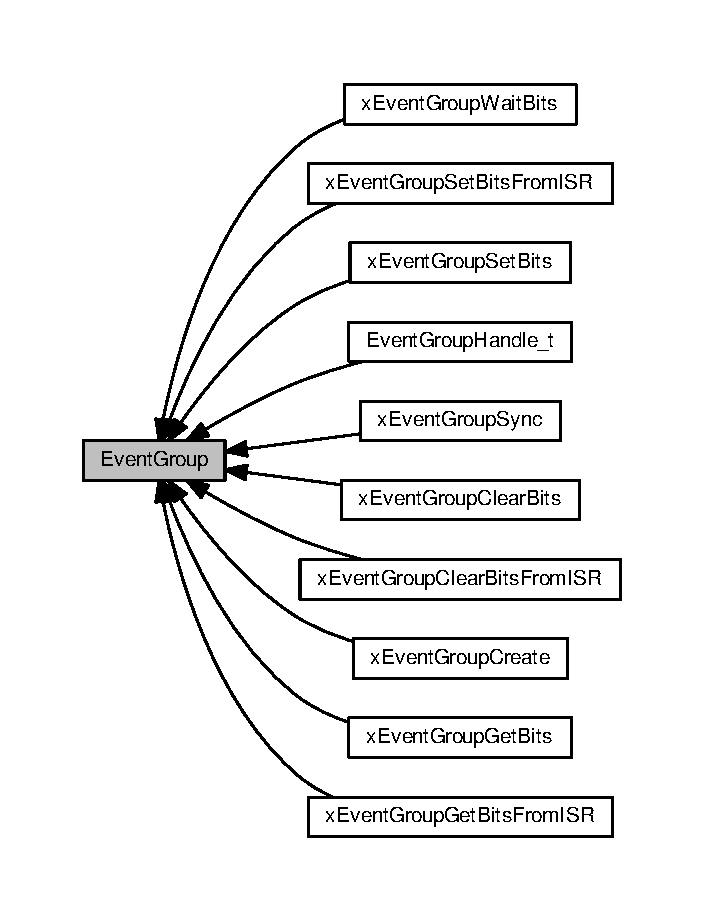
\includegraphics[width=338pt]{dc/d84/group__EventGroup}
\end{center}
\end{figure}
\subsection*{Modules}
\begin{DoxyCompactItemize}
\item 
\hyperlink{group__EventGroupHandle__t}{Event\+Group\+Handle\+\_\+t}
\item 
\hyperlink{group__xEventGroupCreate}{x\+Event\+Group\+Create}
\item 
\hyperlink{group__xEventGroupWaitBits}{x\+Event\+Group\+Wait\+Bits}
\item 
\hyperlink{group__xEventGroupClearBits}{x\+Event\+Group\+Clear\+Bits}
\item 
\hyperlink{group__xEventGroupClearBitsFromISR}{x\+Event\+Group\+Clear\+Bits\+From\+I\+SR}
\item 
\hyperlink{group__xEventGroupSetBits}{x\+Event\+Group\+Set\+Bits}
\item 
\hyperlink{group__xEventGroupSetBitsFromISR}{x\+Event\+Group\+Set\+Bits\+From\+I\+SR}
\item 
\hyperlink{group__xEventGroupSync}{x\+Event\+Group\+Sync}
\item 
\hyperlink{group__xEventGroupGetBits}{x\+Event\+Group\+Get\+Bits}
\item 
\hyperlink{group__xEventGroupGetBitsFromISR}{x\+Event\+Group\+Get\+Bits\+From\+I\+SR}
\end{DoxyCompactItemize}


\subsection{Detailed Description}
An event group is a collection of bits to which an application can assign a meaning. For example, an application may create an event group to convey the status of various C\+AN bus related events in which bit 0 might mean \char`\"{}\+A C\+A\+N
message has been received and is ready for processing\char`\"{}, bit 1 might mean "The application has queued a message that is ready for sending onto the C\+AN network\char`\"{}, and bit 2 might mean \char`\"{}It is time to send a S\+Y\+NC message onto the C\+AN network" etc. A task can then test the bit values to see which events are active, and optionally enter the Blocked state to wait for a specified bit or a group of specified bits to be active. To continue the C\+AN bus example, a C\+AN controlling task can enter the Blocked state (and therefore not consume any processing time) until either bit 0, bit 1 or bit 2 are active, at which time the bit that was actually active would inform the task which action it had to take (process a received message, send a message, or send a S\+Y\+NC).

The event groups implementation contains intelligence to avoid race conditions that would otherwise occur were an application to use a simple variable for the same purpose. This is particularly important with respect to when a bit within an event group is to be cleared, and when bits have to be set and then tested atomically -\/ as is the case where event groups are used to create a synchronisation point between multiple tasks (a \textquotesingle{}rendezvous\textquotesingle{}). 
\hypertarget{group__EventGroupHandle__t}{}\section{Event\+Group\+Handle\+\_\+t}
\label{group__EventGroupHandle__t}\index{Event\+Group\+Handle\+\_\+t@{Event\+Group\+Handle\+\_\+t}}
Collaboration diagram for Event\+Group\+Handle\+\_\+t\+:\nopagebreak
\begin{figure}[H]
\begin{center}
\leavevmode
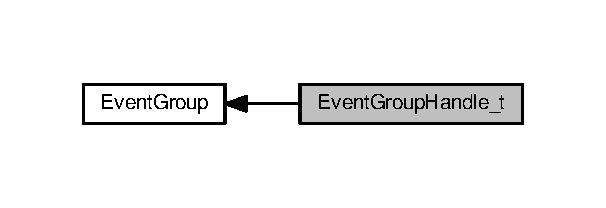
\includegraphics[width=291pt]{dc/d43/group__EventGroupHandle__t}
\end{center}
\end{figure}
\hyperlink{event__groups_8h}{event\+\_\+groups.\+h}

Type by which event groups are referenced. For example, a call to x\+Event\+Group\+Create() returns an Event\+Group\+Handle\+\_\+t variable that can then be used as a parameter to other event group functions. 
\hypertarget{group__xEventGroupCreate}{}\section{x\+Event\+Group\+Create}
\label{group__xEventGroupCreate}\index{x\+Event\+Group\+Create@{x\+Event\+Group\+Create}}
Collaboration diagram for x\+Event\+Group\+Create\+:\nopagebreak
\begin{figure}[H]
\begin{center}
\leavevmode
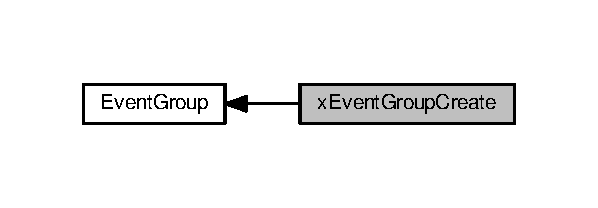
\includegraphics[width=287pt]{df/d78/group__xEventGroupCreate}
\end{center}
\end{figure}
\hyperlink{event__groups_8h}{event\+\_\+groups.\+h} 
\begin{DoxyPre}
EventGroupHandle\_t xEventGroupCreate( void );
\end{DoxyPre}


Create a new event group.

Internally, within the Free\+R\+T\+OS implementation, event groups use a \mbox{[}small\mbox{]} block of memory, in which the event group\textquotesingle{}s structure is stored. If an event groups is created using x\+Event\+Gropu\+Create() then the required memory is automatically dynamically allocated inside the x\+Event\+Group\+Create() function. (see \href{http://www.freertos.org/a00111.html}{\tt http\+://www.\+freertos.\+org/a00111.\+html}). If an event group is created using x\+Event\+Gropu\+Create\+Static() then the application writer must instead provide the memory that will get used by the event group. x\+Event\+Group\+Create\+Static() therefore allows an event group to be created without using any dynamic memory allocation.

Although event groups are not related to ticks, for internal implementation reasons the number of bits available for use in an event group is dependent on the config\+U\+S\+E\+\_\+16\+\_\+\+B\+I\+T\+\_\+\+T\+I\+C\+KS setting in \hyperlink{FreeRTOSConfig_8h}{Free\+R\+T\+O\+S\+Config.\+h}. If config\+U\+S\+E\+\_\+16\+\_\+\+B\+I\+T\+\_\+\+T\+I\+C\+KS is 1 then each event group contains 8 usable bits (bit 0 to bit 7). If config\+U\+S\+E\+\_\+16\+\_\+\+B\+I\+T\+\_\+\+T\+I\+C\+KS is set to 0 then each event group has 24 usable bits (bit 0 to bit 23). The Event\+Bits\+\_\+t type is used to store event bits within an event group.

\begin{DoxyReturn}{Returns}
If the event group was created then a handle to the event group is returned. If there was insufficient Free\+R\+T\+OS heap available to create the event group then N\+U\+LL is returned. See \href{http://www.freertos.org/a00111.html}{\tt http\+://www.\+freertos.\+org/a00111.\+html}
\end{DoxyReturn}
Example usage\+: 
\begin{DoxyPre}
   // Declare a variable to hold the created event group.
   EventGroupHandle\_t xCreatedEventGroup;\end{DoxyPre}



\begin{DoxyPre}   // Attempt to create the event group.
   xCreatedEventGroup = xEventGroupCreate();\end{DoxyPre}



\begin{DoxyPre}   // Was the event group created successfully?
   if( xCreatedEventGroup == NULL )
   \{
    // The event group was not created because there was insufficient
    // FreeRTOS heap available.
   \}
   else
   \{
    // The event group was created.
   \}
  \end{DoxyPre}
 
\hypertarget{group__xEventGroupWaitBits}{}\section{x\+Event\+Group\+Wait\+Bits}
\label{group__xEventGroupWaitBits}\index{x\+Event\+Group\+Wait\+Bits@{x\+Event\+Group\+Wait\+Bits}}
Collaboration diagram for x\+Event\+Group\+Wait\+Bits\+:\nopagebreak
\begin{figure}[H]
\begin{center}
\leavevmode
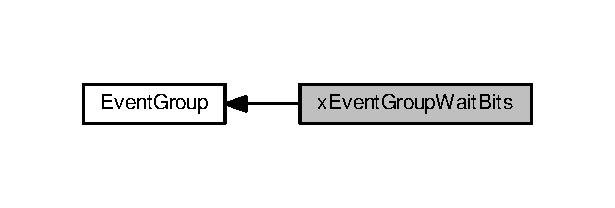
\includegraphics[width=295pt]{d6/d9a/group__xEventGroupWaitBits}
\end{center}
\end{figure}
\hyperlink{event__groups_8h}{event\+\_\+groups.\+h} 
\begin{DoxyPre}
EventGroupHandle\_t xEventGroupCreateStatic( EventGroupHandle\_t * pxEventGroupBuffer );
\end{DoxyPre}


Create a new event group.

Internally, within the Free\+R\+T\+OS implementation, event groups use a \mbox{[}small\mbox{]} block of memory, in which the event group\textquotesingle{}s structure is stored. If an event groups is created using x\+Event\+Gropu\+Create() then the required memory is automatically dynamically allocated inside the x\+Event\+Group\+Create() function. (see \href{http://www.freertos.org/a00111.html}{\tt http\+://www.\+freertos.\+org/a00111.\+html}). If an event group is created using x\+Event\+Gropu\+Create\+Static() then the application writer must instead provide the memory that will get used by the event group. x\+Event\+Group\+Create\+Static() therefore allows an event group to be created without using any dynamic memory allocation.

Although event groups are not related to ticks, for internal implementation reasons the number of bits available for use in an event group is dependent on the config\+U\+S\+E\+\_\+16\+\_\+\+B\+I\+T\+\_\+\+T\+I\+C\+KS setting in \hyperlink{FreeRTOSConfig_8h}{Free\+R\+T\+O\+S\+Config.\+h}. If config\+U\+S\+E\+\_\+16\+\_\+\+B\+I\+T\+\_\+\+T\+I\+C\+KS is 1 then each event group contains 8 usable bits (bit 0 to bit 7). If config\+U\+S\+E\+\_\+16\+\_\+\+B\+I\+T\+\_\+\+T\+I\+C\+KS is set to 0 then each event group has 24 usable bits (bit 0 to bit 23). The Event\+Bits\+\_\+t type is used to store event bits within an event group.


\begin{DoxyParams}{Parameters}
{\em px\+Event\+Group\+Buffer} & px\+Event\+Group\+Buffer must point to a variable of type Static\+Event\+Group\+\_\+t, which will be then be used to hold the event group\textquotesingle{}s data structures, removing the need for the memory to be allocated dynamically.\\
\hline
\end{DoxyParams}
\begin{DoxyReturn}{Returns}
If the event group was created then a handle to the event group is returned. If px\+Event\+Group\+Buffer was N\+U\+LL then N\+U\+LL is returned.
\end{DoxyReturn}
Example usage\+: 
\begin{DoxyPre}
   // StaticEventGroup\_t is a publicly accessible structure that has the same
   // size and alignment requirements as the real event group structure.  It is
   // provided as a mechanism for applications to know the size of the event
   // group (which is dependent on the architecture and configuration file
   // settings) without breaking the strict data hiding policy by exposing the
   // real event group internals.  This StaticEventGroup\_t variable is passed
   // into the xSemaphoreCreateEventGroupStatic() function and is used to store
   // the event group's data structures
   StaticEventGroup\_t xEventGroupBuffer;\end{DoxyPre}



\begin{DoxyPre}   // Create the event group without dynamically allocating any memory.
   xEventGroup = xEventGroupCreateStatic( &xEventGroupBuffer );
  \end{DoxyPre}
 \hyperlink{event__groups_8h}{event\+\_\+groups.\+h} 
\begin{DoxyPre}
   EventBits\_t xEventGroupWaitBits(     EventGroupHandle\_t xEventGroup,
                                    const EventBits\_t uxBitsToWaitFor,
                                    const BaseType\_t xClearOnExit,
                                    const BaseType\_t xWaitForAllBits,
                                    const TickType\_t xTicksToWait );
\end{DoxyPre}


\mbox{[}Potentially\mbox{]} block to wait for one or more bits to be set within a previously created event group.

This function cannot be called from an interrupt.


\begin{DoxyParams}{Parameters}
{\em x\+Event\+Group} & The event group in which the bits are being tested. The event group must have previously been created using a call to x\+Event\+Group\+Create().\\
\hline
{\em ux\+Bits\+To\+Wait\+For} & A bitwise value that indicates the bit or bits to test inside the event group. For example, to wait for bit 0 and/or bit 2 set ux\+Bits\+To\+Wait\+For to 0x05. To wait for bits 0 and/or bit 1 and/or bit 2 set ux\+Bits\+To\+Wait\+For to 0x07. Etc.\\
\hline
{\em x\+Clear\+On\+Exit} & If x\+Clear\+On\+Exit is set to pd\+T\+R\+UE then any bits within ux\+Bits\+To\+Wait\+For that are set within the event group will be cleared before \hyperlink{event__groups_8h_aab9d5b405bc57b7624dcabe9a9a503db}{x\+Event\+Group\+Wait\+Bits()} returns if the wait condition was met (if the function returns for a reason other than a timeout). If x\+Clear\+On\+Exit is set to pd\+F\+A\+L\+SE then the bits set in the event group are not altered when the call to \hyperlink{event__groups_8h_aab9d5b405bc57b7624dcabe9a9a503db}{x\+Event\+Group\+Wait\+Bits()} returns.\\
\hline
{\em x\+Wait\+For\+All\+Bits} & If x\+Wait\+For\+All\+Bits is set to pd\+T\+R\+UE then \hyperlink{event__groups_8h_aab9d5b405bc57b7624dcabe9a9a503db}{x\+Event\+Group\+Wait\+Bits()} will return when either all the bits in ux\+Bits\+To\+Wait\+For are set or the specified block time expires. If x\+Wait\+For\+All\+Bits is set to pd\+F\+A\+L\+SE then \hyperlink{event__groups_8h_aab9d5b405bc57b7624dcabe9a9a503db}{x\+Event\+Group\+Wait\+Bits()} will return when any one of the bits set in ux\+Bits\+To\+Wait\+For is set or the specified block time expires. The block time is specified by the x\+Ticks\+To\+Wait parameter.\\
\hline
{\em x\+Ticks\+To\+Wait} & The maximum amount of time (specified in \textquotesingle{}ticks\textquotesingle{}) to wait for one/all (depending on the x\+Wait\+For\+All\+Bits value) of the bits specified by ux\+Bits\+To\+Wait\+For to become set.\\
\hline
\end{DoxyParams}
\begin{DoxyReturn}{Returns}
The value of the event group at the time either the bits being waited for became set, or the block time expired. Test the return value to know which bits were set. If \hyperlink{event__groups_8h_aab9d5b405bc57b7624dcabe9a9a503db}{x\+Event\+Group\+Wait\+Bits()} returned because its timeout expired then not all the bits being waited for will be set. If \hyperlink{event__groups_8h_aab9d5b405bc57b7624dcabe9a9a503db}{x\+Event\+Group\+Wait\+Bits()} returned because the bits it was waiting for were set then the returned value is the event group value before any bits were automatically cleared in the case that x\+Clear\+On\+Exit parameter was set to pd\+T\+R\+UE.
\end{DoxyReturn}
Example usage\+: 
\begin{DoxyPre}
  #define BIT\_0 ( 1 << 0 )
  #define BIT\_4 ( 1 << 4 )\end{DoxyPre}



\begin{DoxyPre}  void aFunction( EventGroupHandle\_t xEventGroup )
  \{
  EventBits\_t uxBits;
  const TickType\_t xTicksToWait = 100 / portTICK\_PERIOD\_MS;\end{DoxyPre}



\begin{DoxyPre}    // Wait a maximum of 100ms for either bit 0 or bit 4 to be set within
    // the event group.  Clear the bits before exiting.
    uxBits = xEventGroupWaitBits(
                xEventGroup,    // The event group being tested.
                BIT\_0 | BIT\_4,  // The bits within the event group to wait for.
                pdTRUE,         // BIT\_0 and BIT\_4 should be cleared before returning.
                pdFALSE,        // Don't wait for both bits, either bit will do.
                xTicksToWait ); // Wait a maximum of 100ms for either bit to be set.\end{DoxyPre}



\begin{DoxyPre}    if( ( uxBits \& ( BIT\_0 | BIT\_4 ) ) == ( BIT\_0 | BIT\_4 ) )
    \{
        // \hyperlink{event__groups_8h_aab9d5b405bc57b7624dcabe9a9a503db}{xEventGroupWaitBits()} returned because both bits were set.
    \}
    else if( ( uxBits \& BIT\_0 ) != 0 )
    \{
        // \hyperlink{event__groups_8h_aab9d5b405bc57b7624dcabe9a9a503db}{xEventGroupWaitBits()} returned because just BIT\_0 was set.
    \}
    else if( ( uxBits \& BIT\_4 ) != 0 )
    \{
        // \hyperlink{event__groups_8h_aab9d5b405bc57b7624dcabe9a9a503db}{xEventGroupWaitBits()} returned because just BIT\_4 was set.
    \}
    else
    \{
        // \hyperlink{event__groups_8h_aab9d5b405bc57b7624dcabe9a9a503db}{xEventGroupWaitBits()} returned because xTicksToWait ticks passed
        // without either BIT\_0 or BIT\_4 becoming set.
    \}
  \}
  \end{DoxyPre}
 
\hypertarget{group__xEventGroupClearBits}{}\section{x\+Event\+Group\+Clear\+Bits}
\label{group__xEventGroupClearBits}\index{x\+Event\+Group\+Clear\+Bits@{x\+Event\+Group\+Clear\+Bits}}
Collaboration diagram for x\+Event\+Group\+Clear\+Bits\+:\nopagebreak
\begin{figure}[H]
\begin{center}
\leavevmode
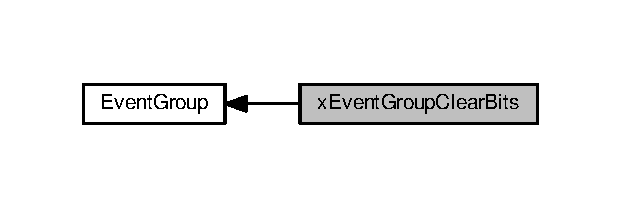
\includegraphics[width=298pt]{d6/dc7/group__xEventGroupClearBits}
\end{center}
\end{figure}
\hyperlink{event__groups_8h}{event\+\_\+groups.\+h} 
\begin{DoxyPre}
   EventBits\_t \hyperlink{event__groups_8h_a0fb72cfdd4f0d5f86d955fc3af448f2a}{xEventGroupClearBits( EventGroupHandle\_t xEventGroup, const EventBits\_t uxBitsToClear )};
\end{DoxyPre}


Clear bits within an event group. This function cannot be called from an interrupt.


\begin{DoxyParams}{Parameters}
{\em x\+Event\+Group} & The event group in which the bits are to be cleared.\\
\hline
{\em ux\+Bits\+To\+Clear} & A bitwise value that indicates the bit or bits to clear in the event group. For example, to clear bit 3 only, set ux\+Bits\+To\+Clear to 0x08. To clear bit 3 and bit 0 set ux\+Bits\+To\+Clear to 0x09.\\
\hline
\end{DoxyParams}
\begin{DoxyReturn}{Returns}
The value of the event group before the specified bits were cleared.
\end{DoxyReturn}
Example usage\+: 
\begin{DoxyPre}
  #define BIT\_0 ( 1 << 0 )
  #define BIT\_4 ( 1 << 4 )\end{DoxyPre}



\begin{DoxyPre}  void aFunction( EventGroupHandle\_t xEventGroup )
  \{
  EventBits\_t uxBits;\end{DoxyPre}



\begin{DoxyPre}    // Clear bit 0 and bit 4 in xEventGroup.
    uxBits = xEventGroupClearBits(
                            xEventGroup,    // The event group being updated.
                            BIT\_0 | BIT\_4 );// The bits being cleared.\end{DoxyPre}



\begin{DoxyPre}    if( ( uxBits \& ( BIT\_0 | BIT\_4 ) ) == ( BIT\_0 | BIT\_4 ) )
    \{
        // Both bit 0 and bit 4 were set before \hyperlink{event__groups_8h_a0fb72cfdd4f0d5f86d955fc3af448f2a}{xEventGroupClearBits()} was
        // called.  Both will now be clear (not set).
    \}
    else if( ( uxBits \& BIT\_0 ) != 0 )
    \{
        // Bit 0 was set before \hyperlink{event__groups_8h_a0fb72cfdd4f0d5f86d955fc3af448f2a}{xEventGroupClearBits()} was called.  It will
        // now be clear.
    \}
    else if( ( uxBits \& BIT\_4 ) != 0 )
    \{
        // Bit 4 was set before \hyperlink{event__groups_8h_a0fb72cfdd4f0d5f86d955fc3af448f2a}{xEventGroupClearBits()} was called.  It will
        // now be clear.
    \}
    else
    \{
        // Neither bit 0 nor bit 4 were set in the first place.
    \}
  \}
  \end{DoxyPre}
 
\hypertarget{group__xEventGroupClearBitsFromISR}{}\section{x\+Event\+Group\+Clear\+Bits\+From\+I\+SR}
\label{group__xEventGroupClearBitsFromISR}\index{x\+Event\+Group\+Clear\+Bits\+From\+I\+SR@{x\+Event\+Group\+Clear\+Bits\+From\+I\+SR}}
Collaboration diagram for x\+Event\+Group\+Clear\+Bits\+From\+I\+SR\+:\nopagebreak
\begin{figure}[H]
\begin{center}
\leavevmode
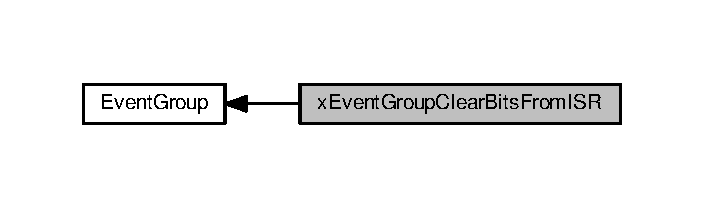
\includegraphics[width=338pt]{d4/dc0/group__xEventGroupClearBitsFromISR}
\end{center}
\end{figure}
\hyperlink{event__groups_8h}{event\+\_\+groups.\+h} 
\begin{DoxyPre}
   BaseType\_t \hyperlink{event__groups_8h_a3d7de214a697f33fe7b914e26a93f33a}{xEventGroupClearBitsFromISR( EventGroupHandle\_t xEventGroup, const EventBits\_t uxBitsToSet )};
\end{DoxyPre}


A version of \hyperlink{event__groups_8h_a0fb72cfdd4f0d5f86d955fc3af448f2a}{x\+Event\+Group\+Clear\+Bits()} that can be called from an interrupt.

Setting bits in an event group is not a deterministic operation because there are an unknown number of tasks that may be waiting for the bit or bits being set. Free\+R\+T\+OS does not allow nondeterministic operations to be performed while interrupts are disabled, so protects event groups that are accessed from tasks by suspending the scheduler rather than disabling interrupts. As a result event groups cannot be accessed directly from an interrupt service routine. Therefore \hyperlink{event__groups_8h_a3d7de214a697f33fe7b914e26a93f33a}{x\+Event\+Group\+Clear\+Bits\+From\+I\+S\+R()} sends a message to the timer task to have the clear operation performed in the context of the timer task.


\begin{DoxyParams}{Parameters}
{\em x\+Event\+Group} & The event group in which the bits are to be cleared.\\
\hline
{\em ux\+Bits\+To\+Clear} & A bitwise value that indicates the bit or bits to clear. For example, to clear bit 3 only, set ux\+Bits\+To\+Clear to 0x08. To clear bit 3 and bit 0 set ux\+Bits\+To\+Clear to 0x09.\\
\hline
\end{DoxyParams}
\begin{DoxyReturn}{Returns}
If the request to execute the function was posted successfully then pd\+P\+A\+SS is returned, otherwise pd\+F\+A\+L\+SE is returned. pd\+F\+A\+L\+SE will be returned if the timer service queue was full.
\end{DoxyReturn}
Example usage\+: 
\begin{DoxyPre}
  #define BIT\_0 ( 1 << 0 )
  #define BIT\_4 ( 1 << 4 )\end{DoxyPre}



\begin{DoxyPre}  // An event group which it is assumed has already been created by a call to
  // xEventGroupCreate().
  EventGroupHandle\_t xEventGroup;\end{DoxyPre}



\begin{DoxyPre}  void anInterruptHandler( void )
  \{
    // Clear bit 0 and bit 4 in xEventGroup.
    xResult = xEventGroupClearBitsFromISR(
                        xEventGroup,     // The event group being updated.
                        BIT\_0 | BIT\_4 ); // The bits being set.\end{DoxyPre}



\begin{DoxyPre}    if( xResult == pdPASS )
    \{
        // The message was posted successfully.
    \}
 \}
  \end{DoxyPre}
 
\hypertarget{group__xEventGroupSetBits}{}\section{x\+Event\+Group\+Set\+Bits}
\label{group__xEventGroupSetBits}\index{x\+Event\+Group\+Set\+Bits@{x\+Event\+Group\+Set\+Bits}}
Collaboration diagram for x\+Event\+Group\+Set\+Bits\+:\nopagebreak
\begin{figure}[H]
\begin{center}
\leavevmode
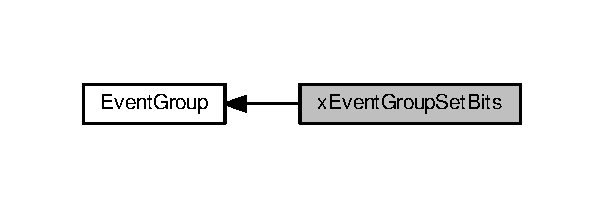
\includegraphics[width=290pt]{dd/d08/group__xEventGroupSetBits}
\end{center}
\end{figure}
\hyperlink{event__groups_8h}{event\+\_\+groups.\+h} 
\begin{DoxyPre}
   EventBits\_t \hyperlink{event__groups_8h_a02d7b3bb55f7e11d9c47116266c5fb2e}{xEventGroupSetBits( EventGroupHandle\_t xEventGroup, const EventBits\_t uxBitsToSet )};
\end{DoxyPre}


Set bits within an event group. This function cannot be called from an interrupt. \hyperlink{event__groups_8h_a62b68278abac6358369ae8e390988a02}{x\+Event\+Group\+Set\+Bits\+From\+I\+S\+R()} is a version that can be called from an interrupt.

Setting bits in an event group will automatically unblock tasks that are blocked waiting for the bits.


\begin{DoxyParams}{Parameters}
{\em x\+Event\+Group} & The event group in which the bits are to be set.\\
\hline
{\em ux\+Bits\+To\+Set} & A bitwise value that indicates the bit or bits to set. For example, to set bit 3 only, set ux\+Bits\+To\+Set to 0x08. To set bit 3 and bit 0 set ux\+Bits\+To\+Set to 0x09.\\
\hline
\end{DoxyParams}
\begin{DoxyReturn}{Returns}
The value of the event group at the time the call to \hyperlink{event__groups_8h_a02d7b3bb55f7e11d9c47116266c5fb2e}{x\+Event\+Group\+Set\+Bits()} returns. There are two reasons why the returned value might have the bits specified by the ux\+Bits\+To\+Set parameter cleared. First, if setting a bit results in a task that was waiting for the bit leaving the blocked state then it is possible the bit will be cleared automatically (see the x\+Clear\+Bit\+On\+Exit parameter of \hyperlink{event__groups_8h_aab9d5b405bc57b7624dcabe9a9a503db}{x\+Event\+Group\+Wait\+Bits()}). Second, any unblocked (or otherwise Ready state) task that has a priority above that of the task that called \hyperlink{event__groups_8h_a02d7b3bb55f7e11d9c47116266c5fb2e}{x\+Event\+Group\+Set\+Bits()} will execute and may change the event group value before the call to \hyperlink{event__groups_8h_a02d7b3bb55f7e11d9c47116266c5fb2e}{x\+Event\+Group\+Set\+Bits()} returns.
\end{DoxyReturn}
Example usage\+: 
\begin{DoxyPre}
  #define BIT\_0 ( 1 << 0 )
  #define BIT\_4 ( 1 << 4 )\end{DoxyPre}



\begin{DoxyPre}  void aFunction( EventGroupHandle\_t xEventGroup )
  \{
  EventBits\_t uxBits;\end{DoxyPre}



\begin{DoxyPre}    // Set bit 0 and bit 4 in xEventGroup.
    uxBits = xEventGroupSetBits(
                        xEventGroup,    // The event group being updated.
                        BIT\_0 | BIT\_4 );// The bits being set.\end{DoxyPre}



\begin{DoxyPre}    if( ( uxBits \& ( BIT\_0 | BIT\_4 ) ) == ( BIT\_0 | BIT\_4 ) )
    \{
        // Both bit 0 and bit 4 remained set when the function returned.
    \}
    else if( ( uxBits \& BIT\_0 ) != 0 )
    \{
        // Bit 0 remained set when the function returned, but bit 4 was
        // cleared.  It might be that bit 4 was cleared automatically as a
        // task that was waiting for bit 4 was removed from the Blocked
        // state.
    \}
    else if( ( uxBits \& BIT\_4 ) != 0 )
    \{
        // Bit 4 remained set when the function returned, but bit 0 was
        // cleared.  It might be that bit 0 was cleared automatically as a
        // task that was waiting for bit 0 was removed from the Blocked
        // state.
    \}
    else
    \{
        // Neither bit 0 nor bit 4 remained set.  It might be that a task
        // was waiting for both of the bits to be set, and the bits were
        // cleared as the task left the Blocked state.
    \}
  \}
  \end{DoxyPre}
 
\hypertarget{group__xEventGroupSetBitsFromISR}{}\section{x\+Event\+Group\+Set\+Bits\+From\+I\+SR}
\label{group__xEventGroupSetBitsFromISR}\index{x\+Event\+Group\+Set\+Bits\+From\+I\+SR@{x\+Event\+Group\+Set\+Bits\+From\+I\+SR}}
Collaboration diagram for x\+Event\+Group\+Set\+Bits\+From\+I\+SR\+:\nopagebreak
\begin{figure}[H]
\begin{center}
\leavevmode
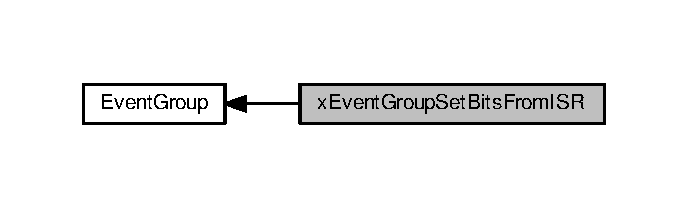
\includegraphics[width=330pt]{d7/de3/group__xEventGroupSetBitsFromISR}
\end{center}
\end{figure}
\hyperlink{event__groups_8h}{event\+\_\+groups.\+h} 
\begin{DoxyPre}
   BaseType\_t \hyperlink{event__groups_8h_a62b68278abac6358369ae8e390988a02}{xEventGroupSetBitsFromISR( EventGroupHandle\_t xEventGroup, const EventBits\_t uxBitsToSet, BaseType\_t *pxHigherPriorityTaskWoken )};
\end{DoxyPre}


A version of \hyperlink{event__groups_8h_a02d7b3bb55f7e11d9c47116266c5fb2e}{x\+Event\+Group\+Set\+Bits()} that can be called from an interrupt.

Setting bits in an event group is not a deterministic operation because there are an unknown number of tasks that may be waiting for the bit or bits being set. Free\+R\+T\+OS does not allow nondeterministic operations to be performed in interrupts or from critical sections. Therefore \hyperlink{event__groups_8h_a62b68278abac6358369ae8e390988a02}{x\+Event\+Group\+Set\+Bits\+From\+I\+S\+R()} sends a message to the timer task to have the set operation performed in the context of the timer task -\/ where a scheduler lock is used in place of a critical section.


\begin{DoxyParams}{Parameters}
{\em x\+Event\+Group} & The event group in which the bits are to be set.\\
\hline
{\em ux\+Bits\+To\+Set} & A bitwise value that indicates the bit or bits to set. For example, to set bit 3 only, set ux\+Bits\+To\+Set to 0x08. To set bit 3 and bit 0 set ux\+Bits\+To\+Set to 0x09.\\
\hline
{\em px\+Higher\+Priority\+Task\+Woken} & As mentioned above, calling this function will result in a message being sent to the timer daemon task. If the priority of the timer daemon task is higher than the priority of the currently running task (the task the interrupt interrupted) then $\ast$px\+Higher\+Priority\+Task\+Woken will be set to pd\+T\+R\+UE by \hyperlink{event__groups_8h_a62b68278abac6358369ae8e390988a02}{x\+Event\+Group\+Set\+Bits\+From\+I\+S\+R()}, indicating that a context switch should be requested before the interrupt exits. For that reason $\ast$px\+Higher\+Priority\+Task\+Woken must be initialised to pd\+F\+A\+L\+SE. See the example code below.\\
\hline
\end{DoxyParams}
\begin{DoxyReturn}{Returns}
If the request to execute the function was posted successfully then pd\+P\+A\+SS is returned, otherwise pd\+F\+A\+L\+SE is returned. pd\+F\+A\+L\+SE will be returned if the timer service queue was full.
\end{DoxyReturn}
Example usage\+: 
\begin{DoxyPre}
  #define BIT\_0 ( 1 << 0 )
  #define BIT\_4 ( 1 << 4 )\end{DoxyPre}



\begin{DoxyPre}  // An event group which it is assumed has already been created by a call to
  // xEventGroupCreate().
  EventGroupHandle\_t xEventGroup;\end{DoxyPre}



\begin{DoxyPre}  void anInterruptHandler( void )
  \{
  BaseType\_t xHigherPriorityTaskWoken, xResult;\end{DoxyPre}



\begin{DoxyPre}    // xHigherPriorityTaskWoken must be initialised to pdFALSE.
    xHigherPriorityTaskWoken = pdFALSE;\end{DoxyPre}



\begin{DoxyPre}    // Set bit 0 and bit 4 in xEventGroup.
    xResult = xEventGroupSetBitsFromISR(
                        xEventGroup,    // The event group being updated.
                        BIT\_0 | BIT\_4   // The bits being set.
                        \&xHigherPriorityTaskWoken );\end{DoxyPre}



\begin{DoxyPre}    // Was the message posted successfully?
    if( xResult == pdPASS )
    \{
        // If xHigherPriorityTaskWoken is now set to pdTRUE then a context
        // switch should be requested.  The macro used is port specific and
        // will be either \hyperlink{portmacro_8h_aac6850c66595efdc02a8bbb95fb4648e}{portYIELD\_FROM\_ISR()} or \hyperlink{portmacro_8h_a63b994040c62c9685490a71c87a13d8a}{portEND\_SWITCHING\_ISR()} -
        // refer to the documentation page for the port being used.
        \hyperlink{portmacro_8h_aac6850c66595efdc02a8bbb95fb4648e}{portYIELD\_FROM\_ISR( xHigherPriorityTaskWoken )};
    \}
 \}
  \end{DoxyPre}
 
\hypertarget{group__xEventGroupSync}{}\section{x\+Event\+Group\+Sync}
\label{group__xEventGroupSync}\index{x\+Event\+Group\+Sync@{x\+Event\+Group\+Sync}}
Collaboration diagram for x\+Event\+Group\+Sync\+:\nopagebreak
\begin{figure}[H]
\begin{center}
\leavevmode
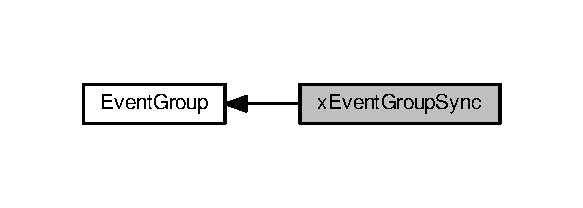
\includegraphics[width=280pt]{d2/dd3/group__xEventGroupSync}
\end{center}
\end{figure}
\hyperlink{event__groups_8h}{event\+\_\+groups.\+h} 
\begin{DoxyPre}
   EventBits\_t xEventGroupSync( EventGroupHandle\_t xEventGroup,
                                const EventBits\_t uxBitsToSet,
                                const EventBits\_t uxBitsToWaitFor,
                                TickType\_t xTicksToWait );
\end{DoxyPre}


Atomically set bits within an event group, then wait for a combination of bits to be set within the same event group. This functionality is typically used to synchronise multiple tasks, where each task has to wait for the other tasks to reach a synchronisation point before proceeding.

This function cannot be used from an interrupt.

The function will return before its block time expires if the bits specified by the ux\+Bits\+To\+Wait parameter are set, or become set within that time. In this case all the bits specified by ux\+Bits\+To\+Wait will be automatically cleared before the function returns.


\begin{DoxyParams}{Parameters}
{\em x\+Event\+Group} & The event group in which the bits are being tested. The event group must have previously been created using a call to x\+Event\+Group\+Create().\\
\hline
{\em ux\+Bits\+To\+Set} & The bits to set in the event group before determining if, and possibly waiting for, all the bits specified by the ux\+Bits\+To\+Wait parameter are set.\\
\hline
{\em ux\+Bits\+To\+Wait\+For} & A bitwise value that indicates the bit or bits to test inside the event group. For example, to wait for bit 0 and bit 2 set ux\+Bits\+To\+Wait\+For to 0x05. To wait for bits 0 and bit 1 and bit 2 set ux\+Bits\+To\+Wait\+For to 0x07. Etc.\\
\hline
{\em x\+Ticks\+To\+Wait} & The maximum amount of time (specified in \textquotesingle{}ticks\textquotesingle{}) to wait for all of the bits specified by ux\+Bits\+To\+Wait\+For to become set.\\
\hline
\end{DoxyParams}
\begin{DoxyReturn}{Returns}
The value of the event group at the time either the bits being waited for became set, or the block time expired. Test the return value to know which bits were set. If \hyperlink{event__groups_8h_a869511456b86426f52e2eec898bff341}{x\+Event\+Group\+Sync()} returned because its timeout expired then not all the bits being waited for will be set. If \hyperlink{event__groups_8h_a869511456b86426f52e2eec898bff341}{x\+Event\+Group\+Sync()} returned because all the bits it was waiting for were set then the returned value is the event group value before any bits were automatically cleared.
\end{DoxyReturn}
Example usage\+: 
\begin{DoxyPre}
// Bits used by the three tasks.
#define TASK\_0\_BIT      ( 1 << 0 )
#define TASK\_1\_BIT      ( 1 << 1 )
#define TASK\_2\_BIT      ( 1 << 2 )\end{DoxyPre}



\begin{DoxyPre}#define ALL\_SYNC\_BITS ( TASK\_0\_BIT | TASK\_1\_BIT | TASK\_2\_BIT )\end{DoxyPre}



\begin{DoxyPre}// Use an event group to synchronise three tasks.  It is assumed this event
// group has already been created elsewhere.
EventGroupHandle\_t xEventBits;\end{DoxyPre}



\begin{DoxyPre}void vTask0( void *pvParameters )
\{
EventBits\_t uxReturn;
TickType\_t xTicksToWait = 100 / portTICK\_PERIOD\_MS;
\begin{DoxyVerb}for( ;; )
{
// Perform task functionality here.

// Set bit 0 in the event flag to note this task has reached the
// sync point.  The other two tasks will set the other two bits defined
// by ALL_SYNC_BITS.  All three tasks have reached the synchronisation
// point when all the ALL_SYNC_BITS are set.  Wait a maximum of 100ms
// for this to happen.
uxReturn = xEventGroupSync( xEventBits, TASK_0_BIT, ALL_SYNC_BITS, xTicksToWait );

if( ( uxReturn & ALL_SYNC_BITS ) == ALL_SYNC_BITS )
{
    // All three tasks reached the synchronisation point before the call
    // to xEventGroupSync() timed out.
}
\end{DoxyVerb}

   \}
\}\end{DoxyPre}



\begin{DoxyPre}void vTask1( void *pvParameters )
\{
    for( ;; )
    \{
    // Perform task functionality here.\end{DoxyPre}



\begin{DoxyPre}    // Set bit 1 in the event flag to note this task has reached the
    // synchronisation point.  The other two tasks will set the other two
    // bits defined by ALL\_SYNC\_BITS.  All three tasks have reached the
    // synchronisation point when all the ALL\_SYNC\_BITS are set.  Wait
    // indefinitely for this to happen.
    xEventGroupSync( xEventBits, TASK\_1\_BIT, ALL\_SYNC\_BITS, portMAX\_DELAY );\end{DoxyPre}



\begin{DoxyPre}    // \hyperlink{event__groups_8h_a869511456b86426f52e2eec898bff341}{xEventGroupSync()} was called with an indefinite block time, so
    // this task will only reach here if the syncrhonisation was made by all
    // three tasks, so there is no need to test the return value.
    \}
\}\end{DoxyPre}



\begin{DoxyPre}void vTask2( void *pvParameters )
\{
    for( ;; )
    \{
    // Perform task functionality here.\end{DoxyPre}



\begin{DoxyPre}    // Set bit 2 in the event flag to note this task has reached the
    // synchronisation point.  The other two tasks will set the other two
    // bits defined by ALL\_SYNC\_BITS.  All three tasks have reached the
    // synchronisation point when all the ALL\_SYNC\_BITS are set.  Wait
    // indefinitely for this to happen.
    xEventGroupSync( xEventBits, TASK\_2\_BIT, ALL\_SYNC\_BITS, portMAX\_DELAY );\end{DoxyPre}



\begin{DoxyPre}    // \hyperlink{event__groups_8h_a869511456b86426f52e2eec898bff341}{xEventGroupSync()} was called with an indefinite block time, so
    // this task will only reach here if the syncrhonisation was made by all
    // three tasks, so there is no need to test the return value.
   \}
\}\end{DoxyPre}



\begin{DoxyPre}\end{DoxyPre}
 
\hypertarget{group__xEventGroupGetBits}{}\section{x\+Event\+Group\+Get\+Bits}
\label{group__xEventGroupGetBits}\index{x\+Event\+Group\+Get\+Bits@{x\+Event\+Group\+Get\+Bits}}
Collaboration diagram for x\+Event\+Group\+Get\+Bits\+:\nopagebreak
\begin{figure}[H]
\begin{center}
\leavevmode
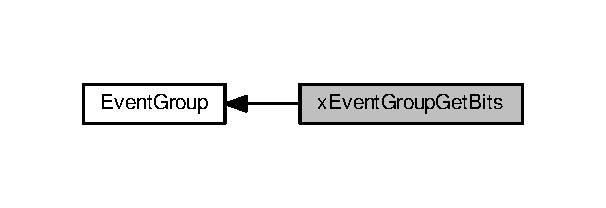
\includegraphics[width=291pt]{d8/dfc/group__xEventGroupGetBits}
\end{center}
\end{figure}
\hyperlink{event__groups_8h}{event\+\_\+groups.\+h} 
\begin{DoxyPre}
   EventBits\_t \hyperlink{event__groups_8h_a0ae86f092fb07ccb475ae938f9a12584}{xEventGroupGetBits( EventGroupHandle\_t xEventGroup )};
\end{DoxyPre}


Returns the current value of the bits in an event group. This function cannot be used from an interrupt.


\begin{DoxyParams}{Parameters}
{\em x\+Event\+Group} & The event group being queried.\\
\hline
\end{DoxyParams}
\begin{DoxyReturn}{Returns}
The event group bits at the time \hyperlink{event__groups_8h_a0ae86f092fb07ccb475ae938f9a12584}{x\+Event\+Group\+Get\+Bits()} was called. 
\end{DoxyReturn}

\hypertarget{group__xEventGroupGetBitsFromISR}{}\section{x\+Event\+Group\+Get\+Bits\+From\+I\+SR}
\label{group__xEventGroupGetBitsFromISR}\index{x\+Event\+Group\+Get\+Bits\+From\+I\+SR@{x\+Event\+Group\+Get\+Bits\+From\+I\+SR}}
Collaboration diagram for x\+Event\+Group\+Get\+Bits\+From\+I\+SR\+:\nopagebreak
\begin{figure}[H]
\begin{center}
\leavevmode
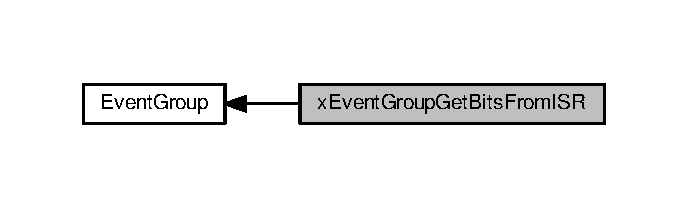
\includegraphics[width=330pt]{d4/d99/group__xEventGroupGetBitsFromISR}
\end{center}
\end{figure}
\hyperlink{event__groups_8h}{event\+\_\+groups.\+h} 
\begin{DoxyPre}
   EventBits\_t \hyperlink{event__groups_8h_a95822db4357d0b77c35aed0c7427eca0}{xEventGroupGetBitsFromISR( EventGroupHandle\_t xEventGroup )};
\end{DoxyPre}


A version of \hyperlink{event__groups_8h_a0ae86f092fb07ccb475ae938f9a12584}{x\+Event\+Group\+Get\+Bits()} that can be called from an I\+SR.


\begin{DoxyParams}{Parameters}
{\em x\+Event\+Group} & The event group being queried.\\
\hline
\end{DoxyParams}
\begin{DoxyReturn}{Returns}
The event group bits at the time \hyperlink{event__groups_8h_a95822db4357d0b77c35aed0c7427eca0}{x\+Event\+Group\+Get\+Bits\+From\+I\+S\+R()} was called. 
\end{DoxyReturn}

\hypertarget{group__xQueueCreate}{}\section{x\+Queue\+Create}
\label{group__xQueueCreate}\index{x\+Queue\+Create@{x\+Queue\+Create}}
queue. h 
\begin{DoxyPre}
QueueHandle\_t xQueueCreate(
                          UBaseType\_t uxQueueLength,
                          UBaseType\_t uxItemSize
                      );
  \end{DoxyPre}


Creates a new queue instance, and returns a handle by which the new queue can be referenced.

Internally, within the Free\+R\+T\+OS implementation, queues use two blocks of memory. The first block is used to hold the queue\textquotesingle{}s data structures. The second block is used to hold items placed into the queue. If a queue is created using x\+Queue\+Create() then both blocks of memory are automatically dynamically allocated inside the x\+Queue\+Create() function. (see \href{http://www.freertos.org/a00111.html}{\tt http\+://www.\+freertos.\+org/a00111.\+html}). If a queue is created using x\+Queue\+Create\+Static() then the application writer must provide the memory that will get used by the queue. x\+Queue\+Create\+Static() therefore allows a queue to be created without using any dynamic memory allocation.

\href{http://www.FreeRTOS.org/Embedded-RTOS-Queues.html}{\tt http\+://www.\+Free\+R\+T\+O\+S.\+org/\+Embedded-\/\+R\+T\+O\+S-\/\+Queues.\+html}


\begin{DoxyParams}{Parameters}
{\em ux\+Queue\+Length} & The maximum number of items that the queue can contain.\\
\hline
{\em ux\+Item\+Size} & The number of bytes each item in the queue will require. Items are queued by copy, not by reference, so this is the number of bytes that will be copied for each posted item. Each item on the queue must be the same size.\\
\hline
\end{DoxyParams}
\begin{DoxyReturn}{Returns}
If the queue is successfully create then a handle to the newly created queue is returned. If the queue cannot be created then 0 is returned.
\end{DoxyReturn}
Example usage\+: 
\begin{DoxyPre}
struct AMessage
\{
   char ucMessageID;
   char ucData[ 20 ];
\};\end{DoxyPre}



\begin{DoxyPre}void vATask( void *pvParameters )
\{
QueueHandle\_t xQueue1, xQueue2;\end{DoxyPre}



\begin{DoxyPre}   // Create a queue capable of containing 10 uint32\_t values.
   xQueue1 = xQueueCreate( 10, sizeof( uint32\_t ) );
   if( xQueue1 == 0 )
   \{
    // Queue was not created and must not be used.
   \}\end{DoxyPre}



\begin{DoxyPre}   // Create a queue capable of containing 10 pointers to AMessage structures.
   // These should be passed by pointer as they contain a lot of data.
   xQueue2 = xQueueCreate( 10, sizeof( struct AMessage * ) );
   if( xQueue2 == 0 )
   \{
    // Queue was not created and must not be used.
   \}\end{DoxyPre}



\begin{DoxyPre}   // ... Rest of task code.
\}
\end{DoxyPre}
 
\hypertarget{group__xQueueCreateStatic}{}\section{x\+Queue\+Create\+Static}
\label{group__xQueueCreateStatic}\index{x\+Queue\+Create\+Static@{x\+Queue\+Create\+Static}}
queue. h 
\begin{DoxyPre}
QueueHandle\_t xQueueCreateStatic(
                          UBaseType\_t uxQueueLength,
                          UBaseType\_t uxItemSize,
                          uint8\_t *pucQueueStorageBuffer,
                          StaticQueue\_t *pxQueueBuffer
                      );
  \end{DoxyPre}


Creates a new queue instance, and returns a handle by which the new queue can be referenced.

Internally, within the Free\+R\+T\+OS implementation, queues use two blocks of memory. The first block is used to hold the queue\textquotesingle{}s data structures. The second block is used to hold items placed into the queue. If a queue is created using x\+Queue\+Create() then both blocks of memory are automatically dynamically allocated inside the x\+Queue\+Create() function. (see \href{http://www.freertos.org/a00111.html}{\tt http\+://www.\+freertos.\+org/a00111.\+html}). If a queue is created using x\+Queue\+Create\+Static() then the application writer must provide the memory that will get used by the queue. x\+Queue\+Create\+Static() therefore allows a queue to be created without using any dynamic memory allocation.

\href{http://www.FreeRTOS.org/Embedded-RTOS-Queues.html}{\tt http\+://www.\+Free\+R\+T\+O\+S.\+org/\+Embedded-\/\+R\+T\+O\+S-\/\+Queues.\+html}


\begin{DoxyParams}{Parameters}
{\em ux\+Queue\+Length} & The maximum number of items that the queue can contain.\\
\hline
{\em ux\+Item\+Size} & The number of bytes each item in the queue will require. Items are queued by copy, not by reference, so this is the number of bytes that will be copied for each posted item. Each item on the queue must be the same size.\\
\hline
{\em puc\+Queue\+Storage\+Buffer} & If ux\+Item\+Size is not zero then puc\+Queue\+Storage\+Buffer must point to a uint8\+\_\+t array that is at least large enough to hold the maximum number of items that can be in the queue at any one time -\/ which is ( ux\+Queue\+Length $\ast$ ux\+Items\+Size ) bytes. If ux\+Item\+Size is zero then puc\+Queue\+Storage\+Buffer can be N\+U\+LL.\\
\hline
{\em px\+Queue\+Buffer} & Must point to a variable of type Static\+Queue\+\_\+t, which will be used to hold the queue\textquotesingle{}s data structure.\\
\hline
\end{DoxyParams}
\begin{DoxyReturn}{Returns}
If the queue is created then a handle to the created queue is returned. If px\+Queue\+Buffer is N\+U\+LL then N\+U\+LL is returned.
\end{DoxyReturn}
Example usage\+: 
\begin{DoxyPre}
struct AMessage
\{
   char ucMessageID;
   char ucData[ 20 ];
\};\end{DoxyPre}



\begin{DoxyPre}#define QUEUE\_LENGTH 10
#define ITEM\_SIZE sizeof( uint32\_t )\end{DoxyPre}



\begin{DoxyPre}// xQueueBuffer will hold the queue structure.
StaticQueue\_t xQueueBuffer;\end{DoxyPre}



\begin{DoxyPre}// ucQueueStorage will hold the items posted to the queue.  Must be at least
// [(queue length) * ( queue item size)] bytes long.
uint8\_t ucQueueStorage[ QUEUE\_LENGTH * ITEM\_SIZE ];\end{DoxyPre}



\begin{DoxyPre}void vATask( void *pvParameters )
\{
QueueHandle\_t xQueue1;\end{DoxyPre}



\begin{DoxyPre}   // Create a queue capable of containing 10 uint32\_t values.
   xQueue1 = xQueueCreate( QUEUE\_LENGTH, // The number of items the queue can hold.
                        ITEM\_SIZE     // The size of each item in the queue
                        \&( ucQueueStorage[ 0 ] ), // The buffer that will hold the items in the queue.
                        \&xQueueBuffer ); // The buffer that will hold the queue structure.\end{DoxyPre}



\begin{DoxyPre}   // The queue is guaranteed to be created successfully as no dynamic memory
   // allocation is used.  Therefore xQueue1 is now a handle to a valid queue.\end{DoxyPre}



\begin{DoxyPre}   // ... Rest of task code.
\}
\end{DoxyPre}
 
\hypertarget{group__xQueueSend}{}\section{x\+Queue\+Send}
\label{group__xQueueSend}\index{x\+Queue\+Send@{x\+Queue\+Send}}
queue. h 
\begin{DoxyPre}
BaseType\_t xQueueSendToToFront(
                               QueueHandle\_t    xQueue,
                               const void       *pvItemToQueue,
                               TickType\_t       xTicksToWait
                           );
  \end{DoxyPre}


This is a macro that calls \hyperlink{queue_8h_a7ce86d1026e0c3055a523935bf53c0b3}{x\+Queue\+Generic\+Send()}.

Post an item to the front of a queue. The item is queued by copy, not by reference. This function must not be called from an interrupt service routine. See x\+Queue\+Send\+From\+I\+SR () for an alternative which may be used in an I\+SR.


\begin{DoxyParams}{Parameters}
{\em x\+Queue} & The handle to the queue on which the item is to be posted.\\
\hline
{\em pv\+Item\+To\+Queue} & A pointer to the item that is to be placed on the queue. The size of the items the queue will hold was defined when the queue was created, so this many bytes will be copied from pv\+Item\+To\+Queue into the queue storage area.\\
\hline
{\em x\+Ticks\+To\+Wait} & The maximum amount of time the task should block waiting for space to become available on the queue, should it already be full. The call will return immediately if this is set to 0 and the queue is full. The time is defined in tick periods so the constant port\+T\+I\+C\+K\+\_\+\+P\+E\+R\+I\+O\+D\+\_\+\+MS should be used to convert to real time if this is required.\\
\hline
\end{DoxyParams}
\begin{DoxyReturn}{Returns}
pd\+T\+R\+UE if the item was successfully posted, otherwise err\+Q\+U\+E\+U\+E\+\_\+\+F\+U\+LL.
\end{DoxyReturn}
Example usage\+: 
\begin{DoxyPre}
struct AMessage
\{
   char ucMessageID;
   char ucData[ 20 ];
\} xMessage;\end{DoxyPre}



\begin{DoxyPre}uint32\_t ulVar = 10UL;\end{DoxyPre}



\begin{DoxyPre}void vATask( void *pvParameters )
\{
QueueHandle\_t xQueue1, xQueue2;
struct AMessage *pxMessage;\end{DoxyPre}



\begin{DoxyPre}   // Create a queue capable of containing 10 uint32\_t values.
   xQueue1 = xQueueCreate( 10, sizeof( uint32\_t ) );\end{DoxyPre}



\begin{DoxyPre}   // Create a queue capable of containing 10 pointers to AMessage structures.
   // These should be passed by pointer as they contain a lot of data.
   xQueue2 = xQueueCreate( 10, sizeof( struct AMessage * ) );\end{DoxyPre}



\begin{DoxyPre}   // ...\end{DoxyPre}



\begin{DoxyPre}   if( xQueue1 != 0 )
   \{
    // Send an uint32\_t.  Wait for 10 ticks for space to become
    // available if necessary.
    if( xQueueSendToFront( xQueue1, ( void * ) \&ulVar, ( TickType\_t ) 10 ) != pdPASS )
    \{
        // Failed to post the message, even after 10 ticks.
    \}
   \}\end{DoxyPre}



\begin{DoxyPre}   if( xQueue2 != 0 )
   \{
    // Send a pointer to a struct AMessage object.  Don't block if the
    // queue is already full.
    pxMessage = \& xMessage;
    xQueueSendToFront( xQueue2, ( void * ) \&pxMessage, ( TickType\_t ) 0 );
   \}\end{DoxyPre}



\begin{DoxyPre}   // ... Rest of task code.
\}
\end{DoxyPre}


queue. h 
\begin{DoxyPre}
BaseType\_t xQueueSendToBack(
                               QueueHandle\_t    xQueue,
                               const void       *pvItemToQueue,
                               TickType\_t       xTicksToWait
                           );
  \end{DoxyPre}


This is a macro that calls \hyperlink{queue_8h_a7ce86d1026e0c3055a523935bf53c0b3}{x\+Queue\+Generic\+Send()}.

Post an item to the back of a queue. The item is queued by copy, not by reference. This function must not be called from an interrupt service routine. See x\+Queue\+Send\+From\+I\+SR () for an alternative which may be used in an I\+SR.


\begin{DoxyParams}{Parameters}
{\em x\+Queue} & The handle to the queue on which the item is to be posted.\\
\hline
{\em pv\+Item\+To\+Queue} & A pointer to the item that is to be placed on the queue. The size of the items the queue will hold was defined when the queue was created, so this many bytes will be copied from pv\+Item\+To\+Queue into the queue storage area.\\
\hline
{\em x\+Ticks\+To\+Wait} & The maximum amount of time the task should block waiting for space to become available on the queue, should it already be full. The call will return immediately if this is set to 0 and the queue is full. The time is defined in tick periods so the constant port\+T\+I\+C\+K\+\_\+\+P\+E\+R\+I\+O\+D\+\_\+\+MS should be used to convert to real time if this is required.\\
\hline
\end{DoxyParams}
\begin{DoxyReturn}{Returns}
pd\+T\+R\+UE if the item was successfully posted, otherwise err\+Q\+U\+E\+U\+E\+\_\+\+F\+U\+LL.
\end{DoxyReturn}
Example usage\+: 
\begin{DoxyPre}
struct AMessage
\{
   char ucMessageID;
   char ucData[ 20 ];
\} xMessage;\end{DoxyPre}



\begin{DoxyPre}uint32\_t ulVar = 10UL;\end{DoxyPre}



\begin{DoxyPre}void vATask( void *pvParameters )
\{
QueueHandle\_t xQueue1, xQueue2;
struct AMessage *pxMessage;\end{DoxyPre}



\begin{DoxyPre}   // Create a queue capable of containing 10 uint32\_t values.
   xQueue1 = xQueueCreate( 10, sizeof( uint32\_t ) );\end{DoxyPre}



\begin{DoxyPre}   // Create a queue capable of containing 10 pointers to AMessage structures.
   // These should be passed by pointer as they contain a lot of data.
   xQueue2 = xQueueCreate( 10, sizeof( struct AMessage * ) );\end{DoxyPre}



\begin{DoxyPre}   // ...\end{DoxyPre}



\begin{DoxyPre}   if( xQueue1 != 0 )
   \{
    // Send an uint32\_t.  Wait for 10 ticks for space to become
    // available if necessary.
    if( xQueueSendToBack( xQueue1, ( void * ) \&ulVar, ( TickType\_t ) 10 ) != pdPASS )
    \{
        // Failed to post the message, even after 10 ticks.
    \}
   \}\end{DoxyPre}



\begin{DoxyPre}   if( xQueue2 != 0 )
   \{
    // Send a pointer to a struct AMessage object.  Don't block if the
    // queue is already full.
    pxMessage = \& xMessage;
    xQueueSendToBack( xQueue2, ( void * ) \&pxMessage, ( TickType\_t ) 0 );
   \}\end{DoxyPre}



\begin{DoxyPre}   // ... Rest of task code.
\}
\end{DoxyPre}


queue. h 
\begin{DoxyPre}
BaseType\_t xQueueSend(
                          QueueHandle\_t xQueue,
                          const void * pvItemToQueue,
                          TickType\_t xTicksToWait
                     );
  \end{DoxyPre}


This is a macro that calls \hyperlink{queue_8h_a7ce86d1026e0c3055a523935bf53c0b3}{x\+Queue\+Generic\+Send()}. It is included for backward compatibility with versions of Free\+R\+T\+O\+S.\+org that did not include the \hyperlink{queue_8h_aa612fcc2b1ceee0200f34b942e300b41}{x\+Queue\+Send\+To\+Front()} and \hyperlink{queue_8h_a81d24a2c1199d58efb76fbee15853112}{x\+Queue\+Send\+To\+Back()} macros. It is equivalent to \hyperlink{queue_8h_a81d24a2c1199d58efb76fbee15853112}{x\+Queue\+Send\+To\+Back()}.

Post an item on a queue. The item is queued by copy, not by reference. This function must not be called from an interrupt service routine. See x\+Queue\+Send\+From\+I\+SR () for an alternative which may be used in an I\+SR.


\begin{DoxyParams}{Parameters}
{\em x\+Queue} & The handle to the queue on which the item is to be posted.\\
\hline
{\em pv\+Item\+To\+Queue} & A pointer to the item that is to be placed on the queue. The size of the items the queue will hold was defined when the queue was created, so this many bytes will be copied from pv\+Item\+To\+Queue into the queue storage area.\\
\hline
{\em x\+Ticks\+To\+Wait} & The maximum amount of time the task should block waiting for space to become available on the queue, should it already be full. The call will return immediately if this is set to 0 and the queue is full. The time is defined in tick periods so the constant port\+T\+I\+C\+K\+\_\+\+P\+E\+R\+I\+O\+D\+\_\+\+MS should be used to convert to real time if this is required.\\
\hline
\end{DoxyParams}
\begin{DoxyReturn}{Returns}
pd\+T\+R\+UE if the item was successfully posted, otherwise err\+Q\+U\+E\+U\+E\+\_\+\+F\+U\+LL.
\end{DoxyReturn}
Example usage\+: 
\begin{DoxyPre}
struct AMessage
\{
   char ucMessageID;
   char ucData[ 20 ];
\} xMessage;\end{DoxyPre}



\begin{DoxyPre}uint32\_t ulVar = 10UL;\end{DoxyPre}



\begin{DoxyPre}void vATask( void *pvParameters )
\{
QueueHandle\_t xQueue1, xQueue2;
struct AMessage *pxMessage;\end{DoxyPre}



\begin{DoxyPre}   // Create a queue capable of containing 10 uint32\_t values.
   xQueue1 = xQueueCreate( 10, sizeof( uint32\_t ) );\end{DoxyPre}



\begin{DoxyPre}   // Create a queue capable of containing 10 pointers to AMessage structures.
   // These should be passed by pointer as they contain a lot of data.
   xQueue2 = xQueueCreate( 10, sizeof( struct AMessage * ) );\end{DoxyPre}



\begin{DoxyPre}   // ...\end{DoxyPre}



\begin{DoxyPre}   if( xQueue1 != 0 )
   \{
    // Send an uint32\_t.  Wait for 10 ticks for space to become
    // available if necessary.
    if( xQueueSend( xQueue1, ( void * ) \&ulVar, ( TickType\_t ) 10 ) != pdPASS )
    \{
        // Failed to post the message, even after 10 ticks.
    \}
   \}\end{DoxyPre}



\begin{DoxyPre}   if( xQueue2 != 0 )
   \{
    // Send a pointer to a struct AMessage object.  Don't block if the
    // queue is already full.
    pxMessage = \& xMessage;
    xQueueSend( xQueue2, ( void * ) \&pxMessage, ( TickType\_t ) 0 );
   \}\end{DoxyPre}



\begin{DoxyPre}   // ... Rest of task code.
\}
\end{DoxyPre}


queue. h 
\begin{DoxyPre}
BaseType\_t xQueueGenericSend(
                                QueueHandle\_t xQueue,
                                const void * pvItemToQueue,
                                TickType\_t xTicksToWait
                                BaseType\_t xCopyPosition
                            );
  \end{DoxyPre}


It is preferred that the macros \hyperlink{queue_8h_af7eb49d3249351176992950d9185abe9}{x\+Queue\+Send()}, \hyperlink{queue_8h_aa612fcc2b1ceee0200f34b942e300b41}{x\+Queue\+Send\+To\+Front()} and \hyperlink{queue_8h_a81d24a2c1199d58efb76fbee15853112}{x\+Queue\+Send\+To\+Back()} are used in place of calling this function directly.

Post an item on a queue. The item is queued by copy, not by reference. This function must not be called from an interrupt service routine. See x\+Queue\+Send\+From\+I\+SR () for an alternative which may be used in an I\+SR.


\begin{DoxyParams}{Parameters}
{\em x\+Queue} & The handle to the queue on which the item is to be posted.\\
\hline
{\em pv\+Item\+To\+Queue} & A pointer to the item that is to be placed on the queue. The size of the items the queue will hold was defined when the queue was created, so this many bytes will be copied from pv\+Item\+To\+Queue into the queue storage area.\\
\hline
{\em x\+Ticks\+To\+Wait} & The maximum amount of time the task should block waiting for space to become available on the queue, should it already be full. The call will return immediately if this is set to 0 and the queue is full. The time is defined in tick periods so the constant port\+T\+I\+C\+K\+\_\+\+P\+E\+R\+I\+O\+D\+\_\+\+MS should be used to convert to real time if this is required.\\
\hline
{\em x\+Copy\+Position} & Can take the value queue\+S\+E\+N\+D\+\_\+\+T\+O\+\_\+\+B\+A\+CK to place the item at the back of the queue, or queue\+S\+E\+N\+D\+\_\+\+T\+O\+\_\+\+F\+R\+O\+NT to place the item at the front of the queue (for high priority messages).\\
\hline
\end{DoxyParams}
\begin{DoxyReturn}{Returns}
pd\+T\+R\+UE if the item was successfully posted, otherwise err\+Q\+U\+E\+U\+E\+\_\+\+F\+U\+LL.
\end{DoxyReturn}
Example usage\+: 
\begin{DoxyPre}
struct AMessage
\{
   char ucMessageID;
   char ucData[ 20 ];
\} xMessage;\end{DoxyPre}



\begin{DoxyPre}uint32\_t ulVar = 10UL;\end{DoxyPre}



\begin{DoxyPre}void vATask( void *pvParameters )
\{
QueueHandle\_t xQueue1, xQueue2;
struct AMessage *pxMessage;\end{DoxyPre}



\begin{DoxyPre}   // Create a queue capable of containing 10 uint32\_t values.
   xQueue1 = xQueueCreate( 10, sizeof( uint32\_t ) );\end{DoxyPre}



\begin{DoxyPre}   // Create a queue capable of containing 10 pointers to AMessage structures.
   // These should be passed by pointer as they contain a lot of data.
   xQueue2 = xQueueCreate( 10, sizeof( struct AMessage * ) );\end{DoxyPre}



\begin{DoxyPre}   // ...\end{DoxyPre}



\begin{DoxyPre}   if( xQueue1 != 0 )
   \{
    // Send an uint32\_t.  Wait for 10 ticks for space to become
    // available if necessary.
    if( xQueueGenericSend( xQueue1, ( void * ) \&ulVar, ( TickType\_t ) 10, queueSEND\_TO\_BACK ) != pdPASS )
    \{
        // Failed to post the message, even after 10 ticks.
    \}
   \}\end{DoxyPre}



\begin{DoxyPre}   if( xQueue2 != 0 )
   \{
    // Send a pointer to a struct AMessage object.  Don't block if the
    // queue is already full.
    pxMessage = \& xMessage;
    xQueueGenericSend( xQueue2, ( void * ) \&pxMessage, ( TickType\_t ) 0, queueSEND\_TO\_BACK );
   \}\end{DoxyPre}



\begin{DoxyPre}   // ... Rest of task code.
\}
\end{DoxyPre}
 
\hypertarget{group__xQueueOverwrite}{}\section{x\+Queue\+Overwrite}
\label{group__xQueueOverwrite}\index{x\+Queue\+Overwrite@{x\+Queue\+Overwrite}}
queue. h 
\begin{DoxyPre}
 BaseType\_t xQueueOverwrite(
                              QueueHandle\_t xQueue,
                              const void * pvItemToQueue
                         );
   \end{DoxyPre}


Only for use with queues that have a length of one -\/ so the queue is either empty or full.

Post an item on a queue. If the queue is already full then overwrite the value held in the queue. The item is queued by copy, not by reference.

This function must not be called from an interrupt service routine. See x\+Queue\+Overwrite\+From\+I\+SR () for an alternative which may be used in an I\+SR.


\begin{DoxyParams}{Parameters}
{\em x\+Queue} & The handle of the queue to which the data is being sent.\\
\hline
{\em pv\+Item\+To\+Queue} & A pointer to the item that is to be placed on the queue. The size of the items the queue will hold was defined when the queue was created, so this many bytes will be copied from pv\+Item\+To\+Queue into the queue storage area.\\
\hline
\end{DoxyParams}
\begin{DoxyReturn}{Returns}
\hyperlink{queue_8h_a8e9ced123b5a0e37a36d3bbdb2e56b4e}{x\+Queue\+Overwrite()} is a macro that calls \hyperlink{queue_8h_a7ce86d1026e0c3055a523935bf53c0b3}{x\+Queue\+Generic\+Send()}, and therefore has the same return values as \hyperlink{queue_8h_aa612fcc2b1ceee0200f34b942e300b41}{x\+Queue\+Send\+To\+Front()}. However, pd\+P\+A\+SS is the only value that can be returned because \hyperlink{queue_8h_a8e9ced123b5a0e37a36d3bbdb2e56b4e}{x\+Queue\+Overwrite()} will write to the queue even when the queue is already full.
\end{DoxyReturn}
Example usage\+: 
\begin{DoxyPre}\end{DoxyPre}



\begin{DoxyPre} void vFunction( void *pvParameters )
 \{
 QueueHandle\_t xQueue;
 uint32\_t ulVarToSend, ulValReceived;\end{DoxyPre}



\begin{DoxyPre}    // Create a queue to hold one uint32\_t value.  It is strongly
    // recommended {\itshape not} to use \hyperlink{queue_8h_a8e9ced123b5a0e37a36d3bbdb2e56b4e}{xQueueOverwrite()} on queues that can
    // contain more than one value, and doing so will trigger an assertion
    // if \hyperlink{FreeRTOS_8h_a228c70cd48927d6ab730ed1a6dfbe35f}{configASSERT()} is defined.
    xQueue = xQueueCreate( 1, sizeof( uint32\_t ) );\end{DoxyPre}



\begin{DoxyPre}    // Write the value 10 to the queue using \hyperlink{queue_8h_a8e9ced123b5a0e37a36d3bbdb2e56b4e}{xQueueOverwrite()}.
    ulVarToSend = 10;
    \hyperlink{queue_8h_a8e9ced123b5a0e37a36d3bbdb2e56b4e}{xQueueOverwrite( xQueue, &ulVarToSend )};\end{DoxyPre}



\begin{DoxyPre}    // Peeking the queue should now return 10, but leave the value 10 in
    // the queue.  A block time of zero is used as it is known that the
    // queue holds a value.
    ulValReceived = 0;
    \hyperlink{queue_8h_a2df70733bb875477cd9614c5b3446257}{xQueuePeek( xQueue, &ulValReceived, 0 )};\end{DoxyPre}



\begin{DoxyPre}    if( ulValReceived != 10 )
    \{
        // Error unless the item was removed by a different task.
    \}\end{DoxyPre}



\begin{DoxyPre}    // The queue is still full.  Use \hyperlink{queue_8h_a8e9ced123b5a0e37a36d3bbdb2e56b4e}{xQueueOverwrite()} to overwrite the
    // value held in the queue with 100.
    ulVarToSend = 100;
    \hyperlink{queue_8h_a8e9ced123b5a0e37a36d3bbdb2e56b4e}{xQueueOverwrite( xQueue, &ulVarToSend )};\end{DoxyPre}



\begin{DoxyPre}    // This time read from the queue, leaving the queue empty once more.
    // A block time of 0 is used again.
    \hyperlink{queue_8h_af1549eac0e7f05694a59a0b967c80be3}{xQueueReceive( xQueue, &ulValReceived, 0 )};\end{DoxyPre}



\begin{DoxyPre}    // The value read should be the last value written, even though the
    // queue was already full when the value was written.
    if( ulValReceived != 100 )
    \{
        // Error!
    \}\end{DoxyPre}



\begin{DoxyPre}    // ...
\}
 \end{DoxyPre}
 
\hypertarget{group__xQueueReceive}{}\section{x\+Queue\+Receive}
\label{group__xQueueReceive}\index{x\+Queue\+Receive@{x\+Queue\+Receive}}
queue. h 
\begin{DoxyPre}
BaseType\_t xQueuePeek(
                         QueueHandle\_t xQueue,
                         void *pvBuffer,
                         TickType\_t xTicksToWait
                     );\end{DoxyPre}


This is a macro that calls the \hyperlink{queue_8h_a6a0c9135edf180d270ac0ffb17ec21b4}{x\+Queue\+Generic\+Receive()} function.

Receive an item from a queue without removing the item from the queue. The item is received by copy so a buffer of adequate size must be provided. The number of bytes copied into the buffer was defined when the queue was created.

Successfully received items remain on the queue so will be returned again by the next call, or a call to \hyperlink{queue_8h_af1549eac0e7f05694a59a0b967c80be3}{x\+Queue\+Receive()}.

This macro must not be used in an interrupt service routine. See \hyperlink{queue_8h_ac402adf98be1fb8ca0345f30dc11a9dc}{x\+Queue\+Peek\+From\+I\+S\+R()} for an alternative that can be called from an interrupt service routine.


\begin{DoxyParams}{Parameters}
{\em x\+Queue} & The handle to the queue from which the item is to be received.\\
\hline
{\em pv\+Buffer} & Pointer to the buffer into which the received item will be copied.\\
\hline
{\em x\+Ticks\+To\+Wait} & The maximum amount of time the task should block waiting for an item to receive should the queue be empty at the time of the call. The time is defined in tick periods so the constant port\+T\+I\+C\+K\+\_\+\+P\+E\+R\+I\+O\+D\+\_\+\+MS should be used to convert to real time if this is required. \hyperlink{queue_8h_a2df70733bb875477cd9614c5b3446257}{x\+Queue\+Peek()} will return immediately if x\+Ticks\+To\+Wait is 0 and the queue is empty.\\
\hline
\end{DoxyParams}
\begin{DoxyReturn}{Returns}
pd\+T\+R\+UE if an item was successfully received from the queue, otherwise pd\+F\+A\+L\+SE.
\end{DoxyReturn}
Example usage\+: 
\begin{DoxyPre}
struct AMessage
\{
   char ucMessageID;
   char ucData[ 20 ];
\} xMessage;\end{DoxyPre}



\begin{DoxyPre}QueueHandle\_t xQueue;\end{DoxyPre}



\begin{DoxyPre}// Task to create a queue and post a value.
void vATask( void *pvParameters )
\{
struct AMessage *pxMessage;\end{DoxyPre}



\begin{DoxyPre}   // Create a queue capable of containing 10 pointers to AMessage structures.
   // These should be passed by pointer as they contain a lot of data.
   xQueue = xQueueCreate( 10, sizeof( struct AMessage * ) );
   if( xQueue == 0 )
   \{
    // Failed to create the queue.
   \}\end{DoxyPre}



\begin{DoxyPre}   // ...\end{DoxyPre}



\begin{DoxyPre}   // Send a pointer to a struct AMessage object.  Don't block if the
   // queue is already full.
   pxMessage = \& xMessage;
   xQueueSend( xQueue, ( void * ) \&pxMessage, ( TickType\_t ) 0 );\end{DoxyPre}



\begin{DoxyPre}   // ... Rest of task code.
\}\end{DoxyPre}



\begin{DoxyPre}// Task to peek the data from the queue.
void vADifferentTask( void *pvParameters )
\{
struct AMessage *pxRxedMessage;\end{DoxyPre}



\begin{DoxyPre}   if( xQueue != 0 )
   \{
    // Peek a message on the created queue.  Block for 10 ticks if a
    // message is not immediately available.
    if( xQueuePeek( xQueue, \&( pxRxedMessage ), ( TickType\_t ) 10 ) )
    \{
        // pcRxedMessage now points to the struct AMessage variable posted
        // by vATask, but the item still remains on the queue.
    \}
   \}\end{DoxyPre}



\begin{DoxyPre}   // ... Rest of task code.
\}
\end{DoxyPre}


queue. h 
\begin{DoxyPre}
BaseType\_t xQueueReceive(
                             QueueHandle\_t xQueue,
                             void *pvBuffer,
                             TickType\_t xTicksToWait
                        );\end{DoxyPre}


This is a macro that calls the \hyperlink{queue_8h_a6a0c9135edf180d270ac0ffb17ec21b4}{x\+Queue\+Generic\+Receive()} function.

Receive an item from a queue. The item is received by copy so a buffer of adequate size must be provided. The number of bytes copied into the buffer was defined when the queue was created.

Successfully received items are removed from the queue.

This function must not be used in an interrupt service routine. See x\+Queue\+Receive\+From\+I\+SR for an alternative that can.


\begin{DoxyParams}{Parameters}
{\em x\+Queue} & The handle to the queue from which the item is to be received.\\
\hline
{\em pv\+Buffer} & Pointer to the buffer into which the received item will be copied.\\
\hline
{\em x\+Ticks\+To\+Wait} & The maximum amount of time the task should block waiting for an item to receive should the queue be empty at the time of the call. \hyperlink{queue_8h_af1549eac0e7f05694a59a0b967c80be3}{x\+Queue\+Receive()} will return immediately if x\+Ticks\+To\+Wait is zero and the queue is empty. The time is defined in tick periods so the constant port\+T\+I\+C\+K\+\_\+\+P\+E\+R\+I\+O\+D\+\_\+\+MS should be used to convert to real time if this is required.\\
\hline
\end{DoxyParams}
\begin{DoxyReturn}{Returns}
pd\+T\+R\+UE if an item was successfully received from the queue, otherwise pd\+F\+A\+L\+SE.
\end{DoxyReturn}
Example usage\+: 
\begin{DoxyPre}
struct AMessage
\{
   char ucMessageID;
   char ucData[ 20 ];
\} xMessage;\end{DoxyPre}



\begin{DoxyPre}QueueHandle\_t xQueue;\end{DoxyPre}



\begin{DoxyPre}// Task to create a queue and post a value.
void vATask( void *pvParameters )
\{
struct AMessage *pxMessage;\end{DoxyPre}



\begin{DoxyPre}   // Create a queue capable of containing 10 pointers to AMessage structures.
   // These should be passed by pointer as they contain a lot of data.
   xQueue = xQueueCreate( 10, sizeof( struct AMessage * ) );
   if( xQueue == 0 )
   \{
    // Failed to create the queue.
   \}\end{DoxyPre}



\begin{DoxyPre}   // ...\end{DoxyPre}



\begin{DoxyPre}   // Send a pointer to a struct AMessage object.  Don't block if the
   // queue is already full.
   pxMessage = \& xMessage;
   xQueueSend( xQueue, ( void * ) \&pxMessage, ( TickType\_t ) 0 );\end{DoxyPre}



\begin{DoxyPre}   // ... Rest of task code.
\}\end{DoxyPre}



\begin{DoxyPre}// Task to receive from the queue.
void vADifferentTask( void *pvParameters )
\{
struct AMessage *pxRxedMessage;\end{DoxyPre}



\begin{DoxyPre}   if( xQueue != 0 )
   \{
    // Receive a message on the created queue.  Block for 10 ticks if a
    // message is not immediately available.
    if( xQueueReceive( xQueue, \&( pxRxedMessage ), ( TickType\_t ) 10 ) )
    \{
        // pcRxedMessage now points to the struct AMessage variable posted
        // by vATask.
    \}
   \}\end{DoxyPre}



\begin{DoxyPre}   // ... Rest of task code.
\}
\end{DoxyPre}


queue. h 
\begin{DoxyPre}
BaseType\_t xQueueGenericReceive(
                                   QueueHandle\_t    xQueue,
                                   void *pvBuffer,
                                   TickType\_t   xTicksToWait
                                   BaseType\_t   xJustPeek
                                );\end{DoxyPre}


It is preferred that the macro \hyperlink{queue_8h_af1549eac0e7f05694a59a0b967c80be3}{x\+Queue\+Receive()} be used rather than calling this function directly.

Receive an item from a queue. The item is received by copy so a buffer of adequate size must be provided. The number of bytes copied into the buffer was defined when the queue was created.

This function must not be used in an interrupt service routine. See x\+Queue\+Receive\+From\+I\+SR for an alternative that can.


\begin{DoxyParams}{Parameters}
{\em x\+Queue} & The handle to the queue from which the item is to be received.\\
\hline
{\em pv\+Buffer} & Pointer to the buffer into which the received item will be copied.\\
\hline
{\em x\+Ticks\+To\+Wait} & The maximum amount of time the task should block waiting for an item to receive should the queue be empty at the time of the call. The time is defined in tick periods so the constant port\+T\+I\+C\+K\+\_\+\+P\+E\+R\+I\+O\+D\+\_\+\+MS should be used to convert to real time if this is required. \hyperlink{queue_8h_a6a0c9135edf180d270ac0ffb17ec21b4}{x\+Queue\+Generic\+Receive()} will return immediately if the queue is empty and x\+Ticks\+To\+Wait is 0.\\
\hline
{\em x\+Just\+Peek} & When set to true, the item received from the queue is not actually removed from the queue -\/ meaning a subsequent call to \hyperlink{queue_8h_af1549eac0e7f05694a59a0b967c80be3}{x\+Queue\+Receive()} will return the same item. When set to false, the item being received from the queue is also removed from the queue.\\
\hline
\end{DoxyParams}
\begin{DoxyReturn}{Returns}
pd\+T\+R\+UE if an item was successfully received from the queue, otherwise pd\+F\+A\+L\+SE.
\end{DoxyReturn}
Example usage\+: 
\begin{DoxyPre}
struct AMessage
\{
   char ucMessageID;
   char ucData[ 20 ];
\} xMessage;\end{DoxyPre}



\begin{DoxyPre}QueueHandle\_t xQueue;\end{DoxyPre}



\begin{DoxyPre}// Task to create a queue and post a value.
void vATask( void *pvParameters )
\{
struct AMessage *pxMessage;\end{DoxyPre}



\begin{DoxyPre}   // Create a queue capable of containing 10 pointers to AMessage structures.
   // These should be passed by pointer as they contain a lot of data.
   xQueue = xQueueCreate( 10, sizeof( struct AMessage * ) );
   if( xQueue == 0 )
   \{
    // Failed to create the queue.
   \}\end{DoxyPre}



\begin{DoxyPre}   // ...\end{DoxyPre}



\begin{DoxyPre}   // Send a pointer to a struct AMessage object.  Don't block if the
   // queue is already full.
   pxMessage = \& xMessage;
   xQueueSend( xQueue, ( void * ) \&pxMessage, ( TickType\_t ) 0 );\end{DoxyPre}



\begin{DoxyPre}   // ... Rest of task code.
\}\end{DoxyPre}



\begin{DoxyPre}// Task to receive from the queue.
void vADifferentTask( void *pvParameters )
\{
struct AMessage *pxRxedMessage;\end{DoxyPre}



\begin{DoxyPre}   if( xQueue != 0 )
   \{
    // Receive a message on the created queue.  Block for 10 ticks if a
    // message is not immediately available.
    if( xQueueGenericReceive( xQueue, \&( pxRxedMessage ), ( TickType\_t ) 10 ) )
    \{
        // pcRxedMessage now points to the struct AMessage variable posted
        // by vATask.
    \}
   \}\end{DoxyPre}



\begin{DoxyPre}   // ... Rest of task code.
\}
\end{DoxyPre}
 
\hypertarget{group__xQueuePeekFromISR}{}\section{x\+Queue\+Peek\+From\+I\+SR}
\label{group__xQueuePeekFromISR}\index{x\+Queue\+Peek\+From\+I\+SR@{x\+Queue\+Peek\+From\+I\+SR}}
queue. h 
\begin{DoxyPre}
BaseType\_t xQueuePeekFromISR(
                                QueueHandle\_t xQueue,
                                void *pvBuffer,
                            );\end{DoxyPre}


A version of \hyperlink{queue_8h_a2df70733bb875477cd9614c5b3446257}{x\+Queue\+Peek()} that can be called from an interrupt service routine (I\+SR).

Receive an item from a queue without removing the item from the queue. The item is received by copy so a buffer of adequate size must be provided. The number of bytes copied into the buffer was defined when the queue was created.

Successfully received items remain on the queue so will be returned again by the next call, or a call to \hyperlink{queue_8h_af1549eac0e7f05694a59a0b967c80be3}{x\+Queue\+Receive()}.


\begin{DoxyParams}{Parameters}
{\em x\+Queue} & The handle to the queue from which the item is to be received.\\
\hline
{\em pv\+Buffer} & Pointer to the buffer into which the received item will be copied.\\
\hline
\end{DoxyParams}
\begin{DoxyReturn}{Returns}
pd\+T\+R\+UE if an item was successfully received from the queue, otherwise pd\+F\+A\+L\+SE. 
\end{DoxyReturn}

\hypertarget{group__uxQueueMessagesWaiting}{}\section{ux\+Queue\+Messages\+Waiting}
\label{group__uxQueueMessagesWaiting}\index{ux\+Queue\+Messages\+Waiting@{ux\+Queue\+Messages\+Waiting}}
queue. h 
\begin{DoxyPre}UBaseType\_t \hyperlink{queue_8h_add7ee0701ba35904d190811b9e5a4eda}{uxQueueMessagesWaiting( const QueueHandle\_t xQueue )};\end{DoxyPre}


Return the number of messages stored in a queue.


\begin{DoxyParams}{Parameters}
{\em x\+Queue} & A handle to the queue being queried.\\
\hline
\end{DoxyParams}
\begin{DoxyReturn}{Returns}
The number of messages available in the queue.
\end{DoxyReturn}
queue. h 
\begin{DoxyPre}UBaseType\_t \hyperlink{queue_8h_aae75791e91707c1e0bb31d761921531c}{uxQueueSpacesAvailable( const QueueHandle\_t xQueue )};\end{DoxyPre}


Return the number of free spaces available in a queue. This is equal to the number of items that can be sent to the queue before the queue becomes full if no items are removed.


\begin{DoxyParams}{Parameters}
{\em x\+Queue} & A handle to the queue being queried.\\
\hline
\end{DoxyParams}
\begin{DoxyReturn}{Returns}
The number of spaces available in the queue. 
\end{DoxyReturn}

\hypertarget{group__vQueueDelete}{}\section{v\+Queue\+Delete}
\label{group__vQueueDelete}\index{v\+Queue\+Delete@{v\+Queue\+Delete}}
queue. h 
\begin{DoxyPre}void \hyperlink{queue_8h_a707cbcfe3aed6b877b6aa6d9d75a3f22}{vQueueDelete( QueueHandle\_t xQueue )};\end{DoxyPre}


Delete a queue -\/ freeing all the memory allocated for storing of items placed on the queue.


\begin{DoxyParams}{Parameters}
{\em x\+Queue} & A handle to the queue to be deleted. \\
\hline
\end{DoxyParams}

\hypertarget{group__xQueueSendFromISR}{}\section{x\+Queue\+Send\+From\+I\+SR}
\label{group__xQueueSendFromISR}\index{x\+Queue\+Send\+From\+I\+SR@{x\+Queue\+Send\+From\+I\+SR}}
queue. h 
\begin{DoxyPre}
BaseType\_t xQueueSendToFrontFromISR(
                                     QueueHandle\_t xQueue,
                                     const void *pvItemToQueue,
                                     BaseType\_t *pxHigherPriorityTaskWoken
                                  );
\end{DoxyPre}


This is a macro that calls \hyperlink{queue_8h_a263711eb0124112e828a18fd4b8ab29d}{x\+Queue\+Generic\+Send\+From\+I\+S\+R()}.

Post an item to the front of a queue. It is safe to use this macro from within an interrupt service routine.

Items are queued by copy not reference so it is preferable to only queue small items, especially when called from an I\+SR. In most cases it would be preferable to store a pointer to the item being queued.


\begin{DoxyParams}{Parameters}
{\em x\+Queue} & The handle to the queue on which the item is to be posted.\\
\hline
{\em pv\+Item\+To\+Queue} & A pointer to the item that is to be placed on the queue. The size of the items the queue will hold was defined when the queue was created, so this many bytes will be copied from pv\+Item\+To\+Queue into the queue storage area.\\
\hline
{\em px\+Higher\+Priority\+Task\+Woken} & \hyperlink{queue_8h_af03b83396462affe9e28302660e7b9c6}{x\+Queue\+Send\+To\+Front\+From\+I\+S\+R()} will set $\ast$px\+Higher\+Priority\+Task\+Woken to pd\+T\+R\+UE if sending to the queue caused a task to unblock, and the unblocked task has a priority higher than the currently running task. If x\+Queue\+Send\+To\+From\+From\+I\+S\+R() sets this value to pd\+T\+R\+UE then a context switch should be requested before the interrupt is exited.\\
\hline
\end{DoxyParams}
\begin{DoxyReturn}{Returns}
pd\+T\+R\+UE if the data was successfully sent to the queue, otherwise err\+Q\+U\+E\+U\+E\+\_\+\+F\+U\+LL.
\end{DoxyReturn}
Example usage for buffered IO (where the I\+SR can obtain more than one value per call)\+: 
\begin{DoxyPre}
void vBufferISR( void )
\{
char cIn;
BaseType\_t xHigherPrioritTaskWoken;\end{DoxyPre}



\begin{DoxyPre}   // We have not woken a task at the start of the ISR.
   xHigherPriorityTaskWoken = pdFALSE;\end{DoxyPre}



\begin{DoxyPre}   // Loop until the buffer is empty.
   do
   \{
    // Obtain a byte from the buffer.
    cIn = portINPUT\_BYTE( RX\_REGISTER\_ADDRESS );\end{DoxyPre}



\begin{DoxyPre}    // Post the byte.
    \hyperlink{queue_8h_af03b83396462affe9e28302660e7b9c6}{xQueueSendToFrontFromISR( xRxQueue, &cIn, &xHigherPriorityTaskWoken )};\end{DoxyPre}



\begin{DoxyPre}   \} while( portINPUT\_BYTE( BUFFER\_COUNT ) );\end{DoxyPre}



\begin{DoxyPre}   // Now the buffer is empty we can switch context if necessary.
   if( xHigherPriorityTaskWoken )
   \{
    taskYIELD ();
   \}
\}
\end{DoxyPre}


queue. h 
\begin{DoxyPre}
BaseType\_t xQueueSendToBackFromISR(
                                     QueueHandle\_t xQueue,
                                     const void *pvItemToQueue,
                                     BaseType\_t *pxHigherPriorityTaskWoken
                                  );
\end{DoxyPre}


This is a macro that calls \hyperlink{queue_8h_a263711eb0124112e828a18fd4b8ab29d}{x\+Queue\+Generic\+Send\+From\+I\+S\+R()}.

Post an item to the back of a queue. It is safe to use this macro from within an interrupt service routine.

Items are queued by copy not reference so it is preferable to only queue small items, especially when called from an I\+SR. In most cases it would be preferable to store a pointer to the item being queued.


\begin{DoxyParams}{Parameters}
{\em x\+Queue} & The handle to the queue on which the item is to be posted.\\
\hline
{\em pv\+Item\+To\+Queue} & A pointer to the item that is to be placed on the queue. The size of the items the queue will hold was defined when the queue was created, so this many bytes will be copied from pv\+Item\+To\+Queue into the queue storage area.\\
\hline
{\em px\+Higher\+Priority\+Task\+Woken} & \hyperlink{queue_8h_a51e9f73417b11441a181cdc4f33a68e9}{x\+Queue\+Send\+To\+Back\+From\+I\+S\+R()} will set $\ast$px\+Higher\+Priority\+Task\+Woken to pd\+T\+R\+UE if sending to the queue caused a task to unblock, and the unblocked task has a priority higher than the currently running task. If \hyperlink{queue_8h_a51e9f73417b11441a181cdc4f33a68e9}{x\+Queue\+Send\+To\+Back\+From\+I\+S\+R()} sets this value to pd\+T\+R\+UE then a context switch should be requested before the interrupt is exited.\\
\hline
\end{DoxyParams}
\begin{DoxyReturn}{Returns}
pd\+T\+R\+UE if the data was successfully sent to the queue, otherwise err\+Q\+U\+E\+U\+E\+\_\+\+F\+U\+LL.
\end{DoxyReturn}
Example usage for buffered IO (where the I\+SR can obtain more than one value per call)\+: 
\begin{DoxyPre}
void vBufferISR( void )
\{
char cIn;
BaseType\_t xHigherPriorityTaskWoken;\end{DoxyPre}



\begin{DoxyPre}   // We have not woken a task at the start of the ISR.
   xHigherPriorityTaskWoken = pdFALSE;\end{DoxyPre}



\begin{DoxyPre}   // Loop until the buffer is empty.
   do
   \{
    // Obtain a byte from the buffer.
    cIn = portINPUT\_BYTE( RX\_REGISTER\_ADDRESS );\end{DoxyPre}



\begin{DoxyPre}    // Post the byte.
    \hyperlink{queue_8h_a51e9f73417b11441a181cdc4f33a68e9}{xQueueSendToBackFromISR( xRxQueue, &cIn, &xHigherPriorityTaskWoken )};\end{DoxyPre}



\begin{DoxyPre}   \} while( portINPUT\_BYTE( BUFFER\_COUNT ) );\end{DoxyPre}



\begin{DoxyPre}   // Now the buffer is empty we can switch context if necessary.
   if( xHigherPriorityTaskWoken )
   \{
    taskYIELD ();
   \}
\}
\end{DoxyPre}


queue. h 
\begin{DoxyPre}
BaseType\_t xQueueSendFromISR(
                                 QueueHandle\_t xQueue,
                                 const void *pvItemToQueue,
                                 BaseType\_t *pxHigherPriorityTaskWoken
                            );
\end{DoxyPre}


This is a macro that calls \hyperlink{queue_8h_a263711eb0124112e828a18fd4b8ab29d}{x\+Queue\+Generic\+Send\+From\+I\+S\+R()}. It is included for backward compatibility with versions of Free\+R\+T\+O\+S.\+org that did not include the \hyperlink{queue_8h_a51e9f73417b11441a181cdc4f33a68e9}{x\+Queue\+Send\+To\+Back\+From\+I\+S\+R()} and \hyperlink{queue_8h_af03b83396462affe9e28302660e7b9c6}{x\+Queue\+Send\+To\+Front\+From\+I\+S\+R()} macros.

Post an item to the back of a queue. It is safe to use this function from within an interrupt service routine.

Items are queued by copy not reference so it is preferable to only queue small items, especially when called from an I\+SR. In most cases it would be preferable to store a pointer to the item being queued.


\begin{DoxyParams}{Parameters}
{\em x\+Queue} & The handle to the queue on which the item is to be posted.\\
\hline
{\em pv\+Item\+To\+Queue} & A pointer to the item that is to be placed on the queue. The size of the items the queue will hold was defined when the queue was created, so this many bytes will be copied from pv\+Item\+To\+Queue into the queue storage area.\\
\hline
{\em px\+Higher\+Priority\+Task\+Woken} & \hyperlink{queue_8h_a21d5919ed26c21d121df4a4debeb643c}{x\+Queue\+Send\+From\+I\+S\+R()} will set $\ast$px\+Higher\+Priority\+Task\+Woken to pd\+T\+R\+UE if sending to the queue caused a task to unblock, and the unblocked task has a priority higher than the currently running task. If \hyperlink{queue_8h_a21d5919ed26c21d121df4a4debeb643c}{x\+Queue\+Send\+From\+I\+S\+R()} sets this value to pd\+T\+R\+UE then a context switch should be requested before the interrupt is exited.\\
\hline
\end{DoxyParams}
\begin{DoxyReturn}{Returns}
pd\+T\+R\+UE if the data was successfully sent to the queue, otherwise err\+Q\+U\+E\+U\+E\+\_\+\+F\+U\+LL.
\end{DoxyReturn}
Example usage for buffered IO (where the I\+SR can obtain more than one value per call)\+: 
\begin{DoxyPre}
void vBufferISR( void )
\{
char cIn;
BaseType\_t xHigherPriorityTaskWoken;\end{DoxyPre}



\begin{DoxyPre}   // We have not woken a task at the start of the ISR.
   xHigherPriorityTaskWoken = pdFALSE;\end{DoxyPre}



\begin{DoxyPre}   // Loop until the buffer is empty.
   do
   \{
    // Obtain a byte from the buffer.
    cIn = portINPUT\_BYTE( RX\_REGISTER\_ADDRESS );\end{DoxyPre}



\begin{DoxyPre}    // Post the byte.
    \hyperlink{queue_8h_a21d5919ed26c21d121df4a4debeb643c}{xQueueSendFromISR( xRxQueue, &cIn, &xHigherPriorityTaskWoken )};\end{DoxyPre}



\begin{DoxyPre}   \} while( portINPUT\_BYTE( BUFFER\_COUNT ) );\end{DoxyPre}



\begin{DoxyPre}   // Now the buffer is empty we can switch context if necessary.
   if( xHigherPriorityTaskWoken )
   \{
    // Actual macro used here is port specific.
    portYIELD\_FROM\_ISR ();
   \}
\}
\end{DoxyPre}


queue. h 
\begin{DoxyPre}
BaseType\_t xQueueGenericSendFromISR(
                                       QueueHandle\_t        xQueue,
                                       const    void    *pvItemToQueue,
                                       BaseType\_t   *pxHigherPriorityTaskWoken,
                                       BaseType\_t   xCopyPosition
                                   );
\end{DoxyPre}


It is preferred that the macros \hyperlink{queue_8h_a21d5919ed26c21d121df4a4debeb643c}{x\+Queue\+Send\+From\+I\+S\+R()}, \hyperlink{queue_8h_af03b83396462affe9e28302660e7b9c6}{x\+Queue\+Send\+To\+Front\+From\+I\+S\+R()} and \hyperlink{queue_8h_a51e9f73417b11441a181cdc4f33a68e9}{x\+Queue\+Send\+To\+Back\+From\+I\+S\+R()} be used in place of calling this function directly. \hyperlink{queue_8h_ad14ae1174c2772cffc9e0c2c45dc55a6}{x\+Queue\+Give\+From\+I\+S\+R()} is an equivalent for use by semaphores that don\textquotesingle{}t actually copy any data.

Post an item on a queue. It is safe to use this function from within an interrupt service routine.

Items are queued by copy not reference so it is preferable to only queue small items, especially when called from an I\+SR. In most cases it would be preferable to store a pointer to the item being queued.


\begin{DoxyParams}{Parameters}
{\em x\+Queue} & The handle to the queue on which the item is to be posted.\\
\hline
{\em pv\+Item\+To\+Queue} & A pointer to the item that is to be placed on the queue. The size of the items the queue will hold was defined when the queue was created, so this many bytes will be copied from pv\+Item\+To\+Queue into the queue storage area.\\
\hline
{\em px\+Higher\+Priority\+Task\+Woken} & \hyperlink{queue_8h_a263711eb0124112e828a18fd4b8ab29d}{x\+Queue\+Generic\+Send\+From\+I\+S\+R()} will set $\ast$px\+Higher\+Priority\+Task\+Woken to pd\+T\+R\+UE if sending to the queue caused a task to unblock, and the unblocked task has a priority higher than the currently running task. If \hyperlink{queue_8h_a263711eb0124112e828a18fd4b8ab29d}{x\+Queue\+Generic\+Send\+From\+I\+S\+R()} sets this value to pd\+T\+R\+UE then a context switch should be requested before the interrupt is exited.\\
\hline
{\em x\+Copy\+Position} & Can take the value queue\+S\+E\+N\+D\+\_\+\+T\+O\+\_\+\+B\+A\+CK to place the item at the back of the queue, or queue\+S\+E\+N\+D\+\_\+\+T\+O\+\_\+\+F\+R\+O\+NT to place the item at the front of the queue (for high priority messages).\\
\hline
\end{DoxyParams}
\begin{DoxyReturn}{Returns}
pd\+T\+R\+UE if the data was successfully sent to the queue, otherwise err\+Q\+U\+E\+U\+E\+\_\+\+F\+U\+LL.
\end{DoxyReturn}
Example usage for buffered IO (where the I\+SR can obtain more than one value per call)\+: 
\begin{DoxyPre}
void vBufferISR( void )
\{
char cIn;
BaseType\_t xHigherPriorityTaskWokenByPost;\end{DoxyPre}



\begin{DoxyPre}   // We have not woken a task at the start of the ISR.
   xHigherPriorityTaskWokenByPost = pdFALSE;\end{DoxyPre}



\begin{DoxyPre}   // Loop until the buffer is empty.
   do
   \{
    // Obtain a byte from the buffer.
    cIn = portINPUT\_BYTE( RX\_REGISTER\_ADDRESS );\end{DoxyPre}



\begin{DoxyPre}    // Post each byte.
    xQueueGenericSendFromISR( xRxQueue, &cIn, &xHigherPriorityTaskWokenByPost, queueSEND\_TO\_BACK );\end{DoxyPre}



\begin{DoxyPre}   \} while( portINPUT\_BYTE( BUFFER\_COUNT ) );\end{DoxyPre}



\begin{DoxyPre}   // Now the buffer is empty we can switch context if necessary.  Note that the
   // name of the yield function required is port specific.
   if( xHigherPriorityTaskWokenByPost )
   \{
    taskYIELD\_YIELD\_FROM\_ISR();
   \}
\}
\end{DoxyPre}
 
\hypertarget{group__xQueueOverwriteFromISR}{}\section{x\+Queue\+Overwrite\+From\+I\+SR}
\label{group__xQueueOverwriteFromISR}\index{x\+Queue\+Overwrite\+From\+I\+SR@{x\+Queue\+Overwrite\+From\+I\+SR}}
queue. h 
\begin{DoxyPre}
 BaseType\_t xQueueOverwriteFromISR(
                              QueueHandle\_t xQueue,
                              const void * pvItemToQueue,
                              BaseType\_t *pxHigherPriorityTaskWoken
                         );
   \end{DoxyPre}


A version of \hyperlink{queue_8h_a8e9ced123b5a0e37a36d3bbdb2e56b4e}{x\+Queue\+Overwrite()} that can be used in an interrupt service routine (I\+SR).

Only for use with queues that can hold a single item -\/ so the queue is either empty or full.

Post an item on a queue. If the queue is already full then overwrite the value held in the queue. The item is queued by copy, not by reference.


\begin{DoxyParams}{Parameters}
{\em x\+Queue} & The handle to the queue on which the item is to be posted.\\
\hline
{\em pv\+Item\+To\+Queue} & A pointer to the item that is to be placed on the queue. The size of the items the queue will hold was defined when the queue was created, so this many bytes will be copied from pv\+Item\+To\+Queue into the queue storage area.\\
\hline
{\em px\+Higher\+Priority\+Task\+Woken} & \hyperlink{queue_8h_abdcd6a86ef82034d002193e79cfd3ce8}{x\+Queue\+Overwrite\+From\+I\+S\+R()} will set $\ast$px\+Higher\+Priority\+Task\+Woken to pd\+T\+R\+UE if sending to the queue caused a task to unblock, and the unblocked task has a priority higher than the currently running task. If \hyperlink{queue_8h_abdcd6a86ef82034d002193e79cfd3ce8}{x\+Queue\+Overwrite\+From\+I\+S\+R()} sets this value to pd\+T\+R\+UE then a context switch should be requested before the interrupt is exited.\\
\hline
\end{DoxyParams}
\begin{DoxyReturn}{Returns}
\hyperlink{queue_8h_abdcd6a86ef82034d002193e79cfd3ce8}{x\+Queue\+Overwrite\+From\+I\+S\+R()} is a macro that calls \hyperlink{queue_8h_a263711eb0124112e828a18fd4b8ab29d}{x\+Queue\+Generic\+Send\+From\+I\+S\+R()}, and therefore has the same return values as \hyperlink{queue_8h_af03b83396462affe9e28302660e7b9c6}{x\+Queue\+Send\+To\+Front\+From\+I\+S\+R()}. However, pd\+P\+A\+SS is the only value that can be returned because \hyperlink{queue_8h_abdcd6a86ef82034d002193e79cfd3ce8}{x\+Queue\+Overwrite\+From\+I\+S\+R()} will write to the queue even when the queue is already full.
\end{DoxyReturn}
Example usage\+: 
\begin{DoxyPre}\end{DoxyPre}



\begin{DoxyPre} QueueHandle\_t xQueue;\end{DoxyPre}



\begin{DoxyPre} void vFunction( void <em>pvParameters )
 \{
    // Create a queue to hold one uint32\_t value.  It is strongly
    // recommended *not to use \hyperlink{queue_8h_abdcd6a86ef82034d002193e79cfd3ce8}{xQueueOverwriteFromISR()} on queues that can
    // contain more than one value, and doing so will trigger an assertion
    // if \hyperlink{FreeRTOS_8h_a228c70cd48927d6ab730ed1a6dfbe35f}{configASSERT()} is defined.
    xQueue = xQueueCreate( 1, sizeof( uint32\_t ) );
\}\end{DoxyPre}



\begin{DoxyPre}void vAnInterruptHandler( void )
\{
// xHigherPriorityTaskWoken must be set to pdFALSE before it is used.
BaseType\_t xHigherPriorityTaskWoken = pdFALSE;
uint32\_t ulVarToSend, ulValReceived;
\begin{DoxyVerb}// Write the value 10 to the queue using xQueueOverwriteFromISR().
ulVarToSend = 10;
xQueueOverwriteFromISR( xQueue, &ulVarToSend, &xHigherPriorityTaskWoken );

// The queue is full, but calling xQueueOverwriteFromISR() again will still
// pass because the value held in the queue will be overwritten with the
// new value.
ulVarToSend = 100;
xQueueOverwriteFromISR( xQueue, &ulVarToSend, &xHigherPriorityTaskWoken );

// Reading from the queue will now return 100.

// ...

if( xHigherPrioritytaskWoken == pdTRUE )
{
    // Writing to the queue caused a task to unblock and the unblocked task
    // has a priority higher than or equal to the priority of the currently
    // executing task (the task this interrupt interrupted).  Perform a context
    // switch so this interrupt returns directly to the unblocked task.
    portYIELD_FROM_ISR(); // or portEND_SWITCHING_ISR() depending on the port.
}
\end{DoxyVerb}

\}
 \end{DoxyPre}
 
\hypertarget{group__xQueueReceiveFromISR}{}\section{x\+Queue\+Receive\+From\+I\+SR}
\label{group__xQueueReceiveFromISR}\index{x\+Queue\+Receive\+From\+I\+SR@{x\+Queue\+Receive\+From\+I\+SR}}
queue. h 
\begin{DoxyPre}
BaseType\_t xQueueReceiveFromISR(
                                   QueueHandle\_t    xQueue,
                                   void *pvBuffer,
                                   BaseType\_t *pxTaskWoken
                               );
  \end{DoxyPre}


Receive an item from a queue. It is safe to use this function from within an interrupt service routine.


\begin{DoxyParams}{Parameters}
{\em x\+Queue} & The handle to the queue from which the item is to be received.\\
\hline
{\em pv\+Buffer} & Pointer to the buffer into which the received item will be copied.\\
\hline
{\em px\+Task\+Woken} & A task may be blocked waiting for space to become available on the queue. If x\+Queue\+Receive\+From\+I\+SR causes such a task to unblock $\ast$px\+Task\+Woken will get set to pd\+T\+R\+UE, otherwise $\ast$px\+Task\+Woken will remain unchanged.\\
\hline
\end{DoxyParams}
\begin{DoxyReturn}{Returns}
pd\+T\+R\+UE if an item was successfully received from the queue, otherwise pd\+F\+A\+L\+SE.
\end{DoxyReturn}
Example usage\+: 
\begin{DoxyPre}\end{DoxyPre}



\begin{DoxyPre}QueueHandle\_t xQueue;\end{DoxyPre}



\begin{DoxyPre}// Function to create a queue and post some values.
void vAFunction( void *pvParameters )
\{
char cValueToPost;
const TickType\_t xTicksToWait = ( TickType\_t )0xff;\end{DoxyPre}



\begin{DoxyPre}   // Create a queue capable of containing 10 characters.
   xQueue = xQueueCreate( 10, sizeof( char ) );
   if( xQueue == 0 )
   \{
    // Failed to create the queue.
   \}\end{DoxyPre}



\begin{DoxyPre}   // ...\end{DoxyPre}



\begin{DoxyPre}   // Post some characters that will be used within an ISR.  If the queue
   // is full then this task will block for xTicksToWait ticks.
   cValueToPost = 'a';
   \hyperlink{queue_8h_af7eb49d3249351176992950d9185abe9}{xQueueSend( xQueue, ( void * ) &cValueToPost, xTicksToWait )};
   cValueToPost = 'b';
   \hyperlink{queue_8h_af7eb49d3249351176992950d9185abe9}{xQueueSend( xQueue, ( void * ) &cValueToPost, xTicksToWait )};\end{DoxyPre}



\begin{DoxyPre}   // ... keep posting characters ... this task may block when the queue
   // becomes full.\end{DoxyPre}



\begin{DoxyPre}   cValueToPost = 'c';
   \hyperlink{queue_8h_af7eb49d3249351176992950d9185abe9}{xQueueSend( xQueue, ( void * ) &cValueToPost, xTicksToWait )};
\}\end{DoxyPre}



\begin{DoxyPre}// ISR that outputs all the characters received on the queue.
void vISR\_Routine( void )
\{
BaseType\_t xTaskWokenByReceive = pdFALSE;
char cRxedChar;\end{DoxyPre}



\begin{DoxyPre}   while( xQueueReceiveFromISR( xQueue, ( void * ) &cRxedChar, &xTaskWokenByReceive) )
   \{
    // A character was received.  Output the character now.
    vOutputCharacter( cRxedChar );\end{DoxyPre}



\begin{DoxyPre}    // If removing the character from the queue woke the task that was
    // posting onto the queue cTaskWokenByReceive will have been set to
    // pdTRUE.  No matter how many times this loop iterates only one
    // task will be woken.
   \}\end{DoxyPre}



\begin{DoxyPre}   if( cTaskWokenByPost != ( char ) pdFALSE;
   \{
    taskYIELD ();
   \}
\}
\end{DoxyPre}
 
\hypertarget{group__vSemaphoreCreateBinary}{}\section{v\+Semaphore\+Create\+Binary}
\label{group__vSemaphoreCreateBinary}\index{v\+Semaphore\+Create\+Binary@{v\+Semaphore\+Create\+Binary}}
semphr. h 
\begin{DoxyPre}vSemaphoreCreateBinary( SemaphoreHandle\_t xSemaphore )\end{DoxyPre}


In many usage scenarios it is faster and more memory efficient to use a direct to task notification in place of a binary semaphore! \href{http://www.freertos.org/RTOS-task-notifications.html}{\tt http\+://www.\+freertos.\+org/\+R\+T\+O\+S-\/task-\/notifications.\+html}

This old v\+Semaphore\+Create\+Binary() macro is now deprecated in favour of the x\+Semaphore\+Create\+Binary() function. Note that binary semaphores created using the v\+Semaphore\+Create\+Binary() macro are created in a state such that the first call to \textquotesingle{}take\textquotesingle{} the semaphore would pass, whereas binary semaphores created using x\+Semaphore\+Create\+Binary() are created in a state such that the the semaphore must first be \textquotesingle{}given\textquotesingle{} before it can be \textquotesingle{}taken\textquotesingle{}.

{\itshape Macro} that implements a semaphore by using the existing queue mechanism. The queue length is 1 as this is a binary semaphore. The data size is 0 as we don\textquotesingle{}t want to actually store any data -\/ we just want to know if the queue is empty or full.

This type of semaphore can be used for pure synchronisation between tasks or between an interrupt and a task. The semaphore need not be given back once obtained, so one task/interrupt can continuously \textquotesingle{}give\textquotesingle{} the semaphore while another continuously \textquotesingle{}takes\textquotesingle{} the semaphore. For this reason this type of semaphore does not use a priority inheritance mechanism. For an alternative that does use priority inheritance see x\+Semaphore\+Create\+Mutex().


\begin{DoxyParams}{Parameters}
{\em x\+Semaphore} & Handle to the created semaphore. Should be of type Semaphore\+Handle\+\_\+t.\\
\hline
\end{DoxyParams}
Example usage\+: 
\begin{DoxyPre}
SemaphoreHandle\_t xSemaphore = NULL;\end{DoxyPre}



\begin{DoxyPre}void vATask( void * pvParameters )
\{
   // Semaphore cannot be used before a call to vSemaphoreCreateBinary ().
   // This is a macro so pass the variable in directly.
   vSemaphoreCreateBinary( xSemaphore );\end{DoxyPre}



\begin{DoxyPre}   if( xSemaphore != NULL )
   \{
       // The semaphore was created successfully.
       // The semaphore can now be used.
   \}
\}
\end{DoxyPre}
 
\hypertarget{group__xSemaphoreCreateBinary}{}\section{x\+Semaphore\+Create\+Binary}
\label{group__xSemaphoreCreateBinary}\index{x\+Semaphore\+Create\+Binary@{x\+Semaphore\+Create\+Binary}}
semphr. h 
\begin{DoxyPre}SemaphoreHandle\_t xSemaphoreCreateBinary( void )\end{DoxyPre}


Creates a new binary semaphore instance, and returns a handle by which the new semaphore can be referenced.

In many usage scenarios it is faster and more memory efficient to use a direct to task notification in place of a binary semaphore! \href{http://www.freertos.org/RTOS-task-notifications.html}{\tt http\+://www.\+freertos.\+org/\+R\+T\+O\+S-\/task-\/notifications.\+html}

Internally, within the Free\+R\+T\+OS implementation, binary semaphores use a block of memory, in which the semaphore structure is stored. If a binary semaphore is created using x\+Semaphore\+Create\+Binary() then the required memory is automatically dynamically allocated inside the x\+Semaphore\+Create\+Binary() function. (see \href{http://www.freertos.org/a00111.html}{\tt http\+://www.\+freertos.\+org/a00111.\+html}). If a binary semaphore is created using x\+Semaphore\+Create\+Binary\+Static() then the application writer must provide the memory. x\+Semaphore\+Create\+Binary\+Static() therefore allows a binary semaphore to be created without using any dynamic memory allocation.

The old v\+Semaphore\+Create\+Binary() macro is now deprecated in favour of this x\+Semaphore\+Create\+Binary() function. Note that binary semaphores created using the v\+Semaphore\+Create\+Binary() macro are created in a state such that the first call to \textquotesingle{}take\textquotesingle{} the semaphore would pass, whereas binary semaphores created using x\+Semaphore\+Create\+Binary() are created in a state such that the the semaphore must first be \textquotesingle{}given\textquotesingle{} before it can be \textquotesingle{}taken\textquotesingle{}.

This type of semaphore can be used for pure synchronisation between tasks or between an interrupt and a task. The semaphore need not be given back once obtained, so one task/interrupt can continuously \textquotesingle{}give\textquotesingle{} the semaphore while another continuously \textquotesingle{}takes\textquotesingle{} the semaphore. For this reason this type of semaphore does not use a priority inheritance mechanism. For an alternative that does use priority inheritance see x\+Semaphore\+Create\+Mutex().

\begin{DoxyReturn}{Returns}
Handle to the created semaphore, or N\+U\+LL if the memory required to hold the semaphore\textquotesingle{}s data structures could not be allocated.
\end{DoxyReturn}
Example usage\+: 
\begin{DoxyPre}
SemaphoreHandle\_t xSemaphore = NULL;\end{DoxyPre}



\begin{DoxyPre}void vATask( void * pvParameters )
\{
   // Semaphore cannot be used before a call to xSemaphoreCreateBinary().
   // This is a macro so pass the variable in directly.
   xSemaphore = xSemaphoreCreateBinary();\end{DoxyPre}



\begin{DoxyPre}   if( xSemaphore != NULL )
   \{
       // The semaphore was created successfully.
       // The semaphore can now be used.
   \}
\}
\end{DoxyPre}
 
\hypertarget{group__xSemaphoreCreateBinaryStatic}{}\section{x\+Semaphore\+Create\+Binary\+Static}
\label{group__xSemaphoreCreateBinaryStatic}\index{x\+Semaphore\+Create\+Binary\+Static@{x\+Semaphore\+Create\+Binary\+Static}}
semphr. h 
\begin{DoxyPre}SemaphoreHandle\_t xSemaphoreCreateBinaryStatic( StaticSemaphore\_t *pxSemaphoreBuffer )\end{DoxyPre}


Creates a new binary semaphore instance, and returns a handle by which the new semaphore can be referenced.

N\+O\+TE\+: In many usage scenarios it is faster and more memory efficient to use a direct to task notification in place of a binary semaphore! \href{http://www.freertos.org/RTOS-task-notifications.html}{\tt http\+://www.\+freertos.\+org/\+R\+T\+O\+S-\/task-\/notifications.\+html}

Internally, within the Free\+R\+T\+OS implementation, binary semaphores use a block of memory, in which the semaphore structure is stored. If a binary semaphore is created using x\+Semaphore\+Create\+Binary() then the required memory is automatically dynamically allocated inside the x\+Semaphore\+Create\+Binary() function. (see \href{http://www.freertos.org/a00111.html}{\tt http\+://www.\+freertos.\+org/a00111.\+html}). If a binary semaphore is created using x\+Semaphore\+Create\+Binary\+Static() then the application writer must provide the memory. x\+Semaphore\+Create\+Binary\+Static() therefore allows a binary semaphore to be created without using any dynamic memory allocation.

This type of semaphore can be used for pure synchronisation between tasks or between an interrupt and a task. The semaphore need not be given back once obtained, so one task/interrupt can continuously \textquotesingle{}give\textquotesingle{} the semaphore while another continuously \textquotesingle{}takes\textquotesingle{} the semaphore. For this reason this type of semaphore does not use a priority inheritance mechanism. For an alternative that does use priority inheritance see x\+Semaphore\+Create\+Mutex().


\begin{DoxyParams}{Parameters}
{\em px\+Semaphore\+Buffer} & Must point to a variable of type Static\+Semaphore\+\_\+t, which will then be used to hold the semaphore\textquotesingle{}s data structure, removing the need for the memory to be allocated dynamically.\\
\hline
\end{DoxyParams}
\begin{DoxyReturn}{Returns}
If the semaphore is created then a handle to the created semaphore is returned. If px\+Semaphore\+Buffer is N\+U\+LL then N\+U\+LL is returned.
\end{DoxyReturn}
Example usage\+: 
\begin{DoxyPre}
SemaphoreHandle\_t xSemaphore = NULL;
StaticSemaphore\_t xSemaphoreBuffer;\end{DoxyPre}



\begin{DoxyPre}void vATask( void * pvParameters )
\{
   // Semaphore cannot be used before a call to xSemaphoreCreateBinary().
   // The semaphore's data structures will be placed in the xSemaphoreBuffer
   // variable, the address of which is passed into the function.  The
   // function's parameter is not NULL, so the function will not attempt any
   // dynamic memory allocation, and therefore the function will not return
   // return NULL.
   xSemaphore = xSemaphoreCreateBinary( &xSemaphoreBuffer );\end{DoxyPre}



\begin{DoxyPre}   // Rest of task code goes here.
\}
\end{DoxyPre}
 
\hypertarget{group__xSemaphoreTake}{}\section{x\+Semaphore\+Take}
\label{group__xSemaphoreTake}\index{x\+Semaphore\+Take@{x\+Semaphore\+Take}}
semphr. h 
\begin{DoxyPre}xSemaphoreTake(
                    SemaphoreHandle\_t xSemaphore,
                    TickType\_t xBlockTime
                )\end{DoxyPre}


{\itshape Macro} to obtain a semaphore. The semaphore must have previously been created with a call to x\+Semaphore\+Create\+Binary(), x\+Semaphore\+Create\+Mutex() or x\+Semaphore\+Create\+Counting().


\begin{DoxyParams}{Parameters}
{\em x\+Semaphore} & A handle to the semaphore being taken -\/ obtained when the semaphore was created.\\
\hline
{\em x\+Block\+Time} & The time in ticks to wait for the semaphore to become available. The macro port\+T\+I\+C\+K\+\_\+\+P\+E\+R\+I\+O\+D\+\_\+\+MS can be used to convert this to a real time. A block time of zero can be used to poll the semaphore. A block time of port\+M\+A\+X\+\_\+\+D\+E\+L\+AY can be used to block indefinitely (provided I\+N\+C\+L\+U\+D\+E\+\_\+v\+Task\+Suspend is set to 1 in \hyperlink{FreeRTOSConfig_8h}{Free\+R\+T\+O\+S\+Config.\+h}).\\
\hline
\end{DoxyParams}
\begin{DoxyReturn}{Returns}
pd\+T\+R\+UE if the semaphore was obtained. pd\+F\+A\+L\+SE if x\+Block\+Time expired without the semaphore becoming available.
\end{DoxyReturn}
Example usage\+: 
\begin{DoxyPre}
SemaphoreHandle\_t xSemaphore = NULL;\end{DoxyPre}



\begin{DoxyPre}// A task that creates a semaphore.
void vATask( void * pvParameters )
\{
   // Create the semaphore to guard a shared resource.
   xSemaphore = xSemaphoreCreateBinary();
\}\end{DoxyPre}



\begin{DoxyPre}// A task that uses the semaphore.
void vAnotherTask( void * pvParameters )
\{
   // ... Do other things.\end{DoxyPre}



\begin{DoxyPre}   if( xSemaphore != NULL )
   \{
       // See if we can obtain the semaphore.  If the semaphore is not available
       // wait 10 ticks to see if it becomes free.
       if( \hyperlink{semphr_8h_af116e436d2a5ae5bd72dbade2b5ea930}{xSemaphoreTake( xSemaphore, ( TickType\_t ) 10 )} == pdTRUE )
       \{
           // We were able to obtain the semaphore and can now access the
           // shared resource.\end{DoxyPre}



\begin{DoxyPre}           // ...\end{DoxyPre}



\begin{DoxyPre}           // We have finished accessing the shared resource.  Release the
           // semaphore.
           \hyperlink{semphr_8h_aae55761cabfa9bf85c8f4430f78c0953}{xSemaphoreGive( xSemaphore )};
       \}
       else
       \{
           // We could not obtain the semaphore and can therefore not access
           // the shared resource safely.
       \}
   \}
\}
\end{DoxyPre}
 
\hypertarget{group__xSemaphoreTakeRecursive}{}\section{x\+Semaphore\+Take\+Recursive}
\label{group__xSemaphoreTakeRecursive}\index{x\+Semaphore\+Take\+Recursive@{x\+Semaphore\+Take\+Recursive}}
semphr. h x\+Semaphore\+Take\+Recursive( Semaphore\+Handle\+\_\+t x\+Mutex, Tick\+Type\+\_\+t x\+Block\+Time )

{\itshape Macro} to recursively obtain, or \textquotesingle{}take\textquotesingle{}, a mutex type semaphore. The mutex must have previously been created using a call to x\+Semaphore\+Create\+Recursive\+Mutex();

config\+U\+S\+E\+\_\+\+R\+E\+C\+U\+R\+S\+I\+V\+E\+\_\+\+M\+U\+T\+E\+X\+ES must be set to 1 in \hyperlink{FreeRTOSConfig_8h}{Free\+R\+T\+O\+S\+Config.\+h} for this macro to be available.

This macro must not be used on mutexes created using x\+Semaphore\+Create\+Mutex().

A mutex used recursively can be \textquotesingle{}taken\textquotesingle{} repeatedly by the owner. The mutex doesn\textquotesingle{}t become available again until the owner has called x\+Semaphore\+Give\+Recursive() for each successful \textquotesingle{}take\textquotesingle{} request. For example, if a task successfully \textquotesingle{}takes\textquotesingle{} the same mutex 5 times then the mutex will not be available to any other task until it has also \textquotesingle{}given\textquotesingle{} the mutex back exactly five times.


\begin{DoxyParams}{Parameters}
{\em x\+Mutex} & A handle to the mutex being obtained. This is the handle returned by x\+Semaphore\+Create\+Recursive\+Mutex();\\
\hline
{\em x\+Block\+Time} & The time in ticks to wait for the semaphore to become available. The macro port\+T\+I\+C\+K\+\_\+\+P\+E\+R\+I\+O\+D\+\_\+\+MS can be used to convert this to a real time. A block time of zero can be used to poll the semaphore. If the task already owns the semaphore then x\+Semaphore\+Take\+Recursive() will return immediately no matter what the value of x\+Block\+Time.\\
\hline
\end{DoxyParams}
\begin{DoxyReturn}{Returns}
pd\+T\+R\+UE if the semaphore was obtained. pd\+F\+A\+L\+SE if x\+Block\+Time expired without the semaphore becoming available.
\end{DoxyReturn}
Example usage\+: 
\begin{DoxyPre}
SemaphoreHandle\_t xMutex = NULL;\end{DoxyPre}



\begin{DoxyPre}// A task that creates a mutex.
void vATask( void * pvParameters )
\{
   // Create the mutex to guard a shared resource.
   xMutex = xSemaphoreCreateRecursiveMutex();
\}\end{DoxyPre}



\begin{DoxyPre}// A task that uses the mutex.
void vAnotherTask( void * pvParameters )
\{
   // ... Do other things.\end{DoxyPre}



\begin{DoxyPre}   if( xMutex != NULL )
   \{
       // See if we can obtain the mutex.  If the mutex is not available
       // wait 10 ticks to see if it becomes free.
       if( xSemaphoreTakeRecursive( xSemaphore, ( TickType\_t ) 10 ) == pdTRUE )
       \{
           // We were able to obtain the mutex and can now access the
           // shared resource.\end{DoxyPre}



\begin{DoxyPre}           // ...
           // For some reason due to the nature of the code further calls to
        // xSemaphoreTakeRecursive() are made on the same mutex.  In real
        // code these would not be just sequential calls as this would make
        // no sense.  Instead the calls are likely to be buried inside
        // a more complex call structure.
           xSemaphoreTakeRecursive( xMutex, ( TickType\_t ) 10 );
           xSemaphoreTakeRecursive( xMutex, ( TickType\_t ) 10 );\end{DoxyPre}



\begin{DoxyPre}           // The mutex has now been 'taken' three times, so will not be
        // available to another task until it has also been given back
        // three times.  Again it is unlikely that real code would have
        // these calls sequentially, but instead buried in a more complex
        // call structure.  This is just for illustrative purposes.
           xSemaphoreGiveRecursive( xMutex );
        xSemaphoreGiveRecursive( xMutex );
        xSemaphoreGiveRecursive( xMutex );\end{DoxyPre}



\begin{DoxyPre}        // Now the mutex can be taken by other tasks.
       \}
       else
       \{
           // We could not obtain the mutex and can therefore not access
           // the shared resource safely.
       \}
   \}
\}
\end{DoxyPre}
 
\hypertarget{group__xSemaphoreGive}{}\section{x\+Semaphore\+Give}
\label{group__xSemaphoreGive}\index{x\+Semaphore\+Give@{x\+Semaphore\+Give}}
semphr. h 
\begin{DoxyPre}\hyperlink{semphr_8h_aae55761cabfa9bf85c8f4430f78c0953}{xSemaphoreGive( SemaphoreHandle\_t xSemaphore )}\end{DoxyPre}


{\itshape Macro} to release a semaphore. The semaphore must have previously been created with a call to x\+Semaphore\+Create\+Binary(), x\+Semaphore\+Create\+Mutex() or x\+Semaphore\+Create\+Counting(). and obtained using s\+Semaphore\+Take().

This macro must not be used from an I\+SR. See x\+Semaphore\+Give\+From\+I\+SR () for an alternative which can be used from an I\+SR.

This macro must also not be used on semaphores created using x\+Semaphore\+Create\+Recursive\+Mutex().


\begin{DoxyParams}{Parameters}
{\em x\+Semaphore} & A handle to the semaphore being released. This is the handle returned when the semaphore was created.\\
\hline
\end{DoxyParams}
\begin{DoxyReturn}{Returns}
pd\+T\+R\+UE if the semaphore was released. pd\+F\+A\+L\+SE if an error occurred. Semaphores are implemented using queues. An error can occur if there is no space on the queue to post a message -\/ indicating that the semaphore was not first obtained correctly.
\end{DoxyReturn}
Example usage\+: 
\begin{DoxyPre}
SemaphoreHandle\_t xSemaphore = NULL;\end{DoxyPre}



\begin{DoxyPre}void vATask( void * pvParameters )
\{
   // Create the semaphore to guard a shared resource.
   xSemaphore = vSemaphoreCreateBinary();\end{DoxyPre}



\begin{DoxyPre}   if( xSemaphore != NULL )
   \{
       if( \hyperlink{semphr_8h_aae55761cabfa9bf85c8f4430f78c0953}{xSemaphoreGive( xSemaphore )} != pdTRUE )
       \{
           // We would expect this call to fail because we cannot give
           // a semaphore without first "taking" it!
       \}\end{DoxyPre}



\begin{DoxyPre}       // Obtain the semaphore - don't block if the semaphore is not
       // immediately available.
       if( \hyperlink{semphr_8h_af116e436d2a5ae5bd72dbade2b5ea930}{xSemaphoreTake( xSemaphore, ( TickType\_t ) 0 )} )
       \{
           // We now have the semaphore and can access the shared resource.\end{DoxyPre}



\begin{DoxyPre}           // ...\end{DoxyPre}



\begin{DoxyPre}           // We have finished accessing the shared resource so can free the
           // semaphore.
           if( \hyperlink{semphr_8h_aae55761cabfa9bf85c8f4430f78c0953}{xSemaphoreGive( xSemaphore )} != pdTRUE )
           \{
               // We would not expect this call to fail because we must have
               // obtained the semaphore to get here.
           \}
       \}
   \}
\}
\end{DoxyPre}
 
\hypertarget{group__xSemaphoreGiveRecursive}{}\section{x\+Semaphore\+Give\+Recursive}
\label{group__xSemaphoreGiveRecursive}\index{x\+Semaphore\+Give\+Recursive@{x\+Semaphore\+Give\+Recursive}}
semphr. h 
\begin{DoxyPre}xSemaphoreGiveRecursive( SemaphoreHandle\_t xMutex )\end{DoxyPre}


{\itshape Macro} to recursively release, or \textquotesingle{}give\textquotesingle{}, a mutex type semaphore. The mutex must have previously been created using a call to x\+Semaphore\+Create\+Recursive\+Mutex();

config\+U\+S\+E\+\_\+\+R\+E\+C\+U\+R\+S\+I\+V\+E\+\_\+\+M\+U\+T\+E\+X\+ES must be set to 1 in \hyperlink{FreeRTOSConfig_8h}{Free\+R\+T\+O\+S\+Config.\+h} for this macro to be available.

This macro must not be used on mutexes created using x\+Semaphore\+Create\+Mutex().

A mutex used recursively can be \textquotesingle{}taken\textquotesingle{} repeatedly by the owner. The mutex doesn\textquotesingle{}t become available again until the owner has called x\+Semaphore\+Give\+Recursive() for each successful \textquotesingle{}take\textquotesingle{} request. For example, if a task successfully \textquotesingle{}takes\textquotesingle{} the same mutex 5 times then the mutex will not be available to any other task until it has also \textquotesingle{}given\textquotesingle{} the mutex back exactly five times.


\begin{DoxyParams}{Parameters}
{\em x\+Mutex} & A handle to the mutex being released, or \textquotesingle{}given\textquotesingle{}. This is the handle returned by x\+Semaphore\+Create\+Mutex();\\
\hline
\end{DoxyParams}
\begin{DoxyReturn}{Returns}
pd\+T\+R\+UE if the semaphore was given.
\end{DoxyReturn}
Example usage\+: 
\begin{DoxyPre}
SemaphoreHandle\_t xMutex = NULL;\end{DoxyPre}



\begin{DoxyPre}// A task that creates a mutex.
void vATask( void * pvParameters )
\{
   // Create the mutex to guard a shared resource.
   xMutex = xSemaphoreCreateRecursiveMutex();
\}\end{DoxyPre}



\begin{DoxyPre}// A task that uses the mutex.
void vAnotherTask( void * pvParameters )
\{
   // ... Do other things.\end{DoxyPre}



\begin{DoxyPre}   if( xMutex != NULL )
   \{
       // See if we can obtain the mutex.  If the mutex is not available
       // wait 10 ticks to see if it becomes free.
       if( xSemaphoreTakeRecursive( xMutex, ( TickType\_t ) 10 ) == pdTRUE )
       \{
           // We were able to obtain the mutex and can now access the
           // shared resource.\end{DoxyPre}



\begin{DoxyPre}           // ...
           // For some reason due to the nature of the code further calls to
        // xSemaphoreTakeRecursive() are made on the same mutex.  In real
        // code these would not be just sequential calls as this would make
        // no sense.  Instead the calls are likely to be buried inside
        // a more complex call structure.
           xSemaphoreTakeRecursive( xMutex, ( TickType\_t ) 10 );
           xSemaphoreTakeRecursive( xMutex, ( TickType\_t ) 10 );\end{DoxyPre}



\begin{DoxyPre}           // The mutex has now been 'taken' three times, so will not be
        // available to another task until it has also been given back
        // three times.  Again it is unlikely that real code would have
        // these calls sequentially, it would be more likely that the calls
        // to xSemaphoreGiveRecursive() would be called as a call stack
        // unwound.  This is just for demonstrative purposes.
           xSemaphoreGiveRecursive( xMutex );
        xSemaphoreGiveRecursive( xMutex );
        xSemaphoreGiveRecursive( xMutex );\end{DoxyPre}



\begin{DoxyPre}        // Now the mutex can be taken by other tasks.
       \}
       else
       \{
           // We could not obtain the mutex and can therefore not access
           // the shared resource safely.
       \}
   \}
\}
\end{DoxyPre}
 
\hypertarget{group__xSemaphoreGiveFromISR}{}\section{x\+Semaphore\+Give\+From\+I\+SR}
\label{group__xSemaphoreGiveFromISR}\index{x\+Semaphore\+Give\+From\+I\+SR@{x\+Semaphore\+Give\+From\+I\+SR}}
semphr. h 
\begin{DoxyPre}
xSemaphoreGiveFromISR(
                         SemaphoreHandle\_t xSemaphore,
                         BaseType\_t *pxHigherPriorityTaskWoken
                     )\end{DoxyPre}


{\itshape Macro} to release a semaphore. The semaphore must have previously been created with a call to x\+Semaphore\+Create\+Binary() or x\+Semaphore\+Create\+Counting().

Mutex type semaphores (those created using a call to x\+Semaphore\+Create\+Mutex()) must not be used with this macro.

This macro can be used from an I\+SR.


\begin{DoxyParams}{Parameters}
{\em x\+Semaphore} & A handle to the semaphore being released. This is the handle returned when the semaphore was created.\\
\hline
{\em px\+Higher\+Priority\+Task\+Woken} & \hyperlink{semphr_8h_a68aa43df8b2a0dbe17d05fad74670ef0}{x\+Semaphore\+Give\+From\+I\+S\+R()} will set $\ast$px\+Higher\+Priority\+Task\+Woken to pd\+T\+R\+UE if giving the semaphore caused a task to unblock, and the unblocked task has a priority higher than the currently running task. If \hyperlink{semphr_8h_a68aa43df8b2a0dbe17d05fad74670ef0}{x\+Semaphore\+Give\+From\+I\+S\+R()} sets this value to pd\+T\+R\+UE then a context switch should be requested before the interrupt is exited.\\
\hline
\end{DoxyParams}
\begin{DoxyReturn}{Returns}
pd\+T\+R\+UE if the semaphore was successfully given, otherwise err\+Q\+U\+E\+U\+E\+\_\+\+F\+U\+LL.
\end{DoxyReturn}
Example usage\+: 
\begin{DoxyPre}
\#define LONG\_TIME 0xffff
\#define TICKS\_TO\_WAIT  10
SemaphoreHandle\_t xSemaphore = NULL;\end{DoxyPre}



\begin{DoxyPre}// Repetitive task.
void vATask( void * pvParameters )
\{
   for( ;; )
   \{
       // We want this task to run every 10 ticks of a timer.  The semaphore
       // was created before this task was started.\end{DoxyPre}



\begin{DoxyPre}       // Block waiting for the semaphore to become available.
       if( \hyperlink{semphr_8h_af116e436d2a5ae5bd72dbade2b5ea930}{xSemaphoreTake( xSemaphore, LONG\_TIME )} == pdTRUE )
       \{
           // It is time to execute.\end{DoxyPre}



\begin{DoxyPre}           // ...\end{DoxyPre}



\begin{DoxyPre}           // We have finished our task.  Return to the top of the loop where
           // we will block on the semaphore until it is time to execute
           // again.  Note when using the semaphore for synchronisation with an
        // ISR in this manner there is no need to 'give' the semaphore back.
       \}
   \}
\}\end{DoxyPre}



\begin{DoxyPre}// Timer ISR
void vTimerISR( void * pvParameters )
\{
static uint8\_t ucLocalTickCount = 0;
static BaseType\_t xHigherPriorityTaskWoken;\end{DoxyPre}



\begin{DoxyPre}   // A timer tick has occurred.\end{DoxyPre}



\begin{DoxyPre}   // ... Do other time functions.\end{DoxyPre}



\begin{DoxyPre}   // Is it time for vATask () to run?
   xHigherPriorityTaskWoken = pdFALSE;
   ucLocalTickCount++;
   if( ucLocalTickCount >= TICKS\_TO\_WAIT )
   \{
       // Unblock the task by releasing the semaphore.
       \hyperlink{semphr_8h_a68aa43df8b2a0dbe17d05fad74670ef0}{xSemaphoreGiveFromISR( xSemaphore, &xHigherPriorityTaskWoken )};\end{DoxyPre}



\begin{DoxyPre}       // Reset the count so we release the semaphore again in 10 ticks time.
       ucLocalTickCount = 0;
   \}\end{DoxyPre}



\begin{DoxyPre}   if( xHigherPriorityTaskWoken != pdFALSE )
   \{
       // We can force a context switch here.  Context switching from an
       // ISR uses port specific syntax.  Check the demo task for your port
       // to find the syntax required.
   \}
\}
\end{DoxyPre}
 
\hypertarget{group__xSemaphoreCreateMutex}{}\section{x\+Semaphore\+Create\+Mutex}
\label{group__xSemaphoreCreateMutex}\index{x\+Semaphore\+Create\+Mutex@{x\+Semaphore\+Create\+Mutex}}
semphr. h 
\begin{DoxyPre}SemaphoreHandle\_t xSemaphoreCreateMutex( void )\end{DoxyPre}


Creates a new mutex type semaphore instance, and returns a handle by which the new mutex can be referenced.

Internally, within the Free\+R\+T\+OS implementation, mutex semaphores use a block of memory, in which the mutex structure is stored. If a mutex is created using x\+Semaphore\+Create\+Mutex() then the required memory is automatically dynamically allocated inside the x\+Semaphore\+Create\+Mutex() function. (see \href{http://www.freertos.org/a00111.html}{\tt http\+://www.\+freertos.\+org/a00111.\+html}). If a mutex is created using x\+Semaphore\+Create\+Mutex\+Static() then the application writer must provided the memory. x\+Semaphore\+Create\+Mutex\+Static() therefore allows a mutex to be created without using any dynamic memory allocation.

Mutexes created using this function can be accessed using the \hyperlink{semphr_8h_af116e436d2a5ae5bd72dbade2b5ea930}{x\+Semaphore\+Take()} and \hyperlink{semphr_8h_aae55761cabfa9bf85c8f4430f78c0953}{x\+Semaphore\+Give()} macros. The x\+Semaphore\+Take\+Recursive() and x\+Semaphore\+Give\+Recursive() macros must not be used.

This type of semaphore uses a priority inheritance mechanism so a task \textquotesingle{}taking\textquotesingle{} a semaphore M\+U\+ST A\+L\+W\+A\+YS \textquotesingle{}give\textquotesingle{} the semaphore back once the semaphore it is no longer required.

Mutex type semaphores cannot be used from within interrupt service routines.

See x\+Semaphore\+Create\+Binary() for an alternative implementation that can be used for pure synchronisation (where one task or interrupt always \textquotesingle{}gives\textquotesingle{} the semaphore and another always \textquotesingle{}takes\textquotesingle{} the semaphore) and from within interrupt service routines.

\begin{DoxyReturn}{Returns}
If the mutex was successfully created then a handle to the created semaphore is returned. If there was not enough heap to allocate the mutex data structures then N\+U\+LL is returned.
\end{DoxyReturn}
Example usage\+: 
\begin{DoxyPre}
SemaphoreHandle\_t xSemaphore;\end{DoxyPre}



\begin{DoxyPre}void vATask( void * pvParameters )
\{
   // Semaphore cannot be used before a call to xSemaphoreCreateMutex().
   // This is a macro so pass the variable in directly.
   xSemaphore = xSemaphoreCreateMutex();\end{DoxyPre}



\begin{DoxyPre}   if( xSemaphore != NULL )
   \{
       // The semaphore was created successfully.
       // The semaphore can now be used.
   \}
\}
\end{DoxyPre}
 
\hypertarget{group__xSemaphoreCreateMutexStatic}{}\section{x\+Semaphore\+Create\+Mutex\+Static}
\label{group__xSemaphoreCreateMutexStatic}\index{x\+Semaphore\+Create\+Mutex\+Static@{x\+Semaphore\+Create\+Mutex\+Static}}
semphr. h 
\begin{DoxyPre}SemaphoreHandle\_t xSemaphoreCreateMutexStatic( StaticSemaphore\_t *pxMutexBuffer )\end{DoxyPre}


Creates a new mutex type semaphore instance, and returns a handle by which the new mutex can be referenced.

Internally, within the Free\+R\+T\+OS implementation, mutex semaphores use a block of memory, in which the mutex structure is stored. If a mutex is created using x\+Semaphore\+Create\+Mutex() then the required memory is automatically dynamically allocated inside the x\+Semaphore\+Create\+Mutex() function. (see \href{http://www.freertos.org/a00111.html}{\tt http\+://www.\+freertos.\+org/a00111.\+html}). If a mutex is created using x\+Semaphore\+Create\+Mutex\+Static() then the application writer must provided the memory. x\+Semaphore\+Create\+Mutex\+Static() therefore allows a mutex to be created without using any dynamic memory allocation.

Mutexes created using this function can be accessed using the \hyperlink{semphr_8h_af116e436d2a5ae5bd72dbade2b5ea930}{x\+Semaphore\+Take()} and \hyperlink{semphr_8h_aae55761cabfa9bf85c8f4430f78c0953}{x\+Semaphore\+Give()} macros. The x\+Semaphore\+Take\+Recursive() and x\+Semaphore\+Give\+Recursive() macros must not be used.

This type of semaphore uses a priority inheritance mechanism so a task \textquotesingle{}taking\textquotesingle{} a semaphore M\+U\+ST A\+L\+W\+A\+YS \textquotesingle{}give\textquotesingle{} the semaphore back once the semaphore it is no longer required.

Mutex type semaphores cannot be used from within interrupt service routines.

See x\+Semaphore\+Create\+Binary() for an alternative implementation that can be used for pure synchronisation (where one task or interrupt always \textquotesingle{}gives\textquotesingle{} the semaphore and another always \textquotesingle{}takes\textquotesingle{} the semaphore) and from within interrupt service routines.


\begin{DoxyParams}{Parameters}
{\em px\+Mutex\+Buffer} & Must point to a variable of type Static\+Semaphore\+\_\+t, which will be used to hold the mutex\textquotesingle{}s data structure, removing the need for the memory to be allocated dynamically.\\
\hline
\end{DoxyParams}
\begin{DoxyReturn}{Returns}
If the mutex was successfully created then a handle to the created mutex is returned. If px\+Mutex\+Buffer was N\+U\+LL then N\+U\+LL is returned.
\end{DoxyReturn}
Example usage\+: 
\begin{DoxyPre}
SemaphoreHandle\_t xSemaphore;
StaticSemaphore\_t xMutexBuffer;\end{DoxyPre}



\begin{DoxyPre}void vATask( void * pvParameters )
\{
   // A mutex cannot be used before it has been created.  xMutexBuffer is
   // into xSemaphoreCreateMutexStatic() so no dynamic memory allocation is
   // attempted.
   xSemaphore = xSemaphoreCreateMutexStatic( &xMutexBuffer );\end{DoxyPre}



\begin{DoxyPre}   // As no dynamic memory allocation was performed, xSemaphore cannot be NULL,
   // so there is no need to check it.
\}
\end{DoxyPre}
 
\hypertarget{group__xSemaphoreCreateRecursiveMutex}{}\section{x\+Semaphore\+Create\+Recursive\+Mutex}
\label{group__xSemaphoreCreateRecursiveMutex}\index{x\+Semaphore\+Create\+Recursive\+Mutex@{x\+Semaphore\+Create\+Recursive\+Mutex}}
semphr. h 
\begin{DoxyPre}SemaphoreHandle\_t xSemaphoreCreateRecursiveMutex( void )\end{DoxyPre}


Creates a new recursive mutex type semaphore instance, and returns a handle by which the new recursive mutex can be referenced.

Internally, within the Free\+R\+T\+OS implementation, recursive mutexs use a block of memory, in which the mutex structure is stored. If a recursive mutex is created using x\+Semaphore\+Create\+Recursive\+Mutex() then the required memory is automatically dynamically allocated inside the x\+Semaphore\+Create\+Recursive\+Mutex() function. (see \href{http://www.freertos.org/a00111.html}{\tt http\+://www.\+freertos.\+org/a00111.\+html}). If a recursive mutex is created using x\+Semaphore\+Create\+Recursive\+Mutex\+Static() then the application writer must provide the memory that will get used by the mutex. x\+Semaphore\+Create\+Recursive\+Mutex\+Static() therefore allows a recursive mutex to be created without using any dynamic memory allocation.

Mutexes created using this macro can be accessed using the x\+Semaphore\+Take\+Recursive() and x\+Semaphore\+Give\+Recursive() macros. The \hyperlink{semphr_8h_af116e436d2a5ae5bd72dbade2b5ea930}{x\+Semaphore\+Take()} and \hyperlink{semphr_8h_aae55761cabfa9bf85c8f4430f78c0953}{x\+Semaphore\+Give()} macros must not be used.

A mutex used recursively can be \textquotesingle{}taken\textquotesingle{} repeatedly by the owner. The mutex doesn\textquotesingle{}t become available again until the owner has called x\+Semaphore\+Give\+Recursive() for each successful \textquotesingle{}take\textquotesingle{} request. For example, if a task successfully \textquotesingle{}takes\textquotesingle{} the same mutex 5 times then the mutex will not be available to any other task until it has also \textquotesingle{}given\textquotesingle{} the mutex back exactly five times.

This type of semaphore uses a priority inheritance mechanism so a task \textquotesingle{}taking\textquotesingle{} a semaphore M\+U\+ST A\+L\+W\+A\+YS \textquotesingle{}give\textquotesingle{} the semaphore back once the semaphore it is no longer required.

Mutex type semaphores cannot be used from within interrupt service routines.

See x\+Semaphore\+Create\+Binary() for an alternative implementation that can be used for pure synchronisation (where one task or interrupt always \textquotesingle{}gives\textquotesingle{} the semaphore and another always \textquotesingle{}takes\textquotesingle{} the semaphore) and from within interrupt service routines.

\begin{DoxyReturn}{Returns}
x\+Semaphore Handle to the created mutex semaphore. Should be of type Semaphore\+Handle\+\_\+t.
\end{DoxyReturn}
Example usage\+: 
\begin{DoxyPre}
SemaphoreHandle\_t xSemaphore;\end{DoxyPre}



\begin{DoxyPre}void vATask( void * pvParameters )
\{
   // Semaphore cannot be used before a call to xSemaphoreCreateMutex().
   // This is a macro so pass the variable in directly.
   xSemaphore = xSemaphoreCreateRecursiveMutex();\end{DoxyPre}



\begin{DoxyPre}   if( xSemaphore != NULL )
   \{
       // The semaphore was created successfully.
       // The semaphore can now be used.
   \}
\}
\end{DoxyPre}
 
\hypertarget{group__xSemaphoreCreateRecursiveMutexStatic}{}\section{x\+Semaphore\+Create\+Recursive\+Mutex\+Static}
\label{group__xSemaphoreCreateRecursiveMutexStatic}\index{x\+Semaphore\+Create\+Recursive\+Mutex\+Static@{x\+Semaphore\+Create\+Recursive\+Mutex\+Static}}
semphr. h 
\begin{DoxyPre}SemaphoreHandle\_t xSemaphoreCreateRecursiveMutexStatic( StaticSemaphore\_t *pxMutexBuffer )\end{DoxyPre}


Creates a new recursive mutex type semaphore instance, and returns a handle by which the new recursive mutex can be referenced.

Internally, within the Free\+R\+T\+OS implementation, recursive mutexs use a block of memory, in which the mutex structure is stored. If a recursive mutex is created using x\+Semaphore\+Create\+Recursive\+Mutex() then the required memory is automatically dynamically allocated inside the x\+Semaphore\+Create\+Recursive\+Mutex() function. (see \href{http://www.freertos.org/a00111.html}{\tt http\+://www.\+freertos.\+org/a00111.\+html}). If a recursive mutex is created using x\+Semaphore\+Create\+Recursive\+Mutex\+Static() then the application writer must provide the memory that will get used by the mutex. x\+Semaphore\+Create\+Recursive\+Mutex\+Static() therefore allows a recursive mutex to be created without using any dynamic memory allocation.

Mutexes created using this macro can be accessed using the x\+Semaphore\+Take\+Recursive() and x\+Semaphore\+Give\+Recursive() macros. The \hyperlink{semphr_8h_af116e436d2a5ae5bd72dbade2b5ea930}{x\+Semaphore\+Take()} and \hyperlink{semphr_8h_aae55761cabfa9bf85c8f4430f78c0953}{x\+Semaphore\+Give()} macros must not be used.

A mutex used recursively can be \textquotesingle{}taken\textquotesingle{} repeatedly by the owner. The mutex doesn\textquotesingle{}t become available again until the owner has called x\+Semaphore\+Give\+Recursive() for each successful \textquotesingle{}take\textquotesingle{} request. For example, if a task successfully \textquotesingle{}takes\textquotesingle{} the same mutex 5 times then the mutex will not be available to any other task until it has also \textquotesingle{}given\textquotesingle{} the mutex back exactly five times.

This type of semaphore uses a priority inheritance mechanism so a task \textquotesingle{}taking\textquotesingle{} a semaphore M\+U\+ST A\+L\+W\+A\+YS \textquotesingle{}give\textquotesingle{} the semaphore back once the semaphore it is no longer required.

Mutex type semaphores cannot be used from within interrupt service routines.

See x\+Semaphore\+Create\+Binary() for an alternative implementation that can be used for pure synchronisation (where one task or interrupt always \textquotesingle{}gives\textquotesingle{} the semaphore and another always \textquotesingle{}takes\textquotesingle{} the semaphore) and from within interrupt service routines.


\begin{DoxyParams}{Parameters}
{\em px\+Mutex\+Buffer} & Must point to a variable of type Static\+Semaphore\+\_\+t, which will then be used to hold the recursive mutex\textquotesingle{}s data structure, removing the need for the memory to be allocated dynamically.\\
\hline
\end{DoxyParams}
\begin{DoxyReturn}{Returns}
If the recursive mutex was successfully created then a handle to the created recursive mutex is returned. If px\+Mutex\+Buffer was N\+U\+LL then N\+U\+LL is returned.
\end{DoxyReturn}
Example usage\+: 
\begin{DoxyPre}
SemaphoreHandle\_t xSemaphore;
StaticSemaphore\_t xMutexBuffer;\end{DoxyPre}



\begin{DoxyPre}void vATask( void * pvParameters )
\{
   // A recursive semaphore cannot be used before it is created.  Here a
   // recursive mutex is created using xSemaphoreCreateRecursiveMutexStatic().
   // The address of xMutexBuffer is passed into the function, and will hold
   // the mutexes data structures - so no dynamic memory allocation will be
   // attempted.
   xSemaphore = xSemaphoreCreateRecursiveMutexStatic( &xMutexBuffer );\end{DoxyPre}



\begin{DoxyPre}   // As no dynamic memory allocation was performed, xSemaphore cannot be NULL,
   // so there is no need to check it.
\}
\end{DoxyPre}
 
\hypertarget{group__xSemaphoreCreateCounting}{}\section{x\+Semaphore\+Create\+Counting}
\label{group__xSemaphoreCreateCounting}\index{x\+Semaphore\+Create\+Counting@{x\+Semaphore\+Create\+Counting}}
semphr. h 
\begin{DoxyPre}SemaphoreHandle\_t xSemaphoreCreateCounting( UBaseType\_t uxMaxCount, UBaseType\_t uxInitialCount )\end{DoxyPre}


Creates a new counting semaphore instance, and returns a handle by which the new counting semaphore can be referenced.

In many usage scenarios it is faster and more memory efficient to use a direct to task notification in place of a counting semaphore! \href{http://www.freertos.org/RTOS-task-notifications.html}{\tt http\+://www.\+freertos.\+org/\+R\+T\+O\+S-\/task-\/notifications.\+html}

Internally, within the Free\+R\+T\+OS implementation, counting semaphores use a block of memory, in which the counting semaphore structure is stored. If a counting semaphore is created using x\+Semaphore\+Create\+Counting() then the required memory is automatically dynamically allocated inside the x\+Semaphore\+Create\+Counting() function. (see \href{http://www.freertos.org/a00111.html}{\tt http\+://www.\+freertos.\+org/a00111.\+html}). If a counting semaphore is created using x\+Semaphore\+Create\+Counting\+Static() then the application writer can instead optionally provide the memory that will get used by the counting semaphore. x\+Semaphore\+Create\+Counting\+Static() therefore allows a counting semaphore to be created without using any dynamic memory allocation.

Counting semaphores are typically used for two things\+:

1) Counting events.

In this usage scenario an event handler will \textquotesingle{}give\textquotesingle{} a semaphore each time an event occurs (incrementing the semaphore count value), and a handler task will \textquotesingle{}take\textquotesingle{} a semaphore each time it processes an event (decrementing the semaphore count value). The count value is therefore the difference between the number of events that have occurred and the number that have been processed. In this case it is desirable for the initial count value to be zero.

2) Resource management.

In this usage scenario the count value indicates the number of resources available. To obtain control of a resource a task must first obtain a semaphore -\/ decrementing the semaphore count value. When the count value reaches zero there are no free resources. When a task finishes with the resource it \textquotesingle{}gives\textquotesingle{} the semaphore back -\/ incrementing the semaphore count value. In this case it is desirable for the initial count value to be equal to the maximum count value, indicating that all resources are free.


\begin{DoxyParams}{Parameters}
{\em ux\+Max\+Count} & The maximum count value that can be reached. When the semaphore reaches this value it can no longer be \textquotesingle{}given\textquotesingle{}.\\
\hline
{\em ux\+Initial\+Count} & The count value assigned to the semaphore when it is created.\\
\hline
\end{DoxyParams}
\begin{DoxyReturn}{Returns}
Handle to the created semaphore. Null if the semaphore could not be created.
\end{DoxyReturn}
Example usage\+: 
\begin{DoxyPre}
SemaphoreHandle\_t xSemaphore;\end{DoxyPre}



\begin{DoxyPre}void vATask( void * pvParameters )
\{
SemaphoreHandle\_t xSemaphore = NULL;\end{DoxyPre}



\begin{DoxyPre}   // Semaphore cannot be used before a call to xSemaphoreCreateCounting().
   // The max value to which the semaphore can count should be 10, and the
   // initial value assigned to the count should be 0.
   xSemaphore = xSemaphoreCreateCounting( 10, 0 );\end{DoxyPre}



\begin{DoxyPre}   if( xSemaphore != NULL )
   \{
       // The semaphore was created successfully.
       // The semaphore can now be used.
   \}
\}
\end{DoxyPre}
 
\hypertarget{group__xSemaphoreCreateCountingStatic}{}\section{x\+Semaphore\+Create\+Counting\+Static}
\label{group__xSemaphoreCreateCountingStatic}\index{x\+Semaphore\+Create\+Counting\+Static@{x\+Semaphore\+Create\+Counting\+Static}}
semphr. h 
\begin{DoxyPre}SemaphoreHandle\_t xSemaphoreCreateCountingStatic( UBaseType\_t uxMaxCount, UBaseType\_t uxInitialCount, StaticSemaphore\_t *pxSemaphoreBuffer )\end{DoxyPre}


Creates a new counting semaphore instance, and returns a handle by which the new counting semaphore can be referenced.

In many usage scenarios it is faster and more memory efficient to use a direct to task notification in place of a counting semaphore! \href{http://www.freertos.org/RTOS-task-notifications.html}{\tt http\+://www.\+freertos.\+org/\+R\+T\+O\+S-\/task-\/notifications.\+html}

Internally, within the Free\+R\+T\+OS implementation, counting semaphores use a block of memory, in which the counting semaphore structure is stored. If a counting semaphore is created using x\+Semaphore\+Create\+Counting() then the required memory is automatically dynamically allocated inside the x\+Semaphore\+Create\+Counting() function. (see \href{http://www.freertos.org/a00111.html}{\tt http\+://www.\+freertos.\+org/a00111.\+html}). If a counting semaphore is created using x\+Semaphore\+Create\+Counting\+Static() then the application writer must provide the memory. x\+Semaphore\+Create\+Counting\+Static() therefore allows a counting semaphore to be created without using any dynamic memory allocation.

Counting semaphores are typically used for two things\+:

1) Counting events.

In this usage scenario an event handler will \textquotesingle{}give\textquotesingle{} a semaphore each time an event occurs (incrementing the semaphore count value), and a handler task will \textquotesingle{}take\textquotesingle{} a semaphore each time it processes an event (decrementing the semaphore count value). The count value is therefore the difference between the number of events that have occurred and the number that have been processed. In this case it is desirable for the initial count value to be zero.

2) Resource management.

In this usage scenario the count value indicates the number of resources available. To obtain control of a resource a task must first obtain a semaphore -\/ decrementing the semaphore count value. When the count value reaches zero there are no free resources. When a task finishes with the resource it \textquotesingle{}gives\textquotesingle{} the semaphore back -\/ incrementing the semaphore count value. In this case it is desirable for the initial count value to be equal to the maximum count value, indicating that all resources are free.


\begin{DoxyParams}{Parameters}
{\em ux\+Max\+Count} & The maximum count value that can be reached. When the semaphore reaches this value it can no longer be \textquotesingle{}given\textquotesingle{}.\\
\hline
{\em ux\+Initial\+Count} & The count value assigned to the semaphore when it is created.\\
\hline
{\em px\+Semaphore\+Buffer} & Must point to a variable of type Static\+Semaphore\+\_\+t, which will then be used to hold the semaphore\textquotesingle{}s data structure, removing the need for the memory to be allocated dynamically.\\
\hline
\end{DoxyParams}
\begin{DoxyReturn}{Returns}
If the counting semaphore was successfully created then a handle to the created counting semaphore is returned. If px\+Semaphore\+Buffer was N\+U\+LL then N\+U\+LL is returned.
\end{DoxyReturn}
Example usage\+: 
\begin{DoxyPre}
SemaphoreHandle\_t xSemaphore;
StaticSemaphore\_t xSemaphoreBuffer;\end{DoxyPre}



\begin{DoxyPre}void vATask( void * pvParameters )
\{
SemaphoreHandle\_t xSemaphore = NULL;\end{DoxyPre}



\begin{DoxyPre}   // Counting semaphore cannot be used before they have been created.  Create
   // a counting semaphore using xSemaphoreCreateCountingStatic().  The max
   // value to which the semaphore can count is 10, and the initial value
   // assigned to the count will be 0.  The address of xSemaphoreBuffer is
   // passed in and will be used to hold the semaphore structure, so no dynamic
   // memory allocation will be used.
   xSemaphore = xSemaphoreCreateCounting( 10, 0, &xSemaphoreBuffer );\end{DoxyPre}



\begin{DoxyPre}   // No memory allocation was attempted so xSemaphore cannot be NULL, so there
   // is no need to check its value.
\}
\end{DoxyPre}
 
\hypertarget{group__vSemaphoreDelete}{}\section{v\+Semaphore\+Delete}
\label{group__vSemaphoreDelete}\index{v\+Semaphore\+Delete@{v\+Semaphore\+Delete}}
semphr. h 
\begin{DoxyPre}void \hyperlink{semphr_8h_acd7d0eda0923d7caeeaaee9202c43eab}{vSemaphoreDelete( SemaphoreHandle\_t xSemaphore )};\end{DoxyPre}


Delete a semaphore. This function must be used with care. For example, do not delete a mutex type semaphore if the mutex is held by a task.


\begin{DoxyParams}{Parameters}
{\em x\+Semaphore} & A handle to the semaphore to be deleted. \\
\hline
\end{DoxyParams}

\hypertarget{group__TaskHandle__t}{}\section{Task\+Handle\+\_\+t}
\label{group__TaskHandle__t}\index{Task\+Handle\+\_\+t@{Task\+Handle\+\_\+t}}
task. h

Type by which tasks are referenced. For example, a call to x\+Task\+Create returns (via a pointer parameter) an Task\+Handle\+\_\+t variable that can then be used as a parameter to v\+Task\+Delete to delete the task. 
\hypertarget{group__taskYIELD}{}\section{task\+Y\+I\+E\+LD}
\label{group__taskYIELD}\index{task\+Y\+I\+E\+LD@{task\+Y\+I\+E\+LD}}
task. h

Macro for forcing a context switch. 
\hypertarget{group__taskENTER__CRITICAL}{}\section{task\+E\+N\+T\+E\+R\+\_\+\+C\+R\+I\+T\+I\+C\+AL}
\label{group__taskENTER__CRITICAL}\index{task\+E\+N\+T\+E\+R\+\_\+\+C\+R\+I\+T\+I\+C\+AL@{task\+E\+N\+T\+E\+R\+\_\+\+C\+R\+I\+T\+I\+C\+AL}}
task. h

Macro to mark the start of a critical code region. Preemptive context switches cannot occur when in a critical region.

N\+O\+TE\+: This may alter the stack (depending on the portable implementation) so must be used with care! 
\hypertarget{group__taskEXIT__CRITICAL}{}\section{task\+E\+X\+I\+T\+\_\+\+C\+R\+I\+T\+I\+C\+AL}
\label{group__taskEXIT__CRITICAL}\index{task\+E\+X\+I\+T\+\_\+\+C\+R\+I\+T\+I\+C\+AL@{task\+E\+X\+I\+T\+\_\+\+C\+R\+I\+T\+I\+C\+AL}}
task. h

Macro to mark the end of a critical code region. Preemptive context switches cannot occur when in a critical region.

N\+O\+TE\+: This may alter the stack (depending on the portable implementation) so must be used with care! 
\hypertarget{group__taskDISABLE__INTERRUPTS}{}\section{task\+D\+I\+S\+A\+B\+L\+E\+\_\+\+I\+N\+T\+E\+R\+R\+U\+P\+TS}
\label{group__taskDISABLE__INTERRUPTS}\index{task\+D\+I\+S\+A\+B\+L\+E\+\_\+\+I\+N\+T\+E\+R\+R\+U\+P\+TS@{task\+D\+I\+S\+A\+B\+L\+E\+\_\+\+I\+N\+T\+E\+R\+R\+U\+P\+TS}}
task. h

Macro to disable all maskable interrupts. 
\hypertarget{group__taskENABLE__INTERRUPTS}{}\section{task\+E\+N\+A\+B\+L\+E\+\_\+\+I\+N\+T\+E\+R\+R\+U\+P\+TS}
\label{group__taskENABLE__INTERRUPTS}\index{task\+E\+N\+A\+B\+L\+E\+\_\+\+I\+N\+T\+E\+R\+R\+U\+P\+TS@{task\+E\+N\+A\+B\+L\+E\+\_\+\+I\+N\+T\+E\+R\+R\+U\+P\+TS}}
task. h

Macro to enable microcontroller interrupts. 
\hypertarget{group__xTaskCreate}{}\section{x\+Task\+Create}
\label{group__xTaskCreate}\index{x\+Task\+Create@{x\+Task\+Create}}
task. h 
\begin{DoxyPre}
BaseType\_t xTaskCreate(
                          TaskFunction\_t pvTaskCode,
                          const char * const pcName,
                          uint16\_t usStackDepth,
                          void *pvParameters,
                          UBaseType\_t uxPriority,
                          TaskHandle\_t *pvCreatedTask
                      );\end{DoxyPre}


Create a new task and add it to the list of tasks that are ready to run.

Internally, within the Free\+R\+T\+OS implementation, tasks use two blocks of memory. The first block is used to hold the task\textquotesingle{}s data structures. The second block is used by the task as its stack. If a task is created using x\+Task\+Create() then both blocks of memory are automatically dynamically allocated inside the x\+Task\+Create() function. (see \href{http://www.freertos.org/a00111.html}{\tt http\+://www.\+freertos.\+org/a00111.\+html}). If a task is created using x\+Task\+Create\+Static() then the application writer must provide the required memory. x\+Task\+Create\+Static() therefore allows a task to be created without using any dynamic memory allocation.

See x\+Task\+Create\+Static() for a version that does not use any dynamic memory allocation.

x\+Task\+Create() can only be used to create a task that has unrestricted access to the entire microcontroller memory map. Systems that include M\+PU support can alternatively create an M\+PU constrained task using x\+Task\+Create\+Restricted().


\begin{DoxyParams}{Parameters}
{\em pv\+Task\+Code} & Pointer to the task entry function. Tasks must be implemented to never return (i.\+e. continuous loop).\\
\hline
{\em pc\+Name} & A descriptive name for the task. This is mainly used to facilitate debugging. Max length defined by config\+M\+A\+X\+\_\+\+T\+A\+S\+K\+\_\+\+N\+A\+M\+E\+\_\+\+L\+EN -\/ default is 16.\\
\hline
{\em us\+Stack\+Depth} & The size of the task stack specified as the number of variables the stack can hold -\/ not the number of bytes. For example, if the stack is 16 bits wide and us\+Stack\+Depth is defined as 100, 200 bytes will be allocated for stack storage.\\
\hline
{\em pv\+Parameters} & Pointer that will be used as the parameter for the task being created.\\
\hline
{\em ux\+Priority} & The priority at which the task should run. Systems that include M\+PU support can optionally create tasks in a privileged (system) mode by setting bit port\+P\+R\+I\+V\+I\+L\+E\+G\+E\+\_\+\+B\+IT of the priority parameter. For example, to create a privileged task at priority 2 the ux\+Priority parameter should be set to ( 2 $\vert$ port\+P\+R\+I\+V\+I\+L\+E\+G\+E\+\_\+\+B\+IT ).\\
\hline
{\em pv\+Created\+Task} & Used to pass back a handle by which the created task can be referenced.\\
\hline
\end{DoxyParams}
\begin{DoxyReturn}{Returns}
pd\+P\+A\+SS if the task was successfully created and added to a ready list, otherwise an error code defined in the file \hyperlink{projdefs_8h}{projdefs.\+h}
\end{DoxyReturn}
Example usage\+: 
\begin{DoxyPre}
// Task to be created.
void vTaskCode( void * pvParameters )
\{
    for( ;; )
    \{
     // Task code goes here.
    \}
\}\end{DoxyPre}



\begin{DoxyPre}// Function that creates a task.
void vOtherFunction( void )
\{
static uint8\_t ucParameterToPass;
TaskHandle\_t xHandle = NULL;
\begin{DoxyVerb}// Create the task, storing the handle.  Note that the passed parameter ucParameterToPass
// must exist for the lifetime of the task, so in this case is declared static.  If it was just an
// an automatic stack variable it might no longer exist, or at least have been corrupted, by the time
// the new task attempts to access it.
xTaskCreate( vTaskCode, "NAME", STACK_SIZE, &ucParameterToPass, tskIDLE_PRIORITY, &xHandle );
configASSERT( xHandle );

// Use the handle to delete the task.
if( xHandle != NULL )
{
    vTaskDelete( xHandle );
}
\end{DoxyVerb}

\}
  \end{DoxyPre}
 
\hypertarget{group__xTaskCreateStatic}{}\section{x\+Task\+Create\+Static}
\label{group__xTaskCreateStatic}\index{x\+Task\+Create\+Static@{x\+Task\+Create\+Static}}
task. h 
\begin{DoxyPre}
TaskHandle\_t xTaskCreateStatic( TaskFunction\_t pvTaskCode,
                             const char * const pcName,
                             uint32\_t ulStackDepth,
                             void *pvParameters,
                             UBaseType\_t uxPriority,
                             StackType\_t *pxStackBuffer,
                             StaticTask\_t *pxTaskBuffer );\end{DoxyPre}


Create a new task and add it to the list of tasks that are ready to run.

Internally, within the Free\+R\+T\+OS implementation, tasks use two blocks of memory. The first block is used to hold the task\textquotesingle{}s data structures. The second block is used by the task as its stack. If a task is created using x\+Task\+Create() then both blocks of memory are automatically dynamically allocated inside the x\+Task\+Create() function. (see \href{http://www.freertos.org/a00111.html}{\tt http\+://www.\+freertos.\+org/a00111.\+html}). If a task is created using x\+Task\+Create\+Static() then the application writer must provide the required memory. x\+Task\+Create\+Static() therefore allows a task to be created without using any dynamic memory allocation.


\begin{DoxyParams}{Parameters}
{\em pv\+Task\+Code} & Pointer to the task entry function. Tasks must be implemented to never return (i.\+e. continuous loop).\\
\hline
{\em pc\+Name} & A descriptive name for the task. This is mainly used to facilitate debugging. The maximum length of the string is defined by config\+M\+A\+X\+\_\+\+T\+A\+S\+K\+\_\+\+N\+A\+M\+E\+\_\+\+L\+EN in \hyperlink{FreeRTOSConfig_8h}{Free\+R\+T\+O\+S\+Config.\+h}.\\
\hline
{\em ul\+Stack\+Depth} & The size of the task stack specified as the number of variables the stack can hold -\/ not the number of bytes. For example, if the stack is 32-\/bits wide and ul\+Stack\+Depth is defined as 100 then 400 bytes will be allocated for stack storage.\\
\hline
{\em pv\+Parameters} & Pointer that will be used as the parameter for the task being created.\\
\hline
{\em ux\+Priority} & The priority at which the task will run.\\
\hline
{\em px\+Stack\+Buffer} & Must point to a Stack\+Type\+\_\+t array that has at least ul\+Stack\+Depth indexes -\/ the array will then be used as the task\textquotesingle{}s stack, removing the need for the stack to be allocated dynamically.\\
\hline
{\em px\+Task\+Buffer} & Must point to a variable of type Static\+Task\+\_\+t, which will then be used to hold the task\textquotesingle{}s data structures, removing the need for the memory to be allocated dynamically.\\
\hline
\end{DoxyParams}
\begin{DoxyReturn}{Returns}
If neither px\+Stack\+Buffer or px\+Task\+Buffer are N\+U\+LL, then the task will be created and pd\+P\+A\+SS is returned. If either px\+Stack\+Buffer or px\+Task\+Buffer are N\+U\+LL then the task will not be created and err\+C\+O\+U\+L\+D\+\_\+\+N\+O\+T\+\_\+\+A\+L\+L\+O\+C\+A\+T\+E\+\_\+\+R\+E\+Q\+U\+I\+R\+E\+D\+\_\+\+M\+E\+M\+O\+RY is returned.
\end{DoxyReturn}
Example usage\+: 
\begin{DoxyPre}\end{DoxyPre}



\begin{DoxyPre}   // Dimensions the buffer that the task being created will use as its stack.
   // NOTE:  This is the number of words the stack will hold, not the number of
   // bytes.  For example, if each stack item is 32-bits, and this is set to 100,
   // then 400 bytes (100 * 32-bits) will be allocated.
   #define STACK\_SIZE 200\end{DoxyPre}



\begin{DoxyPre}   // Structure that will hold the TCB of the task being created.
   StaticTask\_t xTaskBuffer;\end{DoxyPre}



\begin{DoxyPre}   // Buffer that the task being created will use as its stack.  Note this is
   // an array of StackType\_t variables.  The size of StackType\_t is dependent on
   // the RTOS port.
   StackType\_t xStack[ STACK\_SIZE ];\end{DoxyPre}



\begin{DoxyPre}   // Function that implements the task being created.
   void vTaskCode( void * pvParameters )
   \{
       // The parameter value is expected to be 1 as 1 is passed in the
       // pvParameters value in the call to xTaskCreateStatic().
       configASSERT( ( uint32\_t ) pvParameters == 1UL );\end{DoxyPre}



\begin{DoxyPre}       for( ;; )
       \{
           // Task code goes here.
       \}
   \}\end{DoxyPre}



\begin{DoxyPre}   // Function that creates a task.
   void vOtherFunction( void )
   \{
       TaskHandle\_t xHandle = NULL;\end{DoxyPre}



\begin{DoxyPre}       // Create the task without using any dynamic memory allocation.
       xHandle = xTaskCreateStatic(
                     vTaskCode,       // Function that implements the task.
                     "NAME",          // Text name for the task.
                     STACK\_SIZE,      // Stack size in words, not bytes.
                     ( void * ) 1,    // Parameter passed into the task.
                     tskIDLE\_PRIORITY,// Priority at which the task is created.
                     xStack,          // Array to use as the task's stack.
                     \&xTaskBuffer );  // Variable to hold the task's data structure.\end{DoxyPre}



\begin{DoxyPre}       // puxStackBuffer and pxTaskBuffer were not NULL, so the task will have
       // been created, and xHandle will be the task's handle.  Use the handle
       // to suspend the task.
       vTaskSuspend( xHandle );
   \}
  \end{DoxyPre}
 
\hypertarget{group__xTaskCreateRestricted}{}\section{x\+Task\+Create\+Restricted}
\label{group__xTaskCreateRestricted}\index{x\+Task\+Create\+Restricted@{x\+Task\+Create\+Restricted}}
task. h 
\begin{DoxyPre}
 BaseType\_t xTaskCreateRestricted( TaskParameters\_t *pxTaskDefinition, TaskHandle\_t *pxCreatedTask );\end{DoxyPre}


x\+Task\+Create\+Restricted() should only be used in systems that include an M\+PU implementation.

Create a new task and add it to the list of tasks that are ready to run. The function parameters define the memory regions and associated access permissions allocated to the task.


\begin{DoxyParams}{Parameters}
{\em px\+Task\+Definition} & Pointer to a structure that contains a member for each of the normal x\+Task\+Create() parameters (see the x\+Task\+Create() A\+PI documentation) plus an optional stack buffer and the memory region definitions.\\
\hline
{\em px\+Created\+Task} & Used to pass back a handle by which the created task can be referenced.\\
\hline
\end{DoxyParams}
\begin{DoxyReturn}{Returns}
pd\+P\+A\+SS if the task was successfully created and added to a ready list, otherwise an error code defined in the file \hyperlink{projdefs_8h}{projdefs.\+h}
\end{DoxyReturn}
Example usage\+: 
\begin{DoxyPre}
// Create an TaskParameters\_t structure that defines the task to be created.
static const TaskParameters\_t xCheckTaskParameters =
\{
    vATask,     // pvTaskCode - the function that implements the task.
    "ATask",    // pcName - just a text name for the task to assist debugging.
    100,        // usStackDepth - the stack size DEFINED IN WORDS.
    NULL,       // pvParameters - passed into the task function as the function parameters.
    ( 1UL | portPRIVILEGE\_BIT ),// uxPriority - task priority, set the portPRIVILEGE\_BIT if the task should run in a privileged state.
    cStackBuffer,// puxStackBuffer - the buffer to be used as the task stack.\end{DoxyPre}



\begin{DoxyPre}    // xRegions - Allocate up to three separate memory regions for access by
    // the task, with appropriate access permissions.  Different processors have
    // different memory alignment requirements - refer to the FreeRTOS documentation
    // for full information.
    \{
        // Base address                 Length  Parameters
        \{ cReadWriteArray,              32,     portMPU\_REGION\_READ\_WRITE \},
        \{ cReadOnlyArray,               32,     portMPU\_REGION\_READ\_ONLY \},
        \{ cPrivilegedOnlyAccessArray,   128,    portMPU\_REGION\_PRIVILEGED\_READ\_WRITE \}
    \}
\};\end{DoxyPre}



\begin{DoxyPre}int \hyperlink{startup_8cpp_ae66f6b31b5ad750f1fe042a706a4e3d4}{main( void )}
\{
TaskHandle\_t xHandle;
\begin{DoxyVerb}// Create a task from the const structure defined above.  The task handle
// is requested (the second parameter is not NULL) but in this case just for
// demonstration purposes as its not actually used.
xTaskCreateRestricted( &xRegTest1Parameters, &xHandle );

// Start the scheduler.
vTaskStartScheduler();

// Will only get here if there was insufficient memory to create the idle
// and/or timer task.
for( ;; );
\end{DoxyVerb}

\}
   \end{DoxyPre}


task. h 
\begin{DoxyPre}
 void \hyperlink{task_8h_ad889595baff9faf9efe02f3696825409}{vTaskAllocateMPURegions( TaskHandle\_t xTask, const MemoryRegion\_t * const pxRegions )};\end{DoxyPre}


Memory regions are assigned to a restricted task when the task is created by a call to x\+Task\+Create\+Restricted(). These regions can be redefined using \hyperlink{task_8h_ad889595baff9faf9efe02f3696825409}{v\+Task\+Allocate\+M\+P\+U\+Regions()}.


\begin{DoxyParams}{Parameters}
{\em x\+Task} & The handle of the task being updated.\\
\hline
{\em x\+Regions} & A pointer to an Memory\+Region\+\_\+t structure that contains the new memory region definitions.\\
\hline
\end{DoxyParams}
Example usage\+: 
\begin{DoxyPre}
// Define an array of MemoryRegion\_t structures that configures an MPU region
// allowing read/write access for 1024 bytes starting at the beginning of the
// ucOneKByte array.  The other two of the maximum 3 definable regions are
// unused so set to zero.
static const MemoryRegion\_t xAltRegions[ portNUM\_CONFIGURABLE\_REGIONS ] =
\{
    // Base address     Length      Parameters
    \{ ucOneKByte,       1024,       portMPU\_REGION\_READ\_WRITE \},
    \{ 0,                0,          0 \},
    \{ 0,                0,          0 \}
\};\end{DoxyPre}



\begin{DoxyPre}void vATask( void *pvParameters )
\{
    // This task was created such that it has access to certain regions of
    // memory as defined by the MPU configuration.  At some point it is
    // desired that these MPU regions are replaced with that defined in the
    // xAltRegions const struct above.  Use a call to \hyperlink{task_8h_ad889595baff9faf9efe02f3696825409}{vTaskAllocateMPURegions()}
    // for this purpose.  NULL is used as the task handle to indicate that this
    // function should modify the MPU regions of the calling task.
    vTaskAllocateMPURegions( NULL, xAltRegions );\end{DoxyPre}



\begin{DoxyPre}    // Now the task can continue its function, but from this point on can only
    // access its stack and the ucOneKByte array (unless any other statically
    // defined or shared regions have been declared elsewhere).
\}
   \end{DoxyPre}
 
\hypertarget{group__vTaskDelete}{}\section{v\+Task\+Delete}
\label{group__vTaskDelete}\index{v\+Task\+Delete@{v\+Task\+Delete}}
task. h 
\begin{DoxyPre}void \hyperlink{task_8h_a27ff4ebce26565bef136bda84201ff80}{vTaskDelete( TaskHandle\_t xTask )};\end{DoxyPre}


I\+N\+C\+L\+U\+D\+E\+\_\+v\+Task\+Delete must be defined as 1 for this function to be available. See the configuration section for more information.

Remove a task from the R\+T\+OS real time kernel\textquotesingle{}s management. The task being deleted will be removed from all ready, blocked, suspended and event lists.

N\+O\+TE\+: The idle task is responsible for freeing the kernel allocated memory from tasks that have been deleted. It is therefore important that the idle task is not starved of microcontroller processing time if your application makes any calls to v\+Task\+Delete (). Memory allocated by the task code is not automatically freed, and should be freed before the task is deleted.

See the demo application file death.\+c for sample code that utilises v\+Task\+Delete ().


\begin{DoxyParams}{Parameters}
{\em x\+Task} & The handle of the task to be deleted. Passing N\+U\+LL will cause the calling task to be deleted.\\
\hline
\end{DoxyParams}
Example usage\+: 
\begin{DoxyPre}
void vOtherFunction( void )
\{
TaskHandle\_t xHandle;
\begin{DoxyVerb}// Create the task, storing the handle.
xTaskCreate( vTaskCode, "NAME", STACK_SIZE, NULL, tskIDLE_PRIORITY, &xHandle );

// Use the handle to delete the task.
vTaskDelete( xHandle );
\end{DoxyVerb}

\}
  \end{DoxyPre}
 
\hypertarget{group__vTaskDelay}{}\section{v\+Task\+Delay}
\label{group__vTaskDelay}\index{v\+Task\+Delay@{v\+Task\+Delay}}
task. h 
\begin{DoxyPre}void \hyperlink{task_8h_aa154068cecd7f31446a7a84af44ab1a3}{vTaskDelay( const TickType\_t xTicksToDelay )};\end{DoxyPre}


Delay a task for a given number of ticks. The actual time that the task remains blocked depends on the tick rate. The constant port\+T\+I\+C\+K\+\_\+\+P\+E\+R\+I\+O\+D\+\_\+\+MS can be used to calculate real time from the tick rate -\/ with the resolution of one tick period.

I\+N\+C\+L\+U\+D\+E\+\_\+v\+Task\+Delay must be defined as 1 for this function to be available. See the configuration section for more information.

\hyperlink{task_8h_aa154068cecd7f31446a7a84af44ab1a3}{v\+Task\+Delay()} specifies a time at which the task wishes to unblock relative to the time at which \hyperlink{task_8h_aa154068cecd7f31446a7a84af44ab1a3}{v\+Task\+Delay()} is called. For example, specifying a block period of 100 ticks will cause the task to unblock 100 ticks after \hyperlink{task_8h_aa154068cecd7f31446a7a84af44ab1a3}{v\+Task\+Delay()} is called. \hyperlink{task_8h_aa154068cecd7f31446a7a84af44ab1a3}{v\+Task\+Delay()} does not therefore provide a good method of controlling the frequency of a periodic task as the path taken through the code, as well as other task and interrupt activity, will effect the frequency at which \hyperlink{task_8h_aa154068cecd7f31446a7a84af44ab1a3}{v\+Task\+Delay()} gets called and therefore the time at which the task next executes. See \hyperlink{task_8h_a067da3e949e248096ec6c01f9cb75a47}{v\+Task\+Delay\+Until()} for an alternative A\+PI function designed to facilitate fixed frequency execution. It does this by specifying an absolute time (rather than a relative time) at which the calling task should unblock.


\begin{DoxyParams}{Parameters}
{\em x\+Ticks\+To\+Delay} & The amount of time, in tick periods, that the calling task should block.\\
\hline
\end{DoxyParams}
Example usage\+:

void v\+Task\+Function( void $\ast$ pv\+Parameters ) \{ Block for 500ms. const Tick\+Type\+\_\+t x\+Delay = 500 / port\+T\+I\+C\+K\+\_\+\+P\+E\+R\+I\+O\+D\+\_\+\+MS; \begin{DoxyVerb}for( ;; )
{
\end{DoxyVerb}
 Simply toggle the \hyperlink{classLED}{L\+ED} every 500ms, blocking between each toggle. v\+Toggle\+L\+E\+D(); v\+Task\+Delay( x\+Delay ); \} \} 
\hypertarget{group__vTaskDelayUntil}{}\section{v\+Task\+Delay\+Until}
\label{group__vTaskDelayUntil}\index{v\+Task\+Delay\+Until@{v\+Task\+Delay\+Until}}
task. h 
\begin{DoxyPre}void \hyperlink{task_8h_a067da3e949e248096ec6c01f9cb75a47}{vTaskDelayUntil( TickType\_t *pxPreviousWakeTime, const TickType\_t xTimeIncrement )};\end{DoxyPre}


I\+N\+C\+L\+U\+D\+E\+\_\+v\+Task\+Delay\+Until must be defined as 1 for this function to be available. See the configuration section for more information.

Delay a task until a specified time. This function can be used by periodic tasks to ensure a constant execution frequency.

This function differs from v\+Task\+Delay () in one important aspect\+: v\+Task\+Delay () will cause a task to block for the specified number of ticks from the time v\+Task\+Delay () is called. It is therefore difficult to use v\+Task\+Delay () by itself to generate a fixed execution frequency as the time between a task starting to execute and that task calling v\+Task\+Delay () may not be fixed \mbox{[}the task may take a different path though the code between calls, or may get interrupted or preempted a different number of times each time it executes\mbox{]}.

Whereas v\+Task\+Delay () specifies a wake time relative to the time at which the function is called, v\+Task\+Delay\+Until () specifies the absolute (exact) time at which it wishes to unblock.

The constant port\+T\+I\+C\+K\+\_\+\+P\+E\+R\+I\+O\+D\+\_\+\+MS can be used to calculate real time from the tick rate -\/ with the resolution of one tick period.


\begin{DoxyParams}{Parameters}
{\em px\+Previous\+Wake\+Time} & Pointer to a variable that holds the time at which the task was last unblocked. The variable must be initialised with the current time prior to its first use (see the example below). Following this the variable is automatically updated within v\+Task\+Delay\+Until ().\\
\hline
{\em x\+Time\+Increment} & The cycle time period. The task will be unblocked at time $\ast$px\+Previous\+Wake\+Time + x\+Time\+Increment. Calling v\+Task\+Delay\+Until with the same x\+Time\+Increment parameter value will cause the task to execute with a fixed interface period.\\
\hline
\end{DoxyParams}
Example usage\+: 
\begin{DoxyPre}
// Perform an action every 10 ticks.
void vTaskFunction( void * pvParameters )
\{
TickType\_t xLastWakeTime;
const TickType\_t xFrequency = 10;
\begin{DoxyVerb}// Initialise the xLastWakeTime variable with the current time.
xLastWakeTime = xTaskGetTickCount ();
for( ;; )
{
 // Wait for the next cycle.
 vTaskDelayUntil( &xLastWakeTime, xFrequency );

 // Perform action here.
}
\end{DoxyVerb}

\}
  \end{DoxyPre}
 
\hypertarget{group__xTaskAbortDelay}{}\section{x\+Task\+Abort\+Delay}
\label{group__xTaskAbortDelay}\index{x\+Task\+Abort\+Delay@{x\+Task\+Abort\+Delay}}
task. h 
\begin{DoxyPre}BaseType\_t \hyperlink{task_8h_afefe333df0492c8411c0094badd25185}{xTaskAbortDelay( TaskHandle\_t xTask )};\end{DoxyPre}


I\+N\+C\+L\+U\+D\+E\+\_\+x\+Task\+Abort\+Delay must be defined as 1 in \hyperlink{FreeRTOSConfig_8h}{Free\+R\+T\+O\+S\+Config.\+h} for this function to be available.

A task will enter the Blocked state when it is waiting for an event. The event it is waiting for can be a temporal event (waiting for a time), such as when \hyperlink{task_8h_aa154068cecd7f31446a7a84af44ab1a3}{v\+Task\+Delay()} is called, or an event on an object, such as when \hyperlink{queue_8h_af1549eac0e7f05694a59a0b967c80be3}{x\+Queue\+Receive()} or \hyperlink{task_8h_a66540bef602522a01a519f776e4c07d8}{ul\+Task\+Notify\+Take()} is called. If the handle of a task that is in the Blocked state is used in a call to \hyperlink{task_8h_afefe333df0492c8411c0094badd25185}{x\+Task\+Abort\+Delay()} then the task will leave the Blocked state, and return from whichever function call placed the task into the Blocked state.


\begin{DoxyParams}{Parameters}
{\em x\+Task} & The handle of the task to remove from the Blocked state.\\
\hline
\end{DoxyParams}
\begin{DoxyReturn}{Returns}
If the task referenced by x\+Task was not in the Blocked state then pd\+F\+A\+IL is returned. Otherwise pd\+P\+A\+SS is returned. 
\end{DoxyReturn}

\hypertarget{group__uxTaskPriorityGet}{}\section{ux\+Task\+Priority\+Get}
\label{group__uxTaskPriorityGet}\index{ux\+Task\+Priority\+Get@{ux\+Task\+Priority\+Get}}
task. h 
\begin{DoxyPre}UBaseType\_t \hyperlink{task_8h_a3edc3f1a0adc8403f42529bce4ae3446}{uxTaskPriorityGet( TaskHandle\_t xTask )};\end{DoxyPre}


I\+N\+C\+L\+U\+D\+E\+\_\+ux\+Task\+Priority\+Get must be defined as 1 for this function to be available. See the configuration section for more information.

Obtain the priority of any task.


\begin{DoxyParams}{Parameters}
{\em x\+Task} & Handle of the task to be queried. Passing a N\+U\+LL handle results in the priority of the calling task being returned.\\
\hline
\end{DoxyParams}
\begin{DoxyReturn}{Returns}
The priority of x\+Task.
\end{DoxyReturn}
Example usage\+: 
\begin{DoxyPre}
void vAFunction( void )
\{
TaskHandle\_t xHandle;
\begin{DoxyVerb}// Create a task, storing the handle.
xTaskCreate( vTaskCode, "NAME", STACK_SIZE, NULL, tskIDLE_PRIORITY, &xHandle );

// ...

// Use the handle to obtain the priority of the created task.
// It was created with tskIDLE_PRIORITY, but may have changed
// it itself.
if( uxTaskPriorityGet( xHandle ) != tskIDLE_PRIORITY )
{
 // The task has changed it's priority.
}

// ...

// Is our priority higher than the created task?
if( uxTaskPriorityGet( xHandle ) < uxTaskPriorityGet( NULL ) )
{
 // Our priority (obtained using NULL handle) is higher.
}
\end{DoxyVerb}

\}
  \end{DoxyPre}
 
\hypertarget{group__vTaskGetInfo}{}\section{v\+Task\+Get\+Info}
\label{group__vTaskGetInfo}\index{v\+Task\+Get\+Info@{v\+Task\+Get\+Info}}
task. h 
\begin{DoxyPre}void \hyperlink{task_8h_ac08c26d037d0dc685740eec9b2028715}{vTaskGetInfo( TaskHandle\_t xTask, TaskStatus\_t *pxTaskStatus, BaseType\_t xGetFreeStackSpace, eTaskState eState )};\end{DoxyPre}


config\+U\+S\+E\+\_\+\+T\+R\+A\+C\+E\+\_\+\+F\+A\+C\+I\+L\+I\+TY must be defined as 1 for this function to be available. See the configuration section for more information.

Populates a Task\+Status\+\_\+t structure with information about a task.


\begin{DoxyParams}{Parameters}
{\em x\+Task} & Handle of the task being queried. If x\+Task is N\+U\+LL then information will be returned about the calling task.\\
\hline
{\em px\+Task\+Status} & A pointer to the Task\+Status\+\_\+t structure that will be filled with information about the task referenced by the handle passed using the x\+Task parameter.\\
\hline
\end{DoxyParams}
The Task\+Status\+\_\+t structure contains a member to report the stack high water mark of the task being queried. Calculating the stack high water mark takes a relatively long time, and can make the system temporarily unresponsive -\/ so the x\+Get\+Free\+Stack\+Space parameter is provided to allow the high water mark checking to be skipped. The high watermark value will only be written to the Task\+Status\+\_\+t structure if x\+Get\+Free\+Stack\+Space is not set to pd\+F\+A\+L\+SE;


\begin{DoxyParams}{Parameters}
{\em e\+State} & The Task\+Status\+\_\+t structure contains a member to report the state of the task being queried. Obtaining the task state is not as fast as a simple assignment -\/ so the e\+State parameter is provided to allow the state information to be omitted from the Task\+Status\+\_\+t structure. To obtain state information then set e\+State to e\+Invalid -\/ otherwise the value passed in e\+State will be reported as the task state in the Task\+Status\+\_\+t structure.\\
\hline
\end{DoxyParams}
Example usage\+: 
\begin{DoxyPre}
void vAFunction( void )
\{
TaskHandle\_t xHandle;
TaskStatus\_t xTaskDetails;\end{DoxyPre}



\begin{DoxyPre}   // Obtain the handle of a task from its name.
   xHandle = xTaskGetHandle( "Task\_Name" );\end{DoxyPre}



\begin{DoxyPre}   // Check the handle is not NULL.
   \hyperlink{FreeRTOS_8h_a228c70cd48927d6ab730ed1a6dfbe35f}{configASSERT( xHandle )};\end{DoxyPre}



\begin{DoxyPre}   // Use the handle to obtain further information about the task.
   vTaskGetInfo( xHandle,
                 \&xTaskDetails,
                 pdTRUE, // Include the high water mark in xTaskDetails.
                 eInvalid ); // Include the task state in xTaskDetails.
\}
  \end{DoxyPre}
 
\hypertarget{group__vTaskPrioritySet}{}\section{v\+Task\+Priority\+Set}
\label{group__vTaskPrioritySet}\index{v\+Task\+Priority\+Set@{v\+Task\+Priority\+Set}}
task. h 
\begin{DoxyPre}void \hyperlink{task_8h_a1ee31be76e326e0644dbd6ac40a787b6}{vTaskPrioritySet( TaskHandle\_t xTask, UBaseType\_t uxNewPriority )};\end{DoxyPre}


I\+N\+C\+L\+U\+D\+E\+\_\+v\+Task\+Priority\+Set must be defined as 1 for this function to be available. See the configuration section for more information.

Set the priority of any task.

A context switch will occur before the function returns if the priority being set is higher than the currently executing task.


\begin{DoxyParams}{Parameters}
{\em x\+Task} & Handle to the task for which the priority is being set. Passing a N\+U\+LL handle results in the priority of the calling task being set.\\
\hline
{\em ux\+New\+Priority} & The priority to which the task will be set.\\
\hline
\end{DoxyParams}
Example usage\+: 
\begin{DoxyPre}
void vAFunction( void )
\{
TaskHandle\_t xHandle;
\begin{DoxyVerb}// Create a task, storing the handle.
xTaskCreate( vTaskCode, "NAME", STACK_SIZE, NULL, tskIDLE_PRIORITY, &xHandle );

// ...

// Use the handle to raise the priority of the created task.
vTaskPrioritySet( xHandle, tskIDLE_PRIORITY + 1 );

// ...

// Use a NULL handle to raise our priority to the same value.
vTaskPrioritySet( NULL, tskIDLE_PRIORITY + 1 );
\end{DoxyVerb}

\}
  \end{DoxyPre}
 
\hypertarget{group__vTaskSuspend}{}\section{v\+Task\+Suspend}
\label{group__vTaskSuspend}\index{v\+Task\+Suspend@{v\+Task\+Suspend}}
task. h 
\begin{DoxyPre}void \hyperlink{task_8h_a84d4e660b04630be2939d91b3c2412f8}{vTaskSuspend( TaskHandle\_t xTaskToSuspend )};\end{DoxyPre}


I\+N\+C\+L\+U\+D\+E\+\_\+v\+Task\+Suspend must be defined as 1 for this function to be available. See the configuration section for more information.

Suspend any task. When suspended a task will never get any microcontroller processing time, no matter what its priority.

Calls to v\+Task\+Suspend are not accumulative -\/ i.\+e. calling v\+Task\+Suspend () twice on the same task still only requires one call to v\+Task\+Resume () to ready the suspended task.


\begin{DoxyParams}{Parameters}
{\em x\+Task\+To\+Suspend} & Handle to the task being suspended. Passing a N\+U\+LL handle will cause the calling task to be suspended.\\
\hline
\end{DoxyParams}
Example usage\+: 
\begin{DoxyPre}
void vAFunction( void )
\{
TaskHandle\_t xHandle;
\begin{DoxyVerb}// Create a task, storing the handle.
xTaskCreate( vTaskCode, "NAME", STACK_SIZE, NULL, tskIDLE_PRIORITY, &xHandle );

// ...

// Use the handle to suspend the created task.
vTaskSuspend( xHandle );

// ...

// The created task will not run during this period, unless
// another task calls vTaskResume( xHandle ).

//...


// Suspend ourselves.
vTaskSuspend( NULL );

// We cannot get here unless another task calls vTaskResume
// with our handle as the parameter.
\end{DoxyVerb}

\}
  \end{DoxyPre}
 
\hypertarget{group__vTaskResume}{}\section{v\+Task\+Resume}
\label{group__vTaskResume}\index{v\+Task\+Resume@{v\+Task\+Resume}}
task. h 
\begin{DoxyPre}void \hyperlink{task_8h_a84a1584f29fb7736a1aa72ad5b3e9b44}{vTaskResume( TaskHandle\_t xTaskToResume )};\end{DoxyPre}


I\+N\+C\+L\+U\+D\+E\+\_\+v\+Task\+Suspend must be defined as 1 for this function to be available. See the configuration section for more information.

Resumes a suspended task.

A task that has been suspended by one or more calls to v\+Task\+Suspend () will be made available for running again by a single call to v\+Task\+Resume ().


\begin{DoxyParams}{Parameters}
{\em x\+Task\+To\+Resume} & Handle to the task being readied.\\
\hline
\end{DoxyParams}
Example usage\+: 
\begin{DoxyPre}
void vAFunction( void )
\{
TaskHandle\_t xHandle;
\begin{DoxyVerb}// Create a task, storing the handle.
xTaskCreate( vTaskCode, "NAME", STACK_SIZE, NULL, tskIDLE_PRIORITY, &xHandle );

// ...

// Use the handle to suspend the created task.
vTaskSuspend( xHandle );

// ...

// The created task will not run during this period, unless
// another task calls vTaskResume( xHandle ).

//...


// Resume the suspended task ourselves.
vTaskResume( xHandle );

// The created task will once again get microcontroller processing
// time in accordance with its priority within the system.
\end{DoxyVerb}

\}
  \end{DoxyPre}
 
\hypertarget{group__vTaskResumeFromISR}{}\section{v\+Task\+Resume\+From\+I\+SR}
\label{group__vTaskResumeFromISR}\index{v\+Task\+Resume\+From\+I\+SR@{v\+Task\+Resume\+From\+I\+SR}}
task. h 
\begin{DoxyPre}void \hyperlink{task_8h_aefbfd37c0661c3062fafd7334bff9aed}{xTaskResumeFromISR( TaskHandle\_t xTaskToResume )};\end{DoxyPre}


I\+N\+C\+L\+U\+D\+E\+\_\+x\+Task\+Resume\+From\+I\+SR must be defined as 1 for this function to be available. See the configuration section for more information.

An implementation of \hyperlink{task_8h_a84a1584f29fb7736a1aa72ad5b3e9b44}{v\+Task\+Resume()} that can be called from within an I\+SR.

A task that has been suspended by one or more calls to v\+Task\+Suspend () will be made available for running again by a single call to x\+Task\+Resume\+From\+I\+SR ().

\hyperlink{task_8h_aefbfd37c0661c3062fafd7334bff9aed}{x\+Task\+Resume\+From\+I\+S\+R()} should not be used to synchronise a task with an interrupt if there is a chance that the interrupt could arrive prior to the task being suspended -\/ as this can lead to interrupts being missed. Use of a semaphore as a synchronisation mechanism would avoid this eventuality.


\begin{DoxyParams}{Parameters}
{\em x\+Task\+To\+Resume} & Handle to the task being readied.\\
\hline
\end{DoxyParams}
\begin{DoxyReturn}{Returns}
pd\+T\+R\+UE if resuming the task should result in a context switch, otherwise pd\+F\+A\+L\+SE. This is used by the I\+SR to determine if a context switch may be required following the I\+SR. 
\end{DoxyReturn}

\hypertarget{group__vTaskStartScheduler}{}\section{v\+Task\+Start\+Scheduler}
\label{group__vTaskStartScheduler}\index{v\+Task\+Start\+Scheduler@{v\+Task\+Start\+Scheduler}}
task. h 
\begin{DoxyPre}void \hyperlink{task_8h_aaf9dca1065c60abdeb309d56ab7293cb}{vTaskStartScheduler( void )};\end{DoxyPre}


Starts the real time kernel tick processing. After calling the kernel has control over which tasks are executed and when.

See the demo application file main.\+c for an example of creating tasks and starting the kernel.

Example usage\+: 
\begin{DoxyPre}
void vAFunction( void )
\{
    // Create at least one task before starting the kernel.
    xTaskCreate( vTaskCode, "NAME", STACK\_SIZE, NULL, tskIDLE\_PRIORITY, NULL );\end{DoxyPre}



\begin{DoxyPre}    // Start the real time kernel with preemption.
    vTaskStartScheduler ();\end{DoxyPre}



\begin{DoxyPre}    // Will not get here unless a task calls vTaskEndScheduler ()
\}
  \end{DoxyPre}
 
\hypertarget{group__vTaskEndScheduler}{}\section{v\+Task\+End\+Scheduler}
\label{group__vTaskEndScheduler}\index{v\+Task\+End\+Scheduler@{v\+Task\+End\+Scheduler}}
task. h 
\begin{DoxyPre}void \hyperlink{task_8h_a1651e13c7ccd6273f53a62425ec79a15}{vTaskEndScheduler( void )};\end{DoxyPre}


N\+O\+TE\+: At the time of writing only the x86 real mode port, which runs on a PC in place of D\+OS, implements this function.

Stops the real time kernel tick. All created tasks will be automatically deleted and multitasking (either preemptive or cooperative) will stop. Execution then resumes from the point where v\+Task\+Start\+Scheduler () was called, as if v\+Task\+Start\+Scheduler () had just returned.

See the demo application file main. c in the demo/\+PC directory for an example that uses v\+Task\+End\+Scheduler ().

v\+Task\+End\+Scheduler () requires an exit function to be defined within the portable layer (see v\+Port\+End\+Scheduler () in port. c for the PC port). This performs hardware specific operations such as stopping the kernel tick.

v\+Task\+End\+Scheduler () will cause all of the resources allocated by the kernel to be freed -\/ but will not free resources allocated by application tasks.

Example usage\+: 
\begin{DoxyPre}
void vTaskCode( void * pvParameters )
\{
    for( ;; )
    \{
     // Task code goes here.\end{DoxyPre}



\begin{DoxyPre}     // At some point we want to end the real time kernel processing
     // so call ...
     vTaskEndScheduler ();
    \}
\}\end{DoxyPre}



\begin{DoxyPre}void vAFunction( void )
\{
    // Create at least one task before starting the kernel.
    xTaskCreate( vTaskCode, "NAME", STACK\_SIZE, NULL, tskIDLE\_PRIORITY, NULL );\end{DoxyPre}



\begin{DoxyPre}    // Start the real time kernel with preemption.
    vTaskStartScheduler ();\end{DoxyPre}



\begin{DoxyPre}    // Will only get here when the vTaskCode () task has called
    // vTaskEndScheduler ().  When we get here we are back to single task
    // execution.
\}
  \end{DoxyPre}
 
\hypertarget{group__vTaskSuspendAll}{}\section{v\+Task\+Suspend\+All}
\label{group__vTaskSuspendAll}\index{v\+Task\+Suspend\+All@{v\+Task\+Suspend\+All}}
task. h 
\begin{DoxyPre}void \hyperlink{task_8h_a366b302eba79d10b5ee2a3756f0fcc43}{vTaskSuspendAll( void )};\end{DoxyPre}


Suspends the scheduler without disabling interrupts. Context switches will not occur while the scheduler is suspended.

After calling v\+Task\+Suspend\+All () the calling task will continue to execute without risk of being swapped out until a call to x\+Task\+Resume\+All () has been made.

A\+PI functions that have the potential to cause a context switch (for example, \hyperlink{task_8h_a067da3e949e248096ec6c01f9cb75a47}{v\+Task\+Delay\+Until()}, \hyperlink{queue_8h_af7eb49d3249351176992950d9185abe9}{x\+Queue\+Send()}, etc.) must not be called while the scheduler is suspended.

Example usage\+: 
\begin{DoxyPre}
void vTask1( void * pvParameters )
\{
    for( ;; )
    \{
     // Task code goes here.\end{DoxyPre}



\begin{DoxyPre}     // ...\end{DoxyPre}



\begin{DoxyPre}     // At some point the task wants to perform a long operation during
     // which it does not want to get swapped out.  It cannot use
     // taskENTER\_CRITICAL ()/taskEXIT\_CRITICAL () as the length of the
     // operation may cause interrupts to be missed - including the
     // ticks.\end{DoxyPre}



\begin{DoxyPre}     // Prevent the real time kernel swapping out the task.
     vTaskSuspendAll ();\end{DoxyPre}



\begin{DoxyPre}     // Perform the operation here.  There is no need to use critical
     // sections as we have all the microcontroller processing time.
     // During this time interrupts will still operate and the kernel
     // tick count will be maintained.\end{DoxyPre}



\begin{DoxyPre}     // ...\end{DoxyPre}



\begin{DoxyPre}     // The operation is complete.  Restart the kernel.
     xTaskResumeAll ();
    \}
\}
  \end{DoxyPre}
 
\hypertarget{group__xTaskResumeAll}{}\section{x\+Task\+Resume\+All}
\label{group__xTaskResumeAll}\index{x\+Task\+Resume\+All@{x\+Task\+Resume\+All}}
task. h 
\begin{DoxyPre}BaseType\_t \hyperlink{task_8h_a003f8ae6d649225abd030cc76e1c7d0e}{xTaskResumeAll( void )};\end{DoxyPre}


Resumes scheduler activity after it was suspended by a call to \hyperlink{task_8h_a366b302eba79d10b5ee2a3756f0fcc43}{v\+Task\+Suspend\+All()}.

\hyperlink{task_8h_a003f8ae6d649225abd030cc76e1c7d0e}{x\+Task\+Resume\+All()} only resumes the scheduler. It does not unsuspend tasks that were previously suspended by a call to \hyperlink{task_8h_a84d4e660b04630be2939d91b3c2412f8}{v\+Task\+Suspend()}.

\begin{DoxyReturn}{Returns}
If resuming the scheduler caused a context switch then pd\+T\+R\+UE is returned, otherwise pd\+F\+A\+L\+SE is returned.
\end{DoxyReturn}
Example usage\+: 
\begin{DoxyPre}
void vTask1( void * pvParameters )
\{
    for( ;; )
    \{
     // Task code goes here.\end{DoxyPre}



\begin{DoxyPre}     // ...\end{DoxyPre}



\begin{DoxyPre}     // At some point the task wants to perform a long operation during
     // which it does not want to get swapped out.  It cannot use
     // taskENTER\_CRITICAL ()/taskEXIT\_CRITICAL () as the length of the
     // operation may cause interrupts to be missed - including the
     // ticks.\end{DoxyPre}



\begin{DoxyPre}     // Prevent the real time kernel swapping out the task.
     vTaskSuspendAll ();\end{DoxyPre}



\begin{DoxyPre}     // Perform the operation here.  There is no need to use critical
     // sections as we have all the microcontroller processing time.
     // During this time interrupts will still operate and the real
     // time kernel tick count will be maintained.\end{DoxyPre}



\begin{DoxyPre}     // ...\end{DoxyPre}



\begin{DoxyPre}     // The operation is complete.  Restart the kernel.  We want to force
     // a context switch - but there is no point if resuming the scheduler
     // caused a context switch already.
     if( !xTaskResumeAll () )
     \{
          taskYIELD ();
     \}
    \}
\}
  \end{DoxyPre}
 
\hypertarget{group__xTaskGetTickCount}{}\section{x\+Task\+Get\+Tick\+Count}
\label{group__xTaskGetTickCount}\index{x\+Task\+Get\+Tick\+Count@{x\+Task\+Get\+Tick\+Count}}
task. h 
\begin{DoxyPre}TickType\_t \hyperlink{task_8h_a753ecfe23e7386066ecccad5d16422f7}{xTaskGetTickCount( void )};\end{DoxyPre}


\begin{DoxyReturn}{Returns}
The count of ticks since v\+Task\+Start\+Scheduler was called. 
\end{DoxyReturn}

\hypertarget{group__xTaskGetTickCountFromISR}{}\section{x\+Task\+Get\+Tick\+Count\+From\+I\+SR}
\label{group__xTaskGetTickCountFromISR}\index{x\+Task\+Get\+Tick\+Count\+From\+I\+SR@{x\+Task\+Get\+Tick\+Count\+From\+I\+SR}}
task. h 
\begin{DoxyPre}TickType\_t \hyperlink{task_8h_a092be3fd5752625303c307620be523ff}{xTaskGetTickCountFromISR( void )};\end{DoxyPre}


\begin{DoxyReturn}{Returns}
The count of ticks since v\+Task\+Start\+Scheduler was called.
\end{DoxyReturn}
This is a version of \hyperlink{task_8h_a753ecfe23e7386066ecccad5d16422f7}{x\+Task\+Get\+Tick\+Count()} that is safe to be called from an I\+SR -\/ provided that Tick\+Type\+\_\+t is the natural word size of the microcontroller being used or interrupt nesting is either not supported or not being used. 
\hypertarget{group__uxTaskGetNumberOfTasks}{}\section{ux\+Task\+Get\+Number\+Of\+Tasks}
\label{group__uxTaskGetNumberOfTasks}\index{ux\+Task\+Get\+Number\+Of\+Tasks@{ux\+Task\+Get\+Number\+Of\+Tasks}}
task. h 
\begin{DoxyPre}uint16\_t \hyperlink{task_8h_a70a89a0f07c7db5d695707d1f6f44a4a}{uxTaskGetNumberOfTasks( void )};\end{DoxyPre}


\begin{DoxyReturn}{Returns}
The number of tasks that the real time kernel is currently managing. This includes all ready, blocked and suspended tasks. A task that has been deleted but not yet freed by the idle task will also be included in the count. 
\end{DoxyReturn}

\hypertarget{group__pcTaskGetName}{}\section{pc\+Task\+Get\+Name}
\label{group__pcTaskGetName}\index{pc\+Task\+Get\+Name@{pc\+Task\+Get\+Name}}
task. h 
\begin{DoxyPre}char *pcTaskGetName( TaskHandle\_t xTaskToQuery );\end{DoxyPre}


\begin{DoxyReturn}{Returns}
The text (human readable) name of the task referenced by the handle x\+Task\+To\+Query. A task can query its own name by either passing in its own handle, or by setting x\+Task\+To\+Query to N\+U\+LL. 
\end{DoxyReturn}

\hypertarget{group__pcTaskGetHandle}{}\section{pc\+Task\+Get\+Handle}
\label{group__pcTaskGetHandle}\index{pc\+Task\+Get\+Handle@{pc\+Task\+Get\+Handle}}
task. h 
\begin{DoxyPre}TaskHandle\_t \hyperlink{task_8h_a45b3b1cd0227269609499beeeb8c5c26}{xTaskGetHandle( const char *pcNameToQuery )};\end{DoxyPre}


N\+O\+TE\+: This function takes a relatively long time to complete and should be used sparingly.

\begin{DoxyReturn}{Returns}
The handle of the task that has the human readable name pc\+Name\+To\+Query. N\+U\+LL is returned if no matching name is found. I\+N\+C\+L\+U\+D\+E\+\_\+x\+Task\+Get\+Handle must be set to 1 in \hyperlink{FreeRTOSConfig_8h}{Free\+R\+T\+O\+S\+Config.\+h} for pc\+Task\+Get\+Handle() to be available. 
\end{DoxyReturn}

\hypertarget{group__vTaskList}{}\section{v\+Task\+List}
\label{group__vTaskList}\index{v\+Task\+List@{v\+Task\+List}}
task. h 
\begin{DoxyPre}void \hyperlink{task_8h_ab87abc717f34ddced76802d12588a93d}{vTaskList( char *pcWriteBuffer )};\end{DoxyPre}


config\+U\+S\+E\+\_\+\+T\+R\+A\+C\+E\+\_\+\+F\+A\+C\+I\+L\+I\+TY and config\+U\+S\+E\+\_\+\+S\+T\+A\+T\+S\+\_\+\+F\+O\+R\+M\+A\+T\+T\+I\+N\+G\+\_\+\+F\+U\+N\+C\+T\+I\+O\+NS must both be defined as 1 for this function to be available. See the configuration section of the Free\+R\+T\+O\+S.\+org website for more information.

N\+O\+TE 1\+: This function will disable interrupts for its duration. It is not intended for normal application runtime use but as a debug aid.

Lists all the current tasks, along with their current state and stack usage high water mark.

Tasks are reported as blocked (\textquotesingle{}B\textquotesingle{}), ready (\textquotesingle{}R\textquotesingle{}), deleted (\textquotesingle{}D\textquotesingle{}) or suspended (\textquotesingle{}S\textquotesingle{}).

P\+L\+E\+A\+SE N\+O\+TE\+:

This function is provided for convenience only, and is used by many of the demo applications. Do not consider it to be part of the scheduler.

\hyperlink{task_8h_ab87abc717f34ddced76802d12588a93d}{v\+Task\+List()} calls \hyperlink{task_8h_aa4603f3de3d809e9beb18d10fbac005d}{ux\+Task\+Get\+System\+State()}, then formats part of the \hyperlink{task_8h_aa4603f3de3d809e9beb18d10fbac005d}{ux\+Task\+Get\+System\+State()} output into a human readable table that displays task names, states and stack usage.

\hyperlink{task_8h_ab87abc717f34ddced76802d12588a93d}{v\+Task\+List()} has a dependency on the sprintf() C library function that might bloat the code size, use a lot of stack, and provide different results on different platforms. An alternative, tiny, third party, and limited functionality implementation of sprintf() is provided in many of the Free\+R\+T\+O\+S/\+Demo sub-\/directories in a file called printf-\/stdarg.\+c (note printf-\/stdarg.\+c does not provide a full snprintf() implementation!).

It is recommended that production systems call \hyperlink{task_8h_aa4603f3de3d809e9beb18d10fbac005d}{ux\+Task\+Get\+System\+State()} directly to get access to raw stats data, rather than indirectly through a call to \hyperlink{task_8h_ab87abc717f34ddced76802d12588a93d}{v\+Task\+List()}.


\begin{DoxyParams}{Parameters}
{\em pc\+Write\+Buffer} & A buffer into which the above mentioned details will be written, in A\+S\+C\+II form. This buffer is assumed to be large enough to contain the generated report. Approximately 40 bytes per task should be sufficient. \\
\hline
\end{DoxyParams}

\hypertarget{group__vTaskGetRunTimeStats}{}\section{v\+Task\+Get\+Run\+Time\+Stats}
\label{group__vTaskGetRunTimeStats}\index{v\+Task\+Get\+Run\+Time\+Stats@{v\+Task\+Get\+Run\+Time\+Stats}}
task. h 
\begin{DoxyPre}void \hyperlink{task_8h_a52da9b427041a48dc9f6802e10f151d4}{vTaskGetRunTimeStats( char *pcWriteBuffer )};\end{DoxyPre}


config\+G\+E\+N\+E\+R\+A\+T\+E\+\_\+\+R\+U\+N\+\_\+\+T\+I\+M\+E\+\_\+\+S\+T\+A\+TS and config\+U\+S\+E\+\_\+\+S\+T\+A\+T\+S\+\_\+\+F\+O\+R\+M\+A\+T\+T\+I\+N\+G\+\_\+\+F\+U\+N\+C\+T\+I\+O\+NS must both be defined as 1 for this function to be available. The application must also then provide definitions for \hyperlink{FreeRTOSConfig_8h_a727939bcdb98501e0eba0ec8a1841e1b}{port\+C\+O\+N\+F\+I\+G\+U\+R\+E\+\_\+\+T\+I\+M\+E\+R\+\_\+\+F\+O\+R\+\_\+\+R\+U\+N\+\_\+\+T\+I\+M\+E\+\_\+\+S\+T\+A\+T\+S()} and \hyperlink{FreeRTOSConfig_8h_aa7cb8c79fb40bf2d4caccf5ba9ae6737}{port\+G\+E\+T\+\_\+\+R\+U\+N\+\_\+\+T\+I\+M\+E\+\_\+\+C\+O\+U\+N\+T\+E\+R\+\_\+\+V\+A\+L\+U\+E()} to configure a peripheral timer/counter and return the timers current count value respectively. The counter should be at least 10 times the frequency of the tick count.

N\+O\+TE 1\+: This function will disable interrupts for its duration. It is not intended for normal application runtime use but as a debug aid.

Setting config\+G\+E\+N\+E\+R\+A\+T\+E\+\_\+\+R\+U\+N\+\_\+\+T\+I\+M\+E\+\_\+\+S\+T\+A\+TS to 1 will result in a total accumulated execution time being stored for each task. The resolution of the accumulated time value depends on the frequency of the timer configured by the \hyperlink{FreeRTOSConfig_8h_a727939bcdb98501e0eba0ec8a1841e1b}{port\+C\+O\+N\+F\+I\+G\+U\+R\+E\+\_\+\+T\+I\+M\+E\+R\+\_\+\+F\+O\+R\+\_\+\+R\+U\+N\+\_\+\+T\+I\+M\+E\+\_\+\+S\+T\+A\+T\+S()} macro. Calling \hyperlink{task_8h_a52da9b427041a48dc9f6802e10f151d4}{v\+Task\+Get\+Run\+Time\+Stats()} writes the total execution time of each task into a buffer, both as an absolute count value and as a percentage of the total system execution time.

N\+O\+TE 2\+:

This function is provided for convenience only, and is used by many of the demo applications. Do not consider it to be part of the scheduler.

\hyperlink{task_8h_a52da9b427041a48dc9f6802e10f151d4}{v\+Task\+Get\+Run\+Time\+Stats()} calls \hyperlink{task_8h_aa4603f3de3d809e9beb18d10fbac005d}{ux\+Task\+Get\+System\+State()}, then formats part of the \hyperlink{task_8h_aa4603f3de3d809e9beb18d10fbac005d}{ux\+Task\+Get\+System\+State()} output into a human readable table that displays the amount of time each task has spent in the Running state in both absolute and percentage terms.

\hyperlink{task_8h_a52da9b427041a48dc9f6802e10f151d4}{v\+Task\+Get\+Run\+Time\+Stats()} has a dependency on the sprintf() C library function that might bloat the code size, use a lot of stack, and provide different results on different platforms. An alternative, tiny, third party, and limited functionality implementation of sprintf() is provided in many of the Free\+R\+T\+O\+S/\+Demo sub-\/directories in a file called printf-\/stdarg.\+c (note printf-\/stdarg.\+c does not provide a full snprintf() implementation!).

It is recommended that production systems call \hyperlink{task_8h_aa4603f3de3d809e9beb18d10fbac005d}{ux\+Task\+Get\+System\+State()} directly to get access to raw stats data, rather than indirectly through a call to \hyperlink{task_8h_a52da9b427041a48dc9f6802e10f151d4}{v\+Task\+Get\+Run\+Time\+Stats()}.


\begin{DoxyParams}{Parameters}
{\em pc\+Write\+Buffer} & A buffer into which the execution times will be written, in A\+S\+C\+II form. This buffer is assumed to be large enough to contain the generated report. Approximately 40 bytes per task should be sufficient. \\
\hline
\end{DoxyParams}

\hypertarget{group__xTaskNotify}{}\section{x\+Task\+Notify}
\label{group__xTaskNotify}\index{x\+Task\+Notify@{x\+Task\+Notify}}
task. h 
\begin{DoxyPre}BaseType\_t \hyperlink{task_8h_a0d2d54fb8a64011dfbb54983e4ed06bd}{xTaskNotify( TaskHandle\_t xTaskToNotify, uint32\_t ulValue, eNotifyAction eAction )};\end{DoxyPre}


config\+U\+S\+E\+\_\+\+T\+A\+S\+K\+\_\+\+N\+O\+T\+I\+F\+I\+C\+A\+T\+I\+O\+NS must be undefined or defined as 1 for this function to be available.

When config\+U\+S\+E\+\_\+\+T\+A\+S\+K\+\_\+\+N\+O\+T\+I\+F\+I\+C\+A\+T\+I\+O\+NS is set to one each task has its own private \char`\"{}notification value\char`\"{}, which is a 32-\/bit unsigned integer (uint32\+\_\+t).

Events can be sent to a task using an intermediary object. Examples of such objects are queues, semaphores, mutexes and event groups. Task notifications are a method of sending an event directly to a task without the need for such an intermediary object.

A notification sent to a task can optionally perform an action, such as update, overwrite or increment the task\textquotesingle{}s notification value. In that way task notifications can be used to send data to a task, or be used as light weight and fast binary or counting semaphores.

A notification sent to a task will remain pending until it is cleared by the task calling \hyperlink{task_8h_a0475fcda9718f403521c270a7270ff93}{x\+Task\+Notify\+Wait()} or \hyperlink{task_8h_a66540bef602522a01a519f776e4c07d8}{ul\+Task\+Notify\+Take()}. If the task was already in the Blocked state to wait for a notification when the notification arrives then the task will automatically be removed from the Blocked state (unblocked) and the notification cleared.

A task can use \hyperlink{task_8h_a0475fcda9718f403521c270a7270ff93}{x\+Task\+Notify\+Wait()} to \mbox{[}optionally\mbox{]} block to wait for a notification to be pending, or \hyperlink{task_8h_a66540bef602522a01a519f776e4c07d8}{ul\+Task\+Notify\+Take()} to \mbox{[}optionally\mbox{]} block to wait for its notification value to have a non-\/zero value. The task does not consume any C\+PU time while it is in the Blocked state.

See \href{http://www.FreeRTOS.org/RTOS-task-notifications.html}{\tt http\+://www.\+Free\+R\+T\+O\+S.\+org/\+R\+T\+O\+S-\/task-\/notifications.\+html} for details.


\begin{DoxyParams}{Parameters}
{\em x\+Task\+To\+Notify} & The handle of the task being notified. The handle to a task can be returned from the x\+Task\+Create() A\+PI function used to create the task, and the handle of the currently running task can be obtained by calling \hyperlink{task_8h_a85a0f9c9f817b18686efbf8f37c72dfc}{x\+Task\+Get\+Current\+Task\+Handle()}.\\
\hline
{\em ul\+Value} & Data that can be sent with the notification. How the data is used depends on the value of the e\+Action parameter.\\
\hline
{\em e\+Action} & Specifies how the notification updates the task\textquotesingle{}s notification value, if at all. Valid values for e\+Action are as follows\+:\\
\hline
\end{DoxyParams}
e\+Set\+Bits -\/ The task\textquotesingle{}s notification value is bitwise O\+Red with ul\+Value. x\+Task\+Nofify() always returns pd\+P\+A\+SS in this case.

e\+Increment -\/ The task\textquotesingle{}s notification value is incremented. ul\+Value is not used and \hyperlink{task_8h_a0d2d54fb8a64011dfbb54983e4ed06bd}{x\+Task\+Notify()} always returns pd\+P\+A\+SS in this case.

e\+Set\+Value\+With\+Overwrite -\/ The task\textquotesingle{}s notification value is set to the value of ul\+Value, even if the task being notified had not yet processed the previous notification (the task already had a notification pending). \hyperlink{task_8h_a0d2d54fb8a64011dfbb54983e4ed06bd}{x\+Task\+Notify()} always returns pd\+P\+A\+SS in this case.

e\+Set\+Value\+Without\+Overwrite -\/ If the task being notified did not already have a notification pending then the task\textquotesingle{}s notification value is set to ul\+Value and \hyperlink{task_8h_a0d2d54fb8a64011dfbb54983e4ed06bd}{x\+Task\+Notify()} will return pd\+P\+A\+SS. If the task being notified already had a notification pending then no action is performed and pd\+F\+A\+IL is returned.

e\+No\+Action -\/ The task receives a notification without its notification value being updated. ul\+Value is not used and \hyperlink{task_8h_a0d2d54fb8a64011dfbb54983e4ed06bd}{x\+Task\+Notify()} always returns pd\+P\+A\+SS in this case.

pul\+Previous\+Notification\+Value -\/ Can be used to pass out the subject task\textquotesingle{}s notification value before any bits are modified by the notify function.

\begin{DoxyReturn}{Returns}
Dependent on the value of e\+Action. See the description of the e\+Action parameter.
\end{DoxyReturn}
task. h 
\begin{DoxyPre}BaseType\_t \hyperlink{task_8h_a1ed9129068b96a909356bd0369c5ecb0}{xTaskNotifyFromISR( TaskHandle\_t xTaskToNotify, uint32\_t ulValue, eNotifyAction eAction, BaseType\_t *pxHigherPriorityTaskWoken )};\end{DoxyPre}


config\+U\+S\+E\+\_\+\+T\+A\+S\+K\+\_\+\+N\+O\+T\+I\+F\+I\+C\+A\+T\+I\+O\+NS must be undefined or defined as 1 for this function to be available.

When config\+U\+S\+E\+\_\+\+T\+A\+S\+K\+\_\+\+N\+O\+T\+I\+F\+I\+C\+A\+T\+I\+O\+NS is set to one each task has its own private \char`\"{}notification value\char`\"{}, which is a 32-\/bit unsigned integer (uint32\+\_\+t).

A version of \hyperlink{task_8h_a0d2d54fb8a64011dfbb54983e4ed06bd}{x\+Task\+Notify()} that can be used from an interrupt service routine (I\+SR).

Events can be sent to a task using an intermediary object. Examples of such objects are queues, semaphores, mutexes and event groups. Task notifications are a method of sending an event directly to a task without the need for such an intermediary object.

A notification sent to a task can optionally perform an action, such as update, overwrite or increment the task\textquotesingle{}s notification value. In that way task notifications can be used to send data to a task, or be used as light weight and fast binary or counting semaphores.

A notification sent to a task will remain pending until it is cleared by the task calling \hyperlink{task_8h_a0475fcda9718f403521c270a7270ff93}{x\+Task\+Notify\+Wait()} or \hyperlink{task_8h_a66540bef602522a01a519f776e4c07d8}{ul\+Task\+Notify\+Take()}. If the task was already in the Blocked state to wait for a notification when the notification arrives then the task will automatically be removed from the Blocked state (unblocked) and the notification cleared.

A task can use \hyperlink{task_8h_a0475fcda9718f403521c270a7270ff93}{x\+Task\+Notify\+Wait()} to \mbox{[}optionally\mbox{]} block to wait for a notification to be pending, or \hyperlink{task_8h_a66540bef602522a01a519f776e4c07d8}{ul\+Task\+Notify\+Take()} to \mbox{[}optionally\mbox{]} block to wait for its notification value to have a non-\/zero value. The task does not consume any C\+PU time while it is in the Blocked state.

See \href{http://www.FreeRTOS.org/RTOS-task-notifications.html}{\tt http\+://www.\+Free\+R\+T\+O\+S.\+org/\+R\+T\+O\+S-\/task-\/notifications.\+html} for details.


\begin{DoxyParams}{Parameters}
{\em x\+Task\+To\+Notify} & The handle of the task being notified. The handle to a task can be returned from the x\+Task\+Create() A\+PI function used to create the task, and the handle of the currently running task can be obtained by calling \hyperlink{task_8h_a85a0f9c9f817b18686efbf8f37c72dfc}{x\+Task\+Get\+Current\+Task\+Handle()}.\\
\hline
{\em ul\+Value} & Data that can be sent with the notification. How the data is used depends on the value of the e\+Action parameter.\\
\hline
{\em e\+Action} & Specifies how the notification updates the task\textquotesingle{}s notification value, if at all. Valid values for e\+Action are as follows\+:\\
\hline
\end{DoxyParams}
e\+Set\+Bits -\/ The task\textquotesingle{}s notification value is bitwise O\+Red with ul\+Value. x\+Task\+Nofify() always returns pd\+P\+A\+SS in this case.

e\+Increment -\/ The task\textquotesingle{}s notification value is incremented. ul\+Value is not used and \hyperlink{task_8h_a0d2d54fb8a64011dfbb54983e4ed06bd}{x\+Task\+Notify()} always returns pd\+P\+A\+SS in this case.

e\+Set\+Value\+With\+Overwrite -\/ The task\textquotesingle{}s notification value is set to the value of ul\+Value, even if the task being notified had not yet processed the previous notification (the task already had a notification pending). \hyperlink{task_8h_a0d2d54fb8a64011dfbb54983e4ed06bd}{x\+Task\+Notify()} always returns pd\+P\+A\+SS in this case.

e\+Set\+Value\+Without\+Overwrite -\/ If the task being notified did not already have a notification pending then the task\textquotesingle{}s notification value is set to ul\+Value and \hyperlink{task_8h_a0d2d54fb8a64011dfbb54983e4ed06bd}{x\+Task\+Notify()} will return pd\+P\+A\+SS. If the task being notified already had a notification pending then no action is performed and pd\+F\+A\+IL is returned.

e\+No\+Action -\/ The task receives a notification without its notification value being updated. ul\+Value is not used and \hyperlink{task_8h_a0d2d54fb8a64011dfbb54983e4ed06bd}{x\+Task\+Notify()} always returns pd\+P\+A\+SS in this case.


\begin{DoxyParams}{Parameters}
{\em px\+Higher\+Priority\+Task\+Woken} & \hyperlink{task_8h_a1ed9129068b96a909356bd0369c5ecb0}{x\+Task\+Notify\+From\+I\+S\+R()} will set $\ast$px\+Higher\+Priority\+Task\+Woken to pd\+T\+R\+UE if sending the notification caused the task to which the notification was sent to leave the Blocked state, and the unblocked task has a priority higher than the currently running task. If \hyperlink{task_8h_a1ed9129068b96a909356bd0369c5ecb0}{x\+Task\+Notify\+From\+I\+S\+R()} sets this value to pd\+T\+R\+UE then a context switch should be requested before the interrupt is exited. How a context switch is requested from an I\+SR is dependent on the port -\/ see the documentation page for the port in use.\\
\hline
\end{DoxyParams}
\begin{DoxyReturn}{Returns}
Dependent on the value of e\+Action. See the description of the e\+Action parameter. 
\end{DoxyReturn}

\hypertarget{group__xTaskNotifyWait}{}\section{x\+Task\+Notify\+Wait}
\label{group__xTaskNotifyWait}\index{x\+Task\+Notify\+Wait@{x\+Task\+Notify\+Wait}}
task. h 
\begin{DoxyPre}BaseType\_t \hyperlink{task_8h_a0475fcda9718f403521c270a7270ff93}{xTaskNotifyWait( uint32\_t ulBitsToClearOnEntry, uint32\_t ulBitsToClearOnExit, uint32\_t *pulNotificationValue, TickType\_t xTicksToWait )};\end{DoxyPre}


config\+U\+S\+E\+\_\+\+T\+A\+S\+K\+\_\+\+N\+O\+T\+I\+F\+I\+C\+A\+T\+I\+O\+NS must be undefined or defined as 1 for this function to be available.

When config\+U\+S\+E\+\_\+\+T\+A\+S\+K\+\_\+\+N\+O\+T\+I\+F\+I\+C\+A\+T\+I\+O\+NS is set to one each task has its own private \char`\"{}notification value\char`\"{}, which is a 32-\/bit unsigned integer (uint32\+\_\+t).

Events can be sent to a task using an intermediary object. Examples of such objects are queues, semaphores, mutexes and event groups. Task notifications are a method of sending an event directly to a task without the need for such an intermediary object.

A notification sent to a task can optionally perform an action, such as update, overwrite or increment the task\textquotesingle{}s notification value. In that way task notifications can be used to send data to a task, or be used as light weight and fast binary or counting semaphores.

A notification sent to a task will remain pending until it is cleared by the task calling \hyperlink{task_8h_a0475fcda9718f403521c270a7270ff93}{x\+Task\+Notify\+Wait()} or \hyperlink{task_8h_a66540bef602522a01a519f776e4c07d8}{ul\+Task\+Notify\+Take()}. If the task was already in the Blocked state to wait for a notification when the notification arrives then the task will automatically be removed from the Blocked state (unblocked) and the notification cleared.

A task can use \hyperlink{task_8h_a0475fcda9718f403521c270a7270ff93}{x\+Task\+Notify\+Wait()} to \mbox{[}optionally\mbox{]} block to wait for a notification to be pending, or \hyperlink{task_8h_a66540bef602522a01a519f776e4c07d8}{ul\+Task\+Notify\+Take()} to \mbox{[}optionally\mbox{]} block to wait for its notification value to have a non-\/zero value. The task does not consume any C\+PU time while it is in the Blocked state.

See \href{http://www.FreeRTOS.org/RTOS-task-notifications.html}{\tt http\+://www.\+Free\+R\+T\+O\+S.\+org/\+R\+T\+O\+S-\/task-\/notifications.\+html} for details.


\begin{DoxyParams}{Parameters}
{\em ul\+Bits\+To\+Clear\+On\+Entry} & Bits that are set in ul\+Bits\+To\+Clear\+On\+Entry value will be cleared in the calling task\textquotesingle{}s notification value before the task checks to see if any notifications are pending, and optionally blocks if no notifications are pending. Setting ul\+Bits\+To\+Clear\+On\+Entry to U\+L\+O\+N\+G\+\_\+\+M\+AX (if limits.\+h is included) or 0xffffffff\+UL (if limits.\+h is not included) will have the effect of resetting the task\textquotesingle{}s notification value to 0. Setting ul\+Bits\+To\+Clear\+On\+Entry to 0 will leave the task\textquotesingle{}s notification value unchanged.\\
\hline
{\em ul\+Bits\+To\+Clear\+On\+Exit} & If a notification is pending or received before the calling task exits the \hyperlink{task_8h_a0475fcda9718f403521c270a7270ff93}{x\+Task\+Notify\+Wait()} function then the task\textquotesingle{}s notification value (see the \hyperlink{task_8h_a0d2d54fb8a64011dfbb54983e4ed06bd}{x\+Task\+Notify()} A\+PI function) is passed out using the pul\+Notification\+Value parameter. Then any bits that are set in ul\+Bits\+To\+Clear\+On\+Exit will be cleared in the task\textquotesingle{}s notification value (note $\ast$pul\+Notification\+Value is set before any bits are cleared). Setting ul\+Bits\+To\+Clear\+On\+Exit to U\+L\+O\+N\+G\+\_\+\+M\+AX (if limits.\+h is included) or 0xffffffff\+UL (if limits.\+h is not included) will have the effect of resetting the task\textquotesingle{}s notification value to 0 before the function exits. Setting ul\+Bits\+To\+Clear\+On\+Exit to 0 will leave the task\textquotesingle{}s notification value unchanged when the function exits (in which case the value passed out in pul\+Notification\+Value will match the task\textquotesingle{}s notification value).\\
\hline
{\em pul\+Notification\+Value} & Used to pass the task\textquotesingle{}s notification value out of the function. Note the value passed out will not be effected by the clearing of any bits caused by ul\+Bits\+To\+Clear\+On\+Exit being non-\/zero.\\
\hline
{\em x\+Ticks\+To\+Wait} & The maximum amount of time that the task should wait in the Blocked state for a notification to be received, should a notification not already be pending when \hyperlink{task_8h_a0475fcda9718f403521c270a7270ff93}{x\+Task\+Notify\+Wait()} was called. The task will not consume any processing time while it is in the Blocked state. This is specified in kernel ticks, the macro pd\+M\+S\+\_\+\+T\+O\+\_\+\+T\+I\+C\+S\+K( value\+\_\+in\+\_\+ms ) can be used to convert a time specified in milliseconds to a time specified in ticks.\\
\hline
\end{DoxyParams}
\begin{DoxyReturn}{Returns}
If a notification was received (including notifications that were already pending when x\+Task\+Notify\+Wait was called) then pd\+P\+A\+SS is returned. Otherwise pd\+F\+A\+IL is returned.
\end{DoxyReturn}
task. h 
\begin{DoxyPre}void \hyperlink{task_8h_a4a4bcf98ad282a596e13f3f30582a11b}{vTaskNotifyGiveFromISR( TaskHandle\_t xTaskHandle, BaseType\_t *pxHigherPriorityTaskWoken )};\end{DoxyPre}



\begin{DoxyPre}configUSE\_TASK\_NOTIFICATIONS must be undefined or defined as 1 for this macro
to be available.\end{DoxyPre}



\begin{DoxyPre}When configUSE\_TASK\_NOTIFICATIONS is set to one each task has its own private
"notification value", which is a 32-bit unsigned integer (uint32\_t).\end{DoxyPre}



\begin{DoxyPre}A version of \hyperlink{task_8h_ac60cbd05577a3e4f3c3587dd9b213930}{xTaskNotifyGive()} that can be called from an interrupt service
routine (ISR).\end{DoxyPre}



\begin{DoxyPre}Events can be sent to a task using an intermediary object.  Examples of such
objects are queues, semaphores, mutexes and event groups.  Task notifications
are a method of sending an event directly to a task without the need for such
an intermediary object.\end{DoxyPre}



\begin{DoxyPre}A notification sent to a task can optionally perform an action, such as
update, overwrite or increment the task's notification value.  In that way
task notifications can be used to send data to a task, or be used as light
weight and fast binary or counting semaphores.\end{DoxyPre}



\begin{DoxyPre}\hyperlink{task_8h_a4a4bcf98ad282a596e13f3f30582a11b}{vTaskNotifyGiveFromISR()} is intended for use when task notifications are
used as light weight and faster binary or counting semaphore equivalents.
Actual FreeRTOS semaphores are given from an ISR using the
\hyperlink{semphr_8h_a68aa43df8b2a0dbe17d05fad74670ef0}{xSemaphoreGiveFromISR()} API function, the equivalent action that instead uses
a task notification is \hyperlink{task_8h_a4a4bcf98ad282a596e13f3f30582a11b}{vTaskNotifyGiveFromISR()}.\end{DoxyPre}



\begin{DoxyPre}When task notifications are being used as a binary or counting semaphore
equivalent then the task being notified should wait for the notification
using the ulTaskNotificationTake() API function rather than the
\hyperlink{task_8h_a0475fcda9718f403521c270a7270ff93}{xTaskNotifyWait()} API function.\end{DoxyPre}



\begin{DoxyPre}See \href{http://www.FreeRTOS.org/RTOS-task-notifications.html}{\tt http://www.FreeRTOS.org/RTOS-task-notifications.html} for more details.\end{DoxyPre}



\begin{DoxyPre}
\begin{DoxyParams}{Parameters}
{\em xTaskToNotify} & The handle of the task being notified.  The handle to a
task can be returned from the xTaskCreate() API function used to create the
task, and the handle of the currently running task can be obtained by calling
\hyperlink{task_8h_a85a0f9c9f817b18686efbf8f37c72dfc}{xTaskGetCurrentTaskHandle()}.\\
\hline
{\em pxHigherPriorityTaskWoken} & \hyperlink{task_8h_a4a4bcf98ad282a596e13f3f30582a11b}{vTaskNotifyGiveFromISR()} will set
*pxHigherPriorityTaskWoken to pdTRUE if sending the notification caused the
task to which the notification was sent to leave the Blocked state, and the
unblocked task has a priority higher than the currently running task.  If
\hyperlink{task_8h_a4a4bcf98ad282a596e13f3f30582a11b}{vTaskNotifyGiveFromISR()} sets this value to pdTRUE then a context switch
should be requested before the interrupt is exited.  How a context switch is
requested from an ISR is dependent on the port - see the documentation page
for the port in use.
\\
\hline
\end{DoxyParams}
\end{DoxyPre}

\hypertarget{group__xTaskNotifyGive}{}\section{x\+Task\+Notify\+Give}
\label{group__xTaskNotifyGive}\index{x\+Task\+Notify\+Give@{x\+Task\+Notify\+Give}}
task. h 
\begin{DoxyPre}BaseType\_t \hyperlink{task_8h_ac60cbd05577a3e4f3c3587dd9b213930}{xTaskNotifyGive( TaskHandle\_t xTaskToNotify )};\end{DoxyPre}


config\+U\+S\+E\+\_\+\+T\+A\+S\+K\+\_\+\+N\+O\+T\+I\+F\+I\+C\+A\+T\+I\+O\+NS must be undefined or defined as 1 for this macro to be available.

When config\+U\+S\+E\+\_\+\+T\+A\+S\+K\+\_\+\+N\+O\+T\+I\+F\+I\+C\+A\+T\+I\+O\+NS is set to one each task has its own private \char`\"{}notification value\char`\"{}, which is a 32-\/bit unsigned integer (uint32\+\_\+t).

Events can be sent to a task using an intermediary object. Examples of such objects are queues, semaphores, mutexes and event groups. Task notifications are a method of sending an event directly to a task without the need for such an intermediary object.

A notification sent to a task can optionally perform an action, such as update, overwrite or increment the task\textquotesingle{}s notification value. In that way task notifications can be used to send data to a task, or be used as light weight and fast binary or counting semaphores.

\hyperlink{task_8h_ac60cbd05577a3e4f3c3587dd9b213930}{x\+Task\+Notify\+Give()} is a helper macro intended for use when task notifications are used as light weight and faster binary or counting semaphore equivalents. Actual Free\+R\+T\+OS semaphores are given using the \hyperlink{semphr_8h_aae55761cabfa9bf85c8f4430f78c0953}{x\+Semaphore\+Give()} A\+PI function, the equivalent action that instead uses a task notification is \hyperlink{task_8h_ac60cbd05577a3e4f3c3587dd9b213930}{x\+Task\+Notify\+Give()}.

When task notifications are being used as a binary or counting semaphore equivalent then the task being notified should wait for the notification using the ul\+Task\+Notification\+Take() A\+PI function rather than the \hyperlink{task_8h_a0475fcda9718f403521c270a7270ff93}{x\+Task\+Notify\+Wait()} A\+PI function.

See \href{http://www.FreeRTOS.org/RTOS-task-notifications.html}{\tt http\+://www.\+Free\+R\+T\+O\+S.\+org/\+R\+T\+O\+S-\/task-\/notifications.\+html} for more details.


\begin{DoxyParams}{Parameters}
{\em x\+Task\+To\+Notify} & The handle of the task being notified. The handle to a task can be returned from the x\+Task\+Create() A\+PI function used to create the task, and the handle of the currently running task can be obtained by calling \hyperlink{task_8h_a85a0f9c9f817b18686efbf8f37c72dfc}{x\+Task\+Get\+Current\+Task\+Handle()}.\\
\hline
\end{DoxyParams}
\begin{DoxyReturn}{Returns}
\hyperlink{task_8h_ac60cbd05577a3e4f3c3587dd9b213930}{x\+Task\+Notify\+Give()} is a macro that calls \hyperlink{task_8h_a0d2d54fb8a64011dfbb54983e4ed06bd}{x\+Task\+Notify()} with the e\+Action parameter set to e\+Increment -\/ so pd\+P\+A\+SS is always returned. 
\end{DoxyReturn}

\hypertarget{group__ulTaskNotifyTake}{}\section{ul\+Task\+Notify\+Take}
\label{group__ulTaskNotifyTake}\index{ul\+Task\+Notify\+Take@{ul\+Task\+Notify\+Take}}
task. h 
\begin{DoxyPre}uint32\_t \hyperlink{task_8h_a66540bef602522a01a519f776e4c07d8}{ulTaskNotifyTake( BaseType\_t xClearCountOnExit, TickType\_t xTicksToWait )};\end{DoxyPre}


config\+U\+S\+E\+\_\+\+T\+A\+S\+K\+\_\+\+N\+O\+T\+I\+F\+I\+C\+A\+T\+I\+O\+NS must be undefined or defined as 1 for this function to be available.

When config\+U\+S\+E\+\_\+\+T\+A\+S\+K\+\_\+\+N\+O\+T\+I\+F\+I\+C\+A\+T\+I\+O\+NS is set to one each task has its own private \char`\"{}notification value\char`\"{}, which is a 32-\/bit unsigned integer (uint32\+\_\+t).

Events can be sent to a task using an intermediary object. Examples of such objects are queues, semaphores, mutexes and event groups. Task notifications are a method of sending an event directly to a task without the need for such an intermediary object.

A notification sent to a task can optionally perform an action, such as update, overwrite or increment the task\textquotesingle{}s notification value. In that way task notifications can be used to send data to a task, or be used as light weight and fast binary or counting semaphores.

\hyperlink{task_8h_a66540bef602522a01a519f776e4c07d8}{ul\+Task\+Notify\+Take()} is intended for use when a task notification is used as a faster and lighter weight binary or counting semaphore alternative. Actual Free\+R\+T\+OS semaphores are taken using the \hyperlink{semphr_8h_af116e436d2a5ae5bd72dbade2b5ea930}{x\+Semaphore\+Take()} A\+PI function, the equivalent action that instead uses a task notification is \hyperlink{task_8h_a66540bef602522a01a519f776e4c07d8}{ul\+Task\+Notify\+Take()}.

When a task is using its notification value as a binary or counting semaphore other tasks should send notifications to it using the \hyperlink{task_8h_ac60cbd05577a3e4f3c3587dd9b213930}{x\+Task\+Notify\+Give()} macro, or \hyperlink{task_8h_a0d2d54fb8a64011dfbb54983e4ed06bd}{x\+Task\+Notify()} function with the e\+Action parameter set to e\+Increment.

\hyperlink{task_8h_a66540bef602522a01a519f776e4c07d8}{ul\+Task\+Notify\+Take()} can either clear the task\textquotesingle{}s notification value to zero on exit, in which case the notification value acts like a binary semaphore, or decrement the task\textquotesingle{}s notification value on exit, in which case the notification value acts like a counting semaphore.

A task can use \hyperlink{task_8h_a66540bef602522a01a519f776e4c07d8}{ul\+Task\+Notify\+Take()} to \mbox{[}optionally\mbox{]} block to wait for a the task\textquotesingle{}s notification value to be non-\/zero. The task does not consume any C\+PU time while it is in the Blocked state.

Where as \hyperlink{task_8h_a0475fcda9718f403521c270a7270ff93}{x\+Task\+Notify\+Wait()} will return when a notification is pending, \hyperlink{task_8h_a66540bef602522a01a519f776e4c07d8}{ul\+Task\+Notify\+Take()} will return when the task\textquotesingle{}s notification value is not zero.

See \href{http://www.FreeRTOS.org/RTOS-task-notifications.html}{\tt http\+://www.\+Free\+R\+T\+O\+S.\+org/\+R\+T\+O\+S-\/task-\/notifications.\+html} for details.


\begin{DoxyParams}{Parameters}
{\em x\+Clear\+Count\+On\+Exit} & if x\+Clear\+Count\+On\+Exit is pd\+F\+A\+L\+SE then the task\textquotesingle{}s notification value is decremented when the function exits. In this way the notification value acts like a counting semaphore. If x\+Clear\+Count\+On\+Exit is not pd\+F\+A\+L\+SE then the task\textquotesingle{}s notification value is cleared to zero when the function exits. In this way the notification value acts like a binary semaphore.\\
\hline
{\em x\+Ticks\+To\+Wait} & The maximum amount of time that the task should wait in the Blocked state for the task\textquotesingle{}s notification value to be greater than zero, should the count not already be greater than zero when \hyperlink{task_8h_a66540bef602522a01a519f776e4c07d8}{ul\+Task\+Notify\+Take()} was called. The task will not consume any processing time while it is in the Blocked state. This is specified in kernel ticks, the macro pd\+M\+S\+\_\+\+T\+O\+\_\+\+T\+I\+C\+S\+K( value\+\_\+in\+\_\+ms ) can be used to convert a time specified in milliseconds to a time specified in ticks.\\
\hline
\end{DoxyParams}
\begin{DoxyReturn}{Returns}
The task\textquotesingle{}s notification count before it is either cleared to zero or decremented (see the x\+Clear\+Count\+On\+Exit parameter). 
\end{DoxyReturn}

\hypertarget{group__xTaskNotifyStateClear}{}\section{x\+Task\+Notify\+State\+Clear}
\label{group__xTaskNotifyStateClear}\index{x\+Task\+Notify\+State\+Clear@{x\+Task\+Notify\+State\+Clear}}
task. h 
\begin{DoxyPre}BaseType\_t \hyperlink{task_8h_a4cb6c908a9d2d733e9d519d7dc27bb34}{xTaskNotifyStateClear( TaskHandle\_t xTask )};\end{DoxyPre}


If the notification state of the task referenced by the handle x\+Task is e\+Notified, then set the task\textquotesingle{}s notification state to e\+Not\+Waiting\+Notification. The task\textquotesingle{}s notification value is not altered. Set x\+Task to N\+U\+LL to clear the notification state of the calling task.

\begin{DoxyReturn}{Returns}
pd\+T\+R\+UE if the task\textquotesingle{}s notification state was set to e\+Not\+Waiting\+Notification, otherwise pd\+F\+A\+L\+SE. 
\end{DoxyReturn}

\hypertarget{group__CMSIS__CM3__core__LintCinfiguration}{}\section{C\+M\+S\+IS C\+M3 Core Lint Configuration}
\label{group__CMSIS__CM3__core__LintCinfiguration}\index{C\+M\+S\+I\+S C\+M3 Core Lint Configuration@{C\+M\+S\+I\+S C\+M3 Core Lint Configuration}}
List of Lint messages which will be suppressed and not shown\+:
\begin{DoxyItemize}
\item Error 10\+: ~\newline
 register uint32\+\_\+t \+\_\+\+\_\+reg\+Base\+Pri \+\_\+\+\_\+asm(\char`\"{}basepri\char`\"{}); ~\newline
 Error 10\+: Expecting \textquotesingle{};\textquotesingle{}
\end{DoxyItemize}


\begin{DoxyItemize}
\item Error 530\+: ~\newline
 return(\+\_\+\+\_\+reg\+Base\+Pri); ~\newline
 Warning 530\+: Symbol \textquotesingle{}\+\_\+\+\_\+reg\+Base\+Pri\textquotesingle{} (line 264) not initialized
\end{DoxyItemize}


\begin{DoxyItemize}
\item Error 550\+: ~\newline
 \+\_\+\+\_\+reg\+Base\+Pri = (base\+Pri \& 0x1ff); ~\newline
 Warning 550\+: Symbol \textquotesingle{}\+\_\+\+\_\+reg\+Base\+Pri\textquotesingle{} (line 271) not accessed
\end{DoxyItemize}


\begin{DoxyItemize}
\item Error 754\+: ~\newline
 uint32\+\_\+t R\+E\+S\+E\+R\+V\+E\+D0\mbox{[}24\mbox{]}; ~\newline
 Info 754\+: local structure member \textquotesingle{}$<$some, not used in the H\+AL$>$\textquotesingle{} (line 109, file ./cm3\+\_\+core.h) not referenced
\end{DoxyItemize}


\begin{DoxyItemize}
\item Error 750\+: ~\newline
 \#define {\bfseries C\+M3\+\_\+\+C\+O\+R\+E\+\_\+H} ~\newline
 Info 750\+: local macro \textquotesingle{}{\bfseries C\+M3\+\_\+\+C\+O\+R\+E\+\_\+H}\textquotesingle{} (line 43, file./cm3\+\_\+core.h) not referenced
\end{DoxyItemize}


\begin{DoxyItemize}
\item Error 528\+: ~\newline
 static \+\_\+\+\_\+\+I\+N\+L\+I\+NE void N\+V\+I\+C\+\_\+\+Disable\+I\+R\+Q(uint32\+\_\+t I\+R\+Qn) ~\newline
 Warning 528\+: Symbol \textquotesingle{}N\+V\+I\+C\+\_\+\+Disable\+I\+R\+Q(unsigned int)\textquotesingle{} (line 419, file ./cm3\+\_\+core.h) not referenced
\end{DoxyItemize}


\begin{DoxyItemize}
\item Error 751\+: ~\newline
 \} \hyperlink{structInterruptType__Type}{Interrupt\+Type\+\_\+\+Type}; ~\newline
 Info 751\+: local typedef \textquotesingle{}\hyperlink{structInterruptType__Type}{Interrupt\+Type\+\_\+\+Type}\textquotesingle{} (line 170, file ./cm3\+\_\+core.h) not referenced
\end{DoxyItemize}

Note\+: To re-\/enable a Message, insert a space before \textquotesingle{}lint\textquotesingle{} $\ast$ 
\hypertarget{group__CMSIS__CM3__core__definitions}{}\section{C\+M3 Core Definitions}
\label{group__CMSIS__CM3__core__definitions}\index{C\+M3 Core Definitions@{C\+M3 Core Definitions}}
Collaboration diagram for C\+M3 Core Definitions\+:\nopagebreak
\begin{figure}[H]
\begin{center}
\leavevmode
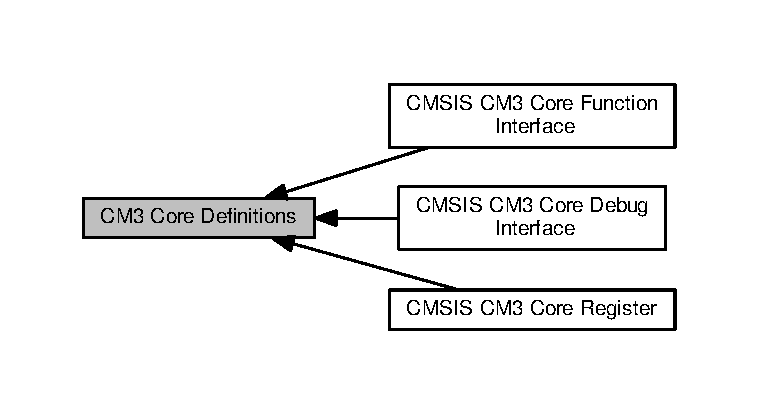
\includegraphics[width=350pt]{d4/dcf/group__CMSIS__CM3__core__definitions}
\end{center}
\end{figure}
\subsection*{Modules}
\begin{DoxyCompactItemize}
\item 
\hyperlink{group__CMSIS__CM3__core__register}{C\+M\+S\+I\+S C\+M3 Core Register}
\item 
\hyperlink{group__CMSIS__CM3__Core__FunctionInterface}{C\+M\+S\+I\+S C\+M3 Core Function Interface}
\item 
\hyperlink{group__CMSIS__CM3__CoreDebugInterface}{C\+M\+S\+I\+S C\+M3 Core Debug Interface}
\end{DoxyCompactItemize}
\subsection*{Macros}
\begin{DoxyCompactItemize}
\item 
\#define \hyperlink{group__CMSIS__CM3__core__definitions_gac1c1120e9fe082fac8225c60143ac79a}{\+\_\+\+\_\+\+C\+M3\+\_\+\+C\+M\+S\+I\+S\+\_\+\+V\+E\+R\+S\+I\+O\+N\+\_\+\+M\+A\+IN}~(0x01)
\item 
\#define \hyperlink{group__CMSIS__CM3__core__definitions_ga9ff7a998d4b8b3c87bfaca6e78607950}{\+\_\+\+\_\+\+C\+M3\+\_\+\+C\+M\+S\+I\+S\+\_\+\+V\+E\+R\+S\+I\+O\+N\+\_\+\+S\+UB}~(0x30)
\item 
\#define \hyperlink{group__CMSIS__CM3__core__definitions_gaf888c651cd8c93fd25364f9e74306a1c}{\+\_\+\+\_\+\+C\+M3\+\_\+\+C\+M\+S\+I\+S\+\_\+\+V\+E\+R\+S\+I\+ON}~((\hyperlink{group__CMSIS__CM3__core__definitions_gac1c1120e9fe082fac8225c60143ac79a}{\+\_\+\+\_\+\+C\+M3\+\_\+\+C\+M\+S\+I\+S\+\_\+\+V\+E\+R\+S\+I\+O\+N\+\_\+\+M\+A\+IN} $<$$<$ 16) $\vert$ \hyperlink{group__CMSIS__CM3__core__definitions_ga9ff7a998d4b8b3c87bfaca6e78607950}{\+\_\+\+\_\+\+C\+M3\+\_\+\+C\+M\+S\+I\+S\+\_\+\+V\+E\+R\+S\+I\+O\+N\+\_\+\+S\+UB})
\item 
\#define \hyperlink{group__CMSIS__CM3__core__definitions_ga63ea62503c88acab19fcf3d5743009e3}{\+\_\+\+\_\+\+C\+O\+R\+T\+E\+X\+\_\+M}~(0x03)
\end{DoxyCompactItemize}


\subsection{Detailed Description}
This file defines all structures and symbols for C\+M\+S\+IS core\+:
\begin{DoxyItemize}
\item C\+M\+S\+IS version number
\item Cortex-\/M core registers and bitfields
\item Cortex-\/M core peripheral base address 
\end{DoxyItemize}

\subsection{Macro Definition Documentation}
\index{C\+M3 Core Definitions@{C\+M3 Core Definitions}!\+\_\+\+\_\+\+C\+M3\+\_\+\+C\+M\+S\+I\+S\+\_\+\+V\+E\+R\+S\+I\+ON@{\+\_\+\+\_\+\+C\+M3\+\_\+\+C\+M\+S\+I\+S\+\_\+\+V\+E\+R\+S\+I\+ON}}
\index{\+\_\+\+\_\+\+C\+M3\+\_\+\+C\+M\+S\+I\+S\+\_\+\+V\+E\+R\+S\+I\+ON@{\+\_\+\+\_\+\+C\+M3\+\_\+\+C\+M\+S\+I\+S\+\_\+\+V\+E\+R\+S\+I\+ON}!C\+M3 Core Definitions@{C\+M3 Core Definitions}}
\subsubsection[{\texorpdfstring{\+\_\+\+\_\+\+C\+M3\+\_\+\+C\+M\+S\+I\+S\+\_\+\+V\+E\+R\+S\+I\+ON}{__CM3_CMSIS_VERSION}}]{\setlength{\rightskip}{0pt plus 5cm}\#define \+\_\+\+\_\+\+C\+M3\+\_\+\+C\+M\+S\+I\+S\+\_\+\+V\+E\+R\+S\+I\+ON~(({\bf \+\_\+\+\_\+\+C\+M3\+\_\+\+C\+M\+S\+I\+S\+\_\+\+V\+E\+R\+S\+I\+O\+N\+\_\+\+M\+A\+IN} $<$$<$ 16) $\vert$ {\bf \+\_\+\+\_\+\+C\+M3\+\_\+\+C\+M\+S\+I\+S\+\_\+\+V\+E\+R\+S\+I\+O\+N\+\_\+\+S\+UB})}\hypertarget{group__CMSIS__CM3__core__definitions_gaf888c651cd8c93fd25364f9e74306a1c}{}\label{group__CMSIS__CM3__core__definitions_gaf888c651cd8c93fd25364f9e74306a1c}
C\+M\+S\+IS H\+AL version number \index{C\+M3 Core Definitions@{C\+M3 Core Definitions}!\+\_\+\+\_\+\+C\+M3\+\_\+\+C\+M\+S\+I\+S\+\_\+\+V\+E\+R\+S\+I\+O\+N\+\_\+\+M\+A\+IN@{\+\_\+\+\_\+\+C\+M3\+\_\+\+C\+M\+S\+I\+S\+\_\+\+V\+E\+R\+S\+I\+O\+N\+\_\+\+M\+A\+IN}}
\index{\+\_\+\+\_\+\+C\+M3\+\_\+\+C\+M\+S\+I\+S\+\_\+\+V\+E\+R\+S\+I\+O\+N\+\_\+\+M\+A\+IN@{\+\_\+\+\_\+\+C\+M3\+\_\+\+C\+M\+S\+I\+S\+\_\+\+V\+E\+R\+S\+I\+O\+N\+\_\+\+M\+A\+IN}!C\+M3 Core Definitions@{C\+M3 Core Definitions}}
\subsubsection[{\texorpdfstring{\+\_\+\+\_\+\+C\+M3\+\_\+\+C\+M\+S\+I\+S\+\_\+\+V\+E\+R\+S\+I\+O\+N\+\_\+\+M\+A\+IN}{__CM3_CMSIS_VERSION_MAIN}}]{\setlength{\rightskip}{0pt plus 5cm}\#define \+\_\+\+\_\+\+C\+M3\+\_\+\+C\+M\+S\+I\+S\+\_\+\+V\+E\+R\+S\+I\+O\+N\+\_\+\+M\+A\+IN~(0x01)}\hypertarget{group__CMSIS__CM3__core__definitions_gac1c1120e9fe082fac8225c60143ac79a}{}\label{group__CMSIS__CM3__core__definitions_gac1c1120e9fe082fac8225c60143ac79a}
\mbox{[}31\+:16\mbox{]} C\+M\+S\+IS H\+AL main version \index{C\+M3 Core Definitions@{C\+M3 Core Definitions}!\+\_\+\+\_\+\+C\+M3\+\_\+\+C\+M\+S\+I\+S\+\_\+\+V\+E\+R\+S\+I\+O\+N\+\_\+\+S\+UB@{\+\_\+\+\_\+\+C\+M3\+\_\+\+C\+M\+S\+I\+S\+\_\+\+V\+E\+R\+S\+I\+O\+N\+\_\+\+S\+UB}}
\index{\+\_\+\+\_\+\+C\+M3\+\_\+\+C\+M\+S\+I\+S\+\_\+\+V\+E\+R\+S\+I\+O\+N\+\_\+\+S\+UB@{\+\_\+\+\_\+\+C\+M3\+\_\+\+C\+M\+S\+I\+S\+\_\+\+V\+E\+R\+S\+I\+O\+N\+\_\+\+S\+UB}!C\+M3 Core Definitions@{C\+M3 Core Definitions}}
\subsubsection[{\texorpdfstring{\+\_\+\+\_\+\+C\+M3\+\_\+\+C\+M\+S\+I\+S\+\_\+\+V\+E\+R\+S\+I\+O\+N\+\_\+\+S\+UB}{__CM3_CMSIS_VERSION_SUB}}]{\setlength{\rightskip}{0pt plus 5cm}\#define \+\_\+\+\_\+\+C\+M3\+\_\+\+C\+M\+S\+I\+S\+\_\+\+V\+E\+R\+S\+I\+O\+N\+\_\+\+S\+UB~(0x30)}\hypertarget{group__CMSIS__CM3__core__definitions_ga9ff7a998d4b8b3c87bfaca6e78607950}{}\label{group__CMSIS__CM3__core__definitions_ga9ff7a998d4b8b3c87bfaca6e78607950}
\mbox{[}15\+:0\mbox{]} C\+M\+S\+IS H\+AL sub version \index{C\+M3 Core Definitions@{C\+M3 Core Definitions}!\+\_\+\+\_\+\+C\+O\+R\+T\+E\+X\+\_\+M@{\+\_\+\+\_\+\+C\+O\+R\+T\+E\+X\+\_\+M}}
\index{\+\_\+\+\_\+\+C\+O\+R\+T\+E\+X\+\_\+M@{\+\_\+\+\_\+\+C\+O\+R\+T\+E\+X\+\_\+M}!C\+M3 Core Definitions@{C\+M3 Core Definitions}}
\subsubsection[{\texorpdfstring{\+\_\+\+\_\+\+C\+O\+R\+T\+E\+X\+\_\+M}{__CORTEX_M}}]{\setlength{\rightskip}{0pt plus 5cm}\#define \+\_\+\+\_\+\+C\+O\+R\+T\+E\+X\+\_\+M~(0x03)}\hypertarget{group__CMSIS__CM3__core__definitions_ga63ea62503c88acab19fcf3d5743009e3}{}\label{group__CMSIS__CM3__core__definitions_ga63ea62503c88acab19fcf3d5743009e3}
Cortex core 
\hypertarget{group__CMSIS__CM3__core__register}{}\section{C\+M\+S\+IS C\+M3 Core Register}
\label{group__CMSIS__CM3__core__register}\index{C\+M\+S\+I\+S C\+M3 Core Register@{C\+M\+S\+I\+S C\+M3 Core Register}}
Collaboration diagram for C\+M\+S\+IS C\+M3 Core Register\+:\nopagebreak
\begin{figure}[H]
\begin{center}
\leavevmode
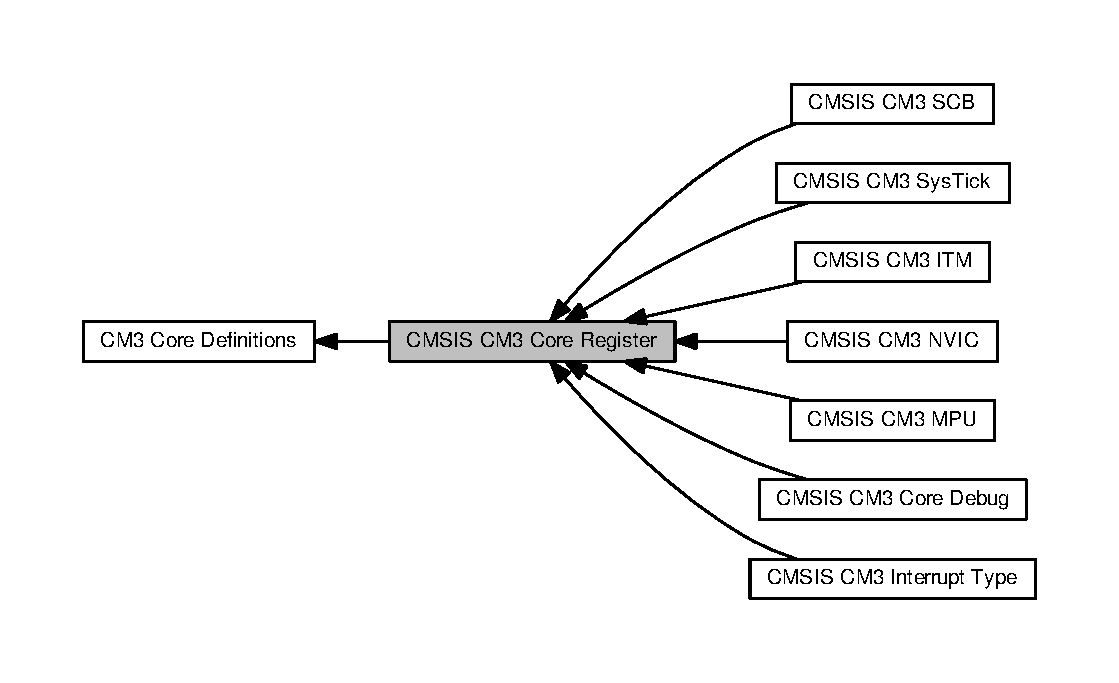
\includegraphics[width=350pt]{d2/d96/group__CMSIS__CM3__core__register}
\end{center}
\end{figure}
\subsection*{Modules}
\begin{DoxyCompactItemize}
\item 
\hyperlink{group__CMSIS__CM3__NVIC}{C\+M\+S\+I\+S C\+M3 N\+V\+IC}
\item 
\hyperlink{group__CMSIS__CM3__SCB}{C\+M\+S\+I\+S C\+M3 S\+CB}
\item 
\hyperlink{group__CMSIS__CM3__SysTick}{C\+M\+S\+I\+S C\+M3 Sys\+Tick}
\item 
\hyperlink{group__CMSIS__CM3__ITM}{C\+M\+S\+I\+S C\+M3 I\+TM}
\item 
\hyperlink{group__CMSIS__CM3__InterruptType}{C\+M\+S\+I\+S C\+M3 Interrupt Type}
\item 
\hyperlink{group__CMSIS__CM3__MPU}{C\+M\+S\+I\+S C\+M3 M\+PU}
\item 
\hyperlink{group__CMSIS__CM3__CoreDebug}{C\+M\+S\+I\+S C\+M3 Core Debug}
\end{DoxyCompactItemize}
\subsection*{Macros}
\begin{DoxyCompactItemize}
\item 
\#define \hyperlink{group__CMSIS__CM3__core__register_ga3c14ed93192c8d9143322bbf77ebf770}{S\+C\+S\+\_\+\+B\+A\+SE}~(0x\+E000\+E000)
\item 
\#define \hyperlink{group__CMSIS__CM3__core__register_gadd76251e412a195ec0a8f47227a8359e}{I\+T\+M\+\_\+\+B\+A\+SE}~(0x\+E0000000)
\item 
\#define \hyperlink{group__CMSIS__CM3__core__register_ga680604dbcda9e9b31a1639fcffe5230b}{Core\+Debug\+\_\+\+B\+A\+SE}~(0x\+E000\+E\+D\+F0)
\item 
\#define \hyperlink{group__CMSIS__CM3__core__register_ga58effaac0b93006b756d33209e814646}{Sys\+Tick\+\_\+\+B\+A\+SE}~(\hyperlink{group__CMSIS__CM3__core__register_ga3c14ed93192c8d9143322bbf77ebf770}{S\+C\+S\+\_\+\+B\+A\+SE} +  0x0010)
\item 
\#define \hyperlink{group__CMSIS__CM3__core__register_gaa0288691785a5f868238e0468b39523d}{N\+V\+I\+C\+\_\+\+B\+A\+SE}~(\hyperlink{group__CMSIS__CM3__core__register_ga3c14ed93192c8d9143322bbf77ebf770}{S\+C\+S\+\_\+\+B\+A\+SE} +  0x0100)
\item 
\#define \hyperlink{group__CMSIS__CM3__core__register_gad55a7ddb8d4b2398b0c1cfec76c0d9fd}{S\+C\+B\+\_\+\+B\+A\+SE}~(\hyperlink{group__CMSIS__CM3__core__register_ga3c14ed93192c8d9143322bbf77ebf770}{S\+C\+S\+\_\+\+B\+A\+SE} +  0x0\+D00)
\item 
\#define \hyperlink{group__CMSIS__CM3__core__register_ga164238adbad56f07c7dd4e912af748dd}{Interrupt\+Type}~((\hyperlink{structInterruptType__Type}{Interrupt\+Type\+\_\+\+Type} $\ast$) \hyperlink{group__CMSIS__CM3__core__register_ga3c14ed93192c8d9143322bbf77ebf770}{S\+C\+S\+\_\+\+B\+A\+SE})
\item 
\#define \hyperlink{group__CMSIS__CM3__core__register_gaaaf6477c2bde2f00f99e3c2fd1060b01}{S\+CB}~((\hyperlink{structSCB__Type}{S\+C\+B\+\_\+\+Type} $\ast$)           \hyperlink{group__CMSIS__CM3__core__register_gad55a7ddb8d4b2398b0c1cfec76c0d9fd}{S\+C\+B\+\_\+\+B\+A\+SE})
\item 
\#define \hyperlink{group__CMSIS__CM3__core__register_gacd96c53beeaff8f603fcda425eb295de}{Sys\+Tick}~((\hyperlink{structSysTick__Type}{Sys\+Tick\+\_\+\+Type} $\ast$)       \hyperlink{group__CMSIS__CM3__core__register_ga58effaac0b93006b756d33209e814646}{Sys\+Tick\+\_\+\+B\+A\+SE})
\item 
\#define \hyperlink{group__CMSIS__CM3__core__register_gac8e97e8ce56ae9f57da1363a937f8a17}{N\+V\+IC}~((\hyperlink{structNVIC__Type}{N\+V\+I\+C\+\_\+\+Type} $\ast$)          \hyperlink{group__CMSIS__CM3__core__register_gaa0288691785a5f868238e0468b39523d}{N\+V\+I\+C\+\_\+\+B\+A\+SE})
\item 
\#define \hyperlink{group__CMSIS__CM3__core__register_gabae7cdf882def602cb787bb039ff6a43}{I\+TM}~((\hyperlink{structITM__Type}{I\+T\+M\+\_\+\+Type} $\ast$)           \hyperlink{group__CMSIS__CM3__core__register_gadd76251e412a195ec0a8f47227a8359e}{I\+T\+M\+\_\+\+B\+A\+SE})
\item 
\#define \hyperlink{group__CMSIS__CM3__core__register_gab6e30a2b802d9021619dbb0be7f5d63d}{Core\+Debug}~((\hyperlink{structCoreDebug__Type}{Core\+Debug\+\_\+\+Type} $\ast$)     \hyperlink{group__CMSIS__CM3__core__register_ga680604dbcda9e9b31a1639fcffe5230b}{Core\+Debug\+\_\+\+B\+A\+SE})
\item 
\#define \hyperlink{group__CMSIS__CM3__core__register_gaa0805ccd2bc4e42d63adb0618d2af571}{M\+P\+U\+\_\+\+B\+A\+SE}~(\hyperlink{group__CMSIS__CM3__core__register_ga3c14ed93192c8d9143322bbf77ebf770}{S\+C\+S\+\_\+\+B\+A\+SE} +  0x0\+D90)
\item 
\#define \hyperlink{group__CMSIS__CM3__core__register_gaad8182e72fe5037a6ba1eb65a1554e0b}{M\+PU}~((\hyperlink{structMPU__Type}{M\+P\+U\+\_\+\+Type}$\ast$)            \hyperlink{group__CMSIS__CM3__core__register_gaa0805ccd2bc4e42d63adb0618d2af571}{M\+P\+U\+\_\+\+B\+A\+SE})
\end{DoxyCompactItemize}


\subsection{Detailed Description}


\subsection{Macro Definition Documentation}
\index{C\+M\+S\+I\+S C\+M3 Core Register@{C\+M\+S\+I\+S C\+M3 Core Register}!Core\+Debug@{Core\+Debug}}
\index{Core\+Debug@{Core\+Debug}!C\+M\+S\+I\+S C\+M3 Core Register@{C\+M\+S\+I\+S C\+M3 Core Register}}
\subsubsection[{\texorpdfstring{Core\+Debug}{CoreDebug}}]{\setlength{\rightskip}{0pt plus 5cm}\#define Core\+Debug~(({\bf Core\+Debug\+\_\+\+Type} $\ast$)     {\bf Core\+Debug\+\_\+\+B\+A\+SE})}\hypertarget{group__CMSIS__CM3__core__register_gab6e30a2b802d9021619dbb0be7f5d63d}{}\label{group__CMSIS__CM3__core__register_gab6e30a2b802d9021619dbb0be7f5d63d}
Core Debug configuration struct \index{C\+M\+S\+I\+S C\+M3 Core Register@{C\+M\+S\+I\+S C\+M3 Core Register}!Core\+Debug\+\_\+\+B\+A\+SE@{Core\+Debug\+\_\+\+B\+A\+SE}}
\index{Core\+Debug\+\_\+\+B\+A\+SE@{Core\+Debug\+\_\+\+B\+A\+SE}!C\+M\+S\+I\+S C\+M3 Core Register@{C\+M\+S\+I\+S C\+M3 Core Register}}
\subsubsection[{\texorpdfstring{Core\+Debug\+\_\+\+B\+A\+SE}{CoreDebug_BASE}}]{\setlength{\rightskip}{0pt plus 5cm}\#define Core\+Debug\+\_\+\+B\+A\+SE~(0x\+E000\+E\+D\+F0)}\hypertarget{group__CMSIS__CM3__core__register_ga680604dbcda9e9b31a1639fcffe5230b}{}\label{group__CMSIS__CM3__core__register_ga680604dbcda9e9b31a1639fcffe5230b}
Core Debug Base Address \index{C\+M\+S\+I\+S C\+M3 Core Register@{C\+M\+S\+I\+S C\+M3 Core Register}!Interrupt\+Type@{Interrupt\+Type}}
\index{Interrupt\+Type@{Interrupt\+Type}!C\+M\+S\+I\+S C\+M3 Core Register@{C\+M\+S\+I\+S C\+M3 Core Register}}
\subsubsection[{\texorpdfstring{Interrupt\+Type}{InterruptType}}]{\setlength{\rightskip}{0pt plus 5cm}\#define Interrupt\+Type~(({\bf Interrupt\+Type\+\_\+\+Type} $\ast$) {\bf S\+C\+S\+\_\+\+B\+A\+SE})}\hypertarget{group__CMSIS__CM3__core__register_ga164238adbad56f07c7dd4e912af748dd}{}\label{group__CMSIS__CM3__core__register_ga164238adbad56f07c7dd4e912af748dd}
Interrupt Type Register \index{C\+M\+S\+I\+S C\+M3 Core Register@{C\+M\+S\+I\+S C\+M3 Core Register}!I\+TM@{I\+TM}}
\index{I\+TM@{I\+TM}!C\+M\+S\+I\+S C\+M3 Core Register@{C\+M\+S\+I\+S C\+M3 Core Register}}
\subsubsection[{\texorpdfstring{I\+TM}{ITM}}]{\setlength{\rightskip}{0pt plus 5cm}\#define I\+TM~(({\bf I\+T\+M\+\_\+\+Type} $\ast$)           {\bf I\+T\+M\+\_\+\+B\+A\+SE})}\hypertarget{group__CMSIS__CM3__core__register_gabae7cdf882def602cb787bb039ff6a43}{}\label{group__CMSIS__CM3__core__register_gabae7cdf882def602cb787bb039ff6a43}
I\+TM configuration struct \index{C\+M\+S\+I\+S C\+M3 Core Register@{C\+M\+S\+I\+S C\+M3 Core Register}!I\+T\+M\+\_\+\+B\+A\+SE@{I\+T\+M\+\_\+\+B\+A\+SE}}
\index{I\+T\+M\+\_\+\+B\+A\+SE@{I\+T\+M\+\_\+\+B\+A\+SE}!C\+M\+S\+I\+S C\+M3 Core Register@{C\+M\+S\+I\+S C\+M3 Core Register}}
\subsubsection[{\texorpdfstring{I\+T\+M\+\_\+\+B\+A\+SE}{ITM_BASE}}]{\setlength{\rightskip}{0pt plus 5cm}\#define I\+T\+M\+\_\+\+B\+A\+SE~(0x\+E0000000)}\hypertarget{group__CMSIS__CM3__core__register_gadd76251e412a195ec0a8f47227a8359e}{}\label{group__CMSIS__CM3__core__register_gadd76251e412a195ec0a8f47227a8359e}
I\+TM Base Address \index{C\+M\+S\+I\+S C\+M3 Core Register@{C\+M\+S\+I\+S C\+M3 Core Register}!M\+PU@{M\+PU}}
\index{M\+PU@{M\+PU}!C\+M\+S\+I\+S C\+M3 Core Register@{C\+M\+S\+I\+S C\+M3 Core Register}}
\subsubsection[{\texorpdfstring{M\+PU}{MPU}}]{\setlength{\rightskip}{0pt plus 5cm}\#define M\+PU~(({\bf M\+P\+U\+\_\+\+Type}$\ast$)            {\bf M\+P\+U\+\_\+\+B\+A\+SE})}\hypertarget{group__CMSIS__CM3__core__register_gaad8182e72fe5037a6ba1eb65a1554e0b}{}\label{group__CMSIS__CM3__core__register_gaad8182e72fe5037a6ba1eb65a1554e0b}
Memory Protection Unit \index{C\+M\+S\+I\+S C\+M3 Core Register@{C\+M\+S\+I\+S C\+M3 Core Register}!M\+P\+U\+\_\+\+B\+A\+SE@{M\+P\+U\+\_\+\+B\+A\+SE}}
\index{M\+P\+U\+\_\+\+B\+A\+SE@{M\+P\+U\+\_\+\+B\+A\+SE}!C\+M\+S\+I\+S C\+M3 Core Register@{C\+M\+S\+I\+S C\+M3 Core Register}}
\subsubsection[{\texorpdfstring{M\+P\+U\+\_\+\+B\+A\+SE}{MPU_BASE}}]{\setlength{\rightskip}{0pt plus 5cm}\#define M\+P\+U\+\_\+\+B\+A\+SE~({\bf S\+C\+S\+\_\+\+B\+A\+SE} +  0x0\+D90)}\hypertarget{group__CMSIS__CM3__core__register_gaa0805ccd2bc4e42d63adb0618d2af571}{}\label{group__CMSIS__CM3__core__register_gaa0805ccd2bc4e42d63adb0618d2af571}
Memory Protection Unit \index{C\+M\+S\+I\+S C\+M3 Core Register@{C\+M\+S\+I\+S C\+M3 Core Register}!N\+V\+IC@{N\+V\+IC}}
\index{N\+V\+IC@{N\+V\+IC}!C\+M\+S\+I\+S C\+M3 Core Register@{C\+M\+S\+I\+S C\+M3 Core Register}}
\subsubsection[{\texorpdfstring{N\+V\+IC}{NVIC}}]{\setlength{\rightskip}{0pt plus 5cm}\#define N\+V\+IC~(({\bf N\+V\+I\+C\+\_\+\+Type} $\ast$)          {\bf N\+V\+I\+C\+\_\+\+B\+A\+SE})}\hypertarget{group__CMSIS__CM3__core__register_gac8e97e8ce56ae9f57da1363a937f8a17}{}\label{group__CMSIS__CM3__core__register_gac8e97e8ce56ae9f57da1363a937f8a17}
N\+V\+IC configuration struct \index{C\+M\+S\+I\+S C\+M3 Core Register@{C\+M\+S\+I\+S C\+M3 Core Register}!N\+V\+I\+C\+\_\+\+B\+A\+SE@{N\+V\+I\+C\+\_\+\+B\+A\+SE}}
\index{N\+V\+I\+C\+\_\+\+B\+A\+SE@{N\+V\+I\+C\+\_\+\+B\+A\+SE}!C\+M\+S\+I\+S C\+M3 Core Register@{C\+M\+S\+I\+S C\+M3 Core Register}}
\subsubsection[{\texorpdfstring{N\+V\+I\+C\+\_\+\+B\+A\+SE}{NVIC_BASE}}]{\setlength{\rightskip}{0pt plus 5cm}\#define N\+V\+I\+C\+\_\+\+B\+A\+SE~({\bf S\+C\+S\+\_\+\+B\+A\+SE} +  0x0100)}\hypertarget{group__CMSIS__CM3__core__register_gaa0288691785a5f868238e0468b39523d}{}\label{group__CMSIS__CM3__core__register_gaa0288691785a5f868238e0468b39523d}
N\+V\+IC Base Address \index{C\+M\+S\+I\+S C\+M3 Core Register@{C\+M\+S\+I\+S C\+M3 Core Register}!S\+CB@{S\+CB}}
\index{S\+CB@{S\+CB}!C\+M\+S\+I\+S C\+M3 Core Register@{C\+M\+S\+I\+S C\+M3 Core Register}}
\subsubsection[{\texorpdfstring{S\+CB}{SCB}}]{\setlength{\rightskip}{0pt plus 5cm}\#define S\+CB~(({\bf S\+C\+B\+\_\+\+Type} $\ast$)           {\bf S\+C\+B\+\_\+\+B\+A\+SE})}\hypertarget{group__CMSIS__CM3__core__register_gaaaf6477c2bde2f00f99e3c2fd1060b01}{}\label{group__CMSIS__CM3__core__register_gaaaf6477c2bde2f00f99e3c2fd1060b01}
S\+CB configuration struct \index{C\+M\+S\+I\+S C\+M3 Core Register@{C\+M\+S\+I\+S C\+M3 Core Register}!S\+C\+B\+\_\+\+B\+A\+SE@{S\+C\+B\+\_\+\+B\+A\+SE}}
\index{S\+C\+B\+\_\+\+B\+A\+SE@{S\+C\+B\+\_\+\+B\+A\+SE}!C\+M\+S\+I\+S C\+M3 Core Register@{C\+M\+S\+I\+S C\+M3 Core Register}}
\subsubsection[{\texorpdfstring{S\+C\+B\+\_\+\+B\+A\+SE}{SCB_BASE}}]{\setlength{\rightskip}{0pt plus 5cm}\#define S\+C\+B\+\_\+\+B\+A\+SE~({\bf S\+C\+S\+\_\+\+B\+A\+SE} +  0x0\+D00)}\hypertarget{group__CMSIS__CM3__core__register_gad55a7ddb8d4b2398b0c1cfec76c0d9fd}{}\label{group__CMSIS__CM3__core__register_gad55a7ddb8d4b2398b0c1cfec76c0d9fd}
System Control Block Base Address \index{C\+M\+S\+I\+S C\+M3 Core Register@{C\+M\+S\+I\+S C\+M3 Core Register}!S\+C\+S\+\_\+\+B\+A\+SE@{S\+C\+S\+\_\+\+B\+A\+SE}}
\index{S\+C\+S\+\_\+\+B\+A\+SE@{S\+C\+S\+\_\+\+B\+A\+SE}!C\+M\+S\+I\+S C\+M3 Core Register@{C\+M\+S\+I\+S C\+M3 Core Register}}
\subsubsection[{\texorpdfstring{S\+C\+S\+\_\+\+B\+A\+SE}{SCS_BASE}}]{\setlength{\rightskip}{0pt plus 5cm}\#define S\+C\+S\+\_\+\+B\+A\+SE~(0x\+E000\+E000)}\hypertarget{group__CMSIS__CM3__core__register_ga3c14ed93192c8d9143322bbf77ebf770}{}\label{group__CMSIS__CM3__core__register_ga3c14ed93192c8d9143322bbf77ebf770}
System Control Space Base Address \index{C\+M\+S\+I\+S C\+M3 Core Register@{C\+M\+S\+I\+S C\+M3 Core Register}!Sys\+Tick@{Sys\+Tick}}
\index{Sys\+Tick@{Sys\+Tick}!C\+M\+S\+I\+S C\+M3 Core Register@{C\+M\+S\+I\+S C\+M3 Core Register}}
\subsubsection[{\texorpdfstring{Sys\+Tick}{SysTick}}]{\setlength{\rightskip}{0pt plus 5cm}\#define Sys\+Tick~(({\bf Sys\+Tick\+\_\+\+Type} $\ast$)       {\bf Sys\+Tick\+\_\+\+B\+A\+SE})}\hypertarget{group__CMSIS__CM3__core__register_gacd96c53beeaff8f603fcda425eb295de}{}\label{group__CMSIS__CM3__core__register_gacd96c53beeaff8f603fcda425eb295de}
Sys\+Tick configuration struct \index{C\+M\+S\+I\+S C\+M3 Core Register@{C\+M\+S\+I\+S C\+M3 Core Register}!Sys\+Tick\+\_\+\+B\+A\+SE@{Sys\+Tick\+\_\+\+B\+A\+SE}}
\index{Sys\+Tick\+\_\+\+B\+A\+SE@{Sys\+Tick\+\_\+\+B\+A\+SE}!C\+M\+S\+I\+S C\+M3 Core Register@{C\+M\+S\+I\+S C\+M3 Core Register}}
\subsubsection[{\texorpdfstring{Sys\+Tick\+\_\+\+B\+A\+SE}{SysTick_BASE}}]{\setlength{\rightskip}{0pt plus 5cm}\#define Sys\+Tick\+\_\+\+B\+A\+SE~({\bf S\+C\+S\+\_\+\+B\+A\+SE} +  0x0010)}\hypertarget{group__CMSIS__CM3__core__register_ga58effaac0b93006b756d33209e814646}{}\label{group__CMSIS__CM3__core__register_ga58effaac0b93006b756d33209e814646}
Sys\+Tick Base Address 
\hypertarget{group__CMSIS__CM3__NVIC}{}\section{C\+M\+S\+IS C\+M3 N\+V\+IC}
\label{group__CMSIS__CM3__NVIC}\index{C\+M\+S\+I\+S C\+M3 N\+V\+IC@{C\+M\+S\+I\+S C\+M3 N\+V\+IC}}
Collaboration diagram for C\+M\+S\+IS C\+M3 N\+V\+IC\+:\nopagebreak
\begin{figure}[H]
\begin{center}
\leavevmode
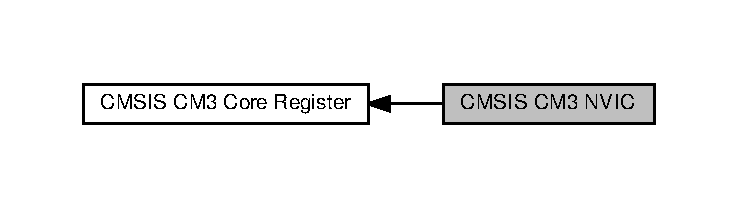
\includegraphics[width=350pt]{de/db9/group__CMSIS__CM3__NVIC}
\end{center}
\end{figure}
\subsection*{Data Structures}
\begin{DoxyCompactItemize}
\item 
struct \hyperlink{structNVIC__Type}{N\+V\+I\+C\+\_\+\+Type}
\end{DoxyCompactItemize}
\subsection*{Variables}
\begin{DoxyCompactItemize}
\item 
typedef \hyperlink{group__CMSIS__CM3__NVIC_ga8c1dfc1ccf00a08192611433ee7f17b4}{\+\_\+\+\_\+attribute\+\_\+\+\_\+}
\begin{DoxyCompactList}\small\item\em If an I\+RQ is not registered, we end up at this stub function. \end{DoxyCompactList}\end{DoxyCompactItemize}


\subsection{Detailed Description}
memory mapped structure for Nested Vectored Interrupt Controller (N\+V\+IC) 

\subsection{Variable Documentation}
\index{C\+M\+S\+I\+S C\+M3 N\+V\+IC@{C\+M\+S\+I\+S C\+M3 N\+V\+IC}!\+\_\+\+\_\+attribute\+\_\+\+\_\+@{\+\_\+\+\_\+attribute\+\_\+\+\_\+}}
\index{\+\_\+\+\_\+attribute\+\_\+\+\_\+@{\+\_\+\+\_\+attribute\+\_\+\+\_\+}!C\+M\+S\+I\+S C\+M3 N\+V\+IC@{C\+M\+S\+I\+S C\+M3 N\+V\+IC}}
\subsubsection[{\texorpdfstring{\+\_\+\+\_\+attribute\+\_\+\+\_\+}{__attribute__}}]{\setlength{\rightskip}{0pt plus 5cm}{\bf \+\_\+\+\_\+attribute\+\_\+\+\_\+}}\hypertarget{group__CMSIS__CM3__NVIC_ga8c1dfc1ccf00a08192611433ee7f17b4}{}\label{group__CMSIS__CM3__NVIC_ga8c1dfc1ccf00a08192611433ee7f17b4}


If an I\+RQ is not registered, we end up at this stub function. 

G\+CC C libraries call this function to set time of day.

Wrap the Free\+R\+T\+OS tick function such that we get a true measure of how much C\+PU tasks are using. 
\hypertarget{group__CMSIS__CM3__SCB}{}\section{C\+M\+S\+IS C\+M3 S\+CB}
\label{group__CMSIS__CM3__SCB}\index{C\+M\+S\+I\+S C\+M3 S\+CB@{C\+M\+S\+I\+S C\+M3 S\+CB}}
Collaboration diagram for C\+M\+S\+IS C\+M3 S\+CB\+:\nopagebreak
\begin{figure}[H]
\begin{center}
\leavevmode
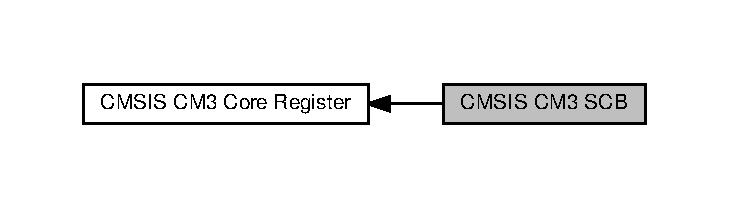
\includegraphics[width=350pt]{d7/dbc/group__CMSIS__CM3__SCB}
\end{center}
\end{figure}
\subsection*{Data Structures}
\begin{DoxyCompactItemize}
\item 
struct \hyperlink{structSCB__Type}{S\+C\+B\+\_\+\+Type}
\end{DoxyCompactItemize}
\subsection*{Macros}
\begin{DoxyCompactItemize}
\item 
\#define \hyperlink{group__CMSIS__CM3__SCB_ga58686b88f94f789d4e6f429fe1ff58cf}{S\+C\+B\+\_\+\+C\+P\+U\+I\+D\+\_\+\+I\+M\+P\+L\+E\+M\+E\+N\+T\+E\+R\+\_\+\+Pos}~24
\item 
\#define \hyperlink{group__CMSIS__CM3__SCB_ga0932b31faafd47656a03ced75a31d99b}{S\+C\+B\+\_\+\+C\+P\+U\+I\+D\+\_\+\+I\+M\+P\+L\+E\+M\+E\+N\+T\+E\+R\+\_\+\+Msk}~(0x\+F\+Ful $<$$<$ S\+C\+B\+\_\+\+C\+P\+U\+I\+D\+\_\+\+I\+M\+P\+L\+E\+M\+E\+N\+T\+E\+R\+\_\+\+Pos)
\item 
\#define \hyperlink{group__CMSIS__CM3__SCB_ga104462bd0815391b4044a70bd15d3a71}{S\+C\+B\+\_\+\+C\+P\+U\+I\+D\+\_\+\+V\+A\+R\+I\+A\+N\+T\+\_\+\+Pos}~20
\item 
\#define \hyperlink{group__CMSIS__CM3__SCB_gad358dfbd04300afc1824329d128b99e8}{S\+C\+B\+\_\+\+C\+P\+U\+I\+D\+\_\+\+V\+A\+R\+I\+A\+N\+T\+\_\+\+Msk}~(0x\+Ful $<$$<$ S\+C\+B\+\_\+\+C\+P\+U\+I\+D\+\_\+\+V\+A\+R\+I\+A\+N\+T\+\_\+\+Pos)
\item 
\#define \hyperlink{group__CMSIS__CM3__SCB_ga705f68eaa9afb042ca2407dc4e4629ac}{S\+C\+B\+\_\+\+C\+P\+U\+I\+D\+\_\+\+P\+A\+R\+T\+N\+O\+\_\+\+Pos}~4
\item 
\#define \hyperlink{group__CMSIS__CM3__SCB_ga98e581423ca016680c238c469aba546d}{S\+C\+B\+\_\+\+C\+P\+U\+I\+D\+\_\+\+P\+A\+R\+T\+N\+O\+\_\+\+Msk}~(0x\+F\+F\+Ful $<$$<$ S\+C\+B\+\_\+\+C\+P\+U\+I\+D\+\_\+\+P\+A\+R\+T\+N\+O\+\_\+\+Pos)
\item 
\#define \hyperlink{group__CMSIS__CM3__SCB_ga3c3d9071e574de11fb27ba57034838b1}{S\+C\+B\+\_\+\+C\+P\+U\+I\+D\+\_\+\+R\+E\+V\+I\+S\+I\+O\+N\+\_\+\+Pos}~0
\item 
\#define \hyperlink{group__CMSIS__CM3__SCB_ga2ec0448b6483f77e7f5d08b4b81d85df}{S\+C\+B\+\_\+\+C\+P\+U\+I\+D\+\_\+\+R\+E\+V\+I\+S\+I\+O\+N\+\_\+\+Msk}~(0x\+Ful $<$$<$ S\+C\+B\+\_\+\+C\+P\+U\+I\+D\+\_\+\+R\+E\+V\+I\+S\+I\+O\+N\+\_\+\+Pos)
\item 
\#define \hyperlink{group__CMSIS__CM3__SCB_ga750d4b52624a46d71356db4ea769573b}{S\+C\+B\+\_\+\+I\+C\+S\+R\+\_\+\+N\+M\+I\+P\+E\+N\+D\+S\+E\+T\+\_\+\+Pos}~31
\item 
\#define \hyperlink{group__CMSIS__CM3__SCB_ga340e3f79e9c3607dee9f2c048b6b22e8}{S\+C\+B\+\_\+\+I\+C\+S\+R\+\_\+\+N\+M\+I\+P\+E\+N\+D\+S\+E\+T\+\_\+\+Msk}~(1ul $<$$<$ S\+C\+B\+\_\+\+I\+C\+S\+R\+\_\+\+N\+M\+I\+P\+E\+N\+D\+S\+E\+T\+\_\+\+Pos)
\item 
\#define \hyperlink{group__CMSIS__CM3__SCB_gab5ded23d2ab1d5ff7cc7ce746205e9fe}{S\+C\+B\+\_\+\+I\+C\+S\+R\+\_\+\+P\+E\+N\+D\+S\+V\+S\+E\+T\+\_\+\+Pos}~28
\item 
\#define \hyperlink{group__CMSIS__CM3__SCB_ga1e40d93efb402763c8c00ddcc56724ff}{S\+C\+B\+\_\+\+I\+C\+S\+R\+\_\+\+P\+E\+N\+D\+S\+V\+S\+E\+T\+\_\+\+Msk}~(1ul $<$$<$ S\+C\+B\+\_\+\+I\+C\+S\+R\+\_\+\+P\+E\+N\+D\+S\+V\+S\+E\+T\+\_\+\+Pos)
\item 
\#define \hyperlink{group__CMSIS__CM3__SCB_gae218d9022288f89faf57187c4d542ecd}{S\+C\+B\+\_\+\+I\+C\+S\+R\+\_\+\+P\+E\+N\+D\+S\+V\+C\+L\+R\+\_\+\+Pos}~27
\item 
\#define \hyperlink{group__CMSIS__CM3__SCB_ga4a901ace381d3c1c74ac82b22fae2e1e}{S\+C\+B\+\_\+\+I\+C\+S\+R\+\_\+\+P\+E\+N\+D\+S\+V\+C\+L\+R\+\_\+\+Msk}~(1ul $<$$<$ S\+C\+B\+\_\+\+I\+C\+S\+R\+\_\+\+P\+E\+N\+D\+S\+V\+C\+L\+R\+\_\+\+Pos)
\item 
\#define \hyperlink{group__CMSIS__CM3__SCB_ga9dbb3358c6167c9c3f85661b90fb2794}{S\+C\+B\+\_\+\+I\+C\+S\+R\+\_\+\+P\+E\+N\+D\+S\+T\+S\+E\+T\+\_\+\+Pos}~26
\item 
\#define \hyperlink{group__CMSIS__CM3__SCB_ga7325b61ea0ec323ef2d5c893b112e546}{S\+C\+B\+\_\+\+I\+C\+S\+R\+\_\+\+P\+E\+N\+D\+S\+T\+S\+E\+T\+\_\+\+Msk}~(1ul $<$$<$ S\+C\+B\+\_\+\+I\+C\+S\+R\+\_\+\+P\+E\+N\+D\+S\+T\+S\+E\+T\+\_\+\+Pos)
\item 
\#define \hyperlink{group__CMSIS__CM3__SCB_gadbe25e4b333ece1341beb1a740168fdc}{S\+C\+B\+\_\+\+I\+C\+S\+R\+\_\+\+P\+E\+N\+D\+S\+T\+C\+L\+R\+\_\+\+Pos}~25
\item 
\#define \hyperlink{group__CMSIS__CM3__SCB_gab241827d2a793269d8cd99b9b28c2157}{S\+C\+B\+\_\+\+I\+C\+S\+R\+\_\+\+P\+E\+N\+D\+S\+T\+C\+L\+R\+\_\+\+Msk}~(1ul $<$$<$ S\+C\+B\+\_\+\+I\+C\+S\+R\+\_\+\+P\+E\+N\+D\+S\+T\+C\+L\+R\+\_\+\+Pos)
\item 
\#define \hyperlink{group__CMSIS__CM3__SCB_ga11cb5b1f9ce167b81f31787a77e575df}{S\+C\+B\+\_\+\+I\+C\+S\+R\+\_\+\+I\+S\+R\+P\+R\+E\+E\+M\+P\+T\+\_\+\+Pos}~23
\item 
\#define \hyperlink{group__CMSIS__CM3__SCB_gaa966600396290808d596fe96e92ca2b5}{S\+C\+B\+\_\+\+I\+C\+S\+R\+\_\+\+I\+S\+R\+P\+R\+E\+E\+M\+P\+T\+\_\+\+Msk}~(1ul $<$$<$ S\+C\+B\+\_\+\+I\+C\+S\+R\+\_\+\+I\+S\+R\+P\+R\+E\+E\+M\+P\+T\+\_\+\+Pos)
\item 
\#define \hyperlink{group__CMSIS__CM3__SCB_ga10749d92b9b744094b845c2eb46d4319}{S\+C\+B\+\_\+\+I\+C\+S\+R\+\_\+\+I\+S\+R\+P\+E\+N\+D\+I\+N\+G\+\_\+\+Pos}~22
\item 
\#define \hyperlink{group__CMSIS__CM3__SCB_ga056d74fd538e5d36d3be1f28d399c877}{S\+C\+B\+\_\+\+I\+C\+S\+R\+\_\+\+I\+S\+R\+P\+E\+N\+D\+I\+N\+G\+\_\+\+Msk}~(1ul $<$$<$ S\+C\+B\+\_\+\+I\+C\+S\+R\+\_\+\+I\+S\+R\+P\+E\+N\+D\+I\+N\+G\+\_\+\+Pos)
\item 
\#define \hyperlink{group__CMSIS__CM3__SCB_gada60c92bf88d6fd21a8f49efa4a127b8}{S\+C\+B\+\_\+\+I\+C\+S\+R\+\_\+\+V\+E\+C\+T\+P\+E\+N\+D\+I\+N\+G\+\_\+\+Pos}~12
\item 
\#define \hyperlink{group__CMSIS__CM3__SCB_gacb6992e7c7ddc27a370f62878a21ef72}{S\+C\+B\+\_\+\+I\+C\+S\+R\+\_\+\+V\+E\+C\+T\+P\+E\+N\+D\+I\+N\+G\+\_\+\+Msk}~(0x1\+F\+Ful $<$$<$ S\+C\+B\+\_\+\+I\+C\+S\+R\+\_\+\+V\+E\+C\+T\+P\+E\+N\+D\+I\+N\+G\+\_\+\+Pos)
\item 
\#define \hyperlink{group__CMSIS__CM3__SCB_ga403d154200242629e6d2764bfc12a7ec}{S\+C\+B\+\_\+\+I\+C\+S\+R\+\_\+\+R\+E\+T\+T\+O\+B\+A\+S\+E\+\_\+\+Pos}~11
\item 
\#define \hyperlink{group__CMSIS__CM3__SCB_gaca6fc3f79bb550f64fd7df782ed4a5f6}{S\+C\+B\+\_\+\+I\+C\+S\+R\+\_\+\+R\+E\+T\+T\+O\+B\+A\+S\+E\+\_\+\+Msk}~(1ul $<$$<$ S\+C\+B\+\_\+\+I\+C\+S\+R\+\_\+\+R\+E\+T\+T\+O\+B\+A\+S\+E\+\_\+\+Pos)
\item 
\#define \hyperlink{group__CMSIS__CM3__SCB_gae4f602c7c5c895d5fb687b71b0979fc3}{S\+C\+B\+\_\+\+I\+C\+S\+R\+\_\+\+V\+E\+C\+T\+A\+C\+T\+I\+V\+E\+\_\+\+Pos}~0
\item 
\#define \hyperlink{group__CMSIS__CM3__SCB_ga5533791a4ecf1b9301c883047b3e8396}{S\+C\+B\+\_\+\+I\+C\+S\+R\+\_\+\+V\+E\+C\+T\+A\+C\+T\+I\+V\+E\+\_\+\+Msk}~(0x1\+F\+Ful $<$$<$ S\+C\+B\+\_\+\+I\+C\+S\+R\+\_\+\+V\+E\+C\+T\+A\+C\+T\+I\+V\+E\+\_\+\+Pos)
\item 
\#define \hyperlink{group__CMSIS__CM3__SCB_gad9720a44320c053883d03b883b955751}{S\+C\+B\+\_\+\+V\+T\+O\+R\+\_\+\+T\+B\+L\+B\+A\+S\+E\+\_\+\+Pos}~29
\item 
\#define \hyperlink{group__CMSIS__CM3__SCB_ga778dd0ba178466b2a8877a6b8aa345ee}{S\+C\+B\+\_\+\+V\+T\+O\+R\+\_\+\+T\+B\+L\+B\+A\+S\+E\+\_\+\+Msk}~(0x1\+F\+Ful $<$$<$ S\+C\+B\+\_\+\+V\+T\+O\+R\+\_\+\+T\+B\+L\+B\+A\+S\+E\+\_\+\+Pos)
\item 
\#define \hyperlink{group__CMSIS__CM3__SCB_gac6a55451ddd38bffcff5a211d29cea78}{S\+C\+B\+\_\+\+V\+T\+O\+R\+\_\+\+T\+B\+L\+O\+F\+F\+\_\+\+Pos}~7
\item 
\#define \hyperlink{group__CMSIS__CM3__SCB_ga75e395ed74042923e8c93edf50f0996c}{S\+C\+B\+\_\+\+V\+T\+O\+R\+\_\+\+T\+B\+L\+O\+F\+F\+\_\+\+Msk}~(0x3\+F\+F\+F\+F\+Ful $<$$<$ S\+C\+B\+\_\+\+V\+T\+O\+R\+\_\+\+T\+B\+L\+O\+F\+F\+\_\+\+Pos)
\item 
\#define \hyperlink{group__CMSIS__CM3__SCB_gaaa27c0ba600bf82c3da08c748845b640}{S\+C\+B\+\_\+\+A\+I\+R\+C\+R\+\_\+\+V\+E\+C\+T\+K\+E\+Y\+\_\+\+Pos}~16
\item 
\#define \hyperlink{group__CMSIS__CM3__SCB_ga90c7cf0c490e7ae55f9503a7fda1dd22}{S\+C\+B\+\_\+\+A\+I\+R\+C\+R\+\_\+\+V\+E\+C\+T\+K\+E\+Y\+\_\+\+Msk}~(0x\+F\+F\+F\+Ful $<$$<$ S\+C\+B\+\_\+\+A\+I\+R\+C\+R\+\_\+\+V\+E\+C\+T\+K\+E\+Y\+\_\+\+Pos)
\item 
\#define \hyperlink{group__CMSIS__CM3__SCB_gaec404750ff5ca07f499a3c06b62051ef}{S\+C\+B\+\_\+\+A\+I\+R\+C\+R\+\_\+\+V\+E\+C\+T\+K\+E\+Y\+S\+T\+A\+T\+\_\+\+Pos}~16
\item 
\#define \hyperlink{group__CMSIS__CM3__SCB_gabacedaefeefc73d666bbe59ece904493}{S\+C\+B\+\_\+\+A\+I\+R\+C\+R\+\_\+\+V\+E\+C\+T\+K\+E\+Y\+S\+T\+A\+T\+\_\+\+Msk}~(0x\+F\+F\+F\+Ful $<$$<$ S\+C\+B\+\_\+\+A\+I\+R\+C\+R\+\_\+\+V\+E\+C\+T\+K\+E\+Y\+S\+T\+A\+T\+\_\+\+Pos)
\item 
\#define \hyperlink{group__CMSIS__CM3__SCB_gad31dec98fbc0d33ace63cb1f1a927923}{S\+C\+B\+\_\+\+A\+I\+R\+C\+R\+\_\+\+E\+N\+D\+I\+A\+N\+E\+S\+S\+\_\+\+Pos}~15
\item 
\#define \hyperlink{group__CMSIS__CM3__SCB_ga2f571f93d3d4a6eac9a3040756d3d951}{S\+C\+B\+\_\+\+A\+I\+R\+C\+R\+\_\+\+E\+N\+D\+I\+A\+N\+E\+S\+S\+\_\+\+Msk}~(1ul $<$$<$ S\+C\+B\+\_\+\+A\+I\+R\+C\+R\+\_\+\+E\+N\+D\+I\+A\+N\+E\+S\+S\+\_\+\+Pos)
\item 
\#define \hyperlink{group__CMSIS__CM3__SCB_gaca155deccdeca0f2c76b8100d24196c8}{S\+C\+B\+\_\+\+A\+I\+R\+C\+R\+\_\+\+P\+R\+I\+G\+R\+O\+U\+P\+\_\+\+Pos}~8
\item 
\#define \hyperlink{group__CMSIS__CM3__SCB_ga8be60fff03f48d0d345868060dc6dae7}{S\+C\+B\+\_\+\+A\+I\+R\+C\+R\+\_\+\+P\+R\+I\+G\+R\+O\+U\+P\+\_\+\+Msk}~(7ul $<$$<$ S\+C\+B\+\_\+\+A\+I\+R\+C\+R\+\_\+\+P\+R\+I\+G\+R\+O\+U\+P\+\_\+\+Pos)
\item 
\#define \hyperlink{group__CMSIS__CM3__SCB_gaffb2737eca1eac0fc1c282a76a40953c}{S\+C\+B\+\_\+\+A\+I\+R\+C\+R\+\_\+\+S\+Y\+S\+R\+E\+S\+E\+T\+R\+E\+Q\+\_\+\+Pos}~2
\item 
\#define \hyperlink{group__CMSIS__CM3__SCB_gaae1181119559a5bd36e62afa373fa720}{S\+C\+B\+\_\+\+A\+I\+R\+C\+R\+\_\+\+S\+Y\+S\+R\+E\+S\+E\+T\+R\+E\+Q\+\_\+\+Msk}~(1ul $<$$<$ S\+C\+B\+\_\+\+A\+I\+R\+C\+R\+\_\+\+S\+Y\+S\+R\+E\+S\+E\+T\+R\+E\+Q\+\_\+\+Pos)
\item 
\#define \hyperlink{group__CMSIS__CM3__SCB_gaa30a12e892bb696e61626d71359a9029}{S\+C\+B\+\_\+\+A\+I\+R\+C\+R\+\_\+\+V\+E\+C\+T\+C\+L\+R\+A\+C\+T\+I\+V\+E\+\_\+\+Pos}~1
\item 
\#define \hyperlink{group__CMSIS__CM3__SCB_ga212c5ab1c1c82c807d30d2307aa8d218}{S\+C\+B\+\_\+\+A\+I\+R\+C\+R\+\_\+\+V\+E\+C\+T\+C\+L\+R\+A\+C\+T\+I\+V\+E\+\_\+\+Msk}~(1ul $<$$<$ S\+C\+B\+\_\+\+A\+I\+R\+C\+R\+\_\+\+V\+E\+C\+T\+C\+L\+R\+A\+C\+T\+I\+V\+E\+\_\+\+Pos)
\item 
\#define \hyperlink{group__CMSIS__CM3__SCB_ga0d483d9569cd9d1b46ec0d171b1f18d8}{S\+C\+B\+\_\+\+A\+I\+R\+C\+R\+\_\+\+V\+E\+C\+T\+R\+E\+S\+E\+T\+\_\+\+Pos}~0
\item 
\#define \hyperlink{group__CMSIS__CM3__SCB_ga3006e31968bb9725e7b4ee0784d99f7f}{S\+C\+B\+\_\+\+A\+I\+R\+C\+R\+\_\+\+V\+E\+C\+T\+R\+E\+S\+E\+T\+\_\+\+Msk}~(1ul $<$$<$ S\+C\+B\+\_\+\+A\+I\+R\+C\+R\+\_\+\+V\+E\+C\+T\+R\+E\+S\+E\+T\+\_\+\+Pos)
\item 
\#define \hyperlink{group__CMSIS__CM3__SCB_ga3bddcec40aeaf3d3a998446100fa0e44}{S\+C\+B\+\_\+\+S\+C\+R\+\_\+\+S\+E\+V\+O\+N\+P\+E\+N\+D\+\_\+\+Pos}~4
\item 
\#define \hyperlink{group__CMSIS__CM3__SCB_gafb98656644a14342e467505f69a997c9}{S\+C\+B\+\_\+\+S\+C\+R\+\_\+\+S\+E\+V\+O\+N\+P\+E\+N\+D\+\_\+\+Msk}~(1ul $<$$<$ S\+C\+B\+\_\+\+S\+C\+R\+\_\+\+S\+E\+V\+O\+N\+P\+E\+N\+D\+\_\+\+Pos)
\item 
\#define \hyperlink{group__CMSIS__CM3__SCB_gab304f6258ec03bd9a6e7a360515c3cfe}{S\+C\+B\+\_\+\+S\+C\+R\+\_\+\+S\+L\+E\+E\+P\+D\+E\+E\+P\+\_\+\+Pos}~2
\item 
\#define \hyperlink{group__CMSIS__CM3__SCB_ga77c06a69c63f4b3f6ec1032e911e18e7}{S\+C\+B\+\_\+\+S\+C\+R\+\_\+\+S\+L\+E\+E\+P\+D\+E\+E\+P\+\_\+\+Msk}~(1ul $<$$<$ S\+C\+B\+\_\+\+S\+C\+R\+\_\+\+S\+L\+E\+E\+P\+D\+E\+E\+P\+\_\+\+Pos)
\item 
\#define \hyperlink{group__CMSIS__CM3__SCB_ga3680a15114d7fdc1e25043b881308fe9}{S\+C\+B\+\_\+\+S\+C\+R\+\_\+\+S\+L\+E\+E\+P\+O\+N\+E\+X\+I\+T\+\_\+\+Pos}~1
\item 
\#define \hyperlink{group__CMSIS__CM3__SCB_ga50a243e317b9a70781b02758d45b05ee}{S\+C\+B\+\_\+\+S\+C\+R\+\_\+\+S\+L\+E\+E\+P\+O\+N\+E\+X\+I\+T\+\_\+\+Msk}~(1ul $<$$<$ S\+C\+B\+\_\+\+S\+C\+R\+\_\+\+S\+L\+E\+E\+P\+O\+N\+E\+X\+I\+T\+\_\+\+Pos)
\item 
\#define \hyperlink{group__CMSIS__CM3__SCB_gac2d20a250960a432cc74da59d20e2f86}{S\+C\+B\+\_\+\+C\+C\+R\+\_\+\+S\+T\+K\+A\+L\+I\+G\+N\+\_\+\+Pos}~9
\item 
\#define \hyperlink{group__CMSIS__CM3__SCB_ga33cf22d3d46af158a03aad25ddea1bcb}{S\+C\+B\+\_\+\+C\+C\+R\+\_\+\+S\+T\+K\+A\+L\+I\+G\+N\+\_\+\+Msk}~(1ul $<$$<$ S\+C\+B\+\_\+\+C\+C\+R\+\_\+\+S\+T\+K\+A\+L\+I\+G\+N\+\_\+\+Pos)
\item 
\#define \hyperlink{group__CMSIS__CM3__SCB_ga4010a4f9e2a745af1b58abe1f791ebbf}{S\+C\+B\+\_\+\+C\+C\+R\+\_\+\+B\+F\+H\+F\+N\+M\+I\+G\+N\+\_\+\+Pos}~8
\item 
\#define \hyperlink{group__CMSIS__CM3__SCB_ga89a28cc31cfc7d52d9d7a8fcc69c7eac}{S\+C\+B\+\_\+\+C\+C\+R\+\_\+\+B\+F\+H\+F\+N\+M\+I\+G\+N\+\_\+\+Msk}~(1ul $<$$<$ S\+C\+B\+\_\+\+C\+C\+R\+\_\+\+B\+F\+H\+F\+N\+M\+I\+G\+N\+\_\+\+Pos)
\item 
\#define \hyperlink{group__CMSIS__CM3__SCB_gac8d512998bb8cd9333fb7627ddf59bba}{S\+C\+B\+\_\+\+C\+C\+R\+\_\+\+D\+I\+V\+\_\+0\+\_\+\+T\+R\+P\+\_\+\+Pos}~4
\item 
\#define \hyperlink{group__CMSIS__CM3__SCB_gabb9aeac71b3abd8586d0297070f61dcb}{S\+C\+B\+\_\+\+C\+C\+R\+\_\+\+D\+I\+V\+\_\+0\+\_\+\+T\+R\+P\+\_\+\+Msk}~(1ul $<$$<$ S\+C\+B\+\_\+\+C\+C\+R\+\_\+\+D\+I\+V\+\_\+0\+\_\+\+T\+R\+P\+\_\+\+Pos)
\item 
\#define \hyperlink{group__CMSIS__CM3__SCB_gac4e4928b864ea10fc24dbbc57d976229}{S\+C\+B\+\_\+\+C\+C\+R\+\_\+\+U\+N\+A\+L\+I\+G\+N\+\_\+\+T\+R\+P\+\_\+\+Pos}~3
\item 
\#define \hyperlink{group__CMSIS__CM3__SCB_ga68c96ad594af70c007923979085c99e0}{S\+C\+B\+\_\+\+C\+C\+R\+\_\+\+U\+N\+A\+L\+I\+G\+N\+\_\+\+T\+R\+P\+\_\+\+Msk}~(1ul $<$$<$ S\+C\+B\+\_\+\+C\+C\+R\+\_\+\+U\+N\+A\+L\+I\+G\+N\+\_\+\+T\+R\+P\+\_\+\+Pos)
\item 
\#define \hyperlink{group__CMSIS__CM3__SCB_ga789e41f45f59a8cd455fd59fa7652e5e}{S\+C\+B\+\_\+\+C\+C\+R\+\_\+\+U\+S\+E\+R\+S\+E\+T\+M\+P\+E\+N\+D\+\_\+\+Pos}~1
\item 
\#define \hyperlink{group__CMSIS__CM3__SCB_ga4cf59b6343ca962c80e1885710da90aa}{S\+C\+B\+\_\+\+C\+C\+R\+\_\+\+U\+S\+E\+R\+S\+E\+T\+M\+P\+E\+N\+D\+\_\+\+Msk}~(1ul $<$$<$ S\+C\+B\+\_\+\+C\+C\+R\+\_\+\+U\+S\+E\+R\+S\+E\+T\+M\+P\+E\+N\+D\+\_\+\+Pos)
\item 
\#define \hyperlink{group__CMSIS__CM3__SCB_gab4615f7deb07386350365b10240a3c83}{S\+C\+B\+\_\+\+C\+C\+R\+\_\+\+N\+O\+N\+B\+A\+S\+E\+T\+H\+R\+D\+E\+N\+A\+\_\+\+Pos}~0
\item 
\#define \hyperlink{group__CMSIS__CM3__SCB_gafe0f6be81b35d72d0736a0a1e3b4fbb3}{S\+C\+B\+\_\+\+C\+C\+R\+\_\+\+N\+O\+N\+B\+A\+S\+E\+T\+H\+R\+D\+E\+N\+A\+\_\+\+Msk}~(1ul $<$$<$ S\+C\+B\+\_\+\+C\+C\+R\+\_\+\+N\+O\+N\+B\+A\+S\+E\+T\+H\+R\+D\+E\+N\+A\+\_\+\+Pos)
\item 
\#define \hyperlink{group__CMSIS__CM3__SCB_gae71949507636fda388ec11d5c2d30b52}{S\+C\+B\+\_\+\+S\+H\+C\+S\+R\+\_\+\+U\+S\+G\+F\+A\+U\+L\+T\+E\+N\+A\+\_\+\+Pos}~18
\item 
\#define \hyperlink{group__CMSIS__CM3__SCB_ga056fb6be590857bbc029bed48b21dd79}{S\+C\+B\+\_\+\+S\+H\+C\+S\+R\+\_\+\+U\+S\+G\+F\+A\+U\+L\+T\+E\+N\+A\+\_\+\+Msk}~(1ul $<$$<$ S\+C\+B\+\_\+\+S\+H\+C\+S\+R\+\_\+\+U\+S\+G\+F\+A\+U\+L\+T\+E\+N\+A\+\_\+\+Pos)
\item 
\#define \hyperlink{group__CMSIS__CM3__SCB_ga3d32edbe4a5c0335f808cfc19ec7e844}{S\+C\+B\+\_\+\+S\+H\+C\+S\+R\+\_\+\+B\+U\+S\+F\+A\+U\+L\+T\+E\+N\+A\+\_\+\+Pos}~17
\item 
\#define \hyperlink{group__CMSIS__CM3__SCB_ga43e8cbe619c9980e0d1aacc85d9b9e47}{S\+C\+B\+\_\+\+S\+H\+C\+S\+R\+\_\+\+B\+U\+S\+F\+A\+U\+L\+T\+E\+N\+A\+\_\+\+Msk}~(1ul $<$$<$ S\+C\+B\+\_\+\+S\+H\+C\+S\+R\+\_\+\+B\+U\+S\+F\+A\+U\+L\+T\+E\+N\+A\+\_\+\+Pos)
\item 
\#define \hyperlink{group__CMSIS__CM3__SCB_ga685b4564a8760b4506f14ec4307b7251}{S\+C\+B\+\_\+\+S\+H\+C\+S\+R\+\_\+\+M\+E\+M\+F\+A\+U\+L\+T\+E\+N\+A\+\_\+\+Pos}~16
\item 
\#define \hyperlink{group__CMSIS__CM3__SCB_gaf084424fa1f69bea36a1c44899d83d17}{S\+C\+B\+\_\+\+S\+H\+C\+S\+R\+\_\+\+M\+E\+M\+F\+A\+U\+L\+T\+E\+N\+A\+\_\+\+Msk}~(1ul $<$$<$ S\+C\+B\+\_\+\+S\+H\+C\+S\+R\+\_\+\+M\+E\+M\+F\+A\+U\+L\+T\+E\+N\+A\+\_\+\+Pos)
\item 
\#define \hyperlink{group__CMSIS__CM3__SCB_ga2f93ec9b243f94cdd3e94b8f0bf43641}{S\+C\+B\+\_\+\+S\+H\+C\+S\+R\+\_\+\+S\+V\+C\+A\+L\+L\+P\+E\+N\+D\+E\+D\+\_\+\+Pos}~15
\item 
\#define \hyperlink{group__CMSIS__CM3__SCB_ga6095a7acfbad66f52822b1392be88652}{S\+C\+B\+\_\+\+S\+H\+C\+S\+R\+\_\+\+S\+V\+C\+A\+L\+L\+P\+E\+N\+D\+E\+D\+\_\+\+Msk}~(1ul $<$$<$ S\+C\+B\+\_\+\+S\+H\+C\+S\+R\+\_\+\+S\+V\+C\+A\+L\+L\+P\+E\+N\+D\+E\+D\+\_\+\+Pos)
\item 
\#define \hyperlink{group__CMSIS__CM3__SCB_gaa22551e24a72b65f1e817f7ab462203b}{S\+C\+B\+\_\+\+S\+H\+C\+S\+R\+\_\+\+B\+U\+S\+F\+A\+U\+L\+T\+P\+E\+N\+D\+E\+D\+\_\+\+Pos}~14
\item 
\#define \hyperlink{group__CMSIS__CM3__SCB_ga677c23749c4d348f30fb471d1223e783}{S\+C\+B\+\_\+\+S\+H\+C\+S\+R\+\_\+\+B\+U\+S\+F\+A\+U\+L\+T\+P\+E\+N\+D\+E\+D\+\_\+\+Msk}~(1ul $<$$<$ S\+C\+B\+\_\+\+S\+H\+C\+S\+R\+\_\+\+B\+U\+S\+F\+A\+U\+L\+T\+P\+E\+N\+D\+E\+D\+\_\+\+Pos)
\item 
\#define \hyperlink{group__CMSIS__CM3__SCB_gaceb60fe2d8a8cb17fcd1c1f6b5aa924f}{S\+C\+B\+\_\+\+S\+H\+C\+S\+R\+\_\+\+M\+E\+M\+F\+A\+U\+L\+T\+P\+E\+N\+D\+E\+D\+\_\+\+Pos}~13
\item 
\#define \hyperlink{group__CMSIS__CM3__SCB_ga9abc6c2e395f9e5af4ce05fc420fb04c}{S\+C\+B\+\_\+\+S\+H\+C\+S\+R\+\_\+\+M\+E\+M\+F\+A\+U\+L\+T\+P\+E\+N\+D\+E\+D\+\_\+\+Msk}~(1ul $<$$<$ S\+C\+B\+\_\+\+S\+H\+C\+S\+R\+\_\+\+M\+E\+M\+F\+A\+U\+L\+T\+P\+E\+N\+D\+E\+D\+\_\+\+Pos)
\item 
\#define \hyperlink{group__CMSIS__CM3__SCB_ga3cf03acf1fdc2edc3b047ddd47ebbf87}{S\+C\+B\+\_\+\+S\+H\+C\+S\+R\+\_\+\+U\+S\+G\+F\+A\+U\+L\+T\+P\+E\+N\+D\+E\+D\+\_\+\+Pos}~12
\item 
\#define \hyperlink{group__CMSIS__CM3__SCB_ga122b4f732732010895e438803a29d3cc}{S\+C\+B\+\_\+\+S\+H\+C\+S\+R\+\_\+\+U\+S\+G\+F\+A\+U\+L\+T\+P\+E\+N\+D\+E\+D\+\_\+\+Msk}~(1ul $<$$<$ S\+C\+B\+\_\+\+S\+H\+C\+S\+R\+\_\+\+U\+S\+G\+F\+A\+U\+L\+T\+P\+E\+N\+D\+E\+D\+\_\+\+Pos)
\item 
\#define \hyperlink{group__CMSIS__CM3__SCB_gaec9ca3b1213c49e2442373445e1697de}{S\+C\+B\+\_\+\+S\+H\+C\+S\+R\+\_\+\+S\+Y\+S\+T\+I\+C\+K\+A\+C\+T\+\_\+\+Pos}~11
\item 
\#define \hyperlink{group__CMSIS__CM3__SCB_gafef530088dc6d6bfc9f1893d52853684}{S\+C\+B\+\_\+\+S\+H\+C\+S\+R\+\_\+\+S\+Y\+S\+T\+I\+C\+K\+A\+C\+T\+\_\+\+Msk}~(1ul $<$$<$ S\+C\+B\+\_\+\+S\+H\+C\+S\+R\+\_\+\+S\+Y\+S\+T\+I\+C\+K\+A\+C\+T\+\_\+\+Pos)
\item 
\#define \hyperlink{group__CMSIS__CM3__SCB_ga9b9fa69ce4c5ce7fe0861dbccfb15939}{S\+C\+B\+\_\+\+S\+H\+C\+S\+R\+\_\+\+P\+E\+N\+D\+S\+V\+A\+C\+T\+\_\+\+Pos}~10
\item 
\#define \hyperlink{group__CMSIS__CM3__SCB_gae0e837241a515d4cbadaaae1faa8e039}{S\+C\+B\+\_\+\+S\+H\+C\+S\+R\+\_\+\+P\+E\+N\+D\+S\+V\+A\+C\+T\+\_\+\+Msk}~(1ul $<$$<$ S\+C\+B\+\_\+\+S\+H\+C\+S\+R\+\_\+\+P\+E\+N\+D\+S\+V\+A\+C\+T\+\_\+\+Pos)
\item 
\#define \hyperlink{group__CMSIS__CM3__SCB_ga8b71cf4c61803752a41c96deb00d26af}{S\+C\+B\+\_\+\+S\+H\+C\+S\+R\+\_\+\+M\+O\+N\+I\+T\+O\+R\+A\+C\+T\+\_\+\+Pos}~8
\item 
\#define \hyperlink{group__CMSIS__CM3__SCB_gaad09b4bc36e9bccccc2e110d20b16e1a}{S\+C\+B\+\_\+\+S\+H\+C\+S\+R\+\_\+\+M\+O\+N\+I\+T\+O\+R\+A\+C\+T\+\_\+\+Msk}~(1ul $<$$<$ S\+C\+B\+\_\+\+S\+H\+C\+S\+R\+\_\+\+M\+O\+N\+I\+T\+O\+R\+A\+C\+T\+\_\+\+Pos)
\item 
\#define \hyperlink{group__CMSIS__CM3__SCB_ga977f5176be2bc8b123873861b38bc02f}{S\+C\+B\+\_\+\+S\+H\+C\+S\+R\+\_\+\+S\+V\+C\+A\+L\+L\+A\+C\+T\+\_\+\+Pos}~7
\item 
\#define \hyperlink{group__CMSIS__CM3__SCB_ga634c0f69a233475289023ae5cb158fdf}{S\+C\+B\+\_\+\+S\+H\+C\+S\+R\+\_\+\+S\+V\+C\+A\+L\+L\+A\+C\+T\+\_\+\+Msk}~(1ul $<$$<$ S\+C\+B\+\_\+\+S\+H\+C\+S\+R\+\_\+\+S\+V\+C\+A\+L\+L\+A\+C\+T\+\_\+\+Pos)
\item 
\#define \hyperlink{group__CMSIS__CM3__SCB_gae06f54f5081f01ed3f6824e451ad3656}{S\+C\+B\+\_\+\+S\+H\+C\+S\+R\+\_\+\+U\+S\+G\+F\+A\+U\+L\+T\+A\+C\+T\+\_\+\+Pos}~3
\item 
\#define \hyperlink{group__CMSIS__CM3__SCB_gab3166103b5a5f7931d0df90949c47dfe}{S\+C\+B\+\_\+\+S\+H\+C\+S\+R\+\_\+\+U\+S\+G\+F\+A\+U\+L\+T\+A\+C\+T\+\_\+\+Msk}~(1ul $<$$<$ S\+C\+B\+\_\+\+S\+H\+C\+S\+R\+\_\+\+U\+S\+G\+F\+A\+U\+L\+T\+A\+C\+T\+\_\+\+Pos)
\item 
\#define \hyperlink{group__CMSIS__CM3__SCB_gaf272760f2df9ecdd8a5fbbd65c0b767a}{S\+C\+B\+\_\+\+S\+H\+C\+S\+R\+\_\+\+B\+U\+S\+F\+A\+U\+L\+T\+A\+C\+T\+\_\+\+Pos}~1
\item 
\#define \hyperlink{group__CMSIS__CM3__SCB_ga9d7a8b1054b655ad08d85c3c535d4f73}{S\+C\+B\+\_\+\+S\+H\+C\+S\+R\+\_\+\+B\+U\+S\+F\+A\+U\+L\+T\+A\+C\+T\+\_\+\+Msk}~(1ul $<$$<$ S\+C\+B\+\_\+\+S\+H\+C\+S\+R\+\_\+\+B\+U\+S\+F\+A\+U\+L\+T\+A\+C\+T\+\_\+\+Pos)
\item 
\#define \hyperlink{group__CMSIS__CM3__SCB_ga7c856f79a75dcc1d1517b19a67691803}{S\+C\+B\+\_\+\+S\+H\+C\+S\+R\+\_\+\+M\+E\+M\+F\+A\+U\+L\+T\+A\+C\+T\+\_\+\+Pos}~0
\item 
\#define \hyperlink{group__CMSIS__CM3__SCB_ga9147fd4e1b12394ae26eadf900a023a3}{S\+C\+B\+\_\+\+S\+H\+C\+S\+R\+\_\+\+M\+E\+M\+F\+A\+U\+L\+T\+A\+C\+T\+\_\+\+Msk}~(1ul $<$$<$ S\+C\+B\+\_\+\+S\+H\+C\+S\+R\+\_\+\+M\+E\+M\+F\+A\+U\+L\+T\+A\+C\+T\+\_\+\+Pos)
\item 
\#define \hyperlink{group__CMSIS__CM3__SCB_gac8e4197b295c8560e68e2d71285c7879}{S\+C\+B\+\_\+\+C\+F\+S\+R\+\_\+\+U\+S\+G\+F\+A\+U\+L\+T\+S\+R\+\_\+\+Pos}~16
\item 
\#define \hyperlink{group__CMSIS__CM3__SCB_ga565807b1a3f31891f1f967d0fa30d03f}{S\+C\+B\+\_\+\+C\+F\+S\+R\+\_\+\+U\+S\+G\+F\+A\+U\+L\+T\+S\+R\+\_\+\+Msk}~(0x\+F\+F\+F\+Ful $<$$<$ S\+C\+B\+\_\+\+C\+F\+S\+R\+\_\+\+U\+S\+G\+F\+A\+U\+L\+T\+S\+R\+\_\+\+Pos)
\item 
\#define \hyperlink{group__CMSIS__CM3__SCB_ga555a24f4f57d199f91d1d1ab7c8c3c8a}{S\+C\+B\+\_\+\+C\+F\+S\+R\+\_\+\+B\+U\+S\+F\+A\+U\+L\+T\+S\+R\+\_\+\+Pos}~8
\item 
\#define \hyperlink{group__CMSIS__CM3__SCB_ga26dc1ddfdc37a6b92597a6f7e498c1d6}{S\+C\+B\+\_\+\+C\+F\+S\+R\+\_\+\+B\+U\+S\+F\+A\+U\+L\+T\+S\+R\+\_\+\+Msk}~(0x\+F\+Ful $<$$<$ S\+C\+B\+\_\+\+C\+F\+S\+R\+\_\+\+B\+U\+S\+F\+A\+U\+L\+T\+S\+R\+\_\+\+Pos)
\item 
\#define \hyperlink{group__CMSIS__CM3__SCB_ga91f41491cec5b5acca3fbc94efbd799e}{S\+C\+B\+\_\+\+C\+F\+S\+R\+\_\+\+M\+E\+M\+F\+A\+U\+L\+T\+S\+R\+\_\+\+Pos}~0
\item 
\#define \hyperlink{group__CMSIS__CM3__SCB_gad46716159a3808c9e7da22067d6bec98}{S\+C\+B\+\_\+\+C\+F\+S\+R\+\_\+\+M\+E\+M\+F\+A\+U\+L\+T\+S\+R\+\_\+\+Msk}~(0x\+F\+Ful $<$$<$ S\+C\+B\+\_\+\+C\+F\+S\+R\+\_\+\+M\+E\+M\+F\+A\+U\+L\+T\+S\+R\+\_\+\+Pos)
\item 
\#define \hyperlink{group__CMSIS__CM3__SCB_ga300c90cfb7b35c82b4d44ad16c757ffb}{S\+C\+B\+\_\+\+H\+F\+S\+R\+\_\+\+D\+E\+B\+U\+G\+E\+V\+T\+\_\+\+Pos}~31
\item 
\#define \hyperlink{group__CMSIS__CM3__SCB_gababd60e94756bb33929d5e6f25d8dba3}{S\+C\+B\+\_\+\+H\+F\+S\+R\+\_\+\+D\+E\+B\+U\+G\+E\+V\+T\+\_\+\+Msk}~(1ul $<$$<$ S\+C\+B\+\_\+\+H\+F\+S\+R\+\_\+\+D\+E\+B\+U\+G\+E\+V\+T\+\_\+\+Pos)
\item 
\#define \hyperlink{group__CMSIS__CM3__SCB_gab361e54183a378474cb419ae2a55d6f4}{S\+C\+B\+\_\+\+H\+F\+S\+R\+\_\+\+F\+O\+R\+C\+E\+D\+\_\+\+Pos}~30
\item 
\#define \hyperlink{group__CMSIS__CM3__SCB_ga6560d97ed043bc01152a7247bafa3157}{S\+C\+B\+\_\+\+H\+F\+S\+R\+\_\+\+F\+O\+R\+C\+E\+D\+\_\+\+Msk}~(1ul $<$$<$ S\+C\+B\+\_\+\+H\+F\+S\+R\+\_\+\+F\+O\+R\+C\+E\+D\+\_\+\+Pos)
\item 
\#define \hyperlink{group__CMSIS__CM3__SCB_ga77993da8de35adea7bda6a4475f036ab}{S\+C\+B\+\_\+\+H\+F\+S\+R\+\_\+\+V\+E\+C\+T\+T\+B\+L\+\_\+\+Pos}~1
\item 
\#define \hyperlink{group__CMSIS__CM3__SCB_gaac5e289211d0a63fe879a9691cb9e1a9}{S\+C\+B\+\_\+\+H\+F\+S\+R\+\_\+\+V\+E\+C\+T\+T\+B\+L\+\_\+\+Msk}~(1ul $<$$<$ S\+C\+B\+\_\+\+H\+F\+S\+R\+\_\+\+V\+E\+C\+T\+T\+B\+L\+\_\+\+Pos)
\item 
\#define \hyperlink{group__CMSIS__CM3__SCB_ga13f502fb5ac673df9c287488c40b0c1d}{S\+C\+B\+\_\+\+D\+F\+S\+R\+\_\+\+E\+X\+T\+E\+R\+N\+A\+L\+\_\+\+Pos}~4
\item 
\#define \hyperlink{group__CMSIS__CM3__SCB_ga3cba2ec1f588ce0b10b191d6b0d23399}{S\+C\+B\+\_\+\+D\+F\+S\+R\+\_\+\+E\+X\+T\+E\+R\+N\+A\+L\+\_\+\+Msk}~(1ul $<$$<$ S\+C\+B\+\_\+\+D\+F\+S\+R\+\_\+\+E\+X\+T\+E\+R\+N\+A\+L\+\_\+\+Pos)
\item 
\#define \hyperlink{group__CMSIS__CM3__SCB_gad02d3eaf062ac184c18a7889c9b6de57}{S\+C\+B\+\_\+\+D\+F\+S\+R\+\_\+\+V\+C\+A\+T\+C\+H\+\_\+\+Pos}~3
\item 
\#define \hyperlink{group__CMSIS__CM3__SCB_gacbb931575c07b324ec793775b7c44d05}{S\+C\+B\+\_\+\+D\+F\+S\+R\+\_\+\+V\+C\+A\+T\+C\+H\+\_\+\+Msk}~(1ul $<$$<$ S\+C\+B\+\_\+\+D\+F\+S\+R\+\_\+\+V\+C\+A\+T\+C\+H\+\_\+\+Pos)
\item 
\#define \hyperlink{group__CMSIS__CM3__SCB_gaccf82364c6d0ed7206f1084277b7cc61}{S\+C\+B\+\_\+\+D\+F\+S\+R\+\_\+\+D\+W\+T\+T\+R\+A\+P\+\_\+\+Pos}~2
\item 
\#define \hyperlink{group__CMSIS__CM3__SCB_ga3f7384b8a761704655fd45396a305663}{S\+C\+B\+\_\+\+D\+F\+S\+R\+\_\+\+D\+W\+T\+T\+R\+A\+P\+\_\+\+Msk}~(1ul $<$$<$ S\+C\+B\+\_\+\+D\+F\+S\+R\+\_\+\+D\+W\+T\+T\+R\+A\+P\+\_\+\+Pos)
\item 
\#define \hyperlink{group__CMSIS__CM3__SCB_gaf28fdce48655f0dcefb383aebf26b050}{S\+C\+B\+\_\+\+D\+F\+S\+R\+\_\+\+B\+K\+P\+T\+\_\+\+Pos}~1
\item 
\#define \hyperlink{group__CMSIS__CM3__SCB_ga609edf8f50bc49adb51ae28bcecefe1f}{S\+C\+B\+\_\+\+D\+F\+S\+R\+\_\+\+B\+K\+P\+T\+\_\+\+Msk}~(1ul $<$$<$ S\+C\+B\+\_\+\+D\+F\+S\+R\+\_\+\+B\+K\+P\+T\+\_\+\+Pos)
\item 
\#define \hyperlink{group__CMSIS__CM3__SCB_gaef4ec28427f9f88ac70a13ae4e541378}{S\+C\+B\+\_\+\+D\+F\+S\+R\+\_\+\+H\+A\+L\+T\+E\+D\+\_\+\+Pos}~0
\item 
\#define \hyperlink{group__CMSIS__CM3__SCB_ga200bcf918d57443b5e29e8ce552e4bdf}{S\+C\+B\+\_\+\+D\+F\+S\+R\+\_\+\+H\+A\+L\+T\+E\+D\+\_\+\+Msk}~(1ul $<$$<$ S\+C\+B\+\_\+\+D\+F\+S\+R\+\_\+\+H\+A\+L\+T\+E\+D\+\_\+\+Pos)
\end{DoxyCompactItemize}


\subsection{Detailed Description}
memory mapped structure for System Control Block (S\+CB) 

\subsection{Macro Definition Documentation}
\index{C\+M\+S\+I\+S C\+M3 S\+CB@{C\+M\+S\+I\+S C\+M3 S\+CB}!S\+C\+B\+\_\+\+A\+I\+R\+C\+R\+\_\+\+E\+N\+D\+I\+A\+N\+E\+S\+S\+\_\+\+Msk@{S\+C\+B\+\_\+\+A\+I\+R\+C\+R\+\_\+\+E\+N\+D\+I\+A\+N\+E\+S\+S\+\_\+\+Msk}}
\index{S\+C\+B\+\_\+\+A\+I\+R\+C\+R\+\_\+\+E\+N\+D\+I\+A\+N\+E\+S\+S\+\_\+\+Msk@{S\+C\+B\+\_\+\+A\+I\+R\+C\+R\+\_\+\+E\+N\+D\+I\+A\+N\+E\+S\+S\+\_\+\+Msk}!C\+M\+S\+I\+S C\+M3 S\+CB@{C\+M\+S\+I\+S C\+M3 S\+CB}}
\subsubsection[{\texorpdfstring{S\+C\+B\+\_\+\+A\+I\+R\+C\+R\+\_\+\+E\+N\+D\+I\+A\+N\+E\+S\+S\+\_\+\+Msk}{SCB_AIRCR_ENDIANESS_Msk}}]{\setlength{\rightskip}{0pt plus 5cm}\#define S\+C\+B\+\_\+\+A\+I\+R\+C\+R\+\_\+\+E\+N\+D\+I\+A\+N\+E\+S\+S\+\_\+\+Msk~(1ul $<$$<$ S\+C\+B\+\_\+\+A\+I\+R\+C\+R\+\_\+\+E\+N\+D\+I\+A\+N\+E\+S\+S\+\_\+\+Pos)}\hypertarget{group__CMSIS__CM3__SCB_ga2f571f93d3d4a6eac9a3040756d3d951}{}\label{group__CMSIS__CM3__SCB_ga2f571f93d3d4a6eac9a3040756d3d951}
S\+CB A\+I\+R\+CR\+: E\+N\+D\+I\+A\+N\+E\+SS Mask \index{C\+M\+S\+I\+S C\+M3 S\+CB@{C\+M\+S\+I\+S C\+M3 S\+CB}!S\+C\+B\+\_\+\+A\+I\+R\+C\+R\+\_\+\+E\+N\+D\+I\+A\+N\+E\+S\+S\+\_\+\+Pos@{S\+C\+B\+\_\+\+A\+I\+R\+C\+R\+\_\+\+E\+N\+D\+I\+A\+N\+E\+S\+S\+\_\+\+Pos}}
\index{S\+C\+B\+\_\+\+A\+I\+R\+C\+R\+\_\+\+E\+N\+D\+I\+A\+N\+E\+S\+S\+\_\+\+Pos@{S\+C\+B\+\_\+\+A\+I\+R\+C\+R\+\_\+\+E\+N\+D\+I\+A\+N\+E\+S\+S\+\_\+\+Pos}!C\+M\+S\+I\+S C\+M3 S\+CB@{C\+M\+S\+I\+S C\+M3 S\+CB}}
\subsubsection[{\texorpdfstring{S\+C\+B\+\_\+\+A\+I\+R\+C\+R\+\_\+\+E\+N\+D\+I\+A\+N\+E\+S\+S\+\_\+\+Pos}{SCB_AIRCR_ENDIANESS_Pos}}]{\setlength{\rightskip}{0pt plus 5cm}\#define S\+C\+B\+\_\+\+A\+I\+R\+C\+R\+\_\+\+E\+N\+D\+I\+A\+N\+E\+S\+S\+\_\+\+Pos~15}\hypertarget{group__CMSIS__CM3__SCB_gad31dec98fbc0d33ace63cb1f1a927923}{}\label{group__CMSIS__CM3__SCB_gad31dec98fbc0d33ace63cb1f1a927923}
S\+CB A\+I\+R\+CR\+: E\+N\+D\+I\+A\+N\+E\+SS Position \index{C\+M\+S\+I\+S C\+M3 S\+CB@{C\+M\+S\+I\+S C\+M3 S\+CB}!S\+C\+B\+\_\+\+A\+I\+R\+C\+R\+\_\+\+P\+R\+I\+G\+R\+O\+U\+P\+\_\+\+Msk@{S\+C\+B\+\_\+\+A\+I\+R\+C\+R\+\_\+\+P\+R\+I\+G\+R\+O\+U\+P\+\_\+\+Msk}}
\index{S\+C\+B\+\_\+\+A\+I\+R\+C\+R\+\_\+\+P\+R\+I\+G\+R\+O\+U\+P\+\_\+\+Msk@{S\+C\+B\+\_\+\+A\+I\+R\+C\+R\+\_\+\+P\+R\+I\+G\+R\+O\+U\+P\+\_\+\+Msk}!C\+M\+S\+I\+S C\+M3 S\+CB@{C\+M\+S\+I\+S C\+M3 S\+CB}}
\subsubsection[{\texorpdfstring{S\+C\+B\+\_\+\+A\+I\+R\+C\+R\+\_\+\+P\+R\+I\+G\+R\+O\+U\+P\+\_\+\+Msk}{SCB_AIRCR_PRIGROUP_Msk}}]{\setlength{\rightskip}{0pt plus 5cm}\#define S\+C\+B\+\_\+\+A\+I\+R\+C\+R\+\_\+\+P\+R\+I\+G\+R\+O\+U\+P\+\_\+\+Msk~(7ul $<$$<$ S\+C\+B\+\_\+\+A\+I\+R\+C\+R\+\_\+\+P\+R\+I\+G\+R\+O\+U\+P\+\_\+\+Pos)}\hypertarget{group__CMSIS__CM3__SCB_ga8be60fff03f48d0d345868060dc6dae7}{}\label{group__CMSIS__CM3__SCB_ga8be60fff03f48d0d345868060dc6dae7}
S\+CB A\+I\+R\+CR\+: P\+R\+I\+G\+R\+O\+UP Mask \index{C\+M\+S\+I\+S C\+M3 S\+CB@{C\+M\+S\+I\+S C\+M3 S\+CB}!S\+C\+B\+\_\+\+A\+I\+R\+C\+R\+\_\+\+P\+R\+I\+G\+R\+O\+U\+P\+\_\+\+Pos@{S\+C\+B\+\_\+\+A\+I\+R\+C\+R\+\_\+\+P\+R\+I\+G\+R\+O\+U\+P\+\_\+\+Pos}}
\index{S\+C\+B\+\_\+\+A\+I\+R\+C\+R\+\_\+\+P\+R\+I\+G\+R\+O\+U\+P\+\_\+\+Pos@{S\+C\+B\+\_\+\+A\+I\+R\+C\+R\+\_\+\+P\+R\+I\+G\+R\+O\+U\+P\+\_\+\+Pos}!C\+M\+S\+I\+S C\+M3 S\+CB@{C\+M\+S\+I\+S C\+M3 S\+CB}}
\subsubsection[{\texorpdfstring{S\+C\+B\+\_\+\+A\+I\+R\+C\+R\+\_\+\+P\+R\+I\+G\+R\+O\+U\+P\+\_\+\+Pos}{SCB_AIRCR_PRIGROUP_Pos}}]{\setlength{\rightskip}{0pt plus 5cm}\#define S\+C\+B\+\_\+\+A\+I\+R\+C\+R\+\_\+\+P\+R\+I\+G\+R\+O\+U\+P\+\_\+\+Pos~8}\hypertarget{group__CMSIS__CM3__SCB_gaca155deccdeca0f2c76b8100d24196c8}{}\label{group__CMSIS__CM3__SCB_gaca155deccdeca0f2c76b8100d24196c8}
S\+CB A\+I\+R\+CR\+: P\+R\+I\+G\+R\+O\+UP Position \index{C\+M\+S\+I\+S C\+M3 S\+CB@{C\+M\+S\+I\+S C\+M3 S\+CB}!S\+C\+B\+\_\+\+A\+I\+R\+C\+R\+\_\+\+S\+Y\+S\+R\+E\+S\+E\+T\+R\+E\+Q\+\_\+\+Msk@{S\+C\+B\+\_\+\+A\+I\+R\+C\+R\+\_\+\+S\+Y\+S\+R\+E\+S\+E\+T\+R\+E\+Q\+\_\+\+Msk}}
\index{S\+C\+B\+\_\+\+A\+I\+R\+C\+R\+\_\+\+S\+Y\+S\+R\+E\+S\+E\+T\+R\+E\+Q\+\_\+\+Msk@{S\+C\+B\+\_\+\+A\+I\+R\+C\+R\+\_\+\+S\+Y\+S\+R\+E\+S\+E\+T\+R\+E\+Q\+\_\+\+Msk}!C\+M\+S\+I\+S C\+M3 S\+CB@{C\+M\+S\+I\+S C\+M3 S\+CB}}
\subsubsection[{\texorpdfstring{S\+C\+B\+\_\+\+A\+I\+R\+C\+R\+\_\+\+S\+Y\+S\+R\+E\+S\+E\+T\+R\+E\+Q\+\_\+\+Msk}{SCB_AIRCR_SYSRESETREQ_Msk}}]{\setlength{\rightskip}{0pt plus 5cm}\#define S\+C\+B\+\_\+\+A\+I\+R\+C\+R\+\_\+\+S\+Y\+S\+R\+E\+S\+E\+T\+R\+E\+Q\+\_\+\+Msk~(1ul $<$$<$ S\+C\+B\+\_\+\+A\+I\+R\+C\+R\+\_\+\+S\+Y\+S\+R\+E\+S\+E\+T\+R\+E\+Q\+\_\+\+Pos)}\hypertarget{group__CMSIS__CM3__SCB_gaae1181119559a5bd36e62afa373fa720}{}\label{group__CMSIS__CM3__SCB_gaae1181119559a5bd36e62afa373fa720}
S\+CB A\+I\+R\+CR\+: S\+Y\+S\+R\+E\+S\+E\+T\+R\+EQ Mask \index{C\+M\+S\+I\+S C\+M3 S\+CB@{C\+M\+S\+I\+S C\+M3 S\+CB}!S\+C\+B\+\_\+\+A\+I\+R\+C\+R\+\_\+\+S\+Y\+S\+R\+E\+S\+E\+T\+R\+E\+Q\+\_\+\+Pos@{S\+C\+B\+\_\+\+A\+I\+R\+C\+R\+\_\+\+S\+Y\+S\+R\+E\+S\+E\+T\+R\+E\+Q\+\_\+\+Pos}}
\index{S\+C\+B\+\_\+\+A\+I\+R\+C\+R\+\_\+\+S\+Y\+S\+R\+E\+S\+E\+T\+R\+E\+Q\+\_\+\+Pos@{S\+C\+B\+\_\+\+A\+I\+R\+C\+R\+\_\+\+S\+Y\+S\+R\+E\+S\+E\+T\+R\+E\+Q\+\_\+\+Pos}!C\+M\+S\+I\+S C\+M3 S\+CB@{C\+M\+S\+I\+S C\+M3 S\+CB}}
\subsubsection[{\texorpdfstring{S\+C\+B\+\_\+\+A\+I\+R\+C\+R\+\_\+\+S\+Y\+S\+R\+E\+S\+E\+T\+R\+E\+Q\+\_\+\+Pos}{SCB_AIRCR_SYSRESETREQ_Pos}}]{\setlength{\rightskip}{0pt plus 5cm}\#define S\+C\+B\+\_\+\+A\+I\+R\+C\+R\+\_\+\+S\+Y\+S\+R\+E\+S\+E\+T\+R\+E\+Q\+\_\+\+Pos~2}\hypertarget{group__CMSIS__CM3__SCB_gaffb2737eca1eac0fc1c282a76a40953c}{}\label{group__CMSIS__CM3__SCB_gaffb2737eca1eac0fc1c282a76a40953c}
S\+CB A\+I\+R\+CR\+: S\+Y\+S\+R\+E\+S\+E\+T\+R\+EQ Position \index{C\+M\+S\+I\+S C\+M3 S\+CB@{C\+M\+S\+I\+S C\+M3 S\+CB}!S\+C\+B\+\_\+\+A\+I\+R\+C\+R\+\_\+\+V\+E\+C\+T\+C\+L\+R\+A\+C\+T\+I\+V\+E\+\_\+\+Msk@{S\+C\+B\+\_\+\+A\+I\+R\+C\+R\+\_\+\+V\+E\+C\+T\+C\+L\+R\+A\+C\+T\+I\+V\+E\+\_\+\+Msk}}
\index{S\+C\+B\+\_\+\+A\+I\+R\+C\+R\+\_\+\+V\+E\+C\+T\+C\+L\+R\+A\+C\+T\+I\+V\+E\+\_\+\+Msk@{S\+C\+B\+\_\+\+A\+I\+R\+C\+R\+\_\+\+V\+E\+C\+T\+C\+L\+R\+A\+C\+T\+I\+V\+E\+\_\+\+Msk}!C\+M\+S\+I\+S C\+M3 S\+CB@{C\+M\+S\+I\+S C\+M3 S\+CB}}
\subsubsection[{\texorpdfstring{S\+C\+B\+\_\+\+A\+I\+R\+C\+R\+\_\+\+V\+E\+C\+T\+C\+L\+R\+A\+C\+T\+I\+V\+E\+\_\+\+Msk}{SCB_AIRCR_VECTCLRACTIVE_Msk}}]{\setlength{\rightskip}{0pt plus 5cm}\#define S\+C\+B\+\_\+\+A\+I\+R\+C\+R\+\_\+\+V\+E\+C\+T\+C\+L\+R\+A\+C\+T\+I\+V\+E\+\_\+\+Msk~(1ul $<$$<$ S\+C\+B\+\_\+\+A\+I\+R\+C\+R\+\_\+\+V\+E\+C\+T\+C\+L\+R\+A\+C\+T\+I\+V\+E\+\_\+\+Pos)}\hypertarget{group__CMSIS__CM3__SCB_ga212c5ab1c1c82c807d30d2307aa8d218}{}\label{group__CMSIS__CM3__SCB_ga212c5ab1c1c82c807d30d2307aa8d218}
S\+CB A\+I\+R\+CR\+: V\+E\+C\+T\+C\+L\+R\+A\+C\+T\+I\+VE Mask \index{C\+M\+S\+I\+S C\+M3 S\+CB@{C\+M\+S\+I\+S C\+M3 S\+CB}!S\+C\+B\+\_\+\+A\+I\+R\+C\+R\+\_\+\+V\+E\+C\+T\+C\+L\+R\+A\+C\+T\+I\+V\+E\+\_\+\+Pos@{S\+C\+B\+\_\+\+A\+I\+R\+C\+R\+\_\+\+V\+E\+C\+T\+C\+L\+R\+A\+C\+T\+I\+V\+E\+\_\+\+Pos}}
\index{S\+C\+B\+\_\+\+A\+I\+R\+C\+R\+\_\+\+V\+E\+C\+T\+C\+L\+R\+A\+C\+T\+I\+V\+E\+\_\+\+Pos@{S\+C\+B\+\_\+\+A\+I\+R\+C\+R\+\_\+\+V\+E\+C\+T\+C\+L\+R\+A\+C\+T\+I\+V\+E\+\_\+\+Pos}!C\+M\+S\+I\+S C\+M3 S\+CB@{C\+M\+S\+I\+S C\+M3 S\+CB}}
\subsubsection[{\texorpdfstring{S\+C\+B\+\_\+\+A\+I\+R\+C\+R\+\_\+\+V\+E\+C\+T\+C\+L\+R\+A\+C\+T\+I\+V\+E\+\_\+\+Pos}{SCB_AIRCR_VECTCLRACTIVE_Pos}}]{\setlength{\rightskip}{0pt plus 5cm}\#define S\+C\+B\+\_\+\+A\+I\+R\+C\+R\+\_\+\+V\+E\+C\+T\+C\+L\+R\+A\+C\+T\+I\+V\+E\+\_\+\+Pos~1}\hypertarget{group__CMSIS__CM3__SCB_gaa30a12e892bb696e61626d71359a9029}{}\label{group__CMSIS__CM3__SCB_gaa30a12e892bb696e61626d71359a9029}
S\+CB A\+I\+R\+CR\+: V\+E\+C\+T\+C\+L\+R\+A\+C\+T\+I\+VE Position \index{C\+M\+S\+I\+S C\+M3 S\+CB@{C\+M\+S\+I\+S C\+M3 S\+CB}!S\+C\+B\+\_\+\+A\+I\+R\+C\+R\+\_\+\+V\+E\+C\+T\+K\+E\+Y\+\_\+\+Msk@{S\+C\+B\+\_\+\+A\+I\+R\+C\+R\+\_\+\+V\+E\+C\+T\+K\+E\+Y\+\_\+\+Msk}}
\index{S\+C\+B\+\_\+\+A\+I\+R\+C\+R\+\_\+\+V\+E\+C\+T\+K\+E\+Y\+\_\+\+Msk@{S\+C\+B\+\_\+\+A\+I\+R\+C\+R\+\_\+\+V\+E\+C\+T\+K\+E\+Y\+\_\+\+Msk}!C\+M\+S\+I\+S C\+M3 S\+CB@{C\+M\+S\+I\+S C\+M3 S\+CB}}
\subsubsection[{\texorpdfstring{S\+C\+B\+\_\+\+A\+I\+R\+C\+R\+\_\+\+V\+E\+C\+T\+K\+E\+Y\+\_\+\+Msk}{SCB_AIRCR_VECTKEY_Msk}}]{\setlength{\rightskip}{0pt plus 5cm}\#define S\+C\+B\+\_\+\+A\+I\+R\+C\+R\+\_\+\+V\+E\+C\+T\+K\+E\+Y\+\_\+\+Msk~(0x\+F\+F\+F\+Ful $<$$<$ S\+C\+B\+\_\+\+A\+I\+R\+C\+R\+\_\+\+V\+E\+C\+T\+K\+E\+Y\+\_\+\+Pos)}\hypertarget{group__CMSIS__CM3__SCB_ga90c7cf0c490e7ae55f9503a7fda1dd22}{}\label{group__CMSIS__CM3__SCB_ga90c7cf0c490e7ae55f9503a7fda1dd22}
S\+CB A\+I\+R\+CR\+: V\+E\+C\+T\+K\+EY Mask \index{C\+M\+S\+I\+S C\+M3 S\+CB@{C\+M\+S\+I\+S C\+M3 S\+CB}!S\+C\+B\+\_\+\+A\+I\+R\+C\+R\+\_\+\+V\+E\+C\+T\+K\+E\+Y\+\_\+\+Pos@{S\+C\+B\+\_\+\+A\+I\+R\+C\+R\+\_\+\+V\+E\+C\+T\+K\+E\+Y\+\_\+\+Pos}}
\index{S\+C\+B\+\_\+\+A\+I\+R\+C\+R\+\_\+\+V\+E\+C\+T\+K\+E\+Y\+\_\+\+Pos@{S\+C\+B\+\_\+\+A\+I\+R\+C\+R\+\_\+\+V\+E\+C\+T\+K\+E\+Y\+\_\+\+Pos}!C\+M\+S\+I\+S C\+M3 S\+CB@{C\+M\+S\+I\+S C\+M3 S\+CB}}
\subsubsection[{\texorpdfstring{S\+C\+B\+\_\+\+A\+I\+R\+C\+R\+\_\+\+V\+E\+C\+T\+K\+E\+Y\+\_\+\+Pos}{SCB_AIRCR_VECTKEY_Pos}}]{\setlength{\rightskip}{0pt plus 5cm}\#define S\+C\+B\+\_\+\+A\+I\+R\+C\+R\+\_\+\+V\+E\+C\+T\+K\+E\+Y\+\_\+\+Pos~16}\hypertarget{group__CMSIS__CM3__SCB_gaaa27c0ba600bf82c3da08c748845b640}{}\label{group__CMSIS__CM3__SCB_gaaa27c0ba600bf82c3da08c748845b640}
S\+CB A\+I\+R\+CR\+: V\+E\+C\+T\+K\+EY Position \index{C\+M\+S\+I\+S C\+M3 S\+CB@{C\+M\+S\+I\+S C\+M3 S\+CB}!S\+C\+B\+\_\+\+A\+I\+R\+C\+R\+\_\+\+V\+E\+C\+T\+K\+E\+Y\+S\+T\+A\+T\+\_\+\+Msk@{S\+C\+B\+\_\+\+A\+I\+R\+C\+R\+\_\+\+V\+E\+C\+T\+K\+E\+Y\+S\+T\+A\+T\+\_\+\+Msk}}
\index{S\+C\+B\+\_\+\+A\+I\+R\+C\+R\+\_\+\+V\+E\+C\+T\+K\+E\+Y\+S\+T\+A\+T\+\_\+\+Msk@{S\+C\+B\+\_\+\+A\+I\+R\+C\+R\+\_\+\+V\+E\+C\+T\+K\+E\+Y\+S\+T\+A\+T\+\_\+\+Msk}!C\+M\+S\+I\+S C\+M3 S\+CB@{C\+M\+S\+I\+S C\+M3 S\+CB}}
\subsubsection[{\texorpdfstring{S\+C\+B\+\_\+\+A\+I\+R\+C\+R\+\_\+\+V\+E\+C\+T\+K\+E\+Y\+S\+T\+A\+T\+\_\+\+Msk}{SCB_AIRCR_VECTKEYSTAT_Msk}}]{\setlength{\rightskip}{0pt plus 5cm}\#define S\+C\+B\+\_\+\+A\+I\+R\+C\+R\+\_\+\+V\+E\+C\+T\+K\+E\+Y\+S\+T\+A\+T\+\_\+\+Msk~(0x\+F\+F\+F\+Ful $<$$<$ S\+C\+B\+\_\+\+A\+I\+R\+C\+R\+\_\+\+V\+E\+C\+T\+K\+E\+Y\+S\+T\+A\+T\+\_\+\+Pos)}\hypertarget{group__CMSIS__CM3__SCB_gabacedaefeefc73d666bbe59ece904493}{}\label{group__CMSIS__CM3__SCB_gabacedaefeefc73d666bbe59ece904493}
S\+CB A\+I\+R\+CR\+: V\+E\+C\+T\+K\+E\+Y\+S\+T\+AT Mask \index{C\+M\+S\+I\+S C\+M3 S\+CB@{C\+M\+S\+I\+S C\+M3 S\+CB}!S\+C\+B\+\_\+\+A\+I\+R\+C\+R\+\_\+\+V\+E\+C\+T\+K\+E\+Y\+S\+T\+A\+T\+\_\+\+Pos@{S\+C\+B\+\_\+\+A\+I\+R\+C\+R\+\_\+\+V\+E\+C\+T\+K\+E\+Y\+S\+T\+A\+T\+\_\+\+Pos}}
\index{S\+C\+B\+\_\+\+A\+I\+R\+C\+R\+\_\+\+V\+E\+C\+T\+K\+E\+Y\+S\+T\+A\+T\+\_\+\+Pos@{S\+C\+B\+\_\+\+A\+I\+R\+C\+R\+\_\+\+V\+E\+C\+T\+K\+E\+Y\+S\+T\+A\+T\+\_\+\+Pos}!C\+M\+S\+I\+S C\+M3 S\+CB@{C\+M\+S\+I\+S C\+M3 S\+CB}}
\subsubsection[{\texorpdfstring{S\+C\+B\+\_\+\+A\+I\+R\+C\+R\+\_\+\+V\+E\+C\+T\+K\+E\+Y\+S\+T\+A\+T\+\_\+\+Pos}{SCB_AIRCR_VECTKEYSTAT_Pos}}]{\setlength{\rightskip}{0pt plus 5cm}\#define S\+C\+B\+\_\+\+A\+I\+R\+C\+R\+\_\+\+V\+E\+C\+T\+K\+E\+Y\+S\+T\+A\+T\+\_\+\+Pos~16}\hypertarget{group__CMSIS__CM3__SCB_gaec404750ff5ca07f499a3c06b62051ef}{}\label{group__CMSIS__CM3__SCB_gaec404750ff5ca07f499a3c06b62051ef}
S\+CB A\+I\+R\+CR\+: V\+E\+C\+T\+K\+E\+Y\+S\+T\+AT Position \index{C\+M\+S\+I\+S C\+M3 S\+CB@{C\+M\+S\+I\+S C\+M3 S\+CB}!S\+C\+B\+\_\+\+A\+I\+R\+C\+R\+\_\+\+V\+E\+C\+T\+R\+E\+S\+E\+T\+\_\+\+Msk@{S\+C\+B\+\_\+\+A\+I\+R\+C\+R\+\_\+\+V\+E\+C\+T\+R\+E\+S\+E\+T\+\_\+\+Msk}}
\index{S\+C\+B\+\_\+\+A\+I\+R\+C\+R\+\_\+\+V\+E\+C\+T\+R\+E\+S\+E\+T\+\_\+\+Msk@{S\+C\+B\+\_\+\+A\+I\+R\+C\+R\+\_\+\+V\+E\+C\+T\+R\+E\+S\+E\+T\+\_\+\+Msk}!C\+M\+S\+I\+S C\+M3 S\+CB@{C\+M\+S\+I\+S C\+M3 S\+CB}}
\subsubsection[{\texorpdfstring{S\+C\+B\+\_\+\+A\+I\+R\+C\+R\+\_\+\+V\+E\+C\+T\+R\+E\+S\+E\+T\+\_\+\+Msk}{SCB_AIRCR_VECTRESET_Msk}}]{\setlength{\rightskip}{0pt plus 5cm}\#define S\+C\+B\+\_\+\+A\+I\+R\+C\+R\+\_\+\+V\+E\+C\+T\+R\+E\+S\+E\+T\+\_\+\+Msk~(1ul $<$$<$ S\+C\+B\+\_\+\+A\+I\+R\+C\+R\+\_\+\+V\+E\+C\+T\+R\+E\+S\+E\+T\+\_\+\+Pos)}\hypertarget{group__CMSIS__CM3__SCB_ga3006e31968bb9725e7b4ee0784d99f7f}{}\label{group__CMSIS__CM3__SCB_ga3006e31968bb9725e7b4ee0784d99f7f}
S\+CB A\+I\+R\+CR\+: V\+E\+C\+T\+R\+E\+S\+ET Mask \index{C\+M\+S\+I\+S C\+M3 S\+CB@{C\+M\+S\+I\+S C\+M3 S\+CB}!S\+C\+B\+\_\+\+A\+I\+R\+C\+R\+\_\+\+V\+E\+C\+T\+R\+E\+S\+E\+T\+\_\+\+Pos@{S\+C\+B\+\_\+\+A\+I\+R\+C\+R\+\_\+\+V\+E\+C\+T\+R\+E\+S\+E\+T\+\_\+\+Pos}}
\index{S\+C\+B\+\_\+\+A\+I\+R\+C\+R\+\_\+\+V\+E\+C\+T\+R\+E\+S\+E\+T\+\_\+\+Pos@{S\+C\+B\+\_\+\+A\+I\+R\+C\+R\+\_\+\+V\+E\+C\+T\+R\+E\+S\+E\+T\+\_\+\+Pos}!C\+M\+S\+I\+S C\+M3 S\+CB@{C\+M\+S\+I\+S C\+M3 S\+CB}}
\subsubsection[{\texorpdfstring{S\+C\+B\+\_\+\+A\+I\+R\+C\+R\+\_\+\+V\+E\+C\+T\+R\+E\+S\+E\+T\+\_\+\+Pos}{SCB_AIRCR_VECTRESET_Pos}}]{\setlength{\rightskip}{0pt plus 5cm}\#define S\+C\+B\+\_\+\+A\+I\+R\+C\+R\+\_\+\+V\+E\+C\+T\+R\+E\+S\+E\+T\+\_\+\+Pos~0}\hypertarget{group__CMSIS__CM3__SCB_ga0d483d9569cd9d1b46ec0d171b1f18d8}{}\label{group__CMSIS__CM3__SCB_ga0d483d9569cd9d1b46ec0d171b1f18d8}
S\+CB A\+I\+R\+CR\+: V\+E\+C\+T\+R\+E\+S\+ET Position \index{C\+M\+S\+I\+S C\+M3 S\+CB@{C\+M\+S\+I\+S C\+M3 S\+CB}!S\+C\+B\+\_\+\+C\+C\+R\+\_\+\+B\+F\+H\+F\+N\+M\+I\+G\+N\+\_\+\+Msk@{S\+C\+B\+\_\+\+C\+C\+R\+\_\+\+B\+F\+H\+F\+N\+M\+I\+G\+N\+\_\+\+Msk}}
\index{S\+C\+B\+\_\+\+C\+C\+R\+\_\+\+B\+F\+H\+F\+N\+M\+I\+G\+N\+\_\+\+Msk@{S\+C\+B\+\_\+\+C\+C\+R\+\_\+\+B\+F\+H\+F\+N\+M\+I\+G\+N\+\_\+\+Msk}!C\+M\+S\+I\+S C\+M3 S\+CB@{C\+M\+S\+I\+S C\+M3 S\+CB}}
\subsubsection[{\texorpdfstring{S\+C\+B\+\_\+\+C\+C\+R\+\_\+\+B\+F\+H\+F\+N\+M\+I\+G\+N\+\_\+\+Msk}{SCB_CCR_BFHFNMIGN_Msk}}]{\setlength{\rightskip}{0pt plus 5cm}\#define S\+C\+B\+\_\+\+C\+C\+R\+\_\+\+B\+F\+H\+F\+N\+M\+I\+G\+N\+\_\+\+Msk~(1ul $<$$<$ S\+C\+B\+\_\+\+C\+C\+R\+\_\+\+B\+F\+H\+F\+N\+M\+I\+G\+N\+\_\+\+Pos)}\hypertarget{group__CMSIS__CM3__SCB_ga89a28cc31cfc7d52d9d7a8fcc69c7eac}{}\label{group__CMSIS__CM3__SCB_ga89a28cc31cfc7d52d9d7a8fcc69c7eac}
S\+CB C\+CR\+: B\+F\+H\+F\+N\+M\+I\+GN Mask \index{C\+M\+S\+I\+S C\+M3 S\+CB@{C\+M\+S\+I\+S C\+M3 S\+CB}!S\+C\+B\+\_\+\+C\+C\+R\+\_\+\+B\+F\+H\+F\+N\+M\+I\+G\+N\+\_\+\+Pos@{S\+C\+B\+\_\+\+C\+C\+R\+\_\+\+B\+F\+H\+F\+N\+M\+I\+G\+N\+\_\+\+Pos}}
\index{S\+C\+B\+\_\+\+C\+C\+R\+\_\+\+B\+F\+H\+F\+N\+M\+I\+G\+N\+\_\+\+Pos@{S\+C\+B\+\_\+\+C\+C\+R\+\_\+\+B\+F\+H\+F\+N\+M\+I\+G\+N\+\_\+\+Pos}!C\+M\+S\+I\+S C\+M3 S\+CB@{C\+M\+S\+I\+S C\+M3 S\+CB}}
\subsubsection[{\texorpdfstring{S\+C\+B\+\_\+\+C\+C\+R\+\_\+\+B\+F\+H\+F\+N\+M\+I\+G\+N\+\_\+\+Pos}{SCB_CCR_BFHFNMIGN_Pos}}]{\setlength{\rightskip}{0pt plus 5cm}\#define S\+C\+B\+\_\+\+C\+C\+R\+\_\+\+B\+F\+H\+F\+N\+M\+I\+G\+N\+\_\+\+Pos~8}\hypertarget{group__CMSIS__CM3__SCB_ga4010a4f9e2a745af1b58abe1f791ebbf}{}\label{group__CMSIS__CM3__SCB_ga4010a4f9e2a745af1b58abe1f791ebbf}
S\+CB C\+CR\+: B\+F\+H\+F\+N\+M\+I\+GN Position \index{C\+M\+S\+I\+S C\+M3 S\+CB@{C\+M\+S\+I\+S C\+M3 S\+CB}!S\+C\+B\+\_\+\+C\+C\+R\+\_\+\+D\+I\+V\+\_\+0\+\_\+\+T\+R\+P\+\_\+\+Msk@{S\+C\+B\+\_\+\+C\+C\+R\+\_\+\+D\+I\+V\+\_\+0\+\_\+\+T\+R\+P\+\_\+\+Msk}}
\index{S\+C\+B\+\_\+\+C\+C\+R\+\_\+\+D\+I\+V\+\_\+0\+\_\+\+T\+R\+P\+\_\+\+Msk@{S\+C\+B\+\_\+\+C\+C\+R\+\_\+\+D\+I\+V\+\_\+0\+\_\+\+T\+R\+P\+\_\+\+Msk}!C\+M\+S\+I\+S C\+M3 S\+CB@{C\+M\+S\+I\+S C\+M3 S\+CB}}
\subsubsection[{\texorpdfstring{S\+C\+B\+\_\+\+C\+C\+R\+\_\+\+D\+I\+V\+\_\+0\+\_\+\+T\+R\+P\+\_\+\+Msk}{SCB_CCR_DIV_0_TRP_Msk}}]{\setlength{\rightskip}{0pt plus 5cm}\#define S\+C\+B\+\_\+\+C\+C\+R\+\_\+\+D\+I\+V\+\_\+0\+\_\+\+T\+R\+P\+\_\+\+Msk~(1ul $<$$<$ S\+C\+B\+\_\+\+C\+C\+R\+\_\+\+D\+I\+V\+\_\+0\+\_\+\+T\+R\+P\+\_\+\+Pos)}\hypertarget{group__CMSIS__CM3__SCB_gabb9aeac71b3abd8586d0297070f61dcb}{}\label{group__CMSIS__CM3__SCB_gabb9aeac71b3abd8586d0297070f61dcb}
S\+CB C\+CR\+: D\+I\+V\+\_\+0\+\_\+\+T\+RP Mask \index{C\+M\+S\+I\+S C\+M3 S\+CB@{C\+M\+S\+I\+S C\+M3 S\+CB}!S\+C\+B\+\_\+\+C\+C\+R\+\_\+\+D\+I\+V\+\_\+0\+\_\+\+T\+R\+P\+\_\+\+Pos@{S\+C\+B\+\_\+\+C\+C\+R\+\_\+\+D\+I\+V\+\_\+0\+\_\+\+T\+R\+P\+\_\+\+Pos}}
\index{S\+C\+B\+\_\+\+C\+C\+R\+\_\+\+D\+I\+V\+\_\+0\+\_\+\+T\+R\+P\+\_\+\+Pos@{S\+C\+B\+\_\+\+C\+C\+R\+\_\+\+D\+I\+V\+\_\+0\+\_\+\+T\+R\+P\+\_\+\+Pos}!C\+M\+S\+I\+S C\+M3 S\+CB@{C\+M\+S\+I\+S C\+M3 S\+CB}}
\subsubsection[{\texorpdfstring{S\+C\+B\+\_\+\+C\+C\+R\+\_\+\+D\+I\+V\+\_\+0\+\_\+\+T\+R\+P\+\_\+\+Pos}{SCB_CCR_DIV_0_TRP_Pos}}]{\setlength{\rightskip}{0pt plus 5cm}\#define S\+C\+B\+\_\+\+C\+C\+R\+\_\+\+D\+I\+V\+\_\+0\+\_\+\+T\+R\+P\+\_\+\+Pos~4}\hypertarget{group__CMSIS__CM3__SCB_gac8d512998bb8cd9333fb7627ddf59bba}{}\label{group__CMSIS__CM3__SCB_gac8d512998bb8cd9333fb7627ddf59bba}
S\+CB C\+CR\+: D\+I\+V\+\_\+0\+\_\+\+T\+RP Position \index{C\+M\+S\+I\+S C\+M3 S\+CB@{C\+M\+S\+I\+S C\+M3 S\+CB}!S\+C\+B\+\_\+\+C\+C\+R\+\_\+\+N\+O\+N\+B\+A\+S\+E\+T\+H\+R\+D\+E\+N\+A\+\_\+\+Msk@{S\+C\+B\+\_\+\+C\+C\+R\+\_\+\+N\+O\+N\+B\+A\+S\+E\+T\+H\+R\+D\+E\+N\+A\+\_\+\+Msk}}
\index{S\+C\+B\+\_\+\+C\+C\+R\+\_\+\+N\+O\+N\+B\+A\+S\+E\+T\+H\+R\+D\+E\+N\+A\+\_\+\+Msk@{S\+C\+B\+\_\+\+C\+C\+R\+\_\+\+N\+O\+N\+B\+A\+S\+E\+T\+H\+R\+D\+E\+N\+A\+\_\+\+Msk}!C\+M\+S\+I\+S C\+M3 S\+CB@{C\+M\+S\+I\+S C\+M3 S\+CB}}
\subsubsection[{\texorpdfstring{S\+C\+B\+\_\+\+C\+C\+R\+\_\+\+N\+O\+N\+B\+A\+S\+E\+T\+H\+R\+D\+E\+N\+A\+\_\+\+Msk}{SCB_CCR_NONBASETHRDENA_Msk}}]{\setlength{\rightskip}{0pt plus 5cm}\#define S\+C\+B\+\_\+\+C\+C\+R\+\_\+\+N\+O\+N\+B\+A\+S\+E\+T\+H\+R\+D\+E\+N\+A\+\_\+\+Msk~(1ul $<$$<$ S\+C\+B\+\_\+\+C\+C\+R\+\_\+\+N\+O\+N\+B\+A\+S\+E\+T\+H\+R\+D\+E\+N\+A\+\_\+\+Pos)}\hypertarget{group__CMSIS__CM3__SCB_gafe0f6be81b35d72d0736a0a1e3b4fbb3}{}\label{group__CMSIS__CM3__SCB_gafe0f6be81b35d72d0736a0a1e3b4fbb3}
S\+CB C\+CR\+: N\+O\+N\+B\+A\+S\+E\+T\+H\+R\+D\+E\+NA Mask \index{C\+M\+S\+I\+S C\+M3 S\+CB@{C\+M\+S\+I\+S C\+M3 S\+CB}!S\+C\+B\+\_\+\+C\+C\+R\+\_\+\+N\+O\+N\+B\+A\+S\+E\+T\+H\+R\+D\+E\+N\+A\+\_\+\+Pos@{S\+C\+B\+\_\+\+C\+C\+R\+\_\+\+N\+O\+N\+B\+A\+S\+E\+T\+H\+R\+D\+E\+N\+A\+\_\+\+Pos}}
\index{S\+C\+B\+\_\+\+C\+C\+R\+\_\+\+N\+O\+N\+B\+A\+S\+E\+T\+H\+R\+D\+E\+N\+A\+\_\+\+Pos@{S\+C\+B\+\_\+\+C\+C\+R\+\_\+\+N\+O\+N\+B\+A\+S\+E\+T\+H\+R\+D\+E\+N\+A\+\_\+\+Pos}!C\+M\+S\+I\+S C\+M3 S\+CB@{C\+M\+S\+I\+S C\+M3 S\+CB}}
\subsubsection[{\texorpdfstring{S\+C\+B\+\_\+\+C\+C\+R\+\_\+\+N\+O\+N\+B\+A\+S\+E\+T\+H\+R\+D\+E\+N\+A\+\_\+\+Pos}{SCB_CCR_NONBASETHRDENA_Pos}}]{\setlength{\rightskip}{0pt plus 5cm}\#define S\+C\+B\+\_\+\+C\+C\+R\+\_\+\+N\+O\+N\+B\+A\+S\+E\+T\+H\+R\+D\+E\+N\+A\+\_\+\+Pos~0}\hypertarget{group__CMSIS__CM3__SCB_gab4615f7deb07386350365b10240a3c83}{}\label{group__CMSIS__CM3__SCB_gab4615f7deb07386350365b10240a3c83}
S\+CB C\+CR\+: N\+O\+N\+B\+A\+S\+E\+T\+H\+R\+D\+E\+NA Position \index{C\+M\+S\+I\+S C\+M3 S\+CB@{C\+M\+S\+I\+S C\+M3 S\+CB}!S\+C\+B\+\_\+\+C\+C\+R\+\_\+\+S\+T\+K\+A\+L\+I\+G\+N\+\_\+\+Msk@{S\+C\+B\+\_\+\+C\+C\+R\+\_\+\+S\+T\+K\+A\+L\+I\+G\+N\+\_\+\+Msk}}
\index{S\+C\+B\+\_\+\+C\+C\+R\+\_\+\+S\+T\+K\+A\+L\+I\+G\+N\+\_\+\+Msk@{S\+C\+B\+\_\+\+C\+C\+R\+\_\+\+S\+T\+K\+A\+L\+I\+G\+N\+\_\+\+Msk}!C\+M\+S\+I\+S C\+M3 S\+CB@{C\+M\+S\+I\+S C\+M3 S\+CB}}
\subsubsection[{\texorpdfstring{S\+C\+B\+\_\+\+C\+C\+R\+\_\+\+S\+T\+K\+A\+L\+I\+G\+N\+\_\+\+Msk}{SCB_CCR_STKALIGN_Msk}}]{\setlength{\rightskip}{0pt plus 5cm}\#define S\+C\+B\+\_\+\+C\+C\+R\+\_\+\+S\+T\+K\+A\+L\+I\+G\+N\+\_\+\+Msk~(1ul $<$$<$ S\+C\+B\+\_\+\+C\+C\+R\+\_\+\+S\+T\+K\+A\+L\+I\+G\+N\+\_\+\+Pos)}\hypertarget{group__CMSIS__CM3__SCB_ga33cf22d3d46af158a03aad25ddea1bcb}{}\label{group__CMSIS__CM3__SCB_ga33cf22d3d46af158a03aad25ddea1bcb}
S\+CB C\+CR\+: S\+T\+K\+A\+L\+I\+GN Mask \index{C\+M\+S\+I\+S C\+M3 S\+CB@{C\+M\+S\+I\+S C\+M3 S\+CB}!S\+C\+B\+\_\+\+C\+C\+R\+\_\+\+S\+T\+K\+A\+L\+I\+G\+N\+\_\+\+Pos@{S\+C\+B\+\_\+\+C\+C\+R\+\_\+\+S\+T\+K\+A\+L\+I\+G\+N\+\_\+\+Pos}}
\index{S\+C\+B\+\_\+\+C\+C\+R\+\_\+\+S\+T\+K\+A\+L\+I\+G\+N\+\_\+\+Pos@{S\+C\+B\+\_\+\+C\+C\+R\+\_\+\+S\+T\+K\+A\+L\+I\+G\+N\+\_\+\+Pos}!C\+M\+S\+I\+S C\+M3 S\+CB@{C\+M\+S\+I\+S C\+M3 S\+CB}}
\subsubsection[{\texorpdfstring{S\+C\+B\+\_\+\+C\+C\+R\+\_\+\+S\+T\+K\+A\+L\+I\+G\+N\+\_\+\+Pos}{SCB_CCR_STKALIGN_Pos}}]{\setlength{\rightskip}{0pt plus 5cm}\#define S\+C\+B\+\_\+\+C\+C\+R\+\_\+\+S\+T\+K\+A\+L\+I\+G\+N\+\_\+\+Pos~9}\hypertarget{group__CMSIS__CM3__SCB_gac2d20a250960a432cc74da59d20e2f86}{}\label{group__CMSIS__CM3__SCB_gac2d20a250960a432cc74da59d20e2f86}
S\+CB C\+CR\+: S\+T\+K\+A\+L\+I\+GN Position \index{C\+M\+S\+I\+S C\+M3 S\+CB@{C\+M\+S\+I\+S C\+M3 S\+CB}!S\+C\+B\+\_\+\+C\+C\+R\+\_\+\+U\+N\+A\+L\+I\+G\+N\+\_\+\+T\+R\+P\+\_\+\+Msk@{S\+C\+B\+\_\+\+C\+C\+R\+\_\+\+U\+N\+A\+L\+I\+G\+N\+\_\+\+T\+R\+P\+\_\+\+Msk}}
\index{S\+C\+B\+\_\+\+C\+C\+R\+\_\+\+U\+N\+A\+L\+I\+G\+N\+\_\+\+T\+R\+P\+\_\+\+Msk@{S\+C\+B\+\_\+\+C\+C\+R\+\_\+\+U\+N\+A\+L\+I\+G\+N\+\_\+\+T\+R\+P\+\_\+\+Msk}!C\+M\+S\+I\+S C\+M3 S\+CB@{C\+M\+S\+I\+S C\+M3 S\+CB}}
\subsubsection[{\texorpdfstring{S\+C\+B\+\_\+\+C\+C\+R\+\_\+\+U\+N\+A\+L\+I\+G\+N\+\_\+\+T\+R\+P\+\_\+\+Msk}{SCB_CCR_UNALIGN_TRP_Msk}}]{\setlength{\rightskip}{0pt plus 5cm}\#define S\+C\+B\+\_\+\+C\+C\+R\+\_\+\+U\+N\+A\+L\+I\+G\+N\+\_\+\+T\+R\+P\+\_\+\+Msk~(1ul $<$$<$ S\+C\+B\+\_\+\+C\+C\+R\+\_\+\+U\+N\+A\+L\+I\+G\+N\+\_\+\+T\+R\+P\+\_\+\+Pos)}\hypertarget{group__CMSIS__CM3__SCB_ga68c96ad594af70c007923979085c99e0}{}\label{group__CMSIS__CM3__SCB_ga68c96ad594af70c007923979085c99e0}
S\+CB C\+CR\+: U\+N\+A\+L\+I\+G\+N\+\_\+\+T\+RP Mask \index{C\+M\+S\+I\+S C\+M3 S\+CB@{C\+M\+S\+I\+S C\+M3 S\+CB}!S\+C\+B\+\_\+\+C\+C\+R\+\_\+\+U\+N\+A\+L\+I\+G\+N\+\_\+\+T\+R\+P\+\_\+\+Pos@{S\+C\+B\+\_\+\+C\+C\+R\+\_\+\+U\+N\+A\+L\+I\+G\+N\+\_\+\+T\+R\+P\+\_\+\+Pos}}
\index{S\+C\+B\+\_\+\+C\+C\+R\+\_\+\+U\+N\+A\+L\+I\+G\+N\+\_\+\+T\+R\+P\+\_\+\+Pos@{S\+C\+B\+\_\+\+C\+C\+R\+\_\+\+U\+N\+A\+L\+I\+G\+N\+\_\+\+T\+R\+P\+\_\+\+Pos}!C\+M\+S\+I\+S C\+M3 S\+CB@{C\+M\+S\+I\+S C\+M3 S\+CB}}
\subsubsection[{\texorpdfstring{S\+C\+B\+\_\+\+C\+C\+R\+\_\+\+U\+N\+A\+L\+I\+G\+N\+\_\+\+T\+R\+P\+\_\+\+Pos}{SCB_CCR_UNALIGN_TRP_Pos}}]{\setlength{\rightskip}{0pt plus 5cm}\#define S\+C\+B\+\_\+\+C\+C\+R\+\_\+\+U\+N\+A\+L\+I\+G\+N\+\_\+\+T\+R\+P\+\_\+\+Pos~3}\hypertarget{group__CMSIS__CM3__SCB_gac4e4928b864ea10fc24dbbc57d976229}{}\label{group__CMSIS__CM3__SCB_gac4e4928b864ea10fc24dbbc57d976229}
S\+CB C\+CR\+: U\+N\+A\+L\+I\+G\+N\+\_\+\+T\+RP Position \index{C\+M\+S\+I\+S C\+M3 S\+CB@{C\+M\+S\+I\+S C\+M3 S\+CB}!S\+C\+B\+\_\+\+C\+C\+R\+\_\+\+U\+S\+E\+R\+S\+E\+T\+M\+P\+E\+N\+D\+\_\+\+Msk@{S\+C\+B\+\_\+\+C\+C\+R\+\_\+\+U\+S\+E\+R\+S\+E\+T\+M\+P\+E\+N\+D\+\_\+\+Msk}}
\index{S\+C\+B\+\_\+\+C\+C\+R\+\_\+\+U\+S\+E\+R\+S\+E\+T\+M\+P\+E\+N\+D\+\_\+\+Msk@{S\+C\+B\+\_\+\+C\+C\+R\+\_\+\+U\+S\+E\+R\+S\+E\+T\+M\+P\+E\+N\+D\+\_\+\+Msk}!C\+M\+S\+I\+S C\+M3 S\+CB@{C\+M\+S\+I\+S C\+M3 S\+CB}}
\subsubsection[{\texorpdfstring{S\+C\+B\+\_\+\+C\+C\+R\+\_\+\+U\+S\+E\+R\+S\+E\+T\+M\+P\+E\+N\+D\+\_\+\+Msk}{SCB_CCR_USERSETMPEND_Msk}}]{\setlength{\rightskip}{0pt plus 5cm}\#define S\+C\+B\+\_\+\+C\+C\+R\+\_\+\+U\+S\+E\+R\+S\+E\+T\+M\+P\+E\+N\+D\+\_\+\+Msk~(1ul $<$$<$ S\+C\+B\+\_\+\+C\+C\+R\+\_\+\+U\+S\+E\+R\+S\+E\+T\+M\+P\+E\+N\+D\+\_\+\+Pos)}\hypertarget{group__CMSIS__CM3__SCB_ga4cf59b6343ca962c80e1885710da90aa}{}\label{group__CMSIS__CM3__SCB_ga4cf59b6343ca962c80e1885710da90aa}
S\+CB C\+CR\+: U\+S\+E\+R\+S\+E\+T\+M\+P\+E\+ND Mask \index{C\+M\+S\+I\+S C\+M3 S\+CB@{C\+M\+S\+I\+S C\+M3 S\+CB}!S\+C\+B\+\_\+\+C\+C\+R\+\_\+\+U\+S\+E\+R\+S\+E\+T\+M\+P\+E\+N\+D\+\_\+\+Pos@{S\+C\+B\+\_\+\+C\+C\+R\+\_\+\+U\+S\+E\+R\+S\+E\+T\+M\+P\+E\+N\+D\+\_\+\+Pos}}
\index{S\+C\+B\+\_\+\+C\+C\+R\+\_\+\+U\+S\+E\+R\+S\+E\+T\+M\+P\+E\+N\+D\+\_\+\+Pos@{S\+C\+B\+\_\+\+C\+C\+R\+\_\+\+U\+S\+E\+R\+S\+E\+T\+M\+P\+E\+N\+D\+\_\+\+Pos}!C\+M\+S\+I\+S C\+M3 S\+CB@{C\+M\+S\+I\+S C\+M3 S\+CB}}
\subsubsection[{\texorpdfstring{S\+C\+B\+\_\+\+C\+C\+R\+\_\+\+U\+S\+E\+R\+S\+E\+T\+M\+P\+E\+N\+D\+\_\+\+Pos}{SCB_CCR_USERSETMPEND_Pos}}]{\setlength{\rightskip}{0pt plus 5cm}\#define S\+C\+B\+\_\+\+C\+C\+R\+\_\+\+U\+S\+E\+R\+S\+E\+T\+M\+P\+E\+N\+D\+\_\+\+Pos~1}\hypertarget{group__CMSIS__CM3__SCB_ga789e41f45f59a8cd455fd59fa7652e5e}{}\label{group__CMSIS__CM3__SCB_ga789e41f45f59a8cd455fd59fa7652e5e}
S\+CB C\+CR\+: U\+S\+E\+R\+S\+E\+T\+M\+P\+E\+ND Position \index{C\+M\+S\+I\+S C\+M3 S\+CB@{C\+M\+S\+I\+S C\+M3 S\+CB}!S\+C\+B\+\_\+\+C\+F\+S\+R\+\_\+\+B\+U\+S\+F\+A\+U\+L\+T\+S\+R\+\_\+\+Msk@{S\+C\+B\+\_\+\+C\+F\+S\+R\+\_\+\+B\+U\+S\+F\+A\+U\+L\+T\+S\+R\+\_\+\+Msk}}
\index{S\+C\+B\+\_\+\+C\+F\+S\+R\+\_\+\+B\+U\+S\+F\+A\+U\+L\+T\+S\+R\+\_\+\+Msk@{S\+C\+B\+\_\+\+C\+F\+S\+R\+\_\+\+B\+U\+S\+F\+A\+U\+L\+T\+S\+R\+\_\+\+Msk}!C\+M\+S\+I\+S C\+M3 S\+CB@{C\+M\+S\+I\+S C\+M3 S\+CB}}
\subsubsection[{\texorpdfstring{S\+C\+B\+\_\+\+C\+F\+S\+R\+\_\+\+B\+U\+S\+F\+A\+U\+L\+T\+S\+R\+\_\+\+Msk}{SCB_CFSR_BUSFAULTSR_Msk}}]{\setlength{\rightskip}{0pt plus 5cm}\#define S\+C\+B\+\_\+\+C\+F\+S\+R\+\_\+\+B\+U\+S\+F\+A\+U\+L\+T\+S\+R\+\_\+\+Msk~(0x\+F\+Ful $<$$<$ S\+C\+B\+\_\+\+C\+F\+S\+R\+\_\+\+B\+U\+S\+F\+A\+U\+L\+T\+S\+R\+\_\+\+Pos)}\hypertarget{group__CMSIS__CM3__SCB_ga26dc1ddfdc37a6b92597a6f7e498c1d6}{}\label{group__CMSIS__CM3__SCB_ga26dc1ddfdc37a6b92597a6f7e498c1d6}
S\+CB C\+F\+SR\+: Bus Fault Status Register Mask \index{C\+M\+S\+I\+S C\+M3 S\+CB@{C\+M\+S\+I\+S C\+M3 S\+CB}!S\+C\+B\+\_\+\+C\+F\+S\+R\+\_\+\+B\+U\+S\+F\+A\+U\+L\+T\+S\+R\+\_\+\+Pos@{S\+C\+B\+\_\+\+C\+F\+S\+R\+\_\+\+B\+U\+S\+F\+A\+U\+L\+T\+S\+R\+\_\+\+Pos}}
\index{S\+C\+B\+\_\+\+C\+F\+S\+R\+\_\+\+B\+U\+S\+F\+A\+U\+L\+T\+S\+R\+\_\+\+Pos@{S\+C\+B\+\_\+\+C\+F\+S\+R\+\_\+\+B\+U\+S\+F\+A\+U\+L\+T\+S\+R\+\_\+\+Pos}!C\+M\+S\+I\+S C\+M3 S\+CB@{C\+M\+S\+I\+S C\+M3 S\+CB}}
\subsubsection[{\texorpdfstring{S\+C\+B\+\_\+\+C\+F\+S\+R\+\_\+\+B\+U\+S\+F\+A\+U\+L\+T\+S\+R\+\_\+\+Pos}{SCB_CFSR_BUSFAULTSR_Pos}}]{\setlength{\rightskip}{0pt plus 5cm}\#define S\+C\+B\+\_\+\+C\+F\+S\+R\+\_\+\+B\+U\+S\+F\+A\+U\+L\+T\+S\+R\+\_\+\+Pos~8}\hypertarget{group__CMSIS__CM3__SCB_ga555a24f4f57d199f91d1d1ab7c8c3c8a}{}\label{group__CMSIS__CM3__SCB_ga555a24f4f57d199f91d1d1ab7c8c3c8a}
S\+CB C\+F\+SR\+: Bus Fault Status Register Position \index{C\+M\+S\+I\+S C\+M3 S\+CB@{C\+M\+S\+I\+S C\+M3 S\+CB}!S\+C\+B\+\_\+\+C\+F\+S\+R\+\_\+\+M\+E\+M\+F\+A\+U\+L\+T\+S\+R\+\_\+\+Msk@{S\+C\+B\+\_\+\+C\+F\+S\+R\+\_\+\+M\+E\+M\+F\+A\+U\+L\+T\+S\+R\+\_\+\+Msk}}
\index{S\+C\+B\+\_\+\+C\+F\+S\+R\+\_\+\+M\+E\+M\+F\+A\+U\+L\+T\+S\+R\+\_\+\+Msk@{S\+C\+B\+\_\+\+C\+F\+S\+R\+\_\+\+M\+E\+M\+F\+A\+U\+L\+T\+S\+R\+\_\+\+Msk}!C\+M\+S\+I\+S C\+M3 S\+CB@{C\+M\+S\+I\+S C\+M3 S\+CB}}
\subsubsection[{\texorpdfstring{S\+C\+B\+\_\+\+C\+F\+S\+R\+\_\+\+M\+E\+M\+F\+A\+U\+L\+T\+S\+R\+\_\+\+Msk}{SCB_CFSR_MEMFAULTSR_Msk}}]{\setlength{\rightskip}{0pt plus 5cm}\#define S\+C\+B\+\_\+\+C\+F\+S\+R\+\_\+\+M\+E\+M\+F\+A\+U\+L\+T\+S\+R\+\_\+\+Msk~(0x\+F\+Ful $<$$<$ S\+C\+B\+\_\+\+C\+F\+S\+R\+\_\+\+M\+E\+M\+F\+A\+U\+L\+T\+S\+R\+\_\+\+Pos)}\hypertarget{group__CMSIS__CM3__SCB_gad46716159a3808c9e7da22067d6bec98}{}\label{group__CMSIS__CM3__SCB_gad46716159a3808c9e7da22067d6bec98}
S\+CB C\+F\+SR\+: Memory Manage Fault Status Register Mask \index{C\+M\+S\+I\+S C\+M3 S\+CB@{C\+M\+S\+I\+S C\+M3 S\+CB}!S\+C\+B\+\_\+\+C\+F\+S\+R\+\_\+\+M\+E\+M\+F\+A\+U\+L\+T\+S\+R\+\_\+\+Pos@{S\+C\+B\+\_\+\+C\+F\+S\+R\+\_\+\+M\+E\+M\+F\+A\+U\+L\+T\+S\+R\+\_\+\+Pos}}
\index{S\+C\+B\+\_\+\+C\+F\+S\+R\+\_\+\+M\+E\+M\+F\+A\+U\+L\+T\+S\+R\+\_\+\+Pos@{S\+C\+B\+\_\+\+C\+F\+S\+R\+\_\+\+M\+E\+M\+F\+A\+U\+L\+T\+S\+R\+\_\+\+Pos}!C\+M\+S\+I\+S C\+M3 S\+CB@{C\+M\+S\+I\+S C\+M3 S\+CB}}
\subsubsection[{\texorpdfstring{S\+C\+B\+\_\+\+C\+F\+S\+R\+\_\+\+M\+E\+M\+F\+A\+U\+L\+T\+S\+R\+\_\+\+Pos}{SCB_CFSR_MEMFAULTSR_Pos}}]{\setlength{\rightskip}{0pt plus 5cm}\#define S\+C\+B\+\_\+\+C\+F\+S\+R\+\_\+\+M\+E\+M\+F\+A\+U\+L\+T\+S\+R\+\_\+\+Pos~0}\hypertarget{group__CMSIS__CM3__SCB_ga91f41491cec5b5acca3fbc94efbd799e}{}\label{group__CMSIS__CM3__SCB_ga91f41491cec5b5acca3fbc94efbd799e}
S\+CB C\+F\+SR\+: Memory Manage Fault Status Register Position \index{C\+M\+S\+I\+S C\+M3 S\+CB@{C\+M\+S\+I\+S C\+M3 S\+CB}!S\+C\+B\+\_\+\+C\+F\+S\+R\+\_\+\+U\+S\+G\+F\+A\+U\+L\+T\+S\+R\+\_\+\+Msk@{S\+C\+B\+\_\+\+C\+F\+S\+R\+\_\+\+U\+S\+G\+F\+A\+U\+L\+T\+S\+R\+\_\+\+Msk}}
\index{S\+C\+B\+\_\+\+C\+F\+S\+R\+\_\+\+U\+S\+G\+F\+A\+U\+L\+T\+S\+R\+\_\+\+Msk@{S\+C\+B\+\_\+\+C\+F\+S\+R\+\_\+\+U\+S\+G\+F\+A\+U\+L\+T\+S\+R\+\_\+\+Msk}!C\+M\+S\+I\+S C\+M3 S\+CB@{C\+M\+S\+I\+S C\+M3 S\+CB}}
\subsubsection[{\texorpdfstring{S\+C\+B\+\_\+\+C\+F\+S\+R\+\_\+\+U\+S\+G\+F\+A\+U\+L\+T\+S\+R\+\_\+\+Msk}{SCB_CFSR_USGFAULTSR_Msk}}]{\setlength{\rightskip}{0pt plus 5cm}\#define S\+C\+B\+\_\+\+C\+F\+S\+R\+\_\+\+U\+S\+G\+F\+A\+U\+L\+T\+S\+R\+\_\+\+Msk~(0x\+F\+F\+F\+Ful $<$$<$ S\+C\+B\+\_\+\+C\+F\+S\+R\+\_\+\+U\+S\+G\+F\+A\+U\+L\+T\+S\+R\+\_\+\+Pos)}\hypertarget{group__CMSIS__CM3__SCB_ga565807b1a3f31891f1f967d0fa30d03f}{}\label{group__CMSIS__CM3__SCB_ga565807b1a3f31891f1f967d0fa30d03f}
S\+CB C\+F\+SR\+: Usage Fault Status Register Mask \index{C\+M\+S\+I\+S C\+M3 S\+CB@{C\+M\+S\+I\+S C\+M3 S\+CB}!S\+C\+B\+\_\+\+C\+F\+S\+R\+\_\+\+U\+S\+G\+F\+A\+U\+L\+T\+S\+R\+\_\+\+Pos@{S\+C\+B\+\_\+\+C\+F\+S\+R\+\_\+\+U\+S\+G\+F\+A\+U\+L\+T\+S\+R\+\_\+\+Pos}}
\index{S\+C\+B\+\_\+\+C\+F\+S\+R\+\_\+\+U\+S\+G\+F\+A\+U\+L\+T\+S\+R\+\_\+\+Pos@{S\+C\+B\+\_\+\+C\+F\+S\+R\+\_\+\+U\+S\+G\+F\+A\+U\+L\+T\+S\+R\+\_\+\+Pos}!C\+M\+S\+I\+S C\+M3 S\+CB@{C\+M\+S\+I\+S C\+M3 S\+CB}}
\subsubsection[{\texorpdfstring{S\+C\+B\+\_\+\+C\+F\+S\+R\+\_\+\+U\+S\+G\+F\+A\+U\+L\+T\+S\+R\+\_\+\+Pos}{SCB_CFSR_USGFAULTSR_Pos}}]{\setlength{\rightskip}{0pt plus 5cm}\#define S\+C\+B\+\_\+\+C\+F\+S\+R\+\_\+\+U\+S\+G\+F\+A\+U\+L\+T\+S\+R\+\_\+\+Pos~16}\hypertarget{group__CMSIS__CM3__SCB_gac8e4197b295c8560e68e2d71285c7879}{}\label{group__CMSIS__CM3__SCB_gac8e4197b295c8560e68e2d71285c7879}
S\+CB C\+F\+SR\+: Usage Fault Status Register Position \index{C\+M\+S\+I\+S C\+M3 S\+CB@{C\+M\+S\+I\+S C\+M3 S\+CB}!S\+C\+B\+\_\+\+C\+P\+U\+I\+D\+\_\+\+I\+M\+P\+L\+E\+M\+E\+N\+T\+E\+R\+\_\+\+Msk@{S\+C\+B\+\_\+\+C\+P\+U\+I\+D\+\_\+\+I\+M\+P\+L\+E\+M\+E\+N\+T\+E\+R\+\_\+\+Msk}}
\index{S\+C\+B\+\_\+\+C\+P\+U\+I\+D\+\_\+\+I\+M\+P\+L\+E\+M\+E\+N\+T\+E\+R\+\_\+\+Msk@{S\+C\+B\+\_\+\+C\+P\+U\+I\+D\+\_\+\+I\+M\+P\+L\+E\+M\+E\+N\+T\+E\+R\+\_\+\+Msk}!C\+M\+S\+I\+S C\+M3 S\+CB@{C\+M\+S\+I\+S C\+M3 S\+CB}}
\subsubsection[{\texorpdfstring{S\+C\+B\+\_\+\+C\+P\+U\+I\+D\+\_\+\+I\+M\+P\+L\+E\+M\+E\+N\+T\+E\+R\+\_\+\+Msk}{SCB_CPUID_IMPLEMENTER_Msk}}]{\setlength{\rightskip}{0pt plus 5cm}\#define S\+C\+B\+\_\+\+C\+P\+U\+I\+D\+\_\+\+I\+M\+P\+L\+E\+M\+E\+N\+T\+E\+R\+\_\+\+Msk~(0x\+F\+Ful $<$$<$ S\+C\+B\+\_\+\+C\+P\+U\+I\+D\+\_\+\+I\+M\+P\+L\+E\+M\+E\+N\+T\+E\+R\+\_\+\+Pos)}\hypertarget{group__CMSIS__CM3__SCB_ga0932b31faafd47656a03ced75a31d99b}{}\label{group__CMSIS__CM3__SCB_ga0932b31faafd47656a03ced75a31d99b}
S\+CB C\+P\+U\+ID\+: I\+M\+P\+L\+E\+M\+E\+N\+T\+ER Mask \index{C\+M\+S\+I\+S C\+M3 S\+CB@{C\+M\+S\+I\+S C\+M3 S\+CB}!S\+C\+B\+\_\+\+C\+P\+U\+I\+D\+\_\+\+I\+M\+P\+L\+E\+M\+E\+N\+T\+E\+R\+\_\+\+Pos@{S\+C\+B\+\_\+\+C\+P\+U\+I\+D\+\_\+\+I\+M\+P\+L\+E\+M\+E\+N\+T\+E\+R\+\_\+\+Pos}}
\index{S\+C\+B\+\_\+\+C\+P\+U\+I\+D\+\_\+\+I\+M\+P\+L\+E\+M\+E\+N\+T\+E\+R\+\_\+\+Pos@{S\+C\+B\+\_\+\+C\+P\+U\+I\+D\+\_\+\+I\+M\+P\+L\+E\+M\+E\+N\+T\+E\+R\+\_\+\+Pos}!C\+M\+S\+I\+S C\+M3 S\+CB@{C\+M\+S\+I\+S C\+M3 S\+CB}}
\subsubsection[{\texorpdfstring{S\+C\+B\+\_\+\+C\+P\+U\+I\+D\+\_\+\+I\+M\+P\+L\+E\+M\+E\+N\+T\+E\+R\+\_\+\+Pos}{SCB_CPUID_IMPLEMENTER_Pos}}]{\setlength{\rightskip}{0pt plus 5cm}\#define S\+C\+B\+\_\+\+C\+P\+U\+I\+D\+\_\+\+I\+M\+P\+L\+E\+M\+E\+N\+T\+E\+R\+\_\+\+Pos~24}\hypertarget{group__CMSIS__CM3__SCB_ga58686b88f94f789d4e6f429fe1ff58cf}{}\label{group__CMSIS__CM3__SCB_ga58686b88f94f789d4e6f429fe1ff58cf}
S\+CB C\+P\+U\+ID\+: I\+M\+P\+L\+E\+M\+E\+N\+T\+ER Position \index{C\+M\+S\+I\+S C\+M3 S\+CB@{C\+M\+S\+I\+S C\+M3 S\+CB}!S\+C\+B\+\_\+\+C\+P\+U\+I\+D\+\_\+\+P\+A\+R\+T\+N\+O\+\_\+\+Msk@{S\+C\+B\+\_\+\+C\+P\+U\+I\+D\+\_\+\+P\+A\+R\+T\+N\+O\+\_\+\+Msk}}
\index{S\+C\+B\+\_\+\+C\+P\+U\+I\+D\+\_\+\+P\+A\+R\+T\+N\+O\+\_\+\+Msk@{S\+C\+B\+\_\+\+C\+P\+U\+I\+D\+\_\+\+P\+A\+R\+T\+N\+O\+\_\+\+Msk}!C\+M\+S\+I\+S C\+M3 S\+CB@{C\+M\+S\+I\+S C\+M3 S\+CB}}
\subsubsection[{\texorpdfstring{S\+C\+B\+\_\+\+C\+P\+U\+I\+D\+\_\+\+P\+A\+R\+T\+N\+O\+\_\+\+Msk}{SCB_CPUID_PARTNO_Msk}}]{\setlength{\rightskip}{0pt plus 5cm}\#define S\+C\+B\+\_\+\+C\+P\+U\+I\+D\+\_\+\+P\+A\+R\+T\+N\+O\+\_\+\+Msk~(0x\+F\+F\+Ful $<$$<$ S\+C\+B\+\_\+\+C\+P\+U\+I\+D\+\_\+\+P\+A\+R\+T\+N\+O\+\_\+\+Pos)}\hypertarget{group__CMSIS__CM3__SCB_ga98e581423ca016680c238c469aba546d}{}\label{group__CMSIS__CM3__SCB_ga98e581423ca016680c238c469aba546d}
S\+CB C\+P\+U\+ID\+: P\+A\+R\+T\+NO Mask \index{C\+M\+S\+I\+S C\+M3 S\+CB@{C\+M\+S\+I\+S C\+M3 S\+CB}!S\+C\+B\+\_\+\+C\+P\+U\+I\+D\+\_\+\+P\+A\+R\+T\+N\+O\+\_\+\+Pos@{S\+C\+B\+\_\+\+C\+P\+U\+I\+D\+\_\+\+P\+A\+R\+T\+N\+O\+\_\+\+Pos}}
\index{S\+C\+B\+\_\+\+C\+P\+U\+I\+D\+\_\+\+P\+A\+R\+T\+N\+O\+\_\+\+Pos@{S\+C\+B\+\_\+\+C\+P\+U\+I\+D\+\_\+\+P\+A\+R\+T\+N\+O\+\_\+\+Pos}!C\+M\+S\+I\+S C\+M3 S\+CB@{C\+M\+S\+I\+S C\+M3 S\+CB}}
\subsubsection[{\texorpdfstring{S\+C\+B\+\_\+\+C\+P\+U\+I\+D\+\_\+\+P\+A\+R\+T\+N\+O\+\_\+\+Pos}{SCB_CPUID_PARTNO_Pos}}]{\setlength{\rightskip}{0pt plus 5cm}\#define S\+C\+B\+\_\+\+C\+P\+U\+I\+D\+\_\+\+P\+A\+R\+T\+N\+O\+\_\+\+Pos~4}\hypertarget{group__CMSIS__CM3__SCB_ga705f68eaa9afb042ca2407dc4e4629ac}{}\label{group__CMSIS__CM3__SCB_ga705f68eaa9afb042ca2407dc4e4629ac}
S\+CB C\+P\+U\+ID\+: P\+A\+R\+T\+NO Position \index{C\+M\+S\+I\+S C\+M3 S\+CB@{C\+M\+S\+I\+S C\+M3 S\+CB}!S\+C\+B\+\_\+\+C\+P\+U\+I\+D\+\_\+\+R\+E\+V\+I\+S\+I\+O\+N\+\_\+\+Msk@{S\+C\+B\+\_\+\+C\+P\+U\+I\+D\+\_\+\+R\+E\+V\+I\+S\+I\+O\+N\+\_\+\+Msk}}
\index{S\+C\+B\+\_\+\+C\+P\+U\+I\+D\+\_\+\+R\+E\+V\+I\+S\+I\+O\+N\+\_\+\+Msk@{S\+C\+B\+\_\+\+C\+P\+U\+I\+D\+\_\+\+R\+E\+V\+I\+S\+I\+O\+N\+\_\+\+Msk}!C\+M\+S\+I\+S C\+M3 S\+CB@{C\+M\+S\+I\+S C\+M3 S\+CB}}
\subsubsection[{\texorpdfstring{S\+C\+B\+\_\+\+C\+P\+U\+I\+D\+\_\+\+R\+E\+V\+I\+S\+I\+O\+N\+\_\+\+Msk}{SCB_CPUID_REVISION_Msk}}]{\setlength{\rightskip}{0pt plus 5cm}\#define S\+C\+B\+\_\+\+C\+P\+U\+I\+D\+\_\+\+R\+E\+V\+I\+S\+I\+O\+N\+\_\+\+Msk~(0x\+Ful $<$$<$ S\+C\+B\+\_\+\+C\+P\+U\+I\+D\+\_\+\+R\+E\+V\+I\+S\+I\+O\+N\+\_\+\+Pos)}\hypertarget{group__CMSIS__CM3__SCB_ga2ec0448b6483f77e7f5d08b4b81d85df}{}\label{group__CMSIS__CM3__SCB_ga2ec0448b6483f77e7f5d08b4b81d85df}
S\+CB C\+P\+U\+ID\+: R\+E\+V\+I\+S\+I\+ON Mask \index{C\+M\+S\+I\+S C\+M3 S\+CB@{C\+M\+S\+I\+S C\+M3 S\+CB}!S\+C\+B\+\_\+\+C\+P\+U\+I\+D\+\_\+\+R\+E\+V\+I\+S\+I\+O\+N\+\_\+\+Pos@{S\+C\+B\+\_\+\+C\+P\+U\+I\+D\+\_\+\+R\+E\+V\+I\+S\+I\+O\+N\+\_\+\+Pos}}
\index{S\+C\+B\+\_\+\+C\+P\+U\+I\+D\+\_\+\+R\+E\+V\+I\+S\+I\+O\+N\+\_\+\+Pos@{S\+C\+B\+\_\+\+C\+P\+U\+I\+D\+\_\+\+R\+E\+V\+I\+S\+I\+O\+N\+\_\+\+Pos}!C\+M\+S\+I\+S C\+M3 S\+CB@{C\+M\+S\+I\+S C\+M3 S\+CB}}
\subsubsection[{\texorpdfstring{S\+C\+B\+\_\+\+C\+P\+U\+I\+D\+\_\+\+R\+E\+V\+I\+S\+I\+O\+N\+\_\+\+Pos}{SCB_CPUID_REVISION_Pos}}]{\setlength{\rightskip}{0pt plus 5cm}\#define S\+C\+B\+\_\+\+C\+P\+U\+I\+D\+\_\+\+R\+E\+V\+I\+S\+I\+O\+N\+\_\+\+Pos~0}\hypertarget{group__CMSIS__CM3__SCB_ga3c3d9071e574de11fb27ba57034838b1}{}\label{group__CMSIS__CM3__SCB_ga3c3d9071e574de11fb27ba57034838b1}
S\+CB C\+P\+U\+ID\+: R\+E\+V\+I\+S\+I\+ON Position \index{C\+M\+S\+I\+S C\+M3 S\+CB@{C\+M\+S\+I\+S C\+M3 S\+CB}!S\+C\+B\+\_\+\+C\+P\+U\+I\+D\+\_\+\+V\+A\+R\+I\+A\+N\+T\+\_\+\+Msk@{S\+C\+B\+\_\+\+C\+P\+U\+I\+D\+\_\+\+V\+A\+R\+I\+A\+N\+T\+\_\+\+Msk}}
\index{S\+C\+B\+\_\+\+C\+P\+U\+I\+D\+\_\+\+V\+A\+R\+I\+A\+N\+T\+\_\+\+Msk@{S\+C\+B\+\_\+\+C\+P\+U\+I\+D\+\_\+\+V\+A\+R\+I\+A\+N\+T\+\_\+\+Msk}!C\+M\+S\+I\+S C\+M3 S\+CB@{C\+M\+S\+I\+S C\+M3 S\+CB}}
\subsubsection[{\texorpdfstring{S\+C\+B\+\_\+\+C\+P\+U\+I\+D\+\_\+\+V\+A\+R\+I\+A\+N\+T\+\_\+\+Msk}{SCB_CPUID_VARIANT_Msk}}]{\setlength{\rightskip}{0pt plus 5cm}\#define S\+C\+B\+\_\+\+C\+P\+U\+I\+D\+\_\+\+V\+A\+R\+I\+A\+N\+T\+\_\+\+Msk~(0x\+Ful $<$$<$ S\+C\+B\+\_\+\+C\+P\+U\+I\+D\+\_\+\+V\+A\+R\+I\+A\+N\+T\+\_\+\+Pos)}\hypertarget{group__CMSIS__CM3__SCB_gad358dfbd04300afc1824329d128b99e8}{}\label{group__CMSIS__CM3__SCB_gad358dfbd04300afc1824329d128b99e8}
S\+CB C\+P\+U\+ID\+: V\+A\+R\+I\+A\+NT Mask \index{C\+M\+S\+I\+S C\+M3 S\+CB@{C\+M\+S\+I\+S C\+M3 S\+CB}!S\+C\+B\+\_\+\+C\+P\+U\+I\+D\+\_\+\+V\+A\+R\+I\+A\+N\+T\+\_\+\+Pos@{S\+C\+B\+\_\+\+C\+P\+U\+I\+D\+\_\+\+V\+A\+R\+I\+A\+N\+T\+\_\+\+Pos}}
\index{S\+C\+B\+\_\+\+C\+P\+U\+I\+D\+\_\+\+V\+A\+R\+I\+A\+N\+T\+\_\+\+Pos@{S\+C\+B\+\_\+\+C\+P\+U\+I\+D\+\_\+\+V\+A\+R\+I\+A\+N\+T\+\_\+\+Pos}!C\+M\+S\+I\+S C\+M3 S\+CB@{C\+M\+S\+I\+S C\+M3 S\+CB}}
\subsubsection[{\texorpdfstring{S\+C\+B\+\_\+\+C\+P\+U\+I\+D\+\_\+\+V\+A\+R\+I\+A\+N\+T\+\_\+\+Pos}{SCB_CPUID_VARIANT_Pos}}]{\setlength{\rightskip}{0pt plus 5cm}\#define S\+C\+B\+\_\+\+C\+P\+U\+I\+D\+\_\+\+V\+A\+R\+I\+A\+N\+T\+\_\+\+Pos~20}\hypertarget{group__CMSIS__CM3__SCB_ga104462bd0815391b4044a70bd15d3a71}{}\label{group__CMSIS__CM3__SCB_ga104462bd0815391b4044a70bd15d3a71}
S\+CB C\+P\+U\+ID\+: V\+A\+R\+I\+A\+NT Position \index{C\+M\+S\+I\+S C\+M3 S\+CB@{C\+M\+S\+I\+S C\+M3 S\+CB}!S\+C\+B\+\_\+\+D\+F\+S\+R\+\_\+\+B\+K\+P\+T\+\_\+\+Msk@{S\+C\+B\+\_\+\+D\+F\+S\+R\+\_\+\+B\+K\+P\+T\+\_\+\+Msk}}
\index{S\+C\+B\+\_\+\+D\+F\+S\+R\+\_\+\+B\+K\+P\+T\+\_\+\+Msk@{S\+C\+B\+\_\+\+D\+F\+S\+R\+\_\+\+B\+K\+P\+T\+\_\+\+Msk}!C\+M\+S\+I\+S C\+M3 S\+CB@{C\+M\+S\+I\+S C\+M3 S\+CB}}
\subsubsection[{\texorpdfstring{S\+C\+B\+\_\+\+D\+F\+S\+R\+\_\+\+B\+K\+P\+T\+\_\+\+Msk}{SCB_DFSR_BKPT_Msk}}]{\setlength{\rightskip}{0pt plus 5cm}\#define S\+C\+B\+\_\+\+D\+F\+S\+R\+\_\+\+B\+K\+P\+T\+\_\+\+Msk~(1ul $<$$<$ S\+C\+B\+\_\+\+D\+F\+S\+R\+\_\+\+B\+K\+P\+T\+\_\+\+Pos)}\hypertarget{group__CMSIS__CM3__SCB_ga609edf8f50bc49adb51ae28bcecefe1f}{}\label{group__CMSIS__CM3__SCB_ga609edf8f50bc49adb51ae28bcecefe1f}
S\+CB D\+F\+SR\+: B\+K\+PT Mask \index{C\+M\+S\+I\+S C\+M3 S\+CB@{C\+M\+S\+I\+S C\+M3 S\+CB}!S\+C\+B\+\_\+\+D\+F\+S\+R\+\_\+\+B\+K\+P\+T\+\_\+\+Pos@{S\+C\+B\+\_\+\+D\+F\+S\+R\+\_\+\+B\+K\+P\+T\+\_\+\+Pos}}
\index{S\+C\+B\+\_\+\+D\+F\+S\+R\+\_\+\+B\+K\+P\+T\+\_\+\+Pos@{S\+C\+B\+\_\+\+D\+F\+S\+R\+\_\+\+B\+K\+P\+T\+\_\+\+Pos}!C\+M\+S\+I\+S C\+M3 S\+CB@{C\+M\+S\+I\+S C\+M3 S\+CB}}
\subsubsection[{\texorpdfstring{S\+C\+B\+\_\+\+D\+F\+S\+R\+\_\+\+B\+K\+P\+T\+\_\+\+Pos}{SCB_DFSR_BKPT_Pos}}]{\setlength{\rightskip}{0pt plus 5cm}\#define S\+C\+B\+\_\+\+D\+F\+S\+R\+\_\+\+B\+K\+P\+T\+\_\+\+Pos~1}\hypertarget{group__CMSIS__CM3__SCB_gaf28fdce48655f0dcefb383aebf26b050}{}\label{group__CMSIS__CM3__SCB_gaf28fdce48655f0dcefb383aebf26b050}
S\+CB D\+F\+SR\+: B\+K\+PT Position \index{C\+M\+S\+I\+S C\+M3 S\+CB@{C\+M\+S\+I\+S C\+M3 S\+CB}!S\+C\+B\+\_\+\+D\+F\+S\+R\+\_\+\+D\+W\+T\+T\+R\+A\+P\+\_\+\+Msk@{S\+C\+B\+\_\+\+D\+F\+S\+R\+\_\+\+D\+W\+T\+T\+R\+A\+P\+\_\+\+Msk}}
\index{S\+C\+B\+\_\+\+D\+F\+S\+R\+\_\+\+D\+W\+T\+T\+R\+A\+P\+\_\+\+Msk@{S\+C\+B\+\_\+\+D\+F\+S\+R\+\_\+\+D\+W\+T\+T\+R\+A\+P\+\_\+\+Msk}!C\+M\+S\+I\+S C\+M3 S\+CB@{C\+M\+S\+I\+S C\+M3 S\+CB}}
\subsubsection[{\texorpdfstring{S\+C\+B\+\_\+\+D\+F\+S\+R\+\_\+\+D\+W\+T\+T\+R\+A\+P\+\_\+\+Msk}{SCB_DFSR_DWTTRAP_Msk}}]{\setlength{\rightskip}{0pt plus 5cm}\#define S\+C\+B\+\_\+\+D\+F\+S\+R\+\_\+\+D\+W\+T\+T\+R\+A\+P\+\_\+\+Msk~(1ul $<$$<$ S\+C\+B\+\_\+\+D\+F\+S\+R\+\_\+\+D\+W\+T\+T\+R\+A\+P\+\_\+\+Pos)}\hypertarget{group__CMSIS__CM3__SCB_ga3f7384b8a761704655fd45396a305663}{}\label{group__CMSIS__CM3__SCB_ga3f7384b8a761704655fd45396a305663}
S\+CB D\+F\+SR\+: D\+W\+T\+T\+R\+AP Mask \index{C\+M\+S\+I\+S C\+M3 S\+CB@{C\+M\+S\+I\+S C\+M3 S\+CB}!S\+C\+B\+\_\+\+D\+F\+S\+R\+\_\+\+D\+W\+T\+T\+R\+A\+P\+\_\+\+Pos@{S\+C\+B\+\_\+\+D\+F\+S\+R\+\_\+\+D\+W\+T\+T\+R\+A\+P\+\_\+\+Pos}}
\index{S\+C\+B\+\_\+\+D\+F\+S\+R\+\_\+\+D\+W\+T\+T\+R\+A\+P\+\_\+\+Pos@{S\+C\+B\+\_\+\+D\+F\+S\+R\+\_\+\+D\+W\+T\+T\+R\+A\+P\+\_\+\+Pos}!C\+M\+S\+I\+S C\+M3 S\+CB@{C\+M\+S\+I\+S C\+M3 S\+CB}}
\subsubsection[{\texorpdfstring{S\+C\+B\+\_\+\+D\+F\+S\+R\+\_\+\+D\+W\+T\+T\+R\+A\+P\+\_\+\+Pos}{SCB_DFSR_DWTTRAP_Pos}}]{\setlength{\rightskip}{0pt plus 5cm}\#define S\+C\+B\+\_\+\+D\+F\+S\+R\+\_\+\+D\+W\+T\+T\+R\+A\+P\+\_\+\+Pos~2}\hypertarget{group__CMSIS__CM3__SCB_gaccf82364c6d0ed7206f1084277b7cc61}{}\label{group__CMSIS__CM3__SCB_gaccf82364c6d0ed7206f1084277b7cc61}
S\+CB D\+F\+SR\+: D\+W\+T\+T\+R\+AP Position \index{C\+M\+S\+I\+S C\+M3 S\+CB@{C\+M\+S\+I\+S C\+M3 S\+CB}!S\+C\+B\+\_\+\+D\+F\+S\+R\+\_\+\+E\+X\+T\+E\+R\+N\+A\+L\+\_\+\+Msk@{S\+C\+B\+\_\+\+D\+F\+S\+R\+\_\+\+E\+X\+T\+E\+R\+N\+A\+L\+\_\+\+Msk}}
\index{S\+C\+B\+\_\+\+D\+F\+S\+R\+\_\+\+E\+X\+T\+E\+R\+N\+A\+L\+\_\+\+Msk@{S\+C\+B\+\_\+\+D\+F\+S\+R\+\_\+\+E\+X\+T\+E\+R\+N\+A\+L\+\_\+\+Msk}!C\+M\+S\+I\+S C\+M3 S\+CB@{C\+M\+S\+I\+S C\+M3 S\+CB}}
\subsubsection[{\texorpdfstring{S\+C\+B\+\_\+\+D\+F\+S\+R\+\_\+\+E\+X\+T\+E\+R\+N\+A\+L\+\_\+\+Msk}{SCB_DFSR_EXTERNAL_Msk}}]{\setlength{\rightskip}{0pt plus 5cm}\#define S\+C\+B\+\_\+\+D\+F\+S\+R\+\_\+\+E\+X\+T\+E\+R\+N\+A\+L\+\_\+\+Msk~(1ul $<$$<$ S\+C\+B\+\_\+\+D\+F\+S\+R\+\_\+\+E\+X\+T\+E\+R\+N\+A\+L\+\_\+\+Pos)}\hypertarget{group__CMSIS__CM3__SCB_ga3cba2ec1f588ce0b10b191d6b0d23399}{}\label{group__CMSIS__CM3__SCB_ga3cba2ec1f588ce0b10b191d6b0d23399}
S\+CB D\+F\+SR\+: E\+X\+T\+E\+R\+N\+AL Mask \index{C\+M\+S\+I\+S C\+M3 S\+CB@{C\+M\+S\+I\+S C\+M3 S\+CB}!S\+C\+B\+\_\+\+D\+F\+S\+R\+\_\+\+E\+X\+T\+E\+R\+N\+A\+L\+\_\+\+Pos@{S\+C\+B\+\_\+\+D\+F\+S\+R\+\_\+\+E\+X\+T\+E\+R\+N\+A\+L\+\_\+\+Pos}}
\index{S\+C\+B\+\_\+\+D\+F\+S\+R\+\_\+\+E\+X\+T\+E\+R\+N\+A\+L\+\_\+\+Pos@{S\+C\+B\+\_\+\+D\+F\+S\+R\+\_\+\+E\+X\+T\+E\+R\+N\+A\+L\+\_\+\+Pos}!C\+M\+S\+I\+S C\+M3 S\+CB@{C\+M\+S\+I\+S C\+M3 S\+CB}}
\subsubsection[{\texorpdfstring{S\+C\+B\+\_\+\+D\+F\+S\+R\+\_\+\+E\+X\+T\+E\+R\+N\+A\+L\+\_\+\+Pos}{SCB_DFSR_EXTERNAL_Pos}}]{\setlength{\rightskip}{0pt plus 5cm}\#define S\+C\+B\+\_\+\+D\+F\+S\+R\+\_\+\+E\+X\+T\+E\+R\+N\+A\+L\+\_\+\+Pos~4}\hypertarget{group__CMSIS__CM3__SCB_ga13f502fb5ac673df9c287488c40b0c1d}{}\label{group__CMSIS__CM3__SCB_ga13f502fb5ac673df9c287488c40b0c1d}
S\+CB D\+F\+SR\+: E\+X\+T\+E\+R\+N\+AL Position \index{C\+M\+S\+I\+S C\+M3 S\+CB@{C\+M\+S\+I\+S C\+M3 S\+CB}!S\+C\+B\+\_\+\+D\+F\+S\+R\+\_\+\+H\+A\+L\+T\+E\+D\+\_\+\+Msk@{S\+C\+B\+\_\+\+D\+F\+S\+R\+\_\+\+H\+A\+L\+T\+E\+D\+\_\+\+Msk}}
\index{S\+C\+B\+\_\+\+D\+F\+S\+R\+\_\+\+H\+A\+L\+T\+E\+D\+\_\+\+Msk@{S\+C\+B\+\_\+\+D\+F\+S\+R\+\_\+\+H\+A\+L\+T\+E\+D\+\_\+\+Msk}!C\+M\+S\+I\+S C\+M3 S\+CB@{C\+M\+S\+I\+S C\+M3 S\+CB}}
\subsubsection[{\texorpdfstring{S\+C\+B\+\_\+\+D\+F\+S\+R\+\_\+\+H\+A\+L\+T\+E\+D\+\_\+\+Msk}{SCB_DFSR_HALTED_Msk}}]{\setlength{\rightskip}{0pt plus 5cm}\#define S\+C\+B\+\_\+\+D\+F\+S\+R\+\_\+\+H\+A\+L\+T\+E\+D\+\_\+\+Msk~(1ul $<$$<$ S\+C\+B\+\_\+\+D\+F\+S\+R\+\_\+\+H\+A\+L\+T\+E\+D\+\_\+\+Pos)}\hypertarget{group__CMSIS__CM3__SCB_ga200bcf918d57443b5e29e8ce552e4bdf}{}\label{group__CMSIS__CM3__SCB_ga200bcf918d57443b5e29e8ce552e4bdf}
S\+CB D\+F\+SR\+: H\+A\+L\+T\+ED Mask \index{C\+M\+S\+I\+S C\+M3 S\+CB@{C\+M\+S\+I\+S C\+M3 S\+CB}!S\+C\+B\+\_\+\+D\+F\+S\+R\+\_\+\+H\+A\+L\+T\+E\+D\+\_\+\+Pos@{S\+C\+B\+\_\+\+D\+F\+S\+R\+\_\+\+H\+A\+L\+T\+E\+D\+\_\+\+Pos}}
\index{S\+C\+B\+\_\+\+D\+F\+S\+R\+\_\+\+H\+A\+L\+T\+E\+D\+\_\+\+Pos@{S\+C\+B\+\_\+\+D\+F\+S\+R\+\_\+\+H\+A\+L\+T\+E\+D\+\_\+\+Pos}!C\+M\+S\+I\+S C\+M3 S\+CB@{C\+M\+S\+I\+S C\+M3 S\+CB}}
\subsubsection[{\texorpdfstring{S\+C\+B\+\_\+\+D\+F\+S\+R\+\_\+\+H\+A\+L\+T\+E\+D\+\_\+\+Pos}{SCB_DFSR_HALTED_Pos}}]{\setlength{\rightskip}{0pt plus 5cm}\#define S\+C\+B\+\_\+\+D\+F\+S\+R\+\_\+\+H\+A\+L\+T\+E\+D\+\_\+\+Pos~0}\hypertarget{group__CMSIS__CM3__SCB_gaef4ec28427f9f88ac70a13ae4e541378}{}\label{group__CMSIS__CM3__SCB_gaef4ec28427f9f88ac70a13ae4e541378}
S\+CB D\+F\+SR\+: H\+A\+L\+T\+ED Position \index{C\+M\+S\+I\+S C\+M3 S\+CB@{C\+M\+S\+I\+S C\+M3 S\+CB}!S\+C\+B\+\_\+\+D\+F\+S\+R\+\_\+\+V\+C\+A\+T\+C\+H\+\_\+\+Msk@{S\+C\+B\+\_\+\+D\+F\+S\+R\+\_\+\+V\+C\+A\+T\+C\+H\+\_\+\+Msk}}
\index{S\+C\+B\+\_\+\+D\+F\+S\+R\+\_\+\+V\+C\+A\+T\+C\+H\+\_\+\+Msk@{S\+C\+B\+\_\+\+D\+F\+S\+R\+\_\+\+V\+C\+A\+T\+C\+H\+\_\+\+Msk}!C\+M\+S\+I\+S C\+M3 S\+CB@{C\+M\+S\+I\+S C\+M3 S\+CB}}
\subsubsection[{\texorpdfstring{S\+C\+B\+\_\+\+D\+F\+S\+R\+\_\+\+V\+C\+A\+T\+C\+H\+\_\+\+Msk}{SCB_DFSR_VCATCH_Msk}}]{\setlength{\rightskip}{0pt plus 5cm}\#define S\+C\+B\+\_\+\+D\+F\+S\+R\+\_\+\+V\+C\+A\+T\+C\+H\+\_\+\+Msk~(1ul $<$$<$ S\+C\+B\+\_\+\+D\+F\+S\+R\+\_\+\+V\+C\+A\+T\+C\+H\+\_\+\+Pos)}\hypertarget{group__CMSIS__CM3__SCB_gacbb931575c07b324ec793775b7c44d05}{}\label{group__CMSIS__CM3__SCB_gacbb931575c07b324ec793775b7c44d05}
S\+CB D\+F\+SR\+: V\+C\+A\+T\+CH Mask \index{C\+M\+S\+I\+S C\+M3 S\+CB@{C\+M\+S\+I\+S C\+M3 S\+CB}!S\+C\+B\+\_\+\+D\+F\+S\+R\+\_\+\+V\+C\+A\+T\+C\+H\+\_\+\+Pos@{S\+C\+B\+\_\+\+D\+F\+S\+R\+\_\+\+V\+C\+A\+T\+C\+H\+\_\+\+Pos}}
\index{S\+C\+B\+\_\+\+D\+F\+S\+R\+\_\+\+V\+C\+A\+T\+C\+H\+\_\+\+Pos@{S\+C\+B\+\_\+\+D\+F\+S\+R\+\_\+\+V\+C\+A\+T\+C\+H\+\_\+\+Pos}!C\+M\+S\+I\+S C\+M3 S\+CB@{C\+M\+S\+I\+S C\+M3 S\+CB}}
\subsubsection[{\texorpdfstring{S\+C\+B\+\_\+\+D\+F\+S\+R\+\_\+\+V\+C\+A\+T\+C\+H\+\_\+\+Pos}{SCB_DFSR_VCATCH_Pos}}]{\setlength{\rightskip}{0pt plus 5cm}\#define S\+C\+B\+\_\+\+D\+F\+S\+R\+\_\+\+V\+C\+A\+T\+C\+H\+\_\+\+Pos~3}\hypertarget{group__CMSIS__CM3__SCB_gad02d3eaf062ac184c18a7889c9b6de57}{}\label{group__CMSIS__CM3__SCB_gad02d3eaf062ac184c18a7889c9b6de57}
S\+CB D\+F\+SR\+: V\+C\+A\+T\+CH Position \index{C\+M\+S\+I\+S C\+M3 S\+CB@{C\+M\+S\+I\+S C\+M3 S\+CB}!S\+C\+B\+\_\+\+H\+F\+S\+R\+\_\+\+D\+E\+B\+U\+G\+E\+V\+T\+\_\+\+Msk@{S\+C\+B\+\_\+\+H\+F\+S\+R\+\_\+\+D\+E\+B\+U\+G\+E\+V\+T\+\_\+\+Msk}}
\index{S\+C\+B\+\_\+\+H\+F\+S\+R\+\_\+\+D\+E\+B\+U\+G\+E\+V\+T\+\_\+\+Msk@{S\+C\+B\+\_\+\+H\+F\+S\+R\+\_\+\+D\+E\+B\+U\+G\+E\+V\+T\+\_\+\+Msk}!C\+M\+S\+I\+S C\+M3 S\+CB@{C\+M\+S\+I\+S C\+M3 S\+CB}}
\subsubsection[{\texorpdfstring{S\+C\+B\+\_\+\+H\+F\+S\+R\+\_\+\+D\+E\+B\+U\+G\+E\+V\+T\+\_\+\+Msk}{SCB_HFSR_DEBUGEVT_Msk}}]{\setlength{\rightskip}{0pt plus 5cm}\#define S\+C\+B\+\_\+\+H\+F\+S\+R\+\_\+\+D\+E\+B\+U\+G\+E\+V\+T\+\_\+\+Msk~(1ul $<$$<$ S\+C\+B\+\_\+\+H\+F\+S\+R\+\_\+\+D\+E\+B\+U\+G\+E\+V\+T\+\_\+\+Pos)}\hypertarget{group__CMSIS__CM3__SCB_gababd60e94756bb33929d5e6f25d8dba3}{}\label{group__CMSIS__CM3__SCB_gababd60e94756bb33929d5e6f25d8dba3}
S\+CB H\+F\+SR\+: D\+E\+B\+U\+G\+E\+VT Mask \index{C\+M\+S\+I\+S C\+M3 S\+CB@{C\+M\+S\+I\+S C\+M3 S\+CB}!S\+C\+B\+\_\+\+H\+F\+S\+R\+\_\+\+D\+E\+B\+U\+G\+E\+V\+T\+\_\+\+Pos@{S\+C\+B\+\_\+\+H\+F\+S\+R\+\_\+\+D\+E\+B\+U\+G\+E\+V\+T\+\_\+\+Pos}}
\index{S\+C\+B\+\_\+\+H\+F\+S\+R\+\_\+\+D\+E\+B\+U\+G\+E\+V\+T\+\_\+\+Pos@{S\+C\+B\+\_\+\+H\+F\+S\+R\+\_\+\+D\+E\+B\+U\+G\+E\+V\+T\+\_\+\+Pos}!C\+M\+S\+I\+S C\+M3 S\+CB@{C\+M\+S\+I\+S C\+M3 S\+CB}}
\subsubsection[{\texorpdfstring{S\+C\+B\+\_\+\+H\+F\+S\+R\+\_\+\+D\+E\+B\+U\+G\+E\+V\+T\+\_\+\+Pos}{SCB_HFSR_DEBUGEVT_Pos}}]{\setlength{\rightskip}{0pt plus 5cm}\#define S\+C\+B\+\_\+\+H\+F\+S\+R\+\_\+\+D\+E\+B\+U\+G\+E\+V\+T\+\_\+\+Pos~31}\hypertarget{group__CMSIS__CM3__SCB_ga300c90cfb7b35c82b4d44ad16c757ffb}{}\label{group__CMSIS__CM3__SCB_ga300c90cfb7b35c82b4d44ad16c757ffb}
S\+CB H\+F\+SR\+: D\+E\+B\+U\+G\+E\+VT Position \index{C\+M\+S\+I\+S C\+M3 S\+CB@{C\+M\+S\+I\+S C\+M3 S\+CB}!S\+C\+B\+\_\+\+H\+F\+S\+R\+\_\+\+F\+O\+R\+C\+E\+D\+\_\+\+Msk@{S\+C\+B\+\_\+\+H\+F\+S\+R\+\_\+\+F\+O\+R\+C\+E\+D\+\_\+\+Msk}}
\index{S\+C\+B\+\_\+\+H\+F\+S\+R\+\_\+\+F\+O\+R\+C\+E\+D\+\_\+\+Msk@{S\+C\+B\+\_\+\+H\+F\+S\+R\+\_\+\+F\+O\+R\+C\+E\+D\+\_\+\+Msk}!C\+M\+S\+I\+S C\+M3 S\+CB@{C\+M\+S\+I\+S C\+M3 S\+CB}}
\subsubsection[{\texorpdfstring{S\+C\+B\+\_\+\+H\+F\+S\+R\+\_\+\+F\+O\+R\+C\+E\+D\+\_\+\+Msk}{SCB_HFSR_FORCED_Msk}}]{\setlength{\rightskip}{0pt plus 5cm}\#define S\+C\+B\+\_\+\+H\+F\+S\+R\+\_\+\+F\+O\+R\+C\+E\+D\+\_\+\+Msk~(1ul $<$$<$ S\+C\+B\+\_\+\+H\+F\+S\+R\+\_\+\+F\+O\+R\+C\+E\+D\+\_\+\+Pos)}\hypertarget{group__CMSIS__CM3__SCB_ga6560d97ed043bc01152a7247bafa3157}{}\label{group__CMSIS__CM3__SCB_ga6560d97ed043bc01152a7247bafa3157}
S\+CB H\+F\+SR\+: F\+O\+R\+C\+ED Mask \index{C\+M\+S\+I\+S C\+M3 S\+CB@{C\+M\+S\+I\+S C\+M3 S\+CB}!S\+C\+B\+\_\+\+H\+F\+S\+R\+\_\+\+F\+O\+R\+C\+E\+D\+\_\+\+Pos@{S\+C\+B\+\_\+\+H\+F\+S\+R\+\_\+\+F\+O\+R\+C\+E\+D\+\_\+\+Pos}}
\index{S\+C\+B\+\_\+\+H\+F\+S\+R\+\_\+\+F\+O\+R\+C\+E\+D\+\_\+\+Pos@{S\+C\+B\+\_\+\+H\+F\+S\+R\+\_\+\+F\+O\+R\+C\+E\+D\+\_\+\+Pos}!C\+M\+S\+I\+S C\+M3 S\+CB@{C\+M\+S\+I\+S C\+M3 S\+CB}}
\subsubsection[{\texorpdfstring{S\+C\+B\+\_\+\+H\+F\+S\+R\+\_\+\+F\+O\+R\+C\+E\+D\+\_\+\+Pos}{SCB_HFSR_FORCED_Pos}}]{\setlength{\rightskip}{0pt plus 5cm}\#define S\+C\+B\+\_\+\+H\+F\+S\+R\+\_\+\+F\+O\+R\+C\+E\+D\+\_\+\+Pos~30}\hypertarget{group__CMSIS__CM3__SCB_gab361e54183a378474cb419ae2a55d6f4}{}\label{group__CMSIS__CM3__SCB_gab361e54183a378474cb419ae2a55d6f4}
S\+CB H\+F\+SR\+: F\+O\+R\+C\+ED Position \index{C\+M\+S\+I\+S C\+M3 S\+CB@{C\+M\+S\+I\+S C\+M3 S\+CB}!S\+C\+B\+\_\+\+H\+F\+S\+R\+\_\+\+V\+E\+C\+T\+T\+B\+L\+\_\+\+Msk@{S\+C\+B\+\_\+\+H\+F\+S\+R\+\_\+\+V\+E\+C\+T\+T\+B\+L\+\_\+\+Msk}}
\index{S\+C\+B\+\_\+\+H\+F\+S\+R\+\_\+\+V\+E\+C\+T\+T\+B\+L\+\_\+\+Msk@{S\+C\+B\+\_\+\+H\+F\+S\+R\+\_\+\+V\+E\+C\+T\+T\+B\+L\+\_\+\+Msk}!C\+M\+S\+I\+S C\+M3 S\+CB@{C\+M\+S\+I\+S C\+M3 S\+CB}}
\subsubsection[{\texorpdfstring{S\+C\+B\+\_\+\+H\+F\+S\+R\+\_\+\+V\+E\+C\+T\+T\+B\+L\+\_\+\+Msk}{SCB_HFSR_VECTTBL_Msk}}]{\setlength{\rightskip}{0pt plus 5cm}\#define S\+C\+B\+\_\+\+H\+F\+S\+R\+\_\+\+V\+E\+C\+T\+T\+B\+L\+\_\+\+Msk~(1ul $<$$<$ S\+C\+B\+\_\+\+H\+F\+S\+R\+\_\+\+V\+E\+C\+T\+T\+B\+L\+\_\+\+Pos)}\hypertarget{group__CMSIS__CM3__SCB_gaac5e289211d0a63fe879a9691cb9e1a9}{}\label{group__CMSIS__CM3__SCB_gaac5e289211d0a63fe879a9691cb9e1a9}
S\+CB H\+F\+SR\+: V\+E\+C\+T\+T\+BL Mask \index{C\+M\+S\+I\+S C\+M3 S\+CB@{C\+M\+S\+I\+S C\+M3 S\+CB}!S\+C\+B\+\_\+\+H\+F\+S\+R\+\_\+\+V\+E\+C\+T\+T\+B\+L\+\_\+\+Pos@{S\+C\+B\+\_\+\+H\+F\+S\+R\+\_\+\+V\+E\+C\+T\+T\+B\+L\+\_\+\+Pos}}
\index{S\+C\+B\+\_\+\+H\+F\+S\+R\+\_\+\+V\+E\+C\+T\+T\+B\+L\+\_\+\+Pos@{S\+C\+B\+\_\+\+H\+F\+S\+R\+\_\+\+V\+E\+C\+T\+T\+B\+L\+\_\+\+Pos}!C\+M\+S\+I\+S C\+M3 S\+CB@{C\+M\+S\+I\+S C\+M3 S\+CB}}
\subsubsection[{\texorpdfstring{S\+C\+B\+\_\+\+H\+F\+S\+R\+\_\+\+V\+E\+C\+T\+T\+B\+L\+\_\+\+Pos}{SCB_HFSR_VECTTBL_Pos}}]{\setlength{\rightskip}{0pt plus 5cm}\#define S\+C\+B\+\_\+\+H\+F\+S\+R\+\_\+\+V\+E\+C\+T\+T\+B\+L\+\_\+\+Pos~1}\hypertarget{group__CMSIS__CM3__SCB_ga77993da8de35adea7bda6a4475f036ab}{}\label{group__CMSIS__CM3__SCB_ga77993da8de35adea7bda6a4475f036ab}
S\+CB H\+F\+SR\+: V\+E\+C\+T\+T\+BL Position \index{C\+M\+S\+I\+S C\+M3 S\+CB@{C\+M\+S\+I\+S C\+M3 S\+CB}!S\+C\+B\+\_\+\+I\+C\+S\+R\+\_\+\+I\+S\+R\+P\+E\+N\+D\+I\+N\+G\+\_\+\+Msk@{S\+C\+B\+\_\+\+I\+C\+S\+R\+\_\+\+I\+S\+R\+P\+E\+N\+D\+I\+N\+G\+\_\+\+Msk}}
\index{S\+C\+B\+\_\+\+I\+C\+S\+R\+\_\+\+I\+S\+R\+P\+E\+N\+D\+I\+N\+G\+\_\+\+Msk@{S\+C\+B\+\_\+\+I\+C\+S\+R\+\_\+\+I\+S\+R\+P\+E\+N\+D\+I\+N\+G\+\_\+\+Msk}!C\+M\+S\+I\+S C\+M3 S\+CB@{C\+M\+S\+I\+S C\+M3 S\+CB}}
\subsubsection[{\texorpdfstring{S\+C\+B\+\_\+\+I\+C\+S\+R\+\_\+\+I\+S\+R\+P\+E\+N\+D\+I\+N\+G\+\_\+\+Msk}{SCB_ICSR_ISRPENDING_Msk}}]{\setlength{\rightskip}{0pt plus 5cm}\#define S\+C\+B\+\_\+\+I\+C\+S\+R\+\_\+\+I\+S\+R\+P\+E\+N\+D\+I\+N\+G\+\_\+\+Msk~(1ul $<$$<$ S\+C\+B\+\_\+\+I\+C\+S\+R\+\_\+\+I\+S\+R\+P\+E\+N\+D\+I\+N\+G\+\_\+\+Pos)}\hypertarget{group__CMSIS__CM3__SCB_ga056d74fd538e5d36d3be1f28d399c877}{}\label{group__CMSIS__CM3__SCB_ga056d74fd538e5d36d3be1f28d399c877}
S\+CB I\+C\+SR\+: I\+S\+R\+P\+E\+N\+D\+I\+NG Mask \index{C\+M\+S\+I\+S C\+M3 S\+CB@{C\+M\+S\+I\+S C\+M3 S\+CB}!S\+C\+B\+\_\+\+I\+C\+S\+R\+\_\+\+I\+S\+R\+P\+E\+N\+D\+I\+N\+G\+\_\+\+Pos@{S\+C\+B\+\_\+\+I\+C\+S\+R\+\_\+\+I\+S\+R\+P\+E\+N\+D\+I\+N\+G\+\_\+\+Pos}}
\index{S\+C\+B\+\_\+\+I\+C\+S\+R\+\_\+\+I\+S\+R\+P\+E\+N\+D\+I\+N\+G\+\_\+\+Pos@{S\+C\+B\+\_\+\+I\+C\+S\+R\+\_\+\+I\+S\+R\+P\+E\+N\+D\+I\+N\+G\+\_\+\+Pos}!C\+M\+S\+I\+S C\+M3 S\+CB@{C\+M\+S\+I\+S C\+M3 S\+CB}}
\subsubsection[{\texorpdfstring{S\+C\+B\+\_\+\+I\+C\+S\+R\+\_\+\+I\+S\+R\+P\+E\+N\+D\+I\+N\+G\+\_\+\+Pos}{SCB_ICSR_ISRPENDING_Pos}}]{\setlength{\rightskip}{0pt plus 5cm}\#define S\+C\+B\+\_\+\+I\+C\+S\+R\+\_\+\+I\+S\+R\+P\+E\+N\+D\+I\+N\+G\+\_\+\+Pos~22}\hypertarget{group__CMSIS__CM3__SCB_ga10749d92b9b744094b845c2eb46d4319}{}\label{group__CMSIS__CM3__SCB_ga10749d92b9b744094b845c2eb46d4319}
S\+CB I\+C\+SR\+: I\+S\+R\+P\+E\+N\+D\+I\+NG Position \index{C\+M\+S\+I\+S C\+M3 S\+CB@{C\+M\+S\+I\+S C\+M3 S\+CB}!S\+C\+B\+\_\+\+I\+C\+S\+R\+\_\+\+I\+S\+R\+P\+R\+E\+E\+M\+P\+T\+\_\+\+Msk@{S\+C\+B\+\_\+\+I\+C\+S\+R\+\_\+\+I\+S\+R\+P\+R\+E\+E\+M\+P\+T\+\_\+\+Msk}}
\index{S\+C\+B\+\_\+\+I\+C\+S\+R\+\_\+\+I\+S\+R\+P\+R\+E\+E\+M\+P\+T\+\_\+\+Msk@{S\+C\+B\+\_\+\+I\+C\+S\+R\+\_\+\+I\+S\+R\+P\+R\+E\+E\+M\+P\+T\+\_\+\+Msk}!C\+M\+S\+I\+S C\+M3 S\+CB@{C\+M\+S\+I\+S C\+M3 S\+CB}}
\subsubsection[{\texorpdfstring{S\+C\+B\+\_\+\+I\+C\+S\+R\+\_\+\+I\+S\+R\+P\+R\+E\+E\+M\+P\+T\+\_\+\+Msk}{SCB_ICSR_ISRPREEMPT_Msk}}]{\setlength{\rightskip}{0pt plus 5cm}\#define S\+C\+B\+\_\+\+I\+C\+S\+R\+\_\+\+I\+S\+R\+P\+R\+E\+E\+M\+P\+T\+\_\+\+Msk~(1ul $<$$<$ S\+C\+B\+\_\+\+I\+C\+S\+R\+\_\+\+I\+S\+R\+P\+R\+E\+E\+M\+P\+T\+\_\+\+Pos)}\hypertarget{group__CMSIS__CM3__SCB_gaa966600396290808d596fe96e92ca2b5}{}\label{group__CMSIS__CM3__SCB_gaa966600396290808d596fe96e92ca2b5}
S\+CB I\+C\+SR\+: I\+S\+R\+P\+R\+E\+E\+M\+PT Mask \index{C\+M\+S\+I\+S C\+M3 S\+CB@{C\+M\+S\+I\+S C\+M3 S\+CB}!S\+C\+B\+\_\+\+I\+C\+S\+R\+\_\+\+I\+S\+R\+P\+R\+E\+E\+M\+P\+T\+\_\+\+Pos@{S\+C\+B\+\_\+\+I\+C\+S\+R\+\_\+\+I\+S\+R\+P\+R\+E\+E\+M\+P\+T\+\_\+\+Pos}}
\index{S\+C\+B\+\_\+\+I\+C\+S\+R\+\_\+\+I\+S\+R\+P\+R\+E\+E\+M\+P\+T\+\_\+\+Pos@{S\+C\+B\+\_\+\+I\+C\+S\+R\+\_\+\+I\+S\+R\+P\+R\+E\+E\+M\+P\+T\+\_\+\+Pos}!C\+M\+S\+I\+S C\+M3 S\+CB@{C\+M\+S\+I\+S C\+M3 S\+CB}}
\subsubsection[{\texorpdfstring{S\+C\+B\+\_\+\+I\+C\+S\+R\+\_\+\+I\+S\+R\+P\+R\+E\+E\+M\+P\+T\+\_\+\+Pos}{SCB_ICSR_ISRPREEMPT_Pos}}]{\setlength{\rightskip}{0pt plus 5cm}\#define S\+C\+B\+\_\+\+I\+C\+S\+R\+\_\+\+I\+S\+R\+P\+R\+E\+E\+M\+P\+T\+\_\+\+Pos~23}\hypertarget{group__CMSIS__CM3__SCB_ga11cb5b1f9ce167b81f31787a77e575df}{}\label{group__CMSIS__CM3__SCB_ga11cb5b1f9ce167b81f31787a77e575df}
S\+CB I\+C\+SR\+: I\+S\+R\+P\+R\+E\+E\+M\+PT Position \index{C\+M\+S\+I\+S C\+M3 S\+CB@{C\+M\+S\+I\+S C\+M3 S\+CB}!S\+C\+B\+\_\+\+I\+C\+S\+R\+\_\+\+N\+M\+I\+P\+E\+N\+D\+S\+E\+T\+\_\+\+Msk@{S\+C\+B\+\_\+\+I\+C\+S\+R\+\_\+\+N\+M\+I\+P\+E\+N\+D\+S\+E\+T\+\_\+\+Msk}}
\index{S\+C\+B\+\_\+\+I\+C\+S\+R\+\_\+\+N\+M\+I\+P\+E\+N\+D\+S\+E\+T\+\_\+\+Msk@{S\+C\+B\+\_\+\+I\+C\+S\+R\+\_\+\+N\+M\+I\+P\+E\+N\+D\+S\+E\+T\+\_\+\+Msk}!C\+M\+S\+I\+S C\+M3 S\+CB@{C\+M\+S\+I\+S C\+M3 S\+CB}}
\subsubsection[{\texorpdfstring{S\+C\+B\+\_\+\+I\+C\+S\+R\+\_\+\+N\+M\+I\+P\+E\+N\+D\+S\+E\+T\+\_\+\+Msk}{SCB_ICSR_NMIPENDSET_Msk}}]{\setlength{\rightskip}{0pt plus 5cm}\#define S\+C\+B\+\_\+\+I\+C\+S\+R\+\_\+\+N\+M\+I\+P\+E\+N\+D\+S\+E\+T\+\_\+\+Msk~(1ul $<$$<$ S\+C\+B\+\_\+\+I\+C\+S\+R\+\_\+\+N\+M\+I\+P\+E\+N\+D\+S\+E\+T\+\_\+\+Pos)}\hypertarget{group__CMSIS__CM3__SCB_ga340e3f79e9c3607dee9f2c048b6b22e8}{}\label{group__CMSIS__CM3__SCB_ga340e3f79e9c3607dee9f2c048b6b22e8}
S\+CB I\+C\+SR\+: N\+M\+I\+P\+E\+N\+D\+S\+ET Mask \index{C\+M\+S\+I\+S C\+M3 S\+CB@{C\+M\+S\+I\+S C\+M3 S\+CB}!S\+C\+B\+\_\+\+I\+C\+S\+R\+\_\+\+N\+M\+I\+P\+E\+N\+D\+S\+E\+T\+\_\+\+Pos@{S\+C\+B\+\_\+\+I\+C\+S\+R\+\_\+\+N\+M\+I\+P\+E\+N\+D\+S\+E\+T\+\_\+\+Pos}}
\index{S\+C\+B\+\_\+\+I\+C\+S\+R\+\_\+\+N\+M\+I\+P\+E\+N\+D\+S\+E\+T\+\_\+\+Pos@{S\+C\+B\+\_\+\+I\+C\+S\+R\+\_\+\+N\+M\+I\+P\+E\+N\+D\+S\+E\+T\+\_\+\+Pos}!C\+M\+S\+I\+S C\+M3 S\+CB@{C\+M\+S\+I\+S C\+M3 S\+CB}}
\subsubsection[{\texorpdfstring{S\+C\+B\+\_\+\+I\+C\+S\+R\+\_\+\+N\+M\+I\+P\+E\+N\+D\+S\+E\+T\+\_\+\+Pos}{SCB_ICSR_NMIPENDSET_Pos}}]{\setlength{\rightskip}{0pt plus 5cm}\#define S\+C\+B\+\_\+\+I\+C\+S\+R\+\_\+\+N\+M\+I\+P\+E\+N\+D\+S\+E\+T\+\_\+\+Pos~31}\hypertarget{group__CMSIS__CM3__SCB_ga750d4b52624a46d71356db4ea769573b}{}\label{group__CMSIS__CM3__SCB_ga750d4b52624a46d71356db4ea769573b}
S\+CB I\+C\+SR\+: N\+M\+I\+P\+E\+N\+D\+S\+ET Position \index{C\+M\+S\+I\+S C\+M3 S\+CB@{C\+M\+S\+I\+S C\+M3 S\+CB}!S\+C\+B\+\_\+\+I\+C\+S\+R\+\_\+\+P\+E\+N\+D\+S\+T\+C\+L\+R\+\_\+\+Msk@{S\+C\+B\+\_\+\+I\+C\+S\+R\+\_\+\+P\+E\+N\+D\+S\+T\+C\+L\+R\+\_\+\+Msk}}
\index{S\+C\+B\+\_\+\+I\+C\+S\+R\+\_\+\+P\+E\+N\+D\+S\+T\+C\+L\+R\+\_\+\+Msk@{S\+C\+B\+\_\+\+I\+C\+S\+R\+\_\+\+P\+E\+N\+D\+S\+T\+C\+L\+R\+\_\+\+Msk}!C\+M\+S\+I\+S C\+M3 S\+CB@{C\+M\+S\+I\+S C\+M3 S\+CB}}
\subsubsection[{\texorpdfstring{S\+C\+B\+\_\+\+I\+C\+S\+R\+\_\+\+P\+E\+N\+D\+S\+T\+C\+L\+R\+\_\+\+Msk}{SCB_ICSR_PENDSTCLR_Msk}}]{\setlength{\rightskip}{0pt plus 5cm}\#define S\+C\+B\+\_\+\+I\+C\+S\+R\+\_\+\+P\+E\+N\+D\+S\+T\+C\+L\+R\+\_\+\+Msk~(1ul $<$$<$ S\+C\+B\+\_\+\+I\+C\+S\+R\+\_\+\+P\+E\+N\+D\+S\+T\+C\+L\+R\+\_\+\+Pos)}\hypertarget{group__CMSIS__CM3__SCB_gab241827d2a793269d8cd99b9b28c2157}{}\label{group__CMSIS__CM3__SCB_gab241827d2a793269d8cd99b9b28c2157}
S\+CB I\+C\+SR\+: P\+E\+N\+D\+S\+T\+C\+LR Mask \index{C\+M\+S\+I\+S C\+M3 S\+CB@{C\+M\+S\+I\+S C\+M3 S\+CB}!S\+C\+B\+\_\+\+I\+C\+S\+R\+\_\+\+P\+E\+N\+D\+S\+T\+C\+L\+R\+\_\+\+Pos@{S\+C\+B\+\_\+\+I\+C\+S\+R\+\_\+\+P\+E\+N\+D\+S\+T\+C\+L\+R\+\_\+\+Pos}}
\index{S\+C\+B\+\_\+\+I\+C\+S\+R\+\_\+\+P\+E\+N\+D\+S\+T\+C\+L\+R\+\_\+\+Pos@{S\+C\+B\+\_\+\+I\+C\+S\+R\+\_\+\+P\+E\+N\+D\+S\+T\+C\+L\+R\+\_\+\+Pos}!C\+M\+S\+I\+S C\+M3 S\+CB@{C\+M\+S\+I\+S C\+M3 S\+CB}}
\subsubsection[{\texorpdfstring{S\+C\+B\+\_\+\+I\+C\+S\+R\+\_\+\+P\+E\+N\+D\+S\+T\+C\+L\+R\+\_\+\+Pos}{SCB_ICSR_PENDSTCLR_Pos}}]{\setlength{\rightskip}{0pt plus 5cm}\#define S\+C\+B\+\_\+\+I\+C\+S\+R\+\_\+\+P\+E\+N\+D\+S\+T\+C\+L\+R\+\_\+\+Pos~25}\hypertarget{group__CMSIS__CM3__SCB_gadbe25e4b333ece1341beb1a740168fdc}{}\label{group__CMSIS__CM3__SCB_gadbe25e4b333ece1341beb1a740168fdc}
S\+CB I\+C\+SR\+: P\+E\+N\+D\+S\+T\+C\+LR Position \index{C\+M\+S\+I\+S C\+M3 S\+CB@{C\+M\+S\+I\+S C\+M3 S\+CB}!S\+C\+B\+\_\+\+I\+C\+S\+R\+\_\+\+P\+E\+N\+D\+S\+T\+S\+E\+T\+\_\+\+Msk@{S\+C\+B\+\_\+\+I\+C\+S\+R\+\_\+\+P\+E\+N\+D\+S\+T\+S\+E\+T\+\_\+\+Msk}}
\index{S\+C\+B\+\_\+\+I\+C\+S\+R\+\_\+\+P\+E\+N\+D\+S\+T\+S\+E\+T\+\_\+\+Msk@{S\+C\+B\+\_\+\+I\+C\+S\+R\+\_\+\+P\+E\+N\+D\+S\+T\+S\+E\+T\+\_\+\+Msk}!C\+M\+S\+I\+S C\+M3 S\+CB@{C\+M\+S\+I\+S C\+M3 S\+CB}}
\subsubsection[{\texorpdfstring{S\+C\+B\+\_\+\+I\+C\+S\+R\+\_\+\+P\+E\+N\+D\+S\+T\+S\+E\+T\+\_\+\+Msk}{SCB_ICSR_PENDSTSET_Msk}}]{\setlength{\rightskip}{0pt plus 5cm}\#define S\+C\+B\+\_\+\+I\+C\+S\+R\+\_\+\+P\+E\+N\+D\+S\+T\+S\+E\+T\+\_\+\+Msk~(1ul $<$$<$ S\+C\+B\+\_\+\+I\+C\+S\+R\+\_\+\+P\+E\+N\+D\+S\+T\+S\+E\+T\+\_\+\+Pos)}\hypertarget{group__CMSIS__CM3__SCB_ga7325b61ea0ec323ef2d5c893b112e546}{}\label{group__CMSIS__CM3__SCB_ga7325b61ea0ec323ef2d5c893b112e546}
S\+CB I\+C\+SR\+: P\+E\+N\+D\+S\+T\+S\+ET Mask \index{C\+M\+S\+I\+S C\+M3 S\+CB@{C\+M\+S\+I\+S C\+M3 S\+CB}!S\+C\+B\+\_\+\+I\+C\+S\+R\+\_\+\+P\+E\+N\+D\+S\+T\+S\+E\+T\+\_\+\+Pos@{S\+C\+B\+\_\+\+I\+C\+S\+R\+\_\+\+P\+E\+N\+D\+S\+T\+S\+E\+T\+\_\+\+Pos}}
\index{S\+C\+B\+\_\+\+I\+C\+S\+R\+\_\+\+P\+E\+N\+D\+S\+T\+S\+E\+T\+\_\+\+Pos@{S\+C\+B\+\_\+\+I\+C\+S\+R\+\_\+\+P\+E\+N\+D\+S\+T\+S\+E\+T\+\_\+\+Pos}!C\+M\+S\+I\+S C\+M3 S\+CB@{C\+M\+S\+I\+S C\+M3 S\+CB}}
\subsubsection[{\texorpdfstring{S\+C\+B\+\_\+\+I\+C\+S\+R\+\_\+\+P\+E\+N\+D\+S\+T\+S\+E\+T\+\_\+\+Pos}{SCB_ICSR_PENDSTSET_Pos}}]{\setlength{\rightskip}{0pt plus 5cm}\#define S\+C\+B\+\_\+\+I\+C\+S\+R\+\_\+\+P\+E\+N\+D\+S\+T\+S\+E\+T\+\_\+\+Pos~26}\hypertarget{group__CMSIS__CM3__SCB_ga9dbb3358c6167c9c3f85661b90fb2794}{}\label{group__CMSIS__CM3__SCB_ga9dbb3358c6167c9c3f85661b90fb2794}
S\+CB I\+C\+SR\+: P\+E\+N\+D\+S\+T\+S\+ET Position \index{C\+M\+S\+I\+S C\+M3 S\+CB@{C\+M\+S\+I\+S C\+M3 S\+CB}!S\+C\+B\+\_\+\+I\+C\+S\+R\+\_\+\+P\+E\+N\+D\+S\+V\+C\+L\+R\+\_\+\+Msk@{S\+C\+B\+\_\+\+I\+C\+S\+R\+\_\+\+P\+E\+N\+D\+S\+V\+C\+L\+R\+\_\+\+Msk}}
\index{S\+C\+B\+\_\+\+I\+C\+S\+R\+\_\+\+P\+E\+N\+D\+S\+V\+C\+L\+R\+\_\+\+Msk@{S\+C\+B\+\_\+\+I\+C\+S\+R\+\_\+\+P\+E\+N\+D\+S\+V\+C\+L\+R\+\_\+\+Msk}!C\+M\+S\+I\+S C\+M3 S\+CB@{C\+M\+S\+I\+S C\+M3 S\+CB}}
\subsubsection[{\texorpdfstring{S\+C\+B\+\_\+\+I\+C\+S\+R\+\_\+\+P\+E\+N\+D\+S\+V\+C\+L\+R\+\_\+\+Msk}{SCB_ICSR_PENDSVCLR_Msk}}]{\setlength{\rightskip}{0pt plus 5cm}\#define S\+C\+B\+\_\+\+I\+C\+S\+R\+\_\+\+P\+E\+N\+D\+S\+V\+C\+L\+R\+\_\+\+Msk~(1ul $<$$<$ S\+C\+B\+\_\+\+I\+C\+S\+R\+\_\+\+P\+E\+N\+D\+S\+V\+C\+L\+R\+\_\+\+Pos)}\hypertarget{group__CMSIS__CM3__SCB_ga4a901ace381d3c1c74ac82b22fae2e1e}{}\label{group__CMSIS__CM3__SCB_ga4a901ace381d3c1c74ac82b22fae2e1e}
S\+CB I\+C\+SR\+: P\+E\+N\+D\+S\+V\+C\+LR Mask \index{C\+M\+S\+I\+S C\+M3 S\+CB@{C\+M\+S\+I\+S C\+M3 S\+CB}!S\+C\+B\+\_\+\+I\+C\+S\+R\+\_\+\+P\+E\+N\+D\+S\+V\+C\+L\+R\+\_\+\+Pos@{S\+C\+B\+\_\+\+I\+C\+S\+R\+\_\+\+P\+E\+N\+D\+S\+V\+C\+L\+R\+\_\+\+Pos}}
\index{S\+C\+B\+\_\+\+I\+C\+S\+R\+\_\+\+P\+E\+N\+D\+S\+V\+C\+L\+R\+\_\+\+Pos@{S\+C\+B\+\_\+\+I\+C\+S\+R\+\_\+\+P\+E\+N\+D\+S\+V\+C\+L\+R\+\_\+\+Pos}!C\+M\+S\+I\+S C\+M3 S\+CB@{C\+M\+S\+I\+S C\+M3 S\+CB}}
\subsubsection[{\texorpdfstring{S\+C\+B\+\_\+\+I\+C\+S\+R\+\_\+\+P\+E\+N\+D\+S\+V\+C\+L\+R\+\_\+\+Pos}{SCB_ICSR_PENDSVCLR_Pos}}]{\setlength{\rightskip}{0pt plus 5cm}\#define S\+C\+B\+\_\+\+I\+C\+S\+R\+\_\+\+P\+E\+N\+D\+S\+V\+C\+L\+R\+\_\+\+Pos~27}\hypertarget{group__CMSIS__CM3__SCB_gae218d9022288f89faf57187c4d542ecd}{}\label{group__CMSIS__CM3__SCB_gae218d9022288f89faf57187c4d542ecd}
S\+CB I\+C\+SR\+: P\+E\+N\+D\+S\+V\+C\+LR Position \index{C\+M\+S\+I\+S C\+M3 S\+CB@{C\+M\+S\+I\+S C\+M3 S\+CB}!S\+C\+B\+\_\+\+I\+C\+S\+R\+\_\+\+P\+E\+N\+D\+S\+V\+S\+E\+T\+\_\+\+Msk@{S\+C\+B\+\_\+\+I\+C\+S\+R\+\_\+\+P\+E\+N\+D\+S\+V\+S\+E\+T\+\_\+\+Msk}}
\index{S\+C\+B\+\_\+\+I\+C\+S\+R\+\_\+\+P\+E\+N\+D\+S\+V\+S\+E\+T\+\_\+\+Msk@{S\+C\+B\+\_\+\+I\+C\+S\+R\+\_\+\+P\+E\+N\+D\+S\+V\+S\+E\+T\+\_\+\+Msk}!C\+M\+S\+I\+S C\+M3 S\+CB@{C\+M\+S\+I\+S C\+M3 S\+CB}}
\subsubsection[{\texorpdfstring{S\+C\+B\+\_\+\+I\+C\+S\+R\+\_\+\+P\+E\+N\+D\+S\+V\+S\+E\+T\+\_\+\+Msk}{SCB_ICSR_PENDSVSET_Msk}}]{\setlength{\rightskip}{0pt plus 5cm}\#define S\+C\+B\+\_\+\+I\+C\+S\+R\+\_\+\+P\+E\+N\+D\+S\+V\+S\+E\+T\+\_\+\+Msk~(1ul $<$$<$ S\+C\+B\+\_\+\+I\+C\+S\+R\+\_\+\+P\+E\+N\+D\+S\+V\+S\+E\+T\+\_\+\+Pos)}\hypertarget{group__CMSIS__CM3__SCB_ga1e40d93efb402763c8c00ddcc56724ff}{}\label{group__CMSIS__CM3__SCB_ga1e40d93efb402763c8c00ddcc56724ff}
S\+CB I\+C\+SR\+: P\+E\+N\+D\+S\+V\+S\+ET Mask \index{C\+M\+S\+I\+S C\+M3 S\+CB@{C\+M\+S\+I\+S C\+M3 S\+CB}!S\+C\+B\+\_\+\+I\+C\+S\+R\+\_\+\+P\+E\+N\+D\+S\+V\+S\+E\+T\+\_\+\+Pos@{S\+C\+B\+\_\+\+I\+C\+S\+R\+\_\+\+P\+E\+N\+D\+S\+V\+S\+E\+T\+\_\+\+Pos}}
\index{S\+C\+B\+\_\+\+I\+C\+S\+R\+\_\+\+P\+E\+N\+D\+S\+V\+S\+E\+T\+\_\+\+Pos@{S\+C\+B\+\_\+\+I\+C\+S\+R\+\_\+\+P\+E\+N\+D\+S\+V\+S\+E\+T\+\_\+\+Pos}!C\+M\+S\+I\+S C\+M3 S\+CB@{C\+M\+S\+I\+S C\+M3 S\+CB}}
\subsubsection[{\texorpdfstring{S\+C\+B\+\_\+\+I\+C\+S\+R\+\_\+\+P\+E\+N\+D\+S\+V\+S\+E\+T\+\_\+\+Pos}{SCB_ICSR_PENDSVSET_Pos}}]{\setlength{\rightskip}{0pt plus 5cm}\#define S\+C\+B\+\_\+\+I\+C\+S\+R\+\_\+\+P\+E\+N\+D\+S\+V\+S\+E\+T\+\_\+\+Pos~28}\hypertarget{group__CMSIS__CM3__SCB_gab5ded23d2ab1d5ff7cc7ce746205e9fe}{}\label{group__CMSIS__CM3__SCB_gab5ded23d2ab1d5ff7cc7ce746205e9fe}
S\+CB I\+C\+SR\+: P\+E\+N\+D\+S\+V\+S\+ET Position \index{C\+M\+S\+I\+S C\+M3 S\+CB@{C\+M\+S\+I\+S C\+M3 S\+CB}!S\+C\+B\+\_\+\+I\+C\+S\+R\+\_\+\+R\+E\+T\+T\+O\+B\+A\+S\+E\+\_\+\+Msk@{S\+C\+B\+\_\+\+I\+C\+S\+R\+\_\+\+R\+E\+T\+T\+O\+B\+A\+S\+E\+\_\+\+Msk}}
\index{S\+C\+B\+\_\+\+I\+C\+S\+R\+\_\+\+R\+E\+T\+T\+O\+B\+A\+S\+E\+\_\+\+Msk@{S\+C\+B\+\_\+\+I\+C\+S\+R\+\_\+\+R\+E\+T\+T\+O\+B\+A\+S\+E\+\_\+\+Msk}!C\+M\+S\+I\+S C\+M3 S\+CB@{C\+M\+S\+I\+S C\+M3 S\+CB}}
\subsubsection[{\texorpdfstring{S\+C\+B\+\_\+\+I\+C\+S\+R\+\_\+\+R\+E\+T\+T\+O\+B\+A\+S\+E\+\_\+\+Msk}{SCB_ICSR_RETTOBASE_Msk}}]{\setlength{\rightskip}{0pt plus 5cm}\#define S\+C\+B\+\_\+\+I\+C\+S\+R\+\_\+\+R\+E\+T\+T\+O\+B\+A\+S\+E\+\_\+\+Msk~(1ul $<$$<$ S\+C\+B\+\_\+\+I\+C\+S\+R\+\_\+\+R\+E\+T\+T\+O\+B\+A\+S\+E\+\_\+\+Pos)}\hypertarget{group__CMSIS__CM3__SCB_gaca6fc3f79bb550f64fd7df782ed4a5f6}{}\label{group__CMSIS__CM3__SCB_gaca6fc3f79bb550f64fd7df782ed4a5f6}
S\+CB I\+C\+SR\+: R\+E\+T\+T\+O\+B\+A\+SE Mask \index{C\+M\+S\+I\+S C\+M3 S\+CB@{C\+M\+S\+I\+S C\+M3 S\+CB}!S\+C\+B\+\_\+\+I\+C\+S\+R\+\_\+\+R\+E\+T\+T\+O\+B\+A\+S\+E\+\_\+\+Pos@{S\+C\+B\+\_\+\+I\+C\+S\+R\+\_\+\+R\+E\+T\+T\+O\+B\+A\+S\+E\+\_\+\+Pos}}
\index{S\+C\+B\+\_\+\+I\+C\+S\+R\+\_\+\+R\+E\+T\+T\+O\+B\+A\+S\+E\+\_\+\+Pos@{S\+C\+B\+\_\+\+I\+C\+S\+R\+\_\+\+R\+E\+T\+T\+O\+B\+A\+S\+E\+\_\+\+Pos}!C\+M\+S\+I\+S C\+M3 S\+CB@{C\+M\+S\+I\+S C\+M3 S\+CB}}
\subsubsection[{\texorpdfstring{S\+C\+B\+\_\+\+I\+C\+S\+R\+\_\+\+R\+E\+T\+T\+O\+B\+A\+S\+E\+\_\+\+Pos}{SCB_ICSR_RETTOBASE_Pos}}]{\setlength{\rightskip}{0pt plus 5cm}\#define S\+C\+B\+\_\+\+I\+C\+S\+R\+\_\+\+R\+E\+T\+T\+O\+B\+A\+S\+E\+\_\+\+Pos~11}\hypertarget{group__CMSIS__CM3__SCB_ga403d154200242629e6d2764bfc12a7ec}{}\label{group__CMSIS__CM3__SCB_ga403d154200242629e6d2764bfc12a7ec}
S\+CB I\+C\+SR\+: R\+E\+T\+T\+O\+B\+A\+SE Position \index{C\+M\+S\+I\+S C\+M3 S\+CB@{C\+M\+S\+I\+S C\+M3 S\+CB}!S\+C\+B\+\_\+\+I\+C\+S\+R\+\_\+\+V\+E\+C\+T\+A\+C\+T\+I\+V\+E\+\_\+\+Msk@{S\+C\+B\+\_\+\+I\+C\+S\+R\+\_\+\+V\+E\+C\+T\+A\+C\+T\+I\+V\+E\+\_\+\+Msk}}
\index{S\+C\+B\+\_\+\+I\+C\+S\+R\+\_\+\+V\+E\+C\+T\+A\+C\+T\+I\+V\+E\+\_\+\+Msk@{S\+C\+B\+\_\+\+I\+C\+S\+R\+\_\+\+V\+E\+C\+T\+A\+C\+T\+I\+V\+E\+\_\+\+Msk}!C\+M\+S\+I\+S C\+M3 S\+CB@{C\+M\+S\+I\+S C\+M3 S\+CB}}
\subsubsection[{\texorpdfstring{S\+C\+B\+\_\+\+I\+C\+S\+R\+\_\+\+V\+E\+C\+T\+A\+C\+T\+I\+V\+E\+\_\+\+Msk}{SCB_ICSR_VECTACTIVE_Msk}}]{\setlength{\rightskip}{0pt plus 5cm}\#define S\+C\+B\+\_\+\+I\+C\+S\+R\+\_\+\+V\+E\+C\+T\+A\+C\+T\+I\+V\+E\+\_\+\+Msk~(0x1\+F\+Ful $<$$<$ S\+C\+B\+\_\+\+I\+C\+S\+R\+\_\+\+V\+E\+C\+T\+A\+C\+T\+I\+V\+E\+\_\+\+Pos)}\hypertarget{group__CMSIS__CM3__SCB_ga5533791a4ecf1b9301c883047b3e8396}{}\label{group__CMSIS__CM3__SCB_ga5533791a4ecf1b9301c883047b3e8396}
S\+CB I\+C\+SR\+: V\+E\+C\+T\+A\+C\+T\+I\+VE Mask \index{C\+M\+S\+I\+S C\+M3 S\+CB@{C\+M\+S\+I\+S C\+M3 S\+CB}!S\+C\+B\+\_\+\+I\+C\+S\+R\+\_\+\+V\+E\+C\+T\+A\+C\+T\+I\+V\+E\+\_\+\+Pos@{S\+C\+B\+\_\+\+I\+C\+S\+R\+\_\+\+V\+E\+C\+T\+A\+C\+T\+I\+V\+E\+\_\+\+Pos}}
\index{S\+C\+B\+\_\+\+I\+C\+S\+R\+\_\+\+V\+E\+C\+T\+A\+C\+T\+I\+V\+E\+\_\+\+Pos@{S\+C\+B\+\_\+\+I\+C\+S\+R\+\_\+\+V\+E\+C\+T\+A\+C\+T\+I\+V\+E\+\_\+\+Pos}!C\+M\+S\+I\+S C\+M3 S\+CB@{C\+M\+S\+I\+S C\+M3 S\+CB}}
\subsubsection[{\texorpdfstring{S\+C\+B\+\_\+\+I\+C\+S\+R\+\_\+\+V\+E\+C\+T\+A\+C\+T\+I\+V\+E\+\_\+\+Pos}{SCB_ICSR_VECTACTIVE_Pos}}]{\setlength{\rightskip}{0pt plus 5cm}\#define S\+C\+B\+\_\+\+I\+C\+S\+R\+\_\+\+V\+E\+C\+T\+A\+C\+T\+I\+V\+E\+\_\+\+Pos~0}\hypertarget{group__CMSIS__CM3__SCB_gae4f602c7c5c895d5fb687b71b0979fc3}{}\label{group__CMSIS__CM3__SCB_gae4f602c7c5c895d5fb687b71b0979fc3}
S\+CB I\+C\+SR\+: V\+E\+C\+T\+A\+C\+T\+I\+VE Position \index{C\+M\+S\+I\+S C\+M3 S\+CB@{C\+M\+S\+I\+S C\+M3 S\+CB}!S\+C\+B\+\_\+\+I\+C\+S\+R\+\_\+\+V\+E\+C\+T\+P\+E\+N\+D\+I\+N\+G\+\_\+\+Msk@{S\+C\+B\+\_\+\+I\+C\+S\+R\+\_\+\+V\+E\+C\+T\+P\+E\+N\+D\+I\+N\+G\+\_\+\+Msk}}
\index{S\+C\+B\+\_\+\+I\+C\+S\+R\+\_\+\+V\+E\+C\+T\+P\+E\+N\+D\+I\+N\+G\+\_\+\+Msk@{S\+C\+B\+\_\+\+I\+C\+S\+R\+\_\+\+V\+E\+C\+T\+P\+E\+N\+D\+I\+N\+G\+\_\+\+Msk}!C\+M\+S\+I\+S C\+M3 S\+CB@{C\+M\+S\+I\+S C\+M3 S\+CB}}
\subsubsection[{\texorpdfstring{S\+C\+B\+\_\+\+I\+C\+S\+R\+\_\+\+V\+E\+C\+T\+P\+E\+N\+D\+I\+N\+G\+\_\+\+Msk}{SCB_ICSR_VECTPENDING_Msk}}]{\setlength{\rightskip}{0pt plus 5cm}\#define S\+C\+B\+\_\+\+I\+C\+S\+R\+\_\+\+V\+E\+C\+T\+P\+E\+N\+D\+I\+N\+G\+\_\+\+Msk~(0x1\+F\+Ful $<$$<$ S\+C\+B\+\_\+\+I\+C\+S\+R\+\_\+\+V\+E\+C\+T\+P\+E\+N\+D\+I\+N\+G\+\_\+\+Pos)}\hypertarget{group__CMSIS__CM3__SCB_gacb6992e7c7ddc27a370f62878a21ef72}{}\label{group__CMSIS__CM3__SCB_gacb6992e7c7ddc27a370f62878a21ef72}
S\+CB I\+C\+SR\+: V\+E\+C\+T\+P\+E\+N\+D\+I\+NG Mask \index{C\+M\+S\+I\+S C\+M3 S\+CB@{C\+M\+S\+I\+S C\+M3 S\+CB}!S\+C\+B\+\_\+\+I\+C\+S\+R\+\_\+\+V\+E\+C\+T\+P\+E\+N\+D\+I\+N\+G\+\_\+\+Pos@{S\+C\+B\+\_\+\+I\+C\+S\+R\+\_\+\+V\+E\+C\+T\+P\+E\+N\+D\+I\+N\+G\+\_\+\+Pos}}
\index{S\+C\+B\+\_\+\+I\+C\+S\+R\+\_\+\+V\+E\+C\+T\+P\+E\+N\+D\+I\+N\+G\+\_\+\+Pos@{S\+C\+B\+\_\+\+I\+C\+S\+R\+\_\+\+V\+E\+C\+T\+P\+E\+N\+D\+I\+N\+G\+\_\+\+Pos}!C\+M\+S\+I\+S C\+M3 S\+CB@{C\+M\+S\+I\+S C\+M3 S\+CB}}
\subsubsection[{\texorpdfstring{S\+C\+B\+\_\+\+I\+C\+S\+R\+\_\+\+V\+E\+C\+T\+P\+E\+N\+D\+I\+N\+G\+\_\+\+Pos}{SCB_ICSR_VECTPENDING_Pos}}]{\setlength{\rightskip}{0pt plus 5cm}\#define S\+C\+B\+\_\+\+I\+C\+S\+R\+\_\+\+V\+E\+C\+T\+P\+E\+N\+D\+I\+N\+G\+\_\+\+Pos~12}\hypertarget{group__CMSIS__CM3__SCB_gada60c92bf88d6fd21a8f49efa4a127b8}{}\label{group__CMSIS__CM3__SCB_gada60c92bf88d6fd21a8f49efa4a127b8}
S\+CB I\+C\+SR\+: V\+E\+C\+T\+P\+E\+N\+D\+I\+NG Position \index{C\+M\+S\+I\+S C\+M3 S\+CB@{C\+M\+S\+I\+S C\+M3 S\+CB}!S\+C\+B\+\_\+\+S\+C\+R\+\_\+\+S\+E\+V\+O\+N\+P\+E\+N\+D\+\_\+\+Msk@{S\+C\+B\+\_\+\+S\+C\+R\+\_\+\+S\+E\+V\+O\+N\+P\+E\+N\+D\+\_\+\+Msk}}
\index{S\+C\+B\+\_\+\+S\+C\+R\+\_\+\+S\+E\+V\+O\+N\+P\+E\+N\+D\+\_\+\+Msk@{S\+C\+B\+\_\+\+S\+C\+R\+\_\+\+S\+E\+V\+O\+N\+P\+E\+N\+D\+\_\+\+Msk}!C\+M\+S\+I\+S C\+M3 S\+CB@{C\+M\+S\+I\+S C\+M3 S\+CB}}
\subsubsection[{\texorpdfstring{S\+C\+B\+\_\+\+S\+C\+R\+\_\+\+S\+E\+V\+O\+N\+P\+E\+N\+D\+\_\+\+Msk}{SCB_SCR_SEVONPEND_Msk}}]{\setlength{\rightskip}{0pt plus 5cm}\#define S\+C\+B\+\_\+\+S\+C\+R\+\_\+\+S\+E\+V\+O\+N\+P\+E\+N\+D\+\_\+\+Msk~(1ul $<$$<$ S\+C\+B\+\_\+\+S\+C\+R\+\_\+\+S\+E\+V\+O\+N\+P\+E\+N\+D\+\_\+\+Pos)}\hypertarget{group__CMSIS__CM3__SCB_gafb98656644a14342e467505f69a997c9}{}\label{group__CMSIS__CM3__SCB_gafb98656644a14342e467505f69a997c9}
S\+CB S\+CR\+: S\+E\+V\+O\+N\+P\+E\+ND Mask \index{C\+M\+S\+I\+S C\+M3 S\+CB@{C\+M\+S\+I\+S C\+M3 S\+CB}!S\+C\+B\+\_\+\+S\+C\+R\+\_\+\+S\+E\+V\+O\+N\+P\+E\+N\+D\+\_\+\+Pos@{S\+C\+B\+\_\+\+S\+C\+R\+\_\+\+S\+E\+V\+O\+N\+P\+E\+N\+D\+\_\+\+Pos}}
\index{S\+C\+B\+\_\+\+S\+C\+R\+\_\+\+S\+E\+V\+O\+N\+P\+E\+N\+D\+\_\+\+Pos@{S\+C\+B\+\_\+\+S\+C\+R\+\_\+\+S\+E\+V\+O\+N\+P\+E\+N\+D\+\_\+\+Pos}!C\+M\+S\+I\+S C\+M3 S\+CB@{C\+M\+S\+I\+S C\+M3 S\+CB}}
\subsubsection[{\texorpdfstring{S\+C\+B\+\_\+\+S\+C\+R\+\_\+\+S\+E\+V\+O\+N\+P\+E\+N\+D\+\_\+\+Pos}{SCB_SCR_SEVONPEND_Pos}}]{\setlength{\rightskip}{0pt plus 5cm}\#define S\+C\+B\+\_\+\+S\+C\+R\+\_\+\+S\+E\+V\+O\+N\+P\+E\+N\+D\+\_\+\+Pos~4}\hypertarget{group__CMSIS__CM3__SCB_ga3bddcec40aeaf3d3a998446100fa0e44}{}\label{group__CMSIS__CM3__SCB_ga3bddcec40aeaf3d3a998446100fa0e44}
S\+CB S\+CR\+: S\+E\+V\+O\+N\+P\+E\+ND Position \index{C\+M\+S\+I\+S C\+M3 S\+CB@{C\+M\+S\+I\+S C\+M3 S\+CB}!S\+C\+B\+\_\+\+S\+C\+R\+\_\+\+S\+L\+E\+E\+P\+D\+E\+E\+P\+\_\+\+Msk@{S\+C\+B\+\_\+\+S\+C\+R\+\_\+\+S\+L\+E\+E\+P\+D\+E\+E\+P\+\_\+\+Msk}}
\index{S\+C\+B\+\_\+\+S\+C\+R\+\_\+\+S\+L\+E\+E\+P\+D\+E\+E\+P\+\_\+\+Msk@{S\+C\+B\+\_\+\+S\+C\+R\+\_\+\+S\+L\+E\+E\+P\+D\+E\+E\+P\+\_\+\+Msk}!C\+M\+S\+I\+S C\+M3 S\+CB@{C\+M\+S\+I\+S C\+M3 S\+CB}}
\subsubsection[{\texorpdfstring{S\+C\+B\+\_\+\+S\+C\+R\+\_\+\+S\+L\+E\+E\+P\+D\+E\+E\+P\+\_\+\+Msk}{SCB_SCR_SLEEPDEEP_Msk}}]{\setlength{\rightskip}{0pt plus 5cm}\#define S\+C\+B\+\_\+\+S\+C\+R\+\_\+\+S\+L\+E\+E\+P\+D\+E\+E\+P\+\_\+\+Msk~(1ul $<$$<$ S\+C\+B\+\_\+\+S\+C\+R\+\_\+\+S\+L\+E\+E\+P\+D\+E\+E\+P\+\_\+\+Pos)}\hypertarget{group__CMSIS__CM3__SCB_ga77c06a69c63f4b3f6ec1032e911e18e7}{}\label{group__CMSIS__CM3__SCB_ga77c06a69c63f4b3f6ec1032e911e18e7}
S\+CB S\+CR\+: S\+L\+E\+E\+P\+D\+E\+EP Mask \index{C\+M\+S\+I\+S C\+M3 S\+CB@{C\+M\+S\+I\+S C\+M3 S\+CB}!S\+C\+B\+\_\+\+S\+C\+R\+\_\+\+S\+L\+E\+E\+P\+D\+E\+E\+P\+\_\+\+Pos@{S\+C\+B\+\_\+\+S\+C\+R\+\_\+\+S\+L\+E\+E\+P\+D\+E\+E\+P\+\_\+\+Pos}}
\index{S\+C\+B\+\_\+\+S\+C\+R\+\_\+\+S\+L\+E\+E\+P\+D\+E\+E\+P\+\_\+\+Pos@{S\+C\+B\+\_\+\+S\+C\+R\+\_\+\+S\+L\+E\+E\+P\+D\+E\+E\+P\+\_\+\+Pos}!C\+M\+S\+I\+S C\+M3 S\+CB@{C\+M\+S\+I\+S C\+M3 S\+CB}}
\subsubsection[{\texorpdfstring{S\+C\+B\+\_\+\+S\+C\+R\+\_\+\+S\+L\+E\+E\+P\+D\+E\+E\+P\+\_\+\+Pos}{SCB_SCR_SLEEPDEEP_Pos}}]{\setlength{\rightskip}{0pt plus 5cm}\#define S\+C\+B\+\_\+\+S\+C\+R\+\_\+\+S\+L\+E\+E\+P\+D\+E\+E\+P\+\_\+\+Pos~2}\hypertarget{group__CMSIS__CM3__SCB_gab304f6258ec03bd9a6e7a360515c3cfe}{}\label{group__CMSIS__CM3__SCB_gab304f6258ec03bd9a6e7a360515c3cfe}
S\+CB S\+CR\+: S\+L\+E\+E\+P\+D\+E\+EP Position \index{C\+M\+S\+I\+S C\+M3 S\+CB@{C\+M\+S\+I\+S C\+M3 S\+CB}!S\+C\+B\+\_\+\+S\+C\+R\+\_\+\+S\+L\+E\+E\+P\+O\+N\+E\+X\+I\+T\+\_\+\+Msk@{S\+C\+B\+\_\+\+S\+C\+R\+\_\+\+S\+L\+E\+E\+P\+O\+N\+E\+X\+I\+T\+\_\+\+Msk}}
\index{S\+C\+B\+\_\+\+S\+C\+R\+\_\+\+S\+L\+E\+E\+P\+O\+N\+E\+X\+I\+T\+\_\+\+Msk@{S\+C\+B\+\_\+\+S\+C\+R\+\_\+\+S\+L\+E\+E\+P\+O\+N\+E\+X\+I\+T\+\_\+\+Msk}!C\+M\+S\+I\+S C\+M3 S\+CB@{C\+M\+S\+I\+S C\+M3 S\+CB}}
\subsubsection[{\texorpdfstring{S\+C\+B\+\_\+\+S\+C\+R\+\_\+\+S\+L\+E\+E\+P\+O\+N\+E\+X\+I\+T\+\_\+\+Msk}{SCB_SCR_SLEEPONEXIT_Msk}}]{\setlength{\rightskip}{0pt plus 5cm}\#define S\+C\+B\+\_\+\+S\+C\+R\+\_\+\+S\+L\+E\+E\+P\+O\+N\+E\+X\+I\+T\+\_\+\+Msk~(1ul $<$$<$ S\+C\+B\+\_\+\+S\+C\+R\+\_\+\+S\+L\+E\+E\+P\+O\+N\+E\+X\+I\+T\+\_\+\+Pos)}\hypertarget{group__CMSIS__CM3__SCB_ga50a243e317b9a70781b02758d45b05ee}{}\label{group__CMSIS__CM3__SCB_ga50a243e317b9a70781b02758d45b05ee}
S\+CB S\+CR\+: S\+L\+E\+E\+P\+O\+N\+E\+X\+IT Mask \index{C\+M\+S\+I\+S C\+M3 S\+CB@{C\+M\+S\+I\+S C\+M3 S\+CB}!S\+C\+B\+\_\+\+S\+C\+R\+\_\+\+S\+L\+E\+E\+P\+O\+N\+E\+X\+I\+T\+\_\+\+Pos@{S\+C\+B\+\_\+\+S\+C\+R\+\_\+\+S\+L\+E\+E\+P\+O\+N\+E\+X\+I\+T\+\_\+\+Pos}}
\index{S\+C\+B\+\_\+\+S\+C\+R\+\_\+\+S\+L\+E\+E\+P\+O\+N\+E\+X\+I\+T\+\_\+\+Pos@{S\+C\+B\+\_\+\+S\+C\+R\+\_\+\+S\+L\+E\+E\+P\+O\+N\+E\+X\+I\+T\+\_\+\+Pos}!C\+M\+S\+I\+S C\+M3 S\+CB@{C\+M\+S\+I\+S C\+M3 S\+CB}}
\subsubsection[{\texorpdfstring{S\+C\+B\+\_\+\+S\+C\+R\+\_\+\+S\+L\+E\+E\+P\+O\+N\+E\+X\+I\+T\+\_\+\+Pos}{SCB_SCR_SLEEPONEXIT_Pos}}]{\setlength{\rightskip}{0pt plus 5cm}\#define S\+C\+B\+\_\+\+S\+C\+R\+\_\+\+S\+L\+E\+E\+P\+O\+N\+E\+X\+I\+T\+\_\+\+Pos~1}\hypertarget{group__CMSIS__CM3__SCB_ga3680a15114d7fdc1e25043b881308fe9}{}\label{group__CMSIS__CM3__SCB_ga3680a15114d7fdc1e25043b881308fe9}
S\+CB S\+CR\+: S\+L\+E\+E\+P\+O\+N\+E\+X\+IT Position \index{C\+M\+S\+I\+S C\+M3 S\+CB@{C\+M\+S\+I\+S C\+M3 S\+CB}!S\+C\+B\+\_\+\+S\+H\+C\+S\+R\+\_\+\+B\+U\+S\+F\+A\+U\+L\+T\+A\+C\+T\+\_\+\+Msk@{S\+C\+B\+\_\+\+S\+H\+C\+S\+R\+\_\+\+B\+U\+S\+F\+A\+U\+L\+T\+A\+C\+T\+\_\+\+Msk}}
\index{S\+C\+B\+\_\+\+S\+H\+C\+S\+R\+\_\+\+B\+U\+S\+F\+A\+U\+L\+T\+A\+C\+T\+\_\+\+Msk@{S\+C\+B\+\_\+\+S\+H\+C\+S\+R\+\_\+\+B\+U\+S\+F\+A\+U\+L\+T\+A\+C\+T\+\_\+\+Msk}!C\+M\+S\+I\+S C\+M3 S\+CB@{C\+M\+S\+I\+S C\+M3 S\+CB}}
\subsubsection[{\texorpdfstring{S\+C\+B\+\_\+\+S\+H\+C\+S\+R\+\_\+\+B\+U\+S\+F\+A\+U\+L\+T\+A\+C\+T\+\_\+\+Msk}{SCB_SHCSR_BUSFAULTACT_Msk}}]{\setlength{\rightskip}{0pt plus 5cm}\#define S\+C\+B\+\_\+\+S\+H\+C\+S\+R\+\_\+\+B\+U\+S\+F\+A\+U\+L\+T\+A\+C\+T\+\_\+\+Msk~(1ul $<$$<$ S\+C\+B\+\_\+\+S\+H\+C\+S\+R\+\_\+\+B\+U\+S\+F\+A\+U\+L\+T\+A\+C\+T\+\_\+\+Pos)}\hypertarget{group__CMSIS__CM3__SCB_ga9d7a8b1054b655ad08d85c3c535d4f73}{}\label{group__CMSIS__CM3__SCB_ga9d7a8b1054b655ad08d85c3c535d4f73}
S\+CB S\+H\+C\+SR\+: B\+U\+S\+F\+A\+U\+L\+T\+A\+CT Mask \index{C\+M\+S\+I\+S C\+M3 S\+CB@{C\+M\+S\+I\+S C\+M3 S\+CB}!S\+C\+B\+\_\+\+S\+H\+C\+S\+R\+\_\+\+B\+U\+S\+F\+A\+U\+L\+T\+A\+C\+T\+\_\+\+Pos@{S\+C\+B\+\_\+\+S\+H\+C\+S\+R\+\_\+\+B\+U\+S\+F\+A\+U\+L\+T\+A\+C\+T\+\_\+\+Pos}}
\index{S\+C\+B\+\_\+\+S\+H\+C\+S\+R\+\_\+\+B\+U\+S\+F\+A\+U\+L\+T\+A\+C\+T\+\_\+\+Pos@{S\+C\+B\+\_\+\+S\+H\+C\+S\+R\+\_\+\+B\+U\+S\+F\+A\+U\+L\+T\+A\+C\+T\+\_\+\+Pos}!C\+M\+S\+I\+S C\+M3 S\+CB@{C\+M\+S\+I\+S C\+M3 S\+CB}}
\subsubsection[{\texorpdfstring{S\+C\+B\+\_\+\+S\+H\+C\+S\+R\+\_\+\+B\+U\+S\+F\+A\+U\+L\+T\+A\+C\+T\+\_\+\+Pos}{SCB_SHCSR_BUSFAULTACT_Pos}}]{\setlength{\rightskip}{0pt plus 5cm}\#define S\+C\+B\+\_\+\+S\+H\+C\+S\+R\+\_\+\+B\+U\+S\+F\+A\+U\+L\+T\+A\+C\+T\+\_\+\+Pos~1}\hypertarget{group__CMSIS__CM3__SCB_gaf272760f2df9ecdd8a5fbbd65c0b767a}{}\label{group__CMSIS__CM3__SCB_gaf272760f2df9ecdd8a5fbbd65c0b767a}
S\+CB S\+H\+C\+SR\+: B\+U\+S\+F\+A\+U\+L\+T\+A\+CT Position \index{C\+M\+S\+I\+S C\+M3 S\+CB@{C\+M\+S\+I\+S C\+M3 S\+CB}!S\+C\+B\+\_\+\+S\+H\+C\+S\+R\+\_\+\+B\+U\+S\+F\+A\+U\+L\+T\+E\+N\+A\+\_\+\+Msk@{S\+C\+B\+\_\+\+S\+H\+C\+S\+R\+\_\+\+B\+U\+S\+F\+A\+U\+L\+T\+E\+N\+A\+\_\+\+Msk}}
\index{S\+C\+B\+\_\+\+S\+H\+C\+S\+R\+\_\+\+B\+U\+S\+F\+A\+U\+L\+T\+E\+N\+A\+\_\+\+Msk@{S\+C\+B\+\_\+\+S\+H\+C\+S\+R\+\_\+\+B\+U\+S\+F\+A\+U\+L\+T\+E\+N\+A\+\_\+\+Msk}!C\+M\+S\+I\+S C\+M3 S\+CB@{C\+M\+S\+I\+S C\+M3 S\+CB}}
\subsubsection[{\texorpdfstring{S\+C\+B\+\_\+\+S\+H\+C\+S\+R\+\_\+\+B\+U\+S\+F\+A\+U\+L\+T\+E\+N\+A\+\_\+\+Msk}{SCB_SHCSR_BUSFAULTENA_Msk}}]{\setlength{\rightskip}{0pt plus 5cm}\#define S\+C\+B\+\_\+\+S\+H\+C\+S\+R\+\_\+\+B\+U\+S\+F\+A\+U\+L\+T\+E\+N\+A\+\_\+\+Msk~(1ul $<$$<$ S\+C\+B\+\_\+\+S\+H\+C\+S\+R\+\_\+\+B\+U\+S\+F\+A\+U\+L\+T\+E\+N\+A\+\_\+\+Pos)}\hypertarget{group__CMSIS__CM3__SCB_ga43e8cbe619c9980e0d1aacc85d9b9e47}{}\label{group__CMSIS__CM3__SCB_ga43e8cbe619c9980e0d1aacc85d9b9e47}
S\+CB S\+H\+C\+SR\+: B\+U\+S\+F\+A\+U\+L\+T\+E\+NA Mask \index{C\+M\+S\+I\+S C\+M3 S\+CB@{C\+M\+S\+I\+S C\+M3 S\+CB}!S\+C\+B\+\_\+\+S\+H\+C\+S\+R\+\_\+\+B\+U\+S\+F\+A\+U\+L\+T\+E\+N\+A\+\_\+\+Pos@{S\+C\+B\+\_\+\+S\+H\+C\+S\+R\+\_\+\+B\+U\+S\+F\+A\+U\+L\+T\+E\+N\+A\+\_\+\+Pos}}
\index{S\+C\+B\+\_\+\+S\+H\+C\+S\+R\+\_\+\+B\+U\+S\+F\+A\+U\+L\+T\+E\+N\+A\+\_\+\+Pos@{S\+C\+B\+\_\+\+S\+H\+C\+S\+R\+\_\+\+B\+U\+S\+F\+A\+U\+L\+T\+E\+N\+A\+\_\+\+Pos}!C\+M\+S\+I\+S C\+M3 S\+CB@{C\+M\+S\+I\+S C\+M3 S\+CB}}
\subsubsection[{\texorpdfstring{S\+C\+B\+\_\+\+S\+H\+C\+S\+R\+\_\+\+B\+U\+S\+F\+A\+U\+L\+T\+E\+N\+A\+\_\+\+Pos}{SCB_SHCSR_BUSFAULTENA_Pos}}]{\setlength{\rightskip}{0pt plus 5cm}\#define S\+C\+B\+\_\+\+S\+H\+C\+S\+R\+\_\+\+B\+U\+S\+F\+A\+U\+L\+T\+E\+N\+A\+\_\+\+Pos~17}\hypertarget{group__CMSIS__CM3__SCB_ga3d32edbe4a5c0335f808cfc19ec7e844}{}\label{group__CMSIS__CM3__SCB_ga3d32edbe4a5c0335f808cfc19ec7e844}
S\+CB S\+H\+C\+SR\+: B\+U\+S\+F\+A\+U\+L\+T\+E\+NA Position \index{C\+M\+S\+I\+S C\+M3 S\+CB@{C\+M\+S\+I\+S C\+M3 S\+CB}!S\+C\+B\+\_\+\+S\+H\+C\+S\+R\+\_\+\+B\+U\+S\+F\+A\+U\+L\+T\+P\+E\+N\+D\+E\+D\+\_\+\+Msk@{S\+C\+B\+\_\+\+S\+H\+C\+S\+R\+\_\+\+B\+U\+S\+F\+A\+U\+L\+T\+P\+E\+N\+D\+E\+D\+\_\+\+Msk}}
\index{S\+C\+B\+\_\+\+S\+H\+C\+S\+R\+\_\+\+B\+U\+S\+F\+A\+U\+L\+T\+P\+E\+N\+D\+E\+D\+\_\+\+Msk@{S\+C\+B\+\_\+\+S\+H\+C\+S\+R\+\_\+\+B\+U\+S\+F\+A\+U\+L\+T\+P\+E\+N\+D\+E\+D\+\_\+\+Msk}!C\+M\+S\+I\+S C\+M3 S\+CB@{C\+M\+S\+I\+S C\+M3 S\+CB}}
\subsubsection[{\texorpdfstring{S\+C\+B\+\_\+\+S\+H\+C\+S\+R\+\_\+\+B\+U\+S\+F\+A\+U\+L\+T\+P\+E\+N\+D\+E\+D\+\_\+\+Msk}{SCB_SHCSR_BUSFAULTPENDED_Msk}}]{\setlength{\rightskip}{0pt plus 5cm}\#define S\+C\+B\+\_\+\+S\+H\+C\+S\+R\+\_\+\+B\+U\+S\+F\+A\+U\+L\+T\+P\+E\+N\+D\+E\+D\+\_\+\+Msk~(1ul $<$$<$ S\+C\+B\+\_\+\+S\+H\+C\+S\+R\+\_\+\+B\+U\+S\+F\+A\+U\+L\+T\+P\+E\+N\+D\+E\+D\+\_\+\+Pos)}\hypertarget{group__CMSIS__CM3__SCB_ga677c23749c4d348f30fb471d1223e783}{}\label{group__CMSIS__CM3__SCB_ga677c23749c4d348f30fb471d1223e783}
S\+CB S\+H\+C\+SR\+: B\+U\+S\+F\+A\+U\+L\+T\+P\+E\+N\+D\+ED Mask \index{C\+M\+S\+I\+S C\+M3 S\+CB@{C\+M\+S\+I\+S C\+M3 S\+CB}!S\+C\+B\+\_\+\+S\+H\+C\+S\+R\+\_\+\+B\+U\+S\+F\+A\+U\+L\+T\+P\+E\+N\+D\+E\+D\+\_\+\+Pos@{S\+C\+B\+\_\+\+S\+H\+C\+S\+R\+\_\+\+B\+U\+S\+F\+A\+U\+L\+T\+P\+E\+N\+D\+E\+D\+\_\+\+Pos}}
\index{S\+C\+B\+\_\+\+S\+H\+C\+S\+R\+\_\+\+B\+U\+S\+F\+A\+U\+L\+T\+P\+E\+N\+D\+E\+D\+\_\+\+Pos@{S\+C\+B\+\_\+\+S\+H\+C\+S\+R\+\_\+\+B\+U\+S\+F\+A\+U\+L\+T\+P\+E\+N\+D\+E\+D\+\_\+\+Pos}!C\+M\+S\+I\+S C\+M3 S\+CB@{C\+M\+S\+I\+S C\+M3 S\+CB}}
\subsubsection[{\texorpdfstring{S\+C\+B\+\_\+\+S\+H\+C\+S\+R\+\_\+\+B\+U\+S\+F\+A\+U\+L\+T\+P\+E\+N\+D\+E\+D\+\_\+\+Pos}{SCB_SHCSR_BUSFAULTPENDED_Pos}}]{\setlength{\rightskip}{0pt plus 5cm}\#define S\+C\+B\+\_\+\+S\+H\+C\+S\+R\+\_\+\+B\+U\+S\+F\+A\+U\+L\+T\+P\+E\+N\+D\+E\+D\+\_\+\+Pos~14}\hypertarget{group__CMSIS__CM3__SCB_gaa22551e24a72b65f1e817f7ab462203b}{}\label{group__CMSIS__CM3__SCB_gaa22551e24a72b65f1e817f7ab462203b}
S\+CB S\+H\+C\+SR\+: B\+U\+S\+F\+A\+U\+L\+T\+P\+E\+N\+D\+ED Position \index{C\+M\+S\+I\+S C\+M3 S\+CB@{C\+M\+S\+I\+S C\+M3 S\+CB}!S\+C\+B\+\_\+\+S\+H\+C\+S\+R\+\_\+\+M\+E\+M\+F\+A\+U\+L\+T\+A\+C\+T\+\_\+\+Msk@{S\+C\+B\+\_\+\+S\+H\+C\+S\+R\+\_\+\+M\+E\+M\+F\+A\+U\+L\+T\+A\+C\+T\+\_\+\+Msk}}
\index{S\+C\+B\+\_\+\+S\+H\+C\+S\+R\+\_\+\+M\+E\+M\+F\+A\+U\+L\+T\+A\+C\+T\+\_\+\+Msk@{S\+C\+B\+\_\+\+S\+H\+C\+S\+R\+\_\+\+M\+E\+M\+F\+A\+U\+L\+T\+A\+C\+T\+\_\+\+Msk}!C\+M\+S\+I\+S C\+M3 S\+CB@{C\+M\+S\+I\+S C\+M3 S\+CB}}
\subsubsection[{\texorpdfstring{S\+C\+B\+\_\+\+S\+H\+C\+S\+R\+\_\+\+M\+E\+M\+F\+A\+U\+L\+T\+A\+C\+T\+\_\+\+Msk}{SCB_SHCSR_MEMFAULTACT_Msk}}]{\setlength{\rightskip}{0pt plus 5cm}\#define S\+C\+B\+\_\+\+S\+H\+C\+S\+R\+\_\+\+M\+E\+M\+F\+A\+U\+L\+T\+A\+C\+T\+\_\+\+Msk~(1ul $<$$<$ S\+C\+B\+\_\+\+S\+H\+C\+S\+R\+\_\+\+M\+E\+M\+F\+A\+U\+L\+T\+A\+C\+T\+\_\+\+Pos)}\hypertarget{group__CMSIS__CM3__SCB_ga9147fd4e1b12394ae26eadf900a023a3}{}\label{group__CMSIS__CM3__SCB_ga9147fd4e1b12394ae26eadf900a023a3}
S\+CB S\+H\+C\+SR\+: M\+E\+M\+F\+A\+U\+L\+T\+A\+CT Mask \index{C\+M\+S\+I\+S C\+M3 S\+CB@{C\+M\+S\+I\+S C\+M3 S\+CB}!S\+C\+B\+\_\+\+S\+H\+C\+S\+R\+\_\+\+M\+E\+M\+F\+A\+U\+L\+T\+A\+C\+T\+\_\+\+Pos@{S\+C\+B\+\_\+\+S\+H\+C\+S\+R\+\_\+\+M\+E\+M\+F\+A\+U\+L\+T\+A\+C\+T\+\_\+\+Pos}}
\index{S\+C\+B\+\_\+\+S\+H\+C\+S\+R\+\_\+\+M\+E\+M\+F\+A\+U\+L\+T\+A\+C\+T\+\_\+\+Pos@{S\+C\+B\+\_\+\+S\+H\+C\+S\+R\+\_\+\+M\+E\+M\+F\+A\+U\+L\+T\+A\+C\+T\+\_\+\+Pos}!C\+M\+S\+I\+S C\+M3 S\+CB@{C\+M\+S\+I\+S C\+M3 S\+CB}}
\subsubsection[{\texorpdfstring{S\+C\+B\+\_\+\+S\+H\+C\+S\+R\+\_\+\+M\+E\+M\+F\+A\+U\+L\+T\+A\+C\+T\+\_\+\+Pos}{SCB_SHCSR_MEMFAULTACT_Pos}}]{\setlength{\rightskip}{0pt plus 5cm}\#define S\+C\+B\+\_\+\+S\+H\+C\+S\+R\+\_\+\+M\+E\+M\+F\+A\+U\+L\+T\+A\+C\+T\+\_\+\+Pos~0}\hypertarget{group__CMSIS__CM3__SCB_ga7c856f79a75dcc1d1517b19a67691803}{}\label{group__CMSIS__CM3__SCB_ga7c856f79a75dcc1d1517b19a67691803}
S\+CB S\+H\+C\+SR\+: M\+E\+M\+F\+A\+U\+L\+T\+A\+CT Position \index{C\+M\+S\+I\+S C\+M3 S\+CB@{C\+M\+S\+I\+S C\+M3 S\+CB}!S\+C\+B\+\_\+\+S\+H\+C\+S\+R\+\_\+\+M\+E\+M\+F\+A\+U\+L\+T\+E\+N\+A\+\_\+\+Msk@{S\+C\+B\+\_\+\+S\+H\+C\+S\+R\+\_\+\+M\+E\+M\+F\+A\+U\+L\+T\+E\+N\+A\+\_\+\+Msk}}
\index{S\+C\+B\+\_\+\+S\+H\+C\+S\+R\+\_\+\+M\+E\+M\+F\+A\+U\+L\+T\+E\+N\+A\+\_\+\+Msk@{S\+C\+B\+\_\+\+S\+H\+C\+S\+R\+\_\+\+M\+E\+M\+F\+A\+U\+L\+T\+E\+N\+A\+\_\+\+Msk}!C\+M\+S\+I\+S C\+M3 S\+CB@{C\+M\+S\+I\+S C\+M3 S\+CB}}
\subsubsection[{\texorpdfstring{S\+C\+B\+\_\+\+S\+H\+C\+S\+R\+\_\+\+M\+E\+M\+F\+A\+U\+L\+T\+E\+N\+A\+\_\+\+Msk}{SCB_SHCSR_MEMFAULTENA_Msk}}]{\setlength{\rightskip}{0pt plus 5cm}\#define S\+C\+B\+\_\+\+S\+H\+C\+S\+R\+\_\+\+M\+E\+M\+F\+A\+U\+L\+T\+E\+N\+A\+\_\+\+Msk~(1ul $<$$<$ S\+C\+B\+\_\+\+S\+H\+C\+S\+R\+\_\+\+M\+E\+M\+F\+A\+U\+L\+T\+E\+N\+A\+\_\+\+Pos)}\hypertarget{group__CMSIS__CM3__SCB_gaf084424fa1f69bea36a1c44899d83d17}{}\label{group__CMSIS__CM3__SCB_gaf084424fa1f69bea36a1c44899d83d17}
S\+CB S\+H\+C\+SR\+: M\+E\+M\+F\+A\+U\+L\+T\+E\+NA Mask \index{C\+M\+S\+I\+S C\+M3 S\+CB@{C\+M\+S\+I\+S C\+M3 S\+CB}!S\+C\+B\+\_\+\+S\+H\+C\+S\+R\+\_\+\+M\+E\+M\+F\+A\+U\+L\+T\+E\+N\+A\+\_\+\+Pos@{S\+C\+B\+\_\+\+S\+H\+C\+S\+R\+\_\+\+M\+E\+M\+F\+A\+U\+L\+T\+E\+N\+A\+\_\+\+Pos}}
\index{S\+C\+B\+\_\+\+S\+H\+C\+S\+R\+\_\+\+M\+E\+M\+F\+A\+U\+L\+T\+E\+N\+A\+\_\+\+Pos@{S\+C\+B\+\_\+\+S\+H\+C\+S\+R\+\_\+\+M\+E\+M\+F\+A\+U\+L\+T\+E\+N\+A\+\_\+\+Pos}!C\+M\+S\+I\+S C\+M3 S\+CB@{C\+M\+S\+I\+S C\+M3 S\+CB}}
\subsubsection[{\texorpdfstring{S\+C\+B\+\_\+\+S\+H\+C\+S\+R\+\_\+\+M\+E\+M\+F\+A\+U\+L\+T\+E\+N\+A\+\_\+\+Pos}{SCB_SHCSR_MEMFAULTENA_Pos}}]{\setlength{\rightskip}{0pt plus 5cm}\#define S\+C\+B\+\_\+\+S\+H\+C\+S\+R\+\_\+\+M\+E\+M\+F\+A\+U\+L\+T\+E\+N\+A\+\_\+\+Pos~16}\hypertarget{group__CMSIS__CM3__SCB_ga685b4564a8760b4506f14ec4307b7251}{}\label{group__CMSIS__CM3__SCB_ga685b4564a8760b4506f14ec4307b7251}
S\+CB S\+H\+C\+SR\+: M\+E\+M\+F\+A\+U\+L\+T\+E\+NA Position \index{C\+M\+S\+I\+S C\+M3 S\+CB@{C\+M\+S\+I\+S C\+M3 S\+CB}!S\+C\+B\+\_\+\+S\+H\+C\+S\+R\+\_\+\+M\+E\+M\+F\+A\+U\+L\+T\+P\+E\+N\+D\+E\+D\+\_\+\+Msk@{S\+C\+B\+\_\+\+S\+H\+C\+S\+R\+\_\+\+M\+E\+M\+F\+A\+U\+L\+T\+P\+E\+N\+D\+E\+D\+\_\+\+Msk}}
\index{S\+C\+B\+\_\+\+S\+H\+C\+S\+R\+\_\+\+M\+E\+M\+F\+A\+U\+L\+T\+P\+E\+N\+D\+E\+D\+\_\+\+Msk@{S\+C\+B\+\_\+\+S\+H\+C\+S\+R\+\_\+\+M\+E\+M\+F\+A\+U\+L\+T\+P\+E\+N\+D\+E\+D\+\_\+\+Msk}!C\+M\+S\+I\+S C\+M3 S\+CB@{C\+M\+S\+I\+S C\+M3 S\+CB}}
\subsubsection[{\texorpdfstring{S\+C\+B\+\_\+\+S\+H\+C\+S\+R\+\_\+\+M\+E\+M\+F\+A\+U\+L\+T\+P\+E\+N\+D\+E\+D\+\_\+\+Msk}{SCB_SHCSR_MEMFAULTPENDED_Msk}}]{\setlength{\rightskip}{0pt plus 5cm}\#define S\+C\+B\+\_\+\+S\+H\+C\+S\+R\+\_\+\+M\+E\+M\+F\+A\+U\+L\+T\+P\+E\+N\+D\+E\+D\+\_\+\+Msk~(1ul $<$$<$ S\+C\+B\+\_\+\+S\+H\+C\+S\+R\+\_\+\+M\+E\+M\+F\+A\+U\+L\+T\+P\+E\+N\+D\+E\+D\+\_\+\+Pos)}\hypertarget{group__CMSIS__CM3__SCB_ga9abc6c2e395f9e5af4ce05fc420fb04c}{}\label{group__CMSIS__CM3__SCB_ga9abc6c2e395f9e5af4ce05fc420fb04c}
S\+CB S\+H\+C\+SR\+: M\+E\+M\+F\+A\+U\+L\+T\+P\+E\+N\+D\+ED Mask \index{C\+M\+S\+I\+S C\+M3 S\+CB@{C\+M\+S\+I\+S C\+M3 S\+CB}!S\+C\+B\+\_\+\+S\+H\+C\+S\+R\+\_\+\+M\+E\+M\+F\+A\+U\+L\+T\+P\+E\+N\+D\+E\+D\+\_\+\+Pos@{S\+C\+B\+\_\+\+S\+H\+C\+S\+R\+\_\+\+M\+E\+M\+F\+A\+U\+L\+T\+P\+E\+N\+D\+E\+D\+\_\+\+Pos}}
\index{S\+C\+B\+\_\+\+S\+H\+C\+S\+R\+\_\+\+M\+E\+M\+F\+A\+U\+L\+T\+P\+E\+N\+D\+E\+D\+\_\+\+Pos@{S\+C\+B\+\_\+\+S\+H\+C\+S\+R\+\_\+\+M\+E\+M\+F\+A\+U\+L\+T\+P\+E\+N\+D\+E\+D\+\_\+\+Pos}!C\+M\+S\+I\+S C\+M3 S\+CB@{C\+M\+S\+I\+S C\+M3 S\+CB}}
\subsubsection[{\texorpdfstring{S\+C\+B\+\_\+\+S\+H\+C\+S\+R\+\_\+\+M\+E\+M\+F\+A\+U\+L\+T\+P\+E\+N\+D\+E\+D\+\_\+\+Pos}{SCB_SHCSR_MEMFAULTPENDED_Pos}}]{\setlength{\rightskip}{0pt plus 5cm}\#define S\+C\+B\+\_\+\+S\+H\+C\+S\+R\+\_\+\+M\+E\+M\+F\+A\+U\+L\+T\+P\+E\+N\+D\+E\+D\+\_\+\+Pos~13}\hypertarget{group__CMSIS__CM3__SCB_gaceb60fe2d8a8cb17fcd1c1f6b5aa924f}{}\label{group__CMSIS__CM3__SCB_gaceb60fe2d8a8cb17fcd1c1f6b5aa924f}
S\+CB S\+H\+C\+SR\+: M\+E\+M\+F\+A\+U\+L\+T\+P\+E\+N\+D\+ED Position \index{C\+M\+S\+I\+S C\+M3 S\+CB@{C\+M\+S\+I\+S C\+M3 S\+CB}!S\+C\+B\+\_\+\+S\+H\+C\+S\+R\+\_\+\+M\+O\+N\+I\+T\+O\+R\+A\+C\+T\+\_\+\+Msk@{S\+C\+B\+\_\+\+S\+H\+C\+S\+R\+\_\+\+M\+O\+N\+I\+T\+O\+R\+A\+C\+T\+\_\+\+Msk}}
\index{S\+C\+B\+\_\+\+S\+H\+C\+S\+R\+\_\+\+M\+O\+N\+I\+T\+O\+R\+A\+C\+T\+\_\+\+Msk@{S\+C\+B\+\_\+\+S\+H\+C\+S\+R\+\_\+\+M\+O\+N\+I\+T\+O\+R\+A\+C\+T\+\_\+\+Msk}!C\+M\+S\+I\+S C\+M3 S\+CB@{C\+M\+S\+I\+S C\+M3 S\+CB}}
\subsubsection[{\texorpdfstring{S\+C\+B\+\_\+\+S\+H\+C\+S\+R\+\_\+\+M\+O\+N\+I\+T\+O\+R\+A\+C\+T\+\_\+\+Msk}{SCB_SHCSR_MONITORACT_Msk}}]{\setlength{\rightskip}{0pt plus 5cm}\#define S\+C\+B\+\_\+\+S\+H\+C\+S\+R\+\_\+\+M\+O\+N\+I\+T\+O\+R\+A\+C\+T\+\_\+\+Msk~(1ul $<$$<$ S\+C\+B\+\_\+\+S\+H\+C\+S\+R\+\_\+\+M\+O\+N\+I\+T\+O\+R\+A\+C\+T\+\_\+\+Pos)}\hypertarget{group__CMSIS__CM3__SCB_gaad09b4bc36e9bccccc2e110d20b16e1a}{}\label{group__CMSIS__CM3__SCB_gaad09b4bc36e9bccccc2e110d20b16e1a}
S\+CB S\+H\+C\+SR\+: M\+O\+N\+I\+T\+O\+R\+A\+CT Mask \index{C\+M\+S\+I\+S C\+M3 S\+CB@{C\+M\+S\+I\+S C\+M3 S\+CB}!S\+C\+B\+\_\+\+S\+H\+C\+S\+R\+\_\+\+M\+O\+N\+I\+T\+O\+R\+A\+C\+T\+\_\+\+Pos@{S\+C\+B\+\_\+\+S\+H\+C\+S\+R\+\_\+\+M\+O\+N\+I\+T\+O\+R\+A\+C\+T\+\_\+\+Pos}}
\index{S\+C\+B\+\_\+\+S\+H\+C\+S\+R\+\_\+\+M\+O\+N\+I\+T\+O\+R\+A\+C\+T\+\_\+\+Pos@{S\+C\+B\+\_\+\+S\+H\+C\+S\+R\+\_\+\+M\+O\+N\+I\+T\+O\+R\+A\+C\+T\+\_\+\+Pos}!C\+M\+S\+I\+S C\+M3 S\+CB@{C\+M\+S\+I\+S C\+M3 S\+CB}}
\subsubsection[{\texorpdfstring{S\+C\+B\+\_\+\+S\+H\+C\+S\+R\+\_\+\+M\+O\+N\+I\+T\+O\+R\+A\+C\+T\+\_\+\+Pos}{SCB_SHCSR_MONITORACT_Pos}}]{\setlength{\rightskip}{0pt plus 5cm}\#define S\+C\+B\+\_\+\+S\+H\+C\+S\+R\+\_\+\+M\+O\+N\+I\+T\+O\+R\+A\+C\+T\+\_\+\+Pos~8}\hypertarget{group__CMSIS__CM3__SCB_ga8b71cf4c61803752a41c96deb00d26af}{}\label{group__CMSIS__CM3__SCB_ga8b71cf4c61803752a41c96deb00d26af}
S\+CB S\+H\+C\+SR\+: M\+O\+N\+I\+T\+O\+R\+A\+CT Position \index{C\+M\+S\+I\+S C\+M3 S\+CB@{C\+M\+S\+I\+S C\+M3 S\+CB}!S\+C\+B\+\_\+\+S\+H\+C\+S\+R\+\_\+\+P\+E\+N\+D\+S\+V\+A\+C\+T\+\_\+\+Msk@{S\+C\+B\+\_\+\+S\+H\+C\+S\+R\+\_\+\+P\+E\+N\+D\+S\+V\+A\+C\+T\+\_\+\+Msk}}
\index{S\+C\+B\+\_\+\+S\+H\+C\+S\+R\+\_\+\+P\+E\+N\+D\+S\+V\+A\+C\+T\+\_\+\+Msk@{S\+C\+B\+\_\+\+S\+H\+C\+S\+R\+\_\+\+P\+E\+N\+D\+S\+V\+A\+C\+T\+\_\+\+Msk}!C\+M\+S\+I\+S C\+M3 S\+CB@{C\+M\+S\+I\+S C\+M3 S\+CB}}
\subsubsection[{\texorpdfstring{S\+C\+B\+\_\+\+S\+H\+C\+S\+R\+\_\+\+P\+E\+N\+D\+S\+V\+A\+C\+T\+\_\+\+Msk}{SCB_SHCSR_PENDSVACT_Msk}}]{\setlength{\rightskip}{0pt plus 5cm}\#define S\+C\+B\+\_\+\+S\+H\+C\+S\+R\+\_\+\+P\+E\+N\+D\+S\+V\+A\+C\+T\+\_\+\+Msk~(1ul $<$$<$ S\+C\+B\+\_\+\+S\+H\+C\+S\+R\+\_\+\+P\+E\+N\+D\+S\+V\+A\+C\+T\+\_\+\+Pos)}\hypertarget{group__CMSIS__CM3__SCB_gae0e837241a515d4cbadaaae1faa8e039}{}\label{group__CMSIS__CM3__SCB_gae0e837241a515d4cbadaaae1faa8e039}
S\+CB S\+H\+C\+SR\+: P\+E\+N\+D\+S\+V\+A\+CT Mask \index{C\+M\+S\+I\+S C\+M3 S\+CB@{C\+M\+S\+I\+S C\+M3 S\+CB}!S\+C\+B\+\_\+\+S\+H\+C\+S\+R\+\_\+\+P\+E\+N\+D\+S\+V\+A\+C\+T\+\_\+\+Pos@{S\+C\+B\+\_\+\+S\+H\+C\+S\+R\+\_\+\+P\+E\+N\+D\+S\+V\+A\+C\+T\+\_\+\+Pos}}
\index{S\+C\+B\+\_\+\+S\+H\+C\+S\+R\+\_\+\+P\+E\+N\+D\+S\+V\+A\+C\+T\+\_\+\+Pos@{S\+C\+B\+\_\+\+S\+H\+C\+S\+R\+\_\+\+P\+E\+N\+D\+S\+V\+A\+C\+T\+\_\+\+Pos}!C\+M\+S\+I\+S C\+M3 S\+CB@{C\+M\+S\+I\+S C\+M3 S\+CB}}
\subsubsection[{\texorpdfstring{S\+C\+B\+\_\+\+S\+H\+C\+S\+R\+\_\+\+P\+E\+N\+D\+S\+V\+A\+C\+T\+\_\+\+Pos}{SCB_SHCSR_PENDSVACT_Pos}}]{\setlength{\rightskip}{0pt plus 5cm}\#define S\+C\+B\+\_\+\+S\+H\+C\+S\+R\+\_\+\+P\+E\+N\+D\+S\+V\+A\+C\+T\+\_\+\+Pos~10}\hypertarget{group__CMSIS__CM3__SCB_ga9b9fa69ce4c5ce7fe0861dbccfb15939}{}\label{group__CMSIS__CM3__SCB_ga9b9fa69ce4c5ce7fe0861dbccfb15939}
S\+CB S\+H\+C\+SR\+: P\+E\+N\+D\+S\+V\+A\+CT Position \index{C\+M\+S\+I\+S C\+M3 S\+CB@{C\+M\+S\+I\+S C\+M3 S\+CB}!S\+C\+B\+\_\+\+S\+H\+C\+S\+R\+\_\+\+S\+V\+C\+A\+L\+L\+A\+C\+T\+\_\+\+Msk@{S\+C\+B\+\_\+\+S\+H\+C\+S\+R\+\_\+\+S\+V\+C\+A\+L\+L\+A\+C\+T\+\_\+\+Msk}}
\index{S\+C\+B\+\_\+\+S\+H\+C\+S\+R\+\_\+\+S\+V\+C\+A\+L\+L\+A\+C\+T\+\_\+\+Msk@{S\+C\+B\+\_\+\+S\+H\+C\+S\+R\+\_\+\+S\+V\+C\+A\+L\+L\+A\+C\+T\+\_\+\+Msk}!C\+M\+S\+I\+S C\+M3 S\+CB@{C\+M\+S\+I\+S C\+M3 S\+CB}}
\subsubsection[{\texorpdfstring{S\+C\+B\+\_\+\+S\+H\+C\+S\+R\+\_\+\+S\+V\+C\+A\+L\+L\+A\+C\+T\+\_\+\+Msk}{SCB_SHCSR_SVCALLACT_Msk}}]{\setlength{\rightskip}{0pt plus 5cm}\#define S\+C\+B\+\_\+\+S\+H\+C\+S\+R\+\_\+\+S\+V\+C\+A\+L\+L\+A\+C\+T\+\_\+\+Msk~(1ul $<$$<$ S\+C\+B\+\_\+\+S\+H\+C\+S\+R\+\_\+\+S\+V\+C\+A\+L\+L\+A\+C\+T\+\_\+\+Pos)}\hypertarget{group__CMSIS__CM3__SCB_ga634c0f69a233475289023ae5cb158fdf}{}\label{group__CMSIS__CM3__SCB_ga634c0f69a233475289023ae5cb158fdf}
S\+CB S\+H\+C\+SR\+: S\+V\+C\+A\+L\+L\+A\+CT Mask \index{C\+M\+S\+I\+S C\+M3 S\+CB@{C\+M\+S\+I\+S C\+M3 S\+CB}!S\+C\+B\+\_\+\+S\+H\+C\+S\+R\+\_\+\+S\+V\+C\+A\+L\+L\+A\+C\+T\+\_\+\+Pos@{S\+C\+B\+\_\+\+S\+H\+C\+S\+R\+\_\+\+S\+V\+C\+A\+L\+L\+A\+C\+T\+\_\+\+Pos}}
\index{S\+C\+B\+\_\+\+S\+H\+C\+S\+R\+\_\+\+S\+V\+C\+A\+L\+L\+A\+C\+T\+\_\+\+Pos@{S\+C\+B\+\_\+\+S\+H\+C\+S\+R\+\_\+\+S\+V\+C\+A\+L\+L\+A\+C\+T\+\_\+\+Pos}!C\+M\+S\+I\+S C\+M3 S\+CB@{C\+M\+S\+I\+S C\+M3 S\+CB}}
\subsubsection[{\texorpdfstring{S\+C\+B\+\_\+\+S\+H\+C\+S\+R\+\_\+\+S\+V\+C\+A\+L\+L\+A\+C\+T\+\_\+\+Pos}{SCB_SHCSR_SVCALLACT_Pos}}]{\setlength{\rightskip}{0pt plus 5cm}\#define S\+C\+B\+\_\+\+S\+H\+C\+S\+R\+\_\+\+S\+V\+C\+A\+L\+L\+A\+C\+T\+\_\+\+Pos~7}\hypertarget{group__CMSIS__CM3__SCB_ga977f5176be2bc8b123873861b38bc02f}{}\label{group__CMSIS__CM3__SCB_ga977f5176be2bc8b123873861b38bc02f}
S\+CB S\+H\+C\+SR\+: S\+V\+C\+A\+L\+L\+A\+CT Position \index{C\+M\+S\+I\+S C\+M3 S\+CB@{C\+M\+S\+I\+S C\+M3 S\+CB}!S\+C\+B\+\_\+\+S\+H\+C\+S\+R\+\_\+\+S\+V\+C\+A\+L\+L\+P\+E\+N\+D\+E\+D\+\_\+\+Msk@{S\+C\+B\+\_\+\+S\+H\+C\+S\+R\+\_\+\+S\+V\+C\+A\+L\+L\+P\+E\+N\+D\+E\+D\+\_\+\+Msk}}
\index{S\+C\+B\+\_\+\+S\+H\+C\+S\+R\+\_\+\+S\+V\+C\+A\+L\+L\+P\+E\+N\+D\+E\+D\+\_\+\+Msk@{S\+C\+B\+\_\+\+S\+H\+C\+S\+R\+\_\+\+S\+V\+C\+A\+L\+L\+P\+E\+N\+D\+E\+D\+\_\+\+Msk}!C\+M\+S\+I\+S C\+M3 S\+CB@{C\+M\+S\+I\+S C\+M3 S\+CB}}
\subsubsection[{\texorpdfstring{S\+C\+B\+\_\+\+S\+H\+C\+S\+R\+\_\+\+S\+V\+C\+A\+L\+L\+P\+E\+N\+D\+E\+D\+\_\+\+Msk}{SCB_SHCSR_SVCALLPENDED_Msk}}]{\setlength{\rightskip}{0pt plus 5cm}\#define S\+C\+B\+\_\+\+S\+H\+C\+S\+R\+\_\+\+S\+V\+C\+A\+L\+L\+P\+E\+N\+D\+E\+D\+\_\+\+Msk~(1ul $<$$<$ S\+C\+B\+\_\+\+S\+H\+C\+S\+R\+\_\+\+S\+V\+C\+A\+L\+L\+P\+E\+N\+D\+E\+D\+\_\+\+Pos)}\hypertarget{group__CMSIS__CM3__SCB_ga6095a7acfbad66f52822b1392be88652}{}\label{group__CMSIS__CM3__SCB_ga6095a7acfbad66f52822b1392be88652}
S\+CB S\+H\+C\+SR\+: S\+V\+C\+A\+L\+L\+P\+E\+N\+D\+ED Mask \index{C\+M\+S\+I\+S C\+M3 S\+CB@{C\+M\+S\+I\+S C\+M3 S\+CB}!S\+C\+B\+\_\+\+S\+H\+C\+S\+R\+\_\+\+S\+V\+C\+A\+L\+L\+P\+E\+N\+D\+E\+D\+\_\+\+Pos@{S\+C\+B\+\_\+\+S\+H\+C\+S\+R\+\_\+\+S\+V\+C\+A\+L\+L\+P\+E\+N\+D\+E\+D\+\_\+\+Pos}}
\index{S\+C\+B\+\_\+\+S\+H\+C\+S\+R\+\_\+\+S\+V\+C\+A\+L\+L\+P\+E\+N\+D\+E\+D\+\_\+\+Pos@{S\+C\+B\+\_\+\+S\+H\+C\+S\+R\+\_\+\+S\+V\+C\+A\+L\+L\+P\+E\+N\+D\+E\+D\+\_\+\+Pos}!C\+M\+S\+I\+S C\+M3 S\+CB@{C\+M\+S\+I\+S C\+M3 S\+CB}}
\subsubsection[{\texorpdfstring{S\+C\+B\+\_\+\+S\+H\+C\+S\+R\+\_\+\+S\+V\+C\+A\+L\+L\+P\+E\+N\+D\+E\+D\+\_\+\+Pos}{SCB_SHCSR_SVCALLPENDED_Pos}}]{\setlength{\rightskip}{0pt plus 5cm}\#define S\+C\+B\+\_\+\+S\+H\+C\+S\+R\+\_\+\+S\+V\+C\+A\+L\+L\+P\+E\+N\+D\+E\+D\+\_\+\+Pos~15}\hypertarget{group__CMSIS__CM3__SCB_ga2f93ec9b243f94cdd3e94b8f0bf43641}{}\label{group__CMSIS__CM3__SCB_ga2f93ec9b243f94cdd3e94b8f0bf43641}
S\+CB S\+H\+C\+SR\+: S\+V\+C\+A\+L\+L\+P\+E\+N\+D\+ED Position \index{C\+M\+S\+I\+S C\+M3 S\+CB@{C\+M\+S\+I\+S C\+M3 S\+CB}!S\+C\+B\+\_\+\+S\+H\+C\+S\+R\+\_\+\+S\+Y\+S\+T\+I\+C\+K\+A\+C\+T\+\_\+\+Msk@{S\+C\+B\+\_\+\+S\+H\+C\+S\+R\+\_\+\+S\+Y\+S\+T\+I\+C\+K\+A\+C\+T\+\_\+\+Msk}}
\index{S\+C\+B\+\_\+\+S\+H\+C\+S\+R\+\_\+\+S\+Y\+S\+T\+I\+C\+K\+A\+C\+T\+\_\+\+Msk@{S\+C\+B\+\_\+\+S\+H\+C\+S\+R\+\_\+\+S\+Y\+S\+T\+I\+C\+K\+A\+C\+T\+\_\+\+Msk}!C\+M\+S\+I\+S C\+M3 S\+CB@{C\+M\+S\+I\+S C\+M3 S\+CB}}
\subsubsection[{\texorpdfstring{S\+C\+B\+\_\+\+S\+H\+C\+S\+R\+\_\+\+S\+Y\+S\+T\+I\+C\+K\+A\+C\+T\+\_\+\+Msk}{SCB_SHCSR_SYSTICKACT_Msk}}]{\setlength{\rightskip}{0pt plus 5cm}\#define S\+C\+B\+\_\+\+S\+H\+C\+S\+R\+\_\+\+S\+Y\+S\+T\+I\+C\+K\+A\+C\+T\+\_\+\+Msk~(1ul $<$$<$ S\+C\+B\+\_\+\+S\+H\+C\+S\+R\+\_\+\+S\+Y\+S\+T\+I\+C\+K\+A\+C\+T\+\_\+\+Pos)}\hypertarget{group__CMSIS__CM3__SCB_gafef530088dc6d6bfc9f1893d52853684}{}\label{group__CMSIS__CM3__SCB_gafef530088dc6d6bfc9f1893d52853684}
S\+CB S\+H\+C\+SR\+: S\+Y\+S\+T\+I\+C\+K\+A\+CT Mask \index{C\+M\+S\+I\+S C\+M3 S\+CB@{C\+M\+S\+I\+S C\+M3 S\+CB}!S\+C\+B\+\_\+\+S\+H\+C\+S\+R\+\_\+\+S\+Y\+S\+T\+I\+C\+K\+A\+C\+T\+\_\+\+Pos@{S\+C\+B\+\_\+\+S\+H\+C\+S\+R\+\_\+\+S\+Y\+S\+T\+I\+C\+K\+A\+C\+T\+\_\+\+Pos}}
\index{S\+C\+B\+\_\+\+S\+H\+C\+S\+R\+\_\+\+S\+Y\+S\+T\+I\+C\+K\+A\+C\+T\+\_\+\+Pos@{S\+C\+B\+\_\+\+S\+H\+C\+S\+R\+\_\+\+S\+Y\+S\+T\+I\+C\+K\+A\+C\+T\+\_\+\+Pos}!C\+M\+S\+I\+S C\+M3 S\+CB@{C\+M\+S\+I\+S C\+M3 S\+CB}}
\subsubsection[{\texorpdfstring{S\+C\+B\+\_\+\+S\+H\+C\+S\+R\+\_\+\+S\+Y\+S\+T\+I\+C\+K\+A\+C\+T\+\_\+\+Pos}{SCB_SHCSR_SYSTICKACT_Pos}}]{\setlength{\rightskip}{0pt plus 5cm}\#define S\+C\+B\+\_\+\+S\+H\+C\+S\+R\+\_\+\+S\+Y\+S\+T\+I\+C\+K\+A\+C\+T\+\_\+\+Pos~11}\hypertarget{group__CMSIS__CM3__SCB_gaec9ca3b1213c49e2442373445e1697de}{}\label{group__CMSIS__CM3__SCB_gaec9ca3b1213c49e2442373445e1697de}
S\+CB S\+H\+C\+SR\+: S\+Y\+S\+T\+I\+C\+K\+A\+CT Position \index{C\+M\+S\+I\+S C\+M3 S\+CB@{C\+M\+S\+I\+S C\+M3 S\+CB}!S\+C\+B\+\_\+\+S\+H\+C\+S\+R\+\_\+\+U\+S\+G\+F\+A\+U\+L\+T\+A\+C\+T\+\_\+\+Msk@{S\+C\+B\+\_\+\+S\+H\+C\+S\+R\+\_\+\+U\+S\+G\+F\+A\+U\+L\+T\+A\+C\+T\+\_\+\+Msk}}
\index{S\+C\+B\+\_\+\+S\+H\+C\+S\+R\+\_\+\+U\+S\+G\+F\+A\+U\+L\+T\+A\+C\+T\+\_\+\+Msk@{S\+C\+B\+\_\+\+S\+H\+C\+S\+R\+\_\+\+U\+S\+G\+F\+A\+U\+L\+T\+A\+C\+T\+\_\+\+Msk}!C\+M\+S\+I\+S C\+M3 S\+CB@{C\+M\+S\+I\+S C\+M3 S\+CB}}
\subsubsection[{\texorpdfstring{S\+C\+B\+\_\+\+S\+H\+C\+S\+R\+\_\+\+U\+S\+G\+F\+A\+U\+L\+T\+A\+C\+T\+\_\+\+Msk}{SCB_SHCSR_USGFAULTACT_Msk}}]{\setlength{\rightskip}{0pt plus 5cm}\#define S\+C\+B\+\_\+\+S\+H\+C\+S\+R\+\_\+\+U\+S\+G\+F\+A\+U\+L\+T\+A\+C\+T\+\_\+\+Msk~(1ul $<$$<$ S\+C\+B\+\_\+\+S\+H\+C\+S\+R\+\_\+\+U\+S\+G\+F\+A\+U\+L\+T\+A\+C\+T\+\_\+\+Pos)}\hypertarget{group__CMSIS__CM3__SCB_gab3166103b5a5f7931d0df90949c47dfe}{}\label{group__CMSIS__CM3__SCB_gab3166103b5a5f7931d0df90949c47dfe}
S\+CB S\+H\+C\+SR\+: U\+S\+G\+F\+A\+U\+L\+T\+A\+CT Mask \index{C\+M\+S\+I\+S C\+M3 S\+CB@{C\+M\+S\+I\+S C\+M3 S\+CB}!S\+C\+B\+\_\+\+S\+H\+C\+S\+R\+\_\+\+U\+S\+G\+F\+A\+U\+L\+T\+A\+C\+T\+\_\+\+Pos@{S\+C\+B\+\_\+\+S\+H\+C\+S\+R\+\_\+\+U\+S\+G\+F\+A\+U\+L\+T\+A\+C\+T\+\_\+\+Pos}}
\index{S\+C\+B\+\_\+\+S\+H\+C\+S\+R\+\_\+\+U\+S\+G\+F\+A\+U\+L\+T\+A\+C\+T\+\_\+\+Pos@{S\+C\+B\+\_\+\+S\+H\+C\+S\+R\+\_\+\+U\+S\+G\+F\+A\+U\+L\+T\+A\+C\+T\+\_\+\+Pos}!C\+M\+S\+I\+S C\+M3 S\+CB@{C\+M\+S\+I\+S C\+M3 S\+CB}}
\subsubsection[{\texorpdfstring{S\+C\+B\+\_\+\+S\+H\+C\+S\+R\+\_\+\+U\+S\+G\+F\+A\+U\+L\+T\+A\+C\+T\+\_\+\+Pos}{SCB_SHCSR_USGFAULTACT_Pos}}]{\setlength{\rightskip}{0pt plus 5cm}\#define S\+C\+B\+\_\+\+S\+H\+C\+S\+R\+\_\+\+U\+S\+G\+F\+A\+U\+L\+T\+A\+C\+T\+\_\+\+Pos~3}\hypertarget{group__CMSIS__CM3__SCB_gae06f54f5081f01ed3f6824e451ad3656}{}\label{group__CMSIS__CM3__SCB_gae06f54f5081f01ed3f6824e451ad3656}
S\+CB S\+H\+C\+SR\+: U\+S\+G\+F\+A\+U\+L\+T\+A\+CT Position \index{C\+M\+S\+I\+S C\+M3 S\+CB@{C\+M\+S\+I\+S C\+M3 S\+CB}!S\+C\+B\+\_\+\+S\+H\+C\+S\+R\+\_\+\+U\+S\+G\+F\+A\+U\+L\+T\+E\+N\+A\+\_\+\+Msk@{S\+C\+B\+\_\+\+S\+H\+C\+S\+R\+\_\+\+U\+S\+G\+F\+A\+U\+L\+T\+E\+N\+A\+\_\+\+Msk}}
\index{S\+C\+B\+\_\+\+S\+H\+C\+S\+R\+\_\+\+U\+S\+G\+F\+A\+U\+L\+T\+E\+N\+A\+\_\+\+Msk@{S\+C\+B\+\_\+\+S\+H\+C\+S\+R\+\_\+\+U\+S\+G\+F\+A\+U\+L\+T\+E\+N\+A\+\_\+\+Msk}!C\+M\+S\+I\+S C\+M3 S\+CB@{C\+M\+S\+I\+S C\+M3 S\+CB}}
\subsubsection[{\texorpdfstring{S\+C\+B\+\_\+\+S\+H\+C\+S\+R\+\_\+\+U\+S\+G\+F\+A\+U\+L\+T\+E\+N\+A\+\_\+\+Msk}{SCB_SHCSR_USGFAULTENA_Msk}}]{\setlength{\rightskip}{0pt plus 5cm}\#define S\+C\+B\+\_\+\+S\+H\+C\+S\+R\+\_\+\+U\+S\+G\+F\+A\+U\+L\+T\+E\+N\+A\+\_\+\+Msk~(1ul $<$$<$ S\+C\+B\+\_\+\+S\+H\+C\+S\+R\+\_\+\+U\+S\+G\+F\+A\+U\+L\+T\+E\+N\+A\+\_\+\+Pos)}\hypertarget{group__CMSIS__CM3__SCB_ga056fb6be590857bbc029bed48b21dd79}{}\label{group__CMSIS__CM3__SCB_ga056fb6be590857bbc029bed48b21dd79}
S\+CB S\+H\+C\+SR\+: U\+S\+G\+F\+A\+U\+L\+T\+E\+NA Mask \index{C\+M\+S\+I\+S C\+M3 S\+CB@{C\+M\+S\+I\+S C\+M3 S\+CB}!S\+C\+B\+\_\+\+S\+H\+C\+S\+R\+\_\+\+U\+S\+G\+F\+A\+U\+L\+T\+E\+N\+A\+\_\+\+Pos@{S\+C\+B\+\_\+\+S\+H\+C\+S\+R\+\_\+\+U\+S\+G\+F\+A\+U\+L\+T\+E\+N\+A\+\_\+\+Pos}}
\index{S\+C\+B\+\_\+\+S\+H\+C\+S\+R\+\_\+\+U\+S\+G\+F\+A\+U\+L\+T\+E\+N\+A\+\_\+\+Pos@{S\+C\+B\+\_\+\+S\+H\+C\+S\+R\+\_\+\+U\+S\+G\+F\+A\+U\+L\+T\+E\+N\+A\+\_\+\+Pos}!C\+M\+S\+I\+S C\+M3 S\+CB@{C\+M\+S\+I\+S C\+M3 S\+CB}}
\subsubsection[{\texorpdfstring{S\+C\+B\+\_\+\+S\+H\+C\+S\+R\+\_\+\+U\+S\+G\+F\+A\+U\+L\+T\+E\+N\+A\+\_\+\+Pos}{SCB_SHCSR_USGFAULTENA_Pos}}]{\setlength{\rightskip}{0pt plus 5cm}\#define S\+C\+B\+\_\+\+S\+H\+C\+S\+R\+\_\+\+U\+S\+G\+F\+A\+U\+L\+T\+E\+N\+A\+\_\+\+Pos~18}\hypertarget{group__CMSIS__CM3__SCB_gae71949507636fda388ec11d5c2d30b52}{}\label{group__CMSIS__CM3__SCB_gae71949507636fda388ec11d5c2d30b52}
S\+CB S\+H\+C\+SR\+: U\+S\+G\+F\+A\+U\+L\+T\+E\+NA Position \index{C\+M\+S\+I\+S C\+M3 S\+CB@{C\+M\+S\+I\+S C\+M3 S\+CB}!S\+C\+B\+\_\+\+S\+H\+C\+S\+R\+\_\+\+U\+S\+G\+F\+A\+U\+L\+T\+P\+E\+N\+D\+E\+D\+\_\+\+Msk@{S\+C\+B\+\_\+\+S\+H\+C\+S\+R\+\_\+\+U\+S\+G\+F\+A\+U\+L\+T\+P\+E\+N\+D\+E\+D\+\_\+\+Msk}}
\index{S\+C\+B\+\_\+\+S\+H\+C\+S\+R\+\_\+\+U\+S\+G\+F\+A\+U\+L\+T\+P\+E\+N\+D\+E\+D\+\_\+\+Msk@{S\+C\+B\+\_\+\+S\+H\+C\+S\+R\+\_\+\+U\+S\+G\+F\+A\+U\+L\+T\+P\+E\+N\+D\+E\+D\+\_\+\+Msk}!C\+M\+S\+I\+S C\+M3 S\+CB@{C\+M\+S\+I\+S C\+M3 S\+CB}}
\subsubsection[{\texorpdfstring{S\+C\+B\+\_\+\+S\+H\+C\+S\+R\+\_\+\+U\+S\+G\+F\+A\+U\+L\+T\+P\+E\+N\+D\+E\+D\+\_\+\+Msk}{SCB_SHCSR_USGFAULTPENDED_Msk}}]{\setlength{\rightskip}{0pt plus 5cm}\#define S\+C\+B\+\_\+\+S\+H\+C\+S\+R\+\_\+\+U\+S\+G\+F\+A\+U\+L\+T\+P\+E\+N\+D\+E\+D\+\_\+\+Msk~(1ul $<$$<$ S\+C\+B\+\_\+\+S\+H\+C\+S\+R\+\_\+\+U\+S\+G\+F\+A\+U\+L\+T\+P\+E\+N\+D\+E\+D\+\_\+\+Pos)}\hypertarget{group__CMSIS__CM3__SCB_ga122b4f732732010895e438803a29d3cc}{}\label{group__CMSIS__CM3__SCB_ga122b4f732732010895e438803a29d3cc}
S\+CB S\+H\+C\+SR\+: U\+S\+G\+F\+A\+U\+L\+T\+P\+E\+N\+D\+ED Mask \index{C\+M\+S\+I\+S C\+M3 S\+CB@{C\+M\+S\+I\+S C\+M3 S\+CB}!S\+C\+B\+\_\+\+S\+H\+C\+S\+R\+\_\+\+U\+S\+G\+F\+A\+U\+L\+T\+P\+E\+N\+D\+E\+D\+\_\+\+Pos@{S\+C\+B\+\_\+\+S\+H\+C\+S\+R\+\_\+\+U\+S\+G\+F\+A\+U\+L\+T\+P\+E\+N\+D\+E\+D\+\_\+\+Pos}}
\index{S\+C\+B\+\_\+\+S\+H\+C\+S\+R\+\_\+\+U\+S\+G\+F\+A\+U\+L\+T\+P\+E\+N\+D\+E\+D\+\_\+\+Pos@{S\+C\+B\+\_\+\+S\+H\+C\+S\+R\+\_\+\+U\+S\+G\+F\+A\+U\+L\+T\+P\+E\+N\+D\+E\+D\+\_\+\+Pos}!C\+M\+S\+I\+S C\+M3 S\+CB@{C\+M\+S\+I\+S C\+M3 S\+CB}}
\subsubsection[{\texorpdfstring{S\+C\+B\+\_\+\+S\+H\+C\+S\+R\+\_\+\+U\+S\+G\+F\+A\+U\+L\+T\+P\+E\+N\+D\+E\+D\+\_\+\+Pos}{SCB_SHCSR_USGFAULTPENDED_Pos}}]{\setlength{\rightskip}{0pt plus 5cm}\#define S\+C\+B\+\_\+\+S\+H\+C\+S\+R\+\_\+\+U\+S\+G\+F\+A\+U\+L\+T\+P\+E\+N\+D\+E\+D\+\_\+\+Pos~12}\hypertarget{group__CMSIS__CM3__SCB_ga3cf03acf1fdc2edc3b047ddd47ebbf87}{}\label{group__CMSIS__CM3__SCB_ga3cf03acf1fdc2edc3b047ddd47ebbf87}
S\+CB S\+H\+C\+SR\+: U\+S\+G\+F\+A\+U\+L\+T\+P\+E\+N\+D\+ED Position \index{C\+M\+S\+I\+S C\+M3 S\+CB@{C\+M\+S\+I\+S C\+M3 S\+CB}!S\+C\+B\+\_\+\+V\+T\+O\+R\+\_\+\+T\+B\+L\+B\+A\+S\+E\+\_\+\+Msk@{S\+C\+B\+\_\+\+V\+T\+O\+R\+\_\+\+T\+B\+L\+B\+A\+S\+E\+\_\+\+Msk}}
\index{S\+C\+B\+\_\+\+V\+T\+O\+R\+\_\+\+T\+B\+L\+B\+A\+S\+E\+\_\+\+Msk@{S\+C\+B\+\_\+\+V\+T\+O\+R\+\_\+\+T\+B\+L\+B\+A\+S\+E\+\_\+\+Msk}!C\+M\+S\+I\+S C\+M3 S\+CB@{C\+M\+S\+I\+S C\+M3 S\+CB}}
\subsubsection[{\texorpdfstring{S\+C\+B\+\_\+\+V\+T\+O\+R\+\_\+\+T\+B\+L\+B\+A\+S\+E\+\_\+\+Msk}{SCB_VTOR_TBLBASE_Msk}}]{\setlength{\rightskip}{0pt plus 5cm}\#define S\+C\+B\+\_\+\+V\+T\+O\+R\+\_\+\+T\+B\+L\+B\+A\+S\+E\+\_\+\+Msk~(0x1\+F\+Ful $<$$<$ S\+C\+B\+\_\+\+V\+T\+O\+R\+\_\+\+T\+B\+L\+B\+A\+S\+E\+\_\+\+Pos)}\hypertarget{group__CMSIS__CM3__SCB_ga778dd0ba178466b2a8877a6b8aa345ee}{}\label{group__CMSIS__CM3__SCB_ga778dd0ba178466b2a8877a6b8aa345ee}
S\+CB V\+T\+OR\+: T\+B\+L\+B\+A\+SE Mask \index{C\+M\+S\+I\+S C\+M3 S\+CB@{C\+M\+S\+I\+S C\+M3 S\+CB}!S\+C\+B\+\_\+\+V\+T\+O\+R\+\_\+\+T\+B\+L\+B\+A\+S\+E\+\_\+\+Pos@{S\+C\+B\+\_\+\+V\+T\+O\+R\+\_\+\+T\+B\+L\+B\+A\+S\+E\+\_\+\+Pos}}
\index{S\+C\+B\+\_\+\+V\+T\+O\+R\+\_\+\+T\+B\+L\+B\+A\+S\+E\+\_\+\+Pos@{S\+C\+B\+\_\+\+V\+T\+O\+R\+\_\+\+T\+B\+L\+B\+A\+S\+E\+\_\+\+Pos}!C\+M\+S\+I\+S C\+M3 S\+CB@{C\+M\+S\+I\+S C\+M3 S\+CB}}
\subsubsection[{\texorpdfstring{S\+C\+B\+\_\+\+V\+T\+O\+R\+\_\+\+T\+B\+L\+B\+A\+S\+E\+\_\+\+Pos}{SCB_VTOR_TBLBASE_Pos}}]{\setlength{\rightskip}{0pt plus 5cm}\#define S\+C\+B\+\_\+\+V\+T\+O\+R\+\_\+\+T\+B\+L\+B\+A\+S\+E\+\_\+\+Pos~29}\hypertarget{group__CMSIS__CM3__SCB_gad9720a44320c053883d03b883b955751}{}\label{group__CMSIS__CM3__SCB_gad9720a44320c053883d03b883b955751}
S\+CB V\+T\+OR\+: T\+B\+L\+B\+A\+SE Position \index{C\+M\+S\+I\+S C\+M3 S\+CB@{C\+M\+S\+I\+S C\+M3 S\+CB}!S\+C\+B\+\_\+\+V\+T\+O\+R\+\_\+\+T\+B\+L\+O\+F\+F\+\_\+\+Msk@{S\+C\+B\+\_\+\+V\+T\+O\+R\+\_\+\+T\+B\+L\+O\+F\+F\+\_\+\+Msk}}
\index{S\+C\+B\+\_\+\+V\+T\+O\+R\+\_\+\+T\+B\+L\+O\+F\+F\+\_\+\+Msk@{S\+C\+B\+\_\+\+V\+T\+O\+R\+\_\+\+T\+B\+L\+O\+F\+F\+\_\+\+Msk}!C\+M\+S\+I\+S C\+M3 S\+CB@{C\+M\+S\+I\+S C\+M3 S\+CB}}
\subsubsection[{\texorpdfstring{S\+C\+B\+\_\+\+V\+T\+O\+R\+\_\+\+T\+B\+L\+O\+F\+F\+\_\+\+Msk}{SCB_VTOR_TBLOFF_Msk}}]{\setlength{\rightskip}{0pt plus 5cm}\#define S\+C\+B\+\_\+\+V\+T\+O\+R\+\_\+\+T\+B\+L\+O\+F\+F\+\_\+\+Msk~(0x3\+F\+F\+F\+F\+Ful $<$$<$ S\+C\+B\+\_\+\+V\+T\+O\+R\+\_\+\+T\+B\+L\+O\+F\+F\+\_\+\+Pos)}\hypertarget{group__CMSIS__CM3__SCB_ga75e395ed74042923e8c93edf50f0996c}{}\label{group__CMSIS__CM3__SCB_ga75e395ed74042923e8c93edf50f0996c}
S\+CB V\+T\+OR\+: T\+B\+L\+O\+FF Mask \index{C\+M\+S\+I\+S C\+M3 S\+CB@{C\+M\+S\+I\+S C\+M3 S\+CB}!S\+C\+B\+\_\+\+V\+T\+O\+R\+\_\+\+T\+B\+L\+O\+F\+F\+\_\+\+Pos@{S\+C\+B\+\_\+\+V\+T\+O\+R\+\_\+\+T\+B\+L\+O\+F\+F\+\_\+\+Pos}}
\index{S\+C\+B\+\_\+\+V\+T\+O\+R\+\_\+\+T\+B\+L\+O\+F\+F\+\_\+\+Pos@{S\+C\+B\+\_\+\+V\+T\+O\+R\+\_\+\+T\+B\+L\+O\+F\+F\+\_\+\+Pos}!C\+M\+S\+I\+S C\+M3 S\+CB@{C\+M\+S\+I\+S C\+M3 S\+CB}}
\subsubsection[{\texorpdfstring{S\+C\+B\+\_\+\+V\+T\+O\+R\+\_\+\+T\+B\+L\+O\+F\+F\+\_\+\+Pos}{SCB_VTOR_TBLOFF_Pos}}]{\setlength{\rightskip}{0pt plus 5cm}\#define S\+C\+B\+\_\+\+V\+T\+O\+R\+\_\+\+T\+B\+L\+O\+F\+F\+\_\+\+Pos~7}\hypertarget{group__CMSIS__CM3__SCB_gac6a55451ddd38bffcff5a211d29cea78}{}\label{group__CMSIS__CM3__SCB_gac6a55451ddd38bffcff5a211d29cea78}
S\+CB V\+T\+OR\+: T\+B\+L\+O\+FF Position 
\hypertarget{group__CMSIS__CM3__SysTick}{}\section{C\+M\+S\+IS C\+M3 Sys\+Tick}
\label{group__CMSIS__CM3__SysTick}\index{C\+M\+S\+I\+S C\+M3 Sys\+Tick@{C\+M\+S\+I\+S C\+M3 Sys\+Tick}}
Collaboration diagram for C\+M\+S\+IS C\+M3 Sys\+Tick\+:\nopagebreak
\begin{figure}[H]
\begin{center}
\leavevmode
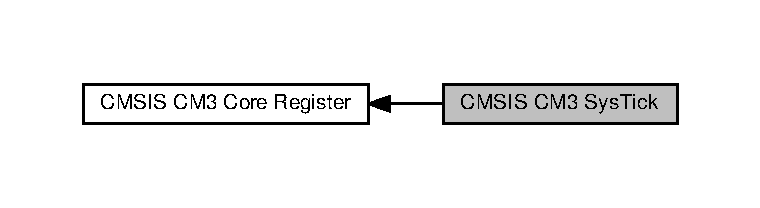
\includegraphics[width=350pt]{d3/db0/group__CMSIS__CM3__SysTick}
\end{center}
\end{figure}
\subsection*{Data Structures}
\begin{DoxyCompactItemize}
\item 
struct \hyperlink{structSysTick__Type}{Sys\+Tick\+\_\+\+Type}
\end{DoxyCompactItemize}
\subsection*{Macros}
\begin{DoxyCompactItemize}
\item 
\#define \hyperlink{group__CMSIS__CM3__SysTick_gadbb65d4a815759649db41df216ed4d60}{Sys\+Tick\+\_\+\+C\+T\+R\+L\+\_\+\+C\+O\+U\+N\+T\+F\+L\+A\+G\+\_\+\+Pos}~16
\item 
\#define \hyperlink{group__CMSIS__CM3__SysTick_ga1bf3033ecccf200f59baefe15dbb367c}{Sys\+Tick\+\_\+\+C\+T\+R\+L\+\_\+\+C\+O\+U\+N\+T\+F\+L\+A\+G\+\_\+\+Msk}~(1ul $<$$<$ Sys\+Tick\+\_\+\+C\+T\+R\+L\+\_\+\+C\+O\+U\+N\+T\+F\+L\+A\+G\+\_\+\+Pos)
\item 
\#define \hyperlink{group__CMSIS__CM3__SysTick_ga24fbc69a5f0b78d67fda2300257baff1}{Sys\+Tick\+\_\+\+C\+T\+R\+L\+\_\+\+C\+L\+K\+S\+O\+U\+R\+C\+E\+\_\+\+Pos}~2
\item 
\#define \hyperlink{group__CMSIS__CM3__SysTick_gaa41d06039797423a46596bd313d57373}{Sys\+Tick\+\_\+\+C\+T\+R\+L\+\_\+\+C\+L\+K\+S\+O\+U\+R\+C\+E\+\_\+\+Msk}~(1ul $<$$<$ Sys\+Tick\+\_\+\+C\+T\+R\+L\+\_\+\+C\+L\+K\+S\+O\+U\+R\+C\+E\+\_\+\+Pos)
\item 
\#define \hyperlink{group__CMSIS__CM3__SysTick_ga88f45bbb89ce8df3cd2b2613c7b48214}{Sys\+Tick\+\_\+\+C\+T\+R\+L\+\_\+\+T\+I\+C\+K\+I\+N\+T\+\_\+\+Pos}~1
\item 
\#define \hyperlink{group__CMSIS__CM3__SysTick_ga95bb984266ca764024836a870238a027}{Sys\+Tick\+\_\+\+C\+T\+R\+L\+\_\+\+T\+I\+C\+K\+I\+N\+T\+\_\+\+Msk}~(1ul $<$$<$ Sys\+Tick\+\_\+\+C\+T\+R\+L\+\_\+\+T\+I\+C\+K\+I\+N\+T\+\_\+\+Pos)
\item 
\#define \hyperlink{group__CMSIS__CM3__SysTick_ga0b48cc1e36d92a92e4bf632890314810}{Sys\+Tick\+\_\+\+C\+T\+R\+L\+\_\+\+E\+N\+A\+B\+L\+E\+\_\+\+Pos}~0
\item 
\#define \hyperlink{group__CMSIS__CM3__SysTick_ga16c9fee0ed0235524bdeb38af328fd1f}{Sys\+Tick\+\_\+\+C\+T\+R\+L\+\_\+\+E\+N\+A\+B\+L\+E\+\_\+\+Msk}~(1ul $<$$<$ Sys\+Tick\+\_\+\+C\+T\+R\+L\+\_\+\+E\+N\+A\+B\+L\+E\+\_\+\+Pos)
\item 
\#define \hyperlink{group__CMSIS__CM3__SysTick_gaf44d10df359dc5bf5752b0894ae3bad2}{Sys\+Tick\+\_\+\+L\+O\+A\+D\+\_\+\+R\+E\+L\+O\+A\+D\+\_\+\+Pos}~0
\item 
\#define \hyperlink{group__CMSIS__CM3__SysTick_ga265912a7962f0e1abd170336e579b1b1}{Sys\+Tick\+\_\+\+L\+O\+A\+D\+\_\+\+R\+E\+L\+O\+A\+D\+\_\+\+Msk}~(0x\+F\+F\+F\+F\+F\+Ful $<$$<$ Sys\+Tick\+\_\+\+L\+O\+A\+D\+\_\+\+R\+E\+L\+O\+A\+D\+\_\+\+Pos)
\item 
\#define \hyperlink{group__CMSIS__CM3__SysTick_ga3208104c3b019b5de35ae8c21d5c34dd}{Sys\+Tick\+\_\+\+V\+A\+L\+\_\+\+C\+U\+R\+R\+E\+N\+T\+\_\+\+Pos}~0
\item 
\#define \hyperlink{group__CMSIS__CM3__SysTick_gafc77b56d568930b49a2474debc75ab45}{Sys\+Tick\+\_\+\+V\+A\+L\+\_\+\+C\+U\+R\+R\+E\+N\+T\+\_\+\+Msk}~(0x\+F\+F\+F\+F\+F\+Ful $<$$<$ Sys\+Tick\+\_\+\+V\+A\+L\+\_\+\+C\+U\+R\+R\+E\+N\+T\+\_\+\+Pos)
\item 
\#define \hyperlink{group__CMSIS__CM3__SysTick_ga534dbe414e7a46a6ce4c1eca1fbff409}{Sys\+Tick\+\_\+\+C\+A\+L\+I\+B\+\_\+\+N\+O\+R\+E\+F\+\_\+\+Pos}~31
\item 
\#define \hyperlink{group__CMSIS__CM3__SysTick_ga3af0d891fdd99bcc8d8912d37830edb6}{Sys\+Tick\+\_\+\+C\+A\+L\+I\+B\+\_\+\+N\+O\+R\+E\+F\+\_\+\+Msk}~(1ul $<$$<$ Sys\+Tick\+\_\+\+C\+A\+L\+I\+B\+\_\+\+N\+O\+R\+E\+F\+\_\+\+Pos)
\item 
\#define \hyperlink{group__CMSIS__CM3__SysTick_gadd0c9cd6641b9f6a0c618e7982954860}{Sys\+Tick\+\_\+\+C\+A\+L\+I\+B\+\_\+\+S\+K\+E\+W\+\_\+\+Pos}~30
\item 
\#define \hyperlink{group__CMSIS__CM3__SysTick_ga8a6a85a87334776f33d77fd147587431}{Sys\+Tick\+\_\+\+C\+A\+L\+I\+B\+\_\+\+S\+K\+E\+W\+\_\+\+Msk}~(1ul $<$$<$ Sys\+Tick\+\_\+\+C\+A\+L\+I\+B\+\_\+\+S\+K\+E\+W\+\_\+\+Pos)
\item 
\#define \hyperlink{group__CMSIS__CM3__SysTick_gacae558f6e75a0bed5d826f606d8e695e}{Sys\+Tick\+\_\+\+C\+A\+L\+I\+B\+\_\+\+T\+E\+N\+M\+S\+\_\+\+Pos}~0
\item 
\#define \hyperlink{group__CMSIS__CM3__SysTick_gaf1e68865c5aece2ad58971225bd3e95e}{Sys\+Tick\+\_\+\+C\+A\+L\+I\+B\+\_\+\+T\+E\+N\+M\+S\+\_\+\+Msk}~(0x\+F\+F\+F\+F\+F\+Ful $<$$<$ Sys\+Tick\+\_\+\+V\+A\+L\+\_\+\+C\+U\+R\+R\+E\+N\+T\+\_\+\+Pos)
\end{DoxyCompactItemize}


\subsection{Detailed Description}
memory mapped structure for Sys\+Tick 

\subsection{Macro Definition Documentation}
\index{C\+M\+S\+I\+S C\+M3 Sys\+Tick@{C\+M\+S\+I\+S C\+M3 Sys\+Tick}!Sys\+Tick\+\_\+\+C\+A\+L\+I\+B\+\_\+\+N\+O\+R\+E\+F\+\_\+\+Msk@{Sys\+Tick\+\_\+\+C\+A\+L\+I\+B\+\_\+\+N\+O\+R\+E\+F\+\_\+\+Msk}}
\index{Sys\+Tick\+\_\+\+C\+A\+L\+I\+B\+\_\+\+N\+O\+R\+E\+F\+\_\+\+Msk@{Sys\+Tick\+\_\+\+C\+A\+L\+I\+B\+\_\+\+N\+O\+R\+E\+F\+\_\+\+Msk}!C\+M\+S\+I\+S C\+M3 Sys\+Tick@{C\+M\+S\+I\+S C\+M3 Sys\+Tick}}
\subsubsection[{\texorpdfstring{Sys\+Tick\+\_\+\+C\+A\+L\+I\+B\+\_\+\+N\+O\+R\+E\+F\+\_\+\+Msk}{SysTick_CALIB_NOREF_Msk}}]{\setlength{\rightskip}{0pt plus 5cm}\#define Sys\+Tick\+\_\+\+C\+A\+L\+I\+B\+\_\+\+N\+O\+R\+E\+F\+\_\+\+Msk~(1ul $<$$<$ Sys\+Tick\+\_\+\+C\+A\+L\+I\+B\+\_\+\+N\+O\+R\+E\+F\+\_\+\+Pos)}\hypertarget{group__CMSIS__CM3__SysTick_ga3af0d891fdd99bcc8d8912d37830edb6}{}\label{group__CMSIS__CM3__SysTick_ga3af0d891fdd99bcc8d8912d37830edb6}
Sys\+Tick C\+A\+L\+IB\+: N\+O\+R\+EF Mask \index{C\+M\+S\+I\+S C\+M3 Sys\+Tick@{C\+M\+S\+I\+S C\+M3 Sys\+Tick}!Sys\+Tick\+\_\+\+C\+A\+L\+I\+B\+\_\+\+N\+O\+R\+E\+F\+\_\+\+Pos@{Sys\+Tick\+\_\+\+C\+A\+L\+I\+B\+\_\+\+N\+O\+R\+E\+F\+\_\+\+Pos}}
\index{Sys\+Tick\+\_\+\+C\+A\+L\+I\+B\+\_\+\+N\+O\+R\+E\+F\+\_\+\+Pos@{Sys\+Tick\+\_\+\+C\+A\+L\+I\+B\+\_\+\+N\+O\+R\+E\+F\+\_\+\+Pos}!C\+M\+S\+I\+S C\+M3 Sys\+Tick@{C\+M\+S\+I\+S C\+M3 Sys\+Tick}}
\subsubsection[{\texorpdfstring{Sys\+Tick\+\_\+\+C\+A\+L\+I\+B\+\_\+\+N\+O\+R\+E\+F\+\_\+\+Pos}{SysTick_CALIB_NOREF_Pos}}]{\setlength{\rightskip}{0pt plus 5cm}\#define Sys\+Tick\+\_\+\+C\+A\+L\+I\+B\+\_\+\+N\+O\+R\+E\+F\+\_\+\+Pos~31}\hypertarget{group__CMSIS__CM3__SysTick_ga534dbe414e7a46a6ce4c1eca1fbff409}{}\label{group__CMSIS__CM3__SysTick_ga534dbe414e7a46a6ce4c1eca1fbff409}
Sys\+Tick C\+A\+L\+IB\+: N\+O\+R\+EF Position \index{C\+M\+S\+I\+S C\+M3 Sys\+Tick@{C\+M\+S\+I\+S C\+M3 Sys\+Tick}!Sys\+Tick\+\_\+\+C\+A\+L\+I\+B\+\_\+\+S\+K\+E\+W\+\_\+\+Msk@{Sys\+Tick\+\_\+\+C\+A\+L\+I\+B\+\_\+\+S\+K\+E\+W\+\_\+\+Msk}}
\index{Sys\+Tick\+\_\+\+C\+A\+L\+I\+B\+\_\+\+S\+K\+E\+W\+\_\+\+Msk@{Sys\+Tick\+\_\+\+C\+A\+L\+I\+B\+\_\+\+S\+K\+E\+W\+\_\+\+Msk}!C\+M\+S\+I\+S C\+M3 Sys\+Tick@{C\+M\+S\+I\+S C\+M3 Sys\+Tick}}
\subsubsection[{\texorpdfstring{Sys\+Tick\+\_\+\+C\+A\+L\+I\+B\+\_\+\+S\+K\+E\+W\+\_\+\+Msk}{SysTick_CALIB_SKEW_Msk}}]{\setlength{\rightskip}{0pt plus 5cm}\#define Sys\+Tick\+\_\+\+C\+A\+L\+I\+B\+\_\+\+S\+K\+E\+W\+\_\+\+Msk~(1ul $<$$<$ Sys\+Tick\+\_\+\+C\+A\+L\+I\+B\+\_\+\+S\+K\+E\+W\+\_\+\+Pos)}\hypertarget{group__CMSIS__CM3__SysTick_ga8a6a85a87334776f33d77fd147587431}{}\label{group__CMSIS__CM3__SysTick_ga8a6a85a87334776f33d77fd147587431}
Sys\+Tick C\+A\+L\+IB\+: S\+K\+EW Mask \index{C\+M\+S\+I\+S C\+M3 Sys\+Tick@{C\+M\+S\+I\+S C\+M3 Sys\+Tick}!Sys\+Tick\+\_\+\+C\+A\+L\+I\+B\+\_\+\+S\+K\+E\+W\+\_\+\+Pos@{Sys\+Tick\+\_\+\+C\+A\+L\+I\+B\+\_\+\+S\+K\+E\+W\+\_\+\+Pos}}
\index{Sys\+Tick\+\_\+\+C\+A\+L\+I\+B\+\_\+\+S\+K\+E\+W\+\_\+\+Pos@{Sys\+Tick\+\_\+\+C\+A\+L\+I\+B\+\_\+\+S\+K\+E\+W\+\_\+\+Pos}!C\+M\+S\+I\+S C\+M3 Sys\+Tick@{C\+M\+S\+I\+S C\+M3 Sys\+Tick}}
\subsubsection[{\texorpdfstring{Sys\+Tick\+\_\+\+C\+A\+L\+I\+B\+\_\+\+S\+K\+E\+W\+\_\+\+Pos}{SysTick_CALIB_SKEW_Pos}}]{\setlength{\rightskip}{0pt plus 5cm}\#define Sys\+Tick\+\_\+\+C\+A\+L\+I\+B\+\_\+\+S\+K\+E\+W\+\_\+\+Pos~30}\hypertarget{group__CMSIS__CM3__SysTick_gadd0c9cd6641b9f6a0c618e7982954860}{}\label{group__CMSIS__CM3__SysTick_gadd0c9cd6641b9f6a0c618e7982954860}
Sys\+Tick C\+A\+L\+IB\+: S\+K\+EW Position \index{C\+M\+S\+I\+S C\+M3 Sys\+Tick@{C\+M\+S\+I\+S C\+M3 Sys\+Tick}!Sys\+Tick\+\_\+\+C\+A\+L\+I\+B\+\_\+\+T\+E\+N\+M\+S\+\_\+\+Msk@{Sys\+Tick\+\_\+\+C\+A\+L\+I\+B\+\_\+\+T\+E\+N\+M\+S\+\_\+\+Msk}}
\index{Sys\+Tick\+\_\+\+C\+A\+L\+I\+B\+\_\+\+T\+E\+N\+M\+S\+\_\+\+Msk@{Sys\+Tick\+\_\+\+C\+A\+L\+I\+B\+\_\+\+T\+E\+N\+M\+S\+\_\+\+Msk}!C\+M\+S\+I\+S C\+M3 Sys\+Tick@{C\+M\+S\+I\+S C\+M3 Sys\+Tick}}
\subsubsection[{\texorpdfstring{Sys\+Tick\+\_\+\+C\+A\+L\+I\+B\+\_\+\+T\+E\+N\+M\+S\+\_\+\+Msk}{SysTick_CALIB_TENMS_Msk}}]{\setlength{\rightskip}{0pt plus 5cm}\#define Sys\+Tick\+\_\+\+C\+A\+L\+I\+B\+\_\+\+T\+E\+N\+M\+S\+\_\+\+Msk~(0x\+F\+F\+F\+F\+F\+Ful $<$$<$ Sys\+Tick\+\_\+\+V\+A\+L\+\_\+\+C\+U\+R\+R\+E\+N\+T\+\_\+\+Pos)}\hypertarget{group__CMSIS__CM3__SysTick_gaf1e68865c5aece2ad58971225bd3e95e}{}\label{group__CMSIS__CM3__SysTick_gaf1e68865c5aece2ad58971225bd3e95e}
Sys\+Tick C\+A\+L\+IB\+: T\+E\+N\+MS Mask \index{C\+M\+S\+I\+S C\+M3 Sys\+Tick@{C\+M\+S\+I\+S C\+M3 Sys\+Tick}!Sys\+Tick\+\_\+\+C\+A\+L\+I\+B\+\_\+\+T\+E\+N\+M\+S\+\_\+\+Pos@{Sys\+Tick\+\_\+\+C\+A\+L\+I\+B\+\_\+\+T\+E\+N\+M\+S\+\_\+\+Pos}}
\index{Sys\+Tick\+\_\+\+C\+A\+L\+I\+B\+\_\+\+T\+E\+N\+M\+S\+\_\+\+Pos@{Sys\+Tick\+\_\+\+C\+A\+L\+I\+B\+\_\+\+T\+E\+N\+M\+S\+\_\+\+Pos}!C\+M\+S\+I\+S C\+M3 Sys\+Tick@{C\+M\+S\+I\+S C\+M3 Sys\+Tick}}
\subsubsection[{\texorpdfstring{Sys\+Tick\+\_\+\+C\+A\+L\+I\+B\+\_\+\+T\+E\+N\+M\+S\+\_\+\+Pos}{SysTick_CALIB_TENMS_Pos}}]{\setlength{\rightskip}{0pt plus 5cm}\#define Sys\+Tick\+\_\+\+C\+A\+L\+I\+B\+\_\+\+T\+E\+N\+M\+S\+\_\+\+Pos~0}\hypertarget{group__CMSIS__CM3__SysTick_gacae558f6e75a0bed5d826f606d8e695e}{}\label{group__CMSIS__CM3__SysTick_gacae558f6e75a0bed5d826f606d8e695e}
Sys\+Tick C\+A\+L\+IB\+: T\+E\+N\+MS Position \index{C\+M\+S\+I\+S C\+M3 Sys\+Tick@{C\+M\+S\+I\+S C\+M3 Sys\+Tick}!Sys\+Tick\+\_\+\+C\+T\+R\+L\+\_\+\+C\+L\+K\+S\+O\+U\+R\+C\+E\+\_\+\+Msk@{Sys\+Tick\+\_\+\+C\+T\+R\+L\+\_\+\+C\+L\+K\+S\+O\+U\+R\+C\+E\+\_\+\+Msk}}
\index{Sys\+Tick\+\_\+\+C\+T\+R\+L\+\_\+\+C\+L\+K\+S\+O\+U\+R\+C\+E\+\_\+\+Msk@{Sys\+Tick\+\_\+\+C\+T\+R\+L\+\_\+\+C\+L\+K\+S\+O\+U\+R\+C\+E\+\_\+\+Msk}!C\+M\+S\+I\+S C\+M3 Sys\+Tick@{C\+M\+S\+I\+S C\+M3 Sys\+Tick}}
\subsubsection[{\texorpdfstring{Sys\+Tick\+\_\+\+C\+T\+R\+L\+\_\+\+C\+L\+K\+S\+O\+U\+R\+C\+E\+\_\+\+Msk}{SysTick_CTRL_CLKSOURCE_Msk}}]{\setlength{\rightskip}{0pt plus 5cm}\#define Sys\+Tick\+\_\+\+C\+T\+R\+L\+\_\+\+C\+L\+K\+S\+O\+U\+R\+C\+E\+\_\+\+Msk~(1ul $<$$<$ Sys\+Tick\+\_\+\+C\+T\+R\+L\+\_\+\+C\+L\+K\+S\+O\+U\+R\+C\+E\+\_\+\+Pos)}\hypertarget{group__CMSIS__CM3__SysTick_gaa41d06039797423a46596bd313d57373}{}\label{group__CMSIS__CM3__SysTick_gaa41d06039797423a46596bd313d57373}
Sys\+Tick C\+T\+RL\+: C\+L\+K\+S\+O\+U\+R\+CE Mask \index{C\+M\+S\+I\+S C\+M3 Sys\+Tick@{C\+M\+S\+I\+S C\+M3 Sys\+Tick}!Sys\+Tick\+\_\+\+C\+T\+R\+L\+\_\+\+C\+L\+K\+S\+O\+U\+R\+C\+E\+\_\+\+Pos@{Sys\+Tick\+\_\+\+C\+T\+R\+L\+\_\+\+C\+L\+K\+S\+O\+U\+R\+C\+E\+\_\+\+Pos}}
\index{Sys\+Tick\+\_\+\+C\+T\+R\+L\+\_\+\+C\+L\+K\+S\+O\+U\+R\+C\+E\+\_\+\+Pos@{Sys\+Tick\+\_\+\+C\+T\+R\+L\+\_\+\+C\+L\+K\+S\+O\+U\+R\+C\+E\+\_\+\+Pos}!C\+M\+S\+I\+S C\+M3 Sys\+Tick@{C\+M\+S\+I\+S C\+M3 Sys\+Tick}}
\subsubsection[{\texorpdfstring{Sys\+Tick\+\_\+\+C\+T\+R\+L\+\_\+\+C\+L\+K\+S\+O\+U\+R\+C\+E\+\_\+\+Pos}{SysTick_CTRL_CLKSOURCE_Pos}}]{\setlength{\rightskip}{0pt plus 5cm}\#define Sys\+Tick\+\_\+\+C\+T\+R\+L\+\_\+\+C\+L\+K\+S\+O\+U\+R\+C\+E\+\_\+\+Pos~2}\hypertarget{group__CMSIS__CM3__SysTick_ga24fbc69a5f0b78d67fda2300257baff1}{}\label{group__CMSIS__CM3__SysTick_ga24fbc69a5f0b78d67fda2300257baff1}
Sys\+Tick C\+T\+RL\+: C\+L\+K\+S\+O\+U\+R\+CE Position \index{C\+M\+S\+I\+S C\+M3 Sys\+Tick@{C\+M\+S\+I\+S C\+M3 Sys\+Tick}!Sys\+Tick\+\_\+\+C\+T\+R\+L\+\_\+\+C\+O\+U\+N\+T\+F\+L\+A\+G\+\_\+\+Msk@{Sys\+Tick\+\_\+\+C\+T\+R\+L\+\_\+\+C\+O\+U\+N\+T\+F\+L\+A\+G\+\_\+\+Msk}}
\index{Sys\+Tick\+\_\+\+C\+T\+R\+L\+\_\+\+C\+O\+U\+N\+T\+F\+L\+A\+G\+\_\+\+Msk@{Sys\+Tick\+\_\+\+C\+T\+R\+L\+\_\+\+C\+O\+U\+N\+T\+F\+L\+A\+G\+\_\+\+Msk}!C\+M\+S\+I\+S C\+M3 Sys\+Tick@{C\+M\+S\+I\+S C\+M3 Sys\+Tick}}
\subsubsection[{\texorpdfstring{Sys\+Tick\+\_\+\+C\+T\+R\+L\+\_\+\+C\+O\+U\+N\+T\+F\+L\+A\+G\+\_\+\+Msk}{SysTick_CTRL_COUNTFLAG_Msk}}]{\setlength{\rightskip}{0pt plus 5cm}\#define Sys\+Tick\+\_\+\+C\+T\+R\+L\+\_\+\+C\+O\+U\+N\+T\+F\+L\+A\+G\+\_\+\+Msk~(1ul $<$$<$ Sys\+Tick\+\_\+\+C\+T\+R\+L\+\_\+\+C\+O\+U\+N\+T\+F\+L\+A\+G\+\_\+\+Pos)}\hypertarget{group__CMSIS__CM3__SysTick_ga1bf3033ecccf200f59baefe15dbb367c}{}\label{group__CMSIS__CM3__SysTick_ga1bf3033ecccf200f59baefe15dbb367c}
Sys\+Tick C\+T\+RL\+: C\+O\+U\+N\+T\+F\+L\+AG Mask \index{C\+M\+S\+I\+S C\+M3 Sys\+Tick@{C\+M\+S\+I\+S C\+M3 Sys\+Tick}!Sys\+Tick\+\_\+\+C\+T\+R\+L\+\_\+\+C\+O\+U\+N\+T\+F\+L\+A\+G\+\_\+\+Pos@{Sys\+Tick\+\_\+\+C\+T\+R\+L\+\_\+\+C\+O\+U\+N\+T\+F\+L\+A\+G\+\_\+\+Pos}}
\index{Sys\+Tick\+\_\+\+C\+T\+R\+L\+\_\+\+C\+O\+U\+N\+T\+F\+L\+A\+G\+\_\+\+Pos@{Sys\+Tick\+\_\+\+C\+T\+R\+L\+\_\+\+C\+O\+U\+N\+T\+F\+L\+A\+G\+\_\+\+Pos}!C\+M\+S\+I\+S C\+M3 Sys\+Tick@{C\+M\+S\+I\+S C\+M3 Sys\+Tick}}
\subsubsection[{\texorpdfstring{Sys\+Tick\+\_\+\+C\+T\+R\+L\+\_\+\+C\+O\+U\+N\+T\+F\+L\+A\+G\+\_\+\+Pos}{SysTick_CTRL_COUNTFLAG_Pos}}]{\setlength{\rightskip}{0pt plus 5cm}\#define Sys\+Tick\+\_\+\+C\+T\+R\+L\+\_\+\+C\+O\+U\+N\+T\+F\+L\+A\+G\+\_\+\+Pos~16}\hypertarget{group__CMSIS__CM3__SysTick_gadbb65d4a815759649db41df216ed4d60}{}\label{group__CMSIS__CM3__SysTick_gadbb65d4a815759649db41df216ed4d60}
Sys\+Tick C\+T\+RL\+: C\+O\+U\+N\+T\+F\+L\+AG Position \index{C\+M\+S\+I\+S C\+M3 Sys\+Tick@{C\+M\+S\+I\+S C\+M3 Sys\+Tick}!Sys\+Tick\+\_\+\+C\+T\+R\+L\+\_\+\+E\+N\+A\+B\+L\+E\+\_\+\+Msk@{Sys\+Tick\+\_\+\+C\+T\+R\+L\+\_\+\+E\+N\+A\+B\+L\+E\+\_\+\+Msk}}
\index{Sys\+Tick\+\_\+\+C\+T\+R\+L\+\_\+\+E\+N\+A\+B\+L\+E\+\_\+\+Msk@{Sys\+Tick\+\_\+\+C\+T\+R\+L\+\_\+\+E\+N\+A\+B\+L\+E\+\_\+\+Msk}!C\+M\+S\+I\+S C\+M3 Sys\+Tick@{C\+M\+S\+I\+S C\+M3 Sys\+Tick}}
\subsubsection[{\texorpdfstring{Sys\+Tick\+\_\+\+C\+T\+R\+L\+\_\+\+E\+N\+A\+B\+L\+E\+\_\+\+Msk}{SysTick_CTRL_ENABLE_Msk}}]{\setlength{\rightskip}{0pt plus 5cm}\#define Sys\+Tick\+\_\+\+C\+T\+R\+L\+\_\+\+E\+N\+A\+B\+L\+E\+\_\+\+Msk~(1ul $<$$<$ Sys\+Tick\+\_\+\+C\+T\+R\+L\+\_\+\+E\+N\+A\+B\+L\+E\+\_\+\+Pos)}\hypertarget{group__CMSIS__CM3__SysTick_ga16c9fee0ed0235524bdeb38af328fd1f}{}\label{group__CMSIS__CM3__SysTick_ga16c9fee0ed0235524bdeb38af328fd1f}
Sys\+Tick C\+T\+RL\+: E\+N\+A\+B\+LE Mask \index{C\+M\+S\+I\+S C\+M3 Sys\+Tick@{C\+M\+S\+I\+S C\+M3 Sys\+Tick}!Sys\+Tick\+\_\+\+C\+T\+R\+L\+\_\+\+E\+N\+A\+B\+L\+E\+\_\+\+Pos@{Sys\+Tick\+\_\+\+C\+T\+R\+L\+\_\+\+E\+N\+A\+B\+L\+E\+\_\+\+Pos}}
\index{Sys\+Tick\+\_\+\+C\+T\+R\+L\+\_\+\+E\+N\+A\+B\+L\+E\+\_\+\+Pos@{Sys\+Tick\+\_\+\+C\+T\+R\+L\+\_\+\+E\+N\+A\+B\+L\+E\+\_\+\+Pos}!C\+M\+S\+I\+S C\+M3 Sys\+Tick@{C\+M\+S\+I\+S C\+M3 Sys\+Tick}}
\subsubsection[{\texorpdfstring{Sys\+Tick\+\_\+\+C\+T\+R\+L\+\_\+\+E\+N\+A\+B\+L\+E\+\_\+\+Pos}{SysTick_CTRL_ENABLE_Pos}}]{\setlength{\rightskip}{0pt plus 5cm}\#define Sys\+Tick\+\_\+\+C\+T\+R\+L\+\_\+\+E\+N\+A\+B\+L\+E\+\_\+\+Pos~0}\hypertarget{group__CMSIS__CM3__SysTick_ga0b48cc1e36d92a92e4bf632890314810}{}\label{group__CMSIS__CM3__SysTick_ga0b48cc1e36d92a92e4bf632890314810}
Sys\+Tick C\+T\+RL\+: E\+N\+A\+B\+LE Position \index{C\+M\+S\+I\+S C\+M3 Sys\+Tick@{C\+M\+S\+I\+S C\+M3 Sys\+Tick}!Sys\+Tick\+\_\+\+C\+T\+R\+L\+\_\+\+T\+I\+C\+K\+I\+N\+T\+\_\+\+Msk@{Sys\+Tick\+\_\+\+C\+T\+R\+L\+\_\+\+T\+I\+C\+K\+I\+N\+T\+\_\+\+Msk}}
\index{Sys\+Tick\+\_\+\+C\+T\+R\+L\+\_\+\+T\+I\+C\+K\+I\+N\+T\+\_\+\+Msk@{Sys\+Tick\+\_\+\+C\+T\+R\+L\+\_\+\+T\+I\+C\+K\+I\+N\+T\+\_\+\+Msk}!C\+M\+S\+I\+S C\+M3 Sys\+Tick@{C\+M\+S\+I\+S C\+M3 Sys\+Tick}}
\subsubsection[{\texorpdfstring{Sys\+Tick\+\_\+\+C\+T\+R\+L\+\_\+\+T\+I\+C\+K\+I\+N\+T\+\_\+\+Msk}{SysTick_CTRL_TICKINT_Msk}}]{\setlength{\rightskip}{0pt plus 5cm}\#define Sys\+Tick\+\_\+\+C\+T\+R\+L\+\_\+\+T\+I\+C\+K\+I\+N\+T\+\_\+\+Msk~(1ul $<$$<$ Sys\+Tick\+\_\+\+C\+T\+R\+L\+\_\+\+T\+I\+C\+K\+I\+N\+T\+\_\+\+Pos)}\hypertarget{group__CMSIS__CM3__SysTick_ga95bb984266ca764024836a870238a027}{}\label{group__CMSIS__CM3__SysTick_ga95bb984266ca764024836a870238a027}
Sys\+Tick C\+T\+RL\+: T\+I\+C\+K\+I\+NT Mask \index{C\+M\+S\+I\+S C\+M3 Sys\+Tick@{C\+M\+S\+I\+S C\+M3 Sys\+Tick}!Sys\+Tick\+\_\+\+C\+T\+R\+L\+\_\+\+T\+I\+C\+K\+I\+N\+T\+\_\+\+Pos@{Sys\+Tick\+\_\+\+C\+T\+R\+L\+\_\+\+T\+I\+C\+K\+I\+N\+T\+\_\+\+Pos}}
\index{Sys\+Tick\+\_\+\+C\+T\+R\+L\+\_\+\+T\+I\+C\+K\+I\+N\+T\+\_\+\+Pos@{Sys\+Tick\+\_\+\+C\+T\+R\+L\+\_\+\+T\+I\+C\+K\+I\+N\+T\+\_\+\+Pos}!C\+M\+S\+I\+S C\+M3 Sys\+Tick@{C\+M\+S\+I\+S C\+M3 Sys\+Tick}}
\subsubsection[{\texorpdfstring{Sys\+Tick\+\_\+\+C\+T\+R\+L\+\_\+\+T\+I\+C\+K\+I\+N\+T\+\_\+\+Pos}{SysTick_CTRL_TICKINT_Pos}}]{\setlength{\rightskip}{0pt plus 5cm}\#define Sys\+Tick\+\_\+\+C\+T\+R\+L\+\_\+\+T\+I\+C\+K\+I\+N\+T\+\_\+\+Pos~1}\hypertarget{group__CMSIS__CM3__SysTick_ga88f45bbb89ce8df3cd2b2613c7b48214}{}\label{group__CMSIS__CM3__SysTick_ga88f45bbb89ce8df3cd2b2613c7b48214}
Sys\+Tick C\+T\+RL\+: T\+I\+C\+K\+I\+NT Position \index{C\+M\+S\+I\+S C\+M3 Sys\+Tick@{C\+M\+S\+I\+S C\+M3 Sys\+Tick}!Sys\+Tick\+\_\+\+L\+O\+A\+D\+\_\+\+R\+E\+L\+O\+A\+D\+\_\+\+Msk@{Sys\+Tick\+\_\+\+L\+O\+A\+D\+\_\+\+R\+E\+L\+O\+A\+D\+\_\+\+Msk}}
\index{Sys\+Tick\+\_\+\+L\+O\+A\+D\+\_\+\+R\+E\+L\+O\+A\+D\+\_\+\+Msk@{Sys\+Tick\+\_\+\+L\+O\+A\+D\+\_\+\+R\+E\+L\+O\+A\+D\+\_\+\+Msk}!C\+M\+S\+I\+S C\+M3 Sys\+Tick@{C\+M\+S\+I\+S C\+M3 Sys\+Tick}}
\subsubsection[{\texorpdfstring{Sys\+Tick\+\_\+\+L\+O\+A\+D\+\_\+\+R\+E\+L\+O\+A\+D\+\_\+\+Msk}{SysTick_LOAD_RELOAD_Msk}}]{\setlength{\rightskip}{0pt plus 5cm}\#define Sys\+Tick\+\_\+\+L\+O\+A\+D\+\_\+\+R\+E\+L\+O\+A\+D\+\_\+\+Msk~(0x\+F\+F\+F\+F\+F\+Ful $<$$<$ Sys\+Tick\+\_\+\+L\+O\+A\+D\+\_\+\+R\+E\+L\+O\+A\+D\+\_\+\+Pos)}\hypertarget{group__CMSIS__CM3__SysTick_ga265912a7962f0e1abd170336e579b1b1}{}\label{group__CMSIS__CM3__SysTick_ga265912a7962f0e1abd170336e579b1b1}
Sys\+Tick L\+O\+AD\+: R\+E\+L\+O\+AD Mask \index{C\+M\+S\+I\+S C\+M3 Sys\+Tick@{C\+M\+S\+I\+S C\+M3 Sys\+Tick}!Sys\+Tick\+\_\+\+L\+O\+A\+D\+\_\+\+R\+E\+L\+O\+A\+D\+\_\+\+Pos@{Sys\+Tick\+\_\+\+L\+O\+A\+D\+\_\+\+R\+E\+L\+O\+A\+D\+\_\+\+Pos}}
\index{Sys\+Tick\+\_\+\+L\+O\+A\+D\+\_\+\+R\+E\+L\+O\+A\+D\+\_\+\+Pos@{Sys\+Tick\+\_\+\+L\+O\+A\+D\+\_\+\+R\+E\+L\+O\+A\+D\+\_\+\+Pos}!C\+M\+S\+I\+S C\+M3 Sys\+Tick@{C\+M\+S\+I\+S C\+M3 Sys\+Tick}}
\subsubsection[{\texorpdfstring{Sys\+Tick\+\_\+\+L\+O\+A\+D\+\_\+\+R\+E\+L\+O\+A\+D\+\_\+\+Pos}{SysTick_LOAD_RELOAD_Pos}}]{\setlength{\rightskip}{0pt plus 5cm}\#define Sys\+Tick\+\_\+\+L\+O\+A\+D\+\_\+\+R\+E\+L\+O\+A\+D\+\_\+\+Pos~0}\hypertarget{group__CMSIS__CM3__SysTick_gaf44d10df359dc5bf5752b0894ae3bad2}{}\label{group__CMSIS__CM3__SysTick_gaf44d10df359dc5bf5752b0894ae3bad2}
Sys\+Tick L\+O\+AD\+: R\+E\+L\+O\+AD Position \index{C\+M\+S\+I\+S C\+M3 Sys\+Tick@{C\+M\+S\+I\+S C\+M3 Sys\+Tick}!Sys\+Tick\+\_\+\+V\+A\+L\+\_\+\+C\+U\+R\+R\+E\+N\+T\+\_\+\+Msk@{Sys\+Tick\+\_\+\+V\+A\+L\+\_\+\+C\+U\+R\+R\+E\+N\+T\+\_\+\+Msk}}
\index{Sys\+Tick\+\_\+\+V\+A\+L\+\_\+\+C\+U\+R\+R\+E\+N\+T\+\_\+\+Msk@{Sys\+Tick\+\_\+\+V\+A\+L\+\_\+\+C\+U\+R\+R\+E\+N\+T\+\_\+\+Msk}!C\+M\+S\+I\+S C\+M3 Sys\+Tick@{C\+M\+S\+I\+S C\+M3 Sys\+Tick}}
\subsubsection[{\texorpdfstring{Sys\+Tick\+\_\+\+V\+A\+L\+\_\+\+C\+U\+R\+R\+E\+N\+T\+\_\+\+Msk}{SysTick_VAL_CURRENT_Msk}}]{\setlength{\rightskip}{0pt plus 5cm}\#define Sys\+Tick\+\_\+\+V\+A\+L\+\_\+\+C\+U\+R\+R\+E\+N\+T\+\_\+\+Msk~(0x\+F\+F\+F\+F\+F\+Ful $<$$<$ Sys\+Tick\+\_\+\+V\+A\+L\+\_\+\+C\+U\+R\+R\+E\+N\+T\+\_\+\+Pos)}\hypertarget{group__CMSIS__CM3__SysTick_gafc77b56d568930b49a2474debc75ab45}{}\label{group__CMSIS__CM3__SysTick_gafc77b56d568930b49a2474debc75ab45}
Sys\+Tick V\+AL\+: C\+U\+R\+R\+E\+NT Mask \index{C\+M\+S\+I\+S C\+M3 Sys\+Tick@{C\+M\+S\+I\+S C\+M3 Sys\+Tick}!Sys\+Tick\+\_\+\+V\+A\+L\+\_\+\+C\+U\+R\+R\+E\+N\+T\+\_\+\+Pos@{Sys\+Tick\+\_\+\+V\+A\+L\+\_\+\+C\+U\+R\+R\+E\+N\+T\+\_\+\+Pos}}
\index{Sys\+Tick\+\_\+\+V\+A\+L\+\_\+\+C\+U\+R\+R\+E\+N\+T\+\_\+\+Pos@{Sys\+Tick\+\_\+\+V\+A\+L\+\_\+\+C\+U\+R\+R\+E\+N\+T\+\_\+\+Pos}!C\+M\+S\+I\+S C\+M3 Sys\+Tick@{C\+M\+S\+I\+S C\+M3 Sys\+Tick}}
\subsubsection[{\texorpdfstring{Sys\+Tick\+\_\+\+V\+A\+L\+\_\+\+C\+U\+R\+R\+E\+N\+T\+\_\+\+Pos}{SysTick_VAL_CURRENT_Pos}}]{\setlength{\rightskip}{0pt plus 5cm}\#define Sys\+Tick\+\_\+\+V\+A\+L\+\_\+\+C\+U\+R\+R\+E\+N\+T\+\_\+\+Pos~0}\hypertarget{group__CMSIS__CM3__SysTick_ga3208104c3b019b5de35ae8c21d5c34dd}{}\label{group__CMSIS__CM3__SysTick_ga3208104c3b019b5de35ae8c21d5c34dd}
Sys\+Tick V\+AL\+: C\+U\+R\+R\+E\+NT Position 
\hypertarget{group__CMSIS__CM3__ITM}{}\section{C\+M\+S\+IS C\+M3 I\+TM}
\label{group__CMSIS__CM3__ITM}\index{C\+M\+S\+I\+S C\+M3 I\+TM@{C\+M\+S\+I\+S C\+M3 I\+TM}}
Collaboration diagram for C\+M\+S\+IS C\+M3 I\+TM\+:\nopagebreak
\begin{figure}[H]
\begin{center}
\leavevmode
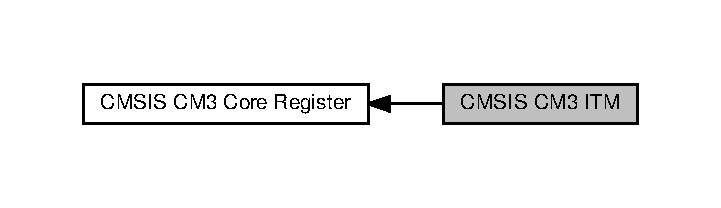
\includegraphics[width=346pt]{d7/db9/group__CMSIS__CM3__ITM}
\end{center}
\end{figure}
\subsection*{Data Structures}
\begin{DoxyCompactItemize}
\item 
struct \hyperlink{structITM__Type}{I\+T\+M\+\_\+\+Type}
\end{DoxyCompactItemize}
\subsection*{Macros}
\begin{DoxyCompactItemize}
\item 
\#define \hyperlink{group__CMSIS__CM3__ITM_ga7abe5e590d1611599df87a1884a352e8}{I\+T\+M\+\_\+\+T\+P\+R\+\_\+\+P\+R\+I\+V\+M\+A\+S\+K\+\_\+\+Pos}~0
\item 
\#define \hyperlink{group__CMSIS__CM3__ITM_ga168e089d882df325a387aab3a802a46b}{I\+T\+M\+\_\+\+T\+P\+R\+\_\+\+P\+R\+I\+V\+M\+A\+S\+K\+\_\+\+Msk}~(0x\+Ful $<$$<$ I\+T\+M\+\_\+\+T\+P\+R\+\_\+\+P\+R\+I\+V\+M\+A\+S\+K\+\_\+\+Pos)
\item 
\#define \hyperlink{group__CMSIS__CM3__ITM_ga9174ad4a36052c377cef4e6aba2ed484}{I\+T\+M\+\_\+\+T\+C\+R\+\_\+\+B\+U\+S\+Y\+\_\+\+Pos}~23
\item 
\#define \hyperlink{group__CMSIS__CM3__ITM_ga43ad7cf33de12f2ef3a412d4f354c60f}{I\+T\+M\+\_\+\+T\+C\+R\+\_\+\+B\+U\+S\+Y\+\_\+\+Msk}~(1ul $<$$<$ I\+T\+M\+\_\+\+T\+C\+R\+\_\+\+B\+U\+S\+Y\+\_\+\+Pos)
\item 
\#define \hyperlink{group__CMSIS__CM3__ITM_gad5a179af7ad1f2b8958e50907186529b}{I\+T\+M\+\_\+\+T\+C\+R\+\_\+\+A\+T\+B\+I\+D\+\_\+\+Pos}~16
\item 
\#define \hyperlink{group__CMSIS__CM3__ITM_ga491d8bddbe6c0523ff10ef6d2846f0f2}{I\+T\+M\+\_\+\+T\+C\+R\+\_\+\+A\+T\+B\+I\+D\+\_\+\+Msk}~(0x7\+Ful $<$$<$ I\+T\+M\+\_\+\+T\+C\+R\+\_\+\+A\+T\+B\+I\+D\+\_\+\+Pos)
\item 
\#define \hyperlink{group__CMSIS__CM3__ITM_gad7bc9ee1732032c6e0de035f0978e473}{I\+T\+M\+\_\+\+T\+C\+R\+\_\+\+T\+S\+Prescale\+\_\+\+Pos}~8
\item 
\#define \hyperlink{group__CMSIS__CM3__ITM_ga7a723f71bfb0204c264d8dbe8cc7ae52}{I\+T\+M\+\_\+\+T\+C\+R\+\_\+\+T\+S\+Prescale\+\_\+\+Msk}~(3ul $<$$<$ I\+T\+M\+\_\+\+T\+C\+R\+\_\+\+T\+S\+Prescale\+\_\+\+Pos)
\item 
\#define \hyperlink{group__CMSIS__CM3__ITM_ga7a380f0c8078f6560051406583ecd6a5}{I\+T\+M\+\_\+\+T\+C\+R\+\_\+\+S\+W\+O\+E\+N\+A\+\_\+\+Pos}~4
\item 
\#define \hyperlink{group__CMSIS__CM3__ITM_ga97476cb65bab16a328b35f81fd02010a}{I\+T\+M\+\_\+\+T\+C\+R\+\_\+\+S\+W\+O\+E\+N\+A\+\_\+\+Msk}~(1ul $<$$<$ I\+T\+M\+\_\+\+T\+C\+R\+\_\+\+S\+W\+O\+E\+N\+A\+\_\+\+Pos)
\item 
\#define \hyperlink{group__CMSIS__CM3__ITM_ga30e83ebb33aa766070fe3d1f27ae820e}{I\+T\+M\+\_\+\+T\+C\+R\+\_\+\+D\+W\+T\+E\+N\+A\+\_\+\+Pos}~3
\item 
\#define \hyperlink{group__CMSIS__CM3__ITM_ga98ea1c596d43d3633a202f9ee746cf70}{I\+T\+M\+\_\+\+T\+C\+R\+\_\+\+D\+W\+T\+E\+N\+A\+\_\+\+Msk}~(1ul $<$$<$ I\+T\+M\+\_\+\+T\+C\+R\+\_\+\+D\+W\+T\+E\+N\+A\+\_\+\+Pos)
\item 
\#define \hyperlink{group__CMSIS__CM3__ITM_gaa93a1147a39fc63980d299231252a30e}{I\+T\+M\+\_\+\+T\+C\+R\+\_\+\+S\+Y\+N\+C\+E\+N\+A\+\_\+\+Pos}~2
\item 
\#define \hyperlink{group__CMSIS__CM3__ITM_gac89b74a78701c25b442105d7fe2bbefb}{I\+T\+M\+\_\+\+T\+C\+R\+\_\+\+S\+Y\+N\+C\+E\+N\+A\+\_\+\+Msk}~(1ul $<$$<$ I\+T\+M\+\_\+\+T\+C\+R\+\_\+\+S\+Y\+N\+C\+E\+N\+A\+\_\+\+Pos)
\item 
\#define \hyperlink{group__CMSIS__CM3__ITM_ga5aa381845f810114ab519b90753922a1}{I\+T\+M\+\_\+\+T\+C\+R\+\_\+\+T\+S\+E\+N\+A\+\_\+\+Pos}~1
\item 
\#define \hyperlink{group__CMSIS__CM3__ITM_ga436b2e8fa24328f48f2da31c00fc9e65}{I\+T\+M\+\_\+\+T\+C\+R\+\_\+\+T\+S\+E\+N\+A\+\_\+\+Msk}~(1ul $<$$<$ I\+T\+M\+\_\+\+T\+C\+R\+\_\+\+T\+S\+E\+N\+A\+\_\+\+Pos)
\item 
\#define \hyperlink{group__CMSIS__CM3__ITM_ga3286b86004bce7ffe17ee269f87f8d9d}{I\+T\+M\+\_\+\+T\+C\+R\+\_\+\+I\+T\+M\+E\+N\+A\+\_\+\+Pos}~0
\item 
\#define \hyperlink{group__CMSIS__CM3__ITM_ga7dd53e3bff24ac09d94e61cb595cb2d9}{I\+T\+M\+\_\+\+T\+C\+R\+\_\+\+I\+T\+M\+E\+N\+A\+\_\+\+Msk}~(1ul $<$$<$ I\+T\+M\+\_\+\+T\+C\+R\+\_\+\+I\+T\+M\+E\+N\+A\+\_\+\+Pos)
\item 
\#define \hyperlink{group__CMSIS__CM3__ITM_ga04d3f842ad48f6a9127b4cecc963e1d7}{I\+T\+M\+\_\+\+I\+W\+R\+\_\+\+A\+T\+V\+A\+L\+I\+D\+M\+\_\+\+Pos}~0
\item 
\#define \hyperlink{group__CMSIS__CM3__ITM_ga67b969f8f04ed15886727788f0e2ffd7}{I\+T\+M\+\_\+\+I\+W\+R\+\_\+\+A\+T\+V\+A\+L\+I\+D\+M\+\_\+\+Msk}~(1ul $<$$<$ I\+T\+M\+\_\+\+I\+W\+R\+\_\+\+A\+T\+V\+A\+L\+I\+D\+M\+\_\+\+Pos)
\item 
\#define \hyperlink{group__CMSIS__CM3__ITM_ga259edfd1d2e877a62e06d7a240df97f4}{I\+T\+M\+\_\+\+I\+R\+R\+\_\+\+A\+T\+R\+E\+A\+D\+Y\+M\+\_\+\+Pos}~0
\item 
\#define \hyperlink{group__CMSIS__CM3__ITM_ga3dbc3e15f5bde2669cd8121a1fe419b9}{I\+T\+M\+\_\+\+I\+R\+R\+\_\+\+A\+T\+R\+E\+A\+D\+Y\+M\+\_\+\+Msk}~(1ul $<$$<$ I\+T\+M\+\_\+\+I\+R\+R\+\_\+\+A\+T\+R\+E\+A\+D\+Y\+M\+\_\+\+Pos)
\item 
\#define \hyperlink{group__CMSIS__CM3__ITM_ga08de02bf32caf48aaa29f7c68ff5d755}{I\+T\+M\+\_\+\+I\+M\+C\+R\+\_\+\+I\+N\+T\+E\+G\+R\+A\+T\+I\+O\+N\+\_\+\+Pos}~0
\item 
\#define \hyperlink{group__CMSIS__CM3__ITM_ga8838bd3dd04c1a6be97cd946364a3fd2}{I\+T\+M\+\_\+\+I\+M\+C\+R\+\_\+\+I\+N\+T\+E\+G\+R\+A\+T\+I\+O\+N\+\_\+\+Msk}~(1ul $<$$<$ I\+T\+M\+\_\+\+I\+M\+C\+R\+\_\+\+I\+N\+T\+E\+G\+R\+A\+T\+I\+O\+N\+\_\+\+Pos)
\item 
\#define \hyperlink{group__CMSIS__CM3__ITM_gabfae3e570edc8759597311ed6dfb478e}{I\+T\+M\+\_\+\+L\+S\+R\+\_\+\+Byte\+Acc\+\_\+\+Pos}~2
\item 
\#define \hyperlink{group__CMSIS__CM3__ITM_ga91f492b2891bb8b7eac5b58de7b220f4}{I\+T\+M\+\_\+\+L\+S\+R\+\_\+\+Byte\+Acc\+\_\+\+Msk}~(1ul $<$$<$ I\+T\+M\+\_\+\+L\+S\+R\+\_\+\+Byte\+Acc\+\_\+\+Pos)
\item 
\#define \hyperlink{group__CMSIS__CM3__ITM_ga144a49e12b83ad9809fdd2769094fdc0}{I\+T\+M\+\_\+\+L\+S\+R\+\_\+\+Access\+\_\+\+Pos}~1
\item 
\#define \hyperlink{group__CMSIS__CM3__ITM_gac8ae69f11c0311da226c0c8ec40b3d37}{I\+T\+M\+\_\+\+L\+S\+R\+\_\+\+Access\+\_\+\+Msk}~(1ul $<$$<$ I\+T\+M\+\_\+\+L\+S\+R\+\_\+\+Access\+\_\+\+Pos)
\item 
\#define \hyperlink{group__CMSIS__CM3__ITM_gaf5740689cf14564d3f3fd91299b6c88d}{I\+T\+M\+\_\+\+L\+S\+R\+\_\+\+Present\+\_\+\+Pos}~0
\item 
\#define \hyperlink{group__CMSIS__CM3__ITM_gaa5bc2a7f5f1d69ff819531f5508bb017}{I\+T\+M\+\_\+\+L\+S\+R\+\_\+\+Present\+\_\+\+Msk}~(1ul $<$$<$ I\+T\+M\+\_\+\+L\+S\+R\+\_\+\+Present\+\_\+\+Pos)
\end{DoxyCompactItemize}


\subsection{Detailed Description}
memory mapped structure for Instrumentation Trace Macrocell (I\+TM) 

\subsection{Macro Definition Documentation}
\index{C\+M\+S\+I\+S C\+M3 I\+TM@{C\+M\+S\+I\+S C\+M3 I\+TM}!I\+T\+M\+\_\+\+I\+M\+C\+R\+\_\+\+I\+N\+T\+E\+G\+R\+A\+T\+I\+O\+N\+\_\+\+Msk@{I\+T\+M\+\_\+\+I\+M\+C\+R\+\_\+\+I\+N\+T\+E\+G\+R\+A\+T\+I\+O\+N\+\_\+\+Msk}}
\index{I\+T\+M\+\_\+\+I\+M\+C\+R\+\_\+\+I\+N\+T\+E\+G\+R\+A\+T\+I\+O\+N\+\_\+\+Msk@{I\+T\+M\+\_\+\+I\+M\+C\+R\+\_\+\+I\+N\+T\+E\+G\+R\+A\+T\+I\+O\+N\+\_\+\+Msk}!C\+M\+S\+I\+S C\+M3 I\+TM@{C\+M\+S\+I\+S C\+M3 I\+TM}}
\subsubsection[{\texorpdfstring{I\+T\+M\+\_\+\+I\+M\+C\+R\+\_\+\+I\+N\+T\+E\+G\+R\+A\+T\+I\+O\+N\+\_\+\+Msk}{ITM_IMCR_INTEGRATION_Msk}}]{\setlength{\rightskip}{0pt plus 5cm}\#define I\+T\+M\+\_\+\+I\+M\+C\+R\+\_\+\+I\+N\+T\+E\+G\+R\+A\+T\+I\+O\+N\+\_\+\+Msk~(1ul $<$$<$ I\+T\+M\+\_\+\+I\+M\+C\+R\+\_\+\+I\+N\+T\+E\+G\+R\+A\+T\+I\+O\+N\+\_\+\+Pos)}\hypertarget{group__CMSIS__CM3__ITM_ga8838bd3dd04c1a6be97cd946364a3fd2}{}\label{group__CMSIS__CM3__ITM_ga8838bd3dd04c1a6be97cd946364a3fd2}
I\+TM I\+M\+CR\+: I\+N\+T\+E\+G\+R\+A\+T\+I\+ON Mask \index{C\+M\+S\+I\+S C\+M3 I\+TM@{C\+M\+S\+I\+S C\+M3 I\+TM}!I\+T\+M\+\_\+\+I\+M\+C\+R\+\_\+\+I\+N\+T\+E\+G\+R\+A\+T\+I\+O\+N\+\_\+\+Pos@{I\+T\+M\+\_\+\+I\+M\+C\+R\+\_\+\+I\+N\+T\+E\+G\+R\+A\+T\+I\+O\+N\+\_\+\+Pos}}
\index{I\+T\+M\+\_\+\+I\+M\+C\+R\+\_\+\+I\+N\+T\+E\+G\+R\+A\+T\+I\+O\+N\+\_\+\+Pos@{I\+T\+M\+\_\+\+I\+M\+C\+R\+\_\+\+I\+N\+T\+E\+G\+R\+A\+T\+I\+O\+N\+\_\+\+Pos}!C\+M\+S\+I\+S C\+M3 I\+TM@{C\+M\+S\+I\+S C\+M3 I\+TM}}
\subsubsection[{\texorpdfstring{I\+T\+M\+\_\+\+I\+M\+C\+R\+\_\+\+I\+N\+T\+E\+G\+R\+A\+T\+I\+O\+N\+\_\+\+Pos}{ITM_IMCR_INTEGRATION_Pos}}]{\setlength{\rightskip}{0pt plus 5cm}\#define I\+T\+M\+\_\+\+I\+M\+C\+R\+\_\+\+I\+N\+T\+E\+G\+R\+A\+T\+I\+O\+N\+\_\+\+Pos~0}\hypertarget{group__CMSIS__CM3__ITM_ga08de02bf32caf48aaa29f7c68ff5d755}{}\label{group__CMSIS__CM3__ITM_ga08de02bf32caf48aaa29f7c68ff5d755}
I\+TM I\+M\+CR\+: I\+N\+T\+E\+G\+R\+A\+T\+I\+ON Position \index{C\+M\+S\+I\+S C\+M3 I\+TM@{C\+M\+S\+I\+S C\+M3 I\+TM}!I\+T\+M\+\_\+\+I\+R\+R\+\_\+\+A\+T\+R\+E\+A\+D\+Y\+M\+\_\+\+Msk@{I\+T\+M\+\_\+\+I\+R\+R\+\_\+\+A\+T\+R\+E\+A\+D\+Y\+M\+\_\+\+Msk}}
\index{I\+T\+M\+\_\+\+I\+R\+R\+\_\+\+A\+T\+R\+E\+A\+D\+Y\+M\+\_\+\+Msk@{I\+T\+M\+\_\+\+I\+R\+R\+\_\+\+A\+T\+R\+E\+A\+D\+Y\+M\+\_\+\+Msk}!C\+M\+S\+I\+S C\+M3 I\+TM@{C\+M\+S\+I\+S C\+M3 I\+TM}}
\subsubsection[{\texorpdfstring{I\+T\+M\+\_\+\+I\+R\+R\+\_\+\+A\+T\+R\+E\+A\+D\+Y\+M\+\_\+\+Msk}{ITM_IRR_ATREADYM_Msk}}]{\setlength{\rightskip}{0pt plus 5cm}\#define I\+T\+M\+\_\+\+I\+R\+R\+\_\+\+A\+T\+R\+E\+A\+D\+Y\+M\+\_\+\+Msk~(1ul $<$$<$ I\+T\+M\+\_\+\+I\+R\+R\+\_\+\+A\+T\+R\+E\+A\+D\+Y\+M\+\_\+\+Pos)}\hypertarget{group__CMSIS__CM3__ITM_ga3dbc3e15f5bde2669cd8121a1fe419b9}{}\label{group__CMSIS__CM3__ITM_ga3dbc3e15f5bde2669cd8121a1fe419b9}
I\+TM I\+RR\+: A\+T\+R\+E\+A\+D\+YM Mask \index{C\+M\+S\+I\+S C\+M3 I\+TM@{C\+M\+S\+I\+S C\+M3 I\+TM}!I\+T\+M\+\_\+\+I\+R\+R\+\_\+\+A\+T\+R\+E\+A\+D\+Y\+M\+\_\+\+Pos@{I\+T\+M\+\_\+\+I\+R\+R\+\_\+\+A\+T\+R\+E\+A\+D\+Y\+M\+\_\+\+Pos}}
\index{I\+T\+M\+\_\+\+I\+R\+R\+\_\+\+A\+T\+R\+E\+A\+D\+Y\+M\+\_\+\+Pos@{I\+T\+M\+\_\+\+I\+R\+R\+\_\+\+A\+T\+R\+E\+A\+D\+Y\+M\+\_\+\+Pos}!C\+M\+S\+I\+S C\+M3 I\+TM@{C\+M\+S\+I\+S C\+M3 I\+TM}}
\subsubsection[{\texorpdfstring{I\+T\+M\+\_\+\+I\+R\+R\+\_\+\+A\+T\+R\+E\+A\+D\+Y\+M\+\_\+\+Pos}{ITM_IRR_ATREADYM_Pos}}]{\setlength{\rightskip}{0pt plus 5cm}\#define I\+T\+M\+\_\+\+I\+R\+R\+\_\+\+A\+T\+R\+E\+A\+D\+Y\+M\+\_\+\+Pos~0}\hypertarget{group__CMSIS__CM3__ITM_ga259edfd1d2e877a62e06d7a240df97f4}{}\label{group__CMSIS__CM3__ITM_ga259edfd1d2e877a62e06d7a240df97f4}
I\+TM I\+RR\+: A\+T\+R\+E\+A\+D\+YM Position \index{C\+M\+S\+I\+S C\+M3 I\+TM@{C\+M\+S\+I\+S C\+M3 I\+TM}!I\+T\+M\+\_\+\+I\+W\+R\+\_\+\+A\+T\+V\+A\+L\+I\+D\+M\+\_\+\+Msk@{I\+T\+M\+\_\+\+I\+W\+R\+\_\+\+A\+T\+V\+A\+L\+I\+D\+M\+\_\+\+Msk}}
\index{I\+T\+M\+\_\+\+I\+W\+R\+\_\+\+A\+T\+V\+A\+L\+I\+D\+M\+\_\+\+Msk@{I\+T\+M\+\_\+\+I\+W\+R\+\_\+\+A\+T\+V\+A\+L\+I\+D\+M\+\_\+\+Msk}!C\+M\+S\+I\+S C\+M3 I\+TM@{C\+M\+S\+I\+S C\+M3 I\+TM}}
\subsubsection[{\texorpdfstring{I\+T\+M\+\_\+\+I\+W\+R\+\_\+\+A\+T\+V\+A\+L\+I\+D\+M\+\_\+\+Msk}{ITM_IWR_ATVALIDM_Msk}}]{\setlength{\rightskip}{0pt plus 5cm}\#define I\+T\+M\+\_\+\+I\+W\+R\+\_\+\+A\+T\+V\+A\+L\+I\+D\+M\+\_\+\+Msk~(1ul $<$$<$ I\+T\+M\+\_\+\+I\+W\+R\+\_\+\+A\+T\+V\+A\+L\+I\+D\+M\+\_\+\+Pos)}\hypertarget{group__CMSIS__CM3__ITM_ga67b969f8f04ed15886727788f0e2ffd7}{}\label{group__CMSIS__CM3__ITM_ga67b969f8f04ed15886727788f0e2ffd7}
I\+TM I\+WR\+: A\+T\+V\+A\+L\+I\+DM Mask \index{C\+M\+S\+I\+S C\+M3 I\+TM@{C\+M\+S\+I\+S C\+M3 I\+TM}!I\+T\+M\+\_\+\+I\+W\+R\+\_\+\+A\+T\+V\+A\+L\+I\+D\+M\+\_\+\+Pos@{I\+T\+M\+\_\+\+I\+W\+R\+\_\+\+A\+T\+V\+A\+L\+I\+D\+M\+\_\+\+Pos}}
\index{I\+T\+M\+\_\+\+I\+W\+R\+\_\+\+A\+T\+V\+A\+L\+I\+D\+M\+\_\+\+Pos@{I\+T\+M\+\_\+\+I\+W\+R\+\_\+\+A\+T\+V\+A\+L\+I\+D\+M\+\_\+\+Pos}!C\+M\+S\+I\+S C\+M3 I\+TM@{C\+M\+S\+I\+S C\+M3 I\+TM}}
\subsubsection[{\texorpdfstring{I\+T\+M\+\_\+\+I\+W\+R\+\_\+\+A\+T\+V\+A\+L\+I\+D\+M\+\_\+\+Pos}{ITM_IWR_ATVALIDM_Pos}}]{\setlength{\rightskip}{0pt plus 5cm}\#define I\+T\+M\+\_\+\+I\+W\+R\+\_\+\+A\+T\+V\+A\+L\+I\+D\+M\+\_\+\+Pos~0}\hypertarget{group__CMSIS__CM3__ITM_ga04d3f842ad48f6a9127b4cecc963e1d7}{}\label{group__CMSIS__CM3__ITM_ga04d3f842ad48f6a9127b4cecc963e1d7}
I\+TM I\+WR\+: A\+T\+V\+A\+L\+I\+DM Position \index{C\+M\+S\+I\+S C\+M3 I\+TM@{C\+M\+S\+I\+S C\+M3 I\+TM}!I\+T\+M\+\_\+\+L\+S\+R\+\_\+\+Access\+\_\+\+Msk@{I\+T\+M\+\_\+\+L\+S\+R\+\_\+\+Access\+\_\+\+Msk}}
\index{I\+T\+M\+\_\+\+L\+S\+R\+\_\+\+Access\+\_\+\+Msk@{I\+T\+M\+\_\+\+L\+S\+R\+\_\+\+Access\+\_\+\+Msk}!C\+M\+S\+I\+S C\+M3 I\+TM@{C\+M\+S\+I\+S C\+M3 I\+TM}}
\subsubsection[{\texorpdfstring{I\+T\+M\+\_\+\+L\+S\+R\+\_\+\+Access\+\_\+\+Msk}{ITM_LSR_Access_Msk}}]{\setlength{\rightskip}{0pt plus 5cm}\#define I\+T\+M\+\_\+\+L\+S\+R\+\_\+\+Access\+\_\+\+Msk~(1ul $<$$<$ I\+T\+M\+\_\+\+L\+S\+R\+\_\+\+Access\+\_\+\+Pos)}\hypertarget{group__CMSIS__CM3__ITM_gac8ae69f11c0311da226c0c8ec40b3d37}{}\label{group__CMSIS__CM3__ITM_gac8ae69f11c0311da226c0c8ec40b3d37}
I\+TM L\+SR\+: Access Mask \index{C\+M\+S\+I\+S C\+M3 I\+TM@{C\+M\+S\+I\+S C\+M3 I\+TM}!I\+T\+M\+\_\+\+L\+S\+R\+\_\+\+Access\+\_\+\+Pos@{I\+T\+M\+\_\+\+L\+S\+R\+\_\+\+Access\+\_\+\+Pos}}
\index{I\+T\+M\+\_\+\+L\+S\+R\+\_\+\+Access\+\_\+\+Pos@{I\+T\+M\+\_\+\+L\+S\+R\+\_\+\+Access\+\_\+\+Pos}!C\+M\+S\+I\+S C\+M3 I\+TM@{C\+M\+S\+I\+S C\+M3 I\+TM}}
\subsubsection[{\texorpdfstring{I\+T\+M\+\_\+\+L\+S\+R\+\_\+\+Access\+\_\+\+Pos}{ITM_LSR_Access_Pos}}]{\setlength{\rightskip}{0pt plus 5cm}\#define I\+T\+M\+\_\+\+L\+S\+R\+\_\+\+Access\+\_\+\+Pos~1}\hypertarget{group__CMSIS__CM3__ITM_ga144a49e12b83ad9809fdd2769094fdc0}{}\label{group__CMSIS__CM3__ITM_ga144a49e12b83ad9809fdd2769094fdc0}
I\+TM L\+SR\+: Access Position \index{C\+M\+S\+I\+S C\+M3 I\+TM@{C\+M\+S\+I\+S C\+M3 I\+TM}!I\+T\+M\+\_\+\+L\+S\+R\+\_\+\+Byte\+Acc\+\_\+\+Msk@{I\+T\+M\+\_\+\+L\+S\+R\+\_\+\+Byte\+Acc\+\_\+\+Msk}}
\index{I\+T\+M\+\_\+\+L\+S\+R\+\_\+\+Byte\+Acc\+\_\+\+Msk@{I\+T\+M\+\_\+\+L\+S\+R\+\_\+\+Byte\+Acc\+\_\+\+Msk}!C\+M\+S\+I\+S C\+M3 I\+TM@{C\+M\+S\+I\+S C\+M3 I\+TM}}
\subsubsection[{\texorpdfstring{I\+T\+M\+\_\+\+L\+S\+R\+\_\+\+Byte\+Acc\+\_\+\+Msk}{ITM_LSR_ByteAcc_Msk}}]{\setlength{\rightskip}{0pt plus 5cm}\#define I\+T\+M\+\_\+\+L\+S\+R\+\_\+\+Byte\+Acc\+\_\+\+Msk~(1ul $<$$<$ I\+T\+M\+\_\+\+L\+S\+R\+\_\+\+Byte\+Acc\+\_\+\+Pos)}\hypertarget{group__CMSIS__CM3__ITM_ga91f492b2891bb8b7eac5b58de7b220f4}{}\label{group__CMSIS__CM3__ITM_ga91f492b2891bb8b7eac5b58de7b220f4}
I\+TM L\+SR\+: Byte\+Acc Mask \index{C\+M\+S\+I\+S C\+M3 I\+TM@{C\+M\+S\+I\+S C\+M3 I\+TM}!I\+T\+M\+\_\+\+L\+S\+R\+\_\+\+Byte\+Acc\+\_\+\+Pos@{I\+T\+M\+\_\+\+L\+S\+R\+\_\+\+Byte\+Acc\+\_\+\+Pos}}
\index{I\+T\+M\+\_\+\+L\+S\+R\+\_\+\+Byte\+Acc\+\_\+\+Pos@{I\+T\+M\+\_\+\+L\+S\+R\+\_\+\+Byte\+Acc\+\_\+\+Pos}!C\+M\+S\+I\+S C\+M3 I\+TM@{C\+M\+S\+I\+S C\+M3 I\+TM}}
\subsubsection[{\texorpdfstring{I\+T\+M\+\_\+\+L\+S\+R\+\_\+\+Byte\+Acc\+\_\+\+Pos}{ITM_LSR_ByteAcc_Pos}}]{\setlength{\rightskip}{0pt plus 5cm}\#define I\+T\+M\+\_\+\+L\+S\+R\+\_\+\+Byte\+Acc\+\_\+\+Pos~2}\hypertarget{group__CMSIS__CM3__ITM_gabfae3e570edc8759597311ed6dfb478e}{}\label{group__CMSIS__CM3__ITM_gabfae3e570edc8759597311ed6dfb478e}
I\+TM L\+SR\+: Byte\+Acc Position \index{C\+M\+S\+I\+S C\+M3 I\+TM@{C\+M\+S\+I\+S C\+M3 I\+TM}!I\+T\+M\+\_\+\+L\+S\+R\+\_\+\+Present\+\_\+\+Msk@{I\+T\+M\+\_\+\+L\+S\+R\+\_\+\+Present\+\_\+\+Msk}}
\index{I\+T\+M\+\_\+\+L\+S\+R\+\_\+\+Present\+\_\+\+Msk@{I\+T\+M\+\_\+\+L\+S\+R\+\_\+\+Present\+\_\+\+Msk}!C\+M\+S\+I\+S C\+M3 I\+TM@{C\+M\+S\+I\+S C\+M3 I\+TM}}
\subsubsection[{\texorpdfstring{I\+T\+M\+\_\+\+L\+S\+R\+\_\+\+Present\+\_\+\+Msk}{ITM_LSR_Present_Msk}}]{\setlength{\rightskip}{0pt plus 5cm}\#define I\+T\+M\+\_\+\+L\+S\+R\+\_\+\+Present\+\_\+\+Msk~(1ul $<$$<$ I\+T\+M\+\_\+\+L\+S\+R\+\_\+\+Present\+\_\+\+Pos)}\hypertarget{group__CMSIS__CM3__ITM_gaa5bc2a7f5f1d69ff819531f5508bb017}{}\label{group__CMSIS__CM3__ITM_gaa5bc2a7f5f1d69ff819531f5508bb017}
I\+TM L\+SR\+: Present Mask \index{C\+M\+S\+I\+S C\+M3 I\+TM@{C\+M\+S\+I\+S C\+M3 I\+TM}!I\+T\+M\+\_\+\+L\+S\+R\+\_\+\+Present\+\_\+\+Pos@{I\+T\+M\+\_\+\+L\+S\+R\+\_\+\+Present\+\_\+\+Pos}}
\index{I\+T\+M\+\_\+\+L\+S\+R\+\_\+\+Present\+\_\+\+Pos@{I\+T\+M\+\_\+\+L\+S\+R\+\_\+\+Present\+\_\+\+Pos}!C\+M\+S\+I\+S C\+M3 I\+TM@{C\+M\+S\+I\+S C\+M3 I\+TM}}
\subsubsection[{\texorpdfstring{I\+T\+M\+\_\+\+L\+S\+R\+\_\+\+Present\+\_\+\+Pos}{ITM_LSR_Present_Pos}}]{\setlength{\rightskip}{0pt plus 5cm}\#define I\+T\+M\+\_\+\+L\+S\+R\+\_\+\+Present\+\_\+\+Pos~0}\hypertarget{group__CMSIS__CM3__ITM_gaf5740689cf14564d3f3fd91299b6c88d}{}\label{group__CMSIS__CM3__ITM_gaf5740689cf14564d3f3fd91299b6c88d}
I\+TM L\+SR\+: Present Position \index{C\+M\+S\+I\+S C\+M3 I\+TM@{C\+M\+S\+I\+S C\+M3 I\+TM}!I\+T\+M\+\_\+\+T\+C\+R\+\_\+\+A\+T\+B\+I\+D\+\_\+\+Msk@{I\+T\+M\+\_\+\+T\+C\+R\+\_\+\+A\+T\+B\+I\+D\+\_\+\+Msk}}
\index{I\+T\+M\+\_\+\+T\+C\+R\+\_\+\+A\+T\+B\+I\+D\+\_\+\+Msk@{I\+T\+M\+\_\+\+T\+C\+R\+\_\+\+A\+T\+B\+I\+D\+\_\+\+Msk}!C\+M\+S\+I\+S C\+M3 I\+TM@{C\+M\+S\+I\+S C\+M3 I\+TM}}
\subsubsection[{\texorpdfstring{I\+T\+M\+\_\+\+T\+C\+R\+\_\+\+A\+T\+B\+I\+D\+\_\+\+Msk}{ITM_TCR_ATBID_Msk}}]{\setlength{\rightskip}{0pt plus 5cm}\#define I\+T\+M\+\_\+\+T\+C\+R\+\_\+\+A\+T\+B\+I\+D\+\_\+\+Msk~(0x7\+Ful $<$$<$ I\+T\+M\+\_\+\+T\+C\+R\+\_\+\+A\+T\+B\+I\+D\+\_\+\+Pos)}\hypertarget{group__CMSIS__CM3__ITM_ga491d8bddbe6c0523ff10ef6d2846f0f2}{}\label{group__CMSIS__CM3__ITM_ga491d8bddbe6c0523ff10ef6d2846f0f2}
I\+TM T\+CR\+: A\+T\+B\+ID Mask \index{C\+M\+S\+I\+S C\+M3 I\+TM@{C\+M\+S\+I\+S C\+M3 I\+TM}!I\+T\+M\+\_\+\+T\+C\+R\+\_\+\+A\+T\+B\+I\+D\+\_\+\+Pos@{I\+T\+M\+\_\+\+T\+C\+R\+\_\+\+A\+T\+B\+I\+D\+\_\+\+Pos}}
\index{I\+T\+M\+\_\+\+T\+C\+R\+\_\+\+A\+T\+B\+I\+D\+\_\+\+Pos@{I\+T\+M\+\_\+\+T\+C\+R\+\_\+\+A\+T\+B\+I\+D\+\_\+\+Pos}!C\+M\+S\+I\+S C\+M3 I\+TM@{C\+M\+S\+I\+S C\+M3 I\+TM}}
\subsubsection[{\texorpdfstring{I\+T\+M\+\_\+\+T\+C\+R\+\_\+\+A\+T\+B\+I\+D\+\_\+\+Pos}{ITM_TCR_ATBID_Pos}}]{\setlength{\rightskip}{0pt plus 5cm}\#define I\+T\+M\+\_\+\+T\+C\+R\+\_\+\+A\+T\+B\+I\+D\+\_\+\+Pos~16}\hypertarget{group__CMSIS__CM3__ITM_gad5a179af7ad1f2b8958e50907186529b}{}\label{group__CMSIS__CM3__ITM_gad5a179af7ad1f2b8958e50907186529b}
I\+TM T\+CR\+: A\+T\+B\+ID Position \index{C\+M\+S\+I\+S C\+M3 I\+TM@{C\+M\+S\+I\+S C\+M3 I\+TM}!I\+T\+M\+\_\+\+T\+C\+R\+\_\+\+B\+U\+S\+Y\+\_\+\+Msk@{I\+T\+M\+\_\+\+T\+C\+R\+\_\+\+B\+U\+S\+Y\+\_\+\+Msk}}
\index{I\+T\+M\+\_\+\+T\+C\+R\+\_\+\+B\+U\+S\+Y\+\_\+\+Msk@{I\+T\+M\+\_\+\+T\+C\+R\+\_\+\+B\+U\+S\+Y\+\_\+\+Msk}!C\+M\+S\+I\+S C\+M3 I\+TM@{C\+M\+S\+I\+S C\+M3 I\+TM}}
\subsubsection[{\texorpdfstring{I\+T\+M\+\_\+\+T\+C\+R\+\_\+\+B\+U\+S\+Y\+\_\+\+Msk}{ITM_TCR_BUSY_Msk}}]{\setlength{\rightskip}{0pt plus 5cm}\#define I\+T\+M\+\_\+\+T\+C\+R\+\_\+\+B\+U\+S\+Y\+\_\+\+Msk~(1ul $<$$<$ I\+T\+M\+\_\+\+T\+C\+R\+\_\+\+B\+U\+S\+Y\+\_\+\+Pos)}\hypertarget{group__CMSIS__CM3__ITM_ga43ad7cf33de12f2ef3a412d4f354c60f}{}\label{group__CMSIS__CM3__ITM_ga43ad7cf33de12f2ef3a412d4f354c60f}
I\+TM T\+CR\+: B\+U\+SY Mask \index{C\+M\+S\+I\+S C\+M3 I\+TM@{C\+M\+S\+I\+S C\+M3 I\+TM}!I\+T\+M\+\_\+\+T\+C\+R\+\_\+\+B\+U\+S\+Y\+\_\+\+Pos@{I\+T\+M\+\_\+\+T\+C\+R\+\_\+\+B\+U\+S\+Y\+\_\+\+Pos}}
\index{I\+T\+M\+\_\+\+T\+C\+R\+\_\+\+B\+U\+S\+Y\+\_\+\+Pos@{I\+T\+M\+\_\+\+T\+C\+R\+\_\+\+B\+U\+S\+Y\+\_\+\+Pos}!C\+M\+S\+I\+S C\+M3 I\+TM@{C\+M\+S\+I\+S C\+M3 I\+TM}}
\subsubsection[{\texorpdfstring{I\+T\+M\+\_\+\+T\+C\+R\+\_\+\+B\+U\+S\+Y\+\_\+\+Pos}{ITM_TCR_BUSY_Pos}}]{\setlength{\rightskip}{0pt plus 5cm}\#define I\+T\+M\+\_\+\+T\+C\+R\+\_\+\+B\+U\+S\+Y\+\_\+\+Pos~23}\hypertarget{group__CMSIS__CM3__ITM_ga9174ad4a36052c377cef4e6aba2ed484}{}\label{group__CMSIS__CM3__ITM_ga9174ad4a36052c377cef4e6aba2ed484}
I\+TM T\+CR\+: B\+U\+SY Position \index{C\+M\+S\+I\+S C\+M3 I\+TM@{C\+M\+S\+I\+S C\+M3 I\+TM}!I\+T\+M\+\_\+\+T\+C\+R\+\_\+\+D\+W\+T\+E\+N\+A\+\_\+\+Msk@{I\+T\+M\+\_\+\+T\+C\+R\+\_\+\+D\+W\+T\+E\+N\+A\+\_\+\+Msk}}
\index{I\+T\+M\+\_\+\+T\+C\+R\+\_\+\+D\+W\+T\+E\+N\+A\+\_\+\+Msk@{I\+T\+M\+\_\+\+T\+C\+R\+\_\+\+D\+W\+T\+E\+N\+A\+\_\+\+Msk}!C\+M\+S\+I\+S C\+M3 I\+TM@{C\+M\+S\+I\+S C\+M3 I\+TM}}
\subsubsection[{\texorpdfstring{I\+T\+M\+\_\+\+T\+C\+R\+\_\+\+D\+W\+T\+E\+N\+A\+\_\+\+Msk}{ITM_TCR_DWTENA_Msk}}]{\setlength{\rightskip}{0pt plus 5cm}\#define I\+T\+M\+\_\+\+T\+C\+R\+\_\+\+D\+W\+T\+E\+N\+A\+\_\+\+Msk~(1ul $<$$<$ I\+T\+M\+\_\+\+T\+C\+R\+\_\+\+D\+W\+T\+E\+N\+A\+\_\+\+Pos)}\hypertarget{group__CMSIS__CM3__ITM_ga98ea1c596d43d3633a202f9ee746cf70}{}\label{group__CMSIS__CM3__ITM_ga98ea1c596d43d3633a202f9ee746cf70}
I\+TM T\+CR\+: D\+W\+T\+E\+NA Mask \index{C\+M\+S\+I\+S C\+M3 I\+TM@{C\+M\+S\+I\+S C\+M3 I\+TM}!I\+T\+M\+\_\+\+T\+C\+R\+\_\+\+D\+W\+T\+E\+N\+A\+\_\+\+Pos@{I\+T\+M\+\_\+\+T\+C\+R\+\_\+\+D\+W\+T\+E\+N\+A\+\_\+\+Pos}}
\index{I\+T\+M\+\_\+\+T\+C\+R\+\_\+\+D\+W\+T\+E\+N\+A\+\_\+\+Pos@{I\+T\+M\+\_\+\+T\+C\+R\+\_\+\+D\+W\+T\+E\+N\+A\+\_\+\+Pos}!C\+M\+S\+I\+S C\+M3 I\+TM@{C\+M\+S\+I\+S C\+M3 I\+TM}}
\subsubsection[{\texorpdfstring{I\+T\+M\+\_\+\+T\+C\+R\+\_\+\+D\+W\+T\+E\+N\+A\+\_\+\+Pos}{ITM_TCR_DWTENA_Pos}}]{\setlength{\rightskip}{0pt plus 5cm}\#define I\+T\+M\+\_\+\+T\+C\+R\+\_\+\+D\+W\+T\+E\+N\+A\+\_\+\+Pos~3}\hypertarget{group__CMSIS__CM3__ITM_ga30e83ebb33aa766070fe3d1f27ae820e}{}\label{group__CMSIS__CM3__ITM_ga30e83ebb33aa766070fe3d1f27ae820e}
I\+TM T\+CR\+: D\+W\+T\+E\+NA Position \index{C\+M\+S\+I\+S C\+M3 I\+TM@{C\+M\+S\+I\+S C\+M3 I\+TM}!I\+T\+M\+\_\+\+T\+C\+R\+\_\+\+I\+T\+M\+E\+N\+A\+\_\+\+Msk@{I\+T\+M\+\_\+\+T\+C\+R\+\_\+\+I\+T\+M\+E\+N\+A\+\_\+\+Msk}}
\index{I\+T\+M\+\_\+\+T\+C\+R\+\_\+\+I\+T\+M\+E\+N\+A\+\_\+\+Msk@{I\+T\+M\+\_\+\+T\+C\+R\+\_\+\+I\+T\+M\+E\+N\+A\+\_\+\+Msk}!C\+M\+S\+I\+S C\+M3 I\+TM@{C\+M\+S\+I\+S C\+M3 I\+TM}}
\subsubsection[{\texorpdfstring{I\+T\+M\+\_\+\+T\+C\+R\+\_\+\+I\+T\+M\+E\+N\+A\+\_\+\+Msk}{ITM_TCR_ITMENA_Msk}}]{\setlength{\rightskip}{0pt plus 5cm}\#define I\+T\+M\+\_\+\+T\+C\+R\+\_\+\+I\+T\+M\+E\+N\+A\+\_\+\+Msk~(1ul $<$$<$ I\+T\+M\+\_\+\+T\+C\+R\+\_\+\+I\+T\+M\+E\+N\+A\+\_\+\+Pos)}\hypertarget{group__CMSIS__CM3__ITM_ga7dd53e3bff24ac09d94e61cb595cb2d9}{}\label{group__CMSIS__CM3__ITM_ga7dd53e3bff24ac09d94e61cb595cb2d9}
I\+TM T\+CR\+: I\+TM Enable bit Mask \index{C\+M\+S\+I\+S C\+M3 I\+TM@{C\+M\+S\+I\+S C\+M3 I\+TM}!I\+T\+M\+\_\+\+T\+C\+R\+\_\+\+I\+T\+M\+E\+N\+A\+\_\+\+Pos@{I\+T\+M\+\_\+\+T\+C\+R\+\_\+\+I\+T\+M\+E\+N\+A\+\_\+\+Pos}}
\index{I\+T\+M\+\_\+\+T\+C\+R\+\_\+\+I\+T\+M\+E\+N\+A\+\_\+\+Pos@{I\+T\+M\+\_\+\+T\+C\+R\+\_\+\+I\+T\+M\+E\+N\+A\+\_\+\+Pos}!C\+M\+S\+I\+S C\+M3 I\+TM@{C\+M\+S\+I\+S C\+M3 I\+TM}}
\subsubsection[{\texorpdfstring{I\+T\+M\+\_\+\+T\+C\+R\+\_\+\+I\+T\+M\+E\+N\+A\+\_\+\+Pos}{ITM_TCR_ITMENA_Pos}}]{\setlength{\rightskip}{0pt plus 5cm}\#define I\+T\+M\+\_\+\+T\+C\+R\+\_\+\+I\+T\+M\+E\+N\+A\+\_\+\+Pos~0}\hypertarget{group__CMSIS__CM3__ITM_ga3286b86004bce7ffe17ee269f87f8d9d}{}\label{group__CMSIS__CM3__ITM_ga3286b86004bce7ffe17ee269f87f8d9d}
I\+TM T\+CR\+: I\+TM Enable bit Position \index{C\+M\+S\+I\+S C\+M3 I\+TM@{C\+M\+S\+I\+S C\+M3 I\+TM}!I\+T\+M\+\_\+\+T\+C\+R\+\_\+\+S\+W\+O\+E\+N\+A\+\_\+\+Msk@{I\+T\+M\+\_\+\+T\+C\+R\+\_\+\+S\+W\+O\+E\+N\+A\+\_\+\+Msk}}
\index{I\+T\+M\+\_\+\+T\+C\+R\+\_\+\+S\+W\+O\+E\+N\+A\+\_\+\+Msk@{I\+T\+M\+\_\+\+T\+C\+R\+\_\+\+S\+W\+O\+E\+N\+A\+\_\+\+Msk}!C\+M\+S\+I\+S C\+M3 I\+TM@{C\+M\+S\+I\+S C\+M3 I\+TM}}
\subsubsection[{\texorpdfstring{I\+T\+M\+\_\+\+T\+C\+R\+\_\+\+S\+W\+O\+E\+N\+A\+\_\+\+Msk}{ITM_TCR_SWOENA_Msk}}]{\setlength{\rightskip}{0pt plus 5cm}\#define I\+T\+M\+\_\+\+T\+C\+R\+\_\+\+S\+W\+O\+E\+N\+A\+\_\+\+Msk~(1ul $<$$<$ I\+T\+M\+\_\+\+T\+C\+R\+\_\+\+S\+W\+O\+E\+N\+A\+\_\+\+Pos)}\hypertarget{group__CMSIS__CM3__ITM_ga97476cb65bab16a328b35f81fd02010a}{}\label{group__CMSIS__CM3__ITM_ga97476cb65bab16a328b35f81fd02010a}
I\+TM T\+CR\+: S\+W\+O\+E\+NA Mask \index{C\+M\+S\+I\+S C\+M3 I\+TM@{C\+M\+S\+I\+S C\+M3 I\+TM}!I\+T\+M\+\_\+\+T\+C\+R\+\_\+\+S\+W\+O\+E\+N\+A\+\_\+\+Pos@{I\+T\+M\+\_\+\+T\+C\+R\+\_\+\+S\+W\+O\+E\+N\+A\+\_\+\+Pos}}
\index{I\+T\+M\+\_\+\+T\+C\+R\+\_\+\+S\+W\+O\+E\+N\+A\+\_\+\+Pos@{I\+T\+M\+\_\+\+T\+C\+R\+\_\+\+S\+W\+O\+E\+N\+A\+\_\+\+Pos}!C\+M\+S\+I\+S C\+M3 I\+TM@{C\+M\+S\+I\+S C\+M3 I\+TM}}
\subsubsection[{\texorpdfstring{I\+T\+M\+\_\+\+T\+C\+R\+\_\+\+S\+W\+O\+E\+N\+A\+\_\+\+Pos}{ITM_TCR_SWOENA_Pos}}]{\setlength{\rightskip}{0pt plus 5cm}\#define I\+T\+M\+\_\+\+T\+C\+R\+\_\+\+S\+W\+O\+E\+N\+A\+\_\+\+Pos~4}\hypertarget{group__CMSIS__CM3__ITM_ga7a380f0c8078f6560051406583ecd6a5}{}\label{group__CMSIS__CM3__ITM_ga7a380f0c8078f6560051406583ecd6a5}
I\+TM T\+CR\+: S\+W\+O\+E\+NA Position \index{C\+M\+S\+I\+S C\+M3 I\+TM@{C\+M\+S\+I\+S C\+M3 I\+TM}!I\+T\+M\+\_\+\+T\+C\+R\+\_\+\+S\+Y\+N\+C\+E\+N\+A\+\_\+\+Msk@{I\+T\+M\+\_\+\+T\+C\+R\+\_\+\+S\+Y\+N\+C\+E\+N\+A\+\_\+\+Msk}}
\index{I\+T\+M\+\_\+\+T\+C\+R\+\_\+\+S\+Y\+N\+C\+E\+N\+A\+\_\+\+Msk@{I\+T\+M\+\_\+\+T\+C\+R\+\_\+\+S\+Y\+N\+C\+E\+N\+A\+\_\+\+Msk}!C\+M\+S\+I\+S C\+M3 I\+TM@{C\+M\+S\+I\+S C\+M3 I\+TM}}
\subsubsection[{\texorpdfstring{I\+T\+M\+\_\+\+T\+C\+R\+\_\+\+S\+Y\+N\+C\+E\+N\+A\+\_\+\+Msk}{ITM_TCR_SYNCENA_Msk}}]{\setlength{\rightskip}{0pt plus 5cm}\#define I\+T\+M\+\_\+\+T\+C\+R\+\_\+\+S\+Y\+N\+C\+E\+N\+A\+\_\+\+Msk~(1ul $<$$<$ I\+T\+M\+\_\+\+T\+C\+R\+\_\+\+S\+Y\+N\+C\+E\+N\+A\+\_\+\+Pos)}\hypertarget{group__CMSIS__CM3__ITM_gac89b74a78701c25b442105d7fe2bbefb}{}\label{group__CMSIS__CM3__ITM_gac89b74a78701c25b442105d7fe2bbefb}
I\+TM T\+CR\+: S\+Y\+N\+C\+E\+NA Mask \index{C\+M\+S\+I\+S C\+M3 I\+TM@{C\+M\+S\+I\+S C\+M3 I\+TM}!I\+T\+M\+\_\+\+T\+C\+R\+\_\+\+S\+Y\+N\+C\+E\+N\+A\+\_\+\+Pos@{I\+T\+M\+\_\+\+T\+C\+R\+\_\+\+S\+Y\+N\+C\+E\+N\+A\+\_\+\+Pos}}
\index{I\+T\+M\+\_\+\+T\+C\+R\+\_\+\+S\+Y\+N\+C\+E\+N\+A\+\_\+\+Pos@{I\+T\+M\+\_\+\+T\+C\+R\+\_\+\+S\+Y\+N\+C\+E\+N\+A\+\_\+\+Pos}!C\+M\+S\+I\+S C\+M3 I\+TM@{C\+M\+S\+I\+S C\+M3 I\+TM}}
\subsubsection[{\texorpdfstring{I\+T\+M\+\_\+\+T\+C\+R\+\_\+\+S\+Y\+N\+C\+E\+N\+A\+\_\+\+Pos}{ITM_TCR_SYNCENA_Pos}}]{\setlength{\rightskip}{0pt plus 5cm}\#define I\+T\+M\+\_\+\+T\+C\+R\+\_\+\+S\+Y\+N\+C\+E\+N\+A\+\_\+\+Pos~2}\hypertarget{group__CMSIS__CM3__ITM_gaa93a1147a39fc63980d299231252a30e}{}\label{group__CMSIS__CM3__ITM_gaa93a1147a39fc63980d299231252a30e}
I\+TM T\+CR\+: S\+Y\+N\+C\+E\+NA Position \index{C\+M\+S\+I\+S C\+M3 I\+TM@{C\+M\+S\+I\+S C\+M3 I\+TM}!I\+T\+M\+\_\+\+T\+C\+R\+\_\+\+T\+S\+E\+N\+A\+\_\+\+Msk@{I\+T\+M\+\_\+\+T\+C\+R\+\_\+\+T\+S\+E\+N\+A\+\_\+\+Msk}}
\index{I\+T\+M\+\_\+\+T\+C\+R\+\_\+\+T\+S\+E\+N\+A\+\_\+\+Msk@{I\+T\+M\+\_\+\+T\+C\+R\+\_\+\+T\+S\+E\+N\+A\+\_\+\+Msk}!C\+M\+S\+I\+S C\+M3 I\+TM@{C\+M\+S\+I\+S C\+M3 I\+TM}}
\subsubsection[{\texorpdfstring{I\+T\+M\+\_\+\+T\+C\+R\+\_\+\+T\+S\+E\+N\+A\+\_\+\+Msk}{ITM_TCR_TSENA_Msk}}]{\setlength{\rightskip}{0pt plus 5cm}\#define I\+T\+M\+\_\+\+T\+C\+R\+\_\+\+T\+S\+E\+N\+A\+\_\+\+Msk~(1ul $<$$<$ I\+T\+M\+\_\+\+T\+C\+R\+\_\+\+T\+S\+E\+N\+A\+\_\+\+Pos)}\hypertarget{group__CMSIS__CM3__ITM_ga436b2e8fa24328f48f2da31c00fc9e65}{}\label{group__CMSIS__CM3__ITM_ga436b2e8fa24328f48f2da31c00fc9e65}
I\+TM T\+CR\+: T\+S\+E\+NA Mask \index{C\+M\+S\+I\+S C\+M3 I\+TM@{C\+M\+S\+I\+S C\+M3 I\+TM}!I\+T\+M\+\_\+\+T\+C\+R\+\_\+\+T\+S\+E\+N\+A\+\_\+\+Pos@{I\+T\+M\+\_\+\+T\+C\+R\+\_\+\+T\+S\+E\+N\+A\+\_\+\+Pos}}
\index{I\+T\+M\+\_\+\+T\+C\+R\+\_\+\+T\+S\+E\+N\+A\+\_\+\+Pos@{I\+T\+M\+\_\+\+T\+C\+R\+\_\+\+T\+S\+E\+N\+A\+\_\+\+Pos}!C\+M\+S\+I\+S C\+M3 I\+TM@{C\+M\+S\+I\+S C\+M3 I\+TM}}
\subsubsection[{\texorpdfstring{I\+T\+M\+\_\+\+T\+C\+R\+\_\+\+T\+S\+E\+N\+A\+\_\+\+Pos}{ITM_TCR_TSENA_Pos}}]{\setlength{\rightskip}{0pt plus 5cm}\#define I\+T\+M\+\_\+\+T\+C\+R\+\_\+\+T\+S\+E\+N\+A\+\_\+\+Pos~1}\hypertarget{group__CMSIS__CM3__ITM_ga5aa381845f810114ab519b90753922a1}{}\label{group__CMSIS__CM3__ITM_ga5aa381845f810114ab519b90753922a1}
I\+TM T\+CR\+: T\+S\+E\+NA Position \index{C\+M\+S\+I\+S C\+M3 I\+TM@{C\+M\+S\+I\+S C\+M3 I\+TM}!I\+T\+M\+\_\+\+T\+C\+R\+\_\+\+T\+S\+Prescale\+\_\+\+Msk@{I\+T\+M\+\_\+\+T\+C\+R\+\_\+\+T\+S\+Prescale\+\_\+\+Msk}}
\index{I\+T\+M\+\_\+\+T\+C\+R\+\_\+\+T\+S\+Prescale\+\_\+\+Msk@{I\+T\+M\+\_\+\+T\+C\+R\+\_\+\+T\+S\+Prescale\+\_\+\+Msk}!C\+M\+S\+I\+S C\+M3 I\+TM@{C\+M\+S\+I\+S C\+M3 I\+TM}}
\subsubsection[{\texorpdfstring{I\+T\+M\+\_\+\+T\+C\+R\+\_\+\+T\+S\+Prescale\+\_\+\+Msk}{ITM_TCR_TSPrescale_Msk}}]{\setlength{\rightskip}{0pt plus 5cm}\#define I\+T\+M\+\_\+\+T\+C\+R\+\_\+\+T\+S\+Prescale\+\_\+\+Msk~(3ul $<$$<$ I\+T\+M\+\_\+\+T\+C\+R\+\_\+\+T\+S\+Prescale\+\_\+\+Pos)}\hypertarget{group__CMSIS__CM3__ITM_ga7a723f71bfb0204c264d8dbe8cc7ae52}{}\label{group__CMSIS__CM3__ITM_ga7a723f71bfb0204c264d8dbe8cc7ae52}
I\+TM T\+CR\+: T\+S\+Prescale Mask \index{C\+M\+S\+I\+S C\+M3 I\+TM@{C\+M\+S\+I\+S C\+M3 I\+TM}!I\+T\+M\+\_\+\+T\+C\+R\+\_\+\+T\+S\+Prescale\+\_\+\+Pos@{I\+T\+M\+\_\+\+T\+C\+R\+\_\+\+T\+S\+Prescale\+\_\+\+Pos}}
\index{I\+T\+M\+\_\+\+T\+C\+R\+\_\+\+T\+S\+Prescale\+\_\+\+Pos@{I\+T\+M\+\_\+\+T\+C\+R\+\_\+\+T\+S\+Prescale\+\_\+\+Pos}!C\+M\+S\+I\+S C\+M3 I\+TM@{C\+M\+S\+I\+S C\+M3 I\+TM}}
\subsubsection[{\texorpdfstring{I\+T\+M\+\_\+\+T\+C\+R\+\_\+\+T\+S\+Prescale\+\_\+\+Pos}{ITM_TCR_TSPrescale_Pos}}]{\setlength{\rightskip}{0pt plus 5cm}\#define I\+T\+M\+\_\+\+T\+C\+R\+\_\+\+T\+S\+Prescale\+\_\+\+Pos~8}\hypertarget{group__CMSIS__CM3__ITM_gad7bc9ee1732032c6e0de035f0978e473}{}\label{group__CMSIS__CM3__ITM_gad7bc9ee1732032c6e0de035f0978e473}
I\+TM T\+CR\+: T\+S\+Prescale Position \index{C\+M\+S\+I\+S C\+M3 I\+TM@{C\+M\+S\+I\+S C\+M3 I\+TM}!I\+T\+M\+\_\+\+T\+P\+R\+\_\+\+P\+R\+I\+V\+M\+A\+S\+K\+\_\+\+Msk@{I\+T\+M\+\_\+\+T\+P\+R\+\_\+\+P\+R\+I\+V\+M\+A\+S\+K\+\_\+\+Msk}}
\index{I\+T\+M\+\_\+\+T\+P\+R\+\_\+\+P\+R\+I\+V\+M\+A\+S\+K\+\_\+\+Msk@{I\+T\+M\+\_\+\+T\+P\+R\+\_\+\+P\+R\+I\+V\+M\+A\+S\+K\+\_\+\+Msk}!C\+M\+S\+I\+S C\+M3 I\+TM@{C\+M\+S\+I\+S C\+M3 I\+TM}}
\subsubsection[{\texorpdfstring{I\+T\+M\+\_\+\+T\+P\+R\+\_\+\+P\+R\+I\+V\+M\+A\+S\+K\+\_\+\+Msk}{ITM_TPR_PRIVMASK_Msk}}]{\setlength{\rightskip}{0pt plus 5cm}\#define I\+T\+M\+\_\+\+T\+P\+R\+\_\+\+P\+R\+I\+V\+M\+A\+S\+K\+\_\+\+Msk~(0x\+Ful $<$$<$ I\+T\+M\+\_\+\+T\+P\+R\+\_\+\+P\+R\+I\+V\+M\+A\+S\+K\+\_\+\+Pos)}\hypertarget{group__CMSIS__CM3__ITM_ga168e089d882df325a387aab3a802a46b}{}\label{group__CMSIS__CM3__ITM_ga168e089d882df325a387aab3a802a46b}
I\+TM T\+PR\+: P\+R\+I\+V\+M\+A\+SK Mask \index{C\+M\+S\+I\+S C\+M3 I\+TM@{C\+M\+S\+I\+S C\+M3 I\+TM}!I\+T\+M\+\_\+\+T\+P\+R\+\_\+\+P\+R\+I\+V\+M\+A\+S\+K\+\_\+\+Pos@{I\+T\+M\+\_\+\+T\+P\+R\+\_\+\+P\+R\+I\+V\+M\+A\+S\+K\+\_\+\+Pos}}
\index{I\+T\+M\+\_\+\+T\+P\+R\+\_\+\+P\+R\+I\+V\+M\+A\+S\+K\+\_\+\+Pos@{I\+T\+M\+\_\+\+T\+P\+R\+\_\+\+P\+R\+I\+V\+M\+A\+S\+K\+\_\+\+Pos}!C\+M\+S\+I\+S C\+M3 I\+TM@{C\+M\+S\+I\+S C\+M3 I\+TM}}
\subsubsection[{\texorpdfstring{I\+T\+M\+\_\+\+T\+P\+R\+\_\+\+P\+R\+I\+V\+M\+A\+S\+K\+\_\+\+Pos}{ITM_TPR_PRIVMASK_Pos}}]{\setlength{\rightskip}{0pt plus 5cm}\#define I\+T\+M\+\_\+\+T\+P\+R\+\_\+\+P\+R\+I\+V\+M\+A\+S\+K\+\_\+\+Pos~0}\hypertarget{group__CMSIS__CM3__ITM_ga7abe5e590d1611599df87a1884a352e8}{}\label{group__CMSIS__CM3__ITM_ga7abe5e590d1611599df87a1884a352e8}
I\+TM T\+PR\+: P\+R\+I\+V\+M\+A\+SK Position 
\hypertarget{group__CMSIS__CM3__InterruptType}{}\section{C\+M\+S\+IS C\+M3 Interrupt Type}
\label{group__CMSIS__CM3__InterruptType}\index{C\+M\+S\+I\+S C\+M3 Interrupt Type@{C\+M\+S\+I\+S C\+M3 Interrupt Type}}
Collaboration diagram for C\+M\+S\+IS C\+M3 Interrupt Type\+:\nopagebreak
\begin{figure}[H]
\begin{center}
\leavevmode
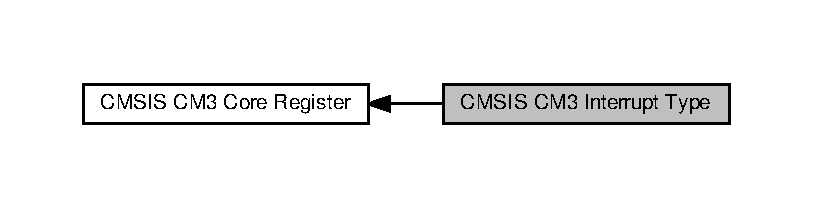
\includegraphics[width=350pt]{d2/d04/group__CMSIS__CM3__InterruptType}
\end{center}
\end{figure}
\subsection*{Data Structures}
\begin{DoxyCompactItemize}
\item 
struct \hyperlink{structInterruptType__Type}{Interrupt\+Type\+\_\+\+Type}
\end{DoxyCompactItemize}
\subsection*{Macros}
\begin{DoxyCompactItemize}
\item 
\#define \hyperlink{group__CMSIS__CM3__InterruptType_ga5d164b3cb981bd85afd35892d180a5c3}{Interrupt\+Type\+\_\+\+I\+C\+T\+R\+\_\+\+I\+N\+T\+L\+I\+N\+E\+S\+N\+U\+M\+\_\+\+Pos}~0
\item 
\#define \hyperlink{group__CMSIS__CM3__InterruptType_ga0a2c325cefdab97bd8ce3336a66a803e}{Interrupt\+Type\+\_\+\+I\+C\+T\+R\+\_\+\+I\+N\+T\+L\+I\+N\+E\+S\+N\+U\+M\+\_\+\+Msk}~(0x1\+Ful $<$$<$ Interrupt\+Type\+\_\+\+I\+C\+T\+R\+\_\+\+I\+N\+T\+L\+I\+N\+E\+S\+N\+U\+M\+\_\+\+Pos)
\item 
\#define \hyperlink{group__CMSIS__CM3__InterruptType_gaaa37f212111e6dbc9505d46b8bf8fa3e}{Interrupt\+Type\+\_\+\+A\+C\+T\+L\+R\+\_\+\+D\+I\+S\+F\+O\+L\+D\+\_\+\+Pos}~2
\item 
\#define \hyperlink{group__CMSIS__CM3__InterruptType_gac4d872ecfcf7dcb93f98824ada52a527}{Interrupt\+Type\+\_\+\+A\+C\+T\+L\+R\+\_\+\+D\+I\+S\+F\+O\+L\+D\+\_\+\+Msk}~(1ul $<$$<$ Interrupt\+Type\+\_\+\+A\+C\+T\+L\+R\+\_\+\+D\+I\+S\+F\+O\+L\+D\+\_\+\+Pos)
\item 
\#define \hyperlink{group__CMSIS__CM3__InterruptType_ga46fed31841c33811db8b3a9cbae6347b}{Interrupt\+Type\+\_\+\+A\+C\+T\+L\+R\+\_\+\+D\+I\+S\+D\+E\+F\+W\+B\+U\+F\+\_\+\+Pos}~1
\item 
\#define \hyperlink{group__CMSIS__CM3__InterruptType_ga3cecf9e9d75112aed3ed055343cbe23f}{Interrupt\+Type\+\_\+\+A\+C\+T\+L\+R\+\_\+\+D\+I\+S\+D\+E\+F\+W\+B\+U\+F\+\_\+\+Msk}~(1ul $<$$<$ Interrupt\+Type\+\_\+\+A\+C\+T\+L\+R\+\_\+\+D\+I\+S\+D\+E\+F\+W\+B\+U\+F\+\_\+\+Pos)
\item 
\#define \hyperlink{group__CMSIS__CM3__InterruptType_ga101a93632e4480073299b775bc5cbf12}{Interrupt\+Type\+\_\+\+A\+C\+T\+L\+R\+\_\+\+D\+I\+S\+M\+C\+Y\+C\+I\+N\+T\+\_\+\+Pos}~0
\item 
\#define \hyperlink{group__CMSIS__CM3__InterruptType_ga0c020eb28544979bfac2e219ed53c999}{Interrupt\+Type\+\_\+\+A\+C\+T\+L\+R\+\_\+\+D\+I\+S\+M\+C\+Y\+C\+I\+N\+T\+\_\+\+Msk}~(1ul $<$$<$ Interrupt\+Type\+\_\+\+A\+C\+T\+L\+R\+\_\+\+D\+I\+S\+M\+C\+Y\+C\+I\+N\+T\+\_\+\+Pos)
\end{DoxyCompactItemize}


\subsection{Detailed Description}
memory mapped structure for Interrupt Type 

\subsection{Macro Definition Documentation}
\index{C\+M\+S\+I\+S C\+M3 Interrupt Type@{C\+M\+S\+I\+S C\+M3 Interrupt Type}!Interrupt\+Type\+\_\+\+A\+C\+T\+L\+R\+\_\+\+D\+I\+S\+D\+E\+F\+W\+B\+U\+F\+\_\+\+Msk@{Interrupt\+Type\+\_\+\+A\+C\+T\+L\+R\+\_\+\+D\+I\+S\+D\+E\+F\+W\+B\+U\+F\+\_\+\+Msk}}
\index{Interrupt\+Type\+\_\+\+A\+C\+T\+L\+R\+\_\+\+D\+I\+S\+D\+E\+F\+W\+B\+U\+F\+\_\+\+Msk@{Interrupt\+Type\+\_\+\+A\+C\+T\+L\+R\+\_\+\+D\+I\+S\+D\+E\+F\+W\+B\+U\+F\+\_\+\+Msk}!C\+M\+S\+I\+S C\+M3 Interrupt Type@{C\+M\+S\+I\+S C\+M3 Interrupt Type}}
\subsubsection[{\texorpdfstring{Interrupt\+Type\+\_\+\+A\+C\+T\+L\+R\+\_\+\+D\+I\+S\+D\+E\+F\+W\+B\+U\+F\+\_\+\+Msk}{InterruptType_ACTLR_DISDEFWBUF_Msk}}]{\setlength{\rightskip}{0pt plus 5cm}\#define Interrupt\+Type\+\_\+\+A\+C\+T\+L\+R\+\_\+\+D\+I\+S\+D\+E\+F\+W\+B\+U\+F\+\_\+\+Msk~(1ul $<$$<$ Interrupt\+Type\+\_\+\+A\+C\+T\+L\+R\+\_\+\+D\+I\+S\+D\+E\+F\+W\+B\+U\+F\+\_\+\+Pos)}\hypertarget{group__CMSIS__CM3__InterruptType_ga3cecf9e9d75112aed3ed055343cbe23f}{}\label{group__CMSIS__CM3__InterruptType_ga3cecf9e9d75112aed3ed055343cbe23f}
Interrupt\+Type A\+C\+T\+LR\+: D\+I\+S\+D\+E\+F\+W\+B\+UF Mask \index{C\+M\+S\+I\+S C\+M3 Interrupt Type@{C\+M\+S\+I\+S C\+M3 Interrupt Type}!Interrupt\+Type\+\_\+\+A\+C\+T\+L\+R\+\_\+\+D\+I\+S\+D\+E\+F\+W\+B\+U\+F\+\_\+\+Pos@{Interrupt\+Type\+\_\+\+A\+C\+T\+L\+R\+\_\+\+D\+I\+S\+D\+E\+F\+W\+B\+U\+F\+\_\+\+Pos}}
\index{Interrupt\+Type\+\_\+\+A\+C\+T\+L\+R\+\_\+\+D\+I\+S\+D\+E\+F\+W\+B\+U\+F\+\_\+\+Pos@{Interrupt\+Type\+\_\+\+A\+C\+T\+L\+R\+\_\+\+D\+I\+S\+D\+E\+F\+W\+B\+U\+F\+\_\+\+Pos}!C\+M\+S\+I\+S C\+M3 Interrupt Type@{C\+M\+S\+I\+S C\+M3 Interrupt Type}}
\subsubsection[{\texorpdfstring{Interrupt\+Type\+\_\+\+A\+C\+T\+L\+R\+\_\+\+D\+I\+S\+D\+E\+F\+W\+B\+U\+F\+\_\+\+Pos}{InterruptType_ACTLR_DISDEFWBUF_Pos}}]{\setlength{\rightskip}{0pt plus 5cm}\#define Interrupt\+Type\+\_\+\+A\+C\+T\+L\+R\+\_\+\+D\+I\+S\+D\+E\+F\+W\+B\+U\+F\+\_\+\+Pos~1}\hypertarget{group__CMSIS__CM3__InterruptType_ga46fed31841c33811db8b3a9cbae6347b}{}\label{group__CMSIS__CM3__InterruptType_ga46fed31841c33811db8b3a9cbae6347b}
Interrupt\+Type A\+C\+T\+LR\+: D\+I\+S\+D\+E\+F\+W\+B\+UF Position \index{C\+M\+S\+I\+S C\+M3 Interrupt Type@{C\+M\+S\+I\+S C\+M3 Interrupt Type}!Interrupt\+Type\+\_\+\+A\+C\+T\+L\+R\+\_\+\+D\+I\+S\+F\+O\+L\+D\+\_\+\+Msk@{Interrupt\+Type\+\_\+\+A\+C\+T\+L\+R\+\_\+\+D\+I\+S\+F\+O\+L\+D\+\_\+\+Msk}}
\index{Interrupt\+Type\+\_\+\+A\+C\+T\+L\+R\+\_\+\+D\+I\+S\+F\+O\+L\+D\+\_\+\+Msk@{Interrupt\+Type\+\_\+\+A\+C\+T\+L\+R\+\_\+\+D\+I\+S\+F\+O\+L\+D\+\_\+\+Msk}!C\+M\+S\+I\+S C\+M3 Interrupt Type@{C\+M\+S\+I\+S C\+M3 Interrupt Type}}
\subsubsection[{\texorpdfstring{Interrupt\+Type\+\_\+\+A\+C\+T\+L\+R\+\_\+\+D\+I\+S\+F\+O\+L\+D\+\_\+\+Msk}{InterruptType_ACTLR_DISFOLD_Msk}}]{\setlength{\rightskip}{0pt plus 5cm}\#define Interrupt\+Type\+\_\+\+A\+C\+T\+L\+R\+\_\+\+D\+I\+S\+F\+O\+L\+D\+\_\+\+Msk~(1ul $<$$<$ Interrupt\+Type\+\_\+\+A\+C\+T\+L\+R\+\_\+\+D\+I\+S\+F\+O\+L\+D\+\_\+\+Pos)}\hypertarget{group__CMSIS__CM3__InterruptType_gac4d872ecfcf7dcb93f98824ada52a527}{}\label{group__CMSIS__CM3__InterruptType_gac4d872ecfcf7dcb93f98824ada52a527}
Interrupt\+Type A\+C\+T\+LR\+: D\+I\+S\+F\+O\+LD Mask \index{C\+M\+S\+I\+S C\+M3 Interrupt Type@{C\+M\+S\+I\+S C\+M3 Interrupt Type}!Interrupt\+Type\+\_\+\+A\+C\+T\+L\+R\+\_\+\+D\+I\+S\+F\+O\+L\+D\+\_\+\+Pos@{Interrupt\+Type\+\_\+\+A\+C\+T\+L\+R\+\_\+\+D\+I\+S\+F\+O\+L\+D\+\_\+\+Pos}}
\index{Interrupt\+Type\+\_\+\+A\+C\+T\+L\+R\+\_\+\+D\+I\+S\+F\+O\+L\+D\+\_\+\+Pos@{Interrupt\+Type\+\_\+\+A\+C\+T\+L\+R\+\_\+\+D\+I\+S\+F\+O\+L\+D\+\_\+\+Pos}!C\+M\+S\+I\+S C\+M3 Interrupt Type@{C\+M\+S\+I\+S C\+M3 Interrupt Type}}
\subsubsection[{\texorpdfstring{Interrupt\+Type\+\_\+\+A\+C\+T\+L\+R\+\_\+\+D\+I\+S\+F\+O\+L\+D\+\_\+\+Pos}{InterruptType_ACTLR_DISFOLD_Pos}}]{\setlength{\rightskip}{0pt plus 5cm}\#define Interrupt\+Type\+\_\+\+A\+C\+T\+L\+R\+\_\+\+D\+I\+S\+F\+O\+L\+D\+\_\+\+Pos~2}\hypertarget{group__CMSIS__CM3__InterruptType_gaaa37f212111e6dbc9505d46b8bf8fa3e}{}\label{group__CMSIS__CM3__InterruptType_gaaa37f212111e6dbc9505d46b8bf8fa3e}
Interrupt\+Type A\+C\+T\+LR\+: D\+I\+S\+F\+O\+LD Position \index{C\+M\+S\+I\+S C\+M3 Interrupt Type@{C\+M\+S\+I\+S C\+M3 Interrupt Type}!Interrupt\+Type\+\_\+\+A\+C\+T\+L\+R\+\_\+\+D\+I\+S\+M\+C\+Y\+C\+I\+N\+T\+\_\+\+Msk@{Interrupt\+Type\+\_\+\+A\+C\+T\+L\+R\+\_\+\+D\+I\+S\+M\+C\+Y\+C\+I\+N\+T\+\_\+\+Msk}}
\index{Interrupt\+Type\+\_\+\+A\+C\+T\+L\+R\+\_\+\+D\+I\+S\+M\+C\+Y\+C\+I\+N\+T\+\_\+\+Msk@{Interrupt\+Type\+\_\+\+A\+C\+T\+L\+R\+\_\+\+D\+I\+S\+M\+C\+Y\+C\+I\+N\+T\+\_\+\+Msk}!C\+M\+S\+I\+S C\+M3 Interrupt Type@{C\+M\+S\+I\+S C\+M3 Interrupt Type}}
\subsubsection[{\texorpdfstring{Interrupt\+Type\+\_\+\+A\+C\+T\+L\+R\+\_\+\+D\+I\+S\+M\+C\+Y\+C\+I\+N\+T\+\_\+\+Msk}{InterruptType_ACTLR_DISMCYCINT_Msk}}]{\setlength{\rightskip}{0pt plus 5cm}\#define Interrupt\+Type\+\_\+\+A\+C\+T\+L\+R\+\_\+\+D\+I\+S\+M\+C\+Y\+C\+I\+N\+T\+\_\+\+Msk~(1ul $<$$<$ Interrupt\+Type\+\_\+\+A\+C\+T\+L\+R\+\_\+\+D\+I\+S\+M\+C\+Y\+C\+I\+N\+T\+\_\+\+Pos)}\hypertarget{group__CMSIS__CM3__InterruptType_ga0c020eb28544979bfac2e219ed53c999}{}\label{group__CMSIS__CM3__InterruptType_ga0c020eb28544979bfac2e219ed53c999}
Interrupt\+Type A\+C\+T\+LR\+: D\+I\+S\+M\+C\+Y\+C\+I\+NT Mask \index{C\+M\+S\+I\+S C\+M3 Interrupt Type@{C\+M\+S\+I\+S C\+M3 Interrupt Type}!Interrupt\+Type\+\_\+\+A\+C\+T\+L\+R\+\_\+\+D\+I\+S\+M\+C\+Y\+C\+I\+N\+T\+\_\+\+Pos@{Interrupt\+Type\+\_\+\+A\+C\+T\+L\+R\+\_\+\+D\+I\+S\+M\+C\+Y\+C\+I\+N\+T\+\_\+\+Pos}}
\index{Interrupt\+Type\+\_\+\+A\+C\+T\+L\+R\+\_\+\+D\+I\+S\+M\+C\+Y\+C\+I\+N\+T\+\_\+\+Pos@{Interrupt\+Type\+\_\+\+A\+C\+T\+L\+R\+\_\+\+D\+I\+S\+M\+C\+Y\+C\+I\+N\+T\+\_\+\+Pos}!C\+M\+S\+I\+S C\+M3 Interrupt Type@{C\+M\+S\+I\+S C\+M3 Interrupt Type}}
\subsubsection[{\texorpdfstring{Interrupt\+Type\+\_\+\+A\+C\+T\+L\+R\+\_\+\+D\+I\+S\+M\+C\+Y\+C\+I\+N\+T\+\_\+\+Pos}{InterruptType_ACTLR_DISMCYCINT_Pos}}]{\setlength{\rightskip}{0pt plus 5cm}\#define Interrupt\+Type\+\_\+\+A\+C\+T\+L\+R\+\_\+\+D\+I\+S\+M\+C\+Y\+C\+I\+N\+T\+\_\+\+Pos~0}\hypertarget{group__CMSIS__CM3__InterruptType_ga101a93632e4480073299b775bc5cbf12}{}\label{group__CMSIS__CM3__InterruptType_ga101a93632e4480073299b775bc5cbf12}
Interrupt\+Type A\+C\+T\+LR\+: D\+I\+S\+M\+C\+Y\+C\+I\+NT Position \index{C\+M\+S\+I\+S C\+M3 Interrupt Type@{C\+M\+S\+I\+S C\+M3 Interrupt Type}!Interrupt\+Type\+\_\+\+I\+C\+T\+R\+\_\+\+I\+N\+T\+L\+I\+N\+E\+S\+N\+U\+M\+\_\+\+Msk@{Interrupt\+Type\+\_\+\+I\+C\+T\+R\+\_\+\+I\+N\+T\+L\+I\+N\+E\+S\+N\+U\+M\+\_\+\+Msk}}
\index{Interrupt\+Type\+\_\+\+I\+C\+T\+R\+\_\+\+I\+N\+T\+L\+I\+N\+E\+S\+N\+U\+M\+\_\+\+Msk@{Interrupt\+Type\+\_\+\+I\+C\+T\+R\+\_\+\+I\+N\+T\+L\+I\+N\+E\+S\+N\+U\+M\+\_\+\+Msk}!C\+M\+S\+I\+S C\+M3 Interrupt Type@{C\+M\+S\+I\+S C\+M3 Interrupt Type}}
\subsubsection[{\texorpdfstring{Interrupt\+Type\+\_\+\+I\+C\+T\+R\+\_\+\+I\+N\+T\+L\+I\+N\+E\+S\+N\+U\+M\+\_\+\+Msk}{InterruptType_ICTR_INTLINESNUM_Msk}}]{\setlength{\rightskip}{0pt plus 5cm}\#define Interrupt\+Type\+\_\+\+I\+C\+T\+R\+\_\+\+I\+N\+T\+L\+I\+N\+E\+S\+N\+U\+M\+\_\+\+Msk~(0x1\+Ful $<$$<$ Interrupt\+Type\+\_\+\+I\+C\+T\+R\+\_\+\+I\+N\+T\+L\+I\+N\+E\+S\+N\+U\+M\+\_\+\+Pos)}\hypertarget{group__CMSIS__CM3__InterruptType_ga0a2c325cefdab97bd8ce3336a66a803e}{}\label{group__CMSIS__CM3__InterruptType_ga0a2c325cefdab97bd8ce3336a66a803e}
Interrupt\+Type I\+C\+TR\+: I\+N\+T\+L\+I\+N\+E\+S\+N\+UM Mask \index{C\+M\+S\+I\+S C\+M3 Interrupt Type@{C\+M\+S\+I\+S C\+M3 Interrupt Type}!Interrupt\+Type\+\_\+\+I\+C\+T\+R\+\_\+\+I\+N\+T\+L\+I\+N\+E\+S\+N\+U\+M\+\_\+\+Pos@{Interrupt\+Type\+\_\+\+I\+C\+T\+R\+\_\+\+I\+N\+T\+L\+I\+N\+E\+S\+N\+U\+M\+\_\+\+Pos}}
\index{Interrupt\+Type\+\_\+\+I\+C\+T\+R\+\_\+\+I\+N\+T\+L\+I\+N\+E\+S\+N\+U\+M\+\_\+\+Pos@{Interrupt\+Type\+\_\+\+I\+C\+T\+R\+\_\+\+I\+N\+T\+L\+I\+N\+E\+S\+N\+U\+M\+\_\+\+Pos}!C\+M\+S\+I\+S C\+M3 Interrupt Type@{C\+M\+S\+I\+S C\+M3 Interrupt Type}}
\subsubsection[{\texorpdfstring{Interrupt\+Type\+\_\+\+I\+C\+T\+R\+\_\+\+I\+N\+T\+L\+I\+N\+E\+S\+N\+U\+M\+\_\+\+Pos}{InterruptType_ICTR_INTLINESNUM_Pos}}]{\setlength{\rightskip}{0pt plus 5cm}\#define Interrupt\+Type\+\_\+\+I\+C\+T\+R\+\_\+\+I\+N\+T\+L\+I\+N\+E\+S\+N\+U\+M\+\_\+\+Pos~0}\hypertarget{group__CMSIS__CM3__InterruptType_ga5d164b3cb981bd85afd35892d180a5c3}{}\label{group__CMSIS__CM3__InterruptType_ga5d164b3cb981bd85afd35892d180a5c3}
Interrupt\+Type I\+C\+TR\+: I\+N\+T\+L\+I\+N\+E\+S\+N\+UM Position 
\hypertarget{group__CMSIS__CM3__MPU}{}\section{C\+M\+S\+IS C\+M3 M\+PU}
\label{group__CMSIS__CM3__MPU}\index{C\+M\+S\+I\+S C\+M3 M\+PU@{C\+M\+S\+I\+S C\+M3 M\+PU}}
Collaboration diagram for C\+M\+S\+IS C\+M3 M\+PU\+:\nopagebreak
\begin{figure}[H]
\begin{center}
\leavevmode
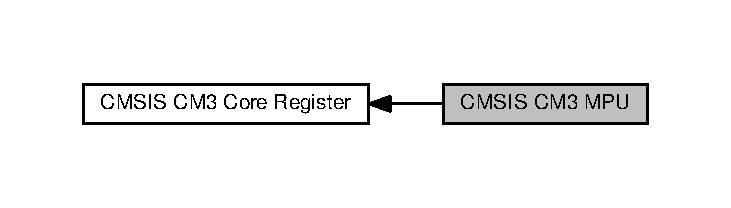
\includegraphics[width=350pt]{da/d63/group__CMSIS__CM3__MPU}
\end{center}
\end{figure}
\subsection*{Data Structures}
\begin{DoxyCompactItemize}
\item 
struct \hyperlink{structMPU__Type}{M\+P\+U\+\_\+\+Type}
\end{DoxyCompactItemize}
\subsection*{Macros}
\begin{DoxyCompactItemize}
\item 
\#define \hyperlink{group__CMSIS__CM3__MPU_gab46a4e0dae7607af6f312cf2328ecfc9}{M\+P\+U\+\_\+\+T\+Y\+P\+E\+\_\+\+I\+R\+E\+G\+I\+O\+N\+\_\+\+Pos}~16
\item 
\#define \hyperlink{group__CMSIS__CM3__MPU_ga84c08304cbf7088481f2f6ccd8013c39}{M\+P\+U\+\_\+\+T\+Y\+P\+E\+\_\+\+I\+R\+E\+G\+I\+O\+N\+\_\+\+Msk}~(0x\+F\+Ful $<$$<$ M\+P\+U\+\_\+\+T\+Y\+P\+E\+\_\+\+I\+R\+E\+G\+I\+O\+N\+\_\+\+Pos)
\item 
\#define \hyperlink{group__CMSIS__CM3__MPU_ga4d090ef632d2ba3a6ae4078c2594d6d3}{M\+P\+U\+\_\+\+T\+Y\+P\+E\+\_\+\+D\+R\+E\+G\+I\+O\+N\+\_\+\+Pos}~8
\item 
\#define \hyperlink{group__CMSIS__CM3__MPU_ga3a5d2e6871b1518dca61e28b18aec6cb}{M\+P\+U\+\_\+\+T\+Y\+P\+E\+\_\+\+D\+R\+E\+G\+I\+O\+N\+\_\+\+Msk}~(0x\+F\+Ful $<$$<$ M\+P\+U\+\_\+\+T\+Y\+P\+E\+\_\+\+D\+R\+E\+G\+I\+O\+N\+\_\+\+Pos)
\item 
\#define \hyperlink{group__CMSIS__CM3__MPU_gaa3ef8bc16dfa8b27f80b87109b424fe7}{M\+P\+U\+\_\+\+T\+Y\+P\+E\+\_\+\+S\+E\+P\+A\+R\+A\+T\+E\+\_\+\+Pos}~0
\item 
\#define \hyperlink{group__CMSIS__CM3__MPU_ga45427152e9a3493f1477fbe52e771c59}{M\+P\+U\+\_\+\+T\+Y\+P\+E\+\_\+\+S\+E\+P\+A\+R\+A\+T\+E\+\_\+\+Msk}~(1ul $<$$<$ M\+P\+U\+\_\+\+T\+Y\+P\+E\+\_\+\+S\+E\+P\+A\+R\+A\+T\+E\+\_\+\+Pos)
\item 
\#define \hyperlink{group__CMSIS__CM3__MPU_ga723678c07d8d65eacb5dd957867b1b0c}{M\+P\+U\+\_\+\+C\+T\+R\+L\+\_\+\+P\+R\+I\+V\+D\+E\+F\+E\+N\+A\+\_\+\+Pos}~2
\item 
\#define \hyperlink{group__CMSIS__CM3__MPU_ga09e80ffe9a690dc76e416708661ea436}{M\+P\+U\+\_\+\+C\+T\+R\+L\+\_\+\+P\+R\+I\+V\+D\+E\+F\+E\+N\+A\+\_\+\+Msk}~(1ul $<$$<$ M\+P\+U\+\_\+\+C\+T\+R\+L\+\_\+\+P\+R\+I\+V\+D\+E\+F\+E\+N\+A\+\_\+\+Pos)
\item 
\#define \hyperlink{group__CMSIS__CM3__MPU_gab41c6f2447fb6dffa9a887ddc7c418c5}{M\+P\+U\+\_\+\+C\+T\+R\+L\+\_\+\+H\+F\+N\+M\+I\+E\+N\+A\+\_\+\+Pos}~1
\item 
\#define \hyperlink{group__CMSIS__CM3__MPU_gaa0db6e8e71df9529f3300d7a1e9a7b69}{M\+P\+U\+\_\+\+C\+T\+R\+L\+\_\+\+H\+F\+N\+M\+I\+E\+N\+A\+\_\+\+Msk}~(1ul $<$$<$ M\+P\+U\+\_\+\+C\+T\+R\+L\+\_\+\+H\+F\+N\+M\+I\+E\+N\+A\+\_\+\+Pos)
\item 
\#define \hyperlink{group__CMSIS__CM3__MPU_ga726096caf670db669c53458f7ea07373}{M\+P\+U\+\_\+\+C\+T\+R\+L\+\_\+\+E\+N\+A\+B\+L\+E\+\_\+\+Pos}~0
\item 
\#define \hyperlink{group__CMSIS__CM3__MPU_gae72b283f6e38b641c877182f03d95844}{M\+P\+U\+\_\+\+C\+T\+R\+L\+\_\+\+E\+N\+A\+B\+L\+E\+\_\+\+Msk}~(1ul $<$$<$ M\+P\+U\+\_\+\+C\+T\+R\+L\+\_\+\+E\+N\+A\+B\+L\+E\+\_\+\+Pos)
\item 
\#define \hyperlink{group__CMSIS__CM3__MPU_ga4ae5ef482542113b2361e7de9e3419af}{M\+P\+U\+\_\+\+R\+N\+R\+\_\+\+R\+E\+G\+I\+O\+N\+\_\+\+Pos}~0
\item 
\#define \hyperlink{group__CMSIS__CM3__MPU_ga2d48d65bbe6e37caf7534e3c93da30f7}{M\+P\+U\+\_\+\+R\+N\+R\+\_\+\+R\+E\+G\+I\+O\+N\+\_\+\+Msk}~(0x\+F\+Ful $<$$<$ M\+P\+U\+\_\+\+R\+N\+R\+\_\+\+R\+E\+G\+I\+O\+N\+\_\+\+Pos)
\item 
\#define \hyperlink{group__CMSIS__CM3__MPU_ga8526c8bf02e4d47c852aab797800b1fd}{M\+P\+U\+\_\+\+R\+B\+A\+R\+\_\+\+A\+D\+D\+R\+\_\+\+Pos}~5
\item 
\#define \hyperlink{group__CMSIS__CM3__MPU_ga33905dca89aa5b5bb9aa9518094b8b80}{M\+P\+U\+\_\+\+R\+B\+A\+R\+\_\+\+A\+D\+D\+R\+\_\+\+Msk}~(0x7\+F\+F\+F\+F\+F\+Ful $<$$<$ M\+P\+U\+\_\+\+R\+B\+A\+R\+\_\+\+A\+D\+D\+R\+\_\+\+Pos)
\item 
\#define \hyperlink{group__CMSIS__CM3__MPU_ga1384f1a3d45f52c7829151ebc45e2c81}{M\+P\+U\+\_\+\+R\+B\+A\+R\+\_\+\+V\+A\+L\+I\+D\+\_\+\+Pos}~4
\item 
\#define \hyperlink{group__CMSIS__CM3__MPU_gaf7787465931ee4dbe5f51091f187e790}{M\+P\+U\+\_\+\+R\+B\+A\+R\+\_\+\+V\+A\+L\+I\+D\+\_\+\+Msk}~(1ul $<$$<$ M\+P\+U\+\_\+\+R\+B\+A\+R\+\_\+\+V\+A\+L\+I\+D\+\_\+\+Pos)
\item 
\#define \hyperlink{group__CMSIS__CM3__MPU_ga0556413825169bdcb19e37f42d92e133}{M\+P\+U\+\_\+\+R\+B\+A\+R\+\_\+\+R\+E\+G\+I\+O\+N\+\_\+\+Pos}~0
\item 
\#define \hyperlink{group__CMSIS__CM3__MPU_gac896033cb8ecfe045d9bada07c0311d7}{M\+P\+U\+\_\+\+R\+B\+A\+R\+\_\+\+R\+E\+G\+I\+O\+N\+\_\+\+Msk}~(0x\+Ful $<$$<$ M\+P\+U\+\_\+\+R\+B\+A\+R\+\_\+\+R\+E\+G\+I\+O\+N\+\_\+\+Pos)
\item 
\#define \hyperlink{group__CMSIS__CM3__MPU_gaa02d0a5dd8b96fb9500cb5f31c9ea67b}{M\+P\+U\+\_\+\+R\+A\+S\+R\+\_\+\+X\+N\+\_\+\+Pos}~28
\item 
\#define \hyperlink{group__CMSIS__CM3__MPU_ga4f8afc5cc7fca2ada211f8b09c76802e}{M\+P\+U\+\_\+\+R\+A\+S\+R\+\_\+\+X\+N\+\_\+\+Msk}~(1ul $<$$<$ M\+P\+U\+\_\+\+R\+A\+S\+R\+\_\+\+X\+N\+\_\+\+Pos)
\item 
\#define \hyperlink{group__CMSIS__CM3__MPU_gac919b25b709081bac1fe1d30e6ca53d7}{M\+P\+U\+\_\+\+R\+A\+S\+R\+\_\+\+A\+P\+\_\+\+Pos}~24
\item 
\#define \hyperlink{group__CMSIS__CM3__MPU_ga81da5e9383eca09414642d65fcbc14de}{M\+P\+U\+\_\+\+R\+A\+S\+R\+\_\+\+A\+P\+\_\+\+Msk}~(7ul $<$$<$ M\+P\+U\+\_\+\+R\+A\+S\+R\+\_\+\+A\+P\+\_\+\+Pos)
\item 
\#define \hyperlink{group__CMSIS__CM3__MPU_ga340f1c91469c5bb4ee91bc29ad21c631}{M\+P\+U\+\_\+\+R\+A\+S\+R\+\_\+\+T\+E\+X\+\_\+\+Pos}~19
\item 
\#define \hyperlink{group__CMSIS__CM3__MPU_ga94f4b4a368986c1955b92743046a1f4e}{M\+P\+U\+\_\+\+R\+A\+S\+R\+\_\+\+T\+E\+X\+\_\+\+Msk}~(7ul $<$$<$ M\+P\+U\+\_\+\+R\+A\+S\+R\+\_\+\+T\+E\+X\+\_\+\+Pos)
\item 
\#define \hyperlink{group__CMSIS__CM3__MPU_ga1820e125a5aa584cd49ede44c742985c}{M\+P\+U\+\_\+\+R\+A\+S\+R\+\_\+\+S\+\_\+\+Pos}~18
\item 
\#define \hyperlink{group__CMSIS__CM3__MPU_ga872c0922578c2e74304886579e9a2361}{M\+P\+U\+\_\+\+R\+A\+S\+R\+\_\+\+S\+\_\+\+Msk}~(1ul $<$$<$ M\+P\+U\+\_\+\+R\+A\+S\+R\+\_\+\+S\+\_\+\+Pos)
\item 
\#define \hyperlink{group__CMSIS__CM3__MPU_ga3a1631f2c85c66ead1d6d4cea9c16a52}{M\+P\+U\+\_\+\+R\+A\+S\+R\+\_\+\+C\+\_\+\+Pos}~17
\item 
\#define \hyperlink{group__CMSIS__CM3__MPU_gaf841f9bee5046fece4f513ecf707a3c1}{M\+P\+U\+\_\+\+R\+A\+S\+R\+\_\+\+C\+\_\+\+Msk}~(1ul $<$$<$ M\+P\+U\+\_\+\+R\+A\+S\+R\+\_\+\+C\+\_\+\+Pos)
\item 
\#define \hyperlink{group__CMSIS__CM3__MPU_gae9ea3c456f66c56040a2e55793c63cf5}{M\+P\+U\+\_\+\+R\+A\+S\+R\+\_\+\+B\+\_\+\+Pos}~16
\item 
\#define \hyperlink{group__CMSIS__CM3__MPU_gaf97de2b86316d5b29931fc6f70b3cba1}{M\+P\+U\+\_\+\+R\+A\+S\+R\+\_\+\+B\+\_\+\+Msk}~(1ul $<$$<$ M\+P\+U\+\_\+\+R\+A\+S\+R\+\_\+\+B\+\_\+\+Pos)
\item 
\#define \hyperlink{group__CMSIS__CM3__MPU_gadbd68b7db2dd697a1977a7ed2f3e67bf}{M\+P\+U\+\_\+\+R\+A\+S\+R\+\_\+\+S\+R\+D\+\_\+\+Pos}~8
\item 
\#define \hyperlink{group__CMSIS__CM3__MPU_ga4046ede234a191e3a0efb9a3174bca05}{M\+P\+U\+\_\+\+R\+A\+S\+R\+\_\+\+S\+R\+D\+\_\+\+Msk}~(0x\+F\+Ful $<$$<$ M\+P\+U\+\_\+\+R\+A\+S\+R\+\_\+\+S\+R\+D\+\_\+\+Pos)
\item 
\#define \hyperlink{group__CMSIS__CM3__MPU_gad90549193db0d2b7e70d3d52cb902710}{M\+P\+U\+\_\+\+R\+A\+S\+R\+\_\+\+S\+I\+Z\+E\+\_\+\+Pos}~1
\item 
\#define \hyperlink{group__CMSIS__CM3__MPU_ga222e237e51f20d0e8a8c249295e77298}{M\+P\+U\+\_\+\+R\+A\+S\+R\+\_\+\+S\+I\+Z\+E\+\_\+\+Msk}~(0x1\+Ful $<$$<$ M\+P\+U\+\_\+\+R\+A\+S\+R\+\_\+\+S\+I\+Z\+E\+\_\+\+Pos)
\item 
\#define \hyperlink{group__CMSIS__CM3__MPU_ga140d103b3789cbda82a0a4da9ffffadb}{M\+P\+U\+\_\+\+R\+A\+S\+R\+\_\+\+E\+N\+A\+\_\+\+Pos}~0
\item 
\#define \hyperlink{group__CMSIS__CM3__MPU_ga6c6fc837531a7d6a3b3962e21147b4a9}{M\+P\+U\+\_\+\+R\+A\+S\+R\+\_\+\+E\+N\+A\+\_\+\+Msk}~(0x1\+Ful $<$$<$ M\+P\+U\+\_\+\+R\+A\+S\+R\+\_\+\+E\+N\+A\+\_\+\+Pos)
\end{DoxyCompactItemize}


\subsection{Detailed Description}
memory mapped structure for Memory Protection Unit (M\+PU) 

\subsection{Macro Definition Documentation}
\index{C\+M\+S\+I\+S C\+M3 M\+PU@{C\+M\+S\+I\+S C\+M3 M\+PU}!M\+P\+U\+\_\+\+C\+T\+R\+L\+\_\+\+E\+N\+A\+B\+L\+E\+\_\+\+Msk@{M\+P\+U\+\_\+\+C\+T\+R\+L\+\_\+\+E\+N\+A\+B\+L\+E\+\_\+\+Msk}}
\index{M\+P\+U\+\_\+\+C\+T\+R\+L\+\_\+\+E\+N\+A\+B\+L\+E\+\_\+\+Msk@{M\+P\+U\+\_\+\+C\+T\+R\+L\+\_\+\+E\+N\+A\+B\+L\+E\+\_\+\+Msk}!C\+M\+S\+I\+S C\+M3 M\+PU@{C\+M\+S\+I\+S C\+M3 M\+PU}}
\subsubsection[{\texorpdfstring{M\+P\+U\+\_\+\+C\+T\+R\+L\+\_\+\+E\+N\+A\+B\+L\+E\+\_\+\+Msk}{MPU_CTRL_ENABLE_Msk}}]{\setlength{\rightskip}{0pt plus 5cm}\#define M\+P\+U\+\_\+\+C\+T\+R\+L\+\_\+\+E\+N\+A\+B\+L\+E\+\_\+\+Msk~(1ul $<$$<$ M\+P\+U\+\_\+\+C\+T\+R\+L\+\_\+\+E\+N\+A\+B\+L\+E\+\_\+\+Pos)}\hypertarget{group__CMSIS__CM3__MPU_gae72b283f6e38b641c877182f03d95844}{}\label{group__CMSIS__CM3__MPU_gae72b283f6e38b641c877182f03d95844}
M\+PU C\+T\+RL\+: E\+N\+A\+B\+LE Mask \index{C\+M\+S\+I\+S C\+M3 M\+PU@{C\+M\+S\+I\+S C\+M3 M\+PU}!M\+P\+U\+\_\+\+C\+T\+R\+L\+\_\+\+E\+N\+A\+B\+L\+E\+\_\+\+Pos@{M\+P\+U\+\_\+\+C\+T\+R\+L\+\_\+\+E\+N\+A\+B\+L\+E\+\_\+\+Pos}}
\index{M\+P\+U\+\_\+\+C\+T\+R\+L\+\_\+\+E\+N\+A\+B\+L\+E\+\_\+\+Pos@{M\+P\+U\+\_\+\+C\+T\+R\+L\+\_\+\+E\+N\+A\+B\+L\+E\+\_\+\+Pos}!C\+M\+S\+I\+S C\+M3 M\+PU@{C\+M\+S\+I\+S C\+M3 M\+PU}}
\subsubsection[{\texorpdfstring{M\+P\+U\+\_\+\+C\+T\+R\+L\+\_\+\+E\+N\+A\+B\+L\+E\+\_\+\+Pos}{MPU_CTRL_ENABLE_Pos}}]{\setlength{\rightskip}{0pt plus 5cm}\#define M\+P\+U\+\_\+\+C\+T\+R\+L\+\_\+\+E\+N\+A\+B\+L\+E\+\_\+\+Pos~0}\hypertarget{group__CMSIS__CM3__MPU_ga726096caf670db669c53458f7ea07373}{}\label{group__CMSIS__CM3__MPU_ga726096caf670db669c53458f7ea07373}
M\+PU C\+T\+RL\+: E\+N\+A\+B\+LE Position \index{C\+M\+S\+I\+S C\+M3 M\+PU@{C\+M\+S\+I\+S C\+M3 M\+PU}!M\+P\+U\+\_\+\+C\+T\+R\+L\+\_\+\+H\+F\+N\+M\+I\+E\+N\+A\+\_\+\+Msk@{M\+P\+U\+\_\+\+C\+T\+R\+L\+\_\+\+H\+F\+N\+M\+I\+E\+N\+A\+\_\+\+Msk}}
\index{M\+P\+U\+\_\+\+C\+T\+R\+L\+\_\+\+H\+F\+N\+M\+I\+E\+N\+A\+\_\+\+Msk@{M\+P\+U\+\_\+\+C\+T\+R\+L\+\_\+\+H\+F\+N\+M\+I\+E\+N\+A\+\_\+\+Msk}!C\+M\+S\+I\+S C\+M3 M\+PU@{C\+M\+S\+I\+S C\+M3 M\+PU}}
\subsubsection[{\texorpdfstring{M\+P\+U\+\_\+\+C\+T\+R\+L\+\_\+\+H\+F\+N\+M\+I\+E\+N\+A\+\_\+\+Msk}{MPU_CTRL_HFNMIENA_Msk}}]{\setlength{\rightskip}{0pt plus 5cm}\#define M\+P\+U\+\_\+\+C\+T\+R\+L\+\_\+\+H\+F\+N\+M\+I\+E\+N\+A\+\_\+\+Msk~(1ul $<$$<$ M\+P\+U\+\_\+\+C\+T\+R\+L\+\_\+\+H\+F\+N\+M\+I\+E\+N\+A\+\_\+\+Pos)}\hypertarget{group__CMSIS__CM3__MPU_gaa0db6e8e71df9529f3300d7a1e9a7b69}{}\label{group__CMSIS__CM3__MPU_gaa0db6e8e71df9529f3300d7a1e9a7b69}
M\+PU C\+T\+RL\+: H\+F\+N\+M\+I\+E\+NA Mask \index{C\+M\+S\+I\+S C\+M3 M\+PU@{C\+M\+S\+I\+S C\+M3 M\+PU}!M\+P\+U\+\_\+\+C\+T\+R\+L\+\_\+\+H\+F\+N\+M\+I\+E\+N\+A\+\_\+\+Pos@{M\+P\+U\+\_\+\+C\+T\+R\+L\+\_\+\+H\+F\+N\+M\+I\+E\+N\+A\+\_\+\+Pos}}
\index{M\+P\+U\+\_\+\+C\+T\+R\+L\+\_\+\+H\+F\+N\+M\+I\+E\+N\+A\+\_\+\+Pos@{M\+P\+U\+\_\+\+C\+T\+R\+L\+\_\+\+H\+F\+N\+M\+I\+E\+N\+A\+\_\+\+Pos}!C\+M\+S\+I\+S C\+M3 M\+PU@{C\+M\+S\+I\+S C\+M3 M\+PU}}
\subsubsection[{\texorpdfstring{M\+P\+U\+\_\+\+C\+T\+R\+L\+\_\+\+H\+F\+N\+M\+I\+E\+N\+A\+\_\+\+Pos}{MPU_CTRL_HFNMIENA_Pos}}]{\setlength{\rightskip}{0pt plus 5cm}\#define M\+P\+U\+\_\+\+C\+T\+R\+L\+\_\+\+H\+F\+N\+M\+I\+E\+N\+A\+\_\+\+Pos~1}\hypertarget{group__CMSIS__CM3__MPU_gab41c6f2447fb6dffa9a887ddc7c418c5}{}\label{group__CMSIS__CM3__MPU_gab41c6f2447fb6dffa9a887ddc7c418c5}
M\+PU C\+T\+RL\+: H\+F\+N\+M\+I\+E\+NA Position \index{C\+M\+S\+I\+S C\+M3 M\+PU@{C\+M\+S\+I\+S C\+M3 M\+PU}!M\+P\+U\+\_\+\+C\+T\+R\+L\+\_\+\+P\+R\+I\+V\+D\+E\+F\+E\+N\+A\+\_\+\+Msk@{M\+P\+U\+\_\+\+C\+T\+R\+L\+\_\+\+P\+R\+I\+V\+D\+E\+F\+E\+N\+A\+\_\+\+Msk}}
\index{M\+P\+U\+\_\+\+C\+T\+R\+L\+\_\+\+P\+R\+I\+V\+D\+E\+F\+E\+N\+A\+\_\+\+Msk@{M\+P\+U\+\_\+\+C\+T\+R\+L\+\_\+\+P\+R\+I\+V\+D\+E\+F\+E\+N\+A\+\_\+\+Msk}!C\+M\+S\+I\+S C\+M3 M\+PU@{C\+M\+S\+I\+S C\+M3 M\+PU}}
\subsubsection[{\texorpdfstring{M\+P\+U\+\_\+\+C\+T\+R\+L\+\_\+\+P\+R\+I\+V\+D\+E\+F\+E\+N\+A\+\_\+\+Msk}{MPU_CTRL_PRIVDEFENA_Msk}}]{\setlength{\rightskip}{0pt plus 5cm}\#define M\+P\+U\+\_\+\+C\+T\+R\+L\+\_\+\+P\+R\+I\+V\+D\+E\+F\+E\+N\+A\+\_\+\+Msk~(1ul $<$$<$ M\+P\+U\+\_\+\+C\+T\+R\+L\+\_\+\+P\+R\+I\+V\+D\+E\+F\+E\+N\+A\+\_\+\+Pos)}\hypertarget{group__CMSIS__CM3__MPU_ga09e80ffe9a690dc76e416708661ea436}{}\label{group__CMSIS__CM3__MPU_ga09e80ffe9a690dc76e416708661ea436}
M\+PU C\+T\+RL\+: P\+R\+I\+V\+D\+E\+F\+E\+NA Mask \index{C\+M\+S\+I\+S C\+M3 M\+PU@{C\+M\+S\+I\+S C\+M3 M\+PU}!M\+P\+U\+\_\+\+C\+T\+R\+L\+\_\+\+P\+R\+I\+V\+D\+E\+F\+E\+N\+A\+\_\+\+Pos@{M\+P\+U\+\_\+\+C\+T\+R\+L\+\_\+\+P\+R\+I\+V\+D\+E\+F\+E\+N\+A\+\_\+\+Pos}}
\index{M\+P\+U\+\_\+\+C\+T\+R\+L\+\_\+\+P\+R\+I\+V\+D\+E\+F\+E\+N\+A\+\_\+\+Pos@{M\+P\+U\+\_\+\+C\+T\+R\+L\+\_\+\+P\+R\+I\+V\+D\+E\+F\+E\+N\+A\+\_\+\+Pos}!C\+M\+S\+I\+S C\+M3 M\+PU@{C\+M\+S\+I\+S C\+M3 M\+PU}}
\subsubsection[{\texorpdfstring{M\+P\+U\+\_\+\+C\+T\+R\+L\+\_\+\+P\+R\+I\+V\+D\+E\+F\+E\+N\+A\+\_\+\+Pos}{MPU_CTRL_PRIVDEFENA_Pos}}]{\setlength{\rightskip}{0pt plus 5cm}\#define M\+P\+U\+\_\+\+C\+T\+R\+L\+\_\+\+P\+R\+I\+V\+D\+E\+F\+E\+N\+A\+\_\+\+Pos~2}\hypertarget{group__CMSIS__CM3__MPU_ga723678c07d8d65eacb5dd957867b1b0c}{}\label{group__CMSIS__CM3__MPU_ga723678c07d8d65eacb5dd957867b1b0c}
M\+PU C\+T\+RL\+: P\+R\+I\+V\+D\+E\+F\+E\+NA Position \index{C\+M\+S\+I\+S C\+M3 M\+PU@{C\+M\+S\+I\+S C\+M3 M\+PU}!M\+P\+U\+\_\+\+R\+A\+S\+R\+\_\+\+A\+P\+\_\+\+Msk@{M\+P\+U\+\_\+\+R\+A\+S\+R\+\_\+\+A\+P\+\_\+\+Msk}}
\index{M\+P\+U\+\_\+\+R\+A\+S\+R\+\_\+\+A\+P\+\_\+\+Msk@{M\+P\+U\+\_\+\+R\+A\+S\+R\+\_\+\+A\+P\+\_\+\+Msk}!C\+M\+S\+I\+S C\+M3 M\+PU@{C\+M\+S\+I\+S C\+M3 M\+PU}}
\subsubsection[{\texorpdfstring{M\+P\+U\+\_\+\+R\+A\+S\+R\+\_\+\+A\+P\+\_\+\+Msk}{MPU_RASR_AP_Msk}}]{\setlength{\rightskip}{0pt plus 5cm}\#define M\+P\+U\+\_\+\+R\+A\+S\+R\+\_\+\+A\+P\+\_\+\+Msk~(7ul $<$$<$ M\+P\+U\+\_\+\+R\+A\+S\+R\+\_\+\+A\+P\+\_\+\+Pos)}\hypertarget{group__CMSIS__CM3__MPU_ga81da5e9383eca09414642d65fcbc14de}{}\label{group__CMSIS__CM3__MPU_ga81da5e9383eca09414642d65fcbc14de}
M\+PU R\+A\+SR\+: AP Mask \index{C\+M\+S\+I\+S C\+M3 M\+PU@{C\+M\+S\+I\+S C\+M3 M\+PU}!M\+P\+U\+\_\+\+R\+A\+S\+R\+\_\+\+A\+P\+\_\+\+Pos@{M\+P\+U\+\_\+\+R\+A\+S\+R\+\_\+\+A\+P\+\_\+\+Pos}}
\index{M\+P\+U\+\_\+\+R\+A\+S\+R\+\_\+\+A\+P\+\_\+\+Pos@{M\+P\+U\+\_\+\+R\+A\+S\+R\+\_\+\+A\+P\+\_\+\+Pos}!C\+M\+S\+I\+S C\+M3 M\+PU@{C\+M\+S\+I\+S C\+M3 M\+PU}}
\subsubsection[{\texorpdfstring{M\+P\+U\+\_\+\+R\+A\+S\+R\+\_\+\+A\+P\+\_\+\+Pos}{MPU_RASR_AP_Pos}}]{\setlength{\rightskip}{0pt plus 5cm}\#define M\+P\+U\+\_\+\+R\+A\+S\+R\+\_\+\+A\+P\+\_\+\+Pos~24}\hypertarget{group__CMSIS__CM3__MPU_gac919b25b709081bac1fe1d30e6ca53d7}{}\label{group__CMSIS__CM3__MPU_gac919b25b709081bac1fe1d30e6ca53d7}
M\+PU R\+A\+SR\+: AP Position \index{C\+M\+S\+I\+S C\+M3 M\+PU@{C\+M\+S\+I\+S C\+M3 M\+PU}!M\+P\+U\+\_\+\+R\+A\+S\+R\+\_\+\+B\+\_\+\+Msk@{M\+P\+U\+\_\+\+R\+A\+S\+R\+\_\+\+B\+\_\+\+Msk}}
\index{M\+P\+U\+\_\+\+R\+A\+S\+R\+\_\+\+B\+\_\+\+Msk@{M\+P\+U\+\_\+\+R\+A\+S\+R\+\_\+\+B\+\_\+\+Msk}!C\+M\+S\+I\+S C\+M3 M\+PU@{C\+M\+S\+I\+S C\+M3 M\+PU}}
\subsubsection[{\texorpdfstring{M\+P\+U\+\_\+\+R\+A\+S\+R\+\_\+\+B\+\_\+\+Msk}{MPU_RASR_B_Msk}}]{\setlength{\rightskip}{0pt plus 5cm}\#define M\+P\+U\+\_\+\+R\+A\+S\+R\+\_\+\+B\+\_\+\+Msk~(1ul $<$$<$ M\+P\+U\+\_\+\+R\+A\+S\+R\+\_\+\+B\+\_\+\+Pos)}\hypertarget{group__CMSIS__CM3__MPU_gaf97de2b86316d5b29931fc6f70b3cba1}{}\label{group__CMSIS__CM3__MPU_gaf97de2b86316d5b29931fc6f70b3cba1}
M\+PU R\+A\+SR\+: Bufferable bit Mask \index{C\+M\+S\+I\+S C\+M3 M\+PU@{C\+M\+S\+I\+S C\+M3 M\+PU}!M\+P\+U\+\_\+\+R\+A\+S\+R\+\_\+\+B\+\_\+\+Pos@{M\+P\+U\+\_\+\+R\+A\+S\+R\+\_\+\+B\+\_\+\+Pos}}
\index{M\+P\+U\+\_\+\+R\+A\+S\+R\+\_\+\+B\+\_\+\+Pos@{M\+P\+U\+\_\+\+R\+A\+S\+R\+\_\+\+B\+\_\+\+Pos}!C\+M\+S\+I\+S C\+M3 M\+PU@{C\+M\+S\+I\+S C\+M3 M\+PU}}
\subsubsection[{\texorpdfstring{M\+P\+U\+\_\+\+R\+A\+S\+R\+\_\+\+B\+\_\+\+Pos}{MPU_RASR_B_Pos}}]{\setlength{\rightskip}{0pt plus 5cm}\#define M\+P\+U\+\_\+\+R\+A\+S\+R\+\_\+\+B\+\_\+\+Pos~16}\hypertarget{group__CMSIS__CM3__MPU_gae9ea3c456f66c56040a2e55793c63cf5}{}\label{group__CMSIS__CM3__MPU_gae9ea3c456f66c56040a2e55793c63cf5}
M\+PU R\+A\+SR\+: Bufferable bit Position \index{C\+M\+S\+I\+S C\+M3 M\+PU@{C\+M\+S\+I\+S C\+M3 M\+PU}!M\+P\+U\+\_\+\+R\+A\+S\+R\+\_\+\+C\+\_\+\+Msk@{M\+P\+U\+\_\+\+R\+A\+S\+R\+\_\+\+C\+\_\+\+Msk}}
\index{M\+P\+U\+\_\+\+R\+A\+S\+R\+\_\+\+C\+\_\+\+Msk@{M\+P\+U\+\_\+\+R\+A\+S\+R\+\_\+\+C\+\_\+\+Msk}!C\+M\+S\+I\+S C\+M3 M\+PU@{C\+M\+S\+I\+S C\+M3 M\+PU}}
\subsubsection[{\texorpdfstring{M\+P\+U\+\_\+\+R\+A\+S\+R\+\_\+\+C\+\_\+\+Msk}{MPU_RASR_C_Msk}}]{\setlength{\rightskip}{0pt plus 5cm}\#define M\+P\+U\+\_\+\+R\+A\+S\+R\+\_\+\+C\+\_\+\+Msk~(1ul $<$$<$ M\+P\+U\+\_\+\+R\+A\+S\+R\+\_\+\+C\+\_\+\+Pos)}\hypertarget{group__CMSIS__CM3__MPU_gaf841f9bee5046fece4f513ecf707a3c1}{}\label{group__CMSIS__CM3__MPU_gaf841f9bee5046fece4f513ecf707a3c1}
M\+PU R\+A\+SR\+: Cacheable bit Mask \index{C\+M\+S\+I\+S C\+M3 M\+PU@{C\+M\+S\+I\+S C\+M3 M\+PU}!M\+P\+U\+\_\+\+R\+A\+S\+R\+\_\+\+C\+\_\+\+Pos@{M\+P\+U\+\_\+\+R\+A\+S\+R\+\_\+\+C\+\_\+\+Pos}}
\index{M\+P\+U\+\_\+\+R\+A\+S\+R\+\_\+\+C\+\_\+\+Pos@{M\+P\+U\+\_\+\+R\+A\+S\+R\+\_\+\+C\+\_\+\+Pos}!C\+M\+S\+I\+S C\+M3 M\+PU@{C\+M\+S\+I\+S C\+M3 M\+PU}}
\subsubsection[{\texorpdfstring{M\+P\+U\+\_\+\+R\+A\+S\+R\+\_\+\+C\+\_\+\+Pos}{MPU_RASR_C_Pos}}]{\setlength{\rightskip}{0pt plus 5cm}\#define M\+P\+U\+\_\+\+R\+A\+S\+R\+\_\+\+C\+\_\+\+Pos~17}\hypertarget{group__CMSIS__CM3__MPU_ga3a1631f2c85c66ead1d6d4cea9c16a52}{}\label{group__CMSIS__CM3__MPU_ga3a1631f2c85c66ead1d6d4cea9c16a52}
M\+PU R\+A\+SR\+: Cacheable bit Position \index{C\+M\+S\+I\+S C\+M3 M\+PU@{C\+M\+S\+I\+S C\+M3 M\+PU}!M\+P\+U\+\_\+\+R\+A\+S\+R\+\_\+\+E\+N\+A\+\_\+\+Msk@{M\+P\+U\+\_\+\+R\+A\+S\+R\+\_\+\+E\+N\+A\+\_\+\+Msk}}
\index{M\+P\+U\+\_\+\+R\+A\+S\+R\+\_\+\+E\+N\+A\+\_\+\+Msk@{M\+P\+U\+\_\+\+R\+A\+S\+R\+\_\+\+E\+N\+A\+\_\+\+Msk}!C\+M\+S\+I\+S C\+M3 M\+PU@{C\+M\+S\+I\+S C\+M3 M\+PU}}
\subsubsection[{\texorpdfstring{M\+P\+U\+\_\+\+R\+A\+S\+R\+\_\+\+E\+N\+A\+\_\+\+Msk}{MPU_RASR_ENA_Msk}}]{\setlength{\rightskip}{0pt plus 5cm}\#define M\+P\+U\+\_\+\+R\+A\+S\+R\+\_\+\+E\+N\+A\+\_\+\+Msk~(0x1\+Ful $<$$<$ M\+P\+U\+\_\+\+R\+A\+S\+R\+\_\+\+E\+N\+A\+\_\+\+Pos)}\hypertarget{group__CMSIS__CM3__MPU_ga6c6fc837531a7d6a3b3962e21147b4a9}{}\label{group__CMSIS__CM3__MPU_ga6c6fc837531a7d6a3b3962e21147b4a9}
M\+PU R\+A\+SR\+: Region enable bit Disable Mask \index{C\+M\+S\+I\+S C\+M3 M\+PU@{C\+M\+S\+I\+S C\+M3 M\+PU}!M\+P\+U\+\_\+\+R\+A\+S\+R\+\_\+\+E\+N\+A\+\_\+\+Pos@{M\+P\+U\+\_\+\+R\+A\+S\+R\+\_\+\+E\+N\+A\+\_\+\+Pos}}
\index{M\+P\+U\+\_\+\+R\+A\+S\+R\+\_\+\+E\+N\+A\+\_\+\+Pos@{M\+P\+U\+\_\+\+R\+A\+S\+R\+\_\+\+E\+N\+A\+\_\+\+Pos}!C\+M\+S\+I\+S C\+M3 M\+PU@{C\+M\+S\+I\+S C\+M3 M\+PU}}
\subsubsection[{\texorpdfstring{M\+P\+U\+\_\+\+R\+A\+S\+R\+\_\+\+E\+N\+A\+\_\+\+Pos}{MPU_RASR_ENA_Pos}}]{\setlength{\rightskip}{0pt plus 5cm}\#define M\+P\+U\+\_\+\+R\+A\+S\+R\+\_\+\+E\+N\+A\+\_\+\+Pos~0}\hypertarget{group__CMSIS__CM3__MPU_ga140d103b3789cbda82a0a4da9ffffadb}{}\label{group__CMSIS__CM3__MPU_ga140d103b3789cbda82a0a4da9ffffadb}
M\+PU R\+A\+SR\+: Region enable bit Position \index{C\+M\+S\+I\+S C\+M3 M\+PU@{C\+M\+S\+I\+S C\+M3 M\+PU}!M\+P\+U\+\_\+\+R\+A\+S\+R\+\_\+\+S\+\_\+\+Msk@{M\+P\+U\+\_\+\+R\+A\+S\+R\+\_\+\+S\+\_\+\+Msk}}
\index{M\+P\+U\+\_\+\+R\+A\+S\+R\+\_\+\+S\+\_\+\+Msk@{M\+P\+U\+\_\+\+R\+A\+S\+R\+\_\+\+S\+\_\+\+Msk}!C\+M\+S\+I\+S C\+M3 M\+PU@{C\+M\+S\+I\+S C\+M3 M\+PU}}
\subsubsection[{\texorpdfstring{M\+P\+U\+\_\+\+R\+A\+S\+R\+\_\+\+S\+\_\+\+Msk}{MPU_RASR_S_Msk}}]{\setlength{\rightskip}{0pt plus 5cm}\#define M\+P\+U\+\_\+\+R\+A\+S\+R\+\_\+\+S\+\_\+\+Msk~(1ul $<$$<$ M\+P\+U\+\_\+\+R\+A\+S\+R\+\_\+\+S\+\_\+\+Pos)}\hypertarget{group__CMSIS__CM3__MPU_ga872c0922578c2e74304886579e9a2361}{}\label{group__CMSIS__CM3__MPU_ga872c0922578c2e74304886579e9a2361}
M\+PU R\+A\+SR\+: Shareable bit Mask \index{C\+M\+S\+I\+S C\+M3 M\+PU@{C\+M\+S\+I\+S C\+M3 M\+PU}!M\+P\+U\+\_\+\+R\+A\+S\+R\+\_\+\+S\+\_\+\+Pos@{M\+P\+U\+\_\+\+R\+A\+S\+R\+\_\+\+S\+\_\+\+Pos}}
\index{M\+P\+U\+\_\+\+R\+A\+S\+R\+\_\+\+S\+\_\+\+Pos@{M\+P\+U\+\_\+\+R\+A\+S\+R\+\_\+\+S\+\_\+\+Pos}!C\+M\+S\+I\+S C\+M3 M\+PU@{C\+M\+S\+I\+S C\+M3 M\+PU}}
\subsubsection[{\texorpdfstring{M\+P\+U\+\_\+\+R\+A\+S\+R\+\_\+\+S\+\_\+\+Pos}{MPU_RASR_S_Pos}}]{\setlength{\rightskip}{0pt plus 5cm}\#define M\+P\+U\+\_\+\+R\+A\+S\+R\+\_\+\+S\+\_\+\+Pos~18}\hypertarget{group__CMSIS__CM3__MPU_ga1820e125a5aa584cd49ede44c742985c}{}\label{group__CMSIS__CM3__MPU_ga1820e125a5aa584cd49ede44c742985c}
M\+PU R\+A\+SR\+: Shareable bit Position \index{C\+M\+S\+I\+S C\+M3 M\+PU@{C\+M\+S\+I\+S C\+M3 M\+PU}!M\+P\+U\+\_\+\+R\+A\+S\+R\+\_\+\+S\+I\+Z\+E\+\_\+\+Msk@{M\+P\+U\+\_\+\+R\+A\+S\+R\+\_\+\+S\+I\+Z\+E\+\_\+\+Msk}}
\index{M\+P\+U\+\_\+\+R\+A\+S\+R\+\_\+\+S\+I\+Z\+E\+\_\+\+Msk@{M\+P\+U\+\_\+\+R\+A\+S\+R\+\_\+\+S\+I\+Z\+E\+\_\+\+Msk}!C\+M\+S\+I\+S C\+M3 M\+PU@{C\+M\+S\+I\+S C\+M3 M\+PU}}
\subsubsection[{\texorpdfstring{M\+P\+U\+\_\+\+R\+A\+S\+R\+\_\+\+S\+I\+Z\+E\+\_\+\+Msk}{MPU_RASR_SIZE_Msk}}]{\setlength{\rightskip}{0pt plus 5cm}\#define M\+P\+U\+\_\+\+R\+A\+S\+R\+\_\+\+S\+I\+Z\+E\+\_\+\+Msk~(0x1\+Ful $<$$<$ M\+P\+U\+\_\+\+R\+A\+S\+R\+\_\+\+S\+I\+Z\+E\+\_\+\+Pos)}\hypertarget{group__CMSIS__CM3__MPU_ga222e237e51f20d0e8a8c249295e77298}{}\label{group__CMSIS__CM3__MPU_ga222e237e51f20d0e8a8c249295e77298}
M\+PU R\+A\+SR\+: Region Size Field Mask \index{C\+M\+S\+I\+S C\+M3 M\+PU@{C\+M\+S\+I\+S C\+M3 M\+PU}!M\+P\+U\+\_\+\+R\+A\+S\+R\+\_\+\+S\+I\+Z\+E\+\_\+\+Pos@{M\+P\+U\+\_\+\+R\+A\+S\+R\+\_\+\+S\+I\+Z\+E\+\_\+\+Pos}}
\index{M\+P\+U\+\_\+\+R\+A\+S\+R\+\_\+\+S\+I\+Z\+E\+\_\+\+Pos@{M\+P\+U\+\_\+\+R\+A\+S\+R\+\_\+\+S\+I\+Z\+E\+\_\+\+Pos}!C\+M\+S\+I\+S C\+M3 M\+PU@{C\+M\+S\+I\+S C\+M3 M\+PU}}
\subsubsection[{\texorpdfstring{M\+P\+U\+\_\+\+R\+A\+S\+R\+\_\+\+S\+I\+Z\+E\+\_\+\+Pos}{MPU_RASR_SIZE_Pos}}]{\setlength{\rightskip}{0pt plus 5cm}\#define M\+P\+U\+\_\+\+R\+A\+S\+R\+\_\+\+S\+I\+Z\+E\+\_\+\+Pos~1}\hypertarget{group__CMSIS__CM3__MPU_gad90549193db0d2b7e70d3d52cb902710}{}\label{group__CMSIS__CM3__MPU_gad90549193db0d2b7e70d3d52cb902710}
M\+PU R\+A\+SR\+: Region Size Field Position \index{C\+M\+S\+I\+S C\+M3 M\+PU@{C\+M\+S\+I\+S C\+M3 M\+PU}!M\+P\+U\+\_\+\+R\+A\+S\+R\+\_\+\+S\+R\+D\+\_\+\+Msk@{M\+P\+U\+\_\+\+R\+A\+S\+R\+\_\+\+S\+R\+D\+\_\+\+Msk}}
\index{M\+P\+U\+\_\+\+R\+A\+S\+R\+\_\+\+S\+R\+D\+\_\+\+Msk@{M\+P\+U\+\_\+\+R\+A\+S\+R\+\_\+\+S\+R\+D\+\_\+\+Msk}!C\+M\+S\+I\+S C\+M3 M\+PU@{C\+M\+S\+I\+S C\+M3 M\+PU}}
\subsubsection[{\texorpdfstring{M\+P\+U\+\_\+\+R\+A\+S\+R\+\_\+\+S\+R\+D\+\_\+\+Msk}{MPU_RASR_SRD_Msk}}]{\setlength{\rightskip}{0pt plus 5cm}\#define M\+P\+U\+\_\+\+R\+A\+S\+R\+\_\+\+S\+R\+D\+\_\+\+Msk~(0x\+F\+Ful $<$$<$ M\+P\+U\+\_\+\+R\+A\+S\+R\+\_\+\+S\+R\+D\+\_\+\+Pos)}\hypertarget{group__CMSIS__CM3__MPU_ga4046ede234a191e3a0efb9a3174bca05}{}\label{group__CMSIS__CM3__MPU_ga4046ede234a191e3a0efb9a3174bca05}
M\+PU R\+A\+SR\+: Sub-\/\+Region Disable Mask \index{C\+M\+S\+I\+S C\+M3 M\+PU@{C\+M\+S\+I\+S C\+M3 M\+PU}!M\+P\+U\+\_\+\+R\+A\+S\+R\+\_\+\+S\+R\+D\+\_\+\+Pos@{M\+P\+U\+\_\+\+R\+A\+S\+R\+\_\+\+S\+R\+D\+\_\+\+Pos}}
\index{M\+P\+U\+\_\+\+R\+A\+S\+R\+\_\+\+S\+R\+D\+\_\+\+Pos@{M\+P\+U\+\_\+\+R\+A\+S\+R\+\_\+\+S\+R\+D\+\_\+\+Pos}!C\+M\+S\+I\+S C\+M3 M\+PU@{C\+M\+S\+I\+S C\+M3 M\+PU}}
\subsubsection[{\texorpdfstring{M\+P\+U\+\_\+\+R\+A\+S\+R\+\_\+\+S\+R\+D\+\_\+\+Pos}{MPU_RASR_SRD_Pos}}]{\setlength{\rightskip}{0pt plus 5cm}\#define M\+P\+U\+\_\+\+R\+A\+S\+R\+\_\+\+S\+R\+D\+\_\+\+Pos~8}\hypertarget{group__CMSIS__CM3__MPU_gadbd68b7db2dd697a1977a7ed2f3e67bf}{}\label{group__CMSIS__CM3__MPU_gadbd68b7db2dd697a1977a7ed2f3e67bf}
M\+PU R\+A\+SR\+: Sub-\/\+Region Disable Position \index{C\+M\+S\+I\+S C\+M3 M\+PU@{C\+M\+S\+I\+S C\+M3 M\+PU}!M\+P\+U\+\_\+\+R\+A\+S\+R\+\_\+\+T\+E\+X\+\_\+\+Msk@{M\+P\+U\+\_\+\+R\+A\+S\+R\+\_\+\+T\+E\+X\+\_\+\+Msk}}
\index{M\+P\+U\+\_\+\+R\+A\+S\+R\+\_\+\+T\+E\+X\+\_\+\+Msk@{M\+P\+U\+\_\+\+R\+A\+S\+R\+\_\+\+T\+E\+X\+\_\+\+Msk}!C\+M\+S\+I\+S C\+M3 M\+PU@{C\+M\+S\+I\+S C\+M3 M\+PU}}
\subsubsection[{\texorpdfstring{M\+P\+U\+\_\+\+R\+A\+S\+R\+\_\+\+T\+E\+X\+\_\+\+Msk}{MPU_RASR_TEX_Msk}}]{\setlength{\rightskip}{0pt plus 5cm}\#define M\+P\+U\+\_\+\+R\+A\+S\+R\+\_\+\+T\+E\+X\+\_\+\+Msk~(7ul $<$$<$ M\+P\+U\+\_\+\+R\+A\+S\+R\+\_\+\+T\+E\+X\+\_\+\+Pos)}\hypertarget{group__CMSIS__CM3__MPU_ga94f4b4a368986c1955b92743046a1f4e}{}\label{group__CMSIS__CM3__MPU_ga94f4b4a368986c1955b92743046a1f4e}
M\+PU R\+A\+SR\+: T\+EX Mask \index{C\+M\+S\+I\+S C\+M3 M\+PU@{C\+M\+S\+I\+S C\+M3 M\+PU}!M\+P\+U\+\_\+\+R\+A\+S\+R\+\_\+\+T\+E\+X\+\_\+\+Pos@{M\+P\+U\+\_\+\+R\+A\+S\+R\+\_\+\+T\+E\+X\+\_\+\+Pos}}
\index{M\+P\+U\+\_\+\+R\+A\+S\+R\+\_\+\+T\+E\+X\+\_\+\+Pos@{M\+P\+U\+\_\+\+R\+A\+S\+R\+\_\+\+T\+E\+X\+\_\+\+Pos}!C\+M\+S\+I\+S C\+M3 M\+PU@{C\+M\+S\+I\+S C\+M3 M\+PU}}
\subsubsection[{\texorpdfstring{M\+P\+U\+\_\+\+R\+A\+S\+R\+\_\+\+T\+E\+X\+\_\+\+Pos}{MPU_RASR_TEX_Pos}}]{\setlength{\rightskip}{0pt plus 5cm}\#define M\+P\+U\+\_\+\+R\+A\+S\+R\+\_\+\+T\+E\+X\+\_\+\+Pos~19}\hypertarget{group__CMSIS__CM3__MPU_ga340f1c91469c5bb4ee91bc29ad21c631}{}\label{group__CMSIS__CM3__MPU_ga340f1c91469c5bb4ee91bc29ad21c631}
M\+PU R\+A\+SR\+: T\+EX Position \index{C\+M\+S\+I\+S C\+M3 M\+PU@{C\+M\+S\+I\+S C\+M3 M\+PU}!M\+P\+U\+\_\+\+R\+A\+S\+R\+\_\+\+X\+N\+\_\+\+Msk@{M\+P\+U\+\_\+\+R\+A\+S\+R\+\_\+\+X\+N\+\_\+\+Msk}}
\index{M\+P\+U\+\_\+\+R\+A\+S\+R\+\_\+\+X\+N\+\_\+\+Msk@{M\+P\+U\+\_\+\+R\+A\+S\+R\+\_\+\+X\+N\+\_\+\+Msk}!C\+M\+S\+I\+S C\+M3 M\+PU@{C\+M\+S\+I\+S C\+M3 M\+PU}}
\subsubsection[{\texorpdfstring{M\+P\+U\+\_\+\+R\+A\+S\+R\+\_\+\+X\+N\+\_\+\+Msk}{MPU_RASR_XN_Msk}}]{\setlength{\rightskip}{0pt plus 5cm}\#define M\+P\+U\+\_\+\+R\+A\+S\+R\+\_\+\+X\+N\+\_\+\+Msk~(1ul $<$$<$ M\+P\+U\+\_\+\+R\+A\+S\+R\+\_\+\+X\+N\+\_\+\+Pos)}\hypertarget{group__CMSIS__CM3__MPU_ga4f8afc5cc7fca2ada211f8b09c76802e}{}\label{group__CMSIS__CM3__MPU_ga4f8afc5cc7fca2ada211f8b09c76802e}
M\+PU R\+A\+SR\+: XN Mask \index{C\+M\+S\+I\+S C\+M3 M\+PU@{C\+M\+S\+I\+S C\+M3 M\+PU}!M\+P\+U\+\_\+\+R\+A\+S\+R\+\_\+\+X\+N\+\_\+\+Pos@{M\+P\+U\+\_\+\+R\+A\+S\+R\+\_\+\+X\+N\+\_\+\+Pos}}
\index{M\+P\+U\+\_\+\+R\+A\+S\+R\+\_\+\+X\+N\+\_\+\+Pos@{M\+P\+U\+\_\+\+R\+A\+S\+R\+\_\+\+X\+N\+\_\+\+Pos}!C\+M\+S\+I\+S C\+M3 M\+PU@{C\+M\+S\+I\+S C\+M3 M\+PU}}
\subsubsection[{\texorpdfstring{M\+P\+U\+\_\+\+R\+A\+S\+R\+\_\+\+X\+N\+\_\+\+Pos}{MPU_RASR_XN_Pos}}]{\setlength{\rightskip}{0pt plus 5cm}\#define M\+P\+U\+\_\+\+R\+A\+S\+R\+\_\+\+X\+N\+\_\+\+Pos~28}\hypertarget{group__CMSIS__CM3__MPU_gaa02d0a5dd8b96fb9500cb5f31c9ea67b}{}\label{group__CMSIS__CM3__MPU_gaa02d0a5dd8b96fb9500cb5f31c9ea67b}
M\+PU R\+A\+SR\+: XN Position \index{C\+M\+S\+I\+S C\+M3 M\+PU@{C\+M\+S\+I\+S C\+M3 M\+PU}!M\+P\+U\+\_\+\+R\+B\+A\+R\+\_\+\+A\+D\+D\+R\+\_\+\+Msk@{M\+P\+U\+\_\+\+R\+B\+A\+R\+\_\+\+A\+D\+D\+R\+\_\+\+Msk}}
\index{M\+P\+U\+\_\+\+R\+B\+A\+R\+\_\+\+A\+D\+D\+R\+\_\+\+Msk@{M\+P\+U\+\_\+\+R\+B\+A\+R\+\_\+\+A\+D\+D\+R\+\_\+\+Msk}!C\+M\+S\+I\+S C\+M3 M\+PU@{C\+M\+S\+I\+S C\+M3 M\+PU}}
\subsubsection[{\texorpdfstring{M\+P\+U\+\_\+\+R\+B\+A\+R\+\_\+\+A\+D\+D\+R\+\_\+\+Msk}{MPU_RBAR_ADDR_Msk}}]{\setlength{\rightskip}{0pt plus 5cm}\#define M\+P\+U\+\_\+\+R\+B\+A\+R\+\_\+\+A\+D\+D\+R\+\_\+\+Msk~(0x7\+F\+F\+F\+F\+F\+Ful $<$$<$ M\+P\+U\+\_\+\+R\+B\+A\+R\+\_\+\+A\+D\+D\+R\+\_\+\+Pos)}\hypertarget{group__CMSIS__CM3__MPU_ga33905dca89aa5b5bb9aa9518094b8b80}{}\label{group__CMSIS__CM3__MPU_ga33905dca89aa5b5bb9aa9518094b8b80}
M\+PU R\+B\+AR\+: A\+D\+DR Mask \index{C\+M\+S\+I\+S C\+M3 M\+PU@{C\+M\+S\+I\+S C\+M3 M\+PU}!M\+P\+U\+\_\+\+R\+B\+A\+R\+\_\+\+A\+D\+D\+R\+\_\+\+Pos@{M\+P\+U\+\_\+\+R\+B\+A\+R\+\_\+\+A\+D\+D\+R\+\_\+\+Pos}}
\index{M\+P\+U\+\_\+\+R\+B\+A\+R\+\_\+\+A\+D\+D\+R\+\_\+\+Pos@{M\+P\+U\+\_\+\+R\+B\+A\+R\+\_\+\+A\+D\+D\+R\+\_\+\+Pos}!C\+M\+S\+I\+S C\+M3 M\+PU@{C\+M\+S\+I\+S C\+M3 M\+PU}}
\subsubsection[{\texorpdfstring{M\+P\+U\+\_\+\+R\+B\+A\+R\+\_\+\+A\+D\+D\+R\+\_\+\+Pos}{MPU_RBAR_ADDR_Pos}}]{\setlength{\rightskip}{0pt plus 5cm}\#define M\+P\+U\+\_\+\+R\+B\+A\+R\+\_\+\+A\+D\+D\+R\+\_\+\+Pos~5}\hypertarget{group__CMSIS__CM3__MPU_ga8526c8bf02e4d47c852aab797800b1fd}{}\label{group__CMSIS__CM3__MPU_ga8526c8bf02e4d47c852aab797800b1fd}
M\+PU R\+B\+AR\+: A\+D\+DR Position \index{C\+M\+S\+I\+S C\+M3 M\+PU@{C\+M\+S\+I\+S C\+M3 M\+PU}!M\+P\+U\+\_\+\+R\+B\+A\+R\+\_\+\+R\+E\+G\+I\+O\+N\+\_\+\+Msk@{M\+P\+U\+\_\+\+R\+B\+A\+R\+\_\+\+R\+E\+G\+I\+O\+N\+\_\+\+Msk}}
\index{M\+P\+U\+\_\+\+R\+B\+A\+R\+\_\+\+R\+E\+G\+I\+O\+N\+\_\+\+Msk@{M\+P\+U\+\_\+\+R\+B\+A\+R\+\_\+\+R\+E\+G\+I\+O\+N\+\_\+\+Msk}!C\+M\+S\+I\+S C\+M3 M\+PU@{C\+M\+S\+I\+S C\+M3 M\+PU}}
\subsubsection[{\texorpdfstring{M\+P\+U\+\_\+\+R\+B\+A\+R\+\_\+\+R\+E\+G\+I\+O\+N\+\_\+\+Msk}{MPU_RBAR_REGION_Msk}}]{\setlength{\rightskip}{0pt plus 5cm}\#define M\+P\+U\+\_\+\+R\+B\+A\+R\+\_\+\+R\+E\+G\+I\+O\+N\+\_\+\+Msk~(0x\+Ful $<$$<$ M\+P\+U\+\_\+\+R\+B\+A\+R\+\_\+\+R\+E\+G\+I\+O\+N\+\_\+\+Pos)}\hypertarget{group__CMSIS__CM3__MPU_gac896033cb8ecfe045d9bada07c0311d7}{}\label{group__CMSIS__CM3__MPU_gac896033cb8ecfe045d9bada07c0311d7}
M\+PU R\+B\+AR\+: R\+E\+G\+I\+ON Mask \index{C\+M\+S\+I\+S C\+M3 M\+PU@{C\+M\+S\+I\+S C\+M3 M\+PU}!M\+P\+U\+\_\+\+R\+B\+A\+R\+\_\+\+R\+E\+G\+I\+O\+N\+\_\+\+Pos@{M\+P\+U\+\_\+\+R\+B\+A\+R\+\_\+\+R\+E\+G\+I\+O\+N\+\_\+\+Pos}}
\index{M\+P\+U\+\_\+\+R\+B\+A\+R\+\_\+\+R\+E\+G\+I\+O\+N\+\_\+\+Pos@{M\+P\+U\+\_\+\+R\+B\+A\+R\+\_\+\+R\+E\+G\+I\+O\+N\+\_\+\+Pos}!C\+M\+S\+I\+S C\+M3 M\+PU@{C\+M\+S\+I\+S C\+M3 M\+PU}}
\subsubsection[{\texorpdfstring{M\+P\+U\+\_\+\+R\+B\+A\+R\+\_\+\+R\+E\+G\+I\+O\+N\+\_\+\+Pos}{MPU_RBAR_REGION_Pos}}]{\setlength{\rightskip}{0pt plus 5cm}\#define M\+P\+U\+\_\+\+R\+B\+A\+R\+\_\+\+R\+E\+G\+I\+O\+N\+\_\+\+Pos~0}\hypertarget{group__CMSIS__CM3__MPU_ga0556413825169bdcb19e37f42d92e133}{}\label{group__CMSIS__CM3__MPU_ga0556413825169bdcb19e37f42d92e133}
M\+PU R\+B\+AR\+: R\+E\+G\+I\+ON Position \index{C\+M\+S\+I\+S C\+M3 M\+PU@{C\+M\+S\+I\+S C\+M3 M\+PU}!M\+P\+U\+\_\+\+R\+B\+A\+R\+\_\+\+V\+A\+L\+I\+D\+\_\+\+Msk@{M\+P\+U\+\_\+\+R\+B\+A\+R\+\_\+\+V\+A\+L\+I\+D\+\_\+\+Msk}}
\index{M\+P\+U\+\_\+\+R\+B\+A\+R\+\_\+\+V\+A\+L\+I\+D\+\_\+\+Msk@{M\+P\+U\+\_\+\+R\+B\+A\+R\+\_\+\+V\+A\+L\+I\+D\+\_\+\+Msk}!C\+M\+S\+I\+S C\+M3 M\+PU@{C\+M\+S\+I\+S C\+M3 M\+PU}}
\subsubsection[{\texorpdfstring{M\+P\+U\+\_\+\+R\+B\+A\+R\+\_\+\+V\+A\+L\+I\+D\+\_\+\+Msk}{MPU_RBAR_VALID_Msk}}]{\setlength{\rightskip}{0pt plus 5cm}\#define M\+P\+U\+\_\+\+R\+B\+A\+R\+\_\+\+V\+A\+L\+I\+D\+\_\+\+Msk~(1ul $<$$<$ M\+P\+U\+\_\+\+R\+B\+A\+R\+\_\+\+V\+A\+L\+I\+D\+\_\+\+Pos)}\hypertarget{group__CMSIS__CM3__MPU_gaf7787465931ee4dbe5f51091f187e790}{}\label{group__CMSIS__CM3__MPU_gaf7787465931ee4dbe5f51091f187e790}
M\+PU R\+B\+AR\+: V\+A\+L\+ID Mask \index{C\+M\+S\+I\+S C\+M3 M\+PU@{C\+M\+S\+I\+S C\+M3 M\+PU}!M\+P\+U\+\_\+\+R\+B\+A\+R\+\_\+\+V\+A\+L\+I\+D\+\_\+\+Pos@{M\+P\+U\+\_\+\+R\+B\+A\+R\+\_\+\+V\+A\+L\+I\+D\+\_\+\+Pos}}
\index{M\+P\+U\+\_\+\+R\+B\+A\+R\+\_\+\+V\+A\+L\+I\+D\+\_\+\+Pos@{M\+P\+U\+\_\+\+R\+B\+A\+R\+\_\+\+V\+A\+L\+I\+D\+\_\+\+Pos}!C\+M\+S\+I\+S C\+M3 M\+PU@{C\+M\+S\+I\+S C\+M3 M\+PU}}
\subsubsection[{\texorpdfstring{M\+P\+U\+\_\+\+R\+B\+A\+R\+\_\+\+V\+A\+L\+I\+D\+\_\+\+Pos}{MPU_RBAR_VALID_Pos}}]{\setlength{\rightskip}{0pt plus 5cm}\#define M\+P\+U\+\_\+\+R\+B\+A\+R\+\_\+\+V\+A\+L\+I\+D\+\_\+\+Pos~4}\hypertarget{group__CMSIS__CM3__MPU_ga1384f1a3d45f52c7829151ebc45e2c81}{}\label{group__CMSIS__CM3__MPU_ga1384f1a3d45f52c7829151ebc45e2c81}
M\+PU R\+B\+AR\+: V\+A\+L\+ID Position \index{C\+M\+S\+I\+S C\+M3 M\+PU@{C\+M\+S\+I\+S C\+M3 M\+PU}!M\+P\+U\+\_\+\+R\+N\+R\+\_\+\+R\+E\+G\+I\+O\+N\+\_\+\+Msk@{M\+P\+U\+\_\+\+R\+N\+R\+\_\+\+R\+E\+G\+I\+O\+N\+\_\+\+Msk}}
\index{M\+P\+U\+\_\+\+R\+N\+R\+\_\+\+R\+E\+G\+I\+O\+N\+\_\+\+Msk@{M\+P\+U\+\_\+\+R\+N\+R\+\_\+\+R\+E\+G\+I\+O\+N\+\_\+\+Msk}!C\+M\+S\+I\+S C\+M3 M\+PU@{C\+M\+S\+I\+S C\+M3 M\+PU}}
\subsubsection[{\texorpdfstring{M\+P\+U\+\_\+\+R\+N\+R\+\_\+\+R\+E\+G\+I\+O\+N\+\_\+\+Msk}{MPU_RNR_REGION_Msk}}]{\setlength{\rightskip}{0pt plus 5cm}\#define M\+P\+U\+\_\+\+R\+N\+R\+\_\+\+R\+E\+G\+I\+O\+N\+\_\+\+Msk~(0x\+F\+Ful $<$$<$ M\+P\+U\+\_\+\+R\+N\+R\+\_\+\+R\+E\+G\+I\+O\+N\+\_\+\+Pos)}\hypertarget{group__CMSIS__CM3__MPU_ga2d48d65bbe6e37caf7534e3c93da30f7}{}\label{group__CMSIS__CM3__MPU_ga2d48d65bbe6e37caf7534e3c93da30f7}
M\+PU R\+NR\+: R\+E\+G\+I\+ON Mask \index{C\+M\+S\+I\+S C\+M3 M\+PU@{C\+M\+S\+I\+S C\+M3 M\+PU}!M\+P\+U\+\_\+\+R\+N\+R\+\_\+\+R\+E\+G\+I\+O\+N\+\_\+\+Pos@{M\+P\+U\+\_\+\+R\+N\+R\+\_\+\+R\+E\+G\+I\+O\+N\+\_\+\+Pos}}
\index{M\+P\+U\+\_\+\+R\+N\+R\+\_\+\+R\+E\+G\+I\+O\+N\+\_\+\+Pos@{M\+P\+U\+\_\+\+R\+N\+R\+\_\+\+R\+E\+G\+I\+O\+N\+\_\+\+Pos}!C\+M\+S\+I\+S C\+M3 M\+PU@{C\+M\+S\+I\+S C\+M3 M\+PU}}
\subsubsection[{\texorpdfstring{M\+P\+U\+\_\+\+R\+N\+R\+\_\+\+R\+E\+G\+I\+O\+N\+\_\+\+Pos}{MPU_RNR_REGION_Pos}}]{\setlength{\rightskip}{0pt plus 5cm}\#define M\+P\+U\+\_\+\+R\+N\+R\+\_\+\+R\+E\+G\+I\+O\+N\+\_\+\+Pos~0}\hypertarget{group__CMSIS__CM3__MPU_ga4ae5ef482542113b2361e7de9e3419af}{}\label{group__CMSIS__CM3__MPU_ga4ae5ef482542113b2361e7de9e3419af}
M\+PU R\+NR\+: R\+E\+G\+I\+ON Position \index{C\+M\+S\+I\+S C\+M3 M\+PU@{C\+M\+S\+I\+S C\+M3 M\+PU}!M\+P\+U\+\_\+\+T\+Y\+P\+E\+\_\+\+D\+R\+E\+G\+I\+O\+N\+\_\+\+Msk@{M\+P\+U\+\_\+\+T\+Y\+P\+E\+\_\+\+D\+R\+E\+G\+I\+O\+N\+\_\+\+Msk}}
\index{M\+P\+U\+\_\+\+T\+Y\+P\+E\+\_\+\+D\+R\+E\+G\+I\+O\+N\+\_\+\+Msk@{M\+P\+U\+\_\+\+T\+Y\+P\+E\+\_\+\+D\+R\+E\+G\+I\+O\+N\+\_\+\+Msk}!C\+M\+S\+I\+S C\+M3 M\+PU@{C\+M\+S\+I\+S C\+M3 M\+PU}}
\subsubsection[{\texorpdfstring{M\+P\+U\+\_\+\+T\+Y\+P\+E\+\_\+\+D\+R\+E\+G\+I\+O\+N\+\_\+\+Msk}{MPU_TYPE_DREGION_Msk}}]{\setlength{\rightskip}{0pt plus 5cm}\#define M\+P\+U\+\_\+\+T\+Y\+P\+E\+\_\+\+D\+R\+E\+G\+I\+O\+N\+\_\+\+Msk~(0x\+F\+Ful $<$$<$ M\+P\+U\+\_\+\+T\+Y\+P\+E\+\_\+\+D\+R\+E\+G\+I\+O\+N\+\_\+\+Pos)}\hypertarget{group__CMSIS__CM3__MPU_ga3a5d2e6871b1518dca61e28b18aec6cb}{}\label{group__CMSIS__CM3__MPU_ga3a5d2e6871b1518dca61e28b18aec6cb}
M\+PU T\+Y\+PE\+: D\+R\+E\+G\+I\+ON Mask \index{C\+M\+S\+I\+S C\+M3 M\+PU@{C\+M\+S\+I\+S C\+M3 M\+PU}!M\+P\+U\+\_\+\+T\+Y\+P\+E\+\_\+\+D\+R\+E\+G\+I\+O\+N\+\_\+\+Pos@{M\+P\+U\+\_\+\+T\+Y\+P\+E\+\_\+\+D\+R\+E\+G\+I\+O\+N\+\_\+\+Pos}}
\index{M\+P\+U\+\_\+\+T\+Y\+P\+E\+\_\+\+D\+R\+E\+G\+I\+O\+N\+\_\+\+Pos@{M\+P\+U\+\_\+\+T\+Y\+P\+E\+\_\+\+D\+R\+E\+G\+I\+O\+N\+\_\+\+Pos}!C\+M\+S\+I\+S C\+M3 M\+PU@{C\+M\+S\+I\+S C\+M3 M\+PU}}
\subsubsection[{\texorpdfstring{M\+P\+U\+\_\+\+T\+Y\+P\+E\+\_\+\+D\+R\+E\+G\+I\+O\+N\+\_\+\+Pos}{MPU_TYPE_DREGION_Pos}}]{\setlength{\rightskip}{0pt plus 5cm}\#define M\+P\+U\+\_\+\+T\+Y\+P\+E\+\_\+\+D\+R\+E\+G\+I\+O\+N\+\_\+\+Pos~8}\hypertarget{group__CMSIS__CM3__MPU_ga4d090ef632d2ba3a6ae4078c2594d6d3}{}\label{group__CMSIS__CM3__MPU_ga4d090ef632d2ba3a6ae4078c2594d6d3}
M\+PU T\+Y\+PE\+: D\+R\+E\+G\+I\+ON Position \index{C\+M\+S\+I\+S C\+M3 M\+PU@{C\+M\+S\+I\+S C\+M3 M\+PU}!M\+P\+U\+\_\+\+T\+Y\+P\+E\+\_\+\+I\+R\+E\+G\+I\+O\+N\+\_\+\+Msk@{M\+P\+U\+\_\+\+T\+Y\+P\+E\+\_\+\+I\+R\+E\+G\+I\+O\+N\+\_\+\+Msk}}
\index{M\+P\+U\+\_\+\+T\+Y\+P\+E\+\_\+\+I\+R\+E\+G\+I\+O\+N\+\_\+\+Msk@{M\+P\+U\+\_\+\+T\+Y\+P\+E\+\_\+\+I\+R\+E\+G\+I\+O\+N\+\_\+\+Msk}!C\+M\+S\+I\+S C\+M3 M\+PU@{C\+M\+S\+I\+S C\+M3 M\+PU}}
\subsubsection[{\texorpdfstring{M\+P\+U\+\_\+\+T\+Y\+P\+E\+\_\+\+I\+R\+E\+G\+I\+O\+N\+\_\+\+Msk}{MPU_TYPE_IREGION_Msk}}]{\setlength{\rightskip}{0pt plus 5cm}\#define M\+P\+U\+\_\+\+T\+Y\+P\+E\+\_\+\+I\+R\+E\+G\+I\+O\+N\+\_\+\+Msk~(0x\+F\+Ful $<$$<$ M\+P\+U\+\_\+\+T\+Y\+P\+E\+\_\+\+I\+R\+E\+G\+I\+O\+N\+\_\+\+Pos)}\hypertarget{group__CMSIS__CM3__MPU_ga84c08304cbf7088481f2f6ccd8013c39}{}\label{group__CMSIS__CM3__MPU_ga84c08304cbf7088481f2f6ccd8013c39}
M\+PU T\+Y\+PE\+: I\+R\+E\+G\+I\+ON Mask \index{C\+M\+S\+I\+S C\+M3 M\+PU@{C\+M\+S\+I\+S C\+M3 M\+PU}!M\+P\+U\+\_\+\+T\+Y\+P\+E\+\_\+\+I\+R\+E\+G\+I\+O\+N\+\_\+\+Pos@{M\+P\+U\+\_\+\+T\+Y\+P\+E\+\_\+\+I\+R\+E\+G\+I\+O\+N\+\_\+\+Pos}}
\index{M\+P\+U\+\_\+\+T\+Y\+P\+E\+\_\+\+I\+R\+E\+G\+I\+O\+N\+\_\+\+Pos@{M\+P\+U\+\_\+\+T\+Y\+P\+E\+\_\+\+I\+R\+E\+G\+I\+O\+N\+\_\+\+Pos}!C\+M\+S\+I\+S C\+M3 M\+PU@{C\+M\+S\+I\+S C\+M3 M\+PU}}
\subsubsection[{\texorpdfstring{M\+P\+U\+\_\+\+T\+Y\+P\+E\+\_\+\+I\+R\+E\+G\+I\+O\+N\+\_\+\+Pos}{MPU_TYPE_IREGION_Pos}}]{\setlength{\rightskip}{0pt plus 5cm}\#define M\+P\+U\+\_\+\+T\+Y\+P\+E\+\_\+\+I\+R\+E\+G\+I\+O\+N\+\_\+\+Pos~16}\hypertarget{group__CMSIS__CM3__MPU_gab46a4e0dae7607af6f312cf2328ecfc9}{}\label{group__CMSIS__CM3__MPU_gab46a4e0dae7607af6f312cf2328ecfc9}
M\+PU T\+Y\+PE\+: I\+R\+E\+G\+I\+ON Position \index{C\+M\+S\+I\+S C\+M3 M\+PU@{C\+M\+S\+I\+S C\+M3 M\+PU}!M\+P\+U\+\_\+\+T\+Y\+P\+E\+\_\+\+S\+E\+P\+A\+R\+A\+T\+E\+\_\+\+Msk@{M\+P\+U\+\_\+\+T\+Y\+P\+E\+\_\+\+S\+E\+P\+A\+R\+A\+T\+E\+\_\+\+Msk}}
\index{M\+P\+U\+\_\+\+T\+Y\+P\+E\+\_\+\+S\+E\+P\+A\+R\+A\+T\+E\+\_\+\+Msk@{M\+P\+U\+\_\+\+T\+Y\+P\+E\+\_\+\+S\+E\+P\+A\+R\+A\+T\+E\+\_\+\+Msk}!C\+M\+S\+I\+S C\+M3 M\+PU@{C\+M\+S\+I\+S C\+M3 M\+PU}}
\subsubsection[{\texorpdfstring{M\+P\+U\+\_\+\+T\+Y\+P\+E\+\_\+\+S\+E\+P\+A\+R\+A\+T\+E\+\_\+\+Msk}{MPU_TYPE_SEPARATE_Msk}}]{\setlength{\rightskip}{0pt plus 5cm}\#define M\+P\+U\+\_\+\+T\+Y\+P\+E\+\_\+\+S\+E\+P\+A\+R\+A\+T\+E\+\_\+\+Msk~(1ul $<$$<$ M\+P\+U\+\_\+\+T\+Y\+P\+E\+\_\+\+S\+E\+P\+A\+R\+A\+T\+E\+\_\+\+Pos)}\hypertarget{group__CMSIS__CM3__MPU_ga45427152e9a3493f1477fbe52e771c59}{}\label{group__CMSIS__CM3__MPU_ga45427152e9a3493f1477fbe52e771c59}
M\+PU T\+Y\+PE\+: S\+E\+P\+A\+R\+A\+TE Mask \index{C\+M\+S\+I\+S C\+M3 M\+PU@{C\+M\+S\+I\+S C\+M3 M\+PU}!M\+P\+U\+\_\+\+T\+Y\+P\+E\+\_\+\+S\+E\+P\+A\+R\+A\+T\+E\+\_\+\+Pos@{M\+P\+U\+\_\+\+T\+Y\+P\+E\+\_\+\+S\+E\+P\+A\+R\+A\+T\+E\+\_\+\+Pos}}
\index{M\+P\+U\+\_\+\+T\+Y\+P\+E\+\_\+\+S\+E\+P\+A\+R\+A\+T\+E\+\_\+\+Pos@{M\+P\+U\+\_\+\+T\+Y\+P\+E\+\_\+\+S\+E\+P\+A\+R\+A\+T\+E\+\_\+\+Pos}!C\+M\+S\+I\+S C\+M3 M\+PU@{C\+M\+S\+I\+S C\+M3 M\+PU}}
\subsubsection[{\texorpdfstring{M\+P\+U\+\_\+\+T\+Y\+P\+E\+\_\+\+S\+E\+P\+A\+R\+A\+T\+E\+\_\+\+Pos}{MPU_TYPE_SEPARATE_Pos}}]{\setlength{\rightskip}{0pt plus 5cm}\#define M\+P\+U\+\_\+\+T\+Y\+P\+E\+\_\+\+S\+E\+P\+A\+R\+A\+T\+E\+\_\+\+Pos~0}\hypertarget{group__CMSIS__CM3__MPU_gaa3ef8bc16dfa8b27f80b87109b424fe7}{}\label{group__CMSIS__CM3__MPU_gaa3ef8bc16dfa8b27f80b87109b424fe7}
M\+PU T\+Y\+PE\+: S\+E\+P\+A\+R\+A\+TE Position 
\hypertarget{group__CMSIS__CM3__CoreDebug}{}\section{C\+M\+S\+IS C\+M3 Core Debug}
\label{group__CMSIS__CM3__CoreDebug}\index{C\+M\+S\+I\+S C\+M3 Core Debug@{C\+M\+S\+I\+S C\+M3 Core Debug}}
Collaboration diagram for C\+M\+S\+IS C\+M3 Core Debug\+:\nopagebreak
\begin{figure}[H]
\begin{center}
\leavevmode
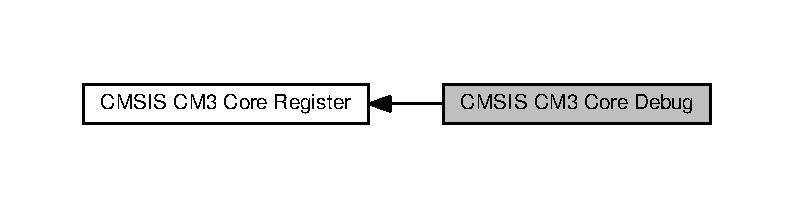
\includegraphics[width=350pt]{de/de9/group__CMSIS__CM3__CoreDebug}
\end{center}
\end{figure}
\subsection*{Data Structures}
\begin{DoxyCompactItemize}
\item 
struct \hyperlink{structCoreDebug__Type}{Core\+Debug\+\_\+\+Type}
\end{DoxyCompactItemize}
\subsection*{Macros}
\begin{DoxyCompactItemize}
\item 
\#define \hyperlink{group__CMSIS__CM3__CoreDebug_gac91280edd0ce932665cf75a23d11d842}{Core\+Debug\+\_\+\+D\+H\+C\+S\+R\+\_\+\+D\+B\+G\+K\+E\+Y\+\_\+\+Pos}~16
\item 
\#define \hyperlink{group__CMSIS__CM3__CoreDebug_ga1ce997cee15edaafe4aed77751816ffc}{Core\+Debug\+\_\+\+D\+H\+C\+S\+R\+\_\+\+D\+B\+G\+K\+E\+Y\+\_\+\+Msk}~(0x\+F\+F\+F\+Ful $<$$<$ Core\+Debug\+\_\+\+D\+H\+C\+S\+R\+\_\+\+D\+B\+G\+K\+E\+Y\+\_\+\+Pos)
\item 
\#define \hyperlink{group__CMSIS__CM3__CoreDebug_ga6f934c5427ea057394268e541fa97753}{Core\+Debug\+\_\+\+D\+H\+C\+S\+R\+\_\+\+S\+\_\+\+R\+E\+S\+E\+T\+\_\+\+S\+T\+\_\+\+Pos}~25
\item 
\#define \hyperlink{group__CMSIS__CM3__CoreDebug_gac474394bcceb31a8e09566c90b3f8922}{Core\+Debug\+\_\+\+D\+H\+C\+S\+R\+\_\+\+S\+\_\+\+R\+E\+S\+E\+T\+\_\+\+S\+T\+\_\+\+Msk}~(1ul $<$$<$ Core\+Debug\+\_\+\+D\+H\+C\+S\+R\+\_\+\+S\+\_\+\+R\+E\+S\+E\+T\+\_\+\+S\+T\+\_\+\+Pos)
\item 
\#define \hyperlink{group__CMSIS__CM3__CoreDebug_ga2328118f8b3574c871a53605eb17e730}{Core\+Debug\+\_\+\+D\+H\+C\+S\+R\+\_\+\+S\+\_\+\+R\+E\+T\+I\+R\+E\+\_\+\+S\+T\+\_\+\+Pos}~24
\item 
\#define \hyperlink{group__CMSIS__CM3__CoreDebug_ga89dceb5325f6bcb36a0473d65fbfcfa6}{Core\+Debug\+\_\+\+D\+H\+C\+S\+R\+\_\+\+S\+\_\+\+R\+E\+T\+I\+R\+E\+\_\+\+S\+T\+\_\+\+Msk}~(1ul $<$$<$ Core\+Debug\+\_\+\+D\+H\+C\+S\+R\+\_\+\+S\+\_\+\+R\+E\+T\+I\+R\+E\+\_\+\+S\+T\+\_\+\+Pos)
\item 
\#define \hyperlink{group__CMSIS__CM3__CoreDebug_ga2900dd56a988a4ed27ad664d5642807e}{Core\+Debug\+\_\+\+D\+H\+C\+S\+R\+\_\+\+S\+\_\+\+L\+O\+C\+K\+U\+P\+\_\+\+Pos}~19
\item 
\#define \hyperlink{group__CMSIS__CM3__CoreDebug_ga7b67e4506d7f464ef5dafd6219739756}{Core\+Debug\+\_\+\+D\+H\+C\+S\+R\+\_\+\+S\+\_\+\+L\+O\+C\+K\+U\+P\+\_\+\+Msk}~(1ul $<$$<$ Core\+Debug\+\_\+\+D\+H\+C\+S\+R\+\_\+\+S\+\_\+\+L\+O\+C\+K\+U\+P\+\_\+\+Pos)
\item 
\#define \hyperlink{group__CMSIS__CM3__CoreDebug_ga349ccea33accc705595624c2d334fbcb}{Core\+Debug\+\_\+\+D\+H\+C\+S\+R\+\_\+\+S\+\_\+\+S\+L\+E\+E\+P\+\_\+\+Pos}~18
\item 
\#define \hyperlink{group__CMSIS__CM3__CoreDebug_ga98d51538e645c2c1a422279cd85a0a25}{Core\+Debug\+\_\+\+D\+H\+C\+S\+R\+\_\+\+S\+\_\+\+S\+L\+E\+E\+P\+\_\+\+Msk}~(1ul $<$$<$ Core\+Debug\+\_\+\+D\+H\+C\+S\+R\+\_\+\+S\+\_\+\+S\+L\+E\+E\+P\+\_\+\+Pos)
\item 
\#define \hyperlink{group__CMSIS__CM3__CoreDebug_ga760a9a0d7f39951dc3f07d01f1f64772}{Core\+Debug\+\_\+\+D\+H\+C\+S\+R\+\_\+\+S\+\_\+\+H\+A\+L\+T\+\_\+\+Pos}~17
\item 
\#define \hyperlink{group__CMSIS__CM3__CoreDebug_ga9f881ade3151a73bc5b02b73fe6473ca}{Core\+Debug\+\_\+\+D\+H\+C\+S\+R\+\_\+\+S\+\_\+\+H\+A\+L\+T\+\_\+\+Msk}~(1ul $<$$<$ Core\+Debug\+\_\+\+D\+H\+C\+S\+R\+\_\+\+S\+\_\+\+H\+A\+L\+T\+\_\+\+Pos)
\item 
\#define \hyperlink{group__CMSIS__CM3__CoreDebug_ga20a71871ca8768019c51168c70c3f41d}{Core\+Debug\+\_\+\+D\+H\+C\+S\+R\+\_\+\+S\+\_\+\+R\+E\+G\+R\+D\+Y\+\_\+\+Pos}~16
\item 
\#define \hyperlink{group__CMSIS__CM3__CoreDebug_gac4cd6f3178de48f473d8903e8c847c07}{Core\+Debug\+\_\+\+D\+H\+C\+S\+R\+\_\+\+S\+\_\+\+R\+E\+G\+R\+D\+Y\+\_\+\+Msk}~(1ul $<$$<$ Core\+Debug\+\_\+\+D\+H\+C\+S\+R\+\_\+\+S\+\_\+\+R\+E\+G\+R\+D\+Y\+\_\+\+Pos)
\item 
\#define \hyperlink{group__CMSIS__CM3__CoreDebug_ga85747214e2656df6b05ec72e4d22bd6d}{Core\+Debug\+\_\+\+D\+H\+C\+S\+R\+\_\+\+C\+\_\+\+S\+N\+A\+P\+S\+T\+A\+L\+L\+\_\+\+Pos}~5
\item 
\#define \hyperlink{group__CMSIS__CM3__CoreDebug_ga53aa99b2e39a67622f3b9973e079c2b4}{Core\+Debug\+\_\+\+D\+H\+C\+S\+R\+\_\+\+C\+\_\+\+S\+N\+A\+P\+S\+T\+A\+L\+L\+\_\+\+Msk}~(1ul $<$$<$ Core\+Debug\+\_\+\+D\+H\+C\+S\+R\+\_\+\+C\+\_\+\+S\+N\+A\+P\+S\+T\+A\+L\+L\+\_\+\+Pos)
\item 
\#define \hyperlink{group__CMSIS__CM3__CoreDebug_ga0d2907400eb948a4ea3886ca083ec8e3}{Core\+Debug\+\_\+\+D\+H\+C\+S\+R\+\_\+\+C\+\_\+\+M\+A\+S\+K\+I\+N\+T\+S\+\_\+\+Pos}~3
\item 
\#define \hyperlink{group__CMSIS__CM3__CoreDebug_ga77fe1ef3c4a729c1c82fb62a94a51c31}{Core\+Debug\+\_\+\+D\+H\+C\+S\+R\+\_\+\+C\+\_\+\+M\+A\+S\+K\+I\+N\+T\+S\+\_\+\+Msk}~(1ul $<$$<$ Core\+Debug\+\_\+\+D\+H\+C\+S\+R\+\_\+\+C\+\_\+\+M\+A\+S\+K\+I\+N\+T\+S\+\_\+\+Pos)
\item 
\#define \hyperlink{group__CMSIS__CM3__CoreDebug_gae1fc39e80de54c0339cbb1b298a9f0f9}{Core\+Debug\+\_\+\+D\+H\+C\+S\+R\+\_\+\+C\+\_\+\+S\+T\+E\+P\+\_\+\+Pos}~2
\item 
\#define \hyperlink{group__CMSIS__CM3__CoreDebug_gae6bda72fbd32cc5734ff3542170dc00d}{Core\+Debug\+\_\+\+D\+H\+C\+S\+R\+\_\+\+C\+\_\+\+S\+T\+E\+P\+\_\+\+Msk}~(1ul $<$$<$ Core\+Debug\+\_\+\+D\+H\+C\+S\+R\+\_\+\+C\+\_\+\+S\+T\+E\+P\+\_\+\+Pos)
\item 
\#define \hyperlink{group__CMSIS__CM3__CoreDebug_gaddf1d43f8857e4efc3dc4e6b15509692}{Core\+Debug\+\_\+\+D\+H\+C\+S\+R\+\_\+\+C\+\_\+\+H\+A\+L\+T\+\_\+\+Pos}~1
\item 
\#define \hyperlink{group__CMSIS__CM3__CoreDebug_ga1d905a3aa594eb2e8bb78bcc4da05b3f}{Core\+Debug\+\_\+\+D\+H\+C\+S\+R\+\_\+\+C\+\_\+\+H\+A\+L\+T\+\_\+\+Msk}~(1ul $<$$<$ Core\+Debug\+\_\+\+D\+H\+C\+S\+R\+\_\+\+C\+\_\+\+H\+A\+L\+T\+\_\+\+Pos)
\item 
\#define \hyperlink{group__CMSIS__CM3__CoreDebug_gab557abb5b172b74d2cf44efb9d824e4e}{Core\+Debug\+\_\+\+D\+H\+C\+S\+R\+\_\+\+C\+\_\+\+D\+E\+B\+U\+G\+E\+N\+\_\+\+Pos}~0
\item 
\#define \hyperlink{group__CMSIS__CM3__CoreDebug_gab815c741a4fc2a61988cd2fb7594210b}{Core\+Debug\+\_\+\+D\+H\+C\+S\+R\+\_\+\+C\+\_\+\+D\+E\+B\+U\+G\+E\+N\+\_\+\+Msk}~(1ul $<$$<$ Core\+Debug\+\_\+\+D\+H\+C\+S\+R\+\_\+\+C\+\_\+\+D\+E\+B\+U\+G\+E\+N\+\_\+\+Pos)
\item 
\#define \hyperlink{group__CMSIS__CM3__CoreDebug_ga51e75942fc0614bc9bb2c0e96fcdda9a}{Core\+Debug\+\_\+\+D\+C\+R\+S\+R\+\_\+\+R\+E\+G\+Wn\+R\+\_\+\+Pos}~16
\item 
\#define \hyperlink{group__CMSIS__CM3__CoreDebug_ga1eef4992d8f84bc6c0dffed1c87f90a5}{Core\+Debug\+\_\+\+D\+C\+R\+S\+R\+\_\+\+R\+E\+G\+Wn\+R\+\_\+\+Msk}~(1ul $<$$<$ Core\+Debug\+\_\+\+D\+C\+R\+S\+R\+\_\+\+R\+E\+G\+Wn\+R\+\_\+\+Pos)
\item 
\#define \hyperlink{group__CMSIS__CM3__CoreDebug_ga52182c8a9f63a52470244c0bc2064f7b}{Core\+Debug\+\_\+\+D\+C\+R\+S\+R\+\_\+\+R\+E\+G\+S\+E\+L\+\_\+\+Pos}~0
\item 
\#define \hyperlink{group__CMSIS__CM3__CoreDebug_ga17cafbd72b55030219ce5609baa7c01d}{Core\+Debug\+\_\+\+D\+C\+R\+S\+R\+\_\+\+R\+E\+G\+S\+E\+L\+\_\+\+Msk}~(0x1\+Ful $<$$<$ Core\+Debug\+\_\+\+D\+C\+R\+S\+R\+\_\+\+R\+E\+G\+S\+E\+L\+\_\+\+Pos)
\item 
\#define \hyperlink{group__CMSIS__CM3__CoreDebug_ga6ff2102b98f86540224819a1b767ba39}{Core\+Debug\+\_\+\+D\+E\+M\+C\+R\+\_\+\+T\+R\+C\+E\+N\+A\+\_\+\+Pos}~24
\item 
\#define \hyperlink{group__CMSIS__CM3__CoreDebug_ga5e99652c1df93b441257389f49407834}{Core\+Debug\+\_\+\+D\+E\+M\+C\+R\+\_\+\+T\+R\+C\+E\+N\+A\+\_\+\+Msk}~(1ul $<$$<$ Core\+Debug\+\_\+\+D\+E\+M\+C\+R\+\_\+\+T\+R\+C\+E\+N\+A\+\_\+\+Pos)
\item 
\#define \hyperlink{group__CMSIS__CM3__CoreDebug_ga341020a3b7450416d72544eaf8e57a64}{Core\+Debug\+\_\+\+D\+E\+M\+C\+R\+\_\+\+M\+O\+N\+\_\+\+R\+E\+Q\+\_\+\+Pos}~19
\item 
\#define \hyperlink{group__CMSIS__CM3__CoreDebug_gae6384cbe8045051186d13ef9cdeace95}{Core\+Debug\+\_\+\+D\+E\+M\+C\+R\+\_\+\+M\+O\+N\+\_\+\+R\+E\+Q\+\_\+\+Msk}~(1ul $<$$<$ Core\+Debug\+\_\+\+D\+E\+M\+C\+R\+\_\+\+M\+O\+N\+\_\+\+R\+E\+Q\+\_\+\+Pos)
\item 
\#define \hyperlink{group__CMSIS__CM3__CoreDebug_ga9ae10710684e14a1a534e785ef390e1b}{Core\+Debug\+\_\+\+D\+E\+M\+C\+R\+\_\+\+M\+O\+N\+\_\+\+S\+T\+E\+P\+\_\+\+Pos}~18
\item 
\#define \hyperlink{group__CMSIS__CM3__CoreDebug_ga2ded814556de96fc369de7ae9a7ceb98}{Core\+Debug\+\_\+\+D\+E\+M\+C\+R\+\_\+\+M\+O\+N\+\_\+\+S\+T\+E\+P\+\_\+\+Msk}~(1ul $<$$<$ Core\+Debug\+\_\+\+D\+E\+M\+C\+R\+\_\+\+M\+O\+N\+\_\+\+S\+T\+E\+P\+\_\+\+Pos)
\item 
\#define \hyperlink{group__CMSIS__CM3__CoreDebug_ga1e2f706a59e0d8131279af1c7e152f8d}{Core\+Debug\+\_\+\+D\+E\+M\+C\+R\+\_\+\+M\+O\+N\+\_\+\+P\+E\+N\+D\+\_\+\+Pos}~17
\item 
\#define \hyperlink{group__CMSIS__CM3__CoreDebug_ga68ec55930269fab78e733dcfa32392f8}{Core\+Debug\+\_\+\+D\+E\+M\+C\+R\+\_\+\+M\+O\+N\+\_\+\+P\+E\+N\+D\+\_\+\+Msk}~(1ul $<$$<$ Core\+Debug\+\_\+\+D\+E\+M\+C\+R\+\_\+\+M\+O\+N\+\_\+\+P\+E\+N\+D\+\_\+\+Pos)
\item 
\#define \hyperlink{group__CMSIS__CM3__CoreDebug_ga802829678f6871863ae9ecf60a10425c}{Core\+Debug\+\_\+\+D\+E\+M\+C\+R\+\_\+\+M\+O\+N\+\_\+\+E\+N\+\_\+\+Pos}~16
\item 
\#define \hyperlink{group__CMSIS__CM3__CoreDebug_gac2b46b9b65bf8d23027f255fc9641977}{Core\+Debug\+\_\+\+D\+E\+M\+C\+R\+\_\+\+M\+O\+N\+\_\+\+E\+N\+\_\+\+Msk}~(1ul $<$$<$ Core\+Debug\+\_\+\+D\+E\+M\+C\+R\+\_\+\+M\+O\+N\+\_\+\+E\+N\+\_\+\+Pos)
\item 
\#define \hyperlink{group__CMSIS__CM3__CoreDebug_gaed9f42053031a9a30cd8054623304c0a}{Core\+Debug\+\_\+\+D\+E\+M\+C\+R\+\_\+\+V\+C\+\_\+\+H\+A\+R\+D\+E\+R\+R\+\_\+\+Pos}~10
\item 
\#define \hyperlink{group__CMSIS__CM3__CoreDebug_ga803fc98c5bb85f10f0347b23794847d1}{Core\+Debug\+\_\+\+D\+E\+M\+C\+R\+\_\+\+V\+C\+\_\+\+H\+A\+R\+D\+E\+R\+R\+\_\+\+Msk}~(1ul $<$$<$ Core\+Debug\+\_\+\+D\+E\+M\+C\+R\+\_\+\+V\+C\+\_\+\+H\+A\+R\+D\+E\+R\+R\+\_\+\+Pos)
\item 
\#define \hyperlink{group__CMSIS__CM3__CoreDebug_ga22079a6e436f23b90308be97e19cf07e}{Core\+Debug\+\_\+\+D\+E\+M\+C\+R\+\_\+\+V\+C\+\_\+\+I\+N\+T\+E\+R\+R\+\_\+\+Pos}~9
\item 
\#define \hyperlink{group__CMSIS__CM3__CoreDebug_gad6815d8e3df302d2f0ff2c2c734ed29a}{Core\+Debug\+\_\+\+D\+E\+M\+C\+R\+\_\+\+V\+C\+\_\+\+I\+N\+T\+E\+R\+R\+\_\+\+Msk}~(1ul $<$$<$ Core\+Debug\+\_\+\+D\+E\+M\+C\+R\+\_\+\+V\+C\+\_\+\+I\+N\+T\+E\+R\+R\+\_\+\+Pos)
\item 
\#define \hyperlink{group__CMSIS__CM3__CoreDebug_gab8e3d8f0f9590a51bbf10f6da3ad6933}{Core\+Debug\+\_\+\+D\+E\+M\+C\+R\+\_\+\+V\+C\+\_\+\+B\+U\+S\+E\+R\+R\+\_\+\+Pos}~8
\item 
\#define \hyperlink{group__CMSIS__CM3__CoreDebug_ga9d29546aefe3ca8662a7fe48dd4a5b2b}{Core\+Debug\+\_\+\+D\+E\+M\+C\+R\+\_\+\+V\+C\+\_\+\+B\+U\+S\+E\+R\+R\+\_\+\+Msk}~(1ul $<$$<$ Core\+Debug\+\_\+\+D\+E\+M\+C\+R\+\_\+\+V\+C\+\_\+\+B\+U\+S\+E\+R\+R\+\_\+\+Pos)
\item 
\#define \hyperlink{group__CMSIS__CM3__CoreDebug_ga16f0d3d2ce1e1e8cd762d938ac56c4ac}{Core\+Debug\+\_\+\+D\+E\+M\+C\+R\+\_\+\+V\+C\+\_\+\+S\+T\+A\+T\+E\+R\+R\+\_\+\+Pos}~7
\item 
\#define \hyperlink{group__CMSIS__CM3__CoreDebug_gaa38b947d77672c48bba1280c0a642e19}{Core\+Debug\+\_\+\+D\+E\+M\+C\+R\+\_\+\+V\+C\+\_\+\+S\+T\+A\+T\+E\+R\+R\+\_\+\+Msk}~(1ul $<$$<$ Core\+Debug\+\_\+\+D\+E\+M\+C\+R\+\_\+\+V\+C\+\_\+\+S\+T\+A\+T\+E\+R\+R\+\_\+\+Pos)
\item 
\#define \hyperlink{group__CMSIS__CM3__CoreDebug_ga10fc7c53bca904c128bc8e1a03072d50}{Core\+Debug\+\_\+\+D\+E\+M\+C\+R\+\_\+\+V\+C\+\_\+\+C\+H\+K\+E\+R\+R\+\_\+\+Pos}~6
\item 
\#define \hyperlink{group__CMSIS__CM3__CoreDebug_ga2f98b461d19746ab2febfddebb73da6f}{Core\+Debug\+\_\+\+D\+E\+M\+C\+R\+\_\+\+V\+C\+\_\+\+C\+H\+K\+E\+R\+R\+\_\+\+Msk}~(1ul $<$$<$ Core\+Debug\+\_\+\+D\+E\+M\+C\+R\+\_\+\+V\+C\+\_\+\+C\+H\+K\+E\+R\+R\+\_\+\+Pos)
\item 
\#define \hyperlink{group__CMSIS__CM3__CoreDebug_gac9d13eb2add61f610d5ced1f7ad2adf8}{Core\+Debug\+\_\+\+D\+E\+M\+C\+R\+\_\+\+V\+C\+\_\+\+N\+O\+C\+P\+E\+R\+R\+\_\+\+Pos}~5
\item 
\#define \hyperlink{group__CMSIS__CM3__CoreDebug_ga03ee58b1b02fdbf21612809034562f1c}{Core\+Debug\+\_\+\+D\+E\+M\+C\+R\+\_\+\+V\+C\+\_\+\+N\+O\+C\+P\+E\+R\+R\+\_\+\+Msk}~(1ul $<$$<$ Core\+Debug\+\_\+\+D\+E\+M\+C\+R\+\_\+\+V\+C\+\_\+\+N\+O\+C\+P\+E\+R\+R\+\_\+\+Pos)
\item 
\#define \hyperlink{group__CMSIS__CM3__CoreDebug_ga444454f7c7748e76cd76c3809c887c41}{Core\+Debug\+\_\+\+D\+E\+M\+C\+R\+\_\+\+V\+C\+\_\+\+M\+M\+E\+R\+R\+\_\+\+Pos}~4
\item 
\#define \hyperlink{group__CMSIS__CM3__CoreDebug_gad420a9b60620584faaca6289e83d3a87}{Core\+Debug\+\_\+\+D\+E\+M\+C\+R\+\_\+\+V\+C\+\_\+\+M\+M\+E\+R\+R\+\_\+\+Msk}~(1ul $<$$<$ Core\+Debug\+\_\+\+D\+E\+M\+C\+R\+\_\+\+V\+C\+\_\+\+M\+M\+E\+R\+R\+\_\+\+Pos)
\item 
\#define \hyperlink{group__CMSIS__CM3__CoreDebug_ga9fcf09666f7063a7303117aa32a85d5a}{Core\+Debug\+\_\+\+D\+E\+M\+C\+R\+\_\+\+V\+C\+\_\+\+C\+O\+R\+E\+R\+E\+S\+E\+T\+\_\+\+Pos}~0
\item 
\#define \hyperlink{group__CMSIS__CM3__CoreDebug_ga906476e53c1e1487c30f3a1181df9e30}{Core\+Debug\+\_\+\+D\+E\+M\+C\+R\+\_\+\+V\+C\+\_\+\+C\+O\+R\+E\+R\+E\+S\+E\+T\+\_\+\+Msk}~(1ul $<$$<$ Core\+Debug\+\_\+\+D\+E\+M\+C\+R\+\_\+\+V\+C\+\_\+\+C\+O\+R\+E\+R\+E\+S\+E\+T\+\_\+\+Pos)
\end{DoxyCompactItemize}


\subsection{Detailed Description}
memory mapped structure for Core Debug Register 

\subsection{Macro Definition Documentation}
\index{C\+M\+S\+I\+S C\+M3 Core Debug@{C\+M\+S\+I\+S C\+M3 Core Debug}!Core\+Debug\+\_\+\+D\+C\+R\+S\+R\+\_\+\+R\+E\+G\+S\+E\+L\+\_\+\+Msk@{Core\+Debug\+\_\+\+D\+C\+R\+S\+R\+\_\+\+R\+E\+G\+S\+E\+L\+\_\+\+Msk}}
\index{Core\+Debug\+\_\+\+D\+C\+R\+S\+R\+\_\+\+R\+E\+G\+S\+E\+L\+\_\+\+Msk@{Core\+Debug\+\_\+\+D\+C\+R\+S\+R\+\_\+\+R\+E\+G\+S\+E\+L\+\_\+\+Msk}!C\+M\+S\+I\+S C\+M3 Core Debug@{C\+M\+S\+I\+S C\+M3 Core Debug}}
\subsubsection[{\texorpdfstring{Core\+Debug\+\_\+\+D\+C\+R\+S\+R\+\_\+\+R\+E\+G\+S\+E\+L\+\_\+\+Msk}{CoreDebug_DCRSR_REGSEL_Msk}}]{\setlength{\rightskip}{0pt plus 5cm}\#define Core\+Debug\+\_\+\+D\+C\+R\+S\+R\+\_\+\+R\+E\+G\+S\+E\+L\+\_\+\+Msk~(0x1\+Ful $<$$<$ Core\+Debug\+\_\+\+D\+C\+R\+S\+R\+\_\+\+R\+E\+G\+S\+E\+L\+\_\+\+Pos)}\hypertarget{group__CMSIS__CM3__CoreDebug_ga17cafbd72b55030219ce5609baa7c01d}{}\label{group__CMSIS__CM3__CoreDebug_ga17cafbd72b55030219ce5609baa7c01d}
Core\+Debug D\+C\+R\+SR\+: R\+E\+G\+S\+EL Mask \index{C\+M\+S\+I\+S C\+M3 Core Debug@{C\+M\+S\+I\+S C\+M3 Core Debug}!Core\+Debug\+\_\+\+D\+C\+R\+S\+R\+\_\+\+R\+E\+G\+S\+E\+L\+\_\+\+Pos@{Core\+Debug\+\_\+\+D\+C\+R\+S\+R\+\_\+\+R\+E\+G\+S\+E\+L\+\_\+\+Pos}}
\index{Core\+Debug\+\_\+\+D\+C\+R\+S\+R\+\_\+\+R\+E\+G\+S\+E\+L\+\_\+\+Pos@{Core\+Debug\+\_\+\+D\+C\+R\+S\+R\+\_\+\+R\+E\+G\+S\+E\+L\+\_\+\+Pos}!C\+M\+S\+I\+S C\+M3 Core Debug@{C\+M\+S\+I\+S C\+M3 Core Debug}}
\subsubsection[{\texorpdfstring{Core\+Debug\+\_\+\+D\+C\+R\+S\+R\+\_\+\+R\+E\+G\+S\+E\+L\+\_\+\+Pos}{CoreDebug_DCRSR_REGSEL_Pos}}]{\setlength{\rightskip}{0pt plus 5cm}\#define Core\+Debug\+\_\+\+D\+C\+R\+S\+R\+\_\+\+R\+E\+G\+S\+E\+L\+\_\+\+Pos~0}\hypertarget{group__CMSIS__CM3__CoreDebug_ga52182c8a9f63a52470244c0bc2064f7b}{}\label{group__CMSIS__CM3__CoreDebug_ga52182c8a9f63a52470244c0bc2064f7b}
Core\+Debug D\+C\+R\+SR\+: R\+E\+G\+S\+EL Position \index{C\+M\+S\+I\+S C\+M3 Core Debug@{C\+M\+S\+I\+S C\+M3 Core Debug}!Core\+Debug\+\_\+\+D\+C\+R\+S\+R\+\_\+\+R\+E\+G\+Wn\+R\+\_\+\+Msk@{Core\+Debug\+\_\+\+D\+C\+R\+S\+R\+\_\+\+R\+E\+G\+Wn\+R\+\_\+\+Msk}}
\index{Core\+Debug\+\_\+\+D\+C\+R\+S\+R\+\_\+\+R\+E\+G\+Wn\+R\+\_\+\+Msk@{Core\+Debug\+\_\+\+D\+C\+R\+S\+R\+\_\+\+R\+E\+G\+Wn\+R\+\_\+\+Msk}!C\+M\+S\+I\+S C\+M3 Core Debug@{C\+M\+S\+I\+S C\+M3 Core Debug}}
\subsubsection[{\texorpdfstring{Core\+Debug\+\_\+\+D\+C\+R\+S\+R\+\_\+\+R\+E\+G\+Wn\+R\+\_\+\+Msk}{CoreDebug_DCRSR_REGWnR_Msk}}]{\setlength{\rightskip}{0pt plus 5cm}\#define Core\+Debug\+\_\+\+D\+C\+R\+S\+R\+\_\+\+R\+E\+G\+Wn\+R\+\_\+\+Msk~(1ul $<$$<$ Core\+Debug\+\_\+\+D\+C\+R\+S\+R\+\_\+\+R\+E\+G\+Wn\+R\+\_\+\+Pos)}\hypertarget{group__CMSIS__CM3__CoreDebug_ga1eef4992d8f84bc6c0dffed1c87f90a5}{}\label{group__CMSIS__CM3__CoreDebug_ga1eef4992d8f84bc6c0dffed1c87f90a5}
Core\+Debug D\+C\+R\+SR\+: R\+E\+G\+WnR Mask \index{C\+M\+S\+I\+S C\+M3 Core Debug@{C\+M\+S\+I\+S C\+M3 Core Debug}!Core\+Debug\+\_\+\+D\+C\+R\+S\+R\+\_\+\+R\+E\+G\+Wn\+R\+\_\+\+Pos@{Core\+Debug\+\_\+\+D\+C\+R\+S\+R\+\_\+\+R\+E\+G\+Wn\+R\+\_\+\+Pos}}
\index{Core\+Debug\+\_\+\+D\+C\+R\+S\+R\+\_\+\+R\+E\+G\+Wn\+R\+\_\+\+Pos@{Core\+Debug\+\_\+\+D\+C\+R\+S\+R\+\_\+\+R\+E\+G\+Wn\+R\+\_\+\+Pos}!C\+M\+S\+I\+S C\+M3 Core Debug@{C\+M\+S\+I\+S C\+M3 Core Debug}}
\subsubsection[{\texorpdfstring{Core\+Debug\+\_\+\+D\+C\+R\+S\+R\+\_\+\+R\+E\+G\+Wn\+R\+\_\+\+Pos}{CoreDebug_DCRSR_REGWnR_Pos}}]{\setlength{\rightskip}{0pt plus 5cm}\#define Core\+Debug\+\_\+\+D\+C\+R\+S\+R\+\_\+\+R\+E\+G\+Wn\+R\+\_\+\+Pos~16}\hypertarget{group__CMSIS__CM3__CoreDebug_ga51e75942fc0614bc9bb2c0e96fcdda9a}{}\label{group__CMSIS__CM3__CoreDebug_ga51e75942fc0614bc9bb2c0e96fcdda9a}
Core\+Debug D\+C\+R\+SR\+: R\+E\+G\+WnR Position \index{C\+M\+S\+I\+S C\+M3 Core Debug@{C\+M\+S\+I\+S C\+M3 Core Debug}!Core\+Debug\+\_\+\+D\+E\+M\+C\+R\+\_\+\+M\+O\+N\+\_\+\+E\+N\+\_\+\+Msk@{Core\+Debug\+\_\+\+D\+E\+M\+C\+R\+\_\+\+M\+O\+N\+\_\+\+E\+N\+\_\+\+Msk}}
\index{Core\+Debug\+\_\+\+D\+E\+M\+C\+R\+\_\+\+M\+O\+N\+\_\+\+E\+N\+\_\+\+Msk@{Core\+Debug\+\_\+\+D\+E\+M\+C\+R\+\_\+\+M\+O\+N\+\_\+\+E\+N\+\_\+\+Msk}!C\+M\+S\+I\+S C\+M3 Core Debug@{C\+M\+S\+I\+S C\+M3 Core Debug}}
\subsubsection[{\texorpdfstring{Core\+Debug\+\_\+\+D\+E\+M\+C\+R\+\_\+\+M\+O\+N\+\_\+\+E\+N\+\_\+\+Msk}{CoreDebug_DEMCR_MON_EN_Msk}}]{\setlength{\rightskip}{0pt plus 5cm}\#define Core\+Debug\+\_\+\+D\+E\+M\+C\+R\+\_\+\+M\+O\+N\+\_\+\+E\+N\+\_\+\+Msk~(1ul $<$$<$ Core\+Debug\+\_\+\+D\+E\+M\+C\+R\+\_\+\+M\+O\+N\+\_\+\+E\+N\+\_\+\+Pos)}\hypertarget{group__CMSIS__CM3__CoreDebug_gac2b46b9b65bf8d23027f255fc9641977}{}\label{group__CMSIS__CM3__CoreDebug_gac2b46b9b65bf8d23027f255fc9641977}
Core\+Debug D\+E\+M\+CR\+: M\+O\+N\+\_\+\+EN Mask \index{C\+M\+S\+I\+S C\+M3 Core Debug@{C\+M\+S\+I\+S C\+M3 Core Debug}!Core\+Debug\+\_\+\+D\+E\+M\+C\+R\+\_\+\+M\+O\+N\+\_\+\+E\+N\+\_\+\+Pos@{Core\+Debug\+\_\+\+D\+E\+M\+C\+R\+\_\+\+M\+O\+N\+\_\+\+E\+N\+\_\+\+Pos}}
\index{Core\+Debug\+\_\+\+D\+E\+M\+C\+R\+\_\+\+M\+O\+N\+\_\+\+E\+N\+\_\+\+Pos@{Core\+Debug\+\_\+\+D\+E\+M\+C\+R\+\_\+\+M\+O\+N\+\_\+\+E\+N\+\_\+\+Pos}!C\+M\+S\+I\+S C\+M3 Core Debug@{C\+M\+S\+I\+S C\+M3 Core Debug}}
\subsubsection[{\texorpdfstring{Core\+Debug\+\_\+\+D\+E\+M\+C\+R\+\_\+\+M\+O\+N\+\_\+\+E\+N\+\_\+\+Pos}{CoreDebug_DEMCR_MON_EN_Pos}}]{\setlength{\rightskip}{0pt plus 5cm}\#define Core\+Debug\+\_\+\+D\+E\+M\+C\+R\+\_\+\+M\+O\+N\+\_\+\+E\+N\+\_\+\+Pos~16}\hypertarget{group__CMSIS__CM3__CoreDebug_ga802829678f6871863ae9ecf60a10425c}{}\label{group__CMSIS__CM3__CoreDebug_ga802829678f6871863ae9ecf60a10425c}
Core\+Debug D\+E\+M\+CR\+: M\+O\+N\+\_\+\+EN Position \index{C\+M\+S\+I\+S C\+M3 Core Debug@{C\+M\+S\+I\+S C\+M3 Core Debug}!Core\+Debug\+\_\+\+D\+E\+M\+C\+R\+\_\+\+M\+O\+N\+\_\+\+P\+E\+N\+D\+\_\+\+Msk@{Core\+Debug\+\_\+\+D\+E\+M\+C\+R\+\_\+\+M\+O\+N\+\_\+\+P\+E\+N\+D\+\_\+\+Msk}}
\index{Core\+Debug\+\_\+\+D\+E\+M\+C\+R\+\_\+\+M\+O\+N\+\_\+\+P\+E\+N\+D\+\_\+\+Msk@{Core\+Debug\+\_\+\+D\+E\+M\+C\+R\+\_\+\+M\+O\+N\+\_\+\+P\+E\+N\+D\+\_\+\+Msk}!C\+M\+S\+I\+S C\+M3 Core Debug@{C\+M\+S\+I\+S C\+M3 Core Debug}}
\subsubsection[{\texorpdfstring{Core\+Debug\+\_\+\+D\+E\+M\+C\+R\+\_\+\+M\+O\+N\+\_\+\+P\+E\+N\+D\+\_\+\+Msk}{CoreDebug_DEMCR_MON_PEND_Msk}}]{\setlength{\rightskip}{0pt plus 5cm}\#define Core\+Debug\+\_\+\+D\+E\+M\+C\+R\+\_\+\+M\+O\+N\+\_\+\+P\+E\+N\+D\+\_\+\+Msk~(1ul $<$$<$ Core\+Debug\+\_\+\+D\+E\+M\+C\+R\+\_\+\+M\+O\+N\+\_\+\+P\+E\+N\+D\+\_\+\+Pos)}\hypertarget{group__CMSIS__CM3__CoreDebug_ga68ec55930269fab78e733dcfa32392f8}{}\label{group__CMSIS__CM3__CoreDebug_ga68ec55930269fab78e733dcfa32392f8}
Core\+Debug D\+E\+M\+CR\+: M\+O\+N\+\_\+\+P\+E\+ND Mask \index{C\+M\+S\+I\+S C\+M3 Core Debug@{C\+M\+S\+I\+S C\+M3 Core Debug}!Core\+Debug\+\_\+\+D\+E\+M\+C\+R\+\_\+\+M\+O\+N\+\_\+\+P\+E\+N\+D\+\_\+\+Pos@{Core\+Debug\+\_\+\+D\+E\+M\+C\+R\+\_\+\+M\+O\+N\+\_\+\+P\+E\+N\+D\+\_\+\+Pos}}
\index{Core\+Debug\+\_\+\+D\+E\+M\+C\+R\+\_\+\+M\+O\+N\+\_\+\+P\+E\+N\+D\+\_\+\+Pos@{Core\+Debug\+\_\+\+D\+E\+M\+C\+R\+\_\+\+M\+O\+N\+\_\+\+P\+E\+N\+D\+\_\+\+Pos}!C\+M\+S\+I\+S C\+M3 Core Debug@{C\+M\+S\+I\+S C\+M3 Core Debug}}
\subsubsection[{\texorpdfstring{Core\+Debug\+\_\+\+D\+E\+M\+C\+R\+\_\+\+M\+O\+N\+\_\+\+P\+E\+N\+D\+\_\+\+Pos}{CoreDebug_DEMCR_MON_PEND_Pos}}]{\setlength{\rightskip}{0pt plus 5cm}\#define Core\+Debug\+\_\+\+D\+E\+M\+C\+R\+\_\+\+M\+O\+N\+\_\+\+P\+E\+N\+D\+\_\+\+Pos~17}\hypertarget{group__CMSIS__CM3__CoreDebug_ga1e2f706a59e0d8131279af1c7e152f8d}{}\label{group__CMSIS__CM3__CoreDebug_ga1e2f706a59e0d8131279af1c7e152f8d}
Core\+Debug D\+E\+M\+CR\+: M\+O\+N\+\_\+\+P\+E\+ND Position \index{C\+M\+S\+I\+S C\+M3 Core Debug@{C\+M\+S\+I\+S C\+M3 Core Debug}!Core\+Debug\+\_\+\+D\+E\+M\+C\+R\+\_\+\+M\+O\+N\+\_\+\+R\+E\+Q\+\_\+\+Msk@{Core\+Debug\+\_\+\+D\+E\+M\+C\+R\+\_\+\+M\+O\+N\+\_\+\+R\+E\+Q\+\_\+\+Msk}}
\index{Core\+Debug\+\_\+\+D\+E\+M\+C\+R\+\_\+\+M\+O\+N\+\_\+\+R\+E\+Q\+\_\+\+Msk@{Core\+Debug\+\_\+\+D\+E\+M\+C\+R\+\_\+\+M\+O\+N\+\_\+\+R\+E\+Q\+\_\+\+Msk}!C\+M\+S\+I\+S C\+M3 Core Debug@{C\+M\+S\+I\+S C\+M3 Core Debug}}
\subsubsection[{\texorpdfstring{Core\+Debug\+\_\+\+D\+E\+M\+C\+R\+\_\+\+M\+O\+N\+\_\+\+R\+E\+Q\+\_\+\+Msk}{CoreDebug_DEMCR_MON_REQ_Msk}}]{\setlength{\rightskip}{0pt plus 5cm}\#define Core\+Debug\+\_\+\+D\+E\+M\+C\+R\+\_\+\+M\+O\+N\+\_\+\+R\+E\+Q\+\_\+\+Msk~(1ul $<$$<$ Core\+Debug\+\_\+\+D\+E\+M\+C\+R\+\_\+\+M\+O\+N\+\_\+\+R\+E\+Q\+\_\+\+Pos)}\hypertarget{group__CMSIS__CM3__CoreDebug_gae6384cbe8045051186d13ef9cdeace95}{}\label{group__CMSIS__CM3__CoreDebug_gae6384cbe8045051186d13ef9cdeace95}
Core\+Debug D\+E\+M\+CR\+: M\+O\+N\+\_\+\+R\+EQ Mask \index{C\+M\+S\+I\+S C\+M3 Core Debug@{C\+M\+S\+I\+S C\+M3 Core Debug}!Core\+Debug\+\_\+\+D\+E\+M\+C\+R\+\_\+\+M\+O\+N\+\_\+\+R\+E\+Q\+\_\+\+Pos@{Core\+Debug\+\_\+\+D\+E\+M\+C\+R\+\_\+\+M\+O\+N\+\_\+\+R\+E\+Q\+\_\+\+Pos}}
\index{Core\+Debug\+\_\+\+D\+E\+M\+C\+R\+\_\+\+M\+O\+N\+\_\+\+R\+E\+Q\+\_\+\+Pos@{Core\+Debug\+\_\+\+D\+E\+M\+C\+R\+\_\+\+M\+O\+N\+\_\+\+R\+E\+Q\+\_\+\+Pos}!C\+M\+S\+I\+S C\+M3 Core Debug@{C\+M\+S\+I\+S C\+M3 Core Debug}}
\subsubsection[{\texorpdfstring{Core\+Debug\+\_\+\+D\+E\+M\+C\+R\+\_\+\+M\+O\+N\+\_\+\+R\+E\+Q\+\_\+\+Pos}{CoreDebug_DEMCR_MON_REQ_Pos}}]{\setlength{\rightskip}{0pt plus 5cm}\#define Core\+Debug\+\_\+\+D\+E\+M\+C\+R\+\_\+\+M\+O\+N\+\_\+\+R\+E\+Q\+\_\+\+Pos~19}\hypertarget{group__CMSIS__CM3__CoreDebug_ga341020a3b7450416d72544eaf8e57a64}{}\label{group__CMSIS__CM3__CoreDebug_ga341020a3b7450416d72544eaf8e57a64}
Core\+Debug D\+E\+M\+CR\+: M\+O\+N\+\_\+\+R\+EQ Position \index{C\+M\+S\+I\+S C\+M3 Core Debug@{C\+M\+S\+I\+S C\+M3 Core Debug}!Core\+Debug\+\_\+\+D\+E\+M\+C\+R\+\_\+\+M\+O\+N\+\_\+\+S\+T\+E\+P\+\_\+\+Msk@{Core\+Debug\+\_\+\+D\+E\+M\+C\+R\+\_\+\+M\+O\+N\+\_\+\+S\+T\+E\+P\+\_\+\+Msk}}
\index{Core\+Debug\+\_\+\+D\+E\+M\+C\+R\+\_\+\+M\+O\+N\+\_\+\+S\+T\+E\+P\+\_\+\+Msk@{Core\+Debug\+\_\+\+D\+E\+M\+C\+R\+\_\+\+M\+O\+N\+\_\+\+S\+T\+E\+P\+\_\+\+Msk}!C\+M\+S\+I\+S C\+M3 Core Debug@{C\+M\+S\+I\+S C\+M3 Core Debug}}
\subsubsection[{\texorpdfstring{Core\+Debug\+\_\+\+D\+E\+M\+C\+R\+\_\+\+M\+O\+N\+\_\+\+S\+T\+E\+P\+\_\+\+Msk}{CoreDebug_DEMCR_MON_STEP_Msk}}]{\setlength{\rightskip}{0pt plus 5cm}\#define Core\+Debug\+\_\+\+D\+E\+M\+C\+R\+\_\+\+M\+O\+N\+\_\+\+S\+T\+E\+P\+\_\+\+Msk~(1ul $<$$<$ Core\+Debug\+\_\+\+D\+E\+M\+C\+R\+\_\+\+M\+O\+N\+\_\+\+S\+T\+E\+P\+\_\+\+Pos)}\hypertarget{group__CMSIS__CM3__CoreDebug_ga2ded814556de96fc369de7ae9a7ceb98}{}\label{group__CMSIS__CM3__CoreDebug_ga2ded814556de96fc369de7ae9a7ceb98}
Core\+Debug D\+E\+M\+CR\+: M\+O\+N\+\_\+\+S\+T\+EP Mask \index{C\+M\+S\+I\+S C\+M3 Core Debug@{C\+M\+S\+I\+S C\+M3 Core Debug}!Core\+Debug\+\_\+\+D\+E\+M\+C\+R\+\_\+\+M\+O\+N\+\_\+\+S\+T\+E\+P\+\_\+\+Pos@{Core\+Debug\+\_\+\+D\+E\+M\+C\+R\+\_\+\+M\+O\+N\+\_\+\+S\+T\+E\+P\+\_\+\+Pos}}
\index{Core\+Debug\+\_\+\+D\+E\+M\+C\+R\+\_\+\+M\+O\+N\+\_\+\+S\+T\+E\+P\+\_\+\+Pos@{Core\+Debug\+\_\+\+D\+E\+M\+C\+R\+\_\+\+M\+O\+N\+\_\+\+S\+T\+E\+P\+\_\+\+Pos}!C\+M\+S\+I\+S C\+M3 Core Debug@{C\+M\+S\+I\+S C\+M3 Core Debug}}
\subsubsection[{\texorpdfstring{Core\+Debug\+\_\+\+D\+E\+M\+C\+R\+\_\+\+M\+O\+N\+\_\+\+S\+T\+E\+P\+\_\+\+Pos}{CoreDebug_DEMCR_MON_STEP_Pos}}]{\setlength{\rightskip}{0pt plus 5cm}\#define Core\+Debug\+\_\+\+D\+E\+M\+C\+R\+\_\+\+M\+O\+N\+\_\+\+S\+T\+E\+P\+\_\+\+Pos~18}\hypertarget{group__CMSIS__CM3__CoreDebug_ga9ae10710684e14a1a534e785ef390e1b}{}\label{group__CMSIS__CM3__CoreDebug_ga9ae10710684e14a1a534e785ef390e1b}
Core\+Debug D\+E\+M\+CR\+: M\+O\+N\+\_\+\+S\+T\+EP Position \index{C\+M\+S\+I\+S C\+M3 Core Debug@{C\+M\+S\+I\+S C\+M3 Core Debug}!Core\+Debug\+\_\+\+D\+E\+M\+C\+R\+\_\+\+T\+R\+C\+E\+N\+A\+\_\+\+Msk@{Core\+Debug\+\_\+\+D\+E\+M\+C\+R\+\_\+\+T\+R\+C\+E\+N\+A\+\_\+\+Msk}}
\index{Core\+Debug\+\_\+\+D\+E\+M\+C\+R\+\_\+\+T\+R\+C\+E\+N\+A\+\_\+\+Msk@{Core\+Debug\+\_\+\+D\+E\+M\+C\+R\+\_\+\+T\+R\+C\+E\+N\+A\+\_\+\+Msk}!C\+M\+S\+I\+S C\+M3 Core Debug@{C\+M\+S\+I\+S C\+M3 Core Debug}}
\subsubsection[{\texorpdfstring{Core\+Debug\+\_\+\+D\+E\+M\+C\+R\+\_\+\+T\+R\+C\+E\+N\+A\+\_\+\+Msk}{CoreDebug_DEMCR_TRCENA_Msk}}]{\setlength{\rightskip}{0pt plus 5cm}\#define Core\+Debug\+\_\+\+D\+E\+M\+C\+R\+\_\+\+T\+R\+C\+E\+N\+A\+\_\+\+Msk~(1ul $<$$<$ Core\+Debug\+\_\+\+D\+E\+M\+C\+R\+\_\+\+T\+R\+C\+E\+N\+A\+\_\+\+Pos)}\hypertarget{group__CMSIS__CM3__CoreDebug_ga5e99652c1df93b441257389f49407834}{}\label{group__CMSIS__CM3__CoreDebug_ga5e99652c1df93b441257389f49407834}
Core\+Debug D\+E\+M\+CR\+: T\+R\+C\+E\+NA Mask \index{C\+M\+S\+I\+S C\+M3 Core Debug@{C\+M\+S\+I\+S C\+M3 Core Debug}!Core\+Debug\+\_\+\+D\+E\+M\+C\+R\+\_\+\+T\+R\+C\+E\+N\+A\+\_\+\+Pos@{Core\+Debug\+\_\+\+D\+E\+M\+C\+R\+\_\+\+T\+R\+C\+E\+N\+A\+\_\+\+Pos}}
\index{Core\+Debug\+\_\+\+D\+E\+M\+C\+R\+\_\+\+T\+R\+C\+E\+N\+A\+\_\+\+Pos@{Core\+Debug\+\_\+\+D\+E\+M\+C\+R\+\_\+\+T\+R\+C\+E\+N\+A\+\_\+\+Pos}!C\+M\+S\+I\+S C\+M3 Core Debug@{C\+M\+S\+I\+S C\+M3 Core Debug}}
\subsubsection[{\texorpdfstring{Core\+Debug\+\_\+\+D\+E\+M\+C\+R\+\_\+\+T\+R\+C\+E\+N\+A\+\_\+\+Pos}{CoreDebug_DEMCR_TRCENA_Pos}}]{\setlength{\rightskip}{0pt plus 5cm}\#define Core\+Debug\+\_\+\+D\+E\+M\+C\+R\+\_\+\+T\+R\+C\+E\+N\+A\+\_\+\+Pos~24}\hypertarget{group__CMSIS__CM3__CoreDebug_ga6ff2102b98f86540224819a1b767ba39}{}\label{group__CMSIS__CM3__CoreDebug_ga6ff2102b98f86540224819a1b767ba39}
Core\+Debug D\+E\+M\+CR\+: T\+R\+C\+E\+NA Position \index{C\+M\+S\+I\+S C\+M3 Core Debug@{C\+M\+S\+I\+S C\+M3 Core Debug}!Core\+Debug\+\_\+\+D\+E\+M\+C\+R\+\_\+\+V\+C\+\_\+\+B\+U\+S\+E\+R\+R\+\_\+\+Msk@{Core\+Debug\+\_\+\+D\+E\+M\+C\+R\+\_\+\+V\+C\+\_\+\+B\+U\+S\+E\+R\+R\+\_\+\+Msk}}
\index{Core\+Debug\+\_\+\+D\+E\+M\+C\+R\+\_\+\+V\+C\+\_\+\+B\+U\+S\+E\+R\+R\+\_\+\+Msk@{Core\+Debug\+\_\+\+D\+E\+M\+C\+R\+\_\+\+V\+C\+\_\+\+B\+U\+S\+E\+R\+R\+\_\+\+Msk}!C\+M\+S\+I\+S C\+M3 Core Debug@{C\+M\+S\+I\+S C\+M3 Core Debug}}
\subsubsection[{\texorpdfstring{Core\+Debug\+\_\+\+D\+E\+M\+C\+R\+\_\+\+V\+C\+\_\+\+B\+U\+S\+E\+R\+R\+\_\+\+Msk}{CoreDebug_DEMCR_VC_BUSERR_Msk}}]{\setlength{\rightskip}{0pt plus 5cm}\#define Core\+Debug\+\_\+\+D\+E\+M\+C\+R\+\_\+\+V\+C\+\_\+\+B\+U\+S\+E\+R\+R\+\_\+\+Msk~(1ul $<$$<$ Core\+Debug\+\_\+\+D\+E\+M\+C\+R\+\_\+\+V\+C\+\_\+\+B\+U\+S\+E\+R\+R\+\_\+\+Pos)}\hypertarget{group__CMSIS__CM3__CoreDebug_ga9d29546aefe3ca8662a7fe48dd4a5b2b}{}\label{group__CMSIS__CM3__CoreDebug_ga9d29546aefe3ca8662a7fe48dd4a5b2b}
Core\+Debug D\+E\+M\+CR\+: V\+C\+\_\+\+B\+U\+S\+E\+RR Mask \index{C\+M\+S\+I\+S C\+M3 Core Debug@{C\+M\+S\+I\+S C\+M3 Core Debug}!Core\+Debug\+\_\+\+D\+E\+M\+C\+R\+\_\+\+V\+C\+\_\+\+B\+U\+S\+E\+R\+R\+\_\+\+Pos@{Core\+Debug\+\_\+\+D\+E\+M\+C\+R\+\_\+\+V\+C\+\_\+\+B\+U\+S\+E\+R\+R\+\_\+\+Pos}}
\index{Core\+Debug\+\_\+\+D\+E\+M\+C\+R\+\_\+\+V\+C\+\_\+\+B\+U\+S\+E\+R\+R\+\_\+\+Pos@{Core\+Debug\+\_\+\+D\+E\+M\+C\+R\+\_\+\+V\+C\+\_\+\+B\+U\+S\+E\+R\+R\+\_\+\+Pos}!C\+M\+S\+I\+S C\+M3 Core Debug@{C\+M\+S\+I\+S C\+M3 Core Debug}}
\subsubsection[{\texorpdfstring{Core\+Debug\+\_\+\+D\+E\+M\+C\+R\+\_\+\+V\+C\+\_\+\+B\+U\+S\+E\+R\+R\+\_\+\+Pos}{CoreDebug_DEMCR_VC_BUSERR_Pos}}]{\setlength{\rightskip}{0pt plus 5cm}\#define Core\+Debug\+\_\+\+D\+E\+M\+C\+R\+\_\+\+V\+C\+\_\+\+B\+U\+S\+E\+R\+R\+\_\+\+Pos~8}\hypertarget{group__CMSIS__CM3__CoreDebug_gab8e3d8f0f9590a51bbf10f6da3ad6933}{}\label{group__CMSIS__CM3__CoreDebug_gab8e3d8f0f9590a51bbf10f6da3ad6933}
Core\+Debug D\+E\+M\+CR\+: V\+C\+\_\+\+B\+U\+S\+E\+RR Position \index{C\+M\+S\+I\+S C\+M3 Core Debug@{C\+M\+S\+I\+S C\+M3 Core Debug}!Core\+Debug\+\_\+\+D\+E\+M\+C\+R\+\_\+\+V\+C\+\_\+\+C\+H\+K\+E\+R\+R\+\_\+\+Msk@{Core\+Debug\+\_\+\+D\+E\+M\+C\+R\+\_\+\+V\+C\+\_\+\+C\+H\+K\+E\+R\+R\+\_\+\+Msk}}
\index{Core\+Debug\+\_\+\+D\+E\+M\+C\+R\+\_\+\+V\+C\+\_\+\+C\+H\+K\+E\+R\+R\+\_\+\+Msk@{Core\+Debug\+\_\+\+D\+E\+M\+C\+R\+\_\+\+V\+C\+\_\+\+C\+H\+K\+E\+R\+R\+\_\+\+Msk}!C\+M\+S\+I\+S C\+M3 Core Debug@{C\+M\+S\+I\+S C\+M3 Core Debug}}
\subsubsection[{\texorpdfstring{Core\+Debug\+\_\+\+D\+E\+M\+C\+R\+\_\+\+V\+C\+\_\+\+C\+H\+K\+E\+R\+R\+\_\+\+Msk}{CoreDebug_DEMCR_VC_CHKERR_Msk}}]{\setlength{\rightskip}{0pt plus 5cm}\#define Core\+Debug\+\_\+\+D\+E\+M\+C\+R\+\_\+\+V\+C\+\_\+\+C\+H\+K\+E\+R\+R\+\_\+\+Msk~(1ul $<$$<$ Core\+Debug\+\_\+\+D\+E\+M\+C\+R\+\_\+\+V\+C\+\_\+\+C\+H\+K\+E\+R\+R\+\_\+\+Pos)}\hypertarget{group__CMSIS__CM3__CoreDebug_ga2f98b461d19746ab2febfddebb73da6f}{}\label{group__CMSIS__CM3__CoreDebug_ga2f98b461d19746ab2febfddebb73da6f}
Core\+Debug D\+E\+M\+CR\+: V\+C\+\_\+\+C\+H\+K\+E\+RR Mask \index{C\+M\+S\+I\+S C\+M3 Core Debug@{C\+M\+S\+I\+S C\+M3 Core Debug}!Core\+Debug\+\_\+\+D\+E\+M\+C\+R\+\_\+\+V\+C\+\_\+\+C\+H\+K\+E\+R\+R\+\_\+\+Pos@{Core\+Debug\+\_\+\+D\+E\+M\+C\+R\+\_\+\+V\+C\+\_\+\+C\+H\+K\+E\+R\+R\+\_\+\+Pos}}
\index{Core\+Debug\+\_\+\+D\+E\+M\+C\+R\+\_\+\+V\+C\+\_\+\+C\+H\+K\+E\+R\+R\+\_\+\+Pos@{Core\+Debug\+\_\+\+D\+E\+M\+C\+R\+\_\+\+V\+C\+\_\+\+C\+H\+K\+E\+R\+R\+\_\+\+Pos}!C\+M\+S\+I\+S C\+M3 Core Debug@{C\+M\+S\+I\+S C\+M3 Core Debug}}
\subsubsection[{\texorpdfstring{Core\+Debug\+\_\+\+D\+E\+M\+C\+R\+\_\+\+V\+C\+\_\+\+C\+H\+K\+E\+R\+R\+\_\+\+Pos}{CoreDebug_DEMCR_VC_CHKERR_Pos}}]{\setlength{\rightskip}{0pt plus 5cm}\#define Core\+Debug\+\_\+\+D\+E\+M\+C\+R\+\_\+\+V\+C\+\_\+\+C\+H\+K\+E\+R\+R\+\_\+\+Pos~6}\hypertarget{group__CMSIS__CM3__CoreDebug_ga10fc7c53bca904c128bc8e1a03072d50}{}\label{group__CMSIS__CM3__CoreDebug_ga10fc7c53bca904c128bc8e1a03072d50}
Core\+Debug D\+E\+M\+CR\+: V\+C\+\_\+\+C\+H\+K\+E\+RR Position \index{C\+M\+S\+I\+S C\+M3 Core Debug@{C\+M\+S\+I\+S C\+M3 Core Debug}!Core\+Debug\+\_\+\+D\+E\+M\+C\+R\+\_\+\+V\+C\+\_\+\+C\+O\+R\+E\+R\+E\+S\+E\+T\+\_\+\+Msk@{Core\+Debug\+\_\+\+D\+E\+M\+C\+R\+\_\+\+V\+C\+\_\+\+C\+O\+R\+E\+R\+E\+S\+E\+T\+\_\+\+Msk}}
\index{Core\+Debug\+\_\+\+D\+E\+M\+C\+R\+\_\+\+V\+C\+\_\+\+C\+O\+R\+E\+R\+E\+S\+E\+T\+\_\+\+Msk@{Core\+Debug\+\_\+\+D\+E\+M\+C\+R\+\_\+\+V\+C\+\_\+\+C\+O\+R\+E\+R\+E\+S\+E\+T\+\_\+\+Msk}!C\+M\+S\+I\+S C\+M3 Core Debug@{C\+M\+S\+I\+S C\+M3 Core Debug}}
\subsubsection[{\texorpdfstring{Core\+Debug\+\_\+\+D\+E\+M\+C\+R\+\_\+\+V\+C\+\_\+\+C\+O\+R\+E\+R\+E\+S\+E\+T\+\_\+\+Msk}{CoreDebug_DEMCR_VC_CORERESET_Msk}}]{\setlength{\rightskip}{0pt plus 5cm}\#define Core\+Debug\+\_\+\+D\+E\+M\+C\+R\+\_\+\+V\+C\+\_\+\+C\+O\+R\+E\+R\+E\+S\+E\+T\+\_\+\+Msk~(1ul $<$$<$ Core\+Debug\+\_\+\+D\+E\+M\+C\+R\+\_\+\+V\+C\+\_\+\+C\+O\+R\+E\+R\+E\+S\+E\+T\+\_\+\+Pos)}\hypertarget{group__CMSIS__CM3__CoreDebug_ga906476e53c1e1487c30f3a1181df9e30}{}\label{group__CMSIS__CM3__CoreDebug_ga906476e53c1e1487c30f3a1181df9e30}
Core\+Debug D\+E\+M\+CR\+: V\+C\+\_\+\+C\+O\+R\+E\+R\+E\+S\+ET Mask \index{C\+M\+S\+I\+S C\+M3 Core Debug@{C\+M\+S\+I\+S C\+M3 Core Debug}!Core\+Debug\+\_\+\+D\+E\+M\+C\+R\+\_\+\+V\+C\+\_\+\+C\+O\+R\+E\+R\+E\+S\+E\+T\+\_\+\+Pos@{Core\+Debug\+\_\+\+D\+E\+M\+C\+R\+\_\+\+V\+C\+\_\+\+C\+O\+R\+E\+R\+E\+S\+E\+T\+\_\+\+Pos}}
\index{Core\+Debug\+\_\+\+D\+E\+M\+C\+R\+\_\+\+V\+C\+\_\+\+C\+O\+R\+E\+R\+E\+S\+E\+T\+\_\+\+Pos@{Core\+Debug\+\_\+\+D\+E\+M\+C\+R\+\_\+\+V\+C\+\_\+\+C\+O\+R\+E\+R\+E\+S\+E\+T\+\_\+\+Pos}!C\+M\+S\+I\+S C\+M3 Core Debug@{C\+M\+S\+I\+S C\+M3 Core Debug}}
\subsubsection[{\texorpdfstring{Core\+Debug\+\_\+\+D\+E\+M\+C\+R\+\_\+\+V\+C\+\_\+\+C\+O\+R\+E\+R\+E\+S\+E\+T\+\_\+\+Pos}{CoreDebug_DEMCR_VC_CORERESET_Pos}}]{\setlength{\rightskip}{0pt plus 5cm}\#define Core\+Debug\+\_\+\+D\+E\+M\+C\+R\+\_\+\+V\+C\+\_\+\+C\+O\+R\+E\+R\+E\+S\+E\+T\+\_\+\+Pos~0}\hypertarget{group__CMSIS__CM3__CoreDebug_ga9fcf09666f7063a7303117aa32a85d5a}{}\label{group__CMSIS__CM3__CoreDebug_ga9fcf09666f7063a7303117aa32a85d5a}
Core\+Debug D\+E\+M\+CR\+: V\+C\+\_\+\+C\+O\+R\+E\+R\+E\+S\+ET Position \index{C\+M\+S\+I\+S C\+M3 Core Debug@{C\+M\+S\+I\+S C\+M3 Core Debug}!Core\+Debug\+\_\+\+D\+E\+M\+C\+R\+\_\+\+V\+C\+\_\+\+H\+A\+R\+D\+E\+R\+R\+\_\+\+Msk@{Core\+Debug\+\_\+\+D\+E\+M\+C\+R\+\_\+\+V\+C\+\_\+\+H\+A\+R\+D\+E\+R\+R\+\_\+\+Msk}}
\index{Core\+Debug\+\_\+\+D\+E\+M\+C\+R\+\_\+\+V\+C\+\_\+\+H\+A\+R\+D\+E\+R\+R\+\_\+\+Msk@{Core\+Debug\+\_\+\+D\+E\+M\+C\+R\+\_\+\+V\+C\+\_\+\+H\+A\+R\+D\+E\+R\+R\+\_\+\+Msk}!C\+M\+S\+I\+S C\+M3 Core Debug@{C\+M\+S\+I\+S C\+M3 Core Debug}}
\subsubsection[{\texorpdfstring{Core\+Debug\+\_\+\+D\+E\+M\+C\+R\+\_\+\+V\+C\+\_\+\+H\+A\+R\+D\+E\+R\+R\+\_\+\+Msk}{CoreDebug_DEMCR_VC_HARDERR_Msk}}]{\setlength{\rightskip}{0pt plus 5cm}\#define Core\+Debug\+\_\+\+D\+E\+M\+C\+R\+\_\+\+V\+C\+\_\+\+H\+A\+R\+D\+E\+R\+R\+\_\+\+Msk~(1ul $<$$<$ Core\+Debug\+\_\+\+D\+E\+M\+C\+R\+\_\+\+V\+C\+\_\+\+H\+A\+R\+D\+E\+R\+R\+\_\+\+Pos)}\hypertarget{group__CMSIS__CM3__CoreDebug_ga803fc98c5bb85f10f0347b23794847d1}{}\label{group__CMSIS__CM3__CoreDebug_ga803fc98c5bb85f10f0347b23794847d1}
Core\+Debug D\+E\+M\+CR\+: V\+C\+\_\+\+H\+A\+R\+D\+E\+RR Mask \index{C\+M\+S\+I\+S C\+M3 Core Debug@{C\+M\+S\+I\+S C\+M3 Core Debug}!Core\+Debug\+\_\+\+D\+E\+M\+C\+R\+\_\+\+V\+C\+\_\+\+H\+A\+R\+D\+E\+R\+R\+\_\+\+Pos@{Core\+Debug\+\_\+\+D\+E\+M\+C\+R\+\_\+\+V\+C\+\_\+\+H\+A\+R\+D\+E\+R\+R\+\_\+\+Pos}}
\index{Core\+Debug\+\_\+\+D\+E\+M\+C\+R\+\_\+\+V\+C\+\_\+\+H\+A\+R\+D\+E\+R\+R\+\_\+\+Pos@{Core\+Debug\+\_\+\+D\+E\+M\+C\+R\+\_\+\+V\+C\+\_\+\+H\+A\+R\+D\+E\+R\+R\+\_\+\+Pos}!C\+M\+S\+I\+S C\+M3 Core Debug@{C\+M\+S\+I\+S C\+M3 Core Debug}}
\subsubsection[{\texorpdfstring{Core\+Debug\+\_\+\+D\+E\+M\+C\+R\+\_\+\+V\+C\+\_\+\+H\+A\+R\+D\+E\+R\+R\+\_\+\+Pos}{CoreDebug_DEMCR_VC_HARDERR_Pos}}]{\setlength{\rightskip}{0pt plus 5cm}\#define Core\+Debug\+\_\+\+D\+E\+M\+C\+R\+\_\+\+V\+C\+\_\+\+H\+A\+R\+D\+E\+R\+R\+\_\+\+Pos~10}\hypertarget{group__CMSIS__CM3__CoreDebug_gaed9f42053031a9a30cd8054623304c0a}{}\label{group__CMSIS__CM3__CoreDebug_gaed9f42053031a9a30cd8054623304c0a}
Core\+Debug D\+E\+M\+CR\+: V\+C\+\_\+\+H\+A\+R\+D\+E\+RR Position \index{C\+M\+S\+I\+S C\+M3 Core Debug@{C\+M\+S\+I\+S C\+M3 Core Debug}!Core\+Debug\+\_\+\+D\+E\+M\+C\+R\+\_\+\+V\+C\+\_\+\+I\+N\+T\+E\+R\+R\+\_\+\+Msk@{Core\+Debug\+\_\+\+D\+E\+M\+C\+R\+\_\+\+V\+C\+\_\+\+I\+N\+T\+E\+R\+R\+\_\+\+Msk}}
\index{Core\+Debug\+\_\+\+D\+E\+M\+C\+R\+\_\+\+V\+C\+\_\+\+I\+N\+T\+E\+R\+R\+\_\+\+Msk@{Core\+Debug\+\_\+\+D\+E\+M\+C\+R\+\_\+\+V\+C\+\_\+\+I\+N\+T\+E\+R\+R\+\_\+\+Msk}!C\+M\+S\+I\+S C\+M3 Core Debug@{C\+M\+S\+I\+S C\+M3 Core Debug}}
\subsubsection[{\texorpdfstring{Core\+Debug\+\_\+\+D\+E\+M\+C\+R\+\_\+\+V\+C\+\_\+\+I\+N\+T\+E\+R\+R\+\_\+\+Msk}{CoreDebug_DEMCR_VC_INTERR_Msk}}]{\setlength{\rightskip}{0pt plus 5cm}\#define Core\+Debug\+\_\+\+D\+E\+M\+C\+R\+\_\+\+V\+C\+\_\+\+I\+N\+T\+E\+R\+R\+\_\+\+Msk~(1ul $<$$<$ Core\+Debug\+\_\+\+D\+E\+M\+C\+R\+\_\+\+V\+C\+\_\+\+I\+N\+T\+E\+R\+R\+\_\+\+Pos)}\hypertarget{group__CMSIS__CM3__CoreDebug_gad6815d8e3df302d2f0ff2c2c734ed29a}{}\label{group__CMSIS__CM3__CoreDebug_gad6815d8e3df302d2f0ff2c2c734ed29a}
Core\+Debug D\+E\+M\+CR\+: V\+C\+\_\+\+I\+N\+T\+E\+RR Mask \index{C\+M\+S\+I\+S C\+M3 Core Debug@{C\+M\+S\+I\+S C\+M3 Core Debug}!Core\+Debug\+\_\+\+D\+E\+M\+C\+R\+\_\+\+V\+C\+\_\+\+I\+N\+T\+E\+R\+R\+\_\+\+Pos@{Core\+Debug\+\_\+\+D\+E\+M\+C\+R\+\_\+\+V\+C\+\_\+\+I\+N\+T\+E\+R\+R\+\_\+\+Pos}}
\index{Core\+Debug\+\_\+\+D\+E\+M\+C\+R\+\_\+\+V\+C\+\_\+\+I\+N\+T\+E\+R\+R\+\_\+\+Pos@{Core\+Debug\+\_\+\+D\+E\+M\+C\+R\+\_\+\+V\+C\+\_\+\+I\+N\+T\+E\+R\+R\+\_\+\+Pos}!C\+M\+S\+I\+S C\+M3 Core Debug@{C\+M\+S\+I\+S C\+M3 Core Debug}}
\subsubsection[{\texorpdfstring{Core\+Debug\+\_\+\+D\+E\+M\+C\+R\+\_\+\+V\+C\+\_\+\+I\+N\+T\+E\+R\+R\+\_\+\+Pos}{CoreDebug_DEMCR_VC_INTERR_Pos}}]{\setlength{\rightskip}{0pt plus 5cm}\#define Core\+Debug\+\_\+\+D\+E\+M\+C\+R\+\_\+\+V\+C\+\_\+\+I\+N\+T\+E\+R\+R\+\_\+\+Pos~9}\hypertarget{group__CMSIS__CM3__CoreDebug_ga22079a6e436f23b90308be97e19cf07e}{}\label{group__CMSIS__CM3__CoreDebug_ga22079a6e436f23b90308be97e19cf07e}
Core\+Debug D\+E\+M\+CR\+: V\+C\+\_\+\+I\+N\+T\+E\+RR Position \index{C\+M\+S\+I\+S C\+M3 Core Debug@{C\+M\+S\+I\+S C\+M3 Core Debug}!Core\+Debug\+\_\+\+D\+E\+M\+C\+R\+\_\+\+V\+C\+\_\+\+M\+M\+E\+R\+R\+\_\+\+Msk@{Core\+Debug\+\_\+\+D\+E\+M\+C\+R\+\_\+\+V\+C\+\_\+\+M\+M\+E\+R\+R\+\_\+\+Msk}}
\index{Core\+Debug\+\_\+\+D\+E\+M\+C\+R\+\_\+\+V\+C\+\_\+\+M\+M\+E\+R\+R\+\_\+\+Msk@{Core\+Debug\+\_\+\+D\+E\+M\+C\+R\+\_\+\+V\+C\+\_\+\+M\+M\+E\+R\+R\+\_\+\+Msk}!C\+M\+S\+I\+S C\+M3 Core Debug@{C\+M\+S\+I\+S C\+M3 Core Debug}}
\subsubsection[{\texorpdfstring{Core\+Debug\+\_\+\+D\+E\+M\+C\+R\+\_\+\+V\+C\+\_\+\+M\+M\+E\+R\+R\+\_\+\+Msk}{CoreDebug_DEMCR_VC_MMERR_Msk}}]{\setlength{\rightskip}{0pt plus 5cm}\#define Core\+Debug\+\_\+\+D\+E\+M\+C\+R\+\_\+\+V\+C\+\_\+\+M\+M\+E\+R\+R\+\_\+\+Msk~(1ul $<$$<$ Core\+Debug\+\_\+\+D\+E\+M\+C\+R\+\_\+\+V\+C\+\_\+\+M\+M\+E\+R\+R\+\_\+\+Pos)}\hypertarget{group__CMSIS__CM3__CoreDebug_gad420a9b60620584faaca6289e83d3a87}{}\label{group__CMSIS__CM3__CoreDebug_gad420a9b60620584faaca6289e83d3a87}
Core\+Debug D\+E\+M\+CR\+: V\+C\+\_\+\+M\+M\+E\+RR Mask \index{C\+M\+S\+I\+S C\+M3 Core Debug@{C\+M\+S\+I\+S C\+M3 Core Debug}!Core\+Debug\+\_\+\+D\+E\+M\+C\+R\+\_\+\+V\+C\+\_\+\+M\+M\+E\+R\+R\+\_\+\+Pos@{Core\+Debug\+\_\+\+D\+E\+M\+C\+R\+\_\+\+V\+C\+\_\+\+M\+M\+E\+R\+R\+\_\+\+Pos}}
\index{Core\+Debug\+\_\+\+D\+E\+M\+C\+R\+\_\+\+V\+C\+\_\+\+M\+M\+E\+R\+R\+\_\+\+Pos@{Core\+Debug\+\_\+\+D\+E\+M\+C\+R\+\_\+\+V\+C\+\_\+\+M\+M\+E\+R\+R\+\_\+\+Pos}!C\+M\+S\+I\+S C\+M3 Core Debug@{C\+M\+S\+I\+S C\+M3 Core Debug}}
\subsubsection[{\texorpdfstring{Core\+Debug\+\_\+\+D\+E\+M\+C\+R\+\_\+\+V\+C\+\_\+\+M\+M\+E\+R\+R\+\_\+\+Pos}{CoreDebug_DEMCR_VC_MMERR_Pos}}]{\setlength{\rightskip}{0pt plus 5cm}\#define Core\+Debug\+\_\+\+D\+E\+M\+C\+R\+\_\+\+V\+C\+\_\+\+M\+M\+E\+R\+R\+\_\+\+Pos~4}\hypertarget{group__CMSIS__CM3__CoreDebug_ga444454f7c7748e76cd76c3809c887c41}{}\label{group__CMSIS__CM3__CoreDebug_ga444454f7c7748e76cd76c3809c887c41}
Core\+Debug D\+E\+M\+CR\+: V\+C\+\_\+\+M\+M\+E\+RR Position \index{C\+M\+S\+I\+S C\+M3 Core Debug@{C\+M\+S\+I\+S C\+M3 Core Debug}!Core\+Debug\+\_\+\+D\+E\+M\+C\+R\+\_\+\+V\+C\+\_\+\+N\+O\+C\+P\+E\+R\+R\+\_\+\+Msk@{Core\+Debug\+\_\+\+D\+E\+M\+C\+R\+\_\+\+V\+C\+\_\+\+N\+O\+C\+P\+E\+R\+R\+\_\+\+Msk}}
\index{Core\+Debug\+\_\+\+D\+E\+M\+C\+R\+\_\+\+V\+C\+\_\+\+N\+O\+C\+P\+E\+R\+R\+\_\+\+Msk@{Core\+Debug\+\_\+\+D\+E\+M\+C\+R\+\_\+\+V\+C\+\_\+\+N\+O\+C\+P\+E\+R\+R\+\_\+\+Msk}!C\+M\+S\+I\+S C\+M3 Core Debug@{C\+M\+S\+I\+S C\+M3 Core Debug}}
\subsubsection[{\texorpdfstring{Core\+Debug\+\_\+\+D\+E\+M\+C\+R\+\_\+\+V\+C\+\_\+\+N\+O\+C\+P\+E\+R\+R\+\_\+\+Msk}{CoreDebug_DEMCR_VC_NOCPERR_Msk}}]{\setlength{\rightskip}{0pt plus 5cm}\#define Core\+Debug\+\_\+\+D\+E\+M\+C\+R\+\_\+\+V\+C\+\_\+\+N\+O\+C\+P\+E\+R\+R\+\_\+\+Msk~(1ul $<$$<$ Core\+Debug\+\_\+\+D\+E\+M\+C\+R\+\_\+\+V\+C\+\_\+\+N\+O\+C\+P\+E\+R\+R\+\_\+\+Pos)}\hypertarget{group__CMSIS__CM3__CoreDebug_ga03ee58b1b02fdbf21612809034562f1c}{}\label{group__CMSIS__CM3__CoreDebug_ga03ee58b1b02fdbf21612809034562f1c}
Core\+Debug D\+E\+M\+CR\+: V\+C\+\_\+\+N\+O\+C\+P\+E\+RR Mask \index{C\+M\+S\+I\+S C\+M3 Core Debug@{C\+M\+S\+I\+S C\+M3 Core Debug}!Core\+Debug\+\_\+\+D\+E\+M\+C\+R\+\_\+\+V\+C\+\_\+\+N\+O\+C\+P\+E\+R\+R\+\_\+\+Pos@{Core\+Debug\+\_\+\+D\+E\+M\+C\+R\+\_\+\+V\+C\+\_\+\+N\+O\+C\+P\+E\+R\+R\+\_\+\+Pos}}
\index{Core\+Debug\+\_\+\+D\+E\+M\+C\+R\+\_\+\+V\+C\+\_\+\+N\+O\+C\+P\+E\+R\+R\+\_\+\+Pos@{Core\+Debug\+\_\+\+D\+E\+M\+C\+R\+\_\+\+V\+C\+\_\+\+N\+O\+C\+P\+E\+R\+R\+\_\+\+Pos}!C\+M\+S\+I\+S C\+M3 Core Debug@{C\+M\+S\+I\+S C\+M3 Core Debug}}
\subsubsection[{\texorpdfstring{Core\+Debug\+\_\+\+D\+E\+M\+C\+R\+\_\+\+V\+C\+\_\+\+N\+O\+C\+P\+E\+R\+R\+\_\+\+Pos}{CoreDebug_DEMCR_VC_NOCPERR_Pos}}]{\setlength{\rightskip}{0pt plus 5cm}\#define Core\+Debug\+\_\+\+D\+E\+M\+C\+R\+\_\+\+V\+C\+\_\+\+N\+O\+C\+P\+E\+R\+R\+\_\+\+Pos~5}\hypertarget{group__CMSIS__CM3__CoreDebug_gac9d13eb2add61f610d5ced1f7ad2adf8}{}\label{group__CMSIS__CM3__CoreDebug_gac9d13eb2add61f610d5ced1f7ad2adf8}
Core\+Debug D\+E\+M\+CR\+: V\+C\+\_\+\+N\+O\+C\+P\+E\+RR Position \index{C\+M\+S\+I\+S C\+M3 Core Debug@{C\+M\+S\+I\+S C\+M3 Core Debug}!Core\+Debug\+\_\+\+D\+E\+M\+C\+R\+\_\+\+V\+C\+\_\+\+S\+T\+A\+T\+E\+R\+R\+\_\+\+Msk@{Core\+Debug\+\_\+\+D\+E\+M\+C\+R\+\_\+\+V\+C\+\_\+\+S\+T\+A\+T\+E\+R\+R\+\_\+\+Msk}}
\index{Core\+Debug\+\_\+\+D\+E\+M\+C\+R\+\_\+\+V\+C\+\_\+\+S\+T\+A\+T\+E\+R\+R\+\_\+\+Msk@{Core\+Debug\+\_\+\+D\+E\+M\+C\+R\+\_\+\+V\+C\+\_\+\+S\+T\+A\+T\+E\+R\+R\+\_\+\+Msk}!C\+M\+S\+I\+S C\+M3 Core Debug@{C\+M\+S\+I\+S C\+M3 Core Debug}}
\subsubsection[{\texorpdfstring{Core\+Debug\+\_\+\+D\+E\+M\+C\+R\+\_\+\+V\+C\+\_\+\+S\+T\+A\+T\+E\+R\+R\+\_\+\+Msk}{CoreDebug_DEMCR_VC_STATERR_Msk}}]{\setlength{\rightskip}{0pt plus 5cm}\#define Core\+Debug\+\_\+\+D\+E\+M\+C\+R\+\_\+\+V\+C\+\_\+\+S\+T\+A\+T\+E\+R\+R\+\_\+\+Msk~(1ul $<$$<$ Core\+Debug\+\_\+\+D\+E\+M\+C\+R\+\_\+\+V\+C\+\_\+\+S\+T\+A\+T\+E\+R\+R\+\_\+\+Pos)}\hypertarget{group__CMSIS__CM3__CoreDebug_gaa38b947d77672c48bba1280c0a642e19}{}\label{group__CMSIS__CM3__CoreDebug_gaa38b947d77672c48bba1280c0a642e19}
Core\+Debug D\+E\+M\+CR\+: V\+C\+\_\+\+S\+T\+A\+T\+E\+RR Mask \index{C\+M\+S\+I\+S C\+M3 Core Debug@{C\+M\+S\+I\+S C\+M3 Core Debug}!Core\+Debug\+\_\+\+D\+E\+M\+C\+R\+\_\+\+V\+C\+\_\+\+S\+T\+A\+T\+E\+R\+R\+\_\+\+Pos@{Core\+Debug\+\_\+\+D\+E\+M\+C\+R\+\_\+\+V\+C\+\_\+\+S\+T\+A\+T\+E\+R\+R\+\_\+\+Pos}}
\index{Core\+Debug\+\_\+\+D\+E\+M\+C\+R\+\_\+\+V\+C\+\_\+\+S\+T\+A\+T\+E\+R\+R\+\_\+\+Pos@{Core\+Debug\+\_\+\+D\+E\+M\+C\+R\+\_\+\+V\+C\+\_\+\+S\+T\+A\+T\+E\+R\+R\+\_\+\+Pos}!C\+M\+S\+I\+S C\+M3 Core Debug@{C\+M\+S\+I\+S C\+M3 Core Debug}}
\subsubsection[{\texorpdfstring{Core\+Debug\+\_\+\+D\+E\+M\+C\+R\+\_\+\+V\+C\+\_\+\+S\+T\+A\+T\+E\+R\+R\+\_\+\+Pos}{CoreDebug_DEMCR_VC_STATERR_Pos}}]{\setlength{\rightskip}{0pt plus 5cm}\#define Core\+Debug\+\_\+\+D\+E\+M\+C\+R\+\_\+\+V\+C\+\_\+\+S\+T\+A\+T\+E\+R\+R\+\_\+\+Pos~7}\hypertarget{group__CMSIS__CM3__CoreDebug_ga16f0d3d2ce1e1e8cd762d938ac56c4ac}{}\label{group__CMSIS__CM3__CoreDebug_ga16f0d3d2ce1e1e8cd762d938ac56c4ac}
Core\+Debug D\+E\+M\+CR\+: V\+C\+\_\+\+S\+T\+A\+T\+E\+RR Position \index{C\+M\+S\+I\+S C\+M3 Core Debug@{C\+M\+S\+I\+S C\+M3 Core Debug}!Core\+Debug\+\_\+\+D\+H\+C\+S\+R\+\_\+\+C\+\_\+\+D\+E\+B\+U\+G\+E\+N\+\_\+\+Msk@{Core\+Debug\+\_\+\+D\+H\+C\+S\+R\+\_\+\+C\+\_\+\+D\+E\+B\+U\+G\+E\+N\+\_\+\+Msk}}
\index{Core\+Debug\+\_\+\+D\+H\+C\+S\+R\+\_\+\+C\+\_\+\+D\+E\+B\+U\+G\+E\+N\+\_\+\+Msk@{Core\+Debug\+\_\+\+D\+H\+C\+S\+R\+\_\+\+C\+\_\+\+D\+E\+B\+U\+G\+E\+N\+\_\+\+Msk}!C\+M\+S\+I\+S C\+M3 Core Debug@{C\+M\+S\+I\+S C\+M3 Core Debug}}
\subsubsection[{\texorpdfstring{Core\+Debug\+\_\+\+D\+H\+C\+S\+R\+\_\+\+C\+\_\+\+D\+E\+B\+U\+G\+E\+N\+\_\+\+Msk}{CoreDebug_DHCSR_C_DEBUGEN_Msk}}]{\setlength{\rightskip}{0pt plus 5cm}\#define Core\+Debug\+\_\+\+D\+H\+C\+S\+R\+\_\+\+C\+\_\+\+D\+E\+B\+U\+G\+E\+N\+\_\+\+Msk~(1ul $<$$<$ Core\+Debug\+\_\+\+D\+H\+C\+S\+R\+\_\+\+C\+\_\+\+D\+E\+B\+U\+G\+E\+N\+\_\+\+Pos)}\hypertarget{group__CMSIS__CM3__CoreDebug_gab815c741a4fc2a61988cd2fb7594210b}{}\label{group__CMSIS__CM3__CoreDebug_gab815c741a4fc2a61988cd2fb7594210b}
Core\+Debug D\+H\+C\+SR\+: C\+\_\+\+D\+E\+B\+U\+G\+EN Mask \index{C\+M\+S\+I\+S C\+M3 Core Debug@{C\+M\+S\+I\+S C\+M3 Core Debug}!Core\+Debug\+\_\+\+D\+H\+C\+S\+R\+\_\+\+C\+\_\+\+D\+E\+B\+U\+G\+E\+N\+\_\+\+Pos@{Core\+Debug\+\_\+\+D\+H\+C\+S\+R\+\_\+\+C\+\_\+\+D\+E\+B\+U\+G\+E\+N\+\_\+\+Pos}}
\index{Core\+Debug\+\_\+\+D\+H\+C\+S\+R\+\_\+\+C\+\_\+\+D\+E\+B\+U\+G\+E\+N\+\_\+\+Pos@{Core\+Debug\+\_\+\+D\+H\+C\+S\+R\+\_\+\+C\+\_\+\+D\+E\+B\+U\+G\+E\+N\+\_\+\+Pos}!C\+M\+S\+I\+S C\+M3 Core Debug@{C\+M\+S\+I\+S C\+M3 Core Debug}}
\subsubsection[{\texorpdfstring{Core\+Debug\+\_\+\+D\+H\+C\+S\+R\+\_\+\+C\+\_\+\+D\+E\+B\+U\+G\+E\+N\+\_\+\+Pos}{CoreDebug_DHCSR_C_DEBUGEN_Pos}}]{\setlength{\rightskip}{0pt plus 5cm}\#define Core\+Debug\+\_\+\+D\+H\+C\+S\+R\+\_\+\+C\+\_\+\+D\+E\+B\+U\+G\+E\+N\+\_\+\+Pos~0}\hypertarget{group__CMSIS__CM3__CoreDebug_gab557abb5b172b74d2cf44efb9d824e4e}{}\label{group__CMSIS__CM3__CoreDebug_gab557abb5b172b74d2cf44efb9d824e4e}
Core\+Debug D\+H\+C\+SR\+: C\+\_\+\+D\+E\+B\+U\+G\+EN Position \index{C\+M\+S\+I\+S C\+M3 Core Debug@{C\+M\+S\+I\+S C\+M3 Core Debug}!Core\+Debug\+\_\+\+D\+H\+C\+S\+R\+\_\+\+C\+\_\+\+H\+A\+L\+T\+\_\+\+Msk@{Core\+Debug\+\_\+\+D\+H\+C\+S\+R\+\_\+\+C\+\_\+\+H\+A\+L\+T\+\_\+\+Msk}}
\index{Core\+Debug\+\_\+\+D\+H\+C\+S\+R\+\_\+\+C\+\_\+\+H\+A\+L\+T\+\_\+\+Msk@{Core\+Debug\+\_\+\+D\+H\+C\+S\+R\+\_\+\+C\+\_\+\+H\+A\+L\+T\+\_\+\+Msk}!C\+M\+S\+I\+S C\+M3 Core Debug@{C\+M\+S\+I\+S C\+M3 Core Debug}}
\subsubsection[{\texorpdfstring{Core\+Debug\+\_\+\+D\+H\+C\+S\+R\+\_\+\+C\+\_\+\+H\+A\+L\+T\+\_\+\+Msk}{CoreDebug_DHCSR_C_HALT_Msk}}]{\setlength{\rightskip}{0pt plus 5cm}\#define Core\+Debug\+\_\+\+D\+H\+C\+S\+R\+\_\+\+C\+\_\+\+H\+A\+L\+T\+\_\+\+Msk~(1ul $<$$<$ Core\+Debug\+\_\+\+D\+H\+C\+S\+R\+\_\+\+C\+\_\+\+H\+A\+L\+T\+\_\+\+Pos)}\hypertarget{group__CMSIS__CM3__CoreDebug_ga1d905a3aa594eb2e8bb78bcc4da05b3f}{}\label{group__CMSIS__CM3__CoreDebug_ga1d905a3aa594eb2e8bb78bcc4da05b3f}
Core\+Debug D\+H\+C\+SR\+: C\+\_\+\+H\+A\+LT Mask \index{C\+M\+S\+I\+S C\+M3 Core Debug@{C\+M\+S\+I\+S C\+M3 Core Debug}!Core\+Debug\+\_\+\+D\+H\+C\+S\+R\+\_\+\+C\+\_\+\+H\+A\+L\+T\+\_\+\+Pos@{Core\+Debug\+\_\+\+D\+H\+C\+S\+R\+\_\+\+C\+\_\+\+H\+A\+L\+T\+\_\+\+Pos}}
\index{Core\+Debug\+\_\+\+D\+H\+C\+S\+R\+\_\+\+C\+\_\+\+H\+A\+L\+T\+\_\+\+Pos@{Core\+Debug\+\_\+\+D\+H\+C\+S\+R\+\_\+\+C\+\_\+\+H\+A\+L\+T\+\_\+\+Pos}!C\+M\+S\+I\+S C\+M3 Core Debug@{C\+M\+S\+I\+S C\+M3 Core Debug}}
\subsubsection[{\texorpdfstring{Core\+Debug\+\_\+\+D\+H\+C\+S\+R\+\_\+\+C\+\_\+\+H\+A\+L\+T\+\_\+\+Pos}{CoreDebug_DHCSR_C_HALT_Pos}}]{\setlength{\rightskip}{0pt plus 5cm}\#define Core\+Debug\+\_\+\+D\+H\+C\+S\+R\+\_\+\+C\+\_\+\+H\+A\+L\+T\+\_\+\+Pos~1}\hypertarget{group__CMSIS__CM3__CoreDebug_gaddf1d43f8857e4efc3dc4e6b15509692}{}\label{group__CMSIS__CM3__CoreDebug_gaddf1d43f8857e4efc3dc4e6b15509692}
Core\+Debug D\+H\+C\+SR\+: C\+\_\+\+H\+A\+LT Position \index{C\+M\+S\+I\+S C\+M3 Core Debug@{C\+M\+S\+I\+S C\+M3 Core Debug}!Core\+Debug\+\_\+\+D\+H\+C\+S\+R\+\_\+\+C\+\_\+\+M\+A\+S\+K\+I\+N\+T\+S\+\_\+\+Msk@{Core\+Debug\+\_\+\+D\+H\+C\+S\+R\+\_\+\+C\+\_\+\+M\+A\+S\+K\+I\+N\+T\+S\+\_\+\+Msk}}
\index{Core\+Debug\+\_\+\+D\+H\+C\+S\+R\+\_\+\+C\+\_\+\+M\+A\+S\+K\+I\+N\+T\+S\+\_\+\+Msk@{Core\+Debug\+\_\+\+D\+H\+C\+S\+R\+\_\+\+C\+\_\+\+M\+A\+S\+K\+I\+N\+T\+S\+\_\+\+Msk}!C\+M\+S\+I\+S C\+M3 Core Debug@{C\+M\+S\+I\+S C\+M3 Core Debug}}
\subsubsection[{\texorpdfstring{Core\+Debug\+\_\+\+D\+H\+C\+S\+R\+\_\+\+C\+\_\+\+M\+A\+S\+K\+I\+N\+T\+S\+\_\+\+Msk}{CoreDebug_DHCSR_C_MASKINTS_Msk}}]{\setlength{\rightskip}{0pt plus 5cm}\#define Core\+Debug\+\_\+\+D\+H\+C\+S\+R\+\_\+\+C\+\_\+\+M\+A\+S\+K\+I\+N\+T\+S\+\_\+\+Msk~(1ul $<$$<$ Core\+Debug\+\_\+\+D\+H\+C\+S\+R\+\_\+\+C\+\_\+\+M\+A\+S\+K\+I\+N\+T\+S\+\_\+\+Pos)}\hypertarget{group__CMSIS__CM3__CoreDebug_ga77fe1ef3c4a729c1c82fb62a94a51c31}{}\label{group__CMSIS__CM3__CoreDebug_ga77fe1ef3c4a729c1c82fb62a94a51c31}
Core\+Debug D\+H\+C\+SR\+: C\+\_\+\+M\+A\+S\+K\+I\+N\+TS Mask \index{C\+M\+S\+I\+S C\+M3 Core Debug@{C\+M\+S\+I\+S C\+M3 Core Debug}!Core\+Debug\+\_\+\+D\+H\+C\+S\+R\+\_\+\+C\+\_\+\+M\+A\+S\+K\+I\+N\+T\+S\+\_\+\+Pos@{Core\+Debug\+\_\+\+D\+H\+C\+S\+R\+\_\+\+C\+\_\+\+M\+A\+S\+K\+I\+N\+T\+S\+\_\+\+Pos}}
\index{Core\+Debug\+\_\+\+D\+H\+C\+S\+R\+\_\+\+C\+\_\+\+M\+A\+S\+K\+I\+N\+T\+S\+\_\+\+Pos@{Core\+Debug\+\_\+\+D\+H\+C\+S\+R\+\_\+\+C\+\_\+\+M\+A\+S\+K\+I\+N\+T\+S\+\_\+\+Pos}!C\+M\+S\+I\+S C\+M3 Core Debug@{C\+M\+S\+I\+S C\+M3 Core Debug}}
\subsubsection[{\texorpdfstring{Core\+Debug\+\_\+\+D\+H\+C\+S\+R\+\_\+\+C\+\_\+\+M\+A\+S\+K\+I\+N\+T\+S\+\_\+\+Pos}{CoreDebug_DHCSR_C_MASKINTS_Pos}}]{\setlength{\rightskip}{0pt plus 5cm}\#define Core\+Debug\+\_\+\+D\+H\+C\+S\+R\+\_\+\+C\+\_\+\+M\+A\+S\+K\+I\+N\+T\+S\+\_\+\+Pos~3}\hypertarget{group__CMSIS__CM3__CoreDebug_ga0d2907400eb948a4ea3886ca083ec8e3}{}\label{group__CMSIS__CM3__CoreDebug_ga0d2907400eb948a4ea3886ca083ec8e3}
Core\+Debug D\+H\+C\+SR\+: C\+\_\+\+M\+A\+S\+K\+I\+N\+TS Position \index{C\+M\+S\+I\+S C\+M3 Core Debug@{C\+M\+S\+I\+S C\+M3 Core Debug}!Core\+Debug\+\_\+\+D\+H\+C\+S\+R\+\_\+\+C\+\_\+\+S\+N\+A\+P\+S\+T\+A\+L\+L\+\_\+\+Msk@{Core\+Debug\+\_\+\+D\+H\+C\+S\+R\+\_\+\+C\+\_\+\+S\+N\+A\+P\+S\+T\+A\+L\+L\+\_\+\+Msk}}
\index{Core\+Debug\+\_\+\+D\+H\+C\+S\+R\+\_\+\+C\+\_\+\+S\+N\+A\+P\+S\+T\+A\+L\+L\+\_\+\+Msk@{Core\+Debug\+\_\+\+D\+H\+C\+S\+R\+\_\+\+C\+\_\+\+S\+N\+A\+P\+S\+T\+A\+L\+L\+\_\+\+Msk}!C\+M\+S\+I\+S C\+M3 Core Debug@{C\+M\+S\+I\+S C\+M3 Core Debug}}
\subsubsection[{\texorpdfstring{Core\+Debug\+\_\+\+D\+H\+C\+S\+R\+\_\+\+C\+\_\+\+S\+N\+A\+P\+S\+T\+A\+L\+L\+\_\+\+Msk}{CoreDebug_DHCSR_C_SNAPSTALL_Msk}}]{\setlength{\rightskip}{0pt plus 5cm}\#define Core\+Debug\+\_\+\+D\+H\+C\+S\+R\+\_\+\+C\+\_\+\+S\+N\+A\+P\+S\+T\+A\+L\+L\+\_\+\+Msk~(1ul $<$$<$ Core\+Debug\+\_\+\+D\+H\+C\+S\+R\+\_\+\+C\+\_\+\+S\+N\+A\+P\+S\+T\+A\+L\+L\+\_\+\+Pos)}\hypertarget{group__CMSIS__CM3__CoreDebug_ga53aa99b2e39a67622f3b9973e079c2b4}{}\label{group__CMSIS__CM3__CoreDebug_ga53aa99b2e39a67622f3b9973e079c2b4}
Core\+Debug D\+H\+C\+SR\+: C\+\_\+\+S\+N\+A\+P\+S\+T\+A\+LL Mask \index{C\+M\+S\+I\+S C\+M3 Core Debug@{C\+M\+S\+I\+S C\+M3 Core Debug}!Core\+Debug\+\_\+\+D\+H\+C\+S\+R\+\_\+\+C\+\_\+\+S\+N\+A\+P\+S\+T\+A\+L\+L\+\_\+\+Pos@{Core\+Debug\+\_\+\+D\+H\+C\+S\+R\+\_\+\+C\+\_\+\+S\+N\+A\+P\+S\+T\+A\+L\+L\+\_\+\+Pos}}
\index{Core\+Debug\+\_\+\+D\+H\+C\+S\+R\+\_\+\+C\+\_\+\+S\+N\+A\+P\+S\+T\+A\+L\+L\+\_\+\+Pos@{Core\+Debug\+\_\+\+D\+H\+C\+S\+R\+\_\+\+C\+\_\+\+S\+N\+A\+P\+S\+T\+A\+L\+L\+\_\+\+Pos}!C\+M\+S\+I\+S C\+M3 Core Debug@{C\+M\+S\+I\+S C\+M3 Core Debug}}
\subsubsection[{\texorpdfstring{Core\+Debug\+\_\+\+D\+H\+C\+S\+R\+\_\+\+C\+\_\+\+S\+N\+A\+P\+S\+T\+A\+L\+L\+\_\+\+Pos}{CoreDebug_DHCSR_C_SNAPSTALL_Pos}}]{\setlength{\rightskip}{0pt plus 5cm}\#define Core\+Debug\+\_\+\+D\+H\+C\+S\+R\+\_\+\+C\+\_\+\+S\+N\+A\+P\+S\+T\+A\+L\+L\+\_\+\+Pos~5}\hypertarget{group__CMSIS__CM3__CoreDebug_ga85747214e2656df6b05ec72e4d22bd6d}{}\label{group__CMSIS__CM3__CoreDebug_ga85747214e2656df6b05ec72e4d22bd6d}
Core\+Debug D\+H\+C\+SR\+: C\+\_\+\+S\+N\+A\+P\+S\+T\+A\+LL Position \index{C\+M\+S\+I\+S C\+M3 Core Debug@{C\+M\+S\+I\+S C\+M3 Core Debug}!Core\+Debug\+\_\+\+D\+H\+C\+S\+R\+\_\+\+C\+\_\+\+S\+T\+E\+P\+\_\+\+Msk@{Core\+Debug\+\_\+\+D\+H\+C\+S\+R\+\_\+\+C\+\_\+\+S\+T\+E\+P\+\_\+\+Msk}}
\index{Core\+Debug\+\_\+\+D\+H\+C\+S\+R\+\_\+\+C\+\_\+\+S\+T\+E\+P\+\_\+\+Msk@{Core\+Debug\+\_\+\+D\+H\+C\+S\+R\+\_\+\+C\+\_\+\+S\+T\+E\+P\+\_\+\+Msk}!C\+M\+S\+I\+S C\+M3 Core Debug@{C\+M\+S\+I\+S C\+M3 Core Debug}}
\subsubsection[{\texorpdfstring{Core\+Debug\+\_\+\+D\+H\+C\+S\+R\+\_\+\+C\+\_\+\+S\+T\+E\+P\+\_\+\+Msk}{CoreDebug_DHCSR_C_STEP_Msk}}]{\setlength{\rightskip}{0pt plus 5cm}\#define Core\+Debug\+\_\+\+D\+H\+C\+S\+R\+\_\+\+C\+\_\+\+S\+T\+E\+P\+\_\+\+Msk~(1ul $<$$<$ Core\+Debug\+\_\+\+D\+H\+C\+S\+R\+\_\+\+C\+\_\+\+S\+T\+E\+P\+\_\+\+Pos)}\hypertarget{group__CMSIS__CM3__CoreDebug_gae6bda72fbd32cc5734ff3542170dc00d}{}\label{group__CMSIS__CM3__CoreDebug_gae6bda72fbd32cc5734ff3542170dc00d}
Core\+Debug D\+H\+C\+SR\+: C\+\_\+\+S\+T\+EP Mask \index{C\+M\+S\+I\+S C\+M3 Core Debug@{C\+M\+S\+I\+S C\+M3 Core Debug}!Core\+Debug\+\_\+\+D\+H\+C\+S\+R\+\_\+\+C\+\_\+\+S\+T\+E\+P\+\_\+\+Pos@{Core\+Debug\+\_\+\+D\+H\+C\+S\+R\+\_\+\+C\+\_\+\+S\+T\+E\+P\+\_\+\+Pos}}
\index{Core\+Debug\+\_\+\+D\+H\+C\+S\+R\+\_\+\+C\+\_\+\+S\+T\+E\+P\+\_\+\+Pos@{Core\+Debug\+\_\+\+D\+H\+C\+S\+R\+\_\+\+C\+\_\+\+S\+T\+E\+P\+\_\+\+Pos}!C\+M\+S\+I\+S C\+M3 Core Debug@{C\+M\+S\+I\+S C\+M3 Core Debug}}
\subsubsection[{\texorpdfstring{Core\+Debug\+\_\+\+D\+H\+C\+S\+R\+\_\+\+C\+\_\+\+S\+T\+E\+P\+\_\+\+Pos}{CoreDebug_DHCSR_C_STEP_Pos}}]{\setlength{\rightskip}{0pt plus 5cm}\#define Core\+Debug\+\_\+\+D\+H\+C\+S\+R\+\_\+\+C\+\_\+\+S\+T\+E\+P\+\_\+\+Pos~2}\hypertarget{group__CMSIS__CM3__CoreDebug_gae1fc39e80de54c0339cbb1b298a9f0f9}{}\label{group__CMSIS__CM3__CoreDebug_gae1fc39e80de54c0339cbb1b298a9f0f9}
Core\+Debug D\+H\+C\+SR\+: C\+\_\+\+S\+T\+EP Position \index{C\+M\+S\+I\+S C\+M3 Core Debug@{C\+M\+S\+I\+S C\+M3 Core Debug}!Core\+Debug\+\_\+\+D\+H\+C\+S\+R\+\_\+\+D\+B\+G\+K\+E\+Y\+\_\+\+Msk@{Core\+Debug\+\_\+\+D\+H\+C\+S\+R\+\_\+\+D\+B\+G\+K\+E\+Y\+\_\+\+Msk}}
\index{Core\+Debug\+\_\+\+D\+H\+C\+S\+R\+\_\+\+D\+B\+G\+K\+E\+Y\+\_\+\+Msk@{Core\+Debug\+\_\+\+D\+H\+C\+S\+R\+\_\+\+D\+B\+G\+K\+E\+Y\+\_\+\+Msk}!C\+M\+S\+I\+S C\+M3 Core Debug@{C\+M\+S\+I\+S C\+M3 Core Debug}}
\subsubsection[{\texorpdfstring{Core\+Debug\+\_\+\+D\+H\+C\+S\+R\+\_\+\+D\+B\+G\+K\+E\+Y\+\_\+\+Msk}{CoreDebug_DHCSR_DBGKEY_Msk}}]{\setlength{\rightskip}{0pt plus 5cm}\#define Core\+Debug\+\_\+\+D\+H\+C\+S\+R\+\_\+\+D\+B\+G\+K\+E\+Y\+\_\+\+Msk~(0x\+F\+F\+F\+Ful $<$$<$ Core\+Debug\+\_\+\+D\+H\+C\+S\+R\+\_\+\+D\+B\+G\+K\+E\+Y\+\_\+\+Pos)}\hypertarget{group__CMSIS__CM3__CoreDebug_ga1ce997cee15edaafe4aed77751816ffc}{}\label{group__CMSIS__CM3__CoreDebug_ga1ce997cee15edaafe4aed77751816ffc}
Core\+Debug D\+H\+C\+SR\+: D\+B\+G\+K\+EY Mask \index{C\+M\+S\+I\+S C\+M3 Core Debug@{C\+M\+S\+I\+S C\+M3 Core Debug}!Core\+Debug\+\_\+\+D\+H\+C\+S\+R\+\_\+\+D\+B\+G\+K\+E\+Y\+\_\+\+Pos@{Core\+Debug\+\_\+\+D\+H\+C\+S\+R\+\_\+\+D\+B\+G\+K\+E\+Y\+\_\+\+Pos}}
\index{Core\+Debug\+\_\+\+D\+H\+C\+S\+R\+\_\+\+D\+B\+G\+K\+E\+Y\+\_\+\+Pos@{Core\+Debug\+\_\+\+D\+H\+C\+S\+R\+\_\+\+D\+B\+G\+K\+E\+Y\+\_\+\+Pos}!C\+M\+S\+I\+S C\+M3 Core Debug@{C\+M\+S\+I\+S C\+M3 Core Debug}}
\subsubsection[{\texorpdfstring{Core\+Debug\+\_\+\+D\+H\+C\+S\+R\+\_\+\+D\+B\+G\+K\+E\+Y\+\_\+\+Pos}{CoreDebug_DHCSR_DBGKEY_Pos}}]{\setlength{\rightskip}{0pt plus 5cm}\#define Core\+Debug\+\_\+\+D\+H\+C\+S\+R\+\_\+\+D\+B\+G\+K\+E\+Y\+\_\+\+Pos~16}\hypertarget{group__CMSIS__CM3__CoreDebug_gac91280edd0ce932665cf75a23d11d842}{}\label{group__CMSIS__CM3__CoreDebug_gac91280edd0ce932665cf75a23d11d842}
Core\+Debug D\+H\+C\+SR\+: D\+B\+G\+K\+EY Position \index{C\+M\+S\+I\+S C\+M3 Core Debug@{C\+M\+S\+I\+S C\+M3 Core Debug}!Core\+Debug\+\_\+\+D\+H\+C\+S\+R\+\_\+\+S\+\_\+\+H\+A\+L\+T\+\_\+\+Msk@{Core\+Debug\+\_\+\+D\+H\+C\+S\+R\+\_\+\+S\+\_\+\+H\+A\+L\+T\+\_\+\+Msk}}
\index{Core\+Debug\+\_\+\+D\+H\+C\+S\+R\+\_\+\+S\+\_\+\+H\+A\+L\+T\+\_\+\+Msk@{Core\+Debug\+\_\+\+D\+H\+C\+S\+R\+\_\+\+S\+\_\+\+H\+A\+L\+T\+\_\+\+Msk}!C\+M\+S\+I\+S C\+M3 Core Debug@{C\+M\+S\+I\+S C\+M3 Core Debug}}
\subsubsection[{\texorpdfstring{Core\+Debug\+\_\+\+D\+H\+C\+S\+R\+\_\+\+S\+\_\+\+H\+A\+L\+T\+\_\+\+Msk}{CoreDebug_DHCSR_S_HALT_Msk}}]{\setlength{\rightskip}{0pt plus 5cm}\#define Core\+Debug\+\_\+\+D\+H\+C\+S\+R\+\_\+\+S\+\_\+\+H\+A\+L\+T\+\_\+\+Msk~(1ul $<$$<$ Core\+Debug\+\_\+\+D\+H\+C\+S\+R\+\_\+\+S\+\_\+\+H\+A\+L\+T\+\_\+\+Pos)}\hypertarget{group__CMSIS__CM3__CoreDebug_ga9f881ade3151a73bc5b02b73fe6473ca}{}\label{group__CMSIS__CM3__CoreDebug_ga9f881ade3151a73bc5b02b73fe6473ca}
Core\+Debug D\+H\+C\+SR\+: S\+\_\+\+H\+A\+LT Mask \index{C\+M\+S\+I\+S C\+M3 Core Debug@{C\+M\+S\+I\+S C\+M3 Core Debug}!Core\+Debug\+\_\+\+D\+H\+C\+S\+R\+\_\+\+S\+\_\+\+H\+A\+L\+T\+\_\+\+Pos@{Core\+Debug\+\_\+\+D\+H\+C\+S\+R\+\_\+\+S\+\_\+\+H\+A\+L\+T\+\_\+\+Pos}}
\index{Core\+Debug\+\_\+\+D\+H\+C\+S\+R\+\_\+\+S\+\_\+\+H\+A\+L\+T\+\_\+\+Pos@{Core\+Debug\+\_\+\+D\+H\+C\+S\+R\+\_\+\+S\+\_\+\+H\+A\+L\+T\+\_\+\+Pos}!C\+M\+S\+I\+S C\+M3 Core Debug@{C\+M\+S\+I\+S C\+M3 Core Debug}}
\subsubsection[{\texorpdfstring{Core\+Debug\+\_\+\+D\+H\+C\+S\+R\+\_\+\+S\+\_\+\+H\+A\+L\+T\+\_\+\+Pos}{CoreDebug_DHCSR_S_HALT_Pos}}]{\setlength{\rightskip}{0pt plus 5cm}\#define Core\+Debug\+\_\+\+D\+H\+C\+S\+R\+\_\+\+S\+\_\+\+H\+A\+L\+T\+\_\+\+Pos~17}\hypertarget{group__CMSIS__CM3__CoreDebug_ga760a9a0d7f39951dc3f07d01f1f64772}{}\label{group__CMSIS__CM3__CoreDebug_ga760a9a0d7f39951dc3f07d01f1f64772}
Core\+Debug D\+H\+C\+SR\+: S\+\_\+\+H\+A\+LT Position \index{C\+M\+S\+I\+S C\+M3 Core Debug@{C\+M\+S\+I\+S C\+M3 Core Debug}!Core\+Debug\+\_\+\+D\+H\+C\+S\+R\+\_\+\+S\+\_\+\+L\+O\+C\+K\+U\+P\+\_\+\+Msk@{Core\+Debug\+\_\+\+D\+H\+C\+S\+R\+\_\+\+S\+\_\+\+L\+O\+C\+K\+U\+P\+\_\+\+Msk}}
\index{Core\+Debug\+\_\+\+D\+H\+C\+S\+R\+\_\+\+S\+\_\+\+L\+O\+C\+K\+U\+P\+\_\+\+Msk@{Core\+Debug\+\_\+\+D\+H\+C\+S\+R\+\_\+\+S\+\_\+\+L\+O\+C\+K\+U\+P\+\_\+\+Msk}!C\+M\+S\+I\+S C\+M3 Core Debug@{C\+M\+S\+I\+S C\+M3 Core Debug}}
\subsubsection[{\texorpdfstring{Core\+Debug\+\_\+\+D\+H\+C\+S\+R\+\_\+\+S\+\_\+\+L\+O\+C\+K\+U\+P\+\_\+\+Msk}{CoreDebug_DHCSR_S_LOCKUP_Msk}}]{\setlength{\rightskip}{0pt plus 5cm}\#define Core\+Debug\+\_\+\+D\+H\+C\+S\+R\+\_\+\+S\+\_\+\+L\+O\+C\+K\+U\+P\+\_\+\+Msk~(1ul $<$$<$ Core\+Debug\+\_\+\+D\+H\+C\+S\+R\+\_\+\+S\+\_\+\+L\+O\+C\+K\+U\+P\+\_\+\+Pos)}\hypertarget{group__CMSIS__CM3__CoreDebug_ga7b67e4506d7f464ef5dafd6219739756}{}\label{group__CMSIS__CM3__CoreDebug_ga7b67e4506d7f464ef5dafd6219739756}
Core\+Debug D\+H\+C\+SR\+: S\+\_\+\+L\+O\+C\+K\+UP Mask \index{C\+M\+S\+I\+S C\+M3 Core Debug@{C\+M\+S\+I\+S C\+M3 Core Debug}!Core\+Debug\+\_\+\+D\+H\+C\+S\+R\+\_\+\+S\+\_\+\+L\+O\+C\+K\+U\+P\+\_\+\+Pos@{Core\+Debug\+\_\+\+D\+H\+C\+S\+R\+\_\+\+S\+\_\+\+L\+O\+C\+K\+U\+P\+\_\+\+Pos}}
\index{Core\+Debug\+\_\+\+D\+H\+C\+S\+R\+\_\+\+S\+\_\+\+L\+O\+C\+K\+U\+P\+\_\+\+Pos@{Core\+Debug\+\_\+\+D\+H\+C\+S\+R\+\_\+\+S\+\_\+\+L\+O\+C\+K\+U\+P\+\_\+\+Pos}!C\+M\+S\+I\+S C\+M3 Core Debug@{C\+M\+S\+I\+S C\+M3 Core Debug}}
\subsubsection[{\texorpdfstring{Core\+Debug\+\_\+\+D\+H\+C\+S\+R\+\_\+\+S\+\_\+\+L\+O\+C\+K\+U\+P\+\_\+\+Pos}{CoreDebug_DHCSR_S_LOCKUP_Pos}}]{\setlength{\rightskip}{0pt plus 5cm}\#define Core\+Debug\+\_\+\+D\+H\+C\+S\+R\+\_\+\+S\+\_\+\+L\+O\+C\+K\+U\+P\+\_\+\+Pos~19}\hypertarget{group__CMSIS__CM3__CoreDebug_ga2900dd56a988a4ed27ad664d5642807e}{}\label{group__CMSIS__CM3__CoreDebug_ga2900dd56a988a4ed27ad664d5642807e}
Core\+Debug D\+H\+C\+SR\+: S\+\_\+\+L\+O\+C\+K\+UP Position \index{C\+M\+S\+I\+S C\+M3 Core Debug@{C\+M\+S\+I\+S C\+M3 Core Debug}!Core\+Debug\+\_\+\+D\+H\+C\+S\+R\+\_\+\+S\+\_\+\+R\+E\+G\+R\+D\+Y\+\_\+\+Msk@{Core\+Debug\+\_\+\+D\+H\+C\+S\+R\+\_\+\+S\+\_\+\+R\+E\+G\+R\+D\+Y\+\_\+\+Msk}}
\index{Core\+Debug\+\_\+\+D\+H\+C\+S\+R\+\_\+\+S\+\_\+\+R\+E\+G\+R\+D\+Y\+\_\+\+Msk@{Core\+Debug\+\_\+\+D\+H\+C\+S\+R\+\_\+\+S\+\_\+\+R\+E\+G\+R\+D\+Y\+\_\+\+Msk}!C\+M\+S\+I\+S C\+M3 Core Debug@{C\+M\+S\+I\+S C\+M3 Core Debug}}
\subsubsection[{\texorpdfstring{Core\+Debug\+\_\+\+D\+H\+C\+S\+R\+\_\+\+S\+\_\+\+R\+E\+G\+R\+D\+Y\+\_\+\+Msk}{CoreDebug_DHCSR_S_REGRDY_Msk}}]{\setlength{\rightskip}{0pt plus 5cm}\#define Core\+Debug\+\_\+\+D\+H\+C\+S\+R\+\_\+\+S\+\_\+\+R\+E\+G\+R\+D\+Y\+\_\+\+Msk~(1ul $<$$<$ Core\+Debug\+\_\+\+D\+H\+C\+S\+R\+\_\+\+S\+\_\+\+R\+E\+G\+R\+D\+Y\+\_\+\+Pos)}\hypertarget{group__CMSIS__CM3__CoreDebug_gac4cd6f3178de48f473d8903e8c847c07}{}\label{group__CMSIS__CM3__CoreDebug_gac4cd6f3178de48f473d8903e8c847c07}
Core\+Debug D\+H\+C\+SR\+: S\+\_\+\+R\+E\+G\+R\+DY Mask \index{C\+M\+S\+I\+S C\+M3 Core Debug@{C\+M\+S\+I\+S C\+M3 Core Debug}!Core\+Debug\+\_\+\+D\+H\+C\+S\+R\+\_\+\+S\+\_\+\+R\+E\+G\+R\+D\+Y\+\_\+\+Pos@{Core\+Debug\+\_\+\+D\+H\+C\+S\+R\+\_\+\+S\+\_\+\+R\+E\+G\+R\+D\+Y\+\_\+\+Pos}}
\index{Core\+Debug\+\_\+\+D\+H\+C\+S\+R\+\_\+\+S\+\_\+\+R\+E\+G\+R\+D\+Y\+\_\+\+Pos@{Core\+Debug\+\_\+\+D\+H\+C\+S\+R\+\_\+\+S\+\_\+\+R\+E\+G\+R\+D\+Y\+\_\+\+Pos}!C\+M\+S\+I\+S C\+M3 Core Debug@{C\+M\+S\+I\+S C\+M3 Core Debug}}
\subsubsection[{\texorpdfstring{Core\+Debug\+\_\+\+D\+H\+C\+S\+R\+\_\+\+S\+\_\+\+R\+E\+G\+R\+D\+Y\+\_\+\+Pos}{CoreDebug_DHCSR_S_REGRDY_Pos}}]{\setlength{\rightskip}{0pt plus 5cm}\#define Core\+Debug\+\_\+\+D\+H\+C\+S\+R\+\_\+\+S\+\_\+\+R\+E\+G\+R\+D\+Y\+\_\+\+Pos~16}\hypertarget{group__CMSIS__CM3__CoreDebug_ga20a71871ca8768019c51168c70c3f41d}{}\label{group__CMSIS__CM3__CoreDebug_ga20a71871ca8768019c51168c70c3f41d}
Core\+Debug D\+H\+C\+SR\+: S\+\_\+\+R\+E\+G\+R\+DY Position \index{C\+M\+S\+I\+S C\+M3 Core Debug@{C\+M\+S\+I\+S C\+M3 Core Debug}!Core\+Debug\+\_\+\+D\+H\+C\+S\+R\+\_\+\+S\+\_\+\+R\+E\+S\+E\+T\+\_\+\+S\+T\+\_\+\+Msk@{Core\+Debug\+\_\+\+D\+H\+C\+S\+R\+\_\+\+S\+\_\+\+R\+E\+S\+E\+T\+\_\+\+S\+T\+\_\+\+Msk}}
\index{Core\+Debug\+\_\+\+D\+H\+C\+S\+R\+\_\+\+S\+\_\+\+R\+E\+S\+E\+T\+\_\+\+S\+T\+\_\+\+Msk@{Core\+Debug\+\_\+\+D\+H\+C\+S\+R\+\_\+\+S\+\_\+\+R\+E\+S\+E\+T\+\_\+\+S\+T\+\_\+\+Msk}!C\+M\+S\+I\+S C\+M3 Core Debug@{C\+M\+S\+I\+S C\+M3 Core Debug}}
\subsubsection[{\texorpdfstring{Core\+Debug\+\_\+\+D\+H\+C\+S\+R\+\_\+\+S\+\_\+\+R\+E\+S\+E\+T\+\_\+\+S\+T\+\_\+\+Msk}{CoreDebug_DHCSR_S_RESET_ST_Msk}}]{\setlength{\rightskip}{0pt plus 5cm}\#define Core\+Debug\+\_\+\+D\+H\+C\+S\+R\+\_\+\+S\+\_\+\+R\+E\+S\+E\+T\+\_\+\+S\+T\+\_\+\+Msk~(1ul $<$$<$ Core\+Debug\+\_\+\+D\+H\+C\+S\+R\+\_\+\+S\+\_\+\+R\+E\+S\+E\+T\+\_\+\+S\+T\+\_\+\+Pos)}\hypertarget{group__CMSIS__CM3__CoreDebug_gac474394bcceb31a8e09566c90b3f8922}{}\label{group__CMSIS__CM3__CoreDebug_gac474394bcceb31a8e09566c90b3f8922}
Core\+Debug D\+H\+C\+SR\+: S\+\_\+\+R\+E\+S\+E\+T\+\_\+\+ST Mask \index{C\+M\+S\+I\+S C\+M3 Core Debug@{C\+M\+S\+I\+S C\+M3 Core Debug}!Core\+Debug\+\_\+\+D\+H\+C\+S\+R\+\_\+\+S\+\_\+\+R\+E\+S\+E\+T\+\_\+\+S\+T\+\_\+\+Pos@{Core\+Debug\+\_\+\+D\+H\+C\+S\+R\+\_\+\+S\+\_\+\+R\+E\+S\+E\+T\+\_\+\+S\+T\+\_\+\+Pos}}
\index{Core\+Debug\+\_\+\+D\+H\+C\+S\+R\+\_\+\+S\+\_\+\+R\+E\+S\+E\+T\+\_\+\+S\+T\+\_\+\+Pos@{Core\+Debug\+\_\+\+D\+H\+C\+S\+R\+\_\+\+S\+\_\+\+R\+E\+S\+E\+T\+\_\+\+S\+T\+\_\+\+Pos}!C\+M\+S\+I\+S C\+M3 Core Debug@{C\+M\+S\+I\+S C\+M3 Core Debug}}
\subsubsection[{\texorpdfstring{Core\+Debug\+\_\+\+D\+H\+C\+S\+R\+\_\+\+S\+\_\+\+R\+E\+S\+E\+T\+\_\+\+S\+T\+\_\+\+Pos}{CoreDebug_DHCSR_S_RESET_ST_Pos}}]{\setlength{\rightskip}{0pt plus 5cm}\#define Core\+Debug\+\_\+\+D\+H\+C\+S\+R\+\_\+\+S\+\_\+\+R\+E\+S\+E\+T\+\_\+\+S\+T\+\_\+\+Pos~25}\hypertarget{group__CMSIS__CM3__CoreDebug_ga6f934c5427ea057394268e541fa97753}{}\label{group__CMSIS__CM3__CoreDebug_ga6f934c5427ea057394268e541fa97753}
Core\+Debug D\+H\+C\+SR\+: S\+\_\+\+R\+E\+S\+E\+T\+\_\+\+ST Position \index{C\+M\+S\+I\+S C\+M3 Core Debug@{C\+M\+S\+I\+S C\+M3 Core Debug}!Core\+Debug\+\_\+\+D\+H\+C\+S\+R\+\_\+\+S\+\_\+\+R\+E\+T\+I\+R\+E\+\_\+\+S\+T\+\_\+\+Msk@{Core\+Debug\+\_\+\+D\+H\+C\+S\+R\+\_\+\+S\+\_\+\+R\+E\+T\+I\+R\+E\+\_\+\+S\+T\+\_\+\+Msk}}
\index{Core\+Debug\+\_\+\+D\+H\+C\+S\+R\+\_\+\+S\+\_\+\+R\+E\+T\+I\+R\+E\+\_\+\+S\+T\+\_\+\+Msk@{Core\+Debug\+\_\+\+D\+H\+C\+S\+R\+\_\+\+S\+\_\+\+R\+E\+T\+I\+R\+E\+\_\+\+S\+T\+\_\+\+Msk}!C\+M\+S\+I\+S C\+M3 Core Debug@{C\+M\+S\+I\+S C\+M3 Core Debug}}
\subsubsection[{\texorpdfstring{Core\+Debug\+\_\+\+D\+H\+C\+S\+R\+\_\+\+S\+\_\+\+R\+E\+T\+I\+R\+E\+\_\+\+S\+T\+\_\+\+Msk}{CoreDebug_DHCSR_S_RETIRE_ST_Msk}}]{\setlength{\rightskip}{0pt plus 5cm}\#define Core\+Debug\+\_\+\+D\+H\+C\+S\+R\+\_\+\+S\+\_\+\+R\+E\+T\+I\+R\+E\+\_\+\+S\+T\+\_\+\+Msk~(1ul $<$$<$ Core\+Debug\+\_\+\+D\+H\+C\+S\+R\+\_\+\+S\+\_\+\+R\+E\+T\+I\+R\+E\+\_\+\+S\+T\+\_\+\+Pos)}\hypertarget{group__CMSIS__CM3__CoreDebug_ga89dceb5325f6bcb36a0473d65fbfcfa6}{}\label{group__CMSIS__CM3__CoreDebug_ga89dceb5325f6bcb36a0473d65fbfcfa6}
Core\+Debug D\+H\+C\+SR\+: S\+\_\+\+R\+E\+T\+I\+R\+E\+\_\+\+ST Mask \index{C\+M\+S\+I\+S C\+M3 Core Debug@{C\+M\+S\+I\+S C\+M3 Core Debug}!Core\+Debug\+\_\+\+D\+H\+C\+S\+R\+\_\+\+S\+\_\+\+R\+E\+T\+I\+R\+E\+\_\+\+S\+T\+\_\+\+Pos@{Core\+Debug\+\_\+\+D\+H\+C\+S\+R\+\_\+\+S\+\_\+\+R\+E\+T\+I\+R\+E\+\_\+\+S\+T\+\_\+\+Pos}}
\index{Core\+Debug\+\_\+\+D\+H\+C\+S\+R\+\_\+\+S\+\_\+\+R\+E\+T\+I\+R\+E\+\_\+\+S\+T\+\_\+\+Pos@{Core\+Debug\+\_\+\+D\+H\+C\+S\+R\+\_\+\+S\+\_\+\+R\+E\+T\+I\+R\+E\+\_\+\+S\+T\+\_\+\+Pos}!C\+M\+S\+I\+S C\+M3 Core Debug@{C\+M\+S\+I\+S C\+M3 Core Debug}}
\subsubsection[{\texorpdfstring{Core\+Debug\+\_\+\+D\+H\+C\+S\+R\+\_\+\+S\+\_\+\+R\+E\+T\+I\+R\+E\+\_\+\+S\+T\+\_\+\+Pos}{CoreDebug_DHCSR_S_RETIRE_ST_Pos}}]{\setlength{\rightskip}{0pt plus 5cm}\#define Core\+Debug\+\_\+\+D\+H\+C\+S\+R\+\_\+\+S\+\_\+\+R\+E\+T\+I\+R\+E\+\_\+\+S\+T\+\_\+\+Pos~24}\hypertarget{group__CMSIS__CM3__CoreDebug_ga2328118f8b3574c871a53605eb17e730}{}\label{group__CMSIS__CM3__CoreDebug_ga2328118f8b3574c871a53605eb17e730}
Core\+Debug D\+H\+C\+SR\+: S\+\_\+\+R\+E\+T\+I\+R\+E\+\_\+\+ST Position \index{C\+M\+S\+I\+S C\+M3 Core Debug@{C\+M\+S\+I\+S C\+M3 Core Debug}!Core\+Debug\+\_\+\+D\+H\+C\+S\+R\+\_\+\+S\+\_\+\+S\+L\+E\+E\+P\+\_\+\+Msk@{Core\+Debug\+\_\+\+D\+H\+C\+S\+R\+\_\+\+S\+\_\+\+S\+L\+E\+E\+P\+\_\+\+Msk}}
\index{Core\+Debug\+\_\+\+D\+H\+C\+S\+R\+\_\+\+S\+\_\+\+S\+L\+E\+E\+P\+\_\+\+Msk@{Core\+Debug\+\_\+\+D\+H\+C\+S\+R\+\_\+\+S\+\_\+\+S\+L\+E\+E\+P\+\_\+\+Msk}!C\+M\+S\+I\+S C\+M3 Core Debug@{C\+M\+S\+I\+S C\+M3 Core Debug}}
\subsubsection[{\texorpdfstring{Core\+Debug\+\_\+\+D\+H\+C\+S\+R\+\_\+\+S\+\_\+\+S\+L\+E\+E\+P\+\_\+\+Msk}{CoreDebug_DHCSR_S_SLEEP_Msk}}]{\setlength{\rightskip}{0pt plus 5cm}\#define Core\+Debug\+\_\+\+D\+H\+C\+S\+R\+\_\+\+S\+\_\+\+S\+L\+E\+E\+P\+\_\+\+Msk~(1ul $<$$<$ Core\+Debug\+\_\+\+D\+H\+C\+S\+R\+\_\+\+S\+\_\+\+S\+L\+E\+E\+P\+\_\+\+Pos)}\hypertarget{group__CMSIS__CM3__CoreDebug_ga98d51538e645c2c1a422279cd85a0a25}{}\label{group__CMSIS__CM3__CoreDebug_ga98d51538e645c2c1a422279cd85a0a25}
Core\+Debug D\+H\+C\+SR\+: S\+\_\+\+S\+L\+E\+EP Mask \index{C\+M\+S\+I\+S C\+M3 Core Debug@{C\+M\+S\+I\+S C\+M3 Core Debug}!Core\+Debug\+\_\+\+D\+H\+C\+S\+R\+\_\+\+S\+\_\+\+S\+L\+E\+E\+P\+\_\+\+Pos@{Core\+Debug\+\_\+\+D\+H\+C\+S\+R\+\_\+\+S\+\_\+\+S\+L\+E\+E\+P\+\_\+\+Pos}}
\index{Core\+Debug\+\_\+\+D\+H\+C\+S\+R\+\_\+\+S\+\_\+\+S\+L\+E\+E\+P\+\_\+\+Pos@{Core\+Debug\+\_\+\+D\+H\+C\+S\+R\+\_\+\+S\+\_\+\+S\+L\+E\+E\+P\+\_\+\+Pos}!C\+M\+S\+I\+S C\+M3 Core Debug@{C\+M\+S\+I\+S C\+M3 Core Debug}}
\subsubsection[{\texorpdfstring{Core\+Debug\+\_\+\+D\+H\+C\+S\+R\+\_\+\+S\+\_\+\+S\+L\+E\+E\+P\+\_\+\+Pos}{CoreDebug_DHCSR_S_SLEEP_Pos}}]{\setlength{\rightskip}{0pt plus 5cm}\#define Core\+Debug\+\_\+\+D\+H\+C\+S\+R\+\_\+\+S\+\_\+\+S\+L\+E\+E\+P\+\_\+\+Pos~18}\hypertarget{group__CMSIS__CM3__CoreDebug_ga349ccea33accc705595624c2d334fbcb}{}\label{group__CMSIS__CM3__CoreDebug_ga349ccea33accc705595624c2d334fbcb}
Core\+Debug D\+H\+C\+SR\+: S\+\_\+\+S\+L\+E\+EP Position 
\hypertarget{group__CMSIS__CM3__Core__FunctionInterface}{}\section{C\+M\+S\+IS C\+M3 Core Function Interface}
\label{group__CMSIS__CM3__Core__FunctionInterface}\index{C\+M\+S\+I\+S C\+M3 Core Function Interface@{C\+M\+S\+I\+S C\+M3 Core Function Interface}}
Collaboration diagram for C\+M\+S\+IS C\+M3 Core Function Interface\+:\nopagebreak
\begin{figure}[H]
\begin{center}
\leavevmode
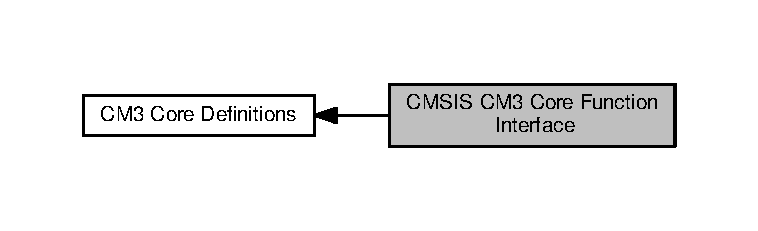
\includegraphics[width=350pt]{d1/de3/group__CMSIS__CM3__Core__FunctionInterface}
\end{center}
\end{figure}


\subsection{Detailed Description}
Core Function Interface containing\+:
\begin{DoxyItemize}
\item Core N\+V\+IC Functions
\item Core Sys\+Tick Functions
\item Core Reset Functions 
\end{DoxyItemize}
\hypertarget{group__CMSIS__CM3__CoreDebugInterface}{}\section{C\+M\+S\+IS C\+M3 Core Debug Interface}
\label{group__CMSIS__CM3__CoreDebugInterface}\index{C\+M\+S\+I\+S C\+M3 Core Debug Interface@{C\+M\+S\+I\+S C\+M3 Core Debug Interface}}
Collaboration diagram for C\+M\+S\+IS C\+M3 Core Debug Interface\+:\nopagebreak
\begin{figure}[H]
\begin{center}
\leavevmode
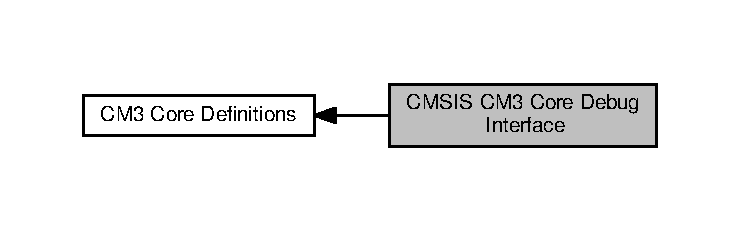
\includegraphics[width=350pt]{da/dd6/group__CMSIS__CM3__CoreDebugInterface}
\end{center}
\end{figure}
\subsection*{Macros}
\begin{DoxyCompactItemize}
\item 
\#define \hyperlink{group__CMSIS__CM3__CoreDebugInterface_gaa822cb398ee022b59e9e6c5d7bbb228a}{I\+T\+M\+\_\+\+R\+X\+B\+U\+F\+F\+E\+R\+\_\+\+E\+M\+P\+TY}~0x5\+A\+A55\+A\+A5
\end{DoxyCompactItemize}
\subsection*{Variables}
\begin{DoxyCompactItemize}
\item 
volatile int \hyperlink{group__CMSIS__CM3__CoreDebugInterface_gacf1fe3063cedf11b6e6f7cb0dd7c1a51}{I\+T\+M\+\_\+\+Rx\+Buffer}
\end{DoxyCompactItemize}


\subsection{Detailed Description}
Core Debug Interface containing\+:
\begin{DoxyItemize}
\item Core Debug Receive / Transmit Functions
\item Core Debug Defines
\item Core Debug Variables 
\end{DoxyItemize}

\subsection{Macro Definition Documentation}
\index{C\+M\+S\+I\+S C\+M3 Core Debug Interface@{C\+M\+S\+I\+S C\+M3 Core Debug Interface}!I\+T\+M\+\_\+\+R\+X\+B\+U\+F\+F\+E\+R\+\_\+\+E\+M\+P\+TY@{I\+T\+M\+\_\+\+R\+X\+B\+U\+F\+F\+E\+R\+\_\+\+E\+M\+P\+TY}}
\index{I\+T\+M\+\_\+\+R\+X\+B\+U\+F\+F\+E\+R\+\_\+\+E\+M\+P\+TY@{I\+T\+M\+\_\+\+R\+X\+B\+U\+F\+F\+E\+R\+\_\+\+E\+M\+P\+TY}!C\+M\+S\+I\+S C\+M3 Core Debug Interface@{C\+M\+S\+I\+S C\+M3 Core Debug Interface}}
\subsubsection[{\texorpdfstring{I\+T\+M\+\_\+\+R\+X\+B\+U\+F\+F\+E\+R\+\_\+\+E\+M\+P\+TY}{ITM_RXBUFFER_EMPTY}}]{\setlength{\rightskip}{0pt plus 5cm}\#define I\+T\+M\+\_\+\+R\+X\+B\+U\+F\+F\+E\+R\+\_\+\+E\+M\+P\+TY~0x5\+A\+A55\+A\+A5}\hypertarget{group__CMSIS__CM3__CoreDebugInterface_gaa822cb398ee022b59e9e6c5d7bbb228a}{}\label{group__CMSIS__CM3__CoreDebugInterface_gaa822cb398ee022b59e9e6c5d7bbb228a}
value identifying I\+T\+M\+\_\+\+Rx\+Buffer is ready for next character 

\subsection{Variable Documentation}
\index{C\+M\+S\+I\+S C\+M3 Core Debug Interface@{C\+M\+S\+I\+S C\+M3 Core Debug Interface}!I\+T\+M\+\_\+\+Rx\+Buffer@{I\+T\+M\+\_\+\+Rx\+Buffer}}
\index{I\+T\+M\+\_\+\+Rx\+Buffer@{I\+T\+M\+\_\+\+Rx\+Buffer}!C\+M\+S\+I\+S C\+M3 Core Debug Interface@{C\+M\+S\+I\+S C\+M3 Core Debug Interface}}
\subsubsection[{\texorpdfstring{I\+T\+M\+\_\+\+Rx\+Buffer}{ITM_RxBuffer}}]{\setlength{\rightskip}{0pt plus 5cm}volatile int I\+T\+M\+\_\+\+Rx\+Buffer}\hypertarget{group__CMSIS__CM3__CoreDebugInterface_gacf1fe3063cedf11b6e6f7cb0dd7c1a51}{}\label{group__CMSIS__CM3__CoreDebugInterface_gacf1fe3063cedf11b6e6f7cb0dd7c1a51}
variable to receive characters 
\chapter{Namespace Documentation}
\hypertarget{namespace____gnu__cxx}{}\section{\+\_\+\+\_\+gnu\+\_\+cxx Namespace Reference}
\label{namespace____gnu__cxx}\index{\+\_\+\+\_\+gnu\+\_\+cxx@{\+\_\+\+\_\+gnu\+\_\+cxx}}
\subsection*{Functions}
\begin{DoxyCompactItemize}
\item 
void \hyperlink{namespace____gnu__cxx_af51888cedbc669a114cd79e39e0cd9be}{\+\_\+\+\_\+verbose\+\_\+terminate\+\_\+handler} ()
\end{DoxyCompactItemize}


\subsection{Function Documentation}
\index{\+\_\+\+\_\+gnu\+\_\+cxx@{\+\_\+\+\_\+gnu\+\_\+cxx}!\+\_\+\+\_\+verbose\+\_\+terminate\+\_\+handler@{\+\_\+\+\_\+verbose\+\_\+terminate\+\_\+handler}}
\index{\+\_\+\+\_\+verbose\+\_\+terminate\+\_\+handler@{\+\_\+\+\_\+verbose\+\_\+terminate\+\_\+handler}!\+\_\+\+\_\+gnu\+\_\+cxx@{\+\_\+\+\_\+gnu\+\_\+cxx}}
\subsubsection[{\texorpdfstring{\+\_\+\+\_\+verbose\+\_\+terminate\+\_\+handler()}{__verbose_terminate_handler()}}]{\setlength{\rightskip}{0pt plus 5cm}void \+\_\+\+\_\+gnu\+\_\+cxx\+::\+\_\+\+\_\+verbose\+\_\+terminate\+\_\+handler (
\begin{DoxyParamCaption}
{}
\end{DoxyParamCaption}
)}\hypertarget{namespace____gnu__cxx_af51888cedbc669a114cd79e39e0cd9be}{}\label{namespace____gnu__cxx_af51888cedbc669a114cd79e39e0cd9be}

\hypertarget{namespacedbc__parse}{}\section{dbc\+\_\+parse Namespace Reference}
\label{namespacedbc__parse}\index{dbc\+\_\+parse@{dbc\+\_\+parse}}
\subsection*{Data Structures}
\begin{DoxyCompactItemize}
\item 
class \hyperlink{classdbc__parse_1_1DBC}{D\+BC}
\item 
class \hyperlink{classdbc__parse_1_1Message}{Message}
\item 
class \hyperlink{classdbc__parse_1_1Signal}{Signal}
\end{DoxyCompactItemize}
\subsection*{Functions}
\begin{DoxyCompactItemize}
\item 
def \hyperlink{namespacedbc__parse_af2c803f0d206cc9b48ac36990feb9cc8}{is\+\_\+empty} (s)
\item 
def \hyperlink{namespacedbc__parse_a8138541ea63d17645e2b2390df3e973a}{M\+IN} (x, y)
\item 
def \hyperlink{namespacedbc__parse_ad207022188381e99ea86b51bcb09357c}{main} (argv)
\end{DoxyCompactItemize}
\subsection*{Variables}
\begin{DoxyCompactItemize}
\item 
string \hyperlink{namespacedbc__parse_a4721c9016330b451ceee116f19e7d588}{L\+I\+N\+E\+\_\+\+B\+EG} = \textquotesingle{}\%\textquotesingle{}
\end{DoxyCompactItemize}


\subsection{Function Documentation}
\index{dbc\+\_\+parse@{dbc\+\_\+parse}!is\+\_\+empty@{is\+\_\+empty}}
\index{is\+\_\+empty@{is\+\_\+empty}!dbc\+\_\+parse@{dbc\+\_\+parse}}
\subsubsection[{\texorpdfstring{is\+\_\+empty(s)}{is_empty(s)}}]{\setlength{\rightskip}{0pt plus 5cm}def dbc\+\_\+parse.\+is\+\_\+empty (
\begin{DoxyParamCaption}
\item[{}]{s}
\end{DoxyParamCaption}
)}\hypertarget{namespacedbc__parse_af2c803f0d206cc9b48ac36990feb9cc8}{}\label{namespacedbc__parse_af2c803f0d206cc9b48ac36990feb9cc8}
\index{dbc\+\_\+parse@{dbc\+\_\+parse}!main@{main}}
\index{main@{main}!dbc\+\_\+parse@{dbc\+\_\+parse}}
\subsubsection[{\texorpdfstring{main(argv)}{main(argv)}}]{\setlength{\rightskip}{0pt plus 5cm}def dbc\+\_\+parse.\+main (
\begin{DoxyParamCaption}
\item[{}]{argv}
\end{DoxyParamCaption}
)}\hypertarget{namespacedbc__parse_ad207022188381e99ea86b51bcb09357c}{}\label{namespacedbc__parse_ad207022188381e99ea86b51bcb09357c}
\index{dbc\+\_\+parse@{dbc\+\_\+parse}!M\+IN@{M\+IN}}
\index{M\+IN@{M\+IN}!dbc\+\_\+parse@{dbc\+\_\+parse}}
\subsubsection[{\texorpdfstring{M\+I\+N(x, y)}{MIN(x, y)}}]{\setlength{\rightskip}{0pt plus 5cm}def dbc\+\_\+parse.\+M\+IN (
\begin{DoxyParamCaption}
\item[{}]{x, }
\item[{}]{y}
\end{DoxyParamCaption}
)}\hypertarget{namespacedbc__parse_a8138541ea63d17645e2b2390df3e973a}{}\label{namespacedbc__parse_a8138541ea63d17645e2b2390df3e973a}


\subsection{Variable Documentation}
\index{dbc\+\_\+parse@{dbc\+\_\+parse}!L\+I\+N\+E\+\_\+\+B\+EG@{L\+I\+N\+E\+\_\+\+B\+EG}}
\index{L\+I\+N\+E\+\_\+\+B\+EG@{L\+I\+N\+E\+\_\+\+B\+EG}!dbc\+\_\+parse@{dbc\+\_\+parse}}
\subsubsection[{\texorpdfstring{L\+I\+N\+E\+\_\+\+B\+EG}{LINE_BEG}}]{\setlength{\rightskip}{0pt plus 5cm}string dbc\+\_\+parse.\+L\+I\+N\+E\+\_\+\+B\+EG = \textquotesingle{}\%\textquotesingle{}}\hypertarget{namespacedbc__parse_a4721c9016330b451ceee116f19e7d588}{}\label{namespacedbc__parse_a4721c9016330b451ceee116f19e7d588}

\chapter{Data Structure Documentation}
\hypertarget{struct____attribute____}{}\section{\+\_\+\+\_\+attribute\+\_\+\+\_\+ Struct Reference}
\label{struct____attribute____}\index{\+\_\+\+\_\+attribute\+\_\+\+\_\+@{\+\_\+\+\_\+attribute\+\_\+\+\_\+}}


{\ttfamily \#include $<$can.\+h$>$}



Collaboration diagram for \+\_\+\+\_\+attribute\+\_\+\+\_\+\+:\nopagebreak
\begin{figure}[H]
\begin{center}
\leavevmode
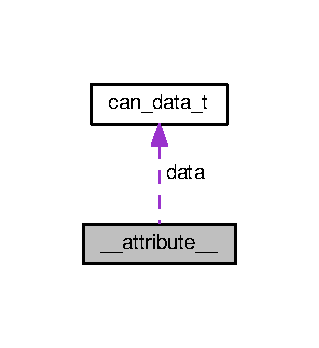
\includegraphics[width=153pt]{dd/d0e/struct____attribute______coll__graph}
\end{center}
\end{figure}
\subsection*{Data Fields}
\begin{DoxyCompactItemize}
\item 
\begin{tabbing}
xx\=xx\=xx\=xx\=xx\=xx\=xx\=xx\=xx\=\kill
union \{\\
\>uint32\_t \hyperlink{struct____attribute_____a1c5c34a070f4e1a8c388cc990166125a}{frame}\\
\>\>{\em 32-\/bit CAN frame aligned with frame\_fields (bit members) }\\
\>struct \{\\
\>\>uint32\_t \hyperlink{struct____attribute_____a02ee404618bb2bb7a588a4ad5927894d}{\_\_pad0\_\_}: 16\\
\>\>\>{\em Unused space. }\\
\>\>uint32\_t \hyperlink{struct____attribute_____ae6f628b8af2722362b91666d5cff6041}{data\_len}: 4\\
\>\>\>{\em Data length. }\\
\>\>uint32\_t \hyperlink{struct____attribute_____a0c4e6e1eb99bec0a27a70420f40ac211}{\_\_pad1\_\_}: 10\\
\>\>\>{\em Unused space. }\\
\>\>uint32\_t \hyperlink{struct____attribute_____afa1cea6cf94468a29ce2ad1b62a3de11}{is\_rtr}: 1\\
\>\>\>{\em Message is an RTR type. }\\
\>\>uint32\_t \hyperlink{struct____attribute_____a745166911ddda34c6f9e95e22d423207}{is\_29bit}: 1\\
\>\>\>{\em If message ID is 29-\/bit type. }\\
\>\} \hyperlink{struct____attribute_____acfc363edc99eccae8f7e0f523821305e}{frame\_fields}\\
\}; \\

\end{tabbing}\item 
uint32\+\_\+t \hyperlink{struct____attribute_____a676a49f79047392e2bac357a55bb74ed}{msg\+\_\+id}
\begin{DoxyCompactList}\small\item\em C\+AN Message ID (11-\/bit or 29-\/bit) \end{DoxyCompactList}\item 
\hyperlink{unioncan__data__t}{can\+\_\+data\+\_\+t} \hyperlink{struct____attribute_____a671d4cb674b1287a89ab3dd93d8d36e2}{data}
\begin{DoxyCompactList}\small\item\em C\+AN data. \end{DoxyCompactList}\item 
\begin{tabbing}
xx\=xx\=xx\=xx\=xx\=xx\=xx\=xx\=xx\=\kill
struct \{\\
\>uint32\_t \hyperlink{struct____attribute_____a676a49f79047392e2bac357a55bb74ed}{msg\_id}: 11\\
\>\>{\em 11-\/bit message-\/id }\\
\>uint32\_t \hyperlink{struct____attribute_____a02ee404618bb2bb7a588a4ad5927894d}{\_\_pad0\_\_}: 5\\
\>\>{\em Unused. }\\
\>uint32\_t \hyperlink{struct____attribute_____ae6f628b8af2722362b91666d5cff6041}{data\_len}: 4\\
\>\>{\em Message length. }\\
\>uint32\_t \hyperlink{struct____attribute_____a0c4e6e1eb99bec0a27a70420f40ac211}{\_\_pad1\_\_}: 4\\
\>\>{\em Unused. }\\
\>uint32\_t \hyperlink{struct____attribute_____a093c08572a86d14158d4ad2b8d526557}{semphr}: 2\\
\>\>{\em Semaphore bits. }\\
\>uint32\_t \hyperlink{struct____attribute_____a2d8f39dfa819e39b227d2790c26409d2}{\_\_pad2\_\_}: 4\\
\>\>{\em Unused. }\\
\>uint32\_t \hyperlink{struct____attribute_____aee214ea38d7e1f8c3dc6e84f3993fdec}{rtr}: 1\\
\>\>{\em RTR message. }\\
\>uint32\_t \hyperlink{struct____attribute_____a898a0c6c6d94ece9275b1379d2d24f60}{\_\_pad3\_\_}: 1\\
\>\>{\em Unused (FF bit, not applicable to FullCAN) }\\
\}; \\

\end{tabbing}\item 
\begin{tabbing}
xx\=xx\=xx\=xx\=xx\=xx\=xx\=xx\=xx\=\kill
struct \{\\
\>uint16\_t \hyperlink{struct____attribute_____ad3ca970dad0c3c0dde583a1916245292}{id}: 11\\
\>\>{\em Standard 11-\/bit CAN ID. }\\
\>uint16\_t \hyperlink{struct____attribute_____a3f327bada8b15b44b9a37ec975800f57}{fc\_intr}: 1\\
\>\>{\em Message interrupt bit: ONLY USED FOR FULLCAN. }\\
\>uint16\_t \hyperlink{struct____attribute_____a7c608f1e67305379d24b3b770be44994}{disable}: 1\\
\>\>{\em Set to 1 to disable the slot. }\\
\>uint16\_t \hyperlink{struct____attribute_____a3030b7aabe9418f3a7dcd682fe34fadc}{can\_num}: 3\\
\>\>{\em CAN controller number (0=CAN1, 1=CAN2) }\\
\}; \\

\end{tabbing}\item 
uint16\+\_\+t \hyperlink{struct____attribute_____a6002c78ca3d2dd7e495cb96babc3c2f6}{raw}
\item 
uint32\+\_\+t \hyperlink{struct____attribute_____a87df1990d2a726a8feb9ee5d5fd158d2}{id}\+: 29
\begin{DoxyCompactList}\small\item\em Extended 29-\/bit C\+AN ID. \end{DoxyCompactList}\item 
uint32\+\_\+t \hyperlink{struct____attribute_____a7d526d3c59c97be7b5ef1924151f7de8}{can\+\_\+num}\+: 3
\begin{DoxyCompactList}\small\item\em C\+AN controller number (0=C\+A\+N1, 1=C\+A\+N2) \end{DoxyCompactList}\item 
uint32\+\_\+t \hyperlink{struct____attribute_____a84c6baaec3dc2429942a79d7de07b939}{sec}\+: 6
\item 
uint32\+\_\+t \hyperlink{struct____attribute_____a1620baad6e662539c31b4a82eb5d2bc1}{min}\+: 6
\item 
uint32\+\_\+t \hyperlink{struct____attribute_____a226a28214916e63e3be8b34a904a6fe5}{hour}\+: 5
\item 
uint32\+\_\+t \hyperlink{struct____attribute_____ab9df98376610faf8995ee0f3d7ddd7c3}{dow}\+: 3
\item 
uint32\+\_\+t \hyperlink{struct____attribute_____a4ce9f037a40bdf6b6d6b694790afa28c}{day}\+: 5
\item 
uint32\+\_\+t \hyperlink{struct____attribute_____ad8f8cfaece8486cec76e21cf956d7646}{\+\_\+\+\_\+pad4\+\_\+\+\_\+}\+: 3
\item 
uint32\+\_\+t \hyperlink{struct____attribute_____a59b2a1f42969a6800f7cd16b75ec328f}{month}\+: 4
\item 
uint32\+\_\+t \hyperlink{struct____attribute_____ac9e7d251f898df011d7cc73a8a2559d2}{\+\_\+\+\_\+pad5\+\_\+\+\_\+}\+: 4
\item 
uint32\+\_\+t \hyperlink{struct____attribute_____afb5fa3b09ae735aea92d1a6fa1c6c1c6}{year}\+:12
\item 
uint32\+\_\+t \hyperlink{struct____attribute_____a7f675f9a9d7b33e510c50add172c4108}{\+\_\+\+\_\+pad6\+\_\+\+\_\+}\+: 4
\item 
uint32\+\_\+t \hyperlink{struct____attribute_____ac556a14ae593d1f3d46e166263313c75}{doy}\+:12
\item 
uint32\+\_\+t \hyperlink{struct____attribute_____a41bb8f240ea90dcb866b722bac4b7496}{\+\_\+\+\_\+pad7\+\_\+\+\_\+}\+: 20
\item 
uint8\+\_\+t \hyperlink{struct____attribute_____a3269a81ad93d0affbeabf284e63829aa}{src}
\begin{DoxyCompactList}\small\item\em Sender address. \end{DoxyCompactList}\item 
uint8\+\_\+t \hyperlink{struct____attribute_____a498bfd7c451026ed73b80a3e0a4169fc}{pkt\+\_\+id}
\begin{DoxyCompactList}\small\item\em Sender\textquotesingle{}s packet id (sequence) \end{DoxyCompactList}\item 
uint8\+\_\+t \hyperlink{struct____attribute_____a70bb4d640fb24d470e94698c04440d1e}{retries}
\begin{DoxyCompactList}\small\item\em Packet retry count. \end{DoxyCompactList}\item 
mesh\+\_\+packet\+\_\+t \hyperlink{struct____attribute_____a09b2479a59537aae24561247294fa398}{pkt}
\begin{DoxyCompactList}\small\item\em The packet itself. \end{DoxyCompactList}\item 
uint16\+\_\+t \hyperlink{struct____attribute_____a029c6f0fb55fdad96770454f90e12ce1}{timer\+\_\+ms}
\begin{DoxyCompactList}\small\item\em Running time. M\+U\+ST BE U\+I\+N\+T16 due to hard-\/coded usage of U\+I\+N\+T16\+\_\+\+M\+AX. \end{DoxyCompactList}\item 
uint16\+\_\+t \hyperlink{struct____attribute_____a9f3aa35286aea8d6a20a5358b3730361}{timeout\+\_\+ms}\+: 15
\begin{DoxyCompactList}\small\item\em Target time when timer expires. We don\textquotesingle{}t need a lot of bits for this. \end{DoxyCompactList}\item 
uint16\+\_\+t \hyperlink{struct____attribute_____aaf5ef4d6e36b400b9a6d01cd5d84a6fe}{disc\+\_\+pkt}\+: 1
\begin{DoxyCompactList}\small\item\em Flag if this is a route discovery packet. \end{DoxyCompactList}\item 
uint16\+\_\+t \hyperlink{struct____attribute_____a1cfd2d5a79aed9120f40669b04e6f649}{pkts\+\_\+sent}
\begin{DoxyCompactList}\small\item\em Packets we sent out with our address. \end{DoxyCompactList}\item 
uint16\+\_\+t \hyperlink{struct____attribute_____a8483976361231cd091d9f0138fef1e47}{pkts\+\_\+intercepted}
\begin{DoxyCompactList}\small\item\em Packets we receipted within our mesh network. \end{DoxyCompactList}\item 
uint16\+\_\+t \hyperlink{struct____attribute_____a209e5ba4478f5776ee65788d276d5f2c}{pkts\+\_\+repeated}
\begin{DoxyCompactList}\small\item\em Packets we repeated for others. \end{DoxyCompactList}\item 
uint16\+\_\+t \hyperlink{struct____attribute_____a01cdbd0aa173d415d86566adef6775a3}{pkts\+\_\+retried}
\begin{DoxyCompactList}\small\item\em Packets we retried with our address. \end{DoxyCompactList}\item 
uint16\+\_\+t \hyperlink{struct____attribute_____ae79aae50e9255af8fc03b6988c7d5e12}{pkts\+\_\+retried\+\_\+others}
\begin{DoxyCompactList}\small\item\em Packets retried for others. \end{DoxyCompactList}\item 
uint8\+\_\+t \hyperlink{struct____attribute_____adbc91f28865d1eae6895599dc900465b}{rte\+\_\+entries}
\begin{DoxyCompactList}\small\item\em Current number of routing entries. \end{DoxyCompactList}\item 
uint8\+\_\+t \hyperlink{struct____attribute_____a9ea2df6bafe8f3ef1c124a962b028bcb}{rte\+\_\+overwritten}
\begin{DoxyCompactList}\small\item\em Number of times a routing entry over-\/wrote an existing entry. \end{DoxyCompactList}\item 
uint8\+\_\+t \hyperlink{struct____attribute_____a2e226654212aebfb764a8df90d66b006}{version}\+: 3
\begin{DoxyCompactList}\small\item\em Mesh Version (1-\/7) -- M\+U\+ST BE 1st member of this struct. \end{DoxyCompactList}\item 
uint8\+\_\+t \hyperlink{struct____attribute_____aebb84f16b4d46a3b2ea267e8b77c8774}{retries\+\_\+rem}\+: 3
\begin{DoxyCompactList}\small\item\em Packet retries remaining (pad to 8 bits) \end{DoxyCompactList}\item 
uint8\+\_\+t \hyperlink{struct____attribute_____ae19c7dcebf79b994d537fecf3cc931c9}{pkt\+\_\+type}\+: 2
\begin{DoxyCompactList}\small\item\em The type of mesh packet. \end{DoxyCompactList}\item 
uint8\+\_\+t \hyperlink{struct____attribute_____a80f0ddbd42fa6974b08feea40867db68}{hop\+\_\+count}\+: 4
\begin{DoxyCompactList}\small\item\em Hop count of packet (1st packet counts as 0 hops) \end{DoxyCompactList}\item 
uint8\+\_\+t \hyperlink{struct____attribute_____a73ca3679f26c67143ed190411c8347c6}{hop\+\_\+count\+\_\+max}\+: 4
\begin{DoxyCompactList}\small\item\em Max hop count limit. \end{DoxyCompactList}\item 
uint8\+\_\+t \hyperlink{struct____attribute_____acb75fb96c08ce6b43afc75f54e0d6a32}{pkt\+\_\+seq\+\_\+num}
\begin{DoxyCompactList}\small\item\em Sequence number of the packet. \end{DoxyCompactList}\item 
uint8\+\_\+t \hyperlink{struct____attribute_____a963d3c197770f024e680a0d0a774c99e}{data\+\_\+len}
\begin{DoxyCompactList}\small\item\em Length of the packet data. \end{DoxyCompactList}\item 
uint8\+\_\+t \hyperlink{struct____attribute_____a3522c1d748831637cd29787e401f670b}{dst}
\begin{DoxyCompactList}\small\item\em Destination address. \end{DoxyCompactList}\item 
mesh\+\_\+pkt\+\_\+addr\+\_\+t \hyperlink{struct____attribute_____acca30e839928f53cd58dad5de67e9179}{nwk}
\begin{DoxyCompactList}\small\item\em Packet network address. \end{DoxyCompactList}\item 
mesh\+\_\+pkt\+\_\+addr\+\_\+t \hyperlink{struct____attribute_____ab98af19336ed7ec3ca480cb93d16e106}{mac}
\begin{DoxyCompactList}\small\item\em Packet physical address. \end{DoxyCompactList}\item 
mesh\+\_\+pkt\+\_\+info\+\_\+t \hyperlink{struct____attribute_____a12c2cc9433afd67e97b7de65d9d58735}{info}
\begin{DoxyCompactList}\small\item\em Packet header. \end{DoxyCompactList}\item 
uint8\+\_\+t \hyperlink{struct____attribute_____a0bb6bcfb06a69a501d1dfd0a0f1b1222}{data} \mbox{[}\hyperlink{mesh__typedefs_8h_a3a202f51bca7a0dbd86db707179fe827}{M\+E\+S\+H\+\_\+\+D\+A\+T\+A\+\_\+\+P\+A\+Y\+L\+O\+A\+D\+\_\+\+S\+I\+ZE}\mbox{]}
\begin{DoxyCompactList}\small\item\em Actual data within the payload. \end{DoxyCompactList}\end{DoxyCompactItemize}


\subsection{Detailed Description}
Type definition of a C\+AN message with bit-\/fields (assuming little-\/endian machine) DO N\+OT C\+H\+A\+N\+GE T\+H\+IS S\+T\+R\+U\+C\+T\+U\+RE -\/ it maps to the hardware

Typedef of a Full\+C\+AN message stored in memory DO N\+OT C\+H\+A\+N\+GE T\+H\+IS S\+T\+R\+U\+C\+T\+U\+RE -\/ it maps to the hardware

Standard ID HW filtering structure. The single entries (not group) must be an even number count, so a second entry can be used and should be marked disabled (disable bit set to 1) to make the count an even number. DO N\+OT C\+H\+A\+N\+GE T\+H\+IS S\+T\+R\+U\+C\+T\+U\+RE -\/ it maps to the hardware

Extended ID entry is just the ID and the C\+AN B\+US number DO N\+OT C\+H\+A\+N\+GE T\+H\+IS S\+T\+R\+U\+C\+T\+U\+RE -\/ it maps to the hardware

This struct aligns with the L\+PC Hardware\textquotesingle{}s consolidated R\+TC registers. The un-\/named chars are just for padding according to L\+PC C\+T\+I\+ME registers.

Fields that make a packet unique are kept in history to avoid duplicate packet handling.

Mesh Pending packet type Only 16-\/bit timer is needed which can supply up to 65,535ms value, which is far above a useful mesh packet retry value

Statistics structure that is sent if M\+E\+S\+H\+\_\+\+U\+S\+E\+\_\+\+S\+T\+A\+T\+I\+S\+T\+I\+CS is set to non-\/zero value. This data is sent by the node sending ack response packet. Current size is 12 bytes, and this should be kept to a minimum such that an A\+CK response packet can accommodate this data into the payload.

Mesh packet header type 4-\/bit hop-\/count gets us 15 hops max, good enough for simple mesh.

Mesh packet address type

The structure of a single packet. 

\subsection{Field Documentation}
\subsubsection[{\texorpdfstring{"@61}{@61}}]{\setlength{\rightskip}{0pt plus 5cm}union \{ ... \} }\hypertarget{struct____attribute_____a508ec0f55791b0b9597cd76c90350628}{}\label{struct____attribute_____a508ec0f55791b0b9597cd76c90350628}
\subsubsection[{\texorpdfstring{"@64}{@64}}]{\setlength{\rightskip}{0pt plus 5cm}struct \{ ... \} }\hypertarget{struct____attribute_____abe87e0591ebdd65a429a6b6c95f1439b}{}\label{struct____attribute_____abe87e0591ebdd65a429a6b6c95f1439b}
\subsubsection[{\texorpdfstring{"@66}{@66}}]{\setlength{\rightskip}{0pt plus 5cm}struct \{ ... \} }\hypertarget{struct____attribute_____ad7a1d9ea5fa4ffe405adf790c173b67a}{}\label{struct____attribute_____ad7a1d9ea5fa4ffe405adf790c173b67a}
\index{\+\_\+\+\_\+attribute\+\_\+\+\_\+@{\+\_\+\+\_\+attribute\+\_\+\+\_\+}!\+\_\+\+\_\+pad0\+\_\+\+\_\+@{\+\_\+\+\_\+pad0\+\_\+\+\_\+}}
\index{\+\_\+\+\_\+pad0\+\_\+\+\_\+@{\+\_\+\+\_\+pad0\+\_\+\+\_\+}!\+\_\+\+\_\+attribute\+\_\+\+\_\+@{\+\_\+\+\_\+attribute\+\_\+\+\_\+}}
\subsubsection[{\texorpdfstring{\+\_\+\+\_\+pad0\+\_\+\+\_\+}{__pad0__}}]{\setlength{\rightskip}{0pt plus 5cm}uint32\+\_\+t \+\_\+\+\_\+attribute\+\_\+\+\_\+\+::\+\_\+\+\_\+pad0\+\_\+\+\_\+}\hypertarget{struct____attribute_____a02ee404618bb2bb7a588a4ad5927894d}{}\label{struct____attribute_____a02ee404618bb2bb7a588a4ad5927894d}


Unused space. 

Unused. \index{\+\_\+\+\_\+attribute\+\_\+\+\_\+@{\+\_\+\+\_\+attribute\+\_\+\+\_\+}!\+\_\+\+\_\+pad1\+\_\+\+\_\+@{\+\_\+\+\_\+pad1\+\_\+\+\_\+}}
\index{\+\_\+\+\_\+pad1\+\_\+\+\_\+@{\+\_\+\+\_\+pad1\+\_\+\+\_\+}!\+\_\+\+\_\+attribute\+\_\+\+\_\+@{\+\_\+\+\_\+attribute\+\_\+\+\_\+}}
\subsubsection[{\texorpdfstring{\+\_\+\+\_\+pad1\+\_\+\+\_\+}{__pad1__}}]{\setlength{\rightskip}{0pt plus 5cm}uint32\+\_\+t \+\_\+\+\_\+attribute\+\_\+\+\_\+\+::\+\_\+\+\_\+pad1\+\_\+\+\_\+}\hypertarget{struct____attribute_____a0c4e6e1eb99bec0a27a70420f40ac211}{}\label{struct____attribute_____a0c4e6e1eb99bec0a27a70420f40ac211}


Unused space. 

Unused. \index{\+\_\+\+\_\+attribute\+\_\+\+\_\+@{\+\_\+\+\_\+attribute\+\_\+\+\_\+}!\+\_\+\+\_\+pad2\+\_\+\+\_\+@{\+\_\+\+\_\+pad2\+\_\+\+\_\+}}
\index{\+\_\+\+\_\+pad2\+\_\+\+\_\+@{\+\_\+\+\_\+pad2\+\_\+\+\_\+}!\+\_\+\+\_\+attribute\+\_\+\+\_\+@{\+\_\+\+\_\+attribute\+\_\+\+\_\+}}
\subsubsection[{\texorpdfstring{\+\_\+\+\_\+pad2\+\_\+\+\_\+}{__pad2__}}]{\setlength{\rightskip}{0pt plus 5cm}uint32\+\_\+t \+\_\+\+\_\+attribute\+\_\+\+\_\+\+::\+\_\+\+\_\+pad2\+\_\+\+\_\+}\hypertarget{struct____attribute_____a2d8f39dfa819e39b227d2790c26409d2}{}\label{struct____attribute_____a2d8f39dfa819e39b227d2790c26409d2}


Unused. 

\index{\+\_\+\+\_\+attribute\+\_\+\+\_\+@{\+\_\+\+\_\+attribute\+\_\+\+\_\+}!\+\_\+\+\_\+pad3\+\_\+\+\_\+@{\+\_\+\+\_\+pad3\+\_\+\+\_\+}}
\index{\+\_\+\+\_\+pad3\+\_\+\+\_\+@{\+\_\+\+\_\+pad3\+\_\+\+\_\+}!\+\_\+\+\_\+attribute\+\_\+\+\_\+@{\+\_\+\+\_\+attribute\+\_\+\+\_\+}}
\subsubsection[{\texorpdfstring{\+\_\+\+\_\+pad3\+\_\+\+\_\+}{__pad3__}}]{\setlength{\rightskip}{0pt plus 5cm}uint32\+\_\+t \+\_\+\+\_\+attribute\+\_\+\+\_\+\+::\+\_\+\+\_\+pad3\+\_\+\+\_\+}\hypertarget{struct____attribute_____a898a0c6c6d94ece9275b1379d2d24f60}{}\label{struct____attribute_____a898a0c6c6d94ece9275b1379d2d24f60}


Unused (FF bit, not applicable to Full\+C\+AN) 

\index{\+\_\+\+\_\+attribute\+\_\+\+\_\+@{\+\_\+\+\_\+attribute\+\_\+\+\_\+}!\+\_\+\+\_\+pad4\+\_\+\+\_\+@{\+\_\+\+\_\+pad4\+\_\+\+\_\+}}
\index{\+\_\+\+\_\+pad4\+\_\+\+\_\+@{\+\_\+\+\_\+pad4\+\_\+\+\_\+}!\+\_\+\+\_\+attribute\+\_\+\+\_\+@{\+\_\+\+\_\+attribute\+\_\+\+\_\+}}
\subsubsection[{\texorpdfstring{\+\_\+\+\_\+pad4\+\_\+\+\_\+}{__pad4__}}]{\setlength{\rightskip}{0pt plus 5cm}uint32\+\_\+t \+\_\+\+\_\+attribute\+\_\+\+\_\+\+::\+\_\+\+\_\+pad4\+\_\+\+\_\+}\hypertarget{struct____attribute_____ad8f8cfaece8486cec76e21cf956d7646}{}\label{struct____attribute_____ad8f8cfaece8486cec76e21cf956d7646}
\index{\+\_\+\+\_\+attribute\+\_\+\+\_\+@{\+\_\+\+\_\+attribute\+\_\+\+\_\+}!\+\_\+\+\_\+pad5\+\_\+\+\_\+@{\+\_\+\+\_\+pad5\+\_\+\+\_\+}}
\index{\+\_\+\+\_\+pad5\+\_\+\+\_\+@{\+\_\+\+\_\+pad5\+\_\+\+\_\+}!\+\_\+\+\_\+attribute\+\_\+\+\_\+@{\+\_\+\+\_\+attribute\+\_\+\+\_\+}}
\subsubsection[{\texorpdfstring{\+\_\+\+\_\+pad5\+\_\+\+\_\+}{__pad5__}}]{\setlength{\rightskip}{0pt plus 5cm}uint32\+\_\+t \+\_\+\+\_\+attribute\+\_\+\+\_\+\+::\+\_\+\+\_\+pad5\+\_\+\+\_\+}\hypertarget{struct____attribute_____ac9e7d251f898df011d7cc73a8a2559d2}{}\label{struct____attribute_____ac9e7d251f898df011d7cc73a8a2559d2}
\index{\+\_\+\+\_\+attribute\+\_\+\+\_\+@{\+\_\+\+\_\+attribute\+\_\+\+\_\+}!\+\_\+\+\_\+pad6\+\_\+\+\_\+@{\+\_\+\+\_\+pad6\+\_\+\+\_\+}}
\index{\+\_\+\+\_\+pad6\+\_\+\+\_\+@{\+\_\+\+\_\+pad6\+\_\+\+\_\+}!\+\_\+\+\_\+attribute\+\_\+\+\_\+@{\+\_\+\+\_\+attribute\+\_\+\+\_\+}}
\subsubsection[{\texorpdfstring{\+\_\+\+\_\+pad6\+\_\+\+\_\+}{__pad6__}}]{\setlength{\rightskip}{0pt plus 5cm}uint32\+\_\+t \+\_\+\+\_\+attribute\+\_\+\+\_\+\+::\+\_\+\+\_\+pad6\+\_\+\+\_\+}\hypertarget{struct____attribute_____a7f675f9a9d7b33e510c50add172c4108}{}\label{struct____attribute_____a7f675f9a9d7b33e510c50add172c4108}
\index{\+\_\+\+\_\+attribute\+\_\+\+\_\+@{\+\_\+\+\_\+attribute\+\_\+\+\_\+}!\+\_\+\+\_\+pad7\+\_\+\+\_\+@{\+\_\+\+\_\+pad7\+\_\+\+\_\+}}
\index{\+\_\+\+\_\+pad7\+\_\+\+\_\+@{\+\_\+\+\_\+pad7\+\_\+\+\_\+}!\+\_\+\+\_\+attribute\+\_\+\+\_\+@{\+\_\+\+\_\+attribute\+\_\+\+\_\+}}
\subsubsection[{\texorpdfstring{\+\_\+\+\_\+pad7\+\_\+\+\_\+}{__pad7__}}]{\setlength{\rightskip}{0pt plus 5cm}uint32\+\_\+t \+\_\+\+\_\+attribute\+\_\+\+\_\+\+::\+\_\+\+\_\+pad7\+\_\+\+\_\+}\hypertarget{struct____attribute_____a41bb8f240ea90dcb866b722bac4b7496}{}\label{struct____attribute_____a41bb8f240ea90dcb866b722bac4b7496}
\index{\+\_\+\+\_\+attribute\+\_\+\+\_\+@{\+\_\+\+\_\+attribute\+\_\+\+\_\+}!can\+\_\+num@{can\+\_\+num}}
\index{can\+\_\+num@{can\+\_\+num}!\+\_\+\+\_\+attribute\+\_\+\+\_\+@{\+\_\+\+\_\+attribute\+\_\+\+\_\+}}
\subsubsection[{\texorpdfstring{can\+\_\+num}{can_num}}]{\setlength{\rightskip}{0pt plus 5cm}uint16\+\_\+t \+\_\+\+\_\+attribute\+\_\+\+\_\+\+::can\+\_\+num}\hypertarget{struct____attribute_____a3030b7aabe9418f3a7dcd682fe34fadc}{}\label{struct____attribute_____a3030b7aabe9418f3a7dcd682fe34fadc}


C\+AN controller number (0=C\+A\+N1, 1=C\+A\+N2) 

\index{\+\_\+\+\_\+attribute\+\_\+\+\_\+@{\+\_\+\+\_\+attribute\+\_\+\+\_\+}!can\+\_\+num@{can\+\_\+num}}
\index{can\+\_\+num@{can\+\_\+num}!\+\_\+\+\_\+attribute\+\_\+\+\_\+@{\+\_\+\+\_\+attribute\+\_\+\+\_\+}}
\subsubsection[{\texorpdfstring{can\+\_\+num}{can_num}}]{\setlength{\rightskip}{0pt plus 5cm}uint32\+\_\+t \+\_\+\+\_\+attribute\+\_\+\+\_\+\+::can\+\_\+num}\hypertarget{struct____attribute_____a7d526d3c59c97be7b5ef1924151f7de8}{}\label{struct____attribute_____a7d526d3c59c97be7b5ef1924151f7de8}


C\+AN controller number (0=C\+A\+N1, 1=C\+A\+N2) 

\index{\+\_\+\+\_\+attribute\+\_\+\+\_\+@{\+\_\+\+\_\+attribute\+\_\+\+\_\+}!data@{data}}
\index{data@{data}!\+\_\+\+\_\+attribute\+\_\+\+\_\+@{\+\_\+\+\_\+attribute\+\_\+\+\_\+}}
\subsubsection[{\texorpdfstring{data}{data}}]{\setlength{\rightskip}{0pt plus 5cm}{\bf can\+\_\+data\+\_\+t} \+\_\+\+\_\+attribute\+\_\+\+\_\+\+::data}\hypertarget{struct____attribute_____a671d4cb674b1287a89ab3dd93d8d36e2}{}\label{struct____attribute_____a671d4cb674b1287a89ab3dd93d8d36e2}


C\+AN data. 

\index{\+\_\+\+\_\+attribute\+\_\+\+\_\+@{\+\_\+\+\_\+attribute\+\_\+\+\_\+}!data@{data}}
\index{data@{data}!\+\_\+\+\_\+attribute\+\_\+\+\_\+@{\+\_\+\+\_\+attribute\+\_\+\+\_\+}}
\subsubsection[{\texorpdfstring{data}{data}}]{\setlength{\rightskip}{0pt plus 5cm}uint8\+\_\+t \+\_\+\+\_\+attribute\+\_\+\+\_\+\+::data\mbox{[}{\bf M\+E\+S\+H\+\_\+\+D\+A\+T\+A\+\_\+\+P\+A\+Y\+L\+O\+A\+D\+\_\+\+S\+I\+ZE}\mbox{]}}\hypertarget{struct____attribute_____a0bb6bcfb06a69a501d1dfd0a0f1b1222}{}\label{struct____attribute_____a0bb6bcfb06a69a501d1dfd0a0f1b1222}


Actual data within the payload. 

\index{\+\_\+\+\_\+attribute\+\_\+\+\_\+@{\+\_\+\+\_\+attribute\+\_\+\+\_\+}!data\+\_\+len@{data\+\_\+len}}
\index{data\+\_\+len@{data\+\_\+len}!\+\_\+\+\_\+attribute\+\_\+\+\_\+@{\+\_\+\+\_\+attribute\+\_\+\+\_\+}}
\subsubsection[{\texorpdfstring{data\+\_\+len}{data_len}}]{\setlength{\rightskip}{0pt plus 5cm}uint32\+\_\+t \+\_\+\+\_\+attribute\+\_\+\+\_\+\+::data\+\_\+len}\hypertarget{struct____attribute_____ae6f628b8af2722362b91666d5cff6041}{}\label{struct____attribute_____ae6f628b8af2722362b91666d5cff6041}


Data length. 

Message length. \index{\+\_\+\+\_\+attribute\+\_\+\+\_\+@{\+\_\+\+\_\+attribute\+\_\+\+\_\+}!data\+\_\+len@{data\+\_\+len}}
\index{data\+\_\+len@{data\+\_\+len}!\+\_\+\+\_\+attribute\+\_\+\+\_\+@{\+\_\+\+\_\+attribute\+\_\+\+\_\+}}
\subsubsection[{\texorpdfstring{data\+\_\+len}{data_len}}]{\setlength{\rightskip}{0pt plus 5cm}uint8\+\_\+t \+\_\+\+\_\+attribute\+\_\+\+\_\+\+::data\+\_\+len}\hypertarget{struct____attribute_____a963d3c197770f024e680a0d0a774c99e}{}\label{struct____attribute_____a963d3c197770f024e680a0d0a774c99e}


Length of the packet data. 

\index{\+\_\+\+\_\+attribute\+\_\+\+\_\+@{\+\_\+\+\_\+attribute\+\_\+\+\_\+}!day@{day}}
\index{day@{day}!\+\_\+\+\_\+attribute\+\_\+\+\_\+@{\+\_\+\+\_\+attribute\+\_\+\+\_\+}}
\subsubsection[{\texorpdfstring{day}{day}}]{\setlength{\rightskip}{0pt plus 5cm}uint32\+\_\+t \+\_\+\+\_\+attribute\+\_\+\+\_\+\+::day}\hypertarget{struct____attribute_____a4ce9f037a40bdf6b6d6b694790afa28c}{}\label{struct____attribute_____a4ce9f037a40bdf6b6d6b694790afa28c}
\index{\+\_\+\+\_\+attribute\+\_\+\+\_\+@{\+\_\+\+\_\+attribute\+\_\+\+\_\+}!disable@{disable}}
\index{disable@{disable}!\+\_\+\+\_\+attribute\+\_\+\+\_\+@{\+\_\+\+\_\+attribute\+\_\+\+\_\+}}
\subsubsection[{\texorpdfstring{disable}{disable}}]{\setlength{\rightskip}{0pt plus 5cm}uint16\+\_\+t \+\_\+\+\_\+attribute\+\_\+\+\_\+\+::disable}\hypertarget{struct____attribute_____a7c608f1e67305379d24b3b770be44994}{}\label{struct____attribute_____a7c608f1e67305379d24b3b770be44994}


Set to 1 to disable the slot. 

\index{\+\_\+\+\_\+attribute\+\_\+\+\_\+@{\+\_\+\+\_\+attribute\+\_\+\+\_\+}!disc\+\_\+pkt@{disc\+\_\+pkt}}
\index{disc\+\_\+pkt@{disc\+\_\+pkt}!\+\_\+\+\_\+attribute\+\_\+\+\_\+@{\+\_\+\+\_\+attribute\+\_\+\+\_\+}}
\subsubsection[{\texorpdfstring{disc\+\_\+pkt}{disc_pkt}}]{\setlength{\rightskip}{0pt plus 5cm}uint16\+\_\+t \+\_\+\+\_\+attribute\+\_\+\+\_\+\+::disc\+\_\+pkt}\hypertarget{struct____attribute_____aaf5ef4d6e36b400b9a6d01cd5d84a6fe}{}\label{struct____attribute_____aaf5ef4d6e36b400b9a6d01cd5d84a6fe}


Flag if this is a route discovery packet. 

\index{\+\_\+\+\_\+attribute\+\_\+\+\_\+@{\+\_\+\+\_\+attribute\+\_\+\+\_\+}!dow@{dow}}
\index{dow@{dow}!\+\_\+\+\_\+attribute\+\_\+\+\_\+@{\+\_\+\+\_\+attribute\+\_\+\+\_\+}}
\subsubsection[{\texorpdfstring{dow}{dow}}]{\setlength{\rightskip}{0pt plus 5cm}uint32\+\_\+t \+\_\+\+\_\+attribute\+\_\+\+\_\+\+::dow}\hypertarget{struct____attribute_____ab9df98376610faf8995ee0f3d7ddd7c3}{}\label{struct____attribute_____ab9df98376610faf8995ee0f3d7ddd7c3}
\index{\+\_\+\+\_\+attribute\+\_\+\+\_\+@{\+\_\+\+\_\+attribute\+\_\+\+\_\+}!doy@{doy}}
\index{doy@{doy}!\+\_\+\+\_\+attribute\+\_\+\+\_\+@{\+\_\+\+\_\+attribute\+\_\+\+\_\+}}
\subsubsection[{\texorpdfstring{doy}{doy}}]{\setlength{\rightskip}{0pt plus 5cm}uint32\+\_\+t \+\_\+\+\_\+attribute\+\_\+\+\_\+\+::doy}\hypertarget{struct____attribute_____ac556a14ae593d1f3d46e166263313c75}{}\label{struct____attribute_____ac556a14ae593d1f3d46e166263313c75}
\index{\+\_\+\+\_\+attribute\+\_\+\+\_\+@{\+\_\+\+\_\+attribute\+\_\+\+\_\+}!dst@{dst}}
\index{dst@{dst}!\+\_\+\+\_\+attribute\+\_\+\+\_\+@{\+\_\+\+\_\+attribute\+\_\+\+\_\+}}
\subsubsection[{\texorpdfstring{dst}{dst}}]{\setlength{\rightskip}{0pt plus 5cm}uint8\+\_\+t \+\_\+\+\_\+attribute\+\_\+\+\_\+\+::dst}\hypertarget{struct____attribute_____a3522c1d748831637cd29787e401f670b}{}\label{struct____attribute_____a3522c1d748831637cd29787e401f670b}


Destination address. 

\index{\+\_\+\+\_\+attribute\+\_\+\+\_\+@{\+\_\+\+\_\+attribute\+\_\+\+\_\+}!fc\+\_\+intr@{fc\+\_\+intr}}
\index{fc\+\_\+intr@{fc\+\_\+intr}!\+\_\+\+\_\+attribute\+\_\+\+\_\+@{\+\_\+\+\_\+attribute\+\_\+\+\_\+}}
\subsubsection[{\texorpdfstring{fc\+\_\+intr}{fc_intr}}]{\setlength{\rightskip}{0pt plus 5cm}uint16\+\_\+t \+\_\+\+\_\+attribute\+\_\+\+\_\+\+::fc\+\_\+intr}\hypertarget{struct____attribute_____a3f327bada8b15b44b9a37ec975800f57}{}\label{struct____attribute_____a3f327bada8b15b44b9a37ec975800f57}


Message interrupt bit\+: O\+N\+LY U\+S\+ED F\+OR F\+U\+L\+L\+C\+AN. 

\index{\+\_\+\+\_\+attribute\+\_\+\+\_\+@{\+\_\+\+\_\+attribute\+\_\+\+\_\+}!frame@{frame}}
\index{frame@{frame}!\+\_\+\+\_\+attribute\+\_\+\+\_\+@{\+\_\+\+\_\+attribute\+\_\+\+\_\+}}
\subsubsection[{\texorpdfstring{frame}{frame}}]{\setlength{\rightskip}{0pt plus 5cm}uint32\+\_\+t \+\_\+\+\_\+attribute\+\_\+\+\_\+\+::frame}\hypertarget{struct____attribute_____a1c5c34a070f4e1a8c388cc990166125a}{}\label{struct____attribute_____a1c5c34a070f4e1a8c388cc990166125a}


32-\/bit C\+AN frame aligned with frame\+\_\+fields (bit members) 

\index{\+\_\+\+\_\+attribute\+\_\+\+\_\+@{\+\_\+\+\_\+attribute\+\_\+\+\_\+}!frame\+\_\+fields@{frame\+\_\+fields}}
\index{frame\+\_\+fields@{frame\+\_\+fields}!\+\_\+\+\_\+attribute\+\_\+\+\_\+@{\+\_\+\+\_\+attribute\+\_\+\+\_\+}}
\subsubsection[{\texorpdfstring{frame\+\_\+fields}{frame_fields}}]{\setlength{\rightskip}{0pt plus 5cm}struct \{ ... \}   \+\_\+\+\_\+attribute\+\_\+\+\_\+\+::frame\+\_\+fields}\hypertarget{struct____attribute_____acfc363edc99eccae8f7e0f523821305e}{}\label{struct____attribute_____acfc363edc99eccae8f7e0f523821305e}
\index{\+\_\+\+\_\+attribute\+\_\+\+\_\+@{\+\_\+\+\_\+attribute\+\_\+\+\_\+}!hop\+\_\+count@{hop\+\_\+count}}
\index{hop\+\_\+count@{hop\+\_\+count}!\+\_\+\+\_\+attribute\+\_\+\+\_\+@{\+\_\+\+\_\+attribute\+\_\+\+\_\+}}
\subsubsection[{\texorpdfstring{hop\+\_\+count}{hop_count}}]{\setlength{\rightskip}{0pt plus 5cm}uint8\+\_\+t \+\_\+\+\_\+attribute\+\_\+\+\_\+\+::hop\+\_\+count}\hypertarget{struct____attribute_____a80f0ddbd42fa6974b08feea40867db68}{}\label{struct____attribute_____a80f0ddbd42fa6974b08feea40867db68}


Hop count of packet (1st packet counts as 0 hops) 

\index{\+\_\+\+\_\+attribute\+\_\+\+\_\+@{\+\_\+\+\_\+attribute\+\_\+\+\_\+}!hop\+\_\+count\+\_\+max@{hop\+\_\+count\+\_\+max}}
\index{hop\+\_\+count\+\_\+max@{hop\+\_\+count\+\_\+max}!\+\_\+\+\_\+attribute\+\_\+\+\_\+@{\+\_\+\+\_\+attribute\+\_\+\+\_\+}}
\subsubsection[{\texorpdfstring{hop\+\_\+count\+\_\+max}{hop_count_max}}]{\setlength{\rightskip}{0pt plus 5cm}uint8\+\_\+t \+\_\+\+\_\+attribute\+\_\+\+\_\+\+::hop\+\_\+count\+\_\+max}\hypertarget{struct____attribute_____a73ca3679f26c67143ed190411c8347c6}{}\label{struct____attribute_____a73ca3679f26c67143ed190411c8347c6}


Max hop count limit. 

\index{\+\_\+\+\_\+attribute\+\_\+\+\_\+@{\+\_\+\+\_\+attribute\+\_\+\+\_\+}!hour@{hour}}
\index{hour@{hour}!\+\_\+\+\_\+attribute\+\_\+\+\_\+@{\+\_\+\+\_\+attribute\+\_\+\+\_\+}}
\subsubsection[{\texorpdfstring{hour}{hour}}]{\setlength{\rightskip}{0pt plus 5cm}uint32\+\_\+t \+\_\+\+\_\+attribute\+\_\+\+\_\+\+::hour}\hypertarget{struct____attribute_____a226a28214916e63e3be8b34a904a6fe5}{}\label{struct____attribute_____a226a28214916e63e3be8b34a904a6fe5}
\index{\+\_\+\+\_\+attribute\+\_\+\+\_\+@{\+\_\+\+\_\+attribute\+\_\+\+\_\+}!id@{id}}
\index{id@{id}!\+\_\+\+\_\+attribute\+\_\+\+\_\+@{\+\_\+\+\_\+attribute\+\_\+\+\_\+}}
\subsubsection[{\texorpdfstring{id}{id}}]{\setlength{\rightskip}{0pt plus 5cm}uint16\+\_\+t \+\_\+\+\_\+attribute\+\_\+\+\_\+\+::id}\hypertarget{struct____attribute_____ad3ca970dad0c3c0dde583a1916245292}{}\label{struct____attribute_____ad3ca970dad0c3c0dde583a1916245292}


Standard 11-\/bit C\+AN ID. 

\index{\+\_\+\+\_\+attribute\+\_\+\+\_\+@{\+\_\+\+\_\+attribute\+\_\+\+\_\+}!id@{id}}
\index{id@{id}!\+\_\+\+\_\+attribute\+\_\+\+\_\+@{\+\_\+\+\_\+attribute\+\_\+\+\_\+}}
\subsubsection[{\texorpdfstring{id}{id}}]{\setlength{\rightskip}{0pt plus 5cm}uint32\+\_\+t \+\_\+\+\_\+attribute\+\_\+\+\_\+\+::id}\hypertarget{struct____attribute_____a87df1990d2a726a8feb9ee5d5fd158d2}{}\label{struct____attribute_____a87df1990d2a726a8feb9ee5d5fd158d2}


Extended 29-\/bit C\+AN ID. 

\index{\+\_\+\+\_\+attribute\+\_\+\+\_\+@{\+\_\+\+\_\+attribute\+\_\+\+\_\+}!info@{info}}
\index{info@{info}!\+\_\+\+\_\+attribute\+\_\+\+\_\+@{\+\_\+\+\_\+attribute\+\_\+\+\_\+}}
\subsubsection[{\texorpdfstring{info}{info}}]{\setlength{\rightskip}{0pt plus 5cm}mesh\+\_\+pkt\+\_\+info\+\_\+t \+\_\+\+\_\+attribute\+\_\+\+\_\+\+::info}\hypertarget{struct____attribute_____a12c2cc9433afd67e97b7de65d9d58735}{}\label{struct____attribute_____a12c2cc9433afd67e97b7de65d9d58735}


Packet header. 

\index{\+\_\+\+\_\+attribute\+\_\+\+\_\+@{\+\_\+\+\_\+attribute\+\_\+\+\_\+}!is\+\_\+29bit@{is\+\_\+29bit}}
\index{is\+\_\+29bit@{is\+\_\+29bit}!\+\_\+\+\_\+attribute\+\_\+\+\_\+@{\+\_\+\+\_\+attribute\+\_\+\+\_\+}}
\subsubsection[{\texorpdfstring{is\+\_\+29bit}{is_29bit}}]{\setlength{\rightskip}{0pt plus 5cm}uint32\+\_\+t \+\_\+\+\_\+attribute\+\_\+\+\_\+\+::is\+\_\+29bit}\hypertarget{struct____attribute_____a745166911ddda34c6f9e95e22d423207}{}\label{struct____attribute_____a745166911ddda34c6f9e95e22d423207}


If message ID is 29-\/bit type. 

\index{\+\_\+\+\_\+attribute\+\_\+\+\_\+@{\+\_\+\+\_\+attribute\+\_\+\+\_\+}!is\+\_\+rtr@{is\+\_\+rtr}}
\index{is\+\_\+rtr@{is\+\_\+rtr}!\+\_\+\+\_\+attribute\+\_\+\+\_\+@{\+\_\+\+\_\+attribute\+\_\+\+\_\+}}
\subsubsection[{\texorpdfstring{is\+\_\+rtr}{is_rtr}}]{\setlength{\rightskip}{0pt plus 5cm}uint32\+\_\+t \+\_\+\+\_\+attribute\+\_\+\+\_\+\+::is\+\_\+rtr}\hypertarget{struct____attribute_____afa1cea6cf94468a29ce2ad1b62a3de11}{}\label{struct____attribute_____afa1cea6cf94468a29ce2ad1b62a3de11}


Message is an R\+TR type. 

\index{\+\_\+\+\_\+attribute\+\_\+\+\_\+@{\+\_\+\+\_\+attribute\+\_\+\+\_\+}!mac@{mac}}
\index{mac@{mac}!\+\_\+\+\_\+attribute\+\_\+\+\_\+@{\+\_\+\+\_\+attribute\+\_\+\+\_\+}}
\subsubsection[{\texorpdfstring{mac}{mac}}]{\setlength{\rightskip}{0pt plus 5cm}mesh\+\_\+pkt\+\_\+addr\+\_\+t \+\_\+\+\_\+attribute\+\_\+\+\_\+\+::mac}\hypertarget{struct____attribute_____ab98af19336ed7ec3ca480cb93d16e106}{}\label{struct____attribute_____ab98af19336ed7ec3ca480cb93d16e106}


Packet physical address. 

\index{\+\_\+\+\_\+attribute\+\_\+\+\_\+@{\+\_\+\+\_\+attribute\+\_\+\+\_\+}!min@{min}}
\index{min@{min}!\+\_\+\+\_\+attribute\+\_\+\+\_\+@{\+\_\+\+\_\+attribute\+\_\+\+\_\+}}
\subsubsection[{\texorpdfstring{min}{min}}]{\setlength{\rightskip}{0pt plus 5cm}uint32\+\_\+t \+\_\+\+\_\+attribute\+\_\+\+\_\+\+::min}\hypertarget{struct____attribute_____a1620baad6e662539c31b4a82eb5d2bc1}{}\label{struct____attribute_____a1620baad6e662539c31b4a82eb5d2bc1}
\index{\+\_\+\+\_\+attribute\+\_\+\+\_\+@{\+\_\+\+\_\+attribute\+\_\+\+\_\+}!month@{month}}
\index{month@{month}!\+\_\+\+\_\+attribute\+\_\+\+\_\+@{\+\_\+\+\_\+attribute\+\_\+\+\_\+}}
\subsubsection[{\texorpdfstring{month}{month}}]{\setlength{\rightskip}{0pt plus 5cm}uint32\+\_\+t \+\_\+\+\_\+attribute\+\_\+\+\_\+\+::month}\hypertarget{struct____attribute_____a59b2a1f42969a6800f7cd16b75ec328f}{}\label{struct____attribute_____a59b2a1f42969a6800f7cd16b75ec328f}
\index{\+\_\+\+\_\+attribute\+\_\+\+\_\+@{\+\_\+\+\_\+attribute\+\_\+\+\_\+}!msg\+\_\+id@{msg\+\_\+id}}
\index{msg\+\_\+id@{msg\+\_\+id}!\+\_\+\+\_\+attribute\+\_\+\+\_\+@{\+\_\+\+\_\+attribute\+\_\+\+\_\+}}
\subsubsection[{\texorpdfstring{msg\+\_\+id}{msg_id}}]{\setlength{\rightskip}{0pt plus 5cm}uint32\+\_\+t \+\_\+\+\_\+attribute\+\_\+\+\_\+\+::msg\+\_\+id}\hypertarget{struct____attribute_____a676a49f79047392e2bac357a55bb74ed}{}\label{struct____attribute_____a676a49f79047392e2bac357a55bb74ed}


C\+AN Message ID (11-\/bit or 29-\/bit) 

11-\/bit message-\/id \index{\+\_\+\+\_\+attribute\+\_\+\+\_\+@{\+\_\+\+\_\+attribute\+\_\+\+\_\+}!nwk@{nwk}}
\index{nwk@{nwk}!\+\_\+\+\_\+attribute\+\_\+\+\_\+@{\+\_\+\+\_\+attribute\+\_\+\+\_\+}}
\subsubsection[{\texorpdfstring{nwk}{nwk}}]{\setlength{\rightskip}{0pt plus 5cm}mesh\+\_\+pkt\+\_\+addr\+\_\+t \+\_\+\+\_\+attribute\+\_\+\+\_\+\+::nwk}\hypertarget{struct____attribute_____acca30e839928f53cd58dad5de67e9179}{}\label{struct____attribute_____acca30e839928f53cd58dad5de67e9179}


Packet network address. 

\index{\+\_\+\+\_\+attribute\+\_\+\+\_\+@{\+\_\+\+\_\+attribute\+\_\+\+\_\+}!pkt@{pkt}}
\index{pkt@{pkt}!\+\_\+\+\_\+attribute\+\_\+\+\_\+@{\+\_\+\+\_\+attribute\+\_\+\+\_\+}}
\subsubsection[{\texorpdfstring{pkt}{pkt}}]{\setlength{\rightskip}{0pt plus 5cm}mesh\+\_\+packet\+\_\+t \+\_\+\+\_\+attribute\+\_\+\+\_\+\+::pkt}\hypertarget{struct____attribute_____a09b2479a59537aae24561247294fa398}{}\label{struct____attribute_____a09b2479a59537aae24561247294fa398}


The packet itself. 

\index{\+\_\+\+\_\+attribute\+\_\+\+\_\+@{\+\_\+\+\_\+attribute\+\_\+\+\_\+}!pkt\+\_\+id@{pkt\+\_\+id}}
\index{pkt\+\_\+id@{pkt\+\_\+id}!\+\_\+\+\_\+attribute\+\_\+\+\_\+@{\+\_\+\+\_\+attribute\+\_\+\+\_\+}}
\subsubsection[{\texorpdfstring{pkt\+\_\+id}{pkt_id}}]{\setlength{\rightskip}{0pt plus 5cm}uint8\+\_\+t \+\_\+\+\_\+attribute\+\_\+\+\_\+\+::pkt\+\_\+id}\hypertarget{struct____attribute_____a498bfd7c451026ed73b80a3e0a4169fc}{}\label{struct____attribute_____a498bfd7c451026ed73b80a3e0a4169fc}


Sender\textquotesingle{}s packet id (sequence) 

\index{\+\_\+\+\_\+attribute\+\_\+\+\_\+@{\+\_\+\+\_\+attribute\+\_\+\+\_\+}!pkt\+\_\+seq\+\_\+num@{pkt\+\_\+seq\+\_\+num}}
\index{pkt\+\_\+seq\+\_\+num@{pkt\+\_\+seq\+\_\+num}!\+\_\+\+\_\+attribute\+\_\+\+\_\+@{\+\_\+\+\_\+attribute\+\_\+\+\_\+}}
\subsubsection[{\texorpdfstring{pkt\+\_\+seq\+\_\+num}{pkt_seq_num}}]{\setlength{\rightskip}{0pt plus 5cm}uint8\+\_\+t \+\_\+\+\_\+attribute\+\_\+\+\_\+\+::pkt\+\_\+seq\+\_\+num}\hypertarget{struct____attribute_____acb75fb96c08ce6b43afc75f54e0d6a32}{}\label{struct____attribute_____acb75fb96c08ce6b43afc75f54e0d6a32}


Sequence number of the packet. 

\index{\+\_\+\+\_\+attribute\+\_\+\+\_\+@{\+\_\+\+\_\+attribute\+\_\+\+\_\+}!pkt\+\_\+type@{pkt\+\_\+type}}
\index{pkt\+\_\+type@{pkt\+\_\+type}!\+\_\+\+\_\+attribute\+\_\+\+\_\+@{\+\_\+\+\_\+attribute\+\_\+\+\_\+}}
\subsubsection[{\texorpdfstring{pkt\+\_\+type}{pkt_type}}]{\setlength{\rightskip}{0pt plus 5cm}uint8\+\_\+t \+\_\+\+\_\+attribute\+\_\+\+\_\+\+::pkt\+\_\+type}\hypertarget{struct____attribute_____ae19c7dcebf79b994d537fecf3cc931c9}{}\label{struct____attribute_____ae19c7dcebf79b994d537fecf3cc931c9}


The type of mesh packet. 

\begin{DoxySeeAlso}{See also}
\hyperlink{mesh__typedefs_8h_a4e50257f904223b4cb6473811f8f709f}{mesh\+\_\+protocol\+\_\+t} 
\end{DoxySeeAlso}
\index{\+\_\+\+\_\+attribute\+\_\+\+\_\+@{\+\_\+\+\_\+attribute\+\_\+\+\_\+}!pkts\+\_\+intercepted@{pkts\+\_\+intercepted}}
\index{pkts\+\_\+intercepted@{pkts\+\_\+intercepted}!\+\_\+\+\_\+attribute\+\_\+\+\_\+@{\+\_\+\+\_\+attribute\+\_\+\+\_\+}}
\subsubsection[{\texorpdfstring{pkts\+\_\+intercepted}{pkts_intercepted}}]{\setlength{\rightskip}{0pt plus 5cm}uint16\+\_\+t \+\_\+\+\_\+attribute\+\_\+\+\_\+\+::pkts\+\_\+intercepted}\hypertarget{struct____attribute_____a8483976361231cd091d9f0138fef1e47}{}\label{struct____attribute_____a8483976361231cd091d9f0138fef1e47}


Packets we receipted within our mesh network. 

\index{\+\_\+\+\_\+attribute\+\_\+\+\_\+@{\+\_\+\+\_\+attribute\+\_\+\+\_\+}!pkts\+\_\+repeated@{pkts\+\_\+repeated}}
\index{pkts\+\_\+repeated@{pkts\+\_\+repeated}!\+\_\+\+\_\+attribute\+\_\+\+\_\+@{\+\_\+\+\_\+attribute\+\_\+\+\_\+}}
\subsubsection[{\texorpdfstring{pkts\+\_\+repeated}{pkts_repeated}}]{\setlength{\rightskip}{0pt plus 5cm}uint16\+\_\+t \+\_\+\+\_\+attribute\+\_\+\+\_\+\+::pkts\+\_\+repeated}\hypertarget{struct____attribute_____a209e5ba4478f5776ee65788d276d5f2c}{}\label{struct____attribute_____a209e5ba4478f5776ee65788d276d5f2c}


Packets we repeated for others. 

\index{\+\_\+\+\_\+attribute\+\_\+\+\_\+@{\+\_\+\+\_\+attribute\+\_\+\+\_\+}!pkts\+\_\+retried@{pkts\+\_\+retried}}
\index{pkts\+\_\+retried@{pkts\+\_\+retried}!\+\_\+\+\_\+attribute\+\_\+\+\_\+@{\+\_\+\+\_\+attribute\+\_\+\+\_\+}}
\subsubsection[{\texorpdfstring{pkts\+\_\+retried}{pkts_retried}}]{\setlength{\rightskip}{0pt plus 5cm}uint16\+\_\+t \+\_\+\+\_\+attribute\+\_\+\+\_\+\+::pkts\+\_\+retried}\hypertarget{struct____attribute_____a01cdbd0aa173d415d86566adef6775a3}{}\label{struct____attribute_____a01cdbd0aa173d415d86566adef6775a3}


Packets we retried with our address. 

\index{\+\_\+\+\_\+attribute\+\_\+\+\_\+@{\+\_\+\+\_\+attribute\+\_\+\+\_\+}!pkts\+\_\+retried\+\_\+others@{pkts\+\_\+retried\+\_\+others}}
\index{pkts\+\_\+retried\+\_\+others@{pkts\+\_\+retried\+\_\+others}!\+\_\+\+\_\+attribute\+\_\+\+\_\+@{\+\_\+\+\_\+attribute\+\_\+\+\_\+}}
\subsubsection[{\texorpdfstring{pkts\+\_\+retried\+\_\+others}{pkts_retried_others}}]{\setlength{\rightskip}{0pt plus 5cm}uint16\+\_\+t \+\_\+\+\_\+attribute\+\_\+\+\_\+\+::pkts\+\_\+retried\+\_\+others}\hypertarget{struct____attribute_____ae79aae50e9255af8fc03b6988c7d5e12}{}\label{struct____attribute_____ae79aae50e9255af8fc03b6988c7d5e12}


Packets retried for others. 

\index{\+\_\+\+\_\+attribute\+\_\+\+\_\+@{\+\_\+\+\_\+attribute\+\_\+\+\_\+}!pkts\+\_\+sent@{pkts\+\_\+sent}}
\index{pkts\+\_\+sent@{pkts\+\_\+sent}!\+\_\+\+\_\+attribute\+\_\+\+\_\+@{\+\_\+\+\_\+attribute\+\_\+\+\_\+}}
\subsubsection[{\texorpdfstring{pkts\+\_\+sent}{pkts_sent}}]{\setlength{\rightskip}{0pt plus 5cm}uint16\+\_\+t \+\_\+\+\_\+attribute\+\_\+\+\_\+\+::pkts\+\_\+sent}\hypertarget{struct____attribute_____a1cfd2d5a79aed9120f40669b04e6f649}{}\label{struct____attribute_____a1cfd2d5a79aed9120f40669b04e6f649}


Packets we sent out with our address. 

\index{\+\_\+\+\_\+attribute\+\_\+\+\_\+@{\+\_\+\+\_\+attribute\+\_\+\+\_\+}!raw@{raw}}
\index{raw@{raw}!\+\_\+\+\_\+attribute\+\_\+\+\_\+@{\+\_\+\+\_\+attribute\+\_\+\+\_\+}}
\subsubsection[{\texorpdfstring{raw}{raw}}]{\setlength{\rightskip}{0pt plus 5cm}uint16\+\_\+t \+\_\+\+\_\+attribute\+\_\+\+\_\+\+::raw}\hypertarget{struct____attribute_____a6002c78ca3d2dd7e495cb96babc3c2f6}{}\label{struct____attribute_____a6002c78ca3d2dd7e495cb96babc3c2f6}
\index{\+\_\+\+\_\+attribute\+\_\+\+\_\+@{\+\_\+\+\_\+attribute\+\_\+\+\_\+}!retries@{retries}}
\index{retries@{retries}!\+\_\+\+\_\+attribute\+\_\+\+\_\+@{\+\_\+\+\_\+attribute\+\_\+\+\_\+}}
\subsubsection[{\texorpdfstring{retries}{retries}}]{\setlength{\rightskip}{0pt plus 5cm}uint8\+\_\+t \+\_\+\+\_\+attribute\+\_\+\+\_\+\+::retries}\hypertarget{struct____attribute_____a70bb4d640fb24d470e94698c04440d1e}{}\label{struct____attribute_____a70bb4d640fb24d470e94698c04440d1e}


Packet retry count. 

\index{\+\_\+\+\_\+attribute\+\_\+\+\_\+@{\+\_\+\+\_\+attribute\+\_\+\+\_\+}!retries\+\_\+rem@{retries\+\_\+rem}}
\index{retries\+\_\+rem@{retries\+\_\+rem}!\+\_\+\+\_\+attribute\+\_\+\+\_\+@{\+\_\+\+\_\+attribute\+\_\+\+\_\+}}
\subsubsection[{\texorpdfstring{retries\+\_\+rem}{retries_rem}}]{\setlength{\rightskip}{0pt plus 5cm}uint8\+\_\+t \+\_\+\+\_\+attribute\+\_\+\+\_\+\+::retries\+\_\+rem}\hypertarget{struct____attribute_____aebb84f16b4d46a3b2ea267e8b77c8774}{}\label{struct____attribute_____aebb84f16b4d46a3b2ea267e8b77c8774}


Packet retries remaining (pad to 8 bits) 

\index{\+\_\+\+\_\+attribute\+\_\+\+\_\+@{\+\_\+\+\_\+attribute\+\_\+\+\_\+}!rte\+\_\+entries@{rte\+\_\+entries}}
\index{rte\+\_\+entries@{rte\+\_\+entries}!\+\_\+\+\_\+attribute\+\_\+\+\_\+@{\+\_\+\+\_\+attribute\+\_\+\+\_\+}}
\subsubsection[{\texorpdfstring{rte\+\_\+entries}{rte_entries}}]{\setlength{\rightskip}{0pt plus 5cm}uint8\+\_\+t \+\_\+\+\_\+attribute\+\_\+\+\_\+\+::rte\+\_\+entries}\hypertarget{struct____attribute_____adbc91f28865d1eae6895599dc900465b}{}\label{struct____attribute_____adbc91f28865d1eae6895599dc900465b}


Current number of routing entries. 

\index{\+\_\+\+\_\+attribute\+\_\+\+\_\+@{\+\_\+\+\_\+attribute\+\_\+\+\_\+}!rte\+\_\+overwritten@{rte\+\_\+overwritten}}
\index{rte\+\_\+overwritten@{rte\+\_\+overwritten}!\+\_\+\+\_\+attribute\+\_\+\+\_\+@{\+\_\+\+\_\+attribute\+\_\+\+\_\+}}
\subsubsection[{\texorpdfstring{rte\+\_\+overwritten}{rte_overwritten}}]{\setlength{\rightskip}{0pt plus 5cm}uint8\+\_\+t \+\_\+\+\_\+attribute\+\_\+\+\_\+\+::rte\+\_\+overwritten}\hypertarget{struct____attribute_____a9ea2df6bafe8f3ef1c124a962b028bcb}{}\label{struct____attribute_____a9ea2df6bafe8f3ef1c124a962b028bcb}


Number of times a routing entry over-\/wrote an existing entry. 

\index{\+\_\+\+\_\+attribute\+\_\+\+\_\+@{\+\_\+\+\_\+attribute\+\_\+\+\_\+}!rtr@{rtr}}
\index{rtr@{rtr}!\+\_\+\+\_\+attribute\+\_\+\+\_\+@{\+\_\+\+\_\+attribute\+\_\+\+\_\+}}
\subsubsection[{\texorpdfstring{rtr}{rtr}}]{\setlength{\rightskip}{0pt plus 5cm}uint32\+\_\+t \+\_\+\+\_\+attribute\+\_\+\+\_\+\+::rtr}\hypertarget{struct____attribute_____aee214ea38d7e1f8c3dc6e84f3993fdec}{}\label{struct____attribute_____aee214ea38d7e1f8c3dc6e84f3993fdec}


R\+TR message. 

\index{\+\_\+\+\_\+attribute\+\_\+\+\_\+@{\+\_\+\+\_\+attribute\+\_\+\+\_\+}!sec@{sec}}
\index{sec@{sec}!\+\_\+\+\_\+attribute\+\_\+\+\_\+@{\+\_\+\+\_\+attribute\+\_\+\+\_\+}}
\subsubsection[{\texorpdfstring{sec}{sec}}]{\setlength{\rightskip}{0pt plus 5cm}uint32\+\_\+t \+\_\+\+\_\+attribute\+\_\+\+\_\+\+::sec}\hypertarget{struct____attribute_____a84c6baaec3dc2429942a79d7de07b939}{}\label{struct____attribute_____a84c6baaec3dc2429942a79d7de07b939}
\index{\+\_\+\+\_\+attribute\+\_\+\+\_\+@{\+\_\+\+\_\+attribute\+\_\+\+\_\+}!semphr@{semphr}}
\index{semphr@{semphr}!\+\_\+\+\_\+attribute\+\_\+\+\_\+@{\+\_\+\+\_\+attribute\+\_\+\+\_\+}}
\subsubsection[{\texorpdfstring{semphr}{semphr}}]{\setlength{\rightskip}{0pt plus 5cm}uint32\+\_\+t \+\_\+\+\_\+attribute\+\_\+\+\_\+\+::semphr}\hypertarget{struct____attribute_____a093c08572a86d14158d4ad2b8d526557}{}\label{struct____attribute_____a093c08572a86d14158d4ad2b8d526557}


Semaphore bits. 

\index{\+\_\+\+\_\+attribute\+\_\+\+\_\+@{\+\_\+\+\_\+attribute\+\_\+\+\_\+}!src@{src}}
\index{src@{src}!\+\_\+\+\_\+attribute\+\_\+\+\_\+@{\+\_\+\+\_\+attribute\+\_\+\+\_\+}}
\subsubsection[{\texorpdfstring{src}{src}}]{\setlength{\rightskip}{0pt plus 5cm}uint8\+\_\+t \+\_\+\+\_\+attribute\+\_\+\+\_\+\+::src}\hypertarget{struct____attribute_____a3269a81ad93d0affbeabf284e63829aa}{}\label{struct____attribute_____a3269a81ad93d0affbeabf284e63829aa}


Sender address. 

Source address. \index{\+\_\+\+\_\+attribute\+\_\+\+\_\+@{\+\_\+\+\_\+attribute\+\_\+\+\_\+}!timeout\+\_\+ms@{timeout\+\_\+ms}}
\index{timeout\+\_\+ms@{timeout\+\_\+ms}!\+\_\+\+\_\+attribute\+\_\+\+\_\+@{\+\_\+\+\_\+attribute\+\_\+\+\_\+}}
\subsubsection[{\texorpdfstring{timeout\+\_\+ms}{timeout_ms}}]{\setlength{\rightskip}{0pt plus 5cm}uint16\+\_\+t \+\_\+\+\_\+attribute\+\_\+\+\_\+\+::timeout\+\_\+ms}\hypertarget{struct____attribute_____a9f3aa35286aea8d6a20a5358b3730361}{}\label{struct____attribute_____a9f3aa35286aea8d6a20a5358b3730361}


Target time when timer expires. We don\textquotesingle{}t need a lot of bits for this. 

\index{\+\_\+\+\_\+attribute\+\_\+\+\_\+@{\+\_\+\+\_\+attribute\+\_\+\+\_\+}!timer\+\_\+ms@{timer\+\_\+ms}}
\index{timer\+\_\+ms@{timer\+\_\+ms}!\+\_\+\+\_\+attribute\+\_\+\+\_\+@{\+\_\+\+\_\+attribute\+\_\+\+\_\+}}
\subsubsection[{\texorpdfstring{timer\+\_\+ms}{timer_ms}}]{\setlength{\rightskip}{0pt plus 5cm}uint16\+\_\+t \+\_\+\+\_\+attribute\+\_\+\+\_\+\+::timer\+\_\+ms}\hypertarget{struct____attribute_____a029c6f0fb55fdad96770454f90e12ce1}{}\label{struct____attribute_____a029c6f0fb55fdad96770454f90e12ce1}


Running time. M\+U\+ST BE U\+I\+N\+T16 due to hard-\/coded usage of U\+I\+N\+T16\+\_\+\+M\+AX. 

\index{\+\_\+\+\_\+attribute\+\_\+\+\_\+@{\+\_\+\+\_\+attribute\+\_\+\+\_\+}!version@{version}}
\index{version@{version}!\+\_\+\+\_\+attribute\+\_\+\+\_\+@{\+\_\+\+\_\+attribute\+\_\+\+\_\+}}
\subsubsection[{\texorpdfstring{version}{version}}]{\setlength{\rightskip}{0pt plus 5cm}uint8\+\_\+t \+\_\+\+\_\+attribute\+\_\+\+\_\+\+::version}\hypertarget{struct____attribute_____a2e226654212aebfb764a8df90d66b006}{}\label{struct____attribute_____a2e226654212aebfb764a8df90d66b006}


Mesh Version (1-\/7) -- M\+U\+ST BE 1st member of this struct. 

\index{\+\_\+\+\_\+attribute\+\_\+\+\_\+@{\+\_\+\+\_\+attribute\+\_\+\+\_\+}!year@{year}}
\index{year@{year}!\+\_\+\+\_\+attribute\+\_\+\+\_\+@{\+\_\+\+\_\+attribute\+\_\+\+\_\+}}
\subsubsection[{\texorpdfstring{year}{year}}]{\setlength{\rightskip}{0pt plus 5cm}uint32\+\_\+t \+\_\+\+\_\+attribute\+\_\+\+\_\+\+::year}\hypertarget{struct____attribute_____afb5fa3b09ae735aea92d1a6fa1c6c1c6}{}\label{struct____attribute_____afb5fa3b09ae735aea92d1a6fa1c6c1c6}


The documentation for this struct was generated from the following files\+:\begin{DoxyCompactItemize}
\item 
/var/www/html/\+S\+J\+S\+U-\/\+D\+E\+V-\/\+Linux/firmware/default/lib/\+L2\+\_\+\+Drivers/\hyperlink{can_8h}{can.\+h}\item 
/var/www/html/\+S\+J\+S\+U-\/\+D\+E\+V-\/\+Linux/firmware/default/lib/\+L2\+\_\+\+Drivers/\hyperlink{rtc_8h}{rtc.\+h}\item 
/var/www/html/\+S\+J\+S\+U-\/\+D\+E\+V-\/\+Linux/firmware/default/lib/\+L4\+\_\+\+I\+O/wireless/src/\hyperlink{mesh_8c}{mesh.\+c}\item 
/var/www/html/\+S\+J\+S\+U-\/\+D\+E\+V-\/\+Linux/firmware/default/lib/\+L4\+\_\+\+I\+O/wireless/src/\hyperlink{mesh__typedefs_8h}{mesh\+\_\+typedefs.\+h}\end{DoxyCompactItemize}

\hypertarget{classAcceleration__Sensor}{}\section{Acceleration\+\_\+\+Sensor Class Reference}
\label{classAcceleration__Sensor}\index{Acceleration\+\_\+\+Sensor@{Acceleration\+\_\+\+Sensor}}


{\ttfamily \#include $<$acceleration\+\_\+sensor.\+hpp$>$}



Inheritance diagram for Acceleration\+\_\+\+Sensor\+:\nopagebreak
\begin{figure}[H]
\begin{center}
\leavevmode
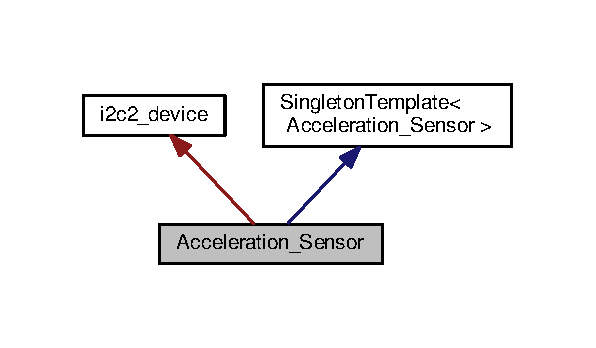
\includegraphics[width=286pt]{de/db6/classAcceleration__Sensor__inherit__graph}
\end{center}
\end{figure}


Collaboration diagram for Acceleration\+\_\+\+Sensor\+:\nopagebreak
\begin{figure}[H]
\begin{center}
\leavevmode
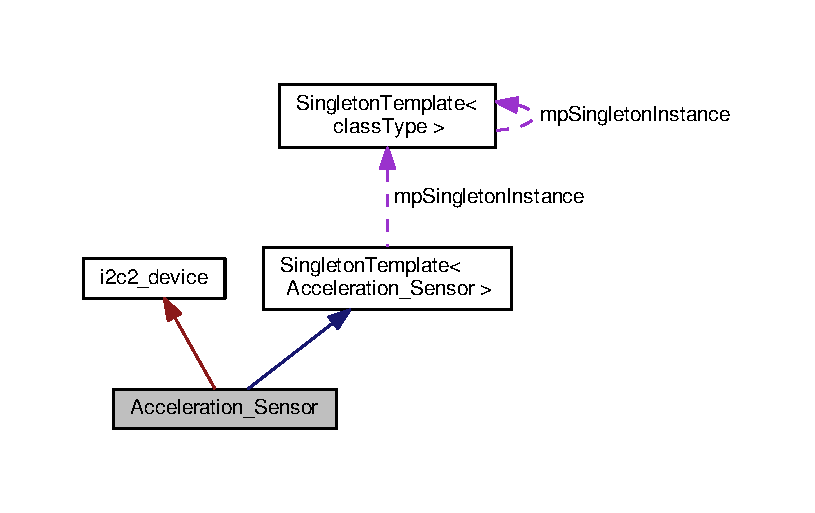
\includegraphics[width=350pt]{d4/d70/classAcceleration__Sensor__coll__graph}
\end{center}
\end{figure}
\subsection*{Public Member Functions}
\begin{DoxyCompactItemize}
\item 
bool \hyperlink{classAcceleration__Sensor_af3c7c3da10972a67263c92d79ca5ecf6}{init} ()
\begin{DoxyCompactList}\small\item\em Initializes the sensor. \end{DoxyCompactList}\item 
int16\+\_\+t \hyperlink{classAcceleration__Sensor_a5012e9e41913187945ebb9a7acf3b758}{getX} ()
\item 
int16\+\_\+t \hyperlink{classAcceleration__Sensor_ab77b00366f9cff5b09927c0b4d30c226}{getY} ()
\item 
int16\+\_\+t \hyperlink{classAcceleration__Sensor_aa2a0912e9ae2280d709b3e7874da437a}{getZ} ()
\end{DoxyCompactItemize}
\subsection*{Friends}
\begin{DoxyCompactItemize}
\item 
class \hyperlink{classAcceleration__Sensor_ad04626d03828abd05f83572d1db4c294}{Singleton\+Template$<$ Acceleration\+\_\+\+Sensor $>$}
\begin{DoxyCompactList}\small\item\em Friend class used for Singleton Template. \end{DoxyCompactList}\end{DoxyCompactItemize}
\subsection*{Additional Inherited Members}


\subsection{Detailed Description}
Acceleration Sensor class used to get acceleration data reading from the on-\/board sensor. Acceleration data reading can provide absolute tilt of the board (if under no movement), and it can also provide the movement activity of the board. 

\subsection{Member Function Documentation}
\index{Acceleration\+\_\+\+Sensor@{Acceleration\+\_\+\+Sensor}!getX@{getX}}
\index{getX@{getX}!Acceleration\+\_\+\+Sensor@{Acceleration\+\_\+\+Sensor}}
\subsubsection[{\texorpdfstring{get\+X()}{getX()}}]{\setlength{\rightskip}{0pt plus 5cm}int16\+\_\+t Acceleration\+\_\+\+Sensor\+::getX (
\begin{DoxyParamCaption}
{}
\end{DoxyParamCaption}
)}\hypertarget{classAcceleration__Sensor_a5012e9e41913187945ebb9a7acf3b758}{}\label{classAcceleration__Sensor_a5012e9e41913187945ebb9a7acf3b758}
\begin{DoxyReturn}{Returns}
X-\/\+Axis value 
\end{DoxyReturn}
\index{Acceleration\+\_\+\+Sensor@{Acceleration\+\_\+\+Sensor}!getY@{getY}}
\index{getY@{getY}!Acceleration\+\_\+\+Sensor@{Acceleration\+\_\+\+Sensor}}
\subsubsection[{\texorpdfstring{get\+Y()}{getY()}}]{\setlength{\rightskip}{0pt plus 5cm}int16\+\_\+t Acceleration\+\_\+\+Sensor\+::getY (
\begin{DoxyParamCaption}
{}
\end{DoxyParamCaption}
)}\hypertarget{classAcceleration__Sensor_ab77b00366f9cff5b09927c0b4d30c226}{}\label{classAcceleration__Sensor_ab77b00366f9cff5b09927c0b4d30c226}
\begin{DoxyReturn}{Returns}
Y-\/\+Axis value 
\end{DoxyReturn}
\index{Acceleration\+\_\+\+Sensor@{Acceleration\+\_\+\+Sensor}!getZ@{getZ}}
\index{getZ@{getZ}!Acceleration\+\_\+\+Sensor@{Acceleration\+\_\+\+Sensor}}
\subsubsection[{\texorpdfstring{get\+Z()}{getZ()}}]{\setlength{\rightskip}{0pt plus 5cm}int16\+\_\+t Acceleration\+\_\+\+Sensor\+::getZ (
\begin{DoxyParamCaption}
{}
\end{DoxyParamCaption}
)}\hypertarget{classAcceleration__Sensor_aa2a0912e9ae2280d709b3e7874da437a}{}\label{classAcceleration__Sensor_aa2a0912e9ae2280d709b3e7874da437a}
\begin{DoxyReturn}{Returns}
Z-\/\+Axis value 
\end{DoxyReturn}
\index{Acceleration\+\_\+\+Sensor@{Acceleration\+\_\+\+Sensor}!init@{init}}
\index{init@{init}!Acceleration\+\_\+\+Sensor@{Acceleration\+\_\+\+Sensor}}
\subsubsection[{\texorpdfstring{init()}{init()}}]{\setlength{\rightskip}{0pt plus 5cm}bool Acceleration\+\_\+\+Sensor\+::init (
\begin{DoxyParamCaption}
\item[{void}]{}
\end{DoxyParamCaption}
)}\hypertarget{classAcceleration__Sensor_af3c7c3da10972a67263c92d79ca5ecf6}{}\label{classAcceleration__Sensor_af3c7c3da10972a67263c92d79ca5ecf6}


Initializes the sensor. 



\subsection{Friends And Related Function Documentation}
\index{Acceleration\+\_\+\+Sensor@{Acceleration\+\_\+\+Sensor}!Singleton\+Template$<$ Acceleration\+\_\+\+Sensor $>$@{Singleton\+Template$<$ Acceleration\+\_\+\+Sensor $>$}}
\index{Singleton\+Template$<$ Acceleration\+\_\+\+Sensor $>$@{Singleton\+Template$<$ Acceleration\+\_\+\+Sensor $>$}!Acceleration\+\_\+\+Sensor@{Acceleration\+\_\+\+Sensor}}
\subsubsection[{\texorpdfstring{Singleton\+Template$<$ Acceleration\+\_\+\+Sensor $>$}{SingletonTemplate< Acceleration_Sensor >}}]{\setlength{\rightskip}{0pt plus 5cm}friend class {\bf Singleton\+Template}$<$ {\bf Acceleration\+\_\+\+Sensor} $>$\hspace{0.3cm}{\ttfamily [friend]}}\hypertarget{classAcceleration__Sensor_ad04626d03828abd05f83572d1db4c294}{}\label{classAcceleration__Sensor_ad04626d03828abd05f83572d1db4c294}


Friend class used for Singleton Template. 



The documentation for this class was generated from the following files\+:\begin{DoxyCompactItemize}
\item 
/var/www/html/\+S\+J\+S\+U-\/\+D\+E\+V-\/\+Linux/firmware/default/lib/\+L4\+\_\+\+I\+O/\hyperlink{acceleration__sensor_8hpp}{acceleration\+\_\+sensor.\+hpp}\item 
/var/www/html/\+S\+J\+S\+U-\/\+D\+E\+V-\/\+Linux/firmware/default/lib/\+L4\+\_\+\+I\+O/src/\hyperlink{io__source_8cpp}{io\+\_\+source.\+cpp}\end{DoxyCompactItemize}

\hypertarget{structalarm__time__t}{}\section{alarm\+\_\+time\+\_\+t Struct Reference}
\label{structalarm__time__t}\index{alarm\+\_\+time\+\_\+t@{alarm\+\_\+time\+\_\+t}}


{\ttfamily \#include $<$rtc\+\_\+alarm.\+h$>$}

\subsection*{Data Fields}
\begin{DoxyCompactItemize}
\item 
uint8\+\_\+t \hyperlink{structalarm__time__t_a18062d8b9f04f5d358bfb5b9a98d3274}{hour}
\item 
uint8\+\_\+t \hyperlink{structalarm__time__t_acb0496766d834ee5c0e2cd243727f080}{min}
\item 
uint8\+\_\+t \hyperlink{structalarm__time__t_acee0c4e36d57b97fc128d666147961e6}{sec}
\end{DoxyCompactItemize}


\subsection{Detailed Description}
\hyperlink{rtc__alarm_8h_a887b55296bc21c983fa01dff378634ae}{rtc\+\_\+alarm\+\_\+create()} returns the pointer to this structure. This structure can be used to change the alarm time after it has been created. 

\subsection{Field Documentation}
\index{alarm\+\_\+time\+\_\+t@{alarm\+\_\+time\+\_\+t}!hour@{hour}}
\index{hour@{hour}!alarm\+\_\+time\+\_\+t@{alarm\+\_\+time\+\_\+t}}
\subsubsection[{\texorpdfstring{hour}{hour}}]{\setlength{\rightskip}{0pt plus 5cm}uint8\+\_\+t alarm\+\_\+time\+\_\+t\+::hour}\hypertarget{structalarm__time__t_a18062d8b9f04f5d358bfb5b9a98d3274}{}\label{structalarm__time__t_a18062d8b9f04f5d358bfb5b9a98d3274}
\index{alarm\+\_\+time\+\_\+t@{alarm\+\_\+time\+\_\+t}!min@{min}}
\index{min@{min}!alarm\+\_\+time\+\_\+t@{alarm\+\_\+time\+\_\+t}}
\subsubsection[{\texorpdfstring{min}{min}}]{\setlength{\rightskip}{0pt plus 5cm}uint8\+\_\+t alarm\+\_\+time\+\_\+t\+::min}\hypertarget{structalarm__time__t_acb0496766d834ee5c0e2cd243727f080}{}\label{structalarm__time__t_acb0496766d834ee5c0e2cd243727f080}
\index{alarm\+\_\+time\+\_\+t@{alarm\+\_\+time\+\_\+t}!sec@{sec}}
\index{sec@{sec}!alarm\+\_\+time\+\_\+t@{alarm\+\_\+time\+\_\+t}}
\subsubsection[{\texorpdfstring{sec}{sec}}]{\setlength{\rightskip}{0pt plus 5cm}uint8\+\_\+t alarm\+\_\+time\+\_\+t\+::sec}\hypertarget{structalarm__time__t_acee0c4e36d57b97fc128d666147961e6}{}\label{structalarm__time__t_acee0c4e36d57b97fc128d666147961e6}


The documentation for this struct was generated from the following file\+:\begin{DoxyCompactItemize}
\item 
/var/www/html/\+S\+J\+S\+U-\/\+D\+E\+V-\/\+Linux/firmware/default/lib/\+L3\+\_\+\+Utils/\hyperlink{rtc__alarm_8h}{rtc\+\_\+alarm.\+h}\end{DoxyCompactItemize}

\hypertarget{unionbit__struct__t}{}\section{bit\+\_\+struct\+\_\+t Union Reference}
\label{unionbit__struct__t}\index{bit\+\_\+struct\+\_\+t@{bit\+\_\+struct\+\_\+t}}


{\ttfamily \#include $<$bit\+\_\+manip.\+h$>$}

\subsection*{Public Member Functions}
\begin{DoxyCompactItemize}
\item 
\begin{tabbing}
xx\=xx\=xx\=xx\=xx\=xx\=xx\=xx\=xx\=\kill
struct \{\\
\>uint32\_t \hyperlink{unionbit__struct__t_a491397476dce030620dce42378042a5f}{b0}:1\\
\>uint32\_t \hyperlink{unionbit__struct__t_a1fbc5467ca270de23091f7127a5f23ae}{b1}:1\\
\>uint32\_t \hyperlink{unionbit__struct__t_a21a2b2861dab2bdda694f1732811df54}{b2}:1\\
\>uint32\_t \hyperlink{unionbit__struct__t_ae7418fe6c642ce8f2866e2355f60860c}{b3}:1\\
\>uint32\_t \hyperlink{unionbit__struct__t_a1c1a84e7db8333fd9aa7c83906ea27e7}{b4}:1\\
\>uint32\_t \hyperlink{unionbit__struct__t_a919690e64bc87e27bd9aa7b81602c014}{b5}:1\\
\>uint32\_t \hyperlink{unionbit__struct__t_a70281a97aeb203f6a1a2cef287f65310}{b6}:1\\
\>uint32\_t \hyperlink{unionbit__struct__t_a9e54fbbf4588aa5b767a14c9dc238c85}{b7}:1\\
\>uint32\_t \hyperlink{unionbit__struct__t_a246a1636e6d8628ac7f5d3b515d283b6}{b8}:1\\
\>uint32\_t \hyperlink{unionbit__struct__t_a79aed403b826c5ca3e1541843819b2bd}{b9}:1\\
\>uint32\_t \hyperlink{unionbit__struct__t_ac7cc1cf2b4b50371f91f75678f0ff82b}{b10}:1\\
\>uint32\_t \hyperlink{unionbit__struct__t_a371340740c1742dc85b3df7c1e63fd33}{b11}:1\\
\>uint32\_t \hyperlink{unionbit__struct__t_a2c6a929678dd473e96879c9d6083d5bd}{b12}:1\\
\>uint32\_t \hyperlink{unionbit__struct__t_aaddb699fd9994c6bfaf9d5edeac0ce5c}{b13}:1\\
\>uint32\_t \hyperlink{unionbit__struct__t_ac1713599888c77b4bb0681ef74c157e8}{b14}:1\\
\>uint32\_t \hyperlink{unionbit__struct__t_aeeca2f2ee2504ac21a899c19ae19eff1}{b15}:1\\
\>uint32\_t \hyperlink{unionbit__struct__t_a1b5701713fcb7909372c62be1d044505}{b16}:1\\
\>uint32\_t \hyperlink{unionbit__struct__t_adc29e0e74293b63bf43b2593ff396cd1}{b17}:1\\
\>uint32\_t \hyperlink{unionbit__struct__t_a722cedebc980c35bf056db133321835d}{b18}:1\\
\>uint32\_t \hyperlink{unionbit__struct__t_ac5864f59ad060018dc179349cd363ae0}{b19}:1\\
\>uint32\_t \hyperlink{unionbit__struct__t_ad908b970ed19f7f293e9b87a99e67d4f}{b20}:1\\
\>uint32\_t \hyperlink{unionbit__struct__t_a1fe0488c77788dd9b2a7ff0e6461fe39}{b21}:1\\
\>uint32\_t \hyperlink{unionbit__struct__t_a269578aa8ce516431ae59fc74158a985}{b22}:1\\
\>uint32\_t \hyperlink{unionbit__struct__t_a9abf84e3955f45635e4d7a4d7aa9eb51}{b23}:1\\
\>uint32\_t \hyperlink{unionbit__struct__t_af36c7f43ffc7c1d9ebba9754cc45b75b}{b24}:1\\
\>uint32\_t \hyperlink{unionbit__struct__t_a53467acc282cb33fa223933375ec7a2f}{b25}:1\\
\>uint32\_t \hyperlink{unionbit__struct__t_a8e8784793b9ed5e08a4479b23b7972c7}{b26}:1\\
\>uint32\_t \hyperlink{unionbit__struct__t_aa62f1be0e5447f8d7d0f557516cd0465}{b27}:1\\
\>uint32\_t \hyperlink{unionbit__struct__t_a10ea9c28f49d4eac58bddb036822e768}{b28}:1\\
\>uint32\_t \hyperlink{unionbit__struct__t_ab64b5c1bdfbb1681b2e35ac13a65b5a9}{b29}:1\\
\>uint32\_t \hyperlink{unionbit__struct__t_a8b8f60aa7036ab47250d3bc63e4adb7e}{b30}:1\\
\>uint32\_t \hyperlink{unionbit__struct__t_a299ac7a3222050a7436d4635d9a22cd1}{b31}:1\\
\} \hyperlink{unionbit__struct__t_a1b66512751188efcc8a80c012758c374}{\_\_attribute\_\_} ((packed))\\

\end{tabbing}\item 
\begin{tabbing}
xx\=xx\=xx\=xx\=xx\=xx\=xx\=xx\=xx\=\kill
struct \{\\
\>uint32\_t \hyperlink{unionbit__struct__t_a8c5e3a00339f5c999f318185ac838fc2}{b1\_0}: 2\\
\>uint32\_t \hyperlink{unionbit__struct__t_ad652f734919f09d1d875208238930d6c}{b3\_2}: 2\\
\>uint32\_t \hyperlink{unionbit__struct__t_afeadfa0621b077bf6f730915450e5db9}{b5\_4}: 2\\
\>uint32\_t \hyperlink{unionbit__struct__t_a986d1d13426028cd47a44fb0fb48ff11}{b7\_6}: 2\\
\>uint32\_t \hyperlink{unionbit__struct__t_a1f748b48a12aa4cc9f39ae4795544076}{b9\_8}: 2\\
\>uint32\_t \hyperlink{unionbit__struct__t_ad7441f8a1702f9bb0609bc10c7e3dbd5}{b11\_10}: 2\\
\>uint32\_t \hyperlink{unionbit__struct__t_af095e1052f63a9b61bbdc9106253e2da}{b13\_12}: 2\\
\>uint32\_t \hyperlink{unionbit__struct__t_abdad786b29cee9a453a388d3fcc854a4}{b15\_14}: 2\\
\>uint32\_t \hyperlink{unionbit__struct__t_a75795ea689cef3511d87dc627c4e6640}{b17\_16}: 2\\
\>uint32\_t \hyperlink{unionbit__struct__t_a079d9acb3d407bfd7aab2e5501771ce3}{b19\_18}: 2\\
\>uint32\_t \hyperlink{unionbit__struct__t_af64a781e6496513276fd5f064f02c0ca}{b21\_20}: 2\\
\>uint32\_t \hyperlink{unionbit__struct__t_adcb43d5fad0c1ff743b1f4793c52ed45}{b23\_22}: 2\\
\>uint32\_t \hyperlink{unionbit__struct__t_aa088a38593ccf1cd8b0fed80759b393a}{b25\_24}: 2\\
\>uint32\_t \hyperlink{unionbit__struct__t_ad01cc51243e746f3db9186b9e6ff9685}{b27\_26}: 2\\
\>uint32\_t \hyperlink{unionbit__struct__t_a608ebf93b0545e42f3e4b7032732f58e}{b29\_28}: 2\\
\>uint32\_t \hyperlink{unionbit__struct__t_acad884db75131e0ee205527bfddaac57}{b31\_30}: 2\\
\} \hyperlink{unionbit__struct__t_a0c97b58f274cd871f809a121cba083e1}{\_\_attribute\_\_} ((packed))\\

\end{tabbing}\end{DoxyCompactItemize}
\subsection*{Data Fields}
\begin{DoxyCompactItemize}
\item 
uint32\+\_\+t \hyperlink{unionbit__struct__t_aa0cf0a126273dac31f0dca900191aed6}{full32bit}
\end{DoxyCompactItemize}


\subsection{Detailed Description}
1-\/bit structure Use \hyperlink{bit__manip_8h_abdda5c6a0477ff7eba1c137aaf9cd966}{B\+I\+T()} macro for bit manipulation of your memory/variable. 

\subsection{Member Function Documentation}
\index{bit\+\_\+struct\+\_\+t@{bit\+\_\+struct\+\_\+t}!\+\_\+\+\_\+attribute\+\_\+\+\_\+@{\+\_\+\+\_\+attribute\+\_\+\+\_\+}}
\index{\+\_\+\+\_\+attribute\+\_\+\+\_\+@{\+\_\+\+\_\+attribute\+\_\+\+\_\+}!bit\+\_\+struct\+\_\+t@{bit\+\_\+struct\+\_\+t}}
\subsubsection[{\texorpdfstring{\+\_\+\+\_\+attribute\+\_\+\+\_\+((packed))}{__attribute__((packed))}}]{\setlength{\rightskip}{0pt plus 5cm}struct bit\+\_\+struct\+\_\+t\+::@0 bit\+\_\+struct\+\_\+t\+::\+\_\+\+\_\+attribute\+\_\+\+\_\+ (
\begin{DoxyParamCaption}
\item[{(packed)}]{}
\end{DoxyParamCaption}
)}\hypertarget{unionbit__struct__t_a1b66512751188efcc8a80c012758c374}{}\label{unionbit__struct__t_a1b66512751188efcc8a80c012758c374}
\index{bit\+\_\+struct\+\_\+t@{bit\+\_\+struct\+\_\+t}!\+\_\+\+\_\+attribute\+\_\+\+\_\+@{\+\_\+\+\_\+attribute\+\_\+\+\_\+}}
\index{\+\_\+\+\_\+attribute\+\_\+\+\_\+@{\+\_\+\+\_\+attribute\+\_\+\+\_\+}!bit\+\_\+struct\+\_\+t@{bit\+\_\+struct\+\_\+t}}
\subsubsection[{\texorpdfstring{\+\_\+\+\_\+attribute\+\_\+\+\_\+((packed))}{__attribute__((packed))}}]{\setlength{\rightskip}{0pt plus 5cm}struct bit\+\_\+struct\+\_\+t\+::@1 bit\+\_\+struct\+\_\+t\+::\+\_\+\+\_\+attribute\+\_\+\+\_\+ (
\begin{DoxyParamCaption}
\item[{(packed)}]{}
\end{DoxyParamCaption}
)}\hypertarget{unionbit__struct__t_a0c97b58f274cd871f809a121cba083e1}{}\label{unionbit__struct__t_a0c97b58f274cd871f809a121cba083e1}


\subsection{Field Documentation}
\index{bit\+\_\+struct\+\_\+t@{bit\+\_\+struct\+\_\+t}!b0@{b0}}
\index{b0@{b0}!bit\+\_\+struct\+\_\+t@{bit\+\_\+struct\+\_\+t}}
\subsubsection[{\texorpdfstring{b0}{b0}}]{\setlength{\rightskip}{0pt plus 5cm}uint32\+\_\+t bit\+\_\+struct\+\_\+t\+::b0}\hypertarget{unionbit__struct__t_a491397476dce030620dce42378042a5f}{}\label{unionbit__struct__t_a491397476dce030620dce42378042a5f}
\index{bit\+\_\+struct\+\_\+t@{bit\+\_\+struct\+\_\+t}!b1@{b1}}
\index{b1@{b1}!bit\+\_\+struct\+\_\+t@{bit\+\_\+struct\+\_\+t}}
\subsubsection[{\texorpdfstring{b1}{b1}}]{\setlength{\rightskip}{0pt plus 5cm}uint32\+\_\+t bit\+\_\+struct\+\_\+t\+::b1}\hypertarget{unionbit__struct__t_a1fbc5467ca270de23091f7127a5f23ae}{}\label{unionbit__struct__t_a1fbc5467ca270de23091f7127a5f23ae}
\index{bit\+\_\+struct\+\_\+t@{bit\+\_\+struct\+\_\+t}!b10@{b10}}
\index{b10@{b10}!bit\+\_\+struct\+\_\+t@{bit\+\_\+struct\+\_\+t}}
\subsubsection[{\texorpdfstring{b10}{b10}}]{\setlength{\rightskip}{0pt plus 5cm}uint32\+\_\+t bit\+\_\+struct\+\_\+t\+::b10}\hypertarget{unionbit__struct__t_ac7cc1cf2b4b50371f91f75678f0ff82b}{}\label{unionbit__struct__t_ac7cc1cf2b4b50371f91f75678f0ff82b}
\index{bit\+\_\+struct\+\_\+t@{bit\+\_\+struct\+\_\+t}!b11@{b11}}
\index{b11@{b11}!bit\+\_\+struct\+\_\+t@{bit\+\_\+struct\+\_\+t}}
\subsubsection[{\texorpdfstring{b11}{b11}}]{\setlength{\rightskip}{0pt plus 5cm}uint32\+\_\+t bit\+\_\+struct\+\_\+t\+::b11}\hypertarget{unionbit__struct__t_a371340740c1742dc85b3df7c1e63fd33}{}\label{unionbit__struct__t_a371340740c1742dc85b3df7c1e63fd33}
\index{bit\+\_\+struct\+\_\+t@{bit\+\_\+struct\+\_\+t}!b11\+\_\+10@{b11\+\_\+10}}
\index{b11\+\_\+10@{b11\+\_\+10}!bit\+\_\+struct\+\_\+t@{bit\+\_\+struct\+\_\+t}}
\subsubsection[{\texorpdfstring{b11\+\_\+10}{b11_10}}]{\setlength{\rightskip}{0pt plus 5cm}uint32\+\_\+t bit\+\_\+struct\+\_\+t\+::b11\+\_\+10}\hypertarget{unionbit__struct__t_ad7441f8a1702f9bb0609bc10c7e3dbd5}{}\label{unionbit__struct__t_ad7441f8a1702f9bb0609bc10c7e3dbd5}
\index{bit\+\_\+struct\+\_\+t@{bit\+\_\+struct\+\_\+t}!b12@{b12}}
\index{b12@{b12}!bit\+\_\+struct\+\_\+t@{bit\+\_\+struct\+\_\+t}}
\subsubsection[{\texorpdfstring{b12}{b12}}]{\setlength{\rightskip}{0pt plus 5cm}uint32\+\_\+t bit\+\_\+struct\+\_\+t\+::b12}\hypertarget{unionbit__struct__t_a2c6a929678dd473e96879c9d6083d5bd}{}\label{unionbit__struct__t_a2c6a929678dd473e96879c9d6083d5bd}
\index{bit\+\_\+struct\+\_\+t@{bit\+\_\+struct\+\_\+t}!b13@{b13}}
\index{b13@{b13}!bit\+\_\+struct\+\_\+t@{bit\+\_\+struct\+\_\+t}}
\subsubsection[{\texorpdfstring{b13}{b13}}]{\setlength{\rightskip}{0pt plus 5cm}uint32\+\_\+t bit\+\_\+struct\+\_\+t\+::b13}\hypertarget{unionbit__struct__t_aaddb699fd9994c6bfaf9d5edeac0ce5c}{}\label{unionbit__struct__t_aaddb699fd9994c6bfaf9d5edeac0ce5c}
\index{bit\+\_\+struct\+\_\+t@{bit\+\_\+struct\+\_\+t}!b13\+\_\+12@{b13\+\_\+12}}
\index{b13\+\_\+12@{b13\+\_\+12}!bit\+\_\+struct\+\_\+t@{bit\+\_\+struct\+\_\+t}}
\subsubsection[{\texorpdfstring{b13\+\_\+12}{b13_12}}]{\setlength{\rightskip}{0pt plus 5cm}uint32\+\_\+t bit\+\_\+struct\+\_\+t\+::b13\+\_\+12}\hypertarget{unionbit__struct__t_af095e1052f63a9b61bbdc9106253e2da}{}\label{unionbit__struct__t_af095e1052f63a9b61bbdc9106253e2da}
\index{bit\+\_\+struct\+\_\+t@{bit\+\_\+struct\+\_\+t}!b14@{b14}}
\index{b14@{b14}!bit\+\_\+struct\+\_\+t@{bit\+\_\+struct\+\_\+t}}
\subsubsection[{\texorpdfstring{b14}{b14}}]{\setlength{\rightskip}{0pt plus 5cm}uint32\+\_\+t bit\+\_\+struct\+\_\+t\+::b14}\hypertarget{unionbit__struct__t_ac1713599888c77b4bb0681ef74c157e8}{}\label{unionbit__struct__t_ac1713599888c77b4bb0681ef74c157e8}
\index{bit\+\_\+struct\+\_\+t@{bit\+\_\+struct\+\_\+t}!b15@{b15}}
\index{b15@{b15}!bit\+\_\+struct\+\_\+t@{bit\+\_\+struct\+\_\+t}}
\subsubsection[{\texorpdfstring{b15}{b15}}]{\setlength{\rightskip}{0pt plus 5cm}uint32\+\_\+t bit\+\_\+struct\+\_\+t\+::b15}\hypertarget{unionbit__struct__t_aeeca2f2ee2504ac21a899c19ae19eff1}{}\label{unionbit__struct__t_aeeca2f2ee2504ac21a899c19ae19eff1}
\index{bit\+\_\+struct\+\_\+t@{bit\+\_\+struct\+\_\+t}!b15\+\_\+14@{b15\+\_\+14}}
\index{b15\+\_\+14@{b15\+\_\+14}!bit\+\_\+struct\+\_\+t@{bit\+\_\+struct\+\_\+t}}
\subsubsection[{\texorpdfstring{b15\+\_\+14}{b15_14}}]{\setlength{\rightskip}{0pt plus 5cm}uint32\+\_\+t bit\+\_\+struct\+\_\+t\+::b15\+\_\+14}\hypertarget{unionbit__struct__t_abdad786b29cee9a453a388d3fcc854a4}{}\label{unionbit__struct__t_abdad786b29cee9a453a388d3fcc854a4}
\index{bit\+\_\+struct\+\_\+t@{bit\+\_\+struct\+\_\+t}!b16@{b16}}
\index{b16@{b16}!bit\+\_\+struct\+\_\+t@{bit\+\_\+struct\+\_\+t}}
\subsubsection[{\texorpdfstring{b16}{b16}}]{\setlength{\rightskip}{0pt plus 5cm}uint32\+\_\+t bit\+\_\+struct\+\_\+t\+::b16}\hypertarget{unionbit__struct__t_a1b5701713fcb7909372c62be1d044505}{}\label{unionbit__struct__t_a1b5701713fcb7909372c62be1d044505}
\index{bit\+\_\+struct\+\_\+t@{bit\+\_\+struct\+\_\+t}!b17@{b17}}
\index{b17@{b17}!bit\+\_\+struct\+\_\+t@{bit\+\_\+struct\+\_\+t}}
\subsubsection[{\texorpdfstring{b17}{b17}}]{\setlength{\rightskip}{0pt plus 5cm}uint32\+\_\+t bit\+\_\+struct\+\_\+t\+::b17}\hypertarget{unionbit__struct__t_adc29e0e74293b63bf43b2593ff396cd1}{}\label{unionbit__struct__t_adc29e0e74293b63bf43b2593ff396cd1}
\index{bit\+\_\+struct\+\_\+t@{bit\+\_\+struct\+\_\+t}!b17\+\_\+16@{b17\+\_\+16}}
\index{b17\+\_\+16@{b17\+\_\+16}!bit\+\_\+struct\+\_\+t@{bit\+\_\+struct\+\_\+t}}
\subsubsection[{\texorpdfstring{b17\+\_\+16}{b17_16}}]{\setlength{\rightskip}{0pt plus 5cm}uint32\+\_\+t bit\+\_\+struct\+\_\+t\+::b17\+\_\+16}\hypertarget{unionbit__struct__t_a75795ea689cef3511d87dc627c4e6640}{}\label{unionbit__struct__t_a75795ea689cef3511d87dc627c4e6640}
\index{bit\+\_\+struct\+\_\+t@{bit\+\_\+struct\+\_\+t}!b18@{b18}}
\index{b18@{b18}!bit\+\_\+struct\+\_\+t@{bit\+\_\+struct\+\_\+t}}
\subsubsection[{\texorpdfstring{b18}{b18}}]{\setlength{\rightskip}{0pt plus 5cm}uint32\+\_\+t bit\+\_\+struct\+\_\+t\+::b18}\hypertarget{unionbit__struct__t_a722cedebc980c35bf056db133321835d}{}\label{unionbit__struct__t_a722cedebc980c35bf056db133321835d}
\index{bit\+\_\+struct\+\_\+t@{bit\+\_\+struct\+\_\+t}!b19@{b19}}
\index{b19@{b19}!bit\+\_\+struct\+\_\+t@{bit\+\_\+struct\+\_\+t}}
\subsubsection[{\texorpdfstring{b19}{b19}}]{\setlength{\rightskip}{0pt plus 5cm}uint32\+\_\+t bit\+\_\+struct\+\_\+t\+::b19}\hypertarget{unionbit__struct__t_ac5864f59ad060018dc179349cd363ae0}{}\label{unionbit__struct__t_ac5864f59ad060018dc179349cd363ae0}
\index{bit\+\_\+struct\+\_\+t@{bit\+\_\+struct\+\_\+t}!b19\+\_\+18@{b19\+\_\+18}}
\index{b19\+\_\+18@{b19\+\_\+18}!bit\+\_\+struct\+\_\+t@{bit\+\_\+struct\+\_\+t}}
\subsubsection[{\texorpdfstring{b19\+\_\+18}{b19_18}}]{\setlength{\rightskip}{0pt plus 5cm}uint32\+\_\+t bit\+\_\+struct\+\_\+t\+::b19\+\_\+18}\hypertarget{unionbit__struct__t_a079d9acb3d407bfd7aab2e5501771ce3}{}\label{unionbit__struct__t_a079d9acb3d407bfd7aab2e5501771ce3}
\index{bit\+\_\+struct\+\_\+t@{bit\+\_\+struct\+\_\+t}!b1\+\_\+0@{b1\+\_\+0}}
\index{b1\+\_\+0@{b1\+\_\+0}!bit\+\_\+struct\+\_\+t@{bit\+\_\+struct\+\_\+t}}
\subsubsection[{\texorpdfstring{b1\+\_\+0}{b1_0}}]{\setlength{\rightskip}{0pt plus 5cm}uint32\+\_\+t bit\+\_\+struct\+\_\+t\+::b1\+\_\+0}\hypertarget{unionbit__struct__t_a8c5e3a00339f5c999f318185ac838fc2}{}\label{unionbit__struct__t_a8c5e3a00339f5c999f318185ac838fc2}
\index{bit\+\_\+struct\+\_\+t@{bit\+\_\+struct\+\_\+t}!b2@{b2}}
\index{b2@{b2}!bit\+\_\+struct\+\_\+t@{bit\+\_\+struct\+\_\+t}}
\subsubsection[{\texorpdfstring{b2}{b2}}]{\setlength{\rightskip}{0pt plus 5cm}uint32\+\_\+t bit\+\_\+struct\+\_\+t\+::b2}\hypertarget{unionbit__struct__t_a21a2b2861dab2bdda694f1732811df54}{}\label{unionbit__struct__t_a21a2b2861dab2bdda694f1732811df54}
\index{bit\+\_\+struct\+\_\+t@{bit\+\_\+struct\+\_\+t}!b20@{b20}}
\index{b20@{b20}!bit\+\_\+struct\+\_\+t@{bit\+\_\+struct\+\_\+t}}
\subsubsection[{\texorpdfstring{b20}{b20}}]{\setlength{\rightskip}{0pt plus 5cm}uint32\+\_\+t bit\+\_\+struct\+\_\+t\+::b20}\hypertarget{unionbit__struct__t_ad908b970ed19f7f293e9b87a99e67d4f}{}\label{unionbit__struct__t_ad908b970ed19f7f293e9b87a99e67d4f}
\index{bit\+\_\+struct\+\_\+t@{bit\+\_\+struct\+\_\+t}!b21@{b21}}
\index{b21@{b21}!bit\+\_\+struct\+\_\+t@{bit\+\_\+struct\+\_\+t}}
\subsubsection[{\texorpdfstring{b21}{b21}}]{\setlength{\rightskip}{0pt plus 5cm}uint32\+\_\+t bit\+\_\+struct\+\_\+t\+::b21}\hypertarget{unionbit__struct__t_a1fe0488c77788dd9b2a7ff0e6461fe39}{}\label{unionbit__struct__t_a1fe0488c77788dd9b2a7ff0e6461fe39}
\index{bit\+\_\+struct\+\_\+t@{bit\+\_\+struct\+\_\+t}!b21\+\_\+20@{b21\+\_\+20}}
\index{b21\+\_\+20@{b21\+\_\+20}!bit\+\_\+struct\+\_\+t@{bit\+\_\+struct\+\_\+t}}
\subsubsection[{\texorpdfstring{b21\+\_\+20}{b21_20}}]{\setlength{\rightskip}{0pt plus 5cm}uint32\+\_\+t bit\+\_\+struct\+\_\+t\+::b21\+\_\+20}\hypertarget{unionbit__struct__t_af64a781e6496513276fd5f064f02c0ca}{}\label{unionbit__struct__t_af64a781e6496513276fd5f064f02c0ca}
\index{bit\+\_\+struct\+\_\+t@{bit\+\_\+struct\+\_\+t}!b22@{b22}}
\index{b22@{b22}!bit\+\_\+struct\+\_\+t@{bit\+\_\+struct\+\_\+t}}
\subsubsection[{\texorpdfstring{b22}{b22}}]{\setlength{\rightskip}{0pt plus 5cm}uint32\+\_\+t bit\+\_\+struct\+\_\+t\+::b22}\hypertarget{unionbit__struct__t_a269578aa8ce516431ae59fc74158a985}{}\label{unionbit__struct__t_a269578aa8ce516431ae59fc74158a985}
\index{bit\+\_\+struct\+\_\+t@{bit\+\_\+struct\+\_\+t}!b23@{b23}}
\index{b23@{b23}!bit\+\_\+struct\+\_\+t@{bit\+\_\+struct\+\_\+t}}
\subsubsection[{\texorpdfstring{b23}{b23}}]{\setlength{\rightskip}{0pt plus 5cm}uint32\+\_\+t bit\+\_\+struct\+\_\+t\+::b23}\hypertarget{unionbit__struct__t_a9abf84e3955f45635e4d7a4d7aa9eb51}{}\label{unionbit__struct__t_a9abf84e3955f45635e4d7a4d7aa9eb51}
\index{bit\+\_\+struct\+\_\+t@{bit\+\_\+struct\+\_\+t}!b23\+\_\+22@{b23\+\_\+22}}
\index{b23\+\_\+22@{b23\+\_\+22}!bit\+\_\+struct\+\_\+t@{bit\+\_\+struct\+\_\+t}}
\subsubsection[{\texorpdfstring{b23\+\_\+22}{b23_22}}]{\setlength{\rightskip}{0pt plus 5cm}uint32\+\_\+t bit\+\_\+struct\+\_\+t\+::b23\+\_\+22}\hypertarget{unionbit__struct__t_adcb43d5fad0c1ff743b1f4793c52ed45}{}\label{unionbit__struct__t_adcb43d5fad0c1ff743b1f4793c52ed45}
\index{bit\+\_\+struct\+\_\+t@{bit\+\_\+struct\+\_\+t}!b24@{b24}}
\index{b24@{b24}!bit\+\_\+struct\+\_\+t@{bit\+\_\+struct\+\_\+t}}
\subsubsection[{\texorpdfstring{b24}{b24}}]{\setlength{\rightskip}{0pt plus 5cm}uint32\+\_\+t bit\+\_\+struct\+\_\+t\+::b24}\hypertarget{unionbit__struct__t_af36c7f43ffc7c1d9ebba9754cc45b75b}{}\label{unionbit__struct__t_af36c7f43ffc7c1d9ebba9754cc45b75b}
\index{bit\+\_\+struct\+\_\+t@{bit\+\_\+struct\+\_\+t}!b25@{b25}}
\index{b25@{b25}!bit\+\_\+struct\+\_\+t@{bit\+\_\+struct\+\_\+t}}
\subsubsection[{\texorpdfstring{b25}{b25}}]{\setlength{\rightskip}{0pt plus 5cm}uint32\+\_\+t bit\+\_\+struct\+\_\+t\+::b25}\hypertarget{unionbit__struct__t_a53467acc282cb33fa223933375ec7a2f}{}\label{unionbit__struct__t_a53467acc282cb33fa223933375ec7a2f}
\index{bit\+\_\+struct\+\_\+t@{bit\+\_\+struct\+\_\+t}!b25\+\_\+24@{b25\+\_\+24}}
\index{b25\+\_\+24@{b25\+\_\+24}!bit\+\_\+struct\+\_\+t@{bit\+\_\+struct\+\_\+t}}
\subsubsection[{\texorpdfstring{b25\+\_\+24}{b25_24}}]{\setlength{\rightskip}{0pt plus 5cm}uint32\+\_\+t bit\+\_\+struct\+\_\+t\+::b25\+\_\+24}\hypertarget{unionbit__struct__t_aa088a38593ccf1cd8b0fed80759b393a}{}\label{unionbit__struct__t_aa088a38593ccf1cd8b0fed80759b393a}
\index{bit\+\_\+struct\+\_\+t@{bit\+\_\+struct\+\_\+t}!b26@{b26}}
\index{b26@{b26}!bit\+\_\+struct\+\_\+t@{bit\+\_\+struct\+\_\+t}}
\subsubsection[{\texorpdfstring{b26}{b26}}]{\setlength{\rightskip}{0pt plus 5cm}uint32\+\_\+t bit\+\_\+struct\+\_\+t\+::b26}\hypertarget{unionbit__struct__t_a8e8784793b9ed5e08a4479b23b7972c7}{}\label{unionbit__struct__t_a8e8784793b9ed5e08a4479b23b7972c7}
\index{bit\+\_\+struct\+\_\+t@{bit\+\_\+struct\+\_\+t}!b27@{b27}}
\index{b27@{b27}!bit\+\_\+struct\+\_\+t@{bit\+\_\+struct\+\_\+t}}
\subsubsection[{\texorpdfstring{b27}{b27}}]{\setlength{\rightskip}{0pt plus 5cm}uint32\+\_\+t bit\+\_\+struct\+\_\+t\+::b27}\hypertarget{unionbit__struct__t_aa62f1be0e5447f8d7d0f557516cd0465}{}\label{unionbit__struct__t_aa62f1be0e5447f8d7d0f557516cd0465}
\index{bit\+\_\+struct\+\_\+t@{bit\+\_\+struct\+\_\+t}!b27\+\_\+26@{b27\+\_\+26}}
\index{b27\+\_\+26@{b27\+\_\+26}!bit\+\_\+struct\+\_\+t@{bit\+\_\+struct\+\_\+t}}
\subsubsection[{\texorpdfstring{b27\+\_\+26}{b27_26}}]{\setlength{\rightskip}{0pt plus 5cm}uint32\+\_\+t bit\+\_\+struct\+\_\+t\+::b27\+\_\+26}\hypertarget{unionbit__struct__t_ad01cc51243e746f3db9186b9e6ff9685}{}\label{unionbit__struct__t_ad01cc51243e746f3db9186b9e6ff9685}
\index{bit\+\_\+struct\+\_\+t@{bit\+\_\+struct\+\_\+t}!b28@{b28}}
\index{b28@{b28}!bit\+\_\+struct\+\_\+t@{bit\+\_\+struct\+\_\+t}}
\subsubsection[{\texorpdfstring{b28}{b28}}]{\setlength{\rightskip}{0pt plus 5cm}uint32\+\_\+t bit\+\_\+struct\+\_\+t\+::b28}\hypertarget{unionbit__struct__t_a10ea9c28f49d4eac58bddb036822e768}{}\label{unionbit__struct__t_a10ea9c28f49d4eac58bddb036822e768}
\index{bit\+\_\+struct\+\_\+t@{bit\+\_\+struct\+\_\+t}!b29@{b29}}
\index{b29@{b29}!bit\+\_\+struct\+\_\+t@{bit\+\_\+struct\+\_\+t}}
\subsubsection[{\texorpdfstring{b29}{b29}}]{\setlength{\rightskip}{0pt plus 5cm}uint32\+\_\+t bit\+\_\+struct\+\_\+t\+::b29}\hypertarget{unionbit__struct__t_ab64b5c1bdfbb1681b2e35ac13a65b5a9}{}\label{unionbit__struct__t_ab64b5c1bdfbb1681b2e35ac13a65b5a9}
\index{bit\+\_\+struct\+\_\+t@{bit\+\_\+struct\+\_\+t}!b29\+\_\+28@{b29\+\_\+28}}
\index{b29\+\_\+28@{b29\+\_\+28}!bit\+\_\+struct\+\_\+t@{bit\+\_\+struct\+\_\+t}}
\subsubsection[{\texorpdfstring{b29\+\_\+28}{b29_28}}]{\setlength{\rightskip}{0pt plus 5cm}uint32\+\_\+t bit\+\_\+struct\+\_\+t\+::b29\+\_\+28}\hypertarget{unionbit__struct__t_a608ebf93b0545e42f3e4b7032732f58e}{}\label{unionbit__struct__t_a608ebf93b0545e42f3e4b7032732f58e}
\index{bit\+\_\+struct\+\_\+t@{bit\+\_\+struct\+\_\+t}!b3@{b3}}
\index{b3@{b3}!bit\+\_\+struct\+\_\+t@{bit\+\_\+struct\+\_\+t}}
\subsubsection[{\texorpdfstring{b3}{b3}}]{\setlength{\rightskip}{0pt plus 5cm}uint32\+\_\+t bit\+\_\+struct\+\_\+t\+::b3}\hypertarget{unionbit__struct__t_ae7418fe6c642ce8f2866e2355f60860c}{}\label{unionbit__struct__t_ae7418fe6c642ce8f2866e2355f60860c}
\index{bit\+\_\+struct\+\_\+t@{bit\+\_\+struct\+\_\+t}!b30@{b30}}
\index{b30@{b30}!bit\+\_\+struct\+\_\+t@{bit\+\_\+struct\+\_\+t}}
\subsubsection[{\texorpdfstring{b30}{b30}}]{\setlength{\rightskip}{0pt plus 5cm}uint32\+\_\+t bit\+\_\+struct\+\_\+t\+::b30}\hypertarget{unionbit__struct__t_a8b8f60aa7036ab47250d3bc63e4adb7e}{}\label{unionbit__struct__t_a8b8f60aa7036ab47250d3bc63e4adb7e}
\index{bit\+\_\+struct\+\_\+t@{bit\+\_\+struct\+\_\+t}!b31@{b31}}
\index{b31@{b31}!bit\+\_\+struct\+\_\+t@{bit\+\_\+struct\+\_\+t}}
\subsubsection[{\texorpdfstring{b31}{b31}}]{\setlength{\rightskip}{0pt plus 5cm}uint32\+\_\+t bit\+\_\+struct\+\_\+t\+::b31}\hypertarget{unionbit__struct__t_a299ac7a3222050a7436d4635d9a22cd1}{}\label{unionbit__struct__t_a299ac7a3222050a7436d4635d9a22cd1}
\index{bit\+\_\+struct\+\_\+t@{bit\+\_\+struct\+\_\+t}!b31\+\_\+30@{b31\+\_\+30}}
\index{b31\+\_\+30@{b31\+\_\+30}!bit\+\_\+struct\+\_\+t@{bit\+\_\+struct\+\_\+t}}
\subsubsection[{\texorpdfstring{b31\+\_\+30}{b31_30}}]{\setlength{\rightskip}{0pt plus 5cm}uint32\+\_\+t bit\+\_\+struct\+\_\+t\+::b31\+\_\+30}\hypertarget{unionbit__struct__t_acad884db75131e0ee205527bfddaac57}{}\label{unionbit__struct__t_acad884db75131e0ee205527bfddaac57}
\index{bit\+\_\+struct\+\_\+t@{bit\+\_\+struct\+\_\+t}!b3\+\_\+2@{b3\+\_\+2}}
\index{b3\+\_\+2@{b3\+\_\+2}!bit\+\_\+struct\+\_\+t@{bit\+\_\+struct\+\_\+t}}
\subsubsection[{\texorpdfstring{b3\+\_\+2}{b3_2}}]{\setlength{\rightskip}{0pt plus 5cm}uint32\+\_\+t bit\+\_\+struct\+\_\+t\+::b3\+\_\+2}\hypertarget{unionbit__struct__t_ad652f734919f09d1d875208238930d6c}{}\label{unionbit__struct__t_ad652f734919f09d1d875208238930d6c}
\index{bit\+\_\+struct\+\_\+t@{bit\+\_\+struct\+\_\+t}!b4@{b4}}
\index{b4@{b4}!bit\+\_\+struct\+\_\+t@{bit\+\_\+struct\+\_\+t}}
\subsubsection[{\texorpdfstring{b4}{b4}}]{\setlength{\rightskip}{0pt plus 5cm}uint32\+\_\+t bit\+\_\+struct\+\_\+t\+::b4}\hypertarget{unionbit__struct__t_a1c1a84e7db8333fd9aa7c83906ea27e7}{}\label{unionbit__struct__t_a1c1a84e7db8333fd9aa7c83906ea27e7}
\index{bit\+\_\+struct\+\_\+t@{bit\+\_\+struct\+\_\+t}!b5@{b5}}
\index{b5@{b5}!bit\+\_\+struct\+\_\+t@{bit\+\_\+struct\+\_\+t}}
\subsubsection[{\texorpdfstring{b5}{b5}}]{\setlength{\rightskip}{0pt plus 5cm}uint32\+\_\+t bit\+\_\+struct\+\_\+t\+::b5}\hypertarget{unionbit__struct__t_a919690e64bc87e27bd9aa7b81602c014}{}\label{unionbit__struct__t_a919690e64bc87e27bd9aa7b81602c014}
\index{bit\+\_\+struct\+\_\+t@{bit\+\_\+struct\+\_\+t}!b5\+\_\+4@{b5\+\_\+4}}
\index{b5\+\_\+4@{b5\+\_\+4}!bit\+\_\+struct\+\_\+t@{bit\+\_\+struct\+\_\+t}}
\subsubsection[{\texorpdfstring{b5\+\_\+4}{b5_4}}]{\setlength{\rightskip}{0pt plus 5cm}uint32\+\_\+t bit\+\_\+struct\+\_\+t\+::b5\+\_\+4}\hypertarget{unionbit__struct__t_afeadfa0621b077bf6f730915450e5db9}{}\label{unionbit__struct__t_afeadfa0621b077bf6f730915450e5db9}
\index{bit\+\_\+struct\+\_\+t@{bit\+\_\+struct\+\_\+t}!b6@{b6}}
\index{b6@{b6}!bit\+\_\+struct\+\_\+t@{bit\+\_\+struct\+\_\+t}}
\subsubsection[{\texorpdfstring{b6}{b6}}]{\setlength{\rightskip}{0pt plus 5cm}uint32\+\_\+t bit\+\_\+struct\+\_\+t\+::b6}\hypertarget{unionbit__struct__t_a70281a97aeb203f6a1a2cef287f65310}{}\label{unionbit__struct__t_a70281a97aeb203f6a1a2cef287f65310}
\index{bit\+\_\+struct\+\_\+t@{bit\+\_\+struct\+\_\+t}!b7@{b7}}
\index{b7@{b7}!bit\+\_\+struct\+\_\+t@{bit\+\_\+struct\+\_\+t}}
\subsubsection[{\texorpdfstring{b7}{b7}}]{\setlength{\rightskip}{0pt plus 5cm}uint32\+\_\+t bit\+\_\+struct\+\_\+t\+::b7}\hypertarget{unionbit__struct__t_a9e54fbbf4588aa5b767a14c9dc238c85}{}\label{unionbit__struct__t_a9e54fbbf4588aa5b767a14c9dc238c85}
\index{bit\+\_\+struct\+\_\+t@{bit\+\_\+struct\+\_\+t}!b7\+\_\+6@{b7\+\_\+6}}
\index{b7\+\_\+6@{b7\+\_\+6}!bit\+\_\+struct\+\_\+t@{bit\+\_\+struct\+\_\+t}}
\subsubsection[{\texorpdfstring{b7\+\_\+6}{b7_6}}]{\setlength{\rightskip}{0pt plus 5cm}uint32\+\_\+t bit\+\_\+struct\+\_\+t\+::b7\+\_\+6}\hypertarget{unionbit__struct__t_a986d1d13426028cd47a44fb0fb48ff11}{}\label{unionbit__struct__t_a986d1d13426028cd47a44fb0fb48ff11}
\index{bit\+\_\+struct\+\_\+t@{bit\+\_\+struct\+\_\+t}!b8@{b8}}
\index{b8@{b8}!bit\+\_\+struct\+\_\+t@{bit\+\_\+struct\+\_\+t}}
\subsubsection[{\texorpdfstring{b8}{b8}}]{\setlength{\rightskip}{0pt plus 5cm}uint32\+\_\+t bit\+\_\+struct\+\_\+t\+::b8}\hypertarget{unionbit__struct__t_a246a1636e6d8628ac7f5d3b515d283b6}{}\label{unionbit__struct__t_a246a1636e6d8628ac7f5d3b515d283b6}
\index{bit\+\_\+struct\+\_\+t@{bit\+\_\+struct\+\_\+t}!b9@{b9}}
\index{b9@{b9}!bit\+\_\+struct\+\_\+t@{bit\+\_\+struct\+\_\+t}}
\subsubsection[{\texorpdfstring{b9}{b9}}]{\setlength{\rightskip}{0pt plus 5cm}uint32\+\_\+t bit\+\_\+struct\+\_\+t\+::b9}\hypertarget{unionbit__struct__t_a79aed403b826c5ca3e1541843819b2bd}{}\label{unionbit__struct__t_a79aed403b826c5ca3e1541843819b2bd}
\index{bit\+\_\+struct\+\_\+t@{bit\+\_\+struct\+\_\+t}!b9\+\_\+8@{b9\+\_\+8}}
\index{b9\+\_\+8@{b9\+\_\+8}!bit\+\_\+struct\+\_\+t@{bit\+\_\+struct\+\_\+t}}
\subsubsection[{\texorpdfstring{b9\+\_\+8}{b9_8}}]{\setlength{\rightskip}{0pt plus 5cm}uint32\+\_\+t bit\+\_\+struct\+\_\+t\+::b9\+\_\+8}\hypertarget{unionbit__struct__t_a1f748b48a12aa4cc9f39ae4795544076}{}\label{unionbit__struct__t_a1f748b48a12aa4cc9f39ae4795544076}
\index{bit\+\_\+struct\+\_\+t@{bit\+\_\+struct\+\_\+t}!full32bit@{full32bit}}
\index{full32bit@{full32bit}!bit\+\_\+struct\+\_\+t@{bit\+\_\+struct\+\_\+t}}
\subsubsection[{\texorpdfstring{full32bit}{full32bit}}]{\setlength{\rightskip}{0pt plus 5cm}uint32\+\_\+t bit\+\_\+struct\+\_\+t\+::full32bit}\hypertarget{unionbit__struct__t_aa0cf0a126273dac31f0dca900191aed6}{}\label{unionbit__struct__t_aa0cf0a126273dac31f0dca900191aed6}


The documentation for this union was generated from the following file\+:\begin{DoxyCompactItemize}
\item 
/var/www/html/\+S\+J\+S\+U-\/\+D\+E\+V-\/\+Linux/firmware/default/lib/\+L0\+\_\+\+Low\+Level/\hyperlink{bit__manip_8h}{bit\+\_\+manip.\+h}\end{DoxyCompactItemize}

\hypertarget{structc__data__node}{}\section{c\+\_\+data\+\_\+node Struct Reference}
\label{structc__data__node}\index{c\+\_\+data\+\_\+node@{c\+\_\+data\+\_\+node}}


Collaboration diagram for c\+\_\+data\+\_\+node\+:\nopagebreak
\begin{figure}[H]
\begin{center}
\leavevmode
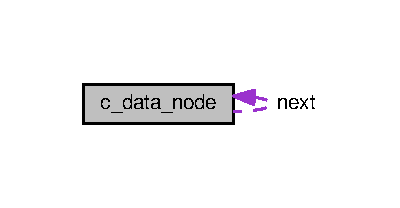
\includegraphics[width=192pt]{d6/ddc/structc__data__node__coll__graph}
\end{center}
\end{figure}
\subsection*{Data Fields}
\begin{DoxyCompactItemize}
\item 
void $\ast$ \hyperlink{structc__data__node_aa58b429814d87780d55f6affc90b400f}{data\+\_\+ptr}
\item 
struct \hyperlink{structc__data__node}{c\+\_\+data\+\_\+node} $\ast$ \hyperlink{structc__data__node_aaa2bf8d750ad19558b6514499b8a2420}{next}
\end{DoxyCompactItemize}


\subsection{Detailed Description}
Data for each linked list node 

\subsection{Field Documentation}
\index{c\+\_\+data\+\_\+node@{c\+\_\+data\+\_\+node}!data\+\_\+ptr@{data\+\_\+ptr}}
\index{data\+\_\+ptr@{data\+\_\+ptr}!c\+\_\+data\+\_\+node@{c\+\_\+data\+\_\+node}}
\subsubsection[{\texorpdfstring{data\+\_\+ptr}{data_ptr}}]{\setlength{\rightskip}{0pt plus 5cm}void$\ast$ c\+\_\+data\+\_\+node\+::data\+\_\+ptr}\hypertarget{structc__data__node_aa58b429814d87780d55f6affc90b400f}{}\label{structc__data__node_aa58b429814d87780d55f6affc90b400f}
Pointer to the data \index{c\+\_\+data\+\_\+node@{c\+\_\+data\+\_\+node}!next@{next}}
\index{next@{next}!c\+\_\+data\+\_\+node@{c\+\_\+data\+\_\+node}}
\subsubsection[{\texorpdfstring{next}{next}}]{\setlength{\rightskip}{0pt plus 5cm}struct {\bf c\+\_\+data\+\_\+node}$\ast$ c\+\_\+data\+\_\+node\+::next}\hypertarget{structc__data__node_aaa2bf8d750ad19558b6514499b8a2420}{}\label{structc__data__node_aaa2bf8d750ad19558b6514499b8a2420}
Pointer to the next data node 

The documentation for this struct was generated from the following file\+:\begin{DoxyCompactItemize}
\item 
/var/www/html/\+S\+J\+S\+U-\/\+D\+E\+V-\/\+Linux/firmware/default/lib/\+L3\+\_\+\+Utils/src/\hyperlink{c__list_8c}{c\+\_\+list.\+c}\end{DoxyCompactItemize}

\hypertarget{structc__list__type}{}\section{c\+\_\+list\+\_\+type Struct Reference}
\label{structc__list__type}\index{c\+\_\+list\+\_\+type@{c\+\_\+list\+\_\+type}}


Collaboration diagram for c\+\_\+list\+\_\+type\+:\nopagebreak
\begin{figure}[H]
\begin{center}
\leavevmode
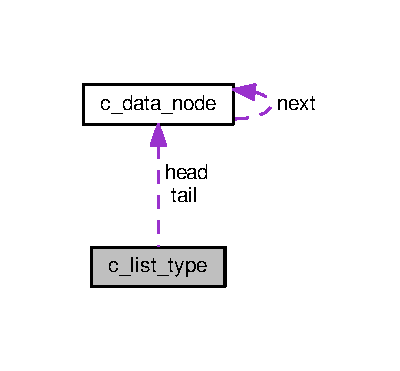
\includegraphics[width=192pt]{dd/db5/structc__list__type__coll__graph}
\end{center}
\end{figure}
\subsection*{Data Fields}
\begin{DoxyCompactItemize}
\item 
struct \hyperlink{structc__data__node}{c\+\_\+data\+\_\+node} $\ast$ \hyperlink{structc__list__type_ab42be6da380f1295613db5f97036b528}{head}
\item 
struct \hyperlink{structc__data__node}{c\+\_\+data\+\_\+node} $\ast$ \hyperlink{structc__list__type_a30f8e4d675eb4471d1f2829dbea5ccea}{tail}
\item 
uint32\+\_\+t \hyperlink{structc__list__type_a1b43f68c2d70340e5d0f56972b870a36}{node\+\_\+count}
\end{DoxyCompactItemize}


\subsection{Detailed Description}
The linked list type with head and tail pointer 

\subsection{Field Documentation}
\index{c\+\_\+list\+\_\+type@{c\+\_\+list\+\_\+type}!head@{head}}
\index{head@{head}!c\+\_\+list\+\_\+type@{c\+\_\+list\+\_\+type}}
\subsubsection[{\texorpdfstring{head}{head}}]{\setlength{\rightskip}{0pt plus 5cm}struct {\bf c\+\_\+data\+\_\+node}$\ast$ c\+\_\+list\+\_\+type\+::head}\hypertarget{structc__list__type_ab42be6da380f1295613db5f97036b528}{}\label{structc__list__type_ab42be6da380f1295613db5f97036b528}
\index{c\+\_\+list\+\_\+type@{c\+\_\+list\+\_\+type}!node\+\_\+count@{node\+\_\+count}}
\index{node\+\_\+count@{node\+\_\+count}!c\+\_\+list\+\_\+type@{c\+\_\+list\+\_\+type}}
\subsubsection[{\texorpdfstring{node\+\_\+count}{node_count}}]{\setlength{\rightskip}{0pt plus 5cm}uint32\+\_\+t c\+\_\+list\+\_\+type\+::node\+\_\+count}\hypertarget{structc__list__type_a1b43f68c2d70340e5d0f56972b870a36}{}\label{structc__list__type_a1b43f68c2d70340e5d0f56972b870a36}
\index{c\+\_\+list\+\_\+type@{c\+\_\+list\+\_\+type}!tail@{tail}}
\index{tail@{tail}!c\+\_\+list\+\_\+type@{c\+\_\+list\+\_\+type}}
\subsubsection[{\texorpdfstring{tail}{tail}}]{\setlength{\rightskip}{0pt plus 5cm}struct {\bf c\+\_\+data\+\_\+node}$\ast$ c\+\_\+list\+\_\+type\+::tail}\hypertarget{structc__list__type_a30f8e4d675eb4471d1f2829dbea5ccea}{}\label{structc__list__type_a30f8e4d675eb4471d1f2829dbea5ccea}


The documentation for this struct was generated from the following file\+:\begin{DoxyCompactItemize}
\item 
/var/www/html/\+S\+J\+S\+U-\/\+D\+E\+V-\/\+Linux/firmware/default/lib/\+L3\+\_\+\+Utils/src/\hyperlink{c__list_8c}{c\+\_\+list.\+c}\end{DoxyCompactItemize}

\hypertarget{unioncan__data__t}{}\section{can\+\_\+data\+\_\+t Union Reference}
\label{unioncan__data__t}\index{can\+\_\+data\+\_\+t@{can\+\_\+data\+\_\+t}}


{\ttfamily \#include $<$can.\+h$>$}

\subsection*{Data Fields}
\begin{DoxyCompactItemize}
\item 
uint64\+\_\+t \hyperlink{unioncan__data__t_a41667832d267ee3fd67d7b0c34054068}{qword}
\begin{DoxyCompactList}\small\item\em All 64-\/bits of data of a C\+AN message. \end{DoxyCompactList}\item 
uint32\+\_\+t \hyperlink{unioncan__data__t_a32b41652b919ee512156989478f9b993}{dwords} \mbox{[}2\mbox{]}
\begin{DoxyCompactList}\small\item\em dwords\mbox{[}0\mbox{]} = Byte 0-\/3, dwords\mbox{[}1\mbox{]} = Byte 4-\/7 \end{DoxyCompactList}\item 
uint16\+\_\+t \hyperlink{unioncan__data__t_a9631170190ce3ecad7370b651ab70b3f}{words} \mbox{[}4\mbox{]}
\begin{DoxyCompactList}\small\item\em words\mbox{[}0\mbox{]} = Byte 0-\/1 ... words\mbox{[}3\mbox{]} = Byte 6-\/7 \end{DoxyCompactList}\item 
uint8\+\_\+t \hyperlink{unioncan__data__t_a59f2f0065f03d0a30d43e0d4e1d8bca2}{bytes} \mbox{[}8\mbox{]}
\begin{DoxyCompactList}\small\item\em 8 bytes of a C\+AN message \end{DoxyCompactList}\end{DoxyCompactItemize}


\subsection{Detailed Description}
8-\/byte structure accessible by 8-\/bit, 16-\/bit, 32-\/bit or as whole 64-\/bit DO N\+OT C\+H\+A\+N\+GE T\+H\+IS S\+T\+R\+U\+C\+T\+U\+RE -\/ it maps to the hardware 

\subsection{Field Documentation}
\index{can\+\_\+data\+\_\+t@{can\+\_\+data\+\_\+t}!bytes@{bytes}}
\index{bytes@{bytes}!can\+\_\+data\+\_\+t@{can\+\_\+data\+\_\+t}}
\subsubsection[{\texorpdfstring{bytes}{bytes}}]{\setlength{\rightskip}{0pt plus 5cm}uint8\+\_\+t can\+\_\+data\+\_\+t\+::bytes\mbox{[}8\mbox{]}}\hypertarget{unioncan__data__t_a59f2f0065f03d0a30d43e0d4e1d8bca2}{}\label{unioncan__data__t_a59f2f0065f03d0a30d43e0d4e1d8bca2}


8 bytes of a C\+AN message 

\index{can\+\_\+data\+\_\+t@{can\+\_\+data\+\_\+t}!dwords@{dwords}}
\index{dwords@{dwords}!can\+\_\+data\+\_\+t@{can\+\_\+data\+\_\+t}}
\subsubsection[{\texorpdfstring{dwords}{dwords}}]{\setlength{\rightskip}{0pt plus 5cm}uint32\+\_\+t can\+\_\+data\+\_\+t\+::dwords\mbox{[}2\mbox{]}}\hypertarget{unioncan__data__t_a32b41652b919ee512156989478f9b993}{}\label{unioncan__data__t_a32b41652b919ee512156989478f9b993}


dwords\mbox{[}0\mbox{]} = Byte 0-\/3, dwords\mbox{[}1\mbox{]} = Byte 4-\/7 

\index{can\+\_\+data\+\_\+t@{can\+\_\+data\+\_\+t}!qword@{qword}}
\index{qword@{qword}!can\+\_\+data\+\_\+t@{can\+\_\+data\+\_\+t}}
\subsubsection[{\texorpdfstring{qword}{qword}}]{\setlength{\rightskip}{0pt plus 5cm}uint64\+\_\+t can\+\_\+data\+\_\+t\+::qword}\hypertarget{unioncan__data__t_a41667832d267ee3fd67d7b0c34054068}{}\label{unioncan__data__t_a41667832d267ee3fd67d7b0c34054068}


All 64-\/bits of data of a C\+AN message. 

\index{can\+\_\+data\+\_\+t@{can\+\_\+data\+\_\+t}!words@{words}}
\index{words@{words}!can\+\_\+data\+\_\+t@{can\+\_\+data\+\_\+t}}
\subsubsection[{\texorpdfstring{words}{words}}]{\setlength{\rightskip}{0pt plus 5cm}uint16\+\_\+t can\+\_\+data\+\_\+t\+::words\mbox{[}4\mbox{]}}\hypertarget{unioncan__data__t_a9631170190ce3ecad7370b651ab70b3f}{}\label{unioncan__data__t_a9631170190ce3ecad7370b651ab70b3f}


words\mbox{[}0\mbox{]} = Byte 0-\/1 ... words\mbox{[}3\mbox{]} = Byte 6-\/7 



The documentation for this union was generated from the following file\+:\begin{DoxyCompactItemize}
\item 
/var/www/html/\+S\+J\+S\+U-\/\+D\+E\+V-\/\+Linux/firmware/default/lib/\+L2\+\_\+\+Drivers/\hyperlink{can_8h}{can.\+h}\end{DoxyCompactItemize}

\hypertarget{structcan__ext__grp__id__t}{}\section{can\+\_\+ext\+\_\+grp\+\_\+id\+\_\+t Struct Reference}
\label{structcan__ext__grp__id__t}\index{can\+\_\+ext\+\_\+grp\+\_\+id\+\_\+t@{can\+\_\+ext\+\_\+grp\+\_\+id\+\_\+t}}


{\ttfamily \#include $<$can.\+h$>$}

\subsection*{Data Fields}
\begin{DoxyCompactItemize}
\item 
can\+\_\+ext\+\_\+id\+\_\+t \hyperlink{structcan__ext__grp__id__t_a7c123b7e277f204b82144552a55d93af}{low}
\begin{DoxyCompactList}\small\item\em $<$ C\+AN extended ID group \end{DoxyCompactList}\item 
can\+\_\+ext\+\_\+id\+\_\+t \hyperlink{structcan__ext__grp__id__t_a8ef0cc460e362babe6657bfa54f7c22a}{high}
\begin{DoxyCompactList}\small\item\em High range. \end{DoxyCompactList}\end{DoxyCompactItemize}


\subsection{Detailed Description}
Extended ID group is nothing but a inclusive range of L\+OW and H\+I\+GH I\+Ds DO N\+OT C\+H\+A\+N\+GE T\+H\+IS S\+T\+R\+U\+C\+T\+U\+RE -\/ it maps to the hardware 

\subsection{Field Documentation}
\index{can\+\_\+ext\+\_\+grp\+\_\+id\+\_\+t@{can\+\_\+ext\+\_\+grp\+\_\+id\+\_\+t}!high@{high}}
\index{high@{high}!can\+\_\+ext\+\_\+grp\+\_\+id\+\_\+t@{can\+\_\+ext\+\_\+grp\+\_\+id\+\_\+t}}
\subsubsection[{\texorpdfstring{high}{high}}]{\setlength{\rightskip}{0pt plus 5cm}can\+\_\+ext\+\_\+id\+\_\+t can\+\_\+ext\+\_\+grp\+\_\+id\+\_\+t\+::high}\hypertarget{structcan__ext__grp__id__t_a8ef0cc460e362babe6657bfa54f7c22a}{}\label{structcan__ext__grp__id__t_a8ef0cc460e362babe6657bfa54f7c22a}


High range. 

\index{can\+\_\+ext\+\_\+grp\+\_\+id\+\_\+t@{can\+\_\+ext\+\_\+grp\+\_\+id\+\_\+t}!low@{low}}
\index{low@{low}!can\+\_\+ext\+\_\+grp\+\_\+id\+\_\+t@{can\+\_\+ext\+\_\+grp\+\_\+id\+\_\+t}}
\subsubsection[{\texorpdfstring{low}{low}}]{\setlength{\rightskip}{0pt plus 5cm}can\+\_\+ext\+\_\+id\+\_\+t can\+\_\+ext\+\_\+grp\+\_\+id\+\_\+t\+::low}\hypertarget{structcan__ext__grp__id__t_a7c123b7e277f204b82144552a55d93af}{}\label{structcan__ext__grp__id__t_a7c123b7e277f204b82144552a55d93af}


$<$ C\+AN extended ID group 

Low range 

The documentation for this struct was generated from the following file\+:\begin{DoxyCompactItemize}
\item 
/var/www/html/\+S\+J\+S\+U-\/\+D\+E\+V-\/\+Linux/firmware/default/lib/\+L2\+\_\+\+Drivers/\hyperlink{can_8h}{can.\+h}\end{DoxyCompactItemize}

\hypertarget{structcan__std__grp__id__t}{}\section{can\+\_\+std\+\_\+grp\+\_\+id\+\_\+t Struct Reference}
\label{structcan__std__grp__id__t}\index{can\+\_\+std\+\_\+grp\+\_\+id\+\_\+t@{can\+\_\+std\+\_\+grp\+\_\+id\+\_\+t}}


{\ttfamily \#include $<$can.\+h$>$}

\subsection*{Data Fields}
\begin{DoxyCompactItemize}
\item 
can\+\_\+std\+\_\+id\+\_\+t \hyperlink{structcan__std__grp__id__t_aeb91d861e04959be79446296e0dcfecf}{low}
\begin{DoxyCompactList}\small\item\em $<$ C\+AN standard ID group \end{DoxyCompactList}\item 
can\+\_\+std\+\_\+id\+\_\+t \hyperlink{structcan__std__grp__id__t_af4a7dc1a8a79f94e16ecd156387d11b4}{high}
\begin{DoxyCompactList}\small\item\em High range. \end{DoxyCompactList}\end{DoxyCompactItemize}


\subsection{Detailed Description}
Standard ID group is nothing but a inclusive range of L\+OW and H\+I\+GH I\+Ds DO N\+OT C\+H\+A\+N\+GE T\+H\+IS S\+T\+R\+U\+C\+T\+U\+RE -\/ it maps to the hardware 

\subsection{Field Documentation}
\index{can\+\_\+std\+\_\+grp\+\_\+id\+\_\+t@{can\+\_\+std\+\_\+grp\+\_\+id\+\_\+t}!high@{high}}
\index{high@{high}!can\+\_\+std\+\_\+grp\+\_\+id\+\_\+t@{can\+\_\+std\+\_\+grp\+\_\+id\+\_\+t}}
\subsubsection[{\texorpdfstring{high}{high}}]{\setlength{\rightskip}{0pt plus 5cm}can\+\_\+std\+\_\+id\+\_\+t can\+\_\+std\+\_\+grp\+\_\+id\+\_\+t\+::high}\hypertarget{structcan__std__grp__id__t_af4a7dc1a8a79f94e16ecd156387d11b4}{}\label{structcan__std__grp__id__t_af4a7dc1a8a79f94e16ecd156387d11b4}


High range. 

\index{can\+\_\+std\+\_\+grp\+\_\+id\+\_\+t@{can\+\_\+std\+\_\+grp\+\_\+id\+\_\+t}!low@{low}}
\index{low@{low}!can\+\_\+std\+\_\+grp\+\_\+id\+\_\+t@{can\+\_\+std\+\_\+grp\+\_\+id\+\_\+t}}
\subsubsection[{\texorpdfstring{low}{low}}]{\setlength{\rightskip}{0pt plus 5cm}can\+\_\+std\+\_\+id\+\_\+t can\+\_\+std\+\_\+grp\+\_\+id\+\_\+t\+::low}\hypertarget{structcan__std__grp__id__t_aeb91d861e04959be79446296e0dcfecf}{}\label{structcan__std__grp__id__t_aeb91d861e04959be79446296e0dcfecf}


$<$ C\+AN standard ID group 

Low range 

The documentation for this struct was generated from the following file\+:\begin{DoxyCompactItemize}
\item 
/var/www/html/\+S\+J\+S\+U-\/\+D\+E\+V-\/\+Linux/firmware/default/lib/\+L2\+\_\+\+Drivers/\hyperlink{can_8h}{can.\+h}\end{DoxyCompactItemize}

\hypertarget{structcan__struct__t}{}\section{can\+\_\+struct\+\_\+t Struct Reference}
\label{structcan__struct__t}\index{can\+\_\+struct\+\_\+t@{can\+\_\+struct\+\_\+t}}


Typedef of C\+AN queues and data.  




Collaboration diagram for can\+\_\+struct\+\_\+t\+:\nopagebreak
\begin{figure}[H]
\begin{center}
\leavevmode
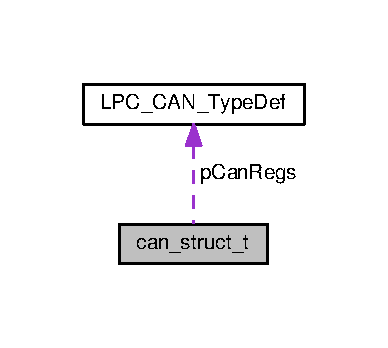
\includegraphics[width=186pt]{d1/dcd/structcan__struct__t__coll__graph}
\end{center}
\end{figure}
\subsection*{Data Fields}
\begin{DoxyCompactItemize}
\item 
\hyperlink{structLPC__CAN__TypeDef}{L\+P\+C\+\_\+\+C\+A\+N\+\_\+\+Type\+Def} $\ast$ \hyperlink{structcan__struct__t_ac1798cad8cd1b75402e953a7cc5d2b50}{p\+Can\+Regs}
\begin{DoxyCompactList}\small\item\em The pointer to the C\+AN registers. \end{DoxyCompactList}\item 
\hyperlink{queue_8h_aaf19d499892a4ce1409326ece00f5264}{Queue\+Handle\+\_\+t} \hyperlink{structcan__struct__t_a1a1c2bdb829e45a31cafa44620d4bdd0}{rxQ}
\begin{DoxyCompactList}\small\item\em TX queue. \end{DoxyCompactList}\item 
\hyperlink{queue_8h_aaf19d499892a4ce1409326ece00f5264}{Queue\+Handle\+\_\+t} \hyperlink{structcan__struct__t_a39cfcc33222d5607be5ad2dd1d92e7cd}{txQ}
\begin{DoxyCompactList}\small\item\em RX queue. \end{DoxyCompactList}\item 
uint16\+\_\+t \hyperlink{structcan__struct__t_a2e7319422bed45d0521764d1f6644ae1}{dropped\+Rx\+Msgs}
\begin{DoxyCompactList}\small\item\em Number of messages dropped if no space found during the C\+AN interrupt that queues the RX messages. \end{DoxyCompactList}\item 
uint16\+\_\+t \hyperlink{structcan__struct__t_ac4f9dd16c31c2a75d97e1310d414345d}{rx\+Q\+Watermark}
\begin{DoxyCompactList}\small\item\em Watermark of the Free\+R\+T\+OS Rx Queue. \end{DoxyCompactList}\item 
uint16\+\_\+t \hyperlink{structcan__struct__t_ac7b27780bb731be3afddf397c3a02c15}{tx\+Q\+Watermark}
\begin{DoxyCompactList}\small\item\em Watermark of the Free\+R\+T\+OS Tx Queue. \end{DoxyCompactList}\item 
uint16\+\_\+t \hyperlink{structcan__struct__t_ad13c7c5a692c2808a1f13250a726fcc3}{tx\+Msg\+Count}
\begin{DoxyCompactList}\small\item\em Number of messages sent. \end{DoxyCompactList}\item 
uint16\+\_\+t \hyperlink{structcan__struct__t_afaa8f7119b799b00f2ce4f014ec98629}{rx\+Msg\+Count}
\begin{DoxyCompactList}\small\item\em Number of received messages. \end{DoxyCompactList}\item 
\hyperlink{can_8h_a70166a12001edeee7860a1257037be44}{can\+\_\+void\+\_\+func\+\_\+t} \hyperlink{structcan__struct__t_a1d38ac37f7c83d7252cc2cd3da88b6a9}{bus\+\_\+error}
\begin{DoxyCompactList}\small\item\em When serious B\+US error occurs. \end{DoxyCompactList}\item 
\hyperlink{can_8h_a70166a12001edeee7860a1257037be44}{can\+\_\+void\+\_\+func\+\_\+t} \hyperlink{structcan__struct__t_a91068e55e2923ef1bdf723e11d5460f1}{data\+\_\+overrun}
\begin{DoxyCompactList}\small\item\em When we read the C\+AN buffer too late for incoming message. \end{DoxyCompactList}\end{DoxyCompactItemize}


\subsection{Detailed Description}
Typedef of C\+AN queues and data. 

\subsection{Field Documentation}
\index{can\+\_\+struct\+\_\+t@{can\+\_\+struct\+\_\+t}!bus\+\_\+error@{bus\+\_\+error}}
\index{bus\+\_\+error@{bus\+\_\+error}!can\+\_\+struct\+\_\+t@{can\+\_\+struct\+\_\+t}}
\subsubsection[{\texorpdfstring{bus\+\_\+error}{bus_error}}]{\setlength{\rightskip}{0pt plus 5cm}{\bf can\+\_\+void\+\_\+func\+\_\+t} can\+\_\+struct\+\_\+t\+::bus\+\_\+error}\hypertarget{structcan__struct__t_a1d38ac37f7c83d7252cc2cd3da88b6a9}{}\label{structcan__struct__t_a1d38ac37f7c83d7252cc2cd3da88b6a9}


When serious B\+US error occurs. 

\index{can\+\_\+struct\+\_\+t@{can\+\_\+struct\+\_\+t}!data\+\_\+overrun@{data\+\_\+overrun}}
\index{data\+\_\+overrun@{data\+\_\+overrun}!can\+\_\+struct\+\_\+t@{can\+\_\+struct\+\_\+t}}
\subsubsection[{\texorpdfstring{data\+\_\+overrun}{data_overrun}}]{\setlength{\rightskip}{0pt plus 5cm}{\bf can\+\_\+void\+\_\+func\+\_\+t} can\+\_\+struct\+\_\+t\+::data\+\_\+overrun}\hypertarget{structcan__struct__t_a91068e55e2923ef1bdf723e11d5460f1}{}\label{structcan__struct__t_a91068e55e2923ef1bdf723e11d5460f1}


When we read the C\+AN buffer too late for incoming message. 

\index{can\+\_\+struct\+\_\+t@{can\+\_\+struct\+\_\+t}!dropped\+Rx\+Msgs@{dropped\+Rx\+Msgs}}
\index{dropped\+Rx\+Msgs@{dropped\+Rx\+Msgs}!can\+\_\+struct\+\_\+t@{can\+\_\+struct\+\_\+t}}
\subsubsection[{\texorpdfstring{dropped\+Rx\+Msgs}{droppedRxMsgs}}]{\setlength{\rightskip}{0pt plus 5cm}uint16\+\_\+t can\+\_\+struct\+\_\+t\+::dropped\+Rx\+Msgs}\hypertarget{structcan__struct__t_a2e7319422bed45d0521764d1f6644ae1}{}\label{structcan__struct__t_a2e7319422bed45d0521764d1f6644ae1}


Number of messages dropped if no space found during the C\+AN interrupt that queues the RX messages. 

\index{can\+\_\+struct\+\_\+t@{can\+\_\+struct\+\_\+t}!p\+Can\+Regs@{p\+Can\+Regs}}
\index{p\+Can\+Regs@{p\+Can\+Regs}!can\+\_\+struct\+\_\+t@{can\+\_\+struct\+\_\+t}}
\subsubsection[{\texorpdfstring{p\+Can\+Regs}{pCanRegs}}]{\setlength{\rightskip}{0pt plus 5cm}{\bf L\+P\+C\+\_\+\+C\+A\+N\+\_\+\+Type\+Def}$\ast$ can\+\_\+struct\+\_\+t\+::p\+Can\+Regs}\hypertarget{structcan__struct__t_ac1798cad8cd1b75402e953a7cc5d2b50}{}\label{structcan__struct__t_ac1798cad8cd1b75402e953a7cc5d2b50}


The pointer to the C\+AN registers. 

\index{can\+\_\+struct\+\_\+t@{can\+\_\+struct\+\_\+t}!rx\+Msg\+Count@{rx\+Msg\+Count}}
\index{rx\+Msg\+Count@{rx\+Msg\+Count}!can\+\_\+struct\+\_\+t@{can\+\_\+struct\+\_\+t}}
\subsubsection[{\texorpdfstring{rx\+Msg\+Count}{rxMsgCount}}]{\setlength{\rightskip}{0pt plus 5cm}uint16\+\_\+t can\+\_\+struct\+\_\+t\+::rx\+Msg\+Count}\hypertarget{structcan__struct__t_afaa8f7119b799b00f2ce4f014ec98629}{}\label{structcan__struct__t_afaa8f7119b799b00f2ce4f014ec98629}


Number of received messages. 

\index{can\+\_\+struct\+\_\+t@{can\+\_\+struct\+\_\+t}!rxQ@{rxQ}}
\index{rxQ@{rxQ}!can\+\_\+struct\+\_\+t@{can\+\_\+struct\+\_\+t}}
\subsubsection[{\texorpdfstring{rxQ}{rxQ}}]{\setlength{\rightskip}{0pt plus 5cm}{\bf Queue\+Handle\+\_\+t} can\+\_\+struct\+\_\+t\+::rxQ}\hypertarget{structcan__struct__t_a1a1c2bdb829e45a31cafa44620d4bdd0}{}\label{structcan__struct__t_a1a1c2bdb829e45a31cafa44620d4bdd0}


TX queue. 

\index{can\+\_\+struct\+\_\+t@{can\+\_\+struct\+\_\+t}!rx\+Q\+Watermark@{rx\+Q\+Watermark}}
\index{rx\+Q\+Watermark@{rx\+Q\+Watermark}!can\+\_\+struct\+\_\+t@{can\+\_\+struct\+\_\+t}}
\subsubsection[{\texorpdfstring{rx\+Q\+Watermark}{rxQWatermark}}]{\setlength{\rightskip}{0pt plus 5cm}uint16\+\_\+t can\+\_\+struct\+\_\+t\+::rx\+Q\+Watermark}\hypertarget{structcan__struct__t_ac4f9dd16c31c2a75d97e1310d414345d}{}\label{structcan__struct__t_ac4f9dd16c31c2a75d97e1310d414345d}


Watermark of the Free\+R\+T\+OS Rx Queue. 

\index{can\+\_\+struct\+\_\+t@{can\+\_\+struct\+\_\+t}!tx\+Msg\+Count@{tx\+Msg\+Count}}
\index{tx\+Msg\+Count@{tx\+Msg\+Count}!can\+\_\+struct\+\_\+t@{can\+\_\+struct\+\_\+t}}
\subsubsection[{\texorpdfstring{tx\+Msg\+Count}{txMsgCount}}]{\setlength{\rightskip}{0pt plus 5cm}uint16\+\_\+t can\+\_\+struct\+\_\+t\+::tx\+Msg\+Count}\hypertarget{structcan__struct__t_ad13c7c5a692c2808a1f13250a726fcc3}{}\label{structcan__struct__t_ad13c7c5a692c2808a1f13250a726fcc3}


Number of messages sent. 

\index{can\+\_\+struct\+\_\+t@{can\+\_\+struct\+\_\+t}!txQ@{txQ}}
\index{txQ@{txQ}!can\+\_\+struct\+\_\+t@{can\+\_\+struct\+\_\+t}}
\subsubsection[{\texorpdfstring{txQ}{txQ}}]{\setlength{\rightskip}{0pt plus 5cm}{\bf Queue\+Handle\+\_\+t} can\+\_\+struct\+\_\+t\+::txQ}\hypertarget{structcan__struct__t_a39cfcc33222d5607be5ad2dd1d92e7cd}{}\label{structcan__struct__t_a39cfcc33222d5607be5ad2dd1d92e7cd}


RX queue. 

\index{can\+\_\+struct\+\_\+t@{can\+\_\+struct\+\_\+t}!tx\+Q\+Watermark@{tx\+Q\+Watermark}}
\index{tx\+Q\+Watermark@{tx\+Q\+Watermark}!can\+\_\+struct\+\_\+t@{can\+\_\+struct\+\_\+t}}
\subsubsection[{\texorpdfstring{tx\+Q\+Watermark}{txQWatermark}}]{\setlength{\rightskip}{0pt plus 5cm}uint16\+\_\+t can\+\_\+struct\+\_\+t\+::tx\+Q\+Watermark}\hypertarget{structcan__struct__t_ac7b27780bb731be3afddf397c3a02c15}{}\label{structcan__struct__t_ac7b27780bb731be3afddf397c3a02c15}


Watermark of the Free\+R\+T\+OS Tx Queue. 



The documentation for this struct was generated from the following file\+:\begin{DoxyCompactItemize}
\item 
/var/www/html/\+S\+J\+S\+U-\/\+D\+E\+V-\/\+Linux/firmware/default/lib/\+L2\+\_\+\+Drivers/src/\hyperlink{can_8c}{can.\+c}\end{DoxyCompactItemize}

\hypertarget{classCharDev}{}\section{Char\+Dev Class Reference}
\label{classCharDev}\index{Char\+Dev@{Char\+Dev}}


{\ttfamily \#include $<$char\+\_\+dev.\+hpp$>$}



Inheritance diagram for Char\+Dev\+:\nopagebreak
\begin{figure}[H]
\begin{center}
\leavevmode
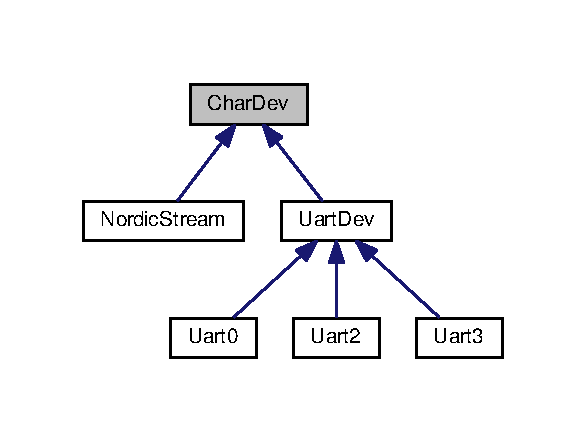
\includegraphics[width=281pt]{d3/d84/classCharDev__inherit__graph}
\end{center}
\end{figure}
\subsection*{Public Member Functions}
\begin{DoxyCompactItemize}
\item 
virtual bool \hyperlink{classCharDev_a2125f39cee4ada85091e4a5440751650}{get\+Char} (char $\ast$p\+Input\+Char, unsigned int timeout=\hyperlink{portmacro_8h_a72723ba1e4a85ca14f25c2b9e066613d}{port\+M\+A\+X\+\_\+\+D\+E\+L\+AY})=0
\item 
virtual bool \hyperlink{classCharDev_a253e32e0413b98f0af16ad79eb358851}{put\+Char} (char out, unsigned int timeout=\hyperlink{portmacro_8h_a72723ba1e4a85ca14f25c2b9e066613d}{port\+M\+A\+X\+\_\+\+D\+E\+L\+AY})=0
\item 
virtual bool \hyperlink{classCharDev_a601bd6eeee3095306c0db78798499742}{flush} (void)
\item 
bool \hyperlink{classCharDev_ad69eb66ed094d04116615248f1c2453c}{gets} (char $\ast$p\+Buff, int max\+Len, unsigned int timeout=0xffffffff)
\item 
int \hyperlink{classCharDev_a1e567da6600cd8164dcd98e11de8813f}{printf} (const char $\ast$format,...)
\item 
int \hyperlink{classCharDev_a053203d7cf010d6422b11d114d10e357}{scanf} (const char $\ast$format,...)
\item 
uint16\+\_\+t \hyperlink{classCharDev_acb3dd3805711e4aa6346fbaf25009925}{get\+Printf\+Mem\+Size} (void) const 
\end{DoxyCompactItemize}
{\bf }\par
\begin{DoxyCompactItemize}
\item 
bool \hyperlink{classCharDev_a48d2560ade054a067558a9495c41f109}{put} (const char $\ast$p\+String, unsigned int timeout=0xffffffff)
\item 
void \hyperlink{classCharDev_aac938099da1789ac7bf8c0acd7a71624}{putline} (const char $\ast$p\+Buff, unsigned int timeout=0xffffffff)
\end{DoxyCompactItemize}

{\bf }\par
\begin{DoxyCompactItemize}
\item 
bool \hyperlink{classCharDev_ab76a3b54c0ecf31b7a78a2808446eefd}{is\+Ready} (void)
\item 
void \hyperlink{classCharDev_ad845c4307699c25ccdcce07ffafc8aba}{set\+Ready} (bool r)
\end{DoxyCompactItemize}

\subsection*{Protected Member Functions}
\begin{DoxyCompactItemize}
\item 
\hyperlink{classCharDev_a3eabe85e367562e550cc31780c8fb8c7}{Char\+Dev} ()
\item 
virtual \hyperlink{classCharDev_a6738e06b393bf4bd95a8b13ec9a95dd4}{$\sim$\+Char\+Dev} ()
\end{DoxyCompactItemize}


\subsection{Detailed Description}
Char device base class. You shouldn\textquotesingle{}t use this directly because this is an abstract class and must be inherited and used by a parent object. 

\subsection{Constructor \& Destructor Documentation}
\index{Char\+Dev@{Char\+Dev}!Char\+Dev@{Char\+Dev}}
\index{Char\+Dev@{Char\+Dev}!Char\+Dev@{Char\+Dev}}
\subsubsection[{\texorpdfstring{Char\+Dev()}{CharDev()}}]{\setlength{\rightskip}{0pt plus 5cm}Char\+Dev\+::\+Char\+Dev (
\begin{DoxyParamCaption}
{}
\end{DoxyParamCaption}
)\hspace{0.3cm}{\ttfamily [protected]}}\hypertarget{classCharDev_a3eabe85e367562e550cc31780c8fb8c7}{}\label{classCharDev_a3eabe85e367562e550cc31780c8fb8c7}
\index{Char\+Dev@{Char\+Dev}!````~Char\+Dev@{$\sim$\+Char\+Dev}}
\index{````~Char\+Dev@{$\sim$\+Char\+Dev}!Char\+Dev@{Char\+Dev}}
\subsubsection[{\texorpdfstring{$\sim$\+Char\+Dev()}{~CharDev()}}]{\setlength{\rightskip}{0pt plus 5cm}Char\+Dev\+::$\sim$\+Char\+Dev (
\begin{DoxyParamCaption}
{}
\end{DoxyParamCaption}
)\hspace{0.3cm}{\ttfamily [protected]}, {\ttfamily [virtual]}}\hypertarget{classCharDev_a6738e06b393bf4bd95a8b13ec9a95dd4}{}\label{classCharDev_a6738e06b393bf4bd95a8b13ec9a95dd4}


\subsection{Member Function Documentation}
\index{Char\+Dev@{Char\+Dev}!flush@{flush}}
\index{flush@{flush}!Char\+Dev@{Char\+Dev}}
\subsubsection[{\texorpdfstring{flush(void)}{flush(void)}}]{\setlength{\rightskip}{0pt plus 5cm}virtual bool Char\+Dev\+::flush (
\begin{DoxyParamCaption}
\item[{void}]{}
\end{DoxyParamCaption}
)\hspace{0.3cm}{\ttfamily [inline]}, {\ttfamily [virtual]}}\hypertarget{classCharDev_a601bd6eeee3095306c0db78798499742}{}\label{classCharDev_a601bd6eeee3095306c0db78798499742}
Optional flush to flush out all the data 

Reimplemented in \hyperlink{classUartDev_ac50cca0665fac431db99ecdb242c6ee7}{Uart\+Dev}, and \hyperlink{classNordicStream_a95c0c66acbcdf33894fc2cfacfbe5419}{Nordic\+Stream}.

\index{Char\+Dev@{Char\+Dev}!get\+Char@{get\+Char}}
\index{get\+Char@{get\+Char}!Char\+Dev@{Char\+Dev}}
\subsubsection[{\texorpdfstring{get\+Char(char $\ast$p\+Input\+Char, unsigned int timeout=port\+M\+A\+X\+\_\+\+D\+E\+L\+A\+Y)=0}{getChar(char *pInputChar, unsigned int timeout=portMAX_DELAY)=0}}]{\setlength{\rightskip}{0pt plus 5cm}virtual bool Char\+Dev\+::get\+Char (
\begin{DoxyParamCaption}
\item[{char $\ast$}]{p\+Input\+Char, }
\item[{unsigned int}]{timeout = {\ttfamily {\bf port\+M\+A\+X\+\_\+\+D\+E\+L\+AY}}}
\end{DoxyParamCaption}
)\hspace{0.3cm}{\ttfamily [pure virtual]}}\hypertarget{classCharDev_a2125f39cee4ada85091e4a5440751650}{}\label{classCharDev_a2125f39cee4ada85091e4a5440751650}
\begin{DoxyReturn}{Returns}
a character from the U\+A\+RT input 
\end{DoxyReturn}

\begin{DoxyParams}{Parameters}
{\em p\+Input\+Char} & The pointer to input char to store received character \\
\hline
{\em timeout} & Optional parameter which defaults to maximum value that will allow you to wait forever for a character to be received \\
\hline
\end{DoxyParams}
\begin{DoxyReturn}{Returns}
true if a character was obtained within the given timeout 
\end{DoxyReturn}


Implemented in \hyperlink{classUartDev_a461bf31bdeb04e579dc1a9207ceb86e1}{Uart\+Dev}, and \hyperlink{classNordicStream_a8cf184554a505c922c57352ba571765b}{Nordic\+Stream}.

\index{Char\+Dev@{Char\+Dev}!get\+Printf\+Mem\+Size@{get\+Printf\+Mem\+Size}}
\index{get\+Printf\+Mem\+Size@{get\+Printf\+Mem\+Size}!Char\+Dev@{Char\+Dev}}
\subsubsection[{\texorpdfstring{get\+Printf\+Mem\+Size(void) const }{getPrintfMemSize(void) const }}]{\setlength{\rightskip}{0pt plus 5cm}uint16\+\_\+t Char\+Dev\+::get\+Printf\+Mem\+Size (
\begin{DoxyParamCaption}
\item[{void}]{}
\end{DoxyParamCaption}
) const\hspace{0.3cm}{\ttfamily [inline]}}\hypertarget{classCharDev_acb3dd3805711e4aa6346fbaf25009925}{}\label{classCharDev_acb3dd3805711e4aa6346fbaf25009925}
Get the size for the \hyperlink{classCharDev_a1e567da6600cd8164dcd98e11de8813f}{printf()} memory used by \hyperlink{classCharDev_a1e567da6600cd8164dcd98e11de8813f}{printf()} function \index{Char\+Dev@{Char\+Dev}!gets@{gets}}
\index{gets@{gets}!Char\+Dev@{Char\+Dev}}
\subsubsection[{\texorpdfstring{gets(char $\ast$p\+Buff, int max\+Len, unsigned int timeout=0xffffffff)}{gets(char *pBuff, int maxLen, unsigned int timeout=0xffffffff)}}]{\setlength{\rightskip}{0pt plus 5cm}bool Char\+Dev\+::gets (
\begin{DoxyParamCaption}
\item[{char $\ast$}]{p\+Buff, }
\item[{int}]{max\+Len, }
\item[{unsigned int}]{timeout = {\ttfamily 0xffffffff}}
\end{DoxyParamCaption}
)}\hypertarget{classCharDev_ad69eb66ed094d04116615248f1c2453c}{}\label{classCharDev_ad69eb66ed094d04116615248f1c2453c}
Get a string of input up to max\+Len 
\begin{DoxyParams}{Parameters}
{\em p\+Buff} & The buffer to store data to \\
\hline
{\em max\+Len} & The maximum chars to get \\
\hline
{\em timeout} & The timeout in ticks to wait \\
\hline
\end{DoxyParams}
\index{Char\+Dev@{Char\+Dev}!is\+Ready@{is\+Ready}}
\index{is\+Ready@{is\+Ready}!Char\+Dev@{Char\+Dev}}
\subsubsection[{\texorpdfstring{is\+Ready(void)}{isReady(void)}}]{\setlength{\rightskip}{0pt plus 5cm}bool Char\+Dev\+::is\+Ready (
\begin{DoxyParamCaption}
\item[{void}]{}
\end{DoxyParamCaption}
)\hspace{0.3cm}{\ttfamily [inline]}}\hypertarget{classCharDev_ab76a3b54c0ecf31b7a78a2808446eefd}{}\label{classCharDev_ab76a3b54c0ecf31b7a78a2808446eefd}
This A\+PI just provides a means to set a flag if U\+A\+RT is ready or not This doesn\textquotesingle{}t cause any change to the way U\+A\+RT functions. \index{Char\+Dev@{Char\+Dev}!printf@{printf}}
\index{printf@{printf}!Char\+Dev@{Char\+Dev}}
\subsubsection[{\texorpdfstring{printf(const char $\ast$format,...)}{printf(const char *format,...)}}]{\setlength{\rightskip}{0pt plus 5cm}int Char\+Dev\+::printf (
\begin{DoxyParamCaption}
\item[{const char $\ast$}]{format, }
\item[{}]{...}
\end{DoxyParamCaption}
)}\hypertarget{classCharDev_a1e567da6600cd8164dcd98e11de8813f}{}\label{classCharDev_a1e567da6600cd8164dcd98e11de8813f}
Just like printf, except it will print to this output interface \begin{DoxyReturn}{Returns}
the number of characters printed 
\end{DoxyReturn}
\index{Char\+Dev@{Char\+Dev}!put@{put}}
\index{put@{put}!Char\+Dev@{Char\+Dev}}
\subsubsection[{\texorpdfstring{put(const char $\ast$p\+String, unsigned int timeout=0xffffffff)}{put(const char *pString, unsigned int timeout=0xffffffff)}}]{\setlength{\rightskip}{0pt plus 5cm}bool Char\+Dev\+::put (
\begin{DoxyParamCaption}
\item[{const char $\ast$}]{p\+String, }
\item[{unsigned int}]{timeout = {\ttfamily 0xffffffff}}
\end{DoxyParamCaption}
)}\hypertarget{classCharDev_a48d2560ade054a067558a9495c41f109}{}\label{classCharDev_a48d2560ade054a067558a9495c41f109}
Output a null-\/terminated string puts() will also output newline chars \char`\"{}\textbackslash{}r\textbackslash{}n\char`\"{} at the end of the string \index{Char\+Dev@{Char\+Dev}!put\+Char@{put\+Char}}
\index{put\+Char@{put\+Char}!Char\+Dev@{Char\+Dev}}
\subsubsection[{\texorpdfstring{put\+Char(char out, unsigned int timeout=port\+M\+A\+X\+\_\+\+D\+E\+L\+A\+Y)=0}{putChar(char out, unsigned int timeout=portMAX_DELAY)=0}}]{\setlength{\rightskip}{0pt plus 5cm}virtual bool Char\+Dev\+::put\+Char (
\begin{DoxyParamCaption}
\item[{char}]{out, }
\item[{unsigned int}]{timeout = {\ttfamily {\bf port\+M\+A\+X\+\_\+\+D\+E\+L\+AY}}}
\end{DoxyParamCaption}
)\hspace{0.3cm}{\ttfamily [pure virtual]}}\hypertarget{classCharDev_a253e32e0413b98f0af16ad79eb358851}{}\label{classCharDev_a253e32e0413b98f0af16ad79eb358851}
Outputs a char given by 
\begin{DoxyParams}{Parameters}
{\em out} & \\
\hline
{\em timeout} & Optional parameter which defaults to maximum value that will allow you to wait forever for a character to be sent \\
\hline
\end{DoxyParams}
\begin{DoxyReturn}{Returns}
true if the output char was successfully written to Queue, or false if the output queue was full within the given timeout 
\end{DoxyReturn}


Implemented in \hyperlink{classUartDev_a5540a663667da93bc166f81d4f72cd2c}{Uart\+Dev}, and \hyperlink{classNordicStream_aefb871567b4712b2bf52caa656dc1d2a}{Nordic\+Stream}.

\index{Char\+Dev@{Char\+Dev}!putline@{putline}}
\index{putline@{putline}!Char\+Dev@{Char\+Dev}}
\subsubsection[{\texorpdfstring{putline(const char $\ast$p\+Buff, unsigned int timeout=0xffffffff)}{putline(const char *pBuff, unsigned int timeout=0xffffffff)}}]{\setlength{\rightskip}{0pt plus 5cm}void Char\+Dev\+::putline (
\begin{DoxyParamCaption}
\item[{const char $\ast$}]{p\+Buff, }
\item[{unsigned int}]{timeout = {\ttfamily 0xffffffff}}
\end{DoxyParamCaption}
)}\hypertarget{classCharDev_aac938099da1789ac7bf8c0acd7a71624}{}\label{classCharDev_aac938099da1789ac7bf8c0acd7a71624}
\index{Char\+Dev@{Char\+Dev}!scanf@{scanf}}
\index{scanf@{scanf}!Char\+Dev@{Char\+Dev}}
\subsubsection[{\texorpdfstring{scanf(const char $\ast$format,...)}{scanf(const char *format,...)}}]{\setlength{\rightskip}{0pt plus 5cm}int Char\+Dev\+::scanf (
\begin{DoxyParamCaption}
\item[{const char $\ast$}]{format, }
\item[{}]{...}
\end{DoxyParamCaption}
)}\hypertarget{classCharDev_a053203d7cf010d6422b11d114d10e357}{}\label{classCharDev_a053203d7cf010d6422b11d114d10e357}
Just like scanf, except this will perform scanf after receiving a line of input using the \hyperlink{classCharDev_ad69eb66ed094d04116615248f1c2453c}{gets()} method. \begin{DoxyWarning}{Warning}
\hyperlink{classCharDev_a053203d7cf010d6422b11d114d10e357}{scanf()} requires a ~\newline
 (newline) terminated char to work. 
\end{DoxyWarning}
\index{Char\+Dev@{Char\+Dev}!set\+Ready@{set\+Ready}}
\index{set\+Ready@{set\+Ready}!Char\+Dev@{Char\+Dev}}
\subsubsection[{\texorpdfstring{set\+Ready(bool r)}{setReady(bool r)}}]{\setlength{\rightskip}{0pt plus 5cm}void Char\+Dev\+::set\+Ready (
\begin{DoxyParamCaption}
\item[{bool}]{r}
\end{DoxyParamCaption}
)\hspace{0.3cm}{\ttfamily [inline]}}\hypertarget{classCharDev_ad845c4307699c25ccdcce07ffafc8aba}{}\label{classCharDev_ad845c4307699c25ccdcce07ffafc8aba}


The documentation for this class was generated from the following files\+:\begin{DoxyCompactItemize}
\item 
/var/www/html/\+S\+J\+S\+U-\/\+D\+E\+V-\/\+Linux/firmware/default/lib/\+L2\+\_\+\+Drivers/base/\hyperlink{char__dev_8hpp}{char\+\_\+dev.\+hpp}\item 
/var/www/html/\+S\+J\+S\+U-\/\+D\+E\+V-\/\+Linux/firmware/default/lib/\+L2\+\_\+\+Drivers/base/\hyperlink{char__dev_8cpp}{char\+\_\+dev.\+cpp}\end{DoxyCompactItemize}

\hypertarget{classCircularBuffer}{}\section{Circular\+Buffer$<$ T\+Y\+PE $>$ Class Template Reference}
\label{classCircularBuffer}\index{Circular\+Buffer$<$ T\+Y\+P\+E $>$@{Circular\+Buffer$<$ T\+Y\+P\+E $>$}}


{\ttfamily \#include $<$circular\+\_\+buffer.\+hpp$>$}

\subsection*{Data Structures}
\begin{DoxyCompactItemize}
\item 
class \hyperlink{classCircularBuffer_1_1const__iterator}{const\+\_\+iterator}
\item 
class \hyperlink{classCircularBuffer_1_1iterator}{iterator}
\end{DoxyCompactItemize}
\subsection*{Public Types}
\begin{DoxyCompactItemize}
\item 
typedef int \hyperlink{classCircularBuffer_a2030ed25523469c9401f82aff85f7020}{size\+\_\+type}
\end{DoxyCompactItemize}
\subsection*{Public Member Functions}
\begin{DoxyCompactItemize}
\item 
\hyperlink{classCircularBuffer_ab360f7d423d23878d71a5f9858519379}{Circular\+Buffer} (uint32\+\_\+t \hyperlink{classCircularBuffer_a87e9e9d7eb50070d2b4a21b0462432e9}{capacity})
\begin{DoxyCompactList}\small\item\em Constructor with initial capacity as buffer size. \end{DoxyCompactList}\item 
\hyperlink{classCircularBuffer_acb40a5e54d92f38fee343082a4840cbe}{Circular\+Buffer} (const \hyperlink{classCircularBuffer}{Circular\+Buffer} \&copy)
\begin{DoxyCompactList}\small\item\em Copy Constructor. \end{DoxyCompactList}\item 
\hyperlink{classCircularBuffer}{Circular\+Buffer} \& \hyperlink{classCircularBuffer_a390a6d1e651447fb23c155a6928097c1}{operator=} (const \hyperlink{classCircularBuffer}{Circular\+Buffer} \&copy)
\begin{DoxyCompactList}\small\item\em = Operator to copy the buffer \end{DoxyCompactList}\item 
\hyperlink{classCircularBuffer_a09f9833297c2cf6c1f535be9478474c1}{$\sim$\+Circular\+Buffer} ()
\begin{DoxyCompactList}\small\item\em Destructor of the buffer. \end{DoxyCompactList}\item 
bool \hyperlink{classCircularBuffer_a874e11e8de40e5d6d478a39087960af8}{push\+\_\+back} (const T\+Y\+PE data, bool force\+Write=false)
\item 
T\+Y\+PE \hyperlink{classCircularBuffer_af4aab198b93af59b55a69584ab015c2b}{pop\+\_\+front} (void)
\item 
bool \hyperlink{classCircularBuffer_ada422a5714f04db84a510d6491b624cd}{pop\+\_\+front} (T\+Y\+PE $\ast$data\+Ptr)
\item 
T\+Y\+PE \hyperlink{classCircularBuffer_a578d0618578c41b0580466af3d264a5b}{peek\+\_\+front} (void)
\item 
bool \hyperlink{classCircularBuffer_ac0e89e5c880ef100b5cbb8cbd07ab801}{peek\+\_\+front} (T\+Y\+PE $\ast$data\+Ptr)
\item 
uint32\+\_\+t \hyperlink{classCircularBuffer_a88253a12755af0082b7156dbaa197506}{size} (void) const 
\item 
uint32\+\_\+t \hyperlink{classCircularBuffer_a87e9e9d7eb50070d2b4a21b0462432e9}{capacity} (void) const 
\item 
void \hyperlink{classCircularBuffer_a51a1c7cb366dde83435e7213118a23c2}{clear} (void)
\begin{DoxyCompactList}\small\item\em Clears the contents of the buffer. \end{DoxyCompactList}\item 
void \hyperlink{classCircularBuffer_a0c62cd81bfc1f16b8c5c6f93dae3f00c}{operator+=} (T\+Y\+PE item)
\begin{DoxyCompactList}\small\item\em += Operator which is same as \hyperlink{classCircularBuffer_a874e11e8de40e5d6d478a39087960af8}{push\+\_\+back()} of an item \end{DoxyCompactList}\item 
T\+Y\+PE \& \hyperlink{classCircularBuffer_a9f547e56c0eca3166ae0c79d87b8c264}{operator\mbox{[}$\,$\mbox{]}} (uint32\+\_\+t index) const 
\end{DoxyCompactItemize}
{\bf }\par
\begin{DoxyCompactItemize}
\item 
\hyperlink{classCircularBuffer_1_1iterator}{iterator} \hyperlink{classCircularBuffer_a2f247c16874a1ed5366a972eb36b3781}{begin} ()
\item 
\hyperlink{classCircularBuffer_1_1iterator}{iterator} \hyperlink{classCircularBuffer_a6c64c8c145dbeb2b56b1fdf3ed359218}{end} ()
\item 
\hyperlink{classCircularBuffer_1_1const__iterator}{const\+\_\+iterator} \hyperlink{classCircularBuffer_a26d55467abd9e69f45581045a7d048c4}{begin} () const 
\item 
\hyperlink{classCircularBuffer_1_1const__iterator}{const\+\_\+iterator} \hyperlink{classCircularBuffer_a7b15719340d0459b80cce993bf3d122d}{end} () const 
\end{DoxyCompactItemize}

\subsection*{Friends}
\begin{DoxyCompactItemize}
\item 
class \hyperlink{classCircularBuffer_a67171474c4da6cc8efe0c7fafefd2b2d}{iterator}
\begin{DoxyCompactList}\small\item\em Iterator is our friend... \end{DoxyCompactList}\end{DoxyCompactItemize}


\subsection{Detailed Description}
\subsubsection*{template$<$typename T\+Y\+PE$>$\\*
class Circular\+Buffer$<$ T\+Y\+P\+E $>$}

Circular buffer class

Usage\+: 
\begin{DoxyCode}
\hyperlink{classCircularBuffer}{CircularBuffer <int>} b(3);
b.push\_back(1);
b.push\_back(2);
b.push\_back(3);
b.push\_back(0);       \textcolor{comment}{// Will fail since buffer is full}
b.push\_back(4, \textcolor{keyword}{true}); \textcolor{comment}{// Overwrite oldest data}

\textcolor{comment}{// Read the elements without popping the data, access them using index operator}
\textcolor{comment}{// Should be "2 3 4" since we previously over-wrote "1" with "4"}
\hyperlink{trace_2readme_8txt_a44aa2eeca69a660d02109d54e99f2dc6}{printf}(\textcolor{stringliteral}{"\(\backslash\)nContents using index operator: "});
\textcolor{keywordflow}{for} (uint32\_t i = 0; i < b.size(); i++) \{
    \hyperlink{trace_2readme_8txt_a44aa2eeca69a660d02109d54e99f2dc6}{printf}(\textcolor{stringliteral}{"%i "}, b[i]);
\}

\textcolor{comment}{// Use the iterator to read data without popping the data off the buffer}
\textcolor{comment}{// Should be "2 3 4"; same as using the index operator.}
\hyperlink{trace_2readme_8txt_a44aa2eeca69a660d02109d54e99f2dc6}{printf}(\textcolor{stringliteral}{"\(\backslash\)nContents using iterator: "});
\textcolor{keywordflow}{for}(\hyperlink{classCircularBuffer_1_1iterator}{CircularBuffer<int>::iterator} cb = b.begin(); cb != b.end(); ++cb)
\{
    \hyperlink{trace_2readme_8txt_a44aa2eeca69a660d02109d54e99f2dc6}{printf}(\textcolor{stringliteral}{"%i "}, *(cb));
\}

\textcolor{comment}{// Pop the data from the buffer, should pop "2 3 4"}
\textcolor{keywordtype}{int} i = 0;
\textcolor{keywordflow}{while} (b.pop\_front(&i)) \{
    \hyperlink{trace_2readme_8txt_a44aa2eeca69a660d02109d54e99f2dc6}{printf}(\textcolor{stringliteral}{"\(\backslash\)nPopped %i"}, i);
\}
\end{DoxyCode}
 

\subsection{Member Typedef Documentation}
\index{Circular\+Buffer@{Circular\+Buffer}!size\+\_\+type@{size\+\_\+type}}
\index{size\+\_\+type@{size\+\_\+type}!Circular\+Buffer@{Circular\+Buffer}}
\subsubsection[{\texorpdfstring{size\+\_\+type}{size_type}}]{\setlength{\rightskip}{0pt plus 5cm}template$<$typename T\+Y\+PE$>$ typedef int {\bf Circular\+Buffer}$<$ T\+Y\+PE $>$\+::{\bf size\+\_\+type}}\hypertarget{classCircularBuffer_a2030ed25523469c9401f82aff85f7020}{}\label{classCircularBuffer_a2030ed25523469c9401f82aff85f7020}


\subsection{Constructor \& Destructor Documentation}
\index{Circular\+Buffer@{Circular\+Buffer}!Circular\+Buffer@{Circular\+Buffer}}
\index{Circular\+Buffer@{Circular\+Buffer}!Circular\+Buffer@{Circular\+Buffer}}
\subsubsection[{\texorpdfstring{Circular\+Buffer(uint32\+\_\+t capacity)}{CircularBuffer(uint32_t capacity)}}]{\setlength{\rightskip}{0pt plus 5cm}template$<$typename T\+Y\+PE $>$ {\bf Circular\+Buffer}$<$ T\+Y\+PE $>$\+::{\bf Circular\+Buffer} (
\begin{DoxyParamCaption}
\item[{uint32\+\_\+t}]{capacity}
\end{DoxyParamCaption}
)}\hypertarget{classCircularBuffer_ab360f7d423d23878d71a5f9858519379}{}\label{classCircularBuffer_ab360f7d423d23878d71a5f9858519379}


Constructor with initial capacity as buffer size. 

\index{Circular\+Buffer@{Circular\+Buffer}!Circular\+Buffer@{Circular\+Buffer}}
\index{Circular\+Buffer@{Circular\+Buffer}!Circular\+Buffer@{Circular\+Buffer}}
\subsubsection[{\texorpdfstring{Circular\+Buffer(const Circular\+Buffer \&copy)}{CircularBuffer(const CircularBuffer &copy)}}]{\setlength{\rightskip}{0pt plus 5cm}template$<$typename T\+Y\+PE $>$ {\bf Circular\+Buffer}$<$ T\+Y\+PE $>$\+::{\bf Circular\+Buffer} (
\begin{DoxyParamCaption}
\item[{const {\bf Circular\+Buffer}$<$ T\+Y\+PE $>$ \&}]{copy}
\end{DoxyParamCaption}
)}\hypertarget{classCircularBuffer_acb40a5e54d92f38fee343082a4840cbe}{}\label{classCircularBuffer_acb40a5e54d92f38fee343082a4840cbe}


Copy Constructor. 

\index{Circular\+Buffer@{Circular\+Buffer}!````~Circular\+Buffer@{$\sim$\+Circular\+Buffer}}
\index{````~Circular\+Buffer@{$\sim$\+Circular\+Buffer}!Circular\+Buffer@{Circular\+Buffer}}
\subsubsection[{\texorpdfstring{$\sim$\+Circular\+Buffer()}{~CircularBuffer()}}]{\setlength{\rightskip}{0pt plus 5cm}template$<$typename T\+Y\+PE $>$ {\bf Circular\+Buffer}$<$ T\+Y\+PE $>$\+::$\sim${\bf Circular\+Buffer} (
\begin{DoxyParamCaption}
{}
\end{DoxyParamCaption}
)}\hypertarget{classCircularBuffer_a09f9833297c2cf6c1f535be9478474c1}{}\label{classCircularBuffer_a09f9833297c2cf6c1f535be9478474c1}


Destructor of the buffer. 



\subsection{Member Function Documentation}
\index{Circular\+Buffer@{Circular\+Buffer}!begin@{begin}}
\index{begin@{begin}!Circular\+Buffer@{Circular\+Buffer}}
\subsubsection[{\texorpdfstring{begin()}{begin()}}]{\setlength{\rightskip}{0pt plus 5cm}template$<$typename T\+Y\+PE$>$ {\bf iterator} {\bf Circular\+Buffer}$<$ T\+Y\+PE $>$\+::begin (
\begin{DoxyParamCaption}
{}
\end{DoxyParamCaption}
)\hspace{0.3cm}{\ttfamily [inline]}}\hypertarget{classCircularBuffer_a2f247c16874a1ed5366a972eb36b3781}{}\label{classCircularBuffer_a2f247c16874a1ed5366a972eb36b3781}
Get iterators \index{Circular\+Buffer@{Circular\+Buffer}!begin@{begin}}
\index{begin@{begin}!Circular\+Buffer@{Circular\+Buffer}}
\subsubsection[{\texorpdfstring{begin() const }{begin() const }}]{\setlength{\rightskip}{0pt plus 5cm}template$<$typename T\+Y\+PE$>$ {\bf const\+\_\+iterator} {\bf Circular\+Buffer}$<$ T\+Y\+PE $>$\+::begin (
\begin{DoxyParamCaption}
{}
\end{DoxyParamCaption}
) const\hspace{0.3cm}{\ttfamily [inline]}}\hypertarget{classCircularBuffer_a26d55467abd9e69f45581045a7d048c4}{}\label{classCircularBuffer_a26d55467abd9e69f45581045a7d048c4}
\index{Circular\+Buffer@{Circular\+Buffer}!capacity@{capacity}}
\index{capacity@{capacity}!Circular\+Buffer@{Circular\+Buffer}}
\subsubsection[{\texorpdfstring{capacity(void) const }{capacity(void) const }}]{\setlength{\rightskip}{0pt plus 5cm}template$<$typename T\+Y\+PE$>$ uint32\+\_\+t {\bf Circular\+Buffer}$<$ T\+Y\+PE $>$\+::capacity (
\begin{DoxyParamCaption}
\item[{void}]{}
\end{DoxyParamCaption}
) const\hspace{0.3cm}{\ttfamily [inline]}}\hypertarget{classCircularBuffer_a87e9e9d7eb50070d2b4a21b0462432e9}{}\label{classCircularBuffer_a87e9e9d7eb50070d2b4a21b0462432e9}
\begin{DoxyReturn}{Returns}
the capacity of the circular buffer 
\end{DoxyReturn}
\index{Circular\+Buffer@{Circular\+Buffer}!clear@{clear}}
\index{clear@{clear}!Circular\+Buffer@{Circular\+Buffer}}
\subsubsection[{\texorpdfstring{clear(void)}{clear(void)}}]{\setlength{\rightskip}{0pt plus 5cm}template$<$typename T\+Y\+PE$>$ void {\bf Circular\+Buffer}$<$ T\+Y\+PE $>$\+::clear (
\begin{DoxyParamCaption}
\item[{void}]{}
\end{DoxyParamCaption}
)\hspace{0.3cm}{\ttfamily [inline]}}\hypertarget{classCircularBuffer_a51a1c7cb366dde83435e7213118a23c2}{}\label{classCircularBuffer_a51a1c7cb366dde83435e7213118a23c2}


Clears the contents of the buffer. 

\index{Circular\+Buffer@{Circular\+Buffer}!end@{end}}
\index{end@{end}!Circular\+Buffer@{Circular\+Buffer}}
\subsubsection[{\texorpdfstring{end()}{end()}}]{\setlength{\rightskip}{0pt plus 5cm}template$<$typename T\+Y\+PE$>$ {\bf iterator} {\bf Circular\+Buffer}$<$ T\+Y\+PE $>$\+::end (
\begin{DoxyParamCaption}
{}
\end{DoxyParamCaption}
)\hspace{0.3cm}{\ttfamily [inline]}}\hypertarget{classCircularBuffer_a6c64c8c145dbeb2b56b1fdf3ed359218}{}\label{classCircularBuffer_a6c64c8c145dbeb2b56b1fdf3ed359218}
\index{Circular\+Buffer@{Circular\+Buffer}!end@{end}}
\index{end@{end}!Circular\+Buffer@{Circular\+Buffer}}
\subsubsection[{\texorpdfstring{end() const }{end() const }}]{\setlength{\rightskip}{0pt plus 5cm}template$<$typename T\+Y\+PE$>$ {\bf const\+\_\+iterator} {\bf Circular\+Buffer}$<$ T\+Y\+PE $>$\+::end (
\begin{DoxyParamCaption}
{}
\end{DoxyParamCaption}
) const\hspace{0.3cm}{\ttfamily [inline]}}\hypertarget{classCircularBuffer_a7b15719340d0459b80cce993bf3d122d}{}\label{classCircularBuffer_a7b15719340d0459b80cce993bf3d122d}
\index{Circular\+Buffer@{Circular\+Buffer}!operator+=@{operator+=}}
\index{operator+=@{operator+=}!Circular\+Buffer@{Circular\+Buffer}}
\subsubsection[{\texorpdfstring{operator+=(\+T\+Y\+P\+E item)}{operator+=(TYPE item)}}]{\setlength{\rightskip}{0pt plus 5cm}template$<$typename T\+Y\+PE$>$ void {\bf Circular\+Buffer}$<$ T\+Y\+PE $>$\+::operator+= (
\begin{DoxyParamCaption}
\item[{T\+Y\+PE}]{item}
\end{DoxyParamCaption}
)\hspace{0.3cm}{\ttfamily [inline]}}\hypertarget{classCircularBuffer_a0c62cd81bfc1f16b8c5c6f93dae3f00c}{}\label{classCircularBuffer_a0c62cd81bfc1f16b8c5c6f93dae3f00c}


+= Operator which is same as \hyperlink{classCircularBuffer_a874e11e8de40e5d6d478a39087960af8}{push\+\_\+back()} of an item 

\index{Circular\+Buffer@{Circular\+Buffer}!operator=@{operator=}}
\index{operator=@{operator=}!Circular\+Buffer@{Circular\+Buffer}}
\subsubsection[{\texorpdfstring{operator=(const Circular\+Buffer \&copy)}{operator=(const CircularBuffer &copy)}}]{\setlength{\rightskip}{0pt plus 5cm}template$<$typename T\+Y\+PE $>$ {\bf Circular\+Buffer}$<$ T\+Y\+PE $>$ \& {\bf Circular\+Buffer}$<$ T\+Y\+PE $>$\+::operator= (
\begin{DoxyParamCaption}
\item[{const {\bf Circular\+Buffer}$<$ T\+Y\+PE $>$ \&}]{copy}
\end{DoxyParamCaption}
)}\hypertarget{classCircularBuffer_a390a6d1e651447fb23c155a6928097c1}{}\label{classCircularBuffer_a390a6d1e651447fb23c155a6928097c1}


= Operator to copy the buffer 

\index{Circular\+Buffer@{Circular\+Buffer}!operator\mbox{[}$\,$\mbox{]}@{operator[]}}
\index{operator\mbox{[}$\,$\mbox{]}@{operator[]}!Circular\+Buffer@{Circular\+Buffer}}
\subsubsection[{\texorpdfstring{operator[](uint32\+\_\+t index) const }{operator[](uint32_t index) const }}]{\setlength{\rightskip}{0pt plus 5cm}template$<$typename T\+Y\+PE$>$ T\+Y\+PE\& {\bf Circular\+Buffer}$<$ T\+Y\+PE $>$\+::operator\mbox{[}$\,$\mbox{]} (
\begin{DoxyParamCaption}
\item[{uint32\+\_\+t}]{index}
\end{DoxyParamCaption}
) const\hspace{0.3cm}{\ttfamily [inline]}}\hypertarget{classCircularBuffer_a9f547e56c0eca3166ae0c79d87b8c264}{}\label{classCircularBuffer_a9f547e56c0eca3166ae0c79d87b8c264}
Index operator. This will always return in the F\+I\+FO order, so index 0 represents the O\+L\+D\+E\+ST data. The max index value should not go beyond \mbox{[}get\+Capacity() -\/ 1\mbox{]} \index{Circular\+Buffer@{Circular\+Buffer}!peek\+\_\+front@{peek\+\_\+front}}
\index{peek\+\_\+front@{peek\+\_\+front}!Circular\+Buffer@{Circular\+Buffer}}
\subsubsection[{\texorpdfstring{peek\+\_\+front(void)}{peek_front(void)}}]{\setlength{\rightskip}{0pt plus 5cm}template$<$typename T\+Y\+PE $>$ T\+Y\+PE {\bf Circular\+Buffer}$<$ T\+Y\+PE $>$\+::peek\+\_\+front (
\begin{DoxyParamCaption}
\item[{void}]{}
\end{DoxyParamCaption}
)}\hypertarget{classCircularBuffer_a578d0618578c41b0580466af3d264a5b}{}\label{classCircularBuffer_a578d0618578c41b0580466af3d264a5b}
\begin{DoxyReturn}{Returns}
the oldest element, but doesn\textquotesingle{}t remove it from the buffer 
\end{DoxyReturn}
\index{Circular\+Buffer@{Circular\+Buffer}!peek\+\_\+front@{peek\+\_\+front}}
\index{peek\+\_\+front@{peek\+\_\+front}!Circular\+Buffer@{Circular\+Buffer}}
\subsubsection[{\texorpdfstring{peek\+\_\+front(\+T\+Y\+P\+E $\ast$data\+Ptr)}{peek_front(TYPE *dataPtr)}}]{\setlength{\rightskip}{0pt plus 5cm}template$<$typename T\+Y\+PE $>$ bool {\bf Circular\+Buffer}$<$ T\+Y\+PE $>$\+::peek\+\_\+front (
\begin{DoxyParamCaption}
\item[{T\+Y\+PE $\ast$}]{data\+Ptr}
\end{DoxyParamCaption}
)}\hypertarget{classCircularBuffer_ac0e89e5c880ef100b5cbb8cbd07ab801}{}\label{classCircularBuffer_ac0e89e5c880ef100b5cbb8cbd07ab801}
\begin{DoxyReturn}{Returns}
true if an element is available, and is read into data\+Ptr 
\end{DoxyReturn}
\index{Circular\+Buffer@{Circular\+Buffer}!pop\+\_\+front@{pop\+\_\+front}}
\index{pop\+\_\+front@{pop\+\_\+front}!Circular\+Buffer@{Circular\+Buffer}}
\subsubsection[{\texorpdfstring{pop\+\_\+front(void)}{pop_front(void)}}]{\setlength{\rightskip}{0pt plus 5cm}template$<$typename T\+Y\+PE $>$ T\+Y\+PE {\bf Circular\+Buffer}$<$ T\+Y\+PE $>$\+::pop\+\_\+front (
\begin{DoxyParamCaption}
\item[{void}]{}
\end{DoxyParamCaption}
)}\hypertarget{classCircularBuffer_af4aab198b93af59b55a69584ab015c2b}{}\label{classCircularBuffer_af4aab198b93af59b55a69584ab015c2b}
\begin{DoxyReturn}{Returns}
the oldest element 
\end{DoxyReturn}
\index{Circular\+Buffer@{Circular\+Buffer}!pop\+\_\+front@{pop\+\_\+front}}
\index{pop\+\_\+front@{pop\+\_\+front}!Circular\+Buffer@{Circular\+Buffer}}
\subsubsection[{\texorpdfstring{pop\+\_\+front(\+T\+Y\+P\+E $\ast$data\+Ptr)}{pop_front(TYPE *dataPtr)}}]{\setlength{\rightskip}{0pt plus 5cm}template$<$typename T\+Y\+PE $>$ bool {\bf Circular\+Buffer}$<$ T\+Y\+PE $>$\+::pop\+\_\+front (
\begin{DoxyParamCaption}
\item[{T\+Y\+PE $\ast$}]{data\+Ptr}
\end{DoxyParamCaption}
)}\hypertarget{classCircularBuffer_ada422a5714f04db84a510d6491b624cd}{}\label{classCircularBuffer_ada422a5714f04db84a510d6491b624cd}
\begin{DoxyReturn}{Returns}
true if an element is available to be read, and is read to data\+Ptr 
\end{DoxyReturn}
\index{Circular\+Buffer@{Circular\+Buffer}!push\+\_\+back@{push\+\_\+back}}
\index{push\+\_\+back@{push\+\_\+back}!Circular\+Buffer@{Circular\+Buffer}}
\subsubsection[{\texorpdfstring{push\+\_\+back(const T\+Y\+P\+E data, bool force\+Write=false)}{push_back(const TYPE data, bool forceWrite=false)}}]{\setlength{\rightskip}{0pt plus 5cm}template$<$typename T\+Y\+PE $>$ bool {\bf Circular\+Buffer}$<$ T\+Y\+PE $>$\+::push\+\_\+back (
\begin{DoxyParamCaption}
\item[{const T\+Y\+PE}]{data, }
\item[{bool}]{force\+Write = {\ttfamily false}}
\end{DoxyParamCaption}
)}\hypertarget{classCircularBuffer_a874e11e8de40e5d6d478a39087960af8}{}\label{classCircularBuffer_a874e11e8de40e5d6d478a39087960af8}
Write to end of buffer. 
\begin{DoxyParams}{Parameters}
{\em data} & The data to write. \\
\hline
{\em force\+Write} & Optional parameter, if true, and the buffer is full, will force a write, discarding oldest data. \\
\hline
\end{DoxyParams}
\begin{DoxyReturn}{Returns}
true if successful or false if no capacity 
\end{DoxyReturn}
If we don\textquotesingle{}t have the capacity, then perform a read() to pop the oldest element, and then cap the count.\index{Circular\+Buffer@{Circular\+Buffer}!size@{size}}
\index{size@{size}!Circular\+Buffer@{Circular\+Buffer}}
\subsubsection[{\texorpdfstring{size(void) const }{size(void) const }}]{\setlength{\rightskip}{0pt plus 5cm}template$<$typename T\+Y\+PE$>$ uint32\+\_\+t {\bf Circular\+Buffer}$<$ T\+Y\+PE $>$\+::size (
\begin{DoxyParamCaption}
\item[{void}]{}
\end{DoxyParamCaption}
) const\hspace{0.3cm}{\ttfamily [inline]}}\hypertarget{classCircularBuffer_a88253a12755af0082b7156dbaa197506}{}\label{classCircularBuffer_a88253a12755af0082b7156dbaa197506}
\begin{DoxyReturn}{Returns}
the number of elements in the array 
\end{DoxyReturn}


\subsection{Friends And Related Function Documentation}
\index{Circular\+Buffer@{Circular\+Buffer}!iterator@{iterator}}
\index{iterator@{iterator}!Circular\+Buffer@{Circular\+Buffer}}
\subsubsection[{\texorpdfstring{iterator}{iterator}}]{\setlength{\rightskip}{0pt plus 5cm}template$<$typename T\+Y\+PE$>$ friend class {\bf iterator}\hspace{0.3cm}{\ttfamily [friend]}}\hypertarget{classCircularBuffer_a67171474c4da6cc8efe0c7fafefd2b2d}{}\label{classCircularBuffer_a67171474c4da6cc8efe0c7fafefd2b2d}


Iterator is our friend... 



The documentation for this class was generated from the following file\+:\begin{DoxyCompactItemize}
\item 
/var/www/html/\+S\+J\+S\+U-\/\+D\+E\+V-\/\+Linux/firmware/default/lib/\+L3\+\_\+\+Utils/\hyperlink{circular__buffer_8hpp}{circular\+\_\+buffer.\+hpp}\end{DoxyCompactItemize}

\hypertarget{classCommandProcessor}{}\section{Command\+Processor Class Reference}
\label{classCommandProcessor}\index{Command\+Processor@{Command\+Processor}}


{\ttfamily \#include $<$command\+\_\+handler.\+hpp$>$}

\subsection*{Public Member Functions}
\begin{DoxyCompactItemize}
\item 
\hyperlink{classCommandProcessor_a18664bab9b263b9529e710c6189a8d17}{Command\+Processor} (int num\+Cmds=8)
\item 
void \hyperlink{classCommandProcessor_ae3511e02206714e63d02e7d6bdcad102}{add\+Handler} (\hyperlink{command__handler_8hpp_a56cc0ed4a4ef4fe8aaca51669f2d15f5}{Cmd\+Handler\+Func\+Ptr} p\+Func, const char $\ast$p\+Persistant\+Cmd\+Str, const char $\ast$p\+Persistent\+Cmd\+Help\+Str=0, void $\ast$p\+Data\+Param=0)
\item 
void \hyperlink{classCommandProcessor_ab5acea00ab45c71c5f5ce84ad683cca6}{enable\+Short\+Cmds} (bool en)
\end{DoxyCompactItemize}
{\bf }\par
\begin{DoxyCompactItemize}
\item 
bool \hyperlink{classCommandProcessor_a0f25f294a57e8316b357aa9d56142b6c}{handle\+Command} (\hyperlink{classstr}{str} \&cmd, \hyperlink{classCharDev}{Char\+Dev} \&out)
\end{DoxyCompactItemize}



\subsection{Detailed Description}
Command Processor Class

This class allows users to add a command string and associated handler for commands. When user inputs a command, it will call the mapped handler. Note that command input is capitalized to make this class case insensitive.

One handler is already part of this class\+:
\begin{DoxyItemize}
\item \char`\"{}help\char`\"{} \+: Get list of supported commands
\end{DoxyItemize}

The \char`\"{}help\char`\"{} handler lists out supported commands, \char`\"{}\+H\+E\+L\+P $<$command$>$\char`\"{} will show the help-\/text associated with the given command.

Example Usage\+: 
\begin{DoxyCode}
\hyperlink{command__handler_8hpp_a2da2211c8d18fd145d0f0f439a225362}{CMD\_HANDLER\_FUNC}(cmdHandler)
\{
    \textcolor{comment}{// Process the command ...}
    output.puts(\textcolor{stringliteral}{"OK"});
\}

\hyperlink{classCommandProcessor}{CommandProcessor} cp;
cp.\hyperlink{classCommandProcessor_ae3511e02206714e63d02e7d6bdcad102}{addHandler}(cmdHandler, \textcolor{stringliteral}{"cmd"}, \textcolor{stringliteral}{"My Cmd Help"});
\end{DoxyCode}
 

\subsection{Constructor \& Destructor Documentation}
\index{Command\+Processor@{Command\+Processor}!Command\+Processor@{Command\+Processor}}
\index{Command\+Processor@{Command\+Processor}!Command\+Processor@{Command\+Processor}}
\subsubsection[{\texorpdfstring{Command\+Processor(int num\+Cmds=8)}{CommandProcessor(int numCmds=8)}}]{\setlength{\rightskip}{0pt plus 5cm}Command\+Processor\+::\+Command\+Processor (
\begin{DoxyParamCaption}
\item[{int}]{num\+Cmds = {\ttfamily 8}}
\end{DoxyParamCaption}
)\hspace{0.3cm}{\ttfamily [inline]}}\hypertarget{classCommandProcessor_a18664bab9b263b9529e710c6189a8d17}{}\label{classCommandProcessor_a18664bab9b263b9529e710c6189a8d17}
Constructor 
\begin{DoxyParams}{Parameters}
{\em num\+Cmds} & Optional\+: Initial list of vector size to avoid memory re-\/allocation \\
\hline
\end{DoxyParams}
\begin{DoxyNote}{Note}
\hyperlink{classCommandProcessor_ae3511e02206714e63d02e7d6bdcad102}{add\+Handler()} will grow the vector of command handlers if more commands are added later 
\end{DoxyNote}


\subsection{Member Function Documentation}
\index{Command\+Processor@{Command\+Processor}!add\+Handler@{add\+Handler}}
\index{add\+Handler@{add\+Handler}!Command\+Processor@{Command\+Processor}}
\subsubsection[{\texorpdfstring{add\+Handler(\+Cmd\+Handler\+Func\+Ptr p\+Func, const char $\ast$p\+Persistant\+Cmd\+Str, const char $\ast$p\+Persistent\+Cmd\+Help\+Str=0, void $\ast$p\+Data\+Param=0)}{addHandler(CmdHandlerFuncPtr pFunc, const char *pPersistantCmdStr, const char *pPersistentCmdHelpStr=0, void *pDataParam=0)}}]{\setlength{\rightskip}{0pt plus 5cm}void Command\+Processor\+::add\+Handler (
\begin{DoxyParamCaption}
\item[{{\bf Cmd\+Handler\+Func\+Ptr}}]{p\+Func, }
\item[{const char $\ast$}]{p\+Persistant\+Cmd\+Str, }
\item[{const char $\ast$}]{p\+Persistent\+Cmd\+Help\+Str = {\ttfamily 0}, }
\item[{void $\ast$}]{p\+Data\+Param = {\ttfamily 0}}
\end{DoxyParamCaption}
)}\hypertarget{classCommandProcessor_ae3511e02206714e63d02e7d6bdcad102}{}\label{classCommandProcessor_ae3511e02206714e63d02e7d6bdcad102}
Adds a command to the command handler list 
\begin{DoxyParams}{Parameters}
{\em p\+Func} & The function pointer of the handler of this command \\
\hline
{\em p\+Persistant\+Cmd\+Str} & The persistent data pointer of a command\textquotesingle{}s text \\
\hline
{\em p\+Persistent\+Cmd\+Help\+Str} & The persistent data pointer of this command\textquotesingle{}s help text \\
\hline
{\em p\+Data\+Param} & Optional Param\+: The data parameter pointer to pass to your handler when it gets called \\
\hline
\end{DoxyParams}
\begin{DoxyWarning}{Warning}
p\+Persistent\+Cmd\+Str and p\+Persistent\+Cmd\+Help must always exist in memory without going out of scope because these strings are not copied internally but their pointer is referenced during comparison 
\end{DoxyWarning}
\begin{DoxyNote}{Note}
command is matched while ignoring case. 
\end{DoxyNote}
\index{Command\+Processor@{Command\+Processor}!enable\+Short\+Cmds@{enable\+Short\+Cmds}}
\index{enable\+Short\+Cmds@{enable\+Short\+Cmds}!Command\+Processor@{Command\+Processor}}
\subsubsection[{\texorpdfstring{enable\+Short\+Cmds(bool en)}{enableShortCmds(bool en)}}]{\setlength{\rightskip}{0pt plus 5cm}void Command\+Processor\+::enable\+Short\+Cmds (
\begin{DoxyParamCaption}
\item[{bool}]{en}
\end{DoxyParamCaption}
)\hspace{0.3cm}{\ttfamily [inline]}}\hypertarget{classCommandProcessor_ab5acea00ab45c71c5f5ce84ad683cca6}{}\label{classCommandProcessor_ab5acea00ab45c71c5f5ce84ad683cca6}
Enables short-\/hand commands. If a registered command is \char`\"{}information\char`\"{}, and a command comes in as \char`\"{}info\char`\"{}, then it will be handled by \char`\"{}information\char`\"{} handler. First command that matches first two characters will take precedence. \begin{DoxyNote}{Note}
This option is enabled by default. 
\end{DoxyNote}
\index{Command\+Processor@{Command\+Processor}!handle\+Command@{handle\+Command}}
\index{handle\+Command@{handle\+Command}!Command\+Processor@{Command\+Processor}}
\subsubsection[{\texorpdfstring{handle\+Command(str \&cmd, Char\+Dev \&out)}{handleCommand(str &cmd, CharDev &out)}}]{\setlength{\rightskip}{0pt plus 5cm}bool Command\+Processor\+::handle\+Command (
\begin{DoxyParamCaption}
\item[{{\bf str} \&}]{cmd, }
\item[{{\bf Char\+Dev} \&}]{out}
\end{DoxyParamCaption}
)}\hypertarget{classCommandProcessor_a0f25f294a57e8316b357aa9d56142b6c}{}\label{classCommandProcessor_a0f25f294a57e8316b357aa9d56142b6c}
Command handling functions Handles an incoming command and \begin{DoxyReturn}{Returns}
null terminated string of the command output 
\end{DoxyReturn}

\begin{DoxyParams}{Parameters}
{\em cmd} & Input command either as char$\ast$ pointer or str object \\
\hline
\end{DoxyParams}
\begin{DoxyReturn}{Returns}
char$\ast$ pointer containing the command\textquotesingle{}s response 
\end{DoxyReturn}
\begin{DoxyNote}{Note}
\char`\"{}\+H\+E\+L\+P\char`\"{} command will output the list of supported commands. 
\end{DoxyNote}
If command not matched, try to partially match a command. ie\+: If command is \char`\"{}magic\char`\"{}, match \char`\"{}m\char`\"{} as command

Check here if p\+Command\+Str contains partial command \+:
\begin{DoxyItemize}
\item reg\+Cmd may be \char`\"{}thermostat\char`\"{}, when input is \char`\"{}th\char`\"{} or \char`\"{}th on\char`\"{}
\item So accept this command as shorthand command
\end{DoxyItemize}

The documentation for this class was generated from the following files\+:\begin{DoxyCompactItemize}
\item 
/var/www/html/\+S\+J\+S\+U-\/\+D\+E\+V-\/\+Linux/firmware/default/lib/\+L3\+\_\+\+Utils/\hyperlink{command__handler_8hpp}{command\+\_\+handler.\+hpp}\item 
/var/www/html/\+S\+J\+S\+U-\/\+D\+E\+V-\/\+Linux/firmware/default/lib/\+L3\+\_\+\+Utils/src/\hyperlink{command__handler_8cpp}{command\+\_\+handler.\+cpp}\end{DoxyCompactItemize}

\hypertarget{classCircularBuffer_1_1const__iterator}{}\section{Circular\+Buffer$<$ T\+Y\+PE $>$\+:\+:const\+\_\+iterator Class Reference}
\label{classCircularBuffer_1_1const__iterator}\index{Circular\+Buffer$<$ T\+Y\+P\+E $>$\+::const\+\_\+iterator@{Circular\+Buffer$<$ T\+Y\+P\+E $>$\+::const\+\_\+iterator}}


{\ttfamily \#include $<$circular\+\_\+buffer.\+hpp$>$}

\subsection*{Public Types}
\begin{DoxyCompactItemize}
\item 
typedef \hyperlink{classCircularBuffer_1_1const__iterator}{const\+\_\+iterator} \hyperlink{classCircularBuffer_1_1const__iterator_a41a9fc607fc6af770334044799fdbe6b}{self\+\_\+type}
\item 
typedef T\+Y\+PE \hyperlink{classCircularBuffer_1_1const__iterator_a09a25d6aa06aafec6758f94ce15a86a6}{value\+\_\+type}
\item 
typedef T\+Y\+PE \& \hyperlink{classCircularBuffer_1_1const__iterator_a5e8717f5d13ea32a69b990ac7aa9d863}{reference}
\item 
typedef T\+Y\+PE $\ast$ \hyperlink{classCircularBuffer_1_1const__iterator_a037695795b1f705608755121fc938200}{pointer}
\item 
typedef std\+::forward\+\_\+iterator\+\_\+tag \hyperlink{classCircularBuffer_1_1const__iterator_a7ffc902e92a9b5bb1cf7ee67f05c526f}{iterator\+\_\+category}
\item 
typedef int \hyperlink{classCircularBuffer_1_1const__iterator_a7e73630b408821689efae19d7d9d2dcd}{difference\+\_\+type}
\end{DoxyCompactItemize}
\subsection*{Public Member Functions}
\begin{DoxyCompactItemize}
\item 
\hyperlink{classCircularBuffer_1_1const__iterator_a7d45dc75f949941d8fae14e9cab76250}{const\+\_\+iterator} (\hyperlink{classCircularBuffer}{Circular\+Buffer}$<$ T\+Y\+PE $>$ $\ast$p)
\item 
\hyperlink{classCircularBuffer_1_1const__iterator_a41a9fc607fc6af770334044799fdbe6b}{self\+\_\+type} \hyperlink{classCircularBuffer_1_1const__iterator_ac3912180eebed1b9c2a63af47e3c8e68}{operator++} ()
\begin{DoxyCompactList}\small\item\em Preincrement operator ie\+: ++iterator. \end{DoxyCompactList}\item 
\hyperlink{classCircularBuffer_1_1const__iterator_a41a9fc607fc6af770334044799fdbe6b}{self\+\_\+type} \hyperlink{classCircularBuffer_1_1const__iterator_aa7a4f392f1d2ef6ab788650d23020ef4}{operator++} (int unused)
\begin{DoxyCompactList}\small\item\em Postincrement operator ie\+: iterator++. \end{DoxyCompactList}\item 
\hyperlink{classCircularBuffer_1_1const__iterator_a5e8717f5d13ea32a69b990ac7aa9d863}{reference} \hyperlink{classCircularBuffer_1_1const__iterator_ae00a8d0a49238e2a5029728a9887d68b}{operator$\ast$} ()
\item 
\hyperlink{classCircularBuffer_1_1const__iterator_a037695795b1f705608755121fc938200}{pointer} \hyperlink{classCircularBuffer_1_1const__iterator_a77afc2800b3f756785ed1c33c0489408}{operator-\/$>$} ()
\begin{DoxyCompactList}\small\item\em pointer operator to get the address ie\+: $\ast$(\hyperlink{classCircularBuffer_1_1iterator_a158958ab9785710e115f626c8344f51d}{iterator.\+operator-\/$>$()}) \end{DoxyCompactList}\item 
bool \hyperlink{classCircularBuffer_1_1const__iterator_a8f3b413fbe0d3c704a92e829ee0c5a57}{operator!=} (const \hyperlink{classCircularBuffer_1_1const__iterator_a41a9fc607fc6af770334044799fdbe6b}{self\+\_\+type} \&rhs)
\begin{DoxyCompactList}\small\item\em != operator between iterators \end{DoxyCompactList}\item 
bool \hyperlink{classCircularBuffer_1_1const__iterator_ae4c06215d7d78a4399012af792a326e6}{operator==} (const \hyperlink{classCircularBuffer_1_1const__iterator_a41a9fc607fc6af770334044799fdbe6b}{self\+\_\+type} \&rhs)
\begin{DoxyCompactList}\small\item\em == operator between iterators \end{DoxyCompactList}\end{DoxyCompactItemize}


\subsection{Member Typedef Documentation}
\index{Circular\+Buffer\+::const\+\_\+iterator@{Circular\+Buffer\+::const\+\_\+iterator}!difference\+\_\+type@{difference\+\_\+type}}
\index{difference\+\_\+type@{difference\+\_\+type}!Circular\+Buffer\+::const\+\_\+iterator@{Circular\+Buffer\+::const\+\_\+iterator}}
\subsubsection[{\texorpdfstring{difference\+\_\+type}{difference_type}}]{\setlength{\rightskip}{0pt plus 5cm}template$<$typename T\+Y\+PE$>$ typedef int {\bf Circular\+Buffer}$<$ T\+Y\+PE $>$\+::{\bf const\+\_\+iterator\+::difference\+\_\+type}}\hypertarget{classCircularBuffer_1_1const__iterator_a7e73630b408821689efae19d7d9d2dcd}{}\label{classCircularBuffer_1_1const__iterator_a7e73630b408821689efae19d7d9d2dcd}
\index{Circular\+Buffer\+::const\+\_\+iterator@{Circular\+Buffer\+::const\+\_\+iterator}!iterator\+\_\+category@{iterator\+\_\+category}}
\index{iterator\+\_\+category@{iterator\+\_\+category}!Circular\+Buffer\+::const\+\_\+iterator@{Circular\+Buffer\+::const\+\_\+iterator}}
\subsubsection[{\texorpdfstring{iterator\+\_\+category}{iterator_category}}]{\setlength{\rightskip}{0pt plus 5cm}template$<$typename T\+Y\+PE$>$ typedef std\+::forward\+\_\+iterator\+\_\+tag {\bf Circular\+Buffer}$<$ T\+Y\+PE $>$\+::{\bf const\+\_\+iterator\+::iterator\+\_\+category}}\hypertarget{classCircularBuffer_1_1const__iterator_a7ffc902e92a9b5bb1cf7ee67f05c526f}{}\label{classCircularBuffer_1_1const__iterator_a7ffc902e92a9b5bb1cf7ee67f05c526f}
\index{Circular\+Buffer\+::const\+\_\+iterator@{Circular\+Buffer\+::const\+\_\+iterator}!pointer@{pointer}}
\index{pointer@{pointer}!Circular\+Buffer\+::const\+\_\+iterator@{Circular\+Buffer\+::const\+\_\+iterator}}
\subsubsection[{\texorpdfstring{pointer}{pointer}}]{\setlength{\rightskip}{0pt plus 5cm}template$<$typename T\+Y\+PE$>$ typedef T\+Y\+PE$\ast$ {\bf Circular\+Buffer}$<$ T\+Y\+PE $>$\+::{\bf const\+\_\+iterator\+::pointer}}\hypertarget{classCircularBuffer_1_1const__iterator_a037695795b1f705608755121fc938200}{}\label{classCircularBuffer_1_1const__iterator_a037695795b1f705608755121fc938200}
\index{Circular\+Buffer\+::const\+\_\+iterator@{Circular\+Buffer\+::const\+\_\+iterator}!reference@{reference}}
\index{reference@{reference}!Circular\+Buffer\+::const\+\_\+iterator@{Circular\+Buffer\+::const\+\_\+iterator}}
\subsubsection[{\texorpdfstring{reference}{reference}}]{\setlength{\rightskip}{0pt plus 5cm}template$<$typename T\+Y\+PE$>$ typedef T\+Y\+PE\& {\bf Circular\+Buffer}$<$ T\+Y\+PE $>$\+::{\bf const\+\_\+iterator\+::reference}}\hypertarget{classCircularBuffer_1_1const__iterator_a5e8717f5d13ea32a69b990ac7aa9d863}{}\label{classCircularBuffer_1_1const__iterator_a5e8717f5d13ea32a69b990ac7aa9d863}
\index{Circular\+Buffer\+::const\+\_\+iterator@{Circular\+Buffer\+::const\+\_\+iterator}!self\+\_\+type@{self\+\_\+type}}
\index{self\+\_\+type@{self\+\_\+type}!Circular\+Buffer\+::const\+\_\+iterator@{Circular\+Buffer\+::const\+\_\+iterator}}
\subsubsection[{\texorpdfstring{self\+\_\+type}{self_type}}]{\setlength{\rightskip}{0pt plus 5cm}template$<$typename T\+Y\+PE$>$ typedef {\bf const\+\_\+iterator} {\bf Circular\+Buffer}$<$ T\+Y\+PE $>$\+::{\bf const\+\_\+iterator\+::self\+\_\+type}}\hypertarget{classCircularBuffer_1_1const__iterator_a41a9fc607fc6af770334044799fdbe6b}{}\label{classCircularBuffer_1_1const__iterator_a41a9fc607fc6af770334044799fdbe6b}
\index{Circular\+Buffer\+::const\+\_\+iterator@{Circular\+Buffer\+::const\+\_\+iterator}!value\+\_\+type@{value\+\_\+type}}
\index{value\+\_\+type@{value\+\_\+type}!Circular\+Buffer\+::const\+\_\+iterator@{Circular\+Buffer\+::const\+\_\+iterator}}
\subsubsection[{\texorpdfstring{value\+\_\+type}{value_type}}]{\setlength{\rightskip}{0pt plus 5cm}template$<$typename T\+Y\+PE$>$ typedef T\+Y\+PE {\bf Circular\+Buffer}$<$ T\+Y\+PE $>$\+::{\bf const\+\_\+iterator\+::value\+\_\+type}}\hypertarget{classCircularBuffer_1_1const__iterator_a09a25d6aa06aafec6758f94ce15a86a6}{}\label{classCircularBuffer_1_1const__iterator_a09a25d6aa06aafec6758f94ce15a86a6}


\subsection{Constructor \& Destructor Documentation}
\index{Circular\+Buffer\+::const\+\_\+iterator@{Circular\+Buffer\+::const\+\_\+iterator}!const\+\_\+iterator@{const\+\_\+iterator}}
\index{const\+\_\+iterator@{const\+\_\+iterator}!Circular\+Buffer\+::const\+\_\+iterator@{Circular\+Buffer\+::const\+\_\+iterator}}
\subsubsection[{\texorpdfstring{const\+\_\+iterator(\+Circular\+Buffer$<$ T\+Y\+P\+E $>$ $\ast$p)}{const_iterator(CircularBuffer< TYPE > *p)}}]{\setlength{\rightskip}{0pt plus 5cm}template$<$typename T\+Y\+PE$>$ {\bf Circular\+Buffer}$<$ T\+Y\+PE $>$\+::const\+\_\+iterator\+::const\+\_\+iterator (
\begin{DoxyParamCaption}
\item[{{\bf Circular\+Buffer}$<$ T\+Y\+PE $>$ $\ast$}]{p}
\end{DoxyParamCaption}
)\hspace{0.3cm}{\ttfamily [inline]}}\hypertarget{classCircularBuffer_1_1const__iterator_a7d45dc75f949941d8fae14e9cab76250}{}\label{classCircularBuffer_1_1const__iterator_a7d45dc75f949941d8fae14e9cab76250}


\subsection{Member Function Documentation}
\index{Circular\+Buffer\+::const\+\_\+iterator@{Circular\+Buffer\+::const\+\_\+iterator}!operator"!=@{operator"!=}}
\index{operator"!=@{operator"!=}!Circular\+Buffer\+::const\+\_\+iterator@{Circular\+Buffer\+::const\+\_\+iterator}}
\subsubsection[{\texorpdfstring{operator"!=(const self\+\_\+type \&rhs)}{operator!=(const self_type &rhs)}}]{\setlength{\rightskip}{0pt plus 5cm}template$<$typename T\+Y\+PE$>$ bool {\bf Circular\+Buffer}$<$ T\+Y\+PE $>$\+::const\+\_\+iterator\+::operator!= (
\begin{DoxyParamCaption}
\item[{const {\bf self\+\_\+type} \&}]{rhs}
\end{DoxyParamCaption}
)\hspace{0.3cm}{\ttfamily [inline]}}\hypertarget{classCircularBuffer_1_1const__iterator_a8f3b413fbe0d3c704a92e829ee0c5a57}{}\label{classCircularBuffer_1_1const__iterator_a8f3b413fbe0d3c704a92e829ee0c5a57}


!= operator between iterators 

\index{Circular\+Buffer\+::const\+\_\+iterator@{Circular\+Buffer\+::const\+\_\+iterator}!operator$\ast$@{operator$\ast$}}
\index{operator$\ast$@{operator$\ast$}!Circular\+Buffer\+::const\+\_\+iterator@{Circular\+Buffer\+::const\+\_\+iterator}}
\subsubsection[{\texorpdfstring{operator$\ast$()}{operator*()}}]{\setlength{\rightskip}{0pt plus 5cm}template$<$typename T\+Y\+PE$>$ {\bf reference} {\bf Circular\+Buffer}$<$ T\+Y\+PE $>$\+::const\+\_\+iterator\+::operator$\ast$ (
\begin{DoxyParamCaption}
{}
\end{DoxyParamCaption}
)\hspace{0.3cm}{\ttfamily [inline]}}\hypertarget{classCircularBuffer_1_1const__iterator_ae00a8d0a49238e2a5029728a9887d68b}{}\label{classCircularBuffer_1_1const__iterator_ae00a8d0a49238e2a5029728a9887d68b}

\begin{DoxyItemize}
\item operator to get the value ie\+: $\ast$iterator OR \hyperlink{classCircularBuffer_1_1iterator_a0b2329fce9fb1311a154902fe1f9f3b7}{iterator.\+operator $\ast$()} 
\end{DoxyItemize}\index{Circular\+Buffer\+::const\+\_\+iterator@{Circular\+Buffer\+::const\+\_\+iterator}!operator++@{operator++}}
\index{operator++@{operator++}!Circular\+Buffer\+::const\+\_\+iterator@{Circular\+Buffer\+::const\+\_\+iterator}}
\subsubsection[{\texorpdfstring{operator++()}{operator++()}}]{\setlength{\rightskip}{0pt plus 5cm}template$<$typename T\+Y\+PE$>$ {\bf self\+\_\+type} {\bf Circular\+Buffer}$<$ T\+Y\+PE $>$\+::const\+\_\+iterator\+::operator++ (
\begin{DoxyParamCaption}
{}
\end{DoxyParamCaption}
)\hspace{0.3cm}{\ttfamily [inline]}}\hypertarget{classCircularBuffer_1_1const__iterator_ac3912180eebed1b9c2a63af47e3c8e68}{}\label{classCircularBuffer_1_1const__iterator_ac3912180eebed1b9c2a63af47e3c8e68}


Preincrement operator ie\+: ++iterator. 

\index{Circular\+Buffer\+::const\+\_\+iterator@{Circular\+Buffer\+::const\+\_\+iterator}!operator++@{operator++}}
\index{operator++@{operator++}!Circular\+Buffer\+::const\+\_\+iterator@{Circular\+Buffer\+::const\+\_\+iterator}}
\subsubsection[{\texorpdfstring{operator++(int unused)}{operator++(int unused)}}]{\setlength{\rightskip}{0pt plus 5cm}template$<$typename T\+Y\+PE$>$ {\bf self\+\_\+type} {\bf Circular\+Buffer}$<$ T\+Y\+PE $>$\+::const\+\_\+iterator\+::operator++ (
\begin{DoxyParamCaption}
\item[{int}]{unused}
\end{DoxyParamCaption}
)\hspace{0.3cm}{\ttfamily [inline]}}\hypertarget{classCircularBuffer_1_1const__iterator_aa7a4f392f1d2ef6ab788650d23020ef4}{}\label{classCircularBuffer_1_1const__iterator_aa7a4f392f1d2ef6ab788650d23020ef4}


Postincrement operator ie\+: iterator++. 

\index{Circular\+Buffer\+::const\+\_\+iterator@{Circular\+Buffer\+::const\+\_\+iterator}!operator-\/$>$@{operator-\/$>$}}
\index{operator-\/$>$@{operator-\/$>$}!Circular\+Buffer\+::const\+\_\+iterator@{Circular\+Buffer\+::const\+\_\+iterator}}
\subsubsection[{\texorpdfstring{operator-\/$>$()}{operator->()}}]{\setlength{\rightskip}{0pt plus 5cm}template$<$typename T\+Y\+PE$>$ {\bf pointer} {\bf Circular\+Buffer}$<$ T\+Y\+PE $>$\+::const\+\_\+iterator\+::operator-\/$>$ (
\begin{DoxyParamCaption}
{}
\end{DoxyParamCaption}
)\hspace{0.3cm}{\ttfamily [inline]}}\hypertarget{classCircularBuffer_1_1const__iterator_a77afc2800b3f756785ed1c33c0489408}{}\label{classCircularBuffer_1_1const__iterator_a77afc2800b3f756785ed1c33c0489408}


pointer operator to get the address ie\+: $\ast$(\hyperlink{classCircularBuffer_1_1iterator_a158958ab9785710e115f626c8344f51d}{iterator.\+operator-\/$>$()}) 

\index{Circular\+Buffer\+::const\+\_\+iterator@{Circular\+Buffer\+::const\+\_\+iterator}!operator==@{operator==}}
\index{operator==@{operator==}!Circular\+Buffer\+::const\+\_\+iterator@{Circular\+Buffer\+::const\+\_\+iterator}}
\subsubsection[{\texorpdfstring{operator==(const self\+\_\+type \&rhs)}{operator==(const self_type &rhs)}}]{\setlength{\rightskip}{0pt plus 5cm}template$<$typename T\+Y\+PE$>$ bool {\bf Circular\+Buffer}$<$ T\+Y\+PE $>$\+::const\+\_\+iterator\+::operator== (
\begin{DoxyParamCaption}
\item[{const {\bf self\+\_\+type} \&}]{rhs}
\end{DoxyParamCaption}
)\hspace{0.3cm}{\ttfamily [inline]}}\hypertarget{classCircularBuffer_1_1const__iterator_ae4c06215d7d78a4399012af792a326e6}{}\label{classCircularBuffer_1_1const__iterator_ae4c06215d7d78a4399012af792a326e6}


== operator between iterators 



The documentation for this class was generated from the following file\+:\begin{DoxyCompactItemize}
\item 
/var/www/html/\+S\+J\+S\+U-\/\+D\+E\+V-\/\+Linux/firmware/default/lib/\+L3\+\_\+\+Utils/\hyperlink{circular__buffer_8hpp}{circular\+\_\+buffer.\+hpp}\end{DoxyCompactItemize}

\hypertarget{structcorCoRoutineControlBlock}{}\section{cor\+Co\+Routine\+Control\+Block Struct Reference}
\label{structcorCoRoutineControlBlock}\index{cor\+Co\+Routine\+Control\+Block@{cor\+Co\+Routine\+Control\+Block}}


{\ttfamily \#include $<$croutine.\+h$>$}



Collaboration diagram for cor\+Co\+Routine\+Control\+Block\+:\nopagebreak
\begin{figure}[H]
\begin{center}
\leavevmode
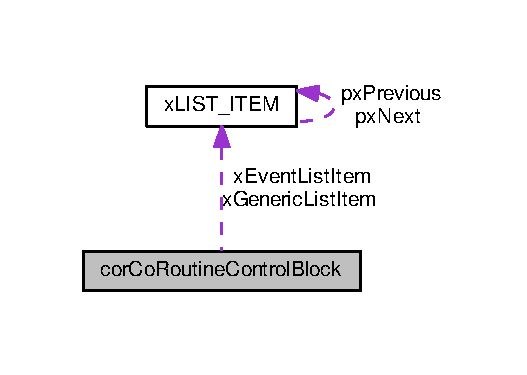
\includegraphics[width=253pt]{d4/d83/structcorCoRoutineControlBlock__coll__graph}
\end{center}
\end{figure}
\subsection*{Data Fields}
\begin{DoxyCompactItemize}
\item 
\hyperlink{croutine_8h_a397a7505718dd366d8411ce324c49758}{cr\+C\+O\+R\+O\+U\+T\+I\+N\+E\+\_\+\+C\+O\+DE} \hyperlink{structcorCoRoutineControlBlock_acc98c7364cd88e8e034a5f9bba113832}{px\+Co\+Routine\+Function}
\item 
\hyperlink{list_8h_a1a62d469392f9bfe2443e7efab9c8398}{List\+Item\+\_\+t} \hyperlink{structcorCoRoutineControlBlock_aa2900494db8782eeb8ef12d482501406}{x\+Generic\+List\+Item}
\item 
\hyperlink{list_8h_a1a62d469392f9bfe2443e7efab9c8398}{List\+Item\+\_\+t} \hyperlink{structcorCoRoutineControlBlock_a105d316da0069f766acc3b210afed1b9}{x\+Event\+List\+Item}
\item 
\hyperlink{portmacro_8h_a646f89d4298e4f5afd522202b11cb2e6}{U\+Base\+Type\+\_\+t} \hyperlink{structcorCoRoutineControlBlock_a752101a5d41b5caa7fd5149436613c8f}{ux\+Priority}
\item 
\hyperlink{portmacro_8h_a646f89d4298e4f5afd522202b11cb2e6}{U\+Base\+Type\+\_\+t} \hyperlink{structcorCoRoutineControlBlock_a6c185cd2145f562fb570bea9b158fc81}{ux\+Index}
\item 
uint16\+\_\+t \hyperlink{structcorCoRoutineControlBlock_aa0d702ff5a23c61598fe13e5a78fb1dc}{ux\+State}
\end{DoxyCompactItemize}


\subsection{Field Documentation}
\index{cor\+Co\+Routine\+Control\+Block@{cor\+Co\+Routine\+Control\+Block}!px\+Co\+Routine\+Function@{px\+Co\+Routine\+Function}}
\index{px\+Co\+Routine\+Function@{px\+Co\+Routine\+Function}!cor\+Co\+Routine\+Control\+Block@{cor\+Co\+Routine\+Control\+Block}}
\subsubsection[{\texorpdfstring{px\+Co\+Routine\+Function}{pxCoRoutineFunction}}]{\setlength{\rightskip}{0pt plus 5cm}{\bf cr\+C\+O\+R\+O\+U\+T\+I\+N\+E\+\_\+\+C\+O\+DE} cor\+Co\+Routine\+Control\+Block\+::px\+Co\+Routine\+Function}\hypertarget{structcorCoRoutineControlBlock_acc98c7364cd88e8e034a5f9bba113832}{}\label{structcorCoRoutineControlBlock_acc98c7364cd88e8e034a5f9bba113832}
\index{cor\+Co\+Routine\+Control\+Block@{cor\+Co\+Routine\+Control\+Block}!ux\+Index@{ux\+Index}}
\index{ux\+Index@{ux\+Index}!cor\+Co\+Routine\+Control\+Block@{cor\+Co\+Routine\+Control\+Block}}
\subsubsection[{\texorpdfstring{ux\+Index}{uxIndex}}]{\setlength{\rightskip}{0pt plus 5cm}{\bf U\+Base\+Type\+\_\+t} cor\+Co\+Routine\+Control\+Block\+::ux\+Index}\hypertarget{structcorCoRoutineControlBlock_a6c185cd2145f562fb570bea9b158fc81}{}\label{structcorCoRoutineControlBlock_a6c185cd2145f562fb570bea9b158fc81}
\index{cor\+Co\+Routine\+Control\+Block@{cor\+Co\+Routine\+Control\+Block}!ux\+Priority@{ux\+Priority}}
\index{ux\+Priority@{ux\+Priority}!cor\+Co\+Routine\+Control\+Block@{cor\+Co\+Routine\+Control\+Block}}
\subsubsection[{\texorpdfstring{ux\+Priority}{uxPriority}}]{\setlength{\rightskip}{0pt plus 5cm}{\bf U\+Base\+Type\+\_\+t} cor\+Co\+Routine\+Control\+Block\+::ux\+Priority}\hypertarget{structcorCoRoutineControlBlock_a752101a5d41b5caa7fd5149436613c8f}{}\label{structcorCoRoutineControlBlock_a752101a5d41b5caa7fd5149436613c8f}
\index{cor\+Co\+Routine\+Control\+Block@{cor\+Co\+Routine\+Control\+Block}!ux\+State@{ux\+State}}
\index{ux\+State@{ux\+State}!cor\+Co\+Routine\+Control\+Block@{cor\+Co\+Routine\+Control\+Block}}
\subsubsection[{\texorpdfstring{ux\+State}{uxState}}]{\setlength{\rightskip}{0pt plus 5cm}uint16\+\_\+t cor\+Co\+Routine\+Control\+Block\+::ux\+State}\hypertarget{structcorCoRoutineControlBlock_aa0d702ff5a23c61598fe13e5a78fb1dc}{}\label{structcorCoRoutineControlBlock_aa0d702ff5a23c61598fe13e5a78fb1dc}
\index{cor\+Co\+Routine\+Control\+Block@{cor\+Co\+Routine\+Control\+Block}!x\+Event\+List\+Item@{x\+Event\+List\+Item}}
\index{x\+Event\+List\+Item@{x\+Event\+List\+Item}!cor\+Co\+Routine\+Control\+Block@{cor\+Co\+Routine\+Control\+Block}}
\subsubsection[{\texorpdfstring{x\+Event\+List\+Item}{xEventListItem}}]{\setlength{\rightskip}{0pt plus 5cm}{\bf List\+Item\+\_\+t} cor\+Co\+Routine\+Control\+Block\+::x\+Event\+List\+Item}\hypertarget{structcorCoRoutineControlBlock_a105d316da0069f766acc3b210afed1b9}{}\label{structcorCoRoutineControlBlock_a105d316da0069f766acc3b210afed1b9}
\index{cor\+Co\+Routine\+Control\+Block@{cor\+Co\+Routine\+Control\+Block}!x\+Generic\+List\+Item@{x\+Generic\+List\+Item}}
\index{x\+Generic\+List\+Item@{x\+Generic\+List\+Item}!cor\+Co\+Routine\+Control\+Block@{cor\+Co\+Routine\+Control\+Block}}
\subsubsection[{\texorpdfstring{x\+Generic\+List\+Item}{xGenericListItem}}]{\setlength{\rightskip}{0pt plus 5cm}{\bf List\+Item\+\_\+t} cor\+Co\+Routine\+Control\+Block\+::x\+Generic\+List\+Item}\hypertarget{structcorCoRoutineControlBlock_aa2900494db8782eeb8ef12d482501406}{}\label{structcorCoRoutineControlBlock_aa2900494db8782eeb8ef12d482501406}


The documentation for this struct was generated from the following file\+:\begin{DoxyCompactItemize}
\item 
/var/www/html/\+S\+J\+S\+U-\/\+D\+E\+V-\/\+Linux/firmware/default/lib/\+L1\+\_\+\+Free\+R\+T\+O\+S/include/\hyperlink{croutine_8h}{croutine.\+h}\end{DoxyCompactItemize}

\hypertarget{structCoreDebug__Type}{}\section{Core\+Debug\+\_\+\+Type Struct Reference}
\label{structCoreDebug__Type}\index{Core\+Debug\+\_\+\+Type@{Core\+Debug\+\_\+\+Type}}


{\ttfamily \#include $<$core\+\_\+cm3.\+h$>$}

\subsection*{Data Fields}
\begin{DoxyCompactItemize}
\item 
\hyperlink{LPC17xx_8h_aec43007d9998a0a0e01faede4133d6be}{\+\_\+\+\_\+\+IO} uint32\+\_\+t \hyperlink{structCoreDebug__Type_a25c14c022c73a725a1736e903431095d}{D\+H\+C\+SR}
\item 
\hyperlink{LPC17xx_8h_a7e25d9380f9ef903923964322e71f2f6}{\+\_\+\+\_\+O} uint32\+\_\+t \hyperlink{structCoreDebug__Type_afefa84bce7497652353a1b76d405d983}{D\+C\+R\+SR}
\item 
\hyperlink{LPC17xx_8h_aec43007d9998a0a0e01faede4133d6be}{\+\_\+\+\_\+\+IO} uint32\+\_\+t \hyperlink{structCoreDebug__Type_ab8f4bb076402b61f7be6308075a789c9}{D\+C\+R\+DR}
\item 
\hyperlink{LPC17xx_8h_aec43007d9998a0a0e01faede4133d6be}{\+\_\+\+\_\+\+IO} uint32\+\_\+t \hyperlink{structCoreDebug__Type_a5cdd51dbe3ebb7041880714430edd52d}{D\+E\+M\+CR}
\end{DoxyCompactItemize}


\subsection{Field Documentation}
\index{Core\+Debug\+\_\+\+Type@{Core\+Debug\+\_\+\+Type}!D\+C\+R\+DR@{D\+C\+R\+DR}}
\index{D\+C\+R\+DR@{D\+C\+R\+DR}!Core\+Debug\+\_\+\+Type@{Core\+Debug\+\_\+\+Type}}
\subsubsection[{\texorpdfstring{D\+C\+R\+DR}{DCRDR}}]{\setlength{\rightskip}{0pt plus 5cm}{\bf \+\_\+\+\_\+\+IO} uint32\+\_\+t Core\+Debug\+\_\+\+Type\+::\+D\+C\+R\+DR}\hypertarget{structCoreDebug__Type_ab8f4bb076402b61f7be6308075a789c9}{}\label{structCoreDebug__Type_ab8f4bb076402b61f7be6308075a789c9}
Offset\+: 0x08 Debug Core Register Data Register \index{Core\+Debug\+\_\+\+Type@{Core\+Debug\+\_\+\+Type}!D\+C\+R\+SR@{D\+C\+R\+SR}}
\index{D\+C\+R\+SR@{D\+C\+R\+SR}!Core\+Debug\+\_\+\+Type@{Core\+Debug\+\_\+\+Type}}
\subsubsection[{\texorpdfstring{D\+C\+R\+SR}{DCRSR}}]{\setlength{\rightskip}{0pt plus 5cm}{\bf \+\_\+\+\_\+O} uint32\+\_\+t Core\+Debug\+\_\+\+Type\+::\+D\+C\+R\+SR}\hypertarget{structCoreDebug__Type_afefa84bce7497652353a1b76d405d983}{}\label{structCoreDebug__Type_afefa84bce7497652353a1b76d405d983}
Offset\+: 0x04 Debug Core Register Selector Register \index{Core\+Debug\+\_\+\+Type@{Core\+Debug\+\_\+\+Type}!D\+E\+M\+CR@{D\+E\+M\+CR}}
\index{D\+E\+M\+CR@{D\+E\+M\+CR}!Core\+Debug\+\_\+\+Type@{Core\+Debug\+\_\+\+Type}}
\subsubsection[{\texorpdfstring{D\+E\+M\+CR}{DEMCR}}]{\setlength{\rightskip}{0pt plus 5cm}{\bf \+\_\+\+\_\+\+IO} uint32\+\_\+t Core\+Debug\+\_\+\+Type\+::\+D\+E\+M\+CR}\hypertarget{structCoreDebug__Type_a5cdd51dbe3ebb7041880714430edd52d}{}\label{structCoreDebug__Type_a5cdd51dbe3ebb7041880714430edd52d}
Offset\+: 0x0C Debug Exception and Monitor Control Register \index{Core\+Debug\+\_\+\+Type@{Core\+Debug\+\_\+\+Type}!D\+H\+C\+SR@{D\+H\+C\+SR}}
\index{D\+H\+C\+SR@{D\+H\+C\+SR}!Core\+Debug\+\_\+\+Type@{Core\+Debug\+\_\+\+Type}}
\subsubsection[{\texorpdfstring{D\+H\+C\+SR}{DHCSR}}]{\setlength{\rightskip}{0pt plus 5cm}{\bf \+\_\+\+\_\+\+IO} uint32\+\_\+t Core\+Debug\+\_\+\+Type\+::\+D\+H\+C\+SR}\hypertarget{structCoreDebug__Type_a25c14c022c73a725a1736e903431095d}{}\label{structCoreDebug__Type_a25c14c022c73a725a1736e903431095d}
Offset\+: 0x00 Debug Halting Control and Status Register 

The documentation for this struct was generated from the following file\+:\begin{DoxyCompactItemize}
\item 
/var/www/html/\+S\+J\+S\+U-\/\+D\+E\+V-\/\+Linux/firmware/default/lib/\+L0\+\_\+\+Low\+Level/\hyperlink{core__cm3_8h}{core\+\_\+cm3.\+h}\end{DoxyCompactItemize}

\hypertarget{classdbc__parse_1_1DBC}{}\section{dbc\+\_\+parse.\+D\+BC Class Reference}
\label{classdbc__parse_1_1DBC}\index{dbc\+\_\+parse.\+D\+BC@{dbc\+\_\+parse.\+D\+BC}}


Inheritance diagram for dbc\+\_\+parse.\+D\+BC\+:\nopagebreak
\begin{figure}[H]
\begin{center}
\leavevmode
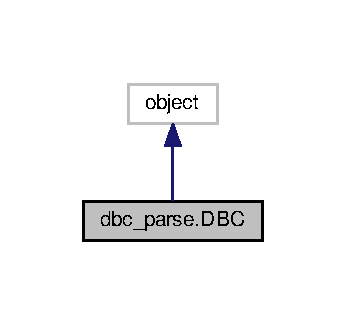
\includegraphics[width=166pt]{d5/dd3/classdbc__parse_1_1DBC__inherit__graph}
\end{center}
\end{figure}


Collaboration diagram for dbc\+\_\+parse.\+D\+BC\+:\nopagebreak
\begin{figure}[H]
\begin{center}
\leavevmode
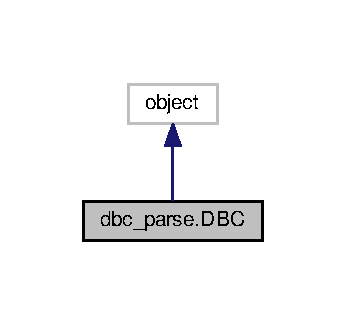
\includegraphics[width=166pt]{d9/df0/classdbc__parse_1_1DBC__coll__graph}
\end{center}
\end{figure}
\subsection*{Public Member Functions}
\begin{DoxyCompactItemize}
\item 
def \hyperlink{classdbc__parse_1_1DBC_a1df573f870c1d3e076871e990bb9f845}{\+\_\+\+\_\+init\+\_\+\+\_\+} (self, \hyperlink{classdbc__parse_1_1DBC_ae3245dbfb7f61ce997c78979f13df924}{name}, \hyperlink{classdbc__parse_1_1DBC_abd457f1296faa1c86877943cc6e57d20}{self\+\_\+node}, \hyperlink{classdbc__parse_1_1DBC_a84e58857a28589687adf4292435a4a00}{gen\+\_\+all})
\item 
def \hyperlink{classdbc__parse_1_1DBC_a05ee51f170a280b78400c6e57117a76c}{gen\+\_\+file\+\_\+header} (self)
\item 
def \hyperlink{classdbc__parse_1_1DBC_ab74fae88905fb58492c5a9acb653a83f}{gen\+\_\+msg\+\_\+hdr\+\_\+struct} (self)
\item 
def \hyperlink{classdbc__parse_1_1DBC_a3217ec2d0eeb36ae12c56c81199c9c4a}{gen\+\_\+enum\+\_\+types} (self)
\item 
def \hyperlink{classdbc__parse_1_1DBC_a15bbf4eae7bec655bd979d5aaca3ba35}{gen\+\_\+msg\+\_\+hdr\+\_\+instances} (self)
\item 
def \hyperlink{classdbc__parse_1_1DBC_a820caf7cfb3a4cb071b83648497879c2}{gen\+\_\+mia\+\_\+struct} (self)
\item 
def \hyperlink{classdbc__parse_1_1DBC_a47cf5fa376ac1dfd6f5a2f1c8c752c6a}{gen\+\_\+mia\+\_\+funcs} (self)
\end{DoxyCompactItemize}
\subsection*{Data Fields}
\begin{DoxyCompactItemize}
\item 
\hyperlink{classdbc__parse_1_1DBC_ae3245dbfb7f61ce997c78979f13df924}{name}
\item 
\hyperlink{classdbc__parse_1_1DBC_abd457f1296faa1c86877943cc6e57d20}{self\+\_\+node}
\item 
\hyperlink{classdbc__parse_1_1DBC_a84e58857a28589687adf4292435a4a00}{gen\+\_\+all}
\item 
\hyperlink{classdbc__parse_1_1DBC_a6c4e80730a556354953e6da7a7bfa878}{messages}
\item 
\hyperlink{classdbc__parse_1_1DBC_a84e171a1b8eb95698e38f0141950b8d6}{nodes}
\end{DoxyCompactItemize}


\subsection{Constructor \& Destructor Documentation}
\index{dbc\+\_\+parse\+::\+D\+BC@{dbc\+\_\+parse\+::\+D\+BC}!\+\_\+\+\_\+init\+\_\+\+\_\+@{\+\_\+\+\_\+init\+\_\+\+\_\+}}
\index{\+\_\+\+\_\+init\+\_\+\+\_\+@{\+\_\+\+\_\+init\+\_\+\+\_\+}!dbc\+\_\+parse\+::\+D\+BC@{dbc\+\_\+parse\+::\+D\+BC}}
\subsubsection[{\texorpdfstring{\+\_\+\+\_\+init\+\_\+\+\_\+(self, name, self\+\_\+node, gen\+\_\+all)}{__init__(self, name, self_node, gen_all)}}]{\setlength{\rightskip}{0pt plus 5cm}def dbc\+\_\+parse.\+D\+B\+C.\+\_\+\+\_\+init\+\_\+\+\_\+ (
\begin{DoxyParamCaption}
\item[{}]{self, }
\item[{}]{name, }
\item[{}]{self\+\_\+node, }
\item[{}]{gen\+\_\+all}
\end{DoxyParamCaption}
)}\hypertarget{classdbc__parse_1_1DBC_a1df573f870c1d3e076871e990bb9f845}{}\label{classdbc__parse_1_1DBC_a1df573f870c1d3e076871e990bb9f845}


\subsection{Member Function Documentation}
\index{dbc\+\_\+parse\+::\+D\+BC@{dbc\+\_\+parse\+::\+D\+BC}!gen\+\_\+enum\+\_\+types@{gen\+\_\+enum\+\_\+types}}
\index{gen\+\_\+enum\+\_\+types@{gen\+\_\+enum\+\_\+types}!dbc\+\_\+parse\+::\+D\+BC@{dbc\+\_\+parse\+::\+D\+BC}}
\subsubsection[{\texorpdfstring{gen\+\_\+enum\+\_\+types(self)}{gen_enum_types(self)}}]{\setlength{\rightskip}{0pt plus 5cm}def dbc\+\_\+parse.\+D\+B\+C.\+gen\+\_\+enum\+\_\+types (
\begin{DoxyParamCaption}
\item[{}]{self}
\end{DoxyParamCaption}
)}\hypertarget{classdbc__parse_1_1DBC_a3217ec2d0eeb36ae12c56c81199c9c4a}{}\label{classdbc__parse_1_1DBC_a3217ec2d0eeb36ae12c56c81199c9c4a}
\index{dbc\+\_\+parse\+::\+D\+BC@{dbc\+\_\+parse\+::\+D\+BC}!gen\+\_\+file\+\_\+header@{gen\+\_\+file\+\_\+header}}
\index{gen\+\_\+file\+\_\+header@{gen\+\_\+file\+\_\+header}!dbc\+\_\+parse\+::\+D\+BC@{dbc\+\_\+parse\+::\+D\+BC}}
\subsubsection[{\texorpdfstring{gen\+\_\+file\+\_\+header(self)}{gen_file_header(self)}}]{\setlength{\rightskip}{0pt plus 5cm}def dbc\+\_\+parse.\+D\+B\+C.\+gen\+\_\+file\+\_\+header (
\begin{DoxyParamCaption}
\item[{}]{self}
\end{DoxyParamCaption}
)}\hypertarget{classdbc__parse_1_1DBC_a05ee51f170a280b78400c6e57117a76c}{}\label{classdbc__parse_1_1DBC_a05ee51f170a280b78400c6e57117a76c}
\index{dbc\+\_\+parse\+::\+D\+BC@{dbc\+\_\+parse\+::\+D\+BC}!gen\+\_\+mia\+\_\+funcs@{gen\+\_\+mia\+\_\+funcs}}
\index{gen\+\_\+mia\+\_\+funcs@{gen\+\_\+mia\+\_\+funcs}!dbc\+\_\+parse\+::\+D\+BC@{dbc\+\_\+parse\+::\+D\+BC}}
\subsubsection[{\texorpdfstring{gen\+\_\+mia\+\_\+funcs(self)}{gen_mia_funcs(self)}}]{\setlength{\rightskip}{0pt plus 5cm}def dbc\+\_\+parse.\+D\+B\+C.\+gen\+\_\+mia\+\_\+funcs (
\begin{DoxyParamCaption}
\item[{}]{self}
\end{DoxyParamCaption}
)}\hypertarget{classdbc__parse_1_1DBC_a47cf5fa376ac1dfd6f5a2f1c8c752c6a}{}\label{classdbc__parse_1_1DBC_a47cf5fa376ac1dfd6f5a2f1c8c752c6a}
\index{dbc\+\_\+parse\+::\+D\+BC@{dbc\+\_\+parse\+::\+D\+BC}!gen\+\_\+mia\+\_\+struct@{gen\+\_\+mia\+\_\+struct}}
\index{gen\+\_\+mia\+\_\+struct@{gen\+\_\+mia\+\_\+struct}!dbc\+\_\+parse\+::\+D\+BC@{dbc\+\_\+parse\+::\+D\+BC}}
\subsubsection[{\texorpdfstring{gen\+\_\+mia\+\_\+struct(self)}{gen_mia_struct(self)}}]{\setlength{\rightskip}{0pt plus 5cm}def dbc\+\_\+parse.\+D\+B\+C.\+gen\+\_\+mia\+\_\+struct (
\begin{DoxyParamCaption}
\item[{}]{self}
\end{DoxyParamCaption}
)}\hypertarget{classdbc__parse_1_1DBC_a820caf7cfb3a4cb071b83648497879c2}{}\label{classdbc__parse_1_1DBC_a820caf7cfb3a4cb071b83648497879c2}
\index{dbc\+\_\+parse\+::\+D\+BC@{dbc\+\_\+parse\+::\+D\+BC}!gen\+\_\+msg\+\_\+hdr\+\_\+instances@{gen\+\_\+msg\+\_\+hdr\+\_\+instances}}
\index{gen\+\_\+msg\+\_\+hdr\+\_\+instances@{gen\+\_\+msg\+\_\+hdr\+\_\+instances}!dbc\+\_\+parse\+::\+D\+BC@{dbc\+\_\+parse\+::\+D\+BC}}
\subsubsection[{\texorpdfstring{gen\+\_\+msg\+\_\+hdr\+\_\+instances(self)}{gen_msg_hdr_instances(self)}}]{\setlength{\rightskip}{0pt plus 5cm}def dbc\+\_\+parse.\+D\+B\+C.\+gen\+\_\+msg\+\_\+hdr\+\_\+instances (
\begin{DoxyParamCaption}
\item[{}]{self}
\end{DoxyParamCaption}
)}\hypertarget{classdbc__parse_1_1DBC_a15bbf4eae7bec655bd979d5aaca3ba35}{}\label{classdbc__parse_1_1DBC_a15bbf4eae7bec655bd979d5aaca3ba35}
\index{dbc\+\_\+parse\+::\+D\+BC@{dbc\+\_\+parse\+::\+D\+BC}!gen\+\_\+msg\+\_\+hdr\+\_\+struct@{gen\+\_\+msg\+\_\+hdr\+\_\+struct}}
\index{gen\+\_\+msg\+\_\+hdr\+\_\+struct@{gen\+\_\+msg\+\_\+hdr\+\_\+struct}!dbc\+\_\+parse\+::\+D\+BC@{dbc\+\_\+parse\+::\+D\+BC}}
\subsubsection[{\texorpdfstring{gen\+\_\+msg\+\_\+hdr\+\_\+struct(self)}{gen_msg_hdr_struct(self)}}]{\setlength{\rightskip}{0pt plus 5cm}def dbc\+\_\+parse.\+D\+B\+C.\+gen\+\_\+msg\+\_\+hdr\+\_\+struct (
\begin{DoxyParamCaption}
\item[{}]{self}
\end{DoxyParamCaption}
)}\hypertarget{classdbc__parse_1_1DBC_ab74fae88905fb58492c5a9acb653a83f}{}\label{classdbc__parse_1_1DBC_ab74fae88905fb58492c5a9acb653a83f}


\subsection{Field Documentation}
\index{dbc\+\_\+parse\+::\+D\+BC@{dbc\+\_\+parse\+::\+D\+BC}!gen\+\_\+all@{gen\+\_\+all}}
\index{gen\+\_\+all@{gen\+\_\+all}!dbc\+\_\+parse\+::\+D\+BC@{dbc\+\_\+parse\+::\+D\+BC}}
\subsubsection[{\texorpdfstring{gen\+\_\+all}{gen_all}}]{\setlength{\rightskip}{0pt plus 5cm}dbc\+\_\+parse.\+D\+B\+C.\+gen\+\_\+all}\hypertarget{classdbc__parse_1_1DBC_a84e58857a28589687adf4292435a4a00}{}\label{classdbc__parse_1_1DBC_a84e58857a28589687adf4292435a4a00}
\index{dbc\+\_\+parse\+::\+D\+BC@{dbc\+\_\+parse\+::\+D\+BC}!messages@{messages}}
\index{messages@{messages}!dbc\+\_\+parse\+::\+D\+BC@{dbc\+\_\+parse\+::\+D\+BC}}
\subsubsection[{\texorpdfstring{messages}{messages}}]{\setlength{\rightskip}{0pt plus 5cm}dbc\+\_\+parse.\+D\+B\+C.\+messages}\hypertarget{classdbc__parse_1_1DBC_a6c4e80730a556354953e6da7a7bfa878}{}\label{classdbc__parse_1_1DBC_a6c4e80730a556354953e6da7a7bfa878}
\index{dbc\+\_\+parse\+::\+D\+BC@{dbc\+\_\+parse\+::\+D\+BC}!name@{name}}
\index{name@{name}!dbc\+\_\+parse\+::\+D\+BC@{dbc\+\_\+parse\+::\+D\+BC}}
\subsubsection[{\texorpdfstring{name}{name}}]{\setlength{\rightskip}{0pt plus 5cm}dbc\+\_\+parse.\+D\+B\+C.\+name}\hypertarget{classdbc__parse_1_1DBC_ae3245dbfb7f61ce997c78979f13df924}{}\label{classdbc__parse_1_1DBC_ae3245dbfb7f61ce997c78979f13df924}
\index{dbc\+\_\+parse\+::\+D\+BC@{dbc\+\_\+parse\+::\+D\+BC}!nodes@{nodes}}
\index{nodes@{nodes}!dbc\+\_\+parse\+::\+D\+BC@{dbc\+\_\+parse\+::\+D\+BC}}
\subsubsection[{\texorpdfstring{nodes}{nodes}}]{\setlength{\rightskip}{0pt plus 5cm}dbc\+\_\+parse.\+D\+B\+C.\+nodes}\hypertarget{classdbc__parse_1_1DBC_a84e171a1b8eb95698e38f0141950b8d6}{}\label{classdbc__parse_1_1DBC_a84e171a1b8eb95698e38f0141950b8d6}
\index{dbc\+\_\+parse\+::\+D\+BC@{dbc\+\_\+parse\+::\+D\+BC}!self\+\_\+node@{self\+\_\+node}}
\index{self\+\_\+node@{self\+\_\+node}!dbc\+\_\+parse\+::\+D\+BC@{dbc\+\_\+parse\+::\+D\+BC}}
\subsubsection[{\texorpdfstring{self\+\_\+node}{self_node}}]{\setlength{\rightskip}{0pt plus 5cm}dbc\+\_\+parse.\+D\+B\+C.\+self\+\_\+node}\hypertarget{classdbc__parse_1_1DBC_abd457f1296faa1c86877943cc6e57d20}{}\label{classdbc__parse_1_1DBC_abd457f1296faa1c86877943cc6e57d20}


The documentation for this class was generated from the following file\+:\begin{DoxyCompactItemize}
\item 
/var/www/html/\+S\+J\+S\+U-\/\+D\+E\+V-\/\+Linux/firmware/default/lib/\+\_\+can\+\_\+dbc/\hyperlink{dbc__parse_8py}{dbc\+\_\+parse.\+py}\end{DoxyCompactItemize}

\hypertarget{structDIR}{}\section{D\+IR Struct Reference}
\label{structDIR}\index{D\+IR@{D\+IR}}


{\ttfamily \#include $<$ff.\+h$>$}



Collaboration diagram for D\+IR\+:\nopagebreak
\begin{figure}[H]
\begin{center}
\leavevmode
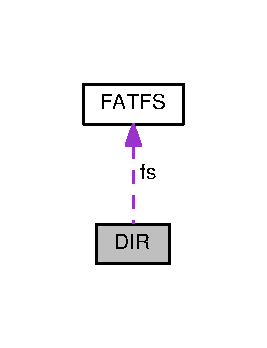
\includegraphics[width=128pt]{d2/d15/structDIR__coll__graph}
\end{center}
\end{figure}
\subsection*{Data Fields}
\begin{DoxyCompactItemize}
\item 
\hyperlink{structFATFS}{F\+A\+T\+FS} $\ast$ \hyperlink{structDIR_a312eaa66cb703fb2993ea98173dc0c9a}{fs}
\item 
\hyperlink{integer_8h_a197942eefa7db30960ae396d68339b97}{W\+O\+RD} \hyperlink{structDIR_aca2c95a99a04173917ec70c030891383}{id}
\item 
\hyperlink{integer_8h_a197942eefa7db30960ae396d68339b97}{W\+O\+RD} \hyperlink{structDIR_ab95119fbacbe45e3e9ee0f962b844092}{index}
\item 
\hyperlink{integer_8h_ad342ac907eb044443153a22f964bf0af}{D\+W\+O\+RD} \hyperlink{structDIR_a9212af5877b94d790dd3bab3aa320994}{sclust}
\item 
\hyperlink{integer_8h_ad342ac907eb044443153a22f964bf0af}{D\+W\+O\+RD} \hyperlink{structDIR_acfbb8ba2d6e73b6f999ceffd1857c190}{clust}
\item 
\hyperlink{integer_8h_ad342ac907eb044443153a22f964bf0af}{D\+W\+O\+RD} \hyperlink{structDIR_ad01fcc812ed0dad11a593574336adc9e}{sect}
\item 
\hyperlink{integer_8h_a4ae1dab0fb4b072a66584546209e7d58}{B\+Y\+TE} $\ast$ \hyperlink{structDIR_a6c2a8c0cf2d55ae99775e93a16593449}{dir}
\item 
\hyperlink{integer_8h_a4ae1dab0fb4b072a66584546209e7d58}{B\+Y\+TE} $\ast$ \hyperlink{structDIR_a32da2f31d6c3b6c42eef981cb0cfd2ee}{fn}
\item 
\hyperlink{integer_8h_a570001c92f314285ad3e7139d8c58cf7}{W\+C\+H\+AR} $\ast$ \hyperlink{structDIR_af62fd789383e6f1397f74617e11c135d}{lfn}
\item 
\hyperlink{integer_8h_a197942eefa7db30960ae396d68339b97}{W\+O\+RD} \hyperlink{structDIR_acad41b18758c9278c14d47076e8149fc}{lfn\+\_\+idx}
\end{DoxyCompactItemize}


\subsection{Field Documentation}
\index{D\+IR@{D\+IR}!clust@{clust}}
\index{clust@{clust}!D\+IR@{D\+IR}}
\subsubsection[{\texorpdfstring{clust}{clust}}]{\setlength{\rightskip}{0pt plus 5cm}{\bf D\+W\+O\+RD} D\+I\+R\+::clust}\hypertarget{structDIR_acfbb8ba2d6e73b6f999ceffd1857c190}{}\label{structDIR_acfbb8ba2d6e73b6f999ceffd1857c190}
\index{D\+IR@{D\+IR}!dir@{dir}}
\index{dir@{dir}!D\+IR@{D\+IR}}
\subsubsection[{\texorpdfstring{dir}{dir}}]{\setlength{\rightskip}{0pt plus 5cm}{\bf B\+Y\+TE}$\ast$ D\+I\+R\+::dir}\hypertarget{structDIR_a6c2a8c0cf2d55ae99775e93a16593449}{}\label{structDIR_a6c2a8c0cf2d55ae99775e93a16593449}
\index{D\+IR@{D\+IR}!fn@{fn}}
\index{fn@{fn}!D\+IR@{D\+IR}}
\subsubsection[{\texorpdfstring{fn}{fn}}]{\setlength{\rightskip}{0pt plus 5cm}{\bf B\+Y\+TE}$\ast$ D\+I\+R\+::fn}\hypertarget{structDIR_a32da2f31d6c3b6c42eef981cb0cfd2ee}{}\label{structDIR_a32da2f31d6c3b6c42eef981cb0cfd2ee}
\index{D\+IR@{D\+IR}!fs@{fs}}
\index{fs@{fs}!D\+IR@{D\+IR}}
\subsubsection[{\texorpdfstring{fs}{fs}}]{\setlength{\rightskip}{0pt plus 5cm}{\bf F\+A\+T\+FS}$\ast$ D\+I\+R\+::fs}\hypertarget{structDIR_a312eaa66cb703fb2993ea98173dc0c9a}{}\label{structDIR_a312eaa66cb703fb2993ea98173dc0c9a}
\index{D\+IR@{D\+IR}!id@{id}}
\index{id@{id}!D\+IR@{D\+IR}}
\subsubsection[{\texorpdfstring{id}{id}}]{\setlength{\rightskip}{0pt plus 5cm}{\bf W\+O\+RD} D\+I\+R\+::id}\hypertarget{structDIR_aca2c95a99a04173917ec70c030891383}{}\label{structDIR_aca2c95a99a04173917ec70c030891383}
\index{D\+IR@{D\+IR}!index@{index}}
\index{index@{index}!D\+IR@{D\+IR}}
\subsubsection[{\texorpdfstring{index}{index}}]{\setlength{\rightskip}{0pt plus 5cm}{\bf W\+O\+RD} D\+I\+R\+::index}\hypertarget{structDIR_ab95119fbacbe45e3e9ee0f962b844092}{}\label{structDIR_ab95119fbacbe45e3e9ee0f962b844092}
\index{D\+IR@{D\+IR}!lfn@{lfn}}
\index{lfn@{lfn}!D\+IR@{D\+IR}}
\subsubsection[{\texorpdfstring{lfn}{lfn}}]{\setlength{\rightskip}{0pt plus 5cm}{\bf W\+C\+H\+AR}$\ast$ D\+I\+R\+::lfn}\hypertarget{structDIR_af62fd789383e6f1397f74617e11c135d}{}\label{structDIR_af62fd789383e6f1397f74617e11c135d}
\index{D\+IR@{D\+IR}!lfn\+\_\+idx@{lfn\+\_\+idx}}
\index{lfn\+\_\+idx@{lfn\+\_\+idx}!D\+IR@{D\+IR}}
\subsubsection[{\texorpdfstring{lfn\+\_\+idx}{lfn_idx}}]{\setlength{\rightskip}{0pt plus 5cm}{\bf W\+O\+RD} D\+I\+R\+::lfn\+\_\+idx}\hypertarget{structDIR_acad41b18758c9278c14d47076e8149fc}{}\label{structDIR_acad41b18758c9278c14d47076e8149fc}
\index{D\+IR@{D\+IR}!sclust@{sclust}}
\index{sclust@{sclust}!D\+IR@{D\+IR}}
\subsubsection[{\texorpdfstring{sclust}{sclust}}]{\setlength{\rightskip}{0pt plus 5cm}{\bf D\+W\+O\+RD} D\+I\+R\+::sclust}\hypertarget{structDIR_a9212af5877b94d790dd3bab3aa320994}{}\label{structDIR_a9212af5877b94d790dd3bab3aa320994}
\index{D\+IR@{D\+IR}!sect@{sect}}
\index{sect@{sect}!D\+IR@{D\+IR}}
\subsubsection[{\texorpdfstring{sect}{sect}}]{\setlength{\rightskip}{0pt plus 5cm}{\bf D\+W\+O\+RD} D\+I\+R\+::sect}\hypertarget{structDIR_ad01fcc812ed0dad11a593574336adc9e}{}\label{structDIR_ad01fcc812ed0dad11a593574336adc9e}


The documentation for this struct was generated from the following file\+:\begin{DoxyCompactItemize}
\item 
/var/www/html/\+S\+J\+S\+U-\/\+D\+E\+V-\/\+Linux/firmware/default/lib/\+L4\+\_\+\+I\+O/fat/\hyperlink{ff_8h}{ff.\+h}\end{DoxyCompactItemize}

\hypertarget{structeint3__entry}{}\section{eint3\+\_\+entry Struct Reference}
\label{structeint3__entry}\index{eint3\+\_\+entry@{eint3\+\_\+entry}}


Linked list structure of E\+I\+N\+Ts (External interrupts)  




Collaboration diagram for eint3\+\_\+entry\+:\nopagebreak
\begin{figure}[H]
\begin{center}
\leavevmode
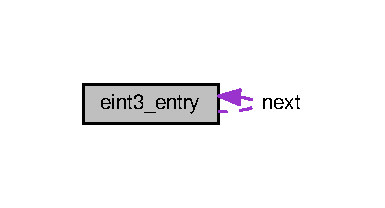
\includegraphics[width=185pt]{d8/df6/structeint3__entry__coll__graph}
\end{center}
\end{figure}
\subsection*{Data Fields}
\begin{DoxyCompactItemize}
\item 
uint32\+\_\+t \hyperlink{structeint3__entry_abd6bc384996eb947fc0e9b6ae5002b47}{pin\+\_\+mask}
\begin{DoxyCompactList}\small\item\em Port pin\textquotesingle{}s concatenated pin-\/mask. \end{DoxyCompactList}\item 
\hyperlink{lpc__sys_8h_a2425c2b3462f867da9fd2ab76d9d47b1}{void\+\_\+func\+\_\+t} \hyperlink{structeint3__entry_a3b97b9cf5d0ed8e39024e4f5af34f866}{callback}
\begin{DoxyCompactList}\small\item\em Callback when interrupt occurs. \end{DoxyCompactList}\item 
struct \hyperlink{structeint3__entry}{eint3\+\_\+entry} $\ast$ \hyperlink{structeint3__entry_ae7d52ddae024fa3ff613d5fc7967b43c}{next}
\begin{DoxyCompactList}\small\item\em The pointer to the next entry. \end{DoxyCompactList}\end{DoxyCompactItemize}


\subsection{Detailed Description}
Linked list structure of E\+I\+N\+Ts (External interrupts) 

\subsection{Field Documentation}
\index{eint3\+\_\+entry@{eint3\+\_\+entry}!callback@{callback}}
\index{callback@{callback}!eint3\+\_\+entry@{eint3\+\_\+entry}}
\subsubsection[{\texorpdfstring{callback}{callback}}]{\setlength{\rightskip}{0pt plus 5cm}{\bf void\+\_\+func\+\_\+t} eint3\+\_\+entry\+::callback}\hypertarget{structeint3__entry_a3b97b9cf5d0ed8e39024e4f5af34f866}{}\label{structeint3__entry_a3b97b9cf5d0ed8e39024e4f5af34f866}


Callback when interrupt occurs. 

\index{eint3\+\_\+entry@{eint3\+\_\+entry}!next@{next}}
\index{next@{next}!eint3\+\_\+entry@{eint3\+\_\+entry}}
\subsubsection[{\texorpdfstring{next}{next}}]{\setlength{\rightskip}{0pt plus 5cm}struct {\bf eint3\+\_\+entry}$\ast$ eint3\+\_\+entry\+::next}\hypertarget{structeint3__entry_ae7d52ddae024fa3ff613d5fc7967b43c}{}\label{structeint3__entry_ae7d52ddae024fa3ff613d5fc7967b43c}


The pointer to the next entry. 

\index{eint3\+\_\+entry@{eint3\+\_\+entry}!pin\+\_\+mask@{pin\+\_\+mask}}
\index{pin\+\_\+mask@{pin\+\_\+mask}!eint3\+\_\+entry@{eint3\+\_\+entry}}
\subsubsection[{\texorpdfstring{pin\+\_\+mask}{pin_mask}}]{\setlength{\rightskip}{0pt plus 5cm}uint32\+\_\+t eint3\+\_\+entry\+::pin\+\_\+mask}\hypertarget{structeint3__entry_abd6bc384996eb947fc0e9b6ae5002b47}{}\label{structeint3__entry_abd6bc384996eb947fc0e9b6ae5002b47}


Port pin\textquotesingle{}s concatenated pin-\/mask. 



The documentation for this struct was generated from the following file\+:\begin{DoxyCompactItemize}
\item 
/var/www/html/\+S\+J\+S\+U-\/\+D\+E\+V-\/\+Linux/firmware/default/lib/\+L2\+\_\+\+Drivers/src/\hyperlink{eint_8c}{eint.\+c}\end{DoxyCompactItemize}

\hypertarget{structFATFS}{}\section{F\+A\+T\+FS Struct Reference}
\label{structFATFS}\index{F\+A\+T\+FS@{F\+A\+T\+FS}}


{\ttfamily \#include $<$ff.\+h$>$}

\subsection*{Data Fields}
\begin{DoxyCompactItemize}
\item 
\hyperlink{integer_8h_a4ae1dab0fb4b072a66584546209e7d58}{B\+Y\+TE} \hyperlink{structFATFS_add27d97babe807b573eac98a71dc4ae5}{fs\+\_\+type}
\item 
\hyperlink{integer_8h_a4ae1dab0fb4b072a66584546209e7d58}{B\+Y\+TE} \hyperlink{structFATFS_a6a791560e2687e8b1569bfce61208d2d}{drv}
\item 
\hyperlink{integer_8h_a4ae1dab0fb4b072a66584546209e7d58}{B\+Y\+TE} \hyperlink{structFATFS_a504a1175f6dcc9a854b9da94463bd108}{csize}
\item 
\hyperlink{integer_8h_a4ae1dab0fb4b072a66584546209e7d58}{B\+Y\+TE} \hyperlink{structFATFS_a56716c7e7ac10cf46e73ffb2a2e9b545}{n\+\_\+fats}
\item 
\hyperlink{integer_8h_a4ae1dab0fb4b072a66584546209e7d58}{B\+Y\+TE} \hyperlink{structFATFS_a647e43c9ccae94b7274793d1909897de}{wflag}
\item 
\hyperlink{integer_8h_a4ae1dab0fb4b072a66584546209e7d58}{B\+Y\+TE} \hyperlink{structFATFS_a84e9cdc5a6a8e33ea7ec192058abf161}{fsi\+\_\+flag}
\item 
\hyperlink{integer_8h_a197942eefa7db30960ae396d68339b97}{W\+O\+RD} \hyperlink{structFATFS_a417095d7c20d56d417dc0998e0dd5a5c}{id}
\item 
\hyperlink{integer_8h_a197942eefa7db30960ae396d68339b97}{W\+O\+RD} \hyperlink{structFATFS_a189a00aa038044ffad0fc7f7dcf2aae1}{n\+\_\+rootdir}
\item 
\hyperlink{ffconf_8h_a9a3f0670343e51652dd12b18fa90a9eb}{\+\_\+\+S\+Y\+N\+C\+\_\+t} \hyperlink{structFATFS_a271135f02bd461d14e7db84ea566aa33}{sobj}
\item 
\hyperlink{integer_8h_ad342ac907eb044443153a22f964bf0af}{D\+W\+O\+RD} \hyperlink{structFATFS_ad315def289218e26ab78ff90fde700d1}{last\+\_\+clust}
\item 
\hyperlink{integer_8h_ad342ac907eb044443153a22f964bf0af}{D\+W\+O\+RD} \hyperlink{structFATFS_a5fb49e6ac511bd97eaffdd636d0e4165}{free\+\_\+clust}
\item 
\hyperlink{integer_8h_ad342ac907eb044443153a22f964bf0af}{D\+W\+O\+RD} \hyperlink{structFATFS_a8da50eeba6469bc20d60ca0cf9a1307c}{n\+\_\+fatent}
\item 
\hyperlink{integer_8h_ad342ac907eb044443153a22f964bf0af}{D\+W\+O\+RD} \hyperlink{structFATFS_a53e9560659f14e66f306c2c444198bf3}{fsize}
\item 
\hyperlink{integer_8h_ad342ac907eb044443153a22f964bf0af}{D\+W\+O\+RD} \hyperlink{structFATFS_a8f0ca578755749d204f59dc83f1a7649}{volbase}
\item 
\hyperlink{integer_8h_ad342ac907eb044443153a22f964bf0af}{D\+W\+O\+RD} \hyperlink{structFATFS_a848fba02c4aabe02ef2984e578f33d64}{fatbase}
\item 
\hyperlink{integer_8h_ad342ac907eb044443153a22f964bf0af}{D\+W\+O\+RD} \hyperlink{structFATFS_a3f72fd998dbcce4652a85a81fe944bc4}{dirbase}
\item 
\hyperlink{integer_8h_ad342ac907eb044443153a22f964bf0af}{D\+W\+O\+RD} \hyperlink{structFATFS_a5b6c0bc2e9fd2ae8ef714210a74a2d5d}{database}
\item 
\hyperlink{integer_8h_ad342ac907eb044443153a22f964bf0af}{D\+W\+O\+RD} \hyperlink{structFATFS_ac60e69c00e6bf7c25febfbac4dc1476b}{winsect}
\item 
\hyperlink{integer_8h_a4ae1dab0fb4b072a66584546209e7d58}{B\+Y\+TE} \hyperlink{structFATFS_a7cc35a593465e727ab87723c14610644}{win} \mbox{[}\hyperlink{ffconf_8h_ac271b697378912f17132cb9c7d0de024}{\+\_\+\+M\+A\+X\+\_\+\+SS}\mbox{]}
\end{DoxyCompactItemize}


\subsection{Field Documentation}
\index{F\+A\+T\+FS@{F\+A\+T\+FS}!csize@{csize}}
\index{csize@{csize}!F\+A\+T\+FS@{F\+A\+T\+FS}}
\subsubsection[{\texorpdfstring{csize}{csize}}]{\setlength{\rightskip}{0pt plus 5cm}{\bf B\+Y\+TE} F\+A\+T\+F\+S\+::csize}\hypertarget{structFATFS_a504a1175f6dcc9a854b9da94463bd108}{}\label{structFATFS_a504a1175f6dcc9a854b9da94463bd108}
\index{F\+A\+T\+FS@{F\+A\+T\+FS}!database@{database}}
\index{database@{database}!F\+A\+T\+FS@{F\+A\+T\+FS}}
\subsubsection[{\texorpdfstring{database}{database}}]{\setlength{\rightskip}{0pt plus 5cm}{\bf D\+W\+O\+RD} F\+A\+T\+F\+S\+::database}\hypertarget{structFATFS_a5b6c0bc2e9fd2ae8ef714210a74a2d5d}{}\label{structFATFS_a5b6c0bc2e9fd2ae8ef714210a74a2d5d}
\index{F\+A\+T\+FS@{F\+A\+T\+FS}!dirbase@{dirbase}}
\index{dirbase@{dirbase}!F\+A\+T\+FS@{F\+A\+T\+FS}}
\subsubsection[{\texorpdfstring{dirbase}{dirbase}}]{\setlength{\rightskip}{0pt plus 5cm}{\bf D\+W\+O\+RD} F\+A\+T\+F\+S\+::dirbase}\hypertarget{structFATFS_a3f72fd998dbcce4652a85a81fe944bc4}{}\label{structFATFS_a3f72fd998dbcce4652a85a81fe944bc4}
\index{F\+A\+T\+FS@{F\+A\+T\+FS}!drv@{drv}}
\index{drv@{drv}!F\+A\+T\+FS@{F\+A\+T\+FS}}
\subsubsection[{\texorpdfstring{drv}{drv}}]{\setlength{\rightskip}{0pt plus 5cm}{\bf B\+Y\+TE} F\+A\+T\+F\+S\+::drv}\hypertarget{structFATFS_a6a791560e2687e8b1569bfce61208d2d}{}\label{structFATFS_a6a791560e2687e8b1569bfce61208d2d}
\index{F\+A\+T\+FS@{F\+A\+T\+FS}!fatbase@{fatbase}}
\index{fatbase@{fatbase}!F\+A\+T\+FS@{F\+A\+T\+FS}}
\subsubsection[{\texorpdfstring{fatbase}{fatbase}}]{\setlength{\rightskip}{0pt plus 5cm}{\bf D\+W\+O\+RD} F\+A\+T\+F\+S\+::fatbase}\hypertarget{structFATFS_a848fba02c4aabe02ef2984e578f33d64}{}\label{structFATFS_a848fba02c4aabe02ef2984e578f33d64}
\index{F\+A\+T\+FS@{F\+A\+T\+FS}!free\+\_\+clust@{free\+\_\+clust}}
\index{free\+\_\+clust@{free\+\_\+clust}!F\+A\+T\+FS@{F\+A\+T\+FS}}
\subsubsection[{\texorpdfstring{free\+\_\+clust}{free_clust}}]{\setlength{\rightskip}{0pt plus 5cm}{\bf D\+W\+O\+RD} F\+A\+T\+F\+S\+::free\+\_\+clust}\hypertarget{structFATFS_a5fb49e6ac511bd97eaffdd636d0e4165}{}\label{structFATFS_a5fb49e6ac511bd97eaffdd636d0e4165}
\index{F\+A\+T\+FS@{F\+A\+T\+FS}!fs\+\_\+type@{fs\+\_\+type}}
\index{fs\+\_\+type@{fs\+\_\+type}!F\+A\+T\+FS@{F\+A\+T\+FS}}
\subsubsection[{\texorpdfstring{fs\+\_\+type}{fs_type}}]{\setlength{\rightskip}{0pt plus 5cm}{\bf B\+Y\+TE} F\+A\+T\+F\+S\+::fs\+\_\+type}\hypertarget{structFATFS_add27d97babe807b573eac98a71dc4ae5}{}\label{structFATFS_add27d97babe807b573eac98a71dc4ae5}
\index{F\+A\+T\+FS@{F\+A\+T\+FS}!fsi\+\_\+flag@{fsi\+\_\+flag}}
\index{fsi\+\_\+flag@{fsi\+\_\+flag}!F\+A\+T\+FS@{F\+A\+T\+FS}}
\subsubsection[{\texorpdfstring{fsi\+\_\+flag}{fsi_flag}}]{\setlength{\rightskip}{0pt plus 5cm}{\bf B\+Y\+TE} F\+A\+T\+F\+S\+::fsi\+\_\+flag}\hypertarget{structFATFS_a84e9cdc5a6a8e33ea7ec192058abf161}{}\label{structFATFS_a84e9cdc5a6a8e33ea7ec192058abf161}
\index{F\+A\+T\+FS@{F\+A\+T\+FS}!fsize@{fsize}}
\index{fsize@{fsize}!F\+A\+T\+FS@{F\+A\+T\+FS}}
\subsubsection[{\texorpdfstring{fsize}{fsize}}]{\setlength{\rightskip}{0pt plus 5cm}{\bf D\+W\+O\+RD} F\+A\+T\+F\+S\+::fsize}\hypertarget{structFATFS_a53e9560659f14e66f306c2c444198bf3}{}\label{structFATFS_a53e9560659f14e66f306c2c444198bf3}
\index{F\+A\+T\+FS@{F\+A\+T\+FS}!id@{id}}
\index{id@{id}!F\+A\+T\+FS@{F\+A\+T\+FS}}
\subsubsection[{\texorpdfstring{id}{id}}]{\setlength{\rightskip}{0pt plus 5cm}{\bf W\+O\+RD} F\+A\+T\+F\+S\+::id}\hypertarget{structFATFS_a417095d7c20d56d417dc0998e0dd5a5c}{}\label{structFATFS_a417095d7c20d56d417dc0998e0dd5a5c}
\index{F\+A\+T\+FS@{F\+A\+T\+FS}!last\+\_\+clust@{last\+\_\+clust}}
\index{last\+\_\+clust@{last\+\_\+clust}!F\+A\+T\+FS@{F\+A\+T\+FS}}
\subsubsection[{\texorpdfstring{last\+\_\+clust}{last_clust}}]{\setlength{\rightskip}{0pt plus 5cm}{\bf D\+W\+O\+RD} F\+A\+T\+F\+S\+::last\+\_\+clust}\hypertarget{structFATFS_ad315def289218e26ab78ff90fde700d1}{}\label{structFATFS_ad315def289218e26ab78ff90fde700d1}
\index{F\+A\+T\+FS@{F\+A\+T\+FS}!n\+\_\+fatent@{n\+\_\+fatent}}
\index{n\+\_\+fatent@{n\+\_\+fatent}!F\+A\+T\+FS@{F\+A\+T\+FS}}
\subsubsection[{\texorpdfstring{n\+\_\+fatent}{n_fatent}}]{\setlength{\rightskip}{0pt plus 5cm}{\bf D\+W\+O\+RD} F\+A\+T\+F\+S\+::n\+\_\+fatent}\hypertarget{structFATFS_a8da50eeba6469bc20d60ca0cf9a1307c}{}\label{structFATFS_a8da50eeba6469bc20d60ca0cf9a1307c}
\index{F\+A\+T\+FS@{F\+A\+T\+FS}!n\+\_\+fats@{n\+\_\+fats}}
\index{n\+\_\+fats@{n\+\_\+fats}!F\+A\+T\+FS@{F\+A\+T\+FS}}
\subsubsection[{\texorpdfstring{n\+\_\+fats}{n_fats}}]{\setlength{\rightskip}{0pt plus 5cm}{\bf B\+Y\+TE} F\+A\+T\+F\+S\+::n\+\_\+fats}\hypertarget{structFATFS_a56716c7e7ac10cf46e73ffb2a2e9b545}{}\label{structFATFS_a56716c7e7ac10cf46e73ffb2a2e9b545}
\index{F\+A\+T\+FS@{F\+A\+T\+FS}!n\+\_\+rootdir@{n\+\_\+rootdir}}
\index{n\+\_\+rootdir@{n\+\_\+rootdir}!F\+A\+T\+FS@{F\+A\+T\+FS}}
\subsubsection[{\texorpdfstring{n\+\_\+rootdir}{n_rootdir}}]{\setlength{\rightskip}{0pt plus 5cm}{\bf W\+O\+RD} F\+A\+T\+F\+S\+::n\+\_\+rootdir}\hypertarget{structFATFS_a189a00aa038044ffad0fc7f7dcf2aae1}{}\label{structFATFS_a189a00aa038044ffad0fc7f7dcf2aae1}
\index{F\+A\+T\+FS@{F\+A\+T\+FS}!sobj@{sobj}}
\index{sobj@{sobj}!F\+A\+T\+FS@{F\+A\+T\+FS}}
\subsubsection[{\texorpdfstring{sobj}{sobj}}]{\setlength{\rightskip}{0pt plus 5cm}{\bf \+\_\+\+S\+Y\+N\+C\+\_\+t} F\+A\+T\+F\+S\+::sobj}\hypertarget{structFATFS_a271135f02bd461d14e7db84ea566aa33}{}\label{structFATFS_a271135f02bd461d14e7db84ea566aa33}
\index{F\+A\+T\+FS@{F\+A\+T\+FS}!volbase@{volbase}}
\index{volbase@{volbase}!F\+A\+T\+FS@{F\+A\+T\+FS}}
\subsubsection[{\texorpdfstring{volbase}{volbase}}]{\setlength{\rightskip}{0pt plus 5cm}{\bf D\+W\+O\+RD} F\+A\+T\+F\+S\+::volbase}\hypertarget{structFATFS_a8f0ca578755749d204f59dc83f1a7649}{}\label{structFATFS_a8f0ca578755749d204f59dc83f1a7649}
\index{F\+A\+T\+FS@{F\+A\+T\+FS}!wflag@{wflag}}
\index{wflag@{wflag}!F\+A\+T\+FS@{F\+A\+T\+FS}}
\subsubsection[{\texorpdfstring{wflag}{wflag}}]{\setlength{\rightskip}{0pt plus 5cm}{\bf B\+Y\+TE} F\+A\+T\+F\+S\+::wflag}\hypertarget{structFATFS_a647e43c9ccae94b7274793d1909897de}{}\label{structFATFS_a647e43c9ccae94b7274793d1909897de}
\index{F\+A\+T\+FS@{F\+A\+T\+FS}!win@{win}}
\index{win@{win}!F\+A\+T\+FS@{F\+A\+T\+FS}}
\subsubsection[{\texorpdfstring{win}{win}}]{\setlength{\rightskip}{0pt plus 5cm}{\bf B\+Y\+TE} F\+A\+T\+F\+S\+::win\mbox{[}{\bf \+\_\+\+M\+A\+X\+\_\+\+SS}\mbox{]}}\hypertarget{structFATFS_a7cc35a593465e727ab87723c14610644}{}\label{structFATFS_a7cc35a593465e727ab87723c14610644}
\index{F\+A\+T\+FS@{F\+A\+T\+FS}!winsect@{winsect}}
\index{winsect@{winsect}!F\+A\+T\+FS@{F\+A\+T\+FS}}
\subsubsection[{\texorpdfstring{winsect}{winsect}}]{\setlength{\rightskip}{0pt plus 5cm}{\bf D\+W\+O\+RD} F\+A\+T\+F\+S\+::winsect}\hypertarget{structFATFS_ac60e69c00e6bf7c25febfbac4dc1476b}{}\label{structFATFS_ac60e69c00e6bf7c25febfbac4dc1476b}


The documentation for this struct was generated from the following file\+:\begin{DoxyCompactItemize}
\item 
/var/www/html/\+S\+J\+S\+U-\/\+D\+E\+V-\/\+Linux/firmware/default/lib/\+L4\+\_\+\+I\+O/fat/\hyperlink{ff_8h}{ff.\+h}\end{DoxyCompactItemize}

\hypertarget{structFIL}{}\section{F\+IL Struct Reference}
\label{structFIL}\index{F\+IL@{F\+IL}}


{\ttfamily \#include $<$ff.\+h$>$}



Collaboration diagram for F\+IL\+:\nopagebreak
\begin{figure}[H]
\begin{center}
\leavevmode
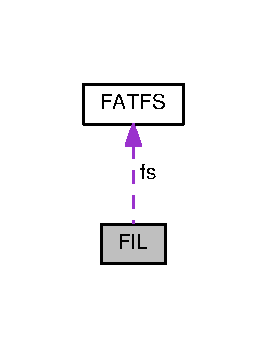
\includegraphics[width=128pt]{d1/dae/structFIL__coll__graph}
\end{center}
\end{figure}
\subsection*{Data Fields}
\begin{DoxyCompactItemize}
\item 
\hyperlink{structFATFS}{F\+A\+T\+FS} $\ast$ \hyperlink{structFIL_a42376a6797a06228911c8b836c1e9030}{fs}
\item 
\hyperlink{integer_8h_a197942eefa7db30960ae396d68339b97}{W\+O\+RD} \hyperlink{structFIL_af7cae0063b0045fb7078b560101ba8f2}{id}
\item 
\hyperlink{integer_8h_a4ae1dab0fb4b072a66584546209e7d58}{B\+Y\+TE} \hyperlink{structFIL_ac409508881f5a16f2998ae675072b376}{flag}
\item 
\hyperlink{integer_8h_a4ae1dab0fb4b072a66584546209e7d58}{B\+Y\+TE} \hyperlink{structFIL_aea440945db26de9c4a88065c0c887fda}{err}
\item 
\hyperlink{integer_8h_ad342ac907eb044443153a22f964bf0af}{D\+W\+O\+RD} \hyperlink{structFIL_a75d29cf9257c827d117887b9f924c4a9}{fptr}
\item 
\hyperlink{integer_8h_ad342ac907eb044443153a22f964bf0af}{D\+W\+O\+RD} \hyperlink{structFIL_aa00790d40d7b0081c345fd4f76e22b70}{fsize}
\item 
\hyperlink{integer_8h_ad342ac907eb044443153a22f964bf0af}{D\+W\+O\+RD} \hyperlink{structFIL_ad308b74c8d6975c6a9c30d90b4124c40}{sclust}
\item 
\hyperlink{integer_8h_ad342ac907eb044443153a22f964bf0af}{D\+W\+O\+RD} \hyperlink{structFIL_aa41312aba551b9a6d1c9d3c8c7d2734b}{clust}
\item 
\hyperlink{integer_8h_ad342ac907eb044443153a22f964bf0af}{D\+W\+O\+RD} \hyperlink{structFIL_ab3d4165d6fd32ac71a130d835fbf0b4d}{dsect}
\item 
\hyperlink{integer_8h_ad342ac907eb044443153a22f964bf0af}{D\+W\+O\+RD} \hyperlink{structFIL_ab203794f939ad4480e81dfa488770783}{dir\+\_\+sect}
\item 
\hyperlink{integer_8h_a4ae1dab0fb4b072a66584546209e7d58}{B\+Y\+TE} $\ast$ \hyperlink{structFIL_a5af9e9fb312b629220eaf684dd28c4a9}{dir\+\_\+ptr}
\item 
\hyperlink{integer_8h_a4ae1dab0fb4b072a66584546209e7d58}{B\+Y\+TE} \hyperlink{structFIL_a7a95fb86588663e48309b5cded7e207b}{buf} \mbox{[}\hyperlink{ffconf_8h_ac271b697378912f17132cb9c7d0de024}{\+\_\+\+M\+A\+X\+\_\+\+SS}\mbox{]}
\end{DoxyCompactItemize}


\subsection{Field Documentation}
\index{F\+IL@{F\+IL}!buf@{buf}}
\index{buf@{buf}!F\+IL@{F\+IL}}
\subsubsection[{\texorpdfstring{buf}{buf}}]{\setlength{\rightskip}{0pt plus 5cm}{\bf B\+Y\+TE} F\+I\+L\+::buf\mbox{[}{\bf \+\_\+\+M\+A\+X\+\_\+\+SS}\mbox{]}}\hypertarget{structFIL_a7a95fb86588663e48309b5cded7e207b}{}\label{structFIL_a7a95fb86588663e48309b5cded7e207b}
\index{F\+IL@{F\+IL}!clust@{clust}}
\index{clust@{clust}!F\+IL@{F\+IL}}
\subsubsection[{\texorpdfstring{clust}{clust}}]{\setlength{\rightskip}{0pt plus 5cm}{\bf D\+W\+O\+RD} F\+I\+L\+::clust}\hypertarget{structFIL_aa41312aba551b9a6d1c9d3c8c7d2734b}{}\label{structFIL_aa41312aba551b9a6d1c9d3c8c7d2734b}
\index{F\+IL@{F\+IL}!dir\+\_\+ptr@{dir\+\_\+ptr}}
\index{dir\+\_\+ptr@{dir\+\_\+ptr}!F\+IL@{F\+IL}}
\subsubsection[{\texorpdfstring{dir\+\_\+ptr}{dir_ptr}}]{\setlength{\rightskip}{0pt plus 5cm}{\bf B\+Y\+TE}$\ast$ F\+I\+L\+::dir\+\_\+ptr}\hypertarget{structFIL_a5af9e9fb312b629220eaf684dd28c4a9}{}\label{structFIL_a5af9e9fb312b629220eaf684dd28c4a9}
\index{F\+IL@{F\+IL}!dir\+\_\+sect@{dir\+\_\+sect}}
\index{dir\+\_\+sect@{dir\+\_\+sect}!F\+IL@{F\+IL}}
\subsubsection[{\texorpdfstring{dir\+\_\+sect}{dir_sect}}]{\setlength{\rightskip}{0pt plus 5cm}{\bf D\+W\+O\+RD} F\+I\+L\+::dir\+\_\+sect}\hypertarget{structFIL_ab203794f939ad4480e81dfa488770783}{}\label{structFIL_ab203794f939ad4480e81dfa488770783}
\index{F\+IL@{F\+IL}!dsect@{dsect}}
\index{dsect@{dsect}!F\+IL@{F\+IL}}
\subsubsection[{\texorpdfstring{dsect}{dsect}}]{\setlength{\rightskip}{0pt plus 5cm}{\bf D\+W\+O\+RD} F\+I\+L\+::dsect}\hypertarget{structFIL_ab3d4165d6fd32ac71a130d835fbf0b4d}{}\label{structFIL_ab3d4165d6fd32ac71a130d835fbf0b4d}
\index{F\+IL@{F\+IL}!err@{err}}
\index{err@{err}!F\+IL@{F\+IL}}
\subsubsection[{\texorpdfstring{err}{err}}]{\setlength{\rightskip}{0pt plus 5cm}{\bf B\+Y\+TE} F\+I\+L\+::err}\hypertarget{structFIL_aea440945db26de9c4a88065c0c887fda}{}\label{structFIL_aea440945db26de9c4a88065c0c887fda}
\index{F\+IL@{F\+IL}!flag@{flag}}
\index{flag@{flag}!F\+IL@{F\+IL}}
\subsubsection[{\texorpdfstring{flag}{flag}}]{\setlength{\rightskip}{0pt plus 5cm}{\bf B\+Y\+TE} F\+I\+L\+::flag}\hypertarget{structFIL_ac409508881f5a16f2998ae675072b376}{}\label{structFIL_ac409508881f5a16f2998ae675072b376}
\index{F\+IL@{F\+IL}!fptr@{fptr}}
\index{fptr@{fptr}!F\+IL@{F\+IL}}
\subsubsection[{\texorpdfstring{fptr}{fptr}}]{\setlength{\rightskip}{0pt plus 5cm}{\bf D\+W\+O\+RD} F\+I\+L\+::fptr}\hypertarget{structFIL_a75d29cf9257c827d117887b9f924c4a9}{}\label{structFIL_a75d29cf9257c827d117887b9f924c4a9}
\index{F\+IL@{F\+IL}!fs@{fs}}
\index{fs@{fs}!F\+IL@{F\+IL}}
\subsubsection[{\texorpdfstring{fs}{fs}}]{\setlength{\rightskip}{0pt plus 5cm}{\bf F\+A\+T\+FS}$\ast$ F\+I\+L\+::fs}\hypertarget{structFIL_a42376a6797a06228911c8b836c1e9030}{}\label{structFIL_a42376a6797a06228911c8b836c1e9030}
\index{F\+IL@{F\+IL}!fsize@{fsize}}
\index{fsize@{fsize}!F\+IL@{F\+IL}}
\subsubsection[{\texorpdfstring{fsize}{fsize}}]{\setlength{\rightskip}{0pt plus 5cm}{\bf D\+W\+O\+RD} F\+I\+L\+::fsize}\hypertarget{structFIL_aa00790d40d7b0081c345fd4f76e22b70}{}\label{structFIL_aa00790d40d7b0081c345fd4f76e22b70}
\index{F\+IL@{F\+IL}!id@{id}}
\index{id@{id}!F\+IL@{F\+IL}}
\subsubsection[{\texorpdfstring{id}{id}}]{\setlength{\rightskip}{0pt plus 5cm}{\bf W\+O\+RD} F\+I\+L\+::id}\hypertarget{structFIL_af7cae0063b0045fb7078b560101ba8f2}{}\label{structFIL_af7cae0063b0045fb7078b560101ba8f2}
\index{F\+IL@{F\+IL}!sclust@{sclust}}
\index{sclust@{sclust}!F\+IL@{F\+IL}}
\subsubsection[{\texorpdfstring{sclust}{sclust}}]{\setlength{\rightskip}{0pt plus 5cm}{\bf D\+W\+O\+RD} F\+I\+L\+::sclust}\hypertarget{structFIL_ad308b74c8d6975c6a9c30d90b4124c40}{}\label{structFIL_ad308b74c8d6975c6a9c30d90b4124c40}


The documentation for this struct was generated from the following file\+:\begin{DoxyCompactItemize}
\item 
/var/www/html/\+S\+J\+S\+U-\/\+D\+E\+V-\/\+Linux/firmware/default/lib/\+L4\+\_\+\+I\+O/fat/\hyperlink{ff_8h}{ff.\+h}\end{DoxyCompactItemize}

\hypertarget{classFileSystemObject}{}\section{File\+System\+Object Class Reference}
\label{classFileSystemObject}\index{File\+System\+Object@{File\+System\+Object}}


{\ttfamily \#include $<$File\+System\+Object.\+hpp$>$}

\subsection*{Public Member Functions}
\begin{DoxyCompactItemize}
\item 
const char $\ast$ \hyperlink{classFileSystemObject_a02e3883dba58c16f28c351f56a7bf8e3}{get\+Drive\+Path} () const 
\item 
char \hyperlink{classFileSystemObject_afa103b2854558978188f848153daceae}{mount} () const 
\item 
\hyperlink{ff_8h_a49d0171ecbd362cda5680a0d360db44c}{F\+R\+E\+S\+U\+LT} \hyperlink{classFileSystemObject_a80f0f7f312563128d41bf3481723b028}{get\+Drive\+Info} (unsigned int $\ast$p\+Total\+Drive\+Space\+KB, unsigned int $\ast$p\+Available\+Space\+KB) const 
\item 
\hyperlink{ff_8h_a49d0171ecbd362cda5680a0d360db44c}{F\+R\+E\+S\+U\+LT} \hyperlink{classFileSystemObject_a8c5167c7d5d659eeadb799b2c27b041d}{format} () const 
\end{DoxyCompactItemize}
\subsection*{Friends}
\begin{DoxyCompactItemize}
\item 
class \hyperlink{classFileSystemObject_ab647623b3295040f83d3afb2a502a223}{Storage}
\begin{DoxyCompactList}\small\item\em Allow only the \hyperlink{classStorage}{Storage} class to create us. \end{DoxyCompactList}\end{DoxyCompactItemize}


\subsection{Detailed Description}
File System Class 

\subsection{Member Function Documentation}
\index{File\+System\+Object@{File\+System\+Object}!format@{format}}
\index{format@{format}!File\+System\+Object@{File\+System\+Object}}
\subsubsection[{\texorpdfstring{format() const }{format() const }}]{\setlength{\rightskip}{0pt plus 5cm}{\bf F\+R\+E\+S\+U\+LT} File\+System\+Object\+::format (
\begin{DoxyParamCaption}
{}
\end{DoxyParamCaption}
) const\hspace{0.3cm}{\ttfamily [inline]}}\hypertarget{classFileSystemObject_a8c5167c7d5d659eeadb799b2c27b041d}{}\label{classFileSystemObject_a8c5167c7d5d659eeadb799b2c27b041d}
Formats the drive with default allocation size \index{File\+System\+Object@{File\+System\+Object}!get\+Drive\+Info@{get\+Drive\+Info}}
\index{get\+Drive\+Info@{get\+Drive\+Info}!File\+System\+Object@{File\+System\+Object}}
\subsubsection[{\texorpdfstring{get\+Drive\+Info(unsigned int $\ast$p\+Total\+Drive\+Space\+K\+B, unsigned int $\ast$p\+Available\+Space\+K\+B) const }{getDriveInfo(unsigned int *pTotalDriveSpaceKB, unsigned int *pAvailableSpaceKB) const }}]{\setlength{\rightskip}{0pt plus 5cm}{\bf F\+R\+E\+S\+U\+LT} File\+System\+Object\+::get\+Drive\+Info (
\begin{DoxyParamCaption}
\item[{unsigned int $\ast$}]{p\+Total\+Drive\+Space\+KB, }
\item[{unsigned int $\ast$}]{p\+Available\+Space\+KB}
\end{DoxyParamCaption}
) const\hspace{0.3cm}{\ttfamily [inline]}}\hypertarget{classFileSystemObject_a80f0f7f312563128d41bf3481723b028}{}\label{classFileSystemObject_a80f0f7f312563128d41bf3481723b028}
Get the drive\textquotesingle{}s total capacity and available space 
\begin{DoxyParams}{Parameters}
{\em p\+Total\+Drive\+Space\+KB} & Pointer where total drive space in kilobytes will be written \\
\hline
{\em p\+Available\+Space\+KB} & Pointer where drive\textquotesingle{}s available space in kilobytes will be written \\
\hline
\end{DoxyParams}
\begin{DoxyNote}{Note}
The parameters will be written to zero if an error occurs during this operation. 
\end{DoxyNote}
\index{File\+System\+Object@{File\+System\+Object}!get\+Drive\+Path@{get\+Drive\+Path}}
\index{get\+Drive\+Path@{get\+Drive\+Path}!File\+System\+Object@{File\+System\+Object}}
\subsubsection[{\texorpdfstring{get\+Drive\+Path() const }{getDrivePath() const }}]{\setlength{\rightskip}{0pt plus 5cm}const char$\ast$ File\+System\+Object\+::get\+Drive\+Path (
\begin{DoxyParamCaption}
{}
\end{DoxyParamCaption}
) const\hspace{0.3cm}{\ttfamily [inline]}}\hypertarget{classFileSystemObject_a02e3883dba58c16f28c351f56a7bf8e3}{}\label{classFileSystemObject_a02e3883dba58c16f28c351f56a7bf8e3}
Returns the root path of this drive, such as \char`\"{}0\+:\char`\"{} or \char`\"{}1\+:\char`\"{} \index{File\+System\+Object@{File\+System\+Object}!mount@{mount}}
\index{mount@{mount}!File\+System\+Object@{File\+System\+Object}}
\subsubsection[{\texorpdfstring{mount() const }{mount() const }}]{\setlength{\rightskip}{0pt plus 5cm}char File\+System\+Object\+::mount (
\begin{DoxyParamCaption}
{}
\end{DoxyParamCaption}
) const\hspace{0.3cm}{\ttfamily [inline]}}\hypertarget{classFileSystemObject_afa103b2854558978188f848153daceae}{}\label{classFileSystemObject_afa103b2854558978188f848153daceae}
Initializes the disk and mounts the storage \begin{DoxyReturn}{Returns}
T\+R\+UE if the disk is ready to be used. 
\end{DoxyReturn}
\begin{DoxyNote}{Note}
If disk is not formatted correctly, F\+I\+LE IO may fail 
\end{DoxyNote}


\subsection{Friends And Related Function Documentation}
\index{File\+System\+Object@{File\+System\+Object}!Storage@{Storage}}
\index{Storage@{Storage}!File\+System\+Object@{File\+System\+Object}}
\subsubsection[{\texorpdfstring{Storage}{Storage}}]{\setlength{\rightskip}{0pt plus 5cm}friend class {\bf Storage}\hspace{0.3cm}{\ttfamily [friend]}}\hypertarget{classFileSystemObject_ab647623b3295040f83d3afb2a502a223}{}\label{classFileSystemObject_ab647623b3295040f83d3afb2a502a223}


Allow only the \hyperlink{classStorage}{Storage} class to create us. 



The documentation for this class was generated from the following file\+:\begin{DoxyCompactItemize}
\item 
/var/www/html/\+S\+J\+S\+U-\/\+D\+E\+V-\/\+Linux/firmware/default/lib/\+L4\+\_\+\+I\+O/src/\hyperlink{FileSystemObject_8hpp}{File\+System\+Object.\+hpp}\end{DoxyCompactItemize}

\hypertarget{structFILINFO}{}\section{F\+I\+L\+I\+N\+FO Struct Reference}
\label{structFILINFO}\index{F\+I\+L\+I\+N\+FO@{F\+I\+L\+I\+N\+FO}}


{\ttfamily \#include $<$ff.\+h$>$}

\subsection*{Data Fields}
\begin{DoxyCompactItemize}
\item 
\hyperlink{integer_8h_ad342ac907eb044443153a22f964bf0af}{D\+W\+O\+RD} \hyperlink{structFILINFO_aee7441af7dc0c443d1e1e6011cc7dcac}{fsize}
\item 
\hyperlink{integer_8h_a197942eefa7db30960ae396d68339b97}{W\+O\+RD} \hyperlink{structFILINFO_a7c01c48a15b1b49da459924437b0bd52}{fdate}
\item 
\hyperlink{integer_8h_a197942eefa7db30960ae396d68339b97}{W\+O\+RD} \hyperlink{structFILINFO_ae0f751b79621bf7b29669f177bbe6b9a}{ftime}
\item 
\hyperlink{integer_8h_a4ae1dab0fb4b072a66584546209e7d58}{B\+Y\+TE} \hyperlink{structFILINFO_a838d542585831b085537b363f18205c0}{fattrib}
\item 
\hyperlink{ff_8h_a03bdb8ce5895c7e261aadc2529637546}{T\+C\+H\+AR} \hyperlink{structFILINFO_abd852510f2f79b4ec773156d8942dc7c}{fname} \mbox{[}13\mbox{]}
\item 
\hyperlink{ff_8h_a03bdb8ce5895c7e261aadc2529637546}{T\+C\+H\+AR} $\ast$ \hyperlink{structFILINFO_ac4506c29e0219130dff46b01a1b5c023}{lfname}
\item 
\hyperlink{integer_8h_a36cb3b01d81ffd844bbbfb54003e06ec}{U\+I\+NT} \hyperlink{structFILINFO_a2527c511ff4d12d285dbf3c4b3c9fb7b}{lfsize}
\end{DoxyCompactItemize}


\subsection{Field Documentation}
\index{F\+I\+L\+I\+N\+FO@{F\+I\+L\+I\+N\+FO}!fattrib@{fattrib}}
\index{fattrib@{fattrib}!F\+I\+L\+I\+N\+FO@{F\+I\+L\+I\+N\+FO}}
\subsubsection[{\texorpdfstring{fattrib}{fattrib}}]{\setlength{\rightskip}{0pt plus 5cm}{\bf B\+Y\+TE} F\+I\+L\+I\+N\+F\+O\+::fattrib}\hypertarget{structFILINFO_a838d542585831b085537b363f18205c0}{}\label{structFILINFO_a838d542585831b085537b363f18205c0}
\index{F\+I\+L\+I\+N\+FO@{F\+I\+L\+I\+N\+FO}!fdate@{fdate}}
\index{fdate@{fdate}!F\+I\+L\+I\+N\+FO@{F\+I\+L\+I\+N\+FO}}
\subsubsection[{\texorpdfstring{fdate}{fdate}}]{\setlength{\rightskip}{0pt plus 5cm}{\bf W\+O\+RD} F\+I\+L\+I\+N\+F\+O\+::fdate}\hypertarget{structFILINFO_a7c01c48a15b1b49da459924437b0bd52}{}\label{structFILINFO_a7c01c48a15b1b49da459924437b0bd52}
\index{F\+I\+L\+I\+N\+FO@{F\+I\+L\+I\+N\+FO}!fname@{fname}}
\index{fname@{fname}!F\+I\+L\+I\+N\+FO@{F\+I\+L\+I\+N\+FO}}
\subsubsection[{\texorpdfstring{fname}{fname}}]{\setlength{\rightskip}{0pt plus 5cm}{\bf T\+C\+H\+AR} F\+I\+L\+I\+N\+F\+O\+::fname\mbox{[}13\mbox{]}}\hypertarget{structFILINFO_abd852510f2f79b4ec773156d8942dc7c}{}\label{structFILINFO_abd852510f2f79b4ec773156d8942dc7c}
\index{F\+I\+L\+I\+N\+FO@{F\+I\+L\+I\+N\+FO}!fsize@{fsize}}
\index{fsize@{fsize}!F\+I\+L\+I\+N\+FO@{F\+I\+L\+I\+N\+FO}}
\subsubsection[{\texorpdfstring{fsize}{fsize}}]{\setlength{\rightskip}{0pt plus 5cm}{\bf D\+W\+O\+RD} F\+I\+L\+I\+N\+F\+O\+::fsize}\hypertarget{structFILINFO_aee7441af7dc0c443d1e1e6011cc7dcac}{}\label{structFILINFO_aee7441af7dc0c443d1e1e6011cc7dcac}
\index{F\+I\+L\+I\+N\+FO@{F\+I\+L\+I\+N\+FO}!ftime@{ftime}}
\index{ftime@{ftime}!F\+I\+L\+I\+N\+FO@{F\+I\+L\+I\+N\+FO}}
\subsubsection[{\texorpdfstring{ftime}{ftime}}]{\setlength{\rightskip}{0pt plus 5cm}{\bf W\+O\+RD} F\+I\+L\+I\+N\+F\+O\+::ftime}\hypertarget{structFILINFO_ae0f751b79621bf7b29669f177bbe6b9a}{}\label{structFILINFO_ae0f751b79621bf7b29669f177bbe6b9a}
\index{F\+I\+L\+I\+N\+FO@{F\+I\+L\+I\+N\+FO}!lfname@{lfname}}
\index{lfname@{lfname}!F\+I\+L\+I\+N\+FO@{F\+I\+L\+I\+N\+FO}}
\subsubsection[{\texorpdfstring{lfname}{lfname}}]{\setlength{\rightskip}{0pt plus 5cm}{\bf T\+C\+H\+AR}$\ast$ F\+I\+L\+I\+N\+F\+O\+::lfname}\hypertarget{structFILINFO_ac4506c29e0219130dff46b01a1b5c023}{}\label{structFILINFO_ac4506c29e0219130dff46b01a1b5c023}
\index{F\+I\+L\+I\+N\+FO@{F\+I\+L\+I\+N\+FO}!lfsize@{lfsize}}
\index{lfsize@{lfsize}!F\+I\+L\+I\+N\+FO@{F\+I\+L\+I\+N\+FO}}
\subsubsection[{\texorpdfstring{lfsize}{lfsize}}]{\setlength{\rightskip}{0pt plus 5cm}{\bf U\+I\+NT} F\+I\+L\+I\+N\+F\+O\+::lfsize}\hypertarget{structFILINFO_a2527c511ff4d12d285dbf3c4b3c9fb7b}{}\label{structFILINFO_a2527c511ff4d12d285dbf3c4b3c9fb7b}


The documentation for this struct was generated from the following file\+:\begin{DoxyCompactItemize}
\item 
/var/www/html/\+S\+J\+S\+U-\/\+D\+E\+V-\/\+Linux/firmware/default/lib/\+L4\+\_\+\+I\+O/fat/\hyperlink{ff_8h}{ff.\+h}\end{DoxyCompactItemize}

\hypertarget{classFreeRTOSTimer}{}\section{Free\+R\+T\+O\+S\+Timer Class Reference}
\label{classFreeRTOSTimer}\index{Free\+R\+T\+O\+S\+Timer@{Free\+R\+T\+O\+S\+Timer}}


{\ttfamily \#include $<$freertos\+\_\+timer.\+hpp$>$}

\subsection*{Public Member Functions}
\begin{DoxyCompactItemize}
\item 
\hyperlink{classFreeRTOSTimer_a3f7e3569e552bac47dcb770d4a4a4ad0}{Free\+R\+T\+O\+S\+Timer} (\hyperlink{timers_8h_a5cf6d1f61ccd4871022ed8ad454c6027}{Timer\+Callback\+Function\+\_\+t} p\+Function, \hyperlink{freertos__timer_8hpp_a62332987634a9d461e934b53ee0e0772}{time\+Ms\+\_\+t} t, \hyperlink{freertos__timer_8hpp_ad3a7c38fbde9814e427a75171fe8939d}{Timer\+Type} type=\hyperlink{freertos__timer_8hpp_ad3a7c38fbde9814e427a75171fe8939dab782ae2f652b671e2a189f237bd4311b}{Timer\+Periodic})
\item 
\hyperlink{classFreeRTOSTimer_aa8a047ff6418d0d0d62716f47fd863c5}{$\sim$\+Free\+R\+T\+O\+S\+Timer} ()
\begin{DoxyCompactList}\small\item\em Destructor to delete the timer. \end{DoxyCompactList}\item 
void \hyperlink{classFreeRTOSTimer_a719e6350ecd4d41c1d2dbf8fe8ea140b}{start} ()
\begin{DoxyCompactList}\small\item\em Starts the timer, and calls \hyperlink{classFreeRTOSTimer_a86766a976a47b003a44d52a84bf734cc}{reset()} if timer is already started. \end{DoxyCompactList}\item 
void \hyperlink{classFreeRTOSTimer_a43992de1a6cc76749fd129b8b386b8e2}{stop} ()
\begin{DoxyCompactList}\small\item\em Stops the timer. \end{DoxyCompactList}\item 
void \hyperlink{classFreeRTOSTimer_a86766a976a47b003a44d52a84bf734cc}{reset} ()
\begin{DoxyCompactList}\small\item\em Resets(restarts) the timer. \end{DoxyCompactList}\item 
void \hyperlink{classFreeRTOSTimer_a90600dc55886fa4a9aebdb14f7d5155c}{change\+Period} (\hyperlink{freertos__timer_8hpp_a62332987634a9d461e934b53ee0e0772}{time\+Ms\+\_\+t} t)
\begin{DoxyCompactList}\small\item\em Changes the timer\textquotesingle{}s time. \end{DoxyCompactList}\item 
bool \hyperlink{classFreeRTOSTimer_afe875ff318f8158660f94f19982f55ae}{is\+Running} ()
\item 
\hyperlink{timers_8h_aae4bf1dce696ab615d5fd073606fd3cb}{Timer\+Handle\+\_\+t} \hyperlink{classFreeRTOSTimer_a52230dd9874e8066e441e2ab64522b2a}{get\+Timer\+Handle} ()
\end{DoxyCompactItemize}
\begin{Indent}{\bf Timer functions to be used from within an I\+SR.}\par
{\em These will automatically call Free\+R\+T\+OS Y\+I\+E\+LD function if required. }\begin{DoxyCompactItemize}
\item 
void \hyperlink{classFreeRTOSTimer_a92b1845cf4973a39c0ac44ee615c8e9f}{start\+From\+I\+SR} ()
\begin{DoxyCompactList}\small\item\em Restarts the timer from an I\+SR. \end{DoxyCompactList}\item 
void \hyperlink{classFreeRTOSTimer_aa3652e193022be79d5c7a31c1bcfaede}{stop\+From\+I\+SR} ()
\begin{DoxyCompactList}\small\item\em Stops the timer from an I\+SR. \end{DoxyCompactList}\item 
void \hyperlink{classFreeRTOSTimer_ab5861a16ffb9d3aa55eefd8432087c8d}{reset\+From\+I\+SR} ()
\begin{DoxyCompactList}\small\item\em Resets the timer from an I\+SR. \end{DoxyCompactList}\item 
void \hyperlink{classFreeRTOSTimer_abbc13f7e4ab40097098152c3bdbd8b8a}{change\+Period\+From\+I\+SR} (\hyperlink{freertos__timer_8hpp_a62332987634a9d461e934b53ee0e0772}{time\+Ms\+\_\+t} t)
\begin{DoxyCompactList}\small\item\em Changes the timer\textquotesingle{}s time from an I\+SR. \end{DoxyCompactList}\end{DoxyCompactItemize}
\end{Indent}


\subsection{Detailed Description}
Timer class to attach C-\/\+Functions to timers, but use C++ class structure to easily control the timers.

This is C++ wrapper around Free\+R\+T\+OS timers. config\+U\+S\+E\+\_\+\+T\+I\+M\+E\+RS @ Free\+Rtos\+Config.\+h must be set to 1 to use this class. 

\subsection{Constructor \& Destructor Documentation}
\index{Free\+R\+T\+O\+S\+Timer@{Free\+R\+T\+O\+S\+Timer}!Free\+R\+T\+O\+S\+Timer@{Free\+R\+T\+O\+S\+Timer}}
\index{Free\+R\+T\+O\+S\+Timer@{Free\+R\+T\+O\+S\+Timer}!Free\+R\+T\+O\+S\+Timer@{Free\+R\+T\+O\+S\+Timer}}
\subsubsection[{\texorpdfstring{Free\+R\+T\+O\+S\+Timer(\+Timer\+Callback\+Function\+\_\+t p\+Function, time\+Ms\+\_\+t t, Timer\+Type type=\+Timer\+Periodic)}{FreeRTOSTimer(TimerCallbackFunction_t pFunction, timeMs_t t, TimerType type=TimerPeriodic)}}]{\setlength{\rightskip}{0pt plus 5cm}Free\+R\+T\+O\+S\+Timer\+::\+Free\+R\+T\+O\+S\+Timer (
\begin{DoxyParamCaption}
\item[{{\bf Timer\+Callback\+Function\+\_\+t}}]{p\+Function, }
\item[{{\bf time\+Ms\+\_\+t}}]{t, }
\item[{{\bf Timer\+Type}}]{type = {\ttfamily {\bf Timer\+Periodic}}}
\end{DoxyParamCaption}
)}\hypertarget{classFreeRTOSTimer_a3f7e3569e552bac47dcb770d4a4a4ad0}{}\label{classFreeRTOSTimer_a3f7e3569e552bac47dcb770d4a4a4ad0}
Constructor to create the timer. 
\begin{DoxyParams}{Parameters}
{\em p\+Function} & The pointer to C-\/\+Function \\
\hline
{\em t} & The timer expiration in milliseconds \\
\hline
{\em type} & Timer type, either one shot or periodic, defaults to periodic \\
\hline
\end{DoxyParams}
\index{Free\+R\+T\+O\+S\+Timer@{Free\+R\+T\+O\+S\+Timer}!````~Free\+R\+T\+O\+S\+Timer@{$\sim$\+Free\+R\+T\+O\+S\+Timer}}
\index{````~Free\+R\+T\+O\+S\+Timer@{$\sim$\+Free\+R\+T\+O\+S\+Timer}!Free\+R\+T\+O\+S\+Timer@{Free\+R\+T\+O\+S\+Timer}}
\subsubsection[{\texorpdfstring{$\sim$\+Free\+R\+T\+O\+S\+Timer()}{~FreeRTOSTimer()}}]{\setlength{\rightskip}{0pt plus 5cm}Free\+R\+T\+O\+S\+Timer\+::$\sim$\+Free\+R\+T\+O\+S\+Timer (
\begin{DoxyParamCaption}
{}
\end{DoxyParamCaption}
)}\hypertarget{classFreeRTOSTimer_aa8a047ff6418d0d0d62716f47fd863c5}{}\label{classFreeRTOSTimer_aa8a047ff6418d0d0d62716f47fd863c5}


Destructor to delete the timer. 



\subsection{Member Function Documentation}
\index{Free\+R\+T\+O\+S\+Timer@{Free\+R\+T\+O\+S\+Timer}!change\+Period@{change\+Period}}
\index{change\+Period@{change\+Period}!Free\+R\+T\+O\+S\+Timer@{Free\+R\+T\+O\+S\+Timer}}
\subsubsection[{\texorpdfstring{change\+Period(time\+Ms\+\_\+t t)}{changePeriod(timeMs_t t)}}]{\setlength{\rightskip}{0pt plus 5cm}void Free\+R\+T\+O\+S\+Timer\+::change\+Period (
\begin{DoxyParamCaption}
\item[{{\bf time\+Ms\+\_\+t}}]{t}
\end{DoxyParamCaption}
)}\hypertarget{classFreeRTOSTimer_a90600dc55886fa4a9aebdb14f7d5155c}{}\label{classFreeRTOSTimer_a90600dc55886fa4a9aebdb14f7d5155c}


Changes the timer\textquotesingle{}s time. 

\index{Free\+R\+T\+O\+S\+Timer@{Free\+R\+T\+O\+S\+Timer}!change\+Period\+From\+I\+SR@{change\+Period\+From\+I\+SR}}
\index{change\+Period\+From\+I\+SR@{change\+Period\+From\+I\+SR}!Free\+R\+T\+O\+S\+Timer@{Free\+R\+T\+O\+S\+Timer}}
\subsubsection[{\texorpdfstring{change\+Period\+From\+I\+S\+R(time\+Ms\+\_\+t t)}{changePeriodFromISR(timeMs_t t)}}]{\setlength{\rightskip}{0pt plus 5cm}void Free\+R\+T\+O\+S\+Timer\+::change\+Period\+From\+I\+SR (
\begin{DoxyParamCaption}
\item[{{\bf time\+Ms\+\_\+t}}]{t}
\end{DoxyParamCaption}
)}\hypertarget{classFreeRTOSTimer_abbc13f7e4ab40097098152c3bdbd8b8a}{}\label{classFreeRTOSTimer_abbc13f7e4ab40097098152c3bdbd8b8a}


Changes the timer\textquotesingle{}s time from an I\+SR. 

\index{Free\+R\+T\+O\+S\+Timer@{Free\+R\+T\+O\+S\+Timer}!get\+Timer\+Handle@{get\+Timer\+Handle}}
\index{get\+Timer\+Handle@{get\+Timer\+Handle}!Free\+R\+T\+O\+S\+Timer@{Free\+R\+T\+O\+S\+Timer}}
\subsubsection[{\texorpdfstring{get\+Timer\+Handle()}{getTimerHandle()}}]{\setlength{\rightskip}{0pt plus 5cm}{\bf Timer\+Handle\+\_\+t} Free\+R\+T\+O\+S\+Timer\+::get\+Timer\+Handle (
\begin{DoxyParamCaption}
{}
\end{DoxyParamCaption}
)\hspace{0.3cm}{\ttfamily [inline]}}\hypertarget{classFreeRTOSTimer_a52230dd9874e8066e441e2ab64522b2a}{}\label{classFreeRTOSTimer_a52230dd9874e8066e441e2ab64522b2a}
\begin{DoxyReturn}{Returns}
The Free\+R\+T\+OS Timer Handle for this timer. 
\end{DoxyReturn}
\index{Free\+R\+T\+O\+S\+Timer@{Free\+R\+T\+O\+S\+Timer}!is\+Running@{is\+Running}}
\index{is\+Running@{is\+Running}!Free\+R\+T\+O\+S\+Timer@{Free\+R\+T\+O\+S\+Timer}}
\subsubsection[{\texorpdfstring{is\+Running()}{isRunning()}}]{\setlength{\rightskip}{0pt plus 5cm}bool Free\+R\+T\+O\+S\+Timer\+::is\+Running (
\begin{DoxyParamCaption}
{}
\end{DoxyParamCaption}
)}\hypertarget{classFreeRTOSTimer_afe875ff318f8158660f94f19982f55ae}{}\label{classFreeRTOSTimer_afe875ff318f8158660f94f19982f55ae}
\begin{DoxyReturn}{Returns}
T\+R\+UE if the timer is active 
\end{DoxyReturn}
\index{Free\+R\+T\+O\+S\+Timer@{Free\+R\+T\+O\+S\+Timer}!reset@{reset}}
\index{reset@{reset}!Free\+R\+T\+O\+S\+Timer@{Free\+R\+T\+O\+S\+Timer}}
\subsubsection[{\texorpdfstring{reset()}{reset()}}]{\setlength{\rightskip}{0pt plus 5cm}void Free\+R\+T\+O\+S\+Timer\+::reset (
\begin{DoxyParamCaption}
{}
\end{DoxyParamCaption}
)}\hypertarget{classFreeRTOSTimer_a86766a976a47b003a44d52a84bf734cc}{}\label{classFreeRTOSTimer_a86766a976a47b003a44d52a84bf734cc}


Resets(restarts) the timer. 

\index{Free\+R\+T\+O\+S\+Timer@{Free\+R\+T\+O\+S\+Timer}!reset\+From\+I\+SR@{reset\+From\+I\+SR}}
\index{reset\+From\+I\+SR@{reset\+From\+I\+SR}!Free\+R\+T\+O\+S\+Timer@{Free\+R\+T\+O\+S\+Timer}}
\subsubsection[{\texorpdfstring{reset\+From\+I\+S\+R()}{resetFromISR()}}]{\setlength{\rightskip}{0pt plus 5cm}void Free\+R\+T\+O\+S\+Timer\+::reset\+From\+I\+SR (
\begin{DoxyParamCaption}
{}
\end{DoxyParamCaption}
)}\hypertarget{classFreeRTOSTimer_ab5861a16ffb9d3aa55eefd8432087c8d}{}\label{classFreeRTOSTimer_ab5861a16ffb9d3aa55eefd8432087c8d}


Resets the timer from an I\+SR. 

\index{Free\+R\+T\+O\+S\+Timer@{Free\+R\+T\+O\+S\+Timer}!start@{start}}
\index{start@{start}!Free\+R\+T\+O\+S\+Timer@{Free\+R\+T\+O\+S\+Timer}}
\subsubsection[{\texorpdfstring{start()}{start()}}]{\setlength{\rightskip}{0pt plus 5cm}void Free\+R\+T\+O\+S\+Timer\+::start (
\begin{DoxyParamCaption}
{}
\end{DoxyParamCaption}
)}\hypertarget{classFreeRTOSTimer_a719e6350ecd4d41c1d2dbf8fe8ea140b}{}\label{classFreeRTOSTimer_a719e6350ecd4d41c1d2dbf8fe8ea140b}


Starts the timer, and calls \hyperlink{classFreeRTOSTimer_a86766a976a47b003a44d52a84bf734cc}{reset()} if timer is already started. 

\index{Free\+R\+T\+O\+S\+Timer@{Free\+R\+T\+O\+S\+Timer}!start\+From\+I\+SR@{start\+From\+I\+SR}}
\index{start\+From\+I\+SR@{start\+From\+I\+SR}!Free\+R\+T\+O\+S\+Timer@{Free\+R\+T\+O\+S\+Timer}}
\subsubsection[{\texorpdfstring{start\+From\+I\+S\+R()}{startFromISR()}}]{\setlength{\rightskip}{0pt plus 5cm}void Free\+R\+T\+O\+S\+Timer\+::start\+From\+I\+SR (
\begin{DoxyParamCaption}
{}
\end{DoxyParamCaption}
)}\hypertarget{classFreeRTOSTimer_a92b1845cf4973a39c0ac44ee615c8e9f}{}\label{classFreeRTOSTimer_a92b1845cf4973a39c0ac44ee615c8e9f}


Restarts the timer from an I\+SR. 

\index{Free\+R\+T\+O\+S\+Timer@{Free\+R\+T\+O\+S\+Timer}!stop@{stop}}
\index{stop@{stop}!Free\+R\+T\+O\+S\+Timer@{Free\+R\+T\+O\+S\+Timer}}
\subsubsection[{\texorpdfstring{stop()}{stop()}}]{\setlength{\rightskip}{0pt plus 5cm}void Free\+R\+T\+O\+S\+Timer\+::stop (
\begin{DoxyParamCaption}
{}
\end{DoxyParamCaption}
)}\hypertarget{classFreeRTOSTimer_a43992de1a6cc76749fd129b8b386b8e2}{}\label{classFreeRTOSTimer_a43992de1a6cc76749fd129b8b386b8e2}


Stops the timer. 

\index{Free\+R\+T\+O\+S\+Timer@{Free\+R\+T\+O\+S\+Timer}!stop\+From\+I\+SR@{stop\+From\+I\+SR}}
\index{stop\+From\+I\+SR@{stop\+From\+I\+SR}!Free\+R\+T\+O\+S\+Timer@{Free\+R\+T\+O\+S\+Timer}}
\subsubsection[{\texorpdfstring{stop\+From\+I\+S\+R()}{stopFromISR()}}]{\setlength{\rightskip}{0pt plus 5cm}void Free\+R\+T\+O\+S\+Timer\+::stop\+From\+I\+SR (
\begin{DoxyParamCaption}
{}
\end{DoxyParamCaption}
)}\hypertarget{classFreeRTOSTimer_aa3652e193022be79d5c7a31c1bcfaede}{}\label{classFreeRTOSTimer_aa3652e193022be79d5c7a31c1bcfaede}


Stops the timer from an I\+SR. 



The documentation for this class was generated from the following file\+:\begin{DoxyCompactItemize}
\item 
/var/www/html/\+S\+J\+S\+U-\/\+D\+E\+V-\/\+Linux/firmware/default/lib/\+L3\+\_\+\+Utils/\hyperlink{freertos__timer_8hpp}{freertos\+\_\+timer.\+hpp}\end{DoxyCompactItemize}

\hypertarget{classGPIO}{}\section{G\+P\+IO Class Reference}
\label{classGPIO}\index{G\+P\+IO@{G\+P\+IO}}


{\ttfamily \#include $<$gpio.\+hpp$>$}

\subsection*{Public Member Functions}
\begin{DoxyCompactItemize}
\item 
\hyperlink{classGPIO_acec0cdfbe71a5e4b4ed26c168c44dbc4}{G\+P\+IO} (\hyperlink{gpio_8hpp_a9e9814207938bb104144d2df58c554d8}{L\+P\+C1758\+\_\+\+G\+P\+I\+O\+\_\+\+Type} gpio\+Id)
\begin{DoxyCompactList}\small\item\em Constructor to choose the pin. \end{DoxyCompactList}\item 
\hyperlink{classGPIO_ae8205f95f108a15a612485b6358031a1}{$\sim$\+G\+P\+IO} ()
\begin{DoxyCompactList}\small\item\em Destructor that will destroy the pin configuration. \end{DoxyCompactList}\item 
void \hyperlink{classGPIO_a9ba7c2f50a449a7ca7f7e5f2680c4284}{enable\+Pull\+Up} ()
\begin{DoxyCompactList}\small\item\em Enables pull-\/up resistor. \end{DoxyCompactList}\item 
void \hyperlink{classGPIO_a9b2221a607da8a22adc5a0523148d5a7}{enable\+Pull\+Down} ()
\begin{DoxyCompactList}\small\item\em Enables pull-\/down resistor. \end{DoxyCompactList}\item 
void \hyperlink{classGPIO_aa2e401b63236bd2630b9a34372d590d3}{disable\+Pull\+Up\+Pull\+Down} ()
\begin{DoxyCompactList}\small\item\em Disables pull-\/up/down resistor. \end{DoxyCompactList}\item 
void \hyperlink{classGPIO_a04726c16f352186e0d7761006867ffb9}{enable\+Open\+Drain\+Mode} (bool open\+Drain=true)
\begin{DoxyCompactList}\small\item\em Enables open drain mode. \end{DoxyCompactList}\end{DoxyCompactItemize}
{\bf }\par
\begin{DoxyCompactItemize}
\item 
void \hyperlink{classGPIO_a0e218bd5532bf7684b6e73d66cc959b9}{set\+As\+Input} (void)
\begin{DoxyCompactList}\small\item\em Sets pin as input pin. \end{DoxyCompactList}\item 
void \hyperlink{classGPIO_a436d72c6da1dab416d42ee2ed5a18b65}{set\+As\+Output} (void)
\begin{DoxyCompactList}\small\item\em Sets pin as output pin. \end{DoxyCompactList}\item 
bool \hyperlink{classGPIO_a3844a3dfa9e799262306c3dd9953ef88}{read} (void) const 
\begin{DoxyCompactList}\small\item\em Reads logical value of the pin. \end{DoxyCompactList}\item 
void \hyperlink{classGPIO_a99ad9887700c7abe1c551a3601db483a}{set\+High} (void)
\begin{DoxyCompactList}\small\item\em Sets the pin to logical H\+I\+GH (3.\+3v) \end{DoxyCompactList}\item 
void \hyperlink{classGPIO_a48509cf9b5e9d017c8da2fbaf17fa041}{set\+Low} (void)
\begin{DoxyCompactList}\small\item\em Sets the pin to logical L\+OW (0.\+0v) \end{DoxyCompactList}\item 
void \hyperlink{classGPIO_a97eb9da463a931cfda4667f8215f7e65}{set} (bool on)
\begin{DoxyCompactList}\small\item\em Set high/low based on boolean value. \end{DoxyCompactList}\item 
void \hyperlink{classGPIO_a299290d9266dffbe2747f8f1238be016}{toggle} (void)
\begin{DoxyCompactList}\small\item\em Toggles the state of the \hyperlink{classGPIO}{G\+P\+IO}. \end{DoxyCompactList}\end{DoxyCompactItemize}



\subsection{Detailed Description}
\hyperlink{classGPIO}{G\+P\+IO} class for S\+J-\/\+One Board or any L\+P\+C17xx C\+PU The pins on the S\+J-\/\+One Board can be used as General Purpose Input/\+Output pins which can be attached to for example an \hyperlink{classLED}{L\+ED} or a switch externally.

Please see the pin labels on the board and then use this class to manipulate the pin(s). See the next examples \+:

Output pin example \+: 
\begin{DoxyCode}
\hyperlink{classGPIO}{GPIO} myPin(\hyperlink{gpio_8hpp_a9e9814207938bb104144d2df58c554d8add7336c820b14b761d37e66fa322c4fc}{P1\_19});   \textcolor{comment}{// Control P1.19}
myPin.setAsOutput(); \textcolor{comment}{// Use the pin as output pin}
myPin.setHigh();     \textcolor{comment}{// Pin will now be at 3.3v}
myPin.setLow();      \textcolor{comment}{// Pin will now be at 0.0v}
\end{DoxyCode}


Input pin example \+: 
\begin{DoxyCode}
\hyperlink{classGPIO}{GPIO} myPin(\hyperlink{gpio_8hpp_a9e9814207938bb104144d2df58c554d8aed77e817675ec3acc3900b134a74f9f3}{P1\_20});   \textcolor{comment}{// Control P1.20}
myPin.setAsInput();  \textcolor{comment}{// Use the pin as output pin}
\textcolor{keywordtype}{bool} value = myPin.read(); \textcolor{comment}{// Read value of the pin}
\end{DoxyCode}
 

\subsection{Constructor \& Destructor Documentation}
\index{G\+P\+IO@{G\+P\+IO}!G\+P\+IO@{G\+P\+IO}}
\index{G\+P\+IO@{G\+P\+IO}!G\+P\+IO@{G\+P\+IO}}
\subsubsection[{\texorpdfstring{G\+P\+I\+O(\+L\+P\+C1758\+\_\+\+G\+P\+I\+O\+\_\+\+Type gpio\+Id)}{GPIO(LPC1758_GPIO_Type gpioId)}}]{\setlength{\rightskip}{0pt plus 5cm}G\+P\+I\+O\+::\+G\+P\+IO (
\begin{DoxyParamCaption}
\item[{{\bf L\+P\+C1758\+\_\+\+G\+P\+I\+O\+\_\+\+Type}}]{gpio\+Id}
\end{DoxyParamCaption}
)}\hypertarget{classGPIO_acec0cdfbe71a5e4b4ed26c168c44dbc4}{}\label{classGPIO_acec0cdfbe71a5e4b4ed26c168c44dbc4}


Constructor to choose the pin. 

\index{G\+P\+IO@{G\+P\+IO}!````~G\+P\+IO@{$\sim$\+G\+P\+IO}}
\index{````~G\+P\+IO@{$\sim$\+G\+P\+IO}!G\+P\+IO@{G\+P\+IO}}
\subsubsection[{\texorpdfstring{$\sim$\+G\+P\+I\+O()}{~GPIO()}}]{\setlength{\rightskip}{0pt plus 5cm}G\+P\+I\+O\+::$\sim$\+G\+P\+IO (
\begin{DoxyParamCaption}
{}
\end{DoxyParamCaption}
)}\hypertarget{classGPIO_ae8205f95f108a15a612485b6358031a1}{}\label{classGPIO_ae8205f95f108a15a612485b6358031a1}


Destructor that will destroy the pin configuration. 



\subsection{Member Function Documentation}
\index{G\+P\+IO@{G\+P\+IO}!disable\+Pull\+Up\+Pull\+Down@{disable\+Pull\+Up\+Pull\+Down}}
\index{disable\+Pull\+Up\+Pull\+Down@{disable\+Pull\+Up\+Pull\+Down}!G\+P\+IO@{G\+P\+IO}}
\subsubsection[{\texorpdfstring{disable\+Pull\+Up\+Pull\+Down()}{disablePullUpPullDown()}}]{\setlength{\rightskip}{0pt plus 5cm}void G\+P\+I\+O\+::disable\+Pull\+Up\+Pull\+Down (
\begin{DoxyParamCaption}
{}
\end{DoxyParamCaption}
)}\hypertarget{classGPIO_aa2e401b63236bd2630b9a34372d590d3}{}\label{classGPIO_aa2e401b63236bd2630b9a34372d590d3}


Disables pull-\/up/down resistor. 

\index{G\+P\+IO@{G\+P\+IO}!enable\+Open\+Drain\+Mode@{enable\+Open\+Drain\+Mode}}
\index{enable\+Open\+Drain\+Mode@{enable\+Open\+Drain\+Mode}!G\+P\+IO@{G\+P\+IO}}
\subsubsection[{\texorpdfstring{enable\+Open\+Drain\+Mode(bool open\+Drain=true)}{enableOpenDrainMode(bool openDrain=true)}}]{\setlength{\rightskip}{0pt plus 5cm}void G\+P\+I\+O\+::enable\+Open\+Drain\+Mode (
\begin{DoxyParamCaption}
\item[{bool}]{open\+Drain = {\ttfamily true}}
\end{DoxyParamCaption}
)}\hypertarget{classGPIO_a04726c16f352186e0d7761006867ffb9}{}\label{classGPIO_a04726c16f352186e0d7761006867ffb9}


Enables open drain mode. 

\index{G\+P\+IO@{G\+P\+IO}!enable\+Pull\+Down@{enable\+Pull\+Down}}
\index{enable\+Pull\+Down@{enable\+Pull\+Down}!G\+P\+IO@{G\+P\+IO}}
\subsubsection[{\texorpdfstring{enable\+Pull\+Down()}{enablePullDown()}}]{\setlength{\rightskip}{0pt plus 5cm}void G\+P\+I\+O\+::enable\+Pull\+Down (
\begin{DoxyParamCaption}
{}
\end{DoxyParamCaption}
)}\hypertarget{classGPIO_a9b2221a607da8a22adc5a0523148d5a7}{}\label{classGPIO_a9b2221a607da8a22adc5a0523148d5a7}


Enables pull-\/down resistor. 

\index{G\+P\+IO@{G\+P\+IO}!enable\+Pull\+Up@{enable\+Pull\+Up}}
\index{enable\+Pull\+Up@{enable\+Pull\+Up}!G\+P\+IO@{G\+P\+IO}}
\subsubsection[{\texorpdfstring{enable\+Pull\+Up()}{enablePullUp()}}]{\setlength{\rightskip}{0pt plus 5cm}void G\+P\+I\+O\+::enable\+Pull\+Up (
\begin{DoxyParamCaption}
{}
\end{DoxyParamCaption}
)}\hypertarget{classGPIO_a9ba7c2f50a449a7ca7f7e5f2680c4284}{}\label{classGPIO_a9ba7c2f50a449a7ca7f7e5f2680c4284}


Enables pull-\/up resistor. 

\index{G\+P\+IO@{G\+P\+IO}!read@{read}}
\index{read@{read}!G\+P\+IO@{G\+P\+IO}}
\subsubsection[{\texorpdfstring{read(void) const }{read(void) const }}]{\setlength{\rightskip}{0pt plus 5cm}bool G\+P\+I\+O\+::read (
\begin{DoxyParamCaption}
\item[{void}]{}
\end{DoxyParamCaption}
) const}\hypertarget{classGPIO_a3844a3dfa9e799262306c3dd9953ef88}{}\label{classGPIO_a3844a3dfa9e799262306c3dd9953ef88}


Reads logical value of the pin. 

\index{G\+P\+IO@{G\+P\+IO}!set@{set}}
\index{set@{set}!G\+P\+IO@{G\+P\+IO}}
\subsubsection[{\texorpdfstring{set(bool on)}{set(bool on)}}]{\setlength{\rightskip}{0pt plus 5cm}void G\+P\+I\+O\+::set (
\begin{DoxyParamCaption}
\item[{bool}]{on}
\end{DoxyParamCaption}
)}\hypertarget{classGPIO_a97eb9da463a931cfda4667f8215f7e65}{}\label{classGPIO_a97eb9da463a931cfda4667f8215f7e65}


Set high/low based on boolean value. 

\index{G\+P\+IO@{G\+P\+IO}!set\+As\+Input@{set\+As\+Input}}
\index{set\+As\+Input@{set\+As\+Input}!G\+P\+IO@{G\+P\+IO}}
\subsubsection[{\texorpdfstring{set\+As\+Input(void)}{setAsInput(void)}}]{\setlength{\rightskip}{0pt plus 5cm}void G\+P\+I\+O\+::set\+As\+Input (
\begin{DoxyParamCaption}
\item[{void}]{}
\end{DoxyParamCaption}
)}\hypertarget{classGPIO_a0e218bd5532bf7684b6e73d66cc959b9}{}\label{classGPIO_a0e218bd5532bf7684b6e73d66cc959b9}


Sets pin as input pin. 

Simple functions \index{G\+P\+IO@{G\+P\+IO}!set\+As\+Output@{set\+As\+Output}}
\index{set\+As\+Output@{set\+As\+Output}!G\+P\+IO@{G\+P\+IO}}
\subsubsection[{\texorpdfstring{set\+As\+Output(void)}{setAsOutput(void)}}]{\setlength{\rightskip}{0pt plus 5cm}void G\+P\+I\+O\+::set\+As\+Output (
\begin{DoxyParamCaption}
\item[{void}]{}
\end{DoxyParamCaption}
)}\hypertarget{classGPIO_a436d72c6da1dab416d42ee2ed5a18b65}{}\label{classGPIO_a436d72c6da1dab416d42ee2ed5a18b65}


Sets pin as output pin. 

\index{G\+P\+IO@{G\+P\+IO}!set\+High@{set\+High}}
\index{set\+High@{set\+High}!G\+P\+IO@{G\+P\+IO}}
\subsubsection[{\texorpdfstring{set\+High(void)}{setHigh(void)}}]{\setlength{\rightskip}{0pt plus 5cm}void G\+P\+I\+O\+::set\+High (
\begin{DoxyParamCaption}
\item[{void}]{}
\end{DoxyParamCaption}
)}\hypertarget{classGPIO_a99ad9887700c7abe1c551a3601db483a}{}\label{classGPIO_a99ad9887700c7abe1c551a3601db483a}


Sets the pin to logical H\+I\+GH (3.\+3v) 

\index{G\+P\+IO@{G\+P\+IO}!set\+Low@{set\+Low}}
\index{set\+Low@{set\+Low}!G\+P\+IO@{G\+P\+IO}}
\subsubsection[{\texorpdfstring{set\+Low(void)}{setLow(void)}}]{\setlength{\rightskip}{0pt plus 5cm}void G\+P\+I\+O\+::set\+Low (
\begin{DoxyParamCaption}
\item[{void}]{}
\end{DoxyParamCaption}
)}\hypertarget{classGPIO_a48509cf9b5e9d017c8da2fbaf17fa041}{}\label{classGPIO_a48509cf9b5e9d017c8da2fbaf17fa041}


Sets the pin to logical L\+OW (0.\+0v) 

\index{G\+P\+IO@{G\+P\+IO}!toggle@{toggle}}
\index{toggle@{toggle}!G\+P\+IO@{G\+P\+IO}}
\subsubsection[{\texorpdfstring{toggle(void)}{toggle(void)}}]{\setlength{\rightskip}{0pt plus 5cm}void G\+P\+I\+O\+::toggle (
\begin{DoxyParamCaption}
\item[{void}]{}
\end{DoxyParamCaption}
)}\hypertarget{classGPIO_a299290d9266dffbe2747f8f1238be016}{}\label{classGPIO_a299290d9266dffbe2747f8f1238be016}


Toggles the state of the \hyperlink{classGPIO}{G\+P\+IO}. 



The documentation for this class was generated from the following files\+:\begin{DoxyCompactItemize}
\item 
/var/www/html/\+S\+J\+S\+U-\/\+D\+E\+V-\/\+Linux/firmware/default/lib/\+L4\+\_\+\+I\+O/\hyperlink{gpio_8hpp}{gpio.\+hpp}\item 
/var/www/html/\+S\+J\+S\+U-\/\+D\+E\+V-\/\+Linux/firmware/default/lib/\+L4\+\_\+\+I\+O/src/\hyperlink{gpio_8cpp}{gpio.\+cpp}\end{DoxyCompactItemize}

\hypertarget{structHeapRegion}{}\section{Heap\+Region Struct Reference}
\label{structHeapRegion}\index{Heap\+Region@{Heap\+Region}}


{\ttfamily \#include $<$portable.\+h$>$}

\subsection*{Data Fields}
\begin{DoxyCompactItemize}
\item 
uint8\+\_\+t $\ast$ \hyperlink{structHeapRegion_aab323508c34642ebfb884a68441d97fc}{puc\+Start\+Address}
\item 
size\+\_\+t \hyperlink{structHeapRegion_a5933b0fd422e70a92ceef839b89a757f}{x\+Size\+In\+Bytes}
\end{DoxyCompactItemize}


\subsection{Field Documentation}
\index{Heap\+Region@{Heap\+Region}!puc\+Start\+Address@{puc\+Start\+Address}}
\index{puc\+Start\+Address@{puc\+Start\+Address}!Heap\+Region@{Heap\+Region}}
\subsubsection[{\texorpdfstring{puc\+Start\+Address}{pucStartAddress}}]{\setlength{\rightskip}{0pt plus 5cm}uint8\+\_\+t$\ast$ Heap\+Region\+::puc\+Start\+Address}\hypertarget{structHeapRegion_aab323508c34642ebfb884a68441d97fc}{}\label{structHeapRegion_aab323508c34642ebfb884a68441d97fc}
\index{Heap\+Region@{Heap\+Region}!x\+Size\+In\+Bytes@{x\+Size\+In\+Bytes}}
\index{x\+Size\+In\+Bytes@{x\+Size\+In\+Bytes}!Heap\+Region@{Heap\+Region}}
\subsubsection[{\texorpdfstring{x\+Size\+In\+Bytes}{xSizeInBytes}}]{\setlength{\rightskip}{0pt plus 5cm}size\+\_\+t Heap\+Region\+::x\+Size\+In\+Bytes}\hypertarget{structHeapRegion_a5933b0fd422e70a92ceef839b89a757f}{}\label{structHeapRegion_a5933b0fd422e70a92ceef839b89a757f}


The documentation for this struct was generated from the following file\+:\begin{DoxyCompactItemize}
\item 
/var/www/html/\+S\+J\+S\+U-\/\+D\+E\+V-\/\+Linux/firmware/default/lib/\+L1\+\_\+\+Free\+R\+T\+O\+S/include/\hyperlink{portable_8h}{portable.\+h}\end{DoxyCompactItemize}

\hypertarget{classI2C2}{}\section{I2\+C2 Class Reference}
\label{classI2C2}\index{I2\+C2@{I2\+C2}}


{\ttfamily \#include $<$i2c2.\+hpp$>$}



Inheritance diagram for I2\+C2\+:\nopagebreak
\begin{figure}[H]
\begin{center}
\leavevmode
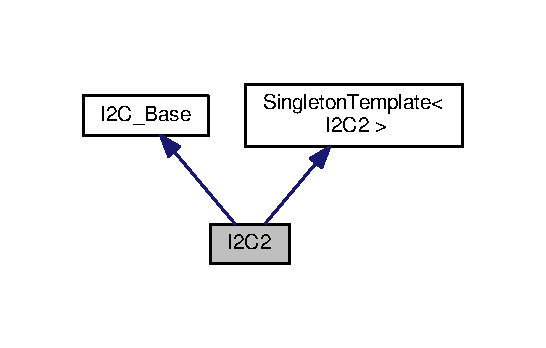
\includegraphics[width=262pt]{d7/da0/classI2C2__inherit__graph}
\end{center}
\end{figure}


Collaboration diagram for I2\+C2\+:\nopagebreak
\begin{figure}[H]
\begin{center}
\leavevmode
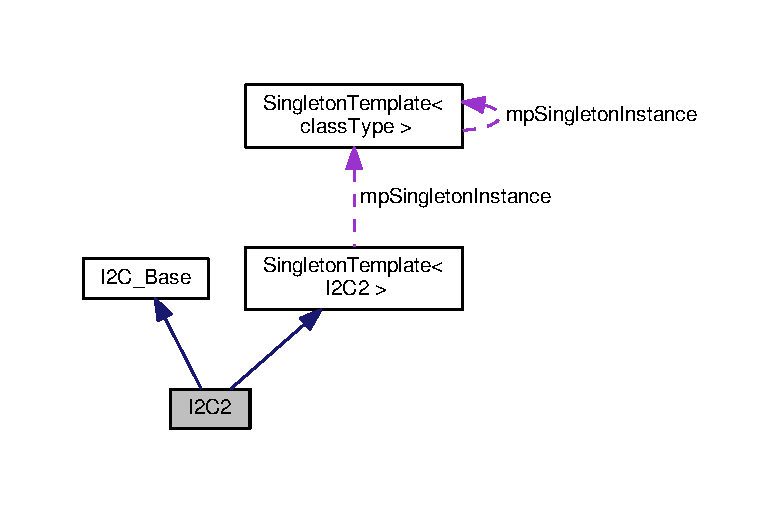
\includegraphics[width=350pt]{d7/d0f/classI2C2__coll__graph}
\end{center}
\end{figure}
\subsection*{Public Member Functions}
\begin{DoxyCompactItemize}
\item 
bool \hyperlink{classI2C2_ad7f9e3bb40e4d96b65e8d09fdcfbe46c}{init} (unsigned int speed\+In\+Khz)
\begin{DoxyCompactList}\small\item\em Initializes \hyperlink{classI2C2}{I2\+C2} at the given. \end{DoxyCompactList}\end{DoxyCompactItemize}
\subsection*{Friends}
\begin{DoxyCompactItemize}
\item 
class \hyperlink{classI2C2_a7321868b283eed05e13be0111783a968}{Singleton\+Template$<$ I2\+C2 $>$}
\begin{DoxyCompactList}\small\item\em Friend class used for Singleton Template. \end{DoxyCompactList}\end{DoxyCompactItemize}
\subsection*{Additional Inherited Members}


\subsection{Detailed Description}
\hyperlink{classI2C2}{I2\+C2} Singleton Driver This is a thin wrapper around \hyperlink{classI2C__Base}{I2\+C\+\_\+\+Base} class and merely gives the base address of the \hyperlink{classI2C2}{I2\+C2} memory map. 

\subsection{Member Function Documentation}
\index{I2\+C2@{I2\+C2}!init@{init}}
\index{init@{init}!I2\+C2@{I2\+C2}}
\subsubsection[{\texorpdfstring{init(unsigned int speed\+In\+Khz)}{init(unsigned int speedInKhz)}}]{\setlength{\rightskip}{0pt plus 5cm}bool I2\+C2\+::init (
\begin{DoxyParamCaption}
\item[{unsigned int}]{speed\+In\+Khz}
\end{DoxyParamCaption}
)}\hypertarget{classI2C2_ad7f9e3bb40e4d96b65e8d09fdcfbe46c}{}\label{classI2C2_ad7f9e3bb40e4d96b65e8d09fdcfbe46c}


Initializes \hyperlink{classI2C2}{I2\+C2} at the given. 


\begin{DoxyParams}{Parameters}
{\em speed\+In\+Khz} & \\
\hline
\end{DoxyParams}
Before I2C is initialized, check to be sure that the I2C wires are logic \char`\"{}1\char`\"{} means that they are pulled high, otherwise there may be a short circuit.

\hyperlink{classI2C2}{I2\+C2} is on P0.\+10, and P0.\+11

I2C wires should be pulled high for normal operation, so if they are, initialize I2C otherwise disable operations on I2C since I2C has a likely hardware B\+US fault such as\+:
\begin{DoxyItemize}
\item I2C S\+D\+A/\+S\+CL with no pull-\/up
\item I2C S\+D\+A/\+S\+CL shorted to ground
\end{DoxyItemize}

\subsection{Friends And Related Function Documentation}
\index{I2\+C2@{I2\+C2}!Singleton\+Template$<$ I2\+C2 $>$@{Singleton\+Template$<$ I2\+C2 $>$}}
\index{Singleton\+Template$<$ I2\+C2 $>$@{Singleton\+Template$<$ I2\+C2 $>$}!I2\+C2@{I2\+C2}}
\subsubsection[{\texorpdfstring{Singleton\+Template$<$ I2\+C2 $>$}{SingletonTemplate< I2C2 >}}]{\setlength{\rightskip}{0pt plus 5cm}friend class {\bf Singleton\+Template}$<$ {\bf I2\+C2} $>$\hspace{0.3cm}{\ttfamily [friend]}}\hypertarget{classI2C2_a7321868b283eed05e13be0111783a968}{}\label{classI2C2_a7321868b283eed05e13be0111783a968}


Friend class used for Singleton Template. 



The documentation for this class was generated from the following files\+:\begin{DoxyCompactItemize}
\item 
/var/www/html/\+S\+J\+S\+U-\/\+D\+E\+V-\/\+Linux/firmware/default/lib/\+L2\+\_\+\+Drivers/\hyperlink{i2c2_8hpp}{i2c2.\+hpp}\item 
/var/www/html/\+S\+J\+S\+U-\/\+D\+E\+V-\/\+Linux/firmware/default/lib/\+L2\+\_\+\+Drivers/src/\hyperlink{i2c2_8cpp}{i2c2.\+cpp}\end{DoxyCompactItemize}

\hypertarget{classi2c2__device}{}\section{i2c2\+\_\+device Class Reference}
\label{classi2c2__device}\index{i2c2\+\_\+device@{i2c2\+\_\+device}}


{\ttfamily \#include $<$i2c2\+\_\+device.\+hpp$>$}



Inheritance diagram for i2c2\+\_\+device\+:\nopagebreak
\begin{figure}[H]
\begin{center}
\leavevmode
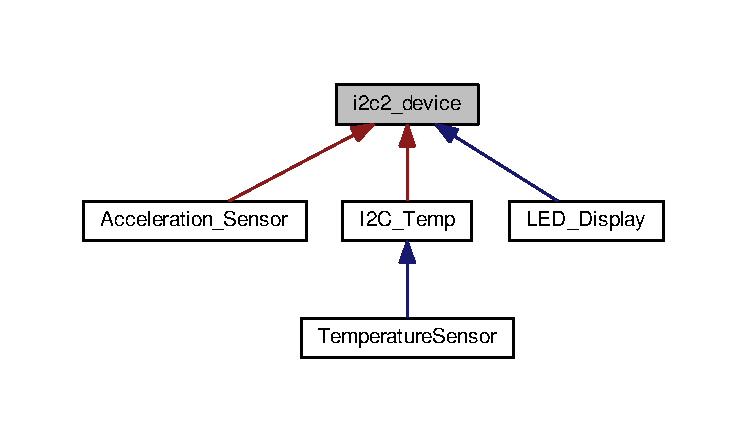
\includegraphics[width=350pt]{d3/d13/classi2c2__device__inherit__graph}
\end{center}
\end{figure}
\subsection*{Protected Member Functions}
\begin{DoxyCompactItemize}
\item 
\hyperlink{classi2c2__device_a8381947bf37d06a16d0fdfe904973de1}{i2c2\+\_\+device} (uint8\+\_\+t addr)
\begin{DoxyCompactList}\small\item\em Constructor of this base class that takes addr as a parameter. \end{DoxyCompactList}\item 
uint8\+\_\+t \hyperlink{classi2c2__device_a89abc70e5c1037bf4f15f5a50ec66291}{read\+Reg} (unsigned char reg)
\item 
void \hyperlink{classi2c2__device_a1c9fdc353d554833694222351187fca0}{write\+Reg} (unsigned char reg, unsigned char data)
\begin{DoxyCompactList}\small\item\em Writes a register of this device. \end{DoxyCompactList}\item 
bool \hyperlink{classi2c2__device_a9dc13487b2ce4f06459b3a814635020f}{check\+Device\+Response} ()
\item 
uint16\+\_\+t \hyperlink{classi2c2__device_aecd419069db41de482fa57e5c7ec7dc4}{get16\+Bit\+Register} (unsigned char reg)
\end{DoxyCompactItemize}


\subsection{Detailed Description}
I2C Device Base Class This class can be inherited by an I2C Device to be able to read and write registers more easily as this class will puts an abstraction layer on I2C and provides simple functionality to read and write registers over I2C Bus. 

\subsection{Constructor \& Destructor Documentation}
\index{i2c2\+\_\+device@{i2c2\+\_\+device}!i2c2\+\_\+device@{i2c2\+\_\+device}}
\index{i2c2\+\_\+device@{i2c2\+\_\+device}!i2c2\+\_\+device@{i2c2\+\_\+device}}
\subsubsection[{\texorpdfstring{i2c2\+\_\+device(uint8\+\_\+t addr)}{i2c2_device(uint8_t addr)}}]{\setlength{\rightskip}{0pt plus 5cm}i2c2\+\_\+device\+::i2c2\+\_\+device (
\begin{DoxyParamCaption}
\item[{uint8\+\_\+t}]{addr}
\end{DoxyParamCaption}
)\hspace{0.3cm}{\ttfamily [inline]}, {\ttfamily [protected]}}\hypertarget{classi2c2__device_a8381947bf37d06a16d0fdfe904973de1}{}\label{classi2c2__device_a8381947bf37d06a16d0fdfe904973de1}


Constructor of this base class that takes addr as a parameter. 



\subsection{Member Function Documentation}
\index{i2c2\+\_\+device@{i2c2\+\_\+device}!check\+Device\+Response@{check\+Device\+Response}}
\index{check\+Device\+Response@{check\+Device\+Response}!i2c2\+\_\+device@{i2c2\+\_\+device}}
\subsubsection[{\texorpdfstring{check\+Device\+Response()}{checkDeviceResponse()}}]{\setlength{\rightskip}{0pt plus 5cm}bool i2c2\+\_\+device\+::check\+Device\+Response (
\begin{DoxyParamCaption}
{}
\end{DoxyParamCaption}
)\hspace{0.3cm}{\ttfamily [inline]}, {\ttfamily [protected]}}\hypertarget{classi2c2__device_a9dc13487b2ce4f06459b3a814635020f}{}\label{classi2c2__device_a9dc13487b2ce4f06459b3a814635020f}
\begin{DoxyReturn}{Returns}
true if the device responds to its address 
\end{DoxyReturn}
\index{i2c2\+\_\+device@{i2c2\+\_\+device}!get16\+Bit\+Register@{get16\+Bit\+Register}}
\index{get16\+Bit\+Register@{get16\+Bit\+Register}!i2c2\+\_\+device@{i2c2\+\_\+device}}
\subsubsection[{\texorpdfstring{get16\+Bit\+Register(unsigned char reg)}{get16BitRegister(unsigned char reg)}}]{\setlength{\rightskip}{0pt plus 5cm}uint16\+\_\+t i2c2\+\_\+device\+::get16\+Bit\+Register (
\begin{DoxyParamCaption}
\item[{unsigned char}]{reg}
\end{DoxyParamCaption}
)\hspace{0.3cm}{\ttfamily [inline]}, {\ttfamily [protected]}}\hypertarget{classi2c2__device_aecd419069db41de482fa57e5c7ec7dc4}{}\label{classi2c2__device_aecd419069db41de482fa57e5c7ec7dc4}
Reads 16-\/bit register from reg and reg+1 granted that reg has M\+SB \index{i2c2\+\_\+device@{i2c2\+\_\+device}!read\+Reg@{read\+Reg}}
\index{read\+Reg@{read\+Reg}!i2c2\+\_\+device@{i2c2\+\_\+device}}
\subsubsection[{\texorpdfstring{read\+Reg(unsigned char reg)}{readReg(unsigned char reg)}}]{\setlength{\rightskip}{0pt plus 5cm}uint8\+\_\+t i2c2\+\_\+device\+::read\+Reg (
\begin{DoxyParamCaption}
\item[{unsigned char}]{reg}
\end{DoxyParamCaption}
)\hspace{0.3cm}{\ttfamily [inline]}, {\ttfamily [protected]}}\hypertarget{classi2c2__device_a89abc70e5c1037bf4f15f5a50ec66291}{}\label{classi2c2__device_a89abc70e5c1037bf4f15f5a50ec66291}
\begin{DoxyReturn}{Returns}
the register content of this device 
\end{DoxyReturn}
\index{i2c2\+\_\+device@{i2c2\+\_\+device}!write\+Reg@{write\+Reg}}
\index{write\+Reg@{write\+Reg}!i2c2\+\_\+device@{i2c2\+\_\+device}}
\subsubsection[{\texorpdfstring{write\+Reg(unsigned char reg, unsigned char data)}{writeReg(unsigned char reg, unsigned char data)}}]{\setlength{\rightskip}{0pt plus 5cm}void i2c2\+\_\+device\+::write\+Reg (
\begin{DoxyParamCaption}
\item[{unsigned char}]{reg, }
\item[{unsigned char}]{data}
\end{DoxyParamCaption}
)\hspace{0.3cm}{\ttfamily [inline]}, {\ttfamily [protected]}}\hypertarget{classi2c2__device_a1c9fdc353d554833694222351187fca0}{}\label{classi2c2__device_a1c9fdc353d554833694222351187fca0}


Writes a register of this device. 



The documentation for this class was generated from the following file\+:\begin{DoxyCompactItemize}
\item 
/var/www/html/\+S\+J\+S\+U-\/\+D\+E\+V-\/\+Linux/firmware/default/lib/\+L4\+\_\+\+I\+O/\hyperlink{i2c2__device_8hpp}{i2c2\+\_\+device.\+hpp}\end{DoxyCompactItemize}

\hypertarget{classI2C__Base}{}\section{I2\+C\+\_\+\+Base Class Reference}
\label{classI2C__Base}\index{I2\+C\+\_\+\+Base@{I2\+C\+\_\+\+Base}}


{\ttfamily \#include $<$i2c\+\_\+base.\+hpp$>$}



Inheritance diagram for I2\+C\+\_\+\+Base\+:\nopagebreak
\begin{figure}[H]
\begin{center}
\leavevmode
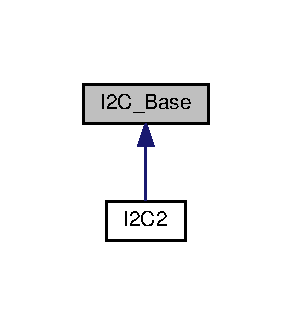
\includegraphics[width=140pt]{d0/d68/classI2C__Base__inherit__graph}
\end{center}
\end{figure}
\subsection*{Public Member Functions}
\begin{DoxyCompactItemize}
\item 
void \hyperlink{classI2C__Base_a91503a44a5f9ff228354245c8c6ec9bc}{handle\+Interrupt} ()
\item 
uint8\+\_\+t \hyperlink{classI2C__Base_ad5322c60fd88a0920df335964613c76c}{read\+Reg} (uint8\+\_\+t device\+Address, uint8\+\_\+t register\+Address)
\item 
bool \hyperlink{classI2C__Base_a1f71fbf12351a0e5f1c0e0452e999b17}{write\+Reg} (uint8\+\_\+t device\+Address, uint8\+\_\+t register\+Address, uint8\+\_\+t value)
\item 
bool \hyperlink{classI2C__Base_a8def06ef5ebcdc8fb5f3a21f4a4be166}{read\+Registers} (uint8\+\_\+t device\+Address, uint8\+\_\+t first\+Reg, uint8\+\_\+t $\ast$p\+Data, uint32\+\_\+t transfer\+Size)
\item 
bool \hyperlink{classI2C__Base_a11db0de4b6517813d50752b9f053dc5f}{write\+Registers} (uint8\+\_\+t device\+Address, uint8\+\_\+t first\+Reg, uint8\+\_\+t $\ast$p\+Data, uint32\+\_\+t transfer\+Size)
\item 
bool \hyperlink{classI2C__Base_a7b1ffc13066ed8b2a2443fdec63f6d27}{check\+Device\+Response} (uint8\+\_\+t device\+Address)
\end{DoxyCompactItemize}
\subsection*{Protected Member Functions}
\begin{DoxyCompactItemize}
\item 
\hyperlink{classI2C__Base_a12caefb41201a7eefe2bc511e48bbd8f}{I2\+C\+\_\+\+Base} (\hyperlink{structLPC__I2C__TypeDef}{L\+P\+C\+\_\+\+I2\+C\+\_\+\+Type\+Def} $\ast$p\+I2\+C\+Base\+Addr)
\item 
bool \hyperlink{classI2C__Base_aa7dd7ef20cedca783ff49413d5765fac}{init} (uint32\+\_\+t pclk, uint32\+\_\+t bus\+Rate\+In\+Khz)
\item 
void \hyperlink{classI2C__Base_a44944d722c91374502bba78dbe27d923}{disable\+Operation} ()
\end{DoxyCompactItemize}


\subsection{Detailed Description}
I2C Base class that can be used to write drivers for all I2C peripherals. Steps needed to write a I2C driver\+:
\begin{DoxyItemize}
\item Inherit this class
\item Call \hyperlink{classI2C__Base_aa7dd7ef20cedca783ff49413d5765fac}{init()} and configure P\+I\+N\+S\+EL to select your I2C pins
\item When your I2C(\#) hardware interrupt occurs, call \hyperlink{classI2C__Base_a91503a44a5f9ff228354245c8c6ec9bc}{handle\+Interrupt()}
\end{DoxyItemize}

To connect I2C Interrupt with your I2C, reference this example\+: 
\begin{DoxyCode}
\textcolor{keyword}{extern} \textcolor{stringliteral}{"C"}
 \{
    \textcolor{keywordtype}{void} \hyperlink{startup_8cpp_a4d1f9a7702a354022ff322a565f8c82b}{I2C0\_IRQHandler}()
    \{
        I2C0::getInstance().handleInterrupt();
    \}
 \}
\end{DoxyCode}
 

\subsection{Constructor \& Destructor Documentation}
\index{I2\+C\+\_\+\+Base@{I2\+C\+\_\+\+Base}!I2\+C\+\_\+\+Base@{I2\+C\+\_\+\+Base}}
\index{I2\+C\+\_\+\+Base@{I2\+C\+\_\+\+Base}!I2\+C\+\_\+\+Base@{I2\+C\+\_\+\+Base}}
\subsubsection[{\texorpdfstring{I2\+C\+\_\+\+Base(\+L\+P\+C\+\_\+\+I2\+C\+\_\+\+Type\+Def $\ast$p\+I2\+C\+Base\+Addr)}{I2C_Base(LPC_I2C_TypeDef *pI2CBaseAddr)}}]{\setlength{\rightskip}{0pt plus 5cm}I2\+C\+\_\+\+Base\+::\+I2\+C\+\_\+\+Base (
\begin{DoxyParamCaption}
\item[{{\bf L\+P\+C\+\_\+\+I2\+C\+\_\+\+Type\+Def} $\ast$}]{p\+I2\+C\+Base\+Addr}
\end{DoxyParamCaption}
)\hspace{0.3cm}{\ttfamily [protected]}}\hypertarget{classI2C__Base_a12caefb41201a7eefe2bc511e48bbd8f}{}\label{classI2C__Base_a12caefb41201a7eefe2bc511e48bbd8f}
Protected constructor that requires parent class to provide I2C base register address for which to operate this I2C driver 

\subsection{Member Function Documentation}
\index{I2\+C\+\_\+\+Base@{I2\+C\+\_\+\+Base}!check\+Device\+Response@{check\+Device\+Response}}
\index{check\+Device\+Response@{check\+Device\+Response}!I2\+C\+\_\+\+Base@{I2\+C\+\_\+\+Base}}
\subsubsection[{\texorpdfstring{check\+Device\+Response(uint8\+\_\+t device\+Address)}{checkDeviceResponse(uint8_t deviceAddress)}}]{\setlength{\rightskip}{0pt plus 5cm}bool I2\+C\+\_\+\+Base\+::check\+Device\+Response (
\begin{DoxyParamCaption}
\item[{uint8\+\_\+t}]{device\+Address}
\end{DoxyParamCaption}
)}\hypertarget{classI2C__Base_a7b1ffc13066ed8b2a2443fdec63f6d27}{}\label{classI2C__Base_a7b1ffc13066ed8b2a2443fdec63f6d27}
This function can be used to check if an I2C device responds to its address, which can therefore be used to discover all I2C hardware devices. Sometimes this method is used by devices to check if they are ready for further operations such as an E\+E\+P\+R\+OM or F\+L\+A\+SH memory.


\begin{DoxyParams}{Parameters}
{\em device\+Address} & The device address to check for I2C response \\
\hline
\end{DoxyParams}
\begin{DoxyReturn}{Returns}
true if I2C device with given address is ready 
\end{DoxyReturn}
\index{I2\+C\+\_\+\+Base@{I2\+C\+\_\+\+Base}!disable\+Operation@{disable\+Operation}}
\index{disable\+Operation@{disable\+Operation}!I2\+C\+\_\+\+Base@{I2\+C\+\_\+\+Base}}
\subsubsection[{\texorpdfstring{disable\+Operation()}{disableOperation()}}]{\setlength{\rightskip}{0pt plus 5cm}void I2\+C\+\_\+\+Base\+::disable\+Operation (
\begin{DoxyParamCaption}
{}
\end{DoxyParamCaption}
)\hspace{0.3cm}{\ttfamily [inline]}, {\ttfamily [protected]}}\hypertarget{classI2C__Base_a44944d722c91374502bba78dbe27d923}{}\label{classI2C__Base_a44944d722c91374502bba78dbe27d923}
Disables I2C operation This can be used to disable all I2C operations in case of severe I2C Bus Failure \begin{DoxyWarning}{Warning}
Once disabled, I2C cannot be enabled again 
\end{DoxyWarning}
\index{I2\+C\+\_\+\+Base@{I2\+C\+\_\+\+Base}!handle\+Interrupt@{handle\+Interrupt}}
\index{handle\+Interrupt@{handle\+Interrupt}!I2\+C\+\_\+\+Base@{I2\+C\+\_\+\+Base}}
\subsubsection[{\texorpdfstring{handle\+Interrupt()}{handleInterrupt()}}]{\setlength{\rightskip}{0pt plus 5cm}void I2\+C\+\_\+\+Base\+::handle\+Interrupt (
\begin{DoxyParamCaption}
{}
\end{DoxyParamCaption}
)}\hypertarget{classI2C__Base_a91503a44a5f9ff228354245c8c6ec9bc}{}\label{classI2C__Base_a91503a44a5f9ff228354245c8c6ec9bc}
When the I2C interrupt occurs, this function should be called to handle future action to take due to the interrupt cause. \index{I2\+C\+\_\+\+Base@{I2\+C\+\_\+\+Base}!init@{init}}
\index{init@{init}!I2\+C\+\_\+\+Base@{I2\+C\+\_\+\+Base}}
\subsubsection[{\texorpdfstring{init(uint32\+\_\+t pclk, uint32\+\_\+t bus\+Rate\+In\+Khz)}{init(uint32_t pclk, uint32_t busRateInKhz)}}]{\setlength{\rightskip}{0pt plus 5cm}bool I2\+C\+\_\+\+Base\+::init (
\begin{DoxyParamCaption}
\item[{uint32\+\_\+t}]{pclk, }
\item[{uint32\+\_\+t}]{bus\+Rate\+In\+Khz}
\end{DoxyParamCaption}
)\hspace{0.3cm}{\ttfamily [protected]}}\hypertarget{classI2C__Base_aa7dd7ef20cedca783ff49413d5765fac}{}\label{classI2C__Base_aa7dd7ef20cedca783ff49413d5765fac}
Initializes I2C Communication B\+US 
\begin{DoxyParams}{Parameters}
{\em pclk} & The peripheral clock to the I2C Bus \\
\hline
{\em bus\+Rate\+In\+Khz} & The speed to set for this I2C Bus \\
\hline
\end{DoxyParams}
Per I2C high speed mode\+: HS mode master devices generate a serial clock signal with a H\+I\+GH to L\+OW ratio of 1 to 2. So to be able to optimize speed, we use different duty cycle for high/low

Compute the I2C clock dividers. The L\+OW period can be longer than the H\+I\+GH period because the rise time of S\+D\+A/\+S\+CL is an RC curve, whereas the fall time is a sharper curve.\index{I2\+C\+\_\+\+Base@{I2\+C\+\_\+\+Base}!read\+Reg@{read\+Reg}}
\index{read\+Reg@{read\+Reg}!I2\+C\+\_\+\+Base@{I2\+C\+\_\+\+Base}}
\subsubsection[{\texorpdfstring{read\+Reg(uint8\+\_\+t device\+Address, uint8\+\_\+t register\+Address)}{readReg(uint8_t deviceAddress, uint8_t registerAddress)}}]{\setlength{\rightskip}{0pt plus 5cm}uint8\+\_\+t I2\+C\+\_\+\+Base\+::read\+Reg (
\begin{DoxyParamCaption}
\item[{uint8\+\_\+t}]{device\+Address, }
\item[{uint8\+\_\+t}]{register\+Address}
\end{DoxyParamCaption}
)}\hypertarget{classI2C__Base_ad5322c60fd88a0920df335964613c76c}{}\label{classI2C__Base_ad5322c60fd88a0920df335964613c76c}
Reads a single byte from an I2C Slave 
\begin{DoxyParams}{Parameters}
{\em device\+Address} & The I2C Device Address \\
\hline
{\em register\+Address} & The register address to read \\
\hline
\end{DoxyParams}
\begin{DoxyReturn}{Returns}
The byte read from slave device (might be 0 if error) 
\end{DoxyReturn}
\index{I2\+C\+\_\+\+Base@{I2\+C\+\_\+\+Base}!read\+Registers@{read\+Registers}}
\index{read\+Registers@{read\+Registers}!I2\+C\+\_\+\+Base@{I2\+C\+\_\+\+Base}}
\subsubsection[{\texorpdfstring{read\+Registers(uint8\+\_\+t device\+Address, uint8\+\_\+t first\+Reg, uint8\+\_\+t $\ast$p\+Data, uint32\+\_\+t transfer\+Size)}{readRegisters(uint8_t deviceAddress, uint8_t firstReg, uint8_t *pData, uint32_t transferSize)}}]{\setlength{\rightskip}{0pt plus 5cm}bool I2\+C\+\_\+\+Base\+::read\+Registers (
\begin{DoxyParamCaption}
\item[{uint8\+\_\+t}]{device\+Address, }
\item[{uint8\+\_\+t}]{first\+Reg, }
\item[{uint8\+\_\+t $\ast$}]{p\+Data, }
\item[{uint32\+\_\+t}]{transfer\+Size}
\end{DoxyParamCaption}
)}\hypertarget{classI2C__Base_a8def06ef5ebcdc8fb5f3a21f4a4be166}{}\label{classI2C__Base_a8def06ef5ebcdc8fb5f3a21f4a4be166}




\index{I2\+C\+\_\+\+Base@{I2\+C\+\_\+\+Base}!write\+Reg@{write\+Reg}}
\index{write\+Reg@{write\+Reg}!I2\+C\+\_\+\+Base@{I2\+C\+\_\+\+Base}}
\subsubsection[{\texorpdfstring{write\+Reg(uint8\+\_\+t device\+Address, uint8\+\_\+t register\+Address, uint8\+\_\+t value)}{writeReg(uint8_t deviceAddress, uint8_t registerAddress, uint8_t value)}}]{\setlength{\rightskip}{0pt plus 5cm}bool I2\+C\+\_\+\+Base\+::write\+Reg (
\begin{DoxyParamCaption}
\item[{uint8\+\_\+t}]{device\+Address, }
\item[{uint8\+\_\+t}]{register\+Address, }
\item[{uint8\+\_\+t}]{value}
\end{DoxyParamCaption}
)}\hypertarget{classI2C__Base_a1f71fbf12351a0e5f1c0e0452e999b17}{}\label{classI2C__Base_a1f71fbf12351a0e5f1c0e0452e999b17}
Writes a single byte to an I2C Slave 
\begin{DoxyParams}{Parameters}
{\em device\+Address} & The I2C Device Address \\
\hline
{\em register\+Address} & The register address to write \\
\hline
{\em value} & The value to write to register\+Address \\
\hline
\end{DoxyParams}
\begin{DoxyReturn}{Returns}
true if successful 
\end{DoxyReturn}
\index{I2\+C\+\_\+\+Base@{I2\+C\+\_\+\+Base}!write\+Registers@{write\+Registers}}
\index{write\+Registers@{write\+Registers}!I2\+C\+\_\+\+Base@{I2\+C\+\_\+\+Base}}
\subsubsection[{\texorpdfstring{write\+Registers(uint8\+\_\+t device\+Address, uint8\+\_\+t first\+Reg, uint8\+\_\+t $\ast$p\+Data, uint32\+\_\+t transfer\+Size)}{writeRegisters(uint8_t deviceAddress, uint8_t firstReg, uint8_t *pData, uint32_t transferSize)}}]{\setlength{\rightskip}{0pt plus 5cm}bool I2\+C\+\_\+\+Base\+::write\+Registers (
\begin{DoxyParamCaption}
\item[{uint8\+\_\+t}]{device\+Address, }
\item[{uint8\+\_\+t}]{first\+Reg, }
\item[{uint8\+\_\+t $\ast$}]{p\+Data, }
\item[{uint32\+\_\+t}]{transfer\+Size}
\end{DoxyParamCaption}
)}\hypertarget{classI2C__Base_a11db0de4b6517813d50752b9f053dc5f}{}\label{classI2C__Base_a11db0de4b6517813d50752b9f053dc5f}






The documentation for this class was generated from the following files\+:\begin{DoxyCompactItemize}
\item 
/var/www/html/\+S\+J\+S\+U-\/\+D\+E\+V-\/\+Linux/firmware/default/lib/\+L2\+\_\+\+Drivers/base/\hyperlink{i2c__base_8hpp}{i2c\+\_\+base.\+hpp}\item 
/var/www/html/\+S\+J\+S\+U-\/\+D\+E\+V-\/\+Linux/firmware/default/lib/\+L2\+\_\+\+Drivers/base/\hyperlink{i2c__base_8cpp}{i2c\+\_\+base.\+cpp}\end{DoxyCompactItemize}

\hypertarget{classI2C__Temp}{}\section{I2\+C\+\_\+\+Temp Class Reference}
\label{classI2C__Temp}\index{I2\+C\+\_\+\+Temp@{I2\+C\+\_\+\+Temp}}


{\ttfamily \#include $<$temperature\+\_\+sensor.\+hpp$>$}



Inheritance diagram for I2\+C\+\_\+\+Temp\+:\nopagebreak
\begin{figure}[H]
\begin{center}
\leavevmode
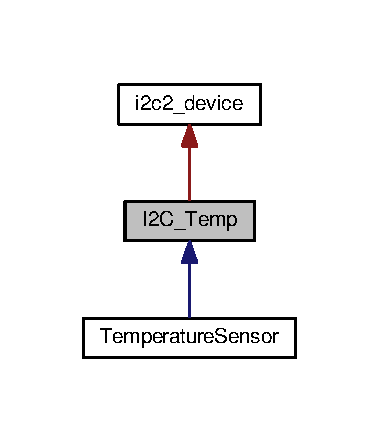
\includegraphics[width=182pt]{d0/de8/classI2C__Temp__inherit__graph}
\end{center}
\end{figure}


Collaboration diagram for I2\+C\+\_\+\+Temp\+:\nopagebreak
\begin{figure}[H]
\begin{center}
\leavevmode
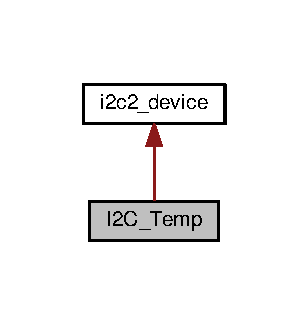
\includegraphics[width=148pt]{dc/d69/classI2C__Temp__coll__graph}
\end{center}
\end{figure}
\subsection*{Public Member Functions}
\begin{DoxyCompactItemize}
\item 
\hyperlink{classI2C__Temp_aa7ee672d00b61ac4fa179fe06713ef30}{I2\+C\+\_\+\+Temp} (char addr)
\item 
bool \hyperlink{classI2C__Temp_a01532ca98009a358ebb4f5e507abce3e}{init} ()
\item 
float \hyperlink{classI2C__Temp_a8d385257d5d46ad95358616abb614243}{get\+Celsius} ()
\item 
float \hyperlink{classI2C__Temp_a573d8814e1ee2201c88aa11d6974c27e}{get\+Farenheit} ()
\end{DoxyCompactItemize}
\subsection*{Data Fields}
\begin{DoxyCompactItemize}
\item 
float \hyperlink{classI2C__Temp_a0d50b6493ad48ca69f49c7f5bdd96628}{m\+Offset\+Celcius}
\begin{DoxyCompactList}\small\item\em Temperature offset. \end{DoxyCompactList}\end{DoxyCompactItemize}


\subsection{Detailed Description}
Base class of an I2C temperature sensor 

\subsection{Constructor \& Destructor Documentation}
\index{I2\+C\+\_\+\+Temp@{I2\+C\+\_\+\+Temp}!I2\+C\+\_\+\+Temp@{I2\+C\+\_\+\+Temp}}
\index{I2\+C\+\_\+\+Temp@{I2\+C\+\_\+\+Temp}!I2\+C\+\_\+\+Temp@{I2\+C\+\_\+\+Temp}}
\subsubsection[{\texorpdfstring{I2\+C\+\_\+\+Temp(char addr)}{I2C_Temp(char addr)}}]{\setlength{\rightskip}{0pt plus 5cm}I2\+C\+\_\+\+Temp\+::\+I2\+C\+\_\+\+Temp (
\begin{DoxyParamCaption}
\item[{char}]{addr}
\end{DoxyParamCaption}
)\hspace{0.3cm}{\ttfamily [inline]}}\hypertarget{classI2C__Temp_aa7ee672d00b61ac4fa179fe06713ef30}{}\label{classI2C__Temp_aa7ee672d00b61ac4fa179fe06713ef30}


\subsection{Member Function Documentation}
\index{I2\+C\+\_\+\+Temp@{I2\+C\+\_\+\+Temp}!get\+Celsius@{get\+Celsius}}
\index{get\+Celsius@{get\+Celsius}!I2\+C\+\_\+\+Temp@{I2\+C\+\_\+\+Temp}}
\subsubsection[{\texorpdfstring{get\+Celsius()}{getCelsius()}}]{\setlength{\rightskip}{0pt plus 5cm}float I2\+C\+\_\+\+Temp\+::get\+Celsius (
\begin{DoxyParamCaption}
{}
\end{DoxyParamCaption}
)}\hypertarget{classI2C__Temp_a8d385257d5d46ad95358616abb614243}{}\label{classI2C__Temp_a8d385257d5d46ad95358616abb614243}
\begin{DoxyReturn}{Returns}
floating-\/point reading of temperature in Celsius 
\end{DoxyReturn}
\index{I2\+C\+\_\+\+Temp@{I2\+C\+\_\+\+Temp}!get\+Farenheit@{get\+Farenheit}}
\index{get\+Farenheit@{get\+Farenheit}!I2\+C\+\_\+\+Temp@{I2\+C\+\_\+\+Temp}}
\subsubsection[{\texorpdfstring{get\+Farenheit()}{getFarenheit()}}]{\setlength{\rightskip}{0pt plus 5cm}float I2\+C\+\_\+\+Temp\+::get\+Farenheit (
\begin{DoxyParamCaption}
{}
\end{DoxyParamCaption}
)}\hypertarget{classI2C__Temp_a573d8814e1ee2201c88aa11d6974c27e}{}\label{classI2C__Temp_a573d8814e1ee2201c88aa11d6974c27e}
\begin{DoxyReturn}{Returns}
floating-\/point reading of temperature in Farenheit 
\end{DoxyReturn}
\index{I2\+C\+\_\+\+Temp@{I2\+C\+\_\+\+Temp}!init@{init}}
\index{init@{init}!I2\+C\+\_\+\+Temp@{I2\+C\+\_\+\+Temp}}
\subsubsection[{\texorpdfstring{init()}{init()}}]{\setlength{\rightskip}{0pt plus 5cm}bool I2\+C\+\_\+\+Temp\+::init (
\begin{DoxyParamCaption}
\item[{void}]{}
\end{DoxyParamCaption}
)}\hypertarget{classI2C__Temp_a01532ca98009a358ebb4f5e507abce3e}{}\label{classI2C__Temp_a01532ca98009a358ebb4f5e507abce3e}


\subsection{Field Documentation}
\index{I2\+C\+\_\+\+Temp@{I2\+C\+\_\+\+Temp}!m\+Offset\+Celcius@{m\+Offset\+Celcius}}
\index{m\+Offset\+Celcius@{m\+Offset\+Celcius}!I2\+C\+\_\+\+Temp@{I2\+C\+\_\+\+Temp}}
\subsubsection[{\texorpdfstring{m\+Offset\+Celcius}{mOffsetCelcius}}]{\setlength{\rightskip}{0pt plus 5cm}float I2\+C\+\_\+\+Temp\+::m\+Offset\+Celcius}\hypertarget{classI2C__Temp_a0d50b6493ad48ca69f49c7f5bdd96628}{}\label{classI2C__Temp_a0d50b6493ad48ca69f49c7f5bdd96628}


Temperature offset. 



The documentation for this class was generated from the following files\+:\begin{DoxyCompactItemize}
\item 
/var/www/html/\+S\+J\+S\+U-\/\+D\+E\+V-\/\+Linux/firmware/default/lib/\+L4\+\_\+\+I\+O/\hyperlink{temperature__sensor_8hpp}{temperature\+\_\+sensor.\+hpp}\item 
/var/www/html/\+S\+J\+S\+U-\/\+D\+E\+V-\/\+Linux/firmware/default/lib/\+L4\+\_\+\+I\+O/src/\hyperlink{io__source_8cpp}{io\+\_\+source.\+cpp}\end{DoxyCompactItemize}

\hypertarget{structInterruptType__Type}{}\section{Interrupt\+Type\+\_\+\+Type Struct Reference}
\label{structInterruptType__Type}\index{Interrupt\+Type\+\_\+\+Type@{Interrupt\+Type\+\_\+\+Type}}


{\ttfamily \#include $<$core\+\_\+cm3.\+h$>$}

\subsection*{Data Fields}
\begin{DoxyCompactItemize}
\item 
uint32\+\_\+t \hyperlink{structInterruptType__Type_ae0d588643b0488fce4c0a90b85edf362}{R\+E\+S\+E\+R\+V\+E\+D0}
\item 
\hyperlink{LPC17xx_8h_af63697ed9952cc71e1225efe205f6cd3}{\+\_\+\+\_\+I} uint32\+\_\+t \hyperlink{structInterruptType__Type_a2b10f6d37363a6b798ac97f4c4db1e63}{I\+C\+TR}
\item 
uint32\+\_\+t \hyperlink{structInterruptType__Type_a45933eb981309d50f943ec3af67f17be}{R\+E\+S\+E\+R\+V\+E\+D1}
\end{DoxyCompactItemize}


\subsection{Field Documentation}
\index{Interrupt\+Type\+\_\+\+Type@{Interrupt\+Type\+\_\+\+Type}!I\+C\+TR@{I\+C\+TR}}
\index{I\+C\+TR@{I\+C\+TR}!Interrupt\+Type\+\_\+\+Type@{Interrupt\+Type\+\_\+\+Type}}
\subsubsection[{\texorpdfstring{I\+C\+TR}{ICTR}}]{\setlength{\rightskip}{0pt plus 5cm}{\bf \+\_\+\+\_\+I} uint32\+\_\+t Interrupt\+Type\+\_\+\+Type\+::\+I\+C\+TR}\hypertarget{structInterruptType__Type_a2b10f6d37363a6b798ac97f4c4db1e63}{}\label{structInterruptType__Type_a2b10f6d37363a6b798ac97f4c4db1e63}
Offset\+: 0x04 Interrupt Control Type Register \index{Interrupt\+Type\+\_\+\+Type@{Interrupt\+Type\+\_\+\+Type}!R\+E\+S\+E\+R\+V\+E\+D0@{R\+E\+S\+E\+R\+V\+E\+D0}}
\index{R\+E\+S\+E\+R\+V\+E\+D0@{R\+E\+S\+E\+R\+V\+E\+D0}!Interrupt\+Type\+\_\+\+Type@{Interrupt\+Type\+\_\+\+Type}}
\subsubsection[{\texorpdfstring{R\+E\+S\+E\+R\+V\+E\+D0}{RESERVED0}}]{\setlength{\rightskip}{0pt plus 5cm}uint32\+\_\+t Interrupt\+Type\+\_\+\+Type\+::\+R\+E\+S\+E\+R\+V\+E\+D0}\hypertarget{structInterruptType__Type_ae0d588643b0488fce4c0a90b85edf362}{}\label{structInterruptType__Type_ae0d588643b0488fce4c0a90b85edf362}
\index{Interrupt\+Type\+\_\+\+Type@{Interrupt\+Type\+\_\+\+Type}!R\+E\+S\+E\+R\+V\+E\+D1@{R\+E\+S\+E\+R\+V\+E\+D1}}
\index{R\+E\+S\+E\+R\+V\+E\+D1@{R\+E\+S\+E\+R\+V\+E\+D1}!Interrupt\+Type\+\_\+\+Type@{Interrupt\+Type\+\_\+\+Type}}
\subsubsection[{\texorpdfstring{R\+E\+S\+E\+R\+V\+E\+D1}{RESERVED1}}]{\setlength{\rightskip}{0pt plus 5cm}uint32\+\_\+t Interrupt\+Type\+\_\+\+Type\+::\+R\+E\+S\+E\+R\+V\+E\+D1}\hypertarget{structInterruptType__Type_a45933eb981309d50f943ec3af67f17be}{}\label{structInterruptType__Type_a45933eb981309d50f943ec3af67f17be}


The documentation for this struct was generated from the following file\+:\begin{DoxyCompactItemize}
\item 
/var/www/html/\+S\+J\+S\+U-\/\+D\+E\+V-\/\+Linux/firmware/default/lib/\+L0\+\_\+\+Low\+Level/\hyperlink{core__cm3_8h}{core\+\_\+cm3.\+h}\end{DoxyCompactItemize}

\hypertarget{classIR__Sensor}{}\section{I\+R\+\_\+\+Sensor Class Reference}
\label{classIR__Sensor}\index{I\+R\+\_\+\+Sensor@{I\+R\+\_\+\+Sensor}}


{\ttfamily \#include $<$I\+R\+\_\+sensor.\+hpp$>$}



Inheritance diagram for I\+R\+\_\+\+Sensor\+:\nopagebreak
\begin{figure}[H]
\begin{center}
\leavevmode
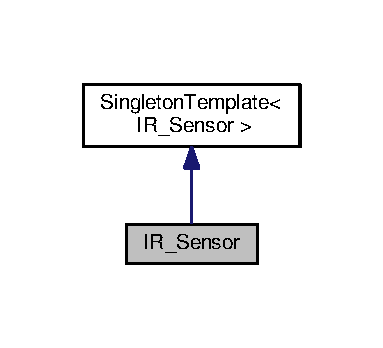
\includegraphics[width=184pt]{d5/d2d/classIR__Sensor__inherit__graph}
\end{center}
\end{figure}


Collaboration diagram for I\+R\+\_\+\+Sensor\+:\nopagebreak
\begin{figure}[H]
\begin{center}
\leavevmode
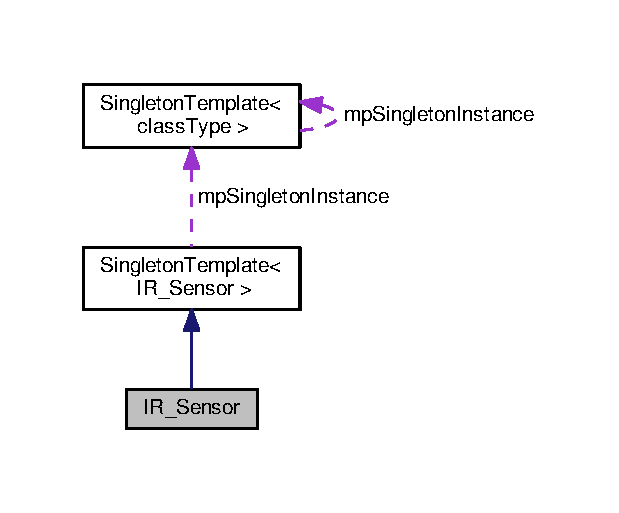
\includegraphics[width=297pt]{d7/d76/classIR__Sensor__coll__graph}
\end{center}
\end{figure}
\subsection*{Public Member Functions}
\begin{DoxyCompactItemize}
\item 
bool \hyperlink{classIR__Sensor_aed070b378b1a8434dc4ef697367b24aa}{init} ()
\begin{DoxyCompactList}\small\item\em Initializes this device,. \end{DoxyCompactList}\item 
bool \hyperlink{classIR__Sensor_a9ab8df4474ccdbf246f2a36aef42afa8}{is\+I\+R\+Code\+Received} ()
\item 
uint32\+\_\+t \hyperlink{classIR__Sensor_a73909031861c829b42eda33aafe330ed}{get\+Last\+I\+R\+Code} ()
\end{DoxyCompactItemize}
{\bf }\par
\begin{DoxyCompactItemize}
\item 
void \hyperlink{classIR__Sensor_a4cb79e3f711d2d374aeb49c601f4a61e}{store\+Ir\+Code} (uint32\+\_\+t)
\item 
void \hyperlink{classIR__Sensor_ade378c1c94b66513c862733b7bb8c163}{decode\+Ir\+Code} (void)
\end{DoxyCompactItemize}

\subsection*{Friends}
\begin{DoxyCompactItemize}
\item 
class \hyperlink{classIR__Sensor_ab53cf421ebbd5018a3e945bb6368f90e}{Singleton\+Template$<$ I\+R\+\_\+\+Sensor $>$}
\begin{DoxyCompactList}\small\item\em Friend class used for Singleton Template. \end{DoxyCompactList}\end{DoxyCompactItemize}
\subsection*{Additional Inherited Members}


\subsection{Detailed Description}
IR Sensor class used to get signals from the on-\/board IR Sensor This sensor can decode a remote\textquotesingle{}s IR signals, such as a TV remote control.

To make sure no decoded signals are over-\/written, or you do not get a decoded signal that is very obsolete, the user should periodically check \hyperlink{classIR__Sensor_a9ab8df4474ccdbf246f2a36aef42afa8}{is\+I\+R\+Code\+Received()} every 50ms, and buffer signals externally.

If a signal is decoded, \hyperlink{classIR__Sensor_a73909031861c829b42eda33aafe330ed}{get\+Last\+I\+R\+Code()} will provide it, and clear out the buffer to receive future signal. If \hyperlink{classIR__Sensor_a73909031861c829b42eda33aafe330ed}{get\+Last\+I\+R\+Code()} is not called regularly, it is possible that this may return an older signal, even if it was many hours ago. 

\subsection{Member Function Documentation}
\index{I\+R\+\_\+\+Sensor@{I\+R\+\_\+\+Sensor}!decode\+Ir\+Code@{decode\+Ir\+Code}}
\index{decode\+Ir\+Code@{decode\+Ir\+Code}!I\+R\+\_\+\+Sensor@{I\+R\+\_\+\+Sensor}}
\subsubsection[{\texorpdfstring{decode\+Ir\+Code(void)}{decodeIrCode(void)}}]{\setlength{\rightskip}{0pt plus 5cm}void I\+R\+\_\+\+Sensor\+::decode\+Ir\+Code (
\begin{DoxyParamCaption}
\item[{void}]{}
\end{DoxyParamCaption}
)}\hypertarget{classIR__Sensor_ade378c1c94b66513c862733b7bb8c163}{}\label{classIR__Sensor_ade378c1c94b66513c862733b7bb8c163}
First falling edge value should indicate binary 0. So anything higher than 50\% of this value is considered binary 1.\index{I\+R\+\_\+\+Sensor@{I\+R\+\_\+\+Sensor}!get\+Last\+I\+R\+Code@{get\+Last\+I\+R\+Code}}
\index{get\+Last\+I\+R\+Code@{get\+Last\+I\+R\+Code}!I\+R\+\_\+\+Sensor@{I\+R\+\_\+\+Sensor}}
\subsubsection[{\texorpdfstring{get\+Last\+I\+R\+Code()}{getLastIRCode()}}]{\setlength{\rightskip}{0pt plus 5cm}uint32\+\_\+t I\+R\+\_\+\+Sensor\+::get\+Last\+I\+R\+Code (
\begin{DoxyParamCaption}
{}
\end{DoxyParamCaption}
)}\hypertarget{classIR__Sensor_a73909031861c829b42eda33aafe330ed}{}\label{classIR__Sensor_a73909031861c829b42eda33aafe330ed}
\begin{DoxyReturn}{Returns}
The last IR signal that was decoded or 0 if nothing was decoded 
\end{DoxyReturn}
\index{I\+R\+\_\+\+Sensor@{I\+R\+\_\+\+Sensor}!init@{init}}
\index{init@{init}!I\+R\+\_\+\+Sensor@{I\+R\+\_\+\+Sensor}}
\subsubsection[{\texorpdfstring{init()}{init()}}]{\setlength{\rightskip}{0pt plus 5cm}bool I\+R\+\_\+\+Sensor\+::init (
\begin{DoxyParamCaption}
\item[{void}]{}
\end{DoxyParamCaption}
)}\hypertarget{classIR__Sensor_aed070b378b1a8434dc4ef697367b24aa}{}\label{classIR__Sensor_aed070b378b1a8434dc4ef697367b24aa}


Initializes this device,. 

\begin{DoxyReturn}{Returns}
true if successful
\end{DoxyReturn}
IR Sensor is attached to P1.\+18 -\/ C\+A\+P1.\+0, so it needs T\+I\+M\+E\+R1 to capture the times on P1.\+18 \index{I\+R\+\_\+\+Sensor@{I\+R\+\_\+\+Sensor}!is\+I\+R\+Code\+Received@{is\+I\+R\+Code\+Received}}
\index{is\+I\+R\+Code\+Received@{is\+I\+R\+Code\+Received}!I\+R\+\_\+\+Sensor@{I\+R\+\_\+\+Sensor}}
\subsubsection[{\texorpdfstring{is\+I\+R\+Code\+Received()}{isIRCodeReceived()}}]{\setlength{\rightskip}{0pt plus 5cm}bool I\+R\+\_\+\+Sensor\+::is\+I\+R\+Code\+Received (
\begin{DoxyParamCaption}
{}
\end{DoxyParamCaption}
)}\hypertarget{classIR__Sensor_a9ab8df4474ccdbf246f2a36aef42afa8}{}\label{classIR__Sensor_a9ab8df4474ccdbf246f2a36aef42afa8}
\begin{DoxyReturn}{Returns}
true if an IR signal was decoded and is available to read 
\end{DoxyReturn}
\index{I\+R\+\_\+\+Sensor@{I\+R\+\_\+\+Sensor}!store\+Ir\+Code@{store\+Ir\+Code}}
\index{store\+Ir\+Code@{store\+Ir\+Code}!I\+R\+\_\+\+Sensor@{I\+R\+\_\+\+Sensor}}
\subsubsection[{\texorpdfstring{store\+Ir\+Code(uint32\+\_\+t)}{storeIrCode(uint32_t)}}]{\setlength{\rightskip}{0pt plus 5cm}void I\+R\+\_\+\+Sensor\+::store\+Ir\+Code (
\begin{DoxyParamCaption}
\item[{uint32\+\_\+t}]{value}
\end{DoxyParamCaption}
)}\hypertarget{classIR__Sensor_a4cb79e3f711d2d374aeb49c601f4a61e}{}\label{classIR__Sensor_a4cb79e3f711d2d374aeb49c601f4a61e}
Don\textquotesingle{}t use these functions 

\subsection{Friends And Related Function Documentation}
\index{I\+R\+\_\+\+Sensor@{I\+R\+\_\+\+Sensor}!Singleton\+Template$<$ I\+R\+\_\+\+Sensor $>$@{Singleton\+Template$<$ I\+R\+\_\+\+Sensor $>$}}
\index{Singleton\+Template$<$ I\+R\+\_\+\+Sensor $>$@{Singleton\+Template$<$ I\+R\+\_\+\+Sensor $>$}!I\+R\+\_\+\+Sensor@{I\+R\+\_\+\+Sensor}}
\subsubsection[{\texorpdfstring{Singleton\+Template$<$ I\+R\+\_\+\+Sensor $>$}{SingletonTemplate< IR_Sensor >}}]{\setlength{\rightskip}{0pt plus 5cm}friend class {\bf Singleton\+Template}$<$ {\bf I\+R\+\_\+\+Sensor} $>$\hspace{0.3cm}{\ttfamily [friend]}}\hypertarget{classIR__Sensor_ab53cf421ebbd5018a3e945bb6368f90e}{}\label{classIR__Sensor_ab53cf421ebbd5018a3e945bb6368f90e}


Friend class used for Singleton Template. 



The documentation for this class was generated from the following files\+:\begin{DoxyCompactItemize}
\item 
/var/www/html/\+S\+J\+S\+U-\/\+D\+E\+V-\/\+Linux/firmware/default/lib/\+L4\+\_\+\+I\+O/\hyperlink{IR__sensor_8hpp}{I\+R\+\_\+sensor.\+hpp}\item 
/var/www/html/\+S\+J\+S\+U-\/\+D\+E\+V-\/\+Linux/firmware/default/lib/\+L4\+\_\+\+I\+O/src/\hyperlink{io__source_8cpp}{io\+\_\+source.\+cpp}\end{DoxyCompactItemize}

\hypertarget{classCircularBuffer_1_1iterator}{}\section{Circular\+Buffer$<$ T\+Y\+PE $>$\+:\+:iterator Class Reference}
\label{classCircularBuffer_1_1iterator}\index{Circular\+Buffer$<$ T\+Y\+P\+E $>$\+::iterator@{Circular\+Buffer$<$ T\+Y\+P\+E $>$\+::iterator}}


{\ttfamily \#include $<$circular\+\_\+buffer.\+hpp$>$}

\subsection*{Public Types}
\begin{DoxyCompactItemize}
\item 
typedef \hyperlink{classCircularBuffer_1_1iterator}{iterator} \hyperlink{classCircularBuffer_1_1iterator_a7dae9b5926088a3ef46a8a654e383605}{self\+\_\+type}
\item 
typedef T\+Y\+PE \hyperlink{classCircularBuffer_1_1iterator_accfd2e9138e9e6841ef4f25579cf02bb}{value\+\_\+type}
\item 
typedef T\+Y\+PE \& \hyperlink{classCircularBuffer_1_1iterator_a9aa4665328da6f468a188ae36c6b00a3}{reference}
\item 
typedef T\+Y\+PE $\ast$ \hyperlink{classCircularBuffer_1_1iterator_a35ab71bca3df750e955de46c222b8ee3}{pointer}
\item 
typedef std\+::forward\+\_\+iterator\+\_\+tag \hyperlink{classCircularBuffer_1_1iterator_a806f5db087c9419cb1f81c030f39267c}{iterator\+\_\+category}
\item 
typedef int \hyperlink{classCircularBuffer_1_1iterator_a58a96b782e1e3ccef78445b819e8011a}{difference\+\_\+type}
\end{DoxyCompactItemize}
\subsection*{Public Member Functions}
\begin{DoxyCompactItemize}
\item 
\hyperlink{classCircularBuffer_1_1iterator_afdaf10c8cd54b3f2b6fd14c8b370b8a9}{iterator} (\hyperlink{classCircularBuffer}{Circular\+Buffer}$<$ T\+Y\+PE $>$ $\ast$p)
\item 
\hyperlink{classCircularBuffer_1_1iterator_a7dae9b5926088a3ef46a8a654e383605}{self\+\_\+type} \hyperlink{classCircularBuffer_1_1iterator_aa0a5aeca1ded37429c21b93c00efdc73}{operator++} ()
\begin{DoxyCompactList}\small\item\em Preincrement operator ie\+: ++iterator. \end{DoxyCompactList}\item 
\hyperlink{classCircularBuffer_1_1iterator_a7dae9b5926088a3ef46a8a654e383605}{self\+\_\+type} \hyperlink{classCircularBuffer_1_1iterator_af45f4d81bc792dd3633b1a262cb07dde}{operator++} (int unused)
\begin{DoxyCompactList}\small\item\em Postincrement operator ie\+: iterator++. \end{DoxyCompactList}\item 
\hyperlink{classCircularBuffer_1_1iterator_a9aa4665328da6f468a188ae36c6b00a3}{reference} \hyperlink{classCircularBuffer_1_1iterator_a0b2329fce9fb1311a154902fe1f9f3b7}{operator$\ast$} ()
\item 
\hyperlink{classCircularBuffer_1_1iterator_a35ab71bca3df750e955de46c222b8ee3}{pointer} \hyperlink{classCircularBuffer_1_1iterator_a158958ab9785710e115f626c8344f51d}{operator-\/$>$} ()
\begin{DoxyCompactList}\small\item\em pointer operator to get the address ie\+: $\ast$(\hyperlink{classCircularBuffer_1_1iterator_a158958ab9785710e115f626c8344f51d}{iterator.\+operator-\/$>$()}) \end{DoxyCompactList}\item 
bool \hyperlink{classCircularBuffer_1_1iterator_af5604b0c13183772cd70fec67cc19374}{operator!=} (const \hyperlink{classCircularBuffer_1_1iterator_a7dae9b5926088a3ef46a8a654e383605}{self\+\_\+type} \&rhs)
\begin{DoxyCompactList}\small\item\em != operator between iterators \end{DoxyCompactList}\item 
bool \hyperlink{classCircularBuffer_1_1iterator_aa8d9ce991d27c8b258199594f31109b1}{operator==} (const \hyperlink{classCircularBuffer_1_1iterator_a7dae9b5926088a3ef46a8a654e383605}{self\+\_\+type} \&rhs)
\begin{DoxyCompactList}\small\item\em == operator between iterators \end{DoxyCompactList}\end{DoxyCompactItemize}


\subsection{Member Typedef Documentation}
\index{Circular\+Buffer\+::iterator@{Circular\+Buffer\+::iterator}!difference\+\_\+type@{difference\+\_\+type}}
\index{difference\+\_\+type@{difference\+\_\+type}!Circular\+Buffer\+::iterator@{Circular\+Buffer\+::iterator}}
\subsubsection[{\texorpdfstring{difference\+\_\+type}{difference_type}}]{\setlength{\rightskip}{0pt plus 5cm}template$<$typename T\+Y\+PE$>$ typedef int {\bf Circular\+Buffer}$<$ T\+Y\+PE $>$\+::{\bf iterator\+::difference\+\_\+type}}\hypertarget{classCircularBuffer_1_1iterator_a58a96b782e1e3ccef78445b819e8011a}{}\label{classCircularBuffer_1_1iterator_a58a96b782e1e3ccef78445b819e8011a}
\index{Circular\+Buffer\+::iterator@{Circular\+Buffer\+::iterator}!iterator\+\_\+category@{iterator\+\_\+category}}
\index{iterator\+\_\+category@{iterator\+\_\+category}!Circular\+Buffer\+::iterator@{Circular\+Buffer\+::iterator}}
\subsubsection[{\texorpdfstring{iterator\+\_\+category}{iterator_category}}]{\setlength{\rightskip}{0pt plus 5cm}template$<$typename T\+Y\+PE$>$ typedef std\+::forward\+\_\+iterator\+\_\+tag {\bf Circular\+Buffer}$<$ T\+Y\+PE $>$\+::{\bf iterator\+::iterator\+\_\+category}}\hypertarget{classCircularBuffer_1_1iterator_a806f5db087c9419cb1f81c030f39267c}{}\label{classCircularBuffer_1_1iterator_a806f5db087c9419cb1f81c030f39267c}
\index{Circular\+Buffer\+::iterator@{Circular\+Buffer\+::iterator}!pointer@{pointer}}
\index{pointer@{pointer}!Circular\+Buffer\+::iterator@{Circular\+Buffer\+::iterator}}
\subsubsection[{\texorpdfstring{pointer}{pointer}}]{\setlength{\rightskip}{0pt plus 5cm}template$<$typename T\+Y\+PE$>$ typedef T\+Y\+PE$\ast$ {\bf Circular\+Buffer}$<$ T\+Y\+PE $>$\+::{\bf iterator\+::pointer}}\hypertarget{classCircularBuffer_1_1iterator_a35ab71bca3df750e955de46c222b8ee3}{}\label{classCircularBuffer_1_1iterator_a35ab71bca3df750e955de46c222b8ee3}
\index{Circular\+Buffer\+::iterator@{Circular\+Buffer\+::iterator}!reference@{reference}}
\index{reference@{reference}!Circular\+Buffer\+::iterator@{Circular\+Buffer\+::iterator}}
\subsubsection[{\texorpdfstring{reference}{reference}}]{\setlength{\rightskip}{0pt plus 5cm}template$<$typename T\+Y\+PE$>$ typedef T\+Y\+PE\& {\bf Circular\+Buffer}$<$ T\+Y\+PE $>$\+::{\bf iterator\+::reference}}\hypertarget{classCircularBuffer_1_1iterator_a9aa4665328da6f468a188ae36c6b00a3}{}\label{classCircularBuffer_1_1iterator_a9aa4665328da6f468a188ae36c6b00a3}
\index{Circular\+Buffer\+::iterator@{Circular\+Buffer\+::iterator}!self\+\_\+type@{self\+\_\+type}}
\index{self\+\_\+type@{self\+\_\+type}!Circular\+Buffer\+::iterator@{Circular\+Buffer\+::iterator}}
\subsubsection[{\texorpdfstring{self\+\_\+type}{self_type}}]{\setlength{\rightskip}{0pt plus 5cm}template$<$typename T\+Y\+PE$>$ typedef {\bf iterator} {\bf Circular\+Buffer}$<$ T\+Y\+PE $>$\+::{\bf iterator\+::self\+\_\+type}}\hypertarget{classCircularBuffer_1_1iterator_a7dae9b5926088a3ef46a8a654e383605}{}\label{classCircularBuffer_1_1iterator_a7dae9b5926088a3ef46a8a654e383605}
\index{Circular\+Buffer\+::iterator@{Circular\+Buffer\+::iterator}!value\+\_\+type@{value\+\_\+type}}
\index{value\+\_\+type@{value\+\_\+type}!Circular\+Buffer\+::iterator@{Circular\+Buffer\+::iterator}}
\subsubsection[{\texorpdfstring{value\+\_\+type}{value_type}}]{\setlength{\rightskip}{0pt plus 5cm}template$<$typename T\+Y\+PE$>$ typedef T\+Y\+PE {\bf Circular\+Buffer}$<$ T\+Y\+PE $>$\+::{\bf iterator\+::value\+\_\+type}}\hypertarget{classCircularBuffer_1_1iterator_accfd2e9138e9e6841ef4f25579cf02bb}{}\label{classCircularBuffer_1_1iterator_accfd2e9138e9e6841ef4f25579cf02bb}


\subsection{Constructor \& Destructor Documentation}
\index{Circular\+Buffer\+::iterator@{Circular\+Buffer\+::iterator}!iterator@{iterator}}
\index{iterator@{iterator}!Circular\+Buffer\+::iterator@{Circular\+Buffer\+::iterator}}
\subsubsection[{\texorpdfstring{iterator(\+Circular\+Buffer$<$ T\+Y\+P\+E $>$ $\ast$p)}{iterator(CircularBuffer< TYPE > *p)}}]{\setlength{\rightskip}{0pt plus 5cm}template$<$typename T\+Y\+PE$>$ {\bf Circular\+Buffer}$<$ T\+Y\+PE $>$\+::iterator\+::iterator (
\begin{DoxyParamCaption}
\item[{{\bf Circular\+Buffer}$<$ T\+Y\+PE $>$ $\ast$}]{p}
\end{DoxyParamCaption}
)\hspace{0.3cm}{\ttfamily [inline]}}\hypertarget{classCircularBuffer_1_1iterator_afdaf10c8cd54b3f2b6fd14c8b370b8a9}{}\label{classCircularBuffer_1_1iterator_afdaf10c8cd54b3f2b6fd14c8b370b8a9}


\subsection{Member Function Documentation}
\index{Circular\+Buffer\+::iterator@{Circular\+Buffer\+::iterator}!operator"!=@{operator"!=}}
\index{operator"!=@{operator"!=}!Circular\+Buffer\+::iterator@{Circular\+Buffer\+::iterator}}
\subsubsection[{\texorpdfstring{operator"!=(const self\+\_\+type \&rhs)}{operator!=(const self_type &rhs)}}]{\setlength{\rightskip}{0pt plus 5cm}template$<$typename T\+Y\+PE$>$ bool {\bf Circular\+Buffer}$<$ T\+Y\+PE $>$\+::iterator\+::operator!= (
\begin{DoxyParamCaption}
\item[{const {\bf self\+\_\+type} \&}]{rhs}
\end{DoxyParamCaption}
)\hspace{0.3cm}{\ttfamily [inline]}}\hypertarget{classCircularBuffer_1_1iterator_af5604b0c13183772cd70fec67cc19374}{}\label{classCircularBuffer_1_1iterator_af5604b0c13183772cd70fec67cc19374}


!= operator between iterators 

\index{Circular\+Buffer\+::iterator@{Circular\+Buffer\+::iterator}!operator$\ast$@{operator$\ast$}}
\index{operator$\ast$@{operator$\ast$}!Circular\+Buffer\+::iterator@{Circular\+Buffer\+::iterator}}
\subsubsection[{\texorpdfstring{operator$\ast$()}{operator*()}}]{\setlength{\rightskip}{0pt plus 5cm}template$<$typename T\+Y\+PE$>$ {\bf reference} {\bf Circular\+Buffer}$<$ T\+Y\+PE $>$\+::iterator\+::operator$\ast$ (
\begin{DoxyParamCaption}
{}
\end{DoxyParamCaption}
)\hspace{0.3cm}{\ttfamily [inline]}}\hypertarget{classCircularBuffer_1_1iterator_a0b2329fce9fb1311a154902fe1f9f3b7}{}\label{classCircularBuffer_1_1iterator_a0b2329fce9fb1311a154902fe1f9f3b7}

\begin{DoxyItemize}
\item operator to get the value ie\+: $\ast$iterator OR \hyperlink{classCircularBuffer_1_1iterator_a0b2329fce9fb1311a154902fe1f9f3b7}{iterator.\+operator $\ast$()} 
\end{DoxyItemize}\index{Circular\+Buffer\+::iterator@{Circular\+Buffer\+::iterator}!operator++@{operator++}}
\index{operator++@{operator++}!Circular\+Buffer\+::iterator@{Circular\+Buffer\+::iterator}}
\subsubsection[{\texorpdfstring{operator++()}{operator++()}}]{\setlength{\rightskip}{0pt plus 5cm}template$<$typename T\+Y\+PE$>$ {\bf self\+\_\+type} {\bf Circular\+Buffer}$<$ T\+Y\+PE $>$\+::iterator\+::operator++ (
\begin{DoxyParamCaption}
{}
\end{DoxyParamCaption}
)\hspace{0.3cm}{\ttfamily [inline]}}\hypertarget{classCircularBuffer_1_1iterator_aa0a5aeca1ded37429c21b93c00efdc73}{}\label{classCircularBuffer_1_1iterator_aa0a5aeca1ded37429c21b93c00efdc73}


Preincrement operator ie\+: ++iterator. 

\index{Circular\+Buffer\+::iterator@{Circular\+Buffer\+::iterator}!operator++@{operator++}}
\index{operator++@{operator++}!Circular\+Buffer\+::iterator@{Circular\+Buffer\+::iterator}}
\subsubsection[{\texorpdfstring{operator++(int unused)}{operator++(int unused)}}]{\setlength{\rightskip}{0pt plus 5cm}template$<$typename T\+Y\+PE$>$ {\bf self\+\_\+type} {\bf Circular\+Buffer}$<$ T\+Y\+PE $>$\+::iterator\+::operator++ (
\begin{DoxyParamCaption}
\item[{int}]{unused}
\end{DoxyParamCaption}
)\hspace{0.3cm}{\ttfamily [inline]}}\hypertarget{classCircularBuffer_1_1iterator_af45f4d81bc792dd3633b1a262cb07dde}{}\label{classCircularBuffer_1_1iterator_af45f4d81bc792dd3633b1a262cb07dde}


Postincrement operator ie\+: iterator++. 

\index{Circular\+Buffer\+::iterator@{Circular\+Buffer\+::iterator}!operator-\/$>$@{operator-\/$>$}}
\index{operator-\/$>$@{operator-\/$>$}!Circular\+Buffer\+::iterator@{Circular\+Buffer\+::iterator}}
\subsubsection[{\texorpdfstring{operator-\/$>$()}{operator->()}}]{\setlength{\rightskip}{0pt plus 5cm}template$<$typename T\+Y\+PE$>$ {\bf pointer} {\bf Circular\+Buffer}$<$ T\+Y\+PE $>$\+::iterator\+::operator-\/$>$ (
\begin{DoxyParamCaption}
{}
\end{DoxyParamCaption}
)\hspace{0.3cm}{\ttfamily [inline]}}\hypertarget{classCircularBuffer_1_1iterator_a158958ab9785710e115f626c8344f51d}{}\label{classCircularBuffer_1_1iterator_a158958ab9785710e115f626c8344f51d}


pointer operator to get the address ie\+: $\ast$(\hyperlink{classCircularBuffer_1_1iterator_a158958ab9785710e115f626c8344f51d}{iterator.\+operator-\/$>$()}) 

\index{Circular\+Buffer\+::iterator@{Circular\+Buffer\+::iterator}!operator==@{operator==}}
\index{operator==@{operator==}!Circular\+Buffer\+::iterator@{Circular\+Buffer\+::iterator}}
\subsubsection[{\texorpdfstring{operator==(const self\+\_\+type \&rhs)}{operator==(const self_type &rhs)}}]{\setlength{\rightskip}{0pt plus 5cm}template$<$typename T\+Y\+PE$>$ bool {\bf Circular\+Buffer}$<$ T\+Y\+PE $>$\+::iterator\+::operator== (
\begin{DoxyParamCaption}
\item[{const {\bf self\+\_\+type} \&}]{rhs}
\end{DoxyParamCaption}
)\hspace{0.3cm}{\ttfamily [inline]}}\hypertarget{classCircularBuffer_1_1iterator_aa8d9ce991d27c8b258199594f31109b1}{}\label{classCircularBuffer_1_1iterator_aa8d9ce991d27c8b258199594f31109b1}


== operator between iterators 



The documentation for this class was generated from the following file\+:\begin{DoxyCompactItemize}
\item 
/var/www/html/\+S\+J\+S\+U-\/\+D\+E\+V-\/\+Linux/firmware/default/lib/\+L3\+\_\+\+Utils/\hyperlink{circular__buffer_8hpp}{circular\+\_\+buffer.\+hpp}\end{DoxyCompactItemize}

\hypertarget{structITM__Type}{}\section{I\+T\+M\+\_\+\+Type Struct Reference}
\label{structITM__Type}\index{I\+T\+M\+\_\+\+Type@{I\+T\+M\+\_\+\+Type}}


{\ttfamily \#include $<$core\+\_\+cm3.\+h$>$}

\subsection*{Data Fields}
\begin{DoxyCompactItemize}
\item 
\begin{tabbing}
xx\=xx\=xx\=xx\=xx\=xx\=xx\=xx\=xx\=\kill
union \{\\
\>\hyperlink{LPC17xx_8h_a7e25d9380f9ef903923964322e71f2f6}{\_\_O} uint8\_t \hyperlink{structITM__Type_abea77b06775d325e5f6f46203f582433}{u8}\\
\>\hyperlink{LPC17xx_8h_a7e25d9380f9ef903923964322e71f2f6}{\_\_O} uint16\_t \hyperlink{structITM__Type_a12aa4eb4d9dcb589a5d953c836f4e8f4}{u16}\\
\>\hyperlink{LPC17xx_8h_a7e25d9380f9ef903923964322e71f2f6}{\_\_O} uint32\_t \hyperlink{structITM__Type_a6882fa5af67ef5c5dfb433b3b68939df}{u32}\\
\} \hyperlink{structITM__Type_ab6890c514a53655eef5289350bf2900a}{PORT} \mbox{[}32\mbox{]}\\

\end{tabbing}\item 
uint32\+\_\+t \hyperlink{structITM__Type_a2c5ae30385b5f370d023468ea9914c0e}{R\+E\+S\+E\+R\+V\+E\+D0} \mbox{[}864\mbox{]}
\item 
\hyperlink{LPC17xx_8h_aec43007d9998a0a0e01faede4133d6be}{\+\_\+\+\_\+\+IO} uint32\+\_\+t \hyperlink{structITM__Type_a91a040e1b162e1128ac1e852b4a0e589}{T\+ER}
\item 
uint32\+\_\+t \hyperlink{structITM__Type_afffce5b93bbfedbaee85357d0b07ebce}{R\+E\+S\+E\+R\+V\+E\+D1} \mbox{[}15\mbox{]}
\item 
\hyperlink{LPC17xx_8h_aec43007d9998a0a0e01faede4133d6be}{\+\_\+\+\_\+\+IO} uint32\+\_\+t \hyperlink{structITM__Type_a93b480aac6da620bbb611212186d47fa}{T\+PR}
\item 
uint32\+\_\+t \hyperlink{structITM__Type_af56b2f07bc6b42cd3e4d17e1b27cff7b}{R\+E\+S\+E\+R\+V\+E\+D2} \mbox{[}15\mbox{]}
\item 
\hyperlink{LPC17xx_8h_aec43007d9998a0a0e01faede4133d6be}{\+\_\+\+\_\+\+IO} uint32\+\_\+t \hyperlink{structITM__Type_a58f169e1aa40a9b8afb6296677c3bb45}{T\+CR}
\item 
uint32\+\_\+t \hyperlink{structITM__Type_ab7708f0bcbbe9987cceadc4748c7e6b7}{R\+E\+S\+E\+R\+V\+E\+D3} \mbox{[}29\mbox{]}
\item 
\hyperlink{LPC17xx_8h_aec43007d9998a0a0e01faede4133d6be}{\+\_\+\+\_\+\+IO} uint32\+\_\+t \hyperlink{structITM__Type_af53499fc94cda629afb2fec858d2ad1c}{I\+WR}
\item 
\hyperlink{LPC17xx_8h_aec43007d9998a0a0e01faede4133d6be}{\+\_\+\+\_\+\+IO} uint32\+\_\+t \hyperlink{structITM__Type_ae43a66174b8ab182ff595e5f5da9f235}{I\+RR}
\item 
\hyperlink{LPC17xx_8h_aec43007d9998a0a0e01faede4133d6be}{\+\_\+\+\_\+\+IO} uint32\+\_\+t \hyperlink{structITM__Type_ab2e87d8bb0e3ce9b8e0e4a6a6695228a}{I\+M\+CR}
\item 
uint32\+\_\+t \hyperlink{structITM__Type_a45ad0b376a0a0f2ade55bbb7daf64ff2}{R\+E\+S\+E\+R\+V\+E\+D4} \mbox{[}43\mbox{]}
\item 
\hyperlink{LPC17xx_8h_aec43007d9998a0a0e01faede4133d6be}{\+\_\+\+\_\+\+IO} uint32\+\_\+t \hyperlink{structITM__Type_a33025af19748bd3ca5cf9d6b14150001}{L\+AR}
\item 
\hyperlink{LPC17xx_8h_aec43007d9998a0a0e01faede4133d6be}{\+\_\+\+\_\+\+IO} uint32\+\_\+t \hyperlink{structITM__Type_a56f607260c4175c5f37a28e47ab3d1e5}{L\+SR}
\item 
uint32\+\_\+t \hyperlink{structITM__Type_a7f70161bc2441d430b5c9d55aa7b7b5e}{R\+E\+S\+E\+R\+V\+E\+D5} \mbox{[}6\mbox{]}
\item 
\hyperlink{LPC17xx_8h_af63697ed9952cc71e1225efe205f6cd3}{\+\_\+\+\_\+I} uint32\+\_\+t \hyperlink{structITM__Type_accfc7de00b0eaba0301e8f4553f70512}{P\+I\+D4}
\item 
\hyperlink{LPC17xx_8h_af63697ed9952cc71e1225efe205f6cd3}{\+\_\+\+\_\+I} uint32\+\_\+t \hyperlink{structITM__Type_a9353055ceb7024e07d59248e54502cb9}{P\+I\+D5}
\item 
\hyperlink{LPC17xx_8h_af63697ed9952cc71e1225efe205f6cd3}{\+\_\+\+\_\+I} uint32\+\_\+t \hyperlink{structITM__Type_a755c0ec919e7dbb5f7ff05c8b56a3383}{P\+I\+D6}
\item 
\hyperlink{LPC17xx_8h_af63697ed9952cc71e1225efe205f6cd3}{\+\_\+\+\_\+I} uint32\+\_\+t \hyperlink{structITM__Type_aa31ca6bb4b749201321b23d0dbbe0704}{P\+I\+D7}
\item 
\hyperlink{LPC17xx_8h_af63697ed9952cc71e1225efe205f6cd3}{\+\_\+\+\_\+I} uint32\+\_\+t \hyperlink{structITM__Type_ab69ade751350a7758affdfe396517535}{P\+I\+D0}
\item 
\hyperlink{LPC17xx_8h_af63697ed9952cc71e1225efe205f6cd3}{\+\_\+\+\_\+I} uint32\+\_\+t \hyperlink{structITM__Type_a30e87ec6f93ecc9fe4f135ca8b068990}{P\+I\+D1}
\item 
\hyperlink{LPC17xx_8h_af63697ed9952cc71e1225efe205f6cd3}{\+\_\+\+\_\+I} uint32\+\_\+t \hyperlink{structITM__Type_ae139d2e588bb382573ffcce3625a88cd}{P\+I\+D2}
\item 
\hyperlink{LPC17xx_8h_af63697ed9952cc71e1225efe205f6cd3}{\+\_\+\+\_\+I} uint32\+\_\+t \hyperlink{structITM__Type_af006ee26c7e61c9a3712a80ac74a6cf3}{P\+I\+D3}
\item 
\hyperlink{LPC17xx_8h_af63697ed9952cc71e1225efe205f6cd3}{\+\_\+\+\_\+I} uint32\+\_\+t \hyperlink{structITM__Type_a413f3bb0a15222e5f38fca4baeef14f6}{C\+I\+D0}
\item 
\hyperlink{LPC17xx_8h_af63697ed9952cc71e1225efe205f6cd3}{\+\_\+\+\_\+I} uint32\+\_\+t \hyperlink{structITM__Type_a5f7d524b71f49e444ff0d1d52b3c3565}{C\+I\+D1}
\item 
\hyperlink{LPC17xx_8h_af63697ed9952cc71e1225efe205f6cd3}{\+\_\+\+\_\+I} uint32\+\_\+t \hyperlink{structITM__Type_adee4ccce1429db8b5db3809c4539f876}{C\+I\+D2}
\item 
\hyperlink{LPC17xx_8h_af63697ed9952cc71e1225efe205f6cd3}{\+\_\+\+\_\+I} uint32\+\_\+t \hyperlink{structITM__Type_a0e7aa199619cc7ac6baddff9600aa52e}{C\+I\+D3}
\end{DoxyCompactItemize}


\subsection{Field Documentation}
\index{I\+T\+M\+\_\+\+Type@{I\+T\+M\+\_\+\+Type}!C\+I\+D0@{C\+I\+D0}}
\index{C\+I\+D0@{C\+I\+D0}!I\+T\+M\+\_\+\+Type@{I\+T\+M\+\_\+\+Type}}
\subsubsection[{\texorpdfstring{C\+I\+D0}{CID0}}]{\setlength{\rightskip}{0pt plus 5cm}{\bf \+\_\+\+\_\+I} uint32\+\_\+t I\+T\+M\+\_\+\+Type\+::\+C\+I\+D0}\hypertarget{structITM__Type_a413f3bb0a15222e5f38fca4baeef14f6}{}\label{structITM__Type_a413f3bb0a15222e5f38fca4baeef14f6}
Offset\+: I\+TM Component Identification Register \#0 \index{I\+T\+M\+\_\+\+Type@{I\+T\+M\+\_\+\+Type}!C\+I\+D1@{C\+I\+D1}}
\index{C\+I\+D1@{C\+I\+D1}!I\+T\+M\+\_\+\+Type@{I\+T\+M\+\_\+\+Type}}
\subsubsection[{\texorpdfstring{C\+I\+D1}{CID1}}]{\setlength{\rightskip}{0pt plus 5cm}{\bf \+\_\+\+\_\+I} uint32\+\_\+t I\+T\+M\+\_\+\+Type\+::\+C\+I\+D1}\hypertarget{structITM__Type_a5f7d524b71f49e444ff0d1d52b3c3565}{}\label{structITM__Type_a5f7d524b71f49e444ff0d1d52b3c3565}
Offset\+: I\+TM Component Identification Register \#1 \index{I\+T\+M\+\_\+\+Type@{I\+T\+M\+\_\+\+Type}!C\+I\+D2@{C\+I\+D2}}
\index{C\+I\+D2@{C\+I\+D2}!I\+T\+M\+\_\+\+Type@{I\+T\+M\+\_\+\+Type}}
\subsubsection[{\texorpdfstring{C\+I\+D2}{CID2}}]{\setlength{\rightskip}{0pt plus 5cm}{\bf \+\_\+\+\_\+I} uint32\+\_\+t I\+T\+M\+\_\+\+Type\+::\+C\+I\+D2}\hypertarget{structITM__Type_adee4ccce1429db8b5db3809c4539f876}{}\label{structITM__Type_adee4ccce1429db8b5db3809c4539f876}
Offset\+: I\+TM Component Identification Register \#2 \index{I\+T\+M\+\_\+\+Type@{I\+T\+M\+\_\+\+Type}!C\+I\+D3@{C\+I\+D3}}
\index{C\+I\+D3@{C\+I\+D3}!I\+T\+M\+\_\+\+Type@{I\+T\+M\+\_\+\+Type}}
\subsubsection[{\texorpdfstring{C\+I\+D3}{CID3}}]{\setlength{\rightskip}{0pt plus 5cm}{\bf \+\_\+\+\_\+I} uint32\+\_\+t I\+T\+M\+\_\+\+Type\+::\+C\+I\+D3}\hypertarget{structITM__Type_a0e7aa199619cc7ac6baddff9600aa52e}{}\label{structITM__Type_a0e7aa199619cc7ac6baddff9600aa52e}
Offset\+: I\+TM Component Identification Register \#3 \index{I\+T\+M\+\_\+\+Type@{I\+T\+M\+\_\+\+Type}!I\+M\+CR@{I\+M\+CR}}
\index{I\+M\+CR@{I\+M\+CR}!I\+T\+M\+\_\+\+Type@{I\+T\+M\+\_\+\+Type}}
\subsubsection[{\texorpdfstring{I\+M\+CR}{IMCR}}]{\setlength{\rightskip}{0pt plus 5cm}{\bf \+\_\+\+\_\+\+IO} uint32\+\_\+t I\+T\+M\+\_\+\+Type\+::\+I\+M\+CR}\hypertarget{structITM__Type_ab2e87d8bb0e3ce9b8e0e4a6a6695228a}{}\label{structITM__Type_ab2e87d8bb0e3ce9b8e0e4a6a6695228a}
Offset\+: I\+TM Integration Mode Control Register \index{I\+T\+M\+\_\+\+Type@{I\+T\+M\+\_\+\+Type}!I\+RR@{I\+RR}}
\index{I\+RR@{I\+RR}!I\+T\+M\+\_\+\+Type@{I\+T\+M\+\_\+\+Type}}
\subsubsection[{\texorpdfstring{I\+RR}{IRR}}]{\setlength{\rightskip}{0pt plus 5cm}{\bf \+\_\+\+\_\+\+IO} uint32\+\_\+t I\+T\+M\+\_\+\+Type\+::\+I\+RR}\hypertarget{structITM__Type_ae43a66174b8ab182ff595e5f5da9f235}{}\label{structITM__Type_ae43a66174b8ab182ff595e5f5da9f235}
Offset\+: I\+TM Integration Read Register \index{I\+T\+M\+\_\+\+Type@{I\+T\+M\+\_\+\+Type}!I\+WR@{I\+WR}}
\index{I\+WR@{I\+WR}!I\+T\+M\+\_\+\+Type@{I\+T\+M\+\_\+\+Type}}
\subsubsection[{\texorpdfstring{I\+WR}{IWR}}]{\setlength{\rightskip}{0pt plus 5cm}{\bf \+\_\+\+\_\+\+IO} uint32\+\_\+t I\+T\+M\+\_\+\+Type\+::\+I\+WR}\hypertarget{structITM__Type_af53499fc94cda629afb2fec858d2ad1c}{}\label{structITM__Type_af53499fc94cda629afb2fec858d2ad1c}
Offset\+: I\+TM Integration Write Register \index{I\+T\+M\+\_\+\+Type@{I\+T\+M\+\_\+\+Type}!L\+AR@{L\+AR}}
\index{L\+AR@{L\+AR}!I\+T\+M\+\_\+\+Type@{I\+T\+M\+\_\+\+Type}}
\subsubsection[{\texorpdfstring{L\+AR}{LAR}}]{\setlength{\rightskip}{0pt plus 5cm}{\bf \+\_\+\+\_\+\+IO} uint32\+\_\+t I\+T\+M\+\_\+\+Type\+::\+L\+AR}\hypertarget{structITM__Type_a33025af19748bd3ca5cf9d6b14150001}{}\label{structITM__Type_a33025af19748bd3ca5cf9d6b14150001}
Offset\+: I\+TM Lock Access Register \index{I\+T\+M\+\_\+\+Type@{I\+T\+M\+\_\+\+Type}!L\+SR@{L\+SR}}
\index{L\+SR@{L\+SR}!I\+T\+M\+\_\+\+Type@{I\+T\+M\+\_\+\+Type}}
\subsubsection[{\texorpdfstring{L\+SR}{LSR}}]{\setlength{\rightskip}{0pt plus 5cm}{\bf \+\_\+\+\_\+\+IO} uint32\+\_\+t I\+T\+M\+\_\+\+Type\+::\+L\+SR}\hypertarget{structITM__Type_a56f607260c4175c5f37a28e47ab3d1e5}{}\label{structITM__Type_a56f607260c4175c5f37a28e47ab3d1e5}
Offset\+: I\+TM Lock Status Register \index{I\+T\+M\+\_\+\+Type@{I\+T\+M\+\_\+\+Type}!P\+I\+D0@{P\+I\+D0}}
\index{P\+I\+D0@{P\+I\+D0}!I\+T\+M\+\_\+\+Type@{I\+T\+M\+\_\+\+Type}}
\subsubsection[{\texorpdfstring{P\+I\+D0}{PID0}}]{\setlength{\rightskip}{0pt plus 5cm}{\bf \+\_\+\+\_\+I} uint32\+\_\+t I\+T\+M\+\_\+\+Type\+::\+P\+I\+D0}\hypertarget{structITM__Type_ab69ade751350a7758affdfe396517535}{}\label{structITM__Type_ab69ade751350a7758affdfe396517535}
Offset\+: I\+TM Peripheral Identification Register \#0 \index{I\+T\+M\+\_\+\+Type@{I\+T\+M\+\_\+\+Type}!P\+I\+D1@{P\+I\+D1}}
\index{P\+I\+D1@{P\+I\+D1}!I\+T\+M\+\_\+\+Type@{I\+T\+M\+\_\+\+Type}}
\subsubsection[{\texorpdfstring{P\+I\+D1}{PID1}}]{\setlength{\rightskip}{0pt plus 5cm}{\bf \+\_\+\+\_\+I} uint32\+\_\+t I\+T\+M\+\_\+\+Type\+::\+P\+I\+D1}\hypertarget{structITM__Type_a30e87ec6f93ecc9fe4f135ca8b068990}{}\label{structITM__Type_a30e87ec6f93ecc9fe4f135ca8b068990}
Offset\+: I\+TM Peripheral Identification Register \#1 \index{I\+T\+M\+\_\+\+Type@{I\+T\+M\+\_\+\+Type}!P\+I\+D2@{P\+I\+D2}}
\index{P\+I\+D2@{P\+I\+D2}!I\+T\+M\+\_\+\+Type@{I\+T\+M\+\_\+\+Type}}
\subsubsection[{\texorpdfstring{P\+I\+D2}{PID2}}]{\setlength{\rightskip}{0pt plus 5cm}{\bf \+\_\+\+\_\+I} uint32\+\_\+t I\+T\+M\+\_\+\+Type\+::\+P\+I\+D2}\hypertarget{structITM__Type_ae139d2e588bb382573ffcce3625a88cd}{}\label{structITM__Type_ae139d2e588bb382573ffcce3625a88cd}
Offset\+: I\+TM Peripheral Identification Register \#2 \index{I\+T\+M\+\_\+\+Type@{I\+T\+M\+\_\+\+Type}!P\+I\+D3@{P\+I\+D3}}
\index{P\+I\+D3@{P\+I\+D3}!I\+T\+M\+\_\+\+Type@{I\+T\+M\+\_\+\+Type}}
\subsubsection[{\texorpdfstring{P\+I\+D3}{PID3}}]{\setlength{\rightskip}{0pt plus 5cm}{\bf \+\_\+\+\_\+I} uint32\+\_\+t I\+T\+M\+\_\+\+Type\+::\+P\+I\+D3}\hypertarget{structITM__Type_af006ee26c7e61c9a3712a80ac74a6cf3}{}\label{structITM__Type_af006ee26c7e61c9a3712a80ac74a6cf3}
Offset\+: I\+TM Peripheral Identification Register \#3 \index{I\+T\+M\+\_\+\+Type@{I\+T\+M\+\_\+\+Type}!P\+I\+D4@{P\+I\+D4}}
\index{P\+I\+D4@{P\+I\+D4}!I\+T\+M\+\_\+\+Type@{I\+T\+M\+\_\+\+Type}}
\subsubsection[{\texorpdfstring{P\+I\+D4}{PID4}}]{\setlength{\rightskip}{0pt plus 5cm}{\bf \+\_\+\+\_\+I} uint32\+\_\+t I\+T\+M\+\_\+\+Type\+::\+P\+I\+D4}\hypertarget{structITM__Type_accfc7de00b0eaba0301e8f4553f70512}{}\label{structITM__Type_accfc7de00b0eaba0301e8f4553f70512}
Offset\+: I\+TM Peripheral Identification Register \#4 \index{I\+T\+M\+\_\+\+Type@{I\+T\+M\+\_\+\+Type}!P\+I\+D5@{P\+I\+D5}}
\index{P\+I\+D5@{P\+I\+D5}!I\+T\+M\+\_\+\+Type@{I\+T\+M\+\_\+\+Type}}
\subsubsection[{\texorpdfstring{P\+I\+D5}{PID5}}]{\setlength{\rightskip}{0pt plus 5cm}{\bf \+\_\+\+\_\+I} uint32\+\_\+t I\+T\+M\+\_\+\+Type\+::\+P\+I\+D5}\hypertarget{structITM__Type_a9353055ceb7024e07d59248e54502cb9}{}\label{structITM__Type_a9353055ceb7024e07d59248e54502cb9}
Offset\+: I\+TM Peripheral Identification Register \#5 \index{I\+T\+M\+\_\+\+Type@{I\+T\+M\+\_\+\+Type}!P\+I\+D6@{P\+I\+D6}}
\index{P\+I\+D6@{P\+I\+D6}!I\+T\+M\+\_\+\+Type@{I\+T\+M\+\_\+\+Type}}
\subsubsection[{\texorpdfstring{P\+I\+D6}{PID6}}]{\setlength{\rightskip}{0pt plus 5cm}{\bf \+\_\+\+\_\+I} uint32\+\_\+t I\+T\+M\+\_\+\+Type\+::\+P\+I\+D6}\hypertarget{structITM__Type_a755c0ec919e7dbb5f7ff05c8b56a3383}{}\label{structITM__Type_a755c0ec919e7dbb5f7ff05c8b56a3383}
Offset\+: I\+TM Peripheral Identification Register \#6 \index{I\+T\+M\+\_\+\+Type@{I\+T\+M\+\_\+\+Type}!P\+I\+D7@{P\+I\+D7}}
\index{P\+I\+D7@{P\+I\+D7}!I\+T\+M\+\_\+\+Type@{I\+T\+M\+\_\+\+Type}}
\subsubsection[{\texorpdfstring{P\+I\+D7}{PID7}}]{\setlength{\rightskip}{0pt plus 5cm}{\bf \+\_\+\+\_\+I} uint32\+\_\+t I\+T\+M\+\_\+\+Type\+::\+P\+I\+D7}\hypertarget{structITM__Type_aa31ca6bb4b749201321b23d0dbbe0704}{}\label{structITM__Type_aa31ca6bb4b749201321b23d0dbbe0704}
Offset\+: I\+TM Peripheral Identification Register \#7 \index{I\+T\+M\+\_\+\+Type@{I\+T\+M\+\_\+\+Type}!P\+O\+RT@{P\+O\+RT}}
\index{P\+O\+RT@{P\+O\+RT}!I\+T\+M\+\_\+\+Type@{I\+T\+M\+\_\+\+Type}}
\subsubsection[{\texorpdfstring{P\+O\+RT}{PORT}}]{\setlength{\rightskip}{0pt plus 5cm}\+\_\+\+\_\+O \{ ... \}    I\+T\+M\+\_\+\+Type\+::\+P\+O\+RT\mbox{[}32\mbox{]}}\hypertarget{structITM__Type_ab6890c514a53655eef5289350bf2900a}{}\label{structITM__Type_ab6890c514a53655eef5289350bf2900a}
Offset\+: 0x00 I\+TM Stimulus Port Registers \index{I\+T\+M\+\_\+\+Type@{I\+T\+M\+\_\+\+Type}!R\+E\+S\+E\+R\+V\+E\+D0@{R\+E\+S\+E\+R\+V\+E\+D0}}
\index{R\+E\+S\+E\+R\+V\+E\+D0@{R\+E\+S\+E\+R\+V\+E\+D0}!I\+T\+M\+\_\+\+Type@{I\+T\+M\+\_\+\+Type}}
\subsubsection[{\texorpdfstring{R\+E\+S\+E\+R\+V\+E\+D0}{RESERVED0}}]{\setlength{\rightskip}{0pt plus 5cm}uint32\+\_\+t I\+T\+M\+\_\+\+Type\+::\+R\+E\+S\+E\+R\+V\+E\+D0\mbox{[}864\mbox{]}}\hypertarget{structITM__Type_a2c5ae30385b5f370d023468ea9914c0e}{}\label{structITM__Type_a2c5ae30385b5f370d023468ea9914c0e}
\index{I\+T\+M\+\_\+\+Type@{I\+T\+M\+\_\+\+Type}!R\+E\+S\+E\+R\+V\+E\+D1@{R\+E\+S\+E\+R\+V\+E\+D1}}
\index{R\+E\+S\+E\+R\+V\+E\+D1@{R\+E\+S\+E\+R\+V\+E\+D1}!I\+T\+M\+\_\+\+Type@{I\+T\+M\+\_\+\+Type}}
\subsubsection[{\texorpdfstring{R\+E\+S\+E\+R\+V\+E\+D1}{RESERVED1}}]{\setlength{\rightskip}{0pt plus 5cm}uint32\+\_\+t I\+T\+M\+\_\+\+Type\+::\+R\+E\+S\+E\+R\+V\+E\+D1\mbox{[}15\mbox{]}}\hypertarget{structITM__Type_afffce5b93bbfedbaee85357d0b07ebce}{}\label{structITM__Type_afffce5b93bbfedbaee85357d0b07ebce}
\index{I\+T\+M\+\_\+\+Type@{I\+T\+M\+\_\+\+Type}!R\+E\+S\+E\+R\+V\+E\+D2@{R\+E\+S\+E\+R\+V\+E\+D2}}
\index{R\+E\+S\+E\+R\+V\+E\+D2@{R\+E\+S\+E\+R\+V\+E\+D2}!I\+T\+M\+\_\+\+Type@{I\+T\+M\+\_\+\+Type}}
\subsubsection[{\texorpdfstring{R\+E\+S\+E\+R\+V\+E\+D2}{RESERVED2}}]{\setlength{\rightskip}{0pt plus 5cm}uint32\+\_\+t I\+T\+M\+\_\+\+Type\+::\+R\+E\+S\+E\+R\+V\+E\+D2\mbox{[}15\mbox{]}}\hypertarget{structITM__Type_af56b2f07bc6b42cd3e4d17e1b27cff7b}{}\label{structITM__Type_af56b2f07bc6b42cd3e4d17e1b27cff7b}
\index{I\+T\+M\+\_\+\+Type@{I\+T\+M\+\_\+\+Type}!R\+E\+S\+E\+R\+V\+E\+D3@{R\+E\+S\+E\+R\+V\+E\+D3}}
\index{R\+E\+S\+E\+R\+V\+E\+D3@{R\+E\+S\+E\+R\+V\+E\+D3}!I\+T\+M\+\_\+\+Type@{I\+T\+M\+\_\+\+Type}}
\subsubsection[{\texorpdfstring{R\+E\+S\+E\+R\+V\+E\+D3}{RESERVED3}}]{\setlength{\rightskip}{0pt plus 5cm}uint32\+\_\+t I\+T\+M\+\_\+\+Type\+::\+R\+E\+S\+E\+R\+V\+E\+D3\mbox{[}29\mbox{]}}\hypertarget{structITM__Type_ab7708f0bcbbe9987cceadc4748c7e6b7}{}\label{structITM__Type_ab7708f0bcbbe9987cceadc4748c7e6b7}
\index{I\+T\+M\+\_\+\+Type@{I\+T\+M\+\_\+\+Type}!R\+E\+S\+E\+R\+V\+E\+D4@{R\+E\+S\+E\+R\+V\+E\+D4}}
\index{R\+E\+S\+E\+R\+V\+E\+D4@{R\+E\+S\+E\+R\+V\+E\+D4}!I\+T\+M\+\_\+\+Type@{I\+T\+M\+\_\+\+Type}}
\subsubsection[{\texorpdfstring{R\+E\+S\+E\+R\+V\+E\+D4}{RESERVED4}}]{\setlength{\rightskip}{0pt plus 5cm}uint32\+\_\+t I\+T\+M\+\_\+\+Type\+::\+R\+E\+S\+E\+R\+V\+E\+D4\mbox{[}43\mbox{]}}\hypertarget{structITM__Type_a45ad0b376a0a0f2ade55bbb7daf64ff2}{}\label{structITM__Type_a45ad0b376a0a0f2ade55bbb7daf64ff2}
\index{I\+T\+M\+\_\+\+Type@{I\+T\+M\+\_\+\+Type}!R\+E\+S\+E\+R\+V\+E\+D5@{R\+E\+S\+E\+R\+V\+E\+D5}}
\index{R\+E\+S\+E\+R\+V\+E\+D5@{R\+E\+S\+E\+R\+V\+E\+D5}!I\+T\+M\+\_\+\+Type@{I\+T\+M\+\_\+\+Type}}
\subsubsection[{\texorpdfstring{R\+E\+S\+E\+R\+V\+E\+D5}{RESERVED5}}]{\setlength{\rightskip}{0pt plus 5cm}uint32\+\_\+t I\+T\+M\+\_\+\+Type\+::\+R\+E\+S\+E\+R\+V\+E\+D5\mbox{[}6\mbox{]}}\hypertarget{structITM__Type_a7f70161bc2441d430b5c9d55aa7b7b5e}{}\label{structITM__Type_a7f70161bc2441d430b5c9d55aa7b7b5e}
\index{I\+T\+M\+\_\+\+Type@{I\+T\+M\+\_\+\+Type}!T\+CR@{T\+CR}}
\index{T\+CR@{T\+CR}!I\+T\+M\+\_\+\+Type@{I\+T\+M\+\_\+\+Type}}
\subsubsection[{\texorpdfstring{T\+CR}{TCR}}]{\setlength{\rightskip}{0pt plus 5cm}{\bf \+\_\+\+\_\+\+IO} uint32\+\_\+t I\+T\+M\+\_\+\+Type\+::\+T\+CR}\hypertarget{structITM__Type_a58f169e1aa40a9b8afb6296677c3bb45}{}\label{structITM__Type_a58f169e1aa40a9b8afb6296677c3bb45}
Offset\+: I\+TM Trace Control Register \index{I\+T\+M\+\_\+\+Type@{I\+T\+M\+\_\+\+Type}!T\+ER@{T\+ER}}
\index{T\+ER@{T\+ER}!I\+T\+M\+\_\+\+Type@{I\+T\+M\+\_\+\+Type}}
\subsubsection[{\texorpdfstring{T\+ER}{TER}}]{\setlength{\rightskip}{0pt plus 5cm}{\bf \+\_\+\+\_\+\+IO} uint32\+\_\+t I\+T\+M\+\_\+\+Type\+::\+T\+ER}\hypertarget{structITM__Type_a91a040e1b162e1128ac1e852b4a0e589}{}\label{structITM__Type_a91a040e1b162e1128ac1e852b4a0e589}
Offset\+: I\+TM Trace Enable Register \index{I\+T\+M\+\_\+\+Type@{I\+T\+M\+\_\+\+Type}!T\+PR@{T\+PR}}
\index{T\+PR@{T\+PR}!I\+T\+M\+\_\+\+Type@{I\+T\+M\+\_\+\+Type}}
\subsubsection[{\texorpdfstring{T\+PR}{TPR}}]{\setlength{\rightskip}{0pt plus 5cm}{\bf \+\_\+\+\_\+\+IO} uint32\+\_\+t I\+T\+M\+\_\+\+Type\+::\+T\+PR}\hypertarget{structITM__Type_a93b480aac6da620bbb611212186d47fa}{}\label{structITM__Type_a93b480aac6da620bbb611212186d47fa}
Offset\+: I\+TM Trace Privilege Register \index{I\+T\+M\+\_\+\+Type@{I\+T\+M\+\_\+\+Type}!u16@{u16}}
\index{u16@{u16}!I\+T\+M\+\_\+\+Type@{I\+T\+M\+\_\+\+Type}}
\subsubsection[{\texorpdfstring{u16}{u16}}]{\setlength{\rightskip}{0pt plus 5cm}{\bf \+\_\+\+\_\+O} uint16\+\_\+t I\+T\+M\+\_\+\+Type\+::u16}\hypertarget{structITM__Type_a12aa4eb4d9dcb589a5d953c836f4e8f4}{}\label{structITM__Type_a12aa4eb4d9dcb589a5d953c836f4e8f4}
Offset\+: I\+TM Stimulus Port 16-\/bit \index{I\+T\+M\+\_\+\+Type@{I\+T\+M\+\_\+\+Type}!u32@{u32}}
\index{u32@{u32}!I\+T\+M\+\_\+\+Type@{I\+T\+M\+\_\+\+Type}}
\subsubsection[{\texorpdfstring{u32}{u32}}]{\setlength{\rightskip}{0pt plus 5cm}{\bf \+\_\+\+\_\+O} uint32\+\_\+t I\+T\+M\+\_\+\+Type\+::u32}\hypertarget{structITM__Type_a6882fa5af67ef5c5dfb433b3b68939df}{}\label{structITM__Type_a6882fa5af67ef5c5dfb433b3b68939df}
Offset\+: I\+TM Stimulus Port 32-\/bit \index{I\+T\+M\+\_\+\+Type@{I\+T\+M\+\_\+\+Type}!u8@{u8}}
\index{u8@{u8}!I\+T\+M\+\_\+\+Type@{I\+T\+M\+\_\+\+Type}}
\subsubsection[{\texorpdfstring{u8}{u8}}]{\setlength{\rightskip}{0pt plus 5cm}{\bf \+\_\+\+\_\+O} uint8\+\_\+t I\+T\+M\+\_\+\+Type\+::u8}\hypertarget{structITM__Type_abea77b06775d325e5f6f46203f582433}{}\label{structITM__Type_abea77b06775d325e5f6f46203f582433}
Offset\+: I\+TM Stimulus Port 8-\/bit 

The documentation for this struct was generated from the following file\+:\begin{DoxyCompactItemize}
\item 
/var/www/html/\+S\+J\+S\+U-\/\+D\+E\+V-\/\+Linux/firmware/default/lib/\+L0\+\_\+\+Low\+Level/\hyperlink{core__cm3_8h}{core\+\_\+cm3.\+h}\end{DoxyCompactItemize}

\hypertarget{classLED}{}\section{L\+ED Class Reference}
\label{classLED}\index{L\+ED@{L\+ED}}


{\ttfamily \#include $<$L\+E\+D.\+hpp$>$}



Inheritance diagram for L\+ED\+:\nopagebreak
\begin{figure}[H]
\begin{center}
\leavevmode
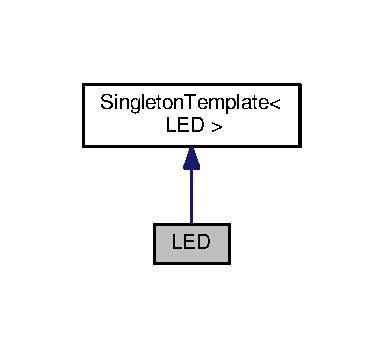
\includegraphics[width=184pt]{df/d30/classLED__inherit__graph}
\end{center}
\end{figure}


Collaboration diagram for L\+ED\+:\nopagebreak
\begin{figure}[H]
\begin{center}
\leavevmode
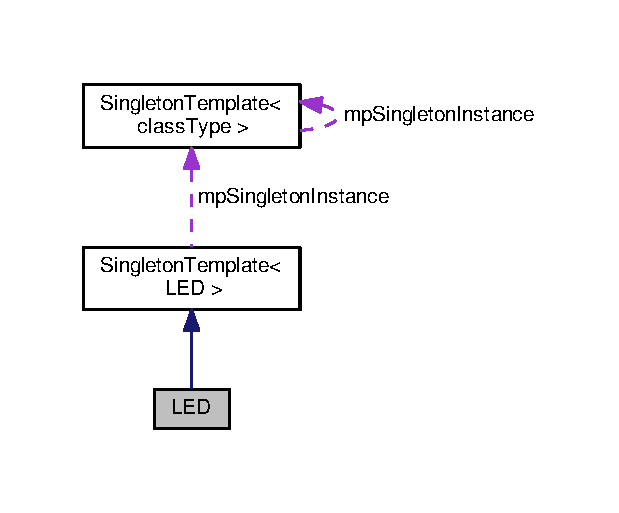
\includegraphics[width=297pt]{d6/ddf/classLED__coll__graph}
\end{center}
\end{figure}
\subsection*{Public Member Functions}
\begin{DoxyCompactItemize}
\item 
bool \hyperlink{classLED_a63962161aba1782dd879760c5960d6b5}{init} ()
\begin{DoxyCompactList}\small\item\em Initializes this device,. \end{DoxyCompactList}\item 
void \hyperlink{classLED_acc39ccc6387373b840912f21d62dc876}{on} (uint8\+\_\+t led\+Num)
\begin{DoxyCompactList}\small\item\em Turns ON \hyperlink{classLED}{L\+ED}. \end{DoxyCompactList}\item 
void \hyperlink{classLED_addf41e0b79325809d8cc12b792aaae97}{off} (uint8\+\_\+t led\+Num)
\begin{DoxyCompactList}\small\item\em Turns O\+FF \hyperlink{classLED}{L\+ED}. \end{DoxyCompactList}\item 
void \hyperlink{classLED_a31971293aa8763338871c9b2789cb606}{set} (uint8\+\_\+t led\+Num, bool \hyperlink{classLED_acc39ccc6387373b840912f21d62dc876}{on})
\begin{DoxyCompactList}\small\item\em Turns on/off led based on. \end{DoxyCompactList}\item 
void \hyperlink{classLED_aaf40ad52100d7bebb418a2b48bd5a5bf}{toggle} (uint8\+\_\+t led\+Num)
\begin{DoxyCompactList}\small\item\em Toggles the \hyperlink{classLED}{L\+ED}. \end{DoxyCompactList}\item 
void \hyperlink{classLED_a227f3bc652bf914afdeb3cbb73d1b927}{set\+All} (uint8\+\_\+t value)
\begin{DoxyCompactList}\small\item\em Sets 8-\/bit value of 8 L\+E\+Ds; 1 bit per \hyperlink{classLED}{L\+ED}. \end{DoxyCompactList}\item 
uint8\+\_\+t \hyperlink{classLED_a55aa5615bfa11cf5f127a08565a86796}{get\+Values} (void) const 
\begin{DoxyCompactList}\small\item\em Get the \hyperlink{classLED}{L\+ED} bit values currently set. \end{DoxyCompactList}\end{DoxyCompactItemize}
\subsection*{Friends}
\begin{DoxyCompactItemize}
\item 
class \hyperlink{classLED_ab4116020d7b7ad8103b2787995cb15b4}{Singleton\+Template$<$ L\+E\+D $>$}
\begin{DoxyCompactList}\small\item\em Friend class used for Singleton Template. \end{DoxyCompactList}\end{DoxyCompactItemize}
\subsection*{Additional Inherited Members}


\subsection{Detailed Description}
\hyperlink{classLED}{L\+ED} class used to control the Board\textquotesingle{}s 8 output L\+E\+Ds 

\subsection{Member Function Documentation}
\index{L\+ED@{L\+ED}!get\+Values@{get\+Values}}
\index{get\+Values@{get\+Values}!L\+ED@{L\+ED}}
\subsubsection[{\texorpdfstring{get\+Values(void) const }{getValues(void) const }}]{\setlength{\rightskip}{0pt plus 5cm}uint8\+\_\+t L\+E\+D\+::get\+Values (
\begin{DoxyParamCaption}
\item[{void}]{}
\end{DoxyParamCaption}
) const}\hypertarget{classLED_a55aa5615bfa11cf5f127a08565a86796}{}\label{classLED_a55aa5615bfa11cf5f127a08565a86796}


Get the \hyperlink{classLED}{L\+ED} bit values currently set. 

\index{L\+ED@{L\+ED}!init@{init}}
\index{init@{init}!L\+ED@{L\+ED}}
\subsubsection[{\texorpdfstring{init()}{init()}}]{\setlength{\rightskip}{0pt plus 5cm}bool L\+E\+D\+::init (
\begin{DoxyParamCaption}
\item[{void}]{}
\end{DoxyParamCaption}
)}\hypertarget{classLED_a63962161aba1782dd879760c5960d6b5}{}\label{classLED_a63962161aba1782dd879760c5960d6b5}


Initializes this device,. 

\begin{DoxyReturn}{Returns}
true if successful 
\end{DoxyReturn}
\index{L\+ED@{L\+ED}!off@{off}}
\index{off@{off}!L\+ED@{L\+ED}}
\subsubsection[{\texorpdfstring{off(uint8\+\_\+t led\+Num)}{off(uint8_t ledNum)}}]{\setlength{\rightskip}{0pt plus 5cm}void L\+E\+D\+::off (
\begin{DoxyParamCaption}
\item[{uint8\+\_\+t}]{led\+Num}
\end{DoxyParamCaption}
)}\hypertarget{classLED_addf41e0b79325809d8cc12b792aaae97}{}\label{classLED_addf41e0b79325809d8cc12b792aaae97}


Turns O\+FF \hyperlink{classLED}{L\+ED}. 


\begin{DoxyParams}{Parameters}
{\em led\+Num} & The \hyperlink{classLED}{L\+ED} \# from 1-\/4 \\
\hline
\end{DoxyParams}
\index{L\+ED@{L\+ED}!on@{on}}
\index{on@{on}!L\+ED@{L\+ED}}
\subsubsection[{\texorpdfstring{on(uint8\+\_\+t led\+Num)}{on(uint8_t ledNum)}}]{\setlength{\rightskip}{0pt plus 5cm}void L\+E\+D\+::on (
\begin{DoxyParamCaption}
\item[{uint8\+\_\+t}]{led\+Num}
\end{DoxyParamCaption}
)}\hypertarget{classLED_acc39ccc6387373b840912f21d62dc876}{}\label{classLED_acc39ccc6387373b840912f21d62dc876}


Turns ON \hyperlink{classLED}{L\+ED}. 


\begin{DoxyParams}{Parameters}
{\em led\+Num} & The \hyperlink{classLED}{L\+ED} \# from 1-\/4 \\
\hline
\end{DoxyParams}
\index{L\+ED@{L\+ED}!set@{set}}
\index{set@{set}!L\+ED@{L\+ED}}
\subsubsection[{\texorpdfstring{set(uint8\+\_\+t led\+Num, bool on)}{set(uint8_t ledNum, bool on)}}]{\setlength{\rightskip}{0pt plus 5cm}void L\+E\+D\+::set (
\begin{DoxyParamCaption}
\item[{uint8\+\_\+t}]{led\+Num, }
\item[{bool}]{on}
\end{DoxyParamCaption}
)}\hypertarget{classLED_a31971293aa8763338871c9b2789cb606}{}\label{classLED_a31971293aa8763338871c9b2789cb606}


Turns on/off led based on. 


\begin{DoxyParams}{Parameters}
{\em on} & \\
\hline
\end{DoxyParams}
\index{L\+ED@{L\+ED}!set\+All@{set\+All}}
\index{set\+All@{set\+All}!L\+ED@{L\+ED}}
\subsubsection[{\texorpdfstring{set\+All(uint8\+\_\+t value)}{setAll(uint8_t value)}}]{\setlength{\rightskip}{0pt plus 5cm}void L\+E\+D\+::set\+All (
\begin{DoxyParamCaption}
\item[{uint8\+\_\+t}]{value}
\end{DoxyParamCaption}
)}\hypertarget{classLED_a227f3bc652bf914afdeb3cbb73d1b927}{}\label{classLED_a227f3bc652bf914afdeb3cbb73d1b927}


Sets 8-\/bit value of 8 L\+E\+Ds; 1 bit per \hyperlink{classLED}{L\+ED}. 

\index{L\+ED@{L\+ED}!toggle@{toggle}}
\index{toggle@{toggle}!L\+ED@{L\+ED}}
\subsubsection[{\texorpdfstring{toggle(uint8\+\_\+t led\+Num)}{toggle(uint8_t ledNum)}}]{\setlength{\rightskip}{0pt plus 5cm}void L\+E\+D\+::toggle (
\begin{DoxyParamCaption}
\item[{uint8\+\_\+t}]{led\+Num}
\end{DoxyParamCaption}
)}\hypertarget{classLED_aaf40ad52100d7bebb418a2b48bd5a5bf}{}\label{classLED_aaf40ad52100d7bebb418a2b48bd5a5bf}


Toggles the \hyperlink{classLED}{L\+ED}. 



\subsection{Friends And Related Function Documentation}
\index{L\+ED@{L\+ED}!Singleton\+Template$<$ L\+E\+D $>$@{Singleton\+Template$<$ L\+E\+D $>$}}
\index{Singleton\+Template$<$ L\+E\+D $>$@{Singleton\+Template$<$ L\+E\+D $>$}!L\+ED@{L\+ED}}
\subsubsection[{\texorpdfstring{Singleton\+Template$<$ L\+E\+D $>$}{SingletonTemplate< LED >}}]{\setlength{\rightskip}{0pt plus 5cm}friend class {\bf Singleton\+Template}$<$ {\bf L\+ED} $>$\hspace{0.3cm}{\ttfamily [friend]}}\hypertarget{classLED_ab4116020d7b7ad8103b2787995cb15b4}{}\label{classLED_ab4116020d7b7ad8103b2787995cb15b4}


Friend class used for Singleton Template. 



The documentation for this class was generated from the following files\+:\begin{DoxyCompactItemize}
\item 
/var/www/html/\+S\+J\+S\+U-\/\+D\+E\+V-\/\+Linux/firmware/default/lib/\+L4\+\_\+\+I\+O/\hyperlink{LED_8hpp}{L\+E\+D.\+hpp}\item 
/var/www/html/\+S\+J\+S\+U-\/\+D\+E\+V-\/\+Linux/firmware/default/lib/\+L4\+\_\+\+I\+O/src/\hyperlink{io__source_8cpp}{io\+\_\+source.\+cpp}\end{DoxyCompactItemize}

\hypertarget{classLED__Display}{}\section{L\+E\+D\+\_\+\+Display Class Reference}
\label{classLED__Display}\index{L\+E\+D\+\_\+\+Display@{L\+E\+D\+\_\+\+Display}}


{\ttfamily \#include $<$L\+E\+D\+\_\+\+Display.\+hpp$>$}



Inheritance diagram for L\+E\+D\+\_\+\+Display\+:\nopagebreak
\begin{figure}[H]
\begin{center}
\leavevmode
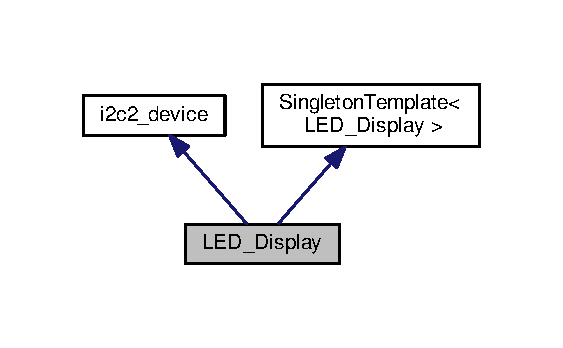
\includegraphics[width=270pt]{df/d9b/classLED__Display__inherit__graph}
\end{center}
\end{figure}


Collaboration diagram for L\+E\+D\+\_\+\+Display\+:\nopagebreak
\begin{figure}[H]
\begin{center}
\leavevmode
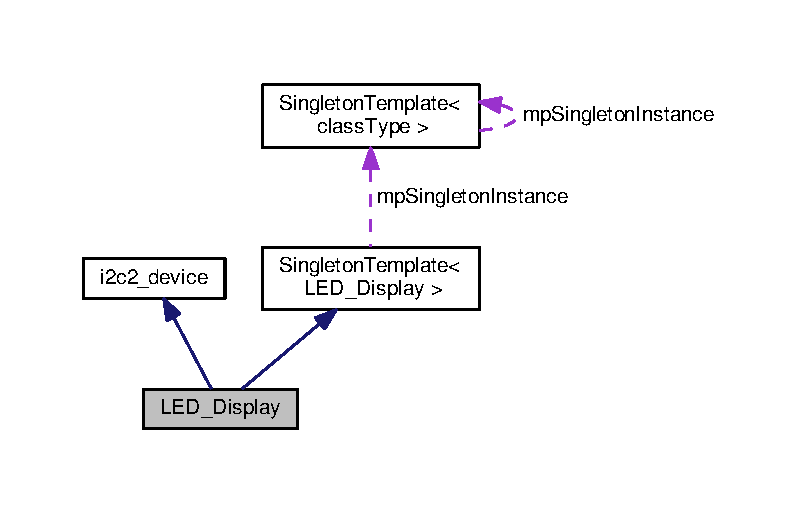
\includegraphics[width=350pt]{d2/d5d/classLED__Display__coll__graph}
\end{center}
\end{figure}
\subsection*{Public Member Functions}
\begin{DoxyCompactItemize}
\item 
bool \hyperlink{classLED__Display_a075e60d1b0829a70f03f0a342bffcb21}{init} ()
\begin{DoxyCompactList}\small\item\em Initializes this device,. \end{DoxyCompactList}\item 
void \hyperlink{classLED__Display_aa1ec976d360ad46ecb7e437cfad97ea5}{clear} ()
\item 
void \hyperlink{classLED__Display_a8802392543700dc03694b56b2c946c5a}{set\+Number} (char num)
\end{DoxyCompactItemize}
{\bf }\par
\begin{DoxyCompactItemize}
\item 
void \hyperlink{classLED__Display_a4d7e45c39a2bef9ddfe4167b240cfb18}{set\+Left\+Digit} (char alpha)
\item 
void \hyperlink{classLED__Display_a836014e9527724cb8fcadbc37582fba3}{set\+Right\+Digit} (char alpha)
\end{DoxyCompactItemize}

\subsection*{Friends}
\begin{DoxyCompactItemize}
\item 
class \hyperlink{classLED__Display_a7a993cfbec5ab2677708ad0426cf843b}{Singleton\+Template$<$ L\+E\+D\+\_\+\+Display $>$}
\begin{DoxyCompactList}\small\item\em Friend class used for Singleton Template. \end{DoxyCompactList}\end{DoxyCompactItemize}
\subsection*{Additional Inherited Members}


\subsection{Detailed Description}
\hyperlink{classLED}{L\+ED} Display class to manipulate the on-\/board 2 digit \hyperlink{classLED}{L\+ED} display 

\subsection{Member Function Documentation}
\index{L\+E\+D\+\_\+\+Display@{L\+E\+D\+\_\+\+Display}!clear@{clear}}
\index{clear@{clear}!L\+E\+D\+\_\+\+Display@{L\+E\+D\+\_\+\+Display}}
\subsubsection[{\texorpdfstring{clear()}{clear()}}]{\setlength{\rightskip}{0pt plus 5cm}void L\+E\+D\+\_\+\+Display\+::clear (
\begin{DoxyParamCaption}
\item[{void}]{}
\end{DoxyParamCaption}
)}\hypertarget{classLED__Display_aa1ec976d360ad46ecb7e437cfad97ea5}{}\label{classLED__Display_aa1ec976d360ad46ecb7e437cfad97ea5}
Clears the display \index{L\+E\+D\+\_\+\+Display@{L\+E\+D\+\_\+\+Display}!init@{init}}
\index{init@{init}!L\+E\+D\+\_\+\+Display@{L\+E\+D\+\_\+\+Display}}
\subsubsection[{\texorpdfstring{init()}{init()}}]{\setlength{\rightskip}{0pt plus 5cm}bool L\+E\+D\+\_\+\+Display\+::init (
\begin{DoxyParamCaption}
\item[{void}]{}
\end{DoxyParamCaption}
)}\hypertarget{classLED__Display_a075e60d1b0829a70f03f0a342bffcb21}{}\label{classLED__Display_a075e60d1b0829a70f03f0a342bffcb21}


Initializes this device,. 

\begin{DoxyReturn}{Returns}
true if successful 
\end{DoxyReturn}
\index{L\+E\+D\+\_\+\+Display@{L\+E\+D\+\_\+\+Display}!set\+Left\+Digit@{set\+Left\+Digit}}
\index{set\+Left\+Digit@{set\+Left\+Digit}!L\+E\+D\+\_\+\+Display@{L\+E\+D\+\_\+\+Display}}
\subsubsection[{\texorpdfstring{set\+Left\+Digit(char alpha)}{setLeftDigit(char alpha)}}]{\setlength{\rightskip}{0pt plus 5cm}void L\+E\+D\+\_\+\+Display\+::set\+Left\+Digit (
\begin{DoxyParamCaption}
\item[{char}]{alpha}
\end{DoxyParamCaption}
)}\hypertarget{classLED__Display_a4d7e45c39a2bef9ddfe4167b240cfb18}{}\label{classLED__Display_a4d7e45c39a2bef9ddfe4167b240cfb18}
Single Digit Manipulation Functions Sets the left and right alpha-\/numeric display individually 
\begin{DoxyParams}{Parameters}
{\em alpha} & The alpha to set, such as \char`\"{}\+B\char`\"{} or \char`\"{}9\char`\"{} \\
\hline
\end{DoxyParams}
\begin{DoxyNote}{Note}
Note all characters can be displayed on this 7-\/segment display 
\end{DoxyNote}
\index{L\+E\+D\+\_\+\+Display@{L\+E\+D\+\_\+\+Display}!set\+Number@{set\+Number}}
\index{set\+Number@{set\+Number}!L\+E\+D\+\_\+\+Display@{L\+E\+D\+\_\+\+Display}}
\subsubsection[{\texorpdfstring{set\+Number(char num)}{setNumber(char num)}}]{\setlength{\rightskip}{0pt plus 5cm}void L\+E\+D\+\_\+\+Display\+::set\+Number (
\begin{DoxyParamCaption}
\item[{char}]{num}
\end{DoxyParamCaption}
)}\hypertarget{classLED__Display_a8802392543700dc03694b56b2c946c5a}{}\label{classLED__Display_a8802392543700dc03694b56b2c946c5a}
Sets the number on \hyperlink{classLED}{L\+ED} display 
\begin{DoxyParams}{Parameters}
{\em num} & A number less than 100 \\
\hline
\end{DoxyParams}
\index{L\+E\+D\+\_\+\+Display@{L\+E\+D\+\_\+\+Display}!set\+Right\+Digit@{set\+Right\+Digit}}
\index{set\+Right\+Digit@{set\+Right\+Digit}!L\+E\+D\+\_\+\+Display@{L\+E\+D\+\_\+\+Display}}
\subsubsection[{\texorpdfstring{set\+Right\+Digit(char alpha)}{setRightDigit(char alpha)}}]{\setlength{\rightskip}{0pt plus 5cm}void L\+E\+D\+\_\+\+Display\+::set\+Right\+Digit (
\begin{DoxyParamCaption}
\item[{char}]{alpha}
\end{DoxyParamCaption}
)}\hypertarget{classLED__Display_a836014e9527724cb8fcadbc37582fba3}{}\label{classLED__Display_a836014e9527724cb8fcadbc37582fba3}


\subsection{Friends And Related Function Documentation}
\index{L\+E\+D\+\_\+\+Display@{L\+E\+D\+\_\+\+Display}!Singleton\+Template$<$ L\+E\+D\+\_\+\+Display $>$@{Singleton\+Template$<$ L\+E\+D\+\_\+\+Display $>$}}
\index{Singleton\+Template$<$ L\+E\+D\+\_\+\+Display $>$@{Singleton\+Template$<$ L\+E\+D\+\_\+\+Display $>$}!L\+E\+D\+\_\+\+Display@{L\+E\+D\+\_\+\+Display}}
\subsubsection[{\texorpdfstring{Singleton\+Template$<$ L\+E\+D\+\_\+\+Display $>$}{SingletonTemplate< LED_Display >}}]{\setlength{\rightskip}{0pt plus 5cm}friend class {\bf Singleton\+Template}$<$ {\bf L\+E\+D\+\_\+\+Display} $>$\hspace{0.3cm}{\ttfamily [friend]}}\hypertarget{classLED__Display_a7a993cfbec5ab2677708ad0426cf843b}{}\label{classLED__Display_a7a993cfbec5ab2677708ad0426cf843b}


Friend class used for Singleton Template. 



The documentation for this class was generated from the following files\+:\begin{DoxyCompactItemize}
\item 
/var/www/html/\+S\+J\+S\+U-\/\+D\+E\+V-\/\+Linux/firmware/default/lib/\+L4\+\_\+\+I\+O/\hyperlink{LED__Display_8hpp}{L\+E\+D\+\_\+\+Display.\+hpp}\item 
/var/www/html/\+S\+J\+S\+U-\/\+D\+E\+V-\/\+Linux/firmware/default/lib/\+L4\+\_\+\+I\+O/src/\hyperlink{io__source_8cpp}{io\+\_\+source.\+cpp}\end{DoxyCompactItemize}

\hypertarget{classLight__Sensor}{}\section{Light\+\_\+\+Sensor Class Reference}
\label{classLight__Sensor}\index{Light\+\_\+\+Sensor@{Light\+\_\+\+Sensor}}


{\ttfamily \#include $<$light\+\_\+sensor.\+hpp$>$}



Inheritance diagram for Light\+\_\+\+Sensor\+:\nopagebreak
\begin{figure}[H]
\begin{center}
\leavevmode
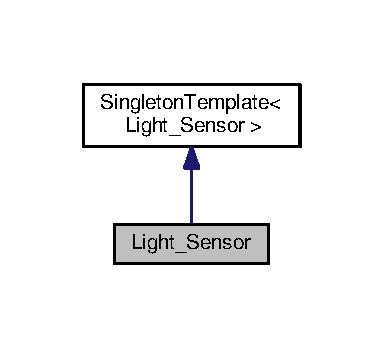
\includegraphics[width=184pt]{df/d80/classLight__Sensor__inherit__graph}
\end{center}
\end{figure}


Collaboration diagram for Light\+\_\+\+Sensor\+:\nopagebreak
\begin{figure}[H]
\begin{center}
\leavevmode
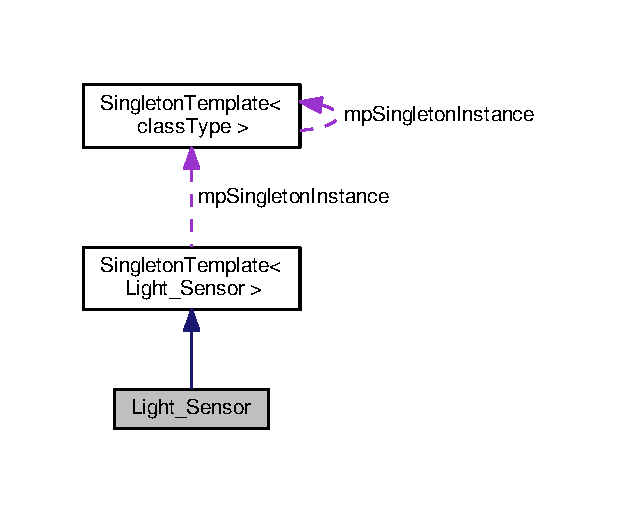
\includegraphics[width=297pt]{d5/d24/classLight__Sensor__coll__graph}
\end{center}
\end{figure}
\subsection*{Public Member Functions}
\begin{DoxyCompactItemize}
\item 
bool \hyperlink{classLight__Sensor_af991847909c0f4af7b92fae8e2028d61}{init} ()
\begin{DoxyCompactList}\small\item\em Initializes this device,. \end{DoxyCompactList}\item 
uint16\+\_\+t \hyperlink{classLight__Sensor_a0e491c2413a3a391989c30ebfef96d18}{get\+Raw\+Value} ()
\item 
uint8\+\_\+t \hyperlink{classLight__Sensor_a91e42027d38409b6dcf3ffc73f0dd0cd}{get\+Percent\+Value} ()
\end{DoxyCompactItemize}
\subsection*{Friends}
\begin{DoxyCompactItemize}
\item 
class \hyperlink{classLight__Sensor_a27b0e5f4de88754c9f4620bf0029f6de}{Singleton\+Template$<$ Light\+\_\+\+Sensor $>$}
\begin{DoxyCompactList}\small\item\em Friend class used for Singleton Template. \end{DoxyCompactList}\end{DoxyCompactItemize}
\subsection*{Additional Inherited Members}


\subsection{Detailed Description}
Light Sensor class used to get light reading from the Board\textquotesingle{}s Light Sensor 

\subsection{Member Function Documentation}
\index{Light\+\_\+\+Sensor@{Light\+\_\+\+Sensor}!get\+Percent\+Value@{get\+Percent\+Value}}
\index{get\+Percent\+Value@{get\+Percent\+Value}!Light\+\_\+\+Sensor@{Light\+\_\+\+Sensor}}
\subsubsection[{\texorpdfstring{get\+Percent\+Value()}{getPercentValue()}}]{\setlength{\rightskip}{0pt plus 5cm}uint8\+\_\+t Light\+\_\+\+Sensor\+::get\+Percent\+Value (
\begin{DoxyParamCaption}
{}
\end{DoxyParamCaption}
)}\hypertarget{classLight__Sensor_a91e42027d38409b6dcf3ffc73f0dd0cd}{}\label{classLight__Sensor_a91e42027d38409b6dcf3ffc73f0dd0cd}
\begin{DoxyReturn}{Returns}
light sensor reading as percentage 
\end{DoxyReturn}
\index{Light\+\_\+\+Sensor@{Light\+\_\+\+Sensor}!get\+Raw\+Value@{get\+Raw\+Value}}
\index{get\+Raw\+Value@{get\+Raw\+Value}!Light\+\_\+\+Sensor@{Light\+\_\+\+Sensor}}
\subsubsection[{\texorpdfstring{get\+Raw\+Value()}{getRawValue()}}]{\setlength{\rightskip}{0pt plus 5cm}uint16\+\_\+t Light\+\_\+\+Sensor\+::get\+Raw\+Value (
\begin{DoxyParamCaption}
{}
\end{DoxyParamCaption}
)}\hypertarget{classLight__Sensor_a0e491c2413a3a391989c30ebfef96d18}{}\label{classLight__Sensor_a0e491c2413a3a391989c30ebfef96d18}
\begin{DoxyReturn}{Returns}
light sensor reading 
\end{DoxyReturn}
\index{Light\+\_\+\+Sensor@{Light\+\_\+\+Sensor}!init@{init}}
\index{init@{init}!Light\+\_\+\+Sensor@{Light\+\_\+\+Sensor}}
\subsubsection[{\texorpdfstring{init()}{init()}}]{\setlength{\rightskip}{0pt plus 5cm}bool Light\+\_\+\+Sensor\+::init (
\begin{DoxyParamCaption}
\item[{void}]{}
\end{DoxyParamCaption}
)}\hypertarget{classLight__Sensor_af991847909c0f4af7b92fae8e2028d61}{}\label{classLight__Sensor_af991847909c0f4af7b92fae8e2028d61}


Initializes this device,. 

\begin{DoxyReturn}{Returns}
true if successful 
\end{DoxyReturn}


\subsection{Friends And Related Function Documentation}
\index{Light\+\_\+\+Sensor@{Light\+\_\+\+Sensor}!Singleton\+Template$<$ Light\+\_\+\+Sensor $>$@{Singleton\+Template$<$ Light\+\_\+\+Sensor $>$}}
\index{Singleton\+Template$<$ Light\+\_\+\+Sensor $>$@{Singleton\+Template$<$ Light\+\_\+\+Sensor $>$}!Light\+\_\+\+Sensor@{Light\+\_\+\+Sensor}}
\subsubsection[{\texorpdfstring{Singleton\+Template$<$ Light\+\_\+\+Sensor $>$}{SingletonTemplate< Light_Sensor >}}]{\setlength{\rightskip}{0pt plus 5cm}friend class {\bf Singleton\+Template}$<$ {\bf Light\+\_\+\+Sensor} $>$\hspace{0.3cm}{\ttfamily [friend]}}\hypertarget{classLight__Sensor_a27b0e5f4de88754c9f4620bf0029f6de}{}\label{classLight__Sensor_a27b0e5f4de88754c9f4620bf0029f6de}


Friend class used for Singleton Template. 



The documentation for this class was generated from the following files\+:\begin{DoxyCompactItemize}
\item 
/var/www/html/\+S\+J\+S\+U-\/\+D\+E\+V-\/\+Linux/firmware/default/lib/\+L4\+\_\+\+I\+O/\hyperlink{light__sensor_8hpp}{light\+\_\+sensor.\+hpp}\item 
/var/www/html/\+S\+J\+S\+U-\/\+D\+E\+V-\/\+Linux/firmware/default/lib/\+L4\+\_\+\+I\+O/src/\hyperlink{io__source_8cpp}{io\+\_\+source.\+cpp}\end{DoxyCompactItemize}

\hypertarget{structLPC__ADC__TypeDef}{}\section{L\+P\+C\+\_\+\+A\+D\+C\+\_\+\+Type\+Def Struct Reference}
\label{structLPC__ADC__TypeDef}\index{L\+P\+C\+\_\+\+A\+D\+C\+\_\+\+Type\+Def@{L\+P\+C\+\_\+\+A\+D\+C\+\_\+\+Type\+Def}}


{\ttfamily \#include $<$L\+P\+C17xx.\+h$>$}

\subsection*{Data Fields}
\begin{DoxyCompactItemize}
\item 
\hyperlink{LPC17xx_8h_aec43007d9998a0a0e01faede4133d6be}{\+\_\+\+\_\+\+IO} uint32\+\_\+t \hyperlink{structLPC__ADC__TypeDef_ab0949d845f781071595de5c830fab8a7}{A\+D\+CR}
\item 
\hyperlink{LPC17xx_8h_aec43007d9998a0a0e01faede4133d6be}{\+\_\+\+\_\+\+IO} uint32\+\_\+t \hyperlink{structLPC__ADC__TypeDef_a9a3d600737fba2be947a6b528cc48891}{A\+D\+G\+DR}
\item 
uint32\+\_\+t \hyperlink{structLPC__ADC__TypeDef_a40cf73fb4dbf0486e17c338b59481012}{R\+E\+S\+E\+R\+V\+E\+D0}
\item 
\hyperlink{LPC17xx_8h_aec43007d9998a0a0e01faede4133d6be}{\+\_\+\+\_\+\+IO} uint32\+\_\+t \hyperlink{structLPC__ADC__TypeDef_a3867c156abd33ddafeb3b51e7b1da97c}{A\+D\+I\+N\+T\+EN}
\item 
\hyperlink{LPC17xx_8h_af63697ed9952cc71e1225efe205f6cd3}{\+\_\+\+\_\+I} uint32\+\_\+t \hyperlink{structLPC__ADC__TypeDef_a3168f35782efa83907f5a1001b5a53e7}{A\+D\+D\+R0}
\item 
\hyperlink{LPC17xx_8h_af63697ed9952cc71e1225efe205f6cd3}{\+\_\+\+\_\+I} uint32\+\_\+t \hyperlink{structLPC__ADC__TypeDef_a7413587e4871c63fecf13646dce2f873}{A\+D\+D\+R1}
\item 
\hyperlink{LPC17xx_8h_af63697ed9952cc71e1225efe205f6cd3}{\+\_\+\+\_\+I} uint32\+\_\+t \hyperlink{structLPC__ADC__TypeDef_a806e8066ea08898ff51e5ff2f10823b3}{A\+D\+D\+R2}
\item 
\hyperlink{LPC17xx_8h_af63697ed9952cc71e1225efe205f6cd3}{\+\_\+\+\_\+I} uint32\+\_\+t \hyperlink{structLPC__ADC__TypeDef_acac24a0ba2d73729b86a021bcad63ad6}{A\+D\+D\+R3}
\item 
\hyperlink{LPC17xx_8h_af63697ed9952cc71e1225efe205f6cd3}{\+\_\+\+\_\+I} uint32\+\_\+t \hyperlink{structLPC__ADC__TypeDef_a92bfddc3c7b32379c91fcde0f43df495}{A\+D\+D\+R4}
\item 
\hyperlink{LPC17xx_8h_af63697ed9952cc71e1225efe205f6cd3}{\+\_\+\+\_\+I} uint32\+\_\+t \hyperlink{structLPC__ADC__TypeDef_ac698d7e4437bf3230071dc3d8274f4bd}{A\+D\+D\+R5}
\item 
\hyperlink{LPC17xx_8h_af63697ed9952cc71e1225efe205f6cd3}{\+\_\+\+\_\+I} uint32\+\_\+t \hyperlink{structLPC__ADC__TypeDef_a607f501dbfce5b3fd777a7a4a480a353}{A\+D\+D\+R6}
\item 
\hyperlink{LPC17xx_8h_af63697ed9952cc71e1225efe205f6cd3}{\+\_\+\+\_\+I} uint32\+\_\+t \hyperlink{structLPC__ADC__TypeDef_a40afea4e61d223f707998d5f22dbfc7c}{A\+D\+D\+R7}
\item 
\hyperlink{LPC17xx_8h_af63697ed9952cc71e1225efe205f6cd3}{\+\_\+\+\_\+I} uint32\+\_\+t \hyperlink{structLPC__ADC__TypeDef_a731ad153d3d54d3ba2677eecb30c3097}{A\+D\+S\+T\+AT}
\item 
\hyperlink{LPC17xx_8h_aec43007d9998a0a0e01faede4133d6be}{\+\_\+\+\_\+\+IO} uint32\+\_\+t \hyperlink{structLPC__ADC__TypeDef_aa66f6667bdd2b2110f2e25e7c8da94a9}{A\+D\+T\+RM}
\end{DoxyCompactItemize}


\subsection{Field Documentation}
\index{L\+P\+C\+\_\+\+A\+D\+C\+\_\+\+Type\+Def@{L\+P\+C\+\_\+\+A\+D\+C\+\_\+\+Type\+Def}!A\+D\+CR@{A\+D\+CR}}
\index{A\+D\+CR@{A\+D\+CR}!L\+P\+C\+\_\+\+A\+D\+C\+\_\+\+Type\+Def@{L\+P\+C\+\_\+\+A\+D\+C\+\_\+\+Type\+Def}}
\subsubsection[{\texorpdfstring{A\+D\+CR}{ADCR}}]{\setlength{\rightskip}{0pt plus 5cm}{\bf \+\_\+\+\_\+\+IO} uint32\+\_\+t L\+P\+C\+\_\+\+A\+D\+C\+\_\+\+Type\+Def\+::\+A\+D\+CR}\hypertarget{structLPC__ADC__TypeDef_ab0949d845f781071595de5c830fab8a7}{}\label{structLPC__ADC__TypeDef_ab0949d845f781071595de5c830fab8a7}
\index{L\+P\+C\+\_\+\+A\+D\+C\+\_\+\+Type\+Def@{L\+P\+C\+\_\+\+A\+D\+C\+\_\+\+Type\+Def}!A\+D\+D\+R0@{A\+D\+D\+R0}}
\index{A\+D\+D\+R0@{A\+D\+D\+R0}!L\+P\+C\+\_\+\+A\+D\+C\+\_\+\+Type\+Def@{L\+P\+C\+\_\+\+A\+D\+C\+\_\+\+Type\+Def}}
\subsubsection[{\texorpdfstring{A\+D\+D\+R0}{ADDR0}}]{\setlength{\rightskip}{0pt plus 5cm}{\bf \+\_\+\+\_\+I} uint32\+\_\+t L\+P\+C\+\_\+\+A\+D\+C\+\_\+\+Type\+Def\+::\+A\+D\+D\+R0}\hypertarget{structLPC__ADC__TypeDef_a3168f35782efa83907f5a1001b5a53e7}{}\label{structLPC__ADC__TypeDef_a3168f35782efa83907f5a1001b5a53e7}
\index{L\+P\+C\+\_\+\+A\+D\+C\+\_\+\+Type\+Def@{L\+P\+C\+\_\+\+A\+D\+C\+\_\+\+Type\+Def}!A\+D\+D\+R1@{A\+D\+D\+R1}}
\index{A\+D\+D\+R1@{A\+D\+D\+R1}!L\+P\+C\+\_\+\+A\+D\+C\+\_\+\+Type\+Def@{L\+P\+C\+\_\+\+A\+D\+C\+\_\+\+Type\+Def}}
\subsubsection[{\texorpdfstring{A\+D\+D\+R1}{ADDR1}}]{\setlength{\rightskip}{0pt plus 5cm}{\bf \+\_\+\+\_\+I} uint32\+\_\+t L\+P\+C\+\_\+\+A\+D\+C\+\_\+\+Type\+Def\+::\+A\+D\+D\+R1}\hypertarget{structLPC__ADC__TypeDef_a7413587e4871c63fecf13646dce2f873}{}\label{structLPC__ADC__TypeDef_a7413587e4871c63fecf13646dce2f873}
\index{L\+P\+C\+\_\+\+A\+D\+C\+\_\+\+Type\+Def@{L\+P\+C\+\_\+\+A\+D\+C\+\_\+\+Type\+Def}!A\+D\+D\+R2@{A\+D\+D\+R2}}
\index{A\+D\+D\+R2@{A\+D\+D\+R2}!L\+P\+C\+\_\+\+A\+D\+C\+\_\+\+Type\+Def@{L\+P\+C\+\_\+\+A\+D\+C\+\_\+\+Type\+Def}}
\subsubsection[{\texorpdfstring{A\+D\+D\+R2}{ADDR2}}]{\setlength{\rightskip}{0pt plus 5cm}{\bf \+\_\+\+\_\+I} uint32\+\_\+t L\+P\+C\+\_\+\+A\+D\+C\+\_\+\+Type\+Def\+::\+A\+D\+D\+R2}\hypertarget{structLPC__ADC__TypeDef_a806e8066ea08898ff51e5ff2f10823b3}{}\label{structLPC__ADC__TypeDef_a806e8066ea08898ff51e5ff2f10823b3}
\index{L\+P\+C\+\_\+\+A\+D\+C\+\_\+\+Type\+Def@{L\+P\+C\+\_\+\+A\+D\+C\+\_\+\+Type\+Def}!A\+D\+D\+R3@{A\+D\+D\+R3}}
\index{A\+D\+D\+R3@{A\+D\+D\+R3}!L\+P\+C\+\_\+\+A\+D\+C\+\_\+\+Type\+Def@{L\+P\+C\+\_\+\+A\+D\+C\+\_\+\+Type\+Def}}
\subsubsection[{\texorpdfstring{A\+D\+D\+R3}{ADDR3}}]{\setlength{\rightskip}{0pt plus 5cm}{\bf \+\_\+\+\_\+I} uint32\+\_\+t L\+P\+C\+\_\+\+A\+D\+C\+\_\+\+Type\+Def\+::\+A\+D\+D\+R3}\hypertarget{structLPC__ADC__TypeDef_acac24a0ba2d73729b86a021bcad63ad6}{}\label{structLPC__ADC__TypeDef_acac24a0ba2d73729b86a021bcad63ad6}
\index{L\+P\+C\+\_\+\+A\+D\+C\+\_\+\+Type\+Def@{L\+P\+C\+\_\+\+A\+D\+C\+\_\+\+Type\+Def}!A\+D\+D\+R4@{A\+D\+D\+R4}}
\index{A\+D\+D\+R4@{A\+D\+D\+R4}!L\+P\+C\+\_\+\+A\+D\+C\+\_\+\+Type\+Def@{L\+P\+C\+\_\+\+A\+D\+C\+\_\+\+Type\+Def}}
\subsubsection[{\texorpdfstring{A\+D\+D\+R4}{ADDR4}}]{\setlength{\rightskip}{0pt plus 5cm}{\bf \+\_\+\+\_\+I} uint32\+\_\+t L\+P\+C\+\_\+\+A\+D\+C\+\_\+\+Type\+Def\+::\+A\+D\+D\+R4}\hypertarget{structLPC__ADC__TypeDef_a92bfddc3c7b32379c91fcde0f43df495}{}\label{structLPC__ADC__TypeDef_a92bfddc3c7b32379c91fcde0f43df495}
\index{L\+P\+C\+\_\+\+A\+D\+C\+\_\+\+Type\+Def@{L\+P\+C\+\_\+\+A\+D\+C\+\_\+\+Type\+Def}!A\+D\+D\+R5@{A\+D\+D\+R5}}
\index{A\+D\+D\+R5@{A\+D\+D\+R5}!L\+P\+C\+\_\+\+A\+D\+C\+\_\+\+Type\+Def@{L\+P\+C\+\_\+\+A\+D\+C\+\_\+\+Type\+Def}}
\subsubsection[{\texorpdfstring{A\+D\+D\+R5}{ADDR5}}]{\setlength{\rightskip}{0pt plus 5cm}{\bf \+\_\+\+\_\+I} uint32\+\_\+t L\+P\+C\+\_\+\+A\+D\+C\+\_\+\+Type\+Def\+::\+A\+D\+D\+R5}\hypertarget{structLPC__ADC__TypeDef_ac698d7e4437bf3230071dc3d8274f4bd}{}\label{structLPC__ADC__TypeDef_ac698d7e4437bf3230071dc3d8274f4bd}
\index{L\+P\+C\+\_\+\+A\+D\+C\+\_\+\+Type\+Def@{L\+P\+C\+\_\+\+A\+D\+C\+\_\+\+Type\+Def}!A\+D\+D\+R6@{A\+D\+D\+R6}}
\index{A\+D\+D\+R6@{A\+D\+D\+R6}!L\+P\+C\+\_\+\+A\+D\+C\+\_\+\+Type\+Def@{L\+P\+C\+\_\+\+A\+D\+C\+\_\+\+Type\+Def}}
\subsubsection[{\texorpdfstring{A\+D\+D\+R6}{ADDR6}}]{\setlength{\rightskip}{0pt plus 5cm}{\bf \+\_\+\+\_\+I} uint32\+\_\+t L\+P\+C\+\_\+\+A\+D\+C\+\_\+\+Type\+Def\+::\+A\+D\+D\+R6}\hypertarget{structLPC__ADC__TypeDef_a607f501dbfce5b3fd777a7a4a480a353}{}\label{structLPC__ADC__TypeDef_a607f501dbfce5b3fd777a7a4a480a353}
\index{L\+P\+C\+\_\+\+A\+D\+C\+\_\+\+Type\+Def@{L\+P\+C\+\_\+\+A\+D\+C\+\_\+\+Type\+Def}!A\+D\+D\+R7@{A\+D\+D\+R7}}
\index{A\+D\+D\+R7@{A\+D\+D\+R7}!L\+P\+C\+\_\+\+A\+D\+C\+\_\+\+Type\+Def@{L\+P\+C\+\_\+\+A\+D\+C\+\_\+\+Type\+Def}}
\subsubsection[{\texorpdfstring{A\+D\+D\+R7}{ADDR7}}]{\setlength{\rightskip}{0pt plus 5cm}{\bf \+\_\+\+\_\+I} uint32\+\_\+t L\+P\+C\+\_\+\+A\+D\+C\+\_\+\+Type\+Def\+::\+A\+D\+D\+R7}\hypertarget{structLPC__ADC__TypeDef_a40afea4e61d223f707998d5f22dbfc7c}{}\label{structLPC__ADC__TypeDef_a40afea4e61d223f707998d5f22dbfc7c}
\index{L\+P\+C\+\_\+\+A\+D\+C\+\_\+\+Type\+Def@{L\+P\+C\+\_\+\+A\+D\+C\+\_\+\+Type\+Def}!A\+D\+G\+DR@{A\+D\+G\+DR}}
\index{A\+D\+G\+DR@{A\+D\+G\+DR}!L\+P\+C\+\_\+\+A\+D\+C\+\_\+\+Type\+Def@{L\+P\+C\+\_\+\+A\+D\+C\+\_\+\+Type\+Def}}
\subsubsection[{\texorpdfstring{A\+D\+G\+DR}{ADGDR}}]{\setlength{\rightskip}{0pt plus 5cm}{\bf \+\_\+\+\_\+\+IO} uint32\+\_\+t L\+P\+C\+\_\+\+A\+D\+C\+\_\+\+Type\+Def\+::\+A\+D\+G\+DR}\hypertarget{structLPC__ADC__TypeDef_a9a3d600737fba2be947a6b528cc48891}{}\label{structLPC__ADC__TypeDef_a9a3d600737fba2be947a6b528cc48891}
\index{L\+P\+C\+\_\+\+A\+D\+C\+\_\+\+Type\+Def@{L\+P\+C\+\_\+\+A\+D\+C\+\_\+\+Type\+Def}!A\+D\+I\+N\+T\+EN@{A\+D\+I\+N\+T\+EN}}
\index{A\+D\+I\+N\+T\+EN@{A\+D\+I\+N\+T\+EN}!L\+P\+C\+\_\+\+A\+D\+C\+\_\+\+Type\+Def@{L\+P\+C\+\_\+\+A\+D\+C\+\_\+\+Type\+Def}}
\subsubsection[{\texorpdfstring{A\+D\+I\+N\+T\+EN}{ADINTEN}}]{\setlength{\rightskip}{0pt plus 5cm}{\bf \+\_\+\+\_\+\+IO} uint32\+\_\+t L\+P\+C\+\_\+\+A\+D\+C\+\_\+\+Type\+Def\+::\+A\+D\+I\+N\+T\+EN}\hypertarget{structLPC__ADC__TypeDef_a3867c156abd33ddafeb3b51e7b1da97c}{}\label{structLPC__ADC__TypeDef_a3867c156abd33ddafeb3b51e7b1da97c}
\index{L\+P\+C\+\_\+\+A\+D\+C\+\_\+\+Type\+Def@{L\+P\+C\+\_\+\+A\+D\+C\+\_\+\+Type\+Def}!A\+D\+S\+T\+AT@{A\+D\+S\+T\+AT}}
\index{A\+D\+S\+T\+AT@{A\+D\+S\+T\+AT}!L\+P\+C\+\_\+\+A\+D\+C\+\_\+\+Type\+Def@{L\+P\+C\+\_\+\+A\+D\+C\+\_\+\+Type\+Def}}
\subsubsection[{\texorpdfstring{A\+D\+S\+T\+AT}{ADSTAT}}]{\setlength{\rightskip}{0pt plus 5cm}{\bf \+\_\+\+\_\+I} uint32\+\_\+t L\+P\+C\+\_\+\+A\+D\+C\+\_\+\+Type\+Def\+::\+A\+D\+S\+T\+AT}\hypertarget{structLPC__ADC__TypeDef_a731ad153d3d54d3ba2677eecb30c3097}{}\label{structLPC__ADC__TypeDef_a731ad153d3d54d3ba2677eecb30c3097}
\index{L\+P\+C\+\_\+\+A\+D\+C\+\_\+\+Type\+Def@{L\+P\+C\+\_\+\+A\+D\+C\+\_\+\+Type\+Def}!A\+D\+T\+RM@{A\+D\+T\+RM}}
\index{A\+D\+T\+RM@{A\+D\+T\+RM}!L\+P\+C\+\_\+\+A\+D\+C\+\_\+\+Type\+Def@{L\+P\+C\+\_\+\+A\+D\+C\+\_\+\+Type\+Def}}
\subsubsection[{\texorpdfstring{A\+D\+T\+RM}{ADTRM}}]{\setlength{\rightskip}{0pt plus 5cm}{\bf \+\_\+\+\_\+\+IO} uint32\+\_\+t L\+P\+C\+\_\+\+A\+D\+C\+\_\+\+Type\+Def\+::\+A\+D\+T\+RM}\hypertarget{structLPC__ADC__TypeDef_aa66f6667bdd2b2110f2e25e7c8da94a9}{}\label{structLPC__ADC__TypeDef_aa66f6667bdd2b2110f2e25e7c8da94a9}
\index{L\+P\+C\+\_\+\+A\+D\+C\+\_\+\+Type\+Def@{L\+P\+C\+\_\+\+A\+D\+C\+\_\+\+Type\+Def}!R\+E\+S\+E\+R\+V\+E\+D0@{R\+E\+S\+E\+R\+V\+E\+D0}}
\index{R\+E\+S\+E\+R\+V\+E\+D0@{R\+E\+S\+E\+R\+V\+E\+D0}!L\+P\+C\+\_\+\+A\+D\+C\+\_\+\+Type\+Def@{L\+P\+C\+\_\+\+A\+D\+C\+\_\+\+Type\+Def}}
\subsubsection[{\texorpdfstring{R\+E\+S\+E\+R\+V\+E\+D0}{RESERVED0}}]{\setlength{\rightskip}{0pt plus 5cm}uint32\+\_\+t L\+P\+C\+\_\+\+A\+D\+C\+\_\+\+Type\+Def\+::\+R\+E\+S\+E\+R\+V\+E\+D0}\hypertarget{structLPC__ADC__TypeDef_a40cf73fb4dbf0486e17c338b59481012}{}\label{structLPC__ADC__TypeDef_a40cf73fb4dbf0486e17c338b59481012}


The documentation for this struct was generated from the following file\+:\begin{DoxyCompactItemize}
\item 
/var/www/html/\+S\+J\+S\+U-\/\+D\+E\+V-\/\+Linux/firmware/default/lib/\+L0\+\_\+\+Low\+Level/\hyperlink{LPC17xx_8h}{L\+P\+C17xx.\+h}\end{DoxyCompactItemize}

\hypertarget{structLPC__CAN__TypeDef}{}\section{L\+P\+C\+\_\+\+C\+A\+N\+\_\+\+Type\+Def Struct Reference}
\label{structLPC__CAN__TypeDef}\index{L\+P\+C\+\_\+\+C\+A\+N\+\_\+\+Type\+Def@{L\+P\+C\+\_\+\+C\+A\+N\+\_\+\+Type\+Def}}


{\ttfamily \#include $<$L\+P\+C17xx.\+h$>$}

\subsection*{Data Fields}
\begin{DoxyCompactItemize}
\item 
\hyperlink{LPC17xx_8h_aec43007d9998a0a0e01faede4133d6be}{\+\_\+\+\_\+\+IO} uint32\+\_\+t \hyperlink{structLPC__CAN__TypeDef_aa552e0d7073db33aef9d5fff30270385}{M\+OD}
\item 
\hyperlink{LPC17xx_8h_a7e25d9380f9ef903923964322e71f2f6}{\+\_\+\+\_\+O} uint32\+\_\+t \hyperlink{structLPC__CAN__TypeDef_a9c4aaea6fbeb16b7f985b0c1deea0a8a}{C\+MR}
\item 
\hyperlink{LPC17xx_8h_aec43007d9998a0a0e01faede4133d6be}{\+\_\+\+\_\+\+IO} uint32\+\_\+t \hyperlink{structLPC__CAN__TypeDef_aaebe05a3f2b42fe710cc55146232709c}{G\+SR}
\item 
\hyperlink{LPC17xx_8h_af63697ed9952cc71e1225efe205f6cd3}{\+\_\+\+\_\+I} uint32\+\_\+t \hyperlink{structLPC__CAN__TypeDef_ab36125aee673455a73715ac364e05b6c}{I\+CR}
\item 
\hyperlink{LPC17xx_8h_aec43007d9998a0a0e01faede4133d6be}{\+\_\+\+\_\+\+IO} uint32\+\_\+t \hyperlink{structLPC__CAN__TypeDef_aeb907d3a6919c93ca9951b62595facea}{I\+ER}
\item 
\hyperlink{LPC17xx_8h_aec43007d9998a0a0e01faede4133d6be}{\+\_\+\+\_\+\+IO} uint32\+\_\+t \hyperlink{structLPC__CAN__TypeDef_a461439cb1fa20001b5177c0589a2fdcc}{B\+TR}
\item 
\hyperlink{LPC17xx_8h_aec43007d9998a0a0e01faede4133d6be}{\+\_\+\+\_\+\+IO} uint32\+\_\+t \hyperlink{structLPC__CAN__TypeDef_ad14ee65dbb90b26a372a549efafa951a}{E\+WL}
\item 
\hyperlink{LPC17xx_8h_af63697ed9952cc71e1225efe205f6cd3}{\+\_\+\+\_\+I} uint32\+\_\+t \hyperlink{structLPC__CAN__TypeDef_af196d4014a0e6c89397940310a708025}{SR}
\item 
\hyperlink{LPC17xx_8h_aec43007d9998a0a0e01faede4133d6be}{\+\_\+\+\_\+\+IO} uint32\+\_\+t \hyperlink{structLPC__CAN__TypeDef_a1226fc21b1f4530138d8804d4616ee75}{R\+FS}
\item 
\hyperlink{LPC17xx_8h_aec43007d9998a0a0e01faede4133d6be}{\+\_\+\+\_\+\+IO} uint32\+\_\+t \hyperlink{structLPC__CAN__TypeDef_acc2d189e0ce8d151633fe7af32b16751}{R\+ID}
\item 
\hyperlink{LPC17xx_8h_aec43007d9998a0a0e01faede4133d6be}{\+\_\+\+\_\+\+IO} uint32\+\_\+t \hyperlink{structLPC__CAN__TypeDef_a3bf277729e96b67ccdda724d32c401e3}{R\+DA}
\item 
\hyperlink{LPC17xx_8h_aec43007d9998a0a0e01faede4133d6be}{\+\_\+\+\_\+\+IO} uint32\+\_\+t \hyperlink{structLPC__CAN__TypeDef_a9e30d0e614d62cb8c4dcc028b54b1c1c}{R\+DB}
\item 
\hyperlink{LPC17xx_8h_aec43007d9998a0a0e01faede4133d6be}{\+\_\+\+\_\+\+IO} uint32\+\_\+t \hyperlink{structLPC__CAN__TypeDef_a919f2abe173ad747c4956a4b6143c790}{T\+F\+I1}
\item 
\hyperlink{LPC17xx_8h_aec43007d9998a0a0e01faede4133d6be}{\+\_\+\+\_\+\+IO} uint32\+\_\+t \hyperlink{structLPC__CAN__TypeDef_ad941f092e33373988b99e82eb8da7b98}{T\+I\+D1}
\item 
\hyperlink{LPC17xx_8h_aec43007d9998a0a0e01faede4133d6be}{\+\_\+\+\_\+\+IO} uint32\+\_\+t \hyperlink{structLPC__CAN__TypeDef_a9407b69dad93493645a9a52ae0c5b4e5}{T\+D\+A1}
\item 
\hyperlink{LPC17xx_8h_aec43007d9998a0a0e01faede4133d6be}{\+\_\+\+\_\+\+IO} uint32\+\_\+t \hyperlink{structLPC__CAN__TypeDef_aaa983819f65057aa69ebc505063a4ed4}{T\+D\+B1}
\item 
\hyperlink{LPC17xx_8h_aec43007d9998a0a0e01faede4133d6be}{\+\_\+\+\_\+\+IO} uint32\+\_\+t \hyperlink{structLPC__CAN__TypeDef_a494b873717ee793057037fc971f29e42}{T\+F\+I2}
\item 
\hyperlink{LPC17xx_8h_aec43007d9998a0a0e01faede4133d6be}{\+\_\+\+\_\+\+IO} uint32\+\_\+t \hyperlink{structLPC__CAN__TypeDef_aa5df91f305a251b272faf9ec198ec0e8}{T\+I\+D2}
\item 
\hyperlink{LPC17xx_8h_aec43007d9998a0a0e01faede4133d6be}{\+\_\+\+\_\+\+IO} uint32\+\_\+t \hyperlink{structLPC__CAN__TypeDef_a015d5bfc31a5bfd088f13235096b6f96}{T\+D\+A2}
\item 
\hyperlink{LPC17xx_8h_aec43007d9998a0a0e01faede4133d6be}{\+\_\+\+\_\+\+IO} uint32\+\_\+t \hyperlink{structLPC__CAN__TypeDef_a24bc89ade505be907bb328e52480ab71}{T\+D\+B2}
\item 
\hyperlink{LPC17xx_8h_aec43007d9998a0a0e01faede4133d6be}{\+\_\+\+\_\+\+IO} uint32\+\_\+t \hyperlink{structLPC__CAN__TypeDef_a19178f6639ceb8596a96e66674c0d840}{T\+F\+I3}
\item 
\hyperlink{LPC17xx_8h_aec43007d9998a0a0e01faede4133d6be}{\+\_\+\+\_\+\+IO} uint32\+\_\+t \hyperlink{structLPC__CAN__TypeDef_a8ad7b5ae2f928f189fea5f021789e1e2}{T\+I\+D3}
\item 
\hyperlink{LPC17xx_8h_aec43007d9998a0a0e01faede4133d6be}{\+\_\+\+\_\+\+IO} uint32\+\_\+t \hyperlink{structLPC__CAN__TypeDef_a4700b9e9bb0a2f5230fe59e27746038f}{T\+D\+A3}
\item 
\hyperlink{LPC17xx_8h_aec43007d9998a0a0e01faede4133d6be}{\+\_\+\+\_\+\+IO} uint32\+\_\+t \hyperlink{structLPC__CAN__TypeDef_aeb52795fc9c58e15fc05c7fe43faab4f}{T\+D\+B3}
\end{DoxyCompactItemize}


\subsection{Field Documentation}
\index{L\+P\+C\+\_\+\+C\+A\+N\+\_\+\+Type\+Def@{L\+P\+C\+\_\+\+C\+A\+N\+\_\+\+Type\+Def}!B\+TR@{B\+TR}}
\index{B\+TR@{B\+TR}!L\+P\+C\+\_\+\+C\+A\+N\+\_\+\+Type\+Def@{L\+P\+C\+\_\+\+C\+A\+N\+\_\+\+Type\+Def}}
\subsubsection[{\texorpdfstring{B\+TR}{BTR}}]{\setlength{\rightskip}{0pt plus 5cm}{\bf \+\_\+\+\_\+\+IO} uint32\+\_\+t L\+P\+C\+\_\+\+C\+A\+N\+\_\+\+Type\+Def\+::\+B\+TR}\hypertarget{structLPC__CAN__TypeDef_a461439cb1fa20001b5177c0589a2fdcc}{}\label{structLPC__CAN__TypeDef_a461439cb1fa20001b5177c0589a2fdcc}
\index{L\+P\+C\+\_\+\+C\+A\+N\+\_\+\+Type\+Def@{L\+P\+C\+\_\+\+C\+A\+N\+\_\+\+Type\+Def}!C\+MR@{C\+MR}}
\index{C\+MR@{C\+MR}!L\+P\+C\+\_\+\+C\+A\+N\+\_\+\+Type\+Def@{L\+P\+C\+\_\+\+C\+A\+N\+\_\+\+Type\+Def}}
\subsubsection[{\texorpdfstring{C\+MR}{CMR}}]{\setlength{\rightskip}{0pt plus 5cm}{\bf \+\_\+\+\_\+O} uint32\+\_\+t L\+P\+C\+\_\+\+C\+A\+N\+\_\+\+Type\+Def\+::\+C\+MR}\hypertarget{structLPC__CAN__TypeDef_a9c4aaea6fbeb16b7f985b0c1deea0a8a}{}\label{structLPC__CAN__TypeDef_a9c4aaea6fbeb16b7f985b0c1deea0a8a}
\index{L\+P\+C\+\_\+\+C\+A\+N\+\_\+\+Type\+Def@{L\+P\+C\+\_\+\+C\+A\+N\+\_\+\+Type\+Def}!E\+WL@{E\+WL}}
\index{E\+WL@{E\+WL}!L\+P\+C\+\_\+\+C\+A\+N\+\_\+\+Type\+Def@{L\+P\+C\+\_\+\+C\+A\+N\+\_\+\+Type\+Def}}
\subsubsection[{\texorpdfstring{E\+WL}{EWL}}]{\setlength{\rightskip}{0pt plus 5cm}{\bf \+\_\+\+\_\+\+IO} uint32\+\_\+t L\+P\+C\+\_\+\+C\+A\+N\+\_\+\+Type\+Def\+::\+E\+WL}\hypertarget{structLPC__CAN__TypeDef_ad14ee65dbb90b26a372a549efafa951a}{}\label{structLPC__CAN__TypeDef_ad14ee65dbb90b26a372a549efafa951a}
\index{L\+P\+C\+\_\+\+C\+A\+N\+\_\+\+Type\+Def@{L\+P\+C\+\_\+\+C\+A\+N\+\_\+\+Type\+Def}!G\+SR@{G\+SR}}
\index{G\+SR@{G\+SR}!L\+P\+C\+\_\+\+C\+A\+N\+\_\+\+Type\+Def@{L\+P\+C\+\_\+\+C\+A\+N\+\_\+\+Type\+Def}}
\subsubsection[{\texorpdfstring{G\+SR}{GSR}}]{\setlength{\rightskip}{0pt plus 5cm}{\bf \+\_\+\+\_\+\+IO} uint32\+\_\+t L\+P\+C\+\_\+\+C\+A\+N\+\_\+\+Type\+Def\+::\+G\+SR}\hypertarget{structLPC__CAN__TypeDef_aaebe05a3f2b42fe710cc55146232709c}{}\label{structLPC__CAN__TypeDef_aaebe05a3f2b42fe710cc55146232709c}
\index{L\+P\+C\+\_\+\+C\+A\+N\+\_\+\+Type\+Def@{L\+P\+C\+\_\+\+C\+A\+N\+\_\+\+Type\+Def}!I\+CR@{I\+CR}}
\index{I\+CR@{I\+CR}!L\+P\+C\+\_\+\+C\+A\+N\+\_\+\+Type\+Def@{L\+P\+C\+\_\+\+C\+A\+N\+\_\+\+Type\+Def}}
\subsubsection[{\texorpdfstring{I\+CR}{ICR}}]{\setlength{\rightskip}{0pt plus 5cm}{\bf \+\_\+\+\_\+I} uint32\+\_\+t L\+P\+C\+\_\+\+C\+A\+N\+\_\+\+Type\+Def\+::\+I\+CR}\hypertarget{structLPC__CAN__TypeDef_ab36125aee673455a73715ac364e05b6c}{}\label{structLPC__CAN__TypeDef_ab36125aee673455a73715ac364e05b6c}
\index{L\+P\+C\+\_\+\+C\+A\+N\+\_\+\+Type\+Def@{L\+P\+C\+\_\+\+C\+A\+N\+\_\+\+Type\+Def}!I\+ER@{I\+ER}}
\index{I\+ER@{I\+ER}!L\+P\+C\+\_\+\+C\+A\+N\+\_\+\+Type\+Def@{L\+P\+C\+\_\+\+C\+A\+N\+\_\+\+Type\+Def}}
\subsubsection[{\texorpdfstring{I\+ER}{IER}}]{\setlength{\rightskip}{0pt plus 5cm}{\bf \+\_\+\+\_\+\+IO} uint32\+\_\+t L\+P\+C\+\_\+\+C\+A\+N\+\_\+\+Type\+Def\+::\+I\+ER}\hypertarget{structLPC__CAN__TypeDef_aeb907d3a6919c93ca9951b62595facea}{}\label{structLPC__CAN__TypeDef_aeb907d3a6919c93ca9951b62595facea}
\index{L\+P\+C\+\_\+\+C\+A\+N\+\_\+\+Type\+Def@{L\+P\+C\+\_\+\+C\+A\+N\+\_\+\+Type\+Def}!M\+OD@{M\+OD}}
\index{M\+OD@{M\+OD}!L\+P\+C\+\_\+\+C\+A\+N\+\_\+\+Type\+Def@{L\+P\+C\+\_\+\+C\+A\+N\+\_\+\+Type\+Def}}
\subsubsection[{\texorpdfstring{M\+OD}{MOD}}]{\setlength{\rightskip}{0pt plus 5cm}{\bf \+\_\+\+\_\+\+IO} uint32\+\_\+t L\+P\+C\+\_\+\+C\+A\+N\+\_\+\+Type\+Def\+::\+M\+OD}\hypertarget{structLPC__CAN__TypeDef_aa552e0d7073db33aef9d5fff30270385}{}\label{structLPC__CAN__TypeDef_aa552e0d7073db33aef9d5fff30270385}
\index{L\+P\+C\+\_\+\+C\+A\+N\+\_\+\+Type\+Def@{L\+P\+C\+\_\+\+C\+A\+N\+\_\+\+Type\+Def}!R\+DA@{R\+DA}}
\index{R\+DA@{R\+DA}!L\+P\+C\+\_\+\+C\+A\+N\+\_\+\+Type\+Def@{L\+P\+C\+\_\+\+C\+A\+N\+\_\+\+Type\+Def}}
\subsubsection[{\texorpdfstring{R\+DA}{RDA}}]{\setlength{\rightskip}{0pt plus 5cm}{\bf \+\_\+\+\_\+\+IO} uint32\+\_\+t L\+P\+C\+\_\+\+C\+A\+N\+\_\+\+Type\+Def\+::\+R\+DA}\hypertarget{structLPC__CAN__TypeDef_a3bf277729e96b67ccdda724d32c401e3}{}\label{structLPC__CAN__TypeDef_a3bf277729e96b67ccdda724d32c401e3}
\index{L\+P\+C\+\_\+\+C\+A\+N\+\_\+\+Type\+Def@{L\+P\+C\+\_\+\+C\+A\+N\+\_\+\+Type\+Def}!R\+DB@{R\+DB}}
\index{R\+DB@{R\+DB}!L\+P\+C\+\_\+\+C\+A\+N\+\_\+\+Type\+Def@{L\+P\+C\+\_\+\+C\+A\+N\+\_\+\+Type\+Def}}
\subsubsection[{\texorpdfstring{R\+DB}{RDB}}]{\setlength{\rightskip}{0pt plus 5cm}{\bf \+\_\+\+\_\+\+IO} uint32\+\_\+t L\+P\+C\+\_\+\+C\+A\+N\+\_\+\+Type\+Def\+::\+R\+DB}\hypertarget{structLPC__CAN__TypeDef_a9e30d0e614d62cb8c4dcc028b54b1c1c}{}\label{structLPC__CAN__TypeDef_a9e30d0e614d62cb8c4dcc028b54b1c1c}
\index{L\+P\+C\+\_\+\+C\+A\+N\+\_\+\+Type\+Def@{L\+P\+C\+\_\+\+C\+A\+N\+\_\+\+Type\+Def}!R\+FS@{R\+FS}}
\index{R\+FS@{R\+FS}!L\+P\+C\+\_\+\+C\+A\+N\+\_\+\+Type\+Def@{L\+P\+C\+\_\+\+C\+A\+N\+\_\+\+Type\+Def}}
\subsubsection[{\texorpdfstring{R\+FS}{RFS}}]{\setlength{\rightskip}{0pt plus 5cm}{\bf \+\_\+\+\_\+\+IO} uint32\+\_\+t L\+P\+C\+\_\+\+C\+A\+N\+\_\+\+Type\+Def\+::\+R\+FS}\hypertarget{structLPC__CAN__TypeDef_a1226fc21b1f4530138d8804d4616ee75}{}\label{structLPC__CAN__TypeDef_a1226fc21b1f4530138d8804d4616ee75}
\index{L\+P\+C\+\_\+\+C\+A\+N\+\_\+\+Type\+Def@{L\+P\+C\+\_\+\+C\+A\+N\+\_\+\+Type\+Def}!R\+ID@{R\+ID}}
\index{R\+ID@{R\+ID}!L\+P\+C\+\_\+\+C\+A\+N\+\_\+\+Type\+Def@{L\+P\+C\+\_\+\+C\+A\+N\+\_\+\+Type\+Def}}
\subsubsection[{\texorpdfstring{R\+ID}{RID}}]{\setlength{\rightskip}{0pt plus 5cm}{\bf \+\_\+\+\_\+\+IO} uint32\+\_\+t L\+P\+C\+\_\+\+C\+A\+N\+\_\+\+Type\+Def\+::\+R\+ID}\hypertarget{structLPC__CAN__TypeDef_acc2d189e0ce8d151633fe7af32b16751}{}\label{structLPC__CAN__TypeDef_acc2d189e0ce8d151633fe7af32b16751}
\index{L\+P\+C\+\_\+\+C\+A\+N\+\_\+\+Type\+Def@{L\+P\+C\+\_\+\+C\+A\+N\+\_\+\+Type\+Def}!SR@{SR}}
\index{SR@{SR}!L\+P\+C\+\_\+\+C\+A\+N\+\_\+\+Type\+Def@{L\+P\+C\+\_\+\+C\+A\+N\+\_\+\+Type\+Def}}
\subsubsection[{\texorpdfstring{SR}{SR}}]{\setlength{\rightskip}{0pt plus 5cm}{\bf \+\_\+\+\_\+I} uint32\+\_\+t L\+P\+C\+\_\+\+C\+A\+N\+\_\+\+Type\+Def\+::\+SR}\hypertarget{structLPC__CAN__TypeDef_af196d4014a0e6c89397940310a708025}{}\label{structLPC__CAN__TypeDef_af196d4014a0e6c89397940310a708025}
\index{L\+P\+C\+\_\+\+C\+A\+N\+\_\+\+Type\+Def@{L\+P\+C\+\_\+\+C\+A\+N\+\_\+\+Type\+Def}!T\+D\+A1@{T\+D\+A1}}
\index{T\+D\+A1@{T\+D\+A1}!L\+P\+C\+\_\+\+C\+A\+N\+\_\+\+Type\+Def@{L\+P\+C\+\_\+\+C\+A\+N\+\_\+\+Type\+Def}}
\subsubsection[{\texorpdfstring{T\+D\+A1}{TDA1}}]{\setlength{\rightskip}{0pt plus 5cm}{\bf \+\_\+\+\_\+\+IO} uint32\+\_\+t L\+P\+C\+\_\+\+C\+A\+N\+\_\+\+Type\+Def\+::\+T\+D\+A1}\hypertarget{structLPC__CAN__TypeDef_a9407b69dad93493645a9a52ae0c5b4e5}{}\label{structLPC__CAN__TypeDef_a9407b69dad93493645a9a52ae0c5b4e5}
\index{L\+P\+C\+\_\+\+C\+A\+N\+\_\+\+Type\+Def@{L\+P\+C\+\_\+\+C\+A\+N\+\_\+\+Type\+Def}!T\+D\+A2@{T\+D\+A2}}
\index{T\+D\+A2@{T\+D\+A2}!L\+P\+C\+\_\+\+C\+A\+N\+\_\+\+Type\+Def@{L\+P\+C\+\_\+\+C\+A\+N\+\_\+\+Type\+Def}}
\subsubsection[{\texorpdfstring{T\+D\+A2}{TDA2}}]{\setlength{\rightskip}{0pt plus 5cm}{\bf \+\_\+\+\_\+\+IO} uint32\+\_\+t L\+P\+C\+\_\+\+C\+A\+N\+\_\+\+Type\+Def\+::\+T\+D\+A2}\hypertarget{structLPC__CAN__TypeDef_a015d5bfc31a5bfd088f13235096b6f96}{}\label{structLPC__CAN__TypeDef_a015d5bfc31a5bfd088f13235096b6f96}
\index{L\+P\+C\+\_\+\+C\+A\+N\+\_\+\+Type\+Def@{L\+P\+C\+\_\+\+C\+A\+N\+\_\+\+Type\+Def}!T\+D\+A3@{T\+D\+A3}}
\index{T\+D\+A3@{T\+D\+A3}!L\+P\+C\+\_\+\+C\+A\+N\+\_\+\+Type\+Def@{L\+P\+C\+\_\+\+C\+A\+N\+\_\+\+Type\+Def}}
\subsubsection[{\texorpdfstring{T\+D\+A3}{TDA3}}]{\setlength{\rightskip}{0pt plus 5cm}{\bf \+\_\+\+\_\+\+IO} uint32\+\_\+t L\+P\+C\+\_\+\+C\+A\+N\+\_\+\+Type\+Def\+::\+T\+D\+A3}\hypertarget{structLPC__CAN__TypeDef_a4700b9e9bb0a2f5230fe59e27746038f}{}\label{structLPC__CAN__TypeDef_a4700b9e9bb0a2f5230fe59e27746038f}
\index{L\+P\+C\+\_\+\+C\+A\+N\+\_\+\+Type\+Def@{L\+P\+C\+\_\+\+C\+A\+N\+\_\+\+Type\+Def}!T\+D\+B1@{T\+D\+B1}}
\index{T\+D\+B1@{T\+D\+B1}!L\+P\+C\+\_\+\+C\+A\+N\+\_\+\+Type\+Def@{L\+P\+C\+\_\+\+C\+A\+N\+\_\+\+Type\+Def}}
\subsubsection[{\texorpdfstring{T\+D\+B1}{TDB1}}]{\setlength{\rightskip}{0pt plus 5cm}{\bf \+\_\+\+\_\+\+IO} uint32\+\_\+t L\+P\+C\+\_\+\+C\+A\+N\+\_\+\+Type\+Def\+::\+T\+D\+B1}\hypertarget{structLPC__CAN__TypeDef_aaa983819f65057aa69ebc505063a4ed4}{}\label{structLPC__CAN__TypeDef_aaa983819f65057aa69ebc505063a4ed4}
\index{L\+P\+C\+\_\+\+C\+A\+N\+\_\+\+Type\+Def@{L\+P\+C\+\_\+\+C\+A\+N\+\_\+\+Type\+Def}!T\+D\+B2@{T\+D\+B2}}
\index{T\+D\+B2@{T\+D\+B2}!L\+P\+C\+\_\+\+C\+A\+N\+\_\+\+Type\+Def@{L\+P\+C\+\_\+\+C\+A\+N\+\_\+\+Type\+Def}}
\subsubsection[{\texorpdfstring{T\+D\+B2}{TDB2}}]{\setlength{\rightskip}{0pt plus 5cm}{\bf \+\_\+\+\_\+\+IO} uint32\+\_\+t L\+P\+C\+\_\+\+C\+A\+N\+\_\+\+Type\+Def\+::\+T\+D\+B2}\hypertarget{structLPC__CAN__TypeDef_a24bc89ade505be907bb328e52480ab71}{}\label{structLPC__CAN__TypeDef_a24bc89ade505be907bb328e52480ab71}
\index{L\+P\+C\+\_\+\+C\+A\+N\+\_\+\+Type\+Def@{L\+P\+C\+\_\+\+C\+A\+N\+\_\+\+Type\+Def}!T\+D\+B3@{T\+D\+B3}}
\index{T\+D\+B3@{T\+D\+B3}!L\+P\+C\+\_\+\+C\+A\+N\+\_\+\+Type\+Def@{L\+P\+C\+\_\+\+C\+A\+N\+\_\+\+Type\+Def}}
\subsubsection[{\texorpdfstring{T\+D\+B3}{TDB3}}]{\setlength{\rightskip}{0pt plus 5cm}{\bf \+\_\+\+\_\+\+IO} uint32\+\_\+t L\+P\+C\+\_\+\+C\+A\+N\+\_\+\+Type\+Def\+::\+T\+D\+B3}\hypertarget{structLPC__CAN__TypeDef_aeb52795fc9c58e15fc05c7fe43faab4f}{}\label{structLPC__CAN__TypeDef_aeb52795fc9c58e15fc05c7fe43faab4f}
\index{L\+P\+C\+\_\+\+C\+A\+N\+\_\+\+Type\+Def@{L\+P\+C\+\_\+\+C\+A\+N\+\_\+\+Type\+Def}!T\+F\+I1@{T\+F\+I1}}
\index{T\+F\+I1@{T\+F\+I1}!L\+P\+C\+\_\+\+C\+A\+N\+\_\+\+Type\+Def@{L\+P\+C\+\_\+\+C\+A\+N\+\_\+\+Type\+Def}}
\subsubsection[{\texorpdfstring{T\+F\+I1}{TFI1}}]{\setlength{\rightskip}{0pt plus 5cm}{\bf \+\_\+\+\_\+\+IO} uint32\+\_\+t L\+P\+C\+\_\+\+C\+A\+N\+\_\+\+Type\+Def\+::\+T\+F\+I1}\hypertarget{structLPC__CAN__TypeDef_a919f2abe173ad747c4956a4b6143c790}{}\label{structLPC__CAN__TypeDef_a919f2abe173ad747c4956a4b6143c790}
\index{L\+P\+C\+\_\+\+C\+A\+N\+\_\+\+Type\+Def@{L\+P\+C\+\_\+\+C\+A\+N\+\_\+\+Type\+Def}!T\+F\+I2@{T\+F\+I2}}
\index{T\+F\+I2@{T\+F\+I2}!L\+P\+C\+\_\+\+C\+A\+N\+\_\+\+Type\+Def@{L\+P\+C\+\_\+\+C\+A\+N\+\_\+\+Type\+Def}}
\subsubsection[{\texorpdfstring{T\+F\+I2}{TFI2}}]{\setlength{\rightskip}{0pt plus 5cm}{\bf \+\_\+\+\_\+\+IO} uint32\+\_\+t L\+P\+C\+\_\+\+C\+A\+N\+\_\+\+Type\+Def\+::\+T\+F\+I2}\hypertarget{structLPC__CAN__TypeDef_a494b873717ee793057037fc971f29e42}{}\label{structLPC__CAN__TypeDef_a494b873717ee793057037fc971f29e42}
\index{L\+P\+C\+\_\+\+C\+A\+N\+\_\+\+Type\+Def@{L\+P\+C\+\_\+\+C\+A\+N\+\_\+\+Type\+Def}!T\+F\+I3@{T\+F\+I3}}
\index{T\+F\+I3@{T\+F\+I3}!L\+P\+C\+\_\+\+C\+A\+N\+\_\+\+Type\+Def@{L\+P\+C\+\_\+\+C\+A\+N\+\_\+\+Type\+Def}}
\subsubsection[{\texorpdfstring{T\+F\+I3}{TFI3}}]{\setlength{\rightskip}{0pt plus 5cm}{\bf \+\_\+\+\_\+\+IO} uint32\+\_\+t L\+P\+C\+\_\+\+C\+A\+N\+\_\+\+Type\+Def\+::\+T\+F\+I3}\hypertarget{structLPC__CAN__TypeDef_a19178f6639ceb8596a96e66674c0d840}{}\label{structLPC__CAN__TypeDef_a19178f6639ceb8596a96e66674c0d840}
\index{L\+P\+C\+\_\+\+C\+A\+N\+\_\+\+Type\+Def@{L\+P\+C\+\_\+\+C\+A\+N\+\_\+\+Type\+Def}!T\+I\+D1@{T\+I\+D1}}
\index{T\+I\+D1@{T\+I\+D1}!L\+P\+C\+\_\+\+C\+A\+N\+\_\+\+Type\+Def@{L\+P\+C\+\_\+\+C\+A\+N\+\_\+\+Type\+Def}}
\subsubsection[{\texorpdfstring{T\+I\+D1}{TID1}}]{\setlength{\rightskip}{0pt plus 5cm}{\bf \+\_\+\+\_\+\+IO} uint32\+\_\+t L\+P\+C\+\_\+\+C\+A\+N\+\_\+\+Type\+Def\+::\+T\+I\+D1}\hypertarget{structLPC__CAN__TypeDef_ad941f092e33373988b99e82eb8da7b98}{}\label{structLPC__CAN__TypeDef_ad941f092e33373988b99e82eb8da7b98}
\index{L\+P\+C\+\_\+\+C\+A\+N\+\_\+\+Type\+Def@{L\+P\+C\+\_\+\+C\+A\+N\+\_\+\+Type\+Def}!T\+I\+D2@{T\+I\+D2}}
\index{T\+I\+D2@{T\+I\+D2}!L\+P\+C\+\_\+\+C\+A\+N\+\_\+\+Type\+Def@{L\+P\+C\+\_\+\+C\+A\+N\+\_\+\+Type\+Def}}
\subsubsection[{\texorpdfstring{T\+I\+D2}{TID2}}]{\setlength{\rightskip}{0pt plus 5cm}{\bf \+\_\+\+\_\+\+IO} uint32\+\_\+t L\+P\+C\+\_\+\+C\+A\+N\+\_\+\+Type\+Def\+::\+T\+I\+D2}\hypertarget{structLPC__CAN__TypeDef_aa5df91f305a251b272faf9ec198ec0e8}{}\label{structLPC__CAN__TypeDef_aa5df91f305a251b272faf9ec198ec0e8}
\index{L\+P\+C\+\_\+\+C\+A\+N\+\_\+\+Type\+Def@{L\+P\+C\+\_\+\+C\+A\+N\+\_\+\+Type\+Def}!T\+I\+D3@{T\+I\+D3}}
\index{T\+I\+D3@{T\+I\+D3}!L\+P\+C\+\_\+\+C\+A\+N\+\_\+\+Type\+Def@{L\+P\+C\+\_\+\+C\+A\+N\+\_\+\+Type\+Def}}
\subsubsection[{\texorpdfstring{T\+I\+D3}{TID3}}]{\setlength{\rightskip}{0pt plus 5cm}{\bf \+\_\+\+\_\+\+IO} uint32\+\_\+t L\+P\+C\+\_\+\+C\+A\+N\+\_\+\+Type\+Def\+::\+T\+I\+D3}\hypertarget{structLPC__CAN__TypeDef_a8ad7b5ae2f928f189fea5f021789e1e2}{}\label{structLPC__CAN__TypeDef_a8ad7b5ae2f928f189fea5f021789e1e2}


The documentation for this struct was generated from the following file\+:\begin{DoxyCompactItemize}
\item 
/var/www/html/\+S\+J\+S\+U-\/\+D\+E\+V-\/\+Linux/firmware/default/lib/\+L0\+\_\+\+Low\+Level/\hyperlink{LPC17xx_8h}{L\+P\+C17xx.\+h}\end{DoxyCompactItemize}

\hypertarget{structLPC__CANAF__RAM__TypeDef}{}\section{L\+P\+C\+\_\+\+C\+A\+N\+A\+F\+\_\+\+R\+A\+M\+\_\+\+Type\+Def Struct Reference}
\label{structLPC__CANAF__RAM__TypeDef}\index{L\+P\+C\+\_\+\+C\+A\+N\+A\+F\+\_\+\+R\+A\+M\+\_\+\+Type\+Def@{L\+P\+C\+\_\+\+C\+A\+N\+A\+F\+\_\+\+R\+A\+M\+\_\+\+Type\+Def}}


{\ttfamily \#include $<$L\+P\+C17xx.\+h$>$}

\subsection*{Data Fields}
\begin{DoxyCompactItemize}
\item 
\hyperlink{LPC17xx_8h_aec43007d9998a0a0e01faede4133d6be}{\+\_\+\+\_\+\+IO} uint32\+\_\+t \hyperlink{structLPC__CANAF__RAM__TypeDef_a4aa976ce2626f44c67748abac073c9b6}{mask} \mbox{[}512\mbox{]}
\end{DoxyCompactItemize}


\subsection{Field Documentation}
\index{L\+P\+C\+\_\+\+C\+A\+N\+A\+F\+\_\+\+R\+A\+M\+\_\+\+Type\+Def@{L\+P\+C\+\_\+\+C\+A\+N\+A\+F\+\_\+\+R\+A\+M\+\_\+\+Type\+Def}!mask@{mask}}
\index{mask@{mask}!L\+P\+C\+\_\+\+C\+A\+N\+A\+F\+\_\+\+R\+A\+M\+\_\+\+Type\+Def@{L\+P\+C\+\_\+\+C\+A\+N\+A\+F\+\_\+\+R\+A\+M\+\_\+\+Type\+Def}}
\subsubsection[{\texorpdfstring{mask}{mask}}]{\setlength{\rightskip}{0pt plus 5cm}{\bf \+\_\+\+\_\+\+IO} uint32\+\_\+t L\+P\+C\+\_\+\+C\+A\+N\+A\+F\+\_\+\+R\+A\+M\+\_\+\+Type\+Def\+::mask\mbox{[}512\mbox{]}}\hypertarget{structLPC__CANAF__RAM__TypeDef_a4aa976ce2626f44c67748abac073c9b6}{}\label{structLPC__CANAF__RAM__TypeDef_a4aa976ce2626f44c67748abac073c9b6}


The documentation for this struct was generated from the following file\+:\begin{DoxyCompactItemize}
\item 
/var/www/html/\+S\+J\+S\+U-\/\+D\+E\+V-\/\+Linux/firmware/default/lib/\+L0\+\_\+\+Low\+Level/\hyperlink{LPC17xx_8h}{L\+P\+C17xx.\+h}\end{DoxyCompactItemize}

\hypertarget{structLPC__CANAF__TypeDef}{}\section{L\+P\+C\+\_\+\+C\+A\+N\+A\+F\+\_\+\+Type\+Def Struct Reference}
\label{structLPC__CANAF__TypeDef}\index{L\+P\+C\+\_\+\+C\+A\+N\+A\+F\+\_\+\+Type\+Def@{L\+P\+C\+\_\+\+C\+A\+N\+A\+F\+\_\+\+Type\+Def}}


{\ttfamily \#include $<$L\+P\+C17xx.\+h$>$}

\subsection*{Data Fields}
\begin{DoxyCompactItemize}
\item 
\hyperlink{LPC17xx_8h_aec43007d9998a0a0e01faede4133d6be}{\+\_\+\+\_\+\+IO} uint32\+\_\+t \hyperlink{structLPC__CANAF__TypeDef_a46504ef3dd5f85d3d2733af522b455bc}{A\+F\+MR}
\item 
\hyperlink{LPC17xx_8h_aec43007d9998a0a0e01faede4133d6be}{\+\_\+\+\_\+\+IO} uint32\+\_\+t \hyperlink{structLPC__CANAF__TypeDef_a55cb93958630b8b11dc10c682d7ede3a}{S\+F\+F\+\_\+sa}
\item 
\hyperlink{LPC17xx_8h_aec43007d9998a0a0e01faede4133d6be}{\+\_\+\+\_\+\+IO} uint32\+\_\+t \hyperlink{structLPC__CANAF__TypeDef_a372d5dfdf917983f56e4b337dba0cbba}{S\+F\+F\+\_\+\+G\+R\+P\+\_\+sa}
\item 
\hyperlink{LPC17xx_8h_aec43007d9998a0a0e01faede4133d6be}{\+\_\+\+\_\+\+IO} uint32\+\_\+t \hyperlink{structLPC__CANAF__TypeDef_a89c7026753c5e55a3e54a8382cd6a335}{E\+F\+F\+\_\+sa}
\item 
\hyperlink{LPC17xx_8h_aec43007d9998a0a0e01faede4133d6be}{\+\_\+\+\_\+\+IO} uint32\+\_\+t \hyperlink{structLPC__CANAF__TypeDef_a4d4dd49407ea55b29ba5ccc6b3601cdf}{E\+F\+F\+\_\+\+G\+R\+P\+\_\+sa}
\item 
\hyperlink{LPC17xx_8h_aec43007d9998a0a0e01faede4133d6be}{\+\_\+\+\_\+\+IO} uint32\+\_\+t \hyperlink{structLPC__CANAF__TypeDef_a705055dcc5dd3c2eaa964329bd2bcd7a}{E\+N\+Dof\+Table}
\item 
\hyperlink{LPC17xx_8h_af63697ed9952cc71e1225efe205f6cd3}{\+\_\+\+\_\+I} uint32\+\_\+t \hyperlink{structLPC__CANAF__TypeDef_adcb2a37f728f5c881aad68c9f390b82b}{L\+U\+Terr\+Ad}
\item 
\hyperlink{LPC17xx_8h_af63697ed9952cc71e1225efe205f6cd3}{\+\_\+\+\_\+I} uint32\+\_\+t \hyperlink{structLPC__CANAF__TypeDef_a3906d84d280b16221f3abfc14ec40bd7}{L\+U\+Terr}
\item 
\hyperlink{LPC17xx_8h_aec43007d9998a0a0e01faede4133d6be}{\+\_\+\+\_\+\+IO} uint32\+\_\+t \hyperlink{structLPC__CANAF__TypeDef_a6902f77f625316360c997fefac9aa1f8}{F\+C\+A\+N\+IE}
\item 
\hyperlink{LPC17xx_8h_aec43007d9998a0a0e01faede4133d6be}{\+\_\+\+\_\+\+IO} uint32\+\_\+t \hyperlink{structLPC__CANAF__TypeDef_a22606ef10c6771dd004b2a55664368cd}{F\+C\+A\+N\+I\+C0}
\item 
\hyperlink{LPC17xx_8h_aec43007d9998a0a0e01faede4133d6be}{\+\_\+\+\_\+\+IO} uint32\+\_\+t \hyperlink{structLPC__CANAF__TypeDef_ae2f12718ba3b2a51607b879f5f8c3806}{F\+C\+A\+N\+I\+C1}
\end{DoxyCompactItemize}


\subsection{Field Documentation}
\index{L\+P\+C\+\_\+\+C\+A\+N\+A\+F\+\_\+\+Type\+Def@{L\+P\+C\+\_\+\+C\+A\+N\+A\+F\+\_\+\+Type\+Def}!A\+F\+MR@{A\+F\+MR}}
\index{A\+F\+MR@{A\+F\+MR}!L\+P\+C\+\_\+\+C\+A\+N\+A\+F\+\_\+\+Type\+Def@{L\+P\+C\+\_\+\+C\+A\+N\+A\+F\+\_\+\+Type\+Def}}
\subsubsection[{\texorpdfstring{A\+F\+MR}{AFMR}}]{\setlength{\rightskip}{0pt plus 5cm}{\bf \+\_\+\+\_\+\+IO} uint32\+\_\+t L\+P\+C\+\_\+\+C\+A\+N\+A\+F\+\_\+\+Type\+Def\+::\+A\+F\+MR}\hypertarget{structLPC__CANAF__TypeDef_a46504ef3dd5f85d3d2733af522b455bc}{}\label{structLPC__CANAF__TypeDef_a46504ef3dd5f85d3d2733af522b455bc}
\index{L\+P\+C\+\_\+\+C\+A\+N\+A\+F\+\_\+\+Type\+Def@{L\+P\+C\+\_\+\+C\+A\+N\+A\+F\+\_\+\+Type\+Def}!E\+F\+F\+\_\+\+G\+R\+P\+\_\+sa@{E\+F\+F\+\_\+\+G\+R\+P\+\_\+sa}}
\index{E\+F\+F\+\_\+\+G\+R\+P\+\_\+sa@{E\+F\+F\+\_\+\+G\+R\+P\+\_\+sa}!L\+P\+C\+\_\+\+C\+A\+N\+A\+F\+\_\+\+Type\+Def@{L\+P\+C\+\_\+\+C\+A\+N\+A\+F\+\_\+\+Type\+Def}}
\subsubsection[{\texorpdfstring{E\+F\+F\+\_\+\+G\+R\+P\+\_\+sa}{EFF_GRP_sa}}]{\setlength{\rightskip}{0pt plus 5cm}{\bf \+\_\+\+\_\+\+IO} uint32\+\_\+t L\+P\+C\+\_\+\+C\+A\+N\+A\+F\+\_\+\+Type\+Def\+::\+E\+F\+F\+\_\+\+G\+R\+P\+\_\+sa}\hypertarget{structLPC__CANAF__TypeDef_a4d4dd49407ea55b29ba5ccc6b3601cdf}{}\label{structLPC__CANAF__TypeDef_a4d4dd49407ea55b29ba5ccc6b3601cdf}
\index{L\+P\+C\+\_\+\+C\+A\+N\+A\+F\+\_\+\+Type\+Def@{L\+P\+C\+\_\+\+C\+A\+N\+A\+F\+\_\+\+Type\+Def}!E\+F\+F\+\_\+sa@{E\+F\+F\+\_\+sa}}
\index{E\+F\+F\+\_\+sa@{E\+F\+F\+\_\+sa}!L\+P\+C\+\_\+\+C\+A\+N\+A\+F\+\_\+\+Type\+Def@{L\+P\+C\+\_\+\+C\+A\+N\+A\+F\+\_\+\+Type\+Def}}
\subsubsection[{\texorpdfstring{E\+F\+F\+\_\+sa}{EFF_sa}}]{\setlength{\rightskip}{0pt plus 5cm}{\bf \+\_\+\+\_\+\+IO} uint32\+\_\+t L\+P\+C\+\_\+\+C\+A\+N\+A\+F\+\_\+\+Type\+Def\+::\+E\+F\+F\+\_\+sa}\hypertarget{structLPC__CANAF__TypeDef_a89c7026753c5e55a3e54a8382cd6a335}{}\label{structLPC__CANAF__TypeDef_a89c7026753c5e55a3e54a8382cd6a335}
\index{L\+P\+C\+\_\+\+C\+A\+N\+A\+F\+\_\+\+Type\+Def@{L\+P\+C\+\_\+\+C\+A\+N\+A\+F\+\_\+\+Type\+Def}!E\+N\+Dof\+Table@{E\+N\+Dof\+Table}}
\index{E\+N\+Dof\+Table@{E\+N\+Dof\+Table}!L\+P\+C\+\_\+\+C\+A\+N\+A\+F\+\_\+\+Type\+Def@{L\+P\+C\+\_\+\+C\+A\+N\+A\+F\+\_\+\+Type\+Def}}
\subsubsection[{\texorpdfstring{E\+N\+Dof\+Table}{ENDofTable}}]{\setlength{\rightskip}{0pt plus 5cm}{\bf \+\_\+\+\_\+\+IO} uint32\+\_\+t L\+P\+C\+\_\+\+C\+A\+N\+A\+F\+\_\+\+Type\+Def\+::\+E\+N\+Dof\+Table}\hypertarget{structLPC__CANAF__TypeDef_a705055dcc5dd3c2eaa964329bd2bcd7a}{}\label{structLPC__CANAF__TypeDef_a705055dcc5dd3c2eaa964329bd2bcd7a}
\index{L\+P\+C\+\_\+\+C\+A\+N\+A\+F\+\_\+\+Type\+Def@{L\+P\+C\+\_\+\+C\+A\+N\+A\+F\+\_\+\+Type\+Def}!F\+C\+A\+N\+I\+C0@{F\+C\+A\+N\+I\+C0}}
\index{F\+C\+A\+N\+I\+C0@{F\+C\+A\+N\+I\+C0}!L\+P\+C\+\_\+\+C\+A\+N\+A\+F\+\_\+\+Type\+Def@{L\+P\+C\+\_\+\+C\+A\+N\+A\+F\+\_\+\+Type\+Def}}
\subsubsection[{\texorpdfstring{F\+C\+A\+N\+I\+C0}{FCANIC0}}]{\setlength{\rightskip}{0pt plus 5cm}{\bf \+\_\+\+\_\+\+IO} uint32\+\_\+t L\+P\+C\+\_\+\+C\+A\+N\+A\+F\+\_\+\+Type\+Def\+::\+F\+C\+A\+N\+I\+C0}\hypertarget{structLPC__CANAF__TypeDef_a22606ef10c6771dd004b2a55664368cd}{}\label{structLPC__CANAF__TypeDef_a22606ef10c6771dd004b2a55664368cd}
\index{L\+P\+C\+\_\+\+C\+A\+N\+A\+F\+\_\+\+Type\+Def@{L\+P\+C\+\_\+\+C\+A\+N\+A\+F\+\_\+\+Type\+Def}!F\+C\+A\+N\+I\+C1@{F\+C\+A\+N\+I\+C1}}
\index{F\+C\+A\+N\+I\+C1@{F\+C\+A\+N\+I\+C1}!L\+P\+C\+\_\+\+C\+A\+N\+A\+F\+\_\+\+Type\+Def@{L\+P\+C\+\_\+\+C\+A\+N\+A\+F\+\_\+\+Type\+Def}}
\subsubsection[{\texorpdfstring{F\+C\+A\+N\+I\+C1}{FCANIC1}}]{\setlength{\rightskip}{0pt plus 5cm}{\bf \+\_\+\+\_\+\+IO} uint32\+\_\+t L\+P\+C\+\_\+\+C\+A\+N\+A\+F\+\_\+\+Type\+Def\+::\+F\+C\+A\+N\+I\+C1}\hypertarget{structLPC__CANAF__TypeDef_ae2f12718ba3b2a51607b879f5f8c3806}{}\label{structLPC__CANAF__TypeDef_ae2f12718ba3b2a51607b879f5f8c3806}
\index{L\+P\+C\+\_\+\+C\+A\+N\+A\+F\+\_\+\+Type\+Def@{L\+P\+C\+\_\+\+C\+A\+N\+A\+F\+\_\+\+Type\+Def}!F\+C\+A\+N\+IE@{F\+C\+A\+N\+IE}}
\index{F\+C\+A\+N\+IE@{F\+C\+A\+N\+IE}!L\+P\+C\+\_\+\+C\+A\+N\+A\+F\+\_\+\+Type\+Def@{L\+P\+C\+\_\+\+C\+A\+N\+A\+F\+\_\+\+Type\+Def}}
\subsubsection[{\texorpdfstring{F\+C\+A\+N\+IE}{FCANIE}}]{\setlength{\rightskip}{0pt plus 5cm}{\bf \+\_\+\+\_\+\+IO} uint32\+\_\+t L\+P\+C\+\_\+\+C\+A\+N\+A\+F\+\_\+\+Type\+Def\+::\+F\+C\+A\+N\+IE}\hypertarget{structLPC__CANAF__TypeDef_a6902f77f625316360c997fefac9aa1f8}{}\label{structLPC__CANAF__TypeDef_a6902f77f625316360c997fefac9aa1f8}
\index{L\+P\+C\+\_\+\+C\+A\+N\+A\+F\+\_\+\+Type\+Def@{L\+P\+C\+\_\+\+C\+A\+N\+A\+F\+\_\+\+Type\+Def}!L\+U\+Terr@{L\+U\+Terr}}
\index{L\+U\+Terr@{L\+U\+Terr}!L\+P\+C\+\_\+\+C\+A\+N\+A\+F\+\_\+\+Type\+Def@{L\+P\+C\+\_\+\+C\+A\+N\+A\+F\+\_\+\+Type\+Def}}
\subsubsection[{\texorpdfstring{L\+U\+Terr}{LUTerr}}]{\setlength{\rightskip}{0pt plus 5cm}{\bf \+\_\+\+\_\+I} uint32\+\_\+t L\+P\+C\+\_\+\+C\+A\+N\+A\+F\+\_\+\+Type\+Def\+::\+L\+U\+Terr}\hypertarget{structLPC__CANAF__TypeDef_a3906d84d280b16221f3abfc14ec40bd7}{}\label{structLPC__CANAF__TypeDef_a3906d84d280b16221f3abfc14ec40bd7}
\index{L\+P\+C\+\_\+\+C\+A\+N\+A\+F\+\_\+\+Type\+Def@{L\+P\+C\+\_\+\+C\+A\+N\+A\+F\+\_\+\+Type\+Def}!L\+U\+Terr\+Ad@{L\+U\+Terr\+Ad}}
\index{L\+U\+Terr\+Ad@{L\+U\+Terr\+Ad}!L\+P\+C\+\_\+\+C\+A\+N\+A\+F\+\_\+\+Type\+Def@{L\+P\+C\+\_\+\+C\+A\+N\+A\+F\+\_\+\+Type\+Def}}
\subsubsection[{\texorpdfstring{L\+U\+Terr\+Ad}{LUTerrAd}}]{\setlength{\rightskip}{0pt plus 5cm}{\bf \+\_\+\+\_\+I} uint32\+\_\+t L\+P\+C\+\_\+\+C\+A\+N\+A\+F\+\_\+\+Type\+Def\+::\+L\+U\+Terr\+Ad}\hypertarget{structLPC__CANAF__TypeDef_adcb2a37f728f5c881aad68c9f390b82b}{}\label{structLPC__CANAF__TypeDef_adcb2a37f728f5c881aad68c9f390b82b}
\index{L\+P\+C\+\_\+\+C\+A\+N\+A\+F\+\_\+\+Type\+Def@{L\+P\+C\+\_\+\+C\+A\+N\+A\+F\+\_\+\+Type\+Def}!S\+F\+F\+\_\+\+G\+R\+P\+\_\+sa@{S\+F\+F\+\_\+\+G\+R\+P\+\_\+sa}}
\index{S\+F\+F\+\_\+\+G\+R\+P\+\_\+sa@{S\+F\+F\+\_\+\+G\+R\+P\+\_\+sa}!L\+P\+C\+\_\+\+C\+A\+N\+A\+F\+\_\+\+Type\+Def@{L\+P\+C\+\_\+\+C\+A\+N\+A\+F\+\_\+\+Type\+Def}}
\subsubsection[{\texorpdfstring{S\+F\+F\+\_\+\+G\+R\+P\+\_\+sa}{SFF_GRP_sa}}]{\setlength{\rightskip}{0pt plus 5cm}{\bf \+\_\+\+\_\+\+IO} uint32\+\_\+t L\+P\+C\+\_\+\+C\+A\+N\+A\+F\+\_\+\+Type\+Def\+::\+S\+F\+F\+\_\+\+G\+R\+P\+\_\+sa}\hypertarget{structLPC__CANAF__TypeDef_a372d5dfdf917983f56e4b337dba0cbba}{}\label{structLPC__CANAF__TypeDef_a372d5dfdf917983f56e4b337dba0cbba}
\index{L\+P\+C\+\_\+\+C\+A\+N\+A\+F\+\_\+\+Type\+Def@{L\+P\+C\+\_\+\+C\+A\+N\+A\+F\+\_\+\+Type\+Def}!S\+F\+F\+\_\+sa@{S\+F\+F\+\_\+sa}}
\index{S\+F\+F\+\_\+sa@{S\+F\+F\+\_\+sa}!L\+P\+C\+\_\+\+C\+A\+N\+A\+F\+\_\+\+Type\+Def@{L\+P\+C\+\_\+\+C\+A\+N\+A\+F\+\_\+\+Type\+Def}}
\subsubsection[{\texorpdfstring{S\+F\+F\+\_\+sa}{SFF_sa}}]{\setlength{\rightskip}{0pt plus 5cm}{\bf \+\_\+\+\_\+\+IO} uint32\+\_\+t L\+P\+C\+\_\+\+C\+A\+N\+A\+F\+\_\+\+Type\+Def\+::\+S\+F\+F\+\_\+sa}\hypertarget{structLPC__CANAF__TypeDef_a55cb93958630b8b11dc10c682d7ede3a}{}\label{structLPC__CANAF__TypeDef_a55cb93958630b8b11dc10c682d7ede3a}


The documentation for this struct was generated from the following file\+:\begin{DoxyCompactItemize}
\item 
/var/www/html/\+S\+J\+S\+U-\/\+D\+E\+V-\/\+Linux/firmware/default/lib/\+L0\+\_\+\+Low\+Level/\hyperlink{LPC17xx_8h}{L\+P\+C17xx.\+h}\end{DoxyCompactItemize}

\hypertarget{structLPC__CANCR__TypeDef}{}\section{L\+P\+C\+\_\+\+C\+A\+N\+C\+R\+\_\+\+Type\+Def Struct Reference}
\label{structLPC__CANCR__TypeDef}\index{L\+P\+C\+\_\+\+C\+A\+N\+C\+R\+\_\+\+Type\+Def@{L\+P\+C\+\_\+\+C\+A\+N\+C\+R\+\_\+\+Type\+Def}}


{\ttfamily \#include $<$L\+P\+C17xx.\+h$>$}

\subsection*{Data Fields}
\begin{DoxyCompactItemize}
\item 
\hyperlink{LPC17xx_8h_af63697ed9952cc71e1225efe205f6cd3}{\+\_\+\+\_\+I} uint32\+\_\+t \hyperlink{structLPC__CANCR__TypeDef_a8b38016c4e2b002c08b429c1c5782d74}{C\+A\+N\+Tx\+SR}
\item 
\hyperlink{LPC17xx_8h_af63697ed9952cc71e1225efe205f6cd3}{\+\_\+\+\_\+I} uint32\+\_\+t \hyperlink{structLPC__CANCR__TypeDef_abd917011d5f82b5f4f14d4a5d34581b5}{C\+A\+N\+Rx\+SR}
\item 
\hyperlink{LPC17xx_8h_af63697ed9952cc71e1225efe205f6cd3}{\+\_\+\+\_\+I} uint32\+\_\+t \hyperlink{structLPC__CANCR__TypeDef_a0c84a71ed3701140f202c1864d0e8b0b}{C\+A\+N\+M\+SR}
\end{DoxyCompactItemize}


\subsection{Field Documentation}
\index{L\+P\+C\+\_\+\+C\+A\+N\+C\+R\+\_\+\+Type\+Def@{L\+P\+C\+\_\+\+C\+A\+N\+C\+R\+\_\+\+Type\+Def}!C\+A\+N\+M\+SR@{C\+A\+N\+M\+SR}}
\index{C\+A\+N\+M\+SR@{C\+A\+N\+M\+SR}!L\+P\+C\+\_\+\+C\+A\+N\+C\+R\+\_\+\+Type\+Def@{L\+P\+C\+\_\+\+C\+A\+N\+C\+R\+\_\+\+Type\+Def}}
\subsubsection[{\texorpdfstring{C\+A\+N\+M\+SR}{CANMSR}}]{\setlength{\rightskip}{0pt plus 5cm}{\bf \+\_\+\+\_\+I} uint32\+\_\+t L\+P\+C\+\_\+\+C\+A\+N\+C\+R\+\_\+\+Type\+Def\+::\+C\+A\+N\+M\+SR}\hypertarget{structLPC__CANCR__TypeDef_a0c84a71ed3701140f202c1864d0e8b0b}{}\label{structLPC__CANCR__TypeDef_a0c84a71ed3701140f202c1864d0e8b0b}
\index{L\+P\+C\+\_\+\+C\+A\+N\+C\+R\+\_\+\+Type\+Def@{L\+P\+C\+\_\+\+C\+A\+N\+C\+R\+\_\+\+Type\+Def}!C\+A\+N\+Rx\+SR@{C\+A\+N\+Rx\+SR}}
\index{C\+A\+N\+Rx\+SR@{C\+A\+N\+Rx\+SR}!L\+P\+C\+\_\+\+C\+A\+N\+C\+R\+\_\+\+Type\+Def@{L\+P\+C\+\_\+\+C\+A\+N\+C\+R\+\_\+\+Type\+Def}}
\subsubsection[{\texorpdfstring{C\+A\+N\+Rx\+SR}{CANRxSR}}]{\setlength{\rightskip}{0pt plus 5cm}{\bf \+\_\+\+\_\+I} uint32\+\_\+t L\+P\+C\+\_\+\+C\+A\+N\+C\+R\+\_\+\+Type\+Def\+::\+C\+A\+N\+Rx\+SR}\hypertarget{structLPC__CANCR__TypeDef_abd917011d5f82b5f4f14d4a5d34581b5}{}\label{structLPC__CANCR__TypeDef_abd917011d5f82b5f4f14d4a5d34581b5}
\index{L\+P\+C\+\_\+\+C\+A\+N\+C\+R\+\_\+\+Type\+Def@{L\+P\+C\+\_\+\+C\+A\+N\+C\+R\+\_\+\+Type\+Def}!C\+A\+N\+Tx\+SR@{C\+A\+N\+Tx\+SR}}
\index{C\+A\+N\+Tx\+SR@{C\+A\+N\+Tx\+SR}!L\+P\+C\+\_\+\+C\+A\+N\+C\+R\+\_\+\+Type\+Def@{L\+P\+C\+\_\+\+C\+A\+N\+C\+R\+\_\+\+Type\+Def}}
\subsubsection[{\texorpdfstring{C\+A\+N\+Tx\+SR}{CANTxSR}}]{\setlength{\rightskip}{0pt plus 5cm}{\bf \+\_\+\+\_\+I} uint32\+\_\+t L\+P\+C\+\_\+\+C\+A\+N\+C\+R\+\_\+\+Type\+Def\+::\+C\+A\+N\+Tx\+SR}\hypertarget{structLPC__CANCR__TypeDef_a8b38016c4e2b002c08b429c1c5782d74}{}\label{structLPC__CANCR__TypeDef_a8b38016c4e2b002c08b429c1c5782d74}


The documentation for this struct was generated from the following file\+:\begin{DoxyCompactItemize}
\item 
/var/www/html/\+S\+J\+S\+U-\/\+D\+E\+V-\/\+Linux/firmware/default/lib/\+L0\+\_\+\+Low\+Level/\hyperlink{LPC17xx_8h}{L\+P\+C17xx.\+h}\end{DoxyCompactItemize}

\hypertarget{structLPC__DAC__TypeDef}{}\section{L\+P\+C\+\_\+\+D\+A\+C\+\_\+\+Type\+Def Struct Reference}
\label{structLPC__DAC__TypeDef}\index{L\+P\+C\+\_\+\+D\+A\+C\+\_\+\+Type\+Def@{L\+P\+C\+\_\+\+D\+A\+C\+\_\+\+Type\+Def}}


{\ttfamily \#include $<$L\+P\+C17xx.\+h$>$}

\subsection*{Data Fields}
\begin{DoxyCompactItemize}
\item 
\hyperlink{LPC17xx_8h_aec43007d9998a0a0e01faede4133d6be}{\+\_\+\+\_\+\+IO} uint32\+\_\+t \hyperlink{structLPC__DAC__TypeDef_aeca5925957d02f483828953f108d8472}{D\+A\+CR}
\item 
\hyperlink{LPC17xx_8h_aec43007d9998a0a0e01faede4133d6be}{\+\_\+\+\_\+\+IO} uint32\+\_\+t \hyperlink{structLPC__DAC__TypeDef_a98d077f22452e939c5393ba58460165d}{D\+A\+C\+C\+T\+RL}
\item 
\hyperlink{LPC17xx_8h_aec43007d9998a0a0e01faede4133d6be}{\+\_\+\+\_\+\+IO} uint16\+\_\+t \hyperlink{structLPC__DAC__TypeDef_ae31627b66bf9b21cdfd825b81d65b252}{D\+A\+C\+C\+N\+T\+V\+AL}
\end{DoxyCompactItemize}


\subsection{Field Documentation}
\index{L\+P\+C\+\_\+\+D\+A\+C\+\_\+\+Type\+Def@{L\+P\+C\+\_\+\+D\+A\+C\+\_\+\+Type\+Def}!D\+A\+C\+C\+N\+T\+V\+AL@{D\+A\+C\+C\+N\+T\+V\+AL}}
\index{D\+A\+C\+C\+N\+T\+V\+AL@{D\+A\+C\+C\+N\+T\+V\+AL}!L\+P\+C\+\_\+\+D\+A\+C\+\_\+\+Type\+Def@{L\+P\+C\+\_\+\+D\+A\+C\+\_\+\+Type\+Def}}
\subsubsection[{\texorpdfstring{D\+A\+C\+C\+N\+T\+V\+AL}{DACCNTVAL}}]{\setlength{\rightskip}{0pt plus 5cm}{\bf \+\_\+\+\_\+\+IO} uint16\+\_\+t L\+P\+C\+\_\+\+D\+A\+C\+\_\+\+Type\+Def\+::\+D\+A\+C\+C\+N\+T\+V\+AL}\hypertarget{structLPC__DAC__TypeDef_ae31627b66bf9b21cdfd825b81d65b252}{}\label{structLPC__DAC__TypeDef_ae31627b66bf9b21cdfd825b81d65b252}
\index{L\+P\+C\+\_\+\+D\+A\+C\+\_\+\+Type\+Def@{L\+P\+C\+\_\+\+D\+A\+C\+\_\+\+Type\+Def}!D\+A\+C\+C\+T\+RL@{D\+A\+C\+C\+T\+RL}}
\index{D\+A\+C\+C\+T\+RL@{D\+A\+C\+C\+T\+RL}!L\+P\+C\+\_\+\+D\+A\+C\+\_\+\+Type\+Def@{L\+P\+C\+\_\+\+D\+A\+C\+\_\+\+Type\+Def}}
\subsubsection[{\texorpdfstring{D\+A\+C\+C\+T\+RL}{DACCTRL}}]{\setlength{\rightskip}{0pt plus 5cm}{\bf \+\_\+\+\_\+\+IO} uint32\+\_\+t L\+P\+C\+\_\+\+D\+A\+C\+\_\+\+Type\+Def\+::\+D\+A\+C\+C\+T\+RL}\hypertarget{structLPC__DAC__TypeDef_a98d077f22452e939c5393ba58460165d}{}\label{structLPC__DAC__TypeDef_a98d077f22452e939c5393ba58460165d}
\index{L\+P\+C\+\_\+\+D\+A\+C\+\_\+\+Type\+Def@{L\+P\+C\+\_\+\+D\+A\+C\+\_\+\+Type\+Def}!D\+A\+CR@{D\+A\+CR}}
\index{D\+A\+CR@{D\+A\+CR}!L\+P\+C\+\_\+\+D\+A\+C\+\_\+\+Type\+Def@{L\+P\+C\+\_\+\+D\+A\+C\+\_\+\+Type\+Def}}
\subsubsection[{\texorpdfstring{D\+A\+CR}{DACR}}]{\setlength{\rightskip}{0pt plus 5cm}{\bf \+\_\+\+\_\+\+IO} uint32\+\_\+t L\+P\+C\+\_\+\+D\+A\+C\+\_\+\+Type\+Def\+::\+D\+A\+CR}\hypertarget{structLPC__DAC__TypeDef_aeca5925957d02f483828953f108d8472}{}\label{structLPC__DAC__TypeDef_aeca5925957d02f483828953f108d8472}


The documentation for this struct was generated from the following file\+:\begin{DoxyCompactItemize}
\item 
/var/www/html/\+S\+J\+S\+U-\/\+D\+E\+V-\/\+Linux/firmware/default/lib/\+L0\+\_\+\+Low\+Level/\hyperlink{LPC17xx_8h}{L\+P\+C17xx.\+h}\end{DoxyCompactItemize}

\hypertarget{structLPC__EMAC__TypeDef}{}\section{L\+P\+C\+\_\+\+E\+M\+A\+C\+\_\+\+Type\+Def Struct Reference}
\label{structLPC__EMAC__TypeDef}\index{L\+P\+C\+\_\+\+E\+M\+A\+C\+\_\+\+Type\+Def@{L\+P\+C\+\_\+\+E\+M\+A\+C\+\_\+\+Type\+Def}}


{\ttfamily \#include $<$L\+P\+C17xx.\+h$>$}

\subsection*{Data Fields}
\begin{DoxyCompactItemize}
\item 
\hyperlink{LPC17xx_8h_aec43007d9998a0a0e01faede4133d6be}{\+\_\+\+\_\+\+IO} uint32\+\_\+t \hyperlink{structLPC__EMAC__TypeDef_ab5156c31743f4789fd10310200d8d2bf}{M\+A\+C1}
\item 
\hyperlink{LPC17xx_8h_aec43007d9998a0a0e01faede4133d6be}{\+\_\+\+\_\+\+IO} uint32\+\_\+t \hyperlink{structLPC__EMAC__TypeDef_a7a8f40e4ac7644964cf3c9de45ad7e9e}{M\+A\+C2}
\item 
\hyperlink{LPC17xx_8h_aec43007d9998a0a0e01faede4133d6be}{\+\_\+\+\_\+\+IO} uint32\+\_\+t \hyperlink{structLPC__EMAC__TypeDef_a2e0b886d608716edd0d05e9056ad6aca}{I\+P\+GT}
\item 
\hyperlink{LPC17xx_8h_aec43007d9998a0a0e01faede4133d6be}{\+\_\+\+\_\+\+IO} uint32\+\_\+t \hyperlink{structLPC__EMAC__TypeDef_a98ca5496fcb495c925d4a6429c48923d}{I\+P\+GR}
\item 
\hyperlink{LPC17xx_8h_aec43007d9998a0a0e01faede4133d6be}{\+\_\+\+\_\+\+IO} uint32\+\_\+t \hyperlink{structLPC__EMAC__TypeDef_a3892dc5feb00ab5bb78954b83ae642c8}{C\+L\+RT}
\item 
\hyperlink{LPC17xx_8h_aec43007d9998a0a0e01faede4133d6be}{\+\_\+\+\_\+\+IO} uint32\+\_\+t \hyperlink{structLPC__EMAC__TypeDef_a4dbac18bf1bf0a94bea71396039f6d80}{M\+A\+XF}
\item 
\hyperlink{LPC17xx_8h_aec43007d9998a0a0e01faede4133d6be}{\+\_\+\+\_\+\+IO} uint32\+\_\+t \hyperlink{structLPC__EMAC__TypeDef_a36c57fffa4599db2b827a6a6487c4a8e}{S\+U\+PP}
\item 
\hyperlink{LPC17xx_8h_aec43007d9998a0a0e01faede4133d6be}{\+\_\+\+\_\+\+IO} uint32\+\_\+t \hyperlink{structLPC__EMAC__TypeDef_a2248f0f7143f009c0b54253379af0401}{T\+E\+ST}
\item 
\hyperlink{LPC17xx_8h_aec43007d9998a0a0e01faede4133d6be}{\+\_\+\+\_\+\+IO} uint32\+\_\+t \hyperlink{structLPC__EMAC__TypeDef_a1b04c1855f4e234e32e3585957d6fdd6}{M\+C\+FG}
\item 
\hyperlink{LPC17xx_8h_aec43007d9998a0a0e01faede4133d6be}{\+\_\+\+\_\+\+IO} uint32\+\_\+t \hyperlink{structLPC__EMAC__TypeDef_abae8b7a2fa744e107305e18e76e670ad}{M\+C\+MD}
\item 
\hyperlink{LPC17xx_8h_aec43007d9998a0a0e01faede4133d6be}{\+\_\+\+\_\+\+IO} uint32\+\_\+t \hyperlink{structLPC__EMAC__TypeDef_a342c49fb17b2e947ae1437703df2c789}{M\+A\+DR}
\item 
\hyperlink{LPC17xx_8h_a7e25d9380f9ef903923964322e71f2f6}{\+\_\+\+\_\+O} uint32\+\_\+t \hyperlink{structLPC__EMAC__TypeDef_a864c6debdadd7b63029419844903f5e6}{M\+W\+TD}
\item 
\hyperlink{LPC17xx_8h_af63697ed9952cc71e1225efe205f6cd3}{\+\_\+\+\_\+I} uint32\+\_\+t \hyperlink{structLPC__EMAC__TypeDef_a2c7946eb80879a6a6f7e95eadaf68d23}{M\+R\+DD}
\item 
\hyperlink{LPC17xx_8h_af63697ed9952cc71e1225efe205f6cd3}{\+\_\+\+\_\+I} uint32\+\_\+t \hyperlink{structLPC__EMAC__TypeDef_ad86de9433d28b70580dcc82d73052965}{M\+I\+ND}
\item 
uint32\+\_\+t \hyperlink{structLPC__EMAC__TypeDef_a68183d735e797151da21c7c09221b9a2}{R\+E\+S\+E\+R\+V\+E\+D0} \mbox{[}2\mbox{]}
\item 
\hyperlink{LPC17xx_8h_aec43007d9998a0a0e01faede4133d6be}{\+\_\+\+\_\+\+IO} uint32\+\_\+t \hyperlink{structLPC__EMAC__TypeDef_adf4683f69c1e3683a74ffcdc602c83ad}{S\+A0}
\item 
\hyperlink{LPC17xx_8h_aec43007d9998a0a0e01faede4133d6be}{\+\_\+\+\_\+\+IO} uint32\+\_\+t \hyperlink{structLPC__EMAC__TypeDef_a5cbcc912368e07ff62c44826dc475997}{S\+A1}
\item 
\hyperlink{LPC17xx_8h_aec43007d9998a0a0e01faede4133d6be}{\+\_\+\+\_\+\+IO} uint32\+\_\+t \hyperlink{structLPC__EMAC__TypeDef_ab99656dce8acc6f65ef08e2cbe65f331}{S\+A2}
\item 
uint32\+\_\+t \hyperlink{structLPC__EMAC__TypeDef_a3dd6696e78118b644b30f0565e795153}{R\+E\+S\+E\+R\+V\+E\+D1} \mbox{[}45\mbox{]}
\item 
\hyperlink{LPC17xx_8h_aec43007d9998a0a0e01faede4133d6be}{\+\_\+\+\_\+\+IO} uint32\+\_\+t \hyperlink{structLPC__EMAC__TypeDef_a3df51d7a5d5a636f8a2326b898068b60}{Command}
\item 
\hyperlink{LPC17xx_8h_af63697ed9952cc71e1225efe205f6cd3}{\+\_\+\+\_\+I} uint32\+\_\+t \hyperlink{structLPC__EMAC__TypeDef_aae5b85680364d8461be30a3f694e7f8d}{Status}
\item 
\hyperlink{LPC17xx_8h_aec43007d9998a0a0e01faede4133d6be}{\+\_\+\+\_\+\+IO} uint32\+\_\+t \hyperlink{structLPC__EMAC__TypeDef_a92352b9d2b4eb676056278092e38703b}{Rx\+Descriptor}
\item 
\hyperlink{LPC17xx_8h_aec43007d9998a0a0e01faede4133d6be}{\+\_\+\+\_\+\+IO} uint32\+\_\+t \hyperlink{structLPC__EMAC__TypeDef_a58908e592935b316a6c76cf369a9faa9}{Rx\+Status}
\item 
\hyperlink{LPC17xx_8h_aec43007d9998a0a0e01faede4133d6be}{\+\_\+\+\_\+\+IO} uint32\+\_\+t \hyperlink{structLPC__EMAC__TypeDef_a6b9ed171d0920b035ee2ecafce2d9da9}{Rx\+Descriptor\+Number}
\item 
\hyperlink{LPC17xx_8h_af63697ed9952cc71e1225efe205f6cd3}{\+\_\+\+\_\+I} uint32\+\_\+t \hyperlink{structLPC__EMAC__TypeDef_a43dc7e58f5c594fe1127acbdd0377117}{Rx\+Produce\+Index}
\item 
\hyperlink{LPC17xx_8h_aec43007d9998a0a0e01faede4133d6be}{\+\_\+\+\_\+\+IO} uint32\+\_\+t \hyperlink{structLPC__EMAC__TypeDef_ab5fffdfa1778cbf5ad300a885edeb3a7}{Rx\+Consume\+Index}
\item 
\hyperlink{LPC17xx_8h_aec43007d9998a0a0e01faede4133d6be}{\+\_\+\+\_\+\+IO} uint32\+\_\+t \hyperlink{structLPC__EMAC__TypeDef_a04bc6f35b5ab39f68e161f280a209586}{Tx\+Descriptor}
\item 
\hyperlink{LPC17xx_8h_aec43007d9998a0a0e01faede4133d6be}{\+\_\+\+\_\+\+IO} uint32\+\_\+t \hyperlink{structLPC__EMAC__TypeDef_a09f0f47c4ff9e7562919c41a240f7b06}{Tx\+Status}
\item 
\hyperlink{LPC17xx_8h_aec43007d9998a0a0e01faede4133d6be}{\+\_\+\+\_\+\+IO} uint32\+\_\+t \hyperlink{structLPC__EMAC__TypeDef_afda16f458962b80ba3ce19f78c19fae5}{Tx\+Descriptor\+Number}
\item 
\hyperlink{LPC17xx_8h_aec43007d9998a0a0e01faede4133d6be}{\+\_\+\+\_\+\+IO} uint32\+\_\+t \hyperlink{structLPC__EMAC__TypeDef_a4f9658380a6575205bb4425266d2f40c}{Tx\+Produce\+Index}
\item 
\hyperlink{LPC17xx_8h_af63697ed9952cc71e1225efe205f6cd3}{\+\_\+\+\_\+I} uint32\+\_\+t \hyperlink{structLPC__EMAC__TypeDef_aad539d6d45242eed0f081a25242c5c4d}{Tx\+Consume\+Index}
\item 
uint32\+\_\+t \hyperlink{structLPC__EMAC__TypeDef_a52218680140b6414e1170ed325f4959a}{R\+E\+S\+E\+R\+V\+E\+D2} \mbox{[}10\mbox{]}
\item 
\hyperlink{LPC17xx_8h_af63697ed9952cc71e1225efe205f6cd3}{\+\_\+\+\_\+I} uint32\+\_\+t \hyperlink{structLPC__EMAC__TypeDef_ae97b75b837ac7226171c6527a516063e}{T\+S\+V0}
\item 
\hyperlink{LPC17xx_8h_af63697ed9952cc71e1225efe205f6cd3}{\+\_\+\+\_\+I} uint32\+\_\+t \hyperlink{structLPC__EMAC__TypeDef_a96c640eb53e29a0912cff17fc85d4182}{T\+S\+V1}
\item 
\hyperlink{LPC17xx_8h_af63697ed9952cc71e1225efe205f6cd3}{\+\_\+\+\_\+I} uint32\+\_\+t \hyperlink{structLPC__EMAC__TypeDef_aa5b56072607b4bb97725a1d975e5238e}{R\+SV}
\item 
uint32\+\_\+t \hyperlink{structLPC__EMAC__TypeDef_a2e4c85d75b7f788af4487d21b1164654}{R\+E\+S\+E\+R\+V\+E\+D3} \mbox{[}3\mbox{]}
\item 
\hyperlink{LPC17xx_8h_aec43007d9998a0a0e01faede4133d6be}{\+\_\+\+\_\+\+IO} uint32\+\_\+t \hyperlink{structLPC__EMAC__TypeDef_aafb5ee27f72bcdc4bddcf3316cfa7fe2}{Flow\+Control\+Counter}
\item 
\hyperlink{LPC17xx_8h_af63697ed9952cc71e1225efe205f6cd3}{\+\_\+\+\_\+I} uint32\+\_\+t \hyperlink{structLPC__EMAC__TypeDef_aeaba186aa28630379a522ce9fcce07bc}{Flow\+Control\+Status}
\item 
uint32\+\_\+t \hyperlink{structLPC__EMAC__TypeDef_a7728a5be321ecf1e065d1747b970dd6f}{R\+E\+S\+E\+R\+V\+E\+D4} \mbox{[}34\mbox{]}
\item 
\hyperlink{LPC17xx_8h_aec43007d9998a0a0e01faede4133d6be}{\+\_\+\+\_\+\+IO} uint32\+\_\+t \hyperlink{structLPC__EMAC__TypeDef_aab1552a2d8a471a3fa7b24827cdd1cd4}{Rx\+Filter\+Ctrl}
\item 
\hyperlink{LPC17xx_8h_aec43007d9998a0a0e01faede4133d6be}{\+\_\+\+\_\+\+IO} uint32\+\_\+t \hyperlink{structLPC__EMAC__TypeDef_ac66f89acb20e270d4f39a1d9e18101d7}{Rx\+Filter\+Wo\+L\+Status}
\item 
\hyperlink{LPC17xx_8h_aec43007d9998a0a0e01faede4133d6be}{\+\_\+\+\_\+\+IO} uint32\+\_\+t \hyperlink{structLPC__EMAC__TypeDef_a2c399fd856451eb1eeb2f5584c51f0e6}{Rx\+Filter\+Wo\+L\+Clear}
\item 
uint32\+\_\+t \hyperlink{structLPC__EMAC__TypeDef_a88e7d8200edf2262d802d9bf72540e04}{R\+E\+S\+E\+R\+V\+E\+D5}
\item 
\hyperlink{LPC17xx_8h_aec43007d9998a0a0e01faede4133d6be}{\+\_\+\+\_\+\+IO} uint32\+\_\+t \hyperlink{structLPC__EMAC__TypeDef_a32834be73d125ac39cf2061c2d88d98b}{Hash\+FilterL}
\item 
\hyperlink{LPC17xx_8h_aec43007d9998a0a0e01faede4133d6be}{\+\_\+\+\_\+\+IO} uint32\+\_\+t \hyperlink{structLPC__EMAC__TypeDef_a1ef2410e1589f96115cc8213173824d6}{Hash\+FilterH}
\item 
uint32\+\_\+t \hyperlink{structLPC__EMAC__TypeDef_ac3167b43a414e404f8d79b96b692ef8b}{R\+E\+S\+E\+R\+V\+E\+D6} \mbox{[}882\mbox{]}
\item 
\hyperlink{LPC17xx_8h_af63697ed9952cc71e1225efe205f6cd3}{\+\_\+\+\_\+I} uint32\+\_\+t \hyperlink{structLPC__EMAC__TypeDef_aa2fa174ad6318c4352267f0d49ddce6a}{Int\+Status}
\item 
\hyperlink{LPC17xx_8h_aec43007d9998a0a0e01faede4133d6be}{\+\_\+\+\_\+\+IO} uint32\+\_\+t \hyperlink{structLPC__EMAC__TypeDef_aae7535bb7e025e32b0dd634680913213}{Int\+Enable}
\item 
\hyperlink{LPC17xx_8h_a7e25d9380f9ef903923964322e71f2f6}{\+\_\+\+\_\+O} uint32\+\_\+t \hyperlink{structLPC__EMAC__TypeDef_a4be5453f5e9866cf8067e190439b80fa}{Int\+Clear}
\item 
\hyperlink{LPC17xx_8h_a7e25d9380f9ef903923964322e71f2f6}{\+\_\+\+\_\+O} uint32\+\_\+t \hyperlink{structLPC__EMAC__TypeDef_a76b7ff34fd56db18a9d0bb47b20b55a3}{Int\+Set}
\item 
uint32\+\_\+t \hyperlink{structLPC__EMAC__TypeDef_a91dcc4dff1677e792e16381b8b57b9a0}{R\+E\+S\+E\+R\+V\+E\+D7}
\item 
\hyperlink{LPC17xx_8h_aec43007d9998a0a0e01faede4133d6be}{\+\_\+\+\_\+\+IO} uint32\+\_\+t \hyperlink{structLPC__EMAC__TypeDef_a190ca847cc0ab8f900f1180f97e85254}{Power\+Down}
\item 
uint32\+\_\+t \hyperlink{structLPC__EMAC__TypeDef_aed02e29f91e849b6a7d56697228a93c2}{R\+E\+S\+E\+R\+V\+E\+D8}
\item 
\hyperlink{LPC17xx_8h_aec43007d9998a0a0e01faede4133d6be}{\+\_\+\+\_\+\+IO} uint32\+\_\+t \hyperlink{structLPC__EMAC__TypeDef_a6ae4eea16f2d300e30ea89eb6f780ca5}{Module\+\_\+\+ID}
\end{DoxyCompactItemize}


\subsection{Field Documentation}
\index{L\+P\+C\+\_\+\+E\+M\+A\+C\+\_\+\+Type\+Def@{L\+P\+C\+\_\+\+E\+M\+A\+C\+\_\+\+Type\+Def}!C\+L\+RT@{C\+L\+RT}}
\index{C\+L\+RT@{C\+L\+RT}!L\+P\+C\+\_\+\+E\+M\+A\+C\+\_\+\+Type\+Def@{L\+P\+C\+\_\+\+E\+M\+A\+C\+\_\+\+Type\+Def}}
\subsubsection[{\texorpdfstring{C\+L\+RT}{CLRT}}]{\setlength{\rightskip}{0pt plus 5cm}{\bf \+\_\+\+\_\+\+IO} uint32\+\_\+t L\+P\+C\+\_\+\+E\+M\+A\+C\+\_\+\+Type\+Def\+::\+C\+L\+RT}\hypertarget{structLPC__EMAC__TypeDef_a3892dc5feb00ab5bb78954b83ae642c8}{}\label{structLPC__EMAC__TypeDef_a3892dc5feb00ab5bb78954b83ae642c8}
\index{L\+P\+C\+\_\+\+E\+M\+A\+C\+\_\+\+Type\+Def@{L\+P\+C\+\_\+\+E\+M\+A\+C\+\_\+\+Type\+Def}!Command@{Command}}
\index{Command@{Command}!L\+P\+C\+\_\+\+E\+M\+A\+C\+\_\+\+Type\+Def@{L\+P\+C\+\_\+\+E\+M\+A\+C\+\_\+\+Type\+Def}}
\subsubsection[{\texorpdfstring{Command}{Command}}]{\setlength{\rightskip}{0pt plus 5cm}{\bf \+\_\+\+\_\+\+IO} uint32\+\_\+t L\+P\+C\+\_\+\+E\+M\+A\+C\+\_\+\+Type\+Def\+::\+Command}\hypertarget{structLPC__EMAC__TypeDef_a3df51d7a5d5a636f8a2326b898068b60}{}\label{structLPC__EMAC__TypeDef_a3df51d7a5d5a636f8a2326b898068b60}
\index{L\+P\+C\+\_\+\+E\+M\+A\+C\+\_\+\+Type\+Def@{L\+P\+C\+\_\+\+E\+M\+A\+C\+\_\+\+Type\+Def}!Flow\+Control\+Counter@{Flow\+Control\+Counter}}
\index{Flow\+Control\+Counter@{Flow\+Control\+Counter}!L\+P\+C\+\_\+\+E\+M\+A\+C\+\_\+\+Type\+Def@{L\+P\+C\+\_\+\+E\+M\+A\+C\+\_\+\+Type\+Def}}
\subsubsection[{\texorpdfstring{Flow\+Control\+Counter}{FlowControlCounter}}]{\setlength{\rightskip}{0pt plus 5cm}{\bf \+\_\+\+\_\+\+IO} uint32\+\_\+t L\+P\+C\+\_\+\+E\+M\+A\+C\+\_\+\+Type\+Def\+::\+Flow\+Control\+Counter}\hypertarget{structLPC__EMAC__TypeDef_aafb5ee27f72bcdc4bddcf3316cfa7fe2}{}\label{structLPC__EMAC__TypeDef_aafb5ee27f72bcdc4bddcf3316cfa7fe2}
\index{L\+P\+C\+\_\+\+E\+M\+A\+C\+\_\+\+Type\+Def@{L\+P\+C\+\_\+\+E\+M\+A\+C\+\_\+\+Type\+Def}!Flow\+Control\+Status@{Flow\+Control\+Status}}
\index{Flow\+Control\+Status@{Flow\+Control\+Status}!L\+P\+C\+\_\+\+E\+M\+A\+C\+\_\+\+Type\+Def@{L\+P\+C\+\_\+\+E\+M\+A\+C\+\_\+\+Type\+Def}}
\subsubsection[{\texorpdfstring{Flow\+Control\+Status}{FlowControlStatus}}]{\setlength{\rightskip}{0pt plus 5cm}{\bf \+\_\+\+\_\+I} uint32\+\_\+t L\+P\+C\+\_\+\+E\+M\+A\+C\+\_\+\+Type\+Def\+::\+Flow\+Control\+Status}\hypertarget{structLPC__EMAC__TypeDef_aeaba186aa28630379a522ce9fcce07bc}{}\label{structLPC__EMAC__TypeDef_aeaba186aa28630379a522ce9fcce07bc}
\index{L\+P\+C\+\_\+\+E\+M\+A\+C\+\_\+\+Type\+Def@{L\+P\+C\+\_\+\+E\+M\+A\+C\+\_\+\+Type\+Def}!Hash\+FilterH@{Hash\+FilterH}}
\index{Hash\+FilterH@{Hash\+FilterH}!L\+P\+C\+\_\+\+E\+M\+A\+C\+\_\+\+Type\+Def@{L\+P\+C\+\_\+\+E\+M\+A\+C\+\_\+\+Type\+Def}}
\subsubsection[{\texorpdfstring{Hash\+FilterH}{HashFilterH}}]{\setlength{\rightskip}{0pt plus 5cm}{\bf \+\_\+\+\_\+\+IO} uint32\+\_\+t L\+P\+C\+\_\+\+E\+M\+A\+C\+\_\+\+Type\+Def\+::\+Hash\+FilterH}\hypertarget{structLPC__EMAC__TypeDef_a1ef2410e1589f96115cc8213173824d6}{}\label{structLPC__EMAC__TypeDef_a1ef2410e1589f96115cc8213173824d6}
\index{L\+P\+C\+\_\+\+E\+M\+A\+C\+\_\+\+Type\+Def@{L\+P\+C\+\_\+\+E\+M\+A\+C\+\_\+\+Type\+Def}!Hash\+FilterL@{Hash\+FilterL}}
\index{Hash\+FilterL@{Hash\+FilterL}!L\+P\+C\+\_\+\+E\+M\+A\+C\+\_\+\+Type\+Def@{L\+P\+C\+\_\+\+E\+M\+A\+C\+\_\+\+Type\+Def}}
\subsubsection[{\texorpdfstring{Hash\+FilterL}{HashFilterL}}]{\setlength{\rightskip}{0pt plus 5cm}{\bf \+\_\+\+\_\+\+IO} uint32\+\_\+t L\+P\+C\+\_\+\+E\+M\+A\+C\+\_\+\+Type\+Def\+::\+Hash\+FilterL}\hypertarget{structLPC__EMAC__TypeDef_a32834be73d125ac39cf2061c2d88d98b}{}\label{structLPC__EMAC__TypeDef_a32834be73d125ac39cf2061c2d88d98b}
\index{L\+P\+C\+\_\+\+E\+M\+A\+C\+\_\+\+Type\+Def@{L\+P\+C\+\_\+\+E\+M\+A\+C\+\_\+\+Type\+Def}!Int\+Clear@{Int\+Clear}}
\index{Int\+Clear@{Int\+Clear}!L\+P\+C\+\_\+\+E\+M\+A\+C\+\_\+\+Type\+Def@{L\+P\+C\+\_\+\+E\+M\+A\+C\+\_\+\+Type\+Def}}
\subsubsection[{\texorpdfstring{Int\+Clear}{IntClear}}]{\setlength{\rightskip}{0pt plus 5cm}{\bf \+\_\+\+\_\+O} uint32\+\_\+t L\+P\+C\+\_\+\+E\+M\+A\+C\+\_\+\+Type\+Def\+::\+Int\+Clear}\hypertarget{structLPC__EMAC__TypeDef_a4be5453f5e9866cf8067e190439b80fa}{}\label{structLPC__EMAC__TypeDef_a4be5453f5e9866cf8067e190439b80fa}
\index{L\+P\+C\+\_\+\+E\+M\+A\+C\+\_\+\+Type\+Def@{L\+P\+C\+\_\+\+E\+M\+A\+C\+\_\+\+Type\+Def}!Int\+Enable@{Int\+Enable}}
\index{Int\+Enable@{Int\+Enable}!L\+P\+C\+\_\+\+E\+M\+A\+C\+\_\+\+Type\+Def@{L\+P\+C\+\_\+\+E\+M\+A\+C\+\_\+\+Type\+Def}}
\subsubsection[{\texorpdfstring{Int\+Enable}{IntEnable}}]{\setlength{\rightskip}{0pt plus 5cm}{\bf \+\_\+\+\_\+\+IO} uint32\+\_\+t L\+P\+C\+\_\+\+E\+M\+A\+C\+\_\+\+Type\+Def\+::\+Int\+Enable}\hypertarget{structLPC__EMAC__TypeDef_aae7535bb7e025e32b0dd634680913213}{}\label{structLPC__EMAC__TypeDef_aae7535bb7e025e32b0dd634680913213}
\index{L\+P\+C\+\_\+\+E\+M\+A\+C\+\_\+\+Type\+Def@{L\+P\+C\+\_\+\+E\+M\+A\+C\+\_\+\+Type\+Def}!Int\+Set@{Int\+Set}}
\index{Int\+Set@{Int\+Set}!L\+P\+C\+\_\+\+E\+M\+A\+C\+\_\+\+Type\+Def@{L\+P\+C\+\_\+\+E\+M\+A\+C\+\_\+\+Type\+Def}}
\subsubsection[{\texorpdfstring{Int\+Set}{IntSet}}]{\setlength{\rightskip}{0pt plus 5cm}{\bf \+\_\+\+\_\+O} uint32\+\_\+t L\+P\+C\+\_\+\+E\+M\+A\+C\+\_\+\+Type\+Def\+::\+Int\+Set}\hypertarget{structLPC__EMAC__TypeDef_a76b7ff34fd56db18a9d0bb47b20b55a3}{}\label{structLPC__EMAC__TypeDef_a76b7ff34fd56db18a9d0bb47b20b55a3}
\index{L\+P\+C\+\_\+\+E\+M\+A\+C\+\_\+\+Type\+Def@{L\+P\+C\+\_\+\+E\+M\+A\+C\+\_\+\+Type\+Def}!Int\+Status@{Int\+Status}}
\index{Int\+Status@{Int\+Status}!L\+P\+C\+\_\+\+E\+M\+A\+C\+\_\+\+Type\+Def@{L\+P\+C\+\_\+\+E\+M\+A\+C\+\_\+\+Type\+Def}}
\subsubsection[{\texorpdfstring{Int\+Status}{IntStatus}}]{\setlength{\rightskip}{0pt plus 5cm}{\bf \+\_\+\+\_\+I} uint32\+\_\+t L\+P\+C\+\_\+\+E\+M\+A\+C\+\_\+\+Type\+Def\+::\+Int\+Status}\hypertarget{structLPC__EMAC__TypeDef_aa2fa174ad6318c4352267f0d49ddce6a}{}\label{structLPC__EMAC__TypeDef_aa2fa174ad6318c4352267f0d49ddce6a}
\index{L\+P\+C\+\_\+\+E\+M\+A\+C\+\_\+\+Type\+Def@{L\+P\+C\+\_\+\+E\+M\+A\+C\+\_\+\+Type\+Def}!I\+P\+GR@{I\+P\+GR}}
\index{I\+P\+GR@{I\+P\+GR}!L\+P\+C\+\_\+\+E\+M\+A\+C\+\_\+\+Type\+Def@{L\+P\+C\+\_\+\+E\+M\+A\+C\+\_\+\+Type\+Def}}
\subsubsection[{\texorpdfstring{I\+P\+GR}{IPGR}}]{\setlength{\rightskip}{0pt plus 5cm}{\bf \+\_\+\+\_\+\+IO} uint32\+\_\+t L\+P\+C\+\_\+\+E\+M\+A\+C\+\_\+\+Type\+Def\+::\+I\+P\+GR}\hypertarget{structLPC__EMAC__TypeDef_a98ca5496fcb495c925d4a6429c48923d}{}\label{structLPC__EMAC__TypeDef_a98ca5496fcb495c925d4a6429c48923d}
\index{L\+P\+C\+\_\+\+E\+M\+A\+C\+\_\+\+Type\+Def@{L\+P\+C\+\_\+\+E\+M\+A\+C\+\_\+\+Type\+Def}!I\+P\+GT@{I\+P\+GT}}
\index{I\+P\+GT@{I\+P\+GT}!L\+P\+C\+\_\+\+E\+M\+A\+C\+\_\+\+Type\+Def@{L\+P\+C\+\_\+\+E\+M\+A\+C\+\_\+\+Type\+Def}}
\subsubsection[{\texorpdfstring{I\+P\+GT}{IPGT}}]{\setlength{\rightskip}{0pt plus 5cm}{\bf \+\_\+\+\_\+\+IO} uint32\+\_\+t L\+P\+C\+\_\+\+E\+M\+A\+C\+\_\+\+Type\+Def\+::\+I\+P\+GT}\hypertarget{structLPC__EMAC__TypeDef_a2e0b886d608716edd0d05e9056ad6aca}{}\label{structLPC__EMAC__TypeDef_a2e0b886d608716edd0d05e9056ad6aca}
\index{L\+P\+C\+\_\+\+E\+M\+A\+C\+\_\+\+Type\+Def@{L\+P\+C\+\_\+\+E\+M\+A\+C\+\_\+\+Type\+Def}!M\+A\+C1@{M\+A\+C1}}
\index{M\+A\+C1@{M\+A\+C1}!L\+P\+C\+\_\+\+E\+M\+A\+C\+\_\+\+Type\+Def@{L\+P\+C\+\_\+\+E\+M\+A\+C\+\_\+\+Type\+Def}}
\subsubsection[{\texorpdfstring{M\+A\+C1}{MAC1}}]{\setlength{\rightskip}{0pt plus 5cm}{\bf \+\_\+\+\_\+\+IO} uint32\+\_\+t L\+P\+C\+\_\+\+E\+M\+A\+C\+\_\+\+Type\+Def\+::\+M\+A\+C1}\hypertarget{structLPC__EMAC__TypeDef_ab5156c31743f4789fd10310200d8d2bf}{}\label{structLPC__EMAC__TypeDef_ab5156c31743f4789fd10310200d8d2bf}
\index{L\+P\+C\+\_\+\+E\+M\+A\+C\+\_\+\+Type\+Def@{L\+P\+C\+\_\+\+E\+M\+A\+C\+\_\+\+Type\+Def}!M\+A\+C2@{M\+A\+C2}}
\index{M\+A\+C2@{M\+A\+C2}!L\+P\+C\+\_\+\+E\+M\+A\+C\+\_\+\+Type\+Def@{L\+P\+C\+\_\+\+E\+M\+A\+C\+\_\+\+Type\+Def}}
\subsubsection[{\texorpdfstring{M\+A\+C2}{MAC2}}]{\setlength{\rightskip}{0pt plus 5cm}{\bf \+\_\+\+\_\+\+IO} uint32\+\_\+t L\+P\+C\+\_\+\+E\+M\+A\+C\+\_\+\+Type\+Def\+::\+M\+A\+C2}\hypertarget{structLPC__EMAC__TypeDef_a7a8f40e4ac7644964cf3c9de45ad7e9e}{}\label{structLPC__EMAC__TypeDef_a7a8f40e4ac7644964cf3c9de45ad7e9e}
\index{L\+P\+C\+\_\+\+E\+M\+A\+C\+\_\+\+Type\+Def@{L\+P\+C\+\_\+\+E\+M\+A\+C\+\_\+\+Type\+Def}!M\+A\+DR@{M\+A\+DR}}
\index{M\+A\+DR@{M\+A\+DR}!L\+P\+C\+\_\+\+E\+M\+A\+C\+\_\+\+Type\+Def@{L\+P\+C\+\_\+\+E\+M\+A\+C\+\_\+\+Type\+Def}}
\subsubsection[{\texorpdfstring{M\+A\+DR}{MADR}}]{\setlength{\rightskip}{0pt plus 5cm}{\bf \+\_\+\+\_\+\+IO} uint32\+\_\+t L\+P\+C\+\_\+\+E\+M\+A\+C\+\_\+\+Type\+Def\+::\+M\+A\+DR}\hypertarget{structLPC__EMAC__TypeDef_a342c49fb17b2e947ae1437703df2c789}{}\label{structLPC__EMAC__TypeDef_a342c49fb17b2e947ae1437703df2c789}
\index{L\+P\+C\+\_\+\+E\+M\+A\+C\+\_\+\+Type\+Def@{L\+P\+C\+\_\+\+E\+M\+A\+C\+\_\+\+Type\+Def}!M\+A\+XF@{M\+A\+XF}}
\index{M\+A\+XF@{M\+A\+XF}!L\+P\+C\+\_\+\+E\+M\+A\+C\+\_\+\+Type\+Def@{L\+P\+C\+\_\+\+E\+M\+A\+C\+\_\+\+Type\+Def}}
\subsubsection[{\texorpdfstring{M\+A\+XF}{MAXF}}]{\setlength{\rightskip}{0pt plus 5cm}{\bf \+\_\+\+\_\+\+IO} uint32\+\_\+t L\+P\+C\+\_\+\+E\+M\+A\+C\+\_\+\+Type\+Def\+::\+M\+A\+XF}\hypertarget{structLPC__EMAC__TypeDef_a4dbac18bf1bf0a94bea71396039f6d80}{}\label{structLPC__EMAC__TypeDef_a4dbac18bf1bf0a94bea71396039f6d80}
\index{L\+P\+C\+\_\+\+E\+M\+A\+C\+\_\+\+Type\+Def@{L\+P\+C\+\_\+\+E\+M\+A\+C\+\_\+\+Type\+Def}!M\+C\+FG@{M\+C\+FG}}
\index{M\+C\+FG@{M\+C\+FG}!L\+P\+C\+\_\+\+E\+M\+A\+C\+\_\+\+Type\+Def@{L\+P\+C\+\_\+\+E\+M\+A\+C\+\_\+\+Type\+Def}}
\subsubsection[{\texorpdfstring{M\+C\+FG}{MCFG}}]{\setlength{\rightskip}{0pt plus 5cm}{\bf \+\_\+\+\_\+\+IO} uint32\+\_\+t L\+P\+C\+\_\+\+E\+M\+A\+C\+\_\+\+Type\+Def\+::\+M\+C\+FG}\hypertarget{structLPC__EMAC__TypeDef_a1b04c1855f4e234e32e3585957d6fdd6}{}\label{structLPC__EMAC__TypeDef_a1b04c1855f4e234e32e3585957d6fdd6}
\index{L\+P\+C\+\_\+\+E\+M\+A\+C\+\_\+\+Type\+Def@{L\+P\+C\+\_\+\+E\+M\+A\+C\+\_\+\+Type\+Def}!M\+C\+MD@{M\+C\+MD}}
\index{M\+C\+MD@{M\+C\+MD}!L\+P\+C\+\_\+\+E\+M\+A\+C\+\_\+\+Type\+Def@{L\+P\+C\+\_\+\+E\+M\+A\+C\+\_\+\+Type\+Def}}
\subsubsection[{\texorpdfstring{M\+C\+MD}{MCMD}}]{\setlength{\rightskip}{0pt plus 5cm}{\bf \+\_\+\+\_\+\+IO} uint32\+\_\+t L\+P\+C\+\_\+\+E\+M\+A\+C\+\_\+\+Type\+Def\+::\+M\+C\+MD}\hypertarget{structLPC__EMAC__TypeDef_abae8b7a2fa744e107305e18e76e670ad}{}\label{structLPC__EMAC__TypeDef_abae8b7a2fa744e107305e18e76e670ad}
\index{L\+P\+C\+\_\+\+E\+M\+A\+C\+\_\+\+Type\+Def@{L\+P\+C\+\_\+\+E\+M\+A\+C\+\_\+\+Type\+Def}!M\+I\+ND@{M\+I\+ND}}
\index{M\+I\+ND@{M\+I\+ND}!L\+P\+C\+\_\+\+E\+M\+A\+C\+\_\+\+Type\+Def@{L\+P\+C\+\_\+\+E\+M\+A\+C\+\_\+\+Type\+Def}}
\subsubsection[{\texorpdfstring{M\+I\+ND}{MIND}}]{\setlength{\rightskip}{0pt plus 5cm}{\bf \+\_\+\+\_\+I} uint32\+\_\+t L\+P\+C\+\_\+\+E\+M\+A\+C\+\_\+\+Type\+Def\+::\+M\+I\+ND}\hypertarget{structLPC__EMAC__TypeDef_ad86de9433d28b70580dcc82d73052965}{}\label{structLPC__EMAC__TypeDef_ad86de9433d28b70580dcc82d73052965}
\index{L\+P\+C\+\_\+\+E\+M\+A\+C\+\_\+\+Type\+Def@{L\+P\+C\+\_\+\+E\+M\+A\+C\+\_\+\+Type\+Def}!Module\+\_\+\+ID@{Module\+\_\+\+ID}}
\index{Module\+\_\+\+ID@{Module\+\_\+\+ID}!L\+P\+C\+\_\+\+E\+M\+A\+C\+\_\+\+Type\+Def@{L\+P\+C\+\_\+\+E\+M\+A\+C\+\_\+\+Type\+Def}}
\subsubsection[{\texorpdfstring{Module\+\_\+\+ID}{Module_ID}}]{\setlength{\rightskip}{0pt plus 5cm}{\bf \+\_\+\+\_\+\+IO} uint32\+\_\+t L\+P\+C\+\_\+\+E\+M\+A\+C\+\_\+\+Type\+Def\+::\+Module\+\_\+\+ID}\hypertarget{structLPC__EMAC__TypeDef_a6ae4eea16f2d300e30ea89eb6f780ca5}{}\label{structLPC__EMAC__TypeDef_a6ae4eea16f2d300e30ea89eb6f780ca5}
\index{L\+P\+C\+\_\+\+E\+M\+A\+C\+\_\+\+Type\+Def@{L\+P\+C\+\_\+\+E\+M\+A\+C\+\_\+\+Type\+Def}!M\+R\+DD@{M\+R\+DD}}
\index{M\+R\+DD@{M\+R\+DD}!L\+P\+C\+\_\+\+E\+M\+A\+C\+\_\+\+Type\+Def@{L\+P\+C\+\_\+\+E\+M\+A\+C\+\_\+\+Type\+Def}}
\subsubsection[{\texorpdfstring{M\+R\+DD}{MRDD}}]{\setlength{\rightskip}{0pt plus 5cm}{\bf \+\_\+\+\_\+I} uint32\+\_\+t L\+P\+C\+\_\+\+E\+M\+A\+C\+\_\+\+Type\+Def\+::\+M\+R\+DD}\hypertarget{structLPC__EMAC__TypeDef_a2c7946eb80879a6a6f7e95eadaf68d23}{}\label{structLPC__EMAC__TypeDef_a2c7946eb80879a6a6f7e95eadaf68d23}
\index{L\+P\+C\+\_\+\+E\+M\+A\+C\+\_\+\+Type\+Def@{L\+P\+C\+\_\+\+E\+M\+A\+C\+\_\+\+Type\+Def}!M\+W\+TD@{M\+W\+TD}}
\index{M\+W\+TD@{M\+W\+TD}!L\+P\+C\+\_\+\+E\+M\+A\+C\+\_\+\+Type\+Def@{L\+P\+C\+\_\+\+E\+M\+A\+C\+\_\+\+Type\+Def}}
\subsubsection[{\texorpdfstring{M\+W\+TD}{MWTD}}]{\setlength{\rightskip}{0pt plus 5cm}{\bf \+\_\+\+\_\+O} uint32\+\_\+t L\+P\+C\+\_\+\+E\+M\+A\+C\+\_\+\+Type\+Def\+::\+M\+W\+TD}\hypertarget{structLPC__EMAC__TypeDef_a864c6debdadd7b63029419844903f5e6}{}\label{structLPC__EMAC__TypeDef_a864c6debdadd7b63029419844903f5e6}
\index{L\+P\+C\+\_\+\+E\+M\+A\+C\+\_\+\+Type\+Def@{L\+P\+C\+\_\+\+E\+M\+A\+C\+\_\+\+Type\+Def}!Power\+Down@{Power\+Down}}
\index{Power\+Down@{Power\+Down}!L\+P\+C\+\_\+\+E\+M\+A\+C\+\_\+\+Type\+Def@{L\+P\+C\+\_\+\+E\+M\+A\+C\+\_\+\+Type\+Def}}
\subsubsection[{\texorpdfstring{Power\+Down}{PowerDown}}]{\setlength{\rightskip}{0pt plus 5cm}{\bf \+\_\+\+\_\+\+IO} uint32\+\_\+t L\+P\+C\+\_\+\+E\+M\+A\+C\+\_\+\+Type\+Def\+::\+Power\+Down}\hypertarget{structLPC__EMAC__TypeDef_a190ca847cc0ab8f900f1180f97e85254}{}\label{structLPC__EMAC__TypeDef_a190ca847cc0ab8f900f1180f97e85254}
\index{L\+P\+C\+\_\+\+E\+M\+A\+C\+\_\+\+Type\+Def@{L\+P\+C\+\_\+\+E\+M\+A\+C\+\_\+\+Type\+Def}!R\+E\+S\+E\+R\+V\+E\+D0@{R\+E\+S\+E\+R\+V\+E\+D0}}
\index{R\+E\+S\+E\+R\+V\+E\+D0@{R\+E\+S\+E\+R\+V\+E\+D0}!L\+P\+C\+\_\+\+E\+M\+A\+C\+\_\+\+Type\+Def@{L\+P\+C\+\_\+\+E\+M\+A\+C\+\_\+\+Type\+Def}}
\subsubsection[{\texorpdfstring{R\+E\+S\+E\+R\+V\+E\+D0}{RESERVED0}}]{\setlength{\rightskip}{0pt plus 5cm}uint32\+\_\+t L\+P\+C\+\_\+\+E\+M\+A\+C\+\_\+\+Type\+Def\+::\+R\+E\+S\+E\+R\+V\+E\+D0\mbox{[}2\mbox{]}}\hypertarget{structLPC__EMAC__TypeDef_a68183d735e797151da21c7c09221b9a2}{}\label{structLPC__EMAC__TypeDef_a68183d735e797151da21c7c09221b9a2}
\index{L\+P\+C\+\_\+\+E\+M\+A\+C\+\_\+\+Type\+Def@{L\+P\+C\+\_\+\+E\+M\+A\+C\+\_\+\+Type\+Def}!R\+E\+S\+E\+R\+V\+E\+D1@{R\+E\+S\+E\+R\+V\+E\+D1}}
\index{R\+E\+S\+E\+R\+V\+E\+D1@{R\+E\+S\+E\+R\+V\+E\+D1}!L\+P\+C\+\_\+\+E\+M\+A\+C\+\_\+\+Type\+Def@{L\+P\+C\+\_\+\+E\+M\+A\+C\+\_\+\+Type\+Def}}
\subsubsection[{\texorpdfstring{R\+E\+S\+E\+R\+V\+E\+D1}{RESERVED1}}]{\setlength{\rightskip}{0pt plus 5cm}uint32\+\_\+t L\+P\+C\+\_\+\+E\+M\+A\+C\+\_\+\+Type\+Def\+::\+R\+E\+S\+E\+R\+V\+E\+D1\mbox{[}45\mbox{]}}\hypertarget{structLPC__EMAC__TypeDef_a3dd6696e78118b644b30f0565e795153}{}\label{structLPC__EMAC__TypeDef_a3dd6696e78118b644b30f0565e795153}
\index{L\+P\+C\+\_\+\+E\+M\+A\+C\+\_\+\+Type\+Def@{L\+P\+C\+\_\+\+E\+M\+A\+C\+\_\+\+Type\+Def}!R\+E\+S\+E\+R\+V\+E\+D2@{R\+E\+S\+E\+R\+V\+E\+D2}}
\index{R\+E\+S\+E\+R\+V\+E\+D2@{R\+E\+S\+E\+R\+V\+E\+D2}!L\+P\+C\+\_\+\+E\+M\+A\+C\+\_\+\+Type\+Def@{L\+P\+C\+\_\+\+E\+M\+A\+C\+\_\+\+Type\+Def}}
\subsubsection[{\texorpdfstring{R\+E\+S\+E\+R\+V\+E\+D2}{RESERVED2}}]{\setlength{\rightskip}{0pt plus 5cm}uint32\+\_\+t L\+P\+C\+\_\+\+E\+M\+A\+C\+\_\+\+Type\+Def\+::\+R\+E\+S\+E\+R\+V\+E\+D2\mbox{[}10\mbox{]}}\hypertarget{structLPC__EMAC__TypeDef_a52218680140b6414e1170ed325f4959a}{}\label{structLPC__EMAC__TypeDef_a52218680140b6414e1170ed325f4959a}
\index{L\+P\+C\+\_\+\+E\+M\+A\+C\+\_\+\+Type\+Def@{L\+P\+C\+\_\+\+E\+M\+A\+C\+\_\+\+Type\+Def}!R\+E\+S\+E\+R\+V\+E\+D3@{R\+E\+S\+E\+R\+V\+E\+D3}}
\index{R\+E\+S\+E\+R\+V\+E\+D3@{R\+E\+S\+E\+R\+V\+E\+D3}!L\+P\+C\+\_\+\+E\+M\+A\+C\+\_\+\+Type\+Def@{L\+P\+C\+\_\+\+E\+M\+A\+C\+\_\+\+Type\+Def}}
\subsubsection[{\texorpdfstring{R\+E\+S\+E\+R\+V\+E\+D3}{RESERVED3}}]{\setlength{\rightskip}{0pt plus 5cm}uint32\+\_\+t L\+P\+C\+\_\+\+E\+M\+A\+C\+\_\+\+Type\+Def\+::\+R\+E\+S\+E\+R\+V\+E\+D3\mbox{[}3\mbox{]}}\hypertarget{structLPC__EMAC__TypeDef_a2e4c85d75b7f788af4487d21b1164654}{}\label{structLPC__EMAC__TypeDef_a2e4c85d75b7f788af4487d21b1164654}
\index{L\+P\+C\+\_\+\+E\+M\+A\+C\+\_\+\+Type\+Def@{L\+P\+C\+\_\+\+E\+M\+A\+C\+\_\+\+Type\+Def}!R\+E\+S\+E\+R\+V\+E\+D4@{R\+E\+S\+E\+R\+V\+E\+D4}}
\index{R\+E\+S\+E\+R\+V\+E\+D4@{R\+E\+S\+E\+R\+V\+E\+D4}!L\+P\+C\+\_\+\+E\+M\+A\+C\+\_\+\+Type\+Def@{L\+P\+C\+\_\+\+E\+M\+A\+C\+\_\+\+Type\+Def}}
\subsubsection[{\texorpdfstring{R\+E\+S\+E\+R\+V\+E\+D4}{RESERVED4}}]{\setlength{\rightskip}{0pt plus 5cm}uint32\+\_\+t L\+P\+C\+\_\+\+E\+M\+A\+C\+\_\+\+Type\+Def\+::\+R\+E\+S\+E\+R\+V\+E\+D4\mbox{[}34\mbox{]}}\hypertarget{structLPC__EMAC__TypeDef_a7728a5be321ecf1e065d1747b970dd6f}{}\label{structLPC__EMAC__TypeDef_a7728a5be321ecf1e065d1747b970dd6f}
\index{L\+P\+C\+\_\+\+E\+M\+A\+C\+\_\+\+Type\+Def@{L\+P\+C\+\_\+\+E\+M\+A\+C\+\_\+\+Type\+Def}!R\+E\+S\+E\+R\+V\+E\+D5@{R\+E\+S\+E\+R\+V\+E\+D5}}
\index{R\+E\+S\+E\+R\+V\+E\+D5@{R\+E\+S\+E\+R\+V\+E\+D5}!L\+P\+C\+\_\+\+E\+M\+A\+C\+\_\+\+Type\+Def@{L\+P\+C\+\_\+\+E\+M\+A\+C\+\_\+\+Type\+Def}}
\subsubsection[{\texorpdfstring{R\+E\+S\+E\+R\+V\+E\+D5}{RESERVED5}}]{\setlength{\rightskip}{0pt plus 5cm}uint32\+\_\+t L\+P\+C\+\_\+\+E\+M\+A\+C\+\_\+\+Type\+Def\+::\+R\+E\+S\+E\+R\+V\+E\+D5}\hypertarget{structLPC__EMAC__TypeDef_a88e7d8200edf2262d802d9bf72540e04}{}\label{structLPC__EMAC__TypeDef_a88e7d8200edf2262d802d9bf72540e04}
\index{L\+P\+C\+\_\+\+E\+M\+A\+C\+\_\+\+Type\+Def@{L\+P\+C\+\_\+\+E\+M\+A\+C\+\_\+\+Type\+Def}!R\+E\+S\+E\+R\+V\+E\+D6@{R\+E\+S\+E\+R\+V\+E\+D6}}
\index{R\+E\+S\+E\+R\+V\+E\+D6@{R\+E\+S\+E\+R\+V\+E\+D6}!L\+P\+C\+\_\+\+E\+M\+A\+C\+\_\+\+Type\+Def@{L\+P\+C\+\_\+\+E\+M\+A\+C\+\_\+\+Type\+Def}}
\subsubsection[{\texorpdfstring{R\+E\+S\+E\+R\+V\+E\+D6}{RESERVED6}}]{\setlength{\rightskip}{0pt plus 5cm}uint32\+\_\+t L\+P\+C\+\_\+\+E\+M\+A\+C\+\_\+\+Type\+Def\+::\+R\+E\+S\+E\+R\+V\+E\+D6\mbox{[}882\mbox{]}}\hypertarget{structLPC__EMAC__TypeDef_ac3167b43a414e404f8d79b96b692ef8b}{}\label{structLPC__EMAC__TypeDef_ac3167b43a414e404f8d79b96b692ef8b}
\index{L\+P\+C\+\_\+\+E\+M\+A\+C\+\_\+\+Type\+Def@{L\+P\+C\+\_\+\+E\+M\+A\+C\+\_\+\+Type\+Def}!R\+E\+S\+E\+R\+V\+E\+D7@{R\+E\+S\+E\+R\+V\+E\+D7}}
\index{R\+E\+S\+E\+R\+V\+E\+D7@{R\+E\+S\+E\+R\+V\+E\+D7}!L\+P\+C\+\_\+\+E\+M\+A\+C\+\_\+\+Type\+Def@{L\+P\+C\+\_\+\+E\+M\+A\+C\+\_\+\+Type\+Def}}
\subsubsection[{\texorpdfstring{R\+E\+S\+E\+R\+V\+E\+D7}{RESERVED7}}]{\setlength{\rightskip}{0pt plus 5cm}uint32\+\_\+t L\+P\+C\+\_\+\+E\+M\+A\+C\+\_\+\+Type\+Def\+::\+R\+E\+S\+E\+R\+V\+E\+D7}\hypertarget{structLPC__EMAC__TypeDef_a91dcc4dff1677e792e16381b8b57b9a0}{}\label{structLPC__EMAC__TypeDef_a91dcc4dff1677e792e16381b8b57b9a0}
\index{L\+P\+C\+\_\+\+E\+M\+A\+C\+\_\+\+Type\+Def@{L\+P\+C\+\_\+\+E\+M\+A\+C\+\_\+\+Type\+Def}!R\+E\+S\+E\+R\+V\+E\+D8@{R\+E\+S\+E\+R\+V\+E\+D8}}
\index{R\+E\+S\+E\+R\+V\+E\+D8@{R\+E\+S\+E\+R\+V\+E\+D8}!L\+P\+C\+\_\+\+E\+M\+A\+C\+\_\+\+Type\+Def@{L\+P\+C\+\_\+\+E\+M\+A\+C\+\_\+\+Type\+Def}}
\subsubsection[{\texorpdfstring{R\+E\+S\+E\+R\+V\+E\+D8}{RESERVED8}}]{\setlength{\rightskip}{0pt plus 5cm}uint32\+\_\+t L\+P\+C\+\_\+\+E\+M\+A\+C\+\_\+\+Type\+Def\+::\+R\+E\+S\+E\+R\+V\+E\+D8}\hypertarget{structLPC__EMAC__TypeDef_aed02e29f91e849b6a7d56697228a93c2}{}\label{structLPC__EMAC__TypeDef_aed02e29f91e849b6a7d56697228a93c2}
\index{L\+P\+C\+\_\+\+E\+M\+A\+C\+\_\+\+Type\+Def@{L\+P\+C\+\_\+\+E\+M\+A\+C\+\_\+\+Type\+Def}!R\+SV@{R\+SV}}
\index{R\+SV@{R\+SV}!L\+P\+C\+\_\+\+E\+M\+A\+C\+\_\+\+Type\+Def@{L\+P\+C\+\_\+\+E\+M\+A\+C\+\_\+\+Type\+Def}}
\subsubsection[{\texorpdfstring{R\+SV}{RSV}}]{\setlength{\rightskip}{0pt plus 5cm}{\bf \+\_\+\+\_\+I} uint32\+\_\+t L\+P\+C\+\_\+\+E\+M\+A\+C\+\_\+\+Type\+Def\+::\+R\+SV}\hypertarget{structLPC__EMAC__TypeDef_aa5b56072607b4bb97725a1d975e5238e}{}\label{structLPC__EMAC__TypeDef_aa5b56072607b4bb97725a1d975e5238e}
\index{L\+P\+C\+\_\+\+E\+M\+A\+C\+\_\+\+Type\+Def@{L\+P\+C\+\_\+\+E\+M\+A\+C\+\_\+\+Type\+Def}!Rx\+Consume\+Index@{Rx\+Consume\+Index}}
\index{Rx\+Consume\+Index@{Rx\+Consume\+Index}!L\+P\+C\+\_\+\+E\+M\+A\+C\+\_\+\+Type\+Def@{L\+P\+C\+\_\+\+E\+M\+A\+C\+\_\+\+Type\+Def}}
\subsubsection[{\texorpdfstring{Rx\+Consume\+Index}{RxConsumeIndex}}]{\setlength{\rightskip}{0pt plus 5cm}{\bf \+\_\+\+\_\+\+IO} uint32\+\_\+t L\+P\+C\+\_\+\+E\+M\+A\+C\+\_\+\+Type\+Def\+::\+Rx\+Consume\+Index}\hypertarget{structLPC__EMAC__TypeDef_ab5fffdfa1778cbf5ad300a885edeb3a7}{}\label{structLPC__EMAC__TypeDef_ab5fffdfa1778cbf5ad300a885edeb3a7}
\index{L\+P\+C\+\_\+\+E\+M\+A\+C\+\_\+\+Type\+Def@{L\+P\+C\+\_\+\+E\+M\+A\+C\+\_\+\+Type\+Def}!Rx\+Descriptor@{Rx\+Descriptor}}
\index{Rx\+Descriptor@{Rx\+Descriptor}!L\+P\+C\+\_\+\+E\+M\+A\+C\+\_\+\+Type\+Def@{L\+P\+C\+\_\+\+E\+M\+A\+C\+\_\+\+Type\+Def}}
\subsubsection[{\texorpdfstring{Rx\+Descriptor}{RxDescriptor}}]{\setlength{\rightskip}{0pt plus 5cm}{\bf \+\_\+\+\_\+\+IO} uint32\+\_\+t L\+P\+C\+\_\+\+E\+M\+A\+C\+\_\+\+Type\+Def\+::\+Rx\+Descriptor}\hypertarget{structLPC__EMAC__TypeDef_a92352b9d2b4eb676056278092e38703b}{}\label{structLPC__EMAC__TypeDef_a92352b9d2b4eb676056278092e38703b}
\index{L\+P\+C\+\_\+\+E\+M\+A\+C\+\_\+\+Type\+Def@{L\+P\+C\+\_\+\+E\+M\+A\+C\+\_\+\+Type\+Def}!Rx\+Descriptor\+Number@{Rx\+Descriptor\+Number}}
\index{Rx\+Descriptor\+Number@{Rx\+Descriptor\+Number}!L\+P\+C\+\_\+\+E\+M\+A\+C\+\_\+\+Type\+Def@{L\+P\+C\+\_\+\+E\+M\+A\+C\+\_\+\+Type\+Def}}
\subsubsection[{\texorpdfstring{Rx\+Descriptor\+Number}{RxDescriptorNumber}}]{\setlength{\rightskip}{0pt plus 5cm}{\bf \+\_\+\+\_\+\+IO} uint32\+\_\+t L\+P\+C\+\_\+\+E\+M\+A\+C\+\_\+\+Type\+Def\+::\+Rx\+Descriptor\+Number}\hypertarget{structLPC__EMAC__TypeDef_a6b9ed171d0920b035ee2ecafce2d9da9}{}\label{structLPC__EMAC__TypeDef_a6b9ed171d0920b035ee2ecafce2d9da9}
\index{L\+P\+C\+\_\+\+E\+M\+A\+C\+\_\+\+Type\+Def@{L\+P\+C\+\_\+\+E\+M\+A\+C\+\_\+\+Type\+Def}!Rx\+Filter\+Ctrl@{Rx\+Filter\+Ctrl}}
\index{Rx\+Filter\+Ctrl@{Rx\+Filter\+Ctrl}!L\+P\+C\+\_\+\+E\+M\+A\+C\+\_\+\+Type\+Def@{L\+P\+C\+\_\+\+E\+M\+A\+C\+\_\+\+Type\+Def}}
\subsubsection[{\texorpdfstring{Rx\+Filter\+Ctrl}{RxFilterCtrl}}]{\setlength{\rightskip}{0pt plus 5cm}{\bf \+\_\+\+\_\+\+IO} uint32\+\_\+t L\+P\+C\+\_\+\+E\+M\+A\+C\+\_\+\+Type\+Def\+::\+Rx\+Filter\+Ctrl}\hypertarget{structLPC__EMAC__TypeDef_aab1552a2d8a471a3fa7b24827cdd1cd4}{}\label{structLPC__EMAC__TypeDef_aab1552a2d8a471a3fa7b24827cdd1cd4}
\index{L\+P\+C\+\_\+\+E\+M\+A\+C\+\_\+\+Type\+Def@{L\+P\+C\+\_\+\+E\+M\+A\+C\+\_\+\+Type\+Def}!Rx\+Filter\+Wo\+L\+Clear@{Rx\+Filter\+Wo\+L\+Clear}}
\index{Rx\+Filter\+Wo\+L\+Clear@{Rx\+Filter\+Wo\+L\+Clear}!L\+P\+C\+\_\+\+E\+M\+A\+C\+\_\+\+Type\+Def@{L\+P\+C\+\_\+\+E\+M\+A\+C\+\_\+\+Type\+Def}}
\subsubsection[{\texorpdfstring{Rx\+Filter\+Wo\+L\+Clear}{RxFilterWoLClear}}]{\setlength{\rightskip}{0pt plus 5cm}{\bf \+\_\+\+\_\+\+IO} uint32\+\_\+t L\+P\+C\+\_\+\+E\+M\+A\+C\+\_\+\+Type\+Def\+::\+Rx\+Filter\+Wo\+L\+Clear}\hypertarget{structLPC__EMAC__TypeDef_a2c399fd856451eb1eeb2f5584c51f0e6}{}\label{structLPC__EMAC__TypeDef_a2c399fd856451eb1eeb2f5584c51f0e6}
\index{L\+P\+C\+\_\+\+E\+M\+A\+C\+\_\+\+Type\+Def@{L\+P\+C\+\_\+\+E\+M\+A\+C\+\_\+\+Type\+Def}!Rx\+Filter\+Wo\+L\+Status@{Rx\+Filter\+Wo\+L\+Status}}
\index{Rx\+Filter\+Wo\+L\+Status@{Rx\+Filter\+Wo\+L\+Status}!L\+P\+C\+\_\+\+E\+M\+A\+C\+\_\+\+Type\+Def@{L\+P\+C\+\_\+\+E\+M\+A\+C\+\_\+\+Type\+Def}}
\subsubsection[{\texorpdfstring{Rx\+Filter\+Wo\+L\+Status}{RxFilterWoLStatus}}]{\setlength{\rightskip}{0pt plus 5cm}{\bf \+\_\+\+\_\+\+IO} uint32\+\_\+t L\+P\+C\+\_\+\+E\+M\+A\+C\+\_\+\+Type\+Def\+::\+Rx\+Filter\+Wo\+L\+Status}\hypertarget{structLPC__EMAC__TypeDef_ac66f89acb20e270d4f39a1d9e18101d7}{}\label{structLPC__EMAC__TypeDef_ac66f89acb20e270d4f39a1d9e18101d7}
\index{L\+P\+C\+\_\+\+E\+M\+A\+C\+\_\+\+Type\+Def@{L\+P\+C\+\_\+\+E\+M\+A\+C\+\_\+\+Type\+Def}!Rx\+Produce\+Index@{Rx\+Produce\+Index}}
\index{Rx\+Produce\+Index@{Rx\+Produce\+Index}!L\+P\+C\+\_\+\+E\+M\+A\+C\+\_\+\+Type\+Def@{L\+P\+C\+\_\+\+E\+M\+A\+C\+\_\+\+Type\+Def}}
\subsubsection[{\texorpdfstring{Rx\+Produce\+Index}{RxProduceIndex}}]{\setlength{\rightskip}{0pt plus 5cm}{\bf \+\_\+\+\_\+I} uint32\+\_\+t L\+P\+C\+\_\+\+E\+M\+A\+C\+\_\+\+Type\+Def\+::\+Rx\+Produce\+Index}\hypertarget{structLPC__EMAC__TypeDef_a43dc7e58f5c594fe1127acbdd0377117}{}\label{structLPC__EMAC__TypeDef_a43dc7e58f5c594fe1127acbdd0377117}
\index{L\+P\+C\+\_\+\+E\+M\+A\+C\+\_\+\+Type\+Def@{L\+P\+C\+\_\+\+E\+M\+A\+C\+\_\+\+Type\+Def}!Rx\+Status@{Rx\+Status}}
\index{Rx\+Status@{Rx\+Status}!L\+P\+C\+\_\+\+E\+M\+A\+C\+\_\+\+Type\+Def@{L\+P\+C\+\_\+\+E\+M\+A\+C\+\_\+\+Type\+Def}}
\subsubsection[{\texorpdfstring{Rx\+Status}{RxStatus}}]{\setlength{\rightskip}{0pt plus 5cm}{\bf \+\_\+\+\_\+\+IO} uint32\+\_\+t L\+P\+C\+\_\+\+E\+M\+A\+C\+\_\+\+Type\+Def\+::\+Rx\+Status}\hypertarget{structLPC__EMAC__TypeDef_a58908e592935b316a6c76cf369a9faa9}{}\label{structLPC__EMAC__TypeDef_a58908e592935b316a6c76cf369a9faa9}
\index{L\+P\+C\+\_\+\+E\+M\+A\+C\+\_\+\+Type\+Def@{L\+P\+C\+\_\+\+E\+M\+A\+C\+\_\+\+Type\+Def}!S\+A0@{S\+A0}}
\index{S\+A0@{S\+A0}!L\+P\+C\+\_\+\+E\+M\+A\+C\+\_\+\+Type\+Def@{L\+P\+C\+\_\+\+E\+M\+A\+C\+\_\+\+Type\+Def}}
\subsubsection[{\texorpdfstring{S\+A0}{SA0}}]{\setlength{\rightskip}{0pt plus 5cm}{\bf \+\_\+\+\_\+\+IO} uint32\+\_\+t L\+P\+C\+\_\+\+E\+M\+A\+C\+\_\+\+Type\+Def\+::\+S\+A0}\hypertarget{structLPC__EMAC__TypeDef_adf4683f69c1e3683a74ffcdc602c83ad}{}\label{structLPC__EMAC__TypeDef_adf4683f69c1e3683a74ffcdc602c83ad}
\index{L\+P\+C\+\_\+\+E\+M\+A\+C\+\_\+\+Type\+Def@{L\+P\+C\+\_\+\+E\+M\+A\+C\+\_\+\+Type\+Def}!S\+A1@{S\+A1}}
\index{S\+A1@{S\+A1}!L\+P\+C\+\_\+\+E\+M\+A\+C\+\_\+\+Type\+Def@{L\+P\+C\+\_\+\+E\+M\+A\+C\+\_\+\+Type\+Def}}
\subsubsection[{\texorpdfstring{S\+A1}{SA1}}]{\setlength{\rightskip}{0pt plus 5cm}{\bf \+\_\+\+\_\+\+IO} uint32\+\_\+t L\+P\+C\+\_\+\+E\+M\+A\+C\+\_\+\+Type\+Def\+::\+S\+A1}\hypertarget{structLPC__EMAC__TypeDef_a5cbcc912368e07ff62c44826dc475997}{}\label{structLPC__EMAC__TypeDef_a5cbcc912368e07ff62c44826dc475997}
\index{L\+P\+C\+\_\+\+E\+M\+A\+C\+\_\+\+Type\+Def@{L\+P\+C\+\_\+\+E\+M\+A\+C\+\_\+\+Type\+Def}!S\+A2@{S\+A2}}
\index{S\+A2@{S\+A2}!L\+P\+C\+\_\+\+E\+M\+A\+C\+\_\+\+Type\+Def@{L\+P\+C\+\_\+\+E\+M\+A\+C\+\_\+\+Type\+Def}}
\subsubsection[{\texorpdfstring{S\+A2}{SA2}}]{\setlength{\rightskip}{0pt plus 5cm}{\bf \+\_\+\+\_\+\+IO} uint32\+\_\+t L\+P\+C\+\_\+\+E\+M\+A\+C\+\_\+\+Type\+Def\+::\+S\+A2}\hypertarget{structLPC__EMAC__TypeDef_ab99656dce8acc6f65ef08e2cbe65f331}{}\label{structLPC__EMAC__TypeDef_ab99656dce8acc6f65ef08e2cbe65f331}
\index{L\+P\+C\+\_\+\+E\+M\+A\+C\+\_\+\+Type\+Def@{L\+P\+C\+\_\+\+E\+M\+A\+C\+\_\+\+Type\+Def}!Status@{Status}}
\index{Status@{Status}!L\+P\+C\+\_\+\+E\+M\+A\+C\+\_\+\+Type\+Def@{L\+P\+C\+\_\+\+E\+M\+A\+C\+\_\+\+Type\+Def}}
\subsubsection[{\texorpdfstring{Status}{Status}}]{\setlength{\rightskip}{0pt plus 5cm}{\bf \+\_\+\+\_\+I} uint32\+\_\+t L\+P\+C\+\_\+\+E\+M\+A\+C\+\_\+\+Type\+Def\+::\+Status}\hypertarget{structLPC__EMAC__TypeDef_aae5b85680364d8461be30a3f694e7f8d}{}\label{structLPC__EMAC__TypeDef_aae5b85680364d8461be30a3f694e7f8d}
\index{L\+P\+C\+\_\+\+E\+M\+A\+C\+\_\+\+Type\+Def@{L\+P\+C\+\_\+\+E\+M\+A\+C\+\_\+\+Type\+Def}!S\+U\+PP@{S\+U\+PP}}
\index{S\+U\+PP@{S\+U\+PP}!L\+P\+C\+\_\+\+E\+M\+A\+C\+\_\+\+Type\+Def@{L\+P\+C\+\_\+\+E\+M\+A\+C\+\_\+\+Type\+Def}}
\subsubsection[{\texorpdfstring{S\+U\+PP}{SUPP}}]{\setlength{\rightskip}{0pt plus 5cm}{\bf \+\_\+\+\_\+\+IO} uint32\+\_\+t L\+P\+C\+\_\+\+E\+M\+A\+C\+\_\+\+Type\+Def\+::\+S\+U\+PP}\hypertarget{structLPC__EMAC__TypeDef_a36c57fffa4599db2b827a6a6487c4a8e}{}\label{structLPC__EMAC__TypeDef_a36c57fffa4599db2b827a6a6487c4a8e}
\index{L\+P\+C\+\_\+\+E\+M\+A\+C\+\_\+\+Type\+Def@{L\+P\+C\+\_\+\+E\+M\+A\+C\+\_\+\+Type\+Def}!T\+E\+ST@{T\+E\+ST}}
\index{T\+E\+ST@{T\+E\+ST}!L\+P\+C\+\_\+\+E\+M\+A\+C\+\_\+\+Type\+Def@{L\+P\+C\+\_\+\+E\+M\+A\+C\+\_\+\+Type\+Def}}
\subsubsection[{\texorpdfstring{T\+E\+ST}{TEST}}]{\setlength{\rightskip}{0pt plus 5cm}{\bf \+\_\+\+\_\+\+IO} uint32\+\_\+t L\+P\+C\+\_\+\+E\+M\+A\+C\+\_\+\+Type\+Def\+::\+T\+E\+ST}\hypertarget{structLPC__EMAC__TypeDef_a2248f0f7143f009c0b54253379af0401}{}\label{structLPC__EMAC__TypeDef_a2248f0f7143f009c0b54253379af0401}
\index{L\+P\+C\+\_\+\+E\+M\+A\+C\+\_\+\+Type\+Def@{L\+P\+C\+\_\+\+E\+M\+A\+C\+\_\+\+Type\+Def}!T\+S\+V0@{T\+S\+V0}}
\index{T\+S\+V0@{T\+S\+V0}!L\+P\+C\+\_\+\+E\+M\+A\+C\+\_\+\+Type\+Def@{L\+P\+C\+\_\+\+E\+M\+A\+C\+\_\+\+Type\+Def}}
\subsubsection[{\texorpdfstring{T\+S\+V0}{TSV0}}]{\setlength{\rightskip}{0pt plus 5cm}{\bf \+\_\+\+\_\+I} uint32\+\_\+t L\+P\+C\+\_\+\+E\+M\+A\+C\+\_\+\+Type\+Def\+::\+T\+S\+V0}\hypertarget{structLPC__EMAC__TypeDef_ae97b75b837ac7226171c6527a516063e}{}\label{structLPC__EMAC__TypeDef_ae97b75b837ac7226171c6527a516063e}
\index{L\+P\+C\+\_\+\+E\+M\+A\+C\+\_\+\+Type\+Def@{L\+P\+C\+\_\+\+E\+M\+A\+C\+\_\+\+Type\+Def}!T\+S\+V1@{T\+S\+V1}}
\index{T\+S\+V1@{T\+S\+V1}!L\+P\+C\+\_\+\+E\+M\+A\+C\+\_\+\+Type\+Def@{L\+P\+C\+\_\+\+E\+M\+A\+C\+\_\+\+Type\+Def}}
\subsubsection[{\texorpdfstring{T\+S\+V1}{TSV1}}]{\setlength{\rightskip}{0pt plus 5cm}{\bf \+\_\+\+\_\+I} uint32\+\_\+t L\+P\+C\+\_\+\+E\+M\+A\+C\+\_\+\+Type\+Def\+::\+T\+S\+V1}\hypertarget{structLPC__EMAC__TypeDef_a96c640eb53e29a0912cff17fc85d4182}{}\label{structLPC__EMAC__TypeDef_a96c640eb53e29a0912cff17fc85d4182}
\index{L\+P\+C\+\_\+\+E\+M\+A\+C\+\_\+\+Type\+Def@{L\+P\+C\+\_\+\+E\+M\+A\+C\+\_\+\+Type\+Def}!Tx\+Consume\+Index@{Tx\+Consume\+Index}}
\index{Tx\+Consume\+Index@{Tx\+Consume\+Index}!L\+P\+C\+\_\+\+E\+M\+A\+C\+\_\+\+Type\+Def@{L\+P\+C\+\_\+\+E\+M\+A\+C\+\_\+\+Type\+Def}}
\subsubsection[{\texorpdfstring{Tx\+Consume\+Index}{TxConsumeIndex}}]{\setlength{\rightskip}{0pt plus 5cm}{\bf \+\_\+\+\_\+I} uint32\+\_\+t L\+P\+C\+\_\+\+E\+M\+A\+C\+\_\+\+Type\+Def\+::\+Tx\+Consume\+Index}\hypertarget{structLPC__EMAC__TypeDef_aad539d6d45242eed0f081a25242c5c4d}{}\label{structLPC__EMAC__TypeDef_aad539d6d45242eed0f081a25242c5c4d}
\index{L\+P\+C\+\_\+\+E\+M\+A\+C\+\_\+\+Type\+Def@{L\+P\+C\+\_\+\+E\+M\+A\+C\+\_\+\+Type\+Def}!Tx\+Descriptor@{Tx\+Descriptor}}
\index{Tx\+Descriptor@{Tx\+Descriptor}!L\+P\+C\+\_\+\+E\+M\+A\+C\+\_\+\+Type\+Def@{L\+P\+C\+\_\+\+E\+M\+A\+C\+\_\+\+Type\+Def}}
\subsubsection[{\texorpdfstring{Tx\+Descriptor}{TxDescriptor}}]{\setlength{\rightskip}{0pt plus 5cm}{\bf \+\_\+\+\_\+\+IO} uint32\+\_\+t L\+P\+C\+\_\+\+E\+M\+A\+C\+\_\+\+Type\+Def\+::\+Tx\+Descriptor}\hypertarget{structLPC__EMAC__TypeDef_a04bc6f35b5ab39f68e161f280a209586}{}\label{structLPC__EMAC__TypeDef_a04bc6f35b5ab39f68e161f280a209586}
\index{L\+P\+C\+\_\+\+E\+M\+A\+C\+\_\+\+Type\+Def@{L\+P\+C\+\_\+\+E\+M\+A\+C\+\_\+\+Type\+Def}!Tx\+Descriptor\+Number@{Tx\+Descriptor\+Number}}
\index{Tx\+Descriptor\+Number@{Tx\+Descriptor\+Number}!L\+P\+C\+\_\+\+E\+M\+A\+C\+\_\+\+Type\+Def@{L\+P\+C\+\_\+\+E\+M\+A\+C\+\_\+\+Type\+Def}}
\subsubsection[{\texorpdfstring{Tx\+Descriptor\+Number}{TxDescriptorNumber}}]{\setlength{\rightskip}{0pt plus 5cm}{\bf \+\_\+\+\_\+\+IO} uint32\+\_\+t L\+P\+C\+\_\+\+E\+M\+A\+C\+\_\+\+Type\+Def\+::\+Tx\+Descriptor\+Number}\hypertarget{structLPC__EMAC__TypeDef_afda16f458962b80ba3ce19f78c19fae5}{}\label{structLPC__EMAC__TypeDef_afda16f458962b80ba3ce19f78c19fae5}
\index{L\+P\+C\+\_\+\+E\+M\+A\+C\+\_\+\+Type\+Def@{L\+P\+C\+\_\+\+E\+M\+A\+C\+\_\+\+Type\+Def}!Tx\+Produce\+Index@{Tx\+Produce\+Index}}
\index{Tx\+Produce\+Index@{Tx\+Produce\+Index}!L\+P\+C\+\_\+\+E\+M\+A\+C\+\_\+\+Type\+Def@{L\+P\+C\+\_\+\+E\+M\+A\+C\+\_\+\+Type\+Def}}
\subsubsection[{\texorpdfstring{Tx\+Produce\+Index}{TxProduceIndex}}]{\setlength{\rightskip}{0pt plus 5cm}{\bf \+\_\+\+\_\+\+IO} uint32\+\_\+t L\+P\+C\+\_\+\+E\+M\+A\+C\+\_\+\+Type\+Def\+::\+Tx\+Produce\+Index}\hypertarget{structLPC__EMAC__TypeDef_a4f9658380a6575205bb4425266d2f40c}{}\label{structLPC__EMAC__TypeDef_a4f9658380a6575205bb4425266d2f40c}
\index{L\+P\+C\+\_\+\+E\+M\+A\+C\+\_\+\+Type\+Def@{L\+P\+C\+\_\+\+E\+M\+A\+C\+\_\+\+Type\+Def}!Tx\+Status@{Tx\+Status}}
\index{Tx\+Status@{Tx\+Status}!L\+P\+C\+\_\+\+E\+M\+A\+C\+\_\+\+Type\+Def@{L\+P\+C\+\_\+\+E\+M\+A\+C\+\_\+\+Type\+Def}}
\subsubsection[{\texorpdfstring{Tx\+Status}{TxStatus}}]{\setlength{\rightskip}{0pt plus 5cm}{\bf \+\_\+\+\_\+\+IO} uint32\+\_\+t L\+P\+C\+\_\+\+E\+M\+A\+C\+\_\+\+Type\+Def\+::\+Tx\+Status}\hypertarget{structLPC__EMAC__TypeDef_a09f0f47c4ff9e7562919c41a240f7b06}{}\label{structLPC__EMAC__TypeDef_a09f0f47c4ff9e7562919c41a240f7b06}


The documentation for this struct was generated from the following file\+:\begin{DoxyCompactItemize}
\item 
/var/www/html/\+S\+J\+S\+U-\/\+D\+E\+V-\/\+Linux/firmware/default/lib/\+L0\+\_\+\+Low\+Level/\hyperlink{LPC17xx_8h}{L\+P\+C17xx.\+h}\end{DoxyCompactItemize}

\hypertarget{structLPC__GPDMA__TypeDef}{}\section{L\+P\+C\+\_\+\+G\+P\+D\+M\+A\+\_\+\+Type\+Def Struct Reference}
\label{structLPC__GPDMA__TypeDef}\index{L\+P\+C\+\_\+\+G\+P\+D\+M\+A\+\_\+\+Type\+Def@{L\+P\+C\+\_\+\+G\+P\+D\+M\+A\+\_\+\+Type\+Def}}


{\ttfamily \#include $<$L\+P\+C17xx.\+h$>$}

\subsection*{Data Fields}
\begin{DoxyCompactItemize}
\item 
\hyperlink{LPC17xx_8h_af63697ed9952cc71e1225efe205f6cd3}{\+\_\+\+\_\+I} uint32\+\_\+t \hyperlink{structLPC__GPDMA__TypeDef_ab976615c894b59f210d94ab761ffca71}{D\+M\+A\+C\+Int\+Stat}
\item 
\hyperlink{LPC17xx_8h_af63697ed9952cc71e1225efe205f6cd3}{\+\_\+\+\_\+I} uint32\+\_\+t \hyperlink{structLPC__GPDMA__TypeDef_a19097c01fd1d71e54cf60ce9859f15ef}{D\+M\+A\+C\+Int\+T\+C\+Stat}
\item 
\hyperlink{LPC17xx_8h_a7e25d9380f9ef903923964322e71f2f6}{\+\_\+\+\_\+O} uint32\+\_\+t \hyperlink{structLPC__GPDMA__TypeDef_adc6f2f63a0452ac0b1c9ea7f73c8db0a}{D\+M\+A\+C\+Int\+T\+C\+Clear}
\item 
\hyperlink{LPC17xx_8h_af63697ed9952cc71e1225efe205f6cd3}{\+\_\+\+\_\+I} uint32\+\_\+t \hyperlink{structLPC__GPDMA__TypeDef_a8ff4967e332b4f4255fdae5d202240c7}{D\+M\+A\+C\+Int\+Err\+Stat}
\item 
\hyperlink{LPC17xx_8h_a7e25d9380f9ef903923964322e71f2f6}{\+\_\+\+\_\+O} uint32\+\_\+t \hyperlink{structLPC__GPDMA__TypeDef_af854927900770fc5687d2c42c20994b5}{D\+M\+A\+C\+Int\+Err\+Clr}
\item 
\hyperlink{LPC17xx_8h_af63697ed9952cc71e1225efe205f6cd3}{\+\_\+\+\_\+I} uint32\+\_\+t \hyperlink{structLPC__GPDMA__TypeDef_a8b4b633d2bf304b6e985e58631b961ec}{D\+M\+A\+C\+Raw\+Int\+T\+C\+Stat}
\item 
\hyperlink{LPC17xx_8h_af63697ed9952cc71e1225efe205f6cd3}{\+\_\+\+\_\+I} uint32\+\_\+t \hyperlink{structLPC__GPDMA__TypeDef_ac2a28d16be18132ba46d8392689e6206}{D\+M\+A\+C\+Raw\+Int\+Err\+Stat}
\item 
\hyperlink{LPC17xx_8h_af63697ed9952cc71e1225efe205f6cd3}{\+\_\+\+\_\+I} uint32\+\_\+t \hyperlink{structLPC__GPDMA__TypeDef_a2fb2c9c1b0cc0f7b833820690de9793a}{D\+M\+A\+C\+Enbld\+Chns}
\item 
\hyperlink{LPC17xx_8h_aec43007d9998a0a0e01faede4133d6be}{\+\_\+\+\_\+\+IO} uint32\+\_\+t \hyperlink{structLPC__GPDMA__TypeDef_a8e625662ecc8bf38cb26a5f49261b8be}{D\+M\+A\+C\+Soft\+B\+Req}
\item 
\hyperlink{LPC17xx_8h_aec43007d9998a0a0e01faede4133d6be}{\+\_\+\+\_\+\+IO} uint32\+\_\+t \hyperlink{structLPC__GPDMA__TypeDef_ae8034553a3c3c6bfaec53a07c9aa9b74}{D\+M\+A\+C\+Soft\+S\+Req}
\item 
\hyperlink{LPC17xx_8h_aec43007d9998a0a0e01faede4133d6be}{\+\_\+\+\_\+\+IO} uint32\+\_\+t \hyperlink{structLPC__GPDMA__TypeDef_a480687100c43187a4b86ba87b6eb494c}{D\+M\+A\+C\+Soft\+L\+B\+Req}
\item 
\hyperlink{LPC17xx_8h_aec43007d9998a0a0e01faede4133d6be}{\+\_\+\+\_\+\+IO} uint32\+\_\+t \hyperlink{structLPC__GPDMA__TypeDef_a580306b5b2109c49dd6be3009a360559}{D\+M\+A\+C\+Soft\+L\+S\+Req}
\item 
\hyperlink{LPC17xx_8h_aec43007d9998a0a0e01faede4133d6be}{\+\_\+\+\_\+\+IO} uint32\+\_\+t \hyperlink{structLPC__GPDMA__TypeDef_ae338d90b22df63aa0f346ec864e87cc6}{D\+M\+A\+C\+Config}
\item 
\hyperlink{LPC17xx_8h_aec43007d9998a0a0e01faede4133d6be}{\+\_\+\+\_\+\+IO} uint32\+\_\+t \hyperlink{structLPC__GPDMA__TypeDef_a7f32a90d23582dccffefe4f5b46fa841}{D\+M\+A\+C\+Sync}
\end{DoxyCompactItemize}


\subsection{Field Documentation}
\index{L\+P\+C\+\_\+\+G\+P\+D\+M\+A\+\_\+\+Type\+Def@{L\+P\+C\+\_\+\+G\+P\+D\+M\+A\+\_\+\+Type\+Def}!D\+M\+A\+C\+Config@{D\+M\+A\+C\+Config}}
\index{D\+M\+A\+C\+Config@{D\+M\+A\+C\+Config}!L\+P\+C\+\_\+\+G\+P\+D\+M\+A\+\_\+\+Type\+Def@{L\+P\+C\+\_\+\+G\+P\+D\+M\+A\+\_\+\+Type\+Def}}
\subsubsection[{\texorpdfstring{D\+M\+A\+C\+Config}{DMACConfig}}]{\setlength{\rightskip}{0pt plus 5cm}{\bf \+\_\+\+\_\+\+IO} uint32\+\_\+t L\+P\+C\+\_\+\+G\+P\+D\+M\+A\+\_\+\+Type\+Def\+::\+D\+M\+A\+C\+Config}\hypertarget{structLPC__GPDMA__TypeDef_ae338d90b22df63aa0f346ec864e87cc6}{}\label{structLPC__GPDMA__TypeDef_ae338d90b22df63aa0f346ec864e87cc6}
\index{L\+P\+C\+\_\+\+G\+P\+D\+M\+A\+\_\+\+Type\+Def@{L\+P\+C\+\_\+\+G\+P\+D\+M\+A\+\_\+\+Type\+Def}!D\+M\+A\+C\+Enbld\+Chns@{D\+M\+A\+C\+Enbld\+Chns}}
\index{D\+M\+A\+C\+Enbld\+Chns@{D\+M\+A\+C\+Enbld\+Chns}!L\+P\+C\+\_\+\+G\+P\+D\+M\+A\+\_\+\+Type\+Def@{L\+P\+C\+\_\+\+G\+P\+D\+M\+A\+\_\+\+Type\+Def}}
\subsubsection[{\texorpdfstring{D\+M\+A\+C\+Enbld\+Chns}{DMACEnbldChns}}]{\setlength{\rightskip}{0pt plus 5cm}{\bf \+\_\+\+\_\+I} uint32\+\_\+t L\+P\+C\+\_\+\+G\+P\+D\+M\+A\+\_\+\+Type\+Def\+::\+D\+M\+A\+C\+Enbld\+Chns}\hypertarget{structLPC__GPDMA__TypeDef_a2fb2c9c1b0cc0f7b833820690de9793a}{}\label{structLPC__GPDMA__TypeDef_a2fb2c9c1b0cc0f7b833820690de9793a}
\index{L\+P\+C\+\_\+\+G\+P\+D\+M\+A\+\_\+\+Type\+Def@{L\+P\+C\+\_\+\+G\+P\+D\+M\+A\+\_\+\+Type\+Def}!D\+M\+A\+C\+Int\+Err\+Clr@{D\+M\+A\+C\+Int\+Err\+Clr}}
\index{D\+M\+A\+C\+Int\+Err\+Clr@{D\+M\+A\+C\+Int\+Err\+Clr}!L\+P\+C\+\_\+\+G\+P\+D\+M\+A\+\_\+\+Type\+Def@{L\+P\+C\+\_\+\+G\+P\+D\+M\+A\+\_\+\+Type\+Def}}
\subsubsection[{\texorpdfstring{D\+M\+A\+C\+Int\+Err\+Clr}{DMACIntErrClr}}]{\setlength{\rightskip}{0pt plus 5cm}{\bf \+\_\+\+\_\+O} uint32\+\_\+t L\+P\+C\+\_\+\+G\+P\+D\+M\+A\+\_\+\+Type\+Def\+::\+D\+M\+A\+C\+Int\+Err\+Clr}\hypertarget{structLPC__GPDMA__TypeDef_af854927900770fc5687d2c42c20994b5}{}\label{structLPC__GPDMA__TypeDef_af854927900770fc5687d2c42c20994b5}
\index{L\+P\+C\+\_\+\+G\+P\+D\+M\+A\+\_\+\+Type\+Def@{L\+P\+C\+\_\+\+G\+P\+D\+M\+A\+\_\+\+Type\+Def}!D\+M\+A\+C\+Int\+Err\+Stat@{D\+M\+A\+C\+Int\+Err\+Stat}}
\index{D\+M\+A\+C\+Int\+Err\+Stat@{D\+M\+A\+C\+Int\+Err\+Stat}!L\+P\+C\+\_\+\+G\+P\+D\+M\+A\+\_\+\+Type\+Def@{L\+P\+C\+\_\+\+G\+P\+D\+M\+A\+\_\+\+Type\+Def}}
\subsubsection[{\texorpdfstring{D\+M\+A\+C\+Int\+Err\+Stat}{DMACIntErrStat}}]{\setlength{\rightskip}{0pt plus 5cm}{\bf \+\_\+\+\_\+I} uint32\+\_\+t L\+P\+C\+\_\+\+G\+P\+D\+M\+A\+\_\+\+Type\+Def\+::\+D\+M\+A\+C\+Int\+Err\+Stat}\hypertarget{structLPC__GPDMA__TypeDef_a8ff4967e332b4f4255fdae5d202240c7}{}\label{structLPC__GPDMA__TypeDef_a8ff4967e332b4f4255fdae5d202240c7}
\index{L\+P\+C\+\_\+\+G\+P\+D\+M\+A\+\_\+\+Type\+Def@{L\+P\+C\+\_\+\+G\+P\+D\+M\+A\+\_\+\+Type\+Def}!D\+M\+A\+C\+Int\+Stat@{D\+M\+A\+C\+Int\+Stat}}
\index{D\+M\+A\+C\+Int\+Stat@{D\+M\+A\+C\+Int\+Stat}!L\+P\+C\+\_\+\+G\+P\+D\+M\+A\+\_\+\+Type\+Def@{L\+P\+C\+\_\+\+G\+P\+D\+M\+A\+\_\+\+Type\+Def}}
\subsubsection[{\texorpdfstring{D\+M\+A\+C\+Int\+Stat}{DMACIntStat}}]{\setlength{\rightskip}{0pt plus 5cm}{\bf \+\_\+\+\_\+I} uint32\+\_\+t L\+P\+C\+\_\+\+G\+P\+D\+M\+A\+\_\+\+Type\+Def\+::\+D\+M\+A\+C\+Int\+Stat}\hypertarget{structLPC__GPDMA__TypeDef_ab976615c894b59f210d94ab761ffca71}{}\label{structLPC__GPDMA__TypeDef_ab976615c894b59f210d94ab761ffca71}
\index{L\+P\+C\+\_\+\+G\+P\+D\+M\+A\+\_\+\+Type\+Def@{L\+P\+C\+\_\+\+G\+P\+D\+M\+A\+\_\+\+Type\+Def}!D\+M\+A\+C\+Int\+T\+C\+Clear@{D\+M\+A\+C\+Int\+T\+C\+Clear}}
\index{D\+M\+A\+C\+Int\+T\+C\+Clear@{D\+M\+A\+C\+Int\+T\+C\+Clear}!L\+P\+C\+\_\+\+G\+P\+D\+M\+A\+\_\+\+Type\+Def@{L\+P\+C\+\_\+\+G\+P\+D\+M\+A\+\_\+\+Type\+Def}}
\subsubsection[{\texorpdfstring{D\+M\+A\+C\+Int\+T\+C\+Clear}{DMACIntTCClear}}]{\setlength{\rightskip}{0pt plus 5cm}{\bf \+\_\+\+\_\+O} uint32\+\_\+t L\+P\+C\+\_\+\+G\+P\+D\+M\+A\+\_\+\+Type\+Def\+::\+D\+M\+A\+C\+Int\+T\+C\+Clear}\hypertarget{structLPC__GPDMA__TypeDef_adc6f2f63a0452ac0b1c9ea7f73c8db0a}{}\label{structLPC__GPDMA__TypeDef_adc6f2f63a0452ac0b1c9ea7f73c8db0a}
\index{L\+P\+C\+\_\+\+G\+P\+D\+M\+A\+\_\+\+Type\+Def@{L\+P\+C\+\_\+\+G\+P\+D\+M\+A\+\_\+\+Type\+Def}!D\+M\+A\+C\+Int\+T\+C\+Stat@{D\+M\+A\+C\+Int\+T\+C\+Stat}}
\index{D\+M\+A\+C\+Int\+T\+C\+Stat@{D\+M\+A\+C\+Int\+T\+C\+Stat}!L\+P\+C\+\_\+\+G\+P\+D\+M\+A\+\_\+\+Type\+Def@{L\+P\+C\+\_\+\+G\+P\+D\+M\+A\+\_\+\+Type\+Def}}
\subsubsection[{\texorpdfstring{D\+M\+A\+C\+Int\+T\+C\+Stat}{DMACIntTCStat}}]{\setlength{\rightskip}{0pt plus 5cm}{\bf \+\_\+\+\_\+I} uint32\+\_\+t L\+P\+C\+\_\+\+G\+P\+D\+M\+A\+\_\+\+Type\+Def\+::\+D\+M\+A\+C\+Int\+T\+C\+Stat}\hypertarget{structLPC__GPDMA__TypeDef_a19097c01fd1d71e54cf60ce9859f15ef}{}\label{structLPC__GPDMA__TypeDef_a19097c01fd1d71e54cf60ce9859f15ef}
\index{L\+P\+C\+\_\+\+G\+P\+D\+M\+A\+\_\+\+Type\+Def@{L\+P\+C\+\_\+\+G\+P\+D\+M\+A\+\_\+\+Type\+Def}!D\+M\+A\+C\+Raw\+Int\+Err\+Stat@{D\+M\+A\+C\+Raw\+Int\+Err\+Stat}}
\index{D\+M\+A\+C\+Raw\+Int\+Err\+Stat@{D\+M\+A\+C\+Raw\+Int\+Err\+Stat}!L\+P\+C\+\_\+\+G\+P\+D\+M\+A\+\_\+\+Type\+Def@{L\+P\+C\+\_\+\+G\+P\+D\+M\+A\+\_\+\+Type\+Def}}
\subsubsection[{\texorpdfstring{D\+M\+A\+C\+Raw\+Int\+Err\+Stat}{DMACRawIntErrStat}}]{\setlength{\rightskip}{0pt plus 5cm}{\bf \+\_\+\+\_\+I} uint32\+\_\+t L\+P\+C\+\_\+\+G\+P\+D\+M\+A\+\_\+\+Type\+Def\+::\+D\+M\+A\+C\+Raw\+Int\+Err\+Stat}\hypertarget{structLPC__GPDMA__TypeDef_ac2a28d16be18132ba46d8392689e6206}{}\label{structLPC__GPDMA__TypeDef_ac2a28d16be18132ba46d8392689e6206}
\index{L\+P\+C\+\_\+\+G\+P\+D\+M\+A\+\_\+\+Type\+Def@{L\+P\+C\+\_\+\+G\+P\+D\+M\+A\+\_\+\+Type\+Def}!D\+M\+A\+C\+Raw\+Int\+T\+C\+Stat@{D\+M\+A\+C\+Raw\+Int\+T\+C\+Stat}}
\index{D\+M\+A\+C\+Raw\+Int\+T\+C\+Stat@{D\+M\+A\+C\+Raw\+Int\+T\+C\+Stat}!L\+P\+C\+\_\+\+G\+P\+D\+M\+A\+\_\+\+Type\+Def@{L\+P\+C\+\_\+\+G\+P\+D\+M\+A\+\_\+\+Type\+Def}}
\subsubsection[{\texorpdfstring{D\+M\+A\+C\+Raw\+Int\+T\+C\+Stat}{DMACRawIntTCStat}}]{\setlength{\rightskip}{0pt plus 5cm}{\bf \+\_\+\+\_\+I} uint32\+\_\+t L\+P\+C\+\_\+\+G\+P\+D\+M\+A\+\_\+\+Type\+Def\+::\+D\+M\+A\+C\+Raw\+Int\+T\+C\+Stat}\hypertarget{structLPC__GPDMA__TypeDef_a8b4b633d2bf304b6e985e58631b961ec}{}\label{structLPC__GPDMA__TypeDef_a8b4b633d2bf304b6e985e58631b961ec}
\index{L\+P\+C\+\_\+\+G\+P\+D\+M\+A\+\_\+\+Type\+Def@{L\+P\+C\+\_\+\+G\+P\+D\+M\+A\+\_\+\+Type\+Def}!D\+M\+A\+C\+Soft\+B\+Req@{D\+M\+A\+C\+Soft\+B\+Req}}
\index{D\+M\+A\+C\+Soft\+B\+Req@{D\+M\+A\+C\+Soft\+B\+Req}!L\+P\+C\+\_\+\+G\+P\+D\+M\+A\+\_\+\+Type\+Def@{L\+P\+C\+\_\+\+G\+P\+D\+M\+A\+\_\+\+Type\+Def}}
\subsubsection[{\texorpdfstring{D\+M\+A\+C\+Soft\+B\+Req}{DMACSoftBReq}}]{\setlength{\rightskip}{0pt plus 5cm}{\bf \+\_\+\+\_\+\+IO} uint32\+\_\+t L\+P\+C\+\_\+\+G\+P\+D\+M\+A\+\_\+\+Type\+Def\+::\+D\+M\+A\+C\+Soft\+B\+Req}\hypertarget{structLPC__GPDMA__TypeDef_a8e625662ecc8bf38cb26a5f49261b8be}{}\label{structLPC__GPDMA__TypeDef_a8e625662ecc8bf38cb26a5f49261b8be}
\index{L\+P\+C\+\_\+\+G\+P\+D\+M\+A\+\_\+\+Type\+Def@{L\+P\+C\+\_\+\+G\+P\+D\+M\+A\+\_\+\+Type\+Def}!D\+M\+A\+C\+Soft\+L\+B\+Req@{D\+M\+A\+C\+Soft\+L\+B\+Req}}
\index{D\+M\+A\+C\+Soft\+L\+B\+Req@{D\+M\+A\+C\+Soft\+L\+B\+Req}!L\+P\+C\+\_\+\+G\+P\+D\+M\+A\+\_\+\+Type\+Def@{L\+P\+C\+\_\+\+G\+P\+D\+M\+A\+\_\+\+Type\+Def}}
\subsubsection[{\texorpdfstring{D\+M\+A\+C\+Soft\+L\+B\+Req}{DMACSoftLBReq}}]{\setlength{\rightskip}{0pt plus 5cm}{\bf \+\_\+\+\_\+\+IO} uint32\+\_\+t L\+P\+C\+\_\+\+G\+P\+D\+M\+A\+\_\+\+Type\+Def\+::\+D\+M\+A\+C\+Soft\+L\+B\+Req}\hypertarget{structLPC__GPDMA__TypeDef_a480687100c43187a4b86ba87b6eb494c}{}\label{structLPC__GPDMA__TypeDef_a480687100c43187a4b86ba87b6eb494c}
\index{L\+P\+C\+\_\+\+G\+P\+D\+M\+A\+\_\+\+Type\+Def@{L\+P\+C\+\_\+\+G\+P\+D\+M\+A\+\_\+\+Type\+Def}!D\+M\+A\+C\+Soft\+L\+S\+Req@{D\+M\+A\+C\+Soft\+L\+S\+Req}}
\index{D\+M\+A\+C\+Soft\+L\+S\+Req@{D\+M\+A\+C\+Soft\+L\+S\+Req}!L\+P\+C\+\_\+\+G\+P\+D\+M\+A\+\_\+\+Type\+Def@{L\+P\+C\+\_\+\+G\+P\+D\+M\+A\+\_\+\+Type\+Def}}
\subsubsection[{\texorpdfstring{D\+M\+A\+C\+Soft\+L\+S\+Req}{DMACSoftLSReq}}]{\setlength{\rightskip}{0pt plus 5cm}{\bf \+\_\+\+\_\+\+IO} uint32\+\_\+t L\+P\+C\+\_\+\+G\+P\+D\+M\+A\+\_\+\+Type\+Def\+::\+D\+M\+A\+C\+Soft\+L\+S\+Req}\hypertarget{structLPC__GPDMA__TypeDef_a580306b5b2109c49dd6be3009a360559}{}\label{structLPC__GPDMA__TypeDef_a580306b5b2109c49dd6be3009a360559}
\index{L\+P\+C\+\_\+\+G\+P\+D\+M\+A\+\_\+\+Type\+Def@{L\+P\+C\+\_\+\+G\+P\+D\+M\+A\+\_\+\+Type\+Def}!D\+M\+A\+C\+Soft\+S\+Req@{D\+M\+A\+C\+Soft\+S\+Req}}
\index{D\+M\+A\+C\+Soft\+S\+Req@{D\+M\+A\+C\+Soft\+S\+Req}!L\+P\+C\+\_\+\+G\+P\+D\+M\+A\+\_\+\+Type\+Def@{L\+P\+C\+\_\+\+G\+P\+D\+M\+A\+\_\+\+Type\+Def}}
\subsubsection[{\texorpdfstring{D\+M\+A\+C\+Soft\+S\+Req}{DMACSoftSReq}}]{\setlength{\rightskip}{0pt plus 5cm}{\bf \+\_\+\+\_\+\+IO} uint32\+\_\+t L\+P\+C\+\_\+\+G\+P\+D\+M\+A\+\_\+\+Type\+Def\+::\+D\+M\+A\+C\+Soft\+S\+Req}\hypertarget{structLPC__GPDMA__TypeDef_ae8034553a3c3c6bfaec53a07c9aa9b74}{}\label{structLPC__GPDMA__TypeDef_ae8034553a3c3c6bfaec53a07c9aa9b74}
\index{L\+P\+C\+\_\+\+G\+P\+D\+M\+A\+\_\+\+Type\+Def@{L\+P\+C\+\_\+\+G\+P\+D\+M\+A\+\_\+\+Type\+Def}!D\+M\+A\+C\+Sync@{D\+M\+A\+C\+Sync}}
\index{D\+M\+A\+C\+Sync@{D\+M\+A\+C\+Sync}!L\+P\+C\+\_\+\+G\+P\+D\+M\+A\+\_\+\+Type\+Def@{L\+P\+C\+\_\+\+G\+P\+D\+M\+A\+\_\+\+Type\+Def}}
\subsubsection[{\texorpdfstring{D\+M\+A\+C\+Sync}{DMACSync}}]{\setlength{\rightskip}{0pt plus 5cm}{\bf \+\_\+\+\_\+\+IO} uint32\+\_\+t L\+P\+C\+\_\+\+G\+P\+D\+M\+A\+\_\+\+Type\+Def\+::\+D\+M\+A\+C\+Sync}\hypertarget{structLPC__GPDMA__TypeDef_a7f32a90d23582dccffefe4f5b46fa841}{}\label{structLPC__GPDMA__TypeDef_a7f32a90d23582dccffefe4f5b46fa841}


The documentation for this struct was generated from the following file\+:\begin{DoxyCompactItemize}
\item 
/var/www/html/\+S\+J\+S\+U-\/\+D\+E\+V-\/\+Linux/firmware/default/lib/\+L0\+\_\+\+Low\+Level/\hyperlink{LPC17xx_8h}{L\+P\+C17xx.\+h}\end{DoxyCompactItemize}

\hypertarget{structLPC__GPDMACH__TypeDef}{}\section{L\+P\+C\+\_\+\+G\+P\+D\+M\+A\+C\+H\+\_\+\+Type\+Def Struct Reference}
\label{structLPC__GPDMACH__TypeDef}\index{L\+P\+C\+\_\+\+G\+P\+D\+M\+A\+C\+H\+\_\+\+Type\+Def@{L\+P\+C\+\_\+\+G\+P\+D\+M\+A\+C\+H\+\_\+\+Type\+Def}}


{\ttfamily \#include $<$L\+P\+C17xx.\+h$>$}

\subsection*{Data Fields}
\begin{DoxyCompactItemize}
\item 
\hyperlink{LPC17xx_8h_aec43007d9998a0a0e01faede4133d6be}{\+\_\+\+\_\+\+IO} uint32\+\_\+t \hyperlink{structLPC__GPDMACH__TypeDef_a6b0842b5ab5e43501d684f874cd5ad79}{D\+M\+A\+C\+C\+Src\+Addr}
\item 
\hyperlink{LPC17xx_8h_aec43007d9998a0a0e01faede4133d6be}{\+\_\+\+\_\+\+IO} uint32\+\_\+t \hyperlink{structLPC__GPDMACH__TypeDef_aba94af16ce1285f05c7045f29987fd30}{D\+M\+A\+C\+C\+Dest\+Addr}
\item 
\hyperlink{LPC17xx_8h_aec43007d9998a0a0e01faede4133d6be}{\+\_\+\+\_\+\+IO} uint32\+\_\+t \hyperlink{structLPC__GPDMACH__TypeDef_abeb9b41622d5ef0b5be547eddae122ff}{D\+M\+A\+C\+C\+L\+LI}
\item 
\hyperlink{LPC17xx_8h_aec43007d9998a0a0e01faede4133d6be}{\+\_\+\+\_\+\+IO} uint32\+\_\+t \hyperlink{structLPC__GPDMACH__TypeDef_a419bf2ba47ac187f8ba16b2294675783}{D\+M\+A\+C\+C\+Control}
\item 
\hyperlink{LPC17xx_8h_aec43007d9998a0a0e01faede4133d6be}{\+\_\+\+\_\+\+IO} uint32\+\_\+t \hyperlink{structLPC__GPDMACH__TypeDef_a6775b0feebee7bb90a05bb649c331c9d}{D\+M\+A\+C\+C\+Config}
\end{DoxyCompactItemize}


\subsection{Field Documentation}
\index{L\+P\+C\+\_\+\+G\+P\+D\+M\+A\+C\+H\+\_\+\+Type\+Def@{L\+P\+C\+\_\+\+G\+P\+D\+M\+A\+C\+H\+\_\+\+Type\+Def}!D\+M\+A\+C\+C\+Config@{D\+M\+A\+C\+C\+Config}}
\index{D\+M\+A\+C\+C\+Config@{D\+M\+A\+C\+C\+Config}!L\+P\+C\+\_\+\+G\+P\+D\+M\+A\+C\+H\+\_\+\+Type\+Def@{L\+P\+C\+\_\+\+G\+P\+D\+M\+A\+C\+H\+\_\+\+Type\+Def}}
\subsubsection[{\texorpdfstring{D\+M\+A\+C\+C\+Config}{DMACCConfig}}]{\setlength{\rightskip}{0pt plus 5cm}{\bf \+\_\+\+\_\+\+IO} uint32\+\_\+t L\+P\+C\+\_\+\+G\+P\+D\+M\+A\+C\+H\+\_\+\+Type\+Def\+::\+D\+M\+A\+C\+C\+Config}\hypertarget{structLPC__GPDMACH__TypeDef_a6775b0feebee7bb90a05bb649c331c9d}{}\label{structLPC__GPDMACH__TypeDef_a6775b0feebee7bb90a05bb649c331c9d}
\index{L\+P\+C\+\_\+\+G\+P\+D\+M\+A\+C\+H\+\_\+\+Type\+Def@{L\+P\+C\+\_\+\+G\+P\+D\+M\+A\+C\+H\+\_\+\+Type\+Def}!D\+M\+A\+C\+C\+Control@{D\+M\+A\+C\+C\+Control}}
\index{D\+M\+A\+C\+C\+Control@{D\+M\+A\+C\+C\+Control}!L\+P\+C\+\_\+\+G\+P\+D\+M\+A\+C\+H\+\_\+\+Type\+Def@{L\+P\+C\+\_\+\+G\+P\+D\+M\+A\+C\+H\+\_\+\+Type\+Def}}
\subsubsection[{\texorpdfstring{D\+M\+A\+C\+C\+Control}{DMACCControl}}]{\setlength{\rightskip}{0pt plus 5cm}{\bf \+\_\+\+\_\+\+IO} uint32\+\_\+t L\+P\+C\+\_\+\+G\+P\+D\+M\+A\+C\+H\+\_\+\+Type\+Def\+::\+D\+M\+A\+C\+C\+Control}\hypertarget{structLPC__GPDMACH__TypeDef_a419bf2ba47ac187f8ba16b2294675783}{}\label{structLPC__GPDMACH__TypeDef_a419bf2ba47ac187f8ba16b2294675783}
\index{L\+P\+C\+\_\+\+G\+P\+D\+M\+A\+C\+H\+\_\+\+Type\+Def@{L\+P\+C\+\_\+\+G\+P\+D\+M\+A\+C\+H\+\_\+\+Type\+Def}!D\+M\+A\+C\+C\+Dest\+Addr@{D\+M\+A\+C\+C\+Dest\+Addr}}
\index{D\+M\+A\+C\+C\+Dest\+Addr@{D\+M\+A\+C\+C\+Dest\+Addr}!L\+P\+C\+\_\+\+G\+P\+D\+M\+A\+C\+H\+\_\+\+Type\+Def@{L\+P\+C\+\_\+\+G\+P\+D\+M\+A\+C\+H\+\_\+\+Type\+Def}}
\subsubsection[{\texorpdfstring{D\+M\+A\+C\+C\+Dest\+Addr}{DMACCDestAddr}}]{\setlength{\rightskip}{0pt plus 5cm}{\bf \+\_\+\+\_\+\+IO} uint32\+\_\+t L\+P\+C\+\_\+\+G\+P\+D\+M\+A\+C\+H\+\_\+\+Type\+Def\+::\+D\+M\+A\+C\+C\+Dest\+Addr}\hypertarget{structLPC__GPDMACH__TypeDef_aba94af16ce1285f05c7045f29987fd30}{}\label{structLPC__GPDMACH__TypeDef_aba94af16ce1285f05c7045f29987fd30}
\index{L\+P\+C\+\_\+\+G\+P\+D\+M\+A\+C\+H\+\_\+\+Type\+Def@{L\+P\+C\+\_\+\+G\+P\+D\+M\+A\+C\+H\+\_\+\+Type\+Def}!D\+M\+A\+C\+C\+L\+LI@{D\+M\+A\+C\+C\+L\+LI}}
\index{D\+M\+A\+C\+C\+L\+LI@{D\+M\+A\+C\+C\+L\+LI}!L\+P\+C\+\_\+\+G\+P\+D\+M\+A\+C\+H\+\_\+\+Type\+Def@{L\+P\+C\+\_\+\+G\+P\+D\+M\+A\+C\+H\+\_\+\+Type\+Def}}
\subsubsection[{\texorpdfstring{D\+M\+A\+C\+C\+L\+LI}{DMACCLLI}}]{\setlength{\rightskip}{0pt plus 5cm}{\bf \+\_\+\+\_\+\+IO} uint32\+\_\+t L\+P\+C\+\_\+\+G\+P\+D\+M\+A\+C\+H\+\_\+\+Type\+Def\+::\+D\+M\+A\+C\+C\+L\+LI}\hypertarget{structLPC__GPDMACH__TypeDef_abeb9b41622d5ef0b5be547eddae122ff}{}\label{structLPC__GPDMACH__TypeDef_abeb9b41622d5ef0b5be547eddae122ff}
\index{L\+P\+C\+\_\+\+G\+P\+D\+M\+A\+C\+H\+\_\+\+Type\+Def@{L\+P\+C\+\_\+\+G\+P\+D\+M\+A\+C\+H\+\_\+\+Type\+Def}!D\+M\+A\+C\+C\+Src\+Addr@{D\+M\+A\+C\+C\+Src\+Addr}}
\index{D\+M\+A\+C\+C\+Src\+Addr@{D\+M\+A\+C\+C\+Src\+Addr}!L\+P\+C\+\_\+\+G\+P\+D\+M\+A\+C\+H\+\_\+\+Type\+Def@{L\+P\+C\+\_\+\+G\+P\+D\+M\+A\+C\+H\+\_\+\+Type\+Def}}
\subsubsection[{\texorpdfstring{D\+M\+A\+C\+C\+Src\+Addr}{DMACCSrcAddr}}]{\setlength{\rightskip}{0pt plus 5cm}{\bf \+\_\+\+\_\+\+IO} uint32\+\_\+t L\+P\+C\+\_\+\+G\+P\+D\+M\+A\+C\+H\+\_\+\+Type\+Def\+::\+D\+M\+A\+C\+C\+Src\+Addr}\hypertarget{structLPC__GPDMACH__TypeDef_a6b0842b5ab5e43501d684f874cd5ad79}{}\label{structLPC__GPDMACH__TypeDef_a6b0842b5ab5e43501d684f874cd5ad79}


The documentation for this struct was generated from the following file\+:\begin{DoxyCompactItemize}
\item 
/var/www/html/\+S\+J\+S\+U-\/\+D\+E\+V-\/\+Linux/firmware/default/lib/\+L0\+\_\+\+Low\+Level/\hyperlink{LPC17xx_8h}{L\+P\+C17xx.\+h}\end{DoxyCompactItemize}

\hypertarget{structLPC__GPIO__TypeDef}{}\section{L\+P\+C\+\_\+\+G\+P\+I\+O\+\_\+\+Type\+Def Struct Reference}
\label{structLPC__GPIO__TypeDef}\index{L\+P\+C\+\_\+\+G\+P\+I\+O\+\_\+\+Type\+Def@{L\+P\+C\+\_\+\+G\+P\+I\+O\+\_\+\+Type\+Def}}


{\ttfamily \#include $<$L\+P\+C17xx.\+h$>$}

\subsection*{Data Fields}
\begin{DoxyCompactItemize}
\item 
\begin{tabbing}
xx\=xx\=xx\=xx\=xx\=xx\=xx\=xx\=xx\=\kill
union \{\\
\>\hyperlink{LPC17xx_8h_aec43007d9998a0a0e01faede4133d6be}{\_\_IO} uint32\_t \hyperlink{structLPC__GPIO__TypeDef_a2a8100863a03a42ab7400a7c8a0b5520}{FIODIR}\\
\>struct \{\\
\>\>\hyperlink{LPC17xx_8h_aec43007d9998a0a0e01faede4133d6be}{\_\_IO} uint16\_t \hyperlink{structLPC__GPIO__TypeDef_a84e3958c11129de40e9d5561fbe928fc}{FIODIRL}\\
\>\>\hyperlink{LPC17xx_8h_aec43007d9998a0a0e01faede4133d6be}{\_\_IO} uint16\_t \hyperlink{structLPC__GPIO__TypeDef_a97f7d1dface0f4fd930b560547aae095}{FIODIRH}\\
\>\} \\
\>struct \{\\
\>\>\hyperlink{LPC17xx_8h_aec43007d9998a0a0e01faede4133d6be}{\_\_IO} uint8\_t \hyperlink{structLPC__GPIO__TypeDef_a1b2ca3b8b8c49ff669f5989e2164a654}{FIODIR0}\\
\>\>\hyperlink{LPC17xx_8h_aec43007d9998a0a0e01faede4133d6be}{\_\_IO} uint8\_t \hyperlink{structLPC__GPIO__TypeDef_a523566177798276dcf17da4df2f294a3}{FIODIR1}\\
\>\>\hyperlink{LPC17xx_8h_aec43007d9998a0a0e01faede4133d6be}{\_\_IO} uint8\_t \hyperlink{structLPC__GPIO__TypeDef_ac6507c3827df6f6b60b49c943c1250f3}{FIODIR2}\\
\>\>\hyperlink{LPC17xx_8h_aec43007d9998a0a0e01faede4133d6be}{\_\_IO} uint8\_t \hyperlink{structLPC__GPIO__TypeDef_af6c5005a16eef44eaf2f084ed55cdfb8}{FIODIR3}\\
\>\} \\
\}; \\

\end{tabbing}\item 
uint32\+\_\+t \hyperlink{structLPC__GPIO__TypeDef_a153fade589fd40270df4beb194fe0344}{R\+E\+S\+E\+R\+V\+E\+D0} \mbox{[}3\mbox{]}
\item 
\begin{tabbing}
xx\=xx\=xx\=xx\=xx\=xx\=xx\=xx\=xx\=\kill
union \{\\
\>\hyperlink{LPC17xx_8h_aec43007d9998a0a0e01faede4133d6be}{\_\_IO} uint32\_t \hyperlink{structLPC__GPIO__TypeDef_aa015c92a4e36d26937e6eeaafffbe735}{FIOMASK}\\
\>struct \{\\
\>\>\hyperlink{LPC17xx_8h_aec43007d9998a0a0e01faede4133d6be}{\_\_IO} uint16\_t \hyperlink{structLPC__GPIO__TypeDef_ad25725b551571232fc259928d44bd2bc}{FIOMASKL}\\
\>\>\hyperlink{LPC17xx_8h_aec43007d9998a0a0e01faede4133d6be}{\_\_IO} uint16\_t \hyperlink{structLPC__GPIO__TypeDef_a8c0f797989d65fdba8480bab31061989}{FIOMASKH}\\
\>\} \\
\>struct \{\\
\>\>\hyperlink{LPC17xx_8h_aec43007d9998a0a0e01faede4133d6be}{\_\_IO} uint8\_t \hyperlink{structLPC__GPIO__TypeDef_a150977f0998b9db31e333857256f8198}{FIOMASK0}\\
\>\>\hyperlink{LPC17xx_8h_aec43007d9998a0a0e01faede4133d6be}{\_\_IO} uint8\_t \hyperlink{structLPC__GPIO__TypeDef_a7f511671148e433b7b09316828377f54}{FIOMASK1}\\
\>\>\hyperlink{LPC17xx_8h_aec43007d9998a0a0e01faede4133d6be}{\_\_IO} uint8\_t \hyperlink{structLPC__GPIO__TypeDef_a1d0685bee6bc910d479783bb09fc78a9}{FIOMASK2}\\
\>\>\hyperlink{LPC17xx_8h_aec43007d9998a0a0e01faede4133d6be}{\_\_IO} uint8\_t \hyperlink{structLPC__GPIO__TypeDef_aa92633ce30476dceb87b1dbec856893d}{FIOMASK3}\\
\>\} \\
\}; \\

\end{tabbing}\item 
\begin{tabbing}
xx\=xx\=xx\=xx\=xx\=xx\=xx\=xx\=xx\=\kill
union \{\\
\>\hyperlink{LPC17xx_8h_aec43007d9998a0a0e01faede4133d6be}{\_\_IO} uint32\_t \hyperlink{structLPC__GPIO__TypeDef_aee9fe0d81dd565c9a94b24adad222e2b}{FIOPIN}\\
\>struct \{\\
\>\>\hyperlink{LPC17xx_8h_aec43007d9998a0a0e01faede4133d6be}{\_\_IO} uint16\_t \hyperlink{structLPC__GPIO__TypeDef_ab408d8d1355a0eee84887594c56f08af}{FIOPINL}\\
\>\>\hyperlink{LPC17xx_8h_aec43007d9998a0a0e01faede4133d6be}{\_\_IO} uint16\_t \hyperlink{structLPC__GPIO__TypeDef_a68019a1876df59960072c13f5bd9cf72}{FIOPINH}\\
\>\} \\
\>struct \{\\
\>\>\hyperlink{LPC17xx_8h_aec43007d9998a0a0e01faede4133d6be}{\_\_IO} uint8\_t \hyperlink{structLPC__GPIO__TypeDef_a97653cc6143b4db923c34bfebdc04b92}{FIOPIN0}\\
\>\>\hyperlink{LPC17xx_8h_aec43007d9998a0a0e01faede4133d6be}{\_\_IO} uint8\_t \hyperlink{structLPC__GPIO__TypeDef_abd9e3d2f429580e1d7f1710956d743f9}{FIOPIN1}\\
\>\>\hyperlink{LPC17xx_8h_aec43007d9998a0a0e01faede4133d6be}{\_\_IO} uint8\_t \hyperlink{structLPC__GPIO__TypeDef_a08f04c2e83d8b2834ab3da12f44baf41}{FIOPIN2}\\
\>\>\hyperlink{LPC17xx_8h_aec43007d9998a0a0e01faede4133d6be}{\_\_IO} uint8\_t \hyperlink{structLPC__GPIO__TypeDef_a517aadbdd5fcd75e4df4534e97a91f94}{FIOPIN3}\\
\>\} \\
\}; \\

\end{tabbing}\item 
\begin{tabbing}
xx\=xx\=xx\=xx\=xx\=xx\=xx\=xx\=xx\=\kill
union \{\\
\>\hyperlink{LPC17xx_8h_aec43007d9998a0a0e01faede4133d6be}{\_\_IO} uint32\_t \hyperlink{structLPC__GPIO__TypeDef_a7353851280dacee2aa646fff26f0852e}{FIOSET}\\
\>struct \{\\
\>\>\hyperlink{LPC17xx_8h_aec43007d9998a0a0e01faede4133d6be}{\_\_IO} uint16\_t \hyperlink{structLPC__GPIO__TypeDef_a534316a1a2fe443f99700d2dc4a2fbea}{FIOSETL}\\
\>\>\hyperlink{LPC17xx_8h_aec43007d9998a0a0e01faede4133d6be}{\_\_IO} uint16\_t \hyperlink{structLPC__GPIO__TypeDef_aa6770bb087a4151525d8486b75810ba4}{FIOSETH}\\
\>\} \\
\>struct \{\\
\>\>\hyperlink{LPC17xx_8h_aec43007d9998a0a0e01faede4133d6be}{\_\_IO} uint8\_t \hyperlink{structLPC__GPIO__TypeDef_a86d2b104baa102575e2fef78c3371853}{FIOSET0}\\
\>\>\hyperlink{LPC17xx_8h_aec43007d9998a0a0e01faede4133d6be}{\_\_IO} uint8\_t \hyperlink{structLPC__GPIO__TypeDef_a93416c5158b6d1ba3569cb1b132627df}{FIOSET1}\\
\>\>\hyperlink{LPC17xx_8h_aec43007d9998a0a0e01faede4133d6be}{\_\_IO} uint8\_t \hyperlink{structLPC__GPIO__TypeDef_aef78b3408b2aa9420f9bbfe98da91538}{FIOSET2}\\
\>\>\hyperlink{LPC17xx_8h_aec43007d9998a0a0e01faede4133d6be}{\_\_IO} uint8\_t \hyperlink{structLPC__GPIO__TypeDef_a9bb0ccfb09cf4fbd3ee4ab080bdb5a07}{FIOSET3}\\
\>\} \\
\}; \\

\end{tabbing}\item 
\begin{tabbing}
xx\=xx\=xx\=xx\=xx\=xx\=xx\=xx\=xx\=\kill
union \{\\
\>\hyperlink{LPC17xx_8h_a7e25d9380f9ef903923964322e71f2f6}{\_\_O} uint32\_t \hyperlink{structLPC__GPIO__TypeDef_adaa1ee82b7dfb7cbeaa41ca11cbb4a25}{FIOCLR}\\
\>struct \{\\
\>\>\hyperlink{LPC17xx_8h_a7e25d9380f9ef903923964322e71f2f6}{\_\_O} uint16\_t \hyperlink{structLPC__GPIO__TypeDef_ae388daafe7a53bb40e3b46cc353f783e}{FIOCLRL}\\
\>\>\hyperlink{LPC17xx_8h_a7e25d9380f9ef903923964322e71f2f6}{\_\_O} uint16\_t \hyperlink{structLPC__GPIO__TypeDef_af752c5016e4ea45235affc90afef6d6c}{FIOCLRH}\\
\>\} \\
\>struct \{\\
\>\>\hyperlink{LPC17xx_8h_a7e25d9380f9ef903923964322e71f2f6}{\_\_O} uint8\_t \hyperlink{structLPC__GPIO__TypeDef_a9b0742e970731100d80bb2f88fed2ea8}{FIOCLR0}\\
\>\>\hyperlink{LPC17xx_8h_a7e25d9380f9ef903923964322e71f2f6}{\_\_O} uint8\_t \hyperlink{structLPC__GPIO__TypeDef_a9b763588875f6dc2177cc2a643cf59b6}{FIOCLR1}\\
\>\>\hyperlink{LPC17xx_8h_a7e25d9380f9ef903923964322e71f2f6}{\_\_O} uint8\_t \hyperlink{structLPC__GPIO__TypeDef_adb1fc9ab3b2fbf405249d6256285abe5}{FIOCLR2}\\
\>\>\hyperlink{LPC17xx_8h_a7e25d9380f9ef903923964322e71f2f6}{\_\_O} uint8\_t \hyperlink{structLPC__GPIO__TypeDef_aeaa956f5de4442c0436497c419204f35}{FIOCLR3}\\
\>\} \\
\}; \\

\end{tabbing}\end{DoxyCompactItemize}


\subsection{Field Documentation}
\subsubsection[{\texorpdfstring{"@10}{@10}}]{\setlength{\rightskip}{0pt plus 5cm}union \{ ... \} }\hypertarget{structLPC__GPIO__TypeDef_ab9bcb364342f6982bc48aa91f0438941}{}\label{structLPC__GPIO__TypeDef_ab9bcb364342f6982bc48aa91f0438941}
\subsubsection[{\texorpdfstring{"@12}{@12}}]{\setlength{\rightskip}{0pt plus 5cm}union \{ ... \} }\hypertarget{structLPC__GPIO__TypeDef_a3d25c074b7753431a976ca9b7ca79304}{}\label{structLPC__GPIO__TypeDef_a3d25c074b7753431a976ca9b7ca79304}
\subsubsection[{\texorpdfstring{"@4}{@4}}]{\setlength{\rightskip}{0pt plus 5cm}union \{ ... \} }\hypertarget{structLPC__GPIO__TypeDef_a7cdbaed893595e48ccf290eacc3ed795}{}\label{structLPC__GPIO__TypeDef_a7cdbaed893595e48ccf290eacc3ed795}
\subsubsection[{\texorpdfstring{"@6}{@6}}]{\setlength{\rightskip}{0pt plus 5cm}union \{ ... \} }\hypertarget{structLPC__GPIO__TypeDef_ac306f5105abc07c4f59f74d7ab18ac8c}{}\label{structLPC__GPIO__TypeDef_ac306f5105abc07c4f59f74d7ab18ac8c}
\subsubsection[{\texorpdfstring{"@8}{@8}}]{\setlength{\rightskip}{0pt plus 5cm}union \{ ... \} }\hypertarget{structLPC__GPIO__TypeDef_a6cb1ebf27c29edec6083e2161d53078b}{}\label{structLPC__GPIO__TypeDef_a6cb1ebf27c29edec6083e2161d53078b}
\index{L\+P\+C\+\_\+\+G\+P\+I\+O\+\_\+\+Type\+Def@{L\+P\+C\+\_\+\+G\+P\+I\+O\+\_\+\+Type\+Def}!F\+I\+O\+C\+LR@{F\+I\+O\+C\+LR}}
\index{F\+I\+O\+C\+LR@{F\+I\+O\+C\+LR}!L\+P\+C\+\_\+\+G\+P\+I\+O\+\_\+\+Type\+Def@{L\+P\+C\+\_\+\+G\+P\+I\+O\+\_\+\+Type\+Def}}
\subsubsection[{\texorpdfstring{F\+I\+O\+C\+LR}{FIOCLR}}]{\setlength{\rightskip}{0pt plus 5cm}{\bf \+\_\+\+\_\+O} uint32\+\_\+t L\+P\+C\+\_\+\+G\+P\+I\+O\+\_\+\+Type\+Def\+::\+F\+I\+O\+C\+LR}\hypertarget{structLPC__GPIO__TypeDef_adaa1ee82b7dfb7cbeaa41ca11cbb4a25}{}\label{structLPC__GPIO__TypeDef_adaa1ee82b7dfb7cbeaa41ca11cbb4a25}
\index{L\+P\+C\+\_\+\+G\+P\+I\+O\+\_\+\+Type\+Def@{L\+P\+C\+\_\+\+G\+P\+I\+O\+\_\+\+Type\+Def}!F\+I\+O\+C\+L\+R0@{F\+I\+O\+C\+L\+R0}}
\index{F\+I\+O\+C\+L\+R0@{F\+I\+O\+C\+L\+R0}!L\+P\+C\+\_\+\+G\+P\+I\+O\+\_\+\+Type\+Def@{L\+P\+C\+\_\+\+G\+P\+I\+O\+\_\+\+Type\+Def}}
\subsubsection[{\texorpdfstring{F\+I\+O\+C\+L\+R0}{FIOCLR0}}]{\setlength{\rightskip}{0pt plus 5cm}{\bf \+\_\+\+\_\+O} uint8\+\_\+t L\+P\+C\+\_\+\+G\+P\+I\+O\+\_\+\+Type\+Def\+::\+F\+I\+O\+C\+L\+R0}\hypertarget{structLPC__GPIO__TypeDef_a9b0742e970731100d80bb2f88fed2ea8}{}\label{structLPC__GPIO__TypeDef_a9b0742e970731100d80bb2f88fed2ea8}
\index{L\+P\+C\+\_\+\+G\+P\+I\+O\+\_\+\+Type\+Def@{L\+P\+C\+\_\+\+G\+P\+I\+O\+\_\+\+Type\+Def}!F\+I\+O\+C\+L\+R1@{F\+I\+O\+C\+L\+R1}}
\index{F\+I\+O\+C\+L\+R1@{F\+I\+O\+C\+L\+R1}!L\+P\+C\+\_\+\+G\+P\+I\+O\+\_\+\+Type\+Def@{L\+P\+C\+\_\+\+G\+P\+I\+O\+\_\+\+Type\+Def}}
\subsubsection[{\texorpdfstring{F\+I\+O\+C\+L\+R1}{FIOCLR1}}]{\setlength{\rightskip}{0pt plus 5cm}{\bf \+\_\+\+\_\+O} uint8\+\_\+t L\+P\+C\+\_\+\+G\+P\+I\+O\+\_\+\+Type\+Def\+::\+F\+I\+O\+C\+L\+R1}\hypertarget{structLPC__GPIO__TypeDef_a9b763588875f6dc2177cc2a643cf59b6}{}\label{structLPC__GPIO__TypeDef_a9b763588875f6dc2177cc2a643cf59b6}
\index{L\+P\+C\+\_\+\+G\+P\+I\+O\+\_\+\+Type\+Def@{L\+P\+C\+\_\+\+G\+P\+I\+O\+\_\+\+Type\+Def}!F\+I\+O\+C\+L\+R2@{F\+I\+O\+C\+L\+R2}}
\index{F\+I\+O\+C\+L\+R2@{F\+I\+O\+C\+L\+R2}!L\+P\+C\+\_\+\+G\+P\+I\+O\+\_\+\+Type\+Def@{L\+P\+C\+\_\+\+G\+P\+I\+O\+\_\+\+Type\+Def}}
\subsubsection[{\texorpdfstring{F\+I\+O\+C\+L\+R2}{FIOCLR2}}]{\setlength{\rightskip}{0pt plus 5cm}{\bf \+\_\+\+\_\+O} uint8\+\_\+t L\+P\+C\+\_\+\+G\+P\+I\+O\+\_\+\+Type\+Def\+::\+F\+I\+O\+C\+L\+R2}\hypertarget{structLPC__GPIO__TypeDef_adb1fc9ab3b2fbf405249d6256285abe5}{}\label{structLPC__GPIO__TypeDef_adb1fc9ab3b2fbf405249d6256285abe5}
\index{L\+P\+C\+\_\+\+G\+P\+I\+O\+\_\+\+Type\+Def@{L\+P\+C\+\_\+\+G\+P\+I\+O\+\_\+\+Type\+Def}!F\+I\+O\+C\+L\+R3@{F\+I\+O\+C\+L\+R3}}
\index{F\+I\+O\+C\+L\+R3@{F\+I\+O\+C\+L\+R3}!L\+P\+C\+\_\+\+G\+P\+I\+O\+\_\+\+Type\+Def@{L\+P\+C\+\_\+\+G\+P\+I\+O\+\_\+\+Type\+Def}}
\subsubsection[{\texorpdfstring{F\+I\+O\+C\+L\+R3}{FIOCLR3}}]{\setlength{\rightskip}{0pt plus 5cm}{\bf \+\_\+\+\_\+O} uint8\+\_\+t L\+P\+C\+\_\+\+G\+P\+I\+O\+\_\+\+Type\+Def\+::\+F\+I\+O\+C\+L\+R3}\hypertarget{structLPC__GPIO__TypeDef_aeaa956f5de4442c0436497c419204f35}{}\label{structLPC__GPIO__TypeDef_aeaa956f5de4442c0436497c419204f35}
\index{L\+P\+C\+\_\+\+G\+P\+I\+O\+\_\+\+Type\+Def@{L\+P\+C\+\_\+\+G\+P\+I\+O\+\_\+\+Type\+Def}!F\+I\+O\+C\+L\+RH@{F\+I\+O\+C\+L\+RH}}
\index{F\+I\+O\+C\+L\+RH@{F\+I\+O\+C\+L\+RH}!L\+P\+C\+\_\+\+G\+P\+I\+O\+\_\+\+Type\+Def@{L\+P\+C\+\_\+\+G\+P\+I\+O\+\_\+\+Type\+Def}}
\subsubsection[{\texorpdfstring{F\+I\+O\+C\+L\+RH}{FIOCLRH}}]{\setlength{\rightskip}{0pt plus 5cm}{\bf \+\_\+\+\_\+O} uint16\+\_\+t L\+P\+C\+\_\+\+G\+P\+I\+O\+\_\+\+Type\+Def\+::\+F\+I\+O\+C\+L\+RH}\hypertarget{structLPC__GPIO__TypeDef_af752c5016e4ea45235affc90afef6d6c}{}\label{structLPC__GPIO__TypeDef_af752c5016e4ea45235affc90afef6d6c}
\index{L\+P\+C\+\_\+\+G\+P\+I\+O\+\_\+\+Type\+Def@{L\+P\+C\+\_\+\+G\+P\+I\+O\+\_\+\+Type\+Def}!F\+I\+O\+C\+L\+RL@{F\+I\+O\+C\+L\+RL}}
\index{F\+I\+O\+C\+L\+RL@{F\+I\+O\+C\+L\+RL}!L\+P\+C\+\_\+\+G\+P\+I\+O\+\_\+\+Type\+Def@{L\+P\+C\+\_\+\+G\+P\+I\+O\+\_\+\+Type\+Def}}
\subsubsection[{\texorpdfstring{F\+I\+O\+C\+L\+RL}{FIOCLRL}}]{\setlength{\rightskip}{0pt plus 5cm}{\bf \+\_\+\+\_\+O} uint16\+\_\+t L\+P\+C\+\_\+\+G\+P\+I\+O\+\_\+\+Type\+Def\+::\+F\+I\+O\+C\+L\+RL}\hypertarget{structLPC__GPIO__TypeDef_ae388daafe7a53bb40e3b46cc353f783e}{}\label{structLPC__GPIO__TypeDef_ae388daafe7a53bb40e3b46cc353f783e}
\index{L\+P\+C\+\_\+\+G\+P\+I\+O\+\_\+\+Type\+Def@{L\+P\+C\+\_\+\+G\+P\+I\+O\+\_\+\+Type\+Def}!F\+I\+O\+D\+IR@{F\+I\+O\+D\+IR}}
\index{F\+I\+O\+D\+IR@{F\+I\+O\+D\+IR}!L\+P\+C\+\_\+\+G\+P\+I\+O\+\_\+\+Type\+Def@{L\+P\+C\+\_\+\+G\+P\+I\+O\+\_\+\+Type\+Def}}
\subsubsection[{\texorpdfstring{F\+I\+O\+D\+IR}{FIODIR}}]{\setlength{\rightskip}{0pt plus 5cm}{\bf \+\_\+\+\_\+\+IO} uint32\+\_\+t L\+P\+C\+\_\+\+G\+P\+I\+O\+\_\+\+Type\+Def\+::\+F\+I\+O\+D\+IR}\hypertarget{structLPC__GPIO__TypeDef_a2a8100863a03a42ab7400a7c8a0b5520}{}\label{structLPC__GPIO__TypeDef_a2a8100863a03a42ab7400a7c8a0b5520}
\index{L\+P\+C\+\_\+\+G\+P\+I\+O\+\_\+\+Type\+Def@{L\+P\+C\+\_\+\+G\+P\+I\+O\+\_\+\+Type\+Def}!F\+I\+O\+D\+I\+R0@{F\+I\+O\+D\+I\+R0}}
\index{F\+I\+O\+D\+I\+R0@{F\+I\+O\+D\+I\+R0}!L\+P\+C\+\_\+\+G\+P\+I\+O\+\_\+\+Type\+Def@{L\+P\+C\+\_\+\+G\+P\+I\+O\+\_\+\+Type\+Def}}
\subsubsection[{\texorpdfstring{F\+I\+O\+D\+I\+R0}{FIODIR0}}]{\setlength{\rightskip}{0pt plus 5cm}{\bf \+\_\+\+\_\+\+IO} uint8\+\_\+t L\+P\+C\+\_\+\+G\+P\+I\+O\+\_\+\+Type\+Def\+::\+F\+I\+O\+D\+I\+R0}\hypertarget{structLPC__GPIO__TypeDef_a1b2ca3b8b8c49ff669f5989e2164a654}{}\label{structLPC__GPIO__TypeDef_a1b2ca3b8b8c49ff669f5989e2164a654}
\index{L\+P\+C\+\_\+\+G\+P\+I\+O\+\_\+\+Type\+Def@{L\+P\+C\+\_\+\+G\+P\+I\+O\+\_\+\+Type\+Def}!F\+I\+O\+D\+I\+R1@{F\+I\+O\+D\+I\+R1}}
\index{F\+I\+O\+D\+I\+R1@{F\+I\+O\+D\+I\+R1}!L\+P\+C\+\_\+\+G\+P\+I\+O\+\_\+\+Type\+Def@{L\+P\+C\+\_\+\+G\+P\+I\+O\+\_\+\+Type\+Def}}
\subsubsection[{\texorpdfstring{F\+I\+O\+D\+I\+R1}{FIODIR1}}]{\setlength{\rightskip}{0pt plus 5cm}{\bf \+\_\+\+\_\+\+IO} uint8\+\_\+t L\+P\+C\+\_\+\+G\+P\+I\+O\+\_\+\+Type\+Def\+::\+F\+I\+O\+D\+I\+R1}\hypertarget{structLPC__GPIO__TypeDef_a523566177798276dcf17da4df2f294a3}{}\label{structLPC__GPIO__TypeDef_a523566177798276dcf17da4df2f294a3}
\index{L\+P\+C\+\_\+\+G\+P\+I\+O\+\_\+\+Type\+Def@{L\+P\+C\+\_\+\+G\+P\+I\+O\+\_\+\+Type\+Def}!F\+I\+O\+D\+I\+R2@{F\+I\+O\+D\+I\+R2}}
\index{F\+I\+O\+D\+I\+R2@{F\+I\+O\+D\+I\+R2}!L\+P\+C\+\_\+\+G\+P\+I\+O\+\_\+\+Type\+Def@{L\+P\+C\+\_\+\+G\+P\+I\+O\+\_\+\+Type\+Def}}
\subsubsection[{\texorpdfstring{F\+I\+O\+D\+I\+R2}{FIODIR2}}]{\setlength{\rightskip}{0pt plus 5cm}{\bf \+\_\+\+\_\+\+IO} uint8\+\_\+t L\+P\+C\+\_\+\+G\+P\+I\+O\+\_\+\+Type\+Def\+::\+F\+I\+O\+D\+I\+R2}\hypertarget{structLPC__GPIO__TypeDef_ac6507c3827df6f6b60b49c943c1250f3}{}\label{structLPC__GPIO__TypeDef_ac6507c3827df6f6b60b49c943c1250f3}
\index{L\+P\+C\+\_\+\+G\+P\+I\+O\+\_\+\+Type\+Def@{L\+P\+C\+\_\+\+G\+P\+I\+O\+\_\+\+Type\+Def}!F\+I\+O\+D\+I\+R3@{F\+I\+O\+D\+I\+R3}}
\index{F\+I\+O\+D\+I\+R3@{F\+I\+O\+D\+I\+R3}!L\+P\+C\+\_\+\+G\+P\+I\+O\+\_\+\+Type\+Def@{L\+P\+C\+\_\+\+G\+P\+I\+O\+\_\+\+Type\+Def}}
\subsubsection[{\texorpdfstring{F\+I\+O\+D\+I\+R3}{FIODIR3}}]{\setlength{\rightskip}{0pt plus 5cm}{\bf \+\_\+\+\_\+\+IO} uint8\+\_\+t L\+P\+C\+\_\+\+G\+P\+I\+O\+\_\+\+Type\+Def\+::\+F\+I\+O\+D\+I\+R3}\hypertarget{structLPC__GPIO__TypeDef_af6c5005a16eef44eaf2f084ed55cdfb8}{}\label{structLPC__GPIO__TypeDef_af6c5005a16eef44eaf2f084ed55cdfb8}
\index{L\+P\+C\+\_\+\+G\+P\+I\+O\+\_\+\+Type\+Def@{L\+P\+C\+\_\+\+G\+P\+I\+O\+\_\+\+Type\+Def}!F\+I\+O\+D\+I\+RH@{F\+I\+O\+D\+I\+RH}}
\index{F\+I\+O\+D\+I\+RH@{F\+I\+O\+D\+I\+RH}!L\+P\+C\+\_\+\+G\+P\+I\+O\+\_\+\+Type\+Def@{L\+P\+C\+\_\+\+G\+P\+I\+O\+\_\+\+Type\+Def}}
\subsubsection[{\texorpdfstring{F\+I\+O\+D\+I\+RH}{FIODIRH}}]{\setlength{\rightskip}{0pt plus 5cm}{\bf \+\_\+\+\_\+\+IO} uint16\+\_\+t L\+P\+C\+\_\+\+G\+P\+I\+O\+\_\+\+Type\+Def\+::\+F\+I\+O\+D\+I\+RH}\hypertarget{structLPC__GPIO__TypeDef_a97f7d1dface0f4fd930b560547aae095}{}\label{structLPC__GPIO__TypeDef_a97f7d1dface0f4fd930b560547aae095}
\index{L\+P\+C\+\_\+\+G\+P\+I\+O\+\_\+\+Type\+Def@{L\+P\+C\+\_\+\+G\+P\+I\+O\+\_\+\+Type\+Def}!F\+I\+O\+D\+I\+RL@{F\+I\+O\+D\+I\+RL}}
\index{F\+I\+O\+D\+I\+RL@{F\+I\+O\+D\+I\+RL}!L\+P\+C\+\_\+\+G\+P\+I\+O\+\_\+\+Type\+Def@{L\+P\+C\+\_\+\+G\+P\+I\+O\+\_\+\+Type\+Def}}
\subsubsection[{\texorpdfstring{F\+I\+O\+D\+I\+RL}{FIODIRL}}]{\setlength{\rightskip}{0pt plus 5cm}{\bf \+\_\+\+\_\+\+IO} uint16\+\_\+t L\+P\+C\+\_\+\+G\+P\+I\+O\+\_\+\+Type\+Def\+::\+F\+I\+O\+D\+I\+RL}\hypertarget{structLPC__GPIO__TypeDef_a84e3958c11129de40e9d5561fbe928fc}{}\label{structLPC__GPIO__TypeDef_a84e3958c11129de40e9d5561fbe928fc}
\index{L\+P\+C\+\_\+\+G\+P\+I\+O\+\_\+\+Type\+Def@{L\+P\+C\+\_\+\+G\+P\+I\+O\+\_\+\+Type\+Def}!F\+I\+O\+M\+A\+SK@{F\+I\+O\+M\+A\+SK}}
\index{F\+I\+O\+M\+A\+SK@{F\+I\+O\+M\+A\+SK}!L\+P\+C\+\_\+\+G\+P\+I\+O\+\_\+\+Type\+Def@{L\+P\+C\+\_\+\+G\+P\+I\+O\+\_\+\+Type\+Def}}
\subsubsection[{\texorpdfstring{F\+I\+O\+M\+A\+SK}{FIOMASK}}]{\setlength{\rightskip}{0pt plus 5cm}{\bf \+\_\+\+\_\+\+IO} uint32\+\_\+t L\+P\+C\+\_\+\+G\+P\+I\+O\+\_\+\+Type\+Def\+::\+F\+I\+O\+M\+A\+SK}\hypertarget{structLPC__GPIO__TypeDef_aa015c92a4e36d26937e6eeaafffbe735}{}\label{structLPC__GPIO__TypeDef_aa015c92a4e36d26937e6eeaafffbe735}
\index{L\+P\+C\+\_\+\+G\+P\+I\+O\+\_\+\+Type\+Def@{L\+P\+C\+\_\+\+G\+P\+I\+O\+\_\+\+Type\+Def}!F\+I\+O\+M\+A\+S\+K0@{F\+I\+O\+M\+A\+S\+K0}}
\index{F\+I\+O\+M\+A\+S\+K0@{F\+I\+O\+M\+A\+S\+K0}!L\+P\+C\+\_\+\+G\+P\+I\+O\+\_\+\+Type\+Def@{L\+P\+C\+\_\+\+G\+P\+I\+O\+\_\+\+Type\+Def}}
\subsubsection[{\texorpdfstring{F\+I\+O\+M\+A\+S\+K0}{FIOMASK0}}]{\setlength{\rightskip}{0pt plus 5cm}{\bf \+\_\+\+\_\+\+IO} uint8\+\_\+t L\+P\+C\+\_\+\+G\+P\+I\+O\+\_\+\+Type\+Def\+::\+F\+I\+O\+M\+A\+S\+K0}\hypertarget{structLPC__GPIO__TypeDef_a150977f0998b9db31e333857256f8198}{}\label{structLPC__GPIO__TypeDef_a150977f0998b9db31e333857256f8198}
\index{L\+P\+C\+\_\+\+G\+P\+I\+O\+\_\+\+Type\+Def@{L\+P\+C\+\_\+\+G\+P\+I\+O\+\_\+\+Type\+Def}!F\+I\+O\+M\+A\+S\+K1@{F\+I\+O\+M\+A\+S\+K1}}
\index{F\+I\+O\+M\+A\+S\+K1@{F\+I\+O\+M\+A\+S\+K1}!L\+P\+C\+\_\+\+G\+P\+I\+O\+\_\+\+Type\+Def@{L\+P\+C\+\_\+\+G\+P\+I\+O\+\_\+\+Type\+Def}}
\subsubsection[{\texorpdfstring{F\+I\+O\+M\+A\+S\+K1}{FIOMASK1}}]{\setlength{\rightskip}{0pt plus 5cm}{\bf \+\_\+\+\_\+\+IO} uint8\+\_\+t L\+P\+C\+\_\+\+G\+P\+I\+O\+\_\+\+Type\+Def\+::\+F\+I\+O\+M\+A\+S\+K1}\hypertarget{structLPC__GPIO__TypeDef_a7f511671148e433b7b09316828377f54}{}\label{structLPC__GPIO__TypeDef_a7f511671148e433b7b09316828377f54}
\index{L\+P\+C\+\_\+\+G\+P\+I\+O\+\_\+\+Type\+Def@{L\+P\+C\+\_\+\+G\+P\+I\+O\+\_\+\+Type\+Def}!F\+I\+O\+M\+A\+S\+K2@{F\+I\+O\+M\+A\+S\+K2}}
\index{F\+I\+O\+M\+A\+S\+K2@{F\+I\+O\+M\+A\+S\+K2}!L\+P\+C\+\_\+\+G\+P\+I\+O\+\_\+\+Type\+Def@{L\+P\+C\+\_\+\+G\+P\+I\+O\+\_\+\+Type\+Def}}
\subsubsection[{\texorpdfstring{F\+I\+O\+M\+A\+S\+K2}{FIOMASK2}}]{\setlength{\rightskip}{0pt plus 5cm}{\bf \+\_\+\+\_\+\+IO} uint8\+\_\+t L\+P\+C\+\_\+\+G\+P\+I\+O\+\_\+\+Type\+Def\+::\+F\+I\+O\+M\+A\+S\+K2}\hypertarget{structLPC__GPIO__TypeDef_a1d0685bee6bc910d479783bb09fc78a9}{}\label{structLPC__GPIO__TypeDef_a1d0685bee6bc910d479783bb09fc78a9}
\index{L\+P\+C\+\_\+\+G\+P\+I\+O\+\_\+\+Type\+Def@{L\+P\+C\+\_\+\+G\+P\+I\+O\+\_\+\+Type\+Def}!F\+I\+O\+M\+A\+S\+K3@{F\+I\+O\+M\+A\+S\+K3}}
\index{F\+I\+O\+M\+A\+S\+K3@{F\+I\+O\+M\+A\+S\+K3}!L\+P\+C\+\_\+\+G\+P\+I\+O\+\_\+\+Type\+Def@{L\+P\+C\+\_\+\+G\+P\+I\+O\+\_\+\+Type\+Def}}
\subsubsection[{\texorpdfstring{F\+I\+O\+M\+A\+S\+K3}{FIOMASK3}}]{\setlength{\rightskip}{0pt plus 5cm}{\bf \+\_\+\+\_\+\+IO} uint8\+\_\+t L\+P\+C\+\_\+\+G\+P\+I\+O\+\_\+\+Type\+Def\+::\+F\+I\+O\+M\+A\+S\+K3}\hypertarget{structLPC__GPIO__TypeDef_aa92633ce30476dceb87b1dbec856893d}{}\label{structLPC__GPIO__TypeDef_aa92633ce30476dceb87b1dbec856893d}
\index{L\+P\+C\+\_\+\+G\+P\+I\+O\+\_\+\+Type\+Def@{L\+P\+C\+\_\+\+G\+P\+I\+O\+\_\+\+Type\+Def}!F\+I\+O\+M\+A\+S\+KH@{F\+I\+O\+M\+A\+S\+KH}}
\index{F\+I\+O\+M\+A\+S\+KH@{F\+I\+O\+M\+A\+S\+KH}!L\+P\+C\+\_\+\+G\+P\+I\+O\+\_\+\+Type\+Def@{L\+P\+C\+\_\+\+G\+P\+I\+O\+\_\+\+Type\+Def}}
\subsubsection[{\texorpdfstring{F\+I\+O\+M\+A\+S\+KH}{FIOMASKH}}]{\setlength{\rightskip}{0pt plus 5cm}{\bf \+\_\+\+\_\+\+IO} uint16\+\_\+t L\+P\+C\+\_\+\+G\+P\+I\+O\+\_\+\+Type\+Def\+::\+F\+I\+O\+M\+A\+S\+KH}\hypertarget{structLPC__GPIO__TypeDef_a8c0f797989d65fdba8480bab31061989}{}\label{structLPC__GPIO__TypeDef_a8c0f797989d65fdba8480bab31061989}
\index{L\+P\+C\+\_\+\+G\+P\+I\+O\+\_\+\+Type\+Def@{L\+P\+C\+\_\+\+G\+P\+I\+O\+\_\+\+Type\+Def}!F\+I\+O\+M\+A\+S\+KL@{F\+I\+O\+M\+A\+S\+KL}}
\index{F\+I\+O\+M\+A\+S\+KL@{F\+I\+O\+M\+A\+S\+KL}!L\+P\+C\+\_\+\+G\+P\+I\+O\+\_\+\+Type\+Def@{L\+P\+C\+\_\+\+G\+P\+I\+O\+\_\+\+Type\+Def}}
\subsubsection[{\texorpdfstring{F\+I\+O\+M\+A\+S\+KL}{FIOMASKL}}]{\setlength{\rightskip}{0pt plus 5cm}{\bf \+\_\+\+\_\+\+IO} uint16\+\_\+t L\+P\+C\+\_\+\+G\+P\+I\+O\+\_\+\+Type\+Def\+::\+F\+I\+O\+M\+A\+S\+KL}\hypertarget{structLPC__GPIO__TypeDef_ad25725b551571232fc259928d44bd2bc}{}\label{structLPC__GPIO__TypeDef_ad25725b551571232fc259928d44bd2bc}
\index{L\+P\+C\+\_\+\+G\+P\+I\+O\+\_\+\+Type\+Def@{L\+P\+C\+\_\+\+G\+P\+I\+O\+\_\+\+Type\+Def}!F\+I\+O\+P\+IN@{F\+I\+O\+P\+IN}}
\index{F\+I\+O\+P\+IN@{F\+I\+O\+P\+IN}!L\+P\+C\+\_\+\+G\+P\+I\+O\+\_\+\+Type\+Def@{L\+P\+C\+\_\+\+G\+P\+I\+O\+\_\+\+Type\+Def}}
\subsubsection[{\texorpdfstring{F\+I\+O\+P\+IN}{FIOPIN}}]{\setlength{\rightskip}{0pt plus 5cm}{\bf \+\_\+\+\_\+\+IO} uint32\+\_\+t L\+P\+C\+\_\+\+G\+P\+I\+O\+\_\+\+Type\+Def\+::\+F\+I\+O\+P\+IN}\hypertarget{structLPC__GPIO__TypeDef_aee9fe0d81dd565c9a94b24adad222e2b}{}\label{structLPC__GPIO__TypeDef_aee9fe0d81dd565c9a94b24adad222e2b}
\index{L\+P\+C\+\_\+\+G\+P\+I\+O\+\_\+\+Type\+Def@{L\+P\+C\+\_\+\+G\+P\+I\+O\+\_\+\+Type\+Def}!F\+I\+O\+P\+I\+N0@{F\+I\+O\+P\+I\+N0}}
\index{F\+I\+O\+P\+I\+N0@{F\+I\+O\+P\+I\+N0}!L\+P\+C\+\_\+\+G\+P\+I\+O\+\_\+\+Type\+Def@{L\+P\+C\+\_\+\+G\+P\+I\+O\+\_\+\+Type\+Def}}
\subsubsection[{\texorpdfstring{F\+I\+O\+P\+I\+N0}{FIOPIN0}}]{\setlength{\rightskip}{0pt plus 5cm}{\bf \+\_\+\+\_\+\+IO} uint8\+\_\+t L\+P\+C\+\_\+\+G\+P\+I\+O\+\_\+\+Type\+Def\+::\+F\+I\+O\+P\+I\+N0}\hypertarget{structLPC__GPIO__TypeDef_a97653cc6143b4db923c34bfebdc04b92}{}\label{structLPC__GPIO__TypeDef_a97653cc6143b4db923c34bfebdc04b92}
\index{L\+P\+C\+\_\+\+G\+P\+I\+O\+\_\+\+Type\+Def@{L\+P\+C\+\_\+\+G\+P\+I\+O\+\_\+\+Type\+Def}!F\+I\+O\+P\+I\+N1@{F\+I\+O\+P\+I\+N1}}
\index{F\+I\+O\+P\+I\+N1@{F\+I\+O\+P\+I\+N1}!L\+P\+C\+\_\+\+G\+P\+I\+O\+\_\+\+Type\+Def@{L\+P\+C\+\_\+\+G\+P\+I\+O\+\_\+\+Type\+Def}}
\subsubsection[{\texorpdfstring{F\+I\+O\+P\+I\+N1}{FIOPIN1}}]{\setlength{\rightskip}{0pt plus 5cm}{\bf \+\_\+\+\_\+\+IO} uint8\+\_\+t L\+P\+C\+\_\+\+G\+P\+I\+O\+\_\+\+Type\+Def\+::\+F\+I\+O\+P\+I\+N1}\hypertarget{structLPC__GPIO__TypeDef_abd9e3d2f429580e1d7f1710956d743f9}{}\label{structLPC__GPIO__TypeDef_abd9e3d2f429580e1d7f1710956d743f9}
\index{L\+P\+C\+\_\+\+G\+P\+I\+O\+\_\+\+Type\+Def@{L\+P\+C\+\_\+\+G\+P\+I\+O\+\_\+\+Type\+Def}!F\+I\+O\+P\+I\+N2@{F\+I\+O\+P\+I\+N2}}
\index{F\+I\+O\+P\+I\+N2@{F\+I\+O\+P\+I\+N2}!L\+P\+C\+\_\+\+G\+P\+I\+O\+\_\+\+Type\+Def@{L\+P\+C\+\_\+\+G\+P\+I\+O\+\_\+\+Type\+Def}}
\subsubsection[{\texorpdfstring{F\+I\+O\+P\+I\+N2}{FIOPIN2}}]{\setlength{\rightskip}{0pt plus 5cm}{\bf \+\_\+\+\_\+\+IO} uint8\+\_\+t L\+P\+C\+\_\+\+G\+P\+I\+O\+\_\+\+Type\+Def\+::\+F\+I\+O\+P\+I\+N2}\hypertarget{structLPC__GPIO__TypeDef_a08f04c2e83d8b2834ab3da12f44baf41}{}\label{structLPC__GPIO__TypeDef_a08f04c2e83d8b2834ab3da12f44baf41}
\index{L\+P\+C\+\_\+\+G\+P\+I\+O\+\_\+\+Type\+Def@{L\+P\+C\+\_\+\+G\+P\+I\+O\+\_\+\+Type\+Def}!F\+I\+O\+P\+I\+N3@{F\+I\+O\+P\+I\+N3}}
\index{F\+I\+O\+P\+I\+N3@{F\+I\+O\+P\+I\+N3}!L\+P\+C\+\_\+\+G\+P\+I\+O\+\_\+\+Type\+Def@{L\+P\+C\+\_\+\+G\+P\+I\+O\+\_\+\+Type\+Def}}
\subsubsection[{\texorpdfstring{F\+I\+O\+P\+I\+N3}{FIOPIN3}}]{\setlength{\rightskip}{0pt plus 5cm}{\bf \+\_\+\+\_\+\+IO} uint8\+\_\+t L\+P\+C\+\_\+\+G\+P\+I\+O\+\_\+\+Type\+Def\+::\+F\+I\+O\+P\+I\+N3}\hypertarget{structLPC__GPIO__TypeDef_a517aadbdd5fcd75e4df4534e97a91f94}{}\label{structLPC__GPIO__TypeDef_a517aadbdd5fcd75e4df4534e97a91f94}
\index{L\+P\+C\+\_\+\+G\+P\+I\+O\+\_\+\+Type\+Def@{L\+P\+C\+\_\+\+G\+P\+I\+O\+\_\+\+Type\+Def}!F\+I\+O\+P\+I\+NH@{F\+I\+O\+P\+I\+NH}}
\index{F\+I\+O\+P\+I\+NH@{F\+I\+O\+P\+I\+NH}!L\+P\+C\+\_\+\+G\+P\+I\+O\+\_\+\+Type\+Def@{L\+P\+C\+\_\+\+G\+P\+I\+O\+\_\+\+Type\+Def}}
\subsubsection[{\texorpdfstring{F\+I\+O\+P\+I\+NH}{FIOPINH}}]{\setlength{\rightskip}{0pt plus 5cm}{\bf \+\_\+\+\_\+\+IO} uint16\+\_\+t L\+P\+C\+\_\+\+G\+P\+I\+O\+\_\+\+Type\+Def\+::\+F\+I\+O\+P\+I\+NH}\hypertarget{structLPC__GPIO__TypeDef_a68019a1876df59960072c13f5bd9cf72}{}\label{structLPC__GPIO__TypeDef_a68019a1876df59960072c13f5bd9cf72}
\index{L\+P\+C\+\_\+\+G\+P\+I\+O\+\_\+\+Type\+Def@{L\+P\+C\+\_\+\+G\+P\+I\+O\+\_\+\+Type\+Def}!F\+I\+O\+P\+I\+NL@{F\+I\+O\+P\+I\+NL}}
\index{F\+I\+O\+P\+I\+NL@{F\+I\+O\+P\+I\+NL}!L\+P\+C\+\_\+\+G\+P\+I\+O\+\_\+\+Type\+Def@{L\+P\+C\+\_\+\+G\+P\+I\+O\+\_\+\+Type\+Def}}
\subsubsection[{\texorpdfstring{F\+I\+O\+P\+I\+NL}{FIOPINL}}]{\setlength{\rightskip}{0pt plus 5cm}{\bf \+\_\+\+\_\+\+IO} uint16\+\_\+t L\+P\+C\+\_\+\+G\+P\+I\+O\+\_\+\+Type\+Def\+::\+F\+I\+O\+P\+I\+NL}\hypertarget{structLPC__GPIO__TypeDef_ab408d8d1355a0eee84887594c56f08af}{}\label{structLPC__GPIO__TypeDef_ab408d8d1355a0eee84887594c56f08af}
\index{L\+P\+C\+\_\+\+G\+P\+I\+O\+\_\+\+Type\+Def@{L\+P\+C\+\_\+\+G\+P\+I\+O\+\_\+\+Type\+Def}!F\+I\+O\+S\+ET@{F\+I\+O\+S\+ET}}
\index{F\+I\+O\+S\+ET@{F\+I\+O\+S\+ET}!L\+P\+C\+\_\+\+G\+P\+I\+O\+\_\+\+Type\+Def@{L\+P\+C\+\_\+\+G\+P\+I\+O\+\_\+\+Type\+Def}}
\subsubsection[{\texorpdfstring{F\+I\+O\+S\+ET}{FIOSET}}]{\setlength{\rightskip}{0pt plus 5cm}{\bf \+\_\+\+\_\+\+IO} uint32\+\_\+t L\+P\+C\+\_\+\+G\+P\+I\+O\+\_\+\+Type\+Def\+::\+F\+I\+O\+S\+ET}\hypertarget{structLPC__GPIO__TypeDef_a7353851280dacee2aa646fff26f0852e}{}\label{structLPC__GPIO__TypeDef_a7353851280dacee2aa646fff26f0852e}
\index{L\+P\+C\+\_\+\+G\+P\+I\+O\+\_\+\+Type\+Def@{L\+P\+C\+\_\+\+G\+P\+I\+O\+\_\+\+Type\+Def}!F\+I\+O\+S\+E\+T0@{F\+I\+O\+S\+E\+T0}}
\index{F\+I\+O\+S\+E\+T0@{F\+I\+O\+S\+E\+T0}!L\+P\+C\+\_\+\+G\+P\+I\+O\+\_\+\+Type\+Def@{L\+P\+C\+\_\+\+G\+P\+I\+O\+\_\+\+Type\+Def}}
\subsubsection[{\texorpdfstring{F\+I\+O\+S\+E\+T0}{FIOSET0}}]{\setlength{\rightskip}{0pt plus 5cm}{\bf \+\_\+\+\_\+\+IO} uint8\+\_\+t L\+P\+C\+\_\+\+G\+P\+I\+O\+\_\+\+Type\+Def\+::\+F\+I\+O\+S\+E\+T0}\hypertarget{structLPC__GPIO__TypeDef_a86d2b104baa102575e2fef78c3371853}{}\label{structLPC__GPIO__TypeDef_a86d2b104baa102575e2fef78c3371853}
\index{L\+P\+C\+\_\+\+G\+P\+I\+O\+\_\+\+Type\+Def@{L\+P\+C\+\_\+\+G\+P\+I\+O\+\_\+\+Type\+Def}!F\+I\+O\+S\+E\+T1@{F\+I\+O\+S\+E\+T1}}
\index{F\+I\+O\+S\+E\+T1@{F\+I\+O\+S\+E\+T1}!L\+P\+C\+\_\+\+G\+P\+I\+O\+\_\+\+Type\+Def@{L\+P\+C\+\_\+\+G\+P\+I\+O\+\_\+\+Type\+Def}}
\subsubsection[{\texorpdfstring{F\+I\+O\+S\+E\+T1}{FIOSET1}}]{\setlength{\rightskip}{0pt plus 5cm}{\bf \+\_\+\+\_\+\+IO} uint8\+\_\+t L\+P\+C\+\_\+\+G\+P\+I\+O\+\_\+\+Type\+Def\+::\+F\+I\+O\+S\+E\+T1}\hypertarget{structLPC__GPIO__TypeDef_a93416c5158b6d1ba3569cb1b132627df}{}\label{structLPC__GPIO__TypeDef_a93416c5158b6d1ba3569cb1b132627df}
\index{L\+P\+C\+\_\+\+G\+P\+I\+O\+\_\+\+Type\+Def@{L\+P\+C\+\_\+\+G\+P\+I\+O\+\_\+\+Type\+Def}!F\+I\+O\+S\+E\+T2@{F\+I\+O\+S\+E\+T2}}
\index{F\+I\+O\+S\+E\+T2@{F\+I\+O\+S\+E\+T2}!L\+P\+C\+\_\+\+G\+P\+I\+O\+\_\+\+Type\+Def@{L\+P\+C\+\_\+\+G\+P\+I\+O\+\_\+\+Type\+Def}}
\subsubsection[{\texorpdfstring{F\+I\+O\+S\+E\+T2}{FIOSET2}}]{\setlength{\rightskip}{0pt plus 5cm}{\bf \+\_\+\+\_\+\+IO} uint8\+\_\+t L\+P\+C\+\_\+\+G\+P\+I\+O\+\_\+\+Type\+Def\+::\+F\+I\+O\+S\+E\+T2}\hypertarget{structLPC__GPIO__TypeDef_aef78b3408b2aa9420f9bbfe98da91538}{}\label{structLPC__GPIO__TypeDef_aef78b3408b2aa9420f9bbfe98da91538}
\index{L\+P\+C\+\_\+\+G\+P\+I\+O\+\_\+\+Type\+Def@{L\+P\+C\+\_\+\+G\+P\+I\+O\+\_\+\+Type\+Def}!F\+I\+O\+S\+E\+T3@{F\+I\+O\+S\+E\+T3}}
\index{F\+I\+O\+S\+E\+T3@{F\+I\+O\+S\+E\+T3}!L\+P\+C\+\_\+\+G\+P\+I\+O\+\_\+\+Type\+Def@{L\+P\+C\+\_\+\+G\+P\+I\+O\+\_\+\+Type\+Def}}
\subsubsection[{\texorpdfstring{F\+I\+O\+S\+E\+T3}{FIOSET3}}]{\setlength{\rightskip}{0pt plus 5cm}{\bf \+\_\+\+\_\+\+IO} uint8\+\_\+t L\+P\+C\+\_\+\+G\+P\+I\+O\+\_\+\+Type\+Def\+::\+F\+I\+O\+S\+E\+T3}\hypertarget{structLPC__GPIO__TypeDef_a9bb0ccfb09cf4fbd3ee4ab080bdb5a07}{}\label{structLPC__GPIO__TypeDef_a9bb0ccfb09cf4fbd3ee4ab080bdb5a07}
\index{L\+P\+C\+\_\+\+G\+P\+I\+O\+\_\+\+Type\+Def@{L\+P\+C\+\_\+\+G\+P\+I\+O\+\_\+\+Type\+Def}!F\+I\+O\+S\+E\+TH@{F\+I\+O\+S\+E\+TH}}
\index{F\+I\+O\+S\+E\+TH@{F\+I\+O\+S\+E\+TH}!L\+P\+C\+\_\+\+G\+P\+I\+O\+\_\+\+Type\+Def@{L\+P\+C\+\_\+\+G\+P\+I\+O\+\_\+\+Type\+Def}}
\subsubsection[{\texorpdfstring{F\+I\+O\+S\+E\+TH}{FIOSETH}}]{\setlength{\rightskip}{0pt plus 5cm}{\bf \+\_\+\+\_\+\+IO} uint16\+\_\+t L\+P\+C\+\_\+\+G\+P\+I\+O\+\_\+\+Type\+Def\+::\+F\+I\+O\+S\+E\+TH}\hypertarget{structLPC__GPIO__TypeDef_aa6770bb087a4151525d8486b75810ba4}{}\label{structLPC__GPIO__TypeDef_aa6770bb087a4151525d8486b75810ba4}
\index{L\+P\+C\+\_\+\+G\+P\+I\+O\+\_\+\+Type\+Def@{L\+P\+C\+\_\+\+G\+P\+I\+O\+\_\+\+Type\+Def}!F\+I\+O\+S\+E\+TL@{F\+I\+O\+S\+E\+TL}}
\index{F\+I\+O\+S\+E\+TL@{F\+I\+O\+S\+E\+TL}!L\+P\+C\+\_\+\+G\+P\+I\+O\+\_\+\+Type\+Def@{L\+P\+C\+\_\+\+G\+P\+I\+O\+\_\+\+Type\+Def}}
\subsubsection[{\texorpdfstring{F\+I\+O\+S\+E\+TL}{FIOSETL}}]{\setlength{\rightskip}{0pt plus 5cm}{\bf \+\_\+\+\_\+\+IO} uint16\+\_\+t L\+P\+C\+\_\+\+G\+P\+I\+O\+\_\+\+Type\+Def\+::\+F\+I\+O\+S\+E\+TL}\hypertarget{structLPC__GPIO__TypeDef_a534316a1a2fe443f99700d2dc4a2fbea}{}\label{structLPC__GPIO__TypeDef_a534316a1a2fe443f99700d2dc4a2fbea}
\index{L\+P\+C\+\_\+\+G\+P\+I\+O\+\_\+\+Type\+Def@{L\+P\+C\+\_\+\+G\+P\+I\+O\+\_\+\+Type\+Def}!R\+E\+S\+E\+R\+V\+E\+D0@{R\+E\+S\+E\+R\+V\+E\+D0}}
\index{R\+E\+S\+E\+R\+V\+E\+D0@{R\+E\+S\+E\+R\+V\+E\+D0}!L\+P\+C\+\_\+\+G\+P\+I\+O\+\_\+\+Type\+Def@{L\+P\+C\+\_\+\+G\+P\+I\+O\+\_\+\+Type\+Def}}
\subsubsection[{\texorpdfstring{R\+E\+S\+E\+R\+V\+E\+D0}{RESERVED0}}]{\setlength{\rightskip}{0pt plus 5cm}uint32\+\_\+t L\+P\+C\+\_\+\+G\+P\+I\+O\+\_\+\+Type\+Def\+::\+R\+E\+S\+E\+R\+V\+E\+D0\mbox{[}3\mbox{]}}\hypertarget{structLPC__GPIO__TypeDef_a153fade589fd40270df4beb194fe0344}{}\label{structLPC__GPIO__TypeDef_a153fade589fd40270df4beb194fe0344}


The documentation for this struct was generated from the following file\+:\begin{DoxyCompactItemize}
\item 
/var/www/html/\+S\+J\+S\+U-\/\+D\+E\+V-\/\+Linux/firmware/default/lib/\+L0\+\_\+\+Low\+Level/\hyperlink{LPC17xx_8h}{L\+P\+C17xx.\+h}\end{DoxyCompactItemize}

\hypertarget{structLPC__GPIOINT__TypeDef}{}\section{L\+P\+C\+\_\+\+G\+P\+I\+O\+I\+N\+T\+\_\+\+Type\+Def Struct Reference}
\label{structLPC__GPIOINT__TypeDef}\index{L\+P\+C\+\_\+\+G\+P\+I\+O\+I\+N\+T\+\_\+\+Type\+Def@{L\+P\+C\+\_\+\+G\+P\+I\+O\+I\+N\+T\+\_\+\+Type\+Def}}


{\ttfamily \#include $<$L\+P\+C17xx.\+h$>$}

\subsection*{Data Fields}
\begin{DoxyCompactItemize}
\item 
\hyperlink{LPC17xx_8h_af63697ed9952cc71e1225efe205f6cd3}{\+\_\+\+\_\+I} uint32\+\_\+t \hyperlink{structLPC__GPIOINT__TypeDef_afa4872f0a2ecebbd18074d6100eff854}{Int\+Status}
\item 
\hyperlink{LPC17xx_8h_af63697ed9952cc71e1225efe205f6cd3}{\+\_\+\+\_\+I} uint32\+\_\+t \hyperlink{structLPC__GPIOINT__TypeDef_a908d1492ca624b64820a22eae4820ab7}{I\+O0\+Int\+StatR}
\item 
\hyperlink{LPC17xx_8h_af63697ed9952cc71e1225efe205f6cd3}{\+\_\+\+\_\+I} uint32\+\_\+t \hyperlink{structLPC__GPIOINT__TypeDef_a41ebe7e578f712d9bca8ce940715d2fd}{I\+O0\+Int\+StatF}
\item 
\hyperlink{LPC17xx_8h_a7e25d9380f9ef903923964322e71f2f6}{\+\_\+\+\_\+O} uint32\+\_\+t \hyperlink{structLPC__GPIOINT__TypeDef_a8403a2d96791a9fe05a0a2bb15b9a5a3}{I\+O0\+Int\+Clr}
\item 
\hyperlink{LPC17xx_8h_aec43007d9998a0a0e01faede4133d6be}{\+\_\+\+\_\+\+IO} uint32\+\_\+t \hyperlink{structLPC__GPIOINT__TypeDef_a5164ca7a88fb967b287d0d7965d1b8e6}{I\+O0\+Int\+EnR}
\item 
\hyperlink{LPC17xx_8h_aec43007d9998a0a0e01faede4133d6be}{\+\_\+\+\_\+\+IO} uint32\+\_\+t \hyperlink{structLPC__GPIOINT__TypeDef_a863a5e903f86573d7055a3bc556fdb8e}{I\+O0\+Int\+EnF}
\item 
uint32\+\_\+t \hyperlink{structLPC__GPIOINT__TypeDef_a30c5656ec060ec3a66144a898c617b14}{R\+E\+S\+E\+R\+V\+E\+D0} \mbox{[}3\mbox{]}
\item 
\hyperlink{LPC17xx_8h_af63697ed9952cc71e1225efe205f6cd3}{\+\_\+\+\_\+I} uint32\+\_\+t \hyperlink{structLPC__GPIOINT__TypeDef_a3ff6df7dfc2b6f87b8632eb91ba5f8ab}{I\+O2\+Int\+StatR}
\item 
\hyperlink{LPC17xx_8h_af63697ed9952cc71e1225efe205f6cd3}{\+\_\+\+\_\+I} uint32\+\_\+t \hyperlink{structLPC__GPIOINT__TypeDef_a47babfbe052441ddac928c91560e3606}{I\+O2\+Int\+StatF}
\item 
\hyperlink{LPC17xx_8h_a7e25d9380f9ef903923964322e71f2f6}{\+\_\+\+\_\+O} uint32\+\_\+t \hyperlink{structLPC__GPIOINT__TypeDef_a1ee47557eb72e360ac71633b72d510cb}{I\+O2\+Int\+Clr}
\item 
\hyperlink{LPC17xx_8h_aec43007d9998a0a0e01faede4133d6be}{\+\_\+\+\_\+\+IO} uint32\+\_\+t \hyperlink{structLPC__GPIOINT__TypeDef_a3a443b7e903e36f890aad5b392cfe759}{I\+O2\+Int\+EnR}
\item 
\hyperlink{LPC17xx_8h_aec43007d9998a0a0e01faede4133d6be}{\+\_\+\+\_\+\+IO} uint32\+\_\+t \hyperlink{structLPC__GPIOINT__TypeDef_a6ec2f354e0d7e401afc4d783f21f321d}{I\+O2\+Int\+EnF}
\end{DoxyCompactItemize}


\subsection{Field Documentation}
\index{L\+P\+C\+\_\+\+G\+P\+I\+O\+I\+N\+T\+\_\+\+Type\+Def@{L\+P\+C\+\_\+\+G\+P\+I\+O\+I\+N\+T\+\_\+\+Type\+Def}!Int\+Status@{Int\+Status}}
\index{Int\+Status@{Int\+Status}!L\+P\+C\+\_\+\+G\+P\+I\+O\+I\+N\+T\+\_\+\+Type\+Def@{L\+P\+C\+\_\+\+G\+P\+I\+O\+I\+N\+T\+\_\+\+Type\+Def}}
\subsubsection[{\texorpdfstring{Int\+Status}{IntStatus}}]{\setlength{\rightskip}{0pt plus 5cm}{\bf \+\_\+\+\_\+I} uint32\+\_\+t L\+P\+C\+\_\+\+G\+P\+I\+O\+I\+N\+T\+\_\+\+Type\+Def\+::\+Int\+Status}\hypertarget{structLPC__GPIOINT__TypeDef_afa4872f0a2ecebbd18074d6100eff854}{}\label{structLPC__GPIOINT__TypeDef_afa4872f0a2ecebbd18074d6100eff854}
\index{L\+P\+C\+\_\+\+G\+P\+I\+O\+I\+N\+T\+\_\+\+Type\+Def@{L\+P\+C\+\_\+\+G\+P\+I\+O\+I\+N\+T\+\_\+\+Type\+Def}!I\+O0\+Int\+Clr@{I\+O0\+Int\+Clr}}
\index{I\+O0\+Int\+Clr@{I\+O0\+Int\+Clr}!L\+P\+C\+\_\+\+G\+P\+I\+O\+I\+N\+T\+\_\+\+Type\+Def@{L\+P\+C\+\_\+\+G\+P\+I\+O\+I\+N\+T\+\_\+\+Type\+Def}}
\subsubsection[{\texorpdfstring{I\+O0\+Int\+Clr}{IO0IntClr}}]{\setlength{\rightskip}{0pt plus 5cm}{\bf \+\_\+\+\_\+O} uint32\+\_\+t L\+P\+C\+\_\+\+G\+P\+I\+O\+I\+N\+T\+\_\+\+Type\+Def\+::\+I\+O0\+Int\+Clr}\hypertarget{structLPC__GPIOINT__TypeDef_a8403a2d96791a9fe05a0a2bb15b9a5a3}{}\label{structLPC__GPIOINT__TypeDef_a8403a2d96791a9fe05a0a2bb15b9a5a3}
\index{L\+P\+C\+\_\+\+G\+P\+I\+O\+I\+N\+T\+\_\+\+Type\+Def@{L\+P\+C\+\_\+\+G\+P\+I\+O\+I\+N\+T\+\_\+\+Type\+Def}!I\+O0\+Int\+EnF@{I\+O0\+Int\+EnF}}
\index{I\+O0\+Int\+EnF@{I\+O0\+Int\+EnF}!L\+P\+C\+\_\+\+G\+P\+I\+O\+I\+N\+T\+\_\+\+Type\+Def@{L\+P\+C\+\_\+\+G\+P\+I\+O\+I\+N\+T\+\_\+\+Type\+Def}}
\subsubsection[{\texorpdfstring{I\+O0\+Int\+EnF}{IO0IntEnF}}]{\setlength{\rightskip}{0pt plus 5cm}{\bf \+\_\+\+\_\+\+IO} uint32\+\_\+t L\+P\+C\+\_\+\+G\+P\+I\+O\+I\+N\+T\+\_\+\+Type\+Def\+::\+I\+O0\+Int\+EnF}\hypertarget{structLPC__GPIOINT__TypeDef_a863a5e903f86573d7055a3bc556fdb8e}{}\label{structLPC__GPIOINT__TypeDef_a863a5e903f86573d7055a3bc556fdb8e}
\index{L\+P\+C\+\_\+\+G\+P\+I\+O\+I\+N\+T\+\_\+\+Type\+Def@{L\+P\+C\+\_\+\+G\+P\+I\+O\+I\+N\+T\+\_\+\+Type\+Def}!I\+O0\+Int\+EnR@{I\+O0\+Int\+EnR}}
\index{I\+O0\+Int\+EnR@{I\+O0\+Int\+EnR}!L\+P\+C\+\_\+\+G\+P\+I\+O\+I\+N\+T\+\_\+\+Type\+Def@{L\+P\+C\+\_\+\+G\+P\+I\+O\+I\+N\+T\+\_\+\+Type\+Def}}
\subsubsection[{\texorpdfstring{I\+O0\+Int\+EnR}{IO0IntEnR}}]{\setlength{\rightskip}{0pt plus 5cm}{\bf \+\_\+\+\_\+\+IO} uint32\+\_\+t L\+P\+C\+\_\+\+G\+P\+I\+O\+I\+N\+T\+\_\+\+Type\+Def\+::\+I\+O0\+Int\+EnR}\hypertarget{structLPC__GPIOINT__TypeDef_a5164ca7a88fb967b287d0d7965d1b8e6}{}\label{structLPC__GPIOINT__TypeDef_a5164ca7a88fb967b287d0d7965d1b8e6}
\index{L\+P\+C\+\_\+\+G\+P\+I\+O\+I\+N\+T\+\_\+\+Type\+Def@{L\+P\+C\+\_\+\+G\+P\+I\+O\+I\+N\+T\+\_\+\+Type\+Def}!I\+O0\+Int\+StatF@{I\+O0\+Int\+StatF}}
\index{I\+O0\+Int\+StatF@{I\+O0\+Int\+StatF}!L\+P\+C\+\_\+\+G\+P\+I\+O\+I\+N\+T\+\_\+\+Type\+Def@{L\+P\+C\+\_\+\+G\+P\+I\+O\+I\+N\+T\+\_\+\+Type\+Def}}
\subsubsection[{\texorpdfstring{I\+O0\+Int\+StatF}{IO0IntStatF}}]{\setlength{\rightskip}{0pt plus 5cm}{\bf \+\_\+\+\_\+I} uint32\+\_\+t L\+P\+C\+\_\+\+G\+P\+I\+O\+I\+N\+T\+\_\+\+Type\+Def\+::\+I\+O0\+Int\+StatF}\hypertarget{structLPC__GPIOINT__TypeDef_a41ebe7e578f712d9bca8ce940715d2fd}{}\label{structLPC__GPIOINT__TypeDef_a41ebe7e578f712d9bca8ce940715d2fd}
\index{L\+P\+C\+\_\+\+G\+P\+I\+O\+I\+N\+T\+\_\+\+Type\+Def@{L\+P\+C\+\_\+\+G\+P\+I\+O\+I\+N\+T\+\_\+\+Type\+Def}!I\+O0\+Int\+StatR@{I\+O0\+Int\+StatR}}
\index{I\+O0\+Int\+StatR@{I\+O0\+Int\+StatR}!L\+P\+C\+\_\+\+G\+P\+I\+O\+I\+N\+T\+\_\+\+Type\+Def@{L\+P\+C\+\_\+\+G\+P\+I\+O\+I\+N\+T\+\_\+\+Type\+Def}}
\subsubsection[{\texorpdfstring{I\+O0\+Int\+StatR}{IO0IntStatR}}]{\setlength{\rightskip}{0pt plus 5cm}{\bf \+\_\+\+\_\+I} uint32\+\_\+t L\+P\+C\+\_\+\+G\+P\+I\+O\+I\+N\+T\+\_\+\+Type\+Def\+::\+I\+O0\+Int\+StatR}\hypertarget{structLPC__GPIOINT__TypeDef_a908d1492ca624b64820a22eae4820ab7}{}\label{structLPC__GPIOINT__TypeDef_a908d1492ca624b64820a22eae4820ab7}
\index{L\+P\+C\+\_\+\+G\+P\+I\+O\+I\+N\+T\+\_\+\+Type\+Def@{L\+P\+C\+\_\+\+G\+P\+I\+O\+I\+N\+T\+\_\+\+Type\+Def}!I\+O2\+Int\+Clr@{I\+O2\+Int\+Clr}}
\index{I\+O2\+Int\+Clr@{I\+O2\+Int\+Clr}!L\+P\+C\+\_\+\+G\+P\+I\+O\+I\+N\+T\+\_\+\+Type\+Def@{L\+P\+C\+\_\+\+G\+P\+I\+O\+I\+N\+T\+\_\+\+Type\+Def}}
\subsubsection[{\texorpdfstring{I\+O2\+Int\+Clr}{IO2IntClr}}]{\setlength{\rightskip}{0pt plus 5cm}{\bf \+\_\+\+\_\+O} uint32\+\_\+t L\+P\+C\+\_\+\+G\+P\+I\+O\+I\+N\+T\+\_\+\+Type\+Def\+::\+I\+O2\+Int\+Clr}\hypertarget{structLPC__GPIOINT__TypeDef_a1ee47557eb72e360ac71633b72d510cb}{}\label{structLPC__GPIOINT__TypeDef_a1ee47557eb72e360ac71633b72d510cb}
\index{L\+P\+C\+\_\+\+G\+P\+I\+O\+I\+N\+T\+\_\+\+Type\+Def@{L\+P\+C\+\_\+\+G\+P\+I\+O\+I\+N\+T\+\_\+\+Type\+Def}!I\+O2\+Int\+EnF@{I\+O2\+Int\+EnF}}
\index{I\+O2\+Int\+EnF@{I\+O2\+Int\+EnF}!L\+P\+C\+\_\+\+G\+P\+I\+O\+I\+N\+T\+\_\+\+Type\+Def@{L\+P\+C\+\_\+\+G\+P\+I\+O\+I\+N\+T\+\_\+\+Type\+Def}}
\subsubsection[{\texorpdfstring{I\+O2\+Int\+EnF}{IO2IntEnF}}]{\setlength{\rightskip}{0pt plus 5cm}{\bf \+\_\+\+\_\+\+IO} uint32\+\_\+t L\+P\+C\+\_\+\+G\+P\+I\+O\+I\+N\+T\+\_\+\+Type\+Def\+::\+I\+O2\+Int\+EnF}\hypertarget{structLPC__GPIOINT__TypeDef_a6ec2f354e0d7e401afc4d783f21f321d}{}\label{structLPC__GPIOINT__TypeDef_a6ec2f354e0d7e401afc4d783f21f321d}
\index{L\+P\+C\+\_\+\+G\+P\+I\+O\+I\+N\+T\+\_\+\+Type\+Def@{L\+P\+C\+\_\+\+G\+P\+I\+O\+I\+N\+T\+\_\+\+Type\+Def}!I\+O2\+Int\+EnR@{I\+O2\+Int\+EnR}}
\index{I\+O2\+Int\+EnR@{I\+O2\+Int\+EnR}!L\+P\+C\+\_\+\+G\+P\+I\+O\+I\+N\+T\+\_\+\+Type\+Def@{L\+P\+C\+\_\+\+G\+P\+I\+O\+I\+N\+T\+\_\+\+Type\+Def}}
\subsubsection[{\texorpdfstring{I\+O2\+Int\+EnR}{IO2IntEnR}}]{\setlength{\rightskip}{0pt plus 5cm}{\bf \+\_\+\+\_\+\+IO} uint32\+\_\+t L\+P\+C\+\_\+\+G\+P\+I\+O\+I\+N\+T\+\_\+\+Type\+Def\+::\+I\+O2\+Int\+EnR}\hypertarget{structLPC__GPIOINT__TypeDef_a3a443b7e903e36f890aad5b392cfe759}{}\label{structLPC__GPIOINT__TypeDef_a3a443b7e903e36f890aad5b392cfe759}
\index{L\+P\+C\+\_\+\+G\+P\+I\+O\+I\+N\+T\+\_\+\+Type\+Def@{L\+P\+C\+\_\+\+G\+P\+I\+O\+I\+N\+T\+\_\+\+Type\+Def}!I\+O2\+Int\+StatF@{I\+O2\+Int\+StatF}}
\index{I\+O2\+Int\+StatF@{I\+O2\+Int\+StatF}!L\+P\+C\+\_\+\+G\+P\+I\+O\+I\+N\+T\+\_\+\+Type\+Def@{L\+P\+C\+\_\+\+G\+P\+I\+O\+I\+N\+T\+\_\+\+Type\+Def}}
\subsubsection[{\texorpdfstring{I\+O2\+Int\+StatF}{IO2IntStatF}}]{\setlength{\rightskip}{0pt plus 5cm}{\bf \+\_\+\+\_\+I} uint32\+\_\+t L\+P\+C\+\_\+\+G\+P\+I\+O\+I\+N\+T\+\_\+\+Type\+Def\+::\+I\+O2\+Int\+StatF}\hypertarget{structLPC__GPIOINT__TypeDef_a47babfbe052441ddac928c91560e3606}{}\label{structLPC__GPIOINT__TypeDef_a47babfbe052441ddac928c91560e3606}
\index{L\+P\+C\+\_\+\+G\+P\+I\+O\+I\+N\+T\+\_\+\+Type\+Def@{L\+P\+C\+\_\+\+G\+P\+I\+O\+I\+N\+T\+\_\+\+Type\+Def}!I\+O2\+Int\+StatR@{I\+O2\+Int\+StatR}}
\index{I\+O2\+Int\+StatR@{I\+O2\+Int\+StatR}!L\+P\+C\+\_\+\+G\+P\+I\+O\+I\+N\+T\+\_\+\+Type\+Def@{L\+P\+C\+\_\+\+G\+P\+I\+O\+I\+N\+T\+\_\+\+Type\+Def}}
\subsubsection[{\texorpdfstring{I\+O2\+Int\+StatR}{IO2IntStatR}}]{\setlength{\rightskip}{0pt plus 5cm}{\bf \+\_\+\+\_\+I} uint32\+\_\+t L\+P\+C\+\_\+\+G\+P\+I\+O\+I\+N\+T\+\_\+\+Type\+Def\+::\+I\+O2\+Int\+StatR}\hypertarget{structLPC__GPIOINT__TypeDef_a3ff6df7dfc2b6f87b8632eb91ba5f8ab}{}\label{structLPC__GPIOINT__TypeDef_a3ff6df7dfc2b6f87b8632eb91ba5f8ab}
\index{L\+P\+C\+\_\+\+G\+P\+I\+O\+I\+N\+T\+\_\+\+Type\+Def@{L\+P\+C\+\_\+\+G\+P\+I\+O\+I\+N\+T\+\_\+\+Type\+Def}!R\+E\+S\+E\+R\+V\+E\+D0@{R\+E\+S\+E\+R\+V\+E\+D0}}
\index{R\+E\+S\+E\+R\+V\+E\+D0@{R\+E\+S\+E\+R\+V\+E\+D0}!L\+P\+C\+\_\+\+G\+P\+I\+O\+I\+N\+T\+\_\+\+Type\+Def@{L\+P\+C\+\_\+\+G\+P\+I\+O\+I\+N\+T\+\_\+\+Type\+Def}}
\subsubsection[{\texorpdfstring{R\+E\+S\+E\+R\+V\+E\+D0}{RESERVED0}}]{\setlength{\rightskip}{0pt plus 5cm}uint32\+\_\+t L\+P\+C\+\_\+\+G\+P\+I\+O\+I\+N\+T\+\_\+\+Type\+Def\+::\+R\+E\+S\+E\+R\+V\+E\+D0\mbox{[}3\mbox{]}}\hypertarget{structLPC__GPIOINT__TypeDef_a30c5656ec060ec3a66144a898c617b14}{}\label{structLPC__GPIOINT__TypeDef_a30c5656ec060ec3a66144a898c617b14}


The documentation for this struct was generated from the following file\+:\begin{DoxyCompactItemize}
\item 
/var/www/html/\+S\+J\+S\+U-\/\+D\+E\+V-\/\+Linux/firmware/default/lib/\+L0\+\_\+\+Low\+Level/\hyperlink{LPC17xx_8h}{L\+P\+C17xx.\+h}\end{DoxyCompactItemize}

\hypertarget{structLPC__I2C__TypeDef}{}\section{L\+P\+C\+\_\+\+I2\+C\+\_\+\+Type\+Def Struct Reference}
\label{structLPC__I2C__TypeDef}\index{L\+P\+C\+\_\+\+I2\+C\+\_\+\+Type\+Def@{L\+P\+C\+\_\+\+I2\+C\+\_\+\+Type\+Def}}


{\ttfamily \#include $<$L\+P\+C17xx.\+h$>$}

\subsection*{Data Fields}
\begin{DoxyCompactItemize}
\item 
\hyperlink{LPC17xx_8h_aec43007d9998a0a0e01faede4133d6be}{\+\_\+\+\_\+\+IO} uint32\+\_\+t \hyperlink{structLPC__I2C__TypeDef_a24f797c8b2d60a001ade61b79aed6a16}{I2\+C\+O\+N\+S\+ET}
\item 
\hyperlink{LPC17xx_8h_af63697ed9952cc71e1225efe205f6cd3}{\+\_\+\+\_\+I} uint32\+\_\+t \hyperlink{structLPC__I2C__TypeDef_a31c1d47ac80feae537f5e52a1822ac35}{I2\+S\+T\+AT}
\item 
\hyperlink{LPC17xx_8h_aec43007d9998a0a0e01faede4133d6be}{\+\_\+\+\_\+\+IO} uint32\+\_\+t \hyperlink{structLPC__I2C__TypeDef_a61742ea91ae9c2922d72433666477fb0}{I2\+D\+AT}
\item 
\hyperlink{LPC17xx_8h_aec43007d9998a0a0e01faede4133d6be}{\+\_\+\+\_\+\+IO} uint32\+\_\+t \hyperlink{structLPC__I2C__TypeDef_a2b8bd06894697a92090ebff19efc9568}{I2\+A\+D\+R0}
\item 
\hyperlink{LPC17xx_8h_aec43007d9998a0a0e01faede4133d6be}{\+\_\+\+\_\+\+IO} uint32\+\_\+t \hyperlink{structLPC__I2C__TypeDef_af01afde227e49278f1c0e6a2041ce261}{I2\+S\+C\+LH}
\item 
\hyperlink{LPC17xx_8h_aec43007d9998a0a0e01faede4133d6be}{\+\_\+\+\_\+\+IO} uint32\+\_\+t \hyperlink{structLPC__I2C__TypeDef_acb1c72614b4277afac12c2152a47dc26}{I2\+S\+C\+LL}
\item 
\hyperlink{LPC17xx_8h_a7e25d9380f9ef903923964322e71f2f6}{\+\_\+\+\_\+O} uint32\+\_\+t \hyperlink{structLPC__I2C__TypeDef_a3251518905db7b64c27cb38ca9863fb2}{I2\+C\+O\+N\+C\+LR}
\item 
\hyperlink{LPC17xx_8h_aec43007d9998a0a0e01faede4133d6be}{\+\_\+\+\_\+\+IO} uint32\+\_\+t \hyperlink{structLPC__I2C__TypeDef_a132689ac34ccf6d86dc52216b4c4987c}{M\+M\+C\+T\+RL}
\item 
\hyperlink{LPC17xx_8h_aec43007d9998a0a0e01faede4133d6be}{\+\_\+\+\_\+\+IO} uint32\+\_\+t \hyperlink{structLPC__I2C__TypeDef_a4b5978241a790c38417a1ef872e663df}{I2\+A\+D\+R1}
\item 
\hyperlink{LPC17xx_8h_aec43007d9998a0a0e01faede4133d6be}{\+\_\+\+\_\+\+IO} uint32\+\_\+t \hyperlink{structLPC__I2C__TypeDef_a69b881b2edd482d8e33df2617592d457}{I2\+A\+D\+R2}
\item 
\hyperlink{LPC17xx_8h_aec43007d9998a0a0e01faede4133d6be}{\+\_\+\+\_\+\+IO} uint32\+\_\+t \hyperlink{structLPC__I2C__TypeDef_aadffb35682aaa5bddea920a4cb0a0246}{I2\+A\+D\+R3}
\item 
\hyperlink{LPC17xx_8h_af63697ed9952cc71e1225efe205f6cd3}{\+\_\+\+\_\+I} uint32\+\_\+t \hyperlink{structLPC__I2C__TypeDef_ab1a646fb963fbf20b91ebcdf1e70fcfa}{I2\+D\+A\+T\+A\+\_\+\+B\+U\+F\+F\+ER}
\item 
\hyperlink{LPC17xx_8h_aec43007d9998a0a0e01faede4133d6be}{\+\_\+\+\_\+\+IO} uint32\+\_\+t \hyperlink{structLPC__I2C__TypeDef_a9017881d37664444929d9e36baa65589}{I2\+M\+A\+S\+K0}
\item 
\hyperlink{LPC17xx_8h_aec43007d9998a0a0e01faede4133d6be}{\+\_\+\+\_\+\+IO} uint32\+\_\+t \hyperlink{structLPC__I2C__TypeDef_a71ee8a47fe07eb71675d3d97874e898f}{I2\+M\+A\+S\+K1}
\item 
\hyperlink{LPC17xx_8h_aec43007d9998a0a0e01faede4133d6be}{\+\_\+\+\_\+\+IO} uint32\+\_\+t \hyperlink{structLPC__I2C__TypeDef_a9a17d8876473ebcc8378e76762ad7d08}{I2\+M\+A\+S\+K2}
\item 
\hyperlink{LPC17xx_8h_aec43007d9998a0a0e01faede4133d6be}{\+\_\+\+\_\+\+IO} uint32\+\_\+t \hyperlink{structLPC__I2C__TypeDef_a3e47944a2b1d1d5666ee37fcda81519f}{I2\+M\+A\+S\+K3}
\end{DoxyCompactItemize}


\subsection{Field Documentation}
\index{L\+P\+C\+\_\+\+I2\+C\+\_\+\+Type\+Def@{L\+P\+C\+\_\+\+I2\+C\+\_\+\+Type\+Def}!I2\+A\+D\+R0@{I2\+A\+D\+R0}}
\index{I2\+A\+D\+R0@{I2\+A\+D\+R0}!L\+P\+C\+\_\+\+I2\+C\+\_\+\+Type\+Def@{L\+P\+C\+\_\+\+I2\+C\+\_\+\+Type\+Def}}
\subsubsection[{\texorpdfstring{I2\+A\+D\+R0}{I2ADR0}}]{\setlength{\rightskip}{0pt plus 5cm}{\bf \+\_\+\+\_\+\+IO} uint32\+\_\+t L\+P\+C\+\_\+\+I2\+C\+\_\+\+Type\+Def\+::\+I2\+A\+D\+R0}\hypertarget{structLPC__I2C__TypeDef_a2b8bd06894697a92090ebff19efc9568}{}\label{structLPC__I2C__TypeDef_a2b8bd06894697a92090ebff19efc9568}
\index{L\+P\+C\+\_\+\+I2\+C\+\_\+\+Type\+Def@{L\+P\+C\+\_\+\+I2\+C\+\_\+\+Type\+Def}!I2\+A\+D\+R1@{I2\+A\+D\+R1}}
\index{I2\+A\+D\+R1@{I2\+A\+D\+R1}!L\+P\+C\+\_\+\+I2\+C\+\_\+\+Type\+Def@{L\+P\+C\+\_\+\+I2\+C\+\_\+\+Type\+Def}}
\subsubsection[{\texorpdfstring{I2\+A\+D\+R1}{I2ADR1}}]{\setlength{\rightskip}{0pt plus 5cm}{\bf \+\_\+\+\_\+\+IO} uint32\+\_\+t L\+P\+C\+\_\+\+I2\+C\+\_\+\+Type\+Def\+::\+I2\+A\+D\+R1}\hypertarget{structLPC__I2C__TypeDef_a4b5978241a790c38417a1ef872e663df}{}\label{structLPC__I2C__TypeDef_a4b5978241a790c38417a1ef872e663df}
\index{L\+P\+C\+\_\+\+I2\+C\+\_\+\+Type\+Def@{L\+P\+C\+\_\+\+I2\+C\+\_\+\+Type\+Def}!I2\+A\+D\+R2@{I2\+A\+D\+R2}}
\index{I2\+A\+D\+R2@{I2\+A\+D\+R2}!L\+P\+C\+\_\+\+I2\+C\+\_\+\+Type\+Def@{L\+P\+C\+\_\+\+I2\+C\+\_\+\+Type\+Def}}
\subsubsection[{\texorpdfstring{I2\+A\+D\+R2}{I2ADR2}}]{\setlength{\rightskip}{0pt plus 5cm}{\bf \+\_\+\+\_\+\+IO} uint32\+\_\+t L\+P\+C\+\_\+\+I2\+C\+\_\+\+Type\+Def\+::\+I2\+A\+D\+R2}\hypertarget{structLPC__I2C__TypeDef_a69b881b2edd482d8e33df2617592d457}{}\label{structLPC__I2C__TypeDef_a69b881b2edd482d8e33df2617592d457}
\index{L\+P\+C\+\_\+\+I2\+C\+\_\+\+Type\+Def@{L\+P\+C\+\_\+\+I2\+C\+\_\+\+Type\+Def}!I2\+A\+D\+R3@{I2\+A\+D\+R3}}
\index{I2\+A\+D\+R3@{I2\+A\+D\+R3}!L\+P\+C\+\_\+\+I2\+C\+\_\+\+Type\+Def@{L\+P\+C\+\_\+\+I2\+C\+\_\+\+Type\+Def}}
\subsubsection[{\texorpdfstring{I2\+A\+D\+R3}{I2ADR3}}]{\setlength{\rightskip}{0pt plus 5cm}{\bf \+\_\+\+\_\+\+IO} uint32\+\_\+t L\+P\+C\+\_\+\+I2\+C\+\_\+\+Type\+Def\+::\+I2\+A\+D\+R3}\hypertarget{structLPC__I2C__TypeDef_aadffb35682aaa5bddea920a4cb0a0246}{}\label{structLPC__I2C__TypeDef_aadffb35682aaa5bddea920a4cb0a0246}
\index{L\+P\+C\+\_\+\+I2\+C\+\_\+\+Type\+Def@{L\+P\+C\+\_\+\+I2\+C\+\_\+\+Type\+Def}!I2\+C\+O\+N\+C\+LR@{I2\+C\+O\+N\+C\+LR}}
\index{I2\+C\+O\+N\+C\+LR@{I2\+C\+O\+N\+C\+LR}!L\+P\+C\+\_\+\+I2\+C\+\_\+\+Type\+Def@{L\+P\+C\+\_\+\+I2\+C\+\_\+\+Type\+Def}}
\subsubsection[{\texorpdfstring{I2\+C\+O\+N\+C\+LR}{I2CONCLR}}]{\setlength{\rightskip}{0pt plus 5cm}{\bf \+\_\+\+\_\+O} uint32\+\_\+t L\+P\+C\+\_\+\+I2\+C\+\_\+\+Type\+Def\+::\+I2\+C\+O\+N\+C\+LR}\hypertarget{structLPC__I2C__TypeDef_a3251518905db7b64c27cb38ca9863fb2}{}\label{structLPC__I2C__TypeDef_a3251518905db7b64c27cb38ca9863fb2}
\index{L\+P\+C\+\_\+\+I2\+C\+\_\+\+Type\+Def@{L\+P\+C\+\_\+\+I2\+C\+\_\+\+Type\+Def}!I2\+C\+O\+N\+S\+ET@{I2\+C\+O\+N\+S\+ET}}
\index{I2\+C\+O\+N\+S\+ET@{I2\+C\+O\+N\+S\+ET}!L\+P\+C\+\_\+\+I2\+C\+\_\+\+Type\+Def@{L\+P\+C\+\_\+\+I2\+C\+\_\+\+Type\+Def}}
\subsubsection[{\texorpdfstring{I2\+C\+O\+N\+S\+ET}{I2CONSET}}]{\setlength{\rightskip}{0pt plus 5cm}{\bf \+\_\+\+\_\+\+IO} uint32\+\_\+t L\+P\+C\+\_\+\+I2\+C\+\_\+\+Type\+Def\+::\+I2\+C\+O\+N\+S\+ET}\hypertarget{structLPC__I2C__TypeDef_a24f797c8b2d60a001ade61b79aed6a16}{}\label{structLPC__I2C__TypeDef_a24f797c8b2d60a001ade61b79aed6a16}
\index{L\+P\+C\+\_\+\+I2\+C\+\_\+\+Type\+Def@{L\+P\+C\+\_\+\+I2\+C\+\_\+\+Type\+Def}!I2\+D\+AT@{I2\+D\+AT}}
\index{I2\+D\+AT@{I2\+D\+AT}!L\+P\+C\+\_\+\+I2\+C\+\_\+\+Type\+Def@{L\+P\+C\+\_\+\+I2\+C\+\_\+\+Type\+Def}}
\subsubsection[{\texorpdfstring{I2\+D\+AT}{I2DAT}}]{\setlength{\rightskip}{0pt plus 5cm}{\bf \+\_\+\+\_\+\+IO} uint32\+\_\+t L\+P\+C\+\_\+\+I2\+C\+\_\+\+Type\+Def\+::\+I2\+D\+AT}\hypertarget{structLPC__I2C__TypeDef_a61742ea91ae9c2922d72433666477fb0}{}\label{structLPC__I2C__TypeDef_a61742ea91ae9c2922d72433666477fb0}
\index{L\+P\+C\+\_\+\+I2\+C\+\_\+\+Type\+Def@{L\+P\+C\+\_\+\+I2\+C\+\_\+\+Type\+Def}!I2\+D\+A\+T\+A\+\_\+\+B\+U\+F\+F\+ER@{I2\+D\+A\+T\+A\+\_\+\+B\+U\+F\+F\+ER}}
\index{I2\+D\+A\+T\+A\+\_\+\+B\+U\+F\+F\+ER@{I2\+D\+A\+T\+A\+\_\+\+B\+U\+F\+F\+ER}!L\+P\+C\+\_\+\+I2\+C\+\_\+\+Type\+Def@{L\+P\+C\+\_\+\+I2\+C\+\_\+\+Type\+Def}}
\subsubsection[{\texorpdfstring{I2\+D\+A\+T\+A\+\_\+\+B\+U\+F\+F\+ER}{I2DATA_BUFFER}}]{\setlength{\rightskip}{0pt plus 5cm}{\bf \+\_\+\+\_\+I} uint32\+\_\+t L\+P\+C\+\_\+\+I2\+C\+\_\+\+Type\+Def\+::\+I2\+D\+A\+T\+A\+\_\+\+B\+U\+F\+F\+ER}\hypertarget{structLPC__I2C__TypeDef_ab1a646fb963fbf20b91ebcdf1e70fcfa}{}\label{structLPC__I2C__TypeDef_ab1a646fb963fbf20b91ebcdf1e70fcfa}
\index{L\+P\+C\+\_\+\+I2\+C\+\_\+\+Type\+Def@{L\+P\+C\+\_\+\+I2\+C\+\_\+\+Type\+Def}!I2\+M\+A\+S\+K0@{I2\+M\+A\+S\+K0}}
\index{I2\+M\+A\+S\+K0@{I2\+M\+A\+S\+K0}!L\+P\+C\+\_\+\+I2\+C\+\_\+\+Type\+Def@{L\+P\+C\+\_\+\+I2\+C\+\_\+\+Type\+Def}}
\subsubsection[{\texorpdfstring{I2\+M\+A\+S\+K0}{I2MASK0}}]{\setlength{\rightskip}{0pt plus 5cm}{\bf \+\_\+\+\_\+\+IO} uint32\+\_\+t L\+P\+C\+\_\+\+I2\+C\+\_\+\+Type\+Def\+::\+I2\+M\+A\+S\+K0}\hypertarget{structLPC__I2C__TypeDef_a9017881d37664444929d9e36baa65589}{}\label{structLPC__I2C__TypeDef_a9017881d37664444929d9e36baa65589}
\index{L\+P\+C\+\_\+\+I2\+C\+\_\+\+Type\+Def@{L\+P\+C\+\_\+\+I2\+C\+\_\+\+Type\+Def}!I2\+M\+A\+S\+K1@{I2\+M\+A\+S\+K1}}
\index{I2\+M\+A\+S\+K1@{I2\+M\+A\+S\+K1}!L\+P\+C\+\_\+\+I2\+C\+\_\+\+Type\+Def@{L\+P\+C\+\_\+\+I2\+C\+\_\+\+Type\+Def}}
\subsubsection[{\texorpdfstring{I2\+M\+A\+S\+K1}{I2MASK1}}]{\setlength{\rightskip}{0pt plus 5cm}{\bf \+\_\+\+\_\+\+IO} uint32\+\_\+t L\+P\+C\+\_\+\+I2\+C\+\_\+\+Type\+Def\+::\+I2\+M\+A\+S\+K1}\hypertarget{structLPC__I2C__TypeDef_a71ee8a47fe07eb71675d3d97874e898f}{}\label{structLPC__I2C__TypeDef_a71ee8a47fe07eb71675d3d97874e898f}
\index{L\+P\+C\+\_\+\+I2\+C\+\_\+\+Type\+Def@{L\+P\+C\+\_\+\+I2\+C\+\_\+\+Type\+Def}!I2\+M\+A\+S\+K2@{I2\+M\+A\+S\+K2}}
\index{I2\+M\+A\+S\+K2@{I2\+M\+A\+S\+K2}!L\+P\+C\+\_\+\+I2\+C\+\_\+\+Type\+Def@{L\+P\+C\+\_\+\+I2\+C\+\_\+\+Type\+Def}}
\subsubsection[{\texorpdfstring{I2\+M\+A\+S\+K2}{I2MASK2}}]{\setlength{\rightskip}{0pt plus 5cm}{\bf \+\_\+\+\_\+\+IO} uint32\+\_\+t L\+P\+C\+\_\+\+I2\+C\+\_\+\+Type\+Def\+::\+I2\+M\+A\+S\+K2}\hypertarget{structLPC__I2C__TypeDef_a9a17d8876473ebcc8378e76762ad7d08}{}\label{structLPC__I2C__TypeDef_a9a17d8876473ebcc8378e76762ad7d08}
\index{L\+P\+C\+\_\+\+I2\+C\+\_\+\+Type\+Def@{L\+P\+C\+\_\+\+I2\+C\+\_\+\+Type\+Def}!I2\+M\+A\+S\+K3@{I2\+M\+A\+S\+K3}}
\index{I2\+M\+A\+S\+K3@{I2\+M\+A\+S\+K3}!L\+P\+C\+\_\+\+I2\+C\+\_\+\+Type\+Def@{L\+P\+C\+\_\+\+I2\+C\+\_\+\+Type\+Def}}
\subsubsection[{\texorpdfstring{I2\+M\+A\+S\+K3}{I2MASK3}}]{\setlength{\rightskip}{0pt plus 5cm}{\bf \+\_\+\+\_\+\+IO} uint32\+\_\+t L\+P\+C\+\_\+\+I2\+C\+\_\+\+Type\+Def\+::\+I2\+M\+A\+S\+K3}\hypertarget{structLPC__I2C__TypeDef_a3e47944a2b1d1d5666ee37fcda81519f}{}\label{structLPC__I2C__TypeDef_a3e47944a2b1d1d5666ee37fcda81519f}
\index{L\+P\+C\+\_\+\+I2\+C\+\_\+\+Type\+Def@{L\+P\+C\+\_\+\+I2\+C\+\_\+\+Type\+Def}!I2\+S\+C\+LH@{I2\+S\+C\+LH}}
\index{I2\+S\+C\+LH@{I2\+S\+C\+LH}!L\+P\+C\+\_\+\+I2\+C\+\_\+\+Type\+Def@{L\+P\+C\+\_\+\+I2\+C\+\_\+\+Type\+Def}}
\subsubsection[{\texorpdfstring{I2\+S\+C\+LH}{I2SCLH}}]{\setlength{\rightskip}{0pt plus 5cm}{\bf \+\_\+\+\_\+\+IO} uint32\+\_\+t L\+P\+C\+\_\+\+I2\+C\+\_\+\+Type\+Def\+::\+I2\+S\+C\+LH}\hypertarget{structLPC__I2C__TypeDef_af01afde227e49278f1c0e6a2041ce261}{}\label{structLPC__I2C__TypeDef_af01afde227e49278f1c0e6a2041ce261}
\index{L\+P\+C\+\_\+\+I2\+C\+\_\+\+Type\+Def@{L\+P\+C\+\_\+\+I2\+C\+\_\+\+Type\+Def}!I2\+S\+C\+LL@{I2\+S\+C\+LL}}
\index{I2\+S\+C\+LL@{I2\+S\+C\+LL}!L\+P\+C\+\_\+\+I2\+C\+\_\+\+Type\+Def@{L\+P\+C\+\_\+\+I2\+C\+\_\+\+Type\+Def}}
\subsubsection[{\texorpdfstring{I2\+S\+C\+LL}{I2SCLL}}]{\setlength{\rightskip}{0pt plus 5cm}{\bf \+\_\+\+\_\+\+IO} uint32\+\_\+t L\+P\+C\+\_\+\+I2\+C\+\_\+\+Type\+Def\+::\+I2\+S\+C\+LL}\hypertarget{structLPC__I2C__TypeDef_acb1c72614b4277afac12c2152a47dc26}{}\label{structLPC__I2C__TypeDef_acb1c72614b4277afac12c2152a47dc26}
\index{L\+P\+C\+\_\+\+I2\+C\+\_\+\+Type\+Def@{L\+P\+C\+\_\+\+I2\+C\+\_\+\+Type\+Def}!I2\+S\+T\+AT@{I2\+S\+T\+AT}}
\index{I2\+S\+T\+AT@{I2\+S\+T\+AT}!L\+P\+C\+\_\+\+I2\+C\+\_\+\+Type\+Def@{L\+P\+C\+\_\+\+I2\+C\+\_\+\+Type\+Def}}
\subsubsection[{\texorpdfstring{I2\+S\+T\+AT}{I2STAT}}]{\setlength{\rightskip}{0pt plus 5cm}{\bf \+\_\+\+\_\+I} uint32\+\_\+t L\+P\+C\+\_\+\+I2\+C\+\_\+\+Type\+Def\+::\+I2\+S\+T\+AT}\hypertarget{structLPC__I2C__TypeDef_a31c1d47ac80feae537f5e52a1822ac35}{}\label{structLPC__I2C__TypeDef_a31c1d47ac80feae537f5e52a1822ac35}
\index{L\+P\+C\+\_\+\+I2\+C\+\_\+\+Type\+Def@{L\+P\+C\+\_\+\+I2\+C\+\_\+\+Type\+Def}!M\+M\+C\+T\+RL@{M\+M\+C\+T\+RL}}
\index{M\+M\+C\+T\+RL@{M\+M\+C\+T\+RL}!L\+P\+C\+\_\+\+I2\+C\+\_\+\+Type\+Def@{L\+P\+C\+\_\+\+I2\+C\+\_\+\+Type\+Def}}
\subsubsection[{\texorpdfstring{M\+M\+C\+T\+RL}{MMCTRL}}]{\setlength{\rightskip}{0pt plus 5cm}{\bf \+\_\+\+\_\+\+IO} uint32\+\_\+t L\+P\+C\+\_\+\+I2\+C\+\_\+\+Type\+Def\+::\+M\+M\+C\+T\+RL}\hypertarget{structLPC__I2C__TypeDef_a132689ac34ccf6d86dc52216b4c4987c}{}\label{structLPC__I2C__TypeDef_a132689ac34ccf6d86dc52216b4c4987c}


The documentation for this struct was generated from the following file\+:\begin{DoxyCompactItemize}
\item 
/var/www/html/\+S\+J\+S\+U-\/\+D\+E\+V-\/\+Linux/firmware/default/lib/\+L0\+\_\+\+Low\+Level/\hyperlink{LPC17xx_8h}{L\+P\+C17xx.\+h}\end{DoxyCompactItemize}

\hypertarget{structLPC__I2S__TypeDef}{}\section{L\+P\+C\+\_\+\+I2\+S\+\_\+\+Type\+Def Struct Reference}
\label{structLPC__I2S__TypeDef}\index{L\+P\+C\+\_\+\+I2\+S\+\_\+\+Type\+Def@{L\+P\+C\+\_\+\+I2\+S\+\_\+\+Type\+Def}}


{\ttfamily \#include $<$L\+P\+C17xx.\+h$>$}

\subsection*{Data Fields}
\begin{DoxyCompactItemize}
\item 
\hyperlink{LPC17xx_8h_aec43007d9998a0a0e01faede4133d6be}{\+\_\+\+\_\+\+IO} uint32\+\_\+t \hyperlink{structLPC__I2S__TypeDef_ae4208fc514ea78b5f7941017c1f67959}{I2\+S\+D\+AO}
\item 
\hyperlink{LPC17xx_8h_aec43007d9998a0a0e01faede4133d6be}{\+\_\+\+\_\+\+IO} uint32\+\_\+t \hyperlink{structLPC__I2S__TypeDef_a9f541e2ce6e843fc6d162c627561f88f}{I2\+S\+D\+AI}
\item 
\hyperlink{LPC17xx_8h_a7e25d9380f9ef903923964322e71f2f6}{\+\_\+\+\_\+O} uint32\+\_\+t \hyperlink{structLPC__I2S__TypeDef_a2d49566bdca12980b001175683fe0fde}{I2\+S\+T\+X\+F\+I\+FO}
\item 
\hyperlink{LPC17xx_8h_af63697ed9952cc71e1225efe205f6cd3}{\+\_\+\+\_\+I} uint32\+\_\+t \hyperlink{structLPC__I2S__TypeDef_ab5ecf82c8d91e52138f639f5ff410940}{I2\+S\+R\+X\+F\+I\+FO}
\item 
\hyperlink{LPC17xx_8h_af63697ed9952cc71e1225efe205f6cd3}{\+\_\+\+\_\+I} uint32\+\_\+t \hyperlink{structLPC__I2S__TypeDef_a7676081d47f5ccc4b860ae54d00e4223}{I2\+S\+S\+T\+A\+TE}
\item 
\hyperlink{LPC17xx_8h_aec43007d9998a0a0e01faede4133d6be}{\+\_\+\+\_\+\+IO} uint32\+\_\+t \hyperlink{structLPC__I2S__TypeDef_a74f0d6632b57ee8a2b0bab605cae3542}{I2\+S\+D\+M\+A1}
\item 
\hyperlink{LPC17xx_8h_aec43007d9998a0a0e01faede4133d6be}{\+\_\+\+\_\+\+IO} uint32\+\_\+t \hyperlink{structLPC__I2S__TypeDef_a0beac2c6380bac635ec590e2f42c9a54}{I2\+S\+D\+M\+A2}
\item 
\hyperlink{LPC17xx_8h_aec43007d9998a0a0e01faede4133d6be}{\+\_\+\+\_\+\+IO} uint32\+\_\+t \hyperlink{structLPC__I2S__TypeDef_aa90732c12a0e83e0d07cace0b6847403}{I2\+S\+I\+RQ}
\item 
\hyperlink{LPC17xx_8h_aec43007d9998a0a0e01faede4133d6be}{\+\_\+\+\_\+\+IO} uint32\+\_\+t \hyperlink{structLPC__I2S__TypeDef_ac35b10a16f9f7276b679a4470a1ddcad}{I2\+S\+T\+X\+R\+A\+TE}
\item 
\hyperlink{LPC17xx_8h_aec43007d9998a0a0e01faede4133d6be}{\+\_\+\+\_\+\+IO} uint32\+\_\+t \hyperlink{structLPC__I2S__TypeDef_a2663a5e8f2e79524ecd78e6b9cca25f3}{I2\+S\+R\+X\+R\+A\+TE}
\item 
\hyperlink{LPC17xx_8h_aec43007d9998a0a0e01faede4133d6be}{\+\_\+\+\_\+\+IO} uint32\+\_\+t \hyperlink{structLPC__I2S__TypeDef_a8e85831e05c576f7f4611e45c38dad75}{I2\+S\+T\+X\+B\+I\+T\+R\+A\+TE}
\item 
\hyperlink{LPC17xx_8h_aec43007d9998a0a0e01faede4133d6be}{\+\_\+\+\_\+\+IO} uint32\+\_\+t \hyperlink{structLPC__I2S__TypeDef_a6cdfab594ba840c805cf48ad47e23bae}{I2\+S\+R\+X\+B\+I\+T\+R\+A\+TE}
\item 
\hyperlink{LPC17xx_8h_aec43007d9998a0a0e01faede4133d6be}{\+\_\+\+\_\+\+IO} uint32\+\_\+t \hyperlink{structLPC__I2S__TypeDef_a61f677e1ab7fe967b8a491abaf272c2e}{I2\+S\+T\+X\+M\+O\+DE}
\item 
\hyperlink{LPC17xx_8h_aec43007d9998a0a0e01faede4133d6be}{\+\_\+\+\_\+\+IO} uint32\+\_\+t \hyperlink{structLPC__I2S__TypeDef_a824d505ffb143516ddedf21243a9efaa}{I2\+S\+R\+X\+M\+O\+DE}
\end{DoxyCompactItemize}


\subsection{Field Documentation}
\index{L\+P\+C\+\_\+\+I2\+S\+\_\+\+Type\+Def@{L\+P\+C\+\_\+\+I2\+S\+\_\+\+Type\+Def}!I2\+S\+D\+AI@{I2\+S\+D\+AI}}
\index{I2\+S\+D\+AI@{I2\+S\+D\+AI}!L\+P\+C\+\_\+\+I2\+S\+\_\+\+Type\+Def@{L\+P\+C\+\_\+\+I2\+S\+\_\+\+Type\+Def}}
\subsubsection[{\texorpdfstring{I2\+S\+D\+AI}{I2SDAI}}]{\setlength{\rightskip}{0pt plus 5cm}{\bf \+\_\+\+\_\+\+IO} uint32\+\_\+t L\+P\+C\+\_\+\+I2\+S\+\_\+\+Type\+Def\+::\+I2\+S\+D\+AI}\hypertarget{structLPC__I2S__TypeDef_a9f541e2ce6e843fc6d162c627561f88f}{}\label{structLPC__I2S__TypeDef_a9f541e2ce6e843fc6d162c627561f88f}
\index{L\+P\+C\+\_\+\+I2\+S\+\_\+\+Type\+Def@{L\+P\+C\+\_\+\+I2\+S\+\_\+\+Type\+Def}!I2\+S\+D\+AO@{I2\+S\+D\+AO}}
\index{I2\+S\+D\+AO@{I2\+S\+D\+AO}!L\+P\+C\+\_\+\+I2\+S\+\_\+\+Type\+Def@{L\+P\+C\+\_\+\+I2\+S\+\_\+\+Type\+Def}}
\subsubsection[{\texorpdfstring{I2\+S\+D\+AO}{I2SDAO}}]{\setlength{\rightskip}{0pt plus 5cm}{\bf \+\_\+\+\_\+\+IO} uint32\+\_\+t L\+P\+C\+\_\+\+I2\+S\+\_\+\+Type\+Def\+::\+I2\+S\+D\+AO}\hypertarget{structLPC__I2S__TypeDef_ae4208fc514ea78b5f7941017c1f67959}{}\label{structLPC__I2S__TypeDef_ae4208fc514ea78b5f7941017c1f67959}
\index{L\+P\+C\+\_\+\+I2\+S\+\_\+\+Type\+Def@{L\+P\+C\+\_\+\+I2\+S\+\_\+\+Type\+Def}!I2\+S\+D\+M\+A1@{I2\+S\+D\+M\+A1}}
\index{I2\+S\+D\+M\+A1@{I2\+S\+D\+M\+A1}!L\+P\+C\+\_\+\+I2\+S\+\_\+\+Type\+Def@{L\+P\+C\+\_\+\+I2\+S\+\_\+\+Type\+Def}}
\subsubsection[{\texorpdfstring{I2\+S\+D\+M\+A1}{I2SDMA1}}]{\setlength{\rightskip}{0pt plus 5cm}{\bf \+\_\+\+\_\+\+IO} uint32\+\_\+t L\+P\+C\+\_\+\+I2\+S\+\_\+\+Type\+Def\+::\+I2\+S\+D\+M\+A1}\hypertarget{structLPC__I2S__TypeDef_a74f0d6632b57ee8a2b0bab605cae3542}{}\label{structLPC__I2S__TypeDef_a74f0d6632b57ee8a2b0bab605cae3542}
\index{L\+P\+C\+\_\+\+I2\+S\+\_\+\+Type\+Def@{L\+P\+C\+\_\+\+I2\+S\+\_\+\+Type\+Def}!I2\+S\+D\+M\+A2@{I2\+S\+D\+M\+A2}}
\index{I2\+S\+D\+M\+A2@{I2\+S\+D\+M\+A2}!L\+P\+C\+\_\+\+I2\+S\+\_\+\+Type\+Def@{L\+P\+C\+\_\+\+I2\+S\+\_\+\+Type\+Def}}
\subsubsection[{\texorpdfstring{I2\+S\+D\+M\+A2}{I2SDMA2}}]{\setlength{\rightskip}{0pt plus 5cm}{\bf \+\_\+\+\_\+\+IO} uint32\+\_\+t L\+P\+C\+\_\+\+I2\+S\+\_\+\+Type\+Def\+::\+I2\+S\+D\+M\+A2}\hypertarget{structLPC__I2S__TypeDef_a0beac2c6380bac635ec590e2f42c9a54}{}\label{structLPC__I2S__TypeDef_a0beac2c6380bac635ec590e2f42c9a54}
\index{L\+P\+C\+\_\+\+I2\+S\+\_\+\+Type\+Def@{L\+P\+C\+\_\+\+I2\+S\+\_\+\+Type\+Def}!I2\+S\+I\+RQ@{I2\+S\+I\+RQ}}
\index{I2\+S\+I\+RQ@{I2\+S\+I\+RQ}!L\+P\+C\+\_\+\+I2\+S\+\_\+\+Type\+Def@{L\+P\+C\+\_\+\+I2\+S\+\_\+\+Type\+Def}}
\subsubsection[{\texorpdfstring{I2\+S\+I\+RQ}{I2SIRQ}}]{\setlength{\rightskip}{0pt plus 5cm}{\bf \+\_\+\+\_\+\+IO} uint32\+\_\+t L\+P\+C\+\_\+\+I2\+S\+\_\+\+Type\+Def\+::\+I2\+S\+I\+RQ}\hypertarget{structLPC__I2S__TypeDef_aa90732c12a0e83e0d07cace0b6847403}{}\label{structLPC__I2S__TypeDef_aa90732c12a0e83e0d07cace0b6847403}
\index{L\+P\+C\+\_\+\+I2\+S\+\_\+\+Type\+Def@{L\+P\+C\+\_\+\+I2\+S\+\_\+\+Type\+Def}!I2\+S\+R\+X\+B\+I\+T\+R\+A\+TE@{I2\+S\+R\+X\+B\+I\+T\+R\+A\+TE}}
\index{I2\+S\+R\+X\+B\+I\+T\+R\+A\+TE@{I2\+S\+R\+X\+B\+I\+T\+R\+A\+TE}!L\+P\+C\+\_\+\+I2\+S\+\_\+\+Type\+Def@{L\+P\+C\+\_\+\+I2\+S\+\_\+\+Type\+Def}}
\subsubsection[{\texorpdfstring{I2\+S\+R\+X\+B\+I\+T\+R\+A\+TE}{I2SRXBITRATE}}]{\setlength{\rightskip}{0pt plus 5cm}{\bf \+\_\+\+\_\+\+IO} uint32\+\_\+t L\+P\+C\+\_\+\+I2\+S\+\_\+\+Type\+Def\+::\+I2\+S\+R\+X\+B\+I\+T\+R\+A\+TE}\hypertarget{structLPC__I2S__TypeDef_a6cdfab594ba840c805cf48ad47e23bae}{}\label{structLPC__I2S__TypeDef_a6cdfab594ba840c805cf48ad47e23bae}
\index{L\+P\+C\+\_\+\+I2\+S\+\_\+\+Type\+Def@{L\+P\+C\+\_\+\+I2\+S\+\_\+\+Type\+Def}!I2\+S\+R\+X\+F\+I\+FO@{I2\+S\+R\+X\+F\+I\+FO}}
\index{I2\+S\+R\+X\+F\+I\+FO@{I2\+S\+R\+X\+F\+I\+FO}!L\+P\+C\+\_\+\+I2\+S\+\_\+\+Type\+Def@{L\+P\+C\+\_\+\+I2\+S\+\_\+\+Type\+Def}}
\subsubsection[{\texorpdfstring{I2\+S\+R\+X\+F\+I\+FO}{I2SRXFIFO}}]{\setlength{\rightskip}{0pt plus 5cm}{\bf \+\_\+\+\_\+I} uint32\+\_\+t L\+P\+C\+\_\+\+I2\+S\+\_\+\+Type\+Def\+::\+I2\+S\+R\+X\+F\+I\+FO}\hypertarget{structLPC__I2S__TypeDef_ab5ecf82c8d91e52138f639f5ff410940}{}\label{structLPC__I2S__TypeDef_ab5ecf82c8d91e52138f639f5ff410940}
\index{L\+P\+C\+\_\+\+I2\+S\+\_\+\+Type\+Def@{L\+P\+C\+\_\+\+I2\+S\+\_\+\+Type\+Def}!I2\+S\+R\+X\+M\+O\+DE@{I2\+S\+R\+X\+M\+O\+DE}}
\index{I2\+S\+R\+X\+M\+O\+DE@{I2\+S\+R\+X\+M\+O\+DE}!L\+P\+C\+\_\+\+I2\+S\+\_\+\+Type\+Def@{L\+P\+C\+\_\+\+I2\+S\+\_\+\+Type\+Def}}
\subsubsection[{\texorpdfstring{I2\+S\+R\+X\+M\+O\+DE}{I2SRXMODE}}]{\setlength{\rightskip}{0pt plus 5cm}{\bf \+\_\+\+\_\+\+IO} uint32\+\_\+t L\+P\+C\+\_\+\+I2\+S\+\_\+\+Type\+Def\+::\+I2\+S\+R\+X\+M\+O\+DE}\hypertarget{structLPC__I2S__TypeDef_a824d505ffb143516ddedf21243a9efaa}{}\label{structLPC__I2S__TypeDef_a824d505ffb143516ddedf21243a9efaa}
\index{L\+P\+C\+\_\+\+I2\+S\+\_\+\+Type\+Def@{L\+P\+C\+\_\+\+I2\+S\+\_\+\+Type\+Def}!I2\+S\+R\+X\+R\+A\+TE@{I2\+S\+R\+X\+R\+A\+TE}}
\index{I2\+S\+R\+X\+R\+A\+TE@{I2\+S\+R\+X\+R\+A\+TE}!L\+P\+C\+\_\+\+I2\+S\+\_\+\+Type\+Def@{L\+P\+C\+\_\+\+I2\+S\+\_\+\+Type\+Def}}
\subsubsection[{\texorpdfstring{I2\+S\+R\+X\+R\+A\+TE}{I2SRXRATE}}]{\setlength{\rightskip}{0pt plus 5cm}{\bf \+\_\+\+\_\+\+IO} uint32\+\_\+t L\+P\+C\+\_\+\+I2\+S\+\_\+\+Type\+Def\+::\+I2\+S\+R\+X\+R\+A\+TE}\hypertarget{structLPC__I2S__TypeDef_a2663a5e8f2e79524ecd78e6b9cca25f3}{}\label{structLPC__I2S__TypeDef_a2663a5e8f2e79524ecd78e6b9cca25f3}
\index{L\+P\+C\+\_\+\+I2\+S\+\_\+\+Type\+Def@{L\+P\+C\+\_\+\+I2\+S\+\_\+\+Type\+Def}!I2\+S\+S\+T\+A\+TE@{I2\+S\+S\+T\+A\+TE}}
\index{I2\+S\+S\+T\+A\+TE@{I2\+S\+S\+T\+A\+TE}!L\+P\+C\+\_\+\+I2\+S\+\_\+\+Type\+Def@{L\+P\+C\+\_\+\+I2\+S\+\_\+\+Type\+Def}}
\subsubsection[{\texorpdfstring{I2\+S\+S\+T\+A\+TE}{I2SSTATE}}]{\setlength{\rightskip}{0pt plus 5cm}{\bf \+\_\+\+\_\+I} uint32\+\_\+t L\+P\+C\+\_\+\+I2\+S\+\_\+\+Type\+Def\+::\+I2\+S\+S\+T\+A\+TE}\hypertarget{structLPC__I2S__TypeDef_a7676081d47f5ccc4b860ae54d00e4223}{}\label{structLPC__I2S__TypeDef_a7676081d47f5ccc4b860ae54d00e4223}
\index{L\+P\+C\+\_\+\+I2\+S\+\_\+\+Type\+Def@{L\+P\+C\+\_\+\+I2\+S\+\_\+\+Type\+Def}!I2\+S\+T\+X\+B\+I\+T\+R\+A\+TE@{I2\+S\+T\+X\+B\+I\+T\+R\+A\+TE}}
\index{I2\+S\+T\+X\+B\+I\+T\+R\+A\+TE@{I2\+S\+T\+X\+B\+I\+T\+R\+A\+TE}!L\+P\+C\+\_\+\+I2\+S\+\_\+\+Type\+Def@{L\+P\+C\+\_\+\+I2\+S\+\_\+\+Type\+Def}}
\subsubsection[{\texorpdfstring{I2\+S\+T\+X\+B\+I\+T\+R\+A\+TE}{I2STXBITRATE}}]{\setlength{\rightskip}{0pt plus 5cm}{\bf \+\_\+\+\_\+\+IO} uint32\+\_\+t L\+P\+C\+\_\+\+I2\+S\+\_\+\+Type\+Def\+::\+I2\+S\+T\+X\+B\+I\+T\+R\+A\+TE}\hypertarget{structLPC__I2S__TypeDef_a8e85831e05c576f7f4611e45c38dad75}{}\label{structLPC__I2S__TypeDef_a8e85831e05c576f7f4611e45c38dad75}
\index{L\+P\+C\+\_\+\+I2\+S\+\_\+\+Type\+Def@{L\+P\+C\+\_\+\+I2\+S\+\_\+\+Type\+Def}!I2\+S\+T\+X\+F\+I\+FO@{I2\+S\+T\+X\+F\+I\+FO}}
\index{I2\+S\+T\+X\+F\+I\+FO@{I2\+S\+T\+X\+F\+I\+FO}!L\+P\+C\+\_\+\+I2\+S\+\_\+\+Type\+Def@{L\+P\+C\+\_\+\+I2\+S\+\_\+\+Type\+Def}}
\subsubsection[{\texorpdfstring{I2\+S\+T\+X\+F\+I\+FO}{I2STXFIFO}}]{\setlength{\rightskip}{0pt plus 5cm}{\bf \+\_\+\+\_\+O} uint32\+\_\+t L\+P\+C\+\_\+\+I2\+S\+\_\+\+Type\+Def\+::\+I2\+S\+T\+X\+F\+I\+FO}\hypertarget{structLPC__I2S__TypeDef_a2d49566bdca12980b001175683fe0fde}{}\label{structLPC__I2S__TypeDef_a2d49566bdca12980b001175683fe0fde}
\index{L\+P\+C\+\_\+\+I2\+S\+\_\+\+Type\+Def@{L\+P\+C\+\_\+\+I2\+S\+\_\+\+Type\+Def}!I2\+S\+T\+X\+M\+O\+DE@{I2\+S\+T\+X\+M\+O\+DE}}
\index{I2\+S\+T\+X\+M\+O\+DE@{I2\+S\+T\+X\+M\+O\+DE}!L\+P\+C\+\_\+\+I2\+S\+\_\+\+Type\+Def@{L\+P\+C\+\_\+\+I2\+S\+\_\+\+Type\+Def}}
\subsubsection[{\texorpdfstring{I2\+S\+T\+X\+M\+O\+DE}{I2STXMODE}}]{\setlength{\rightskip}{0pt plus 5cm}{\bf \+\_\+\+\_\+\+IO} uint32\+\_\+t L\+P\+C\+\_\+\+I2\+S\+\_\+\+Type\+Def\+::\+I2\+S\+T\+X\+M\+O\+DE}\hypertarget{structLPC__I2S__TypeDef_a61f677e1ab7fe967b8a491abaf272c2e}{}\label{structLPC__I2S__TypeDef_a61f677e1ab7fe967b8a491abaf272c2e}
\index{L\+P\+C\+\_\+\+I2\+S\+\_\+\+Type\+Def@{L\+P\+C\+\_\+\+I2\+S\+\_\+\+Type\+Def}!I2\+S\+T\+X\+R\+A\+TE@{I2\+S\+T\+X\+R\+A\+TE}}
\index{I2\+S\+T\+X\+R\+A\+TE@{I2\+S\+T\+X\+R\+A\+TE}!L\+P\+C\+\_\+\+I2\+S\+\_\+\+Type\+Def@{L\+P\+C\+\_\+\+I2\+S\+\_\+\+Type\+Def}}
\subsubsection[{\texorpdfstring{I2\+S\+T\+X\+R\+A\+TE}{I2STXRATE}}]{\setlength{\rightskip}{0pt plus 5cm}{\bf \+\_\+\+\_\+\+IO} uint32\+\_\+t L\+P\+C\+\_\+\+I2\+S\+\_\+\+Type\+Def\+::\+I2\+S\+T\+X\+R\+A\+TE}\hypertarget{structLPC__I2S__TypeDef_ac35b10a16f9f7276b679a4470a1ddcad}{}\label{structLPC__I2S__TypeDef_ac35b10a16f9f7276b679a4470a1ddcad}


The documentation for this struct was generated from the following file\+:\begin{DoxyCompactItemize}
\item 
/var/www/html/\+S\+J\+S\+U-\/\+D\+E\+V-\/\+Linux/firmware/default/lib/\+L0\+\_\+\+Low\+Level/\hyperlink{LPC17xx_8h}{L\+P\+C17xx.\+h}\end{DoxyCompactItemize}

\hypertarget{structLPC__MCPWM__TypeDef}{}\section{L\+P\+C\+\_\+\+M\+C\+P\+W\+M\+\_\+\+Type\+Def Struct Reference}
\label{structLPC__MCPWM__TypeDef}\index{L\+P\+C\+\_\+\+M\+C\+P\+W\+M\+\_\+\+Type\+Def@{L\+P\+C\+\_\+\+M\+C\+P\+W\+M\+\_\+\+Type\+Def}}


{\ttfamily \#include $<$L\+P\+C17xx.\+h$>$}

\subsection*{Data Fields}
\begin{DoxyCompactItemize}
\item 
\hyperlink{LPC17xx_8h_af63697ed9952cc71e1225efe205f6cd3}{\+\_\+\+\_\+I} uint32\+\_\+t \hyperlink{structLPC__MCPWM__TypeDef_a2942d83827a853d326bed78d71585674}{M\+C\+C\+ON}
\item 
\hyperlink{LPC17xx_8h_a7e25d9380f9ef903923964322e71f2f6}{\+\_\+\+\_\+O} uint32\+\_\+t \hyperlink{structLPC__MCPWM__TypeDef_adc3ebfde76e61f94c670efb72b156237}{M\+C\+C\+O\+N\+\_\+\+S\+ET}
\item 
\hyperlink{LPC17xx_8h_a7e25d9380f9ef903923964322e71f2f6}{\+\_\+\+\_\+O} uint32\+\_\+t \hyperlink{structLPC__MCPWM__TypeDef_a2da1d71128abe6f47897e9ed263a2bde}{M\+C\+C\+O\+N\+\_\+\+C\+LR}
\item 
\hyperlink{LPC17xx_8h_af63697ed9952cc71e1225efe205f6cd3}{\+\_\+\+\_\+I} uint32\+\_\+t \hyperlink{structLPC__MCPWM__TypeDef_ae13e568ffdae5b02ef641f56ecc61174}{M\+C\+C\+A\+P\+C\+ON}
\item 
\hyperlink{LPC17xx_8h_a7e25d9380f9ef903923964322e71f2f6}{\+\_\+\+\_\+O} uint32\+\_\+t \hyperlink{structLPC__MCPWM__TypeDef_a81287b21eea8d20f6782ab846bffc322}{M\+C\+C\+A\+P\+C\+O\+N\+\_\+\+S\+ET}
\item 
\hyperlink{LPC17xx_8h_a7e25d9380f9ef903923964322e71f2f6}{\+\_\+\+\_\+O} uint32\+\_\+t \hyperlink{structLPC__MCPWM__TypeDef_a0e8e4468bf1b356f7627e068cd425c29}{M\+C\+C\+A\+P\+C\+O\+N\+\_\+\+C\+LR}
\item 
\hyperlink{LPC17xx_8h_aec43007d9998a0a0e01faede4133d6be}{\+\_\+\+\_\+\+IO} uint32\+\_\+t \hyperlink{structLPC__MCPWM__TypeDef_a52c354973cdf330d2623a2c80d967d7e}{M\+C\+T\+I\+M0}
\item 
\hyperlink{LPC17xx_8h_aec43007d9998a0a0e01faede4133d6be}{\+\_\+\+\_\+\+IO} uint32\+\_\+t \hyperlink{structLPC__MCPWM__TypeDef_a3f8405e5c04f6da3f27b0cd94570fa0d}{M\+C\+T\+I\+M1}
\item 
\hyperlink{LPC17xx_8h_aec43007d9998a0a0e01faede4133d6be}{\+\_\+\+\_\+\+IO} uint32\+\_\+t \hyperlink{structLPC__MCPWM__TypeDef_a00588eb0e9d6752950295155f0d55a0e}{M\+C\+T\+I\+M2}
\item 
\hyperlink{LPC17xx_8h_aec43007d9998a0a0e01faede4133d6be}{\+\_\+\+\_\+\+IO} uint32\+\_\+t \hyperlink{structLPC__MCPWM__TypeDef_a2cc081dabc03deb6bba329f8fde08bde}{M\+C\+P\+E\+R0}
\item 
\hyperlink{LPC17xx_8h_aec43007d9998a0a0e01faede4133d6be}{\+\_\+\+\_\+\+IO} uint32\+\_\+t \hyperlink{structLPC__MCPWM__TypeDef_aef3e346cb0e644e1e26b4a19396cc87b}{M\+C\+P\+E\+R1}
\item 
\hyperlink{LPC17xx_8h_aec43007d9998a0a0e01faede4133d6be}{\+\_\+\+\_\+\+IO} uint32\+\_\+t \hyperlink{structLPC__MCPWM__TypeDef_a64595d9c412e460f2c54b5dbba8a8ed8}{M\+C\+P\+E\+R2}
\item 
\hyperlink{LPC17xx_8h_aec43007d9998a0a0e01faede4133d6be}{\+\_\+\+\_\+\+IO} uint32\+\_\+t \hyperlink{structLPC__MCPWM__TypeDef_a3f68be0edc5bec1b9ea0760442ffe84c}{M\+C\+P\+W0}
\item 
\hyperlink{LPC17xx_8h_aec43007d9998a0a0e01faede4133d6be}{\+\_\+\+\_\+\+IO} uint32\+\_\+t \hyperlink{structLPC__MCPWM__TypeDef_a3908958e6f18bbb84b73f61c4c725625}{M\+C\+P\+W1}
\item 
\hyperlink{LPC17xx_8h_aec43007d9998a0a0e01faede4133d6be}{\+\_\+\+\_\+\+IO} uint32\+\_\+t \hyperlink{structLPC__MCPWM__TypeDef_ab9bbe79c16f95cd63481d0ad48aafd13}{M\+C\+P\+W2}
\item 
\hyperlink{LPC17xx_8h_aec43007d9998a0a0e01faede4133d6be}{\+\_\+\+\_\+\+IO} uint32\+\_\+t \hyperlink{structLPC__MCPWM__TypeDef_a8d3f2db1554ed67c3c068d5e80f6fe36}{M\+C\+D\+E\+A\+D\+T\+I\+ME}
\item 
\hyperlink{LPC17xx_8h_aec43007d9998a0a0e01faede4133d6be}{\+\_\+\+\_\+\+IO} uint32\+\_\+t \hyperlink{structLPC__MCPWM__TypeDef_a19598a164eefbb3350c6bba6ee3c1131}{M\+C\+C\+CP}
\item 
\hyperlink{LPC17xx_8h_aec43007d9998a0a0e01faede4133d6be}{\+\_\+\+\_\+\+IO} uint32\+\_\+t \hyperlink{structLPC__MCPWM__TypeDef_aec3586216e9101bc27dfd479c48343c6}{M\+C\+C\+R0}
\item 
\hyperlink{LPC17xx_8h_aec43007d9998a0a0e01faede4133d6be}{\+\_\+\+\_\+\+IO} uint32\+\_\+t \hyperlink{structLPC__MCPWM__TypeDef_aa6943a08eb222b7b215778ef0150dc4d}{M\+C\+C\+R1}
\item 
\hyperlink{LPC17xx_8h_aec43007d9998a0a0e01faede4133d6be}{\+\_\+\+\_\+\+IO} uint32\+\_\+t \hyperlink{structLPC__MCPWM__TypeDef_ac85b4071c393b49a1ebd7cc456bc9c9f}{M\+C\+C\+R2}
\item 
\hyperlink{LPC17xx_8h_af63697ed9952cc71e1225efe205f6cd3}{\+\_\+\+\_\+I} uint32\+\_\+t \hyperlink{structLPC__MCPWM__TypeDef_a9d1e6ed2cc076134976db8e101533165}{M\+C\+I\+N\+T\+EN}
\item 
\hyperlink{LPC17xx_8h_a7e25d9380f9ef903923964322e71f2f6}{\+\_\+\+\_\+O} uint32\+\_\+t \hyperlink{structLPC__MCPWM__TypeDef_adb2aed3be118339970a6226d2515c14a}{M\+C\+I\+N\+T\+E\+N\+\_\+\+S\+ET}
\item 
\hyperlink{LPC17xx_8h_a7e25d9380f9ef903923964322e71f2f6}{\+\_\+\+\_\+O} uint32\+\_\+t \hyperlink{structLPC__MCPWM__TypeDef_a7e0bb2b9cb52b2ffd9e80e42c2b31a8c}{M\+C\+I\+N\+T\+E\+N\+\_\+\+C\+LR}
\item 
\hyperlink{LPC17xx_8h_af63697ed9952cc71e1225efe205f6cd3}{\+\_\+\+\_\+I} uint32\+\_\+t \hyperlink{structLPC__MCPWM__TypeDef_a72708878c66da381e0df40d6ce873d74}{M\+C\+C\+N\+T\+C\+ON}
\item 
\hyperlink{LPC17xx_8h_a7e25d9380f9ef903923964322e71f2f6}{\+\_\+\+\_\+O} uint32\+\_\+t \hyperlink{structLPC__MCPWM__TypeDef_abea6b0f45294c5ede1c8ea71b71a7a60}{M\+C\+C\+N\+T\+C\+O\+N\+\_\+\+S\+ET}
\item 
\hyperlink{LPC17xx_8h_a7e25d9380f9ef903923964322e71f2f6}{\+\_\+\+\_\+O} uint32\+\_\+t \hyperlink{structLPC__MCPWM__TypeDef_a58c62782e73eac272467226ac5c5833f}{M\+C\+C\+N\+T\+C\+O\+N\+\_\+\+C\+LR}
\item 
\hyperlink{LPC17xx_8h_af63697ed9952cc71e1225efe205f6cd3}{\+\_\+\+\_\+I} uint32\+\_\+t \hyperlink{structLPC__MCPWM__TypeDef_a61c34c0ff77a8ec6ac23f195a8a14363}{M\+C\+I\+N\+T\+F\+L\+AG}
\item 
\hyperlink{LPC17xx_8h_a7e25d9380f9ef903923964322e71f2f6}{\+\_\+\+\_\+O} uint32\+\_\+t \hyperlink{structLPC__MCPWM__TypeDef_a2096b9443c6874c83e827c425bb2e979}{M\+C\+I\+N\+T\+F\+L\+A\+G\+\_\+\+S\+ET}
\item 
\hyperlink{LPC17xx_8h_a7e25d9380f9ef903923964322e71f2f6}{\+\_\+\+\_\+O} uint32\+\_\+t \hyperlink{structLPC__MCPWM__TypeDef_a953788a544160d6b088acc0f33f1fccb}{M\+C\+I\+N\+T\+F\+L\+A\+G\+\_\+\+C\+LR}
\item 
\hyperlink{LPC17xx_8h_a7e25d9380f9ef903923964322e71f2f6}{\+\_\+\+\_\+O} uint32\+\_\+t \hyperlink{structLPC__MCPWM__TypeDef_a8094300f14c294ffaa14db0c1a006582}{M\+C\+C\+A\+P\+\_\+\+C\+LR}
\end{DoxyCompactItemize}


\subsection{Field Documentation}
\index{L\+P\+C\+\_\+\+M\+C\+P\+W\+M\+\_\+\+Type\+Def@{L\+P\+C\+\_\+\+M\+C\+P\+W\+M\+\_\+\+Type\+Def}!M\+C\+C\+A\+P\+\_\+\+C\+LR@{M\+C\+C\+A\+P\+\_\+\+C\+LR}}
\index{M\+C\+C\+A\+P\+\_\+\+C\+LR@{M\+C\+C\+A\+P\+\_\+\+C\+LR}!L\+P\+C\+\_\+\+M\+C\+P\+W\+M\+\_\+\+Type\+Def@{L\+P\+C\+\_\+\+M\+C\+P\+W\+M\+\_\+\+Type\+Def}}
\subsubsection[{\texorpdfstring{M\+C\+C\+A\+P\+\_\+\+C\+LR}{MCCAP_CLR}}]{\setlength{\rightskip}{0pt plus 5cm}{\bf \+\_\+\+\_\+O} uint32\+\_\+t L\+P\+C\+\_\+\+M\+C\+P\+W\+M\+\_\+\+Type\+Def\+::\+M\+C\+C\+A\+P\+\_\+\+C\+LR}\hypertarget{structLPC__MCPWM__TypeDef_a8094300f14c294ffaa14db0c1a006582}{}\label{structLPC__MCPWM__TypeDef_a8094300f14c294ffaa14db0c1a006582}
\index{L\+P\+C\+\_\+\+M\+C\+P\+W\+M\+\_\+\+Type\+Def@{L\+P\+C\+\_\+\+M\+C\+P\+W\+M\+\_\+\+Type\+Def}!M\+C\+C\+A\+P\+C\+ON@{M\+C\+C\+A\+P\+C\+ON}}
\index{M\+C\+C\+A\+P\+C\+ON@{M\+C\+C\+A\+P\+C\+ON}!L\+P\+C\+\_\+\+M\+C\+P\+W\+M\+\_\+\+Type\+Def@{L\+P\+C\+\_\+\+M\+C\+P\+W\+M\+\_\+\+Type\+Def}}
\subsubsection[{\texorpdfstring{M\+C\+C\+A\+P\+C\+ON}{MCCAPCON}}]{\setlength{\rightskip}{0pt plus 5cm}{\bf \+\_\+\+\_\+I} uint32\+\_\+t L\+P\+C\+\_\+\+M\+C\+P\+W\+M\+\_\+\+Type\+Def\+::\+M\+C\+C\+A\+P\+C\+ON}\hypertarget{structLPC__MCPWM__TypeDef_ae13e568ffdae5b02ef641f56ecc61174}{}\label{structLPC__MCPWM__TypeDef_ae13e568ffdae5b02ef641f56ecc61174}
\index{L\+P\+C\+\_\+\+M\+C\+P\+W\+M\+\_\+\+Type\+Def@{L\+P\+C\+\_\+\+M\+C\+P\+W\+M\+\_\+\+Type\+Def}!M\+C\+C\+A\+P\+C\+O\+N\+\_\+\+C\+LR@{M\+C\+C\+A\+P\+C\+O\+N\+\_\+\+C\+LR}}
\index{M\+C\+C\+A\+P\+C\+O\+N\+\_\+\+C\+LR@{M\+C\+C\+A\+P\+C\+O\+N\+\_\+\+C\+LR}!L\+P\+C\+\_\+\+M\+C\+P\+W\+M\+\_\+\+Type\+Def@{L\+P\+C\+\_\+\+M\+C\+P\+W\+M\+\_\+\+Type\+Def}}
\subsubsection[{\texorpdfstring{M\+C\+C\+A\+P\+C\+O\+N\+\_\+\+C\+LR}{MCCAPCON_CLR}}]{\setlength{\rightskip}{0pt plus 5cm}{\bf \+\_\+\+\_\+O} uint32\+\_\+t L\+P\+C\+\_\+\+M\+C\+P\+W\+M\+\_\+\+Type\+Def\+::\+M\+C\+C\+A\+P\+C\+O\+N\+\_\+\+C\+LR}\hypertarget{structLPC__MCPWM__TypeDef_a0e8e4468bf1b356f7627e068cd425c29}{}\label{structLPC__MCPWM__TypeDef_a0e8e4468bf1b356f7627e068cd425c29}
\index{L\+P\+C\+\_\+\+M\+C\+P\+W\+M\+\_\+\+Type\+Def@{L\+P\+C\+\_\+\+M\+C\+P\+W\+M\+\_\+\+Type\+Def}!M\+C\+C\+A\+P\+C\+O\+N\+\_\+\+S\+ET@{M\+C\+C\+A\+P\+C\+O\+N\+\_\+\+S\+ET}}
\index{M\+C\+C\+A\+P\+C\+O\+N\+\_\+\+S\+ET@{M\+C\+C\+A\+P\+C\+O\+N\+\_\+\+S\+ET}!L\+P\+C\+\_\+\+M\+C\+P\+W\+M\+\_\+\+Type\+Def@{L\+P\+C\+\_\+\+M\+C\+P\+W\+M\+\_\+\+Type\+Def}}
\subsubsection[{\texorpdfstring{M\+C\+C\+A\+P\+C\+O\+N\+\_\+\+S\+ET}{MCCAPCON_SET}}]{\setlength{\rightskip}{0pt plus 5cm}{\bf \+\_\+\+\_\+O} uint32\+\_\+t L\+P\+C\+\_\+\+M\+C\+P\+W\+M\+\_\+\+Type\+Def\+::\+M\+C\+C\+A\+P\+C\+O\+N\+\_\+\+S\+ET}\hypertarget{structLPC__MCPWM__TypeDef_a81287b21eea8d20f6782ab846bffc322}{}\label{structLPC__MCPWM__TypeDef_a81287b21eea8d20f6782ab846bffc322}
\index{L\+P\+C\+\_\+\+M\+C\+P\+W\+M\+\_\+\+Type\+Def@{L\+P\+C\+\_\+\+M\+C\+P\+W\+M\+\_\+\+Type\+Def}!M\+C\+C\+CP@{M\+C\+C\+CP}}
\index{M\+C\+C\+CP@{M\+C\+C\+CP}!L\+P\+C\+\_\+\+M\+C\+P\+W\+M\+\_\+\+Type\+Def@{L\+P\+C\+\_\+\+M\+C\+P\+W\+M\+\_\+\+Type\+Def}}
\subsubsection[{\texorpdfstring{M\+C\+C\+CP}{MCCCP}}]{\setlength{\rightskip}{0pt plus 5cm}{\bf \+\_\+\+\_\+\+IO} uint32\+\_\+t L\+P\+C\+\_\+\+M\+C\+P\+W\+M\+\_\+\+Type\+Def\+::\+M\+C\+C\+CP}\hypertarget{structLPC__MCPWM__TypeDef_a19598a164eefbb3350c6bba6ee3c1131}{}\label{structLPC__MCPWM__TypeDef_a19598a164eefbb3350c6bba6ee3c1131}
\index{L\+P\+C\+\_\+\+M\+C\+P\+W\+M\+\_\+\+Type\+Def@{L\+P\+C\+\_\+\+M\+C\+P\+W\+M\+\_\+\+Type\+Def}!M\+C\+C\+N\+T\+C\+ON@{M\+C\+C\+N\+T\+C\+ON}}
\index{M\+C\+C\+N\+T\+C\+ON@{M\+C\+C\+N\+T\+C\+ON}!L\+P\+C\+\_\+\+M\+C\+P\+W\+M\+\_\+\+Type\+Def@{L\+P\+C\+\_\+\+M\+C\+P\+W\+M\+\_\+\+Type\+Def}}
\subsubsection[{\texorpdfstring{M\+C\+C\+N\+T\+C\+ON}{MCCNTCON}}]{\setlength{\rightskip}{0pt plus 5cm}{\bf \+\_\+\+\_\+I} uint32\+\_\+t L\+P\+C\+\_\+\+M\+C\+P\+W\+M\+\_\+\+Type\+Def\+::\+M\+C\+C\+N\+T\+C\+ON}\hypertarget{structLPC__MCPWM__TypeDef_a72708878c66da381e0df40d6ce873d74}{}\label{structLPC__MCPWM__TypeDef_a72708878c66da381e0df40d6ce873d74}
\index{L\+P\+C\+\_\+\+M\+C\+P\+W\+M\+\_\+\+Type\+Def@{L\+P\+C\+\_\+\+M\+C\+P\+W\+M\+\_\+\+Type\+Def}!M\+C\+C\+N\+T\+C\+O\+N\+\_\+\+C\+LR@{M\+C\+C\+N\+T\+C\+O\+N\+\_\+\+C\+LR}}
\index{M\+C\+C\+N\+T\+C\+O\+N\+\_\+\+C\+LR@{M\+C\+C\+N\+T\+C\+O\+N\+\_\+\+C\+LR}!L\+P\+C\+\_\+\+M\+C\+P\+W\+M\+\_\+\+Type\+Def@{L\+P\+C\+\_\+\+M\+C\+P\+W\+M\+\_\+\+Type\+Def}}
\subsubsection[{\texorpdfstring{M\+C\+C\+N\+T\+C\+O\+N\+\_\+\+C\+LR}{MCCNTCON_CLR}}]{\setlength{\rightskip}{0pt plus 5cm}{\bf \+\_\+\+\_\+O} uint32\+\_\+t L\+P\+C\+\_\+\+M\+C\+P\+W\+M\+\_\+\+Type\+Def\+::\+M\+C\+C\+N\+T\+C\+O\+N\+\_\+\+C\+LR}\hypertarget{structLPC__MCPWM__TypeDef_a58c62782e73eac272467226ac5c5833f}{}\label{structLPC__MCPWM__TypeDef_a58c62782e73eac272467226ac5c5833f}
\index{L\+P\+C\+\_\+\+M\+C\+P\+W\+M\+\_\+\+Type\+Def@{L\+P\+C\+\_\+\+M\+C\+P\+W\+M\+\_\+\+Type\+Def}!M\+C\+C\+N\+T\+C\+O\+N\+\_\+\+S\+ET@{M\+C\+C\+N\+T\+C\+O\+N\+\_\+\+S\+ET}}
\index{M\+C\+C\+N\+T\+C\+O\+N\+\_\+\+S\+ET@{M\+C\+C\+N\+T\+C\+O\+N\+\_\+\+S\+ET}!L\+P\+C\+\_\+\+M\+C\+P\+W\+M\+\_\+\+Type\+Def@{L\+P\+C\+\_\+\+M\+C\+P\+W\+M\+\_\+\+Type\+Def}}
\subsubsection[{\texorpdfstring{M\+C\+C\+N\+T\+C\+O\+N\+\_\+\+S\+ET}{MCCNTCON_SET}}]{\setlength{\rightskip}{0pt plus 5cm}{\bf \+\_\+\+\_\+O} uint32\+\_\+t L\+P\+C\+\_\+\+M\+C\+P\+W\+M\+\_\+\+Type\+Def\+::\+M\+C\+C\+N\+T\+C\+O\+N\+\_\+\+S\+ET}\hypertarget{structLPC__MCPWM__TypeDef_abea6b0f45294c5ede1c8ea71b71a7a60}{}\label{structLPC__MCPWM__TypeDef_abea6b0f45294c5ede1c8ea71b71a7a60}
\index{L\+P\+C\+\_\+\+M\+C\+P\+W\+M\+\_\+\+Type\+Def@{L\+P\+C\+\_\+\+M\+C\+P\+W\+M\+\_\+\+Type\+Def}!M\+C\+C\+ON@{M\+C\+C\+ON}}
\index{M\+C\+C\+ON@{M\+C\+C\+ON}!L\+P\+C\+\_\+\+M\+C\+P\+W\+M\+\_\+\+Type\+Def@{L\+P\+C\+\_\+\+M\+C\+P\+W\+M\+\_\+\+Type\+Def}}
\subsubsection[{\texorpdfstring{M\+C\+C\+ON}{MCCON}}]{\setlength{\rightskip}{0pt plus 5cm}{\bf \+\_\+\+\_\+I} uint32\+\_\+t L\+P\+C\+\_\+\+M\+C\+P\+W\+M\+\_\+\+Type\+Def\+::\+M\+C\+C\+ON}\hypertarget{structLPC__MCPWM__TypeDef_a2942d83827a853d326bed78d71585674}{}\label{structLPC__MCPWM__TypeDef_a2942d83827a853d326bed78d71585674}
\index{L\+P\+C\+\_\+\+M\+C\+P\+W\+M\+\_\+\+Type\+Def@{L\+P\+C\+\_\+\+M\+C\+P\+W\+M\+\_\+\+Type\+Def}!M\+C\+C\+O\+N\+\_\+\+C\+LR@{M\+C\+C\+O\+N\+\_\+\+C\+LR}}
\index{M\+C\+C\+O\+N\+\_\+\+C\+LR@{M\+C\+C\+O\+N\+\_\+\+C\+LR}!L\+P\+C\+\_\+\+M\+C\+P\+W\+M\+\_\+\+Type\+Def@{L\+P\+C\+\_\+\+M\+C\+P\+W\+M\+\_\+\+Type\+Def}}
\subsubsection[{\texorpdfstring{M\+C\+C\+O\+N\+\_\+\+C\+LR}{MCCON_CLR}}]{\setlength{\rightskip}{0pt plus 5cm}{\bf \+\_\+\+\_\+O} uint32\+\_\+t L\+P\+C\+\_\+\+M\+C\+P\+W\+M\+\_\+\+Type\+Def\+::\+M\+C\+C\+O\+N\+\_\+\+C\+LR}\hypertarget{structLPC__MCPWM__TypeDef_a2da1d71128abe6f47897e9ed263a2bde}{}\label{structLPC__MCPWM__TypeDef_a2da1d71128abe6f47897e9ed263a2bde}
\index{L\+P\+C\+\_\+\+M\+C\+P\+W\+M\+\_\+\+Type\+Def@{L\+P\+C\+\_\+\+M\+C\+P\+W\+M\+\_\+\+Type\+Def}!M\+C\+C\+O\+N\+\_\+\+S\+ET@{M\+C\+C\+O\+N\+\_\+\+S\+ET}}
\index{M\+C\+C\+O\+N\+\_\+\+S\+ET@{M\+C\+C\+O\+N\+\_\+\+S\+ET}!L\+P\+C\+\_\+\+M\+C\+P\+W\+M\+\_\+\+Type\+Def@{L\+P\+C\+\_\+\+M\+C\+P\+W\+M\+\_\+\+Type\+Def}}
\subsubsection[{\texorpdfstring{M\+C\+C\+O\+N\+\_\+\+S\+ET}{MCCON_SET}}]{\setlength{\rightskip}{0pt plus 5cm}{\bf \+\_\+\+\_\+O} uint32\+\_\+t L\+P\+C\+\_\+\+M\+C\+P\+W\+M\+\_\+\+Type\+Def\+::\+M\+C\+C\+O\+N\+\_\+\+S\+ET}\hypertarget{structLPC__MCPWM__TypeDef_adc3ebfde76e61f94c670efb72b156237}{}\label{structLPC__MCPWM__TypeDef_adc3ebfde76e61f94c670efb72b156237}
\index{L\+P\+C\+\_\+\+M\+C\+P\+W\+M\+\_\+\+Type\+Def@{L\+P\+C\+\_\+\+M\+C\+P\+W\+M\+\_\+\+Type\+Def}!M\+C\+C\+R0@{M\+C\+C\+R0}}
\index{M\+C\+C\+R0@{M\+C\+C\+R0}!L\+P\+C\+\_\+\+M\+C\+P\+W\+M\+\_\+\+Type\+Def@{L\+P\+C\+\_\+\+M\+C\+P\+W\+M\+\_\+\+Type\+Def}}
\subsubsection[{\texorpdfstring{M\+C\+C\+R0}{MCCR0}}]{\setlength{\rightskip}{0pt plus 5cm}{\bf \+\_\+\+\_\+\+IO} uint32\+\_\+t L\+P\+C\+\_\+\+M\+C\+P\+W\+M\+\_\+\+Type\+Def\+::\+M\+C\+C\+R0}\hypertarget{structLPC__MCPWM__TypeDef_aec3586216e9101bc27dfd479c48343c6}{}\label{structLPC__MCPWM__TypeDef_aec3586216e9101bc27dfd479c48343c6}
\index{L\+P\+C\+\_\+\+M\+C\+P\+W\+M\+\_\+\+Type\+Def@{L\+P\+C\+\_\+\+M\+C\+P\+W\+M\+\_\+\+Type\+Def}!M\+C\+C\+R1@{M\+C\+C\+R1}}
\index{M\+C\+C\+R1@{M\+C\+C\+R1}!L\+P\+C\+\_\+\+M\+C\+P\+W\+M\+\_\+\+Type\+Def@{L\+P\+C\+\_\+\+M\+C\+P\+W\+M\+\_\+\+Type\+Def}}
\subsubsection[{\texorpdfstring{M\+C\+C\+R1}{MCCR1}}]{\setlength{\rightskip}{0pt plus 5cm}{\bf \+\_\+\+\_\+\+IO} uint32\+\_\+t L\+P\+C\+\_\+\+M\+C\+P\+W\+M\+\_\+\+Type\+Def\+::\+M\+C\+C\+R1}\hypertarget{structLPC__MCPWM__TypeDef_aa6943a08eb222b7b215778ef0150dc4d}{}\label{structLPC__MCPWM__TypeDef_aa6943a08eb222b7b215778ef0150dc4d}
\index{L\+P\+C\+\_\+\+M\+C\+P\+W\+M\+\_\+\+Type\+Def@{L\+P\+C\+\_\+\+M\+C\+P\+W\+M\+\_\+\+Type\+Def}!M\+C\+C\+R2@{M\+C\+C\+R2}}
\index{M\+C\+C\+R2@{M\+C\+C\+R2}!L\+P\+C\+\_\+\+M\+C\+P\+W\+M\+\_\+\+Type\+Def@{L\+P\+C\+\_\+\+M\+C\+P\+W\+M\+\_\+\+Type\+Def}}
\subsubsection[{\texorpdfstring{M\+C\+C\+R2}{MCCR2}}]{\setlength{\rightskip}{0pt plus 5cm}{\bf \+\_\+\+\_\+\+IO} uint32\+\_\+t L\+P\+C\+\_\+\+M\+C\+P\+W\+M\+\_\+\+Type\+Def\+::\+M\+C\+C\+R2}\hypertarget{structLPC__MCPWM__TypeDef_ac85b4071c393b49a1ebd7cc456bc9c9f}{}\label{structLPC__MCPWM__TypeDef_ac85b4071c393b49a1ebd7cc456bc9c9f}
\index{L\+P\+C\+\_\+\+M\+C\+P\+W\+M\+\_\+\+Type\+Def@{L\+P\+C\+\_\+\+M\+C\+P\+W\+M\+\_\+\+Type\+Def}!M\+C\+D\+E\+A\+D\+T\+I\+ME@{M\+C\+D\+E\+A\+D\+T\+I\+ME}}
\index{M\+C\+D\+E\+A\+D\+T\+I\+ME@{M\+C\+D\+E\+A\+D\+T\+I\+ME}!L\+P\+C\+\_\+\+M\+C\+P\+W\+M\+\_\+\+Type\+Def@{L\+P\+C\+\_\+\+M\+C\+P\+W\+M\+\_\+\+Type\+Def}}
\subsubsection[{\texorpdfstring{M\+C\+D\+E\+A\+D\+T\+I\+ME}{MCDEADTIME}}]{\setlength{\rightskip}{0pt plus 5cm}{\bf \+\_\+\+\_\+\+IO} uint32\+\_\+t L\+P\+C\+\_\+\+M\+C\+P\+W\+M\+\_\+\+Type\+Def\+::\+M\+C\+D\+E\+A\+D\+T\+I\+ME}\hypertarget{structLPC__MCPWM__TypeDef_a8d3f2db1554ed67c3c068d5e80f6fe36}{}\label{structLPC__MCPWM__TypeDef_a8d3f2db1554ed67c3c068d5e80f6fe36}
\index{L\+P\+C\+\_\+\+M\+C\+P\+W\+M\+\_\+\+Type\+Def@{L\+P\+C\+\_\+\+M\+C\+P\+W\+M\+\_\+\+Type\+Def}!M\+C\+I\+N\+T\+EN@{M\+C\+I\+N\+T\+EN}}
\index{M\+C\+I\+N\+T\+EN@{M\+C\+I\+N\+T\+EN}!L\+P\+C\+\_\+\+M\+C\+P\+W\+M\+\_\+\+Type\+Def@{L\+P\+C\+\_\+\+M\+C\+P\+W\+M\+\_\+\+Type\+Def}}
\subsubsection[{\texorpdfstring{M\+C\+I\+N\+T\+EN}{MCINTEN}}]{\setlength{\rightskip}{0pt plus 5cm}{\bf \+\_\+\+\_\+I} uint32\+\_\+t L\+P\+C\+\_\+\+M\+C\+P\+W\+M\+\_\+\+Type\+Def\+::\+M\+C\+I\+N\+T\+EN}\hypertarget{structLPC__MCPWM__TypeDef_a9d1e6ed2cc076134976db8e101533165}{}\label{structLPC__MCPWM__TypeDef_a9d1e6ed2cc076134976db8e101533165}
\index{L\+P\+C\+\_\+\+M\+C\+P\+W\+M\+\_\+\+Type\+Def@{L\+P\+C\+\_\+\+M\+C\+P\+W\+M\+\_\+\+Type\+Def}!M\+C\+I\+N\+T\+E\+N\+\_\+\+C\+LR@{M\+C\+I\+N\+T\+E\+N\+\_\+\+C\+LR}}
\index{M\+C\+I\+N\+T\+E\+N\+\_\+\+C\+LR@{M\+C\+I\+N\+T\+E\+N\+\_\+\+C\+LR}!L\+P\+C\+\_\+\+M\+C\+P\+W\+M\+\_\+\+Type\+Def@{L\+P\+C\+\_\+\+M\+C\+P\+W\+M\+\_\+\+Type\+Def}}
\subsubsection[{\texorpdfstring{M\+C\+I\+N\+T\+E\+N\+\_\+\+C\+LR}{MCINTEN_CLR}}]{\setlength{\rightskip}{0pt plus 5cm}{\bf \+\_\+\+\_\+O} uint32\+\_\+t L\+P\+C\+\_\+\+M\+C\+P\+W\+M\+\_\+\+Type\+Def\+::\+M\+C\+I\+N\+T\+E\+N\+\_\+\+C\+LR}\hypertarget{structLPC__MCPWM__TypeDef_a7e0bb2b9cb52b2ffd9e80e42c2b31a8c}{}\label{structLPC__MCPWM__TypeDef_a7e0bb2b9cb52b2ffd9e80e42c2b31a8c}
\index{L\+P\+C\+\_\+\+M\+C\+P\+W\+M\+\_\+\+Type\+Def@{L\+P\+C\+\_\+\+M\+C\+P\+W\+M\+\_\+\+Type\+Def}!M\+C\+I\+N\+T\+E\+N\+\_\+\+S\+ET@{M\+C\+I\+N\+T\+E\+N\+\_\+\+S\+ET}}
\index{M\+C\+I\+N\+T\+E\+N\+\_\+\+S\+ET@{M\+C\+I\+N\+T\+E\+N\+\_\+\+S\+ET}!L\+P\+C\+\_\+\+M\+C\+P\+W\+M\+\_\+\+Type\+Def@{L\+P\+C\+\_\+\+M\+C\+P\+W\+M\+\_\+\+Type\+Def}}
\subsubsection[{\texorpdfstring{M\+C\+I\+N\+T\+E\+N\+\_\+\+S\+ET}{MCINTEN_SET}}]{\setlength{\rightskip}{0pt plus 5cm}{\bf \+\_\+\+\_\+O} uint32\+\_\+t L\+P\+C\+\_\+\+M\+C\+P\+W\+M\+\_\+\+Type\+Def\+::\+M\+C\+I\+N\+T\+E\+N\+\_\+\+S\+ET}\hypertarget{structLPC__MCPWM__TypeDef_adb2aed3be118339970a6226d2515c14a}{}\label{structLPC__MCPWM__TypeDef_adb2aed3be118339970a6226d2515c14a}
\index{L\+P\+C\+\_\+\+M\+C\+P\+W\+M\+\_\+\+Type\+Def@{L\+P\+C\+\_\+\+M\+C\+P\+W\+M\+\_\+\+Type\+Def}!M\+C\+I\+N\+T\+F\+L\+AG@{M\+C\+I\+N\+T\+F\+L\+AG}}
\index{M\+C\+I\+N\+T\+F\+L\+AG@{M\+C\+I\+N\+T\+F\+L\+AG}!L\+P\+C\+\_\+\+M\+C\+P\+W\+M\+\_\+\+Type\+Def@{L\+P\+C\+\_\+\+M\+C\+P\+W\+M\+\_\+\+Type\+Def}}
\subsubsection[{\texorpdfstring{M\+C\+I\+N\+T\+F\+L\+AG}{MCINTFLAG}}]{\setlength{\rightskip}{0pt plus 5cm}{\bf \+\_\+\+\_\+I} uint32\+\_\+t L\+P\+C\+\_\+\+M\+C\+P\+W\+M\+\_\+\+Type\+Def\+::\+M\+C\+I\+N\+T\+F\+L\+AG}\hypertarget{structLPC__MCPWM__TypeDef_a61c34c0ff77a8ec6ac23f195a8a14363}{}\label{structLPC__MCPWM__TypeDef_a61c34c0ff77a8ec6ac23f195a8a14363}
\index{L\+P\+C\+\_\+\+M\+C\+P\+W\+M\+\_\+\+Type\+Def@{L\+P\+C\+\_\+\+M\+C\+P\+W\+M\+\_\+\+Type\+Def}!M\+C\+I\+N\+T\+F\+L\+A\+G\+\_\+\+C\+LR@{M\+C\+I\+N\+T\+F\+L\+A\+G\+\_\+\+C\+LR}}
\index{M\+C\+I\+N\+T\+F\+L\+A\+G\+\_\+\+C\+LR@{M\+C\+I\+N\+T\+F\+L\+A\+G\+\_\+\+C\+LR}!L\+P\+C\+\_\+\+M\+C\+P\+W\+M\+\_\+\+Type\+Def@{L\+P\+C\+\_\+\+M\+C\+P\+W\+M\+\_\+\+Type\+Def}}
\subsubsection[{\texorpdfstring{M\+C\+I\+N\+T\+F\+L\+A\+G\+\_\+\+C\+LR}{MCINTFLAG_CLR}}]{\setlength{\rightskip}{0pt plus 5cm}{\bf \+\_\+\+\_\+O} uint32\+\_\+t L\+P\+C\+\_\+\+M\+C\+P\+W\+M\+\_\+\+Type\+Def\+::\+M\+C\+I\+N\+T\+F\+L\+A\+G\+\_\+\+C\+LR}\hypertarget{structLPC__MCPWM__TypeDef_a953788a544160d6b088acc0f33f1fccb}{}\label{structLPC__MCPWM__TypeDef_a953788a544160d6b088acc0f33f1fccb}
\index{L\+P\+C\+\_\+\+M\+C\+P\+W\+M\+\_\+\+Type\+Def@{L\+P\+C\+\_\+\+M\+C\+P\+W\+M\+\_\+\+Type\+Def}!M\+C\+I\+N\+T\+F\+L\+A\+G\+\_\+\+S\+ET@{M\+C\+I\+N\+T\+F\+L\+A\+G\+\_\+\+S\+ET}}
\index{M\+C\+I\+N\+T\+F\+L\+A\+G\+\_\+\+S\+ET@{M\+C\+I\+N\+T\+F\+L\+A\+G\+\_\+\+S\+ET}!L\+P\+C\+\_\+\+M\+C\+P\+W\+M\+\_\+\+Type\+Def@{L\+P\+C\+\_\+\+M\+C\+P\+W\+M\+\_\+\+Type\+Def}}
\subsubsection[{\texorpdfstring{M\+C\+I\+N\+T\+F\+L\+A\+G\+\_\+\+S\+ET}{MCINTFLAG_SET}}]{\setlength{\rightskip}{0pt plus 5cm}{\bf \+\_\+\+\_\+O} uint32\+\_\+t L\+P\+C\+\_\+\+M\+C\+P\+W\+M\+\_\+\+Type\+Def\+::\+M\+C\+I\+N\+T\+F\+L\+A\+G\+\_\+\+S\+ET}\hypertarget{structLPC__MCPWM__TypeDef_a2096b9443c6874c83e827c425bb2e979}{}\label{structLPC__MCPWM__TypeDef_a2096b9443c6874c83e827c425bb2e979}
\index{L\+P\+C\+\_\+\+M\+C\+P\+W\+M\+\_\+\+Type\+Def@{L\+P\+C\+\_\+\+M\+C\+P\+W\+M\+\_\+\+Type\+Def}!M\+C\+P\+E\+R0@{M\+C\+P\+E\+R0}}
\index{M\+C\+P\+E\+R0@{M\+C\+P\+E\+R0}!L\+P\+C\+\_\+\+M\+C\+P\+W\+M\+\_\+\+Type\+Def@{L\+P\+C\+\_\+\+M\+C\+P\+W\+M\+\_\+\+Type\+Def}}
\subsubsection[{\texorpdfstring{M\+C\+P\+E\+R0}{MCPER0}}]{\setlength{\rightskip}{0pt plus 5cm}{\bf \+\_\+\+\_\+\+IO} uint32\+\_\+t L\+P\+C\+\_\+\+M\+C\+P\+W\+M\+\_\+\+Type\+Def\+::\+M\+C\+P\+E\+R0}\hypertarget{structLPC__MCPWM__TypeDef_a2cc081dabc03deb6bba329f8fde08bde}{}\label{structLPC__MCPWM__TypeDef_a2cc081dabc03deb6bba329f8fde08bde}
\index{L\+P\+C\+\_\+\+M\+C\+P\+W\+M\+\_\+\+Type\+Def@{L\+P\+C\+\_\+\+M\+C\+P\+W\+M\+\_\+\+Type\+Def}!M\+C\+P\+E\+R1@{M\+C\+P\+E\+R1}}
\index{M\+C\+P\+E\+R1@{M\+C\+P\+E\+R1}!L\+P\+C\+\_\+\+M\+C\+P\+W\+M\+\_\+\+Type\+Def@{L\+P\+C\+\_\+\+M\+C\+P\+W\+M\+\_\+\+Type\+Def}}
\subsubsection[{\texorpdfstring{M\+C\+P\+E\+R1}{MCPER1}}]{\setlength{\rightskip}{0pt plus 5cm}{\bf \+\_\+\+\_\+\+IO} uint32\+\_\+t L\+P\+C\+\_\+\+M\+C\+P\+W\+M\+\_\+\+Type\+Def\+::\+M\+C\+P\+E\+R1}\hypertarget{structLPC__MCPWM__TypeDef_aef3e346cb0e644e1e26b4a19396cc87b}{}\label{structLPC__MCPWM__TypeDef_aef3e346cb0e644e1e26b4a19396cc87b}
\index{L\+P\+C\+\_\+\+M\+C\+P\+W\+M\+\_\+\+Type\+Def@{L\+P\+C\+\_\+\+M\+C\+P\+W\+M\+\_\+\+Type\+Def}!M\+C\+P\+E\+R2@{M\+C\+P\+E\+R2}}
\index{M\+C\+P\+E\+R2@{M\+C\+P\+E\+R2}!L\+P\+C\+\_\+\+M\+C\+P\+W\+M\+\_\+\+Type\+Def@{L\+P\+C\+\_\+\+M\+C\+P\+W\+M\+\_\+\+Type\+Def}}
\subsubsection[{\texorpdfstring{M\+C\+P\+E\+R2}{MCPER2}}]{\setlength{\rightskip}{0pt plus 5cm}{\bf \+\_\+\+\_\+\+IO} uint32\+\_\+t L\+P\+C\+\_\+\+M\+C\+P\+W\+M\+\_\+\+Type\+Def\+::\+M\+C\+P\+E\+R2}\hypertarget{structLPC__MCPWM__TypeDef_a64595d9c412e460f2c54b5dbba8a8ed8}{}\label{structLPC__MCPWM__TypeDef_a64595d9c412e460f2c54b5dbba8a8ed8}
\index{L\+P\+C\+\_\+\+M\+C\+P\+W\+M\+\_\+\+Type\+Def@{L\+P\+C\+\_\+\+M\+C\+P\+W\+M\+\_\+\+Type\+Def}!M\+C\+P\+W0@{M\+C\+P\+W0}}
\index{M\+C\+P\+W0@{M\+C\+P\+W0}!L\+P\+C\+\_\+\+M\+C\+P\+W\+M\+\_\+\+Type\+Def@{L\+P\+C\+\_\+\+M\+C\+P\+W\+M\+\_\+\+Type\+Def}}
\subsubsection[{\texorpdfstring{M\+C\+P\+W0}{MCPW0}}]{\setlength{\rightskip}{0pt plus 5cm}{\bf \+\_\+\+\_\+\+IO} uint32\+\_\+t L\+P\+C\+\_\+\+M\+C\+P\+W\+M\+\_\+\+Type\+Def\+::\+M\+C\+P\+W0}\hypertarget{structLPC__MCPWM__TypeDef_a3f68be0edc5bec1b9ea0760442ffe84c}{}\label{structLPC__MCPWM__TypeDef_a3f68be0edc5bec1b9ea0760442ffe84c}
\index{L\+P\+C\+\_\+\+M\+C\+P\+W\+M\+\_\+\+Type\+Def@{L\+P\+C\+\_\+\+M\+C\+P\+W\+M\+\_\+\+Type\+Def}!M\+C\+P\+W1@{M\+C\+P\+W1}}
\index{M\+C\+P\+W1@{M\+C\+P\+W1}!L\+P\+C\+\_\+\+M\+C\+P\+W\+M\+\_\+\+Type\+Def@{L\+P\+C\+\_\+\+M\+C\+P\+W\+M\+\_\+\+Type\+Def}}
\subsubsection[{\texorpdfstring{M\+C\+P\+W1}{MCPW1}}]{\setlength{\rightskip}{0pt plus 5cm}{\bf \+\_\+\+\_\+\+IO} uint32\+\_\+t L\+P\+C\+\_\+\+M\+C\+P\+W\+M\+\_\+\+Type\+Def\+::\+M\+C\+P\+W1}\hypertarget{structLPC__MCPWM__TypeDef_a3908958e6f18bbb84b73f61c4c725625}{}\label{structLPC__MCPWM__TypeDef_a3908958e6f18bbb84b73f61c4c725625}
\index{L\+P\+C\+\_\+\+M\+C\+P\+W\+M\+\_\+\+Type\+Def@{L\+P\+C\+\_\+\+M\+C\+P\+W\+M\+\_\+\+Type\+Def}!M\+C\+P\+W2@{M\+C\+P\+W2}}
\index{M\+C\+P\+W2@{M\+C\+P\+W2}!L\+P\+C\+\_\+\+M\+C\+P\+W\+M\+\_\+\+Type\+Def@{L\+P\+C\+\_\+\+M\+C\+P\+W\+M\+\_\+\+Type\+Def}}
\subsubsection[{\texorpdfstring{M\+C\+P\+W2}{MCPW2}}]{\setlength{\rightskip}{0pt plus 5cm}{\bf \+\_\+\+\_\+\+IO} uint32\+\_\+t L\+P\+C\+\_\+\+M\+C\+P\+W\+M\+\_\+\+Type\+Def\+::\+M\+C\+P\+W2}\hypertarget{structLPC__MCPWM__TypeDef_ab9bbe79c16f95cd63481d0ad48aafd13}{}\label{structLPC__MCPWM__TypeDef_ab9bbe79c16f95cd63481d0ad48aafd13}
\index{L\+P\+C\+\_\+\+M\+C\+P\+W\+M\+\_\+\+Type\+Def@{L\+P\+C\+\_\+\+M\+C\+P\+W\+M\+\_\+\+Type\+Def}!M\+C\+T\+I\+M0@{M\+C\+T\+I\+M0}}
\index{M\+C\+T\+I\+M0@{M\+C\+T\+I\+M0}!L\+P\+C\+\_\+\+M\+C\+P\+W\+M\+\_\+\+Type\+Def@{L\+P\+C\+\_\+\+M\+C\+P\+W\+M\+\_\+\+Type\+Def}}
\subsubsection[{\texorpdfstring{M\+C\+T\+I\+M0}{MCTIM0}}]{\setlength{\rightskip}{0pt plus 5cm}{\bf \+\_\+\+\_\+\+IO} uint32\+\_\+t L\+P\+C\+\_\+\+M\+C\+P\+W\+M\+\_\+\+Type\+Def\+::\+M\+C\+T\+I\+M0}\hypertarget{structLPC__MCPWM__TypeDef_a52c354973cdf330d2623a2c80d967d7e}{}\label{structLPC__MCPWM__TypeDef_a52c354973cdf330d2623a2c80d967d7e}
\index{L\+P\+C\+\_\+\+M\+C\+P\+W\+M\+\_\+\+Type\+Def@{L\+P\+C\+\_\+\+M\+C\+P\+W\+M\+\_\+\+Type\+Def}!M\+C\+T\+I\+M1@{M\+C\+T\+I\+M1}}
\index{M\+C\+T\+I\+M1@{M\+C\+T\+I\+M1}!L\+P\+C\+\_\+\+M\+C\+P\+W\+M\+\_\+\+Type\+Def@{L\+P\+C\+\_\+\+M\+C\+P\+W\+M\+\_\+\+Type\+Def}}
\subsubsection[{\texorpdfstring{M\+C\+T\+I\+M1}{MCTIM1}}]{\setlength{\rightskip}{0pt plus 5cm}{\bf \+\_\+\+\_\+\+IO} uint32\+\_\+t L\+P\+C\+\_\+\+M\+C\+P\+W\+M\+\_\+\+Type\+Def\+::\+M\+C\+T\+I\+M1}\hypertarget{structLPC__MCPWM__TypeDef_a3f8405e5c04f6da3f27b0cd94570fa0d}{}\label{structLPC__MCPWM__TypeDef_a3f8405e5c04f6da3f27b0cd94570fa0d}
\index{L\+P\+C\+\_\+\+M\+C\+P\+W\+M\+\_\+\+Type\+Def@{L\+P\+C\+\_\+\+M\+C\+P\+W\+M\+\_\+\+Type\+Def}!M\+C\+T\+I\+M2@{M\+C\+T\+I\+M2}}
\index{M\+C\+T\+I\+M2@{M\+C\+T\+I\+M2}!L\+P\+C\+\_\+\+M\+C\+P\+W\+M\+\_\+\+Type\+Def@{L\+P\+C\+\_\+\+M\+C\+P\+W\+M\+\_\+\+Type\+Def}}
\subsubsection[{\texorpdfstring{M\+C\+T\+I\+M2}{MCTIM2}}]{\setlength{\rightskip}{0pt plus 5cm}{\bf \+\_\+\+\_\+\+IO} uint32\+\_\+t L\+P\+C\+\_\+\+M\+C\+P\+W\+M\+\_\+\+Type\+Def\+::\+M\+C\+T\+I\+M2}\hypertarget{structLPC__MCPWM__TypeDef_a00588eb0e9d6752950295155f0d55a0e}{}\label{structLPC__MCPWM__TypeDef_a00588eb0e9d6752950295155f0d55a0e}


The documentation for this struct was generated from the following file\+:\begin{DoxyCompactItemize}
\item 
/var/www/html/\+S\+J\+S\+U-\/\+D\+E\+V-\/\+Linux/firmware/default/lib/\+L0\+\_\+\+Low\+Level/\hyperlink{LPC17xx_8h}{L\+P\+C17xx.\+h}\end{DoxyCompactItemize}

\hypertarget{structLPC__PINCON__TypeDef}{}\section{L\+P\+C\+\_\+\+P\+I\+N\+C\+O\+N\+\_\+\+Type\+Def Struct Reference}
\label{structLPC__PINCON__TypeDef}\index{L\+P\+C\+\_\+\+P\+I\+N\+C\+O\+N\+\_\+\+Type\+Def@{L\+P\+C\+\_\+\+P\+I\+N\+C\+O\+N\+\_\+\+Type\+Def}}


{\ttfamily \#include $<$L\+P\+C17xx.\+h$>$}

\subsection*{Data Fields}
\begin{DoxyCompactItemize}
\item 
\hyperlink{LPC17xx_8h_aec43007d9998a0a0e01faede4133d6be}{\+\_\+\+\_\+\+IO} uint32\+\_\+t \hyperlink{structLPC__PINCON__TypeDef_a5ec930a00f9376c448cb67b83b5eacb7}{P\+I\+N\+S\+E\+L0}
\item 
\hyperlink{LPC17xx_8h_aec43007d9998a0a0e01faede4133d6be}{\+\_\+\+\_\+\+IO} uint32\+\_\+t \hyperlink{structLPC__PINCON__TypeDef_a254f1753d52956a4cb0dda0ea40ca401}{P\+I\+N\+S\+E\+L1}
\item 
\hyperlink{LPC17xx_8h_aec43007d9998a0a0e01faede4133d6be}{\+\_\+\+\_\+\+IO} uint32\+\_\+t \hyperlink{structLPC__PINCON__TypeDef_ae6aaae54118c25b1c093b2895c5a7b99}{P\+I\+N\+S\+E\+L2}
\item 
\hyperlink{LPC17xx_8h_aec43007d9998a0a0e01faede4133d6be}{\+\_\+\+\_\+\+IO} uint32\+\_\+t \hyperlink{structLPC__PINCON__TypeDef_a8bc76a2cb0120314a2e57c0b54c642c2}{P\+I\+N\+S\+E\+L3}
\item 
\hyperlink{LPC17xx_8h_aec43007d9998a0a0e01faede4133d6be}{\+\_\+\+\_\+\+IO} uint32\+\_\+t \hyperlink{structLPC__PINCON__TypeDef_afe20ffbd71706b874785b1ed434b36f5}{P\+I\+N\+S\+E\+L4}
\item 
\hyperlink{LPC17xx_8h_aec43007d9998a0a0e01faede4133d6be}{\+\_\+\+\_\+\+IO} uint32\+\_\+t \hyperlink{structLPC__PINCON__TypeDef_a54ff6d15e65f3d6c27d9291b8735a4d2}{P\+I\+N\+S\+E\+L5}
\item 
\hyperlink{LPC17xx_8h_aec43007d9998a0a0e01faede4133d6be}{\+\_\+\+\_\+\+IO} uint32\+\_\+t \hyperlink{structLPC__PINCON__TypeDef_ad8736d6ea846fe3fb4e581b457503853}{P\+I\+N\+S\+E\+L6}
\item 
\hyperlink{LPC17xx_8h_aec43007d9998a0a0e01faede4133d6be}{\+\_\+\+\_\+\+IO} uint32\+\_\+t \hyperlink{structLPC__PINCON__TypeDef_a489b3e47c08fb0ef5a3c40ab7c3945a3}{P\+I\+N\+S\+E\+L7}
\item 
\hyperlink{LPC17xx_8h_aec43007d9998a0a0e01faede4133d6be}{\+\_\+\+\_\+\+IO} uint32\+\_\+t \hyperlink{structLPC__PINCON__TypeDef_a3a6412bb0a4ad5984d83e5159208ac97}{P\+I\+N\+S\+E\+L8}
\item 
\hyperlink{LPC17xx_8h_aec43007d9998a0a0e01faede4133d6be}{\+\_\+\+\_\+\+IO} uint32\+\_\+t \hyperlink{structLPC__PINCON__TypeDef_ae5e731635c963ff61adae4a965f4e9e4}{P\+I\+N\+S\+E\+L9}
\item 
\hyperlink{LPC17xx_8h_aec43007d9998a0a0e01faede4133d6be}{\+\_\+\+\_\+\+IO} uint32\+\_\+t \hyperlink{structLPC__PINCON__TypeDef_a2bfe765fbf658333a8482ce776acd72b}{P\+I\+N\+S\+E\+L10}
\item 
uint32\+\_\+t \hyperlink{structLPC__PINCON__TypeDef_aca308efb628054ab6d740646aba7d23c}{R\+E\+S\+E\+R\+V\+E\+D0} \mbox{[}5\mbox{]}
\item 
\hyperlink{LPC17xx_8h_aec43007d9998a0a0e01faede4133d6be}{\+\_\+\+\_\+\+IO} uint32\+\_\+t \hyperlink{structLPC__PINCON__TypeDef_aef1c19a6a1a5124c5900b60c684ebe5a}{P\+I\+N\+M\+O\+D\+E0}
\item 
\hyperlink{LPC17xx_8h_aec43007d9998a0a0e01faede4133d6be}{\+\_\+\+\_\+\+IO} uint32\+\_\+t \hyperlink{structLPC__PINCON__TypeDef_a58b2ff4d3bc78b47c06627bac215e791}{P\+I\+N\+M\+O\+D\+E1}
\item 
\hyperlink{LPC17xx_8h_aec43007d9998a0a0e01faede4133d6be}{\+\_\+\+\_\+\+IO} uint32\+\_\+t \hyperlink{structLPC__PINCON__TypeDef_a25d99a90c57dbfdf0c590895ade91385}{P\+I\+N\+M\+O\+D\+E2}
\item 
\hyperlink{LPC17xx_8h_aec43007d9998a0a0e01faede4133d6be}{\+\_\+\+\_\+\+IO} uint32\+\_\+t \hyperlink{structLPC__PINCON__TypeDef_ab11c318f58080bb8c7114f011f8e844c}{P\+I\+N\+M\+O\+D\+E3}
\item 
\hyperlink{LPC17xx_8h_aec43007d9998a0a0e01faede4133d6be}{\+\_\+\+\_\+\+IO} uint32\+\_\+t \hyperlink{structLPC__PINCON__TypeDef_a203af89e188ad019954f584cfe8b31b0}{P\+I\+N\+M\+O\+D\+E4}
\item 
\hyperlink{LPC17xx_8h_aec43007d9998a0a0e01faede4133d6be}{\+\_\+\+\_\+\+IO} uint32\+\_\+t \hyperlink{structLPC__PINCON__TypeDef_a096860d71417af2bc616f175488c15e1}{P\+I\+N\+M\+O\+D\+E5}
\item 
\hyperlink{LPC17xx_8h_aec43007d9998a0a0e01faede4133d6be}{\+\_\+\+\_\+\+IO} uint32\+\_\+t \hyperlink{structLPC__PINCON__TypeDef_a1dfbb5c4b423bc512a601467c917f653}{P\+I\+N\+M\+O\+D\+E6}
\item 
\hyperlink{LPC17xx_8h_aec43007d9998a0a0e01faede4133d6be}{\+\_\+\+\_\+\+IO} uint32\+\_\+t \hyperlink{structLPC__PINCON__TypeDef_a37521053cf32b3d8c5ba7f39d9d1e764}{P\+I\+N\+M\+O\+D\+E7}
\item 
\hyperlink{LPC17xx_8h_aec43007d9998a0a0e01faede4133d6be}{\+\_\+\+\_\+\+IO} uint32\+\_\+t \hyperlink{structLPC__PINCON__TypeDef_ae470e1df56d5eaa7a0f216531b6e465c}{P\+I\+N\+M\+O\+D\+E8}
\item 
\hyperlink{LPC17xx_8h_aec43007d9998a0a0e01faede4133d6be}{\+\_\+\+\_\+\+IO} uint32\+\_\+t \hyperlink{structLPC__PINCON__TypeDef_a5a5ba7aa7e81abd3ddb312066aa7ab18}{P\+I\+N\+M\+O\+D\+E9}
\item 
\hyperlink{LPC17xx_8h_aec43007d9998a0a0e01faede4133d6be}{\+\_\+\+\_\+\+IO} uint32\+\_\+t \hyperlink{structLPC__PINCON__TypeDef_a5e995e337a0a89b201a8b213bf3725de}{P\+I\+N\+M\+O\+D\+E\+\_\+\+O\+D0}
\item 
\hyperlink{LPC17xx_8h_aec43007d9998a0a0e01faede4133d6be}{\+\_\+\+\_\+\+IO} uint32\+\_\+t \hyperlink{structLPC__PINCON__TypeDef_a52c4234993cd3aa45c009dc70725158c}{P\+I\+N\+M\+O\+D\+E\+\_\+\+O\+D1}
\item 
\hyperlink{LPC17xx_8h_aec43007d9998a0a0e01faede4133d6be}{\+\_\+\+\_\+\+IO} uint32\+\_\+t \hyperlink{structLPC__PINCON__TypeDef_a94d763bd4b3a4df7b002a11935f31dfe}{P\+I\+N\+M\+O\+D\+E\+\_\+\+O\+D2}
\item 
\hyperlink{LPC17xx_8h_aec43007d9998a0a0e01faede4133d6be}{\+\_\+\+\_\+\+IO} uint32\+\_\+t \hyperlink{structLPC__PINCON__TypeDef_a56edcc0d31e729815309973d51625186}{P\+I\+N\+M\+O\+D\+E\+\_\+\+O\+D3}
\item 
\hyperlink{LPC17xx_8h_aec43007d9998a0a0e01faede4133d6be}{\+\_\+\+\_\+\+IO} uint32\+\_\+t \hyperlink{structLPC__PINCON__TypeDef_a828f895d55b40a005599ae485b90800b}{P\+I\+N\+M\+O\+D\+E\+\_\+\+O\+D4}
\item 
\hyperlink{LPC17xx_8h_aec43007d9998a0a0e01faede4133d6be}{\+\_\+\+\_\+\+IO} uint32\+\_\+t \hyperlink{structLPC__PINCON__TypeDef_ab31a22fdc19423a35a7e9862b60db3ce}{I2\+C\+P\+A\+D\+C\+FG}
\end{DoxyCompactItemize}


\subsection{Field Documentation}
\index{L\+P\+C\+\_\+\+P\+I\+N\+C\+O\+N\+\_\+\+Type\+Def@{L\+P\+C\+\_\+\+P\+I\+N\+C\+O\+N\+\_\+\+Type\+Def}!I2\+C\+P\+A\+D\+C\+FG@{I2\+C\+P\+A\+D\+C\+FG}}
\index{I2\+C\+P\+A\+D\+C\+FG@{I2\+C\+P\+A\+D\+C\+FG}!L\+P\+C\+\_\+\+P\+I\+N\+C\+O\+N\+\_\+\+Type\+Def@{L\+P\+C\+\_\+\+P\+I\+N\+C\+O\+N\+\_\+\+Type\+Def}}
\subsubsection[{\texorpdfstring{I2\+C\+P\+A\+D\+C\+FG}{I2CPADCFG}}]{\setlength{\rightskip}{0pt plus 5cm}{\bf \+\_\+\+\_\+\+IO} uint32\+\_\+t L\+P\+C\+\_\+\+P\+I\+N\+C\+O\+N\+\_\+\+Type\+Def\+::\+I2\+C\+P\+A\+D\+C\+FG}\hypertarget{structLPC__PINCON__TypeDef_ab31a22fdc19423a35a7e9862b60db3ce}{}\label{structLPC__PINCON__TypeDef_ab31a22fdc19423a35a7e9862b60db3ce}
\index{L\+P\+C\+\_\+\+P\+I\+N\+C\+O\+N\+\_\+\+Type\+Def@{L\+P\+C\+\_\+\+P\+I\+N\+C\+O\+N\+\_\+\+Type\+Def}!P\+I\+N\+M\+O\+D\+E0@{P\+I\+N\+M\+O\+D\+E0}}
\index{P\+I\+N\+M\+O\+D\+E0@{P\+I\+N\+M\+O\+D\+E0}!L\+P\+C\+\_\+\+P\+I\+N\+C\+O\+N\+\_\+\+Type\+Def@{L\+P\+C\+\_\+\+P\+I\+N\+C\+O\+N\+\_\+\+Type\+Def}}
\subsubsection[{\texorpdfstring{P\+I\+N\+M\+O\+D\+E0}{PINMODE0}}]{\setlength{\rightskip}{0pt plus 5cm}{\bf \+\_\+\+\_\+\+IO} uint32\+\_\+t L\+P\+C\+\_\+\+P\+I\+N\+C\+O\+N\+\_\+\+Type\+Def\+::\+P\+I\+N\+M\+O\+D\+E0}\hypertarget{structLPC__PINCON__TypeDef_aef1c19a6a1a5124c5900b60c684ebe5a}{}\label{structLPC__PINCON__TypeDef_aef1c19a6a1a5124c5900b60c684ebe5a}
\index{L\+P\+C\+\_\+\+P\+I\+N\+C\+O\+N\+\_\+\+Type\+Def@{L\+P\+C\+\_\+\+P\+I\+N\+C\+O\+N\+\_\+\+Type\+Def}!P\+I\+N\+M\+O\+D\+E1@{P\+I\+N\+M\+O\+D\+E1}}
\index{P\+I\+N\+M\+O\+D\+E1@{P\+I\+N\+M\+O\+D\+E1}!L\+P\+C\+\_\+\+P\+I\+N\+C\+O\+N\+\_\+\+Type\+Def@{L\+P\+C\+\_\+\+P\+I\+N\+C\+O\+N\+\_\+\+Type\+Def}}
\subsubsection[{\texorpdfstring{P\+I\+N\+M\+O\+D\+E1}{PINMODE1}}]{\setlength{\rightskip}{0pt plus 5cm}{\bf \+\_\+\+\_\+\+IO} uint32\+\_\+t L\+P\+C\+\_\+\+P\+I\+N\+C\+O\+N\+\_\+\+Type\+Def\+::\+P\+I\+N\+M\+O\+D\+E1}\hypertarget{structLPC__PINCON__TypeDef_a58b2ff4d3bc78b47c06627bac215e791}{}\label{structLPC__PINCON__TypeDef_a58b2ff4d3bc78b47c06627bac215e791}
\index{L\+P\+C\+\_\+\+P\+I\+N\+C\+O\+N\+\_\+\+Type\+Def@{L\+P\+C\+\_\+\+P\+I\+N\+C\+O\+N\+\_\+\+Type\+Def}!P\+I\+N\+M\+O\+D\+E2@{P\+I\+N\+M\+O\+D\+E2}}
\index{P\+I\+N\+M\+O\+D\+E2@{P\+I\+N\+M\+O\+D\+E2}!L\+P\+C\+\_\+\+P\+I\+N\+C\+O\+N\+\_\+\+Type\+Def@{L\+P\+C\+\_\+\+P\+I\+N\+C\+O\+N\+\_\+\+Type\+Def}}
\subsubsection[{\texorpdfstring{P\+I\+N\+M\+O\+D\+E2}{PINMODE2}}]{\setlength{\rightskip}{0pt plus 5cm}{\bf \+\_\+\+\_\+\+IO} uint32\+\_\+t L\+P\+C\+\_\+\+P\+I\+N\+C\+O\+N\+\_\+\+Type\+Def\+::\+P\+I\+N\+M\+O\+D\+E2}\hypertarget{structLPC__PINCON__TypeDef_a25d99a90c57dbfdf0c590895ade91385}{}\label{structLPC__PINCON__TypeDef_a25d99a90c57dbfdf0c590895ade91385}
\index{L\+P\+C\+\_\+\+P\+I\+N\+C\+O\+N\+\_\+\+Type\+Def@{L\+P\+C\+\_\+\+P\+I\+N\+C\+O\+N\+\_\+\+Type\+Def}!P\+I\+N\+M\+O\+D\+E3@{P\+I\+N\+M\+O\+D\+E3}}
\index{P\+I\+N\+M\+O\+D\+E3@{P\+I\+N\+M\+O\+D\+E3}!L\+P\+C\+\_\+\+P\+I\+N\+C\+O\+N\+\_\+\+Type\+Def@{L\+P\+C\+\_\+\+P\+I\+N\+C\+O\+N\+\_\+\+Type\+Def}}
\subsubsection[{\texorpdfstring{P\+I\+N\+M\+O\+D\+E3}{PINMODE3}}]{\setlength{\rightskip}{0pt plus 5cm}{\bf \+\_\+\+\_\+\+IO} uint32\+\_\+t L\+P\+C\+\_\+\+P\+I\+N\+C\+O\+N\+\_\+\+Type\+Def\+::\+P\+I\+N\+M\+O\+D\+E3}\hypertarget{structLPC__PINCON__TypeDef_ab11c318f58080bb8c7114f011f8e844c}{}\label{structLPC__PINCON__TypeDef_ab11c318f58080bb8c7114f011f8e844c}
\index{L\+P\+C\+\_\+\+P\+I\+N\+C\+O\+N\+\_\+\+Type\+Def@{L\+P\+C\+\_\+\+P\+I\+N\+C\+O\+N\+\_\+\+Type\+Def}!P\+I\+N\+M\+O\+D\+E4@{P\+I\+N\+M\+O\+D\+E4}}
\index{P\+I\+N\+M\+O\+D\+E4@{P\+I\+N\+M\+O\+D\+E4}!L\+P\+C\+\_\+\+P\+I\+N\+C\+O\+N\+\_\+\+Type\+Def@{L\+P\+C\+\_\+\+P\+I\+N\+C\+O\+N\+\_\+\+Type\+Def}}
\subsubsection[{\texorpdfstring{P\+I\+N\+M\+O\+D\+E4}{PINMODE4}}]{\setlength{\rightskip}{0pt plus 5cm}{\bf \+\_\+\+\_\+\+IO} uint32\+\_\+t L\+P\+C\+\_\+\+P\+I\+N\+C\+O\+N\+\_\+\+Type\+Def\+::\+P\+I\+N\+M\+O\+D\+E4}\hypertarget{structLPC__PINCON__TypeDef_a203af89e188ad019954f584cfe8b31b0}{}\label{structLPC__PINCON__TypeDef_a203af89e188ad019954f584cfe8b31b0}
\index{L\+P\+C\+\_\+\+P\+I\+N\+C\+O\+N\+\_\+\+Type\+Def@{L\+P\+C\+\_\+\+P\+I\+N\+C\+O\+N\+\_\+\+Type\+Def}!P\+I\+N\+M\+O\+D\+E5@{P\+I\+N\+M\+O\+D\+E5}}
\index{P\+I\+N\+M\+O\+D\+E5@{P\+I\+N\+M\+O\+D\+E5}!L\+P\+C\+\_\+\+P\+I\+N\+C\+O\+N\+\_\+\+Type\+Def@{L\+P\+C\+\_\+\+P\+I\+N\+C\+O\+N\+\_\+\+Type\+Def}}
\subsubsection[{\texorpdfstring{P\+I\+N\+M\+O\+D\+E5}{PINMODE5}}]{\setlength{\rightskip}{0pt plus 5cm}{\bf \+\_\+\+\_\+\+IO} uint32\+\_\+t L\+P\+C\+\_\+\+P\+I\+N\+C\+O\+N\+\_\+\+Type\+Def\+::\+P\+I\+N\+M\+O\+D\+E5}\hypertarget{structLPC__PINCON__TypeDef_a096860d71417af2bc616f175488c15e1}{}\label{structLPC__PINCON__TypeDef_a096860d71417af2bc616f175488c15e1}
\index{L\+P\+C\+\_\+\+P\+I\+N\+C\+O\+N\+\_\+\+Type\+Def@{L\+P\+C\+\_\+\+P\+I\+N\+C\+O\+N\+\_\+\+Type\+Def}!P\+I\+N\+M\+O\+D\+E6@{P\+I\+N\+M\+O\+D\+E6}}
\index{P\+I\+N\+M\+O\+D\+E6@{P\+I\+N\+M\+O\+D\+E6}!L\+P\+C\+\_\+\+P\+I\+N\+C\+O\+N\+\_\+\+Type\+Def@{L\+P\+C\+\_\+\+P\+I\+N\+C\+O\+N\+\_\+\+Type\+Def}}
\subsubsection[{\texorpdfstring{P\+I\+N\+M\+O\+D\+E6}{PINMODE6}}]{\setlength{\rightskip}{0pt plus 5cm}{\bf \+\_\+\+\_\+\+IO} uint32\+\_\+t L\+P\+C\+\_\+\+P\+I\+N\+C\+O\+N\+\_\+\+Type\+Def\+::\+P\+I\+N\+M\+O\+D\+E6}\hypertarget{structLPC__PINCON__TypeDef_a1dfbb5c4b423bc512a601467c917f653}{}\label{structLPC__PINCON__TypeDef_a1dfbb5c4b423bc512a601467c917f653}
\index{L\+P\+C\+\_\+\+P\+I\+N\+C\+O\+N\+\_\+\+Type\+Def@{L\+P\+C\+\_\+\+P\+I\+N\+C\+O\+N\+\_\+\+Type\+Def}!P\+I\+N\+M\+O\+D\+E7@{P\+I\+N\+M\+O\+D\+E7}}
\index{P\+I\+N\+M\+O\+D\+E7@{P\+I\+N\+M\+O\+D\+E7}!L\+P\+C\+\_\+\+P\+I\+N\+C\+O\+N\+\_\+\+Type\+Def@{L\+P\+C\+\_\+\+P\+I\+N\+C\+O\+N\+\_\+\+Type\+Def}}
\subsubsection[{\texorpdfstring{P\+I\+N\+M\+O\+D\+E7}{PINMODE7}}]{\setlength{\rightskip}{0pt plus 5cm}{\bf \+\_\+\+\_\+\+IO} uint32\+\_\+t L\+P\+C\+\_\+\+P\+I\+N\+C\+O\+N\+\_\+\+Type\+Def\+::\+P\+I\+N\+M\+O\+D\+E7}\hypertarget{structLPC__PINCON__TypeDef_a37521053cf32b3d8c5ba7f39d9d1e764}{}\label{structLPC__PINCON__TypeDef_a37521053cf32b3d8c5ba7f39d9d1e764}
\index{L\+P\+C\+\_\+\+P\+I\+N\+C\+O\+N\+\_\+\+Type\+Def@{L\+P\+C\+\_\+\+P\+I\+N\+C\+O\+N\+\_\+\+Type\+Def}!P\+I\+N\+M\+O\+D\+E8@{P\+I\+N\+M\+O\+D\+E8}}
\index{P\+I\+N\+M\+O\+D\+E8@{P\+I\+N\+M\+O\+D\+E8}!L\+P\+C\+\_\+\+P\+I\+N\+C\+O\+N\+\_\+\+Type\+Def@{L\+P\+C\+\_\+\+P\+I\+N\+C\+O\+N\+\_\+\+Type\+Def}}
\subsubsection[{\texorpdfstring{P\+I\+N\+M\+O\+D\+E8}{PINMODE8}}]{\setlength{\rightskip}{0pt plus 5cm}{\bf \+\_\+\+\_\+\+IO} uint32\+\_\+t L\+P\+C\+\_\+\+P\+I\+N\+C\+O\+N\+\_\+\+Type\+Def\+::\+P\+I\+N\+M\+O\+D\+E8}\hypertarget{structLPC__PINCON__TypeDef_ae470e1df56d5eaa7a0f216531b6e465c}{}\label{structLPC__PINCON__TypeDef_ae470e1df56d5eaa7a0f216531b6e465c}
\index{L\+P\+C\+\_\+\+P\+I\+N\+C\+O\+N\+\_\+\+Type\+Def@{L\+P\+C\+\_\+\+P\+I\+N\+C\+O\+N\+\_\+\+Type\+Def}!P\+I\+N\+M\+O\+D\+E9@{P\+I\+N\+M\+O\+D\+E9}}
\index{P\+I\+N\+M\+O\+D\+E9@{P\+I\+N\+M\+O\+D\+E9}!L\+P\+C\+\_\+\+P\+I\+N\+C\+O\+N\+\_\+\+Type\+Def@{L\+P\+C\+\_\+\+P\+I\+N\+C\+O\+N\+\_\+\+Type\+Def}}
\subsubsection[{\texorpdfstring{P\+I\+N\+M\+O\+D\+E9}{PINMODE9}}]{\setlength{\rightskip}{0pt plus 5cm}{\bf \+\_\+\+\_\+\+IO} uint32\+\_\+t L\+P\+C\+\_\+\+P\+I\+N\+C\+O\+N\+\_\+\+Type\+Def\+::\+P\+I\+N\+M\+O\+D\+E9}\hypertarget{structLPC__PINCON__TypeDef_a5a5ba7aa7e81abd3ddb312066aa7ab18}{}\label{structLPC__PINCON__TypeDef_a5a5ba7aa7e81abd3ddb312066aa7ab18}
\index{L\+P\+C\+\_\+\+P\+I\+N\+C\+O\+N\+\_\+\+Type\+Def@{L\+P\+C\+\_\+\+P\+I\+N\+C\+O\+N\+\_\+\+Type\+Def}!P\+I\+N\+M\+O\+D\+E\+\_\+\+O\+D0@{P\+I\+N\+M\+O\+D\+E\+\_\+\+O\+D0}}
\index{P\+I\+N\+M\+O\+D\+E\+\_\+\+O\+D0@{P\+I\+N\+M\+O\+D\+E\+\_\+\+O\+D0}!L\+P\+C\+\_\+\+P\+I\+N\+C\+O\+N\+\_\+\+Type\+Def@{L\+P\+C\+\_\+\+P\+I\+N\+C\+O\+N\+\_\+\+Type\+Def}}
\subsubsection[{\texorpdfstring{P\+I\+N\+M\+O\+D\+E\+\_\+\+O\+D0}{PINMODE_OD0}}]{\setlength{\rightskip}{0pt plus 5cm}{\bf \+\_\+\+\_\+\+IO} uint32\+\_\+t L\+P\+C\+\_\+\+P\+I\+N\+C\+O\+N\+\_\+\+Type\+Def\+::\+P\+I\+N\+M\+O\+D\+E\+\_\+\+O\+D0}\hypertarget{structLPC__PINCON__TypeDef_a5e995e337a0a89b201a8b213bf3725de}{}\label{structLPC__PINCON__TypeDef_a5e995e337a0a89b201a8b213bf3725de}
\index{L\+P\+C\+\_\+\+P\+I\+N\+C\+O\+N\+\_\+\+Type\+Def@{L\+P\+C\+\_\+\+P\+I\+N\+C\+O\+N\+\_\+\+Type\+Def}!P\+I\+N\+M\+O\+D\+E\+\_\+\+O\+D1@{P\+I\+N\+M\+O\+D\+E\+\_\+\+O\+D1}}
\index{P\+I\+N\+M\+O\+D\+E\+\_\+\+O\+D1@{P\+I\+N\+M\+O\+D\+E\+\_\+\+O\+D1}!L\+P\+C\+\_\+\+P\+I\+N\+C\+O\+N\+\_\+\+Type\+Def@{L\+P\+C\+\_\+\+P\+I\+N\+C\+O\+N\+\_\+\+Type\+Def}}
\subsubsection[{\texorpdfstring{P\+I\+N\+M\+O\+D\+E\+\_\+\+O\+D1}{PINMODE_OD1}}]{\setlength{\rightskip}{0pt plus 5cm}{\bf \+\_\+\+\_\+\+IO} uint32\+\_\+t L\+P\+C\+\_\+\+P\+I\+N\+C\+O\+N\+\_\+\+Type\+Def\+::\+P\+I\+N\+M\+O\+D\+E\+\_\+\+O\+D1}\hypertarget{structLPC__PINCON__TypeDef_a52c4234993cd3aa45c009dc70725158c}{}\label{structLPC__PINCON__TypeDef_a52c4234993cd3aa45c009dc70725158c}
\index{L\+P\+C\+\_\+\+P\+I\+N\+C\+O\+N\+\_\+\+Type\+Def@{L\+P\+C\+\_\+\+P\+I\+N\+C\+O\+N\+\_\+\+Type\+Def}!P\+I\+N\+M\+O\+D\+E\+\_\+\+O\+D2@{P\+I\+N\+M\+O\+D\+E\+\_\+\+O\+D2}}
\index{P\+I\+N\+M\+O\+D\+E\+\_\+\+O\+D2@{P\+I\+N\+M\+O\+D\+E\+\_\+\+O\+D2}!L\+P\+C\+\_\+\+P\+I\+N\+C\+O\+N\+\_\+\+Type\+Def@{L\+P\+C\+\_\+\+P\+I\+N\+C\+O\+N\+\_\+\+Type\+Def}}
\subsubsection[{\texorpdfstring{P\+I\+N\+M\+O\+D\+E\+\_\+\+O\+D2}{PINMODE_OD2}}]{\setlength{\rightskip}{0pt plus 5cm}{\bf \+\_\+\+\_\+\+IO} uint32\+\_\+t L\+P\+C\+\_\+\+P\+I\+N\+C\+O\+N\+\_\+\+Type\+Def\+::\+P\+I\+N\+M\+O\+D\+E\+\_\+\+O\+D2}\hypertarget{structLPC__PINCON__TypeDef_a94d763bd4b3a4df7b002a11935f31dfe}{}\label{structLPC__PINCON__TypeDef_a94d763bd4b3a4df7b002a11935f31dfe}
\index{L\+P\+C\+\_\+\+P\+I\+N\+C\+O\+N\+\_\+\+Type\+Def@{L\+P\+C\+\_\+\+P\+I\+N\+C\+O\+N\+\_\+\+Type\+Def}!P\+I\+N\+M\+O\+D\+E\+\_\+\+O\+D3@{P\+I\+N\+M\+O\+D\+E\+\_\+\+O\+D3}}
\index{P\+I\+N\+M\+O\+D\+E\+\_\+\+O\+D3@{P\+I\+N\+M\+O\+D\+E\+\_\+\+O\+D3}!L\+P\+C\+\_\+\+P\+I\+N\+C\+O\+N\+\_\+\+Type\+Def@{L\+P\+C\+\_\+\+P\+I\+N\+C\+O\+N\+\_\+\+Type\+Def}}
\subsubsection[{\texorpdfstring{P\+I\+N\+M\+O\+D\+E\+\_\+\+O\+D3}{PINMODE_OD3}}]{\setlength{\rightskip}{0pt plus 5cm}{\bf \+\_\+\+\_\+\+IO} uint32\+\_\+t L\+P\+C\+\_\+\+P\+I\+N\+C\+O\+N\+\_\+\+Type\+Def\+::\+P\+I\+N\+M\+O\+D\+E\+\_\+\+O\+D3}\hypertarget{structLPC__PINCON__TypeDef_a56edcc0d31e729815309973d51625186}{}\label{structLPC__PINCON__TypeDef_a56edcc0d31e729815309973d51625186}
\index{L\+P\+C\+\_\+\+P\+I\+N\+C\+O\+N\+\_\+\+Type\+Def@{L\+P\+C\+\_\+\+P\+I\+N\+C\+O\+N\+\_\+\+Type\+Def}!P\+I\+N\+M\+O\+D\+E\+\_\+\+O\+D4@{P\+I\+N\+M\+O\+D\+E\+\_\+\+O\+D4}}
\index{P\+I\+N\+M\+O\+D\+E\+\_\+\+O\+D4@{P\+I\+N\+M\+O\+D\+E\+\_\+\+O\+D4}!L\+P\+C\+\_\+\+P\+I\+N\+C\+O\+N\+\_\+\+Type\+Def@{L\+P\+C\+\_\+\+P\+I\+N\+C\+O\+N\+\_\+\+Type\+Def}}
\subsubsection[{\texorpdfstring{P\+I\+N\+M\+O\+D\+E\+\_\+\+O\+D4}{PINMODE_OD4}}]{\setlength{\rightskip}{0pt plus 5cm}{\bf \+\_\+\+\_\+\+IO} uint32\+\_\+t L\+P\+C\+\_\+\+P\+I\+N\+C\+O\+N\+\_\+\+Type\+Def\+::\+P\+I\+N\+M\+O\+D\+E\+\_\+\+O\+D4}\hypertarget{structLPC__PINCON__TypeDef_a828f895d55b40a005599ae485b90800b}{}\label{structLPC__PINCON__TypeDef_a828f895d55b40a005599ae485b90800b}
\index{L\+P\+C\+\_\+\+P\+I\+N\+C\+O\+N\+\_\+\+Type\+Def@{L\+P\+C\+\_\+\+P\+I\+N\+C\+O\+N\+\_\+\+Type\+Def}!P\+I\+N\+S\+E\+L0@{P\+I\+N\+S\+E\+L0}}
\index{P\+I\+N\+S\+E\+L0@{P\+I\+N\+S\+E\+L0}!L\+P\+C\+\_\+\+P\+I\+N\+C\+O\+N\+\_\+\+Type\+Def@{L\+P\+C\+\_\+\+P\+I\+N\+C\+O\+N\+\_\+\+Type\+Def}}
\subsubsection[{\texorpdfstring{P\+I\+N\+S\+E\+L0}{PINSEL0}}]{\setlength{\rightskip}{0pt plus 5cm}{\bf \+\_\+\+\_\+\+IO} uint32\+\_\+t L\+P\+C\+\_\+\+P\+I\+N\+C\+O\+N\+\_\+\+Type\+Def\+::\+P\+I\+N\+S\+E\+L0}\hypertarget{structLPC__PINCON__TypeDef_a5ec930a00f9376c448cb67b83b5eacb7}{}\label{structLPC__PINCON__TypeDef_a5ec930a00f9376c448cb67b83b5eacb7}
\index{L\+P\+C\+\_\+\+P\+I\+N\+C\+O\+N\+\_\+\+Type\+Def@{L\+P\+C\+\_\+\+P\+I\+N\+C\+O\+N\+\_\+\+Type\+Def}!P\+I\+N\+S\+E\+L1@{P\+I\+N\+S\+E\+L1}}
\index{P\+I\+N\+S\+E\+L1@{P\+I\+N\+S\+E\+L1}!L\+P\+C\+\_\+\+P\+I\+N\+C\+O\+N\+\_\+\+Type\+Def@{L\+P\+C\+\_\+\+P\+I\+N\+C\+O\+N\+\_\+\+Type\+Def}}
\subsubsection[{\texorpdfstring{P\+I\+N\+S\+E\+L1}{PINSEL1}}]{\setlength{\rightskip}{0pt plus 5cm}{\bf \+\_\+\+\_\+\+IO} uint32\+\_\+t L\+P\+C\+\_\+\+P\+I\+N\+C\+O\+N\+\_\+\+Type\+Def\+::\+P\+I\+N\+S\+E\+L1}\hypertarget{structLPC__PINCON__TypeDef_a254f1753d52956a4cb0dda0ea40ca401}{}\label{structLPC__PINCON__TypeDef_a254f1753d52956a4cb0dda0ea40ca401}
\index{L\+P\+C\+\_\+\+P\+I\+N\+C\+O\+N\+\_\+\+Type\+Def@{L\+P\+C\+\_\+\+P\+I\+N\+C\+O\+N\+\_\+\+Type\+Def}!P\+I\+N\+S\+E\+L10@{P\+I\+N\+S\+E\+L10}}
\index{P\+I\+N\+S\+E\+L10@{P\+I\+N\+S\+E\+L10}!L\+P\+C\+\_\+\+P\+I\+N\+C\+O\+N\+\_\+\+Type\+Def@{L\+P\+C\+\_\+\+P\+I\+N\+C\+O\+N\+\_\+\+Type\+Def}}
\subsubsection[{\texorpdfstring{P\+I\+N\+S\+E\+L10}{PINSEL10}}]{\setlength{\rightskip}{0pt plus 5cm}{\bf \+\_\+\+\_\+\+IO} uint32\+\_\+t L\+P\+C\+\_\+\+P\+I\+N\+C\+O\+N\+\_\+\+Type\+Def\+::\+P\+I\+N\+S\+E\+L10}\hypertarget{structLPC__PINCON__TypeDef_a2bfe765fbf658333a8482ce776acd72b}{}\label{structLPC__PINCON__TypeDef_a2bfe765fbf658333a8482ce776acd72b}
\index{L\+P\+C\+\_\+\+P\+I\+N\+C\+O\+N\+\_\+\+Type\+Def@{L\+P\+C\+\_\+\+P\+I\+N\+C\+O\+N\+\_\+\+Type\+Def}!P\+I\+N\+S\+E\+L2@{P\+I\+N\+S\+E\+L2}}
\index{P\+I\+N\+S\+E\+L2@{P\+I\+N\+S\+E\+L2}!L\+P\+C\+\_\+\+P\+I\+N\+C\+O\+N\+\_\+\+Type\+Def@{L\+P\+C\+\_\+\+P\+I\+N\+C\+O\+N\+\_\+\+Type\+Def}}
\subsubsection[{\texorpdfstring{P\+I\+N\+S\+E\+L2}{PINSEL2}}]{\setlength{\rightskip}{0pt plus 5cm}{\bf \+\_\+\+\_\+\+IO} uint32\+\_\+t L\+P\+C\+\_\+\+P\+I\+N\+C\+O\+N\+\_\+\+Type\+Def\+::\+P\+I\+N\+S\+E\+L2}\hypertarget{structLPC__PINCON__TypeDef_ae6aaae54118c25b1c093b2895c5a7b99}{}\label{structLPC__PINCON__TypeDef_ae6aaae54118c25b1c093b2895c5a7b99}
\index{L\+P\+C\+\_\+\+P\+I\+N\+C\+O\+N\+\_\+\+Type\+Def@{L\+P\+C\+\_\+\+P\+I\+N\+C\+O\+N\+\_\+\+Type\+Def}!P\+I\+N\+S\+E\+L3@{P\+I\+N\+S\+E\+L3}}
\index{P\+I\+N\+S\+E\+L3@{P\+I\+N\+S\+E\+L3}!L\+P\+C\+\_\+\+P\+I\+N\+C\+O\+N\+\_\+\+Type\+Def@{L\+P\+C\+\_\+\+P\+I\+N\+C\+O\+N\+\_\+\+Type\+Def}}
\subsubsection[{\texorpdfstring{P\+I\+N\+S\+E\+L3}{PINSEL3}}]{\setlength{\rightskip}{0pt plus 5cm}{\bf \+\_\+\+\_\+\+IO} uint32\+\_\+t L\+P\+C\+\_\+\+P\+I\+N\+C\+O\+N\+\_\+\+Type\+Def\+::\+P\+I\+N\+S\+E\+L3}\hypertarget{structLPC__PINCON__TypeDef_a8bc76a2cb0120314a2e57c0b54c642c2}{}\label{structLPC__PINCON__TypeDef_a8bc76a2cb0120314a2e57c0b54c642c2}
\index{L\+P\+C\+\_\+\+P\+I\+N\+C\+O\+N\+\_\+\+Type\+Def@{L\+P\+C\+\_\+\+P\+I\+N\+C\+O\+N\+\_\+\+Type\+Def}!P\+I\+N\+S\+E\+L4@{P\+I\+N\+S\+E\+L4}}
\index{P\+I\+N\+S\+E\+L4@{P\+I\+N\+S\+E\+L4}!L\+P\+C\+\_\+\+P\+I\+N\+C\+O\+N\+\_\+\+Type\+Def@{L\+P\+C\+\_\+\+P\+I\+N\+C\+O\+N\+\_\+\+Type\+Def}}
\subsubsection[{\texorpdfstring{P\+I\+N\+S\+E\+L4}{PINSEL4}}]{\setlength{\rightskip}{0pt plus 5cm}{\bf \+\_\+\+\_\+\+IO} uint32\+\_\+t L\+P\+C\+\_\+\+P\+I\+N\+C\+O\+N\+\_\+\+Type\+Def\+::\+P\+I\+N\+S\+E\+L4}\hypertarget{structLPC__PINCON__TypeDef_afe20ffbd71706b874785b1ed434b36f5}{}\label{structLPC__PINCON__TypeDef_afe20ffbd71706b874785b1ed434b36f5}
\index{L\+P\+C\+\_\+\+P\+I\+N\+C\+O\+N\+\_\+\+Type\+Def@{L\+P\+C\+\_\+\+P\+I\+N\+C\+O\+N\+\_\+\+Type\+Def}!P\+I\+N\+S\+E\+L5@{P\+I\+N\+S\+E\+L5}}
\index{P\+I\+N\+S\+E\+L5@{P\+I\+N\+S\+E\+L5}!L\+P\+C\+\_\+\+P\+I\+N\+C\+O\+N\+\_\+\+Type\+Def@{L\+P\+C\+\_\+\+P\+I\+N\+C\+O\+N\+\_\+\+Type\+Def}}
\subsubsection[{\texorpdfstring{P\+I\+N\+S\+E\+L5}{PINSEL5}}]{\setlength{\rightskip}{0pt plus 5cm}{\bf \+\_\+\+\_\+\+IO} uint32\+\_\+t L\+P\+C\+\_\+\+P\+I\+N\+C\+O\+N\+\_\+\+Type\+Def\+::\+P\+I\+N\+S\+E\+L5}\hypertarget{structLPC__PINCON__TypeDef_a54ff6d15e65f3d6c27d9291b8735a4d2}{}\label{structLPC__PINCON__TypeDef_a54ff6d15e65f3d6c27d9291b8735a4d2}
\index{L\+P\+C\+\_\+\+P\+I\+N\+C\+O\+N\+\_\+\+Type\+Def@{L\+P\+C\+\_\+\+P\+I\+N\+C\+O\+N\+\_\+\+Type\+Def}!P\+I\+N\+S\+E\+L6@{P\+I\+N\+S\+E\+L6}}
\index{P\+I\+N\+S\+E\+L6@{P\+I\+N\+S\+E\+L6}!L\+P\+C\+\_\+\+P\+I\+N\+C\+O\+N\+\_\+\+Type\+Def@{L\+P\+C\+\_\+\+P\+I\+N\+C\+O\+N\+\_\+\+Type\+Def}}
\subsubsection[{\texorpdfstring{P\+I\+N\+S\+E\+L6}{PINSEL6}}]{\setlength{\rightskip}{0pt plus 5cm}{\bf \+\_\+\+\_\+\+IO} uint32\+\_\+t L\+P\+C\+\_\+\+P\+I\+N\+C\+O\+N\+\_\+\+Type\+Def\+::\+P\+I\+N\+S\+E\+L6}\hypertarget{structLPC__PINCON__TypeDef_ad8736d6ea846fe3fb4e581b457503853}{}\label{structLPC__PINCON__TypeDef_ad8736d6ea846fe3fb4e581b457503853}
\index{L\+P\+C\+\_\+\+P\+I\+N\+C\+O\+N\+\_\+\+Type\+Def@{L\+P\+C\+\_\+\+P\+I\+N\+C\+O\+N\+\_\+\+Type\+Def}!P\+I\+N\+S\+E\+L7@{P\+I\+N\+S\+E\+L7}}
\index{P\+I\+N\+S\+E\+L7@{P\+I\+N\+S\+E\+L7}!L\+P\+C\+\_\+\+P\+I\+N\+C\+O\+N\+\_\+\+Type\+Def@{L\+P\+C\+\_\+\+P\+I\+N\+C\+O\+N\+\_\+\+Type\+Def}}
\subsubsection[{\texorpdfstring{P\+I\+N\+S\+E\+L7}{PINSEL7}}]{\setlength{\rightskip}{0pt plus 5cm}{\bf \+\_\+\+\_\+\+IO} uint32\+\_\+t L\+P\+C\+\_\+\+P\+I\+N\+C\+O\+N\+\_\+\+Type\+Def\+::\+P\+I\+N\+S\+E\+L7}\hypertarget{structLPC__PINCON__TypeDef_a489b3e47c08fb0ef5a3c40ab7c3945a3}{}\label{structLPC__PINCON__TypeDef_a489b3e47c08fb0ef5a3c40ab7c3945a3}
\index{L\+P\+C\+\_\+\+P\+I\+N\+C\+O\+N\+\_\+\+Type\+Def@{L\+P\+C\+\_\+\+P\+I\+N\+C\+O\+N\+\_\+\+Type\+Def}!P\+I\+N\+S\+E\+L8@{P\+I\+N\+S\+E\+L8}}
\index{P\+I\+N\+S\+E\+L8@{P\+I\+N\+S\+E\+L8}!L\+P\+C\+\_\+\+P\+I\+N\+C\+O\+N\+\_\+\+Type\+Def@{L\+P\+C\+\_\+\+P\+I\+N\+C\+O\+N\+\_\+\+Type\+Def}}
\subsubsection[{\texorpdfstring{P\+I\+N\+S\+E\+L8}{PINSEL8}}]{\setlength{\rightskip}{0pt plus 5cm}{\bf \+\_\+\+\_\+\+IO} uint32\+\_\+t L\+P\+C\+\_\+\+P\+I\+N\+C\+O\+N\+\_\+\+Type\+Def\+::\+P\+I\+N\+S\+E\+L8}\hypertarget{structLPC__PINCON__TypeDef_a3a6412bb0a4ad5984d83e5159208ac97}{}\label{structLPC__PINCON__TypeDef_a3a6412bb0a4ad5984d83e5159208ac97}
\index{L\+P\+C\+\_\+\+P\+I\+N\+C\+O\+N\+\_\+\+Type\+Def@{L\+P\+C\+\_\+\+P\+I\+N\+C\+O\+N\+\_\+\+Type\+Def}!P\+I\+N\+S\+E\+L9@{P\+I\+N\+S\+E\+L9}}
\index{P\+I\+N\+S\+E\+L9@{P\+I\+N\+S\+E\+L9}!L\+P\+C\+\_\+\+P\+I\+N\+C\+O\+N\+\_\+\+Type\+Def@{L\+P\+C\+\_\+\+P\+I\+N\+C\+O\+N\+\_\+\+Type\+Def}}
\subsubsection[{\texorpdfstring{P\+I\+N\+S\+E\+L9}{PINSEL9}}]{\setlength{\rightskip}{0pt plus 5cm}{\bf \+\_\+\+\_\+\+IO} uint32\+\_\+t L\+P\+C\+\_\+\+P\+I\+N\+C\+O\+N\+\_\+\+Type\+Def\+::\+P\+I\+N\+S\+E\+L9}\hypertarget{structLPC__PINCON__TypeDef_ae5e731635c963ff61adae4a965f4e9e4}{}\label{structLPC__PINCON__TypeDef_ae5e731635c963ff61adae4a965f4e9e4}
\index{L\+P\+C\+\_\+\+P\+I\+N\+C\+O\+N\+\_\+\+Type\+Def@{L\+P\+C\+\_\+\+P\+I\+N\+C\+O\+N\+\_\+\+Type\+Def}!R\+E\+S\+E\+R\+V\+E\+D0@{R\+E\+S\+E\+R\+V\+E\+D0}}
\index{R\+E\+S\+E\+R\+V\+E\+D0@{R\+E\+S\+E\+R\+V\+E\+D0}!L\+P\+C\+\_\+\+P\+I\+N\+C\+O\+N\+\_\+\+Type\+Def@{L\+P\+C\+\_\+\+P\+I\+N\+C\+O\+N\+\_\+\+Type\+Def}}
\subsubsection[{\texorpdfstring{R\+E\+S\+E\+R\+V\+E\+D0}{RESERVED0}}]{\setlength{\rightskip}{0pt plus 5cm}uint32\+\_\+t L\+P\+C\+\_\+\+P\+I\+N\+C\+O\+N\+\_\+\+Type\+Def\+::\+R\+E\+S\+E\+R\+V\+E\+D0\mbox{[}5\mbox{]}}\hypertarget{structLPC__PINCON__TypeDef_aca308efb628054ab6d740646aba7d23c}{}\label{structLPC__PINCON__TypeDef_aca308efb628054ab6d740646aba7d23c}


The documentation for this struct was generated from the following file\+:\begin{DoxyCompactItemize}
\item 
/var/www/html/\+S\+J\+S\+U-\/\+D\+E\+V-\/\+Linux/firmware/default/lib/\+L0\+\_\+\+Low\+Level/\hyperlink{LPC17xx_8h}{L\+P\+C17xx.\+h}\end{DoxyCompactItemize}

\hypertarget{structLPC__PWM__TypeDef}{}\section{L\+P\+C\+\_\+\+P\+W\+M\+\_\+\+Type\+Def Struct Reference}
\label{structLPC__PWM__TypeDef}\index{L\+P\+C\+\_\+\+P\+W\+M\+\_\+\+Type\+Def@{L\+P\+C\+\_\+\+P\+W\+M\+\_\+\+Type\+Def}}


{\ttfamily \#include $<$L\+P\+C17xx.\+h$>$}

\subsection*{Data Fields}
\begin{DoxyCompactItemize}
\item 
\hyperlink{LPC17xx_8h_aec43007d9998a0a0e01faede4133d6be}{\+\_\+\+\_\+\+IO} uint32\+\_\+t \hyperlink{structLPC__PWM__TypeDef_a9811eb5738e52f3b1a11ddff49bbdc78}{IR}
\item 
\hyperlink{LPC17xx_8h_aec43007d9998a0a0e01faede4133d6be}{\+\_\+\+\_\+\+IO} uint32\+\_\+t \hyperlink{structLPC__PWM__TypeDef_a9b55e114f9f96123677ed8a89d147be7}{T\+CR}
\item 
\hyperlink{LPC17xx_8h_aec43007d9998a0a0e01faede4133d6be}{\+\_\+\+\_\+\+IO} uint32\+\_\+t \hyperlink{structLPC__PWM__TypeDef_addc3a8bbc412879ee9681c28d2b2ef5c}{TC}
\item 
\hyperlink{LPC17xx_8h_aec43007d9998a0a0e01faede4133d6be}{\+\_\+\+\_\+\+IO} uint32\+\_\+t \hyperlink{structLPC__PWM__TypeDef_a7b4fe1c22c66694348c1e75dd817afd6}{PR}
\item 
\hyperlink{LPC17xx_8h_aec43007d9998a0a0e01faede4133d6be}{\+\_\+\+\_\+\+IO} uint32\+\_\+t \hyperlink{structLPC__PWM__TypeDef_afc34e1b610676c8cf5255efe1faf2770}{PC}
\item 
\hyperlink{LPC17xx_8h_aec43007d9998a0a0e01faede4133d6be}{\+\_\+\+\_\+\+IO} uint32\+\_\+t \hyperlink{structLPC__PWM__TypeDef_a0c3e4663051f5c6885cb8562346aa282}{M\+CR}
\item 
\hyperlink{LPC17xx_8h_aec43007d9998a0a0e01faede4133d6be}{\+\_\+\+\_\+\+IO} uint32\+\_\+t \hyperlink{structLPC__PWM__TypeDef_a58251279238261260aeba4cdfb095015}{M\+R0}
\item 
\hyperlink{LPC17xx_8h_aec43007d9998a0a0e01faede4133d6be}{\+\_\+\+\_\+\+IO} uint32\+\_\+t \hyperlink{structLPC__PWM__TypeDef_a3ff2ff273b161855cf4f35d198267a04}{M\+R1}
\item 
\hyperlink{LPC17xx_8h_aec43007d9998a0a0e01faede4133d6be}{\+\_\+\+\_\+\+IO} uint32\+\_\+t \hyperlink{structLPC__PWM__TypeDef_ae229456aab8044466975b2e46ae1a6a7}{M\+R2}
\item 
\hyperlink{LPC17xx_8h_aec43007d9998a0a0e01faede4133d6be}{\+\_\+\+\_\+\+IO} uint32\+\_\+t \hyperlink{structLPC__PWM__TypeDef_ad00f47156236f82677d9d7cdb6af7105}{M\+R3}
\item 
\hyperlink{LPC17xx_8h_aec43007d9998a0a0e01faede4133d6be}{\+\_\+\+\_\+\+IO} uint32\+\_\+t \hyperlink{structLPC__PWM__TypeDef_af4dccc1d2c7d44f065140cd22bb5495c}{C\+CR}
\item 
\hyperlink{LPC17xx_8h_af63697ed9952cc71e1225efe205f6cd3}{\+\_\+\+\_\+I} uint32\+\_\+t \hyperlink{structLPC__PWM__TypeDef_a470331ca96fcd1249b8e462e5e1244b9}{C\+R0}
\item 
\hyperlink{LPC17xx_8h_af63697ed9952cc71e1225efe205f6cd3}{\+\_\+\+\_\+I} uint32\+\_\+t \hyperlink{structLPC__PWM__TypeDef_ac631f276eb885dc600e35f242bbcea6d}{C\+R1}
\item 
\hyperlink{LPC17xx_8h_af63697ed9952cc71e1225efe205f6cd3}{\+\_\+\+\_\+I} uint32\+\_\+t \hyperlink{structLPC__PWM__TypeDef_ae375534290529f8780fe3b772f9e3f62}{C\+R2}
\item 
\hyperlink{LPC17xx_8h_af63697ed9952cc71e1225efe205f6cd3}{\+\_\+\+\_\+I} uint32\+\_\+t \hyperlink{structLPC__PWM__TypeDef_a4acc3764ab2d86b46968a1c3a94f9cfb}{C\+R3}
\item 
uint32\+\_\+t \hyperlink{structLPC__PWM__TypeDef_a961bdcf0331e78ad70c8d16e444e962c}{R\+E\+S\+E\+R\+V\+E\+D0}
\item 
\hyperlink{LPC17xx_8h_aec43007d9998a0a0e01faede4133d6be}{\+\_\+\+\_\+\+IO} uint32\+\_\+t \hyperlink{structLPC__PWM__TypeDef_ae90ffca378aac822c16662c2ae7f50fe}{M\+R4}
\item 
\hyperlink{LPC17xx_8h_aec43007d9998a0a0e01faede4133d6be}{\+\_\+\+\_\+\+IO} uint32\+\_\+t \hyperlink{structLPC__PWM__TypeDef_a7bdc029656bf2fd1a7e7d90bd82f2574}{M\+R5}
\item 
\hyperlink{LPC17xx_8h_aec43007d9998a0a0e01faede4133d6be}{\+\_\+\+\_\+\+IO} uint32\+\_\+t \hyperlink{structLPC__PWM__TypeDef_afca7a9ad44bffca861a84612d7b28fde}{M\+R6}
\item 
\hyperlink{LPC17xx_8h_aec43007d9998a0a0e01faede4133d6be}{\+\_\+\+\_\+\+IO} uint32\+\_\+t \hyperlink{structLPC__PWM__TypeDef_a69da14fcc7307263f9619e7a41b66eac}{P\+CR}
\item 
\hyperlink{LPC17xx_8h_aec43007d9998a0a0e01faede4133d6be}{\+\_\+\+\_\+\+IO} uint32\+\_\+t \hyperlink{structLPC__PWM__TypeDef_a66870e1624cc34e666a6028d4b90bd1c}{L\+ER}
\item 
uint32\+\_\+t \hyperlink{structLPC__PWM__TypeDef_a0a4b673db3962be444e0445e06401519}{R\+E\+S\+E\+R\+V\+E\+D1} \mbox{[}7\mbox{]}
\item 
\hyperlink{LPC17xx_8h_aec43007d9998a0a0e01faede4133d6be}{\+\_\+\+\_\+\+IO} uint32\+\_\+t \hyperlink{structLPC__PWM__TypeDef_a0356b1c1af3a9e2d8e093f3f8d5ac02d}{C\+T\+CR}
\end{DoxyCompactItemize}


\subsection{Field Documentation}
\index{L\+P\+C\+\_\+\+P\+W\+M\+\_\+\+Type\+Def@{L\+P\+C\+\_\+\+P\+W\+M\+\_\+\+Type\+Def}!C\+CR@{C\+CR}}
\index{C\+CR@{C\+CR}!L\+P\+C\+\_\+\+P\+W\+M\+\_\+\+Type\+Def@{L\+P\+C\+\_\+\+P\+W\+M\+\_\+\+Type\+Def}}
\subsubsection[{\texorpdfstring{C\+CR}{CCR}}]{\setlength{\rightskip}{0pt plus 5cm}{\bf \+\_\+\+\_\+\+IO} uint32\+\_\+t L\+P\+C\+\_\+\+P\+W\+M\+\_\+\+Type\+Def\+::\+C\+CR}\hypertarget{structLPC__PWM__TypeDef_af4dccc1d2c7d44f065140cd22bb5495c}{}\label{structLPC__PWM__TypeDef_af4dccc1d2c7d44f065140cd22bb5495c}
\index{L\+P\+C\+\_\+\+P\+W\+M\+\_\+\+Type\+Def@{L\+P\+C\+\_\+\+P\+W\+M\+\_\+\+Type\+Def}!C\+R0@{C\+R0}}
\index{C\+R0@{C\+R0}!L\+P\+C\+\_\+\+P\+W\+M\+\_\+\+Type\+Def@{L\+P\+C\+\_\+\+P\+W\+M\+\_\+\+Type\+Def}}
\subsubsection[{\texorpdfstring{C\+R0}{CR0}}]{\setlength{\rightskip}{0pt plus 5cm}{\bf \+\_\+\+\_\+I} uint32\+\_\+t L\+P\+C\+\_\+\+P\+W\+M\+\_\+\+Type\+Def\+::\+C\+R0}\hypertarget{structLPC__PWM__TypeDef_a470331ca96fcd1249b8e462e5e1244b9}{}\label{structLPC__PWM__TypeDef_a470331ca96fcd1249b8e462e5e1244b9}
\index{L\+P\+C\+\_\+\+P\+W\+M\+\_\+\+Type\+Def@{L\+P\+C\+\_\+\+P\+W\+M\+\_\+\+Type\+Def}!C\+R1@{C\+R1}}
\index{C\+R1@{C\+R1}!L\+P\+C\+\_\+\+P\+W\+M\+\_\+\+Type\+Def@{L\+P\+C\+\_\+\+P\+W\+M\+\_\+\+Type\+Def}}
\subsubsection[{\texorpdfstring{C\+R1}{CR1}}]{\setlength{\rightskip}{0pt plus 5cm}{\bf \+\_\+\+\_\+I} uint32\+\_\+t L\+P\+C\+\_\+\+P\+W\+M\+\_\+\+Type\+Def\+::\+C\+R1}\hypertarget{structLPC__PWM__TypeDef_ac631f276eb885dc600e35f242bbcea6d}{}\label{structLPC__PWM__TypeDef_ac631f276eb885dc600e35f242bbcea6d}
\index{L\+P\+C\+\_\+\+P\+W\+M\+\_\+\+Type\+Def@{L\+P\+C\+\_\+\+P\+W\+M\+\_\+\+Type\+Def}!C\+R2@{C\+R2}}
\index{C\+R2@{C\+R2}!L\+P\+C\+\_\+\+P\+W\+M\+\_\+\+Type\+Def@{L\+P\+C\+\_\+\+P\+W\+M\+\_\+\+Type\+Def}}
\subsubsection[{\texorpdfstring{C\+R2}{CR2}}]{\setlength{\rightskip}{0pt plus 5cm}{\bf \+\_\+\+\_\+I} uint32\+\_\+t L\+P\+C\+\_\+\+P\+W\+M\+\_\+\+Type\+Def\+::\+C\+R2}\hypertarget{structLPC__PWM__TypeDef_ae375534290529f8780fe3b772f9e3f62}{}\label{structLPC__PWM__TypeDef_ae375534290529f8780fe3b772f9e3f62}
\index{L\+P\+C\+\_\+\+P\+W\+M\+\_\+\+Type\+Def@{L\+P\+C\+\_\+\+P\+W\+M\+\_\+\+Type\+Def}!C\+R3@{C\+R3}}
\index{C\+R3@{C\+R3}!L\+P\+C\+\_\+\+P\+W\+M\+\_\+\+Type\+Def@{L\+P\+C\+\_\+\+P\+W\+M\+\_\+\+Type\+Def}}
\subsubsection[{\texorpdfstring{C\+R3}{CR3}}]{\setlength{\rightskip}{0pt plus 5cm}{\bf \+\_\+\+\_\+I} uint32\+\_\+t L\+P\+C\+\_\+\+P\+W\+M\+\_\+\+Type\+Def\+::\+C\+R3}\hypertarget{structLPC__PWM__TypeDef_a4acc3764ab2d86b46968a1c3a94f9cfb}{}\label{structLPC__PWM__TypeDef_a4acc3764ab2d86b46968a1c3a94f9cfb}
\index{L\+P\+C\+\_\+\+P\+W\+M\+\_\+\+Type\+Def@{L\+P\+C\+\_\+\+P\+W\+M\+\_\+\+Type\+Def}!C\+T\+CR@{C\+T\+CR}}
\index{C\+T\+CR@{C\+T\+CR}!L\+P\+C\+\_\+\+P\+W\+M\+\_\+\+Type\+Def@{L\+P\+C\+\_\+\+P\+W\+M\+\_\+\+Type\+Def}}
\subsubsection[{\texorpdfstring{C\+T\+CR}{CTCR}}]{\setlength{\rightskip}{0pt plus 5cm}{\bf \+\_\+\+\_\+\+IO} uint32\+\_\+t L\+P\+C\+\_\+\+P\+W\+M\+\_\+\+Type\+Def\+::\+C\+T\+CR}\hypertarget{structLPC__PWM__TypeDef_a0356b1c1af3a9e2d8e093f3f8d5ac02d}{}\label{structLPC__PWM__TypeDef_a0356b1c1af3a9e2d8e093f3f8d5ac02d}
\index{L\+P\+C\+\_\+\+P\+W\+M\+\_\+\+Type\+Def@{L\+P\+C\+\_\+\+P\+W\+M\+\_\+\+Type\+Def}!IR@{IR}}
\index{IR@{IR}!L\+P\+C\+\_\+\+P\+W\+M\+\_\+\+Type\+Def@{L\+P\+C\+\_\+\+P\+W\+M\+\_\+\+Type\+Def}}
\subsubsection[{\texorpdfstring{IR}{IR}}]{\setlength{\rightskip}{0pt plus 5cm}{\bf \+\_\+\+\_\+\+IO} uint32\+\_\+t L\+P\+C\+\_\+\+P\+W\+M\+\_\+\+Type\+Def\+::\+IR}\hypertarget{structLPC__PWM__TypeDef_a9811eb5738e52f3b1a11ddff49bbdc78}{}\label{structLPC__PWM__TypeDef_a9811eb5738e52f3b1a11ddff49bbdc78}
\index{L\+P\+C\+\_\+\+P\+W\+M\+\_\+\+Type\+Def@{L\+P\+C\+\_\+\+P\+W\+M\+\_\+\+Type\+Def}!L\+ER@{L\+ER}}
\index{L\+ER@{L\+ER}!L\+P\+C\+\_\+\+P\+W\+M\+\_\+\+Type\+Def@{L\+P\+C\+\_\+\+P\+W\+M\+\_\+\+Type\+Def}}
\subsubsection[{\texorpdfstring{L\+ER}{LER}}]{\setlength{\rightskip}{0pt plus 5cm}{\bf \+\_\+\+\_\+\+IO} uint32\+\_\+t L\+P\+C\+\_\+\+P\+W\+M\+\_\+\+Type\+Def\+::\+L\+ER}\hypertarget{structLPC__PWM__TypeDef_a66870e1624cc34e666a6028d4b90bd1c}{}\label{structLPC__PWM__TypeDef_a66870e1624cc34e666a6028d4b90bd1c}
\index{L\+P\+C\+\_\+\+P\+W\+M\+\_\+\+Type\+Def@{L\+P\+C\+\_\+\+P\+W\+M\+\_\+\+Type\+Def}!M\+CR@{M\+CR}}
\index{M\+CR@{M\+CR}!L\+P\+C\+\_\+\+P\+W\+M\+\_\+\+Type\+Def@{L\+P\+C\+\_\+\+P\+W\+M\+\_\+\+Type\+Def}}
\subsubsection[{\texorpdfstring{M\+CR}{MCR}}]{\setlength{\rightskip}{0pt plus 5cm}{\bf \+\_\+\+\_\+\+IO} uint32\+\_\+t L\+P\+C\+\_\+\+P\+W\+M\+\_\+\+Type\+Def\+::\+M\+CR}\hypertarget{structLPC__PWM__TypeDef_a0c3e4663051f5c6885cb8562346aa282}{}\label{structLPC__PWM__TypeDef_a0c3e4663051f5c6885cb8562346aa282}
\index{L\+P\+C\+\_\+\+P\+W\+M\+\_\+\+Type\+Def@{L\+P\+C\+\_\+\+P\+W\+M\+\_\+\+Type\+Def}!M\+R0@{M\+R0}}
\index{M\+R0@{M\+R0}!L\+P\+C\+\_\+\+P\+W\+M\+\_\+\+Type\+Def@{L\+P\+C\+\_\+\+P\+W\+M\+\_\+\+Type\+Def}}
\subsubsection[{\texorpdfstring{M\+R0}{MR0}}]{\setlength{\rightskip}{0pt plus 5cm}{\bf \+\_\+\+\_\+\+IO} uint32\+\_\+t L\+P\+C\+\_\+\+P\+W\+M\+\_\+\+Type\+Def\+::\+M\+R0}\hypertarget{structLPC__PWM__TypeDef_a58251279238261260aeba4cdfb095015}{}\label{structLPC__PWM__TypeDef_a58251279238261260aeba4cdfb095015}
\index{L\+P\+C\+\_\+\+P\+W\+M\+\_\+\+Type\+Def@{L\+P\+C\+\_\+\+P\+W\+M\+\_\+\+Type\+Def}!M\+R1@{M\+R1}}
\index{M\+R1@{M\+R1}!L\+P\+C\+\_\+\+P\+W\+M\+\_\+\+Type\+Def@{L\+P\+C\+\_\+\+P\+W\+M\+\_\+\+Type\+Def}}
\subsubsection[{\texorpdfstring{M\+R1}{MR1}}]{\setlength{\rightskip}{0pt plus 5cm}{\bf \+\_\+\+\_\+\+IO} uint32\+\_\+t L\+P\+C\+\_\+\+P\+W\+M\+\_\+\+Type\+Def\+::\+M\+R1}\hypertarget{structLPC__PWM__TypeDef_a3ff2ff273b161855cf4f35d198267a04}{}\label{structLPC__PWM__TypeDef_a3ff2ff273b161855cf4f35d198267a04}
\index{L\+P\+C\+\_\+\+P\+W\+M\+\_\+\+Type\+Def@{L\+P\+C\+\_\+\+P\+W\+M\+\_\+\+Type\+Def}!M\+R2@{M\+R2}}
\index{M\+R2@{M\+R2}!L\+P\+C\+\_\+\+P\+W\+M\+\_\+\+Type\+Def@{L\+P\+C\+\_\+\+P\+W\+M\+\_\+\+Type\+Def}}
\subsubsection[{\texorpdfstring{M\+R2}{MR2}}]{\setlength{\rightskip}{0pt plus 5cm}{\bf \+\_\+\+\_\+\+IO} uint32\+\_\+t L\+P\+C\+\_\+\+P\+W\+M\+\_\+\+Type\+Def\+::\+M\+R2}\hypertarget{structLPC__PWM__TypeDef_ae229456aab8044466975b2e46ae1a6a7}{}\label{structLPC__PWM__TypeDef_ae229456aab8044466975b2e46ae1a6a7}
\index{L\+P\+C\+\_\+\+P\+W\+M\+\_\+\+Type\+Def@{L\+P\+C\+\_\+\+P\+W\+M\+\_\+\+Type\+Def}!M\+R3@{M\+R3}}
\index{M\+R3@{M\+R3}!L\+P\+C\+\_\+\+P\+W\+M\+\_\+\+Type\+Def@{L\+P\+C\+\_\+\+P\+W\+M\+\_\+\+Type\+Def}}
\subsubsection[{\texorpdfstring{M\+R3}{MR3}}]{\setlength{\rightskip}{0pt plus 5cm}{\bf \+\_\+\+\_\+\+IO} uint32\+\_\+t L\+P\+C\+\_\+\+P\+W\+M\+\_\+\+Type\+Def\+::\+M\+R3}\hypertarget{structLPC__PWM__TypeDef_ad00f47156236f82677d9d7cdb6af7105}{}\label{structLPC__PWM__TypeDef_ad00f47156236f82677d9d7cdb6af7105}
\index{L\+P\+C\+\_\+\+P\+W\+M\+\_\+\+Type\+Def@{L\+P\+C\+\_\+\+P\+W\+M\+\_\+\+Type\+Def}!M\+R4@{M\+R4}}
\index{M\+R4@{M\+R4}!L\+P\+C\+\_\+\+P\+W\+M\+\_\+\+Type\+Def@{L\+P\+C\+\_\+\+P\+W\+M\+\_\+\+Type\+Def}}
\subsubsection[{\texorpdfstring{M\+R4}{MR4}}]{\setlength{\rightskip}{0pt plus 5cm}{\bf \+\_\+\+\_\+\+IO} uint32\+\_\+t L\+P\+C\+\_\+\+P\+W\+M\+\_\+\+Type\+Def\+::\+M\+R4}\hypertarget{structLPC__PWM__TypeDef_ae90ffca378aac822c16662c2ae7f50fe}{}\label{structLPC__PWM__TypeDef_ae90ffca378aac822c16662c2ae7f50fe}
\index{L\+P\+C\+\_\+\+P\+W\+M\+\_\+\+Type\+Def@{L\+P\+C\+\_\+\+P\+W\+M\+\_\+\+Type\+Def}!M\+R5@{M\+R5}}
\index{M\+R5@{M\+R5}!L\+P\+C\+\_\+\+P\+W\+M\+\_\+\+Type\+Def@{L\+P\+C\+\_\+\+P\+W\+M\+\_\+\+Type\+Def}}
\subsubsection[{\texorpdfstring{M\+R5}{MR5}}]{\setlength{\rightskip}{0pt plus 5cm}{\bf \+\_\+\+\_\+\+IO} uint32\+\_\+t L\+P\+C\+\_\+\+P\+W\+M\+\_\+\+Type\+Def\+::\+M\+R5}\hypertarget{structLPC__PWM__TypeDef_a7bdc029656bf2fd1a7e7d90bd82f2574}{}\label{structLPC__PWM__TypeDef_a7bdc029656bf2fd1a7e7d90bd82f2574}
\index{L\+P\+C\+\_\+\+P\+W\+M\+\_\+\+Type\+Def@{L\+P\+C\+\_\+\+P\+W\+M\+\_\+\+Type\+Def}!M\+R6@{M\+R6}}
\index{M\+R6@{M\+R6}!L\+P\+C\+\_\+\+P\+W\+M\+\_\+\+Type\+Def@{L\+P\+C\+\_\+\+P\+W\+M\+\_\+\+Type\+Def}}
\subsubsection[{\texorpdfstring{M\+R6}{MR6}}]{\setlength{\rightskip}{0pt plus 5cm}{\bf \+\_\+\+\_\+\+IO} uint32\+\_\+t L\+P\+C\+\_\+\+P\+W\+M\+\_\+\+Type\+Def\+::\+M\+R6}\hypertarget{structLPC__PWM__TypeDef_afca7a9ad44bffca861a84612d7b28fde}{}\label{structLPC__PWM__TypeDef_afca7a9ad44bffca861a84612d7b28fde}
\index{L\+P\+C\+\_\+\+P\+W\+M\+\_\+\+Type\+Def@{L\+P\+C\+\_\+\+P\+W\+M\+\_\+\+Type\+Def}!PC@{PC}}
\index{PC@{PC}!L\+P\+C\+\_\+\+P\+W\+M\+\_\+\+Type\+Def@{L\+P\+C\+\_\+\+P\+W\+M\+\_\+\+Type\+Def}}
\subsubsection[{\texorpdfstring{PC}{PC}}]{\setlength{\rightskip}{0pt plus 5cm}{\bf \+\_\+\+\_\+\+IO} uint32\+\_\+t L\+P\+C\+\_\+\+P\+W\+M\+\_\+\+Type\+Def\+::\+PC}\hypertarget{structLPC__PWM__TypeDef_afc34e1b610676c8cf5255efe1faf2770}{}\label{structLPC__PWM__TypeDef_afc34e1b610676c8cf5255efe1faf2770}
\index{L\+P\+C\+\_\+\+P\+W\+M\+\_\+\+Type\+Def@{L\+P\+C\+\_\+\+P\+W\+M\+\_\+\+Type\+Def}!P\+CR@{P\+CR}}
\index{P\+CR@{P\+CR}!L\+P\+C\+\_\+\+P\+W\+M\+\_\+\+Type\+Def@{L\+P\+C\+\_\+\+P\+W\+M\+\_\+\+Type\+Def}}
\subsubsection[{\texorpdfstring{P\+CR}{PCR}}]{\setlength{\rightskip}{0pt plus 5cm}{\bf \+\_\+\+\_\+\+IO} uint32\+\_\+t L\+P\+C\+\_\+\+P\+W\+M\+\_\+\+Type\+Def\+::\+P\+CR}\hypertarget{structLPC__PWM__TypeDef_a69da14fcc7307263f9619e7a41b66eac}{}\label{structLPC__PWM__TypeDef_a69da14fcc7307263f9619e7a41b66eac}
\index{L\+P\+C\+\_\+\+P\+W\+M\+\_\+\+Type\+Def@{L\+P\+C\+\_\+\+P\+W\+M\+\_\+\+Type\+Def}!PR@{PR}}
\index{PR@{PR}!L\+P\+C\+\_\+\+P\+W\+M\+\_\+\+Type\+Def@{L\+P\+C\+\_\+\+P\+W\+M\+\_\+\+Type\+Def}}
\subsubsection[{\texorpdfstring{PR}{PR}}]{\setlength{\rightskip}{0pt plus 5cm}{\bf \+\_\+\+\_\+\+IO} uint32\+\_\+t L\+P\+C\+\_\+\+P\+W\+M\+\_\+\+Type\+Def\+::\+PR}\hypertarget{structLPC__PWM__TypeDef_a7b4fe1c22c66694348c1e75dd817afd6}{}\label{structLPC__PWM__TypeDef_a7b4fe1c22c66694348c1e75dd817afd6}
\index{L\+P\+C\+\_\+\+P\+W\+M\+\_\+\+Type\+Def@{L\+P\+C\+\_\+\+P\+W\+M\+\_\+\+Type\+Def}!R\+E\+S\+E\+R\+V\+E\+D0@{R\+E\+S\+E\+R\+V\+E\+D0}}
\index{R\+E\+S\+E\+R\+V\+E\+D0@{R\+E\+S\+E\+R\+V\+E\+D0}!L\+P\+C\+\_\+\+P\+W\+M\+\_\+\+Type\+Def@{L\+P\+C\+\_\+\+P\+W\+M\+\_\+\+Type\+Def}}
\subsubsection[{\texorpdfstring{R\+E\+S\+E\+R\+V\+E\+D0}{RESERVED0}}]{\setlength{\rightskip}{0pt plus 5cm}uint32\+\_\+t L\+P\+C\+\_\+\+P\+W\+M\+\_\+\+Type\+Def\+::\+R\+E\+S\+E\+R\+V\+E\+D0}\hypertarget{structLPC__PWM__TypeDef_a961bdcf0331e78ad70c8d16e444e962c}{}\label{structLPC__PWM__TypeDef_a961bdcf0331e78ad70c8d16e444e962c}
\index{L\+P\+C\+\_\+\+P\+W\+M\+\_\+\+Type\+Def@{L\+P\+C\+\_\+\+P\+W\+M\+\_\+\+Type\+Def}!R\+E\+S\+E\+R\+V\+E\+D1@{R\+E\+S\+E\+R\+V\+E\+D1}}
\index{R\+E\+S\+E\+R\+V\+E\+D1@{R\+E\+S\+E\+R\+V\+E\+D1}!L\+P\+C\+\_\+\+P\+W\+M\+\_\+\+Type\+Def@{L\+P\+C\+\_\+\+P\+W\+M\+\_\+\+Type\+Def}}
\subsubsection[{\texorpdfstring{R\+E\+S\+E\+R\+V\+E\+D1}{RESERVED1}}]{\setlength{\rightskip}{0pt plus 5cm}uint32\+\_\+t L\+P\+C\+\_\+\+P\+W\+M\+\_\+\+Type\+Def\+::\+R\+E\+S\+E\+R\+V\+E\+D1\mbox{[}7\mbox{]}}\hypertarget{structLPC__PWM__TypeDef_a0a4b673db3962be444e0445e06401519}{}\label{structLPC__PWM__TypeDef_a0a4b673db3962be444e0445e06401519}
\index{L\+P\+C\+\_\+\+P\+W\+M\+\_\+\+Type\+Def@{L\+P\+C\+\_\+\+P\+W\+M\+\_\+\+Type\+Def}!TC@{TC}}
\index{TC@{TC}!L\+P\+C\+\_\+\+P\+W\+M\+\_\+\+Type\+Def@{L\+P\+C\+\_\+\+P\+W\+M\+\_\+\+Type\+Def}}
\subsubsection[{\texorpdfstring{TC}{TC}}]{\setlength{\rightskip}{0pt plus 5cm}{\bf \+\_\+\+\_\+\+IO} uint32\+\_\+t L\+P\+C\+\_\+\+P\+W\+M\+\_\+\+Type\+Def\+::\+TC}\hypertarget{structLPC__PWM__TypeDef_addc3a8bbc412879ee9681c28d2b2ef5c}{}\label{structLPC__PWM__TypeDef_addc3a8bbc412879ee9681c28d2b2ef5c}
\index{L\+P\+C\+\_\+\+P\+W\+M\+\_\+\+Type\+Def@{L\+P\+C\+\_\+\+P\+W\+M\+\_\+\+Type\+Def}!T\+CR@{T\+CR}}
\index{T\+CR@{T\+CR}!L\+P\+C\+\_\+\+P\+W\+M\+\_\+\+Type\+Def@{L\+P\+C\+\_\+\+P\+W\+M\+\_\+\+Type\+Def}}
\subsubsection[{\texorpdfstring{T\+CR}{TCR}}]{\setlength{\rightskip}{0pt plus 5cm}{\bf \+\_\+\+\_\+\+IO} uint32\+\_\+t L\+P\+C\+\_\+\+P\+W\+M\+\_\+\+Type\+Def\+::\+T\+CR}\hypertarget{structLPC__PWM__TypeDef_a9b55e114f9f96123677ed8a89d147be7}{}\label{structLPC__PWM__TypeDef_a9b55e114f9f96123677ed8a89d147be7}


The documentation for this struct was generated from the following file\+:\begin{DoxyCompactItemize}
\item 
/var/www/html/\+S\+J\+S\+U-\/\+D\+E\+V-\/\+Linux/firmware/default/lib/\+L0\+\_\+\+Low\+Level/\hyperlink{LPC17xx_8h}{L\+P\+C17xx.\+h}\end{DoxyCompactItemize}

\hypertarget{structLPC__QEI__TypeDef}{}\section{L\+P\+C\+\_\+\+Q\+E\+I\+\_\+\+Type\+Def Struct Reference}
\label{structLPC__QEI__TypeDef}\index{L\+P\+C\+\_\+\+Q\+E\+I\+\_\+\+Type\+Def@{L\+P\+C\+\_\+\+Q\+E\+I\+\_\+\+Type\+Def}}


{\ttfamily \#include $<$L\+P\+C17xx.\+h$>$}

\subsection*{Data Fields}
\begin{DoxyCompactItemize}
\item 
\hyperlink{LPC17xx_8h_a7e25d9380f9ef903923964322e71f2f6}{\+\_\+\+\_\+O} uint32\+\_\+t \hyperlink{structLPC__QEI__TypeDef_acdad8732bc69abc81a15ebad50cf48ea}{Q\+E\+I\+C\+ON}
\item 
\hyperlink{LPC17xx_8h_af63697ed9952cc71e1225efe205f6cd3}{\+\_\+\+\_\+I} uint32\+\_\+t \hyperlink{structLPC__QEI__TypeDef_ad26ec677f7a9574b537ad91fa6a69a08}{Q\+E\+I\+S\+T\+AT}
\item 
\hyperlink{LPC17xx_8h_aec43007d9998a0a0e01faede4133d6be}{\+\_\+\+\_\+\+IO} uint32\+\_\+t \hyperlink{structLPC__QEI__TypeDef_aac33dc0f19dd0ed0132c86f0d0f7d64d}{Q\+E\+I\+C\+O\+NF}
\item 
\hyperlink{LPC17xx_8h_af63697ed9952cc71e1225efe205f6cd3}{\+\_\+\+\_\+I} uint32\+\_\+t \hyperlink{structLPC__QEI__TypeDef_a4cd685a0c827793ba0c7e28ec13cb74b}{Q\+E\+I\+P\+OS}
\item 
\hyperlink{LPC17xx_8h_aec43007d9998a0a0e01faede4133d6be}{\+\_\+\+\_\+\+IO} uint32\+\_\+t \hyperlink{structLPC__QEI__TypeDef_a0e31769d6c9fe5d4e8c4b425d227b6bf}{Q\+E\+I\+M\+A\+X\+P\+OS}
\item 
\hyperlink{LPC17xx_8h_aec43007d9998a0a0e01faede4133d6be}{\+\_\+\+\_\+\+IO} uint32\+\_\+t \hyperlink{structLPC__QEI__TypeDef_a78d0e472de69a6191632cc00c7a01f3e}{C\+M\+P\+O\+S0}
\item 
\hyperlink{LPC17xx_8h_aec43007d9998a0a0e01faede4133d6be}{\+\_\+\+\_\+\+IO} uint32\+\_\+t \hyperlink{structLPC__QEI__TypeDef_ae49fa2464aac3f124c22f4a3f57ee818}{C\+M\+P\+O\+S1}
\item 
\hyperlink{LPC17xx_8h_aec43007d9998a0a0e01faede4133d6be}{\+\_\+\+\_\+\+IO} uint32\+\_\+t \hyperlink{structLPC__QEI__TypeDef_a16d30971f7330c1e155fb16e7a353263}{C\+M\+P\+O\+S2}
\item 
\hyperlink{LPC17xx_8h_af63697ed9952cc71e1225efe205f6cd3}{\+\_\+\+\_\+I} uint32\+\_\+t \hyperlink{structLPC__QEI__TypeDef_aff2e49f51268eb6ffbec601e665be1a8}{I\+N\+X\+C\+NT}
\item 
\hyperlink{LPC17xx_8h_aec43007d9998a0a0e01faede4133d6be}{\+\_\+\+\_\+\+IO} uint32\+\_\+t \hyperlink{structLPC__QEI__TypeDef_a1b1fb5a0041e28090a2ff32ba6209921}{I\+N\+X\+C\+MP}
\item 
\hyperlink{LPC17xx_8h_aec43007d9998a0a0e01faede4133d6be}{\+\_\+\+\_\+\+IO} uint32\+\_\+t \hyperlink{structLPC__QEI__TypeDef_af9097e4707cac73c61c37cd25139e854}{Q\+E\+I\+L\+O\+AD}
\item 
\hyperlink{LPC17xx_8h_af63697ed9952cc71e1225efe205f6cd3}{\+\_\+\+\_\+I} uint32\+\_\+t \hyperlink{structLPC__QEI__TypeDef_a1d12b48e42270dcdedf04c6fd170300f}{Q\+E\+I\+T\+I\+ME}
\item 
\hyperlink{LPC17xx_8h_af63697ed9952cc71e1225efe205f6cd3}{\+\_\+\+\_\+I} uint32\+\_\+t \hyperlink{structLPC__QEI__TypeDef_a71f4ca0bceb1f24423af786f62e452bd}{Q\+E\+I\+V\+EL}
\item 
\hyperlink{LPC17xx_8h_af63697ed9952cc71e1225efe205f6cd3}{\+\_\+\+\_\+I} uint32\+\_\+t \hyperlink{structLPC__QEI__TypeDef_a553b866446af9ed0856e06e173bbfeb0}{Q\+E\+I\+C\+AP}
\item 
\hyperlink{LPC17xx_8h_aec43007d9998a0a0e01faede4133d6be}{\+\_\+\+\_\+\+IO} uint32\+\_\+t \hyperlink{structLPC__QEI__TypeDef_ab729b9204d31a6da76b8152a9cf29408}{V\+E\+L\+C\+O\+MP}
\item 
\hyperlink{LPC17xx_8h_aec43007d9998a0a0e01faede4133d6be}{\+\_\+\+\_\+\+IO} uint32\+\_\+t \hyperlink{structLPC__QEI__TypeDef_a020b43df21b6bb6c2be17f6d89918cb7}{F\+I\+L\+T\+ER}
\item 
uint32\+\_\+t \hyperlink{structLPC__QEI__TypeDef_a6fc6639d5d24342ffa303429b1e0bce6}{R\+E\+S\+E\+R\+V\+E\+D0} \mbox{[}998\mbox{]}
\item 
\hyperlink{LPC17xx_8h_a7e25d9380f9ef903923964322e71f2f6}{\+\_\+\+\_\+O} uint32\+\_\+t \hyperlink{structLPC__QEI__TypeDef_a935ec5ba26add1b84b4df302906acacc}{Q\+E\+I\+I\+EC}
\item 
\hyperlink{LPC17xx_8h_a7e25d9380f9ef903923964322e71f2f6}{\+\_\+\+\_\+O} uint32\+\_\+t \hyperlink{structLPC__QEI__TypeDef_aa7aab8d5b808461c63f3878b35a5fcfc}{Q\+E\+I\+I\+ES}
\item 
\hyperlink{LPC17xx_8h_af63697ed9952cc71e1225efe205f6cd3}{\+\_\+\+\_\+I} uint32\+\_\+t \hyperlink{structLPC__QEI__TypeDef_ae099ae89f9785415dfc26f156bc9053d}{Q\+E\+I\+I\+N\+T\+S\+T\+AT}
\item 
\hyperlink{LPC17xx_8h_af63697ed9952cc71e1225efe205f6cd3}{\+\_\+\+\_\+I} uint32\+\_\+t \hyperlink{structLPC__QEI__TypeDef_a0fa885be91b6d6ae42be94085a1ce162}{Q\+E\+I\+IE}
\item 
\hyperlink{LPC17xx_8h_a7e25d9380f9ef903923964322e71f2f6}{\+\_\+\+\_\+O} uint32\+\_\+t \hyperlink{structLPC__QEI__TypeDef_ab9c41d1d9325018b2ac00b1141bde646}{Q\+E\+I\+C\+LR}
\item 
\hyperlink{LPC17xx_8h_a7e25d9380f9ef903923964322e71f2f6}{\+\_\+\+\_\+O} uint32\+\_\+t \hyperlink{structLPC__QEI__TypeDef_a7b830cee15e2213ba5c569c1e5e0e026}{Q\+E\+I\+S\+ET}
\end{DoxyCompactItemize}


\subsection{Field Documentation}
\index{L\+P\+C\+\_\+\+Q\+E\+I\+\_\+\+Type\+Def@{L\+P\+C\+\_\+\+Q\+E\+I\+\_\+\+Type\+Def}!C\+M\+P\+O\+S0@{C\+M\+P\+O\+S0}}
\index{C\+M\+P\+O\+S0@{C\+M\+P\+O\+S0}!L\+P\+C\+\_\+\+Q\+E\+I\+\_\+\+Type\+Def@{L\+P\+C\+\_\+\+Q\+E\+I\+\_\+\+Type\+Def}}
\subsubsection[{\texorpdfstring{C\+M\+P\+O\+S0}{CMPOS0}}]{\setlength{\rightskip}{0pt plus 5cm}{\bf \+\_\+\+\_\+\+IO} uint32\+\_\+t L\+P\+C\+\_\+\+Q\+E\+I\+\_\+\+Type\+Def\+::\+C\+M\+P\+O\+S0}\hypertarget{structLPC__QEI__TypeDef_a78d0e472de69a6191632cc00c7a01f3e}{}\label{structLPC__QEI__TypeDef_a78d0e472de69a6191632cc00c7a01f3e}
\index{L\+P\+C\+\_\+\+Q\+E\+I\+\_\+\+Type\+Def@{L\+P\+C\+\_\+\+Q\+E\+I\+\_\+\+Type\+Def}!C\+M\+P\+O\+S1@{C\+M\+P\+O\+S1}}
\index{C\+M\+P\+O\+S1@{C\+M\+P\+O\+S1}!L\+P\+C\+\_\+\+Q\+E\+I\+\_\+\+Type\+Def@{L\+P\+C\+\_\+\+Q\+E\+I\+\_\+\+Type\+Def}}
\subsubsection[{\texorpdfstring{C\+M\+P\+O\+S1}{CMPOS1}}]{\setlength{\rightskip}{0pt plus 5cm}{\bf \+\_\+\+\_\+\+IO} uint32\+\_\+t L\+P\+C\+\_\+\+Q\+E\+I\+\_\+\+Type\+Def\+::\+C\+M\+P\+O\+S1}\hypertarget{structLPC__QEI__TypeDef_ae49fa2464aac3f124c22f4a3f57ee818}{}\label{structLPC__QEI__TypeDef_ae49fa2464aac3f124c22f4a3f57ee818}
\index{L\+P\+C\+\_\+\+Q\+E\+I\+\_\+\+Type\+Def@{L\+P\+C\+\_\+\+Q\+E\+I\+\_\+\+Type\+Def}!C\+M\+P\+O\+S2@{C\+M\+P\+O\+S2}}
\index{C\+M\+P\+O\+S2@{C\+M\+P\+O\+S2}!L\+P\+C\+\_\+\+Q\+E\+I\+\_\+\+Type\+Def@{L\+P\+C\+\_\+\+Q\+E\+I\+\_\+\+Type\+Def}}
\subsubsection[{\texorpdfstring{C\+M\+P\+O\+S2}{CMPOS2}}]{\setlength{\rightskip}{0pt plus 5cm}{\bf \+\_\+\+\_\+\+IO} uint32\+\_\+t L\+P\+C\+\_\+\+Q\+E\+I\+\_\+\+Type\+Def\+::\+C\+M\+P\+O\+S2}\hypertarget{structLPC__QEI__TypeDef_a16d30971f7330c1e155fb16e7a353263}{}\label{structLPC__QEI__TypeDef_a16d30971f7330c1e155fb16e7a353263}
\index{L\+P\+C\+\_\+\+Q\+E\+I\+\_\+\+Type\+Def@{L\+P\+C\+\_\+\+Q\+E\+I\+\_\+\+Type\+Def}!F\+I\+L\+T\+ER@{F\+I\+L\+T\+ER}}
\index{F\+I\+L\+T\+ER@{F\+I\+L\+T\+ER}!L\+P\+C\+\_\+\+Q\+E\+I\+\_\+\+Type\+Def@{L\+P\+C\+\_\+\+Q\+E\+I\+\_\+\+Type\+Def}}
\subsubsection[{\texorpdfstring{F\+I\+L\+T\+ER}{FILTER}}]{\setlength{\rightskip}{0pt plus 5cm}{\bf \+\_\+\+\_\+\+IO} uint32\+\_\+t L\+P\+C\+\_\+\+Q\+E\+I\+\_\+\+Type\+Def\+::\+F\+I\+L\+T\+ER}\hypertarget{structLPC__QEI__TypeDef_a020b43df21b6bb6c2be17f6d89918cb7}{}\label{structLPC__QEI__TypeDef_a020b43df21b6bb6c2be17f6d89918cb7}
\index{L\+P\+C\+\_\+\+Q\+E\+I\+\_\+\+Type\+Def@{L\+P\+C\+\_\+\+Q\+E\+I\+\_\+\+Type\+Def}!I\+N\+X\+C\+MP@{I\+N\+X\+C\+MP}}
\index{I\+N\+X\+C\+MP@{I\+N\+X\+C\+MP}!L\+P\+C\+\_\+\+Q\+E\+I\+\_\+\+Type\+Def@{L\+P\+C\+\_\+\+Q\+E\+I\+\_\+\+Type\+Def}}
\subsubsection[{\texorpdfstring{I\+N\+X\+C\+MP}{INXCMP}}]{\setlength{\rightskip}{0pt plus 5cm}{\bf \+\_\+\+\_\+\+IO} uint32\+\_\+t L\+P\+C\+\_\+\+Q\+E\+I\+\_\+\+Type\+Def\+::\+I\+N\+X\+C\+MP}\hypertarget{structLPC__QEI__TypeDef_a1b1fb5a0041e28090a2ff32ba6209921}{}\label{structLPC__QEI__TypeDef_a1b1fb5a0041e28090a2ff32ba6209921}
\index{L\+P\+C\+\_\+\+Q\+E\+I\+\_\+\+Type\+Def@{L\+P\+C\+\_\+\+Q\+E\+I\+\_\+\+Type\+Def}!I\+N\+X\+C\+NT@{I\+N\+X\+C\+NT}}
\index{I\+N\+X\+C\+NT@{I\+N\+X\+C\+NT}!L\+P\+C\+\_\+\+Q\+E\+I\+\_\+\+Type\+Def@{L\+P\+C\+\_\+\+Q\+E\+I\+\_\+\+Type\+Def}}
\subsubsection[{\texorpdfstring{I\+N\+X\+C\+NT}{INXCNT}}]{\setlength{\rightskip}{0pt plus 5cm}{\bf \+\_\+\+\_\+I} uint32\+\_\+t L\+P\+C\+\_\+\+Q\+E\+I\+\_\+\+Type\+Def\+::\+I\+N\+X\+C\+NT}\hypertarget{structLPC__QEI__TypeDef_aff2e49f51268eb6ffbec601e665be1a8}{}\label{structLPC__QEI__TypeDef_aff2e49f51268eb6ffbec601e665be1a8}
\index{L\+P\+C\+\_\+\+Q\+E\+I\+\_\+\+Type\+Def@{L\+P\+C\+\_\+\+Q\+E\+I\+\_\+\+Type\+Def}!Q\+E\+I\+C\+AP@{Q\+E\+I\+C\+AP}}
\index{Q\+E\+I\+C\+AP@{Q\+E\+I\+C\+AP}!L\+P\+C\+\_\+\+Q\+E\+I\+\_\+\+Type\+Def@{L\+P\+C\+\_\+\+Q\+E\+I\+\_\+\+Type\+Def}}
\subsubsection[{\texorpdfstring{Q\+E\+I\+C\+AP}{QEICAP}}]{\setlength{\rightskip}{0pt plus 5cm}{\bf \+\_\+\+\_\+I} uint32\+\_\+t L\+P\+C\+\_\+\+Q\+E\+I\+\_\+\+Type\+Def\+::\+Q\+E\+I\+C\+AP}\hypertarget{structLPC__QEI__TypeDef_a553b866446af9ed0856e06e173bbfeb0}{}\label{structLPC__QEI__TypeDef_a553b866446af9ed0856e06e173bbfeb0}
\index{L\+P\+C\+\_\+\+Q\+E\+I\+\_\+\+Type\+Def@{L\+P\+C\+\_\+\+Q\+E\+I\+\_\+\+Type\+Def}!Q\+E\+I\+C\+LR@{Q\+E\+I\+C\+LR}}
\index{Q\+E\+I\+C\+LR@{Q\+E\+I\+C\+LR}!L\+P\+C\+\_\+\+Q\+E\+I\+\_\+\+Type\+Def@{L\+P\+C\+\_\+\+Q\+E\+I\+\_\+\+Type\+Def}}
\subsubsection[{\texorpdfstring{Q\+E\+I\+C\+LR}{QEICLR}}]{\setlength{\rightskip}{0pt plus 5cm}{\bf \+\_\+\+\_\+O} uint32\+\_\+t L\+P\+C\+\_\+\+Q\+E\+I\+\_\+\+Type\+Def\+::\+Q\+E\+I\+C\+LR}\hypertarget{structLPC__QEI__TypeDef_ab9c41d1d9325018b2ac00b1141bde646}{}\label{structLPC__QEI__TypeDef_ab9c41d1d9325018b2ac00b1141bde646}
\index{L\+P\+C\+\_\+\+Q\+E\+I\+\_\+\+Type\+Def@{L\+P\+C\+\_\+\+Q\+E\+I\+\_\+\+Type\+Def}!Q\+E\+I\+C\+ON@{Q\+E\+I\+C\+ON}}
\index{Q\+E\+I\+C\+ON@{Q\+E\+I\+C\+ON}!L\+P\+C\+\_\+\+Q\+E\+I\+\_\+\+Type\+Def@{L\+P\+C\+\_\+\+Q\+E\+I\+\_\+\+Type\+Def}}
\subsubsection[{\texorpdfstring{Q\+E\+I\+C\+ON}{QEICON}}]{\setlength{\rightskip}{0pt plus 5cm}{\bf \+\_\+\+\_\+O} uint32\+\_\+t L\+P\+C\+\_\+\+Q\+E\+I\+\_\+\+Type\+Def\+::\+Q\+E\+I\+C\+ON}\hypertarget{structLPC__QEI__TypeDef_acdad8732bc69abc81a15ebad50cf48ea}{}\label{structLPC__QEI__TypeDef_acdad8732bc69abc81a15ebad50cf48ea}
\index{L\+P\+C\+\_\+\+Q\+E\+I\+\_\+\+Type\+Def@{L\+P\+C\+\_\+\+Q\+E\+I\+\_\+\+Type\+Def}!Q\+E\+I\+C\+O\+NF@{Q\+E\+I\+C\+O\+NF}}
\index{Q\+E\+I\+C\+O\+NF@{Q\+E\+I\+C\+O\+NF}!L\+P\+C\+\_\+\+Q\+E\+I\+\_\+\+Type\+Def@{L\+P\+C\+\_\+\+Q\+E\+I\+\_\+\+Type\+Def}}
\subsubsection[{\texorpdfstring{Q\+E\+I\+C\+O\+NF}{QEICONF}}]{\setlength{\rightskip}{0pt plus 5cm}{\bf \+\_\+\+\_\+\+IO} uint32\+\_\+t L\+P\+C\+\_\+\+Q\+E\+I\+\_\+\+Type\+Def\+::\+Q\+E\+I\+C\+O\+NF}\hypertarget{structLPC__QEI__TypeDef_aac33dc0f19dd0ed0132c86f0d0f7d64d}{}\label{structLPC__QEI__TypeDef_aac33dc0f19dd0ed0132c86f0d0f7d64d}
\index{L\+P\+C\+\_\+\+Q\+E\+I\+\_\+\+Type\+Def@{L\+P\+C\+\_\+\+Q\+E\+I\+\_\+\+Type\+Def}!Q\+E\+I\+IE@{Q\+E\+I\+IE}}
\index{Q\+E\+I\+IE@{Q\+E\+I\+IE}!L\+P\+C\+\_\+\+Q\+E\+I\+\_\+\+Type\+Def@{L\+P\+C\+\_\+\+Q\+E\+I\+\_\+\+Type\+Def}}
\subsubsection[{\texorpdfstring{Q\+E\+I\+IE}{QEIIE}}]{\setlength{\rightskip}{0pt plus 5cm}{\bf \+\_\+\+\_\+I} uint32\+\_\+t L\+P\+C\+\_\+\+Q\+E\+I\+\_\+\+Type\+Def\+::\+Q\+E\+I\+IE}\hypertarget{structLPC__QEI__TypeDef_a0fa885be91b6d6ae42be94085a1ce162}{}\label{structLPC__QEI__TypeDef_a0fa885be91b6d6ae42be94085a1ce162}
\index{L\+P\+C\+\_\+\+Q\+E\+I\+\_\+\+Type\+Def@{L\+P\+C\+\_\+\+Q\+E\+I\+\_\+\+Type\+Def}!Q\+E\+I\+I\+EC@{Q\+E\+I\+I\+EC}}
\index{Q\+E\+I\+I\+EC@{Q\+E\+I\+I\+EC}!L\+P\+C\+\_\+\+Q\+E\+I\+\_\+\+Type\+Def@{L\+P\+C\+\_\+\+Q\+E\+I\+\_\+\+Type\+Def}}
\subsubsection[{\texorpdfstring{Q\+E\+I\+I\+EC}{QEIIEC}}]{\setlength{\rightskip}{0pt plus 5cm}{\bf \+\_\+\+\_\+O} uint32\+\_\+t L\+P\+C\+\_\+\+Q\+E\+I\+\_\+\+Type\+Def\+::\+Q\+E\+I\+I\+EC}\hypertarget{structLPC__QEI__TypeDef_a935ec5ba26add1b84b4df302906acacc}{}\label{structLPC__QEI__TypeDef_a935ec5ba26add1b84b4df302906acacc}
\index{L\+P\+C\+\_\+\+Q\+E\+I\+\_\+\+Type\+Def@{L\+P\+C\+\_\+\+Q\+E\+I\+\_\+\+Type\+Def}!Q\+E\+I\+I\+ES@{Q\+E\+I\+I\+ES}}
\index{Q\+E\+I\+I\+ES@{Q\+E\+I\+I\+ES}!L\+P\+C\+\_\+\+Q\+E\+I\+\_\+\+Type\+Def@{L\+P\+C\+\_\+\+Q\+E\+I\+\_\+\+Type\+Def}}
\subsubsection[{\texorpdfstring{Q\+E\+I\+I\+ES}{QEIIES}}]{\setlength{\rightskip}{0pt plus 5cm}{\bf \+\_\+\+\_\+O} uint32\+\_\+t L\+P\+C\+\_\+\+Q\+E\+I\+\_\+\+Type\+Def\+::\+Q\+E\+I\+I\+ES}\hypertarget{structLPC__QEI__TypeDef_aa7aab8d5b808461c63f3878b35a5fcfc}{}\label{structLPC__QEI__TypeDef_aa7aab8d5b808461c63f3878b35a5fcfc}
\index{L\+P\+C\+\_\+\+Q\+E\+I\+\_\+\+Type\+Def@{L\+P\+C\+\_\+\+Q\+E\+I\+\_\+\+Type\+Def}!Q\+E\+I\+I\+N\+T\+S\+T\+AT@{Q\+E\+I\+I\+N\+T\+S\+T\+AT}}
\index{Q\+E\+I\+I\+N\+T\+S\+T\+AT@{Q\+E\+I\+I\+N\+T\+S\+T\+AT}!L\+P\+C\+\_\+\+Q\+E\+I\+\_\+\+Type\+Def@{L\+P\+C\+\_\+\+Q\+E\+I\+\_\+\+Type\+Def}}
\subsubsection[{\texorpdfstring{Q\+E\+I\+I\+N\+T\+S\+T\+AT}{QEIINTSTAT}}]{\setlength{\rightskip}{0pt plus 5cm}{\bf \+\_\+\+\_\+I} uint32\+\_\+t L\+P\+C\+\_\+\+Q\+E\+I\+\_\+\+Type\+Def\+::\+Q\+E\+I\+I\+N\+T\+S\+T\+AT}\hypertarget{structLPC__QEI__TypeDef_ae099ae89f9785415dfc26f156bc9053d}{}\label{structLPC__QEI__TypeDef_ae099ae89f9785415dfc26f156bc9053d}
\index{L\+P\+C\+\_\+\+Q\+E\+I\+\_\+\+Type\+Def@{L\+P\+C\+\_\+\+Q\+E\+I\+\_\+\+Type\+Def}!Q\+E\+I\+L\+O\+AD@{Q\+E\+I\+L\+O\+AD}}
\index{Q\+E\+I\+L\+O\+AD@{Q\+E\+I\+L\+O\+AD}!L\+P\+C\+\_\+\+Q\+E\+I\+\_\+\+Type\+Def@{L\+P\+C\+\_\+\+Q\+E\+I\+\_\+\+Type\+Def}}
\subsubsection[{\texorpdfstring{Q\+E\+I\+L\+O\+AD}{QEILOAD}}]{\setlength{\rightskip}{0pt plus 5cm}{\bf \+\_\+\+\_\+\+IO} uint32\+\_\+t L\+P\+C\+\_\+\+Q\+E\+I\+\_\+\+Type\+Def\+::\+Q\+E\+I\+L\+O\+AD}\hypertarget{structLPC__QEI__TypeDef_af9097e4707cac73c61c37cd25139e854}{}\label{structLPC__QEI__TypeDef_af9097e4707cac73c61c37cd25139e854}
\index{L\+P\+C\+\_\+\+Q\+E\+I\+\_\+\+Type\+Def@{L\+P\+C\+\_\+\+Q\+E\+I\+\_\+\+Type\+Def}!Q\+E\+I\+M\+A\+X\+P\+OS@{Q\+E\+I\+M\+A\+X\+P\+OS}}
\index{Q\+E\+I\+M\+A\+X\+P\+OS@{Q\+E\+I\+M\+A\+X\+P\+OS}!L\+P\+C\+\_\+\+Q\+E\+I\+\_\+\+Type\+Def@{L\+P\+C\+\_\+\+Q\+E\+I\+\_\+\+Type\+Def}}
\subsubsection[{\texorpdfstring{Q\+E\+I\+M\+A\+X\+P\+OS}{QEIMAXPOS}}]{\setlength{\rightskip}{0pt plus 5cm}{\bf \+\_\+\+\_\+\+IO} uint32\+\_\+t L\+P\+C\+\_\+\+Q\+E\+I\+\_\+\+Type\+Def\+::\+Q\+E\+I\+M\+A\+X\+P\+OS}\hypertarget{structLPC__QEI__TypeDef_a0e31769d6c9fe5d4e8c4b425d227b6bf}{}\label{structLPC__QEI__TypeDef_a0e31769d6c9fe5d4e8c4b425d227b6bf}
\index{L\+P\+C\+\_\+\+Q\+E\+I\+\_\+\+Type\+Def@{L\+P\+C\+\_\+\+Q\+E\+I\+\_\+\+Type\+Def}!Q\+E\+I\+P\+OS@{Q\+E\+I\+P\+OS}}
\index{Q\+E\+I\+P\+OS@{Q\+E\+I\+P\+OS}!L\+P\+C\+\_\+\+Q\+E\+I\+\_\+\+Type\+Def@{L\+P\+C\+\_\+\+Q\+E\+I\+\_\+\+Type\+Def}}
\subsubsection[{\texorpdfstring{Q\+E\+I\+P\+OS}{QEIPOS}}]{\setlength{\rightskip}{0pt plus 5cm}{\bf \+\_\+\+\_\+I} uint32\+\_\+t L\+P\+C\+\_\+\+Q\+E\+I\+\_\+\+Type\+Def\+::\+Q\+E\+I\+P\+OS}\hypertarget{structLPC__QEI__TypeDef_a4cd685a0c827793ba0c7e28ec13cb74b}{}\label{structLPC__QEI__TypeDef_a4cd685a0c827793ba0c7e28ec13cb74b}
\index{L\+P\+C\+\_\+\+Q\+E\+I\+\_\+\+Type\+Def@{L\+P\+C\+\_\+\+Q\+E\+I\+\_\+\+Type\+Def}!Q\+E\+I\+S\+ET@{Q\+E\+I\+S\+ET}}
\index{Q\+E\+I\+S\+ET@{Q\+E\+I\+S\+ET}!L\+P\+C\+\_\+\+Q\+E\+I\+\_\+\+Type\+Def@{L\+P\+C\+\_\+\+Q\+E\+I\+\_\+\+Type\+Def}}
\subsubsection[{\texorpdfstring{Q\+E\+I\+S\+ET}{QEISET}}]{\setlength{\rightskip}{0pt plus 5cm}{\bf \+\_\+\+\_\+O} uint32\+\_\+t L\+P\+C\+\_\+\+Q\+E\+I\+\_\+\+Type\+Def\+::\+Q\+E\+I\+S\+ET}\hypertarget{structLPC__QEI__TypeDef_a7b830cee15e2213ba5c569c1e5e0e026}{}\label{structLPC__QEI__TypeDef_a7b830cee15e2213ba5c569c1e5e0e026}
\index{L\+P\+C\+\_\+\+Q\+E\+I\+\_\+\+Type\+Def@{L\+P\+C\+\_\+\+Q\+E\+I\+\_\+\+Type\+Def}!Q\+E\+I\+S\+T\+AT@{Q\+E\+I\+S\+T\+AT}}
\index{Q\+E\+I\+S\+T\+AT@{Q\+E\+I\+S\+T\+AT}!L\+P\+C\+\_\+\+Q\+E\+I\+\_\+\+Type\+Def@{L\+P\+C\+\_\+\+Q\+E\+I\+\_\+\+Type\+Def}}
\subsubsection[{\texorpdfstring{Q\+E\+I\+S\+T\+AT}{QEISTAT}}]{\setlength{\rightskip}{0pt plus 5cm}{\bf \+\_\+\+\_\+I} uint32\+\_\+t L\+P\+C\+\_\+\+Q\+E\+I\+\_\+\+Type\+Def\+::\+Q\+E\+I\+S\+T\+AT}\hypertarget{structLPC__QEI__TypeDef_ad26ec677f7a9574b537ad91fa6a69a08}{}\label{structLPC__QEI__TypeDef_ad26ec677f7a9574b537ad91fa6a69a08}
\index{L\+P\+C\+\_\+\+Q\+E\+I\+\_\+\+Type\+Def@{L\+P\+C\+\_\+\+Q\+E\+I\+\_\+\+Type\+Def}!Q\+E\+I\+T\+I\+ME@{Q\+E\+I\+T\+I\+ME}}
\index{Q\+E\+I\+T\+I\+ME@{Q\+E\+I\+T\+I\+ME}!L\+P\+C\+\_\+\+Q\+E\+I\+\_\+\+Type\+Def@{L\+P\+C\+\_\+\+Q\+E\+I\+\_\+\+Type\+Def}}
\subsubsection[{\texorpdfstring{Q\+E\+I\+T\+I\+ME}{QEITIME}}]{\setlength{\rightskip}{0pt plus 5cm}{\bf \+\_\+\+\_\+I} uint32\+\_\+t L\+P\+C\+\_\+\+Q\+E\+I\+\_\+\+Type\+Def\+::\+Q\+E\+I\+T\+I\+ME}\hypertarget{structLPC__QEI__TypeDef_a1d12b48e42270dcdedf04c6fd170300f}{}\label{structLPC__QEI__TypeDef_a1d12b48e42270dcdedf04c6fd170300f}
\index{L\+P\+C\+\_\+\+Q\+E\+I\+\_\+\+Type\+Def@{L\+P\+C\+\_\+\+Q\+E\+I\+\_\+\+Type\+Def}!Q\+E\+I\+V\+EL@{Q\+E\+I\+V\+EL}}
\index{Q\+E\+I\+V\+EL@{Q\+E\+I\+V\+EL}!L\+P\+C\+\_\+\+Q\+E\+I\+\_\+\+Type\+Def@{L\+P\+C\+\_\+\+Q\+E\+I\+\_\+\+Type\+Def}}
\subsubsection[{\texorpdfstring{Q\+E\+I\+V\+EL}{QEIVEL}}]{\setlength{\rightskip}{0pt plus 5cm}{\bf \+\_\+\+\_\+I} uint32\+\_\+t L\+P\+C\+\_\+\+Q\+E\+I\+\_\+\+Type\+Def\+::\+Q\+E\+I\+V\+EL}\hypertarget{structLPC__QEI__TypeDef_a71f4ca0bceb1f24423af786f62e452bd}{}\label{structLPC__QEI__TypeDef_a71f4ca0bceb1f24423af786f62e452bd}
\index{L\+P\+C\+\_\+\+Q\+E\+I\+\_\+\+Type\+Def@{L\+P\+C\+\_\+\+Q\+E\+I\+\_\+\+Type\+Def}!R\+E\+S\+E\+R\+V\+E\+D0@{R\+E\+S\+E\+R\+V\+E\+D0}}
\index{R\+E\+S\+E\+R\+V\+E\+D0@{R\+E\+S\+E\+R\+V\+E\+D0}!L\+P\+C\+\_\+\+Q\+E\+I\+\_\+\+Type\+Def@{L\+P\+C\+\_\+\+Q\+E\+I\+\_\+\+Type\+Def}}
\subsubsection[{\texorpdfstring{R\+E\+S\+E\+R\+V\+E\+D0}{RESERVED0}}]{\setlength{\rightskip}{0pt plus 5cm}uint32\+\_\+t L\+P\+C\+\_\+\+Q\+E\+I\+\_\+\+Type\+Def\+::\+R\+E\+S\+E\+R\+V\+E\+D0\mbox{[}998\mbox{]}}\hypertarget{structLPC__QEI__TypeDef_a6fc6639d5d24342ffa303429b1e0bce6}{}\label{structLPC__QEI__TypeDef_a6fc6639d5d24342ffa303429b1e0bce6}
\index{L\+P\+C\+\_\+\+Q\+E\+I\+\_\+\+Type\+Def@{L\+P\+C\+\_\+\+Q\+E\+I\+\_\+\+Type\+Def}!V\+E\+L\+C\+O\+MP@{V\+E\+L\+C\+O\+MP}}
\index{V\+E\+L\+C\+O\+MP@{V\+E\+L\+C\+O\+MP}!L\+P\+C\+\_\+\+Q\+E\+I\+\_\+\+Type\+Def@{L\+P\+C\+\_\+\+Q\+E\+I\+\_\+\+Type\+Def}}
\subsubsection[{\texorpdfstring{V\+E\+L\+C\+O\+MP}{VELCOMP}}]{\setlength{\rightskip}{0pt plus 5cm}{\bf \+\_\+\+\_\+\+IO} uint32\+\_\+t L\+P\+C\+\_\+\+Q\+E\+I\+\_\+\+Type\+Def\+::\+V\+E\+L\+C\+O\+MP}\hypertarget{structLPC__QEI__TypeDef_ab729b9204d31a6da76b8152a9cf29408}{}\label{structLPC__QEI__TypeDef_ab729b9204d31a6da76b8152a9cf29408}


The documentation for this struct was generated from the following file\+:\begin{DoxyCompactItemize}
\item 
/var/www/html/\+S\+J\+S\+U-\/\+D\+E\+V-\/\+Linux/firmware/default/lib/\+L0\+\_\+\+Low\+Level/\hyperlink{LPC17xx_8h}{L\+P\+C17xx.\+h}\end{DoxyCompactItemize}

\hypertarget{structLPC__RIT__TypeDef}{}\section{L\+P\+C\+\_\+\+R\+I\+T\+\_\+\+Type\+Def Struct Reference}
\label{structLPC__RIT__TypeDef}\index{L\+P\+C\+\_\+\+R\+I\+T\+\_\+\+Type\+Def@{L\+P\+C\+\_\+\+R\+I\+T\+\_\+\+Type\+Def}}


{\ttfamily \#include $<$L\+P\+C17xx.\+h$>$}

\subsection*{Data Fields}
\begin{DoxyCompactItemize}
\item 
\hyperlink{LPC17xx_8h_aec43007d9998a0a0e01faede4133d6be}{\+\_\+\+\_\+\+IO} uint32\+\_\+t \hyperlink{structLPC__RIT__TypeDef_a61935034ac2503ec1803464a6007e931}{R\+I\+C\+O\+M\+P\+V\+AL}
\item 
\hyperlink{LPC17xx_8h_aec43007d9998a0a0e01faede4133d6be}{\+\_\+\+\_\+\+IO} uint32\+\_\+t \hyperlink{structLPC__RIT__TypeDef_aae32ee454d1d50e89f7c2b115f81c006}{R\+I\+M\+A\+SK}
\item 
\hyperlink{LPC17xx_8h_aec43007d9998a0a0e01faede4133d6be}{\+\_\+\+\_\+\+IO} uint8\+\_\+t \hyperlink{structLPC__RIT__TypeDef_a37145567c6963158ef90fb929b1b139c}{R\+I\+C\+T\+RL}
\item 
uint8\+\_\+t \hyperlink{structLPC__RIT__TypeDef_a98d0f22f7e719715ab2746fe626b636f}{R\+E\+S\+E\+R\+V\+E\+D0} \mbox{[}3\mbox{]}
\item 
\hyperlink{LPC17xx_8h_aec43007d9998a0a0e01faede4133d6be}{\+\_\+\+\_\+\+IO} uint32\+\_\+t \hyperlink{structLPC__RIT__TypeDef_a56336b32d9afb119f8071e80c1dd754f}{R\+I\+C\+O\+U\+N\+T\+ER}
\end{DoxyCompactItemize}


\subsection{Field Documentation}
\index{L\+P\+C\+\_\+\+R\+I\+T\+\_\+\+Type\+Def@{L\+P\+C\+\_\+\+R\+I\+T\+\_\+\+Type\+Def}!R\+E\+S\+E\+R\+V\+E\+D0@{R\+E\+S\+E\+R\+V\+E\+D0}}
\index{R\+E\+S\+E\+R\+V\+E\+D0@{R\+E\+S\+E\+R\+V\+E\+D0}!L\+P\+C\+\_\+\+R\+I\+T\+\_\+\+Type\+Def@{L\+P\+C\+\_\+\+R\+I\+T\+\_\+\+Type\+Def}}
\subsubsection[{\texorpdfstring{R\+E\+S\+E\+R\+V\+E\+D0}{RESERVED0}}]{\setlength{\rightskip}{0pt plus 5cm}uint8\+\_\+t L\+P\+C\+\_\+\+R\+I\+T\+\_\+\+Type\+Def\+::\+R\+E\+S\+E\+R\+V\+E\+D0\mbox{[}3\mbox{]}}\hypertarget{structLPC__RIT__TypeDef_a98d0f22f7e719715ab2746fe626b636f}{}\label{structLPC__RIT__TypeDef_a98d0f22f7e719715ab2746fe626b636f}
\index{L\+P\+C\+\_\+\+R\+I\+T\+\_\+\+Type\+Def@{L\+P\+C\+\_\+\+R\+I\+T\+\_\+\+Type\+Def}!R\+I\+C\+O\+M\+P\+V\+AL@{R\+I\+C\+O\+M\+P\+V\+AL}}
\index{R\+I\+C\+O\+M\+P\+V\+AL@{R\+I\+C\+O\+M\+P\+V\+AL}!L\+P\+C\+\_\+\+R\+I\+T\+\_\+\+Type\+Def@{L\+P\+C\+\_\+\+R\+I\+T\+\_\+\+Type\+Def}}
\subsubsection[{\texorpdfstring{R\+I\+C\+O\+M\+P\+V\+AL}{RICOMPVAL}}]{\setlength{\rightskip}{0pt plus 5cm}{\bf \+\_\+\+\_\+\+IO} uint32\+\_\+t L\+P\+C\+\_\+\+R\+I\+T\+\_\+\+Type\+Def\+::\+R\+I\+C\+O\+M\+P\+V\+AL}\hypertarget{structLPC__RIT__TypeDef_a61935034ac2503ec1803464a6007e931}{}\label{structLPC__RIT__TypeDef_a61935034ac2503ec1803464a6007e931}
\index{L\+P\+C\+\_\+\+R\+I\+T\+\_\+\+Type\+Def@{L\+P\+C\+\_\+\+R\+I\+T\+\_\+\+Type\+Def}!R\+I\+C\+O\+U\+N\+T\+ER@{R\+I\+C\+O\+U\+N\+T\+ER}}
\index{R\+I\+C\+O\+U\+N\+T\+ER@{R\+I\+C\+O\+U\+N\+T\+ER}!L\+P\+C\+\_\+\+R\+I\+T\+\_\+\+Type\+Def@{L\+P\+C\+\_\+\+R\+I\+T\+\_\+\+Type\+Def}}
\subsubsection[{\texorpdfstring{R\+I\+C\+O\+U\+N\+T\+ER}{RICOUNTER}}]{\setlength{\rightskip}{0pt plus 5cm}{\bf \+\_\+\+\_\+\+IO} uint32\+\_\+t L\+P\+C\+\_\+\+R\+I\+T\+\_\+\+Type\+Def\+::\+R\+I\+C\+O\+U\+N\+T\+ER}\hypertarget{structLPC__RIT__TypeDef_a56336b32d9afb119f8071e80c1dd754f}{}\label{structLPC__RIT__TypeDef_a56336b32d9afb119f8071e80c1dd754f}
\index{L\+P\+C\+\_\+\+R\+I\+T\+\_\+\+Type\+Def@{L\+P\+C\+\_\+\+R\+I\+T\+\_\+\+Type\+Def}!R\+I\+C\+T\+RL@{R\+I\+C\+T\+RL}}
\index{R\+I\+C\+T\+RL@{R\+I\+C\+T\+RL}!L\+P\+C\+\_\+\+R\+I\+T\+\_\+\+Type\+Def@{L\+P\+C\+\_\+\+R\+I\+T\+\_\+\+Type\+Def}}
\subsubsection[{\texorpdfstring{R\+I\+C\+T\+RL}{RICTRL}}]{\setlength{\rightskip}{0pt plus 5cm}{\bf \+\_\+\+\_\+\+IO} uint8\+\_\+t L\+P\+C\+\_\+\+R\+I\+T\+\_\+\+Type\+Def\+::\+R\+I\+C\+T\+RL}\hypertarget{structLPC__RIT__TypeDef_a37145567c6963158ef90fb929b1b139c}{}\label{structLPC__RIT__TypeDef_a37145567c6963158ef90fb929b1b139c}
\index{L\+P\+C\+\_\+\+R\+I\+T\+\_\+\+Type\+Def@{L\+P\+C\+\_\+\+R\+I\+T\+\_\+\+Type\+Def}!R\+I\+M\+A\+SK@{R\+I\+M\+A\+SK}}
\index{R\+I\+M\+A\+SK@{R\+I\+M\+A\+SK}!L\+P\+C\+\_\+\+R\+I\+T\+\_\+\+Type\+Def@{L\+P\+C\+\_\+\+R\+I\+T\+\_\+\+Type\+Def}}
\subsubsection[{\texorpdfstring{R\+I\+M\+A\+SK}{RIMASK}}]{\setlength{\rightskip}{0pt plus 5cm}{\bf \+\_\+\+\_\+\+IO} uint32\+\_\+t L\+P\+C\+\_\+\+R\+I\+T\+\_\+\+Type\+Def\+::\+R\+I\+M\+A\+SK}\hypertarget{structLPC__RIT__TypeDef_aae32ee454d1d50e89f7c2b115f81c006}{}\label{structLPC__RIT__TypeDef_aae32ee454d1d50e89f7c2b115f81c006}


The documentation for this struct was generated from the following file\+:\begin{DoxyCompactItemize}
\item 
/var/www/html/\+S\+J\+S\+U-\/\+D\+E\+V-\/\+Linux/firmware/default/lib/\+L0\+\_\+\+Low\+Level/\hyperlink{LPC17xx_8h}{L\+P\+C17xx.\+h}\end{DoxyCompactItemize}

\hypertarget{structLPC__RTC__TypeDef}{}\section{L\+P\+C\+\_\+\+R\+T\+C\+\_\+\+Type\+Def Struct Reference}
\label{structLPC__RTC__TypeDef}\index{L\+P\+C\+\_\+\+R\+T\+C\+\_\+\+Type\+Def@{L\+P\+C\+\_\+\+R\+T\+C\+\_\+\+Type\+Def}}


{\ttfamily \#include $<$L\+P\+C17xx.\+h$>$}

\subsection*{Data Fields}
\begin{DoxyCompactItemize}
\item 
\hyperlink{LPC17xx_8h_aec43007d9998a0a0e01faede4133d6be}{\+\_\+\+\_\+\+IO} uint8\+\_\+t \hyperlink{structLPC__RTC__TypeDef_ad426477ee9b45960f84aa97e0bb3b2e3}{I\+LR}
\item 
uint8\+\_\+t \hyperlink{structLPC__RTC__TypeDef_a6f4c35345a87dea300753b60b26f9e86}{R\+E\+S\+E\+R\+V\+E\+D0} \mbox{[}7\mbox{]}
\item 
\hyperlink{LPC17xx_8h_aec43007d9998a0a0e01faede4133d6be}{\+\_\+\+\_\+\+IO} uint8\+\_\+t \hyperlink{structLPC__RTC__TypeDef_ac61a9f77ad3c8f9ed565acf2e95cb458}{C\+CR}
\item 
uint8\+\_\+t \hyperlink{structLPC__RTC__TypeDef_a18d805272469609c453d298ba86e1c20}{R\+E\+S\+E\+R\+V\+E\+D1} \mbox{[}3\mbox{]}
\item 
\hyperlink{LPC17xx_8h_aec43007d9998a0a0e01faede4133d6be}{\+\_\+\+\_\+\+IO} uint8\+\_\+t \hyperlink{structLPC__RTC__TypeDef_a3098ab5ae850961f2b5c1e4723c75797}{C\+I\+IR}
\item 
uint8\+\_\+t \hyperlink{structLPC__RTC__TypeDef_ac5569b1766672500d444fcfa87ea2808}{R\+E\+S\+E\+R\+V\+E\+D2} \mbox{[}3\mbox{]}
\item 
\hyperlink{LPC17xx_8h_aec43007d9998a0a0e01faede4133d6be}{\+\_\+\+\_\+\+IO} uint8\+\_\+t \hyperlink{structLPC__RTC__TypeDef_a18176ac70767e089bdf4e3d4bb31f336}{A\+MR}
\item 
uint8\+\_\+t \hyperlink{structLPC__RTC__TypeDef_aa35451280579ad796a894bb9f73772af}{R\+E\+S\+E\+R\+V\+E\+D3} \mbox{[}3\mbox{]}
\item 
\hyperlink{LPC17xx_8h_af63697ed9952cc71e1225efe205f6cd3}{\+\_\+\+\_\+I} uint32\+\_\+t \hyperlink{structLPC__RTC__TypeDef_a6adcca1e2ce945815422ebfaea001084}{C\+T\+I\+M\+E0}
\item 
\hyperlink{LPC17xx_8h_af63697ed9952cc71e1225efe205f6cd3}{\+\_\+\+\_\+I} uint32\+\_\+t \hyperlink{structLPC__RTC__TypeDef_ac7a8f880dfe43b9a0bc3662b295203c3}{C\+T\+I\+M\+E1}
\item 
\hyperlink{LPC17xx_8h_af63697ed9952cc71e1225efe205f6cd3}{\+\_\+\+\_\+I} uint32\+\_\+t \hyperlink{structLPC__RTC__TypeDef_ae97f33c9290e6a5a1fe06501ce61bc55}{C\+T\+I\+M\+E2}
\item 
\hyperlink{LPC17xx_8h_aec43007d9998a0a0e01faede4133d6be}{\+\_\+\+\_\+\+IO} uint8\+\_\+t \hyperlink{structLPC__RTC__TypeDef_abaa5f510bac68e2d9773f2c88f6e578f}{S\+EC}
\item 
uint8\+\_\+t \hyperlink{structLPC__RTC__TypeDef_ac86165d83302c1c1b5e8f2ec69a3660c}{R\+E\+S\+E\+R\+V\+E\+D4} \mbox{[}3\mbox{]}
\item 
\hyperlink{LPC17xx_8h_aec43007d9998a0a0e01faede4133d6be}{\+\_\+\+\_\+\+IO} uint8\+\_\+t \hyperlink{structLPC__RTC__TypeDef_a9065ffea4a0f953721345000dcd6b581}{M\+IN}
\item 
uint8\+\_\+t \hyperlink{structLPC__RTC__TypeDef_a6b7854da12c830eea230c1eabd08c462}{R\+E\+S\+E\+R\+V\+E\+D5} \mbox{[}3\mbox{]}
\item 
\hyperlink{LPC17xx_8h_aec43007d9998a0a0e01faede4133d6be}{\+\_\+\+\_\+\+IO} uint8\+\_\+t \hyperlink{structLPC__RTC__TypeDef_a05694a4fb7a843082ca0de54273dfb89}{H\+O\+UR}
\item 
uint8\+\_\+t \hyperlink{structLPC__RTC__TypeDef_a3cf8c7043b785fd32cdcb1982fd07574}{R\+E\+S\+E\+R\+V\+E\+D6} \mbox{[}3\mbox{]}
\item 
\hyperlink{LPC17xx_8h_aec43007d9998a0a0e01faede4133d6be}{\+\_\+\+\_\+\+IO} uint8\+\_\+t \hyperlink{structLPC__RTC__TypeDef_acbeb4876e4845d38ff3f9884af9118cd}{D\+OM}
\item 
uint8\+\_\+t \hyperlink{structLPC__RTC__TypeDef_acb6e21a83d76e43ee9e3846ae3e69f3d}{R\+E\+S\+E\+R\+V\+E\+D7} \mbox{[}3\mbox{]}
\item 
\hyperlink{LPC17xx_8h_aec43007d9998a0a0e01faede4133d6be}{\+\_\+\+\_\+\+IO} uint8\+\_\+t \hyperlink{structLPC__RTC__TypeDef_a5bbbf11a071f81d3817b0062452e5adf}{D\+OW}
\item 
uint8\+\_\+t \hyperlink{structLPC__RTC__TypeDef_affbb10b119fa125af21b4f2eb43f2759}{R\+E\+S\+E\+R\+V\+E\+D8} \mbox{[}3\mbox{]}
\item 
\hyperlink{LPC17xx_8h_aec43007d9998a0a0e01faede4133d6be}{\+\_\+\+\_\+\+IO} uint16\+\_\+t \hyperlink{structLPC__RTC__TypeDef_a6aa88a44a5b8efa4e386899b24ea9fc8}{D\+OY}
\item 
uint16\+\_\+t \hyperlink{structLPC__RTC__TypeDef_a24b1519d2041d2d62bd0a1d3e16fb110}{R\+E\+S\+E\+R\+V\+E\+D9}
\item 
\hyperlink{LPC17xx_8h_aec43007d9998a0a0e01faede4133d6be}{\+\_\+\+\_\+\+IO} uint8\+\_\+t \hyperlink{structLPC__RTC__TypeDef_ab4067e9a5571d58b04d8d401d1bc8f8b}{M\+O\+N\+TH}
\item 
uint8\+\_\+t \hyperlink{structLPC__RTC__TypeDef_a71dd33e8166fba3b22c52789168e1532}{R\+E\+S\+E\+R\+V\+E\+D10} \mbox{[}3\mbox{]}
\item 
\hyperlink{LPC17xx_8h_aec43007d9998a0a0e01faede4133d6be}{\+\_\+\+\_\+\+IO} uint16\+\_\+t \hyperlink{structLPC__RTC__TypeDef_a335ec6d396bcb052d4eea95c885b2c10}{Y\+E\+AR}
\item 
uint16\+\_\+t \hyperlink{structLPC__RTC__TypeDef_a8fb2c40fc7b1eba038cb71cfb4ab2c8d}{R\+E\+S\+E\+R\+V\+E\+D11}
\item 
\hyperlink{LPC17xx_8h_aec43007d9998a0a0e01faede4133d6be}{\+\_\+\+\_\+\+IO} uint32\+\_\+t \hyperlink{structLPC__RTC__TypeDef_a64861e8426206c38a63093f7e0665ac7}{C\+A\+L\+I\+B\+R\+A\+T\+I\+ON}
\item 
\hyperlink{LPC17xx_8h_aec43007d9998a0a0e01faede4133d6be}{\+\_\+\+\_\+\+IO} uint32\+\_\+t \hyperlink{structLPC__RTC__TypeDef_ab95f44b08b8225457610892aacecd7b7}{G\+P\+R\+E\+G0}
\item 
\hyperlink{LPC17xx_8h_aec43007d9998a0a0e01faede4133d6be}{\+\_\+\+\_\+\+IO} uint32\+\_\+t \hyperlink{structLPC__RTC__TypeDef_a611be2bcdbd29eb9e878d11bed860e3a}{G\+P\+R\+E\+G1}
\item 
\hyperlink{LPC17xx_8h_aec43007d9998a0a0e01faede4133d6be}{\+\_\+\+\_\+\+IO} uint32\+\_\+t \hyperlink{structLPC__RTC__TypeDef_a8be78c4eb16481ab5e55019e8ac8455d}{G\+P\+R\+E\+G2}
\item 
\hyperlink{LPC17xx_8h_aec43007d9998a0a0e01faede4133d6be}{\+\_\+\+\_\+\+IO} uint32\+\_\+t \hyperlink{structLPC__RTC__TypeDef_ac59de886f6ca59b292a71be608050ab3}{G\+P\+R\+E\+G3}
\item 
\hyperlink{LPC17xx_8h_aec43007d9998a0a0e01faede4133d6be}{\+\_\+\+\_\+\+IO} uint32\+\_\+t \hyperlink{structLPC__RTC__TypeDef_a6ac74df3716f65ad7b4cbf7d098e49cc}{G\+P\+R\+E\+G4}
\item 
\hyperlink{LPC17xx_8h_aec43007d9998a0a0e01faede4133d6be}{\+\_\+\+\_\+\+IO} uint8\+\_\+t \hyperlink{structLPC__RTC__TypeDef_a1e98b7cb38127cf1443eaea515fc715a}{R\+T\+C\+\_\+\+A\+U\+X\+EN}
\item 
uint8\+\_\+t \hyperlink{structLPC__RTC__TypeDef_abb20c5116b0786d602ed35ab1273fbb7}{R\+E\+S\+E\+R\+V\+E\+D12} \mbox{[}3\mbox{]}
\item 
\hyperlink{LPC17xx_8h_aec43007d9998a0a0e01faede4133d6be}{\+\_\+\+\_\+\+IO} uint8\+\_\+t \hyperlink{structLPC__RTC__TypeDef_aa3779cd7bc30b543ac9264771714e346}{R\+T\+C\+\_\+\+A\+UX}
\item 
uint8\+\_\+t \hyperlink{structLPC__RTC__TypeDef_a6f76dfabf5d2c1b14b9c2dced68ff82d}{R\+E\+S\+E\+R\+V\+E\+D13} \mbox{[}3\mbox{]}
\item 
\hyperlink{LPC17xx_8h_aec43007d9998a0a0e01faede4133d6be}{\+\_\+\+\_\+\+IO} uint8\+\_\+t \hyperlink{structLPC__RTC__TypeDef_a279fbaac967c83ba8011ff82cfcaac80}{A\+L\+S\+EC}
\item 
uint8\+\_\+t \hyperlink{structLPC__RTC__TypeDef_a0081f87af6ba969c4ef60b85e29ff314}{R\+E\+S\+E\+R\+V\+E\+D14} \mbox{[}3\mbox{]}
\item 
\hyperlink{LPC17xx_8h_aec43007d9998a0a0e01faede4133d6be}{\+\_\+\+\_\+\+IO} uint8\+\_\+t \hyperlink{structLPC__RTC__TypeDef_a88bc3e9a4f3b954fd122f3c5ad24abf9}{A\+L\+M\+IN}
\item 
uint8\+\_\+t \hyperlink{structLPC__RTC__TypeDef_aaeacb97c7dd3947da6ceddab8e7ff9ab}{R\+E\+S\+E\+R\+V\+E\+D15} \mbox{[}3\mbox{]}
\item 
\hyperlink{LPC17xx_8h_aec43007d9998a0a0e01faede4133d6be}{\+\_\+\+\_\+\+IO} uint8\+\_\+t \hyperlink{structLPC__RTC__TypeDef_a030402787d134c2fe2254914346ea0b8}{A\+L\+H\+O\+UR}
\item 
uint8\+\_\+t \hyperlink{structLPC__RTC__TypeDef_ac5d1ec58fb28b65697f3b89bd4a90ff9}{R\+E\+S\+E\+R\+V\+E\+D16} \mbox{[}3\mbox{]}
\item 
\hyperlink{LPC17xx_8h_aec43007d9998a0a0e01faede4133d6be}{\+\_\+\+\_\+\+IO} uint8\+\_\+t \hyperlink{structLPC__RTC__TypeDef_a3a295a8e54f9bebd4da861c4f3c1bce4}{A\+L\+D\+OM}
\item 
uint8\+\_\+t \hyperlink{structLPC__RTC__TypeDef_a78aa9d5277447039b19db727774d9318}{R\+E\+S\+E\+R\+V\+E\+D17} \mbox{[}3\mbox{]}
\item 
\hyperlink{LPC17xx_8h_aec43007d9998a0a0e01faede4133d6be}{\+\_\+\+\_\+\+IO} uint8\+\_\+t \hyperlink{structLPC__RTC__TypeDef_a387becb9a4d641ee35b63bb24a417cc0}{A\+L\+D\+OW}
\item 
uint8\+\_\+t \hyperlink{structLPC__RTC__TypeDef_a9ed54c589fea766fb4f797a116dda57f}{R\+E\+S\+E\+R\+V\+E\+D18} \mbox{[}3\mbox{]}
\item 
\hyperlink{LPC17xx_8h_aec43007d9998a0a0e01faede4133d6be}{\+\_\+\+\_\+\+IO} uint16\+\_\+t \hyperlink{structLPC__RTC__TypeDef_a11a67afcd07a6867f2b0484fc91ea4dd}{A\+L\+D\+OY}
\item 
uint16\+\_\+t \hyperlink{structLPC__RTC__TypeDef_a909bf90bf8e36d2c3ebfa93c40869dbe}{R\+E\+S\+E\+R\+V\+E\+D19}
\item 
\hyperlink{LPC17xx_8h_aec43007d9998a0a0e01faede4133d6be}{\+\_\+\+\_\+\+IO} uint8\+\_\+t \hyperlink{structLPC__RTC__TypeDef_a5dd7a4940549d293d9bd629ed2b54eb2}{A\+L\+M\+ON}
\item 
uint8\+\_\+t \hyperlink{structLPC__RTC__TypeDef_a42a5b6f556d31a436249c4710dae7eb7}{R\+E\+S\+E\+R\+V\+E\+D20} \mbox{[}3\mbox{]}
\item 
\hyperlink{LPC17xx_8h_aec43007d9998a0a0e01faede4133d6be}{\+\_\+\+\_\+\+IO} uint16\+\_\+t \hyperlink{structLPC__RTC__TypeDef_a287e351eb6c21f7f86730ee888013df1}{A\+L\+Y\+E\+AR}
\item 
uint16\+\_\+t \hyperlink{structLPC__RTC__TypeDef_a679737cb2219077ea4e97e0d5ccc89d1}{R\+E\+S\+E\+R\+V\+E\+D21}
\end{DoxyCompactItemize}


\subsection{Field Documentation}
\index{L\+P\+C\+\_\+\+R\+T\+C\+\_\+\+Type\+Def@{L\+P\+C\+\_\+\+R\+T\+C\+\_\+\+Type\+Def}!A\+L\+D\+OM@{A\+L\+D\+OM}}
\index{A\+L\+D\+OM@{A\+L\+D\+OM}!L\+P\+C\+\_\+\+R\+T\+C\+\_\+\+Type\+Def@{L\+P\+C\+\_\+\+R\+T\+C\+\_\+\+Type\+Def}}
\subsubsection[{\texorpdfstring{A\+L\+D\+OM}{ALDOM}}]{\setlength{\rightskip}{0pt plus 5cm}{\bf \+\_\+\+\_\+\+IO} uint8\+\_\+t L\+P\+C\+\_\+\+R\+T\+C\+\_\+\+Type\+Def\+::\+A\+L\+D\+OM}\hypertarget{structLPC__RTC__TypeDef_a3a295a8e54f9bebd4da861c4f3c1bce4}{}\label{structLPC__RTC__TypeDef_a3a295a8e54f9bebd4da861c4f3c1bce4}
\index{L\+P\+C\+\_\+\+R\+T\+C\+\_\+\+Type\+Def@{L\+P\+C\+\_\+\+R\+T\+C\+\_\+\+Type\+Def}!A\+L\+D\+OW@{A\+L\+D\+OW}}
\index{A\+L\+D\+OW@{A\+L\+D\+OW}!L\+P\+C\+\_\+\+R\+T\+C\+\_\+\+Type\+Def@{L\+P\+C\+\_\+\+R\+T\+C\+\_\+\+Type\+Def}}
\subsubsection[{\texorpdfstring{A\+L\+D\+OW}{ALDOW}}]{\setlength{\rightskip}{0pt plus 5cm}{\bf \+\_\+\+\_\+\+IO} uint8\+\_\+t L\+P\+C\+\_\+\+R\+T\+C\+\_\+\+Type\+Def\+::\+A\+L\+D\+OW}\hypertarget{structLPC__RTC__TypeDef_a387becb9a4d641ee35b63bb24a417cc0}{}\label{structLPC__RTC__TypeDef_a387becb9a4d641ee35b63bb24a417cc0}
\index{L\+P\+C\+\_\+\+R\+T\+C\+\_\+\+Type\+Def@{L\+P\+C\+\_\+\+R\+T\+C\+\_\+\+Type\+Def}!A\+L\+D\+OY@{A\+L\+D\+OY}}
\index{A\+L\+D\+OY@{A\+L\+D\+OY}!L\+P\+C\+\_\+\+R\+T\+C\+\_\+\+Type\+Def@{L\+P\+C\+\_\+\+R\+T\+C\+\_\+\+Type\+Def}}
\subsubsection[{\texorpdfstring{A\+L\+D\+OY}{ALDOY}}]{\setlength{\rightskip}{0pt plus 5cm}{\bf \+\_\+\+\_\+\+IO} uint16\+\_\+t L\+P\+C\+\_\+\+R\+T\+C\+\_\+\+Type\+Def\+::\+A\+L\+D\+OY}\hypertarget{structLPC__RTC__TypeDef_a11a67afcd07a6867f2b0484fc91ea4dd}{}\label{structLPC__RTC__TypeDef_a11a67afcd07a6867f2b0484fc91ea4dd}
\index{L\+P\+C\+\_\+\+R\+T\+C\+\_\+\+Type\+Def@{L\+P\+C\+\_\+\+R\+T\+C\+\_\+\+Type\+Def}!A\+L\+H\+O\+UR@{A\+L\+H\+O\+UR}}
\index{A\+L\+H\+O\+UR@{A\+L\+H\+O\+UR}!L\+P\+C\+\_\+\+R\+T\+C\+\_\+\+Type\+Def@{L\+P\+C\+\_\+\+R\+T\+C\+\_\+\+Type\+Def}}
\subsubsection[{\texorpdfstring{A\+L\+H\+O\+UR}{ALHOUR}}]{\setlength{\rightskip}{0pt plus 5cm}{\bf \+\_\+\+\_\+\+IO} uint8\+\_\+t L\+P\+C\+\_\+\+R\+T\+C\+\_\+\+Type\+Def\+::\+A\+L\+H\+O\+UR}\hypertarget{structLPC__RTC__TypeDef_a030402787d134c2fe2254914346ea0b8}{}\label{structLPC__RTC__TypeDef_a030402787d134c2fe2254914346ea0b8}
\index{L\+P\+C\+\_\+\+R\+T\+C\+\_\+\+Type\+Def@{L\+P\+C\+\_\+\+R\+T\+C\+\_\+\+Type\+Def}!A\+L\+M\+IN@{A\+L\+M\+IN}}
\index{A\+L\+M\+IN@{A\+L\+M\+IN}!L\+P\+C\+\_\+\+R\+T\+C\+\_\+\+Type\+Def@{L\+P\+C\+\_\+\+R\+T\+C\+\_\+\+Type\+Def}}
\subsubsection[{\texorpdfstring{A\+L\+M\+IN}{ALMIN}}]{\setlength{\rightskip}{0pt plus 5cm}{\bf \+\_\+\+\_\+\+IO} uint8\+\_\+t L\+P\+C\+\_\+\+R\+T\+C\+\_\+\+Type\+Def\+::\+A\+L\+M\+IN}\hypertarget{structLPC__RTC__TypeDef_a88bc3e9a4f3b954fd122f3c5ad24abf9}{}\label{structLPC__RTC__TypeDef_a88bc3e9a4f3b954fd122f3c5ad24abf9}
\index{L\+P\+C\+\_\+\+R\+T\+C\+\_\+\+Type\+Def@{L\+P\+C\+\_\+\+R\+T\+C\+\_\+\+Type\+Def}!A\+L\+M\+ON@{A\+L\+M\+ON}}
\index{A\+L\+M\+ON@{A\+L\+M\+ON}!L\+P\+C\+\_\+\+R\+T\+C\+\_\+\+Type\+Def@{L\+P\+C\+\_\+\+R\+T\+C\+\_\+\+Type\+Def}}
\subsubsection[{\texorpdfstring{A\+L\+M\+ON}{ALMON}}]{\setlength{\rightskip}{0pt plus 5cm}{\bf \+\_\+\+\_\+\+IO} uint8\+\_\+t L\+P\+C\+\_\+\+R\+T\+C\+\_\+\+Type\+Def\+::\+A\+L\+M\+ON}\hypertarget{structLPC__RTC__TypeDef_a5dd7a4940549d293d9bd629ed2b54eb2}{}\label{structLPC__RTC__TypeDef_a5dd7a4940549d293d9bd629ed2b54eb2}
\index{L\+P\+C\+\_\+\+R\+T\+C\+\_\+\+Type\+Def@{L\+P\+C\+\_\+\+R\+T\+C\+\_\+\+Type\+Def}!A\+L\+S\+EC@{A\+L\+S\+EC}}
\index{A\+L\+S\+EC@{A\+L\+S\+EC}!L\+P\+C\+\_\+\+R\+T\+C\+\_\+\+Type\+Def@{L\+P\+C\+\_\+\+R\+T\+C\+\_\+\+Type\+Def}}
\subsubsection[{\texorpdfstring{A\+L\+S\+EC}{ALSEC}}]{\setlength{\rightskip}{0pt plus 5cm}{\bf \+\_\+\+\_\+\+IO} uint8\+\_\+t L\+P\+C\+\_\+\+R\+T\+C\+\_\+\+Type\+Def\+::\+A\+L\+S\+EC}\hypertarget{structLPC__RTC__TypeDef_a279fbaac967c83ba8011ff82cfcaac80}{}\label{structLPC__RTC__TypeDef_a279fbaac967c83ba8011ff82cfcaac80}
\index{L\+P\+C\+\_\+\+R\+T\+C\+\_\+\+Type\+Def@{L\+P\+C\+\_\+\+R\+T\+C\+\_\+\+Type\+Def}!A\+L\+Y\+E\+AR@{A\+L\+Y\+E\+AR}}
\index{A\+L\+Y\+E\+AR@{A\+L\+Y\+E\+AR}!L\+P\+C\+\_\+\+R\+T\+C\+\_\+\+Type\+Def@{L\+P\+C\+\_\+\+R\+T\+C\+\_\+\+Type\+Def}}
\subsubsection[{\texorpdfstring{A\+L\+Y\+E\+AR}{ALYEAR}}]{\setlength{\rightskip}{0pt plus 5cm}{\bf \+\_\+\+\_\+\+IO} uint16\+\_\+t L\+P\+C\+\_\+\+R\+T\+C\+\_\+\+Type\+Def\+::\+A\+L\+Y\+E\+AR}\hypertarget{structLPC__RTC__TypeDef_a287e351eb6c21f7f86730ee888013df1}{}\label{structLPC__RTC__TypeDef_a287e351eb6c21f7f86730ee888013df1}
\index{L\+P\+C\+\_\+\+R\+T\+C\+\_\+\+Type\+Def@{L\+P\+C\+\_\+\+R\+T\+C\+\_\+\+Type\+Def}!A\+MR@{A\+MR}}
\index{A\+MR@{A\+MR}!L\+P\+C\+\_\+\+R\+T\+C\+\_\+\+Type\+Def@{L\+P\+C\+\_\+\+R\+T\+C\+\_\+\+Type\+Def}}
\subsubsection[{\texorpdfstring{A\+MR}{AMR}}]{\setlength{\rightskip}{0pt plus 5cm}{\bf \+\_\+\+\_\+\+IO} uint8\+\_\+t L\+P\+C\+\_\+\+R\+T\+C\+\_\+\+Type\+Def\+::\+A\+MR}\hypertarget{structLPC__RTC__TypeDef_a18176ac70767e089bdf4e3d4bb31f336}{}\label{structLPC__RTC__TypeDef_a18176ac70767e089bdf4e3d4bb31f336}
\index{L\+P\+C\+\_\+\+R\+T\+C\+\_\+\+Type\+Def@{L\+P\+C\+\_\+\+R\+T\+C\+\_\+\+Type\+Def}!C\+A\+L\+I\+B\+R\+A\+T\+I\+ON@{C\+A\+L\+I\+B\+R\+A\+T\+I\+ON}}
\index{C\+A\+L\+I\+B\+R\+A\+T\+I\+ON@{C\+A\+L\+I\+B\+R\+A\+T\+I\+ON}!L\+P\+C\+\_\+\+R\+T\+C\+\_\+\+Type\+Def@{L\+P\+C\+\_\+\+R\+T\+C\+\_\+\+Type\+Def}}
\subsubsection[{\texorpdfstring{C\+A\+L\+I\+B\+R\+A\+T\+I\+ON}{CALIBRATION}}]{\setlength{\rightskip}{0pt plus 5cm}{\bf \+\_\+\+\_\+\+IO} uint32\+\_\+t L\+P\+C\+\_\+\+R\+T\+C\+\_\+\+Type\+Def\+::\+C\+A\+L\+I\+B\+R\+A\+T\+I\+ON}\hypertarget{structLPC__RTC__TypeDef_a64861e8426206c38a63093f7e0665ac7}{}\label{structLPC__RTC__TypeDef_a64861e8426206c38a63093f7e0665ac7}
\index{L\+P\+C\+\_\+\+R\+T\+C\+\_\+\+Type\+Def@{L\+P\+C\+\_\+\+R\+T\+C\+\_\+\+Type\+Def}!C\+CR@{C\+CR}}
\index{C\+CR@{C\+CR}!L\+P\+C\+\_\+\+R\+T\+C\+\_\+\+Type\+Def@{L\+P\+C\+\_\+\+R\+T\+C\+\_\+\+Type\+Def}}
\subsubsection[{\texorpdfstring{C\+CR}{CCR}}]{\setlength{\rightskip}{0pt plus 5cm}{\bf \+\_\+\+\_\+\+IO} uint8\+\_\+t L\+P\+C\+\_\+\+R\+T\+C\+\_\+\+Type\+Def\+::\+C\+CR}\hypertarget{structLPC__RTC__TypeDef_ac61a9f77ad3c8f9ed565acf2e95cb458}{}\label{structLPC__RTC__TypeDef_ac61a9f77ad3c8f9ed565acf2e95cb458}
\index{L\+P\+C\+\_\+\+R\+T\+C\+\_\+\+Type\+Def@{L\+P\+C\+\_\+\+R\+T\+C\+\_\+\+Type\+Def}!C\+I\+IR@{C\+I\+IR}}
\index{C\+I\+IR@{C\+I\+IR}!L\+P\+C\+\_\+\+R\+T\+C\+\_\+\+Type\+Def@{L\+P\+C\+\_\+\+R\+T\+C\+\_\+\+Type\+Def}}
\subsubsection[{\texorpdfstring{C\+I\+IR}{CIIR}}]{\setlength{\rightskip}{0pt plus 5cm}{\bf \+\_\+\+\_\+\+IO} uint8\+\_\+t L\+P\+C\+\_\+\+R\+T\+C\+\_\+\+Type\+Def\+::\+C\+I\+IR}\hypertarget{structLPC__RTC__TypeDef_a3098ab5ae850961f2b5c1e4723c75797}{}\label{structLPC__RTC__TypeDef_a3098ab5ae850961f2b5c1e4723c75797}
\index{L\+P\+C\+\_\+\+R\+T\+C\+\_\+\+Type\+Def@{L\+P\+C\+\_\+\+R\+T\+C\+\_\+\+Type\+Def}!C\+T\+I\+M\+E0@{C\+T\+I\+M\+E0}}
\index{C\+T\+I\+M\+E0@{C\+T\+I\+M\+E0}!L\+P\+C\+\_\+\+R\+T\+C\+\_\+\+Type\+Def@{L\+P\+C\+\_\+\+R\+T\+C\+\_\+\+Type\+Def}}
\subsubsection[{\texorpdfstring{C\+T\+I\+M\+E0}{CTIME0}}]{\setlength{\rightskip}{0pt plus 5cm}{\bf \+\_\+\+\_\+I} uint32\+\_\+t L\+P\+C\+\_\+\+R\+T\+C\+\_\+\+Type\+Def\+::\+C\+T\+I\+M\+E0}\hypertarget{structLPC__RTC__TypeDef_a6adcca1e2ce945815422ebfaea001084}{}\label{structLPC__RTC__TypeDef_a6adcca1e2ce945815422ebfaea001084}
\index{L\+P\+C\+\_\+\+R\+T\+C\+\_\+\+Type\+Def@{L\+P\+C\+\_\+\+R\+T\+C\+\_\+\+Type\+Def}!C\+T\+I\+M\+E1@{C\+T\+I\+M\+E1}}
\index{C\+T\+I\+M\+E1@{C\+T\+I\+M\+E1}!L\+P\+C\+\_\+\+R\+T\+C\+\_\+\+Type\+Def@{L\+P\+C\+\_\+\+R\+T\+C\+\_\+\+Type\+Def}}
\subsubsection[{\texorpdfstring{C\+T\+I\+M\+E1}{CTIME1}}]{\setlength{\rightskip}{0pt plus 5cm}{\bf \+\_\+\+\_\+I} uint32\+\_\+t L\+P\+C\+\_\+\+R\+T\+C\+\_\+\+Type\+Def\+::\+C\+T\+I\+M\+E1}\hypertarget{structLPC__RTC__TypeDef_ac7a8f880dfe43b9a0bc3662b295203c3}{}\label{structLPC__RTC__TypeDef_ac7a8f880dfe43b9a0bc3662b295203c3}
\index{L\+P\+C\+\_\+\+R\+T\+C\+\_\+\+Type\+Def@{L\+P\+C\+\_\+\+R\+T\+C\+\_\+\+Type\+Def}!C\+T\+I\+M\+E2@{C\+T\+I\+M\+E2}}
\index{C\+T\+I\+M\+E2@{C\+T\+I\+M\+E2}!L\+P\+C\+\_\+\+R\+T\+C\+\_\+\+Type\+Def@{L\+P\+C\+\_\+\+R\+T\+C\+\_\+\+Type\+Def}}
\subsubsection[{\texorpdfstring{C\+T\+I\+M\+E2}{CTIME2}}]{\setlength{\rightskip}{0pt plus 5cm}{\bf \+\_\+\+\_\+I} uint32\+\_\+t L\+P\+C\+\_\+\+R\+T\+C\+\_\+\+Type\+Def\+::\+C\+T\+I\+M\+E2}\hypertarget{structLPC__RTC__TypeDef_ae97f33c9290e6a5a1fe06501ce61bc55}{}\label{structLPC__RTC__TypeDef_ae97f33c9290e6a5a1fe06501ce61bc55}
\index{L\+P\+C\+\_\+\+R\+T\+C\+\_\+\+Type\+Def@{L\+P\+C\+\_\+\+R\+T\+C\+\_\+\+Type\+Def}!D\+OM@{D\+OM}}
\index{D\+OM@{D\+OM}!L\+P\+C\+\_\+\+R\+T\+C\+\_\+\+Type\+Def@{L\+P\+C\+\_\+\+R\+T\+C\+\_\+\+Type\+Def}}
\subsubsection[{\texorpdfstring{D\+OM}{DOM}}]{\setlength{\rightskip}{0pt plus 5cm}{\bf \+\_\+\+\_\+\+IO} uint8\+\_\+t L\+P\+C\+\_\+\+R\+T\+C\+\_\+\+Type\+Def\+::\+D\+OM}\hypertarget{structLPC__RTC__TypeDef_acbeb4876e4845d38ff3f9884af9118cd}{}\label{structLPC__RTC__TypeDef_acbeb4876e4845d38ff3f9884af9118cd}
\index{L\+P\+C\+\_\+\+R\+T\+C\+\_\+\+Type\+Def@{L\+P\+C\+\_\+\+R\+T\+C\+\_\+\+Type\+Def}!D\+OW@{D\+OW}}
\index{D\+OW@{D\+OW}!L\+P\+C\+\_\+\+R\+T\+C\+\_\+\+Type\+Def@{L\+P\+C\+\_\+\+R\+T\+C\+\_\+\+Type\+Def}}
\subsubsection[{\texorpdfstring{D\+OW}{DOW}}]{\setlength{\rightskip}{0pt plus 5cm}{\bf \+\_\+\+\_\+\+IO} uint8\+\_\+t L\+P\+C\+\_\+\+R\+T\+C\+\_\+\+Type\+Def\+::\+D\+OW}\hypertarget{structLPC__RTC__TypeDef_a5bbbf11a071f81d3817b0062452e5adf}{}\label{structLPC__RTC__TypeDef_a5bbbf11a071f81d3817b0062452e5adf}
\index{L\+P\+C\+\_\+\+R\+T\+C\+\_\+\+Type\+Def@{L\+P\+C\+\_\+\+R\+T\+C\+\_\+\+Type\+Def}!D\+OY@{D\+OY}}
\index{D\+OY@{D\+OY}!L\+P\+C\+\_\+\+R\+T\+C\+\_\+\+Type\+Def@{L\+P\+C\+\_\+\+R\+T\+C\+\_\+\+Type\+Def}}
\subsubsection[{\texorpdfstring{D\+OY}{DOY}}]{\setlength{\rightskip}{0pt plus 5cm}{\bf \+\_\+\+\_\+\+IO} uint16\+\_\+t L\+P\+C\+\_\+\+R\+T\+C\+\_\+\+Type\+Def\+::\+D\+OY}\hypertarget{structLPC__RTC__TypeDef_a6aa88a44a5b8efa4e386899b24ea9fc8}{}\label{structLPC__RTC__TypeDef_a6aa88a44a5b8efa4e386899b24ea9fc8}
\index{L\+P\+C\+\_\+\+R\+T\+C\+\_\+\+Type\+Def@{L\+P\+C\+\_\+\+R\+T\+C\+\_\+\+Type\+Def}!G\+P\+R\+E\+G0@{G\+P\+R\+E\+G0}}
\index{G\+P\+R\+E\+G0@{G\+P\+R\+E\+G0}!L\+P\+C\+\_\+\+R\+T\+C\+\_\+\+Type\+Def@{L\+P\+C\+\_\+\+R\+T\+C\+\_\+\+Type\+Def}}
\subsubsection[{\texorpdfstring{G\+P\+R\+E\+G0}{GPREG0}}]{\setlength{\rightskip}{0pt plus 5cm}{\bf \+\_\+\+\_\+\+IO} uint32\+\_\+t L\+P\+C\+\_\+\+R\+T\+C\+\_\+\+Type\+Def\+::\+G\+P\+R\+E\+G0}\hypertarget{structLPC__RTC__TypeDef_ab95f44b08b8225457610892aacecd7b7}{}\label{structLPC__RTC__TypeDef_ab95f44b08b8225457610892aacecd7b7}
\index{L\+P\+C\+\_\+\+R\+T\+C\+\_\+\+Type\+Def@{L\+P\+C\+\_\+\+R\+T\+C\+\_\+\+Type\+Def}!G\+P\+R\+E\+G1@{G\+P\+R\+E\+G1}}
\index{G\+P\+R\+E\+G1@{G\+P\+R\+E\+G1}!L\+P\+C\+\_\+\+R\+T\+C\+\_\+\+Type\+Def@{L\+P\+C\+\_\+\+R\+T\+C\+\_\+\+Type\+Def}}
\subsubsection[{\texorpdfstring{G\+P\+R\+E\+G1}{GPREG1}}]{\setlength{\rightskip}{0pt plus 5cm}{\bf \+\_\+\+\_\+\+IO} uint32\+\_\+t L\+P\+C\+\_\+\+R\+T\+C\+\_\+\+Type\+Def\+::\+G\+P\+R\+E\+G1}\hypertarget{structLPC__RTC__TypeDef_a611be2bcdbd29eb9e878d11bed860e3a}{}\label{structLPC__RTC__TypeDef_a611be2bcdbd29eb9e878d11bed860e3a}
\index{L\+P\+C\+\_\+\+R\+T\+C\+\_\+\+Type\+Def@{L\+P\+C\+\_\+\+R\+T\+C\+\_\+\+Type\+Def}!G\+P\+R\+E\+G2@{G\+P\+R\+E\+G2}}
\index{G\+P\+R\+E\+G2@{G\+P\+R\+E\+G2}!L\+P\+C\+\_\+\+R\+T\+C\+\_\+\+Type\+Def@{L\+P\+C\+\_\+\+R\+T\+C\+\_\+\+Type\+Def}}
\subsubsection[{\texorpdfstring{G\+P\+R\+E\+G2}{GPREG2}}]{\setlength{\rightskip}{0pt plus 5cm}{\bf \+\_\+\+\_\+\+IO} uint32\+\_\+t L\+P\+C\+\_\+\+R\+T\+C\+\_\+\+Type\+Def\+::\+G\+P\+R\+E\+G2}\hypertarget{structLPC__RTC__TypeDef_a8be78c4eb16481ab5e55019e8ac8455d}{}\label{structLPC__RTC__TypeDef_a8be78c4eb16481ab5e55019e8ac8455d}
\index{L\+P\+C\+\_\+\+R\+T\+C\+\_\+\+Type\+Def@{L\+P\+C\+\_\+\+R\+T\+C\+\_\+\+Type\+Def}!G\+P\+R\+E\+G3@{G\+P\+R\+E\+G3}}
\index{G\+P\+R\+E\+G3@{G\+P\+R\+E\+G3}!L\+P\+C\+\_\+\+R\+T\+C\+\_\+\+Type\+Def@{L\+P\+C\+\_\+\+R\+T\+C\+\_\+\+Type\+Def}}
\subsubsection[{\texorpdfstring{G\+P\+R\+E\+G3}{GPREG3}}]{\setlength{\rightskip}{0pt plus 5cm}{\bf \+\_\+\+\_\+\+IO} uint32\+\_\+t L\+P\+C\+\_\+\+R\+T\+C\+\_\+\+Type\+Def\+::\+G\+P\+R\+E\+G3}\hypertarget{structLPC__RTC__TypeDef_ac59de886f6ca59b292a71be608050ab3}{}\label{structLPC__RTC__TypeDef_ac59de886f6ca59b292a71be608050ab3}
\index{L\+P\+C\+\_\+\+R\+T\+C\+\_\+\+Type\+Def@{L\+P\+C\+\_\+\+R\+T\+C\+\_\+\+Type\+Def}!G\+P\+R\+E\+G4@{G\+P\+R\+E\+G4}}
\index{G\+P\+R\+E\+G4@{G\+P\+R\+E\+G4}!L\+P\+C\+\_\+\+R\+T\+C\+\_\+\+Type\+Def@{L\+P\+C\+\_\+\+R\+T\+C\+\_\+\+Type\+Def}}
\subsubsection[{\texorpdfstring{G\+P\+R\+E\+G4}{GPREG4}}]{\setlength{\rightskip}{0pt plus 5cm}{\bf \+\_\+\+\_\+\+IO} uint32\+\_\+t L\+P\+C\+\_\+\+R\+T\+C\+\_\+\+Type\+Def\+::\+G\+P\+R\+E\+G4}\hypertarget{structLPC__RTC__TypeDef_a6ac74df3716f65ad7b4cbf7d098e49cc}{}\label{structLPC__RTC__TypeDef_a6ac74df3716f65ad7b4cbf7d098e49cc}
\index{L\+P\+C\+\_\+\+R\+T\+C\+\_\+\+Type\+Def@{L\+P\+C\+\_\+\+R\+T\+C\+\_\+\+Type\+Def}!H\+O\+UR@{H\+O\+UR}}
\index{H\+O\+UR@{H\+O\+UR}!L\+P\+C\+\_\+\+R\+T\+C\+\_\+\+Type\+Def@{L\+P\+C\+\_\+\+R\+T\+C\+\_\+\+Type\+Def}}
\subsubsection[{\texorpdfstring{H\+O\+UR}{HOUR}}]{\setlength{\rightskip}{0pt plus 5cm}{\bf \+\_\+\+\_\+\+IO} uint8\+\_\+t L\+P\+C\+\_\+\+R\+T\+C\+\_\+\+Type\+Def\+::\+H\+O\+UR}\hypertarget{structLPC__RTC__TypeDef_a05694a4fb7a843082ca0de54273dfb89}{}\label{structLPC__RTC__TypeDef_a05694a4fb7a843082ca0de54273dfb89}
\index{L\+P\+C\+\_\+\+R\+T\+C\+\_\+\+Type\+Def@{L\+P\+C\+\_\+\+R\+T\+C\+\_\+\+Type\+Def}!I\+LR@{I\+LR}}
\index{I\+LR@{I\+LR}!L\+P\+C\+\_\+\+R\+T\+C\+\_\+\+Type\+Def@{L\+P\+C\+\_\+\+R\+T\+C\+\_\+\+Type\+Def}}
\subsubsection[{\texorpdfstring{I\+LR}{ILR}}]{\setlength{\rightskip}{0pt plus 5cm}{\bf \+\_\+\+\_\+\+IO} uint8\+\_\+t L\+P\+C\+\_\+\+R\+T\+C\+\_\+\+Type\+Def\+::\+I\+LR}\hypertarget{structLPC__RTC__TypeDef_ad426477ee9b45960f84aa97e0bb3b2e3}{}\label{structLPC__RTC__TypeDef_ad426477ee9b45960f84aa97e0bb3b2e3}
\index{L\+P\+C\+\_\+\+R\+T\+C\+\_\+\+Type\+Def@{L\+P\+C\+\_\+\+R\+T\+C\+\_\+\+Type\+Def}!M\+IN@{M\+IN}}
\index{M\+IN@{M\+IN}!L\+P\+C\+\_\+\+R\+T\+C\+\_\+\+Type\+Def@{L\+P\+C\+\_\+\+R\+T\+C\+\_\+\+Type\+Def}}
\subsubsection[{\texorpdfstring{M\+IN}{MIN}}]{\setlength{\rightskip}{0pt plus 5cm}{\bf \+\_\+\+\_\+\+IO} uint8\+\_\+t L\+P\+C\+\_\+\+R\+T\+C\+\_\+\+Type\+Def\+::\+M\+IN}\hypertarget{structLPC__RTC__TypeDef_a9065ffea4a0f953721345000dcd6b581}{}\label{structLPC__RTC__TypeDef_a9065ffea4a0f953721345000dcd6b581}
\index{L\+P\+C\+\_\+\+R\+T\+C\+\_\+\+Type\+Def@{L\+P\+C\+\_\+\+R\+T\+C\+\_\+\+Type\+Def}!M\+O\+N\+TH@{M\+O\+N\+TH}}
\index{M\+O\+N\+TH@{M\+O\+N\+TH}!L\+P\+C\+\_\+\+R\+T\+C\+\_\+\+Type\+Def@{L\+P\+C\+\_\+\+R\+T\+C\+\_\+\+Type\+Def}}
\subsubsection[{\texorpdfstring{M\+O\+N\+TH}{MONTH}}]{\setlength{\rightskip}{0pt plus 5cm}{\bf \+\_\+\+\_\+\+IO} uint8\+\_\+t L\+P\+C\+\_\+\+R\+T\+C\+\_\+\+Type\+Def\+::\+M\+O\+N\+TH}\hypertarget{structLPC__RTC__TypeDef_ab4067e9a5571d58b04d8d401d1bc8f8b}{}\label{structLPC__RTC__TypeDef_ab4067e9a5571d58b04d8d401d1bc8f8b}
\index{L\+P\+C\+\_\+\+R\+T\+C\+\_\+\+Type\+Def@{L\+P\+C\+\_\+\+R\+T\+C\+\_\+\+Type\+Def}!R\+E\+S\+E\+R\+V\+E\+D0@{R\+E\+S\+E\+R\+V\+E\+D0}}
\index{R\+E\+S\+E\+R\+V\+E\+D0@{R\+E\+S\+E\+R\+V\+E\+D0}!L\+P\+C\+\_\+\+R\+T\+C\+\_\+\+Type\+Def@{L\+P\+C\+\_\+\+R\+T\+C\+\_\+\+Type\+Def}}
\subsubsection[{\texorpdfstring{R\+E\+S\+E\+R\+V\+E\+D0}{RESERVED0}}]{\setlength{\rightskip}{0pt plus 5cm}uint8\+\_\+t L\+P\+C\+\_\+\+R\+T\+C\+\_\+\+Type\+Def\+::\+R\+E\+S\+E\+R\+V\+E\+D0\mbox{[}7\mbox{]}}\hypertarget{structLPC__RTC__TypeDef_a6f4c35345a87dea300753b60b26f9e86}{}\label{structLPC__RTC__TypeDef_a6f4c35345a87dea300753b60b26f9e86}
\index{L\+P\+C\+\_\+\+R\+T\+C\+\_\+\+Type\+Def@{L\+P\+C\+\_\+\+R\+T\+C\+\_\+\+Type\+Def}!R\+E\+S\+E\+R\+V\+E\+D1@{R\+E\+S\+E\+R\+V\+E\+D1}}
\index{R\+E\+S\+E\+R\+V\+E\+D1@{R\+E\+S\+E\+R\+V\+E\+D1}!L\+P\+C\+\_\+\+R\+T\+C\+\_\+\+Type\+Def@{L\+P\+C\+\_\+\+R\+T\+C\+\_\+\+Type\+Def}}
\subsubsection[{\texorpdfstring{R\+E\+S\+E\+R\+V\+E\+D1}{RESERVED1}}]{\setlength{\rightskip}{0pt plus 5cm}uint8\+\_\+t L\+P\+C\+\_\+\+R\+T\+C\+\_\+\+Type\+Def\+::\+R\+E\+S\+E\+R\+V\+E\+D1\mbox{[}3\mbox{]}}\hypertarget{structLPC__RTC__TypeDef_a18d805272469609c453d298ba86e1c20}{}\label{structLPC__RTC__TypeDef_a18d805272469609c453d298ba86e1c20}
\index{L\+P\+C\+\_\+\+R\+T\+C\+\_\+\+Type\+Def@{L\+P\+C\+\_\+\+R\+T\+C\+\_\+\+Type\+Def}!R\+E\+S\+E\+R\+V\+E\+D10@{R\+E\+S\+E\+R\+V\+E\+D10}}
\index{R\+E\+S\+E\+R\+V\+E\+D10@{R\+E\+S\+E\+R\+V\+E\+D10}!L\+P\+C\+\_\+\+R\+T\+C\+\_\+\+Type\+Def@{L\+P\+C\+\_\+\+R\+T\+C\+\_\+\+Type\+Def}}
\subsubsection[{\texorpdfstring{R\+E\+S\+E\+R\+V\+E\+D10}{RESERVED10}}]{\setlength{\rightskip}{0pt plus 5cm}uint8\+\_\+t L\+P\+C\+\_\+\+R\+T\+C\+\_\+\+Type\+Def\+::\+R\+E\+S\+E\+R\+V\+E\+D10\mbox{[}3\mbox{]}}\hypertarget{structLPC__RTC__TypeDef_a71dd33e8166fba3b22c52789168e1532}{}\label{structLPC__RTC__TypeDef_a71dd33e8166fba3b22c52789168e1532}
\index{L\+P\+C\+\_\+\+R\+T\+C\+\_\+\+Type\+Def@{L\+P\+C\+\_\+\+R\+T\+C\+\_\+\+Type\+Def}!R\+E\+S\+E\+R\+V\+E\+D11@{R\+E\+S\+E\+R\+V\+E\+D11}}
\index{R\+E\+S\+E\+R\+V\+E\+D11@{R\+E\+S\+E\+R\+V\+E\+D11}!L\+P\+C\+\_\+\+R\+T\+C\+\_\+\+Type\+Def@{L\+P\+C\+\_\+\+R\+T\+C\+\_\+\+Type\+Def}}
\subsubsection[{\texorpdfstring{R\+E\+S\+E\+R\+V\+E\+D11}{RESERVED11}}]{\setlength{\rightskip}{0pt plus 5cm}uint16\+\_\+t L\+P\+C\+\_\+\+R\+T\+C\+\_\+\+Type\+Def\+::\+R\+E\+S\+E\+R\+V\+E\+D11}\hypertarget{structLPC__RTC__TypeDef_a8fb2c40fc7b1eba038cb71cfb4ab2c8d}{}\label{structLPC__RTC__TypeDef_a8fb2c40fc7b1eba038cb71cfb4ab2c8d}
\index{L\+P\+C\+\_\+\+R\+T\+C\+\_\+\+Type\+Def@{L\+P\+C\+\_\+\+R\+T\+C\+\_\+\+Type\+Def}!R\+E\+S\+E\+R\+V\+E\+D12@{R\+E\+S\+E\+R\+V\+E\+D12}}
\index{R\+E\+S\+E\+R\+V\+E\+D12@{R\+E\+S\+E\+R\+V\+E\+D12}!L\+P\+C\+\_\+\+R\+T\+C\+\_\+\+Type\+Def@{L\+P\+C\+\_\+\+R\+T\+C\+\_\+\+Type\+Def}}
\subsubsection[{\texorpdfstring{R\+E\+S\+E\+R\+V\+E\+D12}{RESERVED12}}]{\setlength{\rightskip}{0pt plus 5cm}uint8\+\_\+t L\+P\+C\+\_\+\+R\+T\+C\+\_\+\+Type\+Def\+::\+R\+E\+S\+E\+R\+V\+E\+D12\mbox{[}3\mbox{]}}\hypertarget{structLPC__RTC__TypeDef_abb20c5116b0786d602ed35ab1273fbb7}{}\label{structLPC__RTC__TypeDef_abb20c5116b0786d602ed35ab1273fbb7}
\index{L\+P\+C\+\_\+\+R\+T\+C\+\_\+\+Type\+Def@{L\+P\+C\+\_\+\+R\+T\+C\+\_\+\+Type\+Def}!R\+E\+S\+E\+R\+V\+E\+D13@{R\+E\+S\+E\+R\+V\+E\+D13}}
\index{R\+E\+S\+E\+R\+V\+E\+D13@{R\+E\+S\+E\+R\+V\+E\+D13}!L\+P\+C\+\_\+\+R\+T\+C\+\_\+\+Type\+Def@{L\+P\+C\+\_\+\+R\+T\+C\+\_\+\+Type\+Def}}
\subsubsection[{\texorpdfstring{R\+E\+S\+E\+R\+V\+E\+D13}{RESERVED13}}]{\setlength{\rightskip}{0pt plus 5cm}uint8\+\_\+t L\+P\+C\+\_\+\+R\+T\+C\+\_\+\+Type\+Def\+::\+R\+E\+S\+E\+R\+V\+E\+D13\mbox{[}3\mbox{]}}\hypertarget{structLPC__RTC__TypeDef_a6f76dfabf5d2c1b14b9c2dced68ff82d}{}\label{structLPC__RTC__TypeDef_a6f76dfabf5d2c1b14b9c2dced68ff82d}
\index{L\+P\+C\+\_\+\+R\+T\+C\+\_\+\+Type\+Def@{L\+P\+C\+\_\+\+R\+T\+C\+\_\+\+Type\+Def}!R\+E\+S\+E\+R\+V\+E\+D14@{R\+E\+S\+E\+R\+V\+E\+D14}}
\index{R\+E\+S\+E\+R\+V\+E\+D14@{R\+E\+S\+E\+R\+V\+E\+D14}!L\+P\+C\+\_\+\+R\+T\+C\+\_\+\+Type\+Def@{L\+P\+C\+\_\+\+R\+T\+C\+\_\+\+Type\+Def}}
\subsubsection[{\texorpdfstring{R\+E\+S\+E\+R\+V\+E\+D14}{RESERVED14}}]{\setlength{\rightskip}{0pt plus 5cm}uint8\+\_\+t L\+P\+C\+\_\+\+R\+T\+C\+\_\+\+Type\+Def\+::\+R\+E\+S\+E\+R\+V\+E\+D14\mbox{[}3\mbox{]}}\hypertarget{structLPC__RTC__TypeDef_a0081f87af6ba969c4ef60b85e29ff314}{}\label{structLPC__RTC__TypeDef_a0081f87af6ba969c4ef60b85e29ff314}
\index{L\+P\+C\+\_\+\+R\+T\+C\+\_\+\+Type\+Def@{L\+P\+C\+\_\+\+R\+T\+C\+\_\+\+Type\+Def}!R\+E\+S\+E\+R\+V\+E\+D15@{R\+E\+S\+E\+R\+V\+E\+D15}}
\index{R\+E\+S\+E\+R\+V\+E\+D15@{R\+E\+S\+E\+R\+V\+E\+D15}!L\+P\+C\+\_\+\+R\+T\+C\+\_\+\+Type\+Def@{L\+P\+C\+\_\+\+R\+T\+C\+\_\+\+Type\+Def}}
\subsubsection[{\texorpdfstring{R\+E\+S\+E\+R\+V\+E\+D15}{RESERVED15}}]{\setlength{\rightskip}{0pt plus 5cm}uint8\+\_\+t L\+P\+C\+\_\+\+R\+T\+C\+\_\+\+Type\+Def\+::\+R\+E\+S\+E\+R\+V\+E\+D15\mbox{[}3\mbox{]}}\hypertarget{structLPC__RTC__TypeDef_aaeacb97c7dd3947da6ceddab8e7ff9ab}{}\label{structLPC__RTC__TypeDef_aaeacb97c7dd3947da6ceddab8e7ff9ab}
\index{L\+P\+C\+\_\+\+R\+T\+C\+\_\+\+Type\+Def@{L\+P\+C\+\_\+\+R\+T\+C\+\_\+\+Type\+Def}!R\+E\+S\+E\+R\+V\+E\+D16@{R\+E\+S\+E\+R\+V\+E\+D16}}
\index{R\+E\+S\+E\+R\+V\+E\+D16@{R\+E\+S\+E\+R\+V\+E\+D16}!L\+P\+C\+\_\+\+R\+T\+C\+\_\+\+Type\+Def@{L\+P\+C\+\_\+\+R\+T\+C\+\_\+\+Type\+Def}}
\subsubsection[{\texorpdfstring{R\+E\+S\+E\+R\+V\+E\+D16}{RESERVED16}}]{\setlength{\rightskip}{0pt plus 5cm}uint8\+\_\+t L\+P\+C\+\_\+\+R\+T\+C\+\_\+\+Type\+Def\+::\+R\+E\+S\+E\+R\+V\+E\+D16\mbox{[}3\mbox{]}}\hypertarget{structLPC__RTC__TypeDef_ac5d1ec58fb28b65697f3b89bd4a90ff9}{}\label{structLPC__RTC__TypeDef_ac5d1ec58fb28b65697f3b89bd4a90ff9}
\index{L\+P\+C\+\_\+\+R\+T\+C\+\_\+\+Type\+Def@{L\+P\+C\+\_\+\+R\+T\+C\+\_\+\+Type\+Def}!R\+E\+S\+E\+R\+V\+E\+D17@{R\+E\+S\+E\+R\+V\+E\+D17}}
\index{R\+E\+S\+E\+R\+V\+E\+D17@{R\+E\+S\+E\+R\+V\+E\+D17}!L\+P\+C\+\_\+\+R\+T\+C\+\_\+\+Type\+Def@{L\+P\+C\+\_\+\+R\+T\+C\+\_\+\+Type\+Def}}
\subsubsection[{\texorpdfstring{R\+E\+S\+E\+R\+V\+E\+D17}{RESERVED17}}]{\setlength{\rightskip}{0pt plus 5cm}uint8\+\_\+t L\+P\+C\+\_\+\+R\+T\+C\+\_\+\+Type\+Def\+::\+R\+E\+S\+E\+R\+V\+E\+D17\mbox{[}3\mbox{]}}\hypertarget{structLPC__RTC__TypeDef_a78aa9d5277447039b19db727774d9318}{}\label{structLPC__RTC__TypeDef_a78aa9d5277447039b19db727774d9318}
\index{L\+P\+C\+\_\+\+R\+T\+C\+\_\+\+Type\+Def@{L\+P\+C\+\_\+\+R\+T\+C\+\_\+\+Type\+Def}!R\+E\+S\+E\+R\+V\+E\+D18@{R\+E\+S\+E\+R\+V\+E\+D18}}
\index{R\+E\+S\+E\+R\+V\+E\+D18@{R\+E\+S\+E\+R\+V\+E\+D18}!L\+P\+C\+\_\+\+R\+T\+C\+\_\+\+Type\+Def@{L\+P\+C\+\_\+\+R\+T\+C\+\_\+\+Type\+Def}}
\subsubsection[{\texorpdfstring{R\+E\+S\+E\+R\+V\+E\+D18}{RESERVED18}}]{\setlength{\rightskip}{0pt plus 5cm}uint8\+\_\+t L\+P\+C\+\_\+\+R\+T\+C\+\_\+\+Type\+Def\+::\+R\+E\+S\+E\+R\+V\+E\+D18\mbox{[}3\mbox{]}}\hypertarget{structLPC__RTC__TypeDef_a9ed54c589fea766fb4f797a116dda57f}{}\label{structLPC__RTC__TypeDef_a9ed54c589fea766fb4f797a116dda57f}
\index{L\+P\+C\+\_\+\+R\+T\+C\+\_\+\+Type\+Def@{L\+P\+C\+\_\+\+R\+T\+C\+\_\+\+Type\+Def}!R\+E\+S\+E\+R\+V\+E\+D19@{R\+E\+S\+E\+R\+V\+E\+D19}}
\index{R\+E\+S\+E\+R\+V\+E\+D19@{R\+E\+S\+E\+R\+V\+E\+D19}!L\+P\+C\+\_\+\+R\+T\+C\+\_\+\+Type\+Def@{L\+P\+C\+\_\+\+R\+T\+C\+\_\+\+Type\+Def}}
\subsubsection[{\texorpdfstring{R\+E\+S\+E\+R\+V\+E\+D19}{RESERVED19}}]{\setlength{\rightskip}{0pt plus 5cm}uint16\+\_\+t L\+P\+C\+\_\+\+R\+T\+C\+\_\+\+Type\+Def\+::\+R\+E\+S\+E\+R\+V\+E\+D19}\hypertarget{structLPC__RTC__TypeDef_a909bf90bf8e36d2c3ebfa93c40869dbe}{}\label{structLPC__RTC__TypeDef_a909bf90bf8e36d2c3ebfa93c40869dbe}
\index{L\+P\+C\+\_\+\+R\+T\+C\+\_\+\+Type\+Def@{L\+P\+C\+\_\+\+R\+T\+C\+\_\+\+Type\+Def}!R\+E\+S\+E\+R\+V\+E\+D2@{R\+E\+S\+E\+R\+V\+E\+D2}}
\index{R\+E\+S\+E\+R\+V\+E\+D2@{R\+E\+S\+E\+R\+V\+E\+D2}!L\+P\+C\+\_\+\+R\+T\+C\+\_\+\+Type\+Def@{L\+P\+C\+\_\+\+R\+T\+C\+\_\+\+Type\+Def}}
\subsubsection[{\texorpdfstring{R\+E\+S\+E\+R\+V\+E\+D2}{RESERVED2}}]{\setlength{\rightskip}{0pt plus 5cm}uint8\+\_\+t L\+P\+C\+\_\+\+R\+T\+C\+\_\+\+Type\+Def\+::\+R\+E\+S\+E\+R\+V\+E\+D2\mbox{[}3\mbox{]}}\hypertarget{structLPC__RTC__TypeDef_ac5569b1766672500d444fcfa87ea2808}{}\label{structLPC__RTC__TypeDef_ac5569b1766672500d444fcfa87ea2808}
\index{L\+P\+C\+\_\+\+R\+T\+C\+\_\+\+Type\+Def@{L\+P\+C\+\_\+\+R\+T\+C\+\_\+\+Type\+Def}!R\+E\+S\+E\+R\+V\+E\+D20@{R\+E\+S\+E\+R\+V\+E\+D20}}
\index{R\+E\+S\+E\+R\+V\+E\+D20@{R\+E\+S\+E\+R\+V\+E\+D20}!L\+P\+C\+\_\+\+R\+T\+C\+\_\+\+Type\+Def@{L\+P\+C\+\_\+\+R\+T\+C\+\_\+\+Type\+Def}}
\subsubsection[{\texorpdfstring{R\+E\+S\+E\+R\+V\+E\+D20}{RESERVED20}}]{\setlength{\rightskip}{0pt plus 5cm}uint8\+\_\+t L\+P\+C\+\_\+\+R\+T\+C\+\_\+\+Type\+Def\+::\+R\+E\+S\+E\+R\+V\+E\+D20\mbox{[}3\mbox{]}}\hypertarget{structLPC__RTC__TypeDef_a42a5b6f556d31a436249c4710dae7eb7}{}\label{structLPC__RTC__TypeDef_a42a5b6f556d31a436249c4710dae7eb7}
\index{L\+P\+C\+\_\+\+R\+T\+C\+\_\+\+Type\+Def@{L\+P\+C\+\_\+\+R\+T\+C\+\_\+\+Type\+Def}!R\+E\+S\+E\+R\+V\+E\+D21@{R\+E\+S\+E\+R\+V\+E\+D21}}
\index{R\+E\+S\+E\+R\+V\+E\+D21@{R\+E\+S\+E\+R\+V\+E\+D21}!L\+P\+C\+\_\+\+R\+T\+C\+\_\+\+Type\+Def@{L\+P\+C\+\_\+\+R\+T\+C\+\_\+\+Type\+Def}}
\subsubsection[{\texorpdfstring{R\+E\+S\+E\+R\+V\+E\+D21}{RESERVED21}}]{\setlength{\rightskip}{0pt plus 5cm}uint16\+\_\+t L\+P\+C\+\_\+\+R\+T\+C\+\_\+\+Type\+Def\+::\+R\+E\+S\+E\+R\+V\+E\+D21}\hypertarget{structLPC__RTC__TypeDef_a679737cb2219077ea4e97e0d5ccc89d1}{}\label{structLPC__RTC__TypeDef_a679737cb2219077ea4e97e0d5ccc89d1}
\index{L\+P\+C\+\_\+\+R\+T\+C\+\_\+\+Type\+Def@{L\+P\+C\+\_\+\+R\+T\+C\+\_\+\+Type\+Def}!R\+E\+S\+E\+R\+V\+E\+D3@{R\+E\+S\+E\+R\+V\+E\+D3}}
\index{R\+E\+S\+E\+R\+V\+E\+D3@{R\+E\+S\+E\+R\+V\+E\+D3}!L\+P\+C\+\_\+\+R\+T\+C\+\_\+\+Type\+Def@{L\+P\+C\+\_\+\+R\+T\+C\+\_\+\+Type\+Def}}
\subsubsection[{\texorpdfstring{R\+E\+S\+E\+R\+V\+E\+D3}{RESERVED3}}]{\setlength{\rightskip}{0pt plus 5cm}uint8\+\_\+t L\+P\+C\+\_\+\+R\+T\+C\+\_\+\+Type\+Def\+::\+R\+E\+S\+E\+R\+V\+E\+D3\mbox{[}3\mbox{]}}\hypertarget{structLPC__RTC__TypeDef_aa35451280579ad796a894bb9f73772af}{}\label{structLPC__RTC__TypeDef_aa35451280579ad796a894bb9f73772af}
\index{L\+P\+C\+\_\+\+R\+T\+C\+\_\+\+Type\+Def@{L\+P\+C\+\_\+\+R\+T\+C\+\_\+\+Type\+Def}!R\+E\+S\+E\+R\+V\+E\+D4@{R\+E\+S\+E\+R\+V\+E\+D4}}
\index{R\+E\+S\+E\+R\+V\+E\+D4@{R\+E\+S\+E\+R\+V\+E\+D4}!L\+P\+C\+\_\+\+R\+T\+C\+\_\+\+Type\+Def@{L\+P\+C\+\_\+\+R\+T\+C\+\_\+\+Type\+Def}}
\subsubsection[{\texorpdfstring{R\+E\+S\+E\+R\+V\+E\+D4}{RESERVED4}}]{\setlength{\rightskip}{0pt plus 5cm}uint8\+\_\+t L\+P\+C\+\_\+\+R\+T\+C\+\_\+\+Type\+Def\+::\+R\+E\+S\+E\+R\+V\+E\+D4\mbox{[}3\mbox{]}}\hypertarget{structLPC__RTC__TypeDef_ac86165d83302c1c1b5e8f2ec69a3660c}{}\label{structLPC__RTC__TypeDef_ac86165d83302c1c1b5e8f2ec69a3660c}
\index{L\+P\+C\+\_\+\+R\+T\+C\+\_\+\+Type\+Def@{L\+P\+C\+\_\+\+R\+T\+C\+\_\+\+Type\+Def}!R\+E\+S\+E\+R\+V\+E\+D5@{R\+E\+S\+E\+R\+V\+E\+D5}}
\index{R\+E\+S\+E\+R\+V\+E\+D5@{R\+E\+S\+E\+R\+V\+E\+D5}!L\+P\+C\+\_\+\+R\+T\+C\+\_\+\+Type\+Def@{L\+P\+C\+\_\+\+R\+T\+C\+\_\+\+Type\+Def}}
\subsubsection[{\texorpdfstring{R\+E\+S\+E\+R\+V\+E\+D5}{RESERVED5}}]{\setlength{\rightskip}{0pt plus 5cm}uint8\+\_\+t L\+P\+C\+\_\+\+R\+T\+C\+\_\+\+Type\+Def\+::\+R\+E\+S\+E\+R\+V\+E\+D5\mbox{[}3\mbox{]}}\hypertarget{structLPC__RTC__TypeDef_a6b7854da12c830eea230c1eabd08c462}{}\label{structLPC__RTC__TypeDef_a6b7854da12c830eea230c1eabd08c462}
\index{L\+P\+C\+\_\+\+R\+T\+C\+\_\+\+Type\+Def@{L\+P\+C\+\_\+\+R\+T\+C\+\_\+\+Type\+Def}!R\+E\+S\+E\+R\+V\+E\+D6@{R\+E\+S\+E\+R\+V\+E\+D6}}
\index{R\+E\+S\+E\+R\+V\+E\+D6@{R\+E\+S\+E\+R\+V\+E\+D6}!L\+P\+C\+\_\+\+R\+T\+C\+\_\+\+Type\+Def@{L\+P\+C\+\_\+\+R\+T\+C\+\_\+\+Type\+Def}}
\subsubsection[{\texorpdfstring{R\+E\+S\+E\+R\+V\+E\+D6}{RESERVED6}}]{\setlength{\rightskip}{0pt plus 5cm}uint8\+\_\+t L\+P\+C\+\_\+\+R\+T\+C\+\_\+\+Type\+Def\+::\+R\+E\+S\+E\+R\+V\+E\+D6\mbox{[}3\mbox{]}}\hypertarget{structLPC__RTC__TypeDef_a3cf8c7043b785fd32cdcb1982fd07574}{}\label{structLPC__RTC__TypeDef_a3cf8c7043b785fd32cdcb1982fd07574}
\index{L\+P\+C\+\_\+\+R\+T\+C\+\_\+\+Type\+Def@{L\+P\+C\+\_\+\+R\+T\+C\+\_\+\+Type\+Def}!R\+E\+S\+E\+R\+V\+E\+D7@{R\+E\+S\+E\+R\+V\+E\+D7}}
\index{R\+E\+S\+E\+R\+V\+E\+D7@{R\+E\+S\+E\+R\+V\+E\+D7}!L\+P\+C\+\_\+\+R\+T\+C\+\_\+\+Type\+Def@{L\+P\+C\+\_\+\+R\+T\+C\+\_\+\+Type\+Def}}
\subsubsection[{\texorpdfstring{R\+E\+S\+E\+R\+V\+E\+D7}{RESERVED7}}]{\setlength{\rightskip}{0pt plus 5cm}uint8\+\_\+t L\+P\+C\+\_\+\+R\+T\+C\+\_\+\+Type\+Def\+::\+R\+E\+S\+E\+R\+V\+E\+D7\mbox{[}3\mbox{]}}\hypertarget{structLPC__RTC__TypeDef_acb6e21a83d76e43ee9e3846ae3e69f3d}{}\label{structLPC__RTC__TypeDef_acb6e21a83d76e43ee9e3846ae3e69f3d}
\index{L\+P\+C\+\_\+\+R\+T\+C\+\_\+\+Type\+Def@{L\+P\+C\+\_\+\+R\+T\+C\+\_\+\+Type\+Def}!R\+E\+S\+E\+R\+V\+E\+D8@{R\+E\+S\+E\+R\+V\+E\+D8}}
\index{R\+E\+S\+E\+R\+V\+E\+D8@{R\+E\+S\+E\+R\+V\+E\+D8}!L\+P\+C\+\_\+\+R\+T\+C\+\_\+\+Type\+Def@{L\+P\+C\+\_\+\+R\+T\+C\+\_\+\+Type\+Def}}
\subsubsection[{\texorpdfstring{R\+E\+S\+E\+R\+V\+E\+D8}{RESERVED8}}]{\setlength{\rightskip}{0pt plus 5cm}uint8\+\_\+t L\+P\+C\+\_\+\+R\+T\+C\+\_\+\+Type\+Def\+::\+R\+E\+S\+E\+R\+V\+E\+D8\mbox{[}3\mbox{]}}\hypertarget{structLPC__RTC__TypeDef_affbb10b119fa125af21b4f2eb43f2759}{}\label{structLPC__RTC__TypeDef_affbb10b119fa125af21b4f2eb43f2759}
\index{L\+P\+C\+\_\+\+R\+T\+C\+\_\+\+Type\+Def@{L\+P\+C\+\_\+\+R\+T\+C\+\_\+\+Type\+Def}!R\+E\+S\+E\+R\+V\+E\+D9@{R\+E\+S\+E\+R\+V\+E\+D9}}
\index{R\+E\+S\+E\+R\+V\+E\+D9@{R\+E\+S\+E\+R\+V\+E\+D9}!L\+P\+C\+\_\+\+R\+T\+C\+\_\+\+Type\+Def@{L\+P\+C\+\_\+\+R\+T\+C\+\_\+\+Type\+Def}}
\subsubsection[{\texorpdfstring{R\+E\+S\+E\+R\+V\+E\+D9}{RESERVED9}}]{\setlength{\rightskip}{0pt plus 5cm}uint16\+\_\+t L\+P\+C\+\_\+\+R\+T\+C\+\_\+\+Type\+Def\+::\+R\+E\+S\+E\+R\+V\+E\+D9}\hypertarget{structLPC__RTC__TypeDef_a24b1519d2041d2d62bd0a1d3e16fb110}{}\label{structLPC__RTC__TypeDef_a24b1519d2041d2d62bd0a1d3e16fb110}
\index{L\+P\+C\+\_\+\+R\+T\+C\+\_\+\+Type\+Def@{L\+P\+C\+\_\+\+R\+T\+C\+\_\+\+Type\+Def}!R\+T\+C\+\_\+\+A\+UX@{R\+T\+C\+\_\+\+A\+UX}}
\index{R\+T\+C\+\_\+\+A\+UX@{R\+T\+C\+\_\+\+A\+UX}!L\+P\+C\+\_\+\+R\+T\+C\+\_\+\+Type\+Def@{L\+P\+C\+\_\+\+R\+T\+C\+\_\+\+Type\+Def}}
\subsubsection[{\texorpdfstring{R\+T\+C\+\_\+\+A\+UX}{RTC_AUX}}]{\setlength{\rightskip}{0pt plus 5cm}{\bf \+\_\+\+\_\+\+IO} uint8\+\_\+t L\+P\+C\+\_\+\+R\+T\+C\+\_\+\+Type\+Def\+::\+R\+T\+C\+\_\+\+A\+UX}\hypertarget{structLPC__RTC__TypeDef_aa3779cd7bc30b543ac9264771714e346}{}\label{structLPC__RTC__TypeDef_aa3779cd7bc30b543ac9264771714e346}
\index{L\+P\+C\+\_\+\+R\+T\+C\+\_\+\+Type\+Def@{L\+P\+C\+\_\+\+R\+T\+C\+\_\+\+Type\+Def}!R\+T\+C\+\_\+\+A\+U\+X\+EN@{R\+T\+C\+\_\+\+A\+U\+X\+EN}}
\index{R\+T\+C\+\_\+\+A\+U\+X\+EN@{R\+T\+C\+\_\+\+A\+U\+X\+EN}!L\+P\+C\+\_\+\+R\+T\+C\+\_\+\+Type\+Def@{L\+P\+C\+\_\+\+R\+T\+C\+\_\+\+Type\+Def}}
\subsubsection[{\texorpdfstring{R\+T\+C\+\_\+\+A\+U\+X\+EN}{RTC_AUXEN}}]{\setlength{\rightskip}{0pt plus 5cm}{\bf \+\_\+\+\_\+\+IO} uint8\+\_\+t L\+P\+C\+\_\+\+R\+T\+C\+\_\+\+Type\+Def\+::\+R\+T\+C\+\_\+\+A\+U\+X\+EN}\hypertarget{structLPC__RTC__TypeDef_a1e98b7cb38127cf1443eaea515fc715a}{}\label{structLPC__RTC__TypeDef_a1e98b7cb38127cf1443eaea515fc715a}
\index{L\+P\+C\+\_\+\+R\+T\+C\+\_\+\+Type\+Def@{L\+P\+C\+\_\+\+R\+T\+C\+\_\+\+Type\+Def}!S\+EC@{S\+EC}}
\index{S\+EC@{S\+EC}!L\+P\+C\+\_\+\+R\+T\+C\+\_\+\+Type\+Def@{L\+P\+C\+\_\+\+R\+T\+C\+\_\+\+Type\+Def}}
\subsubsection[{\texorpdfstring{S\+EC}{SEC}}]{\setlength{\rightskip}{0pt plus 5cm}{\bf \+\_\+\+\_\+\+IO} uint8\+\_\+t L\+P\+C\+\_\+\+R\+T\+C\+\_\+\+Type\+Def\+::\+S\+EC}\hypertarget{structLPC__RTC__TypeDef_abaa5f510bac68e2d9773f2c88f6e578f}{}\label{structLPC__RTC__TypeDef_abaa5f510bac68e2d9773f2c88f6e578f}
\index{L\+P\+C\+\_\+\+R\+T\+C\+\_\+\+Type\+Def@{L\+P\+C\+\_\+\+R\+T\+C\+\_\+\+Type\+Def}!Y\+E\+AR@{Y\+E\+AR}}
\index{Y\+E\+AR@{Y\+E\+AR}!L\+P\+C\+\_\+\+R\+T\+C\+\_\+\+Type\+Def@{L\+P\+C\+\_\+\+R\+T\+C\+\_\+\+Type\+Def}}
\subsubsection[{\texorpdfstring{Y\+E\+AR}{YEAR}}]{\setlength{\rightskip}{0pt plus 5cm}{\bf \+\_\+\+\_\+\+IO} uint16\+\_\+t L\+P\+C\+\_\+\+R\+T\+C\+\_\+\+Type\+Def\+::\+Y\+E\+AR}\hypertarget{structLPC__RTC__TypeDef_a335ec6d396bcb052d4eea95c885b2c10}{}\label{structLPC__RTC__TypeDef_a335ec6d396bcb052d4eea95c885b2c10}


The documentation for this struct was generated from the following file\+:\begin{DoxyCompactItemize}
\item 
/var/www/html/\+S\+J\+S\+U-\/\+D\+E\+V-\/\+Linux/firmware/default/lib/\+L0\+\_\+\+Low\+Level/\hyperlink{LPC17xx_8h}{L\+P\+C17xx.\+h}\end{DoxyCompactItemize}

\hypertarget{structLPC__SC__TypeDef}{}\section{L\+P\+C\+\_\+\+S\+C\+\_\+\+Type\+Def Struct Reference}
\label{structLPC__SC__TypeDef}\index{L\+P\+C\+\_\+\+S\+C\+\_\+\+Type\+Def@{L\+P\+C\+\_\+\+S\+C\+\_\+\+Type\+Def}}


{\ttfamily \#include $<$L\+P\+C17xx.\+h$>$}

\subsection*{Data Fields}
\begin{DoxyCompactItemize}
\item 
\hyperlink{LPC17xx_8h_aec43007d9998a0a0e01faede4133d6be}{\+\_\+\+\_\+\+IO} uint32\+\_\+t \hyperlink{structLPC__SC__TypeDef_ad7b9da8772f01f3ecca6abd97625a80f}{F\+L\+A\+S\+H\+C\+FG}
\item 
uint32\+\_\+t \hyperlink{structLPC__SC__TypeDef_a8e0fd99318a2d51748f6546c40e7b563}{R\+E\+S\+E\+R\+V\+E\+D0} \mbox{[}31\mbox{]}
\item 
\hyperlink{LPC17xx_8h_aec43007d9998a0a0e01faede4133d6be}{\+\_\+\+\_\+\+IO} uint32\+\_\+t \hyperlink{structLPC__SC__TypeDef_ae75e4960a5e1d70b912d93a3d9dd3193}{P\+L\+L0\+C\+ON}
\item 
\hyperlink{LPC17xx_8h_aec43007d9998a0a0e01faede4133d6be}{\+\_\+\+\_\+\+IO} uint32\+\_\+t \hyperlink{structLPC__SC__TypeDef_a8793cd1c3649849b126253e8567c9138}{P\+L\+L0\+C\+FG}
\item 
\hyperlink{LPC17xx_8h_af63697ed9952cc71e1225efe205f6cd3}{\+\_\+\+\_\+I} uint32\+\_\+t \hyperlink{structLPC__SC__TypeDef_a93ce12cb449f3c327553dbab596c9bc5}{P\+L\+L0\+S\+T\+AT}
\item 
\hyperlink{LPC17xx_8h_a7e25d9380f9ef903923964322e71f2f6}{\+\_\+\+\_\+O} uint32\+\_\+t \hyperlink{structLPC__SC__TypeDef_acdafef0cdd425361238c459db34dd810}{P\+L\+L0\+F\+E\+ED}
\item 
uint32\+\_\+t \hyperlink{structLPC__SC__TypeDef_a142c9c410f0776ac5a9cefe1d5e9ee82}{R\+E\+S\+E\+R\+V\+E\+D1} \mbox{[}4\mbox{]}
\item 
\hyperlink{LPC17xx_8h_aec43007d9998a0a0e01faede4133d6be}{\+\_\+\+\_\+\+IO} uint32\+\_\+t \hyperlink{structLPC__SC__TypeDef_aeadf4a0049ea8f39ad5144146385fe32}{P\+L\+L1\+C\+ON}
\item 
\hyperlink{LPC17xx_8h_aec43007d9998a0a0e01faede4133d6be}{\+\_\+\+\_\+\+IO} uint32\+\_\+t \hyperlink{structLPC__SC__TypeDef_a12e98febef8928ec39fe5963eb8c1509}{P\+L\+L1\+C\+FG}
\item 
\hyperlink{LPC17xx_8h_af63697ed9952cc71e1225efe205f6cd3}{\+\_\+\+\_\+I} uint32\+\_\+t \hyperlink{structLPC__SC__TypeDef_a00d9e4d1bf9425f8310d458bf0b166e8}{P\+L\+L1\+S\+T\+AT}
\item 
\hyperlink{LPC17xx_8h_a7e25d9380f9ef903923964322e71f2f6}{\+\_\+\+\_\+O} uint32\+\_\+t \hyperlink{structLPC__SC__TypeDef_af6c3319c7cad9a705520c6e205ba62e5}{P\+L\+L1\+F\+E\+ED}
\item 
uint32\+\_\+t \hyperlink{structLPC__SC__TypeDef_a81fd5567769ff37fe5415ec07bbc49e8}{R\+E\+S\+E\+R\+V\+E\+D2} \mbox{[}4\mbox{]}
\item 
\hyperlink{LPC17xx_8h_aec43007d9998a0a0e01faede4133d6be}{\+\_\+\+\_\+\+IO} uint32\+\_\+t \hyperlink{structLPC__SC__TypeDef_a661570acbb7e8c549780c3cf9a74e0e4}{P\+C\+ON}
\item 
\hyperlink{LPC17xx_8h_aec43007d9998a0a0e01faede4133d6be}{\+\_\+\+\_\+\+IO} uint32\+\_\+t \hyperlink{structLPC__SC__TypeDef_a1858001ba97e3934cee0bdfc33f16959}{P\+C\+O\+NP}
\item 
uint32\+\_\+t \hyperlink{structLPC__SC__TypeDef_ae423bfdf33de2ea309d0b9ccaed862f3}{R\+E\+S\+E\+R\+V\+E\+D3} \mbox{[}15\mbox{]}
\item 
\hyperlink{LPC17xx_8h_aec43007d9998a0a0e01faede4133d6be}{\+\_\+\+\_\+\+IO} uint32\+\_\+t \hyperlink{structLPC__SC__TypeDef_a0f53797274f2a1fa43da8a1ec3d98c33}{C\+C\+L\+K\+C\+FG}
\item 
\hyperlink{LPC17xx_8h_aec43007d9998a0a0e01faede4133d6be}{\+\_\+\+\_\+\+IO} uint32\+\_\+t \hyperlink{structLPC__SC__TypeDef_aadcbecdb94b9dd38b707365c0e2a5056}{U\+S\+B\+C\+L\+K\+C\+FG}
\item 
\hyperlink{LPC17xx_8h_aec43007d9998a0a0e01faede4133d6be}{\+\_\+\+\_\+\+IO} uint32\+\_\+t \hyperlink{structLPC__SC__TypeDef_a8dcd0dd0fc85a2a6370a46fa65e851ee}{C\+L\+K\+S\+R\+C\+S\+EL}
\item 
\hyperlink{LPC17xx_8h_aec43007d9998a0a0e01faede4133d6be}{\+\_\+\+\_\+\+IO} uint32\+\_\+t \hyperlink{structLPC__SC__TypeDef_a360e7a10db3b4a35777f97a65e7a7fe2}{C\+A\+N\+S\+L\+E\+E\+P\+C\+LR}
\item 
\hyperlink{LPC17xx_8h_aec43007d9998a0a0e01faede4133d6be}{\+\_\+\+\_\+\+IO} uint32\+\_\+t \hyperlink{structLPC__SC__TypeDef_a907def49bd3587a5261aac321bd2ca80}{C\+A\+N\+W\+A\+K\+E\+F\+L\+A\+GS}
\item 
uint32\+\_\+t \hyperlink{structLPC__SC__TypeDef_a52633bb3c0f9ec0af687b9577d760593}{R\+E\+S\+E\+R\+V\+E\+D4} \mbox{[}10\mbox{]}
\item 
\hyperlink{LPC17xx_8h_aec43007d9998a0a0e01faede4133d6be}{\+\_\+\+\_\+\+IO} uint32\+\_\+t \hyperlink{structLPC__SC__TypeDef_a3cefb20190df3a39bfe353aa7ffbff35}{E\+X\+T\+I\+NT}
\item 
uint32\+\_\+t \hyperlink{structLPC__SC__TypeDef_a010d62aa63a572fc627a0614f8fd46fb}{R\+E\+S\+E\+R\+V\+E\+D5}
\item 
\hyperlink{LPC17xx_8h_aec43007d9998a0a0e01faede4133d6be}{\+\_\+\+\_\+\+IO} uint32\+\_\+t \hyperlink{structLPC__SC__TypeDef_adec4ea2d72d5e85c19a632b5449a6d5a}{E\+X\+T\+M\+O\+DE}
\item 
\hyperlink{LPC17xx_8h_aec43007d9998a0a0e01faede4133d6be}{\+\_\+\+\_\+\+IO} uint32\+\_\+t \hyperlink{structLPC__SC__TypeDef_a969f6ecc348c0932af9cdf757dd37acd}{E\+X\+T\+P\+O\+L\+AR}
\item 
uint32\+\_\+t \hyperlink{structLPC__SC__TypeDef_a1242c4cb262a530ddb6014803178daa9}{R\+E\+S\+E\+R\+V\+E\+D6} \mbox{[}12\mbox{]}
\item 
\hyperlink{LPC17xx_8h_aec43007d9998a0a0e01faede4133d6be}{\+\_\+\+\_\+\+IO} uint32\+\_\+t \hyperlink{structLPC__SC__TypeDef_ae36341edb8867121c822553ff40befb4}{R\+S\+ID}
\item 
uint32\+\_\+t \hyperlink{structLPC__SC__TypeDef_a2b14f5367d0359d227519edb23d84175}{R\+E\+S\+E\+R\+V\+E\+D7} \mbox{[}7\mbox{]}
\item 
\hyperlink{LPC17xx_8h_aec43007d9998a0a0e01faede4133d6be}{\+\_\+\+\_\+\+IO} uint32\+\_\+t \hyperlink{structLPC__SC__TypeDef_ac96ef5d474b2033cdfb8dac1cb1cb513}{S\+CS}
\item 
\hyperlink{LPC17xx_8h_aec43007d9998a0a0e01faede4133d6be}{\+\_\+\+\_\+\+IO} uint32\+\_\+t \hyperlink{structLPC__SC__TypeDef_af794542fae0b4bee6d51259d867b4d01}{I\+R\+C\+T\+R\+IM}
\item 
\hyperlink{LPC17xx_8h_aec43007d9998a0a0e01faede4133d6be}{\+\_\+\+\_\+\+IO} uint32\+\_\+t \hyperlink{structLPC__SC__TypeDef_ad1c5b054f43593854869578cac235768}{P\+C\+L\+K\+S\+E\+L0}
\item 
\hyperlink{LPC17xx_8h_aec43007d9998a0a0e01faede4133d6be}{\+\_\+\+\_\+\+IO} uint32\+\_\+t \hyperlink{structLPC__SC__TypeDef_ac0613aa8717793b24a6556184b1afee4}{P\+C\+L\+K\+S\+E\+L1}
\item 
uint32\+\_\+t \hyperlink{structLPC__SC__TypeDef_a8d4c5b60ddebbd454ec9d015d4ff9b72}{R\+E\+S\+E\+R\+V\+E\+D8} \mbox{[}4\mbox{]}
\item 
\hyperlink{LPC17xx_8h_aec43007d9998a0a0e01faede4133d6be}{\+\_\+\+\_\+\+IO} uint32\+\_\+t \hyperlink{structLPC__SC__TypeDef_a5590a260eb4d547a84c32498862c04b7}{U\+S\+B\+Int\+St}
\item 
\hyperlink{LPC17xx_8h_aec43007d9998a0a0e01faede4133d6be}{\+\_\+\+\_\+\+IO} uint32\+\_\+t \hyperlink{structLPC__SC__TypeDef_af3d37f98e345ed9c1dcf42f7bc3927eb}{D\+M\+A\+R\+E\+Q\+S\+EL}
\item 
\hyperlink{LPC17xx_8h_aec43007d9998a0a0e01faede4133d6be}{\+\_\+\+\_\+\+IO} uint32\+\_\+t \hyperlink{structLPC__SC__TypeDef_a848ba26aa2608fc911578e16386b8dff}{C\+L\+K\+O\+U\+T\+C\+FG}
\end{DoxyCompactItemize}


\subsection{Field Documentation}
\index{L\+P\+C\+\_\+\+S\+C\+\_\+\+Type\+Def@{L\+P\+C\+\_\+\+S\+C\+\_\+\+Type\+Def}!C\+A\+N\+S\+L\+E\+E\+P\+C\+LR@{C\+A\+N\+S\+L\+E\+E\+P\+C\+LR}}
\index{C\+A\+N\+S\+L\+E\+E\+P\+C\+LR@{C\+A\+N\+S\+L\+E\+E\+P\+C\+LR}!L\+P\+C\+\_\+\+S\+C\+\_\+\+Type\+Def@{L\+P\+C\+\_\+\+S\+C\+\_\+\+Type\+Def}}
\subsubsection[{\texorpdfstring{C\+A\+N\+S\+L\+E\+E\+P\+C\+LR}{CANSLEEPCLR}}]{\setlength{\rightskip}{0pt plus 5cm}{\bf \+\_\+\+\_\+\+IO} uint32\+\_\+t L\+P\+C\+\_\+\+S\+C\+\_\+\+Type\+Def\+::\+C\+A\+N\+S\+L\+E\+E\+P\+C\+LR}\hypertarget{structLPC__SC__TypeDef_a360e7a10db3b4a35777f97a65e7a7fe2}{}\label{structLPC__SC__TypeDef_a360e7a10db3b4a35777f97a65e7a7fe2}
\index{L\+P\+C\+\_\+\+S\+C\+\_\+\+Type\+Def@{L\+P\+C\+\_\+\+S\+C\+\_\+\+Type\+Def}!C\+A\+N\+W\+A\+K\+E\+F\+L\+A\+GS@{C\+A\+N\+W\+A\+K\+E\+F\+L\+A\+GS}}
\index{C\+A\+N\+W\+A\+K\+E\+F\+L\+A\+GS@{C\+A\+N\+W\+A\+K\+E\+F\+L\+A\+GS}!L\+P\+C\+\_\+\+S\+C\+\_\+\+Type\+Def@{L\+P\+C\+\_\+\+S\+C\+\_\+\+Type\+Def}}
\subsubsection[{\texorpdfstring{C\+A\+N\+W\+A\+K\+E\+F\+L\+A\+GS}{CANWAKEFLAGS}}]{\setlength{\rightskip}{0pt plus 5cm}{\bf \+\_\+\+\_\+\+IO} uint32\+\_\+t L\+P\+C\+\_\+\+S\+C\+\_\+\+Type\+Def\+::\+C\+A\+N\+W\+A\+K\+E\+F\+L\+A\+GS}\hypertarget{structLPC__SC__TypeDef_a907def49bd3587a5261aac321bd2ca80}{}\label{structLPC__SC__TypeDef_a907def49bd3587a5261aac321bd2ca80}
\index{L\+P\+C\+\_\+\+S\+C\+\_\+\+Type\+Def@{L\+P\+C\+\_\+\+S\+C\+\_\+\+Type\+Def}!C\+C\+L\+K\+C\+FG@{C\+C\+L\+K\+C\+FG}}
\index{C\+C\+L\+K\+C\+FG@{C\+C\+L\+K\+C\+FG}!L\+P\+C\+\_\+\+S\+C\+\_\+\+Type\+Def@{L\+P\+C\+\_\+\+S\+C\+\_\+\+Type\+Def}}
\subsubsection[{\texorpdfstring{C\+C\+L\+K\+C\+FG}{CCLKCFG}}]{\setlength{\rightskip}{0pt plus 5cm}{\bf \+\_\+\+\_\+\+IO} uint32\+\_\+t L\+P\+C\+\_\+\+S\+C\+\_\+\+Type\+Def\+::\+C\+C\+L\+K\+C\+FG}\hypertarget{structLPC__SC__TypeDef_a0f53797274f2a1fa43da8a1ec3d98c33}{}\label{structLPC__SC__TypeDef_a0f53797274f2a1fa43da8a1ec3d98c33}
\index{L\+P\+C\+\_\+\+S\+C\+\_\+\+Type\+Def@{L\+P\+C\+\_\+\+S\+C\+\_\+\+Type\+Def}!C\+L\+K\+O\+U\+T\+C\+FG@{C\+L\+K\+O\+U\+T\+C\+FG}}
\index{C\+L\+K\+O\+U\+T\+C\+FG@{C\+L\+K\+O\+U\+T\+C\+FG}!L\+P\+C\+\_\+\+S\+C\+\_\+\+Type\+Def@{L\+P\+C\+\_\+\+S\+C\+\_\+\+Type\+Def}}
\subsubsection[{\texorpdfstring{C\+L\+K\+O\+U\+T\+C\+FG}{CLKOUTCFG}}]{\setlength{\rightskip}{0pt plus 5cm}{\bf \+\_\+\+\_\+\+IO} uint32\+\_\+t L\+P\+C\+\_\+\+S\+C\+\_\+\+Type\+Def\+::\+C\+L\+K\+O\+U\+T\+C\+FG}\hypertarget{structLPC__SC__TypeDef_a848ba26aa2608fc911578e16386b8dff}{}\label{structLPC__SC__TypeDef_a848ba26aa2608fc911578e16386b8dff}
\index{L\+P\+C\+\_\+\+S\+C\+\_\+\+Type\+Def@{L\+P\+C\+\_\+\+S\+C\+\_\+\+Type\+Def}!C\+L\+K\+S\+R\+C\+S\+EL@{C\+L\+K\+S\+R\+C\+S\+EL}}
\index{C\+L\+K\+S\+R\+C\+S\+EL@{C\+L\+K\+S\+R\+C\+S\+EL}!L\+P\+C\+\_\+\+S\+C\+\_\+\+Type\+Def@{L\+P\+C\+\_\+\+S\+C\+\_\+\+Type\+Def}}
\subsubsection[{\texorpdfstring{C\+L\+K\+S\+R\+C\+S\+EL}{CLKSRCSEL}}]{\setlength{\rightskip}{0pt plus 5cm}{\bf \+\_\+\+\_\+\+IO} uint32\+\_\+t L\+P\+C\+\_\+\+S\+C\+\_\+\+Type\+Def\+::\+C\+L\+K\+S\+R\+C\+S\+EL}\hypertarget{structLPC__SC__TypeDef_a8dcd0dd0fc85a2a6370a46fa65e851ee}{}\label{structLPC__SC__TypeDef_a8dcd0dd0fc85a2a6370a46fa65e851ee}
\index{L\+P\+C\+\_\+\+S\+C\+\_\+\+Type\+Def@{L\+P\+C\+\_\+\+S\+C\+\_\+\+Type\+Def}!D\+M\+A\+R\+E\+Q\+S\+EL@{D\+M\+A\+R\+E\+Q\+S\+EL}}
\index{D\+M\+A\+R\+E\+Q\+S\+EL@{D\+M\+A\+R\+E\+Q\+S\+EL}!L\+P\+C\+\_\+\+S\+C\+\_\+\+Type\+Def@{L\+P\+C\+\_\+\+S\+C\+\_\+\+Type\+Def}}
\subsubsection[{\texorpdfstring{D\+M\+A\+R\+E\+Q\+S\+EL}{DMAREQSEL}}]{\setlength{\rightskip}{0pt plus 5cm}{\bf \+\_\+\+\_\+\+IO} uint32\+\_\+t L\+P\+C\+\_\+\+S\+C\+\_\+\+Type\+Def\+::\+D\+M\+A\+R\+E\+Q\+S\+EL}\hypertarget{structLPC__SC__TypeDef_af3d37f98e345ed9c1dcf42f7bc3927eb}{}\label{structLPC__SC__TypeDef_af3d37f98e345ed9c1dcf42f7bc3927eb}
\index{L\+P\+C\+\_\+\+S\+C\+\_\+\+Type\+Def@{L\+P\+C\+\_\+\+S\+C\+\_\+\+Type\+Def}!E\+X\+T\+I\+NT@{E\+X\+T\+I\+NT}}
\index{E\+X\+T\+I\+NT@{E\+X\+T\+I\+NT}!L\+P\+C\+\_\+\+S\+C\+\_\+\+Type\+Def@{L\+P\+C\+\_\+\+S\+C\+\_\+\+Type\+Def}}
\subsubsection[{\texorpdfstring{E\+X\+T\+I\+NT}{EXTINT}}]{\setlength{\rightskip}{0pt plus 5cm}{\bf \+\_\+\+\_\+\+IO} uint32\+\_\+t L\+P\+C\+\_\+\+S\+C\+\_\+\+Type\+Def\+::\+E\+X\+T\+I\+NT}\hypertarget{structLPC__SC__TypeDef_a3cefb20190df3a39bfe353aa7ffbff35}{}\label{structLPC__SC__TypeDef_a3cefb20190df3a39bfe353aa7ffbff35}
\index{L\+P\+C\+\_\+\+S\+C\+\_\+\+Type\+Def@{L\+P\+C\+\_\+\+S\+C\+\_\+\+Type\+Def}!E\+X\+T\+M\+O\+DE@{E\+X\+T\+M\+O\+DE}}
\index{E\+X\+T\+M\+O\+DE@{E\+X\+T\+M\+O\+DE}!L\+P\+C\+\_\+\+S\+C\+\_\+\+Type\+Def@{L\+P\+C\+\_\+\+S\+C\+\_\+\+Type\+Def}}
\subsubsection[{\texorpdfstring{E\+X\+T\+M\+O\+DE}{EXTMODE}}]{\setlength{\rightskip}{0pt plus 5cm}{\bf \+\_\+\+\_\+\+IO} uint32\+\_\+t L\+P\+C\+\_\+\+S\+C\+\_\+\+Type\+Def\+::\+E\+X\+T\+M\+O\+DE}\hypertarget{structLPC__SC__TypeDef_adec4ea2d72d5e85c19a632b5449a6d5a}{}\label{structLPC__SC__TypeDef_adec4ea2d72d5e85c19a632b5449a6d5a}
\index{L\+P\+C\+\_\+\+S\+C\+\_\+\+Type\+Def@{L\+P\+C\+\_\+\+S\+C\+\_\+\+Type\+Def}!E\+X\+T\+P\+O\+L\+AR@{E\+X\+T\+P\+O\+L\+AR}}
\index{E\+X\+T\+P\+O\+L\+AR@{E\+X\+T\+P\+O\+L\+AR}!L\+P\+C\+\_\+\+S\+C\+\_\+\+Type\+Def@{L\+P\+C\+\_\+\+S\+C\+\_\+\+Type\+Def}}
\subsubsection[{\texorpdfstring{E\+X\+T\+P\+O\+L\+AR}{EXTPOLAR}}]{\setlength{\rightskip}{0pt plus 5cm}{\bf \+\_\+\+\_\+\+IO} uint32\+\_\+t L\+P\+C\+\_\+\+S\+C\+\_\+\+Type\+Def\+::\+E\+X\+T\+P\+O\+L\+AR}\hypertarget{structLPC__SC__TypeDef_a969f6ecc348c0932af9cdf757dd37acd}{}\label{structLPC__SC__TypeDef_a969f6ecc348c0932af9cdf757dd37acd}
\index{L\+P\+C\+\_\+\+S\+C\+\_\+\+Type\+Def@{L\+P\+C\+\_\+\+S\+C\+\_\+\+Type\+Def}!F\+L\+A\+S\+H\+C\+FG@{F\+L\+A\+S\+H\+C\+FG}}
\index{F\+L\+A\+S\+H\+C\+FG@{F\+L\+A\+S\+H\+C\+FG}!L\+P\+C\+\_\+\+S\+C\+\_\+\+Type\+Def@{L\+P\+C\+\_\+\+S\+C\+\_\+\+Type\+Def}}
\subsubsection[{\texorpdfstring{F\+L\+A\+S\+H\+C\+FG}{FLASHCFG}}]{\setlength{\rightskip}{0pt plus 5cm}{\bf \+\_\+\+\_\+\+IO} uint32\+\_\+t L\+P\+C\+\_\+\+S\+C\+\_\+\+Type\+Def\+::\+F\+L\+A\+S\+H\+C\+FG}\hypertarget{structLPC__SC__TypeDef_ad7b9da8772f01f3ecca6abd97625a80f}{}\label{structLPC__SC__TypeDef_ad7b9da8772f01f3ecca6abd97625a80f}
\index{L\+P\+C\+\_\+\+S\+C\+\_\+\+Type\+Def@{L\+P\+C\+\_\+\+S\+C\+\_\+\+Type\+Def}!I\+R\+C\+T\+R\+IM@{I\+R\+C\+T\+R\+IM}}
\index{I\+R\+C\+T\+R\+IM@{I\+R\+C\+T\+R\+IM}!L\+P\+C\+\_\+\+S\+C\+\_\+\+Type\+Def@{L\+P\+C\+\_\+\+S\+C\+\_\+\+Type\+Def}}
\subsubsection[{\texorpdfstring{I\+R\+C\+T\+R\+IM}{IRCTRIM}}]{\setlength{\rightskip}{0pt plus 5cm}{\bf \+\_\+\+\_\+\+IO} uint32\+\_\+t L\+P\+C\+\_\+\+S\+C\+\_\+\+Type\+Def\+::\+I\+R\+C\+T\+R\+IM}\hypertarget{structLPC__SC__TypeDef_af794542fae0b4bee6d51259d867b4d01}{}\label{structLPC__SC__TypeDef_af794542fae0b4bee6d51259d867b4d01}
\index{L\+P\+C\+\_\+\+S\+C\+\_\+\+Type\+Def@{L\+P\+C\+\_\+\+S\+C\+\_\+\+Type\+Def}!P\+C\+L\+K\+S\+E\+L0@{P\+C\+L\+K\+S\+E\+L0}}
\index{P\+C\+L\+K\+S\+E\+L0@{P\+C\+L\+K\+S\+E\+L0}!L\+P\+C\+\_\+\+S\+C\+\_\+\+Type\+Def@{L\+P\+C\+\_\+\+S\+C\+\_\+\+Type\+Def}}
\subsubsection[{\texorpdfstring{P\+C\+L\+K\+S\+E\+L0}{PCLKSEL0}}]{\setlength{\rightskip}{0pt plus 5cm}{\bf \+\_\+\+\_\+\+IO} uint32\+\_\+t L\+P\+C\+\_\+\+S\+C\+\_\+\+Type\+Def\+::\+P\+C\+L\+K\+S\+E\+L0}\hypertarget{structLPC__SC__TypeDef_ad1c5b054f43593854869578cac235768}{}\label{structLPC__SC__TypeDef_ad1c5b054f43593854869578cac235768}
\index{L\+P\+C\+\_\+\+S\+C\+\_\+\+Type\+Def@{L\+P\+C\+\_\+\+S\+C\+\_\+\+Type\+Def}!P\+C\+L\+K\+S\+E\+L1@{P\+C\+L\+K\+S\+E\+L1}}
\index{P\+C\+L\+K\+S\+E\+L1@{P\+C\+L\+K\+S\+E\+L1}!L\+P\+C\+\_\+\+S\+C\+\_\+\+Type\+Def@{L\+P\+C\+\_\+\+S\+C\+\_\+\+Type\+Def}}
\subsubsection[{\texorpdfstring{P\+C\+L\+K\+S\+E\+L1}{PCLKSEL1}}]{\setlength{\rightskip}{0pt plus 5cm}{\bf \+\_\+\+\_\+\+IO} uint32\+\_\+t L\+P\+C\+\_\+\+S\+C\+\_\+\+Type\+Def\+::\+P\+C\+L\+K\+S\+E\+L1}\hypertarget{structLPC__SC__TypeDef_ac0613aa8717793b24a6556184b1afee4}{}\label{structLPC__SC__TypeDef_ac0613aa8717793b24a6556184b1afee4}
\index{L\+P\+C\+\_\+\+S\+C\+\_\+\+Type\+Def@{L\+P\+C\+\_\+\+S\+C\+\_\+\+Type\+Def}!P\+C\+ON@{P\+C\+ON}}
\index{P\+C\+ON@{P\+C\+ON}!L\+P\+C\+\_\+\+S\+C\+\_\+\+Type\+Def@{L\+P\+C\+\_\+\+S\+C\+\_\+\+Type\+Def}}
\subsubsection[{\texorpdfstring{P\+C\+ON}{PCON}}]{\setlength{\rightskip}{0pt plus 5cm}{\bf \+\_\+\+\_\+\+IO} uint32\+\_\+t L\+P\+C\+\_\+\+S\+C\+\_\+\+Type\+Def\+::\+P\+C\+ON}\hypertarget{structLPC__SC__TypeDef_a661570acbb7e8c549780c3cf9a74e0e4}{}\label{structLPC__SC__TypeDef_a661570acbb7e8c549780c3cf9a74e0e4}
\index{L\+P\+C\+\_\+\+S\+C\+\_\+\+Type\+Def@{L\+P\+C\+\_\+\+S\+C\+\_\+\+Type\+Def}!P\+C\+O\+NP@{P\+C\+O\+NP}}
\index{P\+C\+O\+NP@{P\+C\+O\+NP}!L\+P\+C\+\_\+\+S\+C\+\_\+\+Type\+Def@{L\+P\+C\+\_\+\+S\+C\+\_\+\+Type\+Def}}
\subsubsection[{\texorpdfstring{P\+C\+O\+NP}{PCONP}}]{\setlength{\rightskip}{0pt plus 5cm}{\bf \+\_\+\+\_\+\+IO} uint32\+\_\+t L\+P\+C\+\_\+\+S\+C\+\_\+\+Type\+Def\+::\+P\+C\+O\+NP}\hypertarget{structLPC__SC__TypeDef_a1858001ba97e3934cee0bdfc33f16959}{}\label{structLPC__SC__TypeDef_a1858001ba97e3934cee0bdfc33f16959}
\index{L\+P\+C\+\_\+\+S\+C\+\_\+\+Type\+Def@{L\+P\+C\+\_\+\+S\+C\+\_\+\+Type\+Def}!P\+L\+L0\+C\+FG@{P\+L\+L0\+C\+FG}}
\index{P\+L\+L0\+C\+FG@{P\+L\+L0\+C\+FG}!L\+P\+C\+\_\+\+S\+C\+\_\+\+Type\+Def@{L\+P\+C\+\_\+\+S\+C\+\_\+\+Type\+Def}}
\subsubsection[{\texorpdfstring{P\+L\+L0\+C\+FG}{PLL0CFG}}]{\setlength{\rightskip}{0pt plus 5cm}{\bf \+\_\+\+\_\+\+IO} uint32\+\_\+t L\+P\+C\+\_\+\+S\+C\+\_\+\+Type\+Def\+::\+P\+L\+L0\+C\+FG}\hypertarget{structLPC__SC__TypeDef_a8793cd1c3649849b126253e8567c9138}{}\label{structLPC__SC__TypeDef_a8793cd1c3649849b126253e8567c9138}
\index{L\+P\+C\+\_\+\+S\+C\+\_\+\+Type\+Def@{L\+P\+C\+\_\+\+S\+C\+\_\+\+Type\+Def}!P\+L\+L0\+C\+ON@{P\+L\+L0\+C\+ON}}
\index{P\+L\+L0\+C\+ON@{P\+L\+L0\+C\+ON}!L\+P\+C\+\_\+\+S\+C\+\_\+\+Type\+Def@{L\+P\+C\+\_\+\+S\+C\+\_\+\+Type\+Def}}
\subsubsection[{\texorpdfstring{P\+L\+L0\+C\+ON}{PLL0CON}}]{\setlength{\rightskip}{0pt plus 5cm}{\bf \+\_\+\+\_\+\+IO} uint32\+\_\+t L\+P\+C\+\_\+\+S\+C\+\_\+\+Type\+Def\+::\+P\+L\+L0\+C\+ON}\hypertarget{structLPC__SC__TypeDef_ae75e4960a5e1d70b912d93a3d9dd3193}{}\label{structLPC__SC__TypeDef_ae75e4960a5e1d70b912d93a3d9dd3193}
\index{L\+P\+C\+\_\+\+S\+C\+\_\+\+Type\+Def@{L\+P\+C\+\_\+\+S\+C\+\_\+\+Type\+Def}!P\+L\+L0\+F\+E\+ED@{P\+L\+L0\+F\+E\+ED}}
\index{P\+L\+L0\+F\+E\+ED@{P\+L\+L0\+F\+E\+ED}!L\+P\+C\+\_\+\+S\+C\+\_\+\+Type\+Def@{L\+P\+C\+\_\+\+S\+C\+\_\+\+Type\+Def}}
\subsubsection[{\texorpdfstring{P\+L\+L0\+F\+E\+ED}{PLL0FEED}}]{\setlength{\rightskip}{0pt plus 5cm}{\bf \+\_\+\+\_\+O} uint32\+\_\+t L\+P\+C\+\_\+\+S\+C\+\_\+\+Type\+Def\+::\+P\+L\+L0\+F\+E\+ED}\hypertarget{structLPC__SC__TypeDef_acdafef0cdd425361238c459db34dd810}{}\label{structLPC__SC__TypeDef_acdafef0cdd425361238c459db34dd810}
\index{L\+P\+C\+\_\+\+S\+C\+\_\+\+Type\+Def@{L\+P\+C\+\_\+\+S\+C\+\_\+\+Type\+Def}!P\+L\+L0\+S\+T\+AT@{P\+L\+L0\+S\+T\+AT}}
\index{P\+L\+L0\+S\+T\+AT@{P\+L\+L0\+S\+T\+AT}!L\+P\+C\+\_\+\+S\+C\+\_\+\+Type\+Def@{L\+P\+C\+\_\+\+S\+C\+\_\+\+Type\+Def}}
\subsubsection[{\texorpdfstring{P\+L\+L0\+S\+T\+AT}{PLL0STAT}}]{\setlength{\rightskip}{0pt plus 5cm}{\bf \+\_\+\+\_\+I} uint32\+\_\+t L\+P\+C\+\_\+\+S\+C\+\_\+\+Type\+Def\+::\+P\+L\+L0\+S\+T\+AT}\hypertarget{structLPC__SC__TypeDef_a93ce12cb449f3c327553dbab596c9bc5}{}\label{structLPC__SC__TypeDef_a93ce12cb449f3c327553dbab596c9bc5}
\index{L\+P\+C\+\_\+\+S\+C\+\_\+\+Type\+Def@{L\+P\+C\+\_\+\+S\+C\+\_\+\+Type\+Def}!P\+L\+L1\+C\+FG@{P\+L\+L1\+C\+FG}}
\index{P\+L\+L1\+C\+FG@{P\+L\+L1\+C\+FG}!L\+P\+C\+\_\+\+S\+C\+\_\+\+Type\+Def@{L\+P\+C\+\_\+\+S\+C\+\_\+\+Type\+Def}}
\subsubsection[{\texorpdfstring{P\+L\+L1\+C\+FG}{PLL1CFG}}]{\setlength{\rightskip}{0pt plus 5cm}{\bf \+\_\+\+\_\+\+IO} uint32\+\_\+t L\+P\+C\+\_\+\+S\+C\+\_\+\+Type\+Def\+::\+P\+L\+L1\+C\+FG}\hypertarget{structLPC__SC__TypeDef_a12e98febef8928ec39fe5963eb8c1509}{}\label{structLPC__SC__TypeDef_a12e98febef8928ec39fe5963eb8c1509}
\index{L\+P\+C\+\_\+\+S\+C\+\_\+\+Type\+Def@{L\+P\+C\+\_\+\+S\+C\+\_\+\+Type\+Def}!P\+L\+L1\+C\+ON@{P\+L\+L1\+C\+ON}}
\index{P\+L\+L1\+C\+ON@{P\+L\+L1\+C\+ON}!L\+P\+C\+\_\+\+S\+C\+\_\+\+Type\+Def@{L\+P\+C\+\_\+\+S\+C\+\_\+\+Type\+Def}}
\subsubsection[{\texorpdfstring{P\+L\+L1\+C\+ON}{PLL1CON}}]{\setlength{\rightskip}{0pt plus 5cm}{\bf \+\_\+\+\_\+\+IO} uint32\+\_\+t L\+P\+C\+\_\+\+S\+C\+\_\+\+Type\+Def\+::\+P\+L\+L1\+C\+ON}\hypertarget{structLPC__SC__TypeDef_aeadf4a0049ea8f39ad5144146385fe32}{}\label{structLPC__SC__TypeDef_aeadf4a0049ea8f39ad5144146385fe32}
\index{L\+P\+C\+\_\+\+S\+C\+\_\+\+Type\+Def@{L\+P\+C\+\_\+\+S\+C\+\_\+\+Type\+Def}!P\+L\+L1\+F\+E\+ED@{P\+L\+L1\+F\+E\+ED}}
\index{P\+L\+L1\+F\+E\+ED@{P\+L\+L1\+F\+E\+ED}!L\+P\+C\+\_\+\+S\+C\+\_\+\+Type\+Def@{L\+P\+C\+\_\+\+S\+C\+\_\+\+Type\+Def}}
\subsubsection[{\texorpdfstring{P\+L\+L1\+F\+E\+ED}{PLL1FEED}}]{\setlength{\rightskip}{0pt plus 5cm}{\bf \+\_\+\+\_\+O} uint32\+\_\+t L\+P\+C\+\_\+\+S\+C\+\_\+\+Type\+Def\+::\+P\+L\+L1\+F\+E\+ED}\hypertarget{structLPC__SC__TypeDef_af6c3319c7cad9a705520c6e205ba62e5}{}\label{structLPC__SC__TypeDef_af6c3319c7cad9a705520c6e205ba62e5}
\index{L\+P\+C\+\_\+\+S\+C\+\_\+\+Type\+Def@{L\+P\+C\+\_\+\+S\+C\+\_\+\+Type\+Def}!P\+L\+L1\+S\+T\+AT@{P\+L\+L1\+S\+T\+AT}}
\index{P\+L\+L1\+S\+T\+AT@{P\+L\+L1\+S\+T\+AT}!L\+P\+C\+\_\+\+S\+C\+\_\+\+Type\+Def@{L\+P\+C\+\_\+\+S\+C\+\_\+\+Type\+Def}}
\subsubsection[{\texorpdfstring{P\+L\+L1\+S\+T\+AT}{PLL1STAT}}]{\setlength{\rightskip}{0pt plus 5cm}{\bf \+\_\+\+\_\+I} uint32\+\_\+t L\+P\+C\+\_\+\+S\+C\+\_\+\+Type\+Def\+::\+P\+L\+L1\+S\+T\+AT}\hypertarget{structLPC__SC__TypeDef_a00d9e4d1bf9425f8310d458bf0b166e8}{}\label{structLPC__SC__TypeDef_a00d9e4d1bf9425f8310d458bf0b166e8}
\index{L\+P\+C\+\_\+\+S\+C\+\_\+\+Type\+Def@{L\+P\+C\+\_\+\+S\+C\+\_\+\+Type\+Def}!R\+E\+S\+E\+R\+V\+E\+D0@{R\+E\+S\+E\+R\+V\+E\+D0}}
\index{R\+E\+S\+E\+R\+V\+E\+D0@{R\+E\+S\+E\+R\+V\+E\+D0}!L\+P\+C\+\_\+\+S\+C\+\_\+\+Type\+Def@{L\+P\+C\+\_\+\+S\+C\+\_\+\+Type\+Def}}
\subsubsection[{\texorpdfstring{R\+E\+S\+E\+R\+V\+E\+D0}{RESERVED0}}]{\setlength{\rightskip}{0pt plus 5cm}uint32\+\_\+t L\+P\+C\+\_\+\+S\+C\+\_\+\+Type\+Def\+::\+R\+E\+S\+E\+R\+V\+E\+D0\mbox{[}31\mbox{]}}\hypertarget{structLPC__SC__TypeDef_a8e0fd99318a2d51748f6546c40e7b563}{}\label{structLPC__SC__TypeDef_a8e0fd99318a2d51748f6546c40e7b563}
\index{L\+P\+C\+\_\+\+S\+C\+\_\+\+Type\+Def@{L\+P\+C\+\_\+\+S\+C\+\_\+\+Type\+Def}!R\+E\+S\+E\+R\+V\+E\+D1@{R\+E\+S\+E\+R\+V\+E\+D1}}
\index{R\+E\+S\+E\+R\+V\+E\+D1@{R\+E\+S\+E\+R\+V\+E\+D1}!L\+P\+C\+\_\+\+S\+C\+\_\+\+Type\+Def@{L\+P\+C\+\_\+\+S\+C\+\_\+\+Type\+Def}}
\subsubsection[{\texorpdfstring{R\+E\+S\+E\+R\+V\+E\+D1}{RESERVED1}}]{\setlength{\rightskip}{0pt plus 5cm}uint32\+\_\+t L\+P\+C\+\_\+\+S\+C\+\_\+\+Type\+Def\+::\+R\+E\+S\+E\+R\+V\+E\+D1\mbox{[}4\mbox{]}}\hypertarget{structLPC__SC__TypeDef_a142c9c410f0776ac5a9cefe1d5e9ee82}{}\label{structLPC__SC__TypeDef_a142c9c410f0776ac5a9cefe1d5e9ee82}
\index{L\+P\+C\+\_\+\+S\+C\+\_\+\+Type\+Def@{L\+P\+C\+\_\+\+S\+C\+\_\+\+Type\+Def}!R\+E\+S\+E\+R\+V\+E\+D2@{R\+E\+S\+E\+R\+V\+E\+D2}}
\index{R\+E\+S\+E\+R\+V\+E\+D2@{R\+E\+S\+E\+R\+V\+E\+D2}!L\+P\+C\+\_\+\+S\+C\+\_\+\+Type\+Def@{L\+P\+C\+\_\+\+S\+C\+\_\+\+Type\+Def}}
\subsubsection[{\texorpdfstring{R\+E\+S\+E\+R\+V\+E\+D2}{RESERVED2}}]{\setlength{\rightskip}{0pt plus 5cm}uint32\+\_\+t L\+P\+C\+\_\+\+S\+C\+\_\+\+Type\+Def\+::\+R\+E\+S\+E\+R\+V\+E\+D2\mbox{[}4\mbox{]}}\hypertarget{structLPC__SC__TypeDef_a81fd5567769ff37fe5415ec07bbc49e8}{}\label{structLPC__SC__TypeDef_a81fd5567769ff37fe5415ec07bbc49e8}
\index{L\+P\+C\+\_\+\+S\+C\+\_\+\+Type\+Def@{L\+P\+C\+\_\+\+S\+C\+\_\+\+Type\+Def}!R\+E\+S\+E\+R\+V\+E\+D3@{R\+E\+S\+E\+R\+V\+E\+D3}}
\index{R\+E\+S\+E\+R\+V\+E\+D3@{R\+E\+S\+E\+R\+V\+E\+D3}!L\+P\+C\+\_\+\+S\+C\+\_\+\+Type\+Def@{L\+P\+C\+\_\+\+S\+C\+\_\+\+Type\+Def}}
\subsubsection[{\texorpdfstring{R\+E\+S\+E\+R\+V\+E\+D3}{RESERVED3}}]{\setlength{\rightskip}{0pt plus 5cm}uint32\+\_\+t L\+P\+C\+\_\+\+S\+C\+\_\+\+Type\+Def\+::\+R\+E\+S\+E\+R\+V\+E\+D3\mbox{[}15\mbox{]}}\hypertarget{structLPC__SC__TypeDef_ae423bfdf33de2ea309d0b9ccaed862f3}{}\label{structLPC__SC__TypeDef_ae423bfdf33de2ea309d0b9ccaed862f3}
\index{L\+P\+C\+\_\+\+S\+C\+\_\+\+Type\+Def@{L\+P\+C\+\_\+\+S\+C\+\_\+\+Type\+Def}!R\+E\+S\+E\+R\+V\+E\+D4@{R\+E\+S\+E\+R\+V\+E\+D4}}
\index{R\+E\+S\+E\+R\+V\+E\+D4@{R\+E\+S\+E\+R\+V\+E\+D4}!L\+P\+C\+\_\+\+S\+C\+\_\+\+Type\+Def@{L\+P\+C\+\_\+\+S\+C\+\_\+\+Type\+Def}}
\subsubsection[{\texorpdfstring{R\+E\+S\+E\+R\+V\+E\+D4}{RESERVED4}}]{\setlength{\rightskip}{0pt plus 5cm}uint32\+\_\+t L\+P\+C\+\_\+\+S\+C\+\_\+\+Type\+Def\+::\+R\+E\+S\+E\+R\+V\+E\+D4\mbox{[}10\mbox{]}}\hypertarget{structLPC__SC__TypeDef_a52633bb3c0f9ec0af687b9577d760593}{}\label{structLPC__SC__TypeDef_a52633bb3c0f9ec0af687b9577d760593}
\index{L\+P\+C\+\_\+\+S\+C\+\_\+\+Type\+Def@{L\+P\+C\+\_\+\+S\+C\+\_\+\+Type\+Def}!R\+E\+S\+E\+R\+V\+E\+D5@{R\+E\+S\+E\+R\+V\+E\+D5}}
\index{R\+E\+S\+E\+R\+V\+E\+D5@{R\+E\+S\+E\+R\+V\+E\+D5}!L\+P\+C\+\_\+\+S\+C\+\_\+\+Type\+Def@{L\+P\+C\+\_\+\+S\+C\+\_\+\+Type\+Def}}
\subsubsection[{\texorpdfstring{R\+E\+S\+E\+R\+V\+E\+D5}{RESERVED5}}]{\setlength{\rightskip}{0pt plus 5cm}uint32\+\_\+t L\+P\+C\+\_\+\+S\+C\+\_\+\+Type\+Def\+::\+R\+E\+S\+E\+R\+V\+E\+D5}\hypertarget{structLPC__SC__TypeDef_a010d62aa63a572fc627a0614f8fd46fb}{}\label{structLPC__SC__TypeDef_a010d62aa63a572fc627a0614f8fd46fb}
\index{L\+P\+C\+\_\+\+S\+C\+\_\+\+Type\+Def@{L\+P\+C\+\_\+\+S\+C\+\_\+\+Type\+Def}!R\+E\+S\+E\+R\+V\+E\+D6@{R\+E\+S\+E\+R\+V\+E\+D6}}
\index{R\+E\+S\+E\+R\+V\+E\+D6@{R\+E\+S\+E\+R\+V\+E\+D6}!L\+P\+C\+\_\+\+S\+C\+\_\+\+Type\+Def@{L\+P\+C\+\_\+\+S\+C\+\_\+\+Type\+Def}}
\subsubsection[{\texorpdfstring{R\+E\+S\+E\+R\+V\+E\+D6}{RESERVED6}}]{\setlength{\rightskip}{0pt plus 5cm}uint32\+\_\+t L\+P\+C\+\_\+\+S\+C\+\_\+\+Type\+Def\+::\+R\+E\+S\+E\+R\+V\+E\+D6\mbox{[}12\mbox{]}}\hypertarget{structLPC__SC__TypeDef_a1242c4cb262a530ddb6014803178daa9}{}\label{structLPC__SC__TypeDef_a1242c4cb262a530ddb6014803178daa9}
\index{L\+P\+C\+\_\+\+S\+C\+\_\+\+Type\+Def@{L\+P\+C\+\_\+\+S\+C\+\_\+\+Type\+Def}!R\+E\+S\+E\+R\+V\+E\+D7@{R\+E\+S\+E\+R\+V\+E\+D7}}
\index{R\+E\+S\+E\+R\+V\+E\+D7@{R\+E\+S\+E\+R\+V\+E\+D7}!L\+P\+C\+\_\+\+S\+C\+\_\+\+Type\+Def@{L\+P\+C\+\_\+\+S\+C\+\_\+\+Type\+Def}}
\subsubsection[{\texorpdfstring{R\+E\+S\+E\+R\+V\+E\+D7}{RESERVED7}}]{\setlength{\rightskip}{0pt plus 5cm}uint32\+\_\+t L\+P\+C\+\_\+\+S\+C\+\_\+\+Type\+Def\+::\+R\+E\+S\+E\+R\+V\+E\+D7\mbox{[}7\mbox{]}}\hypertarget{structLPC__SC__TypeDef_a2b14f5367d0359d227519edb23d84175}{}\label{structLPC__SC__TypeDef_a2b14f5367d0359d227519edb23d84175}
\index{L\+P\+C\+\_\+\+S\+C\+\_\+\+Type\+Def@{L\+P\+C\+\_\+\+S\+C\+\_\+\+Type\+Def}!R\+E\+S\+E\+R\+V\+E\+D8@{R\+E\+S\+E\+R\+V\+E\+D8}}
\index{R\+E\+S\+E\+R\+V\+E\+D8@{R\+E\+S\+E\+R\+V\+E\+D8}!L\+P\+C\+\_\+\+S\+C\+\_\+\+Type\+Def@{L\+P\+C\+\_\+\+S\+C\+\_\+\+Type\+Def}}
\subsubsection[{\texorpdfstring{R\+E\+S\+E\+R\+V\+E\+D8}{RESERVED8}}]{\setlength{\rightskip}{0pt plus 5cm}uint32\+\_\+t L\+P\+C\+\_\+\+S\+C\+\_\+\+Type\+Def\+::\+R\+E\+S\+E\+R\+V\+E\+D8\mbox{[}4\mbox{]}}\hypertarget{structLPC__SC__TypeDef_a8d4c5b60ddebbd454ec9d015d4ff9b72}{}\label{structLPC__SC__TypeDef_a8d4c5b60ddebbd454ec9d015d4ff9b72}
\index{L\+P\+C\+\_\+\+S\+C\+\_\+\+Type\+Def@{L\+P\+C\+\_\+\+S\+C\+\_\+\+Type\+Def}!R\+S\+ID@{R\+S\+ID}}
\index{R\+S\+ID@{R\+S\+ID}!L\+P\+C\+\_\+\+S\+C\+\_\+\+Type\+Def@{L\+P\+C\+\_\+\+S\+C\+\_\+\+Type\+Def}}
\subsubsection[{\texorpdfstring{R\+S\+ID}{RSID}}]{\setlength{\rightskip}{0pt plus 5cm}{\bf \+\_\+\+\_\+\+IO} uint32\+\_\+t L\+P\+C\+\_\+\+S\+C\+\_\+\+Type\+Def\+::\+R\+S\+ID}\hypertarget{structLPC__SC__TypeDef_ae36341edb8867121c822553ff40befb4}{}\label{structLPC__SC__TypeDef_ae36341edb8867121c822553ff40befb4}
\index{L\+P\+C\+\_\+\+S\+C\+\_\+\+Type\+Def@{L\+P\+C\+\_\+\+S\+C\+\_\+\+Type\+Def}!S\+CS@{S\+CS}}
\index{S\+CS@{S\+CS}!L\+P\+C\+\_\+\+S\+C\+\_\+\+Type\+Def@{L\+P\+C\+\_\+\+S\+C\+\_\+\+Type\+Def}}
\subsubsection[{\texorpdfstring{S\+CS}{SCS}}]{\setlength{\rightskip}{0pt plus 5cm}{\bf \+\_\+\+\_\+\+IO} uint32\+\_\+t L\+P\+C\+\_\+\+S\+C\+\_\+\+Type\+Def\+::\+S\+CS}\hypertarget{structLPC__SC__TypeDef_ac96ef5d474b2033cdfb8dac1cb1cb513}{}\label{structLPC__SC__TypeDef_ac96ef5d474b2033cdfb8dac1cb1cb513}
\index{L\+P\+C\+\_\+\+S\+C\+\_\+\+Type\+Def@{L\+P\+C\+\_\+\+S\+C\+\_\+\+Type\+Def}!U\+S\+B\+C\+L\+K\+C\+FG@{U\+S\+B\+C\+L\+K\+C\+FG}}
\index{U\+S\+B\+C\+L\+K\+C\+FG@{U\+S\+B\+C\+L\+K\+C\+FG}!L\+P\+C\+\_\+\+S\+C\+\_\+\+Type\+Def@{L\+P\+C\+\_\+\+S\+C\+\_\+\+Type\+Def}}
\subsubsection[{\texorpdfstring{U\+S\+B\+C\+L\+K\+C\+FG}{USBCLKCFG}}]{\setlength{\rightskip}{0pt plus 5cm}{\bf \+\_\+\+\_\+\+IO} uint32\+\_\+t L\+P\+C\+\_\+\+S\+C\+\_\+\+Type\+Def\+::\+U\+S\+B\+C\+L\+K\+C\+FG}\hypertarget{structLPC__SC__TypeDef_aadcbecdb94b9dd38b707365c0e2a5056}{}\label{structLPC__SC__TypeDef_aadcbecdb94b9dd38b707365c0e2a5056}
\index{L\+P\+C\+\_\+\+S\+C\+\_\+\+Type\+Def@{L\+P\+C\+\_\+\+S\+C\+\_\+\+Type\+Def}!U\+S\+B\+Int\+St@{U\+S\+B\+Int\+St}}
\index{U\+S\+B\+Int\+St@{U\+S\+B\+Int\+St}!L\+P\+C\+\_\+\+S\+C\+\_\+\+Type\+Def@{L\+P\+C\+\_\+\+S\+C\+\_\+\+Type\+Def}}
\subsubsection[{\texorpdfstring{U\+S\+B\+Int\+St}{USBIntSt}}]{\setlength{\rightskip}{0pt plus 5cm}{\bf \+\_\+\+\_\+\+IO} uint32\+\_\+t L\+P\+C\+\_\+\+S\+C\+\_\+\+Type\+Def\+::\+U\+S\+B\+Int\+St}\hypertarget{structLPC__SC__TypeDef_a5590a260eb4d547a84c32498862c04b7}{}\label{structLPC__SC__TypeDef_a5590a260eb4d547a84c32498862c04b7}


The documentation for this struct was generated from the following file\+:\begin{DoxyCompactItemize}
\item 
/var/www/html/\+S\+J\+S\+U-\/\+D\+E\+V-\/\+Linux/firmware/default/lib/\+L0\+\_\+\+Low\+Level/\hyperlink{LPC17xx_8h}{L\+P\+C17xx.\+h}\end{DoxyCompactItemize}

\hypertarget{structLPC__SPI__TypeDef}{}\section{L\+P\+C\+\_\+\+S\+P\+I\+\_\+\+Type\+Def Struct Reference}
\label{structLPC__SPI__TypeDef}\index{L\+P\+C\+\_\+\+S\+P\+I\+\_\+\+Type\+Def@{L\+P\+C\+\_\+\+S\+P\+I\+\_\+\+Type\+Def}}


{\ttfamily \#include $<$L\+P\+C17xx.\+h$>$}

\subsection*{Data Fields}
\begin{DoxyCompactItemize}
\item 
\hyperlink{LPC17xx_8h_aec43007d9998a0a0e01faede4133d6be}{\+\_\+\+\_\+\+IO} uint32\+\_\+t \hyperlink{structLPC__SPI__TypeDef_a2ce61227161a66342c0dce924d0321fb}{S\+P\+CR}
\item 
\hyperlink{LPC17xx_8h_af63697ed9952cc71e1225efe205f6cd3}{\+\_\+\+\_\+I} uint32\+\_\+t \hyperlink{structLPC__SPI__TypeDef_aebaf5d2e15c80b727a52076ebdfe2f03}{S\+P\+SR}
\item 
\hyperlink{LPC17xx_8h_aec43007d9998a0a0e01faede4133d6be}{\+\_\+\+\_\+\+IO} uint32\+\_\+t \hyperlink{structLPC__SPI__TypeDef_a558ae704365ae5678d2f08a4e5074ec3}{S\+P\+DR}
\item 
\hyperlink{LPC17xx_8h_aec43007d9998a0a0e01faede4133d6be}{\+\_\+\+\_\+\+IO} uint32\+\_\+t \hyperlink{structLPC__SPI__TypeDef_a1d5ce3ea68c2dfaec14d3597cdff996e}{S\+P\+C\+CR}
\item 
uint32\+\_\+t \hyperlink{structLPC__SPI__TypeDef_ab3810e1580fe80ed0b3651cf5c035ab7}{R\+E\+S\+E\+R\+V\+E\+D0} \mbox{[}3\mbox{]}
\item 
\hyperlink{LPC17xx_8h_aec43007d9998a0a0e01faede4133d6be}{\+\_\+\+\_\+\+IO} uint32\+\_\+t \hyperlink{structLPC__SPI__TypeDef_a44a40dbc05125566c6f8426daa13254a}{S\+P\+I\+NT}
\end{DoxyCompactItemize}


\subsection{Field Documentation}
\index{L\+P\+C\+\_\+\+S\+P\+I\+\_\+\+Type\+Def@{L\+P\+C\+\_\+\+S\+P\+I\+\_\+\+Type\+Def}!R\+E\+S\+E\+R\+V\+E\+D0@{R\+E\+S\+E\+R\+V\+E\+D0}}
\index{R\+E\+S\+E\+R\+V\+E\+D0@{R\+E\+S\+E\+R\+V\+E\+D0}!L\+P\+C\+\_\+\+S\+P\+I\+\_\+\+Type\+Def@{L\+P\+C\+\_\+\+S\+P\+I\+\_\+\+Type\+Def}}
\subsubsection[{\texorpdfstring{R\+E\+S\+E\+R\+V\+E\+D0}{RESERVED0}}]{\setlength{\rightskip}{0pt plus 5cm}uint32\+\_\+t L\+P\+C\+\_\+\+S\+P\+I\+\_\+\+Type\+Def\+::\+R\+E\+S\+E\+R\+V\+E\+D0\mbox{[}3\mbox{]}}\hypertarget{structLPC__SPI__TypeDef_ab3810e1580fe80ed0b3651cf5c035ab7}{}\label{structLPC__SPI__TypeDef_ab3810e1580fe80ed0b3651cf5c035ab7}
\index{L\+P\+C\+\_\+\+S\+P\+I\+\_\+\+Type\+Def@{L\+P\+C\+\_\+\+S\+P\+I\+\_\+\+Type\+Def}!S\+P\+C\+CR@{S\+P\+C\+CR}}
\index{S\+P\+C\+CR@{S\+P\+C\+CR}!L\+P\+C\+\_\+\+S\+P\+I\+\_\+\+Type\+Def@{L\+P\+C\+\_\+\+S\+P\+I\+\_\+\+Type\+Def}}
\subsubsection[{\texorpdfstring{S\+P\+C\+CR}{SPCCR}}]{\setlength{\rightskip}{0pt plus 5cm}{\bf \+\_\+\+\_\+\+IO} uint32\+\_\+t L\+P\+C\+\_\+\+S\+P\+I\+\_\+\+Type\+Def\+::\+S\+P\+C\+CR}\hypertarget{structLPC__SPI__TypeDef_a1d5ce3ea68c2dfaec14d3597cdff996e}{}\label{structLPC__SPI__TypeDef_a1d5ce3ea68c2dfaec14d3597cdff996e}
\index{L\+P\+C\+\_\+\+S\+P\+I\+\_\+\+Type\+Def@{L\+P\+C\+\_\+\+S\+P\+I\+\_\+\+Type\+Def}!S\+P\+CR@{S\+P\+CR}}
\index{S\+P\+CR@{S\+P\+CR}!L\+P\+C\+\_\+\+S\+P\+I\+\_\+\+Type\+Def@{L\+P\+C\+\_\+\+S\+P\+I\+\_\+\+Type\+Def}}
\subsubsection[{\texorpdfstring{S\+P\+CR}{SPCR}}]{\setlength{\rightskip}{0pt plus 5cm}{\bf \+\_\+\+\_\+\+IO} uint32\+\_\+t L\+P\+C\+\_\+\+S\+P\+I\+\_\+\+Type\+Def\+::\+S\+P\+CR}\hypertarget{structLPC__SPI__TypeDef_a2ce61227161a66342c0dce924d0321fb}{}\label{structLPC__SPI__TypeDef_a2ce61227161a66342c0dce924d0321fb}
\index{L\+P\+C\+\_\+\+S\+P\+I\+\_\+\+Type\+Def@{L\+P\+C\+\_\+\+S\+P\+I\+\_\+\+Type\+Def}!S\+P\+DR@{S\+P\+DR}}
\index{S\+P\+DR@{S\+P\+DR}!L\+P\+C\+\_\+\+S\+P\+I\+\_\+\+Type\+Def@{L\+P\+C\+\_\+\+S\+P\+I\+\_\+\+Type\+Def}}
\subsubsection[{\texorpdfstring{S\+P\+DR}{SPDR}}]{\setlength{\rightskip}{0pt plus 5cm}{\bf \+\_\+\+\_\+\+IO} uint32\+\_\+t L\+P\+C\+\_\+\+S\+P\+I\+\_\+\+Type\+Def\+::\+S\+P\+DR}\hypertarget{structLPC__SPI__TypeDef_a558ae704365ae5678d2f08a4e5074ec3}{}\label{structLPC__SPI__TypeDef_a558ae704365ae5678d2f08a4e5074ec3}
\index{L\+P\+C\+\_\+\+S\+P\+I\+\_\+\+Type\+Def@{L\+P\+C\+\_\+\+S\+P\+I\+\_\+\+Type\+Def}!S\+P\+I\+NT@{S\+P\+I\+NT}}
\index{S\+P\+I\+NT@{S\+P\+I\+NT}!L\+P\+C\+\_\+\+S\+P\+I\+\_\+\+Type\+Def@{L\+P\+C\+\_\+\+S\+P\+I\+\_\+\+Type\+Def}}
\subsubsection[{\texorpdfstring{S\+P\+I\+NT}{SPINT}}]{\setlength{\rightskip}{0pt plus 5cm}{\bf \+\_\+\+\_\+\+IO} uint32\+\_\+t L\+P\+C\+\_\+\+S\+P\+I\+\_\+\+Type\+Def\+::\+S\+P\+I\+NT}\hypertarget{structLPC__SPI__TypeDef_a44a40dbc05125566c6f8426daa13254a}{}\label{structLPC__SPI__TypeDef_a44a40dbc05125566c6f8426daa13254a}
\index{L\+P\+C\+\_\+\+S\+P\+I\+\_\+\+Type\+Def@{L\+P\+C\+\_\+\+S\+P\+I\+\_\+\+Type\+Def}!S\+P\+SR@{S\+P\+SR}}
\index{S\+P\+SR@{S\+P\+SR}!L\+P\+C\+\_\+\+S\+P\+I\+\_\+\+Type\+Def@{L\+P\+C\+\_\+\+S\+P\+I\+\_\+\+Type\+Def}}
\subsubsection[{\texorpdfstring{S\+P\+SR}{SPSR}}]{\setlength{\rightskip}{0pt plus 5cm}{\bf \+\_\+\+\_\+I} uint32\+\_\+t L\+P\+C\+\_\+\+S\+P\+I\+\_\+\+Type\+Def\+::\+S\+P\+SR}\hypertarget{structLPC__SPI__TypeDef_aebaf5d2e15c80b727a52076ebdfe2f03}{}\label{structLPC__SPI__TypeDef_aebaf5d2e15c80b727a52076ebdfe2f03}


The documentation for this struct was generated from the following file\+:\begin{DoxyCompactItemize}
\item 
/var/www/html/\+S\+J\+S\+U-\/\+D\+E\+V-\/\+Linux/firmware/default/lib/\+L0\+\_\+\+Low\+Level/\hyperlink{LPC17xx_8h}{L\+P\+C17xx.\+h}\end{DoxyCompactItemize}

\hypertarget{structLPC__SSP__TypeDef}{}\section{L\+P\+C\+\_\+\+S\+S\+P\+\_\+\+Type\+Def Struct Reference}
\label{structLPC__SSP__TypeDef}\index{L\+P\+C\+\_\+\+S\+S\+P\+\_\+\+Type\+Def@{L\+P\+C\+\_\+\+S\+S\+P\+\_\+\+Type\+Def}}


{\ttfamily \#include $<$L\+P\+C17xx.\+h$>$}

\subsection*{Data Fields}
\begin{DoxyCompactItemize}
\item 
\hyperlink{LPC17xx_8h_aec43007d9998a0a0e01faede4133d6be}{\+\_\+\+\_\+\+IO} uint32\+\_\+t \hyperlink{structLPC__SSP__TypeDef_a32a68722d4e2c1b7dfc787c779a380a3}{C\+R0}
\item 
\hyperlink{LPC17xx_8h_aec43007d9998a0a0e01faede4133d6be}{\+\_\+\+\_\+\+IO} uint32\+\_\+t \hyperlink{structLPC__SSP__TypeDef_a016ea63a8c118f5b75a64a6e5f81c984}{C\+R1}
\item 
\hyperlink{LPC17xx_8h_aec43007d9998a0a0e01faede4133d6be}{\+\_\+\+\_\+\+IO} uint32\+\_\+t \hyperlink{structLPC__SSP__TypeDef_a305381985bf14d72c35b97ac3b56661e}{DR}
\item 
\hyperlink{LPC17xx_8h_af63697ed9952cc71e1225efe205f6cd3}{\+\_\+\+\_\+I} uint32\+\_\+t \hyperlink{structLPC__SSP__TypeDef_a82edd1e82e00dbdc9db58e5173893d77}{SR}
\item 
\hyperlink{LPC17xx_8h_aec43007d9998a0a0e01faede4133d6be}{\+\_\+\+\_\+\+IO} uint32\+\_\+t \hyperlink{structLPC__SSP__TypeDef_a454a4d1a09ccb43c3f3a8965a8b30087}{C\+P\+SR}
\item 
\hyperlink{LPC17xx_8h_aec43007d9998a0a0e01faede4133d6be}{\+\_\+\+\_\+\+IO} uint32\+\_\+t \hyperlink{structLPC__SSP__TypeDef_a61842512c283fb1c980ec6f04927a62c}{I\+M\+SC}
\item 
\hyperlink{LPC17xx_8h_aec43007d9998a0a0e01faede4133d6be}{\+\_\+\+\_\+\+IO} uint32\+\_\+t \hyperlink{structLPC__SSP__TypeDef_ac864a0884f6871821318720c8a7c06ef}{R\+IS}
\item 
\hyperlink{LPC17xx_8h_aec43007d9998a0a0e01faede4133d6be}{\+\_\+\+\_\+\+IO} uint32\+\_\+t \hyperlink{structLPC__SSP__TypeDef_a47daa783e72e341ffa762b8f89d32a74}{M\+IS}
\item 
\hyperlink{LPC17xx_8h_aec43007d9998a0a0e01faede4133d6be}{\+\_\+\+\_\+\+IO} uint32\+\_\+t \hyperlink{structLPC__SSP__TypeDef_afd52865baab6eb928d86d2f79293df2d}{I\+CR}
\item 
\hyperlink{LPC17xx_8h_aec43007d9998a0a0e01faede4133d6be}{\+\_\+\+\_\+\+IO} uint32\+\_\+t \hyperlink{structLPC__SSP__TypeDef_a94233394a593bf8de9a8497bf37cbc3c}{D\+M\+A\+CR}
\end{DoxyCompactItemize}


\subsection{Field Documentation}
\index{L\+P\+C\+\_\+\+S\+S\+P\+\_\+\+Type\+Def@{L\+P\+C\+\_\+\+S\+S\+P\+\_\+\+Type\+Def}!C\+P\+SR@{C\+P\+SR}}
\index{C\+P\+SR@{C\+P\+SR}!L\+P\+C\+\_\+\+S\+S\+P\+\_\+\+Type\+Def@{L\+P\+C\+\_\+\+S\+S\+P\+\_\+\+Type\+Def}}
\subsubsection[{\texorpdfstring{C\+P\+SR}{CPSR}}]{\setlength{\rightskip}{0pt plus 5cm}{\bf \+\_\+\+\_\+\+IO} uint32\+\_\+t L\+P\+C\+\_\+\+S\+S\+P\+\_\+\+Type\+Def\+::\+C\+P\+SR}\hypertarget{structLPC__SSP__TypeDef_a454a4d1a09ccb43c3f3a8965a8b30087}{}\label{structLPC__SSP__TypeDef_a454a4d1a09ccb43c3f3a8965a8b30087}
\index{L\+P\+C\+\_\+\+S\+S\+P\+\_\+\+Type\+Def@{L\+P\+C\+\_\+\+S\+S\+P\+\_\+\+Type\+Def}!C\+R0@{C\+R0}}
\index{C\+R0@{C\+R0}!L\+P\+C\+\_\+\+S\+S\+P\+\_\+\+Type\+Def@{L\+P\+C\+\_\+\+S\+S\+P\+\_\+\+Type\+Def}}
\subsubsection[{\texorpdfstring{C\+R0}{CR0}}]{\setlength{\rightskip}{0pt plus 5cm}{\bf \+\_\+\+\_\+\+IO} uint32\+\_\+t L\+P\+C\+\_\+\+S\+S\+P\+\_\+\+Type\+Def\+::\+C\+R0}\hypertarget{structLPC__SSP__TypeDef_a32a68722d4e2c1b7dfc787c779a380a3}{}\label{structLPC__SSP__TypeDef_a32a68722d4e2c1b7dfc787c779a380a3}
\index{L\+P\+C\+\_\+\+S\+S\+P\+\_\+\+Type\+Def@{L\+P\+C\+\_\+\+S\+S\+P\+\_\+\+Type\+Def}!C\+R1@{C\+R1}}
\index{C\+R1@{C\+R1}!L\+P\+C\+\_\+\+S\+S\+P\+\_\+\+Type\+Def@{L\+P\+C\+\_\+\+S\+S\+P\+\_\+\+Type\+Def}}
\subsubsection[{\texorpdfstring{C\+R1}{CR1}}]{\setlength{\rightskip}{0pt plus 5cm}{\bf \+\_\+\+\_\+\+IO} uint32\+\_\+t L\+P\+C\+\_\+\+S\+S\+P\+\_\+\+Type\+Def\+::\+C\+R1}\hypertarget{structLPC__SSP__TypeDef_a016ea63a8c118f5b75a64a6e5f81c984}{}\label{structLPC__SSP__TypeDef_a016ea63a8c118f5b75a64a6e5f81c984}
\index{L\+P\+C\+\_\+\+S\+S\+P\+\_\+\+Type\+Def@{L\+P\+C\+\_\+\+S\+S\+P\+\_\+\+Type\+Def}!D\+M\+A\+CR@{D\+M\+A\+CR}}
\index{D\+M\+A\+CR@{D\+M\+A\+CR}!L\+P\+C\+\_\+\+S\+S\+P\+\_\+\+Type\+Def@{L\+P\+C\+\_\+\+S\+S\+P\+\_\+\+Type\+Def}}
\subsubsection[{\texorpdfstring{D\+M\+A\+CR}{DMACR}}]{\setlength{\rightskip}{0pt plus 5cm}{\bf \+\_\+\+\_\+\+IO} uint32\+\_\+t L\+P\+C\+\_\+\+S\+S\+P\+\_\+\+Type\+Def\+::\+D\+M\+A\+CR}\hypertarget{structLPC__SSP__TypeDef_a94233394a593bf8de9a8497bf37cbc3c}{}\label{structLPC__SSP__TypeDef_a94233394a593bf8de9a8497bf37cbc3c}
\index{L\+P\+C\+\_\+\+S\+S\+P\+\_\+\+Type\+Def@{L\+P\+C\+\_\+\+S\+S\+P\+\_\+\+Type\+Def}!DR@{DR}}
\index{DR@{DR}!L\+P\+C\+\_\+\+S\+S\+P\+\_\+\+Type\+Def@{L\+P\+C\+\_\+\+S\+S\+P\+\_\+\+Type\+Def}}
\subsubsection[{\texorpdfstring{DR}{DR}}]{\setlength{\rightskip}{0pt plus 5cm}{\bf \+\_\+\+\_\+\+IO} uint32\+\_\+t L\+P\+C\+\_\+\+S\+S\+P\+\_\+\+Type\+Def\+::\+DR}\hypertarget{structLPC__SSP__TypeDef_a305381985bf14d72c35b97ac3b56661e}{}\label{structLPC__SSP__TypeDef_a305381985bf14d72c35b97ac3b56661e}
\index{L\+P\+C\+\_\+\+S\+S\+P\+\_\+\+Type\+Def@{L\+P\+C\+\_\+\+S\+S\+P\+\_\+\+Type\+Def}!I\+CR@{I\+CR}}
\index{I\+CR@{I\+CR}!L\+P\+C\+\_\+\+S\+S\+P\+\_\+\+Type\+Def@{L\+P\+C\+\_\+\+S\+S\+P\+\_\+\+Type\+Def}}
\subsubsection[{\texorpdfstring{I\+CR}{ICR}}]{\setlength{\rightskip}{0pt plus 5cm}{\bf \+\_\+\+\_\+\+IO} uint32\+\_\+t L\+P\+C\+\_\+\+S\+S\+P\+\_\+\+Type\+Def\+::\+I\+CR}\hypertarget{structLPC__SSP__TypeDef_afd52865baab6eb928d86d2f79293df2d}{}\label{structLPC__SSP__TypeDef_afd52865baab6eb928d86d2f79293df2d}
\index{L\+P\+C\+\_\+\+S\+S\+P\+\_\+\+Type\+Def@{L\+P\+C\+\_\+\+S\+S\+P\+\_\+\+Type\+Def}!I\+M\+SC@{I\+M\+SC}}
\index{I\+M\+SC@{I\+M\+SC}!L\+P\+C\+\_\+\+S\+S\+P\+\_\+\+Type\+Def@{L\+P\+C\+\_\+\+S\+S\+P\+\_\+\+Type\+Def}}
\subsubsection[{\texorpdfstring{I\+M\+SC}{IMSC}}]{\setlength{\rightskip}{0pt plus 5cm}{\bf \+\_\+\+\_\+\+IO} uint32\+\_\+t L\+P\+C\+\_\+\+S\+S\+P\+\_\+\+Type\+Def\+::\+I\+M\+SC}\hypertarget{structLPC__SSP__TypeDef_a61842512c283fb1c980ec6f04927a62c}{}\label{structLPC__SSP__TypeDef_a61842512c283fb1c980ec6f04927a62c}
\index{L\+P\+C\+\_\+\+S\+S\+P\+\_\+\+Type\+Def@{L\+P\+C\+\_\+\+S\+S\+P\+\_\+\+Type\+Def}!M\+IS@{M\+IS}}
\index{M\+IS@{M\+IS}!L\+P\+C\+\_\+\+S\+S\+P\+\_\+\+Type\+Def@{L\+P\+C\+\_\+\+S\+S\+P\+\_\+\+Type\+Def}}
\subsubsection[{\texorpdfstring{M\+IS}{MIS}}]{\setlength{\rightskip}{0pt plus 5cm}{\bf \+\_\+\+\_\+\+IO} uint32\+\_\+t L\+P\+C\+\_\+\+S\+S\+P\+\_\+\+Type\+Def\+::\+M\+IS}\hypertarget{structLPC__SSP__TypeDef_a47daa783e72e341ffa762b8f89d32a74}{}\label{structLPC__SSP__TypeDef_a47daa783e72e341ffa762b8f89d32a74}
\index{L\+P\+C\+\_\+\+S\+S\+P\+\_\+\+Type\+Def@{L\+P\+C\+\_\+\+S\+S\+P\+\_\+\+Type\+Def}!R\+IS@{R\+IS}}
\index{R\+IS@{R\+IS}!L\+P\+C\+\_\+\+S\+S\+P\+\_\+\+Type\+Def@{L\+P\+C\+\_\+\+S\+S\+P\+\_\+\+Type\+Def}}
\subsubsection[{\texorpdfstring{R\+IS}{RIS}}]{\setlength{\rightskip}{0pt plus 5cm}{\bf \+\_\+\+\_\+\+IO} uint32\+\_\+t L\+P\+C\+\_\+\+S\+S\+P\+\_\+\+Type\+Def\+::\+R\+IS}\hypertarget{structLPC__SSP__TypeDef_ac864a0884f6871821318720c8a7c06ef}{}\label{structLPC__SSP__TypeDef_ac864a0884f6871821318720c8a7c06ef}
\index{L\+P\+C\+\_\+\+S\+S\+P\+\_\+\+Type\+Def@{L\+P\+C\+\_\+\+S\+S\+P\+\_\+\+Type\+Def}!SR@{SR}}
\index{SR@{SR}!L\+P\+C\+\_\+\+S\+S\+P\+\_\+\+Type\+Def@{L\+P\+C\+\_\+\+S\+S\+P\+\_\+\+Type\+Def}}
\subsubsection[{\texorpdfstring{SR}{SR}}]{\setlength{\rightskip}{0pt plus 5cm}{\bf \+\_\+\+\_\+I} uint32\+\_\+t L\+P\+C\+\_\+\+S\+S\+P\+\_\+\+Type\+Def\+::\+SR}\hypertarget{structLPC__SSP__TypeDef_a82edd1e82e00dbdc9db58e5173893d77}{}\label{structLPC__SSP__TypeDef_a82edd1e82e00dbdc9db58e5173893d77}


The documentation for this struct was generated from the following file\+:\begin{DoxyCompactItemize}
\item 
/var/www/html/\+S\+J\+S\+U-\/\+D\+E\+V-\/\+Linux/firmware/default/lib/\+L0\+\_\+\+Low\+Level/\hyperlink{LPC17xx_8h}{L\+P\+C17xx.\+h}\end{DoxyCompactItemize}

\hypertarget{structLPC__TIM__TypeDef}{}\section{L\+P\+C\+\_\+\+T\+I\+M\+\_\+\+Type\+Def Struct Reference}
\label{structLPC__TIM__TypeDef}\index{L\+P\+C\+\_\+\+T\+I\+M\+\_\+\+Type\+Def@{L\+P\+C\+\_\+\+T\+I\+M\+\_\+\+Type\+Def}}


{\ttfamily \#include $<$L\+P\+C17xx.\+h$>$}

\subsection*{Data Fields}
\begin{DoxyCompactItemize}
\item 
\hyperlink{LPC17xx_8h_aec43007d9998a0a0e01faede4133d6be}{\+\_\+\+\_\+\+IO} uint32\+\_\+t \hyperlink{structLPC__TIM__TypeDef_a4c96cc8faf466faf959a22de39e80c0e}{IR}
\item 
\hyperlink{LPC17xx_8h_aec43007d9998a0a0e01faede4133d6be}{\+\_\+\+\_\+\+IO} uint32\+\_\+t \hyperlink{structLPC__TIM__TypeDef_a749720c431746c0e08fa59c2ebb1ca26}{T\+CR}
\item 
\hyperlink{LPC17xx_8h_aec43007d9998a0a0e01faede4133d6be}{\+\_\+\+\_\+\+IO} uint32\+\_\+t \hyperlink{structLPC__TIM__TypeDef_a2d70cc897d39c22a04328fc329790fa2}{TC}
\item 
\hyperlink{LPC17xx_8h_aec43007d9998a0a0e01faede4133d6be}{\+\_\+\+\_\+\+IO} uint32\+\_\+t \hyperlink{structLPC__TIM__TypeDef_afb73bd0a29f62603c2c88feffd0f97e2}{PR}
\item 
\hyperlink{LPC17xx_8h_aec43007d9998a0a0e01faede4133d6be}{\+\_\+\+\_\+\+IO} uint32\+\_\+t \hyperlink{structLPC__TIM__TypeDef_ae9ca163001bce16366eb455e09ab251e}{PC}
\item 
\hyperlink{LPC17xx_8h_aec43007d9998a0a0e01faede4133d6be}{\+\_\+\+\_\+\+IO} uint32\+\_\+t \hyperlink{structLPC__TIM__TypeDef_ae0a736fa03d1372de649065db757293e}{M\+CR}
\item 
\hyperlink{LPC17xx_8h_aec43007d9998a0a0e01faede4133d6be}{\+\_\+\+\_\+\+IO} uint32\+\_\+t \hyperlink{structLPC__TIM__TypeDef_a2e2a1b22f0a76479a69a33639295c80b}{M\+R0}
\item 
\hyperlink{LPC17xx_8h_aec43007d9998a0a0e01faede4133d6be}{\+\_\+\+\_\+\+IO} uint32\+\_\+t \hyperlink{structLPC__TIM__TypeDef_ab40a707ac932d071b85eac4f4765d1bb}{M\+R1}
\item 
\hyperlink{LPC17xx_8h_aec43007d9998a0a0e01faede4133d6be}{\+\_\+\+\_\+\+IO} uint32\+\_\+t \hyperlink{structLPC__TIM__TypeDef_a3f44977957876de84f42efddfa033b95}{M\+R2}
\item 
\hyperlink{LPC17xx_8h_aec43007d9998a0a0e01faede4133d6be}{\+\_\+\+\_\+\+IO} uint32\+\_\+t \hyperlink{structLPC__TIM__TypeDef_a99f776079984defd83b9a11d87c86100}{M\+R3}
\item 
\hyperlink{LPC17xx_8h_aec43007d9998a0a0e01faede4133d6be}{\+\_\+\+\_\+\+IO} uint32\+\_\+t \hyperlink{structLPC__TIM__TypeDef_a5c30622954dacacdef69677e99715ba8}{C\+CR}
\item 
\hyperlink{LPC17xx_8h_af63697ed9952cc71e1225efe205f6cd3}{\+\_\+\+\_\+I} uint32\+\_\+t \hyperlink{structLPC__TIM__TypeDef_ac1898b68aa5de6ad299a3feea84b628e}{C\+R0}
\item 
\hyperlink{LPC17xx_8h_af63697ed9952cc71e1225efe205f6cd3}{\+\_\+\+\_\+I} uint32\+\_\+t \hyperlink{structLPC__TIM__TypeDef_a63b245f5a286c88b6dd006cc5054be2f}{C\+R1}
\item 
uint32\+\_\+t \hyperlink{structLPC__TIM__TypeDef_a3e38bb184d8223f0f99f9534c1b7bb19}{R\+E\+S\+E\+R\+V\+E\+D0} \mbox{[}2\mbox{]}
\item 
\hyperlink{LPC17xx_8h_aec43007d9998a0a0e01faede4133d6be}{\+\_\+\+\_\+\+IO} uint32\+\_\+t \hyperlink{structLPC__TIM__TypeDef_ad094765dc5720a2333d56dc17e14c4fc}{E\+MR}
\item 
uint32\+\_\+t \hyperlink{structLPC__TIM__TypeDef_a52cad77d7054e9043968f92dc7715662}{R\+E\+S\+E\+R\+V\+E\+D1} \mbox{[}12\mbox{]}
\item 
\hyperlink{LPC17xx_8h_aec43007d9998a0a0e01faede4133d6be}{\+\_\+\+\_\+\+IO} uint32\+\_\+t \hyperlink{structLPC__TIM__TypeDef_a28ac125deeebbe8c288a35586e5fa455}{C\+T\+CR}
\end{DoxyCompactItemize}


\subsection{Field Documentation}
\index{L\+P\+C\+\_\+\+T\+I\+M\+\_\+\+Type\+Def@{L\+P\+C\+\_\+\+T\+I\+M\+\_\+\+Type\+Def}!C\+CR@{C\+CR}}
\index{C\+CR@{C\+CR}!L\+P\+C\+\_\+\+T\+I\+M\+\_\+\+Type\+Def@{L\+P\+C\+\_\+\+T\+I\+M\+\_\+\+Type\+Def}}
\subsubsection[{\texorpdfstring{C\+CR}{CCR}}]{\setlength{\rightskip}{0pt plus 5cm}{\bf \+\_\+\+\_\+\+IO} uint32\+\_\+t L\+P\+C\+\_\+\+T\+I\+M\+\_\+\+Type\+Def\+::\+C\+CR}\hypertarget{structLPC__TIM__TypeDef_a5c30622954dacacdef69677e99715ba8}{}\label{structLPC__TIM__TypeDef_a5c30622954dacacdef69677e99715ba8}
\index{L\+P\+C\+\_\+\+T\+I\+M\+\_\+\+Type\+Def@{L\+P\+C\+\_\+\+T\+I\+M\+\_\+\+Type\+Def}!C\+R0@{C\+R0}}
\index{C\+R0@{C\+R0}!L\+P\+C\+\_\+\+T\+I\+M\+\_\+\+Type\+Def@{L\+P\+C\+\_\+\+T\+I\+M\+\_\+\+Type\+Def}}
\subsubsection[{\texorpdfstring{C\+R0}{CR0}}]{\setlength{\rightskip}{0pt plus 5cm}{\bf \+\_\+\+\_\+I} uint32\+\_\+t L\+P\+C\+\_\+\+T\+I\+M\+\_\+\+Type\+Def\+::\+C\+R0}\hypertarget{structLPC__TIM__TypeDef_ac1898b68aa5de6ad299a3feea84b628e}{}\label{structLPC__TIM__TypeDef_ac1898b68aa5de6ad299a3feea84b628e}
\index{L\+P\+C\+\_\+\+T\+I\+M\+\_\+\+Type\+Def@{L\+P\+C\+\_\+\+T\+I\+M\+\_\+\+Type\+Def}!C\+R1@{C\+R1}}
\index{C\+R1@{C\+R1}!L\+P\+C\+\_\+\+T\+I\+M\+\_\+\+Type\+Def@{L\+P\+C\+\_\+\+T\+I\+M\+\_\+\+Type\+Def}}
\subsubsection[{\texorpdfstring{C\+R1}{CR1}}]{\setlength{\rightskip}{0pt plus 5cm}{\bf \+\_\+\+\_\+I} uint32\+\_\+t L\+P\+C\+\_\+\+T\+I\+M\+\_\+\+Type\+Def\+::\+C\+R1}\hypertarget{structLPC__TIM__TypeDef_a63b245f5a286c88b6dd006cc5054be2f}{}\label{structLPC__TIM__TypeDef_a63b245f5a286c88b6dd006cc5054be2f}
\index{L\+P\+C\+\_\+\+T\+I\+M\+\_\+\+Type\+Def@{L\+P\+C\+\_\+\+T\+I\+M\+\_\+\+Type\+Def}!C\+T\+CR@{C\+T\+CR}}
\index{C\+T\+CR@{C\+T\+CR}!L\+P\+C\+\_\+\+T\+I\+M\+\_\+\+Type\+Def@{L\+P\+C\+\_\+\+T\+I\+M\+\_\+\+Type\+Def}}
\subsubsection[{\texorpdfstring{C\+T\+CR}{CTCR}}]{\setlength{\rightskip}{0pt plus 5cm}{\bf \+\_\+\+\_\+\+IO} uint32\+\_\+t L\+P\+C\+\_\+\+T\+I\+M\+\_\+\+Type\+Def\+::\+C\+T\+CR}\hypertarget{structLPC__TIM__TypeDef_a28ac125deeebbe8c288a35586e5fa455}{}\label{structLPC__TIM__TypeDef_a28ac125deeebbe8c288a35586e5fa455}
\index{L\+P\+C\+\_\+\+T\+I\+M\+\_\+\+Type\+Def@{L\+P\+C\+\_\+\+T\+I\+M\+\_\+\+Type\+Def}!E\+MR@{E\+MR}}
\index{E\+MR@{E\+MR}!L\+P\+C\+\_\+\+T\+I\+M\+\_\+\+Type\+Def@{L\+P\+C\+\_\+\+T\+I\+M\+\_\+\+Type\+Def}}
\subsubsection[{\texorpdfstring{E\+MR}{EMR}}]{\setlength{\rightskip}{0pt plus 5cm}{\bf \+\_\+\+\_\+\+IO} uint32\+\_\+t L\+P\+C\+\_\+\+T\+I\+M\+\_\+\+Type\+Def\+::\+E\+MR}\hypertarget{structLPC__TIM__TypeDef_ad094765dc5720a2333d56dc17e14c4fc}{}\label{structLPC__TIM__TypeDef_ad094765dc5720a2333d56dc17e14c4fc}
\index{L\+P\+C\+\_\+\+T\+I\+M\+\_\+\+Type\+Def@{L\+P\+C\+\_\+\+T\+I\+M\+\_\+\+Type\+Def}!IR@{IR}}
\index{IR@{IR}!L\+P\+C\+\_\+\+T\+I\+M\+\_\+\+Type\+Def@{L\+P\+C\+\_\+\+T\+I\+M\+\_\+\+Type\+Def}}
\subsubsection[{\texorpdfstring{IR}{IR}}]{\setlength{\rightskip}{0pt plus 5cm}{\bf \+\_\+\+\_\+\+IO} uint32\+\_\+t L\+P\+C\+\_\+\+T\+I\+M\+\_\+\+Type\+Def\+::\+IR}\hypertarget{structLPC__TIM__TypeDef_a4c96cc8faf466faf959a22de39e80c0e}{}\label{structLPC__TIM__TypeDef_a4c96cc8faf466faf959a22de39e80c0e}
\index{L\+P\+C\+\_\+\+T\+I\+M\+\_\+\+Type\+Def@{L\+P\+C\+\_\+\+T\+I\+M\+\_\+\+Type\+Def}!M\+CR@{M\+CR}}
\index{M\+CR@{M\+CR}!L\+P\+C\+\_\+\+T\+I\+M\+\_\+\+Type\+Def@{L\+P\+C\+\_\+\+T\+I\+M\+\_\+\+Type\+Def}}
\subsubsection[{\texorpdfstring{M\+CR}{MCR}}]{\setlength{\rightskip}{0pt plus 5cm}{\bf \+\_\+\+\_\+\+IO} uint32\+\_\+t L\+P\+C\+\_\+\+T\+I\+M\+\_\+\+Type\+Def\+::\+M\+CR}\hypertarget{structLPC__TIM__TypeDef_ae0a736fa03d1372de649065db757293e}{}\label{structLPC__TIM__TypeDef_ae0a736fa03d1372de649065db757293e}
\index{L\+P\+C\+\_\+\+T\+I\+M\+\_\+\+Type\+Def@{L\+P\+C\+\_\+\+T\+I\+M\+\_\+\+Type\+Def}!M\+R0@{M\+R0}}
\index{M\+R0@{M\+R0}!L\+P\+C\+\_\+\+T\+I\+M\+\_\+\+Type\+Def@{L\+P\+C\+\_\+\+T\+I\+M\+\_\+\+Type\+Def}}
\subsubsection[{\texorpdfstring{M\+R0}{MR0}}]{\setlength{\rightskip}{0pt plus 5cm}{\bf \+\_\+\+\_\+\+IO} uint32\+\_\+t L\+P\+C\+\_\+\+T\+I\+M\+\_\+\+Type\+Def\+::\+M\+R0}\hypertarget{structLPC__TIM__TypeDef_a2e2a1b22f0a76479a69a33639295c80b}{}\label{structLPC__TIM__TypeDef_a2e2a1b22f0a76479a69a33639295c80b}
\index{L\+P\+C\+\_\+\+T\+I\+M\+\_\+\+Type\+Def@{L\+P\+C\+\_\+\+T\+I\+M\+\_\+\+Type\+Def}!M\+R1@{M\+R1}}
\index{M\+R1@{M\+R1}!L\+P\+C\+\_\+\+T\+I\+M\+\_\+\+Type\+Def@{L\+P\+C\+\_\+\+T\+I\+M\+\_\+\+Type\+Def}}
\subsubsection[{\texorpdfstring{M\+R1}{MR1}}]{\setlength{\rightskip}{0pt plus 5cm}{\bf \+\_\+\+\_\+\+IO} uint32\+\_\+t L\+P\+C\+\_\+\+T\+I\+M\+\_\+\+Type\+Def\+::\+M\+R1}\hypertarget{structLPC__TIM__TypeDef_ab40a707ac932d071b85eac4f4765d1bb}{}\label{structLPC__TIM__TypeDef_ab40a707ac932d071b85eac4f4765d1bb}
\index{L\+P\+C\+\_\+\+T\+I\+M\+\_\+\+Type\+Def@{L\+P\+C\+\_\+\+T\+I\+M\+\_\+\+Type\+Def}!M\+R2@{M\+R2}}
\index{M\+R2@{M\+R2}!L\+P\+C\+\_\+\+T\+I\+M\+\_\+\+Type\+Def@{L\+P\+C\+\_\+\+T\+I\+M\+\_\+\+Type\+Def}}
\subsubsection[{\texorpdfstring{M\+R2}{MR2}}]{\setlength{\rightskip}{0pt plus 5cm}{\bf \+\_\+\+\_\+\+IO} uint32\+\_\+t L\+P\+C\+\_\+\+T\+I\+M\+\_\+\+Type\+Def\+::\+M\+R2}\hypertarget{structLPC__TIM__TypeDef_a3f44977957876de84f42efddfa033b95}{}\label{structLPC__TIM__TypeDef_a3f44977957876de84f42efddfa033b95}
\index{L\+P\+C\+\_\+\+T\+I\+M\+\_\+\+Type\+Def@{L\+P\+C\+\_\+\+T\+I\+M\+\_\+\+Type\+Def}!M\+R3@{M\+R3}}
\index{M\+R3@{M\+R3}!L\+P\+C\+\_\+\+T\+I\+M\+\_\+\+Type\+Def@{L\+P\+C\+\_\+\+T\+I\+M\+\_\+\+Type\+Def}}
\subsubsection[{\texorpdfstring{M\+R3}{MR3}}]{\setlength{\rightskip}{0pt plus 5cm}{\bf \+\_\+\+\_\+\+IO} uint32\+\_\+t L\+P\+C\+\_\+\+T\+I\+M\+\_\+\+Type\+Def\+::\+M\+R3}\hypertarget{structLPC__TIM__TypeDef_a99f776079984defd83b9a11d87c86100}{}\label{structLPC__TIM__TypeDef_a99f776079984defd83b9a11d87c86100}
\index{L\+P\+C\+\_\+\+T\+I\+M\+\_\+\+Type\+Def@{L\+P\+C\+\_\+\+T\+I\+M\+\_\+\+Type\+Def}!PC@{PC}}
\index{PC@{PC}!L\+P\+C\+\_\+\+T\+I\+M\+\_\+\+Type\+Def@{L\+P\+C\+\_\+\+T\+I\+M\+\_\+\+Type\+Def}}
\subsubsection[{\texorpdfstring{PC}{PC}}]{\setlength{\rightskip}{0pt plus 5cm}{\bf \+\_\+\+\_\+\+IO} uint32\+\_\+t L\+P\+C\+\_\+\+T\+I\+M\+\_\+\+Type\+Def\+::\+PC}\hypertarget{structLPC__TIM__TypeDef_ae9ca163001bce16366eb455e09ab251e}{}\label{structLPC__TIM__TypeDef_ae9ca163001bce16366eb455e09ab251e}
\index{L\+P\+C\+\_\+\+T\+I\+M\+\_\+\+Type\+Def@{L\+P\+C\+\_\+\+T\+I\+M\+\_\+\+Type\+Def}!PR@{PR}}
\index{PR@{PR}!L\+P\+C\+\_\+\+T\+I\+M\+\_\+\+Type\+Def@{L\+P\+C\+\_\+\+T\+I\+M\+\_\+\+Type\+Def}}
\subsubsection[{\texorpdfstring{PR}{PR}}]{\setlength{\rightskip}{0pt plus 5cm}{\bf \+\_\+\+\_\+\+IO} uint32\+\_\+t L\+P\+C\+\_\+\+T\+I\+M\+\_\+\+Type\+Def\+::\+PR}\hypertarget{structLPC__TIM__TypeDef_afb73bd0a29f62603c2c88feffd0f97e2}{}\label{structLPC__TIM__TypeDef_afb73bd0a29f62603c2c88feffd0f97e2}
\index{L\+P\+C\+\_\+\+T\+I\+M\+\_\+\+Type\+Def@{L\+P\+C\+\_\+\+T\+I\+M\+\_\+\+Type\+Def}!R\+E\+S\+E\+R\+V\+E\+D0@{R\+E\+S\+E\+R\+V\+E\+D0}}
\index{R\+E\+S\+E\+R\+V\+E\+D0@{R\+E\+S\+E\+R\+V\+E\+D0}!L\+P\+C\+\_\+\+T\+I\+M\+\_\+\+Type\+Def@{L\+P\+C\+\_\+\+T\+I\+M\+\_\+\+Type\+Def}}
\subsubsection[{\texorpdfstring{R\+E\+S\+E\+R\+V\+E\+D0}{RESERVED0}}]{\setlength{\rightskip}{0pt plus 5cm}uint32\+\_\+t L\+P\+C\+\_\+\+T\+I\+M\+\_\+\+Type\+Def\+::\+R\+E\+S\+E\+R\+V\+E\+D0\mbox{[}2\mbox{]}}\hypertarget{structLPC__TIM__TypeDef_a3e38bb184d8223f0f99f9534c1b7bb19}{}\label{structLPC__TIM__TypeDef_a3e38bb184d8223f0f99f9534c1b7bb19}
\index{L\+P\+C\+\_\+\+T\+I\+M\+\_\+\+Type\+Def@{L\+P\+C\+\_\+\+T\+I\+M\+\_\+\+Type\+Def}!R\+E\+S\+E\+R\+V\+E\+D1@{R\+E\+S\+E\+R\+V\+E\+D1}}
\index{R\+E\+S\+E\+R\+V\+E\+D1@{R\+E\+S\+E\+R\+V\+E\+D1}!L\+P\+C\+\_\+\+T\+I\+M\+\_\+\+Type\+Def@{L\+P\+C\+\_\+\+T\+I\+M\+\_\+\+Type\+Def}}
\subsubsection[{\texorpdfstring{R\+E\+S\+E\+R\+V\+E\+D1}{RESERVED1}}]{\setlength{\rightskip}{0pt plus 5cm}uint32\+\_\+t L\+P\+C\+\_\+\+T\+I\+M\+\_\+\+Type\+Def\+::\+R\+E\+S\+E\+R\+V\+E\+D1\mbox{[}12\mbox{]}}\hypertarget{structLPC__TIM__TypeDef_a52cad77d7054e9043968f92dc7715662}{}\label{structLPC__TIM__TypeDef_a52cad77d7054e9043968f92dc7715662}
\index{L\+P\+C\+\_\+\+T\+I\+M\+\_\+\+Type\+Def@{L\+P\+C\+\_\+\+T\+I\+M\+\_\+\+Type\+Def}!TC@{TC}}
\index{TC@{TC}!L\+P\+C\+\_\+\+T\+I\+M\+\_\+\+Type\+Def@{L\+P\+C\+\_\+\+T\+I\+M\+\_\+\+Type\+Def}}
\subsubsection[{\texorpdfstring{TC}{TC}}]{\setlength{\rightskip}{0pt plus 5cm}{\bf \+\_\+\+\_\+\+IO} uint32\+\_\+t L\+P\+C\+\_\+\+T\+I\+M\+\_\+\+Type\+Def\+::\+TC}\hypertarget{structLPC__TIM__TypeDef_a2d70cc897d39c22a04328fc329790fa2}{}\label{structLPC__TIM__TypeDef_a2d70cc897d39c22a04328fc329790fa2}
\index{L\+P\+C\+\_\+\+T\+I\+M\+\_\+\+Type\+Def@{L\+P\+C\+\_\+\+T\+I\+M\+\_\+\+Type\+Def}!T\+CR@{T\+CR}}
\index{T\+CR@{T\+CR}!L\+P\+C\+\_\+\+T\+I\+M\+\_\+\+Type\+Def@{L\+P\+C\+\_\+\+T\+I\+M\+\_\+\+Type\+Def}}
\subsubsection[{\texorpdfstring{T\+CR}{TCR}}]{\setlength{\rightskip}{0pt plus 5cm}{\bf \+\_\+\+\_\+\+IO} uint32\+\_\+t L\+P\+C\+\_\+\+T\+I\+M\+\_\+\+Type\+Def\+::\+T\+CR}\hypertarget{structLPC__TIM__TypeDef_a749720c431746c0e08fa59c2ebb1ca26}{}\label{structLPC__TIM__TypeDef_a749720c431746c0e08fa59c2ebb1ca26}


The documentation for this struct was generated from the following file\+:\begin{DoxyCompactItemize}
\item 
/var/www/html/\+S\+J\+S\+U-\/\+D\+E\+V-\/\+Linux/firmware/default/lib/\+L0\+\_\+\+Low\+Level/\hyperlink{LPC17xx_8h}{L\+P\+C17xx.\+h}\end{DoxyCompactItemize}

\hypertarget{structLPC__UART0__TypeDef}{}\section{L\+P\+C\+\_\+\+U\+A\+R\+T0\+\_\+\+Type\+Def Struct Reference}
\label{structLPC__UART0__TypeDef}\index{L\+P\+C\+\_\+\+U\+A\+R\+T0\+\_\+\+Type\+Def@{L\+P\+C\+\_\+\+U\+A\+R\+T0\+\_\+\+Type\+Def}}


{\ttfamily \#include $<$L\+P\+C17xx.\+h$>$}

\subsection*{Data Fields}
\begin{DoxyCompactItemize}
\item 
\begin{tabbing}
xx\=xx\=xx\=xx\=xx\=xx\=xx\=xx\=xx\=\kill
union \{\\
\>\hyperlink{LPC17xx_8h_af63697ed9952cc71e1225efe205f6cd3}{\_\_I} uint8\_t \hyperlink{structLPC__UART0__TypeDef_a9893b213067c84bbd233ded057adce7d}{RBR}\\
\>\hyperlink{LPC17xx_8h_a7e25d9380f9ef903923964322e71f2f6}{\_\_O} uint8\_t \hyperlink{structLPC__UART0__TypeDef_a6a75cbd28dbb9e5bb7ddd9c1dfd80443}{THR}\\
\>\hyperlink{LPC17xx_8h_aec43007d9998a0a0e01faede4133d6be}{\_\_IO} uint8\_t \hyperlink{structLPC__UART0__TypeDef_ab2ca502f17a630b5a86338ad625d0533}{DLL}\\
\>uint32\_t \hyperlink{structLPC__UART0__TypeDef_ad31c38487208185613f66b91060a4646}{RESERVED0}\\
\}; \\

\end{tabbing}\item 
\begin{tabbing}
xx\=xx\=xx\=xx\=xx\=xx\=xx\=xx\=xx\=\kill
union \{\\
\>\hyperlink{LPC17xx_8h_aec43007d9998a0a0e01faede4133d6be}{\_\_IO} uint8\_t \hyperlink{structLPC__UART0__TypeDef_afda673e1206992eedf39811ab80cb48f}{DLM}\\
\>\hyperlink{LPC17xx_8h_aec43007d9998a0a0e01faede4133d6be}{\_\_IO} uint32\_t \hyperlink{structLPC__UART0__TypeDef_a34da2683d8d0cbcfec0e7045fbe4b18e}{IER}\\
\}; \\

\end{tabbing}\item 
\begin{tabbing}
xx\=xx\=xx\=xx\=xx\=xx\=xx\=xx\=xx\=\kill
union \{\\
\>\hyperlink{LPC17xx_8h_af63697ed9952cc71e1225efe205f6cd3}{\_\_I} uint32\_t \hyperlink{structLPC__UART0__TypeDef_a34fd9f183c7716204ce85518eaebcf39}{IIR}\\
\>\hyperlink{LPC17xx_8h_a7e25d9380f9ef903923964322e71f2f6}{\_\_O} uint8\_t \hyperlink{structLPC__UART0__TypeDef_a670849e581f817faf960a28a9de631c0}{FCR}\\
\}; \\

\end{tabbing}\item 
\hyperlink{LPC17xx_8h_aec43007d9998a0a0e01faede4133d6be}{\+\_\+\+\_\+\+IO} uint8\+\_\+t \hyperlink{structLPC__UART0__TypeDef_ac672eda792119f154b66893d87a0525e}{L\+CR}
\item 
uint8\+\_\+t \hyperlink{structLPC__UART0__TypeDef_aff84130676c27d92d91cbf225f210f9c}{R\+E\+S\+E\+R\+V\+E\+D1} \mbox{[}7\mbox{]}
\item 
\hyperlink{LPC17xx_8h_af63697ed9952cc71e1225efe205f6cd3}{\+\_\+\+\_\+I} uint8\+\_\+t \hyperlink{structLPC__UART0__TypeDef_a45ac2df23a9fd35ef512a99d2779c576}{L\+SR}
\item 
uint8\+\_\+t \hyperlink{structLPC__UART0__TypeDef_a98a6edb62546f151646f2bb50fd7e47f}{R\+E\+S\+E\+R\+V\+E\+D2} \mbox{[}7\mbox{]}
\item 
\hyperlink{LPC17xx_8h_aec43007d9998a0a0e01faede4133d6be}{\+\_\+\+\_\+\+IO} uint8\+\_\+t \hyperlink{structLPC__UART0__TypeDef_af6f9e363ab197419959def6cb8dda0bf}{S\+CR}
\item 
uint8\+\_\+t \hyperlink{structLPC__UART0__TypeDef_a49f0b0d17c3c67b7b2922feabb3bb95d}{R\+E\+S\+E\+R\+V\+E\+D3} \mbox{[}3\mbox{]}
\item 
\hyperlink{LPC17xx_8h_aec43007d9998a0a0e01faede4133d6be}{\+\_\+\+\_\+\+IO} uint32\+\_\+t \hyperlink{structLPC__UART0__TypeDef_a0518203067bd82ba86f61964fa5d27ba}{A\+CR}
\item 
\hyperlink{LPC17xx_8h_aec43007d9998a0a0e01faede4133d6be}{\+\_\+\+\_\+\+IO} uint8\+\_\+t \hyperlink{structLPC__UART0__TypeDef_aec2844f31f8e6161f27fdd6b85237d9f}{I\+CR}
\item 
uint8\+\_\+t \hyperlink{structLPC__UART0__TypeDef_ac1a71904047966810554fa03ddffdbf2}{R\+E\+S\+E\+R\+V\+E\+D4} \mbox{[}3\mbox{]}
\item 
\hyperlink{LPC17xx_8h_aec43007d9998a0a0e01faede4133d6be}{\+\_\+\+\_\+\+IO} uint8\+\_\+t \hyperlink{structLPC__UART0__TypeDef_a5c103d92abeb5880ab2dde2f6ed78f57}{F\+DR}
\item 
uint8\+\_\+t \hyperlink{structLPC__UART0__TypeDef_a5d916b8af24a4b9404452640e5229779}{R\+E\+S\+E\+R\+V\+E\+D5} \mbox{[}7\mbox{]}
\item 
\hyperlink{LPC17xx_8h_aec43007d9998a0a0e01faede4133d6be}{\+\_\+\+\_\+\+IO} uint8\+\_\+t \hyperlink{structLPC__UART0__TypeDef_a195604b4a6e90d997b832156b842aa3d}{T\+ER}
\item 
uint8\+\_\+t \hyperlink{structLPC__UART0__TypeDef_a0cfc37662012c7c04d4539d88baa86f0}{R\+E\+S\+E\+R\+V\+E\+D6} \mbox{[}39\mbox{]}
\item 
\hyperlink{LPC17xx_8h_aec43007d9998a0a0e01faede4133d6be}{\+\_\+\+\_\+\+IO} uint32\+\_\+t \hyperlink{structLPC__UART0__TypeDef_a9c45f90e1e0293bce2230db0a98545dc}{F\+I\+F\+O\+L\+VL}
\end{DoxyCompactItemize}


\subsection{Field Documentation}
\subsubsection[{\texorpdfstring{"@40}{@40}}]{\setlength{\rightskip}{0pt plus 5cm}union \{ ... \} }\hypertarget{structLPC__UART0__TypeDef_ace7c056b2d4c658ee71b6315e70d0116}{}\label{structLPC__UART0__TypeDef_ace7c056b2d4c658ee71b6315e70d0116}
\subsubsection[{\texorpdfstring{"@42}{@42}}]{\setlength{\rightskip}{0pt plus 5cm}union \{ ... \} }\hypertarget{structLPC__UART0__TypeDef_aaea0b493879af21f36a29a2ddaee3b71}{}\label{structLPC__UART0__TypeDef_aaea0b493879af21f36a29a2ddaee3b71}
\subsubsection[{\texorpdfstring{"@44}{@44}}]{\setlength{\rightskip}{0pt plus 5cm}union \{ ... \} }\hypertarget{structLPC__UART0__TypeDef_a96c88f58afca1bf278b1a416db02ad1a}{}\label{structLPC__UART0__TypeDef_a96c88f58afca1bf278b1a416db02ad1a}
\index{L\+P\+C\+\_\+\+U\+A\+R\+T0\+\_\+\+Type\+Def@{L\+P\+C\+\_\+\+U\+A\+R\+T0\+\_\+\+Type\+Def}!A\+CR@{A\+CR}}
\index{A\+CR@{A\+CR}!L\+P\+C\+\_\+\+U\+A\+R\+T0\+\_\+\+Type\+Def@{L\+P\+C\+\_\+\+U\+A\+R\+T0\+\_\+\+Type\+Def}}
\subsubsection[{\texorpdfstring{A\+CR}{ACR}}]{\setlength{\rightskip}{0pt plus 5cm}{\bf \+\_\+\+\_\+\+IO} uint32\+\_\+t L\+P\+C\+\_\+\+U\+A\+R\+T0\+\_\+\+Type\+Def\+::\+A\+CR}\hypertarget{structLPC__UART0__TypeDef_a0518203067bd82ba86f61964fa5d27ba}{}\label{structLPC__UART0__TypeDef_a0518203067bd82ba86f61964fa5d27ba}
\index{L\+P\+C\+\_\+\+U\+A\+R\+T0\+\_\+\+Type\+Def@{L\+P\+C\+\_\+\+U\+A\+R\+T0\+\_\+\+Type\+Def}!D\+LL@{D\+LL}}
\index{D\+LL@{D\+LL}!L\+P\+C\+\_\+\+U\+A\+R\+T0\+\_\+\+Type\+Def@{L\+P\+C\+\_\+\+U\+A\+R\+T0\+\_\+\+Type\+Def}}
\subsubsection[{\texorpdfstring{D\+LL}{DLL}}]{\setlength{\rightskip}{0pt plus 5cm}{\bf \+\_\+\+\_\+\+IO} uint8\+\_\+t L\+P\+C\+\_\+\+U\+A\+R\+T0\+\_\+\+Type\+Def\+::\+D\+LL}\hypertarget{structLPC__UART0__TypeDef_ab2ca502f17a630b5a86338ad625d0533}{}\label{structLPC__UART0__TypeDef_ab2ca502f17a630b5a86338ad625d0533}
\index{L\+P\+C\+\_\+\+U\+A\+R\+T0\+\_\+\+Type\+Def@{L\+P\+C\+\_\+\+U\+A\+R\+T0\+\_\+\+Type\+Def}!D\+LM@{D\+LM}}
\index{D\+LM@{D\+LM}!L\+P\+C\+\_\+\+U\+A\+R\+T0\+\_\+\+Type\+Def@{L\+P\+C\+\_\+\+U\+A\+R\+T0\+\_\+\+Type\+Def}}
\subsubsection[{\texorpdfstring{D\+LM}{DLM}}]{\setlength{\rightskip}{0pt plus 5cm}{\bf \+\_\+\+\_\+\+IO} uint8\+\_\+t L\+P\+C\+\_\+\+U\+A\+R\+T0\+\_\+\+Type\+Def\+::\+D\+LM}\hypertarget{structLPC__UART0__TypeDef_afda673e1206992eedf39811ab80cb48f}{}\label{structLPC__UART0__TypeDef_afda673e1206992eedf39811ab80cb48f}
\index{L\+P\+C\+\_\+\+U\+A\+R\+T0\+\_\+\+Type\+Def@{L\+P\+C\+\_\+\+U\+A\+R\+T0\+\_\+\+Type\+Def}!F\+CR@{F\+CR}}
\index{F\+CR@{F\+CR}!L\+P\+C\+\_\+\+U\+A\+R\+T0\+\_\+\+Type\+Def@{L\+P\+C\+\_\+\+U\+A\+R\+T0\+\_\+\+Type\+Def}}
\subsubsection[{\texorpdfstring{F\+CR}{FCR}}]{\setlength{\rightskip}{0pt plus 5cm}{\bf \+\_\+\+\_\+O} uint8\+\_\+t L\+P\+C\+\_\+\+U\+A\+R\+T0\+\_\+\+Type\+Def\+::\+F\+CR}\hypertarget{structLPC__UART0__TypeDef_a670849e581f817faf960a28a9de631c0}{}\label{structLPC__UART0__TypeDef_a670849e581f817faf960a28a9de631c0}
\index{L\+P\+C\+\_\+\+U\+A\+R\+T0\+\_\+\+Type\+Def@{L\+P\+C\+\_\+\+U\+A\+R\+T0\+\_\+\+Type\+Def}!F\+DR@{F\+DR}}
\index{F\+DR@{F\+DR}!L\+P\+C\+\_\+\+U\+A\+R\+T0\+\_\+\+Type\+Def@{L\+P\+C\+\_\+\+U\+A\+R\+T0\+\_\+\+Type\+Def}}
\subsubsection[{\texorpdfstring{F\+DR}{FDR}}]{\setlength{\rightskip}{0pt plus 5cm}{\bf \+\_\+\+\_\+\+IO} uint8\+\_\+t L\+P\+C\+\_\+\+U\+A\+R\+T0\+\_\+\+Type\+Def\+::\+F\+DR}\hypertarget{structLPC__UART0__TypeDef_a5c103d92abeb5880ab2dde2f6ed78f57}{}\label{structLPC__UART0__TypeDef_a5c103d92abeb5880ab2dde2f6ed78f57}
\index{L\+P\+C\+\_\+\+U\+A\+R\+T0\+\_\+\+Type\+Def@{L\+P\+C\+\_\+\+U\+A\+R\+T0\+\_\+\+Type\+Def}!F\+I\+F\+O\+L\+VL@{F\+I\+F\+O\+L\+VL}}
\index{F\+I\+F\+O\+L\+VL@{F\+I\+F\+O\+L\+VL}!L\+P\+C\+\_\+\+U\+A\+R\+T0\+\_\+\+Type\+Def@{L\+P\+C\+\_\+\+U\+A\+R\+T0\+\_\+\+Type\+Def}}
\subsubsection[{\texorpdfstring{F\+I\+F\+O\+L\+VL}{FIFOLVL}}]{\setlength{\rightskip}{0pt plus 5cm}{\bf \+\_\+\+\_\+\+IO} uint32\+\_\+t L\+P\+C\+\_\+\+U\+A\+R\+T0\+\_\+\+Type\+Def\+::\+F\+I\+F\+O\+L\+VL}\hypertarget{structLPC__UART0__TypeDef_a9c45f90e1e0293bce2230db0a98545dc}{}\label{structLPC__UART0__TypeDef_a9c45f90e1e0293bce2230db0a98545dc}
\index{L\+P\+C\+\_\+\+U\+A\+R\+T0\+\_\+\+Type\+Def@{L\+P\+C\+\_\+\+U\+A\+R\+T0\+\_\+\+Type\+Def}!I\+CR@{I\+CR}}
\index{I\+CR@{I\+CR}!L\+P\+C\+\_\+\+U\+A\+R\+T0\+\_\+\+Type\+Def@{L\+P\+C\+\_\+\+U\+A\+R\+T0\+\_\+\+Type\+Def}}
\subsubsection[{\texorpdfstring{I\+CR}{ICR}}]{\setlength{\rightskip}{0pt plus 5cm}{\bf \+\_\+\+\_\+\+IO} uint8\+\_\+t L\+P\+C\+\_\+\+U\+A\+R\+T0\+\_\+\+Type\+Def\+::\+I\+CR}\hypertarget{structLPC__UART0__TypeDef_aec2844f31f8e6161f27fdd6b85237d9f}{}\label{structLPC__UART0__TypeDef_aec2844f31f8e6161f27fdd6b85237d9f}
\index{L\+P\+C\+\_\+\+U\+A\+R\+T0\+\_\+\+Type\+Def@{L\+P\+C\+\_\+\+U\+A\+R\+T0\+\_\+\+Type\+Def}!I\+ER@{I\+ER}}
\index{I\+ER@{I\+ER}!L\+P\+C\+\_\+\+U\+A\+R\+T0\+\_\+\+Type\+Def@{L\+P\+C\+\_\+\+U\+A\+R\+T0\+\_\+\+Type\+Def}}
\subsubsection[{\texorpdfstring{I\+ER}{IER}}]{\setlength{\rightskip}{0pt plus 5cm}{\bf \+\_\+\+\_\+\+IO} uint32\+\_\+t L\+P\+C\+\_\+\+U\+A\+R\+T0\+\_\+\+Type\+Def\+::\+I\+ER}\hypertarget{structLPC__UART0__TypeDef_a34da2683d8d0cbcfec0e7045fbe4b18e}{}\label{structLPC__UART0__TypeDef_a34da2683d8d0cbcfec0e7045fbe4b18e}
\index{L\+P\+C\+\_\+\+U\+A\+R\+T0\+\_\+\+Type\+Def@{L\+P\+C\+\_\+\+U\+A\+R\+T0\+\_\+\+Type\+Def}!I\+IR@{I\+IR}}
\index{I\+IR@{I\+IR}!L\+P\+C\+\_\+\+U\+A\+R\+T0\+\_\+\+Type\+Def@{L\+P\+C\+\_\+\+U\+A\+R\+T0\+\_\+\+Type\+Def}}
\subsubsection[{\texorpdfstring{I\+IR}{IIR}}]{\setlength{\rightskip}{0pt plus 5cm}{\bf \+\_\+\+\_\+I} uint32\+\_\+t L\+P\+C\+\_\+\+U\+A\+R\+T0\+\_\+\+Type\+Def\+::\+I\+IR}\hypertarget{structLPC__UART0__TypeDef_a34fd9f183c7716204ce85518eaebcf39}{}\label{structLPC__UART0__TypeDef_a34fd9f183c7716204ce85518eaebcf39}
\index{L\+P\+C\+\_\+\+U\+A\+R\+T0\+\_\+\+Type\+Def@{L\+P\+C\+\_\+\+U\+A\+R\+T0\+\_\+\+Type\+Def}!L\+CR@{L\+CR}}
\index{L\+CR@{L\+CR}!L\+P\+C\+\_\+\+U\+A\+R\+T0\+\_\+\+Type\+Def@{L\+P\+C\+\_\+\+U\+A\+R\+T0\+\_\+\+Type\+Def}}
\subsubsection[{\texorpdfstring{L\+CR}{LCR}}]{\setlength{\rightskip}{0pt plus 5cm}{\bf \+\_\+\+\_\+\+IO} uint8\+\_\+t L\+P\+C\+\_\+\+U\+A\+R\+T0\+\_\+\+Type\+Def\+::\+L\+CR}\hypertarget{structLPC__UART0__TypeDef_ac672eda792119f154b66893d87a0525e}{}\label{structLPC__UART0__TypeDef_ac672eda792119f154b66893d87a0525e}
\index{L\+P\+C\+\_\+\+U\+A\+R\+T0\+\_\+\+Type\+Def@{L\+P\+C\+\_\+\+U\+A\+R\+T0\+\_\+\+Type\+Def}!L\+SR@{L\+SR}}
\index{L\+SR@{L\+SR}!L\+P\+C\+\_\+\+U\+A\+R\+T0\+\_\+\+Type\+Def@{L\+P\+C\+\_\+\+U\+A\+R\+T0\+\_\+\+Type\+Def}}
\subsubsection[{\texorpdfstring{L\+SR}{LSR}}]{\setlength{\rightskip}{0pt plus 5cm}{\bf \+\_\+\+\_\+I} uint8\+\_\+t L\+P\+C\+\_\+\+U\+A\+R\+T0\+\_\+\+Type\+Def\+::\+L\+SR}\hypertarget{structLPC__UART0__TypeDef_a45ac2df23a9fd35ef512a99d2779c576}{}\label{structLPC__UART0__TypeDef_a45ac2df23a9fd35ef512a99d2779c576}
\index{L\+P\+C\+\_\+\+U\+A\+R\+T0\+\_\+\+Type\+Def@{L\+P\+C\+\_\+\+U\+A\+R\+T0\+\_\+\+Type\+Def}!R\+BR@{R\+BR}}
\index{R\+BR@{R\+BR}!L\+P\+C\+\_\+\+U\+A\+R\+T0\+\_\+\+Type\+Def@{L\+P\+C\+\_\+\+U\+A\+R\+T0\+\_\+\+Type\+Def}}
\subsubsection[{\texorpdfstring{R\+BR}{RBR}}]{\setlength{\rightskip}{0pt plus 5cm}{\bf \+\_\+\+\_\+I} uint8\+\_\+t L\+P\+C\+\_\+\+U\+A\+R\+T0\+\_\+\+Type\+Def\+::\+R\+BR}\hypertarget{structLPC__UART0__TypeDef_a9893b213067c84bbd233ded057adce7d}{}\label{structLPC__UART0__TypeDef_a9893b213067c84bbd233ded057adce7d}
\index{L\+P\+C\+\_\+\+U\+A\+R\+T0\+\_\+\+Type\+Def@{L\+P\+C\+\_\+\+U\+A\+R\+T0\+\_\+\+Type\+Def}!R\+E\+S\+E\+R\+V\+E\+D0@{R\+E\+S\+E\+R\+V\+E\+D0}}
\index{R\+E\+S\+E\+R\+V\+E\+D0@{R\+E\+S\+E\+R\+V\+E\+D0}!L\+P\+C\+\_\+\+U\+A\+R\+T0\+\_\+\+Type\+Def@{L\+P\+C\+\_\+\+U\+A\+R\+T0\+\_\+\+Type\+Def}}
\subsubsection[{\texorpdfstring{R\+E\+S\+E\+R\+V\+E\+D0}{RESERVED0}}]{\setlength{\rightskip}{0pt plus 5cm}uint32\+\_\+t L\+P\+C\+\_\+\+U\+A\+R\+T0\+\_\+\+Type\+Def\+::\+R\+E\+S\+E\+R\+V\+E\+D0}\hypertarget{structLPC__UART0__TypeDef_ad31c38487208185613f66b91060a4646}{}\label{structLPC__UART0__TypeDef_ad31c38487208185613f66b91060a4646}
\index{L\+P\+C\+\_\+\+U\+A\+R\+T0\+\_\+\+Type\+Def@{L\+P\+C\+\_\+\+U\+A\+R\+T0\+\_\+\+Type\+Def}!R\+E\+S\+E\+R\+V\+E\+D1@{R\+E\+S\+E\+R\+V\+E\+D1}}
\index{R\+E\+S\+E\+R\+V\+E\+D1@{R\+E\+S\+E\+R\+V\+E\+D1}!L\+P\+C\+\_\+\+U\+A\+R\+T0\+\_\+\+Type\+Def@{L\+P\+C\+\_\+\+U\+A\+R\+T0\+\_\+\+Type\+Def}}
\subsubsection[{\texorpdfstring{R\+E\+S\+E\+R\+V\+E\+D1}{RESERVED1}}]{\setlength{\rightskip}{0pt plus 5cm}uint8\+\_\+t L\+P\+C\+\_\+\+U\+A\+R\+T0\+\_\+\+Type\+Def\+::\+R\+E\+S\+E\+R\+V\+E\+D1\mbox{[}7\mbox{]}}\hypertarget{structLPC__UART0__TypeDef_aff84130676c27d92d91cbf225f210f9c}{}\label{structLPC__UART0__TypeDef_aff84130676c27d92d91cbf225f210f9c}
\index{L\+P\+C\+\_\+\+U\+A\+R\+T0\+\_\+\+Type\+Def@{L\+P\+C\+\_\+\+U\+A\+R\+T0\+\_\+\+Type\+Def}!R\+E\+S\+E\+R\+V\+E\+D2@{R\+E\+S\+E\+R\+V\+E\+D2}}
\index{R\+E\+S\+E\+R\+V\+E\+D2@{R\+E\+S\+E\+R\+V\+E\+D2}!L\+P\+C\+\_\+\+U\+A\+R\+T0\+\_\+\+Type\+Def@{L\+P\+C\+\_\+\+U\+A\+R\+T0\+\_\+\+Type\+Def}}
\subsubsection[{\texorpdfstring{R\+E\+S\+E\+R\+V\+E\+D2}{RESERVED2}}]{\setlength{\rightskip}{0pt plus 5cm}uint8\+\_\+t L\+P\+C\+\_\+\+U\+A\+R\+T0\+\_\+\+Type\+Def\+::\+R\+E\+S\+E\+R\+V\+E\+D2\mbox{[}7\mbox{]}}\hypertarget{structLPC__UART0__TypeDef_a98a6edb62546f151646f2bb50fd7e47f}{}\label{structLPC__UART0__TypeDef_a98a6edb62546f151646f2bb50fd7e47f}
\index{L\+P\+C\+\_\+\+U\+A\+R\+T0\+\_\+\+Type\+Def@{L\+P\+C\+\_\+\+U\+A\+R\+T0\+\_\+\+Type\+Def}!R\+E\+S\+E\+R\+V\+E\+D3@{R\+E\+S\+E\+R\+V\+E\+D3}}
\index{R\+E\+S\+E\+R\+V\+E\+D3@{R\+E\+S\+E\+R\+V\+E\+D3}!L\+P\+C\+\_\+\+U\+A\+R\+T0\+\_\+\+Type\+Def@{L\+P\+C\+\_\+\+U\+A\+R\+T0\+\_\+\+Type\+Def}}
\subsubsection[{\texorpdfstring{R\+E\+S\+E\+R\+V\+E\+D3}{RESERVED3}}]{\setlength{\rightskip}{0pt plus 5cm}uint8\+\_\+t L\+P\+C\+\_\+\+U\+A\+R\+T0\+\_\+\+Type\+Def\+::\+R\+E\+S\+E\+R\+V\+E\+D3\mbox{[}3\mbox{]}}\hypertarget{structLPC__UART0__TypeDef_a49f0b0d17c3c67b7b2922feabb3bb95d}{}\label{structLPC__UART0__TypeDef_a49f0b0d17c3c67b7b2922feabb3bb95d}
\index{L\+P\+C\+\_\+\+U\+A\+R\+T0\+\_\+\+Type\+Def@{L\+P\+C\+\_\+\+U\+A\+R\+T0\+\_\+\+Type\+Def}!R\+E\+S\+E\+R\+V\+E\+D4@{R\+E\+S\+E\+R\+V\+E\+D4}}
\index{R\+E\+S\+E\+R\+V\+E\+D4@{R\+E\+S\+E\+R\+V\+E\+D4}!L\+P\+C\+\_\+\+U\+A\+R\+T0\+\_\+\+Type\+Def@{L\+P\+C\+\_\+\+U\+A\+R\+T0\+\_\+\+Type\+Def}}
\subsubsection[{\texorpdfstring{R\+E\+S\+E\+R\+V\+E\+D4}{RESERVED4}}]{\setlength{\rightskip}{0pt plus 5cm}uint8\+\_\+t L\+P\+C\+\_\+\+U\+A\+R\+T0\+\_\+\+Type\+Def\+::\+R\+E\+S\+E\+R\+V\+E\+D4\mbox{[}3\mbox{]}}\hypertarget{structLPC__UART0__TypeDef_ac1a71904047966810554fa03ddffdbf2}{}\label{structLPC__UART0__TypeDef_ac1a71904047966810554fa03ddffdbf2}
\index{L\+P\+C\+\_\+\+U\+A\+R\+T0\+\_\+\+Type\+Def@{L\+P\+C\+\_\+\+U\+A\+R\+T0\+\_\+\+Type\+Def}!R\+E\+S\+E\+R\+V\+E\+D5@{R\+E\+S\+E\+R\+V\+E\+D5}}
\index{R\+E\+S\+E\+R\+V\+E\+D5@{R\+E\+S\+E\+R\+V\+E\+D5}!L\+P\+C\+\_\+\+U\+A\+R\+T0\+\_\+\+Type\+Def@{L\+P\+C\+\_\+\+U\+A\+R\+T0\+\_\+\+Type\+Def}}
\subsubsection[{\texorpdfstring{R\+E\+S\+E\+R\+V\+E\+D5}{RESERVED5}}]{\setlength{\rightskip}{0pt plus 5cm}uint8\+\_\+t L\+P\+C\+\_\+\+U\+A\+R\+T0\+\_\+\+Type\+Def\+::\+R\+E\+S\+E\+R\+V\+E\+D5\mbox{[}7\mbox{]}}\hypertarget{structLPC__UART0__TypeDef_a5d916b8af24a4b9404452640e5229779}{}\label{structLPC__UART0__TypeDef_a5d916b8af24a4b9404452640e5229779}
\index{L\+P\+C\+\_\+\+U\+A\+R\+T0\+\_\+\+Type\+Def@{L\+P\+C\+\_\+\+U\+A\+R\+T0\+\_\+\+Type\+Def}!R\+E\+S\+E\+R\+V\+E\+D6@{R\+E\+S\+E\+R\+V\+E\+D6}}
\index{R\+E\+S\+E\+R\+V\+E\+D6@{R\+E\+S\+E\+R\+V\+E\+D6}!L\+P\+C\+\_\+\+U\+A\+R\+T0\+\_\+\+Type\+Def@{L\+P\+C\+\_\+\+U\+A\+R\+T0\+\_\+\+Type\+Def}}
\subsubsection[{\texorpdfstring{R\+E\+S\+E\+R\+V\+E\+D6}{RESERVED6}}]{\setlength{\rightskip}{0pt plus 5cm}uint8\+\_\+t L\+P\+C\+\_\+\+U\+A\+R\+T0\+\_\+\+Type\+Def\+::\+R\+E\+S\+E\+R\+V\+E\+D6\mbox{[}39\mbox{]}}\hypertarget{structLPC__UART0__TypeDef_a0cfc37662012c7c04d4539d88baa86f0}{}\label{structLPC__UART0__TypeDef_a0cfc37662012c7c04d4539d88baa86f0}
\index{L\+P\+C\+\_\+\+U\+A\+R\+T0\+\_\+\+Type\+Def@{L\+P\+C\+\_\+\+U\+A\+R\+T0\+\_\+\+Type\+Def}!S\+CR@{S\+CR}}
\index{S\+CR@{S\+CR}!L\+P\+C\+\_\+\+U\+A\+R\+T0\+\_\+\+Type\+Def@{L\+P\+C\+\_\+\+U\+A\+R\+T0\+\_\+\+Type\+Def}}
\subsubsection[{\texorpdfstring{S\+CR}{SCR}}]{\setlength{\rightskip}{0pt plus 5cm}{\bf \+\_\+\+\_\+\+IO} uint8\+\_\+t L\+P\+C\+\_\+\+U\+A\+R\+T0\+\_\+\+Type\+Def\+::\+S\+CR}\hypertarget{structLPC__UART0__TypeDef_af6f9e363ab197419959def6cb8dda0bf}{}\label{structLPC__UART0__TypeDef_af6f9e363ab197419959def6cb8dda0bf}
\index{L\+P\+C\+\_\+\+U\+A\+R\+T0\+\_\+\+Type\+Def@{L\+P\+C\+\_\+\+U\+A\+R\+T0\+\_\+\+Type\+Def}!T\+ER@{T\+ER}}
\index{T\+ER@{T\+ER}!L\+P\+C\+\_\+\+U\+A\+R\+T0\+\_\+\+Type\+Def@{L\+P\+C\+\_\+\+U\+A\+R\+T0\+\_\+\+Type\+Def}}
\subsubsection[{\texorpdfstring{T\+ER}{TER}}]{\setlength{\rightskip}{0pt plus 5cm}{\bf \+\_\+\+\_\+\+IO} uint8\+\_\+t L\+P\+C\+\_\+\+U\+A\+R\+T0\+\_\+\+Type\+Def\+::\+T\+ER}\hypertarget{structLPC__UART0__TypeDef_a195604b4a6e90d997b832156b842aa3d}{}\label{structLPC__UART0__TypeDef_a195604b4a6e90d997b832156b842aa3d}
\index{L\+P\+C\+\_\+\+U\+A\+R\+T0\+\_\+\+Type\+Def@{L\+P\+C\+\_\+\+U\+A\+R\+T0\+\_\+\+Type\+Def}!T\+HR@{T\+HR}}
\index{T\+HR@{T\+HR}!L\+P\+C\+\_\+\+U\+A\+R\+T0\+\_\+\+Type\+Def@{L\+P\+C\+\_\+\+U\+A\+R\+T0\+\_\+\+Type\+Def}}
\subsubsection[{\texorpdfstring{T\+HR}{THR}}]{\setlength{\rightskip}{0pt plus 5cm}{\bf \+\_\+\+\_\+O} uint8\+\_\+t L\+P\+C\+\_\+\+U\+A\+R\+T0\+\_\+\+Type\+Def\+::\+T\+HR}\hypertarget{structLPC__UART0__TypeDef_a6a75cbd28dbb9e5bb7ddd9c1dfd80443}{}\label{structLPC__UART0__TypeDef_a6a75cbd28dbb9e5bb7ddd9c1dfd80443}


The documentation for this struct was generated from the following file\+:\begin{DoxyCompactItemize}
\item 
/var/www/html/\+S\+J\+S\+U-\/\+D\+E\+V-\/\+Linux/firmware/default/lib/\+L0\+\_\+\+Low\+Level/\hyperlink{LPC17xx_8h}{L\+P\+C17xx.\+h}\end{DoxyCompactItemize}

\hypertarget{structLPC__UART1__TypeDef}{}\section{L\+P\+C\+\_\+\+U\+A\+R\+T1\+\_\+\+Type\+Def Struct Reference}
\label{structLPC__UART1__TypeDef}\index{L\+P\+C\+\_\+\+U\+A\+R\+T1\+\_\+\+Type\+Def@{L\+P\+C\+\_\+\+U\+A\+R\+T1\+\_\+\+Type\+Def}}


{\ttfamily \#include $<$L\+P\+C17xx.\+h$>$}

\subsection*{Data Fields}
\begin{DoxyCompactItemize}
\item 
\begin{tabbing}
xx\=xx\=xx\=xx\=xx\=xx\=xx\=xx\=xx\=\kill
union \{\\
\>\hyperlink{LPC17xx_8h_af63697ed9952cc71e1225efe205f6cd3}{\_\_I} uint8\_t \hyperlink{structLPC__UART1__TypeDef_ae6e1a8c9fc74cabf8dcb1e4bdd65a8bf}{RBR}\\
\>\hyperlink{LPC17xx_8h_a7e25d9380f9ef903923964322e71f2f6}{\_\_O} uint8\_t \hyperlink{structLPC__UART1__TypeDef_a12e9a213fd67c6bed7ba73d8e811ea3a}{THR}\\
\>\hyperlink{LPC17xx_8h_aec43007d9998a0a0e01faede4133d6be}{\_\_IO} uint8\_t \hyperlink{structLPC__UART1__TypeDef_ae7ba7dce82162c6ad1eeb482f7c6549a}{DLL}\\
\>uint32\_t \hyperlink{structLPC__UART1__TypeDef_a0cccc07f3e2c9d1f04df27f14fdc6d1a}{RESERVED0}\\
\}; \\

\end{tabbing}\item 
\begin{tabbing}
xx\=xx\=xx\=xx\=xx\=xx\=xx\=xx\=xx\=\kill
union \{\\
\>\hyperlink{LPC17xx_8h_aec43007d9998a0a0e01faede4133d6be}{\_\_IO} uint8\_t \hyperlink{structLPC__UART1__TypeDef_a7e46410709fd9acce54a3e05aad2d500}{DLM}\\
\>\hyperlink{LPC17xx_8h_aec43007d9998a0a0e01faede4133d6be}{\_\_IO} uint32\_t \hyperlink{structLPC__UART1__TypeDef_adee06096826ff2cfc53d2a063a2d7f8c}{IER}\\
\}; \\

\end{tabbing}\item 
\begin{tabbing}
xx\=xx\=xx\=xx\=xx\=xx\=xx\=xx\=xx\=\kill
union \{\\
\>\hyperlink{LPC17xx_8h_af63697ed9952cc71e1225efe205f6cd3}{\_\_I} uint32\_t \hyperlink{structLPC__UART1__TypeDef_a26e339a178cd598a5b7ab18eb0201c0b}{IIR}\\
\>\hyperlink{LPC17xx_8h_a7e25d9380f9ef903923964322e71f2f6}{\_\_O} uint8\_t \hyperlink{structLPC__UART1__TypeDef_a73b3a5a2f1ec5f5691bfc681dc88facf}{FCR}\\
\}; \\

\end{tabbing}\item 
\hyperlink{LPC17xx_8h_aec43007d9998a0a0e01faede4133d6be}{\+\_\+\+\_\+\+IO} uint8\+\_\+t \hyperlink{structLPC__UART1__TypeDef_a40bee0cb3712923a7b22f97fc2dcae7d}{L\+CR}
\item 
uint8\+\_\+t \hyperlink{structLPC__UART1__TypeDef_a72f0b31e5973cdb3267ebfc9f21cfc00}{R\+E\+S\+E\+R\+V\+E\+D1} \mbox{[}3\mbox{]}
\item 
\hyperlink{LPC17xx_8h_aec43007d9998a0a0e01faede4133d6be}{\+\_\+\+\_\+\+IO} uint8\+\_\+t \hyperlink{structLPC__UART1__TypeDef_afcd3f9c39b0335bef11d1703cbb4c319}{M\+CR}
\item 
uint8\+\_\+t \hyperlink{structLPC__UART1__TypeDef_a949d13ece59d8685c46a022ded955a32}{R\+E\+S\+E\+R\+V\+E\+D2} \mbox{[}3\mbox{]}
\item 
\hyperlink{LPC17xx_8h_af63697ed9952cc71e1225efe205f6cd3}{\+\_\+\+\_\+I} uint8\+\_\+t \hyperlink{structLPC__UART1__TypeDef_aebdca7a1d1dedbcb3f61d24c84cd69a9}{L\+SR}
\item 
uint8\+\_\+t \hyperlink{structLPC__UART1__TypeDef_a90df022fbb298491600c58bd638bceb0}{R\+E\+S\+E\+R\+V\+E\+D3} \mbox{[}3\mbox{]}
\item 
\hyperlink{LPC17xx_8h_af63697ed9952cc71e1225efe205f6cd3}{\+\_\+\+\_\+I} uint8\+\_\+t \hyperlink{structLPC__UART1__TypeDef_a590fb189c1ae11fe234423cd20c1227c}{M\+SR}
\item 
uint8\+\_\+t \hyperlink{structLPC__UART1__TypeDef_a12993dd6c88e97ec0995ce695478de9c}{R\+E\+S\+E\+R\+V\+E\+D4} \mbox{[}3\mbox{]}
\item 
\hyperlink{LPC17xx_8h_aec43007d9998a0a0e01faede4133d6be}{\+\_\+\+\_\+\+IO} uint8\+\_\+t \hyperlink{structLPC__UART1__TypeDef_a0c2ad43ebf02d695172065f5f2a71d59}{S\+CR}
\item 
uint8\+\_\+t \hyperlink{structLPC__UART1__TypeDef_a15aebc81134eb31c60b092b3147dedcd}{R\+E\+S\+E\+R\+V\+E\+D5} \mbox{[}3\mbox{]}
\item 
\hyperlink{LPC17xx_8h_aec43007d9998a0a0e01faede4133d6be}{\+\_\+\+\_\+\+IO} uint32\+\_\+t \hyperlink{structLPC__UART1__TypeDef_a08430338a184c676b5e0dc5bb3e8e667}{A\+CR}
\item 
uint32\+\_\+t \hyperlink{structLPC__UART1__TypeDef_a80e3d5071a644e197551ae695bfc49c1}{R\+E\+S\+E\+R\+V\+E\+D6}
\item 
\hyperlink{LPC17xx_8h_aec43007d9998a0a0e01faede4133d6be}{\+\_\+\+\_\+\+IO} uint32\+\_\+t \hyperlink{structLPC__UART1__TypeDef_a8743216657b9a50bf0349ef41d420985}{F\+DR}
\item 
uint32\+\_\+t \hyperlink{structLPC__UART1__TypeDef_a9c622423d4dd140aaea690645b0c3702}{R\+E\+S\+E\+R\+V\+E\+D7}
\item 
\hyperlink{LPC17xx_8h_aec43007d9998a0a0e01faede4133d6be}{\+\_\+\+\_\+\+IO} uint8\+\_\+t \hyperlink{structLPC__UART1__TypeDef_ae1d0d37313543a6e6c365c86763ed79b}{T\+ER}
\item 
uint8\+\_\+t \hyperlink{structLPC__UART1__TypeDef_a193b2ce04d2e6cd7ce5fc412631010dd}{R\+E\+S\+E\+R\+V\+E\+D8} \mbox{[}27\mbox{]}
\item 
\hyperlink{LPC17xx_8h_aec43007d9998a0a0e01faede4133d6be}{\+\_\+\+\_\+\+IO} uint8\+\_\+t \hyperlink{structLPC__UART1__TypeDef_a916353b71cb3ec061b2eef4c9f8eaf68}{R\+S485\+C\+T\+RL}
\item 
uint8\+\_\+t \hyperlink{structLPC__UART1__TypeDef_a772cb11083349e05366b7c3047f6f52f}{R\+E\+S\+E\+R\+V\+E\+D9} \mbox{[}3\mbox{]}
\item 
\hyperlink{LPC17xx_8h_aec43007d9998a0a0e01faede4133d6be}{\+\_\+\+\_\+\+IO} uint8\+\_\+t \hyperlink{structLPC__UART1__TypeDef_aa9eac9205cc4503b0447d7dbd1742f88}{A\+D\+R\+M\+A\+T\+CH}
\item 
uint8\+\_\+t \hyperlink{structLPC__UART1__TypeDef_abd398f69dcfbbe91c8d13bf4a4449ae3}{R\+E\+S\+E\+R\+V\+E\+D10} \mbox{[}3\mbox{]}
\item 
\hyperlink{LPC17xx_8h_aec43007d9998a0a0e01faede4133d6be}{\+\_\+\+\_\+\+IO} uint8\+\_\+t \hyperlink{structLPC__UART1__TypeDef_ab89d9a8dbf2a31a1e3bf84326f5a4933}{R\+S485\+D\+LY}
\item 
uint8\+\_\+t \hyperlink{structLPC__UART1__TypeDef_afe8aff2c027ff9b686ce9ffb549fd11e}{R\+E\+S\+E\+R\+V\+E\+D11} \mbox{[}3\mbox{]}
\item 
\hyperlink{LPC17xx_8h_aec43007d9998a0a0e01faede4133d6be}{\+\_\+\+\_\+\+IO} uint32\+\_\+t \hyperlink{structLPC__UART1__TypeDef_a7e2097acda098342017d27a3d12a9e99}{F\+I\+F\+O\+L\+VL}
\end{DoxyCompactItemize}


\subsection{Field Documentation}
\subsubsection[{\texorpdfstring{"@46}{@46}}]{\setlength{\rightskip}{0pt plus 5cm}union \{ ... \} }\hypertarget{structLPC__UART1__TypeDef_a7d67192daf51b873b59905a3e2db8f01}{}\label{structLPC__UART1__TypeDef_a7d67192daf51b873b59905a3e2db8f01}
\subsubsection[{\texorpdfstring{"@48}{@48}}]{\setlength{\rightskip}{0pt plus 5cm}union \{ ... \} }\hypertarget{structLPC__UART1__TypeDef_a04b1f6129be50e066abd6eefcbb4da84}{}\label{structLPC__UART1__TypeDef_a04b1f6129be50e066abd6eefcbb4da84}
\subsubsection[{\texorpdfstring{"@50}{@50}}]{\setlength{\rightskip}{0pt plus 5cm}union \{ ... \} }\hypertarget{structLPC__UART1__TypeDef_a516a8e7dd03933825fc0e731102e2350}{}\label{structLPC__UART1__TypeDef_a516a8e7dd03933825fc0e731102e2350}
\index{L\+P\+C\+\_\+\+U\+A\+R\+T1\+\_\+\+Type\+Def@{L\+P\+C\+\_\+\+U\+A\+R\+T1\+\_\+\+Type\+Def}!A\+CR@{A\+CR}}
\index{A\+CR@{A\+CR}!L\+P\+C\+\_\+\+U\+A\+R\+T1\+\_\+\+Type\+Def@{L\+P\+C\+\_\+\+U\+A\+R\+T1\+\_\+\+Type\+Def}}
\subsubsection[{\texorpdfstring{A\+CR}{ACR}}]{\setlength{\rightskip}{0pt plus 5cm}{\bf \+\_\+\+\_\+\+IO} uint32\+\_\+t L\+P\+C\+\_\+\+U\+A\+R\+T1\+\_\+\+Type\+Def\+::\+A\+CR}\hypertarget{structLPC__UART1__TypeDef_a08430338a184c676b5e0dc5bb3e8e667}{}\label{structLPC__UART1__TypeDef_a08430338a184c676b5e0dc5bb3e8e667}
\index{L\+P\+C\+\_\+\+U\+A\+R\+T1\+\_\+\+Type\+Def@{L\+P\+C\+\_\+\+U\+A\+R\+T1\+\_\+\+Type\+Def}!A\+D\+R\+M\+A\+T\+CH@{A\+D\+R\+M\+A\+T\+CH}}
\index{A\+D\+R\+M\+A\+T\+CH@{A\+D\+R\+M\+A\+T\+CH}!L\+P\+C\+\_\+\+U\+A\+R\+T1\+\_\+\+Type\+Def@{L\+P\+C\+\_\+\+U\+A\+R\+T1\+\_\+\+Type\+Def}}
\subsubsection[{\texorpdfstring{A\+D\+R\+M\+A\+T\+CH}{ADRMATCH}}]{\setlength{\rightskip}{0pt plus 5cm}{\bf \+\_\+\+\_\+\+IO} uint8\+\_\+t L\+P\+C\+\_\+\+U\+A\+R\+T1\+\_\+\+Type\+Def\+::\+A\+D\+R\+M\+A\+T\+CH}\hypertarget{structLPC__UART1__TypeDef_aa9eac9205cc4503b0447d7dbd1742f88}{}\label{structLPC__UART1__TypeDef_aa9eac9205cc4503b0447d7dbd1742f88}
\index{L\+P\+C\+\_\+\+U\+A\+R\+T1\+\_\+\+Type\+Def@{L\+P\+C\+\_\+\+U\+A\+R\+T1\+\_\+\+Type\+Def}!D\+LL@{D\+LL}}
\index{D\+LL@{D\+LL}!L\+P\+C\+\_\+\+U\+A\+R\+T1\+\_\+\+Type\+Def@{L\+P\+C\+\_\+\+U\+A\+R\+T1\+\_\+\+Type\+Def}}
\subsubsection[{\texorpdfstring{D\+LL}{DLL}}]{\setlength{\rightskip}{0pt plus 5cm}{\bf \+\_\+\+\_\+\+IO} uint8\+\_\+t L\+P\+C\+\_\+\+U\+A\+R\+T1\+\_\+\+Type\+Def\+::\+D\+LL}\hypertarget{structLPC__UART1__TypeDef_ae7ba7dce82162c6ad1eeb482f7c6549a}{}\label{structLPC__UART1__TypeDef_ae7ba7dce82162c6ad1eeb482f7c6549a}
\index{L\+P\+C\+\_\+\+U\+A\+R\+T1\+\_\+\+Type\+Def@{L\+P\+C\+\_\+\+U\+A\+R\+T1\+\_\+\+Type\+Def}!D\+LM@{D\+LM}}
\index{D\+LM@{D\+LM}!L\+P\+C\+\_\+\+U\+A\+R\+T1\+\_\+\+Type\+Def@{L\+P\+C\+\_\+\+U\+A\+R\+T1\+\_\+\+Type\+Def}}
\subsubsection[{\texorpdfstring{D\+LM}{DLM}}]{\setlength{\rightskip}{0pt plus 5cm}{\bf \+\_\+\+\_\+\+IO} uint8\+\_\+t L\+P\+C\+\_\+\+U\+A\+R\+T1\+\_\+\+Type\+Def\+::\+D\+LM}\hypertarget{structLPC__UART1__TypeDef_a7e46410709fd9acce54a3e05aad2d500}{}\label{structLPC__UART1__TypeDef_a7e46410709fd9acce54a3e05aad2d500}
\index{L\+P\+C\+\_\+\+U\+A\+R\+T1\+\_\+\+Type\+Def@{L\+P\+C\+\_\+\+U\+A\+R\+T1\+\_\+\+Type\+Def}!F\+CR@{F\+CR}}
\index{F\+CR@{F\+CR}!L\+P\+C\+\_\+\+U\+A\+R\+T1\+\_\+\+Type\+Def@{L\+P\+C\+\_\+\+U\+A\+R\+T1\+\_\+\+Type\+Def}}
\subsubsection[{\texorpdfstring{F\+CR}{FCR}}]{\setlength{\rightskip}{0pt plus 5cm}{\bf \+\_\+\+\_\+O} uint8\+\_\+t L\+P\+C\+\_\+\+U\+A\+R\+T1\+\_\+\+Type\+Def\+::\+F\+CR}\hypertarget{structLPC__UART1__TypeDef_a73b3a5a2f1ec5f5691bfc681dc88facf}{}\label{structLPC__UART1__TypeDef_a73b3a5a2f1ec5f5691bfc681dc88facf}
\index{L\+P\+C\+\_\+\+U\+A\+R\+T1\+\_\+\+Type\+Def@{L\+P\+C\+\_\+\+U\+A\+R\+T1\+\_\+\+Type\+Def}!F\+DR@{F\+DR}}
\index{F\+DR@{F\+DR}!L\+P\+C\+\_\+\+U\+A\+R\+T1\+\_\+\+Type\+Def@{L\+P\+C\+\_\+\+U\+A\+R\+T1\+\_\+\+Type\+Def}}
\subsubsection[{\texorpdfstring{F\+DR}{FDR}}]{\setlength{\rightskip}{0pt plus 5cm}{\bf \+\_\+\+\_\+\+IO} uint32\+\_\+t L\+P\+C\+\_\+\+U\+A\+R\+T1\+\_\+\+Type\+Def\+::\+F\+DR}\hypertarget{structLPC__UART1__TypeDef_a8743216657b9a50bf0349ef41d420985}{}\label{structLPC__UART1__TypeDef_a8743216657b9a50bf0349ef41d420985}
\index{L\+P\+C\+\_\+\+U\+A\+R\+T1\+\_\+\+Type\+Def@{L\+P\+C\+\_\+\+U\+A\+R\+T1\+\_\+\+Type\+Def}!F\+I\+F\+O\+L\+VL@{F\+I\+F\+O\+L\+VL}}
\index{F\+I\+F\+O\+L\+VL@{F\+I\+F\+O\+L\+VL}!L\+P\+C\+\_\+\+U\+A\+R\+T1\+\_\+\+Type\+Def@{L\+P\+C\+\_\+\+U\+A\+R\+T1\+\_\+\+Type\+Def}}
\subsubsection[{\texorpdfstring{F\+I\+F\+O\+L\+VL}{FIFOLVL}}]{\setlength{\rightskip}{0pt plus 5cm}{\bf \+\_\+\+\_\+\+IO} uint32\+\_\+t L\+P\+C\+\_\+\+U\+A\+R\+T1\+\_\+\+Type\+Def\+::\+F\+I\+F\+O\+L\+VL}\hypertarget{structLPC__UART1__TypeDef_a7e2097acda098342017d27a3d12a9e99}{}\label{structLPC__UART1__TypeDef_a7e2097acda098342017d27a3d12a9e99}
\index{L\+P\+C\+\_\+\+U\+A\+R\+T1\+\_\+\+Type\+Def@{L\+P\+C\+\_\+\+U\+A\+R\+T1\+\_\+\+Type\+Def}!I\+ER@{I\+ER}}
\index{I\+ER@{I\+ER}!L\+P\+C\+\_\+\+U\+A\+R\+T1\+\_\+\+Type\+Def@{L\+P\+C\+\_\+\+U\+A\+R\+T1\+\_\+\+Type\+Def}}
\subsubsection[{\texorpdfstring{I\+ER}{IER}}]{\setlength{\rightskip}{0pt plus 5cm}{\bf \+\_\+\+\_\+\+IO} uint32\+\_\+t L\+P\+C\+\_\+\+U\+A\+R\+T1\+\_\+\+Type\+Def\+::\+I\+ER}\hypertarget{structLPC__UART1__TypeDef_adee06096826ff2cfc53d2a063a2d7f8c}{}\label{structLPC__UART1__TypeDef_adee06096826ff2cfc53d2a063a2d7f8c}
\index{L\+P\+C\+\_\+\+U\+A\+R\+T1\+\_\+\+Type\+Def@{L\+P\+C\+\_\+\+U\+A\+R\+T1\+\_\+\+Type\+Def}!I\+IR@{I\+IR}}
\index{I\+IR@{I\+IR}!L\+P\+C\+\_\+\+U\+A\+R\+T1\+\_\+\+Type\+Def@{L\+P\+C\+\_\+\+U\+A\+R\+T1\+\_\+\+Type\+Def}}
\subsubsection[{\texorpdfstring{I\+IR}{IIR}}]{\setlength{\rightskip}{0pt plus 5cm}{\bf \+\_\+\+\_\+I} uint32\+\_\+t L\+P\+C\+\_\+\+U\+A\+R\+T1\+\_\+\+Type\+Def\+::\+I\+IR}\hypertarget{structLPC__UART1__TypeDef_a26e339a178cd598a5b7ab18eb0201c0b}{}\label{structLPC__UART1__TypeDef_a26e339a178cd598a5b7ab18eb0201c0b}
\index{L\+P\+C\+\_\+\+U\+A\+R\+T1\+\_\+\+Type\+Def@{L\+P\+C\+\_\+\+U\+A\+R\+T1\+\_\+\+Type\+Def}!L\+CR@{L\+CR}}
\index{L\+CR@{L\+CR}!L\+P\+C\+\_\+\+U\+A\+R\+T1\+\_\+\+Type\+Def@{L\+P\+C\+\_\+\+U\+A\+R\+T1\+\_\+\+Type\+Def}}
\subsubsection[{\texorpdfstring{L\+CR}{LCR}}]{\setlength{\rightskip}{0pt plus 5cm}{\bf \+\_\+\+\_\+\+IO} uint8\+\_\+t L\+P\+C\+\_\+\+U\+A\+R\+T1\+\_\+\+Type\+Def\+::\+L\+CR}\hypertarget{structLPC__UART1__TypeDef_a40bee0cb3712923a7b22f97fc2dcae7d}{}\label{structLPC__UART1__TypeDef_a40bee0cb3712923a7b22f97fc2dcae7d}
\index{L\+P\+C\+\_\+\+U\+A\+R\+T1\+\_\+\+Type\+Def@{L\+P\+C\+\_\+\+U\+A\+R\+T1\+\_\+\+Type\+Def}!L\+SR@{L\+SR}}
\index{L\+SR@{L\+SR}!L\+P\+C\+\_\+\+U\+A\+R\+T1\+\_\+\+Type\+Def@{L\+P\+C\+\_\+\+U\+A\+R\+T1\+\_\+\+Type\+Def}}
\subsubsection[{\texorpdfstring{L\+SR}{LSR}}]{\setlength{\rightskip}{0pt plus 5cm}{\bf \+\_\+\+\_\+I} uint8\+\_\+t L\+P\+C\+\_\+\+U\+A\+R\+T1\+\_\+\+Type\+Def\+::\+L\+SR}\hypertarget{structLPC__UART1__TypeDef_aebdca7a1d1dedbcb3f61d24c84cd69a9}{}\label{structLPC__UART1__TypeDef_aebdca7a1d1dedbcb3f61d24c84cd69a9}
\index{L\+P\+C\+\_\+\+U\+A\+R\+T1\+\_\+\+Type\+Def@{L\+P\+C\+\_\+\+U\+A\+R\+T1\+\_\+\+Type\+Def}!M\+CR@{M\+CR}}
\index{M\+CR@{M\+CR}!L\+P\+C\+\_\+\+U\+A\+R\+T1\+\_\+\+Type\+Def@{L\+P\+C\+\_\+\+U\+A\+R\+T1\+\_\+\+Type\+Def}}
\subsubsection[{\texorpdfstring{M\+CR}{MCR}}]{\setlength{\rightskip}{0pt plus 5cm}{\bf \+\_\+\+\_\+\+IO} uint8\+\_\+t L\+P\+C\+\_\+\+U\+A\+R\+T1\+\_\+\+Type\+Def\+::\+M\+CR}\hypertarget{structLPC__UART1__TypeDef_afcd3f9c39b0335bef11d1703cbb4c319}{}\label{structLPC__UART1__TypeDef_afcd3f9c39b0335bef11d1703cbb4c319}
\index{L\+P\+C\+\_\+\+U\+A\+R\+T1\+\_\+\+Type\+Def@{L\+P\+C\+\_\+\+U\+A\+R\+T1\+\_\+\+Type\+Def}!M\+SR@{M\+SR}}
\index{M\+SR@{M\+SR}!L\+P\+C\+\_\+\+U\+A\+R\+T1\+\_\+\+Type\+Def@{L\+P\+C\+\_\+\+U\+A\+R\+T1\+\_\+\+Type\+Def}}
\subsubsection[{\texorpdfstring{M\+SR}{MSR}}]{\setlength{\rightskip}{0pt plus 5cm}{\bf \+\_\+\+\_\+I} uint8\+\_\+t L\+P\+C\+\_\+\+U\+A\+R\+T1\+\_\+\+Type\+Def\+::\+M\+SR}\hypertarget{structLPC__UART1__TypeDef_a590fb189c1ae11fe234423cd20c1227c}{}\label{structLPC__UART1__TypeDef_a590fb189c1ae11fe234423cd20c1227c}
\index{L\+P\+C\+\_\+\+U\+A\+R\+T1\+\_\+\+Type\+Def@{L\+P\+C\+\_\+\+U\+A\+R\+T1\+\_\+\+Type\+Def}!R\+BR@{R\+BR}}
\index{R\+BR@{R\+BR}!L\+P\+C\+\_\+\+U\+A\+R\+T1\+\_\+\+Type\+Def@{L\+P\+C\+\_\+\+U\+A\+R\+T1\+\_\+\+Type\+Def}}
\subsubsection[{\texorpdfstring{R\+BR}{RBR}}]{\setlength{\rightskip}{0pt plus 5cm}{\bf \+\_\+\+\_\+I} uint8\+\_\+t L\+P\+C\+\_\+\+U\+A\+R\+T1\+\_\+\+Type\+Def\+::\+R\+BR}\hypertarget{structLPC__UART1__TypeDef_ae6e1a8c9fc74cabf8dcb1e4bdd65a8bf}{}\label{structLPC__UART1__TypeDef_ae6e1a8c9fc74cabf8dcb1e4bdd65a8bf}
\index{L\+P\+C\+\_\+\+U\+A\+R\+T1\+\_\+\+Type\+Def@{L\+P\+C\+\_\+\+U\+A\+R\+T1\+\_\+\+Type\+Def}!R\+E\+S\+E\+R\+V\+E\+D0@{R\+E\+S\+E\+R\+V\+E\+D0}}
\index{R\+E\+S\+E\+R\+V\+E\+D0@{R\+E\+S\+E\+R\+V\+E\+D0}!L\+P\+C\+\_\+\+U\+A\+R\+T1\+\_\+\+Type\+Def@{L\+P\+C\+\_\+\+U\+A\+R\+T1\+\_\+\+Type\+Def}}
\subsubsection[{\texorpdfstring{R\+E\+S\+E\+R\+V\+E\+D0}{RESERVED0}}]{\setlength{\rightskip}{0pt plus 5cm}uint32\+\_\+t L\+P\+C\+\_\+\+U\+A\+R\+T1\+\_\+\+Type\+Def\+::\+R\+E\+S\+E\+R\+V\+E\+D0}\hypertarget{structLPC__UART1__TypeDef_a0cccc07f3e2c9d1f04df27f14fdc6d1a}{}\label{structLPC__UART1__TypeDef_a0cccc07f3e2c9d1f04df27f14fdc6d1a}
\index{L\+P\+C\+\_\+\+U\+A\+R\+T1\+\_\+\+Type\+Def@{L\+P\+C\+\_\+\+U\+A\+R\+T1\+\_\+\+Type\+Def}!R\+E\+S\+E\+R\+V\+E\+D1@{R\+E\+S\+E\+R\+V\+E\+D1}}
\index{R\+E\+S\+E\+R\+V\+E\+D1@{R\+E\+S\+E\+R\+V\+E\+D1}!L\+P\+C\+\_\+\+U\+A\+R\+T1\+\_\+\+Type\+Def@{L\+P\+C\+\_\+\+U\+A\+R\+T1\+\_\+\+Type\+Def}}
\subsubsection[{\texorpdfstring{R\+E\+S\+E\+R\+V\+E\+D1}{RESERVED1}}]{\setlength{\rightskip}{0pt plus 5cm}uint8\+\_\+t L\+P\+C\+\_\+\+U\+A\+R\+T1\+\_\+\+Type\+Def\+::\+R\+E\+S\+E\+R\+V\+E\+D1\mbox{[}3\mbox{]}}\hypertarget{structLPC__UART1__TypeDef_a72f0b31e5973cdb3267ebfc9f21cfc00}{}\label{structLPC__UART1__TypeDef_a72f0b31e5973cdb3267ebfc9f21cfc00}
\index{L\+P\+C\+\_\+\+U\+A\+R\+T1\+\_\+\+Type\+Def@{L\+P\+C\+\_\+\+U\+A\+R\+T1\+\_\+\+Type\+Def}!R\+E\+S\+E\+R\+V\+E\+D10@{R\+E\+S\+E\+R\+V\+E\+D10}}
\index{R\+E\+S\+E\+R\+V\+E\+D10@{R\+E\+S\+E\+R\+V\+E\+D10}!L\+P\+C\+\_\+\+U\+A\+R\+T1\+\_\+\+Type\+Def@{L\+P\+C\+\_\+\+U\+A\+R\+T1\+\_\+\+Type\+Def}}
\subsubsection[{\texorpdfstring{R\+E\+S\+E\+R\+V\+E\+D10}{RESERVED10}}]{\setlength{\rightskip}{0pt plus 5cm}uint8\+\_\+t L\+P\+C\+\_\+\+U\+A\+R\+T1\+\_\+\+Type\+Def\+::\+R\+E\+S\+E\+R\+V\+E\+D10\mbox{[}3\mbox{]}}\hypertarget{structLPC__UART1__TypeDef_abd398f69dcfbbe91c8d13bf4a4449ae3}{}\label{structLPC__UART1__TypeDef_abd398f69dcfbbe91c8d13bf4a4449ae3}
\index{L\+P\+C\+\_\+\+U\+A\+R\+T1\+\_\+\+Type\+Def@{L\+P\+C\+\_\+\+U\+A\+R\+T1\+\_\+\+Type\+Def}!R\+E\+S\+E\+R\+V\+E\+D11@{R\+E\+S\+E\+R\+V\+E\+D11}}
\index{R\+E\+S\+E\+R\+V\+E\+D11@{R\+E\+S\+E\+R\+V\+E\+D11}!L\+P\+C\+\_\+\+U\+A\+R\+T1\+\_\+\+Type\+Def@{L\+P\+C\+\_\+\+U\+A\+R\+T1\+\_\+\+Type\+Def}}
\subsubsection[{\texorpdfstring{R\+E\+S\+E\+R\+V\+E\+D11}{RESERVED11}}]{\setlength{\rightskip}{0pt plus 5cm}uint8\+\_\+t L\+P\+C\+\_\+\+U\+A\+R\+T1\+\_\+\+Type\+Def\+::\+R\+E\+S\+E\+R\+V\+E\+D11\mbox{[}3\mbox{]}}\hypertarget{structLPC__UART1__TypeDef_afe8aff2c027ff9b686ce9ffb549fd11e}{}\label{structLPC__UART1__TypeDef_afe8aff2c027ff9b686ce9ffb549fd11e}
\index{L\+P\+C\+\_\+\+U\+A\+R\+T1\+\_\+\+Type\+Def@{L\+P\+C\+\_\+\+U\+A\+R\+T1\+\_\+\+Type\+Def}!R\+E\+S\+E\+R\+V\+E\+D2@{R\+E\+S\+E\+R\+V\+E\+D2}}
\index{R\+E\+S\+E\+R\+V\+E\+D2@{R\+E\+S\+E\+R\+V\+E\+D2}!L\+P\+C\+\_\+\+U\+A\+R\+T1\+\_\+\+Type\+Def@{L\+P\+C\+\_\+\+U\+A\+R\+T1\+\_\+\+Type\+Def}}
\subsubsection[{\texorpdfstring{R\+E\+S\+E\+R\+V\+E\+D2}{RESERVED2}}]{\setlength{\rightskip}{0pt plus 5cm}uint8\+\_\+t L\+P\+C\+\_\+\+U\+A\+R\+T1\+\_\+\+Type\+Def\+::\+R\+E\+S\+E\+R\+V\+E\+D2\mbox{[}3\mbox{]}}\hypertarget{structLPC__UART1__TypeDef_a949d13ece59d8685c46a022ded955a32}{}\label{structLPC__UART1__TypeDef_a949d13ece59d8685c46a022ded955a32}
\index{L\+P\+C\+\_\+\+U\+A\+R\+T1\+\_\+\+Type\+Def@{L\+P\+C\+\_\+\+U\+A\+R\+T1\+\_\+\+Type\+Def}!R\+E\+S\+E\+R\+V\+E\+D3@{R\+E\+S\+E\+R\+V\+E\+D3}}
\index{R\+E\+S\+E\+R\+V\+E\+D3@{R\+E\+S\+E\+R\+V\+E\+D3}!L\+P\+C\+\_\+\+U\+A\+R\+T1\+\_\+\+Type\+Def@{L\+P\+C\+\_\+\+U\+A\+R\+T1\+\_\+\+Type\+Def}}
\subsubsection[{\texorpdfstring{R\+E\+S\+E\+R\+V\+E\+D3}{RESERVED3}}]{\setlength{\rightskip}{0pt plus 5cm}uint8\+\_\+t L\+P\+C\+\_\+\+U\+A\+R\+T1\+\_\+\+Type\+Def\+::\+R\+E\+S\+E\+R\+V\+E\+D3\mbox{[}3\mbox{]}}\hypertarget{structLPC__UART1__TypeDef_a90df022fbb298491600c58bd638bceb0}{}\label{structLPC__UART1__TypeDef_a90df022fbb298491600c58bd638bceb0}
\index{L\+P\+C\+\_\+\+U\+A\+R\+T1\+\_\+\+Type\+Def@{L\+P\+C\+\_\+\+U\+A\+R\+T1\+\_\+\+Type\+Def}!R\+E\+S\+E\+R\+V\+E\+D4@{R\+E\+S\+E\+R\+V\+E\+D4}}
\index{R\+E\+S\+E\+R\+V\+E\+D4@{R\+E\+S\+E\+R\+V\+E\+D4}!L\+P\+C\+\_\+\+U\+A\+R\+T1\+\_\+\+Type\+Def@{L\+P\+C\+\_\+\+U\+A\+R\+T1\+\_\+\+Type\+Def}}
\subsubsection[{\texorpdfstring{R\+E\+S\+E\+R\+V\+E\+D4}{RESERVED4}}]{\setlength{\rightskip}{0pt plus 5cm}uint8\+\_\+t L\+P\+C\+\_\+\+U\+A\+R\+T1\+\_\+\+Type\+Def\+::\+R\+E\+S\+E\+R\+V\+E\+D4\mbox{[}3\mbox{]}}\hypertarget{structLPC__UART1__TypeDef_a12993dd6c88e97ec0995ce695478de9c}{}\label{structLPC__UART1__TypeDef_a12993dd6c88e97ec0995ce695478de9c}
\index{L\+P\+C\+\_\+\+U\+A\+R\+T1\+\_\+\+Type\+Def@{L\+P\+C\+\_\+\+U\+A\+R\+T1\+\_\+\+Type\+Def}!R\+E\+S\+E\+R\+V\+E\+D5@{R\+E\+S\+E\+R\+V\+E\+D5}}
\index{R\+E\+S\+E\+R\+V\+E\+D5@{R\+E\+S\+E\+R\+V\+E\+D5}!L\+P\+C\+\_\+\+U\+A\+R\+T1\+\_\+\+Type\+Def@{L\+P\+C\+\_\+\+U\+A\+R\+T1\+\_\+\+Type\+Def}}
\subsubsection[{\texorpdfstring{R\+E\+S\+E\+R\+V\+E\+D5}{RESERVED5}}]{\setlength{\rightskip}{0pt plus 5cm}uint8\+\_\+t L\+P\+C\+\_\+\+U\+A\+R\+T1\+\_\+\+Type\+Def\+::\+R\+E\+S\+E\+R\+V\+E\+D5\mbox{[}3\mbox{]}}\hypertarget{structLPC__UART1__TypeDef_a15aebc81134eb31c60b092b3147dedcd}{}\label{structLPC__UART1__TypeDef_a15aebc81134eb31c60b092b3147dedcd}
\index{L\+P\+C\+\_\+\+U\+A\+R\+T1\+\_\+\+Type\+Def@{L\+P\+C\+\_\+\+U\+A\+R\+T1\+\_\+\+Type\+Def}!R\+E\+S\+E\+R\+V\+E\+D6@{R\+E\+S\+E\+R\+V\+E\+D6}}
\index{R\+E\+S\+E\+R\+V\+E\+D6@{R\+E\+S\+E\+R\+V\+E\+D6}!L\+P\+C\+\_\+\+U\+A\+R\+T1\+\_\+\+Type\+Def@{L\+P\+C\+\_\+\+U\+A\+R\+T1\+\_\+\+Type\+Def}}
\subsubsection[{\texorpdfstring{R\+E\+S\+E\+R\+V\+E\+D6}{RESERVED6}}]{\setlength{\rightskip}{0pt plus 5cm}uint32\+\_\+t L\+P\+C\+\_\+\+U\+A\+R\+T1\+\_\+\+Type\+Def\+::\+R\+E\+S\+E\+R\+V\+E\+D6}\hypertarget{structLPC__UART1__TypeDef_a80e3d5071a644e197551ae695bfc49c1}{}\label{structLPC__UART1__TypeDef_a80e3d5071a644e197551ae695bfc49c1}
\index{L\+P\+C\+\_\+\+U\+A\+R\+T1\+\_\+\+Type\+Def@{L\+P\+C\+\_\+\+U\+A\+R\+T1\+\_\+\+Type\+Def}!R\+E\+S\+E\+R\+V\+E\+D7@{R\+E\+S\+E\+R\+V\+E\+D7}}
\index{R\+E\+S\+E\+R\+V\+E\+D7@{R\+E\+S\+E\+R\+V\+E\+D7}!L\+P\+C\+\_\+\+U\+A\+R\+T1\+\_\+\+Type\+Def@{L\+P\+C\+\_\+\+U\+A\+R\+T1\+\_\+\+Type\+Def}}
\subsubsection[{\texorpdfstring{R\+E\+S\+E\+R\+V\+E\+D7}{RESERVED7}}]{\setlength{\rightskip}{0pt plus 5cm}uint32\+\_\+t L\+P\+C\+\_\+\+U\+A\+R\+T1\+\_\+\+Type\+Def\+::\+R\+E\+S\+E\+R\+V\+E\+D7}\hypertarget{structLPC__UART1__TypeDef_a9c622423d4dd140aaea690645b0c3702}{}\label{structLPC__UART1__TypeDef_a9c622423d4dd140aaea690645b0c3702}
\index{L\+P\+C\+\_\+\+U\+A\+R\+T1\+\_\+\+Type\+Def@{L\+P\+C\+\_\+\+U\+A\+R\+T1\+\_\+\+Type\+Def}!R\+E\+S\+E\+R\+V\+E\+D8@{R\+E\+S\+E\+R\+V\+E\+D8}}
\index{R\+E\+S\+E\+R\+V\+E\+D8@{R\+E\+S\+E\+R\+V\+E\+D8}!L\+P\+C\+\_\+\+U\+A\+R\+T1\+\_\+\+Type\+Def@{L\+P\+C\+\_\+\+U\+A\+R\+T1\+\_\+\+Type\+Def}}
\subsubsection[{\texorpdfstring{R\+E\+S\+E\+R\+V\+E\+D8}{RESERVED8}}]{\setlength{\rightskip}{0pt plus 5cm}uint8\+\_\+t L\+P\+C\+\_\+\+U\+A\+R\+T1\+\_\+\+Type\+Def\+::\+R\+E\+S\+E\+R\+V\+E\+D8\mbox{[}27\mbox{]}}\hypertarget{structLPC__UART1__TypeDef_a193b2ce04d2e6cd7ce5fc412631010dd}{}\label{structLPC__UART1__TypeDef_a193b2ce04d2e6cd7ce5fc412631010dd}
\index{L\+P\+C\+\_\+\+U\+A\+R\+T1\+\_\+\+Type\+Def@{L\+P\+C\+\_\+\+U\+A\+R\+T1\+\_\+\+Type\+Def}!R\+E\+S\+E\+R\+V\+E\+D9@{R\+E\+S\+E\+R\+V\+E\+D9}}
\index{R\+E\+S\+E\+R\+V\+E\+D9@{R\+E\+S\+E\+R\+V\+E\+D9}!L\+P\+C\+\_\+\+U\+A\+R\+T1\+\_\+\+Type\+Def@{L\+P\+C\+\_\+\+U\+A\+R\+T1\+\_\+\+Type\+Def}}
\subsubsection[{\texorpdfstring{R\+E\+S\+E\+R\+V\+E\+D9}{RESERVED9}}]{\setlength{\rightskip}{0pt plus 5cm}uint8\+\_\+t L\+P\+C\+\_\+\+U\+A\+R\+T1\+\_\+\+Type\+Def\+::\+R\+E\+S\+E\+R\+V\+E\+D9\mbox{[}3\mbox{]}}\hypertarget{structLPC__UART1__TypeDef_a772cb11083349e05366b7c3047f6f52f}{}\label{structLPC__UART1__TypeDef_a772cb11083349e05366b7c3047f6f52f}
\index{L\+P\+C\+\_\+\+U\+A\+R\+T1\+\_\+\+Type\+Def@{L\+P\+C\+\_\+\+U\+A\+R\+T1\+\_\+\+Type\+Def}!R\+S485\+C\+T\+RL@{R\+S485\+C\+T\+RL}}
\index{R\+S485\+C\+T\+RL@{R\+S485\+C\+T\+RL}!L\+P\+C\+\_\+\+U\+A\+R\+T1\+\_\+\+Type\+Def@{L\+P\+C\+\_\+\+U\+A\+R\+T1\+\_\+\+Type\+Def}}
\subsubsection[{\texorpdfstring{R\+S485\+C\+T\+RL}{RS485CTRL}}]{\setlength{\rightskip}{0pt plus 5cm}{\bf \+\_\+\+\_\+\+IO} uint8\+\_\+t L\+P\+C\+\_\+\+U\+A\+R\+T1\+\_\+\+Type\+Def\+::\+R\+S485\+C\+T\+RL}\hypertarget{structLPC__UART1__TypeDef_a916353b71cb3ec061b2eef4c9f8eaf68}{}\label{structLPC__UART1__TypeDef_a916353b71cb3ec061b2eef4c9f8eaf68}
\index{L\+P\+C\+\_\+\+U\+A\+R\+T1\+\_\+\+Type\+Def@{L\+P\+C\+\_\+\+U\+A\+R\+T1\+\_\+\+Type\+Def}!R\+S485\+D\+LY@{R\+S485\+D\+LY}}
\index{R\+S485\+D\+LY@{R\+S485\+D\+LY}!L\+P\+C\+\_\+\+U\+A\+R\+T1\+\_\+\+Type\+Def@{L\+P\+C\+\_\+\+U\+A\+R\+T1\+\_\+\+Type\+Def}}
\subsubsection[{\texorpdfstring{R\+S485\+D\+LY}{RS485DLY}}]{\setlength{\rightskip}{0pt plus 5cm}{\bf \+\_\+\+\_\+\+IO} uint8\+\_\+t L\+P\+C\+\_\+\+U\+A\+R\+T1\+\_\+\+Type\+Def\+::\+R\+S485\+D\+LY}\hypertarget{structLPC__UART1__TypeDef_ab89d9a8dbf2a31a1e3bf84326f5a4933}{}\label{structLPC__UART1__TypeDef_ab89d9a8dbf2a31a1e3bf84326f5a4933}
\index{L\+P\+C\+\_\+\+U\+A\+R\+T1\+\_\+\+Type\+Def@{L\+P\+C\+\_\+\+U\+A\+R\+T1\+\_\+\+Type\+Def}!S\+CR@{S\+CR}}
\index{S\+CR@{S\+CR}!L\+P\+C\+\_\+\+U\+A\+R\+T1\+\_\+\+Type\+Def@{L\+P\+C\+\_\+\+U\+A\+R\+T1\+\_\+\+Type\+Def}}
\subsubsection[{\texorpdfstring{S\+CR}{SCR}}]{\setlength{\rightskip}{0pt plus 5cm}{\bf \+\_\+\+\_\+\+IO} uint8\+\_\+t L\+P\+C\+\_\+\+U\+A\+R\+T1\+\_\+\+Type\+Def\+::\+S\+CR}\hypertarget{structLPC__UART1__TypeDef_a0c2ad43ebf02d695172065f5f2a71d59}{}\label{structLPC__UART1__TypeDef_a0c2ad43ebf02d695172065f5f2a71d59}
\index{L\+P\+C\+\_\+\+U\+A\+R\+T1\+\_\+\+Type\+Def@{L\+P\+C\+\_\+\+U\+A\+R\+T1\+\_\+\+Type\+Def}!T\+ER@{T\+ER}}
\index{T\+ER@{T\+ER}!L\+P\+C\+\_\+\+U\+A\+R\+T1\+\_\+\+Type\+Def@{L\+P\+C\+\_\+\+U\+A\+R\+T1\+\_\+\+Type\+Def}}
\subsubsection[{\texorpdfstring{T\+ER}{TER}}]{\setlength{\rightskip}{0pt plus 5cm}{\bf \+\_\+\+\_\+\+IO} uint8\+\_\+t L\+P\+C\+\_\+\+U\+A\+R\+T1\+\_\+\+Type\+Def\+::\+T\+ER}\hypertarget{structLPC__UART1__TypeDef_ae1d0d37313543a6e6c365c86763ed79b}{}\label{structLPC__UART1__TypeDef_ae1d0d37313543a6e6c365c86763ed79b}
\index{L\+P\+C\+\_\+\+U\+A\+R\+T1\+\_\+\+Type\+Def@{L\+P\+C\+\_\+\+U\+A\+R\+T1\+\_\+\+Type\+Def}!T\+HR@{T\+HR}}
\index{T\+HR@{T\+HR}!L\+P\+C\+\_\+\+U\+A\+R\+T1\+\_\+\+Type\+Def@{L\+P\+C\+\_\+\+U\+A\+R\+T1\+\_\+\+Type\+Def}}
\subsubsection[{\texorpdfstring{T\+HR}{THR}}]{\setlength{\rightskip}{0pt plus 5cm}{\bf \+\_\+\+\_\+O} uint8\+\_\+t L\+P\+C\+\_\+\+U\+A\+R\+T1\+\_\+\+Type\+Def\+::\+T\+HR}\hypertarget{structLPC__UART1__TypeDef_a12e9a213fd67c6bed7ba73d8e811ea3a}{}\label{structLPC__UART1__TypeDef_a12e9a213fd67c6bed7ba73d8e811ea3a}


The documentation for this struct was generated from the following file\+:\begin{DoxyCompactItemize}
\item 
/var/www/html/\+S\+J\+S\+U-\/\+D\+E\+V-\/\+Linux/firmware/default/lib/\+L0\+\_\+\+Low\+Level/\hyperlink{LPC17xx_8h}{L\+P\+C17xx.\+h}\end{DoxyCompactItemize}

\hypertarget{structLPC__UART__TypeDef}{}\section{L\+P\+C\+\_\+\+U\+A\+R\+T\+\_\+\+Type\+Def Struct Reference}
\label{structLPC__UART__TypeDef}\index{L\+P\+C\+\_\+\+U\+A\+R\+T\+\_\+\+Type\+Def@{L\+P\+C\+\_\+\+U\+A\+R\+T\+\_\+\+Type\+Def}}


{\ttfamily \#include $<$L\+P\+C17xx.\+h$>$}

\subsection*{Data Fields}
\begin{DoxyCompactItemize}
\item 
\begin{tabbing}
xx\=xx\=xx\=xx\=xx\=xx\=xx\=xx\=xx\=\kill
union \{\\
\>\hyperlink{LPC17xx_8h_af63697ed9952cc71e1225efe205f6cd3}{\_\_I} uint8\_t \hyperlink{structLPC__UART__TypeDef_ada047e44cafc48942e2c094f11e422ce}{RBR}\\
\>\hyperlink{LPC17xx_8h_a7e25d9380f9ef903923964322e71f2f6}{\_\_O} uint8\_t \hyperlink{structLPC__UART__TypeDef_a5e587bae4b1f3a14cbdeec2e2a3e84a7}{THR}\\
\>\hyperlink{LPC17xx_8h_aec43007d9998a0a0e01faede4133d6be}{\_\_IO} uint8\_t \hyperlink{structLPC__UART__TypeDef_a49326fc2883951237f3c06ea41f5f3bf}{DLL}\\
\>uint32\_t \hyperlink{structLPC__UART__TypeDef_a83e56087b281e86c37a25efd473bad96}{RESERVED0}\\
\}; \\

\end{tabbing}\item 
\begin{tabbing}
xx\=xx\=xx\=xx\=xx\=xx\=xx\=xx\=xx\=\kill
union \{\\
\>\hyperlink{LPC17xx_8h_aec43007d9998a0a0e01faede4133d6be}{\_\_IO} uint8\_t \hyperlink{structLPC__UART__TypeDef_af8faf171fe8979361fb515e2eb230767}{DLM}\\
\>\hyperlink{LPC17xx_8h_aec43007d9998a0a0e01faede4133d6be}{\_\_IO} uint32\_t \hyperlink{structLPC__UART__TypeDef_afc1b84e9e3670126ce7bc52a44cf0315}{IER}\\
\}; \\

\end{tabbing}\item 
\begin{tabbing}
xx\=xx\=xx\=xx\=xx\=xx\=xx\=xx\=xx\=\kill
union \{\\
\>\hyperlink{LPC17xx_8h_af63697ed9952cc71e1225efe205f6cd3}{\_\_I} uint32\_t \hyperlink{structLPC__UART__TypeDef_a360b5c67d6e31dd5f6a9c6f3ad57b8a0}{IIR}\\
\>\hyperlink{LPC17xx_8h_a7e25d9380f9ef903923964322e71f2f6}{\_\_O} uint8\_t \hyperlink{structLPC__UART__TypeDef_ab64a3a7ef281715892c038fe97e89dbc}{FCR}\\
\}; \\

\end{tabbing}\item 
\hyperlink{LPC17xx_8h_aec43007d9998a0a0e01faede4133d6be}{\+\_\+\+\_\+\+IO} uint8\+\_\+t \hyperlink{structLPC__UART__TypeDef_aea64c20a7e4728f9df04beb1984af859}{L\+CR}
\item 
uint8\+\_\+t \hyperlink{structLPC__UART__TypeDef_a173e22851cead2066201c3e67295dd2f}{R\+E\+S\+E\+R\+V\+E\+D1} \mbox{[}7\mbox{]}
\item 
\hyperlink{LPC17xx_8h_af63697ed9952cc71e1225efe205f6cd3}{\+\_\+\+\_\+I} uint8\+\_\+t \hyperlink{structLPC__UART__TypeDef_a5b30039ff0f16a3b240caed193de1a5e}{L\+SR}
\item 
uint8\+\_\+t \hyperlink{structLPC__UART__TypeDef_a64adf657c55c28932456be765e128c4a}{R\+E\+S\+E\+R\+V\+E\+D2} \mbox{[}7\mbox{]}
\item 
\hyperlink{LPC17xx_8h_aec43007d9998a0a0e01faede4133d6be}{\+\_\+\+\_\+\+IO} uint8\+\_\+t \hyperlink{structLPC__UART__TypeDef_a0c0d836bbcf6de3752b0db2146d54aff}{S\+CR}
\item 
uint8\+\_\+t \hyperlink{structLPC__UART__TypeDef_a0a1b19f1bfa0c04d2d438be05a9a302a}{R\+E\+S\+E\+R\+V\+E\+D3} \mbox{[}3\mbox{]}
\item 
\hyperlink{LPC17xx_8h_aec43007d9998a0a0e01faede4133d6be}{\+\_\+\+\_\+\+IO} uint32\+\_\+t \hyperlink{structLPC__UART__TypeDef_a7d5c974d92ad63ce7f5e212a7b4bfcd0}{A\+CR}
\item 
\hyperlink{LPC17xx_8h_aec43007d9998a0a0e01faede4133d6be}{\+\_\+\+\_\+\+IO} uint8\+\_\+t \hyperlink{structLPC__UART__TypeDef_a4ac74674757385ade3cc489a4f6f1d8a}{I\+CR}
\item 
uint8\+\_\+t \hyperlink{structLPC__UART__TypeDef_ab2e7c1f79d81cbdc6e8f97d712974b6a}{R\+E\+S\+E\+R\+V\+E\+D4} \mbox{[}3\mbox{]}
\item 
\hyperlink{LPC17xx_8h_aec43007d9998a0a0e01faede4133d6be}{\+\_\+\+\_\+\+IO} uint8\+\_\+t \hyperlink{structLPC__UART__TypeDef_a64c00ea759f830212bbd1680d05b9527}{F\+DR}
\item 
uint8\+\_\+t \hyperlink{structLPC__UART__TypeDef_ab4df110da4829f54d9b0a997197ebb2b}{R\+E\+S\+E\+R\+V\+E\+D5} \mbox{[}7\mbox{]}
\item 
\hyperlink{LPC17xx_8h_aec43007d9998a0a0e01faede4133d6be}{\+\_\+\+\_\+\+IO} uint8\+\_\+t \hyperlink{structLPC__UART__TypeDef_a9669e26ff888ff51aad1218a052a7bcb}{T\+ER}
\item 
uint8\+\_\+t \hyperlink{structLPC__UART__TypeDef_a02f6e44a93ef057eb9094bb8e625598e}{R\+E\+S\+E\+R\+V\+E\+D6} \mbox{[}39\mbox{]}
\item 
\hyperlink{LPC17xx_8h_aec43007d9998a0a0e01faede4133d6be}{\+\_\+\+\_\+\+IO} uint32\+\_\+t \hyperlink{structLPC__UART__TypeDef_a2b47223b216fd9b72aa6bfc6ee14c5b1}{F\+I\+F\+O\+L\+VL}
\end{DoxyCompactItemize}


\subsection{Field Documentation}
\subsubsection[{\texorpdfstring{"@34}{@34}}]{\setlength{\rightskip}{0pt plus 5cm}union \{ ... \} }\hypertarget{structLPC__UART__TypeDef_addac49f5ad5d32565982299ef7a05255}{}\label{structLPC__UART__TypeDef_addac49f5ad5d32565982299ef7a05255}
\subsubsection[{\texorpdfstring{"@36}{@36}}]{\setlength{\rightskip}{0pt plus 5cm}union \{ ... \} }\hypertarget{structLPC__UART__TypeDef_ad7614b8d6f7ee964067c7aa168c4358f}{}\label{structLPC__UART__TypeDef_ad7614b8d6f7ee964067c7aa168c4358f}
\subsubsection[{\texorpdfstring{"@38}{@38}}]{\setlength{\rightskip}{0pt plus 5cm}union \{ ... \} }\hypertarget{structLPC__UART__TypeDef_ad3c3c6c2fdc7fdd59bdd946647794c8e}{}\label{structLPC__UART__TypeDef_ad3c3c6c2fdc7fdd59bdd946647794c8e}
\index{L\+P\+C\+\_\+\+U\+A\+R\+T\+\_\+\+Type\+Def@{L\+P\+C\+\_\+\+U\+A\+R\+T\+\_\+\+Type\+Def}!A\+CR@{A\+CR}}
\index{A\+CR@{A\+CR}!L\+P\+C\+\_\+\+U\+A\+R\+T\+\_\+\+Type\+Def@{L\+P\+C\+\_\+\+U\+A\+R\+T\+\_\+\+Type\+Def}}
\subsubsection[{\texorpdfstring{A\+CR}{ACR}}]{\setlength{\rightskip}{0pt plus 5cm}{\bf \+\_\+\+\_\+\+IO} uint32\+\_\+t L\+P\+C\+\_\+\+U\+A\+R\+T\+\_\+\+Type\+Def\+::\+A\+CR}\hypertarget{structLPC__UART__TypeDef_a7d5c974d92ad63ce7f5e212a7b4bfcd0}{}\label{structLPC__UART__TypeDef_a7d5c974d92ad63ce7f5e212a7b4bfcd0}
\index{L\+P\+C\+\_\+\+U\+A\+R\+T\+\_\+\+Type\+Def@{L\+P\+C\+\_\+\+U\+A\+R\+T\+\_\+\+Type\+Def}!D\+LL@{D\+LL}}
\index{D\+LL@{D\+LL}!L\+P\+C\+\_\+\+U\+A\+R\+T\+\_\+\+Type\+Def@{L\+P\+C\+\_\+\+U\+A\+R\+T\+\_\+\+Type\+Def}}
\subsubsection[{\texorpdfstring{D\+LL}{DLL}}]{\setlength{\rightskip}{0pt plus 5cm}{\bf \+\_\+\+\_\+\+IO} uint8\+\_\+t L\+P\+C\+\_\+\+U\+A\+R\+T\+\_\+\+Type\+Def\+::\+D\+LL}\hypertarget{structLPC__UART__TypeDef_a49326fc2883951237f3c06ea41f5f3bf}{}\label{structLPC__UART__TypeDef_a49326fc2883951237f3c06ea41f5f3bf}
\index{L\+P\+C\+\_\+\+U\+A\+R\+T\+\_\+\+Type\+Def@{L\+P\+C\+\_\+\+U\+A\+R\+T\+\_\+\+Type\+Def}!D\+LM@{D\+LM}}
\index{D\+LM@{D\+LM}!L\+P\+C\+\_\+\+U\+A\+R\+T\+\_\+\+Type\+Def@{L\+P\+C\+\_\+\+U\+A\+R\+T\+\_\+\+Type\+Def}}
\subsubsection[{\texorpdfstring{D\+LM}{DLM}}]{\setlength{\rightskip}{0pt plus 5cm}{\bf \+\_\+\+\_\+\+IO} uint8\+\_\+t L\+P\+C\+\_\+\+U\+A\+R\+T\+\_\+\+Type\+Def\+::\+D\+LM}\hypertarget{structLPC__UART__TypeDef_af8faf171fe8979361fb515e2eb230767}{}\label{structLPC__UART__TypeDef_af8faf171fe8979361fb515e2eb230767}
\index{L\+P\+C\+\_\+\+U\+A\+R\+T\+\_\+\+Type\+Def@{L\+P\+C\+\_\+\+U\+A\+R\+T\+\_\+\+Type\+Def}!F\+CR@{F\+CR}}
\index{F\+CR@{F\+CR}!L\+P\+C\+\_\+\+U\+A\+R\+T\+\_\+\+Type\+Def@{L\+P\+C\+\_\+\+U\+A\+R\+T\+\_\+\+Type\+Def}}
\subsubsection[{\texorpdfstring{F\+CR}{FCR}}]{\setlength{\rightskip}{0pt plus 5cm}{\bf \+\_\+\+\_\+O} uint8\+\_\+t L\+P\+C\+\_\+\+U\+A\+R\+T\+\_\+\+Type\+Def\+::\+F\+CR}\hypertarget{structLPC__UART__TypeDef_ab64a3a7ef281715892c038fe97e89dbc}{}\label{structLPC__UART__TypeDef_ab64a3a7ef281715892c038fe97e89dbc}
\index{L\+P\+C\+\_\+\+U\+A\+R\+T\+\_\+\+Type\+Def@{L\+P\+C\+\_\+\+U\+A\+R\+T\+\_\+\+Type\+Def}!F\+DR@{F\+DR}}
\index{F\+DR@{F\+DR}!L\+P\+C\+\_\+\+U\+A\+R\+T\+\_\+\+Type\+Def@{L\+P\+C\+\_\+\+U\+A\+R\+T\+\_\+\+Type\+Def}}
\subsubsection[{\texorpdfstring{F\+DR}{FDR}}]{\setlength{\rightskip}{0pt plus 5cm}{\bf \+\_\+\+\_\+\+IO} uint8\+\_\+t L\+P\+C\+\_\+\+U\+A\+R\+T\+\_\+\+Type\+Def\+::\+F\+DR}\hypertarget{structLPC__UART__TypeDef_a64c00ea759f830212bbd1680d05b9527}{}\label{structLPC__UART__TypeDef_a64c00ea759f830212bbd1680d05b9527}
\index{L\+P\+C\+\_\+\+U\+A\+R\+T\+\_\+\+Type\+Def@{L\+P\+C\+\_\+\+U\+A\+R\+T\+\_\+\+Type\+Def}!F\+I\+F\+O\+L\+VL@{F\+I\+F\+O\+L\+VL}}
\index{F\+I\+F\+O\+L\+VL@{F\+I\+F\+O\+L\+VL}!L\+P\+C\+\_\+\+U\+A\+R\+T\+\_\+\+Type\+Def@{L\+P\+C\+\_\+\+U\+A\+R\+T\+\_\+\+Type\+Def}}
\subsubsection[{\texorpdfstring{F\+I\+F\+O\+L\+VL}{FIFOLVL}}]{\setlength{\rightskip}{0pt plus 5cm}{\bf \+\_\+\+\_\+\+IO} uint32\+\_\+t L\+P\+C\+\_\+\+U\+A\+R\+T\+\_\+\+Type\+Def\+::\+F\+I\+F\+O\+L\+VL}\hypertarget{structLPC__UART__TypeDef_a2b47223b216fd9b72aa6bfc6ee14c5b1}{}\label{structLPC__UART__TypeDef_a2b47223b216fd9b72aa6bfc6ee14c5b1}
\index{L\+P\+C\+\_\+\+U\+A\+R\+T\+\_\+\+Type\+Def@{L\+P\+C\+\_\+\+U\+A\+R\+T\+\_\+\+Type\+Def}!I\+CR@{I\+CR}}
\index{I\+CR@{I\+CR}!L\+P\+C\+\_\+\+U\+A\+R\+T\+\_\+\+Type\+Def@{L\+P\+C\+\_\+\+U\+A\+R\+T\+\_\+\+Type\+Def}}
\subsubsection[{\texorpdfstring{I\+CR}{ICR}}]{\setlength{\rightskip}{0pt plus 5cm}{\bf \+\_\+\+\_\+\+IO} uint8\+\_\+t L\+P\+C\+\_\+\+U\+A\+R\+T\+\_\+\+Type\+Def\+::\+I\+CR}\hypertarget{structLPC__UART__TypeDef_a4ac74674757385ade3cc489a4f6f1d8a}{}\label{structLPC__UART__TypeDef_a4ac74674757385ade3cc489a4f6f1d8a}
\index{L\+P\+C\+\_\+\+U\+A\+R\+T\+\_\+\+Type\+Def@{L\+P\+C\+\_\+\+U\+A\+R\+T\+\_\+\+Type\+Def}!I\+ER@{I\+ER}}
\index{I\+ER@{I\+ER}!L\+P\+C\+\_\+\+U\+A\+R\+T\+\_\+\+Type\+Def@{L\+P\+C\+\_\+\+U\+A\+R\+T\+\_\+\+Type\+Def}}
\subsubsection[{\texorpdfstring{I\+ER}{IER}}]{\setlength{\rightskip}{0pt plus 5cm}{\bf \+\_\+\+\_\+\+IO} uint32\+\_\+t L\+P\+C\+\_\+\+U\+A\+R\+T\+\_\+\+Type\+Def\+::\+I\+ER}\hypertarget{structLPC__UART__TypeDef_afc1b84e9e3670126ce7bc52a44cf0315}{}\label{structLPC__UART__TypeDef_afc1b84e9e3670126ce7bc52a44cf0315}
\index{L\+P\+C\+\_\+\+U\+A\+R\+T\+\_\+\+Type\+Def@{L\+P\+C\+\_\+\+U\+A\+R\+T\+\_\+\+Type\+Def}!I\+IR@{I\+IR}}
\index{I\+IR@{I\+IR}!L\+P\+C\+\_\+\+U\+A\+R\+T\+\_\+\+Type\+Def@{L\+P\+C\+\_\+\+U\+A\+R\+T\+\_\+\+Type\+Def}}
\subsubsection[{\texorpdfstring{I\+IR}{IIR}}]{\setlength{\rightskip}{0pt plus 5cm}{\bf \+\_\+\+\_\+I} uint32\+\_\+t L\+P\+C\+\_\+\+U\+A\+R\+T\+\_\+\+Type\+Def\+::\+I\+IR}\hypertarget{structLPC__UART__TypeDef_a360b5c67d6e31dd5f6a9c6f3ad57b8a0}{}\label{structLPC__UART__TypeDef_a360b5c67d6e31dd5f6a9c6f3ad57b8a0}
\index{L\+P\+C\+\_\+\+U\+A\+R\+T\+\_\+\+Type\+Def@{L\+P\+C\+\_\+\+U\+A\+R\+T\+\_\+\+Type\+Def}!L\+CR@{L\+CR}}
\index{L\+CR@{L\+CR}!L\+P\+C\+\_\+\+U\+A\+R\+T\+\_\+\+Type\+Def@{L\+P\+C\+\_\+\+U\+A\+R\+T\+\_\+\+Type\+Def}}
\subsubsection[{\texorpdfstring{L\+CR}{LCR}}]{\setlength{\rightskip}{0pt plus 5cm}{\bf \+\_\+\+\_\+\+IO} uint8\+\_\+t L\+P\+C\+\_\+\+U\+A\+R\+T\+\_\+\+Type\+Def\+::\+L\+CR}\hypertarget{structLPC__UART__TypeDef_aea64c20a7e4728f9df04beb1984af859}{}\label{structLPC__UART__TypeDef_aea64c20a7e4728f9df04beb1984af859}
\index{L\+P\+C\+\_\+\+U\+A\+R\+T\+\_\+\+Type\+Def@{L\+P\+C\+\_\+\+U\+A\+R\+T\+\_\+\+Type\+Def}!L\+SR@{L\+SR}}
\index{L\+SR@{L\+SR}!L\+P\+C\+\_\+\+U\+A\+R\+T\+\_\+\+Type\+Def@{L\+P\+C\+\_\+\+U\+A\+R\+T\+\_\+\+Type\+Def}}
\subsubsection[{\texorpdfstring{L\+SR}{LSR}}]{\setlength{\rightskip}{0pt plus 5cm}{\bf \+\_\+\+\_\+I} uint8\+\_\+t L\+P\+C\+\_\+\+U\+A\+R\+T\+\_\+\+Type\+Def\+::\+L\+SR}\hypertarget{structLPC__UART__TypeDef_a5b30039ff0f16a3b240caed193de1a5e}{}\label{structLPC__UART__TypeDef_a5b30039ff0f16a3b240caed193de1a5e}
\index{L\+P\+C\+\_\+\+U\+A\+R\+T\+\_\+\+Type\+Def@{L\+P\+C\+\_\+\+U\+A\+R\+T\+\_\+\+Type\+Def}!R\+BR@{R\+BR}}
\index{R\+BR@{R\+BR}!L\+P\+C\+\_\+\+U\+A\+R\+T\+\_\+\+Type\+Def@{L\+P\+C\+\_\+\+U\+A\+R\+T\+\_\+\+Type\+Def}}
\subsubsection[{\texorpdfstring{R\+BR}{RBR}}]{\setlength{\rightskip}{0pt plus 5cm}{\bf \+\_\+\+\_\+I} uint8\+\_\+t L\+P\+C\+\_\+\+U\+A\+R\+T\+\_\+\+Type\+Def\+::\+R\+BR}\hypertarget{structLPC__UART__TypeDef_ada047e44cafc48942e2c094f11e422ce}{}\label{structLPC__UART__TypeDef_ada047e44cafc48942e2c094f11e422ce}
\index{L\+P\+C\+\_\+\+U\+A\+R\+T\+\_\+\+Type\+Def@{L\+P\+C\+\_\+\+U\+A\+R\+T\+\_\+\+Type\+Def}!R\+E\+S\+E\+R\+V\+E\+D0@{R\+E\+S\+E\+R\+V\+E\+D0}}
\index{R\+E\+S\+E\+R\+V\+E\+D0@{R\+E\+S\+E\+R\+V\+E\+D0}!L\+P\+C\+\_\+\+U\+A\+R\+T\+\_\+\+Type\+Def@{L\+P\+C\+\_\+\+U\+A\+R\+T\+\_\+\+Type\+Def}}
\subsubsection[{\texorpdfstring{R\+E\+S\+E\+R\+V\+E\+D0}{RESERVED0}}]{\setlength{\rightskip}{0pt plus 5cm}uint32\+\_\+t L\+P\+C\+\_\+\+U\+A\+R\+T\+\_\+\+Type\+Def\+::\+R\+E\+S\+E\+R\+V\+E\+D0}\hypertarget{structLPC__UART__TypeDef_a83e56087b281e86c37a25efd473bad96}{}\label{structLPC__UART__TypeDef_a83e56087b281e86c37a25efd473bad96}
\index{L\+P\+C\+\_\+\+U\+A\+R\+T\+\_\+\+Type\+Def@{L\+P\+C\+\_\+\+U\+A\+R\+T\+\_\+\+Type\+Def}!R\+E\+S\+E\+R\+V\+E\+D1@{R\+E\+S\+E\+R\+V\+E\+D1}}
\index{R\+E\+S\+E\+R\+V\+E\+D1@{R\+E\+S\+E\+R\+V\+E\+D1}!L\+P\+C\+\_\+\+U\+A\+R\+T\+\_\+\+Type\+Def@{L\+P\+C\+\_\+\+U\+A\+R\+T\+\_\+\+Type\+Def}}
\subsubsection[{\texorpdfstring{R\+E\+S\+E\+R\+V\+E\+D1}{RESERVED1}}]{\setlength{\rightskip}{0pt plus 5cm}uint8\+\_\+t L\+P\+C\+\_\+\+U\+A\+R\+T\+\_\+\+Type\+Def\+::\+R\+E\+S\+E\+R\+V\+E\+D1\mbox{[}7\mbox{]}}\hypertarget{structLPC__UART__TypeDef_a173e22851cead2066201c3e67295dd2f}{}\label{structLPC__UART__TypeDef_a173e22851cead2066201c3e67295dd2f}
\index{L\+P\+C\+\_\+\+U\+A\+R\+T\+\_\+\+Type\+Def@{L\+P\+C\+\_\+\+U\+A\+R\+T\+\_\+\+Type\+Def}!R\+E\+S\+E\+R\+V\+E\+D2@{R\+E\+S\+E\+R\+V\+E\+D2}}
\index{R\+E\+S\+E\+R\+V\+E\+D2@{R\+E\+S\+E\+R\+V\+E\+D2}!L\+P\+C\+\_\+\+U\+A\+R\+T\+\_\+\+Type\+Def@{L\+P\+C\+\_\+\+U\+A\+R\+T\+\_\+\+Type\+Def}}
\subsubsection[{\texorpdfstring{R\+E\+S\+E\+R\+V\+E\+D2}{RESERVED2}}]{\setlength{\rightskip}{0pt plus 5cm}uint8\+\_\+t L\+P\+C\+\_\+\+U\+A\+R\+T\+\_\+\+Type\+Def\+::\+R\+E\+S\+E\+R\+V\+E\+D2\mbox{[}7\mbox{]}}\hypertarget{structLPC__UART__TypeDef_a64adf657c55c28932456be765e128c4a}{}\label{structLPC__UART__TypeDef_a64adf657c55c28932456be765e128c4a}
\index{L\+P\+C\+\_\+\+U\+A\+R\+T\+\_\+\+Type\+Def@{L\+P\+C\+\_\+\+U\+A\+R\+T\+\_\+\+Type\+Def}!R\+E\+S\+E\+R\+V\+E\+D3@{R\+E\+S\+E\+R\+V\+E\+D3}}
\index{R\+E\+S\+E\+R\+V\+E\+D3@{R\+E\+S\+E\+R\+V\+E\+D3}!L\+P\+C\+\_\+\+U\+A\+R\+T\+\_\+\+Type\+Def@{L\+P\+C\+\_\+\+U\+A\+R\+T\+\_\+\+Type\+Def}}
\subsubsection[{\texorpdfstring{R\+E\+S\+E\+R\+V\+E\+D3}{RESERVED3}}]{\setlength{\rightskip}{0pt plus 5cm}uint8\+\_\+t L\+P\+C\+\_\+\+U\+A\+R\+T\+\_\+\+Type\+Def\+::\+R\+E\+S\+E\+R\+V\+E\+D3\mbox{[}3\mbox{]}}\hypertarget{structLPC__UART__TypeDef_a0a1b19f1bfa0c04d2d438be05a9a302a}{}\label{structLPC__UART__TypeDef_a0a1b19f1bfa0c04d2d438be05a9a302a}
\index{L\+P\+C\+\_\+\+U\+A\+R\+T\+\_\+\+Type\+Def@{L\+P\+C\+\_\+\+U\+A\+R\+T\+\_\+\+Type\+Def}!R\+E\+S\+E\+R\+V\+E\+D4@{R\+E\+S\+E\+R\+V\+E\+D4}}
\index{R\+E\+S\+E\+R\+V\+E\+D4@{R\+E\+S\+E\+R\+V\+E\+D4}!L\+P\+C\+\_\+\+U\+A\+R\+T\+\_\+\+Type\+Def@{L\+P\+C\+\_\+\+U\+A\+R\+T\+\_\+\+Type\+Def}}
\subsubsection[{\texorpdfstring{R\+E\+S\+E\+R\+V\+E\+D4}{RESERVED4}}]{\setlength{\rightskip}{0pt plus 5cm}uint8\+\_\+t L\+P\+C\+\_\+\+U\+A\+R\+T\+\_\+\+Type\+Def\+::\+R\+E\+S\+E\+R\+V\+E\+D4\mbox{[}3\mbox{]}}\hypertarget{structLPC__UART__TypeDef_ab2e7c1f79d81cbdc6e8f97d712974b6a}{}\label{structLPC__UART__TypeDef_ab2e7c1f79d81cbdc6e8f97d712974b6a}
\index{L\+P\+C\+\_\+\+U\+A\+R\+T\+\_\+\+Type\+Def@{L\+P\+C\+\_\+\+U\+A\+R\+T\+\_\+\+Type\+Def}!R\+E\+S\+E\+R\+V\+E\+D5@{R\+E\+S\+E\+R\+V\+E\+D5}}
\index{R\+E\+S\+E\+R\+V\+E\+D5@{R\+E\+S\+E\+R\+V\+E\+D5}!L\+P\+C\+\_\+\+U\+A\+R\+T\+\_\+\+Type\+Def@{L\+P\+C\+\_\+\+U\+A\+R\+T\+\_\+\+Type\+Def}}
\subsubsection[{\texorpdfstring{R\+E\+S\+E\+R\+V\+E\+D5}{RESERVED5}}]{\setlength{\rightskip}{0pt plus 5cm}uint8\+\_\+t L\+P\+C\+\_\+\+U\+A\+R\+T\+\_\+\+Type\+Def\+::\+R\+E\+S\+E\+R\+V\+E\+D5\mbox{[}7\mbox{]}}\hypertarget{structLPC__UART__TypeDef_ab4df110da4829f54d9b0a997197ebb2b}{}\label{structLPC__UART__TypeDef_ab4df110da4829f54d9b0a997197ebb2b}
\index{L\+P\+C\+\_\+\+U\+A\+R\+T\+\_\+\+Type\+Def@{L\+P\+C\+\_\+\+U\+A\+R\+T\+\_\+\+Type\+Def}!R\+E\+S\+E\+R\+V\+E\+D6@{R\+E\+S\+E\+R\+V\+E\+D6}}
\index{R\+E\+S\+E\+R\+V\+E\+D6@{R\+E\+S\+E\+R\+V\+E\+D6}!L\+P\+C\+\_\+\+U\+A\+R\+T\+\_\+\+Type\+Def@{L\+P\+C\+\_\+\+U\+A\+R\+T\+\_\+\+Type\+Def}}
\subsubsection[{\texorpdfstring{R\+E\+S\+E\+R\+V\+E\+D6}{RESERVED6}}]{\setlength{\rightskip}{0pt plus 5cm}uint8\+\_\+t L\+P\+C\+\_\+\+U\+A\+R\+T\+\_\+\+Type\+Def\+::\+R\+E\+S\+E\+R\+V\+E\+D6\mbox{[}39\mbox{]}}\hypertarget{structLPC__UART__TypeDef_a02f6e44a93ef057eb9094bb8e625598e}{}\label{structLPC__UART__TypeDef_a02f6e44a93ef057eb9094bb8e625598e}
\index{L\+P\+C\+\_\+\+U\+A\+R\+T\+\_\+\+Type\+Def@{L\+P\+C\+\_\+\+U\+A\+R\+T\+\_\+\+Type\+Def}!S\+CR@{S\+CR}}
\index{S\+CR@{S\+CR}!L\+P\+C\+\_\+\+U\+A\+R\+T\+\_\+\+Type\+Def@{L\+P\+C\+\_\+\+U\+A\+R\+T\+\_\+\+Type\+Def}}
\subsubsection[{\texorpdfstring{S\+CR}{SCR}}]{\setlength{\rightskip}{0pt plus 5cm}{\bf \+\_\+\+\_\+\+IO} uint8\+\_\+t L\+P\+C\+\_\+\+U\+A\+R\+T\+\_\+\+Type\+Def\+::\+S\+CR}\hypertarget{structLPC__UART__TypeDef_a0c0d836bbcf6de3752b0db2146d54aff}{}\label{structLPC__UART__TypeDef_a0c0d836bbcf6de3752b0db2146d54aff}
\index{L\+P\+C\+\_\+\+U\+A\+R\+T\+\_\+\+Type\+Def@{L\+P\+C\+\_\+\+U\+A\+R\+T\+\_\+\+Type\+Def}!T\+ER@{T\+ER}}
\index{T\+ER@{T\+ER}!L\+P\+C\+\_\+\+U\+A\+R\+T\+\_\+\+Type\+Def@{L\+P\+C\+\_\+\+U\+A\+R\+T\+\_\+\+Type\+Def}}
\subsubsection[{\texorpdfstring{T\+ER}{TER}}]{\setlength{\rightskip}{0pt plus 5cm}{\bf \+\_\+\+\_\+\+IO} uint8\+\_\+t L\+P\+C\+\_\+\+U\+A\+R\+T\+\_\+\+Type\+Def\+::\+T\+ER}\hypertarget{structLPC__UART__TypeDef_a9669e26ff888ff51aad1218a052a7bcb}{}\label{structLPC__UART__TypeDef_a9669e26ff888ff51aad1218a052a7bcb}
\index{L\+P\+C\+\_\+\+U\+A\+R\+T\+\_\+\+Type\+Def@{L\+P\+C\+\_\+\+U\+A\+R\+T\+\_\+\+Type\+Def}!T\+HR@{T\+HR}}
\index{T\+HR@{T\+HR}!L\+P\+C\+\_\+\+U\+A\+R\+T\+\_\+\+Type\+Def@{L\+P\+C\+\_\+\+U\+A\+R\+T\+\_\+\+Type\+Def}}
\subsubsection[{\texorpdfstring{T\+HR}{THR}}]{\setlength{\rightskip}{0pt plus 5cm}{\bf \+\_\+\+\_\+O} uint8\+\_\+t L\+P\+C\+\_\+\+U\+A\+R\+T\+\_\+\+Type\+Def\+::\+T\+HR}\hypertarget{structLPC__UART__TypeDef_a5e587bae4b1f3a14cbdeec2e2a3e84a7}{}\label{structLPC__UART__TypeDef_a5e587bae4b1f3a14cbdeec2e2a3e84a7}


The documentation for this struct was generated from the following file\+:\begin{DoxyCompactItemize}
\item 
/var/www/html/\+S\+J\+S\+U-\/\+D\+E\+V-\/\+Linux/firmware/default/lib/\+L0\+\_\+\+Low\+Level/\hyperlink{LPC17xx_8h}{L\+P\+C17xx.\+h}\end{DoxyCompactItemize}

\hypertarget{structLPC__USB__TypeDef}{}\section{L\+P\+C\+\_\+\+U\+S\+B\+\_\+\+Type\+Def Struct Reference}
\label{structLPC__USB__TypeDef}\index{L\+P\+C\+\_\+\+U\+S\+B\+\_\+\+Type\+Def@{L\+P\+C\+\_\+\+U\+S\+B\+\_\+\+Type\+Def}}


{\ttfamily \#include $<$L\+P\+C17xx.\+h$>$}

\subsection*{Data Fields}
\begin{DoxyCompactItemize}
\item 
\hyperlink{LPC17xx_8h_af63697ed9952cc71e1225efe205f6cd3}{\+\_\+\+\_\+I} uint32\+\_\+t \hyperlink{structLPC__USB__TypeDef_ab4cb8ca993360c98c526a6ce0993447b}{Hc\+Revision}
\item 
\hyperlink{LPC17xx_8h_aec43007d9998a0a0e01faede4133d6be}{\+\_\+\+\_\+\+IO} uint32\+\_\+t \hyperlink{structLPC__USB__TypeDef_aee9520d95e11e8e4a78088f520f5c422}{Hc\+Control}
\item 
\hyperlink{LPC17xx_8h_aec43007d9998a0a0e01faede4133d6be}{\+\_\+\+\_\+\+IO} uint32\+\_\+t \hyperlink{structLPC__USB__TypeDef_ae2f31d6f5db9c3b8d61528cc2cecdacd}{Hc\+Command\+Status}
\item 
\hyperlink{LPC17xx_8h_aec43007d9998a0a0e01faede4133d6be}{\+\_\+\+\_\+\+IO} uint32\+\_\+t \hyperlink{structLPC__USB__TypeDef_ac30d5237ce970b8b5bc180d513f2e418}{Hc\+Interrupt\+Status}
\item 
\hyperlink{LPC17xx_8h_aec43007d9998a0a0e01faede4133d6be}{\+\_\+\+\_\+\+IO} uint32\+\_\+t \hyperlink{structLPC__USB__TypeDef_a1f5a30ab60ce6b78e18b0b65533b505c}{Hc\+Interrupt\+Enable}
\item 
\hyperlink{LPC17xx_8h_aec43007d9998a0a0e01faede4133d6be}{\+\_\+\+\_\+\+IO} uint32\+\_\+t \hyperlink{structLPC__USB__TypeDef_a043afee55e0d1e97e3ba4f5e0a54955e}{Hc\+Interrupt\+Disable}
\item 
\hyperlink{LPC17xx_8h_aec43007d9998a0a0e01faede4133d6be}{\+\_\+\+\_\+\+IO} uint32\+\_\+t \hyperlink{structLPC__USB__TypeDef_a8874334d1d615b125621ea5364e4045b}{Hc\+H\+C\+CA}
\item 
\hyperlink{LPC17xx_8h_af63697ed9952cc71e1225efe205f6cd3}{\+\_\+\+\_\+I} uint32\+\_\+t \hyperlink{structLPC__USB__TypeDef_abab93a6db5786bbba84b9e08c36ac172}{Hc\+Period\+Current\+ED}
\item 
\hyperlink{LPC17xx_8h_aec43007d9998a0a0e01faede4133d6be}{\+\_\+\+\_\+\+IO} uint32\+\_\+t \hyperlink{structLPC__USB__TypeDef_aa385be198ccf60d7291ea66055d59468}{Hc\+Control\+Head\+ED}
\item 
\hyperlink{LPC17xx_8h_aec43007d9998a0a0e01faede4133d6be}{\+\_\+\+\_\+\+IO} uint32\+\_\+t \hyperlink{structLPC__USB__TypeDef_af2837f8a8d2e6cef1f9f104c6f74121e}{Hc\+Control\+Current\+ED}
\item 
\hyperlink{LPC17xx_8h_aec43007d9998a0a0e01faede4133d6be}{\+\_\+\+\_\+\+IO} uint32\+\_\+t \hyperlink{structLPC__USB__TypeDef_ae763ff2aec93c7f8edb6ffc49c3c6ab5}{Hc\+Bulk\+Head\+ED}
\item 
\hyperlink{LPC17xx_8h_aec43007d9998a0a0e01faede4133d6be}{\+\_\+\+\_\+\+IO} uint32\+\_\+t \hyperlink{structLPC__USB__TypeDef_ae0c6d7bc85f03346f119d52f7109c2f8}{Hc\+Bulk\+Current\+ED}
\item 
\hyperlink{LPC17xx_8h_af63697ed9952cc71e1225efe205f6cd3}{\+\_\+\+\_\+I} uint32\+\_\+t \hyperlink{structLPC__USB__TypeDef_a5d10ef0a18aa32ab892309a6fb41dfed}{Hc\+Done\+Head}
\item 
\hyperlink{LPC17xx_8h_aec43007d9998a0a0e01faede4133d6be}{\+\_\+\+\_\+\+IO} uint32\+\_\+t \hyperlink{structLPC__USB__TypeDef_ae3de47fca39188d06951302543cad9e8}{Hc\+Fm\+Interval}
\item 
\hyperlink{LPC17xx_8h_af63697ed9952cc71e1225efe205f6cd3}{\+\_\+\+\_\+I} uint32\+\_\+t \hyperlink{structLPC__USB__TypeDef_aa89a94a2c1b00e3a6837e7c96da37b49}{Hc\+Fm\+Remaining}
\item 
\hyperlink{LPC17xx_8h_af63697ed9952cc71e1225efe205f6cd3}{\+\_\+\+\_\+I} uint32\+\_\+t \hyperlink{structLPC__USB__TypeDef_a8c76b148cb52572faece5a9945d41da2}{Hc\+Fm\+Number}
\item 
\hyperlink{LPC17xx_8h_aec43007d9998a0a0e01faede4133d6be}{\+\_\+\+\_\+\+IO} uint32\+\_\+t \hyperlink{structLPC__USB__TypeDef_aadb761d78b2f522d3ad7804ea981c46d}{Hc\+Periodic\+Start}
\item 
\hyperlink{LPC17xx_8h_aec43007d9998a0a0e01faede4133d6be}{\+\_\+\+\_\+\+IO} uint32\+\_\+t \hyperlink{structLPC__USB__TypeDef_a881b454cf700e547fb5a517e4036b77e}{Hc\+L\+S\+Treshold}
\item 
\hyperlink{LPC17xx_8h_aec43007d9998a0a0e01faede4133d6be}{\+\_\+\+\_\+\+IO} uint32\+\_\+t \hyperlink{structLPC__USB__TypeDef_a37650c4aa3621a6022b03a5ea13968e6}{Hc\+Rh\+DescriptorA}
\item 
\hyperlink{LPC17xx_8h_aec43007d9998a0a0e01faede4133d6be}{\+\_\+\+\_\+\+IO} uint32\+\_\+t \hyperlink{structLPC__USB__TypeDef_a9bfb2e98b5f1ef612031622ba5be046e}{Hc\+Rh\+DescriptorB}
\item 
\hyperlink{LPC17xx_8h_aec43007d9998a0a0e01faede4133d6be}{\+\_\+\+\_\+\+IO} uint32\+\_\+t \hyperlink{structLPC__USB__TypeDef_acd601448d7a8a8095c82a15f8c3efb01}{Hc\+Rh\+Status}
\item 
\hyperlink{LPC17xx_8h_aec43007d9998a0a0e01faede4133d6be}{\+\_\+\+\_\+\+IO} uint32\+\_\+t \hyperlink{structLPC__USB__TypeDef_ac55a2c10ccc48b722868cf4fcbf5c2a3}{Hc\+Rh\+Port\+Status1}
\item 
\hyperlink{LPC17xx_8h_aec43007d9998a0a0e01faede4133d6be}{\+\_\+\+\_\+\+IO} uint32\+\_\+t \hyperlink{structLPC__USB__TypeDef_a93c44cfb8512cfa0921ff84c6a145bea}{Hc\+Rh\+Port\+Status2}
\item 
uint32\+\_\+t \hyperlink{structLPC__USB__TypeDef_a3ffead91ee6688b7de9fa6254fb49682}{R\+E\+S\+E\+R\+V\+E\+D0} \mbox{[}40\mbox{]}
\item 
\hyperlink{LPC17xx_8h_af63697ed9952cc71e1225efe205f6cd3}{\+\_\+\+\_\+I} uint32\+\_\+t \hyperlink{structLPC__USB__TypeDef_a176fed13e7e8206414da33c25196f377}{Module\+\_\+\+ID}
\item 
\hyperlink{LPC17xx_8h_af63697ed9952cc71e1225efe205f6cd3}{\+\_\+\+\_\+I} uint32\+\_\+t \hyperlink{structLPC__USB__TypeDef_a7c9db97bfd4c122921ec7ba9f7bc4941}{O\+T\+G\+Int\+St}
\item 
\hyperlink{LPC17xx_8h_aec43007d9998a0a0e01faede4133d6be}{\+\_\+\+\_\+\+IO} uint32\+\_\+t \hyperlink{structLPC__USB__TypeDef_a8b37ad287873312dc775454d3dc3b609}{O\+T\+G\+Int\+En}
\item 
\hyperlink{LPC17xx_8h_a7e25d9380f9ef903923964322e71f2f6}{\+\_\+\+\_\+O} uint32\+\_\+t \hyperlink{structLPC__USB__TypeDef_aac38a98038dd102c2e73c4b7ffb073ee}{O\+T\+G\+Int\+Set}
\item 
\hyperlink{LPC17xx_8h_a7e25d9380f9ef903923964322e71f2f6}{\+\_\+\+\_\+O} uint32\+\_\+t \hyperlink{structLPC__USB__TypeDef_afe0d33392a9de619a6d45ed52a29a78e}{O\+T\+G\+Int\+Clr}
\item 
\hyperlink{LPC17xx_8h_aec43007d9998a0a0e01faede4133d6be}{\+\_\+\+\_\+\+IO} uint32\+\_\+t \hyperlink{structLPC__USB__TypeDef_a68c3bbec0ec51a4c68d0579876636277}{O\+T\+G\+St\+Ctrl}
\item 
\hyperlink{LPC17xx_8h_aec43007d9998a0a0e01faede4133d6be}{\+\_\+\+\_\+\+IO} uint32\+\_\+t \hyperlink{structLPC__USB__TypeDef_a424cd5c8e78ffef49a9419493adb195b}{O\+T\+G\+Tmr}
\item 
uint32\+\_\+t \hyperlink{structLPC__USB__TypeDef_a3777d3201cab447ed87d1afd8a244a49}{R\+E\+S\+E\+R\+V\+E\+D1} \mbox{[}58\mbox{]}
\item 
\hyperlink{LPC17xx_8h_af63697ed9952cc71e1225efe205f6cd3}{\+\_\+\+\_\+I} uint32\+\_\+t \hyperlink{structLPC__USB__TypeDef_a022ae94b9cc8458829c8a8fbf19cb816}{U\+S\+B\+Dev\+Int\+St}
\item 
\hyperlink{LPC17xx_8h_aec43007d9998a0a0e01faede4133d6be}{\+\_\+\+\_\+\+IO} uint32\+\_\+t \hyperlink{structLPC__USB__TypeDef_afb7d5e22bb3128a284ef18666b110277}{U\+S\+B\+Dev\+Int\+En}
\item 
\hyperlink{LPC17xx_8h_a7e25d9380f9ef903923964322e71f2f6}{\+\_\+\+\_\+O} uint32\+\_\+t \hyperlink{structLPC__USB__TypeDef_a88e848ec834e3f778ca3997f1fd776d1}{U\+S\+B\+Dev\+Int\+Clr}
\item 
\hyperlink{LPC17xx_8h_a7e25d9380f9ef903923964322e71f2f6}{\+\_\+\+\_\+O} uint32\+\_\+t \hyperlink{structLPC__USB__TypeDef_a2a2b7305637a2144638bb84aef5510be}{U\+S\+B\+Dev\+Int\+Set}
\item 
\hyperlink{LPC17xx_8h_a7e25d9380f9ef903923964322e71f2f6}{\+\_\+\+\_\+O} uint32\+\_\+t \hyperlink{structLPC__USB__TypeDef_aca388aae6fb6a4327acd057354f1b8ed}{U\+S\+B\+Cmd\+Code}
\item 
\hyperlink{LPC17xx_8h_af63697ed9952cc71e1225efe205f6cd3}{\+\_\+\+\_\+I} uint32\+\_\+t \hyperlink{structLPC__USB__TypeDef_a330a8980d986998921bfca6656ac81c1}{U\+S\+B\+Cmd\+Data}
\item 
\hyperlink{LPC17xx_8h_af63697ed9952cc71e1225efe205f6cd3}{\+\_\+\+\_\+I} uint32\+\_\+t \hyperlink{structLPC__USB__TypeDef_a9f10270afd699d714bf7c894d99f4086}{U\+S\+B\+Rx\+Data}
\item 
\hyperlink{LPC17xx_8h_a7e25d9380f9ef903923964322e71f2f6}{\+\_\+\+\_\+O} uint32\+\_\+t \hyperlink{structLPC__USB__TypeDef_aac02fa6c9e5a287e673390a8ec20d62c}{U\+S\+B\+Tx\+Data}
\item 
\hyperlink{LPC17xx_8h_af63697ed9952cc71e1225efe205f6cd3}{\+\_\+\+\_\+I} uint32\+\_\+t \hyperlink{structLPC__USB__TypeDef_a109cdf5c4b3b624eb5c4c7cc5d38e02a}{U\+S\+B\+Rx\+P\+Len}
\item 
\hyperlink{LPC17xx_8h_a7e25d9380f9ef903923964322e71f2f6}{\+\_\+\+\_\+O} uint32\+\_\+t \hyperlink{structLPC__USB__TypeDef_a0b101b41d4764fd398f043d4ab3893ef}{U\+S\+B\+Tx\+P\+Len}
\item 
\hyperlink{LPC17xx_8h_aec43007d9998a0a0e01faede4133d6be}{\+\_\+\+\_\+\+IO} uint32\+\_\+t \hyperlink{structLPC__USB__TypeDef_a9c537e084115ebf2f0e373d16ed04fed}{U\+S\+B\+Ctrl}
\item 
\hyperlink{LPC17xx_8h_a7e25d9380f9ef903923964322e71f2f6}{\+\_\+\+\_\+O} uint32\+\_\+t \hyperlink{structLPC__USB__TypeDef_a4795e4e43878bea4d37bb1985e9b6cc1}{U\+S\+B\+Dev\+Int\+Pri}
\item 
\hyperlink{LPC17xx_8h_af63697ed9952cc71e1225efe205f6cd3}{\+\_\+\+\_\+I} uint32\+\_\+t \hyperlink{structLPC__USB__TypeDef_af71fcc23403bcf4bd5920afb437536f4}{U\+S\+B\+Ep\+Int\+St}
\item 
\hyperlink{LPC17xx_8h_aec43007d9998a0a0e01faede4133d6be}{\+\_\+\+\_\+\+IO} uint32\+\_\+t \hyperlink{structLPC__USB__TypeDef_abea343099e457da7f6074d912fdde14f}{U\+S\+B\+Ep\+Int\+En}
\item 
\hyperlink{LPC17xx_8h_a7e25d9380f9ef903923964322e71f2f6}{\+\_\+\+\_\+O} uint32\+\_\+t \hyperlink{structLPC__USB__TypeDef_ab4198791626dc19ec62cffcac41db7c9}{U\+S\+B\+Ep\+Int\+Clr}
\item 
\hyperlink{LPC17xx_8h_a7e25d9380f9ef903923964322e71f2f6}{\+\_\+\+\_\+O} uint32\+\_\+t \hyperlink{structLPC__USB__TypeDef_ae933d31a84179384f542814eb2e32737}{U\+S\+B\+Ep\+Int\+Set}
\item 
\hyperlink{LPC17xx_8h_a7e25d9380f9ef903923964322e71f2f6}{\+\_\+\+\_\+O} uint32\+\_\+t \hyperlink{structLPC__USB__TypeDef_af7e3c0627ed429fb0501ba70722b48fd}{U\+S\+B\+Ep\+Int\+Pri}
\item 
\hyperlink{LPC17xx_8h_aec43007d9998a0a0e01faede4133d6be}{\+\_\+\+\_\+\+IO} uint32\+\_\+t \hyperlink{structLPC__USB__TypeDef_a01cebf641a555a88d40058ad3a78b245}{U\+S\+B\+Re\+Ep}
\item 
\hyperlink{LPC17xx_8h_a7e25d9380f9ef903923964322e71f2f6}{\+\_\+\+\_\+O} uint32\+\_\+t \hyperlink{structLPC__USB__TypeDef_a50234da15598d74fff75d5f9cd842f8f}{U\+S\+B\+Ep\+Ind}
\item 
\hyperlink{LPC17xx_8h_aec43007d9998a0a0e01faede4133d6be}{\+\_\+\+\_\+\+IO} uint32\+\_\+t \hyperlink{structLPC__USB__TypeDef_a804d8c30e129ec47d91727c699f26c9f}{U\+S\+B\+Max\+P\+Size}
\item 
\hyperlink{LPC17xx_8h_af63697ed9952cc71e1225efe205f6cd3}{\+\_\+\+\_\+I} uint32\+\_\+t \hyperlink{structLPC__USB__TypeDef_a8808eaa1c3f62fe0dcc05d7102f390de}{U\+S\+B\+D\+M\+A\+R\+St}
\item 
\hyperlink{LPC17xx_8h_a7e25d9380f9ef903923964322e71f2f6}{\+\_\+\+\_\+O} uint32\+\_\+t \hyperlink{structLPC__USB__TypeDef_a4fe987e91e2d34d3026d0ed2ed4edf15}{U\+S\+B\+D\+M\+A\+R\+Clr}
\item 
\hyperlink{LPC17xx_8h_a7e25d9380f9ef903923964322e71f2f6}{\+\_\+\+\_\+O} uint32\+\_\+t \hyperlink{structLPC__USB__TypeDef_a0acc2ce6208a0735882782c3fafc13ce}{U\+S\+B\+D\+M\+A\+R\+Set}
\item 
uint32\+\_\+t \hyperlink{structLPC__USB__TypeDef_a6605052136eaca6d37ac949617ebf682}{R\+E\+S\+E\+R\+V\+E\+D2} \mbox{[}9\mbox{]}
\item 
\hyperlink{LPC17xx_8h_aec43007d9998a0a0e01faede4133d6be}{\+\_\+\+\_\+\+IO} uint32\+\_\+t \hyperlink{structLPC__USB__TypeDef_a2a94993d8544189ab87c832fbd212db5}{U\+S\+B\+U\+D\+C\+AH}
\item 
\hyperlink{LPC17xx_8h_af63697ed9952cc71e1225efe205f6cd3}{\+\_\+\+\_\+I} uint32\+\_\+t \hyperlink{structLPC__USB__TypeDef_adcf1be8c041194f936f1f1394d8868ae}{U\+S\+B\+Ep\+D\+M\+A\+St}
\item 
\hyperlink{LPC17xx_8h_a7e25d9380f9ef903923964322e71f2f6}{\+\_\+\+\_\+O} uint32\+\_\+t \hyperlink{structLPC__USB__TypeDef_a8e11aceca00bf0514419a8bedf0bf981}{U\+S\+B\+Ep\+D\+M\+A\+En}
\item 
\hyperlink{LPC17xx_8h_a7e25d9380f9ef903923964322e71f2f6}{\+\_\+\+\_\+O} uint32\+\_\+t \hyperlink{structLPC__USB__TypeDef_a5f0c5ec319f6427abeee5796280c4ce0}{U\+S\+B\+Ep\+D\+M\+A\+Dis}
\item 
\hyperlink{LPC17xx_8h_af63697ed9952cc71e1225efe205f6cd3}{\+\_\+\+\_\+I} uint32\+\_\+t \hyperlink{structLPC__USB__TypeDef_a9ae42b7b2506a6008e72a7378919bb1a}{U\+S\+B\+D\+M\+A\+Int\+St}
\item 
\hyperlink{LPC17xx_8h_aec43007d9998a0a0e01faede4133d6be}{\+\_\+\+\_\+\+IO} uint32\+\_\+t \hyperlink{structLPC__USB__TypeDef_a0acec2887cfa0fc497c5171ee2d9fb2a}{U\+S\+B\+D\+M\+A\+Int\+En}
\item 
uint32\+\_\+t \hyperlink{structLPC__USB__TypeDef_ac0643956b4c562e73ce34c9adeb10948}{R\+E\+S\+E\+R\+V\+E\+D3} \mbox{[}2\mbox{]}
\item 
\hyperlink{LPC17xx_8h_af63697ed9952cc71e1225efe205f6cd3}{\+\_\+\+\_\+I} uint32\+\_\+t \hyperlink{structLPC__USB__TypeDef_a9e07944472014534f1f3195122c19e06}{U\+S\+B\+Eo\+T\+Int\+St}
\item 
\hyperlink{LPC17xx_8h_a7e25d9380f9ef903923964322e71f2f6}{\+\_\+\+\_\+O} uint32\+\_\+t \hyperlink{structLPC__USB__TypeDef_a1a430f6ca3e29ceda0e120d38a701c70}{U\+S\+B\+Eo\+T\+Int\+Clr}
\item 
\hyperlink{LPC17xx_8h_a7e25d9380f9ef903923964322e71f2f6}{\+\_\+\+\_\+O} uint32\+\_\+t \hyperlink{structLPC__USB__TypeDef_a42d56d7eecd42ce9ff95f0560124c868}{U\+S\+B\+Eo\+T\+Int\+Set}
\item 
\hyperlink{LPC17xx_8h_af63697ed9952cc71e1225efe205f6cd3}{\+\_\+\+\_\+I} uint32\+\_\+t \hyperlink{structLPC__USB__TypeDef_a550a2755cae2b0827911feec9e6cef26}{U\+S\+B\+N\+D\+D\+R\+Int\+St}
\item 
\hyperlink{LPC17xx_8h_a7e25d9380f9ef903923964322e71f2f6}{\+\_\+\+\_\+O} uint32\+\_\+t \hyperlink{structLPC__USB__TypeDef_a796e70106d5ac8eb55a01f04e0ad2da1}{U\+S\+B\+N\+D\+D\+R\+Int\+Clr}
\item 
\hyperlink{LPC17xx_8h_a7e25d9380f9ef903923964322e71f2f6}{\+\_\+\+\_\+O} uint32\+\_\+t \hyperlink{structLPC__USB__TypeDef_a38ae0580980303f1e8e514fbd4535e5a}{U\+S\+B\+N\+D\+D\+R\+Int\+Set}
\item 
\hyperlink{LPC17xx_8h_af63697ed9952cc71e1225efe205f6cd3}{\+\_\+\+\_\+I} uint32\+\_\+t \hyperlink{structLPC__USB__TypeDef_adea3893da02fe4827be41259426d4fbb}{U\+S\+B\+Sys\+Err\+Int\+St}
\item 
\hyperlink{LPC17xx_8h_a7e25d9380f9ef903923964322e71f2f6}{\+\_\+\+\_\+O} uint32\+\_\+t \hyperlink{structLPC__USB__TypeDef_a73d94207bb80c81961e07c42a27354eb}{U\+S\+B\+Sys\+Err\+Int\+Clr}
\item 
\hyperlink{LPC17xx_8h_a7e25d9380f9ef903923964322e71f2f6}{\+\_\+\+\_\+O} uint32\+\_\+t \hyperlink{structLPC__USB__TypeDef_a4feffa8a85fc017ac3e66905480b1381}{U\+S\+B\+Sys\+Err\+Int\+Set}
\item 
uint32\+\_\+t \hyperlink{structLPC__USB__TypeDef_a194b0f2ab1387cf0b6700520cb37d250}{R\+E\+S\+E\+R\+V\+E\+D4} \mbox{[}15\mbox{]}
\item 
\begin{tabbing}
xx\=xx\=xx\=xx\=xx\=xx\=xx\=xx\=xx\=\kill
union \{\\
\>\hyperlink{LPC17xx_8h_af63697ed9952cc71e1225efe205f6cd3}{\_\_I} uint32\_t \hyperlink{structLPC__USB__TypeDef_a2415dd175f2a4a138bcf7ecb48c87ea8}{I2C\_RX}\\
\>\hyperlink{LPC17xx_8h_a7e25d9380f9ef903923964322e71f2f6}{\_\_O} uint32\_t \hyperlink{structLPC__USB__TypeDef_a1ce2333d6939b16e01ae70701292d859}{I2C\_TX}\\
\}; \\

\end{tabbing}\item 
\hyperlink{LPC17xx_8h_af63697ed9952cc71e1225efe205f6cd3}{\+\_\+\+\_\+I} uint32\+\_\+t \hyperlink{structLPC__USB__TypeDef_a8ca4754023cd7192fdc8831db2210e69}{I2\+C\+\_\+\+S\+TS}
\item 
\hyperlink{LPC17xx_8h_aec43007d9998a0a0e01faede4133d6be}{\+\_\+\+\_\+\+IO} uint32\+\_\+t \hyperlink{structLPC__USB__TypeDef_a92fec1e145982abc9ff024b219e6fb2e}{I2\+C\+\_\+\+C\+TL}
\item 
\hyperlink{LPC17xx_8h_aec43007d9998a0a0e01faede4133d6be}{\+\_\+\+\_\+\+IO} uint32\+\_\+t \hyperlink{structLPC__USB__TypeDef_a94597e6f93b262f756f69b1da8f59b0b}{I2\+C\+\_\+\+C\+L\+K\+HI}
\item 
\hyperlink{LPC17xx_8h_a7e25d9380f9ef903923964322e71f2f6}{\+\_\+\+\_\+O} uint32\+\_\+t \hyperlink{structLPC__USB__TypeDef_acdaf7ed33da461f2f44052b784bd423d}{I2\+C\+\_\+\+C\+L\+K\+LO}
\item 
uint32\+\_\+t \hyperlink{structLPC__USB__TypeDef_a38fffd43fba34b2ceafb5e8dea2d8f0d}{R\+E\+S\+E\+R\+V\+E\+D5} \mbox{[}824\mbox{]}
\item 
\begin{tabbing}
xx\=xx\=xx\=xx\=xx\=xx\=xx\=xx\=xx\=\kill
union \{\\
\>\hyperlink{LPC17xx_8h_aec43007d9998a0a0e01faede4133d6be}{\_\_IO} uint32\_t \hyperlink{structLPC__USB__TypeDef_a7bb4b518a350b4c2b4790b7696e56ab0}{USBClkCtrl}\\
\>\hyperlink{LPC17xx_8h_aec43007d9998a0a0e01faede4133d6be}{\_\_IO} uint32\_t \hyperlink{structLPC__USB__TypeDef_af3128ce35e337d8689b02408b30b7dcf}{OTGClkCtrl}\\
\}; \\

\end{tabbing}\item 
\begin{tabbing}
xx\=xx\=xx\=xx\=xx\=xx\=xx\=xx\=xx\=\kill
union \{\\
\>\hyperlink{LPC17xx_8h_af63697ed9952cc71e1225efe205f6cd3}{\_\_I} uint32\_t \hyperlink{structLPC__USB__TypeDef_a36f0b523e1ccf888c2f7dc2479c83d33}{USBClkSt}\\
\>\hyperlink{LPC17xx_8h_af63697ed9952cc71e1225efe205f6cd3}{\_\_I} uint32\_t \hyperlink{structLPC__USB__TypeDef_abd4cda78939aeba9824fc5a8bf1cadcc}{OTGClkSt}\\
\}; \\

\end{tabbing}\end{DoxyCompactItemize}


\subsection{Field Documentation}
\subsubsection[{\texorpdfstring{"@52}{@52}}]{\setlength{\rightskip}{0pt plus 5cm}union \{ ... \} }\hypertarget{structLPC__USB__TypeDef_a62df449ec8ba1fa76cc52bc34ba4ac7d}{}\label{structLPC__USB__TypeDef_a62df449ec8ba1fa76cc52bc34ba4ac7d}
\subsubsection[{\texorpdfstring{"@54}{@54}}]{\setlength{\rightskip}{0pt plus 5cm}union \{ ... \} }\hypertarget{structLPC__USB__TypeDef_a4a739ce9b60832f822fc54bf2035da53}{}\label{structLPC__USB__TypeDef_a4a739ce9b60832f822fc54bf2035da53}
\subsubsection[{\texorpdfstring{"@56}{@56}}]{\setlength{\rightskip}{0pt plus 5cm}union \{ ... \} }\hypertarget{structLPC__USB__TypeDef_a1cee45adab83f9aad936c05e4b8157d1}{}\label{structLPC__USB__TypeDef_a1cee45adab83f9aad936c05e4b8157d1}
\index{L\+P\+C\+\_\+\+U\+S\+B\+\_\+\+Type\+Def@{L\+P\+C\+\_\+\+U\+S\+B\+\_\+\+Type\+Def}!Hc\+Bulk\+Current\+ED@{Hc\+Bulk\+Current\+ED}}
\index{Hc\+Bulk\+Current\+ED@{Hc\+Bulk\+Current\+ED}!L\+P\+C\+\_\+\+U\+S\+B\+\_\+\+Type\+Def@{L\+P\+C\+\_\+\+U\+S\+B\+\_\+\+Type\+Def}}
\subsubsection[{\texorpdfstring{Hc\+Bulk\+Current\+ED}{HcBulkCurrentED}}]{\setlength{\rightskip}{0pt plus 5cm}{\bf \+\_\+\+\_\+\+IO} uint32\+\_\+t L\+P\+C\+\_\+\+U\+S\+B\+\_\+\+Type\+Def\+::\+Hc\+Bulk\+Current\+ED}\hypertarget{structLPC__USB__TypeDef_ae0c6d7bc85f03346f119d52f7109c2f8}{}\label{structLPC__USB__TypeDef_ae0c6d7bc85f03346f119d52f7109c2f8}
\index{L\+P\+C\+\_\+\+U\+S\+B\+\_\+\+Type\+Def@{L\+P\+C\+\_\+\+U\+S\+B\+\_\+\+Type\+Def}!Hc\+Bulk\+Head\+ED@{Hc\+Bulk\+Head\+ED}}
\index{Hc\+Bulk\+Head\+ED@{Hc\+Bulk\+Head\+ED}!L\+P\+C\+\_\+\+U\+S\+B\+\_\+\+Type\+Def@{L\+P\+C\+\_\+\+U\+S\+B\+\_\+\+Type\+Def}}
\subsubsection[{\texorpdfstring{Hc\+Bulk\+Head\+ED}{HcBulkHeadED}}]{\setlength{\rightskip}{0pt plus 5cm}{\bf \+\_\+\+\_\+\+IO} uint32\+\_\+t L\+P\+C\+\_\+\+U\+S\+B\+\_\+\+Type\+Def\+::\+Hc\+Bulk\+Head\+ED}\hypertarget{structLPC__USB__TypeDef_ae763ff2aec93c7f8edb6ffc49c3c6ab5}{}\label{structLPC__USB__TypeDef_ae763ff2aec93c7f8edb6ffc49c3c6ab5}
\index{L\+P\+C\+\_\+\+U\+S\+B\+\_\+\+Type\+Def@{L\+P\+C\+\_\+\+U\+S\+B\+\_\+\+Type\+Def}!Hc\+Command\+Status@{Hc\+Command\+Status}}
\index{Hc\+Command\+Status@{Hc\+Command\+Status}!L\+P\+C\+\_\+\+U\+S\+B\+\_\+\+Type\+Def@{L\+P\+C\+\_\+\+U\+S\+B\+\_\+\+Type\+Def}}
\subsubsection[{\texorpdfstring{Hc\+Command\+Status}{HcCommandStatus}}]{\setlength{\rightskip}{0pt plus 5cm}{\bf \+\_\+\+\_\+\+IO} uint32\+\_\+t L\+P\+C\+\_\+\+U\+S\+B\+\_\+\+Type\+Def\+::\+Hc\+Command\+Status}\hypertarget{structLPC__USB__TypeDef_ae2f31d6f5db9c3b8d61528cc2cecdacd}{}\label{structLPC__USB__TypeDef_ae2f31d6f5db9c3b8d61528cc2cecdacd}
\index{L\+P\+C\+\_\+\+U\+S\+B\+\_\+\+Type\+Def@{L\+P\+C\+\_\+\+U\+S\+B\+\_\+\+Type\+Def}!Hc\+Control@{Hc\+Control}}
\index{Hc\+Control@{Hc\+Control}!L\+P\+C\+\_\+\+U\+S\+B\+\_\+\+Type\+Def@{L\+P\+C\+\_\+\+U\+S\+B\+\_\+\+Type\+Def}}
\subsubsection[{\texorpdfstring{Hc\+Control}{HcControl}}]{\setlength{\rightskip}{0pt plus 5cm}{\bf \+\_\+\+\_\+\+IO} uint32\+\_\+t L\+P\+C\+\_\+\+U\+S\+B\+\_\+\+Type\+Def\+::\+Hc\+Control}\hypertarget{structLPC__USB__TypeDef_aee9520d95e11e8e4a78088f520f5c422}{}\label{structLPC__USB__TypeDef_aee9520d95e11e8e4a78088f520f5c422}
\index{L\+P\+C\+\_\+\+U\+S\+B\+\_\+\+Type\+Def@{L\+P\+C\+\_\+\+U\+S\+B\+\_\+\+Type\+Def}!Hc\+Control\+Current\+ED@{Hc\+Control\+Current\+ED}}
\index{Hc\+Control\+Current\+ED@{Hc\+Control\+Current\+ED}!L\+P\+C\+\_\+\+U\+S\+B\+\_\+\+Type\+Def@{L\+P\+C\+\_\+\+U\+S\+B\+\_\+\+Type\+Def}}
\subsubsection[{\texorpdfstring{Hc\+Control\+Current\+ED}{HcControlCurrentED}}]{\setlength{\rightskip}{0pt plus 5cm}{\bf \+\_\+\+\_\+\+IO} uint32\+\_\+t L\+P\+C\+\_\+\+U\+S\+B\+\_\+\+Type\+Def\+::\+Hc\+Control\+Current\+ED}\hypertarget{structLPC__USB__TypeDef_af2837f8a8d2e6cef1f9f104c6f74121e}{}\label{structLPC__USB__TypeDef_af2837f8a8d2e6cef1f9f104c6f74121e}
\index{L\+P\+C\+\_\+\+U\+S\+B\+\_\+\+Type\+Def@{L\+P\+C\+\_\+\+U\+S\+B\+\_\+\+Type\+Def}!Hc\+Control\+Head\+ED@{Hc\+Control\+Head\+ED}}
\index{Hc\+Control\+Head\+ED@{Hc\+Control\+Head\+ED}!L\+P\+C\+\_\+\+U\+S\+B\+\_\+\+Type\+Def@{L\+P\+C\+\_\+\+U\+S\+B\+\_\+\+Type\+Def}}
\subsubsection[{\texorpdfstring{Hc\+Control\+Head\+ED}{HcControlHeadED}}]{\setlength{\rightskip}{0pt plus 5cm}{\bf \+\_\+\+\_\+\+IO} uint32\+\_\+t L\+P\+C\+\_\+\+U\+S\+B\+\_\+\+Type\+Def\+::\+Hc\+Control\+Head\+ED}\hypertarget{structLPC__USB__TypeDef_aa385be198ccf60d7291ea66055d59468}{}\label{structLPC__USB__TypeDef_aa385be198ccf60d7291ea66055d59468}
\index{L\+P\+C\+\_\+\+U\+S\+B\+\_\+\+Type\+Def@{L\+P\+C\+\_\+\+U\+S\+B\+\_\+\+Type\+Def}!Hc\+Done\+Head@{Hc\+Done\+Head}}
\index{Hc\+Done\+Head@{Hc\+Done\+Head}!L\+P\+C\+\_\+\+U\+S\+B\+\_\+\+Type\+Def@{L\+P\+C\+\_\+\+U\+S\+B\+\_\+\+Type\+Def}}
\subsubsection[{\texorpdfstring{Hc\+Done\+Head}{HcDoneHead}}]{\setlength{\rightskip}{0pt plus 5cm}{\bf \+\_\+\+\_\+I} uint32\+\_\+t L\+P\+C\+\_\+\+U\+S\+B\+\_\+\+Type\+Def\+::\+Hc\+Done\+Head}\hypertarget{structLPC__USB__TypeDef_a5d10ef0a18aa32ab892309a6fb41dfed}{}\label{structLPC__USB__TypeDef_a5d10ef0a18aa32ab892309a6fb41dfed}
\index{L\+P\+C\+\_\+\+U\+S\+B\+\_\+\+Type\+Def@{L\+P\+C\+\_\+\+U\+S\+B\+\_\+\+Type\+Def}!Hc\+Fm\+Interval@{Hc\+Fm\+Interval}}
\index{Hc\+Fm\+Interval@{Hc\+Fm\+Interval}!L\+P\+C\+\_\+\+U\+S\+B\+\_\+\+Type\+Def@{L\+P\+C\+\_\+\+U\+S\+B\+\_\+\+Type\+Def}}
\subsubsection[{\texorpdfstring{Hc\+Fm\+Interval}{HcFmInterval}}]{\setlength{\rightskip}{0pt plus 5cm}{\bf \+\_\+\+\_\+\+IO} uint32\+\_\+t L\+P\+C\+\_\+\+U\+S\+B\+\_\+\+Type\+Def\+::\+Hc\+Fm\+Interval}\hypertarget{structLPC__USB__TypeDef_ae3de47fca39188d06951302543cad9e8}{}\label{structLPC__USB__TypeDef_ae3de47fca39188d06951302543cad9e8}
\index{L\+P\+C\+\_\+\+U\+S\+B\+\_\+\+Type\+Def@{L\+P\+C\+\_\+\+U\+S\+B\+\_\+\+Type\+Def}!Hc\+Fm\+Number@{Hc\+Fm\+Number}}
\index{Hc\+Fm\+Number@{Hc\+Fm\+Number}!L\+P\+C\+\_\+\+U\+S\+B\+\_\+\+Type\+Def@{L\+P\+C\+\_\+\+U\+S\+B\+\_\+\+Type\+Def}}
\subsubsection[{\texorpdfstring{Hc\+Fm\+Number}{HcFmNumber}}]{\setlength{\rightskip}{0pt plus 5cm}{\bf \+\_\+\+\_\+I} uint32\+\_\+t L\+P\+C\+\_\+\+U\+S\+B\+\_\+\+Type\+Def\+::\+Hc\+Fm\+Number}\hypertarget{structLPC__USB__TypeDef_a8c76b148cb52572faece5a9945d41da2}{}\label{structLPC__USB__TypeDef_a8c76b148cb52572faece5a9945d41da2}
\index{L\+P\+C\+\_\+\+U\+S\+B\+\_\+\+Type\+Def@{L\+P\+C\+\_\+\+U\+S\+B\+\_\+\+Type\+Def}!Hc\+Fm\+Remaining@{Hc\+Fm\+Remaining}}
\index{Hc\+Fm\+Remaining@{Hc\+Fm\+Remaining}!L\+P\+C\+\_\+\+U\+S\+B\+\_\+\+Type\+Def@{L\+P\+C\+\_\+\+U\+S\+B\+\_\+\+Type\+Def}}
\subsubsection[{\texorpdfstring{Hc\+Fm\+Remaining}{HcFmRemaining}}]{\setlength{\rightskip}{0pt plus 5cm}{\bf \+\_\+\+\_\+I} uint32\+\_\+t L\+P\+C\+\_\+\+U\+S\+B\+\_\+\+Type\+Def\+::\+Hc\+Fm\+Remaining}\hypertarget{structLPC__USB__TypeDef_aa89a94a2c1b00e3a6837e7c96da37b49}{}\label{structLPC__USB__TypeDef_aa89a94a2c1b00e3a6837e7c96da37b49}
\index{L\+P\+C\+\_\+\+U\+S\+B\+\_\+\+Type\+Def@{L\+P\+C\+\_\+\+U\+S\+B\+\_\+\+Type\+Def}!Hc\+H\+C\+CA@{Hc\+H\+C\+CA}}
\index{Hc\+H\+C\+CA@{Hc\+H\+C\+CA}!L\+P\+C\+\_\+\+U\+S\+B\+\_\+\+Type\+Def@{L\+P\+C\+\_\+\+U\+S\+B\+\_\+\+Type\+Def}}
\subsubsection[{\texorpdfstring{Hc\+H\+C\+CA}{HcHCCA}}]{\setlength{\rightskip}{0pt plus 5cm}{\bf \+\_\+\+\_\+\+IO} uint32\+\_\+t L\+P\+C\+\_\+\+U\+S\+B\+\_\+\+Type\+Def\+::\+Hc\+H\+C\+CA}\hypertarget{structLPC__USB__TypeDef_a8874334d1d615b125621ea5364e4045b}{}\label{structLPC__USB__TypeDef_a8874334d1d615b125621ea5364e4045b}
\index{L\+P\+C\+\_\+\+U\+S\+B\+\_\+\+Type\+Def@{L\+P\+C\+\_\+\+U\+S\+B\+\_\+\+Type\+Def}!Hc\+Interrupt\+Disable@{Hc\+Interrupt\+Disable}}
\index{Hc\+Interrupt\+Disable@{Hc\+Interrupt\+Disable}!L\+P\+C\+\_\+\+U\+S\+B\+\_\+\+Type\+Def@{L\+P\+C\+\_\+\+U\+S\+B\+\_\+\+Type\+Def}}
\subsubsection[{\texorpdfstring{Hc\+Interrupt\+Disable}{HcInterruptDisable}}]{\setlength{\rightskip}{0pt plus 5cm}{\bf \+\_\+\+\_\+\+IO} uint32\+\_\+t L\+P\+C\+\_\+\+U\+S\+B\+\_\+\+Type\+Def\+::\+Hc\+Interrupt\+Disable}\hypertarget{structLPC__USB__TypeDef_a043afee55e0d1e97e3ba4f5e0a54955e}{}\label{structLPC__USB__TypeDef_a043afee55e0d1e97e3ba4f5e0a54955e}
\index{L\+P\+C\+\_\+\+U\+S\+B\+\_\+\+Type\+Def@{L\+P\+C\+\_\+\+U\+S\+B\+\_\+\+Type\+Def}!Hc\+Interrupt\+Enable@{Hc\+Interrupt\+Enable}}
\index{Hc\+Interrupt\+Enable@{Hc\+Interrupt\+Enable}!L\+P\+C\+\_\+\+U\+S\+B\+\_\+\+Type\+Def@{L\+P\+C\+\_\+\+U\+S\+B\+\_\+\+Type\+Def}}
\subsubsection[{\texorpdfstring{Hc\+Interrupt\+Enable}{HcInterruptEnable}}]{\setlength{\rightskip}{0pt plus 5cm}{\bf \+\_\+\+\_\+\+IO} uint32\+\_\+t L\+P\+C\+\_\+\+U\+S\+B\+\_\+\+Type\+Def\+::\+Hc\+Interrupt\+Enable}\hypertarget{structLPC__USB__TypeDef_a1f5a30ab60ce6b78e18b0b65533b505c}{}\label{structLPC__USB__TypeDef_a1f5a30ab60ce6b78e18b0b65533b505c}
\index{L\+P\+C\+\_\+\+U\+S\+B\+\_\+\+Type\+Def@{L\+P\+C\+\_\+\+U\+S\+B\+\_\+\+Type\+Def}!Hc\+Interrupt\+Status@{Hc\+Interrupt\+Status}}
\index{Hc\+Interrupt\+Status@{Hc\+Interrupt\+Status}!L\+P\+C\+\_\+\+U\+S\+B\+\_\+\+Type\+Def@{L\+P\+C\+\_\+\+U\+S\+B\+\_\+\+Type\+Def}}
\subsubsection[{\texorpdfstring{Hc\+Interrupt\+Status}{HcInterruptStatus}}]{\setlength{\rightskip}{0pt plus 5cm}{\bf \+\_\+\+\_\+\+IO} uint32\+\_\+t L\+P\+C\+\_\+\+U\+S\+B\+\_\+\+Type\+Def\+::\+Hc\+Interrupt\+Status}\hypertarget{structLPC__USB__TypeDef_ac30d5237ce970b8b5bc180d513f2e418}{}\label{structLPC__USB__TypeDef_ac30d5237ce970b8b5bc180d513f2e418}
\index{L\+P\+C\+\_\+\+U\+S\+B\+\_\+\+Type\+Def@{L\+P\+C\+\_\+\+U\+S\+B\+\_\+\+Type\+Def}!Hc\+L\+S\+Treshold@{Hc\+L\+S\+Treshold}}
\index{Hc\+L\+S\+Treshold@{Hc\+L\+S\+Treshold}!L\+P\+C\+\_\+\+U\+S\+B\+\_\+\+Type\+Def@{L\+P\+C\+\_\+\+U\+S\+B\+\_\+\+Type\+Def}}
\subsubsection[{\texorpdfstring{Hc\+L\+S\+Treshold}{HcLSTreshold}}]{\setlength{\rightskip}{0pt plus 5cm}{\bf \+\_\+\+\_\+\+IO} uint32\+\_\+t L\+P\+C\+\_\+\+U\+S\+B\+\_\+\+Type\+Def\+::\+Hc\+L\+S\+Treshold}\hypertarget{structLPC__USB__TypeDef_a881b454cf700e547fb5a517e4036b77e}{}\label{structLPC__USB__TypeDef_a881b454cf700e547fb5a517e4036b77e}
\index{L\+P\+C\+\_\+\+U\+S\+B\+\_\+\+Type\+Def@{L\+P\+C\+\_\+\+U\+S\+B\+\_\+\+Type\+Def}!Hc\+Period\+Current\+ED@{Hc\+Period\+Current\+ED}}
\index{Hc\+Period\+Current\+ED@{Hc\+Period\+Current\+ED}!L\+P\+C\+\_\+\+U\+S\+B\+\_\+\+Type\+Def@{L\+P\+C\+\_\+\+U\+S\+B\+\_\+\+Type\+Def}}
\subsubsection[{\texorpdfstring{Hc\+Period\+Current\+ED}{HcPeriodCurrentED}}]{\setlength{\rightskip}{0pt plus 5cm}{\bf \+\_\+\+\_\+I} uint32\+\_\+t L\+P\+C\+\_\+\+U\+S\+B\+\_\+\+Type\+Def\+::\+Hc\+Period\+Current\+ED}\hypertarget{structLPC__USB__TypeDef_abab93a6db5786bbba84b9e08c36ac172}{}\label{structLPC__USB__TypeDef_abab93a6db5786bbba84b9e08c36ac172}
\index{L\+P\+C\+\_\+\+U\+S\+B\+\_\+\+Type\+Def@{L\+P\+C\+\_\+\+U\+S\+B\+\_\+\+Type\+Def}!Hc\+Periodic\+Start@{Hc\+Periodic\+Start}}
\index{Hc\+Periodic\+Start@{Hc\+Periodic\+Start}!L\+P\+C\+\_\+\+U\+S\+B\+\_\+\+Type\+Def@{L\+P\+C\+\_\+\+U\+S\+B\+\_\+\+Type\+Def}}
\subsubsection[{\texorpdfstring{Hc\+Periodic\+Start}{HcPeriodicStart}}]{\setlength{\rightskip}{0pt plus 5cm}{\bf \+\_\+\+\_\+\+IO} uint32\+\_\+t L\+P\+C\+\_\+\+U\+S\+B\+\_\+\+Type\+Def\+::\+Hc\+Periodic\+Start}\hypertarget{structLPC__USB__TypeDef_aadb761d78b2f522d3ad7804ea981c46d}{}\label{structLPC__USB__TypeDef_aadb761d78b2f522d3ad7804ea981c46d}
\index{L\+P\+C\+\_\+\+U\+S\+B\+\_\+\+Type\+Def@{L\+P\+C\+\_\+\+U\+S\+B\+\_\+\+Type\+Def}!Hc\+Revision@{Hc\+Revision}}
\index{Hc\+Revision@{Hc\+Revision}!L\+P\+C\+\_\+\+U\+S\+B\+\_\+\+Type\+Def@{L\+P\+C\+\_\+\+U\+S\+B\+\_\+\+Type\+Def}}
\subsubsection[{\texorpdfstring{Hc\+Revision}{HcRevision}}]{\setlength{\rightskip}{0pt plus 5cm}{\bf \+\_\+\+\_\+I} uint32\+\_\+t L\+P\+C\+\_\+\+U\+S\+B\+\_\+\+Type\+Def\+::\+Hc\+Revision}\hypertarget{structLPC__USB__TypeDef_ab4cb8ca993360c98c526a6ce0993447b}{}\label{structLPC__USB__TypeDef_ab4cb8ca993360c98c526a6ce0993447b}
\index{L\+P\+C\+\_\+\+U\+S\+B\+\_\+\+Type\+Def@{L\+P\+C\+\_\+\+U\+S\+B\+\_\+\+Type\+Def}!Hc\+Rh\+DescriptorA@{Hc\+Rh\+DescriptorA}}
\index{Hc\+Rh\+DescriptorA@{Hc\+Rh\+DescriptorA}!L\+P\+C\+\_\+\+U\+S\+B\+\_\+\+Type\+Def@{L\+P\+C\+\_\+\+U\+S\+B\+\_\+\+Type\+Def}}
\subsubsection[{\texorpdfstring{Hc\+Rh\+DescriptorA}{HcRhDescriptorA}}]{\setlength{\rightskip}{0pt plus 5cm}{\bf \+\_\+\+\_\+\+IO} uint32\+\_\+t L\+P\+C\+\_\+\+U\+S\+B\+\_\+\+Type\+Def\+::\+Hc\+Rh\+DescriptorA}\hypertarget{structLPC__USB__TypeDef_a37650c4aa3621a6022b03a5ea13968e6}{}\label{structLPC__USB__TypeDef_a37650c4aa3621a6022b03a5ea13968e6}
\index{L\+P\+C\+\_\+\+U\+S\+B\+\_\+\+Type\+Def@{L\+P\+C\+\_\+\+U\+S\+B\+\_\+\+Type\+Def}!Hc\+Rh\+DescriptorB@{Hc\+Rh\+DescriptorB}}
\index{Hc\+Rh\+DescriptorB@{Hc\+Rh\+DescriptorB}!L\+P\+C\+\_\+\+U\+S\+B\+\_\+\+Type\+Def@{L\+P\+C\+\_\+\+U\+S\+B\+\_\+\+Type\+Def}}
\subsubsection[{\texorpdfstring{Hc\+Rh\+DescriptorB}{HcRhDescriptorB}}]{\setlength{\rightskip}{0pt plus 5cm}{\bf \+\_\+\+\_\+\+IO} uint32\+\_\+t L\+P\+C\+\_\+\+U\+S\+B\+\_\+\+Type\+Def\+::\+Hc\+Rh\+DescriptorB}\hypertarget{structLPC__USB__TypeDef_a9bfb2e98b5f1ef612031622ba5be046e}{}\label{structLPC__USB__TypeDef_a9bfb2e98b5f1ef612031622ba5be046e}
\index{L\+P\+C\+\_\+\+U\+S\+B\+\_\+\+Type\+Def@{L\+P\+C\+\_\+\+U\+S\+B\+\_\+\+Type\+Def}!Hc\+Rh\+Port\+Status1@{Hc\+Rh\+Port\+Status1}}
\index{Hc\+Rh\+Port\+Status1@{Hc\+Rh\+Port\+Status1}!L\+P\+C\+\_\+\+U\+S\+B\+\_\+\+Type\+Def@{L\+P\+C\+\_\+\+U\+S\+B\+\_\+\+Type\+Def}}
\subsubsection[{\texorpdfstring{Hc\+Rh\+Port\+Status1}{HcRhPortStatus1}}]{\setlength{\rightskip}{0pt plus 5cm}{\bf \+\_\+\+\_\+\+IO} uint32\+\_\+t L\+P\+C\+\_\+\+U\+S\+B\+\_\+\+Type\+Def\+::\+Hc\+Rh\+Port\+Status1}\hypertarget{structLPC__USB__TypeDef_ac55a2c10ccc48b722868cf4fcbf5c2a3}{}\label{structLPC__USB__TypeDef_ac55a2c10ccc48b722868cf4fcbf5c2a3}
\index{L\+P\+C\+\_\+\+U\+S\+B\+\_\+\+Type\+Def@{L\+P\+C\+\_\+\+U\+S\+B\+\_\+\+Type\+Def}!Hc\+Rh\+Port\+Status2@{Hc\+Rh\+Port\+Status2}}
\index{Hc\+Rh\+Port\+Status2@{Hc\+Rh\+Port\+Status2}!L\+P\+C\+\_\+\+U\+S\+B\+\_\+\+Type\+Def@{L\+P\+C\+\_\+\+U\+S\+B\+\_\+\+Type\+Def}}
\subsubsection[{\texorpdfstring{Hc\+Rh\+Port\+Status2}{HcRhPortStatus2}}]{\setlength{\rightskip}{0pt plus 5cm}{\bf \+\_\+\+\_\+\+IO} uint32\+\_\+t L\+P\+C\+\_\+\+U\+S\+B\+\_\+\+Type\+Def\+::\+Hc\+Rh\+Port\+Status2}\hypertarget{structLPC__USB__TypeDef_a93c44cfb8512cfa0921ff84c6a145bea}{}\label{structLPC__USB__TypeDef_a93c44cfb8512cfa0921ff84c6a145bea}
\index{L\+P\+C\+\_\+\+U\+S\+B\+\_\+\+Type\+Def@{L\+P\+C\+\_\+\+U\+S\+B\+\_\+\+Type\+Def}!Hc\+Rh\+Status@{Hc\+Rh\+Status}}
\index{Hc\+Rh\+Status@{Hc\+Rh\+Status}!L\+P\+C\+\_\+\+U\+S\+B\+\_\+\+Type\+Def@{L\+P\+C\+\_\+\+U\+S\+B\+\_\+\+Type\+Def}}
\subsubsection[{\texorpdfstring{Hc\+Rh\+Status}{HcRhStatus}}]{\setlength{\rightskip}{0pt plus 5cm}{\bf \+\_\+\+\_\+\+IO} uint32\+\_\+t L\+P\+C\+\_\+\+U\+S\+B\+\_\+\+Type\+Def\+::\+Hc\+Rh\+Status}\hypertarget{structLPC__USB__TypeDef_acd601448d7a8a8095c82a15f8c3efb01}{}\label{structLPC__USB__TypeDef_acd601448d7a8a8095c82a15f8c3efb01}
\index{L\+P\+C\+\_\+\+U\+S\+B\+\_\+\+Type\+Def@{L\+P\+C\+\_\+\+U\+S\+B\+\_\+\+Type\+Def}!I2\+C\+\_\+\+C\+L\+K\+HI@{I2\+C\+\_\+\+C\+L\+K\+HI}}
\index{I2\+C\+\_\+\+C\+L\+K\+HI@{I2\+C\+\_\+\+C\+L\+K\+HI}!L\+P\+C\+\_\+\+U\+S\+B\+\_\+\+Type\+Def@{L\+P\+C\+\_\+\+U\+S\+B\+\_\+\+Type\+Def}}
\subsubsection[{\texorpdfstring{I2\+C\+\_\+\+C\+L\+K\+HI}{I2C_CLKHI}}]{\setlength{\rightskip}{0pt plus 5cm}{\bf \+\_\+\+\_\+\+IO} uint32\+\_\+t L\+P\+C\+\_\+\+U\+S\+B\+\_\+\+Type\+Def\+::\+I2\+C\+\_\+\+C\+L\+K\+HI}\hypertarget{structLPC__USB__TypeDef_a94597e6f93b262f756f69b1da8f59b0b}{}\label{structLPC__USB__TypeDef_a94597e6f93b262f756f69b1da8f59b0b}
\index{L\+P\+C\+\_\+\+U\+S\+B\+\_\+\+Type\+Def@{L\+P\+C\+\_\+\+U\+S\+B\+\_\+\+Type\+Def}!I2\+C\+\_\+\+C\+L\+K\+LO@{I2\+C\+\_\+\+C\+L\+K\+LO}}
\index{I2\+C\+\_\+\+C\+L\+K\+LO@{I2\+C\+\_\+\+C\+L\+K\+LO}!L\+P\+C\+\_\+\+U\+S\+B\+\_\+\+Type\+Def@{L\+P\+C\+\_\+\+U\+S\+B\+\_\+\+Type\+Def}}
\subsubsection[{\texorpdfstring{I2\+C\+\_\+\+C\+L\+K\+LO}{I2C_CLKLO}}]{\setlength{\rightskip}{0pt plus 5cm}{\bf \+\_\+\+\_\+O} uint32\+\_\+t L\+P\+C\+\_\+\+U\+S\+B\+\_\+\+Type\+Def\+::\+I2\+C\+\_\+\+C\+L\+K\+LO}\hypertarget{structLPC__USB__TypeDef_acdaf7ed33da461f2f44052b784bd423d}{}\label{structLPC__USB__TypeDef_acdaf7ed33da461f2f44052b784bd423d}
\index{L\+P\+C\+\_\+\+U\+S\+B\+\_\+\+Type\+Def@{L\+P\+C\+\_\+\+U\+S\+B\+\_\+\+Type\+Def}!I2\+C\+\_\+\+C\+TL@{I2\+C\+\_\+\+C\+TL}}
\index{I2\+C\+\_\+\+C\+TL@{I2\+C\+\_\+\+C\+TL}!L\+P\+C\+\_\+\+U\+S\+B\+\_\+\+Type\+Def@{L\+P\+C\+\_\+\+U\+S\+B\+\_\+\+Type\+Def}}
\subsubsection[{\texorpdfstring{I2\+C\+\_\+\+C\+TL}{I2C_CTL}}]{\setlength{\rightskip}{0pt plus 5cm}{\bf \+\_\+\+\_\+\+IO} uint32\+\_\+t L\+P\+C\+\_\+\+U\+S\+B\+\_\+\+Type\+Def\+::\+I2\+C\+\_\+\+C\+TL}\hypertarget{structLPC__USB__TypeDef_a92fec1e145982abc9ff024b219e6fb2e}{}\label{structLPC__USB__TypeDef_a92fec1e145982abc9ff024b219e6fb2e}
\index{L\+P\+C\+\_\+\+U\+S\+B\+\_\+\+Type\+Def@{L\+P\+C\+\_\+\+U\+S\+B\+\_\+\+Type\+Def}!I2\+C\+\_\+\+RX@{I2\+C\+\_\+\+RX}}
\index{I2\+C\+\_\+\+RX@{I2\+C\+\_\+\+RX}!L\+P\+C\+\_\+\+U\+S\+B\+\_\+\+Type\+Def@{L\+P\+C\+\_\+\+U\+S\+B\+\_\+\+Type\+Def}}
\subsubsection[{\texorpdfstring{I2\+C\+\_\+\+RX}{I2C_RX}}]{\setlength{\rightskip}{0pt plus 5cm}{\bf \+\_\+\+\_\+I} uint32\+\_\+t L\+P\+C\+\_\+\+U\+S\+B\+\_\+\+Type\+Def\+::\+I2\+C\+\_\+\+RX}\hypertarget{structLPC__USB__TypeDef_a2415dd175f2a4a138bcf7ecb48c87ea8}{}\label{structLPC__USB__TypeDef_a2415dd175f2a4a138bcf7ecb48c87ea8}
\index{L\+P\+C\+\_\+\+U\+S\+B\+\_\+\+Type\+Def@{L\+P\+C\+\_\+\+U\+S\+B\+\_\+\+Type\+Def}!I2\+C\+\_\+\+S\+TS@{I2\+C\+\_\+\+S\+TS}}
\index{I2\+C\+\_\+\+S\+TS@{I2\+C\+\_\+\+S\+TS}!L\+P\+C\+\_\+\+U\+S\+B\+\_\+\+Type\+Def@{L\+P\+C\+\_\+\+U\+S\+B\+\_\+\+Type\+Def}}
\subsubsection[{\texorpdfstring{I2\+C\+\_\+\+S\+TS}{I2C_STS}}]{\setlength{\rightskip}{0pt plus 5cm}{\bf \+\_\+\+\_\+I} uint32\+\_\+t L\+P\+C\+\_\+\+U\+S\+B\+\_\+\+Type\+Def\+::\+I2\+C\+\_\+\+S\+TS}\hypertarget{structLPC__USB__TypeDef_a8ca4754023cd7192fdc8831db2210e69}{}\label{structLPC__USB__TypeDef_a8ca4754023cd7192fdc8831db2210e69}
\index{L\+P\+C\+\_\+\+U\+S\+B\+\_\+\+Type\+Def@{L\+P\+C\+\_\+\+U\+S\+B\+\_\+\+Type\+Def}!I2\+C\+\_\+\+TX@{I2\+C\+\_\+\+TX}}
\index{I2\+C\+\_\+\+TX@{I2\+C\+\_\+\+TX}!L\+P\+C\+\_\+\+U\+S\+B\+\_\+\+Type\+Def@{L\+P\+C\+\_\+\+U\+S\+B\+\_\+\+Type\+Def}}
\subsubsection[{\texorpdfstring{I2\+C\+\_\+\+TX}{I2C_TX}}]{\setlength{\rightskip}{0pt plus 5cm}{\bf \+\_\+\+\_\+O} uint32\+\_\+t L\+P\+C\+\_\+\+U\+S\+B\+\_\+\+Type\+Def\+::\+I2\+C\+\_\+\+TX}\hypertarget{structLPC__USB__TypeDef_a1ce2333d6939b16e01ae70701292d859}{}\label{structLPC__USB__TypeDef_a1ce2333d6939b16e01ae70701292d859}
\index{L\+P\+C\+\_\+\+U\+S\+B\+\_\+\+Type\+Def@{L\+P\+C\+\_\+\+U\+S\+B\+\_\+\+Type\+Def}!Module\+\_\+\+ID@{Module\+\_\+\+ID}}
\index{Module\+\_\+\+ID@{Module\+\_\+\+ID}!L\+P\+C\+\_\+\+U\+S\+B\+\_\+\+Type\+Def@{L\+P\+C\+\_\+\+U\+S\+B\+\_\+\+Type\+Def}}
\subsubsection[{\texorpdfstring{Module\+\_\+\+ID}{Module_ID}}]{\setlength{\rightskip}{0pt plus 5cm}{\bf \+\_\+\+\_\+I} uint32\+\_\+t L\+P\+C\+\_\+\+U\+S\+B\+\_\+\+Type\+Def\+::\+Module\+\_\+\+ID}\hypertarget{structLPC__USB__TypeDef_a176fed13e7e8206414da33c25196f377}{}\label{structLPC__USB__TypeDef_a176fed13e7e8206414da33c25196f377}
\index{L\+P\+C\+\_\+\+U\+S\+B\+\_\+\+Type\+Def@{L\+P\+C\+\_\+\+U\+S\+B\+\_\+\+Type\+Def}!O\+T\+G\+Clk\+Ctrl@{O\+T\+G\+Clk\+Ctrl}}
\index{O\+T\+G\+Clk\+Ctrl@{O\+T\+G\+Clk\+Ctrl}!L\+P\+C\+\_\+\+U\+S\+B\+\_\+\+Type\+Def@{L\+P\+C\+\_\+\+U\+S\+B\+\_\+\+Type\+Def}}
\subsubsection[{\texorpdfstring{O\+T\+G\+Clk\+Ctrl}{OTGClkCtrl}}]{\setlength{\rightskip}{0pt plus 5cm}{\bf \+\_\+\+\_\+\+IO} uint32\+\_\+t L\+P\+C\+\_\+\+U\+S\+B\+\_\+\+Type\+Def\+::\+O\+T\+G\+Clk\+Ctrl}\hypertarget{structLPC__USB__TypeDef_af3128ce35e337d8689b02408b30b7dcf}{}\label{structLPC__USB__TypeDef_af3128ce35e337d8689b02408b30b7dcf}
\index{L\+P\+C\+\_\+\+U\+S\+B\+\_\+\+Type\+Def@{L\+P\+C\+\_\+\+U\+S\+B\+\_\+\+Type\+Def}!O\+T\+G\+Clk\+St@{O\+T\+G\+Clk\+St}}
\index{O\+T\+G\+Clk\+St@{O\+T\+G\+Clk\+St}!L\+P\+C\+\_\+\+U\+S\+B\+\_\+\+Type\+Def@{L\+P\+C\+\_\+\+U\+S\+B\+\_\+\+Type\+Def}}
\subsubsection[{\texorpdfstring{O\+T\+G\+Clk\+St}{OTGClkSt}}]{\setlength{\rightskip}{0pt plus 5cm}{\bf \+\_\+\+\_\+I} uint32\+\_\+t L\+P\+C\+\_\+\+U\+S\+B\+\_\+\+Type\+Def\+::\+O\+T\+G\+Clk\+St}\hypertarget{structLPC__USB__TypeDef_abd4cda78939aeba9824fc5a8bf1cadcc}{}\label{structLPC__USB__TypeDef_abd4cda78939aeba9824fc5a8bf1cadcc}
\index{L\+P\+C\+\_\+\+U\+S\+B\+\_\+\+Type\+Def@{L\+P\+C\+\_\+\+U\+S\+B\+\_\+\+Type\+Def}!O\+T\+G\+Int\+Clr@{O\+T\+G\+Int\+Clr}}
\index{O\+T\+G\+Int\+Clr@{O\+T\+G\+Int\+Clr}!L\+P\+C\+\_\+\+U\+S\+B\+\_\+\+Type\+Def@{L\+P\+C\+\_\+\+U\+S\+B\+\_\+\+Type\+Def}}
\subsubsection[{\texorpdfstring{O\+T\+G\+Int\+Clr}{OTGIntClr}}]{\setlength{\rightskip}{0pt plus 5cm}{\bf \+\_\+\+\_\+O} uint32\+\_\+t L\+P\+C\+\_\+\+U\+S\+B\+\_\+\+Type\+Def\+::\+O\+T\+G\+Int\+Clr}\hypertarget{structLPC__USB__TypeDef_afe0d33392a9de619a6d45ed52a29a78e}{}\label{structLPC__USB__TypeDef_afe0d33392a9de619a6d45ed52a29a78e}
\index{L\+P\+C\+\_\+\+U\+S\+B\+\_\+\+Type\+Def@{L\+P\+C\+\_\+\+U\+S\+B\+\_\+\+Type\+Def}!O\+T\+G\+Int\+En@{O\+T\+G\+Int\+En}}
\index{O\+T\+G\+Int\+En@{O\+T\+G\+Int\+En}!L\+P\+C\+\_\+\+U\+S\+B\+\_\+\+Type\+Def@{L\+P\+C\+\_\+\+U\+S\+B\+\_\+\+Type\+Def}}
\subsubsection[{\texorpdfstring{O\+T\+G\+Int\+En}{OTGIntEn}}]{\setlength{\rightskip}{0pt plus 5cm}{\bf \+\_\+\+\_\+\+IO} uint32\+\_\+t L\+P\+C\+\_\+\+U\+S\+B\+\_\+\+Type\+Def\+::\+O\+T\+G\+Int\+En}\hypertarget{structLPC__USB__TypeDef_a8b37ad287873312dc775454d3dc3b609}{}\label{structLPC__USB__TypeDef_a8b37ad287873312dc775454d3dc3b609}
\index{L\+P\+C\+\_\+\+U\+S\+B\+\_\+\+Type\+Def@{L\+P\+C\+\_\+\+U\+S\+B\+\_\+\+Type\+Def}!O\+T\+G\+Int\+Set@{O\+T\+G\+Int\+Set}}
\index{O\+T\+G\+Int\+Set@{O\+T\+G\+Int\+Set}!L\+P\+C\+\_\+\+U\+S\+B\+\_\+\+Type\+Def@{L\+P\+C\+\_\+\+U\+S\+B\+\_\+\+Type\+Def}}
\subsubsection[{\texorpdfstring{O\+T\+G\+Int\+Set}{OTGIntSet}}]{\setlength{\rightskip}{0pt plus 5cm}{\bf \+\_\+\+\_\+O} uint32\+\_\+t L\+P\+C\+\_\+\+U\+S\+B\+\_\+\+Type\+Def\+::\+O\+T\+G\+Int\+Set}\hypertarget{structLPC__USB__TypeDef_aac38a98038dd102c2e73c4b7ffb073ee}{}\label{structLPC__USB__TypeDef_aac38a98038dd102c2e73c4b7ffb073ee}
\index{L\+P\+C\+\_\+\+U\+S\+B\+\_\+\+Type\+Def@{L\+P\+C\+\_\+\+U\+S\+B\+\_\+\+Type\+Def}!O\+T\+G\+Int\+St@{O\+T\+G\+Int\+St}}
\index{O\+T\+G\+Int\+St@{O\+T\+G\+Int\+St}!L\+P\+C\+\_\+\+U\+S\+B\+\_\+\+Type\+Def@{L\+P\+C\+\_\+\+U\+S\+B\+\_\+\+Type\+Def}}
\subsubsection[{\texorpdfstring{O\+T\+G\+Int\+St}{OTGIntSt}}]{\setlength{\rightskip}{0pt plus 5cm}{\bf \+\_\+\+\_\+I} uint32\+\_\+t L\+P\+C\+\_\+\+U\+S\+B\+\_\+\+Type\+Def\+::\+O\+T\+G\+Int\+St}\hypertarget{structLPC__USB__TypeDef_a7c9db97bfd4c122921ec7ba9f7bc4941}{}\label{structLPC__USB__TypeDef_a7c9db97bfd4c122921ec7ba9f7bc4941}
\index{L\+P\+C\+\_\+\+U\+S\+B\+\_\+\+Type\+Def@{L\+P\+C\+\_\+\+U\+S\+B\+\_\+\+Type\+Def}!O\+T\+G\+St\+Ctrl@{O\+T\+G\+St\+Ctrl}}
\index{O\+T\+G\+St\+Ctrl@{O\+T\+G\+St\+Ctrl}!L\+P\+C\+\_\+\+U\+S\+B\+\_\+\+Type\+Def@{L\+P\+C\+\_\+\+U\+S\+B\+\_\+\+Type\+Def}}
\subsubsection[{\texorpdfstring{O\+T\+G\+St\+Ctrl}{OTGStCtrl}}]{\setlength{\rightskip}{0pt plus 5cm}{\bf \+\_\+\+\_\+\+IO} uint32\+\_\+t L\+P\+C\+\_\+\+U\+S\+B\+\_\+\+Type\+Def\+::\+O\+T\+G\+St\+Ctrl}\hypertarget{structLPC__USB__TypeDef_a68c3bbec0ec51a4c68d0579876636277}{}\label{structLPC__USB__TypeDef_a68c3bbec0ec51a4c68d0579876636277}
\index{L\+P\+C\+\_\+\+U\+S\+B\+\_\+\+Type\+Def@{L\+P\+C\+\_\+\+U\+S\+B\+\_\+\+Type\+Def}!O\+T\+G\+Tmr@{O\+T\+G\+Tmr}}
\index{O\+T\+G\+Tmr@{O\+T\+G\+Tmr}!L\+P\+C\+\_\+\+U\+S\+B\+\_\+\+Type\+Def@{L\+P\+C\+\_\+\+U\+S\+B\+\_\+\+Type\+Def}}
\subsubsection[{\texorpdfstring{O\+T\+G\+Tmr}{OTGTmr}}]{\setlength{\rightskip}{0pt plus 5cm}{\bf \+\_\+\+\_\+\+IO} uint32\+\_\+t L\+P\+C\+\_\+\+U\+S\+B\+\_\+\+Type\+Def\+::\+O\+T\+G\+Tmr}\hypertarget{structLPC__USB__TypeDef_a424cd5c8e78ffef49a9419493adb195b}{}\label{structLPC__USB__TypeDef_a424cd5c8e78ffef49a9419493adb195b}
\index{L\+P\+C\+\_\+\+U\+S\+B\+\_\+\+Type\+Def@{L\+P\+C\+\_\+\+U\+S\+B\+\_\+\+Type\+Def}!R\+E\+S\+E\+R\+V\+E\+D0@{R\+E\+S\+E\+R\+V\+E\+D0}}
\index{R\+E\+S\+E\+R\+V\+E\+D0@{R\+E\+S\+E\+R\+V\+E\+D0}!L\+P\+C\+\_\+\+U\+S\+B\+\_\+\+Type\+Def@{L\+P\+C\+\_\+\+U\+S\+B\+\_\+\+Type\+Def}}
\subsubsection[{\texorpdfstring{R\+E\+S\+E\+R\+V\+E\+D0}{RESERVED0}}]{\setlength{\rightskip}{0pt plus 5cm}uint32\+\_\+t L\+P\+C\+\_\+\+U\+S\+B\+\_\+\+Type\+Def\+::\+R\+E\+S\+E\+R\+V\+E\+D0\mbox{[}40\mbox{]}}\hypertarget{structLPC__USB__TypeDef_a3ffead91ee6688b7de9fa6254fb49682}{}\label{structLPC__USB__TypeDef_a3ffead91ee6688b7de9fa6254fb49682}
\index{L\+P\+C\+\_\+\+U\+S\+B\+\_\+\+Type\+Def@{L\+P\+C\+\_\+\+U\+S\+B\+\_\+\+Type\+Def}!R\+E\+S\+E\+R\+V\+E\+D1@{R\+E\+S\+E\+R\+V\+E\+D1}}
\index{R\+E\+S\+E\+R\+V\+E\+D1@{R\+E\+S\+E\+R\+V\+E\+D1}!L\+P\+C\+\_\+\+U\+S\+B\+\_\+\+Type\+Def@{L\+P\+C\+\_\+\+U\+S\+B\+\_\+\+Type\+Def}}
\subsubsection[{\texorpdfstring{R\+E\+S\+E\+R\+V\+E\+D1}{RESERVED1}}]{\setlength{\rightskip}{0pt plus 5cm}uint32\+\_\+t L\+P\+C\+\_\+\+U\+S\+B\+\_\+\+Type\+Def\+::\+R\+E\+S\+E\+R\+V\+E\+D1\mbox{[}58\mbox{]}}\hypertarget{structLPC__USB__TypeDef_a3777d3201cab447ed87d1afd8a244a49}{}\label{structLPC__USB__TypeDef_a3777d3201cab447ed87d1afd8a244a49}
\index{L\+P\+C\+\_\+\+U\+S\+B\+\_\+\+Type\+Def@{L\+P\+C\+\_\+\+U\+S\+B\+\_\+\+Type\+Def}!R\+E\+S\+E\+R\+V\+E\+D2@{R\+E\+S\+E\+R\+V\+E\+D2}}
\index{R\+E\+S\+E\+R\+V\+E\+D2@{R\+E\+S\+E\+R\+V\+E\+D2}!L\+P\+C\+\_\+\+U\+S\+B\+\_\+\+Type\+Def@{L\+P\+C\+\_\+\+U\+S\+B\+\_\+\+Type\+Def}}
\subsubsection[{\texorpdfstring{R\+E\+S\+E\+R\+V\+E\+D2}{RESERVED2}}]{\setlength{\rightskip}{0pt plus 5cm}uint32\+\_\+t L\+P\+C\+\_\+\+U\+S\+B\+\_\+\+Type\+Def\+::\+R\+E\+S\+E\+R\+V\+E\+D2\mbox{[}9\mbox{]}}\hypertarget{structLPC__USB__TypeDef_a6605052136eaca6d37ac949617ebf682}{}\label{structLPC__USB__TypeDef_a6605052136eaca6d37ac949617ebf682}
\index{L\+P\+C\+\_\+\+U\+S\+B\+\_\+\+Type\+Def@{L\+P\+C\+\_\+\+U\+S\+B\+\_\+\+Type\+Def}!R\+E\+S\+E\+R\+V\+E\+D3@{R\+E\+S\+E\+R\+V\+E\+D3}}
\index{R\+E\+S\+E\+R\+V\+E\+D3@{R\+E\+S\+E\+R\+V\+E\+D3}!L\+P\+C\+\_\+\+U\+S\+B\+\_\+\+Type\+Def@{L\+P\+C\+\_\+\+U\+S\+B\+\_\+\+Type\+Def}}
\subsubsection[{\texorpdfstring{R\+E\+S\+E\+R\+V\+E\+D3}{RESERVED3}}]{\setlength{\rightskip}{0pt plus 5cm}uint32\+\_\+t L\+P\+C\+\_\+\+U\+S\+B\+\_\+\+Type\+Def\+::\+R\+E\+S\+E\+R\+V\+E\+D3\mbox{[}2\mbox{]}}\hypertarget{structLPC__USB__TypeDef_ac0643956b4c562e73ce34c9adeb10948}{}\label{structLPC__USB__TypeDef_ac0643956b4c562e73ce34c9adeb10948}
\index{L\+P\+C\+\_\+\+U\+S\+B\+\_\+\+Type\+Def@{L\+P\+C\+\_\+\+U\+S\+B\+\_\+\+Type\+Def}!R\+E\+S\+E\+R\+V\+E\+D4@{R\+E\+S\+E\+R\+V\+E\+D4}}
\index{R\+E\+S\+E\+R\+V\+E\+D4@{R\+E\+S\+E\+R\+V\+E\+D4}!L\+P\+C\+\_\+\+U\+S\+B\+\_\+\+Type\+Def@{L\+P\+C\+\_\+\+U\+S\+B\+\_\+\+Type\+Def}}
\subsubsection[{\texorpdfstring{R\+E\+S\+E\+R\+V\+E\+D4}{RESERVED4}}]{\setlength{\rightskip}{0pt plus 5cm}uint32\+\_\+t L\+P\+C\+\_\+\+U\+S\+B\+\_\+\+Type\+Def\+::\+R\+E\+S\+E\+R\+V\+E\+D4\mbox{[}15\mbox{]}}\hypertarget{structLPC__USB__TypeDef_a194b0f2ab1387cf0b6700520cb37d250}{}\label{structLPC__USB__TypeDef_a194b0f2ab1387cf0b6700520cb37d250}
\index{L\+P\+C\+\_\+\+U\+S\+B\+\_\+\+Type\+Def@{L\+P\+C\+\_\+\+U\+S\+B\+\_\+\+Type\+Def}!R\+E\+S\+E\+R\+V\+E\+D5@{R\+E\+S\+E\+R\+V\+E\+D5}}
\index{R\+E\+S\+E\+R\+V\+E\+D5@{R\+E\+S\+E\+R\+V\+E\+D5}!L\+P\+C\+\_\+\+U\+S\+B\+\_\+\+Type\+Def@{L\+P\+C\+\_\+\+U\+S\+B\+\_\+\+Type\+Def}}
\subsubsection[{\texorpdfstring{R\+E\+S\+E\+R\+V\+E\+D5}{RESERVED5}}]{\setlength{\rightskip}{0pt plus 5cm}uint32\+\_\+t L\+P\+C\+\_\+\+U\+S\+B\+\_\+\+Type\+Def\+::\+R\+E\+S\+E\+R\+V\+E\+D5\mbox{[}824\mbox{]}}\hypertarget{structLPC__USB__TypeDef_a38fffd43fba34b2ceafb5e8dea2d8f0d}{}\label{structLPC__USB__TypeDef_a38fffd43fba34b2ceafb5e8dea2d8f0d}
\index{L\+P\+C\+\_\+\+U\+S\+B\+\_\+\+Type\+Def@{L\+P\+C\+\_\+\+U\+S\+B\+\_\+\+Type\+Def}!U\+S\+B\+Clk\+Ctrl@{U\+S\+B\+Clk\+Ctrl}}
\index{U\+S\+B\+Clk\+Ctrl@{U\+S\+B\+Clk\+Ctrl}!L\+P\+C\+\_\+\+U\+S\+B\+\_\+\+Type\+Def@{L\+P\+C\+\_\+\+U\+S\+B\+\_\+\+Type\+Def}}
\subsubsection[{\texorpdfstring{U\+S\+B\+Clk\+Ctrl}{USBClkCtrl}}]{\setlength{\rightskip}{0pt plus 5cm}{\bf \+\_\+\+\_\+\+IO} uint32\+\_\+t L\+P\+C\+\_\+\+U\+S\+B\+\_\+\+Type\+Def\+::\+U\+S\+B\+Clk\+Ctrl}\hypertarget{structLPC__USB__TypeDef_a7bb4b518a350b4c2b4790b7696e56ab0}{}\label{structLPC__USB__TypeDef_a7bb4b518a350b4c2b4790b7696e56ab0}
\index{L\+P\+C\+\_\+\+U\+S\+B\+\_\+\+Type\+Def@{L\+P\+C\+\_\+\+U\+S\+B\+\_\+\+Type\+Def}!U\+S\+B\+Clk\+St@{U\+S\+B\+Clk\+St}}
\index{U\+S\+B\+Clk\+St@{U\+S\+B\+Clk\+St}!L\+P\+C\+\_\+\+U\+S\+B\+\_\+\+Type\+Def@{L\+P\+C\+\_\+\+U\+S\+B\+\_\+\+Type\+Def}}
\subsubsection[{\texorpdfstring{U\+S\+B\+Clk\+St}{USBClkSt}}]{\setlength{\rightskip}{0pt plus 5cm}{\bf \+\_\+\+\_\+I} uint32\+\_\+t L\+P\+C\+\_\+\+U\+S\+B\+\_\+\+Type\+Def\+::\+U\+S\+B\+Clk\+St}\hypertarget{structLPC__USB__TypeDef_a36f0b523e1ccf888c2f7dc2479c83d33}{}\label{structLPC__USB__TypeDef_a36f0b523e1ccf888c2f7dc2479c83d33}
\index{L\+P\+C\+\_\+\+U\+S\+B\+\_\+\+Type\+Def@{L\+P\+C\+\_\+\+U\+S\+B\+\_\+\+Type\+Def}!U\+S\+B\+Cmd\+Code@{U\+S\+B\+Cmd\+Code}}
\index{U\+S\+B\+Cmd\+Code@{U\+S\+B\+Cmd\+Code}!L\+P\+C\+\_\+\+U\+S\+B\+\_\+\+Type\+Def@{L\+P\+C\+\_\+\+U\+S\+B\+\_\+\+Type\+Def}}
\subsubsection[{\texorpdfstring{U\+S\+B\+Cmd\+Code}{USBCmdCode}}]{\setlength{\rightskip}{0pt plus 5cm}{\bf \+\_\+\+\_\+O} uint32\+\_\+t L\+P\+C\+\_\+\+U\+S\+B\+\_\+\+Type\+Def\+::\+U\+S\+B\+Cmd\+Code}\hypertarget{structLPC__USB__TypeDef_aca388aae6fb6a4327acd057354f1b8ed}{}\label{structLPC__USB__TypeDef_aca388aae6fb6a4327acd057354f1b8ed}
\index{L\+P\+C\+\_\+\+U\+S\+B\+\_\+\+Type\+Def@{L\+P\+C\+\_\+\+U\+S\+B\+\_\+\+Type\+Def}!U\+S\+B\+Cmd\+Data@{U\+S\+B\+Cmd\+Data}}
\index{U\+S\+B\+Cmd\+Data@{U\+S\+B\+Cmd\+Data}!L\+P\+C\+\_\+\+U\+S\+B\+\_\+\+Type\+Def@{L\+P\+C\+\_\+\+U\+S\+B\+\_\+\+Type\+Def}}
\subsubsection[{\texorpdfstring{U\+S\+B\+Cmd\+Data}{USBCmdData}}]{\setlength{\rightskip}{0pt plus 5cm}{\bf \+\_\+\+\_\+I} uint32\+\_\+t L\+P\+C\+\_\+\+U\+S\+B\+\_\+\+Type\+Def\+::\+U\+S\+B\+Cmd\+Data}\hypertarget{structLPC__USB__TypeDef_a330a8980d986998921bfca6656ac81c1}{}\label{structLPC__USB__TypeDef_a330a8980d986998921bfca6656ac81c1}
\index{L\+P\+C\+\_\+\+U\+S\+B\+\_\+\+Type\+Def@{L\+P\+C\+\_\+\+U\+S\+B\+\_\+\+Type\+Def}!U\+S\+B\+Ctrl@{U\+S\+B\+Ctrl}}
\index{U\+S\+B\+Ctrl@{U\+S\+B\+Ctrl}!L\+P\+C\+\_\+\+U\+S\+B\+\_\+\+Type\+Def@{L\+P\+C\+\_\+\+U\+S\+B\+\_\+\+Type\+Def}}
\subsubsection[{\texorpdfstring{U\+S\+B\+Ctrl}{USBCtrl}}]{\setlength{\rightskip}{0pt plus 5cm}{\bf \+\_\+\+\_\+\+IO} uint32\+\_\+t L\+P\+C\+\_\+\+U\+S\+B\+\_\+\+Type\+Def\+::\+U\+S\+B\+Ctrl}\hypertarget{structLPC__USB__TypeDef_a9c537e084115ebf2f0e373d16ed04fed}{}\label{structLPC__USB__TypeDef_a9c537e084115ebf2f0e373d16ed04fed}
\index{L\+P\+C\+\_\+\+U\+S\+B\+\_\+\+Type\+Def@{L\+P\+C\+\_\+\+U\+S\+B\+\_\+\+Type\+Def}!U\+S\+B\+Dev\+Int\+Clr@{U\+S\+B\+Dev\+Int\+Clr}}
\index{U\+S\+B\+Dev\+Int\+Clr@{U\+S\+B\+Dev\+Int\+Clr}!L\+P\+C\+\_\+\+U\+S\+B\+\_\+\+Type\+Def@{L\+P\+C\+\_\+\+U\+S\+B\+\_\+\+Type\+Def}}
\subsubsection[{\texorpdfstring{U\+S\+B\+Dev\+Int\+Clr}{USBDevIntClr}}]{\setlength{\rightskip}{0pt plus 5cm}{\bf \+\_\+\+\_\+O} uint32\+\_\+t L\+P\+C\+\_\+\+U\+S\+B\+\_\+\+Type\+Def\+::\+U\+S\+B\+Dev\+Int\+Clr}\hypertarget{structLPC__USB__TypeDef_a88e848ec834e3f778ca3997f1fd776d1}{}\label{structLPC__USB__TypeDef_a88e848ec834e3f778ca3997f1fd776d1}
\index{L\+P\+C\+\_\+\+U\+S\+B\+\_\+\+Type\+Def@{L\+P\+C\+\_\+\+U\+S\+B\+\_\+\+Type\+Def}!U\+S\+B\+Dev\+Int\+En@{U\+S\+B\+Dev\+Int\+En}}
\index{U\+S\+B\+Dev\+Int\+En@{U\+S\+B\+Dev\+Int\+En}!L\+P\+C\+\_\+\+U\+S\+B\+\_\+\+Type\+Def@{L\+P\+C\+\_\+\+U\+S\+B\+\_\+\+Type\+Def}}
\subsubsection[{\texorpdfstring{U\+S\+B\+Dev\+Int\+En}{USBDevIntEn}}]{\setlength{\rightskip}{0pt plus 5cm}{\bf \+\_\+\+\_\+\+IO} uint32\+\_\+t L\+P\+C\+\_\+\+U\+S\+B\+\_\+\+Type\+Def\+::\+U\+S\+B\+Dev\+Int\+En}\hypertarget{structLPC__USB__TypeDef_afb7d5e22bb3128a284ef18666b110277}{}\label{structLPC__USB__TypeDef_afb7d5e22bb3128a284ef18666b110277}
\index{L\+P\+C\+\_\+\+U\+S\+B\+\_\+\+Type\+Def@{L\+P\+C\+\_\+\+U\+S\+B\+\_\+\+Type\+Def}!U\+S\+B\+Dev\+Int\+Pri@{U\+S\+B\+Dev\+Int\+Pri}}
\index{U\+S\+B\+Dev\+Int\+Pri@{U\+S\+B\+Dev\+Int\+Pri}!L\+P\+C\+\_\+\+U\+S\+B\+\_\+\+Type\+Def@{L\+P\+C\+\_\+\+U\+S\+B\+\_\+\+Type\+Def}}
\subsubsection[{\texorpdfstring{U\+S\+B\+Dev\+Int\+Pri}{USBDevIntPri}}]{\setlength{\rightskip}{0pt plus 5cm}{\bf \+\_\+\+\_\+O} uint32\+\_\+t L\+P\+C\+\_\+\+U\+S\+B\+\_\+\+Type\+Def\+::\+U\+S\+B\+Dev\+Int\+Pri}\hypertarget{structLPC__USB__TypeDef_a4795e4e43878bea4d37bb1985e9b6cc1}{}\label{structLPC__USB__TypeDef_a4795e4e43878bea4d37bb1985e9b6cc1}
\index{L\+P\+C\+\_\+\+U\+S\+B\+\_\+\+Type\+Def@{L\+P\+C\+\_\+\+U\+S\+B\+\_\+\+Type\+Def}!U\+S\+B\+Dev\+Int\+Set@{U\+S\+B\+Dev\+Int\+Set}}
\index{U\+S\+B\+Dev\+Int\+Set@{U\+S\+B\+Dev\+Int\+Set}!L\+P\+C\+\_\+\+U\+S\+B\+\_\+\+Type\+Def@{L\+P\+C\+\_\+\+U\+S\+B\+\_\+\+Type\+Def}}
\subsubsection[{\texorpdfstring{U\+S\+B\+Dev\+Int\+Set}{USBDevIntSet}}]{\setlength{\rightskip}{0pt plus 5cm}{\bf \+\_\+\+\_\+O} uint32\+\_\+t L\+P\+C\+\_\+\+U\+S\+B\+\_\+\+Type\+Def\+::\+U\+S\+B\+Dev\+Int\+Set}\hypertarget{structLPC__USB__TypeDef_a2a2b7305637a2144638bb84aef5510be}{}\label{structLPC__USB__TypeDef_a2a2b7305637a2144638bb84aef5510be}
\index{L\+P\+C\+\_\+\+U\+S\+B\+\_\+\+Type\+Def@{L\+P\+C\+\_\+\+U\+S\+B\+\_\+\+Type\+Def}!U\+S\+B\+Dev\+Int\+St@{U\+S\+B\+Dev\+Int\+St}}
\index{U\+S\+B\+Dev\+Int\+St@{U\+S\+B\+Dev\+Int\+St}!L\+P\+C\+\_\+\+U\+S\+B\+\_\+\+Type\+Def@{L\+P\+C\+\_\+\+U\+S\+B\+\_\+\+Type\+Def}}
\subsubsection[{\texorpdfstring{U\+S\+B\+Dev\+Int\+St}{USBDevIntSt}}]{\setlength{\rightskip}{0pt plus 5cm}{\bf \+\_\+\+\_\+I} uint32\+\_\+t L\+P\+C\+\_\+\+U\+S\+B\+\_\+\+Type\+Def\+::\+U\+S\+B\+Dev\+Int\+St}\hypertarget{structLPC__USB__TypeDef_a022ae94b9cc8458829c8a8fbf19cb816}{}\label{structLPC__USB__TypeDef_a022ae94b9cc8458829c8a8fbf19cb816}
\index{L\+P\+C\+\_\+\+U\+S\+B\+\_\+\+Type\+Def@{L\+P\+C\+\_\+\+U\+S\+B\+\_\+\+Type\+Def}!U\+S\+B\+D\+M\+A\+Int\+En@{U\+S\+B\+D\+M\+A\+Int\+En}}
\index{U\+S\+B\+D\+M\+A\+Int\+En@{U\+S\+B\+D\+M\+A\+Int\+En}!L\+P\+C\+\_\+\+U\+S\+B\+\_\+\+Type\+Def@{L\+P\+C\+\_\+\+U\+S\+B\+\_\+\+Type\+Def}}
\subsubsection[{\texorpdfstring{U\+S\+B\+D\+M\+A\+Int\+En}{USBDMAIntEn}}]{\setlength{\rightskip}{0pt plus 5cm}{\bf \+\_\+\+\_\+\+IO} uint32\+\_\+t L\+P\+C\+\_\+\+U\+S\+B\+\_\+\+Type\+Def\+::\+U\+S\+B\+D\+M\+A\+Int\+En}\hypertarget{structLPC__USB__TypeDef_a0acec2887cfa0fc497c5171ee2d9fb2a}{}\label{structLPC__USB__TypeDef_a0acec2887cfa0fc497c5171ee2d9fb2a}
\index{L\+P\+C\+\_\+\+U\+S\+B\+\_\+\+Type\+Def@{L\+P\+C\+\_\+\+U\+S\+B\+\_\+\+Type\+Def}!U\+S\+B\+D\+M\+A\+Int\+St@{U\+S\+B\+D\+M\+A\+Int\+St}}
\index{U\+S\+B\+D\+M\+A\+Int\+St@{U\+S\+B\+D\+M\+A\+Int\+St}!L\+P\+C\+\_\+\+U\+S\+B\+\_\+\+Type\+Def@{L\+P\+C\+\_\+\+U\+S\+B\+\_\+\+Type\+Def}}
\subsubsection[{\texorpdfstring{U\+S\+B\+D\+M\+A\+Int\+St}{USBDMAIntSt}}]{\setlength{\rightskip}{0pt plus 5cm}{\bf \+\_\+\+\_\+I} uint32\+\_\+t L\+P\+C\+\_\+\+U\+S\+B\+\_\+\+Type\+Def\+::\+U\+S\+B\+D\+M\+A\+Int\+St}\hypertarget{structLPC__USB__TypeDef_a9ae42b7b2506a6008e72a7378919bb1a}{}\label{structLPC__USB__TypeDef_a9ae42b7b2506a6008e72a7378919bb1a}
\index{L\+P\+C\+\_\+\+U\+S\+B\+\_\+\+Type\+Def@{L\+P\+C\+\_\+\+U\+S\+B\+\_\+\+Type\+Def}!U\+S\+B\+D\+M\+A\+R\+Clr@{U\+S\+B\+D\+M\+A\+R\+Clr}}
\index{U\+S\+B\+D\+M\+A\+R\+Clr@{U\+S\+B\+D\+M\+A\+R\+Clr}!L\+P\+C\+\_\+\+U\+S\+B\+\_\+\+Type\+Def@{L\+P\+C\+\_\+\+U\+S\+B\+\_\+\+Type\+Def}}
\subsubsection[{\texorpdfstring{U\+S\+B\+D\+M\+A\+R\+Clr}{USBDMARClr}}]{\setlength{\rightskip}{0pt plus 5cm}{\bf \+\_\+\+\_\+O} uint32\+\_\+t L\+P\+C\+\_\+\+U\+S\+B\+\_\+\+Type\+Def\+::\+U\+S\+B\+D\+M\+A\+R\+Clr}\hypertarget{structLPC__USB__TypeDef_a4fe987e91e2d34d3026d0ed2ed4edf15}{}\label{structLPC__USB__TypeDef_a4fe987e91e2d34d3026d0ed2ed4edf15}
\index{L\+P\+C\+\_\+\+U\+S\+B\+\_\+\+Type\+Def@{L\+P\+C\+\_\+\+U\+S\+B\+\_\+\+Type\+Def}!U\+S\+B\+D\+M\+A\+R\+Set@{U\+S\+B\+D\+M\+A\+R\+Set}}
\index{U\+S\+B\+D\+M\+A\+R\+Set@{U\+S\+B\+D\+M\+A\+R\+Set}!L\+P\+C\+\_\+\+U\+S\+B\+\_\+\+Type\+Def@{L\+P\+C\+\_\+\+U\+S\+B\+\_\+\+Type\+Def}}
\subsubsection[{\texorpdfstring{U\+S\+B\+D\+M\+A\+R\+Set}{USBDMARSet}}]{\setlength{\rightskip}{0pt plus 5cm}{\bf \+\_\+\+\_\+O} uint32\+\_\+t L\+P\+C\+\_\+\+U\+S\+B\+\_\+\+Type\+Def\+::\+U\+S\+B\+D\+M\+A\+R\+Set}\hypertarget{structLPC__USB__TypeDef_a0acc2ce6208a0735882782c3fafc13ce}{}\label{structLPC__USB__TypeDef_a0acc2ce6208a0735882782c3fafc13ce}
\index{L\+P\+C\+\_\+\+U\+S\+B\+\_\+\+Type\+Def@{L\+P\+C\+\_\+\+U\+S\+B\+\_\+\+Type\+Def}!U\+S\+B\+D\+M\+A\+R\+St@{U\+S\+B\+D\+M\+A\+R\+St}}
\index{U\+S\+B\+D\+M\+A\+R\+St@{U\+S\+B\+D\+M\+A\+R\+St}!L\+P\+C\+\_\+\+U\+S\+B\+\_\+\+Type\+Def@{L\+P\+C\+\_\+\+U\+S\+B\+\_\+\+Type\+Def}}
\subsubsection[{\texorpdfstring{U\+S\+B\+D\+M\+A\+R\+St}{USBDMARSt}}]{\setlength{\rightskip}{0pt plus 5cm}{\bf \+\_\+\+\_\+I} uint32\+\_\+t L\+P\+C\+\_\+\+U\+S\+B\+\_\+\+Type\+Def\+::\+U\+S\+B\+D\+M\+A\+R\+St}\hypertarget{structLPC__USB__TypeDef_a8808eaa1c3f62fe0dcc05d7102f390de}{}\label{structLPC__USB__TypeDef_a8808eaa1c3f62fe0dcc05d7102f390de}
\index{L\+P\+C\+\_\+\+U\+S\+B\+\_\+\+Type\+Def@{L\+P\+C\+\_\+\+U\+S\+B\+\_\+\+Type\+Def}!U\+S\+B\+Eo\+T\+Int\+Clr@{U\+S\+B\+Eo\+T\+Int\+Clr}}
\index{U\+S\+B\+Eo\+T\+Int\+Clr@{U\+S\+B\+Eo\+T\+Int\+Clr}!L\+P\+C\+\_\+\+U\+S\+B\+\_\+\+Type\+Def@{L\+P\+C\+\_\+\+U\+S\+B\+\_\+\+Type\+Def}}
\subsubsection[{\texorpdfstring{U\+S\+B\+Eo\+T\+Int\+Clr}{USBEoTIntClr}}]{\setlength{\rightskip}{0pt plus 5cm}{\bf \+\_\+\+\_\+O} uint32\+\_\+t L\+P\+C\+\_\+\+U\+S\+B\+\_\+\+Type\+Def\+::\+U\+S\+B\+Eo\+T\+Int\+Clr}\hypertarget{structLPC__USB__TypeDef_a1a430f6ca3e29ceda0e120d38a701c70}{}\label{structLPC__USB__TypeDef_a1a430f6ca3e29ceda0e120d38a701c70}
\index{L\+P\+C\+\_\+\+U\+S\+B\+\_\+\+Type\+Def@{L\+P\+C\+\_\+\+U\+S\+B\+\_\+\+Type\+Def}!U\+S\+B\+Eo\+T\+Int\+Set@{U\+S\+B\+Eo\+T\+Int\+Set}}
\index{U\+S\+B\+Eo\+T\+Int\+Set@{U\+S\+B\+Eo\+T\+Int\+Set}!L\+P\+C\+\_\+\+U\+S\+B\+\_\+\+Type\+Def@{L\+P\+C\+\_\+\+U\+S\+B\+\_\+\+Type\+Def}}
\subsubsection[{\texorpdfstring{U\+S\+B\+Eo\+T\+Int\+Set}{USBEoTIntSet}}]{\setlength{\rightskip}{0pt plus 5cm}{\bf \+\_\+\+\_\+O} uint32\+\_\+t L\+P\+C\+\_\+\+U\+S\+B\+\_\+\+Type\+Def\+::\+U\+S\+B\+Eo\+T\+Int\+Set}\hypertarget{structLPC__USB__TypeDef_a42d56d7eecd42ce9ff95f0560124c868}{}\label{structLPC__USB__TypeDef_a42d56d7eecd42ce9ff95f0560124c868}
\index{L\+P\+C\+\_\+\+U\+S\+B\+\_\+\+Type\+Def@{L\+P\+C\+\_\+\+U\+S\+B\+\_\+\+Type\+Def}!U\+S\+B\+Eo\+T\+Int\+St@{U\+S\+B\+Eo\+T\+Int\+St}}
\index{U\+S\+B\+Eo\+T\+Int\+St@{U\+S\+B\+Eo\+T\+Int\+St}!L\+P\+C\+\_\+\+U\+S\+B\+\_\+\+Type\+Def@{L\+P\+C\+\_\+\+U\+S\+B\+\_\+\+Type\+Def}}
\subsubsection[{\texorpdfstring{U\+S\+B\+Eo\+T\+Int\+St}{USBEoTIntSt}}]{\setlength{\rightskip}{0pt plus 5cm}{\bf \+\_\+\+\_\+I} uint32\+\_\+t L\+P\+C\+\_\+\+U\+S\+B\+\_\+\+Type\+Def\+::\+U\+S\+B\+Eo\+T\+Int\+St}\hypertarget{structLPC__USB__TypeDef_a9e07944472014534f1f3195122c19e06}{}\label{structLPC__USB__TypeDef_a9e07944472014534f1f3195122c19e06}
\index{L\+P\+C\+\_\+\+U\+S\+B\+\_\+\+Type\+Def@{L\+P\+C\+\_\+\+U\+S\+B\+\_\+\+Type\+Def}!U\+S\+B\+Ep\+D\+M\+A\+Dis@{U\+S\+B\+Ep\+D\+M\+A\+Dis}}
\index{U\+S\+B\+Ep\+D\+M\+A\+Dis@{U\+S\+B\+Ep\+D\+M\+A\+Dis}!L\+P\+C\+\_\+\+U\+S\+B\+\_\+\+Type\+Def@{L\+P\+C\+\_\+\+U\+S\+B\+\_\+\+Type\+Def}}
\subsubsection[{\texorpdfstring{U\+S\+B\+Ep\+D\+M\+A\+Dis}{USBEpDMADis}}]{\setlength{\rightskip}{0pt plus 5cm}{\bf \+\_\+\+\_\+O} uint32\+\_\+t L\+P\+C\+\_\+\+U\+S\+B\+\_\+\+Type\+Def\+::\+U\+S\+B\+Ep\+D\+M\+A\+Dis}\hypertarget{structLPC__USB__TypeDef_a5f0c5ec319f6427abeee5796280c4ce0}{}\label{structLPC__USB__TypeDef_a5f0c5ec319f6427abeee5796280c4ce0}
\index{L\+P\+C\+\_\+\+U\+S\+B\+\_\+\+Type\+Def@{L\+P\+C\+\_\+\+U\+S\+B\+\_\+\+Type\+Def}!U\+S\+B\+Ep\+D\+M\+A\+En@{U\+S\+B\+Ep\+D\+M\+A\+En}}
\index{U\+S\+B\+Ep\+D\+M\+A\+En@{U\+S\+B\+Ep\+D\+M\+A\+En}!L\+P\+C\+\_\+\+U\+S\+B\+\_\+\+Type\+Def@{L\+P\+C\+\_\+\+U\+S\+B\+\_\+\+Type\+Def}}
\subsubsection[{\texorpdfstring{U\+S\+B\+Ep\+D\+M\+A\+En}{USBEpDMAEn}}]{\setlength{\rightskip}{0pt plus 5cm}{\bf \+\_\+\+\_\+O} uint32\+\_\+t L\+P\+C\+\_\+\+U\+S\+B\+\_\+\+Type\+Def\+::\+U\+S\+B\+Ep\+D\+M\+A\+En}\hypertarget{structLPC__USB__TypeDef_a8e11aceca00bf0514419a8bedf0bf981}{}\label{structLPC__USB__TypeDef_a8e11aceca00bf0514419a8bedf0bf981}
\index{L\+P\+C\+\_\+\+U\+S\+B\+\_\+\+Type\+Def@{L\+P\+C\+\_\+\+U\+S\+B\+\_\+\+Type\+Def}!U\+S\+B\+Ep\+D\+M\+A\+St@{U\+S\+B\+Ep\+D\+M\+A\+St}}
\index{U\+S\+B\+Ep\+D\+M\+A\+St@{U\+S\+B\+Ep\+D\+M\+A\+St}!L\+P\+C\+\_\+\+U\+S\+B\+\_\+\+Type\+Def@{L\+P\+C\+\_\+\+U\+S\+B\+\_\+\+Type\+Def}}
\subsubsection[{\texorpdfstring{U\+S\+B\+Ep\+D\+M\+A\+St}{USBEpDMASt}}]{\setlength{\rightskip}{0pt plus 5cm}{\bf \+\_\+\+\_\+I} uint32\+\_\+t L\+P\+C\+\_\+\+U\+S\+B\+\_\+\+Type\+Def\+::\+U\+S\+B\+Ep\+D\+M\+A\+St}\hypertarget{structLPC__USB__TypeDef_adcf1be8c041194f936f1f1394d8868ae}{}\label{structLPC__USB__TypeDef_adcf1be8c041194f936f1f1394d8868ae}
\index{L\+P\+C\+\_\+\+U\+S\+B\+\_\+\+Type\+Def@{L\+P\+C\+\_\+\+U\+S\+B\+\_\+\+Type\+Def}!U\+S\+B\+Ep\+Ind@{U\+S\+B\+Ep\+Ind}}
\index{U\+S\+B\+Ep\+Ind@{U\+S\+B\+Ep\+Ind}!L\+P\+C\+\_\+\+U\+S\+B\+\_\+\+Type\+Def@{L\+P\+C\+\_\+\+U\+S\+B\+\_\+\+Type\+Def}}
\subsubsection[{\texorpdfstring{U\+S\+B\+Ep\+Ind}{USBEpInd}}]{\setlength{\rightskip}{0pt plus 5cm}{\bf \+\_\+\+\_\+O} uint32\+\_\+t L\+P\+C\+\_\+\+U\+S\+B\+\_\+\+Type\+Def\+::\+U\+S\+B\+Ep\+Ind}\hypertarget{structLPC__USB__TypeDef_a50234da15598d74fff75d5f9cd842f8f}{}\label{structLPC__USB__TypeDef_a50234da15598d74fff75d5f9cd842f8f}
\index{L\+P\+C\+\_\+\+U\+S\+B\+\_\+\+Type\+Def@{L\+P\+C\+\_\+\+U\+S\+B\+\_\+\+Type\+Def}!U\+S\+B\+Ep\+Int\+Clr@{U\+S\+B\+Ep\+Int\+Clr}}
\index{U\+S\+B\+Ep\+Int\+Clr@{U\+S\+B\+Ep\+Int\+Clr}!L\+P\+C\+\_\+\+U\+S\+B\+\_\+\+Type\+Def@{L\+P\+C\+\_\+\+U\+S\+B\+\_\+\+Type\+Def}}
\subsubsection[{\texorpdfstring{U\+S\+B\+Ep\+Int\+Clr}{USBEpIntClr}}]{\setlength{\rightskip}{0pt plus 5cm}{\bf \+\_\+\+\_\+O} uint32\+\_\+t L\+P\+C\+\_\+\+U\+S\+B\+\_\+\+Type\+Def\+::\+U\+S\+B\+Ep\+Int\+Clr}\hypertarget{structLPC__USB__TypeDef_ab4198791626dc19ec62cffcac41db7c9}{}\label{structLPC__USB__TypeDef_ab4198791626dc19ec62cffcac41db7c9}
\index{L\+P\+C\+\_\+\+U\+S\+B\+\_\+\+Type\+Def@{L\+P\+C\+\_\+\+U\+S\+B\+\_\+\+Type\+Def}!U\+S\+B\+Ep\+Int\+En@{U\+S\+B\+Ep\+Int\+En}}
\index{U\+S\+B\+Ep\+Int\+En@{U\+S\+B\+Ep\+Int\+En}!L\+P\+C\+\_\+\+U\+S\+B\+\_\+\+Type\+Def@{L\+P\+C\+\_\+\+U\+S\+B\+\_\+\+Type\+Def}}
\subsubsection[{\texorpdfstring{U\+S\+B\+Ep\+Int\+En}{USBEpIntEn}}]{\setlength{\rightskip}{0pt plus 5cm}{\bf \+\_\+\+\_\+\+IO} uint32\+\_\+t L\+P\+C\+\_\+\+U\+S\+B\+\_\+\+Type\+Def\+::\+U\+S\+B\+Ep\+Int\+En}\hypertarget{structLPC__USB__TypeDef_abea343099e457da7f6074d912fdde14f}{}\label{structLPC__USB__TypeDef_abea343099e457da7f6074d912fdde14f}
\index{L\+P\+C\+\_\+\+U\+S\+B\+\_\+\+Type\+Def@{L\+P\+C\+\_\+\+U\+S\+B\+\_\+\+Type\+Def}!U\+S\+B\+Ep\+Int\+Pri@{U\+S\+B\+Ep\+Int\+Pri}}
\index{U\+S\+B\+Ep\+Int\+Pri@{U\+S\+B\+Ep\+Int\+Pri}!L\+P\+C\+\_\+\+U\+S\+B\+\_\+\+Type\+Def@{L\+P\+C\+\_\+\+U\+S\+B\+\_\+\+Type\+Def}}
\subsubsection[{\texorpdfstring{U\+S\+B\+Ep\+Int\+Pri}{USBEpIntPri}}]{\setlength{\rightskip}{0pt plus 5cm}{\bf \+\_\+\+\_\+O} uint32\+\_\+t L\+P\+C\+\_\+\+U\+S\+B\+\_\+\+Type\+Def\+::\+U\+S\+B\+Ep\+Int\+Pri}\hypertarget{structLPC__USB__TypeDef_af7e3c0627ed429fb0501ba70722b48fd}{}\label{structLPC__USB__TypeDef_af7e3c0627ed429fb0501ba70722b48fd}
\index{L\+P\+C\+\_\+\+U\+S\+B\+\_\+\+Type\+Def@{L\+P\+C\+\_\+\+U\+S\+B\+\_\+\+Type\+Def}!U\+S\+B\+Ep\+Int\+Set@{U\+S\+B\+Ep\+Int\+Set}}
\index{U\+S\+B\+Ep\+Int\+Set@{U\+S\+B\+Ep\+Int\+Set}!L\+P\+C\+\_\+\+U\+S\+B\+\_\+\+Type\+Def@{L\+P\+C\+\_\+\+U\+S\+B\+\_\+\+Type\+Def}}
\subsubsection[{\texorpdfstring{U\+S\+B\+Ep\+Int\+Set}{USBEpIntSet}}]{\setlength{\rightskip}{0pt plus 5cm}{\bf \+\_\+\+\_\+O} uint32\+\_\+t L\+P\+C\+\_\+\+U\+S\+B\+\_\+\+Type\+Def\+::\+U\+S\+B\+Ep\+Int\+Set}\hypertarget{structLPC__USB__TypeDef_ae933d31a84179384f542814eb2e32737}{}\label{structLPC__USB__TypeDef_ae933d31a84179384f542814eb2e32737}
\index{L\+P\+C\+\_\+\+U\+S\+B\+\_\+\+Type\+Def@{L\+P\+C\+\_\+\+U\+S\+B\+\_\+\+Type\+Def}!U\+S\+B\+Ep\+Int\+St@{U\+S\+B\+Ep\+Int\+St}}
\index{U\+S\+B\+Ep\+Int\+St@{U\+S\+B\+Ep\+Int\+St}!L\+P\+C\+\_\+\+U\+S\+B\+\_\+\+Type\+Def@{L\+P\+C\+\_\+\+U\+S\+B\+\_\+\+Type\+Def}}
\subsubsection[{\texorpdfstring{U\+S\+B\+Ep\+Int\+St}{USBEpIntSt}}]{\setlength{\rightskip}{0pt plus 5cm}{\bf \+\_\+\+\_\+I} uint32\+\_\+t L\+P\+C\+\_\+\+U\+S\+B\+\_\+\+Type\+Def\+::\+U\+S\+B\+Ep\+Int\+St}\hypertarget{structLPC__USB__TypeDef_af71fcc23403bcf4bd5920afb437536f4}{}\label{structLPC__USB__TypeDef_af71fcc23403bcf4bd5920afb437536f4}
\index{L\+P\+C\+\_\+\+U\+S\+B\+\_\+\+Type\+Def@{L\+P\+C\+\_\+\+U\+S\+B\+\_\+\+Type\+Def}!U\+S\+B\+Max\+P\+Size@{U\+S\+B\+Max\+P\+Size}}
\index{U\+S\+B\+Max\+P\+Size@{U\+S\+B\+Max\+P\+Size}!L\+P\+C\+\_\+\+U\+S\+B\+\_\+\+Type\+Def@{L\+P\+C\+\_\+\+U\+S\+B\+\_\+\+Type\+Def}}
\subsubsection[{\texorpdfstring{U\+S\+B\+Max\+P\+Size}{USBMaxPSize}}]{\setlength{\rightskip}{0pt plus 5cm}{\bf \+\_\+\+\_\+\+IO} uint32\+\_\+t L\+P\+C\+\_\+\+U\+S\+B\+\_\+\+Type\+Def\+::\+U\+S\+B\+Max\+P\+Size}\hypertarget{structLPC__USB__TypeDef_a804d8c30e129ec47d91727c699f26c9f}{}\label{structLPC__USB__TypeDef_a804d8c30e129ec47d91727c699f26c9f}
\index{L\+P\+C\+\_\+\+U\+S\+B\+\_\+\+Type\+Def@{L\+P\+C\+\_\+\+U\+S\+B\+\_\+\+Type\+Def}!U\+S\+B\+N\+D\+D\+R\+Int\+Clr@{U\+S\+B\+N\+D\+D\+R\+Int\+Clr}}
\index{U\+S\+B\+N\+D\+D\+R\+Int\+Clr@{U\+S\+B\+N\+D\+D\+R\+Int\+Clr}!L\+P\+C\+\_\+\+U\+S\+B\+\_\+\+Type\+Def@{L\+P\+C\+\_\+\+U\+S\+B\+\_\+\+Type\+Def}}
\subsubsection[{\texorpdfstring{U\+S\+B\+N\+D\+D\+R\+Int\+Clr}{USBNDDRIntClr}}]{\setlength{\rightskip}{0pt plus 5cm}{\bf \+\_\+\+\_\+O} uint32\+\_\+t L\+P\+C\+\_\+\+U\+S\+B\+\_\+\+Type\+Def\+::\+U\+S\+B\+N\+D\+D\+R\+Int\+Clr}\hypertarget{structLPC__USB__TypeDef_a796e70106d5ac8eb55a01f04e0ad2da1}{}\label{structLPC__USB__TypeDef_a796e70106d5ac8eb55a01f04e0ad2da1}
\index{L\+P\+C\+\_\+\+U\+S\+B\+\_\+\+Type\+Def@{L\+P\+C\+\_\+\+U\+S\+B\+\_\+\+Type\+Def}!U\+S\+B\+N\+D\+D\+R\+Int\+Set@{U\+S\+B\+N\+D\+D\+R\+Int\+Set}}
\index{U\+S\+B\+N\+D\+D\+R\+Int\+Set@{U\+S\+B\+N\+D\+D\+R\+Int\+Set}!L\+P\+C\+\_\+\+U\+S\+B\+\_\+\+Type\+Def@{L\+P\+C\+\_\+\+U\+S\+B\+\_\+\+Type\+Def}}
\subsubsection[{\texorpdfstring{U\+S\+B\+N\+D\+D\+R\+Int\+Set}{USBNDDRIntSet}}]{\setlength{\rightskip}{0pt plus 5cm}{\bf \+\_\+\+\_\+O} uint32\+\_\+t L\+P\+C\+\_\+\+U\+S\+B\+\_\+\+Type\+Def\+::\+U\+S\+B\+N\+D\+D\+R\+Int\+Set}\hypertarget{structLPC__USB__TypeDef_a38ae0580980303f1e8e514fbd4535e5a}{}\label{structLPC__USB__TypeDef_a38ae0580980303f1e8e514fbd4535e5a}
\index{L\+P\+C\+\_\+\+U\+S\+B\+\_\+\+Type\+Def@{L\+P\+C\+\_\+\+U\+S\+B\+\_\+\+Type\+Def}!U\+S\+B\+N\+D\+D\+R\+Int\+St@{U\+S\+B\+N\+D\+D\+R\+Int\+St}}
\index{U\+S\+B\+N\+D\+D\+R\+Int\+St@{U\+S\+B\+N\+D\+D\+R\+Int\+St}!L\+P\+C\+\_\+\+U\+S\+B\+\_\+\+Type\+Def@{L\+P\+C\+\_\+\+U\+S\+B\+\_\+\+Type\+Def}}
\subsubsection[{\texorpdfstring{U\+S\+B\+N\+D\+D\+R\+Int\+St}{USBNDDRIntSt}}]{\setlength{\rightskip}{0pt plus 5cm}{\bf \+\_\+\+\_\+I} uint32\+\_\+t L\+P\+C\+\_\+\+U\+S\+B\+\_\+\+Type\+Def\+::\+U\+S\+B\+N\+D\+D\+R\+Int\+St}\hypertarget{structLPC__USB__TypeDef_a550a2755cae2b0827911feec9e6cef26}{}\label{structLPC__USB__TypeDef_a550a2755cae2b0827911feec9e6cef26}
\index{L\+P\+C\+\_\+\+U\+S\+B\+\_\+\+Type\+Def@{L\+P\+C\+\_\+\+U\+S\+B\+\_\+\+Type\+Def}!U\+S\+B\+Re\+Ep@{U\+S\+B\+Re\+Ep}}
\index{U\+S\+B\+Re\+Ep@{U\+S\+B\+Re\+Ep}!L\+P\+C\+\_\+\+U\+S\+B\+\_\+\+Type\+Def@{L\+P\+C\+\_\+\+U\+S\+B\+\_\+\+Type\+Def}}
\subsubsection[{\texorpdfstring{U\+S\+B\+Re\+Ep}{USBReEp}}]{\setlength{\rightskip}{0pt plus 5cm}{\bf \+\_\+\+\_\+\+IO} uint32\+\_\+t L\+P\+C\+\_\+\+U\+S\+B\+\_\+\+Type\+Def\+::\+U\+S\+B\+Re\+Ep}\hypertarget{structLPC__USB__TypeDef_a01cebf641a555a88d40058ad3a78b245}{}\label{structLPC__USB__TypeDef_a01cebf641a555a88d40058ad3a78b245}
\index{L\+P\+C\+\_\+\+U\+S\+B\+\_\+\+Type\+Def@{L\+P\+C\+\_\+\+U\+S\+B\+\_\+\+Type\+Def}!U\+S\+B\+Rx\+Data@{U\+S\+B\+Rx\+Data}}
\index{U\+S\+B\+Rx\+Data@{U\+S\+B\+Rx\+Data}!L\+P\+C\+\_\+\+U\+S\+B\+\_\+\+Type\+Def@{L\+P\+C\+\_\+\+U\+S\+B\+\_\+\+Type\+Def}}
\subsubsection[{\texorpdfstring{U\+S\+B\+Rx\+Data}{USBRxData}}]{\setlength{\rightskip}{0pt plus 5cm}{\bf \+\_\+\+\_\+I} uint32\+\_\+t L\+P\+C\+\_\+\+U\+S\+B\+\_\+\+Type\+Def\+::\+U\+S\+B\+Rx\+Data}\hypertarget{structLPC__USB__TypeDef_a9f10270afd699d714bf7c894d99f4086}{}\label{structLPC__USB__TypeDef_a9f10270afd699d714bf7c894d99f4086}
\index{L\+P\+C\+\_\+\+U\+S\+B\+\_\+\+Type\+Def@{L\+P\+C\+\_\+\+U\+S\+B\+\_\+\+Type\+Def}!U\+S\+B\+Rx\+P\+Len@{U\+S\+B\+Rx\+P\+Len}}
\index{U\+S\+B\+Rx\+P\+Len@{U\+S\+B\+Rx\+P\+Len}!L\+P\+C\+\_\+\+U\+S\+B\+\_\+\+Type\+Def@{L\+P\+C\+\_\+\+U\+S\+B\+\_\+\+Type\+Def}}
\subsubsection[{\texorpdfstring{U\+S\+B\+Rx\+P\+Len}{USBRxPLen}}]{\setlength{\rightskip}{0pt plus 5cm}{\bf \+\_\+\+\_\+I} uint32\+\_\+t L\+P\+C\+\_\+\+U\+S\+B\+\_\+\+Type\+Def\+::\+U\+S\+B\+Rx\+P\+Len}\hypertarget{structLPC__USB__TypeDef_a109cdf5c4b3b624eb5c4c7cc5d38e02a}{}\label{structLPC__USB__TypeDef_a109cdf5c4b3b624eb5c4c7cc5d38e02a}
\index{L\+P\+C\+\_\+\+U\+S\+B\+\_\+\+Type\+Def@{L\+P\+C\+\_\+\+U\+S\+B\+\_\+\+Type\+Def}!U\+S\+B\+Sys\+Err\+Int\+Clr@{U\+S\+B\+Sys\+Err\+Int\+Clr}}
\index{U\+S\+B\+Sys\+Err\+Int\+Clr@{U\+S\+B\+Sys\+Err\+Int\+Clr}!L\+P\+C\+\_\+\+U\+S\+B\+\_\+\+Type\+Def@{L\+P\+C\+\_\+\+U\+S\+B\+\_\+\+Type\+Def}}
\subsubsection[{\texorpdfstring{U\+S\+B\+Sys\+Err\+Int\+Clr}{USBSysErrIntClr}}]{\setlength{\rightskip}{0pt plus 5cm}{\bf \+\_\+\+\_\+O} uint32\+\_\+t L\+P\+C\+\_\+\+U\+S\+B\+\_\+\+Type\+Def\+::\+U\+S\+B\+Sys\+Err\+Int\+Clr}\hypertarget{structLPC__USB__TypeDef_a73d94207bb80c81961e07c42a27354eb}{}\label{structLPC__USB__TypeDef_a73d94207bb80c81961e07c42a27354eb}
\index{L\+P\+C\+\_\+\+U\+S\+B\+\_\+\+Type\+Def@{L\+P\+C\+\_\+\+U\+S\+B\+\_\+\+Type\+Def}!U\+S\+B\+Sys\+Err\+Int\+Set@{U\+S\+B\+Sys\+Err\+Int\+Set}}
\index{U\+S\+B\+Sys\+Err\+Int\+Set@{U\+S\+B\+Sys\+Err\+Int\+Set}!L\+P\+C\+\_\+\+U\+S\+B\+\_\+\+Type\+Def@{L\+P\+C\+\_\+\+U\+S\+B\+\_\+\+Type\+Def}}
\subsubsection[{\texorpdfstring{U\+S\+B\+Sys\+Err\+Int\+Set}{USBSysErrIntSet}}]{\setlength{\rightskip}{0pt plus 5cm}{\bf \+\_\+\+\_\+O} uint32\+\_\+t L\+P\+C\+\_\+\+U\+S\+B\+\_\+\+Type\+Def\+::\+U\+S\+B\+Sys\+Err\+Int\+Set}\hypertarget{structLPC__USB__TypeDef_a4feffa8a85fc017ac3e66905480b1381}{}\label{structLPC__USB__TypeDef_a4feffa8a85fc017ac3e66905480b1381}
\index{L\+P\+C\+\_\+\+U\+S\+B\+\_\+\+Type\+Def@{L\+P\+C\+\_\+\+U\+S\+B\+\_\+\+Type\+Def}!U\+S\+B\+Sys\+Err\+Int\+St@{U\+S\+B\+Sys\+Err\+Int\+St}}
\index{U\+S\+B\+Sys\+Err\+Int\+St@{U\+S\+B\+Sys\+Err\+Int\+St}!L\+P\+C\+\_\+\+U\+S\+B\+\_\+\+Type\+Def@{L\+P\+C\+\_\+\+U\+S\+B\+\_\+\+Type\+Def}}
\subsubsection[{\texorpdfstring{U\+S\+B\+Sys\+Err\+Int\+St}{USBSysErrIntSt}}]{\setlength{\rightskip}{0pt plus 5cm}{\bf \+\_\+\+\_\+I} uint32\+\_\+t L\+P\+C\+\_\+\+U\+S\+B\+\_\+\+Type\+Def\+::\+U\+S\+B\+Sys\+Err\+Int\+St}\hypertarget{structLPC__USB__TypeDef_adea3893da02fe4827be41259426d4fbb}{}\label{structLPC__USB__TypeDef_adea3893da02fe4827be41259426d4fbb}
\index{L\+P\+C\+\_\+\+U\+S\+B\+\_\+\+Type\+Def@{L\+P\+C\+\_\+\+U\+S\+B\+\_\+\+Type\+Def}!U\+S\+B\+Tx\+Data@{U\+S\+B\+Tx\+Data}}
\index{U\+S\+B\+Tx\+Data@{U\+S\+B\+Tx\+Data}!L\+P\+C\+\_\+\+U\+S\+B\+\_\+\+Type\+Def@{L\+P\+C\+\_\+\+U\+S\+B\+\_\+\+Type\+Def}}
\subsubsection[{\texorpdfstring{U\+S\+B\+Tx\+Data}{USBTxData}}]{\setlength{\rightskip}{0pt plus 5cm}{\bf \+\_\+\+\_\+O} uint32\+\_\+t L\+P\+C\+\_\+\+U\+S\+B\+\_\+\+Type\+Def\+::\+U\+S\+B\+Tx\+Data}\hypertarget{structLPC__USB__TypeDef_aac02fa6c9e5a287e673390a8ec20d62c}{}\label{structLPC__USB__TypeDef_aac02fa6c9e5a287e673390a8ec20d62c}
\index{L\+P\+C\+\_\+\+U\+S\+B\+\_\+\+Type\+Def@{L\+P\+C\+\_\+\+U\+S\+B\+\_\+\+Type\+Def}!U\+S\+B\+Tx\+P\+Len@{U\+S\+B\+Tx\+P\+Len}}
\index{U\+S\+B\+Tx\+P\+Len@{U\+S\+B\+Tx\+P\+Len}!L\+P\+C\+\_\+\+U\+S\+B\+\_\+\+Type\+Def@{L\+P\+C\+\_\+\+U\+S\+B\+\_\+\+Type\+Def}}
\subsubsection[{\texorpdfstring{U\+S\+B\+Tx\+P\+Len}{USBTxPLen}}]{\setlength{\rightskip}{0pt plus 5cm}{\bf \+\_\+\+\_\+O} uint32\+\_\+t L\+P\+C\+\_\+\+U\+S\+B\+\_\+\+Type\+Def\+::\+U\+S\+B\+Tx\+P\+Len}\hypertarget{structLPC__USB__TypeDef_a0b101b41d4764fd398f043d4ab3893ef}{}\label{structLPC__USB__TypeDef_a0b101b41d4764fd398f043d4ab3893ef}
\index{L\+P\+C\+\_\+\+U\+S\+B\+\_\+\+Type\+Def@{L\+P\+C\+\_\+\+U\+S\+B\+\_\+\+Type\+Def}!U\+S\+B\+U\+D\+C\+AH@{U\+S\+B\+U\+D\+C\+AH}}
\index{U\+S\+B\+U\+D\+C\+AH@{U\+S\+B\+U\+D\+C\+AH}!L\+P\+C\+\_\+\+U\+S\+B\+\_\+\+Type\+Def@{L\+P\+C\+\_\+\+U\+S\+B\+\_\+\+Type\+Def}}
\subsubsection[{\texorpdfstring{U\+S\+B\+U\+D\+C\+AH}{USBUDCAH}}]{\setlength{\rightskip}{0pt plus 5cm}{\bf \+\_\+\+\_\+\+IO} uint32\+\_\+t L\+P\+C\+\_\+\+U\+S\+B\+\_\+\+Type\+Def\+::\+U\+S\+B\+U\+D\+C\+AH}\hypertarget{structLPC__USB__TypeDef_a2a94993d8544189ab87c832fbd212db5}{}\label{structLPC__USB__TypeDef_a2a94993d8544189ab87c832fbd212db5}


The documentation for this struct was generated from the following file\+:\begin{DoxyCompactItemize}
\item 
/var/www/html/\+S\+J\+S\+U-\/\+D\+E\+V-\/\+Linux/firmware/default/lib/\+L0\+\_\+\+Low\+Level/\hyperlink{LPC17xx_8h}{L\+P\+C17xx.\+h}\end{DoxyCompactItemize}

\hypertarget{structLPC__WDT__TypeDef}{}\section{L\+P\+C\+\_\+\+W\+D\+T\+\_\+\+Type\+Def Struct Reference}
\label{structLPC__WDT__TypeDef}\index{L\+P\+C\+\_\+\+W\+D\+T\+\_\+\+Type\+Def@{L\+P\+C\+\_\+\+W\+D\+T\+\_\+\+Type\+Def}}


{\ttfamily \#include $<$L\+P\+C17xx.\+h$>$}

\subsection*{Data Fields}
\begin{DoxyCompactItemize}
\item 
\hyperlink{LPC17xx_8h_aec43007d9998a0a0e01faede4133d6be}{\+\_\+\+\_\+\+IO} uint8\+\_\+t \hyperlink{structLPC__WDT__TypeDef_a43d97828d135ab2479191efbcde299ad}{W\+D\+M\+OD}
\item 
uint8\+\_\+t \hyperlink{structLPC__WDT__TypeDef_a1ee4c20a33fe0ae42acea8483a6df2f5}{R\+E\+S\+E\+R\+V\+E\+D0} \mbox{[}3\mbox{]}
\item 
\hyperlink{LPC17xx_8h_aec43007d9998a0a0e01faede4133d6be}{\+\_\+\+\_\+\+IO} uint32\+\_\+t \hyperlink{structLPC__WDT__TypeDef_a3f3785da39c5efbfbe5f615a23b36d17}{W\+D\+TC}
\item 
\hyperlink{LPC17xx_8h_a7e25d9380f9ef903923964322e71f2f6}{\+\_\+\+\_\+O} uint8\+\_\+t \hyperlink{structLPC__WDT__TypeDef_a8634bafd3c6f17146d04293d7064822b}{W\+D\+F\+E\+ED}
\item 
uint8\+\_\+t \hyperlink{structLPC__WDT__TypeDef_a524d555cdde50ce943fb40d7d4403d82}{R\+E\+S\+E\+R\+V\+E\+D1} \mbox{[}3\mbox{]}
\item 
\hyperlink{LPC17xx_8h_af63697ed9952cc71e1225efe205f6cd3}{\+\_\+\+\_\+I} uint32\+\_\+t \hyperlink{structLPC__WDT__TypeDef_a30e695a8014d4d6e61ef9eaf15a967dc}{W\+D\+TV}
\item 
\hyperlink{LPC17xx_8h_aec43007d9998a0a0e01faede4133d6be}{\+\_\+\+\_\+\+IO} uint32\+\_\+t \hyperlink{structLPC__WDT__TypeDef_a0dfabd1869bff86b6382764df0937ec2}{W\+D\+C\+L\+K\+S\+EL}
\end{DoxyCompactItemize}


\subsection{Field Documentation}
\index{L\+P\+C\+\_\+\+W\+D\+T\+\_\+\+Type\+Def@{L\+P\+C\+\_\+\+W\+D\+T\+\_\+\+Type\+Def}!R\+E\+S\+E\+R\+V\+E\+D0@{R\+E\+S\+E\+R\+V\+E\+D0}}
\index{R\+E\+S\+E\+R\+V\+E\+D0@{R\+E\+S\+E\+R\+V\+E\+D0}!L\+P\+C\+\_\+\+W\+D\+T\+\_\+\+Type\+Def@{L\+P\+C\+\_\+\+W\+D\+T\+\_\+\+Type\+Def}}
\subsubsection[{\texorpdfstring{R\+E\+S\+E\+R\+V\+E\+D0}{RESERVED0}}]{\setlength{\rightskip}{0pt plus 5cm}uint8\+\_\+t L\+P\+C\+\_\+\+W\+D\+T\+\_\+\+Type\+Def\+::\+R\+E\+S\+E\+R\+V\+E\+D0\mbox{[}3\mbox{]}}\hypertarget{structLPC__WDT__TypeDef_a1ee4c20a33fe0ae42acea8483a6df2f5}{}\label{structLPC__WDT__TypeDef_a1ee4c20a33fe0ae42acea8483a6df2f5}
\index{L\+P\+C\+\_\+\+W\+D\+T\+\_\+\+Type\+Def@{L\+P\+C\+\_\+\+W\+D\+T\+\_\+\+Type\+Def}!R\+E\+S\+E\+R\+V\+E\+D1@{R\+E\+S\+E\+R\+V\+E\+D1}}
\index{R\+E\+S\+E\+R\+V\+E\+D1@{R\+E\+S\+E\+R\+V\+E\+D1}!L\+P\+C\+\_\+\+W\+D\+T\+\_\+\+Type\+Def@{L\+P\+C\+\_\+\+W\+D\+T\+\_\+\+Type\+Def}}
\subsubsection[{\texorpdfstring{R\+E\+S\+E\+R\+V\+E\+D1}{RESERVED1}}]{\setlength{\rightskip}{0pt plus 5cm}uint8\+\_\+t L\+P\+C\+\_\+\+W\+D\+T\+\_\+\+Type\+Def\+::\+R\+E\+S\+E\+R\+V\+E\+D1\mbox{[}3\mbox{]}}\hypertarget{structLPC__WDT__TypeDef_a524d555cdde50ce943fb40d7d4403d82}{}\label{structLPC__WDT__TypeDef_a524d555cdde50ce943fb40d7d4403d82}
\index{L\+P\+C\+\_\+\+W\+D\+T\+\_\+\+Type\+Def@{L\+P\+C\+\_\+\+W\+D\+T\+\_\+\+Type\+Def}!W\+D\+C\+L\+K\+S\+EL@{W\+D\+C\+L\+K\+S\+EL}}
\index{W\+D\+C\+L\+K\+S\+EL@{W\+D\+C\+L\+K\+S\+EL}!L\+P\+C\+\_\+\+W\+D\+T\+\_\+\+Type\+Def@{L\+P\+C\+\_\+\+W\+D\+T\+\_\+\+Type\+Def}}
\subsubsection[{\texorpdfstring{W\+D\+C\+L\+K\+S\+EL}{WDCLKSEL}}]{\setlength{\rightskip}{0pt plus 5cm}{\bf \+\_\+\+\_\+\+IO} uint32\+\_\+t L\+P\+C\+\_\+\+W\+D\+T\+\_\+\+Type\+Def\+::\+W\+D\+C\+L\+K\+S\+EL}\hypertarget{structLPC__WDT__TypeDef_a0dfabd1869bff86b6382764df0937ec2}{}\label{structLPC__WDT__TypeDef_a0dfabd1869bff86b6382764df0937ec2}
\index{L\+P\+C\+\_\+\+W\+D\+T\+\_\+\+Type\+Def@{L\+P\+C\+\_\+\+W\+D\+T\+\_\+\+Type\+Def}!W\+D\+F\+E\+ED@{W\+D\+F\+E\+ED}}
\index{W\+D\+F\+E\+ED@{W\+D\+F\+E\+ED}!L\+P\+C\+\_\+\+W\+D\+T\+\_\+\+Type\+Def@{L\+P\+C\+\_\+\+W\+D\+T\+\_\+\+Type\+Def}}
\subsubsection[{\texorpdfstring{W\+D\+F\+E\+ED}{WDFEED}}]{\setlength{\rightskip}{0pt plus 5cm}{\bf \+\_\+\+\_\+O} uint8\+\_\+t L\+P\+C\+\_\+\+W\+D\+T\+\_\+\+Type\+Def\+::\+W\+D\+F\+E\+ED}\hypertarget{structLPC__WDT__TypeDef_a8634bafd3c6f17146d04293d7064822b}{}\label{structLPC__WDT__TypeDef_a8634bafd3c6f17146d04293d7064822b}
\index{L\+P\+C\+\_\+\+W\+D\+T\+\_\+\+Type\+Def@{L\+P\+C\+\_\+\+W\+D\+T\+\_\+\+Type\+Def}!W\+D\+M\+OD@{W\+D\+M\+OD}}
\index{W\+D\+M\+OD@{W\+D\+M\+OD}!L\+P\+C\+\_\+\+W\+D\+T\+\_\+\+Type\+Def@{L\+P\+C\+\_\+\+W\+D\+T\+\_\+\+Type\+Def}}
\subsubsection[{\texorpdfstring{W\+D\+M\+OD}{WDMOD}}]{\setlength{\rightskip}{0pt plus 5cm}{\bf \+\_\+\+\_\+\+IO} uint8\+\_\+t L\+P\+C\+\_\+\+W\+D\+T\+\_\+\+Type\+Def\+::\+W\+D\+M\+OD}\hypertarget{structLPC__WDT__TypeDef_a43d97828d135ab2479191efbcde299ad}{}\label{structLPC__WDT__TypeDef_a43d97828d135ab2479191efbcde299ad}
\index{L\+P\+C\+\_\+\+W\+D\+T\+\_\+\+Type\+Def@{L\+P\+C\+\_\+\+W\+D\+T\+\_\+\+Type\+Def}!W\+D\+TC@{W\+D\+TC}}
\index{W\+D\+TC@{W\+D\+TC}!L\+P\+C\+\_\+\+W\+D\+T\+\_\+\+Type\+Def@{L\+P\+C\+\_\+\+W\+D\+T\+\_\+\+Type\+Def}}
\subsubsection[{\texorpdfstring{W\+D\+TC}{WDTC}}]{\setlength{\rightskip}{0pt plus 5cm}{\bf \+\_\+\+\_\+\+IO} uint32\+\_\+t L\+P\+C\+\_\+\+W\+D\+T\+\_\+\+Type\+Def\+::\+W\+D\+TC}\hypertarget{structLPC__WDT__TypeDef_a3f3785da39c5efbfbe5f615a23b36d17}{}\label{structLPC__WDT__TypeDef_a3f3785da39c5efbfbe5f615a23b36d17}
\index{L\+P\+C\+\_\+\+W\+D\+T\+\_\+\+Type\+Def@{L\+P\+C\+\_\+\+W\+D\+T\+\_\+\+Type\+Def}!W\+D\+TV@{W\+D\+TV}}
\index{W\+D\+TV@{W\+D\+TV}!L\+P\+C\+\_\+\+W\+D\+T\+\_\+\+Type\+Def@{L\+P\+C\+\_\+\+W\+D\+T\+\_\+\+Type\+Def}}
\subsubsection[{\texorpdfstring{W\+D\+TV}{WDTV}}]{\setlength{\rightskip}{0pt plus 5cm}{\bf \+\_\+\+\_\+I} uint32\+\_\+t L\+P\+C\+\_\+\+W\+D\+T\+\_\+\+Type\+Def\+::\+W\+D\+TV}\hypertarget{structLPC__WDT__TypeDef_a30e695a8014d4d6e61ef9eaf15a967dc}{}\label{structLPC__WDT__TypeDef_a30e695a8014d4d6e61ef9eaf15a967dc}


The documentation for this struct was generated from the following file\+:\begin{DoxyCompactItemize}
\item 
/var/www/html/\+S\+J\+S\+U-\/\+D\+E\+V-\/\+Linux/firmware/default/lib/\+L0\+\_\+\+Low\+Level/\hyperlink{LPC17xx_8h}{L\+P\+C17xx.\+h}\end{DoxyCompactItemize}

\hypertarget{structmesh__driver__t}{}\section{mesh\+\_\+driver\+\_\+t Struct Reference}
\label{structmesh__driver__t}\index{mesh\+\_\+driver\+\_\+t@{mesh\+\_\+driver\+\_\+t}}


{\ttfamily \#include $<$mesh\+\_\+typedefs.\+h$>$}

\subsection*{Data Fields}
\begin{DoxyCompactItemize}
\item 
\hyperlink{mesh__typedefs_8h_aa10eac776a3b3e493f11e01c474d431f}{mesh\+\_\+fptr\+\_\+t} \hyperlink{structmesh__driver__t_a8b1713e38a869bcd8c0e9f4fc139e5bd}{app\+\_\+recv}
\begin{DoxyCompactList}\small\item\em Application call-\/back. Return true upon success. \end{DoxyCompactList}\item 
\hyperlink{mesh__typedefs_8h_aa10eac776a3b3e493f11e01c474d431f}{mesh\+\_\+fptr\+\_\+t} \hyperlink{structmesh__driver__t_a2bd99112f2188d5129974939d6a1bae0}{get\+\_\+timer}
\begin{DoxyCompactList}\small\item\em Get timer value in ms. Return true upon success. \end{DoxyCompactList}\item 
\hyperlink{mesh__typedefs_8h_aa10eac776a3b3e493f11e01c474d431f}{mesh\+\_\+fptr\+\_\+t} \hyperlink{structmesh__driver__t_a33b6b9bf00488248cd33d17129f74bc4}{radio\+\_\+init}
\begin{DoxyCompactList}\small\item\em Initialize the R\+A\+D\+IO. Return true upon success. \end{DoxyCompactList}\item 
\hyperlink{mesh__typedefs_8h_aa10eac776a3b3e493f11e01c474d431f}{mesh\+\_\+fptr\+\_\+t} \hyperlink{structmesh__driver__t_a5516b86cc03fcc2512b04d9978645c69}{radio\+\_\+send}
\begin{DoxyCompactList}\small\item\em Send a packet. Return value not checked. \end{DoxyCompactList}\item 
\hyperlink{mesh__typedefs_8h_aa10eac776a3b3e493f11e01c474d431f}{mesh\+\_\+fptr\+\_\+t} \hyperlink{structmesh__driver__t_abd2f06c3ce4baa0c735629e9df295b3f}{radio\+\_\+recv}
\begin{DoxyCompactList}\small\item\em Receive a packet. Return true if valid packet returned. \end{DoxyCompactList}\end{DoxyCompactItemize}


\subsection{Detailed Description}
Structure of the mesh driver used to send/receive data. Examples of these functions are given at \hyperlink{mesh_8h}{mesh.\+h} The functions should return 0 upon failure. 

\subsection{Field Documentation}
\index{mesh\+\_\+driver\+\_\+t@{mesh\+\_\+driver\+\_\+t}!app\+\_\+recv@{app\+\_\+recv}}
\index{app\+\_\+recv@{app\+\_\+recv}!mesh\+\_\+driver\+\_\+t@{mesh\+\_\+driver\+\_\+t}}
\subsubsection[{\texorpdfstring{app\+\_\+recv}{app_recv}}]{\setlength{\rightskip}{0pt plus 5cm}{\bf mesh\+\_\+fptr\+\_\+t} mesh\+\_\+driver\+\_\+t\+::app\+\_\+recv}\hypertarget{structmesh__driver__t_a8b1713e38a869bcd8c0e9f4fc139e5bd}{}\label{structmesh__driver__t_a8b1713e38a869bcd8c0e9f4fc139e5bd}


Application call-\/back. Return true upon success. 

\index{mesh\+\_\+driver\+\_\+t@{mesh\+\_\+driver\+\_\+t}!get\+\_\+timer@{get\+\_\+timer}}
\index{get\+\_\+timer@{get\+\_\+timer}!mesh\+\_\+driver\+\_\+t@{mesh\+\_\+driver\+\_\+t}}
\subsubsection[{\texorpdfstring{get\+\_\+timer}{get_timer}}]{\setlength{\rightskip}{0pt plus 5cm}{\bf mesh\+\_\+fptr\+\_\+t} mesh\+\_\+driver\+\_\+t\+::get\+\_\+timer}\hypertarget{structmesh__driver__t_a2bd99112f2188d5129974939d6a1bae0}{}\label{structmesh__driver__t_a2bd99112f2188d5129974939d6a1bae0}


Get timer value in ms. Return true upon success. 

\index{mesh\+\_\+driver\+\_\+t@{mesh\+\_\+driver\+\_\+t}!radio\+\_\+init@{radio\+\_\+init}}
\index{radio\+\_\+init@{radio\+\_\+init}!mesh\+\_\+driver\+\_\+t@{mesh\+\_\+driver\+\_\+t}}
\subsubsection[{\texorpdfstring{radio\+\_\+init}{radio_init}}]{\setlength{\rightskip}{0pt plus 5cm}{\bf mesh\+\_\+fptr\+\_\+t} mesh\+\_\+driver\+\_\+t\+::radio\+\_\+init}\hypertarget{structmesh__driver__t_a33b6b9bf00488248cd33d17129f74bc4}{}\label{structmesh__driver__t_a33b6b9bf00488248cd33d17129f74bc4}


Initialize the R\+A\+D\+IO. Return true upon success. 

\index{mesh\+\_\+driver\+\_\+t@{mesh\+\_\+driver\+\_\+t}!radio\+\_\+recv@{radio\+\_\+recv}}
\index{radio\+\_\+recv@{radio\+\_\+recv}!mesh\+\_\+driver\+\_\+t@{mesh\+\_\+driver\+\_\+t}}
\subsubsection[{\texorpdfstring{radio\+\_\+recv}{radio_recv}}]{\setlength{\rightskip}{0pt plus 5cm}{\bf mesh\+\_\+fptr\+\_\+t} mesh\+\_\+driver\+\_\+t\+::radio\+\_\+recv}\hypertarget{structmesh__driver__t_abd2f06c3ce4baa0c735629e9df295b3f}{}\label{structmesh__driver__t_abd2f06c3ce4baa0c735629e9df295b3f}


Receive a packet. Return true if valid packet returned. 

\index{mesh\+\_\+driver\+\_\+t@{mesh\+\_\+driver\+\_\+t}!radio\+\_\+send@{radio\+\_\+send}}
\index{radio\+\_\+send@{radio\+\_\+send}!mesh\+\_\+driver\+\_\+t@{mesh\+\_\+driver\+\_\+t}}
\subsubsection[{\texorpdfstring{radio\+\_\+send}{radio_send}}]{\setlength{\rightskip}{0pt plus 5cm}{\bf mesh\+\_\+fptr\+\_\+t} mesh\+\_\+driver\+\_\+t\+::radio\+\_\+send}\hypertarget{structmesh__driver__t_a5516b86cc03fcc2512b04d9978645c69}{}\label{structmesh__driver__t_a5516b86cc03fcc2512b04d9978645c69}


Send a packet. Return value not checked. 



The documentation for this struct was generated from the following file\+:\begin{DoxyCompactItemize}
\item 
/var/www/html/\+S\+J\+S\+U-\/\+D\+E\+V-\/\+Linux/firmware/default/lib/\+L4\+\_\+\+I\+O/wireless/src/\hyperlink{mesh__typedefs_8h}{mesh\+\_\+typedefs.\+h}\end{DoxyCompactItemize}

\hypertarget{structmesh__rte__table__t}{}\section{mesh\+\_\+rte\+\_\+table\+\_\+t Struct Reference}
\label{structmesh__rte__table__t}\index{mesh\+\_\+rte\+\_\+table\+\_\+t@{mesh\+\_\+rte\+\_\+table\+\_\+t}}


Routing table type.  




{\ttfamily \#include $<$mesh\+\_\+typedefs.\+h$>$}

\subsection*{Data Fields}
\begin{DoxyCompactItemize}
\item 
uint8\+\_\+t \hyperlink{structmesh__rte__table__t_adf70843fcea950180ef74a234a67e9e1}{dst}
\begin{DoxyCompactList}\small\item\em Destination ID. \end{DoxyCompactList}\item 
uint8\+\_\+t \hyperlink{structmesh__rte__table__t_a3d98c527447c09e408e15d1dd7539348}{next\+\_\+hop}
\begin{DoxyCompactList}\small\item\em Next destination to get to dst. \end{DoxyCompactList}\item 
uint8\+\_\+t \hyperlink{structmesh__rte__table__t_ad233b151e00a89e6c5fdf63c120ba43b}{num\+\_\+hops}
\begin{DoxyCompactList}\small\item\em Number of hops to dst. \end{DoxyCompactList}\item 
uint8\+\_\+t \hyperlink{structmesh__rte__table__t_a0c297bfd5cce3d28e80e71d8757f009a}{score}
\begin{DoxyCompactList}\small\item\em The score of this route (higher if used more often) \end{DoxyCompactList}\end{DoxyCompactItemize}


\subsection{Detailed Description}
Routing table type. 

\subsection{Field Documentation}
\index{mesh\+\_\+rte\+\_\+table\+\_\+t@{mesh\+\_\+rte\+\_\+table\+\_\+t}!dst@{dst}}
\index{dst@{dst}!mesh\+\_\+rte\+\_\+table\+\_\+t@{mesh\+\_\+rte\+\_\+table\+\_\+t}}
\subsubsection[{\texorpdfstring{dst}{dst}}]{\setlength{\rightskip}{0pt plus 5cm}uint8\+\_\+t mesh\+\_\+rte\+\_\+table\+\_\+t\+::dst}\hypertarget{structmesh__rte__table__t_adf70843fcea950180ef74a234a67e9e1}{}\label{structmesh__rte__table__t_adf70843fcea950180ef74a234a67e9e1}


Destination ID. 

\index{mesh\+\_\+rte\+\_\+table\+\_\+t@{mesh\+\_\+rte\+\_\+table\+\_\+t}!next\+\_\+hop@{next\+\_\+hop}}
\index{next\+\_\+hop@{next\+\_\+hop}!mesh\+\_\+rte\+\_\+table\+\_\+t@{mesh\+\_\+rte\+\_\+table\+\_\+t}}
\subsubsection[{\texorpdfstring{next\+\_\+hop}{next_hop}}]{\setlength{\rightskip}{0pt plus 5cm}uint8\+\_\+t mesh\+\_\+rte\+\_\+table\+\_\+t\+::next\+\_\+hop}\hypertarget{structmesh__rte__table__t_a3d98c527447c09e408e15d1dd7539348}{}\label{structmesh__rte__table__t_a3d98c527447c09e408e15d1dd7539348}


Next destination to get to dst. 

\index{mesh\+\_\+rte\+\_\+table\+\_\+t@{mesh\+\_\+rte\+\_\+table\+\_\+t}!num\+\_\+hops@{num\+\_\+hops}}
\index{num\+\_\+hops@{num\+\_\+hops}!mesh\+\_\+rte\+\_\+table\+\_\+t@{mesh\+\_\+rte\+\_\+table\+\_\+t}}
\subsubsection[{\texorpdfstring{num\+\_\+hops}{num_hops}}]{\setlength{\rightskip}{0pt plus 5cm}uint8\+\_\+t mesh\+\_\+rte\+\_\+table\+\_\+t\+::num\+\_\+hops}\hypertarget{structmesh__rte__table__t_ad233b151e00a89e6c5fdf63c120ba43b}{}\label{structmesh__rte__table__t_ad233b151e00a89e6c5fdf63c120ba43b}


Number of hops to dst. 

\index{mesh\+\_\+rte\+\_\+table\+\_\+t@{mesh\+\_\+rte\+\_\+table\+\_\+t}!score@{score}}
\index{score@{score}!mesh\+\_\+rte\+\_\+table\+\_\+t@{mesh\+\_\+rte\+\_\+table\+\_\+t}}
\subsubsection[{\texorpdfstring{score}{score}}]{\setlength{\rightskip}{0pt plus 5cm}uint8\+\_\+t mesh\+\_\+rte\+\_\+table\+\_\+t\+::score}\hypertarget{structmesh__rte__table__t_a0c297bfd5cce3d28e80e71d8757f009a}{}\label{structmesh__rte__table__t_a0c297bfd5cce3d28e80e71d8757f009a}


The score of this route (higher if used more often) 



The documentation for this struct was generated from the following file\+:\begin{DoxyCompactItemize}
\item 
/var/www/html/\+S\+J\+S\+U-\/\+D\+E\+V-\/\+Linux/firmware/default/lib/\+L4\+\_\+\+I\+O/wireless/src/\hyperlink{mesh__typedefs_8h}{mesh\+\_\+typedefs.\+h}\end{DoxyCompactItemize}

\hypertarget{classdbc__parse_1_1Message}{}\section{dbc\+\_\+parse.\+Message Class Reference}
\label{classdbc__parse_1_1Message}\index{dbc\+\_\+parse.\+Message@{dbc\+\_\+parse.\+Message}}


Inheritance diagram for dbc\+\_\+parse.\+Message\+:\nopagebreak
\begin{figure}[H]
\begin{center}
\leavevmode
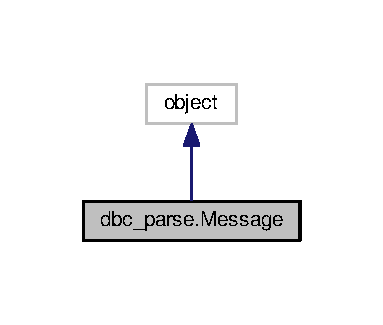
\includegraphics[width=184pt]{d5/da6/classdbc__parse_1_1Message__inherit__graph}
\end{center}
\end{figure}


Collaboration diagram for dbc\+\_\+parse.\+Message\+:\nopagebreak
\begin{figure}[H]
\begin{center}
\leavevmode
\includegraphics[width=184pt]{dd/d80/classdbc__parse_1_1Message__coll__graph}
\end{center}
\end{figure}
\subsection*{Public Member Functions}
\begin{DoxyCompactItemize}
\item 
def \hyperlink{classdbc__parse_1_1Message_a5727366fcc84fa040387bfb944451e0f}{\+\_\+\+\_\+init\+\_\+\+\_\+} (self, \hyperlink{classdbc__parse_1_1Message_a1471af7a123cef3cdea575dccbaaa8ec}{mid}, \hyperlink{classdbc__parse_1_1Message_a740b3f2db8f50f6254f2dfbb75f39148}{name}, \hyperlink{classdbc__parse_1_1Message_ac0dfe459d45cc2c985fb00006d07129a}{dlc}, \hyperlink{classdbc__parse_1_1Message_a3d03a385559ab7062fc87b17b6b9becb}{sender})
\item 
def \hyperlink{classdbc__parse_1_1Message_a0b020e3f83316505ebb9d19e13a4323d}{add\+\_\+signal} (self, s)
\item 
def \hyperlink{classdbc__parse_1_1Message_a5fa2e8413aec9063fa70fa2664a5d6c4}{get\+\_\+struct\+\_\+name} (self)
\item 
def \hyperlink{classdbc__parse_1_1Message_a57de3254a55998110867d560f1c20b15}{is\+\_\+recipient\+\_\+of\+\_\+at\+\_\+least\+\_\+one\+\_\+sig} (self, node)
\item 
def \hyperlink{classdbc__parse_1_1Message_aa52a796f8118c11d304f85b17d3e125c}{contains\+\_\+muxed\+\_\+signals} (self)
\item 
def \hyperlink{classdbc__parse_1_1Message_a305483ca621d50539e5f6242b205930b}{contains\+\_\+enums} (self)
\item 
def \hyperlink{classdbc__parse_1_1Message_af047a7de502e95b6d978cb655aa2cd23}{get\+\_\+muxes} (self)
\item 
def \hyperlink{classdbc__parse_1_1Message_abd1b4cd98e88de6dcd793e28618f2475}{get\+\_\+mux\+\_\+index\+\_\+signal} (self)
\item 
def \hyperlink{classdbc__parse_1_1Message_acbd7b56360eb697ef7d7f4f02bba8257}{get\+\_\+struct\+\_\+for\+\_\+mux} (self, mux, non\+\_\+muxed\+\_\+signals, gen\+\_\+mia\+\_\+struct)
\item 
def \hyperlink{classdbc__parse_1_1Message_a85b8236d15e5438609c83375916f3c50}{gen\+\_\+converted\+\_\+struct} (self, self\+\_\+node, gen\+\_\+all)
\item 
def \hyperlink{classdbc__parse_1_1Message_af0370b4150f9a45849f7e01deddb18a3}{get\+\_\+encode\+\_\+and\+\_\+send} (self, \hyperlink{classdbc__parse_1_1Message_a740b3f2db8f50f6254f2dfbb75f39148}{name})
\item 
def \hyperlink{classdbc__parse_1_1Message_a217e73cb097da11ce62221387f16ec60}{get\+\_\+encode\+\_\+code} (self)
\item 
def \hyperlink{classdbc__parse_1_1Message_abe79e8fe3b791f0f5d72b5960fb6262b}{get\+\_\+non\+\_\+mux\+\_\+signal\+\_\+decode\+\_\+code} (self, raw\+\_\+sig\+\_\+name, prefix=\textquotesingle{}\textquotesingle{})
\item 
def \hyperlink{classdbc__parse_1_1Message_aee532dc58e451dc9c4baa19ce247877b}{get\+\_\+signal\+\_\+decode\+\_\+code\+\_\+for\+\_\+mux} (self, mux, raw\+\_\+sig\+\_\+name, prefix=\textquotesingle{}\textquotesingle{})
\item 
def \hyperlink{classdbc__parse_1_1Message_a3a50af61714f75b64b167c039cba003a}{get\+\_\+decode\+\_\+code} (self)
\end{DoxyCompactItemize}
\subsection*{Data Fields}
\begin{DoxyCompactItemize}
\item 
\hyperlink{classdbc__parse_1_1Message_a1471af7a123cef3cdea575dccbaaa8ec}{mid}
\item 
\hyperlink{classdbc__parse_1_1Message_a740b3f2db8f50f6254f2dfbb75f39148}{name}
\item 
\hyperlink{classdbc__parse_1_1Message_ac0dfe459d45cc2c985fb00006d07129a}{dlc}
\item 
\hyperlink{classdbc__parse_1_1Message_a3d03a385559ab7062fc87b17b6b9becb}{sender}
\item 
\hyperlink{classdbc__parse_1_1Message_a17107ae20dc6a96313223c258f00d3a1}{signals}
\end{DoxyCompactItemize}


\subsection{Detailed Description}
\begin{DoxyVerb}Message Object that contains the list of signals inside
\end{DoxyVerb}
 

\subsection{Constructor \& Destructor Documentation}
\index{dbc\+\_\+parse\+::\+Message@{dbc\+\_\+parse\+::\+Message}!\+\_\+\+\_\+init\+\_\+\+\_\+@{\+\_\+\+\_\+init\+\_\+\+\_\+}}
\index{\+\_\+\+\_\+init\+\_\+\+\_\+@{\+\_\+\+\_\+init\+\_\+\+\_\+}!dbc\+\_\+parse\+::\+Message@{dbc\+\_\+parse\+::\+Message}}
\subsubsection[{\texorpdfstring{\+\_\+\+\_\+init\+\_\+\+\_\+(self, mid, name, dlc, sender)}{__init__(self, mid, name, dlc, sender)}}]{\setlength{\rightskip}{0pt plus 5cm}def dbc\+\_\+parse.\+Message.\+\_\+\+\_\+init\+\_\+\+\_\+ (
\begin{DoxyParamCaption}
\item[{}]{self, }
\item[{}]{mid, }
\item[{}]{name, }
\item[{}]{dlc, }
\item[{}]{sender}
\end{DoxyParamCaption}
)}\hypertarget{classdbc__parse_1_1Message_a5727366fcc84fa040387bfb944451e0f}{}\label{classdbc__parse_1_1Message_a5727366fcc84fa040387bfb944451e0f}


\subsection{Member Function Documentation}
\index{dbc\+\_\+parse\+::\+Message@{dbc\+\_\+parse\+::\+Message}!add\+\_\+signal@{add\+\_\+signal}}
\index{add\+\_\+signal@{add\+\_\+signal}!dbc\+\_\+parse\+::\+Message@{dbc\+\_\+parse\+::\+Message}}
\subsubsection[{\texorpdfstring{add\+\_\+signal(self, s)}{add_signal(self, s)}}]{\setlength{\rightskip}{0pt plus 5cm}def dbc\+\_\+parse.\+Message.\+add\+\_\+signal (
\begin{DoxyParamCaption}
\item[{}]{self, }
\item[{}]{s}
\end{DoxyParamCaption}
)}\hypertarget{classdbc__parse_1_1Message_a0b020e3f83316505ebb9d19e13a4323d}{}\label{classdbc__parse_1_1Message_a0b020e3f83316505ebb9d19e13a4323d}
\index{dbc\+\_\+parse\+::\+Message@{dbc\+\_\+parse\+::\+Message}!contains\+\_\+enums@{contains\+\_\+enums}}
\index{contains\+\_\+enums@{contains\+\_\+enums}!dbc\+\_\+parse\+::\+Message@{dbc\+\_\+parse\+::\+Message}}
\subsubsection[{\texorpdfstring{contains\+\_\+enums(self)}{contains_enums(self)}}]{\setlength{\rightskip}{0pt plus 5cm}def dbc\+\_\+parse.\+Message.\+contains\+\_\+enums (
\begin{DoxyParamCaption}
\item[{}]{self}
\end{DoxyParamCaption}
)}\hypertarget{classdbc__parse_1_1Message_a305483ca621d50539e5f6242b205930b}{}\label{classdbc__parse_1_1Message_a305483ca621d50539e5f6242b205930b}
\index{dbc\+\_\+parse\+::\+Message@{dbc\+\_\+parse\+::\+Message}!contains\+\_\+muxed\+\_\+signals@{contains\+\_\+muxed\+\_\+signals}}
\index{contains\+\_\+muxed\+\_\+signals@{contains\+\_\+muxed\+\_\+signals}!dbc\+\_\+parse\+::\+Message@{dbc\+\_\+parse\+::\+Message}}
\subsubsection[{\texorpdfstring{contains\+\_\+muxed\+\_\+signals(self)}{contains_muxed_signals(self)}}]{\setlength{\rightskip}{0pt plus 5cm}def dbc\+\_\+parse.\+Message.\+contains\+\_\+muxed\+\_\+signals (
\begin{DoxyParamCaption}
\item[{}]{self}
\end{DoxyParamCaption}
)}\hypertarget{classdbc__parse_1_1Message_aa52a796f8118c11d304f85b17d3e125c}{}\label{classdbc__parse_1_1Message_aa52a796f8118c11d304f85b17d3e125c}
\index{dbc\+\_\+parse\+::\+Message@{dbc\+\_\+parse\+::\+Message}!gen\+\_\+converted\+\_\+struct@{gen\+\_\+converted\+\_\+struct}}
\index{gen\+\_\+converted\+\_\+struct@{gen\+\_\+converted\+\_\+struct}!dbc\+\_\+parse\+::\+Message@{dbc\+\_\+parse\+::\+Message}}
\subsubsection[{\texorpdfstring{gen\+\_\+converted\+\_\+struct(self, self\+\_\+node, gen\+\_\+all)}{gen_converted_struct(self, self_node, gen_all)}}]{\setlength{\rightskip}{0pt plus 5cm}def dbc\+\_\+parse.\+Message.\+gen\+\_\+converted\+\_\+struct (
\begin{DoxyParamCaption}
\item[{}]{self, }
\item[{}]{self\+\_\+node, }
\item[{}]{gen\+\_\+all}
\end{DoxyParamCaption}
)}\hypertarget{classdbc__parse_1_1Message_a85b8236d15e5438609c83375916f3c50}{}\label{classdbc__parse_1_1Message_a85b8236d15e5438609c83375916f3c50}
\index{dbc\+\_\+parse\+::\+Message@{dbc\+\_\+parse\+::\+Message}!get\+\_\+decode\+\_\+code@{get\+\_\+decode\+\_\+code}}
\index{get\+\_\+decode\+\_\+code@{get\+\_\+decode\+\_\+code}!dbc\+\_\+parse\+::\+Message@{dbc\+\_\+parse\+::\+Message}}
\subsubsection[{\texorpdfstring{get\+\_\+decode\+\_\+code(self)}{get_decode_code(self)}}]{\setlength{\rightskip}{0pt plus 5cm}def dbc\+\_\+parse.\+Message.\+get\+\_\+decode\+\_\+code (
\begin{DoxyParamCaption}
\item[{}]{self}
\end{DoxyParamCaption}
)}\hypertarget{classdbc__parse_1_1Message_a3a50af61714f75b64b167c039cba003a}{}\label{classdbc__parse_1_1Message_a3a50af61714f75b64b167c039cba003a}
\index{dbc\+\_\+parse\+::\+Message@{dbc\+\_\+parse\+::\+Message}!get\+\_\+encode\+\_\+and\+\_\+send@{get\+\_\+encode\+\_\+and\+\_\+send}}
\index{get\+\_\+encode\+\_\+and\+\_\+send@{get\+\_\+encode\+\_\+and\+\_\+send}!dbc\+\_\+parse\+::\+Message@{dbc\+\_\+parse\+::\+Message}}
\subsubsection[{\texorpdfstring{get\+\_\+encode\+\_\+and\+\_\+send(self, name)}{get_encode_and_send(self, name)}}]{\setlength{\rightskip}{0pt plus 5cm}def dbc\+\_\+parse.\+Message.\+get\+\_\+encode\+\_\+and\+\_\+send (
\begin{DoxyParamCaption}
\item[{}]{self, }
\item[{}]{name}
\end{DoxyParamCaption}
)}\hypertarget{classdbc__parse_1_1Message_af0370b4150f9a45849f7e01deddb18a3}{}\label{classdbc__parse_1_1Message_af0370b4150f9a45849f7e01deddb18a3}
\index{dbc\+\_\+parse\+::\+Message@{dbc\+\_\+parse\+::\+Message}!get\+\_\+encode\+\_\+code@{get\+\_\+encode\+\_\+code}}
\index{get\+\_\+encode\+\_\+code@{get\+\_\+encode\+\_\+code}!dbc\+\_\+parse\+::\+Message@{dbc\+\_\+parse\+::\+Message}}
\subsubsection[{\texorpdfstring{get\+\_\+encode\+\_\+code(self)}{get_encode_code(self)}}]{\setlength{\rightskip}{0pt plus 5cm}def dbc\+\_\+parse.\+Message.\+get\+\_\+encode\+\_\+code (
\begin{DoxyParamCaption}
\item[{}]{self}
\end{DoxyParamCaption}
)}\hypertarget{classdbc__parse_1_1Message_a217e73cb097da11ce62221387f16ec60}{}\label{classdbc__parse_1_1Message_a217e73cb097da11ce62221387f16ec60}
\index{dbc\+\_\+parse\+::\+Message@{dbc\+\_\+parse\+::\+Message}!get\+\_\+mux\+\_\+index\+\_\+signal@{get\+\_\+mux\+\_\+index\+\_\+signal}}
\index{get\+\_\+mux\+\_\+index\+\_\+signal@{get\+\_\+mux\+\_\+index\+\_\+signal}!dbc\+\_\+parse\+::\+Message@{dbc\+\_\+parse\+::\+Message}}
\subsubsection[{\texorpdfstring{get\+\_\+mux\+\_\+index\+\_\+signal(self)}{get_mux_index_signal(self)}}]{\setlength{\rightskip}{0pt plus 5cm}def dbc\+\_\+parse.\+Message.\+get\+\_\+mux\+\_\+index\+\_\+signal (
\begin{DoxyParamCaption}
\item[{}]{self}
\end{DoxyParamCaption}
)}\hypertarget{classdbc__parse_1_1Message_abd1b4cd98e88de6dcd793e28618f2475}{}\label{classdbc__parse_1_1Message_abd1b4cd98e88de6dcd793e28618f2475}
\index{dbc\+\_\+parse\+::\+Message@{dbc\+\_\+parse\+::\+Message}!get\+\_\+muxes@{get\+\_\+muxes}}
\index{get\+\_\+muxes@{get\+\_\+muxes}!dbc\+\_\+parse\+::\+Message@{dbc\+\_\+parse\+::\+Message}}
\subsubsection[{\texorpdfstring{get\+\_\+muxes(self)}{get_muxes(self)}}]{\setlength{\rightskip}{0pt plus 5cm}def dbc\+\_\+parse.\+Message.\+get\+\_\+muxes (
\begin{DoxyParamCaption}
\item[{}]{self}
\end{DoxyParamCaption}
)}\hypertarget{classdbc__parse_1_1Message_af047a7de502e95b6d978cb655aa2cd23}{}\label{classdbc__parse_1_1Message_af047a7de502e95b6d978cb655aa2cd23}
\index{dbc\+\_\+parse\+::\+Message@{dbc\+\_\+parse\+::\+Message}!get\+\_\+non\+\_\+mux\+\_\+signal\+\_\+decode\+\_\+code@{get\+\_\+non\+\_\+mux\+\_\+signal\+\_\+decode\+\_\+code}}
\index{get\+\_\+non\+\_\+mux\+\_\+signal\+\_\+decode\+\_\+code@{get\+\_\+non\+\_\+mux\+\_\+signal\+\_\+decode\+\_\+code}!dbc\+\_\+parse\+::\+Message@{dbc\+\_\+parse\+::\+Message}}
\subsubsection[{\texorpdfstring{get\+\_\+non\+\_\+mux\+\_\+signal\+\_\+decode\+\_\+code(self, raw\+\_\+sig\+\_\+name, prefix=\textquotesingle{}\textquotesingle{})}{get_non_mux_signal_decode_code(self, raw_sig_name, prefix='')}}]{\setlength{\rightskip}{0pt plus 5cm}def dbc\+\_\+parse.\+Message.\+get\+\_\+non\+\_\+mux\+\_\+signal\+\_\+decode\+\_\+code (
\begin{DoxyParamCaption}
\item[{}]{self, }
\item[{}]{raw\+\_\+sig\+\_\+name, }
\item[{}]{prefix = {\ttfamily \textquotesingle{}\textquotesingle{}}}
\end{DoxyParamCaption}
)}\hypertarget{classdbc__parse_1_1Message_abe79e8fe3b791f0f5d72b5960fb6262b}{}\label{classdbc__parse_1_1Message_abe79e8fe3b791f0f5d72b5960fb6262b}
\index{dbc\+\_\+parse\+::\+Message@{dbc\+\_\+parse\+::\+Message}!get\+\_\+signal\+\_\+decode\+\_\+code\+\_\+for\+\_\+mux@{get\+\_\+signal\+\_\+decode\+\_\+code\+\_\+for\+\_\+mux}}
\index{get\+\_\+signal\+\_\+decode\+\_\+code\+\_\+for\+\_\+mux@{get\+\_\+signal\+\_\+decode\+\_\+code\+\_\+for\+\_\+mux}!dbc\+\_\+parse\+::\+Message@{dbc\+\_\+parse\+::\+Message}}
\subsubsection[{\texorpdfstring{get\+\_\+signal\+\_\+decode\+\_\+code\+\_\+for\+\_\+mux(self, mux, raw\+\_\+sig\+\_\+name, prefix=\textquotesingle{}\textquotesingle{})}{get_signal_decode_code_for_mux(self, mux, raw_sig_name, prefix='')}}]{\setlength{\rightskip}{0pt plus 5cm}def dbc\+\_\+parse.\+Message.\+get\+\_\+signal\+\_\+decode\+\_\+code\+\_\+for\+\_\+mux (
\begin{DoxyParamCaption}
\item[{}]{self, }
\item[{}]{mux, }
\item[{}]{raw\+\_\+sig\+\_\+name, }
\item[{}]{prefix = {\ttfamily \textquotesingle{}\textquotesingle{}}}
\end{DoxyParamCaption}
)}\hypertarget{classdbc__parse_1_1Message_aee532dc58e451dc9c4baa19ce247877b}{}\label{classdbc__parse_1_1Message_aee532dc58e451dc9c4baa19ce247877b}
\index{dbc\+\_\+parse\+::\+Message@{dbc\+\_\+parse\+::\+Message}!get\+\_\+struct\+\_\+for\+\_\+mux@{get\+\_\+struct\+\_\+for\+\_\+mux}}
\index{get\+\_\+struct\+\_\+for\+\_\+mux@{get\+\_\+struct\+\_\+for\+\_\+mux}!dbc\+\_\+parse\+::\+Message@{dbc\+\_\+parse\+::\+Message}}
\subsubsection[{\texorpdfstring{get\+\_\+struct\+\_\+for\+\_\+mux(self, mux, non\+\_\+muxed\+\_\+signals, gen\+\_\+mia\+\_\+struct)}{get_struct_for_mux(self, mux, non_muxed_signals, gen_mia_struct)}}]{\setlength{\rightskip}{0pt plus 5cm}def dbc\+\_\+parse.\+Message.\+get\+\_\+struct\+\_\+for\+\_\+mux (
\begin{DoxyParamCaption}
\item[{}]{self, }
\item[{}]{mux, }
\item[{}]{non\+\_\+muxed\+\_\+signals, }
\item[{}]{gen\+\_\+mia\+\_\+struct}
\end{DoxyParamCaption}
)}\hypertarget{classdbc__parse_1_1Message_acbd7b56360eb697ef7d7f4f02bba8257}{}\label{classdbc__parse_1_1Message_acbd7b56360eb697ef7d7f4f02bba8257}
\index{dbc\+\_\+parse\+::\+Message@{dbc\+\_\+parse\+::\+Message}!get\+\_\+struct\+\_\+name@{get\+\_\+struct\+\_\+name}}
\index{get\+\_\+struct\+\_\+name@{get\+\_\+struct\+\_\+name}!dbc\+\_\+parse\+::\+Message@{dbc\+\_\+parse\+::\+Message}}
\subsubsection[{\texorpdfstring{get\+\_\+struct\+\_\+name(self)}{get_struct_name(self)}}]{\setlength{\rightskip}{0pt plus 5cm}def dbc\+\_\+parse.\+Message.\+get\+\_\+struct\+\_\+name (
\begin{DoxyParamCaption}
\item[{}]{self}
\end{DoxyParamCaption}
)}\hypertarget{classdbc__parse_1_1Message_a5fa2e8413aec9063fa70fa2664a5d6c4}{}\label{classdbc__parse_1_1Message_a5fa2e8413aec9063fa70fa2664a5d6c4}
\index{dbc\+\_\+parse\+::\+Message@{dbc\+\_\+parse\+::\+Message}!is\+\_\+recipient\+\_\+of\+\_\+at\+\_\+least\+\_\+one\+\_\+sig@{is\+\_\+recipient\+\_\+of\+\_\+at\+\_\+least\+\_\+one\+\_\+sig}}
\index{is\+\_\+recipient\+\_\+of\+\_\+at\+\_\+least\+\_\+one\+\_\+sig@{is\+\_\+recipient\+\_\+of\+\_\+at\+\_\+least\+\_\+one\+\_\+sig}!dbc\+\_\+parse\+::\+Message@{dbc\+\_\+parse\+::\+Message}}
\subsubsection[{\texorpdfstring{is\+\_\+recipient\+\_\+of\+\_\+at\+\_\+least\+\_\+one\+\_\+sig(self, node)}{is_recipient_of_at_least_one_sig(self, node)}}]{\setlength{\rightskip}{0pt plus 5cm}def dbc\+\_\+parse.\+Message.\+is\+\_\+recipient\+\_\+of\+\_\+at\+\_\+least\+\_\+one\+\_\+sig (
\begin{DoxyParamCaption}
\item[{}]{self, }
\item[{}]{node}
\end{DoxyParamCaption}
)}\hypertarget{classdbc__parse_1_1Message_a57de3254a55998110867d560f1c20b15}{}\label{classdbc__parse_1_1Message_a57de3254a55998110867d560f1c20b15}


\subsection{Field Documentation}
\index{dbc\+\_\+parse\+::\+Message@{dbc\+\_\+parse\+::\+Message}!dlc@{dlc}}
\index{dlc@{dlc}!dbc\+\_\+parse\+::\+Message@{dbc\+\_\+parse\+::\+Message}}
\subsubsection[{\texorpdfstring{dlc}{dlc}}]{\setlength{\rightskip}{0pt plus 5cm}dbc\+\_\+parse.\+Message.\+dlc}\hypertarget{classdbc__parse_1_1Message_ac0dfe459d45cc2c985fb00006d07129a}{}\label{classdbc__parse_1_1Message_ac0dfe459d45cc2c985fb00006d07129a}
\index{dbc\+\_\+parse\+::\+Message@{dbc\+\_\+parse\+::\+Message}!mid@{mid}}
\index{mid@{mid}!dbc\+\_\+parse\+::\+Message@{dbc\+\_\+parse\+::\+Message}}
\subsubsection[{\texorpdfstring{mid}{mid}}]{\setlength{\rightskip}{0pt plus 5cm}dbc\+\_\+parse.\+Message.\+mid}\hypertarget{classdbc__parse_1_1Message_a1471af7a123cef3cdea575dccbaaa8ec}{}\label{classdbc__parse_1_1Message_a1471af7a123cef3cdea575dccbaaa8ec}
\index{dbc\+\_\+parse\+::\+Message@{dbc\+\_\+parse\+::\+Message}!name@{name}}
\index{name@{name}!dbc\+\_\+parse\+::\+Message@{dbc\+\_\+parse\+::\+Message}}
\subsubsection[{\texorpdfstring{name}{name}}]{\setlength{\rightskip}{0pt plus 5cm}dbc\+\_\+parse.\+Message.\+name}\hypertarget{classdbc__parse_1_1Message_a740b3f2db8f50f6254f2dfbb75f39148}{}\label{classdbc__parse_1_1Message_a740b3f2db8f50f6254f2dfbb75f39148}
\index{dbc\+\_\+parse\+::\+Message@{dbc\+\_\+parse\+::\+Message}!sender@{sender}}
\index{sender@{sender}!dbc\+\_\+parse\+::\+Message@{dbc\+\_\+parse\+::\+Message}}
\subsubsection[{\texorpdfstring{sender}{sender}}]{\setlength{\rightskip}{0pt plus 5cm}dbc\+\_\+parse.\+Message.\+sender}\hypertarget{classdbc__parse_1_1Message_a3d03a385559ab7062fc87b17b6b9becb}{}\label{classdbc__parse_1_1Message_a3d03a385559ab7062fc87b17b6b9becb}
\index{dbc\+\_\+parse\+::\+Message@{dbc\+\_\+parse\+::\+Message}!signals@{signals}}
\index{signals@{signals}!dbc\+\_\+parse\+::\+Message@{dbc\+\_\+parse\+::\+Message}}
\subsubsection[{\texorpdfstring{signals}{signals}}]{\setlength{\rightskip}{0pt plus 5cm}dbc\+\_\+parse.\+Message.\+signals}\hypertarget{classdbc__parse_1_1Message_a17107ae20dc6a96313223c258f00d3a1}{}\label{classdbc__parse_1_1Message_a17107ae20dc6a96313223c258f00d3a1}


The documentation for this class was generated from the following file\+:\begin{DoxyCompactItemize}
\item 
/var/www/html/\+S\+J\+S\+U-\/\+D\+E\+V-\/\+Linux/firmware/default/lib/\+\_\+can\+\_\+dbc/\hyperlink{dbc__parse_8py}{dbc\+\_\+parse.\+py}\end{DoxyCompactItemize}

\hypertarget{classMicroSecondStopWatch}{}\section{Micro\+Second\+Stop\+Watch Class Reference}
\label{classMicroSecondStopWatch}\index{Micro\+Second\+Stop\+Watch@{Micro\+Second\+Stop\+Watch}}


{\ttfamily \#include $<$stop\+\_\+watch.\+hpp$>$}

\subsection*{Public Member Functions}
\begin{DoxyCompactItemize}
\item 
\hyperlink{classMicroSecondStopWatch_a0349789f3bc1ed8278a86b0bdd6e2c8d}{Micro\+Second\+Stop\+Watch} ()
\begin{DoxyCompactList}\small\item\em Default constructor that starts the stopwatch. \end{DoxyCompactList}\item 
void \hyperlink{classMicroSecondStopWatch_a2376f62d01542ab7ac2add6215c98ec1}{start} (void)
\begin{DoxyCompactList}\small\item\em Starts the stopwatch operation (can be used to restart the stopwatch too) \end{DoxyCompactList}\item 
void \hyperlink{classMicroSecondStopWatch_a98441a3bb1567879ead4da6e7424eff7}{stop} (void)
\begin{DoxyCompactList}\small\item\em Stops the stopwatch operation enabling the captured value to be obtained. \end{DoxyCompactList}\item 
uint64\+\_\+t \hyperlink{classMicroSecondStopWatch_a49742a14a8a48401034ef431a321b071}{get\+Captured\+Time} (void) const 
\item 
uint64\+\_\+t \hyperlink{classMicroSecondStopWatch_a526134ba49ff00249859eedf0736c8c6}{get\+Elapsed\+Time} (void) const 
\begin{DoxyCompactList}\small\item\em Get the elapsed time since the stopwatch was started. \end{DoxyCompactList}\end{DoxyCompactItemize}


\subsection{Detailed Description}
Stopwatch to measure an elapsed time. 

\subsection{Constructor \& Destructor Documentation}
\index{Micro\+Second\+Stop\+Watch@{Micro\+Second\+Stop\+Watch}!Micro\+Second\+Stop\+Watch@{Micro\+Second\+Stop\+Watch}}
\index{Micro\+Second\+Stop\+Watch@{Micro\+Second\+Stop\+Watch}!Micro\+Second\+Stop\+Watch@{Micro\+Second\+Stop\+Watch}}
\subsubsection[{\texorpdfstring{Micro\+Second\+Stop\+Watch()}{MicroSecondStopWatch()}}]{\setlength{\rightskip}{0pt plus 5cm}Micro\+Second\+Stop\+Watch\+::\+Micro\+Second\+Stop\+Watch (
\begin{DoxyParamCaption}
{}
\end{DoxyParamCaption}
)\hspace{0.3cm}{\ttfamily [inline]}}\hypertarget{classMicroSecondStopWatch_a0349789f3bc1ed8278a86b0bdd6e2c8d}{}\label{classMicroSecondStopWatch_a0349789f3bc1ed8278a86b0bdd6e2c8d}


Default constructor that starts the stopwatch. 



\subsection{Member Function Documentation}
\index{Micro\+Second\+Stop\+Watch@{Micro\+Second\+Stop\+Watch}!get\+Captured\+Time@{get\+Captured\+Time}}
\index{get\+Captured\+Time@{get\+Captured\+Time}!Micro\+Second\+Stop\+Watch@{Micro\+Second\+Stop\+Watch}}
\subsubsection[{\texorpdfstring{get\+Captured\+Time(void) const }{getCapturedTime(void) const }}]{\setlength{\rightskip}{0pt plus 5cm}uint64\+\_\+t Micro\+Second\+Stop\+Watch\+::get\+Captured\+Time (
\begin{DoxyParamCaption}
\item[{void}]{}
\end{DoxyParamCaption}
) const\hspace{0.3cm}{\ttfamily [inline]}}\hypertarget{classMicroSecondStopWatch_a49742a14a8a48401034ef431a321b071}{}\label{classMicroSecondStopWatch_a49742a14a8a48401034ef431a321b071}
Get the captured value between \hyperlink{classMicroSecondStopWatch_a2376f62d01542ab7ac2add6215c98ec1}{start()} and \hyperlink{classMicroSecondStopWatch_a98441a3bb1567879ead4da6e7424eff7}{stop()} If the stopwatch was never stopped, zero value will be returned. \index{Micro\+Second\+Stop\+Watch@{Micro\+Second\+Stop\+Watch}!get\+Elapsed\+Time@{get\+Elapsed\+Time}}
\index{get\+Elapsed\+Time@{get\+Elapsed\+Time}!Micro\+Second\+Stop\+Watch@{Micro\+Second\+Stop\+Watch}}
\subsubsection[{\texorpdfstring{get\+Elapsed\+Time(void) const }{getElapsedTime(void) const }}]{\setlength{\rightskip}{0pt plus 5cm}uint64\+\_\+t Micro\+Second\+Stop\+Watch\+::get\+Elapsed\+Time (
\begin{DoxyParamCaption}
\item[{void}]{}
\end{DoxyParamCaption}
) const\hspace{0.3cm}{\ttfamily [inline]}}\hypertarget{classMicroSecondStopWatch_a526134ba49ff00249859eedf0736c8c6}{}\label{classMicroSecondStopWatch_a526134ba49ff00249859eedf0736c8c6}


Get the elapsed time since the stopwatch was started. 

\index{Micro\+Second\+Stop\+Watch@{Micro\+Second\+Stop\+Watch}!start@{start}}
\index{start@{start}!Micro\+Second\+Stop\+Watch@{Micro\+Second\+Stop\+Watch}}
\subsubsection[{\texorpdfstring{start(void)}{start(void)}}]{\setlength{\rightskip}{0pt plus 5cm}void Micro\+Second\+Stop\+Watch\+::start (
\begin{DoxyParamCaption}
\item[{void}]{}
\end{DoxyParamCaption}
)\hspace{0.3cm}{\ttfamily [inline]}}\hypertarget{classMicroSecondStopWatch_a2376f62d01542ab7ac2add6215c98ec1}{}\label{classMicroSecondStopWatch_a2376f62d01542ab7ac2add6215c98ec1}


Starts the stopwatch operation (can be used to restart the stopwatch too) 

\index{Micro\+Second\+Stop\+Watch@{Micro\+Second\+Stop\+Watch}!stop@{stop}}
\index{stop@{stop}!Micro\+Second\+Stop\+Watch@{Micro\+Second\+Stop\+Watch}}
\subsubsection[{\texorpdfstring{stop(void)}{stop(void)}}]{\setlength{\rightskip}{0pt plus 5cm}void Micro\+Second\+Stop\+Watch\+::stop (
\begin{DoxyParamCaption}
\item[{void}]{}
\end{DoxyParamCaption}
)\hspace{0.3cm}{\ttfamily [inline]}}\hypertarget{classMicroSecondStopWatch_a98441a3bb1567879ead4da6e7424eff7}{}\label{classMicroSecondStopWatch_a98441a3bb1567879ead4da6e7424eff7}


Stops the stopwatch operation enabling the captured value to be obtained. 



The documentation for this class was generated from the following file\+:\begin{DoxyCompactItemize}
\item 
/var/www/html/\+S\+J\+S\+U-\/\+D\+E\+V-\/\+Linux/firmware/default/lib/\+L3\+\_\+\+Utils/\hyperlink{stop__watch_8hpp}{stop\+\_\+watch.\+hpp}\end{DoxyCompactItemize}

\hypertarget{structMPU__Type}{}\section{M\+P\+U\+\_\+\+Type Struct Reference}
\label{structMPU__Type}\index{M\+P\+U\+\_\+\+Type@{M\+P\+U\+\_\+\+Type}}


{\ttfamily \#include $<$core\+\_\+cm3.\+h$>$}

\subsection*{Data Fields}
\begin{DoxyCompactItemize}
\item 
\hyperlink{LPC17xx_8h_af63697ed9952cc71e1225efe205f6cd3}{\+\_\+\+\_\+I} uint32\+\_\+t \hyperlink{structMPU__Type_a6ae8a8c3a4909ae41447168d793608f7}{T\+Y\+PE}
\item 
\hyperlink{LPC17xx_8h_aec43007d9998a0a0e01faede4133d6be}{\+\_\+\+\_\+\+IO} uint32\+\_\+t \hyperlink{structMPU__Type_aab33593671948b93b1c0908d78779328}{C\+T\+RL}
\item 
\hyperlink{LPC17xx_8h_aec43007d9998a0a0e01faede4133d6be}{\+\_\+\+\_\+\+IO} uint32\+\_\+t \hyperlink{structMPU__Type_afd8de96a5d574c3953e2106e782f9833}{R\+NR}
\item 
\hyperlink{LPC17xx_8h_aec43007d9998a0a0e01faede4133d6be}{\+\_\+\+\_\+\+IO} uint32\+\_\+t \hyperlink{structMPU__Type_a3f2e2448a77aadacd9f394f6c4c708d9}{R\+B\+AR}
\item 
\hyperlink{LPC17xx_8h_aec43007d9998a0a0e01faede4133d6be}{\+\_\+\+\_\+\+IO} uint32\+\_\+t \hyperlink{structMPU__Type_adc65d266d15ce9ba57b3d127e8267f03}{R\+A\+SR}
\item 
\hyperlink{LPC17xx_8h_aec43007d9998a0a0e01faede4133d6be}{\+\_\+\+\_\+\+IO} uint32\+\_\+t \hyperlink{structMPU__Type_a4dbcffa0a71c31e521b645b34b40e639}{R\+B\+A\+R\+\_\+\+A1}
\item 
\hyperlink{LPC17xx_8h_aec43007d9998a0a0e01faede4133d6be}{\+\_\+\+\_\+\+IO} uint32\+\_\+t \hyperlink{structMPU__Type_a94222f9a8637b5329016e18f08af7185}{R\+A\+S\+R\+\_\+\+A1}
\item 
\hyperlink{LPC17xx_8h_aec43007d9998a0a0e01faede4133d6be}{\+\_\+\+\_\+\+IO} uint32\+\_\+t \hyperlink{structMPU__Type_a8703a00626dba046b841c0db6c78c395}{R\+B\+A\+R\+\_\+\+A2}
\item 
\hyperlink{LPC17xx_8h_aec43007d9998a0a0e01faede4133d6be}{\+\_\+\+\_\+\+IO} uint32\+\_\+t \hyperlink{structMPU__Type_a0aac7727a6225c6aa00627c36d51d014}{R\+A\+S\+R\+\_\+\+A2}
\item 
\hyperlink{LPC17xx_8h_aec43007d9998a0a0e01faede4133d6be}{\+\_\+\+\_\+\+IO} uint32\+\_\+t \hyperlink{structMPU__Type_a9fda17c37b85ef317c7c8688ff8c5804}{R\+B\+A\+R\+\_\+\+A3}
\item 
\hyperlink{LPC17xx_8h_aec43007d9998a0a0e01faede4133d6be}{\+\_\+\+\_\+\+IO} uint32\+\_\+t \hyperlink{structMPU__Type_aced0b908173b9a4bae4f59452f0cdb0d}{R\+A\+S\+R\+\_\+\+A3}
\end{DoxyCompactItemize}


\subsection{Field Documentation}
\index{M\+P\+U\+\_\+\+Type@{M\+P\+U\+\_\+\+Type}!C\+T\+RL@{C\+T\+RL}}
\index{C\+T\+RL@{C\+T\+RL}!M\+P\+U\+\_\+\+Type@{M\+P\+U\+\_\+\+Type}}
\subsubsection[{\texorpdfstring{C\+T\+RL}{CTRL}}]{\setlength{\rightskip}{0pt plus 5cm}{\bf \+\_\+\+\_\+\+IO} uint32\+\_\+t M\+P\+U\+\_\+\+Type\+::\+C\+T\+RL}\hypertarget{structMPU__Type_aab33593671948b93b1c0908d78779328}{}\label{structMPU__Type_aab33593671948b93b1c0908d78779328}
Offset\+: 0x04 M\+PU Control Register \index{M\+P\+U\+\_\+\+Type@{M\+P\+U\+\_\+\+Type}!R\+A\+SR@{R\+A\+SR}}
\index{R\+A\+SR@{R\+A\+SR}!M\+P\+U\+\_\+\+Type@{M\+P\+U\+\_\+\+Type}}
\subsubsection[{\texorpdfstring{R\+A\+SR}{RASR}}]{\setlength{\rightskip}{0pt plus 5cm}{\bf \+\_\+\+\_\+\+IO} uint32\+\_\+t M\+P\+U\+\_\+\+Type\+::\+R\+A\+SR}\hypertarget{structMPU__Type_adc65d266d15ce9ba57b3d127e8267f03}{}\label{structMPU__Type_adc65d266d15ce9ba57b3d127e8267f03}
Offset\+: 0x10 M\+PU Region Attribute and Size Register \index{M\+P\+U\+\_\+\+Type@{M\+P\+U\+\_\+\+Type}!R\+A\+S\+R\+\_\+\+A1@{R\+A\+S\+R\+\_\+\+A1}}
\index{R\+A\+S\+R\+\_\+\+A1@{R\+A\+S\+R\+\_\+\+A1}!M\+P\+U\+\_\+\+Type@{M\+P\+U\+\_\+\+Type}}
\subsubsection[{\texorpdfstring{R\+A\+S\+R\+\_\+\+A1}{RASR_A1}}]{\setlength{\rightskip}{0pt plus 5cm}{\bf \+\_\+\+\_\+\+IO} uint32\+\_\+t M\+P\+U\+\_\+\+Type\+::\+R\+A\+S\+R\+\_\+\+A1}\hypertarget{structMPU__Type_a94222f9a8637b5329016e18f08af7185}{}\label{structMPU__Type_a94222f9a8637b5329016e18f08af7185}
Offset\+: 0x18 M\+PU Alias 1 Region Attribute and Size Register \index{M\+P\+U\+\_\+\+Type@{M\+P\+U\+\_\+\+Type}!R\+A\+S\+R\+\_\+\+A2@{R\+A\+S\+R\+\_\+\+A2}}
\index{R\+A\+S\+R\+\_\+\+A2@{R\+A\+S\+R\+\_\+\+A2}!M\+P\+U\+\_\+\+Type@{M\+P\+U\+\_\+\+Type}}
\subsubsection[{\texorpdfstring{R\+A\+S\+R\+\_\+\+A2}{RASR_A2}}]{\setlength{\rightskip}{0pt plus 5cm}{\bf \+\_\+\+\_\+\+IO} uint32\+\_\+t M\+P\+U\+\_\+\+Type\+::\+R\+A\+S\+R\+\_\+\+A2}\hypertarget{structMPU__Type_a0aac7727a6225c6aa00627c36d51d014}{}\label{structMPU__Type_a0aac7727a6225c6aa00627c36d51d014}
Offset\+: 0x20 M\+PU Alias 2 Region Attribute and Size Register \index{M\+P\+U\+\_\+\+Type@{M\+P\+U\+\_\+\+Type}!R\+A\+S\+R\+\_\+\+A3@{R\+A\+S\+R\+\_\+\+A3}}
\index{R\+A\+S\+R\+\_\+\+A3@{R\+A\+S\+R\+\_\+\+A3}!M\+P\+U\+\_\+\+Type@{M\+P\+U\+\_\+\+Type}}
\subsubsection[{\texorpdfstring{R\+A\+S\+R\+\_\+\+A3}{RASR_A3}}]{\setlength{\rightskip}{0pt plus 5cm}{\bf \+\_\+\+\_\+\+IO} uint32\+\_\+t M\+P\+U\+\_\+\+Type\+::\+R\+A\+S\+R\+\_\+\+A3}\hypertarget{structMPU__Type_aced0b908173b9a4bae4f59452f0cdb0d}{}\label{structMPU__Type_aced0b908173b9a4bae4f59452f0cdb0d}
Offset\+: 0x28 M\+PU Alias 3 Region Attribute and Size Register \index{M\+P\+U\+\_\+\+Type@{M\+P\+U\+\_\+\+Type}!R\+B\+AR@{R\+B\+AR}}
\index{R\+B\+AR@{R\+B\+AR}!M\+P\+U\+\_\+\+Type@{M\+P\+U\+\_\+\+Type}}
\subsubsection[{\texorpdfstring{R\+B\+AR}{RBAR}}]{\setlength{\rightskip}{0pt plus 5cm}{\bf \+\_\+\+\_\+\+IO} uint32\+\_\+t M\+P\+U\+\_\+\+Type\+::\+R\+B\+AR}\hypertarget{structMPU__Type_a3f2e2448a77aadacd9f394f6c4c708d9}{}\label{structMPU__Type_a3f2e2448a77aadacd9f394f6c4c708d9}
Offset\+: 0x0C M\+PU Region Base Address Register \index{M\+P\+U\+\_\+\+Type@{M\+P\+U\+\_\+\+Type}!R\+B\+A\+R\+\_\+\+A1@{R\+B\+A\+R\+\_\+\+A1}}
\index{R\+B\+A\+R\+\_\+\+A1@{R\+B\+A\+R\+\_\+\+A1}!M\+P\+U\+\_\+\+Type@{M\+P\+U\+\_\+\+Type}}
\subsubsection[{\texorpdfstring{R\+B\+A\+R\+\_\+\+A1}{RBAR_A1}}]{\setlength{\rightskip}{0pt plus 5cm}{\bf \+\_\+\+\_\+\+IO} uint32\+\_\+t M\+P\+U\+\_\+\+Type\+::\+R\+B\+A\+R\+\_\+\+A1}\hypertarget{structMPU__Type_a4dbcffa0a71c31e521b645b34b40e639}{}\label{structMPU__Type_a4dbcffa0a71c31e521b645b34b40e639}
Offset\+: 0x14 M\+PU Alias 1 Region Base Address Register \index{M\+P\+U\+\_\+\+Type@{M\+P\+U\+\_\+\+Type}!R\+B\+A\+R\+\_\+\+A2@{R\+B\+A\+R\+\_\+\+A2}}
\index{R\+B\+A\+R\+\_\+\+A2@{R\+B\+A\+R\+\_\+\+A2}!M\+P\+U\+\_\+\+Type@{M\+P\+U\+\_\+\+Type}}
\subsubsection[{\texorpdfstring{R\+B\+A\+R\+\_\+\+A2}{RBAR_A2}}]{\setlength{\rightskip}{0pt plus 5cm}{\bf \+\_\+\+\_\+\+IO} uint32\+\_\+t M\+P\+U\+\_\+\+Type\+::\+R\+B\+A\+R\+\_\+\+A2}\hypertarget{structMPU__Type_a8703a00626dba046b841c0db6c78c395}{}\label{structMPU__Type_a8703a00626dba046b841c0db6c78c395}
Offset\+: 0x1C M\+PU Alias 2 Region Base Address Register \index{M\+P\+U\+\_\+\+Type@{M\+P\+U\+\_\+\+Type}!R\+B\+A\+R\+\_\+\+A3@{R\+B\+A\+R\+\_\+\+A3}}
\index{R\+B\+A\+R\+\_\+\+A3@{R\+B\+A\+R\+\_\+\+A3}!M\+P\+U\+\_\+\+Type@{M\+P\+U\+\_\+\+Type}}
\subsubsection[{\texorpdfstring{R\+B\+A\+R\+\_\+\+A3}{RBAR_A3}}]{\setlength{\rightskip}{0pt plus 5cm}{\bf \+\_\+\+\_\+\+IO} uint32\+\_\+t M\+P\+U\+\_\+\+Type\+::\+R\+B\+A\+R\+\_\+\+A3}\hypertarget{structMPU__Type_a9fda17c37b85ef317c7c8688ff8c5804}{}\label{structMPU__Type_a9fda17c37b85ef317c7c8688ff8c5804}
Offset\+: 0x24 M\+PU Alias 3 Region Base Address Register \index{M\+P\+U\+\_\+\+Type@{M\+P\+U\+\_\+\+Type}!R\+NR@{R\+NR}}
\index{R\+NR@{R\+NR}!M\+P\+U\+\_\+\+Type@{M\+P\+U\+\_\+\+Type}}
\subsubsection[{\texorpdfstring{R\+NR}{RNR}}]{\setlength{\rightskip}{0pt plus 5cm}{\bf \+\_\+\+\_\+\+IO} uint32\+\_\+t M\+P\+U\+\_\+\+Type\+::\+R\+NR}\hypertarget{structMPU__Type_afd8de96a5d574c3953e2106e782f9833}{}\label{structMPU__Type_afd8de96a5d574c3953e2106e782f9833}
Offset\+: 0x08 M\+PU Region R\+N\+Rber Register \index{M\+P\+U\+\_\+\+Type@{M\+P\+U\+\_\+\+Type}!T\+Y\+PE@{T\+Y\+PE}}
\index{T\+Y\+PE@{T\+Y\+PE}!M\+P\+U\+\_\+\+Type@{M\+P\+U\+\_\+\+Type}}
\subsubsection[{\texorpdfstring{T\+Y\+PE}{TYPE}}]{\setlength{\rightskip}{0pt plus 5cm}{\bf \+\_\+\+\_\+I} uint32\+\_\+t M\+P\+U\+\_\+\+Type\+::\+T\+Y\+PE}\hypertarget{structMPU__Type_a6ae8a8c3a4909ae41447168d793608f7}{}\label{structMPU__Type_a6ae8a8c3a4909ae41447168d793608f7}
Offset\+: 0x00 M\+PU Type Register 

The documentation for this struct was generated from the following file\+:\begin{DoxyCompactItemize}
\item 
/var/www/html/\+S\+J\+S\+U-\/\+D\+E\+V-\/\+Linux/firmware/default/lib/\+L0\+\_\+\+Low\+Level/\hyperlink{core__cm3_8h}{core\+\_\+cm3.\+h}\end{DoxyCompactItemize}

\hypertarget{classNordicStream}{}\section{Nordic\+Stream Class Reference}
\label{classNordicStream}\index{Nordic\+Stream@{Nordic\+Stream}}


{\ttfamily \#include $<$nrf\+\_\+stream.\+hpp$>$}



Inheritance diagram for Nordic\+Stream\+:\nopagebreak
\begin{figure}[H]
\begin{center}
\leavevmode
\includegraphics[width=258pt]{dc/dca/classNordicStream__inherit__graph}
\end{center}
\end{figure}


Collaboration diagram for Nordic\+Stream\+:\nopagebreak
\begin{figure}[H]
\begin{center}
\leavevmode
\includegraphics[width=350pt]{da/d1c/classNordicStream__coll__graph}
\end{center}
\end{figure}
\subsection*{Public Member Functions}
\begin{DoxyCompactItemize}
\item 
void \hyperlink{classNordicStream_aec819a09eab2ff62be9d520e8064f429}{set\+Dest\+Addr} (uint8\+\_\+t address)
\item 
void \hyperlink{classNordicStream_a0b49097330410ef00621e3d2befe06a1}{set\+Pkt\+Hops} (uint8\+\_\+t hops)
\item 
bool \hyperlink{classNordicStream_a95c0c66acbcdf33894fc2cfacfbe5419}{flush} (void)
\begin{DoxyCompactList}\small\item\em Flush all buffered data or send any pending data immediately. \end{DoxyCompactList}\end{DoxyCompactItemize}
{\bf }\par
\begin{DoxyCompactItemize}
\item 
bool \hyperlink{classNordicStream_a8cf184554a505c922c57352ba571765b}{get\+Char} (char $\ast$p\+Input\+Char, unsigned int timeout=\hyperlink{portmacro_8h_a72723ba1e4a85ca14f25c2b9e066613d}{port\+M\+A\+X\+\_\+\+D\+E\+L\+AY})
\item 
bool \hyperlink{classNordicStream_aefb871567b4712b2bf52caa656dc1d2a}{put\+Char} (char out, unsigned int timeout=\hyperlink{portmacro_8h_a72723ba1e4a85ca14f25c2b9e066613d}{port\+M\+A\+X\+\_\+\+D\+E\+L\+AY})
\end{DoxyCompactItemize}

\subsection*{Friends}
\begin{DoxyCompactItemize}
\item 
class \hyperlink{classNordicStream_ab4472738cb423383808e311cf4677007}{Singleton\+Template$<$ Nordic\+Stream $>$}
\begin{DoxyCompactList}\small\item\em Friend class used for Singleton Template. \end{DoxyCompactList}\end{DoxyCompactItemize}
\subsection*{Additional Inherited Members}


\subsection{Detailed Description}
Nordic char device driver

This class provides a way to use the nordic like a char device. You can use \hyperlink{classCharDev_a1e567da6600cd8164dcd98e11de8813f}{printf()}, \hyperlink{classCharDev_a053203d7cf010d6422b11d114d10e357}{scanf()} etc, and all the data will be sent to the address set by \hyperlink{classNordicStream_aec819a09eab2ff62be9d520e8064f429}{set\+Dest\+Addr()}. If the destination address is not set, then it will be sent to the last source that sent us data on nordic. 

\subsection{Member Function Documentation}
\index{Nordic\+Stream@{Nordic\+Stream}!flush@{flush}}
\index{flush@{flush}!Nordic\+Stream@{Nordic\+Stream}}
\subsubsection[{\texorpdfstring{flush(void)}{flush(void)}}]{\setlength{\rightskip}{0pt plus 5cm}bool Nordic\+Stream\+::flush (
\begin{DoxyParamCaption}
\item[{void}]{}
\end{DoxyParamCaption}
)\hspace{0.3cm}{\ttfamily [virtual]}}\hypertarget{classNordicStream_a95c0c66acbcdf33894fc2cfacfbe5419}{}\label{classNordicStream_a95c0c66acbcdf33894fc2cfacfbe5419}


Flush all buffered data or send any pending data immediately. 



Reimplemented from \hyperlink{classCharDev_a601bd6eeee3095306c0db78798499742}{Char\+Dev}.

\index{Nordic\+Stream@{Nordic\+Stream}!get\+Char@{get\+Char}}
\index{get\+Char@{get\+Char}!Nordic\+Stream@{Nordic\+Stream}}
\subsubsection[{\texorpdfstring{get\+Char(char $\ast$p\+Input\+Char, unsigned int timeout=port\+M\+A\+X\+\_\+\+D\+E\+L\+A\+Y)}{getChar(char *pInputChar, unsigned int timeout=portMAX_DELAY)}}]{\setlength{\rightskip}{0pt plus 5cm}bool Nordic\+Stream\+::get\+Char (
\begin{DoxyParamCaption}
\item[{char $\ast$}]{p\+Input\+Char, }
\item[{unsigned int}]{timeout = {\ttfamily {\bf port\+M\+A\+X\+\_\+\+D\+E\+L\+AY}}}
\end{DoxyParamCaption}
)\hspace{0.3cm}{\ttfamily [virtual]}}\hypertarget{classNordicStream_a8cf184554a505c922c57352ba571765b}{}\label{classNordicStream_a8cf184554a505c922c57352ba571765b}
Virtual function overrides for the base class to work 

Implements \hyperlink{classCharDev_a2125f39cee4ada85091e4a5440751650}{Char\+Dev}.

\index{Nordic\+Stream@{Nordic\+Stream}!put\+Char@{put\+Char}}
\index{put\+Char@{put\+Char}!Nordic\+Stream@{Nordic\+Stream}}
\subsubsection[{\texorpdfstring{put\+Char(char out, unsigned int timeout=port\+M\+A\+X\+\_\+\+D\+E\+L\+A\+Y)}{putChar(char out, unsigned int timeout=portMAX_DELAY)}}]{\setlength{\rightskip}{0pt plus 5cm}bool Nordic\+Stream\+::put\+Char (
\begin{DoxyParamCaption}
\item[{char}]{out, }
\item[{unsigned int}]{timeout = {\ttfamily {\bf port\+M\+A\+X\+\_\+\+D\+E\+L\+AY}}}
\end{DoxyParamCaption}
)\hspace{0.3cm}{\ttfamily [virtual]}}\hypertarget{classNordicStream_aefb871567b4712b2bf52caa656dc1d2a}{}\label{classNordicStream_aefb871567b4712b2bf52caa656dc1d2a}
Outputs a char given by 
\begin{DoxyParams}{Parameters}
{\em out} & \\
\hline
{\em timeout} & Optional parameter which defaults to maximum value that will allow you to wait forever for a character to be sent \\
\hline
\end{DoxyParams}
\begin{DoxyReturn}{Returns}
true if the output char was successfully written to Queue, or false if the output queue was full within the given timeout 
\end{DoxyReturn}


Implements \hyperlink{classCharDev_a253e32e0413b98f0af16ad79eb358851}{Char\+Dev}.

\index{Nordic\+Stream@{Nordic\+Stream}!set\+Dest\+Addr@{set\+Dest\+Addr}}
\index{set\+Dest\+Addr@{set\+Dest\+Addr}!Nordic\+Stream@{Nordic\+Stream}}
\subsubsection[{\texorpdfstring{set\+Dest\+Addr(uint8\+\_\+t address)}{setDestAddr(uint8_t address)}}]{\setlength{\rightskip}{0pt plus 5cm}void Nordic\+Stream\+::set\+Dest\+Addr (
\begin{DoxyParamCaption}
\item[{uint8\+\_\+t}]{address}
\end{DoxyParamCaption}
)\hspace{0.3cm}{\ttfamily [inline]}}\hypertarget{classNordicStream_aec819a09eab2ff62be9d520e8064f429}{}\label{classNordicStream_aec819a09eab2ff62be9d520e8064f429}
Set the destination address. If address is set to zero, then the packets will be sent to the last source that sent us the packet. \index{Nordic\+Stream@{Nordic\+Stream}!set\+Pkt\+Hops@{set\+Pkt\+Hops}}
\index{set\+Pkt\+Hops@{set\+Pkt\+Hops}!Nordic\+Stream@{Nordic\+Stream}}
\subsubsection[{\texorpdfstring{set\+Pkt\+Hops(uint8\+\_\+t hops)}{setPktHops(uint8_t hops)}}]{\setlength{\rightskip}{0pt plus 5cm}void Nordic\+Stream\+::set\+Pkt\+Hops (
\begin{DoxyParamCaption}
\item[{uint8\+\_\+t}]{hops}
\end{DoxyParamCaption}
)\hspace{0.3cm}{\ttfamily [inline]}}\hypertarget{classNordicStream_a0b49097330410ef00621e3d2befe06a1}{}\label{classNordicStream_a0b49097330410ef00621e3d2befe06a1}


\subsection{Friends And Related Function Documentation}
\index{Nordic\+Stream@{Nordic\+Stream}!Singleton\+Template$<$ Nordic\+Stream $>$@{Singleton\+Template$<$ Nordic\+Stream $>$}}
\index{Singleton\+Template$<$ Nordic\+Stream $>$@{Singleton\+Template$<$ Nordic\+Stream $>$}!Nordic\+Stream@{Nordic\+Stream}}
\subsubsection[{\texorpdfstring{Singleton\+Template$<$ Nordic\+Stream $>$}{SingletonTemplate< NordicStream >}}]{\setlength{\rightskip}{0pt plus 5cm}friend class {\bf Singleton\+Template}$<$ {\bf Nordic\+Stream} $>$\hspace{0.3cm}{\ttfamily [friend]}}\hypertarget{classNordicStream_ab4472738cb423383808e311cf4677007}{}\label{classNordicStream_ab4472738cb423383808e311cf4677007}


Friend class used for Singleton Template. 



The documentation for this class was generated from the following files\+:\begin{DoxyCompactItemize}
\item 
/var/www/html/\+S\+J\+S\+U-\/\+D\+E\+V-\/\+Linux/firmware/default/lib/\+L2\+\_\+\+Drivers/\hyperlink{nrf__stream_8hpp}{nrf\+\_\+stream.\+hpp}\item 
/var/www/html/\+S\+J\+S\+U-\/\+D\+E\+V-\/\+Linux/firmware/default/lib/\+L2\+\_\+\+Drivers/src/\hyperlink{nrf__stream_8cpp}{nrf\+\_\+stream.\+cpp}\end{DoxyCompactItemize}

\hypertarget{structNVIC__Type}{}\section{N\+V\+I\+C\+\_\+\+Type Struct Reference}
\label{structNVIC__Type}\index{N\+V\+I\+C\+\_\+\+Type@{N\+V\+I\+C\+\_\+\+Type}}


{\ttfamily \#include $<$core\+\_\+cm3.\+h$>$}

\subsection*{Data Fields}
\begin{DoxyCompactItemize}
\item 
\hyperlink{LPC17xx_8h_aec43007d9998a0a0e01faede4133d6be}{\+\_\+\+\_\+\+IO} uint32\+\_\+t \hyperlink{structNVIC__Type_af90c80b7c2b48e248780b3781e0df80f}{I\+S\+ER} \mbox{[}8\mbox{]}
\item 
uint32\+\_\+t \hyperlink{structNVIC__Type_a2de17698945ea49abd58a2d45bdc9c80}{R\+E\+S\+E\+R\+V\+E\+D0} \mbox{[}24\mbox{]}
\item 
\hyperlink{LPC17xx_8h_aec43007d9998a0a0e01faede4133d6be}{\+\_\+\+\_\+\+IO} uint32\+\_\+t \hyperlink{structNVIC__Type_a1965a2e68b61d2e2009621f6949211a5}{I\+C\+ER} \mbox{[}8\mbox{]}
\item 
uint32\+\_\+t \hyperlink{structNVIC__Type_a6d1daf7ab6f2ba83f57ff67ae6f571fe}{R\+S\+E\+R\+V\+E\+D1} \mbox{[}24\mbox{]}
\item 
\hyperlink{LPC17xx_8h_aec43007d9998a0a0e01faede4133d6be}{\+\_\+\+\_\+\+IO} uint32\+\_\+t \hyperlink{structNVIC__Type_acf8e38fc2e97316242ddeb7ea959ab90}{I\+S\+PR} \mbox{[}8\mbox{]}
\item 
uint32\+\_\+t \hyperlink{structNVIC__Type_a0953af43af8ec7fd5869a1d826ce5b72}{R\+E\+S\+E\+R\+V\+E\+D2} \mbox{[}24\mbox{]}
\item 
\hyperlink{LPC17xx_8h_aec43007d9998a0a0e01faede4133d6be}{\+\_\+\+\_\+\+IO} uint32\+\_\+t \hyperlink{structNVIC__Type_a46241be64208436d35c9a4f8552575c5}{I\+C\+PR} \mbox{[}8\mbox{]}
\item 
uint32\+\_\+t \hyperlink{structNVIC__Type_a9dd330835dbf21471e7b5be8692d77ab}{R\+E\+S\+E\+R\+V\+E\+D3} \mbox{[}24\mbox{]}
\item 
\hyperlink{LPC17xx_8h_aec43007d9998a0a0e01faede4133d6be}{\+\_\+\+\_\+\+IO} uint32\+\_\+t \hyperlink{structNVIC__Type_a33e917b381e08dabe4aa5eb2881a7c11}{I\+A\+BR} \mbox{[}8\mbox{]}
\item 
uint32\+\_\+t \hyperlink{structNVIC__Type_a5c0e5d507ac3c1bd5cdaaf9bbd177790}{R\+E\+S\+E\+R\+V\+E\+D4} \mbox{[}56\mbox{]}
\item 
\hyperlink{LPC17xx_8h_aec43007d9998a0a0e01faede4133d6be}{\+\_\+\+\_\+\+IO} uint8\+\_\+t \hyperlink{structNVIC__Type_a6524789fedb94623822c3e0a47f3d06c}{IP} \mbox{[}240\mbox{]}
\item 
uint32\+\_\+t \hyperlink{structNVIC__Type_a4f753b4f824270175af045ac99bc12e8}{R\+E\+S\+E\+R\+V\+E\+D5} \mbox{[}644\mbox{]}
\item 
\hyperlink{LPC17xx_8h_a7e25d9380f9ef903923964322e71f2f6}{\+\_\+\+\_\+O} uint32\+\_\+t \hyperlink{structNVIC__Type_a0b0d7f3131da89c659a2580249432749}{S\+T\+IR}
\end{DoxyCompactItemize}


\subsection{Field Documentation}
\index{N\+V\+I\+C\+\_\+\+Type@{N\+V\+I\+C\+\_\+\+Type}!I\+A\+BR@{I\+A\+BR}}
\index{I\+A\+BR@{I\+A\+BR}!N\+V\+I\+C\+\_\+\+Type@{N\+V\+I\+C\+\_\+\+Type}}
\subsubsection[{\texorpdfstring{I\+A\+BR}{IABR}}]{\setlength{\rightskip}{0pt plus 5cm}{\bf \+\_\+\+\_\+\+IO} uint32\+\_\+t N\+V\+I\+C\+\_\+\+Type\+::\+I\+A\+BR\mbox{[}8\mbox{]}}\hypertarget{structNVIC__Type_a33e917b381e08dabe4aa5eb2881a7c11}{}\label{structNVIC__Type_a33e917b381e08dabe4aa5eb2881a7c11}
Offset\+: 0x200 Interrupt Active bit Register \index{N\+V\+I\+C\+\_\+\+Type@{N\+V\+I\+C\+\_\+\+Type}!I\+C\+ER@{I\+C\+ER}}
\index{I\+C\+ER@{I\+C\+ER}!N\+V\+I\+C\+\_\+\+Type@{N\+V\+I\+C\+\_\+\+Type}}
\subsubsection[{\texorpdfstring{I\+C\+ER}{ICER}}]{\setlength{\rightskip}{0pt plus 5cm}{\bf \+\_\+\+\_\+\+IO} uint32\+\_\+t N\+V\+I\+C\+\_\+\+Type\+::\+I\+C\+ER\mbox{[}8\mbox{]}}\hypertarget{structNVIC__Type_a1965a2e68b61d2e2009621f6949211a5}{}\label{structNVIC__Type_a1965a2e68b61d2e2009621f6949211a5}
Offset\+: 0x080 Interrupt Clear Enable Register \index{N\+V\+I\+C\+\_\+\+Type@{N\+V\+I\+C\+\_\+\+Type}!I\+C\+PR@{I\+C\+PR}}
\index{I\+C\+PR@{I\+C\+PR}!N\+V\+I\+C\+\_\+\+Type@{N\+V\+I\+C\+\_\+\+Type}}
\subsubsection[{\texorpdfstring{I\+C\+PR}{ICPR}}]{\setlength{\rightskip}{0pt plus 5cm}{\bf \+\_\+\+\_\+\+IO} uint32\+\_\+t N\+V\+I\+C\+\_\+\+Type\+::\+I\+C\+PR\mbox{[}8\mbox{]}}\hypertarget{structNVIC__Type_a46241be64208436d35c9a4f8552575c5}{}\label{structNVIC__Type_a46241be64208436d35c9a4f8552575c5}
Offset\+: 0x180 Interrupt Clear Pending Register \index{N\+V\+I\+C\+\_\+\+Type@{N\+V\+I\+C\+\_\+\+Type}!IP@{IP}}
\index{IP@{IP}!N\+V\+I\+C\+\_\+\+Type@{N\+V\+I\+C\+\_\+\+Type}}
\subsubsection[{\texorpdfstring{IP}{IP}}]{\setlength{\rightskip}{0pt plus 5cm}{\bf \+\_\+\+\_\+\+IO} uint8\+\_\+t N\+V\+I\+C\+\_\+\+Type\+::\+IP\mbox{[}240\mbox{]}}\hypertarget{structNVIC__Type_a6524789fedb94623822c3e0a47f3d06c}{}\label{structNVIC__Type_a6524789fedb94623822c3e0a47f3d06c}
Offset\+: 0x300 Interrupt Priority Register (8\+Bit wide) \index{N\+V\+I\+C\+\_\+\+Type@{N\+V\+I\+C\+\_\+\+Type}!I\+S\+ER@{I\+S\+ER}}
\index{I\+S\+ER@{I\+S\+ER}!N\+V\+I\+C\+\_\+\+Type@{N\+V\+I\+C\+\_\+\+Type}}
\subsubsection[{\texorpdfstring{I\+S\+ER}{ISER}}]{\setlength{\rightskip}{0pt plus 5cm}{\bf \+\_\+\+\_\+\+IO} uint32\+\_\+t N\+V\+I\+C\+\_\+\+Type\+::\+I\+S\+ER\mbox{[}8\mbox{]}}\hypertarget{structNVIC__Type_af90c80b7c2b48e248780b3781e0df80f}{}\label{structNVIC__Type_af90c80b7c2b48e248780b3781e0df80f}
Offset\+: 0x000 Interrupt Set Enable Register \index{N\+V\+I\+C\+\_\+\+Type@{N\+V\+I\+C\+\_\+\+Type}!I\+S\+PR@{I\+S\+PR}}
\index{I\+S\+PR@{I\+S\+PR}!N\+V\+I\+C\+\_\+\+Type@{N\+V\+I\+C\+\_\+\+Type}}
\subsubsection[{\texorpdfstring{I\+S\+PR}{ISPR}}]{\setlength{\rightskip}{0pt plus 5cm}{\bf \+\_\+\+\_\+\+IO} uint32\+\_\+t N\+V\+I\+C\+\_\+\+Type\+::\+I\+S\+PR\mbox{[}8\mbox{]}}\hypertarget{structNVIC__Type_acf8e38fc2e97316242ddeb7ea959ab90}{}\label{structNVIC__Type_acf8e38fc2e97316242ddeb7ea959ab90}
Offset\+: 0x100 Interrupt Set Pending Register \index{N\+V\+I\+C\+\_\+\+Type@{N\+V\+I\+C\+\_\+\+Type}!R\+E\+S\+E\+R\+V\+E\+D0@{R\+E\+S\+E\+R\+V\+E\+D0}}
\index{R\+E\+S\+E\+R\+V\+E\+D0@{R\+E\+S\+E\+R\+V\+E\+D0}!N\+V\+I\+C\+\_\+\+Type@{N\+V\+I\+C\+\_\+\+Type}}
\subsubsection[{\texorpdfstring{R\+E\+S\+E\+R\+V\+E\+D0}{RESERVED0}}]{\setlength{\rightskip}{0pt plus 5cm}uint32\+\_\+t N\+V\+I\+C\+\_\+\+Type\+::\+R\+E\+S\+E\+R\+V\+E\+D0\mbox{[}24\mbox{]}}\hypertarget{structNVIC__Type_a2de17698945ea49abd58a2d45bdc9c80}{}\label{structNVIC__Type_a2de17698945ea49abd58a2d45bdc9c80}
\index{N\+V\+I\+C\+\_\+\+Type@{N\+V\+I\+C\+\_\+\+Type}!R\+E\+S\+E\+R\+V\+E\+D2@{R\+E\+S\+E\+R\+V\+E\+D2}}
\index{R\+E\+S\+E\+R\+V\+E\+D2@{R\+E\+S\+E\+R\+V\+E\+D2}!N\+V\+I\+C\+\_\+\+Type@{N\+V\+I\+C\+\_\+\+Type}}
\subsubsection[{\texorpdfstring{R\+E\+S\+E\+R\+V\+E\+D2}{RESERVED2}}]{\setlength{\rightskip}{0pt plus 5cm}uint32\+\_\+t N\+V\+I\+C\+\_\+\+Type\+::\+R\+E\+S\+E\+R\+V\+E\+D2\mbox{[}24\mbox{]}}\hypertarget{structNVIC__Type_a0953af43af8ec7fd5869a1d826ce5b72}{}\label{structNVIC__Type_a0953af43af8ec7fd5869a1d826ce5b72}
\index{N\+V\+I\+C\+\_\+\+Type@{N\+V\+I\+C\+\_\+\+Type}!R\+E\+S\+E\+R\+V\+E\+D3@{R\+E\+S\+E\+R\+V\+E\+D3}}
\index{R\+E\+S\+E\+R\+V\+E\+D3@{R\+E\+S\+E\+R\+V\+E\+D3}!N\+V\+I\+C\+\_\+\+Type@{N\+V\+I\+C\+\_\+\+Type}}
\subsubsection[{\texorpdfstring{R\+E\+S\+E\+R\+V\+E\+D3}{RESERVED3}}]{\setlength{\rightskip}{0pt plus 5cm}uint32\+\_\+t N\+V\+I\+C\+\_\+\+Type\+::\+R\+E\+S\+E\+R\+V\+E\+D3\mbox{[}24\mbox{]}}\hypertarget{structNVIC__Type_a9dd330835dbf21471e7b5be8692d77ab}{}\label{structNVIC__Type_a9dd330835dbf21471e7b5be8692d77ab}
\index{N\+V\+I\+C\+\_\+\+Type@{N\+V\+I\+C\+\_\+\+Type}!R\+E\+S\+E\+R\+V\+E\+D4@{R\+E\+S\+E\+R\+V\+E\+D4}}
\index{R\+E\+S\+E\+R\+V\+E\+D4@{R\+E\+S\+E\+R\+V\+E\+D4}!N\+V\+I\+C\+\_\+\+Type@{N\+V\+I\+C\+\_\+\+Type}}
\subsubsection[{\texorpdfstring{R\+E\+S\+E\+R\+V\+E\+D4}{RESERVED4}}]{\setlength{\rightskip}{0pt plus 5cm}uint32\+\_\+t N\+V\+I\+C\+\_\+\+Type\+::\+R\+E\+S\+E\+R\+V\+E\+D4\mbox{[}56\mbox{]}}\hypertarget{structNVIC__Type_a5c0e5d507ac3c1bd5cdaaf9bbd177790}{}\label{structNVIC__Type_a5c0e5d507ac3c1bd5cdaaf9bbd177790}
\index{N\+V\+I\+C\+\_\+\+Type@{N\+V\+I\+C\+\_\+\+Type}!R\+E\+S\+E\+R\+V\+E\+D5@{R\+E\+S\+E\+R\+V\+E\+D5}}
\index{R\+E\+S\+E\+R\+V\+E\+D5@{R\+E\+S\+E\+R\+V\+E\+D5}!N\+V\+I\+C\+\_\+\+Type@{N\+V\+I\+C\+\_\+\+Type}}
\subsubsection[{\texorpdfstring{R\+E\+S\+E\+R\+V\+E\+D5}{RESERVED5}}]{\setlength{\rightskip}{0pt plus 5cm}uint32\+\_\+t N\+V\+I\+C\+\_\+\+Type\+::\+R\+E\+S\+E\+R\+V\+E\+D5\mbox{[}644\mbox{]}}\hypertarget{structNVIC__Type_a4f753b4f824270175af045ac99bc12e8}{}\label{structNVIC__Type_a4f753b4f824270175af045ac99bc12e8}
\index{N\+V\+I\+C\+\_\+\+Type@{N\+V\+I\+C\+\_\+\+Type}!R\+S\+E\+R\+V\+E\+D1@{R\+S\+E\+R\+V\+E\+D1}}
\index{R\+S\+E\+R\+V\+E\+D1@{R\+S\+E\+R\+V\+E\+D1}!N\+V\+I\+C\+\_\+\+Type@{N\+V\+I\+C\+\_\+\+Type}}
\subsubsection[{\texorpdfstring{R\+S\+E\+R\+V\+E\+D1}{RSERVED1}}]{\setlength{\rightskip}{0pt plus 5cm}uint32\+\_\+t N\+V\+I\+C\+\_\+\+Type\+::\+R\+S\+E\+R\+V\+E\+D1\mbox{[}24\mbox{]}}\hypertarget{structNVIC__Type_a6d1daf7ab6f2ba83f57ff67ae6f571fe}{}\label{structNVIC__Type_a6d1daf7ab6f2ba83f57ff67ae6f571fe}
\index{N\+V\+I\+C\+\_\+\+Type@{N\+V\+I\+C\+\_\+\+Type}!S\+T\+IR@{S\+T\+IR}}
\index{S\+T\+IR@{S\+T\+IR}!N\+V\+I\+C\+\_\+\+Type@{N\+V\+I\+C\+\_\+\+Type}}
\subsubsection[{\texorpdfstring{S\+T\+IR}{STIR}}]{\setlength{\rightskip}{0pt plus 5cm}{\bf \+\_\+\+\_\+O} uint32\+\_\+t N\+V\+I\+C\+\_\+\+Type\+::\+S\+T\+IR}\hypertarget{structNVIC__Type_a0b0d7f3131da89c659a2580249432749}{}\label{structNVIC__Type_a0b0d7f3131da89c659a2580249432749}
Offset\+: 0x\+E00 Software Trigger Interrupt Register 

The documentation for this struct was generated from the following file\+:\begin{DoxyCompactItemize}
\item 
/var/www/html/\+S\+J\+S\+U-\/\+D\+E\+V-\/\+Linux/firmware/default/lib/\+L0\+\_\+\+Low\+Level/\hyperlink{core__cm3_8h}{core\+\_\+cm3.\+h}\end{DoxyCompactItemize}

\hypertarget{structptr__enum__pair__t}{}\section{ptr\+\_\+enum\+\_\+pair\+\_\+t Struct Reference}
\label{structptr__enum__pair__t}\index{ptr\+\_\+enum\+\_\+pair\+\_\+t@{ptr\+\_\+enum\+\_\+pair\+\_\+t}}


Array of pointers shared by index.  


\subsection*{Data Fields}
\begin{DoxyCompactItemize}
\item 
uint32\+\_\+t \hyperlink{structptr__enum__pair__t_a23e0f7745fdd3d2a1a474c85526bff88}{count}
\begin{DoxyCompactList}\small\item\em The memory size of pointers. \end{DoxyCompactList}\item 
void $\ast$$\ast$ \hyperlink{structptr__enum__pair__t_ae18583c8ba1ddc5f25d45cc0a8022c97}{pointers}
\begin{DoxyCompactList}\small\item\em Array of pointers. \end{DoxyCompactList}\end{DoxyCompactItemize}


\subsection{Detailed Description}
Array of pointers shared by index. 

Shared objects\textquotesingle{} stuff 

\subsection{Field Documentation}
\index{ptr\+\_\+enum\+\_\+pair\+\_\+t@{ptr\+\_\+enum\+\_\+pair\+\_\+t}!count@{count}}
\index{count@{count}!ptr\+\_\+enum\+\_\+pair\+\_\+t@{ptr\+\_\+enum\+\_\+pair\+\_\+t}}
\subsubsection[{\texorpdfstring{count}{count}}]{\setlength{\rightskip}{0pt plus 5cm}uint32\+\_\+t ptr\+\_\+enum\+\_\+pair\+\_\+t\+::count}\hypertarget{structptr__enum__pair__t_a23e0f7745fdd3d2a1a474c85526bff88}{}\label{structptr__enum__pair__t_a23e0f7745fdd3d2a1a474c85526bff88}


The memory size of pointers. 

\index{ptr\+\_\+enum\+\_\+pair\+\_\+t@{ptr\+\_\+enum\+\_\+pair\+\_\+t}!pointers@{pointers}}
\index{pointers@{pointers}!ptr\+\_\+enum\+\_\+pair\+\_\+t@{ptr\+\_\+enum\+\_\+pair\+\_\+t}}
\subsubsection[{\texorpdfstring{pointers}{pointers}}]{\setlength{\rightskip}{0pt plus 5cm}void$\ast$$\ast$ ptr\+\_\+enum\+\_\+pair\+\_\+t\+::pointers}\hypertarget{structptr__enum__pair__t_ae18583c8ba1ddc5f25d45cc0a8022c97}{}\label{structptr__enum__pair__t_ae18583c8ba1ddc5f25d45cc0a8022c97}


Array of pointers. 



The documentation for this struct was generated from the following file\+:\begin{DoxyCompactItemize}
\item 
/var/www/html/\+S\+J\+S\+U-\/\+D\+E\+V-\/\+Linux/firmware/default/lib/\+L3\+\_\+\+Utils/src/\hyperlink{scheduler__task_8cpp}{scheduler\+\_\+task.\+cpp}\end{DoxyCompactItemize}

\hypertarget{structptr__name__pair}{}\section{ptr\+\_\+name\+\_\+pair Struct Reference}
\label{structptr__name__pair}\index{ptr\+\_\+name\+\_\+pair@{ptr\+\_\+name\+\_\+pair}}


Pair of a pointer and name used by get\+Shared\+Object() and add\+Shared\+Object()  




Collaboration diagram for ptr\+\_\+name\+\_\+pair\+:\nopagebreak
\begin{figure}[H]
\begin{center}
\leavevmode
\includegraphics[width=198pt]{dc/d56/structptr__name__pair__coll__graph}
\end{center}
\end{figure}
\subsection*{Data Fields}
\begin{DoxyCompactItemize}
\item 
void $\ast$ \hyperlink{structptr__name__pair_a01311f316e1b65593bd8f922651ea1d5}{obj\+\_\+ptr}
\begin{DoxyCompactList}\small\item\em The pointer. \end{DoxyCompactList}\item 
const char $\ast$ \hyperlink{structptr__name__pair_a47da823cca98aa11557f7e3261536b56}{name}
\begin{DoxyCompactList}\small\item\em The name of the pointer. \end{DoxyCompactList}\item 
struct \hyperlink{structptr__name__pair}{ptr\+\_\+name\+\_\+pair} $\ast$ \hyperlink{structptr__name__pair_ae674297b408f0e9ad0c39085eee41b25}{next}
\begin{DoxyCompactList}\small\item\em Pointer to the next linked list element. \end{DoxyCompactList}\end{DoxyCompactItemize}


\subsection{Detailed Description}
Pair of a pointer and name used by get\+Shared\+Object() and add\+Shared\+Object() 

\subsection{Field Documentation}
\index{ptr\+\_\+name\+\_\+pair@{ptr\+\_\+name\+\_\+pair}!name@{name}}
\index{name@{name}!ptr\+\_\+name\+\_\+pair@{ptr\+\_\+name\+\_\+pair}}
\subsubsection[{\texorpdfstring{name}{name}}]{\setlength{\rightskip}{0pt plus 5cm}const char$\ast$ ptr\+\_\+name\+\_\+pair\+::name}\hypertarget{structptr__name__pair_a47da823cca98aa11557f7e3261536b56}{}\label{structptr__name__pair_a47da823cca98aa11557f7e3261536b56}


The name of the pointer. 

\index{ptr\+\_\+name\+\_\+pair@{ptr\+\_\+name\+\_\+pair}!next@{next}}
\index{next@{next}!ptr\+\_\+name\+\_\+pair@{ptr\+\_\+name\+\_\+pair}}
\subsubsection[{\texorpdfstring{next}{next}}]{\setlength{\rightskip}{0pt plus 5cm}struct {\bf ptr\+\_\+name\+\_\+pair}$\ast$ ptr\+\_\+name\+\_\+pair\+::next}\hypertarget{structptr__name__pair_ae674297b408f0e9ad0c39085eee41b25}{}\label{structptr__name__pair_ae674297b408f0e9ad0c39085eee41b25}


Pointer to the next linked list element. 

\index{ptr\+\_\+name\+\_\+pair@{ptr\+\_\+name\+\_\+pair}!obj\+\_\+ptr@{obj\+\_\+ptr}}
\index{obj\+\_\+ptr@{obj\+\_\+ptr}!ptr\+\_\+name\+\_\+pair@{ptr\+\_\+name\+\_\+pair}}
\subsubsection[{\texorpdfstring{obj\+\_\+ptr}{obj_ptr}}]{\setlength{\rightskip}{0pt plus 5cm}void$\ast$ ptr\+\_\+name\+\_\+pair\+::obj\+\_\+ptr}\hypertarget{structptr__name__pair_a01311f316e1b65593bd8f922651ea1d5}{}\label{structptr__name__pair_a01311f316e1b65593bd8f922651ea1d5}


The pointer. 



The documentation for this struct was generated from the following file\+:\begin{DoxyCompactItemize}
\item 
/var/www/html/\+S\+J\+S\+U-\/\+D\+E\+V-\/\+Linux/firmware/default/lib/\+L3\+\_\+\+Utils/src/\hyperlink{scheduler__task_8cpp}{scheduler\+\_\+task.\+cpp}\end{DoxyCompactItemize}

\hypertarget{classPWM}{}\section{P\+WM Class Reference}
\label{classPWM}\index{P\+WM@{P\+WM}}


{\ttfamily \#include $<$lpc\+\_\+pwm.\+hpp$>$}

\subsection*{Public Types}
\begin{DoxyCompactItemize}
\item 
enum \hyperlink{classPWM_a4a7c14d2027c2cc508d4ff7abfe79ae7}{pwm\+Type} \{ \\*
\hyperlink{classPWM_a4a7c14d2027c2cc508d4ff7abfe79ae7ae9204765ea1148a6e9e5ae736dd5125c}{pwm1} =0, 
\hyperlink{classPWM_a4a7c14d2027c2cc508d4ff7abfe79ae7a6915379c35fd961109595bfc851e881c}{pwm2} =1, 
\hyperlink{classPWM_a4a7c14d2027c2cc508d4ff7abfe79ae7aa24887ef4639816c895fc2b9636a3df5}{pwm3} =2, 
\hyperlink{classPWM_a4a7c14d2027c2cc508d4ff7abfe79ae7a700468106205ca486064cdfe85b7a48a}{pwm4} =3, 
\\*
\hyperlink{classPWM_a4a7c14d2027c2cc508d4ff7abfe79ae7a6292df88727966ee9ee6236750ea985e}{pwm5} =4, 
\hyperlink{classPWM_a4a7c14d2027c2cc508d4ff7abfe79ae7aa08486b79f7e12af820716dff6c00465}{pwm6} =5
 \}
\end{DoxyCompactItemize}
\subsection*{Public Member Functions}
\begin{DoxyCompactItemize}
\item 
\hyperlink{classPWM_a0ace6fd5ae366113bcffba8972e394dc}{P\+WM} (\hyperlink{classPWM_a4a7c14d2027c2cc508d4ff7abfe79ae7}{pwm\+Type} pwm, unsigned int frequency\+Hz=50)
\item 
\hyperlink{classPWM_a903377c1da3618530f999d77297406af}{$\sim$\+P\+WM} ()
\begin{DoxyCompactList}\small\item\em Destructor that will destroy \hyperlink{classPWM}{P\+WM} configuration. \end{DoxyCompactList}\item 
bool \hyperlink{classPWM_a441dfa585452ddd6f8f47b661bafddb2}{set} (float percent)
\end{DoxyCompactItemize}


\subsection{Detailed Description}
L\+PC \hyperlink{classPWM}{P\+WM} class. Example\+: 
\begin{DoxyCode}
\hyperlink{classPWM}{PWM} \hyperlink{classPWM_a4a7c14d2027c2cc508d4ff7abfe79ae7a6915379c35fd961109595bfc851e881c}{pwm2}(\hyperlink{classPWM_a4a7c14d2027c2cc508d4ff7abfe79ae7a6915379c35fd961109595bfc851e881c}{PWM::pwm2}, 50);
\hyperlink{classPWM_a4a7c14d2027c2cc508d4ff7abfe79ae7a6915379c35fd961109595bfc851e881c}{pwm2}.set(10);
\hyperlink{classPWM_a4a7c14d2027c2cc508d4ff7abfe79ae7a6915379c35fd961109595bfc851e881c}{pwm2}.set(5.0);
\end{DoxyCode}
 

\subsection{Member Enumeration Documentation}
\index{P\+WM@{P\+WM}!pwm\+Type@{pwm\+Type}}
\index{pwm\+Type@{pwm\+Type}!P\+WM@{P\+WM}}
\subsubsection[{\texorpdfstring{pwm\+Type}{pwmType}}]{\setlength{\rightskip}{0pt plus 5cm}enum {\bf P\+W\+M\+::pwm\+Type}}\hypertarget{classPWM_a4a7c14d2027c2cc508d4ff7abfe79ae7}{}\label{classPWM_a4a7c14d2027c2cc508d4ff7abfe79ae7}
\begin{Desc}
\item[Enumerator]\par
\begin{description}
\index{pwm1@{pwm1}!P\+WM@{P\+WM}}\index{P\+WM@{P\+WM}!pwm1@{pwm1}}\item[{\em 
pwm1\hypertarget{classPWM_a4a7c14d2027c2cc508d4ff7abfe79ae7ae9204765ea1148a6e9e5ae736dd5125c}{}\label{classPWM_a4a7c14d2027c2cc508d4ff7abfe79ae7ae9204765ea1148a6e9e5ae736dd5125c}
}]P2.\+0. \index{pwm2@{pwm2}!P\+WM@{P\+WM}}\index{P\+WM@{P\+WM}!pwm2@{pwm2}}\item[{\em 
pwm2\hypertarget{classPWM_a4a7c14d2027c2cc508d4ff7abfe79ae7a6915379c35fd961109595bfc851e881c}{}\label{classPWM_a4a7c14d2027c2cc508d4ff7abfe79ae7a6915379c35fd961109595bfc851e881c}
}]P2.\+1. \index{pwm3@{pwm3}!P\+WM@{P\+WM}}\index{P\+WM@{P\+WM}!pwm3@{pwm3}}\item[{\em 
pwm3\hypertarget{classPWM_a4a7c14d2027c2cc508d4ff7abfe79ae7aa24887ef4639816c895fc2b9636a3df5}{}\label{classPWM_a4a7c14d2027c2cc508d4ff7abfe79ae7aa24887ef4639816c895fc2b9636a3df5}
}]P2.\+2. \index{pwm4@{pwm4}!P\+WM@{P\+WM}}\index{P\+WM@{P\+WM}!pwm4@{pwm4}}\item[{\em 
pwm4\hypertarget{classPWM_a4a7c14d2027c2cc508d4ff7abfe79ae7a700468106205ca486064cdfe85b7a48a}{}\label{classPWM_a4a7c14d2027c2cc508d4ff7abfe79ae7a700468106205ca486064cdfe85b7a48a}
}]P2.\+3. \index{pwm5@{pwm5}!P\+WM@{P\+WM}}\index{P\+WM@{P\+WM}!pwm5@{pwm5}}\item[{\em 
pwm5\hypertarget{classPWM_a4a7c14d2027c2cc508d4ff7abfe79ae7a6292df88727966ee9ee6236750ea985e}{}\label{classPWM_a4a7c14d2027c2cc508d4ff7abfe79ae7a6292df88727966ee9ee6236750ea985e}
}]P2.\+4. \index{pwm6@{pwm6}!P\+WM@{P\+WM}}\index{P\+WM@{P\+WM}!pwm6@{pwm6}}\item[{\em 
pwm6\hypertarget{classPWM_a4a7c14d2027c2cc508d4ff7abfe79ae7aa08486b79f7e12af820716dff6c00465}{}\label{classPWM_a4a7c14d2027c2cc508d4ff7abfe79ae7aa08486b79f7e12af820716dff6c00465}
}]P2.\+5. \end{description}
\end{Desc}


\subsection{Constructor \& Destructor Documentation}
\index{P\+WM@{P\+WM}!P\+WM@{P\+WM}}
\index{P\+WM@{P\+WM}!P\+WM@{P\+WM}}
\subsubsection[{\texorpdfstring{P\+W\+M(pwm\+Type pwm, unsigned int frequency\+Hz=50)}{PWM(pwmType pwm, unsigned int frequencyHz=50)}}]{\setlength{\rightskip}{0pt plus 5cm}P\+W\+M\+::\+P\+WM (
\begin{DoxyParamCaption}
\item[{{\bf pwm\+Type}}]{pwm, }
\item[{unsigned int}]{frequency\+Hz = {\ttfamily 50}}
\end{DoxyParamCaption}
)}\hypertarget{classPWM_a0ace6fd5ae366113bcffba8972e394dc}{}\label{classPWM_a0ace6fd5ae366113bcffba8972e394dc}
Initialize a \hyperlink{classPWM}{P\+WM} 
\begin{DoxyParams}{Parameters}
{\em frequency\+Hz} & The frequency of the \hyperlink{classPWM}{P\+WM} \\
\hline
\end{DoxyParams}
\begin{DoxyNote}{Note}
Frequency is only initialized the first time this class is constructed. Once it is initialized, it cannot be set or changed when more objects are constructed. 
\end{DoxyNote}
\index{P\+WM@{P\+WM}!````~P\+WM@{$\sim$\+P\+WM}}
\index{````~P\+WM@{$\sim$\+P\+WM}!P\+WM@{P\+WM}}
\subsubsection[{\texorpdfstring{$\sim$\+P\+W\+M()}{~PWM()}}]{\setlength{\rightskip}{0pt plus 5cm}P\+W\+M\+::$\sim$\+P\+WM (
\begin{DoxyParamCaption}
{}
\end{DoxyParamCaption}
)}\hypertarget{classPWM_a903377c1da3618530f999d77297406af}{}\label{classPWM_a903377c1da3618530f999d77297406af}


Destructor that will destroy \hyperlink{classPWM}{P\+WM} configuration. 



\subsection{Member Function Documentation}
\index{P\+WM@{P\+WM}!set@{set}}
\index{set@{set}!P\+WM@{P\+WM}}
\subsubsection[{\texorpdfstring{set(float percent)}{set(float percent)}}]{\setlength{\rightskip}{0pt plus 5cm}bool P\+W\+M\+::set (
\begin{DoxyParamCaption}
\item[{float}]{percent}
\end{DoxyParamCaption}
)}\hypertarget{classPWM_a441dfa585452ddd6f8f47b661bafddb2}{}\label{classPWM_a441dfa585452ddd6f8f47b661bafddb2}
Sets the \hyperlink{classPWM}{P\+WM} based on the percentage. If 50\+Hz Servo \hyperlink{classPWM}{P\+WM} was setup, then you can use the following \+:
\begin{DoxyItemize}
\item Left \+: set(5.\+0); // 5.\+0 \% of 20ms = 1.\+0ms
\item Neutral \+: set(7.\+5); // 7.\+5 \% of 20ms = 1.\+5ms
\item Right \+: set(10.\+0); // 10 \% of 20ms = 2.\+0ms
\end{DoxyItemize}

You can use micro-\/steps to position the servo motor by using set(5.\+1), set(5.\+2) ... set(7.\+4) etc. 

The documentation for this class was generated from the following files\+:\begin{DoxyCompactItemize}
\item 
/var/www/html/\+S\+J\+S\+U-\/\+D\+E\+V-\/\+Linux/firmware/default/lib/\+L2\+\_\+\+Drivers/\hyperlink{lpc__pwm_8hpp}{lpc\+\_\+pwm.\+hpp}\item 
/var/www/html/\+S\+J\+S\+U-\/\+D\+E\+V-\/\+Linux/firmware/default/lib/\+L2\+\_\+\+Drivers/src/\hyperlink{lpc__pwm_8cpp}{lpc\+\_\+pwm.\+cpp}\end{DoxyCompactItemize}

\hypertarget{structQueueDefinition}{}\section{Queue\+Definition Struct Reference}
\label{structQueueDefinition}\index{Queue\+Definition@{Queue\+Definition}}


Collaboration diagram for Queue\+Definition\+:\nopagebreak
\begin{figure}[H]
\begin{center}
\leavevmode
\includegraphics[width=245pt]{dd/d75/structQueueDefinition__coll__graph}
\end{center}
\end{figure}
\subsection*{Data Fields}
\begin{DoxyCompactItemize}
\item 
int8\+\_\+t $\ast$ \hyperlink{structQueueDefinition_a487dc7e43b380c58212cba72bc33e0ed}{pc\+Head}
\item 
int8\+\_\+t $\ast$ \hyperlink{structQueueDefinition_a189dc1b16fc2152dd9441ea1a117b0ce}{pc\+Tail}
\item 
int8\+\_\+t $\ast$ \hyperlink{structQueueDefinition_abdf13cc013c8488848cee3fce4f0fed3}{pc\+Write\+To}
\item 
\begin{tabbing}
xx\=xx\=xx\=xx\=xx\=xx\=xx\=xx\=xx\=\kill
union \{\\
\>int8\_t $\ast$ \hyperlink{structQueueDefinition_a970cf73ab9c7382b581bc310b1d947d5}{pcReadFrom}\\
\>\hyperlink{portmacro_8h_a646f89d4298e4f5afd522202b11cb2e6}{UBaseType\_t} \hyperlink{structQueueDefinition_a2cf88e286477f6f89fe1009d722dc4cf}{uxRecursiveCallCount}\\
\} \hyperlink{structQueueDefinition_a7a884f0f93e700e55aa0f24c1ba2d761}{u}\\

\end{tabbing}\item 
\hyperlink{list_8h_afd590ef6400071b4d63d65ef90bea7f4}{List\+\_\+t} \hyperlink{structQueueDefinition_aaab135c4345cb0393d6ff3cd5164c7b2}{x\+Tasks\+Waiting\+To\+Send}
\item 
\hyperlink{list_8h_afd590ef6400071b4d63d65ef90bea7f4}{List\+\_\+t} \hyperlink{structQueueDefinition_af6d61526f77beee659cd604a0c473359}{x\+Tasks\+Waiting\+To\+Receive}
\item 
volatile \hyperlink{portmacro_8h_a646f89d4298e4f5afd522202b11cb2e6}{U\+Base\+Type\+\_\+t} \hyperlink{structQueueDefinition_a12b07a40152d0f21488ca06d362d13d1}{ux\+Messages\+Waiting}
\item 
\hyperlink{portmacro_8h_a646f89d4298e4f5afd522202b11cb2e6}{U\+Base\+Type\+\_\+t} \hyperlink{structQueueDefinition_ae80d17a812c669d4d41265b7f693988c}{ux\+Length}
\item 
\hyperlink{portmacro_8h_a646f89d4298e4f5afd522202b11cb2e6}{U\+Base\+Type\+\_\+t} \hyperlink{structQueueDefinition_a81bb7d3826909244baa9debf5a55abb0}{ux\+Item\+Size}
\item 
volatile int8\+\_\+t \hyperlink{structQueueDefinition_ac750a3f75a6e174adbc697e473a0dd13}{c\+Rx\+Lock}
\item 
volatile int8\+\_\+t \hyperlink{structQueueDefinition_a24ac3f0707f098da2a22244d843fcf82}{c\+Tx\+Lock}
\end{DoxyCompactItemize}


\subsection{Field Documentation}
\index{Queue\+Definition@{Queue\+Definition}!c\+Rx\+Lock@{c\+Rx\+Lock}}
\index{c\+Rx\+Lock@{c\+Rx\+Lock}!Queue\+Definition@{Queue\+Definition}}
\subsubsection[{\texorpdfstring{c\+Rx\+Lock}{cRxLock}}]{\setlength{\rightskip}{0pt plus 5cm}volatile int8\+\_\+t Queue\+Definition\+::c\+Rx\+Lock}\hypertarget{structQueueDefinition_ac750a3f75a6e174adbc697e473a0dd13}{}\label{structQueueDefinition_ac750a3f75a6e174adbc697e473a0dd13}
\index{Queue\+Definition@{Queue\+Definition}!c\+Tx\+Lock@{c\+Tx\+Lock}}
\index{c\+Tx\+Lock@{c\+Tx\+Lock}!Queue\+Definition@{Queue\+Definition}}
\subsubsection[{\texorpdfstring{c\+Tx\+Lock}{cTxLock}}]{\setlength{\rightskip}{0pt plus 5cm}volatile int8\+\_\+t Queue\+Definition\+::c\+Tx\+Lock}\hypertarget{structQueueDefinition_a24ac3f0707f098da2a22244d843fcf82}{}\label{structQueueDefinition_a24ac3f0707f098da2a22244d843fcf82}
\index{Queue\+Definition@{Queue\+Definition}!pc\+Head@{pc\+Head}}
\index{pc\+Head@{pc\+Head}!Queue\+Definition@{Queue\+Definition}}
\subsubsection[{\texorpdfstring{pc\+Head}{pcHead}}]{\setlength{\rightskip}{0pt plus 5cm}int8\+\_\+t$\ast$ Queue\+Definition\+::pc\+Head}\hypertarget{structQueueDefinition_a487dc7e43b380c58212cba72bc33e0ed}{}\label{structQueueDefinition_a487dc7e43b380c58212cba72bc33e0ed}
\index{Queue\+Definition@{Queue\+Definition}!pc\+Read\+From@{pc\+Read\+From}}
\index{pc\+Read\+From@{pc\+Read\+From}!Queue\+Definition@{Queue\+Definition}}
\subsubsection[{\texorpdfstring{pc\+Read\+From}{pcReadFrom}}]{\setlength{\rightskip}{0pt plus 5cm}int8\+\_\+t$\ast$ Queue\+Definition\+::pc\+Read\+From}\hypertarget{structQueueDefinition_a970cf73ab9c7382b581bc310b1d947d5}{}\label{structQueueDefinition_a970cf73ab9c7382b581bc310b1d947d5}
\index{Queue\+Definition@{Queue\+Definition}!pc\+Tail@{pc\+Tail}}
\index{pc\+Tail@{pc\+Tail}!Queue\+Definition@{Queue\+Definition}}
\subsubsection[{\texorpdfstring{pc\+Tail}{pcTail}}]{\setlength{\rightskip}{0pt plus 5cm}int8\+\_\+t$\ast$ Queue\+Definition\+::pc\+Tail}\hypertarget{structQueueDefinition_a189dc1b16fc2152dd9441ea1a117b0ce}{}\label{structQueueDefinition_a189dc1b16fc2152dd9441ea1a117b0ce}
\index{Queue\+Definition@{Queue\+Definition}!pc\+Write\+To@{pc\+Write\+To}}
\index{pc\+Write\+To@{pc\+Write\+To}!Queue\+Definition@{Queue\+Definition}}
\subsubsection[{\texorpdfstring{pc\+Write\+To}{pcWriteTo}}]{\setlength{\rightskip}{0pt plus 5cm}int8\+\_\+t$\ast$ Queue\+Definition\+::pc\+Write\+To}\hypertarget{structQueueDefinition_abdf13cc013c8488848cee3fce4f0fed3}{}\label{structQueueDefinition_abdf13cc013c8488848cee3fce4f0fed3}
\index{Queue\+Definition@{Queue\+Definition}!u@{u}}
\index{u@{u}!Queue\+Definition@{Queue\+Definition}}
\subsubsection[{\texorpdfstring{u}{u}}]{\setlength{\rightskip}{0pt plus 5cm}union \{ ... \}   Queue\+Definition\+::u}\hypertarget{structQueueDefinition_a7a884f0f93e700e55aa0f24c1ba2d761}{}\label{structQueueDefinition_a7a884f0f93e700e55aa0f24c1ba2d761}
\index{Queue\+Definition@{Queue\+Definition}!ux\+Item\+Size@{ux\+Item\+Size}}
\index{ux\+Item\+Size@{ux\+Item\+Size}!Queue\+Definition@{Queue\+Definition}}
\subsubsection[{\texorpdfstring{ux\+Item\+Size}{uxItemSize}}]{\setlength{\rightskip}{0pt plus 5cm}{\bf U\+Base\+Type\+\_\+t} Queue\+Definition\+::ux\+Item\+Size}\hypertarget{structQueueDefinition_a81bb7d3826909244baa9debf5a55abb0}{}\label{structQueueDefinition_a81bb7d3826909244baa9debf5a55abb0}
\index{Queue\+Definition@{Queue\+Definition}!ux\+Length@{ux\+Length}}
\index{ux\+Length@{ux\+Length}!Queue\+Definition@{Queue\+Definition}}
\subsubsection[{\texorpdfstring{ux\+Length}{uxLength}}]{\setlength{\rightskip}{0pt plus 5cm}{\bf U\+Base\+Type\+\_\+t} Queue\+Definition\+::ux\+Length}\hypertarget{structQueueDefinition_ae80d17a812c669d4d41265b7f693988c}{}\label{structQueueDefinition_ae80d17a812c669d4d41265b7f693988c}
\index{Queue\+Definition@{Queue\+Definition}!ux\+Messages\+Waiting@{ux\+Messages\+Waiting}}
\index{ux\+Messages\+Waiting@{ux\+Messages\+Waiting}!Queue\+Definition@{Queue\+Definition}}
\subsubsection[{\texorpdfstring{ux\+Messages\+Waiting}{uxMessagesWaiting}}]{\setlength{\rightskip}{0pt plus 5cm}volatile {\bf U\+Base\+Type\+\_\+t} Queue\+Definition\+::ux\+Messages\+Waiting}\hypertarget{structQueueDefinition_a12b07a40152d0f21488ca06d362d13d1}{}\label{structQueueDefinition_a12b07a40152d0f21488ca06d362d13d1}
\index{Queue\+Definition@{Queue\+Definition}!ux\+Recursive\+Call\+Count@{ux\+Recursive\+Call\+Count}}
\index{ux\+Recursive\+Call\+Count@{ux\+Recursive\+Call\+Count}!Queue\+Definition@{Queue\+Definition}}
\subsubsection[{\texorpdfstring{ux\+Recursive\+Call\+Count}{uxRecursiveCallCount}}]{\setlength{\rightskip}{0pt plus 5cm}{\bf U\+Base\+Type\+\_\+t} Queue\+Definition\+::ux\+Recursive\+Call\+Count}\hypertarget{structQueueDefinition_a2cf88e286477f6f89fe1009d722dc4cf}{}\label{structQueueDefinition_a2cf88e286477f6f89fe1009d722dc4cf}
\index{Queue\+Definition@{Queue\+Definition}!x\+Tasks\+Waiting\+To\+Receive@{x\+Tasks\+Waiting\+To\+Receive}}
\index{x\+Tasks\+Waiting\+To\+Receive@{x\+Tasks\+Waiting\+To\+Receive}!Queue\+Definition@{Queue\+Definition}}
\subsubsection[{\texorpdfstring{x\+Tasks\+Waiting\+To\+Receive}{xTasksWaitingToReceive}}]{\setlength{\rightskip}{0pt plus 5cm}{\bf List\+\_\+t} Queue\+Definition\+::x\+Tasks\+Waiting\+To\+Receive}\hypertarget{structQueueDefinition_af6d61526f77beee659cd604a0c473359}{}\label{structQueueDefinition_af6d61526f77beee659cd604a0c473359}
\index{Queue\+Definition@{Queue\+Definition}!x\+Tasks\+Waiting\+To\+Send@{x\+Tasks\+Waiting\+To\+Send}}
\index{x\+Tasks\+Waiting\+To\+Send@{x\+Tasks\+Waiting\+To\+Send}!Queue\+Definition@{Queue\+Definition}}
\subsubsection[{\texorpdfstring{x\+Tasks\+Waiting\+To\+Send}{xTasksWaitingToSend}}]{\setlength{\rightskip}{0pt plus 5cm}{\bf List\+\_\+t} Queue\+Definition\+::x\+Tasks\+Waiting\+To\+Send}\hypertarget{structQueueDefinition_aaab135c4345cb0393d6ff3cd5164c7b2}{}\label{structQueueDefinition_aaab135c4345cb0393d6ff3cd5164c7b2}


The documentation for this struct was generated from the following file\+:\begin{DoxyCompactItemize}
\item 
/var/www/html/\+S\+J\+S\+U-\/\+D\+E\+V-\/\+Linux/firmware/default/lib/\+L1\+\_\+\+Free\+R\+T\+O\+S/src/\hyperlink{queue_8c}{queue.\+c}\end{DoxyCompactItemize}

\hypertarget{classSampler}{}\section{Sampler$<$ T\+Y\+PE $>$ Class Template Reference}
\label{classSampler}\index{Sampler$<$ T\+Y\+P\+E $>$@{Sampler$<$ T\+Y\+P\+E $>$}}


{\ttfamily \#include $<$sampler.\+hpp$>$}

\subsection*{Public Member Functions}
\begin{DoxyCompactItemize}
\item 
\hyperlink{classSampler_a8c9bbbb87fdcdeac41af67ba9a0aa6ba}{Sampler} (int num\+Samples)
\item 
\hyperlink{classSampler_a5699fdfa7c7a4bdc010db49fee056da1}{$\sim$\+Sampler} ()
\item 
void \hyperlink{classSampler_acb346e1af623f20e9290b6f363bc5e06}{store\+Sample} (const T\+Y\+PE \&sample)
\item 
T\+Y\+PE \hyperlink{classSampler_a708f1872825888733086bc43cf0d075b}{get\+Average} (void) const 
\item 
T\+Y\+PE \hyperlink{classSampler_a86f8e01f057272420a51291bb49f2a9a}{get\+Latest} (void) const 
\item 
T\+Y\+PE \hyperlink{classSampler_a0b7bd0218a903180e4731f5d5dbf7d0e}{get\+Highest} (void) const 
\item 
T\+Y\+PE \hyperlink{classSampler_ae0af0329eab2cb11d6cd933b203af55f}{get\+Lowest} (void) const 
\item 
bool \hyperlink{classSampler_ae1f2f9bcba7dc5fde8c8fb3b04ef3583}{all\+Samples\+Ready} (void) const 
\item 
int \hyperlink{classSampler_acea7e239d4b7ef49ceea58da78824c3e}{get\+Max\+Sample\+Count} (void) const 
\item 
int \hyperlink{classSampler_a7e71c2c0fb7c55794d53c67c0dd98dc9}{get\+Sample\+Count} (void) const 
\item 
T\+Y\+PE \hyperlink{classSampler_a1c49b595a00bd682254ca647404f4b40}{get\+Sample\+Num} (int idx) const 
\item 
void \hyperlink{classSampler_a4b96c9da75670d8ff5140fbdf5a489bb}{clear} (void)
\end{DoxyCompactItemize}


\subsection{Detailed Description}
\subsubsection*{template$<$typename T\+Y\+PE$>$\\*
class Sampler$<$ T\+Y\+P\+E $>$}

\hyperlink{classSampler}{Sampler} class. The purpose of this class is to store samples of a variable type and be able to get the average, low, high from the samples.


\begin{DoxyCode}
\hyperlink{classSampler}{Sampler<int>} samples(2);
samples.storeSample(10);
samples.storeSample(20);
\textcolor{keywordtype}{int} avg = samples.getAverage(); \textcolor{comment}{// Should be 15}
\end{DoxyCode}
 

\subsection{Constructor \& Destructor Documentation}
\index{Sampler@{Sampler}!Sampler@{Sampler}}
\index{Sampler@{Sampler}!Sampler@{Sampler}}
\subsubsection[{\texorpdfstring{Sampler(int num\+Samples)}{Sampler(int numSamples)}}]{\setlength{\rightskip}{0pt plus 5cm}template$<$typename T\+Y\+PE$>$ {\bf Sampler}$<$ T\+Y\+PE $>$\+::{\bf Sampler} (
\begin{DoxyParamCaption}
\item[{int}]{num\+Samples}
\end{DoxyParamCaption}
)\hspace{0.3cm}{\ttfamily [inline]}}\hypertarget{classSampler_a8c9bbbb87fdcdeac41af67ba9a0aa6ba}{}\label{classSampler_a8c9bbbb87fdcdeac41af67ba9a0aa6ba}
\index{Sampler@{Sampler}!````~Sampler@{$\sim$\+Sampler}}
\index{````~Sampler@{$\sim$\+Sampler}!Sampler@{Sampler}}
\subsubsection[{\texorpdfstring{$\sim$\+Sampler()}{~Sampler()}}]{\setlength{\rightskip}{0pt plus 5cm}template$<$typename T\+Y\+PE$>$ {\bf Sampler}$<$ T\+Y\+PE $>$\+::$\sim${\bf Sampler} (
\begin{DoxyParamCaption}
{}
\end{DoxyParamCaption}
)\hspace{0.3cm}{\ttfamily [inline]}}\hypertarget{classSampler_a5699fdfa7c7a4bdc010db49fee056da1}{}\label{classSampler_a5699fdfa7c7a4bdc010db49fee056da1}


\subsection{Member Function Documentation}
\index{Sampler@{Sampler}!all\+Samples\+Ready@{all\+Samples\+Ready}}
\index{all\+Samples\+Ready@{all\+Samples\+Ready}!Sampler@{Sampler}}
\subsubsection[{\texorpdfstring{all\+Samples\+Ready(void) const }{allSamplesReady(void) const }}]{\setlength{\rightskip}{0pt plus 5cm}template$<$typename T\+Y\+PE$>$ bool {\bf Sampler}$<$ T\+Y\+PE $>$\+::all\+Samples\+Ready (
\begin{DoxyParamCaption}
\item[{void}]{}
\end{DoxyParamCaption}
) const\hspace{0.3cm}{\ttfamily [inline]}}\hypertarget{classSampler_ae1f2f9bcba7dc5fde8c8fb3b04ef3583}{}\label{classSampler_ae1f2f9bcba7dc5fde8c8fb3b04ef3583}
\index{Sampler@{Sampler}!clear@{clear}}
\index{clear@{clear}!Sampler@{Sampler}}
\subsubsection[{\texorpdfstring{clear(void)}{clear(void)}}]{\setlength{\rightskip}{0pt plus 5cm}template$<$typename T\+Y\+PE$>$ void {\bf Sampler}$<$ T\+Y\+PE $>$\+::clear (
\begin{DoxyParamCaption}
\item[{void}]{}
\end{DoxyParamCaption}
)\hspace{0.3cm}{\ttfamily [inline]}}\hypertarget{classSampler_a4b96c9da75670d8ff5140fbdf5a489bb}{}\label{classSampler_a4b96c9da75670d8ff5140fbdf5a489bb}
\index{Sampler@{Sampler}!get\+Average@{get\+Average}}
\index{get\+Average@{get\+Average}!Sampler@{Sampler}}
\subsubsection[{\texorpdfstring{get\+Average(void) const }{getAverage(void) const }}]{\setlength{\rightskip}{0pt plus 5cm}template$<$typename T\+Y\+PE$>$ T\+Y\+PE {\bf Sampler}$<$ T\+Y\+PE $>$\+::get\+Average (
\begin{DoxyParamCaption}
\item[{void}]{}
\end{DoxyParamCaption}
) const\hspace{0.3cm}{\ttfamily [inline]}}\hypertarget{classSampler_a708f1872825888733086bc43cf0d075b}{}\label{classSampler_a708f1872825888733086bc43cf0d075b}
\index{Sampler@{Sampler}!get\+Highest@{get\+Highest}}
\index{get\+Highest@{get\+Highest}!Sampler@{Sampler}}
\subsubsection[{\texorpdfstring{get\+Highest(void) const }{getHighest(void) const }}]{\setlength{\rightskip}{0pt plus 5cm}template$<$typename T\+Y\+PE$>$ T\+Y\+PE {\bf Sampler}$<$ T\+Y\+PE $>$\+::get\+Highest (
\begin{DoxyParamCaption}
\item[{void}]{}
\end{DoxyParamCaption}
) const\hspace{0.3cm}{\ttfamily [inline]}}\hypertarget{classSampler_a0b7bd0218a903180e4731f5d5dbf7d0e}{}\label{classSampler_a0b7bd0218a903180e4731f5d5dbf7d0e}
\index{Sampler@{Sampler}!get\+Latest@{get\+Latest}}
\index{get\+Latest@{get\+Latest}!Sampler@{Sampler}}
\subsubsection[{\texorpdfstring{get\+Latest(void) const }{getLatest(void) const }}]{\setlength{\rightskip}{0pt plus 5cm}template$<$typename T\+Y\+PE$>$ T\+Y\+PE {\bf Sampler}$<$ T\+Y\+PE $>$\+::get\+Latest (
\begin{DoxyParamCaption}
\item[{void}]{}
\end{DoxyParamCaption}
) const\hspace{0.3cm}{\ttfamily [inline]}}\hypertarget{classSampler_a86f8e01f057272420a51291bb49f2a9a}{}\label{classSampler_a86f8e01f057272420a51291bb49f2a9a}
\index{Sampler@{Sampler}!get\+Lowest@{get\+Lowest}}
\index{get\+Lowest@{get\+Lowest}!Sampler@{Sampler}}
\subsubsection[{\texorpdfstring{get\+Lowest(void) const }{getLowest(void) const }}]{\setlength{\rightskip}{0pt plus 5cm}template$<$typename T\+Y\+PE$>$ T\+Y\+PE {\bf Sampler}$<$ T\+Y\+PE $>$\+::get\+Lowest (
\begin{DoxyParamCaption}
\item[{void}]{}
\end{DoxyParamCaption}
) const\hspace{0.3cm}{\ttfamily [inline]}}\hypertarget{classSampler_ae0af0329eab2cb11d6cd933b203af55f}{}\label{classSampler_ae0af0329eab2cb11d6cd933b203af55f}
\index{Sampler@{Sampler}!get\+Max\+Sample\+Count@{get\+Max\+Sample\+Count}}
\index{get\+Max\+Sample\+Count@{get\+Max\+Sample\+Count}!Sampler@{Sampler}}
\subsubsection[{\texorpdfstring{get\+Max\+Sample\+Count(void) const }{getMaxSampleCount(void) const }}]{\setlength{\rightskip}{0pt plus 5cm}template$<$typename T\+Y\+PE$>$ int {\bf Sampler}$<$ T\+Y\+PE $>$\+::get\+Max\+Sample\+Count (
\begin{DoxyParamCaption}
\item[{void}]{}
\end{DoxyParamCaption}
) const\hspace{0.3cm}{\ttfamily [inline]}}\hypertarget{classSampler_acea7e239d4b7ef49ceea58da78824c3e}{}\label{classSampler_acea7e239d4b7ef49ceea58da78824c3e}
\index{Sampler@{Sampler}!get\+Sample\+Count@{get\+Sample\+Count}}
\index{get\+Sample\+Count@{get\+Sample\+Count}!Sampler@{Sampler}}
\subsubsection[{\texorpdfstring{get\+Sample\+Count(void) const }{getSampleCount(void) const }}]{\setlength{\rightskip}{0pt plus 5cm}template$<$typename T\+Y\+PE$>$ int {\bf Sampler}$<$ T\+Y\+PE $>$\+::get\+Sample\+Count (
\begin{DoxyParamCaption}
\item[{void}]{}
\end{DoxyParamCaption}
) const\hspace{0.3cm}{\ttfamily [inline]}}\hypertarget{classSampler_a7e71c2c0fb7c55794d53c67c0dd98dc9}{}\label{classSampler_a7e71c2c0fb7c55794d53c67c0dd98dc9}
\index{Sampler@{Sampler}!get\+Sample\+Num@{get\+Sample\+Num}}
\index{get\+Sample\+Num@{get\+Sample\+Num}!Sampler@{Sampler}}
\subsubsection[{\texorpdfstring{get\+Sample\+Num(int idx) const }{getSampleNum(int idx) const }}]{\setlength{\rightskip}{0pt plus 5cm}template$<$typename T\+Y\+PE$>$ T\+Y\+PE {\bf Sampler}$<$ T\+Y\+PE $>$\+::get\+Sample\+Num (
\begin{DoxyParamCaption}
\item[{int}]{idx}
\end{DoxyParamCaption}
) const\hspace{0.3cm}{\ttfamily [inline]}}\hypertarget{classSampler_a1c49b595a00bd682254ca647404f4b40}{}\label{classSampler_a1c49b595a00bd682254ca647404f4b40}
\index{Sampler@{Sampler}!store\+Sample@{store\+Sample}}
\index{store\+Sample@{store\+Sample}!Sampler@{Sampler}}
\subsubsection[{\texorpdfstring{store\+Sample(const T\+Y\+P\+E \&sample)}{storeSample(const TYPE &sample)}}]{\setlength{\rightskip}{0pt plus 5cm}template$<$typename T\+Y\+PE$>$ void {\bf Sampler}$<$ T\+Y\+PE $>$\+::store\+Sample (
\begin{DoxyParamCaption}
\item[{const T\+Y\+PE \&}]{sample}
\end{DoxyParamCaption}
)\hspace{0.3cm}{\ttfamily [inline]}}\hypertarget{classSampler_acb346e1af623f20e9290b6f363bc5e06}{}\label{classSampler_acb346e1af623f20e9290b6f363bc5e06}


The documentation for this class was generated from the following file\+:\begin{DoxyCompactItemize}
\item 
/var/www/html/\+S\+J\+S\+U-\/\+D\+E\+V-\/\+Linux/firmware/default/lib/\+L3\+\_\+\+Utils/\hyperlink{sampler_8hpp}{sampler.\+hpp}\end{DoxyCompactItemize}

\hypertarget{structSCB__Type}{}\section{S\+C\+B\+\_\+\+Type Struct Reference}
\label{structSCB__Type}\index{S\+C\+B\+\_\+\+Type@{S\+C\+B\+\_\+\+Type}}


{\ttfamily \#include $<$core\+\_\+cm3.\+h$>$}

\subsection*{Data Fields}
\begin{DoxyCompactItemize}
\item 
\hyperlink{LPC17xx_8h_af63697ed9952cc71e1225efe205f6cd3}{\+\_\+\+\_\+I} uint32\+\_\+t \hyperlink{structSCB__Type_afa7a9ee34dfa1da0b60b4525da285032}{C\+P\+U\+ID}
\item 
\hyperlink{LPC17xx_8h_aec43007d9998a0a0e01faede4133d6be}{\+\_\+\+\_\+\+IO} uint32\+\_\+t \hyperlink{structSCB__Type_a3e66570ab689d28aebefa7e84e85dc4a}{I\+C\+SR}
\item 
\hyperlink{LPC17xx_8h_aec43007d9998a0a0e01faede4133d6be}{\+\_\+\+\_\+\+IO} uint32\+\_\+t \hyperlink{structSCB__Type_a0faf96f964931cadfb71cfa54e051f6f}{V\+T\+OR}
\item 
\hyperlink{LPC17xx_8h_aec43007d9998a0a0e01faede4133d6be}{\+\_\+\+\_\+\+IO} uint32\+\_\+t \hyperlink{structSCB__Type_a6ed3c9064013343ea9fd0a73a734f29d}{A\+I\+R\+CR}
\item 
\hyperlink{LPC17xx_8h_aec43007d9998a0a0e01faede4133d6be}{\+\_\+\+\_\+\+IO} uint32\+\_\+t \hyperlink{structSCB__Type_abfad14e7b4534d73d329819625d77a16}{S\+CR}
\item 
\hyperlink{LPC17xx_8h_aec43007d9998a0a0e01faede4133d6be}{\+\_\+\+\_\+\+IO} uint32\+\_\+t \hyperlink{structSCB__Type_a6d273c6b90bad15c91dfbbad0f6e92d8}{C\+CR}
\item 
\hyperlink{LPC17xx_8h_aec43007d9998a0a0e01faede4133d6be}{\+\_\+\+\_\+\+IO} uint8\+\_\+t \hyperlink{structSCB__Type_af6336103f8be0cab29de51daed5a65f4}{S\+HP} \mbox{[}12\mbox{]}
\item 
\hyperlink{LPC17xx_8h_aec43007d9998a0a0e01faede4133d6be}{\+\_\+\+\_\+\+IO} uint32\+\_\+t \hyperlink{structSCB__Type_ae9891a59abbe51b0b2067ca507ca212f}{S\+H\+C\+SR}
\item 
\hyperlink{LPC17xx_8h_aec43007d9998a0a0e01faede4133d6be}{\+\_\+\+\_\+\+IO} uint32\+\_\+t \hyperlink{structSCB__Type_a2f94bf549b16fdeb172352e22309e3c4}{C\+F\+SR}
\item 
\hyperlink{LPC17xx_8h_aec43007d9998a0a0e01faede4133d6be}{\+\_\+\+\_\+\+IO} uint32\+\_\+t \hyperlink{structSCB__Type_a7bed53391da4f66d8a2a236a839d4c3d}{H\+F\+SR}
\item 
\hyperlink{LPC17xx_8h_aec43007d9998a0a0e01faede4133d6be}{\+\_\+\+\_\+\+IO} uint32\+\_\+t \hyperlink{structSCB__Type_ad7d61d9525fa9162579c3da0b87bff8d}{D\+F\+SR}
\item 
\hyperlink{LPC17xx_8h_aec43007d9998a0a0e01faede4133d6be}{\+\_\+\+\_\+\+IO} uint32\+\_\+t \hyperlink{structSCB__Type_ac49b24b3f222508464f111772f2c44dd}{M\+M\+F\+AR}
\item 
\hyperlink{LPC17xx_8h_aec43007d9998a0a0e01faede4133d6be}{\+\_\+\+\_\+\+IO} uint32\+\_\+t \hyperlink{structSCB__Type_a31f79afe86c949c9862e7d5fce077c3a}{B\+F\+AR}
\item 
\hyperlink{LPC17xx_8h_aec43007d9998a0a0e01faede4133d6be}{\+\_\+\+\_\+\+IO} uint32\+\_\+t \hyperlink{structSCB__Type_aeb77053c84f49c261ab5b8374e8958ef}{A\+F\+SR}
\item 
\hyperlink{LPC17xx_8h_af63697ed9952cc71e1225efe205f6cd3}{\+\_\+\+\_\+I} uint32\+\_\+t \hyperlink{structSCB__Type_a3f51c43f952f3799951d0c54e76b0cb7}{P\+FR} \mbox{[}2\mbox{]}
\item 
\hyperlink{LPC17xx_8h_af63697ed9952cc71e1225efe205f6cd3}{\+\_\+\+\_\+I} uint32\+\_\+t \hyperlink{structSCB__Type_a586a5225467262b378c0f231ccc77f86}{D\+FR}
\item 
\hyperlink{LPC17xx_8h_af63697ed9952cc71e1225efe205f6cd3}{\+\_\+\+\_\+I} uint32\+\_\+t \hyperlink{structSCB__Type_aaedf846e435ed05c68784b40d3db2bf2}{A\+DR}
\item 
\hyperlink{LPC17xx_8h_af63697ed9952cc71e1225efe205f6cd3}{\+\_\+\+\_\+I} uint32\+\_\+t \hyperlink{structSCB__Type_aec2f8283d2737c6897188568a4214976}{M\+M\+FR} \mbox{[}4\mbox{]}
\item 
\hyperlink{LPC17xx_8h_af63697ed9952cc71e1225efe205f6cd3}{\+\_\+\+\_\+I} uint32\+\_\+t \hyperlink{structSCB__Type_acee8e458f054aac964268f4fe647ea4f}{I\+S\+AR} \mbox{[}5\mbox{]}
\end{DoxyCompactItemize}


\subsection{Field Documentation}
\index{S\+C\+B\+\_\+\+Type@{S\+C\+B\+\_\+\+Type}!A\+DR@{A\+DR}}
\index{A\+DR@{A\+DR}!S\+C\+B\+\_\+\+Type@{S\+C\+B\+\_\+\+Type}}
\subsubsection[{\texorpdfstring{A\+DR}{ADR}}]{\setlength{\rightskip}{0pt plus 5cm}{\bf \+\_\+\+\_\+I} uint32\+\_\+t S\+C\+B\+\_\+\+Type\+::\+A\+DR}\hypertarget{structSCB__Type_aaedf846e435ed05c68784b40d3db2bf2}{}\label{structSCB__Type_aaedf846e435ed05c68784b40d3db2bf2}
Offset\+: 0x4C Auxiliary Feature Register \index{S\+C\+B\+\_\+\+Type@{S\+C\+B\+\_\+\+Type}!A\+F\+SR@{A\+F\+SR}}
\index{A\+F\+SR@{A\+F\+SR}!S\+C\+B\+\_\+\+Type@{S\+C\+B\+\_\+\+Type}}
\subsubsection[{\texorpdfstring{A\+F\+SR}{AFSR}}]{\setlength{\rightskip}{0pt plus 5cm}{\bf \+\_\+\+\_\+\+IO} uint32\+\_\+t S\+C\+B\+\_\+\+Type\+::\+A\+F\+SR}\hypertarget{structSCB__Type_aeb77053c84f49c261ab5b8374e8958ef}{}\label{structSCB__Type_aeb77053c84f49c261ab5b8374e8958ef}
Offset\+: 0x3C Auxiliary Fault Status Register \index{S\+C\+B\+\_\+\+Type@{S\+C\+B\+\_\+\+Type}!A\+I\+R\+CR@{A\+I\+R\+CR}}
\index{A\+I\+R\+CR@{A\+I\+R\+CR}!S\+C\+B\+\_\+\+Type@{S\+C\+B\+\_\+\+Type}}
\subsubsection[{\texorpdfstring{A\+I\+R\+CR}{AIRCR}}]{\setlength{\rightskip}{0pt plus 5cm}{\bf \+\_\+\+\_\+\+IO} uint32\+\_\+t S\+C\+B\+\_\+\+Type\+::\+A\+I\+R\+CR}\hypertarget{structSCB__Type_a6ed3c9064013343ea9fd0a73a734f29d}{}\label{structSCB__Type_a6ed3c9064013343ea9fd0a73a734f29d}
Offset\+: 0x0C Application Interrupt / Reset Control Register \index{S\+C\+B\+\_\+\+Type@{S\+C\+B\+\_\+\+Type}!B\+F\+AR@{B\+F\+AR}}
\index{B\+F\+AR@{B\+F\+AR}!S\+C\+B\+\_\+\+Type@{S\+C\+B\+\_\+\+Type}}
\subsubsection[{\texorpdfstring{B\+F\+AR}{BFAR}}]{\setlength{\rightskip}{0pt plus 5cm}{\bf \+\_\+\+\_\+\+IO} uint32\+\_\+t S\+C\+B\+\_\+\+Type\+::\+B\+F\+AR}\hypertarget{structSCB__Type_a31f79afe86c949c9862e7d5fce077c3a}{}\label{structSCB__Type_a31f79afe86c949c9862e7d5fce077c3a}
Offset\+: 0x38 Bus Fault Address Register \index{S\+C\+B\+\_\+\+Type@{S\+C\+B\+\_\+\+Type}!C\+CR@{C\+CR}}
\index{C\+CR@{C\+CR}!S\+C\+B\+\_\+\+Type@{S\+C\+B\+\_\+\+Type}}
\subsubsection[{\texorpdfstring{C\+CR}{CCR}}]{\setlength{\rightskip}{0pt plus 5cm}{\bf \+\_\+\+\_\+\+IO} uint32\+\_\+t S\+C\+B\+\_\+\+Type\+::\+C\+CR}\hypertarget{structSCB__Type_a6d273c6b90bad15c91dfbbad0f6e92d8}{}\label{structSCB__Type_a6d273c6b90bad15c91dfbbad0f6e92d8}
Offset\+: 0x14 Configuration Control Register \index{S\+C\+B\+\_\+\+Type@{S\+C\+B\+\_\+\+Type}!C\+F\+SR@{C\+F\+SR}}
\index{C\+F\+SR@{C\+F\+SR}!S\+C\+B\+\_\+\+Type@{S\+C\+B\+\_\+\+Type}}
\subsubsection[{\texorpdfstring{C\+F\+SR}{CFSR}}]{\setlength{\rightskip}{0pt plus 5cm}{\bf \+\_\+\+\_\+\+IO} uint32\+\_\+t S\+C\+B\+\_\+\+Type\+::\+C\+F\+SR}\hypertarget{structSCB__Type_a2f94bf549b16fdeb172352e22309e3c4}{}\label{structSCB__Type_a2f94bf549b16fdeb172352e22309e3c4}
Offset\+: 0x28 Configurable Fault Status Register \index{S\+C\+B\+\_\+\+Type@{S\+C\+B\+\_\+\+Type}!C\+P\+U\+ID@{C\+P\+U\+ID}}
\index{C\+P\+U\+ID@{C\+P\+U\+ID}!S\+C\+B\+\_\+\+Type@{S\+C\+B\+\_\+\+Type}}
\subsubsection[{\texorpdfstring{C\+P\+U\+ID}{CPUID}}]{\setlength{\rightskip}{0pt plus 5cm}{\bf \+\_\+\+\_\+I} uint32\+\_\+t S\+C\+B\+\_\+\+Type\+::\+C\+P\+U\+ID}\hypertarget{structSCB__Type_afa7a9ee34dfa1da0b60b4525da285032}{}\label{structSCB__Type_afa7a9ee34dfa1da0b60b4525da285032}
Offset\+: 0x00 C\+PU ID Base Register \index{S\+C\+B\+\_\+\+Type@{S\+C\+B\+\_\+\+Type}!D\+FR@{D\+FR}}
\index{D\+FR@{D\+FR}!S\+C\+B\+\_\+\+Type@{S\+C\+B\+\_\+\+Type}}
\subsubsection[{\texorpdfstring{D\+FR}{DFR}}]{\setlength{\rightskip}{0pt plus 5cm}{\bf \+\_\+\+\_\+I} uint32\+\_\+t S\+C\+B\+\_\+\+Type\+::\+D\+FR}\hypertarget{structSCB__Type_a586a5225467262b378c0f231ccc77f86}{}\label{structSCB__Type_a586a5225467262b378c0f231ccc77f86}
Offset\+: 0x48 Debug Feature Register \index{S\+C\+B\+\_\+\+Type@{S\+C\+B\+\_\+\+Type}!D\+F\+SR@{D\+F\+SR}}
\index{D\+F\+SR@{D\+F\+SR}!S\+C\+B\+\_\+\+Type@{S\+C\+B\+\_\+\+Type}}
\subsubsection[{\texorpdfstring{D\+F\+SR}{DFSR}}]{\setlength{\rightskip}{0pt plus 5cm}{\bf \+\_\+\+\_\+\+IO} uint32\+\_\+t S\+C\+B\+\_\+\+Type\+::\+D\+F\+SR}\hypertarget{structSCB__Type_ad7d61d9525fa9162579c3da0b87bff8d}{}\label{structSCB__Type_ad7d61d9525fa9162579c3da0b87bff8d}
Offset\+: 0x30 Debug Fault Status Register \index{S\+C\+B\+\_\+\+Type@{S\+C\+B\+\_\+\+Type}!H\+F\+SR@{H\+F\+SR}}
\index{H\+F\+SR@{H\+F\+SR}!S\+C\+B\+\_\+\+Type@{S\+C\+B\+\_\+\+Type}}
\subsubsection[{\texorpdfstring{H\+F\+SR}{HFSR}}]{\setlength{\rightskip}{0pt plus 5cm}{\bf \+\_\+\+\_\+\+IO} uint32\+\_\+t S\+C\+B\+\_\+\+Type\+::\+H\+F\+SR}\hypertarget{structSCB__Type_a7bed53391da4f66d8a2a236a839d4c3d}{}\label{structSCB__Type_a7bed53391da4f66d8a2a236a839d4c3d}
Offset\+: 0x2C Hard Fault Status Register \index{S\+C\+B\+\_\+\+Type@{S\+C\+B\+\_\+\+Type}!I\+C\+SR@{I\+C\+SR}}
\index{I\+C\+SR@{I\+C\+SR}!S\+C\+B\+\_\+\+Type@{S\+C\+B\+\_\+\+Type}}
\subsubsection[{\texorpdfstring{I\+C\+SR}{ICSR}}]{\setlength{\rightskip}{0pt plus 5cm}{\bf \+\_\+\+\_\+\+IO} uint32\+\_\+t S\+C\+B\+\_\+\+Type\+::\+I\+C\+SR}\hypertarget{structSCB__Type_a3e66570ab689d28aebefa7e84e85dc4a}{}\label{structSCB__Type_a3e66570ab689d28aebefa7e84e85dc4a}
Offset\+: 0x04 Interrupt Control State Register \index{S\+C\+B\+\_\+\+Type@{S\+C\+B\+\_\+\+Type}!I\+S\+AR@{I\+S\+AR}}
\index{I\+S\+AR@{I\+S\+AR}!S\+C\+B\+\_\+\+Type@{S\+C\+B\+\_\+\+Type}}
\subsubsection[{\texorpdfstring{I\+S\+AR}{ISAR}}]{\setlength{\rightskip}{0pt plus 5cm}{\bf \+\_\+\+\_\+I} uint32\+\_\+t S\+C\+B\+\_\+\+Type\+::\+I\+S\+AR\mbox{[}5\mbox{]}}\hypertarget{structSCB__Type_acee8e458f054aac964268f4fe647ea4f}{}\label{structSCB__Type_acee8e458f054aac964268f4fe647ea4f}
Offset\+: 0x60 I\+SA Feature Register \index{S\+C\+B\+\_\+\+Type@{S\+C\+B\+\_\+\+Type}!M\+M\+F\+AR@{M\+M\+F\+AR}}
\index{M\+M\+F\+AR@{M\+M\+F\+AR}!S\+C\+B\+\_\+\+Type@{S\+C\+B\+\_\+\+Type}}
\subsubsection[{\texorpdfstring{M\+M\+F\+AR}{MMFAR}}]{\setlength{\rightskip}{0pt plus 5cm}{\bf \+\_\+\+\_\+\+IO} uint32\+\_\+t S\+C\+B\+\_\+\+Type\+::\+M\+M\+F\+AR}\hypertarget{structSCB__Type_ac49b24b3f222508464f111772f2c44dd}{}\label{structSCB__Type_ac49b24b3f222508464f111772f2c44dd}
Offset\+: 0x34 Mem Manage Address Register \index{S\+C\+B\+\_\+\+Type@{S\+C\+B\+\_\+\+Type}!M\+M\+FR@{M\+M\+FR}}
\index{M\+M\+FR@{M\+M\+FR}!S\+C\+B\+\_\+\+Type@{S\+C\+B\+\_\+\+Type}}
\subsubsection[{\texorpdfstring{M\+M\+FR}{MMFR}}]{\setlength{\rightskip}{0pt plus 5cm}{\bf \+\_\+\+\_\+I} uint32\+\_\+t S\+C\+B\+\_\+\+Type\+::\+M\+M\+FR\mbox{[}4\mbox{]}}\hypertarget{structSCB__Type_aec2f8283d2737c6897188568a4214976}{}\label{structSCB__Type_aec2f8283d2737c6897188568a4214976}
Offset\+: 0x50 Memory Model Feature Register \index{S\+C\+B\+\_\+\+Type@{S\+C\+B\+\_\+\+Type}!P\+FR@{P\+FR}}
\index{P\+FR@{P\+FR}!S\+C\+B\+\_\+\+Type@{S\+C\+B\+\_\+\+Type}}
\subsubsection[{\texorpdfstring{P\+FR}{PFR}}]{\setlength{\rightskip}{0pt plus 5cm}{\bf \+\_\+\+\_\+I} uint32\+\_\+t S\+C\+B\+\_\+\+Type\+::\+P\+FR\mbox{[}2\mbox{]}}\hypertarget{structSCB__Type_a3f51c43f952f3799951d0c54e76b0cb7}{}\label{structSCB__Type_a3f51c43f952f3799951d0c54e76b0cb7}
Offset\+: 0x40 Processor Feature Register \index{S\+C\+B\+\_\+\+Type@{S\+C\+B\+\_\+\+Type}!S\+CR@{S\+CR}}
\index{S\+CR@{S\+CR}!S\+C\+B\+\_\+\+Type@{S\+C\+B\+\_\+\+Type}}
\subsubsection[{\texorpdfstring{S\+CR}{SCR}}]{\setlength{\rightskip}{0pt plus 5cm}{\bf \+\_\+\+\_\+\+IO} uint32\+\_\+t S\+C\+B\+\_\+\+Type\+::\+S\+CR}\hypertarget{structSCB__Type_abfad14e7b4534d73d329819625d77a16}{}\label{structSCB__Type_abfad14e7b4534d73d329819625d77a16}
Offset\+: 0x10 System Control Register \index{S\+C\+B\+\_\+\+Type@{S\+C\+B\+\_\+\+Type}!S\+H\+C\+SR@{S\+H\+C\+SR}}
\index{S\+H\+C\+SR@{S\+H\+C\+SR}!S\+C\+B\+\_\+\+Type@{S\+C\+B\+\_\+\+Type}}
\subsubsection[{\texorpdfstring{S\+H\+C\+SR}{SHCSR}}]{\setlength{\rightskip}{0pt plus 5cm}{\bf \+\_\+\+\_\+\+IO} uint32\+\_\+t S\+C\+B\+\_\+\+Type\+::\+S\+H\+C\+SR}\hypertarget{structSCB__Type_ae9891a59abbe51b0b2067ca507ca212f}{}\label{structSCB__Type_ae9891a59abbe51b0b2067ca507ca212f}
Offset\+: 0x24 System Handler Control and State Register \index{S\+C\+B\+\_\+\+Type@{S\+C\+B\+\_\+\+Type}!S\+HP@{S\+HP}}
\index{S\+HP@{S\+HP}!S\+C\+B\+\_\+\+Type@{S\+C\+B\+\_\+\+Type}}
\subsubsection[{\texorpdfstring{S\+HP}{SHP}}]{\setlength{\rightskip}{0pt plus 5cm}{\bf \+\_\+\+\_\+\+IO} uint8\+\_\+t S\+C\+B\+\_\+\+Type\+::\+S\+HP\mbox{[}12\mbox{]}}\hypertarget{structSCB__Type_af6336103f8be0cab29de51daed5a65f4}{}\label{structSCB__Type_af6336103f8be0cab29de51daed5a65f4}
Offset\+: 0x18 System Handlers Priority Registers (4-\/7, 8-\/11, 12-\/15) \index{S\+C\+B\+\_\+\+Type@{S\+C\+B\+\_\+\+Type}!V\+T\+OR@{V\+T\+OR}}
\index{V\+T\+OR@{V\+T\+OR}!S\+C\+B\+\_\+\+Type@{S\+C\+B\+\_\+\+Type}}
\subsubsection[{\texorpdfstring{V\+T\+OR}{VTOR}}]{\setlength{\rightskip}{0pt plus 5cm}{\bf \+\_\+\+\_\+\+IO} uint32\+\_\+t S\+C\+B\+\_\+\+Type\+::\+V\+T\+OR}\hypertarget{structSCB__Type_a0faf96f964931cadfb71cfa54e051f6f}{}\label{structSCB__Type_a0faf96f964931cadfb71cfa54e051f6f}
Offset\+: 0x08 Vector Table Offset Register 

The documentation for this struct was generated from the following file\+:\begin{DoxyCompactItemize}
\item 
/var/www/html/\+S\+J\+S\+U-\/\+D\+E\+V-\/\+Linux/firmware/default/lib/\+L0\+\_\+\+Low\+Level/\hyperlink{core__cm3_8h}{core\+\_\+cm3.\+h}\end{DoxyCompactItemize}

\hypertarget{classscheduler__task}{}\section{scheduler\+\_\+task Class Reference}
\label{classscheduler__task}\index{scheduler\+\_\+task@{scheduler\+\_\+task}}


{\ttfamily \#include $<$scheduler\+\_\+task.\+hpp$>$}

\subsection*{Public Member Functions}
{\bf }\par
\begin{DoxyCompactItemize}
\item 
const char $\ast$ \hyperlink{classscheduler__task_a6d4dbf8fee1d9467f9f2b0e7b6927399}{get\+Task\+Name} (void) const 
\item 
uint32\+\_\+t \hyperlink{classscheduler__task_aa7102583062aa10d7d9ffea06724243f}{get\+Free\+Stack} (void) const 
\item 
uint32\+\_\+t \hyperlink{classscheduler__task_ab09e36827f63b02125597b18900b4655}{get\+Run\+Count} (void) const 
\item 
\hyperlink{task_8h_ae95f44d4cfeb4a599c6cc258d241cb6b}{Task\+Handle\+\_\+t} \hyperlink{classscheduler__task_af47a93a5021662b99a99132dee23b4ed}{get\+Task\+Handle} (void) const 
\item 
uint8\+\_\+t \hyperlink{classscheduler__task_ac693890966f3af1bf55ffabcbe0f7e2d}{get\+Task\+Priority} (void) const 
\end{DoxyCompactItemize}

{\bf }\par
\begin{DoxyCompactItemize}
\item 
void \hyperlink{classscheduler__task_a2c3631f16757154382a87629d72a87ce}{suspend} (void) const 
\item 
void \hyperlink{classscheduler__task_a03b3ac48b904f3b232838d3d014e0d52}{resume} (void) const 
\end{DoxyCompactItemize}

\subsection*{Static Public Member Functions}
\begin{DoxyCompactItemize}
\item 
static \hyperlink{classscheduler__task}{scheduler\+\_\+task} $\ast$ \hyperlink{classscheduler__task_a1481a58774523ce3eacfa725e1dc8e38}{get\+Task\+Ptr\+By\+Name} (const char $\ast$)
\end{DoxyCompactItemize}
{\bf }\par
\begin{DoxyCompactItemize}
\item 
static bool \hyperlink{classscheduler__task_aec090c5aa60ee653fca268b3c07d08ca}{add\+Shared\+Object} (const char $\ast$name, void $\ast$obj\+\_\+ptr)
\item 
static void $\ast$ \hyperlink{classscheduler__task_abd48cb80c9b16ad3193f49d33afe2fe0}{get\+Shared\+Object} (const char $\ast$name)
\end{DoxyCompactItemize}

{\bf }\par
\begin{DoxyCompactItemize}
\item 
static bool \hyperlink{classscheduler__task_aa2d3741fd75cbbe382fed9a037d7bd72}{add\+Shared\+Object} (uint8\+\_\+t index, void $\ast$obj\+\_\+ptr)
\item 
static void $\ast$ \hyperlink{classscheduler__task_a28ff469f99da08d112d391a5b294bd6b}{get\+Shared\+Object} (uint8\+\_\+t index)
\end{DoxyCompactItemize}

\subsection*{Protected Member Functions}
\begin{DoxyCompactItemize}
\item 
\hyperlink{classscheduler__task_a7b06382316d8416fb02b516018f8f501}{scheduler\+\_\+task} (const char $\ast$name, uint32\+\_\+t stack, uint8\+\_\+t priority, void $\ast$param=0)
\item 
virtual \hyperlink{classscheduler__task_ab2a5d3602377fd7c44bebc110828309b}{$\sim$scheduler\+\_\+task} ()
\item 
virtual bool \hyperlink{classscheduler__task_ab72fdc17bcb76996bfd41387d604f982}{init} (void)
\item 
virtual bool \hyperlink{classscheduler__task_a45281a4c3bf7abdebcf379f4076573e5}{reg\+Tlm} (void)
\item 
virtual bool \hyperlink{classscheduler__task_a2a0499b206a36efd9542b00eac8f2a14}{task\+Entry} (void)
\item 
virtual bool \hyperlink{classscheduler__task_a17e9027d2a79dded027a8d0737ab0e77}{run} (void $\ast$param)=0
\item 
void \hyperlink{classscheduler__task_aefca576927c9b6abc35d023b74d05b4c}{set\+Run\+Duration} (uint32\+\_\+t milliseconds)
\item 
uint32\+\_\+t \hyperlink{classscheduler__task_a4d5f6079edce5220a22e70326cd7133c}{get\+Run\+Duration} (void) const 
\item 
void \hyperlink{classscheduler__task_acd5a2ed7fd6de9a07e015fcc84e0c91e}{set\+Stat\+Update\+Rate} (uint32\+\_\+t rate\+Ms)
\end{DoxyCompactItemize}
\subsection*{Friends}
{\bf }\par
\begin{DoxyCompactItemize}
\item 
bool \hyperlink{classscheduler__task_a08bec36d294f3e92bb1139c2462d946d}{scheduler\+\_\+init\+\_\+all} (bool register\+\_\+task\+\_\+tlm)
\item 
void \hyperlink{classscheduler__task_a0278f7dfe86285c571a5abcf071f0e93}{scheduler\+\_\+c\+\_\+task\+\_\+private} (void $\ast$param)
\end{DoxyCompactItemize}

\begin{DoxyCompactItemize}
\item 
static uint8\+\_\+t \hyperlink{classscheduler__task_a38fa70a4cef62c62ee1d83ff7c5bb2cf}{get\+Sys\+Cpu\+Percent} (void)
\begin{DoxyCompactList}\small\item\em Get total system C\+PU percent. \end{DoxyCompactList}\item 
static uint8\+\_\+t \hyperlink{classscheduler__task_a63583f9268259c6300db86c392befddd}{get\+Sys\+Idle\+Percent} (void)
\begin{DoxyCompactList}\small\item\em Get total system I\+D\+LE percent. \end{DoxyCompactList}\item 
uint8\+\_\+t \hyperlink{classscheduler__task_a6c077dab86586e0f74686c0843804c80}{get\+Task\+Cpu\+Percent} (void) const 
\begin{DoxyCompactList}\small\item\em Get C\+PU usage of this task. \end{DoxyCompactList}\end{DoxyCompactItemize}


\subsection{Detailed Description}
Scheduler task. This class should be inherited and at minimum, you would need to override the \hyperlink{classscheduler__task_a17e9027d2a79dded027a8d0737ab0e77}{run()} function to execute as part of your task. Note that the \hyperlink{classscheduler__task_a17e9027d2a79dded027a8d0737ab0e77}{run()} function should return as the scheduler is responsible for the Free\+R\+T\+OS task loop.

All tasks perform \hyperlink{classscheduler__task_ab72fdc17bcb76996bfd41387d604f982}{init()} one after another, followed by \hyperlink{classscheduler__task_a2a0499b206a36efd9542b00eac8f2a14}{task\+Entry()}. Only after all tasks perform their \hyperlink{classscheduler__task_ab72fdc17bcb76996bfd41387d604f982}{init()} and \hyperlink{classscheduler__task_a2a0499b206a36efd9542b00eac8f2a14}{task\+Entry()}, the \hyperlink{classscheduler__task_a17e9027d2a79dded027a8d0737ab0e77}{run()} method begins to loop, so this solves the initialization dependency problem.

The order of operations is the following \+:
\begin{DoxyItemize}
\item All tasks call their\+: \hyperlink{classscheduler__task_ab72fdc17bcb76996bfd41387d604f982}{init()}
\item All tasks call their\+: \hyperlink{classscheduler__task_a45281a4c3bf7abdebcf379f4076573e5}{reg\+Tlm()}
\item Free\+R\+T\+OS is started
\item All tasks call their\+: \hyperlink{classscheduler__task_a2a0499b206a36efd9542b00eac8f2a14}{task\+Entry()}
\item All tasks enter loop to call \hyperlink{classscheduler__task_a17e9027d2a79dded027a8d0737ab0e77}{run()} method
\end{DoxyItemize}

Note that until you get to the \hyperlink{classscheduler__task_a17e9027d2a79dded027a8d0737ab0e77}{run()} function, you are essentially in a \char`\"{}thread safe\char`\"{} mode since context or task switch will not occur.

Example task that prints a message every 1000ms \+: 
\begin{DoxyCode}
\textcolor{keyword}{class }my\_task : \textcolor{keyword}{public} \hyperlink{classscheduler__task}{scheduler\_task}
\{
    \textcolor{keyword}{public} :
    \textcolor{comment}{// Call scheduler\_task() constructor with your task name, stack size, and priority}
    my\_task() : \hyperlink{classscheduler__task}{scheduler\_task}(\textcolor{stringliteral}{"task name"}, 2048, 1)
    \{
        \hyperlink{classscheduler__task_aefca576927c9b6abc35d023b74d05b4c}{setRunDuration}(1000); \textcolor{comment}{// Optional frequency control for run()}
    \}

    \textcolor{keywordtype}{bool} \hyperlink{classscheduler__task_a17e9027d2a79dded027a8d0737ab0e77}{run}(\textcolor{keywordtype}{void} *param)
    \{
        puts(\textcolor{stringliteral}{"Hello World"});
        \textcolor{keywordflow}{return} \textcolor{keyword}{true};
    \}
\};

\textcolor{comment}{// Add the task to the scheduler and start it :}
\hyperlink{scheduler__task_8hpp_a7d6498410972beff36402038b4dffb8d}{scheduler\_add\_task}(\textcolor{keyword}{new} my\_task());
\hyperlink{scheduler__task_8hpp_a2a08a0d6b64f9b6d73393c59e20a6efb}{scheduler\_start}();
\end{DoxyCode}
 

\subsection{Constructor \& Destructor Documentation}
\index{scheduler\+\_\+task@{scheduler\+\_\+task}!scheduler\+\_\+task@{scheduler\+\_\+task}}
\index{scheduler\+\_\+task@{scheduler\+\_\+task}!scheduler\+\_\+task@{scheduler\+\_\+task}}
\subsubsection[{\texorpdfstring{scheduler\+\_\+task(const char $\ast$name, uint32\+\_\+t stack, uint8\+\_\+t priority, void $\ast$param=0)}{scheduler_task(const char *name, uint32_t stack, uint8_t priority, void *param=0)}}]{\setlength{\rightskip}{0pt plus 5cm}scheduler\+\_\+task\+::scheduler\+\_\+task (
\begin{DoxyParamCaption}
\item[{const char $\ast$}]{name, }
\item[{uint32\+\_\+t}]{stack, }
\item[{uint8\+\_\+t}]{priority, }
\item[{void $\ast$}]{param = {\ttfamily 0}}
\end{DoxyParamCaption}
)\hspace{0.3cm}{\ttfamily [protected]}}\hypertarget{classscheduler__task_a7b06382316d8416fb02b516018f8f501}{}\label{classscheduler__task_a7b06382316d8416fb02b516018f8f501}
Constructor 
\begin{DoxyParams}{Parameters}
{\em name} & The task\textquotesingle{}s name \\
\hline
{\em stack} & The task\textquotesingle{}s stack size in bytes \\
\hline
{\em priority} & Free\+R\+T\+OS task priority \\
\hline
{\em param} & O\+P\+T\+I\+O\+N\+AL param to pass to your \hyperlink{classscheduler__task_a17e9027d2a79dded027a8d0737ab0e77}{run()} when it\textquotesingle{}s called. \\
\hline
\end{DoxyParams}
\index{scheduler\+\_\+task@{scheduler\+\_\+task}!````~scheduler\+\_\+task@{$\sim$scheduler\+\_\+task}}
\index{````~scheduler\+\_\+task@{$\sim$scheduler\+\_\+task}!scheduler\+\_\+task@{scheduler\+\_\+task}}
\subsubsection[{\texorpdfstring{$\sim$scheduler\+\_\+task()}{~scheduler_task()}}]{\setlength{\rightskip}{0pt plus 5cm}virtual scheduler\+\_\+task\+::$\sim$scheduler\+\_\+task (
\begin{DoxyParamCaption}
{}
\end{DoxyParamCaption}
)\hspace{0.3cm}{\ttfamily [inline]}, {\ttfamily [protected]}, {\ttfamily [virtual]}}\hypertarget{classscheduler__task_ab2a5d3602377fd7c44bebc110828309b}{}\label{classscheduler__task_ab2a5d3602377fd7c44bebc110828309b}


\subsection{Member Function Documentation}
\index{scheduler\+\_\+task@{scheduler\+\_\+task}!add\+Shared\+Object@{add\+Shared\+Object}}
\index{add\+Shared\+Object@{add\+Shared\+Object}!scheduler\+\_\+task@{scheduler\+\_\+task}}
\subsubsection[{\texorpdfstring{add\+Shared\+Object(const char $\ast$name, void $\ast$obj\+\_\+ptr)}{addSharedObject(const char *name, void *obj_ptr)}}]{\setlength{\rightskip}{0pt plus 5cm}bool scheduler\+\_\+task\+::add\+Shared\+Object (
\begin{DoxyParamCaption}
\item[{const char $\ast$}]{name, }
\item[{void $\ast$}]{obj\+\_\+ptr}
\end{DoxyParamCaption}
)\hspace{0.3cm}{\ttfamily [static]}}\hypertarget{classscheduler__task_aec090c5aa60ee653fca268b3c07d08ca}{}\label{classscheduler__task_aec090c5aa60ee653fca268b3c07d08ca}
Add/\+Get a shared object pointer by name such that multiple classes of this type can communicate between themselves. \begin{DoxyNote}{Note}
It is recommended to use the later version of \hyperlink{classscheduler__task_aec090c5aa60ee653fca268b3c07d08ca}{add\+Shared\+Object()} and \hyperlink{classscheduler__task_abd48cb80c9b16ad3193f49d33afe2fe0}{get\+Shared\+Object()} because it is faster. Consider this version of overloaded A\+PI deprecated -- \+:)
\end{DoxyNote}

\begin{DoxyCode}
\hyperlink{queue_8h_aaf19d499892a4ce1409326ece00f5264}{QueueHandle\_t} sensor\_queue;

\textcolor{comment}{// Task A can share its handle by a name:}
\hyperlink{classscheduler__task_aec090c5aa60ee653fca268b3c07d08ca}{addSharedObject}(\textcolor{stringliteral}{"senqueue"}, sensor\_queue);

\textcolor{comment}{// Task B can retrieve the handle in its context:}
\hyperlink{queue_8h_aaf19d499892a4ce1409326ece00f5264}{QueueHandle\_t} sensor\_queue = \hyperlink{classscheduler__task_abd48cb80c9b16ad3193f49d33afe2fe0}{getSharedObject}(\textcolor{stringliteral}{"senqueue"});
\end{DoxyCode}


\begin{DoxyNote}{Note}
These functions are declared static because that way, any code in any context can get a shared object. So a C function (ie terminal cmd) can get a shared object and queue data for a task. Here is the usage (use the scope operator directly)\+: 
\begin{DoxyCode}
\textcolor{keywordtype}{void} my\_func(\textcolor{keywordtype}{void})
\{
    \hyperlink{semphr_8h_aae55761cabfa9bf85c8f4430f78c0953}{xSemaphoreGive}(\hyperlink{classscheduler__task_abd48cb80c9b16ad3193f49d33afe2fe0}{scheduler\_task::getSharedObject}(\textcolor{stringliteral}{"foo"}));
\}
\end{DoxyCode}
 
\end{DoxyNote}
\index{scheduler\+\_\+task@{scheduler\+\_\+task}!add\+Shared\+Object@{add\+Shared\+Object}}
\index{add\+Shared\+Object@{add\+Shared\+Object}!scheduler\+\_\+task@{scheduler\+\_\+task}}
\subsubsection[{\texorpdfstring{add\+Shared\+Object(uint8\+\_\+t index, void $\ast$obj\+\_\+ptr)}{addSharedObject(uint8_t index, void *obj_ptr)}}]{\setlength{\rightskip}{0pt plus 5cm}bool scheduler\+\_\+task\+::add\+Shared\+Object (
\begin{DoxyParamCaption}
\item[{uint8\+\_\+t}]{index, }
\item[{void $\ast$}]{obj\+\_\+ptr}
\end{DoxyParamCaption}
)\hspace{0.3cm}{\ttfamily [static]}}\hypertarget{classscheduler__task_aa2d3741fd75cbbe382fed9a037d7bd72}{}\label{classscheduler__task_aa2d3741fd75cbbe382fed9a037d7bd72}
Add or get a shared object by an index number. This provides a better alternative to sharing handles because strcmp() doesn\textquotesingle{}t take place, instead the \hyperlink{classscheduler__task_abd48cb80c9b16ad3193f49d33afe2fe0}{get\+Shared\+Object()} simply returns the handle at the index.

This index is best utilized by using an enumeration, such as this\+: 
\begin{DoxyCode}
\textcolor{keyword}{enum} \{
    shr\_Sem,
    shr\_Queue,
\};

\hyperlink{semphr_8h_ad88c6df4a04beedeac782918c8a332f5}{SemaphoreHandle\_t} semaphore;
\hyperlink{queue_8h_aaf19d499892a4ce1409326ece00f5264}{QueueHandle\_t} senqueue;

\textcolor{comment}{// Task A can share its handles:}
\hyperlink{classscheduler__task_aec090c5aa60ee653fca268b3c07d08ca}{addSharedObject}(shr\_Sem,   semaphore);
\hyperlink{classscheduler__task_aec090c5aa60ee653fca268b3c07d08ca}{addSharedObject}(shr\_Queue, senqueue);

\textcolor{comment}{// Task B can retrieve the handles in its class:}
\hyperlink{queue_8h_aaf19d499892a4ce1409326ece00f5264}{QueueHandle\_t} qh = \hyperlink{classscheduler__task_abd48cb80c9b16ad3193f49d33afe2fe0}{getSharedObject}(shr\_Queue);
\end{DoxyCode}


\begin{DoxyNote}{Note}
These functions are declared static because that way, any code in any context can get a shared object. So a C function (ie terminal cmd) can get a shared object and queue data for a task. Here is the usage (use the scope operator directly)\+: 
\begin{DoxyCode}
\textcolor{keywordtype}{void} my\_func(\textcolor{keywordtype}{void})
\{
    \hyperlink{semphr_8h_aae55761cabfa9bf85c8f4430f78c0953}{xSemaphoreGive}(\hyperlink{classscheduler__task_abd48cb80c9b16ad3193f49d33afe2fe0}{scheduler\_task::getSharedObject}(shr\_Sem));
\}
\end{DoxyCode}
 
\end{DoxyNote}
\index{scheduler\+\_\+task@{scheduler\+\_\+task}!get\+Free\+Stack@{get\+Free\+Stack}}
\index{get\+Free\+Stack@{get\+Free\+Stack}!scheduler\+\_\+task@{scheduler\+\_\+task}}
\subsubsection[{\texorpdfstring{get\+Free\+Stack(void) const }{getFreeStack(void) const }}]{\setlength{\rightskip}{0pt plus 5cm}uint32\+\_\+t scheduler\+\_\+task\+::get\+Free\+Stack (
\begin{DoxyParamCaption}
\item[{void}]{}
\end{DoxyParamCaption}
) const\hspace{0.3cm}{\ttfamily [inline]}}\hypertarget{classscheduler__task_aa7102583062aa10d7d9ffea06724243f}{}\label{classscheduler__task_aa7102583062aa10d7d9ffea06724243f}
\index{scheduler\+\_\+task@{scheduler\+\_\+task}!get\+Run\+Count@{get\+Run\+Count}}
\index{get\+Run\+Count@{get\+Run\+Count}!scheduler\+\_\+task@{scheduler\+\_\+task}}
\subsubsection[{\texorpdfstring{get\+Run\+Count(void) const }{getRunCount(void) const }}]{\setlength{\rightskip}{0pt plus 5cm}uint32\+\_\+t scheduler\+\_\+task\+::get\+Run\+Count (
\begin{DoxyParamCaption}
\item[{void}]{}
\end{DoxyParamCaption}
) const\hspace{0.3cm}{\ttfamily [inline]}}\hypertarget{classscheduler__task_ab09e36827f63b02125597b18900b4655}{}\label{classscheduler__task_ab09e36827f63b02125597b18900b4655}
\index{scheduler\+\_\+task@{scheduler\+\_\+task}!get\+Run\+Duration@{get\+Run\+Duration}}
\index{get\+Run\+Duration@{get\+Run\+Duration}!scheduler\+\_\+task@{scheduler\+\_\+task}}
\subsubsection[{\texorpdfstring{get\+Run\+Duration(void) const }{getRunDuration(void) const }}]{\setlength{\rightskip}{0pt plus 5cm}uint32\+\_\+t scheduler\+\_\+task\+::get\+Run\+Duration (
\begin{DoxyParamCaption}
\item[{void}]{}
\end{DoxyParamCaption}
) const\hspace{0.3cm}{\ttfamily [inline]}, {\ttfamily [protected]}}\hypertarget{classscheduler__task_a4d5f6079edce5220a22e70326cd7133c}{}\label{classscheduler__task_a4d5f6079edce5220a22e70326cd7133c}
\begin{DoxyReturn}{Returns}
the run duration set by \hyperlink{classscheduler__task_aefca576927c9b6abc35d023b74d05b4c}{set\+Run\+Duration()} 
\end{DoxyReturn}
\index{scheduler\+\_\+task@{scheduler\+\_\+task}!get\+Shared\+Object@{get\+Shared\+Object}}
\index{get\+Shared\+Object@{get\+Shared\+Object}!scheduler\+\_\+task@{scheduler\+\_\+task}}
\subsubsection[{\texorpdfstring{get\+Shared\+Object(const char $\ast$name)}{getSharedObject(const char *name)}}]{\setlength{\rightskip}{0pt plus 5cm}void $\ast$ scheduler\+\_\+task\+::get\+Shared\+Object (
\begin{DoxyParamCaption}
\item[{const char $\ast$}]{name}
\end{DoxyParamCaption}
)\hspace{0.3cm}{\ttfamily [static]}}\hypertarget{classscheduler__task_abd48cb80c9b16ad3193f49d33afe2fe0}{}\label{classscheduler__task_abd48cb80c9b16ad3193f49d33afe2fe0}
\index{scheduler\+\_\+task@{scheduler\+\_\+task}!get\+Shared\+Object@{get\+Shared\+Object}}
\index{get\+Shared\+Object@{get\+Shared\+Object}!scheduler\+\_\+task@{scheduler\+\_\+task}}
\subsubsection[{\texorpdfstring{get\+Shared\+Object(uint8\+\_\+t index)}{getSharedObject(uint8_t index)}}]{\setlength{\rightskip}{0pt plus 5cm}void $\ast$ scheduler\+\_\+task\+::get\+Shared\+Object (
\begin{DoxyParamCaption}
\item[{uint8\+\_\+t}]{index}
\end{DoxyParamCaption}
)\hspace{0.3cm}{\ttfamily [static]}}\hypertarget{classscheduler__task_a28ff469f99da08d112d391a5b294bd6b}{}\label{classscheduler__task_a28ff469f99da08d112d391a5b294bd6b}
\index{scheduler\+\_\+task@{scheduler\+\_\+task}!get\+Sys\+Cpu\+Percent@{get\+Sys\+Cpu\+Percent}}
\index{get\+Sys\+Cpu\+Percent@{get\+Sys\+Cpu\+Percent}!scheduler\+\_\+task@{scheduler\+\_\+task}}
\subsubsection[{\texorpdfstring{get\+Sys\+Cpu\+Percent(void)}{getSysCpuPercent(void)}}]{\setlength{\rightskip}{0pt plus 5cm}uint8\+\_\+t scheduler\+\_\+task\+::get\+Sys\+Cpu\+Percent (
\begin{DoxyParamCaption}
\item[{void}]{}
\end{DoxyParamCaption}
)\hspace{0.3cm}{\ttfamily [static]}}\hypertarget{classscheduler__task_a38fa70a4cef62c62ee1d83ff7c5bb2cf}{}\label{classscheduler__task_a38fa70a4cef62c62ee1d83ff7c5bb2cf}


Get total system C\+PU percent. 

\index{scheduler\+\_\+task@{scheduler\+\_\+task}!get\+Sys\+Idle\+Percent@{get\+Sys\+Idle\+Percent}}
\index{get\+Sys\+Idle\+Percent@{get\+Sys\+Idle\+Percent}!scheduler\+\_\+task@{scheduler\+\_\+task}}
\subsubsection[{\texorpdfstring{get\+Sys\+Idle\+Percent(void)}{getSysIdlePercent(void)}}]{\setlength{\rightskip}{0pt plus 5cm}uint8\+\_\+t scheduler\+\_\+task\+::get\+Sys\+Idle\+Percent (
\begin{DoxyParamCaption}
\item[{void}]{}
\end{DoxyParamCaption}
)\hspace{0.3cm}{\ttfamily [static]}}\hypertarget{classscheduler__task_a63583f9268259c6300db86c392befddd}{}\label{classscheduler__task_a63583f9268259c6300db86c392befddd}


Get total system I\+D\+LE percent. 

\index{scheduler\+\_\+task@{scheduler\+\_\+task}!get\+Task\+Cpu\+Percent@{get\+Task\+Cpu\+Percent}}
\index{get\+Task\+Cpu\+Percent@{get\+Task\+Cpu\+Percent}!scheduler\+\_\+task@{scheduler\+\_\+task}}
\subsubsection[{\texorpdfstring{get\+Task\+Cpu\+Percent(void) const }{getTaskCpuPercent(void) const }}]{\setlength{\rightskip}{0pt plus 5cm}uint8\+\_\+t scheduler\+\_\+task\+::get\+Task\+Cpu\+Percent (
\begin{DoxyParamCaption}
\item[{void}]{}
\end{DoxyParamCaption}
) const}\hypertarget{classscheduler__task_a6c077dab86586e0f74686c0843804c80}{}\label{classscheduler__task_a6c077dab86586e0f74686c0843804c80}


Get C\+PU usage of this task. 

C\+PU usage A\+PI \begin{DoxyNote}{Note}
static functions can be called from any function, even not belonging to this class. 
\end{DoxyNote}
\index{scheduler\+\_\+task@{scheduler\+\_\+task}!get\+Task\+Handle@{get\+Task\+Handle}}
\index{get\+Task\+Handle@{get\+Task\+Handle}!scheduler\+\_\+task@{scheduler\+\_\+task}}
\subsubsection[{\texorpdfstring{get\+Task\+Handle(void) const }{getTaskHandle(void) const }}]{\setlength{\rightskip}{0pt plus 5cm}{\bf Task\+Handle\+\_\+t} scheduler\+\_\+task\+::get\+Task\+Handle (
\begin{DoxyParamCaption}
\item[{void}]{}
\end{DoxyParamCaption}
) const\hspace{0.3cm}{\ttfamily [inline]}}\hypertarget{classscheduler__task_af47a93a5021662b99a99132dee23b4ed}{}\label{classscheduler__task_af47a93a5021662b99a99132dee23b4ed}
\index{scheduler\+\_\+task@{scheduler\+\_\+task}!get\+Task\+Name@{get\+Task\+Name}}
\index{get\+Task\+Name@{get\+Task\+Name}!scheduler\+\_\+task@{scheduler\+\_\+task}}
\subsubsection[{\texorpdfstring{get\+Task\+Name(void) const }{getTaskName(void) const }}]{\setlength{\rightskip}{0pt plus 5cm}const char$\ast$ scheduler\+\_\+task\+::get\+Task\+Name (
\begin{DoxyParamCaption}
\item[{void}]{}
\end{DoxyParamCaption}
) const\hspace{0.3cm}{\ttfamily [inline]}}\hypertarget{classscheduler__task_a6d4dbf8fee1d9467f9f2b0e7b6927399}{}\label{classscheduler__task_a6d4dbf8fee1d9467f9f2b0e7b6927399}
Get methods Tasks can get each others\textquotesingle{} pointers by using their task names. After obtaining the pointer, they can get each other\textquotesingle{}s C\+PU usage, and task handle. \index{scheduler\+\_\+task@{scheduler\+\_\+task}!get\+Task\+Priority@{get\+Task\+Priority}}
\index{get\+Task\+Priority@{get\+Task\+Priority}!scheduler\+\_\+task@{scheduler\+\_\+task}}
\subsubsection[{\texorpdfstring{get\+Task\+Priority(void) const }{getTaskPriority(void) const }}]{\setlength{\rightskip}{0pt plus 5cm}uint8\+\_\+t scheduler\+\_\+task\+::get\+Task\+Priority (
\begin{DoxyParamCaption}
\item[{void}]{}
\end{DoxyParamCaption}
) const\hspace{0.3cm}{\ttfamily [inline]}}\hypertarget{classscheduler__task_ac693890966f3af1bf55ffabcbe0f7e2d}{}\label{classscheduler__task_ac693890966f3af1bf55ffabcbe0f7e2d}
\index{scheduler\+\_\+task@{scheduler\+\_\+task}!get\+Task\+Ptr\+By\+Name@{get\+Task\+Ptr\+By\+Name}}
\index{get\+Task\+Ptr\+By\+Name@{get\+Task\+Ptr\+By\+Name}!scheduler\+\_\+task@{scheduler\+\_\+task}}
\subsubsection[{\texorpdfstring{get\+Task\+Ptr\+By\+Name(const char $\ast$)}{getTaskPtrByName(const char *)}}]{\setlength{\rightskip}{0pt plus 5cm}{\bf scheduler\+\_\+task} $\ast$ scheduler\+\_\+task\+::get\+Task\+Ptr\+By\+Name (
\begin{DoxyParamCaption}
\item[{const char $\ast$}]{name}
\end{DoxyParamCaption}
)\hspace{0.3cm}{\ttfamily [static]}}\hypertarget{classscheduler__task_a1481a58774523ce3eacfa725e1dc8e38}{}\label{classscheduler__task_a1481a58774523ce3eacfa725e1dc8e38}
Get a task pointer by name This is declared static such that any code in any context can retrieve a task pointer by name. Here is the usage (use the scope operator directly)\+: 
\begin{DoxyCode}
\hyperlink{classscheduler__task}{scheduler\_task}* pTask = \hyperlink{classscheduler__task_a1481a58774523ce3eacfa725e1dc8e38}{scheduler\_task::getTaskPtrByName}(\textcolor{stringliteral}{"
      taskname"});
pTask->\hyperlink{classscheduler__task_a2c3631f16757154382a87629d72a87ce}{suspend}();
\end{DoxyCode}


Static functions\+: \index{scheduler\+\_\+task@{scheduler\+\_\+task}!init@{init}}
\index{init@{init}!scheduler\+\_\+task@{scheduler\+\_\+task}}
\subsubsection[{\texorpdfstring{init(void)}{init(void)}}]{\setlength{\rightskip}{0pt plus 5cm}virtual bool scheduler\+\_\+task\+::init (
\begin{DoxyParamCaption}
\item[{void}]{}
\end{DoxyParamCaption}
)\hspace{0.3cm}{\ttfamily [inline]}, {\ttfamily [protected]}, {\ttfamily [virtual]}}\hypertarget{classscheduler__task_ab72fdc17bcb76996bfd41387d604f982}{}\label{classscheduler__task_ab72fdc17bcb76996bfd41387d604f982}
Optional\+: Override this function to initialize anything before Free\+R\+T\+OS starts. \begin{DoxyReturn}{Returns}
true upon success. 
\end{DoxyReturn}
\begin{DoxyWarning}{Warning}
DO N\+OT U\+SE Free\+R\+T\+OS blocking A\+PI in this function 
\end{DoxyWarning}
\begin{DoxyNote}{Note}
You should use \hyperlink{classscheduler__task_ab72fdc17bcb76996bfd41387d604f982}{init()} instead of the constructor to initialize and allocate memory because the status of \hyperlink{classscheduler__task_ab72fdc17bcb76996bfd41387d604f982}{init()} is checked and reported, but a failure at constructor will not be easily caught (or reported). 
\end{DoxyNote}
\index{scheduler\+\_\+task@{scheduler\+\_\+task}!reg\+Tlm@{reg\+Tlm}}
\index{reg\+Tlm@{reg\+Tlm}!scheduler\+\_\+task@{scheduler\+\_\+task}}
\subsubsection[{\texorpdfstring{reg\+Tlm(void)}{regTlm(void)}}]{\setlength{\rightskip}{0pt plus 5cm}virtual bool scheduler\+\_\+task\+::reg\+Tlm (
\begin{DoxyParamCaption}
\item[{void}]{}
\end{DoxyParamCaption}
)\hspace{0.3cm}{\ttfamily [inline]}, {\ttfamily [protected]}, {\ttfamily [virtual]}}\hypertarget{classscheduler__task_a45281a4c3bf7abdebcf379f4076573e5}{}\label{classscheduler__task_a45281a4c3bf7abdebcf379f4076573e5}
Optional\+: Override this function to register your telemetry before Free\+R\+T\+OS starts. \begin{DoxyReturn}{Returns}
true upon success. 
\end{DoxyReturn}
\begin{DoxyWarning}{Warning}
DO N\+OT U\+SE Free\+R\+T\+OS blocking A\+PI in this function 
\end{DoxyWarning}
\index{scheduler\+\_\+task@{scheduler\+\_\+task}!resume@{resume}}
\index{resume@{resume}!scheduler\+\_\+task@{scheduler\+\_\+task}}
\subsubsection[{\texorpdfstring{resume(void) const }{resume(void) const }}]{\setlength{\rightskip}{0pt plus 5cm}void scheduler\+\_\+task\+::resume (
\begin{DoxyParamCaption}
\item[{void}]{}
\end{DoxyParamCaption}
) const\hspace{0.3cm}{\ttfamily [inline]}}\hypertarget{classscheduler__task_a03b3ac48b904f3b232838d3d014e0d52}{}\label{classscheduler__task_a03b3ac48b904f3b232838d3d014e0d52}
\index{scheduler\+\_\+task@{scheduler\+\_\+task}!run@{run}}
\index{run@{run}!scheduler\+\_\+task@{scheduler\+\_\+task}}
\subsubsection[{\texorpdfstring{run(void $\ast$param)=0}{run(void *param)=0}}]{\setlength{\rightskip}{0pt plus 5cm}virtual bool scheduler\+\_\+task\+::run (
\begin{DoxyParamCaption}
\item[{void $\ast$}]{param}
\end{DoxyParamCaption}
)\hspace{0.3cm}{\ttfamily [protected]}, {\ttfamily [pure virtual]}}\hypertarget{classscheduler__task_a17e9027d2a79dded027a8d0737ab0e77}{}\label{classscheduler__task_a17e9027d2a79dded027a8d0737ab0e77}
M\+U\+ST override this function to run your tasks\textquotesingle{} code 
\begin{DoxyParams}{Parameters}
{\em param} & The same pointer as the constructor\textquotesingle{}s param \\
\hline
\end{DoxyParams}
\begin{DoxyReturn}{Returns}
false if something unexpected occurs. In this case, the task will be suspended from doing further work. 
\end{DoxyReturn}
\index{scheduler\+\_\+task@{scheduler\+\_\+task}!set\+Run\+Duration@{set\+Run\+Duration}}
\index{set\+Run\+Duration@{set\+Run\+Duration}!scheduler\+\_\+task@{scheduler\+\_\+task}}
\subsubsection[{\texorpdfstring{set\+Run\+Duration(uint32\+\_\+t milliseconds)}{setRunDuration(uint32_t milliseconds)}}]{\setlength{\rightskip}{0pt plus 5cm}void scheduler\+\_\+task\+::set\+Run\+Duration (
\begin{DoxyParamCaption}
\item[{uint32\+\_\+t}]{milliseconds}
\end{DoxyParamCaption}
)\hspace{0.3cm}{\ttfamily [inline]}, {\ttfamily [protected]}}\hypertarget{classscheduler__task_aefca576927c9b6abc35d023b74d05b4c}{}\label{classscheduler__task_aefca576927c9b6abc35d023b74d05b4c}
This can be used to set a desired time that the \hyperlink{classscheduler__task_a17e9027d2a79dded027a8d0737ab0e77}{run()} method will be called. For example, if frequency is set to 1000, then the \hyperlink{classscheduler__task_a17e9027d2a79dded027a8d0737ab0e77}{run()} will be called every 1 second regardless the duration that your \hyperlink{classscheduler__task_a17e9027d2a79dded027a8d0737ab0e77}{run()} method. If your \hyperlink{classscheduler__task_a17e9027d2a79dded027a8d0737ab0e77}{run()} takes longer than the milliseconds you set, then it will be called without a delay. 
\begin{DoxyParams}{Parameters}
{\em milliseconds} & The frequency to call your \hyperlink{classscheduler__task_a17e9027d2a79dded027a8d0737ab0e77}{run()} function. Set this to zero to disable this functionality. \\
\hline
\end{DoxyParams}
\begin{DoxyNote}{Note}
By default, \hyperlink{classscheduler__task_a17e9027d2a79dded027a8d0737ab0e77}{run()} method is called continuously without a delay. 
\end{DoxyNote}
\index{scheduler\+\_\+task@{scheduler\+\_\+task}!set\+Stat\+Update\+Rate@{set\+Stat\+Update\+Rate}}
\index{set\+Stat\+Update\+Rate@{set\+Stat\+Update\+Rate}!scheduler\+\_\+task@{scheduler\+\_\+task}}
\subsubsection[{\texorpdfstring{set\+Stat\+Update\+Rate(uint32\+\_\+t rate\+Ms)}{setStatUpdateRate(uint32_t rateMs)}}]{\setlength{\rightskip}{0pt plus 5cm}void scheduler\+\_\+task\+::set\+Stat\+Update\+Rate (
\begin{DoxyParamCaption}
\item[{uint32\+\_\+t}]{rate\+Ms}
\end{DoxyParamCaption}
)\hspace{0.3cm}{\ttfamily [inline]}, {\ttfamily [protected]}}\hypertarget{classscheduler__task_acd5a2ed7fd6de9a07e015fcc84e0c91e}{}\label{classscheduler__task_acd5a2ed7fd6de9a07e015fcc84e0c91e}
Set the update rate in milliseconds that the free stack size is calculated at. Default rate is 60 seconds; zero is to disable it. \index{scheduler\+\_\+task@{scheduler\+\_\+task}!suspend@{suspend}}
\index{suspend@{suspend}!scheduler\+\_\+task@{scheduler\+\_\+task}}
\subsubsection[{\texorpdfstring{suspend(void) const }{suspend(void) const }}]{\setlength{\rightskip}{0pt plus 5cm}void scheduler\+\_\+task\+::suspend (
\begin{DoxyParamCaption}
\item[{void}]{}
\end{DoxyParamCaption}
) const\hspace{0.3cm}{\ttfamily [inline]}}\hypertarget{classscheduler__task_a2c3631f16757154382a87629d72a87ce}{}\label{classscheduler__task_a2c3631f16757154382a87629d72a87ce}
Suspend and resume functions. Obviously you can suspend yourself but someone else will have to resume you ;) \index{scheduler\+\_\+task@{scheduler\+\_\+task}!task\+Entry@{task\+Entry}}
\index{task\+Entry@{task\+Entry}!scheduler\+\_\+task@{scheduler\+\_\+task}}
\subsubsection[{\texorpdfstring{task\+Entry(void)}{taskEntry(void)}}]{\setlength{\rightskip}{0pt plus 5cm}virtual bool scheduler\+\_\+task\+::task\+Entry (
\begin{DoxyParamCaption}
\item[{void}]{}
\end{DoxyParamCaption}
)\hspace{0.3cm}{\ttfamily [inline]}, {\ttfamily [protected]}, {\ttfamily [virtual]}}\hypertarget{classscheduler__task_a2a0499b206a36efd9542b00eac8f2a14}{}\label{classscheduler__task_a2a0499b206a36efd9542b00eac8f2a14}
Optional \+: Override this function which is called O\+N\+CE after Free\+R\+T\+OS starts If your task depends on someone else\textquotesingle{}s \hyperlink{classscheduler__task_ab72fdc17bcb76996bfd41387d604f982}{init()}, then you can put your relevant code here that is called after everyone\textquotesingle{}s \hyperlink{classscheduler__task_ab72fdc17bcb76996bfd41387d604f982}{init()}. You C\+AN use Free\+R\+T\+OS A\+PI but note that all other tasks will wait for everyone\textquotesingle{}s \hyperlink{classscheduler__task_a2a0499b206a36efd9542b00eac8f2a14}{task\+Entry()} to take place before the \hyperlink{classscheduler__task_a17e9027d2a79dded027a8d0737ab0e77}{run()} method is called.

\begin{DoxyWarning}{Warning}
Do not suspend your task otherwise all tasks will get suspended. 
\end{DoxyWarning}
\begin{DoxyReturn}{Returns}
true upon success. 
\end{DoxyReturn}


\subsection{Friends And Related Function Documentation}
\index{scheduler\+\_\+task@{scheduler\+\_\+task}!scheduler\+\_\+c\+\_\+task\+\_\+private@{scheduler\+\_\+c\+\_\+task\+\_\+private}}
\index{scheduler\+\_\+c\+\_\+task\+\_\+private@{scheduler\+\_\+c\+\_\+task\+\_\+private}!scheduler\+\_\+task@{scheduler\+\_\+task}}
\subsubsection[{\texorpdfstring{scheduler\+\_\+c\+\_\+task\+\_\+private}{scheduler_c_task_private}}]{\setlength{\rightskip}{0pt plus 5cm}void scheduler\+\_\+c\+\_\+task\+\_\+private (
\begin{DoxyParamCaption}
\item[{void $\ast$}]{param}
\end{DoxyParamCaption}
)\hspace{0.3cm}{\ttfamily [friend]}}\hypertarget{classscheduler__task_a0278f7dfe86285c571a5abcf071f0e93}{}\label{classscheduler__task_a0278f7dfe86285c571a5abcf071f0e93}
This is the C task that is created multiple times. Each task receives its own parameter therefore differentiating between different tasks. \index{scheduler\+\_\+task@{scheduler\+\_\+task}!scheduler\+\_\+init\+\_\+all@{scheduler\+\_\+init\+\_\+all}}
\index{scheduler\+\_\+init\+\_\+all@{scheduler\+\_\+init\+\_\+all}!scheduler\+\_\+task@{scheduler\+\_\+task}}
\subsubsection[{\texorpdfstring{scheduler\+\_\+init\+\_\+all}{scheduler_init_all}}]{\setlength{\rightskip}{0pt plus 5cm}bool scheduler\+\_\+init\+\_\+all (
\begin{DoxyParamCaption}
\item[{bool}]{register\+\_\+task\+\_\+tlm}
\end{DoxyParamCaption}
)\hspace{0.3cm}{\ttfamily [friend]}}\hypertarget{classscheduler__task_a08bec36d294f3e92bb1139c2462d946d}{}\label{classscheduler__task_a08bec36d294f3e92bb1139c2462d946d}
Give access to our private members to these functions 

The documentation for this class was generated from the following files\+:\begin{DoxyCompactItemize}
\item 
/var/www/html/\+S\+J\+S\+U-\/\+D\+E\+V-\/\+Linux/firmware/default/lib/\+L3\+\_\+\+Utils/\hyperlink{scheduler__task_8hpp}{scheduler\+\_\+task.\+hpp}\item 
/var/www/html/\+S\+J\+S\+U-\/\+D\+E\+V-\/\+Linux/firmware/default/lib/\+L3\+\_\+\+Utils/src/\hyperlink{scheduler__task_8cpp}{scheduler\+\_\+task.\+cpp}\end{DoxyCompactItemize}

\hypertarget{structsem__alarm__t}{}\section{sem\+\_\+alarm\+\_\+t Struct Reference}
\label{structsem__alarm__t}\index{sem\+\_\+alarm\+\_\+t@{sem\+\_\+alarm\+\_\+t}}


Collaboration diagram for sem\+\_\+alarm\+\_\+t\+:\nopagebreak
\begin{figure}[H]
\begin{center}
\leavevmode
\includegraphics[width=153pt]{da/ddc/structsem__alarm__t__coll__graph}
\end{center}
\end{figure}
\subsection*{Data Fields}
\begin{DoxyCompactItemize}
\item 
\hyperlink{semphr_8h_ad88c6df4a04beedeac782918c8a332f5}{Semaphore\+Handle\+\_\+t} $\ast$ \hyperlink{structsem__alarm__t_a54659f23e4bda0165833ae8b2f3eb59e}{p\+Alarm}
\begin{DoxyCompactList}\small\item\em Semaphore that is given when alarm is triggered. \end{DoxyCompactList}\item 
\hyperlink{structalarm__time__t}{alarm\+\_\+time\+\_\+t} \hyperlink{structsem__alarm__t_a3b87d17465b7f8609af56a748366558e}{time}
\begin{DoxyCompactList}\small\item\em The time that triggers the alarm. \end{DoxyCompactList}\end{DoxyCompactItemize}


\subsection{Detailed Description}
Structure that holds the time alarm will trigger, and the semaphore that will be given when the alarm triggers 

\subsection{Field Documentation}
\index{sem\+\_\+alarm\+\_\+t@{sem\+\_\+alarm\+\_\+t}!p\+Alarm@{p\+Alarm}}
\index{p\+Alarm@{p\+Alarm}!sem\+\_\+alarm\+\_\+t@{sem\+\_\+alarm\+\_\+t}}
\subsubsection[{\texorpdfstring{p\+Alarm}{pAlarm}}]{\setlength{\rightskip}{0pt plus 5cm}{\bf Semaphore\+Handle\+\_\+t}$\ast$ sem\+\_\+alarm\+\_\+t\+::p\+Alarm}\hypertarget{structsem__alarm__t_a54659f23e4bda0165833ae8b2f3eb59e}{}\label{structsem__alarm__t_a54659f23e4bda0165833ae8b2f3eb59e}


Semaphore that is given when alarm is triggered. 

\index{sem\+\_\+alarm\+\_\+t@{sem\+\_\+alarm\+\_\+t}!time@{time}}
\index{time@{time}!sem\+\_\+alarm\+\_\+t@{sem\+\_\+alarm\+\_\+t}}
\subsubsection[{\texorpdfstring{time}{time}}]{\setlength{\rightskip}{0pt plus 5cm}{\bf alarm\+\_\+time\+\_\+t} sem\+\_\+alarm\+\_\+t\+::time}\hypertarget{structsem__alarm__t_a3b87d17465b7f8609af56a748366558e}{}\label{structsem__alarm__t_a3b87d17465b7f8609af56a748366558e}


The time that triggers the alarm. 



The documentation for this struct was generated from the following file\+:\begin{DoxyCompactItemize}
\item 
/var/www/html/\+S\+J\+S\+U-\/\+D\+E\+V-\/\+Linux/firmware/default/lib/\+L3\+\_\+\+Utils/src/\hyperlink{rtc__alarm_8c}{rtc\+\_\+alarm.\+c}\end{DoxyCompactItemize}

\hypertarget{classdbc__parse_1_1Signal}{}\section{dbc\+\_\+parse.\+Signal Class Reference}
\label{classdbc__parse_1_1Signal}\index{dbc\+\_\+parse.\+Signal@{dbc\+\_\+parse.\+Signal}}


Inheritance diagram for dbc\+\_\+parse.\+Signal\+:\nopagebreak
\begin{figure}[H]
\begin{center}
\leavevmode
\includegraphics[width=172pt]{db/d5f/classdbc__parse_1_1Signal__inherit__graph}
\end{center}
\end{figure}


Collaboration diagram for dbc\+\_\+parse.\+Signal\+:\nopagebreak
\begin{figure}[H]
\begin{center}
\leavevmode
\includegraphics[width=172pt]{d0/d14/classdbc__parse_1_1Signal__coll__graph}
\end{center}
\end{figure}
\subsection*{Public Member Functions}
\begin{DoxyCompactItemize}
\item 
def \hyperlink{classdbc__parse_1_1Signal_a1d268fdf0b571e4494416e9f5b1dd1db}{\+\_\+\+\_\+init\+\_\+\+\_\+} (self, \hyperlink{classdbc__parse_1_1Signal_ab538298f120c1436a0395cefdd7c91c0}{name}, \hyperlink{classdbc__parse_1_1Signal_a70babd17847e0a22db23a285c7b7bdd4}{bit\+\_\+start}, \hyperlink{classdbc__parse_1_1Signal_a4ba14a3a4587f26f7f8d039865ced44d}{bit\+\_\+size}, \hyperlink{classdbc__parse_1_1Signal_a75d62e0bbc10f9682109ec1defebd5ee}{endian\+\_\+and\+\_\+sign}, \hyperlink{classdbc__parse_1_1Signal_aff0d2616f41078194641bce53785f2cb}{scale}, \hyperlink{classdbc__parse_1_1Signal_af698c461bf08c328b95087f7dec8ca4a}{offset}, \hyperlink{classdbc__parse_1_1Signal_a487fdfe59aaa5c9e835d84f7e91901d9}{min\+\_\+val}, \hyperlink{classdbc__parse_1_1Signal_a473c01c5af2e2c600d3d17d8cb06a64b}{max\+\_\+val}, \hyperlink{classdbc__parse_1_1Signal_ad200d8c7d21a2943c55a5b616443fced}{recipients}, \hyperlink{classdbc__parse_1_1Signal_a8f61273cc5f0f6403fc060755bb673f8}{mux}, \hyperlink{classdbc__parse_1_1Signal_a87563549f85b5c452c52c18d2475dc0f}{signal\+\_\+min}, \hyperlink{classdbc__parse_1_1Signal_a82b53a33dbba539f6ad99e9f17c8f87b}{signal\+\_\+max})
\item 
def \hyperlink{classdbc__parse_1_1Signal_a4fbc1ed9537e96ef3588e0892724b351}{is\+\_\+enum\+\_\+type} (self)
\item 
def \hyperlink{classdbc__parse_1_1Signal_a6f9515bbd917e6c2af97cc648abf5ad8}{is\+\_\+muxed} (self)
\item 
def \hyperlink{classdbc__parse_1_1Signal_ac7fe657a88834d3ae3183c0bb7535ea5}{is\+\_\+unsigned\+\_\+var} (self)
\item 
def \hyperlink{classdbc__parse_1_1Signal_a2674b37c8e0366f6901ea05c2a85f2f5}{is\+\_\+real\+\_\+signed} (self)
\item 
def \hyperlink{classdbc__parse_1_1Signal_a12882d9b75ea5d6a04bb0a71b052529f}{get\+\_\+code\+\_\+var\+\_\+type} (self)
\item 
def \hyperlink{classdbc__parse_1_1Signal_a8cfcebacf6784cb2e2f31997a6e822fc}{get\+\_\+signal\+\_\+code} (self)
\item 
def \hyperlink{classdbc__parse_1_1Signal_aeaf710df52b982e59df7f61542a685af}{get\+\_\+encode\+\_\+code} (self, raw\+\_\+sig\+\_\+name, var\+\_\+name)
\item 
def \hyperlink{classdbc__parse_1_1Signal_a0acc084f4b8637ebe0690b06db5fbcf0}{get\+\_\+decode\+\_\+code} (self, raw\+\_\+sig\+\_\+name, prefix=\textquotesingle{}\textquotesingle{})
\end{DoxyCompactItemize}
\subsection*{Data Fields}
\begin{DoxyCompactItemize}
\item 
\hyperlink{classdbc__parse_1_1Signal_a482745cca7b1df11d272f7546197d1f8}{has\+\_\+field\+\_\+type}
\item 
\hyperlink{classdbc__parse_1_1Signal_ab538298f120c1436a0395cefdd7c91c0}{name}
\item 
\hyperlink{classdbc__parse_1_1Signal_a70babd17847e0a22db23a285c7b7bdd4}{bit\+\_\+start}
\item 
\hyperlink{classdbc__parse_1_1Signal_a4ba14a3a4587f26f7f8d039865ced44d}{bit\+\_\+size}
\item 
\hyperlink{classdbc__parse_1_1Signal_a75d62e0bbc10f9682109ec1defebd5ee}{endian\+\_\+and\+\_\+sign}
\item 
\hyperlink{classdbc__parse_1_1Signal_af698c461bf08c328b95087f7dec8ca4a}{offset}
\item 
\hyperlink{classdbc__parse_1_1Signal_aac59c3d1de5ad348e2b8e3b6fd31da5e}{offset\+\_\+str}
\item 
\hyperlink{classdbc__parse_1_1Signal_aff0d2616f41078194641bce53785f2cb}{scale}
\item 
\hyperlink{classdbc__parse_1_1Signal_a39ba9bac6b2f60376c169b299e20b017}{scale\+\_\+str}
\item 
\hyperlink{classdbc__parse_1_1Signal_a487fdfe59aaa5c9e835d84f7e91901d9}{min\+\_\+val}
\item 
\hyperlink{classdbc__parse_1_1Signal_ab7864f77d3e26a0447de441b0980ac16}{min\+\_\+val\+\_\+str}
\item 
\hyperlink{classdbc__parse_1_1Signal_a473c01c5af2e2c600d3d17d8cb06a64b}{max\+\_\+val}
\item 
\hyperlink{classdbc__parse_1_1Signal_afd5847e1ea74473e11d985a906a30c9c}{max\+\_\+val\+\_\+str}
\item 
\hyperlink{classdbc__parse_1_1Signal_a87563549f85b5c452c52c18d2475dc0f}{signal\+\_\+min}
\item 
\hyperlink{classdbc__parse_1_1Signal_a82b53a33dbba539f6ad99e9f17c8f87b}{signal\+\_\+max}
\item 
\hyperlink{classdbc__parse_1_1Signal_ad200d8c7d21a2943c55a5b616443fced}{recipients}
\item 
\hyperlink{classdbc__parse_1_1Signal_aac97d1e459137a01a0d8a3009f8fde03}{enum\+\_\+info}
\item 
\hyperlink{classdbc__parse_1_1Signal_a8f61273cc5f0f6403fc060755bb673f8}{mux}
\end{DoxyCompactItemize}


\subsection{Constructor \& Destructor Documentation}
\index{dbc\+\_\+parse\+::\+Signal@{dbc\+\_\+parse\+::\+Signal}!\+\_\+\+\_\+init\+\_\+\+\_\+@{\+\_\+\+\_\+init\+\_\+\+\_\+}}
\index{\+\_\+\+\_\+init\+\_\+\+\_\+@{\+\_\+\+\_\+init\+\_\+\+\_\+}!dbc\+\_\+parse\+::\+Signal@{dbc\+\_\+parse\+::\+Signal}}
\subsubsection[{\texorpdfstring{\+\_\+\+\_\+init\+\_\+\+\_\+(self, name, bit\+\_\+start, bit\+\_\+size, endian\+\_\+and\+\_\+sign, scale, offset, min\+\_\+val, max\+\_\+val, recipients, mux, signal\+\_\+min, signal\+\_\+max)}{__init__(self, name, bit_start, bit_size, endian_and_sign, scale, offset, min_val, max_val, recipients, mux, signal_min, signal_max)}}]{\setlength{\rightskip}{0pt plus 5cm}def dbc\+\_\+parse.\+Signal.\+\_\+\+\_\+init\+\_\+\+\_\+ (
\begin{DoxyParamCaption}
\item[{}]{self, }
\item[{}]{name, }
\item[{}]{bit\+\_\+start, }
\item[{}]{bit\+\_\+size, }
\item[{}]{endian\+\_\+and\+\_\+sign, }
\item[{}]{scale, }
\item[{}]{offset, }
\item[{}]{min\+\_\+val, }
\item[{}]{max\+\_\+val, }
\item[{}]{recipients, }
\item[{}]{mux, }
\item[{}]{signal\+\_\+min, }
\item[{}]{signal\+\_\+max}
\end{DoxyParamCaption}
)}\hypertarget{classdbc__parse_1_1Signal_a1d268fdf0b571e4494416e9f5b1dd1db}{}\label{classdbc__parse_1_1Signal_a1d268fdf0b571e4494416e9f5b1dd1db}


\subsection{Member Function Documentation}
\index{dbc\+\_\+parse\+::\+Signal@{dbc\+\_\+parse\+::\+Signal}!get\+\_\+code\+\_\+var\+\_\+type@{get\+\_\+code\+\_\+var\+\_\+type}}
\index{get\+\_\+code\+\_\+var\+\_\+type@{get\+\_\+code\+\_\+var\+\_\+type}!dbc\+\_\+parse\+::\+Signal@{dbc\+\_\+parse\+::\+Signal}}
\subsubsection[{\texorpdfstring{get\+\_\+code\+\_\+var\+\_\+type(self)}{get_code_var_type(self)}}]{\setlength{\rightskip}{0pt plus 5cm}def dbc\+\_\+parse.\+Signal.\+get\+\_\+code\+\_\+var\+\_\+type (
\begin{DoxyParamCaption}
\item[{}]{self}
\end{DoxyParamCaption}
)}\hypertarget{classdbc__parse_1_1Signal_a12882d9b75ea5d6a04bb0a71b052529f}{}\label{classdbc__parse_1_1Signal_a12882d9b75ea5d6a04bb0a71b052529f}
\index{dbc\+\_\+parse\+::\+Signal@{dbc\+\_\+parse\+::\+Signal}!get\+\_\+decode\+\_\+code@{get\+\_\+decode\+\_\+code}}
\index{get\+\_\+decode\+\_\+code@{get\+\_\+decode\+\_\+code}!dbc\+\_\+parse\+::\+Signal@{dbc\+\_\+parse\+::\+Signal}}
\subsubsection[{\texorpdfstring{get\+\_\+decode\+\_\+code(self, raw\+\_\+sig\+\_\+name, prefix=\textquotesingle{}\textquotesingle{})}{get_decode_code(self, raw_sig_name, prefix='')}}]{\setlength{\rightskip}{0pt plus 5cm}def dbc\+\_\+parse.\+Signal.\+get\+\_\+decode\+\_\+code (
\begin{DoxyParamCaption}
\item[{}]{self, }
\item[{}]{raw\+\_\+sig\+\_\+name, }
\item[{}]{prefix = {\ttfamily \textquotesingle{}\textquotesingle{}}}
\end{DoxyParamCaption}
)}\hypertarget{classdbc__parse_1_1Signal_a0acc084f4b8637ebe0690b06db5fbcf0}{}\label{classdbc__parse_1_1Signal_a0acc084f4b8637ebe0690b06db5fbcf0}
\index{dbc\+\_\+parse\+::\+Signal@{dbc\+\_\+parse\+::\+Signal}!get\+\_\+encode\+\_\+code@{get\+\_\+encode\+\_\+code}}
\index{get\+\_\+encode\+\_\+code@{get\+\_\+encode\+\_\+code}!dbc\+\_\+parse\+::\+Signal@{dbc\+\_\+parse\+::\+Signal}}
\subsubsection[{\texorpdfstring{get\+\_\+encode\+\_\+code(self, raw\+\_\+sig\+\_\+name, var\+\_\+name)}{get_encode_code(self, raw_sig_name, var_name)}}]{\setlength{\rightskip}{0pt plus 5cm}def dbc\+\_\+parse.\+Signal.\+get\+\_\+encode\+\_\+code (
\begin{DoxyParamCaption}
\item[{}]{self, }
\item[{}]{raw\+\_\+sig\+\_\+name, }
\item[{}]{var\+\_\+name}
\end{DoxyParamCaption}
)}\hypertarget{classdbc__parse_1_1Signal_aeaf710df52b982e59df7f61542a685af}{}\label{classdbc__parse_1_1Signal_aeaf710df52b982e59df7f61542a685af}
\index{dbc\+\_\+parse\+::\+Signal@{dbc\+\_\+parse\+::\+Signal}!get\+\_\+signal\+\_\+code@{get\+\_\+signal\+\_\+code}}
\index{get\+\_\+signal\+\_\+code@{get\+\_\+signal\+\_\+code}!dbc\+\_\+parse\+::\+Signal@{dbc\+\_\+parse\+::\+Signal}}
\subsubsection[{\texorpdfstring{get\+\_\+signal\+\_\+code(self)}{get_signal_code(self)}}]{\setlength{\rightskip}{0pt plus 5cm}def dbc\+\_\+parse.\+Signal.\+get\+\_\+signal\+\_\+code (
\begin{DoxyParamCaption}
\item[{}]{self}
\end{DoxyParamCaption}
)}\hypertarget{classdbc__parse_1_1Signal_a8cfcebacf6784cb2e2f31997a6e822fc}{}\label{classdbc__parse_1_1Signal_a8cfcebacf6784cb2e2f31997a6e822fc}
\index{dbc\+\_\+parse\+::\+Signal@{dbc\+\_\+parse\+::\+Signal}!is\+\_\+enum\+\_\+type@{is\+\_\+enum\+\_\+type}}
\index{is\+\_\+enum\+\_\+type@{is\+\_\+enum\+\_\+type}!dbc\+\_\+parse\+::\+Signal@{dbc\+\_\+parse\+::\+Signal}}
\subsubsection[{\texorpdfstring{is\+\_\+enum\+\_\+type(self)}{is_enum_type(self)}}]{\setlength{\rightskip}{0pt plus 5cm}def dbc\+\_\+parse.\+Signal.\+is\+\_\+enum\+\_\+type (
\begin{DoxyParamCaption}
\item[{}]{self}
\end{DoxyParamCaption}
)}\hypertarget{classdbc__parse_1_1Signal_a4fbc1ed9537e96ef3588e0892724b351}{}\label{classdbc__parse_1_1Signal_a4fbc1ed9537e96ef3588e0892724b351}
\index{dbc\+\_\+parse\+::\+Signal@{dbc\+\_\+parse\+::\+Signal}!is\+\_\+muxed@{is\+\_\+muxed}}
\index{is\+\_\+muxed@{is\+\_\+muxed}!dbc\+\_\+parse\+::\+Signal@{dbc\+\_\+parse\+::\+Signal}}
\subsubsection[{\texorpdfstring{is\+\_\+muxed(self)}{is_muxed(self)}}]{\setlength{\rightskip}{0pt plus 5cm}def dbc\+\_\+parse.\+Signal.\+is\+\_\+muxed (
\begin{DoxyParamCaption}
\item[{}]{self}
\end{DoxyParamCaption}
)}\hypertarget{classdbc__parse_1_1Signal_a6f9515bbd917e6c2af97cc648abf5ad8}{}\label{classdbc__parse_1_1Signal_a6f9515bbd917e6c2af97cc648abf5ad8}
\index{dbc\+\_\+parse\+::\+Signal@{dbc\+\_\+parse\+::\+Signal}!is\+\_\+real\+\_\+signed@{is\+\_\+real\+\_\+signed}}
\index{is\+\_\+real\+\_\+signed@{is\+\_\+real\+\_\+signed}!dbc\+\_\+parse\+::\+Signal@{dbc\+\_\+parse\+::\+Signal}}
\subsubsection[{\texorpdfstring{is\+\_\+real\+\_\+signed(self)}{is_real_signed(self)}}]{\setlength{\rightskip}{0pt plus 5cm}def dbc\+\_\+parse.\+Signal.\+is\+\_\+real\+\_\+signed (
\begin{DoxyParamCaption}
\item[{}]{self}
\end{DoxyParamCaption}
)}\hypertarget{classdbc__parse_1_1Signal_a2674b37c8e0366f6901ea05c2a85f2f5}{}\label{classdbc__parse_1_1Signal_a2674b37c8e0366f6901ea05c2a85f2f5}
\index{dbc\+\_\+parse\+::\+Signal@{dbc\+\_\+parse\+::\+Signal}!is\+\_\+unsigned\+\_\+var@{is\+\_\+unsigned\+\_\+var}}
\index{is\+\_\+unsigned\+\_\+var@{is\+\_\+unsigned\+\_\+var}!dbc\+\_\+parse\+::\+Signal@{dbc\+\_\+parse\+::\+Signal}}
\subsubsection[{\texorpdfstring{is\+\_\+unsigned\+\_\+var(self)}{is_unsigned_var(self)}}]{\setlength{\rightskip}{0pt plus 5cm}def dbc\+\_\+parse.\+Signal.\+is\+\_\+unsigned\+\_\+var (
\begin{DoxyParamCaption}
\item[{}]{self}
\end{DoxyParamCaption}
)}\hypertarget{classdbc__parse_1_1Signal_ac7fe657a88834d3ae3183c0bb7535ea5}{}\label{classdbc__parse_1_1Signal_ac7fe657a88834d3ae3183c0bb7535ea5}


\subsection{Field Documentation}
\index{dbc\+\_\+parse\+::\+Signal@{dbc\+\_\+parse\+::\+Signal}!bit\+\_\+size@{bit\+\_\+size}}
\index{bit\+\_\+size@{bit\+\_\+size}!dbc\+\_\+parse\+::\+Signal@{dbc\+\_\+parse\+::\+Signal}}
\subsubsection[{\texorpdfstring{bit\+\_\+size}{bit_size}}]{\setlength{\rightskip}{0pt plus 5cm}dbc\+\_\+parse.\+Signal.\+bit\+\_\+size}\hypertarget{classdbc__parse_1_1Signal_a4ba14a3a4587f26f7f8d039865ced44d}{}\label{classdbc__parse_1_1Signal_a4ba14a3a4587f26f7f8d039865ced44d}
\index{dbc\+\_\+parse\+::\+Signal@{dbc\+\_\+parse\+::\+Signal}!bit\+\_\+start@{bit\+\_\+start}}
\index{bit\+\_\+start@{bit\+\_\+start}!dbc\+\_\+parse\+::\+Signal@{dbc\+\_\+parse\+::\+Signal}}
\subsubsection[{\texorpdfstring{bit\+\_\+start}{bit_start}}]{\setlength{\rightskip}{0pt plus 5cm}dbc\+\_\+parse.\+Signal.\+bit\+\_\+start}\hypertarget{classdbc__parse_1_1Signal_a70babd17847e0a22db23a285c7b7bdd4}{}\label{classdbc__parse_1_1Signal_a70babd17847e0a22db23a285c7b7bdd4}
\index{dbc\+\_\+parse\+::\+Signal@{dbc\+\_\+parse\+::\+Signal}!endian\+\_\+and\+\_\+sign@{endian\+\_\+and\+\_\+sign}}
\index{endian\+\_\+and\+\_\+sign@{endian\+\_\+and\+\_\+sign}!dbc\+\_\+parse\+::\+Signal@{dbc\+\_\+parse\+::\+Signal}}
\subsubsection[{\texorpdfstring{endian\+\_\+and\+\_\+sign}{endian_and_sign}}]{\setlength{\rightskip}{0pt plus 5cm}dbc\+\_\+parse.\+Signal.\+endian\+\_\+and\+\_\+sign}\hypertarget{classdbc__parse_1_1Signal_a75d62e0bbc10f9682109ec1defebd5ee}{}\label{classdbc__parse_1_1Signal_a75d62e0bbc10f9682109ec1defebd5ee}
\index{dbc\+\_\+parse\+::\+Signal@{dbc\+\_\+parse\+::\+Signal}!enum\+\_\+info@{enum\+\_\+info}}
\index{enum\+\_\+info@{enum\+\_\+info}!dbc\+\_\+parse\+::\+Signal@{dbc\+\_\+parse\+::\+Signal}}
\subsubsection[{\texorpdfstring{enum\+\_\+info}{enum_info}}]{\setlength{\rightskip}{0pt plus 5cm}dbc\+\_\+parse.\+Signal.\+enum\+\_\+info}\hypertarget{classdbc__parse_1_1Signal_aac97d1e459137a01a0d8a3009f8fde03}{}\label{classdbc__parse_1_1Signal_aac97d1e459137a01a0d8a3009f8fde03}
\index{dbc\+\_\+parse\+::\+Signal@{dbc\+\_\+parse\+::\+Signal}!has\+\_\+field\+\_\+type@{has\+\_\+field\+\_\+type}}
\index{has\+\_\+field\+\_\+type@{has\+\_\+field\+\_\+type}!dbc\+\_\+parse\+::\+Signal@{dbc\+\_\+parse\+::\+Signal}}
\subsubsection[{\texorpdfstring{has\+\_\+field\+\_\+type}{has_field_type}}]{\setlength{\rightskip}{0pt plus 5cm}dbc\+\_\+parse.\+Signal.\+has\+\_\+field\+\_\+type}\hypertarget{classdbc__parse_1_1Signal_a482745cca7b1df11d272f7546197d1f8}{}\label{classdbc__parse_1_1Signal_a482745cca7b1df11d272f7546197d1f8}
\index{dbc\+\_\+parse\+::\+Signal@{dbc\+\_\+parse\+::\+Signal}!max\+\_\+val@{max\+\_\+val}}
\index{max\+\_\+val@{max\+\_\+val}!dbc\+\_\+parse\+::\+Signal@{dbc\+\_\+parse\+::\+Signal}}
\subsubsection[{\texorpdfstring{max\+\_\+val}{max_val}}]{\setlength{\rightskip}{0pt plus 5cm}dbc\+\_\+parse.\+Signal.\+max\+\_\+val}\hypertarget{classdbc__parse_1_1Signal_a473c01c5af2e2c600d3d17d8cb06a64b}{}\label{classdbc__parse_1_1Signal_a473c01c5af2e2c600d3d17d8cb06a64b}
\index{dbc\+\_\+parse\+::\+Signal@{dbc\+\_\+parse\+::\+Signal}!max\+\_\+val\+\_\+str@{max\+\_\+val\+\_\+str}}
\index{max\+\_\+val\+\_\+str@{max\+\_\+val\+\_\+str}!dbc\+\_\+parse\+::\+Signal@{dbc\+\_\+parse\+::\+Signal}}
\subsubsection[{\texorpdfstring{max\+\_\+val\+\_\+str}{max_val_str}}]{\setlength{\rightskip}{0pt plus 5cm}dbc\+\_\+parse.\+Signal.\+max\+\_\+val\+\_\+str}\hypertarget{classdbc__parse_1_1Signal_afd5847e1ea74473e11d985a906a30c9c}{}\label{classdbc__parse_1_1Signal_afd5847e1ea74473e11d985a906a30c9c}
\index{dbc\+\_\+parse\+::\+Signal@{dbc\+\_\+parse\+::\+Signal}!min\+\_\+val@{min\+\_\+val}}
\index{min\+\_\+val@{min\+\_\+val}!dbc\+\_\+parse\+::\+Signal@{dbc\+\_\+parse\+::\+Signal}}
\subsubsection[{\texorpdfstring{min\+\_\+val}{min_val}}]{\setlength{\rightskip}{0pt plus 5cm}dbc\+\_\+parse.\+Signal.\+min\+\_\+val}\hypertarget{classdbc__parse_1_1Signal_a487fdfe59aaa5c9e835d84f7e91901d9}{}\label{classdbc__parse_1_1Signal_a487fdfe59aaa5c9e835d84f7e91901d9}
\index{dbc\+\_\+parse\+::\+Signal@{dbc\+\_\+parse\+::\+Signal}!min\+\_\+val\+\_\+str@{min\+\_\+val\+\_\+str}}
\index{min\+\_\+val\+\_\+str@{min\+\_\+val\+\_\+str}!dbc\+\_\+parse\+::\+Signal@{dbc\+\_\+parse\+::\+Signal}}
\subsubsection[{\texorpdfstring{min\+\_\+val\+\_\+str}{min_val_str}}]{\setlength{\rightskip}{0pt plus 5cm}dbc\+\_\+parse.\+Signal.\+min\+\_\+val\+\_\+str}\hypertarget{classdbc__parse_1_1Signal_ab7864f77d3e26a0447de441b0980ac16}{}\label{classdbc__parse_1_1Signal_ab7864f77d3e26a0447de441b0980ac16}
\index{dbc\+\_\+parse\+::\+Signal@{dbc\+\_\+parse\+::\+Signal}!mux@{mux}}
\index{mux@{mux}!dbc\+\_\+parse\+::\+Signal@{dbc\+\_\+parse\+::\+Signal}}
\subsubsection[{\texorpdfstring{mux}{mux}}]{\setlength{\rightskip}{0pt plus 5cm}dbc\+\_\+parse.\+Signal.\+mux}\hypertarget{classdbc__parse_1_1Signal_a8f61273cc5f0f6403fc060755bb673f8}{}\label{classdbc__parse_1_1Signal_a8f61273cc5f0f6403fc060755bb673f8}
\index{dbc\+\_\+parse\+::\+Signal@{dbc\+\_\+parse\+::\+Signal}!name@{name}}
\index{name@{name}!dbc\+\_\+parse\+::\+Signal@{dbc\+\_\+parse\+::\+Signal}}
\subsubsection[{\texorpdfstring{name}{name}}]{\setlength{\rightskip}{0pt plus 5cm}dbc\+\_\+parse.\+Signal.\+name}\hypertarget{classdbc__parse_1_1Signal_ab538298f120c1436a0395cefdd7c91c0}{}\label{classdbc__parse_1_1Signal_ab538298f120c1436a0395cefdd7c91c0}
\index{dbc\+\_\+parse\+::\+Signal@{dbc\+\_\+parse\+::\+Signal}!offset@{offset}}
\index{offset@{offset}!dbc\+\_\+parse\+::\+Signal@{dbc\+\_\+parse\+::\+Signal}}
\subsubsection[{\texorpdfstring{offset}{offset}}]{\setlength{\rightskip}{0pt plus 5cm}dbc\+\_\+parse.\+Signal.\+offset}\hypertarget{classdbc__parse_1_1Signal_af698c461bf08c328b95087f7dec8ca4a}{}\label{classdbc__parse_1_1Signal_af698c461bf08c328b95087f7dec8ca4a}
\index{dbc\+\_\+parse\+::\+Signal@{dbc\+\_\+parse\+::\+Signal}!offset\+\_\+str@{offset\+\_\+str}}
\index{offset\+\_\+str@{offset\+\_\+str}!dbc\+\_\+parse\+::\+Signal@{dbc\+\_\+parse\+::\+Signal}}
\subsubsection[{\texorpdfstring{offset\+\_\+str}{offset_str}}]{\setlength{\rightskip}{0pt plus 5cm}dbc\+\_\+parse.\+Signal.\+offset\+\_\+str}\hypertarget{classdbc__parse_1_1Signal_aac59c3d1de5ad348e2b8e3b6fd31da5e}{}\label{classdbc__parse_1_1Signal_aac59c3d1de5ad348e2b8e3b6fd31da5e}
\index{dbc\+\_\+parse\+::\+Signal@{dbc\+\_\+parse\+::\+Signal}!recipients@{recipients}}
\index{recipients@{recipients}!dbc\+\_\+parse\+::\+Signal@{dbc\+\_\+parse\+::\+Signal}}
\subsubsection[{\texorpdfstring{recipients}{recipients}}]{\setlength{\rightskip}{0pt plus 5cm}dbc\+\_\+parse.\+Signal.\+recipients}\hypertarget{classdbc__parse_1_1Signal_ad200d8c7d21a2943c55a5b616443fced}{}\label{classdbc__parse_1_1Signal_ad200d8c7d21a2943c55a5b616443fced}
\index{dbc\+\_\+parse\+::\+Signal@{dbc\+\_\+parse\+::\+Signal}!scale@{scale}}
\index{scale@{scale}!dbc\+\_\+parse\+::\+Signal@{dbc\+\_\+parse\+::\+Signal}}
\subsubsection[{\texorpdfstring{scale}{scale}}]{\setlength{\rightskip}{0pt plus 5cm}dbc\+\_\+parse.\+Signal.\+scale}\hypertarget{classdbc__parse_1_1Signal_aff0d2616f41078194641bce53785f2cb}{}\label{classdbc__parse_1_1Signal_aff0d2616f41078194641bce53785f2cb}
\index{dbc\+\_\+parse\+::\+Signal@{dbc\+\_\+parse\+::\+Signal}!scale\+\_\+str@{scale\+\_\+str}}
\index{scale\+\_\+str@{scale\+\_\+str}!dbc\+\_\+parse\+::\+Signal@{dbc\+\_\+parse\+::\+Signal}}
\subsubsection[{\texorpdfstring{scale\+\_\+str}{scale_str}}]{\setlength{\rightskip}{0pt plus 5cm}dbc\+\_\+parse.\+Signal.\+scale\+\_\+str}\hypertarget{classdbc__parse_1_1Signal_a39ba9bac6b2f60376c169b299e20b017}{}\label{classdbc__parse_1_1Signal_a39ba9bac6b2f60376c169b299e20b017}
\index{dbc\+\_\+parse\+::\+Signal@{dbc\+\_\+parse\+::\+Signal}!signal\+\_\+max@{signal\+\_\+max}}
\index{signal\+\_\+max@{signal\+\_\+max}!dbc\+\_\+parse\+::\+Signal@{dbc\+\_\+parse\+::\+Signal}}
\subsubsection[{\texorpdfstring{signal\+\_\+max}{signal_max}}]{\setlength{\rightskip}{0pt plus 5cm}dbc\+\_\+parse.\+Signal.\+signal\+\_\+max}\hypertarget{classdbc__parse_1_1Signal_a82b53a33dbba539f6ad99e9f17c8f87b}{}\label{classdbc__parse_1_1Signal_a82b53a33dbba539f6ad99e9f17c8f87b}
\index{dbc\+\_\+parse\+::\+Signal@{dbc\+\_\+parse\+::\+Signal}!signal\+\_\+min@{signal\+\_\+min}}
\index{signal\+\_\+min@{signal\+\_\+min}!dbc\+\_\+parse\+::\+Signal@{dbc\+\_\+parse\+::\+Signal}}
\subsubsection[{\texorpdfstring{signal\+\_\+min}{signal_min}}]{\setlength{\rightskip}{0pt plus 5cm}dbc\+\_\+parse.\+Signal.\+signal\+\_\+min}\hypertarget{classdbc__parse_1_1Signal_a87563549f85b5c452c52c18d2475dc0f}{}\label{classdbc__parse_1_1Signal_a87563549f85b5c452c52c18d2475dc0f}


The documentation for this class was generated from the following file\+:\begin{DoxyCompactItemize}
\item 
/var/www/html/\+S\+J\+S\+U-\/\+D\+E\+V-\/\+Linux/firmware/default/lib/\+\_\+can\+\_\+dbc/\hyperlink{dbc__parse_8py}{dbc\+\_\+parse.\+py}\end{DoxyCompactItemize}

\hypertarget{classSingletonTemplate}{}\section{Singleton\+Template$<$ class\+Type $>$ Class Template Reference}
\label{classSingletonTemplate}\index{Singleton\+Template$<$ class\+Type $>$@{Singleton\+Template$<$ class\+Type $>$}}


{\ttfamily \#include $<$singleton\+\_\+template.\+hpp$>$}



Collaboration diagram for Singleton\+Template$<$ class\+Type $>$\+:\nopagebreak
\begin{figure}[H]
\begin{center}
\leavevmode
\includegraphics[width=297pt]{df/d9b/classSingletonTemplate__coll__graph}
\end{center}
\end{figure}
\subsection*{Static Public Member Functions}
\begin{DoxyCompactItemize}
\item 
static class\+Type \& \hyperlink{classSingletonTemplate_a2851636dbc6132ae2d803b9c6c55414e}{get\+Instance} ()
\begin{DoxyCompactList}\small\item\em Public member to get instance of this S\+I\+N\+G\+L\+E\+T\+ON class. \end{DoxyCompactList}\end{DoxyCompactItemize}
\subsection*{Protected Member Functions}
\begin{DoxyCompactItemize}
\item 
\hyperlink{classSingletonTemplate_adfc866be065799c9f77d139c2bcb36cf}{Singleton\+Template} ()
\end{DoxyCompactItemize}
\subsection*{Static Protected Attributes}
\begin{DoxyCompactItemize}
\item 
static \hyperlink{classSingletonTemplate}{Singleton\+Template} $\ast$ \hyperlink{classSingletonTemplate_ad710f0bce00d17f5a3915ddaa6c4108b}{mp\+Singleton\+Instance} = 0
\end{DoxyCompactItemize}


\subsection{Detailed Description}
\subsubsection*{template$<$typename class\+Type$>$\\*
class Singleton\+Template$<$ class\+Type $>$}

This Singleton template can be inherited and the parent class can make its constructor private with this class as a friend to inherit this Singleton pattern. 

\subsection{Constructor \& Destructor Documentation}
\index{Singleton\+Template@{Singleton\+Template}!Singleton\+Template@{Singleton\+Template}}
\index{Singleton\+Template@{Singleton\+Template}!Singleton\+Template@{Singleton\+Template}}
\subsubsection[{\texorpdfstring{Singleton\+Template()}{SingletonTemplate()}}]{\setlength{\rightskip}{0pt plus 5cm}template$<$typename class\+Type$>$ {\bf Singleton\+Template}$<$ class\+Type $>$\+::{\bf Singleton\+Template} (
\begin{DoxyParamCaption}
{}
\end{DoxyParamCaption}
)\hspace{0.3cm}{\ttfamily [inline]}, {\ttfamily [protected]}}\hypertarget{classSingletonTemplate_adfc866be065799c9f77d139c2bcb36cf}{}\label{classSingletonTemplate_adfc866be065799c9f77d139c2bcb36cf}
Protected Constructor for this Singleton Class so only the class inheriting this template class can make this part of itself 

\subsection{Member Function Documentation}
\index{Singleton\+Template@{Singleton\+Template}!get\+Instance@{get\+Instance}}
\index{get\+Instance@{get\+Instance}!Singleton\+Template@{Singleton\+Template}}
\subsubsection[{\texorpdfstring{get\+Instance()}{getInstance()}}]{\setlength{\rightskip}{0pt plus 5cm}template$<$typename class\+Type $>$ class\+Type \& {\bf Singleton\+Template}$<$ class\+Type $>$\+::get\+Instance (
\begin{DoxyParamCaption}
{}
\end{DoxyParamCaption}
)\hspace{0.3cm}{\ttfamily [static]}}\hypertarget{classSingletonTemplate_a2851636dbc6132ae2d803b9c6c55414e}{}\label{classSingletonTemplate_a2851636dbc6132ae2d803b9c6c55414e}


Public member to get instance of this S\+I\+N\+G\+L\+E\+T\+ON class. 



\subsection{Field Documentation}
\index{Singleton\+Template@{Singleton\+Template}!mp\+Singleton\+Instance@{mp\+Singleton\+Instance}}
\index{mp\+Singleton\+Instance@{mp\+Singleton\+Instance}!Singleton\+Template@{Singleton\+Template}}
\subsubsection[{\texorpdfstring{mp\+Singleton\+Instance}{mpSingletonInstance}}]{\setlength{\rightskip}{0pt plus 5cm}template$<$typename class\+Type$>$ {\bf Singleton\+Template}$<$ class\+Type $>$ $\ast$ {\bf Singleton\+Template}$<$ class\+Type $>$\+::mp\+Singleton\+Instance = 0\hspace{0.3cm}{\ttfamily [static]}, {\ttfamily [protected]}}\hypertarget{classSingletonTemplate_ad710f0bce00d17f5a3915ddaa6c4108b}{}\label{classSingletonTemplate_ad710f0bce00d17f5a3915ddaa6c4108b}


The documentation for this class was generated from the following file\+:\begin{DoxyCompactItemize}
\item 
/var/www/html/\+S\+J\+S\+U-\/\+D\+E\+V-\/\+Linux/firmware/default/lib/\+L3\+\_\+\+Utils/\hyperlink{singleton__template_8hpp}{singleton\+\_\+template.\+hpp}\end{DoxyCompactItemize}

\hypertarget{classSoftTimer}{}\section{Soft\+Timer Class Reference}
\label{classSoftTimer}\index{Soft\+Timer@{Soft\+Timer}}


{\ttfamily \#include $<$soft\+\_\+timer.\+hpp$>$}

\subsection*{Public Member Functions}
\begin{DoxyCompactItemize}
\item 
\hyperlink{classSoftTimer_af85e03b6431e5c4d7bdbc01ed307a98d}{Soft\+Timer} ()
\begin{DoxyCompactList}\small\item\em Default constructor. \end{DoxyCompactList}\item 
\hyperlink{classSoftTimer_a164d00efe48fbe356c4ed13a2fef4061}{Soft\+Timer} (uint32\+\_\+t ms)
\begin{DoxyCompactList}\small\item\em Constructor to set timer while instantiating this object. \end{DoxyCompactList}\item 
bool \hyperlink{classSoftTimer_aedfee5ede7ca637f49f2c23401024324}{expired} (void) const 
\item 
void \hyperlink{classSoftTimer_ada94dffbd1aa1872dfae5d91d326814c}{restart} (void)
\item 
void \hyperlink{classSoftTimer_a2177823aa1355a6bf131aef556eb31dd}{reset} (uint64\+\_\+t ms)
\item 
void \hyperlink{classSoftTimer_a495e2a21b3fdd35a606e2585ceb7dd28}{reset} (void)
\begin{DoxyCompactList}\small\item\em Resets the timer from this point of time using the previous timeout interval. \end{DoxyCompactList}\item 
void \hyperlink{classSoftTimer_adf5d79e1ed0db66d121f50c84a59431b}{stop} (void)
\begin{DoxyCompactList}\small\item\em Stops the timer. \end{DoxyCompactList}\item 
bool \hyperlink{classSoftTimer_a33f73e69c0a28ff19b7ad353ba8dfaf5}{is\+Running} (void) const 
\item 
uint64\+\_\+t \hyperlink{classSoftTimer_a6956ecddab11d72a552f2eba6f2292d7}{get\+Timer\+Value\+Ms} (void) const 
\item 
uint64\+\_\+t \hyperlink{classSoftTimer_af1f8973d0f3df86c5a11fd550bde9f76}{get\+Target\+Timer\+Value\+Ms} (void) const 
\item 
uint64\+\_\+t \hyperlink{classSoftTimer_ab469e06d3640fc8becd2094dc38b0d5a}{get\+Time\+To\+Expiration\+Ms} (void) const 
\item 
uint64\+\_\+t \hyperlink{classSoftTimer_abd7ffd911c459ae00a3141d4409176ff}{get\+Time\+Since\+Expiration\+Ms} (void) const 
\end{DoxyCompactItemize}
\subsection*{Static Public Member Functions}
\begin{DoxyCompactItemize}
\item 
static uint64\+\_\+t \hyperlink{classSoftTimer_ad34c4214b548dcc7264a411e0dc9905a}{get\+Current\+Time\+Ms} (void)
\end{DoxyCompactItemize}
\subsection*{Protected Attributes}
{\bf }\par
\begin{DoxyCompactItemize}
\item 
uint64\+\_\+t \hyperlink{classSoftTimer_ad73d26a0b4c48fc39046a66fbd6a303a}{m\+Target\+Ms}
\begin{DoxyCompactList}\small\item\em Expire time with respect to OS tick. \end{DoxyCompactList}\item 
uint64\+\_\+t \hyperlink{classSoftTimer_a6f8355dc6d49b0c9544f2289c700f1a8}{m\+Interval\+Ms}
\begin{DoxyCompactList}\small\item\em Timer interval. \end{DoxyCompactList}\end{DoxyCompactItemize}



\subsection{Detailed Description}
Soft timer class to provide thin layer of a timer. There is no hard-\/timer running in the background and this class imply relies on system timer to provide timer capability.

\begin{DoxyWarning}{Warning}
If you run Free\+R\+T\+OS in \char`\"{}config\+U\+S\+E\+\_\+\+T\+I\+C\+K\+L\+E\+S\+S\+\_\+\+I\+D\+L\+E\char`\"{}, then this timer will not work well since the OS ticks will not happen to drive the timer. In that case, you are better off using the true Free\+R\+T\+OS timer which will not suppress the timer ticks if a timer expires. 
\end{DoxyWarning}


\subsection{Constructor \& Destructor Documentation}
\index{Soft\+Timer@{Soft\+Timer}!Soft\+Timer@{Soft\+Timer}}
\index{Soft\+Timer@{Soft\+Timer}!Soft\+Timer@{Soft\+Timer}}
\subsubsection[{\texorpdfstring{Soft\+Timer()}{SoftTimer()}}]{\setlength{\rightskip}{0pt plus 5cm}Soft\+Timer\+::\+Soft\+Timer (
\begin{DoxyParamCaption}
{}
\end{DoxyParamCaption}
)\hspace{0.3cm}{\ttfamily [inline]}}\hypertarget{classSoftTimer_af85e03b6431e5c4d7bdbc01ed307a98d}{}\label{classSoftTimer_af85e03b6431e5c4d7bdbc01ed307a98d}


Default constructor. 

\index{Soft\+Timer@{Soft\+Timer}!Soft\+Timer@{Soft\+Timer}}
\index{Soft\+Timer@{Soft\+Timer}!Soft\+Timer@{Soft\+Timer}}
\subsubsection[{\texorpdfstring{Soft\+Timer(uint32\+\_\+t ms)}{SoftTimer(uint32_t ms)}}]{\setlength{\rightskip}{0pt plus 5cm}Soft\+Timer\+::\+Soft\+Timer (
\begin{DoxyParamCaption}
\item[{uint32\+\_\+t}]{ms}
\end{DoxyParamCaption}
)\hspace{0.3cm}{\ttfamily [inline]}}\hypertarget{classSoftTimer_a164d00efe48fbe356c4ed13a2fef4061}{}\label{classSoftTimer_a164d00efe48fbe356c4ed13a2fef4061}


Constructor to set timer while instantiating this object. 



\subsection{Member Function Documentation}
\index{Soft\+Timer@{Soft\+Timer}!expired@{expired}}
\index{expired@{expired}!Soft\+Timer@{Soft\+Timer}}
\subsubsection[{\texorpdfstring{expired(void) const }{expired(void) const }}]{\setlength{\rightskip}{0pt plus 5cm}bool Soft\+Timer\+::expired (
\begin{DoxyParamCaption}
\item[{void}]{}
\end{DoxyParamCaption}
) const\hspace{0.3cm}{\ttfamily [inline]}}\hypertarget{classSoftTimer_aedfee5ede7ca637f49f2c23401024324}{}\label{classSoftTimer_aedfee5ede7ca637f49f2c23401024324}
\begin{DoxyReturn}{Returns}
true if the timer has expired 
\end{DoxyReturn}
\index{Soft\+Timer@{Soft\+Timer}!get\+Current\+Time\+Ms@{get\+Current\+Time\+Ms}}
\index{get\+Current\+Time\+Ms@{get\+Current\+Time\+Ms}!Soft\+Timer@{Soft\+Timer}}
\subsubsection[{\texorpdfstring{get\+Current\+Time\+Ms(void)}{getCurrentTimeMs(void)}}]{\setlength{\rightskip}{0pt plus 5cm}static uint64\+\_\+t Soft\+Timer\+::get\+Current\+Time\+Ms (
\begin{DoxyParamCaption}
\item[{void}]{}
\end{DoxyParamCaption}
)\hspace{0.3cm}{\ttfamily [inline]}, {\ttfamily [static]}}\hypertarget{classSoftTimer_ad34c4214b548dcc7264a411e0dc9905a}{}\label{classSoftTimer_ad34c4214b548dcc7264a411e0dc9905a}
Static function to get the timer value. This is the only method that is needed by the system.

\begin{DoxyNote}{Note}
You can use this method without instantiating an object of the class\+: 
\begin{DoxyCode}
uint64\_t timer = \hyperlink{classSoftTimer_ad34c4214b548dcc7264a411e0dc9905a}{SoftTimer::getCurrentTimeMs}();
\end{DoxyCode}

\end{DoxyNote}
\begin{DoxyReturn}{Returns}
the current timer value of the system 
\end{DoxyReturn}
\index{Soft\+Timer@{Soft\+Timer}!get\+Target\+Timer\+Value\+Ms@{get\+Target\+Timer\+Value\+Ms}}
\index{get\+Target\+Timer\+Value\+Ms@{get\+Target\+Timer\+Value\+Ms}!Soft\+Timer@{Soft\+Timer}}
\subsubsection[{\texorpdfstring{get\+Target\+Timer\+Value\+Ms(void) const }{getTargetTimerValueMs(void) const }}]{\setlength{\rightskip}{0pt plus 5cm}uint64\+\_\+t Soft\+Timer\+::get\+Target\+Timer\+Value\+Ms (
\begin{DoxyParamCaption}
\item[{void}]{}
\end{DoxyParamCaption}
) const\hspace{0.3cm}{\ttfamily [inline]}}\hypertarget{classSoftTimer_af1f8973d0f3df86c5a11fd550bde9f76}{}\label{classSoftTimer_af1f8973d0f3df86c5a11fd550bde9f76}
\begin{DoxyReturn}{Returns}
the absolute time value when timer will expire with respect to system timer (in milliseconds) 
\end{DoxyReturn}
\index{Soft\+Timer@{Soft\+Timer}!get\+Timer\+Value\+Ms@{get\+Timer\+Value\+Ms}}
\index{get\+Timer\+Value\+Ms@{get\+Timer\+Value\+Ms}!Soft\+Timer@{Soft\+Timer}}
\subsubsection[{\texorpdfstring{get\+Timer\+Value\+Ms(void) const }{getTimerValueMs(void) const }}]{\setlength{\rightskip}{0pt plus 5cm}uint64\+\_\+t Soft\+Timer\+::get\+Timer\+Value\+Ms (
\begin{DoxyParamCaption}
\item[{void}]{}
\end{DoxyParamCaption}
) const\hspace{0.3cm}{\ttfamily [inline]}}\hypertarget{classSoftTimer_a6956ecddab11d72a552f2eba6f2292d7}{}\label{classSoftTimer_a6956ecddab11d72a552f2eba6f2292d7}
\begin{DoxyReturn}{Returns}
the timer value set by the constructor or \hyperlink{classSoftTimer_a2177823aa1355a6bf131aef556eb31dd}{reset(uint64\+\_\+t)} 
\end{DoxyReturn}
\index{Soft\+Timer@{Soft\+Timer}!get\+Time\+Since\+Expiration\+Ms@{get\+Time\+Since\+Expiration\+Ms}}
\index{get\+Time\+Since\+Expiration\+Ms@{get\+Time\+Since\+Expiration\+Ms}!Soft\+Timer@{Soft\+Timer}}
\subsubsection[{\texorpdfstring{get\+Time\+Since\+Expiration\+Ms(void) const }{getTimeSinceExpirationMs(void) const }}]{\setlength{\rightskip}{0pt plus 5cm}uint64\+\_\+t Soft\+Timer\+::get\+Time\+Since\+Expiration\+Ms (
\begin{DoxyParamCaption}
\item[{void}]{}
\end{DoxyParamCaption}
) const\hspace{0.3cm}{\ttfamily [inline]}}\hypertarget{classSoftTimer_abd7ffd911c459ae00a3141d4409176ff}{}\label{classSoftTimer_abd7ffd911c459ae00a3141d4409176ff}
\begin{DoxyReturn}{Returns}
the time value since expiration (in milliseconds) 
\end{DoxyReturn}
\begin{DoxyNote}{Note}
If timer hasn\textquotesingle{}t expired, zero value is returned. 
\end{DoxyNote}
\index{Soft\+Timer@{Soft\+Timer}!get\+Time\+To\+Expiration\+Ms@{get\+Time\+To\+Expiration\+Ms}}
\index{get\+Time\+To\+Expiration\+Ms@{get\+Time\+To\+Expiration\+Ms}!Soft\+Timer@{Soft\+Timer}}
\subsubsection[{\texorpdfstring{get\+Time\+To\+Expiration\+Ms(void) const }{getTimeToExpirationMs(void) const }}]{\setlength{\rightskip}{0pt plus 5cm}uint64\+\_\+t Soft\+Timer\+::get\+Time\+To\+Expiration\+Ms (
\begin{DoxyParamCaption}
\item[{void}]{}
\end{DoxyParamCaption}
) const\hspace{0.3cm}{\ttfamily [inline]}}\hypertarget{classSoftTimer_ab469e06d3640fc8becd2094dc38b0d5a}{}\label{classSoftTimer_ab469e06d3640fc8becd2094dc38b0d5a}
\begin{DoxyReturn}{Returns}
the time value until expiration (in milliseconds) 
\end{DoxyReturn}
\begin{DoxyNote}{Note}
If timer hasn\textquotesingle{}t expired, zero value is returned. 
\end{DoxyNote}
\index{Soft\+Timer@{Soft\+Timer}!is\+Running@{is\+Running}}
\index{is\+Running@{is\+Running}!Soft\+Timer@{Soft\+Timer}}
\subsubsection[{\texorpdfstring{is\+Running(void) const }{isRunning(void) const }}]{\setlength{\rightskip}{0pt plus 5cm}bool Soft\+Timer\+::is\+Running (
\begin{DoxyParamCaption}
\item[{void}]{}
\end{DoxyParamCaption}
) const\hspace{0.3cm}{\ttfamily [inline]}}\hypertarget{classSoftTimer_a33f73e69c0a28ff19b7ad353ba8dfaf5}{}\label{classSoftTimer_a33f73e69c0a28ff19b7ad353ba8dfaf5}
\begin{DoxyReturn}{Returns}
true if the timer is set and running 
\end{DoxyReturn}
\index{Soft\+Timer@{Soft\+Timer}!reset@{reset}}
\index{reset@{reset}!Soft\+Timer@{Soft\+Timer}}
\subsubsection[{\texorpdfstring{reset(uint64\+\_\+t ms)}{reset(uint64_t ms)}}]{\setlength{\rightskip}{0pt plus 5cm}void Soft\+Timer\+::reset (
\begin{DoxyParamCaption}
\item[{uint64\+\_\+t}]{ms}
\end{DoxyParamCaption}
)\hspace{0.3cm}{\ttfamily [inline]}}\hypertarget{classSoftTimer_a2177823aa1355a6bf131aef556eb31dd}{}\label{classSoftTimer_a2177823aa1355a6bf131aef556eb31dd}
Resets the timer from this point of time using the new timer value given. 
\begin{DoxyParams}{Parameters}
{\em ms} & The milliseconds at which timer should expire next. \\
\hline
\end{DoxyParams}
\index{Soft\+Timer@{Soft\+Timer}!reset@{reset}}
\index{reset@{reset}!Soft\+Timer@{Soft\+Timer}}
\subsubsection[{\texorpdfstring{reset(void)}{reset(void)}}]{\setlength{\rightskip}{0pt plus 5cm}void Soft\+Timer\+::reset (
\begin{DoxyParamCaption}
\item[{void}]{}
\end{DoxyParamCaption}
)\hspace{0.3cm}{\ttfamily [inline]}}\hypertarget{classSoftTimer_a495e2a21b3fdd35a606e2585ceb7dd28}{}\label{classSoftTimer_a495e2a21b3fdd35a606e2585ceb7dd28}


Resets the timer from this point of time using the previous timeout interval. 

\index{Soft\+Timer@{Soft\+Timer}!restart@{restart}}
\index{restart@{restart}!Soft\+Timer@{Soft\+Timer}}
\subsubsection[{\texorpdfstring{restart(void)}{restart(void)}}]{\setlength{\rightskip}{0pt plus 5cm}void Soft\+Timer\+::restart (
\begin{DoxyParamCaption}
\item[{void}]{}
\end{DoxyParamCaption}
)\hspace{0.3cm}{\ttfamily [inline]}}\hypertarget{classSoftTimer_ada94dffbd1aa1872dfae5d91d326814c}{}\label{classSoftTimer_ada94dffbd1aa1872dfae5d91d326814c}
Restarts the timer to provide consistent frequency of \hyperlink{classSoftTimer_aedfee5ede7ca637f49f2c23401024324}{expired()}. \hyperlink{classSoftTimer_ada94dffbd1aa1872dfae5d91d326814c}{restart()} is better suited to provide same frequency because in case we check for \hyperlink{classSoftTimer_aedfee5ede7ca637f49f2c23401024324}{expired()} at a later time that runs past our timer 3 times, then \hyperlink{classSoftTimer_aedfee5ede7ca637f49f2c23401024324}{expired()} in combination with \hyperlink{classSoftTimer_ada94dffbd1aa1872dfae5d91d326814c}{restart()} will return true 3 times. See example below \+:


\begin{DoxyCode}
timer.reset(10); \textcolor{comment}{// Init once}

\textcolor{comment}{// After reset(), use this as recurring timer :}
\textcolor{keywordflow}{if} (timer.expired()) \{
    timer.restart();
\}
\end{DoxyCode}
 \index{Soft\+Timer@{Soft\+Timer}!stop@{stop}}
\index{stop@{stop}!Soft\+Timer@{Soft\+Timer}}
\subsubsection[{\texorpdfstring{stop(void)}{stop(void)}}]{\setlength{\rightskip}{0pt plus 5cm}void Soft\+Timer\+::stop (
\begin{DoxyParamCaption}
\item[{void}]{}
\end{DoxyParamCaption}
)\hspace{0.3cm}{\ttfamily [inline]}}\hypertarget{classSoftTimer_adf5d79e1ed0db66d121f50c84a59431b}{}\label{classSoftTimer_adf5d79e1ed0db66d121f50c84a59431b}


Stops the timer. 



\subsection{Field Documentation}
\index{Soft\+Timer@{Soft\+Timer}!m\+Interval\+Ms@{m\+Interval\+Ms}}
\index{m\+Interval\+Ms@{m\+Interval\+Ms}!Soft\+Timer@{Soft\+Timer}}
\subsubsection[{\texorpdfstring{m\+Interval\+Ms}{mIntervalMs}}]{\setlength{\rightskip}{0pt plus 5cm}uint64\+\_\+t Soft\+Timer\+::m\+Interval\+Ms\hspace{0.3cm}{\ttfamily [protected]}}\hypertarget{classSoftTimer_a6f8355dc6d49b0c9544f2289c700f1a8}{}\label{classSoftTimer_a6f8355dc6d49b0c9544f2289c700f1a8}


Timer interval. 

\index{Soft\+Timer@{Soft\+Timer}!m\+Target\+Ms@{m\+Target\+Ms}}
\index{m\+Target\+Ms@{m\+Target\+Ms}!Soft\+Timer@{Soft\+Timer}}
\subsubsection[{\texorpdfstring{m\+Target\+Ms}{mTargetMs}}]{\setlength{\rightskip}{0pt plus 5cm}uint64\+\_\+t Soft\+Timer\+::m\+Target\+Ms\hspace{0.3cm}{\ttfamily [protected]}}\hypertarget{classSoftTimer_ad73d26a0b4c48fc39046a66fbd6a303a}{}\label{classSoftTimer_ad73d26a0b4c48fc39046a66fbd6a303a}


Expire time with respect to OS tick. 

uint64\+\_\+t is large enough such that timer will never overflow 

The documentation for this class was generated from the following file\+:\begin{DoxyCompactItemize}
\item 
/var/www/html/\+S\+J\+S\+U-\/\+D\+E\+V-\/\+Linux/firmware/default/lib/\+L3\+\_\+\+Utils/\hyperlink{soft__timer_8hpp}{soft\+\_\+timer.\+hpp}\end{DoxyCompactItemize}

\hypertarget{classStorage}{}\section{Storage Class Reference}
\label{classStorage}\index{Storage@{Storage}}


{\ttfamily \#include $<$storage.\+hpp$>$}

\subsection*{Static Public Member Functions}
\begin{DoxyCompactItemize}
\item 
static \hyperlink{classFileSystemObject}{File\+System\+Object} \& \hyperlink{classStorage_a8849735d4f29dfdaa85963910640a2fa}{get\+Flash\+Drive} ()
\item 
static \hyperlink{classFileSystemObject}{File\+System\+Object} \& \hyperlink{classStorage_a532c72157ee6a6327626094f874d1794}{get\+S\+D\+Drive} ()
\item 
static \hyperlink{ff_8h_a49d0171ecbd362cda5680a0d360db44c}{F\+R\+E\+S\+U\+LT} \hyperlink{classStorage_a0c07e0acbb42e8bca52f08096de5b2eb}{copy} (const char $\ast$p\+Existing\+File, const char $\ast$p\+New\+File, unsigned int $\ast$p\+Read\+Time=0, unsigned int $\ast$p\+Write\+Time=0, unsigned int $\ast$p\+Bytes\+Transferred=0)
\item 
static \hyperlink{ff_8h_a49d0171ecbd362cda5680a0d360db44c}{F\+R\+E\+S\+U\+LT} \hyperlink{classStorage_a775d91a943daa23474d6a32ebae1f429}{read} (const char $\ast$p\+Filename, void $\ast$p\+Data, unsigned int bytes\+To\+Read, unsigned int offset=0)
\item 
static \hyperlink{ff_8h_a49d0171ecbd362cda5680a0d360db44c}{F\+R\+E\+S\+U\+LT} \hyperlink{classStorage_a0194f1c6e14b23a759685a88c2e1bf0c}{write} (const char $\ast$p\+Filename, void $\ast$p\+Data, unsigned int bytes\+To\+Write, unsigned int offset=0)
\item 
static \hyperlink{ff_8h_a49d0171ecbd362cda5680a0d360db44c}{F\+R\+E\+S\+U\+LT} \hyperlink{classStorage_a1f87f7c58c929bede3987fb5cb664fcc}{append} (const char $\ast$p\+Filename, const void $\ast$p\+Data, unsigned int bytes\+To\+Append, unsigned int offset=0)
\end{DoxyCompactItemize}


\subsection{Detailed Description}
\hyperlink{classStorage}{Storage} class contains the File System Objects

This class contains the File System Objects for the SD Card and S\+PI Flash. There are mainly two functionalities provided\+:
\begin{DoxyItemize}
\item File IO (Read/\+Write/\+Append)
\item File System Object manipulation (Mount/\+Format etc).
\end{DoxyItemize}

The \hyperlink{classFileSystemObject}{File\+System\+Object} can only be obtained from this class that provides further access to the drive system. 

\subsection{Member Function Documentation}
\index{Storage@{Storage}!append@{append}}
\index{append@{append}!Storage@{Storage}}
\subsubsection[{\texorpdfstring{append(const char $\ast$p\+Filename, const void $\ast$p\+Data, unsigned int bytes\+To\+Append, unsigned int offset=0)}{append(const char *pFilename, const void *pData, unsigned int bytesToAppend, unsigned int offset=0)}}]{\setlength{\rightskip}{0pt plus 5cm}{\bf F\+R\+E\+S\+U\+LT} Storage\+::append (
\begin{DoxyParamCaption}
\item[{const char $\ast$}]{p\+Filename, }
\item[{const void $\ast$}]{p\+Data, }
\item[{unsigned int}]{bytes\+To\+Append, }
\item[{unsigned int}]{offset = {\ttfamily 0}}
\end{DoxyParamCaption}
)\hspace{0.3cm}{\ttfamily [static]}}\hypertarget{classStorage_a1f87f7c58c929bede3987fb5cb664fcc}{}\label{classStorage_a1f87f7c58c929bede3987fb5cb664fcc}
Appends an existing file (creates a new file if it doesn\textquotesingle{}t exist) 
\begin{DoxyParams}{Parameters}
{\em p\+Filename} & The filename to append data to \\
\hline
{\em p\+Data} & The buffer to write the file data from \\
\hline
{\em bytes\+To\+Append} & Number of bytes to append \\
\hline
{\em offset} & If offset is non-\/zero, data is written to this offset. If offset is not specified or zero, data is appended at the end of the file. \\
\hline
\end{DoxyParams}
\index{Storage@{Storage}!copy@{copy}}
\index{copy@{copy}!Storage@{Storage}}
\subsubsection[{\texorpdfstring{copy(const char $\ast$p\+Existing\+File, const char $\ast$p\+New\+File, unsigned int $\ast$p\+Read\+Time=0, unsigned int $\ast$p\+Write\+Time=0, unsigned int $\ast$p\+Bytes\+Transferred=0)}{copy(const char *pExistingFile, const char *pNewFile, unsigned int *pReadTime=0, unsigned int *pWriteTime=0, unsigned int *pBytesTransferred=0)}}]{\setlength{\rightskip}{0pt plus 5cm}{\bf F\+R\+E\+S\+U\+LT} Storage\+::copy (
\begin{DoxyParamCaption}
\item[{const char $\ast$}]{p\+Existing\+File, }
\item[{const char $\ast$}]{p\+New\+File, }
\item[{unsigned int $\ast$}]{p\+Read\+Time = {\ttfamily 0}, }
\item[{unsigned int $\ast$}]{p\+Write\+Time = {\ttfamily 0}, }
\item[{unsigned int $\ast$}]{p\+Bytes\+Transferred = {\ttfamily 0}}
\end{DoxyParamCaption}
)\hspace{0.3cm}{\ttfamily [static]}}\hypertarget{classStorage_a0c07e0acbb42e8bca52f08096de5b2eb}{}\label{classStorage_a0c07e0acbb42e8bca52f08096de5b2eb}
Copies a file 
\begin{DoxyParams}{Parameters}
{\em p\+Existing\+File} & Existing file name \\
\hline
{\em p\+New\+File} & New file name \\
\hline
{\em p\+Read\+Time} & Optional\+: Provide pointer to get the time taken to read the file \\
\hline
{\em p\+Write\+Time} & Optional\+: Provide pointer to get the time taken to write the file \\
\hline
{\em p\+Bytes\+Transferred} & Optional\+: Provide pointer to get number of bytes transferred \\
\hline
\end{DoxyParams}
\index{Storage@{Storage}!get\+Flash\+Drive@{get\+Flash\+Drive}}
\index{get\+Flash\+Drive@{get\+Flash\+Drive}!Storage@{Storage}}
\subsubsection[{\texorpdfstring{get\+Flash\+Drive()}{getFlashDrive()}}]{\setlength{\rightskip}{0pt plus 5cm}static {\bf File\+System\+Object}\& Storage\+::get\+Flash\+Drive (
\begin{DoxyParamCaption}
{}
\end{DoxyParamCaption}
)\hspace{0.3cm}{\ttfamily [inline]}, {\ttfamily [static]}}\hypertarget{classStorage_a8849735d4f29dfdaa85963910640a2fa}{}\label{classStorage_a8849735d4f29dfdaa85963910640a2fa}
\begin{DoxyReturn}{Returns}
Single Flash Drive Object Reference 
\end{DoxyReturn}
\index{Storage@{Storage}!get\+S\+D\+Drive@{get\+S\+D\+Drive}}
\index{get\+S\+D\+Drive@{get\+S\+D\+Drive}!Storage@{Storage}}
\subsubsection[{\texorpdfstring{get\+S\+D\+Drive()}{getSDDrive()}}]{\setlength{\rightskip}{0pt plus 5cm}static {\bf File\+System\+Object}\& Storage\+::get\+S\+D\+Drive (
\begin{DoxyParamCaption}
{}
\end{DoxyParamCaption}
)\hspace{0.3cm}{\ttfamily [inline]}, {\ttfamily [static]}}\hypertarget{classStorage_a532c72157ee6a6327626094f874d1794}{}\label{classStorage_a532c72157ee6a6327626094f874d1794}
\begin{DoxyReturn}{Returns}
Single SD Card Drive Object reference 
\end{DoxyReturn}
\index{Storage@{Storage}!read@{read}}
\index{read@{read}!Storage@{Storage}}
\subsubsection[{\texorpdfstring{read(const char $\ast$p\+Filename, void $\ast$p\+Data, unsigned int bytes\+To\+Read, unsigned int offset=0)}{read(const char *pFilename, void *pData, unsigned int bytesToRead, unsigned int offset=0)}}]{\setlength{\rightskip}{0pt plus 5cm}{\bf F\+R\+E\+S\+U\+LT} Storage\+::read (
\begin{DoxyParamCaption}
\item[{const char $\ast$}]{p\+Filename, }
\item[{void $\ast$}]{p\+Data, }
\item[{unsigned int}]{bytes\+To\+Read, }
\item[{unsigned int}]{offset = {\ttfamily 0}}
\end{DoxyParamCaption}
)\hspace{0.3cm}{\ttfamily [static]}}\hypertarget{classStorage_a775d91a943daa23474d6a32ebae1f429}{}\label{classStorage_a775d91a943daa23474d6a32ebae1f429}
Reads an existing file 
\begin{DoxyParams}{Parameters}
{\em p\+Filename} & The filename to read \\
\hline
{\em p\+Data} & The buffer to save the file data \\
\hline
{\em bytes\+To\+Read} & Number of bytes to read \\
\hline
{\em offset} & Optional Parameter\+: file offset to read data from \\
\hline
\end{DoxyParams}
\index{Storage@{Storage}!write@{write}}
\index{write@{write}!Storage@{Storage}}
\subsubsection[{\texorpdfstring{write(const char $\ast$p\+Filename, void $\ast$p\+Data, unsigned int bytes\+To\+Write, unsigned int offset=0)}{write(const char *pFilename, void *pData, unsigned int bytesToWrite, unsigned int offset=0)}}]{\setlength{\rightskip}{0pt plus 5cm}{\bf F\+R\+E\+S\+U\+LT} Storage\+::write (
\begin{DoxyParamCaption}
\item[{const char $\ast$}]{p\+Filename, }
\item[{void $\ast$}]{p\+Data, }
\item[{unsigned int}]{bytes\+To\+Write, }
\item[{unsigned int}]{offset = {\ttfamily 0}}
\end{DoxyParamCaption}
)\hspace{0.3cm}{\ttfamily [static]}}\hypertarget{classStorage_a0194f1c6e14b23a759685a88c2e1bf0c}{}\label{classStorage_a0194f1c6e14b23a759685a88c2e1bf0c}
Writes an existing file. 
\begin{DoxyParams}{Parameters}
{\em p\+Filename} & The filename to write \\
\hline
{\em p\+Data} & The buffer to write the file data from \\
\hline
{\em bytes\+To\+Write} & Number of bytes to write \\
\hline
{\em offset} & Optional Parameter\+: file offset to write data to file \\
\hline
\end{DoxyParams}


The documentation for this class was generated from the following files\+:\begin{DoxyCompactItemize}
\item 
/var/www/html/\+S\+J\+S\+U-\/\+D\+E\+V-\/\+Linux/firmware/default/lib/\+L4\+\_\+\+I\+O/\hyperlink{storage_8hpp}{storage.\+hpp}\item 
/var/www/html/\+S\+J\+S\+U-\/\+D\+E\+V-\/\+Linux/firmware/default/lib/\+L4\+\_\+\+I\+O/src/\hyperlink{storage_8cpp}{storage.\+cpp}\end{DoxyCompactItemize}

\hypertarget{classstr}{}\section{str Class Reference}
\label{classstr}\index{str@{str}}


{\ttfamily \#include $<$str.\+hpp$>$}

\subsection*{Public Member Functions}
\begin{DoxyCompactItemize}
\item 
int \hyperlink{classstr_aa6eaeec5cd9c24333efc20ebb16ba80a}{get\+Len} () const 
\item 
int \hyperlink{classstr_a53be075052a94f9f390acdeca847ed5e}{get\+Capacity} () const 
\item 
bool \hyperlink{classstr_a972e4c7826a4fb3936cf65d66014d4f3}{reserve} (int n)
\begin{DoxyCompactList}\small\item\em reserves memory to hold n characters \end{DoxyCompactList}\item 
void \hyperlink{classstr_a48e106cad646fc0e6596a42938a34733}{clear} ()
\begin{DoxyCompactList}\small\item\em Clears the string by putting N\+U\+LL terminator at 1st char. \end{DoxyCompactList}\item 
void \hyperlink{classstr_a5bd53e4206fc8c5ed568e62e567d7055}{clear\+All} ()
\begin{DoxyCompactList}\small\item\em Zeroes out A\+LL memory that belongs to this str. \end{DoxyCompactList}\item 
void \hyperlink{classstr_ae8e9f70258ea0c05c46f33befec2d176}{to\+Lower} ()
\begin{DoxyCompactList}\small\item\em Make every alphabet character lowercase. \end{DoxyCompactList}\item 
void \hyperlink{classstr_abeb089bcf2c3457e993239aeba54bcf6}{to\+Upper} ()
\begin{DoxyCompactList}\small\item\em Make every alphabet character uppercase. \end{DoxyCompactList}\item 
int \hyperlink{classstr_adcca272f043d0d6622019fcf722277b6}{printf} (const char $\ast$p\+Format,...)
\item 
int \hyperlink{classstr_ae2d29bc4d8f0945aeb83abf6a11d08f5}{scanf} (const char $\ast$p\+Format,...)
\item 
int \hyperlink{classstr_ad9db6da1cda4feb99ccda4ce46220e01}{tokenize} (const char $\ast$delimators, int char\+\_\+ptr\+\_\+count,...)
\item 
const \hyperlink{classstr}{str} $\ast$ \hyperlink{classstr_a2d172c26f610a130a8aa77427de4f9bc}{get\+Token} (const char $\ast$p\+Splitter=\char`\"{} \char`\"{}, bool restart=false)
\item 
void \hyperlink{classstr_aac62bf43eaa1ed364283202b89afadbe}{operator+=} (const char single\+Char)
\begin{DoxyCompactList}\small\item\em Append char using += Operator. \end{DoxyCompactList}\item 
void \hyperlink{classstr_ab8065080e455e15a5f24818298b3993e}{operator+=} (const char $\ast$p\+String)
\begin{DoxyCompactList}\small\item\em Append String using += Operator. \end{DoxyCompactList}\item 
void \hyperlink{classstr_a49b9a96f116ba180a7e7294eac6539f7}{operator+=} (const \hyperlink{classstr}{str} \&s)
\begin{DoxyCompactList}\small\item\em Append str to us. \end{DoxyCompactList}\item 
void \hyperlink{classstr_ae5aa9f33de7145f93320558b8be54f28}{operator+=} (int n)
\begin{DoxyCompactList}\small\item\em Subtract Integer using += Operator if string is an integer value. \end{DoxyCompactList}\item 
void \hyperlink{classstr_a2ada3fdc9a272d0f03cc34c17e7da288}{operator-\/=} (const char $\ast$p\+String)
\begin{DoxyCompactList}\small\item\em Remove all instances of p\+String using -\/= Operator. \end{DoxyCompactList}\item 
void \hyperlink{classstr_a590cead40b3abfb16ff93c3e97a67197}{operator-\/=} (const \hyperlink{classstr}{str} \&s)
\begin{DoxyCompactList}\small\item\em Remove (erase) str from us. \end{DoxyCompactList}\item 
void \hyperlink{classstr_a197df4840051ffb56230401a4ab10053}{operator-\/=} (int n)
\begin{DoxyCompactList}\small\item\em Subtract Integer String using if string is an integer value. \end{DoxyCompactList}\item 
void \hyperlink{classstr_a7f9bcfbb170343601835d0f7e626b0ac}{operator+=} (float n)
\begin{DoxyCompactList}\small\item\em Subtract Float using += Operator if string is an float value. \end{DoxyCompactList}\item 
void \hyperlink{classstr_a71248f109c79176b83bc81b53223b72f}{operator-\/=} (float n)
\begin{DoxyCompactList}\small\item\em Subtract Float String using -\/= Operator if string is an float value. \end{DoxyCompactList}\item 
const char $\ast$ \hyperlink{classstr_a9b463b5f9774ba576201d8afa9618663}{operator()} () const 
\begin{DoxyCompactList}\small\item\em () Operator (without a name)\+: Ex\+: puts(my\+C\+Str()); \end{DoxyCompactList}\item 
const char $\ast$ \hyperlink{classstr_a6b85bf260120c1d2b78e7ed0c81df25f}{c\+\_\+str} () const 
\item 
\hyperlink{classstr_a598459fbf321bbe6a3bc04c2db71d49d}{operator float} () const 
\begin{DoxyCompactList}\small\item\em Get c-\/string pointer (calls operator above) \end{DoxyCompactList}\item 
\hyperlink{classstr_af1c1bff1c65968a0a34c26c61cbc3994}{operator int} () const 
\begin{DoxyCompactList}\small\item\em (int) Cast Operator\+: Ex\+: int x = (int)my\+C\+Str; \end{DoxyCompactList}\item 
char \& \hyperlink{classstr_a24b71c212793ade7dea8ce542878f132}{operator\mbox{[}$\,$\mbox{]}} (int pos)
\begin{DoxyCompactList}\small\item\em Index Operator to get and set value @ Index. \end{DoxyCompactList}\end{DoxyCompactItemize}
\begin{Indent}{\bf Constructors (and destructor)}\par
{\em External memory constructor will be unable to allocate more memory and will fail to grow the string greater than the size }\begin{DoxyCompactItemize}
\item 
\hyperlink{classstr_a48b4d5a786a4b82767baefdeff09723a}{str} ()
\begin{DoxyCompactList}\small\item\em Default constructor. \end{DoxyCompactList}\item 
\hyperlink{classstr_a3e4992b25c2be2ed5f6fb8fa28c96a9a}{str} (int capacity)
\begin{DoxyCompactList}\small\item\em Constructor with initial capacity. \end{DoxyCompactList}\item 
\hyperlink{classstr_a5c9d2ff8ffea93ac4ae9abad9e994575}{str} (const char $\ast$p\+String)
\begin{DoxyCompactList}\small\item\em Construct from char$\ast$ pointer. \end{DoxyCompactList}\item 
\hyperlink{classstr_a5933ae5984cd111ad5d3d70595fa9602}{str} (char $\ast$buff, int \hyperlink{trace_2readme_8txt_a5b63272b2fdc1bee3a5c822dfc08d754}{size})
\begin{DoxyCompactList}\small\item\em Construct to use external memory. \end{DoxyCompactList}\item 
\hyperlink{classstr_a51a0f3dc96c628e4ae48a78569a47706}{str} (const \hyperlink{classstr}{str} \&s)
\begin{DoxyCompactList}\small\item\em Copy Constructor. \end{DoxyCompactList}\item 
\hyperlink{classstr_ab39a45bef59383ad406b1faae81a73e1}{$\sim$str} ()
\begin{DoxyCompactList}\small\item\em Destructor. \end{DoxyCompactList}\end{DoxyCompactItemize}
\end{Indent}
\begin{Indent}{\bf Insertion functions}\par
\begin{DoxyCompactItemize}
\item 
bool \hyperlink{classstr_a8da84af112900c290abc20bb324e4240}{insert\+At\+Beg} (const char $\ast$p\+String)
\item 
bool \hyperlink{classstr_af7b64f0188256efb265adfc6896a7e25}{insert\+At\+Beg} (const \hyperlink{classstr}{str} \&s)
\item 
bool \hyperlink{classstr_a037d2e699471f477ea90cec667d9a5ca}{insert\+At\+End} (const char $\ast$p\+String)
\item 
bool \hyperlink{classstr_ab6bc89eb2001089fe145a12ae4aaa7a3}{insert\+At\+End} (const \hyperlink{classstr}{str} \&s)
\item 
bool \hyperlink{classstr_a9d52ab226d50edcf5fe99602ed93132c}{insert\+At} (const int index, const char $\ast$p\+String)
\item 
bool \hyperlink{classstr_a40ffe612b691f4ec8d8adbdc7242265b}{insert\+At} (const int index, const \hyperlink{classstr}{str} \&s)
\end{DoxyCompactItemize}
\end{Indent}
\begin{Indent}{\bf Append functions}\par
\begin{DoxyCompactItemize}
\item 
void \hyperlink{classstr_a6751896c500b0c6cc736fad69b30f3cb}{append} (const char $\ast$p\+String)
\begin{DoxyCompactList}\small\item\em Appends constant string pointer. \end{DoxyCompactList}\item 
void \hyperlink{classstr_afc29ccabbccbe846c714941a01d76d66}{append} (const \hyperlink{classstr}{str} \&s)
\begin{DoxyCompactList}\small\item\em Appends another str. \end{DoxyCompactList}\item 
void \hyperlink{classstr_afee6bd511f9cb4473dbe6c69cb8d4dd5}{append} (int x)
\begin{DoxyCompactList}\small\item\em Appends integer as characters. \end{DoxyCompactList}\item 
void \hyperlink{classstr_a2344a62090eae156a170d1198be4cfe2}{append} (float x)
\begin{DoxyCompactList}\small\item\em Appends float as characters. \end{DoxyCompactList}\item 
void \hyperlink{classstr_a7993ba8b23ebf88764a1d3ac1e69763f}{append\+As\+Hex} (unsigned int num)
\begin{DoxyCompactList}\small\item\em Appends as hexadecimal ie\+: D\+E\+A\+D\+B\+E\+EF. \end{DoxyCompactList}\end{DoxyCompactItemize}
\end{Indent}
\begin{Indent}{\bf Comparison functions}\par
{\em \begin{DoxySeeAlso}{See also}
See also the overloaded == and != operators 
\end{DoxySeeAlso}
}\begin{DoxyCompactItemize}
\item 
bool \hyperlink{classstr_a979667083c619213210e25fde716de87}{compare\+To} (const char $\ast$p\+String) const 
\item 
bool \hyperlink{classstr_a17d943c6c264a1acf743947ca2414c9f}{compare\+To} (const \hyperlink{classstr}{str} \&s) const 
\item 
bool \hyperlink{classstr_af96460c1173485c4b1cbdb0c5ed07476}{compare\+To\+Ignore\+Case} (const char $\ast$p\+String) const 
\item 
bool \hyperlink{classstr_a787c943c1a60f948cca7a16d198546e3}{compare\+To\+Ignore\+Case} (const \hyperlink{classstr}{str} \&s) const 
\end{DoxyCompactItemize}
\end{Indent}
\begin{Indent}{\bf Get Word Index Functions}\par
\begin{DoxyCompactItemize}
\item 
int \hyperlink{classstr_a8c713dcec83d50a71712ac00f5c01ddb}{first\+Index\+Of\+Ignore\+Case} (const char $\ast$p\+String) const 
\item 
int \hyperlink{classstr_a7f9fdf6b22d67550c9a9cff84ba60050}{first\+Index\+Of\+Ignore\+Case} (const \hyperlink{classstr}{str} \&s) const 
\item 
int \hyperlink{classstr_a9464f0d413646b055993c9b8a855f220}{first\+Index\+Of} (const char $\ast$p\+String) const 
\item 
int \hyperlink{classstr_ab6ae0bb7f4c37019357884f27ee4f07a}{first\+Index\+Of} (const \hyperlink{classstr}{str} \&s) const 
\item 
int \hyperlink{classstr_ad07c40095a491493ab9aa7ecf6a5b2c2}{last\+Index\+Of} (const char $\ast$p\+String) const 
\item 
int \hyperlink{classstr_a7c5e4efd38adf42c0b66e44a250c07ea}{last\+Index\+Of} (const \hyperlink{classstr}{str} \&s) const 
\end{DoxyCompactItemize}
\end{Indent}
\begin{Indent}{\bf Functions to check a contained string}\par
\begin{DoxyCompactItemize}
\item 
bool \hyperlink{classstr_a2c1bf8e6c10ecd130f24d7d26ccf0f81}{contains} (const char $\ast$p\+String) const 
\item 
bool \hyperlink{classstr_ae5cc223e5fd9e9d03c3dc1e6064a845c}{contains} (const \hyperlink{classstr}{str} \&s) const 
\item 
bool \hyperlink{classstr_ae4f9c0c01233b57385f6a448b7708783}{contains\+Ignore\+Case} (const char $\ast$p\+String) const 
\item 
bool \hyperlink{classstr_a0f18be2447e595472f5b34b5329ec61a}{contains\+Ignore\+Case} (const \hyperlink{classstr}{str} \&s) const 
\item 
int \hyperlink{classstr_aaa38a7cd7e57bbed410d302e4ec9f124}{count\+Of} (const char $\ast$p\+String) const 
\item 
int \hyperlink{classstr_a4f221d9c917d95b62f3e958bbea17485}{count\+Of} (const \hyperlink{classstr}{str} \&s) const 
\item 
bool \hyperlink{classstr_a66222ee89b9ac835be8dc9774c541123}{begins\+With} (const char $\ast$p\+String) const 
\item 
bool \hyperlink{classstr_ab39a7adca1baf829a0649bf3aa37d6db}{begins\+With} (const \hyperlink{classstr}{str} \&s) const 
\item 
bool \hyperlink{classstr_aa7284f785af8aa595921cd2aa0d86305}{begins\+With\+Ignore\+Case} (const char $\ast$p\+String) const 
\item 
bool \hyperlink{classstr_a20909c6794180d22264d1b7d0d759a1a}{begins\+With\+Ignore\+Case} (const \hyperlink{classstr}{str} \&s) const 
\item 
bool \hyperlink{classstr_a3120202e47bd08635008f1d21e731498}{begins\+With\+Whole\+Word} (const char $\ast$p\+String, char seperator=\textquotesingle{} \textquotesingle{}) const 
\item 
bool \hyperlink{classstr_a3c86eeedc44bcf13688d5d6d509a8e84}{begins\+With\+Whole\+Word\+Ignore\+Case} (const char $\ast$p\+String, char seperator=\textquotesingle{} \textquotesingle{}) const 
\item 
bool \hyperlink{classstr_a6c36bc68752467983e2ed0a9d6f9f422}{ends\+With} (const char $\ast$p\+String) const 
\item 
bool \hyperlink{classstr_afad629ef65f0066f0a9b4907ccaa8b10}{ends\+With} (const \hyperlink{classstr}{str} \&s) const 
\item 
bool \hyperlink{classstr_ae2c11acd63b22b4b56c6cb572f6b34a6}{ends\+With\+Ignore\+Case} (const char $\ast$p\+String) const 
\item 
bool \hyperlink{classstr_a05d82df249072846752cd4350c448f81}{ends\+With\+Ignore\+Case} (const \hyperlink{classstr}{str} \&s) const 
\end{DoxyCompactItemize}
\end{Indent}
\begin{Indent}{\bf Erase Functions}\par
\begin{DoxyCompactItemize}
\item 
bool \hyperlink{classstr_ac6317ff3358c405969d8321abf57576a}{erase} (const char $\ast$p\+String)
\item 
bool \hyperlink{classstr_ac6aa5f1cf689a0517fd7ba1067e29acf}{erase} (const \hyperlink{classstr}{str} \&s)
\item 
bool \hyperlink{classstr_aa3f63b8a3c5303826483a3edde52502d}{erase\+First} (int n\+Chars)
\item 
bool \hyperlink{classstr_ab538a2b5175d4dce0d6a0293ed75df1e}{erase\+Last} (int n\+Chars)
\item 
bool \hyperlink{classstr_afc30c047b80529af3776660afab89746}{erase\+Char\+At} (int index)
\item 
bool \hyperlink{classstr_a351218d6e702b94089dc4e022d8eb3c1}{erase\+All\+After} (int index)
\item 
bool \hyperlink{classstr_af493a7613ecafae22a43323a9adb0ce4}{erase\+After} (int index, int n\+Chars)
\item 
bool \hyperlink{classstr_a7a8f53b6984ad56246e821b7fb2c7e29}{erase\+First\+Words} (int words, char separator= \textquotesingle{} \textquotesingle{})
\item 
int \hyperlink{classstr_add83119573c1104fe2729c027cefafe7}{erase\+All\+Special\+Chars} ()
\begin{DoxyCompactList}\small\item\em Erase all characters except alphabets and numerals. \end{DoxyCompactList}\end{DoxyCompactItemize}
\end{Indent}
\begin{Indent}{\bf Trimming Functions to remove leading or trailing character sets}\par
{\em Example\+: str s(\char`\"{}...\+Hello..;;\textquotesingle{}\textquotesingle{}\char`\"{}); s.\+trim\+End(\char`\"{}.;\textquotesingle{}\char`\"{}); --$>$ s is now\+: \char`\"{}...\+Hello\char`\"{} }\begin{DoxyCompactItemize}
\item 
void \hyperlink{classstr_af39c84a11852795391135b5a321dba68}{trim\+Start} (const char $\ast$p\+Chars)
\item 
void \hyperlink{classstr_ace91c437810633e6bc22bd2f2cc775ad}{trim\+Start} (const \hyperlink{classstr}{str} \&s)
\item 
void \hyperlink{classstr_ac6cb12c86533878ede9984e50b1a1efb}{trim\+End} (const char $\ast$p\+Chars)
\item 
void \hyperlink{classstr_a221427595db8f5ead16db4c6be08313f}{trim\+End} (const \hyperlink{classstr}{str} \&s)
\end{DoxyCompactItemize}
\end{Indent}
\begin{Indent}{\bf Find \& Replace Functions}\par
\begin{DoxyCompactItemize}
\item 
bool \hyperlink{classstr_ad63139de03fe493fefb1982fb0b3bd79}{replace\+First} (const char $\ast$p\+Find, const char $\ast$p\+With)
\item 
bool \hyperlink{classstr_a4c0ac970e751612fa010a95d333e2d08}{replace\+Last} (const char $\ast$p\+Find, const char $\ast$p\+With)
\item 
int \hyperlink{classstr_aa8906d8f03f01e86fdcfa92f5d18acfd}{replace\+All} (const char $\ast$p\+Find, const char $\ast$p\+With)
\end{DoxyCompactItemize}
\end{Indent}
\begin{Indent}{\bf Sub-\/string Functions}\par
{\em \begin{DoxyNote}{Note}
These sub-\/string functions will allocate an internal str object and each \hyperlink{classstr_aa4c39b3a9fd1691e2cf720216783494d}{sub\+String()} function will return reference to this object to minimize dynamic memory allocation and avoid copy constructors. 
\end{DoxyNote}
}\begin{DoxyCompactItemize}
\item 
const \hyperlink{classstr}{str} \& \hyperlink{classstr_aa4c39b3a9fd1691e2cf720216783494d}{sub\+String} (int from\+Index)
\item 
const \hyperlink{classstr}{str} \& \hyperlink{classstr_a9d9c2d51c0f0a62eb1535b608caaa9bf}{sub\+String} (int from\+Index, int char\+Count)
\item 
const \hyperlink{classstr}{str} \& \hyperlink{classstr_a45d006c235e6180ce4e8f59ce28b6861}{sub\+String} (char from\+First\+Char)
\item 
const \hyperlink{classstr}{str} \& \hyperlink{classstr_a9726aac8bc8c048c0a8de0503bf3fcce}{sub\+String} (const char $\ast$from\+Str)
\item 
const \hyperlink{classstr}{str} \& \hyperlink{classstr_a7e07d7c67aab7f07579f253fe847297c}{sub\+String} (char from\+First\+Char, int char\+Count)
\item 
const \hyperlink{classstr}{str} \& \hyperlink{classstr_ae92cfd8e2871fe7f4700a63fbbca4175}{sub\+String} (const char $\ast$from\+Str, int char\+Count)
\item 
const \hyperlink{classstr}{str} \& \hyperlink{classstr_a5662c90c4102af41a5b4fc6d89dc8837}{sub\+String} (char from\+First\+Char, char to\+Last\+Char)
\end{DoxyCompactItemize}
\end{Indent}
\begin{Indent}{\bf Datatype detection Functions}\par
\begin{DoxyCompactItemize}
\item 
bool \hyperlink{classstr_af4939953c030003d88db9c991424b47d}{is\+All\+Alpha} () const 
\item 
bool \hyperlink{classstr_a97bac98da801725f3055a707416ed98c}{is\+Alpha\+Numeric} () const 
\item 
bool \hyperlink{classstr_a4a4e93eecb99b759d88e90b5b8958524}{is\+Float} () const 
\item 
bool \hyperlink{classstr_aa20e849f31941d57bd5494e0171c9b2a}{is\+Uint} () const 
\item 
bool \hyperlink{classstr_ab56b8a487e9663f82d282e95b8c00d3d}{is\+Int} () const 
\end{DoxyCompactItemize}
\end{Indent}
\begin{Indent}{\bf Checksum Functions}\par
\begin{DoxyCompactItemize}
\item 
unsigned int \hyperlink{classstr_a797e6118facc1bb02c6be9f09afe7b52}{checksum\+\_\+\+Get} ()
\begin{DoxyCompactList}\small\item\em Get integer value of X\+OR checksum of this string. \end{DoxyCompactList}\item 
void \hyperlink{classstr_a1c3a9c9effc83194206f9de663e613ba}{checksum\+\_\+\+Append} ()
\begin{DoxyCompactList}\small\item\em Appends checksum characters\+: Ex\+: 123 becomes\+: 123\+:0A. \end{DoxyCompactList}\item 
void \hyperlink{classstr_a4e2318050adba9b81eb5381ffddafe62}{checksum\+\_\+\+Remove} ()
\begin{DoxyCompactList}\small\item\em Removes checksum characters\+: Ex\+: 123\+:0A becomes 123. \end{DoxyCompactList}\item 
bool \hyperlink{classstr_a3c7621dda5120c1f808fd809676b5cd6}{checksum\+\_\+\+Verify} ()
\end{DoxyCompactItemize}
\end{Indent}
\begin{Indent}{\bf Assignment Operators}\par
\begin{DoxyCompactItemize}
\item 
void \hyperlink{classstr_a04bb8d4e673cc83346f6d9de00757929}{operator=} (const char $\ast$p\+String)
\begin{DoxyCompactList}\small\item\em Assign a string\+: my\+C\+Str = \char`\"{}123\char`\"{};. \end{DoxyCompactList}\item 
void \hyperlink{classstr_a04e0c0be4932ee0ba8715985d489f78d}{operator=} (int num)
\begin{DoxyCompactList}\small\item\em Assign an int \+: my\+C\+Str = 123;. \end{DoxyCompactList}\item 
void \hyperlink{classstr_a53784815b19184e4e0a9658211347dbf}{operator=} (float num)
\begin{DoxyCompactList}\small\item\em Assign a float\+: my\+C\+Str = 1.\+23;. \end{DoxyCompactList}\item 
\hyperlink{classstr}{str} \& \hyperlink{classstr_a9142043f01db80275d3b342a28dc1ee5}{operator=} (const \hyperlink{classstr}{str} \&rhs)
\begin{DoxyCompactList}\small\item\em Assign Operator for str a = str b. \end{DoxyCompactList}\end{DoxyCompactItemize}
\end{Indent}
\begin{Indent}{\bf Increment \& Decrement Operators if the string consist of integer value}\par
\begin{DoxyCompactItemize}
\item 
void \hyperlink{classstr_ad59c73265a45deb506d5d3ebdbc6fc1b}{operator++} ()
\begin{DoxyCompactList}\small\item\em Pre-\/\+Increment if String is an integer. \end{DoxyCompactList}\item 
void \hyperlink{classstr_a3348bd851c63d3388843d9a2c16925ac}{operator++} (int unused)
\begin{DoxyCompactList}\small\item\em Post-\/\+Increment if String is an integer. \end{DoxyCompactList}\item 
void \hyperlink{classstr_ae93a7a134369044d32ae0d508d7801e5}{operator-\/-\/} ()
\begin{DoxyCompactList}\small\item\em Pre-\/\+Decrement if String is an integer. \end{DoxyCompactList}\item 
void \hyperlink{classstr_a766fafbafba96030a73c9e27d00b8d30}{operator-\/-\/} (int unused)
\begin{DoxyCompactList}\small\item\em Post-\/\+Decrement if String is an integer. \end{DoxyCompactList}\end{DoxyCompactItemize}
\end{Indent}
\begin{Indent}{\bf Equality Operators}\par
\begin{DoxyCompactItemize}
\item 
bool \hyperlink{classstr_a73bea05d9dd7b126c483fbbe5606e30c}{operator==} (const char $\ast$p\+String) const 
\item 
bool \hyperlink{classstr_ad3462670311008c868e6e607a60da85e}{operator==} (const \hyperlink{classstr}{str} \&rhs) const 
\item 
bool \hyperlink{classstr_a8e03a63b79d2d4c3a97751c8e001e065}{operator==} (int) const 
\item 
bool \hyperlink{classstr_a76154ba2d7fd29befe770d5921ba35c8}{operator!=} (const char $\ast$p\+String) const 
\item 
bool \hyperlink{classstr_af60bb0eef0240663294a13b628f46ae0}{operator!=} (const \hyperlink{classstr}{str} \&rhs) const 
\item 
bool \hyperlink{classstr_a1f70d269ce72f1325753746714e08a32}{operator!=} (int) const 
\end{DoxyCompactItemize}
\end{Indent}
\begin{Indent}{\bf Comparison Operators to perform comparisons, such as\+:}\par
{\em str s; s = \char`\"{}hello\char`\"{}; if(s $<$ \char`\"{}helloo\char`\"{}) ... s = 123; if(s $<$ 1234) ... s = 1.\+23; if(s $>$= 1.\+22) ... }\begin{DoxyCompactItemize}
\item 
bool \hyperlink{classstr_a818b0b6acb3bb13a14378b1aef3868ae}{operator$<$} (const char $\ast$p\+String) const 
\item 
bool \hyperlink{classstr_a59eee4785b6107a5f48c44c0d335d66c}{operator$<$} (const \hyperlink{classstr}{str} \&s) const 
\item 
bool \hyperlink{classstr_ae13ff261c8a9329cc14581b836ca83ce}{operator$<$} (int) const 
\item 
bool \hyperlink{classstr_aba022527319f3c6d9959c98d3720fb2c}{operator$>$} (const char $\ast$p\+String) const 
\item 
bool \hyperlink{classstr_aec4331bed074d43dec1b6919c984155b}{operator$>$} (int) const 
\item 
bool \hyperlink{classstr_a4391d0576500d58c0e51da8c32032dd3}{operator$>$} (const \hyperlink{classstr}{str} \&s) const 
\item 
bool \hyperlink{classstr_ab8384404397fbb8722f16c11148863de}{operator$<$=} (const char $\ast$p\+String) const 
\item 
bool \hyperlink{classstr_a56ddeebb2ed5a599faec2db2a24e7102}{operator$<$=} (int) const 
\item 
bool \hyperlink{classstr_ab7e30179f4595313e2ae47e31eb8cbbd}{operator$<$=} (const \hyperlink{classstr}{str} \&s) const 
\item 
bool \hyperlink{classstr_a7c3d3edc8b2736e953097e1123701d6d}{operator$>$=} (const char $\ast$p\+String) const 
\item 
bool \hyperlink{classstr_a9589750a5e668b2f9f040babcf440258}{operator$>$=} (int) const 
\item 
bool \hyperlink{classstr_ae1f2587698481cf2d7af8c8f9acbacfa}{operator$>$=} (const \hyperlink{classstr}{str} \&s) const 
\item 
bool \hyperlink{classstr_a97c96ebd9b5a44b7e776c49a71b9c502}{operator$<$} (float) const 
\item 
bool \hyperlink{classstr_a6475d932689a67b53db32b31146bf8bb}{operator$>$=} (float) const 
\item 
bool \hyperlink{classstr_a901950cdc3241ce8f9d389c52fda3c9d}{operator$>$} (float) const 
\item 
bool \hyperlink{classstr_aa09eb34e781c73d2e8a3be10bb377f75}{operator$<$=} (float) const 
\end{DoxyCompactItemize}
\end{Indent}
\subsection*{Static Public Member Functions}
\begin{Indent}{\bf Static conversion functions from string to int and float}\par
{\em \begin{DoxyNote}{Note}
To convert this string to int or float, use cast operator\+: int x = (int)my\+Str; 
\end{DoxyNote}
}\begin{DoxyCompactItemize}
\item 
static int \hyperlink{classstr_a8234c2630b21c5e5567010d4ea776daf}{to\+Int} (const char $\ast$p\+String)
\begin{DoxyCompactList}\small\item\em Static method to convert char$\ast$ string to integer. \end{DoxyCompactList}\item 
static int \hyperlink{classstr_ab17ef945df990ababe0f4fefbc551e7c}{to\+Int} (\hyperlink{classstr}{str} \&s)
\item 
static float \hyperlink{classstr_a1973e2dd48bf39a9d52743f201a5e3fc}{to\+Float} (const char $\ast$p\+String)
\begin{DoxyCompactList}\small\item\em Static method to convert char$\ast$ string to float. \end{DoxyCompactList}\item 
static float \hyperlink{classstr_ab388e72409c282225a5bbaa88288e564}{to\+Float} (\hyperlink{classstr}{str} \&s)
\end{DoxyCompactItemize}
\end{Indent}
\subsection*{Friends}
\begin{DoxyCompactItemize}
\item 
bool \hyperlink{classstr_a1aeec54df708cf8d8ac70a7ee1a32e52}{test\+\_\+str} (void)
\begin{DoxyCompactList}\small\item\em For tests \+: \end{DoxyCompactList}\end{DoxyCompactItemize}


\subsection{Detailed Description}
Custom string class

str class can provide many string manipulation functions while maintaining internal memory and allocating more memory when needed.


\begin{DoxyCode}
\hyperlink{classstr}{str} s;
s = \textcolor{stringliteral}{"Hello World..."};
s.\hyperlink{classstr_ac6cb12c86533878ede9984e50b1a1efb}{trimEnd}(\textcolor{stringliteral}{"."});
\hyperlink{classstr_adcca272f043d0d6622019fcf722277b6}{printf}(\textcolor{stringliteral}{"%s"}, s()); \textcolor{comment}{// str becomes: "Hello World"}

s.\hyperlink{classstr_ac6317ff3358c405969d8321abf57576a}{erase}(\textcolor{stringliteral}{"World"});
\hyperlink{classstr_adcca272f043d0d6622019fcf722277b6}{printf}(\textcolor{stringliteral}{"%s"}, s()); \textcolor{comment}{// str becomes: "Hello "}
s += \textcolor{stringliteral}{"World"};
\hyperlink{classstr_adcca272f043d0d6622019fcf722277b6}{printf}(\textcolor{stringliteral}{"%s"}, s()); \textcolor{comment}{// str back to: "Hello World"}

\textcolor{comment}{// Use String class as an integer:}
\hyperlink{classstr}{str} myInt;
myInt = 123;
myInt++; \textcolor{keywordflow}{if}(myInt == 124)    \textcolor{comment}{// true}
myInt--; \textcolor{keywordflow}{if}(myInt == \textcolor{stringliteral}{"123"})  \textcolor{comment}{// true}
\textcolor{keywordtype}{int} n = (int)myInt;          \textcolor{comment}{// Cast back from string to int, n = 123}
\end{DoxyCode}


You can also printf to this str object\+: 
\begin{DoxyCode}
\hyperlink{classstr}{str} s;
s.\hyperlink{classstr_adcca272f043d0d6622019fcf722277b6}{printf}(\textcolor{stringliteral}{"Hello World %u\(\backslash\)n"}, 123);
\end{DoxyCode}


Parsing (Tokenize) Example\+: 
\begin{DoxyCode}
\hyperlink{classstr}{str} s;
s = \textcolor{stringliteral}{"Hello,World.Parse Example!"};
puts(s.\hyperlink{classstr_a2d172c26f610a130a8aa77427de4f9bc}{getToken}(\textcolor{stringliteral}{","}, \textcolor{keyword}{true})->\hyperlink{classstr_a6b85bf260120c1d2b78e7ed0c81df25f}{c\_str}()); \textcolor{comment}{// Prints: Hello}
puts(s.\hyperlink{classstr_a2d172c26f610a130a8aa77427de4f9bc}{getToken}(\textcolor{stringliteral}{"."})->\hyperlink{classstr_a6b85bf260120c1d2b78e7ed0c81df25f}{c\_str}());       \textcolor{comment}{// Prints: World}
puts(s.\hyperlink{classstr_a2d172c26f610a130a8aa77427de4f9bc}{getToken}()->\hyperlink{classstr_a6b85bf260120c1d2b78e7ed0c81df25f}{c\_str}());          \textcolor{comment}{// Prints: Parse}
puts(s.\hyperlink{classstr_a2d172c26f610a130a8aa77427de4f9bc}{getToken}()->\hyperlink{classstr_a6b85bf260120c1d2b78e7ed0c81df25f}{c\_str}());          \textcolor{comment}{// Prints Example!}
assert(0 == s.\hyperlink{classstr_a2d172c26f610a130a8aa77427de4f9bc}{getToken}());            \textcolor{comment}{// No more tokens -> NULL Pointer}
\end{DoxyCode}
 Note that the original str s is not destroyed during tokenize operations 

\subsection{Constructor \& Destructor Documentation}
\index{str@{str}!str@{str}}
\index{str@{str}!str@{str}}
\subsubsection[{\texorpdfstring{str()}{str()}}]{\setlength{\rightskip}{0pt plus 5cm}str\+::str (
\begin{DoxyParamCaption}
{}
\end{DoxyParamCaption}
)}\hypertarget{classstr_a48b4d5a786a4b82767baefdeff09723a}{}\label{classstr_a48b4d5a786a4b82767baefdeff09723a}


Default constructor. 

\index{str@{str}!str@{str}}
\index{str@{str}!str@{str}}
\subsubsection[{\texorpdfstring{str(int capacity)}{str(int capacity)}}]{\setlength{\rightskip}{0pt plus 5cm}str\+::str (
\begin{DoxyParamCaption}
\item[{int}]{capacity}
\end{DoxyParamCaption}
)}\hypertarget{classstr_a3e4992b25c2be2ed5f6fb8fa28c96a9a}{}\label{classstr_a3e4992b25c2be2ed5f6fb8fa28c96a9a}


Constructor with initial capacity. 

\index{str@{str}!str@{str}}
\index{str@{str}!str@{str}}
\subsubsection[{\texorpdfstring{str(const char $\ast$p\+String)}{str(const char *pString)}}]{\setlength{\rightskip}{0pt plus 5cm}str\+::str (
\begin{DoxyParamCaption}
\item[{const char $\ast$}]{p\+String}
\end{DoxyParamCaption}
)}\hypertarget{classstr_a5c9d2ff8ffea93ac4ae9abad9e994575}{}\label{classstr_a5c9d2ff8ffea93ac4ae9abad9e994575}


Construct from char$\ast$ pointer. 

\index{str@{str}!str@{str}}
\index{str@{str}!str@{str}}
\subsubsection[{\texorpdfstring{str(char $\ast$buff, int size)}{str(char *buff, int size)}}]{\setlength{\rightskip}{0pt plus 5cm}str\+::str (
\begin{DoxyParamCaption}
\item[{char $\ast$}]{buff, }
\item[{int}]{size}
\end{DoxyParamCaption}
)}\hypertarget{classstr_a5933ae5984cd111ad5d3d70595fa9602}{}\label{classstr_a5933ae5984cd111ad5d3d70595fa9602}


Construct to use external memory. 

Cannot call init() for this constructor. \index{str@{str}!str@{str}}
\index{str@{str}!str@{str}}
\subsubsection[{\texorpdfstring{str(const str \&s)}{str(const str &s)}}]{\setlength{\rightskip}{0pt plus 5cm}str\+::str (
\begin{DoxyParamCaption}
\item[{const {\bf str} \&}]{s}
\end{DoxyParamCaption}
)}\hypertarget{classstr_a51a0f3dc96c628e4ae48a78569a47706}{}\label{classstr_a51a0f3dc96c628e4ae48a78569a47706}


Copy Constructor. 

\index{str@{str}!````~str@{$\sim$str}}
\index{````~str@{$\sim$str}!str@{str}}
\subsubsection[{\texorpdfstring{$\sim$str()}{~str()}}]{\setlength{\rightskip}{0pt plus 5cm}str\+::$\sim$str (
\begin{DoxyParamCaption}
{}
\end{DoxyParamCaption}
)}\hypertarget{classstr_ab39a45bef59383ad406b1faae81a73e1}{}\label{classstr_ab39a45bef59383ad406b1faae81a73e1}


Destructor. 



\subsection{Member Function Documentation}
\index{str@{str}!append@{append}}
\index{append@{append}!str@{str}}
\subsubsection[{\texorpdfstring{append(const char $\ast$p\+String)}{append(const char *pString)}}]{\setlength{\rightskip}{0pt plus 5cm}void str\+::append (
\begin{DoxyParamCaption}
\item[{const char $\ast$}]{p\+String}
\end{DoxyParamCaption}
)}\hypertarget{classstr_a6751896c500b0c6cc736fad69b30f3cb}{}\label{classstr_a6751896c500b0c6cc736fad69b30f3cb}


Appends constant string pointer. 

\index{str@{str}!append@{append}}
\index{append@{append}!str@{str}}
\subsubsection[{\texorpdfstring{append(const str \&s)}{append(const str &s)}}]{\setlength{\rightskip}{0pt plus 5cm}void str\+::append (
\begin{DoxyParamCaption}
\item[{const {\bf str} \&}]{s}
\end{DoxyParamCaption}
)\hspace{0.3cm}{\ttfamily [inline]}}\hypertarget{classstr_afc29ccabbccbe846c714941a01d76d66}{}\label{classstr_afc29ccabbccbe846c714941a01d76d66}


Appends another str. 

\index{str@{str}!append@{append}}
\index{append@{append}!str@{str}}
\subsubsection[{\texorpdfstring{append(int x)}{append(int x)}}]{\setlength{\rightskip}{0pt plus 5cm}void str\+::append (
\begin{DoxyParamCaption}
\item[{int}]{x}
\end{DoxyParamCaption}
)}\hypertarget{classstr_afee6bd511f9cb4473dbe6c69cb8d4dd5}{}\label{classstr_afee6bd511f9cb4473dbe6c69cb8d4dd5}


Appends integer as characters. 

\index{str@{str}!append@{append}}
\index{append@{append}!str@{str}}
\subsubsection[{\texorpdfstring{append(float x)}{append(float x)}}]{\setlength{\rightskip}{0pt plus 5cm}void str\+::append (
\begin{DoxyParamCaption}
\item[{float}]{x}
\end{DoxyParamCaption}
)}\hypertarget{classstr_a2344a62090eae156a170d1198be4cfe2}{}\label{classstr_a2344a62090eae156a170d1198be4cfe2}


Appends float as characters. 

\index{str@{str}!append\+As\+Hex@{append\+As\+Hex}}
\index{append\+As\+Hex@{append\+As\+Hex}!str@{str}}
\subsubsection[{\texorpdfstring{append\+As\+Hex(unsigned int num)}{appendAsHex(unsigned int num)}}]{\setlength{\rightskip}{0pt plus 5cm}void str\+::append\+As\+Hex (
\begin{DoxyParamCaption}
\item[{unsigned int}]{num}
\end{DoxyParamCaption}
)}\hypertarget{classstr_a7993ba8b23ebf88764a1d3ac1e69763f}{}\label{classstr_a7993ba8b23ebf88764a1d3ac1e69763f}


Appends as hexadecimal ie\+: D\+E\+A\+D\+B\+E\+EF. 

\index{str@{str}!begins\+With@{begins\+With}}
\index{begins\+With@{begins\+With}!str@{str}}
\subsubsection[{\texorpdfstring{begins\+With(const char $\ast$p\+String) const }{beginsWith(const char *pString) const }}]{\setlength{\rightskip}{0pt plus 5cm}bool str\+::begins\+With (
\begin{DoxyParamCaption}
\item[{const char $\ast$}]{p\+String}
\end{DoxyParamCaption}
) const}\hypertarget{classstr_a66222ee89b9ac835be8dc9774c541123}{}\label{classstr_a66222ee89b9ac835be8dc9774c541123}
\index{str@{str}!begins\+With@{begins\+With}}
\index{begins\+With@{begins\+With}!str@{str}}
\subsubsection[{\texorpdfstring{begins\+With(const str \&s) const }{beginsWith(const str &s) const }}]{\setlength{\rightskip}{0pt plus 5cm}bool str\+::begins\+With (
\begin{DoxyParamCaption}
\item[{const {\bf str} \&}]{s}
\end{DoxyParamCaption}
) const\hspace{0.3cm}{\ttfamily [inline]}}\hypertarget{classstr_ab39a7adca1baf829a0649bf3aa37d6db}{}\label{classstr_ab39a7adca1baf829a0649bf3aa37d6db}
\index{str@{str}!begins\+With\+Ignore\+Case@{begins\+With\+Ignore\+Case}}
\index{begins\+With\+Ignore\+Case@{begins\+With\+Ignore\+Case}!str@{str}}
\subsubsection[{\texorpdfstring{begins\+With\+Ignore\+Case(const char $\ast$p\+String) const }{beginsWithIgnoreCase(const char *pString) const }}]{\setlength{\rightskip}{0pt plus 5cm}bool str\+::begins\+With\+Ignore\+Case (
\begin{DoxyParamCaption}
\item[{const char $\ast$}]{p\+String}
\end{DoxyParamCaption}
) const}\hypertarget{classstr_aa7284f785af8aa595921cd2aa0d86305}{}\label{classstr_aa7284f785af8aa595921cd2aa0d86305}
\index{str@{str}!begins\+With\+Ignore\+Case@{begins\+With\+Ignore\+Case}}
\index{begins\+With\+Ignore\+Case@{begins\+With\+Ignore\+Case}!str@{str}}
\subsubsection[{\texorpdfstring{begins\+With\+Ignore\+Case(const str \&s) const }{beginsWithIgnoreCase(const str &s) const }}]{\setlength{\rightskip}{0pt plus 5cm}bool str\+::begins\+With\+Ignore\+Case (
\begin{DoxyParamCaption}
\item[{const {\bf str} \&}]{s}
\end{DoxyParamCaption}
) const\hspace{0.3cm}{\ttfamily [inline]}}\hypertarget{classstr_a20909c6794180d22264d1b7d0d759a1a}{}\label{classstr_a20909c6794180d22264d1b7d0d759a1a}
\index{str@{str}!begins\+With\+Whole\+Word@{begins\+With\+Whole\+Word}}
\index{begins\+With\+Whole\+Word@{begins\+With\+Whole\+Word}!str@{str}}
\subsubsection[{\texorpdfstring{begins\+With\+Whole\+Word(const char $\ast$p\+String, char seperator=\textquotesingle{} \textquotesingle{}) const }{beginsWithWholeWord(const char *pString, char seperator=' ') const }}]{\setlength{\rightskip}{0pt plus 5cm}bool str\+::begins\+With\+Whole\+Word (
\begin{DoxyParamCaption}
\item[{const char $\ast$}]{p\+String, }
\item[{char}]{seperator = {\ttfamily \textquotesingle{}~\textquotesingle{}}}
\end{DoxyParamCaption}
) const}\hypertarget{classstr_a3120202e47bd08635008f1d21e731498}{}\label{classstr_a3120202e47bd08635008f1d21e731498}
Checks if the string begins with a whole word. If str = \char`\"{}\+Hello World\char`\"{}, then str.\+begins\+With\+Whold\+Word(\char`\"{}\+Hello\char`\"{}) will be true But if str = \char`\"{}\+Hello\+World\char`\"{} then this will be false because this function will check whole word separated by space char unless the separator itself is provided. \index{str@{str}!begins\+With\+Whole\+Word\+Ignore\+Case@{begins\+With\+Whole\+Word\+Ignore\+Case}}
\index{begins\+With\+Whole\+Word\+Ignore\+Case@{begins\+With\+Whole\+Word\+Ignore\+Case}!str@{str}}
\subsubsection[{\texorpdfstring{begins\+With\+Whole\+Word\+Ignore\+Case(const char $\ast$p\+String, char seperator=\textquotesingle{} \textquotesingle{}) const }{beginsWithWholeWordIgnoreCase(const char *pString, char seperator=' ') const }}]{\setlength{\rightskip}{0pt plus 5cm}bool str\+::begins\+With\+Whole\+Word\+Ignore\+Case (
\begin{DoxyParamCaption}
\item[{const char $\ast$}]{p\+String, }
\item[{char}]{seperator = {\ttfamily \textquotesingle{}~\textquotesingle{}}}
\end{DoxyParamCaption}
) const}\hypertarget{classstr_a3c86eeedc44bcf13688d5d6d509a8e84}{}\label{classstr_a3c86eeedc44bcf13688d5d6d509a8e84}
\index{str@{str}!c\+\_\+str@{c\+\_\+str}}
\index{c\+\_\+str@{c\+\_\+str}!str@{str}}
\subsubsection[{\texorpdfstring{c\+\_\+str() const }{c_str() const }}]{\setlength{\rightskip}{0pt plus 5cm}const char$\ast$ str\+::c\+\_\+str (
\begin{DoxyParamCaption}
{}
\end{DoxyParamCaption}
) const\hspace{0.3cm}{\ttfamily [inline]}}\hypertarget{classstr_a6b85bf260120c1d2b78e7ed0c81df25f}{}\label{classstr_a6b85bf260120c1d2b78e7ed0c81df25f}
\index{str@{str}!checksum\+\_\+\+Append@{checksum\+\_\+\+Append}}
\index{checksum\+\_\+\+Append@{checksum\+\_\+\+Append}!str@{str}}
\subsubsection[{\texorpdfstring{checksum\+\_\+\+Append()}{checksum_Append()}}]{\setlength{\rightskip}{0pt plus 5cm}void str\+::checksum\+\_\+\+Append (
\begin{DoxyParamCaption}
{}
\end{DoxyParamCaption}
)}\hypertarget{classstr_a1c3a9c9effc83194206f9de663e613ba}{}\label{classstr_a1c3a9c9effc83194206f9de663e613ba}


Appends checksum characters\+: Ex\+: 123 becomes\+: 123\+:0A. 

\index{str@{str}!checksum\+\_\+\+Get@{checksum\+\_\+\+Get}}
\index{checksum\+\_\+\+Get@{checksum\+\_\+\+Get}!str@{str}}
\subsubsection[{\texorpdfstring{checksum\+\_\+\+Get()}{checksum_Get()}}]{\setlength{\rightskip}{0pt plus 5cm}unsigned int str\+::checksum\+\_\+\+Get (
\begin{DoxyParamCaption}
{}
\end{DoxyParamCaption}
)}\hypertarget{classstr_a797e6118facc1bb02c6be9f09afe7b52}{}\label{classstr_a797e6118facc1bb02c6be9f09afe7b52}


Get integer value of X\+OR checksum of this string. 

\index{str@{str}!checksum\+\_\+\+Remove@{checksum\+\_\+\+Remove}}
\index{checksum\+\_\+\+Remove@{checksum\+\_\+\+Remove}!str@{str}}
\subsubsection[{\texorpdfstring{checksum\+\_\+\+Remove()}{checksum_Remove()}}]{\setlength{\rightskip}{0pt plus 5cm}void str\+::checksum\+\_\+\+Remove (
\begin{DoxyParamCaption}
{}
\end{DoxyParamCaption}
)}\hypertarget{classstr_a4e2318050adba9b81eb5381ffddafe62}{}\label{classstr_a4e2318050adba9b81eb5381ffddafe62}


Removes checksum characters\+: Ex\+: 123\+:0A becomes 123. 

\index{str@{str}!checksum\+\_\+\+Verify@{checksum\+\_\+\+Verify}}
\index{checksum\+\_\+\+Verify@{checksum\+\_\+\+Verify}!str@{str}}
\subsubsection[{\texorpdfstring{checksum\+\_\+\+Verify()}{checksum_Verify()}}]{\setlength{\rightskip}{0pt plus 5cm}bool str\+::checksum\+\_\+\+Verify (
\begin{DoxyParamCaption}
{}
\end{DoxyParamCaption}
)}\hypertarget{classstr_a3c7621dda5120c1f808fd809676b5cd6}{}\label{classstr_a3c7621dda5120c1f808fd809676b5cd6}
\begin{DoxyReturn}{Returns}
T\+R\+UE if for example\+: actual checksum 0A matches calculated 0A of string \char`\"{}123\char`\"{} 
\end{DoxyReturn}
\index{str@{str}!clear@{clear}}
\index{clear@{clear}!str@{str}}
\subsubsection[{\texorpdfstring{clear()}{clear()}}]{\setlength{\rightskip}{0pt plus 5cm}void str\+::clear (
\begin{DoxyParamCaption}
\item[{void}]{}
\end{DoxyParamCaption}
)}\hypertarget{classstr_a48e106cad646fc0e6596a42938a34733}{}\label{classstr_a48e106cad646fc0e6596a42938a34733}


Clears the string by putting N\+U\+LL terminator at 1st char. 

\index{str@{str}!clear\+All@{clear\+All}}
\index{clear\+All@{clear\+All}!str@{str}}
\subsubsection[{\texorpdfstring{clear\+All()}{clearAll()}}]{\setlength{\rightskip}{0pt plus 5cm}void str\+::clear\+All (
\begin{DoxyParamCaption}
{}
\end{DoxyParamCaption}
)}\hypertarget{classstr_a5bd53e4206fc8c5ed568e62e567d7055}{}\label{classstr_a5bd53e4206fc8c5ed568e62e567d7055}


Zeroes out A\+LL memory that belongs to this str. 

\index{str@{str}!compare\+To@{compare\+To}}
\index{compare\+To@{compare\+To}!str@{str}}
\subsubsection[{\texorpdfstring{compare\+To(const char $\ast$p\+String) const }{compareTo(const char *pString) const }}]{\setlength{\rightskip}{0pt plus 5cm}bool str\+::compare\+To (
\begin{DoxyParamCaption}
\item[{const char $\ast$}]{p\+String}
\end{DoxyParamCaption}
) const}\hypertarget{classstr_a979667083c619213210e25fde716de87}{}\label{classstr_a979667083c619213210e25fde716de87}
\index{str@{str}!compare\+To@{compare\+To}}
\index{compare\+To@{compare\+To}!str@{str}}
\subsubsection[{\texorpdfstring{compare\+To(const str \&s) const }{compareTo(const str &s) const }}]{\setlength{\rightskip}{0pt plus 5cm}bool str\+::compare\+To (
\begin{DoxyParamCaption}
\item[{const {\bf str} \&}]{s}
\end{DoxyParamCaption}
) const\hspace{0.3cm}{\ttfamily [inline]}}\hypertarget{classstr_a17d943c6c264a1acf743947ca2414c9f}{}\label{classstr_a17d943c6c264a1acf743947ca2414c9f}
\index{str@{str}!compare\+To\+Ignore\+Case@{compare\+To\+Ignore\+Case}}
\index{compare\+To\+Ignore\+Case@{compare\+To\+Ignore\+Case}!str@{str}}
\subsubsection[{\texorpdfstring{compare\+To\+Ignore\+Case(const char $\ast$p\+String) const }{compareToIgnoreCase(const char *pString) const }}]{\setlength{\rightskip}{0pt plus 5cm}bool str\+::compare\+To\+Ignore\+Case (
\begin{DoxyParamCaption}
\item[{const char $\ast$}]{p\+String}
\end{DoxyParamCaption}
) const}\hypertarget{classstr_af96460c1173485c4b1cbdb0c5ed07476}{}\label{classstr_af96460c1173485c4b1cbdb0c5ed07476}
\index{str@{str}!compare\+To\+Ignore\+Case@{compare\+To\+Ignore\+Case}}
\index{compare\+To\+Ignore\+Case@{compare\+To\+Ignore\+Case}!str@{str}}
\subsubsection[{\texorpdfstring{compare\+To\+Ignore\+Case(const str \&s) const }{compareToIgnoreCase(const str &s) const }}]{\setlength{\rightskip}{0pt plus 5cm}bool str\+::compare\+To\+Ignore\+Case (
\begin{DoxyParamCaption}
\item[{const {\bf str} \&}]{s}
\end{DoxyParamCaption}
) const\hspace{0.3cm}{\ttfamily [inline]}}\hypertarget{classstr_a787c943c1a60f948cca7a16d198546e3}{}\label{classstr_a787c943c1a60f948cca7a16d198546e3}
\index{str@{str}!contains@{contains}}
\index{contains@{contains}!str@{str}}
\subsubsection[{\texorpdfstring{contains(const char $\ast$p\+String) const }{contains(const char *pString) const }}]{\setlength{\rightskip}{0pt plus 5cm}bool str\+::contains (
\begin{DoxyParamCaption}
\item[{const char $\ast$}]{p\+String}
\end{DoxyParamCaption}
) const}\hypertarget{classstr_a2c1bf8e6c10ecd130f24d7d26ccf0f81}{}\label{classstr_a2c1bf8e6c10ecd130f24d7d26ccf0f81}
\index{str@{str}!contains@{contains}}
\index{contains@{contains}!str@{str}}
\subsubsection[{\texorpdfstring{contains(const str \&s) const }{contains(const str &s) const }}]{\setlength{\rightskip}{0pt plus 5cm}bool str\+::contains (
\begin{DoxyParamCaption}
\item[{const {\bf str} \&}]{s}
\end{DoxyParamCaption}
) const\hspace{0.3cm}{\ttfamily [inline]}}\hypertarget{classstr_ae5cc223e5fd9e9d03c3dc1e6064a845c}{}\label{classstr_ae5cc223e5fd9e9d03c3dc1e6064a845c}
\index{str@{str}!contains\+Ignore\+Case@{contains\+Ignore\+Case}}
\index{contains\+Ignore\+Case@{contains\+Ignore\+Case}!str@{str}}
\subsubsection[{\texorpdfstring{contains\+Ignore\+Case(const char $\ast$p\+String) const }{containsIgnoreCase(const char *pString) const }}]{\setlength{\rightskip}{0pt plus 5cm}bool str\+::contains\+Ignore\+Case (
\begin{DoxyParamCaption}
\item[{const char $\ast$}]{p\+String}
\end{DoxyParamCaption}
) const}\hypertarget{classstr_ae4f9c0c01233b57385f6a448b7708783}{}\label{classstr_ae4f9c0c01233b57385f6a448b7708783}
\index{str@{str}!contains\+Ignore\+Case@{contains\+Ignore\+Case}}
\index{contains\+Ignore\+Case@{contains\+Ignore\+Case}!str@{str}}
\subsubsection[{\texorpdfstring{contains\+Ignore\+Case(const str \&s) const }{containsIgnoreCase(const str &s) const }}]{\setlength{\rightskip}{0pt plus 5cm}bool str\+::contains\+Ignore\+Case (
\begin{DoxyParamCaption}
\item[{const {\bf str} \&}]{s}
\end{DoxyParamCaption}
) const\hspace{0.3cm}{\ttfamily [inline]}}\hypertarget{classstr_a0f18be2447e595472f5b34b5329ec61a}{}\label{classstr_a0f18be2447e595472f5b34b5329ec61a}
\index{str@{str}!count\+Of@{count\+Of}}
\index{count\+Of@{count\+Of}!str@{str}}
\subsubsection[{\texorpdfstring{count\+Of(const char $\ast$p\+String) const }{countOf(const char *pString) const }}]{\setlength{\rightskip}{0pt plus 5cm}int str\+::count\+Of (
\begin{DoxyParamCaption}
\item[{const char $\ast$}]{p\+String}
\end{DoxyParamCaption}
) const}\hypertarget{classstr_aaa38a7cd7e57bbed410d302e4ec9f124}{}\label{classstr_aaa38a7cd7e57bbed410d302e4ec9f124}
\index{str@{str}!count\+Of@{count\+Of}}
\index{count\+Of@{count\+Of}!str@{str}}
\subsubsection[{\texorpdfstring{count\+Of(const str \&s) const }{countOf(const str &s) const }}]{\setlength{\rightskip}{0pt plus 5cm}int str\+::count\+Of (
\begin{DoxyParamCaption}
\item[{const {\bf str} \&}]{s}
\end{DoxyParamCaption}
) const\hspace{0.3cm}{\ttfamily [inline]}}\hypertarget{classstr_a4f221d9c917d95b62f3e958bbea17485}{}\label{classstr_a4f221d9c917d95b62f3e958bbea17485}
\index{str@{str}!ends\+With@{ends\+With}}
\index{ends\+With@{ends\+With}!str@{str}}
\subsubsection[{\texorpdfstring{ends\+With(const char $\ast$p\+String) const }{endsWith(const char *pString) const }}]{\setlength{\rightskip}{0pt plus 5cm}bool str\+::ends\+With (
\begin{DoxyParamCaption}
\item[{const char $\ast$}]{p\+String}
\end{DoxyParamCaption}
) const}\hypertarget{classstr_a6c36bc68752467983e2ed0a9d6f9f422}{}\label{classstr_a6c36bc68752467983e2ed0a9d6f9f422}
\index{str@{str}!ends\+With@{ends\+With}}
\index{ends\+With@{ends\+With}!str@{str}}
\subsubsection[{\texorpdfstring{ends\+With(const str \&s) const }{endsWith(const str &s) const }}]{\setlength{\rightskip}{0pt plus 5cm}bool str\+::ends\+With (
\begin{DoxyParamCaption}
\item[{const {\bf str} \&}]{s}
\end{DoxyParamCaption}
) const\hspace{0.3cm}{\ttfamily [inline]}}\hypertarget{classstr_afad629ef65f0066f0a9b4907ccaa8b10}{}\label{classstr_afad629ef65f0066f0a9b4907ccaa8b10}
\index{str@{str}!ends\+With\+Ignore\+Case@{ends\+With\+Ignore\+Case}}
\index{ends\+With\+Ignore\+Case@{ends\+With\+Ignore\+Case}!str@{str}}
\subsubsection[{\texorpdfstring{ends\+With\+Ignore\+Case(const char $\ast$p\+String) const }{endsWithIgnoreCase(const char *pString) const }}]{\setlength{\rightskip}{0pt plus 5cm}bool str\+::ends\+With\+Ignore\+Case (
\begin{DoxyParamCaption}
\item[{const char $\ast$}]{p\+String}
\end{DoxyParamCaption}
) const}\hypertarget{classstr_ae2c11acd63b22b4b56c6cb572f6b34a6}{}\label{classstr_ae2c11acd63b22b4b56c6cb572f6b34a6}
\index{str@{str}!ends\+With\+Ignore\+Case@{ends\+With\+Ignore\+Case}}
\index{ends\+With\+Ignore\+Case@{ends\+With\+Ignore\+Case}!str@{str}}
\subsubsection[{\texorpdfstring{ends\+With\+Ignore\+Case(const str \&s) const }{endsWithIgnoreCase(const str &s) const }}]{\setlength{\rightskip}{0pt plus 5cm}bool str\+::ends\+With\+Ignore\+Case (
\begin{DoxyParamCaption}
\item[{const {\bf str} \&}]{s}
\end{DoxyParamCaption}
) const\hspace{0.3cm}{\ttfamily [inline]}}\hypertarget{classstr_a05d82df249072846752cd4350c448f81}{}\label{classstr_a05d82df249072846752cd4350c448f81}
\index{str@{str}!erase@{erase}}
\index{erase@{erase}!str@{str}}
\subsubsection[{\texorpdfstring{erase(const char $\ast$p\+String)}{erase(const char *pString)}}]{\setlength{\rightskip}{0pt plus 5cm}bool str\+::erase (
\begin{DoxyParamCaption}
\item[{const char $\ast$}]{p\+String}
\end{DoxyParamCaption}
)}\hypertarget{classstr_ac6317ff3358c405969d8321abf57576a}{}\label{classstr_ac6317ff3358c405969d8321abf57576a}
\index{str@{str}!erase@{erase}}
\index{erase@{erase}!str@{str}}
\subsubsection[{\texorpdfstring{erase(const str \&s)}{erase(const str &s)}}]{\setlength{\rightskip}{0pt plus 5cm}bool str\+::erase (
\begin{DoxyParamCaption}
\item[{const {\bf str} \&}]{s}
\end{DoxyParamCaption}
)\hspace{0.3cm}{\ttfamily [inline]}}\hypertarget{classstr_ac6aa5f1cf689a0517fd7ba1067e29acf}{}\label{classstr_ac6aa5f1cf689a0517fd7ba1067e29acf}
\index{str@{str}!erase\+After@{erase\+After}}
\index{erase\+After@{erase\+After}!str@{str}}
\subsubsection[{\texorpdfstring{erase\+After(int index, int n\+Chars)}{eraseAfter(int index, int nChars)}}]{\setlength{\rightskip}{0pt plus 5cm}bool str\+::erase\+After (
\begin{DoxyParamCaption}
\item[{int}]{index, }
\item[{int}]{n\+Chars}
\end{DoxyParamCaption}
)}\hypertarget{classstr_af493a7613ecafae22a43323a9adb0ce4}{}\label{classstr_af493a7613ecafae22a43323a9adb0ce4}
\index{str@{str}!erase\+All\+After@{erase\+All\+After}}
\index{erase\+All\+After@{erase\+All\+After}!str@{str}}
\subsubsection[{\texorpdfstring{erase\+All\+After(int index)}{eraseAllAfter(int index)}}]{\setlength{\rightskip}{0pt plus 5cm}bool str\+::erase\+All\+After (
\begin{DoxyParamCaption}
\item[{int}]{index}
\end{DoxyParamCaption}
)}\hypertarget{classstr_a351218d6e702b94089dc4e022d8eb3c1}{}\label{classstr_a351218d6e702b94089dc4e022d8eb3c1}
\index{str@{str}!erase\+All\+Special\+Chars@{erase\+All\+Special\+Chars}}
\index{erase\+All\+Special\+Chars@{erase\+All\+Special\+Chars}!str@{str}}
\subsubsection[{\texorpdfstring{erase\+All\+Special\+Chars()}{eraseAllSpecialChars()}}]{\setlength{\rightskip}{0pt plus 5cm}int str\+::erase\+All\+Special\+Chars (
\begin{DoxyParamCaption}
{}
\end{DoxyParamCaption}
)}\hypertarget{classstr_add83119573c1104fe2729c027cefafe7}{}\label{classstr_add83119573c1104fe2729c027cefafe7}


Erase all characters except alphabets and numerals. 

\index{str@{str}!erase\+Char\+At@{erase\+Char\+At}}
\index{erase\+Char\+At@{erase\+Char\+At}!str@{str}}
\subsubsection[{\texorpdfstring{erase\+Char\+At(int index)}{eraseCharAt(int index)}}]{\setlength{\rightskip}{0pt plus 5cm}bool str\+::erase\+Char\+At (
\begin{DoxyParamCaption}
\item[{int}]{index}
\end{DoxyParamCaption}
)}\hypertarget{classstr_afc30c047b80529af3776660afab89746}{}\label{classstr_afc30c047b80529af3776660afab89746}
\index{str@{str}!erase\+First@{erase\+First}}
\index{erase\+First@{erase\+First}!str@{str}}
\subsubsection[{\texorpdfstring{erase\+First(int n\+Chars)}{eraseFirst(int nChars)}}]{\setlength{\rightskip}{0pt plus 5cm}bool str\+::erase\+First (
\begin{DoxyParamCaption}
\item[{int}]{n\+Chars}
\end{DoxyParamCaption}
)}\hypertarget{classstr_aa3f63b8a3c5303826483a3edde52502d}{}\label{classstr_aa3f63b8a3c5303826483a3edde52502d}
\index{str@{str}!erase\+First\+Words@{erase\+First\+Words}}
\index{erase\+First\+Words@{erase\+First\+Words}!str@{str}}
\subsubsection[{\texorpdfstring{erase\+First\+Words(int words, char separator= \textquotesingle{} \textquotesingle{})}{eraseFirstWords(int words, char separator= ' ')}}]{\setlength{\rightskip}{0pt plus 5cm}bool str\+::erase\+First\+Words (
\begin{DoxyParamCaption}
\item[{int}]{words, }
\item[{char}]{separator = {\ttfamily \textquotesingle{}~\textquotesingle{}}}
\end{DoxyParamCaption}
)}\hypertarget{classstr_a7a8f53b6984ad56246e821b7fb2c7e29}{}\label{classstr_a7a8f53b6984ad56246e821b7fb2c7e29}
\index{str@{str}!erase\+Last@{erase\+Last}}
\index{erase\+Last@{erase\+Last}!str@{str}}
\subsubsection[{\texorpdfstring{erase\+Last(int n\+Chars)}{eraseLast(int nChars)}}]{\setlength{\rightskip}{0pt plus 5cm}bool str\+::erase\+Last (
\begin{DoxyParamCaption}
\item[{int}]{n\+Chars}
\end{DoxyParamCaption}
)}\hypertarget{classstr_ab538a2b5175d4dce0d6a0293ed75df1e}{}\label{classstr_ab538a2b5175d4dce0d6a0293ed75df1e}
\index{str@{str}!first\+Index\+Of@{first\+Index\+Of}}
\index{first\+Index\+Of@{first\+Index\+Of}!str@{str}}
\subsubsection[{\texorpdfstring{first\+Index\+Of(const char $\ast$p\+String) const }{firstIndexOf(const char *pString) const }}]{\setlength{\rightskip}{0pt plus 5cm}int str\+::first\+Index\+Of (
\begin{DoxyParamCaption}
\item[{const char $\ast$}]{p\+String}
\end{DoxyParamCaption}
) const}\hypertarget{classstr_a9464f0d413646b055993c9b8a855f220}{}\label{classstr_a9464f0d413646b055993c9b8a855f220}
\index{str@{str}!first\+Index\+Of@{first\+Index\+Of}}
\index{first\+Index\+Of@{first\+Index\+Of}!str@{str}}
\subsubsection[{\texorpdfstring{first\+Index\+Of(const str \&s) const }{firstIndexOf(const str &s) const }}]{\setlength{\rightskip}{0pt plus 5cm}int str\+::first\+Index\+Of (
\begin{DoxyParamCaption}
\item[{const {\bf str} \&}]{s}
\end{DoxyParamCaption}
) const\hspace{0.3cm}{\ttfamily [inline]}}\hypertarget{classstr_ab6ae0bb7f4c37019357884f27ee4f07a}{}\label{classstr_ab6ae0bb7f4c37019357884f27ee4f07a}
\index{str@{str}!first\+Index\+Of\+Ignore\+Case@{first\+Index\+Of\+Ignore\+Case}}
\index{first\+Index\+Of\+Ignore\+Case@{first\+Index\+Of\+Ignore\+Case}!str@{str}}
\subsubsection[{\texorpdfstring{first\+Index\+Of\+Ignore\+Case(const char $\ast$p\+String) const }{firstIndexOfIgnoreCase(const char *pString) const }}]{\setlength{\rightskip}{0pt plus 5cm}int str\+::first\+Index\+Of\+Ignore\+Case (
\begin{DoxyParamCaption}
\item[{const char $\ast$}]{p\+String}
\end{DoxyParamCaption}
) const}\hypertarget{classstr_a8c713dcec83d50a71712ac00f5c01ddb}{}\label{classstr_a8c713dcec83d50a71712ac00f5c01ddb}
\index{str@{str}!first\+Index\+Of\+Ignore\+Case@{first\+Index\+Of\+Ignore\+Case}}
\index{first\+Index\+Of\+Ignore\+Case@{first\+Index\+Of\+Ignore\+Case}!str@{str}}
\subsubsection[{\texorpdfstring{first\+Index\+Of\+Ignore\+Case(const str \&s) const }{firstIndexOfIgnoreCase(const str &s) const }}]{\setlength{\rightskip}{0pt plus 5cm}int str\+::first\+Index\+Of\+Ignore\+Case (
\begin{DoxyParamCaption}
\item[{const {\bf str} \&}]{s}
\end{DoxyParamCaption}
) const\hspace{0.3cm}{\ttfamily [inline]}}\hypertarget{classstr_a7f9fdf6b22d67550c9a9cff84ba60050}{}\label{classstr_a7f9fdf6b22d67550c9a9cff84ba60050}
\index{str@{str}!get\+Capacity@{get\+Capacity}}
\index{get\+Capacity@{get\+Capacity}!str@{str}}
\subsubsection[{\texorpdfstring{get\+Capacity() const }{getCapacity() const }}]{\setlength{\rightskip}{0pt plus 5cm}int str\+::get\+Capacity (
\begin{DoxyParamCaption}
{}
\end{DoxyParamCaption}
) const}\hypertarget{classstr_a53be075052a94f9f390acdeca847ed5e}{}\label{classstr_a53be075052a94f9f390acdeca847ed5e}
\begin{DoxyReturn}{Returns}
the current allocated capacity of str 
\end{DoxyReturn}
\index{str@{str}!get\+Len@{get\+Len}}
\index{get\+Len@{get\+Len}!str@{str}}
\subsubsection[{\texorpdfstring{get\+Len() const }{getLen() const }}]{\setlength{\rightskip}{0pt plus 5cm}int str\+::get\+Len (
\begin{DoxyParamCaption}
{}
\end{DoxyParamCaption}
) const}\hypertarget{classstr_aa6eaeec5cd9c24333efc20ebb16ba80a}{}\label{classstr_aa6eaeec5cd9c24333efc20ebb16ba80a}
\begin{DoxyReturn}{Returns}
Number of characters in the string 
\end{DoxyReturn}
\index{str@{str}!get\+Token@{get\+Token}}
\index{get\+Token@{get\+Token}!str@{str}}
\subsubsection[{\texorpdfstring{get\+Token(const char $\ast$p\+Splitter="" "", bool restart=false)}{getToken(const char *pSplitter=" ", bool restart=false)}}]{\setlength{\rightskip}{0pt plus 5cm}const {\bf str} $\ast$ str\+::get\+Token (
\begin{DoxyParamCaption}
\item[{const char $\ast$}]{p\+Splitter = {\ttfamily \char`\"{}~\char`\"{}}, }
\item[{bool}]{restart = {\ttfamily false}}
\end{DoxyParamCaption}
)}\hypertarget{classstr_a2d172c26f610a130a8aa77427de4f9bc}{}\label{classstr_a2d172c26f610a130a8aa77427de4f9bc}
Tokenize function 
\begin{DoxyParams}{Parameters}
{\em p\+Splitter} & The tokens that mark the end of the token to get. \\
\hline
{\em restart} & Restarts tokenize operation on contents of this str. This optional parameter is not needed after restarting 1st tokenize operation. \\
\hline
\end{DoxyParams}
\begin{DoxyReturn}{Returns}
Pointer to substring, or N\+U\+LL if no more tokens remain 
\end{DoxyReturn}
\begin{DoxyNote}{Note}
Unlike strtok(), the contents of this str is not destroyed. 
\end{DoxyNote}
\begin{DoxyWarning}{Warning}
The returned substring pointer is temporary, and further calls to this function will re-\/use the same substr, so copy the returned substring if it is to be used later.
\end{DoxyWarning}
Example\+: 
\begin{DoxyCode}
\hyperlink{classstr}{str} s = \textcolor{stringliteral}{"Hello,World tokentest"};
\hyperlink{classstr}{str}* t1 = s.\hyperlink{classstr_a2d172c26f610a130a8aa77427de4f9bc}{getToken}(\textcolor{stringliteral}{","}, \textcolor{keyword}{true}); \textcolor{comment}{// t1 == "Hello"}
\hyperlink{classstr}{str}* t2 = s.\hyperlink{classstr_a2d172c26f610a130a8aa77427de4f9bc}{getToken}(\textcolor{stringliteral}{" "});       \textcolor{comment}{// t2 == "World"}
\hyperlink{classstr}{str}* t3 = s.\hyperlink{classstr_a2d172c26f610a130a8aa77427de4f9bc}{getToken}();          \textcolor{comment}{// t3 == "tokentest"}
\end{DoxyCode}
 \index{str@{str}!insert\+At@{insert\+At}}
\index{insert\+At@{insert\+At}!str@{str}}
\subsubsection[{\texorpdfstring{insert\+At(const int index, const char $\ast$p\+String)}{insertAt(const int index, const char *pString)}}]{\setlength{\rightskip}{0pt plus 5cm}bool str\+::insert\+At (
\begin{DoxyParamCaption}
\item[{const int}]{index, }
\item[{const char $\ast$}]{p\+String}
\end{DoxyParamCaption}
)}\hypertarget{classstr_a9d52ab226d50edcf5fe99602ed93132c}{}\label{classstr_a9d52ab226d50edcf5fe99602ed93132c}
\index{str@{str}!insert\+At@{insert\+At}}
\index{insert\+At@{insert\+At}!str@{str}}
\subsubsection[{\texorpdfstring{insert\+At(const int index, const str \&s)}{insertAt(const int index, const str &s)}}]{\setlength{\rightskip}{0pt plus 5cm}bool str\+::insert\+At (
\begin{DoxyParamCaption}
\item[{const int}]{index, }
\item[{const {\bf str} \&}]{s}
\end{DoxyParamCaption}
)\hspace{0.3cm}{\ttfamily [inline]}}\hypertarget{classstr_a40ffe612b691f4ec8d8adbdc7242265b}{}\label{classstr_a40ffe612b691f4ec8d8adbdc7242265b}
\index{str@{str}!insert\+At\+Beg@{insert\+At\+Beg}}
\index{insert\+At\+Beg@{insert\+At\+Beg}!str@{str}}
\subsubsection[{\texorpdfstring{insert\+At\+Beg(const char $\ast$p\+String)}{insertAtBeg(const char *pString)}}]{\setlength{\rightskip}{0pt plus 5cm}bool str\+::insert\+At\+Beg (
\begin{DoxyParamCaption}
\item[{const char $\ast$}]{p\+String}
\end{DoxyParamCaption}
)}\hypertarget{classstr_a8da84af112900c290abc20bb324e4240}{}\label{classstr_a8da84af112900c290abc20bb324e4240}
\index{str@{str}!insert\+At\+Beg@{insert\+At\+Beg}}
\index{insert\+At\+Beg@{insert\+At\+Beg}!str@{str}}
\subsubsection[{\texorpdfstring{insert\+At\+Beg(const str \&s)}{insertAtBeg(const str &s)}}]{\setlength{\rightskip}{0pt plus 5cm}bool str\+::insert\+At\+Beg (
\begin{DoxyParamCaption}
\item[{const {\bf str} \&}]{s}
\end{DoxyParamCaption}
)\hspace{0.3cm}{\ttfamily [inline]}}\hypertarget{classstr_af7b64f0188256efb265adfc6896a7e25}{}\label{classstr_af7b64f0188256efb265adfc6896a7e25}
\index{str@{str}!insert\+At\+End@{insert\+At\+End}}
\index{insert\+At\+End@{insert\+At\+End}!str@{str}}
\subsubsection[{\texorpdfstring{insert\+At\+End(const char $\ast$p\+String)}{insertAtEnd(const char *pString)}}]{\setlength{\rightskip}{0pt plus 5cm}bool str\+::insert\+At\+End (
\begin{DoxyParamCaption}
\item[{const char $\ast$}]{p\+String}
\end{DoxyParamCaption}
)}\hypertarget{classstr_a037d2e699471f477ea90cec667d9a5ca}{}\label{classstr_a037d2e699471f477ea90cec667d9a5ca}
\index{str@{str}!insert\+At\+End@{insert\+At\+End}}
\index{insert\+At\+End@{insert\+At\+End}!str@{str}}
\subsubsection[{\texorpdfstring{insert\+At\+End(const str \&s)}{insertAtEnd(const str &s)}}]{\setlength{\rightskip}{0pt plus 5cm}bool str\+::insert\+At\+End (
\begin{DoxyParamCaption}
\item[{const {\bf str} \&}]{s}
\end{DoxyParamCaption}
)\hspace{0.3cm}{\ttfamily [inline]}}\hypertarget{classstr_ab6bc89eb2001089fe145a12ae4aaa7a3}{}\label{classstr_ab6bc89eb2001089fe145a12ae4aaa7a3}
\index{str@{str}!is\+All\+Alpha@{is\+All\+Alpha}}
\index{is\+All\+Alpha@{is\+All\+Alpha}!str@{str}}
\subsubsection[{\texorpdfstring{is\+All\+Alpha() const }{isAllAlpha() const }}]{\setlength{\rightskip}{0pt plus 5cm}bool str\+::is\+All\+Alpha (
\begin{DoxyParamCaption}
{}
\end{DoxyParamCaption}
) const}\hypertarget{classstr_af4939953c030003d88db9c991424b47d}{}\label{classstr_af4939953c030003d88db9c991424b47d}
\begin{DoxyReturn}{Returns}
T\+R\+UE if the string is all alphabetical characters only 
\end{DoxyReturn}
\index{str@{str}!is\+Alpha\+Numeric@{is\+Alpha\+Numeric}}
\index{is\+Alpha\+Numeric@{is\+Alpha\+Numeric}!str@{str}}
\subsubsection[{\texorpdfstring{is\+Alpha\+Numeric() const }{isAlphaNumeric() const }}]{\setlength{\rightskip}{0pt plus 5cm}bool str\+::is\+Alpha\+Numeric (
\begin{DoxyParamCaption}
{}
\end{DoxyParamCaption}
) const}\hypertarget{classstr_a97bac98da801725f3055a707416ed98c}{}\label{classstr_a97bac98da801725f3055a707416ed98c}
\begin{DoxyReturn}{Returns}
T\+R\+UE if the string is all alpha or numerical characters only 
\end{DoxyReturn}
\index{str@{str}!is\+Float@{is\+Float}}
\index{is\+Float@{is\+Float}!str@{str}}
\subsubsection[{\texorpdfstring{is\+Float() const }{isFloat() const }}]{\setlength{\rightskip}{0pt plus 5cm}bool str\+::is\+Float (
\begin{DoxyParamCaption}
{}
\end{DoxyParamCaption}
) const}\hypertarget{classstr_a4a4e93eecb99b759d88e90b5b8958524}{}\label{classstr_a4a4e93eecb99b759d88e90b5b8958524}
\begin{DoxyReturn}{Returns}
T\+R\+UE if the string is a floating point number 
\end{DoxyReturn}
\index{str@{str}!is\+Int@{is\+Int}}
\index{is\+Int@{is\+Int}!str@{str}}
\subsubsection[{\texorpdfstring{is\+Int() const }{isInt() const }}]{\setlength{\rightskip}{0pt plus 5cm}bool str\+::is\+Int (
\begin{DoxyParamCaption}
{}
\end{DoxyParamCaption}
) const}\hypertarget{classstr_ab56b8a487e9663f82d282e95b8c00d3d}{}\label{classstr_ab56b8a487e9663f82d282e95b8c00d3d}
\begin{DoxyReturn}{Returns}
T\+R\+UE if the string is a number 
\end{DoxyReturn}
\index{str@{str}!is\+Uint@{is\+Uint}}
\index{is\+Uint@{is\+Uint}!str@{str}}
\subsubsection[{\texorpdfstring{is\+Uint() const }{isUint() const }}]{\setlength{\rightskip}{0pt plus 5cm}bool str\+::is\+Uint (
\begin{DoxyParamCaption}
{}
\end{DoxyParamCaption}
) const}\hypertarget{classstr_aa20e849f31941d57bd5494e0171c9b2a}{}\label{classstr_aa20e849f31941d57bd5494e0171c9b2a}
\begin{DoxyReturn}{Returns}
T\+R\+UE if the string is an unsigned number 
\end{DoxyReturn}
\index{str@{str}!last\+Index\+Of@{last\+Index\+Of}}
\index{last\+Index\+Of@{last\+Index\+Of}!str@{str}}
\subsubsection[{\texorpdfstring{last\+Index\+Of(const char $\ast$p\+String) const }{lastIndexOf(const char *pString) const }}]{\setlength{\rightskip}{0pt plus 5cm}int str\+::last\+Index\+Of (
\begin{DoxyParamCaption}
\item[{const char $\ast$}]{p\+String}
\end{DoxyParamCaption}
) const}\hypertarget{classstr_ad07c40095a491493ab9aa7ecf6a5b2c2}{}\label{classstr_ad07c40095a491493ab9aa7ecf6a5b2c2}
\index{str@{str}!last\+Index\+Of@{last\+Index\+Of}}
\index{last\+Index\+Of@{last\+Index\+Of}!str@{str}}
\subsubsection[{\texorpdfstring{last\+Index\+Of(const str \&s) const }{lastIndexOf(const str &s) const }}]{\setlength{\rightskip}{0pt plus 5cm}int str\+::last\+Index\+Of (
\begin{DoxyParamCaption}
\item[{const {\bf str} \&}]{s}
\end{DoxyParamCaption}
) const\hspace{0.3cm}{\ttfamily [inline]}}\hypertarget{classstr_a7c5e4efd38adf42c0b66e44a250c07ea}{}\label{classstr_a7c5e4efd38adf42c0b66e44a250c07ea}
\index{str@{str}!operator float@{operator float}}
\index{operator float@{operator float}!str@{str}}
\subsubsection[{\texorpdfstring{operator float() const }{operator float() const }}]{\setlength{\rightskip}{0pt plus 5cm}str\+::operator float (
\begin{DoxyParamCaption}
{}
\end{DoxyParamCaption}
) const}\hypertarget{classstr_a598459fbf321bbe6a3bc04c2db71d49d}{}\label{classstr_a598459fbf321bbe6a3bc04c2db71d49d}


Get c-\/string pointer (calls operator above) 

(float) Cast Operator\+: Ex\+: float x = (float)my\+C\+Str; \index{str@{str}!operator int@{operator int}}
\index{operator int@{operator int}!str@{str}}
\subsubsection[{\texorpdfstring{operator int() const }{operator int() const }}]{\setlength{\rightskip}{0pt plus 5cm}str\+::operator int (
\begin{DoxyParamCaption}
{}
\end{DoxyParamCaption}
) const}\hypertarget{classstr_af1c1bff1c65968a0a34c26c61cbc3994}{}\label{classstr_af1c1bff1c65968a0a34c26c61cbc3994}


(int) Cast Operator\+: Ex\+: int x = (int)my\+C\+Str; 

\index{str@{str}!operator"!=@{operator"!=}}
\index{operator"!=@{operator"!=}!str@{str}}
\subsubsection[{\texorpdfstring{operator"!=(const char $\ast$p\+String) const }{operator!=(const char *pString) const }}]{\setlength{\rightskip}{0pt plus 5cm}bool str\+::operator!= (
\begin{DoxyParamCaption}
\item[{const char $\ast$}]{p\+String}
\end{DoxyParamCaption}
) const}\hypertarget{classstr_a76154ba2d7fd29befe770d5921ba35c8}{}\label{classstr_a76154ba2d7fd29befe770d5921ba35c8}
\index{str@{str}!operator"!=@{operator"!=}}
\index{operator"!=@{operator"!=}!str@{str}}
\subsubsection[{\texorpdfstring{operator"!=(const str \&rhs) const }{operator!=(const str &rhs) const }}]{\setlength{\rightskip}{0pt plus 5cm}bool str\+::operator!= (
\begin{DoxyParamCaption}
\item[{const {\bf str} \&}]{rhs}
\end{DoxyParamCaption}
) const}\hypertarget{classstr_af60bb0eef0240663294a13b628f46ae0}{}\label{classstr_af60bb0eef0240663294a13b628f46ae0}
\index{str@{str}!operator"!=@{operator"!=}}
\index{operator"!=@{operator"!=}!str@{str}}
\subsubsection[{\texorpdfstring{operator"!=(int) const }{operator!=(int) const }}]{\setlength{\rightskip}{0pt plus 5cm}bool str\+::operator!= (
\begin{DoxyParamCaption}
\item[{int}]{n}
\end{DoxyParamCaption}
) const}\hypertarget{classstr_a1f70d269ce72f1325753746714e08a32}{}\label{classstr_a1f70d269ce72f1325753746714e08a32}
\index{str@{str}!operator()@{operator()}}
\index{operator()@{operator()}!str@{str}}
\subsubsection[{\texorpdfstring{operator()() const }{operator()() const }}]{\setlength{\rightskip}{0pt plus 5cm}const char $\ast$ str\+::operator() (
\begin{DoxyParamCaption}
{}
\end{DoxyParamCaption}
) const}\hypertarget{classstr_a9b463b5f9774ba576201d8afa9618663}{}\label{classstr_a9b463b5f9774ba576201d8afa9618663}


() Operator (without a name)\+: Ex\+: puts(my\+C\+Str()); 

\index{str@{str}!operator++@{operator++}}
\index{operator++@{operator++}!str@{str}}
\subsubsection[{\texorpdfstring{operator++()}{operator++()}}]{\setlength{\rightskip}{0pt plus 5cm}void str\+::operator++ (
\begin{DoxyParamCaption}
{}
\end{DoxyParamCaption}
)}\hypertarget{classstr_ad59c73265a45deb506d5d3ebdbc6fc1b}{}\label{classstr_ad59c73265a45deb506d5d3ebdbc6fc1b}


Pre-\/\+Increment if String is an integer. 

\index{str@{str}!operator++@{operator++}}
\index{operator++@{operator++}!str@{str}}
\subsubsection[{\texorpdfstring{operator++(int unused)}{operator++(int unused)}}]{\setlength{\rightskip}{0pt plus 5cm}void str\+::operator++ (
\begin{DoxyParamCaption}
\item[{int}]{unused}
\end{DoxyParamCaption}
)}\hypertarget{classstr_a3348bd851c63d3388843d9a2c16925ac}{}\label{classstr_a3348bd851c63d3388843d9a2c16925ac}


Post-\/\+Increment if String is an integer. 

\index{str@{str}!operator+=@{operator+=}}
\index{operator+=@{operator+=}!str@{str}}
\subsubsection[{\texorpdfstring{operator+=(const char single\+Char)}{operator+=(const char singleChar)}}]{\setlength{\rightskip}{0pt plus 5cm}void str\+::operator+= (
\begin{DoxyParamCaption}
\item[{const char}]{single\+Char}
\end{DoxyParamCaption}
)}\hypertarget{classstr_aac62bf43eaa1ed364283202b89afadbe}{}\label{classstr_aac62bf43eaa1ed364283202b89afadbe}


Append char using += Operator. 

Add/\+Subtract Operators\+: \index{str@{str}!operator+=@{operator+=}}
\index{operator+=@{operator+=}!str@{str}}
\subsubsection[{\texorpdfstring{operator+=(const char $\ast$p\+String)}{operator+=(const char *pString)}}]{\setlength{\rightskip}{0pt plus 5cm}void str\+::operator+= (
\begin{DoxyParamCaption}
\item[{const char $\ast$}]{p\+String}
\end{DoxyParamCaption}
)}\hypertarget{classstr_ab8065080e455e15a5f24818298b3993e}{}\label{classstr_ab8065080e455e15a5f24818298b3993e}


Append String using += Operator. 

\index{str@{str}!operator+=@{operator+=}}
\index{operator+=@{operator+=}!str@{str}}
\subsubsection[{\texorpdfstring{operator+=(const str \&s)}{operator+=(const str &s)}}]{\setlength{\rightskip}{0pt plus 5cm}void str\+::operator+= (
\begin{DoxyParamCaption}
\item[{const {\bf str} \&}]{s}
\end{DoxyParamCaption}
)}\hypertarget{classstr_a49b9a96f116ba180a7e7294eac6539f7}{}\label{classstr_a49b9a96f116ba180a7e7294eac6539f7}


Append str to us. 

\index{str@{str}!operator+=@{operator+=}}
\index{operator+=@{operator+=}!str@{str}}
\subsubsection[{\texorpdfstring{operator+=(int n)}{operator+=(int n)}}]{\setlength{\rightskip}{0pt plus 5cm}void str\+::operator+= (
\begin{DoxyParamCaption}
\item[{int}]{n}
\end{DoxyParamCaption}
)}\hypertarget{classstr_ae5aa9f33de7145f93320558b8be54f28}{}\label{classstr_ae5aa9f33de7145f93320558b8be54f28}


Subtract Integer using += Operator if string is an integer value. 

\index{str@{str}!operator+=@{operator+=}}
\index{operator+=@{operator+=}!str@{str}}
\subsubsection[{\texorpdfstring{operator+=(float n)}{operator+=(float n)}}]{\setlength{\rightskip}{0pt plus 5cm}void str\+::operator+= (
\begin{DoxyParamCaption}
\item[{float}]{n}
\end{DoxyParamCaption}
)}\hypertarget{classstr_a7f9bcfbb170343601835d0f7e626b0ac}{}\label{classstr_a7f9bcfbb170343601835d0f7e626b0ac}


Subtract Float using += Operator if string is an float value. 

\index{str@{str}!operator-\/-\/@{operator-\/-\/}}
\index{operator-\/-\/@{operator-\/-\/}!str@{str}}
\subsubsection[{\texorpdfstring{operator-\/-\/()}{operator--()}}]{\setlength{\rightskip}{0pt plus 5cm}void str\+::operator-\/-\/ (
\begin{DoxyParamCaption}
{}
\end{DoxyParamCaption}
)}\hypertarget{classstr_ae93a7a134369044d32ae0d508d7801e5}{}\label{classstr_ae93a7a134369044d32ae0d508d7801e5}


Pre-\/\+Decrement if String is an integer. 

\index{str@{str}!operator-\/-\/@{operator-\/-\/}}
\index{operator-\/-\/@{operator-\/-\/}!str@{str}}
\subsubsection[{\texorpdfstring{operator-\/-\/(int unused)}{operator--(int unused)}}]{\setlength{\rightskip}{0pt plus 5cm}void str\+::operator-\/-\/ (
\begin{DoxyParamCaption}
\item[{int}]{unused}
\end{DoxyParamCaption}
)}\hypertarget{classstr_a766fafbafba96030a73c9e27d00b8d30}{}\label{classstr_a766fafbafba96030a73c9e27d00b8d30}


Post-\/\+Decrement if String is an integer. 

\index{str@{str}!operator-\/=@{operator-\/=}}
\index{operator-\/=@{operator-\/=}!str@{str}}
\subsubsection[{\texorpdfstring{operator-\/=(const char $\ast$p\+String)}{operator-=(const char *pString)}}]{\setlength{\rightskip}{0pt plus 5cm}void str\+::operator-\/= (
\begin{DoxyParamCaption}
\item[{const char $\ast$}]{p\+String}
\end{DoxyParamCaption}
)}\hypertarget{classstr_a2ada3fdc9a272d0f03cc34c17e7da288}{}\label{classstr_a2ada3fdc9a272d0f03cc34c17e7da288}


Remove all instances of p\+String using -\/= Operator. 

\index{str@{str}!operator-\/=@{operator-\/=}}
\index{operator-\/=@{operator-\/=}!str@{str}}
\subsubsection[{\texorpdfstring{operator-\/=(const str \&s)}{operator-=(const str &s)}}]{\setlength{\rightskip}{0pt plus 5cm}void str\+::operator-\/= (
\begin{DoxyParamCaption}
\item[{const {\bf str} \&}]{s}
\end{DoxyParamCaption}
)}\hypertarget{classstr_a590cead40b3abfb16ff93c3e97a67197}{}\label{classstr_a590cead40b3abfb16ff93c3e97a67197}


Remove (erase) str from us. 

\index{str@{str}!operator-\/=@{operator-\/=}}
\index{operator-\/=@{operator-\/=}!str@{str}}
\subsubsection[{\texorpdfstring{operator-\/=(int n)}{operator-=(int n)}}]{\setlength{\rightskip}{0pt plus 5cm}void str\+::operator-\/= (
\begin{DoxyParamCaption}
\item[{int}]{n}
\end{DoxyParamCaption}
)}\hypertarget{classstr_a197df4840051ffb56230401a4ab10053}{}\label{classstr_a197df4840051ffb56230401a4ab10053}


Subtract Integer String using if string is an integer value. 

\index{str@{str}!operator-\/=@{operator-\/=}}
\index{operator-\/=@{operator-\/=}!str@{str}}
\subsubsection[{\texorpdfstring{operator-\/=(float n)}{operator-=(float n)}}]{\setlength{\rightskip}{0pt plus 5cm}void str\+::operator-\/= (
\begin{DoxyParamCaption}
\item[{float}]{n}
\end{DoxyParamCaption}
)}\hypertarget{classstr_a71248f109c79176b83bc81b53223b72f}{}\label{classstr_a71248f109c79176b83bc81b53223b72f}


Subtract Float String using -\/= Operator if string is an float value. 

\index{str@{str}!operator$<$@{operator$<$}}
\index{operator$<$@{operator$<$}!str@{str}}
\subsubsection[{\texorpdfstring{operator$<$(const char $\ast$p\+String) const }{operator<(const char *pString) const }}]{\setlength{\rightskip}{0pt plus 5cm}bool str\+::operator$<$ (
\begin{DoxyParamCaption}
\item[{const char $\ast$}]{p\+String}
\end{DoxyParamCaption}
) const}\hypertarget{classstr_a818b0b6acb3bb13a14378b1aef3868ae}{}\label{classstr_a818b0b6acb3bb13a14378b1aef3868ae}
\index{str@{str}!operator$<$@{operator$<$}}
\index{operator$<$@{operator$<$}!str@{str}}
\subsubsection[{\texorpdfstring{operator$<$(const str \&s) const }{operator<(const str &s) const }}]{\setlength{\rightskip}{0pt plus 5cm}bool str\+::operator$<$ (
\begin{DoxyParamCaption}
\item[{const {\bf str} \&}]{s}
\end{DoxyParamCaption}
) const\hspace{0.3cm}{\ttfamily [inline]}}\hypertarget{classstr_a59eee4785b6107a5f48c44c0d335d66c}{}\label{classstr_a59eee4785b6107a5f48c44c0d335d66c}
\index{str@{str}!operator$<$@{operator$<$}}
\index{operator$<$@{operator$<$}!str@{str}}
\subsubsection[{\texorpdfstring{operator$<$(int) const }{operator<(int) const }}]{\setlength{\rightskip}{0pt plus 5cm}bool str\+::operator$<$ (
\begin{DoxyParamCaption}
\item[{int}]{x}
\end{DoxyParamCaption}
) const}\hypertarget{classstr_ae13ff261c8a9329cc14581b836ca83ce}{}\label{classstr_ae13ff261c8a9329cc14581b836ca83ce}
\index{str@{str}!operator$<$@{operator$<$}}
\index{operator$<$@{operator$<$}!str@{str}}
\subsubsection[{\texorpdfstring{operator$<$(float) const }{operator<(float) const }}]{\setlength{\rightskip}{0pt plus 5cm}bool str\+::operator$<$ (
\begin{DoxyParamCaption}
\item[{float}]{x}
\end{DoxyParamCaption}
) const}\hypertarget{classstr_a97c96ebd9b5a44b7e776c49a71b9c502}{}\label{classstr_a97c96ebd9b5a44b7e776c49a71b9c502}
\index{str@{str}!operator$<$=@{operator$<$=}}
\index{operator$<$=@{operator$<$=}!str@{str}}
\subsubsection[{\texorpdfstring{operator$<$=(const char $\ast$p\+String) const }{operator<=(const char *pString) const }}]{\setlength{\rightskip}{0pt plus 5cm}bool str\+::operator$<$= (
\begin{DoxyParamCaption}
\item[{const char $\ast$}]{p\+String}
\end{DoxyParamCaption}
) const}\hypertarget{classstr_ab8384404397fbb8722f16c11148863de}{}\label{classstr_ab8384404397fbb8722f16c11148863de}
\index{str@{str}!operator$<$=@{operator$<$=}}
\index{operator$<$=@{operator$<$=}!str@{str}}
\subsubsection[{\texorpdfstring{operator$<$=(int) const }{operator<=(int) const }}]{\setlength{\rightskip}{0pt plus 5cm}bool str\+::operator$<$= (
\begin{DoxyParamCaption}
\item[{int}]{x}
\end{DoxyParamCaption}
) const}\hypertarget{classstr_a56ddeebb2ed5a599faec2db2a24e7102}{}\label{classstr_a56ddeebb2ed5a599faec2db2a24e7102}
\index{str@{str}!operator$<$=@{operator$<$=}}
\index{operator$<$=@{operator$<$=}!str@{str}}
\subsubsection[{\texorpdfstring{operator$<$=(const str \&s) const }{operator<=(const str &s) const }}]{\setlength{\rightskip}{0pt plus 5cm}bool str\+::operator$<$= (
\begin{DoxyParamCaption}
\item[{const {\bf str} \&}]{s}
\end{DoxyParamCaption}
) const\hspace{0.3cm}{\ttfamily [inline]}}\hypertarget{classstr_ab7e30179f4595313e2ae47e31eb8cbbd}{}\label{classstr_ab7e30179f4595313e2ae47e31eb8cbbd}
\index{str@{str}!operator$<$=@{operator$<$=}}
\index{operator$<$=@{operator$<$=}!str@{str}}
\subsubsection[{\texorpdfstring{operator$<$=(float) const }{operator<=(float) const }}]{\setlength{\rightskip}{0pt plus 5cm}bool str\+::operator$<$= (
\begin{DoxyParamCaption}
\item[{float}]{x}
\end{DoxyParamCaption}
) const}\hypertarget{classstr_aa09eb34e781c73d2e8a3be10bb377f75}{}\label{classstr_aa09eb34e781c73d2e8a3be10bb377f75}
\index{str@{str}!operator=@{operator=}}
\index{operator=@{operator=}!str@{str}}
\subsubsection[{\texorpdfstring{operator=(const char $\ast$p\+String)}{operator=(const char *pString)}}]{\setlength{\rightskip}{0pt plus 5cm}void str\+::operator= (
\begin{DoxyParamCaption}
\item[{const char $\ast$}]{p\+String}
\end{DoxyParamCaption}
)}\hypertarget{classstr_a04bb8d4e673cc83346f6d9de00757929}{}\label{classstr_a04bb8d4e673cc83346f6d9de00757929}


Assign a string\+: my\+C\+Str = \char`\"{}123\char`\"{};. 

\index{str@{str}!operator=@{operator=}}
\index{operator=@{operator=}!str@{str}}
\subsubsection[{\texorpdfstring{operator=(int num)}{operator=(int num)}}]{\setlength{\rightskip}{0pt plus 5cm}void str\+::operator= (
\begin{DoxyParamCaption}
\item[{int}]{num}
\end{DoxyParamCaption}
)}\hypertarget{classstr_a04e0c0be4932ee0ba8715985d489f78d}{}\label{classstr_a04e0c0be4932ee0ba8715985d489f78d}


Assign an int \+: my\+C\+Str = 123;. 

\index{str@{str}!operator=@{operator=}}
\index{operator=@{operator=}!str@{str}}
\subsubsection[{\texorpdfstring{operator=(float num)}{operator=(float num)}}]{\setlength{\rightskip}{0pt plus 5cm}void str\+::operator= (
\begin{DoxyParamCaption}
\item[{float}]{num}
\end{DoxyParamCaption}
)}\hypertarget{classstr_a53784815b19184e4e0a9658211347dbf}{}\label{classstr_a53784815b19184e4e0a9658211347dbf}


Assign a float\+: my\+C\+Str = 1.\+23;. 

\index{str@{str}!operator=@{operator=}}
\index{operator=@{operator=}!str@{str}}
\subsubsection[{\texorpdfstring{operator=(const str \&rhs)}{operator=(const str &rhs)}}]{\setlength{\rightskip}{0pt plus 5cm}{\bf str} \& str\+::operator= (
\begin{DoxyParamCaption}
\item[{const {\bf str} \&}]{rhs}
\end{DoxyParamCaption}
)}\hypertarget{classstr_a9142043f01db80275d3b342a28dc1ee5}{}\label{classstr_a9142043f01db80275d3b342a28dc1ee5}


Assign Operator for str a = str b. 

\index{str@{str}!operator==@{operator==}}
\index{operator==@{operator==}!str@{str}}
\subsubsection[{\texorpdfstring{operator==(const char $\ast$p\+String) const }{operator==(const char *pString) const }}]{\setlength{\rightskip}{0pt plus 5cm}bool str\+::operator== (
\begin{DoxyParamCaption}
\item[{const char $\ast$}]{p\+String}
\end{DoxyParamCaption}
) const}\hypertarget{classstr_a73bea05d9dd7b126c483fbbe5606e30c}{}\label{classstr_a73bea05d9dd7b126c483fbbe5606e30c}
\index{str@{str}!operator==@{operator==}}
\index{operator==@{operator==}!str@{str}}
\subsubsection[{\texorpdfstring{operator==(const str \&rhs) const }{operator==(const str &rhs) const }}]{\setlength{\rightskip}{0pt plus 5cm}bool str\+::operator== (
\begin{DoxyParamCaption}
\item[{const {\bf str} \&}]{rhs}
\end{DoxyParamCaption}
) const}\hypertarget{classstr_ad3462670311008c868e6e607a60da85e}{}\label{classstr_ad3462670311008c868e6e607a60da85e}
\index{str@{str}!operator==@{operator==}}
\index{operator==@{operator==}!str@{str}}
\subsubsection[{\texorpdfstring{operator==(int) const }{operator==(int) const }}]{\setlength{\rightskip}{0pt plus 5cm}bool str\+::operator== (
\begin{DoxyParamCaption}
\item[{int}]{n}
\end{DoxyParamCaption}
) const}\hypertarget{classstr_a8e03a63b79d2d4c3a97751c8e001e065}{}\label{classstr_a8e03a63b79d2d4c3a97751c8e001e065}
\index{str@{str}!operator$>$@{operator$>$}}
\index{operator$>$@{operator$>$}!str@{str}}
\subsubsection[{\texorpdfstring{operator$>$(const char $\ast$p\+String) const }{operator>(const char *pString) const }}]{\setlength{\rightskip}{0pt plus 5cm}bool str\+::operator$>$ (
\begin{DoxyParamCaption}
\item[{const char $\ast$}]{p\+String}
\end{DoxyParamCaption}
) const}\hypertarget{classstr_aba022527319f3c6d9959c98d3720fb2c}{}\label{classstr_aba022527319f3c6d9959c98d3720fb2c}
\index{str@{str}!operator$>$@{operator$>$}}
\index{operator$>$@{operator$>$}!str@{str}}
\subsubsection[{\texorpdfstring{operator$>$(int) const }{operator>(int) const }}]{\setlength{\rightskip}{0pt plus 5cm}bool str\+::operator$>$ (
\begin{DoxyParamCaption}
\item[{int}]{x}
\end{DoxyParamCaption}
) const}\hypertarget{classstr_aec4331bed074d43dec1b6919c984155b}{}\label{classstr_aec4331bed074d43dec1b6919c984155b}
\index{str@{str}!operator$>$@{operator$>$}}
\index{operator$>$@{operator$>$}!str@{str}}
\subsubsection[{\texorpdfstring{operator$>$(const str \&s) const }{operator>(const str &s) const }}]{\setlength{\rightskip}{0pt plus 5cm}bool str\+::operator$>$ (
\begin{DoxyParamCaption}
\item[{const {\bf str} \&}]{s}
\end{DoxyParamCaption}
) const\hspace{0.3cm}{\ttfamily [inline]}}\hypertarget{classstr_a4391d0576500d58c0e51da8c32032dd3}{}\label{classstr_a4391d0576500d58c0e51da8c32032dd3}
\index{str@{str}!operator$>$@{operator$>$}}
\index{operator$>$@{operator$>$}!str@{str}}
\subsubsection[{\texorpdfstring{operator$>$(float) const }{operator>(float) const }}]{\setlength{\rightskip}{0pt plus 5cm}bool str\+::operator$>$ (
\begin{DoxyParamCaption}
\item[{float}]{x}
\end{DoxyParamCaption}
) const}\hypertarget{classstr_a901950cdc3241ce8f9d389c52fda3c9d}{}\label{classstr_a901950cdc3241ce8f9d389c52fda3c9d}
\index{str@{str}!operator$>$=@{operator$>$=}}
\index{operator$>$=@{operator$>$=}!str@{str}}
\subsubsection[{\texorpdfstring{operator$>$=(const char $\ast$p\+String) const }{operator>=(const char *pString) const }}]{\setlength{\rightskip}{0pt plus 5cm}bool str\+::operator$>$= (
\begin{DoxyParamCaption}
\item[{const char $\ast$}]{p\+String}
\end{DoxyParamCaption}
) const}\hypertarget{classstr_a7c3d3edc8b2736e953097e1123701d6d}{}\label{classstr_a7c3d3edc8b2736e953097e1123701d6d}
\index{str@{str}!operator$>$=@{operator$>$=}}
\index{operator$>$=@{operator$>$=}!str@{str}}
\subsubsection[{\texorpdfstring{operator$>$=(int) const }{operator>=(int) const }}]{\setlength{\rightskip}{0pt plus 5cm}bool str\+::operator$>$= (
\begin{DoxyParamCaption}
\item[{int}]{x}
\end{DoxyParamCaption}
) const}\hypertarget{classstr_a9589750a5e668b2f9f040babcf440258}{}\label{classstr_a9589750a5e668b2f9f040babcf440258}
\index{str@{str}!operator$>$=@{operator$>$=}}
\index{operator$>$=@{operator$>$=}!str@{str}}
\subsubsection[{\texorpdfstring{operator$>$=(const str \&s) const }{operator>=(const str &s) const }}]{\setlength{\rightskip}{0pt plus 5cm}bool str\+::operator$>$= (
\begin{DoxyParamCaption}
\item[{const {\bf str} \&}]{s}
\end{DoxyParamCaption}
) const\hspace{0.3cm}{\ttfamily [inline]}}\hypertarget{classstr_ae1f2587698481cf2d7af8c8f9acbacfa}{}\label{classstr_ae1f2587698481cf2d7af8c8f9acbacfa}
\index{str@{str}!operator$>$=@{operator$>$=}}
\index{operator$>$=@{operator$>$=}!str@{str}}
\subsubsection[{\texorpdfstring{operator$>$=(float) const }{operator>=(float) const }}]{\setlength{\rightskip}{0pt plus 5cm}bool str\+::operator$>$= (
\begin{DoxyParamCaption}
\item[{float}]{x}
\end{DoxyParamCaption}
) const}\hypertarget{classstr_a6475d932689a67b53db32b31146bf8bb}{}\label{classstr_a6475d932689a67b53db32b31146bf8bb}
\index{str@{str}!operator\mbox{[}$\,$\mbox{]}@{operator[]}}
\index{operator\mbox{[}$\,$\mbox{]}@{operator[]}!str@{str}}
\subsubsection[{\texorpdfstring{operator[](int pos)}{operator[](int pos)}}]{\setlength{\rightskip}{0pt plus 5cm}char \& str\+::operator\mbox{[}$\,$\mbox{]} (
\begin{DoxyParamCaption}
\item[{int}]{pos}
\end{DoxyParamCaption}
)}\hypertarget{classstr_a24b71c212793ade7dea8ce542878f132}{}\label{classstr_a24b71c212793ade7dea8ce542878f132}


Index Operator to get and set value @ Index. 

\index{str@{str}!printf@{printf}}
\index{printf@{printf}!str@{str}}
\subsubsection[{\texorpdfstring{printf(const char $\ast$p\+Format,...)}{printf(const char *pFormat,...)}}]{\setlength{\rightskip}{0pt plus 5cm}int str\+::printf (
\begin{DoxyParamCaption}
\item[{const char $\ast$}]{p\+Format, }
\item[{}]{...}
\end{DoxyParamCaption}
)}\hypertarget{classstr_adcca272f043d0d6622019fcf722277b6}{}\label{classstr_adcca272f043d0d6622019fcf722277b6}
Similar to printf, but will print data into the string \begin{DoxyReturn}{Returns}
The number of characters printed 
\end{DoxyReturn}
\index{str@{str}!replace\+All@{replace\+All}}
\index{replace\+All@{replace\+All}!str@{str}}
\subsubsection[{\texorpdfstring{replace\+All(const char $\ast$p\+Find, const char $\ast$p\+With)}{replaceAll(const char *pFind, const char *pWith)}}]{\setlength{\rightskip}{0pt plus 5cm}int str\+::replace\+All (
\begin{DoxyParamCaption}
\item[{const char $\ast$}]{p\+Find, }
\item[{const char $\ast$}]{p\+With}
\end{DoxyParamCaption}
)}\hypertarget{classstr_aa8906d8f03f01e86fdcfa92f5d18acfd}{}\label{classstr_aa8906d8f03f01e86fdcfa92f5d18acfd}
\index{str@{str}!replace\+First@{replace\+First}}
\index{replace\+First@{replace\+First}!str@{str}}
\subsubsection[{\texorpdfstring{replace\+First(const char $\ast$p\+Find, const char $\ast$p\+With)}{replaceFirst(const char *pFind, const char *pWith)}}]{\setlength{\rightskip}{0pt plus 5cm}bool str\+::replace\+First (
\begin{DoxyParamCaption}
\item[{const char $\ast$}]{p\+Find, }
\item[{const char $\ast$}]{p\+With}
\end{DoxyParamCaption}
)}\hypertarget{classstr_ad63139de03fe493fefb1982fb0b3bd79}{}\label{classstr_ad63139de03fe493fefb1982fb0b3bd79}
\index{str@{str}!replace\+Last@{replace\+Last}}
\index{replace\+Last@{replace\+Last}!str@{str}}
\subsubsection[{\texorpdfstring{replace\+Last(const char $\ast$p\+Find, const char $\ast$p\+With)}{replaceLast(const char *pFind, const char *pWith)}}]{\setlength{\rightskip}{0pt plus 5cm}bool str\+::replace\+Last (
\begin{DoxyParamCaption}
\item[{const char $\ast$}]{p\+Find, }
\item[{const char $\ast$}]{p\+With}
\end{DoxyParamCaption}
)}\hypertarget{classstr_a4c0ac970e751612fa010a95d333e2d08}{}\label{classstr_a4c0ac970e751612fa010a95d333e2d08}
\index{str@{str}!reserve@{reserve}}
\index{reserve@{reserve}!str@{str}}
\subsubsection[{\texorpdfstring{reserve(int n)}{reserve(int n)}}]{\setlength{\rightskip}{0pt plus 5cm}bool str\+::reserve (
\begin{DoxyParamCaption}
\item[{int}]{n}
\end{DoxyParamCaption}
)}\hypertarget{classstr_a972e4c7826a4fb3936cf65d66014d4f3}{}\label{classstr_a972e4c7826a4fb3936cf65d66014d4f3}


reserves memory to hold n characters 

\index{str@{str}!scanf@{scanf}}
\index{scanf@{scanf}!str@{str}}
\subsubsection[{\texorpdfstring{scanf(const char $\ast$p\+Format,...)}{scanf(const char *pFormat,...)}}]{\setlength{\rightskip}{0pt plus 5cm}int str\+::scanf (
\begin{DoxyParamCaption}
\item[{const char $\ast$}]{p\+Format, }
\item[{}]{...}
\end{DoxyParamCaption}
)}\hypertarget{classstr_ae2d29bc4d8f0945aeb83abf6a11d08f5}{}\label{classstr_ae2d29bc4d8f0945aeb83abf6a11d08f5}
Similar to scanf but scans from this str \begin{DoxyReturn}{Returns}
The number of parameters successfully parsed 
\end{DoxyReturn}
\begin{DoxyNote}{Note}
Using \%$\ast$s will scan a string and ignore it. 

Deliminator by default is a space, read \char`\"{}sscanf()\char`\"{} documentation online for more references.
\end{DoxyNote}
Example\+: 
\begin{DoxyCode}
\hyperlink{classstr}{str} s = \textcolor{stringliteral}{"Something 10:12 pm"};
\textcolor{keywordtype}{unsigned} hour, min;
\textcolor{keywordtype}{char} amPm[5] = \{ 0 \};
\textcolor{keywordtype}{int} parsed = \hyperlink{classstr}{str}.\hyperlink{classstr_ae2d29bc4d8f0945aeb83abf6a11d08f5}{scanf}(\textcolor{stringliteral}{"%*s %u:%u %2s"}, &hour, &min, amPm);
\end{DoxyCode}
 \index{str@{str}!sub\+String@{sub\+String}}
\index{sub\+String@{sub\+String}!str@{str}}
\subsubsection[{\texorpdfstring{sub\+String(int from\+Index)}{subString(int fromIndex)}}]{\setlength{\rightskip}{0pt plus 5cm}const {\bf str} \& str\+::sub\+String (
\begin{DoxyParamCaption}
\item[{int}]{from\+Index}
\end{DoxyParamCaption}
)}\hypertarget{classstr_aa4c39b3a9fd1691e2cf720216783494d}{}\label{classstr_aa4c39b3a9fd1691e2cf720216783494d}
\index{str@{str}!sub\+String@{sub\+String}}
\index{sub\+String@{sub\+String}!str@{str}}
\subsubsection[{\texorpdfstring{sub\+String(int from\+Index, int char\+Count)}{subString(int fromIndex, int charCount)}}]{\setlength{\rightskip}{0pt plus 5cm}const {\bf str} \& str\+::sub\+String (
\begin{DoxyParamCaption}
\item[{int}]{from\+Index, }
\item[{int}]{char\+Count}
\end{DoxyParamCaption}
)}\hypertarget{classstr_a9d9c2d51c0f0a62eb1535b608caaa9bf}{}\label{classstr_a9d9c2d51c0f0a62eb1535b608caaa9bf}
\index{str@{str}!sub\+String@{sub\+String}}
\index{sub\+String@{sub\+String}!str@{str}}
\subsubsection[{\texorpdfstring{sub\+String(char from\+First\+Char)}{subString(char fromFirstChar)}}]{\setlength{\rightskip}{0pt plus 5cm}const {\bf str} \& str\+::sub\+String (
\begin{DoxyParamCaption}
\item[{char}]{from\+First\+Char}
\end{DoxyParamCaption}
)}\hypertarget{classstr_a45d006c235e6180ce4e8f59ce28b6861}{}\label{classstr_a45d006c235e6180ce4e8f59ce28b6861}
\index{str@{str}!sub\+String@{sub\+String}}
\index{sub\+String@{sub\+String}!str@{str}}
\subsubsection[{\texorpdfstring{sub\+String(const char $\ast$from\+Str)}{subString(const char *fromStr)}}]{\setlength{\rightskip}{0pt plus 5cm}const {\bf str} \& str\+::sub\+String (
\begin{DoxyParamCaption}
\item[{const char $\ast$}]{from\+Str}
\end{DoxyParamCaption}
)}\hypertarget{classstr_a9726aac8bc8c048c0a8de0503bf3fcce}{}\label{classstr_a9726aac8bc8c048c0a8de0503bf3fcce}
\index{str@{str}!sub\+String@{sub\+String}}
\index{sub\+String@{sub\+String}!str@{str}}
\subsubsection[{\texorpdfstring{sub\+String(char from\+First\+Char, int char\+Count)}{subString(char fromFirstChar, int charCount)}}]{\setlength{\rightskip}{0pt plus 5cm}const {\bf str} \& str\+::sub\+String (
\begin{DoxyParamCaption}
\item[{char}]{from\+First\+Char, }
\item[{int}]{char\+Count}
\end{DoxyParamCaption}
)}\hypertarget{classstr_a7e07d7c67aab7f07579f253fe847297c}{}\label{classstr_a7e07d7c67aab7f07579f253fe847297c}
\index{str@{str}!sub\+String@{sub\+String}}
\index{sub\+String@{sub\+String}!str@{str}}
\subsubsection[{\texorpdfstring{sub\+String(const char $\ast$from\+Str, int char\+Count)}{subString(const char *fromStr, int charCount)}}]{\setlength{\rightskip}{0pt plus 5cm}const {\bf str} \& str\+::sub\+String (
\begin{DoxyParamCaption}
\item[{const char $\ast$}]{from\+Str, }
\item[{int}]{char\+Count}
\end{DoxyParamCaption}
)}\hypertarget{classstr_ae92cfd8e2871fe7f4700a63fbbca4175}{}\label{classstr_ae92cfd8e2871fe7f4700a63fbbca4175}
\index{str@{str}!sub\+String@{sub\+String}}
\index{sub\+String@{sub\+String}!str@{str}}
\subsubsection[{\texorpdfstring{sub\+String(char from\+First\+Char, char to\+Last\+Char)}{subString(char fromFirstChar, char toLastChar)}}]{\setlength{\rightskip}{0pt plus 5cm}const {\bf str} \& str\+::sub\+String (
\begin{DoxyParamCaption}
\item[{char}]{from\+First\+Char, }
\item[{char}]{to\+Last\+Char}
\end{DoxyParamCaption}
)}\hypertarget{classstr_a5662c90c4102af41a5b4fc6d89dc8837}{}\label{classstr_a5662c90c4102af41a5b4fc6d89dc8837}
\index{str@{str}!to\+Float@{to\+Float}}
\index{to\+Float@{to\+Float}!str@{str}}
\subsubsection[{\texorpdfstring{to\+Float(const char $\ast$p\+String)}{toFloat(const char *pString)}}]{\setlength{\rightskip}{0pt plus 5cm}float str\+::to\+Float (
\begin{DoxyParamCaption}
\item[{const char $\ast$}]{p\+String}
\end{DoxyParamCaption}
)\hspace{0.3cm}{\ttfamily [static]}}\hypertarget{classstr_a1973e2dd48bf39a9d52743f201a5e3fc}{}\label{classstr_a1973e2dd48bf39a9d52743f201a5e3fc}


Static method to convert char$\ast$ string to float. 

\index{str@{str}!to\+Float@{to\+Float}}
\index{to\+Float@{to\+Float}!str@{str}}
\subsubsection[{\texorpdfstring{to\+Float(str \&s)}{toFloat(str &s)}}]{\setlength{\rightskip}{0pt plus 5cm}static float str\+::to\+Float (
\begin{DoxyParamCaption}
\item[{{\bf str} \&}]{s}
\end{DoxyParamCaption}
)\hspace{0.3cm}{\ttfamily [inline]}, {\ttfamily [static]}}\hypertarget{classstr_ab388e72409c282225a5bbaa88288e564}{}\label{classstr_ab388e72409c282225a5bbaa88288e564}
\index{str@{str}!to\+Int@{to\+Int}}
\index{to\+Int@{to\+Int}!str@{str}}
\subsubsection[{\texorpdfstring{to\+Int(const char $\ast$p\+String)}{toInt(const char *pString)}}]{\setlength{\rightskip}{0pt plus 5cm}int str\+::to\+Int (
\begin{DoxyParamCaption}
\item[{const char $\ast$}]{p\+String}
\end{DoxyParamCaption}
)\hspace{0.3cm}{\ttfamily [static]}}\hypertarget{classstr_a8234c2630b21c5e5567010d4ea776daf}{}\label{classstr_a8234c2630b21c5e5567010d4ea776daf}


Static method to convert char$\ast$ string to integer. 

\index{str@{str}!to\+Int@{to\+Int}}
\index{to\+Int@{to\+Int}!str@{str}}
\subsubsection[{\texorpdfstring{to\+Int(str \&s)}{toInt(str &s)}}]{\setlength{\rightskip}{0pt plus 5cm}static int str\+::to\+Int (
\begin{DoxyParamCaption}
\item[{{\bf str} \&}]{s}
\end{DoxyParamCaption}
)\hspace{0.3cm}{\ttfamily [inline]}, {\ttfamily [static]}}\hypertarget{classstr_ab17ef945df990ababe0f4fefbc551e7c}{}\label{classstr_ab17ef945df990ababe0f4fefbc551e7c}
\index{str@{str}!tokenize@{tokenize}}
\index{tokenize@{tokenize}!str@{str}}
\subsubsection[{\texorpdfstring{tokenize(const char $\ast$delimators, int char\+\_\+ptr\+\_\+count,...)}{tokenize(const char *delimators, int char_ptr_count,...)}}]{\setlength{\rightskip}{0pt plus 5cm}int str\+::tokenize (
\begin{DoxyParamCaption}
\item[{const char $\ast$}]{delimators, }
\item[{int}]{char\+\_\+ptr\+\_\+count, }
\item[{}]{...}
\end{DoxyParamCaption}
)}\hypertarget{classstr_ad9db6da1cda4feb99ccda4ce46220e01}{}\label{classstr_ad9db6da1cda4feb99ccda4ce46220e01}
Perform string tokenization (original copy is destroyed) If you want to get pointers separating the string such as \char`\"{}hello world 123\char`\"{}, then you can use this function, however, your original string will be destroyed. 
\begin{DoxyCode}
\hyperlink{classstr}{str} myStr = \textcolor{stringliteral}{"123 45 6789"};
\textcolor{keywordtype}{char} *one, *two, *three;
\textcolor{keywordflow}{if} (myStr.\hyperlink{classstr_ad9db6da1cda4feb99ccda4ce46220e01}{tokenize}(\textcolor{stringliteral}{" "}, 3, &one, &two, &three) == 3) \{
    \textcolor{comment}{// This will print "123 45 6789"}
    \hyperlink{classstr_adcca272f043d0d6622019fcf722277b6}{printf}(\textcolor{stringliteral}{"%s %s %s\(\backslash\)n"}, one, two, three);
\}
\end{DoxyCode}
 \index{str@{str}!to\+Lower@{to\+Lower}}
\index{to\+Lower@{to\+Lower}!str@{str}}
\subsubsection[{\texorpdfstring{to\+Lower()}{toLower()}}]{\setlength{\rightskip}{0pt plus 5cm}void str\+::to\+Lower (
\begin{DoxyParamCaption}
{}
\end{DoxyParamCaption}
)}\hypertarget{classstr_ae8e9f70258ea0c05c46f33befec2d176}{}\label{classstr_ae8e9f70258ea0c05c46f33befec2d176}


Make every alphabet character lowercase. 

\index{str@{str}!to\+Upper@{to\+Upper}}
\index{to\+Upper@{to\+Upper}!str@{str}}
\subsubsection[{\texorpdfstring{to\+Upper()}{toUpper()}}]{\setlength{\rightskip}{0pt plus 5cm}void str\+::to\+Upper (
\begin{DoxyParamCaption}
{}
\end{DoxyParamCaption}
)}\hypertarget{classstr_abeb089bcf2c3457e993239aeba54bcf6}{}\label{classstr_abeb089bcf2c3457e993239aeba54bcf6}


Make every alphabet character uppercase. 

\index{str@{str}!trim\+End@{trim\+End}}
\index{trim\+End@{trim\+End}!str@{str}}
\subsubsection[{\texorpdfstring{trim\+End(const char $\ast$p\+Chars)}{trimEnd(const char *pChars)}}]{\setlength{\rightskip}{0pt plus 5cm}void str\+::trim\+End (
\begin{DoxyParamCaption}
\item[{const char $\ast$}]{p\+Chars}
\end{DoxyParamCaption}
)}\hypertarget{classstr_ac6cb12c86533878ede9984e50b1a1efb}{}\label{classstr_ac6cb12c86533878ede9984e50b1a1efb}
\index{str@{str}!trim\+End@{trim\+End}}
\index{trim\+End@{trim\+End}!str@{str}}
\subsubsection[{\texorpdfstring{trim\+End(const str \&s)}{trimEnd(const str &s)}}]{\setlength{\rightskip}{0pt plus 5cm}void str\+::trim\+End (
\begin{DoxyParamCaption}
\item[{const {\bf str} \&}]{s}
\end{DoxyParamCaption}
)\hspace{0.3cm}{\ttfamily [inline]}}\hypertarget{classstr_a221427595db8f5ead16db4c6be08313f}{}\label{classstr_a221427595db8f5ead16db4c6be08313f}
\index{str@{str}!trim\+Start@{trim\+Start}}
\index{trim\+Start@{trim\+Start}!str@{str}}
\subsubsection[{\texorpdfstring{trim\+Start(const char $\ast$p\+Chars)}{trimStart(const char *pChars)}}]{\setlength{\rightskip}{0pt plus 5cm}void str\+::trim\+Start (
\begin{DoxyParamCaption}
\item[{const char $\ast$}]{p\+Chars}
\end{DoxyParamCaption}
)}\hypertarget{classstr_af39c84a11852795391135b5a321dba68}{}\label{classstr_af39c84a11852795391135b5a321dba68}
\index{str@{str}!trim\+Start@{trim\+Start}}
\index{trim\+Start@{trim\+Start}!str@{str}}
\subsubsection[{\texorpdfstring{trim\+Start(const str \&s)}{trimStart(const str &s)}}]{\setlength{\rightskip}{0pt plus 5cm}void str\+::trim\+Start (
\begin{DoxyParamCaption}
\item[{const {\bf str} \&}]{s}
\end{DoxyParamCaption}
)\hspace{0.3cm}{\ttfamily [inline]}}\hypertarget{classstr_ace91c437810633e6bc22bd2f2cc775ad}{}\label{classstr_ace91c437810633e6bc22bd2f2cc775ad}


\subsection{Friends And Related Function Documentation}
\index{str@{str}!test\+\_\+str@{test\+\_\+str}}
\index{test\+\_\+str@{test\+\_\+str}!str@{str}}
\subsubsection[{\texorpdfstring{test\+\_\+str}{test_str}}]{\setlength{\rightskip}{0pt plus 5cm}bool test\+\_\+str (
\begin{DoxyParamCaption}
\item[{void}]{}
\end{DoxyParamCaption}
)\hspace{0.3cm}{\ttfamily [friend]}}\hypertarget{classstr_a1aeec54df708cf8d8ac70a7ee1a32e52}{}\label{classstr_a1aeec54df708cf8d8ac70a7ee1a32e52}


For tests \+: 



The documentation for this class was generated from the following files\+:\begin{DoxyCompactItemize}
\item 
/var/www/html/\+S\+J\+S\+U-\/\+D\+E\+V-\/\+Linux/firmware/default/lib/\+L3\+\_\+\+Utils/\hyperlink{str_8hpp}{str.\+hpp}\item 
/var/www/html/\+S\+J\+S\+U-\/\+D\+E\+V-\/\+Linux/firmware/default/lib/\+L3\+\_\+\+Utils/src/\hyperlink{str_8cpp}{str.\+cpp}\end{DoxyCompactItemize}

\hypertarget{classSwitches}{}\section{Switches Class Reference}
\label{classSwitches}\index{Switches@{Switches}}


{\ttfamily \#include $<$switches.\+hpp$>$}



Inheritance diagram for Switches\+:\nopagebreak
\begin{figure}[H]
\begin{center}
\leavevmode
\includegraphics[width=184pt]{d0/d2a/classSwitches__inherit__graph}
\end{center}
\end{figure}


Collaboration diagram for Switches\+:\nopagebreak
\begin{figure}[H]
\begin{center}
\leavevmode
\includegraphics[width=297pt]{df/deb/classSwitches__coll__graph}
\end{center}
\end{figure}
\subsection*{Public Member Functions}
\begin{DoxyCompactItemize}
\item 
bool \hyperlink{classSwitches_a3cd269a2a55814ddd7dcb49956ccabeb}{init} ()
\begin{DoxyCompactList}\small\item\em Initializes this device,. \end{DoxyCompactList}\item 
uint8\+\_\+t \hyperlink{classSwitches_a5ee7552b08abe320181847f8151e44ab}{get\+Switch\+Values} ()
\item 
bool \hyperlink{classSwitches_a57335b937d005cd72f8a7cb311b2dc78}{get\+Switch} (int num)
\end{DoxyCompactItemize}
\subsection*{Friends}
\begin{DoxyCompactItemize}
\item 
class \hyperlink{classSwitches_a34518cba0f0db92a42ff640c8598694d}{Singleton\+Template$<$ Switches $>$}
\begin{DoxyCompactList}\small\item\em Friend class used for Singleton Template. \end{DoxyCompactList}\end{DoxyCompactItemize}
\subsection*{Additional Inherited Members}


\subsection{Detailed Description}
\hyperlink{classSwitches}{Switches} class used to get switch values from on-\/board switches 

\subsection{Member Function Documentation}
\index{Switches@{Switches}!get\+Switch@{get\+Switch}}
\index{get\+Switch@{get\+Switch}!Switches@{Switches}}
\subsubsection[{\texorpdfstring{get\+Switch(int num)}{getSwitch(int num)}}]{\setlength{\rightskip}{0pt plus 5cm}bool Switches\+::get\+Switch (
\begin{DoxyParamCaption}
\item[{int}]{num}
\end{DoxyParamCaption}
)}\hypertarget{classSwitches_a57335b937d005cd72f8a7cb311b2dc78}{}\label{classSwitches_a57335b937d005cd72f8a7cb311b2dc78}

\begin{DoxyParams}{Parameters}
{\em num} & The switch number to test from 1-\/4 \\
\hline
\end{DoxyParams}
\begin{DoxyReturn}{Returns}
true if the switch is active, or false otherwise 
\end{DoxyReturn}
\index{Switches@{Switches}!get\+Switch\+Values@{get\+Switch\+Values}}
\index{get\+Switch\+Values@{get\+Switch\+Values}!Switches@{Switches}}
\subsubsection[{\texorpdfstring{get\+Switch\+Values()}{getSwitchValues()}}]{\setlength{\rightskip}{0pt plus 5cm}uint8\+\_\+t Switches\+::get\+Switch\+Values (
\begin{DoxyParamCaption}
{}
\end{DoxyParamCaption}
)}\hypertarget{classSwitches_a5ee7552b08abe320181847f8151e44ab}{}\label{classSwitches_a5ee7552b08abe320181847f8151e44ab}
\begin{DoxyReturn}{Returns}
The 8-\/bit char containing bit values of the 4 switches, 1 bit per switch 
\end{DoxyReturn}
\index{Switches@{Switches}!init@{init}}
\index{init@{init}!Switches@{Switches}}
\subsubsection[{\texorpdfstring{init()}{init()}}]{\setlength{\rightskip}{0pt plus 5cm}bool Switches\+::init (
\begin{DoxyParamCaption}
\item[{void}]{}
\end{DoxyParamCaption}
)}\hypertarget{classSwitches_a3cd269a2a55814ddd7dcb49956ccabeb}{}\label{classSwitches_a3cd269a2a55814ddd7dcb49956ccabeb}


Initializes this device,. 

\begin{DoxyReturn}{Returns}
true if successful 
\end{DoxyReturn}


\subsection{Friends And Related Function Documentation}
\index{Switches@{Switches}!Singleton\+Template$<$ Switches $>$@{Singleton\+Template$<$ Switches $>$}}
\index{Singleton\+Template$<$ Switches $>$@{Singleton\+Template$<$ Switches $>$}!Switches@{Switches}}
\subsubsection[{\texorpdfstring{Singleton\+Template$<$ Switches $>$}{SingletonTemplate< Switches >}}]{\setlength{\rightskip}{0pt plus 5cm}friend class {\bf Singleton\+Template}$<$ {\bf Switches} $>$\hspace{0.3cm}{\ttfamily [friend]}}\hypertarget{classSwitches_a34518cba0f0db92a42ff640c8598694d}{}\label{classSwitches_a34518cba0f0db92a42ff640c8598694d}


Friend class used for Singleton Template. 



The documentation for this class was generated from the following files\+:\begin{DoxyCompactItemize}
\item 
/var/www/html/\+S\+J\+S\+U-\/\+D\+E\+V-\/\+Linux/firmware/default/lib/\+L4\+\_\+\+I\+O/\hyperlink{switches_8hpp}{switches.\+hpp}\item 
/var/www/html/\+S\+J\+S\+U-\/\+D\+E\+V-\/\+Linux/firmware/default/lib/\+L4\+\_\+\+I\+O/src/\hyperlink{io__source_8cpp}{io\+\_\+source.\+cpp}\end{DoxyCompactItemize}

\hypertarget{structsys__mem__t}{}\section{sys\+\_\+mem\+\_\+t Struct Reference}
\label{structsys__mem__t}\index{sys\+\_\+mem\+\_\+t@{sys\+\_\+mem\+\_\+t}}


{\ttfamily \#include $<$lpc\+\_\+sys.\+h$>$}

\subsection*{Data Fields}
\begin{DoxyCompactItemize}
\item 
uint32\+\_\+t \hyperlink{structsys__mem__t_a2a50937f3383927bd97862e45ee51cbd}{used\+\_\+global}
\begin{DoxyCompactList}\small\item\em Global Memory allocated. \end{DoxyCompactList}\item 
uint32\+\_\+t \hyperlink{structsys__mem__t_a993a5c256a5b499a37e2e8e0028412ac}{used\+\_\+heap}
\begin{DoxyCompactList}\small\item\em Memory granted by Heap (malloc, new etc.) \end{DoxyCompactList}\item 
uint32\+\_\+t \hyperlink{structsys__mem__t_a617bcd6f4de9e85e62939fe355f952aa}{avail\+\_\+heap}
\begin{DoxyCompactList}\small\item\em Memory available at Heap. \end{DoxyCompactList}\item 
uint32\+\_\+t \hyperlink{structsys__mem__t_a8ecba5ffd106ad27d5c8792c2eeb8e1b}{avail\+\_\+sys}
\begin{DoxyCompactList}\small\item\em Memory available to Heap (from sbrk function) \end{DoxyCompactList}\item 
uint32\+\_\+t \hyperlink{structsys__mem__t_a14e38b193706a5f4168d28394a19e1b8}{num\+\_\+sbrk\+\_\+calls}
\begin{DoxyCompactList}\small\item\em Number of calls to the sbrk() function. \end{DoxyCompactList}\item 
uint32\+\_\+t \hyperlink{structsys__mem__t_aede69012147cf9fb23a2133a60d3b464}{last\+\_\+sbrk\+\_\+size}
\begin{DoxyCompactList}\small\item\em Last size requested from the sbrk() function. \end{DoxyCompactList}\item 
void $\ast$ \hyperlink{structsys__mem__t_ac8a8ed2fb96fae8f0e7961a5c234b3a0}{last\+\_\+sbrk\+\_\+ptr}
\begin{DoxyCompactList}\small\item\em Last pointer given by the sbrk() function. \end{DoxyCompactList}\item 
void $\ast$ \hyperlink{structsys__mem__t_a3178ccefa2e90fa6723f77ff95b94d2a}{next\+\_\+malloc\+\_\+ptr}
\begin{DoxyCompactList}\small\item\em The next pointer that will be returned to malloc() from sbrk() \end{DoxyCompactList}\end{DoxyCompactItemize}


\subsection{Detailed Description}
This is the memory structure that is returned from \hyperlink{lpc__sys_8h_afc535b417b46f909b8d70f1d2559f6f4}{sys\+\_\+get\+\_\+mem\+\_\+info()} Heap memory obtains pool of memory from System, so the memory pool not obtained by the Heap is listed by the system\+Available variable. 

\subsection{Field Documentation}
\index{sys\+\_\+mem\+\_\+t@{sys\+\_\+mem\+\_\+t}!avail\+\_\+heap@{avail\+\_\+heap}}
\index{avail\+\_\+heap@{avail\+\_\+heap}!sys\+\_\+mem\+\_\+t@{sys\+\_\+mem\+\_\+t}}
\subsubsection[{\texorpdfstring{avail\+\_\+heap}{avail_heap}}]{\setlength{\rightskip}{0pt plus 5cm}uint32\+\_\+t sys\+\_\+mem\+\_\+t\+::avail\+\_\+heap}\hypertarget{structsys__mem__t_a617bcd6f4de9e85e62939fe355f952aa}{}\label{structsys__mem__t_a617bcd6f4de9e85e62939fe355f952aa}


Memory available at Heap. 

\index{sys\+\_\+mem\+\_\+t@{sys\+\_\+mem\+\_\+t}!avail\+\_\+sys@{avail\+\_\+sys}}
\index{avail\+\_\+sys@{avail\+\_\+sys}!sys\+\_\+mem\+\_\+t@{sys\+\_\+mem\+\_\+t}}
\subsubsection[{\texorpdfstring{avail\+\_\+sys}{avail_sys}}]{\setlength{\rightskip}{0pt plus 5cm}uint32\+\_\+t sys\+\_\+mem\+\_\+t\+::avail\+\_\+sys}\hypertarget{structsys__mem__t_a8ecba5ffd106ad27d5c8792c2eeb8e1b}{}\label{structsys__mem__t_a8ecba5ffd106ad27d5c8792c2eeb8e1b}


Memory available to Heap (from sbrk function) 

\index{sys\+\_\+mem\+\_\+t@{sys\+\_\+mem\+\_\+t}!last\+\_\+sbrk\+\_\+ptr@{last\+\_\+sbrk\+\_\+ptr}}
\index{last\+\_\+sbrk\+\_\+ptr@{last\+\_\+sbrk\+\_\+ptr}!sys\+\_\+mem\+\_\+t@{sys\+\_\+mem\+\_\+t}}
\subsubsection[{\texorpdfstring{last\+\_\+sbrk\+\_\+ptr}{last_sbrk_ptr}}]{\setlength{\rightskip}{0pt plus 5cm}void$\ast$ sys\+\_\+mem\+\_\+t\+::last\+\_\+sbrk\+\_\+ptr}\hypertarget{structsys__mem__t_ac8a8ed2fb96fae8f0e7961a5c234b3a0}{}\label{structsys__mem__t_ac8a8ed2fb96fae8f0e7961a5c234b3a0}


Last pointer given by the sbrk() function. 

\index{sys\+\_\+mem\+\_\+t@{sys\+\_\+mem\+\_\+t}!last\+\_\+sbrk\+\_\+size@{last\+\_\+sbrk\+\_\+size}}
\index{last\+\_\+sbrk\+\_\+size@{last\+\_\+sbrk\+\_\+size}!sys\+\_\+mem\+\_\+t@{sys\+\_\+mem\+\_\+t}}
\subsubsection[{\texorpdfstring{last\+\_\+sbrk\+\_\+size}{last_sbrk_size}}]{\setlength{\rightskip}{0pt plus 5cm}uint32\+\_\+t sys\+\_\+mem\+\_\+t\+::last\+\_\+sbrk\+\_\+size}\hypertarget{structsys__mem__t_aede69012147cf9fb23a2133a60d3b464}{}\label{structsys__mem__t_aede69012147cf9fb23a2133a60d3b464}


Last size requested from the sbrk() function. 

\index{sys\+\_\+mem\+\_\+t@{sys\+\_\+mem\+\_\+t}!next\+\_\+malloc\+\_\+ptr@{next\+\_\+malloc\+\_\+ptr}}
\index{next\+\_\+malloc\+\_\+ptr@{next\+\_\+malloc\+\_\+ptr}!sys\+\_\+mem\+\_\+t@{sys\+\_\+mem\+\_\+t}}
\subsubsection[{\texorpdfstring{next\+\_\+malloc\+\_\+ptr}{next_malloc_ptr}}]{\setlength{\rightskip}{0pt plus 5cm}void$\ast$ sys\+\_\+mem\+\_\+t\+::next\+\_\+malloc\+\_\+ptr}\hypertarget{structsys__mem__t_a3178ccefa2e90fa6723f77ff95b94d2a}{}\label{structsys__mem__t_a3178ccefa2e90fa6723f77ff95b94d2a}


The next pointer that will be returned to malloc() from sbrk() 

\index{sys\+\_\+mem\+\_\+t@{sys\+\_\+mem\+\_\+t}!num\+\_\+sbrk\+\_\+calls@{num\+\_\+sbrk\+\_\+calls}}
\index{num\+\_\+sbrk\+\_\+calls@{num\+\_\+sbrk\+\_\+calls}!sys\+\_\+mem\+\_\+t@{sys\+\_\+mem\+\_\+t}}
\subsubsection[{\texorpdfstring{num\+\_\+sbrk\+\_\+calls}{num_sbrk_calls}}]{\setlength{\rightskip}{0pt plus 5cm}uint32\+\_\+t sys\+\_\+mem\+\_\+t\+::num\+\_\+sbrk\+\_\+calls}\hypertarget{structsys__mem__t_a14e38b193706a5f4168d28394a19e1b8}{}\label{structsys__mem__t_a14e38b193706a5f4168d28394a19e1b8}


Number of calls to the sbrk() function. 

\index{sys\+\_\+mem\+\_\+t@{sys\+\_\+mem\+\_\+t}!used\+\_\+global@{used\+\_\+global}}
\index{used\+\_\+global@{used\+\_\+global}!sys\+\_\+mem\+\_\+t@{sys\+\_\+mem\+\_\+t}}
\subsubsection[{\texorpdfstring{used\+\_\+global}{used_global}}]{\setlength{\rightskip}{0pt plus 5cm}uint32\+\_\+t sys\+\_\+mem\+\_\+t\+::used\+\_\+global}\hypertarget{structsys__mem__t_a2a50937f3383927bd97862e45ee51cbd}{}\label{structsys__mem__t_a2a50937f3383927bd97862e45ee51cbd}


Global Memory allocated. 

\index{sys\+\_\+mem\+\_\+t@{sys\+\_\+mem\+\_\+t}!used\+\_\+heap@{used\+\_\+heap}}
\index{used\+\_\+heap@{used\+\_\+heap}!sys\+\_\+mem\+\_\+t@{sys\+\_\+mem\+\_\+t}}
\subsubsection[{\texorpdfstring{used\+\_\+heap}{used_heap}}]{\setlength{\rightskip}{0pt plus 5cm}uint32\+\_\+t sys\+\_\+mem\+\_\+t\+::used\+\_\+heap}\hypertarget{structsys__mem__t_a993a5c256a5b499a37e2e8e0028412ac}{}\label{structsys__mem__t_a993a5c256a5b499a37e2e8e0028412ac}


Memory granted by Heap (malloc, new etc.) 



The documentation for this struct was generated from the following file\+:\begin{DoxyCompactItemize}
\item 
/var/www/html/\+S\+J\+S\+U-\/\+D\+E\+V-\/\+Linux/firmware/default/lib/\+L0\+\_\+\+Low\+Level/\hyperlink{lpc__sys_8h}{lpc\+\_\+sys.\+h}\end{DoxyCompactItemize}

\hypertarget{structSysTick__Type}{}\section{Sys\+Tick\+\_\+\+Type Struct Reference}
\label{structSysTick__Type}\index{Sys\+Tick\+\_\+\+Type@{Sys\+Tick\+\_\+\+Type}}


{\ttfamily \#include $<$core\+\_\+cm3.\+h$>$}

\subsection*{Data Fields}
\begin{DoxyCompactItemize}
\item 
\hyperlink{LPC17xx_8h_aec43007d9998a0a0e01faede4133d6be}{\+\_\+\+\_\+\+IO} uint32\+\_\+t \hyperlink{structSysTick__Type_af2ad94ac83e5d40fc6e34884bc1bec5f}{C\+T\+RL}
\item 
\hyperlink{LPC17xx_8h_aec43007d9998a0a0e01faede4133d6be}{\+\_\+\+\_\+\+IO} uint32\+\_\+t \hyperlink{structSysTick__Type_ae7bc9d3eac1147f3bba8d73a8395644f}{L\+O\+AD}
\item 
\hyperlink{LPC17xx_8h_aec43007d9998a0a0e01faede4133d6be}{\+\_\+\+\_\+\+IO} uint32\+\_\+t \hyperlink{structSysTick__Type_a0997ff20f11817f8246e8f0edac6f4e4}{V\+AL}
\item 
\hyperlink{LPC17xx_8h_af63697ed9952cc71e1225efe205f6cd3}{\+\_\+\+\_\+I} uint32\+\_\+t \hyperlink{structSysTick__Type_a9c9eda0ea6f6a7c904d2d75a6963e238}{C\+A\+L\+IB}
\end{DoxyCompactItemize}


\subsection{Field Documentation}
\index{Sys\+Tick\+\_\+\+Type@{Sys\+Tick\+\_\+\+Type}!C\+A\+L\+IB@{C\+A\+L\+IB}}
\index{C\+A\+L\+IB@{C\+A\+L\+IB}!Sys\+Tick\+\_\+\+Type@{Sys\+Tick\+\_\+\+Type}}
\subsubsection[{\texorpdfstring{C\+A\+L\+IB}{CALIB}}]{\setlength{\rightskip}{0pt plus 5cm}{\bf \+\_\+\+\_\+I} uint32\+\_\+t Sys\+Tick\+\_\+\+Type\+::\+C\+A\+L\+IB}\hypertarget{structSysTick__Type_a9c9eda0ea6f6a7c904d2d75a6963e238}{}\label{structSysTick__Type_a9c9eda0ea6f6a7c904d2d75a6963e238}
Offset\+: 0x0C Sys\+Tick Calibration Register \index{Sys\+Tick\+\_\+\+Type@{Sys\+Tick\+\_\+\+Type}!C\+T\+RL@{C\+T\+RL}}
\index{C\+T\+RL@{C\+T\+RL}!Sys\+Tick\+\_\+\+Type@{Sys\+Tick\+\_\+\+Type}}
\subsubsection[{\texorpdfstring{C\+T\+RL}{CTRL}}]{\setlength{\rightskip}{0pt plus 5cm}{\bf \+\_\+\+\_\+\+IO} uint32\+\_\+t Sys\+Tick\+\_\+\+Type\+::\+C\+T\+RL}\hypertarget{structSysTick__Type_af2ad94ac83e5d40fc6e34884bc1bec5f}{}\label{structSysTick__Type_af2ad94ac83e5d40fc6e34884bc1bec5f}
Offset\+: 0x00 Sys\+Tick Control and Status Register \index{Sys\+Tick\+\_\+\+Type@{Sys\+Tick\+\_\+\+Type}!L\+O\+AD@{L\+O\+AD}}
\index{L\+O\+AD@{L\+O\+AD}!Sys\+Tick\+\_\+\+Type@{Sys\+Tick\+\_\+\+Type}}
\subsubsection[{\texorpdfstring{L\+O\+AD}{LOAD}}]{\setlength{\rightskip}{0pt plus 5cm}{\bf \+\_\+\+\_\+\+IO} uint32\+\_\+t Sys\+Tick\+\_\+\+Type\+::\+L\+O\+AD}\hypertarget{structSysTick__Type_ae7bc9d3eac1147f3bba8d73a8395644f}{}\label{structSysTick__Type_ae7bc9d3eac1147f3bba8d73a8395644f}
Offset\+: 0x04 Sys\+Tick Reload Value Register \index{Sys\+Tick\+\_\+\+Type@{Sys\+Tick\+\_\+\+Type}!V\+AL@{V\+AL}}
\index{V\+AL@{V\+AL}!Sys\+Tick\+\_\+\+Type@{Sys\+Tick\+\_\+\+Type}}
\subsubsection[{\texorpdfstring{V\+AL}{VAL}}]{\setlength{\rightskip}{0pt plus 5cm}{\bf \+\_\+\+\_\+\+IO} uint32\+\_\+t Sys\+Tick\+\_\+\+Type\+::\+V\+AL}\hypertarget{structSysTick__Type_a0997ff20f11817f8246e8f0edac6f4e4}{}\label{structSysTick__Type_a0997ff20f11817f8246e8f0edac6f4e4}
Offset\+: 0x08 Sys\+Tick Current Value Register 

The documentation for this struct was generated from the following file\+:\begin{DoxyCompactItemize}
\item 
/var/www/html/\+S\+J\+S\+U-\/\+D\+E\+V-\/\+Linux/firmware/default/lib/\+L0\+\_\+\+Low\+Level/\hyperlink{core__cm3_8h}{core\+\_\+cm3.\+h}\end{DoxyCompactItemize}

\hypertarget{structtask__list}{}\section{task\+\_\+list Struct Reference}
\label{structtask__list}\index{task\+\_\+list@{task\+\_\+list}}


Linked list of the tasks.  




Collaboration diagram for task\+\_\+list\+:\nopagebreak
\begin{figure}[H]
\begin{center}
\leavevmode
\includegraphics[width=188pt]{d0/da8/structtask__list__coll__graph}
\end{center}
\end{figure}
\subsection*{Data Fields}
\begin{DoxyCompactItemize}
\item 
\hyperlink{classscheduler__task}{scheduler\+\_\+task} $\ast$ \hyperlink{structtask__list_a9ff1e9ce16085edc541eca8a6855c2ea}{task}
\begin{DoxyCompactList}\small\item\em The pointer to the task. \end{DoxyCompactList}\item 
\hyperlink{structtask__list}{task\+\_\+list} $\ast$ \hyperlink{structtask__list_a0f53cc75acee38343f59004b332bb37c}{next}
\begin{DoxyCompactList}\small\item\em The next link. \end{DoxyCompactList}\end{DoxyCompactItemize}


\subsection{Detailed Description}
Linked list of the tasks. 

\subsection{Field Documentation}
\index{task\+\_\+list@{task\+\_\+list}!next@{next}}
\index{next@{next}!task\+\_\+list@{task\+\_\+list}}
\subsubsection[{\texorpdfstring{next}{next}}]{\setlength{\rightskip}{0pt plus 5cm}{\bf task\+\_\+list}$\ast$ task\+\_\+list\+::next}\hypertarget{structtask__list_a0f53cc75acee38343f59004b332bb37c}{}\label{structtask__list_a0f53cc75acee38343f59004b332bb37c}


The next link. 

\index{task\+\_\+list@{task\+\_\+list}!task@{task}}
\index{task@{task}!task\+\_\+list@{task\+\_\+list}}
\subsubsection[{\texorpdfstring{task}{task}}]{\setlength{\rightskip}{0pt plus 5cm}{\bf scheduler\+\_\+task}$\ast$ task\+\_\+list\+::task}\hypertarget{structtask__list_a9ff1e9ce16085edc541eca8a6855c2ea}{}\label{structtask__list_a9ff1e9ce16085edc541eca8a6855c2ea}


The pointer to the task. 



The documentation for this struct was generated from the following file\+:\begin{DoxyCompactItemize}
\item 
/var/www/html/\+S\+J\+S\+U-\/\+D\+E\+V-\/\+Linux/firmware/default/lib/\+L3\+\_\+\+Utils/src/\hyperlink{scheduler__task_8cpp}{scheduler\+\_\+task.\+cpp}\end{DoxyCompactItemize}

\hypertarget{classTemperatureSensor}{}\section{Temperature\+Sensor Class Reference}
\label{classTemperatureSensor}\index{Temperature\+Sensor@{Temperature\+Sensor}}


{\ttfamily \#include $<$temperature\+\_\+sensor.\+hpp$>$}



Inheritance diagram for Temperature\+Sensor\+:\nopagebreak
\begin{figure}[H]
\begin{center}
\leavevmode
\includegraphics[width=277pt]{d6/d0a/classTemperatureSensor__inherit__graph}
\end{center}
\end{figure}


Collaboration diagram for Temperature\+Sensor\+:\nopagebreak
\begin{figure}[H]
\begin{center}
\leavevmode
\includegraphics[width=350pt]{d2/d12/classTemperatureSensor__coll__graph}
\end{center}
\end{figure}
\subsection*{Friends}
\begin{DoxyCompactItemize}
\item 
class \hyperlink{classTemperatureSensor_a174bb3cf04f344b31471319bf946c47d}{Singleton\+Template$<$ Temperature\+Sensor $>$}
\begin{DoxyCompactList}\small\item\em Friend class used for Singleton Template. \end{DoxyCompactList}\end{DoxyCompactItemize}
\subsection*{Additional Inherited Members}


\subsection{Detailed Description}
Temperature Sensor class used to get temperature reading from the on-\/board sensor 

\subsection{Friends And Related Function Documentation}
\index{Temperature\+Sensor@{Temperature\+Sensor}!Singleton\+Template$<$ Temperature\+Sensor $>$@{Singleton\+Template$<$ Temperature\+Sensor $>$}}
\index{Singleton\+Template$<$ Temperature\+Sensor $>$@{Singleton\+Template$<$ Temperature\+Sensor $>$}!Temperature\+Sensor@{Temperature\+Sensor}}
\subsubsection[{\texorpdfstring{Singleton\+Template$<$ Temperature\+Sensor $>$}{SingletonTemplate< TemperatureSensor >}}]{\setlength{\rightskip}{0pt plus 5cm}friend class {\bf Singleton\+Template}$<$ {\bf Temperature\+Sensor} $>$\hspace{0.3cm}{\ttfamily [friend]}}\hypertarget{classTemperatureSensor_a174bb3cf04f344b31471319bf946c47d}{}\label{classTemperatureSensor_a174bb3cf04f344b31471319bf946c47d}


Friend class used for Singleton Template. 



The documentation for this class was generated from the following file\+:\begin{DoxyCompactItemize}
\item 
/var/www/html/\+S\+J\+S\+U-\/\+D\+E\+V-\/\+Linux/firmware/default/lib/\+L4\+\_\+\+I\+O/\hyperlink{temperature__sensor_8hpp}{temperature\+\_\+sensor.\+hpp}\end{DoxyCompactItemize}

\hypertarget{structtlm__component}{}\section{tlm\+\_\+component Struct Reference}
\label{structtlm__component}\index{tlm\+\_\+component@{tlm\+\_\+component}}


{\ttfamily \#include $<$c\+\_\+tlm\+\_\+comp.\+h$>$}

\subsection*{Data Fields}
\begin{DoxyCompactItemize}
\item 
const char $\ast$ \hyperlink{structtlm__component_a4d1e870882eb6fe83697c8bba6cd474f}{name}
\item 
\hyperlink{c__list_8h_ac1348a934d8de3fb323ae00056260665}{c\+\_\+list\+\_\+ptr} \hyperlink{structtlm__component_ad005fa6d9ba2fec781a0514e376a222c}{var\+\_\+list}
\end{DoxyCompactItemize}


\subsection{Detailed Description}
Structure of a telemetry component. Each component has a name, and a list of variables 

\subsection{Field Documentation}
\index{tlm\+\_\+component@{tlm\+\_\+component}!name@{name}}
\index{name@{name}!tlm\+\_\+component@{tlm\+\_\+component}}
\subsubsection[{\texorpdfstring{name}{name}}]{\setlength{\rightskip}{0pt plus 5cm}const char$\ast$ tlm\+\_\+component\+::name}\hypertarget{structtlm__component_a4d1e870882eb6fe83697c8bba6cd474f}{}\label{structtlm__component_a4d1e870882eb6fe83697c8bba6cd474f}
\index{tlm\+\_\+component@{tlm\+\_\+component}!var\+\_\+list@{var\+\_\+list}}
\index{var\+\_\+list@{var\+\_\+list}!tlm\+\_\+component@{tlm\+\_\+component}}
\subsubsection[{\texorpdfstring{var\+\_\+list}{var_list}}]{\setlength{\rightskip}{0pt plus 5cm}{\bf c\+\_\+list\+\_\+ptr} tlm\+\_\+component\+::var\+\_\+list}\hypertarget{structtlm__component_ad005fa6d9ba2fec781a0514e376a222c}{}\label{structtlm__component_ad005fa6d9ba2fec781a0514e376a222c}
Name of the telemetry component 

The documentation for this struct was generated from the following file\+:\begin{DoxyCompactItemize}
\item 
/var/www/html/\+S\+J\+S\+U-\/\+D\+E\+V-\/\+Linux/firmware/default/lib/\+L3\+\_\+\+Utils/tlm/\hyperlink{c__tlm__comp_8h}{c\+\_\+tlm\+\_\+comp.\+h}\end{DoxyCompactItemize}

\hypertarget{structtlm__reg__var__type}{}\section{tlm\+\_\+reg\+\_\+var\+\_\+type Struct Reference}
\label{structtlm__reg__var__type}\index{tlm\+\_\+reg\+\_\+var\+\_\+type@{tlm\+\_\+reg\+\_\+var\+\_\+type}}


{\ttfamily \#include $<$c\+\_\+tlm\+\_\+var.\+h$>$}

\subsection*{Data Fields}
\begin{DoxyCompactItemize}
\item 
const char $\ast$ \hyperlink{structtlm__reg__var__type_a600d4d4c946ead86a0581cb71c676f4b}{name}
\item 
const void $\ast$ \hyperlink{structtlm__reg__var__type_a7c632c5c36956cb5eace919e07858feb}{data\+\_\+ptr}
\item 
uint32\+\_\+t \hyperlink{structtlm__reg__var__type_ac1af23a6695a1c110c6fc753e4101d96}{elm\+\_\+size\+\_\+bytes}
\item 
uint32\+\_\+t \hyperlink{structtlm__reg__var__type_ad348250db845ef8e6058282413fa3e81}{elm\+\_\+arr\+\_\+size}
\item 
\hyperlink{c__tlm__var_8h_a429969e0329f4a2abc124b7cef77fb29}{tlm\+\_\+type} \hyperlink{structtlm__reg__var__type_a5f5fc182b60c8600f5b6edaef48ac722}{elm\+\_\+type}
\end{DoxyCompactItemize}


\subsection{Detailed Description}
Structure of a single variable registration 

\subsection{Field Documentation}
\index{tlm\+\_\+reg\+\_\+var\+\_\+type@{tlm\+\_\+reg\+\_\+var\+\_\+type}!data\+\_\+ptr@{data\+\_\+ptr}}
\index{data\+\_\+ptr@{data\+\_\+ptr}!tlm\+\_\+reg\+\_\+var\+\_\+type@{tlm\+\_\+reg\+\_\+var\+\_\+type}}
\subsubsection[{\texorpdfstring{data\+\_\+ptr}{data_ptr}}]{\setlength{\rightskip}{0pt plus 5cm}const void$\ast$ tlm\+\_\+reg\+\_\+var\+\_\+type\+::data\+\_\+ptr}\hypertarget{structtlm__reg__var__type_a7c632c5c36956cb5eace919e07858feb}{}\label{structtlm__reg__var__type_a7c632c5c36956cb5eace919e07858feb}
Data pointer of the variable \index{tlm\+\_\+reg\+\_\+var\+\_\+type@{tlm\+\_\+reg\+\_\+var\+\_\+type}!elm\+\_\+arr\+\_\+size@{elm\+\_\+arr\+\_\+size}}
\index{elm\+\_\+arr\+\_\+size@{elm\+\_\+arr\+\_\+size}!tlm\+\_\+reg\+\_\+var\+\_\+type@{tlm\+\_\+reg\+\_\+var\+\_\+type}}
\subsubsection[{\texorpdfstring{elm\+\_\+arr\+\_\+size}{elm_arr_size}}]{\setlength{\rightskip}{0pt plus 5cm}uint32\+\_\+t tlm\+\_\+reg\+\_\+var\+\_\+type\+::elm\+\_\+arr\+\_\+size}\hypertarget{structtlm__reg__var__type_ad348250db845ef8e6058282413fa3e81}{}\label{structtlm__reg__var__type_ad348250db845ef8e6058282413fa3e81}
If an array, the size of the array \index{tlm\+\_\+reg\+\_\+var\+\_\+type@{tlm\+\_\+reg\+\_\+var\+\_\+type}!elm\+\_\+size\+\_\+bytes@{elm\+\_\+size\+\_\+bytes}}
\index{elm\+\_\+size\+\_\+bytes@{elm\+\_\+size\+\_\+bytes}!tlm\+\_\+reg\+\_\+var\+\_\+type@{tlm\+\_\+reg\+\_\+var\+\_\+type}}
\subsubsection[{\texorpdfstring{elm\+\_\+size\+\_\+bytes}{elm_size_bytes}}]{\setlength{\rightskip}{0pt plus 5cm}uint32\+\_\+t tlm\+\_\+reg\+\_\+var\+\_\+type\+::elm\+\_\+size\+\_\+bytes}\hypertarget{structtlm__reg__var__type_ac1af23a6695a1c110c6fc753e4101d96}{}\label{structtlm__reg__var__type_ac1af23a6695a1c110c6fc753e4101d96}
Size of the variable in bytes \index{tlm\+\_\+reg\+\_\+var\+\_\+type@{tlm\+\_\+reg\+\_\+var\+\_\+type}!elm\+\_\+type@{elm\+\_\+type}}
\index{elm\+\_\+type@{elm\+\_\+type}!tlm\+\_\+reg\+\_\+var\+\_\+type@{tlm\+\_\+reg\+\_\+var\+\_\+type}}
\subsubsection[{\texorpdfstring{elm\+\_\+type}{elm_type}}]{\setlength{\rightskip}{0pt plus 5cm}{\bf tlm\+\_\+type} tlm\+\_\+reg\+\_\+var\+\_\+type\+::elm\+\_\+type}\hypertarget{structtlm__reg__var__type_a5f5fc182b60c8600f5b6edaef48ac722}{}\label{structtlm__reg__var__type_a5f5fc182b60c8600f5b6edaef48ac722}
The type of the element \index{tlm\+\_\+reg\+\_\+var\+\_\+type@{tlm\+\_\+reg\+\_\+var\+\_\+type}!name@{name}}
\index{name@{name}!tlm\+\_\+reg\+\_\+var\+\_\+type@{tlm\+\_\+reg\+\_\+var\+\_\+type}}
\subsubsection[{\texorpdfstring{name}{name}}]{\setlength{\rightskip}{0pt plus 5cm}const char$\ast$ tlm\+\_\+reg\+\_\+var\+\_\+type\+::name}\hypertarget{structtlm__reg__var__type_a600d4d4c946ead86a0581cb71c676f4b}{}\label{structtlm__reg__var__type_a600d4d4c946ead86a0581cb71c676f4b}
Name of the variable 

The documentation for this struct was generated from the following file\+:\begin{DoxyCompactItemize}
\item 
/var/www/html/\+S\+J\+S\+U-\/\+D\+E\+V-\/\+Linux/firmware/default/lib/\+L3\+\_\+\+Utils/tlm/\hyperlink{c__tlm__var_8h}{c\+\_\+tlm\+\_\+var.\+h}\end{DoxyCompactItemize}

\hypertarget{structtskTaskControlBlock}{}\section{tsk\+Task\+Control\+Block Struct Reference}
\label{structtskTaskControlBlock}\index{tsk\+Task\+Control\+Block@{tsk\+Task\+Control\+Block}}


Collaboration diagram for tsk\+Task\+Control\+Block\+:\nopagebreak
\begin{figure}[H]
\begin{center}
\leavevmode
\includegraphics[width=240pt]{dd/d78/structtskTaskControlBlock__coll__graph}
\end{center}
\end{figure}
\subsection*{Data Fields}
\begin{DoxyCompactItemize}
\item 
volatile \hyperlink{portmacro_8h_a84e9a8ba132feed0b2401c1f4e2ac63c}{Stack\+Type\+\_\+t} $\ast$ \hyperlink{structtskTaskControlBlock_a429a186c7f8e34aba1eef5e12d215b90}{px\+Top\+Of\+Stack}
\item 
\hyperlink{list_8h_a1a62d469392f9bfe2443e7efab9c8398}{List\+Item\+\_\+t} \hyperlink{structtskTaskControlBlock_a16e0d20425d53ac78537e1fdb8834cf6}{x\+State\+List\+Item}
\item 
\hyperlink{list_8h_a1a62d469392f9bfe2443e7efab9c8398}{List\+Item\+\_\+t} \hyperlink{structtskTaskControlBlock_a1a1612b6081a13683808284d93a9b28f}{x\+Event\+List\+Item}
\item 
\hyperlink{portmacro_8h_a646f89d4298e4f5afd522202b11cb2e6}{U\+Base\+Type\+\_\+t} \hyperlink{structtskTaskControlBlock_a79187811e3d2a15595942e3b44237d85}{ux\+Priority}
\item 
\hyperlink{portmacro_8h_a84e9a8ba132feed0b2401c1f4e2ac63c}{Stack\+Type\+\_\+t} $\ast$ \hyperlink{structtskTaskControlBlock_a9a0d71a9f95dd0609f9911d9efd79134}{px\+Stack}
\item 
char \hyperlink{structtskTaskControlBlock_a67d61291794f38afb5be5132078bc24f}{pc\+Task\+Name} \mbox{[}\hyperlink{FreeRTOS_8h_ac388dc4041aab6997348828eb27fc1a8}{config\+M\+A\+X\+\_\+\+T\+A\+S\+K\+\_\+\+N\+A\+M\+E\+\_\+\+L\+EN}\mbox{]}
\item 
\hyperlink{portmacro_8h_a646f89d4298e4f5afd522202b11cb2e6}{U\+Base\+Type\+\_\+t} \hyperlink{structtskTaskControlBlock_a3f3169fa5667af8ee542304f8dd48553}{ux\+T\+C\+B\+Number}
\item 
\hyperlink{portmacro_8h_a646f89d4298e4f5afd522202b11cb2e6}{U\+Base\+Type\+\_\+t} \hyperlink{structtskTaskControlBlock_a46894d7d546d614cc881212dc8039f41}{ux\+Task\+Number}
\end{DoxyCompactItemize}


\subsection{Field Documentation}
\index{tsk\+Task\+Control\+Block@{tsk\+Task\+Control\+Block}!pc\+Task\+Name@{pc\+Task\+Name}}
\index{pc\+Task\+Name@{pc\+Task\+Name}!tsk\+Task\+Control\+Block@{tsk\+Task\+Control\+Block}}
\subsubsection[{\texorpdfstring{pc\+Task\+Name}{pcTaskName}}]{\setlength{\rightskip}{0pt plus 5cm}char tsk\+Task\+Control\+Block\+::pc\+Task\+Name\mbox{[}{\bf config\+M\+A\+X\+\_\+\+T\+A\+S\+K\+\_\+\+N\+A\+M\+E\+\_\+\+L\+EN}\mbox{]}}\hypertarget{structtskTaskControlBlock_a67d61291794f38afb5be5132078bc24f}{}\label{structtskTaskControlBlock_a67d61291794f38afb5be5132078bc24f}
\index{tsk\+Task\+Control\+Block@{tsk\+Task\+Control\+Block}!px\+Stack@{px\+Stack}}
\index{px\+Stack@{px\+Stack}!tsk\+Task\+Control\+Block@{tsk\+Task\+Control\+Block}}
\subsubsection[{\texorpdfstring{px\+Stack}{pxStack}}]{\setlength{\rightskip}{0pt plus 5cm}{\bf Stack\+Type\+\_\+t}$\ast$ tsk\+Task\+Control\+Block\+::px\+Stack}\hypertarget{structtskTaskControlBlock_a9a0d71a9f95dd0609f9911d9efd79134}{}\label{structtskTaskControlBlock_a9a0d71a9f95dd0609f9911d9efd79134}
\index{tsk\+Task\+Control\+Block@{tsk\+Task\+Control\+Block}!px\+Top\+Of\+Stack@{px\+Top\+Of\+Stack}}
\index{px\+Top\+Of\+Stack@{px\+Top\+Of\+Stack}!tsk\+Task\+Control\+Block@{tsk\+Task\+Control\+Block}}
\subsubsection[{\texorpdfstring{px\+Top\+Of\+Stack}{pxTopOfStack}}]{\setlength{\rightskip}{0pt plus 5cm}volatile {\bf Stack\+Type\+\_\+t}$\ast$ tsk\+Task\+Control\+Block\+::px\+Top\+Of\+Stack}\hypertarget{structtskTaskControlBlock_a429a186c7f8e34aba1eef5e12d215b90}{}\label{structtskTaskControlBlock_a429a186c7f8e34aba1eef5e12d215b90}
\index{tsk\+Task\+Control\+Block@{tsk\+Task\+Control\+Block}!ux\+Priority@{ux\+Priority}}
\index{ux\+Priority@{ux\+Priority}!tsk\+Task\+Control\+Block@{tsk\+Task\+Control\+Block}}
\subsubsection[{\texorpdfstring{ux\+Priority}{uxPriority}}]{\setlength{\rightskip}{0pt plus 5cm}{\bf U\+Base\+Type\+\_\+t} tsk\+Task\+Control\+Block\+::ux\+Priority}\hypertarget{structtskTaskControlBlock_a79187811e3d2a15595942e3b44237d85}{}\label{structtskTaskControlBlock_a79187811e3d2a15595942e3b44237d85}
\index{tsk\+Task\+Control\+Block@{tsk\+Task\+Control\+Block}!ux\+Task\+Number@{ux\+Task\+Number}}
\index{ux\+Task\+Number@{ux\+Task\+Number}!tsk\+Task\+Control\+Block@{tsk\+Task\+Control\+Block}}
\subsubsection[{\texorpdfstring{ux\+Task\+Number}{uxTaskNumber}}]{\setlength{\rightskip}{0pt plus 5cm}{\bf U\+Base\+Type\+\_\+t} tsk\+Task\+Control\+Block\+::ux\+Task\+Number}\hypertarget{structtskTaskControlBlock_a46894d7d546d614cc881212dc8039f41}{}\label{structtskTaskControlBlock_a46894d7d546d614cc881212dc8039f41}
\index{tsk\+Task\+Control\+Block@{tsk\+Task\+Control\+Block}!ux\+T\+C\+B\+Number@{ux\+T\+C\+B\+Number}}
\index{ux\+T\+C\+B\+Number@{ux\+T\+C\+B\+Number}!tsk\+Task\+Control\+Block@{tsk\+Task\+Control\+Block}}
\subsubsection[{\texorpdfstring{ux\+T\+C\+B\+Number}{uxTCBNumber}}]{\setlength{\rightskip}{0pt plus 5cm}{\bf U\+Base\+Type\+\_\+t} tsk\+Task\+Control\+Block\+::ux\+T\+C\+B\+Number}\hypertarget{structtskTaskControlBlock_a3f3169fa5667af8ee542304f8dd48553}{}\label{structtskTaskControlBlock_a3f3169fa5667af8ee542304f8dd48553}
\index{tsk\+Task\+Control\+Block@{tsk\+Task\+Control\+Block}!x\+Event\+List\+Item@{x\+Event\+List\+Item}}
\index{x\+Event\+List\+Item@{x\+Event\+List\+Item}!tsk\+Task\+Control\+Block@{tsk\+Task\+Control\+Block}}
\subsubsection[{\texorpdfstring{x\+Event\+List\+Item}{xEventListItem}}]{\setlength{\rightskip}{0pt plus 5cm}{\bf List\+Item\+\_\+t} tsk\+Task\+Control\+Block\+::x\+Event\+List\+Item}\hypertarget{structtskTaskControlBlock_a1a1612b6081a13683808284d93a9b28f}{}\label{structtskTaskControlBlock_a1a1612b6081a13683808284d93a9b28f}
\index{tsk\+Task\+Control\+Block@{tsk\+Task\+Control\+Block}!x\+State\+List\+Item@{x\+State\+List\+Item}}
\index{x\+State\+List\+Item@{x\+State\+List\+Item}!tsk\+Task\+Control\+Block@{tsk\+Task\+Control\+Block}}
\subsubsection[{\texorpdfstring{x\+State\+List\+Item}{xStateListItem}}]{\setlength{\rightskip}{0pt plus 5cm}{\bf List\+Item\+\_\+t} tsk\+Task\+Control\+Block\+::x\+State\+List\+Item}\hypertarget{structtskTaskControlBlock_a16e0d20425d53ac78537e1fdb8834cf6}{}\label{structtskTaskControlBlock_a16e0d20425d53ac78537e1fdb8834cf6}


The documentation for this struct was generated from the following file\+:\begin{DoxyCompactItemize}
\item 
/var/www/html/\+S\+J\+S\+U-\/\+D\+E\+V-\/\+Linux/firmware/default/lib/\+L1\+\_\+\+Free\+R\+T\+O\+S/src/\hyperlink{tasks_8c}{tasks.\+c}\end{DoxyCompactItemize}

\hypertarget{classUart0}{}\section{Uart0 Class Reference}
\label{classUart0}\index{Uart0@{Uart0}}


{\ttfamily \#include $<$uart0.\+hpp$>$}



Inheritance diagram for Uart0\+:\nopagebreak
\begin{figure}[H]
\begin{center}
\leavevmode
\includegraphics[width=257pt]{d4/d6f/classUart0__inherit__graph}
\end{center}
\end{figure}


Collaboration diagram for Uart0\+:\nopagebreak
\begin{figure}[H]
\begin{center}
\leavevmode
\includegraphics[width=350pt]{d9/d24/classUart0__coll__graph}
\end{center}
\end{figure}
\subsection*{Public Member Functions}
\begin{DoxyCompactItemize}
\item 
bool \hyperlink{classUart0_a44d70c9c2a804062b9ba9fdd046c60b6}{init} (unsigned int baud\+Rate, int rx\+Q\+Size=32, int tx\+Q\+Size=64)
\end{DoxyCompactItemize}
\subsection*{Static Public Member Functions}
\begin{Indent}{\bf Static functions to use for printf/scanf redirection.}\par
\begin{DoxyCompactItemize}
\item 
static char \hyperlink{classUart0_ad68e3f89b795da45f8af664f41552f40}{getchar\+Intr\+Driven} (char unused)
\item 
static char \hyperlink{classUart0_a1e8478f57546a54c1d484c8edde037c9}{putchar\+Intr\+Driven} (char thechar)
\end{DoxyCompactItemize}
\end{Indent}
\subsection*{Friends}
\begin{DoxyCompactItemize}
\item 
class \hyperlink{classUart0_a1f6324854a84273f74610dbff733e94f}{Singleton\+Template$<$ Uart0 $>$}
\begin{DoxyCompactList}\small\item\em Friend class used for Singleton Template. \end{DoxyCompactList}\end{DoxyCompactItemize}
\subsection*{Additional Inherited Members}


\subsection{Detailed Description}
U\+A\+R\+T0 Interrupt Driven Driver This simply uses \hyperlink{classUartDev}{Uart\+Dev}, and forwards the U\+A\+R\+T3 I\+RQ to \hyperlink{classUartDev_a88db44755fb545c2553cabf95a338db4}{Uart\+Dev\+::handle\+Interrupt()} This enforces Singleton class, otherwise it\textquotesingle{}s a thin wrapper around \hyperlink{classUartDev}{Uart\+Dev} class. 

\subsection{Member Function Documentation}
\index{Uart0@{Uart0}!getchar\+Intr\+Driven@{getchar\+Intr\+Driven}}
\index{getchar\+Intr\+Driven@{getchar\+Intr\+Driven}!Uart0@{Uart0}}
\subsubsection[{\texorpdfstring{getchar\+Intr\+Driven(char unused)}{getcharIntrDriven(char unused)}}]{\setlength{\rightskip}{0pt plus 5cm}static char Uart0\+::getchar\+Intr\+Driven (
\begin{DoxyParamCaption}
\item[{char}]{unused}
\end{DoxyParamCaption}
)\hspace{0.3cm}{\ttfamily [inline]}, {\ttfamily [static]}}\hypertarget{classUart0_ad68e3f89b795da45f8af664f41552f40}{}\label{classUart0_ad68e3f89b795da45f8af664f41552f40}
\index{Uart0@{Uart0}!init@{init}}
\index{init@{init}!Uart0@{Uart0}}
\subsubsection[{\texorpdfstring{init(unsigned int baud\+Rate, int rx\+Q\+Size=32, int tx\+Q\+Size=64)}{init(unsigned int baudRate, int rxQSize=32, int txQSize=64)}}]{\setlength{\rightskip}{0pt plus 5cm}bool Uart0\+::init (
\begin{DoxyParamCaption}
\item[{unsigned int}]{baud\+Rate, }
\item[{int}]{rx\+Q\+Size = {\ttfamily 32}, }
\item[{int}]{tx\+Q\+Size = {\ttfamily 64}}
\end{DoxyParamCaption}
)}\hypertarget{classUart0_a44d70c9c2a804062b9ba9fdd046c60b6}{}\label{classUart0_a44d70c9c2a804062b9ba9fdd046c60b6}
Initializes U\+A\+R\+T0 at the given 
\begin{DoxyParams}{Parameters}
{\em baud\+Rate} & \\
\hline
{\em rx\+Q\+Size} & The size of the receive queue (optional, defaults to 32) \\
\hline
{\em tx\+Q\+Size} & The size of the transmit queue (optional, defaults to 64) \\
\hline
\end{DoxyParams}
\index{Uart0@{Uart0}!putchar\+Intr\+Driven@{putchar\+Intr\+Driven}}
\index{putchar\+Intr\+Driven@{putchar\+Intr\+Driven}!Uart0@{Uart0}}
\subsubsection[{\texorpdfstring{putchar\+Intr\+Driven(char thechar)}{putcharIntrDriven(char thechar)}}]{\setlength{\rightskip}{0pt plus 5cm}static char Uart0\+::putchar\+Intr\+Driven (
\begin{DoxyParamCaption}
\item[{char}]{thechar}
\end{DoxyParamCaption}
)\hspace{0.3cm}{\ttfamily [inline]}, {\ttfamily [static]}}\hypertarget{classUart0_a1e8478f57546a54c1d484c8edde037c9}{}\label{classUart0_a1e8478f57546a54c1d484c8edde037c9}


\subsection{Friends And Related Function Documentation}
\index{Uart0@{Uart0}!Singleton\+Template$<$ Uart0 $>$@{Singleton\+Template$<$ Uart0 $>$}}
\index{Singleton\+Template$<$ Uart0 $>$@{Singleton\+Template$<$ Uart0 $>$}!Uart0@{Uart0}}
\subsubsection[{\texorpdfstring{Singleton\+Template$<$ Uart0 $>$}{SingletonTemplate< Uart0 >}}]{\setlength{\rightskip}{0pt plus 5cm}friend class {\bf Singleton\+Template}$<$ {\bf Uart0} $>$\hspace{0.3cm}{\ttfamily [friend]}}\hypertarget{classUart0_a1f6324854a84273f74610dbff733e94f}{}\label{classUart0_a1f6324854a84273f74610dbff733e94f}


Friend class used for Singleton Template. 



The documentation for this class was generated from the following files\+:\begin{DoxyCompactItemize}
\item 
/var/www/html/\+S\+J\+S\+U-\/\+D\+E\+V-\/\+Linux/firmware/default/lib/\+L2\+\_\+\+Drivers/\hyperlink{uart0_8hpp}{uart0.\+hpp}\item 
/var/www/html/\+S\+J\+S\+U-\/\+D\+E\+V-\/\+Linux/firmware/default/lib/\+L2\+\_\+\+Drivers/src/\hyperlink{uart0_8cpp}{uart0.\+cpp}\end{DoxyCompactItemize}

\hypertarget{classUart2}{}\section{Uart2 Class Reference}
\label{classUart2}\index{Uart2@{Uart2}}


{\ttfamily \#include $<$uart2.\+hpp$>$}



Inheritance diagram for Uart2\+:\nopagebreak
\begin{figure}[H]
\begin{center}
\leavevmode
\includegraphics[width=257pt]{df/d92/classUart2__inherit__graph}
\end{center}
\end{figure}


Collaboration diagram for Uart2\+:\nopagebreak
\begin{figure}[H]
\begin{center}
\leavevmode
\includegraphics[width=350pt]{d7/d3d/classUart2__coll__graph}
\end{center}
\end{figure}
\subsection*{Public Member Functions}
\begin{DoxyCompactItemize}
\item 
bool \hyperlink{classUart2_a328b32cbfa31e5fef58a1388430473f1}{init} (unsigned int baud\+Rate, int rx\+Q\+Size=32, int tx\+Q\+Size=64)
\end{DoxyCompactItemize}
\subsection*{Friends}
\begin{DoxyCompactItemize}
\item 
class \hyperlink{classUart2_aa3cabc7ab468a1f9ee456587406f857a}{Singleton\+Template$<$ Uart2 $>$}
\begin{DoxyCompactList}\small\item\em Friend class used for Singleton Template. \end{DoxyCompactList}\end{DoxyCompactItemize}
\subsection*{Additional Inherited Members}


\subsection{Detailed Description}
U\+A\+R\+T2 Interrupt Driven Driver This simply uses \hyperlink{classUartDev}{Uart\+Dev}, and forwards the U\+A\+R\+T3 I\+RQ to \hyperlink{classUartDev_a88db44755fb545c2553cabf95a338db4}{Uart\+Dev\+::handle\+Interrupt()} This enforces Singleton class, otherwise it\textquotesingle{}s a thin wrapper around \hyperlink{classUartDev}{Uart\+Dev} class. 

\subsection{Member Function Documentation}
\index{Uart2@{Uart2}!init@{init}}
\index{init@{init}!Uart2@{Uart2}}
\subsubsection[{\texorpdfstring{init(unsigned int baud\+Rate, int rx\+Q\+Size=32, int tx\+Q\+Size=64)}{init(unsigned int baudRate, int rxQSize=32, int txQSize=64)}}]{\setlength{\rightskip}{0pt plus 5cm}bool Uart2\+::init (
\begin{DoxyParamCaption}
\item[{unsigned int}]{baud\+Rate, }
\item[{int}]{rx\+Q\+Size = {\ttfamily 32}, }
\item[{int}]{tx\+Q\+Size = {\ttfamily 64}}
\end{DoxyParamCaption}
)}\hypertarget{classUart2_a328b32cbfa31e5fef58a1388430473f1}{}\label{classUart2_a328b32cbfa31e5fef58a1388430473f1}
Initializes U\+A\+R\+T2 at the given 
\begin{DoxyParams}{Parameters}
{\em baud\+Rate} & \\
\hline
{\em rx\+Q\+Size} & The size of the receive queue (optional, defaults to 32) \\
\hline
{\em tx\+Q\+Size} & The size of the transmit queue (optional, defaults to 64) \\
\hline
\end{DoxyParams}


\subsection{Friends And Related Function Documentation}
\index{Uart2@{Uart2}!Singleton\+Template$<$ Uart2 $>$@{Singleton\+Template$<$ Uart2 $>$}}
\index{Singleton\+Template$<$ Uart2 $>$@{Singleton\+Template$<$ Uart2 $>$}!Uart2@{Uart2}}
\subsubsection[{\texorpdfstring{Singleton\+Template$<$ Uart2 $>$}{SingletonTemplate< Uart2 >}}]{\setlength{\rightskip}{0pt plus 5cm}friend class {\bf Singleton\+Template}$<$ {\bf Uart2} $>$\hspace{0.3cm}{\ttfamily [friend]}}\hypertarget{classUart2_aa3cabc7ab468a1f9ee456587406f857a}{}\label{classUart2_aa3cabc7ab468a1f9ee456587406f857a}


Friend class used for Singleton Template. 



The documentation for this class was generated from the following files\+:\begin{DoxyCompactItemize}
\item 
/var/www/html/\+S\+J\+S\+U-\/\+D\+E\+V-\/\+Linux/firmware/default/lib/\+L2\+\_\+\+Drivers/\hyperlink{uart2_8hpp}{uart2.\+hpp}\item 
/var/www/html/\+S\+J\+S\+U-\/\+D\+E\+V-\/\+Linux/firmware/default/lib/\+L2\+\_\+\+Drivers/src/\hyperlink{uart2_8cpp}{uart2.\+cpp}\end{DoxyCompactItemize}

\hypertarget{classUart3}{}\section{Uart3 Class Reference}
\label{classUart3}\index{Uart3@{Uart3}}


{\ttfamily \#include $<$uart3.\+hpp$>$}



Inheritance diagram for Uart3\+:\nopagebreak
\begin{figure}[H]
\begin{center}
\leavevmode
\includegraphics[width=257pt]{d5/ddf/classUart3__inherit__graph}
\end{center}
\end{figure}


Collaboration diagram for Uart3\+:\nopagebreak
\begin{figure}[H]
\begin{center}
\leavevmode
\includegraphics[width=350pt]{d7/d5d/classUart3__coll__graph}
\end{center}
\end{figure}
\subsection*{Public Member Functions}
\begin{DoxyCompactItemize}
\item 
bool \hyperlink{classUart3_a16eb5692f595adc1385002371b33bf69}{init} (unsigned int baud\+Rate, int rx\+Q\+Size=32, int tx\+Q\+Size=64)
\end{DoxyCompactItemize}
\subsection*{Friends}
\begin{DoxyCompactItemize}
\item 
class \hyperlink{classUart3_a7e5897346270ea74cbdbe30de77954ca}{Singleton\+Template$<$ Uart3 $>$}
\begin{DoxyCompactList}\small\item\em Friend class used for Singleton Template. \end{DoxyCompactList}\end{DoxyCompactItemize}
\subsection*{Additional Inherited Members}


\subsection{Detailed Description}
U\+A\+R\+T3 Interrupt Driven Driver This simply uses \hyperlink{classUartDev}{Uart\+Dev}, and forwards the U\+A\+R\+T3 I\+RQ to \hyperlink{classUartDev_a88db44755fb545c2553cabf95a338db4}{Uart\+Dev\+::handle\+Interrupt()} This enforces Singleton class, otherwise it\textquotesingle{}s a thin wrapper around \hyperlink{classUartDev}{Uart\+Dev} class. 

\subsection{Member Function Documentation}
\index{Uart3@{Uart3}!init@{init}}
\index{init@{init}!Uart3@{Uart3}}
\subsubsection[{\texorpdfstring{init(unsigned int baud\+Rate, int rx\+Q\+Size=32, int tx\+Q\+Size=64)}{init(unsigned int baudRate, int rxQSize=32, int txQSize=64)}}]{\setlength{\rightskip}{0pt plus 5cm}bool Uart3\+::init (
\begin{DoxyParamCaption}
\item[{unsigned int}]{baud\+Rate, }
\item[{int}]{rx\+Q\+Size = {\ttfamily 32}, }
\item[{int}]{tx\+Q\+Size = {\ttfamily 64}}
\end{DoxyParamCaption}
)}\hypertarget{classUart3_a16eb5692f595adc1385002371b33bf69}{}\label{classUart3_a16eb5692f595adc1385002371b33bf69}
Initializes U\+A\+R\+T3 at the given 
\begin{DoxyParams}{Parameters}
{\em baud\+Rate} & \\
\hline
{\em rx\+Q\+Size} & The size of the receive queue (optional, defaults to 32) \\
\hline
{\em tx\+Q\+Size} & The size of the transmit queue (optional, defaults to 64) \\
\hline
\end{DoxyParams}


\subsection{Friends And Related Function Documentation}
\index{Uart3@{Uart3}!Singleton\+Template$<$ Uart3 $>$@{Singleton\+Template$<$ Uart3 $>$}}
\index{Singleton\+Template$<$ Uart3 $>$@{Singleton\+Template$<$ Uart3 $>$}!Uart3@{Uart3}}
\subsubsection[{\texorpdfstring{Singleton\+Template$<$ Uart3 $>$}{SingletonTemplate< Uart3 >}}]{\setlength{\rightskip}{0pt plus 5cm}friend class {\bf Singleton\+Template}$<$ {\bf Uart3} $>$\hspace{0.3cm}{\ttfamily [friend]}}\hypertarget{classUart3_a7e5897346270ea74cbdbe30de77954ca}{}\label{classUart3_a7e5897346270ea74cbdbe30de77954ca}


Friend class used for Singleton Template. 



The documentation for this class was generated from the following files\+:\begin{DoxyCompactItemize}
\item 
/var/www/html/\+S\+J\+S\+U-\/\+D\+E\+V-\/\+Linux/firmware/default/lib/\+L2\+\_\+\+Drivers/\hyperlink{uart3_8hpp}{uart3.\+hpp}\item 
/var/www/html/\+S\+J\+S\+U-\/\+D\+E\+V-\/\+Linux/firmware/default/lib/\+L2\+\_\+\+Drivers/src/\hyperlink{uart3_8cpp}{uart3.\+cpp}\end{DoxyCompactItemize}

\hypertarget{classUartDev}{}\section{Uart\+Dev Class Reference}
\label{classUartDev}\index{Uart\+Dev@{Uart\+Dev}}


{\ttfamily \#include $<$uart\+\_\+dev.\+hpp$>$}



Inheritance diagram for Uart\+Dev\+:\nopagebreak
\begin{figure}[H]
\begin{center}
\leavevmode
\includegraphics[width=239pt]{da/d4c/classUartDev__inherit__graph}
\end{center}
\end{figure}


Collaboration diagram for Uart\+Dev\+:\nopagebreak
\begin{figure}[H]
\begin{center}
\leavevmode
\includegraphics[width=136pt]{df/d31/classUartDev__coll__graph}
\end{center}
\end{figure}
\subsection*{Public Member Functions}
\begin{DoxyCompactItemize}
\item 
void \hyperlink{classUartDev_a478b22f1266a574c34baf660a5dc0f7f}{set\+Baud\+Rate} (unsigned int baud\+Rate)
\begin{DoxyCompactList}\small\item\em Reset the baud-\/rate after U\+A\+RT has been initialized. \end{DoxyCompactList}\item 
bool \hyperlink{classUartDev_a461bf31bdeb04e579dc1a9207ceb86e1}{get\+Char} (char $\ast$p\+Input\+Char, unsigned int timeout=\hyperlink{portmacro_8h_a72723ba1e4a85ca14f25c2b9e066613d}{port\+M\+A\+X\+\_\+\+D\+E\+L\+AY})
\item 
bool \hyperlink{classUartDev_a5540a663667da93bc166f81d4f72cd2c}{put\+Char} (char out, unsigned int timeout=\hyperlink{portmacro_8h_a72723ba1e4a85ca14f25c2b9e066613d}{port\+M\+A\+X\+\_\+\+D\+E\+L\+AY})
\item 
bool \hyperlink{classUartDev_ac50cca0665fac431db99ecdb242c6ee7}{flush} (void)
\begin{DoxyCompactList}\small\item\em Flushed all pending transmission of the uart queue. \end{DoxyCompactList}\item 
void \hyperlink{classUartDev_a88db44755fb545c2553cabf95a338db4}{handle\+Interrupt} ()
\end{DoxyCompactItemize}
{\bf }\par
\begin{DoxyCompactItemize}
\item 
unsigned int \hyperlink{classUartDev_a1ea0679fef2e1a42cb952271b423ee99}{get\+Rx\+Queue\+Size} () const 
\item 
unsigned int \hyperlink{classUartDev_a4b834fc64a81218d92aa5b20adfcd05d}{get\+Tx\+Queue\+Size} () const 
\item 
unsigned int \hyperlink{classUartDev_ab3d5e233b3534367556526027652211d}{get\+Rx\+Queue\+Watermark} () const 
\item 
unsigned int \hyperlink{classUartDev_a98baa125ecc96697113d59c1a4234d5c}{get\+Tx\+Queue\+Watermark} () const 
\end{DoxyCompactItemize}

{\bf }\par
\begin{DoxyCompactItemize}
\item 
bool \hyperlink{classUartDev_a178c3f9749ca21fe43066e06f754f5d0}{recently\+Active} (unsigned int ms=3000) const 
\item 
\hyperlink{portmacro_8h_aa69c48c6e902ce54f70886e6573c92a9}{Tick\+Type\+\_\+t} \hyperlink{classUartDev_aaaf62e3bab33af57c484e6cf657bf54f}{get\+Last\+Activity\+Time} (void) const 
\item 
void \hyperlink{classUartDev_a2a6fbc4ab47d0f0bd16b287828b75f3a}{reset\+Activity} (void)
\end{DoxyCompactItemize}

\subsection*{Protected Member Functions}
\begin{DoxyCompactItemize}
\item 
bool \hyperlink{classUartDev_ab1052b8bbe73934f0f171c5e7f52d588}{init} (unsigned int pclk, unsigned int baud\+Rate, int rx\+Q\+Size=32, int tx\+Q\+Size=32)
\item 
\hyperlink{classUartDev_a41e9d43a209a845a5cf74d65e801817b}{Uart\+Dev} (unsigned int $\ast$p\+U\+A\+R\+T\+Base\+Addr)
\item 
\hyperlink{classUartDev_a8345a2c92126476300b8f4b5c2aca150}{$\sim$\+Uart\+Dev} ()
\end{DoxyCompactItemize}


\subsection{Detailed Description}
U\+A\+RT Base class that can be used to write drivers for all U\+A\+RT peripherals. Steps needed to write a U\+A\+RT driver\+:
\begin{DoxyItemize}
\item Inherit this class
\item Call \hyperlink{classUartDev_ab1052b8bbe73934f0f171c5e7f52d588}{init()} and configure P\+I\+N\+S\+EL to select your U\+A\+RT pins
\item When your U\+A\+RT(\#) hardware interrupt occurs, call \hyperlink{classUartDev_a88db44755fb545c2553cabf95a338db4}{handle\+Interrupt()}
\end{DoxyItemize}

To connect U\+A\+RT Interrupt with your U\+A\+RT, reference this example\+: 
\begin{DoxyCode}
\textcolor{keyword}{extern} \textcolor{stringliteral}{"C"}
\{
    \textcolor{keywordtype}{void} \hyperlink{startup_8cpp_afd2c7dd1041a4bb8a7b41496dd9ee0b7}{UART0\_IRQHandler}()
    \{
        UART0::getInstance().handleInterrupt();
    \}
 \}
\end{DoxyCode}


\begin{DoxyWarning}{Warning}
This class hasn\textquotesingle{}t been tested for U\+A\+R\+T1 due to different memory map. 
\end{DoxyWarning}


\subsection{Constructor \& Destructor Documentation}
\index{Uart\+Dev@{Uart\+Dev}!Uart\+Dev@{Uart\+Dev}}
\index{Uart\+Dev@{Uart\+Dev}!Uart\+Dev@{Uart\+Dev}}
\subsubsection[{\texorpdfstring{Uart\+Dev(unsigned int $\ast$p\+U\+A\+R\+T\+Base\+Addr)}{UartDev(unsigned int *pUARTBaseAddr)}}]{\setlength{\rightskip}{0pt plus 5cm}Uart\+Dev\+::\+Uart\+Dev (
\begin{DoxyParamCaption}
\item[{unsigned int $\ast$}]{p\+U\+A\+R\+T\+Base\+Addr}
\end{DoxyParamCaption}
)\hspace{0.3cm}{\ttfamily [protected]}}\hypertarget{classUartDev_a41e9d43a209a845a5cf74d65e801817b}{}\label{classUartDev_a41e9d43a209a845a5cf74d65e801817b}
Protected constructor that requires parent class to provide U\+A\+RT\textquotesingle{}s base register address for which to operate this U\+A\+RT driver \index{Uart\+Dev@{Uart\+Dev}!````~Uart\+Dev@{$\sim$\+Uart\+Dev}}
\index{````~Uart\+Dev@{$\sim$\+Uart\+Dev}!Uart\+Dev@{Uart\+Dev}}
\subsubsection[{\texorpdfstring{$\sim$\+Uart\+Dev()}{~UartDev()}}]{\setlength{\rightskip}{0pt plus 5cm}Uart\+Dev\+::$\sim$\+Uart\+Dev (
\begin{DoxyParamCaption}
{}
\end{DoxyParamCaption}
)\hspace{0.3cm}{\ttfamily [inline]}, {\ttfamily [protected]}}\hypertarget{classUartDev_a8345a2c92126476300b8f4b5c2aca150}{}\label{classUartDev_a8345a2c92126476300b8f4b5c2aca150}


\subsection{Member Function Documentation}
\index{Uart\+Dev@{Uart\+Dev}!flush@{flush}}
\index{flush@{flush}!Uart\+Dev@{Uart\+Dev}}
\subsubsection[{\texorpdfstring{flush(void)}{flush(void)}}]{\setlength{\rightskip}{0pt plus 5cm}bool Uart\+Dev\+::flush (
\begin{DoxyParamCaption}
\item[{void}]{}
\end{DoxyParamCaption}
)\hspace{0.3cm}{\ttfamily [virtual]}}\hypertarget{classUartDev_ac50cca0665fac431db99ecdb242c6ee7}{}\label{classUartDev_ac50cca0665fac431db99ecdb242c6ee7}


Flushed all pending transmission of the uart queue. 



Reimplemented from \hyperlink{classCharDev_a601bd6eeee3095306c0db78798499742}{Char\+Dev}.

\index{Uart\+Dev@{Uart\+Dev}!get\+Char@{get\+Char}}
\index{get\+Char@{get\+Char}!Uart\+Dev@{Uart\+Dev}}
\subsubsection[{\texorpdfstring{get\+Char(char $\ast$p\+Input\+Char, unsigned int timeout=port\+M\+A\+X\+\_\+\+D\+E\+L\+A\+Y)}{getChar(char *pInputChar, unsigned int timeout=portMAX_DELAY)}}]{\setlength{\rightskip}{0pt plus 5cm}bool Uart\+Dev\+::get\+Char (
\begin{DoxyParamCaption}
\item[{char $\ast$}]{p\+Input\+Char, }
\item[{unsigned int}]{timeout = {\ttfamily {\bf port\+M\+A\+X\+\_\+\+D\+E\+L\+AY}}}
\end{DoxyParamCaption}
)\hspace{0.3cm}{\ttfamily [virtual]}}\hypertarget{classUartDev_a461bf31bdeb04e579dc1a9207ceb86e1}{}\label{classUartDev_a461bf31bdeb04e579dc1a9207ceb86e1}
\begin{DoxyReturn}{Returns}
a character from the U\+A\+RT input 
\end{DoxyReturn}

\begin{DoxyParams}{Parameters}
{\em p\+Input\+Char} & The pointer to input char to store received character \\
\hline
{\em timeout} & Optional parameter which defaults to maximum value that will allow you to wait forever for a character to be received \\
\hline
\end{DoxyParams}
\begin{DoxyReturn}{Returns}
true if a character was obtained within the given timeout 
\end{DoxyReturn}


Implements \hyperlink{classCharDev_a2125f39cee4ada85091e4a5440751650}{Char\+Dev}.

\index{Uart\+Dev@{Uart\+Dev}!get\+Last\+Activity\+Time@{get\+Last\+Activity\+Time}}
\index{get\+Last\+Activity\+Time@{get\+Last\+Activity\+Time}!Uart\+Dev@{Uart\+Dev}}
\subsubsection[{\texorpdfstring{get\+Last\+Activity\+Time(void) const }{getLastActivityTime(void) const }}]{\setlength{\rightskip}{0pt plus 5cm}{\bf Tick\+Type\+\_\+t} Uart\+Dev\+::get\+Last\+Activity\+Time (
\begin{DoxyParamCaption}
\item[{void}]{}
\end{DoxyParamCaption}
) const\hspace{0.3cm}{\ttfamily [inline]}}\hypertarget{classUartDev_aaaf62e3bab33af57c484e6cf657bf54f}{}\label{classUartDev_aaaf62e3bab33af57c484e6cf657bf54f}
\index{Uart\+Dev@{Uart\+Dev}!get\+Rx\+Queue\+Size@{get\+Rx\+Queue\+Size}}
\index{get\+Rx\+Queue\+Size@{get\+Rx\+Queue\+Size}!Uart\+Dev@{Uart\+Dev}}
\subsubsection[{\texorpdfstring{get\+Rx\+Queue\+Size() const }{getRxQueueSize() const }}]{\setlength{\rightskip}{0pt plus 5cm}unsigned int Uart\+Dev\+::get\+Rx\+Queue\+Size (
\begin{DoxyParamCaption}
{}
\end{DoxyParamCaption}
) const\hspace{0.3cm}{\ttfamily [inline]}}\hypertarget{classUartDev_a1ea0679fef2e1a42cb952271b423ee99}{}\label{classUartDev_a1ea0679fef2e1a42cb952271b423ee99}
Get the Rx and Tx queue information Watermarks provide the queue\textquotesingle{}s usage to access the capacity usage \index{Uart\+Dev@{Uart\+Dev}!get\+Rx\+Queue\+Watermark@{get\+Rx\+Queue\+Watermark}}
\index{get\+Rx\+Queue\+Watermark@{get\+Rx\+Queue\+Watermark}!Uart\+Dev@{Uart\+Dev}}
\subsubsection[{\texorpdfstring{get\+Rx\+Queue\+Watermark() const }{getRxQueueWatermark() const }}]{\setlength{\rightskip}{0pt plus 5cm}unsigned int Uart\+Dev\+::get\+Rx\+Queue\+Watermark (
\begin{DoxyParamCaption}
{}
\end{DoxyParamCaption}
) const\hspace{0.3cm}{\ttfamily [inline]}}\hypertarget{classUartDev_ab3d5e233b3534367556526027652211d}{}\label{classUartDev_ab3d5e233b3534367556526027652211d}
\index{Uart\+Dev@{Uart\+Dev}!get\+Tx\+Queue\+Size@{get\+Tx\+Queue\+Size}}
\index{get\+Tx\+Queue\+Size@{get\+Tx\+Queue\+Size}!Uart\+Dev@{Uart\+Dev}}
\subsubsection[{\texorpdfstring{get\+Tx\+Queue\+Size() const }{getTxQueueSize() const }}]{\setlength{\rightskip}{0pt plus 5cm}unsigned int Uart\+Dev\+::get\+Tx\+Queue\+Size (
\begin{DoxyParamCaption}
{}
\end{DoxyParamCaption}
) const\hspace{0.3cm}{\ttfamily [inline]}}\hypertarget{classUartDev_a4b834fc64a81218d92aa5b20adfcd05d}{}\label{classUartDev_a4b834fc64a81218d92aa5b20adfcd05d}
\index{Uart\+Dev@{Uart\+Dev}!get\+Tx\+Queue\+Watermark@{get\+Tx\+Queue\+Watermark}}
\index{get\+Tx\+Queue\+Watermark@{get\+Tx\+Queue\+Watermark}!Uart\+Dev@{Uart\+Dev}}
\subsubsection[{\texorpdfstring{get\+Tx\+Queue\+Watermark() const }{getTxQueueWatermark() const }}]{\setlength{\rightskip}{0pt plus 5cm}unsigned int Uart\+Dev\+::get\+Tx\+Queue\+Watermark (
\begin{DoxyParamCaption}
{}
\end{DoxyParamCaption}
) const\hspace{0.3cm}{\ttfamily [inline]}}\hypertarget{classUartDev_a98baa125ecc96697113d59c1a4234d5c}{}\label{classUartDev_a98baa125ecc96697113d59c1a4234d5c}
\index{Uart\+Dev@{Uart\+Dev}!handle\+Interrupt@{handle\+Interrupt}}
\index{handle\+Interrupt@{handle\+Interrupt}!Uart\+Dev@{Uart\+Dev}}
\subsubsection[{\texorpdfstring{handle\+Interrupt()}{handleInterrupt()}}]{\setlength{\rightskip}{0pt plus 5cm}void Uart\+Dev\+::handle\+Interrupt (
\begin{DoxyParamCaption}
{}
\end{DoxyParamCaption}
)}\hypertarget{classUartDev_a88db44755fb545c2553cabf95a338db4}{}\label{classUartDev_a88db44755fb545c2553cabf95a338db4}
When the U\+A\+RT interrupt occurs, this function should be called to handle future action to take due to the interrupt cause. Bit Masks of I\+IR register Bits 3\+:1 that contain interrupt reason. Bits are shifted left because reason\+For\+Interrupt contains Bits 3\+:0

If multiple sources of interrupt arise, let this interrupt exit, and re-\/enter for the new source of interrupt.

When T\+H\+RE (Transmit Holding Register Empty) interrupt occurs, we can send as many bytes as the hardware F\+I\+FO supports (16)

While receive Hardware F\+I\+FO not empty, keep queuing the data. Even if \hyperlink{queue_8h_a21d5919ed26c21d121df4a4debeb643c}{x\+Queue\+Send\+From\+I\+S\+R()} Fails (Queue is full), we still need to read R\+BR register otherwise interrupt will not clear\index{Uart\+Dev@{Uart\+Dev}!init@{init}}
\index{init@{init}!Uart\+Dev@{Uart\+Dev}}
\subsubsection[{\texorpdfstring{init(unsigned int pclk, unsigned int baud\+Rate, int rx\+Q\+Size=32, int tx\+Q\+Size=32)}{init(unsigned int pclk, unsigned int baudRate, int rxQSize=32, int txQSize=32)}}]{\setlength{\rightskip}{0pt plus 5cm}bool Uart\+Dev\+::init (
\begin{DoxyParamCaption}
\item[{unsigned int}]{pclk, }
\item[{unsigned int}]{baud\+Rate, }
\item[{int}]{rx\+Q\+Size = {\ttfamily 32}, }
\item[{int}]{tx\+Q\+Size = {\ttfamily 32}}
\end{DoxyParamCaption}
)\hspace{0.3cm}{\ttfamily [protected]}}\hypertarget{classUartDev_ab1052b8bbe73934f0f171c5e7f52d588}{}\label{classUartDev_ab1052b8bbe73934f0f171c5e7f52d588}
Initializes the U\+A\+RT register including Queues, baudrate and hardware. Parent class should call this method before initializing Pin-\/\+Connect-\/\+Block 
\begin{DoxyParams}{Parameters}
{\em pclk} & The system peripheral clock for this U\+A\+RT \\
\hline
{\em baud\+Rate} & The baud rate to set \\
\hline
{\em rx\+Q\+Size} & The receive queue size \\
\hline
{\em tx\+Q\+Size} & The transmit queue size \\
\hline
\end{DoxyParams}
\begin{DoxyPostcond}{Postcondition}
Sets 8-\/bit mode, no parity, no flow control. 
\end{DoxyPostcond}
\begin{DoxyWarning}{Warning}
This will not initialize the P\+I\+NS, so user needs to do pin selection because L\+PC\textquotesingle{}s same U\+A\+RT hardware, such as U\+A\+R\+T2 is available on multiple pins. 
\end{DoxyWarning}
\begin{DoxyNote}{Note}
If the tx\+Q\+Size is too small, functions performing printf will start to block. 
\end{DoxyNote}
\index{Uart\+Dev@{Uart\+Dev}!put\+Char@{put\+Char}}
\index{put\+Char@{put\+Char}!Uart\+Dev@{Uart\+Dev}}
\subsubsection[{\texorpdfstring{put\+Char(char out, unsigned int timeout=port\+M\+A\+X\+\_\+\+D\+E\+L\+A\+Y)}{putChar(char out, unsigned int timeout=portMAX_DELAY)}}]{\setlength{\rightskip}{0pt plus 5cm}bool Uart\+Dev\+::put\+Char (
\begin{DoxyParamCaption}
\item[{char}]{out, }
\item[{unsigned int}]{timeout = {\ttfamily {\bf port\+M\+A\+X\+\_\+\+D\+E\+L\+AY}}}
\end{DoxyParamCaption}
)\hspace{0.3cm}{\ttfamily [virtual]}}\hypertarget{classUartDev_a5540a663667da93bc166f81d4f72cd2c}{}\label{classUartDev_a5540a663667da93bc166f81d4f72cd2c}
Outputs a char given by 
\begin{DoxyParams}{Parameters}
{\em out} & \\
\hline
{\em timeout} & Optional parameter which defaults to maximum value that will allow you to wait forever for a character to be sent \\
\hline
\end{DoxyParams}
\begin{DoxyReturn}{Returns}
true if the output char was successfully written to Queue, or false if the output queue was full within the given timeout 
\end{DoxyReturn}


Implements \hyperlink{classCharDev_a253e32e0413b98f0af16ad79eb358851}{Char\+Dev}.

\index{Uart\+Dev@{Uart\+Dev}!recently\+Active@{recently\+Active}}
\index{recently\+Active@{recently\+Active}!Uart\+Dev@{Uart\+Dev}}
\subsubsection[{\texorpdfstring{recently\+Active(unsigned int ms=3000) const }{recentlyActive(unsigned int ms=3000) const }}]{\setlength{\rightskip}{0pt plus 5cm}bool Uart\+Dev\+::recently\+Active (
\begin{DoxyParamCaption}
\item[{unsigned int}]{ms = {\ttfamily 3000}}
\end{DoxyParamCaption}
) const}\hypertarget{classUartDev_a178c3f9749ca21fe43066e06f754f5d0}{}\label{classUartDev_a178c3f9749ca21fe43066e06f754f5d0}
Recent activity api Check to see if this U\+A\+RT received any Rx/\+Tx activity within the last \#X OS ticks. 
\begin{DoxyParams}{Parameters}
{\em ms} & Optional Parameter\+: Defaults to 3000 milliseconds \\
\hline
\end{DoxyParams}
\index{Uart\+Dev@{Uart\+Dev}!reset\+Activity@{reset\+Activity}}
\index{reset\+Activity@{reset\+Activity}!Uart\+Dev@{Uart\+Dev}}
\subsubsection[{\texorpdfstring{reset\+Activity(void)}{resetActivity(void)}}]{\setlength{\rightskip}{0pt plus 5cm}void Uart\+Dev\+::reset\+Activity (
\begin{DoxyParamCaption}
\item[{void}]{}
\end{DoxyParamCaption}
)\hspace{0.3cm}{\ttfamily [inline]}}\hypertarget{classUartDev_a2a6fbc4ab47d0f0bd16b287828b75f3a}{}\label{classUartDev_a2a6fbc4ab47d0f0bd16b287828b75f3a}
\index{Uart\+Dev@{Uart\+Dev}!set\+Baud\+Rate@{set\+Baud\+Rate}}
\index{set\+Baud\+Rate@{set\+Baud\+Rate}!Uart\+Dev@{Uart\+Dev}}
\subsubsection[{\texorpdfstring{set\+Baud\+Rate(unsigned int baud\+Rate)}{setBaudRate(unsigned int baudRate)}}]{\setlength{\rightskip}{0pt plus 5cm}void Uart\+Dev\+::set\+Baud\+Rate (
\begin{DoxyParamCaption}
\item[{unsigned int}]{baud\+Rate}
\end{DoxyParamCaption}
)}\hypertarget{classUartDev_a478b22f1266a574c34baf660a5dc0f7f}{}\label{classUartDev_a478b22f1266a574c34baf660a5dc0f7f}


Reset the baud-\/rate after U\+A\+RT has been initialized. 



The documentation for this class was generated from the following files\+:\begin{DoxyCompactItemize}
\item 
/var/www/html/\+S\+J\+S\+U-\/\+D\+E\+V-\/\+Linux/firmware/default/lib/\+L2\+\_\+\+Drivers/base/\hyperlink{uart__dev_8hpp}{uart\+\_\+dev.\+hpp}\item 
/var/www/html/\+S\+J\+S\+U-\/\+D\+E\+V-\/\+Linux/firmware/default/lib/\+L2\+\_\+\+Drivers/base/\hyperlink{uart__dev_8cpp}{uart\+\_\+dev.\+cpp}\end{DoxyCompactItemize}

\hypertarget{classVECTOR}{}\section{V\+E\+C\+T\+OR$<$ T\+Y\+PE $>$ Class Template Reference}
\label{classVECTOR}\index{V\+E\+C\+T\+O\+R$<$ T\+Y\+P\+E $>$@{V\+E\+C\+T\+O\+R$<$ T\+Y\+P\+E $>$}}


{\ttfamily \#include $<$vector.\+hpp$>$}

\subsection*{Public Member Functions}
\begin{DoxyCompactItemize}
\item 
\hyperlink{classVECTOR_a96edf7f986bca175d5f87f6ce80f0ca8}{V\+E\+C\+T\+OR} ()
\begin{DoxyCompactList}\small\item\em Default Constructor. \end{DoxyCompactList}\item 
\hyperlink{classVECTOR_a98b703f170a89d747a501884706cbde6}{V\+E\+C\+T\+OR} (int initial\+Capacity)
\begin{DoxyCompactList}\small\item\em Constructor with initial capacity as Vector size. \end{DoxyCompactList}\item 
\hyperlink{classVECTOR_afde1e598610bccf796fab9bcfa0e9e62}{V\+E\+C\+T\+OR} (const \hyperlink{classVECTOR}{V\+E\+C\+T\+OR} \&copy)
\begin{DoxyCompactList}\small\item\em Copy Constructor. \end{DoxyCompactList}\item 
\hyperlink{classVECTOR}{V\+E\+C\+T\+OR} \& \hyperlink{classVECTOR_afe9688085c1ff04541a56ac268335ffe}{operator=} (const \hyperlink{classVECTOR}{V\+E\+C\+T\+OR} \&copy)
\begin{DoxyCompactList}\small\item\em =Operator to copy the vector. \end{DoxyCompactList}\item 
\hyperlink{classVECTOR_a422c15e9b6f466c8878c9f25ff020332}{$\sim$\+V\+E\+C\+T\+OR} ()
\begin{DoxyCompactList}\small\item\em Destructor of the vector. \end{DoxyCompactList}\item 
const T\+Y\+PE \& \hyperlink{classVECTOR_a461960c2cee36c04d2d35b0e59e00f76}{front} ()
\item 
const T\+Y\+PE \& \hyperlink{classVECTOR_a27dbf9ca2a53b00897d64c92584b72ad}{back} ()
\item 
const T\+Y\+PE \& \hyperlink{classVECTOR_a79ba5d73fa6fc84f32505d789cfb3d38}{pop\+\_\+front} ()
\begin{DoxyCompactList}\small\item\em Pops \& returns the first(oldest) element of the vector (index 0). (S\+L\+OW) \end{DoxyCompactList}\item 
const T\+Y\+PE \& \hyperlink{classVECTOR_a54d00d59fcf5f76472d5e0d97d9fb5ce}{pop\+\_\+back} ()
\begin{DoxyCompactList}\small\item\em Pops \& returns the last element from the vector. (F\+A\+ST) \end{DoxyCompactList}\item 
void \hyperlink{classVECTOR_aa86473de53119987158cebdd5a614f1b}{push\+\_\+back} (const T\+Y\+PE \&element)
\begin{DoxyCompactList}\small\item\em Pushes the element to the end of the vector. (F\+A\+ST) \end{DoxyCompactList}\item 
void \hyperlink{classVECTOR_a6819896c9719227dff566e4ad3c0cfc9}{push\+\_\+front} (const T\+Y\+PE \&element)
\begin{DoxyCompactList}\small\item\em Pushes the element at the 1st location (index 0). (S\+L\+OW) \end{DoxyCompactList}\item 
void \hyperlink{classVECTOR_af0adaf6405892d05beb63fb0d69863b9}{reverse} ()
\begin{DoxyCompactList}\small\item\em Reverses the order of the vector contents. \end{DoxyCompactList}\item 
const T\+Y\+PE \& \hyperlink{classVECTOR_a1fed55a974221c1b79bdafdaadab4f0b}{rotate\+Right} ()
\begin{DoxyCompactList}\small\item\em Rotates the vector right by 1 and. \end{DoxyCompactList}\item 
const T\+Y\+PE \& \hyperlink{classVECTOR_a3870652e987829778f7f1c464a7064b2}{rotate\+Left} ()
\begin{DoxyCompactList}\small\item\em Rotates the vector left by 1 and. \end{DoxyCompactList}\item 
const T\+Y\+PE \& \hyperlink{classVECTOR_a904e89caaeea23372c1ca66d22714ab2}{erase\+At} (unsigned int pos)
\begin{DoxyCompactList}\small\item\em Erases the element at pos and returns it. All elements are shifted left from this pos. \end{DoxyCompactList}\item 
int \hyperlink{classVECTOR_a5ccb990cf628658f4e910acdf4f63dfe}{get\+First\+Index\+Of} (const T\+Y\+PE \&find)
\item 
bool \hyperlink{classVECTOR_aaf7fbc53cd151e3577f8d5fce926f3c3}{remove} (const T\+Y\+PE \&element)
\begin{DoxyCompactList}\small\item\em Removes the first Vector Element match from this vector,. \end{DoxyCompactList}\item 
int \hyperlink{classVECTOR_a069a02c249b8ef9cd25eb02daeb64154}{remove\+All} (const T\+Y\+PE \&element)
\begin{DoxyCompactList}\small\item\em Removes all Vector Elements that match the given element,. \end{DoxyCompactList}\item 
bool \hyperlink{classVECTOR_a5a5030c05a121f2ffefd9494f6309b3a}{replace} (const T\+Y\+PE \&find, const T\+Y\+PE \&replace)
\begin{DoxyCompactList}\small\item\em Replaces the first element \char`\"{}find\char`\"{} and replaces it with \char`\"{}replace\char`\"{}. \end{DoxyCompactList}\item 
int \hyperlink{classVECTOR_a61e4cb6bdb0d5cbc9248defe84693aca}{replace\+All} (const T\+Y\+PE \&find, const T\+Y\+PE \&\hyperlink{classVECTOR_a5a5030c05a121f2ffefd9494f6309b3a}{replace})
\begin{DoxyCompactList}\small\item\em Replaces all instances of \char`\"{}find\char`\"{} and replaces it with \char`\"{}replace\char`\"{}. \end{DoxyCompactList}\item 
void \hyperlink{classVECTOR_a24c438279d407bd2a3bb04545e753495}{fill} (const T\+Y\+PE \&fill\+Element)
\begin{DoxyCompactList}\small\item\em Fills the entire vector capacity with the given fill\+Element. \end{DoxyCompactList}\item 
void \hyperlink{classVECTOR_a82f4d38d7f35546e94e9d92654350c06}{fill\+Unused} (const T\+Y\+PE \&fill\+Element)
\begin{DoxyCompactList}\small\item\em Fills the unused capacity of the vector with the given fill\+Element. \end{DoxyCompactList}\item 
unsigned int \hyperlink{classVECTOR_a886dda1960ee8802b6151c66d531e01d}{size} () const 
\item 
unsigned int \hyperlink{classVECTOR_a6bc131f9067d07e45638247c95cc7ab0}{capacity} () const 
\item 
void \hyperlink{classVECTOR_a2e5af97d018d037dc6a0ceda0c3ed6c0}{reserve} (unsigned int \hyperlink{classVECTOR_a886dda1960ee8802b6151c66d531e01d}{size})
\begin{DoxyCompactList}\small\item\em Reserves the memory for the vector up front. \end{DoxyCompactList}\item 
void \hyperlink{classVECTOR_a74d13e9f54ae114408eb344b1918a1a4}{set\+Growth\+Factor} (int factor)
\begin{DoxyCompactList}\small\item\em Changes the size the vector grows by. \end{DoxyCompactList}\item 
void \hyperlink{classVECTOR_a0e2dc06d22af370c7f44f7b688a6ff6b}{clear} ()
\begin{DoxyCompactList}\small\item\em Clears the entire vector. \end{DoxyCompactList}\item 
bool \hyperlink{classVECTOR_ad103c9e2c6742aed3a3e2ee5021ac653}{is\+Empty} ()
\item 
T\+Y\+PE \& \hyperlink{classVECTOR_a717ffb0ccf66895d47c8b1f1bacb25da}{at} (const unsigned int i)
\begin{DoxyCompactList}\small\item\em Access element at given index. \end{DoxyCompactList}\item 
T\+Y\+PE \& \hyperlink{classVECTOR_ade7f7687236b0c7f0f0d10f1ef446847}{operator\mbox{[}$\,$\mbox{]}} (const unsigned int i)
\begin{DoxyCompactList}\small\item\em \mbox{[}\mbox{]} Operator for Left-\/hand-\/side. \end{DoxyCompactList}\item 
const T\+Y\+PE \& \hyperlink{classVECTOR_a9f4cad711d746db70ca3e7b36f729497}{operator\mbox{[}$\,$\mbox{]}} (const unsigned int i) const 
\begin{DoxyCompactList}\small\item\em \mbox{[}\mbox{]} Operator of Right-\/hand-\/side. \end{DoxyCompactList}\item 
void \hyperlink{classVECTOR_af668ddce4060cd44994e8d646fb6f3e5}{operator+=} (const T\+Y\+PE \&item)
\begin{DoxyCompactList}\small\item\em += Operator which is same as \hyperlink{classVECTOR_aa86473de53119987158cebdd5a614f1b}{push\+\_\+back()} of an item \end{DoxyCompactList}\end{DoxyCompactItemize}


\subsection{Detailed Description}
\subsubsection*{template$<$typename T\+Y\+PE$>$\\*
class V\+E\+C\+T\+O\+R$<$ T\+Y\+P\+E $>$}

Vector class

This vector class can by used as a dynamic array. This can provide fast-\/index based retrieval of stored elements and also provides fast methods to erase or rotate the elements. The underlining storage uses pointer-\/based storage and entire objects are not created or deleted when the vector contents change.

Usage\+: 
\begin{DoxyCode}
\hyperlink{classVECTOR}{VECTOR<int>} intVec;
intVec += 1;
intVec += 2;
intVec += 3;

intVec.\hyperlink{classVECTOR_aaf7fbc53cd151e3577f8d5fce926f3c3}{remove}(2);    \textcolor{comment}{// Vector now: 1 3}
intVec.\hyperlink{classVECTOR_a3870652e987829778f7f1c464a7064b2}{rotateLeft}(); \textcolor{comment}{// 1 3 --> 3 1}
\hyperlink{trace_2readme_8txt_a44aa2eeca69a660d02109d54e99f2dc6}{printf}(\textcolor{stringliteral}{"%i %i"}, intVec[0], intVec[1]); \textcolor{comment}{// Prints: 3 1}
\end{DoxyCode}
 

\subsection{Constructor \& Destructor Documentation}
\index{V\+E\+C\+T\+OR@{V\+E\+C\+T\+OR}!V\+E\+C\+T\+OR@{V\+E\+C\+T\+OR}}
\index{V\+E\+C\+T\+OR@{V\+E\+C\+T\+OR}!V\+E\+C\+T\+OR@{V\+E\+C\+T\+OR}}
\subsubsection[{\texorpdfstring{V\+E\+C\+T\+O\+R()}{VECTOR()}}]{\setlength{\rightskip}{0pt plus 5cm}template$<$typename T\+Y\+PE $>$ {\bf V\+E\+C\+T\+OR}$<$ T\+Y\+PE $>$\+::{\bf V\+E\+C\+T\+OR} (
\begin{DoxyParamCaption}
{}
\end{DoxyParamCaption}
)}\hypertarget{classVECTOR_a96edf7f986bca175d5f87f6ce80f0ca8}{}\label{classVECTOR_a96edf7f986bca175d5f87f6ce80f0ca8}


Default Constructor. 

\index{V\+E\+C\+T\+OR@{V\+E\+C\+T\+OR}!V\+E\+C\+T\+OR@{V\+E\+C\+T\+OR}}
\index{V\+E\+C\+T\+OR@{V\+E\+C\+T\+OR}!V\+E\+C\+T\+OR@{V\+E\+C\+T\+OR}}
\subsubsection[{\texorpdfstring{V\+E\+C\+T\+O\+R(int initial\+Capacity)}{VECTOR(int initialCapacity)}}]{\setlength{\rightskip}{0pt plus 5cm}template$<$typename T\+Y\+PE $>$ {\bf V\+E\+C\+T\+OR}$<$ T\+Y\+PE $>$\+::{\bf V\+E\+C\+T\+OR} (
\begin{DoxyParamCaption}
\item[{int}]{initial\+Capacity}
\end{DoxyParamCaption}
)}\hypertarget{classVECTOR_a98b703f170a89d747a501884706cbde6}{}\label{classVECTOR_a98b703f170a89d747a501884706cbde6}


Constructor with initial capacity as Vector size. 

\index{V\+E\+C\+T\+OR@{V\+E\+C\+T\+OR}!V\+E\+C\+T\+OR@{V\+E\+C\+T\+OR}}
\index{V\+E\+C\+T\+OR@{V\+E\+C\+T\+OR}!V\+E\+C\+T\+OR@{V\+E\+C\+T\+OR}}
\subsubsection[{\texorpdfstring{V\+E\+C\+T\+O\+R(const V\+E\+C\+T\+O\+R \&copy)}{VECTOR(const VECTOR &copy)}}]{\setlength{\rightskip}{0pt plus 5cm}template$<$typename T\+Y\+PE $>$ {\bf V\+E\+C\+T\+OR}$<$ T\+Y\+PE $>$\+::{\bf V\+E\+C\+T\+OR} (
\begin{DoxyParamCaption}
\item[{const {\bf V\+E\+C\+T\+OR}$<$ T\+Y\+PE $>$ \&}]{copy}
\end{DoxyParamCaption}
)}\hypertarget{classVECTOR_afde1e598610bccf796fab9bcfa0e9e62}{}\label{classVECTOR_afde1e598610bccf796fab9bcfa0e9e62}


Copy Constructor. 

\index{V\+E\+C\+T\+OR@{V\+E\+C\+T\+OR}!````~V\+E\+C\+T\+OR@{$\sim$\+V\+E\+C\+T\+OR}}
\index{````~V\+E\+C\+T\+OR@{$\sim$\+V\+E\+C\+T\+OR}!V\+E\+C\+T\+OR@{V\+E\+C\+T\+OR}}
\subsubsection[{\texorpdfstring{$\sim$\+V\+E\+C\+T\+O\+R()}{~VECTOR()}}]{\setlength{\rightskip}{0pt plus 5cm}template$<$typename T\+Y\+PE $>$ {\bf V\+E\+C\+T\+OR}$<$ T\+Y\+PE $>$\+::$\sim${\bf V\+E\+C\+T\+OR} (
\begin{DoxyParamCaption}
{}
\end{DoxyParamCaption}
)}\hypertarget{classVECTOR_a422c15e9b6f466c8878c9f25ff020332}{}\label{classVECTOR_a422c15e9b6f466c8878c9f25ff020332}


Destructor of the vector. 



\subsection{Member Function Documentation}
\index{V\+E\+C\+T\+OR@{V\+E\+C\+T\+OR}!at@{at}}
\index{at@{at}!V\+E\+C\+T\+OR@{V\+E\+C\+T\+OR}}
\subsubsection[{\texorpdfstring{at(const unsigned int i)}{at(const unsigned int i)}}]{\setlength{\rightskip}{0pt plus 5cm}template$<$typename T\+Y\+PE $>$ T\+Y\+PE \& {\bf V\+E\+C\+T\+OR}$<$ T\+Y\+PE $>$\+::at (
\begin{DoxyParamCaption}
\item[{const unsigned int}]{i}
\end{DoxyParamCaption}
)}\hypertarget{classVECTOR_a717ffb0ccf66895d47c8b1f1bacb25da}{}\label{classVECTOR_a717ffb0ccf66895d47c8b1f1bacb25da}


Access element at given index. 

\index{V\+E\+C\+T\+OR@{V\+E\+C\+T\+OR}!back@{back}}
\index{back@{back}!V\+E\+C\+T\+OR@{V\+E\+C\+T\+OR}}
\subsubsection[{\texorpdfstring{back()}{back()}}]{\setlength{\rightskip}{0pt plus 5cm}template$<$typename T\+Y\+PE $>$ const T\+Y\+PE \& {\bf V\+E\+C\+T\+OR}$<$ T\+Y\+PE $>$\+::back (
\begin{DoxyParamCaption}
{}
\end{DoxyParamCaption}
)}\hypertarget{classVECTOR_a27dbf9ca2a53b00897d64c92584b72ad}{}\label{classVECTOR_a27dbf9ca2a53b00897d64c92584b72ad}
\begin{DoxyReturn}{Returns}
the last added element of the vector. 
\end{DoxyReturn}
\index{V\+E\+C\+T\+OR@{V\+E\+C\+T\+OR}!capacity@{capacity}}
\index{capacity@{capacity}!V\+E\+C\+T\+OR@{V\+E\+C\+T\+OR}}
\subsubsection[{\texorpdfstring{capacity() const }{capacity() const }}]{\setlength{\rightskip}{0pt plus 5cm}template$<$typename T\+Y\+PE $>$ unsigned int {\bf V\+E\+C\+T\+OR}$<$ T\+Y\+PE $>$\+::capacity (
\begin{DoxyParamCaption}
\item[{void}]{}
\end{DoxyParamCaption}
) const}\hypertarget{classVECTOR_a6bc131f9067d07e45638247c95cc7ab0}{}\label{classVECTOR_a6bc131f9067d07e45638247c95cc7ab0}
\begin{DoxyReturn}{Returns}
The capacity of the vector (allocated memory) 
\end{DoxyReturn}
\index{V\+E\+C\+T\+OR@{V\+E\+C\+T\+OR}!clear@{clear}}
\index{clear@{clear}!V\+E\+C\+T\+OR@{V\+E\+C\+T\+OR}}
\subsubsection[{\texorpdfstring{clear()}{clear()}}]{\setlength{\rightskip}{0pt plus 5cm}template$<$typename T\+Y\+PE $>$ void {\bf V\+E\+C\+T\+OR}$<$ T\+Y\+PE $>$\+::clear (
\begin{DoxyParamCaption}
\item[{void}]{}
\end{DoxyParamCaption}
)}\hypertarget{classVECTOR_a0e2dc06d22af370c7f44f7b688a6ff6b}{}\label{classVECTOR_a0e2dc06d22af370c7f44f7b688a6ff6b}


Clears the entire vector. 

\index{V\+E\+C\+T\+OR@{V\+E\+C\+T\+OR}!erase\+At@{erase\+At}}
\index{erase\+At@{erase\+At}!V\+E\+C\+T\+OR@{V\+E\+C\+T\+OR}}
\subsubsection[{\texorpdfstring{erase\+At(unsigned int pos)}{eraseAt(unsigned int pos)}}]{\setlength{\rightskip}{0pt plus 5cm}template$<$typename T\+Y\+PE $>$ const T\+Y\+PE \& {\bf V\+E\+C\+T\+OR}$<$ T\+Y\+PE $>$\+::erase\+At (
\begin{DoxyParamCaption}
\item[{unsigned int}]{pos}
\end{DoxyParamCaption}
)}\hypertarget{classVECTOR_a904e89caaeea23372c1ca66d22714ab2}{}\label{classVECTOR_a904e89caaeea23372c1ca66d22714ab2}


Erases the element at pos and returns it. All elements are shifted left from this pos. 

\index{V\+E\+C\+T\+OR@{V\+E\+C\+T\+OR}!fill@{fill}}
\index{fill@{fill}!V\+E\+C\+T\+OR@{V\+E\+C\+T\+OR}}
\subsubsection[{\texorpdfstring{fill(const T\+Y\+P\+E \&fill\+Element)}{fill(const TYPE &fillElement)}}]{\setlength{\rightskip}{0pt plus 5cm}template$<$typename T\+Y\+PE$>$ void {\bf V\+E\+C\+T\+OR}$<$ T\+Y\+PE $>$\+::fill (
\begin{DoxyParamCaption}
\item[{const T\+Y\+PE \&}]{fill\+Element}
\end{DoxyParamCaption}
)}\hypertarget{classVECTOR_a24c438279d407bd2a3bb04545e753495}{}\label{classVECTOR_a24c438279d407bd2a3bb04545e753495}


Fills the entire vector capacity with the given fill\+Element. 

\index{V\+E\+C\+T\+OR@{V\+E\+C\+T\+OR}!fill\+Unused@{fill\+Unused}}
\index{fill\+Unused@{fill\+Unused}!V\+E\+C\+T\+OR@{V\+E\+C\+T\+OR}}
\subsubsection[{\texorpdfstring{fill\+Unused(const T\+Y\+P\+E \&fill\+Element)}{fillUnused(const TYPE &fillElement)}}]{\setlength{\rightskip}{0pt plus 5cm}template$<$typename T\+Y\+PE$>$ void {\bf V\+E\+C\+T\+OR}$<$ T\+Y\+PE $>$\+::fill\+Unused (
\begin{DoxyParamCaption}
\item[{const T\+Y\+PE \&}]{fill\+Element}
\end{DoxyParamCaption}
)}\hypertarget{classVECTOR_a82f4d38d7f35546e94e9d92654350c06}{}\label{classVECTOR_a82f4d38d7f35546e94e9d92654350c06}


Fills the unused capacity of the vector with the given fill\+Element. 

\index{V\+E\+C\+T\+OR@{V\+E\+C\+T\+OR}!front@{front}}
\index{front@{front}!V\+E\+C\+T\+OR@{V\+E\+C\+T\+OR}}
\subsubsection[{\texorpdfstring{front()}{front()}}]{\setlength{\rightskip}{0pt plus 5cm}template$<$typename T\+Y\+PE $>$ const T\+Y\+PE \& {\bf V\+E\+C\+T\+OR}$<$ T\+Y\+PE $>$\+::front (
\begin{DoxyParamCaption}
{}
\end{DoxyParamCaption}
)}\hypertarget{classVECTOR_a461960c2cee36c04d2d35b0e59e00f76}{}\label{classVECTOR_a461960c2cee36c04d2d35b0e59e00f76}
\begin{DoxyReturn}{Returns}
the first(oldest) element of the vector (index 0). 
\end{DoxyReturn}
\index{V\+E\+C\+T\+OR@{V\+E\+C\+T\+OR}!get\+First\+Index\+Of@{get\+First\+Index\+Of}}
\index{get\+First\+Index\+Of@{get\+First\+Index\+Of}!V\+E\+C\+T\+OR@{V\+E\+C\+T\+OR}}
\subsubsection[{\texorpdfstring{get\+First\+Index\+Of(const T\+Y\+P\+E \&find)}{getFirstIndexOf(const TYPE &find)}}]{\setlength{\rightskip}{0pt plus 5cm}template$<$typename T\+Y\+PE$>$ int {\bf V\+E\+C\+T\+OR}$<$ T\+Y\+PE $>$\+::get\+First\+Index\+Of (
\begin{DoxyParamCaption}
\item[{const T\+Y\+PE \&}]{find}
\end{DoxyParamCaption}
)}\hypertarget{classVECTOR_a5ccb990cf628658f4e910acdf4f63dfe}{}\label{classVECTOR_a5ccb990cf628658f4e910acdf4f63dfe}
\begin{DoxyReturn}{Returns}
the first index at which the element find is located at 
\end{DoxyReturn}
\index{V\+E\+C\+T\+OR@{V\+E\+C\+T\+OR}!is\+Empty@{is\+Empty}}
\index{is\+Empty@{is\+Empty}!V\+E\+C\+T\+OR@{V\+E\+C\+T\+OR}}
\subsubsection[{\texorpdfstring{is\+Empty()}{isEmpty()}}]{\setlength{\rightskip}{0pt plus 5cm}template$<$typename T\+Y\+PE $>$ bool {\bf V\+E\+C\+T\+OR}$<$ T\+Y\+PE $>$\+::is\+Empty (
\begin{DoxyParamCaption}
{}
\end{DoxyParamCaption}
)}\hypertarget{classVECTOR_ad103c9e2c6742aed3a3e2ee5021ac653}{}\label{classVECTOR_ad103c9e2c6742aed3a3e2ee5021ac653}
\begin{DoxyReturn}{Returns}
True if the vector is empty 
\end{DoxyReturn}
\index{V\+E\+C\+T\+OR@{V\+E\+C\+T\+OR}!operator+=@{operator+=}}
\index{operator+=@{operator+=}!V\+E\+C\+T\+OR@{V\+E\+C\+T\+OR}}
\subsubsection[{\texorpdfstring{operator+=(const T\+Y\+P\+E \&item)}{operator+=(const TYPE &item)}}]{\setlength{\rightskip}{0pt plus 5cm}template$<$typename T\+Y\+PE$>$ void {\bf V\+E\+C\+T\+OR}$<$ T\+Y\+PE $>$\+::operator+= (
\begin{DoxyParamCaption}
\item[{const T\+Y\+PE \&}]{item}
\end{DoxyParamCaption}
)\hspace{0.3cm}{\ttfamily [inline]}}\hypertarget{classVECTOR_af668ddce4060cd44994e8d646fb6f3e5}{}\label{classVECTOR_af668ddce4060cd44994e8d646fb6f3e5}


+= Operator which is same as \hyperlink{classVECTOR_aa86473de53119987158cebdd5a614f1b}{push\+\_\+back()} of an item 

\index{V\+E\+C\+T\+OR@{V\+E\+C\+T\+OR}!operator=@{operator=}}
\index{operator=@{operator=}!V\+E\+C\+T\+OR@{V\+E\+C\+T\+OR}}
\subsubsection[{\texorpdfstring{operator=(const V\+E\+C\+T\+O\+R \&copy)}{operator=(const VECTOR &copy)}}]{\setlength{\rightskip}{0pt plus 5cm}template$<$typename T\+Y\+PE $>$ {\bf V\+E\+C\+T\+OR}$<$ T\+Y\+PE $>$ \& {\bf V\+E\+C\+T\+OR}$<$ T\+Y\+PE $>$\+::operator= (
\begin{DoxyParamCaption}
\item[{const {\bf V\+E\+C\+T\+OR}$<$ T\+Y\+PE $>$ \&}]{copy}
\end{DoxyParamCaption}
)}\hypertarget{classVECTOR_afe9688085c1ff04541a56ac268335ffe}{}\label{classVECTOR_afe9688085c1ff04541a56ac268335ffe}


=Operator to copy the vector. 

\index{V\+E\+C\+T\+OR@{V\+E\+C\+T\+OR}!operator\mbox{[}$\,$\mbox{]}@{operator[]}}
\index{operator\mbox{[}$\,$\mbox{]}@{operator[]}!V\+E\+C\+T\+OR@{V\+E\+C\+T\+OR}}
\subsubsection[{\texorpdfstring{operator[](const unsigned int i)}{operator[](const unsigned int i)}}]{\setlength{\rightskip}{0pt plus 5cm}template$<$typename T\+Y\+PE $>$ T\+Y\+PE \& {\bf V\+E\+C\+T\+OR}$<$ T\+Y\+PE $>$\+::operator\mbox{[}$\,$\mbox{]} (
\begin{DoxyParamCaption}
\item[{const unsigned int}]{i}
\end{DoxyParamCaption}
)}\hypertarget{classVECTOR_ade7f7687236b0c7f0f0d10f1ef446847}{}\label{classVECTOR_ade7f7687236b0c7f0f0d10f1ef446847}


\mbox{[}\mbox{]} Operator for Left-\/hand-\/side. 

\index{V\+E\+C\+T\+OR@{V\+E\+C\+T\+OR}!operator\mbox{[}$\,$\mbox{]}@{operator[]}}
\index{operator\mbox{[}$\,$\mbox{]}@{operator[]}!V\+E\+C\+T\+OR@{V\+E\+C\+T\+OR}}
\subsubsection[{\texorpdfstring{operator[](const unsigned int i) const }{operator[](const unsigned int i) const }}]{\setlength{\rightskip}{0pt plus 5cm}template$<$typename T\+Y\+PE $>$ const T\+Y\+PE \& {\bf V\+E\+C\+T\+OR}$<$ T\+Y\+PE $>$\+::operator\mbox{[}$\,$\mbox{]} (
\begin{DoxyParamCaption}
\item[{const unsigned int}]{i}
\end{DoxyParamCaption}
) const}\hypertarget{classVECTOR_a9f4cad711d746db70ca3e7b36f729497}{}\label{classVECTOR_a9f4cad711d746db70ca3e7b36f729497}


\mbox{[}\mbox{]} Operator of Right-\/hand-\/side. 

\index{V\+E\+C\+T\+OR@{V\+E\+C\+T\+OR}!pop\+\_\+back@{pop\+\_\+back}}
\index{pop\+\_\+back@{pop\+\_\+back}!V\+E\+C\+T\+OR@{V\+E\+C\+T\+OR}}
\subsubsection[{\texorpdfstring{pop\+\_\+back()}{pop_back()}}]{\setlength{\rightskip}{0pt plus 5cm}template$<$typename T\+Y\+PE $>$ const T\+Y\+PE \& {\bf V\+E\+C\+T\+OR}$<$ T\+Y\+PE $>$\+::pop\+\_\+back (
\begin{DoxyParamCaption}
{}
\end{DoxyParamCaption}
)}\hypertarget{classVECTOR_a54d00d59fcf5f76472d5e0d97d9fb5ce}{}\label{classVECTOR_a54d00d59fcf5f76472d5e0d97d9fb5ce}


Pops \& returns the last element from the vector. (F\+A\+ST) 

\index{V\+E\+C\+T\+OR@{V\+E\+C\+T\+OR}!pop\+\_\+front@{pop\+\_\+front}}
\index{pop\+\_\+front@{pop\+\_\+front}!V\+E\+C\+T\+OR@{V\+E\+C\+T\+OR}}
\subsubsection[{\texorpdfstring{pop\+\_\+front()}{pop_front()}}]{\setlength{\rightskip}{0pt plus 5cm}template$<$typename T\+Y\+PE $>$ const T\+Y\+PE \& {\bf V\+E\+C\+T\+OR}$<$ T\+Y\+PE $>$\+::pop\+\_\+front (
\begin{DoxyParamCaption}
\item[{void}]{}
\end{DoxyParamCaption}
)}\hypertarget{classVECTOR_a79ba5d73fa6fc84f32505d789cfb3d38}{}\label{classVECTOR_a79ba5d73fa6fc84f32505d789cfb3d38}


Pops \& returns the first(oldest) element of the vector (index 0). (S\+L\+OW) 

\index{V\+E\+C\+T\+OR@{V\+E\+C\+T\+OR}!push\+\_\+back@{push\+\_\+back}}
\index{push\+\_\+back@{push\+\_\+back}!V\+E\+C\+T\+OR@{V\+E\+C\+T\+OR}}
\subsubsection[{\texorpdfstring{push\+\_\+back(const T\+Y\+P\+E \&element)}{push_back(const TYPE &element)}}]{\setlength{\rightskip}{0pt plus 5cm}template$<$typename T\+Y\+PE$>$ void {\bf V\+E\+C\+T\+OR}$<$ T\+Y\+PE $>$\+::push\+\_\+back (
\begin{DoxyParamCaption}
\item[{const T\+Y\+PE \&}]{element}
\end{DoxyParamCaption}
)}\hypertarget{classVECTOR_aa86473de53119987158cebdd5a614f1b}{}\label{classVECTOR_aa86473de53119987158cebdd5a614f1b}


Pushes the element to the end of the vector. (F\+A\+ST) 

\index{V\+E\+C\+T\+OR@{V\+E\+C\+T\+OR}!push\+\_\+front@{push\+\_\+front}}
\index{push\+\_\+front@{push\+\_\+front}!V\+E\+C\+T\+OR@{V\+E\+C\+T\+OR}}
\subsubsection[{\texorpdfstring{push\+\_\+front(const T\+Y\+P\+E \&element)}{push_front(const TYPE &element)}}]{\setlength{\rightskip}{0pt plus 5cm}template$<$typename T\+Y\+PE$>$ void {\bf V\+E\+C\+T\+OR}$<$ T\+Y\+PE $>$\+::push\+\_\+front (
\begin{DoxyParamCaption}
\item[{const T\+Y\+PE \&}]{element}
\end{DoxyParamCaption}
)}\hypertarget{classVECTOR_a6819896c9719227dff566e4ad3c0cfc9}{}\label{classVECTOR_a6819896c9719227dff566e4ad3c0cfc9}


Pushes the element at the 1st location (index 0). (S\+L\+OW) 

\index{V\+E\+C\+T\+OR@{V\+E\+C\+T\+OR}!remove@{remove}}
\index{remove@{remove}!V\+E\+C\+T\+OR@{V\+E\+C\+T\+OR}}
\subsubsection[{\texorpdfstring{remove(const T\+Y\+P\+E \&element)}{remove(const TYPE &element)}}]{\setlength{\rightskip}{0pt plus 5cm}template$<$typename T\+Y\+PE$>$ bool {\bf V\+E\+C\+T\+OR}$<$ T\+Y\+PE $>$\+::remove (
\begin{DoxyParamCaption}
\item[{const T\+Y\+PE \&}]{element}
\end{DoxyParamCaption}
)}\hypertarget{classVECTOR_aaf7fbc53cd151e3577f8d5fce926f3c3}{}\label{classVECTOR_aaf7fbc53cd151e3577f8d5fce926f3c3}


Removes the first Vector Element match from this vector,. 

\begin{DoxyReturn}{Returns}
true if successful 
\end{DoxyReturn}
\index{V\+E\+C\+T\+OR@{V\+E\+C\+T\+OR}!remove\+All@{remove\+All}}
\index{remove\+All@{remove\+All}!V\+E\+C\+T\+OR@{V\+E\+C\+T\+OR}}
\subsubsection[{\texorpdfstring{remove\+All(const T\+Y\+P\+E \&element)}{removeAll(const TYPE &element)}}]{\setlength{\rightskip}{0pt plus 5cm}template$<$typename T\+Y\+PE$>$ int {\bf V\+E\+C\+T\+OR}$<$ T\+Y\+PE $>$\+::remove\+All (
\begin{DoxyParamCaption}
\item[{const T\+Y\+PE \&}]{element}
\end{DoxyParamCaption}
)}\hypertarget{classVECTOR_a069a02c249b8ef9cd25eb02daeb64154}{}\label{classVECTOR_a069a02c249b8ef9cd25eb02daeb64154}


Removes all Vector Elements that match the given element,. 

\begin{DoxyReturn}{Returns}
number of elements removed 
\end{DoxyReturn}
\index{V\+E\+C\+T\+OR@{V\+E\+C\+T\+OR}!replace@{replace}}
\index{replace@{replace}!V\+E\+C\+T\+OR@{V\+E\+C\+T\+OR}}
\subsubsection[{\texorpdfstring{replace(const T\+Y\+P\+E \&find, const T\+Y\+P\+E \&replace)}{replace(const TYPE &find, const TYPE &replace)}}]{\setlength{\rightskip}{0pt plus 5cm}template$<$typename T\+Y\+PE$>$ bool {\bf V\+E\+C\+T\+OR}$<$ T\+Y\+PE $>$\+::replace (
\begin{DoxyParamCaption}
\item[{const T\+Y\+PE \&}]{find, }
\item[{const T\+Y\+PE \&}]{replace}
\end{DoxyParamCaption}
)}\hypertarget{classVECTOR_a5a5030c05a121f2ffefd9494f6309b3a}{}\label{classVECTOR_a5a5030c05a121f2ffefd9494f6309b3a}


Replaces the first element \char`\"{}find\char`\"{} and replaces it with \char`\"{}replace\char`\"{}. 

\index{V\+E\+C\+T\+OR@{V\+E\+C\+T\+OR}!replace\+All@{replace\+All}}
\index{replace\+All@{replace\+All}!V\+E\+C\+T\+OR@{V\+E\+C\+T\+OR}}
\subsubsection[{\texorpdfstring{replace\+All(const T\+Y\+P\+E \&find, const T\+Y\+P\+E \&replace)}{replaceAll(const TYPE &find, const TYPE &replace)}}]{\setlength{\rightskip}{0pt plus 5cm}template$<$typename T\+Y\+PE$>$ int {\bf V\+E\+C\+T\+OR}$<$ T\+Y\+PE $>$\+::replace\+All (
\begin{DoxyParamCaption}
\item[{const T\+Y\+PE \&}]{find, }
\item[{const T\+Y\+PE \&}]{replace}
\end{DoxyParamCaption}
)}\hypertarget{classVECTOR_a61e4cb6bdb0d5cbc9248defe84693aca}{}\label{classVECTOR_a61e4cb6bdb0d5cbc9248defe84693aca}


Replaces all instances of \char`\"{}find\char`\"{} and replaces it with \char`\"{}replace\char`\"{}. 

\index{V\+E\+C\+T\+OR@{V\+E\+C\+T\+OR}!reserve@{reserve}}
\index{reserve@{reserve}!V\+E\+C\+T\+OR@{V\+E\+C\+T\+OR}}
\subsubsection[{\texorpdfstring{reserve(unsigned int size)}{reserve(unsigned int size)}}]{\setlength{\rightskip}{0pt plus 5cm}template$<$typename T\+Y\+PE $>$ void {\bf V\+E\+C\+T\+OR}$<$ T\+Y\+PE $>$\+::reserve (
\begin{DoxyParamCaption}
\item[{unsigned int}]{size}
\end{DoxyParamCaption}
)}\hypertarget{classVECTOR_a2e5af97d018d037dc6a0ceda0c3ed6c0}{}\label{classVECTOR_a2e5af97d018d037dc6a0ceda0c3ed6c0}


Reserves the memory for the vector up front. 

\index{V\+E\+C\+T\+OR@{V\+E\+C\+T\+OR}!reverse@{reverse}}
\index{reverse@{reverse}!V\+E\+C\+T\+OR@{V\+E\+C\+T\+OR}}
\subsubsection[{\texorpdfstring{reverse()}{reverse()}}]{\setlength{\rightskip}{0pt plus 5cm}template$<$typename T\+Y\+PE $>$ void {\bf V\+E\+C\+T\+OR}$<$ T\+Y\+PE $>$\+::reverse (
\begin{DoxyParamCaption}
{}
\end{DoxyParamCaption}
)}\hypertarget{classVECTOR_af0adaf6405892d05beb63fb0d69863b9}{}\label{classVECTOR_af0adaf6405892d05beb63fb0d69863b9}


Reverses the order of the vector contents. 

\index{V\+E\+C\+T\+OR@{V\+E\+C\+T\+OR}!rotate\+Left@{rotate\+Left}}
\index{rotate\+Left@{rotate\+Left}!V\+E\+C\+T\+OR@{V\+E\+C\+T\+OR}}
\subsubsection[{\texorpdfstring{rotate\+Left()}{rotateLeft()}}]{\setlength{\rightskip}{0pt plus 5cm}template$<$typename T\+Y\+PE $>$ const T\+Y\+PE \& {\bf V\+E\+C\+T\+OR}$<$ T\+Y\+PE $>$\+::rotate\+Left (
\begin{DoxyParamCaption}
{}
\end{DoxyParamCaption}
)}\hypertarget{classVECTOR_a3870652e987829778f7f1c464a7064b2}{}\label{classVECTOR_a3870652e987829778f7f1c464a7064b2}


Rotates the vector left by 1 and. 

\begin{DoxyReturn}{Returns}
\hyperlink{classVECTOR_a461960c2cee36c04d2d35b0e59e00f76}{front()} value 
\end{DoxyReturn}
\index{V\+E\+C\+T\+OR@{V\+E\+C\+T\+OR}!rotate\+Right@{rotate\+Right}}
\index{rotate\+Right@{rotate\+Right}!V\+E\+C\+T\+OR@{V\+E\+C\+T\+OR}}
\subsubsection[{\texorpdfstring{rotate\+Right()}{rotateRight()}}]{\setlength{\rightskip}{0pt plus 5cm}template$<$typename T\+Y\+PE $>$ const T\+Y\+PE \& {\bf V\+E\+C\+T\+OR}$<$ T\+Y\+PE $>$\+::rotate\+Right (
\begin{DoxyParamCaption}
{}
\end{DoxyParamCaption}
)}\hypertarget{classVECTOR_a1fed55a974221c1b79bdafdaadab4f0b}{}\label{classVECTOR_a1fed55a974221c1b79bdafdaadab4f0b}


Rotates the vector right by 1 and. 

\begin{DoxyReturn}{Returns}
\hyperlink{classVECTOR_a461960c2cee36c04d2d35b0e59e00f76}{front()} value 
\end{DoxyReturn}
\index{V\+E\+C\+T\+OR@{V\+E\+C\+T\+OR}!set\+Growth\+Factor@{set\+Growth\+Factor}}
\index{set\+Growth\+Factor@{set\+Growth\+Factor}!V\+E\+C\+T\+OR@{V\+E\+C\+T\+OR}}
\subsubsection[{\texorpdfstring{set\+Growth\+Factor(int factor)}{setGrowthFactor(int factor)}}]{\setlength{\rightskip}{0pt plus 5cm}template$<$typename T\+Y\+PE $>$ void {\bf V\+E\+C\+T\+OR}$<$ T\+Y\+PE $>$\+::set\+Growth\+Factor (
\begin{DoxyParamCaption}
\item[{int}]{factor}
\end{DoxyParamCaption}
)}\hypertarget{classVECTOR_a74d13e9f54ae114408eb344b1918a1a4}{}\label{classVECTOR_a74d13e9f54ae114408eb344b1918a1a4}


Changes the size the vector grows by. 

\index{V\+E\+C\+T\+OR@{V\+E\+C\+T\+OR}!size@{size}}
\index{size@{size}!V\+E\+C\+T\+OR@{V\+E\+C\+T\+OR}}
\subsubsection[{\texorpdfstring{size() const }{size() const }}]{\setlength{\rightskip}{0pt plus 5cm}template$<$typename T\+Y\+PE $>$ unsigned int {\bf V\+E\+C\+T\+OR}$<$ T\+Y\+PE $>$\+::size (
\begin{DoxyParamCaption}
\item[{void}]{}
\end{DoxyParamCaption}
) const}\hypertarget{classVECTOR_a886dda1960ee8802b6151c66d531e01d}{}\label{classVECTOR_a886dda1960ee8802b6151c66d531e01d}
\begin{DoxyReturn}{Returns}
The size of the vector (actual usage) 
\end{DoxyReturn}


The documentation for this class was generated from the following file\+:\begin{DoxyCompactItemize}
\item 
/var/www/html/\+S\+J\+S\+U-\/\+D\+E\+V-\/\+Linux/firmware/default/lib/\+L3\+\_\+\+Utils/\hyperlink{vector_8hpp}{vector.\+hpp}\end{DoxyCompactItemize}

\hypertarget{structxEventGroupDefinition}{}\section{x\+Event\+Group\+Definition Struct Reference}
\label{structxEventGroupDefinition}\index{x\+Event\+Group\+Definition@{x\+Event\+Group\+Definition}}


Collaboration diagram for x\+Event\+Group\+Definition\+:\nopagebreak
\begin{figure}[H]
\begin{center}
\leavevmode
\includegraphics[width=259pt]{df/d63/structxEventGroupDefinition__coll__graph}
\end{center}
\end{figure}
\subsection*{Data Fields}
\begin{DoxyCompactItemize}
\item 
\hyperlink{event__groups_8h_ab2f21b93db0b2a0ab64d7a81ff32ac2e}{Event\+Bits\+\_\+t} \hyperlink{structxEventGroupDefinition_ad7c19a46f5f4557e466209962b5e4610}{ux\+Event\+Bits}
\item 
\hyperlink{list_8h_afd590ef6400071b4d63d65ef90bea7f4}{List\+\_\+t} \hyperlink{structxEventGroupDefinition_a6570ba98d93dcba9cb03de0c62df9044}{x\+Tasks\+Waiting\+For\+Bits}
\end{DoxyCompactItemize}


\subsection{Field Documentation}
\index{x\+Event\+Group\+Definition@{x\+Event\+Group\+Definition}!ux\+Event\+Bits@{ux\+Event\+Bits}}
\index{ux\+Event\+Bits@{ux\+Event\+Bits}!x\+Event\+Group\+Definition@{x\+Event\+Group\+Definition}}
\subsubsection[{\texorpdfstring{ux\+Event\+Bits}{uxEventBits}}]{\setlength{\rightskip}{0pt plus 5cm}{\bf Event\+Bits\+\_\+t} x\+Event\+Group\+Definition\+::ux\+Event\+Bits}\hypertarget{structxEventGroupDefinition_ad7c19a46f5f4557e466209962b5e4610}{}\label{structxEventGroupDefinition_ad7c19a46f5f4557e466209962b5e4610}
\index{x\+Event\+Group\+Definition@{x\+Event\+Group\+Definition}!x\+Tasks\+Waiting\+For\+Bits@{x\+Tasks\+Waiting\+For\+Bits}}
\index{x\+Tasks\+Waiting\+For\+Bits@{x\+Tasks\+Waiting\+For\+Bits}!x\+Event\+Group\+Definition@{x\+Event\+Group\+Definition}}
\subsubsection[{\texorpdfstring{x\+Tasks\+Waiting\+For\+Bits}{xTasksWaitingForBits}}]{\setlength{\rightskip}{0pt plus 5cm}{\bf List\+\_\+t} x\+Event\+Group\+Definition\+::x\+Tasks\+Waiting\+For\+Bits}\hypertarget{structxEventGroupDefinition_a6570ba98d93dcba9cb03de0c62df9044}{}\label{structxEventGroupDefinition_a6570ba98d93dcba9cb03de0c62df9044}


The documentation for this struct was generated from the following file\+:\begin{DoxyCompactItemize}
\item 
/var/www/html/\+S\+J\+S\+U-\/\+D\+E\+V-\/\+Linux/firmware/default/lib/\+L1\+\_\+\+Free\+R\+T\+O\+S/src/\hyperlink{event__groups_8c}{event\+\_\+groups.\+c}\end{DoxyCompactItemize}

\hypertarget{structxLIST}{}\section{x\+L\+I\+ST Struct Reference}
\label{structxLIST}\index{x\+L\+I\+ST@{x\+L\+I\+ST}}


{\ttfamily \#include $<$list.\+h$>$}



Collaboration diagram for x\+L\+I\+ST\+:\nopagebreak
\begin{figure}[H]
\begin{center}
\leavevmode
\includegraphics[width=238pt]{db/da1/structxLIST__coll__graph}
\end{center}
\end{figure}
\subsection*{Data Fields}
\begin{DoxyCompactItemize}
\item 
\hyperlink{list_8h_a3a52b5a4f70d3a07e37a5814a23ba880}{list\+F\+I\+R\+S\+T\+\_\+\+L\+I\+S\+T\+\_\+\+I\+N\+T\+E\+G\+R\+I\+T\+Y\+\_\+\+C\+H\+E\+C\+K\+\_\+\+V\+A\+L\+UE} \hyperlink{list_8h_a2d5de557c5561c8980d1bf51d87d8cba}{config\+L\+I\+S\+T\+\_\+\+V\+O\+L\+A\+T\+I\+LE} \hyperlink{portmacro_8h_a646f89d4298e4f5afd522202b11cb2e6}{U\+Base\+Type\+\_\+t} \hyperlink{structxLIST_aa5cb7cdc699e1252af0441e46e427a03}{ux\+Number\+Of\+Items}
\item 
\hyperlink{list_8h_a1a62d469392f9bfe2443e7efab9c8398}{List\+Item\+\_\+t} $\ast$\hyperlink{list_8h_a2d5de557c5561c8980d1bf51d87d8cba}{config\+L\+I\+S\+T\+\_\+\+V\+O\+L\+A\+T\+I\+LE} \hyperlink{structxLIST_a7bf64d87701493b4c8c5c977682500d7}{px\+Index}
\item 
\hyperlink{list_8h_a542a8d55e98bc407593979e61f83cd02}{Mini\+List\+Item\+\_\+t} \hyperlink{structxLIST_a49ad62fa153126e27e273811167b336a}{x\+List\+End}
\end{DoxyCompactItemize}


\subsection{Field Documentation}
\index{x\+L\+I\+ST@{x\+L\+I\+ST}!px\+Index@{px\+Index}}
\index{px\+Index@{px\+Index}!x\+L\+I\+ST@{x\+L\+I\+ST}}
\subsubsection[{\texorpdfstring{px\+Index}{pxIndex}}]{\setlength{\rightskip}{0pt plus 5cm}{\bf List\+Item\+\_\+t}$\ast$ {\bf config\+L\+I\+S\+T\+\_\+\+V\+O\+L\+A\+T\+I\+LE} x\+L\+I\+S\+T\+::px\+Index}\hypertarget{structxLIST_a7bf64d87701493b4c8c5c977682500d7}{}\label{structxLIST_a7bf64d87701493b4c8c5c977682500d7}
\index{x\+L\+I\+ST@{x\+L\+I\+ST}!ux\+Number\+Of\+Items@{ux\+Number\+Of\+Items}}
\index{ux\+Number\+Of\+Items@{ux\+Number\+Of\+Items}!x\+L\+I\+ST@{x\+L\+I\+ST}}
\subsubsection[{\texorpdfstring{ux\+Number\+Of\+Items}{uxNumberOfItems}}]{\setlength{\rightskip}{0pt plus 5cm}{\bf list\+F\+I\+R\+S\+T\+\_\+\+L\+I\+S\+T\+\_\+\+I\+N\+T\+E\+G\+R\+I\+T\+Y\+\_\+\+C\+H\+E\+C\+K\+\_\+\+V\+A\+L\+UE} {\bf config\+L\+I\+S\+T\+\_\+\+V\+O\+L\+A\+T\+I\+LE} {\bf U\+Base\+Type\+\_\+t} x\+L\+I\+S\+T\+::ux\+Number\+Of\+Items}\hypertarget{structxLIST_aa5cb7cdc699e1252af0441e46e427a03}{}\label{structxLIST_aa5cb7cdc699e1252af0441e46e427a03}
\index{x\+L\+I\+ST@{x\+L\+I\+ST}!x\+List\+End@{x\+List\+End}}
\index{x\+List\+End@{x\+List\+End}!x\+L\+I\+ST@{x\+L\+I\+ST}}
\subsubsection[{\texorpdfstring{x\+List\+End}{xListEnd}}]{\setlength{\rightskip}{0pt plus 5cm}{\bf Mini\+List\+Item\+\_\+t} x\+L\+I\+S\+T\+::x\+List\+End}\hypertarget{structxLIST_a49ad62fa153126e27e273811167b336a}{}\label{structxLIST_a49ad62fa153126e27e273811167b336a}


The documentation for this struct was generated from the following file\+:\begin{DoxyCompactItemize}
\item 
/var/www/html/\+S\+J\+S\+U-\/\+D\+E\+V-\/\+Linux/firmware/default/lib/\+L1\+\_\+\+Free\+R\+T\+O\+S/include/\hyperlink{list_8h}{list.\+h}\end{DoxyCompactItemize}

\hypertarget{structxLIST__ITEM}{}\section{x\+L\+I\+S\+T\+\_\+\+I\+T\+EM Struct Reference}
\label{structxLIST__ITEM}\index{x\+L\+I\+S\+T\+\_\+\+I\+T\+EM@{x\+L\+I\+S\+T\+\_\+\+I\+T\+EM}}


{\ttfamily \#include $<$list.\+h$>$}



Collaboration diagram for x\+L\+I\+S\+T\+\_\+\+I\+T\+EM\+:\nopagebreak
\begin{figure}[H]
\begin{center}
\leavevmode
\includegraphics[width=222pt]{d4/d5e/structxLIST__ITEM__coll__graph}
\end{center}
\end{figure}
\subsection*{Data Fields}
\begin{DoxyCompactItemize}
\item 
\hyperlink{list_8h_a3611bd5d5d87cb26ac1dc7a4852b94a0}{list\+F\+I\+R\+S\+T\+\_\+\+L\+I\+S\+T\+\_\+\+I\+T\+E\+M\+\_\+\+I\+N\+T\+E\+G\+R\+I\+T\+Y\+\_\+\+C\+H\+E\+C\+K\+\_\+\+V\+A\+L\+UE} \hyperlink{list_8h_a2d5de557c5561c8980d1bf51d87d8cba}{config\+L\+I\+S\+T\+\_\+\+V\+O\+L\+A\+T\+I\+LE} \hyperlink{portmacro_8h_aa69c48c6e902ce54f70886e6573c92a9}{Tick\+Type\+\_\+t} \hyperlink{structxLIST__ITEM_a9b1f26de79f9da1403ca3ebc7a2e653a}{x\+Item\+Value}
\item 
struct \hyperlink{structxLIST__ITEM}{x\+L\+I\+S\+T\+\_\+\+I\+T\+EM} $\ast$\hyperlink{list_8h_a2d5de557c5561c8980d1bf51d87d8cba}{config\+L\+I\+S\+T\+\_\+\+V\+O\+L\+A\+T\+I\+LE} \hyperlink{structxLIST__ITEM_a03713c4ee953ef5ca6adbec883720c60}{px\+Next}
\item 
struct \hyperlink{structxLIST__ITEM}{x\+L\+I\+S\+T\+\_\+\+I\+T\+EM} $\ast$\hyperlink{list_8h_a2d5de557c5561c8980d1bf51d87d8cba}{config\+L\+I\+S\+T\+\_\+\+V\+O\+L\+A\+T\+I\+LE} \hyperlink{structxLIST__ITEM_ae8e553eae41010a8e41c66d76c94110b}{px\+Previous}
\item 
void $\ast$ \hyperlink{structxLIST__ITEM_aeb3110b50fe0dbce826d929b27b5ddb1}{pv\+Owner}
\item 
void $\ast$\hyperlink{list_8h_a2d5de557c5561c8980d1bf51d87d8cba}{config\+L\+I\+S\+T\+\_\+\+V\+O\+L\+A\+T\+I\+LE} \hyperlink{structxLIST__ITEM_a341462d06236aa07eaf1a864e4b59951}{pv\+Container}
\end{DoxyCompactItemize}


\subsection{Field Documentation}
\index{x\+L\+I\+S\+T\+\_\+\+I\+T\+EM@{x\+L\+I\+S\+T\+\_\+\+I\+T\+EM}!pv\+Container@{pv\+Container}}
\index{pv\+Container@{pv\+Container}!x\+L\+I\+S\+T\+\_\+\+I\+T\+EM@{x\+L\+I\+S\+T\+\_\+\+I\+T\+EM}}
\subsubsection[{\texorpdfstring{pv\+Container}{pvContainer}}]{\setlength{\rightskip}{0pt plus 5cm}void$\ast$ {\bf config\+L\+I\+S\+T\+\_\+\+V\+O\+L\+A\+T\+I\+LE} x\+L\+I\+S\+T\+\_\+\+I\+T\+E\+M\+::pv\+Container}\hypertarget{structxLIST__ITEM_a341462d06236aa07eaf1a864e4b59951}{}\label{structxLIST__ITEM_a341462d06236aa07eaf1a864e4b59951}
\index{x\+L\+I\+S\+T\+\_\+\+I\+T\+EM@{x\+L\+I\+S\+T\+\_\+\+I\+T\+EM}!pv\+Owner@{pv\+Owner}}
\index{pv\+Owner@{pv\+Owner}!x\+L\+I\+S\+T\+\_\+\+I\+T\+EM@{x\+L\+I\+S\+T\+\_\+\+I\+T\+EM}}
\subsubsection[{\texorpdfstring{pv\+Owner}{pvOwner}}]{\setlength{\rightskip}{0pt plus 5cm}void$\ast$ x\+L\+I\+S\+T\+\_\+\+I\+T\+E\+M\+::pv\+Owner}\hypertarget{structxLIST__ITEM_aeb3110b50fe0dbce826d929b27b5ddb1}{}\label{structxLIST__ITEM_aeb3110b50fe0dbce826d929b27b5ddb1}
\index{x\+L\+I\+S\+T\+\_\+\+I\+T\+EM@{x\+L\+I\+S\+T\+\_\+\+I\+T\+EM}!px\+Next@{px\+Next}}
\index{px\+Next@{px\+Next}!x\+L\+I\+S\+T\+\_\+\+I\+T\+EM@{x\+L\+I\+S\+T\+\_\+\+I\+T\+EM}}
\subsubsection[{\texorpdfstring{px\+Next}{pxNext}}]{\setlength{\rightskip}{0pt plus 5cm}struct {\bf x\+L\+I\+S\+T\+\_\+\+I\+T\+EM}$\ast$ {\bf config\+L\+I\+S\+T\+\_\+\+V\+O\+L\+A\+T\+I\+LE} x\+L\+I\+S\+T\+\_\+\+I\+T\+E\+M\+::px\+Next}\hypertarget{structxLIST__ITEM_a03713c4ee953ef5ca6adbec883720c60}{}\label{structxLIST__ITEM_a03713c4ee953ef5ca6adbec883720c60}
\index{x\+L\+I\+S\+T\+\_\+\+I\+T\+EM@{x\+L\+I\+S\+T\+\_\+\+I\+T\+EM}!px\+Previous@{px\+Previous}}
\index{px\+Previous@{px\+Previous}!x\+L\+I\+S\+T\+\_\+\+I\+T\+EM@{x\+L\+I\+S\+T\+\_\+\+I\+T\+EM}}
\subsubsection[{\texorpdfstring{px\+Previous}{pxPrevious}}]{\setlength{\rightskip}{0pt plus 5cm}struct {\bf x\+L\+I\+S\+T\+\_\+\+I\+T\+EM}$\ast$ {\bf config\+L\+I\+S\+T\+\_\+\+V\+O\+L\+A\+T\+I\+LE} x\+L\+I\+S\+T\+\_\+\+I\+T\+E\+M\+::px\+Previous}\hypertarget{structxLIST__ITEM_ae8e553eae41010a8e41c66d76c94110b}{}\label{structxLIST__ITEM_ae8e553eae41010a8e41c66d76c94110b}
\index{x\+L\+I\+S\+T\+\_\+\+I\+T\+EM@{x\+L\+I\+S\+T\+\_\+\+I\+T\+EM}!x\+Item\+Value@{x\+Item\+Value}}
\index{x\+Item\+Value@{x\+Item\+Value}!x\+L\+I\+S\+T\+\_\+\+I\+T\+EM@{x\+L\+I\+S\+T\+\_\+\+I\+T\+EM}}
\subsubsection[{\texorpdfstring{x\+Item\+Value}{xItemValue}}]{\setlength{\rightskip}{0pt plus 5cm}{\bf list\+F\+I\+R\+S\+T\+\_\+\+L\+I\+S\+T\+\_\+\+I\+T\+E\+M\+\_\+\+I\+N\+T\+E\+G\+R\+I\+T\+Y\+\_\+\+C\+H\+E\+C\+K\+\_\+\+V\+A\+L\+UE} {\bf config\+L\+I\+S\+T\+\_\+\+V\+O\+L\+A\+T\+I\+LE} {\bf Tick\+Type\+\_\+t} x\+L\+I\+S\+T\+\_\+\+I\+T\+E\+M\+::x\+Item\+Value}\hypertarget{structxLIST__ITEM_a9b1f26de79f9da1403ca3ebc7a2e653a}{}\label{structxLIST__ITEM_a9b1f26de79f9da1403ca3ebc7a2e653a}


The documentation for this struct was generated from the following file\+:\begin{DoxyCompactItemize}
\item 
/var/www/html/\+S\+J\+S\+U-\/\+D\+E\+V-\/\+Linux/firmware/default/lib/\+L1\+\_\+\+Free\+R\+T\+O\+S/include/\hyperlink{list_8h}{list.\+h}\end{DoxyCompactItemize}

\hypertarget{structxMEMORY__REGION}{}\section{x\+M\+E\+M\+O\+R\+Y\+\_\+\+R\+E\+G\+I\+ON Struct Reference}
\label{structxMEMORY__REGION}\index{x\+M\+E\+M\+O\+R\+Y\+\_\+\+R\+E\+G\+I\+ON@{x\+M\+E\+M\+O\+R\+Y\+\_\+\+R\+E\+G\+I\+ON}}


{\ttfamily \#include $<$task.\+h$>$}

\subsection*{Data Fields}
\begin{DoxyCompactItemize}
\item 
void $\ast$ \hyperlink{structxMEMORY__REGION_a228036bbfdbc38f170e45deadb166172}{pv\+Base\+Address}
\item 
uint32\+\_\+t \hyperlink{structxMEMORY__REGION_a97e59578d3c4c46270d33e7206258a65}{ul\+Length\+In\+Bytes}
\item 
uint32\+\_\+t \hyperlink{structxMEMORY__REGION_a6ba180553e9a318f23acc5f4664934e3}{ul\+Parameters}
\end{DoxyCompactItemize}


\subsection{Field Documentation}
\index{x\+M\+E\+M\+O\+R\+Y\+\_\+\+R\+E\+G\+I\+ON@{x\+M\+E\+M\+O\+R\+Y\+\_\+\+R\+E\+G\+I\+ON}!pv\+Base\+Address@{pv\+Base\+Address}}
\index{pv\+Base\+Address@{pv\+Base\+Address}!x\+M\+E\+M\+O\+R\+Y\+\_\+\+R\+E\+G\+I\+ON@{x\+M\+E\+M\+O\+R\+Y\+\_\+\+R\+E\+G\+I\+ON}}
\subsubsection[{\texorpdfstring{pv\+Base\+Address}{pvBaseAddress}}]{\setlength{\rightskip}{0pt plus 5cm}void$\ast$ x\+M\+E\+M\+O\+R\+Y\+\_\+\+R\+E\+G\+I\+O\+N\+::pv\+Base\+Address}\hypertarget{structxMEMORY__REGION_a228036bbfdbc38f170e45deadb166172}{}\label{structxMEMORY__REGION_a228036bbfdbc38f170e45deadb166172}
\index{x\+M\+E\+M\+O\+R\+Y\+\_\+\+R\+E\+G\+I\+ON@{x\+M\+E\+M\+O\+R\+Y\+\_\+\+R\+E\+G\+I\+ON}!ul\+Length\+In\+Bytes@{ul\+Length\+In\+Bytes}}
\index{ul\+Length\+In\+Bytes@{ul\+Length\+In\+Bytes}!x\+M\+E\+M\+O\+R\+Y\+\_\+\+R\+E\+G\+I\+ON@{x\+M\+E\+M\+O\+R\+Y\+\_\+\+R\+E\+G\+I\+ON}}
\subsubsection[{\texorpdfstring{ul\+Length\+In\+Bytes}{ulLengthInBytes}}]{\setlength{\rightskip}{0pt plus 5cm}uint32\+\_\+t x\+M\+E\+M\+O\+R\+Y\+\_\+\+R\+E\+G\+I\+O\+N\+::ul\+Length\+In\+Bytes}\hypertarget{structxMEMORY__REGION_a97e59578d3c4c46270d33e7206258a65}{}\label{structxMEMORY__REGION_a97e59578d3c4c46270d33e7206258a65}
\index{x\+M\+E\+M\+O\+R\+Y\+\_\+\+R\+E\+G\+I\+ON@{x\+M\+E\+M\+O\+R\+Y\+\_\+\+R\+E\+G\+I\+ON}!ul\+Parameters@{ul\+Parameters}}
\index{ul\+Parameters@{ul\+Parameters}!x\+M\+E\+M\+O\+R\+Y\+\_\+\+R\+E\+G\+I\+ON@{x\+M\+E\+M\+O\+R\+Y\+\_\+\+R\+E\+G\+I\+ON}}
\subsubsection[{\texorpdfstring{ul\+Parameters}{ulParameters}}]{\setlength{\rightskip}{0pt plus 5cm}uint32\+\_\+t x\+M\+E\+M\+O\+R\+Y\+\_\+\+R\+E\+G\+I\+O\+N\+::ul\+Parameters}\hypertarget{structxMEMORY__REGION_a6ba180553e9a318f23acc5f4664934e3}{}\label{structxMEMORY__REGION_a6ba180553e9a318f23acc5f4664934e3}


The documentation for this struct was generated from the following file\+:\begin{DoxyCompactItemize}
\item 
/var/www/html/\+S\+J\+S\+U-\/\+D\+E\+V-\/\+Linux/firmware/default/lib/\+L1\+\_\+\+Free\+R\+T\+O\+S/include/\hyperlink{task_8h}{task.\+h}\end{DoxyCompactItemize}

\hypertarget{structxMINI__LIST__ITEM}{}\section{x\+M\+I\+N\+I\+\_\+\+L\+I\+S\+T\+\_\+\+I\+T\+EM Struct Reference}
\label{structxMINI__LIST__ITEM}\index{x\+M\+I\+N\+I\+\_\+\+L\+I\+S\+T\+\_\+\+I\+T\+EM@{x\+M\+I\+N\+I\+\_\+\+L\+I\+S\+T\+\_\+\+I\+T\+EM}}


{\ttfamily \#include $<$list.\+h$>$}



Collaboration diagram for x\+M\+I\+N\+I\+\_\+\+L\+I\+S\+T\+\_\+\+I\+T\+EM\+:\nopagebreak
\begin{figure}[H]
\begin{center}
\leavevmode
\includegraphics[width=236pt]{d9/db0/structxMINI__LIST__ITEM__coll__graph}
\end{center}
\end{figure}
\subsection*{Data Fields}
\begin{DoxyCompactItemize}
\item 
\hyperlink{list_8h_a3611bd5d5d87cb26ac1dc7a4852b94a0}{list\+F\+I\+R\+S\+T\+\_\+\+L\+I\+S\+T\+\_\+\+I\+T\+E\+M\+\_\+\+I\+N\+T\+E\+G\+R\+I\+T\+Y\+\_\+\+C\+H\+E\+C\+K\+\_\+\+V\+A\+L\+UE} \hyperlink{list_8h_a2d5de557c5561c8980d1bf51d87d8cba}{config\+L\+I\+S\+T\+\_\+\+V\+O\+L\+A\+T\+I\+LE} \hyperlink{portmacro_8h_aa69c48c6e902ce54f70886e6573c92a9}{Tick\+Type\+\_\+t} \hyperlink{structxMINI__LIST__ITEM_aae79c54ac1efa30959e68604cc23b29e}{x\+Item\+Value}
\item 
struct \hyperlink{structxLIST__ITEM}{x\+L\+I\+S\+T\+\_\+\+I\+T\+EM} $\ast$\hyperlink{list_8h_a2d5de557c5561c8980d1bf51d87d8cba}{config\+L\+I\+S\+T\+\_\+\+V\+O\+L\+A\+T\+I\+LE} \hyperlink{structxMINI__LIST__ITEM_aa7ae770b0f10daeb9ac76c6f7dd5608e}{px\+Next}
\item 
struct \hyperlink{structxLIST__ITEM}{x\+L\+I\+S\+T\+\_\+\+I\+T\+EM} $\ast$\hyperlink{list_8h_a2d5de557c5561c8980d1bf51d87d8cba}{config\+L\+I\+S\+T\+\_\+\+V\+O\+L\+A\+T\+I\+LE} \hyperlink{structxMINI__LIST__ITEM_a732c666bb97560eb1b094a2c411269ab}{px\+Previous}
\end{DoxyCompactItemize}


\subsection{Field Documentation}
\index{x\+M\+I\+N\+I\+\_\+\+L\+I\+S\+T\+\_\+\+I\+T\+EM@{x\+M\+I\+N\+I\+\_\+\+L\+I\+S\+T\+\_\+\+I\+T\+EM}!px\+Next@{px\+Next}}
\index{px\+Next@{px\+Next}!x\+M\+I\+N\+I\+\_\+\+L\+I\+S\+T\+\_\+\+I\+T\+EM@{x\+M\+I\+N\+I\+\_\+\+L\+I\+S\+T\+\_\+\+I\+T\+EM}}
\subsubsection[{\texorpdfstring{px\+Next}{pxNext}}]{\setlength{\rightskip}{0pt plus 5cm}struct {\bf x\+L\+I\+S\+T\+\_\+\+I\+T\+EM}$\ast$ {\bf config\+L\+I\+S\+T\+\_\+\+V\+O\+L\+A\+T\+I\+LE} x\+M\+I\+N\+I\+\_\+\+L\+I\+S\+T\+\_\+\+I\+T\+E\+M\+::px\+Next}\hypertarget{structxMINI__LIST__ITEM_aa7ae770b0f10daeb9ac76c6f7dd5608e}{}\label{structxMINI__LIST__ITEM_aa7ae770b0f10daeb9ac76c6f7dd5608e}
\index{x\+M\+I\+N\+I\+\_\+\+L\+I\+S\+T\+\_\+\+I\+T\+EM@{x\+M\+I\+N\+I\+\_\+\+L\+I\+S\+T\+\_\+\+I\+T\+EM}!px\+Previous@{px\+Previous}}
\index{px\+Previous@{px\+Previous}!x\+M\+I\+N\+I\+\_\+\+L\+I\+S\+T\+\_\+\+I\+T\+EM@{x\+M\+I\+N\+I\+\_\+\+L\+I\+S\+T\+\_\+\+I\+T\+EM}}
\subsubsection[{\texorpdfstring{px\+Previous}{pxPrevious}}]{\setlength{\rightskip}{0pt plus 5cm}struct {\bf x\+L\+I\+S\+T\+\_\+\+I\+T\+EM}$\ast$ {\bf config\+L\+I\+S\+T\+\_\+\+V\+O\+L\+A\+T\+I\+LE} x\+M\+I\+N\+I\+\_\+\+L\+I\+S\+T\+\_\+\+I\+T\+E\+M\+::px\+Previous}\hypertarget{structxMINI__LIST__ITEM_a732c666bb97560eb1b094a2c411269ab}{}\label{structxMINI__LIST__ITEM_a732c666bb97560eb1b094a2c411269ab}
\index{x\+M\+I\+N\+I\+\_\+\+L\+I\+S\+T\+\_\+\+I\+T\+EM@{x\+M\+I\+N\+I\+\_\+\+L\+I\+S\+T\+\_\+\+I\+T\+EM}!x\+Item\+Value@{x\+Item\+Value}}
\index{x\+Item\+Value@{x\+Item\+Value}!x\+M\+I\+N\+I\+\_\+\+L\+I\+S\+T\+\_\+\+I\+T\+EM@{x\+M\+I\+N\+I\+\_\+\+L\+I\+S\+T\+\_\+\+I\+T\+EM}}
\subsubsection[{\texorpdfstring{x\+Item\+Value}{xItemValue}}]{\setlength{\rightskip}{0pt plus 5cm}{\bf list\+F\+I\+R\+S\+T\+\_\+\+L\+I\+S\+T\+\_\+\+I\+T\+E\+M\+\_\+\+I\+N\+T\+E\+G\+R\+I\+T\+Y\+\_\+\+C\+H\+E\+C\+K\+\_\+\+V\+A\+L\+UE} {\bf config\+L\+I\+S\+T\+\_\+\+V\+O\+L\+A\+T\+I\+LE} {\bf Tick\+Type\+\_\+t} x\+M\+I\+N\+I\+\_\+\+L\+I\+S\+T\+\_\+\+I\+T\+E\+M\+::x\+Item\+Value}\hypertarget{structxMINI__LIST__ITEM_aae79c54ac1efa30959e68604cc23b29e}{}\label{structxMINI__LIST__ITEM_aae79c54ac1efa30959e68604cc23b29e}


The documentation for this struct was generated from the following file\+:\begin{DoxyCompactItemize}
\item 
/var/www/html/\+S\+J\+S\+U-\/\+D\+E\+V-\/\+Linux/firmware/default/lib/\+L1\+\_\+\+Free\+R\+T\+O\+S/include/\hyperlink{list_8h}{list.\+h}\end{DoxyCompactItemize}

\hypertarget{structxSTATIC__EVENT__GROUP}{}\section{x\+S\+T\+A\+T\+I\+C\+\_\+\+E\+V\+E\+N\+T\+\_\+\+G\+R\+O\+UP Struct Reference}
\label{structxSTATIC__EVENT__GROUP}\index{x\+S\+T\+A\+T\+I\+C\+\_\+\+E\+V\+E\+N\+T\+\_\+\+G\+R\+O\+UP@{x\+S\+T\+A\+T\+I\+C\+\_\+\+E\+V\+E\+N\+T\+\_\+\+G\+R\+O\+UP}}


{\ttfamily \#include $<$Free\+R\+T\+O\+S.\+h$>$}



Collaboration diagram for x\+S\+T\+A\+T\+I\+C\+\_\+\+E\+V\+E\+N\+T\+\_\+\+G\+R\+O\+UP\+:\nopagebreak
\begin{figure}[H]
\begin{center}
\leavevmode
\includegraphics[width=220pt]{d3/d8a/structxSTATIC__EVENT__GROUP__coll__graph}
\end{center}
\end{figure}
\subsection*{Data Fields}
\begin{DoxyCompactItemize}
\item 
\hyperlink{portmacro_8h_aa69c48c6e902ce54f70886e6573c92a9}{Tick\+Type\+\_\+t} \hyperlink{structxSTATIC__EVENT__GROUP_a4ed0094f715dd8f79a354f42fd973fc6}{x\+Dummy1}
\item 
\hyperlink{FreeRTOS_8h_a9735ad9101a2bd25f83a62089a4acee6}{Static\+List\+\_\+t} \hyperlink{structxSTATIC__EVENT__GROUP_a17d070c972ecd0151d7505a539653551}{x\+Dummy2}
\end{DoxyCompactItemize}


\subsection{Field Documentation}
\index{x\+S\+T\+A\+T\+I\+C\+\_\+\+E\+V\+E\+N\+T\+\_\+\+G\+R\+O\+UP@{x\+S\+T\+A\+T\+I\+C\+\_\+\+E\+V\+E\+N\+T\+\_\+\+G\+R\+O\+UP}!x\+Dummy1@{x\+Dummy1}}
\index{x\+Dummy1@{x\+Dummy1}!x\+S\+T\+A\+T\+I\+C\+\_\+\+E\+V\+E\+N\+T\+\_\+\+G\+R\+O\+UP@{x\+S\+T\+A\+T\+I\+C\+\_\+\+E\+V\+E\+N\+T\+\_\+\+G\+R\+O\+UP}}
\subsubsection[{\texorpdfstring{x\+Dummy1}{xDummy1}}]{\setlength{\rightskip}{0pt plus 5cm}{\bf Tick\+Type\+\_\+t} x\+S\+T\+A\+T\+I\+C\+\_\+\+E\+V\+E\+N\+T\+\_\+\+G\+R\+O\+U\+P\+::x\+Dummy1}\hypertarget{structxSTATIC__EVENT__GROUP_a4ed0094f715dd8f79a354f42fd973fc6}{}\label{structxSTATIC__EVENT__GROUP_a4ed0094f715dd8f79a354f42fd973fc6}
\index{x\+S\+T\+A\+T\+I\+C\+\_\+\+E\+V\+E\+N\+T\+\_\+\+G\+R\+O\+UP@{x\+S\+T\+A\+T\+I\+C\+\_\+\+E\+V\+E\+N\+T\+\_\+\+G\+R\+O\+UP}!x\+Dummy2@{x\+Dummy2}}
\index{x\+Dummy2@{x\+Dummy2}!x\+S\+T\+A\+T\+I\+C\+\_\+\+E\+V\+E\+N\+T\+\_\+\+G\+R\+O\+UP@{x\+S\+T\+A\+T\+I\+C\+\_\+\+E\+V\+E\+N\+T\+\_\+\+G\+R\+O\+UP}}
\subsubsection[{\texorpdfstring{x\+Dummy2}{xDummy2}}]{\setlength{\rightskip}{0pt plus 5cm}{\bf Static\+List\+\_\+t} x\+S\+T\+A\+T\+I\+C\+\_\+\+E\+V\+E\+N\+T\+\_\+\+G\+R\+O\+U\+P\+::x\+Dummy2}\hypertarget{structxSTATIC__EVENT__GROUP_a17d070c972ecd0151d7505a539653551}{}\label{structxSTATIC__EVENT__GROUP_a17d070c972ecd0151d7505a539653551}


The documentation for this struct was generated from the following file\+:\begin{DoxyCompactItemize}
\item 
/var/www/html/\+S\+J\+S\+U-\/\+D\+E\+V-\/\+Linux/firmware/default/lib/\+L1\+\_\+\+Free\+R\+T\+O\+S/include/\hyperlink{FreeRTOS_8h}{Free\+R\+T\+O\+S.\+h}\end{DoxyCompactItemize}

\hypertarget{structxSTATIC__LIST}{}\section{x\+S\+T\+A\+T\+I\+C\+\_\+\+L\+I\+ST Struct Reference}
\label{structxSTATIC__LIST}\index{x\+S\+T\+A\+T\+I\+C\+\_\+\+L\+I\+ST@{x\+S\+T\+A\+T\+I\+C\+\_\+\+L\+I\+ST}}


{\ttfamily \#include $<$Free\+R\+T\+O\+S.\+h$>$}



Collaboration diagram for x\+S\+T\+A\+T\+I\+C\+\_\+\+L\+I\+ST\+:\nopagebreak
\begin{figure}[H]
\begin{center}
\leavevmode
\includegraphics[width=220pt]{d6/dc5/structxSTATIC__LIST__coll__graph}
\end{center}
\end{figure}
\subsection*{Data Fields}
\begin{DoxyCompactItemize}
\item 
\hyperlink{portmacro_8h_a646f89d4298e4f5afd522202b11cb2e6}{U\+Base\+Type\+\_\+t} \hyperlink{structxSTATIC__LIST_a6d7f720dc21e3a676b885b72a945fea7}{ux\+Dummy1}
\item 
void $\ast$ \hyperlink{structxSTATIC__LIST_a681e588716be5f49fe8e9eb73e8f280e}{pv\+Dummy2}
\item 
\hyperlink{FreeRTOS_8h_a9097f48f4dfa56e8e01d9179462c7994}{Static\+Mini\+List\+Item\+\_\+t} \hyperlink{structxSTATIC__LIST_a232545ebb5629617e0ee6ba286e37788}{x\+Dummy3}
\end{DoxyCompactItemize}


\subsection{Field Documentation}
\index{x\+S\+T\+A\+T\+I\+C\+\_\+\+L\+I\+ST@{x\+S\+T\+A\+T\+I\+C\+\_\+\+L\+I\+ST}!pv\+Dummy2@{pv\+Dummy2}}
\index{pv\+Dummy2@{pv\+Dummy2}!x\+S\+T\+A\+T\+I\+C\+\_\+\+L\+I\+ST@{x\+S\+T\+A\+T\+I\+C\+\_\+\+L\+I\+ST}}
\subsubsection[{\texorpdfstring{pv\+Dummy2}{pvDummy2}}]{\setlength{\rightskip}{0pt plus 5cm}void$\ast$ x\+S\+T\+A\+T\+I\+C\+\_\+\+L\+I\+S\+T\+::pv\+Dummy2}\hypertarget{structxSTATIC__LIST_a681e588716be5f49fe8e9eb73e8f280e}{}\label{structxSTATIC__LIST_a681e588716be5f49fe8e9eb73e8f280e}
\index{x\+S\+T\+A\+T\+I\+C\+\_\+\+L\+I\+ST@{x\+S\+T\+A\+T\+I\+C\+\_\+\+L\+I\+ST}!ux\+Dummy1@{ux\+Dummy1}}
\index{ux\+Dummy1@{ux\+Dummy1}!x\+S\+T\+A\+T\+I\+C\+\_\+\+L\+I\+ST@{x\+S\+T\+A\+T\+I\+C\+\_\+\+L\+I\+ST}}
\subsubsection[{\texorpdfstring{ux\+Dummy1}{uxDummy1}}]{\setlength{\rightskip}{0pt plus 5cm}{\bf U\+Base\+Type\+\_\+t} x\+S\+T\+A\+T\+I\+C\+\_\+\+L\+I\+S\+T\+::ux\+Dummy1}\hypertarget{structxSTATIC__LIST_a6d7f720dc21e3a676b885b72a945fea7}{}\label{structxSTATIC__LIST_a6d7f720dc21e3a676b885b72a945fea7}
\index{x\+S\+T\+A\+T\+I\+C\+\_\+\+L\+I\+ST@{x\+S\+T\+A\+T\+I\+C\+\_\+\+L\+I\+ST}!x\+Dummy3@{x\+Dummy3}}
\index{x\+Dummy3@{x\+Dummy3}!x\+S\+T\+A\+T\+I\+C\+\_\+\+L\+I\+ST@{x\+S\+T\+A\+T\+I\+C\+\_\+\+L\+I\+ST}}
\subsubsection[{\texorpdfstring{x\+Dummy3}{xDummy3}}]{\setlength{\rightskip}{0pt plus 5cm}{\bf Static\+Mini\+List\+Item\+\_\+t} x\+S\+T\+A\+T\+I\+C\+\_\+\+L\+I\+S\+T\+::x\+Dummy3}\hypertarget{structxSTATIC__LIST_a232545ebb5629617e0ee6ba286e37788}{}\label{structxSTATIC__LIST_a232545ebb5629617e0ee6ba286e37788}


The documentation for this struct was generated from the following file\+:\begin{DoxyCompactItemize}
\item 
/var/www/html/\+S\+J\+S\+U-\/\+D\+E\+V-\/\+Linux/firmware/default/lib/\+L1\+\_\+\+Free\+R\+T\+O\+S/include/\hyperlink{FreeRTOS_8h}{Free\+R\+T\+O\+S.\+h}\end{DoxyCompactItemize}

\hypertarget{structxSTATIC__LIST__ITEM}{}\section{x\+S\+T\+A\+T\+I\+C\+\_\+\+L\+I\+S\+T\+\_\+\+I\+T\+EM Struct Reference}
\label{structxSTATIC__LIST__ITEM}\index{x\+S\+T\+A\+T\+I\+C\+\_\+\+L\+I\+S\+T\+\_\+\+I\+T\+EM@{x\+S\+T\+A\+T\+I\+C\+\_\+\+L\+I\+S\+T\+\_\+\+I\+T\+EM}}


{\ttfamily \#include $<$Free\+R\+T\+O\+S.\+h$>$}

\subsection*{Data Fields}
\begin{DoxyCompactItemize}
\item 
\hyperlink{portmacro_8h_aa69c48c6e902ce54f70886e6573c92a9}{Tick\+Type\+\_\+t} \hyperlink{structxSTATIC__LIST__ITEM_abdb8e415f1bcfbba19fbf57d8d4e9438}{x\+Dummy1}
\item 
void $\ast$ \hyperlink{structxSTATIC__LIST__ITEM_a53c6cb2b8094f991254635d04c9be55b}{pv\+Dummy2} \mbox{[}4\mbox{]}
\end{DoxyCompactItemize}


\subsection{Field Documentation}
\index{x\+S\+T\+A\+T\+I\+C\+\_\+\+L\+I\+S\+T\+\_\+\+I\+T\+EM@{x\+S\+T\+A\+T\+I\+C\+\_\+\+L\+I\+S\+T\+\_\+\+I\+T\+EM}!pv\+Dummy2@{pv\+Dummy2}}
\index{pv\+Dummy2@{pv\+Dummy2}!x\+S\+T\+A\+T\+I\+C\+\_\+\+L\+I\+S\+T\+\_\+\+I\+T\+EM@{x\+S\+T\+A\+T\+I\+C\+\_\+\+L\+I\+S\+T\+\_\+\+I\+T\+EM}}
\subsubsection[{\texorpdfstring{pv\+Dummy2}{pvDummy2}}]{\setlength{\rightskip}{0pt plus 5cm}void$\ast$ x\+S\+T\+A\+T\+I\+C\+\_\+\+L\+I\+S\+T\+\_\+\+I\+T\+E\+M\+::pv\+Dummy2\mbox{[}4\mbox{]}}\hypertarget{structxSTATIC__LIST__ITEM_a53c6cb2b8094f991254635d04c9be55b}{}\label{structxSTATIC__LIST__ITEM_a53c6cb2b8094f991254635d04c9be55b}
\index{x\+S\+T\+A\+T\+I\+C\+\_\+\+L\+I\+S\+T\+\_\+\+I\+T\+EM@{x\+S\+T\+A\+T\+I\+C\+\_\+\+L\+I\+S\+T\+\_\+\+I\+T\+EM}!x\+Dummy1@{x\+Dummy1}}
\index{x\+Dummy1@{x\+Dummy1}!x\+S\+T\+A\+T\+I\+C\+\_\+\+L\+I\+S\+T\+\_\+\+I\+T\+EM@{x\+S\+T\+A\+T\+I\+C\+\_\+\+L\+I\+S\+T\+\_\+\+I\+T\+EM}}
\subsubsection[{\texorpdfstring{x\+Dummy1}{xDummy1}}]{\setlength{\rightskip}{0pt plus 5cm}{\bf Tick\+Type\+\_\+t} x\+S\+T\+A\+T\+I\+C\+\_\+\+L\+I\+S\+T\+\_\+\+I\+T\+E\+M\+::x\+Dummy1}\hypertarget{structxSTATIC__LIST__ITEM_abdb8e415f1bcfbba19fbf57d8d4e9438}{}\label{structxSTATIC__LIST__ITEM_abdb8e415f1bcfbba19fbf57d8d4e9438}


The documentation for this struct was generated from the following file\+:\begin{DoxyCompactItemize}
\item 
/var/www/html/\+S\+J\+S\+U-\/\+D\+E\+V-\/\+Linux/firmware/default/lib/\+L1\+\_\+\+Free\+R\+T\+O\+S/include/\hyperlink{FreeRTOS_8h}{Free\+R\+T\+O\+S.\+h}\end{DoxyCompactItemize}

\hypertarget{structxSTATIC__MINI__LIST__ITEM}{}\section{x\+S\+T\+A\+T\+I\+C\+\_\+\+M\+I\+N\+I\+\_\+\+L\+I\+S\+T\+\_\+\+I\+T\+EM Struct Reference}
\label{structxSTATIC__MINI__LIST__ITEM}\index{x\+S\+T\+A\+T\+I\+C\+\_\+\+M\+I\+N\+I\+\_\+\+L\+I\+S\+T\+\_\+\+I\+T\+EM@{x\+S\+T\+A\+T\+I\+C\+\_\+\+M\+I\+N\+I\+\_\+\+L\+I\+S\+T\+\_\+\+I\+T\+EM}}


{\ttfamily \#include $<$Free\+R\+T\+O\+S.\+h$>$}

\subsection*{Data Fields}
\begin{DoxyCompactItemize}
\item 
\hyperlink{portmacro_8h_aa69c48c6e902ce54f70886e6573c92a9}{Tick\+Type\+\_\+t} \hyperlink{structxSTATIC__MINI__LIST__ITEM_a43efd282907e8243bca29338d55dbefa}{x\+Dummy1}
\item 
void $\ast$ \hyperlink{structxSTATIC__MINI__LIST__ITEM_a384ac285efb6edf346f260bdc09ccac6}{pv\+Dummy2} \mbox{[}2\mbox{]}
\end{DoxyCompactItemize}


\subsection{Field Documentation}
\index{x\+S\+T\+A\+T\+I\+C\+\_\+\+M\+I\+N\+I\+\_\+\+L\+I\+S\+T\+\_\+\+I\+T\+EM@{x\+S\+T\+A\+T\+I\+C\+\_\+\+M\+I\+N\+I\+\_\+\+L\+I\+S\+T\+\_\+\+I\+T\+EM}!pv\+Dummy2@{pv\+Dummy2}}
\index{pv\+Dummy2@{pv\+Dummy2}!x\+S\+T\+A\+T\+I\+C\+\_\+\+M\+I\+N\+I\+\_\+\+L\+I\+S\+T\+\_\+\+I\+T\+EM@{x\+S\+T\+A\+T\+I\+C\+\_\+\+M\+I\+N\+I\+\_\+\+L\+I\+S\+T\+\_\+\+I\+T\+EM}}
\subsubsection[{\texorpdfstring{pv\+Dummy2}{pvDummy2}}]{\setlength{\rightskip}{0pt plus 5cm}void$\ast$ x\+S\+T\+A\+T\+I\+C\+\_\+\+M\+I\+N\+I\+\_\+\+L\+I\+S\+T\+\_\+\+I\+T\+E\+M\+::pv\+Dummy2\mbox{[}2\mbox{]}}\hypertarget{structxSTATIC__MINI__LIST__ITEM_a384ac285efb6edf346f260bdc09ccac6}{}\label{structxSTATIC__MINI__LIST__ITEM_a384ac285efb6edf346f260bdc09ccac6}
\index{x\+S\+T\+A\+T\+I\+C\+\_\+\+M\+I\+N\+I\+\_\+\+L\+I\+S\+T\+\_\+\+I\+T\+EM@{x\+S\+T\+A\+T\+I\+C\+\_\+\+M\+I\+N\+I\+\_\+\+L\+I\+S\+T\+\_\+\+I\+T\+EM}!x\+Dummy1@{x\+Dummy1}}
\index{x\+Dummy1@{x\+Dummy1}!x\+S\+T\+A\+T\+I\+C\+\_\+\+M\+I\+N\+I\+\_\+\+L\+I\+S\+T\+\_\+\+I\+T\+EM@{x\+S\+T\+A\+T\+I\+C\+\_\+\+M\+I\+N\+I\+\_\+\+L\+I\+S\+T\+\_\+\+I\+T\+EM}}
\subsubsection[{\texorpdfstring{x\+Dummy1}{xDummy1}}]{\setlength{\rightskip}{0pt plus 5cm}{\bf Tick\+Type\+\_\+t} x\+S\+T\+A\+T\+I\+C\+\_\+\+M\+I\+N\+I\+\_\+\+L\+I\+S\+T\+\_\+\+I\+T\+E\+M\+::x\+Dummy1}\hypertarget{structxSTATIC__MINI__LIST__ITEM_a43efd282907e8243bca29338d55dbefa}{}\label{structxSTATIC__MINI__LIST__ITEM_a43efd282907e8243bca29338d55dbefa}


The documentation for this struct was generated from the following file\+:\begin{DoxyCompactItemize}
\item 
/var/www/html/\+S\+J\+S\+U-\/\+D\+E\+V-\/\+Linux/firmware/default/lib/\+L1\+\_\+\+Free\+R\+T\+O\+S/include/\hyperlink{FreeRTOS_8h}{Free\+R\+T\+O\+S.\+h}\end{DoxyCompactItemize}

\hypertarget{structxSTATIC__QUEUE}{}\section{x\+S\+T\+A\+T\+I\+C\+\_\+\+Q\+U\+E\+UE Struct Reference}
\label{structxSTATIC__QUEUE}\index{x\+S\+T\+A\+T\+I\+C\+\_\+\+Q\+U\+E\+UE@{x\+S\+T\+A\+T\+I\+C\+\_\+\+Q\+U\+E\+UE}}


{\ttfamily \#include $<$Free\+R\+T\+O\+S.\+h$>$}



Collaboration diagram for x\+S\+T\+A\+T\+I\+C\+\_\+\+Q\+U\+E\+UE\+:\nopagebreak
\begin{figure}[H]
\begin{center}
\leavevmode
\includegraphics[width=220pt]{d7/d4b/structxSTATIC__QUEUE__coll__graph}
\end{center}
\end{figure}
\subsection*{Data Fields}
\begin{DoxyCompactItemize}
\item 
void $\ast$ \hyperlink{structxSTATIC__QUEUE_aacf22a66a8d723648995692ec77ee416}{pv\+Dummy1} \mbox{[}3\mbox{]}
\item 
\begin{tabbing}
xx\=xx\=xx\=xx\=xx\=xx\=xx\=xx\=xx\=\kill
union \{\\
\>void $\ast$ \hyperlink{structxSTATIC__QUEUE_adb72a02b22a558f6fad381d65af5ac68}{pvDummy2}\\
\>\hyperlink{portmacro_8h_a646f89d4298e4f5afd522202b11cb2e6}{UBaseType\_t} \hyperlink{structxSTATIC__QUEUE_ab4e6a2a0bb59ba54d05927e99afd553f}{uxDummy2}\\
\} \hyperlink{structxSTATIC__QUEUE_a9fce4315c70458318897f892724d24d3}{u}\\

\end{tabbing}\item 
\hyperlink{FreeRTOS_8h_a9735ad9101a2bd25f83a62089a4acee6}{Static\+List\+\_\+t} \hyperlink{structxSTATIC__QUEUE_add0de93e08b632124122850bcd543597}{x\+Dummy3} \mbox{[}2\mbox{]}
\item 
\hyperlink{portmacro_8h_a646f89d4298e4f5afd522202b11cb2e6}{U\+Base\+Type\+\_\+t} \hyperlink{structxSTATIC__QUEUE_a502854697731754ce445f6503d14b127}{ux\+Dummy4} \mbox{[}3\mbox{]}
\item 
uint8\+\_\+t \hyperlink{structxSTATIC__QUEUE_a541c5044376603540cc3c9cabcbdc5e6}{uc\+Dummy5} \mbox{[}2\mbox{]}
\end{DoxyCompactItemize}


\subsection{Field Documentation}
\index{x\+S\+T\+A\+T\+I\+C\+\_\+\+Q\+U\+E\+UE@{x\+S\+T\+A\+T\+I\+C\+\_\+\+Q\+U\+E\+UE}!pv\+Dummy1@{pv\+Dummy1}}
\index{pv\+Dummy1@{pv\+Dummy1}!x\+S\+T\+A\+T\+I\+C\+\_\+\+Q\+U\+E\+UE@{x\+S\+T\+A\+T\+I\+C\+\_\+\+Q\+U\+E\+UE}}
\subsubsection[{\texorpdfstring{pv\+Dummy1}{pvDummy1}}]{\setlength{\rightskip}{0pt plus 5cm}void$\ast$ x\+S\+T\+A\+T\+I\+C\+\_\+\+Q\+U\+E\+U\+E\+::pv\+Dummy1\mbox{[}3\mbox{]}}\hypertarget{structxSTATIC__QUEUE_aacf22a66a8d723648995692ec77ee416}{}\label{structxSTATIC__QUEUE_aacf22a66a8d723648995692ec77ee416}
\index{x\+S\+T\+A\+T\+I\+C\+\_\+\+Q\+U\+E\+UE@{x\+S\+T\+A\+T\+I\+C\+\_\+\+Q\+U\+E\+UE}!pv\+Dummy2@{pv\+Dummy2}}
\index{pv\+Dummy2@{pv\+Dummy2}!x\+S\+T\+A\+T\+I\+C\+\_\+\+Q\+U\+E\+UE@{x\+S\+T\+A\+T\+I\+C\+\_\+\+Q\+U\+E\+UE}}
\subsubsection[{\texorpdfstring{pv\+Dummy2}{pvDummy2}}]{\setlength{\rightskip}{0pt plus 5cm}void$\ast$ x\+S\+T\+A\+T\+I\+C\+\_\+\+Q\+U\+E\+U\+E\+::pv\+Dummy2}\hypertarget{structxSTATIC__QUEUE_adb72a02b22a558f6fad381d65af5ac68}{}\label{structxSTATIC__QUEUE_adb72a02b22a558f6fad381d65af5ac68}
\index{x\+S\+T\+A\+T\+I\+C\+\_\+\+Q\+U\+E\+UE@{x\+S\+T\+A\+T\+I\+C\+\_\+\+Q\+U\+E\+UE}!u@{u}}
\index{u@{u}!x\+S\+T\+A\+T\+I\+C\+\_\+\+Q\+U\+E\+UE@{x\+S\+T\+A\+T\+I\+C\+\_\+\+Q\+U\+E\+UE}}
\subsubsection[{\texorpdfstring{u}{u}}]{\setlength{\rightskip}{0pt plus 5cm}union \{ ... \}   x\+S\+T\+A\+T\+I\+C\+\_\+\+Q\+U\+E\+U\+E\+::u}\hypertarget{structxSTATIC__QUEUE_a9fce4315c70458318897f892724d24d3}{}\label{structxSTATIC__QUEUE_a9fce4315c70458318897f892724d24d3}
\index{x\+S\+T\+A\+T\+I\+C\+\_\+\+Q\+U\+E\+UE@{x\+S\+T\+A\+T\+I\+C\+\_\+\+Q\+U\+E\+UE}!uc\+Dummy5@{uc\+Dummy5}}
\index{uc\+Dummy5@{uc\+Dummy5}!x\+S\+T\+A\+T\+I\+C\+\_\+\+Q\+U\+E\+UE@{x\+S\+T\+A\+T\+I\+C\+\_\+\+Q\+U\+E\+UE}}
\subsubsection[{\texorpdfstring{uc\+Dummy5}{ucDummy5}}]{\setlength{\rightskip}{0pt plus 5cm}uint8\+\_\+t x\+S\+T\+A\+T\+I\+C\+\_\+\+Q\+U\+E\+U\+E\+::uc\+Dummy5\mbox{[}2\mbox{]}}\hypertarget{structxSTATIC__QUEUE_a541c5044376603540cc3c9cabcbdc5e6}{}\label{structxSTATIC__QUEUE_a541c5044376603540cc3c9cabcbdc5e6}
\index{x\+S\+T\+A\+T\+I\+C\+\_\+\+Q\+U\+E\+UE@{x\+S\+T\+A\+T\+I\+C\+\_\+\+Q\+U\+E\+UE}!ux\+Dummy2@{ux\+Dummy2}}
\index{ux\+Dummy2@{ux\+Dummy2}!x\+S\+T\+A\+T\+I\+C\+\_\+\+Q\+U\+E\+UE@{x\+S\+T\+A\+T\+I\+C\+\_\+\+Q\+U\+E\+UE}}
\subsubsection[{\texorpdfstring{ux\+Dummy2}{uxDummy2}}]{\setlength{\rightskip}{0pt plus 5cm}{\bf U\+Base\+Type\+\_\+t} x\+S\+T\+A\+T\+I\+C\+\_\+\+Q\+U\+E\+U\+E\+::ux\+Dummy2}\hypertarget{structxSTATIC__QUEUE_ab4e6a2a0bb59ba54d05927e99afd553f}{}\label{structxSTATIC__QUEUE_ab4e6a2a0bb59ba54d05927e99afd553f}
\index{x\+S\+T\+A\+T\+I\+C\+\_\+\+Q\+U\+E\+UE@{x\+S\+T\+A\+T\+I\+C\+\_\+\+Q\+U\+E\+UE}!ux\+Dummy4@{ux\+Dummy4}}
\index{ux\+Dummy4@{ux\+Dummy4}!x\+S\+T\+A\+T\+I\+C\+\_\+\+Q\+U\+E\+UE@{x\+S\+T\+A\+T\+I\+C\+\_\+\+Q\+U\+E\+UE}}
\subsubsection[{\texorpdfstring{ux\+Dummy4}{uxDummy4}}]{\setlength{\rightskip}{0pt plus 5cm}{\bf U\+Base\+Type\+\_\+t} x\+S\+T\+A\+T\+I\+C\+\_\+\+Q\+U\+E\+U\+E\+::ux\+Dummy4\mbox{[}3\mbox{]}}\hypertarget{structxSTATIC__QUEUE_a502854697731754ce445f6503d14b127}{}\label{structxSTATIC__QUEUE_a502854697731754ce445f6503d14b127}
\index{x\+S\+T\+A\+T\+I\+C\+\_\+\+Q\+U\+E\+UE@{x\+S\+T\+A\+T\+I\+C\+\_\+\+Q\+U\+E\+UE}!x\+Dummy3@{x\+Dummy3}}
\index{x\+Dummy3@{x\+Dummy3}!x\+S\+T\+A\+T\+I\+C\+\_\+\+Q\+U\+E\+UE@{x\+S\+T\+A\+T\+I\+C\+\_\+\+Q\+U\+E\+UE}}
\subsubsection[{\texorpdfstring{x\+Dummy3}{xDummy3}}]{\setlength{\rightskip}{0pt plus 5cm}{\bf Static\+List\+\_\+t} x\+S\+T\+A\+T\+I\+C\+\_\+\+Q\+U\+E\+U\+E\+::x\+Dummy3\mbox{[}2\mbox{]}}\hypertarget{structxSTATIC__QUEUE_add0de93e08b632124122850bcd543597}{}\label{structxSTATIC__QUEUE_add0de93e08b632124122850bcd543597}


The documentation for this struct was generated from the following file\+:\begin{DoxyCompactItemize}
\item 
/var/www/html/\+S\+J\+S\+U-\/\+D\+E\+V-\/\+Linux/firmware/default/lib/\+L1\+\_\+\+Free\+R\+T\+O\+S/include/\hyperlink{FreeRTOS_8h}{Free\+R\+T\+O\+S.\+h}\end{DoxyCompactItemize}

\hypertarget{structxSTATIC__TCB}{}\section{x\+S\+T\+A\+T\+I\+C\+\_\+\+T\+CB Struct Reference}
\label{structxSTATIC__TCB}\index{x\+S\+T\+A\+T\+I\+C\+\_\+\+T\+CB@{x\+S\+T\+A\+T\+I\+C\+\_\+\+T\+CB}}


{\ttfamily \#include $<$Free\+R\+T\+O\+S.\+h$>$}



Collaboration diagram for x\+S\+T\+A\+T\+I\+C\+\_\+\+T\+CB\+:\nopagebreak
\begin{figure}[H]
\begin{center}
\leavevmode
\includegraphics[width=193pt]{d1/d99/structxSTATIC__TCB__coll__graph}
\end{center}
\end{figure}
\subsection*{Data Fields}
\begin{DoxyCompactItemize}
\item 
void $\ast$ \hyperlink{structxSTATIC__TCB_a2f66b620fdeb13f8969f27e1bbb4d1d1}{px\+Dummy1}
\item 
\hyperlink{FreeRTOS_8h_a1d31bc0472385a87424518da484d9e09}{Static\+List\+Item\+\_\+t} \hyperlink{structxSTATIC__TCB_a7f182aa8f5003494f63d975dabcb3ec1}{x\+Dummy3} \mbox{[}2\mbox{]}
\item 
\hyperlink{portmacro_8h_a646f89d4298e4f5afd522202b11cb2e6}{U\+Base\+Type\+\_\+t} \hyperlink{structxSTATIC__TCB_ab950bb498901ef7291e49086e5a2efd0}{ux\+Dummy5}
\item 
void $\ast$ \hyperlink{structxSTATIC__TCB_a416495e152e5caef64994f72329c60b0}{px\+Dummy6}
\item 
uint8\+\_\+t \hyperlink{structxSTATIC__TCB_a308771ccd6723cad777695d84a0a2a30}{uc\+Dummy7} \mbox{[}\hyperlink{FreeRTOS_8h_ac388dc4041aab6997348828eb27fc1a8}{config\+M\+A\+X\+\_\+\+T\+A\+S\+K\+\_\+\+N\+A\+M\+E\+\_\+\+L\+EN}\mbox{]}
\item 
uint32\+\_\+t \hyperlink{structxSTATIC__TCB_ade6781276f913dcd592ee0f6cce76c7e}{ul\+Dummy18}
\item 
uint8\+\_\+t \hyperlink{structxSTATIC__TCB_aa98151056a161f180013ae36dae0d17b}{uc\+Dummy19}
\end{DoxyCompactItemize}


\subsection{Field Documentation}
\index{x\+S\+T\+A\+T\+I\+C\+\_\+\+T\+CB@{x\+S\+T\+A\+T\+I\+C\+\_\+\+T\+CB}!px\+Dummy1@{px\+Dummy1}}
\index{px\+Dummy1@{px\+Dummy1}!x\+S\+T\+A\+T\+I\+C\+\_\+\+T\+CB@{x\+S\+T\+A\+T\+I\+C\+\_\+\+T\+CB}}
\subsubsection[{\texorpdfstring{px\+Dummy1}{pxDummy1}}]{\setlength{\rightskip}{0pt plus 5cm}void$\ast$ x\+S\+T\+A\+T\+I\+C\+\_\+\+T\+C\+B\+::px\+Dummy1}\hypertarget{structxSTATIC__TCB_a2f66b620fdeb13f8969f27e1bbb4d1d1}{}\label{structxSTATIC__TCB_a2f66b620fdeb13f8969f27e1bbb4d1d1}
\index{x\+S\+T\+A\+T\+I\+C\+\_\+\+T\+CB@{x\+S\+T\+A\+T\+I\+C\+\_\+\+T\+CB}!px\+Dummy6@{px\+Dummy6}}
\index{px\+Dummy6@{px\+Dummy6}!x\+S\+T\+A\+T\+I\+C\+\_\+\+T\+CB@{x\+S\+T\+A\+T\+I\+C\+\_\+\+T\+CB}}
\subsubsection[{\texorpdfstring{px\+Dummy6}{pxDummy6}}]{\setlength{\rightskip}{0pt plus 5cm}void$\ast$ x\+S\+T\+A\+T\+I\+C\+\_\+\+T\+C\+B\+::px\+Dummy6}\hypertarget{structxSTATIC__TCB_a416495e152e5caef64994f72329c60b0}{}\label{structxSTATIC__TCB_a416495e152e5caef64994f72329c60b0}
\index{x\+S\+T\+A\+T\+I\+C\+\_\+\+T\+CB@{x\+S\+T\+A\+T\+I\+C\+\_\+\+T\+CB}!uc\+Dummy19@{uc\+Dummy19}}
\index{uc\+Dummy19@{uc\+Dummy19}!x\+S\+T\+A\+T\+I\+C\+\_\+\+T\+CB@{x\+S\+T\+A\+T\+I\+C\+\_\+\+T\+CB}}
\subsubsection[{\texorpdfstring{uc\+Dummy19}{ucDummy19}}]{\setlength{\rightskip}{0pt plus 5cm}uint8\+\_\+t x\+S\+T\+A\+T\+I\+C\+\_\+\+T\+C\+B\+::uc\+Dummy19}\hypertarget{structxSTATIC__TCB_aa98151056a161f180013ae36dae0d17b}{}\label{structxSTATIC__TCB_aa98151056a161f180013ae36dae0d17b}
\index{x\+S\+T\+A\+T\+I\+C\+\_\+\+T\+CB@{x\+S\+T\+A\+T\+I\+C\+\_\+\+T\+CB}!uc\+Dummy7@{uc\+Dummy7}}
\index{uc\+Dummy7@{uc\+Dummy7}!x\+S\+T\+A\+T\+I\+C\+\_\+\+T\+CB@{x\+S\+T\+A\+T\+I\+C\+\_\+\+T\+CB}}
\subsubsection[{\texorpdfstring{uc\+Dummy7}{ucDummy7}}]{\setlength{\rightskip}{0pt plus 5cm}uint8\+\_\+t x\+S\+T\+A\+T\+I\+C\+\_\+\+T\+C\+B\+::uc\+Dummy7\mbox{[}{\bf config\+M\+A\+X\+\_\+\+T\+A\+S\+K\+\_\+\+N\+A\+M\+E\+\_\+\+L\+EN}\mbox{]}}\hypertarget{structxSTATIC__TCB_a308771ccd6723cad777695d84a0a2a30}{}\label{structxSTATIC__TCB_a308771ccd6723cad777695d84a0a2a30}
\index{x\+S\+T\+A\+T\+I\+C\+\_\+\+T\+CB@{x\+S\+T\+A\+T\+I\+C\+\_\+\+T\+CB}!ul\+Dummy18@{ul\+Dummy18}}
\index{ul\+Dummy18@{ul\+Dummy18}!x\+S\+T\+A\+T\+I\+C\+\_\+\+T\+CB@{x\+S\+T\+A\+T\+I\+C\+\_\+\+T\+CB}}
\subsubsection[{\texorpdfstring{ul\+Dummy18}{ulDummy18}}]{\setlength{\rightskip}{0pt plus 5cm}uint32\+\_\+t x\+S\+T\+A\+T\+I\+C\+\_\+\+T\+C\+B\+::ul\+Dummy18}\hypertarget{structxSTATIC__TCB_ade6781276f913dcd592ee0f6cce76c7e}{}\label{structxSTATIC__TCB_ade6781276f913dcd592ee0f6cce76c7e}
\index{x\+S\+T\+A\+T\+I\+C\+\_\+\+T\+CB@{x\+S\+T\+A\+T\+I\+C\+\_\+\+T\+CB}!ux\+Dummy5@{ux\+Dummy5}}
\index{ux\+Dummy5@{ux\+Dummy5}!x\+S\+T\+A\+T\+I\+C\+\_\+\+T\+CB@{x\+S\+T\+A\+T\+I\+C\+\_\+\+T\+CB}}
\subsubsection[{\texorpdfstring{ux\+Dummy5}{uxDummy5}}]{\setlength{\rightskip}{0pt plus 5cm}{\bf U\+Base\+Type\+\_\+t} x\+S\+T\+A\+T\+I\+C\+\_\+\+T\+C\+B\+::ux\+Dummy5}\hypertarget{structxSTATIC__TCB_ab950bb498901ef7291e49086e5a2efd0}{}\label{structxSTATIC__TCB_ab950bb498901ef7291e49086e5a2efd0}
\index{x\+S\+T\+A\+T\+I\+C\+\_\+\+T\+CB@{x\+S\+T\+A\+T\+I\+C\+\_\+\+T\+CB}!x\+Dummy3@{x\+Dummy3}}
\index{x\+Dummy3@{x\+Dummy3}!x\+S\+T\+A\+T\+I\+C\+\_\+\+T\+CB@{x\+S\+T\+A\+T\+I\+C\+\_\+\+T\+CB}}
\subsubsection[{\texorpdfstring{x\+Dummy3}{xDummy3}}]{\setlength{\rightskip}{0pt plus 5cm}{\bf Static\+List\+Item\+\_\+t} x\+S\+T\+A\+T\+I\+C\+\_\+\+T\+C\+B\+::x\+Dummy3\mbox{[}2\mbox{]}}\hypertarget{structxSTATIC__TCB_a7f182aa8f5003494f63d975dabcb3ec1}{}\label{structxSTATIC__TCB_a7f182aa8f5003494f63d975dabcb3ec1}


The documentation for this struct was generated from the following file\+:\begin{DoxyCompactItemize}
\item 
/var/www/html/\+S\+J\+S\+U-\/\+D\+E\+V-\/\+Linux/firmware/default/lib/\+L1\+\_\+\+Free\+R\+T\+O\+S/include/\hyperlink{FreeRTOS_8h}{Free\+R\+T\+O\+S.\+h}\end{DoxyCompactItemize}

\hypertarget{structxSTATIC__TIMER}{}\section{x\+S\+T\+A\+T\+I\+C\+\_\+\+T\+I\+M\+ER Struct Reference}
\label{structxSTATIC__TIMER}\index{x\+S\+T\+A\+T\+I\+C\+\_\+\+T\+I\+M\+ER@{x\+S\+T\+A\+T\+I\+C\+\_\+\+T\+I\+M\+ER}}


{\ttfamily \#include $<$Free\+R\+T\+O\+S.\+h$>$}



Collaboration diagram for x\+S\+T\+A\+T\+I\+C\+\_\+\+T\+I\+M\+ER\+:\nopagebreak
\begin{figure}[H]
\begin{center}
\leavevmode
\includegraphics[width=193pt]{da/d8e/structxSTATIC__TIMER__coll__graph}
\end{center}
\end{figure}
\subsection*{Data Fields}
\begin{DoxyCompactItemize}
\item 
void $\ast$ \hyperlink{structxSTATIC__TIMER_a040499298faced6032f84f3a33c785fd}{pv\+Dummy1}
\item 
\hyperlink{FreeRTOS_8h_a1d31bc0472385a87424518da484d9e09}{Static\+List\+Item\+\_\+t} \hyperlink{structxSTATIC__TIMER_a622e2e596e5829c9197bb44b9009474f}{x\+Dummy2}
\item 
\hyperlink{portmacro_8h_aa69c48c6e902ce54f70886e6573c92a9}{Tick\+Type\+\_\+t} \hyperlink{structxSTATIC__TIMER_a60d582d1d0b5b9b15e8050d5ae29bc30}{x\+Dummy3}
\item 
\hyperlink{portmacro_8h_a646f89d4298e4f5afd522202b11cb2e6}{U\+Base\+Type\+\_\+t} \hyperlink{structxSTATIC__TIMER_abe61bde25ac09934004caa0222f4831b}{ux\+Dummy4}
\item 
void $\ast$ \hyperlink{structxSTATIC__TIMER_a9410b4450349079b65e2c25605913cbf}{pv\+Dummy5} \mbox{[}2\mbox{]}
\end{DoxyCompactItemize}


\subsection{Field Documentation}
\index{x\+S\+T\+A\+T\+I\+C\+\_\+\+T\+I\+M\+ER@{x\+S\+T\+A\+T\+I\+C\+\_\+\+T\+I\+M\+ER}!pv\+Dummy1@{pv\+Dummy1}}
\index{pv\+Dummy1@{pv\+Dummy1}!x\+S\+T\+A\+T\+I\+C\+\_\+\+T\+I\+M\+ER@{x\+S\+T\+A\+T\+I\+C\+\_\+\+T\+I\+M\+ER}}
\subsubsection[{\texorpdfstring{pv\+Dummy1}{pvDummy1}}]{\setlength{\rightskip}{0pt plus 5cm}void$\ast$ x\+S\+T\+A\+T\+I\+C\+\_\+\+T\+I\+M\+E\+R\+::pv\+Dummy1}\hypertarget{structxSTATIC__TIMER_a040499298faced6032f84f3a33c785fd}{}\label{structxSTATIC__TIMER_a040499298faced6032f84f3a33c785fd}
\index{x\+S\+T\+A\+T\+I\+C\+\_\+\+T\+I\+M\+ER@{x\+S\+T\+A\+T\+I\+C\+\_\+\+T\+I\+M\+ER}!pv\+Dummy5@{pv\+Dummy5}}
\index{pv\+Dummy5@{pv\+Dummy5}!x\+S\+T\+A\+T\+I\+C\+\_\+\+T\+I\+M\+ER@{x\+S\+T\+A\+T\+I\+C\+\_\+\+T\+I\+M\+ER}}
\subsubsection[{\texorpdfstring{pv\+Dummy5}{pvDummy5}}]{\setlength{\rightskip}{0pt plus 5cm}void$\ast$ x\+S\+T\+A\+T\+I\+C\+\_\+\+T\+I\+M\+E\+R\+::pv\+Dummy5\mbox{[}2\mbox{]}}\hypertarget{structxSTATIC__TIMER_a9410b4450349079b65e2c25605913cbf}{}\label{structxSTATIC__TIMER_a9410b4450349079b65e2c25605913cbf}
\index{x\+S\+T\+A\+T\+I\+C\+\_\+\+T\+I\+M\+ER@{x\+S\+T\+A\+T\+I\+C\+\_\+\+T\+I\+M\+ER}!ux\+Dummy4@{ux\+Dummy4}}
\index{ux\+Dummy4@{ux\+Dummy4}!x\+S\+T\+A\+T\+I\+C\+\_\+\+T\+I\+M\+ER@{x\+S\+T\+A\+T\+I\+C\+\_\+\+T\+I\+M\+ER}}
\subsubsection[{\texorpdfstring{ux\+Dummy4}{uxDummy4}}]{\setlength{\rightskip}{0pt plus 5cm}{\bf U\+Base\+Type\+\_\+t} x\+S\+T\+A\+T\+I\+C\+\_\+\+T\+I\+M\+E\+R\+::ux\+Dummy4}\hypertarget{structxSTATIC__TIMER_abe61bde25ac09934004caa0222f4831b}{}\label{structxSTATIC__TIMER_abe61bde25ac09934004caa0222f4831b}
\index{x\+S\+T\+A\+T\+I\+C\+\_\+\+T\+I\+M\+ER@{x\+S\+T\+A\+T\+I\+C\+\_\+\+T\+I\+M\+ER}!x\+Dummy2@{x\+Dummy2}}
\index{x\+Dummy2@{x\+Dummy2}!x\+S\+T\+A\+T\+I\+C\+\_\+\+T\+I\+M\+ER@{x\+S\+T\+A\+T\+I\+C\+\_\+\+T\+I\+M\+ER}}
\subsubsection[{\texorpdfstring{x\+Dummy2}{xDummy2}}]{\setlength{\rightskip}{0pt plus 5cm}{\bf Static\+List\+Item\+\_\+t} x\+S\+T\+A\+T\+I\+C\+\_\+\+T\+I\+M\+E\+R\+::x\+Dummy2}\hypertarget{structxSTATIC__TIMER_a622e2e596e5829c9197bb44b9009474f}{}\label{structxSTATIC__TIMER_a622e2e596e5829c9197bb44b9009474f}
\index{x\+S\+T\+A\+T\+I\+C\+\_\+\+T\+I\+M\+ER@{x\+S\+T\+A\+T\+I\+C\+\_\+\+T\+I\+M\+ER}!x\+Dummy3@{x\+Dummy3}}
\index{x\+Dummy3@{x\+Dummy3}!x\+S\+T\+A\+T\+I\+C\+\_\+\+T\+I\+M\+ER@{x\+S\+T\+A\+T\+I\+C\+\_\+\+T\+I\+M\+ER}}
\subsubsection[{\texorpdfstring{x\+Dummy3}{xDummy3}}]{\setlength{\rightskip}{0pt plus 5cm}{\bf Tick\+Type\+\_\+t} x\+S\+T\+A\+T\+I\+C\+\_\+\+T\+I\+M\+E\+R\+::x\+Dummy3}\hypertarget{structxSTATIC__TIMER_a60d582d1d0b5b9b15e8050d5ae29bc30}{}\label{structxSTATIC__TIMER_a60d582d1d0b5b9b15e8050d5ae29bc30}


The documentation for this struct was generated from the following file\+:\begin{DoxyCompactItemize}
\item 
/var/www/html/\+S\+J\+S\+U-\/\+D\+E\+V-\/\+Linux/firmware/default/lib/\+L1\+\_\+\+Free\+R\+T\+O\+S/include/\hyperlink{FreeRTOS_8h}{Free\+R\+T\+O\+S.\+h}\end{DoxyCompactItemize}

\hypertarget{structxTASK__PARAMETERS}{}\section{x\+T\+A\+S\+K\+\_\+\+P\+A\+R\+A\+M\+E\+T\+E\+RS Struct Reference}
\label{structxTASK__PARAMETERS}\index{x\+T\+A\+S\+K\+\_\+\+P\+A\+R\+A\+M\+E\+T\+E\+RS@{x\+T\+A\+S\+K\+\_\+\+P\+A\+R\+A\+M\+E\+T\+E\+RS}}


{\ttfamily \#include $<$task.\+h$>$}



Collaboration diagram for x\+T\+A\+S\+K\+\_\+\+P\+A\+R\+A\+M\+E\+T\+E\+RS\+:\nopagebreak
\begin{figure}[H]
\begin{center}
\leavevmode
\includegraphics[width=203pt]{d5/d5e/structxTASK__PARAMETERS__coll__graph}
\end{center}
\end{figure}
\subsection*{Data Fields}
\begin{DoxyCompactItemize}
\item 
\hyperlink{projdefs_8h_a9b32502ff92c255c686dacde53c1cba0}{Task\+Function\+\_\+t} \hyperlink{structxTASK__PARAMETERS_a7527993402054565cda38251c8922880}{pv\+Task\+Code}
\item 
const char $\ast$const \hyperlink{structxTASK__PARAMETERS_a7b3e5583acf9de8bacac572a42246459}{pc\+Name}
\item 
uint16\+\_\+t \hyperlink{structxTASK__PARAMETERS_aa07bfb2214d78ba7a30592fa7b75af18}{us\+Stack\+Depth}
\item 
void $\ast$ \hyperlink{structxTASK__PARAMETERS_accbb9f4de75b5b5be750198b52390c7f}{pv\+Parameters}
\item 
\hyperlink{portmacro_8h_a646f89d4298e4f5afd522202b11cb2e6}{U\+Base\+Type\+\_\+t} \hyperlink{structxTASK__PARAMETERS_aa1aff14035db645e2bdcc85b3cdc9bab}{ux\+Priority}
\item 
\hyperlink{portmacro_8h_a84e9a8ba132feed0b2401c1f4e2ac63c}{Stack\+Type\+\_\+t} $\ast$ \hyperlink{structxTASK__PARAMETERS_a946c525d3765369780538f9bc3f3586d}{pux\+Stack\+Buffer}
\item 
\hyperlink{task_8h_af609504de4d78ff6f71477ae47c66e51}{Memory\+Region\+\_\+t} \hyperlink{structxTASK__PARAMETERS_ae8b97c6b7a344bf09b066b0844844d66}{x\+Regions} \mbox{[}\hyperlink{portable_8h_aca7e1a8a568a38b74cc9db10c8efebda}{port\+N\+U\+M\+\_\+\+C\+O\+N\+F\+I\+G\+U\+R\+A\+B\+L\+E\+\_\+\+R\+E\+G\+I\+O\+NS}\mbox{]}
\end{DoxyCompactItemize}


\subsection{Field Documentation}
\index{x\+T\+A\+S\+K\+\_\+\+P\+A\+R\+A\+M\+E\+T\+E\+RS@{x\+T\+A\+S\+K\+\_\+\+P\+A\+R\+A\+M\+E\+T\+E\+RS}!pc\+Name@{pc\+Name}}
\index{pc\+Name@{pc\+Name}!x\+T\+A\+S\+K\+\_\+\+P\+A\+R\+A\+M\+E\+T\+E\+RS@{x\+T\+A\+S\+K\+\_\+\+P\+A\+R\+A\+M\+E\+T\+E\+RS}}
\subsubsection[{\texorpdfstring{pc\+Name}{pcName}}]{\setlength{\rightskip}{0pt plus 5cm}const char$\ast$ const x\+T\+A\+S\+K\+\_\+\+P\+A\+R\+A\+M\+E\+T\+E\+R\+S\+::pc\+Name}\hypertarget{structxTASK__PARAMETERS_a7b3e5583acf9de8bacac572a42246459}{}\label{structxTASK__PARAMETERS_a7b3e5583acf9de8bacac572a42246459}
\index{x\+T\+A\+S\+K\+\_\+\+P\+A\+R\+A\+M\+E\+T\+E\+RS@{x\+T\+A\+S\+K\+\_\+\+P\+A\+R\+A\+M\+E\+T\+E\+RS}!pux\+Stack\+Buffer@{pux\+Stack\+Buffer}}
\index{pux\+Stack\+Buffer@{pux\+Stack\+Buffer}!x\+T\+A\+S\+K\+\_\+\+P\+A\+R\+A\+M\+E\+T\+E\+RS@{x\+T\+A\+S\+K\+\_\+\+P\+A\+R\+A\+M\+E\+T\+E\+RS}}
\subsubsection[{\texorpdfstring{pux\+Stack\+Buffer}{puxStackBuffer}}]{\setlength{\rightskip}{0pt plus 5cm}{\bf Stack\+Type\+\_\+t}$\ast$ x\+T\+A\+S\+K\+\_\+\+P\+A\+R\+A\+M\+E\+T\+E\+R\+S\+::pux\+Stack\+Buffer}\hypertarget{structxTASK__PARAMETERS_a946c525d3765369780538f9bc3f3586d}{}\label{structxTASK__PARAMETERS_a946c525d3765369780538f9bc3f3586d}
\index{x\+T\+A\+S\+K\+\_\+\+P\+A\+R\+A\+M\+E\+T\+E\+RS@{x\+T\+A\+S\+K\+\_\+\+P\+A\+R\+A\+M\+E\+T\+E\+RS}!pv\+Parameters@{pv\+Parameters}}
\index{pv\+Parameters@{pv\+Parameters}!x\+T\+A\+S\+K\+\_\+\+P\+A\+R\+A\+M\+E\+T\+E\+RS@{x\+T\+A\+S\+K\+\_\+\+P\+A\+R\+A\+M\+E\+T\+E\+RS}}
\subsubsection[{\texorpdfstring{pv\+Parameters}{pvParameters}}]{\setlength{\rightskip}{0pt plus 5cm}void$\ast$ x\+T\+A\+S\+K\+\_\+\+P\+A\+R\+A\+M\+E\+T\+E\+R\+S\+::pv\+Parameters}\hypertarget{structxTASK__PARAMETERS_accbb9f4de75b5b5be750198b52390c7f}{}\label{structxTASK__PARAMETERS_accbb9f4de75b5b5be750198b52390c7f}
\index{x\+T\+A\+S\+K\+\_\+\+P\+A\+R\+A\+M\+E\+T\+E\+RS@{x\+T\+A\+S\+K\+\_\+\+P\+A\+R\+A\+M\+E\+T\+E\+RS}!pv\+Task\+Code@{pv\+Task\+Code}}
\index{pv\+Task\+Code@{pv\+Task\+Code}!x\+T\+A\+S\+K\+\_\+\+P\+A\+R\+A\+M\+E\+T\+E\+RS@{x\+T\+A\+S\+K\+\_\+\+P\+A\+R\+A\+M\+E\+T\+E\+RS}}
\subsubsection[{\texorpdfstring{pv\+Task\+Code}{pvTaskCode}}]{\setlength{\rightskip}{0pt plus 5cm}{\bf Task\+Function\+\_\+t} x\+T\+A\+S\+K\+\_\+\+P\+A\+R\+A\+M\+E\+T\+E\+R\+S\+::pv\+Task\+Code}\hypertarget{structxTASK__PARAMETERS_a7527993402054565cda38251c8922880}{}\label{structxTASK__PARAMETERS_a7527993402054565cda38251c8922880}
\index{x\+T\+A\+S\+K\+\_\+\+P\+A\+R\+A\+M\+E\+T\+E\+RS@{x\+T\+A\+S\+K\+\_\+\+P\+A\+R\+A\+M\+E\+T\+E\+RS}!us\+Stack\+Depth@{us\+Stack\+Depth}}
\index{us\+Stack\+Depth@{us\+Stack\+Depth}!x\+T\+A\+S\+K\+\_\+\+P\+A\+R\+A\+M\+E\+T\+E\+RS@{x\+T\+A\+S\+K\+\_\+\+P\+A\+R\+A\+M\+E\+T\+E\+RS}}
\subsubsection[{\texorpdfstring{us\+Stack\+Depth}{usStackDepth}}]{\setlength{\rightskip}{0pt plus 5cm}uint16\+\_\+t x\+T\+A\+S\+K\+\_\+\+P\+A\+R\+A\+M\+E\+T\+E\+R\+S\+::us\+Stack\+Depth}\hypertarget{structxTASK__PARAMETERS_aa07bfb2214d78ba7a30592fa7b75af18}{}\label{structxTASK__PARAMETERS_aa07bfb2214d78ba7a30592fa7b75af18}
\index{x\+T\+A\+S\+K\+\_\+\+P\+A\+R\+A\+M\+E\+T\+E\+RS@{x\+T\+A\+S\+K\+\_\+\+P\+A\+R\+A\+M\+E\+T\+E\+RS}!ux\+Priority@{ux\+Priority}}
\index{ux\+Priority@{ux\+Priority}!x\+T\+A\+S\+K\+\_\+\+P\+A\+R\+A\+M\+E\+T\+E\+RS@{x\+T\+A\+S\+K\+\_\+\+P\+A\+R\+A\+M\+E\+T\+E\+RS}}
\subsubsection[{\texorpdfstring{ux\+Priority}{uxPriority}}]{\setlength{\rightskip}{0pt plus 5cm}{\bf U\+Base\+Type\+\_\+t} x\+T\+A\+S\+K\+\_\+\+P\+A\+R\+A\+M\+E\+T\+E\+R\+S\+::ux\+Priority}\hypertarget{structxTASK__PARAMETERS_aa1aff14035db645e2bdcc85b3cdc9bab}{}\label{structxTASK__PARAMETERS_aa1aff14035db645e2bdcc85b3cdc9bab}
\index{x\+T\+A\+S\+K\+\_\+\+P\+A\+R\+A\+M\+E\+T\+E\+RS@{x\+T\+A\+S\+K\+\_\+\+P\+A\+R\+A\+M\+E\+T\+E\+RS}!x\+Regions@{x\+Regions}}
\index{x\+Regions@{x\+Regions}!x\+T\+A\+S\+K\+\_\+\+P\+A\+R\+A\+M\+E\+T\+E\+RS@{x\+T\+A\+S\+K\+\_\+\+P\+A\+R\+A\+M\+E\+T\+E\+RS}}
\subsubsection[{\texorpdfstring{x\+Regions}{xRegions}}]{\setlength{\rightskip}{0pt plus 5cm}{\bf Memory\+Region\+\_\+t} x\+T\+A\+S\+K\+\_\+\+P\+A\+R\+A\+M\+E\+T\+E\+R\+S\+::x\+Regions\mbox{[}{\bf port\+N\+U\+M\+\_\+\+C\+O\+N\+F\+I\+G\+U\+R\+A\+B\+L\+E\+\_\+\+R\+E\+G\+I\+O\+NS}\mbox{]}}\hypertarget{structxTASK__PARAMETERS_ae8b97c6b7a344bf09b066b0844844d66}{}\label{structxTASK__PARAMETERS_ae8b97c6b7a344bf09b066b0844844d66}


The documentation for this struct was generated from the following file\+:\begin{DoxyCompactItemize}
\item 
/var/www/html/\+S\+J\+S\+U-\/\+D\+E\+V-\/\+Linux/firmware/default/lib/\+L1\+\_\+\+Free\+R\+T\+O\+S/include/\hyperlink{task_8h}{task.\+h}\end{DoxyCompactItemize}

\hypertarget{structxTASK__STATUS}{}\section{x\+T\+A\+S\+K\+\_\+\+S\+T\+A\+T\+US Struct Reference}
\label{structxTASK__STATUS}\index{x\+T\+A\+S\+K\+\_\+\+S\+T\+A\+T\+US@{x\+T\+A\+S\+K\+\_\+\+S\+T\+A\+T\+US}}


{\ttfamily \#include $<$task.\+h$>$}

\subsection*{Data Fields}
\begin{DoxyCompactItemize}
\item 
\hyperlink{task_8h_ae95f44d4cfeb4a599c6cc258d241cb6b}{Task\+Handle\+\_\+t} \hyperlink{structxTASK__STATUS_ac57f825f365c3c64bba827285fe3c2a0}{x\+Handle}
\item 
const char $\ast$ \hyperlink{structxTASK__STATUS_ad272663e2560bd9ea088384a39ba6192}{pc\+Task\+Name}
\item 
\hyperlink{portmacro_8h_a646f89d4298e4f5afd522202b11cb2e6}{U\+Base\+Type\+\_\+t} \hyperlink{structxTASK__STATUS_acd44468ba37270b04f83d0833c098057}{x\+Task\+Number}
\item 
\hyperlink{task_8h_a1749369458e2282a22e862a619a3892c}{e\+Task\+State} \hyperlink{structxTASK__STATUS_a727e904e3afe49472b0fc6a4e96439cb}{e\+Current\+State}
\item 
\hyperlink{portmacro_8h_a646f89d4298e4f5afd522202b11cb2e6}{U\+Base\+Type\+\_\+t} \hyperlink{structxTASK__STATUS_a39df647234fc0d6de5852042a2741a94}{ux\+Current\+Priority}
\item 
\hyperlink{portmacro_8h_a646f89d4298e4f5afd522202b11cb2e6}{U\+Base\+Type\+\_\+t} \hyperlink{structxTASK__STATUS_a692f4c8957b7270f1579cdee63ff287e}{ux\+Base\+Priority}
\item 
uint32\+\_\+t \hyperlink{structxTASK__STATUS_a92ab83f4f376c255dedf8e06a78261f7}{ul\+Run\+Time\+Counter}
\item 
\hyperlink{portmacro_8h_a84e9a8ba132feed0b2401c1f4e2ac63c}{Stack\+Type\+\_\+t} $\ast$ \hyperlink{structxTASK__STATUS_a0ee59674d2cc57d3a5a29c777d5452ed}{px\+Stack\+Base}
\item 
uint16\+\_\+t \hyperlink{structxTASK__STATUS_a284892acd41bff7c319295687a95af6b}{us\+Stack\+High\+Water\+Mark}
\end{DoxyCompactItemize}


\subsection{Field Documentation}
\index{x\+T\+A\+S\+K\+\_\+\+S\+T\+A\+T\+US@{x\+T\+A\+S\+K\+\_\+\+S\+T\+A\+T\+US}!e\+Current\+State@{e\+Current\+State}}
\index{e\+Current\+State@{e\+Current\+State}!x\+T\+A\+S\+K\+\_\+\+S\+T\+A\+T\+US@{x\+T\+A\+S\+K\+\_\+\+S\+T\+A\+T\+US}}
\subsubsection[{\texorpdfstring{e\+Current\+State}{eCurrentState}}]{\setlength{\rightskip}{0pt plus 5cm}{\bf e\+Task\+State} x\+T\+A\+S\+K\+\_\+\+S\+T\+A\+T\+U\+S\+::e\+Current\+State}\hypertarget{structxTASK__STATUS_a727e904e3afe49472b0fc6a4e96439cb}{}\label{structxTASK__STATUS_a727e904e3afe49472b0fc6a4e96439cb}
\index{x\+T\+A\+S\+K\+\_\+\+S\+T\+A\+T\+US@{x\+T\+A\+S\+K\+\_\+\+S\+T\+A\+T\+US}!pc\+Task\+Name@{pc\+Task\+Name}}
\index{pc\+Task\+Name@{pc\+Task\+Name}!x\+T\+A\+S\+K\+\_\+\+S\+T\+A\+T\+US@{x\+T\+A\+S\+K\+\_\+\+S\+T\+A\+T\+US}}
\subsubsection[{\texorpdfstring{pc\+Task\+Name}{pcTaskName}}]{\setlength{\rightskip}{0pt plus 5cm}const char$\ast$ x\+T\+A\+S\+K\+\_\+\+S\+T\+A\+T\+U\+S\+::pc\+Task\+Name}\hypertarget{structxTASK__STATUS_ad272663e2560bd9ea088384a39ba6192}{}\label{structxTASK__STATUS_ad272663e2560bd9ea088384a39ba6192}
\index{x\+T\+A\+S\+K\+\_\+\+S\+T\+A\+T\+US@{x\+T\+A\+S\+K\+\_\+\+S\+T\+A\+T\+US}!px\+Stack\+Base@{px\+Stack\+Base}}
\index{px\+Stack\+Base@{px\+Stack\+Base}!x\+T\+A\+S\+K\+\_\+\+S\+T\+A\+T\+US@{x\+T\+A\+S\+K\+\_\+\+S\+T\+A\+T\+US}}
\subsubsection[{\texorpdfstring{px\+Stack\+Base}{pxStackBase}}]{\setlength{\rightskip}{0pt plus 5cm}{\bf Stack\+Type\+\_\+t}$\ast$ x\+T\+A\+S\+K\+\_\+\+S\+T\+A\+T\+U\+S\+::px\+Stack\+Base}\hypertarget{structxTASK__STATUS_a0ee59674d2cc57d3a5a29c777d5452ed}{}\label{structxTASK__STATUS_a0ee59674d2cc57d3a5a29c777d5452ed}
\index{x\+T\+A\+S\+K\+\_\+\+S\+T\+A\+T\+US@{x\+T\+A\+S\+K\+\_\+\+S\+T\+A\+T\+US}!ul\+Run\+Time\+Counter@{ul\+Run\+Time\+Counter}}
\index{ul\+Run\+Time\+Counter@{ul\+Run\+Time\+Counter}!x\+T\+A\+S\+K\+\_\+\+S\+T\+A\+T\+US@{x\+T\+A\+S\+K\+\_\+\+S\+T\+A\+T\+US}}
\subsubsection[{\texorpdfstring{ul\+Run\+Time\+Counter}{ulRunTimeCounter}}]{\setlength{\rightskip}{0pt plus 5cm}uint32\+\_\+t x\+T\+A\+S\+K\+\_\+\+S\+T\+A\+T\+U\+S\+::ul\+Run\+Time\+Counter}\hypertarget{structxTASK__STATUS_a92ab83f4f376c255dedf8e06a78261f7}{}\label{structxTASK__STATUS_a92ab83f4f376c255dedf8e06a78261f7}
\index{x\+T\+A\+S\+K\+\_\+\+S\+T\+A\+T\+US@{x\+T\+A\+S\+K\+\_\+\+S\+T\+A\+T\+US}!us\+Stack\+High\+Water\+Mark@{us\+Stack\+High\+Water\+Mark}}
\index{us\+Stack\+High\+Water\+Mark@{us\+Stack\+High\+Water\+Mark}!x\+T\+A\+S\+K\+\_\+\+S\+T\+A\+T\+US@{x\+T\+A\+S\+K\+\_\+\+S\+T\+A\+T\+US}}
\subsubsection[{\texorpdfstring{us\+Stack\+High\+Water\+Mark}{usStackHighWaterMark}}]{\setlength{\rightskip}{0pt plus 5cm}uint16\+\_\+t x\+T\+A\+S\+K\+\_\+\+S\+T\+A\+T\+U\+S\+::us\+Stack\+High\+Water\+Mark}\hypertarget{structxTASK__STATUS_a284892acd41bff7c319295687a95af6b}{}\label{structxTASK__STATUS_a284892acd41bff7c319295687a95af6b}
\index{x\+T\+A\+S\+K\+\_\+\+S\+T\+A\+T\+US@{x\+T\+A\+S\+K\+\_\+\+S\+T\+A\+T\+US}!ux\+Base\+Priority@{ux\+Base\+Priority}}
\index{ux\+Base\+Priority@{ux\+Base\+Priority}!x\+T\+A\+S\+K\+\_\+\+S\+T\+A\+T\+US@{x\+T\+A\+S\+K\+\_\+\+S\+T\+A\+T\+US}}
\subsubsection[{\texorpdfstring{ux\+Base\+Priority}{uxBasePriority}}]{\setlength{\rightskip}{0pt plus 5cm}{\bf U\+Base\+Type\+\_\+t} x\+T\+A\+S\+K\+\_\+\+S\+T\+A\+T\+U\+S\+::ux\+Base\+Priority}\hypertarget{structxTASK__STATUS_a692f4c8957b7270f1579cdee63ff287e}{}\label{structxTASK__STATUS_a692f4c8957b7270f1579cdee63ff287e}
\index{x\+T\+A\+S\+K\+\_\+\+S\+T\+A\+T\+US@{x\+T\+A\+S\+K\+\_\+\+S\+T\+A\+T\+US}!ux\+Current\+Priority@{ux\+Current\+Priority}}
\index{ux\+Current\+Priority@{ux\+Current\+Priority}!x\+T\+A\+S\+K\+\_\+\+S\+T\+A\+T\+US@{x\+T\+A\+S\+K\+\_\+\+S\+T\+A\+T\+US}}
\subsubsection[{\texorpdfstring{ux\+Current\+Priority}{uxCurrentPriority}}]{\setlength{\rightskip}{0pt plus 5cm}{\bf U\+Base\+Type\+\_\+t} x\+T\+A\+S\+K\+\_\+\+S\+T\+A\+T\+U\+S\+::ux\+Current\+Priority}\hypertarget{structxTASK__STATUS_a39df647234fc0d6de5852042a2741a94}{}\label{structxTASK__STATUS_a39df647234fc0d6de5852042a2741a94}
\index{x\+T\+A\+S\+K\+\_\+\+S\+T\+A\+T\+US@{x\+T\+A\+S\+K\+\_\+\+S\+T\+A\+T\+US}!x\+Handle@{x\+Handle}}
\index{x\+Handle@{x\+Handle}!x\+T\+A\+S\+K\+\_\+\+S\+T\+A\+T\+US@{x\+T\+A\+S\+K\+\_\+\+S\+T\+A\+T\+US}}
\subsubsection[{\texorpdfstring{x\+Handle}{xHandle}}]{\setlength{\rightskip}{0pt plus 5cm}{\bf Task\+Handle\+\_\+t} x\+T\+A\+S\+K\+\_\+\+S\+T\+A\+T\+U\+S\+::x\+Handle}\hypertarget{structxTASK__STATUS_ac57f825f365c3c64bba827285fe3c2a0}{}\label{structxTASK__STATUS_ac57f825f365c3c64bba827285fe3c2a0}
\index{x\+T\+A\+S\+K\+\_\+\+S\+T\+A\+T\+US@{x\+T\+A\+S\+K\+\_\+\+S\+T\+A\+T\+US}!x\+Task\+Number@{x\+Task\+Number}}
\index{x\+Task\+Number@{x\+Task\+Number}!x\+T\+A\+S\+K\+\_\+\+S\+T\+A\+T\+US@{x\+T\+A\+S\+K\+\_\+\+S\+T\+A\+T\+US}}
\subsubsection[{\texorpdfstring{x\+Task\+Number}{xTaskNumber}}]{\setlength{\rightskip}{0pt plus 5cm}{\bf U\+Base\+Type\+\_\+t} x\+T\+A\+S\+K\+\_\+\+S\+T\+A\+T\+U\+S\+::x\+Task\+Number}\hypertarget{structxTASK__STATUS_acd44468ba37270b04f83d0833c098057}{}\label{structxTASK__STATUS_acd44468ba37270b04f83d0833c098057}


The documentation for this struct was generated from the following file\+:\begin{DoxyCompactItemize}
\item 
/var/www/html/\+S\+J\+S\+U-\/\+D\+E\+V-\/\+Linux/firmware/default/lib/\+L1\+\_\+\+Free\+R\+T\+O\+S/include/\hyperlink{task_8h}{task.\+h}\end{DoxyCompactItemize}

\hypertarget{structxTIME__OUT}{}\section{x\+T\+I\+M\+E\+\_\+\+O\+UT Struct Reference}
\label{structxTIME__OUT}\index{x\+T\+I\+M\+E\+\_\+\+O\+UT@{x\+T\+I\+M\+E\+\_\+\+O\+UT}}


{\ttfamily \#include $<$task.\+h$>$}

\subsection*{Data Fields}
\begin{DoxyCompactItemize}
\item 
\hyperlink{portmacro_8h_a46fb21e00ae0729d7515c0fbf2269796}{Base\+Type\+\_\+t} \hyperlink{structxTIME__OUT_a9289c6f97096a9b3e3fc705d0bc5a160}{x\+Overflow\+Count}
\item 
\hyperlink{portmacro_8h_aa69c48c6e902ce54f70886e6573c92a9}{Tick\+Type\+\_\+t} \hyperlink{structxTIME__OUT_a3464939ca050f7bcc6ffe0d8d3766337}{x\+Time\+On\+Entering}
\end{DoxyCompactItemize}


\subsection{Field Documentation}
\index{x\+T\+I\+M\+E\+\_\+\+O\+UT@{x\+T\+I\+M\+E\+\_\+\+O\+UT}!x\+Overflow\+Count@{x\+Overflow\+Count}}
\index{x\+Overflow\+Count@{x\+Overflow\+Count}!x\+T\+I\+M\+E\+\_\+\+O\+UT@{x\+T\+I\+M\+E\+\_\+\+O\+UT}}
\subsubsection[{\texorpdfstring{x\+Overflow\+Count}{xOverflowCount}}]{\setlength{\rightskip}{0pt plus 5cm}{\bf Base\+Type\+\_\+t} x\+T\+I\+M\+E\+\_\+\+O\+U\+T\+::x\+Overflow\+Count}\hypertarget{structxTIME__OUT_a9289c6f97096a9b3e3fc705d0bc5a160}{}\label{structxTIME__OUT_a9289c6f97096a9b3e3fc705d0bc5a160}
\index{x\+T\+I\+M\+E\+\_\+\+O\+UT@{x\+T\+I\+M\+E\+\_\+\+O\+UT}!x\+Time\+On\+Entering@{x\+Time\+On\+Entering}}
\index{x\+Time\+On\+Entering@{x\+Time\+On\+Entering}!x\+T\+I\+M\+E\+\_\+\+O\+UT@{x\+T\+I\+M\+E\+\_\+\+O\+UT}}
\subsubsection[{\texorpdfstring{x\+Time\+On\+Entering}{xTimeOnEntering}}]{\setlength{\rightskip}{0pt plus 5cm}{\bf Tick\+Type\+\_\+t} x\+T\+I\+M\+E\+\_\+\+O\+U\+T\+::x\+Time\+On\+Entering}\hypertarget{structxTIME__OUT_a3464939ca050f7bcc6ffe0d8d3766337}{}\label{structxTIME__OUT_a3464939ca050f7bcc6ffe0d8d3766337}


The documentation for this struct was generated from the following file\+:\begin{DoxyCompactItemize}
\item 
/var/www/html/\+S\+J\+S\+U-\/\+D\+E\+V-\/\+Linux/firmware/default/lib/\+L1\+\_\+\+Free\+R\+T\+O\+S/include/\hyperlink{task_8h}{task.\+h}\end{DoxyCompactItemize}

\chapter{File Documentation}
\hypertarget{dbc__parse_8py}{}\section{/var/www/html/\+S\+J\+S\+U-\/\+D\+E\+V-\/\+Linux/firmware/default/lib/\+\_\+can\+\_\+dbc/dbc\+\_\+parse.py File Reference}
\label{dbc__parse_8py}\index{/var/www/html/\+S\+J\+S\+U-\/\+D\+E\+V-\/\+Linux/firmware/default/lib/\+\_\+can\+\_\+dbc/dbc\+\_\+parse.\+py@{/var/www/html/\+S\+J\+S\+U-\/\+D\+E\+V-\/\+Linux/firmware/default/lib/\+\_\+can\+\_\+dbc/dbc\+\_\+parse.\+py}}
\subsection*{Data Structures}
\begin{DoxyCompactItemize}
\item 
class \hyperlink{classdbc__parse_1_1Signal}{dbc\+\_\+parse.\+Signal}
\item 
class \hyperlink{classdbc__parse_1_1Message}{dbc\+\_\+parse.\+Message}
\item 
class \hyperlink{classdbc__parse_1_1DBC}{dbc\+\_\+parse.\+D\+BC}
\end{DoxyCompactItemize}
\subsection*{Namespaces}
\begin{DoxyCompactItemize}
\item 
 \hyperlink{namespacedbc__parse}{dbc\+\_\+parse}
\end{DoxyCompactItemize}
\subsection*{Functions}
\begin{DoxyCompactItemize}
\item 
def \hyperlink{namespacedbc__parse_af2c803f0d206cc9b48ac36990feb9cc8}{dbc\+\_\+parse.\+is\+\_\+empty} (s)
\item 
def \hyperlink{namespacedbc__parse_a8138541ea63d17645e2b2390df3e973a}{dbc\+\_\+parse.\+M\+IN} (x, y)
\item 
def \hyperlink{namespacedbc__parse_ad207022188381e99ea86b51bcb09357c}{dbc\+\_\+parse.\+main} (argv)
\end{DoxyCompactItemize}
\subsection*{Variables}
\begin{DoxyCompactItemize}
\item 
string \hyperlink{namespacedbc__parse_a4721c9016330b451ceee116f19e7d588}{dbc\+\_\+parse.\+L\+I\+N\+E\+\_\+\+B\+EG} = \textquotesingle{}\%\textquotesingle{}
\end{DoxyCompactItemize}

\hypertarget{bit__manip_8h}{}\section{/var/www/html/\+S\+J\+S\+U-\/\+D\+E\+V-\/\+Linux/firmware/default/lib/\+L0\+\_\+\+Low\+Level/bit\+\_\+manip.h File Reference}
\label{bit__manip_8h}\index{/var/www/html/\+S\+J\+S\+U-\/\+D\+E\+V-\/\+Linux/firmware/default/lib/\+L0\+\_\+\+Low\+Level/bit\+\_\+manip.\+h@{/var/www/html/\+S\+J\+S\+U-\/\+D\+E\+V-\/\+Linux/firmware/default/lib/\+L0\+\_\+\+Low\+Level/bit\+\_\+manip.\+h}}


Provides bit-\/manipulation macros.  


{\ttfamily \#include $<$stdint.\+h$>$}\\*
Include dependency graph for bit\+\_\+manip.\+h\+:\nopagebreak
\begin{figure}[H]
\begin{center}
\leavevmode
\includegraphics[width=202pt]{d9/d0e/bit__manip_8h__incl}
\end{center}
\end{figure}
This graph shows which files directly or indirectly include this file\+:\nopagebreak
\begin{figure}[H]
\begin{center}
\leavevmode
\includegraphics[width=350pt]{d2/d1c/bit__manip_8h__dep__incl}
\end{center}
\end{figure}
\subsection*{Data Structures}
\begin{DoxyCompactItemize}
\item 
union \hyperlink{unionbit__struct__t}{bit\+\_\+struct\+\_\+t}
\end{DoxyCompactItemize}
\subsection*{Macros}
\begin{DoxyCompactItemize}
\item 
\#define \hyperlink{bit__manip_8h_abdda5c6a0477ff7eba1c137aaf9cd966}{B\+IT}(reg)~($\ast$((volatile \hyperlink{unionbit__struct__t}{bit\+\_\+struct\+\_\+t}$\ast$)\&(reg)))
\end{DoxyCompactItemize}
\subsection*{Variables}
\begin{DoxyCompactItemize}
\item 
uint32\+\_\+t \hyperlink{bit__manip_8h_ada0bbc60a3df2f1e9c42bf1304977c5a}{b0}
\item 
uint32\+\_\+t \hyperlink{bit__manip_8h_a06198837386511e30dcc0a1bd605a2da}{b1}
\item 
uint32\+\_\+t \hyperlink{bit__manip_8h_a4552ace45d28fb580938b05072da5a26}{b2}
\item 
uint32\+\_\+t \hyperlink{bit__manip_8h_a8893178d5afa80c675735a7a6c6651fe}{b3}
\item 
uint32\+\_\+t \hyperlink{bit__manip_8h_aee773c6432d793396dac0948cb206c67}{b4}
\item 
uint32\+\_\+t \hyperlink{bit__manip_8h_a99846de5358a18a96cfd0ae434f9e436}{b5}
\item 
uint32\+\_\+t \hyperlink{bit__manip_8h_a6b74868f5374cbbebd0a5aabc7b52b6c}{b6}
\item 
uint32\+\_\+t \hyperlink{bit__manip_8h_a8d34d913d10c989eeb6a6b749a888740}{b7}
\item 
uint32\+\_\+t \hyperlink{bit__manip_8h_acb84924323a3dda18649973a1ca0452c}{b8}
\item 
uint32\+\_\+t \hyperlink{bit__manip_8h_a2b09857a21eab9f2d0b9ecdf8557fba6}{b9}
\item 
uint32\+\_\+t \hyperlink{bit__manip_8h_a8bf3acdfba997ab8b9d03f0e8c795c66}{b10}
\item 
uint32\+\_\+t \hyperlink{bit__manip_8h_a63b6b630d6c08e8f190ec66004941665}{b11}
\item 
uint32\+\_\+t \hyperlink{bit__manip_8h_a2f8bec8da03cb4f806852a097dd22e3d}{b12}
\item 
uint32\+\_\+t \hyperlink{bit__manip_8h_a2b7b6e4778242edd93b86eaea5d36bad}{b13}
\item 
uint32\+\_\+t \hyperlink{bit__manip_8h_a14850d936b47413ca9e5921f11daefa7}{b14}
\item 
uint32\+\_\+t \hyperlink{bit__manip_8h_ae62aa9b8f1ec9bb91895c43904f8639f}{b15}
\item 
uint32\+\_\+t \hyperlink{bit__manip_8h_a6578b619d47f01c291cc10d7c90f1d48}{b16}
\item 
uint32\+\_\+t \hyperlink{bit__manip_8h_a28943e1db84ae8c5491a82fc2ffbbe41}{b17}
\item 
uint32\+\_\+t \hyperlink{bit__manip_8h_aa067f8b3cd5e0e6e68ac3af73bce5c40}{b18}
\item 
uint32\+\_\+t \hyperlink{bit__manip_8h_ae5dd39d58d8802dc56f97140773f1c44}{b19}
\item 
uint32\+\_\+t \hyperlink{bit__manip_8h_a19e40668e7e87dc018827a596a254815}{b20}
\item 
uint32\+\_\+t \hyperlink{bit__manip_8h_a63fd4612f8db16146963bd9d9396959f}{b21}
\item 
uint32\+\_\+t \hyperlink{bit__manip_8h_aff717d66b2dabd09cef8af8898727419}{b22}
\item 
uint32\+\_\+t \hyperlink{bit__manip_8h_ab985a3d514a6fe8d539a688de049220c}{b23}
\item 
uint32\+\_\+t \hyperlink{bit__manip_8h_ab8de49e9c36f0f58c52ef41571333f81}{b24}
\item 
uint32\+\_\+t \hyperlink{bit__manip_8h_ae977456ab6e90189573aec7f5ba576d8}{b25}
\item 
uint32\+\_\+t \hyperlink{bit__manip_8h_a88fd04ad6cb10bf42031e7d8f122d4f6}{b26}
\item 
uint32\+\_\+t \hyperlink{bit__manip_8h_a32d6125e6324e927c0ffe6a323cf8f5e}{b27}
\item 
uint32\+\_\+t \hyperlink{bit__manip_8h_a9a158955c4721ff5769e300c4861c936}{b28}
\item 
uint32\+\_\+t \hyperlink{bit__manip_8h_abf8d797b8e044fed60c7bd5ef3c6363e}{b29}
\item 
uint32\+\_\+t \hyperlink{bit__manip_8h_a2e92e617fcaa175180abd2e18c133ac7}{b30}
\item 
uint32\+\_\+t \hyperlink{bit__manip_8h_a4b8292aafbec0dae26cacc2e18cd09a9}{b31}
\item 
uint32\+\_\+t \hyperlink{bit__manip_8h_aa5c1ce210bc33fe8f17e174fbc583e13}{b1\+\_\+0}
\item 
uint32\+\_\+t \hyperlink{bit__manip_8h_a9445e1a054cf05d3fdf5c5cb58e09ef0}{b3\+\_\+2}
\item 
uint32\+\_\+t \hyperlink{bit__manip_8h_aef0a8452fe0c735c363ed2e9e5827fb1}{b5\+\_\+4}
\item 
uint32\+\_\+t \hyperlink{bit__manip_8h_a6d14c75ca57e2b61ed49fe49b0a92c96}{b7\+\_\+6}
\item 
uint32\+\_\+t \hyperlink{bit__manip_8h_a364617a5441503f01bf72f1b499f56f0}{b9\+\_\+8}
\item 
uint32\+\_\+t \hyperlink{bit__manip_8h_a6db92d44cb8310552e438ebfd572ca10}{b11\+\_\+10}
\item 
uint32\+\_\+t \hyperlink{bit__manip_8h_a0b3227d579b62be2aa8280b59bc6ac42}{b13\+\_\+12}
\item 
uint32\+\_\+t \hyperlink{bit__manip_8h_add20077e239af9a161c52e1c5d45d917}{b15\+\_\+14}
\item 
uint32\+\_\+t \hyperlink{bit__manip_8h_a90a7ee19f1f9c5edce88bf96a2b63a47}{b17\+\_\+16}
\item 
uint32\+\_\+t \hyperlink{bit__manip_8h_a1ef063afc2481755e7b099f48f8bc52d}{b19\+\_\+18}
\item 
uint32\+\_\+t \hyperlink{bit__manip_8h_aca431ddc191de9e0ac9b4fb240a1c23a}{b21\+\_\+20}
\item 
uint32\+\_\+t \hyperlink{bit__manip_8h_a6313f454946ff101fa9b03d1a29ed743}{b23\+\_\+22}
\item 
uint32\+\_\+t \hyperlink{bit__manip_8h_a1b4f82aa381c7d08f3ff0886c1493512}{b25\+\_\+24}
\item 
uint32\+\_\+t \hyperlink{bit__manip_8h_a09e642672140bb57085c882908a1c017}{b27\+\_\+26}
\item 
uint32\+\_\+t \hyperlink{bit__manip_8h_ac04e3a93971554fec9762c4ecb144b31}{b29\+\_\+28}
\item 
uint32\+\_\+t \hyperlink{bit__manip_8h_a49750636782f592bd06effa9a786ea8c}{b31\+\_\+30}
\end{DoxyCompactItemize}


\subsection{Detailed Description}
Provides bit-\/manipulation macros. 



\subsection{Macro Definition Documentation}
\index{bit\+\_\+manip.\+h@{bit\+\_\+manip.\+h}!B\+IT@{B\+IT}}
\index{B\+IT@{B\+IT}!bit\+\_\+manip.\+h@{bit\+\_\+manip.\+h}}
\subsubsection[{\texorpdfstring{B\+IT}{BIT}}]{\setlength{\rightskip}{0pt plus 5cm}\#define B\+IT(
\begin{DoxyParamCaption}
\item[{}]{reg}
\end{DoxyParamCaption}
)~($\ast$((volatile {\bf bit\+\_\+struct\+\_\+t}$\ast$)\&(reg)))}\hypertarget{bit__manip_8h_abdda5c6a0477ff7eba1c137aaf9cd966}{}\label{bit__manip_8h_abdda5c6a0477ff7eba1c137aaf9cd966}
Bit manipulation macro. Usage\+: 
\begin{DoxyCode}
1 BIT(LPC\_GPIO1->FIODIR).b5 = 1;
2 BIT(my\_var).b0 = 1;
\end{DoxyCode}
 

\subsection{Variable Documentation}
\index{bit\+\_\+manip.\+h@{bit\+\_\+manip.\+h}!b0@{b0}}
\index{b0@{b0}!bit\+\_\+manip.\+h@{bit\+\_\+manip.\+h}}
\subsubsection[{\texorpdfstring{b0}{b0}}]{\setlength{\rightskip}{0pt plus 5cm}uint32\+\_\+t b0}\hypertarget{bit__manip_8h_ada0bbc60a3df2f1e9c42bf1304977c5a}{}\label{bit__manip_8h_ada0bbc60a3df2f1e9c42bf1304977c5a}
\index{bit\+\_\+manip.\+h@{bit\+\_\+manip.\+h}!b1@{b1}}
\index{b1@{b1}!bit\+\_\+manip.\+h@{bit\+\_\+manip.\+h}}
\subsubsection[{\texorpdfstring{b1}{b1}}]{\setlength{\rightskip}{0pt plus 5cm}uint32\+\_\+t b1}\hypertarget{bit__manip_8h_a06198837386511e30dcc0a1bd605a2da}{}\label{bit__manip_8h_a06198837386511e30dcc0a1bd605a2da}
\index{bit\+\_\+manip.\+h@{bit\+\_\+manip.\+h}!b10@{b10}}
\index{b10@{b10}!bit\+\_\+manip.\+h@{bit\+\_\+manip.\+h}}
\subsubsection[{\texorpdfstring{b10}{b10}}]{\setlength{\rightskip}{0pt plus 5cm}uint32\+\_\+t b10}\hypertarget{bit__manip_8h_a8bf3acdfba997ab8b9d03f0e8c795c66}{}\label{bit__manip_8h_a8bf3acdfba997ab8b9d03f0e8c795c66}
\index{bit\+\_\+manip.\+h@{bit\+\_\+manip.\+h}!b11@{b11}}
\index{b11@{b11}!bit\+\_\+manip.\+h@{bit\+\_\+manip.\+h}}
\subsubsection[{\texorpdfstring{b11}{b11}}]{\setlength{\rightskip}{0pt plus 5cm}uint32\+\_\+t b11}\hypertarget{bit__manip_8h_a63b6b630d6c08e8f190ec66004941665}{}\label{bit__manip_8h_a63b6b630d6c08e8f190ec66004941665}
\index{bit\+\_\+manip.\+h@{bit\+\_\+manip.\+h}!b11\+\_\+10@{b11\+\_\+10}}
\index{b11\+\_\+10@{b11\+\_\+10}!bit\+\_\+manip.\+h@{bit\+\_\+manip.\+h}}
\subsubsection[{\texorpdfstring{b11\+\_\+10}{b11_10}}]{\setlength{\rightskip}{0pt plus 5cm}uint32\+\_\+t b11\+\_\+10}\hypertarget{bit__manip_8h_a6db92d44cb8310552e438ebfd572ca10}{}\label{bit__manip_8h_a6db92d44cb8310552e438ebfd572ca10}
\index{bit\+\_\+manip.\+h@{bit\+\_\+manip.\+h}!b12@{b12}}
\index{b12@{b12}!bit\+\_\+manip.\+h@{bit\+\_\+manip.\+h}}
\subsubsection[{\texorpdfstring{b12}{b12}}]{\setlength{\rightskip}{0pt plus 5cm}uint32\+\_\+t b12}\hypertarget{bit__manip_8h_a2f8bec8da03cb4f806852a097dd22e3d}{}\label{bit__manip_8h_a2f8bec8da03cb4f806852a097dd22e3d}
\index{bit\+\_\+manip.\+h@{bit\+\_\+manip.\+h}!b13@{b13}}
\index{b13@{b13}!bit\+\_\+manip.\+h@{bit\+\_\+manip.\+h}}
\subsubsection[{\texorpdfstring{b13}{b13}}]{\setlength{\rightskip}{0pt plus 5cm}uint32\+\_\+t b13}\hypertarget{bit__manip_8h_a2b7b6e4778242edd93b86eaea5d36bad}{}\label{bit__manip_8h_a2b7b6e4778242edd93b86eaea5d36bad}
\index{bit\+\_\+manip.\+h@{bit\+\_\+manip.\+h}!b13\+\_\+12@{b13\+\_\+12}}
\index{b13\+\_\+12@{b13\+\_\+12}!bit\+\_\+manip.\+h@{bit\+\_\+manip.\+h}}
\subsubsection[{\texorpdfstring{b13\+\_\+12}{b13_12}}]{\setlength{\rightskip}{0pt plus 5cm}uint32\+\_\+t b13\+\_\+12}\hypertarget{bit__manip_8h_a0b3227d579b62be2aa8280b59bc6ac42}{}\label{bit__manip_8h_a0b3227d579b62be2aa8280b59bc6ac42}
\index{bit\+\_\+manip.\+h@{bit\+\_\+manip.\+h}!b14@{b14}}
\index{b14@{b14}!bit\+\_\+manip.\+h@{bit\+\_\+manip.\+h}}
\subsubsection[{\texorpdfstring{b14}{b14}}]{\setlength{\rightskip}{0pt plus 5cm}uint32\+\_\+t b14}\hypertarget{bit__manip_8h_a14850d936b47413ca9e5921f11daefa7}{}\label{bit__manip_8h_a14850d936b47413ca9e5921f11daefa7}
\index{bit\+\_\+manip.\+h@{bit\+\_\+manip.\+h}!b15@{b15}}
\index{b15@{b15}!bit\+\_\+manip.\+h@{bit\+\_\+manip.\+h}}
\subsubsection[{\texorpdfstring{b15}{b15}}]{\setlength{\rightskip}{0pt plus 5cm}uint32\+\_\+t b15}\hypertarget{bit__manip_8h_ae62aa9b8f1ec9bb91895c43904f8639f}{}\label{bit__manip_8h_ae62aa9b8f1ec9bb91895c43904f8639f}
\index{bit\+\_\+manip.\+h@{bit\+\_\+manip.\+h}!b15\+\_\+14@{b15\+\_\+14}}
\index{b15\+\_\+14@{b15\+\_\+14}!bit\+\_\+manip.\+h@{bit\+\_\+manip.\+h}}
\subsubsection[{\texorpdfstring{b15\+\_\+14}{b15_14}}]{\setlength{\rightskip}{0pt plus 5cm}uint32\+\_\+t b15\+\_\+14}\hypertarget{bit__manip_8h_add20077e239af9a161c52e1c5d45d917}{}\label{bit__manip_8h_add20077e239af9a161c52e1c5d45d917}
\index{bit\+\_\+manip.\+h@{bit\+\_\+manip.\+h}!b16@{b16}}
\index{b16@{b16}!bit\+\_\+manip.\+h@{bit\+\_\+manip.\+h}}
\subsubsection[{\texorpdfstring{b16}{b16}}]{\setlength{\rightskip}{0pt plus 5cm}uint32\+\_\+t b16}\hypertarget{bit__manip_8h_a6578b619d47f01c291cc10d7c90f1d48}{}\label{bit__manip_8h_a6578b619d47f01c291cc10d7c90f1d48}
\index{bit\+\_\+manip.\+h@{bit\+\_\+manip.\+h}!b17@{b17}}
\index{b17@{b17}!bit\+\_\+manip.\+h@{bit\+\_\+manip.\+h}}
\subsubsection[{\texorpdfstring{b17}{b17}}]{\setlength{\rightskip}{0pt plus 5cm}uint32\+\_\+t b17}\hypertarget{bit__manip_8h_a28943e1db84ae8c5491a82fc2ffbbe41}{}\label{bit__manip_8h_a28943e1db84ae8c5491a82fc2ffbbe41}
\index{bit\+\_\+manip.\+h@{bit\+\_\+manip.\+h}!b17\+\_\+16@{b17\+\_\+16}}
\index{b17\+\_\+16@{b17\+\_\+16}!bit\+\_\+manip.\+h@{bit\+\_\+manip.\+h}}
\subsubsection[{\texorpdfstring{b17\+\_\+16}{b17_16}}]{\setlength{\rightskip}{0pt plus 5cm}uint32\+\_\+t b17\+\_\+16}\hypertarget{bit__manip_8h_a90a7ee19f1f9c5edce88bf96a2b63a47}{}\label{bit__manip_8h_a90a7ee19f1f9c5edce88bf96a2b63a47}
\index{bit\+\_\+manip.\+h@{bit\+\_\+manip.\+h}!b18@{b18}}
\index{b18@{b18}!bit\+\_\+manip.\+h@{bit\+\_\+manip.\+h}}
\subsubsection[{\texorpdfstring{b18}{b18}}]{\setlength{\rightskip}{0pt plus 5cm}uint32\+\_\+t b18}\hypertarget{bit__manip_8h_aa067f8b3cd5e0e6e68ac3af73bce5c40}{}\label{bit__manip_8h_aa067f8b3cd5e0e6e68ac3af73bce5c40}
\index{bit\+\_\+manip.\+h@{bit\+\_\+manip.\+h}!b19@{b19}}
\index{b19@{b19}!bit\+\_\+manip.\+h@{bit\+\_\+manip.\+h}}
\subsubsection[{\texorpdfstring{b19}{b19}}]{\setlength{\rightskip}{0pt plus 5cm}uint32\+\_\+t b19}\hypertarget{bit__manip_8h_ae5dd39d58d8802dc56f97140773f1c44}{}\label{bit__manip_8h_ae5dd39d58d8802dc56f97140773f1c44}
\index{bit\+\_\+manip.\+h@{bit\+\_\+manip.\+h}!b19\+\_\+18@{b19\+\_\+18}}
\index{b19\+\_\+18@{b19\+\_\+18}!bit\+\_\+manip.\+h@{bit\+\_\+manip.\+h}}
\subsubsection[{\texorpdfstring{b19\+\_\+18}{b19_18}}]{\setlength{\rightskip}{0pt plus 5cm}uint32\+\_\+t b19\+\_\+18}\hypertarget{bit__manip_8h_a1ef063afc2481755e7b099f48f8bc52d}{}\label{bit__manip_8h_a1ef063afc2481755e7b099f48f8bc52d}
\index{bit\+\_\+manip.\+h@{bit\+\_\+manip.\+h}!b1\+\_\+0@{b1\+\_\+0}}
\index{b1\+\_\+0@{b1\+\_\+0}!bit\+\_\+manip.\+h@{bit\+\_\+manip.\+h}}
\subsubsection[{\texorpdfstring{b1\+\_\+0}{b1_0}}]{\setlength{\rightskip}{0pt plus 5cm}uint32\+\_\+t b1\+\_\+0}\hypertarget{bit__manip_8h_aa5c1ce210bc33fe8f17e174fbc583e13}{}\label{bit__manip_8h_aa5c1ce210bc33fe8f17e174fbc583e13}
\index{bit\+\_\+manip.\+h@{bit\+\_\+manip.\+h}!b2@{b2}}
\index{b2@{b2}!bit\+\_\+manip.\+h@{bit\+\_\+manip.\+h}}
\subsubsection[{\texorpdfstring{b2}{b2}}]{\setlength{\rightskip}{0pt plus 5cm}uint32\+\_\+t b2}\hypertarget{bit__manip_8h_a4552ace45d28fb580938b05072da5a26}{}\label{bit__manip_8h_a4552ace45d28fb580938b05072da5a26}
\index{bit\+\_\+manip.\+h@{bit\+\_\+manip.\+h}!b20@{b20}}
\index{b20@{b20}!bit\+\_\+manip.\+h@{bit\+\_\+manip.\+h}}
\subsubsection[{\texorpdfstring{b20}{b20}}]{\setlength{\rightskip}{0pt plus 5cm}uint32\+\_\+t b20}\hypertarget{bit__manip_8h_a19e40668e7e87dc018827a596a254815}{}\label{bit__manip_8h_a19e40668e7e87dc018827a596a254815}
\index{bit\+\_\+manip.\+h@{bit\+\_\+manip.\+h}!b21@{b21}}
\index{b21@{b21}!bit\+\_\+manip.\+h@{bit\+\_\+manip.\+h}}
\subsubsection[{\texorpdfstring{b21}{b21}}]{\setlength{\rightskip}{0pt plus 5cm}uint32\+\_\+t b21}\hypertarget{bit__manip_8h_a63fd4612f8db16146963bd9d9396959f}{}\label{bit__manip_8h_a63fd4612f8db16146963bd9d9396959f}
\index{bit\+\_\+manip.\+h@{bit\+\_\+manip.\+h}!b21\+\_\+20@{b21\+\_\+20}}
\index{b21\+\_\+20@{b21\+\_\+20}!bit\+\_\+manip.\+h@{bit\+\_\+manip.\+h}}
\subsubsection[{\texorpdfstring{b21\+\_\+20}{b21_20}}]{\setlength{\rightskip}{0pt plus 5cm}uint32\+\_\+t b21\+\_\+20}\hypertarget{bit__manip_8h_aca431ddc191de9e0ac9b4fb240a1c23a}{}\label{bit__manip_8h_aca431ddc191de9e0ac9b4fb240a1c23a}
\index{bit\+\_\+manip.\+h@{bit\+\_\+manip.\+h}!b22@{b22}}
\index{b22@{b22}!bit\+\_\+manip.\+h@{bit\+\_\+manip.\+h}}
\subsubsection[{\texorpdfstring{b22}{b22}}]{\setlength{\rightskip}{0pt plus 5cm}uint32\+\_\+t b22}\hypertarget{bit__manip_8h_aff717d66b2dabd09cef8af8898727419}{}\label{bit__manip_8h_aff717d66b2dabd09cef8af8898727419}
\index{bit\+\_\+manip.\+h@{bit\+\_\+manip.\+h}!b23@{b23}}
\index{b23@{b23}!bit\+\_\+manip.\+h@{bit\+\_\+manip.\+h}}
\subsubsection[{\texorpdfstring{b23}{b23}}]{\setlength{\rightskip}{0pt plus 5cm}uint32\+\_\+t b23}\hypertarget{bit__manip_8h_ab985a3d514a6fe8d539a688de049220c}{}\label{bit__manip_8h_ab985a3d514a6fe8d539a688de049220c}
\index{bit\+\_\+manip.\+h@{bit\+\_\+manip.\+h}!b23\+\_\+22@{b23\+\_\+22}}
\index{b23\+\_\+22@{b23\+\_\+22}!bit\+\_\+manip.\+h@{bit\+\_\+manip.\+h}}
\subsubsection[{\texorpdfstring{b23\+\_\+22}{b23_22}}]{\setlength{\rightskip}{0pt plus 5cm}uint32\+\_\+t b23\+\_\+22}\hypertarget{bit__manip_8h_a6313f454946ff101fa9b03d1a29ed743}{}\label{bit__manip_8h_a6313f454946ff101fa9b03d1a29ed743}
\index{bit\+\_\+manip.\+h@{bit\+\_\+manip.\+h}!b24@{b24}}
\index{b24@{b24}!bit\+\_\+manip.\+h@{bit\+\_\+manip.\+h}}
\subsubsection[{\texorpdfstring{b24}{b24}}]{\setlength{\rightskip}{0pt plus 5cm}uint32\+\_\+t b24}\hypertarget{bit__manip_8h_ab8de49e9c36f0f58c52ef41571333f81}{}\label{bit__manip_8h_ab8de49e9c36f0f58c52ef41571333f81}
\index{bit\+\_\+manip.\+h@{bit\+\_\+manip.\+h}!b25@{b25}}
\index{b25@{b25}!bit\+\_\+manip.\+h@{bit\+\_\+manip.\+h}}
\subsubsection[{\texorpdfstring{b25}{b25}}]{\setlength{\rightskip}{0pt plus 5cm}uint32\+\_\+t b25}\hypertarget{bit__manip_8h_ae977456ab6e90189573aec7f5ba576d8}{}\label{bit__manip_8h_ae977456ab6e90189573aec7f5ba576d8}
\index{bit\+\_\+manip.\+h@{bit\+\_\+manip.\+h}!b25\+\_\+24@{b25\+\_\+24}}
\index{b25\+\_\+24@{b25\+\_\+24}!bit\+\_\+manip.\+h@{bit\+\_\+manip.\+h}}
\subsubsection[{\texorpdfstring{b25\+\_\+24}{b25_24}}]{\setlength{\rightskip}{0pt plus 5cm}uint32\+\_\+t b25\+\_\+24}\hypertarget{bit__manip_8h_a1b4f82aa381c7d08f3ff0886c1493512}{}\label{bit__manip_8h_a1b4f82aa381c7d08f3ff0886c1493512}
\index{bit\+\_\+manip.\+h@{bit\+\_\+manip.\+h}!b26@{b26}}
\index{b26@{b26}!bit\+\_\+manip.\+h@{bit\+\_\+manip.\+h}}
\subsubsection[{\texorpdfstring{b26}{b26}}]{\setlength{\rightskip}{0pt plus 5cm}uint32\+\_\+t b26}\hypertarget{bit__manip_8h_a88fd04ad6cb10bf42031e7d8f122d4f6}{}\label{bit__manip_8h_a88fd04ad6cb10bf42031e7d8f122d4f6}
\index{bit\+\_\+manip.\+h@{bit\+\_\+manip.\+h}!b27@{b27}}
\index{b27@{b27}!bit\+\_\+manip.\+h@{bit\+\_\+manip.\+h}}
\subsubsection[{\texorpdfstring{b27}{b27}}]{\setlength{\rightskip}{0pt plus 5cm}uint32\+\_\+t b27}\hypertarget{bit__manip_8h_a32d6125e6324e927c0ffe6a323cf8f5e}{}\label{bit__manip_8h_a32d6125e6324e927c0ffe6a323cf8f5e}
\index{bit\+\_\+manip.\+h@{bit\+\_\+manip.\+h}!b27\+\_\+26@{b27\+\_\+26}}
\index{b27\+\_\+26@{b27\+\_\+26}!bit\+\_\+manip.\+h@{bit\+\_\+manip.\+h}}
\subsubsection[{\texorpdfstring{b27\+\_\+26}{b27_26}}]{\setlength{\rightskip}{0pt plus 5cm}uint32\+\_\+t b27\+\_\+26}\hypertarget{bit__manip_8h_a09e642672140bb57085c882908a1c017}{}\label{bit__manip_8h_a09e642672140bb57085c882908a1c017}
\index{bit\+\_\+manip.\+h@{bit\+\_\+manip.\+h}!b28@{b28}}
\index{b28@{b28}!bit\+\_\+manip.\+h@{bit\+\_\+manip.\+h}}
\subsubsection[{\texorpdfstring{b28}{b28}}]{\setlength{\rightskip}{0pt plus 5cm}uint32\+\_\+t b28}\hypertarget{bit__manip_8h_a9a158955c4721ff5769e300c4861c936}{}\label{bit__manip_8h_a9a158955c4721ff5769e300c4861c936}
\index{bit\+\_\+manip.\+h@{bit\+\_\+manip.\+h}!b29@{b29}}
\index{b29@{b29}!bit\+\_\+manip.\+h@{bit\+\_\+manip.\+h}}
\subsubsection[{\texorpdfstring{b29}{b29}}]{\setlength{\rightskip}{0pt plus 5cm}uint32\+\_\+t b29}\hypertarget{bit__manip_8h_abf8d797b8e044fed60c7bd5ef3c6363e}{}\label{bit__manip_8h_abf8d797b8e044fed60c7bd5ef3c6363e}
\index{bit\+\_\+manip.\+h@{bit\+\_\+manip.\+h}!b29\+\_\+28@{b29\+\_\+28}}
\index{b29\+\_\+28@{b29\+\_\+28}!bit\+\_\+manip.\+h@{bit\+\_\+manip.\+h}}
\subsubsection[{\texorpdfstring{b29\+\_\+28}{b29_28}}]{\setlength{\rightskip}{0pt plus 5cm}uint32\+\_\+t b29\+\_\+28}\hypertarget{bit__manip_8h_ac04e3a93971554fec9762c4ecb144b31}{}\label{bit__manip_8h_ac04e3a93971554fec9762c4ecb144b31}
\index{bit\+\_\+manip.\+h@{bit\+\_\+manip.\+h}!b3@{b3}}
\index{b3@{b3}!bit\+\_\+manip.\+h@{bit\+\_\+manip.\+h}}
\subsubsection[{\texorpdfstring{b3}{b3}}]{\setlength{\rightskip}{0pt plus 5cm}uint32\+\_\+t b3}\hypertarget{bit__manip_8h_a8893178d5afa80c675735a7a6c6651fe}{}\label{bit__manip_8h_a8893178d5afa80c675735a7a6c6651fe}
\index{bit\+\_\+manip.\+h@{bit\+\_\+manip.\+h}!b30@{b30}}
\index{b30@{b30}!bit\+\_\+manip.\+h@{bit\+\_\+manip.\+h}}
\subsubsection[{\texorpdfstring{b30}{b30}}]{\setlength{\rightskip}{0pt plus 5cm}uint32\+\_\+t b30}\hypertarget{bit__manip_8h_a2e92e617fcaa175180abd2e18c133ac7}{}\label{bit__manip_8h_a2e92e617fcaa175180abd2e18c133ac7}
\index{bit\+\_\+manip.\+h@{bit\+\_\+manip.\+h}!b31@{b31}}
\index{b31@{b31}!bit\+\_\+manip.\+h@{bit\+\_\+manip.\+h}}
\subsubsection[{\texorpdfstring{b31}{b31}}]{\setlength{\rightskip}{0pt plus 5cm}uint32\+\_\+t b31}\hypertarget{bit__manip_8h_a4b8292aafbec0dae26cacc2e18cd09a9}{}\label{bit__manip_8h_a4b8292aafbec0dae26cacc2e18cd09a9}
\index{bit\+\_\+manip.\+h@{bit\+\_\+manip.\+h}!b31\+\_\+30@{b31\+\_\+30}}
\index{b31\+\_\+30@{b31\+\_\+30}!bit\+\_\+manip.\+h@{bit\+\_\+manip.\+h}}
\subsubsection[{\texorpdfstring{b31\+\_\+30}{b31_30}}]{\setlength{\rightskip}{0pt plus 5cm}uint32\+\_\+t b31\+\_\+30}\hypertarget{bit__manip_8h_a49750636782f592bd06effa9a786ea8c}{}\label{bit__manip_8h_a49750636782f592bd06effa9a786ea8c}
\index{bit\+\_\+manip.\+h@{bit\+\_\+manip.\+h}!b3\+\_\+2@{b3\+\_\+2}}
\index{b3\+\_\+2@{b3\+\_\+2}!bit\+\_\+manip.\+h@{bit\+\_\+manip.\+h}}
\subsubsection[{\texorpdfstring{b3\+\_\+2}{b3_2}}]{\setlength{\rightskip}{0pt plus 5cm}uint32\+\_\+t b3\+\_\+2}\hypertarget{bit__manip_8h_a9445e1a054cf05d3fdf5c5cb58e09ef0}{}\label{bit__manip_8h_a9445e1a054cf05d3fdf5c5cb58e09ef0}
\index{bit\+\_\+manip.\+h@{bit\+\_\+manip.\+h}!b4@{b4}}
\index{b4@{b4}!bit\+\_\+manip.\+h@{bit\+\_\+manip.\+h}}
\subsubsection[{\texorpdfstring{b4}{b4}}]{\setlength{\rightskip}{0pt plus 5cm}uint32\+\_\+t b4}\hypertarget{bit__manip_8h_aee773c6432d793396dac0948cb206c67}{}\label{bit__manip_8h_aee773c6432d793396dac0948cb206c67}
\index{bit\+\_\+manip.\+h@{bit\+\_\+manip.\+h}!b5@{b5}}
\index{b5@{b5}!bit\+\_\+manip.\+h@{bit\+\_\+manip.\+h}}
\subsubsection[{\texorpdfstring{b5}{b5}}]{\setlength{\rightskip}{0pt plus 5cm}uint32\+\_\+t b5}\hypertarget{bit__manip_8h_a99846de5358a18a96cfd0ae434f9e436}{}\label{bit__manip_8h_a99846de5358a18a96cfd0ae434f9e436}
\index{bit\+\_\+manip.\+h@{bit\+\_\+manip.\+h}!b5\+\_\+4@{b5\+\_\+4}}
\index{b5\+\_\+4@{b5\+\_\+4}!bit\+\_\+manip.\+h@{bit\+\_\+manip.\+h}}
\subsubsection[{\texorpdfstring{b5\+\_\+4}{b5_4}}]{\setlength{\rightskip}{0pt plus 5cm}uint32\+\_\+t b5\+\_\+4}\hypertarget{bit__manip_8h_aef0a8452fe0c735c363ed2e9e5827fb1}{}\label{bit__manip_8h_aef0a8452fe0c735c363ed2e9e5827fb1}
\index{bit\+\_\+manip.\+h@{bit\+\_\+manip.\+h}!b6@{b6}}
\index{b6@{b6}!bit\+\_\+manip.\+h@{bit\+\_\+manip.\+h}}
\subsubsection[{\texorpdfstring{b6}{b6}}]{\setlength{\rightskip}{0pt plus 5cm}uint32\+\_\+t b6}\hypertarget{bit__manip_8h_a6b74868f5374cbbebd0a5aabc7b52b6c}{}\label{bit__manip_8h_a6b74868f5374cbbebd0a5aabc7b52b6c}
\index{bit\+\_\+manip.\+h@{bit\+\_\+manip.\+h}!b7@{b7}}
\index{b7@{b7}!bit\+\_\+manip.\+h@{bit\+\_\+manip.\+h}}
\subsubsection[{\texorpdfstring{b7}{b7}}]{\setlength{\rightskip}{0pt plus 5cm}uint32\+\_\+t b7}\hypertarget{bit__manip_8h_a8d34d913d10c989eeb6a6b749a888740}{}\label{bit__manip_8h_a8d34d913d10c989eeb6a6b749a888740}
\index{bit\+\_\+manip.\+h@{bit\+\_\+manip.\+h}!b7\+\_\+6@{b7\+\_\+6}}
\index{b7\+\_\+6@{b7\+\_\+6}!bit\+\_\+manip.\+h@{bit\+\_\+manip.\+h}}
\subsubsection[{\texorpdfstring{b7\+\_\+6}{b7_6}}]{\setlength{\rightskip}{0pt plus 5cm}uint32\+\_\+t b7\+\_\+6}\hypertarget{bit__manip_8h_a6d14c75ca57e2b61ed49fe49b0a92c96}{}\label{bit__manip_8h_a6d14c75ca57e2b61ed49fe49b0a92c96}
\index{bit\+\_\+manip.\+h@{bit\+\_\+manip.\+h}!b8@{b8}}
\index{b8@{b8}!bit\+\_\+manip.\+h@{bit\+\_\+manip.\+h}}
\subsubsection[{\texorpdfstring{b8}{b8}}]{\setlength{\rightskip}{0pt plus 5cm}uint32\+\_\+t b8}\hypertarget{bit__manip_8h_acb84924323a3dda18649973a1ca0452c}{}\label{bit__manip_8h_acb84924323a3dda18649973a1ca0452c}
\index{bit\+\_\+manip.\+h@{bit\+\_\+manip.\+h}!b9@{b9}}
\index{b9@{b9}!bit\+\_\+manip.\+h@{bit\+\_\+manip.\+h}}
\subsubsection[{\texorpdfstring{b9}{b9}}]{\setlength{\rightskip}{0pt plus 5cm}uint32\+\_\+t b9}\hypertarget{bit__manip_8h_a2b09857a21eab9f2d0b9ecdf8557fba6}{}\label{bit__manip_8h_a2b09857a21eab9f2d0b9ecdf8557fba6}
\index{bit\+\_\+manip.\+h@{bit\+\_\+manip.\+h}!b9\+\_\+8@{b9\+\_\+8}}
\index{b9\+\_\+8@{b9\+\_\+8}!bit\+\_\+manip.\+h@{bit\+\_\+manip.\+h}}
\subsubsection[{\texorpdfstring{b9\+\_\+8}{b9_8}}]{\setlength{\rightskip}{0pt plus 5cm}uint32\+\_\+t b9\+\_\+8}\hypertarget{bit__manip_8h_a364617a5441503f01bf72f1b499f56f0}{}\label{bit__manip_8h_a364617a5441503f01bf72f1b499f56f0}

\hypertarget{chip__info_8h}{}\section{/var/www/html/\+S\+J\+S\+U-\/\+D\+E\+V-\/\+Linux/firmware/default/lib/\+L0\+\_\+\+Low\+Level/chip\+\_\+info.h File Reference}
\label{chip__info_8h}\index{/var/www/html/\+S\+J\+S\+U-\/\+D\+E\+V-\/\+Linux/firmware/default/lib/\+L0\+\_\+\+Low\+Level/chip\+\_\+info.\+h@{/var/www/html/\+S\+J\+S\+U-\/\+D\+E\+V-\/\+Linux/firmware/default/lib/\+L0\+\_\+\+Low\+Level/chip\+\_\+info.\+h}}


Provides the chip programming info.  


{\ttfamily \#include $<$stdint.\+h$>$}\\*
{\ttfamily \#include $<$string.\+h$>$}\\*
Include dependency graph for chip\+\_\+info.\+h\+:\nopagebreak
\begin{figure}[H]
\begin{center}
\leavevmode
\includegraphics[width=202pt]{d0/dd1/chip__info_8h__incl}
\end{center}
\end{figure}


\subsection{Detailed Description}
Provides the chip programming info. 

This file is meant to have \char`\"{}magic\char`\"{} code so users cannot easily manipulate the number of times the chip has been programmed.

Though on the other hand, anyone with bootloader experience can break-\/in, but probably not young students muahaha \+:D 
\hypertarget{core__cm3_8h}{}\section{/var/www/html/\+S\+J\+S\+U-\/\+D\+E\+V-\/\+Linux/firmware/default/lib/\+L0\+\_\+\+Low\+Level/core\+\_\+cm3.h File Reference}
\label{core__cm3_8h}\index{/var/www/html/\+S\+J\+S\+U-\/\+D\+E\+V-\/\+Linux/firmware/default/lib/\+L0\+\_\+\+Low\+Level/core\+\_\+cm3.\+h@{/var/www/html/\+S\+J\+S\+U-\/\+D\+E\+V-\/\+Linux/firmware/default/lib/\+L0\+\_\+\+Low\+Level/core\+\_\+cm3.\+h}}


C\+M\+S\+IS Cortex-\/\+M3 Core Peripheral Access Layer Header File.  


{\ttfamily \#include \char`\"{}L\+P\+C17xx.\+h\char`\"{}}\\*
{\ttfamily \#include $<$stdint.\+h$>$}\\*
Include dependency graph for core\+\_\+cm3.\+h\+:\nopagebreak
\begin{figure}[H]
\begin{center}
\leavevmode
\includegraphics[width=341pt]{de/dac/core__cm3_8h__incl}
\end{center}
\end{figure}
This graph shows which files directly or indirectly include this file\+:\nopagebreak
\begin{figure}[H]
\begin{center}
\leavevmode
\includegraphics[width=350pt]{d3/d2c/core__cm3_8h__dep__incl}
\end{center}
\end{figure}
\subsection*{Data Structures}
\begin{DoxyCompactItemize}
\item 
struct \hyperlink{structNVIC__Type}{N\+V\+I\+C\+\_\+\+Type}
\item 
struct \hyperlink{structSCB__Type}{S\+C\+B\+\_\+\+Type}
\item 
struct \hyperlink{structSysTick__Type}{Sys\+Tick\+\_\+\+Type}
\item 
struct \hyperlink{structITM__Type}{I\+T\+M\+\_\+\+Type}
\item 
struct \hyperlink{structInterruptType__Type}{Interrupt\+Type\+\_\+\+Type}
\item 
struct \hyperlink{structMPU__Type}{M\+P\+U\+\_\+\+Type}
\item 
struct \hyperlink{structCoreDebug__Type}{Core\+Debug\+\_\+\+Type}
\end{DoxyCompactItemize}
\subsection*{Macros}
\begin{DoxyCompactItemize}
\item 
\#define \hyperlink{group__CMSIS__CM3__core__definitions_gac1c1120e9fe082fac8225c60143ac79a}{\+\_\+\+\_\+\+C\+M3\+\_\+\+C\+M\+S\+I\+S\+\_\+\+V\+E\+R\+S\+I\+O\+N\+\_\+\+M\+A\+IN}~(0x01)
\item 
\#define \hyperlink{group__CMSIS__CM3__core__definitions_ga9ff7a998d4b8b3c87bfaca6e78607950}{\+\_\+\+\_\+\+C\+M3\+\_\+\+C\+M\+S\+I\+S\+\_\+\+V\+E\+R\+S\+I\+O\+N\+\_\+\+S\+UB}~(0x30)
\item 
\#define \hyperlink{group__CMSIS__CM3__core__definitions_gaf888c651cd8c93fd25364f9e74306a1c}{\+\_\+\+\_\+\+C\+M3\+\_\+\+C\+M\+S\+I\+S\+\_\+\+V\+E\+R\+S\+I\+ON}~((\hyperlink{group__CMSIS__CM3__core__definitions_gac1c1120e9fe082fac8225c60143ac79a}{\+\_\+\+\_\+\+C\+M3\+\_\+\+C\+M\+S\+I\+S\+\_\+\+V\+E\+R\+S\+I\+O\+N\+\_\+\+M\+A\+IN} $<$$<$ 16) $\vert$ \hyperlink{group__CMSIS__CM3__core__definitions_ga9ff7a998d4b8b3c87bfaca6e78607950}{\+\_\+\+\_\+\+C\+M3\+\_\+\+C\+M\+S\+I\+S\+\_\+\+V\+E\+R\+S\+I\+O\+N\+\_\+\+S\+UB})
\item 
\#define \hyperlink{group__CMSIS__CM3__core__definitions_ga63ea62503c88acab19fcf3d5743009e3}{\+\_\+\+\_\+\+C\+O\+R\+T\+E\+X\+\_\+M}~(0x03)
\item 
\#define \hyperlink{group__CMSIS__CM3__SCB_ga58686b88f94f789d4e6f429fe1ff58cf}{S\+C\+B\+\_\+\+C\+P\+U\+I\+D\+\_\+\+I\+M\+P\+L\+E\+M\+E\+N\+T\+E\+R\+\_\+\+Pos}~24
\item 
\#define \hyperlink{group__CMSIS__CM3__SCB_ga0932b31faafd47656a03ced75a31d99b}{S\+C\+B\+\_\+\+C\+P\+U\+I\+D\+\_\+\+I\+M\+P\+L\+E\+M\+E\+N\+T\+E\+R\+\_\+\+Msk}~(0x\+F\+Ful $<$$<$ S\+C\+B\+\_\+\+C\+P\+U\+I\+D\+\_\+\+I\+M\+P\+L\+E\+M\+E\+N\+T\+E\+R\+\_\+\+Pos)
\item 
\#define \hyperlink{group__CMSIS__CM3__SCB_ga104462bd0815391b4044a70bd15d3a71}{S\+C\+B\+\_\+\+C\+P\+U\+I\+D\+\_\+\+V\+A\+R\+I\+A\+N\+T\+\_\+\+Pos}~20
\item 
\#define \hyperlink{group__CMSIS__CM3__SCB_gad358dfbd04300afc1824329d128b99e8}{S\+C\+B\+\_\+\+C\+P\+U\+I\+D\+\_\+\+V\+A\+R\+I\+A\+N\+T\+\_\+\+Msk}~(0x\+Ful $<$$<$ S\+C\+B\+\_\+\+C\+P\+U\+I\+D\+\_\+\+V\+A\+R\+I\+A\+N\+T\+\_\+\+Pos)
\item 
\#define \hyperlink{group__CMSIS__CM3__SCB_ga705f68eaa9afb042ca2407dc4e4629ac}{S\+C\+B\+\_\+\+C\+P\+U\+I\+D\+\_\+\+P\+A\+R\+T\+N\+O\+\_\+\+Pos}~4
\item 
\#define \hyperlink{group__CMSIS__CM3__SCB_ga98e581423ca016680c238c469aba546d}{S\+C\+B\+\_\+\+C\+P\+U\+I\+D\+\_\+\+P\+A\+R\+T\+N\+O\+\_\+\+Msk}~(0x\+F\+F\+Ful $<$$<$ S\+C\+B\+\_\+\+C\+P\+U\+I\+D\+\_\+\+P\+A\+R\+T\+N\+O\+\_\+\+Pos)
\item 
\#define \hyperlink{group__CMSIS__CM3__SCB_ga3c3d9071e574de11fb27ba57034838b1}{S\+C\+B\+\_\+\+C\+P\+U\+I\+D\+\_\+\+R\+E\+V\+I\+S\+I\+O\+N\+\_\+\+Pos}~0
\item 
\#define \hyperlink{group__CMSIS__CM3__SCB_ga2ec0448b6483f77e7f5d08b4b81d85df}{S\+C\+B\+\_\+\+C\+P\+U\+I\+D\+\_\+\+R\+E\+V\+I\+S\+I\+O\+N\+\_\+\+Msk}~(0x\+Ful $<$$<$ S\+C\+B\+\_\+\+C\+P\+U\+I\+D\+\_\+\+R\+E\+V\+I\+S\+I\+O\+N\+\_\+\+Pos)
\item 
\#define \hyperlink{group__CMSIS__CM3__SCB_ga750d4b52624a46d71356db4ea769573b}{S\+C\+B\+\_\+\+I\+C\+S\+R\+\_\+\+N\+M\+I\+P\+E\+N\+D\+S\+E\+T\+\_\+\+Pos}~31
\item 
\#define \hyperlink{group__CMSIS__CM3__SCB_ga340e3f79e9c3607dee9f2c048b6b22e8}{S\+C\+B\+\_\+\+I\+C\+S\+R\+\_\+\+N\+M\+I\+P\+E\+N\+D\+S\+E\+T\+\_\+\+Msk}~(1ul $<$$<$ S\+C\+B\+\_\+\+I\+C\+S\+R\+\_\+\+N\+M\+I\+P\+E\+N\+D\+S\+E\+T\+\_\+\+Pos)
\item 
\#define \hyperlink{group__CMSIS__CM3__SCB_gab5ded23d2ab1d5ff7cc7ce746205e9fe}{S\+C\+B\+\_\+\+I\+C\+S\+R\+\_\+\+P\+E\+N\+D\+S\+V\+S\+E\+T\+\_\+\+Pos}~28
\item 
\#define \hyperlink{group__CMSIS__CM3__SCB_ga1e40d93efb402763c8c00ddcc56724ff}{S\+C\+B\+\_\+\+I\+C\+S\+R\+\_\+\+P\+E\+N\+D\+S\+V\+S\+E\+T\+\_\+\+Msk}~(1ul $<$$<$ S\+C\+B\+\_\+\+I\+C\+S\+R\+\_\+\+P\+E\+N\+D\+S\+V\+S\+E\+T\+\_\+\+Pos)
\item 
\#define \hyperlink{group__CMSIS__CM3__SCB_gae218d9022288f89faf57187c4d542ecd}{S\+C\+B\+\_\+\+I\+C\+S\+R\+\_\+\+P\+E\+N\+D\+S\+V\+C\+L\+R\+\_\+\+Pos}~27
\item 
\#define \hyperlink{group__CMSIS__CM3__SCB_ga4a901ace381d3c1c74ac82b22fae2e1e}{S\+C\+B\+\_\+\+I\+C\+S\+R\+\_\+\+P\+E\+N\+D\+S\+V\+C\+L\+R\+\_\+\+Msk}~(1ul $<$$<$ S\+C\+B\+\_\+\+I\+C\+S\+R\+\_\+\+P\+E\+N\+D\+S\+V\+C\+L\+R\+\_\+\+Pos)
\item 
\#define \hyperlink{group__CMSIS__CM3__SCB_ga9dbb3358c6167c9c3f85661b90fb2794}{S\+C\+B\+\_\+\+I\+C\+S\+R\+\_\+\+P\+E\+N\+D\+S\+T\+S\+E\+T\+\_\+\+Pos}~26
\item 
\#define \hyperlink{group__CMSIS__CM3__SCB_ga7325b61ea0ec323ef2d5c893b112e546}{S\+C\+B\+\_\+\+I\+C\+S\+R\+\_\+\+P\+E\+N\+D\+S\+T\+S\+E\+T\+\_\+\+Msk}~(1ul $<$$<$ S\+C\+B\+\_\+\+I\+C\+S\+R\+\_\+\+P\+E\+N\+D\+S\+T\+S\+E\+T\+\_\+\+Pos)
\item 
\#define \hyperlink{group__CMSIS__CM3__SCB_gadbe25e4b333ece1341beb1a740168fdc}{S\+C\+B\+\_\+\+I\+C\+S\+R\+\_\+\+P\+E\+N\+D\+S\+T\+C\+L\+R\+\_\+\+Pos}~25
\item 
\#define \hyperlink{group__CMSIS__CM3__SCB_gab241827d2a793269d8cd99b9b28c2157}{S\+C\+B\+\_\+\+I\+C\+S\+R\+\_\+\+P\+E\+N\+D\+S\+T\+C\+L\+R\+\_\+\+Msk}~(1ul $<$$<$ S\+C\+B\+\_\+\+I\+C\+S\+R\+\_\+\+P\+E\+N\+D\+S\+T\+C\+L\+R\+\_\+\+Pos)
\item 
\#define \hyperlink{group__CMSIS__CM3__SCB_ga11cb5b1f9ce167b81f31787a77e575df}{S\+C\+B\+\_\+\+I\+C\+S\+R\+\_\+\+I\+S\+R\+P\+R\+E\+E\+M\+P\+T\+\_\+\+Pos}~23
\item 
\#define \hyperlink{group__CMSIS__CM3__SCB_gaa966600396290808d596fe96e92ca2b5}{S\+C\+B\+\_\+\+I\+C\+S\+R\+\_\+\+I\+S\+R\+P\+R\+E\+E\+M\+P\+T\+\_\+\+Msk}~(1ul $<$$<$ S\+C\+B\+\_\+\+I\+C\+S\+R\+\_\+\+I\+S\+R\+P\+R\+E\+E\+M\+P\+T\+\_\+\+Pos)
\item 
\#define \hyperlink{group__CMSIS__CM3__SCB_ga10749d92b9b744094b845c2eb46d4319}{S\+C\+B\+\_\+\+I\+C\+S\+R\+\_\+\+I\+S\+R\+P\+E\+N\+D\+I\+N\+G\+\_\+\+Pos}~22
\item 
\#define \hyperlink{group__CMSIS__CM3__SCB_ga056d74fd538e5d36d3be1f28d399c877}{S\+C\+B\+\_\+\+I\+C\+S\+R\+\_\+\+I\+S\+R\+P\+E\+N\+D\+I\+N\+G\+\_\+\+Msk}~(1ul $<$$<$ S\+C\+B\+\_\+\+I\+C\+S\+R\+\_\+\+I\+S\+R\+P\+E\+N\+D\+I\+N\+G\+\_\+\+Pos)
\item 
\#define \hyperlink{group__CMSIS__CM3__SCB_gada60c92bf88d6fd21a8f49efa4a127b8}{S\+C\+B\+\_\+\+I\+C\+S\+R\+\_\+\+V\+E\+C\+T\+P\+E\+N\+D\+I\+N\+G\+\_\+\+Pos}~12
\item 
\#define \hyperlink{group__CMSIS__CM3__SCB_gacb6992e7c7ddc27a370f62878a21ef72}{S\+C\+B\+\_\+\+I\+C\+S\+R\+\_\+\+V\+E\+C\+T\+P\+E\+N\+D\+I\+N\+G\+\_\+\+Msk}~(0x1\+F\+Ful $<$$<$ S\+C\+B\+\_\+\+I\+C\+S\+R\+\_\+\+V\+E\+C\+T\+P\+E\+N\+D\+I\+N\+G\+\_\+\+Pos)
\item 
\#define \hyperlink{group__CMSIS__CM3__SCB_ga403d154200242629e6d2764bfc12a7ec}{S\+C\+B\+\_\+\+I\+C\+S\+R\+\_\+\+R\+E\+T\+T\+O\+B\+A\+S\+E\+\_\+\+Pos}~11
\item 
\#define \hyperlink{group__CMSIS__CM3__SCB_gaca6fc3f79bb550f64fd7df782ed4a5f6}{S\+C\+B\+\_\+\+I\+C\+S\+R\+\_\+\+R\+E\+T\+T\+O\+B\+A\+S\+E\+\_\+\+Msk}~(1ul $<$$<$ S\+C\+B\+\_\+\+I\+C\+S\+R\+\_\+\+R\+E\+T\+T\+O\+B\+A\+S\+E\+\_\+\+Pos)
\item 
\#define \hyperlink{group__CMSIS__CM3__SCB_gae4f602c7c5c895d5fb687b71b0979fc3}{S\+C\+B\+\_\+\+I\+C\+S\+R\+\_\+\+V\+E\+C\+T\+A\+C\+T\+I\+V\+E\+\_\+\+Pos}~0
\item 
\#define \hyperlink{group__CMSIS__CM3__SCB_ga5533791a4ecf1b9301c883047b3e8396}{S\+C\+B\+\_\+\+I\+C\+S\+R\+\_\+\+V\+E\+C\+T\+A\+C\+T\+I\+V\+E\+\_\+\+Msk}~(0x1\+F\+Ful $<$$<$ S\+C\+B\+\_\+\+I\+C\+S\+R\+\_\+\+V\+E\+C\+T\+A\+C\+T\+I\+V\+E\+\_\+\+Pos)
\item 
\#define \hyperlink{group__CMSIS__CM3__SCB_gad9720a44320c053883d03b883b955751}{S\+C\+B\+\_\+\+V\+T\+O\+R\+\_\+\+T\+B\+L\+B\+A\+S\+E\+\_\+\+Pos}~29
\item 
\#define \hyperlink{group__CMSIS__CM3__SCB_ga778dd0ba178466b2a8877a6b8aa345ee}{S\+C\+B\+\_\+\+V\+T\+O\+R\+\_\+\+T\+B\+L\+B\+A\+S\+E\+\_\+\+Msk}~(0x1\+F\+Ful $<$$<$ S\+C\+B\+\_\+\+V\+T\+O\+R\+\_\+\+T\+B\+L\+B\+A\+S\+E\+\_\+\+Pos)
\item 
\#define \hyperlink{group__CMSIS__CM3__SCB_gac6a55451ddd38bffcff5a211d29cea78}{S\+C\+B\+\_\+\+V\+T\+O\+R\+\_\+\+T\+B\+L\+O\+F\+F\+\_\+\+Pos}~7
\item 
\#define \hyperlink{group__CMSIS__CM3__SCB_ga75e395ed74042923e8c93edf50f0996c}{S\+C\+B\+\_\+\+V\+T\+O\+R\+\_\+\+T\+B\+L\+O\+F\+F\+\_\+\+Msk}~(0x3\+F\+F\+F\+F\+Ful $<$$<$ S\+C\+B\+\_\+\+V\+T\+O\+R\+\_\+\+T\+B\+L\+O\+F\+F\+\_\+\+Pos)
\item 
\#define \hyperlink{group__CMSIS__CM3__SCB_gaaa27c0ba600bf82c3da08c748845b640}{S\+C\+B\+\_\+\+A\+I\+R\+C\+R\+\_\+\+V\+E\+C\+T\+K\+E\+Y\+\_\+\+Pos}~16
\item 
\#define \hyperlink{group__CMSIS__CM3__SCB_ga90c7cf0c490e7ae55f9503a7fda1dd22}{S\+C\+B\+\_\+\+A\+I\+R\+C\+R\+\_\+\+V\+E\+C\+T\+K\+E\+Y\+\_\+\+Msk}~(0x\+F\+F\+F\+Ful $<$$<$ S\+C\+B\+\_\+\+A\+I\+R\+C\+R\+\_\+\+V\+E\+C\+T\+K\+E\+Y\+\_\+\+Pos)
\item 
\#define \hyperlink{group__CMSIS__CM3__SCB_gaec404750ff5ca07f499a3c06b62051ef}{S\+C\+B\+\_\+\+A\+I\+R\+C\+R\+\_\+\+V\+E\+C\+T\+K\+E\+Y\+S\+T\+A\+T\+\_\+\+Pos}~16
\item 
\#define \hyperlink{group__CMSIS__CM3__SCB_gabacedaefeefc73d666bbe59ece904493}{S\+C\+B\+\_\+\+A\+I\+R\+C\+R\+\_\+\+V\+E\+C\+T\+K\+E\+Y\+S\+T\+A\+T\+\_\+\+Msk}~(0x\+F\+F\+F\+Ful $<$$<$ S\+C\+B\+\_\+\+A\+I\+R\+C\+R\+\_\+\+V\+E\+C\+T\+K\+E\+Y\+S\+T\+A\+T\+\_\+\+Pos)
\item 
\#define \hyperlink{group__CMSIS__CM3__SCB_gad31dec98fbc0d33ace63cb1f1a927923}{S\+C\+B\+\_\+\+A\+I\+R\+C\+R\+\_\+\+E\+N\+D\+I\+A\+N\+E\+S\+S\+\_\+\+Pos}~15
\item 
\#define \hyperlink{group__CMSIS__CM3__SCB_ga2f571f93d3d4a6eac9a3040756d3d951}{S\+C\+B\+\_\+\+A\+I\+R\+C\+R\+\_\+\+E\+N\+D\+I\+A\+N\+E\+S\+S\+\_\+\+Msk}~(1ul $<$$<$ S\+C\+B\+\_\+\+A\+I\+R\+C\+R\+\_\+\+E\+N\+D\+I\+A\+N\+E\+S\+S\+\_\+\+Pos)
\item 
\#define \hyperlink{group__CMSIS__CM3__SCB_gaca155deccdeca0f2c76b8100d24196c8}{S\+C\+B\+\_\+\+A\+I\+R\+C\+R\+\_\+\+P\+R\+I\+G\+R\+O\+U\+P\+\_\+\+Pos}~8
\item 
\#define \hyperlink{group__CMSIS__CM3__SCB_ga8be60fff03f48d0d345868060dc6dae7}{S\+C\+B\+\_\+\+A\+I\+R\+C\+R\+\_\+\+P\+R\+I\+G\+R\+O\+U\+P\+\_\+\+Msk}~(7ul $<$$<$ S\+C\+B\+\_\+\+A\+I\+R\+C\+R\+\_\+\+P\+R\+I\+G\+R\+O\+U\+P\+\_\+\+Pos)
\item 
\#define \hyperlink{group__CMSIS__CM3__SCB_gaffb2737eca1eac0fc1c282a76a40953c}{S\+C\+B\+\_\+\+A\+I\+R\+C\+R\+\_\+\+S\+Y\+S\+R\+E\+S\+E\+T\+R\+E\+Q\+\_\+\+Pos}~2
\item 
\#define \hyperlink{group__CMSIS__CM3__SCB_gaae1181119559a5bd36e62afa373fa720}{S\+C\+B\+\_\+\+A\+I\+R\+C\+R\+\_\+\+S\+Y\+S\+R\+E\+S\+E\+T\+R\+E\+Q\+\_\+\+Msk}~(1ul $<$$<$ S\+C\+B\+\_\+\+A\+I\+R\+C\+R\+\_\+\+S\+Y\+S\+R\+E\+S\+E\+T\+R\+E\+Q\+\_\+\+Pos)
\item 
\#define \hyperlink{group__CMSIS__CM3__SCB_gaa30a12e892bb696e61626d71359a9029}{S\+C\+B\+\_\+\+A\+I\+R\+C\+R\+\_\+\+V\+E\+C\+T\+C\+L\+R\+A\+C\+T\+I\+V\+E\+\_\+\+Pos}~1
\item 
\#define \hyperlink{group__CMSIS__CM3__SCB_ga212c5ab1c1c82c807d30d2307aa8d218}{S\+C\+B\+\_\+\+A\+I\+R\+C\+R\+\_\+\+V\+E\+C\+T\+C\+L\+R\+A\+C\+T\+I\+V\+E\+\_\+\+Msk}~(1ul $<$$<$ S\+C\+B\+\_\+\+A\+I\+R\+C\+R\+\_\+\+V\+E\+C\+T\+C\+L\+R\+A\+C\+T\+I\+V\+E\+\_\+\+Pos)
\item 
\#define \hyperlink{group__CMSIS__CM3__SCB_ga0d483d9569cd9d1b46ec0d171b1f18d8}{S\+C\+B\+\_\+\+A\+I\+R\+C\+R\+\_\+\+V\+E\+C\+T\+R\+E\+S\+E\+T\+\_\+\+Pos}~0
\item 
\#define \hyperlink{group__CMSIS__CM3__SCB_ga3006e31968bb9725e7b4ee0784d99f7f}{S\+C\+B\+\_\+\+A\+I\+R\+C\+R\+\_\+\+V\+E\+C\+T\+R\+E\+S\+E\+T\+\_\+\+Msk}~(1ul $<$$<$ S\+C\+B\+\_\+\+A\+I\+R\+C\+R\+\_\+\+V\+E\+C\+T\+R\+E\+S\+E\+T\+\_\+\+Pos)
\item 
\#define \hyperlink{group__CMSIS__CM3__SCB_ga3bddcec40aeaf3d3a998446100fa0e44}{S\+C\+B\+\_\+\+S\+C\+R\+\_\+\+S\+E\+V\+O\+N\+P\+E\+N\+D\+\_\+\+Pos}~4
\item 
\#define \hyperlink{group__CMSIS__CM3__SCB_gafb98656644a14342e467505f69a997c9}{S\+C\+B\+\_\+\+S\+C\+R\+\_\+\+S\+E\+V\+O\+N\+P\+E\+N\+D\+\_\+\+Msk}~(1ul $<$$<$ S\+C\+B\+\_\+\+S\+C\+R\+\_\+\+S\+E\+V\+O\+N\+P\+E\+N\+D\+\_\+\+Pos)
\item 
\#define \hyperlink{group__CMSIS__CM3__SCB_gab304f6258ec03bd9a6e7a360515c3cfe}{S\+C\+B\+\_\+\+S\+C\+R\+\_\+\+S\+L\+E\+E\+P\+D\+E\+E\+P\+\_\+\+Pos}~2
\item 
\#define \hyperlink{group__CMSIS__CM3__SCB_ga77c06a69c63f4b3f6ec1032e911e18e7}{S\+C\+B\+\_\+\+S\+C\+R\+\_\+\+S\+L\+E\+E\+P\+D\+E\+E\+P\+\_\+\+Msk}~(1ul $<$$<$ S\+C\+B\+\_\+\+S\+C\+R\+\_\+\+S\+L\+E\+E\+P\+D\+E\+E\+P\+\_\+\+Pos)
\item 
\#define \hyperlink{group__CMSIS__CM3__SCB_ga3680a15114d7fdc1e25043b881308fe9}{S\+C\+B\+\_\+\+S\+C\+R\+\_\+\+S\+L\+E\+E\+P\+O\+N\+E\+X\+I\+T\+\_\+\+Pos}~1
\item 
\#define \hyperlink{group__CMSIS__CM3__SCB_ga50a243e317b9a70781b02758d45b05ee}{S\+C\+B\+\_\+\+S\+C\+R\+\_\+\+S\+L\+E\+E\+P\+O\+N\+E\+X\+I\+T\+\_\+\+Msk}~(1ul $<$$<$ S\+C\+B\+\_\+\+S\+C\+R\+\_\+\+S\+L\+E\+E\+P\+O\+N\+E\+X\+I\+T\+\_\+\+Pos)
\item 
\#define \hyperlink{group__CMSIS__CM3__SCB_gac2d20a250960a432cc74da59d20e2f86}{S\+C\+B\+\_\+\+C\+C\+R\+\_\+\+S\+T\+K\+A\+L\+I\+G\+N\+\_\+\+Pos}~9
\item 
\#define \hyperlink{group__CMSIS__CM3__SCB_ga33cf22d3d46af158a03aad25ddea1bcb}{S\+C\+B\+\_\+\+C\+C\+R\+\_\+\+S\+T\+K\+A\+L\+I\+G\+N\+\_\+\+Msk}~(1ul $<$$<$ S\+C\+B\+\_\+\+C\+C\+R\+\_\+\+S\+T\+K\+A\+L\+I\+G\+N\+\_\+\+Pos)
\item 
\#define \hyperlink{group__CMSIS__CM3__SCB_ga4010a4f9e2a745af1b58abe1f791ebbf}{S\+C\+B\+\_\+\+C\+C\+R\+\_\+\+B\+F\+H\+F\+N\+M\+I\+G\+N\+\_\+\+Pos}~8
\item 
\#define \hyperlink{group__CMSIS__CM3__SCB_ga89a28cc31cfc7d52d9d7a8fcc69c7eac}{S\+C\+B\+\_\+\+C\+C\+R\+\_\+\+B\+F\+H\+F\+N\+M\+I\+G\+N\+\_\+\+Msk}~(1ul $<$$<$ S\+C\+B\+\_\+\+C\+C\+R\+\_\+\+B\+F\+H\+F\+N\+M\+I\+G\+N\+\_\+\+Pos)
\item 
\#define \hyperlink{group__CMSIS__CM3__SCB_gac8d512998bb8cd9333fb7627ddf59bba}{S\+C\+B\+\_\+\+C\+C\+R\+\_\+\+D\+I\+V\+\_\+0\+\_\+\+T\+R\+P\+\_\+\+Pos}~4
\item 
\#define \hyperlink{group__CMSIS__CM3__SCB_gabb9aeac71b3abd8586d0297070f61dcb}{S\+C\+B\+\_\+\+C\+C\+R\+\_\+\+D\+I\+V\+\_\+0\+\_\+\+T\+R\+P\+\_\+\+Msk}~(1ul $<$$<$ S\+C\+B\+\_\+\+C\+C\+R\+\_\+\+D\+I\+V\+\_\+0\+\_\+\+T\+R\+P\+\_\+\+Pos)
\item 
\#define \hyperlink{group__CMSIS__CM3__SCB_gac4e4928b864ea10fc24dbbc57d976229}{S\+C\+B\+\_\+\+C\+C\+R\+\_\+\+U\+N\+A\+L\+I\+G\+N\+\_\+\+T\+R\+P\+\_\+\+Pos}~3
\item 
\#define \hyperlink{group__CMSIS__CM3__SCB_ga68c96ad594af70c007923979085c99e0}{S\+C\+B\+\_\+\+C\+C\+R\+\_\+\+U\+N\+A\+L\+I\+G\+N\+\_\+\+T\+R\+P\+\_\+\+Msk}~(1ul $<$$<$ S\+C\+B\+\_\+\+C\+C\+R\+\_\+\+U\+N\+A\+L\+I\+G\+N\+\_\+\+T\+R\+P\+\_\+\+Pos)
\item 
\#define \hyperlink{group__CMSIS__CM3__SCB_ga789e41f45f59a8cd455fd59fa7652e5e}{S\+C\+B\+\_\+\+C\+C\+R\+\_\+\+U\+S\+E\+R\+S\+E\+T\+M\+P\+E\+N\+D\+\_\+\+Pos}~1
\item 
\#define \hyperlink{group__CMSIS__CM3__SCB_ga4cf59b6343ca962c80e1885710da90aa}{S\+C\+B\+\_\+\+C\+C\+R\+\_\+\+U\+S\+E\+R\+S\+E\+T\+M\+P\+E\+N\+D\+\_\+\+Msk}~(1ul $<$$<$ S\+C\+B\+\_\+\+C\+C\+R\+\_\+\+U\+S\+E\+R\+S\+E\+T\+M\+P\+E\+N\+D\+\_\+\+Pos)
\item 
\#define \hyperlink{group__CMSIS__CM3__SCB_gab4615f7deb07386350365b10240a3c83}{S\+C\+B\+\_\+\+C\+C\+R\+\_\+\+N\+O\+N\+B\+A\+S\+E\+T\+H\+R\+D\+E\+N\+A\+\_\+\+Pos}~0
\item 
\#define \hyperlink{group__CMSIS__CM3__SCB_gafe0f6be81b35d72d0736a0a1e3b4fbb3}{S\+C\+B\+\_\+\+C\+C\+R\+\_\+\+N\+O\+N\+B\+A\+S\+E\+T\+H\+R\+D\+E\+N\+A\+\_\+\+Msk}~(1ul $<$$<$ S\+C\+B\+\_\+\+C\+C\+R\+\_\+\+N\+O\+N\+B\+A\+S\+E\+T\+H\+R\+D\+E\+N\+A\+\_\+\+Pos)
\item 
\#define \hyperlink{group__CMSIS__CM3__SCB_gae71949507636fda388ec11d5c2d30b52}{S\+C\+B\+\_\+\+S\+H\+C\+S\+R\+\_\+\+U\+S\+G\+F\+A\+U\+L\+T\+E\+N\+A\+\_\+\+Pos}~18
\item 
\#define \hyperlink{group__CMSIS__CM3__SCB_ga056fb6be590857bbc029bed48b21dd79}{S\+C\+B\+\_\+\+S\+H\+C\+S\+R\+\_\+\+U\+S\+G\+F\+A\+U\+L\+T\+E\+N\+A\+\_\+\+Msk}~(1ul $<$$<$ S\+C\+B\+\_\+\+S\+H\+C\+S\+R\+\_\+\+U\+S\+G\+F\+A\+U\+L\+T\+E\+N\+A\+\_\+\+Pos)
\item 
\#define \hyperlink{group__CMSIS__CM3__SCB_ga3d32edbe4a5c0335f808cfc19ec7e844}{S\+C\+B\+\_\+\+S\+H\+C\+S\+R\+\_\+\+B\+U\+S\+F\+A\+U\+L\+T\+E\+N\+A\+\_\+\+Pos}~17
\item 
\#define \hyperlink{group__CMSIS__CM3__SCB_ga43e8cbe619c9980e0d1aacc85d9b9e47}{S\+C\+B\+\_\+\+S\+H\+C\+S\+R\+\_\+\+B\+U\+S\+F\+A\+U\+L\+T\+E\+N\+A\+\_\+\+Msk}~(1ul $<$$<$ S\+C\+B\+\_\+\+S\+H\+C\+S\+R\+\_\+\+B\+U\+S\+F\+A\+U\+L\+T\+E\+N\+A\+\_\+\+Pos)
\item 
\#define \hyperlink{group__CMSIS__CM3__SCB_ga685b4564a8760b4506f14ec4307b7251}{S\+C\+B\+\_\+\+S\+H\+C\+S\+R\+\_\+\+M\+E\+M\+F\+A\+U\+L\+T\+E\+N\+A\+\_\+\+Pos}~16
\item 
\#define \hyperlink{group__CMSIS__CM3__SCB_gaf084424fa1f69bea36a1c44899d83d17}{S\+C\+B\+\_\+\+S\+H\+C\+S\+R\+\_\+\+M\+E\+M\+F\+A\+U\+L\+T\+E\+N\+A\+\_\+\+Msk}~(1ul $<$$<$ S\+C\+B\+\_\+\+S\+H\+C\+S\+R\+\_\+\+M\+E\+M\+F\+A\+U\+L\+T\+E\+N\+A\+\_\+\+Pos)
\item 
\#define \hyperlink{group__CMSIS__CM3__SCB_ga2f93ec9b243f94cdd3e94b8f0bf43641}{S\+C\+B\+\_\+\+S\+H\+C\+S\+R\+\_\+\+S\+V\+C\+A\+L\+L\+P\+E\+N\+D\+E\+D\+\_\+\+Pos}~15
\item 
\#define \hyperlink{group__CMSIS__CM3__SCB_ga6095a7acfbad66f52822b1392be88652}{S\+C\+B\+\_\+\+S\+H\+C\+S\+R\+\_\+\+S\+V\+C\+A\+L\+L\+P\+E\+N\+D\+E\+D\+\_\+\+Msk}~(1ul $<$$<$ S\+C\+B\+\_\+\+S\+H\+C\+S\+R\+\_\+\+S\+V\+C\+A\+L\+L\+P\+E\+N\+D\+E\+D\+\_\+\+Pos)
\item 
\#define \hyperlink{group__CMSIS__CM3__SCB_gaa22551e24a72b65f1e817f7ab462203b}{S\+C\+B\+\_\+\+S\+H\+C\+S\+R\+\_\+\+B\+U\+S\+F\+A\+U\+L\+T\+P\+E\+N\+D\+E\+D\+\_\+\+Pos}~14
\item 
\#define \hyperlink{group__CMSIS__CM3__SCB_ga677c23749c4d348f30fb471d1223e783}{S\+C\+B\+\_\+\+S\+H\+C\+S\+R\+\_\+\+B\+U\+S\+F\+A\+U\+L\+T\+P\+E\+N\+D\+E\+D\+\_\+\+Msk}~(1ul $<$$<$ S\+C\+B\+\_\+\+S\+H\+C\+S\+R\+\_\+\+B\+U\+S\+F\+A\+U\+L\+T\+P\+E\+N\+D\+E\+D\+\_\+\+Pos)
\item 
\#define \hyperlink{group__CMSIS__CM3__SCB_gaceb60fe2d8a8cb17fcd1c1f6b5aa924f}{S\+C\+B\+\_\+\+S\+H\+C\+S\+R\+\_\+\+M\+E\+M\+F\+A\+U\+L\+T\+P\+E\+N\+D\+E\+D\+\_\+\+Pos}~13
\item 
\#define \hyperlink{group__CMSIS__CM3__SCB_ga9abc6c2e395f9e5af4ce05fc420fb04c}{S\+C\+B\+\_\+\+S\+H\+C\+S\+R\+\_\+\+M\+E\+M\+F\+A\+U\+L\+T\+P\+E\+N\+D\+E\+D\+\_\+\+Msk}~(1ul $<$$<$ S\+C\+B\+\_\+\+S\+H\+C\+S\+R\+\_\+\+M\+E\+M\+F\+A\+U\+L\+T\+P\+E\+N\+D\+E\+D\+\_\+\+Pos)
\item 
\#define \hyperlink{group__CMSIS__CM3__SCB_ga3cf03acf1fdc2edc3b047ddd47ebbf87}{S\+C\+B\+\_\+\+S\+H\+C\+S\+R\+\_\+\+U\+S\+G\+F\+A\+U\+L\+T\+P\+E\+N\+D\+E\+D\+\_\+\+Pos}~12
\item 
\#define \hyperlink{group__CMSIS__CM3__SCB_ga122b4f732732010895e438803a29d3cc}{S\+C\+B\+\_\+\+S\+H\+C\+S\+R\+\_\+\+U\+S\+G\+F\+A\+U\+L\+T\+P\+E\+N\+D\+E\+D\+\_\+\+Msk}~(1ul $<$$<$ S\+C\+B\+\_\+\+S\+H\+C\+S\+R\+\_\+\+U\+S\+G\+F\+A\+U\+L\+T\+P\+E\+N\+D\+E\+D\+\_\+\+Pos)
\item 
\#define \hyperlink{group__CMSIS__CM3__SCB_gaec9ca3b1213c49e2442373445e1697de}{S\+C\+B\+\_\+\+S\+H\+C\+S\+R\+\_\+\+S\+Y\+S\+T\+I\+C\+K\+A\+C\+T\+\_\+\+Pos}~11
\item 
\#define \hyperlink{group__CMSIS__CM3__SCB_gafef530088dc6d6bfc9f1893d52853684}{S\+C\+B\+\_\+\+S\+H\+C\+S\+R\+\_\+\+S\+Y\+S\+T\+I\+C\+K\+A\+C\+T\+\_\+\+Msk}~(1ul $<$$<$ S\+C\+B\+\_\+\+S\+H\+C\+S\+R\+\_\+\+S\+Y\+S\+T\+I\+C\+K\+A\+C\+T\+\_\+\+Pos)
\item 
\#define \hyperlink{group__CMSIS__CM3__SCB_ga9b9fa69ce4c5ce7fe0861dbccfb15939}{S\+C\+B\+\_\+\+S\+H\+C\+S\+R\+\_\+\+P\+E\+N\+D\+S\+V\+A\+C\+T\+\_\+\+Pos}~10
\item 
\#define \hyperlink{group__CMSIS__CM3__SCB_gae0e837241a515d4cbadaaae1faa8e039}{S\+C\+B\+\_\+\+S\+H\+C\+S\+R\+\_\+\+P\+E\+N\+D\+S\+V\+A\+C\+T\+\_\+\+Msk}~(1ul $<$$<$ S\+C\+B\+\_\+\+S\+H\+C\+S\+R\+\_\+\+P\+E\+N\+D\+S\+V\+A\+C\+T\+\_\+\+Pos)
\item 
\#define \hyperlink{group__CMSIS__CM3__SCB_ga8b71cf4c61803752a41c96deb00d26af}{S\+C\+B\+\_\+\+S\+H\+C\+S\+R\+\_\+\+M\+O\+N\+I\+T\+O\+R\+A\+C\+T\+\_\+\+Pos}~8
\item 
\#define \hyperlink{group__CMSIS__CM3__SCB_gaad09b4bc36e9bccccc2e110d20b16e1a}{S\+C\+B\+\_\+\+S\+H\+C\+S\+R\+\_\+\+M\+O\+N\+I\+T\+O\+R\+A\+C\+T\+\_\+\+Msk}~(1ul $<$$<$ S\+C\+B\+\_\+\+S\+H\+C\+S\+R\+\_\+\+M\+O\+N\+I\+T\+O\+R\+A\+C\+T\+\_\+\+Pos)
\item 
\#define \hyperlink{group__CMSIS__CM3__SCB_ga977f5176be2bc8b123873861b38bc02f}{S\+C\+B\+\_\+\+S\+H\+C\+S\+R\+\_\+\+S\+V\+C\+A\+L\+L\+A\+C\+T\+\_\+\+Pos}~7
\item 
\#define \hyperlink{group__CMSIS__CM3__SCB_ga634c0f69a233475289023ae5cb158fdf}{S\+C\+B\+\_\+\+S\+H\+C\+S\+R\+\_\+\+S\+V\+C\+A\+L\+L\+A\+C\+T\+\_\+\+Msk}~(1ul $<$$<$ S\+C\+B\+\_\+\+S\+H\+C\+S\+R\+\_\+\+S\+V\+C\+A\+L\+L\+A\+C\+T\+\_\+\+Pos)
\item 
\#define \hyperlink{group__CMSIS__CM3__SCB_gae06f54f5081f01ed3f6824e451ad3656}{S\+C\+B\+\_\+\+S\+H\+C\+S\+R\+\_\+\+U\+S\+G\+F\+A\+U\+L\+T\+A\+C\+T\+\_\+\+Pos}~3
\item 
\#define \hyperlink{group__CMSIS__CM3__SCB_gab3166103b5a5f7931d0df90949c47dfe}{S\+C\+B\+\_\+\+S\+H\+C\+S\+R\+\_\+\+U\+S\+G\+F\+A\+U\+L\+T\+A\+C\+T\+\_\+\+Msk}~(1ul $<$$<$ S\+C\+B\+\_\+\+S\+H\+C\+S\+R\+\_\+\+U\+S\+G\+F\+A\+U\+L\+T\+A\+C\+T\+\_\+\+Pos)
\item 
\#define \hyperlink{group__CMSIS__CM3__SCB_gaf272760f2df9ecdd8a5fbbd65c0b767a}{S\+C\+B\+\_\+\+S\+H\+C\+S\+R\+\_\+\+B\+U\+S\+F\+A\+U\+L\+T\+A\+C\+T\+\_\+\+Pos}~1
\item 
\#define \hyperlink{group__CMSIS__CM3__SCB_ga9d7a8b1054b655ad08d85c3c535d4f73}{S\+C\+B\+\_\+\+S\+H\+C\+S\+R\+\_\+\+B\+U\+S\+F\+A\+U\+L\+T\+A\+C\+T\+\_\+\+Msk}~(1ul $<$$<$ S\+C\+B\+\_\+\+S\+H\+C\+S\+R\+\_\+\+B\+U\+S\+F\+A\+U\+L\+T\+A\+C\+T\+\_\+\+Pos)
\item 
\#define \hyperlink{group__CMSIS__CM3__SCB_ga7c856f79a75dcc1d1517b19a67691803}{S\+C\+B\+\_\+\+S\+H\+C\+S\+R\+\_\+\+M\+E\+M\+F\+A\+U\+L\+T\+A\+C\+T\+\_\+\+Pos}~0
\item 
\#define \hyperlink{group__CMSIS__CM3__SCB_ga9147fd4e1b12394ae26eadf900a023a3}{S\+C\+B\+\_\+\+S\+H\+C\+S\+R\+\_\+\+M\+E\+M\+F\+A\+U\+L\+T\+A\+C\+T\+\_\+\+Msk}~(1ul $<$$<$ S\+C\+B\+\_\+\+S\+H\+C\+S\+R\+\_\+\+M\+E\+M\+F\+A\+U\+L\+T\+A\+C\+T\+\_\+\+Pos)
\item 
\#define \hyperlink{group__CMSIS__CM3__SCB_gac8e4197b295c8560e68e2d71285c7879}{S\+C\+B\+\_\+\+C\+F\+S\+R\+\_\+\+U\+S\+G\+F\+A\+U\+L\+T\+S\+R\+\_\+\+Pos}~16
\item 
\#define \hyperlink{group__CMSIS__CM3__SCB_ga565807b1a3f31891f1f967d0fa30d03f}{S\+C\+B\+\_\+\+C\+F\+S\+R\+\_\+\+U\+S\+G\+F\+A\+U\+L\+T\+S\+R\+\_\+\+Msk}~(0x\+F\+F\+F\+Ful $<$$<$ S\+C\+B\+\_\+\+C\+F\+S\+R\+\_\+\+U\+S\+G\+F\+A\+U\+L\+T\+S\+R\+\_\+\+Pos)
\item 
\#define \hyperlink{group__CMSIS__CM3__SCB_ga555a24f4f57d199f91d1d1ab7c8c3c8a}{S\+C\+B\+\_\+\+C\+F\+S\+R\+\_\+\+B\+U\+S\+F\+A\+U\+L\+T\+S\+R\+\_\+\+Pos}~8
\item 
\#define \hyperlink{group__CMSIS__CM3__SCB_ga26dc1ddfdc37a6b92597a6f7e498c1d6}{S\+C\+B\+\_\+\+C\+F\+S\+R\+\_\+\+B\+U\+S\+F\+A\+U\+L\+T\+S\+R\+\_\+\+Msk}~(0x\+F\+Ful $<$$<$ S\+C\+B\+\_\+\+C\+F\+S\+R\+\_\+\+B\+U\+S\+F\+A\+U\+L\+T\+S\+R\+\_\+\+Pos)
\item 
\#define \hyperlink{group__CMSIS__CM3__SCB_ga91f41491cec5b5acca3fbc94efbd799e}{S\+C\+B\+\_\+\+C\+F\+S\+R\+\_\+\+M\+E\+M\+F\+A\+U\+L\+T\+S\+R\+\_\+\+Pos}~0
\item 
\#define \hyperlink{group__CMSIS__CM3__SCB_gad46716159a3808c9e7da22067d6bec98}{S\+C\+B\+\_\+\+C\+F\+S\+R\+\_\+\+M\+E\+M\+F\+A\+U\+L\+T\+S\+R\+\_\+\+Msk}~(0x\+F\+Ful $<$$<$ S\+C\+B\+\_\+\+C\+F\+S\+R\+\_\+\+M\+E\+M\+F\+A\+U\+L\+T\+S\+R\+\_\+\+Pos)
\item 
\#define \hyperlink{group__CMSIS__CM3__SCB_ga300c90cfb7b35c82b4d44ad16c757ffb}{S\+C\+B\+\_\+\+H\+F\+S\+R\+\_\+\+D\+E\+B\+U\+G\+E\+V\+T\+\_\+\+Pos}~31
\item 
\#define \hyperlink{group__CMSIS__CM3__SCB_gababd60e94756bb33929d5e6f25d8dba3}{S\+C\+B\+\_\+\+H\+F\+S\+R\+\_\+\+D\+E\+B\+U\+G\+E\+V\+T\+\_\+\+Msk}~(1ul $<$$<$ S\+C\+B\+\_\+\+H\+F\+S\+R\+\_\+\+D\+E\+B\+U\+G\+E\+V\+T\+\_\+\+Pos)
\item 
\#define \hyperlink{group__CMSIS__CM3__SCB_gab361e54183a378474cb419ae2a55d6f4}{S\+C\+B\+\_\+\+H\+F\+S\+R\+\_\+\+F\+O\+R\+C\+E\+D\+\_\+\+Pos}~30
\item 
\#define \hyperlink{group__CMSIS__CM3__SCB_ga6560d97ed043bc01152a7247bafa3157}{S\+C\+B\+\_\+\+H\+F\+S\+R\+\_\+\+F\+O\+R\+C\+E\+D\+\_\+\+Msk}~(1ul $<$$<$ S\+C\+B\+\_\+\+H\+F\+S\+R\+\_\+\+F\+O\+R\+C\+E\+D\+\_\+\+Pos)
\item 
\#define \hyperlink{group__CMSIS__CM3__SCB_ga77993da8de35adea7bda6a4475f036ab}{S\+C\+B\+\_\+\+H\+F\+S\+R\+\_\+\+V\+E\+C\+T\+T\+B\+L\+\_\+\+Pos}~1
\item 
\#define \hyperlink{group__CMSIS__CM3__SCB_gaac5e289211d0a63fe879a9691cb9e1a9}{S\+C\+B\+\_\+\+H\+F\+S\+R\+\_\+\+V\+E\+C\+T\+T\+B\+L\+\_\+\+Msk}~(1ul $<$$<$ S\+C\+B\+\_\+\+H\+F\+S\+R\+\_\+\+V\+E\+C\+T\+T\+B\+L\+\_\+\+Pos)
\item 
\#define \hyperlink{group__CMSIS__CM3__SCB_ga13f502fb5ac673df9c287488c40b0c1d}{S\+C\+B\+\_\+\+D\+F\+S\+R\+\_\+\+E\+X\+T\+E\+R\+N\+A\+L\+\_\+\+Pos}~4
\item 
\#define \hyperlink{group__CMSIS__CM3__SCB_ga3cba2ec1f588ce0b10b191d6b0d23399}{S\+C\+B\+\_\+\+D\+F\+S\+R\+\_\+\+E\+X\+T\+E\+R\+N\+A\+L\+\_\+\+Msk}~(1ul $<$$<$ S\+C\+B\+\_\+\+D\+F\+S\+R\+\_\+\+E\+X\+T\+E\+R\+N\+A\+L\+\_\+\+Pos)
\item 
\#define \hyperlink{group__CMSIS__CM3__SCB_gad02d3eaf062ac184c18a7889c9b6de57}{S\+C\+B\+\_\+\+D\+F\+S\+R\+\_\+\+V\+C\+A\+T\+C\+H\+\_\+\+Pos}~3
\item 
\#define \hyperlink{group__CMSIS__CM3__SCB_gacbb931575c07b324ec793775b7c44d05}{S\+C\+B\+\_\+\+D\+F\+S\+R\+\_\+\+V\+C\+A\+T\+C\+H\+\_\+\+Msk}~(1ul $<$$<$ S\+C\+B\+\_\+\+D\+F\+S\+R\+\_\+\+V\+C\+A\+T\+C\+H\+\_\+\+Pos)
\item 
\#define \hyperlink{group__CMSIS__CM3__SCB_gaccf82364c6d0ed7206f1084277b7cc61}{S\+C\+B\+\_\+\+D\+F\+S\+R\+\_\+\+D\+W\+T\+T\+R\+A\+P\+\_\+\+Pos}~2
\item 
\#define \hyperlink{group__CMSIS__CM3__SCB_ga3f7384b8a761704655fd45396a305663}{S\+C\+B\+\_\+\+D\+F\+S\+R\+\_\+\+D\+W\+T\+T\+R\+A\+P\+\_\+\+Msk}~(1ul $<$$<$ S\+C\+B\+\_\+\+D\+F\+S\+R\+\_\+\+D\+W\+T\+T\+R\+A\+P\+\_\+\+Pos)
\item 
\#define \hyperlink{group__CMSIS__CM3__SCB_gaf28fdce48655f0dcefb383aebf26b050}{S\+C\+B\+\_\+\+D\+F\+S\+R\+\_\+\+B\+K\+P\+T\+\_\+\+Pos}~1
\item 
\#define \hyperlink{group__CMSIS__CM3__SCB_ga609edf8f50bc49adb51ae28bcecefe1f}{S\+C\+B\+\_\+\+D\+F\+S\+R\+\_\+\+B\+K\+P\+T\+\_\+\+Msk}~(1ul $<$$<$ S\+C\+B\+\_\+\+D\+F\+S\+R\+\_\+\+B\+K\+P\+T\+\_\+\+Pos)
\item 
\#define \hyperlink{group__CMSIS__CM3__SCB_gaef4ec28427f9f88ac70a13ae4e541378}{S\+C\+B\+\_\+\+D\+F\+S\+R\+\_\+\+H\+A\+L\+T\+E\+D\+\_\+\+Pos}~0
\item 
\#define \hyperlink{group__CMSIS__CM3__SCB_ga200bcf918d57443b5e29e8ce552e4bdf}{S\+C\+B\+\_\+\+D\+F\+S\+R\+\_\+\+H\+A\+L\+T\+E\+D\+\_\+\+Msk}~(1ul $<$$<$ S\+C\+B\+\_\+\+D\+F\+S\+R\+\_\+\+H\+A\+L\+T\+E\+D\+\_\+\+Pos)
\item 
\#define \hyperlink{group__CMSIS__CM3__SysTick_gadbb65d4a815759649db41df216ed4d60}{Sys\+Tick\+\_\+\+C\+T\+R\+L\+\_\+\+C\+O\+U\+N\+T\+F\+L\+A\+G\+\_\+\+Pos}~16
\item 
\#define \hyperlink{group__CMSIS__CM3__SysTick_ga1bf3033ecccf200f59baefe15dbb367c}{Sys\+Tick\+\_\+\+C\+T\+R\+L\+\_\+\+C\+O\+U\+N\+T\+F\+L\+A\+G\+\_\+\+Msk}~(1ul $<$$<$ Sys\+Tick\+\_\+\+C\+T\+R\+L\+\_\+\+C\+O\+U\+N\+T\+F\+L\+A\+G\+\_\+\+Pos)
\item 
\#define \hyperlink{group__CMSIS__CM3__SysTick_ga24fbc69a5f0b78d67fda2300257baff1}{Sys\+Tick\+\_\+\+C\+T\+R\+L\+\_\+\+C\+L\+K\+S\+O\+U\+R\+C\+E\+\_\+\+Pos}~2
\item 
\#define \hyperlink{group__CMSIS__CM3__SysTick_gaa41d06039797423a46596bd313d57373}{Sys\+Tick\+\_\+\+C\+T\+R\+L\+\_\+\+C\+L\+K\+S\+O\+U\+R\+C\+E\+\_\+\+Msk}~(1ul $<$$<$ Sys\+Tick\+\_\+\+C\+T\+R\+L\+\_\+\+C\+L\+K\+S\+O\+U\+R\+C\+E\+\_\+\+Pos)
\item 
\#define \hyperlink{group__CMSIS__CM3__SysTick_ga88f45bbb89ce8df3cd2b2613c7b48214}{Sys\+Tick\+\_\+\+C\+T\+R\+L\+\_\+\+T\+I\+C\+K\+I\+N\+T\+\_\+\+Pos}~1
\item 
\#define \hyperlink{group__CMSIS__CM3__SysTick_ga95bb984266ca764024836a870238a027}{Sys\+Tick\+\_\+\+C\+T\+R\+L\+\_\+\+T\+I\+C\+K\+I\+N\+T\+\_\+\+Msk}~(1ul $<$$<$ Sys\+Tick\+\_\+\+C\+T\+R\+L\+\_\+\+T\+I\+C\+K\+I\+N\+T\+\_\+\+Pos)
\item 
\#define \hyperlink{group__CMSIS__CM3__SysTick_ga0b48cc1e36d92a92e4bf632890314810}{Sys\+Tick\+\_\+\+C\+T\+R\+L\+\_\+\+E\+N\+A\+B\+L\+E\+\_\+\+Pos}~0
\item 
\#define \hyperlink{group__CMSIS__CM3__SysTick_ga16c9fee0ed0235524bdeb38af328fd1f}{Sys\+Tick\+\_\+\+C\+T\+R\+L\+\_\+\+E\+N\+A\+B\+L\+E\+\_\+\+Msk}~(1ul $<$$<$ Sys\+Tick\+\_\+\+C\+T\+R\+L\+\_\+\+E\+N\+A\+B\+L\+E\+\_\+\+Pos)
\item 
\#define \hyperlink{group__CMSIS__CM3__SysTick_gaf44d10df359dc5bf5752b0894ae3bad2}{Sys\+Tick\+\_\+\+L\+O\+A\+D\+\_\+\+R\+E\+L\+O\+A\+D\+\_\+\+Pos}~0
\item 
\#define \hyperlink{group__CMSIS__CM3__SysTick_ga265912a7962f0e1abd170336e579b1b1}{Sys\+Tick\+\_\+\+L\+O\+A\+D\+\_\+\+R\+E\+L\+O\+A\+D\+\_\+\+Msk}~(0x\+F\+F\+F\+F\+F\+Ful $<$$<$ Sys\+Tick\+\_\+\+L\+O\+A\+D\+\_\+\+R\+E\+L\+O\+A\+D\+\_\+\+Pos)
\item 
\#define \hyperlink{group__CMSIS__CM3__SysTick_ga3208104c3b019b5de35ae8c21d5c34dd}{Sys\+Tick\+\_\+\+V\+A\+L\+\_\+\+C\+U\+R\+R\+E\+N\+T\+\_\+\+Pos}~0
\item 
\#define \hyperlink{group__CMSIS__CM3__SysTick_gafc77b56d568930b49a2474debc75ab45}{Sys\+Tick\+\_\+\+V\+A\+L\+\_\+\+C\+U\+R\+R\+E\+N\+T\+\_\+\+Msk}~(0x\+F\+F\+F\+F\+F\+Ful $<$$<$ Sys\+Tick\+\_\+\+V\+A\+L\+\_\+\+C\+U\+R\+R\+E\+N\+T\+\_\+\+Pos)
\item 
\#define \hyperlink{group__CMSIS__CM3__SysTick_ga534dbe414e7a46a6ce4c1eca1fbff409}{Sys\+Tick\+\_\+\+C\+A\+L\+I\+B\+\_\+\+N\+O\+R\+E\+F\+\_\+\+Pos}~31
\item 
\#define \hyperlink{group__CMSIS__CM3__SysTick_ga3af0d891fdd99bcc8d8912d37830edb6}{Sys\+Tick\+\_\+\+C\+A\+L\+I\+B\+\_\+\+N\+O\+R\+E\+F\+\_\+\+Msk}~(1ul $<$$<$ Sys\+Tick\+\_\+\+C\+A\+L\+I\+B\+\_\+\+N\+O\+R\+E\+F\+\_\+\+Pos)
\item 
\#define \hyperlink{group__CMSIS__CM3__SysTick_gadd0c9cd6641b9f6a0c618e7982954860}{Sys\+Tick\+\_\+\+C\+A\+L\+I\+B\+\_\+\+S\+K\+E\+W\+\_\+\+Pos}~30
\item 
\#define \hyperlink{group__CMSIS__CM3__SysTick_ga8a6a85a87334776f33d77fd147587431}{Sys\+Tick\+\_\+\+C\+A\+L\+I\+B\+\_\+\+S\+K\+E\+W\+\_\+\+Msk}~(1ul $<$$<$ Sys\+Tick\+\_\+\+C\+A\+L\+I\+B\+\_\+\+S\+K\+E\+W\+\_\+\+Pos)
\item 
\#define \hyperlink{group__CMSIS__CM3__SysTick_gacae558f6e75a0bed5d826f606d8e695e}{Sys\+Tick\+\_\+\+C\+A\+L\+I\+B\+\_\+\+T\+E\+N\+M\+S\+\_\+\+Pos}~0
\item 
\#define \hyperlink{group__CMSIS__CM3__SysTick_gaf1e68865c5aece2ad58971225bd3e95e}{Sys\+Tick\+\_\+\+C\+A\+L\+I\+B\+\_\+\+T\+E\+N\+M\+S\+\_\+\+Msk}~(0x\+F\+F\+F\+F\+F\+Ful $<$$<$ Sys\+Tick\+\_\+\+V\+A\+L\+\_\+\+C\+U\+R\+R\+E\+N\+T\+\_\+\+Pos)
\item 
\#define \hyperlink{group__CMSIS__CM3__ITM_ga7abe5e590d1611599df87a1884a352e8}{I\+T\+M\+\_\+\+T\+P\+R\+\_\+\+P\+R\+I\+V\+M\+A\+S\+K\+\_\+\+Pos}~0
\item 
\#define \hyperlink{group__CMSIS__CM3__ITM_ga168e089d882df325a387aab3a802a46b}{I\+T\+M\+\_\+\+T\+P\+R\+\_\+\+P\+R\+I\+V\+M\+A\+S\+K\+\_\+\+Msk}~(0x\+Ful $<$$<$ I\+T\+M\+\_\+\+T\+P\+R\+\_\+\+P\+R\+I\+V\+M\+A\+S\+K\+\_\+\+Pos)
\item 
\#define \hyperlink{group__CMSIS__CM3__ITM_ga9174ad4a36052c377cef4e6aba2ed484}{I\+T\+M\+\_\+\+T\+C\+R\+\_\+\+B\+U\+S\+Y\+\_\+\+Pos}~23
\item 
\#define \hyperlink{group__CMSIS__CM3__ITM_ga43ad7cf33de12f2ef3a412d4f354c60f}{I\+T\+M\+\_\+\+T\+C\+R\+\_\+\+B\+U\+S\+Y\+\_\+\+Msk}~(1ul $<$$<$ I\+T\+M\+\_\+\+T\+C\+R\+\_\+\+B\+U\+S\+Y\+\_\+\+Pos)
\item 
\#define \hyperlink{group__CMSIS__CM3__ITM_gad5a179af7ad1f2b8958e50907186529b}{I\+T\+M\+\_\+\+T\+C\+R\+\_\+\+A\+T\+B\+I\+D\+\_\+\+Pos}~16
\item 
\#define \hyperlink{group__CMSIS__CM3__ITM_ga491d8bddbe6c0523ff10ef6d2846f0f2}{I\+T\+M\+\_\+\+T\+C\+R\+\_\+\+A\+T\+B\+I\+D\+\_\+\+Msk}~(0x7\+Ful $<$$<$ I\+T\+M\+\_\+\+T\+C\+R\+\_\+\+A\+T\+B\+I\+D\+\_\+\+Pos)
\item 
\#define \hyperlink{group__CMSIS__CM3__ITM_gad7bc9ee1732032c6e0de035f0978e473}{I\+T\+M\+\_\+\+T\+C\+R\+\_\+\+T\+S\+Prescale\+\_\+\+Pos}~8
\item 
\#define \hyperlink{group__CMSIS__CM3__ITM_ga7a723f71bfb0204c264d8dbe8cc7ae52}{I\+T\+M\+\_\+\+T\+C\+R\+\_\+\+T\+S\+Prescale\+\_\+\+Msk}~(3ul $<$$<$ I\+T\+M\+\_\+\+T\+C\+R\+\_\+\+T\+S\+Prescale\+\_\+\+Pos)
\item 
\#define \hyperlink{group__CMSIS__CM3__ITM_ga7a380f0c8078f6560051406583ecd6a5}{I\+T\+M\+\_\+\+T\+C\+R\+\_\+\+S\+W\+O\+E\+N\+A\+\_\+\+Pos}~4
\item 
\#define \hyperlink{group__CMSIS__CM3__ITM_ga97476cb65bab16a328b35f81fd02010a}{I\+T\+M\+\_\+\+T\+C\+R\+\_\+\+S\+W\+O\+E\+N\+A\+\_\+\+Msk}~(1ul $<$$<$ I\+T\+M\+\_\+\+T\+C\+R\+\_\+\+S\+W\+O\+E\+N\+A\+\_\+\+Pos)
\item 
\#define \hyperlink{group__CMSIS__CM3__ITM_ga30e83ebb33aa766070fe3d1f27ae820e}{I\+T\+M\+\_\+\+T\+C\+R\+\_\+\+D\+W\+T\+E\+N\+A\+\_\+\+Pos}~3
\item 
\#define \hyperlink{group__CMSIS__CM3__ITM_ga98ea1c596d43d3633a202f9ee746cf70}{I\+T\+M\+\_\+\+T\+C\+R\+\_\+\+D\+W\+T\+E\+N\+A\+\_\+\+Msk}~(1ul $<$$<$ I\+T\+M\+\_\+\+T\+C\+R\+\_\+\+D\+W\+T\+E\+N\+A\+\_\+\+Pos)
\item 
\#define \hyperlink{group__CMSIS__CM3__ITM_gaa93a1147a39fc63980d299231252a30e}{I\+T\+M\+\_\+\+T\+C\+R\+\_\+\+S\+Y\+N\+C\+E\+N\+A\+\_\+\+Pos}~2
\item 
\#define \hyperlink{group__CMSIS__CM3__ITM_gac89b74a78701c25b442105d7fe2bbefb}{I\+T\+M\+\_\+\+T\+C\+R\+\_\+\+S\+Y\+N\+C\+E\+N\+A\+\_\+\+Msk}~(1ul $<$$<$ I\+T\+M\+\_\+\+T\+C\+R\+\_\+\+S\+Y\+N\+C\+E\+N\+A\+\_\+\+Pos)
\item 
\#define \hyperlink{group__CMSIS__CM3__ITM_ga5aa381845f810114ab519b90753922a1}{I\+T\+M\+\_\+\+T\+C\+R\+\_\+\+T\+S\+E\+N\+A\+\_\+\+Pos}~1
\item 
\#define \hyperlink{group__CMSIS__CM3__ITM_ga436b2e8fa24328f48f2da31c00fc9e65}{I\+T\+M\+\_\+\+T\+C\+R\+\_\+\+T\+S\+E\+N\+A\+\_\+\+Msk}~(1ul $<$$<$ I\+T\+M\+\_\+\+T\+C\+R\+\_\+\+T\+S\+E\+N\+A\+\_\+\+Pos)
\item 
\#define \hyperlink{group__CMSIS__CM3__ITM_ga3286b86004bce7ffe17ee269f87f8d9d}{I\+T\+M\+\_\+\+T\+C\+R\+\_\+\+I\+T\+M\+E\+N\+A\+\_\+\+Pos}~0
\item 
\#define \hyperlink{group__CMSIS__CM3__ITM_ga7dd53e3bff24ac09d94e61cb595cb2d9}{I\+T\+M\+\_\+\+T\+C\+R\+\_\+\+I\+T\+M\+E\+N\+A\+\_\+\+Msk}~(1ul $<$$<$ I\+T\+M\+\_\+\+T\+C\+R\+\_\+\+I\+T\+M\+E\+N\+A\+\_\+\+Pos)
\item 
\#define \hyperlink{group__CMSIS__CM3__ITM_ga04d3f842ad48f6a9127b4cecc963e1d7}{I\+T\+M\+\_\+\+I\+W\+R\+\_\+\+A\+T\+V\+A\+L\+I\+D\+M\+\_\+\+Pos}~0
\item 
\#define \hyperlink{group__CMSIS__CM3__ITM_ga67b969f8f04ed15886727788f0e2ffd7}{I\+T\+M\+\_\+\+I\+W\+R\+\_\+\+A\+T\+V\+A\+L\+I\+D\+M\+\_\+\+Msk}~(1ul $<$$<$ I\+T\+M\+\_\+\+I\+W\+R\+\_\+\+A\+T\+V\+A\+L\+I\+D\+M\+\_\+\+Pos)
\item 
\#define \hyperlink{group__CMSIS__CM3__ITM_ga259edfd1d2e877a62e06d7a240df97f4}{I\+T\+M\+\_\+\+I\+R\+R\+\_\+\+A\+T\+R\+E\+A\+D\+Y\+M\+\_\+\+Pos}~0
\item 
\#define \hyperlink{group__CMSIS__CM3__ITM_ga3dbc3e15f5bde2669cd8121a1fe419b9}{I\+T\+M\+\_\+\+I\+R\+R\+\_\+\+A\+T\+R\+E\+A\+D\+Y\+M\+\_\+\+Msk}~(1ul $<$$<$ I\+T\+M\+\_\+\+I\+R\+R\+\_\+\+A\+T\+R\+E\+A\+D\+Y\+M\+\_\+\+Pos)
\item 
\#define \hyperlink{group__CMSIS__CM3__ITM_ga08de02bf32caf48aaa29f7c68ff5d755}{I\+T\+M\+\_\+\+I\+M\+C\+R\+\_\+\+I\+N\+T\+E\+G\+R\+A\+T\+I\+O\+N\+\_\+\+Pos}~0
\item 
\#define \hyperlink{group__CMSIS__CM3__ITM_ga8838bd3dd04c1a6be97cd946364a3fd2}{I\+T\+M\+\_\+\+I\+M\+C\+R\+\_\+\+I\+N\+T\+E\+G\+R\+A\+T\+I\+O\+N\+\_\+\+Msk}~(1ul $<$$<$ I\+T\+M\+\_\+\+I\+M\+C\+R\+\_\+\+I\+N\+T\+E\+G\+R\+A\+T\+I\+O\+N\+\_\+\+Pos)
\item 
\#define \hyperlink{group__CMSIS__CM3__ITM_gabfae3e570edc8759597311ed6dfb478e}{I\+T\+M\+\_\+\+L\+S\+R\+\_\+\+Byte\+Acc\+\_\+\+Pos}~2
\item 
\#define \hyperlink{group__CMSIS__CM3__ITM_ga91f492b2891bb8b7eac5b58de7b220f4}{I\+T\+M\+\_\+\+L\+S\+R\+\_\+\+Byte\+Acc\+\_\+\+Msk}~(1ul $<$$<$ I\+T\+M\+\_\+\+L\+S\+R\+\_\+\+Byte\+Acc\+\_\+\+Pos)
\item 
\#define \hyperlink{group__CMSIS__CM3__ITM_ga144a49e12b83ad9809fdd2769094fdc0}{I\+T\+M\+\_\+\+L\+S\+R\+\_\+\+Access\+\_\+\+Pos}~1
\item 
\#define \hyperlink{group__CMSIS__CM3__ITM_gac8ae69f11c0311da226c0c8ec40b3d37}{I\+T\+M\+\_\+\+L\+S\+R\+\_\+\+Access\+\_\+\+Msk}~(1ul $<$$<$ I\+T\+M\+\_\+\+L\+S\+R\+\_\+\+Access\+\_\+\+Pos)
\item 
\#define \hyperlink{group__CMSIS__CM3__ITM_gaf5740689cf14564d3f3fd91299b6c88d}{I\+T\+M\+\_\+\+L\+S\+R\+\_\+\+Present\+\_\+\+Pos}~0
\item 
\#define \hyperlink{group__CMSIS__CM3__ITM_gaa5bc2a7f5f1d69ff819531f5508bb017}{I\+T\+M\+\_\+\+L\+S\+R\+\_\+\+Present\+\_\+\+Msk}~(1ul $<$$<$ I\+T\+M\+\_\+\+L\+S\+R\+\_\+\+Present\+\_\+\+Pos)
\item 
\#define \hyperlink{group__CMSIS__CM3__InterruptType_ga5d164b3cb981bd85afd35892d180a5c3}{Interrupt\+Type\+\_\+\+I\+C\+T\+R\+\_\+\+I\+N\+T\+L\+I\+N\+E\+S\+N\+U\+M\+\_\+\+Pos}~0
\item 
\#define \hyperlink{group__CMSIS__CM3__InterruptType_ga0a2c325cefdab97bd8ce3336a66a803e}{Interrupt\+Type\+\_\+\+I\+C\+T\+R\+\_\+\+I\+N\+T\+L\+I\+N\+E\+S\+N\+U\+M\+\_\+\+Msk}~(0x1\+Ful $<$$<$ Interrupt\+Type\+\_\+\+I\+C\+T\+R\+\_\+\+I\+N\+T\+L\+I\+N\+E\+S\+N\+U\+M\+\_\+\+Pos)
\item 
\#define \hyperlink{group__CMSIS__CM3__InterruptType_gaaa37f212111e6dbc9505d46b8bf8fa3e}{Interrupt\+Type\+\_\+\+A\+C\+T\+L\+R\+\_\+\+D\+I\+S\+F\+O\+L\+D\+\_\+\+Pos}~2
\item 
\#define \hyperlink{group__CMSIS__CM3__InterruptType_gac4d872ecfcf7dcb93f98824ada52a527}{Interrupt\+Type\+\_\+\+A\+C\+T\+L\+R\+\_\+\+D\+I\+S\+F\+O\+L\+D\+\_\+\+Msk}~(1ul $<$$<$ Interrupt\+Type\+\_\+\+A\+C\+T\+L\+R\+\_\+\+D\+I\+S\+F\+O\+L\+D\+\_\+\+Pos)
\item 
\#define \hyperlink{group__CMSIS__CM3__InterruptType_ga46fed31841c33811db8b3a9cbae6347b}{Interrupt\+Type\+\_\+\+A\+C\+T\+L\+R\+\_\+\+D\+I\+S\+D\+E\+F\+W\+B\+U\+F\+\_\+\+Pos}~1
\item 
\#define \hyperlink{group__CMSIS__CM3__InterruptType_ga3cecf9e9d75112aed3ed055343cbe23f}{Interrupt\+Type\+\_\+\+A\+C\+T\+L\+R\+\_\+\+D\+I\+S\+D\+E\+F\+W\+B\+U\+F\+\_\+\+Msk}~(1ul $<$$<$ Interrupt\+Type\+\_\+\+A\+C\+T\+L\+R\+\_\+\+D\+I\+S\+D\+E\+F\+W\+B\+U\+F\+\_\+\+Pos)
\item 
\#define \hyperlink{group__CMSIS__CM3__InterruptType_ga101a93632e4480073299b775bc5cbf12}{Interrupt\+Type\+\_\+\+A\+C\+T\+L\+R\+\_\+\+D\+I\+S\+M\+C\+Y\+C\+I\+N\+T\+\_\+\+Pos}~0
\item 
\#define \hyperlink{group__CMSIS__CM3__InterruptType_ga0c020eb28544979bfac2e219ed53c999}{Interrupt\+Type\+\_\+\+A\+C\+T\+L\+R\+\_\+\+D\+I\+S\+M\+C\+Y\+C\+I\+N\+T\+\_\+\+Msk}~(1ul $<$$<$ Interrupt\+Type\+\_\+\+A\+C\+T\+L\+R\+\_\+\+D\+I\+S\+M\+C\+Y\+C\+I\+N\+T\+\_\+\+Pos)
\item 
\#define \hyperlink{group__CMSIS__CM3__MPU_gab46a4e0dae7607af6f312cf2328ecfc9}{M\+P\+U\+\_\+\+T\+Y\+P\+E\+\_\+\+I\+R\+E\+G\+I\+O\+N\+\_\+\+Pos}~16
\item 
\#define \hyperlink{group__CMSIS__CM3__MPU_ga84c08304cbf7088481f2f6ccd8013c39}{M\+P\+U\+\_\+\+T\+Y\+P\+E\+\_\+\+I\+R\+E\+G\+I\+O\+N\+\_\+\+Msk}~(0x\+F\+Ful $<$$<$ M\+P\+U\+\_\+\+T\+Y\+P\+E\+\_\+\+I\+R\+E\+G\+I\+O\+N\+\_\+\+Pos)
\item 
\#define \hyperlink{group__CMSIS__CM3__MPU_ga4d090ef632d2ba3a6ae4078c2594d6d3}{M\+P\+U\+\_\+\+T\+Y\+P\+E\+\_\+\+D\+R\+E\+G\+I\+O\+N\+\_\+\+Pos}~8
\item 
\#define \hyperlink{group__CMSIS__CM3__MPU_ga3a5d2e6871b1518dca61e28b18aec6cb}{M\+P\+U\+\_\+\+T\+Y\+P\+E\+\_\+\+D\+R\+E\+G\+I\+O\+N\+\_\+\+Msk}~(0x\+F\+Ful $<$$<$ M\+P\+U\+\_\+\+T\+Y\+P\+E\+\_\+\+D\+R\+E\+G\+I\+O\+N\+\_\+\+Pos)
\item 
\#define \hyperlink{group__CMSIS__CM3__MPU_gaa3ef8bc16dfa8b27f80b87109b424fe7}{M\+P\+U\+\_\+\+T\+Y\+P\+E\+\_\+\+S\+E\+P\+A\+R\+A\+T\+E\+\_\+\+Pos}~0
\item 
\#define \hyperlink{group__CMSIS__CM3__MPU_ga45427152e9a3493f1477fbe52e771c59}{M\+P\+U\+\_\+\+T\+Y\+P\+E\+\_\+\+S\+E\+P\+A\+R\+A\+T\+E\+\_\+\+Msk}~(1ul $<$$<$ M\+P\+U\+\_\+\+T\+Y\+P\+E\+\_\+\+S\+E\+P\+A\+R\+A\+T\+E\+\_\+\+Pos)
\item 
\#define \hyperlink{group__CMSIS__CM3__MPU_ga723678c07d8d65eacb5dd957867b1b0c}{M\+P\+U\+\_\+\+C\+T\+R\+L\+\_\+\+P\+R\+I\+V\+D\+E\+F\+E\+N\+A\+\_\+\+Pos}~2
\item 
\#define \hyperlink{group__CMSIS__CM3__MPU_ga09e80ffe9a690dc76e416708661ea436}{M\+P\+U\+\_\+\+C\+T\+R\+L\+\_\+\+P\+R\+I\+V\+D\+E\+F\+E\+N\+A\+\_\+\+Msk}~(1ul $<$$<$ M\+P\+U\+\_\+\+C\+T\+R\+L\+\_\+\+P\+R\+I\+V\+D\+E\+F\+E\+N\+A\+\_\+\+Pos)
\item 
\#define \hyperlink{group__CMSIS__CM3__MPU_gab41c6f2447fb6dffa9a887ddc7c418c5}{M\+P\+U\+\_\+\+C\+T\+R\+L\+\_\+\+H\+F\+N\+M\+I\+E\+N\+A\+\_\+\+Pos}~1
\item 
\#define \hyperlink{group__CMSIS__CM3__MPU_gaa0db6e8e71df9529f3300d7a1e9a7b69}{M\+P\+U\+\_\+\+C\+T\+R\+L\+\_\+\+H\+F\+N\+M\+I\+E\+N\+A\+\_\+\+Msk}~(1ul $<$$<$ M\+P\+U\+\_\+\+C\+T\+R\+L\+\_\+\+H\+F\+N\+M\+I\+E\+N\+A\+\_\+\+Pos)
\item 
\#define \hyperlink{group__CMSIS__CM3__MPU_ga726096caf670db669c53458f7ea07373}{M\+P\+U\+\_\+\+C\+T\+R\+L\+\_\+\+E\+N\+A\+B\+L\+E\+\_\+\+Pos}~0
\item 
\#define \hyperlink{group__CMSIS__CM3__MPU_gae72b283f6e38b641c877182f03d95844}{M\+P\+U\+\_\+\+C\+T\+R\+L\+\_\+\+E\+N\+A\+B\+L\+E\+\_\+\+Msk}~(1ul $<$$<$ M\+P\+U\+\_\+\+C\+T\+R\+L\+\_\+\+E\+N\+A\+B\+L\+E\+\_\+\+Pos)
\item 
\#define \hyperlink{group__CMSIS__CM3__MPU_ga4ae5ef482542113b2361e7de9e3419af}{M\+P\+U\+\_\+\+R\+N\+R\+\_\+\+R\+E\+G\+I\+O\+N\+\_\+\+Pos}~0
\item 
\#define \hyperlink{group__CMSIS__CM3__MPU_ga2d48d65bbe6e37caf7534e3c93da30f7}{M\+P\+U\+\_\+\+R\+N\+R\+\_\+\+R\+E\+G\+I\+O\+N\+\_\+\+Msk}~(0x\+F\+Ful $<$$<$ M\+P\+U\+\_\+\+R\+N\+R\+\_\+\+R\+E\+G\+I\+O\+N\+\_\+\+Pos)
\item 
\#define \hyperlink{group__CMSIS__CM3__MPU_ga8526c8bf02e4d47c852aab797800b1fd}{M\+P\+U\+\_\+\+R\+B\+A\+R\+\_\+\+A\+D\+D\+R\+\_\+\+Pos}~5
\item 
\#define \hyperlink{group__CMSIS__CM3__MPU_ga33905dca89aa5b5bb9aa9518094b8b80}{M\+P\+U\+\_\+\+R\+B\+A\+R\+\_\+\+A\+D\+D\+R\+\_\+\+Msk}~(0x7\+F\+F\+F\+F\+F\+Ful $<$$<$ M\+P\+U\+\_\+\+R\+B\+A\+R\+\_\+\+A\+D\+D\+R\+\_\+\+Pos)
\item 
\#define \hyperlink{group__CMSIS__CM3__MPU_ga1384f1a3d45f52c7829151ebc45e2c81}{M\+P\+U\+\_\+\+R\+B\+A\+R\+\_\+\+V\+A\+L\+I\+D\+\_\+\+Pos}~4
\item 
\#define \hyperlink{group__CMSIS__CM3__MPU_gaf7787465931ee4dbe5f51091f187e790}{M\+P\+U\+\_\+\+R\+B\+A\+R\+\_\+\+V\+A\+L\+I\+D\+\_\+\+Msk}~(1ul $<$$<$ M\+P\+U\+\_\+\+R\+B\+A\+R\+\_\+\+V\+A\+L\+I\+D\+\_\+\+Pos)
\item 
\#define \hyperlink{group__CMSIS__CM3__MPU_ga0556413825169bdcb19e37f42d92e133}{M\+P\+U\+\_\+\+R\+B\+A\+R\+\_\+\+R\+E\+G\+I\+O\+N\+\_\+\+Pos}~0
\item 
\#define \hyperlink{group__CMSIS__CM3__MPU_gac896033cb8ecfe045d9bada07c0311d7}{M\+P\+U\+\_\+\+R\+B\+A\+R\+\_\+\+R\+E\+G\+I\+O\+N\+\_\+\+Msk}~(0x\+Ful $<$$<$ M\+P\+U\+\_\+\+R\+B\+A\+R\+\_\+\+R\+E\+G\+I\+O\+N\+\_\+\+Pos)
\item 
\#define \hyperlink{group__CMSIS__CM3__MPU_gaa02d0a5dd8b96fb9500cb5f31c9ea67b}{M\+P\+U\+\_\+\+R\+A\+S\+R\+\_\+\+X\+N\+\_\+\+Pos}~28
\item 
\#define \hyperlink{group__CMSIS__CM3__MPU_ga4f8afc5cc7fca2ada211f8b09c76802e}{M\+P\+U\+\_\+\+R\+A\+S\+R\+\_\+\+X\+N\+\_\+\+Msk}~(1ul $<$$<$ M\+P\+U\+\_\+\+R\+A\+S\+R\+\_\+\+X\+N\+\_\+\+Pos)
\item 
\#define \hyperlink{group__CMSIS__CM3__MPU_gac919b25b709081bac1fe1d30e6ca53d7}{M\+P\+U\+\_\+\+R\+A\+S\+R\+\_\+\+A\+P\+\_\+\+Pos}~24
\item 
\#define \hyperlink{group__CMSIS__CM3__MPU_ga81da5e9383eca09414642d65fcbc14de}{M\+P\+U\+\_\+\+R\+A\+S\+R\+\_\+\+A\+P\+\_\+\+Msk}~(7ul $<$$<$ M\+P\+U\+\_\+\+R\+A\+S\+R\+\_\+\+A\+P\+\_\+\+Pos)
\item 
\#define \hyperlink{group__CMSIS__CM3__MPU_ga340f1c91469c5bb4ee91bc29ad21c631}{M\+P\+U\+\_\+\+R\+A\+S\+R\+\_\+\+T\+E\+X\+\_\+\+Pos}~19
\item 
\#define \hyperlink{group__CMSIS__CM3__MPU_ga94f4b4a368986c1955b92743046a1f4e}{M\+P\+U\+\_\+\+R\+A\+S\+R\+\_\+\+T\+E\+X\+\_\+\+Msk}~(7ul $<$$<$ M\+P\+U\+\_\+\+R\+A\+S\+R\+\_\+\+T\+E\+X\+\_\+\+Pos)
\item 
\#define \hyperlink{group__CMSIS__CM3__MPU_ga1820e125a5aa584cd49ede44c742985c}{M\+P\+U\+\_\+\+R\+A\+S\+R\+\_\+\+S\+\_\+\+Pos}~18
\item 
\#define \hyperlink{group__CMSIS__CM3__MPU_ga872c0922578c2e74304886579e9a2361}{M\+P\+U\+\_\+\+R\+A\+S\+R\+\_\+\+S\+\_\+\+Msk}~(1ul $<$$<$ M\+P\+U\+\_\+\+R\+A\+S\+R\+\_\+\+S\+\_\+\+Pos)
\item 
\#define \hyperlink{group__CMSIS__CM3__MPU_ga3a1631f2c85c66ead1d6d4cea9c16a52}{M\+P\+U\+\_\+\+R\+A\+S\+R\+\_\+\+C\+\_\+\+Pos}~17
\item 
\#define \hyperlink{group__CMSIS__CM3__MPU_gaf841f9bee5046fece4f513ecf707a3c1}{M\+P\+U\+\_\+\+R\+A\+S\+R\+\_\+\+C\+\_\+\+Msk}~(1ul $<$$<$ M\+P\+U\+\_\+\+R\+A\+S\+R\+\_\+\+C\+\_\+\+Pos)
\item 
\#define \hyperlink{group__CMSIS__CM3__MPU_gae9ea3c456f66c56040a2e55793c63cf5}{M\+P\+U\+\_\+\+R\+A\+S\+R\+\_\+\+B\+\_\+\+Pos}~16
\item 
\#define \hyperlink{group__CMSIS__CM3__MPU_gaf97de2b86316d5b29931fc6f70b3cba1}{M\+P\+U\+\_\+\+R\+A\+S\+R\+\_\+\+B\+\_\+\+Msk}~(1ul $<$$<$ M\+P\+U\+\_\+\+R\+A\+S\+R\+\_\+\+B\+\_\+\+Pos)
\item 
\#define \hyperlink{group__CMSIS__CM3__MPU_gadbd68b7db2dd697a1977a7ed2f3e67bf}{M\+P\+U\+\_\+\+R\+A\+S\+R\+\_\+\+S\+R\+D\+\_\+\+Pos}~8
\item 
\#define \hyperlink{group__CMSIS__CM3__MPU_ga4046ede234a191e3a0efb9a3174bca05}{M\+P\+U\+\_\+\+R\+A\+S\+R\+\_\+\+S\+R\+D\+\_\+\+Msk}~(0x\+F\+Ful $<$$<$ M\+P\+U\+\_\+\+R\+A\+S\+R\+\_\+\+S\+R\+D\+\_\+\+Pos)
\item 
\#define \hyperlink{group__CMSIS__CM3__MPU_gad90549193db0d2b7e70d3d52cb902710}{M\+P\+U\+\_\+\+R\+A\+S\+R\+\_\+\+S\+I\+Z\+E\+\_\+\+Pos}~1
\item 
\#define \hyperlink{group__CMSIS__CM3__MPU_ga222e237e51f20d0e8a8c249295e77298}{M\+P\+U\+\_\+\+R\+A\+S\+R\+\_\+\+S\+I\+Z\+E\+\_\+\+Msk}~(0x1\+Ful $<$$<$ M\+P\+U\+\_\+\+R\+A\+S\+R\+\_\+\+S\+I\+Z\+E\+\_\+\+Pos)
\item 
\#define \hyperlink{group__CMSIS__CM3__MPU_ga140d103b3789cbda82a0a4da9ffffadb}{M\+P\+U\+\_\+\+R\+A\+S\+R\+\_\+\+E\+N\+A\+\_\+\+Pos}~0
\item 
\#define \hyperlink{group__CMSIS__CM3__MPU_ga6c6fc837531a7d6a3b3962e21147b4a9}{M\+P\+U\+\_\+\+R\+A\+S\+R\+\_\+\+E\+N\+A\+\_\+\+Msk}~(0x1\+Ful $<$$<$ M\+P\+U\+\_\+\+R\+A\+S\+R\+\_\+\+E\+N\+A\+\_\+\+Pos)
\item 
\#define \hyperlink{group__CMSIS__CM3__CoreDebug_gac91280edd0ce932665cf75a23d11d842}{Core\+Debug\+\_\+\+D\+H\+C\+S\+R\+\_\+\+D\+B\+G\+K\+E\+Y\+\_\+\+Pos}~16
\item 
\#define \hyperlink{group__CMSIS__CM3__CoreDebug_ga1ce997cee15edaafe4aed77751816ffc}{Core\+Debug\+\_\+\+D\+H\+C\+S\+R\+\_\+\+D\+B\+G\+K\+E\+Y\+\_\+\+Msk}~(0x\+F\+F\+F\+Ful $<$$<$ Core\+Debug\+\_\+\+D\+H\+C\+S\+R\+\_\+\+D\+B\+G\+K\+E\+Y\+\_\+\+Pos)
\item 
\#define \hyperlink{group__CMSIS__CM3__CoreDebug_ga6f934c5427ea057394268e541fa97753}{Core\+Debug\+\_\+\+D\+H\+C\+S\+R\+\_\+\+S\+\_\+\+R\+E\+S\+E\+T\+\_\+\+S\+T\+\_\+\+Pos}~25
\item 
\#define \hyperlink{group__CMSIS__CM3__CoreDebug_gac474394bcceb31a8e09566c90b3f8922}{Core\+Debug\+\_\+\+D\+H\+C\+S\+R\+\_\+\+S\+\_\+\+R\+E\+S\+E\+T\+\_\+\+S\+T\+\_\+\+Msk}~(1ul $<$$<$ Core\+Debug\+\_\+\+D\+H\+C\+S\+R\+\_\+\+S\+\_\+\+R\+E\+S\+E\+T\+\_\+\+S\+T\+\_\+\+Pos)
\item 
\#define \hyperlink{group__CMSIS__CM3__CoreDebug_ga2328118f8b3574c871a53605eb17e730}{Core\+Debug\+\_\+\+D\+H\+C\+S\+R\+\_\+\+S\+\_\+\+R\+E\+T\+I\+R\+E\+\_\+\+S\+T\+\_\+\+Pos}~24
\item 
\#define \hyperlink{group__CMSIS__CM3__CoreDebug_ga89dceb5325f6bcb36a0473d65fbfcfa6}{Core\+Debug\+\_\+\+D\+H\+C\+S\+R\+\_\+\+S\+\_\+\+R\+E\+T\+I\+R\+E\+\_\+\+S\+T\+\_\+\+Msk}~(1ul $<$$<$ Core\+Debug\+\_\+\+D\+H\+C\+S\+R\+\_\+\+S\+\_\+\+R\+E\+T\+I\+R\+E\+\_\+\+S\+T\+\_\+\+Pos)
\item 
\#define \hyperlink{group__CMSIS__CM3__CoreDebug_ga2900dd56a988a4ed27ad664d5642807e}{Core\+Debug\+\_\+\+D\+H\+C\+S\+R\+\_\+\+S\+\_\+\+L\+O\+C\+K\+U\+P\+\_\+\+Pos}~19
\item 
\#define \hyperlink{group__CMSIS__CM3__CoreDebug_ga7b67e4506d7f464ef5dafd6219739756}{Core\+Debug\+\_\+\+D\+H\+C\+S\+R\+\_\+\+S\+\_\+\+L\+O\+C\+K\+U\+P\+\_\+\+Msk}~(1ul $<$$<$ Core\+Debug\+\_\+\+D\+H\+C\+S\+R\+\_\+\+S\+\_\+\+L\+O\+C\+K\+U\+P\+\_\+\+Pos)
\item 
\#define \hyperlink{group__CMSIS__CM3__CoreDebug_ga349ccea33accc705595624c2d334fbcb}{Core\+Debug\+\_\+\+D\+H\+C\+S\+R\+\_\+\+S\+\_\+\+S\+L\+E\+E\+P\+\_\+\+Pos}~18
\item 
\#define \hyperlink{group__CMSIS__CM3__CoreDebug_ga98d51538e645c2c1a422279cd85a0a25}{Core\+Debug\+\_\+\+D\+H\+C\+S\+R\+\_\+\+S\+\_\+\+S\+L\+E\+E\+P\+\_\+\+Msk}~(1ul $<$$<$ Core\+Debug\+\_\+\+D\+H\+C\+S\+R\+\_\+\+S\+\_\+\+S\+L\+E\+E\+P\+\_\+\+Pos)
\item 
\#define \hyperlink{group__CMSIS__CM3__CoreDebug_ga760a9a0d7f39951dc3f07d01f1f64772}{Core\+Debug\+\_\+\+D\+H\+C\+S\+R\+\_\+\+S\+\_\+\+H\+A\+L\+T\+\_\+\+Pos}~17
\item 
\#define \hyperlink{group__CMSIS__CM3__CoreDebug_ga9f881ade3151a73bc5b02b73fe6473ca}{Core\+Debug\+\_\+\+D\+H\+C\+S\+R\+\_\+\+S\+\_\+\+H\+A\+L\+T\+\_\+\+Msk}~(1ul $<$$<$ Core\+Debug\+\_\+\+D\+H\+C\+S\+R\+\_\+\+S\+\_\+\+H\+A\+L\+T\+\_\+\+Pos)
\item 
\#define \hyperlink{group__CMSIS__CM3__CoreDebug_ga20a71871ca8768019c51168c70c3f41d}{Core\+Debug\+\_\+\+D\+H\+C\+S\+R\+\_\+\+S\+\_\+\+R\+E\+G\+R\+D\+Y\+\_\+\+Pos}~16
\item 
\#define \hyperlink{group__CMSIS__CM3__CoreDebug_gac4cd6f3178de48f473d8903e8c847c07}{Core\+Debug\+\_\+\+D\+H\+C\+S\+R\+\_\+\+S\+\_\+\+R\+E\+G\+R\+D\+Y\+\_\+\+Msk}~(1ul $<$$<$ Core\+Debug\+\_\+\+D\+H\+C\+S\+R\+\_\+\+S\+\_\+\+R\+E\+G\+R\+D\+Y\+\_\+\+Pos)
\item 
\#define \hyperlink{group__CMSIS__CM3__CoreDebug_ga85747214e2656df6b05ec72e4d22bd6d}{Core\+Debug\+\_\+\+D\+H\+C\+S\+R\+\_\+\+C\+\_\+\+S\+N\+A\+P\+S\+T\+A\+L\+L\+\_\+\+Pos}~5
\item 
\#define \hyperlink{group__CMSIS__CM3__CoreDebug_ga53aa99b2e39a67622f3b9973e079c2b4}{Core\+Debug\+\_\+\+D\+H\+C\+S\+R\+\_\+\+C\+\_\+\+S\+N\+A\+P\+S\+T\+A\+L\+L\+\_\+\+Msk}~(1ul $<$$<$ Core\+Debug\+\_\+\+D\+H\+C\+S\+R\+\_\+\+C\+\_\+\+S\+N\+A\+P\+S\+T\+A\+L\+L\+\_\+\+Pos)
\item 
\#define \hyperlink{group__CMSIS__CM3__CoreDebug_ga0d2907400eb948a4ea3886ca083ec8e3}{Core\+Debug\+\_\+\+D\+H\+C\+S\+R\+\_\+\+C\+\_\+\+M\+A\+S\+K\+I\+N\+T\+S\+\_\+\+Pos}~3
\item 
\#define \hyperlink{group__CMSIS__CM3__CoreDebug_ga77fe1ef3c4a729c1c82fb62a94a51c31}{Core\+Debug\+\_\+\+D\+H\+C\+S\+R\+\_\+\+C\+\_\+\+M\+A\+S\+K\+I\+N\+T\+S\+\_\+\+Msk}~(1ul $<$$<$ Core\+Debug\+\_\+\+D\+H\+C\+S\+R\+\_\+\+C\+\_\+\+M\+A\+S\+K\+I\+N\+T\+S\+\_\+\+Pos)
\item 
\#define \hyperlink{group__CMSIS__CM3__CoreDebug_gae1fc39e80de54c0339cbb1b298a9f0f9}{Core\+Debug\+\_\+\+D\+H\+C\+S\+R\+\_\+\+C\+\_\+\+S\+T\+E\+P\+\_\+\+Pos}~2
\item 
\#define \hyperlink{group__CMSIS__CM3__CoreDebug_gae6bda72fbd32cc5734ff3542170dc00d}{Core\+Debug\+\_\+\+D\+H\+C\+S\+R\+\_\+\+C\+\_\+\+S\+T\+E\+P\+\_\+\+Msk}~(1ul $<$$<$ Core\+Debug\+\_\+\+D\+H\+C\+S\+R\+\_\+\+C\+\_\+\+S\+T\+E\+P\+\_\+\+Pos)
\item 
\#define \hyperlink{group__CMSIS__CM3__CoreDebug_gaddf1d43f8857e4efc3dc4e6b15509692}{Core\+Debug\+\_\+\+D\+H\+C\+S\+R\+\_\+\+C\+\_\+\+H\+A\+L\+T\+\_\+\+Pos}~1
\item 
\#define \hyperlink{group__CMSIS__CM3__CoreDebug_ga1d905a3aa594eb2e8bb78bcc4da05b3f}{Core\+Debug\+\_\+\+D\+H\+C\+S\+R\+\_\+\+C\+\_\+\+H\+A\+L\+T\+\_\+\+Msk}~(1ul $<$$<$ Core\+Debug\+\_\+\+D\+H\+C\+S\+R\+\_\+\+C\+\_\+\+H\+A\+L\+T\+\_\+\+Pos)
\item 
\#define \hyperlink{group__CMSIS__CM3__CoreDebug_gab557abb5b172b74d2cf44efb9d824e4e}{Core\+Debug\+\_\+\+D\+H\+C\+S\+R\+\_\+\+C\+\_\+\+D\+E\+B\+U\+G\+E\+N\+\_\+\+Pos}~0
\item 
\#define \hyperlink{group__CMSIS__CM3__CoreDebug_gab815c741a4fc2a61988cd2fb7594210b}{Core\+Debug\+\_\+\+D\+H\+C\+S\+R\+\_\+\+C\+\_\+\+D\+E\+B\+U\+G\+E\+N\+\_\+\+Msk}~(1ul $<$$<$ Core\+Debug\+\_\+\+D\+H\+C\+S\+R\+\_\+\+C\+\_\+\+D\+E\+B\+U\+G\+E\+N\+\_\+\+Pos)
\item 
\#define \hyperlink{group__CMSIS__CM3__CoreDebug_ga51e75942fc0614bc9bb2c0e96fcdda9a}{Core\+Debug\+\_\+\+D\+C\+R\+S\+R\+\_\+\+R\+E\+G\+Wn\+R\+\_\+\+Pos}~16
\item 
\#define \hyperlink{group__CMSIS__CM3__CoreDebug_ga1eef4992d8f84bc6c0dffed1c87f90a5}{Core\+Debug\+\_\+\+D\+C\+R\+S\+R\+\_\+\+R\+E\+G\+Wn\+R\+\_\+\+Msk}~(1ul $<$$<$ Core\+Debug\+\_\+\+D\+C\+R\+S\+R\+\_\+\+R\+E\+G\+Wn\+R\+\_\+\+Pos)
\item 
\#define \hyperlink{group__CMSIS__CM3__CoreDebug_ga52182c8a9f63a52470244c0bc2064f7b}{Core\+Debug\+\_\+\+D\+C\+R\+S\+R\+\_\+\+R\+E\+G\+S\+E\+L\+\_\+\+Pos}~0
\item 
\#define \hyperlink{group__CMSIS__CM3__CoreDebug_ga17cafbd72b55030219ce5609baa7c01d}{Core\+Debug\+\_\+\+D\+C\+R\+S\+R\+\_\+\+R\+E\+G\+S\+E\+L\+\_\+\+Msk}~(0x1\+Ful $<$$<$ Core\+Debug\+\_\+\+D\+C\+R\+S\+R\+\_\+\+R\+E\+G\+S\+E\+L\+\_\+\+Pos)
\item 
\#define \hyperlink{group__CMSIS__CM3__CoreDebug_ga6ff2102b98f86540224819a1b767ba39}{Core\+Debug\+\_\+\+D\+E\+M\+C\+R\+\_\+\+T\+R\+C\+E\+N\+A\+\_\+\+Pos}~24
\item 
\#define \hyperlink{group__CMSIS__CM3__CoreDebug_ga5e99652c1df93b441257389f49407834}{Core\+Debug\+\_\+\+D\+E\+M\+C\+R\+\_\+\+T\+R\+C\+E\+N\+A\+\_\+\+Msk}~(1ul $<$$<$ Core\+Debug\+\_\+\+D\+E\+M\+C\+R\+\_\+\+T\+R\+C\+E\+N\+A\+\_\+\+Pos)
\item 
\#define \hyperlink{group__CMSIS__CM3__CoreDebug_ga341020a3b7450416d72544eaf8e57a64}{Core\+Debug\+\_\+\+D\+E\+M\+C\+R\+\_\+\+M\+O\+N\+\_\+\+R\+E\+Q\+\_\+\+Pos}~19
\item 
\#define \hyperlink{group__CMSIS__CM3__CoreDebug_gae6384cbe8045051186d13ef9cdeace95}{Core\+Debug\+\_\+\+D\+E\+M\+C\+R\+\_\+\+M\+O\+N\+\_\+\+R\+E\+Q\+\_\+\+Msk}~(1ul $<$$<$ Core\+Debug\+\_\+\+D\+E\+M\+C\+R\+\_\+\+M\+O\+N\+\_\+\+R\+E\+Q\+\_\+\+Pos)
\item 
\#define \hyperlink{group__CMSIS__CM3__CoreDebug_ga9ae10710684e14a1a534e785ef390e1b}{Core\+Debug\+\_\+\+D\+E\+M\+C\+R\+\_\+\+M\+O\+N\+\_\+\+S\+T\+E\+P\+\_\+\+Pos}~18
\item 
\#define \hyperlink{group__CMSIS__CM3__CoreDebug_ga2ded814556de96fc369de7ae9a7ceb98}{Core\+Debug\+\_\+\+D\+E\+M\+C\+R\+\_\+\+M\+O\+N\+\_\+\+S\+T\+E\+P\+\_\+\+Msk}~(1ul $<$$<$ Core\+Debug\+\_\+\+D\+E\+M\+C\+R\+\_\+\+M\+O\+N\+\_\+\+S\+T\+E\+P\+\_\+\+Pos)
\item 
\#define \hyperlink{group__CMSIS__CM3__CoreDebug_ga1e2f706a59e0d8131279af1c7e152f8d}{Core\+Debug\+\_\+\+D\+E\+M\+C\+R\+\_\+\+M\+O\+N\+\_\+\+P\+E\+N\+D\+\_\+\+Pos}~17
\item 
\#define \hyperlink{group__CMSIS__CM3__CoreDebug_ga68ec55930269fab78e733dcfa32392f8}{Core\+Debug\+\_\+\+D\+E\+M\+C\+R\+\_\+\+M\+O\+N\+\_\+\+P\+E\+N\+D\+\_\+\+Msk}~(1ul $<$$<$ Core\+Debug\+\_\+\+D\+E\+M\+C\+R\+\_\+\+M\+O\+N\+\_\+\+P\+E\+N\+D\+\_\+\+Pos)
\item 
\#define \hyperlink{group__CMSIS__CM3__CoreDebug_ga802829678f6871863ae9ecf60a10425c}{Core\+Debug\+\_\+\+D\+E\+M\+C\+R\+\_\+\+M\+O\+N\+\_\+\+E\+N\+\_\+\+Pos}~16
\item 
\#define \hyperlink{group__CMSIS__CM3__CoreDebug_gac2b46b9b65bf8d23027f255fc9641977}{Core\+Debug\+\_\+\+D\+E\+M\+C\+R\+\_\+\+M\+O\+N\+\_\+\+E\+N\+\_\+\+Msk}~(1ul $<$$<$ Core\+Debug\+\_\+\+D\+E\+M\+C\+R\+\_\+\+M\+O\+N\+\_\+\+E\+N\+\_\+\+Pos)
\item 
\#define \hyperlink{group__CMSIS__CM3__CoreDebug_gaed9f42053031a9a30cd8054623304c0a}{Core\+Debug\+\_\+\+D\+E\+M\+C\+R\+\_\+\+V\+C\+\_\+\+H\+A\+R\+D\+E\+R\+R\+\_\+\+Pos}~10
\item 
\#define \hyperlink{group__CMSIS__CM3__CoreDebug_ga803fc98c5bb85f10f0347b23794847d1}{Core\+Debug\+\_\+\+D\+E\+M\+C\+R\+\_\+\+V\+C\+\_\+\+H\+A\+R\+D\+E\+R\+R\+\_\+\+Msk}~(1ul $<$$<$ Core\+Debug\+\_\+\+D\+E\+M\+C\+R\+\_\+\+V\+C\+\_\+\+H\+A\+R\+D\+E\+R\+R\+\_\+\+Pos)
\item 
\#define \hyperlink{group__CMSIS__CM3__CoreDebug_ga22079a6e436f23b90308be97e19cf07e}{Core\+Debug\+\_\+\+D\+E\+M\+C\+R\+\_\+\+V\+C\+\_\+\+I\+N\+T\+E\+R\+R\+\_\+\+Pos}~9
\item 
\#define \hyperlink{group__CMSIS__CM3__CoreDebug_gad6815d8e3df302d2f0ff2c2c734ed29a}{Core\+Debug\+\_\+\+D\+E\+M\+C\+R\+\_\+\+V\+C\+\_\+\+I\+N\+T\+E\+R\+R\+\_\+\+Msk}~(1ul $<$$<$ Core\+Debug\+\_\+\+D\+E\+M\+C\+R\+\_\+\+V\+C\+\_\+\+I\+N\+T\+E\+R\+R\+\_\+\+Pos)
\item 
\#define \hyperlink{group__CMSIS__CM3__CoreDebug_gab8e3d8f0f9590a51bbf10f6da3ad6933}{Core\+Debug\+\_\+\+D\+E\+M\+C\+R\+\_\+\+V\+C\+\_\+\+B\+U\+S\+E\+R\+R\+\_\+\+Pos}~8
\item 
\#define \hyperlink{group__CMSIS__CM3__CoreDebug_ga9d29546aefe3ca8662a7fe48dd4a5b2b}{Core\+Debug\+\_\+\+D\+E\+M\+C\+R\+\_\+\+V\+C\+\_\+\+B\+U\+S\+E\+R\+R\+\_\+\+Msk}~(1ul $<$$<$ Core\+Debug\+\_\+\+D\+E\+M\+C\+R\+\_\+\+V\+C\+\_\+\+B\+U\+S\+E\+R\+R\+\_\+\+Pos)
\item 
\#define \hyperlink{group__CMSIS__CM3__CoreDebug_ga16f0d3d2ce1e1e8cd762d938ac56c4ac}{Core\+Debug\+\_\+\+D\+E\+M\+C\+R\+\_\+\+V\+C\+\_\+\+S\+T\+A\+T\+E\+R\+R\+\_\+\+Pos}~7
\item 
\#define \hyperlink{group__CMSIS__CM3__CoreDebug_gaa38b947d77672c48bba1280c0a642e19}{Core\+Debug\+\_\+\+D\+E\+M\+C\+R\+\_\+\+V\+C\+\_\+\+S\+T\+A\+T\+E\+R\+R\+\_\+\+Msk}~(1ul $<$$<$ Core\+Debug\+\_\+\+D\+E\+M\+C\+R\+\_\+\+V\+C\+\_\+\+S\+T\+A\+T\+E\+R\+R\+\_\+\+Pos)
\item 
\#define \hyperlink{group__CMSIS__CM3__CoreDebug_ga10fc7c53bca904c128bc8e1a03072d50}{Core\+Debug\+\_\+\+D\+E\+M\+C\+R\+\_\+\+V\+C\+\_\+\+C\+H\+K\+E\+R\+R\+\_\+\+Pos}~6
\item 
\#define \hyperlink{group__CMSIS__CM3__CoreDebug_ga2f98b461d19746ab2febfddebb73da6f}{Core\+Debug\+\_\+\+D\+E\+M\+C\+R\+\_\+\+V\+C\+\_\+\+C\+H\+K\+E\+R\+R\+\_\+\+Msk}~(1ul $<$$<$ Core\+Debug\+\_\+\+D\+E\+M\+C\+R\+\_\+\+V\+C\+\_\+\+C\+H\+K\+E\+R\+R\+\_\+\+Pos)
\item 
\#define \hyperlink{group__CMSIS__CM3__CoreDebug_gac9d13eb2add61f610d5ced1f7ad2adf8}{Core\+Debug\+\_\+\+D\+E\+M\+C\+R\+\_\+\+V\+C\+\_\+\+N\+O\+C\+P\+E\+R\+R\+\_\+\+Pos}~5
\item 
\#define \hyperlink{group__CMSIS__CM3__CoreDebug_ga03ee58b1b02fdbf21612809034562f1c}{Core\+Debug\+\_\+\+D\+E\+M\+C\+R\+\_\+\+V\+C\+\_\+\+N\+O\+C\+P\+E\+R\+R\+\_\+\+Msk}~(1ul $<$$<$ Core\+Debug\+\_\+\+D\+E\+M\+C\+R\+\_\+\+V\+C\+\_\+\+N\+O\+C\+P\+E\+R\+R\+\_\+\+Pos)
\item 
\#define \hyperlink{group__CMSIS__CM3__CoreDebug_ga444454f7c7748e76cd76c3809c887c41}{Core\+Debug\+\_\+\+D\+E\+M\+C\+R\+\_\+\+V\+C\+\_\+\+M\+M\+E\+R\+R\+\_\+\+Pos}~4
\item 
\#define \hyperlink{group__CMSIS__CM3__CoreDebug_gad420a9b60620584faaca6289e83d3a87}{Core\+Debug\+\_\+\+D\+E\+M\+C\+R\+\_\+\+V\+C\+\_\+\+M\+M\+E\+R\+R\+\_\+\+Msk}~(1ul $<$$<$ Core\+Debug\+\_\+\+D\+E\+M\+C\+R\+\_\+\+V\+C\+\_\+\+M\+M\+E\+R\+R\+\_\+\+Pos)
\item 
\#define \hyperlink{group__CMSIS__CM3__CoreDebug_ga9fcf09666f7063a7303117aa32a85d5a}{Core\+Debug\+\_\+\+D\+E\+M\+C\+R\+\_\+\+V\+C\+\_\+\+C\+O\+R\+E\+R\+E\+S\+E\+T\+\_\+\+Pos}~0
\item 
\#define \hyperlink{group__CMSIS__CM3__CoreDebug_ga906476e53c1e1487c30f3a1181df9e30}{Core\+Debug\+\_\+\+D\+E\+M\+C\+R\+\_\+\+V\+C\+\_\+\+C\+O\+R\+E\+R\+E\+S\+E\+T\+\_\+\+Msk}~(1ul $<$$<$ Core\+Debug\+\_\+\+D\+E\+M\+C\+R\+\_\+\+V\+C\+\_\+\+C\+O\+R\+E\+R\+E\+S\+E\+T\+\_\+\+Pos)
\item 
\#define \hyperlink{group__CMSIS__CM3__core__register_ga3c14ed93192c8d9143322bbf77ebf770}{S\+C\+S\+\_\+\+B\+A\+SE}~(0x\+E000\+E000)
\item 
\#define \hyperlink{group__CMSIS__CM3__core__register_gadd76251e412a195ec0a8f47227a8359e}{I\+T\+M\+\_\+\+B\+A\+SE}~(0x\+E0000000)
\item 
\#define \hyperlink{group__CMSIS__CM3__core__register_ga680604dbcda9e9b31a1639fcffe5230b}{Core\+Debug\+\_\+\+B\+A\+SE}~(0x\+E000\+E\+D\+F0)
\item 
\#define \hyperlink{group__CMSIS__CM3__core__register_ga58effaac0b93006b756d33209e814646}{Sys\+Tick\+\_\+\+B\+A\+SE}~(\hyperlink{group__CMSIS__CM3__core__register_ga3c14ed93192c8d9143322bbf77ebf770}{S\+C\+S\+\_\+\+B\+A\+SE} +  0x0010)
\item 
\#define \hyperlink{group__CMSIS__CM3__core__register_gaa0288691785a5f868238e0468b39523d}{N\+V\+I\+C\+\_\+\+B\+A\+SE}~(\hyperlink{group__CMSIS__CM3__core__register_ga3c14ed93192c8d9143322bbf77ebf770}{S\+C\+S\+\_\+\+B\+A\+SE} +  0x0100)
\item 
\#define \hyperlink{group__CMSIS__CM3__core__register_gad55a7ddb8d4b2398b0c1cfec76c0d9fd}{S\+C\+B\+\_\+\+B\+A\+SE}~(\hyperlink{group__CMSIS__CM3__core__register_ga3c14ed93192c8d9143322bbf77ebf770}{S\+C\+S\+\_\+\+B\+A\+SE} +  0x0\+D00)
\item 
\#define \hyperlink{group__CMSIS__CM3__core__register_ga164238adbad56f07c7dd4e912af748dd}{Interrupt\+Type}~((\hyperlink{structInterruptType__Type}{Interrupt\+Type\+\_\+\+Type} $\ast$) \hyperlink{group__CMSIS__CM3__core__register_ga3c14ed93192c8d9143322bbf77ebf770}{S\+C\+S\+\_\+\+B\+A\+SE})
\item 
\#define \hyperlink{group__CMSIS__CM3__core__register_gaaaf6477c2bde2f00f99e3c2fd1060b01}{S\+CB}~((\hyperlink{structSCB__Type}{S\+C\+B\+\_\+\+Type} $\ast$)           \hyperlink{group__CMSIS__CM3__core__register_gad55a7ddb8d4b2398b0c1cfec76c0d9fd}{S\+C\+B\+\_\+\+B\+A\+SE})
\item 
\#define \hyperlink{group__CMSIS__CM3__core__register_gacd96c53beeaff8f603fcda425eb295de}{Sys\+Tick}~((\hyperlink{structSysTick__Type}{Sys\+Tick\+\_\+\+Type} $\ast$)       \hyperlink{group__CMSIS__CM3__core__register_ga58effaac0b93006b756d33209e814646}{Sys\+Tick\+\_\+\+B\+A\+SE})
\item 
\#define \hyperlink{group__CMSIS__CM3__core__register_gac8e97e8ce56ae9f57da1363a937f8a17}{N\+V\+IC}~((\hyperlink{structNVIC__Type}{N\+V\+I\+C\+\_\+\+Type} $\ast$)          \hyperlink{group__CMSIS__CM3__core__register_gaa0288691785a5f868238e0468b39523d}{N\+V\+I\+C\+\_\+\+B\+A\+SE})
\item 
\#define \hyperlink{group__CMSIS__CM3__core__register_gabae7cdf882def602cb787bb039ff6a43}{I\+TM}~((\hyperlink{structITM__Type}{I\+T\+M\+\_\+\+Type} $\ast$)           \hyperlink{group__CMSIS__CM3__core__register_gadd76251e412a195ec0a8f47227a8359e}{I\+T\+M\+\_\+\+B\+A\+SE})
\item 
\#define \hyperlink{group__CMSIS__CM3__core__register_gab6e30a2b802d9021619dbb0be7f5d63d}{Core\+Debug}~((\hyperlink{structCoreDebug__Type}{Core\+Debug\+\_\+\+Type} $\ast$)     \hyperlink{group__CMSIS__CM3__core__register_ga680604dbcda9e9b31a1639fcffe5230b}{Core\+Debug\+\_\+\+B\+A\+SE})
\item 
\#define \hyperlink{group__CMSIS__CM3__core__register_gaa0805ccd2bc4e42d63adb0618d2af571}{M\+P\+U\+\_\+\+B\+A\+SE}~(\hyperlink{group__CMSIS__CM3__core__register_ga3c14ed93192c8d9143322bbf77ebf770}{S\+C\+S\+\_\+\+B\+A\+SE} +  0x0\+D90)
\item 
\#define \hyperlink{group__CMSIS__CM3__core__register_gaad8182e72fe5037a6ba1eb65a1554e0b}{M\+PU}~((\hyperlink{structMPU__Type}{M\+P\+U\+\_\+\+Type}$\ast$)            \hyperlink{group__CMSIS__CM3__core__register_gaa0805ccd2bc4e42d63adb0618d2af571}{M\+P\+U\+\_\+\+B\+A\+SE})
\item 
\#define \hyperlink{group__CMSIS__CM3__CoreDebugInterface_gaa822cb398ee022b59e9e6c5d7bbb228a}{I\+T\+M\+\_\+\+R\+X\+B\+U\+F\+F\+E\+R\+\_\+\+E\+M\+P\+TY}~0x5\+A\+A55\+A\+A5
\end{DoxyCompactItemize}
\subsection*{Variables}
\begin{DoxyCompactItemize}
\item 
typedef \hyperlink{group__CMSIS__CM3__NVIC_ga8c1dfc1ccf00a08192611433ee7f17b4}{\+\_\+\+\_\+attribute\+\_\+\+\_\+}
\begin{DoxyCompactList}\small\item\em If an I\+RQ is not registered, we end up at this stub function. \end{DoxyCompactList}\item 
volatile int \hyperlink{group__CMSIS__CM3__CoreDebugInterface_gacf1fe3063cedf11b6e6f7cb0dd7c1a51}{I\+T\+M\+\_\+\+Rx\+Buffer}
\end{DoxyCompactItemize}


\subsection{Detailed Description}
C\+M\+S\+IS Cortex-\/\+M3 Core Peripheral Access Layer Header File. 

\begin{DoxyVersion}{Version}
V1.\+30 
\end{DoxyVersion}
\begin{DoxyDate}{Date}
30. October 2009
\end{DoxyDate}
\begin{DoxyNote}{Note}
Copyright (C) 2009 A\+RM Limited. All rights reserved.
\end{DoxyNote}
\begin{DoxyParagraph}{}
A\+RM Limited (A\+RM) is supplying this software for use with Cortex-\/M processor based microcontrollers. This file can be freely distributed within development tools that are supporting such A\+RM based processors.
\end{DoxyParagraph}
\begin{DoxyParagraph}{}
T\+H\+IS S\+O\+F\+T\+W\+A\+RE IS P\+R\+O\+V\+I\+D\+ED \char`\"{}\+A\+S I\+S\char`\"{}. NO W\+A\+R\+R\+A\+N\+T\+I\+ES, W\+H\+E\+T\+H\+ER E\+X\+P\+R\+E\+SS, I\+M\+P\+L\+I\+ED OR S\+T\+A\+T\+U\+T\+O\+RY, I\+N\+C\+L\+U\+D\+I\+NG, B\+UT N\+OT L\+I\+M\+I\+T\+ED TO, I\+M\+P\+L\+I\+ED W\+A\+R\+R\+A\+N\+T\+I\+ES OF M\+E\+R\+C\+H\+A\+N\+T\+A\+B\+I\+L\+I\+TY A\+ND F\+I\+T\+N\+E\+SS F\+OR A P\+A\+R\+T\+I\+C\+U\+L\+AR P\+U\+R\+P\+O\+SE A\+P\+P\+LY TO T\+H\+IS S\+O\+F\+T\+W\+A\+RE. I S\+H\+A\+LL N\+OT, IN A\+NY C\+I\+R\+C\+U\+M\+S\+T\+A\+N\+C\+ES, BE L\+I\+A\+B\+LE F\+OR S\+P\+E\+C\+I\+AL, I\+N\+C\+I\+D\+E\+N\+T\+AL, OR C\+O\+N\+S\+E\+Q\+U\+E\+N\+T\+I\+AL D\+A\+M\+A\+G\+ES, F\+OR A\+NY R\+E\+A\+S\+ON W\+H\+A\+T\+S\+O\+E\+V\+ER. 
\end{DoxyParagraph}

\hypertarget{fault__registers_8h}{}\section{/var/www/html/\+S\+J\+S\+U-\/\+D\+E\+V-\/\+Linux/firmware/default/lib/\+L0\+\_\+\+Low\+Level/fault\+\_\+registers.h File Reference}
\label{fault__registers_8h}\index{/var/www/html/\+S\+J\+S\+U-\/\+D\+E\+V-\/\+Linux/firmware/default/lib/\+L0\+\_\+\+Low\+Level/fault\+\_\+registers.\+h@{/var/www/html/\+S\+J\+S\+U-\/\+D\+E\+V-\/\+Linux/firmware/default/lib/\+L0\+\_\+\+Low\+Level/fault\+\_\+registers.\+h}}


This file simply provides registers that are used to detect faults. These registers should be defined to a R\+AM region not used by the program.  


{\ttfamily \#include \char`\"{}L\+P\+C17xx.\+h\char`\"{}}\\*
Include dependency graph for fault\+\_\+registers.\+h\+:\nopagebreak
\begin{figure}[H]
\begin{center}
\leavevmode
\includegraphics[width=350pt]{dd/dd3/fault__registers_8h__incl}
\end{center}
\end{figure}
This graph shows which files directly or indirectly include this file\+:\nopagebreak
\begin{figure}[H]
\begin{center}
\leavevmode
\includegraphics[width=350pt]{df/d01/fault__registers_8h__dep__incl}
\end{center}
\end{figure}
\subsection*{Macros}
\begin{DoxyCompactItemize}
\item 
\#define \hyperlink{fault__registers_8h_a4bf8d64341330ff5f5fded61dd3ad74a}{F\+A\+U\+L\+T\+\_\+\+P\+R\+E\+S\+E\+N\+T\+\_\+\+V\+AL}~0x\+D\+E\+A\+D\+B\+E\+EF
\begin{DoxyCompactList}\small\item\em Value loaded to F\+A\+U\+L\+T\+\_\+\+E\+X\+I\+S\+TS upon a crash. \end{DoxyCompactList}\item 
\#define \hyperlink{fault__registers_8h_a0743561a0a0e439f37705f5a40b63d06}{F\+A\+U\+L\+T\+\_\+\+L\+A\+S\+T\+\_\+\+R\+U\+N\+N\+I\+N\+G\+\_\+\+T\+A\+S\+K\+\_\+\+N\+A\+ME}~\hyperlink{LPC17xx_8h_a8303d3e5135b2a039f0dc5f93c194f78}{L\+P\+C\+\_\+\+R\+TC}-\/$>$G\+P\+R\+E\+G0
\begin{DoxyCompactList}\small\item\em Free\+R\+T\+OS crash info register. \end{DoxyCompactList}\item 
\#define \hyperlink{fault__registers_8h_a281439bc2f3f846f16a2e7b81f209817}{F\+A\+U\+L\+T\+\_\+\+E\+X\+I\+S\+TS}~\hyperlink{LPC17xx_8h_a8303d3e5135b2a039f0dc5f93c194f78}{L\+P\+C\+\_\+\+R\+TC}-\/$>$G\+P\+R\+E\+G1
\begin{DoxyCompactList}\small\item\em Fault flag is stored here. \end{DoxyCompactList}\item 
\#define \hyperlink{fault__registers_8h_a1ec08a7238f01f8e09f7427e93bf0b81}{F\+A\+U\+L\+T\+\_\+\+PC}~\hyperlink{LPC17xx_8h_a8303d3e5135b2a039f0dc5f93c194f78}{L\+P\+C\+\_\+\+R\+TC}-\/$>$G\+P\+R\+E\+G2
\begin{DoxyCompactList}\small\item\em C\+PU PC counter after the crash. \end{DoxyCompactList}\item 
\#define \hyperlink{fault__registers_8h_ac9f076f3f537f1a8297c8796444043ee}{F\+A\+U\+L\+T\+\_\+\+LR}~\hyperlink{LPC17xx_8h_a8303d3e5135b2a039f0dc5f93c194f78}{L\+P\+C\+\_\+\+R\+TC}-\/$>$G\+P\+R\+E\+G3
\begin{DoxyCompactList}\small\item\em C\+PU Link register after the crash. \end{DoxyCompactList}\item 
\#define \hyperlink{fault__registers_8h_a67ae8a929ab73a849e3a4f295dcae195}{F\+A\+U\+L\+T\+\_\+\+P\+SR}~\hyperlink{LPC17xx_8h_a8303d3e5135b2a039f0dc5f93c194f78}{L\+P\+C\+\_\+\+R\+TC}-\/$>$G\+P\+R\+E\+G4
\begin{DoxyCompactList}\small\item\em C\+PU P\+SR register. \end{DoxyCompactList}\end{DoxyCompactItemize}


\subsection{Detailed Description}
This file simply provides registers that are used to detect faults. These registers should be defined to a R\+AM region not used by the program. 



\subsection{Macro Definition Documentation}
\index{fault\+\_\+registers.\+h@{fault\+\_\+registers.\+h}!F\+A\+U\+L\+T\+\_\+\+E\+X\+I\+S\+TS@{F\+A\+U\+L\+T\+\_\+\+E\+X\+I\+S\+TS}}
\index{F\+A\+U\+L\+T\+\_\+\+E\+X\+I\+S\+TS@{F\+A\+U\+L\+T\+\_\+\+E\+X\+I\+S\+TS}!fault\+\_\+registers.\+h@{fault\+\_\+registers.\+h}}
\subsubsection[{\texorpdfstring{F\+A\+U\+L\+T\+\_\+\+E\+X\+I\+S\+TS}{FAULT_EXISTS}}]{\setlength{\rightskip}{0pt plus 5cm}\#define F\+A\+U\+L\+T\+\_\+\+E\+X\+I\+S\+TS~{\bf L\+P\+C\+\_\+\+R\+TC}-\/$>$G\+P\+R\+E\+G1}\hypertarget{fault__registers_8h_a281439bc2f3f846f16a2e7b81f209817}{}\label{fault__registers_8h_a281439bc2f3f846f16a2e7b81f209817}


Fault flag is stored here. 

\index{fault\+\_\+registers.\+h@{fault\+\_\+registers.\+h}!F\+A\+U\+L\+T\+\_\+\+L\+A\+S\+T\+\_\+\+R\+U\+N\+N\+I\+N\+G\+\_\+\+T\+A\+S\+K\+\_\+\+N\+A\+ME@{F\+A\+U\+L\+T\+\_\+\+L\+A\+S\+T\+\_\+\+R\+U\+N\+N\+I\+N\+G\+\_\+\+T\+A\+S\+K\+\_\+\+N\+A\+ME}}
\index{F\+A\+U\+L\+T\+\_\+\+L\+A\+S\+T\+\_\+\+R\+U\+N\+N\+I\+N\+G\+\_\+\+T\+A\+S\+K\+\_\+\+N\+A\+ME@{F\+A\+U\+L\+T\+\_\+\+L\+A\+S\+T\+\_\+\+R\+U\+N\+N\+I\+N\+G\+\_\+\+T\+A\+S\+K\+\_\+\+N\+A\+ME}!fault\+\_\+registers.\+h@{fault\+\_\+registers.\+h}}
\subsubsection[{\texorpdfstring{F\+A\+U\+L\+T\+\_\+\+L\+A\+S\+T\+\_\+\+R\+U\+N\+N\+I\+N\+G\+\_\+\+T\+A\+S\+K\+\_\+\+N\+A\+ME}{FAULT_LAST_RUNNING_TASK_NAME}}]{\setlength{\rightskip}{0pt plus 5cm}\#define F\+A\+U\+L\+T\+\_\+\+L\+A\+S\+T\+\_\+\+R\+U\+N\+N\+I\+N\+G\+\_\+\+T\+A\+S\+K\+\_\+\+N\+A\+ME~{\bf L\+P\+C\+\_\+\+R\+TC}-\/$>$G\+P\+R\+E\+G0}\hypertarget{fault__registers_8h_a0743561a0a0e439f37705f5a40b63d06}{}\label{fault__registers_8h_a0743561a0a0e439f37705f5a40b63d06}


Free\+R\+T\+OS crash info register. 

\index{fault\+\_\+registers.\+h@{fault\+\_\+registers.\+h}!F\+A\+U\+L\+T\+\_\+\+LR@{F\+A\+U\+L\+T\+\_\+\+LR}}
\index{F\+A\+U\+L\+T\+\_\+\+LR@{F\+A\+U\+L\+T\+\_\+\+LR}!fault\+\_\+registers.\+h@{fault\+\_\+registers.\+h}}
\subsubsection[{\texorpdfstring{F\+A\+U\+L\+T\+\_\+\+LR}{FAULT_LR}}]{\setlength{\rightskip}{0pt plus 5cm}\#define F\+A\+U\+L\+T\+\_\+\+LR~{\bf L\+P\+C\+\_\+\+R\+TC}-\/$>$G\+P\+R\+E\+G3}\hypertarget{fault__registers_8h_ac9f076f3f537f1a8297c8796444043ee}{}\label{fault__registers_8h_ac9f076f3f537f1a8297c8796444043ee}


C\+PU Link register after the crash. 

\index{fault\+\_\+registers.\+h@{fault\+\_\+registers.\+h}!F\+A\+U\+L\+T\+\_\+\+PC@{F\+A\+U\+L\+T\+\_\+\+PC}}
\index{F\+A\+U\+L\+T\+\_\+\+PC@{F\+A\+U\+L\+T\+\_\+\+PC}!fault\+\_\+registers.\+h@{fault\+\_\+registers.\+h}}
\subsubsection[{\texorpdfstring{F\+A\+U\+L\+T\+\_\+\+PC}{FAULT_PC}}]{\setlength{\rightskip}{0pt plus 5cm}\#define F\+A\+U\+L\+T\+\_\+\+PC~{\bf L\+P\+C\+\_\+\+R\+TC}-\/$>$G\+P\+R\+E\+G2}\hypertarget{fault__registers_8h_a1ec08a7238f01f8e09f7427e93bf0b81}{}\label{fault__registers_8h_a1ec08a7238f01f8e09f7427e93bf0b81}


C\+PU PC counter after the crash. 

\index{fault\+\_\+registers.\+h@{fault\+\_\+registers.\+h}!F\+A\+U\+L\+T\+\_\+\+P\+R\+E\+S\+E\+N\+T\+\_\+\+V\+AL@{F\+A\+U\+L\+T\+\_\+\+P\+R\+E\+S\+E\+N\+T\+\_\+\+V\+AL}}
\index{F\+A\+U\+L\+T\+\_\+\+P\+R\+E\+S\+E\+N\+T\+\_\+\+V\+AL@{F\+A\+U\+L\+T\+\_\+\+P\+R\+E\+S\+E\+N\+T\+\_\+\+V\+AL}!fault\+\_\+registers.\+h@{fault\+\_\+registers.\+h}}
\subsubsection[{\texorpdfstring{F\+A\+U\+L\+T\+\_\+\+P\+R\+E\+S\+E\+N\+T\+\_\+\+V\+AL}{FAULT_PRESENT_VAL}}]{\setlength{\rightskip}{0pt plus 5cm}\#define F\+A\+U\+L\+T\+\_\+\+P\+R\+E\+S\+E\+N\+T\+\_\+\+V\+AL~0x\+D\+E\+A\+D\+B\+E\+EF}\hypertarget{fault__registers_8h_a4bf8d64341330ff5f5fded61dd3ad74a}{}\label{fault__registers_8h_a4bf8d64341330ff5f5fded61dd3ad74a}


Value loaded to F\+A\+U\+L\+T\+\_\+\+E\+X\+I\+S\+TS upon a crash. 

\index{fault\+\_\+registers.\+h@{fault\+\_\+registers.\+h}!F\+A\+U\+L\+T\+\_\+\+P\+SR@{F\+A\+U\+L\+T\+\_\+\+P\+SR}}
\index{F\+A\+U\+L\+T\+\_\+\+P\+SR@{F\+A\+U\+L\+T\+\_\+\+P\+SR}!fault\+\_\+registers.\+h@{fault\+\_\+registers.\+h}}
\subsubsection[{\texorpdfstring{F\+A\+U\+L\+T\+\_\+\+P\+SR}{FAULT_PSR}}]{\setlength{\rightskip}{0pt plus 5cm}\#define F\+A\+U\+L\+T\+\_\+\+P\+SR~{\bf L\+P\+C\+\_\+\+R\+TC}-\/$>$G\+P\+R\+E\+G4}\hypertarget{fault__registers_8h_a67ae8a929ab73a849e3a4f295dcae195}{}\label{fault__registers_8h_a67ae8a929ab73a849e3a4f295dcae195}


C\+PU P\+SR register. 


\hypertarget{LPC17xx_8h}{}\section{/var/www/html/\+S\+J\+S\+U-\/\+D\+E\+V-\/\+Linux/firmware/default/lib/\+L0\+\_\+\+Low\+Level/\+L\+P\+C17xx.h File Reference}
\label{LPC17xx_8h}\index{/var/www/html/\+S\+J\+S\+U-\/\+D\+E\+V-\/\+Linux/firmware/default/lib/\+L0\+\_\+\+Low\+Level/\+L\+P\+C17xx.\+h@{/var/www/html/\+S\+J\+S\+U-\/\+D\+E\+V-\/\+Linux/firmware/default/lib/\+L0\+\_\+\+Low\+Level/\+L\+P\+C17xx.\+h}}


C\+M\+S\+IS Cortex-\/\+M3 Core Peripheral Access Layer Header File for N\+XP L\+P\+C17xx Device Series.  


{\ttfamily \#include $<$stdint.\+h$>$}\\*
{\ttfamily \#include \char`\"{}bit\+\_\+manip.\+h\char`\"{}}\\*
{\ttfamily \#include \char`\"{}source/lpc\+\_\+peripherals.\+h\char`\"{}}\\*
{\ttfamily \#include \char`\"{}core\+\_\+cm3.\+h\char`\"{}}\\*
Include dependency graph for L\+P\+C17xx.\+h\+:\nopagebreak
\begin{figure}[H]
\begin{center}
\leavevmode
\includegraphics[width=350pt]{df/d66/LPC17xx_8h__incl}
\end{center}
\end{figure}
This graph shows which files directly or indirectly include this file\+:\nopagebreak
\begin{figure}[H]
\begin{center}
\leavevmode
\includegraphics[width=350pt]{d0/df1/LPC17xx_8h__dep__incl}
\end{center}
\end{figure}
\subsection*{Data Structures}
\begin{DoxyCompactItemize}
\item 
struct \hyperlink{structLPC__SC__TypeDef}{L\+P\+C\+\_\+\+S\+C\+\_\+\+Type\+Def}
\item 
struct \hyperlink{structLPC__PINCON__TypeDef}{L\+P\+C\+\_\+\+P\+I\+N\+C\+O\+N\+\_\+\+Type\+Def}
\item 
struct \hyperlink{structLPC__GPIO__TypeDef}{L\+P\+C\+\_\+\+G\+P\+I\+O\+\_\+\+Type\+Def}
\item 
struct \hyperlink{structLPC__GPIOINT__TypeDef}{L\+P\+C\+\_\+\+G\+P\+I\+O\+I\+N\+T\+\_\+\+Type\+Def}
\item 
struct \hyperlink{structLPC__TIM__TypeDef}{L\+P\+C\+\_\+\+T\+I\+M\+\_\+\+Type\+Def}
\item 
struct \hyperlink{structLPC__PWM__TypeDef}{L\+P\+C\+\_\+\+P\+W\+M\+\_\+\+Type\+Def}
\item 
struct \hyperlink{structLPC__UART__TypeDef}{L\+P\+C\+\_\+\+U\+A\+R\+T\+\_\+\+Type\+Def}
\item 
struct \hyperlink{structLPC__UART0__TypeDef}{L\+P\+C\+\_\+\+U\+A\+R\+T0\+\_\+\+Type\+Def}
\item 
struct \hyperlink{structLPC__UART1__TypeDef}{L\+P\+C\+\_\+\+U\+A\+R\+T1\+\_\+\+Type\+Def}
\item 
struct \hyperlink{structLPC__SPI__TypeDef}{L\+P\+C\+\_\+\+S\+P\+I\+\_\+\+Type\+Def}
\item 
struct \hyperlink{structLPC__SSP__TypeDef}{L\+P\+C\+\_\+\+S\+S\+P\+\_\+\+Type\+Def}
\item 
struct \hyperlink{structLPC__I2C__TypeDef}{L\+P\+C\+\_\+\+I2\+C\+\_\+\+Type\+Def}
\item 
struct \hyperlink{structLPC__I2S__TypeDef}{L\+P\+C\+\_\+\+I2\+S\+\_\+\+Type\+Def}
\item 
struct \hyperlink{structLPC__RIT__TypeDef}{L\+P\+C\+\_\+\+R\+I\+T\+\_\+\+Type\+Def}
\item 
struct \hyperlink{structLPC__RTC__TypeDef}{L\+P\+C\+\_\+\+R\+T\+C\+\_\+\+Type\+Def}
\item 
struct \hyperlink{structLPC__WDT__TypeDef}{L\+P\+C\+\_\+\+W\+D\+T\+\_\+\+Type\+Def}
\item 
struct \hyperlink{structLPC__ADC__TypeDef}{L\+P\+C\+\_\+\+A\+D\+C\+\_\+\+Type\+Def}
\item 
struct \hyperlink{structLPC__DAC__TypeDef}{L\+P\+C\+\_\+\+D\+A\+C\+\_\+\+Type\+Def}
\item 
struct \hyperlink{structLPC__MCPWM__TypeDef}{L\+P\+C\+\_\+\+M\+C\+P\+W\+M\+\_\+\+Type\+Def}
\item 
struct \hyperlink{structLPC__QEI__TypeDef}{L\+P\+C\+\_\+\+Q\+E\+I\+\_\+\+Type\+Def}
\item 
struct \hyperlink{structLPC__CANAF__RAM__TypeDef}{L\+P\+C\+\_\+\+C\+A\+N\+A\+F\+\_\+\+R\+A\+M\+\_\+\+Type\+Def}
\item 
struct \hyperlink{structLPC__CANAF__TypeDef}{L\+P\+C\+\_\+\+C\+A\+N\+A\+F\+\_\+\+Type\+Def}
\item 
struct \hyperlink{structLPC__CANCR__TypeDef}{L\+P\+C\+\_\+\+C\+A\+N\+C\+R\+\_\+\+Type\+Def}
\item 
struct \hyperlink{structLPC__CAN__TypeDef}{L\+P\+C\+\_\+\+C\+A\+N\+\_\+\+Type\+Def}
\item 
struct \hyperlink{structLPC__GPDMA__TypeDef}{L\+P\+C\+\_\+\+G\+P\+D\+M\+A\+\_\+\+Type\+Def}
\item 
struct \hyperlink{structLPC__GPDMACH__TypeDef}{L\+P\+C\+\_\+\+G\+P\+D\+M\+A\+C\+H\+\_\+\+Type\+Def}
\item 
struct \hyperlink{structLPC__USB__TypeDef}{L\+P\+C\+\_\+\+U\+S\+B\+\_\+\+Type\+Def}
\item 
struct \hyperlink{structLPC__EMAC__TypeDef}{L\+P\+C\+\_\+\+E\+M\+A\+C\+\_\+\+Type\+Def}
\end{DoxyCompactItemize}
\subsection*{Macros}
\begin{DoxyCompactItemize}
\item 
\#define \hyperlink{LPC17xx_8h_af63697ed9952cc71e1225efe205f6cd3}{\+\_\+\+\_\+I}~volatile const
\item 
\#define \hyperlink{LPC17xx_8h_a7e25d9380f9ef903923964322e71f2f6}{\+\_\+\+\_\+O}~volatile
\item 
\#define \hyperlink{LPC17xx_8h_aec43007d9998a0a0e01faede4133d6be}{\+\_\+\+\_\+\+IO}~volatile
\item 
\#define \hyperlink{LPC17xx_8h_a4127d1b31aaf336fab3d7329d117f448}{\+\_\+\+\_\+\+M\+P\+U\+\_\+\+P\+R\+E\+S\+E\+NT}~1
\item 
\#define \hyperlink{LPC17xx_8h_ae3fe3587d5100c787e02102ce3944460}{\+\_\+\+\_\+\+N\+V\+I\+C\+\_\+\+P\+R\+I\+O\+\_\+\+B\+I\+TS}~5
\item 
\#define \hyperlink{LPC17xx_8h_ab58771b4ec03f9bdddc84770f7c95c68}{\+\_\+\+\_\+\+Vendor\+\_\+\+Sys\+Tick\+Config}~1
\item 
\#define \hyperlink{LPC17xx_8h_a7d7417b6cd6c6975fa03de03920d27e8}{L\+P\+C\+\_\+\+F\+L\+A\+S\+H\+\_\+\+B\+A\+SE}~(0x00000000\+U\+L)
\item 
\#define \hyperlink{LPC17xx_8h_a9782814ad6434f200b65440d2ac01c2a}{L\+P\+C\+\_\+\+R\+A\+M\+\_\+\+B\+A\+SE}~(0x10000000\+U\+L)
\item 
\#define \hyperlink{LPC17xx_8h_a5feb4a6692784a25eaed627661bd8f36}{L\+P\+C\+\_\+\+G\+P\+I\+O\+\_\+\+B\+A\+SE}~(0x2009\+C000\+U\+L)
\item 
\#define \hyperlink{LPC17xx_8h_a55cab996c3594a0f4cc459ec8e10daea}{L\+P\+C\+\_\+\+A\+P\+B0\+\_\+\+B\+A\+SE}~(0x40000000\+U\+L)
\item 
\#define \hyperlink{LPC17xx_8h_a0be6ea6a9e30a53b98bbff6502ea59dc}{L\+P\+C\+\_\+\+A\+P\+B1\+\_\+\+B\+A\+SE}~(0x40080000\+U\+L)
\item 
\#define \hyperlink{LPC17xx_8h_a8e0d25ffe3428ed27f963e83089046a8}{L\+P\+C\+\_\+\+A\+H\+B\+\_\+\+B\+A\+SE}~(0x50000000\+U\+L)
\item 
\#define \hyperlink{LPC17xx_8h_aa42e7b1f24aad42d5102e3efcaee6bfa}{L\+P\+C\+\_\+\+C\+M3\+\_\+\+B\+A\+SE}~(0x\+E0000000\+U\+L)
\item 
\#define \hyperlink{LPC17xx_8h_a02a30b0be4672972c3af9e5aebdcfea1}{L\+P\+C\+\_\+\+W\+D\+T\+\_\+\+B\+A\+SE}~(\hyperlink{LPC17xx_8h_a55cab996c3594a0f4cc459ec8e10daea}{L\+P\+C\+\_\+\+A\+P\+B0\+\_\+\+B\+A\+SE} + 0x00000)
\item 
\#define \hyperlink{LPC17xx_8h_a1700e34b157bbb09165bb65d63df2032}{L\+P\+C\+\_\+\+T\+I\+M0\+\_\+\+B\+A\+SE}~(\hyperlink{LPC17xx_8h_a55cab996c3594a0f4cc459ec8e10daea}{L\+P\+C\+\_\+\+A\+P\+B0\+\_\+\+B\+A\+SE} + 0x04000)
\item 
\#define \hyperlink{LPC17xx_8h_a0ea4655a35b46532f1811d8a1cbe66ab}{L\+P\+C\+\_\+\+T\+I\+M1\+\_\+\+B\+A\+SE}~(\hyperlink{LPC17xx_8h_a55cab996c3594a0f4cc459ec8e10daea}{L\+P\+C\+\_\+\+A\+P\+B0\+\_\+\+B\+A\+SE} + 0x08000)
\item 
\#define \hyperlink{LPC17xx_8h_aa96fb70405a1298b350fc6f0ad0af997}{L\+P\+C\+\_\+\+U\+A\+R\+T0\+\_\+\+B\+A\+SE}~(\hyperlink{LPC17xx_8h_a55cab996c3594a0f4cc459ec8e10daea}{L\+P\+C\+\_\+\+A\+P\+B0\+\_\+\+B\+A\+SE} + 0x0\+C000)
\item 
\#define \hyperlink{LPC17xx_8h_a18e8f96b25e3f343bdd7ba552ae7a617}{L\+P\+C\+\_\+\+U\+A\+R\+T1\+\_\+\+B\+A\+SE}~(\hyperlink{LPC17xx_8h_a55cab996c3594a0f4cc459ec8e10daea}{L\+P\+C\+\_\+\+A\+P\+B0\+\_\+\+B\+A\+SE} + 0x10000)
\item 
\#define \hyperlink{LPC17xx_8h_abb885bd92b4a003b94dc27c4700818bb}{L\+P\+C\+\_\+\+P\+W\+M1\+\_\+\+B\+A\+SE}~(\hyperlink{LPC17xx_8h_a55cab996c3594a0f4cc459ec8e10daea}{L\+P\+C\+\_\+\+A\+P\+B0\+\_\+\+B\+A\+SE} + 0x18000)
\item 
\#define \hyperlink{LPC17xx_8h_ab4476c9e874621194369f74fcf26ce92}{L\+P\+C\+\_\+\+I2\+C0\+\_\+\+B\+A\+SE}~(\hyperlink{LPC17xx_8h_a55cab996c3594a0f4cc459ec8e10daea}{L\+P\+C\+\_\+\+A\+P\+B0\+\_\+\+B\+A\+SE} + 0x1\+C000)
\item 
\#define \hyperlink{LPC17xx_8h_af611188188574ba805b6de71acc88c6c}{L\+P\+C\+\_\+\+S\+P\+I\+\_\+\+B\+A\+SE}~(\hyperlink{LPC17xx_8h_a55cab996c3594a0f4cc459ec8e10daea}{L\+P\+C\+\_\+\+A\+P\+B0\+\_\+\+B\+A\+SE} + 0x20000)
\item 
\#define \hyperlink{LPC17xx_8h_a4618213cf968f8245814d7d3e7aa2e2e}{L\+P\+C\+\_\+\+R\+T\+C\+\_\+\+B\+A\+SE}~(\hyperlink{LPC17xx_8h_a55cab996c3594a0f4cc459ec8e10daea}{L\+P\+C\+\_\+\+A\+P\+B0\+\_\+\+B\+A\+SE} + 0x24000)
\item 
\#define \hyperlink{LPC17xx_8h_adf88491f4b83b5af99eaf30778cb62fa}{L\+P\+C\+\_\+\+G\+P\+I\+O\+I\+N\+T\+\_\+\+B\+A\+SE}~(\hyperlink{LPC17xx_8h_a55cab996c3594a0f4cc459ec8e10daea}{L\+P\+C\+\_\+\+A\+P\+B0\+\_\+\+B\+A\+SE} + 0x28080)
\item 
\#define \hyperlink{LPC17xx_8h_af4bd6baff731c0a23231ad37e133d705}{L\+P\+C\+\_\+\+P\+I\+N\+C\+O\+N\+\_\+\+B\+A\+SE}~(\hyperlink{LPC17xx_8h_a55cab996c3594a0f4cc459ec8e10daea}{L\+P\+C\+\_\+\+A\+P\+B0\+\_\+\+B\+A\+SE} + 0x2\+C000)
\item 
\#define \hyperlink{LPC17xx_8h_a05d118997f53f596d3a087f8b91a1969}{L\+P\+C\+\_\+\+S\+S\+P1\+\_\+\+B\+A\+SE}~(\hyperlink{LPC17xx_8h_a55cab996c3594a0f4cc459ec8e10daea}{L\+P\+C\+\_\+\+A\+P\+B0\+\_\+\+B\+A\+SE} + 0x30000)
\item 
\#define \hyperlink{LPC17xx_8h_a2396e0d0c565e4c1c3b2fc593bd6c37f}{L\+P\+C\+\_\+\+A\+D\+C\+\_\+\+B\+A\+SE}~(\hyperlink{LPC17xx_8h_a55cab996c3594a0f4cc459ec8e10daea}{L\+P\+C\+\_\+\+A\+P\+B0\+\_\+\+B\+A\+SE} + 0x34000)
\item 
\#define \hyperlink{LPC17xx_8h_a9d4f2bac61e26b32ad64d62f2be50e49}{L\+P\+C\+\_\+\+C\+A\+N\+A\+F\+\_\+\+R\+A\+M\+\_\+\+B\+A\+SE}~(\hyperlink{LPC17xx_8h_a55cab996c3594a0f4cc459ec8e10daea}{L\+P\+C\+\_\+\+A\+P\+B0\+\_\+\+B\+A\+SE} + 0x38000)
\item 
\#define \hyperlink{LPC17xx_8h_abc6943f9e943d63ecf4e236b4ce7c344}{L\+P\+C\+\_\+\+C\+A\+N\+A\+F\+\_\+\+B\+A\+SE}~(\hyperlink{LPC17xx_8h_a55cab996c3594a0f4cc459ec8e10daea}{L\+P\+C\+\_\+\+A\+P\+B0\+\_\+\+B\+A\+SE} + 0x3\+C000)
\item 
\#define \hyperlink{LPC17xx_8h_ac22b88e108d620661add143c174f8f11}{L\+P\+C\+\_\+\+C\+A\+N\+C\+R\+\_\+\+B\+A\+SE}~(\hyperlink{LPC17xx_8h_a55cab996c3594a0f4cc459ec8e10daea}{L\+P\+C\+\_\+\+A\+P\+B0\+\_\+\+B\+A\+SE} + 0x40000)
\item 
\#define \hyperlink{LPC17xx_8h_af2407c1927ebddd767832aefa74c3398}{L\+P\+C\+\_\+\+C\+A\+N1\+\_\+\+B\+A\+SE}~(\hyperlink{LPC17xx_8h_a55cab996c3594a0f4cc459ec8e10daea}{L\+P\+C\+\_\+\+A\+P\+B0\+\_\+\+B\+A\+SE} + 0x44000)
\item 
\#define \hyperlink{LPC17xx_8h_ab9608b3b72dd843a25910dd2a809106b}{L\+P\+C\+\_\+\+C\+A\+N2\+\_\+\+B\+A\+SE}~(\hyperlink{LPC17xx_8h_a55cab996c3594a0f4cc459ec8e10daea}{L\+P\+C\+\_\+\+A\+P\+B0\+\_\+\+B\+A\+SE} + 0x48000)
\item 
\#define \hyperlink{LPC17xx_8h_ae59f73cf24ff126be3b9a8b921926676}{L\+P\+C\+\_\+\+I2\+C1\+\_\+\+B\+A\+SE}~(\hyperlink{LPC17xx_8h_a55cab996c3594a0f4cc459ec8e10daea}{L\+P\+C\+\_\+\+A\+P\+B0\+\_\+\+B\+A\+SE} + 0x5\+C000)
\item 
\#define \hyperlink{LPC17xx_8h_a53fb1af80b541545988f2a966681abfd}{L\+P\+C\+\_\+\+S\+S\+P0\+\_\+\+B\+A\+SE}~(\hyperlink{LPC17xx_8h_a0be6ea6a9e30a53b98bbff6502ea59dc}{L\+P\+C\+\_\+\+A\+P\+B1\+\_\+\+B\+A\+SE} + 0x08000)
\item 
\#define \hyperlink{LPC17xx_8h_a3bbaedad584252212d4704bb419489f6}{L\+P\+C\+\_\+\+D\+A\+C\+\_\+\+B\+A\+SE}~(\hyperlink{LPC17xx_8h_a0be6ea6a9e30a53b98bbff6502ea59dc}{L\+P\+C\+\_\+\+A\+P\+B1\+\_\+\+B\+A\+SE} + 0x0\+C000)
\item 
\#define \hyperlink{LPC17xx_8h_af2375790bfdbe5e09c34321cf20d8bcc}{L\+P\+C\+\_\+\+T\+I\+M2\+\_\+\+B\+A\+SE}~(\hyperlink{LPC17xx_8h_a0be6ea6a9e30a53b98bbff6502ea59dc}{L\+P\+C\+\_\+\+A\+P\+B1\+\_\+\+B\+A\+SE} + 0x10000)
\item 
\#define \hyperlink{LPC17xx_8h_a4a15d8a4becdf0dd64a7e2fc01d9f4d3}{L\+P\+C\+\_\+\+T\+I\+M3\+\_\+\+B\+A\+SE}~(\hyperlink{LPC17xx_8h_a0be6ea6a9e30a53b98bbff6502ea59dc}{L\+P\+C\+\_\+\+A\+P\+B1\+\_\+\+B\+A\+SE} + 0x14000)
\item 
\#define \hyperlink{LPC17xx_8h_a8c3873ab74db743465b038c74b365281}{L\+P\+C\+\_\+\+U\+A\+R\+T2\+\_\+\+B\+A\+SE}~(\hyperlink{LPC17xx_8h_a0be6ea6a9e30a53b98bbff6502ea59dc}{L\+P\+C\+\_\+\+A\+P\+B1\+\_\+\+B\+A\+SE} + 0x18000)
\item 
\#define \hyperlink{LPC17xx_8h_ac8dc517d5e03d4ca7666c18c89d5052e}{L\+P\+C\+\_\+\+U\+A\+R\+T3\+\_\+\+B\+A\+SE}~(\hyperlink{LPC17xx_8h_a0be6ea6a9e30a53b98bbff6502ea59dc}{L\+P\+C\+\_\+\+A\+P\+B1\+\_\+\+B\+A\+SE} + 0x1\+C000)
\item 
\#define \hyperlink{LPC17xx_8h_a00796bd1f1fa200bbffcd9e7e8679eaa}{L\+P\+C\+\_\+\+I2\+C2\+\_\+\+B\+A\+SE}~(\hyperlink{LPC17xx_8h_a0be6ea6a9e30a53b98bbff6502ea59dc}{L\+P\+C\+\_\+\+A\+P\+B1\+\_\+\+B\+A\+SE} + 0x20000)
\item 
\#define \hyperlink{LPC17xx_8h_acff8b54e3924910d381e6b8ba804050c}{L\+P\+C\+\_\+\+I2\+S\+\_\+\+B\+A\+SE}~(\hyperlink{LPC17xx_8h_a0be6ea6a9e30a53b98bbff6502ea59dc}{L\+P\+C\+\_\+\+A\+P\+B1\+\_\+\+B\+A\+SE} + 0x28000)
\item 
\#define \hyperlink{LPC17xx_8h_a52453209af89a83df47df77d262d9ab8}{L\+P\+C\+\_\+\+R\+I\+T\+\_\+\+B\+A\+SE}~(\hyperlink{LPC17xx_8h_a0be6ea6a9e30a53b98bbff6502ea59dc}{L\+P\+C\+\_\+\+A\+P\+B1\+\_\+\+B\+A\+SE} + 0x30000)
\item 
\#define \hyperlink{LPC17xx_8h_ad8a41dc802e3ea0ba9457d42a6927c03}{L\+P\+C\+\_\+\+M\+C\+P\+W\+M\+\_\+\+B\+A\+SE}~(\hyperlink{LPC17xx_8h_a0be6ea6a9e30a53b98bbff6502ea59dc}{L\+P\+C\+\_\+\+A\+P\+B1\+\_\+\+B\+A\+SE} + 0x38000)
\item 
\#define \hyperlink{LPC17xx_8h_a80fa25b18324c10c8e5c26893e6f0a67}{L\+P\+C\+\_\+\+Q\+E\+I\+\_\+\+B\+A\+SE}~(\hyperlink{LPC17xx_8h_a0be6ea6a9e30a53b98bbff6502ea59dc}{L\+P\+C\+\_\+\+A\+P\+B1\+\_\+\+B\+A\+SE} + 0x3\+C000)
\item 
\#define \hyperlink{LPC17xx_8h_adb3d235d9617660037e1115ee0ad2c3a}{L\+P\+C\+\_\+\+S\+C\+\_\+\+B\+A\+SE}~(\hyperlink{LPC17xx_8h_a0be6ea6a9e30a53b98bbff6502ea59dc}{L\+P\+C\+\_\+\+A\+P\+B1\+\_\+\+B\+A\+SE} + 0x7\+C000)
\item 
\#define \hyperlink{LPC17xx_8h_aab3f5a2a26c956606a43fc437007aec6}{L\+P\+C\+\_\+\+E\+M\+A\+C\+\_\+\+B\+A\+SE}~(\hyperlink{LPC17xx_8h_a8e0d25ffe3428ed27f963e83089046a8}{L\+P\+C\+\_\+\+A\+H\+B\+\_\+\+B\+A\+SE}  + 0x00000)
\item 
\#define \hyperlink{LPC17xx_8h_a51ba8e3f33730fa2b78be3f892d8c278}{L\+P\+C\+\_\+\+G\+P\+D\+M\+A\+\_\+\+B\+A\+SE}~(\hyperlink{LPC17xx_8h_a8e0d25ffe3428ed27f963e83089046a8}{L\+P\+C\+\_\+\+A\+H\+B\+\_\+\+B\+A\+SE}  + 0x04000)
\item 
\#define \hyperlink{LPC17xx_8h_a08781dde70e77f12630a885aeb555aaf}{L\+P\+C\+\_\+\+G\+P\+D\+M\+A\+C\+H0\+\_\+\+B\+A\+SE}~(\hyperlink{LPC17xx_8h_a8e0d25ffe3428ed27f963e83089046a8}{L\+P\+C\+\_\+\+A\+H\+B\+\_\+\+B\+A\+SE}  + 0x04100)
\item 
\#define \hyperlink{LPC17xx_8h_afef63f5c3c6c206c3f3295ba3abf303a}{L\+P\+C\+\_\+\+G\+P\+D\+M\+A\+C\+H1\+\_\+\+B\+A\+SE}~(\hyperlink{LPC17xx_8h_a8e0d25ffe3428ed27f963e83089046a8}{L\+P\+C\+\_\+\+A\+H\+B\+\_\+\+B\+A\+SE}  + 0x04120)
\item 
\#define \hyperlink{LPC17xx_8h_a1c607916ebf4fa23ddefd37675366b5d}{L\+P\+C\+\_\+\+G\+P\+D\+M\+A\+C\+H2\+\_\+\+B\+A\+SE}~(\hyperlink{LPC17xx_8h_a8e0d25ffe3428ed27f963e83089046a8}{L\+P\+C\+\_\+\+A\+H\+B\+\_\+\+B\+A\+SE}  + 0x04140)
\item 
\#define \hyperlink{LPC17xx_8h_a85913a69e6267017d35d98b24b9c5aee}{L\+P\+C\+\_\+\+G\+P\+D\+M\+A\+C\+H3\+\_\+\+B\+A\+SE}~(\hyperlink{LPC17xx_8h_a8e0d25ffe3428ed27f963e83089046a8}{L\+P\+C\+\_\+\+A\+H\+B\+\_\+\+B\+A\+SE}  + 0x04160)
\item 
\#define \hyperlink{LPC17xx_8h_a7daad69ecd947ed94b48e29f2bdbfdaf}{L\+P\+C\+\_\+\+G\+P\+D\+M\+A\+C\+H4\+\_\+\+B\+A\+SE}~(\hyperlink{LPC17xx_8h_a8e0d25ffe3428ed27f963e83089046a8}{L\+P\+C\+\_\+\+A\+H\+B\+\_\+\+B\+A\+SE}  + 0x04180)
\item 
\#define \hyperlink{LPC17xx_8h_a20fdee18f2ce4126747d597f98eeb4c9}{L\+P\+C\+\_\+\+G\+P\+D\+M\+A\+C\+H5\+\_\+\+B\+A\+SE}~(\hyperlink{LPC17xx_8h_a8e0d25ffe3428ed27f963e83089046a8}{L\+P\+C\+\_\+\+A\+H\+B\+\_\+\+B\+A\+SE}  + 0x041\+A0)
\item 
\#define \hyperlink{LPC17xx_8h_ab4f5fa13ccc2c91d5d9ef48916e6b34c}{L\+P\+C\+\_\+\+G\+P\+D\+M\+A\+C\+H6\+\_\+\+B\+A\+SE}~(\hyperlink{LPC17xx_8h_a8e0d25ffe3428ed27f963e83089046a8}{L\+P\+C\+\_\+\+A\+H\+B\+\_\+\+B\+A\+SE}  + 0x041\+C0)
\item 
\#define \hyperlink{LPC17xx_8h_af8515b7ffd05d964f79b0a287f861c9f}{L\+P\+C\+\_\+\+G\+P\+D\+M\+A\+C\+H7\+\_\+\+B\+A\+SE}~(\hyperlink{LPC17xx_8h_a8e0d25ffe3428ed27f963e83089046a8}{L\+P\+C\+\_\+\+A\+H\+B\+\_\+\+B\+A\+SE}  + 0x041\+E0)
\item 
\#define \hyperlink{LPC17xx_8h_aa619008881e9f76dc31131313eff1b79}{L\+P\+C\+\_\+\+U\+S\+B\+\_\+\+B\+A\+SE}~(\hyperlink{LPC17xx_8h_a8e0d25ffe3428ed27f963e83089046a8}{L\+P\+C\+\_\+\+A\+H\+B\+\_\+\+B\+A\+SE}  + 0x0\+C000)
\item 
\#define \hyperlink{LPC17xx_8h_a09e0e964ea1abf3b991772df2aa52405}{L\+P\+C\+\_\+\+G\+P\+I\+O0\+\_\+\+B\+A\+SE}~(\hyperlink{LPC17xx_8h_a5feb4a6692784a25eaed627661bd8f36}{L\+P\+C\+\_\+\+G\+P\+I\+O\+\_\+\+B\+A\+SE} + 0x00000)
\item 
\#define \hyperlink{LPC17xx_8h_a9fb0536853721a3073bd69d94d0b7ec2}{L\+P\+C\+\_\+\+G\+P\+I\+O1\+\_\+\+B\+A\+SE}~(\hyperlink{LPC17xx_8h_a5feb4a6692784a25eaed627661bd8f36}{L\+P\+C\+\_\+\+G\+P\+I\+O\+\_\+\+B\+A\+SE} + 0x00020)
\item 
\#define \hyperlink{LPC17xx_8h_ae5524b2d728167194033ec7a1841a36b}{L\+P\+C\+\_\+\+G\+P\+I\+O2\+\_\+\+B\+A\+SE}~(\hyperlink{LPC17xx_8h_a5feb4a6692784a25eaed627661bd8f36}{L\+P\+C\+\_\+\+G\+P\+I\+O\+\_\+\+B\+A\+SE} + 0x00040)
\item 
\#define \hyperlink{LPC17xx_8h_a56c68c5326b521b3278a35f4d81369a9}{L\+P\+C\+\_\+\+G\+P\+I\+O3\+\_\+\+B\+A\+SE}~(\hyperlink{LPC17xx_8h_a5feb4a6692784a25eaed627661bd8f36}{L\+P\+C\+\_\+\+G\+P\+I\+O\+\_\+\+B\+A\+SE} + 0x00060)
\item 
\#define \hyperlink{LPC17xx_8h_aa54352e7745932e78b56bcbc1d70fa21}{L\+P\+C\+\_\+\+G\+P\+I\+O4\+\_\+\+B\+A\+SE}~(\hyperlink{LPC17xx_8h_a5feb4a6692784a25eaed627661bd8f36}{L\+P\+C\+\_\+\+G\+P\+I\+O\+\_\+\+B\+A\+SE} + 0x00080)
\item 
\#define \hyperlink{LPC17xx_8h_ac01c7f61bb84ad209eec22ec5c05446d}{L\+P\+C\+\_\+\+SC}~((\hyperlink{structLPC__SC__TypeDef}{L\+P\+C\+\_\+\+S\+C\+\_\+\+Type\+Def}        $\ast$) \hyperlink{LPC17xx_8h_adb3d235d9617660037e1115ee0ad2c3a}{L\+P\+C\+\_\+\+S\+C\+\_\+\+B\+A\+SE}       )
\item 
\#define \hyperlink{LPC17xx_8h_a92f3de6ff5cfd5b8c290696fad07b18a}{L\+P\+C\+\_\+\+G\+P\+I\+O0}~((\hyperlink{structLPC__GPIO__TypeDef}{L\+P\+C\+\_\+\+G\+P\+I\+O\+\_\+\+Type\+Def}      $\ast$) \hyperlink{LPC17xx_8h_a09e0e964ea1abf3b991772df2aa52405}{L\+P\+C\+\_\+\+G\+P\+I\+O0\+\_\+\+B\+A\+SE}    )
\item 
\#define \hyperlink{LPC17xx_8h_a335587dad4e6d0da56c1f3ad1c087d10}{L\+P\+C\+\_\+\+G\+P\+I\+O1}~((\hyperlink{structLPC__GPIO__TypeDef}{L\+P\+C\+\_\+\+G\+P\+I\+O\+\_\+\+Type\+Def}      $\ast$) \hyperlink{LPC17xx_8h_a9fb0536853721a3073bd69d94d0b7ec2}{L\+P\+C\+\_\+\+G\+P\+I\+O1\+\_\+\+B\+A\+SE}    )
\item 
\#define \hyperlink{LPC17xx_8h_a27a09e8c08f9e209c6af70b0a3c56b39}{L\+P\+C\+\_\+\+G\+P\+I\+O2}~((\hyperlink{structLPC__GPIO__TypeDef}{L\+P\+C\+\_\+\+G\+P\+I\+O\+\_\+\+Type\+Def}      $\ast$) \hyperlink{LPC17xx_8h_ae5524b2d728167194033ec7a1841a36b}{L\+P\+C\+\_\+\+G\+P\+I\+O2\+\_\+\+B\+A\+SE}    )
\item 
\#define \hyperlink{LPC17xx_8h_a6e961eb01d0f1e61dd9b9d5979d2aafc}{L\+P\+C\+\_\+\+G\+P\+I\+O3}~((\hyperlink{structLPC__GPIO__TypeDef}{L\+P\+C\+\_\+\+G\+P\+I\+O\+\_\+\+Type\+Def}      $\ast$) \hyperlink{LPC17xx_8h_a56c68c5326b521b3278a35f4d81369a9}{L\+P\+C\+\_\+\+G\+P\+I\+O3\+\_\+\+B\+A\+SE}    )
\item 
\#define \hyperlink{LPC17xx_8h_a652a560a972d4edec8a67cd85ad4bd60}{L\+P\+C\+\_\+\+G\+P\+I\+O4}~((\hyperlink{structLPC__GPIO__TypeDef}{L\+P\+C\+\_\+\+G\+P\+I\+O\+\_\+\+Type\+Def}      $\ast$) \hyperlink{LPC17xx_8h_aa54352e7745932e78b56bcbc1d70fa21}{L\+P\+C\+\_\+\+G\+P\+I\+O4\+\_\+\+B\+A\+SE}    )
\item 
\#define \hyperlink{LPC17xx_8h_a7d68cf0829652bd8c1f837c697653c5f}{L\+P\+C\+\_\+\+W\+DT}~((\hyperlink{structLPC__WDT__TypeDef}{L\+P\+C\+\_\+\+W\+D\+T\+\_\+\+Type\+Def}       $\ast$) \hyperlink{LPC17xx_8h_a02a30b0be4672972c3af9e5aebdcfea1}{L\+P\+C\+\_\+\+W\+D\+T\+\_\+\+B\+A\+SE}      )
\item 
\#define \hyperlink{LPC17xx_8h_a6002a8a8684b782ae7345834f6dcbf36}{L\+P\+C\+\_\+\+T\+I\+M0}~((\hyperlink{structLPC__TIM__TypeDef}{L\+P\+C\+\_\+\+T\+I\+M\+\_\+\+Type\+Def}       $\ast$) \hyperlink{LPC17xx_8h_a1700e34b157bbb09165bb65d63df2032}{L\+P\+C\+\_\+\+T\+I\+M0\+\_\+\+B\+A\+SE}     )
\item 
\#define \hyperlink{LPC17xx_8h_a01fc9c608a87fe135cbe8799a3908119}{L\+P\+C\+\_\+\+T\+I\+M1}~((\hyperlink{structLPC__TIM__TypeDef}{L\+P\+C\+\_\+\+T\+I\+M\+\_\+\+Type\+Def}       $\ast$) \hyperlink{LPC17xx_8h_a0ea4655a35b46532f1811d8a1cbe66ab}{L\+P\+C\+\_\+\+T\+I\+M1\+\_\+\+B\+A\+SE}     )
\item 
\#define \hyperlink{LPC17xx_8h_a459250a0031a3c6c45d033faf8a7a39a}{L\+P\+C\+\_\+\+T\+I\+M2}~((\hyperlink{structLPC__TIM__TypeDef}{L\+P\+C\+\_\+\+T\+I\+M\+\_\+\+Type\+Def}       $\ast$) \hyperlink{LPC17xx_8h_af2375790bfdbe5e09c34321cf20d8bcc}{L\+P\+C\+\_\+\+T\+I\+M2\+\_\+\+B\+A\+SE}     )
\item 
\#define \hyperlink{LPC17xx_8h_a12f449e7f05cf8ab3f066cf490335a87}{L\+P\+C\+\_\+\+T\+I\+M3}~((\hyperlink{structLPC__TIM__TypeDef}{L\+P\+C\+\_\+\+T\+I\+M\+\_\+\+Type\+Def}       $\ast$) \hyperlink{LPC17xx_8h_a4a15d8a4becdf0dd64a7e2fc01d9f4d3}{L\+P\+C\+\_\+\+T\+I\+M3\+\_\+\+B\+A\+SE}     )
\item 
\#define \hyperlink{LPC17xx_8h_afdf2cd2149b37f8021a1c19191f8ec50}{L\+P\+C\+\_\+\+R\+IT}~((\hyperlink{structLPC__RIT__TypeDef}{L\+P\+C\+\_\+\+R\+I\+T\+\_\+\+Type\+Def}       $\ast$) \hyperlink{LPC17xx_8h_a52453209af89a83df47df77d262d9ab8}{L\+P\+C\+\_\+\+R\+I\+T\+\_\+\+B\+A\+SE}      )
\item 
\#define \hyperlink{LPC17xx_8h_a6ba29f0f9b8af2f72e303533185bcc82}{L\+P\+C\+\_\+\+U\+A\+R\+T0}~((\hyperlink{structLPC__UART0__TypeDef}{L\+P\+C\+\_\+\+U\+A\+R\+T0\+\_\+\+Type\+Def}     $\ast$) \hyperlink{LPC17xx_8h_aa96fb70405a1298b350fc6f0ad0af997}{L\+P\+C\+\_\+\+U\+A\+R\+T0\+\_\+\+B\+A\+SE}    )
\item 
\#define \hyperlink{LPC17xx_8h_a83ea0dab4dcb7411c2e1de20050a4d2d}{L\+P\+C\+\_\+\+U\+A\+R\+T1}~((\hyperlink{structLPC__UART1__TypeDef}{L\+P\+C\+\_\+\+U\+A\+R\+T1\+\_\+\+Type\+Def}     $\ast$) \hyperlink{LPC17xx_8h_a18e8f96b25e3f343bdd7ba552ae7a617}{L\+P\+C\+\_\+\+U\+A\+R\+T1\+\_\+\+B\+A\+SE}    )
\item 
\#define \hyperlink{LPC17xx_8h_ac8badf231948fc9216d416c71a34e924}{L\+P\+C\+\_\+\+U\+A\+R\+T2}~((\hyperlink{structLPC__UART__TypeDef}{L\+P\+C\+\_\+\+U\+A\+R\+T\+\_\+\+Type\+Def}      $\ast$) \hyperlink{LPC17xx_8h_a8c3873ab74db743465b038c74b365281}{L\+P\+C\+\_\+\+U\+A\+R\+T2\+\_\+\+B\+A\+SE}    )
\item 
\#define \hyperlink{LPC17xx_8h_a61c2bf57d66b50108cdec6878f9e8ee5}{L\+P\+C\+\_\+\+U\+A\+R\+T3}~((\hyperlink{structLPC__UART__TypeDef}{L\+P\+C\+\_\+\+U\+A\+R\+T\+\_\+\+Type\+Def}      $\ast$) \hyperlink{LPC17xx_8h_ac8dc517d5e03d4ca7666c18c89d5052e}{L\+P\+C\+\_\+\+U\+A\+R\+T3\+\_\+\+B\+A\+SE}    )
\item 
\#define \hyperlink{LPC17xx_8h_a6e400c5c011db85f452eb2fb4a1ee7c2}{L\+P\+C\+\_\+\+P\+W\+M1}~((\hyperlink{structLPC__PWM__TypeDef}{L\+P\+C\+\_\+\+P\+W\+M\+\_\+\+Type\+Def}       $\ast$) \hyperlink{LPC17xx_8h_abb885bd92b4a003b94dc27c4700818bb}{L\+P\+C\+\_\+\+P\+W\+M1\+\_\+\+B\+A\+SE}     )
\item 
\#define \hyperlink{LPC17xx_8h_a14b6c56857e970a682a9bb22a0cb6716}{L\+P\+C\+\_\+\+I2\+C0}~((\hyperlink{structLPC__I2C__TypeDef}{L\+P\+C\+\_\+\+I2\+C\+\_\+\+Type\+Def}       $\ast$) \hyperlink{LPC17xx_8h_ab4476c9e874621194369f74fcf26ce92}{L\+P\+C\+\_\+\+I2\+C0\+\_\+\+B\+A\+SE}     )
\item 
\#define \hyperlink{LPC17xx_8h_ad6d6333e47875813be171cffef258837}{L\+P\+C\+\_\+\+I2\+C1}~((\hyperlink{structLPC__I2C__TypeDef}{L\+P\+C\+\_\+\+I2\+C\+\_\+\+Type\+Def}       $\ast$) \hyperlink{LPC17xx_8h_ae59f73cf24ff126be3b9a8b921926676}{L\+P\+C\+\_\+\+I2\+C1\+\_\+\+B\+A\+SE}     )
\item 
\#define \hyperlink{LPC17xx_8h_a6bcdaa0ab66f4e3d213a488b34055557}{L\+P\+C\+\_\+\+I2\+C2}~((\hyperlink{structLPC__I2C__TypeDef}{L\+P\+C\+\_\+\+I2\+C\+\_\+\+Type\+Def}       $\ast$) \hyperlink{LPC17xx_8h_a00796bd1f1fa200bbffcd9e7e8679eaa}{L\+P\+C\+\_\+\+I2\+C2\+\_\+\+B\+A\+SE}     )
\item 
\#define \hyperlink{LPC17xx_8h_a1d2800cab1a50bdf99efe66d6028b663}{L\+P\+C\+\_\+\+I2S}~((\hyperlink{structLPC__I2S__TypeDef}{L\+P\+C\+\_\+\+I2\+S\+\_\+\+Type\+Def}       $\ast$) \hyperlink{LPC17xx_8h_acff8b54e3924910d381e6b8ba804050c}{L\+P\+C\+\_\+\+I2\+S\+\_\+\+B\+A\+SE}      )
\item 
\#define \hyperlink{LPC17xx_8h_a9b593f008d0061052e90a8865d702ce5}{L\+P\+C\+\_\+\+S\+PI}~((\hyperlink{structLPC__SPI__TypeDef}{L\+P\+C\+\_\+\+S\+P\+I\+\_\+\+Type\+Def}       $\ast$) \hyperlink{LPC17xx_8h_af611188188574ba805b6de71acc88c6c}{L\+P\+C\+\_\+\+S\+P\+I\+\_\+\+B\+A\+SE}      )
\item 
\#define \hyperlink{LPC17xx_8h_a8303d3e5135b2a039f0dc5f93c194f78}{L\+P\+C\+\_\+\+R\+TC}~((\hyperlink{structLPC__RTC__TypeDef}{L\+P\+C\+\_\+\+R\+T\+C\+\_\+\+Type\+Def}       $\ast$) \hyperlink{LPC17xx_8h_a4618213cf968f8245814d7d3e7aa2e2e}{L\+P\+C\+\_\+\+R\+T\+C\+\_\+\+B\+A\+SE}      )
\item 
\#define \hyperlink{LPC17xx_8h_aefe2f52407c1ce58395766dc760525b5}{L\+P\+C\+\_\+\+G\+P\+I\+O\+I\+NT}~((\hyperlink{structLPC__GPIOINT__TypeDef}{L\+P\+C\+\_\+\+G\+P\+I\+O\+I\+N\+T\+\_\+\+Type\+Def}   $\ast$) \hyperlink{LPC17xx_8h_adf88491f4b83b5af99eaf30778cb62fa}{L\+P\+C\+\_\+\+G\+P\+I\+O\+I\+N\+T\+\_\+\+B\+A\+SE}  )
\item 
\#define \hyperlink{LPC17xx_8h_ae30bef900c4cccded0c66548b38591f9}{L\+P\+C\+\_\+\+P\+I\+N\+C\+ON}~((\hyperlink{structLPC__PINCON__TypeDef}{L\+P\+C\+\_\+\+P\+I\+N\+C\+O\+N\+\_\+\+Type\+Def}    $\ast$) \hyperlink{LPC17xx_8h_af4bd6baff731c0a23231ad37e133d705}{L\+P\+C\+\_\+\+P\+I\+N\+C\+O\+N\+\_\+\+B\+A\+SE}   )
\item 
\#define \hyperlink{LPC17xx_8h_ac213e0325a8e8a972bd2e0dd6ccf353c}{L\+P\+C\+\_\+\+S\+S\+P0}~((\hyperlink{structLPC__SSP__TypeDef}{L\+P\+C\+\_\+\+S\+S\+P\+\_\+\+Type\+Def}       $\ast$) \hyperlink{LPC17xx_8h_a53fb1af80b541545988f2a966681abfd}{L\+P\+C\+\_\+\+S\+S\+P0\+\_\+\+B\+A\+SE}     )
\item 
\#define \hyperlink{LPC17xx_8h_a09c4610ada1d9aa18913963cbd1a6e52}{L\+P\+C\+\_\+\+S\+S\+P1}~((\hyperlink{structLPC__SSP__TypeDef}{L\+P\+C\+\_\+\+S\+S\+P\+\_\+\+Type\+Def}       $\ast$) \hyperlink{LPC17xx_8h_a05d118997f53f596d3a087f8b91a1969}{L\+P\+C\+\_\+\+S\+S\+P1\+\_\+\+B\+A\+SE}     )
\item 
\#define \hyperlink{LPC17xx_8h_ab6eaf639d3a1eec83583a9e11ab7336f}{L\+P\+C\+\_\+\+A\+DC}~((\hyperlink{structLPC__ADC__TypeDef}{L\+P\+C\+\_\+\+A\+D\+C\+\_\+\+Type\+Def}       $\ast$) \hyperlink{LPC17xx_8h_a2396e0d0c565e4c1c3b2fc593bd6c37f}{L\+P\+C\+\_\+\+A\+D\+C\+\_\+\+B\+A\+SE}      )
\item 
\#define \hyperlink{LPC17xx_8h_a5b94918e9ea326d84ab862a5d377903b}{L\+P\+C\+\_\+\+D\+AC}~((\hyperlink{structLPC__DAC__TypeDef}{L\+P\+C\+\_\+\+D\+A\+C\+\_\+\+Type\+Def}       $\ast$) \hyperlink{LPC17xx_8h_a3bbaedad584252212d4704bb419489f6}{L\+P\+C\+\_\+\+D\+A\+C\+\_\+\+B\+A\+SE}      )
\item 
\#define \hyperlink{LPC17xx_8h_af02b7bcdc41a045910b3f0bae8a8f4b0}{L\+P\+C\+\_\+\+C\+A\+N\+A\+F\+\_\+\+R\+AM}~((\hyperlink{structLPC__CANAF__RAM__TypeDef}{L\+P\+C\+\_\+\+C\+A\+N\+A\+F\+\_\+\+R\+A\+M\+\_\+\+Type\+Def} $\ast$) \hyperlink{LPC17xx_8h_a9d4f2bac61e26b32ad64d62f2be50e49}{L\+P\+C\+\_\+\+C\+A\+N\+A\+F\+\_\+\+R\+A\+M\+\_\+\+B\+A\+SE})
\item 
\#define \hyperlink{LPC17xx_8h_a4f738c971938302f38d54e662c9f7774}{L\+P\+C\+\_\+\+C\+A\+N\+AF}~((\hyperlink{structLPC__CANAF__TypeDef}{L\+P\+C\+\_\+\+C\+A\+N\+A\+F\+\_\+\+Type\+Def}     $\ast$) \hyperlink{LPC17xx_8h_abc6943f9e943d63ecf4e236b4ce7c344}{L\+P\+C\+\_\+\+C\+A\+N\+A\+F\+\_\+\+B\+A\+SE}    )
\item 
\#define \hyperlink{LPC17xx_8h_adc209557a5736e29149b96018056fc29}{L\+P\+C\+\_\+\+C\+A\+N\+CR}~((\hyperlink{structLPC__CANCR__TypeDef}{L\+P\+C\+\_\+\+C\+A\+N\+C\+R\+\_\+\+Type\+Def}     $\ast$) \hyperlink{LPC17xx_8h_ac22b88e108d620661add143c174f8f11}{L\+P\+C\+\_\+\+C\+A\+N\+C\+R\+\_\+\+B\+A\+SE}    )
\item 
\#define \hyperlink{LPC17xx_8h_a2f006d6888921f8336dce504eb56f4aa}{L\+P\+C\+\_\+\+C\+A\+N1}~((\hyperlink{structLPC__CAN__TypeDef}{L\+P\+C\+\_\+\+C\+A\+N\+\_\+\+Type\+Def}       $\ast$) \hyperlink{LPC17xx_8h_af2407c1927ebddd767832aefa74c3398}{L\+P\+C\+\_\+\+C\+A\+N1\+\_\+\+B\+A\+SE}     )
\item 
\#define \hyperlink{LPC17xx_8h_a838776140ad5e0156715278f8bb0652d}{L\+P\+C\+\_\+\+C\+A\+N2}~((\hyperlink{structLPC__CAN__TypeDef}{L\+P\+C\+\_\+\+C\+A\+N\+\_\+\+Type\+Def}       $\ast$) \hyperlink{LPC17xx_8h_ab9608b3b72dd843a25910dd2a809106b}{L\+P\+C\+\_\+\+C\+A\+N2\+\_\+\+B\+A\+SE}     )
\item 
\#define \hyperlink{LPC17xx_8h_a6fe8e415821195a786b3f0dc5e7fc9fa}{L\+P\+C\+\_\+\+M\+C\+P\+WM}~((\hyperlink{structLPC__MCPWM__TypeDef}{L\+P\+C\+\_\+\+M\+C\+P\+W\+M\+\_\+\+Type\+Def}     $\ast$) \hyperlink{LPC17xx_8h_ad8a41dc802e3ea0ba9457d42a6927c03}{L\+P\+C\+\_\+\+M\+C\+P\+W\+M\+\_\+\+B\+A\+SE}    )
\item 
\#define \hyperlink{LPC17xx_8h_a71347b58898f54f8e9f00a6c652c7d49}{L\+P\+C\+\_\+\+Q\+EI}~((\hyperlink{structLPC__QEI__TypeDef}{L\+P\+C\+\_\+\+Q\+E\+I\+\_\+\+Type\+Def}       $\ast$) \hyperlink{LPC17xx_8h_a80fa25b18324c10c8e5c26893e6f0a67}{L\+P\+C\+\_\+\+Q\+E\+I\+\_\+\+B\+A\+SE}      )
\item 
\#define \hyperlink{LPC17xx_8h_a75e74c74e4b52e53d56b9e13be2bc5b5}{L\+P\+C\+\_\+\+E\+M\+AC}~((\hyperlink{structLPC__EMAC__TypeDef}{L\+P\+C\+\_\+\+E\+M\+A\+C\+\_\+\+Type\+Def}      $\ast$) \hyperlink{LPC17xx_8h_aab3f5a2a26c956606a43fc437007aec6}{L\+P\+C\+\_\+\+E\+M\+A\+C\+\_\+\+B\+A\+SE}     )
\item 
\#define \hyperlink{LPC17xx_8h_af9d4b843ddff8d08a27880f90e2dbf18}{L\+P\+C\+\_\+\+G\+P\+D\+MA}~((\hyperlink{structLPC__GPDMA__TypeDef}{L\+P\+C\+\_\+\+G\+P\+D\+M\+A\+\_\+\+Type\+Def}     $\ast$) \hyperlink{LPC17xx_8h_a51ba8e3f33730fa2b78be3f892d8c278}{L\+P\+C\+\_\+\+G\+P\+D\+M\+A\+\_\+\+B\+A\+SE}    )
\item 
\#define \hyperlink{LPC17xx_8h_a1faf7af762ef1c89d7c9cca935fbfdb6}{L\+P\+C\+\_\+\+G\+P\+D\+M\+A\+C\+H0}~((\hyperlink{structLPC__GPDMACH__TypeDef}{L\+P\+C\+\_\+\+G\+P\+D\+M\+A\+C\+H\+\_\+\+Type\+Def}   $\ast$) \hyperlink{LPC17xx_8h_a08781dde70e77f12630a885aeb555aaf}{L\+P\+C\+\_\+\+G\+P\+D\+M\+A\+C\+H0\+\_\+\+B\+A\+SE} )
\item 
\#define \hyperlink{LPC17xx_8h_a663e789f3e8396669882e7d338116a87}{L\+P\+C\+\_\+\+G\+P\+D\+M\+A\+C\+H1}~((\hyperlink{structLPC__GPDMACH__TypeDef}{L\+P\+C\+\_\+\+G\+P\+D\+M\+A\+C\+H\+\_\+\+Type\+Def}   $\ast$) \hyperlink{LPC17xx_8h_afef63f5c3c6c206c3f3295ba3abf303a}{L\+P\+C\+\_\+\+G\+P\+D\+M\+A\+C\+H1\+\_\+\+B\+A\+SE} )
\item 
\#define \hyperlink{LPC17xx_8h_a10facbb9af335faa6898e205715fe91a}{L\+P\+C\+\_\+\+G\+P\+D\+M\+A\+C\+H2}~((\hyperlink{structLPC__GPDMACH__TypeDef}{L\+P\+C\+\_\+\+G\+P\+D\+M\+A\+C\+H\+\_\+\+Type\+Def}   $\ast$) \hyperlink{LPC17xx_8h_a1c607916ebf4fa23ddefd37675366b5d}{L\+P\+C\+\_\+\+G\+P\+D\+M\+A\+C\+H2\+\_\+\+B\+A\+SE} )
\item 
\#define \hyperlink{LPC17xx_8h_aa4f54bce7705a81c84a357cbfc4757ed}{L\+P\+C\+\_\+\+G\+P\+D\+M\+A\+C\+H3}~((\hyperlink{structLPC__GPDMACH__TypeDef}{L\+P\+C\+\_\+\+G\+P\+D\+M\+A\+C\+H\+\_\+\+Type\+Def}   $\ast$) \hyperlink{LPC17xx_8h_a85913a69e6267017d35d98b24b9c5aee}{L\+P\+C\+\_\+\+G\+P\+D\+M\+A\+C\+H3\+\_\+\+B\+A\+SE} )
\item 
\#define \hyperlink{LPC17xx_8h_a8571e9cf7175bae6faf7963a271f48d4}{L\+P\+C\+\_\+\+G\+P\+D\+M\+A\+C\+H4}~((\hyperlink{structLPC__GPDMACH__TypeDef}{L\+P\+C\+\_\+\+G\+P\+D\+M\+A\+C\+H\+\_\+\+Type\+Def}   $\ast$) \hyperlink{LPC17xx_8h_a7daad69ecd947ed94b48e29f2bdbfdaf}{L\+P\+C\+\_\+\+G\+P\+D\+M\+A\+C\+H4\+\_\+\+B\+A\+SE} )
\item 
\#define \hyperlink{LPC17xx_8h_a3037ac33f3f1cbfaa0623bd73085bd37}{L\+P\+C\+\_\+\+G\+P\+D\+M\+A\+C\+H5}~((\hyperlink{structLPC__GPDMACH__TypeDef}{L\+P\+C\+\_\+\+G\+P\+D\+M\+A\+C\+H\+\_\+\+Type\+Def}   $\ast$) \hyperlink{LPC17xx_8h_a20fdee18f2ce4126747d597f98eeb4c9}{L\+P\+C\+\_\+\+G\+P\+D\+M\+A\+C\+H5\+\_\+\+B\+A\+SE} )
\item 
\#define \hyperlink{LPC17xx_8h_afe18efb195eb0e8bf265b97bb4520848}{L\+P\+C\+\_\+\+G\+P\+D\+M\+A\+C\+H6}~((\hyperlink{structLPC__GPDMACH__TypeDef}{L\+P\+C\+\_\+\+G\+P\+D\+M\+A\+C\+H\+\_\+\+Type\+Def}   $\ast$) \hyperlink{LPC17xx_8h_ab4f5fa13ccc2c91d5d9ef48916e6b34c}{L\+P\+C\+\_\+\+G\+P\+D\+M\+A\+C\+H6\+\_\+\+B\+A\+SE} )
\item 
\#define \hyperlink{LPC17xx_8h_a53536fc136007bcb4dd9e9a0257bf4fa}{L\+P\+C\+\_\+\+G\+P\+D\+M\+A\+C\+H7}~((\hyperlink{structLPC__GPDMACH__TypeDef}{L\+P\+C\+\_\+\+G\+P\+D\+M\+A\+C\+H\+\_\+\+Type\+Def}   $\ast$) \hyperlink{LPC17xx_8h_af8515b7ffd05d964f79b0a287f861c9f}{L\+P\+C\+\_\+\+G\+P\+D\+M\+A\+C\+H7\+\_\+\+B\+A\+SE} )
\item 
\#define \hyperlink{LPC17xx_8h_ae77538a7f3f4850715c95283e38b423f}{L\+P\+C\+\_\+\+U\+SB}~((\hyperlink{structLPC__USB__TypeDef}{L\+P\+C\+\_\+\+U\+S\+B\+\_\+\+Type\+Def}       $\ast$) \hyperlink{LPC17xx_8h_aa619008881e9f76dc31131313eff1b79}{L\+P\+C\+\_\+\+U\+S\+B\+\_\+\+B\+A\+SE}      )
\end{DoxyCompactItemize}
\subsection*{Typedefs}
\begin{DoxyCompactItemize}
\item 
typedef enum \hyperlink{LPC17xx_8h_a666eb0caeb12ec0e281415592ae89083}{I\+R\+Qn} \hyperlink{LPC17xx_8h_ac3af4a32370fb28c4ade8bf2add80251}{I\+R\+Qn\+\_\+\+Type}
\end{DoxyCompactItemize}
\subsection*{Enumerations}
\begin{DoxyCompactItemize}
\item 
enum \hyperlink{LPC17xx_8h_a666eb0caeb12ec0e281415592ae89083}{I\+R\+Qn} \{ \\*
\hyperlink{LPC17xx_8h_a666eb0caeb12ec0e281415592ae89083ade177d9c70c89e084093024b932a4e30}{Non\+Maskable\+Int\+\_\+\+I\+R\+Qn} = -\/14, 
\hyperlink{LPC17xx_8h_a666eb0caeb12ec0e281415592ae89083a33ff1cf7098de65d61b6354fee6cd5aa}{Memory\+Management\+\_\+\+I\+R\+Qn} = -\/12, 
\hyperlink{LPC17xx_8h_a666eb0caeb12ec0e281415592ae89083a8693500eff174f16119e96234fee73af}{Bus\+Fault\+\_\+\+I\+R\+Qn} = -\/11, 
\hyperlink{LPC17xx_8h_a666eb0caeb12ec0e281415592ae89083a6895237c9443601ac832efa635dd8bbf}{Usage\+Fault\+\_\+\+I\+R\+Qn} = -\/10, 
\\*
\hyperlink{LPC17xx_8h_a666eb0caeb12ec0e281415592ae89083a4ce820b3cc6cf3a796b41aadc0cf1237}{S\+V\+Call\+\_\+\+I\+R\+Qn} = -\/5, 
\hyperlink{LPC17xx_8h_a666eb0caeb12ec0e281415592ae89083a8e033fcef7aed98a31c60a7de206722c}{Debug\+Monitor\+\_\+\+I\+R\+Qn} = -\/4, 
\hyperlink{LPC17xx_8h_a666eb0caeb12ec0e281415592ae89083a03c3cc89984928816d81793fc7bce4a2}{Pend\+S\+V\+\_\+\+I\+R\+Qn} = -\/2, 
\hyperlink{LPC17xx_8h_a666eb0caeb12ec0e281415592ae89083a6dbff8f8543325f3474cbae2446776e7}{Sys\+Tick\+\_\+\+I\+R\+Qn} = -\/1, 
\\*
\hyperlink{LPC17xx_8h_a666eb0caeb12ec0e281415592ae89083a78573b84a4133ef5812b33ce10dcba12}{W\+D\+T\+\_\+\+I\+R\+Qn} = 0, 
\hyperlink{LPC17xx_8h_a666eb0caeb12ec0e281415592ae89083a2336220ce1e39507eb592958064a2b87}{T\+I\+M\+E\+R0\+\_\+\+I\+R\+Qn} = 1, 
\hyperlink{LPC17xx_8h_a666eb0caeb12ec0e281415592ae89083a0b751a83bbf254701e0d5a1d863010d9}{T\+I\+M\+E\+R1\+\_\+\+I\+R\+Qn} = 2, 
\hyperlink{LPC17xx_8h_a666eb0caeb12ec0e281415592ae89083ad97a34027a8b1017d42d1d6320381e48}{T\+I\+M\+E\+R2\+\_\+\+I\+R\+Qn} = 3, 
\\*
\hyperlink{LPC17xx_8h_a666eb0caeb12ec0e281415592ae89083a7d15b5c33e51350d11303db7d4bc3381}{T\+I\+M\+E\+R3\+\_\+\+I\+R\+Qn} = 4, 
\hyperlink{LPC17xx_8h_a666eb0caeb12ec0e281415592ae89083ae9122b85b58f7c24033a8515615a7b74}{U\+A\+R\+T0\+\_\+\+I\+R\+Qn} = 5, 
\hyperlink{LPC17xx_8h_a666eb0caeb12ec0e281415592ae89083a9650ab92e46bc16f333d4c63ad0459b4}{U\+A\+R\+T1\+\_\+\+I\+R\+Qn} = 6, 
\hyperlink{LPC17xx_8h_a666eb0caeb12ec0e281415592ae89083ab051fac6b15b88454713bb36d96e5dd5}{U\+A\+R\+T2\+\_\+\+I\+R\+Qn} = 7, 
\\*
\hyperlink{LPC17xx_8h_a666eb0caeb12ec0e281415592ae89083a11614a227a56dc01859bf803013e6358}{U\+A\+R\+T3\+\_\+\+I\+R\+Qn} = 8, 
\hyperlink{LPC17xx_8h_a666eb0caeb12ec0e281415592ae89083a0cd5b403aa037bacf964fd1a60c3f08f}{P\+W\+M1\+\_\+\+I\+R\+Qn} = 9, 
\hyperlink{LPC17xx_8h_a666eb0caeb12ec0e281415592ae89083a0f1945c7372a6de732306ea3801c8e2a}{I2\+C0\+\_\+\+I\+R\+Qn} = 10, 
\hyperlink{LPC17xx_8h_a666eb0caeb12ec0e281415592ae89083af651b1769e03e4653b1a4a7c88132398}{I2\+C1\+\_\+\+I\+R\+Qn} = 11, 
\\*
\hyperlink{LPC17xx_8h_a666eb0caeb12ec0e281415592ae89083a0e9ff46d0a6311ca3cc43a71702d638d}{I2\+C2\+\_\+\+I\+R\+Qn} = 12, 
\hyperlink{LPC17xx_8h_a666eb0caeb12ec0e281415592ae89083a8f5f99956cf9765f17bcba6865b93ce2}{S\+P\+I\+\_\+\+I\+R\+Qn} = 13, 
\hyperlink{LPC17xx_8h_a666eb0caeb12ec0e281415592ae89083a6c8d6262fd7ecedc57b2fe9209be9765}{S\+S\+P0\+\_\+\+I\+R\+Qn} = 14, 
\hyperlink{LPC17xx_8h_a666eb0caeb12ec0e281415592ae89083adcc0cfa46f0d13c2de0f3e826c10a789}{S\+S\+P1\+\_\+\+I\+R\+Qn} = 15, 
\\*
\hyperlink{LPC17xx_8h_a666eb0caeb12ec0e281415592ae89083a7726163ff47c899c26ce68f99eb937a9}{P\+L\+L0\+\_\+\+I\+R\+Qn} = 16, 
\hyperlink{LPC17xx_8h_a666eb0caeb12ec0e281415592ae89083adcc0f2770f7f57f75fac3d8bcac0e858}{R\+T\+C\+\_\+\+I\+R\+Qn} = 17, 
\hyperlink{LPC17xx_8h_a666eb0caeb12ec0e281415592ae89083a0a3db3233549f012f8ecb88f0510adcf}{E\+I\+N\+T0\+\_\+\+I\+R\+Qn} = 18, 
\hyperlink{LPC17xx_8h_a666eb0caeb12ec0e281415592ae89083ad855ae101e21a04054a9844066900d7c}{E\+I\+N\+T1\+\_\+\+I\+R\+Qn} = 19, 
\\*
\hyperlink{LPC17xx_8h_a666eb0caeb12ec0e281415592ae89083a40ab356422a691418668d6bbfd9f17b9}{E\+I\+N\+T2\+\_\+\+I\+R\+Qn} = 20, 
\hyperlink{LPC17xx_8h_a666eb0caeb12ec0e281415592ae89083a14098dd2e0d0331c1e5f1f80dde14371}{E\+I\+N\+T3\+\_\+\+I\+R\+Qn} = 21, 
\hyperlink{LPC17xx_8h_a666eb0caeb12ec0e281415592ae89083a4d69175258ae261dd545001e810421b3}{A\+D\+C\+\_\+\+I\+R\+Qn} = 22, 
\hyperlink{LPC17xx_8h_a666eb0caeb12ec0e281415592ae89083ac2ee5960aed41ff349aa7a86c37e9ab2}{B\+O\+D\+\_\+\+I\+R\+Qn} = 23, 
\\*
\hyperlink{LPC17xx_8h_a666eb0caeb12ec0e281415592ae89083a5078f46ddc47f29eae4aa40bd57d1692}{U\+S\+B\+\_\+\+I\+R\+Qn} = 24, 
\hyperlink{LPC17xx_8h_a666eb0caeb12ec0e281415592ae89083a20d0bdfa1654b723493895e3ea617cdb}{C\+A\+N\+\_\+\+I\+R\+Qn} = 25, 
\hyperlink{LPC17xx_8h_a666eb0caeb12ec0e281415592ae89083a4968eb85558b7cd25e0f0fa1b839f881}{D\+M\+A\+\_\+\+I\+R\+Qn} = 26, 
\hyperlink{LPC17xx_8h_a666eb0caeb12ec0e281415592ae89083a133fe4eabad3ed7b1959daddaace94b3}{I2\+S\+\_\+\+I\+R\+Qn} = 27, 
\\*
\hyperlink{LPC17xx_8h_a666eb0caeb12ec0e281415592ae89083af3a2a999d58e47ed39ed1bd9c877aee6}{E\+N\+E\+T\+\_\+\+I\+R\+Qn} = 28, 
\hyperlink{LPC17xx_8h_a666eb0caeb12ec0e281415592ae89083a075f80f900f31c166defe2a4aef99e77}{R\+I\+T\+\_\+\+I\+R\+Qn} = 29, 
\hyperlink{LPC17xx_8h_a666eb0caeb12ec0e281415592ae89083a66a11398b7cc13d7c525945b0a86a2f0}{M\+C\+P\+W\+M\+\_\+\+I\+R\+Qn} = 30, 
\hyperlink{LPC17xx_8h_a666eb0caeb12ec0e281415592ae89083a82471ba65527ad3f3da8af38acb953bf}{Q\+E\+I\+\_\+\+I\+R\+Qn} = 31, 
\\*
\hyperlink{LPC17xx_8h_a666eb0caeb12ec0e281415592ae89083a0f0e46a33c20be148ef16fe7ed4dcd4b}{P\+L\+L1\+\_\+\+I\+R\+Qn} = 32, 
\hyperlink{LPC17xx_8h_a666eb0caeb12ec0e281415592ae89083aa3c495fabd97a50818dc748f738c71e7}{U\+S\+B\+Activity\+\_\+\+I\+R\+Qn} = 33, 
\hyperlink{LPC17xx_8h_a666eb0caeb12ec0e281415592ae89083a25ef61f3d4a0d5f2bcf0525702b872b7}{C\+A\+N\+Activity\+\_\+\+I\+R\+Qn} = 34
 \}
\end{DoxyCompactItemize}


\subsection{Detailed Description}
C\+M\+S\+IS Cortex-\/\+M3 Core Peripheral Access Layer Header File for N\+XP L\+P\+C17xx Device Series. 

\begin{DoxyVersion}{Version}
\+: V1.\+09 
\end{DoxyVersion}
\begin{DoxyDate}{Date}
\+: 17. March 2010
\end{DoxyDate}
\begin{DoxyNote}{Note}
Copyright (C) 2009 A\+RM Limited. All rights reserved.
\end{DoxyNote}
\begin{DoxyParagraph}{}
A\+RM Limited (A\+RM) is supplying this software for use with Cortex-\/M processor based microcontrollers. This file can be freely distributed within development tools that are supporting such A\+RM based processors.
\end{DoxyParagraph}
\begin{DoxyParagraph}{}
T\+H\+IS S\+O\+F\+T\+W\+A\+RE IS P\+R\+O\+V\+I\+D\+ED \char`\"{}\+A\+S I\+S\char`\"{}. NO W\+A\+R\+R\+A\+N\+T\+I\+ES, W\+H\+E\+T\+H\+ER E\+X\+P\+R\+E\+SS, I\+M\+P\+L\+I\+ED OR S\+T\+A\+T\+U\+T\+O\+RY, I\+N\+C\+L\+U\+D\+I\+NG, B\+UT N\+OT L\+I\+M\+I\+T\+ED TO, I\+M\+P\+L\+I\+ED W\+A\+R\+R\+A\+N\+T\+I\+ES OF M\+E\+R\+C\+H\+A\+N\+T\+A\+B\+I\+L\+I\+TY A\+ND F\+I\+T\+N\+E\+SS F\+OR A P\+A\+R\+T\+I\+C\+U\+L\+AR P\+U\+R\+P\+O\+SE A\+P\+P\+LY TO T\+H\+IS S\+O\+F\+T\+W\+A\+RE. I S\+H\+A\+LL N\+OT, IN A\+NY C\+I\+R\+C\+U\+M\+S\+T\+A\+N\+C\+ES, BE L\+I\+A\+B\+LE F\+OR S\+P\+E\+C\+I\+AL, I\+N\+C\+I\+D\+E\+N\+T\+AL, OR C\+O\+N\+S\+E\+Q\+U\+E\+N\+T\+I\+AL D\+A\+M\+A\+G\+ES, F\+OR A\+NY R\+E\+A\+S\+ON W\+H\+A\+T\+S\+O\+E\+V\+ER. 
\end{DoxyParagraph}


\subsection{Macro Definition Documentation}
\index{L\+P\+C17xx.\+h@{L\+P\+C17xx.\+h}!\+\_\+\+\_\+I@{\+\_\+\+\_\+I}}
\index{\+\_\+\+\_\+I@{\+\_\+\+\_\+I}!L\+P\+C17xx.\+h@{L\+P\+C17xx.\+h}}
\subsubsection[{\texorpdfstring{\+\_\+\+\_\+I}{__I}}]{\setlength{\rightskip}{0pt plus 5cm}\#define \+\_\+\+\_\+I~volatile const}\hypertarget{LPC17xx_8h_af63697ed9952cc71e1225efe205f6cd3}{}\label{LPC17xx_8h_af63697ed9952cc71e1225efe205f6cd3}
IO definitions

define access restrictions to peripheral registersdefines \textquotesingle{}read only\textquotesingle{} permissions \index{L\+P\+C17xx.\+h@{L\+P\+C17xx.\+h}!\+\_\+\+\_\+\+IO@{\+\_\+\+\_\+\+IO}}
\index{\+\_\+\+\_\+\+IO@{\+\_\+\+\_\+\+IO}!L\+P\+C17xx.\+h@{L\+P\+C17xx.\+h}}
\subsubsection[{\texorpdfstring{\+\_\+\+\_\+\+IO}{__IO}}]{\setlength{\rightskip}{0pt plus 5cm}\#define \+\_\+\+\_\+\+IO~volatile}\hypertarget{LPC17xx_8h_aec43007d9998a0a0e01faede4133d6be}{}\label{LPC17xx_8h_aec43007d9998a0a0e01faede4133d6be}
defines \textquotesingle{}read / write\textquotesingle{} permissions \index{L\+P\+C17xx.\+h@{L\+P\+C17xx.\+h}!\+\_\+\+\_\+\+M\+P\+U\+\_\+\+P\+R\+E\+S\+E\+NT@{\+\_\+\+\_\+\+M\+P\+U\+\_\+\+P\+R\+E\+S\+E\+NT}}
\index{\+\_\+\+\_\+\+M\+P\+U\+\_\+\+P\+R\+E\+S\+E\+NT@{\+\_\+\+\_\+\+M\+P\+U\+\_\+\+P\+R\+E\+S\+E\+NT}!L\+P\+C17xx.\+h@{L\+P\+C17xx.\+h}}
\subsubsection[{\texorpdfstring{\+\_\+\+\_\+\+M\+P\+U\+\_\+\+P\+R\+E\+S\+E\+NT}{__MPU_PRESENT}}]{\setlength{\rightskip}{0pt plus 5cm}\#define \+\_\+\+\_\+\+M\+P\+U\+\_\+\+P\+R\+E\+S\+E\+NT~1}\hypertarget{LPC17xx_8h_a4127d1b31aaf336fab3d7329d117f448}{}\label{LPC17xx_8h_a4127d1b31aaf336fab3d7329d117f448}
M\+PU present or not \index{L\+P\+C17xx.\+h@{L\+P\+C17xx.\+h}!\+\_\+\+\_\+\+N\+V\+I\+C\+\_\+\+P\+R\+I\+O\+\_\+\+B\+I\+TS@{\+\_\+\+\_\+\+N\+V\+I\+C\+\_\+\+P\+R\+I\+O\+\_\+\+B\+I\+TS}}
\index{\+\_\+\+\_\+\+N\+V\+I\+C\+\_\+\+P\+R\+I\+O\+\_\+\+B\+I\+TS@{\+\_\+\+\_\+\+N\+V\+I\+C\+\_\+\+P\+R\+I\+O\+\_\+\+B\+I\+TS}!L\+P\+C17xx.\+h@{L\+P\+C17xx.\+h}}
\subsubsection[{\texorpdfstring{\+\_\+\+\_\+\+N\+V\+I\+C\+\_\+\+P\+R\+I\+O\+\_\+\+B\+I\+TS}{__NVIC_PRIO_BITS}}]{\setlength{\rightskip}{0pt plus 5cm}\#define \+\_\+\+\_\+\+N\+V\+I\+C\+\_\+\+P\+R\+I\+O\+\_\+\+B\+I\+TS~5}\hypertarget{LPC17xx_8h_ae3fe3587d5100c787e02102ce3944460}{}\label{LPC17xx_8h_ae3fe3587d5100c787e02102ce3944460}
Number of Bits used for Priority Levels \index{L\+P\+C17xx.\+h@{L\+P\+C17xx.\+h}!\+\_\+\+\_\+O@{\+\_\+\+\_\+O}}
\index{\+\_\+\+\_\+O@{\+\_\+\+\_\+O}!L\+P\+C17xx.\+h@{L\+P\+C17xx.\+h}}
\subsubsection[{\texorpdfstring{\+\_\+\+\_\+O}{__O}}]{\setlength{\rightskip}{0pt plus 5cm}\#define \+\_\+\+\_\+O~volatile}\hypertarget{LPC17xx_8h_a7e25d9380f9ef903923964322e71f2f6}{}\label{LPC17xx_8h_a7e25d9380f9ef903923964322e71f2f6}
defines \textquotesingle{}write only\textquotesingle{} permissions \index{L\+P\+C17xx.\+h@{L\+P\+C17xx.\+h}!\+\_\+\+\_\+\+Vendor\+\_\+\+Sys\+Tick\+Config@{\+\_\+\+\_\+\+Vendor\+\_\+\+Sys\+Tick\+Config}}
\index{\+\_\+\+\_\+\+Vendor\+\_\+\+Sys\+Tick\+Config@{\+\_\+\+\_\+\+Vendor\+\_\+\+Sys\+Tick\+Config}!L\+P\+C17xx.\+h@{L\+P\+C17xx.\+h}}
\subsubsection[{\texorpdfstring{\+\_\+\+\_\+\+Vendor\+\_\+\+Sys\+Tick\+Config}{__Vendor_SysTickConfig}}]{\setlength{\rightskip}{0pt plus 5cm}\#define \+\_\+\+\_\+\+Vendor\+\_\+\+Sys\+Tick\+Config~1}\hypertarget{LPC17xx_8h_ab58771b4ec03f9bdddc84770f7c95c68}{}\label{LPC17xx_8h_ab58771b4ec03f9bdddc84770f7c95c68}
Set to 1 if different Sys\+Tick Config is used \index{L\+P\+C17xx.\+h@{L\+P\+C17xx.\+h}!L\+P\+C\+\_\+\+A\+DC@{L\+P\+C\+\_\+\+A\+DC}}
\index{L\+P\+C\+\_\+\+A\+DC@{L\+P\+C\+\_\+\+A\+DC}!L\+P\+C17xx.\+h@{L\+P\+C17xx.\+h}}
\subsubsection[{\texorpdfstring{L\+P\+C\+\_\+\+A\+DC}{LPC_ADC}}]{\setlength{\rightskip}{0pt plus 5cm}\#define L\+P\+C\+\_\+\+A\+DC~(({\bf L\+P\+C\+\_\+\+A\+D\+C\+\_\+\+Type\+Def}       $\ast$) {\bf L\+P\+C\+\_\+\+A\+D\+C\+\_\+\+B\+A\+SE}      )}\hypertarget{LPC17xx_8h_ab6eaf639d3a1eec83583a9e11ab7336f}{}\label{LPC17xx_8h_ab6eaf639d3a1eec83583a9e11ab7336f}
\index{L\+P\+C17xx.\+h@{L\+P\+C17xx.\+h}!L\+P\+C\+\_\+\+A\+D\+C\+\_\+\+B\+A\+SE@{L\+P\+C\+\_\+\+A\+D\+C\+\_\+\+B\+A\+SE}}
\index{L\+P\+C\+\_\+\+A\+D\+C\+\_\+\+B\+A\+SE@{L\+P\+C\+\_\+\+A\+D\+C\+\_\+\+B\+A\+SE}!L\+P\+C17xx.\+h@{L\+P\+C17xx.\+h}}
\subsubsection[{\texorpdfstring{L\+P\+C\+\_\+\+A\+D\+C\+\_\+\+B\+A\+SE}{LPC_ADC_BASE}}]{\setlength{\rightskip}{0pt plus 5cm}\#define L\+P\+C\+\_\+\+A\+D\+C\+\_\+\+B\+A\+SE~({\bf L\+P\+C\+\_\+\+A\+P\+B0\+\_\+\+B\+A\+SE} + 0x34000)}\hypertarget{LPC17xx_8h_a2396e0d0c565e4c1c3b2fc593bd6c37f}{}\label{LPC17xx_8h_a2396e0d0c565e4c1c3b2fc593bd6c37f}
\index{L\+P\+C17xx.\+h@{L\+P\+C17xx.\+h}!L\+P\+C\+\_\+\+A\+H\+B\+\_\+\+B\+A\+SE@{L\+P\+C\+\_\+\+A\+H\+B\+\_\+\+B\+A\+SE}}
\index{L\+P\+C\+\_\+\+A\+H\+B\+\_\+\+B\+A\+SE@{L\+P\+C\+\_\+\+A\+H\+B\+\_\+\+B\+A\+SE}!L\+P\+C17xx.\+h@{L\+P\+C17xx.\+h}}
\subsubsection[{\texorpdfstring{L\+P\+C\+\_\+\+A\+H\+B\+\_\+\+B\+A\+SE}{LPC_AHB_BASE}}]{\setlength{\rightskip}{0pt plus 5cm}\#define L\+P\+C\+\_\+\+A\+H\+B\+\_\+\+B\+A\+SE~(0x50000000\+U\+L)}\hypertarget{LPC17xx_8h_a8e0d25ffe3428ed27f963e83089046a8}{}\label{LPC17xx_8h_a8e0d25ffe3428ed27f963e83089046a8}
\index{L\+P\+C17xx.\+h@{L\+P\+C17xx.\+h}!L\+P\+C\+\_\+\+A\+P\+B0\+\_\+\+B\+A\+SE@{L\+P\+C\+\_\+\+A\+P\+B0\+\_\+\+B\+A\+SE}}
\index{L\+P\+C\+\_\+\+A\+P\+B0\+\_\+\+B\+A\+SE@{L\+P\+C\+\_\+\+A\+P\+B0\+\_\+\+B\+A\+SE}!L\+P\+C17xx.\+h@{L\+P\+C17xx.\+h}}
\subsubsection[{\texorpdfstring{L\+P\+C\+\_\+\+A\+P\+B0\+\_\+\+B\+A\+SE}{LPC_APB0_BASE}}]{\setlength{\rightskip}{0pt plus 5cm}\#define L\+P\+C\+\_\+\+A\+P\+B0\+\_\+\+B\+A\+SE~(0x40000000\+U\+L)}\hypertarget{LPC17xx_8h_a55cab996c3594a0f4cc459ec8e10daea}{}\label{LPC17xx_8h_a55cab996c3594a0f4cc459ec8e10daea}
\index{L\+P\+C17xx.\+h@{L\+P\+C17xx.\+h}!L\+P\+C\+\_\+\+A\+P\+B1\+\_\+\+B\+A\+SE@{L\+P\+C\+\_\+\+A\+P\+B1\+\_\+\+B\+A\+SE}}
\index{L\+P\+C\+\_\+\+A\+P\+B1\+\_\+\+B\+A\+SE@{L\+P\+C\+\_\+\+A\+P\+B1\+\_\+\+B\+A\+SE}!L\+P\+C17xx.\+h@{L\+P\+C17xx.\+h}}
\subsubsection[{\texorpdfstring{L\+P\+C\+\_\+\+A\+P\+B1\+\_\+\+B\+A\+SE}{LPC_APB1_BASE}}]{\setlength{\rightskip}{0pt plus 5cm}\#define L\+P\+C\+\_\+\+A\+P\+B1\+\_\+\+B\+A\+SE~(0x40080000\+U\+L)}\hypertarget{LPC17xx_8h_a0be6ea6a9e30a53b98bbff6502ea59dc}{}\label{LPC17xx_8h_a0be6ea6a9e30a53b98bbff6502ea59dc}
\index{L\+P\+C17xx.\+h@{L\+P\+C17xx.\+h}!L\+P\+C\+\_\+\+C\+A\+N1@{L\+P\+C\+\_\+\+C\+A\+N1}}
\index{L\+P\+C\+\_\+\+C\+A\+N1@{L\+P\+C\+\_\+\+C\+A\+N1}!L\+P\+C17xx.\+h@{L\+P\+C17xx.\+h}}
\subsubsection[{\texorpdfstring{L\+P\+C\+\_\+\+C\+A\+N1}{LPC_CAN1}}]{\setlength{\rightskip}{0pt plus 5cm}\#define L\+P\+C\+\_\+\+C\+A\+N1~(({\bf L\+P\+C\+\_\+\+C\+A\+N\+\_\+\+Type\+Def}       $\ast$) {\bf L\+P\+C\+\_\+\+C\+A\+N1\+\_\+\+B\+A\+SE}     )}\hypertarget{LPC17xx_8h_a2f006d6888921f8336dce504eb56f4aa}{}\label{LPC17xx_8h_a2f006d6888921f8336dce504eb56f4aa}
\index{L\+P\+C17xx.\+h@{L\+P\+C17xx.\+h}!L\+P\+C\+\_\+\+C\+A\+N1\+\_\+\+B\+A\+SE@{L\+P\+C\+\_\+\+C\+A\+N1\+\_\+\+B\+A\+SE}}
\index{L\+P\+C\+\_\+\+C\+A\+N1\+\_\+\+B\+A\+SE@{L\+P\+C\+\_\+\+C\+A\+N1\+\_\+\+B\+A\+SE}!L\+P\+C17xx.\+h@{L\+P\+C17xx.\+h}}
\subsubsection[{\texorpdfstring{L\+P\+C\+\_\+\+C\+A\+N1\+\_\+\+B\+A\+SE}{LPC_CAN1_BASE}}]{\setlength{\rightskip}{0pt plus 5cm}\#define L\+P\+C\+\_\+\+C\+A\+N1\+\_\+\+B\+A\+SE~({\bf L\+P\+C\+\_\+\+A\+P\+B0\+\_\+\+B\+A\+SE} + 0x44000)}\hypertarget{LPC17xx_8h_af2407c1927ebddd767832aefa74c3398}{}\label{LPC17xx_8h_af2407c1927ebddd767832aefa74c3398}
\index{L\+P\+C17xx.\+h@{L\+P\+C17xx.\+h}!L\+P\+C\+\_\+\+C\+A\+N2@{L\+P\+C\+\_\+\+C\+A\+N2}}
\index{L\+P\+C\+\_\+\+C\+A\+N2@{L\+P\+C\+\_\+\+C\+A\+N2}!L\+P\+C17xx.\+h@{L\+P\+C17xx.\+h}}
\subsubsection[{\texorpdfstring{L\+P\+C\+\_\+\+C\+A\+N2}{LPC_CAN2}}]{\setlength{\rightskip}{0pt plus 5cm}\#define L\+P\+C\+\_\+\+C\+A\+N2~(({\bf L\+P\+C\+\_\+\+C\+A\+N\+\_\+\+Type\+Def}       $\ast$) {\bf L\+P\+C\+\_\+\+C\+A\+N2\+\_\+\+B\+A\+SE}     )}\hypertarget{LPC17xx_8h_a838776140ad5e0156715278f8bb0652d}{}\label{LPC17xx_8h_a838776140ad5e0156715278f8bb0652d}
\index{L\+P\+C17xx.\+h@{L\+P\+C17xx.\+h}!L\+P\+C\+\_\+\+C\+A\+N2\+\_\+\+B\+A\+SE@{L\+P\+C\+\_\+\+C\+A\+N2\+\_\+\+B\+A\+SE}}
\index{L\+P\+C\+\_\+\+C\+A\+N2\+\_\+\+B\+A\+SE@{L\+P\+C\+\_\+\+C\+A\+N2\+\_\+\+B\+A\+SE}!L\+P\+C17xx.\+h@{L\+P\+C17xx.\+h}}
\subsubsection[{\texorpdfstring{L\+P\+C\+\_\+\+C\+A\+N2\+\_\+\+B\+A\+SE}{LPC_CAN2_BASE}}]{\setlength{\rightskip}{0pt plus 5cm}\#define L\+P\+C\+\_\+\+C\+A\+N2\+\_\+\+B\+A\+SE~({\bf L\+P\+C\+\_\+\+A\+P\+B0\+\_\+\+B\+A\+SE} + 0x48000)}\hypertarget{LPC17xx_8h_ab9608b3b72dd843a25910dd2a809106b}{}\label{LPC17xx_8h_ab9608b3b72dd843a25910dd2a809106b}
\index{L\+P\+C17xx.\+h@{L\+P\+C17xx.\+h}!L\+P\+C\+\_\+\+C\+A\+N\+AF@{L\+P\+C\+\_\+\+C\+A\+N\+AF}}
\index{L\+P\+C\+\_\+\+C\+A\+N\+AF@{L\+P\+C\+\_\+\+C\+A\+N\+AF}!L\+P\+C17xx.\+h@{L\+P\+C17xx.\+h}}
\subsubsection[{\texorpdfstring{L\+P\+C\+\_\+\+C\+A\+N\+AF}{LPC_CANAF}}]{\setlength{\rightskip}{0pt plus 5cm}\#define L\+P\+C\+\_\+\+C\+A\+N\+AF~(({\bf L\+P\+C\+\_\+\+C\+A\+N\+A\+F\+\_\+\+Type\+Def}     $\ast$) {\bf L\+P\+C\+\_\+\+C\+A\+N\+A\+F\+\_\+\+B\+A\+SE}    )}\hypertarget{LPC17xx_8h_a4f738c971938302f38d54e662c9f7774}{}\label{LPC17xx_8h_a4f738c971938302f38d54e662c9f7774}
\index{L\+P\+C17xx.\+h@{L\+P\+C17xx.\+h}!L\+P\+C\+\_\+\+C\+A\+N\+A\+F\+\_\+\+B\+A\+SE@{L\+P\+C\+\_\+\+C\+A\+N\+A\+F\+\_\+\+B\+A\+SE}}
\index{L\+P\+C\+\_\+\+C\+A\+N\+A\+F\+\_\+\+B\+A\+SE@{L\+P\+C\+\_\+\+C\+A\+N\+A\+F\+\_\+\+B\+A\+SE}!L\+P\+C17xx.\+h@{L\+P\+C17xx.\+h}}
\subsubsection[{\texorpdfstring{L\+P\+C\+\_\+\+C\+A\+N\+A\+F\+\_\+\+B\+A\+SE}{LPC_CANAF_BASE}}]{\setlength{\rightskip}{0pt plus 5cm}\#define L\+P\+C\+\_\+\+C\+A\+N\+A\+F\+\_\+\+B\+A\+SE~({\bf L\+P\+C\+\_\+\+A\+P\+B0\+\_\+\+B\+A\+SE} + 0x3\+C000)}\hypertarget{LPC17xx_8h_abc6943f9e943d63ecf4e236b4ce7c344}{}\label{LPC17xx_8h_abc6943f9e943d63ecf4e236b4ce7c344}
\index{L\+P\+C17xx.\+h@{L\+P\+C17xx.\+h}!L\+P\+C\+\_\+\+C\+A\+N\+A\+F\+\_\+\+R\+AM@{L\+P\+C\+\_\+\+C\+A\+N\+A\+F\+\_\+\+R\+AM}}
\index{L\+P\+C\+\_\+\+C\+A\+N\+A\+F\+\_\+\+R\+AM@{L\+P\+C\+\_\+\+C\+A\+N\+A\+F\+\_\+\+R\+AM}!L\+P\+C17xx.\+h@{L\+P\+C17xx.\+h}}
\subsubsection[{\texorpdfstring{L\+P\+C\+\_\+\+C\+A\+N\+A\+F\+\_\+\+R\+AM}{LPC_CANAF_RAM}}]{\setlength{\rightskip}{0pt plus 5cm}\#define L\+P\+C\+\_\+\+C\+A\+N\+A\+F\+\_\+\+R\+AM~(({\bf L\+P\+C\+\_\+\+C\+A\+N\+A\+F\+\_\+\+R\+A\+M\+\_\+\+Type\+Def} $\ast$) {\bf L\+P\+C\+\_\+\+C\+A\+N\+A\+F\+\_\+\+R\+A\+M\+\_\+\+B\+A\+SE})}\hypertarget{LPC17xx_8h_af02b7bcdc41a045910b3f0bae8a8f4b0}{}\label{LPC17xx_8h_af02b7bcdc41a045910b3f0bae8a8f4b0}
\index{L\+P\+C17xx.\+h@{L\+P\+C17xx.\+h}!L\+P\+C\+\_\+\+C\+A\+N\+A\+F\+\_\+\+R\+A\+M\+\_\+\+B\+A\+SE@{L\+P\+C\+\_\+\+C\+A\+N\+A\+F\+\_\+\+R\+A\+M\+\_\+\+B\+A\+SE}}
\index{L\+P\+C\+\_\+\+C\+A\+N\+A\+F\+\_\+\+R\+A\+M\+\_\+\+B\+A\+SE@{L\+P\+C\+\_\+\+C\+A\+N\+A\+F\+\_\+\+R\+A\+M\+\_\+\+B\+A\+SE}!L\+P\+C17xx.\+h@{L\+P\+C17xx.\+h}}
\subsubsection[{\texorpdfstring{L\+P\+C\+\_\+\+C\+A\+N\+A\+F\+\_\+\+R\+A\+M\+\_\+\+B\+A\+SE}{LPC_CANAF_RAM_BASE}}]{\setlength{\rightskip}{0pt plus 5cm}\#define L\+P\+C\+\_\+\+C\+A\+N\+A\+F\+\_\+\+R\+A\+M\+\_\+\+B\+A\+SE~({\bf L\+P\+C\+\_\+\+A\+P\+B0\+\_\+\+B\+A\+SE} + 0x38000)}\hypertarget{LPC17xx_8h_a9d4f2bac61e26b32ad64d62f2be50e49}{}\label{LPC17xx_8h_a9d4f2bac61e26b32ad64d62f2be50e49}
\index{L\+P\+C17xx.\+h@{L\+P\+C17xx.\+h}!L\+P\+C\+\_\+\+C\+A\+N\+CR@{L\+P\+C\+\_\+\+C\+A\+N\+CR}}
\index{L\+P\+C\+\_\+\+C\+A\+N\+CR@{L\+P\+C\+\_\+\+C\+A\+N\+CR}!L\+P\+C17xx.\+h@{L\+P\+C17xx.\+h}}
\subsubsection[{\texorpdfstring{L\+P\+C\+\_\+\+C\+A\+N\+CR}{LPC_CANCR}}]{\setlength{\rightskip}{0pt plus 5cm}\#define L\+P\+C\+\_\+\+C\+A\+N\+CR~(({\bf L\+P\+C\+\_\+\+C\+A\+N\+C\+R\+\_\+\+Type\+Def}     $\ast$) {\bf L\+P\+C\+\_\+\+C\+A\+N\+C\+R\+\_\+\+B\+A\+SE}    )}\hypertarget{LPC17xx_8h_adc209557a5736e29149b96018056fc29}{}\label{LPC17xx_8h_adc209557a5736e29149b96018056fc29}
\index{L\+P\+C17xx.\+h@{L\+P\+C17xx.\+h}!L\+P\+C\+\_\+\+C\+A\+N\+C\+R\+\_\+\+B\+A\+SE@{L\+P\+C\+\_\+\+C\+A\+N\+C\+R\+\_\+\+B\+A\+SE}}
\index{L\+P\+C\+\_\+\+C\+A\+N\+C\+R\+\_\+\+B\+A\+SE@{L\+P\+C\+\_\+\+C\+A\+N\+C\+R\+\_\+\+B\+A\+SE}!L\+P\+C17xx.\+h@{L\+P\+C17xx.\+h}}
\subsubsection[{\texorpdfstring{L\+P\+C\+\_\+\+C\+A\+N\+C\+R\+\_\+\+B\+A\+SE}{LPC_CANCR_BASE}}]{\setlength{\rightskip}{0pt plus 5cm}\#define L\+P\+C\+\_\+\+C\+A\+N\+C\+R\+\_\+\+B\+A\+SE~({\bf L\+P\+C\+\_\+\+A\+P\+B0\+\_\+\+B\+A\+SE} + 0x40000)}\hypertarget{LPC17xx_8h_ac22b88e108d620661add143c174f8f11}{}\label{LPC17xx_8h_ac22b88e108d620661add143c174f8f11}
\index{L\+P\+C17xx.\+h@{L\+P\+C17xx.\+h}!L\+P\+C\+\_\+\+C\+M3\+\_\+\+B\+A\+SE@{L\+P\+C\+\_\+\+C\+M3\+\_\+\+B\+A\+SE}}
\index{L\+P\+C\+\_\+\+C\+M3\+\_\+\+B\+A\+SE@{L\+P\+C\+\_\+\+C\+M3\+\_\+\+B\+A\+SE}!L\+P\+C17xx.\+h@{L\+P\+C17xx.\+h}}
\subsubsection[{\texorpdfstring{L\+P\+C\+\_\+\+C\+M3\+\_\+\+B\+A\+SE}{LPC_CM3_BASE}}]{\setlength{\rightskip}{0pt plus 5cm}\#define L\+P\+C\+\_\+\+C\+M3\+\_\+\+B\+A\+SE~(0x\+E0000000\+U\+L)}\hypertarget{LPC17xx_8h_aa42e7b1f24aad42d5102e3efcaee6bfa}{}\label{LPC17xx_8h_aa42e7b1f24aad42d5102e3efcaee6bfa}
\index{L\+P\+C17xx.\+h@{L\+P\+C17xx.\+h}!L\+P\+C\+\_\+\+D\+AC@{L\+P\+C\+\_\+\+D\+AC}}
\index{L\+P\+C\+\_\+\+D\+AC@{L\+P\+C\+\_\+\+D\+AC}!L\+P\+C17xx.\+h@{L\+P\+C17xx.\+h}}
\subsubsection[{\texorpdfstring{L\+P\+C\+\_\+\+D\+AC}{LPC_DAC}}]{\setlength{\rightskip}{0pt plus 5cm}\#define L\+P\+C\+\_\+\+D\+AC~(({\bf L\+P\+C\+\_\+\+D\+A\+C\+\_\+\+Type\+Def}       $\ast$) {\bf L\+P\+C\+\_\+\+D\+A\+C\+\_\+\+B\+A\+SE}      )}\hypertarget{LPC17xx_8h_a5b94918e9ea326d84ab862a5d377903b}{}\label{LPC17xx_8h_a5b94918e9ea326d84ab862a5d377903b}
\index{L\+P\+C17xx.\+h@{L\+P\+C17xx.\+h}!L\+P\+C\+\_\+\+D\+A\+C\+\_\+\+B\+A\+SE@{L\+P\+C\+\_\+\+D\+A\+C\+\_\+\+B\+A\+SE}}
\index{L\+P\+C\+\_\+\+D\+A\+C\+\_\+\+B\+A\+SE@{L\+P\+C\+\_\+\+D\+A\+C\+\_\+\+B\+A\+SE}!L\+P\+C17xx.\+h@{L\+P\+C17xx.\+h}}
\subsubsection[{\texorpdfstring{L\+P\+C\+\_\+\+D\+A\+C\+\_\+\+B\+A\+SE}{LPC_DAC_BASE}}]{\setlength{\rightskip}{0pt plus 5cm}\#define L\+P\+C\+\_\+\+D\+A\+C\+\_\+\+B\+A\+SE~({\bf L\+P\+C\+\_\+\+A\+P\+B1\+\_\+\+B\+A\+SE} + 0x0\+C000)}\hypertarget{LPC17xx_8h_a3bbaedad584252212d4704bb419489f6}{}\label{LPC17xx_8h_a3bbaedad584252212d4704bb419489f6}
\index{L\+P\+C17xx.\+h@{L\+P\+C17xx.\+h}!L\+P\+C\+\_\+\+E\+M\+AC@{L\+P\+C\+\_\+\+E\+M\+AC}}
\index{L\+P\+C\+\_\+\+E\+M\+AC@{L\+P\+C\+\_\+\+E\+M\+AC}!L\+P\+C17xx.\+h@{L\+P\+C17xx.\+h}}
\subsubsection[{\texorpdfstring{L\+P\+C\+\_\+\+E\+M\+AC}{LPC_EMAC}}]{\setlength{\rightskip}{0pt plus 5cm}\#define L\+P\+C\+\_\+\+E\+M\+AC~(({\bf L\+P\+C\+\_\+\+E\+M\+A\+C\+\_\+\+Type\+Def}      $\ast$) {\bf L\+P\+C\+\_\+\+E\+M\+A\+C\+\_\+\+B\+A\+SE}     )}\hypertarget{LPC17xx_8h_a75e74c74e4b52e53d56b9e13be2bc5b5}{}\label{LPC17xx_8h_a75e74c74e4b52e53d56b9e13be2bc5b5}
\index{L\+P\+C17xx.\+h@{L\+P\+C17xx.\+h}!L\+P\+C\+\_\+\+E\+M\+A\+C\+\_\+\+B\+A\+SE@{L\+P\+C\+\_\+\+E\+M\+A\+C\+\_\+\+B\+A\+SE}}
\index{L\+P\+C\+\_\+\+E\+M\+A\+C\+\_\+\+B\+A\+SE@{L\+P\+C\+\_\+\+E\+M\+A\+C\+\_\+\+B\+A\+SE}!L\+P\+C17xx.\+h@{L\+P\+C17xx.\+h}}
\subsubsection[{\texorpdfstring{L\+P\+C\+\_\+\+E\+M\+A\+C\+\_\+\+B\+A\+SE}{LPC_EMAC_BASE}}]{\setlength{\rightskip}{0pt plus 5cm}\#define L\+P\+C\+\_\+\+E\+M\+A\+C\+\_\+\+B\+A\+SE~({\bf L\+P\+C\+\_\+\+A\+H\+B\+\_\+\+B\+A\+SE}  + 0x00000)}\hypertarget{LPC17xx_8h_aab3f5a2a26c956606a43fc437007aec6}{}\label{LPC17xx_8h_aab3f5a2a26c956606a43fc437007aec6}
\index{L\+P\+C17xx.\+h@{L\+P\+C17xx.\+h}!L\+P\+C\+\_\+\+F\+L\+A\+S\+H\+\_\+\+B\+A\+SE@{L\+P\+C\+\_\+\+F\+L\+A\+S\+H\+\_\+\+B\+A\+SE}}
\index{L\+P\+C\+\_\+\+F\+L\+A\+S\+H\+\_\+\+B\+A\+SE@{L\+P\+C\+\_\+\+F\+L\+A\+S\+H\+\_\+\+B\+A\+SE}!L\+P\+C17xx.\+h@{L\+P\+C17xx.\+h}}
\subsubsection[{\texorpdfstring{L\+P\+C\+\_\+\+F\+L\+A\+S\+H\+\_\+\+B\+A\+SE}{LPC_FLASH_BASE}}]{\setlength{\rightskip}{0pt plus 5cm}\#define L\+P\+C\+\_\+\+F\+L\+A\+S\+H\+\_\+\+B\+A\+SE~(0x00000000\+U\+L)}\hypertarget{LPC17xx_8h_a7d7417b6cd6c6975fa03de03920d27e8}{}\label{LPC17xx_8h_a7d7417b6cd6c6975fa03de03920d27e8}
\index{L\+P\+C17xx.\+h@{L\+P\+C17xx.\+h}!L\+P\+C\+\_\+\+G\+P\+D\+MA@{L\+P\+C\+\_\+\+G\+P\+D\+MA}}
\index{L\+P\+C\+\_\+\+G\+P\+D\+MA@{L\+P\+C\+\_\+\+G\+P\+D\+MA}!L\+P\+C17xx.\+h@{L\+P\+C17xx.\+h}}
\subsubsection[{\texorpdfstring{L\+P\+C\+\_\+\+G\+P\+D\+MA}{LPC_GPDMA}}]{\setlength{\rightskip}{0pt plus 5cm}\#define L\+P\+C\+\_\+\+G\+P\+D\+MA~(({\bf L\+P\+C\+\_\+\+G\+P\+D\+M\+A\+\_\+\+Type\+Def}     $\ast$) {\bf L\+P\+C\+\_\+\+G\+P\+D\+M\+A\+\_\+\+B\+A\+SE}    )}\hypertarget{LPC17xx_8h_af9d4b843ddff8d08a27880f90e2dbf18}{}\label{LPC17xx_8h_af9d4b843ddff8d08a27880f90e2dbf18}
\index{L\+P\+C17xx.\+h@{L\+P\+C17xx.\+h}!L\+P\+C\+\_\+\+G\+P\+D\+M\+A\+\_\+\+B\+A\+SE@{L\+P\+C\+\_\+\+G\+P\+D\+M\+A\+\_\+\+B\+A\+SE}}
\index{L\+P\+C\+\_\+\+G\+P\+D\+M\+A\+\_\+\+B\+A\+SE@{L\+P\+C\+\_\+\+G\+P\+D\+M\+A\+\_\+\+B\+A\+SE}!L\+P\+C17xx.\+h@{L\+P\+C17xx.\+h}}
\subsubsection[{\texorpdfstring{L\+P\+C\+\_\+\+G\+P\+D\+M\+A\+\_\+\+B\+A\+SE}{LPC_GPDMA_BASE}}]{\setlength{\rightskip}{0pt plus 5cm}\#define L\+P\+C\+\_\+\+G\+P\+D\+M\+A\+\_\+\+B\+A\+SE~({\bf L\+P\+C\+\_\+\+A\+H\+B\+\_\+\+B\+A\+SE}  + 0x04000)}\hypertarget{LPC17xx_8h_a51ba8e3f33730fa2b78be3f892d8c278}{}\label{LPC17xx_8h_a51ba8e3f33730fa2b78be3f892d8c278}
\index{L\+P\+C17xx.\+h@{L\+P\+C17xx.\+h}!L\+P\+C\+\_\+\+G\+P\+D\+M\+A\+C\+H0@{L\+P\+C\+\_\+\+G\+P\+D\+M\+A\+C\+H0}}
\index{L\+P\+C\+\_\+\+G\+P\+D\+M\+A\+C\+H0@{L\+P\+C\+\_\+\+G\+P\+D\+M\+A\+C\+H0}!L\+P\+C17xx.\+h@{L\+P\+C17xx.\+h}}
\subsubsection[{\texorpdfstring{L\+P\+C\+\_\+\+G\+P\+D\+M\+A\+C\+H0}{LPC_GPDMACH0}}]{\setlength{\rightskip}{0pt plus 5cm}\#define L\+P\+C\+\_\+\+G\+P\+D\+M\+A\+C\+H0~(({\bf L\+P\+C\+\_\+\+G\+P\+D\+M\+A\+C\+H\+\_\+\+Type\+Def}   $\ast$) {\bf L\+P\+C\+\_\+\+G\+P\+D\+M\+A\+C\+H0\+\_\+\+B\+A\+SE} )}\hypertarget{LPC17xx_8h_a1faf7af762ef1c89d7c9cca935fbfdb6}{}\label{LPC17xx_8h_a1faf7af762ef1c89d7c9cca935fbfdb6}
\index{L\+P\+C17xx.\+h@{L\+P\+C17xx.\+h}!L\+P\+C\+\_\+\+G\+P\+D\+M\+A\+C\+H0\+\_\+\+B\+A\+SE@{L\+P\+C\+\_\+\+G\+P\+D\+M\+A\+C\+H0\+\_\+\+B\+A\+SE}}
\index{L\+P\+C\+\_\+\+G\+P\+D\+M\+A\+C\+H0\+\_\+\+B\+A\+SE@{L\+P\+C\+\_\+\+G\+P\+D\+M\+A\+C\+H0\+\_\+\+B\+A\+SE}!L\+P\+C17xx.\+h@{L\+P\+C17xx.\+h}}
\subsubsection[{\texorpdfstring{L\+P\+C\+\_\+\+G\+P\+D\+M\+A\+C\+H0\+\_\+\+B\+A\+SE}{LPC_GPDMACH0_BASE}}]{\setlength{\rightskip}{0pt plus 5cm}\#define L\+P\+C\+\_\+\+G\+P\+D\+M\+A\+C\+H0\+\_\+\+B\+A\+SE~({\bf L\+P\+C\+\_\+\+A\+H\+B\+\_\+\+B\+A\+SE}  + 0x04100)}\hypertarget{LPC17xx_8h_a08781dde70e77f12630a885aeb555aaf}{}\label{LPC17xx_8h_a08781dde70e77f12630a885aeb555aaf}
\index{L\+P\+C17xx.\+h@{L\+P\+C17xx.\+h}!L\+P\+C\+\_\+\+G\+P\+D\+M\+A\+C\+H1@{L\+P\+C\+\_\+\+G\+P\+D\+M\+A\+C\+H1}}
\index{L\+P\+C\+\_\+\+G\+P\+D\+M\+A\+C\+H1@{L\+P\+C\+\_\+\+G\+P\+D\+M\+A\+C\+H1}!L\+P\+C17xx.\+h@{L\+P\+C17xx.\+h}}
\subsubsection[{\texorpdfstring{L\+P\+C\+\_\+\+G\+P\+D\+M\+A\+C\+H1}{LPC_GPDMACH1}}]{\setlength{\rightskip}{0pt plus 5cm}\#define L\+P\+C\+\_\+\+G\+P\+D\+M\+A\+C\+H1~(({\bf L\+P\+C\+\_\+\+G\+P\+D\+M\+A\+C\+H\+\_\+\+Type\+Def}   $\ast$) {\bf L\+P\+C\+\_\+\+G\+P\+D\+M\+A\+C\+H1\+\_\+\+B\+A\+SE} )}\hypertarget{LPC17xx_8h_a663e789f3e8396669882e7d338116a87}{}\label{LPC17xx_8h_a663e789f3e8396669882e7d338116a87}
\index{L\+P\+C17xx.\+h@{L\+P\+C17xx.\+h}!L\+P\+C\+\_\+\+G\+P\+D\+M\+A\+C\+H1\+\_\+\+B\+A\+SE@{L\+P\+C\+\_\+\+G\+P\+D\+M\+A\+C\+H1\+\_\+\+B\+A\+SE}}
\index{L\+P\+C\+\_\+\+G\+P\+D\+M\+A\+C\+H1\+\_\+\+B\+A\+SE@{L\+P\+C\+\_\+\+G\+P\+D\+M\+A\+C\+H1\+\_\+\+B\+A\+SE}!L\+P\+C17xx.\+h@{L\+P\+C17xx.\+h}}
\subsubsection[{\texorpdfstring{L\+P\+C\+\_\+\+G\+P\+D\+M\+A\+C\+H1\+\_\+\+B\+A\+SE}{LPC_GPDMACH1_BASE}}]{\setlength{\rightskip}{0pt plus 5cm}\#define L\+P\+C\+\_\+\+G\+P\+D\+M\+A\+C\+H1\+\_\+\+B\+A\+SE~({\bf L\+P\+C\+\_\+\+A\+H\+B\+\_\+\+B\+A\+SE}  + 0x04120)}\hypertarget{LPC17xx_8h_afef63f5c3c6c206c3f3295ba3abf303a}{}\label{LPC17xx_8h_afef63f5c3c6c206c3f3295ba3abf303a}
\index{L\+P\+C17xx.\+h@{L\+P\+C17xx.\+h}!L\+P\+C\+\_\+\+G\+P\+D\+M\+A\+C\+H2@{L\+P\+C\+\_\+\+G\+P\+D\+M\+A\+C\+H2}}
\index{L\+P\+C\+\_\+\+G\+P\+D\+M\+A\+C\+H2@{L\+P\+C\+\_\+\+G\+P\+D\+M\+A\+C\+H2}!L\+P\+C17xx.\+h@{L\+P\+C17xx.\+h}}
\subsubsection[{\texorpdfstring{L\+P\+C\+\_\+\+G\+P\+D\+M\+A\+C\+H2}{LPC_GPDMACH2}}]{\setlength{\rightskip}{0pt plus 5cm}\#define L\+P\+C\+\_\+\+G\+P\+D\+M\+A\+C\+H2~(({\bf L\+P\+C\+\_\+\+G\+P\+D\+M\+A\+C\+H\+\_\+\+Type\+Def}   $\ast$) {\bf L\+P\+C\+\_\+\+G\+P\+D\+M\+A\+C\+H2\+\_\+\+B\+A\+SE} )}\hypertarget{LPC17xx_8h_a10facbb9af335faa6898e205715fe91a}{}\label{LPC17xx_8h_a10facbb9af335faa6898e205715fe91a}
\index{L\+P\+C17xx.\+h@{L\+P\+C17xx.\+h}!L\+P\+C\+\_\+\+G\+P\+D\+M\+A\+C\+H2\+\_\+\+B\+A\+SE@{L\+P\+C\+\_\+\+G\+P\+D\+M\+A\+C\+H2\+\_\+\+B\+A\+SE}}
\index{L\+P\+C\+\_\+\+G\+P\+D\+M\+A\+C\+H2\+\_\+\+B\+A\+SE@{L\+P\+C\+\_\+\+G\+P\+D\+M\+A\+C\+H2\+\_\+\+B\+A\+SE}!L\+P\+C17xx.\+h@{L\+P\+C17xx.\+h}}
\subsubsection[{\texorpdfstring{L\+P\+C\+\_\+\+G\+P\+D\+M\+A\+C\+H2\+\_\+\+B\+A\+SE}{LPC_GPDMACH2_BASE}}]{\setlength{\rightskip}{0pt plus 5cm}\#define L\+P\+C\+\_\+\+G\+P\+D\+M\+A\+C\+H2\+\_\+\+B\+A\+SE~({\bf L\+P\+C\+\_\+\+A\+H\+B\+\_\+\+B\+A\+SE}  + 0x04140)}\hypertarget{LPC17xx_8h_a1c607916ebf4fa23ddefd37675366b5d}{}\label{LPC17xx_8h_a1c607916ebf4fa23ddefd37675366b5d}
\index{L\+P\+C17xx.\+h@{L\+P\+C17xx.\+h}!L\+P\+C\+\_\+\+G\+P\+D\+M\+A\+C\+H3@{L\+P\+C\+\_\+\+G\+P\+D\+M\+A\+C\+H3}}
\index{L\+P\+C\+\_\+\+G\+P\+D\+M\+A\+C\+H3@{L\+P\+C\+\_\+\+G\+P\+D\+M\+A\+C\+H3}!L\+P\+C17xx.\+h@{L\+P\+C17xx.\+h}}
\subsubsection[{\texorpdfstring{L\+P\+C\+\_\+\+G\+P\+D\+M\+A\+C\+H3}{LPC_GPDMACH3}}]{\setlength{\rightskip}{0pt plus 5cm}\#define L\+P\+C\+\_\+\+G\+P\+D\+M\+A\+C\+H3~(({\bf L\+P\+C\+\_\+\+G\+P\+D\+M\+A\+C\+H\+\_\+\+Type\+Def}   $\ast$) {\bf L\+P\+C\+\_\+\+G\+P\+D\+M\+A\+C\+H3\+\_\+\+B\+A\+SE} )}\hypertarget{LPC17xx_8h_aa4f54bce7705a81c84a357cbfc4757ed}{}\label{LPC17xx_8h_aa4f54bce7705a81c84a357cbfc4757ed}
\index{L\+P\+C17xx.\+h@{L\+P\+C17xx.\+h}!L\+P\+C\+\_\+\+G\+P\+D\+M\+A\+C\+H3\+\_\+\+B\+A\+SE@{L\+P\+C\+\_\+\+G\+P\+D\+M\+A\+C\+H3\+\_\+\+B\+A\+SE}}
\index{L\+P\+C\+\_\+\+G\+P\+D\+M\+A\+C\+H3\+\_\+\+B\+A\+SE@{L\+P\+C\+\_\+\+G\+P\+D\+M\+A\+C\+H3\+\_\+\+B\+A\+SE}!L\+P\+C17xx.\+h@{L\+P\+C17xx.\+h}}
\subsubsection[{\texorpdfstring{L\+P\+C\+\_\+\+G\+P\+D\+M\+A\+C\+H3\+\_\+\+B\+A\+SE}{LPC_GPDMACH3_BASE}}]{\setlength{\rightskip}{0pt plus 5cm}\#define L\+P\+C\+\_\+\+G\+P\+D\+M\+A\+C\+H3\+\_\+\+B\+A\+SE~({\bf L\+P\+C\+\_\+\+A\+H\+B\+\_\+\+B\+A\+SE}  + 0x04160)}\hypertarget{LPC17xx_8h_a85913a69e6267017d35d98b24b9c5aee}{}\label{LPC17xx_8h_a85913a69e6267017d35d98b24b9c5aee}
\index{L\+P\+C17xx.\+h@{L\+P\+C17xx.\+h}!L\+P\+C\+\_\+\+G\+P\+D\+M\+A\+C\+H4@{L\+P\+C\+\_\+\+G\+P\+D\+M\+A\+C\+H4}}
\index{L\+P\+C\+\_\+\+G\+P\+D\+M\+A\+C\+H4@{L\+P\+C\+\_\+\+G\+P\+D\+M\+A\+C\+H4}!L\+P\+C17xx.\+h@{L\+P\+C17xx.\+h}}
\subsubsection[{\texorpdfstring{L\+P\+C\+\_\+\+G\+P\+D\+M\+A\+C\+H4}{LPC_GPDMACH4}}]{\setlength{\rightskip}{0pt plus 5cm}\#define L\+P\+C\+\_\+\+G\+P\+D\+M\+A\+C\+H4~(({\bf L\+P\+C\+\_\+\+G\+P\+D\+M\+A\+C\+H\+\_\+\+Type\+Def}   $\ast$) {\bf L\+P\+C\+\_\+\+G\+P\+D\+M\+A\+C\+H4\+\_\+\+B\+A\+SE} )}\hypertarget{LPC17xx_8h_a8571e9cf7175bae6faf7963a271f48d4}{}\label{LPC17xx_8h_a8571e9cf7175bae6faf7963a271f48d4}
\index{L\+P\+C17xx.\+h@{L\+P\+C17xx.\+h}!L\+P\+C\+\_\+\+G\+P\+D\+M\+A\+C\+H4\+\_\+\+B\+A\+SE@{L\+P\+C\+\_\+\+G\+P\+D\+M\+A\+C\+H4\+\_\+\+B\+A\+SE}}
\index{L\+P\+C\+\_\+\+G\+P\+D\+M\+A\+C\+H4\+\_\+\+B\+A\+SE@{L\+P\+C\+\_\+\+G\+P\+D\+M\+A\+C\+H4\+\_\+\+B\+A\+SE}!L\+P\+C17xx.\+h@{L\+P\+C17xx.\+h}}
\subsubsection[{\texorpdfstring{L\+P\+C\+\_\+\+G\+P\+D\+M\+A\+C\+H4\+\_\+\+B\+A\+SE}{LPC_GPDMACH4_BASE}}]{\setlength{\rightskip}{0pt plus 5cm}\#define L\+P\+C\+\_\+\+G\+P\+D\+M\+A\+C\+H4\+\_\+\+B\+A\+SE~({\bf L\+P\+C\+\_\+\+A\+H\+B\+\_\+\+B\+A\+SE}  + 0x04180)}\hypertarget{LPC17xx_8h_a7daad69ecd947ed94b48e29f2bdbfdaf}{}\label{LPC17xx_8h_a7daad69ecd947ed94b48e29f2bdbfdaf}
\index{L\+P\+C17xx.\+h@{L\+P\+C17xx.\+h}!L\+P\+C\+\_\+\+G\+P\+D\+M\+A\+C\+H5@{L\+P\+C\+\_\+\+G\+P\+D\+M\+A\+C\+H5}}
\index{L\+P\+C\+\_\+\+G\+P\+D\+M\+A\+C\+H5@{L\+P\+C\+\_\+\+G\+P\+D\+M\+A\+C\+H5}!L\+P\+C17xx.\+h@{L\+P\+C17xx.\+h}}
\subsubsection[{\texorpdfstring{L\+P\+C\+\_\+\+G\+P\+D\+M\+A\+C\+H5}{LPC_GPDMACH5}}]{\setlength{\rightskip}{0pt plus 5cm}\#define L\+P\+C\+\_\+\+G\+P\+D\+M\+A\+C\+H5~(({\bf L\+P\+C\+\_\+\+G\+P\+D\+M\+A\+C\+H\+\_\+\+Type\+Def}   $\ast$) {\bf L\+P\+C\+\_\+\+G\+P\+D\+M\+A\+C\+H5\+\_\+\+B\+A\+SE} )}\hypertarget{LPC17xx_8h_a3037ac33f3f1cbfaa0623bd73085bd37}{}\label{LPC17xx_8h_a3037ac33f3f1cbfaa0623bd73085bd37}
\index{L\+P\+C17xx.\+h@{L\+P\+C17xx.\+h}!L\+P\+C\+\_\+\+G\+P\+D\+M\+A\+C\+H5\+\_\+\+B\+A\+SE@{L\+P\+C\+\_\+\+G\+P\+D\+M\+A\+C\+H5\+\_\+\+B\+A\+SE}}
\index{L\+P\+C\+\_\+\+G\+P\+D\+M\+A\+C\+H5\+\_\+\+B\+A\+SE@{L\+P\+C\+\_\+\+G\+P\+D\+M\+A\+C\+H5\+\_\+\+B\+A\+SE}!L\+P\+C17xx.\+h@{L\+P\+C17xx.\+h}}
\subsubsection[{\texorpdfstring{L\+P\+C\+\_\+\+G\+P\+D\+M\+A\+C\+H5\+\_\+\+B\+A\+SE}{LPC_GPDMACH5_BASE}}]{\setlength{\rightskip}{0pt plus 5cm}\#define L\+P\+C\+\_\+\+G\+P\+D\+M\+A\+C\+H5\+\_\+\+B\+A\+SE~({\bf L\+P\+C\+\_\+\+A\+H\+B\+\_\+\+B\+A\+SE}  + 0x041\+A0)}\hypertarget{LPC17xx_8h_a20fdee18f2ce4126747d597f98eeb4c9}{}\label{LPC17xx_8h_a20fdee18f2ce4126747d597f98eeb4c9}
\index{L\+P\+C17xx.\+h@{L\+P\+C17xx.\+h}!L\+P\+C\+\_\+\+G\+P\+D\+M\+A\+C\+H6@{L\+P\+C\+\_\+\+G\+P\+D\+M\+A\+C\+H6}}
\index{L\+P\+C\+\_\+\+G\+P\+D\+M\+A\+C\+H6@{L\+P\+C\+\_\+\+G\+P\+D\+M\+A\+C\+H6}!L\+P\+C17xx.\+h@{L\+P\+C17xx.\+h}}
\subsubsection[{\texorpdfstring{L\+P\+C\+\_\+\+G\+P\+D\+M\+A\+C\+H6}{LPC_GPDMACH6}}]{\setlength{\rightskip}{0pt plus 5cm}\#define L\+P\+C\+\_\+\+G\+P\+D\+M\+A\+C\+H6~(({\bf L\+P\+C\+\_\+\+G\+P\+D\+M\+A\+C\+H\+\_\+\+Type\+Def}   $\ast$) {\bf L\+P\+C\+\_\+\+G\+P\+D\+M\+A\+C\+H6\+\_\+\+B\+A\+SE} )}\hypertarget{LPC17xx_8h_afe18efb195eb0e8bf265b97bb4520848}{}\label{LPC17xx_8h_afe18efb195eb0e8bf265b97bb4520848}
\index{L\+P\+C17xx.\+h@{L\+P\+C17xx.\+h}!L\+P\+C\+\_\+\+G\+P\+D\+M\+A\+C\+H6\+\_\+\+B\+A\+SE@{L\+P\+C\+\_\+\+G\+P\+D\+M\+A\+C\+H6\+\_\+\+B\+A\+SE}}
\index{L\+P\+C\+\_\+\+G\+P\+D\+M\+A\+C\+H6\+\_\+\+B\+A\+SE@{L\+P\+C\+\_\+\+G\+P\+D\+M\+A\+C\+H6\+\_\+\+B\+A\+SE}!L\+P\+C17xx.\+h@{L\+P\+C17xx.\+h}}
\subsubsection[{\texorpdfstring{L\+P\+C\+\_\+\+G\+P\+D\+M\+A\+C\+H6\+\_\+\+B\+A\+SE}{LPC_GPDMACH6_BASE}}]{\setlength{\rightskip}{0pt plus 5cm}\#define L\+P\+C\+\_\+\+G\+P\+D\+M\+A\+C\+H6\+\_\+\+B\+A\+SE~({\bf L\+P\+C\+\_\+\+A\+H\+B\+\_\+\+B\+A\+SE}  + 0x041\+C0)}\hypertarget{LPC17xx_8h_ab4f5fa13ccc2c91d5d9ef48916e6b34c}{}\label{LPC17xx_8h_ab4f5fa13ccc2c91d5d9ef48916e6b34c}
\index{L\+P\+C17xx.\+h@{L\+P\+C17xx.\+h}!L\+P\+C\+\_\+\+G\+P\+D\+M\+A\+C\+H7@{L\+P\+C\+\_\+\+G\+P\+D\+M\+A\+C\+H7}}
\index{L\+P\+C\+\_\+\+G\+P\+D\+M\+A\+C\+H7@{L\+P\+C\+\_\+\+G\+P\+D\+M\+A\+C\+H7}!L\+P\+C17xx.\+h@{L\+P\+C17xx.\+h}}
\subsubsection[{\texorpdfstring{L\+P\+C\+\_\+\+G\+P\+D\+M\+A\+C\+H7}{LPC_GPDMACH7}}]{\setlength{\rightskip}{0pt plus 5cm}\#define L\+P\+C\+\_\+\+G\+P\+D\+M\+A\+C\+H7~(({\bf L\+P\+C\+\_\+\+G\+P\+D\+M\+A\+C\+H\+\_\+\+Type\+Def}   $\ast$) {\bf L\+P\+C\+\_\+\+G\+P\+D\+M\+A\+C\+H7\+\_\+\+B\+A\+SE} )}\hypertarget{LPC17xx_8h_a53536fc136007bcb4dd9e9a0257bf4fa}{}\label{LPC17xx_8h_a53536fc136007bcb4dd9e9a0257bf4fa}
\index{L\+P\+C17xx.\+h@{L\+P\+C17xx.\+h}!L\+P\+C\+\_\+\+G\+P\+D\+M\+A\+C\+H7\+\_\+\+B\+A\+SE@{L\+P\+C\+\_\+\+G\+P\+D\+M\+A\+C\+H7\+\_\+\+B\+A\+SE}}
\index{L\+P\+C\+\_\+\+G\+P\+D\+M\+A\+C\+H7\+\_\+\+B\+A\+SE@{L\+P\+C\+\_\+\+G\+P\+D\+M\+A\+C\+H7\+\_\+\+B\+A\+SE}!L\+P\+C17xx.\+h@{L\+P\+C17xx.\+h}}
\subsubsection[{\texorpdfstring{L\+P\+C\+\_\+\+G\+P\+D\+M\+A\+C\+H7\+\_\+\+B\+A\+SE}{LPC_GPDMACH7_BASE}}]{\setlength{\rightskip}{0pt plus 5cm}\#define L\+P\+C\+\_\+\+G\+P\+D\+M\+A\+C\+H7\+\_\+\+B\+A\+SE~({\bf L\+P\+C\+\_\+\+A\+H\+B\+\_\+\+B\+A\+SE}  + 0x041\+E0)}\hypertarget{LPC17xx_8h_af8515b7ffd05d964f79b0a287f861c9f}{}\label{LPC17xx_8h_af8515b7ffd05d964f79b0a287f861c9f}
\index{L\+P\+C17xx.\+h@{L\+P\+C17xx.\+h}!L\+P\+C\+\_\+\+G\+P\+I\+O0@{L\+P\+C\+\_\+\+G\+P\+I\+O0}}
\index{L\+P\+C\+\_\+\+G\+P\+I\+O0@{L\+P\+C\+\_\+\+G\+P\+I\+O0}!L\+P\+C17xx.\+h@{L\+P\+C17xx.\+h}}
\subsubsection[{\texorpdfstring{L\+P\+C\+\_\+\+G\+P\+I\+O0}{LPC_GPIO0}}]{\setlength{\rightskip}{0pt plus 5cm}\#define L\+P\+C\+\_\+\+G\+P\+I\+O0~(({\bf L\+P\+C\+\_\+\+G\+P\+I\+O\+\_\+\+Type\+Def}      $\ast$) {\bf L\+P\+C\+\_\+\+G\+P\+I\+O0\+\_\+\+B\+A\+SE}    )}\hypertarget{LPC17xx_8h_a92f3de6ff5cfd5b8c290696fad07b18a}{}\label{LPC17xx_8h_a92f3de6ff5cfd5b8c290696fad07b18a}
\index{L\+P\+C17xx.\+h@{L\+P\+C17xx.\+h}!L\+P\+C\+\_\+\+G\+P\+I\+O0\+\_\+\+B\+A\+SE@{L\+P\+C\+\_\+\+G\+P\+I\+O0\+\_\+\+B\+A\+SE}}
\index{L\+P\+C\+\_\+\+G\+P\+I\+O0\+\_\+\+B\+A\+SE@{L\+P\+C\+\_\+\+G\+P\+I\+O0\+\_\+\+B\+A\+SE}!L\+P\+C17xx.\+h@{L\+P\+C17xx.\+h}}
\subsubsection[{\texorpdfstring{L\+P\+C\+\_\+\+G\+P\+I\+O0\+\_\+\+B\+A\+SE}{LPC_GPIO0_BASE}}]{\setlength{\rightskip}{0pt plus 5cm}\#define L\+P\+C\+\_\+\+G\+P\+I\+O0\+\_\+\+B\+A\+SE~({\bf L\+P\+C\+\_\+\+G\+P\+I\+O\+\_\+\+B\+A\+SE} + 0x00000)}\hypertarget{LPC17xx_8h_a09e0e964ea1abf3b991772df2aa52405}{}\label{LPC17xx_8h_a09e0e964ea1abf3b991772df2aa52405}
\index{L\+P\+C17xx.\+h@{L\+P\+C17xx.\+h}!L\+P\+C\+\_\+\+G\+P\+I\+O1@{L\+P\+C\+\_\+\+G\+P\+I\+O1}}
\index{L\+P\+C\+\_\+\+G\+P\+I\+O1@{L\+P\+C\+\_\+\+G\+P\+I\+O1}!L\+P\+C17xx.\+h@{L\+P\+C17xx.\+h}}
\subsubsection[{\texorpdfstring{L\+P\+C\+\_\+\+G\+P\+I\+O1}{LPC_GPIO1}}]{\setlength{\rightskip}{0pt plus 5cm}\#define L\+P\+C\+\_\+\+G\+P\+I\+O1~(({\bf L\+P\+C\+\_\+\+G\+P\+I\+O\+\_\+\+Type\+Def}      $\ast$) {\bf L\+P\+C\+\_\+\+G\+P\+I\+O1\+\_\+\+B\+A\+SE}    )}\hypertarget{LPC17xx_8h_a335587dad4e6d0da56c1f3ad1c087d10}{}\label{LPC17xx_8h_a335587dad4e6d0da56c1f3ad1c087d10}
\index{L\+P\+C17xx.\+h@{L\+P\+C17xx.\+h}!L\+P\+C\+\_\+\+G\+P\+I\+O1\+\_\+\+B\+A\+SE@{L\+P\+C\+\_\+\+G\+P\+I\+O1\+\_\+\+B\+A\+SE}}
\index{L\+P\+C\+\_\+\+G\+P\+I\+O1\+\_\+\+B\+A\+SE@{L\+P\+C\+\_\+\+G\+P\+I\+O1\+\_\+\+B\+A\+SE}!L\+P\+C17xx.\+h@{L\+P\+C17xx.\+h}}
\subsubsection[{\texorpdfstring{L\+P\+C\+\_\+\+G\+P\+I\+O1\+\_\+\+B\+A\+SE}{LPC_GPIO1_BASE}}]{\setlength{\rightskip}{0pt plus 5cm}\#define L\+P\+C\+\_\+\+G\+P\+I\+O1\+\_\+\+B\+A\+SE~({\bf L\+P\+C\+\_\+\+G\+P\+I\+O\+\_\+\+B\+A\+SE} + 0x00020)}\hypertarget{LPC17xx_8h_a9fb0536853721a3073bd69d94d0b7ec2}{}\label{LPC17xx_8h_a9fb0536853721a3073bd69d94d0b7ec2}
\index{L\+P\+C17xx.\+h@{L\+P\+C17xx.\+h}!L\+P\+C\+\_\+\+G\+P\+I\+O2@{L\+P\+C\+\_\+\+G\+P\+I\+O2}}
\index{L\+P\+C\+\_\+\+G\+P\+I\+O2@{L\+P\+C\+\_\+\+G\+P\+I\+O2}!L\+P\+C17xx.\+h@{L\+P\+C17xx.\+h}}
\subsubsection[{\texorpdfstring{L\+P\+C\+\_\+\+G\+P\+I\+O2}{LPC_GPIO2}}]{\setlength{\rightskip}{0pt plus 5cm}\#define L\+P\+C\+\_\+\+G\+P\+I\+O2~(({\bf L\+P\+C\+\_\+\+G\+P\+I\+O\+\_\+\+Type\+Def}      $\ast$) {\bf L\+P\+C\+\_\+\+G\+P\+I\+O2\+\_\+\+B\+A\+SE}    )}\hypertarget{LPC17xx_8h_a27a09e8c08f9e209c6af70b0a3c56b39}{}\label{LPC17xx_8h_a27a09e8c08f9e209c6af70b0a3c56b39}
\index{L\+P\+C17xx.\+h@{L\+P\+C17xx.\+h}!L\+P\+C\+\_\+\+G\+P\+I\+O2\+\_\+\+B\+A\+SE@{L\+P\+C\+\_\+\+G\+P\+I\+O2\+\_\+\+B\+A\+SE}}
\index{L\+P\+C\+\_\+\+G\+P\+I\+O2\+\_\+\+B\+A\+SE@{L\+P\+C\+\_\+\+G\+P\+I\+O2\+\_\+\+B\+A\+SE}!L\+P\+C17xx.\+h@{L\+P\+C17xx.\+h}}
\subsubsection[{\texorpdfstring{L\+P\+C\+\_\+\+G\+P\+I\+O2\+\_\+\+B\+A\+SE}{LPC_GPIO2_BASE}}]{\setlength{\rightskip}{0pt plus 5cm}\#define L\+P\+C\+\_\+\+G\+P\+I\+O2\+\_\+\+B\+A\+SE~({\bf L\+P\+C\+\_\+\+G\+P\+I\+O\+\_\+\+B\+A\+SE} + 0x00040)}\hypertarget{LPC17xx_8h_ae5524b2d728167194033ec7a1841a36b}{}\label{LPC17xx_8h_ae5524b2d728167194033ec7a1841a36b}
\index{L\+P\+C17xx.\+h@{L\+P\+C17xx.\+h}!L\+P\+C\+\_\+\+G\+P\+I\+O3@{L\+P\+C\+\_\+\+G\+P\+I\+O3}}
\index{L\+P\+C\+\_\+\+G\+P\+I\+O3@{L\+P\+C\+\_\+\+G\+P\+I\+O3}!L\+P\+C17xx.\+h@{L\+P\+C17xx.\+h}}
\subsubsection[{\texorpdfstring{L\+P\+C\+\_\+\+G\+P\+I\+O3}{LPC_GPIO3}}]{\setlength{\rightskip}{0pt plus 5cm}\#define L\+P\+C\+\_\+\+G\+P\+I\+O3~(({\bf L\+P\+C\+\_\+\+G\+P\+I\+O\+\_\+\+Type\+Def}      $\ast$) {\bf L\+P\+C\+\_\+\+G\+P\+I\+O3\+\_\+\+B\+A\+SE}    )}\hypertarget{LPC17xx_8h_a6e961eb01d0f1e61dd9b9d5979d2aafc}{}\label{LPC17xx_8h_a6e961eb01d0f1e61dd9b9d5979d2aafc}
\index{L\+P\+C17xx.\+h@{L\+P\+C17xx.\+h}!L\+P\+C\+\_\+\+G\+P\+I\+O3\+\_\+\+B\+A\+SE@{L\+P\+C\+\_\+\+G\+P\+I\+O3\+\_\+\+B\+A\+SE}}
\index{L\+P\+C\+\_\+\+G\+P\+I\+O3\+\_\+\+B\+A\+SE@{L\+P\+C\+\_\+\+G\+P\+I\+O3\+\_\+\+B\+A\+SE}!L\+P\+C17xx.\+h@{L\+P\+C17xx.\+h}}
\subsubsection[{\texorpdfstring{L\+P\+C\+\_\+\+G\+P\+I\+O3\+\_\+\+B\+A\+SE}{LPC_GPIO3_BASE}}]{\setlength{\rightskip}{0pt plus 5cm}\#define L\+P\+C\+\_\+\+G\+P\+I\+O3\+\_\+\+B\+A\+SE~({\bf L\+P\+C\+\_\+\+G\+P\+I\+O\+\_\+\+B\+A\+SE} + 0x00060)}\hypertarget{LPC17xx_8h_a56c68c5326b521b3278a35f4d81369a9}{}\label{LPC17xx_8h_a56c68c5326b521b3278a35f4d81369a9}
\index{L\+P\+C17xx.\+h@{L\+P\+C17xx.\+h}!L\+P\+C\+\_\+\+G\+P\+I\+O4@{L\+P\+C\+\_\+\+G\+P\+I\+O4}}
\index{L\+P\+C\+\_\+\+G\+P\+I\+O4@{L\+P\+C\+\_\+\+G\+P\+I\+O4}!L\+P\+C17xx.\+h@{L\+P\+C17xx.\+h}}
\subsubsection[{\texorpdfstring{L\+P\+C\+\_\+\+G\+P\+I\+O4}{LPC_GPIO4}}]{\setlength{\rightskip}{0pt plus 5cm}\#define L\+P\+C\+\_\+\+G\+P\+I\+O4~(({\bf L\+P\+C\+\_\+\+G\+P\+I\+O\+\_\+\+Type\+Def}      $\ast$) {\bf L\+P\+C\+\_\+\+G\+P\+I\+O4\+\_\+\+B\+A\+SE}    )}\hypertarget{LPC17xx_8h_a652a560a972d4edec8a67cd85ad4bd60}{}\label{LPC17xx_8h_a652a560a972d4edec8a67cd85ad4bd60}
\index{L\+P\+C17xx.\+h@{L\+P\+C17xx.\+h}!L\+P\+C\+\_\+\+G\+P\+I\+O4\+\_\+\+B\+A\+SE@{L\+P\+C\+\_\+\+G\+P\+I\+O4\+\_\+\+B\+A\+SE}}
\index{L\+P\+C\+\_\+\+G\+P\+I\+O4\+\_\+\+B\+A\+SE@{L\+P\+C\+\_\+\+G\+P\+I\+O4\+\_\+\+B\+A\+SE}!L\+P\+C17xx.\+h@{L\+P\+C17xx.\+h}}
\subsubsection[{\texorpdfstring{L\+P\+C\+\_\+\+G\+P\+I\+O4\+\_\+\+B\+A\+SE}{LPC_GPIO4_BASE}}]{\setlength{\rightskip}{0pt plus 5cm}\#define L\+P\+C\+\_\+\+G\+P\+I\+O4\+\_\+\+B\+A\+SE~({\bf L\+P\+C\+\_\+\+G\+P\+I\+O\+\_\+\+B\+A\+SE} + 0x00080)}\hypertarget{LPC17xx_8h_aa54352e7745932e78b56bcbc1d70fa21}{}\label{LPC17xx_8h_aa54352e7745932e78b56bcbc1d70fa21}
\index{L\+P\+C17xx.\+h@{L\+P\+C17xx.\+h}!L\+P\+C\+\_\+\+G\+P\+I\+O\+\_\+\+B\+A\+SE@{L\+P\+C\+\_\+\+G\+P\+I\+O\+\_\+\+B\+A\+SE}}
\index{L\+P\+C\+\_\+\+G\+P\+I\+O\+\_\+\+B\+A\+SE@{L\+P\+C\+\_\+\+G\+P\+I\+O\+\_\+\+B\+A\+SE}!L\+P\+C17xx.\+h@{L\+P\+C17xx.\+h}}
\subsubsection[{\texorpdfstring{L\+P\+C\+\_\+\+G\+P\+I\+O\+\_\+\+B\+A\+SE}{LPC_GPIO_BASE}}]{\setlength{\rightskip}{0pt plus 5cm}\#define L\+P\+C\+\_\+\+G\+P\+I\+O\+\_\+\+B\+A\+SE~(0x2009\+C000\+U\+L)}\hypertarget{LPC17xx_8h_a5feb4a6692784a25eaed627661bd8f36}{}\label{LPC17xx_8h_a5feb4a6692784a25eaed627661bd8f36}
\index{L\+P\+C17xx.\+h@{L\+P\+C17xx.\+h}!L\+P\+C\+\_\+\+G\+P\+I\+O\+I\+NT@{L\+P\+C\+\_\+\+G\+P\+I\+O\+I\+NT}}
\index{L\+P\+C\+\_\+\+G\+P\+I\+O\+I\+NT@{L\+P\+C\+\_\+\+G\+P\+I\+O\+I\+NT}!L\+P\+C17xx.\+h@{L\+P\+C17xx.\+h}}
\subsubsection[{\texorpdfstring{L\+P\+C\+\_\+\+G\+P\+I\+O\+I\+NT}{LPC_GPIOINT}}]{\setlength{\rightskip}{0pt plus 5cm}\#define L\+P\+C\+\_\+\+G\+P\+I\+O\+I\+NT~(({\bf L\+P\+C\+\_\+\+G\+P\+I\+O\+I\+N\+T\+\_\+\+Type\+Def}   $\ast$) {\bf L\+P\+C\+\_\+\+G\+P\+I\+O\+I\+N\+T\+\_\+\+B\+A\+SE}  )}\hypertarget{LPC17xx_8h_aefe2f52407c1ce58395766dc760525b5}{}\label{LPC17xx_8h_aefe2f52407c1ce58395766dc760525b5}
\index{L\+P\+C17xx.\+h@{L\+P\+C17xx.\+h}!L\+P\+C\+\_\+\+G\+P\+I\+O\+I\+N\+T\+\_\+\+B\+A\+SE@{L\+P\+C\+\_\+\+G\+P\+I\+O\+I\+N\+T\+\_\+\+B\+A\+SE}}
\index{L\+P\+C\+\_\+\+G\+P\+I\+O\+I\+N\+T\+\_\+\+B\+A\+SE@{L\+P\+C\+\_\+\+G\+P\+I\+O\+I\+N\+T\+\_\+\+B\+A\+SE}!L\+P\+C17xx.\+h@{L\+P\+C17xx.\+h}}
\subsubsection[{\texorpdfstring{L\+P\+C\+\_\+\+G\+P\+I\+O\+I\+N\+T\+\_\+\+B\+A\+SE}{LPC_GPIOINT_BASE}}]{\setlength{\rightskip}{0pt plus 5cm}\#define L\+P\+C\+\_\+\+G\+P\+I\+O\+I\+N\+T\+\_\+\+B\+A\+SE~({\bf L\+P\+C\+\_\+\+A\+P\+B0\+\_\+\+B\+A\+SE} + 0x28080)}\hypertarget{LPC17xx_8h_adf88491f4b83b5af99eaf30778cb62fa}{}\label{LPC17xx_8h_adf88491f4b83b5af99eaf30778cb62fa}
\index{L\+P\+C17xx.\+h@{L\+P\+C17xx.\+h}!L\+P\+C\+\_\+\+I2\+C0@{L\+P\+C\+\_\+\+I2\+C0}}
\index{L\+P\+C\+\_\+\+I2\+C0@{L\+P\+C\+\_\+\+I2\+C0}!L\+P\+C17xx.\+h@{L\+P\+C17xx.\+h}}
\subsubsection[{\texorpdfstring{L\+P\+C\+\_\+\+I2\+C0}{LPC_I2C0}}]{\setlength{\rightskip}{0pt plus 5cm}\#define L\+P\+C\+\_\+\+I2\+C0~(({\bf L\+P\+C\+\_\+\+I2\+C\+\_\+\+Type\+Def}       $\ast$) {\bf L\+P\+C\+\_\+\+I2\+C0\+\_\+\+B\+A\+SE}     )}\hypertarget{LPC17xx_8h_a14b6c56857e970a682a9bb22a0cb6716}{}\label{LPC17xx_8h_a14b6c56857e970a682a9bb22a0cb6716}
\index{L\+P\+C17xx.\+h@{L\+P\+C17xx.\+h}!L\+P\+C\+\_\+\+I2\+C0\+\_\+\+B\+A\+SE@{L\+P\+C\+\_\+\+I2\+C0\+\_\+\+B\+A\+SE}}
\index{L\+P\+C\+\_\+\+I2\+C0\+\_\+\+B\+A\+SE@{L\+P\+C\+\_\+\+I2\+C0\+\_\+\+B\+A\+SE}!L\+P\+C17xx.\+h@{L\+P\+C17xx.\+h}}
\subsubsection[{\texorpdfstring{L\+P\+C\+\_\+\+I2\+C0\+\_\+\+B\+A\+SE}{LPC_I2C0_BASE}}]{\setlength{\rightskip}{0pt plus 5cm}\#define L\+P\+C\+\_\+\+I2\+C0\+\_\+\+B\+A\+SE~({\bf L\+P\+C\+\_\+\+A\+P\+B0\+\_\+\+B\+A\+SE} + 0x1\+C000)}\hypertarget{LPC17xx_8h_ab4476c9e874621194369f74fcf26ce92}{}\label{LPC17xx_8h_ab4476c9e874621194369f74fcf26ce92}
\index{L\+P\+C17xx.\+h@{L\+P\+C17xx.\+h}!L\+P\+C\+\_\+\+I2\+C1@{L\+P\+C\+\_\+\+I2\+C1}}
\index{L\+P\+C\+\_\+\+I2\+C1@{L\+P\+C\+\_\+\+I2\+C1}!L\+P\+C17xx.\+h@{L\+P\+C17xx.\+h}}
\subsubsection[{\texorpdfstring{L\+P\+C\+\_\+\+I2\+C1}{LPC_I2C1}}]{\setlength{\rightskip}{0pt plus 5cm}\#define L\+P\+C\+\_\+\+I2\+C1~(({\bf L\+P\+C\+\_\+\+I2\+C\+\_\+\+Type\+Def}       $\ast$) {\bf L\+P\+C\+\_\+\+I2\+C1\+\_\+\+B\+A\+SE}     )}\hypertarget{LPC17xx_8h_ad6d6333e47875813be171cffef258837}{}\label{LPC17xx_8h_ad6d6333e47875813be171cffef258837}
\index{L\+P\+C17xx.\+h@{L\+P\+C17xx.\+h}!L\+P\+C\+\_\+\+I2\+C1\+\_\+\+B\+A\+SE@{L\+P\+C\+\_\+\+I2\+C1\+\_\+\+B\+A\+SE}}
\index{L\+P\+C\+\_\+\+I2\+C1\+\_\+\+B\+A\+SE@{L\+P\+C\+\_\+\+I2\+C1\+\_\+\+B\+A\+SE}!L\+P\+C17xx.\+h@{L\+P\+C17xx.\+h}}
\subsubsection[{\texorpdfstring{L\+P\+C\+\_\+\+I2\+C1\+\_\+\+B\+A\+SE}{LPC_I2C1_BASE}}]{\setlength{\rightskip}{0pt plus 5cm}\#define L\+P\+C\+\_\+\+I2\+C1\+\_\+\+B\+A\+SE~({\bf L\+P\+C\+\_\+\+A\+P\+B0\+\_\+\+B\+A\+SE} + 0x5\+C000)}\hypertarget{LPC17xx_8h_ae59f73cf24ff126be3b9a8b921926676}{}\label{LPC17xx_8h_ae59f73cf24ff126be3b9a8b921926676}
\index{L\+P\+C17xx.\+h@{L\+P\+C17xx.\+h}!L\+P\+C\+\_\+\+I2\+C2@{L\+P\+C\+\_\+\+I2\+C2}}
\index{L\+P\+C\+\_\+\+I2\+C2@{L\+P\+C\+\_\+\+I2\+C2}!L\+P\+C17xx.\+h@{L\+P\+C17xx.\+h}}
\subsubsection[{\texorpdfstring{L\+P\+C\+\_\+\+I2\+C2}{LPC_I2C2}}]{\setlength{\rightskip}{0pt plus 5cm}\#define L\+P\+C\+\_\+\+I2\+C2~(({\bf L\+P\+C\+\_\+\+I2\+C\+\_\+\+Type\+Def}       $\ast$) {\bf L\+P\+C\+\_\+\+I2\+C2\+\_\+\+B\+A\+SE}     )}\hypertarget{LPC17xx_8h_a6bcdaa0ab66f4e3d213a488b34055557}{}\label{LPC17xx_8h_a6bcdaa0ab66f4e3d213a488b34055557}
\index{L\+P\+C17xx.\+h@{L\+P\+C17xx.\+h}!L\+P\+C\+\_\+\+I2\+C2\+\_\+\+B\+A\+SE@{L\+P\+C\+\_\+\+I2\+C2\+\_\+\+B\+A\+SE}}
\index{L\+P\+C\+\_\+\+I2\+C2\+\_\+\+B\+A\+SE@{L\+P\+C\+\_\+\+I2\+C2\+\_\+\+B\+A\+SE}!L\+P\+C17xx.\+h@{L\+P\+C17xx.\+h}}
\subsubsection[{\texorpdfstring{L\+P\+C\+\_\+\+I2\+C2\+\_\+\+B\+A\+SE}{LPC_I2C2_BASE}}]{\setlength{\rightskip}{0pt plus 5cm}\#define L\+P\+C\+\_\+\+I2\+C2\+\_\+\+B\+A\+SE~({\bf L\+P\+C\+\_\+\+A\+P\+B1\+\_\+\+B\+A\+SE} + 0x20000)}\hypertarget{LPC17xx_8h_a00796bd1f1fa200bbffcd9e7e8679eaa}{}\label{LPC17xx_8h_a00796bd1f1fa200bbffcd9e7e8679eaa}
\index{L\+P\+C17xx.\+h@{L\+P\+C17xx.\+h}!L\+P\+C\+\_\+\+I2S@{L\+P\+C\+\_\+\+I2S}}
\index{L\+P\+C\+\_\+\+I2S@{L\+P\+C\+\_\+\+I2S}!L\+P\+C17xx.\+h@{L\+P\+C17xx.\+h}}
\subsubsection[{\texorpdfstring{L\+P\+C\+\_\+\+I2S}{LPC_I2S}}]{\setlength{\rightskip}{0pt plus 5cm}\#define L\+P\+C\+\_\+\+I2S~(({\bf L\+P\+C\+\_\+\+I2\+S\+\_\+\+Type\+Def}       $\ast$) {\bf L\+P\+C\+\_\+\+I2\+S\+\_\+\+B\+A\+SE}      )}\hypertarget{LPC17xx_8h_a1d2800cab1a50bdf99efe66d6028b663}{}\label{LPC17xx_8h_a1d2800cab1a50bdf99efe66d6028b663}
\index{L\+P\+C17xx.\+h@{L\+P\+C17xx.\+h}!L\+P\+C\+\_\+\+I2\+S\+\_\+\+B\+A\+SE@{L\+P\+C\+\_\+\+I2\+S\+\_\+\+B\+A\+SE}}
\index{L\+P\+C\+\_\+\+I2\+S\+\_\+\+B\+A\+SE@{L\+P\+C\+\_\+\+I2\+S\+\_\+\+B\+A\+SE}!L\+P\+C17xx.\+h@{L\+P\+C17xx.\+h}}
\subsubsection[{\texorpdfstring{L\+P\+C\+\_\+\+I2\+S\+\_\+\+B\+A\+SE}{LPC_I2S_BASE}}]{\setlength{\rightskip}{0pt plus 5cm}\#define L\+P\+C\+\_\+\+I2\+S\+\_\+\+B\+A\+SE~({\bf L\+P\+C\+\_\+\+A\+P\+B1\+\_\+\+B\+A\+SE} + 0x28000)}\hypertarget{LPC17xx_8h_acff8b54e3924910d381e6b8ba804050c}{}\label{LPC17xx_8h_acff8b54e3924910d381e6b8ba804050c}
\index{L\+P\+C17xx.\+h@{L\+P\+C17xx.\+h}!L\+P\+C\+\_\+\+M\+C\+P\+WM@{L\+P\+C\+\_\+\+M\+C\+P\+WM}}
\index{L\+P\+C\+\_\+\+M\+C\+P\+WM@{L\+P\+C\+\_\+\+M\+C\+P\+WM}!L\+P\+C17xx.\+h@{L\+P\+C17xx.\+h}}
\subsubsection[{\texorpdfstring{L\+P\+C\+\_\+\+M\+C\+P\+WM}{LPC_MCPWM}}]{\setlength{\rightskip}{0pt plus 5cm}\#define L\+P\+C\+\_\+\+M\+C\+P\+WM~(({\bf L\+P\+C\+\_\+\+M\+C\+P\+W\+M\+\_\+\+Type\+Def}     $\ast$) {\bf L\+P\+C\+\_\+\+M\+C\+P\+W\+M\+\_\+\+B\+A\+SE}    )}\hypertarget{LPC17xx_8h_a6fe8e415821195a786b3f0dc5e7fc9fa}{}\label{LPC17xx_8h_a6fe8e415821195a786b3f0dc5e7fc9fa}
\index{L\+P\+C17xx.\+h@{L\+P\+C17xx.\+h}!L\+P\+C\+\_\+\+M\+C\+P\+W\+M\+\_\+\+B\+A\+SE@{L\+P\+C\+\_\+\+M\+C\+P\+W\+M\+\_\+\+B\+A\+SE}}
\index{L\+P\+C\+\_\+\+M\+C\+P\+W\+M\+\_\+\+B\+A\+SE@{L\+P\+C\+\_\+\+M\+C\+P\+W\+M\+\_\+\+B\+A\+SE}!L\+P\+C17xx.\+h@{L\+P\+C17xx.\+h}}
\subsubsection[{\texorpdfstring{L\+P\+C\+\_\+\+M\+C\+P\+W\+M\+\_\+\+B\+A\+SE}{LPC_MCPWM_BASE}}]{\setlength{\rightskip}{0pt plus 5cm}\#define L\+P\+C\+\_\+\+M\+C\+P\+W\+M\+\_\+\+B\+A\+SE~({\bf L\+P\+C\+\_\+\+A\+P\+B1\+\_\+\+B\+A\+SE} + 0x38000)}\hypertarget{LPC17xx_8h_ad8a41dc802e3ea0ba9457d42a6927c03}{}\label{LPC17xx_8h_ad8a41dc802e3ea0ba9457d42a6927c03}
\index{L\+P\+C17xx.\+h@{L\+P\+C17xx.\+h}!L\+P\+C\+\_\+\+P\+I\+N\+C\+ON@{L\+P\+C\+\_\+\+P\+I\+N\+C\+ON}}
\index{L\+P\+C\+\_\+\+P\+I\+N\+C\+ON@{L\+P\+C\+\_\+\+P\+I\+N\+C\+ON}!L\+P\+C17xx.\+h@{L\+P\+C17xx.\+h}}
\subsubsection[{\texorpdfstring{L\+P\+C\+\_\+\+P\+I\+N\+C\+ON}{LPC_PINCON}}]{\setlength{\rightskip}{0pt plus 5cm}\#define L\+P\+C\+\_\+\+P\+I\+N\+C\+ON~(({\bf L\+P\+C\+\_\+\+P\+I\+N\+C\+O\+N\+\_\+\+Type\+Def}    $\ast$) {\bf L\+P\+C\+\_\+\+P\+I\+N\+C\+O\+N\+\_\+\+B\+A\+SE}   )}\hypertarget{LPC17xx_8h_ae30bef900c4cccded0c66548b38591f9}{}\label{LPC17xx_8h_ae30bef900c4cccded0c66548b38591f9}
\index{L\+P\+C17xx.\+h@{L\+P\+C17xx.\+h}!L\+P\+C\+\_\+\+P\+I\+N\+C\+O\+N\+\_\+\+B\+A\+SE@{L\+P\+C\+\_\+\+P\+I\+N\+C\+O\+N\+\_\+\+B\+A\+SE}}
\index{L\+P\+C\+\_\+\+P\+I\+N\+C\+O\+N\+\_\+\+B\+A\+SE@{L\+P\+C\+\_\+\+P\+I\+N\+C\+O\+N\+\_\+\+B\+A\+SE}!L\+P\+C17xx.\+h@{L\+P\+C17xx.\+h}}
\subsubsection[{\texorpdfstring{L\+P\+C\+\_\+\+P\+I\+N\+C\+O\+N\+\_\+\+B\+A\+SE}{LPC_PINCON_BASE}}]{\setlength{\rightskip}{0pt plus 5cm}\#define L\+P\+C\+\_\+\+P\+I\+N\+C\+O\+N\+\_\+\+B\+A\+SE~({\bf L\+P\+C\+\_\+\+A\+P\+B0\+\_\+\+B\+A\+SE} + 0x2\+C000)}\hypertarget{LPC17xx_8h_af4bd6baff731c0a23231ad37e133d705}{}\label{LPC17xx_8h_af4bd6baff731c0a23231ad37e133d705}
\index{L\+P\+C17xx.\+h@{L\+P\+C17xx.\+h}!L\+P\+C\+\_\+\+P\+W\+M1@{L\+P\+C\+\_\+\+P\+W\+M1}}
\index{L\+P\+C\+\_\+\+P\+W\+M1@{L\+P\+C\+\_\+\+P\+W\+M1}!L\+P\+C17xx.\+h@{L\+P\+C17xx.\+h}}
\subsubsection[{\texorpdfstring{L\+P\+C\+\_\+\+P\+W\+M1}{LPC_PWM1}}]{\setlength{\rightskip}{0pt plus 5cm}\#define L\+P\+C\+\_\+\+P\+W\+M1~(({\bf L\+P\+C\+\_\+\+P\+W\+M\+\_\+\+Type\+Def}       $\ast$) {\bf L\+P\+C\+\_\+\+P\+W\+M1\+\_\+\+B\+A\+SE}     )}\hypertarget{LPC17xx_8h_a6e400c5c011db85f452eb2fb4a1ee7c2}{}\label{LPC17xx_8h_a6e400c5c011db85f452eb2fb4a1ee7c2}
\index{L\+P\+C17xx.\+h@{L\+P\+C17xx.\+h}!L\+P\+C\+\_\+\+P\+W\+M1\+\_\+\+B\+A\+SE@{L\+P\+C\+\_\+\+P\+W\+M1\+\_\+\+B\+A\+SE}}
\index{L\+P\+C\+\_\+\+P\+W\+M1\+\_\+\+B\+A\+SE@{L\+P\+C\+\_\+\+P\+W\+M1\+\_\+\+B\+A\+SE}!L\+P\+C17xx.\+h@{L\+P\+C17xx.\+h}}
\subsubsection[{\texorpdfstring{L\+P\+C\+\_\+\+P\+W\+M1\+\_\+\+B\+A\+SE}{LPC_PWM1_BASE}}]{\setlength{\rightskip}{0pt plus 5cm}\#define L\+P\+C\+\_\+\+P\+W\+M1\+\_\+\+B\+A\+SE~({\bf L\+P\+C\+\_\+\+A\+P\+B0\+\_\+\+B\+A\+SE} + 0x18000)}\hypertarget{LPC17xx_8h_abb885bd92b4a003b94dc27c4700818bb}{}\label{LPC17xx_8h_abb885bd92b4a003b94dc27c4700818bb}
\index{L\+P\+C17xx.\+h@{L\+P\+C17xx.\+h}!L\+P\+C\+\_\+\+Q\+EI@{L\+P\+C\+\_\+\+Q\+EI}}
\index{L\+P\+C\+\_\+\+Q\+EI@{L\+P\+C\+\_\+\+Q\+EI}!L\+P\+C17xx.\+h@{L\+P\+C17xx.\+h}}
\subsubsection[{\texorpdfstring{L\+P\+C\+\_\+\+Q\+EI}{LPC_QEI}}]{\setlength{\rightskip}{0pt plus 5cm}\#define L\+P\+C\+\_\+\+Q\+EI~(({\bf L\+P\+C\+\_\+\+Q\+E\+I\+\_\+\+Type\+Def}       $\ast$) {\bf L\+P\+C\+\_\+\+Q\+E\+I\+\_\+\+B\+A\+SE}      )}\hypertarget{LPC17xx_8h_a71347b58898f54f8e9f00a6c652c7d49}{}\label{LPC17xx_8h_a71347b58898f54f8e9f00a6c652c7d49}
\index{L\+P\+C17xx.\+h@{L\+P\+C17xx.\+h}!L\+P\+C\+\_\+\+Q\+E\+I\+\_\+\+B\+A\+SE@{L\+P\+C\+\_\+\+Q\+E\+I\+\_\+\+B\+A\+SE}}
\index{L\+P\+C\+\_\+\+Q\+E\+I\+\_\+\+B\+A\+SE@{L\+P\+C\+\_\+\+Q\+E\+I\+\_\+\+B\+A\+SE}!L\+P\+C17xx.\+h@{L\+P\+C17xx.\+h}}
\subsubsection[{\texorpdfstring{L\+P\+C\+\_\+\+Q\+E\+I\+\_\+\+B\+A\+SE}{LPC_QEI_BASE}}]{\setlength{\rightskip}{0pt plus 5cm}\#define L\+P\+C\+\_\+\+Q\+E\+I\+\_\+\+B\+A\+SE~({\bf L\+P\+C\+\_\+\+A\+P\+B1\+\_\+\+B\+A\+SE} + 0x3\+C000)}\hypertarget{LPC17xx_8h_a80fa25b18324c10c8e5c26893e6f0a67}{}\label{LPC17xx_8h_a80fa25b18324c10c8e5c26893e6f0a67}
\index{L\+P\+C17xx.\+h@{L\+P\+C17xx.\+h}!L\+P\+C\+\_\+\+R\+A\+M\+\_\+\+B\+A\+SE@{L\+P\+C\+\_\+\+R\+A\+M\+\_\+\+B\+A\+SE}}
\index{L\+P\+C\+\_\+\+R\+A\+M\+\_\+\+B\+A\+SE@{L\+P\+C\+\_\+\+R\+A\+M\+\_\+\+B\+A\+SE}!L\+P\+C17xx.\+h@{L\+P\+C17xx.\+h}}
\subsubsection[{\texorpdfstring{L\+P\+C\+\_\+\+R\+A\+M\+\_\+\+B\+A\+SE}{LPC_RAM_BASE}}]{\setlength{\rightskip}{0pt plus 5cm}\#define L\+P\+C\+\_\+\+R\+A\+M\+\_\+\+B\+A\+SE~(0x10000000\+U\+L)}\hypertarget{LPC17xx_8h_a9782814ad6434f200b65440d2ac01c2a}{}\label{LPC17xx_8h_a9782814ad6434f200b65440d2ac01c2a}
\index{L\+P\+C17xx.\+h@{L\+P\+C17xx.\+h}!L\+P\+C\+\_\+\+R\+IT@{L\+P\+C\+\_\+\+R\+IT}}
\index{L\+P\+C\+\_\+\+R\+IT@{L\+P\+C\+\_\+\+R\+IT}!L\+P\+C17xx.\+h@{L\+P\+C17xx.\+h}}
\subsubsection[{\texorpdfstring{L\+P\+C\+\_\+\+R\+IT}{LPC_RIT}}]{\setlength{\rightskip}{0pt plus 5cm}\#define L\+P\+C\+\_\+\+R\+IT~(({\bf L\+P\+C\+\_\+\+R\+I\+T\+\_\+\+Type\+Def}       $\ast$) {\bf L\+P\+C\+\_\+\+R\+I\+T\+\_\+\+B\+A\+SE}      )}\hypertarget{LPC17xx_8h_afdf2cd2149b37f8021a1c19191f8ec50}{}\label{LPC17xx_8h_afdf2cd2149b37f8021a1c19191f8ec50}
\index{L\+P\+C17xx.\+h@{L\+P\+C17xx.\+h}!L\+P\+C\+\_\+\+R\+I\+T\+\_\+\+B\+A\+SE@{L\+P\+C\+\_\+\+R\+I\+T\+\_\+\+B\+A\+SE}}
\index{L\+P\+C\+\_\+\+R\+I\+T\+\_\+\+B\+A\+SE@{L\+P\+C\+\_\+\+R\+I\+T\+\_\+\+B\+A\+SE}!L\+P\+C17xx.\+h@{L\+P\+C17xx.\+h}}
\subsubsection[{\texorpdfstring{L\+P\+C\+\_\+\+R\+I\+T\+\_\+\+B\+A\+SE}{LPC_RIT_BASE}}]{\setlength{\rightskip}{0pt plus 5cm}\#define L\+P\+C\+\_\+\+R\+I\+T\+\_\+\+B\+A\+SE~({\bf L\+P\+C\+\_\+\+A\+P\+B1\+\_\+\+B\+A\+SE} + 0x30000)}\hypertarget{LPC17xx_8h_a52453209af89a83df47df77d262d9ab8}{}\label{LPC17xx_8h_a52453209af89a83df47df77d262d9ab8}
\index{L\+P\+C17xx.\+h@{L\+P\+C17xx.\+h}!L\+P\+C\+\_\+\+R\+TC@{L\+P\+C\+\_\+\+R\+TC}}
\index{L\+P\+C\+\_\+\+R\+TC@{L\+P\+C\+\_\+\+R\+TC}!L\+P\+C17xx.\+h@{L\+P\+C17xx.\+h}}
\subsubsection[{\texorpdfstring{L\+P\+C\+\_\+\+R\+TC}{LPC_RTC}}]{\setlength{\rightskip}{0pt plus 5cm}\#define L\+P\+C\+\_\+\+R\+TC~(({\bf L\+P\+C\+\_\+\+R\+T\+C\+\_\+\+Type\+Def}       $\ast$) {\bf L\+P\+C\+\_\+\+R\+T\+C\+\_\+\+B\+A\+SE}      )}\hypertarget{LPC17xx_8h_a8303d3e5135b2a039f0dc5f93c194f78}{}\label{LPC17xx_8h_a8303d3e5135b2a039f0dc5f93c194f78}
\index{L\+P\+C17xx.\+h@{L\+P\+C17xx.\+h}!L\+P\+C\+\_\+\+R\+T\+C\+\_\+\+B\+A\+SE@{L\+P\+C\+\_\+\+R\+T\+C\+\_\+\+B\+A\+SE}}
\index{L\+P\+C\+\_\+\+R\+T\+C\+\_\+\+B\+A\+SE@{L\+P\+C\+\_\+\+R\+T\+C\+\_\+\+B\+A\+SE}!L\+P\+C17xx.\+h@{L\+P\+C17xx.\+h}}
\subsubsection[{\texorpdfstring{L\+P\+C\+\_\+\+R\+T\+C\+\_\+\+B\+A\+SE}{LPC_RTC_BASE}}]{\setlength{\rightskip}{0pt plus 5cm}\#define L\+P\+C\+\_\+\+R\+T\+C\+\_\+\+B\+A\+SE~({\bf L\+P\+C\+\_\+\+A\+P\+B0\+\_\+\+B\+A\+SE} + 0x24000)}\hypertarget{LPC17xx_8h_a4618213cf968f8245814d7d3e7aa2e2e}{}\label{LPC17xx_8h_a4618213cf968f8245814d7d3e7aa2e2e}
\index{L\+P\+C17xx.\+h@{L\+P\+C17xx.\+h}!L\+P\+C\+\_\+\+SC@{L\+P\+C\+\_\+\+SC}}
\index{L\+P\+C\+\_\+\+SC@{L\+P\+C\+\_\+\+SC}!L\+P\+C17xx.\+h@{L\+P\+C17xx.\+h}}
\subsubsection[{\texorpdfstring{L\+P\+C\+\_\+\+SC}{LPC_SC}}]{\setlength{\rightskip}{0pt plus 5cm}\#define L\+P\+C\+\_\+\+SC~(({\bf L\+P\+C\+\_\+\+S\+C\+\_\+\+Type\+Def}        $\ast$) {\bf L\+P\+C\+\_\+\+S\+C\+\_\+\+B\+A\+SE}       )}\hypertarget{LPC17xx_8h_ac01c7f61bb84ad209eec22ec5c05446d}{}\label{LPC17xx_8h_ac01c7f61bb84ad209eec22ec5c05446d}
\index{L\+P\+C17xx.\+h@{L\+P\+C17xx.\+h}!L\+P\+C\+\_\+\+S\+C\+\_\+\+B\+A\+SE@{L\+P\+C\+\_\+\+S\+C\+\_\+\+B\+A\+SE}}
\index{L\+P\+C\+\_\+\+S\+C\+\_\+\+B\+A\+SE@{L\+P\+C\+\_\+\+S\+C\+\_\+\+B\+A\+SE}!L\+P\+C17xx.\+h@{L\+P\+C17xx.\+h}}
\subsubsection[{\texorpdfstring{L\+P\+C\+\_\+\+S\+C\+\_\+\+B\+A\+SE}{LPC_SC_BASE}}]{\setlength{\rightskip}{0pt plus 5cm}\#define L\+P\+C\+\_\+\+S\+C\+\_\+\+B\+A\+SE~({\bf L\+P\+C\+\_\+\+A\+P\+B1\+\_\+\+B\+A\+SE} + 0x7\+C000)}\hypertarget{LPC17xx_8h_adb3d235d9617660037e1115ee0ad2c3a}{}\label{LPC17xx_8h_adb3d235d9617660037e1115ee0ad2c3a}
\index{L\+P\+C17xx.\+h@{L\+P\+C17xx.\+h}!L\+P\+C\+\_\+\+S\+PI@{L\+P\+C\+\_\+\+S\+PI}}
\index{L\+P\+C\+\_\+\+S\+PI@{L\+P\+C\+\_\+\+S\+PI}!L\+P\+C17xx.\+h@{L\+P\+C17xx.\+h}}
\subsubsection[{\texorpdfstring{L\+P\+C\+\_\+\+S\+PI}{LPC_SPI}}]{\setlength{\rightskip}{0pt plus 5cm}\#define L\+P\+C\+\_\+\+S\+PI~(({\bf L\+P\+C\+\_\+\+S\+P\+I\+\_\+\+Type\+Def}       $\ast$) {\bf L\+P\+C\+\_\+\+S\+P\+I\+\_\+\+B\+A\+SE}      )}\hypertarget{LPC17xx_8h_a9b593f008d0061052e90a8865d702ce5}{}\label{LPC17xx_8h_a9b593f008d0061052e90a8865d702ce5}
\index{L\+P\+C17xx.\+h@{L\+P\+C17xx.\+h}!L\+P\+C\+\_\+\+S\+P\+I\+\_\+\+B\+A\+SE@{L\+P\+C\+\_\+\+S\+P\+I\+\_\+\+B\+A\+SE}}
\index{L\+P\+C\+\_\+\+S\+P\+I\+\_\+\+B\+A\+SE@{L\+P\+C\+\_\+\+S\+P\+I\+\_\+\+B\+A\+SE}!L\+P\+C17xx.\+h@{L\+P\+C17xx.\+h}}
\subsubsection[{\texorpdfstring{L\+P\+C\+\_\+\+S\+P\+I\+\_\+\+B\+A\+SE}{LPC_SPI_BASE}}]{\setlength{\rightskip}{0pt plus 5cm}\#define L\+P\+C\+\_\+\+S\+P\+I\+\_\+\+B\+A\+SE~({\bf L\+P\+C\+\_\+\+A\+P\+B0\+\_\+\+B\+A\+SE} + 0x20000)}\hypertarget{LPC17xx_8h_af611188188574ba805b6de71acc88c6c}{}\label{LPC17xx_8h_af611188188574ba805b6de71acc88c6c}
\index{L\+P\+C17xx.\+h@{L\+P\+C17xx.\+h}!L\+P\+C\+\_\+\+S\+S\+P0@{L\+P\+C\+\_\+\+S\+S\+P0}}
\index{L\+P\+C\+\_\+\+S\+S\+P0@{L\+P\+C\+\_\+\+S\+S\+P0}!L\+P\+C17xx.\+h@{L\+P\+C17xx.\+h}}
\subsubsection[{\texorpdfstring{L\+P\+C\+\_\+\+S\+S\+P0}{LPC_SSP0}}]{\setlength{\rightskip}{0pt plus 5cm}\#define L\+P\+C\+\_\+\+S\+S\+P0~(({\bf L\+P\+C\+\_\+\+S\+S\+P\+\_\+\+Type\+Def}       $\ast$) {\bf L\+P\+C\+\_\+\+S\+S\+P0\+\_\+\+B\+A\+SE}     )}\hypertarget{LPC17xx_8h_ac213e0325a8e8a972bd2e0dd6ccf353c}{}\label{LPC17xx_8h_ac213e0325a8e8a972bd2e0dd6ccf353c}
\index{L\+P\+C17xx.\+h@{L\+P\+C17xx.\+h}!L\+P\+C\+\_\+\+S\+S\+P0\+\_\+\+B\+A\+SE@{L\+P\+C\+\_\+\+S\+S\+P0\+\_\+\+B\+A\+SE}}
\index{L\+P\+C\+\_\+\+S\+S\+P0\+\_\+\+B\+A\+SE@{L\+P\+C\+\_\+\+S\+S\+P0\+\_\+\+B\+A\+SE}!L\+P\+C17xx.\+h@{L\+P\+C17xx.\+h}}
\subsubsection[{\texorpdfstring{L\+P\+C\+\_\+\+S\+S\+P0\+\_\+\+B\+A\+SE}{LPC_SSP0_BASE}}]{\setlength{\rightskip}{0pt plus 5cm}\#define L\+P\+C\+\_\+\+S\+S\+P0\+\_\+\+B\+A\+SE~({\bf L\+P\+C\+\_\+\+A\+P\+B1\+\_\+\+B\+A\+SE} + 0x08000)}\hypertarget{LPC17xx_8h_a53fb1af80b541545988f2a966681abfd}{}\label{LPC17xx_8h_a53fb1af80b541545988f2a966681abfd}
\index{L\+P\+C17xx.\+h@{L\+P\+C17xx.\+h}!L\+P\+C\+\_\+\+S\+S\+P1@{L\+P\+C\+\_\+\+S\+S\+P1}}
\index{L\+P\+C\+\_\+\+S\+S\+P1@{L\+P\+C\+\_\+\+S\+S\+P1}!L\+P\+C17xx.\+h@{L\+P\+C17xx.\+h}}
\subsubsection[{\texorpdfstring{L\+P\+C\+\_\+\+S\+S\+P1}{LPC_SSP1}}]{\setlength{\rightskip}{0pt plus 5cm}\#define L\+P\+C\+\_\+\+S\+S\+P1~(({\bf L\+P\+C\+\_\+\+S\+S\+P\+\_\+\+Type\+Def}       $\ast$) {\bf L\+P\+C\+\_\+\+S\+S\+P1\+\_\+\+B\+A\+SE}     )}\hypertarget{LPC17xx_8h_a09c4610ada1d9aa18913963cbd1a6e52}{}\label{LPC17xx_8h_a09c4610ada1d9aa18913963cbd1a6e52}
\index{L\+P\+C17xx.\+h@{L\+P\+C17xx.\+h}!L\+P\+C\+\_\+\+S\+S\+P1\+\_\+\+B\+A\+SE@{L\+P\+C\+\_\+\+S\+S\+P1\+\_\+\+B\+A\+SE}}
\index{L\+P\+C\+\_\+\+S\+S\+P1\+\_\+\+B\+A\+SE@{L\+P\+C\+\_\+\+S\+S\+P1\+\_\+\+B\+A\+SE}!L\+P\+C17xx.\+h@{L\+P\+C17xx.\+h}}
\subsubsection[{\texorpdfstring{L\+P\+C\+\_\+\+S\+S\+P1\+\_\+\+B\+A\+SE}{LPC_SSP1_BASE}}]{\setlength{\rightskip}{0pt plus 5cm}\#define L\+P\+C\+\_\+\+S\+S\+P1\+\_\+\+B\+A\+SE~({\bf L\+P\+C\+\_\+\+A\+P\+B0\+\_\+\+B\+A\+SE} + 0x30000)}\hypertarget{LPC17xx_8h_a05d118997f53f596d3a087f8b91a1969}{}\label{LPC17xx_8h_a05d118997f53f596d3a087f8b91a1969}
\index{L\+P\+C17xx.\+h@{L\+P\+C17xx.\+h}!L\+P\+C\+\_\+\+T\+I\+M0@{L\+P\+C\+\_\+\+T\+I\+M0}}
\index{L\+P\+C\+\_\+\+T\+I\+M0@{L\+P\+C\+\_\+\+T\+I\+M0}!L\+P\+C17xx.\+h@{L\+P\+C17xx.\+h}}
\subsubsection[{\texorpdfstring{L\+P\+C\+\_\+\+T\+I\+M0}{LPC_TIM0}}]{\setlength{\rightskip}{0pt plus 5cm}\#define L\+P\+C\+\_\+\+T\+I\+M0~(({\bf L\+P\+C\+\_\+\+T\+I\+M\+\_\+\+Type\+Def}       $\ast$) {\bf L\+P\+C\+\_\+\+T\+I\+M0\+\_\+\+B\+A\+SE}     )}\hypertarget{LPC17xx_8h_a6002a8a8684b782ae7345834f6dcbf36}{}\label{LPC17xx_8h_a6002a8a8684b782ae7345834f6dcbf36}
\index{L\+P\+C17xx.\+h@{L\+P\+C17xx.\+h}!L\+P\+C\+\_\+\+T\+I\+M0\+\_\+\+B\+A\+SE@{L\+P\+C\+\_\+\+T\+I\+M0\+\_\+\+B\+A\+SE}}
\index{L\+P\+C\+\_\+\+T\+I\+M0\+\_\+\+B\+A\+SE@{L\+P\+C\+\_\+\+T\+I\+M0\+\_\+\+B\+A\+SE}!L\+P\+C17xx.\+h@{L\+P\+C17xx.\+h}}
\subsubsection[{\texorpdfstring{L\+P\+C\+\_\+\+T\+I\+M0\+\_\+\+B\+A\+SE}{LPC_TIM0_BASE}}]{\setlength{\rightskip}{0pt plus 5cm}\#define L\+P\+C\+\_\+\+T\+I\+M0\+\_\+\+B\+A\+SE~({\bf L\+P\+C\+\_\+\+A\+P\+B0\+\_\+\+B\+A\+SE} + 0x04000)}\hypertarget{LPC17xx_8h_a1700e34b157bbb09165bb65d63df2032}{}\label{LPC17xx_8h_a1700e34b157bbb09165bb65d63df2032}
\index{L\+P\+C17xx.\+h@{L\+P\+C17xx.\+h}!L\+P\+C\+\_\+\+T\+I\+M1@{L\+P\+C\+\_\+\+T\+I\+M1}}
\index{L\+P\+C\+\_\+\+T\+I\+M1@{L\+P\+C\+\_\+\+T\+I\+M1}!L\+P\+C17xx.\+h@{L\+P\+C17xx.\+h}}
\subsubsection[{\texorpdfstring{L\+P\+C\+\_\+\+T\+I\+M1}{LPC_TIM1}}]{\setlength{\rightskip}{0pt plus 5cm}\#define L\+P\+C\+\_\+\+T\+I\+M1~(({\bf L\+P\+C\+\_\+\+T\+I\+M\+\_\+\+Type\+Def}       $\ast$) {\bf L\+P\+C\+\_\+\+T\+I\+M1\+\_\+\+B\+A\+SE}     )}\hypertarget{LPC17xx_8h_a01fc9c608a87fe135cbe8799a3908119}{}\label{LPC17xx_8h_a01fc9c608a87fe135cbe8799a3908119}
\index{L\+P\+C17xx.\+h@{L\+P\+C17xx.\+h}!L\+P\+C\+\_\+\+T\+I\+M1\+\_\+\+B\+A\+SE@{L\+P\+C\+\_\+\+T\+I\+M1\+\_\+\+B\+A\+SE}}
\index{L\+P\+C\+\_\+\+T\+I\+M1\+\_\+\+B\+A\+SE@{L\+P\+C\+\_\+\+T\+I\+M1\+\_\+\+B\+A\+SE}!L\+P\+C17xx.\+h@{L\+P\+C17xx.\+h}}
\subsubsection[{\texorpdfstring{L\+P\+C\+\_\+\+T\+I\+M1\+\_\+\+B\+A\+SE}{LPC_TIM1_BASE}}]{\setlength{\rightskip}{0pt plus 5cm}\#define L\+P\+C\+\_\+\+T\+I\+M1\+\_\+\+B\+A\+SE~({\bf L\+P\+C\+\_\+\+A\+P\+B0\+\_\+\+B\+A\+SE} + 0x08000)}\hypertarget{LPC17xx_8h_a0ea4655a35b46532f1811d8a1cbe66ab}{}\label{LPC17xx_8h_a0ea4655a35b46532f1811d8a1cbe66ab}
\index{L\+P\+C17xx.\+h@{L\+P\+C17xx.\+h}!L\+P\+C\+\_\+\+T\+I\+M2@{L\+P\+C\+\_\+\+T\+I\+M2}}
\index{L\+P\+C\+\_\+\+T\+I\+M2@{L\+P\+C\+\_\+\+T\+I\+M2}!L\+P\+C17xx.\+h@{L\+P\+C17xx.\+h}}
\subsubsection[{\texorpdfstring{L\+P\+C\+\_\+\+T\+I\+M2}{LPC_TIM2}}]{\setlength{\rightskip}{0pt plus 5cm}\#define L\+P\+C\+\_\+\+T\+I\+M2~(({\bf L\+P\+C\+\_\+\+T\+I\+M\+\_\+\+Type\+Def}       $\ast$) {\bf L\+P\+C\+\_\+\+T\+I\+M2\+\_\+\+B\+A\+SE}     )}\hypertarget{LPC17xx_8h_a459250a0031a3c6c45d033faf8a7a39a}{}\label{LPC17xx_8h_a459250a0031a3c6c45d033faf8a7a39a}
\index{L\+P\+C17xx.\+h@{L\+P\+C17xx.\+h}!L\+P\+C\+\_\+\+T\+I\+M2\+\_\+\+B\+A\+SE@{L\+P\+C\+\_\+\+T\+I\+M2\+\_\+\+B\+A\+SE}}
\index{L\+P\+C\+\_\+\+T\+I\+M2\+\_\+\+B\+A\+SE@{L\+P\+C\+\_\+\+T\+I\+M2\+\_\+\+B\+A\+SE}!L\+P\+C17xx.\+h@{L\+P\+C17xx.\+h}}
\subsubsection[{\texorpdfstring{L\+P\+C\+\_\+\+T\+I\+M2\+\_\+\+B\+A\+SE}{LPC_TIM2_BASE}}]{\setlength{\rightskip}{0pt plus 5cm}\#define L\+P\+C\+\_\+\+T\+I\+M2\+\_\+\+B\+A\+SE~({\bf L\+P\+C\+\_\+\+A\+P\+B1\+\_\+\+B\+A\+SE} + 0x10000)}\hypertarget{LPC17xx_8h_af2375790bfdbe5e09c34321cf20d8bcc}{}\label{LPC17xx_8h_af2375790bfdbe5e09c34321cf20d8bcc}
\index{L\+P\+C17xx.\+h@{L\+P\+C17xx.\+h}!L\+P\+C\+\_\+\+T\+I\+M3@{L\+P\+C\+\_\+\+T\+I\+M3}}
\index{L\+P\+C\+\_\+\+T\+I\+M3@{L\+P\+C\+\_\+\+T\+I\+M3}!L\+P\+C17xx.\+h@{L\+P\+C17xx.\+h}}
\subsubsection[{\texorpdfstring{L\+P\+C\+\_\+\+T\+I\+M3}{LPC_TIM3}}]{\setlength{\rightskip}{0pt plus 5cm}\#define L\+P\+C\+\_\+\+T\+I\+M3~(({\bf L\+P\+C\+\_\+\+T\+I\+M\+\_\+\+Type\+Def}       $\ast$) {\bf L\+P\+C\+\_\+\+T\+I\+M3\+\_\+\+B\+A\+SE}     )}\hypertarget{LPC17xx_8h_a12f449e7f05cf8ab3f066cf490335a87}{}\label{LPC17xx_8h_a12f449e7f05cf8ab3f066cf490335a87}
\index{L\+P\+C17xx.\+h@{L\+P\+C17xx.\+h}!L\+P\+C\+\_\+\+T\+I\+M3\+\_\+\+B\+A\+SE@{L\+P\+C\+\_\+\+T\+I\+M3\+\_\+\+B\+A\+SE}}
\index{L\+P\+C\+\_\+\+T\+I\+M3\+\_\+\+B\+A\+SE@{L\+P\+C\+\_\+\+T\+I\+M3\+\_\+\+B\+A\+SE}!L\+P\+C17xx.\+h@{L\+P\+C17xx.\+h}}
\subsubsection[{\texorpdfstring{L\+P\+C\+\_\+\+T\+I\+M3\+\_\+\+B\+A\+SE}{LPC_TIM3_BASE}}]{\setlength{\rightskip}{0pt plus 5cm}\#define L\+P\+C\+\_\+\+T\+I\+M3\+\_\+\+B\+A\+SE~({\bf L\+P\+C\+\_\+\+A\+P\+B1\+\_\+\+B\+A\+SE} + 0x14000)}\hypertarget{LPC17xx_8h_a4a15d8a4becdf0dd64a7e2fc01d9f4d3}{}\label{LPC17xx_8h_a4a15d8a4becdf0dd64a7e2fc01d9f4d3}
\index{L\+P\+C17xx.\+h@{L\+P\+C17xx.\+h}!L\+P\+C\+\_\+\+U\+A\+R\+T0@{L\+P\+C\+\_\+\+U\+A\+R\+T0}}
\index{L\+P\+C\+\_\+\+U\+A\+R\+T0@{L\+P\+C\+\_\+\+U\+A\+R\+T0}!L\+P\+C17xx.\+h@{L\+P\+C17xx.\+h}}
\subsubsection[{\texorpdfstring{L\+P\+C\+\_\+\+U\+A\+R\+T0}{LPC_UART0}}]{\setlength{\rightskip}{0pt plus 5cm}\#define L\+P\+C\+\_\+\+U\+A\+R\+T0~(({\bf L\+P\+C\+\_\+\+U\+A\+R\+T0\+\_\+\+Type\+Def}     $\ast$) {\bf L\+P\+C\+\_\+\+U\+A\+R\+T0\+\_\+\+B\+A\+SE}    )}\hypertarget{LPC17xx_8h_a6ba29f0f9b8af2f72e303533185bcc82}{}\label{LPC17xx_8h_a6ba29f0f9b8af2f72e303533185bcc82}
\index{L\+P\+C17xx.\+h@{L\+P\+C17xx.\+h}!L\+P\+C\+\_\+\+U\+A\+R\+T0\+\_\+\+B\+A\+SE@{L\+P\+C\+\_\+\+U\+A\+R\+T0\+\_\+\+B\+A\+SE}}
\index{L\+P\+C\+\_\+\+U\+A\+R\+T0\+\_\+\+B\+A\+SE@{L\+P\+C\+\_\+\+U\+A\+R\+T0\+\_\+\+B\+A\+SE}!L\+P\+C17xx.\+h@{L\+P\+C17xx.\+h}}
\subsubsection[{\texorpdfstring{L\+P\+C\+\_\+\+U\+A\+R\+T0\+\_\+\+B\+A\+SE}{LPC_UART0_BASE}}]{\setlength{\rightskip}{0pt plus 5cm}\#define L\+P\+C\+\_\+\+U\+A\+R\+T0\+\_\+\+B\+A\+SE~({\bf L\+P\+C\+\_\+\+A\+P\+B0\+\_\+\+B\+A\+SE} + 0x0\+C000)}\hypertarget{LPC17xx_8h_aa96fb70405a1298b350fc6f0ad0af997}{}\label{LPC17xx_8h_aa96fb70405a1298b350fc6f0ad0af997}
\index{L\+P\+C17xx.\+h@{L\+P\+C17xx.\+h}!L\+P\+C\+\_\+\+U\+A\+R\+T1@{L\+P\+C\+\_\+\+U\+A\+R\+T1}}
\index{L\+P\+C\+\_\+\+U\+A\+R\+T1@{L\+P\+C\+\_\+\+U\+A\+R\+T1}!L\+P\+C17xx.\+h@{L\+P\+C17xx.\+h}}
\subsubsection[{\texorpdfstring{L\+P\+C\+\_\+\+U\+A\+R\+T1}{LPC_UART1}}]{\setlength{\rightskip}{0pt plus 5cm}\#define L\+P\+C\+\_\+\+U\+A\+R\+T1~(({\bf L\+P\+C\+\_\+\+U\+A\+R\+T1\+\_\+\+Type\+Def}     $\ast$) {\bf L\+P\+C\+\_\+\+U\+A\+R\+T1\+\_\+\+B\+A\+SE}    )}\hypertarget{LPC17xx_8h_a83ea0dab4dcb7411c2e1de20050a4d2d}{}\label{LPC17xx_8h_a83ea0dab4dcb7411c2e1de20050a4d2d}
\index{L\+P\+C17xx.\+h@{L\+P\+C17xx.\+h}!L\+P\+C\+\_\+\+U\+A\+R\+T1\+\_\+\+B\+A\+SE@{L\+P\+C\+\_\+\+U\+A\+R\+T1\+\_\+\+B\+A\+SE}}
\index{L\+P\+C\+\_\+\+U\+A\+R\+T1\+\_\+\+B\+A\+SE@{L\+P\+C\+\_\+\+U\+A\+R\+T1\+\_\+\+B\+A\+SE}!L\+P\+C17xx.\+h@{L\+P\+C17xx.\+h}}
\subsubsection[{\texorpdfstring{L\+P\+C\+\_\+\+U\+A\+R\+T1\+\_\+\+B\+A\+SE}{LPC_UART1_BASE}}]{\setlength{\rightskip}{0pt plus 5cm}\#define L\+P\+C\+\_\+\+U\+A\+R\+T1\+\_\+\+B\+A\+SE~({\bf L\+P\+C\+\_\+\+A\+P\+B0\+\_\+\+B\+A\+SE} + 0x10000)}\hypertarget{LPC17xx_8h_a18e8f96b25e3f343bdd7ba552ae7a617}{}\label{LPC17xx_8h_a18e8f96b25e3f343bdd7ba552ae7a617}
\index{L\+P\+C17xx.\+h@{L\+P\+C17xx.\+h}!L\+P\+C\+\_\+\+U\+A\+R\+T2@{L\+P\+C\+\_\+\+U\+A\+R\+T2}}
\index{L\+P\+C\+\_\+\+U\+A\+R\+T2@{L\+P\+C\+\_\+\+U\+A\+R\+T2}!L\+P\+C17xx.\+h@{L\+P\+C17xx.\+h}}
\subsubsection[{\texorpdfstring{L\+P\+C\+\_\+\+U\+A\+R\+T2}{LPC_UART2}}]{\setlength{\rightskip}{0pt plus 5cm}\#define L\+P\+C\+\_\+\+U\+A\+R\+T2~(({\bf L\+P\+C\+\_\+\+U\+A\+R\+T\+\_\+\+Type\+Def}      $\ast$) {\bf L\+P\+C\+\_\+\+U\+A\+R\+T2\+\_\+\+B\+A\+SE}    )}\hypertarget{LPC17xx_8h_ac8badf231948fc9216d416c71a34e924}{}\label{LPC17xx_8h_ac8badf231948fc9216d416c71a34e924}
\index{L\+P\+C17xx.\+h@{L\+P\+C17xx.\+h}!L\+P\+C\+\_\+\+U\+A\+R\+T2\+\_\+\+B\+A\+SE@{L\+P\+C\+\_\+\+U\+A\+R\+T2\+\_\+\+B\+A\+SE}}
\index{L\+P\+C\+\_\+\+U\+A\+R\+T2\+\_\+\+B\+A\+SE@{L\+P\+C\+\_\+\+U\+A\+R\+T2\+\_\+\+B\+A\+SE}!L\+P\+C17xx.\+h@{L\+P\+C17xx.\+h}}
\subsubsection[{\texorpdfstring{L\+P\+C\+\_\+\+U\+A\+R\+T2\+\_\+\+B\+A\+SE}{LPC_UART2_BASE}}]{\setlength{\rightskip}{0pt plus 5cm}\#define L\+P\+C\+\_\+\+U\+A\+R\+T2\+\_\+\+B\+A\+SE~({\bf L\+P\+C\+\_\+\+A\+P\+B1\+\_\+\+B\+A\+SE} + 0x18000)}\hypertarget{LPC17xx_8h_a8c3873ab74db743465b038c74b365281}{}\label{LPC17xx_8h_a8c3873ab74db743465b038c74b365281}
\index{L\+P\+C17xx.\+h@{L\+P\+C17xx.\+h}!L\+P\+C\+\_\+\+U\+A\+R\+T3@{L\+P\+C\+\_\+\+U\+A\+R\+T3}}
\index{L\+P\+C\+\_\+\+U\+A\+R\+T3@{L\+P\+C\+\_\+\+U\+A\+R\+T3}!L\+P\+C17xx.\+h@{L\+P\+C17xx.\+h}}
\subsubsection[{\texorpdfstring{L\+P\+C\+\_\+\+U\+A\+R\+T3}{LPC_UART3}}]{\setlength{\rightskip}{0pt plus 5cm}\#define L\+P\+C\+\_\+\+U\+A\+R\+T3~(({\bf L\+P\+C\+\_\+\+U\+A\+R\+T\+\_\+\+Type\+Def}      $\ast$) {\bf L\+P\+C\+\_\+\+U\+A\+R\+T3\+\_\+\+B\+A\+SE}    )}\hypertarget{LPC17xx_8h_a61c2bf57d66b50108cdec6878f9e8ee5}{}\label{LPC17xx_8h_a61c2bf57d66b50108cdec6878f9e8ee5}
\index{L\+P\+C17xx.\+h@{L\+P\+C17xx.\+h}!L\+P\+C\+\_\+\+U\+A\+R\+T3\+\_\+\+B\+A\+SE@{L\+P\+C\+\_\+\+U\+A\+R\+T3\+\_\+\+B\+A\+SE}}
\index{L\+P\+C\+\_\+\+U\+A\+R\+T3\+\_\+\+B\+A\+SE@{L\+P\+C\+\_\+\+U\+A\+R\+T3\+\_\+\+B\+A\+SE}!L\+P\+C17xx.\+h@{L\+P\+C17xx.\+h}}
\subsubsection[{\texorpdfstring{L\+P\+C\+\_\+\+U\+A\+R\+T3\+\_\+\+B\+A\+SE}{LPC_UART3_BASE}}]{\setlength{\rightskip}{0pt plus 5cm}\#define L\+P\+C\+\_\+\+U\+A\+R\+T3\+\_\+\+B\+A\+SE~({\bf L\+P\+C\+\_\+\+A\+P\+B1\+\_\+\+B\+A\+SE} + 0x1\+C000)}\hypertarget{LPC17xx_8h_ac8dc517d5e03d4ca7666c18c89d5052e}{}\label{LPC17xx_8h_ac8dc517d5e03d4ca7666c18c89d5052e}
\index{L\+P\+C17xx.\+h@{L\+P\+C17xx.\+h}!L\+P\+C\+\_\+\+U\+SB@{L\+P\+C\+\_\+\+U\+SB}}
\index{L\+P\+C\+\_\+\+U\+SB@{L\+P\+C\+\_\+\+U\+SB}!L\+P\+C17xx.\+h@{L\+P\+C17xx.\+h}}
\subsubsection[{\texorpdfstring{L\+P\+C\+\_\+\+U\+SB}{LPC_USB}}]{\setlength{\rightskip}{0pt plus 5cm}\#define L\+P\+C\+\_\+\+U\+SB~(({\bf L\+P\+C\+\_\+\+U\+S\+B\+\_\+\+Type\+Def}       $\ast$) {\bf L\+P\+C\+\_\+\+U\+S\+B\+\_\+\+B\+A\+SE}      )}\hypertarget{LPC17xx_8h_ae77538a7f3f4850715c95283e38b423f}{}\label{LPC17xx_8h_ae77538a7f3f4850715c95283e38b423f}
\index{L\+P\+C17xx.\+h@{L\+P\+C17xx.\+h}!L\+P\+C\+\_\+\+U\+S\+B\+\_\+\+B\+A\+SE@{L\+P\+C\+\_\+\+U\+S\+B\+\_\+\+B\+A\+SE}}
\index{L\+P\+C\+\_\+\+U\+S\+B\+\_\+\+B\+A\+SE@{L\+P\+C\+\_\+\+U\+S\+B\+\_\+\+B\+A\+SE}!L\+P\+C17xx.\+h@{L\+P\+C17xx.\+h}}
\subsubsection[{\texorpdfstring{L\+P\+C\+\_\+\+U\+S\+B\+\_\+\+B\+A\+SE}{LPC_USB_BASE}}]{\setlength{\rightskip}{0pt plus 5cm}\#define L\+P\+C\+\_\+\+U\+S\+B\+\_\+\+B\+A\+SE~({\bf L\+P\+C\+\_\+\+A\+H\+B\+\_\+\+B\+A\+SE}  + 0x0\+C000)}\hypertarget{LPC17xx_8h_aa619008881e9f76dc31131313eff1b79}{}\label{LPC17xx_8h_aa619008881e9f76dc31131313eff1b79}
\index{L\+P\+C17xx.\+h@{L\+P\+C17xx.\+h}!L\+P\+C\+\_\+\+W\+DT@{L\+P\+C\+\_\+\+W\+DT}}
\index{L\+P\+C\+\_\+\+W\+DT@{L\+P\+C\+\_\+\+W\+DT}!L\+P\+C17xx.\+h@{L\+P\+C17xx.\+h}}
\subsubsection[{\texorpdfstring{L\+P\+C\+\_\+\+W\+DT}{LPC_WDT}}]{\setlength{\rightskip}{0pt plus 5cm}\#define L\+P\+C\+\_\+\+W\+DT~(({\bf L\+P\+C\+\_\+\+W\+D\+T\+\_\+\+Type\+Def}       $\ast$) {\bf L\+P\+C\+\_\+\+W\+D\+T\+\_\+\+B\+A\+SE}      )}\hypertarget{LPC17xx_8h_a7d68cf0829652bd8c1f837c697653c5f}{}\label{LPC17xx_8h_a7d68cf0829652bd8c1f837c697653c5f}
\index{L\+P\+C17xx.\+h@{L\+P\+C17xx.\+h}!L\+P\+C\+\_\+\+W\+D\+T\+\_\+\+B\+A\+SE@{L\+P\+C\+\_\+\+W\+D\+T\+\_\+\+B\+A\+SE}}
\index{L\+P\+C\+\_\+\+W\+D\+T\+\_\+\+B\+A\+SE@{L\+P\+C\+\_\+\+W\+D\+T\+\_\+\+B\+A\+SE}!L\+P\+C17xx.\+h@{L\+P\+C17xx.\+h}}
\subsubsection[{\texorpdfstring{L\+P\+C\+\_\+\+W\+D\+T\+\_\+\+B\+A\+SE}{LPC_WDT_BASE}}]{\setlength{\rightskip}{0pt plus 5cm}\#define L\+P\+C\+\_\+\+W\+D\+T\+\_\+\+B\+A\+SE~({\bf L\+P\+C\+\_\+\+A\+P\+B0\+\_\+\+B\+A\+SE} + 0x00000)}\hypertarget{LPC17xx_8h_a02a30b0be4672972c3af9e5aebdcfea1}{}\label{LPC17xx_8h_a02a30b0be4672972c3af9e5aebdcfea1}


\subsection{Typedef Documentation}
\index{L\+P\+C17xx.\+h@{L\+P\+C17xx.\+h}!I\+R\+Qn\+\_\+\+Type@{I\+R\+Qn\+\_\+\+Type}}
\index{I\+R\+Qn\+\_\+\+Type@{I\+R\+Qn\+\_\+\+Type}!L\+P\+C17xx.\+h@{L\+P\+C17xx.\+h}}
\subsubsection[{\texorpdfstring{I\+R\+Qn\+\_\+\+Type}{IRQn_Type}}]{\setlength{\rightskip}{0pt plus 5cm}typedef enum {\bf I\+R\+Qn}  {\bf I\+R\+Qn\+\_\+\+Type}}\hypertarget{LPC17xx_8h_ac3af4a32370fb28c4ade8bf2add80251}{}\label{LPC17xx_8h_ac3af4a32370fb28c4ade8bf2add80251}


\subsection{Enumeration Type Documentation}
\index{L\+P\+C17xx.\+h@{L\+P\+C17xx.\+h}!I\+R\+Qn@{I\+R\+Qn}}
\index{I\+R\+Qn@{I\+R\+Qn}!L\+P\+C17xx.\+h@{L\+P\+C17xx.\+h}}
\subsubsection[{\texorpdfstring{I\+R\+Qn}{IRQn}}]{\setlength{\rightskip}{0pt plus 5cm}enum {\bf I\+R\+Qn}}\hypertarget{LPC17xx_8h_a666eb0caeb12ec0e281415592ae89083}{}\label{LPC17xx_8h_a666eb0caeb12ec0e281415592ae89083}
\begin{Desc}
\item[Enumerator]\par
\begin{description}
\index{Non\+Maskable\+Int\+\_\+\+I\+R\+Qn@{Non\+Maskable\+Int\+\_\+\+I\+R\+Qn}!L\+P\+C17xx.\+h@{L\+P\+C17xx.\+h}}\index{L\+P\+C17xx.\+h@{L\+P\+C17xx.\+h}!Non\+Maskable\+Int\+\_\+\+I\+R\+Qn@{Non\+Maskable\+Int\+\_\+\+I\+R\+Qn}}\item[{\em 
Non\+Maskable\+Int\+\_\+\+I\+R\+Qn\hypertarget{LPC17xx_8h_a666eb0caeb12ec0e281415592ae89083ade177d9c70c89e084093024b932a4e30}{}\label{LPC17xx_8h_a666eb0caeb12ec0e281415592ae89083ade177d9c70c89e084093024b932a4e30}
}]2 Non Maskable Interrupt \index{Memory\+Management\+\_\+\+I\+R\+Qn@{Memory\+Management\+\_\+\+I\+R\+Qn}!L\+P\+C17xx.\+h@{L\+P\+C17xx.\+h}}\index{L\+P\+C17xx.\+h@{L\+P\+C17xx.\+h}!Memory\+Management\+\_\+\+I\+R\+Qn@{Memory\+Management\+\_\+\+I\+R\+Qn}}\item[{\em 
Memory\+Management\+\_\+\+I\+R\+Qn\hypertarget{LPC17xx_8h_a666eb0caeb12ec0e281415592ae89083a33ff1cf7098de65d61b6354fee6cd5aa}{}\label{LPC17xx_8h_a666eb0caeb12ec0e281415592ae89083a33ff1cf7098de65d61b6354fee6cd5aa}
}]4 Cortex-\/\+M3 Memory Management Interrupt \index{Bus\+Fault\+\_\+\+I\+R\+Qn@{Bus\+Fault\+\_\+\+I\+R\+Qn}!L\+P\+C17xx.\+h@{L\+P\+C17xx.\+h}}\index{L\+P\+C17xx.\+h@{L\+P\+C17xx.\+h}!Bus\+Fault\+\_\+\+I\+R\+Qn@{Bus\+Fault\+\_\+\+I\+R\+Qn}}\item[{\em 
Bus\+Fault\+\_\+\+I\+R\+Qn\hypertarget{LPC17xx_8h_a666eb0caeb12ec0e281415592ae89083a8693500eff174f16119e96234fee73af}{}\label{LPC17xx_8h_a666eb0caeb12ec0e281415592ae89083a8693500eff174f16119e96234fee73af}
}]5 Cortex-\/\+M3 Bus Fault Interrupt \index{Usage\+Fault\+\_\+\+I\+R\+Qn@{Usage\+Fault\+\_\+\+I\+R\+Qn}!L\+P\+C17xx.\+h@{L\+P\+C17xx.\+h}}\index{L\+P\+C17xx.\+h@{L\+P\+C17xx.\+h}!Usage\+Fault\+\_\+\+I\+R\+Qn@{Usage\+Fault\+\_\+\+I\+R\+Qn}}\item[{\em 
Usage\+Fault\+\_\+\+I\+R\+Qn\hypertarget{LPC17xx_8h_a666eb0caeb12ec0e281415592ae89083a6895237c9443601ac832efa635dd8bbf}{}\label{LPC17xx_8h_a666eb0caeb12ec0e281415592ae89083a6895237c9443601ac832efa635dd8bbf}
}]6 Cortex-\/\+M3 Usage Fault Interrupt \index{S\+V\+Call\+\_\+\+I\+R\+Qn@{S\+V\+Call\+\_\+\+I\+R\+Qn}!L\+P\+C17xx.\+h@{L\+P\+C17xx.\+h}}\index{L\+P\+C17xx.\+h@{L\+P\+C17xx.\+h}!S\+V\+Call\+\_\+\+I\+R\+Qn@{S\+V\+Call\+\_\+\+I\+R\+Qn}}\item[{\em 
S\+V\+Call\+\_\+\+I\+R\+Qn\hypertarget{LPC17xx_8h_a666eb0caeb12ec0e281415592ae89083a4ce820b3cc6cf3a796b41aadc0cf1237}{}\label{LPC17xx_8h_a666eb0caeb12ec0e281415592ae89083a4ce820b3cc6cf3a796b41aadc0cf1237}
}]11 Cortex-\/\+M3 SV Call Interrupt \index{Debug\+Monitor\+\_\+\+I\+R\+Qn@{Debug\+Monitor\+\_\+\+I\+R\+Qn}!L\+P\+C17xx.\+h@{L\+P\+C17xx.\+h}}\index{L\+P\+C17xx.\+h@{L\+P\+C17xx.\+h}!Debug\+Monitor\+\_\+\+I\+R\+Qn@{Debug\+Monitor\+\_\+\+I\+R\+Qn}}\item[{\em 
Debug\+Monitor\+\_\+\+I\+R\+Qn\hypertarget{LPC17xx_8h_a666eb0caeb12ec0e281415592ae89083a8e033fcef7aed98a31c60a7de206722c}{}\label{LPC17xx_8h_a666eb0caeb12ec0e281415592ae89083a8e033fcef7aed98a31c60a7de206722c}
}]12 Cortex-\/\+M3 Debug Monitor Interrupt \index{Pend\+S\+V\+\_\+\+I\+R\+Qn@{Pend\+S\+V\+\_\+\+I\+R\+Qn}!L\+P\+C17xx.\+h@{L\+P\+C17xx.\+h}}\index{L\+P\+C17xx.\+h@{L\+P\+C17xx.\+h}!Pend\+S\+V\+\_\+\+I\+R\+Qn@{Pend\+S\+V\+\_\+\+I\+R\+Qn}}\item[{\em 
Pend\+S\+V\+\_\+\+I\+R\+Qn\hypertarget{LPC17xx_8h_a666eb0caeb12ec0e281415592ae89083a03c3cc89984928816d81793fc7bce4a2}{}\label{LPC17xx_8h_a666eb0caeb12ec0e281415592ae89083a03c3cc89984928816d81793fc7bce4a2}
}]14 Cortex-\/\+M3 Pend SV Interrupt \index{Sys\+Tick\+\_\+\+I\+R\+Qn@{Sys\+Tick\+\_\+\+I\+R\+Qn}!L\+P\+C17xx.\+h@{L\+P\+C17xx.\+h}}\index{L\+P\+C17xx.\+h@{L\+P\+C17xx.\+h}!Sys\+Tick\+\_\+\+I\+R\+Qn@{Sys\+Tick\+\_\+\+I\+R\+Qn}}\item[{\em 
Sys\+Tick\+\_\+\+I\+R\+Qn\hypertarget{LPC17xx_8h_a666eb0caeb12ec0e281415592ae89083a6dbff8f8543325f3474cbae2446776e7}{}\label{LPC17xx_8h_a666eb0caeb12ec0e281415592ae89083a6dbff8f8543325f3474cbae2446776e7}
}]15 Cortex-\/\+M3 System Tick Interrupt \index{W\+D\+T\+\_\+\+I\+R\+Qn@{W\+D\+T\+\_\+\+I\+R\+Qn}!L\+P\+C17xx.\+h@{L\+P\+C17xx.\+h}}\index{L\+P\+C17xx.\+h@{L\+P\+C17xx.\+h}!W\+D\+T\+\_\+\+I\+R\+Qn@{W\+D\+T\+\_\+\+I\+R\+Qn}}\item[{\em 
W\+D\+T\+\_\+\+I\+R\+Qn\hypertarget{LPC17xx_8h_a666eb0caeb12ec0e281415592ae89083a78573b84a4133ef5812b33ce10dcba12}{}\label{LPC17xx_8h_a666eb0caeb12ec0e281415592ae89083a78573b84a4133ef5812b33ce10dcba12}
}]Watchdog Timer Interrupt \index{T\+I\+M\+E\+R0\+\_\+\+I\+R\+Qn@{T\+I\+M\+E\+R0\+\_\+\+I\+R\+Qn}!L\+P\+C17xx.\+h@{L\+P\+C17xx.\+h}}\index{L\+P\+C17xx.\+h@{L\+P\+C17xx.\+h}!T\+I\+M\+E\+R0\+\_\+\+I\+R\+Qn@{T\+I\+M\+E\+R0\+\_\+\+I\+R\+Qn}}\item[{\em 
T\+I\+M\+E\+R0\+\_\+\+I\+R\+Qn\hypertarget{LPC17xx_8h_a666eb0caeb12ec0e281415592ae89083a2336220ce1e39507eb592958064a2b87}{}\label{LPC17xx_8h_a666eb0caeb12ec0e281415592ae89083a2336220ce1e39507eb592958064a2b87}
}]Timer0 Interrupt \index{T\+I\+M\+E\+R1\+\_\+\+I\+R\+Qn@{T\+I\+M\+E\+R1\+\_\+\+I\+R\+Qn}!L\+P\+C17xx.\+h@{L\+P\+C17xx.\+h}}\index{L\+P\+C17xx.\+h@{L\+P\+C17xx.\+h}!T\+I\+M\+E\+R1\+\_\+\+I\+R\+Qn@{T\+I\+M\+E\+R1\+\_\+\+I\+R\+Qn}}\item[{\em 
T\+I\+M\+E\+R1\+\_\+\+I\+R\+Qn\hypertarget{LPC17xx_8h_a666eb0caeb12ec0e281415592ae89083a0b751a83bbf254701e0d5a1d863010d9}{}\label{LPC17xx_8h_a666eb0caeb12ec0e281415592ae89083a0b751a83bbf254701e0d5a1d863010d9}
}]Timer1 Interrupt \index{T\+I\+M\+E\+R2\+\_\+\+I\+R\+Qn@{T\+I\+M\+E\+R2\+\_\+\+I\+R\+Qn}!L\+P\+C17xx.\+h@{L\+P\+C17xx.\+h}}\index{L\+P\+C17xx.\+h@{L\+P\+C17xx.\+h}!T\+I\+M\+E\+R2\+\_\+\+I\+R\+Qn@{T\+I\+M\+E\+R2\+\_\+\+I\+R\+Qn}}\item[{\em 
T\+I\+M\+E\+R2\+\_\+\+I\+R\+Qn\hypertarget{LPC17xx_8h_a666eb0caeb12ec0e281415592ae89083ad97a34027a8b1017d42d1d6320381e48}{}\label{LPC17xx_8h_a666eb0caeb12ec0e281415592ae89083ad97a34027a8b1017d42d1d6320381e48}
}]Timer2 Interrupt \index{T\+I\+M\+E\+R3\+\_\+\+I\+R\+Qn@{T\+I\+M\+E\+R3\+\_\+\+I\+R\+Qn}!L\+P\+C17xx.\+h@{L\+P\+C17xx.\+h}}\index{L\+P\+C17xx.\+h@{L\+P\+C17xx.\+h}!T\+I\+M\+E\+R3\+\_\+\+I\+R\+Qn@{T\+I\+M\+E\+R3\+\_\+\+I\+R\+Qn}}\item[{\em 
T\+I\+M\+E\+R3\+\_\+\+I\+R\+Qn\hypertarget{LPC17xx_8h_a666eb0caeb12ec0e281415592ae89083a7d15b5c33e51350d11303db7d4bc3381}{}\label{LPC17xx_8h_a666eb0caeb12ec0e281415592ae89083a7d15b5c33e51350d11303db7d4bc3381}
}]Timer3 Interrupt \index{U\+A\+R\+T0\+\_\+\+I\+R\+Qn@{U\+A\+R\+T0\+\_\+\+I\+R\+Qn}!L\+P\+C17xx.\+h@{L\+P\+C17xx.\+h}}\index{L\+P\+C17xx.\+h@{L\+P\+C17xx.\+h}!U\+A\+R\+T0\+\_\+\+I\+R\+Qn@{U\+A\+R\+T0\+\_\+\+I\+R\+Qn}}\item[{\em 
U\+A\+R\+T0\+\_\+\+I\+R\+Qn\hypertarget{LPC17xx_8h_a666eb0caeb12ec0e281415592ae89083ae9122b85b58f7c24033a8515615a7b74}{}\label{LPC17xx_8h_a666eb0caeb12ec0e281415592ae89083ae9122b85b58f7c24033a8515615a7b74}
}]U\+A\+R\+T0 Interrupt \index{U\+A\+R\+T1\+\_\+\+I\+R\+Qn@{U\+A\+R\+T1\+\_\+\+I\+R\+Qn}!L\+P\+C17xx.\+h@{L\+P\+C17xx.\+h}}\index{L\+P\+C17xx.\+h@{L\+P\+C17xx.\+h}!U\+A\+R\+T1\+\_\+\+I\+R\+Qn@{U\+A\+R\+T1\+\_\+\+I\+R\+Qn}}\item[{\em 
U\+A\+R\+T1\+\_\+\+I\+R\+Qn\hypertarget{LPC17xx_8h_a666eb0caeb12ec0e281415592ae89083a9650ab92e46bc16f333d4c63ad0459b4}{}\label{LPC17xx_8h_a666eb0caeb12ec0e281415592ae89083a9650ab92e46bc16f333d4c63ad0459b4}
}]U\+A\+R\+T1 Interrupt \index{U\+A\+R\+T2\+\_\+\+I\+R\+Qn@{U\+A\+R\+T2\+\_\+\+I\+R\+Qn}!L\+P\+C17xx.\+h@{L\+P\+C17xx.\+h}}\index{L\+P\+C17xx.\+h@{L\+P\+C17xx.\+h}!U\+A\+R\+T2\+\_\+\+I\+R\+Qn@{U\+A\+R\+T2\+\_\+\+I\+R\+Qn}}\item[{\em 
U\+A\+R\+T2\+\_\+\+I\+R\+Qn\hypertarget{LPC17xx_8h_a666eb0caeb12ec0e281415592ae89083ab051fac6b15b88454713bb36d96e5dd5}{}\label{LPC17xx_8h_a666eb0caeb12ec0e281415592ae89083ab051fac6b15b88454713bb36d96e5dd5}
}]U\+A\+R\+T2 Interrupt \index{U\+A\+R\+T3\+\_\+\+I\+R\+Qn@{U\+A\+R\+T3\+\_\+\+I\+R\+Qn}!L\+P\+C17xx.\+h@{L\+P\+C17xx.\+h}}\index{L\+P\+C17xx.\+h@{L\+P\+C17xx.\+h}!U\+A\+R\+T3\+\_\+\+I\+R\+Qn@{U\+A\+R\+T3\+\_\+\+I\+R\+Qn}}\item[{\em 
U\+A\+R\+T3\+\_\+\+I\+R\+Qn\hypertarget{LPC17xx_8h_a666eb0caeb12ec0e281415592ae89083a11614a227a56dc01859bf803013e6358}{}\label{LPC17xx_8h_a666eb0caeb12ec0e281415592ae89083a11614a227a56dc01859bf803013e6358}
}]U\+A\+R\+T3 Interrupt \index{P\+W\+M1\+\_\+\+I\+R\+Qn@{P\+W\+M1\+\_\+\+I\+R\+Qn}!L\+P\+C17xx.\+h@{L\+P\+C17xx.\+h}}\index{L\+P\+C17xx.\+h@{L\+P\+C17xx.\+h}!P\+W\+M1\+\_\+\+I\+R\+Qn@{P\+W\+M1\+\_\+\+I\+R\+Qn}}\item[{\em 
P\+W\+M1\+\_\+\+I\+R\+Qn\hypertarget{LPC17xx_8h_a666eb0caeb12ec0e281415592ae89083a0cd5b403aa037bacf964fd1a60c3f08f}{}\label{LPC17xx_8h_a666eb0caeb12ec0e281415592ae89083a0cd5b403aa037bacf964fd1a60c3f08f}
}]P\+W\+M1 Interrupt \index{I2\+C0\+\_\+\+I\+R\+Qn@{I2\+C0\+\_\+\+I\+R\+Qn}!L\+P\+C17xx.\+h@{L\+P\+C17xx.\+h}}\index{L\+P\+C17xx.\+h@{L\+P\+C17xx.\+h}!I2\+C0\+\_\+\+I\+R\+Qn@{I2\+C0\+\_\+\+I\+R\+Qn}}\item[{\em 
I2\+C0\+\_\+\+I\+R\+Qn\hypertarget{LPC17xx_8h_a666eb0caeb12ec0e281415592ae89083a0f1945c7372a6de732306ea3801c8e2a}{}\label{LPC17xx_8h_a666eb0caeb12ec0e281415592ae89083a0f1945c7372a6de732306ea3801c8e2a}
}]I2\+C0 Interrupt \index{I2\+C1\+\_\+\+I\+R\+Qn@{I2\+C1\+\_\+\+I\+R\+Qn}!L\+P\+C17xx.\+h@{L\+P\+C17xx.\+h}}\index{L\+P\+C17xx.\+h@{L\+P\+C17xx.\+h}!I2\+C1\+\_\+\+I\+R\+Qn@{I2\+C1\+\_\+\+I\+R\+Qn}}\item[{\em 
I2\+C1\+\_\+\+I\+R\+Qn\hypertarget{LPC17xx_8h_a666eb0caeb12ec0e281415592ae89083af651b1769e03e4653b1a4a7c88132398}{}\label{LPC17xx_8h_a666eb0caeb12ec0e281415592ae89083af651b1769e03e4653b1a4a7c88132398}
}]I2\+C1 Interrupt \index{I2\+C2\+\_\+\+I\+R\+Qn@{I2\+C2\+\_\+\+I\+R\+Qn}!L\+P\+C17xx.\+h@{L\+P\+C17xx.\+h}}\index{L\+P\+C17xx.\+h@{L\+P\+C17xx.\+h}!I2\+C2\+\_\+\+I\+R\+Qn@{I2\+C2\+\_\+\+I\+R\+Qn}}\item[{\em 
I2\+C2\+\_\+\+I\+R\+Qn\hypertarget{LPC17xx_8h_a666eb0caeb12ec0e281415592ae89083a0e9ff46d0a6311ca3cc43a71702d638d}{}\label{LPC17xx_8h_a666eb0caeb12ec0e281415592ae89083a0e9ff46d0a6311ca3cc43a71702d638d}
}]\hyperlink{classI2C2}{I2\+C2} Interrupt \index{S\+P\+I\+\_\+\+I\+R\+Qn@{S\+P\+I\+\_\+\+I\+R\+Qn}!L\+P\+C17xx.\+h@{L\+P\+C17xx.\+h}}\index{L\+P\+C17xx.\+h@{L\+P\+C17xx.\+h}!S\+P\+I\+\_\+\+I\+R\+Qn@{S\+P\+I\+\_\+\+I\+R\+Qn}}\item[{\em 
S\+P\+I\+\_\+\+I\+R\+Qn\hypertarget{LPC17xx_8h_a666eb0caeb12ec0e281415592ae89083a8f5f99956cf9765f17bcba6865b93ce2}{}\label{LPC17xx_8h_a666eb0caeb12ec0e281415592ae89083a8f5f99956cf9765f17bcba6865b93ce2}
}]S\+PI Interrupt \index{S\+S\+P0\+\_\+\+I\+R\+Qn@{S\+S\+P0\+\_\+\+I\+R\+Qn}!L\+P\+C17xx.\+h@{L\+P\+C17xx.\+h}}\index{L\+P\+C17xx.\+h@{L\+P\+C17xx.\+h}!S\+S\+P0\+\_\+\+I\+R\+Qn@{S\+S\+P0\+\_\+\+I\+R\+Qn}}\item[{\em 
S\+S\+P0\+\_\+\+I\+R\+Qn\hypertarget{LPC17xx_8h_a666eb0caeb12ec0e281415592ae89083a6c8d6262fd7ecedc57b2fe9209be9765}{}\label{LPC17xx_8h_a666eb0caeb12ec0e281415592ae89083a6c8d6262fd7ecedc57b2fe9209be9765}
}]S\+S\+P0 Interrupt \index{S\+S\+P1\+\_\+\+I\+R\+Qn@{S\+S\+P1\+\_\+\+I\+R\+Qn}!L\+P\+C17xx.\+h@{L\+P\+C17xx.\+h}}\index{L\+P\+C17xx.\+h@{L\+P\+C17xx.\+h}!S\+S\+P1\+\_\+\+I\+R\+Qn@{S\+S\+P1\+\_\+\+I\+R\+Qn}}\item[{\em 
S\+S\+P1\+\_\+\+I\+R\+Qn\hypertarget{LPC17xx_8h_a666eb0caeb12ec0e281415592ae89083adcc0cfa46f0d13c2de0f3e826c10a789}{}\label{LPC17xx_8h_a666eb0caeb12ec0e281415592ae89083adcc0cfa46f0d13c2de0f3e826c10a789}
}]S\+S\+P1 Interrupt \index{P\+L\+L0\+\_\+\+I\+R\+Qn@{P\+L\+L0\+\_\+\+I\+R\+Qn}!L\+P\+C17xx.\+h@{L\+P\+C17xx.\+h}}\index{L\+P\+C17xx.\+h@{L\+P\+C17xx.\+h}!P\+L\+L0\+\_\+\+I\+R\+Qn@{P\+L\+L0\+\_\+\+I\+R\+Qn}}\item[{\em 
P\+L\+L0\+\_\+\+I\+R\+Qn\hypertarget{LPC17xx_8h_a666eb0caeb12ec0e281415592ae89083a7726163ff47c899c26ce68f99eb937a9}{}\label{LPC17xx_8h_a666eb0caeb12ec0e281415592ae89083a7726163ff47c899c26ce68f99eb937a9}
}]P\+L\+L0 Lock (Main P\+LL) Interrupt \index{R\+T\+C\+\_\+\+I\+R\+Qn@{R\+T\+C\+\_\+\+I\+R\+Qn}!L\+P\+C17xx.\+h@{L\+P\+C17xx.\+h}}\index{L\+P\+C17xx.\+h@{L\+P\+C17xx.\+h}!R\+T\+C\+\_\+\+I\+R\+Qn@{R\+T\+C\+\_\+\+I\+R\+Qn}}\item[{\em 
R\+T\+C\+\_\+\+I\+R\+Qn\hypertarget{LPC17xx_8h_a666eb0caeb12ec0e281415592ae89083adcc0f2770f7f57f75fac3d8bcac0e858}{}\label{LPC17xx_8h_a666eb0caeb12ec0e281415592ae89083adcc0f2770f7f57f75fac3d8bcac0e858}
}]Real Time Clock Interrupt \index{E\+I\+N\+T0\+\_\+\+I\+R\+Qn@{E\+I\+N\+T0\+\_\+\+I\+R\+Qn}!L\+P\+C17xx.\+h@{L\+P\+C17xx.\+h}}\index{L\+P\+C17xx.\+h@{L\+P\+C17xx.\+h}!E\+I\+N\+T0\+\_\+\+I\+R\+Qn@{E\+I\+N\+T0\+\_\+\+I\+R\+Qn}}\item[{\em 
E\+I\+N\+T0\+\_\+\+I\+R\+Qn\hypertarget{LPC17xx_8h_a666eb0caeb12ec0e281415592ae89083a0a3db3233549f012f8ecb88f0510adcf}{}\label{LPC17xx_8h_a666eb0caeb12ec0e281415592ae89083a0a3db3233549f012f8ecb88f0510adcf}
}]External Interrupt 0 Interrupt \index{E\+I\+N\+T1\+\_\+\+I\+R\+Qn@{E\+I\+N\+T1\+\_\+\+I\+R\+Qn}!L\+P\+C17xx.\+h@{L\+P\+C17xx.\+h}}\index{L\+P\+C17xx.\+h@{L\+P\+C17xx.\+h}!E\+I\+N\+T1\+\_\+\+I\+R\+Qn@{E\+I\+N\+T1\+\_\+\+I\+R\+Qn}}\item[{\em 
E\+I\+N\+T1\+\_\+\+I\+R\+Qn\hypertarget{LPC17xx_8h_a666eb0caeb12ec0e281415592ae89083ad855ae101e21a04054a9844066900d7c}{}\label{LPC17xx_8h_a666eb0caeb12ec0e281415592ae89083ad855ae101e21a04054a9844066900d7c}
}]External Interrupt 1 Interrupt \index{E\+I\+N\+T2\+\_\+\+I\+R\+Qn@{E\+I\+N\+T2\+\_\+\+I\+R\+Qn}!L\+P\+C17xx.\+h@{L\+P\+C17xx.\+h}}\index{L\+P\+C17xx.\+h@{L\+P\+C17xx.\+h}!E\+I\+N\+T2\+\_\+\+I\+R\+Qn@{E\+I\+N\+T2\+\_\+\+I\+R\+Qn}}\item[{\em 
E\+I\+N\+T2\+\_\+\+I\+R\+Qn\hypertarget{LPC17xx_8h_a666eb0caeb12ec0e281415592ae89083a40ab356422a691418668d6bbfd9f17b9}{}\label{LPC17xx_8h_a666eb0caeb12ec0e281415592ae89083a40ab356422a691418668d6bbfd9f17b9}
}]External Interrupt 2 Interrupt \index{E\+I\+N\+T3\+\_\+\+I\+R\+Qn@{E\+I\+N\+T3\+\_\+\+I\+R\+Qn}!L\+P\+C17xx.\+h@{L\+P\+C17xx.\+h}}\index{L\+P\+C17xx.\+h@{L\+P\+C17xx.\+h}!E\+I\+N\+T3\+\_\+\+I\+R\+Qn@{E\+I\+N\+T3\+\_\+\+I\+R\+Qn}}\item[{\em 
E\+I\+N\+T3\+\_\+\+I\+R\+Qn\hypertarget{LPC17xx_8h_a666eb0caeb12ec0e281415592ae89083a14098dd2e0d0331c1e5f1f80dde14371}{}\label{LPC17xx_8h_a666eb0caeb12ec0e281415592ae89083a14098dd2e0d0331c1e5f1f80dde14371}
}]External Interrupt 3 Interrupt \index{A\+D\+C\+\_\+\+I\+R\+Qn@{A\+D\+C\+\_\+\+I\+R\+Qn}!L\+P\+C17xx.\+h@{L\+P\+C17xx.\+h}}\index{L\+P\+C17xx.\+h@{L\+P\+C17xx.\+h}!A\+D\+C\+\_\+\+I\+R\+Qn@{A\+D\+C\+\_\+\+I\+R\+Qn}}\item[{\em 
A\+D\+C\+\_\+\+I\+R\+Qn\hypertarget{LPC17xx_8h_a666eb0caeb12ec0e281415592ae89083a4d69175258ae261dd545001e810421b3}{}\label{LPC17xx_8h_a666eb0caeb12ec0e281415592ae89083a4d69175258ae261dd545001e810421b3}
}]A/D Converter Interrupt \index{B\+O\+D\+\_\+\+I\+R\+Qn@{B\+O\+D\+\_\+\+I\+R\+Qn}!L\+P\+C17xx.\+h@{L\+P\+C17xx.\+h}}\index{L\+P\+C17xx.\+h@{L\+P\+C17xx.\+h}!B\+O\+D\+\_\+\+I\+R\+Qn@{B\+O\+D\+\_\+\+I\+R\+Qn}}\item[{\em 
B\+O\+D\+\_\+\+I\+R\+Qn\hypertarget{LPC17xx_8h_a666eb0caeb12ec0e281415592ae89083ac2ee5960aed41ff349aa7a86c37e9ab2}{}\label{LPC17xx_8h_a666eb0caeb12ec0e281415592ae89083ac2ee5960aed41ff349aa7a86c37e9ab2}
}]Brown-\/\+Out Detect Interrupt \index{U\+S\+B\+\_\+\+I\+R\+Qn@{U\+S\+B\+\_\+\+I\+R\+Qn}!L\+P\+C17xx.\+h@{L\+P\+C17xx.\+h}}\index{L\+P\+C17xx.\+h@{L\+P\+C17xx.\+h}!U\+S\+B\+\_\+\+I\+R\+Qn@{U\+S\+B\+\_\+\+I\+R\+Qn}}\item[{\em 
U\+S\+B\+\_\+\+I\+R\+Qn\hypertarget{LPC17xx_8h_a666eb0caeb12ec0e281415592ae89083a5078f46ddc47f29eae4aa40bd57d1692}{}\label{LPC17xx_8h_a666eb0caeb12ec0e281415592ae89083a5078f46ddc47f29eae4aa40bd57d1692}
}]U\+SB Interrupt \index{C\+A\+N\+\_\+\+I\+R\+Qn@{C\+A\+N\+\_\+\+I\+R\+Qn}!L\+P\+C17xx.\+h@{L\+P\+C17xx.\+h}}\index{L\+P\+C17xx.\+h@{L\+P\+C17xx.\+h}!C\+A\+N\+\_\+\+I\+R\+Qn@{C\+A\+N\+\_\+\+I\+R\+Qn}}\item[{\em 
C\+A\+N\+\_\+\+I\+R\+Qn\hypertarget{LPC17xx_8h_a666eb0caeb12ec0e281415592ae89083a20d0bdfa1654b723493895e3ea617cdb}{}\label{LPC17xx_8h_a666eb0caeb12ec0e281415592ae89083a20d0bdfa1654b723493895e3ea617cdb}
}]C\+AN Interrupt \index{D\+M\+A\+\_\+\+I\+R\+Qn@{D\+M\+A\+\_\+\+I\+R\+Qn}!L\+P\+C17xx.\+h@{L\+P\+C17xx.\+h}}\index{L\+P\+C17xx.\+h@{L\+P\+C17xx.\+h}!D\+M\+A\+\_\+\+I\+R\+Qn@{D\+M\+A\+\_\+\+I\+R\+Qn}}\item[{\em 
D\+M\+A\+\_\+\+I\+R\+Qn\hypertarget{LPC17xx_8h_a666eb0caeb12ec0e281415592ae89083a4968eb85558b7cd25e0f0fa1b839f881}{}\label{LPC17xx_8h_a666eb0caeb12ec0e281415592ae89083a4968eb85558b7cd25e0f0fa1b839f881}
}]General Purpose D\+MA Interrupt \index{I2\+S\+\_\+\+I\+R\+Qn@{I2\+S\+\_\+\+I\+R\+Qn}!L\+P\+C17xx.\+h@{L\+P\+C17xx.\+h}}\index{L\+P\+C17xx.\+h@{L\+P\+C17xx.\+h}!I2\+S\+\_\+\+I\+R\+Qn@{I2\+S\+\_\+\+I\+R\+Qn}}\item[{\em 
I2\+S\+\_\+\+I\+R\+Qn\hypertarget{LPC17xx_8h_a666eb0caeb12ec0e281415592ae89083a133fe4eabad3ed7b1959daddaace94b3}{}\label{LPC17xx_8h_a666eb0caeb12ec0e281415592ae89083a133fe4eabad3ed7b1959daddaace94b3}
}]I2S Interrupt \index{E\+N\+E\+T\+\_\+\+I\+R\+Qn@{E\+N\+E\+T\+\_\+\+I\+R\+Qn}!L\+P\+C17xx.\+h@{L\+P\+C17xx.\+h}}\index{L\+P\+C17xx.\+h@{L\+P\+C17xx.\+h}!E\+N\+E\+T\+\_\+\+I\+R\+Qn@{E\+N\+E\+T\+\_\+\+I\+R\+Qn}}\item[{\em 
E\+N\+E\+T\+\_\+\+I\+R\+Qn\hypertarget{LPC17xx_8h_a666eb0caeb12ec0e281415592ae89083af3a2a999d58e47ed39ed1bd9c877aee6}{}\label{LPC17xx_8h_a666eb0caeb12ec0e281415592ae89083af3a2a999d58e47ed39ed1bd9c877aee6}
}]Ethernet Interrupt \index{R\+I\+T\+\_\+\+I\+R\+Qn@{R\+I\+T\+\_\+\+I\+R\+Qn}!L\+P\+C17xx.\+h@{L\+P\+C17xx.\+h}}\index{L\+P\+C17xx.\+h@{L\+P\+C17xx.\+h}!R\+I\+T\+\_\+\+I\+R\+Qn@{R\+I\+T\+\_\+\+I\+R\+Qn}}\item[{\em 
R\+I\+T\+\_\+\+I\+R\+Qn\hypertarget{LPC17xx_8h_a666eb0caeb12ec0e281415592ae89083a075f80f900f31c166defe2a4aef99e77}{}\label{LPC17xx_8h_a666eb0caeb12ec0e281415592ae89083a075f80f900f31c166defe2a4aef99e77}
}]Repetitive Interrupt Timer Interrupt \index{M\+C\+P\+W\+M\+\_\+\+I\+R\+Qn@{M\+C\+P\+W\+M\+\_\+\+I\+R\+Qn}!L\+P\+C17xx.\+h@{L\+P\+C17xx.\+h}}\index{L\+P\+C17xx.\+h@{L\+P\+C17xx.\+h}!M\+C\+P\+W\+M\+\_\+\+I\+R\+Qn@{M\+C\+P\+W\+M\+\_\+\+I\+R\+Qn}}\item[{\em 
M\+C\+P\+W\+M\+\_\+\+I\+R\+Qn\hypertarget{LPC17xx_8h_a666eb0caeb12ec0e281415592ae89083a66a11398b7cc13d7c525945b0a86a2f0}{}\label{LPC17xx_8h_a666eb0caeb12ec0e281415592ae89083a66a11398b7cc13d7c525945b0a86a2f0}
}]Motor Control \hyperlink{classPWM}{P\+WM} Interrupt \index{Q\+E\+I\+\_\+\+I\+R\+Qn@{Q\+E\+I\+\_\+\+I\+R\+Qn}!L\+P\+C17xx.\+h@{L\+P\+C17xx.\+h}}\index{L\+P\+C17xx.\+h@{L\+P\+C17xx.\+h}!Q\+E\+I\+\_\+\+I\+R\+Qn@{Q\+E\+I\+\_\+\+I\+R\+Qn}}\item[{\em 
Q\+E\+I\+\_\+\+I\+R\+Qn\hypertarget{LPC17xx_8h_a666eb0caeb12ec0e281415592ae89083a82471ba65527ad3f3da8af38acb953bf}{}\label{LPC17xx_8h_a666eb0caeb12ec0e281415592ae89083a82471ba65527ad3f3da8af38acb953bf}
}]Quadrature Encoder Interface Interrupt \index{P\+L\+L1\+\_\+\+I\+R\+Qn@{P\+L\+L1\+\_\+\+I\+R\+Qn}!L\+P\+C17xx.\+h@{L\+P\+C17xx.\+h}}\index{L\+P\+C17xx.\+h@{L\+P\+C17xx.\+h}!P\+L\+L1\+\_\+\+I\+R\+Qn@{P\+L\+L1\+\_\+\+I\+R\+Qn}}\item[{\em 
P\+L\+L1\+\_\+\+I\+R\+Qn\hypertarget{LPC17xx_8h_a666eb0caeb12ec0e281415592ae89083a0f0e46a33c20be148ef16fe7ed4dcd4b}{}\label{LPC17xx_8h_a666eb0caeb12ec0e281415592ae89083a0f0e46a33c20be148ef16fe7ed4dcd4b}
}]P\+L\+L1 Lock (U\+SB P\+LL) Interrupt \index{U\+S\+B\+Activity\+\_\+\+I\+R\+Qn@{U\+S\+B\+Activity\+\_\+\+I\+R\+Qn}!L\+P\+C17xx.\+h@{L\+P\+C17xx.\+h}}\index{L\+P\+C17xx.\+h@{L\+P\+C17xx.\+h}!U\+S\+B\+Activity\+\_\+\+I\+R\+Qn@{U\+S\+B\+Activity\+\_\+\+I\+R\+Qn}}\item[{\em 
U\+S\+B\+Activity\+\_\+\+I\+R\+Qn\hypertarget{LPC17xx_8h_a666eb0caeb12ec0e281415592ae89083aa3c495fabd97a50818dc748f738c71e7}{}\label{LPC17xx_8h_a666eb0caeb12ec0e281415592ae89083aa3c495fabd97a50818dc748f738c71e7}
}]\index{C\+A\+N\+Activity\+\_\+\+I\+R\+Qn@{C\+A\+N\+Activity\+\_\+\+I\+R\+Qn}!L\+P\+C17xx.\+h@{L\+P\+C17xx.\+h}}\index{L\+P\+C17xx.\+h@{L\+P\+C17xx.\+h}!C\+A\+N\+Activity\+\_\+\+I\+R\+Qn@{C\+A\+N\+Activity\+\_\+\+I\+R\+Qn}}\item[{\em 
C\+A\+N\+Activity\+\_\+\+I\+R\+Qn\hypertarget{LPC17xx_8h_a666eb0caeb12ec0e281415592ae89083a25ef61f3d4a0d5f2bcf0525702b872b7}{}\label{LPC17xx_8h_a666eb0caeb12ec0e281415592ae89083a25ef61f3d4a0d5f2bcf0525702b872b7}
}]\end{description}
\end{Desc}

\hypertarget{lpc__isr_8h}{}\section{/var/www/html/\+S\+J\+S\+U-\/\+D\+E\+V-\/\+Linux/firmware/default/lib/\+L0\+\_\+\+Low\+Level/lpc\+\_\+isr.h File Reference}
\label{lpc__isr_8h}\index{/var/www/html/\+S\+J\+S\+U-\/\+D\+E\+V-\/\+Linux/firmware/default/lib/\+L0\+\_\+\+Low\+Level/lpc\+\_\+isr.\+h@{/var/www/html/\+S\+J\+S\+U-\/\+D\+E\+V-\/\+Linux/firmware/default/lib/\+L0\+\_\+\+Low\+Level/lpc\+\_\+isr.\+h}}


Interrupt Service Routine (I\+SR) functions.  


{\ttfamily \#include \char`\"{}L\+P\+C17xx.\+h\char`\"{}}\\*
Include dependency graph for lpc\+\_\+isr.\+h\+:\nopagebreak
\begin{figure}[H]
\begin{center}
\leavevmode
\includegraphics[width=350pt]{d5/d21/lpc__isr_8h__incl}
\end{center}
\end{figure}
This graph shows which files directly or indirectly include this file\+:\nopagebreak
\begin{figure}[H]
\begin{center}
\leavevmode
\includegraphics[width=350pt]{da/dbe/lpc__isr_8h__dep__incl}
\end{center}
\end{figure}
\subsection*{Enumerations}
\begin{DoxyCompactItemize}
\item 
enum \hyperlink{lpc__isr_8h_aa87c3feca472e99d08b8ea9d9dbebb11}{intr\+\_\+priorities\+\_\+t} \{ \\*
\hyperlink{lpc__isr_8h_aa87c3feca472e99d08b8ea9d9dbebb11a6621f4d8a3bee6381a4d2ae26bec7511}{I\+P\+\_\+above\+\_\+freertos} = 1, 
\hyperlink{lpc__isr_8h_aa87c3feca472e99d08b8ea9d9dbebb11ab70f7174651e8ca04c273169c8acaba3}{I\+P\+\_\+\+S\+Y\+S\+C\+A\+LL} = 2, 
\hyperlink{lpc__isr_8h_aa87c3feca472e99d08b8ea9d9dbebb11a5bef8716b1cdc9127bc2dbba456f2f55}{I\+P\+\_\+\+K\+E\+R\+N\+EL} = 31, 
\hyperlink{lpc__isr_8h_aa87c3feca472e99d08b8ea9d9dbebb11a1a06ddd83d38ff21da926e2ffeb9c6b1}{I\+P\+\_\+default} = 20, 
\\*
\hyperlink{lpc__isr_8h_aa87c3feca472e99d08b8ea9d9dbebb11a24ac5700d95f7ad3187a37f3c149d847}{I\+P\+\_\+high} = I\+P\+\_\+\+S\+Y\+S\+C\+A\+LL + 1, 
\hyperlink{lpc__isr_8h_aa87c3feca472e99d08b8ea9d9dbebb11acee3f5645f6c7f9f3945f21c56c34c9b}{I\+P\+\_\+low} = I\+P\+\_\+default + 1, 
\hyperlink{lpc__isr_8h_aa87c3feca472e99d08b8ea9d9dbebb11a52af5a82293f54d197b1702e13866af5}{I\+P\+\_\+eint} = I\+P\+\_\+default -\/ 9, 
\hyperlink{lpc__isr_8h_aa87c3feca472e99d08b8ea9d9dbebb11a6e64bb39f1f60b531dc4bbb960328745}{I\+P\+\_\+ssp} = I\+P\+\_\+default -\/ 6, 
\\*
\hyperlink{lpc__isr_8h_aa87c3feca472e99d08b8ea9d9dbebb11a6eec4cff97486dfa81e11d785a364bcc}{I\+P\+\_\+can} = I\+P\+\_\+default -\/ 5, 
\hyperlink{lpc__isr_8h_aa87c3feca472e99d08b8ea9d9dbebb11a86dc61d5ddcde01297d5fab27145ecd6}{I\+P\+\_\+i2c} = I\+P\+\_\+default -\/ 2, 
\hyperlink{lpc__isr_8h_aa87c3feca472e99d08b8ea9d9dbebb11a635bf62a5b5c355a1767cf9eb7023ef0}{I\+P\+\_\+uart} = I\+P\+\_\+default -\/ 1, 
\hyperlink{lpc__isr_8h_aa87c3feca472e99d08b8ea9d9dbebb11a7ff099762aaec6aaa3733632a6f71df3}{I\+P\+\_\+watchdog} = I\+P\+\_\+default, 
\\*
\hyperlink{lpc__isr_8h_aa87c3feca472e99d08b8ea9d9dbebb11ad21ba348fdfef9212df0d77fd66d4ab1}{I\+P\+\_\+timers} = I\+P\+\_\+default, 
\hyperlink{lpc__isr_8h_aa87c3feca472e99d08b8ea9d9dbebb11a46711e768d81250b6d10a38f984a3768}{I\+P\+\_\+pwm1} = I\+P\+\_\+default, 
\hyperlink{lpc__isr_8h_aa87c3feca472e99d08b8ea9d9dbebb11a823e87fe29f5872197f8dc36daa7dce6}{I\+P\+\_\+pll} = I\+P\+\_\+default, 
\hyperlink{lpc__isr_8h_aa87c3feca472e99d08b8ea9d9dbebb11a723badd15e142ebbdc9341dacf32bac8}{I\+P\+\_\+spi} = I\+P\+\_\+default, 
\\*
\hyperlink{lpc__isr_8h_aa87c3feca472e99d08b8ea9d9dbebb11aae18a0b2991177327f38f730d19f3996}{I\+P\+\_\+rtc} = I\+P\+\_\+default, 
\hyperlink{lpc__isr_8h_aa87c3feca472e99d08b8ea9d9dbebb11a777ad7dd246def7f9d096c6592df7d04}{I\+P\+\_\+adc} = I\+P\+\_\+default, 
\hyperlink{lpc__isr_8h_aa87c3feca472e99d08b8ea9d9dbebb11a54c79d59e260498b0e775401b3a2c05d}{I\+P\+\_\+bod} = I\+P\+\_\+default, 
\hyperlink{lpc__isr_8h_aa87c3feca472e99d08b8ea9d9dbebb11af51d646924e6b5e089dc7a6e62427124}{I\+P\+\_\+usb} = I\+P\+\_\+default, 
\\*
\hyperlink{lpc__isr_8h_aa87c3feca472e99d08b8ea9d9dbebb11a874a4b0a9f4f869c7194177cdbeaa1f7}{I\+P\+\_\+dma} = I\+P\+\_\+default, 
\hyperlink{lpc__isr_8h_aa87c3feca472e99d08b8ea9d9dbebb11a31d46c5562457d45ce7af0f2897bf4d5}{I\+P\+\_\+i2s} = I\+P\+\_\+default, 
\hyperlink{lpc__isr_8h_aa87c3feca472e99d08b8ea9d9dbebb11ae26da7d4fdbbd49a10c2a101bec735d3}{I\+P\+\_\+enet} = I\+P\+\_\+default, 
\hyperlink{lpc__isr_8h_aa87c3feca472e99d08b8ea9d9dbebb11ab223c094d58459d90ef258ed8f6391cf}{I\+P\+\_\+mcpwm} = I\+P\+\_\+default, 
\\*
\hyperlink{lpc__isr_8h_aa87c3feca472e99d08b8ea9d9dbebb11ae91a451c36bb4b1b3ef8f867219331e7}{I\+P\+\_\+qei} = I\+P\+\_\+default, 
\hyperlink{lpc__isr_8h_aa87c3feca472e99d08b8ea9d9dbebb11ada558256dfbe40e783bce7ecf5928e5d}{I\+P\+\_\+\+R\+IT} = I\+P\+\_\+default, 
\hyperlink{lpc__isr_8h_aa87c3feca472e99d08b8ea9d9dbebb11a902ff2a17ed97544c162b1593cdf004b}{I\+P\+\_\+pll1} = I\+P\+\_\+default, 
\hyperlink{lpc__isr_8h_aa87c3feca472e99d08b8ea9d9dbebb11a4e5d9fca26b86541d8e3f1ad4ca8e0f2}{I\+P\+\_\+usbact} = I\+P\+\_\+default, 
\\*
\hyperlink{lpc__isr_8h_aa87c3feca472e99d08b8ea9d9dbebb11ac791cc66b0e186f6992eca3b655d48a5}{I\+P\+\_\+canact} = I\+P\+\_\+default
 \}
\end{DoxyCompactItemize}
\subsection*{Functions}
\begin{DoxyCompactItemize}
\item 
void \hyperlink{lpc__isr_8h_a381f506ff16d341dcdf6e25eb10ce749}{isr\+\_\+register} (\hyperlink{LPC17xx_8h_ac3af4a32370fb28c4ade8bf2add80251}{I\+R\+Qn\+\_\+\+Type} num, void($\ast$isr\+\_\+func\+\_\+ptr)(void))
\end{DoxyCompactItemize}


\subsection{Detailed Description}
Interrupt Service Routine (I\+SR) functions. 



\subsection{Enumeration Type Documentation}
\index{lpc\+\_\+isr.\+h@{lpc\+\_\+isr.\+h}!intr\+\_\+priorities\+\_\+t@{intr\+\_\+priorities\+\_\+t}}
\index{intr\+\_\+priorities\+\_\+t@{intr\+\_\+priorities\+\_\+t}!lpc\+\_\+isr.\+h@{lpc\+\_\+isr.\+h}}
\subsubsection[{\texorpdfstring{intr\+\_\+priorities\+\_\+t}{intr_priorities_t}}]{\setlength{\rightskip}{0pt plus 5cm}enum {\bf intr\+\_\+priorities\+\_\+t}}\hypertarget{lpc__isr_8h_aa87c3feca472e99d08b8ea9d9dbebb11}{}\label{lpc__isr_8h_aa87c3feca472e99d08b8ea9d9dbebb11}
Interrupt Priorities (pre-\/configured by \hyperlink{low__level__init_8cpp}{low\+\_\+level\+\_\+init.\+cpp}) 0 -\/ Highest 31 -\/ Lowest

Interrupts used in this project must N\+OT use higher priority than I\+P\+\_\+\+S\+Y\+S\+C\+A\+LL, so if I\+P\+\_\+\+S\+Y\+S\+C\+A\+LL is set to 5, then interrupt priority must be higher number than 5 in order to set it to lower priority.

From\+I\+S\+R() Free\+R\+T\+OS A\+PI cannot be called from interrupts that have higher priority than I\+P\+\_\+\+S\+Y\+S\+C\+A\+LL, which means that\+:
\begin{DoxyItemize}
\item Y\+O\+UR I\+SR must have numerically equal to or H\+I\+G\+H\+ER value than I\+P\+\_\+\+S\+Y\+S\+C\+A\+LL
\end{DoxyItemize}

The interrupts that use higher priority than I\+P\+\_\+\+S\+Y\+S\+C\+A\+LL M\+U\+ST N\+OT U\+SE F\+R\+E\+E\+R\+T\+OS A\+PI. These higher priority interrupts (even higher than Free\+R\+T\+OS kernel) can be used to specify \char`\"{}super\char`\"{} priority above everything else in the system. \begin{Desc}
\item[Enumerator]\par
\begin{description}
\index{I\+P\+\_\+above\+\_\+freertos@{I\+P\+\_\+above\+\_\+freertos}!lpc\+\_\+isr.\+h@{lpc\+\_\+isr.\+h}}\index{lpc\+\_\+isr.\+h@{lpc\+\_\+isr.\+h}!I\+P\+\_\+above\+\_\+freertos@{I\+P\+\_\+above\+\_\+freertos}}\item[{\em 
I\+P\+\_\+above\+\_\+freertos\hypertarget{lpc__isr_8h_aa87c3feca472e99d08b8ea9d9dbebb11a6621f4d8a3bee6381a4d2ae26bec7511}{}\label{lpc__isr_8h_aa87c3feca472e99d08b8ea9d9dbebb11a6621f4d8a3bee6381a4d2ae26bec7511}
}]Free\+R\+T\+OS Interrupt Priorities Be careful changing these because interrupt priorities set below must fall in between these two priorities. \index{I\+P\+\_\+\+S\+Y\+S\+C\+A\+LL@{I\+P\+\_\+\+S\+Y\+S\+C\+A\+LL}!lpc\+\_\+isr.\+h@{lpc\+\_\+isr.\+h}}\index{lpc\+\_\+isr.\+h@{lpc\+\_\+isr.\+h}!I\+P\+\_\+\+S\+Y\+S\+C\+A\+LL@{I\+P\+\_\+\+S\+Y\+S\+C\+A\+LL}}\item[{\em 
I\+P\+\_\+\+S\+Y\+S\+C\+A\+LL\hypertarget{lpc__isr_8h_aa87c3feca472e99d08b8ea9d9dbebb11ab70f7174651e8ca04c273169c8acaba3}{}\label{lpc__isr_8h_aa87c3feca472e99d08b8ea9d9dbebb11ab70f7174651e8ca04c273169c8acaba3}
}]\index{I\+P\+\_\+\+K\+E\+R\+N\+EL@{I\+P\+\_\+\+K\+E\+R\+N\+EL}!lpc\+\_\+isr.\+h@{lpc\+\_\+isr.\+h}}\index{lpc\+\_\+isr.\+h@{lpc\+\_\+isr.\+h}!I\+P\+\_\+\+K\+E\+R\+N\+EL@{I\+P\+\_\+\+K\+E\+R\+N\+EL}}\item[{\em 
I\+P\+\_\+\+K\+E\+R\+N\+EL\hypertarget{lpc__isr_8h_aa87c3feca472e99d08b8ea9d9dbebb11a5bef8716b1cdc9127bc2dbba456f2f55}{}\label{lpc__isr_8h_aa87c3feca472e99d08b8ea9d9dbebb11a5bef8716b1cdc9127bc2dbba456f2f55}
}]\index{I\+P\+\_\+default@{I\+P\+\_\+default}!lpc\+\_\+isr.\+h@{lpc\+\_\+isr.\+h}}\index{lpc\+\_\+isr.\+h@{lpc\+\_\+isr.\+h}!I\+P\+\_\+default@{I\+P\+\_\+default}}\item[{\em 
I\+P\+\_\+default\hypertarget{lpc__isr_8h_aa87c3feca472e99d08b8ea9d9dbebb11a1a06ddd83d38ff21da926e2ffeb9c6b1}{}\label{lpc__isr_8h_aa87c3feca472e99d08b8ea9d9dbebb11a1a06ddd83d38ff21da926e2ffeb9c6b1}
}]Interrupt Priorities These are used at to set default priorities before \hyperlink{startup_8cpp_ae66f6b31b5ad750f1fe042a706a4e3d4}{main()} is called. All interrupts use default priority unless otherwise stated in this enum.

If you don\textquotesingle{}t want interrupts to nest, set them to the same priority as I\+P\+\_\+\+D\+E\+F\+A\+U\+L\+T\+Default priority of most interrupts, set arbitarily betweeen syscall and kernel \index{I\+P\+\_\+high@{I\+P\+\_\+high}!lpc\+\_\+isr.\+h@{lpc\+\_\+isr.\+h}}\index{lpc\+\_\+isr.\+h@{lpc\+\_\+isr.\+h}!I\+P\+\_\+high@{I\+P\+\_\+high}}\item[{\em 
I\+P\+\_\+high\hypertarget{lpc__isr_8h_aa87c3feca472e99d08b8ea9d9dbebb11a24ac5700d95f7ad3187a37f3c149d847}{}\label{lpc__isr_8h_aa87c3feca472e99d08b8ea9d9dbebb11a24ac5700d95f7ad3187a37f3c149d847}
}]Higher than default, but lower than syscall \index{I\+P\+\_\+low@{I\+P\+\_\+low}!lpc\+\_\+isr.\+h@{lpc\+\_\+isr.\+h}}\index{lpc\+\_\+isr.\+h@{lpc\+\_\+isr.\+h}!I\+P\+\_\+low@{I\+P\+\_\+low}}\item[{\em 
I\+P\+\_\+low\hypertarget{lpc__isr_8h_aa87c3feca472e99d08b8ea9d9dbebb11acee3f5645f6c7f9f3945f21c56c34c9b}{}\label{lpc__isr_8h_aa87c3feca472e99d08b8ea9d9dbebb11acee3f5645f6c7f9f3945f21c56c34c9b}
}]Lower than default \index{I\+P\+\_\+eint@{I\+P\+\_\+eint}!lpc\+\_\+isr.\+h@{lpc\+\_\+isr.\+h}}\index{lpc\+\_\+isr.\+h@{lpc\+\_\+isr.\+h}!I\+P\+\_\+eint@{I\+P\+\_\+eint}}\item[{\em 
I\+P\+\_\+eint\hypertarget{lpc__isr_8h_aa87c3feca472e99d08b8ea9d9dbebb11a52af5a82293f54d197b1702e13866af5}{}\label{lpc__isr_8h_aa87c3feca472e99d08b8ea9d9dbebb11a52af5a82293f54d197b1702e13866af5}
}]Port0 and Port2 interrupt \index{I\+P\+\_\+ssp@{I\+P\+\_\+ssp}!lpc\+\_\+isr.\+h@{lpc\+\_\+isr.\+h}}\index{lpc\+\_\+isr.\+h@{lpc\+\_\+isr.\+h}!I\+P\+\_\+ssp@{I\+P\+\_\+ssp}}\item[{\em 
I\+P\+\_\+ssp\hypertarget{lpc__isr_8h_aa87c3feca472e99d08b8ea9d9dbebb11a6e64bb39f1f60b531dc4bbb960328745}{}\label{lpc__isr_8h_aa87c3feca472e99d08b8ea9d9dbebb11a6e64bb39f1f60b531dc4bbb960328745}
}]S\+SP can be super fast, so needs higher priority \index{I\+P\+\_\+can@{I\+P\+\_\+can}!lpc\+\_\+isr.\+h@{lpc\+\_\+isr.\+h}}\index{lpc\+\_\+isr.\+h@{lpc\+\_\+isr.\+h}!I\+P\+\_\+can@{I\+P\+\_\+can}}\item[{\em 
I\+P\+\_\+can\hypertarget{lpc__isr_8h_aa87c3feca472e99d08b8ea9d9dbebb11a6eec4cff97486dfa81e11d785a364bcc}{}\label{lpc__isr_8h_aa87c3feca472e99d08b8ea9d9dbebb11a6eec4cff97486dfa81e11d785a364bcc}
}]C\+AN can be fast, so use higher priority than other communication B\+U\+Ses \index{I\+P\+\_\+i2c@{I\+P\+\_\+i2c}!lpc\+\_\+isr.\+h@{lpc\+\_\+isr.\+h}}\index{lpc\+\_\+isr.\+h@{lpc\+\_\+isr.\+h}!I\+P\+\_\+i2c@{I\+P\+\_\+i2c}}\item[{\em 
I\+P\+\_\+i2c\hypertarget{lpc__isr_8h_aa87c3feca472e99d08b8ea9d9dbebb11a86dc61d5ddcde01297d5fab27145ecd6}{}\label{lpc__isr_8h_aa87c3feca472e99d08b8ea9d9dbebb11a86dc61d5ddcde01297d5fab27145ecd6}
}]I2C set to higher priority than U\+A\+RT \index{I\+P\+\_\+uart@{I\+P\+\_\+uart}!lpc\+\_\+isr.\+h@{lpc\+\_\+isr.\+h}}\index{lpc\+\_\+isr.\+h@{lpc\+\_\+isr.\+h}!I\+P\+\_\+uart@{I\+P\+\_\+uart}}\item[{\em 
I\+P\+\_\+uart\hypertarget{lpc__isr_8h_aa87c3feca472e99d08b8ea9d9dbebb11a635bf62a5b5c355a1767cf9eb7023ef0}{}\label{lpc__isr_8h_aa87c3feca472e99d08b8ea9d9dbebb11a635bf62a5b5c355a1767cf9eb7023ef0}
}]U\+A\+RT set to higher priority than default \index{I\+P\+\_\+watchdog@{I\+P\+\_\+watchdog}!lpc\+\_\+isr.\+h@{lpc\+\_\+isr.\+h}}\index{lpc\+\_\+isr.\+h@{lpc\+\_\+isr.\+h}!I\+P\+\_\+watchdog@{I\+P\+\_\+watchdog}}\item[{\em 
I\+P\+\_\+watchdog\hypertarget{lpc__isr_8h_aa87c3feca472e99d08b8ea9d9dbebb11a7ff099762aaec6aaa3733632a6f71df3}{}\label{lpc__isr_8h_aa87c3feca472e99d08b8ea9d9dbebb11a7ff099762aaec6aaa3733632a6f71df3}
}]\index{I\+P\+\_\+timers@{I\+P\+\_\+timers}!lpc\+\_\+isr.\+h@{lpc\+\_\+isr.\+h}}\index{lpc\+\_\+isr.\+h@{lpc\+\_\+isr.\+h}!I\+P\+\_\+timers@{I\+P\+\_\+timers}}\item[{\em 
I\+P\+\_\+timers\hypertarget{lpc__isr_8h_aa87c3feca472e99d08b8ea9d9dbebb11ad21ba348fdfef9212df0d77fd66d4ab1}{}\label{lpc__isr_8h_aa87c3feca472e99d08b8ea9d9dbebb11ad21ba348fdfef9212df0d77fd66d4ab1}
}]\index{I\+P\+\_\+pwm1@{I\+P\+\_\+pwm1}!lpc\+\_\+isr.\+h@{lpc\+\_\+isr.\+h}}\index{lpc\+\_\+isr.\+h@{lpc\+\_\+isr.\+h}!I\+P\+\_\+pwm1@{I\+P\+\_\+pwm1}}\item[{\em 
I\+P\+\_\+pwm1\hypertarget{lpc__isr_8h_aa87c3feca472e99d08b8ea9d9dbebb11a46711e768d81250b6d10a38f984a3768}{}\label{lpc__isr_8h_aa87c3feca472e99d08b8ea9d9dbebb11a46711e768d81250b6d10a38f984a3768}
}]\index{I\+P\+\_\+pll@{I\+P\+\_\+pll}!lpc\+\_\+isr.\+h@{lpc\+\_\+isr.\+h}}\index{lpc\+\_\+isr.\+h@{lpc\+\_\+isr.\+h}!I\+P\+\_\+pll@{I\+P\+\_\+pll}}\item[{\em 
I\+P\+\_\+pll\hypertarget{lpc__isr_8h_aa87c3feca472e99d08b8ea9d9dbebb11a823e87fe29f5872197f8dc36daa7dce6}{}\label{lpc__isr_8h_aa87c3feca472e99d08b8ea9d9dbebb11a823e87fe29f5872197f8dc36daa7dce6}
}]\index{I\+P\+\_\+spi@{I\+P\+\_\+spi}!lpc\+\_\+isr.\+h@{lpc\+\_\+isr.\+h}}\index{lpc\+\_\+isr.\+h@{lpc\+\_\+isr.\+h}!I\+P\+\_\+spi@{I\+P\+\_\+spi}}\item[{\em 
I\+P\+\_\+spi\hypertarget{lpc__isr_8h_aa87c3feca472e99d08b8ea9d9dbebb11a723badd15e142ebbdc9341dacf32bac8}{}\label{lpc__isr_8h_aa87c3feca472e99d08b8ea9d9dbebb11a723badd15e142ebbdc9341dacf32bac8}
}]\index{I\+P\+\_\+rtc@{I\+P\+\_\+rtc}!lpc\+\_\+isr.\+h@{lpc\+\_\+isr.\+h}}\index{lpc\+\_\+isr.\+h@{lpc\+\_\+isr.\+h}!I\+P\+\_\+rtc@{I\+P\+\_\+rtc}}\item[{\em 
I\+P\+\_\+rtc\hypertarget{lpc__isr_8h_aa87c3feca472e99d08b8ea9d9dbebb11aae18a0b2991177327f38f730d19f3996}{}\label{lpc__isr_8h_aa87c3feca472e99d08b8ea9d9dbebb11aae18a0b2991177327f38f730d19f3996}
}]\index{I\+P\+\_\+adc@{I\+P\+\_\+adc}!lpc\+\_\+isr.\+h@{lpc\+\_\+isr.\+h}}\index{lpc\+\_\+isr.\+h@{lpc\+\_\+isr.\+h}!I\+P\+\_\+adc@{I\+P\+\_\+adc}}\item[{\em 
I\+P\+\_\+adc\hypertarget{lpc__isr_8h_aa87c3feca472e99d08b8ea9d9dbebb11a777ad7dd246def7f9d096c6592df7d04}{}\label{lpc__isr_8h_aa87c3feca472e99d08b8ea9d9dbebb11a777ad7dd246def7f9d096c6592df7d04}
}]\index{I\+P\+\_\+bod@{I\+P\+\_\+bod}!lpc\+\_\+isr.\+h@{lpc\+\_\+isr.\+h}}\index{lpc\+\_\+isr.\+h@{lpc\+\_\+isr.\+h}!I\+P\+\_\+bod@{I\+P\+\_\+bod}}\item[{\em 
I\+P\+\_\+bod\hypertarget{lpc__isr_8h_aa87c3feca472e99d08b8ea9d9dbebb11a54c79d59e260498b0e775401b3a2c05d}{}\label{lpc__isr_8h_aa87c3feca472e99d08b8ea9d9dbebb11a54c79d59e260498b0e775401b3a2c05d}
}]\index{I\+P\+\_\+usb@{I\+P\+\_\+usb}!lpc\+\_\+isr.\+h@{lpc\+\_\+isr.\+h}}\index{lpc\+\_\+isr.\+h@{lpc\+\_\+isr.\+h}!I\+P\+\_\+usb@{I\+P\+\_\+usb}}\item[{\em 
I\+P\+\_\+usb\hypertarget{lpc__isr_8h_aa87c3feca472e99d08b8ea9d9dbebb11af51d646924e6b5e089dc7a6e62427124}{}\label{lpc__isr_8h_aa87c3feca472e99d08b8ea9d9dbebb11af51d646924e6b5e089dc7a6e62427124}
}]\index{I\+P\+\_\+dma@{I\+P\+\_\+dma}!lpc\+\_\+isr.\+h@{lpc\+\_\+isr.\+h}}\index{lpc\+\_\+isr.\+h@{lpc\+\_\+isr.\+h}!I\+P\+\_\+dma@{I\+P\+\_\+dma}}\item[{\em 
I\+P\+\_\+dma\hypertarget{lpc__isr_8h_aa87c3feca472e99d08b8ea9d9dbebb11a874a4b0a9f4f869c7194177cdbeaa1f7}{}\label{lpc__isr_8h_aa87c3feca472e99d08b8ea9d9dbebb11a874a4b0a9f4f869c7194177cdbeaa1f7}
}]\index{I\+P\+\_\+i2s@{I\+P\+\_\+i2s}!lpc\+\_\+isr.\+h@{lpc\+\_\+isr.\+h}}\index{lpc\+\_\+isr.\+h@{lpc\+\_\+isr.\+h}!I\+P\+\_\+i2s@{I\+P\+\_\+i2s}}\item[{\em 
I\+P\+\_\+i2s\hypertarget{lpc__isr_8h_aa87c3feca472e99d08b8ea9d9dbebb11a31d46c5562457d45ce7af0f2897bf4d5}{}\label{lpc__isr_8h_aa87c3feca472e99d08b8ea9d9dbebb11a31d46c5562457d45ce7af0f2897bf4d5}
}]\index{I\+P\+\_\+enet@{I\+P\+\_\+enet}!lpc\+\_\+isr.\+h@{lpc\+\_\+isr.\+h}}\index{lpc\+\_\+isr.\+h@{lpc\+\_\+isr.\+h}!I\+P\+\_\+enet@{I\+P\+\_\+enet}}\item[{\em 
I\+P\+\_\+enet\hypertarget{lpc__isr_8h_aa87c3feca472e99d08b8ea9d9dbebb11ae26da7d4fdbbd49a10c2a101bec735d3}{}\label{lpc__isr_8h_aa87c3feca472e99d08b8ea9d9dbebb11ae26da7d4fdbbd49a10c2a101bec735d3}
}]\index{I\+P\+\_\+mcpwm@{I\+P\+\_\+mcpwm}!lpc\+\_\+isr.\+h@{lpc\+\_\+isr.\+h}}\index{lpc\+\_\+isr.\+h@{lpc\+\_\+isr.\+h}!I\+P\+\_\+mcpwm@{I\+P\+\_\+mcpwm}}\item[{\em 
I\+P\+\_\+mcpwm\hypertarget{lpc__isr_8h_aa87c3feca472e99d08b8ea9d9dbebb11ab223c094d58459d90ef258ed8f6391cf}{}\label{lpc__isr_8h_aa87c3feca472e99d08b8ea9d9dbebb11ab223c094d58459d90ef258ed8f6391cf}
}]\index{I\+P\+\_\+qei@{I\+P\+\_\+qei}!lpc\+\_\+isr.\+h@{lpc\+\_\+isr.\+h}}\index{lpc\+\_\+isr.\+h@{lpc\+\_\+isr.\+h}!I\+P\+\_\+qei@{I\+P\+\_\+qei}}\item[{\em 
I\+P\+\_\+qei\hypertarget{lpc__isr_8h_aa87c3feca472e99d08b8ea9d9dbebb11ae91a451c36bb4b1b3ef8f867219331e7}{}\label{lpc__isr_8h_aa87c3feca472e99d08b8ea9d9dbebb11ae91a451c36bb4b1b3ef8f867219331e7}
}]\index{I\+P\+\_\+\+R\+IT@{I\+P\+\_\+\+R\+IT}!lpc\+\_\+isr.\+h@{lpc\+\_\+isr.\+h}}\index{lpc\+\_\+isr.\+h@{lpc\+\_\+isr.\+h}!I\+P\+\_\+\+R\+IT@{I\+P\+\_\+\+R\+IT}}\item[{\em 
I\+P\+\_\+\+R\+IT\hypertarget{lpc__isr_8h_aa87c3feca472e99d08b8ea9d9dbebb11ada558256dfbe40e783bce7ecf5928e5d}{}\label{lpc__isr_8h_aa87c3feca472e99d08b8ea9d9dbebb11ada558256dfbe40e783bce7ecf5928e5d}
}]\index{I\+P\+\_\+pll1@{I\+P\+\_\+pll1}!lpc\+\_\+isr.\+h@{lpc\+\_\+isr.\+h}}\index{lpc\+\_\+isr.\+h@{lpc\+\_\+isr.\+h}!I\+P\+\_\+pll1@{I\+P\+\_\+pll1}}\item[{\em 
I\+P\+\_\+pll1\hypertarget{lpc__isr_8h_aa87c3feca472e99d08b8ea9d9dbebb11a902ff2a17ed97544c162b1593cdf004b}{}\label{lpc__isr_8h_aa87c3feca472e99d08b8ea9d9dbebb11a902ff2a17ed97544c162b1593cdf004b}
}]\index{I\+P\+\_\+usbact@{I\+P\+\_\+usbact}!lpc\+\_\+isr.\+h@{lpc\+\_\+isr.\+h}}\index{lpc\+\_\+isr.\+h@{lpc\+\_\+isr.\+h}!I\+P\+\_\+usbact@{I\+P\+\_\+usbact}}\item[{\em 
I\+P\+\_\+usbact\hypertarget{lpc__isr_8h_aa87c3feca472e99d08b8ea9d9dbebb11a4e5d9fca26b86541d8e3f1ad4ca8e0f2}{}\label{lpc__isr_8h_aa87c3feca472e99d08b8ea9d9dbebb11a4e5d9fca26b86541d8e3f1ad4ca8e0f2}
}]\index{I\+P\+\_\+canact@{I\+P\+\_\+canact}!lpc\+\_\+isr.\+h@{lpc\+\_\+isr.\+h}}\index{lpc\+\_\+isr.\+h@{lpc\+\_\+isr.\+h}!I\+P\+\_\+canact@{I\+P\+\_\+canact}}\item[{\em 
I\+P\+\_\+canact\hypertarget{lpc__isr_8h_aa87c3feca472e99d08b8ea9d9dbebb11ac791cc66b0e186f6992eca3b655d48a5}{}\label{lpc__isr_8h_aa87c3feca472e99d08b8ea9d9dbebb11ac791cc66b0e186f6992eca3b655d48a5}
}]\end{description}
\end{Desc}


\subsection{Function Documentation}
\index{lpc\+\_\+isr.\+h@{lpc\+\_\+isr.\+h}!isr\+\_\+register@{isr\+\_\+register}}
\index{isr\+\_\+register@{isr\+\_\+register}!lpc\+\_\+isr.\+h@{lpc\+\_\+isr.\+h}}
\subsubsection[{\texorpdfstring{isr\+\_\+register(\+I\+R\+Qn\+\_\+\+Type num, void($\ast$isr\+\_\+func\+\_\+ptr)(void))}{isr_register(IRQn_Type num, void(*isr_func_ptr)(void))}}]{\setlength{\rightskip}{0pt plus 5cm}void isr\+\_\+register (
\begin{DoxyParamCaption}
\item[{{\bf I\+R\+Qn\+\_\+\+Type}}]{num, }
\item[{void($\ast$)(void)}]{isr\+\_\+func\+\_\+ptr}
\end{DoxyParamCaption}
)}\hypertarget{lpc__isr_8h_a381f506ff16d341dcdf6e25eb10ce749}{}\label{lpc__isr_8h_a381f506ff16d341dcdf6e25eb10ce749}
Register a callback function for an interrupt.

There are two ways to register an interrupt, one is to define the exact \char`\"{}\+I\+R\+Q\+Handler\char`\"{} as the one defined at \hyperlink{startup_8cpp}{startup.\+cpp}, so something like this\+: C++ ($\ast$.cpp) file\+: extern \char`\"{}\+C\char`\"{} void \hyperlink{startup_8cpp_afd2c7dd1041a4bb8a7b41496dd9ee0b7}{U\+A\+R\+T0\+\_\+\+I\+R\+Q\+Handler()} \{\} C ($\ast$.c) file\+: void \hyperlink{startup_8cpp_afd2c7dd1041a4bb8a7b41496dd9ee0b7}{U\+A\+R\+T0\+\_\+\+I\+R\+Q\+Handler()} \{ \}

The second method is just to call this function and register your function as an I\+SR\+: 
\begin{DoxyParams}[1]{Parameters}
\mbox{\tt in}  & {\em num} & The I\+RQ number; \\
\hline
\end{DoxyParams}
\begin{DoxySeeAlso}{See also}
\hyperlink{LPC17xx_8h_ac3af4a32370fb28c4ade8bf2add80251}{I\+R\+Qn\+\_\+\+Type}. Only I\+RQ 0-\/N can be registered. 
\end{DoxySeeAlso}

\begin{DoxyParams}[1]{Parameters}
\mbox{\tt in}  & {\em isr\+\_\+func\+\_\+ptr} & void function name.\\
\hline
\end{DoxyParams}
\begin{DoxyNote}{Note}
This function is implemented at \hyperlink{startup_8cpp}{startup.\+cpp} since that contains the interrupt vector.
\end{DoxyNote}
This function allows the user to register a function for the interrupt service routine. Registration of an I\+RQ is not necessary if the weak I\+SR has been over-\/riden. 
\hypertarget{lpc__sys_8h}{}\section{/var/www/html/\+S\+J\+S\+U-\/\+D\+E\+V-\/\+Linux/firmware/default/lib/\+L0\+\_\+\+Low\+Level/lpc\+\_\+sys.h File Reference}
\label{lpc__sys_8h}\index{/var/www/html/\+S\+J\+S\+U-\/\+D\+E\+V-\/\+Linux/firmware/default/lib/\+L0\+\_\+\+Low\+Level/lpc\+\_\+sys.\+h@{/var/www/html/\+S\+J\+S\+U-\/\+D\+E\+V-\/\+Linux/firmware/default/lib/\+L0\+\_\+\+Low\+Level/lpc\+\_\+sys.\+h}}


Provides the following system services \+:  


{\ttfamily \#include $<$stdint.\+h$>$}\\*
{\ttfamily \#include $<$stdbool.\+h$>$}\\*
{\ttfamily \#include \char`\"{}L\+P\+C17xx.\+h\char`\"{}}\\*
{\ttfamily \#include \char`\"{}fault\+\_\+registers.\+h\char`\"{}}\\*
{\ttfamily \#include \char`\"{}rtc.\+h\char`\"{}}\\*
{\ttfamily \#include \char`\"{}sys\+\_\+config.\+h\char`\"{}}\\*
Include dependency graph for lpc\+\_\+sys.\+h\+:\nopagebreak
\begin{figure}[H]
\begin{center}
\leavevmode
\includegraphics[width=350pt]{d1/d88/lpc__sys_8h__incl}
\end{center}
\end{figure}
This graph shows which files directly or indirectly include this file\+:\nopagebreak
\begin{figure}[H]
\begin{center}
\leavevmode
\includegraphics[width=350pt]{d5/dcf/lpc__sys_8h__dep__incl}
\end{center}
\end{figure}
\subsection*{Data Structures}
\begin{DoxyCompactItemize}
\item 
struct \hyperlink{structsys__mem__t}{sys\+\_\+mem\+\_\+t}
\end{DoxyCompactItemize}
\subsection*{Typedefs}
\begin{DoxyCompactItemize}
\item 
typedef void($\ast$ \hyperlink{lpc__sys_8h_a2425c2b3462f867da9fd2ab76d9d47b1}{void\+\_\+func\+\_\+t}) (void)
\item 
typedef char($\ast$ \hyperlink{lpc__sys_8h_a9e3c0b56d28ef99547782120d0eb112c}{char\+\_\+func\+\_\+t}) (char)
\end{DoxyCompactItemize}
\subsection*{Enumerations}
\begin{DoxyCompactItemize}
\item 
enum \hyperlink{lpc__sys_8h_a544d8d41c6556fa2ece81200796ddef5}{sys\+\_\+boot\+\_\+t} \{ \\*
\hyperlink{lpc__sys_8h_a544d8d41c6556fa2ece81200796ddef5a892b260094b870c08b92f19a6e811141}{boot\+\_\+unknown} = 0, 
\hyperlink{lpc__sys_8h_a544d8d41c6556fa2ece81200796ddef5a1ab86baf3465a0034c5bbe4272ad05aa}{boot\+\_\+power\+\_\+on} = 1, 
\hyperlink{lpc__sys_8h_a544d8d41c6556fa2ece81200796ddef5aadac58e12896f31e92abd2c5132052be}{boot\+\_\+reset} = 2, 
\hyperlink{lpc__sys_8h_a544d8d41c6556fa2ece81200796ddef5ab23679cf240926eef5c6e09474e72571}{boot\+\_\+watchdog} = 4, 
\\*
\hyperlink{lpc__sys_8h_a544d8d41c6556fa2ece81200796ddef5a553695d01d8b2372060469ea31948fd6}{boot\+\_\+watchdog\+\_\+recover}, 
\hyperlink{lpc__sys_8h_a544d8d41c6556fa2ece81200796ddef5aba1b38c643979c766f4a6365b9683366}{boot\+\_\+brown\+\_\+out}
 \}
\end{DoxyCompactItemize}
\subsection*{Functions}
\begin{DoxyCompactItemize}
\item 
void \hyperlink{lpc__sys_8h_a97e8457c50ff2604bdd064cae40df2ed}{lpc\+\_\+sys\+\_\+setup\+\_\+system\+\_\+timer} (void)
\item 
uint64\+\_\+t \hyperlink{lpc__sys_8h_a28b68b8d755621109c25dd0b5f997524}{sys\+\_\+get\+\_\+uptime\+\_\+us} (void)
\item 
\hyperlink{structsys__mem__t}{sys\+\_\+mem\+\_\+t} \hyperlink{lpc__sys_8h_afc535b417b46f909b8d70f1d2559f6f4}{sys\+\_\+get\+\_\+mem\+\_\+info} ()
\item 
void \hyperlink{lpc__sys_8h_a7518affcca9539b99cc4afcdd29352d2}{sys\+\_\+get\+\_\+mem\+\_\+info\+\_\+str} (char \hyperlink{trace_2readme_8txt_a957c4a9f1964467acd0f88955116b588}{buffer}\mbox{[}280\mbox{]})
\end{DoxyCompactItemize}
{\bf }\par
\begin{DoxyCompactItemize}
\item 
\hyperlink{lpc__sys_8h_a544d8d41c6556fa2ece81200796ddef5}{sys\+\_\+boot\+\_\+t} \hyperlink{lpc__sys_8h_a2c3a6134ddde64cb6ceb4df9267ca331}{sys\+\_\+get\+\_\+boot\+\_\+type} ()
\item 
rtc\+\_\+t \hyperlink{lpc__sys_8h_a1aaa294812741a6186a5792890fe88b8}{sys\+\_\+get\+\_\+boot\+\_\+time} ()
\end{DoxyCompactItemize}

{\bf }\par
\begin{DoxyCompactItemize}
\item 
void \hyperlink{lpc__sys_8h_ac2c574edab982e9b4260ab16355fb2b5}{sys\+\_\+set\+\_\+outchar\+\_\+func} (\hyperlink{lpc__sys_8h_a9e3c0b56d28ef99547782120d0eb112c}{char\+\_\+func\+\_\+t} func)
\item 
void \hyperlink{lpc__sys_8h_ae3258dbfe0b56946a7f1fda103ef58e6}{sys\+\_\+set\+\_\+inchar\+\_\+func} (\hyperlink{lpc__sys_8h_a9e3c0b56d28ef99547782120d0eb112c}{char\+\_\+func\+\_\+t} func)
\end{DoxyCompactItemize}



\subsection{Detailed Description}
Provides the following system services \+: 


\begin{DoxyItemize}
\item Memory info of the system.
\item Configure function to use for printf/scanf
\item Get boot type and time
\item Watchdog
\end{DoxyItemize}

12082013 \+: Added functionality to see next heap pointer from mem\+\_\+info\+\_\+t 

\subsection{Typedef Documentation}
\index{lpc\+\_\+sys.\+h@{lpc\+\_\+sys.\+h}!char\+\_\+func\+\_\+t@{char\+\_\+func\+\_\+t}}
\index{char\+\_\+func\+\_\+t@{char\+\_\+func\+\_\+t}!lpc\+\_\+sys.\+h@{lpc\+\_\+sys.\+h}}
\subsubsection[{\texorpdfstring{char\+\_\+func\+\_\+t}{char_func_t}}]{\setlength{\rightskip}{0pt plus 5cm}typedef char($\ast$ char\+\_\+func\+\_\+t) (char)}\hypertarget{lpc__sys_8h_a9e3c0b56d28ef99547782120d0eb112c}{}\label{lpc__sys_8h_a9e3c0b56d28ef99547782120d0eb112c}
Function pointer of a function returning a char and taking a char as parameter \index{lpc\+\_\+sys.\+h@{lpc\+\_\+sys.\+h}!void\+\_\+func\+\_\+t@{void\+\_\+func\+\_\+t}}
\index{void\+\_\+func\+\_\+t@{void\+\_\+func\+\_\+t}!lpc\+\_\+sys.\+h@{lpc\+\_\+sys.\+h}}
\subsubsection[{\texorpdfstring{void\+\_\+func\+\_\+t}{void_func_t}}]{\setlength{\rightskip}{0pt plus 5cm}typedef void($\ast$ void\+\_\+func\+\_\+t) (void)}\hypertarget{lpc__sys_8h_a2425c2b3462f867da9fd2ab76d9d47b1}{}\label{lpc__sys_8h_a2425c2b3462f867da9fd2ab76d9d47b1}
Void function pointer 

\subsection{Enumeration Type Documentation}
\index{lpc\+\_\+sys.\+h@{lpc\+\_\+sys.\+h}!sys\+\_\+boot\+\_\+t@{sys\+\_\+boot\+\_\+t}}
\index{sys\+\_\+boot\+\_\+t@{sys\+\_\+boot\+\_\+t}!lpc\+\_\+sys.\+h@{lpc\+\_\+sys.\+h}}
\subsubsection[{\texorpdfstring{sys\+\_\+boot\+\_\+t}{sys_boot_t}}]{\setlength{\rightskip}{0pt plus 5cm}enum {\bf sys\+\_\+boot\+\_\+t}}\hypertarget{lpc__sys_8h_a544d8d41c6556fa2ece81200796ddef5}{}\label{lpc__sys_8h_a544d8d41c6556fa2ece81200796ddef5}
Enumeration of the reboot type \begin{Desc}
\item[Enumerator]\par
\begin{description}
\index{boot\+\_\+unknown@{boot\+\_\+unknown}!lpc\+\_\+sys.\+h@{lpc\+\_\+sys.\+h}}\index{lpc\+\_\+sys.\+h@{lpc\+\_\+sys.\+h}!boot\+\_\+unknown@{boot\+\_\+unknown}}\item[{\em 
boot\+\_\+unknown\hypertarget{lpc__sys_8h_a544d8d41c6556fa2ece81200796ddef5a892b260094b870c08b92f19a6e811141}{}\label{lpc__sys_8h_a544d8d41c6556fa2ece81200796ddef5a892b260094b870c08b92f19a6e811141}
}]\index{boot\+\_\+power\+\_\+on@{boot\+\_\+power\+\_\+on}!lpc\+\_\+sys.\+h@{lpc\+\_\+sys.\+h}}\index{lpc\+\_\+sys.\+h@{lpc\+\_\+sys.\+h}!boot\+\_\+power\+\_\+on@{boot\+\_\+power\+\_\+on}}\item[{\em 
boot\+\_\+power\+\_\+on\hypertarget{lpc__sys_8h_a544d8d41c6556fa2ece81200796ddef5a1ab86baf3465a0034c5bbe4272ad05aa}{}\label{lpc__sys_8h_a544d8d41c6556fa2ece81200796ddef5a1ab86baf3465a0034c5bbe4272ad05aa}
}]Cold boot (power on) \index{boot\+\_\+reset@{boot\+\_\+reset}!lpc\+\_\+sys.\+h@{lpc\+\_\+sys.\+h}}\index{lpc\+\_\+sys.\+h@{lpc\+\_\+sys.\+h}!boot\+\_\+reset@{boot\+\_\+reset}}\item[{\em 
boot\+\_\+reset\hypertarget{lpc__sys_8h_a544d8d41c6556fa2ece81200796ddef5aadac58e12896f31e92abd2c5132052be}{}\label{lpc__sys_8h_a544d8d41c6556fa2ece81200796ddef5aadac58e12896f31e92abd2c5132052be}
}]Boot after reset condition. \index{boot\+\_\+watchdog@{boot\+\_\+watchdog}!lpc\+\_\+sys.\+h@{lpc\+\_\+sys.\+h}}\index{lpc\+\_\+sys.\+h@{lpc\+\_\+sys.\+h}!boot\+\_\+watchdog@{boot\+\_\+watchdog}}\item[{\em 
boot\+\_\+watchdog\hypertarget{lpc__sys_8h_a544d8d41c6556fa2ece81200796ddef5ab23679cf240926eef5c6e09474e72571}{}\label{lpc__sys_8h_a544d8d41c6556fa2ece81200796ddef5ab23679cf240926eef5c6e09474e72571}
}]Boot after watchdog reset (intentional) \index{boot\+\_\+watchdog\+\_\+recover@{boot\+\_\+watchdog\+\_\+recover}!lpc\+\_\+sys.\+h@{lpc\+\_\+sys.\+h}}\index{lpc\+\_\+sys.\+h@{lpc\+\_\+sys.\+h}!boot\+\_\+watchdog\+\_\+recover@{boot\+\_\+watchdog\+\_\+recover}}\item[{\em 
boot\+\_\+watchdog\+\_\+recover\hypertarget{lpc__sys_8h_a544d8d41c6556fa2ece81200796ddef5a553695d01d8b2372060469ea31948fd6}{}\label{lpc__sys_8h_a544d8d41c6556fa2ece81200796ddef5a553695d01d8b2372060469ea31948fd6}
}]Boot after watchdog reset after an error (or crash) \index{boot\+\_\+brown\+\_\+out@{boot\+\_\+brown\+\_\+out}!lpc\+\_\+sys.\+h@{lpc\+\_\+sys.\+h}}\index{lpc\+\_\+sys.\+h@{lpc\+\_\+sys.\+h}!boot\+\_\+brown\+\_\+out@{boot\+\_\+brown\+\_\+out}}\item[{\em 
boot\+\_\+brown\+\_\+out\hypertarget{lpc__sys_8h_a544d8d41c6556fa2ece81200796ddef5aba1b38c643979c766f4a6365b9683366}{}\label{lpc__sys_8h_a544d8d41c6556fa2ece81200796ddef5aba1b38c643979c766f4a6365b9683366}
}]Boot after under-\/voltage. \end{description}
\end{Desc}


\subsection{Function Documentation}
\index{lpc\+\_\+sys.\+h@{lpc\+\_\+sys.\+h}!lpc\+\_\+sys\+\_\+setup\+\_\+system\+\_\+timer@{lpc\+\_\+sys\+\_\+setup\+\_\+system\+\_\+timer}}
\index{lpc\+\_\+sys\+\_\+setup\+\_\+system\+\_\+timer@{lpc\+\_\+sys\+\_\+setup\+\_\+system\+\_\+timer}!lpc\+\_\+sys.\+h@{lpc\+\_\+sys.\+h}}
\subsubsection[{\texorpdfstring{lpc\+\_\+sys\+\_\+setup\+\_\+system\+\_\+timer(void)}{lpc_sys_setup_system_timer(void)}}]{\setlength{\rightskip}{0pt plus 5cm}void lpc\+\_\+sys\+\_\+setup\+\_\+system\+\_\+timer (
\begin{DoxyParamCaption}
\item[{void}]{}
\end{DoxyParamCaption}
)}\hypertarget{lpc__sys_8h_a97e8457c50ff2604bdd064cae40df2ed}{}\label{lpc__sys_8h_a97e8457c50ff2604bdd064cae40df2ed}
Sets up the system timer that drives the time needed to get uptime in ms and us along with some background services. \begin{DoxySeeAlso}{See also}
\hyperlink{sys__config_8h_a90785bc38ce7e47020bbc786874ad47b}{S\+Y\+S\+\_\+\+C\+F\+G\+\_\+\+S\+Y\+S\+\_\+\+T\+I\+M\+ER} at \hyperlink{sys__config_8h}{sys\+\_\+config.\+h} 
\end{DoxySeeAlso}
M\+R0\+: Setup the match register to take care of the overflow. Upon the roll-\/over, we increment the roll-\/over count and the timer restarts from zero.\index{lpc\+\_\+sys.\+h@{lpc\+\_\+sys.\+h}!sys\+\_\+get\+\_\+boot\+\_\+time@{sys\+\_\+get\+\_\+boot\+\_\+time}}
\index{sys\+\_\+get\+\_\+boot\+\_\+time@{sys\+\_\+get\+\_\+boot\+\_\+time}!lpc\+\_\+sys.\+h@{lpc\+\_\+sys.\+h}}
\subsubsection[{\texorpdfstring{sys\+\_\+get\+\_\+boot\+\_\+time()}{sys_get_boot_time()}}]{\setlength{\rightskip}{0pt plus 5cm}rtc\+\_\+t sys\+\_\+get\+\_\+boot\+\_\+time (
\begin{DoxyParamCaption}
{}
\end{DoxyParamCaption}
)}\hypertarget{lpc__sys_8h_a1aaa294812741a6186a5792890fe88b8}{}\label{lpc__sys_8h_a1aaa294812741a6186a5792890fe88b8}
\begin{DoxyReturn}{Returns}
the boot-\/time recorded in the system 
\end{DoxyReturn}
\index{lpc\+\_\+sys.\+h@{lpc\+\_\+sys.\+h}!sys\+\_\+get\+\_\+boot\+\_\+type@{sys\+\_\+get\+\_\+boot\+\_\+type}}
\index{sys\+\_\+get\+\_\+boot\+\_\+type@{sys\+\_\+get\+\_\+boot\+\_\+type}!lpc\+\_\+sys.\+h@{lpc\+\_\+sys.\+h}}
\subsubsection[{\texorpdfstring{sys\+\_\+get\+\_\+boot\+\_\+type()}{sys_get_boot_type()}}]{\setlength{\rightskip}{0pt plus 5cm}{\bf sys\+\_\+boot\+\_\+t} sys\+\_\+get\+\_\+boot\+\_\+type (
\begin{DoxyParamCaption}
{}
\end{DoxyParamCaption}
)}\hypertarget{lpc__sys_8h_a2c3a6134ddde64cb6ceb4df9267ca331}{}\label{lpc__sys_8h_a2c3a6134ddde64cb6ceb4df9267ca331}
Defined at system\+\_\+init.\+c\begin{DoxyReturn}{Returns}
the reboot reason as detected during system startup 
\end{DoxyReturn}
\index{lpc\+\_\+sys.\+h@{lpc\+\_\+sys.\+h}!sys\+\_\+get\+\_\+mem\+\_\+info@{sys\+\_\+get\+\_\+mem\+\_\+info}}
\index{sys\+\_\+get\+\_\+mem\+\_\+info@{sys\+\_\+get\+\_\+mem\+\_\+info}!lpc\+\_\+sys.\+h@{lpc\+\_\+sys.\+h}}
\subsubsection[{\texorpdfstring{sys\+\_\+get\+\_\+mem\+\_\+info()}{sys_get_mem_info()}}]{\setlength{\rightskip}{0pt plus 5cm}{\bf sys\+\_\+mem\+\_\+t} sys\+\_\+get\+\_\+mem\+\_\+info (
\begin{DoxyParamCaption}
{}
\end{DoxyParamCaption}
)}\hypertarget{lpc__sys_8h_afc535b417b46f909b8d70f1d2559f6f4}{}\label{lpc__sys_8h_afc535b417b46f909b8d70f1d2559f6f4}
Gets System Memory information The information includes Global Memory usage, and dynamic memory usage. This function is defined at \hyperlink{memory_8cpp}{memory.\+cpp} \begin{DoxyReturn}{Returns}
Memory\+Info\+Type structure 
\end{DoxyReturn}
\index{lpc\+\_\+sys.\+h@{lpc\+\_\+sys.\+h}!sys\+\_\+get\+\_\+mem\+\_\+info\+\_\+str@{sys\+\_\+get\+\_\+mem\+\_\+info\+\_\+str}}
\index{sys\+\_\+get\+\_\+mem\+\_\+info\+\_\+str@{sys\+\_\+get\+\_\+mem\+\_\+info\+\_\+str}!lpc\+\_\+sys.\+h@{lpc\+\_\+sys.\+h}}
\subsubsection[{\texorpdfstring{sys\+\_\+get\+\_\+mem\+\_\+info\+\_\+str(char buffer[280])}{sys_get_mem_info_str(char buffer[280])}}]{\setlength{\rightskip}{0pt plus 5cm}void sys\+\_\+get\+\_\+mem\+\_\+info\+\_\+str (
\begin{DoxyParamCaption}
\item[{char}]{buffer\mbox{[}280\mbox{]}}
\end{DoxyParamCaption}
)}\hypertarget{lpc__sys_8h_a7518affcca9539b99cc4afcdd29352d2}{}\label{lpc__sys_8h_a7518affcca9539b99cc4afcdd29352d2}
Prints memory information to the given buffer The buffer needs to be at least 280 bytes \index{lpc\+\_\+sys.\+h@{lpc\+\_\+sys.\+h}!sys\+\_\+get\+\_\+uptime\+\_\+us@{sys\+\_\+get\+\_\+uptime\+\_\+us}}
\index{sys\+\_\+get\+\_\+uptime\+\_\+us@{sys\+\_\+get\+\_\+uptime\+\_\+us}!lpc\+\_\+sys.\+h@{lpc\+\_\+sys.\+h}}
\subsubsection[{\texorpdfstring{sys\+\_\+get\+\_\+uptime\+\_\+us(void)}{sys_get_uptime_us(void)}}]{\setlength{\rightskip}{0pt plus 5cm}uint64\+\_\+t sys\+\_\+get\+\_\+uptime\+\_\+us (
\begin{DoxyParamCaption}
\item[{void}]{}
\end{DoxyParamCaption}
)}\hypertarget{lpc__sys_8h_a28b68b8d755621109c25dd0b5f997524}{}\label{lpc__sys_8h_a28b68b8d755621109c25dd0b5f997524}
\begin{DoxyReturn}{Returns}
the system up time in microseconds 
\end{DoxyReturn}
Loop until we can safely read both the rollover value and the timer value. When the timer rolls over, the TC value will start from zero, and the \char`\"{}after\char`\"{} value will be less than the before value in which case, we will loop again and pick up the new rollover count. This avoid critical section and simplifies the logic of reading higher 16-\/bit (roll-\/over) and lower 32-\/bit (timer value).\index{lpc\+\_\+sys.\+h@{lpc\+\_\+sys.\+h}!sys\+\_\+set\+\_\+inchar\+\_\+func@{sys\+\_\+set\+\_\+inchar\+\_\+func}}
\index{sys\+\_\+set\+\_\+inchar\+\_\+func@{sys\+\_\+set\+\_\+inchar\+\_\+func}!lpc\+\_\+sys.\+h@{lpc\+\_\+sys.\+h}}
\subsubsection[{\texorpdfstring{sys\+\_\+set\+\_\+inchar\+\_\+func(char\+\_\+func\+\_\+t func)}{sys_set_inchar_func(char_func_t func)}}]{\setlength{\rightskip}{0pt plus 5cm}void sys\+\_\+set\+\_\+inchar\+\_\+func (
\begin{DoxyParamCaption}
\item[{{\bf char\+\_\+func\+\_\+t}}]{func}
\end{DoxyParamCaption}
)}\hypertarget{lpc__sys_8h_ae3258dbfe0b56946a7f1fda103ef58e6}{}\label{lpc__sys_8h_ae3258dbfe0b56946a7f1fda103ef58e6}
Sets the function used to input a char by scanf() or stdio input functions 
\begin{DoxyParams}{Parameters}
{\em func} & The function pointer to use to get a char \\
\hline
\end{DoxyParams}
\index{lpc\+\_\+sys.\+h@{lpc\+\_\+sys.\+h}!sys\+\_\+set\+\_\+outchar\+\_\+func@{sys\+\_\+set\+\_\+outchar\+\_\+func}}
\index{sys\+\_\+set\+\_\+outchar\+\_\+func@{sys\+\_\+set\+\_\+outchar\+\_\+func}!lpc\+\_\+sys.\+h@{lpc\+\_\+sys.\+h}}
\subsubsection[{\texorpdfstring{sys\+\_\+set\+\_\+outchar\+\_\+func(char\+\_\+func\+\_\+t func)}{sys_set_outchar_func(char_func_t func)}}]{\setlength{\rightskip}{0pt plus 5cm}void sys\+\_\+set\+\_\+outchar\+\_\+func (
\begin{DoxyParamCaption}
\item[{{\bf char\+\_\+func\+\_\+t}}]{func}
\end{DoxyParamCaption}
)}\hypertarget{lpc__sys_8h_ac2c574edab982e9b4260ab16355fb2b5}{}\label{lpc__sys_8h_ac2c574edab982e9b4260ab16355fb2b5}
Defined at syscalls.\+c Sets the function used to output a char by \hyperlink{trace_2readme_8txt_a44aa2eeca69a660d02109d54e99f2dc6}{printf()} or stdio output functions 
\begin{DoxyParams}{Parameters}
{\em func} & The function pointer to use to output a char \\
\hline
\end{DoxyParams}

\hypertarget{core__cm3_8c}{}\section{/var/www/html/\+S\+J\+S\+U-\/\+D\+E\+V-\/\+Linux/firmware/default/lib/\+L0\+\_\+\+Low\+Level/source/core\+\_\+cm3.c File Reference}
\label{core__cm3_8c}\index{/var/www/html/\+S\+J\+S\+U-\/\+D\+E\+V-\/\+Linux/firmware/default/lib/\+L0\+\_\+\+Low\+Level/source/core\+\_\+cm3.\+c@{/var/www/html/\+S\+J\+S\+U-\/\+D\+E\+V-\/\+Linux/firmware/default/lib/\+L0\+\_\+\+Low\+Level/source/core\+\_\+cm3.\+c}}


C\+M\+S\+IS Cortex-\/\+M3 Core Peripheral Access Layer Source File.  


{\ttfamily \#include $<$stdint.\+h$>$}\\*
Include dependency graph for core\+\_\+cm3.\+c\+:\nopagebreak
\begin{figure}[H]
\begin{center}
\leavevmode
\includegraphics[width=202pt]{dd/d2f/core__cm3_8c__incl}
\end{center}
\end{figure}


\subsection{Detailed Description}
C\+M\+S\+IS Cortex-\/\+M3 Core Peripheral Access Layer Source File. 

\begin{DoxyVersion}{Version}
V1.\+30 
\end{DoxyVersion}
\begin{DoxyDate}{Date}
30. October 2009
\end{DoxyDate}
\begin{DoxyNote}{Note}
Copyright (C) 2009 A\+RM Limited. All rights reserved.
\end{DoxyNote}
\begin{DoxyParagraph}{}
A\+RM Limited (A\+RM) is supplying this software for use with Cortex-\/M processor based microcontrollers. This file can be freely distributed within development tools that are supporting such A\+RM based processors.
\end{DoxyParagraph}
\begin{DoxyParagraph}{}
T\+H\+IS S\+O\+F\+T\+W\+A\+RE IS P\+R\+O\+V\+I\+D\+ED \char`\"{}\+A\+S I\+S\char`\"{}. NO W\+A\+R\+R\+A\+N\+T\+I\+ES, W\+H\+E\+T\+H\+ER E\+X\+P\+R\+E\+SS, I\+M\+P\+L\+I\+ED OR S\+T\+A\+T\+U\+T\+O\+RY, I\+N\+C\+L\+U\+D\+I\+NG, B\+UT N\+OT L\+I\+M\+I\+T\+ED TO, I\+M\+P\+L\+I\+ED W\+A\+R\+R\+A\+N\+T\+I\+ES OF M\+E\+R\+C\+H\+A\+N\+T\+A\+B\+I\+L\+I\+TY A\+ND F\+I\+T\+N\+E\+SS F\+OR A P\+A\+R\+T\+I\+C\+U\+L\+AR P\+U\+R\+P\+O\+SE A\+P\+P\+LY TO T\+H\+IS S\+O\+F\+T\+W\+A\+RE. I S\+H\+A\+LL N\+OT, IN A\+NY C\+I\+R\+C\+U\+M\+S\+T\+A\+N\+C\+ES, BE L\+I\+A\+B\+LE F\+OR S\+P\+E\+C\+I\+AL, I\+N\+C\+I\+D\+E\+N\+T\+AL, OR C\+O\+N\+S\+E\+Q\+U\+E\+N\+T\+I\+AL D\+A\+M\+A\+G\+ES, F\+OR A\+NY R\+E\+A\+S\+ON W\+H\+A\+T\+S\+O\+E\+V\+ER. 
\end{DoxyParagraph}

\hypertarget{low__level__init_8cpp}{}\section{/var/www/html/\+S\+J\+S\+U-\/\+D\+E\+V-\/\+Linux/firmware/default/lib/\+L0\+\_\+\+Low\+Level/source/low\+\_\+level\+\_\+init.cpp File Reference}
\label{low__level__init_8cpp}\index{/var/www/html/\+S\+J\+S\+U-\/\+D\+E\+V-\/\+Linux/firmware/default/lib/\+L0\+\_\+\+Low\+Level/source/low\+\_\+level\+\_\+init.\+cpp@{/var/www/html/\+S\+J\+S\+U-\/\+D\+E\+V-\/\+Linux/firmware/default/lib/\+L0\+\_\+\+Low\+Level/source/low\+\_\+level\+\_\+init.\+cpp}}
{\ttfamily \#include $<$stdio.\+h$>$}\\*
{\ttfamily \#include \char`\"{}sys\+\_\+config.\+h\char`\"{}}\\*
{\ttfamily \#include \char`\"{}L\+P\+C17xx.\+h\char`\"{}}\\*
{\ttfamily \#include \char`\"{}uart0\+\_\+min.\+h\char`\"{}}\\*
{\ttfamily \#include \char`\"{}lpc\+\_\+isr.\+h\char`\"{}}\\*
{\ttfamily \#include \char`\"{}lpc\+\_\+sys.\+h\char`\"{}}\\*
{\ttfamily \#include \char`\"{}core\+\_\+cm3.\+h\char`\"{}}\\*
{\ttfamily \#include \char`\"{}fault\+\_\+registers.\+h\char`\"{}}\\*
{\ttfamily \#include \char`\"{}Free\+R\+T\+O\+S.\+h\char`\"{}}\\*
Include dependency graph for low\+\_\+level\+\_\+init.\+cpp\+:\nopagebreak
\begin{figure}[H]
\begin{center}
\leavevmode
\includegraphics[width=350pt]{d3/d81/low__level__init_8cpp__incl}
\end{center}
\end{figure}
\subsection*{Functions}
\begin{DoxyCompactItemize}
\item 
void \hyperlink{low__level__init_8cpp_a396d05aca3b3ba80e38d0516e602013b}{syscalls\+\_\+init} (void)
\item 
void \hyperlink{low__level__init_8cpp_ac43117d508e35aaed35ccf37b7f91b85}{sys\+\_\+clock\+\_\+configure} ()
\item 
\hyperlink{lpc__sys_8h_a544d8d41c6556fa2ece81200796ddef5}{sys\+\_\+boot\+\_\+t} \hyperlink{low__level__init_8cpp_a2c3a6134ddde64cb6ceb4df9267ca331}{sys\+\_\+get\+\_\+boot\+\_\+type} ()
\item 
rtc\+\_\+t \hyperlink{low__level__init_8cpp_a1aaa294812741a6186a5792890fe88b8}{sys\+\_\+get\+\_\+boot\+\_\+time} ()
\item 
void \hyperlink{low__level__init_8cpp_a5207a70668dfea08d147cb42983c19df}{low\+\_\+level\+\_\+init} (void)
\end{DoxyCompactItemize}


\subsection{Function Documentation}
\index{low\+\_\+level\+\_\+init.\+cpp@{low\+\_\+level\+\_\+init.\+cpp}!low\+\_\+level\+\_\+init@{low\+\_\+level\+\_\+init}}
\index{low\+\_\+level\+\_\+init@{low\+\_\+level\+\_\+init}!low\+\_\+level\+\_\+init.\+cpp@{low\+\_\+level\+\_\+init.\+cpp}}
\subsubsection[{\texorpdfstring{low\+\_\+level\+\_\+init(void)}{low_level_init(void)}}]{\setlength{\rightskip}{0pt plus 5cm}void low\+\_\+level\+\_\+init (
\begin{DoxyParamCaption}
\item[{void}]{}
\end{DoxyParamCaption}
)}\hypertarget{low__level__init_8cpp_a5207a70668dfea08d147cb42983c19df}{}\label{low__level__init_8cpp_a5207a70668dfea08d147cb42983c19df}
Initializes the minimal system including C\+PU Clock, U\+A\+RT, and Flash accelerator Be careful of the order of the operations!!! Turn off I/O buffering otherwise sometimes printf/scanf doesn\textquotesingle{}t behave correctly due to strange buffering and/or flushing effects.\index{low\+\_\+level\+\_\+init.\+cpp@{low\+\_\+level\+\_\+init.\+cpp}!sys\+\_\+clock\+\_\+configure@{sys\+\_\+clock\+\_\+configure}}
\index{sys\+\_\+clock\+\_\+configure@{sys\+\_\+clock\+\_\+configure}!low\+\_\+level\+\_\+init.\+cpp@{low\+\_\+level\+\_\+init.\+cpp}}
\subsubsection[{\texorpdfstring{sys\+\_\+clock\+\_\+configure()}{sys_clock_configure()}}]{\setlength{\rightskip}{0pt plus 5cm}void sys\+\_\+clock\+\_\+configure (
\begin{DoxyParamCaption}
{}
\end{DoxyParamCaption}
)}\hypertarget{low__level__init_8cpp_ac43117d508e35aaed35ccf37b7f91b85}{}\label{low__level__init_8cpp_ac43117d508e35aaed35ccf37b7f91b85}
$<$ Not used (reserved)

Disconnect P\+L\+L0 (in case bootloader uses P\+L\+L0) Choose internal oscillator going forward (for now)

Connect P\+L\+L0 as our clock source. Right before we make the P\+LL clock as C\+PU clock, set our divider so our C\+PU clock doesn\textquotesingle{}t go out of range once the faster P\+LL clock is established.\index{low\+\_\+level\+\_\+init.\+cpp@{low\+\_\+level\+\_\+init.\+cpp}!sys\+\_\+get\+\_\+boot\+\_\+time@{sys\+\_\+get\+\_\+boot\+\_\+time}}
\index{sys\+\_\+get\+\_\+boot\+\_\+time@{sys\+\_\+get\+\_\+boot\+\_\+time}!low\+\_\+level\+\_\+init.\+cpp@{low\+\_\+level\+\_\+init.\+cpp}}
\subsubsection[{\texorpdfstring{sys\+\_\+get\+\_\+boot\+\_\+time()}{sys_get_boot_time()}}]{\setlength{\rightskip}{0pt plus 5cm}rtc\+\_\+t sys\+\_\+get\+\_\+boot\+\_\+time (
\begin{DoxyParamCaption}
{}
\end{DoxyParamCaption}
)}\hypertarget{low__level__init_8cpp_a1aaa294812741a6186a5792890fe88b8}{}\label{low__level__init_8cpp_a1aaa294812741a6186a5792890fe88b8}
\begin{DoxyReturn}{Returns}
the boot-\/time recorded in the system 
\end{DoxyReturn}
\index{low\+\_\+level\+\_\+init.\+cpp@{low\+\_\+level\+\_\+init.\+cpp}!sys\+\_\+get\+\_\+boot\+\_\+type@{sys\+\_\+get\+\_\+boot\+\_\+type}}
\index{sys\+\_\+get\+\_\+boot\+\_\+type@{sys\+\_\+get\+\_\+boot\+\_\+type}!low\+\_\+level\+\_\+init.\+cpp@{low\+\_\+level\+\_\+init.\+cpp}}
\subsubsection[{\texorpdfstring{sys\+\_\+get\+\_\+boot\+\_\+type()}{sys_get_boot_type()}}]{\setlength{\rightskip}{0pt plus 5cm}{\bf sys\+\_\+boot\+\_\+t} sys\+\_\+get\+\_\+boot\+\_\+type (
\begin{DoxyParamCaption}
{}
\end{DoxyParamCaption}
)}\hypertarget{low__level__init_8cpp_a2c3a6134ddde64cb6ceb4df9267ca331}{}\label{low__level__init_8cpp_a2c3a6134ddde64cb6ceb4df9267ca331}
Defined at system\+\_\+init.\+c\begin{DoxyReturn}{Returns}
the reboot reason as detected during system startup 
\end{DoxyReturn}
\index{low\+\_\+level\+\_\+init.\+cpp@{low\+\_\+level\+\_\+init.\+cpp}!syscalls\+\_\+init@{syscalls\+\_\+init}}
\index{syscalls\+\_\+init@{syscalls\+\_\+init}!low\+\_\+level\+\_\+init.\+cpp@{low\+\_\+level\+\_\+init.\+cpp}}
\subsubsection[{\texorpdfstring{syscalls\+\_\+init(void)}{syscalls_init(void)}}]{\setlength{\rightskip}{0pt plus 5cm}void syscalls\+\_\+init (
\begin{DoxyParamCaption}
\item[{void}]{}
\end{DoxyParamCaption}
)}\hypertarget{low__level__init_8cpp_a396d05aca3b3ba80e38d0516e602013b}{}\label{low__level__init_8cpp_a396d05aca3b3ba80e38d0516e602013b}

\hypertarget{lpc__peripherals_8c}{}\section{/var/www/html/\+S\+J\+S\+U-\/\+D\+E\+V-\/\+Linux/firmware/default/lib/\+L0\+\_\+\+Low\+Level/source/lpc\+\_\+peripherals.c File Reference}
\label{lpc__peripherals_8c}\index{/var/www/html/\+S\+J\+S\+U-\/\+D\+E\+V-\/\+Linux/firmware/default/lib/\+L0\+\_\+\+Low\+Level/source/lpc\+\_\+peripherals.\+c@{/var/www/html/\+S\+J\+S\+U-\/\+D\+E\+V-\/\+Linux/firmware/default/lib/\+L0\+\_\+\+Low\+Level/source/lpc\+\_\+peripherals.\+c}}


This file provides L\+PC peripheral numbers according to L\+P\+C17xx datasheet.  


{\ttfamily \#include $<$stdint.\+h$>$}\\*
{\ttfamily \#include \char`\"{}L\+P\+C17xx.\+h\char`\"{}}\\*
{\ttfamily \#include \char`\"{}lpc\+\_\+peripherals.\+h\char`\"{}}\\*
{\ttfamily \#include \char`\"{}Free\+R\+T\+O\+S.\+h\char`\"{}}\\*
Include dependency graph for lpc\+\_\+peripherals.\+c\+:\nopagebreak
\begin{figure}[H]
\begin{center}
\leavevmode
\includegraphics[width=350pt]{d1/da8/lpc__peripherals_8c__incl}
\end{center}
\end{figure}
\subsection*{Functions}
\begin{DoxyCompactItemize}
\item 
void \hyperlink{lpc__peripherals_8c_a6dd47b8bb51956102c6a48afd5e8faae}{lpc\+\_\+pconp} (\hyperlink{lpc__peripherals_8h_aa56799a49df289d82d01d49ce4b125f9}{lpc\+\_\+pconp\+\_\+t} peripheral, bool on)
\item 
void \hyperlink{lpc__peripherals_8c_a8e05c66e495a2ac00b91b08f113fd21b}{lpc\+\_\+pclk} (\hyperlink{lpc__peripherals_8h_ab183efd598991f76d0bf0ed55f4dc5b3}{lpc\+\_\+pclk\+\_\+t} peripheral, \hyperlink{lpc__peripherals_8h_af5b059ff150bf39d004088c8fca8cf08}{clkdiv\+\_\+t} divider)
\end{DoxyCompactItemize}


\subsection{Detailed Description}
This file provides L\+PC peripheral numbers according to L\+P\+C17xx datasheet. 



\subsection{Function Documentation}
\index{lpc\+\_\+peripherals.\+c@{lpc\+\_\+peripherals.\+c}!lpc\+\_\+pclk@{lpc\+\_\+pclk}}
\index{lpc\+\_\+pclk@{lpc\+\_\+pclk}!lpc\+\_\+peripherals.\+c@{lpc\+\_\+peripherals.\+c}}
\subsubsection[{\texorpdfstring{lpc\+\_\+pclk(lpc\+\_\+pclk\+\_\+t peripheral, clkdiv\+\_\+t divider)}{lpc_pclk(lpc_pclk_t peripheral, clkdiv_t divider)}}]{\setlength{\rightskip}{0pt plus 5cm}void lpc\+\_\+pclk (
\begin{DoxyParamCaption}
\item[{{\bf lpc\+\_\+pclk\+\_\+t}}]{peripheral, }
\item[{{\bf clkdiv\+\_\+t}}]{divider}
\end{DoxyParamCaption}
)}\hypertarget{lpc__peripherals_8c_a8e05c66e495a2ac00b91b08f113fd21b}{}\label{lpc__peripherals_8c_a8e05c66e495a2ac00b91b08f113fd21b}
Sets the peripheral clock divider. 
\begin{DoxyParams}{Parameters}
{\em peripheral} & The peripheral type. \\
\hline
\end{DoxyParams}
\begin{DoxySeeAlso}{See also}
\hyperlink{lpc__peripherals_8h_ab183efd598991f76d0bf0ed55f4dc5b3}{lpc\+\_\+pclk\+\_\+t} 
\end{DoxySeeAlso}

\begin{DoxyParams}{Parameters}
{\em divider} & The divider type \\
\hline
\end{DoxyParams}
\begin{DoxyNote}{Note}
The reset value for all peripherals is clkdiv\+\_\+4 
\end{DoxyNote}
This is a quick and dirty trick to use uint64\+\_\+t such that we don\textquotesingle{}t have to use if/else statements to pick either P\+C\+L\+K\+S\+E\+L0 or P\+C\+L\+K\+S\+E\+L1 register.\index{lpc\+\_\+peripherals.\+c@{lpc\+\_\+peripherals.\+c}!lpc\+\_\+pconp@{lpc\+\_\+pconp}}
\index{lpc\+\_\+pconp@{lpc\+\_\+pconp}!lpc\+\_\+peripherals.\+c@{lpc\+\_\+peripherals.\+c}}
\subsubsection[{\texorpdfstring{lpc\+\_\+pconp(lpc\+\_\+pconp\+\_\+t peripheral, bool on)}{lpc_pconp(lpc_pconp_t peripheral, bool on)}}]{\setlength{\rightskip}{0pt plus 5cm}void lpc\+\_\+pconp (
\begin{DoxyParamCaption}
\item[{{\bf lpc\+\_\+pconp\+\_\+t}}]{peripheral, }
\item[{bool}]{on}
\end{DoxyParamCaption}
)}\hypertarget{lpc__peripherals_8c_a6dd47b8bb51956102c6a48afd5e8faae}{}\label{lpc__peripherals_8c_a6dd47b8bb51956102c6a48afd5e8faae}
Powers ON or powers O\+FF the peripheral 
\begin{DoxyParams}{Parameters}
{\em peripheral} & The peripheral type. \\
\hline
\end{DoxyParams}
\begin{DoxySeeAlso}{See also}
\hyperlink{lpc__peripherals_8h_aa56799a49df289d82d01d49ce4b125f9}{lpc\+\_\+pconp\+\_\+t} 
\end{DoxySeeAlso}

\begin{DoxyParams}{Parameters}
{\em on} & If true, peripheral is turned on, otherwise turned off \\
\hline
\end{DoxyParams}

\hypertarget{lpc__peripherals_8h}{}\section{/var/www/html/\+S\+J\+S\+U-\/\+D\+E\+V-\/\+Linux/firmware/default/lib/\+L0\+\_\+\+Low\+Level/source/lpc\+\_\+peripherals.h File Reference}
\label{lpc__peripherals_8h}\index{/var/www/html/\+S\+J\+S\+U-\/\+D\+E\+V-\/\+Linux/firmware/default/lib/\+L0\+\_\+\+Low\+Level/source/lpc\+\_\+peripherals.\+h@{/var/www/html/\+S\+J\+S\+U-\/\+D\+E\+V-\/\+Linux/firmware/default/lib/\+L0\+\_\+\+Low\+Level/source/lpc\+\_\+peripherals.\+h}}


This file provides L\+PC peripheral numbers according to L\+P\+C17xx datasheet.  


{\ttfamily \#include $<$stdbool.\+h$>$}\\*
Include dependency graph for lpc\+\_\+peripherals.\+h\+:\nopagebreak
\begin{figure}[H]
\begin{center}
\leavevmode
\includegraphics[width=205pt]{de/dfe/lpc__peripherals_8h__incl}
\end{center}
\end{figure}
This graph shows which files directly or indirectly include this file\+:\nopagebreak
\begin{figure}[H]
\begin{center}
\leavevmode
\includegraphics[width=350pt]{d3/d34/lpc__peripherals_8h__dep__incl}
\end{center}
\end{figure}
\subsection*{Enumerations}
\begin{DoxyCompactItemize}
\item 
enum \hyperlink{lpc__peripherals_8h_aa56799a49df289d82d01d49ce4b125f9}{lpc\+\_\+pconp\+\_\+t} \{ \\*
\hyperlink{lpc__peripherals_8h_aa56799a49df289d82d01d49ce4b125f9a3efef55239d87fe1010408e30bc826e7}{pconp\+\_\+timer0} = 1, 
\hyperlink{lpc__peripherals_8h_aa56799a49df289d82d01d49ce4b125f9a764677fa991260f690271a25ea870dba}{pconp\+\_\+timer1} = 2, 
\hyperlink{lpc__peripherals_8h_aa56799a49df289d82d01d49ce4b125f9ae78df873aa2f960c746b6e8effc34e9b}{pconp\+\_\+uart0} = 3, 
\hyperlink{lpc__peripherals_8h_aa56799a49df289d82d01d49ce4b125f9a135603954d4ee0aaaa522b7bf9c7dc3a}{pconp\+\_\+uart1} = 4, 
\\*
\hyperlink{lpc__peripherals_8h_aa56799a49df289d82d01d49ce4b125f9a24bb25a8b615a45701816c6177f34d14}{pconp\+\_\+pwm1} = 6, 
\hyperlink{lpc__peripherals_8h_aa56799a49df289d82d01d49ce4b125f9aaec1b7df5efe438289f9f66c42b81cf3}{pconp\+\_\+i2c0} = 7, 
\hyperlink{lpc__peripherals_8h_aa56799a49df289d82d01d49ce4b125f9a562845bff11f94e6843257437721983d}{pconp\+\_\+spi} = 8, 
\hyperlink{lpc__peripherals_8h_aa56799a49df289d82d01d49ce4b125f9a75993a16fe6baa96672be77bec50dde9}{pconp\+\_\+rtc} = 9, 
\\*
\hyperlink{lpc__peripherals_8h_aa56799a49df289d82d01d49ce4b125f9a224ba1615d2cc71064cfce94dca79f84}{pconp\+\_\+ssp1} = 10, 
\hyperlink{lpc__peripherals_8h_aa56799a49df289d82d01d49ce4b125f9a2c9606c43fec2b819518ea730972b61f}{pconp\+\_\+adc} = 12, 
\hyperlink{lpc__peripherals_8h_aa56799a49df289d82d01d49ce4b125f9a8856e0be2e9b31122b33853bc7de7155}{pconp\+\_\+can1} = 13, 
\hyperlink{lpc__peripherals_8h_aa56799a49df289d82d01d49ce4b125f9a5c71fb11e821cda86c7c4c2ed13fe9df}{pconp\+\_\+can2} = 14, 
\\*
\hyperlink{lpc__peripherals_8h_aa56799a49df289d82d01d49ce4b125f9a4a76f487615843b3fd6f12d0c00173ee}{pconp\+\_\+gpio} = 15, 
\hyperlink{lpc__peripherals_8h_aa56799a49df289d82d01d49ce4b125f9a8cc95c7aa925273a43071b7c158472b3}{pconp\+\_\+rit} = 16, 
\hyperlink{lpc__peripherals_8h_aa56799a49df289d82d01d49ce4b125f9a117a8adcdd05db8db635d4760c73cecb}{pconp\+\_\+mcpwm} = 17, 
\hyperlink{lpc__peripherals_8h_aa56799a49df289d82d01d49ce4b125f9a930157c10c2e92e8ba42a128b747a005}{pconp\+\_\+qei} = 18, 
\\*
\hyperlink{lpc__peripherals_8h_aa56799a49df289d82d01d49ce4b125f9ae0b1951206de9fabc6a8969e25c9d702}{pconp\+\_\+i2c1} = 19, 
\hyperlink{lpc__peripherals_8h_aa56799a49df289d82d01d49ce4b125f9a1af338e9bc1fba6d4a39ea4f976d114d}{pconp\+\_\+ssp0} = 21, 
\hyperlink{lpc__peripherals_8h_aa56799a49df289d82d01d49ce4b125f9a84b32dbbcc5d220d38e143ed085fb7b8}{pconp\+\_\+timer2} = 22, 
\hyperlink{lpc__peripherals_8h_aa56799a49df289d82d01d49ce4b125f9af924055845c16e7a725c2f27cfbe3206}{pconp\+\_\+timer3} = 23, 
\\*
\hyperlink{lpc__peripherals_8h_aa56799a49df289d82d01d49ce4b125f9a00e588d962fb8c5e8b5702ad644a77aa}{pconp\+\_\+uart2} = 24, 
\hyperlink{lpc__peripherals_8h_aa56799a49df289d82d01d49ce4b125f9a4efbb7d9c98830306cf2f37deecdf8b1}{pconp\+\_\+uart3} = 25, 
\hyperlink{lpc__peripherals_8h_aa56799a49df289d82d01d49ce4b125f9a385e2657214f598e970a2d1df3aa6123}{pconp\+\_\+i2c2} = 26, 
\hyperlink{lpc__peripherals_8h_aa56799a49df289d82d01d49ce4b125f9a4a0e57e679ebbfb6e9cfdab2f1594155}{pconp\+\_\+i2s} = 27, 
\\*
\hyperlink{lpc__peripherals_8h_aa56799a49df289d82d01d49ce4b125f9a69f2385b56d63da5e48727c35e7fdac0}{pconp\+\_\+gpdma} = 29, 
\hyperlink{lpc__peripherals_8h_aa56799a49df289d82d01d49ce4b125f9abc3ab55c8e16e793eb8edfb6e8b44f73}{pconp\+\_\+enet} = 30, 
\hyperlink{lpc__peripherals_8h_aa56799a49df289d82d01d49ce4b125f9a2ff52a540292cf18cfd3f003531eabb8}{pconp\+\_\+usb} = 31
 \}\begin{DoxyCompactList}\small\item\em This enumeration matches the P\+C\+O\+NP register numbers for peripherals. \end{DoxyCompactList}
\item 
enum \hyperlink{lpc__peripherals_8h_ab183efd598991f76d0bf0ed55f4dc5b3}{lpc\+\_\+pclk\+\_\+t} \{ \\*
\hyperlink{lpc__peripherals_8h_ab183efd598991f76d0bf0ed55f4dc5b3a1d280f41902bd7f401f052d7a7012619}{pclk\+\_\+watchdog} = 0, 
\hyperlink{lpc__peripherals_8h_ab183efd598991f76d0bf0ed55f4dc5b3ad6109410a8535eefceab576ef031b2fe}{pclk\+\_\+timer0} = 1, 
\hyperlink{lpc__peripherals_8h_ab183efd598991f76d0bf0ed55f4dc5b3a5bee60a32d1ba463c2a1ed1d42ce82ac}{pclk\+\_\+timer1} = 2, 
\hyperlink{lpc__peripherals_8h_ab183efd598991f76d0bf0ed55f4dc5b3a09730c9f983cf31516c162c2bc2ac2c5}{pclk\+\_\+uart0} = 3, 
\\*
\hyperlink{lpc__peripherals_8h_ab183efd598991f76d0bf0ed55f4dc5b3a8547ec2f7ac1d9cb4378ec3c1eb22766}{pclk\+\_\+uart1} = 4, 
\hyperlink{lpc__peripherals_8h_ab183efd598991f76d0bf0ed55f4dc5b3a33f4af2ad6fd7541593225116beb3d6e}{pclk\+\_\+pwm1} = 6, 
\hyperlink{lpc__peripherals_8h_ab183efd598991f76d0bf0ed55f4dc5b3a9d270628ab264eccbc0f434bf28a5ac4}{pclk\+\_\+i2c0} = 7, 
\hyperlink{lpc__peripherals_8h_ab183efd598991f76d0bf0ed55f4dc5b3a7182c8881e7bc3d78a75c18b96143098}{pclk\+\_\+spi} = 8, 
\\*
\hyperlink{lpc__peripherals_8h_ab183efd598991f76d0bf0ed55f4dc5b3a7c2f0e14f126841a2de6a98d1a292f8c}{pclk\+\_\+ssp1} = 10, 
\hyperlink{lpc__peripherals_8h_ab183efd598991f76d0bf0ed55f4dc5b3ad887eca901ec5157535bb765c7aa4e34}{pclk\+\_\+dac} = 11, 
\hyperlink{lpc__peripherals_8h_ab183efd598991f76d0bf0ed55f4dc5b3acead8ac1728ef7a818aaf2b3a0787596}{pclk\+\_\+adc} = 12, 
\hyperlink{lpc__peripherals_8h_ab183efd598991f76d0bf0ed55f4dc5b3a881c2efa49285ec6f981ab8ede8739ae}{pclk\+\_\+can1} = 13, 
\\*
\hyperlink{lpc__peripherals_8h_ab183efd598991f76d0bf0ed55f4dc5b3ad59d2ed8a8863f92a64cd36b750ce0b8}{pclk\+\_\+can2} = 14, 
\hyperlink{lpc__peripherals_8h_ab183efd598991f76d0bf0ed55f4dc5b3a4e37b21fa284958569ed92521f9e9c1b}{pclk\+\_\+can\+\_\+flt} = 15, 
\hyperlink{lpc__peripherals_8h_ab183efd598991f76d0bf0ed55f4dc5b3a81c2649a2015e16b0703479d884aff43}{pclk\+\_\+qei} = 16, 
\hyperlink{lpc__peripherals_8h_ab183efd598991f76d0bf0ed55f4dc5b3a42d0fcf2f9b310a12a1b5efde754dc41}{pclk\+\_\+gpioint} = 17, 
\\*
\hyperlink{lpc__peripherals_8h_ab183efd598991f76d0bf0ed55f4dc5b3a7934a2cd4a86d30df7789e2d09703e59}{pclk\+\_\+pcb} = 18, 
\hyperlink{lpc__peripherals_8h_ab183efd598991f76d0bf0ed55f4dc5b3a7355d26c092374a2945ea34153bcc7b6}{pclk\+\_\+i2c1} = 19, 
\hyperlink{lpc__peripherals_8h_ab183efd598991f76d0bf0ed55f4dc5b3af389ead35ff941bd2c6d405f274646c9}{pclk\+\_\+ssp0} = 21, 
\hyperlink{lpc__peripherals_8h_ab183efd598991f76d0bf0ed55f4dc5b3ae1ee46ca796fcec9222affd1ea9cf56d}{pclk\+\_\+timer2} = 22, 
\\*
\hyperlink{lpc__peripherals_8h_ab183efd598991f76d0bf0ed55f4dc5b3abb96323117a7d81a4b5b87552917ac5d}{pclk\+\_\+timer3} = 23, 
\hyperlink{lpc__peripherals_8h_ab183efd598991f76d0bf0ed55f4dc5b3a1cc428c8df021eeead4ef7554d82e0fb}{pclk\+\_\+uart2} = 24, 
\hyperlink{lpc__peripherals_8h_ab183efd598991f76d0bf0ed55f4dc5b3a484561e2272e2b7adfcc35dde8e72925}{pclk\+\_\+uart3} = 25, 
\hyperlink{lpc__peripherals_8h_ab183efd598991f76d0bf0ed55f4dc5b3ac8cd87d373f20e309c54490ea833e9a6}{pclk\+\_\+i2c2} = 26, 
\\*
\hyperlink{lpc__peripherals_8h_ab183efd598991f76d0bf0ed55f4dc5b3a78a7d715b9f7c00750a424806c473992}{pclk\+\_\+rit} = 29, 
\hyperlink{lpc__peripherals_8h_ab183efd598991f76d0bf0ed55f4dc5b3a04489d11a5e56eee4d907f6d18e300fa}{pclk\+\_\+syscon} = 30, 
\hyperlink{lpc__peripherals_8h_ab183efd598991f76d0bf0ed55f4dc5b3a5deae0e44a743065753de84f150d5efb}{pclk\+\_\+mc} = 31
 \}\begin{DoxyCompactList}\small\item\em This enumeration matches peripheral clock registers (P\+C\+L\+K\+S\+E\+L0 and P\+C\+L\+K\+S\+E\+L1) \end{DoxyCompactList}
\item 
enum \hyperlink{lpc__peripherals_8h_af5b059ff150bf39d004088c8fca8cf08}{clkdiv\+\_\+t} \{ \hyperlink{lpc__peripherals_8h_af5b059ff150bf39d004088c8fca8cf08a5abd3299ed3ab564e4251ba1b8f32cdd}{clkdiv\+\_\+4} = 0, 
\hyperlink{lpc__peripherals_8h_af5b059ff150bf39d004088c8fca8cf08a309051814c5a101a3ec128585152ce24}{clkdiv\+\_\+1} = 1, 
\hyperlink{lpc__peripherals_8h_af5b059ff150bf39d004088c8fca8cf08a17182974123fe8218f585db2de42097b}{clkdiv\+\_\+2} = 2, 
\hyperlink{lpc__peripherals_8h_af5b059ff150bf39d004088c8fca8cf08a043192ade5ac1e8562e87d1ac6a187d7}{clkdiv\+\_\+8} = 3
 \}\begin{DoxyCompactList}\small\item\em This enumeration matches the clock divider. \end{DoxyCompactList}
\end{DoxyCompactItemize}
\subsection*{Functions}
\begin{DoxyCompactItemize}
\item 
void \hyperlink{lpc__peripherals_8h_a6dd47b8bb51956102c6a48afd5e8faae}{lpc\+\_\+pconp} (\hyperlink{lpc__peripherals_8h_aa56799a49df289d82d01d49ce4b125f9}{lpc\+\_\+pconp\+\_\+t} peripheral, bool on)
\item 
void \hyperlink{lpc__peripherals_8h_a8e05c66e495a2ac00b91b08f113fd21b}{lpc\+\_\+pclk} (\hyperlink{lpc__peripherals_8h_ab183efd598991f76d0bf0ed55f4dc5b3}{lpc\+\_\+pclk\+\_\+t} peripheral, \hyperlink{lpc__peripherals_8h_af5b059ff150bf39d004088c8fca8cf08}{clkdiv\+\_\+t} divider)
\end{DoxyCompactItemize}


\subsection{Detailed Description}
This file provides L\+PC peripheral numbers according to L\+P\+C17xx datasheet. 

DO N\+OT I\+N\+C\+L\+U\+DE T\+H\+IS F\+I\+LE D\+I\+R\+E\+C\+T\+LY. IT IS A\+U\+T\+O\+M\+A\+T\+I\+C\+A\+L\+LY I\+N\+C\+L\+U\+D\+ED W\+H\+EN Y\+OU I\+N\+C\+L\+U\+DE \hyperlink{LPC17xx_8h}{L\+P\+C17xx.\+h} 

\subsection{Enumeration Type Documentation}
\index{lpc\+\_\+peripherals.\+h@{lpc\+\_\+peripherals.\+h}!clkdiv\+\_\+t@{clkdiv\+\_\+t}}
\index{clkdiv\+\_\+t@{clkdiv\+\_\+t}!lpc\+\_\+peripherals.\+h@{lpc\+\_\+peripherals.\+h}}
\subsubsection[{\texorpdfstring{clkdiv\+\_\+t}{clkdiv_t}}]{\setlength{\rightskip}{0pt plus 5cm}enum {\bf clkdiv\+\_\+t}}\hypertarget{lpc__peripherals_8h_af5b059ff150bf39d004088c8fca8cf08}{}\label{lpc__peripherals_8h_af5b059ff150bf39d004088c8fca8cf08}


This enumeration matches the clock divider. 

\begin{Desc}
\item[Enumerator]\par
\begin{description}
\index{clkdiv\+\_\+4@{clkdiv\+\_\+4}!lpc\+\_\+peripherals.\+h@{lpc\+\_\+peripherals.\+h}}\index{lpc\+\_\+peripherals.\+h@{lpc\+\_\+peripherals.\+h}!clkdiv\+\_\+4@{clkdiv\+\_\+4}}\item[{\em 
clkdiv\+\_\+4\hypertarget{lpc__peripherals_8h_af5b059ff150bf39d004088c8fca8cf08a5abd3299ed3ab564e4251ba1b8f32cdd}{}\label{lpc__peripherals_8h_af5b059ff150bf39d004088c8fca8cf08a5abd3299ed3ab564e4251ba1b8f32cdd}
}]\index{clkdiv\+\_\+1@{clkdiv\+\_\+1}!lpc\+\_\+peripherals.\+h@{lpc\+\_\+peripherals.\+h}}\index{lpc\+\_\+peripherals.\+h@{lpc\+\_\+peripherals.\+h}!clkdiv\+\_\+1@{clkdiv\+\_\+1}}\item[{\em 
clkdiv\+\_\+1\hypertarget{lpc__peripherals_8h_af5b059ff150bf39d004088c8fca8cf08a309051814c5a101a3ec128585152ce24}{}\label{lpc__peripherals_8h_af5b059ff150bf39d004088c8fca8cf08a309051814c5a101a3ec128585152ce24}
}]\index{clkdiv\+\_\+2@{clkdiv\+\_\+2}!lpc\+\_\+peripherals.\+h@{lpc\+\_\+peripherals.\+h}}\index{lpc\+\_\+peripherals.\+h@{lpc\+\_\+peripherals.\+h}!clkdiv\+\_\+2@{clkdiv\+\_\+2}}\item[{\em 
clkdiv\+\_\+2\hypertarget{lpc__peripherals_8h_af5b059ff150bf39d004088c8fca8cf08a17182974123fe8218f585db2de42097b}{}\label{lpc__peripherals_8h_af5b059ff150bf39d004088c8fca8cf08a17182974123fe8218f585db2de42097b}
}]\index{clkdiv\+\_\+8@{clkdiv\+\_\+8}!lpc\+\_\+peripherals.\+h@{lpc\+\_\+peripherals.\+h}}\index{lpc\+\_\+peripherals.\+h@{lpc\+\_\+peripherals.\+h}!clkdiv\+\_\+8@{clkdiv\+\_\+8}}\item[{\em 
clkdiv\+\_\+8\hypertarget{lpc__peripherals_8h_af5b059ff150bf39d004088c8fca8cf08a043192ade5ac1e8562e87d1ac6a187d7}{}\label{lpc__peripherals_8h_af5b059ff150bf39d004088c8fca8cf08a043192ade5ac1e8562e87d1ac6a187d7}
}]\end{description}
\end{Desc}
\index{lpc\+\_\+peripherals.\+h@{lpc\+\_\+peripherals.\+h}!lpc\+\_\+pclk\+\_\+t@{lpc\+\_\+pclk\+\_\+t}}
\index{lpc\+\_\+pclk\+\_\+t@{lpc\+\_\+pclk\+\_\+t}!lpc\+\_\+peripherals.\+h@{lpc\+\_\+peripherals.\+h}}
\subsubsection[{\texorpdfstring{lpc\+\_\+pclk\+\_\+t}{lpc_pclk_t}}]{\setlength{\rightskip}{0pt plus 5cm}enum {\bf lpc\+\_\+pclk\+\_\+t}}\hypertarget{lpc__peripherals_8h_ab183efd598991f76d0bf0ed55f4dc5b3}{}\label{lpc__peripherals_8h_ab183efd598991f76d0bf0ed55f4dc5b3}


This enumeration matches peripheral clock registers (P\+C\+L\+K\+S\+E\+L0 and P\+C\+L\+K\+S\+E\+L1) 

\begin{Desc}
\item[Enumerator]\par
\begin{description}
\index{pclk\+\_\+watchdog@{pclk\+\_\+watchdog}!lpc\+\_\+peripherals.\+h@{lpc\+\_\+peripherals.\+h}}\index{lpc\+\_\+peripherals.\+h@{lpc\+\_\+peripherals.\+h}!pclk\+\_\+watchdog@{pclk\+\_\+watchdog}}\item[{\em 
pclk\+\_\+watchdog\hypertarget{lpc__peripherals_8h_ab183efd598991f76d0bf0ed55f4dc5b3a1d280f41902bd7f401f052d7a7012619}{}\label{lpc__peripherals_8h_ab183efd598991f76d0bf0ed55f4dc5b3a1d280f41902bd7f401f052d7a7012619}
}]\index{pclk\+\_\+timer0@{pclk\+\_\+timer0}!lpc\+\_\+peripherals.\+h@{lpc\+\_\+peripherals.\+h}}\index{lpc\+\_\+peripherals.\+h@{lpc\+\_\+peripherals.\+h}!pclk\+\_\+timer0@{pclk\+\_\+timer0}}\item[{\em 
pclk\+\_\+timer0\hypertarget{lpc__peripherals_8h_ab183efd598991f76d0bf0ed55f4dc5b3ad6109410a8535eefceab576ef031b2fe}{}\label{lpc__peripherals_8h_ab183efd598991f76d0bf0ed55f4dc5b3ad6109410a8535eefceab576ef031b2fe}
}]\index{pclk\+\_\+timer1@{pclk\+\_\+timer1}!lpc\+\_\+peripherals.\+h@{lpc\+\_\+peripherals.\+h}}\index{lpc\+\_\+peripherals.\+h@{lpc\+\_\+peripherals.\+h}!pclk\+\_\+timer1@{pclk\+\_\+timer1}}\item[{\em 
pclk\+\_\+timer1\hypertarget{lpc__peripherals_8h_ab183efd598991f76d0bf0ed55f4dc5b3a5bee60a32d1ba463c2a1ed1d42ce82ac}{}\label{lpc__peripherals_8h_ab183efd598991f76d0bf0ed55f4dc5b3a5bee60a32d1ba463c2a1ed1d42ce82ac}
}]\index{pclk\+\_\+uart0@{pclk\+\_\+uart0}!lpc\+\_\+peripherals.\+h@{lpc\+\_\+peripherals.\+h}}\index{lpc\+\_\+peripherals.\+h@{lpc\+\_\+peripherals.\+h}!pclk\+\_\+uart0@{pclk\+\_\+uart0}}\item[{\em 
pclk\+\_\+uart0\hypertarget{lpc__peripherals_8h_ab183efd598991f76d0bf0ed55f4dc5b3a09730c9f983cf31516c162c2bc2ac2c5}{}\label{lpc__peripherals_8h_ab183efd598991f76d0bf0ed55f4dc5b3a09730c9f983cf31516c162c2bc2ac2c5}
}]\index{pclk\+\_\+uart1@{pclk\+\_\+uart1}!lpc\+\_\+peripherals.\+h@{lpc\+\_\+peripherals.\+h}}\index{lpc\+\_\+peripherals.\+h@{lpc\+\_\+peripherals.\+h}!pclk\+\_\+uart1@{pclk\+\_\+uart1}}\item[{\em 
pclk\+\_\+uart1\hypertarget{lpc__peripherals_8h_ab183efd598991f76d0bf0ed55f4dc5b3a8547ec2f7ac1d9cb4378ec3c1eb22766}{}\label{lpc__peripherals_8h_ab183efd598991f76d0bf0ed55f4dc5b3a8547ec2f7ac1d9cb4378ec3c1eb22766}
}]\index{pclk\+\_\+pwm1@{pclk\+\_\+pwm1}!lpc\+\_\+peripherals.\+h@{lpc\+\_\+peripherals.\+h}}\index{lpc\+\_\+peripherals.\+h@{lpc\+\_\+peripherals.\+h}!pclk\+\_\+pwm1@{pclk\+\_\+pwm1}}\item[{\em 
pclk\+\_\+pwm1\hypertarget{lpc__peripherals_8h_ab183efd598991f76d0bf0ed55f4dc5b3a33f4af2ad6fd7541593225116beb3d6e}{}\label{lpc__peripherals_8h_ab183efd598991f76d0bf0ed55f4dc5b3a33f4af2ad6fd7541593225116beb3d6e}
}]\index{pclk\+\_\+i2c0@{pclk\+\_\+i2c0}!lpc\+\_\+peripherals.\+h@{lpc\+\_\+peripherals.\+h}}\index{lpc\+\_\+peripherals.\+h@{lpc\+\_\+peripherals.\+h}!pclk\+\_\+i2c0@{pclk\+\_\+i2c0}}\item[{\em 
pclk\+\_\+i2c0\hypertarget{lpc__peripherals_8h_ab183efd598991f76d0bf0ed55f4dc5b3a9d270628ab264eccbc0f434bf28a5ac4}{}\label{lpc__peripherals_8h_ab183efd598991f76d0bf0ed55f4dc5b3a9d270628ab264eccbc0f434bf28a5ac4}
}]\index{pclk\+\_\+spi@{pclk\+\_\+spi}!lpc\+\_\+peripherals.\+h@{lpc\+\_\+peripherals.\+h}}\index{lpc\+\_\+peripherals.\+h@{lpc\+\_\+peripherals.\+h}!pclk\+\_\+spi@{pclk\+\_\+spi}}\item[{\em 
pclk\+\_\+spi\hypertarget{lpc__peripherals_8h_ab183efd598991f76d0bf0ed55f4dc5b3a7182c8881e7bc3d78a75c18b96143098}{}\label{lpc__peripherals_8h_ab183efd598991f76d0bf0ed55f4dc5b3a7182c8881e7bc3d78a75c18b96143098}
}]\index{pclk\+\_\+ssp1@{pclk\+\_\+ssp1}!lpc\+\_\+peripherals.\+h@{lpc\+\_\+peripherals.\+h}}\index{lpc\+\_\+peripherals.\+h@{lpc\+\_\+peripherals.\+h}!pclk\+\_\+ssp1@{pclk\+\_\+ssp1}}\item[{\em 
pclk\+\_\+ssp1\hypertarget{lpc__peripherals_8h_ab183efd598991f76d0bf0ed55f4dc5b3a7c2f0e14f126841a2de6a98d1a292f8c}{}\label{lpc__peripherals_8h_ab183efd598991f76d0bf0ed55f4dc5b3a7c2f0e14f126841a2de6a98d1a292f8c}
}]\index{pclk\+\_\+dac@{pclk\+\_\+dac}!lpc\+\_\+peripherals.\+h@{lpc\+\_\+peripherals.\+h}}\index{lpc\+\_\+peripherals.\+h@{lpc\+\_\+peripherals.\+h}!pclk\+\_\+dac@{pclk\+\_\+dac}}\item[{\em 
pclk\+\_\+dac\hypertarget{lpc__peripherals_8h_ab183efd598991f76d0bf0ed55f4dc5b3ad887eca901ec5157535bb765c7aa4e34}{}\label{lpc__peripherals_8h_ab183efd598991f76d0bf0ed55f4dc5b3ad887eca901ec5157535bb765c7aa4e34}
}]\index{pclk\+\_\+adc@{pclk\+\_\+adc}!lpc\+\_\+peripherals.\+h@{lpc\+\_\+peripherals.\+h}}\index{lpc\+\_\+peripherals.\+h@{lpc\+\_\+peripherals.\+h}!pclk\+\_\+adc@{pclk\+\_\+adc}}\item[{\em 
pclk\+\_\+adc\hypertarget{lpc__peripherals_8h_ab183efd598991f76d0bf0ed55f4dc5b3acead8ac1728ef7a818aaf2b3a0787596}{}\label{lpc__peripherals_8h_ab183efd598991f76d0bf0ed55f4dc5b3acead8ac1728ef7a818aaf2b3a0787596}
}]\index{pclk\+\_\+can1@{pclk\+\_\+can1}!lpc\+\_\+peripherals.\+h@{lpc\+\_\+peripherals.\+h}}\index{lpc\+\_\+peripherals.\+h@{lpc\+\_\+peripherals.\+h}!pclk\+\_\+can1@{pclk\+\_\+can1}}\item[{\em 
pclk\+\_\+can1\hypertarget{lpc__peripherals_8h_ab183efd598991f76d0bf0ed55f4dc5b3a881c2efa49285ec6f981ab8ede8739ae}{}\label{lpc__peripherals_8h_ab183efd598991f76d0bf0ed55f4dc5b3a881c2efa49285ec6f981ab8ede8739ae}
}]\index{pclk\+\_\+can2@{pclk\+\_\+can2}!lpc\+\_\+peripherals.\+h@{lpc\+\_\+peripherals.\+h}}\index{lpc\+\_\+peripherals.\+h@{lpc\+\_\+peripherals.\+h}!pclk\+\_\+can2@{pclk\+\_\+can2}}\item[{\em 
pclk\+\_\+can2\hypertarget{lpc__peripherals_8h_ab183efd598991f76d0bf0ed55f4dc5b3ad59d2ed8a8863f92a64cd36b750ce0b8}{}\label{lpc__peripherals_8h_ab183efd598991f76d0bf0ed55f4dc5b3ad59d2ed8a8863f92a64cd36b750ce0b8}
}]\index{pclk\+\_\+can\+\_\+flt@{pclk\+\_\+can\+\_\+flt}!lpc\+\_\+peripherals.\+h@{lpc\+\_\+peripherals.\+h}}\index{lpc\+\_\+peripherals.\+h@{lpc\+\_\+peripherals.\+h}!pclk\+\_\+can\+\_\+flt@{pclk\+\_\+can\+\_\+flt}}\item[{\em 
pclk\+\_\+can\+\_\+flt\hypertarget{lpc__peripherals_8h_ab183efd598991f76d0bf0ed55f4dc5b3a4e37b21fa284958569ed92521f9e9c1b}{}\label{lpc__peripherals_8h_ab183efd598991f76d0bf0ed55f4dc5b3a4e37b21fa284958569ed92521f9e9c1b}
}]\index{pclk\+\_\+qei@{pclk\+\_\+qei}!lpc\+\_\+peripherals.\+h@{lpc\+\_\+peripherals.\+h}}\index{lpc\+\_\+peripherals.\+h@{lpc\+\_\+peripherals.\+h}!pclk\+\_\+qei@{pclk\+\_\+qei}}\item[{\em 
pclk\+\_\+qei\hypertarget{lpc__peripherals_8h_ab183efd598991f76d0bf0ed55f4dc5b3a81c2649a2015e16b0703479d884aff43}{}\label{lpc__peripherals_8h_ab183efd598991f76d0bf0ed55f4dc5b3a81c2649a2015e16b0703479d884aff43}
}]\index{pclk\+\_\+gpioint@{pclk\+\_\+gpioint}!lpc\+\_\+peripherals.\+h@{lpc\+\_\+peripherals.\+h}}\index{lpc\+\_\+peripherals.\+h@{lpc\+\_\+peripherals.\+h}!pclk\+\_\+gpioint@{pclk\+\_\+gpioint}}\item[{\em 
pclk\+\_\+gpioint\hypertarget{lpc__peripherals_8h_ab183efd598991f76d0bf0ed55f4dc5b3a42d0fcf2f9b310a12a1b5efde754dc41}{}\label{lpc__peripherals_8h_ab183efd598991f76d0bf0ed55f4dc5b3a42d0fcf2f9b310a12a1b5efde754dc41}
}]\index{pclk\+\_\+pcb@{pclk\+\_\+pcb}!lpc\+\_\+peripherals.\+h@{lpc\+\_\+peripherals.\+h}}\index{lpc\+\_\+peripherals.\+h@{lpc\+\_\+peripherals.\+h}!pclk\+\_\+pcb@{pclk\+\_\+pcb}}\item[{\em 
pclk\+\_\+pcb\hypertarget{lpc__peripherals_8h_ab183efd598991f76d0bf0ed55f4dc5b3a7934a2cd4a86d30df7789e2d09703e59}{}\label{lpc__peripherals_8h_ab183efd598991f76d0bf0ed55f4dc5b3a7934a2cd4a86d30df7789e2d09703e59}
}]\index{pclk\+\_\+i2c1@{pclk\+\_\+i2c1}!lpc\+\_\+peripherals.\+h@{lpc\+\_\+peripherals.\+h}}\index{lpc\+\_\+peripherals.\+h@{lpc\+\_\+peripherals.\+h}!pclk\+\_\+i2c1@{pclk\+\_\+i2c1}}\item[{\em 
pclk\+\_\+i2c1\hypertarget{lpc__peripherals_8h_ab183efd598991f76d0bf0ed55f4dc5b3a7355d26c092374a2945ea34153bcc7b6}{}\label{lpc__peripherals_8h_ab183efd598991f76d0bf0ed55f4dc5b3a7355d26c092374a2945ea34153bcc7b6}
}]\index{pclk\+\_\+ssp0@{pclk\+\_\+ssp0}!lpc\+\_\+peripherals.\+h@{lpc\+\_\+peripherals.\+h}}\index{lpc\+\_\+peripherals.\+h@{lpc\+\_\+peripherals.\+h}!pclk\+\_\+ssp0@{pclk\+\_\+ssp0}}\item[{\em 
pclk\+\_\+ssp0\hypertarget{lpc__peripherals_8h_ab183efd598991f76d0bf0ed55f4dc5b3af389ead35ff941bd2c6d405f274646c9}{}\label{lpc__peripherals_8h_ab183efd598991f76d0bf0ed55f4dc5b3af389ead35ff941bd2c6d405f274646c9}
}]\index{pclk\+\_\+timer2@{pclk\+\_\+timer2}!lpc\+\_\+peripherals.\+h@{lpc\+\_\+peripherals.\+h}}\index{lpc\+\_\+peripherals.\+h@{lpc\+\_\+peripherals.\+h}!pclk\+\_\+timer2@{pclk\+\_\+timer2}}\item[{\em 
pclk\+\_\+timer2\hypertarget{lpc__peripherals_8h_ab183efd598991f76d0bf0ed55f4dc5b3ae1ee46ca796fcec9222affd1ea9cf56d}{}\label{lpc__peripherals_8h_ab183efd598991f76d0bf0ed55f4dc5b3ae1ee46ca796fcec9222affd1ea9cf56d}
}]\index{pclk\+\_\+timer3@{pclk\+\_\+timer3}!lpc\+\_\+peripherals.\+h@{lpc\+\_\+peripherals.\+h}}\index{lpc\+\_\+peripherals.\+h@{lpc\+\_\+peripherals.\+h}!pclk\+\_\+timer3@{pclk\+\_\+timer3}}\item[{\em 
pclk\+\_\+timer3\hypertarget{lpc__peripherals_8h_ab183efd598991f76d0bf0ed55f4dc5b3abb96323117a7d81a4b5b87552917ac5d}{}\label{lpc__peripherals_8h_ab183efd598991f76d0bf0ed55f4dc5b3abb96323117a7d81a4b5b87552917ac5d}
}]\index{pclk\+\_\+uart2@{pclk\+\_\+uart2}!lpc\+\_\+peripherals.\+h@{lpc\+\_\+peripherals.\+h}}\index{lpc\+\_\+peripherals.\+h@{lpc\+\_\+peripherals.\+h}!pclk\+\_\+uart2@{pclk\+\_\+uart2}}\item[{\em 
pclk\+\_\+uart2\hypertarget{lpc__peripherals_8h_ab183efd598991f76d0bf0ed55f4dc5b3a1cc428c8df021eeead4ef7554d82e0fb}{}\label{lpc__peripherals_8h_ab183efd598991f76d0bf0ed55f4dc5b3a1cc428c8df021eeead4ef7554d82e0fb}
}]\index{pclk\+\_\+uart3@{pclk\+\_\+uart3}!lpc\+\_\+peripherals.\+h@{lpc\+\_\+peripherals.\+h}}\index{lpc\+\_\+peripherals.\+h@{lpc\+\_\+peripherals.\+h}!pclk\+\_\+uart3@{pclk\+\_\+uart3}}\item[{\em 
pclk\+\_\+uart3\hypertarget{lpc__peripherals_8h_ab183efd598991f76d0bf0ed55f4dc5b3a484561e2272e2b7adfcc35dde8e72925}{}\label{lpc__peripherals_8h_ab183efd598991f76d0bf0ed55f4dc5b3a484561e2272e2b7adfcc35dde8e72925}
}]\index{pclk\+\_\+i2c2@{pclk\+\_\+i2c2}!lpc\+\_\+peripherals.\+h@{lpc\+\_\+peripherals.\+h}}\index{lpc\+\_\+peripherals.\+h@{lpc\+\_\+peripherals.\+h}!pclk\+\_\+i2c2@{pclk\+\_\+i2c2}}\item[{\em 
pclk\+\_\+i2c2\hypertarget{lpc__peripherals_8h_ab183efd598991f76d0bf0ed55f4dc5b3ac8cd87d373f20e309c54490ea833e9a6}{}\label{lpc__peripherals_8h_ab183efd598991f76d0bf0ed55f4dc5b3ac8cd87d373f20e309c54490ea833e9a6}
}]\index{pclk\+\_\+rit@{pclk\+\_\+rit}!lpc\+\_\+peripherals.\+h@{lpc\+\_\+peripherals.\+h}}\index{lpc\+\_\+peripherals.\+h@{lpc\+\_\+peripherals.\+h}!pclk\+\_\+rit@{pclk\+\_\+rit}}\item[{\em 
pclk\+\_\+rit\hypertarget{lpc__peripherals_8h_ab183efd598991f76d0bf0ed55f4dc5b3a78a7d715b9f7c00750a424806c473992}{}\label{lpc__peripherals_8h_ab183efd598991f76d0bf0ed55f4dc5b3a78a7d715b9f7c00750a424806c473992}
}]\index{pclk\+\_\+syscon@{pclk\+\_\+syscon}!lpc\+\_\+peripherals.\+h@{lpc\+\_\+peripherals.\+h}}\index{lpc\+\_\+peripherals.\+h@{lpc\+\_\+peripherals.\+h}!pclk\+\_\+syscon@{pclk\+\_\+syscon}}\item[{\em 
pclk\+\_\+syscon\hypertarget{lpc__peripherals_8h_ab183efd598991f76d0bf0ed55f4dc5b3a04489d11a5e56eee4d907f6d18e300fa}{}\label{lpc__peripherals_8h_ab183efd598991f76d0bf0ed55f4dc5b3a04489d11a5e56eee4d907f6d18e300fa}
}]\index{pclk\+\_\+mc@{pclk\+\_\+mc}!lpc\+\_\+peripherals.\+h@{lpc\+\_\+peripherals.\+h}}\index{lpc\+\_\+peripherals.\+h@{lpc\+\_\+peripherals.\+h}!pclk\+\_\+mc@{pclk\+\_\+mc}}\item[{\em 
pclk\+\_\+mc\hypertarget{lpc__peripherals_8h_ab183efd598991f76d0bf0ed55f4dc5b3a5deae0e44a743065753de84f150d5efb}{}\label{lpc__peripherals_8h_ab183efd598991f76d0bf0ed55f4dc5b3a5deae0e44a743065753de84f150d5efb}
}]\end{description}
\end{Desc}
\index{lpc\+\_\+peripherals.\+h@{lpc\+\_\+peripherals.\+h}!lpc\+\_\+pconp\+\_\+t@{lpc\+\_\+pconp\+\_\+t}}
\index{lpc\+\_\+pconp\+\_\+t@{lpc\+\_\+pconp\+\_\+t}!lpc\+\_\+peripherals.\+h@{lpc\+\_\+peripherals.\+h}}
\subsubsection[{\texorpdfstring{lpc\+\_\+pconp\+\_\+t}{lpc_pconp_t}}]{\setlength{\rightskip}{0pt plus 5cm}enum {\bf lpc\+\_\+pconp\+\_\+t}}\hypertarget{lpc__peripherals_8h_aa56799a49df289d82d01d49ce4b125f9}{}\label{lpc__peripherals_8h_aa56799a49df289d82d01d49ce4b125f9}


This enumeration matches the P\+C\+O\+NP register numbers for peripherals. 

\begin{Desc}
\item[Enumerator]\par
\begin{description}
\index{pconp\+\_\+timer0@{pconp\+\_\+timer0}!lpc\+\_\+peripherals.\+h@{lpc\+\_\+peripherals.\+h}}\index{lpc\+\_\+peripherals.\+h@{lpc\+\_\+peripherals.\+h}!pconp\+\_\+timer0@{pconp\+\_\+timer0}}\item[{\em 
pconp\+\_\+timer0\hypertarget{lpc__peripherals_8h_aa56799a49df289d82d01d49ce4b125f9a3efef55239d87fe1010408e30bc826e7}{}\label{lpc__peripherals_8h_aa56799a49df289d82d01d49ce4b125f9a3efef55239d87fe1010408e30bc826e7}
}]\index{pconp\+\_\+timer1@{pconp\+\_\+timer1}!lpc\+\_\+peripherals.\+h@{lpc\+\_\+peripherals.\+h}}\index{lpc\+\_\+peripherals.\+h@{lpc\+\_\+peripherals.\+h}!pconp\+\_\+timer1@{pconp\+\_\+timer1}}\item[{\em 
pconp\+\_\+timer1\hypertarget{lpc__peripherals_8h_aa56799a49df289d82d01d49ce4b125f9a764677fa991260f690271a25ea870dba}{}\label{lpc__peripherals_8h_aa56799a49df289d82d01d49ce4b125f9a764677fa991260f690271a25ea870dba}
}]\index{pconp\+\_\+uart0@{pconp\+\_\+uart0}!lpc\+\_\+peripherals.\+h@{lpc\+\_\+peripherals.\+h}}\index{lpc\+\_\+peripherals.\+h@{lpc\+\_\+peripherals.\+h}!pconp\+\_\+uart0@{pconp\+\_\+uart0}}\item[{\em 
pconp\+\_\+uart0\hypertarget{lpc__peripherals_8h_aa56799a49df289d82d01d49ce4b125f9ae78df873aa2f960c746b6e8effc34e9b}{}\label{lpc__peripherals_8h_aa56799a49df289d82d01d49ce4b125f9ae78df873aa2f960c746b6e8effc34e9b}
}]\index{pconp\+\_\+uart1@{pconp\+\_\+uart1}!lpc\+\_\+peripherals.\+h@{lpc\+\_\+peripherals.\+h}}\index{lpc\+\_\+peripherals.\+h@{lpc\+\_\+peripherals.\+h}!pconp\+\_\+uart1@{pconp\+\_\+uart1}}\item[{\em 
pconp\+\_\+uart1\hypertarget{lpc__peripherals_8h_aa56799a49df289d82d01d49ce4b125f9a135603954d4ee0aaaa522b7bf9c7dc3a}{}\label{lpc__peripherals_8h_aa56799a49df289d82d01d49ce4b125f9a135603954d4ee0aaaa522b7bf9c7dc3a}
}]\index{pconp\+\_\+pwm1@{pconp\+\_\+pwm1}!lpc\+\_\+peripherals.\+h@{lpc\+\_\+peripherals.\+h}}\index{lpc\+\_\+peripherals.\+h@{lpc\+\_\+peripherals.\+h}!pconp\+\_\+pwm1@{pconp\+\_\+pwm1}}\item[{\em 
pconp\+\_\+pwm1\hypertarget{lpc__peripherals_8h_aa56799a49df289d82d01d49ce4b125f9a24bb25a8b615a45701816c6177f34d14}{}\label{lpc__peripherals_8h_aa56799a49df289d82d01d49ce4b125f9a24bb25a8b615a45701816c6177f34d14}
}]\index{pconp\+\_\+i2c0@{pconp\+\_\+i2c0}!lpc\+\_\+peripherals.\+h@{lpc\+\_\+peripherals.\+h}}\index{lpc\+\_\+peripherals.\+h@{lpc\+\_\+peripherals.\+h}!pconp\+\_\+i2c0@{pconp\+\_\+i2c0}}\item[{\em 
pconp\+\_\+i2c0\hypertarget{lpc__peripherals_8h_aa56799a49df289d82d01d49ce4b125f9aaec1b7df5efe438289f9f66c42b81cf3}{}\label{lpc__peripherals_8h_aa56799a49df289d82d01d49ce4b125f9aaec1b7df5efe438289f9f66c42b81cf3}
}]\index{pconp\+\_\+spi@{pconp\+\_\+spi}!lpc\+\_\+peripherals.\+h@{lpc\+\_\+peripherals.\+h}}\index{lpc\+\_\+peripherals.\+h@{lpc\+\_\+peripherals.\+h}!pconp\+\_\+spi@{pconp\+\_\+spi}}\item[{\em 
pconp\+\_\+spi\hypertarget{lpc__peripherals_8h_aa56799a49df289d82d01d49ce4b125f9a562845bff11f94e6843257437721983d}{}\label{lpc__peripherals_8h_aa56799a49df289d82d01d49ce4b125f9a562845bff11f94e6843257437721983d}
}]\index{pconp\+\_\+rtc@{pconp\+\_\+rtc}!lpc\+\_\+peripherals.\+h@{lpc\+\_\+peripherals.\+h}}\index{lpc\+\_\+peripherals.\+h@{lpc\+\_\+peripherals.\+h}!pconp\+\_\+rtc@{pconp\+\_\+rtc}}\item[{\em 
pconp\+\_\+rtc\hypertarget{lpc__peripherals_8h_aa56799a49df289d82d01d49ce4b125f9a75993a16fe6baa96672be77bec50dde9}{}\label{lpc__peripherals_8h_aa56799a49df289d82d01d49ce4b125f9a75993a16fe6baa96672be77bec50dde9}
}]\index{pconp\+\_\+ssp1@{pconp\+\_\+ssp1}!lpc\+\_\+peripherals.\+h@{lpc\+\_\+peripherals.\+h}}\index{lpc\+\_\+peripherals.\+h@{lpc\+\_\+peripherals.\+h}!pconp\+\_\+ssp1@{pconp\+\_\+ssp1}}\item[{\em 
pconp\+\_\+ssp1\hypertarget{lpc__peripherals_8h_aa56799a49df289d82d01d49ce4b125f9a224ba1615d2cc71064cfce94dca79f84}{}\label{lpc__peripherals_8h_aa56799a49df289d82d01d49ce4b125f9a224ba1615d2cc71064cfce94dca79f84}
}]\index{pconp\+\_\+adc@{pconp\+\_\+adc}!lpc\+\_\+peripherals.\+h@{lpc\+\_\+peripherals.\+h}}\index{lpc\+\_\+peripherals.\+h@{lpc\+\_\+peripherals.\+h}!pconp\+\_\+adc@{pconp\+\_\+adc}}\item[{\em 
pconp\+\_\+adc\hypertarget{lpc__peripherals_8h_aa56799a49df289d82d01d49ce4b125f9a2c9606c43fec2b819518ea730972b61f}{}\label{lpc__peripherals_8h_aa56799a49df289d82d01d49ce4b125f9a2c9606c43fec2b819518ea730972b61f}
}]\index{pconp\+\_\+can1@{pconp\+\_\+can1}!lpc\+\_\+peripherals.\+h@{lpc\+\_\+peripherals.\+h}}\index{lpc\+\_\+peripherals.\+h@{lpc\+\_\+peripherals.\+h}!pconp\+\_\+can1@{pconp\+\_\+can1}}\item[{\em 
pconp\+\_\+can1\hypertarget{lpc__peripherals_8h_aa56799a49df289d82d01d49ce4b125f9a8856e0be2e9b31122b33853bc7de7155}{}\label{lpc__peripherals_8h_aa56799a49df289d82d01d49ce4b125f9a8856e0be2e9b31122b33853bc7de7155}
}]\index{pconp\+\_\+can2@{pconp\+\_\+can2}!lpc\+\_\+peripherals.\+h@{lpc\+\_\+peripherals.\+h}}\index{lpc\+\_\+peripherals.\+h@{lpc\+\_\+peripherals.\+h}!pconp\+\_\+can2@{pconp\+\_\+can2}}\item[{\em 
pconp\+\_\+can2\hypertarget{lpc__peripherals_8h_aa56799a49df289d82d01d49ce4b125f9a5c71fb11e821cda86c7c4c2ed13fe9df}{}\label{lpc__peripherals_8h_aa56799a49df289d82d01d49ce4b125f9a5c71fb11e821cda86c7c4c2ed13fe9df}
}]\index{pconp\+\_\+gpio@{pconp\+\_\+gpio}!lpc\+\_\+peripherals.\+h@{lpc\+\_\+peripherals.\+h}}\index{lpc\+\_\+peripherals.\+h@{lpc\+\_\+peripherals.\+h}!pconp\+\_\+gpio@{pconp\+\_\+gpio}}\item[{\em 
pconp\+\_\+gpio\hypertarget{lpc__peripherals_8h_aa56799a49df289d82d01d49ce4b125f9a4a76f487615843b3fd6f12d0c00173ee}{}\label{lpc__peripherals_8h_aa56799a49df289d82d01d49ce4b125f9a4a76f487615843b3fd6f12d0c00173ee}
}]\index{pconp\+\_\+rit@{pconp\+\_\+rit}!lpc\+\_\+peripherals.\+h@{lpc\+\_\+peripherals.\+h}}\index{lpc\+\_\+peripherals.\+h@{lpc\+\_\+peripherals.\+h}!pconp\+\_\+rit@{pconp\+\_\+rit}}\item[{\em 
pconp\+\_\+rit\hypertarget{lpc__peripherals_8h_aa56799a49df289d82d01d49ce4b125f9a8cc95c7aa925273a43071b7c158472b3}{}\label{lpc__peripherals_8h_aa56799a49df289d82d01d49ce4b125f9a8cc95c7aa925273a43071b7c158472b3}
}]\index{pconp\+\_\+mcpwm@{pconp\+\_\+mcpwm}!lpc\+\_\+peripherals.\+h@{lpc\+\_\+peripherals.\+h}}\index{lpc\+\_\+peripherals.\+h@{lpc\+\_\+peripherals.\+h}!pconp\+\_\+mcpwm@{pconp\+\_\+mcpwm}}\item[{\em 
pconp\+\_\+mcpwm\hypertarget{lpc__peripherals_8h_aa56799a49df289d82d01d49ce4b125f9a117a8adcdd05db8db635d4760c73cecb}{}\label{lpc__peripherals_8h_aa56799a49df289d82d01d49ce4b125f9a117a8adcdd05db8db635d4760c73cecb}
}]\index{pconp\+\_\+qei@{pconp\+\_\+qei}!lpc\+\_\+peripherals.\+h@{lpc\+\_\+peripherals.\+h}}\index{lpc\+\_\+peripherals.\+h@{lpc\+\_\+peripherals.\+h}!pconp\+\_\+qei@{pconp\+\_\+qei}}\item[{\em 
pconp\+\_\+qei\hypertarget{lpc__peripherals_8h_aa56799a49df289d82d01d49ce4b125f9a930157c10c2e92e8ba42a128b747a005}{}\label{lpc__peripherals_8h_aa56799a49df289d82d01d49ce4b125f9a930157c10c2e92e8ba42a128b747a005}
}]\index{pconp\+\_\+i2c1@{pconp\+\_\+i2c1}!lpc\+\_\+peripherals.\+h@{lpc\+\_\+peripherals.\+h}}\index{lpc\+\_\+peripherals.\+h@{lpc\+\_\+peripherals.\+h}!pconp\+\_\+i2c1@{pconp\+\_\+i2c1}}\item[{\em 
pconp\+\_\+i2c1\hypertarget{lpc__peripherals_8h_aa56799a49df289d82d01d49ce4b125f9ae0b1951206de9fabc6a8969e25c9d702}{}\label{lpc__peripherals_8h_aa56799a49df289d82d01d49ce4b125f9ae0b1951206de9fabc6a8969e25c9d702}
}]\index{pconp\+\_\+ssp0@{pconp\+\_\+ssp0}!lpc\+\_\+peripherals.\+h@{lpc\+\_\+peripherals.\+h}}\index{lpc\+\_\+peripherals.\+h@{lpc\+\_\+peripherals.\+h}!pconp\+\_\+ssp0@{pconp\+\_\+ssp0}}\item[{\em 
pconp\+\_\+ssp0\hypertarget{lpc__peripherals_8h_aa56799a49df289d82d01d49ce4b125f9a1af338e9bc1fba6d4a39ea4f976d114d}{}\label{lpc__peripherals_8h_aa56799a49df289d82d01d49ce4b125f9a1af338e9bc1fba6d4a39ea4f976d114d}
}]\index{pconp\+\_\+timer2@{pconp\+\_\+timer2}!lpc\+\_\+peripherals.\+h@{lpc\+\_\+peripherals.\+h}}\index{lpc\+\_\+peripherals.\+h@{lpc\+\_\+peripherals.\+h}!pconp\+\_\+timer2@{pconp\+\_\+timer2}}\item[{\em 
pconp\+\_\+timer2\hypertarget{lpc__peripherals_8h_aa56799a49df289d82d01d49ce4b125f9a84b32dbbcc5d220d38e143ed085fb7b8}{}\label{lpc__peripherals_8h_aa56799a49df289d82d01d49ce4b125f9a84b32dbbcc5d220d38e143ed085fb7b8}
}]\index{pconp\+\_\+timer3@{pconp\+\_\+timer3}!lpc\+\_\+peripherals.\+h@{lpc\+\_\+peripherals.\+h}}\index{lpc\+\_\+peripherals.\+h@{lpc\+\_\+peripherals.\+h}!pconp\+\_\+timer3@{pconp\+\_\+timer3}}\item[{\em 
pconp\+\_\+timer3\hypertarget{lpc__peripherals_8h_aa56799a49df289d82d01d49ce4b125f9af924055845c16e7a725c2f27cfbe3206}{}\label{lpc__peripherals_8h_aa56799a49df289d82d01d49ce4b125f9af924055845c16e7a725c2f27cfbe3206}
}]\index{pconp\+\_\+uart2@{pconp\+\_\+uart2}!lpc\+\_\+peripherals.\+h@{lpc\+\_\+peripherals.\+h}}\index{lpc\+\_\+peripherals.\+h@{lpc\+\_\+peripherals.\+h}!pconp\+\_\+uart2@{pconp\+\_\+uart2}}\item[{\em 
pconp\+\_\+uart2\hypertarget{lpc__peripherals_8h_aa56799a49df289d82d01d49ce4b125f9a00e588d962fb8c5e8b5702ad644a77aa}{}\label{lpc__peripherals_8h_aa56799a49df289d82d01d49ce4b125f9a00e588d962fb8c5e8b5702ad644a77aa}
}]\index{pconp\+\_\+uart3@{pconp\+\_\+uart3}!lpc\+\_\+peripherals.\+h@{lpc\+\_\+peripherals.\+h}}\index{lpc\+\_\+peripherals.\+h@{lpc\+\_\+peripherals.\+h}!pconp\+\_\+uart3@{pconp\+\_\+uart3}}\item[{\em 
pconp\+\_\+uart3\hypertarget{lpc__peripherals_8h_aa56799a49df289d82d01d49ce4b125f9a4efbb7d9c98830306cf2f37deecdf8b1}{}\label{lpc__peripherals_8h_aa56799a49df289d82d01d49ce4b125f9a4efbb7d9c98830306cf2f37deecdf8b1}
}]\index{pconp\+\_\+i2c2@{pconp\+\_\+i2c2}!lpc\+\_\+peripherals.\+h@{lpc\+\_\+peripherals.\+h}}\index{lpc\+\_\+peripherals.\+h@{lpc\+\_\+peripherals.\+h}!pconp\+\_\+i2c2@{pconp\+\_\+i2c2}}\item[{\em 
pconp\+\_\+i2c2\hypertarget{lpc__peripherals_8h_aa56799a49df289d82d01d49ce4b125f9a385e2657214f598e970a2d1df3aa6123}{}\label{lpc__peripherals_8h_aa56799a49df289d82d01d49ce4b125f9a385e2657214f598e970a2d1df3aa6123}
}]\index{pconp\+\_\+i2s@{pconp\+\_\+i2s}!lpc\+\_\+peripherals.\+h@{lpc\+\_\+peripherals.\+h}}\index{lpc\+\_\+peripherals.\+h@{lpc\+\_\+peripherals.\+h}!pconp\+\_\+i2s@{pconp\+\_\+i2s}}\item[{\em 
pconp\+\_\+i2s\hypertarget{lpc__peripherals_8h_aa56799a49df289d82d01d49ce4b125f9a4a0e57e679ebbfb6e9cfdab2f1594155}{}\label{lpc__peripherals_8h_aa56799a49df289d82d01d49ce4b125f9a4a0e57e679ebbfb6e9cfdab2f1594155}
}]\index{pconp\+\_\+gpdma@{pconp\+\_\+gpdma}!lpc\+\_\+peripherals.\+h@{lpc\+\_\+peripherals.\+h}}\index{lpc\+\_\+peripherals.\+h@{lpc\+\_\+peripherals.\+h}!pconp\+\_\+gpdma@{pconp\+\_\+gpdma}}\item[{\em 
pconp\+\_\+gpdma\hypertarget{lpc__peripherals_8h_aa56799a49df289d82d01d49ce4b125f9a69f2385b56d63da5e48727c35e7fdac0}{}\label{lpc__peripherals_8h_aa56799a49df289d82d01d49ce4b125f9a69f2385b56d63da5e48727c35e7fdac0}
}]\index{pconp\+\_\+enet@{pconp\+\_\+enet}!lpc\+\_\+peripherals.\+h@{lpc\+\_\+peripherals.\+h}}\index{lpc\+\_\+peripherals.\+h@{lpc\+\_\+peripherals.\+h}!pconp\+\_\+enet@{pconp\+\_\+enet}}\item[{\em 
pconp\+\_\+enet\hypertarget{lpc__peripherals_8h_aa56799a49df289d82d01d49ce4b125f9abc3ab55c8e16e793eb8edfb6e8b44f73}{}\label{lpc__peripherals_8h_aa56799a49df289d82d01d49ce4b125f9abc3ab55c8e16e793eb8edfb6e8b44f73}
}]\index{pconp\+\_\+usb@{pconp\+\_\+usb}!lpc\+\_\+peripherals.\+h@{lpc\+\_\+peripherals.\+h}}\index{lpc\+\_\+peripherals.\+h@{lpc\+\_\+peripherals.\+h}!pconp\+\_\+usb@{pconp\+\_\+usb}}\item[{\em 
pconp\+\_\+usb\hypertarget{lpc__peripherals_8h_aa56799a49df289d82d01d49ce4b125f9a2ff52a540292cf18cfd3f003531eabb8}{}\label{lpc__peripherals_8h_aa56799a49df289d82d01d49ce4b125f9a2ff52a540292cf18cfd3f003531eabb8}
}]\end{description}
\end{Desc}


\subsection{Function Documentation}
\index{lpc\+\_\+peripherals.\+h@{lpc\+\_\+peripherals.\+h}!lpc\+\_\+pclk@{lpc\+\_\+pclk}}
\index{lpc\+\_\+pclk@{lpc\+\_\+pclk}!lpc\+\_\+peripherals.\+h@{lpc\+\_\+peripherals.\+h}}
\subsubsection[{\texorpdfstring{lpc\+\_\+pclk(lpc\+\_\+pclk\+\_\+t peripheral, clkdiv\+\_\+t divider)}{lpc_pclk(lpc_pclk_t peripheral, clkdiv_t divider)}}]{\setlength{\rightskip}{0pt plus 5cm}void lpc\+\_\+pclk (
\begin{DoxyParamCaption}
\item[{{\bf lpc\+\_\+pclk\+\_\+t}}]{peripheral, }
\item[{{\bf clkdiv\+\_\+t}}]{divider}
\end{DoxyParamCaption}
)}\hypertarget{lpc__peripherals_8h_a8e05c66e495a2ac00b91b08f113fd21b}{}\label{lpc__peripherals_8h_a8e05c66e495a2ac00b91b08f113fd21b}
Sets the peripheral clock divider. 
\begin{DoxyParams}{Parameters}
{\em peripheral} & The peripheral type. \\
\hline
\end{DoxyParams}
\begin{DoxySeeAlso}{See also}
\hyperlink{lpc__peripherals_8h_ab183efd598991f76d0bf0ed55f4dc5b3}{lpc\+\_\+pclk\+\_\+t} 
\end{DoxySeeAlso}

\begin{DoxyParams}{Parameters}
{\em divider} & The divider type \\
\hline
\end{DoxyParams}
\begin{DoxyNote}{Note}
The reset value for all peripherals is clkdiv\+\_\+4 
\end{DoxyNote}
This is a quick and dirty trick to use uint64\+\_\+t such that we don\textquotesingle{}t have to use if/else statements to pick either P\+C\+L\+K\+S\+E\+L0 or P\+C\+L\+K\+S\+E\+L1 register.\index{lpc\+\_\+peripherals.\+h@{lpc\+\_\+peripherals.\+h}!lpc\+\_\+pconp@{lpc\+\_\+pconp}}
\index{lpc\+\_\+pconp@{lpc\+\_\+pconp}!lpc\+\_\+peripherals.\+h@{lpc\+\_\+peripherals.\+h}}
\subsubsection[{\texorpdfstring{lpc\+\_\+pconp(lpc\+\_\+pconp\+\_\+t peripheral, bool on)}{lpc_pconp(lpc_pconp_t peripheral, bool on)}}]{\setlength{\rightskip}{0pt plus 5cm}void lpc\+\_\+pconp (
\begin{DoxyParamCaption}
\item[{{\bf lpc\+\_\+pconp\+\_\+t}}]{peripheral, }
\item[{bool}]{on}
\end{DoxyParamCaption}
)}\hypertarget{lpc__peripherals_8h_a6dd47b8bb51956102c6a48afd5e8faae}{}\label{lpc__peripherals_8h_a6dd47b8bb51956102c6a48afd5e8faae}
Powers ON or powers O\+FF the peripheral 
\begin{DoxyParams}{Parameters}
{\em peripheral} & The peripheral type. \\
\hline
\end{DoxyParams}
\begin{DoxySeeAlso}{See also}
\hyperlink{lpc__peripherals_8h_aa56799a49df289d82d01d49ce4b125f9}{lpc\+\_\+pconp\+\_\+t} 
\end{DoxySeeAlso}

\begin{DoxyParams}{Parameters}
{\em on} & If true, peripheral is turned on, otherwise turned off \\
\hline
\end{DoxyParams}

\hypertarget{lpc__sys_8cpp}{}\section{/var/www/html/\+S\+J\+S\+U-\/\+D\+E\+V-\/\+Linux/firmware/default/lib/\+L0\+\_\+\+Low\+Level/source/lpc\+\_\+sys.cpp File Reference}
\label{lpc__sys_8cpp}\index{/var/www/html/\+S\+J\+S\+U-\/\+D\+E\+V-\/\+Linux/firmware/default/lib/\+L0\+\_\+\+Low\+Level/source/lpc\+\_\+sys.\+cpp@{/var/www/html/\+S\+J\+S\+U-\/\+D\+E\+V-\/\+Linux/firmware/default/lib/\+L0\+\_\+\+Low\+Level/source/lpc\+\_\+sys.\+cpp}}
{\ttfamily \#include $<$stdio.\+h$>$}\\*
{\ttfamily \#include \char`\"{}lpc\+\_\+sys.\+h\char`\"{}}\\*
{\ttfamily \#include \char`\"{}wireless.\+h\char`\"{}}\\*
{\ttfamily \#include \char`\"{}lpc\+\_\+timers.\+h\char`\"{}}\\*
{\ttfamily \#include \char`\"{}io.\+hpp\char`\"{}}\\*
{\ttfamily \#include \char`\"{}Free\+R\+T\+O\+S.\+h\char`\"{}}\\*
{\ttfamily \#include \char`\"{}task.\+h\char`\"{}}\\*
Include dependency graph for lpc\+\_\+sys.\+cpp\+:\nopagebreak
\begin{figure}[H]
\begin{center}
\leavevmode
\includegraphics[width=350pt]{d7/d10/lpc__sys_8cpp__incl}
\end{center}
\end{figure}
\subsection*{Macros}
\begin{DoxyCompactItemize}
\item 
\#define \hyperlink{lpc__sys_8cpp_a369d967f473e1211c96d994cb79fe0a8}{L\+P\+C\+\_\+\+S\+Y\+S\+\_\+\+T\+I\+M\+E\+\_\+\+F\+O\+R\+\_\+\+B\+C\+K\+G\+N\+D\+\_\+\+T\+A\+S\+K\+\_\+\+US}~(1 $\ast$ 1000)
\begin{DoxyCompactList}\small\item\em Periodic interrupt for mesh networking. This timer match interrupt is disabled if Free\+R\+T\+OS starts to run. \end{DoxyCompactList}\item 
\#define \hyperlink{lpc__sys_8cpp_a2e93e8a6eeedc7d2b8f66239e74b26c3}{L\+P\+C\+\_\+\+S\+Y\+S\+\_\+\+W\+A\+T\+C\+H\+D\+O\+G\+\_\+\+R\+E\+S\+E\+T\+\_\+\+T\+I\+M\+E\+\_\+\+US}~((\hyperlink{sys__config_8h_a93c34a0617489b17068b85201a1fcadf}{S\+Y\+S\+\_\+\+C\+F\+G\+\_\+\+W\+A\+T\+C\+H\+D\+O\+G\+\_\+\+T\+I\+M\+E\+O\+U\+T\+\_\+\+MS} / 2) $\ast$ 1000)
\begin{DoxyCompactList}\small\item\em Time in microseconds that will feed the watchdog, which should be roughly half of the actual watchdog reset. \end{DoxyCompactList}\end{DoxyCompactItemize}
\subsection*{Enumerations}
\begin{DoxyCompactItemize}
\item 
enum \{ \hyperlink{lpc__sys_8cpp_afa9be5679ab03d785820f2474c5ccc6eac50b0f9b6ce94d423abb77db1ab99ae1}{mr0\+\_\+mcr\+\_\+for\+\_\+overflow} = (U\+I\+N\+T32\+\_\+C(1) $<$$<$ 0), 
\hyperlink{lpc__sys_8cpp_afa9be5679ab03d785820f2474c5ccc6eaf40274632cdb43b91f45cb0e6d32aac9}{mr1\+\_\+mcr\+\_\+for\+\_\+mesh\+\_\+bckgnd\+\_\+task} = (U\+I\+N\+T32\+\_\+C(1) $<$$<$ 3), 
\hyperlink{lpc__sys_8cpp_afa9be5679ab03d785820f2474c5ccc6ea4272f50894a957ee5ba0d4f0747385ba}{mr2\+\_\+mcr\+\_\+for\+\_\+ir\+\_\+sensor\+\_\+timeout} = (U\+I\+N\+T32\+\_\+C(1) $<$$<$ 6), 
\hyperlink{lpc__sys_8cpp_afa9be5679ab03d785820f2474c5ccc6ea3184b3717e780be13ee011b240d1a353}{mr3\+\_\+mcr\+\_\+for\+\_\+watchdog\+\_\+reset} = (U\+I\+N\+T32\+\_\+C(1) $<$$<$ 9)
 \}\begin{DoxyCompactList}\small\item\em These bitmasks should match up with the timer M\+CR register to trigger interrupt upon match. \end{DoxyCompactList}
\end{DoxyCompactItemize}
\subsection*{Functions}
\begin{DoxyCompactItemize}
\item 
void \hyperlink{lpc__sys_8cpp_a97e8457c50ff2604bdd064cae40df2ed}{lpc\+\_\+sys\+\_\+setup\+\_\+system\+\_\+timer} (void)
\item 
uint64\+\_\+t \hyperlink{lpc__sys_8cpp_a28b68b8d755621109c25dd0b5f997524}{sys\+\_\+get\+\_\+uptime\+\_\+us} (void)
\item 
void \hyperlink{lpc__sys_8cpp_a03c68635f0cf80298fad08fb45dd0e1a}{T\+I\+M\+E\+R0\+\_\+\+I\+R\+Q\+Handler} ()
\item 
void \hyperlink{lpc__sys_8cpp_a7518affcca9539b99cc4afcdd29352d2}{sys\+\_\+get\+\_\+mem\+\_\+info\+\_\+str} (char \hyperlink{trace_2readme_8txt_a957c4a9f1964467acd0f88955116b588}{buffer}\mbox{[}280\mbox{]})
\end{DoxyCompactItemize}
\subsection*{Variables}
\begin{DoxyCompactItemize}
\item 
\hyperlink{structLPC__TIM__TypeDef}{L\+P\+C\+\_\+\+T\+I\+M\+\_\+\+Type\+Def} $\ast$ \hyperlink{lpc__sys_8cpp_a9d0712ff26f50356757244287d168d70}{gp\+\_\+timer\+\_\+ptr} = N\+U\+LL
\begin{DoxyCompactList}\small\item\em Pointer to the timer struct based on S\+Y\+S\+\_\+\+C\+F\+G\+\_\+\+S\+Y\+S\+\_\+\+T\+I\+M\+ER. \end{DoxyCompactList}\end{DoxyCompactItemize}


\subsection{Macro Definition Documentation}
\index{lpc\+\_\+sys.\+cpp@{lpc\+\_\+sys.\+cpp}!L\+P\+C\+\_\+\+S\+Y\+S\+\_\+\+T\+I\+M\+E\+\_\+\+F\+O\+R\+\_\+\+B\+C\+K\+G\+N\+D\+\_\+\+T\+A\+S\+K\+\_\+\+US@{L\+P\+C\+\_\+\+S\+Y\+S\+\_\+\+T\+I\+M\+E\+\_\+\+F\+O\+R\+\_\+\+B\+C\+K\+G\+N\+D\+\_\+\+T\+A\+S\+K\+\_\+\+US}}
\index{L\+P\+C\+\_\+\+S\+Y\+S\+\_\+\+T\+I\+M\+E\+\_\+\+F\+O\+R\+\_\+\+B\+C\+K\+G\+N\+D\+\_\+\+T\+A\+S\+K\+\_\+\+US@{L\+P\+C\+\_\+\+S\+Y\+S\+\_\+\+T\+I\+M\+E\+\_\+\+F\+O\+R\+\_\+\+B\+C\+K\+G\+N\+D\+\_\+\+T\+A\+S\+K\+\_\+\+US}!lpc\+\_\+sys.\+cpp@{lpc\+\_\+sys.\+cpp}}
\subsubsection[{\texorpdfstring{L\+P\+C\+\_\+\+S\+Y\+S\+\_\+\+T\+I\+M\+E\+\_\+\+F\+O\+R\+\_\+\+B\+C\+K\+G\+N\+D\+\_\+\+T\+A\+S\+K\+\_\+\+US}{LPC_SYS_TIME_FOR_BCKGND_TASK_US}}]{\setlength{\rightskip}{0pt plus 5cm}\#define L\+P\+C\+\_\+\+S\+Y\+S\+\_\+\+T\+I\+M\+E\+\_\+\+F\+O\+R\+\_\+\+B\+C\+K\+G\+N\+D\+\_\+\+T\+A\+S\+K\+\_\+\+US~(1 $\ast$ 1000)}\hypertarget{lpc__sys_8cpp_a369d967f473e1211c96d994cb79fe0a8}{}\label{lpc__sys_8cpp_a369d967f473e1211c96d994cb79fe0a8}


Periodic interrupt for mesh networking. This timer match interrupt is disabled if Free\+R\+T\+OS starts to run. 

\index{lpc\+\_\+sys.\+cpp@{lpc\+\_\+sys.\+cpp}!L\+P\+C\+\_\+\+S\+Y\+S\+\_\+\+W\+A\+T\+C\+H\+D\+O\+G\+\_\+\+R\+E\+S\+E\+T\+\_\+\+T\+I\+M\+E\+\_\+\+US@{L\+P\+C\+\_\+\+S\+Y\+S\+\_\+\+W\+A\+T\+C\+H\+D\+O\+G\+\_\+\+R\+E\+S\+E\+T\+\_\+\+T\+I\+M\+E\+\_\+\+US}}
\index{L\+P\+C\+\_\+\+S\+Y\+S\+\_\+\+W\+A\+T\+C\+H\+D\+O\+G\+\_\+\+R\+E\+S\+E\+T\+\_\+\+T\+I\+M\+E\+\_\+\+US@{L\+P\+C\+\_\+\+S\+Y\+S\+\_\+\+W\+A\+T\+C\+H\+D\+O\+G\+\_\+\+R\+E\+S\+E\+T\+\_\+\+T\+I\+M\+E\+\_\+\+US}!lpc\+\_\+sys.\+cpp@{lpc\+\_\+sys.\+cpp}}
\subsubsection[{\texorpdfstring{L\+P\+C\+\_\+\+S\+Y\+S\+\_\+\+W\+A\+T\+C\+H\+D\+O\+G\+\_\+\+R\+E\+S\+E\+T\+\_\+\+T\+I\+M\+E\+\_\+\+US}{LPC_SYS_WATCHDOG_RESET_TIME_US}}]{\setlength{\rightskip}{0pt plus 5cm}\#define L\+P\+C\+\_\+\+S\+Y\+S\+\_\+\+W\+A\+T\+C\+H\+D\+O\+G\+\_\+\+R\+E\+S\+E\+T\+\_\+\+T\+I\+M\+E\+\_\+\+US~(({\bf S\+Y\+S\+\_\+\+C\+F\+G\+\_\+\+W\+A\+T\+C\+H\+D\+O\+G\+\_\+\+T\+I\+M\+E\+O\+U\+T\+\_\+\+MS} / 2) $\ast$ 1000)}\hypertarget{lpc__sys_8cpp_a2e93e8a6eeedc7d2b8f66239e74b26c3}{}\label{lpc__sys_8cpp_a2e93e8a6eeedc7d2b8f66239e74b26c3}


Time in microseconds that will feed the watchdog, which should be roughly half of the actual watchdog reset. 



\subsection{Enumeration Type Documentation}
\subsubsection[{\texorpdfstring{anonymous enum}{anonymous enum}}]{\setlength{\rightskip}{0pt plus 5cm}anonymous enum}\hypertarget{lpc__sys_8cpp_afa9be5679ab03d785820f2474c5ccc6e}{}\label{lpc__sys_8cpp_afa9be5679ab03d785820f2474c5ccc6e}


These bitmasks should match up with the timer M\+CR register to trigger interrupt upon match. 

\begin{Desc}
\item[Enumerator]\par
\begin{description}
\index{mr0\+\_\+mcr\+\_\+for\+\_\+overflow@{mr0\+\_\+mcr\+\_\+for\+\_\+overflow}!lpc\+\_\+sys.\+cpp@{lpc\+\_\+sys.\+cpp}}\index{lpc\+\_\+sys.\+cpp@{lpc\+\_\+sys.\+cpp}!mr0\+\_\+mcr\+\_\+for\+\_\+overflow@{mr0\+\_\+mcr\+\_\+for\+\_\+overflow}}\item[{\em 
mr0\+\_\+mcr\+\_\+for\+\_\+overflow\hypertarget{lpc__sys_8cpp_afa9be5679ab03d785820f2474c5ccc6eac50b0f9b6ce94d423abb77db1ab99ae1}{}\label{lpc__sys_8cpp_afa9be5679ab03d785820f2474c5ccc6eac50b0f9b6ce94d423abb77db1ab99ae1}
}]\index{mr1\+\_\+mcr\+\_\+for\+\_\+mesh\+\_\+bckgnd\+\_\+task@{mr1\+\_\+mcr\+\_\+for\+\_\+mesh\+\_\+bckgnd\+\_\+task}!lpc\+\_\+sys.\+cpp@{lpc\+\_\+sys.\+cpp}}\index{lpc\+\_\+sys.\+cpp@{lpc\+\_\+sys.\+cpp}!mr1\+\_\+mcr\+\_\+for\+\_\+mesh\+\_\+bckgnd\+\_\+task@{mr1\+\_\+mcr\+\_\+for\+\_\+mesh\+\_\+bckgnd\+\_\+task}}\item[{\em 
mr1\+\_\+mcr\+\_\+for\+\_\+mesh\+\_\+bckgnd\+\_\+task\hypertarget{lpc__sys_8cpp_afa9be5679ab03d785820f2474c5ccc6eaf40274632cdb43b91f45cb0e6d32aac9}{}\label{lpc__sys_8cpp_afa9be5679ab03d785820f2474c5ccc6eaf40274632cdb43b91f45cb0e6d32aac9}
}]\index{mr2\+\_\+mcr\+\_\+for\+\_\+ir\+\_\+sensor\+\_\+timeout@{mr2\+\_\+mcr\+\_\+for\+\_\+ir\+\_\+sensor\+\_\+timeout}!lpc\+\_\+sys.\+cpp@{lpc\+\_\+sys.\+cpp}}\index{lpc\+\_\+sys.\+cpp@{lpc\+\_\+sys.\+cpp}!mr2\+\_\+mcr\+\_\+for\+\_\+ir\+\_\+sensor\+\_\+timeout@{mr2\+\_\+mcr\+\_\+for\+\_\+ir\+\_\+sensor\+\_\+timeout}}\item[{\em 
mr2\+\_\+mcr\+\_\+for\+\_\+ir\+\_\+sensor\+\_\+timeout\hypertarget{lpc__sys_8cpp_afa9be5679ab03d785820f2474c5ccc6ea4272f50894a957ee5ba0d4f0747385ba}{}\label{lpc__sys_8cpp_afa9be5679ab03d785820f2474c5ccc6ea4272f50894a957ee5ba0d4f0747385ba}
}]\index{mr3\+\_\+mcr\+\_\+for\+\_\+watchdog\+\_\+reset@{mr3\+\_\+mcr\+\_\+for\+\_\+watchdog\+\_\+reset}!lpc\+\_\+sys.\+cpp@{lpc\+\_\+sys.\+cpp}}\index{lpc\+\_\+sys.\+cpp@{lpc\+\_\+sys.\+cpp}!mr3\+\_\+mcr\+\_\+for\+\_\+watchdog\+\_\+reset@{mr3\+\_\+mcr\+\_\+for\+\_\+watchdog\+\_\+reset}}\item[{\em 
mr3\+\_\+mcr\+\_\+for\+\_\+watchdog\+\_\+reset\hypertarget{lpc__sys_8cpp_afa9be5679ab03d785820f2474c5ccc6ea3184b3717e780be13ee011b240d1a353}{}\label{lpc__sys_8cpp_afa9be5679ab03d785820f2474c5ccc6ea3184b3717e780be13ee011b240d1a353}
}]\end{description}
\end{Desc}


\subsection{Function Documentation}
\index{lpc\+\_\+sys.\+cpp@{lpc\+\_\+sys.\+cpp}!lpc\+\_\+sys\+\_\+setup\+\_\+system\+\_\+timer@{lpc\+\_\+sys\+\_\+setup\+\_\+system\+\_\+timer}}
\index{lpc\+\_\+sys\+\_\+setup\+\_\+system\+\_\+timer@{lpc\+\_\+sys\+\_\+setup\+\_\+system\+\_\+timer}!lpc\+\_\+sys.\+cpp@{lpc\+\_\+sys.\+cpp}}
\subsubsection[{\texorpdfstring{lpc\+\_\+sys\+\_\+setup\+\_\+system\+\_\+timer(void)}{lpc_sys_setup_system_timer(void)}}]{\setlength{\rightskip}{0pt plus 5cm}void lpc\+\_\+sys\+\_\+setup\+\_\+system\+\_\+timer (
\begin{DoxyParamCaption}
\item[{void}]{}
\end{DoxyParamCaption}
)}\hypertarget{lpc__sys_8cpp_a97e8457c50ff2604bdd064cae40df2ed}{}\label{lpc__sys_8cpp_a97e8457c50ff2604bdd064cae40df2ed}
Sets up the system timer that drives the time needed to get uptime in ms and us along with some background services. \begin{DoxySeeAlso}{See also}
\hyperlink{sys__config_8h_a90785bc38ce7e47020bbc786874ad47b}{S\+Y\+S\+\_\+\+C\+F\+G\+\_\+\+S\+Y\+S\+\_\+\+T\+I\+M\+ER} at \hyperlink{sys__config_8h}{sys\+\_\+config.\+h} 
\end{DoxySeeAlso}
M\+R0\+: Setup the match register to take care of the overflow. Upon the roll-\/over, we increment the roll-\/over count and the timer restarts from zero.\index{lpc\+\_\+sys.\+cpp@{lpc\+\_\+sys.\+cpp}!sys\+\_\+get\+\_\+mem\+\_\+info\+\_\+str@{sys\+\_\+get\+\_\+mem\+\_\+info\+\_\+str}}
\index{sys\+\_\+get\+\_\+mem\+\_\+info\+\_\+str@{sys\+\_\+get\+\_\+mem\+\_\+info\+\_\+str}!lpc\+\_\+sys.\+cpp@{lpc\+\_\+sys.\+cpp}}
\subsubsection[{\texorpdfstring{sys\+\_\+get\+\_\+mem\+\_\+info\+\_\+str(char buffer[280])}{sys_get_mem_info_str(char buffer[280])}}]{\setlength{\rightskip}{0pt plus 5cm}void sys\+\_\+get\+\_\+mem\+\_\+info\+\_\+str (
\begin{DoxyParamCaption}
\item[{char}]{buffer\mbox{[}280\mbox{]}}
\end{DoxyParamCaption}
)}\hypertarget{lpc__sys_8cpp_a7518affcca9539b99cc4afcdd29352d2}{}\label{lpc__sys_8cpp_a7518affcca9539b99cc4afcdd29352d2}
Prints memory information to the given buffer The buffer needs to be at least 280 bytes \index{lpc\+\_\+sys.\+cpp@{lpc\+\_\+sys.\+cpp}!sys\+\_\+get\+\_\+uptime\+\_\+us@{sys\+\_\+get\+\_\+uptime\+\_\+us}}
\index{sys\+\_\+get\+\_\+uptime\+\_\+us@{sys\+\_\+get\+\_\+uptime\+\_\+us}!lpc\+\_\+sys.\+cpp@{lpc\+\_\+sys.\+cpp}}
\subsubsection[{\texorpdfstring{sys\+\_\+get\+\_\+uptime\+\_\+us(void)}{sys_get_uptime_us(void)}}]{\setlength{\rightskip}{0pt plus 5cm}uint64\+\_\+t sys\+\_\+get\+\_\+uptime\+\_\+us (
\begin{DoxyParamCaption}
\item[{void}]{}
\end{DoxyParamCaption}
)}\hypertarget{lpc__sys_8cpp_a28b68b8d755621109c25dd0b5f997524}{}\label{lpc__sys_8cpp_a28b68b8d755621109c25dd0b5f997524}
\begin{DoxyReturn}{Returns}
the system up time in microseconds 
\end{DoxyReturn}
Loop until we can safely read both the rollover value and the timer value. When the timer rolls over, the TC value will start from zero, and the \char`\"{}after\char`\"{} value will be less than the before value in which case, we will loop again and pick up the new rollover count. This avoid critical section and simplifies the logic of reading higher 16-\/bit (roll-\/over) and lower 32-\/bit (timer value).\index{lpc\+\_\+sys.\+cpp@{lpc\+\_\+sys.\+cpp}!T\+I\+M\+E\+R0\+\_\+\+I\+R\+Q\+Handler@{T\+I\+M\+E\+R0\+\_\+\+I\+R\+Q\+Handler}}
\index{T\+I\+M\+E\+R0\+\_\+\+I\+R\+Q\+Handler@{T\+I\+M\+E\+R0\+\_\+\+I\+R\+Q\+Handler}!lpc\+\_\+sys.\+cpp@{lpc\+\_\+sys.\+cpp}}
\subsubsection[{\texorpdfstring{T\+I\+M\+E\+R0\+\_\+\+I\+R\+Q\+Handler()}{TIMER0_IRQHandler()}}]{\setlength{\rightskip}{0pt plus 5cm}void T\+I\+M\+E\+R0\+\_\+\+I\+R\+Q\+Handler (
\begin{DoxyParamCaption}
\item[{void}]{}
\end{DoxyParamCaption}
)}\hypertarget{lpc__sys_8cpp_a03c68635f0cf80298fad08fb45dd0e1a}{}\label{lpc__sys_8cpp_a03c68635f0cf80298fad08fb45dd0e1a}
Actual I\+SR function (\begin{DoxySeeAlso}{See also}
\hyperlink{startup_8cpp}{startup.\+cpp}) 
\end{DoxySeeAlso}


\subsection{Variable Documentation}
\index{lpc\+\_\+sys.\+cpp@{lpc\+\_\+sys.\+cpp}!gp\+\_\+timer\+\_\+ptr@{gp\+\_\+timer\+\_\+ptr}}
\index{gp\+\_\+timer\+\_\+ptr@{gp\+\_\+timer\+\_\+ptr}!lpc\+\_\+sys.\+cpp@{lpc\+\_\+sys.\+cpp}}
\subsubsection[{\texorpdfstring{gp\+\_\+timer\+\_\+ptr}{gp_timer_ptr}}]{\setlength{\rightskip}{0pt plus 5cm}{\bf L\+P\+C\+\_\+\+T\+I\+M\+\_\+\+Type\+Def}$\ast$ gp\+\_\+timer\+\_\+ptr = N\+U\+LL}\hypertarget{lpc__sys_8cpp_a9d0712ff26f50356757244287d168d70}{}\label{lpc__sys_8cpp_a9d0712ff26f50356757244287d168d70}


Pointer to the timer struct based on S\+Y\+S\+\_\+\+C\+F\+G\+\_\+\+S\+Y\+S\+\_\+\+T\+I\+M\+ER. 


\hypertarget{startup_8cpp}{}\section{/var/www/html/\+S\+J\+S\+U-\/\+D\+E\+V-\/\+Linux/firmware/default/lib/\+L0\+\_\+\+Low\+Level/source/startup.cpp File Reference}
\label{startup_8cpp}\index{/var/www/html/\+S\+J\+S\+U-\/\+D\+E\+V-\/\+Linux/firmware/default/lib/\+L0\+\_\+\+Low\+Level/source/startup.\+cpp@{/var/www/html/\+S\+J\+S\+U-\/\+D\+E\+V-\/\+Linux/firmware/default/lib/\+L0\+\_\+\+Low\+Level/source/startup.\+cpp}}
{\ttfamily \#include $<$stdio.\+h$>$}\\*
{\ttfamily \#include \char`\"{}Free\+R\+T\+O\+S.\+h\char`\"{}}\\*
{\ttfamily \#include \char`\"{}task.\+h\char`\"{}}\\*
{\ttfamily \#include \char`\"{}L\+P\+C17xx.\+h\char`\"{}}\\*
{\ttfamily \#include \char`\"{}uart0\+\_\+min.\+h\char`\"{}}\\*
{\ttfamily \#include \char`\"{}printf\+\_\+lib.\+h\char`\"{}}\\*
{\ttfamily \#include \char`\"{}lpc\+\_\+sys.\+h\char`\"{}}\\*
{\ttfamily \#include \char`\"{}fault\+\_\+registers.\+h\char`\"{}}\\*
Include dependency graph for startup.\+cpp\+:\nopagebreak
\begin{figure}[H]
\begin{center}
\leavevmode
\includegraphics[width=350pt]{d3/daa/startup_8cpp__incl}
\end{center}
\end{figure}
\subsection*{Typedefs}
\begin{DoxyCompactItemize}
\item 
typedef void($\ast$ \hyperlink{startup_8cpp_adcf0519e4829ada8ee9de47b9c1a521b}{isr\+\_\+func\+\_\+t}) (void)
\end{DoxyCompactItemize}
\subsection*{Functions}
\begin{DoxyCompactItemize}
\item 
void \hyperlink{startup_8cpp_a671a9bbc67f1f94aeb4173cbd6f0f2a7}{isr\+\_\+reset} (void)
\begin{DoxyCompactList}\small\item\em C\+PU execution begins from this function. \end{DoxyCompactList}\item 
void \hyperlink{startup_8cpp_a5dedfa2f4e2bf0d30ff8ab0121ac5166}{isr\+\_\+default\+\_\+handler} (void)
\begin{DoxyCompactList}\small\item\em isr\+\_\+forwarder\+\_\+routine() will call this function unless user interrupt is registered \end{DoxyCompactList}\item 
void \hyperlink{startup_8cpp_adaf31a68c197a94d8abe9a5d6f1955a2}{isr\+\_\+hard\+\_\+fault\+\_\+handler} (unsigned long $\ast$hardfault\+\_\+args)
\begin{DoxyCompactList}\small\item\em The hard fault handler. \end{DoxyCompactList}\item 
void \hyperlink{startup_8cpp_a7b570f5e8833b5fc93ff2c37b41d1151}{\+\_\+v\+Stack\+Top} (void)
\begin{DoxyCompactList}\small\item\em Linker script (loader.\+ld) defines the initial stack pointer that we set at the interrupt vector. \end{DoxyCompactList}\item 
\hyperlink{startup_8cpp_a64ac935dd3dd6a86c5e723fd946c5f4d}{\+\_\+\+\_\+attribute\+\_\+\+\_\+} ((section(\char`\"{}.isr\+\_\+vector\char`\"{}))) void($\ast$const \hyperlink{startup_8cpp_a28c770c8f2522f11e2a95f7486620c5b}{g\+\_\+pfn\+Vectors}\mbox{[}$\,$\mbox{]})(void)
\item 
\hyperlink{startup_8cpp_aa84443a5f6418f62b9f13b16597a540e}{\+\_\+\+\_\+attribute\+\_\+\+\_\+} ((section(\char`\"{}.after\+\_\+vectors\char`\"{}))) void \hyperlink{startup_8cpp_a5dedfa2f4e2bf0d30ff8ab0121ac5166}{isr\+\_\+default\+\_\+handler}(void)
\begin{DoxyCompactList}\small\item\em If an I\+RQ is not registered, we end up at this stub function. \end{DoxyCompactList}\item 
\hyperlink{startup_8cpp_a993f84a2c8ed6cb5312e197527a40fa5}{for} (\hyperlink{startup_8cpp_ac4948d3f194cb02e216c672e03cf9eb6}{loop}=0;\hyperlink{startup_8cpp_ac4948d3f194cb02e216c672e03cf9eb6}{loop}$<$ \hyperlink{startup_8cpp_a77124bd5f7e31e6fffc19f335da0c23f}{len};\hyperlink{startup_8cpp_ac4948d3f194cb02e216c672e03cf9eb6}{loop}=\hyperlink{startup_8cpp_ac4948d3f194cb02e216c672e03cf9eb6}{loop}+4)$\ast$pul\+Dest++
\item 
\hyperlink{startup_8cpp_a7639d63df92bff37aca33ce5e3710461}{\+\_\+\+\_\+attribute\+\_\+\+\_\+} ((section(\char`\"{}.after\+\_\+vectors\char`\"{}), naked)) void \hyperlink{startup_8cpp_a671a9bbc67f1f94aeb4173cbd6f0f2a7}{isr\+\_\+reset}(void)
\item 
void \hyperlink{startup_8cpp_a381f506ff16d341dcdf6e25eb10ce749}{isr\+\_\+register} (\hyperlink{LPC17xx_8h_ac3af4a32370fb28c4ade8bf2add80251}{I\+R\+Qn\+\_\+\+Type} num, void($\ast$isr\+\_\+func\+\_\+ptr)(void))
\end{DoxyCompactItemize}
{\bf }\par
\begin{DoxyCompactItemize}
\item 
void \hyperlink{startup_8cpp_a1a6b87d76cb07a75c42a484b587b6bd3}{W\+D\+T\+\_\+\+I\+R\+Q\+Handler} (void) \hyperlink{startup_8cpp_a0bcadbfb9fcd175b07b4d0463e54397f}{A\+L\+I\+AS}(\hyperlink{startup_8cpp_a5dedfa2f4e2bf0d30ff8ab0121ac5166}{isr\+\_\+default\+\_\+handler})
\item 
void \hyperlink{startup_8cpp_a509fbd5f229ef4e42a2bc2d27131c7e1}{T\+I\+M\+E\+R0\+\_\+\+I\+R\+Q\+Handler} (void) \hyperlink{startup_8cpp_a0bcadbfb9fcd175b07b4d0463e54397f}{A\+L\+I\+AS}(\hyperlink{startup_8cpp_a5dedfa2f4e2bf0d30ff8ab0121ac5166}{isr\+\_\+default\+\_\+handler})
\item 
void \hyperlink{startup_8cpp_aefb4b5f36af6e563ae43e600d1116044}{T\+I\+M\+E\+R1\+\_\+\+I\+R\+Q\+Handler} (void) \hyperlink{startup_8cpp_a0bcadbfb9fcd175b07b4d0463e54397f}{A\+L\+I\+AS}(\hyperlink{startup_8cpp_a5dedfa2f4e2bf0d30ff8ab0121ac5166}{isr\+\_\+default\+\_\+handler})
\item 
void \hyperlink{startup_8cpp_a790b8795383b1309a8ef8ac489197ef1}{T\+I\+M\+E\+R2\+\_\+\+I\+R\+Q\+Handler} (void) \hyperlink{startup_8cpp_a0bcadbfb9fcd175b07b4d0463e54397f}{A\+L\+I\+AS}(\hyperlink{startup_8cpp_a5dedfa2f4e2bf0d30ff8ab0121ac5166}{isr\+\_\+default\+\_\+handler})
\item 
void \hyperlink{startup_8cpp_a157620f7ab2b9a0d535e8392463f13d7}{T\+I\+M\+E\+R3\+\_\+\+I\+R\+Q\+Handler} (void) \hyperlink{startup_8cpp_a0bcadbfb9fcd175b07b4d0463e54397f}{A\+L\+I\+AS}(\hyperlink{startup_8cpp_a5dedfa2f4e2bf0d30ff8ab0121ac5166}{isr\+\_\+default\+\_\+handler})
\item 
void \hyperlink{startup_8cpp_afd2c7dd1041a4bb8a7b41496dd9ee0b7}{U\+A\+R\+T0\+\_\+\+I\+R\+Q\+Handler} (void) \hyperlink{startup_8cpp_a0bcadbfb9fcd175b07b4d0463e54397f}{A\+L\+I\+AS}(\hyperlink{startup_8cpp_a5dedfa2f4e2bf0d30ff8ab0121ac5166}{isr\+\_\+default\+\_\+handler})
\item 
void \hyperlink{startup_8cpp_a473989762196576dba281f8bfa1a9f58}{U\+A\+R\+T1\+\_\+\+I\+R\+Q\+Handler} (void) \hyperlink{startup_8cpp_a0bcadbfb9fcd175b07b4d0463e54397f}{A\+L\+I\+AS}(\hyperlink{startup_8cpp_a5dedfa2f4e2bf0d30ff8ab0121ac5166}{isr\+\_\+default\+\_\+handler})
\item 
void \hyperlink{startup_8cpp_a5dadec7373a89d1b15706816eaccb382}{U\+A\+R\+T2\+\_\+\+I\+R\+Q\+Handler} (void) \hyperlink{startup_8cpp_a0bcadbfb9fcd175b07b4d0463e54397f}{A\+L\+I\+AS}(\hyperlink{startup_8cpp_a5dedfa2f4e2bf0d30ff8ab0121ac5166}{isr\+\_\+default\+\_\+handler})
\item 
void \hyperlink{startup_8cpp_a1e39d459271dcc0ce408dbe75692638f}{U\+A\+R\+T3\+\_\+\+I\+R\+Q\+Handler} (void) \hyperlink{startup_8cpp_a0bcadbfb9fcd175b07b4d0463e54397f}{A\+L\+I\+AS}(\hyperlink{startup_8cpp_a5dedfa2f4e2bf0d30ff8ab0121ac5166}{isr\+\_\+default\+\_\+handler})
\item 
void \hyperlink{startup_8cpp_af665d822ff762a19ab9942a4bf42e9a8}{P\+W\+M1\+\_\+\+I\+R\+Q\+Handler} (void) \hyperlink{startup_8cpp_a0bcadbfb9fcd175b07b4d0463e54397f}{A\+L\+I\+AS}(\hyperlink{startup_8cpp_a5dedfa2f4e2bf0d30ff8ab0121ac5166}{isr\+\_\+default\+\_\+handler})
\item 
void \hyperlink{startup_8cpp_a4d1f9a7702a354022ff322a565f8c82b}{I2\+C0\+\_\+\+I\+R\+Q\+Handler} (void) \hyperlink{startup_8cpp_a0bcadbfb9fcd175b07b4d0463e54397f}{A\+L\+I\+AS}(\hyperlink{startup_8cpp_a5dedfa2f4e2bf0d30ff8ab0121ac5166}{isr\+\_\+default\+\_\+handler})
\item 
void \hyperlink{startup_8cpp_a3ff545437a5317d8858190f7b37e6f1a}{I2\+C1\+\_\+\+I\+R\+Q\+Handler} (void) \hyperlink{startup_8cpp_a0bcadbfb9fcd175b07b4d0463e54397f}{A\+L\+I\+AS}(\hyperlink{startup_8cpp_a5dedfa2f4e2bf0d30ff8ab0121ac5166}{isr\+\_\+default\+\_\+handler})
\item 
void \hyperlink{startup_8cpp_a7966663b4d6a94ce06db20d4a9778cf5}{I2\+C2\+\_\+\+I\+R\+Q\+Handler} (void) \hyperlink{startup_8cpp_a0bcadbfb9fcd175b07b4d0463e54397f}{A\+L\+I\+AS}(\hyperlink{startup_8cpp_a5dedfa2f4e2bf0d30ff8ab0121ac5166}{isr\+\_\+default\+\_\+handler})
\item 
void \hyperlink{startup_8cpp_aad04b9039426a65c75a09de83352a574}{S\+P\+I\+\_\+\+I\+R\+Q\+Handler} (void) \hyperlink{startup_8cpp_a0bcadbfb9fcd175b07b4d0463e54397f}{A\+L\+I\+AS}(\hyperlink{startup_8cpp_a5dedfa2f4e2bf0d30ff8ab0121ac5166}{isr\+\_\+default\+\_\+handler})
\item 
void \hyperlink{startup_8cpp_af190ad3b52590fbca0e45ae78fb6996e}{S\+S\+P0\+\_\+\+I\+R\+Q\+Handler} (void) \hyperlink{startup_8cpp_a0bcadbfb9fcd175b07b4d0463e54397f}{A\+L\+I\+AS}(\hyperlink{startup_8cpp_a5dedfa2f4e2bf0d30ff8ab0121ac5166}{isr\+\_\+default\+\_\+handler})
\item 
void \hyperlink{startup_8cpp_a4d175f1fbbc9afc7bc94dcf86ecab787}{S\+S\+P1\+\_\+\+I\+R\+Q\+Handler} (void) \hyperlink{startup_8cpp_a0bcadbfb9fcd175b07b4d0463e54397f}{A\+L\+I\+AS}(\hyperlink{startup_8cpp_a5dedfa2f4e2bf0d30ff8ab0121ac5166}{isr\+\_\+default\+\_\+handler})
\item 
void \hyperlink{startup_8cpp_a5f768d63471e55b6f73a7d330740dc1a}{P\+L\+L0\+\_\+\+I\+R\+Q\+Handler} (void) \hyperlink{startup_8cpp_a0bcadbfb9fcd175b07b4d0463e54397f}{A\+L\+I\+AS}(\hyperlink{startup_8cpp_a5dedfa2f4e2bf0d30ff8ab0121ac5166}{isr\+\_\+default\+\_\+handler})
\item 
void \hyperlink{startup_8cpp_a2939fe04561c8a3aa2ec444502fff702}{R\+T\+C\+\_\+\+I\+R\+Q\+Handler} (void) \hyperlink{startup_8cpp_a0bcadbfb9fcd175b07b4d0463e54397f}{A\+L\+I\+AS}(\hyperlink{startup_8cpp_a5dedfa2f4e2bf0d30ff8ab0121ac5166}{isr\+\_\+default\+\_\+handler})
\item 
void \hyperlink{startup_8cpp_ab1da2f464c2371ec931fc255c8e1daa1}{E\+I\+N\+T0\+\_\+\+I\+R\+Q\+Handler} (void) \hyperlink{startup_8cpp_a0bcadbfb9fcd175b07b4d0463e54397f}{A\+L\+I\+AS}(\hyperlink{startup_8cpp_a5dedfa2f4e2bf0d30ff8ab0121ac5166}{isr\+\_\+default\+\_\+handler})
\item 
void \hyperlink{startup_8cpp_a41dd584c201b48866eb7f9186bc4a6fe}{E\+I\+N\+T1\+\_\+\+I\+R\+Q\+Handler} (void) \hyperlink{startup_8cpp_a0bcadbfb9fcd175b07b4d0463e54397f}{A\+L\+I\+AS}(\hyperlink{startup_8cpp_a5dedfa2f4e2bf0d30ff8ab0121ac5166}{isr\+\_\+default\+\_\+handler})
\item 
void \hyperlink{startup_8cpp_a6eb70aae79e8ddf00ef3fb0532da741f}{E\+I\+N\+T2\+\_\+\+I\+R\+Q\+Handler} (void) \hyperlink{startup_8cpp_a0bcadbfb9fcd175b07b4d0463e54397f}{A\+L\+I\+AS}(\hyperlink{startup_8cpp_a5dedfa2f4e2bf0d30ff8ab0121ac5166}{isr\+\_\+default\+\_\+handler})
\item 
void \hyperlink{startup_8cpp_a677ef6c06e26cd21e691aef4adf8e6e1}{E\+I\+N\+T3\+\_\+\+I\+R\+Q\+Handler} (void) \hyperlink{startup_8cpp_a0bcadbfb9fcd175b07b4d0463e54397f}{A\+L\+I\+AS}(\hyperlink{startup_8cpp_a5dedfa2f4e2bf0d30ff8ab0121ac5166}{isr\+\_\+default\+\_\+handler})
\begin{DoxyCompactList}\small\item\em Actual I\+SR Handler (mapped to startup file\textquotesingle{}s interrupt vector function name) \end{DoxyCompactList}\item 
void \hyperlink{startup_8cpp_aa678e155fcbd2ffea770871f55dffaaf}{A\+D\+C\+\_\+\+I\+R\+Q\+Handler} (void) \hyperlink{startup_8cpp_a0bcadbfb9fcd175b07b4d0463e54397f}{A\+L\+I\+AS}(\hyperlink{startup_8cpp_a5dedfa2f4e2bf0d30ff8ab0121ac5166}{isr\+\_\+default\+\_\+handler})
\item 
void \hyperlink{startup_8cpp_a0fafe3414f3bada7f7331998bc423c09}{B\+O\+D\+\_\+\+I\+R\+Q\+Handler} (void) \hyperlink{startup_8cpp_a0bcadbfb9fcd175b07b4d0463e54397f}{A\+L\+I\+AS}(\hyperlink{startup_8cpp_a5dedfa2f4e2bf0d30ff8ab0121ac5166}{isr\+\_\+default\+\_\+handler})
\item 
void \hyperlink{startup_8cpp_ab0dfffb090b77c4ab180f57a1bbbb399}{U\+S\+B\+\_\+\+I\+R\+Q\+Handler} (void) \hyperlink{startup_8cpp_a0bcadbfb9fcd175b07b4d0463e54397f}{A\+L\+I\+AS}(\hyperlink{startup_8cpp_a5dedfa2f4e2bf0d30ff8ab0121ac5166}{isr\+\_\+default\+\_\+handler})
\item 
void \hyperlink{startup_8cpp_ab9314658512686aaee850536a9e3fafc}{C\+A\+N\+\_\+\+I\+R\+Q\+Handler} (void) \hyperlink{startup_8cpp_a0bcadbfb9fcd175b07b4d0463e54397f}{A\+L\+I\+AS}(\hyperlink{startup_8cpp_a5dedfa2f4e2bf0d30ff8ab0121ac5166}{isr\+\_\+default\+\_\+handler})
\item 
void \hyperlink{startup_8cpp_a79f6ec640dcaa97bb56d63e397b137e4}{D\+M\+A\+\_\+\+I\+R\+Q\+Handler} (void) \hyperlink{startup_8cpp_a0bcadbfb9fcd175b07b4d0463e54397f}{A\+L\+I\+AS}(\hyperlink{startup_8cpp_a5dedfa2f4e2bf0d30ff8ab0121ac5166}{isr\+\_\+default\+\_\+handler})
\item 
void \hyperlink{startup_8cpp_acafc4e7f8e2609db4f18cba0120ac957}{I2\+S\+\_\+\+I\+R\+Q\+Handler} (void) \hyperlink{startup_8cpp_a0bcadbfb9fcd175b07b4d0463e54397f}{A\+L\+I\+AS}(\hyperlink{startup_8cpp_a5dedfa2f4e2bf0d30ff8ab0121ac5166}{isr\+\_\+default\+\_\+handler})
\item 
void \hyperlink{startup_8cpp_ad8cad494cb2f0e2d0545f19f244dec06}{E\+N\+E\+T\+\_\+\+I\+R\+Q\+Handler} (void) \hyperlink{startup_8cpp_a0bcadbfb9fcd175b07b4d0463e54397f}{A\+L\+I\+AS}(\hyperlink{startup_8cpp_a5dedfa2f4e2bf0d30ff8ab0121ac5166}{isr\+\_\+default\+\_\+handler})
\item 
void \hyperlink{startup_8cpp_a828dfc3a67b13bd782f91494c7684f72}{R\+I\+T\+\_\+\+I\+R\+Q\+Handler} (void) \hyperlink{startup_8cpp_a0bcadbfb9fcd175b07b4d0463e54397f}{A\+L\+I\+AS}(\hyperlink{startup_8cpp_a5dedfa2f4e2bf0d30ff8ab0121ac5166}{isr\+\_\+default\+\_\+handler})
\item 
void \hyperlink{startup_8cpp_a9632b9b3d544cf43a73a374ebbfbc7c8}{M\+C\+P\+W\+M\+\_\+\+I\+R\+Q\+Handler} (void) \hyperlink{startup_8cpp_a0bcadbfb9fcd175b07b4d0463e54397f}{A\+L\+I\+AS}(\hyperlink{startup_8cpp_a5dedfa2f4e2bf0d30ff8ab0121ac5166}{isr\+\_\+default\+\_\+handler})
\item 
void \hyperlink{startup_8cpp_a76b2f0983dd44cbcb97d0d0791e77f04}{Q\+E\+I\+\_\+\+I\+R\+Q\+Handler} (void) \hyperlink{startup_8cpp_a0bcadbfb9fcd175b07b4d0463e54397f}{A\+L\+I\+AS}(\hyperlink{startup_8cpp_a5dedfa2f4e2bf0d30ff8ab0121ac5166}{isr\+\_\+default\+\_\+handler})
\item 
void \hyperlink{startup_8cpp_a6b1afcb014f00a57e85e72b5c153dd57}{P\+L\+L1\+\_\+\+I\+R\+Q\+Handler} (void) \hyperlink{startup_8cpp_a0bcadbfb9fcd175b07b4d0463e54397f}{A\+L\+I\+AS}(\hyperlink{startup_8cpp_a5dedfa2f4e2bf0d30ff8ab0121ac5166}{isr\+\_\+default\+\_\+handler})
\item 
void \hyperlink{startup_8cpp_aeba58dece50211fa659ae430c6def778}{U\+S\+B\+Act\+\_\+\+I\+R\+Q\+Handler} (void) \hyperlink{startup_8cpp_a0bcadbfb9fcd175b07b4d0463e54397f}{A\+L\+I\+AS}(\hyperlink{startup_8cpp_a5dedfa2f4e2bf0d30ff8ab0121ac5166}{isr\+\_\+default\+\_\+handler})
\item 
void \hyperlink{startup_8cpp_a20906927585075c29f8cd55ba2ed528a}{C\+A\+N\+Act\+\_\+\+I\+R\+Q\+Handler} (void) \hyperlink{startup_8cpp_a0bcadbfb9fcd175b07b4d0463e54397f}{A\+L\+I\+AS}(\hyperlink{startup_8cpp_a5dedfa2f4e2bf0d30ff8ab0121ac5166}{isr\+\_\+default\+\_\+handler})
\end{DoxyCompactItemize}

{\bf }\par
\begin{DoxyCompactItemize}
\item 
void \hyperlink{startup_8cpp_a78100b2d36913d0b45565be8975e5de8}{x\+Port\+Sys\+Tick\+Handler} (void)
\begin{DoxyCompactList}\small\item\em OS timer or tick interrupt (for time slicing tasks) \end{DoxyCompactList}\item 
void \hyperlink{startup_8cpp_a4e6b17b7b6e1a92564afdeff7e9dba91}{x\+Port\+Pend\+S\+V\+Handler} (void)
\begin{DoxyCompactList}\small\item\em Context switch is performed using this interrupt. \end{DoxyCompactList}\item 
void \hyperlink{startup_8cpp_a859e86b6143d6bc4cf96b2867f408c75}{v\+Port\+S\+V\+C\+Handler} (void)
\begin{DoxyCompactList}\small\item\em OS \char`\"{}supervisor\char`\"{} call to start first Free\+R\+T\+OS task. \end{DoxyCompactList}\end{DoxyCompactItemize}

{\bf }\par
\begin{DoxyCompactItemize}
\item 
void \hyperlink{startup_8cpp_a5207a70668dfea08d147cb42983c19df}{low\+\_\+level\+\_\+init} (void)
\item 
void \hyperlink{startup_8cpp_acad89fab6d9a3d739154bab04a6283c0}{high\+\_\+level\+\_\+init} (void)
\item 
int \hyperlink{startup_8cpp_ae66f6b31b5ad750f1fe042a706a4e3d4}{main} ()
\end{DoxyCompactItemize}

\subsection*{Variables}
\begin{DoxyCompactItemize}
\item 
void($\ast$const \hyperlink{startup_8cpp_a28c770c8f2522f11e2a95f7486620c5b}{g\+\_\+pfn\+Vectors} \mbox{[}$\,$\mbox{]})(void)
\item 
unsigned int \hyperlink{startup_8cpp_a885b350339beb75f5940572b641aaa58}{start}
\item 
unsigned int unsigned int \hyperlink{startup_8cpp_a77124bd5f7e31e6fffc19f335da0c23f}{len}
\item 
unsigned int $\ast$ \hyperlink{startup_8cpp_a670a67e0e28b4d5ab5566ca691583c84}{pul\+Src} = (unsigned int$\ast$) romstart
\item 
unsigned int \hyperlink{startup_8cpp_ac4948d3f194cb02e216c672e03cf9eb6}{loop}
\item 
unsigned int \hyperlink{startup_8cpp_aa8f8f3229652f39c672fdb9309f96247}{\+\_\+\+\_\+data\+\_\+section\+\_\+table}
\item 
unsigned int \hyperlink{startup_8cpp_a09092262b7b68d7b89c9dcea506c5388}{\+\_\+\+\_\+data\+\_\+section\+\_\+table\+\_\+end}
\item 
unsigned int \hyperlink{startup_8cpp_a6365f813efb5c531f6eb7f031e28e6c1}{\+\_\+\+\_\+bss\+\_\+section\+\_\+table\+\_\+end}
\end{DoxyCompactItemize}
\begin{DoxyCompactItemize}
\item 
\#define \hyperlink{startup_8cpp_ad1480e9557edcc543498ca259cee6c7d}{W\+E\+AK}~\hyperlink{struct____attribute____}{\+\_\+\+\_\+attribute\+\_\+\+\_\+} ((weak))
\item 
\#define \hyperlink{startup_8cpp_a0bcadbfb9fcd175b07b4d0463e54397f}{A\+L\+I\+AS}(f)~\hyperlink{struct____attribute____}{\+\_\+\+\_\+attribute\+\_\+\+\_\+} ((weak, alias (\#f)))
\item 
\hyperlink{startup_8cpp_ad1480e9557edcc543498ca259cee6c7d}{W\+E\+AK} void \hyperlink{startup_8cpp_a63acf21decb7b56bc8efaaa8d8f1fff8}{isr\+\_\+nmi} (void)
\item 
\hyperlink{startup_8cpp_ad1480e9557edcc543498ca259cee6c7d}{W\+E\+AK} void \hyperlink{startup_8cpp_a4e0e8c78242d5274467f6488cccb8c27}{isr\+\_\+hard\+\_\+fault} (void)
\item 
\hyperlink{startup_8cpp_ad1480e9557edcc543498ca259cee6c7d}{W\+E\+AK} void \hyperlink{startup_8cpp_a78f329aae7094cd6fd1ac5d91aad0e9e}{isr\+\_\+mem\+\_\+fault} (void)
\item 
\hyperlink{startup_8cpp_ad1480e9557edcc543498ca259cee6c7d}{W\+E\+AK} void \hyperlink{startup_8cpp_a166a0cd65a984573fdaff834dc441655}{isr\+\_\+bus\+\_\+fault} (void)
\item 
\hyperlink{startup_8cpp_ad1480e9557edcc543498ca259cee6c7d}{W\+E\+AK} void \hyperlink{startup_8cpp_ab06db9749f12d9d5e2493964435719ed}{isr\+\_\+usage\+\_\+fault} (void)
\item 
\hyperlink{startup_8cpp_ad1480e9557edcc543498ca259cee6c7d}{W\+E\+AK} void \hyperlink{startup_8cpp_a3ce3ebe2b51c7b56b2e96c7ec6941d43}{isr\+\_\+debug\+\_\+mon} (void)
\item 
\hyperlink{startup_8cpp_ad1480e9557edcc543498ca259cee6c7d}{W\+E\+AK} void \hyperlink{startup_8cpp_a74aa45ce10d78cab69308dfbe4a9b6b4}{isr\+\_\+sys\+\_\+tick} (void)
\end{DoxyCompactItemize}


\subsection{Macro Definition Documentation}
\index{startup.\+cpp@{startup.\+cpp}!A\+L\+I\+AS@{A\+L\+I\+AS}}
\index{A\+L\+I\+AS@{A\+L\+I\+AS}!startup.\+cpp@{startup.\+cpp}}
\subsubsection[{\texorpdfstring{A\+L\+I\+AS}{ALIAS}}]{\setlength{\rightskip}{0pt plus 5cm}\#define A\+L\+I\+AS(
\begin{DoxyParamCaption}
\item[{}]{f}
\end{DoxyParamCaption}
)~{\bf \+\_\+\+\_\+attribute\+\_\+\+\_\+} ((weak, alias (\#f)))}\hypertarget{startup_8cpp_a0bcadbfb9fcd175b07b4d0463e54397f}{}\label{startup_8cpp_a0bcadbfb9fcd175b07b4d0463e54397f}
\index{startup.\+cpp@{startup.\+cpp}!W\+E\+AK@{W\+E\+AK}}
\index{W\+E\+AK@{W\+E\+AK}!startup.\+cpp@{startup.\+cpp}}
\subsubsection[{\texorpdfstring{W\+E\+AK}{WEAK}}]{\setlength{\rightskip}{0pt plus 5cm}\#define W\+E\+AK~{\bf \+\_\+\+\_\+attribute\+\_\+\+\_\+} ((weak))}\hypertarget{startup_8cpp_ad1480e9557edcc543498ca259cee6c7d}{}\label{startup_8cpp_ad1480e9557edcc543498ca259cee6c7d}
Weak I\+SR handlers; these are over-\/riden when user defines them elsewhere 

\subsection{Typedef Documentation}
\index{startup.\+cpp@{startup.\+cpp}!isr\+\_\+func\+\_\+t@{isr\+\_\+func\+\_\+t}}
\index{isr\+\_\+func\+\_\+t@{isr\+\_\+func\+\_\+t}!startup.\+cpp@{startup.\+cpp}}
\subsubsection[{\texorpdfstring{isr\+\_\+func\+\_\+t}{isr_func_t}}]{\setlength{\rightskip}{0pt plus 5cm}typedef void($\ast$ isr\+\_\+func\+\_\+t) (void)}\hypertarget{startup_8cpp_adcf0519e4829ada8ee9de47b9c1a521b}{}\label{startup_8cpp_adcf0519e4829ada8ee9de47b9c1a521b}
Array of I\+R\+Qs that the user can register, which we default to the weak I\+SR handler. The user can either define the real one to override the weak handler, or the user can call the \hyperlink{startup_8cpp_a381f506ff16d341dcdf6e25eb10ce749}{isr\+\_\+register()} A\+PI to change the function pointer at this array. 

\subsection{Function Documentation}
\index{startup.\+cpp@{startup.\+cpp}!\+\_\+\+\_\+attribute\+\_\+\+\_\+@{\+\_\+\+\_\+attribute\+\_\+\+\_\+}}
\index{\+\_\+\+\_\+attribute\+\_\+\+\_\+@{\+\_\+\+\_\+attribute\+\_\+\+\_\+}!startup.\+cpp@{startup.\+cpp}}
\subsubsection[{\texorpdfstring{\+\_\+\+\_\+attribute\+\_\+\+\_\+((section("".\+isr\+\_\+vector""))) void($\ast$const g\+\_\+pfn\+Vectors[])(void)}{__attribute__((section(".isr_vector"))) void(*const g_pfnVectors[])(void)}}]{\setlength{\rightskip}{0pt plus 5cm}{\bf \+\_\+\+\_\+attribute\+\_\+\+\_\+} (
\begin{DoxyParamCaption}
\item[{(section(\char`\"{}.isr\+\_\+vector\char`\"{}))}]{}
\end{DoxyParamCaption}
) const}\hypertarget{startup_8cpp_a64ac935dd3dd6a86c5e723fd946c5f4d}{}\label{startup_8cpp_a64ac935dd3dd6a86c5e723fd946c5f4d}
\index{startup.\+cpp@{startup.\+cpp}!\+\_\+\+\_\+attribute\+\_\+\+\_\+@{\+\_\+\+\_\+attribute\+\_\+\+\_\+}}
\index{\+\_\+\+\_\+attribute\+\_\+\+\_\+@{\+\_\+\+\_\+attribute\+\_\+\+\_\+}!startup.\+cpp@{startup.\+cpp}}
\subsubsection[{\texorpdfstring{\+\_\+\+\_\+attribute\+\_\+\+\_\+((section("".\+after\+\_\+vectors""))) void isr\+\_\+default\+\_\+handler(void)}{__attribute__((section(".after_vectors"))) void isr_default_handler(void)}}]{\setlength{\rightskip}{0pt plus 5cm}{\bf \+\_\+\+\_\+attribute\+\_\+\+\_\+} (
\begin{DoxyParamCaption}
\item[{(section(\char`\"{}.after\+\_\+vectors\char`\"{}))}]{}
\end{DoxyParamCaption}
)}\hypertarget{startup_8cpp_aa84443a5f6418f62b9f13b16597a540e}{}\label{startup_8cpp_aa84443a5f6418f62b9f13b16597a540e}


If an I\+RQ is not registered, we end up at this stub function. 

Wrap the Free\+R\+T\+OS tick function such that we get a true measure of how much C\+PU tasks are using. \index{startup.\+cpp@{startup.\+cpp}!\+\_\+\+\_\+attribute\+\_\+\+\_\+@{\+\_\+\+\_\+attribute\+\_\+\+\_\+}}
\index{\+\_\+\+\_\+attribute\+\_\+\+\_\+@{\+\_\+\+\_\+attribute\+\_\+\+\_\+}!startup.\+cpp@{startup.\+cpp}}
\subsubsection[{\texorpdfstring{\+\_\+\+\_\+attribute\+\_\+\+\_\+((section("".\+after\+\_\+vectors""), naked)) void isr\+\_\+reset(void)}{__attribute__((section(".after_vectors"), naked)) void isr_reset(void)}}]{\setlength{\rightskip}{0pt plus 5cm}{\bf \+\_\+\+\_\+attribute\+\_\+\+\_\+} (
\begin{DoxyParamCaption}
\item[{(section(\char`\"{}.after\+\_\+vectors\char`\"{}), naked)}]{}
\end{DoxyParamCaption}
)}\hypertarget{startup_8cpp_a7639d63df92bff37aca33ce5e3710461}{}\label{startup_8cpp_a7639d63df92bff37aca33ce5e3710461}
The hyperload bootloader sets the M\+S\+P/\+P\+SP upon a true reset, which is when the L\+P\+C17xx (Cortex-\/\+M3) sets the values of the stack pointer. But since we are booting after a bootloader, we have to manually setup the stack pointers ourselves.\index{startup.\+cpp@{startup.\+cpp}!\+\_\+v\+Stack\+Top@{\+\_\+v\+Stack\+Top}}
\index{\+\_\+v\+Stack\+Top@{\+\_\+v\+Stack\+Top}!startup.\+cpp@{startup.\+cpp}}
\subsubsection[{\texorpdfstring{\+\_\+v\+Stack\+Top(void)}{_vStackTop(void)}}]{\setlength{\rightskip}{0pt plus 5cm}void \+\_\+v\+Stack\+Top (
\begin{DoxyParamCaption}
\item[{void}]{}
\end{DoxyParamCaption}
)}\hypertarget{startup_8cpp_a7b570f5e8833b5fc93ff2c37b41d1151}{}\label{startup_8cpp_a7b570f5e8833b5fc93ff2c37b41d1151}


Linker script (loader.\+ld) defines the initial stack pointer that we set at the interrupt vector. 

\index{startup.\+cpp@{startup.\+cpp}!A\+D\+C\+\_\+\+I\+R\+Q\+Handler@{A\+D\+C\+\_\+\+I\+R\+Q\+Handler}}
\index{A\+D\+C\+\_\+\+I\+R\+Q\+Handler@{A\+D\+C\+\_\+\+I\+R\+Q\+Handler}!startup.\+cpp@{startup.\+cpp}}
\subsubsection[{\texorpdfstring{A\+D\+C\+\_\+\+I\+R\+Q\+Handler(void) A\+L\+I\+A\+S(isr\+\_\+default\+\_\+handler)}{ADC_IRQHandler(void) ALIAS(isr_default_handler)}}]{\setlength{\rightskip}{0pt plus 5cm}void A\+D\+C\+\_\+\+I\+R\+Q\+Handler (
\begin{DoxyParamCaption}
\item[{void}]{}
\end{DoxyParamCaption}
)}\hypertarget{startup_8cpp_aa678e155fcbd2ffea770871f55dffaaf}{}\label{startup_8cpp_aa678e155fcbd2ffea770871f55dffaaf}
This is the A\+DC interrupt mapped to \hyperlink{startup_8cpp}{startup.\+cpp} I\+RQ name. This is called by the C\+PU core when A\+DC interrupt occurs. \index{startup.\+cpp@{startup.\+cpp}!B\+O\+D\+\_\+\+I\+R\+Q\+Handler@{B\+O\+D\+\_\+\+I\+R\+Q\+Handler}}
\index{B\+O\+D\+\_\+\+I\+R\+Q\+Handler@{B\+O\+D\+\_\+\+I\+R\+Q\+Handler}!startup.\+cpp@{startup.\+cpp}}
\subsubsection[{\texorpdfstring{B\+O\+D\+\_\+\+I\+R\+Q\+Handler(void) A\+L\+I\+A\+S(isr\+\_\+default\+\_\+handler)}{BOD_IRQHandler(void) ALIAS(isr_default_handler)}}]{\setlength{\rightskip}{0pt plus 5cm}void B\+O\+D\+\_\+\+I\+R\+Q\+Handler (
\begin{DoxyParamCaption}
\item[{void}]{}
\end{DoxyParamCaption}
)}\hypertarget{startup_8cpp_a0fafe3414f3bada7f7331998bc423c09}{}\label{startup_8cpp_a0fafe3414f3bada7f7331998bc423c09}
\index{startup.\+cpp@{startup.\+cpp}!C\+A\+N\+\_\+\+I\+R\+Q\+Handler@{C\+A\+N\+\_\+\+I\+R\+Q\+Handler}}
\index{C\+A\+N\+\_\+\+I\+R\+Q\+Handler@{C\+A\+N\+\_\+\+I\+R\+Q\+Handler}!startup.\+cpp@{startup.\+cpp}}
\subsubsection[{\texorpdfstring{C\+A\+N\+\_\+\+I\+R\+Q\+Handler(void) A\+L\+I\+A\+S(isr\+\_\+default\+\_\+handler)}{CAN_IRQHandler(void) ALIAS(isr_default_handler)}}]{\setlength{\rightskip}{0pt plus 5cm}void C\+A\+N\+\_\+\+I\+R\+Q\+Handler (
\begin{DoxyParamCaption}
\item[{void}]{}
\end{DoxyParamCaption}
)}\hypertarget{startup_8cpp_ab9314658512686aaee850536a9e3fafc}{}\label{startup_8cpp_ab9314658512686aaee850536a9e3fafc}
Actual I\+SR Handler (mapped to startup file\textquotesingle{}s interrupt vector function name) This interrupt is shared between C\+A\+N1, and C\+A\+N2 \index{startup.\+cpp@{startup.\+cpp}!C\+A\+N\+Act\+\_\+\+I\+R\+Q\+Handler@{C\+A\+N\+Act\+\_\+\+I\+R\+Q\+Handler}}
\index{C\+A\+N\+Act\+\_\+\+I\+R\+Q\+Handler@{C\+A\+N\+Act\+\_\+\+I\+R\+Q\+Handler}!startup.\+cpp@{startup.\+cpp}}
\subsubsection[{\texorpdfstring{C\+A\+N\+Act\+\_\+\+I\+R\+Q\+Handler(void) A\+L\+I\+A\+S(isr\+\_\+default\+\_\+handler)}{CANAct_IRQHandler(void) ALIAS(isr_default_handler)}}]{\setlength{\rightskip}{0pt plus 5cm}void C\+A\+N\+Act\+\_\+\+I\+R\+Q\+Handler (
\begin{DoxyParamCaption}
\item[{void}]{}
\end{DoxyParamCaption}
)}\hypertarget{startup_8cpp_a20906927585075c29f8cd55ba2ed528a}{}\label{startup_8cpp_a20906927585075c29f8cd55ba2ed528a}
\index{startup.\+cpp@{startup.\+cpp}!D\+M\+A\+\_\+\+I\+R\+Q\+Handler@{D\+M\+A\+\_\+\+I\+R\+Q\+Handler}}
\index{D\+M\+A\+\_\+\+I\+R\+Q\+Handler@{D\+M\+A\+\_\+\+I\+R\+Q\+Handler}!startup.\+cpp@{startup.\+cpp}}
\subsubsection[{\texorpdfstring{D\+M\+A\+\_\+\+I\+R\+Q\+Handler(void) A\+L\+I\+A\+S(isr\+\_\+default\+\_\+handler)}{DMA_IRQHandler(void) ALIAS(isr_default_handler)}}]{\setlength{\rightskip}{0pt plus 5cm}void D\+M\+A\+\_\+\+I\+R\+Q\+Handler (
\begin{DoxyParamCaption}
\item[{void}]{}
\end{DoxyParamCaption}
)}\hypertarget{startup_8cpp_a79f6ec640dcaa97bb56d63e397b137e4}{}\label{startup_8cpp_a79f6ec640dcaa97bb56d63e397b137e4}
\index{startup.\+cpp@{startup.\+cpp}!E\+I\+N\+T0\+\_\+\+I\+R\+Q\+Handler@{E\+I\+N\+T0\+\_\+\+I\+R\+Q\+Handler}}
\index{E\+I\+N\+T0\+\_\+\+I\+R\+Q\+Handler@{E\+I\+N\+T0\+\_\+\+I\+R\+Q\+Handler}!startup.\+cpp@{startup.\+cpp}}
\subsubsection[{\texorpdfstring{E\+I\+N\+T0\+\_\+\+I\+R\+Q\+Handler(void) A\+L\+I\+A\+S(isr\+\_\+default\+\_\+handler)}{EINT0_IRQHandler(void) ALIAS(isr_default_handler)}}]{\setlength{\rightskip}{0pt plus 5cm}void E\+I\+N\+T0\+\_\+\+I\+R\+Q\+Handler (
\begin{DoxyParamCaption}
\item[{void}]{}
\end{DoxyParamCaption}
)}\hypertarget{startup_8cpp_ab1da2f464c2371ec931fc255c8e1daa1}{}\label{startup_8cpp_ab1da2f464c2371ec931fc255c8e1daa1}
\index{startup.\+cpp@{startup.\+cpp}!E\+I\+N\+T1\+\_\+\+I\+R\+Q\+Handler@{E\+I\+N\+T1\+\_\+\+I\+R\+Q\+Handler}}
\index{E\+I\+N\+T1\+\_\+\+I\+R\+Q\+Handler@{E\+I\+N\+T1\+\_\+\+I\+R\+Q\+Handler}!startup.\+cpp@{startup.\+cpp}}
\subsubsection[{\texorpdfstring{E\+I\+N\+T1\+\_\+\+I\+R\+Q\+Handler(void) A\+L\+I\+A\+S(isr\+\_\+default\+\_\+handler)}{EINT1_IRQHandler(void) ALIAS(isr_default_handler)}}]{\setlength{\rightskip}{0pt plus 5cm}void E\+I\+N\+T1\+\_\+\+I\+R\+Q\+Handler (
\begin{DoxyParamCaption}
\item[{void}]{}
\end{DoxyParamCaption}
)}\hypertarget{startup_8cpp_a41dd584c201b48866eb7f9186bc4a6fe}{}\label{startup_8cpp_a41dd584c201b48866eb7f9186bc4a6fe}
\index{startup.\+cpp@{startup.\+cpp}!E\+I\+N\+T2\+\_\+\+I\+R\+Q\+Handler@{E\+I\+N\+T2\+\_\+\+I\+R\+Q\+Handler}}
\index{E\+I\+N\+T2\+\_\+\+I\+R\+Q\+Handler@{E\+I\+N\+T2\+\_\+\+I\+R\+Q\+Handler}!startup.\+cpp@{startup.\+cpp}}
\subsubsection[{\texorpdfstring{E\+I\+N\+T2\+\_\+\+I\+R\+Q\+Handler(void) A\+L\+I\+A\+S(isr\+\_\+default\+\_\+handler)}{EINT2_IRQHandler(void) ALIAS(isr_default_handler)}}]{\setlength{\rightskip}{0pt plus 5cm}void E\+I\+N\+T2\+\_\+\+I\+R\+Q\+Handler (
\begin{DoxyParamCaption}
\item[{void}]{}
\end{DoxyParamCaption}
)}\hypertarget{startup_8cpp_a6eb70aae79e8ddf00ef3fb0532da741f}{}\label{startup_8cpp_a6eb70aae79e8ddf00ef3fb0532da741f}
\index{startup.\+cpp@{startup.\+cpp}!E\+I\+N\+T3\+\_\+\+I\+R\+Q\+Handler@{E\+I\+N\+T3\+\_\+\+I\+R\+Q\+Handler}}
\index{E\+I\+N\+T3\+\_\+\+I\+R\+Q\+Handler@{E\+I\+N\+T3\+\_\+\+I\+R\+Q\+Handler}!startup.\+cpp@{startup.\+cpp}}
\subsubsection[{\texorpdfstring{E\+I\+N\+T3\+\_\+\+I\+R\+Q\+Handler(void) A\+L\+I\+A\+S(isr\+\_\+default\+\_\+handler)}{EINT3_IRQHandler(void) ALIAS(isr_default_handler)}}]{\setlength{\rightskip}{0pt plus 5cm}void E\+I\+N\+T3\+\_\+\+I\+R\+Q\+Handler (
\begin{DoxyParamCaption}
\item[{void}]{}
\end{DoxyParamCaption}
)}\hypertarget{startup_8cpp_a677ef6c06e26cd21e691aef4adf8e6e1}{}\label{startup_8cpp_a677ef6c06e26cd21e691aef4adf8e6e1}


Actual I\+SR Handler (mapped to startup file\textquotesingle{}s interrupt vector function name) 

\index{startup.\+cpp@{startup.\+cpp}!E\+N\+E\+T\+\_\+\+I\+R\+Q\+Handler@{E\+N\+E\+T\+\_\+\+I\+R\+Q\+Handler}}
\index{E\+N\+E\+T\+\_\+\+I\+R\+Q\+Handler@{E\+N\+E\+T\+\_\+\+I\+R\+Q\+Handler}!startup.\+cpp@{startup.\+cpp}}
\subsubsection[{\texorpdfstring{E\+N\+E\+T\+\_\+\+I\+R\+Q\+Handler(void) A\+L\+I\+A\+S(isr\+\_\+default\+\_\+handler)}{ENET_IRQHandler(void) ALIAS(isr_default_handler)}}]{\setlength{\rightskip}{0pt plus 5cm}void E\+N\+E\+T\+\_\+\+I\+R\+Q\+Handler (
\begin{DoxyParamCaption}
\item[{void}]{}
\end{DoxyParamCaption}
)}\hypertarget{startup_8cpp_ad8cad494cb2f0e2d0545f19f244dec06}{}\label{startup_8cpp_ad8cad494cb2f0e2d0545f19f244dec06}
\index{startup.\+cpp@{startup.\+cpp}!for@{for}}
\index{for@{for}!startup.\+cpp@{startup.\+cpp}}
\subsubsection[{\texorpdfstring{for(loop=0;loop$<$ len;loop=loop+4)$\ast$pul\+Dest++}{for(loop=0;loop< len;loop=loop+4)*pulDest++}}]{\setlength{\rightskip}{0pt plus 5cm}for (
\begin{DoxyParamCaption}
{}
\end{DoxyParamCaption}
)}\hypertarget{startup_8cpp_a993f84a2c8ed6cb5312e197527a40fa5}{}\label{startup_8cpp_a993f84a2c8ed6cb5312e197527a40fa5}
\index{startup.\+cpp@{startup.\+cpp}!high\+\_\+level\+\_\+init@{high\+\_\+level\+\_\+init}}
\index{high\+\_\+level\+\_\+init@{high\+\_\+level\+\_\+init}!startup.\+cpp@{startup.\+cpp}}
\subsubsection[{\texorpdfstring{high\+\_\+level\+\_\+init(void)}{high_level_init(void)}}]{\setlength{\rightskip}{0pt plus 5cm}void high\+\_\+level\+\_\+init (
\begin{DoxyParamCaption}
\item[{void}]{}
\end{DoxyParamCaption}
)}\hypertarget{startup_8cpp_acad89fab6d9a3d739154bab04a6283c0}{}\label{startup_8cpp_acad89fab6d9a3d739154bab04a6283c0}
\index{startup.\+cpp@{startup.\+cpp}!I2\+C0\+\_\+\+I\+R\+Q\+Handler@{I2\+C0\+\_\+\+I\+R\+Q\+Handler}}
\index{I2\+C0\+\_\+\+I\+R\+Q\+Handler@{I2\+C0\+\_\+\+I\+R\+Q\+Handler}!startup.\+cpp@{startup.\+cpp}}
\subsubsection[{\texorpdfstring{I2\+C0\+\_\+\+I\+R\+Q\+Handler(void) A\+L\+I\+A\+S(isr\+\_\+default\+\_\+handler)}{I2C0_IRQHandler(void) ALIAS(isr_default_handler)}}]{\setlength{\rightskip}{0pt plus 5cm}void I2\+C0\+\_\+\+I\+R\+Q\+Handler (
\begin{DoxyParamCaption}
\item[{void}]{}
\end{DoxyParamCaption}
)}\hypertarget{startup_8cpp_a4d1f9a7702a354022ff322a565f8c82b}{}\label{startup_8cpp_a4d1f9a7702a354022ff322a565f8c82b}
\index{startup.\+cpp@{startup.\+cpp}!I2\+C1\+\_\+\+I\+R\+Q\+Handler@{I2\+C1\+\_\+\+I\+R\+Q\+Handler}}
\index{I2\+C1\+\_\+\+I\+R\+Q\+Handler@{I2\+C1\+\_\+\+I\+R\+Q\+Handler}!startup.\+cpp@{startup.\+cpp}}
\subsubsection[{\texorpdfstring{I2\+C1\+\_\+\+I\+R\+Q\+Handler(void) A\+L\+I\+A\+S(isr\+\_\+default\+\_\+handler)}{I2C1_IRQHandler(void) ALIAS(isr_default_handler)}}]{\setlength{\rightskip}{0pt plus 5cm}void I2\+C1\+\_\+\+I\+R\+Q\+Handler (
\begin{DoxyParamCaption}
\item[{void}]{}
\end{DoxyParamCaption}
)}\hypertarget{startup_8cpp_a3ff545437a5317d8858190f7b37e6f1a}{}\label{startup_8cpp_a3ff545437a5317d8858190f7b37e6f1a}
\index{startup.\+cpp@{startup.\+cpp}!I2\+C2\+\_\+\+I\+R\+Q\+Handler@{I2\+C2\+\_\+\+I\+R\+Q\+Handler}}
\index{I2\+C2\+\_\+\+I\+R\+Q\+Handler@{I2\+C2\+\_\+\+I\+R\+Q\+Handler}!startup.\+cpp@{startup.\+cpp}}
\subsubsection[{\texorpdfstring{I2\+C2\+\_\+\+I\+R\+Q\+Handler(void) A\+L\+I\+A\+S(isr\+\_\+default\+\_\+handler)}{I2C2_IRQHandler(void) ALIAS(isr_default_handler)}}]{\setlength{\rightskip}{0pt plus 5cm}void I2\+C2\+\_\+\+I\+R\+Q\+Handler (
\begin{DoxyParamCaption}
\item[{void}]{}
\end{DoxyParamCaption}
)}\hypertarget{startup_8cpp_a7966663b4d6a94ce06db20d4a9778cf5}{}\label{startup_8cpp_a7966663b4d6a94ce06db20d4a9778cf5}
I\+RQ Handler needs to be enclosed in extern \char`\"{}\+C\char`\"{} because this is C++ file, and we don\textquotesingle{}t want C++ to \char`\"{}mangle\char`\"{} this function name. This I\+SR Function need needs to be named precisely to override \char`\"{}\+W\+E\+A\+K\char`\"{} I\+SR handler defined at \hyperlink{startup_8cpp}{startup.\+cpp} \index{startup.\+cpp@{startup.\+cpp}!I2\+S\+\_\+\+I\+R\+Q\+Handler@{I2\+S\+\_\+\+I\+R\+Q\+Handler}}
\index{I2\+S\+\_\+\+I\+R\+Q\+Handler@{I2\+S\+\_\+\+I\+R\+Q\+Handler}!startup.\+cpp@{startup.\+cpp}}
\subsubsection[{\texorpdfstring{I2\+S\+\_\+\+I\+R\+Q\+Handler(void) A\+L\+I\+A\+S(isr\+\_\+default\+\_\+handler)}{I2S_IRQHandler(void) ALIAS(isr_default_handler)}}]{\setlength{\rightskip}{0pt plus 5cm}void I2\+S\+\_\+\+I\+R\+Q\+Handler (
\begin{DoxyParamCaption}
\item[{void}]{}
\end{DoxyParamCaption}
)}\hypertarget{startup_8cpp_acafc4e7f8e2609db4f18cba0120ac957}{}\label{startup_8cpp_acafc4e7f8e2609db4f18cba0120ac957}
\index{startup.\+cpp@{startup.\+cpp}!isr\+\_\+bus\+\_\+fault@{isr\+\_\+bus\+\_\+fault}}
\index{isr\+\_\+bus\+\_\+fault@{isr\+\_\+bus\+\_\+fault}!startup.\+cpp@{startup.\+cpp}}
\subsubsection[{\texorpdfstring{isr\+\_\+bus\+\_\+fault(void)}{isr_bus_fault(void)}}]{\setlength{\rightskip}{0pt plus 5cm}{\bf W\+E\+AK} void isr\+\_\+bus\+\_\+fault (
\begin{DoxyParamCaption}
\item[{void}]{}
\end{DoxyParamCaption}
)}\hypertarget{startup_8cpp_a166a0cd65a984573fdaff834dc441655}{}\label{startup_8cpp_a166a0cd65a984573fdaff834dc441655}
\index{startup.\+cpp@{startup.\+cpp}!isr\+\_\+debug\+\_\+mon@{isr\+\_\+debug\+\_\+mon}}
\index{isr\+\_\+debug\+\_\+mon@{isr\+\_\+debug\+\_\+mon}!startup.\+cpp@{startup.\+cpp}}
\subsubsection[{\texorpdfstring{isr\+\_\+debug\+\_\+mon(void)}{isr_debug_mon(void)}}]{\setlength{\rightskip}{0pt plus 5cm}{\bf W\+E\+AK} void isr\+\_\+debug\+\_\+mon (
\begin{DoxyParamCaption}
\item[{void}]{}
\end{DoxyParamCaption}
)}\hypertarget{startup_8cpp_a3ce3ebe2b51c7b56b2e96c7ec6941d43}{}\label{startup_8cpp_a3ce3ebe2b51c7b56b2e96c7ec6941d43}
\index{startup.\+cpp@{startup.\+cpp}!isr\+\_\+default\+\_\+handler@{isr\+\_\+default\+\_\+handler}}
\index{isr\+\_\+default\+\_\+handler@{isr\+\_\+default\+\_\+handler}!startup.\+cpp@{startup.\+cpp}}
\subsubsection[{\texorpdfstring{isr\+\_\+default\+\_\+handler(void)}{isr_default_handler(void)}}]{\setlength{\rightskip}{0pt plus 5cm}void isr\+\_\+default\+\_\+handler (
\begin{DoxyParamCaption}
\item[{void}]{}
\end{DoxyParamCaption}
)}\hypertarget{startup_8cpp_a5dedfa2f4e2bf0d30ff8ab0121ac5166}{}\label{startup_8cpp_a5dedfa2f4e2bf0d30ff8ab0121ac5166}


isr\+\_\+forwarder\+\_\+routine() will call this function unless user interrupt is registered 

\index{startup.\+cpp@{startup.\+cpp}!isr\+\_\+hard\+\_\+fault@{isr\+\_\+hard\+\_\+fault}}
\index{isr\+\_\+hard\+\_\+fault@{isr\+\_\+hard\+\_\+fault}!startup.\+cpp@{startup.\+cpp}}
\subsubsection[{\texorpdfstring{isr\+\_\+hard\+\_\+fault(void)}{isr_hard_fault(void)}}]{\setlength{\rightskip}{0pt plus 5cm}{\bf W\+E\+AK} void isr\+\_\+hard\+\_\+fault (
\begin{DoxyParamCaption}
\item[{void}]{}
\end{DoxyParamCaption}
)}\hypertarget{startup_8cpp_a4e0e8c78242d5274467f6488cccb8c27}{}\label{startup_8cpp_a4e0e8c78242d5274467f6488cccb8c27}
\index{startup.\+cpp@{startup.\+cpp}!isr\+\_\+hard\+\_\+fault\+\_\+handler@{isr\+\_\+hard\+\_\+fault\+\_\+handler}}
\index{isr\+\_\+hard\+\_\+fault\+\_\+handler@{isr\+\_\+hard\+\_\+fault\+\_\+handler}!startup.\+cpp@{startup.\+cpp}}
\subsubsection[{\texorpdfstring{isr\+\_\+hard\+\_\+fault\+\_\+handler(unsigned long $\ast$hardfault\+\_\+args)}{isr_hard_fault_handler(unsigned long *hardfault_args)}}]{\setlength{\rightskip}{0pt plus 5cm}void isr\+\_\+hard\+\_\+fault\+\_\+handler (
\begin{DoxyParamCaption}
\item[{unsigned long $\ast$}]{hardfault\+\_\+args}
\end{DoxyParamCaption}
)}\hypertarget{startup_8cpp_adaf31a68c197a94d8abe9a5d6f1955a2}{}\label{startup_8cpp_adaf31a68c197a94d8abe9a5d6f1955a2}


The hard fault handler. 

This is called from the Hard\+Fault\+\_\+\+Handler\+Asm with a pointer the Fault stack as the parameter. We can then read the values from the stack and place them into local variables for ease of reading. We then read the various Fault Status and Address Registers to help decode cause of the fault. The function ends with a B\+K\+PT instruction to force control back into the debugger \index{startup.\+cpp@{startup.\+cpp}!isr\+\_\+mem\+\_\+fault@{isr\+\_\+mem\+\_\+fault}}
\index{isr\+\_\+mem\+\_\+fault@{isr\+\_\+mem\+\_\+fault}!startup.\+cpp@{startup.\+cpp}}
\subsubsection[{\texorpdfstring{isr\+\_\+mem\+\_\+fault(void)}{isr_mem_fault(void)}}]{\setlength{\rightskip}{0pt plus 5cm}{\bf W\+E\+AK} void isr\+\_\+mem\+\_\+fault (
\begin{DoxyParamCaption}
\item[{void}]{}
\end{DoxyParamCaption}
)}\hypertarget{startup_8cpp_a78f329aae7094cd6fd1ac5d91aad0e9e}{}\label{startup_8cpp_a78f329aae7094cd6fd1ac5d91aad0e9e}
\index{startup.\+cpp@{startup.\+cpp}!isr\+\_\+nmi@{isr\+\_\+nmi}}
\index{isr\+\_\+nmi@{isr\+\_\+nmi}!startup.\+cpp@{startup.\+cpp}}
\subsubsection[{\texorpdfstring{isr\+\_\+nmi(void)}{isr_nmi(void)}}]{\setlength{\rightskip}{0pt plus 5cm}{\bf W\+E\+AK} void isr\+\_\+nmi (
\begin{DoxyParamCaption}
\item[{void}]{}
\end{DoxyParamCaption}
)}\hypertarget{startup_8cpp_a63acf21decb7b56bc8efaaa8d8f1fff8}{}\label{startup_8cpp_a63acf21decb7b56bc8efaaa8d8f1fff8}
\index{startup.\+cpp@{startup.\+cpp}!isr\+\_\+register@{isr\+\_\+register}}
\index{isr\+\_\+register@{isr\+\_\+register}!startup.\+cpp@{startup.\+cpp}}
\subsubsection[{\texorpdfstring{isr\+\_\+register(\+I\+R\+Qn\+\_\+\+Type num, void($\ast$isr\+\_\+func\+\_\+ptr)(void))}{isr_register(IRQn_Type num, void(*isr_func_ptr)(void))}}]{\setlength{\rightskip}{0pt plus 5cm}void isr\+\_\+register (
\begin{DoxyParamCaption}
\item[{{\bf I\+R\+Qn\+\_\+\+Type}}]{num, }
\item[{void($\ast$)(void)}]{isr\+\_\+func\+\_\+ptr}
\end{DoxyParamCaption}
)}\hypertarget{startup_8cpp_a381f506ff16d341dcdf6e25eb10ce749}{}\label{startup_8cpp_a381f506ff16d341dcdf6e25eb10ce749}
This function allows the user to register a function for the interrupt service routine. Registration of an I\+RQ is not necessary if the weak I\+SR has been over-\/riden. \index{startup.\+cpp@{startup.\+cpp}!isr\+\_\+reset@{isr\+\_\+reset}}
\index{isr\+\_\+reset@{isr\+\_\+reset}!startup.\+cpp@{startup.\+cpp}}
\subsubsection[{\texorpdfstring{isr\+\_\+reset(void)}{isr_reset(void)}}]{\setlength{\rightskip}{0pt plus 5cm}void isr\+\_\+reset (
\begin{DoxyParamCaption}
\item[{void}]{}
\end{DoxyParamCaption}
)}\hypertarget{startup_8cpp_a671a9bbc67f1f94aeb4173cbd6f0f2a7}{}\label{startup_8cpp_a671a9bbc67f1f94aeb4173cbd6f0f2a7}


C\+PU execution begins from this function. 

\index{startup.\+cpp@{startup.\+cpp}!isr\+\_\+sys\+\_\+tick@{isr\+\_\+sys\+\_\+tick}}
\index{isr\+\_\+sys\+\_\+tick@{isr\+\_\+sys\+\_\+tick}!startup.\+cpp@{startup.\+cpp}}
\subsubsection[{\texorpdfstring{isr\+\_\+sys\+\_\+tick(void)}{isr_sys_tick(void)}}]{\setlength{\rightskip}{0pt plus 5cm}{\bf W\+E\+AK} void isr\+\_\+sys\+\_\+tick (
\begin{DoxyParamCaption}
\item[{void}]{}
\end{DoxyParamCaption}
)}\hypertarget{startup_8cpp_a74aa45ce10d78cab69308dfbe4a9b6b4}{}\label{startup_8cpp_a74aa45ce10d78cab69308dfbe4a9b6b4}
\index{startup.\+cpp@{startup.\+cpp}!isr\+\_\+usage\+\_\+fault@{isr\+\_\+usage\+\_\+fault}}
\index{isr\+\_\+usage\+\_\+fault@{isr\+\_\+usage\+\_\+fault}!startup.\+cpp@{startup.\+cpp}}
\subsubsection[{\texorpdfstring{isr\+\_\+usage\+\_\+fault(void)}{isr_usage_fault(void)}}]{\setlength{\rightskip}{0pt plus 5cm}{\bf W\+E\+AK} void isr\+\_\+usage\+\_\+fault (
\begin{DoxyParamCaption}
\item[{void}]{}
\end{DoxyParamCaption}
)}\hypertarget{startup_8cpp_ab06db9749f12d9d5e2493964435719ed}{}\label{startup_8cpp_ab06db9749f12d9d5e2493964435719ed}
\index{startup.\+cpp@{startup.\+cpp}!low\+\_\+level\+\_\+init@{low\+\_\+level\+\_\+init}}
\index{low\+\_\+level\+\_\+init@{low\+\_\+level\+\_\+init}!startup.\+cpp@{startup.\+cpp}}
\subsubsection[{\texorpdfstring{low\+\_\+level\+\_\+init(void)}{low_level_init(void)}}]{\setlength{\rightskip}{0pt plus 5cm}void low\+\_\+level\+\_\+init (
\begin{DoxyParamCaption}
\item[{void}]{}
\end{DoxyParamCaption}
)}\hypertarget{startup_8cpp_a5207a70668dfea08d147cb42983c19df}{}\label{startup_8cpp_a5207a70668dfea08d147cb42983c19df}
External functions that we will call

Initializes the minimal system including C\+PU Clock, U\+A\+RT, and Flash accelerator Be careful of the order of the operations!!! Turn off I/O buffering otherwise sometimes printf/scanf doesn\textquotesingle{}t behave correctly due to strange buffering and/or flushing effects.\index{startup.\+cpp@{startup.\+cpp}!main@{main}}
\index{main@{main}!startup.\+cpp@{startup.\+cpp}}
\subsubsection[{\texorpdfstring{main()}{main()}}]{\setlength{\rightskip}{0pt plus 5cm}int main (
\begin{DoxyParamCaption}
{}
\end{DoxyParamCaption}
)}\hypertarget{startup_8cpp_ae66f6b31b5ad750f1fe042a706a4e3d4}{}\label{startup_8cpp_ae66f6b31b5ad750f1fe042a706a4e3d4}
\index{startup.\+cpp@{startup.\+cpp}!M\+C\+P\+W\+M\+\_\+\+I\+R\+Q\+Handler@{M\+C\+P\+W\+M\+\_\+\+I\+R\+Q\+Handler}}
\index{M\+C\+P\+W\+M\+\_\+\+I\+R\+Q\+Handler@{M\+C\+P\+W\+M\+\_\+\+I\+R\+Q\+Handler}!startup.\+cpp@{startup.\+cpp}}
\subsubsection[{\texorpdfstring{M\+C\+P\+W\+M\+\_\+\+I\+R\+Q\+Handler(void) A\+L\+I\+A\+S(isr\+\_\+default\+\_\+handler)}{MCPWM_IRQHandler(void) ALIAS(isr_default_handler)}}]{\setlength{\rightskip}{0pt plus 5cm}void M\+C\+P\+W\+M\+\_\+\+I\+R\+Q\+Handler (
\begin{DoxyParamCaption}
\item[{void}]{}
\end{DoxyParamCaption}
)}\hypertarget{startup_8cpp_a9632b9b3d544cf43a73a374ebbfbc7c8}{}\label{startup_8cpp_a9632b9b3d544cf43a73a374ebbfbc7c8}
\index{startup.\+cpp@{startup.\+cpp}!P\+L\+L0\+\_\+\+I\+R\+Q\+Handler@{P\+L\+L0\+\_\+\+I\+R\+Q\+Handler}}
\index{P\+L\+L0\+\_\+\+I\+R\+Q\+Handler@{P\+L\+L0\+\_\+\+I\+R\+Q\+Handler}!startup.\+cpp@{startup.\+cpp}}
\subsubsection[{\texorpdfstring{P\+L\+L0\+\_\+\+I\+R\+Q\+Handler(void) A\+L\+I\+A\+S(isr\+\_\+default\+\_\+handler)}{PLL0_IRQHandler(void) ALIAS(isr_default_handler)}}]{\setlength{\rightskip}{0pt plus 5cm}void P\+L\+L0\+\_\+\+I\+R\+Q\+Handler (
\begin{DoxyParamCaption}
\item[{void}]{}
\end{DoxyParamCaption}
)}\hypertarget{startup_8cpp_a5f768d63471e55b6f73a7d330740dc1a}{}\label{startup_8cpp_a5f768d63471e55b6f73a7d330740dc1a}
\index{startup.\+cpp@{startup.\+cpp}!P\+L\+L1\+\_\+\+I\+R\+Q\+Handler@{P\+L\+L1\+\_\+\+I\+R\+Q\+Handler}}
\index{P\+L\+L1\+\_\+\+I\+R\+Q\+Handler@{P\+L\+L1\+\_\+\+I\+R\+Q\+Handler}!startup.\+cpp@{startup.\+cpp}}
\subsubsection[{\texorpdfstring{P\+L\+L1\+\_\+\+I\+R\+Q\+Handler(void) A\+L\+I\+A\+S(isr\+\_\+default\+\_\+handler)}{PLL1_IRQHandler(void) ALIAS(isr_default_handler)}}]{\setlength{\rightskip}{0pt plus 5cm}void P\+L\+L1\+\_\+\+I\+R\+Q\+Handler (
\begin{DoxyParamCaption}
\item[{void}]{}
\end{DoxyParamCaption}
)}\hypertarget{startup_8cpp_a6b1afcb014f00a57e85e72b5c153dd57}{}\label{startup_8cpp_a6b1afcb014f00a57e85e72b5c153dd57}
\index{startup.\+cpp@{startup.\+cpp}!P\+W\+M1\+\_\+\+I\+R\+Q\+Handler@{P\+W\+M1\+\_\+\+I\+R\+Q\+Handler}}
\index{P\+W\+M1\+\_\+\+I\+R\+Q\+Handler@{P\+W\+M1\+\_\+\+I\+R\+Q\+Handler}!startup.\+cpp@{startup.\+cpp}}
\subsubsection[{\texorpdfstring{P\+W\+M1\+\_\+\+I\+R\+Q\+Handler(void) A\+L\+I\+A\+S(isr\+\_\+default\+\_\+handler)}{PWM1_IRQHandler(void) ALIAS(isr_default_handler)}}]{\setlength{\rightskip}{0pt plus 5cm}void P\+W\+M1\+\_\+\+I\+R\+Q\+Handler (
\begin{DoxyParamCaption}
\item[{void}]{}
\end{DoxyParamCaption}
)}\hypertarget{startup_8cpp_af665d822ff762a19ab9942a4bf42e9a8}{}\label{startup_8cpp_af665d822ff762a19ab9942a4bf42e9a8}
\index{startup.\+cpp@{startup.\+cpp}!Q\+E\+I\+\_\+\+I\+R\+Q\+Handler@{Q\+E\+I\+\_\+\+I\+R\+Q\+Handler}}
\index{Q\+E\+I\+\_\+\+I\+R\+Q\+Handler@{Q\+E\+I\+\_\+\+I\+R\+Q\+Handler}!startup.\+cpp@{startup.\+cpp}}
\subsubsection[{\texorpdfstring{Q\+E\+I\+\_\+\+I\+R\+Q\+Handler(void) A\+L\+I\+A\+S(isr\+\_\+default\+\_\+handler)}{QEI_IRQHandler(void) ALIAS(isr_default_handler)}}]{\setlength{\rightskip}{0pt plus 5cm}void Q\+E\+I\+\_\+\+I\+R\+Q\+Handler (
\begin{DoxyParamCaption}
\item[{void}]{}
\end{DoxyParamCaption}
)}\hypertarget{startup_8cpp_a76b2f0983dd44cbcb97d0d0791e77f04}{}\label{startup_8cpp_a76b2f0983dd44cbcb97d0d0791e77f04}
\index{startup.\+cpp@{startup.\+cpp}!R\+I\+T\+\_\+\+I\+R\+Q\+Handler@{R\+I\+T\+\_\+\+I\+R\+Q\+Handler}}
\index{R\+I\+T\+\_\+\+I\+R\+Q\+Handler@{R\+I\+T\+\_\+\+I\+R\+Q\+Handler}!startup.\+cpp@{startup.\+cpp}}
\subsubsection[{\texorpdfstring{R\+I\+T\+\_\+\+I\+R\+Q\+Handler(void) A\+L\+I\+A\+S(isr\+\_\+default\+\_\+handler)}{RIT_IRQHandler(void) ALIAS(isr_default_handler)}}]{\setlength{\rightskip}{0pt plus 5cm}void R\+I\+T\+\_\+\+I\+R\+Q\+Handler (
\begin{DoxyParamCaption}
\item[{void}]{}
\end{DoxyParamCaption}
)}\hypertarget{startup_8cpp_a828dfc3a67b13bd782f91494c7684f72}{}\label{startup_8cpp_a828dfc3a67b13bd782f91494c7684f72}
R\+IT Interrupt function (see \hyperlink{startup_8cpp}{startup.\+cpp}) \index{startup.\+cpp@{startup.\+cpp}!R\+T\+C\+\_\+\+I\+R\+Q\+Handler@{R\+T\+C\+\_\+\+I\+R\+Q\+Handler}}
\index{R\+T\+C\+\_\+\+I\+R\+Q\+Handler@{R\+T\+C\+\_\+\+I\+R\+Q\+Handler}!startup.\+cpp@{startup.\+cpp}}
\subsubsection[{\texorpdfstring{R\+T\+C\+\_\+\+I\+R\+Q\+Handler(void) A\+L\+I\+A\+S(isr\+\_\+default\+\_\+handler)}{RTC_IRQHandler(void) ALIAS(isr_default_handler)}}]{\setlength{\rightskip}{0pt plus 5cm}void R\+T\+C\+\_\+\+I\+R\+Q\+Handler (
\begin{DoxyParamCaption}
\item[{void}]{}
\end{DoxyParamCaption}
)}\hypertarget{startup_8cpp_a2939fe04561c8a3aa2ec444502fff702}{}\label{startup_8cpp_a2939fe04561c8a3aa2ec444502fff702}
\index{startup.\+cpp@{startup.\+cpp}!S\+P\+I\+\_\+\+I\+R\+Q\+Handler@{S\+P\+I\+\_\+\+I\+R\+Q\+Handler}}
\index{S\+P\+I\+\_\+\+I\+R\+Q\+Handler@{S\+P\+I\+\_\+\+I\+R\+Q\+Handler}!startup.\+cpp@{startup.\+cpp}}
\subsubsection[{\texorpdfstring{S\+P\+I\+\_\+\+I\+R\+Q\+Handler(void) A\+L\+I\+A\+S(isr\+\_\+default\+\_\+handler)}{SPI_IRQHandler(void) ALIAS(isr_default_handler)}}]{\setlength{\rightskip}{0pt plus 5cm}void S\+P\+I\+\_\+\+I\+R\+Q\+Handler (
\begin{DoxyParamCaption}
\item[{void}]{}
\end{DoxyParamCaption}
)}\hypertarget{startup_8cpp_aad04b9039426a65c75a09de83352a574}{}\label{startup_8cpp_aad04b9039426a65c75a09de83352a574}
\index{startup.\+cpp@{startup.\+cpp}!S\+S\+P0\+\_\+\+I\+R\+Q\+Handler@{S\+S\+P0\+\_\+\+I\+R\+Q\+Handler}}
\index{S\+S\+P0\+\_\+\+I\+R\+Q\+Handler@{S\+S\+P0\+\_\+\+I\+R\+Q\+Handler}!startup.\+cpp@{startup.\+cpp}}
\subsubsection[{\texorpdfstring{S\+S\+P0\+\_\+\+I\+R\+Q\+Handler(void) A\+L\+I\+A\+S(isr\+\_\+default\+\_\+handler)}{SSP0_IRQHandler(void) ALIAS(isr_default_handler)}}]{\setlength{\rightskip}{0pt plus 5cm}void S\+S\+P0\+\_\+\+I\+R\+Q\+Handler (
\begin{DoxyParamCaption}
\item[{void}]{}
\end{DoxyParamCaption}
)}\hypertarget{startup_8cpp_af190ad3b52590fbca0e45ae78fb6996e}{}\label{startup_8cpp_af190ad3b52590fbca0e45ae78fb6996e}
\index{startup.\+cpp@{startup.\+cpp}!S\+S\+P1\+\_\+\+I\+R\+Q\+Handler@{S\+S\+P1\+\_\+\+I\+R\+Q\+Handler}}
\index{S\+S\+P1\+\_\+\+I\+R\+Q\+Handler@{S\+S\+P1\+\_\+\+I\+R\+Q\+Handler}!startup.\+cpp@{startup.\+cpp}}
\subsubsection[{\texorpdfstring{S\+S\+P1\+\_\+\+I\+R\+Q\+Handler(void) A\+L\+I\+A\+S(isr\+\_\+default\+\_\+handler)}{SSP1_IRQHandler(void) ALIAS(isr_default_handler)}}]{\setlength{\rightskip}{0pt plus 5cm}void S\+S\+P1\+\_\+\+I\+R\+Q\+Handler (
\begin{DoxyParamCaption}
\item[{void}]{}
\end{DoxyParamCaption}
)}\hypertarget{startup_8cpp_a4d175f1fbbc9afc7bc94dcf86ecab787}{}\label{startup_8cpp_a4d175f1fbbc9afc7bc94dcf86ecab787}
\index{startup.\+cpp@{startup.\+cpp}!T\+I\+M\+E\+R0\+\_\+\+I\+R\+Q\+Handler@{T\+I\+M\+E\+R0\+\_\+\+I\+R\+Q\+Handler}}
\index{T\+I\+M\+E\+R0\+\_\+\+I\+R\+Q\+Handler@{T\+I\+M\+E\+R0\+\_\+\+I\+R\+Q\+Handler}!startup.\+cpp@{startup.\+cpp}}
\subsubsection[{\texorpdfstring{T\+I\+M\+E\+R0\+\_\+\+I\+R\+Q\+Handler(void) A\+L\+I\+A\+S(isr\+\_\+default\+\_\+handler)}{TIMER0_IRQHandler(void) ALIAS(isr_default_handler)}}]{\setlength{\rightskip}{0pt plus 5cm}void T\+I\+M\+E\+R0\+\_\+\+I\+R\+Q\+Handler (
\begin{DoxyParamCaption}
\item[{void}]{}
\end{DoxyParamCaption}
)}\hypertarget{startup_8cpp_a509fbd5f229ef4e42a2bc2d27131c7e1}{}\label{startup_8cpp_a509fbd5f229ef4e42a2bc2d27131c7e1}
Actual I\+SR function (\begin{DoxySeeAlso}{See also}
\hyperlink{startup_8cpp}{startup.\+cpp}) 
\end{DoxySeeAlso}
\index{startup.\+cpp@{startup.\+cpp}!T\+I\+M\+E\+R1\+\_\+\+I\+R\+Q\+Handler@{T\+I\+M\+E\+R1\+\_\+\+I\+R\+Q\+Handler}}
\index{T\+I\+M\+E\+R1\+\_\+\+I\+R\+Q\+Handler@{T\+I\+M\+E\+R1\+\_\+\+I\+R\+Q\+Handler}!startup.\+cpp@{startup.\+cpp}}
\subsubsection[{\texorpdfstring{T\+I\+M\+E\+R1\+\_\+\+I\+R\+Q\+Handler(void) A\+L\+I\+A\+S(isr\+\_\+default\+\_\+handler)}{TIMER1_IRQHandler(void) ALIAS(isr_default_handler)}}]{\setlength{\rightskip}{0pt plus 5cm}void T\+I\+M\+E\+R1\+\_\+\+I\+R\+Q\+Handler (
\begin{DoxyParamCaption}
\item[{void}]{}
\end{DoxyParamCaption}
)}\hypertarget{startup_8cpp_aefb4b5f36af6e563ae43e600d1116044}{}\label{startup_8cpp_aefb4b5f36af6e563ae43e600d1116044}
\index{startup.\+cpp@{startup.\+cpp}!T\+I\+M\+E\+R2\+\_\+\+I\+R\+Q\+Handler@{T\+I\+M\+E\+R2\+\_\+\+I\+R\+Q\+Handler}}
\index{T\+I\+M\+E\+R2\+\_\+\+I\+R\+Q\+Handler@{T\+I\+M\+E\+R2\+\_\+\+I\+R\+Q\+Handler}!startup.\+cpp@{startup.\+cpp}}
\subsubsection[{\texorpdfstring{T\+I\+M\+E\+R2\+\_\+\+I\+R\+Q\+Handler(void) A\+L\+I\+A\+S(isr\+\_\+default\+\_\+handler)}{TIMER2_IRQHandler(void) ALIAS(isr_default_handler)}}]{\setlength{\rightskip}{0pt plus 5cm}void T\+I\+M\+E\+R2\+\_\+\+I\+R\+Q\+Handler (
\begin{DoxyParamCaption}
\item[{void}]{}
\end{DoxyParamCaption}
)}\hypertarget{startup_8cpp_a790b8795383b1309a8ef8ac489197ef1}{}\label{startup_8cpp_a790b8795383b1309a8ef8ac489197ef1}
\index{startup.\+cpp@{startup.\+cpp}!T\+I\+M\+E\+R3\+\_\+\+I\+R\+Q\+Handler@{T\+I\+M\+E\+R3\+\_\+\+I\+R\+Q\+Handler}}
\index{T\+I\+M\+E\+R3\+\_\+\+I\+R\+Q\+Handler@{T\+I\+M\+E\+R3\+\_\+\+I\+R\+Q\+Handler}!startup.\+cpp@{startup.\+cpp}}
\subsubsection[{\texorpdfstring{T\+I\+M\+E\+R3\+\_\+\+I\+R\+Q\+Handler(void) A\+L\+I\+A\+S(isr\+\_\+default\+\_\+handler)}{TIMER3_IRQHandler(void) ALIAS(isr_default_handler)}}]{\setlength{\rightskip}{0pt plus 5cm}void T\+I\+M\+E\+R3\+\_\+\+I\+R\+Q\+Handler (
\begin{DoxyParamCaption}
\item[{void}]{}
\end{DoxyParamCaption}
)}\hypertarget{startup_8cpp_a157620f7ab2b9a0d535e8392463f13d7}{}\label{startup_8cpp_a157620f7ab2b9a0d535e8392463f13d7}
\index{startup.\+cpp@{startup.\+cpp}!U\+A\+R\+T0\+\_\+\+I\+R\+Q\+Handler@{U\+A\+R\+T0\+\_\+\+I\+R\+Q\+Handler}}
\index{U\+A\+R\+T0\+\_\+\+I\+R\+Q\+Handler@{U\+A\+R\+T0\+\_\+\+I\+R\+Q\+Handler}!startup.\+cpp@{startup.\+cpp}}
\subsubsection[{\texorpdfstring{U\+A\+R\+T0\+\_\+\+I\+R\+Q\+Handler(void) A\+L\+I\+A\+S(isr\+\_\+default\+\_\+handler)}{UART0_IRQHandler(void) ALIAS(isr_default_handler)}}]{\setlength{\rightskip}{0pt plus 5cm}void U\+A\+R\+T0\+\_\+\+I\+R\+Q\+Handler (
\begin{DoxyParamCaption}
\item[{void}]{}
\end{DoxyParamCaption}
)}\hypertarget{startup_8cpp_afd2c7dd1041a4bb8a7b41496dd9ee0b7}{}\label{startup_8cpp_afd2c7dd1041a4bb8a7b41496dd9ee0b7}
I\+RQ Handler needs to be enclosed in extern \char`\"{}\+C\char`\"{} because this is C++ file, and we don\textquotesingle{}t want C++ to \char`\"{}mangle\char`\"{} our function name. This I\+SR Function need needs to be named precisely to override \char`\"{}\+W\+E\+A\+K\char`\"{} I\+SR handler defined at \hyperlink{startup_8cpp}{startup.\+cpp} \index{startup.\+cpp@{startup.\+cpp}!U\+A\+R\+T1\+\_\+\+I\+R\+Q\+Handler@{U\+A\+R\+T1\+\_\+\+I\+R\+Q\+Handler}}
\index{U\+A\+R\+T1\+\_\+\+I\+R\+Q\+Handler@{U\+A\+R\+T1\+\_\+\+I\+R\+Q\+Handler}!startup.\+cpp@{startup.\+cpp}}
\subsubsection[{\texorpdfstring{U\+A\+R\+T1\+\_\+\+I\+R\+Q\+Handler(void) A\+L\+I\+A\+S(isr\+\_\+default\+\_\+handler)}{UART1_IRQHandler(void) ALIAS(isr_default_handler)}}]{\setlength{\rightskip}{0pt plus 5cm}void U\+A\+R\+T1\+\_\+\+I\+R\+Q\+Handler (
\begin{DoxyParamCaption}
\item[{void}]{}
\end{DoxyParamCaption}
)}\hypertarget{startup_8cpp_a473989762196576dba281f8bfa1a9f58}{}\label{startup_8cpp_a473989762196576dba281f8bfa1a9f58}
\index{startup.\+cpp@{startup.\+cpp}!U\+A\+R\+T2\+\_\+\+I\+R\+Q\+Handler@{U\+A\+R\+T2\+\_\+\+I\+R\+Q\+Handler}}
\index{U\+A\+R\+T2\+\_\+\+I\+R\+Q\+Handler@{U\+A\+R\+T2\+\_\+\+I\+R\+Q\+Handler}!startup.\+cpp@{startup.\+cpp}}
\subsubsection[{\texorpdfstring{U\+A\+R\+T2\+\_\+\+I\+R\+Q\+Handler(void) A\+L\+I\+A\+S(isr\+\_\+default\+\_\+handler)}{UART2_IRQHandler(void) ALIAS(isr_default_handler)}}]{\setlength{\rightskip}{0pt plus 5cm}void U\+A\+R\+T2\+\_\+\+I\+R\+Q\+Handler (
\begin{DoxyParamCaption}
\item[{void}]{}
\end{DoxyParamCaption}
)}\hypertarget{startup_8cpp_a5dadec7373a89d1b15706816eaccb382}{}\label{startup_8cpp_a5dadec7373a89d1b15706816eaccb382}
I\+RQ Handler needs to be enclosed in extern \char`\"{}\+C\char`\"{} because this is C++ file, and we don\textquotesingle{}t want C++ to \char`\"{}mangle\char`\"{} our function name. This I\+SR Function need needs to be named precisely to override \char`\"{}\+W\+E\+A\+K\char`\"{} I\+SR handler defined at \hyperlink{startup_8cpp}{startup.\+cpp} \index{startup.\+cpp@{startup.\+cpp}!U\+A\+R\+T3\+\_\+\+I\+R\+Q\+Handler@{U\+A\+R\+T3\+\_\+\+I\+R\+Q\+Handler}}
\index{U\+A\+R\+T3\+\_\+\+I\+R\+Q\+Handler@{U\+A\+R\+T3\+\_\+\+I\+R\+Q\+Handler}!startup.\+cpp@{startup.\+cpp}}
\subsubsection[{\texorpdfstring{U\+A\+R\+T3\+\_\+\+I\+R\+Q\+Handler(void) A\+L\+I\+A\+S(isr\+\_\+default\+\_\+handler)}{UART3_IRQHandler(void) ALIAS(isr_default_handler)}}]{\setlength{\rightskip}{0pt plus 5cm}void U\+A\+R\+T3\+\_\+\+I\+R\+Q\+Handler (
\begin{DoxyParamCaption}
\item[{void}]{}
\end{DoxyParamCaption}
)}\hypertarget{startup_8cpp_a1e39d459271dcc0ce408dbe75692638f}{}\label{startup_8cpp_a1e39d459271dcc0ce408dbe75692638f}
I\+RQ Handler needs to be enclosed in extern \char`\"{}\+C\char`\"{} because this is C++ file, and we don\textquotesingle{}t want C++ to \char`\"{}mangle\char`\"{} our function name. This I\+SR Function need needs to be named precisely to override \char`\"{}\+W\+E\+A\+K\char`\"{} I\+SR handler defined at \hyperlink{startup_8cpp}{startup.\+cpp} \index{startup.\+cpp@{startup.\+cpp}!U\+S\+B\+\_\+\+I\+R\+Q\+Handler@{U\+S\+B\+\_\+\+I\+R\+Q\+Handler}}
\index{U\+S\+B\+\_\+\+I\+R\+Q\+Handler@{U\+S\+B\+\_\+\+I\+R\+Q\+Handler}!startup.\+cpp@{startup.\+cpp}}
\subsubsection[{\texorpdfstring{U\+S\+B\+\_\+\+I\+R\+Q\+Handler(void) A\+L\+I\+A\+S(isr\+\_\+default\+\_\+handler)}{USB_IRQHandler(void) ALIAS(isr_default_handler)}}]{\setlength{\rightskip}{0pt plus 5cm}void U\+S\+B\+\_\+\+I\+R\+Q\+Handler (
\begin{DoxyParamCaption}
\item[{void}]{}
\end{DoxyParamCaption}
)}\hypertarget{startup_8cpp_ab0dfffb090b77c4ab180f57a1bbbb399}{}\label{startup_8cpp_ab0dfffb090b77c4ab180f57a1bbbb399}
\index{startup.\+cpp@{startup.\+cpp}!U\+S\+B\+Act\+\_\+\+I\+R\+Q\+Handler@{U\+S\+B\+Act\+\_\+\+I\+R\+Q\+Handler}}
\index{U\+S\+B\+Act\+\_\+\+I\+R\+Q\+Handler@{U\+S\+B\+Act\+\_\+\+I\+R\+Q\+Handler}!startup.\+cpp@{startup.\+cpp}}
\subsubsection[{\texorpdfstring{U\+S\+B\+Act\+\_\+\+I\+R\+Q\+Handler(void) A\+L\+I\+A\+S(isr\+\_\+default\+\_\+handler)}{USBAct_IRQHandler(void) ALIAS(isr_default_handler)}}]{\setlength{\rightskip}{0pt plus 5cm}void U\+S\+B\+Act\+\_\+\+I\+R\+Q\+Handler (
\begin{DoxyParamCaption}
\item[{void}]{}
\end{DoxyParamCaption}
)}\hypertarget{startup_8cpp_aeba58dece50211fa659ae430c6def778}{}\label{startup_8cpp_aeba58dece50211fa659ae430c6def778}
\index{startup.\+cpp@{startup.\+cpp}!v\+Port\+S\+V\+C\+Handler@{v\+Port\+S\+V\+C\+Handler}}
\index{v\+Port\+S\+V\+C\+Handler@{v\+Port\+S\+V\+C\+Handler}!startup.\+cpp@{startup.\+cpp}}
\subsubsection[{\texorpdfstring{v\+Port\+S\+V\+C\+Handler(void)}{vPortSVCHandler(void)}}]{\setlength{\rightskip}{0pt plus 5cm}void v\+Port\+S\+V\+C\+Handler (
\begin{DoxyParamCaption}
\item[{void}]{}
\end{DoxyParamCaption}
)}\hypertarget{startup_8cpp_a859e86b6143d6bc4cf96b2867f408c75}{}\label{startup_8cpp_a859e86b6143d6bc4cf96b2867f408c75}


OS \char`\"{}supervisor\char`\"{} call to start first Free\+R\+T\+OS task. 

\index{startup.\+cpp@{startup.\+cpp}!W\+D\+T\+\_\+\+I\+R\+Q\+Handler@{W\+D\+T\+\_\+\+I\+R\+Q\+Handler}}
\index{W\+D\+T\+\_\+\+I\+R\+Q\+Handler@{W\+D\+T\+\_\+\+I\+R\+Q\+Handler}!startup.\+cpp@{startup.\+cpp}}
\subsubsection[{\texorpdfstring{W\+D\+T\+\_\+\+I\+R\+Q\+Handler(void) A\+L\+I\+A\+S(isr\+\_\+default\+\_\+handler)}{WDT_IRQHandler(void) ALIAS(isr_default_handler)}}]{\setlength{\rightskip}{0pt plus 5cm}void W\+D\+T\+\_\+\+I\+R\+Q\+Handler (
\begin{DoxyParamCaption}
\item[{void}]{}
\end{DoxyParamCaption}
)}\hypertarget{startup_8cpp_a1a6b87d76cb07a75c42a484b587b6bd3}{}\label{startup_8cpp_a1a6b87d76cb07a75c42a484b587b6bd3}
Weak I\+SR handlers; these are over-\/riden when the user defines them elsewhere \index{startup.\+cpp@{startup.\+cpp}!x\+Port\+Pend\+S\+V\+Handler@{x\+Port\+Pend\+S\+V\+Handler}}
\index{x\+Port\+Pend\+S\+V\+Handler@{x\+Port\+Pend\+S\+V\+Handler}!startup.\+cpp@{startup.\+cpp}}
\subsubsection[{\texorpdfstring{x\+Port\+Pend\+S\+V\+Handler(void)}{xPortPendSVHandler(void)}}]{\setlength{\rightskip}{0pt plus 5cm}void x\+Port\+Pend\+S\+V\+Handler (
\begin{DoxyParamCaption}
\item[{void}]{}
\end{DoxyParamCaption}
)}\hypertarget{startup_8cpp_a4e6b17b7b6e1a92564afdeff7e9dba91}{}\label{startup_8cpp_a4e6b17b7b6e1a92564afdeff7e9dba91}


Context switch is performed using this interrupt. 

\index{startup.\+cpp@{startup.\+cpp}!x\+Port\+Sys\+Tick\+Handler@{x\+Port\+Sys\+Tick\+Handler}}
\index{x\+Port\+Sys\+Tick\+Handler@{x\+Port\+Sys\+Tick\+Handler}!startup.\+cpp@{startup.\+cpp}}
\subsubsection[{\texorpdfstring{x\+Port\+Sys\+Tick\+Handler(void)}{xPortSysTickHandler(void)}}]{\setlength{\rightskip}{0pt plus 5cm}void x\+Port\+Sys\+Tick\+Handler (
\begin{DoxyParamCaption}
\item[{void}]{}
\end{DoxyParamCaption}
)}\hypertarget{startup_8cpp_a78100b2d36913d0b45565be8975e5de8}{}\label{startup_8cpp_a78100b2d36913d0b45565be8975e5de8}


OS timer or tick interrupt (for time slicing tasks) 

Free\+R\+T\+OS Interrupt Handlers 

\subsection{Variable Documentation}
\index{startup.\+cpp@{startup.\+cpp}!\+\_\+\+\_\+bss\+\_\+section\+\_\+table\+\_\+end@{\+\_\+\+\_\+bss\+\_\+section\+\_\+table\+\_\+end}}
\index{\+\_\+\+\_\+bss\+\_\+section\+\_\+table\+\_\+end@{\+\_\+\+\_\+bss\+\_\+section\+\_\+table\+\_\+end}!startup.\+cpp@{startup.\+cpp}}
\subsubsection[{\texorpdfstring{\+\_\+\+\_\+bss\+\_\+section\+\_\+table\+\_\+end}{__bss_section_table_end}}]{\setlength{\rightskip}{0pt plus 5cm}unsigned int \+\_\+\+\_\+bss\+\_\+section\+\_\+table\+\_\+end}\hypertarget{startup_8cpp_a6365f813efb5c531f6eb7f031e28e6c1}{}\label{startup_8cpp_a6365f813efb5c531f6eb7f031e28e6c1}
\index{startup.\+cpp@{startup.\+cpp}!\+\_\+\+\_\+data\+\_\+section\+\_\+table@{\+\_\+\+\_\+data\+\_\+section\+\_\+table}}
\index{\+\_\+\+\_\+data\+\_\+section\+\_\+table@{\+\_\+\+\_\+data\+\_\+section\+\_\+table}!startup.\+cpp@{startup.\+cpp}}
\subsubsection[{\texorpdfstring{\+\_\+\+\_\+data\+\_\+section\+\_\+table}{__data_section_table}}]{\setlength{\rightskip}{0pt plus 5cm}unsigned int \+\_\+\+\_\+data\+\_\+section\+\_\+table}\hypertarget{startup_8cpp_aa8f8f3229652f39c672fdb9309f96247}{}\label{startup_8cpp_aa8f8f3229652f39c672fdb9309f96247}
\index{startup.\+cpp@{startup.\+cpp}!\+\_\+\+\_\+data\+\_\+section\+\_\+table\+\_\+end@{\+\_\+\+\_\+data\+\_\+section\+\_\+table\+\_\+end}}
\index{\+\_\+\+\_\+data\+\_\+section\+\_\+table\+\_\+end@{\+\_\+\+\_\+data\+\_\+section\+\_\+table\+\_\+end}!startup.\+cpp@{startup.\+cpp}}
\subsubsection[{\texorpdfstring{\+\_\+\+\_\+data\+\_\+section\+\_\+table\+\_\+end}{__data_section_table_end}}]{\setlength{\rightskip}{0pt plus 5cm}unsigned int \+\_\+\+\_\+data\+\_\+section\+\_\+table\+\_\+end}\hypertarget{startup_8cpp_a09092262b7b68d7b89c9dcea506c5388}{}\label{startup_8cpp_a09092262b7b68d7b89c9dcea506c5388}
\index{startup.\+cpp@{startup.\+cpp}!g\+\_\+pfn\+Vectors@{g\+\_\+pfn\+Vectors}}
\index{g\+\_\+pfn\+Vectors@{g\+\_\+pfn\+Vectors}!startup.\+cpp@{startup.\+cpp}}
\subsubsection[{\texorpdfstring{g\+\_\+pfn\+Vectors}{g_pfnVectors}}]{\setlength{\rightskip}{0pt plus 5cm}void($\ast$ const g\+\_\+pfn\+Vectors\mbox{[}$\,$\mbox{]})(void)}\hypertarget{startup_8cpp_a28c770c8f2522f11e2a95f7486620c5b}{}\label{startup_8cpp_a28c770c8f2522f11e2a95f7486620c5b}
C\+PU interrupt vector table that is loaded at the beginning of the C\+PU start location by using the linker script that will place it at the isr\+\_\+vector location. C\+PU loads the stack pointer and begins execution from Reset vector. \index{startup.\+cpp@{startup.\+cpp}!len@{len}}
\index{len@{len}!startup.\+cpp@{startup.\+cpp}}
\subsubsection[{\texorpdfstring{len}{len}}]{\setlength{\rightskip}{0pt plus 5cm}unsigned int len}\hypertarget{startup_8cpp_a77124bd5f7e31e6fffc19f335da0c23f}{}\label{startup_8cpp_a77124bd5f7e31e6fffc19f335da0c23f}
{\bfseries Initial value\+:}
\begin{DoxyCode}
\{
    \textcolor{keywordtype}{unsigned} \textcolor{keywordtype}{int} *pulDest = (\textcolor{keywordtype}{unsigned} \textcolor{keywordtype}{int}*) \hyperlink{startup_8cpp_a885b350339beb75f5940572b641aaa58}{start}
\end{DoxyCode}
\index{startup.\+cpp@{startup.\+cpp}!loop@{loop}}
\index{loop@{loop}!startup.\+cpp@{startup.\+cpp}}
\subsubsection[{\texorpdfstring{loop}{loop}}]{\setlength{\rightskip}{0pt plus 5cm}unsigned int loop}\hypertarget{startup_8cpp_ac4948d3f194cb02e216c672e03cf9eb6}{}\label{startup_8cpp_ac4948d3f194cb02e216c672e03cf9eb6}
\index{startup.\+cpp@{startup.\+cpp}!pul\+Src@{pul\+Src}}
\index{pul\+Src@{pul\+Src}!startup.\+cpp@{startup.\+cpp}}
\subsubsection[{\texorpdfstring{pul\+Src}{pulSrc}}]{\setlength{\rightskip}{0pt plus 5cm}unsigned int$\ast$ pul\+Src = (unsigned int$\ast$) romstart}\hypertarget{startup_8cpp_a670a67e0e28b4d5ab5566ca691583c84}{}\label{startup_8cpp_a670a67e0e28b4d5ab5566ca691583c84}
\index{startup.\+cpp@{startup.\+cpp}!start@{start}}
\index{start@{start}!startup.\+cpp@{startup.\+cpp}}
\subsubsection[{\texorpdfstring{start}{start}}]{\setlength{\rightskip}{0pt plus 5cm}unsigned int start}\hypertarget{startup_8cpp_a885b350339beb75f5940572b641aaa58}{}\label{startup_8cpp_a885b350339beb75f5940572b641aaa58}

\hypertarget{sys__clock_8cpp}{}\section{/var/www/html/\+S\+J\+S\+U-\/\+D\+E\+V-\/\+Linux/firmware/default/lib/\+L0\+\_\+\+Low\+Level/source/sys\+\_\+clock.cpp File Reference}
\label{sys__clock_8cpp}\index{/var/www/html/\+S\+J\+S\+U-\/\+D\+E\+V-\/\+Linux/firmware/default/lib/\+L0\+\_\+\+Low\+Level/source/sys\+\_\+clock.\+cpp@{/var/www/html/\+S\+J\+S\+U-\/\+D\+E\+V-\/\+Linux/firmware/default/lib/\+L0\+\_\+\+Low\+Level/source/sys\+\_\+clock.\+cpp}}
{\ttfamily \#include \char`\"{}sys\+\_\+config.\+h\char`\"{}}\\*
{\ttfamily \#include \char`\"{}L\+P\+C17xx.\+h\char`\"{}}\\*
Include dependency graph for sys\+\_\+clock.\+cpp\+:\nopagebreak
\begin{figure}[H]
\begin{center}
\leavevmode
\includegraphics[width=350pt]{d9/d77/sys__clock_8cpp__incl}
\end{center}
\end{figure}
\subsection*{Functions}
\begin{DoxyCompactItemize}
\item 
void \hyperlink{sys__clock_8cpp_ac43117d508e35aaed35ccf37b7f91b85}{sys\+\_\+clock\+\_\+configure} ()
\item 
unsigned int \hyperlink{sys__clock_8cpp_a6ac4b492b79ce75125ae13fd7715873b}{sys\+\_\+get\+\_\+cpu\+\_\+clock} ()
\end{DoxyCompactItemize}


\subsection{Function Documentation}
\index{sys\+\_\+clock.\+cpp@{sys\+\_\+clock.\+cpp}!sys\+\_\+clock\+\_\+configure@{sys\+\_\+clock\+\_\+configure}}
\index{sys\+\_\+clock\+\_\+configure@{sys\+\_\+clock\+\_\+configure}!sys\+\_\+clock.\+cpp@{sys\+\_\+clock.\+cpp}}
\subsubsection[{\texorpdfstring{sys\+\_\+clock\+\_\+configure()}{sys_clock_configure()}}]{\setlength{\rightskip}{0pt plus 5cm}void sys\+\_\+clock\+\_\+configure (
\begin{DoxyParamCaption}
{}
\end{DoxyParamCaption}
)}\hypertarget{sys__clock_8cpp_ac43117d508e35aaed35ccf37b7f91b85}{}\label{sys__clock_8cpp_ac43117d508e35aaed35ccf37b7f91b85}
$<$ Not used (reserved)

Disconnect P\+L\+L0 (in case bootloader uses P\+L\+L0) Choose internal oscillator going forward (for now)

Connect P\+L\+L0 as our clock source. Right before we make the P\+LL clock as C\+PU clock, set our divider so our C\+PU clock doesn\textquotesingle{}t go out of range once the faster P\+LL clock is established.\index{sys\+\_\+clock.\+cpp@{sys\+\_\+clock.\+cpp}!sys\+\_\+get\+\_\+cpu\+\_\+clock@{sys\+\_\+get\+\_\+cpu\+\_\+clock}}
\index{sys\+\_\+get\+\_\+cpu\+\_\+clock@{sys\+\_\+get\+\_\+cpu\+\_\+clock}!sys\+\_\+clock.\+cpp@{sys\+\_\+clock.\+cpp}}
\subsubsection[{\texorpdfstring{sys\+\_\+get\+\_\+cpu\+\_\+clock()}{sys_get_cpu_clock()}}]{\setlength{\rightskip}{0pt plus 5cm}unsigned int sys\+\_\+get\+\_\+cpu\+\_\+clock (
\begin{DoxyParamCaption}
{}
\end{DoxyParamCaption}
)}\hypertarget{sys__clock_8cpp_a6ac4b492b79ce75125ae13fd7715873b}{}\label{sys__clock_8cpp_a6ac4b492b79ce75125ae13fd7715873b}
\begin{DoxyReturn}{Returns}
actual System clock as calculated from P\+LL and Oscillator selection 
\end{DoxyReturn}
\begin{DoxyNote}{Note}
The S\+Y\+S\+\_\+\+C\+F\+G\+\_\+\+D\+E\+S\+I\+R\+E\+D\+\_\+\+C\+P\+U\+\_\+\+C\+LK macro defines \char`\"{}\+Desired\char`\"{} C\+PU clock, and doesn\textquotesingle{}t guarantee this clock rate. This function returns actual C\+PU clock of the system. 
\end{DoxyNote}

\hypertarget{uart0__min_8c}{}\section{/var/www/html/\+S\+J\+S\+U-\/\+D\+E\+V-\/\+Linux/firmware/default/lib/\+L0\+\_\+\+Low\+Level/source/uart0\+\_\+min.c File Reference}
\label{uart0__min_8c}\index{/var/www/html/\+S\+J\+S\+U-\/\+D\+E\+V-\/\+Linux/firmware/default/lib/\+L0\+\_\+\+Low\+Level/source/uart0\+\_\+min.\+c@{/var/www/html/\+S\+J\+S\+U-\/\+D\+E\+V-\/\+Linux/firmware/default/lib/\+L0\+\_\+\+Low\+Level/source/uart0\+\_\+min.\+c}}
{\ttfamily \#include \char`\"{}L\+P\+C17xx.\+h\char`\"{}}\\*
{\ttfamily \#include \char`\"{}sys\+\_\+config.\+h\char`\"{}}\\*
Include dependency graph for uart0\+\_\+min.\+c\+:\nopagebreak
\begin{figure}[H]
\begin{center}
\leavevmode
\includegraphics[width=350pt]{d8/d0d/uart0__min_8c__incl}
\end{center}
\end{figure}
\subsection*{Functions}
\begin{DoxyCompactItemize}
\item 
void \hyperlink{uart0__min_8c_acf88f33e8986a60c6e152c5beee07faa}{uart0\+\_\+init} (unsigned int baud\+\_\+rate)
\item 
char \hyperlink{uart0__min_8c_a11390398b96aa5e48c363b200b77d0aa}{uart0\+\_\+getchar} (char notused)
\item 
char \hyperlink{uart0__min_8c_aa84d77a8c6861813121632ea5be0a24b}{uart0\+\_\+putchar} (char out)
\item 
void \hyperlink{uart0__min_8c_a57fe1ab304a806b66b875e75d475ed6d}{uart0\+\_\+puts} (const char $\ast$c\+\_\+string)
\end{DoxyCompactItemize}


\subsection{Function Documentation}
\index{uart0\+\_\+min.\+c@{uart0\+\_\+min.\+c}!uart0\+\_\+getchar@{uart0\+\_\+getchar}}
\index{uart0\+\_\+getchar@{uart0\+\_\+getchar}!uart0\+\_\+min.\+c@{uart0\+\_\+min.\+c}}
\subsubsection[{\texorpdfstring{uart0\+\_\+getchar(char notused)}{uart0_getchar(char notused)}}]{\setlength{\rightskip}{0pt plus 5cm}char uart0\+\_\+getchar (
\begin{DoxyParamCaption}
\item[{char}]{unused}
\end{DoxyParamCaption}
)}\hypertarget{uart0__min_8c_a11390398b96aa5e48c363b200b77d0aa}{}\label{uart0__min_8c_a11390398b96aa5e48c363b200b77d0aa}

\begin{DoxyParams}{Parameters}
{\em unused} & Unused parameter to comply with char function pointer. \\
\hline
\end{DoxyParams}
\begin{DoxyReturn}{Returns}
character received over U\+A\+R\+T0 
\end{DoxyReturn}
\index{uart0\+\_\+min.\+c@{uart0\+\_\+min.\+c}!uart0\+\_\+init@{uart0\+\_\+init}}
\index{uart0\+\_\+init@{uart0\+\_\+init}!uart0\+\_\+min.\+c@{uart0\+\_\+min.\+c}}
\subsubsection[{\texorpdfstring{uart0\+\_\+init(unsigned int baud\+\_\+rate)}{uart0_init(unsigned int baud_rate)}}]{\setlength{\rightskip}{0pt plus 5cm}void uart0\+\_\+init (
\begin{DoxyParamCaption}
\item[{unsigned int}]{baud\+\_\+rate}
\end{DoxyParamCaption}
)}\hypertarget{uart0__min_8c_acf88f33e8986a60c6e152c5beee07faa}{}\label{uart0__min_8c_acf88f33e8986a60c6e152c5beee07faa}
Initializes U\+A\+R\+T0 of L\+P\+C17xx 
\begin{DoxyParams}{Parameters}
{\em baud\+\_\+rate} & The baud rate to set \\
\hline
\end{DoxyParams}
\index{uart0\+\_\+min.\+c@{uart0\+\_\+min.\+c}!uart0\+\_\+putchar@{uart0\+\_\+putchar}}
\index{uart0\+\_\+putchar@{uart0\+\_\+putchar}!uart0\+\_\+min.\+c@{uart0\+\_\+min.\+c}}
\subsubsection[{\texorpdfstring{uart0\+\_\+putchar(char out)}{uart0_putchar(char out)}}]{\setlength{\rightskip}{0pt plus 5cm}char uart0\+\_\+putchar (
\begin{DoxyParamCaption}
\item[{char}]{out}
\end{DoxyParamCaption}
)}\hypertarget{uart0__min_8c_aa84d77a8c6861813121632ea5be0a24b}{}\label{uart0__min_8c_aa84d77a8c6861813121632ea5be0a24b}

\begin{DoxyParams}{Parameters}
{\em out} & The character to output over U\+A\+R\+T0 \\
\hline
\end{DoxyParams}
\begin{DoxyReturn}{Returns}
Always 1. 
\end{DoxyReturn}
\index{uart0\+\_\+min.\+c@{uart0\+\_\+min.\+c}!uart0\+\_\+puts@{uart0\+\_\+puts}}
\index{uart0\+\_\+puts@{uart0\+\_\+puts}!uart0\+\_\+min.\+c@{uart0\+\_\+min.\+c}}
\subsubsection[{\texorpdfstring{uart0\+\_\+puts(const char $\ast$c\+\_\+string)}{uart0_puts(const char *c_string)}}]{\setlength{\rightskip}{0pt plus 5cm}void uart0\+\_\+puts (
\begin{DoxyParamCaption}
\item[{const char $\ast$}]{c\+\_\+string}
\end{DoxyParamCaption}
)}\hypertarget{uart0__min_8c_a57fe1ab304a806b66b875e75d475ed6d}{}\label{uart0__min_8c_a57fe1ab304a806b66b875e75d475ed6d}
outputs a string using \hyperlink{uart0__min_8h_aa84d77a8c6861813121632ea5be0a24b}{uart0\+\_\+putchar()} 
\begin{DoxyParams}{Parameters}
{\em c\+\_\+string} & The pointer to null terminated string \\
\hline
\end{DoxyParams}

\hypertarget{uart0__min_8h}{}\section{/var/www/html/\+S\+J\+S\+U-\/\+D\+E\+V-\/\+Linux/firmware/default/lib/\+L0\+\_\+\+Low\+Level/uart0\+\_\+min.h File Reference}
\label{uart0__min_8h}\index{/var/www/html/\+S\+J\+S\+U-\/\+D\+E\+V-\/\+Linux/firmware/default/lib/\+L0\+\_\+\+Low\+Level/uart0\+\_\+min.\+h@{/var/www/html/\+S\+J\+S\+U-\/\+D\+E\+V-\/\+Linux/firmware/default/lib/\+L0\+\_\+\+Low\+Level/uart0\+\_\+min.\+h}}


This file provides minimal U\+A\+R\+T0 implementation The getchar and putchar functions provide polling version of data I/O.  


This graph shows which files directly or indirectly include this file\+:\nopagebreak
\begin{figure}[H]
\begin{center}
\leavevmode
\includegraphics[width=350pt]{d1/d18/uart0__min_8h__dep__incl}
\end{center}
\end{figure}
\subsection*{Functions}
\begin{DoxyCompactItemize}
\item 
void \hyperlink{uart0__min_8h_acf88f33e8986a60c6e152c5beee07faa}{uart0\+\_\+init} (unsigned int baud\+\_\+rate)
\item 
char \hyperlink{uart0__min_8h_af30d7615ddba64b30037b4d0c85d87eb}{uart0\+\_\+getchar} (char unused)
\item 
char \hyperlink{uart0__min_8h_aa84d77a8c6861813121632ea5be0a24b}{uart0\+\_\+putchar} (char out)
\item 
void \hyperlink{uart0__min_8h_a57fe1ab304a806b66b875e75d475ed6d}{uart0\+\_\+puts} (const char $\ast$c\+\_\+string)
\end{DoxyCompactItemize}


\subsection{Detailed Description}
This file provides minimal U\+A\+R\+T0 implementation The getchar and putchar functions provide polling version of data I/O. 



\subsection{Function Documentation}
\index{uart0\+\_\+min.\+h@{uart0\+\_\+min.\+h}!uart0\+\_\+getchar@{uart0\+\_\+getchar}}
\index{uart0\+\_\+getchar@{uart0\+\_\+getchar}!uart0\+\_\+min.\+h@{uart0\+\_\+min.\+h}}
\subsubsection[{\texorpdfstring{uart0\+\_\+getchar(char unused)}{uart0_getchar(char unused)}}]{\setlength{\rightskip}{0pt plus 5cm}char uart0\+\_\+getchar (
\begin{DoxyParamCaption}
\item[{char}]{unused}
\end{DoxyParamCaption}
)}\hypertarget{uart0__min_8h_af30d7615ddba64b30037b4d0c85d87eb}{}\label{uart0__min_8h_af30d7615ddba64b30037b4d0c85d87eb}

\begin{DoxyParams}{Parameters}
{\em unused} & Unused parameter to comply with char function pointer. \\
\hline
\end{DoxyParams}
\begin{DoxyReturn}{Returns}
character received over U\+A\+R\+T0 
\end{DoxyReturn}
\index{uart0\+\_\+min.\+h@{uart0\+\_\+min.\+h}!uart0\+\_\+init@{uart0\+\_\+init}}
\index{uart0\+\_\+init@{uart0\+\_\+init}!uart0\+\_\+min.\+h@{uart0\+\_\+min.\+h}}
\subsubsection[{\texorpdfstring{uart0\+\_\+init(unsigned int baud\+\_\+rate)}{uart0_init(unsigned int baud_rate)}}]{\setlength{\rightskip}{0pt plus 5cm}void uart0\+\_\+init (
\begin{DoxyParamCaption}
\item[{unsigned int}]{baud\+\_\+rate}
\end{DoxyParamCaption}
)}\hypertarget{uart0__min_8h_acf88f33e8986a60c6e152c5beee07faa}{}\label{uart0__min_8h_acf88f33e8986a60c6e152c5beee07faa}
Initializes U\+A\+R\+T0 of L\+P\+C17xx 
\begin{DoxyParams}{Parameters}
{\em baud\+\_\+rate} & The baud rate to set \\
\hline
\end{DoxyParams}
\index{uart0\+\_\+min.\+h@{uart0\+\_\+min.\+h}!uart0\+\_\+putchar@{uart0\+\_\+putchar}}
\index{uart0\+\_\+putchar@{uart0\+\_\+putchar}!uart0\+\_\+min.\+h@{uart0\+\_\+min.\+h}}
\subsubsection[{\texorpdfstring{uart0\+\_\+putchar(char out)}{uart0_putchar(char out)}}]{\setlength{\rightskip}{0pt plus 5cm}char uart0\+\_\+putchar (
\begin{DoxyParamCaption}
\item[{char}]{out}
\end{DoxyParamCaption}
)}\hypertarget{uart0__min_8h_aa84d77a8c6861813121632ea5be0a24b}{}\label{uart0__min_8h_aa84d77a8c6861813121632ea5be0a24b}

\begin{DoxyParams}{Parameters}
{\em out} & The character to output over U\+A\+R\+T0 \\
\hline
\end{DoxyParams}
\begin{DoxyReturn}{Returns}
Always 1. 
\end{DoxyReturn}
\index{uart0\+\_\+min.\+h@{uart0\+\_\+min.\+h}!uart0\+\_\+puts@{uart0\+\_\+puts}}
\index{uart0\+\_\+puts@{uart0\+\_\+puts}!uart0\+\_\+min.\+h@{uart0\+\_\+min.\+h}}
\subsubsection[{\texorpdfstring{uart0\+\_\+puts(const char $\ast$c\+\_\+string)}{uart0_puts(const char *c_string)}}]{\setlength{\rightskip}{0pt plus 5cm}void uart0\+\_\+puts (
\begin{DoxyParamCaption}
\item[{const char $\ast$}]{c\+\_\+string}
\end{DoxyParamCaption}
)}\hypertarget{uart0__min_8h_a57fe1ab304a806b66b875e75d475ed6d}{}\label{uart0__min_8h_a57fe1ab304a806b66b875e75d475ed6d}
outputs a string using \hyperlink{uart0__min_8h_aa84d77a8c6861813121632ea5be0a24b}{uart0\+\_\+putchar()} 
\begin{DoxyParams}{Parameters}
{\em c\+\_\+string} & The pointer to null terminated string \\
\hline
\end{DoxyParams}

\hypertarget{FreeRTOSConfig_8h}{}\section{/var/www/html/\+S\+J\+S\+U-\/\+D\+E\+V-\/\+Linux/firmware/default/lib/\+L1\+\_\+\+Free\+R\+T\+O\+S/\+Free\+R\+T\+O\+S\+Config.h File Reference}
\label{FreeRTOSConfig_8h}\index{/var/www/html/\+S\+J\+S\+U-\/\+D\+E\+V-\/\+Linux/firmware/default/lib/\+L1\+\_\+\+Free\+R\+T\+O\+S/\+Free\+R\+T\+O\+S\+Config.\+h@{/var/www/html/\+S\+J\+S\+U-\/\+D\+E\+V-\/\+Linux/firmware/default/lib/\+L1\+\_\+\+Free\+R\+T\+O\+S/\+Free\+R\+T\+O\+S\+Config.\+h}}
{\ttfamily \#include \char`\"{}sys\+\_\+config.\+h\char`\"{}}\\*
{\ttfamily \#include \char`\"{}lpc\+\_\+isr.\+h\char`\"{}}\\*
{\ttfamily \#include \char`\"{}fault\+\_\+registers.\+h\char`\"{}}\\*
{\ttfamily \#include \char`\"{}trace/trc\+User.\+h\char`\"{}}\\*
Include dependency graph for Free\+R\+T\+O\+S\+Config.\+h\+:\nopagebreak
\begin{figure}[H]
\begin{center}
\leavevmode
\includegraphics[width=350pt]{d5/d20/FreeRTOSConfig_8h__incl}
\end{center}
\end{figure}
This graph shows which files directly or indirectly include this file\+:\nopagebreak
\begin{figure}[H]
\begin{center}
\leavevmode
\includegraphics[width=350pt]{d6/d42/FreeRTOSConfig_8h__dep__incl}
\end{center}
\end{figure}
\subsection*{Macros}
\begin{DoxyCompactItemize}
\item 
\#define \hyperlink{FreeRTOSConfig_8h_adde83486022745409c40605922b0bdd6}{config\+U\+S\+E\+\_\+\+P\+R\+E\+E\+M\+P\+T\+I\+ON}~1
\begin{DoxyCompactList}\small\item\em One task can preempt another task (if equal or higher priority) \end{DoxyCompactList}\item 
\#define \hyperlink{FreeRTOSConfig_8h_ac637ae45863c19fa2e919db0ed49301f}{config\+U\+S\+E\+\_\+\+I\+D\+L\+E\+\_\+\+H\+O\+OK}~1
\begin{DoxyCompactList}\small\item\em Using I\+D\+LE task can put C\+PU to low power mode. \end{DoxyCompactList}\item 
\#define \hyperlink{FreeRTOSConfig_8h_a23c5922c077106fad3f70b54d9071466}{config\+U\+S\+E\+\_\+\+T\+I\+C\+K\+\_\+\+H\+O\+OK}~0
\begin{DoxyCompactList}\small\item\em Every timer interrupt calls the tick function. \end{DoxyCompactList}\item 
\#define \hyperlink{FreeRTOSConfig_8h_abdf48e7c9cf513f083aa9cbed0dd7cd7}{config\+U\+S\+E\+\_\+\+M\+A\+L\+L\+O\+C\+\_\+\+F\+A\+I\+L\+E\+D\+\_\+\+H\+O\+OK}~1
\begin{DoxyCompactList}\small\item\em If memory runs out, the hook function is called. \end{DoxyCompactList}\item 
\#define \hyperlink{FreeRTOSConfig_8h_aa68082df879e6fc96bcb9b26513639e7}{config\+C\+P\+U\+\_\+\+C\+L\+O\+C\+K\+\_\+\+HZ}~(\hyperlink{sys__config_8h_a196fd6f47648165361de087bf37f27c1}{S\+Y\+S\+\_\+\+C\+F\+G\+\_\+\+D\+E\+S\+I\+R\+E\+D\+\_\+\+C\+P\+U\+\_\+\+C\+LK})
\item 
\#define \hyperlink{FreeRTOSConfig_8h_a2f0258dd1e3b877e5bc013be54c2db6a}{config\+T\+I\+C\+K\+\_\+\+R\+A\+T\+E\+\_\+\+HZ}~( 1000 )
\item 
\#define \hyperlink{FreeRTOSConfig_8h_a815d63f3e973f88335f639b03786e37f}{config\+E\+N\+A\+B\+L\+E\+\_\+\+B\+A\+C\+K\+W\+A\+R\+D\+\_\+\+C\+O\+M\+P\+A\+T\+I\+B\+I\+L\+I\+TY}~0
\item 
\#define \hyperlink{FreeRTOSConfig_8h_a011182398ab221c615b540cfe3ec7ade}{P\+E\+R\+I\+O\+D\+I\+C\+\_\+\+S\+C\+H\+\_\+\+P\+R\+I\+O\+R\+I\+T\+I\+ES}~(5)
\item 
\#define \hyperlink{FreeRTOSConfig_8h_a9a78f5ac61e6cb172dadf2a51f11db38}{config\+M\+A\+X\+\_\+\+P\+R\+I\+O\+R\+I\+T\+I\+ES}~(1 + 4 + \hyperlink{FreeRTOSConfig_8h_a011182398ab221c615b540cfe3ec7ade}{P\+E\+R\+I\+O\+D\+I\+C\+\_\+\+S\+C\+H\+\_\+\+P\+R\+I\+O\+R\+I\+T\+I\+ES})
\item 
\#define \hyperlink{FreeRTOSConfig_8h_af9877767f734190a66ec73e03252e1ce}{P\+R\+I\+O\+R\+I\+T\+Y\+\_\+\+L\+OW}~1
\item 
\#define \hyperlink{FreeRTOSConfig_8h_a676d1a39b0be995ee18e6e45ff96ba4c}{P\+R\+I\+O\+R\+I\+T\+Y\+\_\+\+M\+E\+D\+I\+UM}~2
\item 
\#define \hyperlink{FreeRTOSConfig_8h_aaca04d3893d808496a90f8f0d0b8fcaa}{P\+R\+I\+O\+R\+I\+T\+Y\+\_\+\+H\+I\+GH}~3
\item 
\#define \hyperlink{FreeRTOSConfig_8h_aa2b63ea1e2631e81e03ad1a0883bf679}{P\+R\+I\+O\+R\+I\+T\+Y\+\_\+\+C\+R\+I\+T\+I\+C\+AL}~(\hyperlink{FreeRTOSConfig_8h_a9a78f5ac61e6cb172dadf2a51f11db38}{config\+M\+A\+X\+\_\+\+P\+R\+I\+O\+R\+I\+T\+I\+ES} -\/ \hyperlink{FreeRTOSConfig_8h_a011182398ab221c615b540cfe3ec7ade}{P\+E\+R\+I\+O\+D\+I\+C\+\_\+\+S\+C\+H\+\_\+\+P\+R\+I\+O\+R\+I\+T\+I\+ES} -\/ 1)
\item 
\#define \hyperlink{FreeRTOSConfig_8h_a6c534a6cf8a00528fe0be42083484f9a}{config\+M\+I\+N\+I\+M\+A\+L\+\_\+\+S\+T\+A\+C\+K\+\_\+\+S\+I\+ZE}~( ( unsigned short ) 128 )
\begin{DoxyCompactList}\small\item\em Do not change this. \end{DoxyCompactList}\item 
\#define \hyperlink{FreeRTOSConfig_8h_a703154c04efb3926f77be1ad05e779e2}{S\+T\+A\+C\+K\+\_\+\+B\+Y\+T\+ES}(x)~((x)/4)
\begin{DoxyCompactList}\small\item\em 32-\/bit C\+PU use 4 bytes per stack unit \end{DoxyCompactList}\item 
\#define \hyperlink{FreeRTOSConfig_8h_a090df863baed0c5502776d48777c2fed}{M\+S\+\_\+\+P\+E\+R\+\_\+\+T\+I\+CK}()~( 1000 / \hyperlink{FreeRTOSConfig_8h_a2f0258dd1e3b877e5bc013be54c2db6a}{config\+T\+I\+C\+K\+\_\+\+R\+A\+T\+E\+\_\+\+HZ})
\begin{DoxyCompactList}\small\item\em tick to millisecond factor \end{DoxyCompactList}\item 
\#define \hyperlink{FreeRTOSConfig_8h_ab743eff669ae3062b0885a8e0315b641}{O\+S\+\_\+\+MS}(x)~( x / \hyperlink{FreeRTOSConfig_8h_a090df863baed0c5502776d48777c2fed}{M\+S\+\_\+\+P\+E\+R\+\_\+\+T\+I\+CK}() )
\begin{DoxyCompactList}\small\item\em Ticks to millisecond conversion. \end{DoxyCompactList}\item 
\#define \hyperlink{FreeRTOSConfig_8h_acac9d8596f97b8d09b5ba990faf542bc}{v\+Task\+Delay\+Ms}(x)~\hyperlink{task_8h_aa154068cecd7f31446a7a84af44ab1a3}{v\+Task\+Delay}(\hyperlink{FreeRTOSConfig_8h_ab743eff669ae3062b0885a8e0315b641}{O\+S\+\_\+\+MS}((x)))
\begin{DoxyCompactList}\small\item\em Sleep for ms instead of ticks. \end{DoxyCompactList}\item 
\#define \hyperlink{FreeRTOSConfig_8h_a04fe9d1b156664e4907587ce48ff59d5}{x\+Task\+Get\+Ms\+Count}()~(\hyperlink{tasks_8c_a5fa24e36d5e1eeb57f5b73b72ea048e7}{x\+Task\+Get\+Tick\+Count}() $\ast$ \hyperlink{FreeRTOSConfig_8h_a090df863baed0c5502776d48777c2fed}{M\+S\+\_\+\+P\+E\+R\+\_\+\+T\+I\+CK}())
\item 
\#define \hyperlink{FreeRTOSConfig_8h_ac388dc4041aab6997348828eb27fc1a8}{config\+M\+A\+X\+\_\+\+T\+A\+S\+K\+\_\+\+N\+A\+M\+E\+\_\+\+L\+EN}~( 8 )
\item 
\#define \hyperlink{FreeRTOSConfig_8h_aac311ed9b9e5ae4d2d9648b33a24acce}{config\+U\+S\+E\+\_\+16\+\_\+\+B\+I\+T\+\_\+\+T\+I\+C\+KS}~0
\begin{DoxyCompactList}\small\item\em Use 16-\/bit ticks vs. 32-\/bits. \end{DoxyCompactList}\item 
\#define \hyperlink{FreeRTOSConfig_8h_ad6a5061a742fee450ac455e4ad0f4b6c}{config\+I\+D\+L\+E\+\_\+\+S\+H\+O\+U\+L\+D\+\_\+\+Y\+I\+E\+LD}~1
\begin{DoxyCompactList}\small\item\em See Free\+R\+T\+OS documentation. \end{DoxyCompactList}\item 
\#define \hyperlink{FreeRTOSConfig_8h_a847511ee433494b1e32c90602c967ae7}{config\+C\+H\+E\+C\+K\+\_\+\+F\+O\+R\+\_\+\+S\+T\+A\+C\+K\+\_\+\+O\+V\+E\+R\+F\+L\+OW}~2
\begin{DoxyCompactList}\small\item\em 0=O\+FF, 1=Simple, 2=Complex \end{DoxyCompactList}\item 
\#define \hyperlink{FreeRTOSConfig_8h_aefc70099423a764e4ae37a5c46ab6457}{config\+U\+S\+E\+\_\+\+A\+L\+T\+E\+R\+N\+A\+T\+I\+V\+E\+\_\+\+A\+PI}~0
\begin{DoxyCompactList}\small\item\em No need to use deprecated A\+PI. \end{DoxyCompactList}\item 
\#define \hyperlink{FreeRTOSConfig_8h_aa4b5138c4e42a180f0abd4f2455f90fb}{config\+Q\+U\+E\+U\+E\+\_\+\+R\+E\+G\+I\+S\+T\+R\+Y\+\_\+\+S\+I\+ZE}~0
\begin{DoxyCompactList}\small\item\em See Free\+R\+T\+OS documentation. \end{DoxyCompactList}\item 
\#define \hyperlink{FreeRTOSConfig_8h_a57990715eb06402474b8b47e1d562616}{config\+U\+S\+E\+\_\+\+C\+O\+\_\+\+R\+O\+U\+T\+I\+N\+ES}~0
\begin{DoxyCompactList}\small\item\em No need for co-\/routines, just use tasks. \end{DoxyCompactList}\item 
\#define \hyperlink{FreeRTOSConfig_8h_ae8f3fd645e6e78dfeb8a6e874af6195a}{config\+M\+A\+X\+\_\+\+C\+O\+\_\+\+R\+O\+U\+T\+I\+N\+E\+\_\+\+P\+R\+I\+O\+R\+I\+T\+I\+ES}~( 1 )
\begin{DoxyCompactList}\small\item\em No need if not using co-\/routines. \end{DoxyCompactList}\item 
\#define \hyperlink{FreeRTOSConfig_8h_ad8081822f3ebc7c917b63bd7bdd7bc58}{config\+G\+E\+N\+E\+R\+A\+T\+E\+\_\+\+R\+U\+N\+\_\+\+T\+I\+M\+E\+\_\+\+S\+T\+A\+TS}~1
\begin{DoxyCompactList}\small\item\em C\+PU usage utilities. \end{DoxyCompactList}\item 
\#define \hyperlink{FreeRTOSConfig_8h_a27f5ee137dc9f125681a31f0b0a4b3be}{config\+U\+S\+E\+\_\+\+T\+R\+A\+C\+E\+\_\+\+F\+A\+C\+I\+L\+I\+TY}~0
\begin{DoxyCompactList}\small\item\em Free\+R\+T\+OS + Percepio Tracealyzer trace facility. \end{DoxyCompactList}\item 
\#define \hyperlink{FreeRTOSConfig_8h_a5b7fae1e2f6d4fe42104ed8d28a0569d}{config\+U\+S\+E\+\_\+\+S\+T\+A\+T\+S\+\_\+\+F\+O\+R\+M\+A\+T\+T\+I\+N\+G\+\_\+\+F\+U\+N\+C\+T\+I\+O\+NS}~0
\begin{DoxyCompactList}\small\item\em Older Free\+R\+T\+OS functions. \end{DoxyCompactList}\item 
\#define \hyperlink{FreeRTOSConfig_8h_a4fd1d67d54044ac86e8ffc890180f9f6}{I\+N\+C\+L\+U\+D\+E\+\_\+e\+Task\+Get\+State}~1
\begin{DoxyCompactList}\small\item\em Was needed by the \char`\"{}info\char`\"{} command-\/line handler. \end{DoxyCompactList}\item 
\#define \hyperlink{FreeRTOSConfig_8h_a543bf3c79008974cc1d36bab51d94fbf}{config\+U\+S\+E\+\_\+\+M\+U\+T\+E\+X\+ES}~1
\item 
\#define \hyperlink{FreeRTOSConfig_8h_a9fe02d866cb1c4fbaa0c3de79f53d42d}{config\+U\+S\+E\+\_\+\+R\+E\+C\+U\+R\+S\+I\+V\+E\+\_\+\+M\+U\+T\+E\+X\+ES}~0
\item 
\#define \hyperlink{FreeRTOSConfig_8h_a55778995203c57369d2fbfb10224943d}{config\+U\+S\+E\+\_\+\+C\+O\+U\+N\+T\+I\+N\+G\+\_\+\+S\+E\+M\+A\+P\+H\+O\+R\+ES}~1
\item 
\#define \hyperlink{FreeRTOSConfig_8h_a7bfbcca89aaa971f59fe9233772cc33d}{config\+U\+S\+E\+\_\+\+Q\+U\+E\+U\+E\+\_\+\+S\+E\+TS}~1
\item 
\#define \hyperlink{FreeRTOSConfig_8h_ad6858ac8aaf726007fd19752956ef1bd}{I\+N\+C\+L\+U\+D\+E\+\_\+v\+Task\+Priority\+Set}~0
\item 
\#define \hyperlink{FreeRTOSConfig_8h_a1279eb797355460aeeec06aa524e91df}{I\+N\+C\+L\+U\+D\+E\+\_\+ux\+Task\+Priority\+Get}~0
\item 
\#define \hyperlink{FreeRTOSConfig_8h_a5ae1434fdf995108dc749ff9329f53bd}{I\+N\+C\+L\+U\+D\+E\+\_\+v\+Task\+Delete}~0
\begin{DoxyCompactList}\small\item\em A task should never be deleted in an R\+T\+OS (why create it only to delete it later?) \end{DoxyCompactList}\item 
\#define \hyperlink{FreeRTOSConfig_8h_a7ee138825e57f243c8ee5fd4207b9e26}{I\+N\+C\+L\+U\+D\+E\+\_\+v\+Task\+Clean\+Up\+Resources}~0
\begin{DoxyCompactList}\small\item\em Ditto $^\wedge$$^\wedge$. \end{DoxyCompactList}\item 
\#define \hyperlink{FreeRTOSConfig_8h_aef8fbb97819ad3d962f334ac298206d1}{I\+N\+C\+L\+U\+D\+E\+\_\+v\+Task\+Suspend}~1
\item 
\#define \hyperlink{FreeRTOSConfig_8h_ae8459bfd5b428319bb10de9f504a53aa}{I\+N\+C\+L\+U\+D\+E\+\_\+v\+Task\+Delay\+Until}~1
\item 
\#define \hyperlink{FreeRTOSConfig_8h_a24361a6eb816a965f1ee4e2e08e364f8}{I\+N\+C\+L\+U\+D\+E\+\_\+v\+Task\+Delay}~1
\item 
\#define \hyperlink{FreeRTOSConfig_8h_a23c7b4b41fe9b575cf2329c7cbe78b86}{I\+N\+C\+L\+U\+D\+E\+\_\+ux\+Task\+Get\+Stack\+High\+Water\+Mark}~1
\item 
\#define \hyperlink{FreeRTOSConfig_8h_a9ed60ede556830584e6bfd4a3ab4f9de}{I\+N\+C\+L\+U\+D\+E\+\_\+x\+Task\+Get\+Scheduler\+State}~1
\item 
\#define \hyperlink{FreeRTOSConfig_8h_ae8811def4dd6983011fed9ef8686f18f}{I\+N\+C\+L\+U\+D\+E\+\_\+x\+Task\+Get\+Idle\+Task\+Handle}~1
\item 
\#define \hyperlink{FreeRTOSConfig_8h_ac342ae309b0c53828d2ecad3e6de355b}{config\+U\+S\+E\+\_\+\+T\+I\+M\+E\+RS}~0
\begin{DoxyCompactList}\small\item\em Enable or disable the Free\+R\+T\+OS timer task. \end{DoxyCompactList}\item 
\#define \hyperlink{FreeRTOSConfig_8h_a05c75ff9029ba3f0ab5bde9196f1e873}{config\+T\+I\+M\+E\+R\+\_\+\+T\+A\+S\+K\+\_\+\+P\+R\+I\+O\+R\+I\+TY}~\hyperlink{FreeRTOSConfig_8h_aaca04d3893d808496a90f8f0d0b8fcaa}{P\+R\+I\+O\+R\+I\+T\+Y\+\_\+\+H\+I\+GH}
\begin{DoxyCompactList}\small\item\em Priority at which the timer task should run (use highest) \end{DoxyCompactList}\item 
\#define \hyperlink{FreeRTOSConfig_8h_abb9aa0f31c1f3b14a15083a3c6120918}{config\+T\+I\+M\+E\+R\+\_\+\+Q\+U\+E\+U\+E\+\_\+\+L\+E\+N\+G\+TH}~10
\begin{DoxyCompactList}\small\item\em See Free\+R\+T\+OS documentation. \end{DoxyCompactList}\item 
\#define \hyperlink{FreeRTOSConfig_8h_aed7c7ebcdee603583a55e8ce04e55841}{config\+T\+I\+M\+E\+R\+\_\+\+T\+A\+S\+K\+\_\+\+S\+T\+A\+C\+K\+\_\+\+D\+E\+P\+TH}~\hyperlink{FreeRTOSConfig_8h_a703154c04efb3926f77be1ad05e779e2}{S\+T\+A\+C\+K\+\_\+\+B\+Y\+T\+ES}(2048)
\begin{DoxyCompactList}\small\item\em Stack size for the timer task. \end{DoxyCompactList}\item 
\#define \hyperlink{FreeRTOSConfig_8h_a4b4336acd61a8e513ca2376be84326b5}{I\+N\+C\+L\+U\+D\+E\+\_\+x\+Timer\+Pend\+Function\+Call}~0
\begin{DoxyCompactList}\small\item\em Uses timer daemon task, so needs config\+U\+S\+E\+\_\+\+T\+I\+M\+E\+RS to 1. \end{DoxyCompactList}\item 
\#define \hyperlink{FreeRTOSConfig_8h_a5796db11ec6f9aa38d017d2ac393c5ba}{config\+P\+R\+I\+O\+\_\+\+B\+I\+TS}~5        /$\ast$ 32 priority levels $\ast$/
\item 
\#define \hyperlink{FreeRTOSConfig_8h_ac42cff506ad61d4174fa23e952e3225e}{config\+K\+E\+R\+N\+E\+L\+\_\+\+I\+N\+T\+E\+R\+R\+U\+P\+T\+\_\+\+P\+R\+I\+O\+R\+I\+TY}~( \hyperlink{lpc__isr_8h_aa87c3feca472e99d08b8ea9d9dbebb11a5bef8716b1cdc9127bc2dbba456f2f55}{I\+P\+\_\+\+K\+E\+R\+N\+EL} $<$$<$   (8 -\/ \hyperlink{FreeRTOSConfig_8h_a5796db11ec6f9aa38d017d2ac393c5ba}{config\+P\+R\+I\+O\+\_\+\+B\+I\+TS}) )
\item 
\#define \hyperlink{FreeRTOSConfig_8h_a54bfc31c410ee452577a25a4552c3704}{config\+M\+A\+X\+\_\+\+S\+Y\+S\+C\+A\+L\+L\+\_\+\+I\+N\+T\+E\+R\+R\+U\+P\+T\+\_\+\+P\+R\+I\+O\+R\+I\+TY}~( \hyperlink{lpc__isr_8h_aa87c3feca472e99d08b8ea9d9dbebb11ab70f7174651e8ca04c273169c8acaba3}{I\+P\+\_\+\+S\+Y\+S\+C\+A\+LL} $<$$<$  (8 -\/ \hyperlink{FreeRTOSConfig_8h_a5796db11ec6f9aa38d017d2ac393c5ba}{config\+P\+R\+I\+O\+\_\+\+B\+I\+TS}) )
\item 
\#define \hyperlink{FreeRTOSConfig_8h_aebb8c3a87d591f60f974772be0ee798d}{config\+U\+S\+E\+\_\+\+P\+O\+R\+T\+\_\+\+O\+P\+T\+I\+M\+I\+S\+E\+D\+\_\+\+T\+A\+S\+K\+\_\+\+S\+E\+L\+E\+C\+T\+I\+ON}~1
\item 
\#define \hyperlink{FreeRTOSConfig_8h_a2f813fe80d3519a396a9f2bb7cc7e820}{trace\+T\+A\+S\+K\+\_\+\+S\+W\+I\+T\+C\+H\+E\+D\+\_\+\+IN}()
\item 
\#define \hyperlink{FreeRTOSConfig_8h_a727939bcdb98501e0eba0ec8a1841e1b}{port\+C\+O\+N\+F\+I\+G\+U\+R\+E\+\_\+\+T\+I\+M\+E\+R\+\_\+\+F\+O\+R\+\_\+\+R\+U\+N\+\_\+\+T\+I\+M\+E\+\_\+\+S\+T\+A\+TS}()~\hyperlink{FreeRTOSConfig_8h_a1f046a229fe08afbaf405a092377559a}{rts\+\_\+not\+\_\+full\+\_\+trace\+\_\+init}()
\item 
\#define \hyperlink{FreeRTOSConfig_8h_aa7cb8c79fb40bf2d4caccf5ba9ae6737}{port\+G\+E\+T\+\_\+\+R\+U\+N\+\_\+\+T\+I\+M\+E\+\_\+\+C\+O\+U\+N\+T\+E\+R\+\_\+\+V\+A\+L\+UE}()~\hyperlink{FreeRTOSConfig_8h_a2be471dcdf7a7ddd168c8221fb3c6be4}{rts\+\_\+not\+\_\+full\+\_\+trace\+\_\+get}()
\item 
\#define \hyperlink{FreeRTOSConfig_8h_aeba467eb131f2101afc807ff91d425ad}{port\+R\+E\+S\+E\+T\+\_\+\+T\+I\+M\+E\+R\+\_\+\+F\+O\+R\+\_\+\+R\+U\+N\+\_\+\+T\+I\+M\+E\+\_\+\+S\+T\+A\+TS}()~\hyperlink{FreeRTOSConfig_8h_a2e32183152b89f937c12a60e0ce21b48}{rts\+\_\+not\+\_\+full\+\_\+trace\+\_\+reset}()
\end{DoxyCompactItemize}
{\bf }\par
\begin{DoxyCompactItemize}
\item 
\#define \hyperlink{FreeRTOSConfig_8h_a5bff328d9625a3e568e8930cde5a3838}{config\+M\+E\+M\+\_\+\+M\+A\+N\+G\+\_\+\+T\+Y\+PE}~3
\item 
\#define \hyperlink{FreeRTOSConfig_8h_a9f213227674effff0122a75d94d87938}{config\+T\+O\+T\+A\+L\+\_\+\+H\+E\+A\+P\+\_\+\+S\+I\+ZE}~( ( size\+\_\+t ) ( 24 $\ast$ 1024 ) )
\end{DoxyCompactItemize}

\subsection*{Functions}
\begin{DoxyCompactItemize}
\item 
void \hyperlink{FreeRTOSConfig_8h_a1f046a229fe08afbaf405a092377559a}{rts\+\_\+not\+\_\+full\+\_\+trace\+\_\+init} (void)
\item 
unsigned int \hyperlink{FreeRTOSConfig_8h_a2be471dcdf7a7ddd168c8221fb3c6be4}{rts\+\_\+not\+\_\+full\+\_\+trace\+\_\+get} ()
\item 
void \hyperlink{FreeRTOSConfig_8h_a2e32183152b89f937c12a60e0ce21b48}{rts\+\_\+not\+\_\+full\+\_\+trace\+\_\+reset} ()
\end{DoxyCompactItemize}


\subsection{Macro Definition Documentation}
\index{Free\+R\+T\+O\+S\+Config.\+h@{Free\+R\+T\+O\+S\+Config.\+h}!config\+C\+H\+E\+C\+K\+\_\+\+F\+O\+R\+\_\+\+S\+T\+A\+C\+K\+\_\+\+O\+V\+E\+R\+F\+L\+OW@{config\+C\+H\+E\+C\+K\+\_\+\+F\+O\+R\+\_\+\+S\+T\+A\+C\+K\+\_\+\+O\+V\+E\+R\+F\+L\+OW}}
\index{config\+C\+H\+E\+C\+K\+\_\+\+F\+O\+R\+\_\+\+S\+T\+A\+C\+K\+\_\+\+O\+V\+E\+R\+F\+L\+OW@{config\+C\+H\+E\+C\+K\+\_\+\+F\+O\+R\+\_\+\+S\+T\+A\+C\+K\+\_\+\+O\+V\+E\+R\+F\+L\+OW}!Free\+R\+T\+O\+S\+Config.\+h@{Free\+R\+T\+O\+S\+Config.\+h}}
\subsubsection[{\texorpdfstring{config\+C\+H\+E\+C\+K\+\_\+\+F\+O\+R\+\_\+\+S\+T\+A\+C\+K\+\_\+\+O\+V\+E\+R\+F\+L\+OW}{configCHECK_FOR_STACK_OVERFLOW}}]{\setlength{\rightskip}{0pt plus 5cm}\#define config\+C\+H\+E\+C\+K\+\_\+\+F\+O\+R\+\_\+\+S\+T\+A\+C\+K\+\_\+\+O\+V\+E\+R\+F\+L\+OW~2}\hypertarget{FreeRTOSConfig_8h_a847511ee433494b1e32c90602c967ae7}{}\label{FreeRTOSConfig_8h_a847511ee433494b1e32c90602c967ae7}


0=O\+FF, 1=Simple, 2=Complex 

\index{Free\+R\+T\+O\+S\+Config.\+h@{Free\+R\+T\+O\+S\+Config.\+h}!config\+C\+P\+U\+\_\+\+C\+L\+O\+C\+K\+\_\+\+HZ@{config\+C\+P\+U\+\_\+\+C\+L\+O\+C\+K\+\_\+\+HZ}}
\index{config\+C\+P\+U\+\_\+\+C\+L\+O\+C\+K\+\_\+\+HZ@{config\+C\+P\+U\+\_\+\+C\+L\+O\+C\+K\+\_\+\+HZ}!Free\+R\+T\+O\+S\+Config.\+h@{Free\+R\+T\+O\+S\+Config.\+h}}
\subsubsection[{\texorpdfstring{config\+C\+P\+U\+\_\+\+C\+L\+O\+C\+K\+\_\+\+HZ}{configCPU_CLOCK_HZ}}]{\setlength{\rightskip}{0pt plus 5cm}\#define config\+C\+P\+U\+\_\+\+C\+L\+O\+C\+K\+\_\+\+HZ~({\bf S\+Y\+S\+\_\+\+C\+F\+G\+\_\+\+D\+E\+S\+I\+R\+E\+D\+\_\+\+C\+P\+U\+\_\+\+C\+LK})}\hypertarget{FreeRTOSConfig_8h_aa68082df879e6fc96bcb9b26513639e7}{}\label{FreeRTOSConfig_8h_aa68082df879e6fc96bcb9b26513639e7}
\index{Free\+R\+T\+O\+S\+Config.\+h@{Free\+R\+T\+O\+S\+Config.\+h}!config\+E\+N\+A\+B\+L\+E\+\_\+\+B\+A\+C\+K\+W\+A\+R\+D\+\_\+\+C\+O\+M\+P\+A\+T\+I\+B\+I\+L\+I\+TY@{config\+E\+N\+A\+B\+L\+E\+\_\+\+B\+A\+C\+K\+W\+A\+R\+D\+\_\+\+C\+O\+M\+P\+A\+T\+I\+B\+I\+L\+I\+TY}}
\index{config\+E\+N\+A\+B\+L\+E\+\_\+\+B\+A\+C\+K\+W\+A\+R\+D\+\_\+\+C\+O\+M\+P\+A\+T\+I\+B\+I\+L\+I\+TY@{config\+E\+N\+A\+B\+L\+E\+\_\+\+B\+A\+C\+K\+W\+A\+R\+D\+\_\+\+C\+O\+M\+P\+A\+T\+I\+B\+I\+L\+I\+TY}!Free\+R\+T\+O\+S\+Config.\+h@{Free\+R\+T\+O\+S\+Config.\+h}}
\subsubsection[{\texorpdfstring{config\+E\+N\+A\+B\+L\+E\+\_\+\+B\+A\+C\+K\+W\+A\+R\+D\+\_\+\+C\+O\+M\+P\+A\+T\+I\+B\+I\+L\+I\+TY}{configENABLE_BACKWARD_COMPATIBILITY}}]{\setlength{\rightskip}{0pt plus 5cm}\#define config\+E\+N\+A\+B\+L\+E\+\_\+\+B\+A\+C\+K\+W\+A\+R\+D\+\_\+\+C\+O\+M\+P\+A\+T\+I\+B\+I\+L\+I\+TY~0}\hypertarget{FreeRTOSConfig_8h_a815d63f3e973f88335f639b03786e37f}{}\label{FreeRTOSConfig_8h_a815d63f3e973f88335f639b03786e37f}
\index{Free\+R\+T\+O\+S\+Config.\+h@{Free\+R\+T\+O\+S\+Config.\+h}!config\+G\+E\+N\+E\+R\+A\+T\+E\+\_\+\+R\+U\+N\+\_\+\+T\+I\+M\+E\+\_\+\+S\+T\+A\+TS@{config\+G\+E\+N\+E\+R\+A\+T\+E\+\_\+\+R\+U\+N\+\_\+\+T\+I\+M\+E\+\_\+\+S\+T\+A\+TS}}
\index{config\+G\+E\+N\+E\+R\+A\+T\+E\+\_\+\+R\+U\+N\+\_\+\+T\+I\+M\+E\+\_\+\+S\+T\+A\+TS@{config\+G\+E\+N\+E\+R\+A\+T\+E\+\_\+\+R\+U\+N\+\_\+\+T\+I\+M\+E\+\_\+\+S\+T\+A\+TS}!Free\+R\+T\+O\+S\+Config.\+h@{Free\+R\+T\+O\+S\+Config.\+h}}
\subsubsection[{\texorpdfstring{config\+G\+E\+N\+E\+R\+A\+T\+E\+\_\+\+R\+U\+N\+\_\+\+T\+I\+M\+E\+\_\+\+S\+T\+A\+TS}{configGENERATE_RUN_TIME_STATS}}]{\setlength{\rightskip}{0pt plus 5cm}\#define config\+G\+E\+N\+E\+R\+A\+T\+E\+\_\+\+R\+U\+N\+\_\+\+T\+I\+M\+E\+\_\+\+S\+T\+A\+TS~1}\hypertarget{FreeRTOSConfig_8h_ad8081822f3ebc7c917b63bd7bdd7bc58}{}\label{FreeRTOSConfig_8h_ad8081822f3ebc7c917b63bd7bdd7bc58}


C\+PU usage utilities. 

\index{Free\+R\+T\+O\+S\+Config.\+h@{Free\+R\+T\+O\+S\+Config.\+h}!config\+I\+D\+L\+E\+\_\+\+S\+H\+O\+U\+L\+D\+\_\+\+Y\+I\+E\+LD@{config\+I\+D\+L\+E\+\_\+\+S\+H\+O\+U\+L\+D\+\_\+\+Y\+I\+E\+LD}}
\index{config\+I\+D\+L\+E\+\_\+\+S\+H\+O\+U\+L\+D\+\_\+\+Y\+I\+E\+LD@{config\+I\+D\+L\+E\+\_\+\+S\+H\+O\+U\+L\+D\+\_\+\+Y\+I\+E\+LD}!Free\+R\+T\+O\+S\+Config.\+h@{Free\+R\+T\+O\+S\+Config.\+h}}
\subsubsection[{\texorpdfstring{config\+I\+D\+L\+E\+\_\+\+S\+H\+O\+U\+L\+D\+\_\+\+Y\+I\+E\+LD}{configIDLE_SHOULD_YIELD}}]{\setlength{\rightskip}{0pt plus 5cm}\#define config\+I\+D\+L\+E\+\_\+\+S\+H\+O\+U\+L\+D\+\_\+\+Y\+I\+E\+LD~1}\hypertarget{FreeRTOSConfig_8h_ad6a5061a742fee450ac455e4ad0f4b6c}{}\label{FreeRTOSConfig_8h_ad6a5061a742fee450ac455e4ad0f4b6c}


See Free\+R\+T\+OS documentation. 

\index{Free\+R\+T\+O\+S\+Config.\+h@{Free\+R\+T\+O\+S\+Config.\+h}!config\+K\+E\+R\+N\+E\+L\+\_\+\+I\+N\+T\+E\+R\+R\+U\+P\+T\+\_\+\+P\+R\+I\+O\+R\+I\+TY@{config\+K\+E\+R\+N\+E\+L\+\_\+\+I\+N\+T\+E\+R\+R\+U\+P\+T\+\_\+\+P\+R\+I\+O\+R\+I\+TY}}
\index{config\+K\+E\+R\+N\+E\+L\+\_\+\+I\+N\+T\+E\+R\+R\+U\+P\+T\+\_\+\+P\+R\+I\+O\+R\+I\+TY@{config\+K\+E\+R\+N\+E\+L\+\_\+\+I\+N\+T\+E\+R\+R\+U\+P\+T\+\_\+\+P\+R\+I\+O\+R\+I\+TY}!Free\+R\+T\+O\+S\+Config.\+h@{Free\+R\+T\+O\+S\+Config.\+h}}
\subsubsection[{\texorpdfstring{config\+K\+E\+R\+N\+E\+L\+\_\+\+I\+N\+T\+E\+R\+R\+U\+P\+T\+\_\+\+P\+R\+I\+O\+R\+I\+TY}{configKERNEL_INTERRUPT_PRIORITY}}]{\setlength{\rightskip}{0pt plus 5cm}\#define config\+K\+E\+R\+N\+E\+L\+\_\+\+I\+N\+T\+E\+R\+R\+U\+P\+T\+\_\+\+P\+R\+I\+O\+R\+I\+TY~( {\bf I\+P\+\_\+\+K\+E\+R\+N\+EL} $<$$<$   (8 -\/ {\bf config\+P\+R\+I\+O\+\_\+\+B\+I\+TS}) )}\hypertarget{FreeRTOSConfig_8h_ac42cff506ad61d4174fa23e952e3225e}{}\label{FreeRTOSConfig_8h_ac42cff506ad61d4174fa23e952e3225e}
\index{Free\+R\+T\+O\+S\+Config.\+h@{Free\+R\+T\+O\+S\+Config.\+h}!config\+M\+A\+X\+\_\+\+C\+O\+\_\+\+R\+O\+U\+T\+I\+N\+E\+\_\+\+P\+R\+I\+O\+R\+I\+T\+I\+ES@{config\+M\+A\+X\+\_\+\+C\+O\+\_\+\+R\+O\+U\+T\+I\+N\+E\+\_\+\+P\+R\+I\+O\+R\+I\+T\+I\+ES}}
\index{config\+M\+A\+X\+\_\+\+C\+O\+\_\+\+R\+O\+U\+T\+I\+N\+E\+\_\+\+P\+R\+I\+O\+R\+I\+T\+I\+ES@{config\+M\+A\+X\+\_\+\+C\+O\+\_\+\+R\+O\+U\+T\+I\+N\+E\+\_\+\+P\+R\+I\+O\+R\+I\+T\+I\+ES}!Free\+R\+T\+O\+S\+Config.\+h@{Free\+R\+T\+O\+S\+Config.\+h}}
\subsubsection[{\texorpdfstring{config\+M\+A\+X\+\_\+\+C\+O\+\_\+\+R\+O\+U\+T\+I\+N\+E\+\_\+\+P\+R\+I\+O\+R\+I\+T\+I\+ES}{configMAX_CO_ROUTINE_PRIORITIES}}]{\setlength{\rightskip}{0pt plus 5cm}\#define config\+M\+A\+X\+\_\+\+C\+O\+\_\+\+R\+O\+U\+T\+I\+N\+E\+\_\+\+P\+R\+I\+O\+R\+I\+T\+I\+ES~( 1 )}\hypertarget{FreeRTOSConfig_8h_ae8f3fd645e6e78dfeb8a6e874af6195a}{}\label{FreeRTOSConfig_8h_ae8f3fd645e6e78dfeb8a6e874af6195a}


No need if not using co-\/routines. 

\index{Free\+R\+T\+O\+S\+Config.\+h@{Free\+R\+T\+O\+S\+Config.\+h}!config\+M\+A\+X\+\_\+\+P\+R\+I\+O\+R\+I\+T\+I\+ES@{config\+M\+A\+X\+\_\+\+P\+R\+I\+O\+R\+I\+T\+I\+ES}}
\index{config\+M\+A\+X\+\_\+\+P\+R\+I\+O\+R\+I\+T\+I\+ES@{config\+M\+A\+X\+\_\+\+P\+R\+I\+O\+R\+I\+T\+I\+ES}!Free\+R\+T\+O\+S\+Config.\+h@{Free\+R\+T\+O\+S\+Config.\+h}}
\subsubsection[{\texorpdfstring{config\+M\+A\+X\+\_\+\+P\+R\+I\+O\+R\+I\+T\+I\+ES}{configMAX_PRIORITIES}}]{\setlength{\rightskip}{0pt plus 5cm}\#define config\+M\+A\+X\+\_\+\+P\+R\+I\+O\+R\+I\+T\+I\+ES~(1 + 4 + {\bf P\+E\+R\+I\+O\+D\+I\+C\+\_\+\+S\+C\+H\+\_\+\+P\+R\+I\+O\+R\+I\+T\+I\+ES})}\hypertarget{FreeRTOSConfig_8h_a9a78f5ac61e6cb172dadf2a51f11db38}{}\label{FreeRTOSConfig_8h_a9a78f5ac61e6cb172dadf2a51f11db38}
\index{Free\+R\+T\+O\+S\+Config.\+h@{Free\+R\+T\+O\+S\+Config.\+h}!config\+M\+A\+X\+\_\+\+S\+Y\+S\+C\+A\+L\+L\+\_\+\+I\+N\+T\+E\+R\+R\+U\+P\+T\+\_\+\+P\+R\+I\+O\+R\+I\+TY@{config\+M\+A\+X\+\_\+\+S\+Y\+S\+C\+A\+L\+L\+\_\+\+I\+N\+T\+E\+R\+R\+U\+P\+T\+\_\+\+P\+R\+I\+O\+R\+I\+TY}}
\index{config\+M\+A\+X\+\_\+\+S\+Y\+S\+C\+A\+L\+L\+\_\+\+I\+N\+T\+E\+R\+R\+U\+P\+T\+\_\+\+P\+R\+I\+O\+R\+I\+TY@{config\+M\+A\+X\+\_\+\+S\+Y\+S\+C\+A\+L\+L\+\_\+\+I\+N\+T\+E\+R\+R\+U\+P\+T\+\_\+\+P\+R\+I\+O\+R\+I\+TY}!Free\+R\+T\+O\+S\+Config.\+h@{Free\+R\+T\+O\+S\+Config.\+h}}
\subsubsection[{\texorpdfstring{config\+M\+A\+X\+\_\+\+S\+Y\+S\+C\+A\+L\+L\+\_\+\+I\+N\+T\+E\+R\+R\+U\+P\+T\+\_\+\+P\+R\+I\+O\+R\+I\+TY}{configMAX_SYSCALL_INTERRUPT_PRIORITY}}]{\setlength{\rightskip}{0pt plus 5cm}\#define config\+M\+A\+X\+\_\+\+S\+Y\+S\+C\+A\+L\+L\+\_\+\+I\+N\+T\+E\+R\+R\+U\+P\+T\+\_\+\+P\+R\+I\+O\+R\+I\+TY~( {\bf I\+P\+\_\+\+S\+Y\+S\+C\+A\+LL} $<$$<$  (8 -\/ {\bf config\+P\+R\+I\+O\+\_\+\+B\+I\+TS}) )}\hypertarget{FreeRTOSConfig_8h_a54bfc31c410ee452577a25a4552c3704}{}\label{FreeRTOSConfig_8h_a54bfc31c410ee452577a25a4552c3704}
\index{Free\+R\+T\+O\+S\+Config.\+h@{Free\+R\+T\+O\+S\+Config.\+h}!config\+M\+A\+X\+\_\+\+T\+A\+S\+K\+\_\+\+N\+A\+M\+E\+\_\+\+L\+EN@{config\+M\+A\+X\+\_\+\+T\+A\+S\+K\+\_\+\+N\+A\+M\+E\+\_\+\+L\+EN}}
\index{config\+M\+A\+X\+\_\+\+T\+A\+S\+K\+\_\+\+N\+A\+M\+E\+\_\+\+L\+EN@{config\+M\+A\+X\+\_\+\+T\+A\+S\+K\+\_\+\+N\+A\+M\+E\+\_\+\+L\+EN}!Free\+R\+T\+O\+S\+Config.\+h@{Free\+R\+T\+O\+S\+Config.\+h}}
\subsubsection[{\texorpdfstring{config\+M\+A\+X\+\_\+\+T\+A\+S\+K\+\_\+\+N\+A\+M\+E\+\_\+\+L\+EN}{configMAX_TASK_NAME_LEN}}]{\setlength{\rightskip}{0pt plus 5cm}\#define config\+M\+A\+X\+\_\+\+T\+A\+S\+K\+\_\+\+N\+A\+M\+E\+\_\+\+L\+EN~( 8 )}\hypertarget{FreeRTOSConfig_8h_ac388dc4041aab6997348828eb27fc1a8}{}\label{FreeRTOSConfig_8h_ac388dc4041aab6997348828eb27fc1a8}
\index{Free\+R\+T\+O\+S\+Config.\+h@{Free\+R\+T\+O\+S\+Config.\+h}!config\+M\+E\+M\+\_\+\+M\+A\+N\+G\+\_\+\+T\+Y\+PE@{config\+M\+E\+M\+\_\+\+M\+A\+N\+G\+\_\+\+T\+Y\+PE}}
\index{config\+M\+E\+M\+\_\+\+M\+A\+N\+G\+\_\+\+T\+Y\+PE@{config\+M\+E\+M\+\_\+\+M\+A\+N\+G\+\_\+\+T\+Y\+PE}!Free\+R\+T\+O\+S\+Config.\+h@{Free\+R\+T\+O\+S\+Config.\+h}}
\subsubsection[{\texorpdfstring{config\+M\+E\+M\+\_\+\+M\+A\+N\+G\+\_\+\+T\+Y\+PE}{configMEM_MANG_TYPE}}]{\setlength{\rightskip}{0pt plus 5cm}\#define config\+M\+E\+M\+\_\+\+M\+A\+N\+G\+\_\+\+T\+Y\+PE~3}\hypertarget{FreeRTOSConfig_8h_a5bff328d9625a3e568e8930cde5a3838}{}\label{FreeRTOSConfig_8h_a5bff328d9625a3e568e8930cde5a3838}
Free\+R\+T\+OS Memory configuration 1 -\/ Get from the pool defined by config\+T\+O\+T\+A\+L\+\_\+\+H\+E\+A\+P\+\_\+\+S\+I\+ZE. No free() 2 -\/ Get from the pool defined by config\+T\+O\+T\+A\+L\+\_\+\+H\+E\+A\+P\+\_\+\+S\+I\+ZE with free() 3 -\/ Just redirect Free\+R\+T\+OS memory to malloc() and free() 4 -\/ Same as 2, but coalescencent blocks can be combined.

config\+T\+O\+T\+A\+L\+\_\+\+H\+E\+A\+P\+\_\+\+S\+I\+ZE only matters when scheme 1, 2 or 4 is used above. \index{Free\+R\+T\+O\+S\+Config.\+h@{Free\+R\+T\+O\+S\+Config.\+h}!config\+M\+I\+N\+I\+M\+A\+L\+\_\+\+S\+T\+A\+C\+K\+\_\+\+S\+I\+ZE@{config\+M\+I\+N\+I\+M\+A\+L\+\_\+\+S\+T\+A\+C\+K\+\_\+\+S\+I\+ZE}}
\index{config\+M\+I\+N\+I\+M\+A\+L\+\_\+\+S\+T\+A\+C\+K\+\_\+\+S\+I\+ZE@{config\+M\+I\+N\+I\+M\+A\+L\+\_\+\+S\+T\+A\+C\+K\+\_\+\+S\+I\+ZE}!Free\+R\+T\+O\+S\+Config.\+h@{Free\+R\+T\+O\+S\+Config.\+h}}
\subsubsection[{\texorpdfstring{config\+M\+I\+N\+I\+M\+A\+L\+\_\+\+S\+T\+A\+C\+K\+\_\+\+S\+I\+ZE}{configMINIMAL_STACK_SIZE}}]{\setlength{\rightskip}{0pt plus 5cm}\#define config\+M\+I\+N\+I\+M\+A\+L\+\_\+\+S\+T\+A\+C\+K\+\_\+\+S\+I\+ZE~( ( unsigned short ) 128 )}\hypertarget{FreeRTOSConfig_8h_a6c534a6cf8a00528fe0be42083484f9a}{}\label{FreeRTOSConfig_8h_a6c534a6cf8a00528fe0be42083484f9a}


Do not change this. 

\index{Free\+R\+T\+O\+S\+Config.\+h@{Free\+R\+T\+O\+S\+Config.\+h}!config\+P\+R\+I\+O\+\_\+\+B\+I\+TS@{config\+P\+R\+I\+O\+\_\+\+B\+I\+TS}}
\index{config\+P\+R\+I\+O\+\_\+\+B\+I\+TS@{config\+P\+R\+I\+O\+\_\+\+B\+I\+TS}!Free\+R\+T\+O\+S\+Config.\+h@{Free\+R\+T\+O\+S\+Config.\+h}}
\subsubsection[{\texorpdfstring{config\+P\+R\+I\+O\+\_\+\+B\+I\+TS}{configPRIO_BITS}}]{\setlength{\rightskip}{0pt plus 5cm}\#define config\+P\+R\+I\+O\+\_\+\+B\+I\+TS~5        /$\ast$ 32 priority levels $\ast$/}\hypertarget{FreeRTOSConfig_8h_a5796db11ec6f9aa38d017d2ac393c5ba}{}\label{FreeRTOSConfig_8h_a5796db11ec6f9aa38d017d2ac393c5ba}
\index{Free\+R\+T\+O\+S\+Config.\+h@{Free\+R\+T\+O\+S\+Config.\+h}!config\+Q\+U\+E\+U\+E\+\_\+\+R\+E\+G\+I\+S\+T\+R\+Y\+\_\+\+S\+I\+ZE@{config\+Q\+U\+E\+U\+E\+\_\+\+R\+E\+G\+I\+S\+T\+R\+Y\+\_\+\+S\+I\+ZE}}
\index{config\+Q\+U\+E\+U\+E\+\_\+\+R\+E\+G\+I\+S\+T\+R\+Y\+\_\+\+S\+I\+ZE@{config\+Q\+U\+E\+U\+E\+\_\+\+R\+E\+G\+I\+S\+T\+R\+Y\+\_\+\+S\+I\+ZE}!Free\+R\+T\+O\+S\+Config.\+h@{Free\+R\+T\+O\+S\+Config.\+h}}
\subsubsection[{\texorpdfstring{config\+Q\+U\+E\+U\+E\+\_\+\+R\+E\+G\+I\+S\+T\+R\+Y\+\_\+\+S\+I\+ZE}{configQUEUE_REGISTRY_SIZE}}]{\setlength{\rightskip}{0pt plus 5cm}\#define config\+Q\+U\+E\+U\+E\+\_\+\+R\+E\+G\+I\+S\+T\+R\+Y\+\_\+\+S\+I\+ZE~0}\hypertarget{FreeRTOSConfig_8h_aa4b5138c4e42a180f0abd4f2455f90fb}{}\label{FreeRTOSConfig_8h_aa4b5138c4e42a180f0abd4f2455f90fb}


See Free\+R\+T\+OS documentation. 

\index{Free\+R\+T\+O\+S\+Config.\+h@{Free\+R\+T\+O\+S\+Config.\+h}!config\+T\+I\+C\+K\+\_\+\+R\+A\+T\+E\+\_\+\+HZ@{config\+T\+I\+C\+K\+\_\+\+R\+A\+T\+E\+\_\+\+HZ}}
\index{config\+T\+I\+C\+K\+\_\+\+R\+A\+T\+E\+\_\+\+HZ@{config\+T\+I\+C\+K\+\_\+\+R\+A\+T\+E\+\_\+\+HZ}!Free\+R\+T\+O\+S\+Config.\+h@{Free\+R\+T\+O\+S\+Config.\+h}}
\subsubsection[{\texorpdfstring{config\+T\+I\+C\+K\+\_\+\+R\+A\+T\+E\+\_\+\+HZ}{configTICK_RATE_HZ}}]{\setlength{\rightskip}{0pt plus 5cm}\#define config\+T\+I\+C\+K\+\_\+\+R\+A\+T\+E\+\_\+\+HZ~( 1000 )}\hypertarget{FreeRTOSConfig_8h_a2f0258dd1e3b877e5bc013be54c2db6a}{}\label{FreeRTOSConfig_8h_a2f0258dd1e3b877e5bc013be54c2db6a}
\index{Free\+R\+T\+O\+S\+Config.\+h@{Free\+R\+T\+O\+S\+Config.\+h}!config\+T\+I\+M\+E\+R\+\_\+\+Q\+U\+E\+U\+E\+\_\+\+L\+E\+N\+G\+TH@{config\+T\+I\+M\+E\+R\+\_\+\+Q\+U\+E\+U\+E\+\_\+\+L\+E\+N\+G\+TH}}
\index{config\+T\+I\+M\+E\+R\+\_\+\+Q\+U\+E\+U\+E\+\_\+\+L\+E\+N\+G\+TH@{config\+T\+I\+M\+E\+R\+\_\+\+Q\+U\+E\+U\+E\+\_\+\+L\+E\+N\+G\+TH}!Free\+R\+T\+O\+S\+Config.\+h@{Free\+R\+T\+O\+S\+Config.\+h}}
\subsubsection[{\texorpdfstring{config\+T\+I\+M\+E\+R\+\_\+\+Q\+U\+E\+U\+E\+\_\+\+L\+E\+N\+G\+TH}{configTIMER_QUEUE_LENGTH}}]{\setlength{\rightskip}{0pt plus 5cm}\#define config\+T\+I\+M\+E\+R\+\_\+\+Q\+U\+E\+U\+E\+\_\+\+L\+E\+N\+G\+TH~10}\hypertarget{FreeRTOSConfig_8h_abb9aa0f31c1f3b14a15083a3c6120918}{}\label{FreeRTOSConfig_8h_abb9aa0f31c1f3b14a15083a3c6120918}


See Free\+R\+T\+OS documentation. 

\index{Free\+R\+T\+O\+S\+Config.\+h@{Free\+R\+T\+O\+S\+Config.\+h}!config\+T\+I\+M\+E\+R\+\_\+\+T\+A\+S\+K\+\_\+\+P\+R\+I\+O\+R\+I\+TY@{config\+T\+I\+M\+E\+R\+\_\+\+T\+A\+S\+K\+\_\+\+P\+R\+I\+O\+R\+I\+TY}}
\index{config\+T\+I\+M\+E\+R\+\_\+\+T\+A\+S\+K\+\_\+\+P\+R\+I\+O\+R\+I\+TY@{config\+T\+I\+M\+E\+R\+\_\+\+T\+A\+S\+K\+\_\+\+P\+R\+I\+O\+R\+I\+TY}!Free\+R\+T\+O\+S\+Config.\+h@{Free\+R\+T\+O\+S\+Config.\+h}}
\subsubsection[{\texorpdfstring{config\+T\+I\+M\+E\+R\+\_\+\+T\+A\+S\+K\+\_\+\+P\+R\+I\+O\+R\+I\+TY}{configTIMER_TASK_PRIORITY}}]{\setlength{\rightskip}{0pt plus 5cm}\#define config\+T\+I\+M\+E\+R\+\_\+\+T\+A\+S\+K\+\_\+\+P\+R\+I\+O\+R\+I\+TY~{\bf P\+R\+I\+O\+R\+I\+T\+Y\+\_\+\+H\+I\+GH}}\hypertarget{FreeRTOSConfig_8h_a05c75ff9029ba3f0ab5bde9196f1e873}{}\label{FreeRTOSConfig_8h_a05c75ff9029ba3f0ab5bde9196f1e873}


Priority at which the timer task should run (use highest) 

\index{Free\+R\+T\+O\+S\+Config.\+h@{Free\+R\+T\+O\+S\+Config.\+h}!config\+T\+I\+M\+E\+R\+\_\+\+T\+A\+S\+K\+\_\+\+S\+T\+A\+C\+K\+\_\+\+D\+E\+P\+TH@{config\+T\+I\+M\+E\+R\+\_\+\+T\+A\+S\+K\+\_\+\+S\+T\+A\+C\+K\+\_\+\+D\+E\+P\+TH}}
\index{config\+T\+I\+M\+E\+R\+\_\+\+T\+A\+S\+K\+\_\+\+S\+T\+A\+C\+K\+\_\+\+D\+E\+P\+TH@{config\+T\+I\+M\+E\+R\+\_\+\+T\+A\+S\+K\+\_\+\+S\+T\+A\+C\+K\+\_\+\+D\+E\+P\+TH}!Free\+R\+T\+O\+S\+Config.\+h@{Free\+R\+T\+O\+S\+Config.\+h}}
\subsubsection[{\texorpdfstring{config\+T\+I\+M\+E\+R\+\_\+\+T\+A\+S\+K\+\_\+\+S\+T\+A\+C\+K\+\_\+\+D\+E\+P\+TH}{configTIMER_TASK_STACK_DEPTH}}]{\setlength{\rightskip}{0pt plus 5cm}\#define config\+T\+I\+M\+E\+R\+\_\+\+T\+A\+S\+K\+\_\+\+S\+T\+A\+C\+K\+\_\+\+D\+E\+P\+TH~{\bf S\+T\+A\+C\+K\+\_\+\+B\+Y\+T\+ES}(2048)}\hypertarget{FreeRTOSConfig_8h_aed7c7ebcdee603583a55e8ce04e55841}{}\label{FreeRTOSConfig_8h_aed7c7ebcdee603583a55e8ce04e55841}


Stack size for the timer task. 

\index{Free\+R\+T\+O\+S\+Config.\+h@{Free\+R\+T\+O\+S\+Config.\+h}!config\+T\+O\+T\+A\+L\+\_\+\+H\+E\+A\+P\+\_\+\+S\+I\+ZE@{config\+T\+O\+T\+A\+L\+\_\+\+H\+E\+A\+P\+\_\+\+S\+I\+ZE}}
\index{config\+T\+O\+T\+A\+L\+\_\+\+H\+E\+A\+P\+\_\+\+S\+I\+ZE@{config\+T\+O\+T\+A\+L\+\_\+\+H\+E\+A\+P\+\_\+\+S\+I\+ZE}!Free\+R\+T\+O\+S\+Config.\+h@{Free\+R\+T\+O\+S\+Config.\+h}}
\subsubsection[{\texorpdfstring{config\+T\+O\+T\+A\+L\+\_\+\+H\+E\+A\+P\+\_\+\+S\+I\+ZE}{configTOTAL_HEAP_SIZE}}]{\setlength{\rightskip}{0pt plus 5cm}\#define config\+T\+O\+T\+A\+L\+\_\+\+H\+E\+A\+P\+\_\+\+S\+I\+ZE~( ( size\+\_\+t ) ( 24 $\ast$ 1024 ) )}\hypertarget{FreeRTOSConfig_8h_a9f213227674effff0122a75d94d87938}{}\label{FreeRTOSConfig_8h_a9f213227674effff0122a75d94d87938}
\index{Free\+R\+T\+O\+S\+Config.\+h@{Free\+R\+T\+O\+S\+Config.\+h}!config\+U\+S\+E\+\_\+16\+\_\+\+B\+I\+T\+\_\+\+T\+I\+C\+KS@{config\+U\+S\+E\+\_\+16\+\_\+\+B\+I\+T\+\_\+\+T\+I\+C\+KS}}
\index{config\+U\+S\+E\+\_\+16\+\_\+\+B\+I\+T\+\_\+\+T\+I\+C\+KS@{config\+U\+S\+E\+\_\+16\+\_\+\+B\+I\+T\+\_\+\+T\+I\+C\+KS}!Free\+R\+T\+O\+S\+Config.\+h@{Free\+R\+T\+O\+S\+Config.\+h}}
\subsubsection[{\texorpdfstring{config\+U\+S\+E\+\_\+16\+\_\+\+B\+I\+T\+\_\+\+T\+I\+C\+KS}{configUSE_16_BIT_TICKS}}]{\setlength{\rightskip}{0pt plus 5cm}\#define config\+U\+S\+E\+\_\+16\+\_\+\+B\+I\+T\+\_\+\+T\+I\+C\+KS~0}\hypertarget{FreeRTOSConfig_8h_aac311ed9b9e5ae4d2d9648b33a24acce}{}\label{FreeRTOSConfig_8h_aac311ed9b9e5ae4d2d9648b33a24acce}


Use 16-\/bit ticks vs. 32-\/bits. 

\index{Free\+R\+T\+O\+S\+Config.\+h@{Free\+R\+T\+O\+S\+Config.\+h}!config\+U\+S\+E\+\_\+\+A\+L\+T\+E\+R\+N\+A\+T\+I\+V\+E\+\_\+\+A\+PI@{config\+U\+S\+E\+\_\+\+A\+L\+T\+E\+R\+N\+A\+T\+I\+V\+E\+\_\+\+A\+PI}}
\index{config\+U\+S\+E\+\_\+\+A\+L\+T\+E\+R\+N\+A\+T\+I\+V\+E\+\_\+\+A\+PI@{config\+U\+S\+E\+\_\+\+A\+L\+T\+E\+R\+N\+A\+T\+I\+V\+E\+\_\+\+A\+PI}!Free\+R\+T\+O\+S\+Config.\+h@{Free\+R\+T\+O\+S\+Config.\+h}}
\subsubsection[{\texorpdfstring{config\+U\+S\+E\+\_\+\+A\+L\+T\+E\+R\+N\+A\+T\+I\+V\+E\+\_\+\+A\+PI}{configUSE_ALTERNATIVE_API}}]{\setlength{\rightskip}{0pt plus 5cm}\#define config\+U\+S\+E\+\_\+\+A\+L\+T\+E\+R\+N\+A\+T\+I\+V\+E\+\_\+\+A\+PI~0}\hypertarget{FreeRTOSConfig_8h_aefc70099423a764e4ae37a5c46ab6457}{}\label{FreeRTOSConfig_8h_aefc70099423a764e4ae37a5c46ab6457}


No need to use deprecated A\+PI. 

\index{Free\+R\+T\+O\+S\+Config.\+h@{Free\+R\+T\+O\+S\+Config.\+h}!config\+U\+S\+E\+\_\+\+C\+O\+\_\+\+R\+O\+U\+T\+I\+N\+ES@{config\+U\+S\+E\+\_\+\+C\+O\+\_\+\+R\+O\+U\+T\+I\+N\+ES}}
\index{config\+U\+S\+E\+\_\+\+C\+O\+\_\+\+R\+O\+U\+T\+I\+N\+ES@{config\+U\+S\+E\+\_\+\+C\+O\+\_\+\+R\+O\+U\+T\+I\+N\+ES}!Free\+R\+T\+O\+S\+Config.\+h@{Free\+R\+T\+O\+S\+Config.\+h}}
\subsubsection[{\texorpdfstring{config\+U\+S\+E\+\_\+\+C\+O\+\_\+\+R\+O\+U\+T\+I\+N\+ES}{configUSE_CO_ROUTINES}}]{\setlength{\rightskip}{0pt plus 5cm}\#define config\+U\+S\+E\+\_\+\+C\+O\+\_\+\+R\+O\+U\+T\+I\+N\+ES~0}\hypertarget{FreeRTOSConfig_8h_a57990715eb06402474b8b47e1d562616}{}\label{FreeRTOSConfig_8h_a57990715eb06402474b8b47e1d562616}


No need for co-\/routines, just use tasks. 

\index{Free\+R\+T\+O\+S\+Config.\+h@{Free\+R\+T\+O\+S\+Config.\+h}!config\+U\+S\+E\+\_\+\+C\+O\+U\+N\+T\+I\+N\+G\+\_\+\+S\+E\+M\+A\+P\+H\+O\+R\+ES@{config\+U\+S\+E\+\_\+\+C\+O\+U\+N\+T\+I\+N\+G\+\_\+\+S\+E\+M\+A\+P\+H\+O\+R\+ES}}
\index{config\+U\+S\+E\+\_\+\+C\+O\+U\+N\+T\+I\+N\+G\+\_\+\+S\+E\+M\+A\+P\+H\+O\+R\+ES@{config\+U\+S\+E\+\_\+\+C\+O\+U\+N\+T\+I\+N\+G\+\_\+\+S\+E\+M\+A\+P\+H\+O\+R\+ES}!Free\+R\+T\+O\+S\+Config.\+h@{Free\+R\+T\+O\+S\+Config.\+h}}
\subsubsection[{\texorpdfstring{config\+U\+S\+E\+\_\+\+C\+O\+U\+N\+T\+I\+N\+G\+\_\+\+S\+E\+M\+A\+P\+H\+O\+R\+ES}{configUSE_COUNTING_SEMAPHORES}}]{\setlength{\rightskip}{0pt plus 5cm}\#define config\+U\+S\+E\+\_\+\+C\+O\+U\+N\+T\+I\+N\+G\+\_\+\+S\+E\+M\+A\+P\+H\+O\+R\+ES~1}\hypertarget{FreeRTOSConfig_8h_a55778995203c57369d2fbfb10224943d}{}\label{FreeRTOSConfig_8h_a55778995203c57369d2fbfb10224943d}
\index{Free\+R\+T\+O\+S\+Config.\+h@{Free\+R\+T\+O\+S\+Config.\+h}!config\+U\+S\+E\+\_\+\+I\+D\+L\+E\+\_\+\+H\+O\+OK@{config\+U\+S\+E\+\_\+\+I\+D\+L\+E\+\_\+\+H\+O\+OK}}
\index{config\+U\+S\+E\+\_\+\+I\+D\+L\+E\+\_\+\+H\+O\+OK@{config\+U\+S\+E\+\_\+\+I\+D\+L\+E\+\_\+\+H\+O\+OK}!Free\+R\+T\+O\+S\+Config.\+h@{Free\+R\+T\+O\+S\+Config.\+h}}
\subsubsection[{\texorpdfstring{config\+U\+S\+E\+\_\+\+I\+D\+L\+E\+\_\+\+H\+O\+OK}{configUSE_IDLE_HOOK}}]{\setlength{\rightskip}{0pt plus 5cm}\#define config\+U\+S\+E\+\_\+\+I\+D\+L\+E\+\_\+\+H\+O\+OK~1}\hypertarget{FreeRTOSConfig_8h_ac637ae45863c19fa2e919db0ed49301f}{}\label{FreeRTOSConfig_8h_ac637ae45863c19fa2e919db0ed49301f}


Using I\+D\+LE task can put C\+PU to low power mode. 

\index{Free\+R\+T\+O\+S\+Config.\+h@{Free\+R\+T\+O\+S\+Config.\+h}!config\+U\+S\+E\+\_\+\+M\+A\+L\+L\+O\+C\+\_\+\+F\+A\+I\+L\+E\+D\+\_\+\+H\+O\+OK@{config\+U\+S\+E\+\_\+\+M\+A\+L\+L\+O\+C\+\_\+\+F\+A\+I\+L\+E\+D\+\_\+\+H\+O\+OK}}
\index{config\+U\+S\+E\+\_\+\+M\+A\+L\+L\+O\+C\+\_\+\+F\+A\+I\+L\+E\+D\+\_\+\+H\+O\+OK@{config\+U\+S\+E\+\_\+\+M\+A\+L\+L\+O\+C\+\_\+\+F\+A\+I\+L\+E\+D\+\_\+\+H\+O\+OK}!Free\+R\+T\+O\+S\+Config.\+h@{Free\+R\+T\+O\+S\+Config.\+h}}
\subsubsection[{\texorpdfstring{config\+U\+S\+E\+\_\+\+M\+A\+L\+L\+O\+C\+\_\+\+F\+A\+I\+L\+E\+D\+\_\+\+H\+O\+OK}{configUSE_MALLOC_FAILED_HOOK}}]{\setlength{\rightskip}{0pt plus 5cm}\#define config\+U\+S\+E\+\_\+\+M\+A\+L\+L\+O\+C\+\_\+\+F\+A\+I\+L\+E\+D\+\_\+\+H\+O\+OK~1}\hypertarget{FreeRTOSConfig_8h_abdf48e7c9cf513f083aa9cbed0dd7cd7}{}\label{FreeRTOSConfig_8h_abdf48e7c9cf513f083aa9cbed0dd7cd7}


If memory runs out, the hook function is called. 

\index{Free\+R\+T\+O\+S\+Config.\+h@{Free\+R\+T\+O\+S\+Config.\+h}!config\+U\+S\+E\+\_\+\+M\+U\+T\+E\+X\+ES@{config\+U\+S\+E\+\_\+\+M\+U\+T\+E\+X\+ES}}
\index{config\+U\+S\+E\+\_\+\+M\+U\+T\+E\+X\+ES@{config\+U\+S\+E\+\_\+\+M\+U\+T\+E\+X\+ES}!Free\+R\+T\+O\+S\+Config.\+h@{Free\+R\+T\+O\+S\+Config.\+h}}
\subsubsection[{\texorpdfstring{config\+U\+S\+E\+\_\+\+M\+U\+T\+E\+X\+ES}{configUSE_MUTEXES}}]{\setlength{\rightskip}{0pt plus 5cm}\#define config\+U\+S\+E\+\_\+\+M\+U\+T\+E\+X\+ES~1}\hypertarget{FreeRTOSConfig_8h_a543bf3c79008974cc1d36bab51d94fbf}{}\label{FreeRTOSConfig_8h_a543bf3c79008974cc1d36bab51d94fbf}
\index{Free\+R\+T\+O\+S\+Config.\+h@{Free\+R\+T\+O\+S\+Config.\+h}!config\+U\+S\+E\+\_\+\+P\+O\+R\+T\+\_\+\+O\+P\+T\+I\+M\+I\+S\+E\+D\+\_\+\+T\+A\+S\+K\+\_\+\+S\+E\+L\+E\+C\+T\+I\+ON@{config\+U\+S\+E\+\_\+\+P\+O\+R\+T\+\_\+\+O\+P\+T\+I\+M\+I\+S\+E\+D\+\_\+\+T\+A\+S\+K\+\_\+\+S\+E\+L\+E\+C\+T\+I\+ON}}
\index{config\+U\+S\+E\+\_\+\+P\+O\+R\+T\+\_\+\+O\+P\+T\+I\+M\+I\+S\+E\+D\+\_\+\+T\+A\+S\+K\+\_\+\+S\+E\+L\+E\+C\+T\+I\+ON@{config\+U\+S\+E\+\_\+\+P\+O\+R\+T\+\_\+\+O\+P\+T\+I\+M\+I\+S\+E\+D\+\_\+\+T\+A\+S\+K\+\_\+\+S\+E\+L\+E\+C\+T\+I\+ON}!Free\+R\+T\+O\+S\+Config.\+h@{Free\+R\+T\+O\+S\+Config.\+h}}
\subsubsection[{\texorpdfstring{config\+U\+S\+E\+\_\+\+P\+O\+R\+T\+\_\+\+O\+P\+T\+I\+M\+I\+S\+E\+D\+\_\+\+T\+A\+S\+K\+\_\+\+S\+E\+L\+E\+C\+T\+I\+ON}{configUSE_PORT_OPTIMISED_TASK_SELECTION}}]{\setlength{\rightskip}{0pt plus 5cm}\#define config\+U\+S\+E\+\_\+\+P\+O\+R\+T\+\_\+\+O\+P\+T\+I\+M\+I\+S\+E\+D\+\_\+\+T\+A\+S\+K\+\_\+\+S\+E\+L\+E\+C\+T\+I\+ON~1}\hypertarget{FreeRTOSConfig_8h_aebb8c3a87d591f60f974772be0ee798d}{}\label{FreeRTOSConfig_8h_aebb8c3a87d591f60f974772be0ee798d}
\index{Free\+R\+T\+O\+S\+Config.\+h@{Free\+R\+T\+O\+S\+Config.\+h}!config\+U\+S\+E\+\_\+\+P\+R\+E\+E\+M\+P\+T\+I\+ON@{config\+U\+S\+E\+\_\+\+P\+R\+E\+E\+M\+P\+T\+I\+ON}}
\index{config\+U\+S\+E\+\_\+\+P\+R\+E\+E\+M\+P\+T\+I\+ON@{config\+U\+S\+E\+\_\+\+P\+R\+E\+E\+M\+P\+T\+I\+ON}!Free\+R\+T\+O\+S\+Config.\+h@{Free\+R\+T\+O\+S\+Config.\+h}}
\subsubsection[{\texorpdfstring{config\+U\+S\+E\+\_\+\+P\+R\+E\+E\+M\+P\+T\+I\+ON}{configUSE_PREEMPTION}}]{\setlength{\rightskip}{0pt plus 5cm}\#define config\+U\+S\+E\+\_\+\+P\+R\+E\+E\+M\+P\+T\+I\+ON~1}\hypertarget{FreeRTOSConfig_8h_adde83486022745409c40605922b0bdd6}{}\label{FreeRTOSConfig_8h_adde83486022745409c40605922b0bdd6}


One task can preempt another task (if equal or higher priority) 

\index{Free\+R\+T\+O\+S\+Config.\+h@{Free\+R\+T\+O\+S\+Config.\+h}!config\+U\+S\+E\+\_\+\+Q\+U\+E\+U\+E\+\_\+\+S\+E\+TS@{config\+U\+S\+E\+\_\+\+Q\+U\+E\+U\+E\+\_\+\+S\+E\+TS}}
\index{config\+U\+S\+E\+\_\+\+Q\+U\+E\+U\+E\+\_\+\+S\+E\+TS@{config\+U\+S\+E\+\_\+\+Q\+U\+E\+U\+E\+\_\+\+S\+E\+TS}!Free\+R\+T\+O\+S\+Config.\+h@{Free\+R\+T\+O\+S\+Config.\+h}}
\subsubsection[{\texorpdfstring{config\+U\+S\+E\+\_\+\+Q\+U\+E\+U\+E\+\_\+\+S\+E\+TS}{configUSE_QUEUE_SETS}}]{\setlength{\rightskip}{0pt plus 5cm}\#define config\+U\+S\+E\+\_\+\+Q\+U\+E\+U\+E\+\_\+\+S\+E\+TS~1}\hypertarget{FreeRTOSConfig_8h_a7bfbcca89aaa971f59fe9233772cc33d}{}\label{FreeRTOSConfig_8h_a7bfbcca89aaa971f59fe9233772cc33d}
\index{Free\+R\+T\+O\+S\+Config.\+h@{Free\+R\+T\+O\+S\+Config.\+h}!config\+U\+S\+E\+\_\+\+R\+E\+C\+U\+R\+S\+I\+V\+E\+\_\+\+M\+U\+T\+E\+X\+ES@{config\+U\+S\+E\+\_\+\+R\+E\+C\+U\+R\+S\+I\+V\+E\+\_\+\+M\+U\+T\+E\+X\+ES}}
\index{config\+U\+S\+E\+\_\+\+R\+E\+C\+U\+R\+S\+I\+V\+E\+\_\+\+M\+U\+T\+E\+X\+ES@{config\+U\+S\+E\+\_\+\+R\+E\+C\+U\+R\+S\+I\+V\+E\+\_\+\+M\+U\+T\+E\+X\+ES}!Free\+R\+T\+O\+S\+Config.\+h@{Free\+R\+T\+O\+S\+Config.\+h}}
\subsubsection[{\texorpdfstring{config\+U\+S\+E\+\_\+\+R\+E\+C\+U\+R\+S\+I\+V\+E\+\_\+\+M\+U\+T\+E\+X\+ES}{configUSE_RECURSIVE_MUTEXES}}]{\setlength{\rightskip}{0pt plus 5cm}\#define config\+U\+S\+E\+\_\+\+R\+E\+C\+U\+R\+S\+I\+V\+E\+\_\+\+M\+U\+T\+E\+X\+ES~0}\hypertarget{FreeRTOSConfig_8h_a9fe02d866cb1c4fbaa0c3de79f53d42d}{}\label{FreeRTOSConfig_8h_a9fe02d866cb1c4fbaa0c3de79f53d42d}
\index{Free\+R\+T\+O\+S\+Config.\+h@{Free\+R\+T\+O\+S\+Config.\+h}!config\+U\+S\+E\+\_\+\+S\+T\+A\+T\+S\+\_\+\+F\+O\+R\+M\+A\+T\+T\+I\+N\+G\+\_\+\+F\+U\+N\+C\+T\+I\+O\+NS@{config\+U\+S\+E\+\_\+\+S\+T\+A\+T\+S\+\_\+\+F\+O\+R\+M\+A\+T\+T\+I\+N\+G\+\_\+\+F\+U\+N\+C\+T\+I\+O\+NS}}
\index{config\+U\+S\+E\+\_\+\+S\+T\+A\+T\+S\+\_\+\+F\+O\+R\+M\+A\+T\+T\+I\+N\+G\+\_\+\+F\+U\+N\+C\+T\+I\+O\+NS@{config\+U\+S\+E\+\_\+\+S\+T\+A\+T\+S\+\_\+\+F\+O\+R\+M\+A\+T\+T\+I\+N\+G\+\_\+\+F\+U\+N\+C\+T\+I\+O\+NS}!Free\+R\+T\+O\+S\+Config.\+h@{Free\+R\+T\+O\+S\+Config.\+h}}
\subsubsection[{\texorpdfstring{config\+U\+S\+E\+\_\+\+S\+T\+A\+T\+S\+\_\+\+F\+O\+R\+M\+A\+T\+T\+I\+N\+G\+\_\+\+F\+U\+N\+C\+T\+I\+O\+NS}{configUSE_STATS_FORMATTING_FUNCTIONS}}]{\setlength{\rightskip}{0pt plus 5cm}\#define config\+U\+S\+E\+\_\+\+S\+T\+A\+T\+S\+\_\+\+F\+O\+R\+M\+A\+T\+T\+I\+N\+G\+\_\+\+F\+U\+N\+C\+T\+I\+O\+NS~0}\hypertarget{FreeRTOSConfig_8h_a5b7fae1e2f6d4fe42104ed8d28a0569d}{}\label{FreeRTOSConfig_8h_a5b7fae1e2f6d4fe42104ed8d28a0569d}


Older Free\+R\+T\+OS functions. 

\index{Free\+R\+T\+O\+S\+Config.\+h@{Free\+R\+T\+O\+S\+Config.\+h}!config\+U\+S\+E\+\_\+\+T\+I\+C\+K\+\_\+\+H\+O\+OK@{config\+U\+S\+E\+\_\+\+T\+I\+C\+K\+\_\+\+H\+O\+OK}}
\index{config\+U\+S\+E\+\_\+\+T\+I\+C\+K\+\_\+\+H\+O\+OK@{config\+U\+S\+E\+\_\+\+T\+I\+C\+K\+\_\+\+H\+O\+OK}!Free\+R\+T\+O\+S\+Config.\+h@{Free\+R\+T\+O\+S\+Config.\+h}}
\subsubsection[{\texorpdfstring{config\+U\+S\+E\+\_\+\+T\+I\+C\+K\+\_\+\+H\+O\+OK}{configUSE_TICK_HOOK}}]{\setlength{\rightskip}{0pt plus 5cm}\#define config\+U\+S\+E\+\_\+\+T\+I\+C\+K\+\_\+\+H\+O\+OK~0}\hypertarget{FreeRTOSConfig_8h_a23c5922c077106fad3f70b54d9071466}{}\label{FreeRTOSConfig_8h_a23c5922c077106fad3f70b54d9071466}


Every timer interrupt calls the tick function. 

\index{Free\+R\+T\+O\+S\+Config.\+h@{Free\+R\+T\+O\+S\+Config.\+h}!config\+U\+S\+E\+\_\+\+T\+I\+M\+E\+RS@{config\+U\+S\+E\+\_\+\+T\+I\+M\+E\+RS}}
\index{config\+U\+S\+E\+\_\+\+T\+I\+M\+E\+RS@{config\+U\+S\+E\+\_\+\+T\+I\+M\+E\+RS}!Free\+R\+T\+O\+S\+Config.\+h@{Free\+R\+T\+O\+S\+Config.\+h}}
\subsubsection[{\texorpdfstring{config\+U\+S\+E\+\_\+\+T\+I\+M\+E\+RS}{configUSE_TIMERS}}]{\setlength{\rightskip}{0pt plus 5cm}\#define config\+U\+S\+E\+\_\+\+T\+I\+M\+E\+RS~0}\hypertarget{FreeRTOSConfig_8h_ac342ae309b0c53828d2ecad3e6de355b}{}\label{FreeRTOSConfig_8h_ac342ae309b0c53828d2ecad3e6de355b}


Enable or disable the Free\+R\+T\+OS timer task. 

\index{Free\+R\+T\+O\+S\+Config.\+h@{Free\+R\+T\+O\+S\+Config.\+h}!config\+U\+S\+E\+\_\+\+T\+R\+A\+C\+E\+\_\+\+F\+A\+C\+I\+L\+I\+TY@{config\+U\+S\+E\+\_\+\+T\+R\+A\+C\+E\+\_\+\+F\+A\+C\+I\+L\+I\+TY}}
\index{config\+U\+S\+E\+\_\+\+T\+R\+A\+C\+E\+\_\+\+F\+A\+C\+I\+L\+I\+TY@{config\+U\+S\+E\+\_\+\+T\+R\+A\+C\+E\+\_\+\+F\+A\+C\+I\+L\+I\+TY}!Free\+R\+T\+O\+S\+Config.\+h@{Free\+R\+T\+O\+S\+Config.\+h}}
\subsubsection[{\texorpdfstring{config\+U\+S\+E\+\_\+\+T\+R\+A\+C\+E\+\_\+\+F\+A\+C\+I\+L\+I\+TY}{configUSE_TRACE_FACILITY}}]{\setlength{\rightskip}{0pt plus 5cm}\#define config\+U\+S\+E\+\_\+\+T\+R\+A\+C\+E\+\_\+\+F\+A\+C\+I\+L\+I\+TY~0}\hypertarget{FreeRTOSConfig_8h_a27f5ee137dc9f125681a31f0b0a4b3be}{}\label{FreeRTOSConfig_8h_a27f5ee137dc9f125681a31f0b0a4b3be}


Free\+R\+T\+OS + Percepio Tracealyzer trace facility. 

\index{Free\+R\+T\+O\+S\+Config.\+h@{Free\+R\+T\+O\+S\+Config.\+h}!I\+N\+C\+L\+U\+D\+E\+\_\+e\+Task\+Get\+State@{I\+N\+C\+L\+U\+D\+E\+\_\+e\+Task\+Get\+State}}
\index{I\+N\+C\+L\+U\+D\+E\+\_\+e\+Task\+Get\+State@{I\+N\+C\+L\+U\+D\+E\+\_\+e\+Task\+Get\+State}!Free\+R\+T\+O\+S\+Config.\+h@{Free\+R\+T\+O\+S\+Config.\+h}}
\subsubsection[{\texorpdfstring{I\+N\+C\+L\+U\+D\+E\+\_\+e\+Task\+Get\+State}{INCLUDE_eTaskGetState}}]{\setlength{\rightskip}{0pt plus 5cm}\#define I\+N\+C\+L\+U\+D\+E\+\_\+e\+Task\+Get\+State~1}\hypertarget{FreeRTOSConfig_8h_a4fd1d67d54044ac86e8ffc890180f9f6}{}\label{FreeRTOSConfig_8h_a4fd1d67d54044ac86e8ffc890180f9f6}


Was needed by the \char`\"{}info\char`\"{} command-\/line handler. 

\index{Free\+R\+T\+O\+S\+Config.\+h@{Free\+R\+T\+O\+S\+Config.\+h}!I\+N\+C\+L\+U\+D\+E\+\_\+ux\+Task\+Get\+Stack\+High\+Water\+Mark@{I\+N\+C\+L\+U\+D\+E\+\_\+ux\+Task\+Get\+Stack\+High\+Water\+Mark}}
\index{I\+N\+C\+L\+U\+D\+E\+\_\+ux\+Task\+Get\+Stack\+High\+Water\+Mark@{I\+N\+C\+L\+U\+D\+E\+\_\+ux\+Task\+Get\+Stack\+High\+Water\+Mark}!Free\+R\+T\+O\+S\+Config.\+h@{Free\+R\+T\+O\+S\+Config.\+h}}
\subsubsection[{\texorpdfstring{I\+N\+C\+L\+U\+D\+E\+\_\+ux\+Task\+Get\+Stack\+High\+Water\+Mark}{INCLUDE_uxTaskGetStackHighWaterMark}}]{\setlength{\rightskip}{0pt plus 5cm}\#define I\+N\+C\+L\+U\+D\+E\+\_\+ux\+Task\+Get\+Stack\+High\+Water\+Mark~1}\hypertarget{FreeRTOSConfig_8h_a23c7b4b41fe9b575cf2329c7cbe78b86}{}\label{FreeRTOSConfig_8h_a23c7b4b41fe9b575cf2329c7cbe78b86}
\index{Free\+R\+T\+O\+S\+Config.\+h@{Free\+R\+T\+O\+S\+Config.\+h}!I\+N\+C\+L\+U\+D\+E\+\_\+ux\+Task\+Priority\+Get@{I\+N\+C\+L\+U\+D\+E\+\_\+ux\+Task\+Priority\+Get}}
\index{I\+N\+C\+L\+U\+D\+E\+\_\+ux\+Task\+Priority\+Get@{I\+N\+C\+L\+U\+D\+E\+\_\+ux\+Task\+Priority\+Get}!Free\+R\+T\+O\+S\+Config.\+h@{Free\+R\+T\+O\+S\+Config.\+h}}
\subsubsection[{\texorpdfstring{I\+N\+C\+L\+U\+D\+E\+\_\+ux\+Task\+Priority\+Get}{INCLUDE_uxTaskPriorityGet}}]{\setlength{\rightskip}{0pt plus 5cm}\#define I\+N\+C\+L\+U\+D\+E\+\_\+ux\+Task\+Priority\+Get~0}\hypertarget{FreeRTOSConfig_8h_a1279eb797355460aeeec06aa524e91df}{}\label{FreeRTOSConfig_8h_a1279eb797355460aeeec06aa524e91df}
\index{Free\+R\+T\+O\+S\+Config.\+h@{Free\+R\+T\+O\+S\+Config.\+h}!I\+N\+C\+L\+U\+D\+E\+\_\+v\+Task\+Clean\+Up\+Resources@{I\+N\+C\+L\+U\+D\+E\+\_\+v\+Task\+Clean\+Up\+Resources}}
\index{I\+N\+C\+L\+U\+D\+E\+\_\+v\+Task\+Clean\+Up\+Resources@{I\+N\+C\+L\+U\+D\+E\+\_\+v\+Task\+Clean\+Up\+Resources}!Free\+R\+T\+O\+S\+Config.\+h@{Free\+R\+T\+O\+S\+Config.\+h}}
\subsubsection[{\texorpdfstring{I\+N\+C\+L\+U\+D\+E\+\_\+v\+Task\+Clean\+Up\+Resources}{INCLUDE_vTaskCleanUpResources}}]{\setlength{\rightskip}{0pt plus 5cm}\#define I\+N\+C\+L\+U\+D\+E\+\_\+v\+Task\+Clean\+Up\+Resources~0}\hypertarget{FreeRTOSConfig_8h_a7ee138825e57f243c8ee5fd4207b9e26}{}\label{FreeRTOSConfig_8h_a7ee138825e57f243c8ee5fd4207b9e26}


Ditto $^\wedge$$^\wedge$. 

\index{Free\+R\+T\+O\+S\+Config.\+h@{Free\+R\+T\+O\+S\+Config.\+h}!I\+N\+C\+L\+U\+D\+E\+\_\+v\+Task\+Delay@{I\+N\+C\+L\+U\+D\+E\+\_\+v\+Task\+Delay}}
\index{I\+N\+C\+L\+U\+D\+E\+\_\+v\+Task\+Delay@{I\+N\+C\+L\+U\+D\+E\+\_\+v\+Task\+Delay}!Free\+R\+T\+O\+S\+Config.\+h@{Free\+R\+T\+O\+S\+Config.\+h}}
\subsubsection[{\texorpdfstring{I\+N\+C\+L\+U\+D\+E\+\_\+v\+Task\+Delay}{INCLUDE_vTaskDelay}}]{\setlength{\rightskip}{0pt plus 5cm}\#define I\+N\+C\+L\+U\+D\+E\+\_\+v\+Task\+Delay~1}\hypertarget{FreeRTOSConfig_8h_a24361a6eb816a965f1ee4e2e08e364f8}{}\label{FreeRTOSConfig_8h_a24361a6eb816a965f1ee4e2e08e364f8}
\index{Free\+R\+T\+O\+S\+Config.\+h@{Free\+R\+T\+O\+S\+Config.\+h}!I\+N\+C\+L\+U\+D\+E\+\_\+v\+Task\+Delay\+Until@{I\+N\+C\+L\+U\+D\+E\+\_\+v\+Task\+Delay\+Until}}
\index{I\+N\+C\+L\+U\+D\+E\+\_\+v\+Task\+Delay\+Until@{I\+N\+C\+L\+U\+D\+E\+\_\+v\+Task\+Delay\+Until}!Free\+R\+T\+O\+S\+Config.\+h@{Free\+R\+T\+O\+S\+Config.\+h}}
\subsubsection[{\texorpdfstring{I\+N\+C\+L\+U\+D\+E\+\_\+v\+Task\+Delay\+Until}{INCLUDE_vTaskDelayUntil}}]{\setlength{\rightskip}{0pt plus 5cm}\#define I\+N\+C\+L\+U\+D\+E\+\_\+v\+Task\+Delay\+Until~1}\hypertarget{FreeRTOSConfig_8h_ae8459bfd5b428319bb10de9f504a53aa}{}\label{FreeRTOSConfig_8h_ae8459bfd5b428319bb10de9f504a53aa}
\index{Free\+R\+T\+O\+S\+Config.\+h@{Free\+R\+T\+O\+S\+Config.\+h}!I\+N\+C\+L\+U\+D\+E\+\_\+v\+Task\+Delete@{I\+N\+C\+L\+U\+D\+E\+\_\+v\+Task\+Delete}}
\index{I\+N\+C\+L\+U\+D\+E\+\_\+v\+Task\+Delete@{I\+N\+C\+L\+U\+D\+E\+\_\+v\+Task\+Delete}!Free\+R\+T\+O\+S\+Config.\+h@{Free\+R\+T\+O\+S\+Config.\+h}}
\subsubsection[{\texorpdfstring{I\+N\+C\+L\+U\+D\+E\+\_\+v\+Task\+Delete}{INCLUDE_vTaskDelete}}]{\setlength{\rightskip}{0pt plus 5cm}\#define I\+N\+C\+L\+U\+D\+E\+\_\+v\+Task\+Delete~0}\hypertarget{FreeRTOSConfig_8h_a5ae1434fdf995108dc749ff9329f53bd}{}\label{FreeRTOSConfig_8h_a5ae1434fdf995108dc749ff9329f53bd}


A task should never be deleted in an R\+T\+OS (why create it only to delete it later?) 

\index{Free\+R\+T\+O\+S\+Config.\+h@{Free\+R\+T\+O\+S\+Config.\+h}!I\+N\+C\+L\+U\+D\+E\+\_\+v\+Task\+Priority\+Set@{I\+N\+C\+L\+U\+D\+E\+\_\+v\+Task\+Priority\+Set}}
\index{I\+N\+C\+L\+U\+D\+E\+\_\+v\+Task\+Priority\+Set@{I\+N\+C\+L\+U\+D\+E\+\_\+v\+Task\+Priority\+Set}!Free\+R\+T\+O\+S\+Config.\+h@{Free\+R\+T\+O\+S\+Config.\+h}}
\subsubsection[{\texorpdfstring{I\+N\+C\+L\+U\+D\+E\+\_\+v\+Task\+Priority\+Set}{INCLUDE_vTaskPrioritySet}}]{\setlength{\rightskip}{0pt plus 5cm}\#define I\+N\+C\+L\+U\+D\+E\+\_\+v\+Task\+Priority\+Set~0}\hypertarget{FreeRTOSConfig_8h_ad6858ac8aaf726007fd19752956ef1bd}{}\label{FreeRTOSConfig_8h_ad6858ac8aaf726007fd19752956ef1bd}
\index{Free\+R\+T\+O\+S\+Config.\+h@{Free\+R\+T\+O\+S\+Config.\+h}!I\+N\+C\+L\+U\+D\+E\+\_\+v\+Task\+Suspend@{I\+N\+C\+L\+U\+D\+E\+\_\+v\+Task\+Suspend}}
\index{I\+N\+C\+L\+U\+D\+E\+\_\+v\+Task\+Suspend@{I\+N\+C\+L\+U\+D\+E\+\_\+v\+Task\+Suspend}!Free\+R\+T\+O\+S\+Config.\+h@{Free\+R\+T\+O\+S\+Config.\+h}}
\subsubsection[{\texorpdfstring{I\+N\+C\+L\+U\+D\+E\+\_\+v\+Task\+Suspend}{INCLUDE_vTaskSuspend}}]{\setlength{\rightskip}{0pt plus 5cm}\#define I\+N\+C\+L\+U\+D\+E\+\_\+v\+Task\+Suspend~1}\hypertarget{FreeRTOSConfig_8h_aef8fbb97819ad3d962f334ac298206d1}{}\label{FreeRTOSConfig_8h_aef8fbb97819ad3d962f334ac298206d1}
\index{Free\+R\+T\+O\+S\+Config.\+h@{Free\+R\+T\+O\+S\+Config.\+h}!I\+N\+C\+L\+U\+D\+E\+\_\+x\+Task\+Get\+Idle\+Task\+Handle@{I\+N\+C\+L\+U\+D\+E\+\_\+x\+Task\+Get\+Idle\+Task\+Handle}}
\index{I\+N\+C\+L\+U\+D\+E\+\_\+x\+Task\+Get\+Idle\+Task\+Handle@{I\+N\+C\+L\+U\+D\+E\+\_\+x\+Task\+Get\+Idle\+Task\+Handle}!Free\+R\+T\+O\+S\+Config.\+h@{Free\+R\+T\+O\+S\+Config.\+h}}
\subsubsection[{\texorpdfstring{I\+N\+C\+L\+U\+D\+E\+\_\+x\+Task\+Get\+Idle\+Task\+Handle}{INCLUDE_xTaskGetIdleTaskHandle}}]{\setlength{\rightskip}{0pt plus 5cm}\#define I\+N\+C\+L\+U\+D\+E\+\_\+x\+Task\+Get\+Idle\+Task\+Handle~1}\hypertarget{FreeRTOSConfig_8h_ae8811def4dd6983011fed9ef8686f18f}{}\label{FreeRTOSConfig_8h_ae8811def4dd6983011fed9ef8686f18f}
\index{Free\+R\+T\+O\+S\+Config.\+h@{Free\+R\+T\+O\+S\+Config.\+h}!I\+N\+C\+L\+U\+D\+E\+\_\+x\+Task\+Get\+Scheduler\+State@{I\+N\+C\+L\+U\+D\+E\+\_\+x\+Task\+Get\+Scheduler\+State}}
\index{I\+N\+C\+L\+U\+D\+E\+\_\+x\+Task\+Get\+Scheduler\+State@{I\+N\+C\+L\+U\+D\+E\+\_\+x\+Task\+Get\+Scheduler\+State}!Free\+R\+T\+O\+S\+Config.\+h@{Free\+R\+T\+O\+S\+Config.\+h}}
\subsubsection[{\texorpdfstring{I\+N\+C\+L\+U\+D\+E\+\_\+x\+Task\+Get\+Scheduler\+State}{INCLUDE_xTaskGetSchedulerState}}]{\setlength{\rightskip}{0pt plus 5cm}\#define I\+N\+C\+L\+U\+D\+E\+\_\+x\+Task\+Get\+Scheduler\+State~1}\hypertarget{FreeRTOSConfig_8h_a9ed60ede556830584e6bfd4a3ab4f9de}{}\label{FreeRTOSConfig_8h_a9ed60ede556830584e6bfd4a3ab4f9de}
\index{Free\+R\+T\+O\+S\+Config.\+h@{Free\+R\+T\+O\+S\+Config.\+h}!I\+N\+C\+L\+U\+D\+E\+\_\+x\+Timer\+Pend\+Function\+Call@{I\+N\+C\+L\+U\+D\+E\+\_\+x\+Timer\+Pend\+Function\+Call}}
\index{I\+N\+C\+L\+U\+D\+E\+\_\+x\+Timer\+Pend\+Function\+Call@{I\+N\+C\+L\+U\+D\+E\+\_\+x\+Timer\+Pend\+Function\+Call}!Free\+R\+T\+O\+S\+Config.\+h@{Free\+R\+T\+O\+S\+Config.\+h}}
\subsubsection[{\texorpdfstring{I\+N\+C\+L\+U\+D\+E\+\_\+x\+Timer\+Pend\+Function\+Call}{INCLUDE_xTimerPendFunctionCall}}]{\setlength{\rightskip}{0pt plus 5cm}\#define I\+N\+C\+L\+U\+D\+E\+\_\+x\+Timer\+Pend\+Function\+Call~0}\hypertarget{FreeRTOSConfig_8h_a4b4336acd61a8e513ca2376be84326b5}{}\label{FreeRTOSConfig_8h_a4b4336acd61a8e513ca2376be84326b5}


Uses timer daemon task, so needs config\+U\+S\+E\+\_\+\+T\+I\+M\+E\+RS to 1. 

\index{Free\+R\+T\+O\+S\+Config.\+h@{Free\+R\+T\+O\+S\+Config.\+h}!M\+S\+\_\+\+P\+E\+R\+\_\+\+T\+I\+CK@{M\+S\+\_\+\+P\+E\+R\+\_\+\+T\+I\+CK}}
\index{M\+S\+\_\+\+P\+E\+R\+\_\+\+T\+I\+CK@{M\+S\+\_\+\+P\+E\+R\+\_\+\+T\+I\+CK}!Free\+R\+T\+O\+S\+Config.\+h@{Free\+R\+T\+O\+S\+Config.\+h}}
\subsubsection[{\texorpdfstring{M\+S\+\_\+\+P\+E\+R\+\_\+\+T\+I\+CK}{MS_PER_TICK}}]{\setlength{\rightskip}{0pt plus 5cm}\#define M\+S\+\_\+\+P\+E\+R\+\_\+\+T\+I\+CK(
\begin{DoxyParamCaption}
{}
\end{DoxyParamCaption}
)~( 1000 / {\bf config\+T\+I\+C\+K\+\_\+\+R\+A\+T\+E\+\_\+\+HZ})}\hypertarget{FreeRTOSConfig_8h_a090df863baed0c5502776d48777c2fed}{}\label{FreeRTOSConfig_8h_a090df863baed0c5502776d48777c2fed}


tick to millisecond factor 

\index{Free\+R\+T\+O\+S\+Config.\+h@{Free\+R\+T\+O\+S\+Config.\+h}!O\+S\+\_\+\+MS@{O\+S\+\_\+\+MS}}
\index{O\+S\+\_\+\+MS@{O\+S\+\_\+\+MS}!Free\+R\+T\+O\+S\+Config.\+h@{Free\+R\+T\+O\+S\+Config.\+h}}
\subsubsection[{\texorpdfstring{O\+S\+\_\+\+MS}{OS_MS}}]{\setlength{\rightskip}{0pt plus 5cm}\#define O\+S\+\_\+\+MS(
\begin{DoxyParamCaption}
\item[{}]{x}
\end{DoxyParamCaption}
)~( x / {\bf M\+S\+\_\+\+P\+E\+R\+\_\+\+T\+I\+CK}() )}\hypertarget{FreeRTOSConfig_8h_ab743eff669ae3062b0885a8e0315b641}{}\label{FreeRTOSConfig_8h_ab743eff669ae3062b0885a8e0315b641}


Ticks to millisecond conversion. 

\index{Free\+R\+T\+O\+S\+Config.\+h@{Free\+R\+T\+O\+S\+Config.\+h}!P\+E\+R\+I\+O\+D\+I\+C\+\_\+\+S\+C\+H\+\_\+\+P\+R\+I\+O\+R\+I\+T\+I\+ES@{P\+E\+R\+I\+O\+D\+I\+C\+\_\+\+S\+C\+H\+\_\+\+P\+R\+I\+O\+R\+I\+T\+I\+ES}}
\index{P\+E\+R\+I\+O\+D\+I\+C\+\_\+\+S\+C\+H\+\_\+\+P\+R\+I\+O\+R\+I\+T\+I\+ES@{P\+E\+R\+I\+O\+D\+I\+C\+\_\+\+S\+C\+H\+\_\+\+P\+R\+I\+O\+R\+I\+T\+I\+ES}!Free\+R\+T\+O\+S\+Config.\+h@{Free\+R\+T\+O\+S\+Config.\+h}}
\subsubsection[{\texorpdfstring{P\+E\+R\+I\+O\+D\+I\+C\+\_\+\+S\+C\+H\+\_\+\+P\+R\+I\+O\+R\+I\+T\+I\+ES}{PERIODIC_SCH_PRIORITIES}}]{\setlength{\rightskip}{0pt plus 5cm}\#define P\+E\+R\+I\+O\+D\+I\+C\+\_\+\+S\+C\+H\+\_\+\+P\+R\+I\+O\+R\+I\+T\+I\+ES~(5)}\hypertarget{FreeRTOSConfig_8h_a011182398ab221c615b540cfe3ec7ade}{}\label{FreeRTOSConfig_8h_a011182398ab221c615b540cfe3ec7ade}
\index{Free\+R\+T\+O\+S\+Config.\+h@{Free\+R\+T\+O\+S\+Config.\+h}!port\+C\+O\+N\+F\+I\+G\+U\+R\+E\+\_\+\+T\+I\+M\+E\+R\+\_\+\+F\+O\+R\+\_\+\+R\+U\+N\+\_\+\+T\+I\+M\+E\+\_\+\+S\+T\+A\+TS@{port\+C\+O\+N\+F\+I\+G\+U\+R\+E\+\_\+\+T\+I\+M\+E\+R\+\_\+\+F\+O\+R\+\_\+\+R\+U\+N\+\_\+\+T\+I\+M\+E\+\_\+\+S\+T\+A\+TS}}
\index{port\+C\+O\+N\+F\+I\+G\+U\+R\+E\+\_\+\+T\+I\+M\+E\+R\+\_\+\+F\+O\+R\+\_\+\+R\+U\+N\+\_\+\+T\+I\+M\+E\+\_\+\+S\+T\+A\+TS@{port\+C\+O\+N\+F\+I\+G\+U\+R\+E\+\_\+\+T\+I\+M\+E\+R\+\_\+\+F\+O\+R\+\_\+\+R\+U\+N\+\_\+\+T\+I\+M\+E\+\_\+\+S\+T\+A\+TS}!Free\+R\+T\+O\+S\+Config.\+h@{Free\+R\+T\+O\+S\+Config.\+h}}
\subsubsection[{\texorpdfstring{port\+C\+O\+N\+F\+I\+G\+U\+R\+E\+\_\+\+T\+I\+M\+E\+R\+\_\+\+F\+O\+R\+\_\+\+R\+U\+N\+\_\+\+T\+I\+M\+E\+\_\+\+S\+T\+A\+TS}{portCONFIGURE_TIMER_FOR_RUN_TIME_STATS}}]{\setlength{\rightskip}{0pt plus 5cm}\#define port\+C\+O\+N\+F\+I\+G\+U\+R\+E\+\_\+\+T\+I\+M\+E\+R\+\_\+\+F\+O\+R\+\_\+\+R\+U\+N\+\_\+\+T\+I\+M\+E\+\_\+\+S\+T\+A\+TS(
\begin{DoxyParamCaption}
{}
\end{DoxyParamCaption}
)~{\bf rts\+\_\+not\+\_\+full\+\_\+trace\+\_\+init}()}\hypertarget{FreeRTOSConfig_8h_a727939bcdb98501e0eba0ec8a1841e1b}{}\label{FreeRTOSConfig_8h_a727939bcdb98501e0eba0ec8a1841e1b}
\index{Free\+R\+T\+O\+S\+Config.\+h@{Free\+R\+T\+O\+S\+Config.\+h}!port\+G\+E\+T\+\_\+\+R\+U\+N\+\_\+\+T\+I\+M\+E\+\_\+\+C\+O\+U\+N\+T\+E\+R\+\_\+\+V\+A\+L\+UE@{port\+G\+E\+T\+\_\+\+R\+U\+N\+\_\+\+T\+I\+M\+E\+\_\+\+C\+O\+U\+N\+T\+E\+R\+\_\+\+V\+A\+L\+UE}}
\index{port\+G\+E\+T\+\_\+\+R\+U\+N\+\_\+\+T\+I\+M\+E\+\_\+\+C\+O\+U\+N\+T\+E\+R\+\_\+\+V\+A\+L\+UE@{port\+G\+E\+T\+\_\+\+R\+U\+N\+\_\+\+T\+I\+M\+E\+\_\+\+C\+O\+U\+N\+T\+E\+R\+\_\+\+V\+A\+L\+UE}!Free\+R\+T\+O\+S\+Config.\+h@{Free\+R\+T\+O\+S\+Config.\+h}}
\subsubsection[{\texorpdfstring{port\+G\+E\+T\+\_\+\+R\+U\+N\+\_\+\+T\+I\+M\+E\+\_\+\+C\+O\+U\+N\+T\+E\+R\+\_\+\+V\+A\+L\+UE}{portGET_RUN_TIME_COUNTER_VALUE}}]{\setlength{\rightskip}{0pt plus 5cm}\#define port\+G\+E\+T\+\_\+\+R\+U\+N\+\_\+\+T\+I\+M\+E\+\_\+\+C\+O\+U\+N\+T\+E\+R\+\_\+\+V\+A\+L\+UE(
\begin{DoxyParamCaption}
{}
\end{DoxyParamCaption}
)~{\bf rts\+\_\+not\+\_\+full\+\_\+trace\+\_\+get}()}\hypertarget{FreeRTOSConfig_8h_aa7cb8c79fb40bf2d4caccf5ba9ae6737}{}\label{FreeRTOSConfig_8h_aa7cb8c79fb40bf2d4caccf5ba9ae6737}
\index{Free\+R\+T\+O\+S\+Config.\+h@{Free\+R\+T\+O\+S\+Config.\+h}!port\+R\+E\+S\+E\+T\+\_\+\+T\+I\+M\+E\+R\+\_\+\+F\+O\+R\+\_\+\+R\+U\+N\+\_\+\+T\+I\+M\+E\+\_\+\+S\+T\+A\+TS@{port\+R\+E\+S\+E\+T\+\_\+\+T\+I\+M\+E\+R\+\_\+\+F\+O\+R\+\_\+\+R\+U\+N\+\_\+\+T\+I\+M\+E\+\_\+\+S\+T\+A\+TS}}
\index{port\+R\+E\+S\+E\+T\+\_\+\+T\+I\+M\+E\+R\+\_\+\+F\+O\+R\+\_\+\+R\+U\+N\+\_\+\+T\+I\+M\+E\+\_\+\+S\+T\+A\+TS@{port\+R\+E\+S\+E\+T\+\_\+\+T\+I\+M\+E\+R\+\_\+\+F\+O\+R\+\_\+\+R\+U\+N\+\_\+\+T\+I\+M\+E\+\_\+\+S\+T\+A\+TS}!Free\+R\+T\+O\+S\+Config.\+h@{Free\+R\+T\+O\+S\+Config.\+h}}
\subsubsection[{\texorpdfstring{port\+R\+E\+S\+E\+T\+\_\+\+T\+I\+M\+E\+R\+\_\+\+F\+O\+R\+\_\+\+R\+U\+N\+\_\+\+T\+I\+M\+E\+\_\+\+S\+T\+A\+TS}{portRESET_TIMER_FOR_RUN_TIME_STATS}}]{\setlength{\rightskip}{0pt plus 5cm}\#define port\+R\+E\+S\+E\+T\+\_\+\+T\+I\+M\+E\+R\+\_\+\+F\+O\+R\+\_\+\+R\+U\+N\+\_\+\+T\+I\+M\+E\+\_\+\+S\+T\+A\+TS(
\begin{DoxyParamCaption}
{}
\end{DoxyParamCaption}
)~{\bf rts\+\_\+not\+\_\+full\+\_\+trace\+\_\+reset}()}\hypertarget{FreeRTOSConfig_8h_aeba467eb131f2101afc807ff91d425ad}{}\label{FreeRTOSConfig_8h_aeba467eb131f2101afc807ff91d425ad}
\index{Free\+R\+T\+O\+S\+Config.\+h@{Free\+R\+T\+O\+S\+Config.\+h}!P\+R\+I\+O\+R\+I\+T\+Y\+\_\+\+C\+R\+I\+T\+I\+C\+AL@{P\+R\+I\+O\+R\+I\+T\+Y\+\_\+\+C\+R\+I\+T\+I\+C\+AL}}
\index{P\+R\+I\+O\+R\+I\+T\+Y\+\_\+\+C\+R\+I\+T\+I\+C\+AL@{P\+R\+I\+O\+R\+I\+T\+Y\+\_\+\+C\+R\+I\+T\+I\+C\+AL}!Free\+R\+T\+O\+S\+Config.\+h@{Free\+R\+T\+O\+S\+Config.\+h}}
\subsubsection[{\texorpdfstring{P\+R\+I\+O\+R\+I\+T\+Y\+\_\+\+C\+R\+I\+T\+I\+C\+AL}{PRIORITY_CRITICAL}}]{\setlength{\rightskip}{0pt plus 5cm}\#define P\+R\+I\+O\+R\+I\+T\+Y\+\_\+\+C\+R\+I\+T\+I\+C\+AL~({\bf config\+M\+A\+X\+\_\+\+P\+R\+I\+O\+R\+I\+T\+I\+ES} -\/ {\bf P\+E\+R\+I\+O\+D\+I\+C\+\_\+\+S\+C\+H\+\_\+\+P\+R\+I\+O\+R\+I\+T\+I\+ES} -\/ 1)}\hypertarget{FreeRTOSConfig_8h_aa2b63ea1e2631e81e03ad1a0883bf679}{}\label{FreeRTOSConfig_8h_aa2b63ea1e2631e81e03ad1a0883bf679}
\index{Free\+R\+T\+O\+S\+Config.\+h@{Free\+R\+T\+O\+S\+Config.\+h}!P\+R\+I\+O\+R\+I\+T\+Y\+\_\+\+H\+I\+GH@{P\+R\+I\+O\+R\+I\+T\+Y\+\_\+\+H\+I\+GH}}
\index{P\+R\+I\+O\+R\+I\+T\+Y\+\_\+\+H\+I\+GH@{P\+R\+I\+O\+R\+I\+T\+Y\+\_\+\+H\+I\+GH}!Free\+R\+T\+O\+S\+Config.\+h@{Free\+R\+T\+O\+S\+Config.\+h}}
\subsubsection[{\texorpdfstring{P\+R\+I\+O\+R\+I\+T\+Y\+\_\+\+H\+I\+GH}{PRIORITY_HIGH}}]{\setlength{\rightskip}{0pt plus 5cm}\#define P\+R\+I\+O\+R\+I\+T\+Y\+\_\+\+H\+I\+GH~3}\hypertarget{FreeRTOSConfig_8h_aaca04d3893d808496a90f8f0d0b8fcaa}{}\label{FreeRTOSConfig_8h_aaca04d3893d808496a90f8f0d0b8fcaa}
\index{Free\+R\+T\+O\+S\+Config.\+h@{Free\+R\+T\+O\+S\+Config.\+h}!P\+R\+I\+O\+R\+I\+T\+Y\+\_\+\+L\+OW@{P\+R\+I\+O\+R\+I\+T\+Y\+\_\+\+L\+OW}}
\index{P\+R\+I\+O\+R\+I\+T\+Y\+\_\+\+L\+OW@{P\+R\+I\+O\+R\+I\+T\+Y\+\_\+\+L\+OW}!Free\+R\+T\+O\+S\+Config.\+h@{Free\+R\+T\+O\+S\+Config.\+h}}
\subsubsection[{\texorpdfstring{P\+R\+I\+O\+R\+I\+T\+Y\+\_\+\+L\+OW}{PRIORITY_LOW}}]{\setlength{\rightskip}{0pt plus 5cm}\#define P\+R\+I\+O\+R\+I\+T\+Y\+\_\+\+L\+OW~1}\hypertarget{FreeRTOSConfig_8h_af9877767f734190a66ec73e03252e1ce}{}\label{FreeRTOSConfig_8h_af9877767f734190a66ec73e03252e1ce}
\index{Free\+R\+T\+O\+S\+Config.\+h@{Free\+R\+T\+O\+S\+Config.\+h}!P\+R\+I\+O\+R\+I\+T\+Y\+\_\+\+M\+E\+D\+I\+UM@{P\+R\+I\+O\+R\+I\+T\+Y\+\_\+\+M\+E\+D\+I\+UM}}
\index{P\+R\+I\+O\+R\+I\+T\+Y\+\_\+\+M\+E\+D\+I\+UM@{P\+R\+I\+O\+R\+I\+T\+Y\+\_\+\+M\+E\+D\+I\+UM}!Free\+R\+T\+O\+S\+Config.\+h@{Free\+R\+T\+O\+S\+Config.\+h}}
\subsubsection[{\texorpdfstring{P\+R\+I\+O\+R\+I\+T\+Y\+\_\+\+M\+E\+D\+I\+UM}{PRIORITY_MEDIUM}}]{\setlength{\rightskip}{0pt plus 5cm}\#define P\+R\+I\+O\+R\+I\+T\+Y\+\_\+\+M\+E\+D\+I\+UM~2}\hypertarget{FreeRTOSConfig_8h_a676d1a39b0be995ee18e6e45ff96ba4c}{}\label{FreeRTOSConfig_8h_a676d1a39b0be995ee18e6e45ff96ba4c}
\index{Free\+R\+T\+O\+S\+Config.\+h@{Free\+R\+T\+O\+S\+Config.\+h}!S\+T\+A\+C\+K\+\_\+\+B\+Y\+T\+ES@{S\+T\+A\+C\+K\+\_\+\+B\+Y\+T\+ES}}
\index{S\+T\+A\+C\+K\+\_\+\+B\+Y\+T\+ES@{S\+T\+A\+C\+K\+\_\+\+B\+Y\+T\+ES}!Free\+R\+T\+O\+S\+Config.\+h@{Free\+R\+T\+O\+S\+Config.\+h}}
\subsubsection[{\texorpdfstring{S\+T\+A\+C\+K\+\_\+\+B\+Y\+T\+ES}{STACK_BYTES}}]{\setlength{\rightskip}{0pt plus 5cm}\#define S\+T\+A\+C\+K\+\_\+\+B\+Y\+T\+ES(
\begin{DoxyParamCaption}
\item[{}]{x}
\end{DoxyParamCaption}
)~((x)/4)}\hypertarget{FreeRTOSConfig_8h_a703154c04efb3926f77be1ad05e779e2}{}\label{FreeRTOSConfig_8h_a703154c04efb3926f77be1ad05e779e2}


32-\/bit C\+PU use 4 bytes per stack unit 

\index{Free\+R\+T\+O\+S\+Config.\+h@{Free\+R\+T\+O\+S\+Config.\+h}!trace\+T\+A\+S\+K\+\_\+\+S\+W\+I\+T\+C\+H\+E\+D\+\_\+\+IN@{trace\+T\+A\+S\+K\+\_\+\+S\+W\+I\+T\+C\+H\+E\+D\+\_\+\+IN}}
\index{trace\+T\+A\+S\+K\+\_\+\+S\+W\+I\+T\+C\+H\+E\+D\+\_\+\+IN@{trace\+T\+A\+S\+K\+\_\+\+S\+W\+I\+T\+C\+H\+E\+D\+\_\+\+IN}!Free\+R\+T\+O\+S\+Config.\+h@{Free\+R\+T\+O\+S\+Config.\+h}}
\subsubsection[{\texorpdfstring{trace\+T\+A\+S\+K\+\_\+\+S\+W\+I\+T\+C\+H\+E\+D\+\_\+\+IN}{traceTASK_SWITCHED_IN}}]{\setlength{\rightskip}{0pt plus 5cm}\#define trace\+T\+A\+S\+K\+\_\+\+S\+W\+I\+T\+C\+H\+E\+D\+\_\+\+IN(
\begin{DoxyParamCaption}
{}
\end{DoxyParamCaption}
)}\hypertarget{FreeRTOSConfig_8h_a2f813fe80d3519a396a9f2bb7cc7e820}{}\label{FreeRTOSConfig_8h_a2f813fe80d3519a396a9f2bb7cc7e820}
{\bfseries Value\+:}
\begin{DoxyCode}
\textcolor{keywordflow}{do} \{                                                                \(\backslash\)
                     uint32\_t *pTaskName = (uint32\_t*)(\hyperlink{tasks_8c_acdecf2afe97343aba42b111bc6df9eea}{pxCurrentTCB}->
      \hyperlink{structtskTaskControlBlock_a67d61291794f38afb5be5132078bc24f}{pcTaskName});    \hyperlink{fault__registers_8h_a0743561a0a0e439f37705f5a40b63d06}{\(\backslash\)}
\hyperlink{fault__registers_8h_a0743561a0a0e439f37705f5a40b63d06}{                     FAULT\_LAST\_RUNNING\_TASK\_NAME} = *
      pTaskName;                      \(\backslash\)
                 \} \textcolor{keywordflow}{while} (0)
\end{DoxyCode}
\index{Free\+R\+T\+O\+S\+Config.\+h@{Free\+R\+T\+O\+S\+Config.\+h}!v\+Task\+Delay\+Ms@{v\+Task\+Delay\+Ms}}
\index{v\+Task\+Delay\+Ms@{v\+Task\+Delay\+Ms}!Free\+R\+T\+O\+S\+Config.\+h@{Free\+R\+T\+O\+S\+Config.\+h}}
\subsubsection[{\texorpdfstring{v\+Task\+Delay\+Ms}{vTaskDelayMs}}]{\setlength{\rightskip}{0pt plus 5cm}\#define v\+Task\+Delay\+Ms(
\begin{DoxyParamCaption}
\item[{}]{x}
\end{DoxyParamCaption}
)~{\bf v\+Task\+Delay}({\bf O\+S\+\_\+\+MS}((x)))}\hypertarget{FreeRTOSConfig_8h_acac9d8596f97b8d09b5ba990faf542bc}{}\label{FreeRTOSConfig_8h_acac9d8596f97b8d09b5ba990faf542bc}


Sleep for ms instead of ticks. 

\index{Free\+R\+T\+O\+S\+Config.\+h@{Free\+R\+T\+O\+S\+Config.\+h}!x\+Task\+Get\+Ms\+Count@{x\+Task\+Get\+Ms\+Count}}
\index{x\+Task\+Get\+Ms\+Count@{x\+Task\+Get\+Ms\+Count}!Free\+R\+T\+O\+S\+Config.\+h@{Free\+R\+T\+O\+S\+Config.\+h}}
\subsubsection[{\texorpdfstring{x\+Task\+Get\+Ms\+Count}{xTaskGetMsCount}}]{\setlength{\rightskip}{0pt plus 5cm}\#define x\+Task\+Get\+Ms\+Count(
\begin{DoxyParamCaption}
{}
\end{DoxyParamCaption}
)~({\bf x\+Task\+Get\+Tick\+Count}() $\ast$ {\bf M\+S\+\_\+\+P\+E\+R\+\_\+\+T\+I\+CK}())}\hypertarget{FreeRTOSConfig_8h_a04fe9d1b156664e4907587ce48ff59d5}{}\label{FreeRTOSConfig_8h_a04fe9d1b156664e4907587ce48ff59d5}


\subsection{Function Documentation}
\index{Free\+R\+T\+O\+S\+Config.\+h@{Free\+R\+T\+O\+S\+Config.\+h}!rts\+\_\+not\+\_\+full\+\_\+trace\+\_\+get@{rts\+\_\+not\+\_\+full\+\_\+trace\+\_\+get}}
\index{rts\+\_\+not\+\_\+full\+\_\+trace\+\_\+get@{rts\+\_\+not\+\_\+full\+\_\+trace\+\_\+get}!Free\+R\+T\+O\+S\+Config.\+h@{Free\+R\+T\+O\+S\+Config.\+h}}
\subsubsection[{\texorpdfstring{rts\+\_\+not\+\_\+full\+\_\+trace\+\_\+get()}{rts_not_full_trace_get()}}]{\setlength{\rightskip}{0pt plus 5cm}unsigned int rts\+\_\+not\+\_\+full\+\_\+trace\+\_\+get (
\begin{DoxyParamCaption}
{}
\end{DoxyParamCaption}
)}\hypertarget{FreeRTOSConfig_8h_a2be471dcdf7a7ddd168c8221fb3c6be4}{}\label{FreeRTOSConfig_8h_a2be471dcdf7a7ddd168c8221fb3c6be4}
\index{Free\+R\+T\+O\+S\+Config.\+h@{Free\+R\+T\+O\+S\+Config.\+h}!rts\+\_\+not\+\_\+full\+\_\+trace\+\_\+init@{rts\+\_\+not\+\_\+full\+\_\+trace\+\_\+init}}
\index{rts\+\_\+not\+\_\+full\+\_\+trace\+\_\+init@{rts\+\_\+not\+\_\+full\+\_\+trace\+\_\+init}!Free\+R\+T\+O\+S\+Config.\+h@{Free\+R\+T\+O\+S\+Config.\+h}}
\subsubsection[{\texorpdfstring{rts\+\_\+not\+\_\+full\+\_\+trace\+\_\+init(void)}{rts_not_full_trace_init(void)}}]{\setlength{\rightskip}{0pt plus 5cm}void rts\+\_\+not\+\_\+full\+\_\+trace\+\_\+init (
\begin{DoxyParamCaption}
\item[{void}]{}
\end{DoxyParamCaption}
)}\hypertarget{FreeRTOSConfig_8h_a1f046a229fe08afbaf405a092377559a}{}\label{FreeRTOSConfig_8h_a1f046a229fe08afbaf405a092377559a}
\index{Free\+R\+T\+O\+S\+Config.\+h@{Free\+R\+T\+O\+S\+Config.\+h}!rts\+\_\+not\+\_\+full\+\_\+trace\+\_\+reset@{rts\+\_\+not\+\_\+full\+\_\+trace\+\_\+reset}}
\index{rts\+\_\+not\+\_\+full\+\_\+trace\+\_\+reset@{rts\+\_\+not\+\_\+full\+\_\+trace\+\_\+reset}!Free\+R\+T\+O\+S\+Config.\+h@{Free\+R\+T\+O\+S\+Config.\+h}}
\subsubsection[{\texorpdfstring{rts\+\_\+not\+\_\+full\+\_\+trace\+\_\+reset()}{rts_not_full_trace_reset()}}]{\setlength{\rightskip}{0pt plus 5cm}void rts\+\_\+not\+\_\+full\+\_\+trace\+\_\+reset (
\begin{DoxyParamCaption}
{}
\end{DoxyParamCaption}
)}\hypertarget{FreeRTOSConfig_8h_a2e32183152b89f937c12a60e0ce21b48}{}\label{FreeRTOSConfig_8h_a2e32183152b89f937c12a60e0ce21b48}

\hypertarget{hooks_8c}{}\section{/var/www/html/\+S\+J\+S\+U-\/\+D\+E\+V-\/\+Linux/firmware/default/lib/\+L1\+\_\+\+Free\+R\+T\+O\+S/hooks/hooks.c File Reference}
\label{hooks_8c}\index{/var/www/html/\+S\+J\+S\+U-\/\+D\+E\+V-\/\+Linux/firmware/default/lib/\+L1\+\_\+\+Free\+R\+T\+O\+S/hooks/hooks.\+c@{/var/www/html/\+S\+J\+S\+U-\/\+D\+E\+V-\/\+Linux/firmware/default/lib/\+L1\+\_\+\+Free\+R\+T\+O\+S/hooks/hooks.\+c}}
{\ttfamily \#include \char`\"{}Free\+R\+T\+O\+S.\+h\char`\"{}}\\*
{\ttfamily \#include \char`\"{}task.\+h\char`\"{}}\\*
{\ttfamily \#include \char`\"{}printf\+\_\+lib.\+h\char`\"{}}\\*
{\ttfamily \#include \char`\"{}core\+\_\+cm3.\+h\char`\"{}}\\*
{\ttfamily \#include \char`\"{}utilities.\+h\char`\"{}}\\*
{\ttfamily \#include \char`\"{}lpc\+\_\+sys.\+h\char`\"{}}\\*
Include dependency graph for hooks.\+c\+:\nopagebreak
\begin{figure}[H]
\begin{center}
\leavevmode
\includegraphics[width=350pt]{d8/d72/hooks_8c__incl}
\end{center}
\end{figure}
\subsection*{Functions}
\begin{DoxyCompactItemize}
\item 
void \hyperlink{hooks_8c_a97fd430f36f8b065226e2bff9bad1de5}{v\+Application\+Idle\+Hook} (void)
\item 
void \hyperlink{hooks_8c_a09b9673eda581b6e2447b227c204123b}{v\+Application\+Stack\+Overflow\+Hook} (\hyperlink{task_8h_ae95f44d4cfeb4a599c6cc258d241cb6b}{Task\+Handle\+\_\+t} $\ast$px\+Task, char $\ast$pc\+Task\+Name)
\end{DoxyCompactItemize}


\subsection{Function Documentation}
\index{hooks.\+c@{hooks.\+c}!v\+Application\+Idle\+Hook@{v\+Application\+Idle\+Hook}}
\index{v\+Application\+Idle\+Hook@{v\+Application\+Idle\+Hook}!hooks.\+c@{hooks.\+c}}
\subsubsection[{\texorpdfstring{v\+Application\+Idle\+Hook(void)}{vApplicationIdleHook(void)}}]{\setlength{\rightskip}{0pt plus 5cm}void v\+Application\+Idle\+Hook (
\begin{DoxyParamCaption}
\item[{void}]{}
\end{DoxyParamCaption}
)}\hypertarget{hooks_8c_a97fd430f36f8b065226e2bff9bad1de5}{}\label{hooks_8c_a97fd430f36f8b065226e2bff9bad1de5}
\index{hooks.\+c@{hooks.\+c}!v\+Application\+Stack\+Overflow\+Hook@{v\+Application\+Stack\+Overflow\+Hook}}
\index{v\+Application\+Stack\+Overflow\+Hook@{v\+Application\+Stack\+Overflow\+Hook}!hooks.\+c@{hooks.\+c}}
\subsubsection[{\texorpdfstring{v\+Application\+Stack\+Overflow\+Hook(\+Task\+Handle\+\_\+t $\ast$px\+Task, char $\ast$pc\+Task\+Name)}{vApplicationStackOverflowHook(TaskHandle_t *pxTask, char *pcTaskName)}}]{\setlength{\rightskip}{0pt plus 5cm}void v\+Application\+Stack\+Overflow\+Hook (
\begin{DoxyParamCaption}
\item[{{\bf Task\+Handle\+\_\+t} $\ast$}]{px\+Task, }
\item[{char $\ast$}]{pc\+Task\+Name}
\end{DoxyParamCaption}
)}\hypertarget{hooks_8c_a09b9673eda581b6e2447b227c204123b}{}\label{hooks_8c_a09b9673eda581b6e2447b227c204123b}

\hypertarget{croutine_8h}{}\section{/var/www/html/\+S\+J\+S\+U-\/\+D\+E\+V-\/\+Linux/firmware/default/lib/\+L1\+\_\+\+Free\+R\+T\+O\+S/include/croutine.h File Reference}
\label{croutine_8h}\index{/var/www/html/\+S\+J\+S\+U-\/\+D\+E\+V-\/\+Linux/firmware/default/lib/\+L1\+\_\+\+Free\+R\+T\+O\+S/include/croutine.\+h@{/var/www/html/\+S\+J\+S\+U-\/\+D\+E\+V-\/\+Linux/firmware/default/lib/\+L1\+\_\+\+Free\+R\+T\+O\+S/include/croutine.\+h}}
{\ttfamily \#include \char`\"{}list.\+h\char`\"{}}\\*
Include dependency graph for croutine.\+h\+:\nopagebreak
\begin{figure}[H]
\begin{center}
\leavevmode
\includegraphics[width=208pt]{d6/d3b/croutine_8h__incl}
\end{center}
\end{figure}
This graph shows which files directly or indirectly include this file\+:\nopagebreak
\begin{figure}[H]
\begin{center}
\leavevmode
\includegraphics[width=208pt]{da/dab/croutine_8h__dep__incl}
\end{center}
\end{figure}
\subsection*{Data Structures}
\begin{DoxyCompactItemize}
\item 
struct \hyperlink{structcorCoRoutineControlBlock}{cor\+Co\+Routine\+Control\+Block}
\end{DoxyCompactItemize}
\subsection*{Macros}
\begin{DoxyCompactItemize}
\item 
\#define \hyperlink{croutine_8h_a19a57a201a325e8af1207ed68c4aedde}{cr\+S\+T\+A\+RT}(px\+C\+R\+CB)~switch( ( ( \hyperlink{croutine_8h_a4d7cfb67be3465d9caeadd21c19e4401}{C\+R\+C\+B\+\_\+t} $\ast$ )( px\+C\+R\+CB ) )-\/$>$ux\+State ) \{ case 0\+:
\item 
\#define \hyperlink{croutine_8h_ae6038cc976689b50000475ebfc4e2f23}{cr\+E\+ND}()~\}
\item 
\#define \hyperlink{croutine_8h_aa8ec8c0192674b896b04df1f82d679f7}{cr\+S\+E\+T\+\_\+\+S\+T\+A\+T\+E0}(x\+Handle)~( ( \hyperlink{croutine_8h_a4d7cfb67be3465d9caeadd21c19e4401}{C\+R\+C\+B\+\_\+t} $\ast$ )( x\+Handle ) )-\/$>$ux\+State = (\+\_\+\+\_\+\+L\+I\+N\+E\+\_\+\+\_\+ $\ast$ 2); return; case (\+\_\+\+\_\+\+L\+I\+N\+E\+\_\+\+\_\+ $\ast$ 2)\+:
\item 
\#define \hyperlink{croutine_8h_a345ffc731dc40152bfb1162453ecc1f7}{cr\+S\+E\+T\+\_\+\+S\+T\+A\+T\+E1}(x\+Handle)~( ( \hyperlink{croutine_8h_a4d7cfb67be3465d9caeadd21c19e4401}{C\+R\+C\+B\+\_\+t} $\ast$ )( x\+Handle ) )-\/$>$ux\+State = ((\+\_\+\+\_\+\+L\+I\+N\+E\+\_\+\+\_\+ $\ast$ 2)+1); return; case ((\+\_\+\+\_\+\+L\+I\+N\+E\+\_\+\+\_\+ $\ast$ 2)+1)\+:
\item 
\#define \hyperlink{croutine_8h_a05a06feb11028f2d1d440ea335f562ba}{cr\+D\+E\+L\+AY}(x\+Handle,  x\+Ticks\+To\+Delay)
\item 
\#define \hyperlink{croutine_8h_a26af3d36f22a04168eebdf5b08465d6e}{cr\+Q\+U\+E\+U\+E\+\_\+\+S\+E\+ND}(x\+Handle,  px\+Queue,  pv\+Item\+To\+Queue,  x\+Ticks\+To\+Wait,  px\+Result)
\item 
\#define \hyperlink{croutine_8h_a586d57fd9a3e2aa5ae66484ed3be36c9}{cr\+Q\+U\+E\+U\+E\+\_\+\+R\+E\+C\+E\+I\+VE}(x\+Handle,  px\+Queue,  pv\+Buffer,  x\+Ticks\+To\+Wait,  px\+Result)
\item 
\#define \hyperlink{croutine_8h_ac8eb0a81c5cf69de7e4edd73ce44a3be}{cr\+Q\+U\+E\+U\+E\+\_\+\+S\+E\+N\+D\+\_\+\+F\+R\+O\+M\+\_\+\+I\+SR}(px\+Queue,  pv\+Item\+To\+Queue,  x\+Co\+Routine\+Previously\+Woken)~\hyperlink{queue_8h_a80af2aff3f472600a12dea0642fa8b27}{x\+Queue\+C\+R\+Send\+From\+I\+SR}( ( px\+Queue ), ( pv\+Item\+To\+Queue ), ( x\+Co\+Routine\+Previously\+Woken ) )
\item 
\#define \hyperlink{croutine_8h_a9c0fa977ca69adbddb4811affa2a71f7}{cr\+Q\+U\+E\+U\+E\+\_\+\+R\+E\+C\+E\+I\+V\+E\+\_\+\+F\+R\+O\+M\+\_\+\+I\+SR}(px\+Queue,  pv\+Buffer,  px\+Co\+Routine\+Woken)~\hyperlink{queue_8h_ad66b08c1d6a17efa8985605bf182b997}{x\+Queue\+C\+R\+Receive\+From\+I\+SR}( ( px\+Queue ), ( pv\+Buffer ), ( px\+Co\+Routine\+Woken ) )
\end{DoxyCompactItemize}
\subsection*{Typedefs}
\begin{DoxyCompactItemize}
\item 
typedef void $\ast$ \hyperlink{croutine_8h_a33b9d058688c92258155b5756d9936dd}{Co\+Routine\+Handle\+\_\+t}
\item 
typedef void($\ast$ \hyperlink{croutine_8h_a397a7505718dd366d8411ce324c49758}{cr\+C\+O\+R\+O\+U\+T\+I\+N\+E\+\_\+\+C\+O\+DE}) (\hyperlink{croutine_8h_a33b9d058688c92258155b5756d9936dd}{Co\+Routine\+Handle\+\_\+t}, \hyperlink{portmacro_8h_a646f89d4298e4f5afd522202b11cb2e6}{U\+Base\+Type\+\_\+t})
\item 
typedef struct \hyperlink{structcorCoRoutineControlBlock}{cor\+Co\+Routine\+Control\+Block} \hyperlink{croutine_8h_a4d7cfb67be3465d9caeadd21c19e4401}{C\+R\+C\+B\+\_\+t}
\end{DoxyCompactItemize}
\subsection*{Functions}
\begin{DoxyCompactItemize}
\item 
\hyperlink{portmacro_8h_a46fb21e00ae0729d7515c0fbf2269796}{Base\+Type\+\_\+t} \hyperlink{croutine_8h_ae0e03637a3d2c134e9b52006f353d8c0}{x\+Co\+Routine\+Create} (\hyperlink{croutine_8h_a397a7505718dd366d8411ce324c49758}{cr\+C\+O\+R\+O\+U\+T\+I\+N\+E\+\_\+\+C\+O\+DE} px\+Co\+Routine\+Code, \hyperlink{portmacro_8h_a646f89d4298e4f5afd522202b11cb2e6}{U\+Base\+Type\+\_\+t} ux\+Priority, \hyperlink{portmacro_8h_a646f89d4298e4f5afd522202b11cb2e6}{U\+Base\+Type\+\_\+t} ux\+Index)
\item 
void \hyperlink{croutine_8h_a5333c649a2c063006ca3cd7a3b5b9240}{v\+Co\+Routine\+Schedule} (void)
\item 
void \hyperlink{croutine_8h_a6b5b1c5857d38b79c96636754208e32d}{v\+Co\+Routine\+Add\+To\+Delayed\+List} (\hyperlink{portmacro_8h_aa69c48c6e902ce54f70886e6573c92a9}{Tick\+Type\+\_\+t} x\+Ticks\+To\+Delay, \hyperlink{list_8h_afd590ef6400071b4d63d65ef90bea7f4}{List\+\_\+t} $\ast$px\+Event\+List)
\item 
\hyperlink{portmacro_8h_a46fb21e00ae0729d7515c0fbf2269796}{Base\+Type\+\_\+t} \hyperlink{croutine_8h_af2a96db518b18f5a7e1cd2fdf3c82873}{x\+Co\+Routine\+Remove\+From\+Event\+List} (const \hyperlink{list_8h_afd590ef6400071b4d63d65ef90bea7f4}{List\+\_\+t} $\ast$px\+Event\+List)
\end{DoxyCompactItemize}


\subsection{Macro Definition Documentation}
\index{croutine.\+h@{croutine.\+h}!cr\+D\+E\+L\+AY@{cr\+D\+E\+L\+AY}}
\index{cr\+D\+E\+L\+AY@{cr\+D\+E\+L\+AY}!croutine.\+h@{croutine.\+h}}
\subsubsection[{\texorpdfstring{cr\+D\+E\+L\+AY}{crDELAY}}]{\setlength{\rightskip}{0pt plus 5cm}\#define cr\+D\+E\+L\+AY(
\begin{DoxyParamCaption}
\item[{}]{x\+Handle, }
\item[{}]{x\+Ticks\+To\+Delay}
\end{DoxyParamCaption}
)}\hypertarget{croutine_8h_a05a06feb11028f2d1d440ea335f562ba}{}\label{croutine_8h_a05a06feb11028f2d1d440ea335f562ba}
{\bfseries Value\+:}
\begin{DoxyCode}
\textcolor{keywordflow}{if}( ( xTicksToDelay ) > 0 )                                                         \(\backslash\)
    \{                                                                                   
      \hyperlink{croutine_8h_a6b5b1c5857d38b79c96636754208e32d}{\(\backslash\)}
\hyperlink{croutine_8h_a6b5b1c5857d38b79c96636754208e32d}{        vCoRoutineAddToDelayedList}( ( xTicksToDelay ), NULL );                          
      \(\backslash\)
    \}                                                                                   
      \hyperlink{croutine_8h_aa8ec8c0192674b896b04df1f82d679f7}{\(\backslash\)}
\hyperlink{croutine_8h_aa8ec8c0192674b896b04df1f82d679f7}{    crSET\_STATE0}( ( xHandle ) );
\end{DoxyCode}
\index{croutine.\+h@{croutine.\+h}!cr\+E\+ND@{cr\+E\+ND}}
\index{cr\+E\+ND@{cr\+E\+ND}!croutine.\+h@{croutine.\+h}}
\subsubsection[{\texorpdfstring{cr\+E\+ND}{crEND}}]{\setlength{\rightskip}{0pt plus 5cm}\#define cr\+E\+ND(
\begin{DoxyParamCaption}
{}
\end{DoxyParamCaption}
)~\}}\hypertarget{croutine_8h_ae6038cc976689b50000475ebfc4e2f23}{}\label{croutine_8h_ae6038cc976689b50000475ebfc4e2f23}
\index{croutine.\+h@{croutine.\+h}!cr\+Q\+U\+E\+U\+E\+\_\+\+R\+E\+C\+E\+I\+VE@{cr\+Q\+U\+E\+U\+E\+\_\+\+R\+E\+C\+E\+I\+VE}}
\index{cr\+Q\+U\+E\+U\+E\+\_\+\+R\+E\+C\+E\+I\+VE@{cr\+Q\+U\+E\+U\+E\+\_\+\+R\+E\+C\+E\+I\+VE}!croutine.\+h@{croutine.\+h}}
\subsubsection[{\texorpdfstring{cr\+Q\+U\+E\+U\+E\+\_\+\+R\+E\+C\+E\+I\+VE}{crQUEUE_RECEIVE}}]{\setlength{\rightskip}{0pt plus 5cm}\#define cr\+Q\+U\+E\+U\+E\+\_\+\+R\+E\+C\+E\+I\+VE(
\begin{DoxyParamCaption}
\item[{}]{x\+Handle, }
\item[{}]{px\+Queue, }
\item[{}]{pv\+Buffer, }
\item[{}]{x\+Ticks\+To\+Wait, }
\item[{}]{px\+Result}
\end{DoxyParamCaption}
)}\hypertarget{croutine_8h_a586d57fd9a3e2aa5ae66484ed3be36c9}{}\label{croutine_8h_a586d57fd9a3e2aa5ae66484ed3be36c9}
{\bfseries Value\+:}
\begin{DoxyCode}
\{                                                                                       \(\backslash\)
    *( pxResult ) = \hyperlink{queue_8h_a88a02b37c486c38b8c4112e16dfed099}{xQueueCRReceive}( ( pxQueue) , ( pvBuffer ), ( xTicksToWait ) );      \(\backslash\)
    if( *( pxResult ) == \hyperlink{projdefs_8h_a4a7ca54ee5527cd7a14830956e05ea55}{errQUEUE\_BLOCKED} )                                             \(\backslash\)
    \{                                                                                   
      \hyperlink{croutine_8h_aa8ec8c0192674b896b04df1f82d679f7}{\(\backslash\)}
\hyperlink{croutine_8h_aa8ec8c0192674b896b04df1f82d679f7}{        crSET\_STATE0}( ( xHandle ) );                                                  \(\backslash\)
        *( pxResult ) = \hyperlink{queue_8h_a88a02b37c486c38b8c4112e16dfed099}{xQueueCRReceive}( ( pxQueue) , ( pvBuffer ), 0 );             \(\backslash\)
    \}                                                                                   \(\backslash\)
    if( *( pxResult ) == \hyperlink{projdefs_8h_a3b2e2afaa2851576dfc2779a7fea59b4}{errQUEUE\_YIELD} )                                             \(\backslash\)
    \{                                                                                   
      \hyperlink{croutine_8h_a345ffc731dc40152bfb1162453ecc1f7}{\(\backslash\)}
\hyperlink{croutine_8h_a345ffc731dc40152bfb1162453ecc1f7}{        crSET\_STATE1}( ( xHandle ) );                                                  \(\backslash\)
        *( pxResult ) = \hyperlink{projdefs_8h_a07848d3078849bd32353c69d30a479b3}{pdPASS};                                                           \(\backslash\)
    \}                                                                                   \(\backslash\)
\}
\end{DoxyCode}
\index{croutine.\+h@{croutine.\+h}!cr\+Q\+U\+E\+U\+E\+\_\+\+R\+E\+C\+E\+I\+V\+E\+\_\+\+F\+R\+O\+M\+\_\+\+I\+SR@{cr\+Q\+U\+E\+U\+E\+\_\+\+R\+E\+C\+E\+I\+V\+E\+\_\+\+F\+R\+O\+M\+\_\+\+I\+SR}}
\index{cr\+Q\+U\+E\+U\+E\+\_\+\+R\+E\+C\+E\+I\+V\+E\+\_\+\+F\+R\+O\+M\+\_\+\+I\+SR@{cr\+Q\+U\+E\+U\+E\+\_\+\+R\+E\+C\+E\+I\+V\+E\+\_\+\+F\+R\+O\+M\+\_\+\+I\+SR}!croutine.\+h@{croutine.\+h}}
\subsubsection[{\texorpdfstring{cr\+Q\+U\+E\+U\+E\+\_\+\+R\+E\+C\+E\+I\+V\+E\+\_\+\+F\+R\+O\+M\+\_\+\+I\+SR}{crQUEUE_RECEIVE_FROM_ISR}}]{\setlength{\rightskip}{0pt plus 5cm}\#define cr\+Q\+U\+E\+U\+E\+\_\+\+R\+E\+C\+E\+I\+V\+E\+\_\+\+F\+R\+O\+M\+\_\+\+I\+SR(
\begin{DoxyParamCaption}
\item[{}]{px\+Queue, }
\item[{}]{pv\+Buffer, }
\item[{}]{px\+Co\+Routine\+Woken}
\end{DoxyParamCaption}
)~{\bf x\+Queue\+C\+R\+Receive\+From\+I\+SR}( ( px\+Queue ), ( pv\+Buffer ), ( px\+Co\+Routine\+Woken ) )}\hypertarget{croutine_8h_a9c0fa977ca69adbddb4811affa2a71f7}{}\label{croutine_8h_a9c0fa977ca69adbddb4811affa2a71f7}
\index{croutine.\+h@{croutine.\+h}!cr\+Q\+U\+E\+U\+E\+\_\+\+S\+E\+ND@{cr\+Q\+U\+E\+U\+E\+\_\+\+S\+E\+ND}}
\index{cr\+Q\+U\+E\+U\+E\+\_\+\+S\+E\+ND@{cr\+Q\+U\+E\+U\+E\+\_\+\+S\+E\+ND}!croutine.\+h@{croutine.\+h}}
\subsubsection[{\texorpdfstring{cr\+Q\+U\+E\+U\+E\+\_\+\+S\+E\+ND}{crQUEUE_SEND}}]{\setlength{\rightskip}{0pt plus 5cm}\#define cr\+Q\+U\+E\+U\+E\+\_\+\+S\+E\+ND(
\begin{DoxyParamCaption}
\item[{}]{x\+Handle, }
\item[{}]{px\+Queue, }
\item[{}]{pv\+Item\+To\+Queue, }
\item[{}]{x\+Ticks\+To\+Wait, }
\item[{}]{px\+Result}
\end{DoxyParamCaption}
)}\hypertarget{croutine_8h_a26af3d36f22a04168eebdf5b08465d6e}{}\label{croutine_8h_a26af3d36f22a04168eebdf5b08465d6e}
{\bfseries Value\+:}
\begin{DoxyCode}
\{                                                                                       \(\backslash\)
    *( pxResult ) = \hyperlink{queue_8h_abb5d7bd9b62f2b642104fde73c1c666b}{xQueueCRSend}( ( pxQueue) , ( pvItemToQueue) , ( xTicksToWait ) );   \(\backslash\)
    if( *( pxResult ) == \hyperlink{projdefs_8h_a4a7ca54ee5527cd7a14830956e05ea55}{errQUEUE\_BLOCKED} )                                             \(\backslash\)
    \{                                                                                   
      \hyperlink{croutine_8h_aa8ec8c0192674b896b04df1f82d679f7}{\(\backslash\)}
\hyperlink{croutine_8h_aa8ec8c0192674b896b04df1f82d679f7}{        crSET\_STATE0}( ( xHandle ) );                                                  \(\backslash\)
        *pxResult = \hyperlink{queue_8h_abb5d7bd9b62f2b642104fde73c1c666b}{xQueueCRSend}( ( pxQueue ), ( pvItemToQueue ), 0 );                  \(\backslash\)
    \}                                                                                   \(\backslash\)
    if( *pxResult == \hyperlink{projdefs_8h_a3b2e2afaa2851576dfc2779a7fea59b4}{errQUEUE\_YIELD} )                                                 \(\backslash\)
    \{                                                                                   
      \hyperlink{croutine_8h_a345ffc731dc40152bfb1162453ecc1f7}{\(\backslash\)}
\hyperlink{croutine_8h_a345ffc731dc40152bfb1162453ecc1f7}{        crSET\_STATE1}( ( xHandle ) );                                                  \(\backslash\)
        *pxResult = \hyperlink{projdefs_8h_a07848d3078849bd32353c69d30a479b3}{pdPASS};                                                               \(\backslash\)
    \}                                                                                   \(\backslash\)
\}
\end{DoxyCode}
\index{croutine.\+h@{croutine.\+h}!cr\+Q\+U\+E\+U\+E\+\_\+\+S\+E\+N\+D\+\_\+\+F\+R\+O\+M\+\_\+\+I\+SR@{cr\+Q\+U\+E\+U\+E\+\_\+\+S\+E\+N\+D\+\_\+\+F\+R\+O\+M\+\_\+\+I\+SR}}
\index{cr\+Q\+U\+E\+U\+E\+\_\+\+S\+E\+N\+D\+\_\+\+F\+R\+O\+M\+\_\+\+I\+SR@{cr\+Q\+U\+E\+U\+E\+\_\+\+S\+E\+N\+D\+\_\+\+F\+R\+O\+M\+\_\+\+I\+SR}!croutine.\+h@{croutine.\+h}}
\subsubsection[{\texorpdfstring{cr\+Q\+U\+E\+U\+E\+\_\+\+S\+E\+N\+D\+\_\+\+F\+R\+O\+M\+\_\+\+I\+SR}{crQUEUE_SEND_FROM_ISR}}]{\setlength{\rightskip}{0pt plus 5cm}\#define cr\+Q\+U\+E\+U\+E\+\_\+\+S\+E\+N\+D\+\_\+\+F\+R\+O\+M\+\_\+\+I\+SR(
\begin{DoxyParamCaption}
\item[{}]{px\+Queue, }
\item[{}]{pv\+Item\+To\+Queue, }
\item[{}]{x\+Co\+Routine\+Previously\+Woken}
\end{DoxyParamCaption}
)~{\bf x\+Queue\+C\+R\+Send\+From\+I\+SR}( ( px\+Queue ), ( pv\+Item\+To\+Queue ), ( x\+Co\+Routine\+Previously\+Woken ) )}\hypertarget{croutine_8h_ac8eb0a81c5cf69de7e4edd73ce44a3be}{}\label{croutine_8h_ac8eb0a81c5cf69de7e4edd73ce44a3be}
\index{croutine.\+h@{croutine.\+h}!cr\+S\+E\+T\+\_\+\+S\+T\+A\+T\+E0@{cr\+S\+E\+T\+\_\+\+S\+T\+A\+T\+E0}}
\index{cr\+S\+E\+T\+\_\+\+S\+T\+A\+T\+E0@{cr\+S\+E\+T\+\_\+\+S\+T\+A\+T\+E0}!croutine.\+h@{croutine.\+h}}
\subsubsection[{\texorpdfstring{cr\+S\+E\+T\+\_\+\+S\+T\+A\+T\+E0}{crSET_STATE0}}]{\setlength{\rightskip}{0pt plus 5cm}\#define cr\+S\+E\+T\+\_\+\+S\+T\+A\+T\+E0(
\begin{DoxyParamCaption}
\item[{}]{x\+Handle}
\end{DoxyParamCaption}
)~( ( {\bf C\+R\+C\+B\+\_\+t} $\ast$ )( x\+Handle ) )-\/$>$ux\+State = (\+\_\+\+\_\+\+L\+I\+N\+E\+\_\+\+\_\+ $\ast$ 2); return; case (\+\_\+\+\_\+\+L\+I\+N\+E\+\_\+\+\_\+ $\ast$ 2)\+:}\hypertarget{croutine_8h_aa8ec8c0192674b896b04df1f82d679f7}{}\label{croutine_8h_aa8ec8c0192674b896b04df1f82d679f7}
\index{croutine.\+h@{croutine.\+h}!cr\+S\+E\+T\+\_\+\+S\+T\+A\+T\+E1@{cr\+S\+E\+T\+\_\+\+S\+T\+A\+T\+E1}}
\index{cr\+S\+E\+T\+\_\+\+S\+T\+A\+T\+E1@{cr\+S\+E\+T\+\_\+\+S\+T\+A\+T\+E1}!croutine.\+h@{croutine.\+h}}
\subsubsection[{\texorpdfstring{cr\+S\+E\+T\+\_\+\+S\+T\+A\+T\+E1}{crSET_STATE1}}]{\setlength{\rightskip}{0pt plus 5cm}\#define cr\+S\+E\+T\+\_\+\+S\+T\+A\+T\+E1(
\begin{DoxyParamCaption}
\item[{}]{x\+Handle}
\end{DoxyParamCaption}
)~( ( {\bf C\+R\+C\+B\+\_\+t} $\ast$ )( x\+Handle ) )-\/$>$ux\+State = ((\+\_\+\+\_\+\+L\+I\+N\+E\+\_\+\+\_\+ $\ast$ 2)+1); return; case ((\+\_\+\+\_\+\+L\+I\+N\+E\+\_\+\+\_\+ $\ast$ 2)+1)\+:}\hypertarget{croutine_8h_a345ffc731dc40152bfb1162453ecc1f7}{}\label{croutine_8h_a345ffc731dc40152bfb1162453ecc1f7}
\index{croutine.\+h@{croutine.\+h}!cr\+S\+T\+A\+RT@{cr\+S\+T\+A\+RT}}
\index{cr\+S\+T\+A\+RT@{cr\+S\+T\+A\+RT}!croutine.\+h@{croutine.\+h}}
\subsubsection[{\texorpdfstring{cr\+S\+T\+A\+RT}{crSTART}}]{\setlength{\rightskip}{0pt plus 5cm}\#define cr\+S\+T\+A\+RT(
\begin{DoxyParamCaption}
\item[{}]{px\+C\+R\+CB}
\end{DoxyParamCaption}
)~switch( ( ( {\bf C\+R\+C\+B\+\_\+t} $\ast$ )( px\+C\+R\+CB ) )-\/$>$ux\+State ) \{ case 0\+:}\hypertarget{croutine_8h_a19a57a201a325e8af1207ed68c4aedde}{}\label{croutine_8h_a19a57a201a325e8af1207ed68c4aedde}


\subsection{Typedef Documentation}
\index{croutine.\+h@{croutine.\+h}!Co\+Routine\+Handle\+\_\+t@{Co\+Routine\+Handle\+\_\+t}}
\index{Co\+Routine\+Handle\+\_\+t@{Co\+Routine\+Handle\+\_\+t}!croutine.\+h@{croutine.\+h}}
\subsubsection[{\texorpdfstring{Co\+Routine\+Handle\+\_\+t}{CoRoutineHandle_t}}]{\setlength{\rightskip}{0pt plus 5cm}typedef void$\ast$ {\bf Co\+Routine\+Handle\+\_\+t}}\hypertarget{croutine_8h_a33b9d058688c92258155b5756d9936dd}{}\label{croutine_8h_a33b9d058688c92258155b5756d9936dd}
\index{croutine.\+h@{croutine.\+h}!C\+R\+C\+B\+\_\+t@{C\+R\+C\+B\+\_\+t}}
\index{C\+R\+C\+B\+\_\+t@{C\+R\+C\+B\+\_\+t}!croutine.\+h@{croutine.\+h}}
\subsubsection[{\texorpdfstring{C\+R\+C\+B\+\_\+t}{CRCB_t}}]{\setlength{\rightskip}{0pt plus 5cm}typedef struct {\bf cor\+Co\+Routine\+Control\+Block}  {\bf C\+R\+C\+B\+\_\+t}}\hypertarget{croutine_8h_a4d7cfb67be3465d9caeadd21c19e4401}{}\label{croutine_8h_a4d7cfb67be3465d9caeadd21c19e4401}
\index{croutine.\+h@{croutine.\+h}!cr\+C\+O\+R\+O\+U\+T\+I\+N\+E\+\_\+\+C\+O\+DE@{cr\+C\+O\+R\+O\+U\+T\+I\+N\+E\+\_\+\+C\+O\+DE}}
\index{cr\+C\+O\+R\+O\+U\+T\+I\+N\+E\+\_\+\+C\+O\+DE@{cr\+C\+O\+R\+O\+U\+T\+I\+N\+E\+\_\+\+C\+O\+DE}!croutine.\+h@{croutine.\+h}}
\subsubsection[{\texorpdfstring{cr\+C\+O\+R\+O\+U\+T\+I\+N\+E\+\_\+\+C\+O\+DE}{crCOROUTINE_CODE}}]{\setlength{\rightskip}{0pt plus 5cm}typedef void($\ast$ cr\+C\+O\+R\+O\+U\+T\+I\+N\+E\+\_\+\+C\+O\+DE) ({\bf Co\+Routine\+Handle\+\_\+t}, {\bf U\+Base\+Type\+\_\+t})}\hypertarget{croutine_8h_a397a7505718dd366d8411ce324c49758}{}\label{croutine_8h_a397a7505718dd366d8411ce324c49758}


\subsection{Function Documentation}
\index{croutine.\+h@{croutine.\+h}!v\+Co\+Routine\+Add\+To\+Delayed\+List@{v\+Co\+Routine\+Add\+To\+Delayed\+List}}
\index{v\+Co\+Routine\+Add\+To\+Delayed\+List@{v\+Co\+Routine\+Add\+To\+Delayed\+List}!croutine.\+h@{croutine.\+h}}
\subsubsection[{\texorpdfstring{v\+Co\+Routine\+Add\+To\+Delayed\+List(\+Tick\+Type\+\_\+t x\+Ticks\+To\+Delay, List\+\_\+t $\ast$px\+Event\+List)}{vCoRoutineAddToDelayedList(TickType_t xTicksToDelay, List_t *pxEventList)}}]{\setlength{\rightskip}{0pt plus 5cm}void v\+Co\+Routine\+Add\+To\+Delayed\+List (
\begin{DoxyParamCaption}
\item[{{\bf Tick\+Type\+\_\+t}}]{x\+Ticks\+To\+Delay, }
\item[{{\bf List\+\_\+t} $\ast$}]{px\+Event\+List}
\end{DoxyParamCaption}
)}\hypertarget{croutine_8h_a6b5b1c5857d38b79c96636754208e32d}{}\label{croutine_8h_a6b5b1c5857d38b79c96636754208e32d}
\index{croutine.\+h@{croutine.\+h}!v\+Co\+Routine\+Schedule@{v\+Co\+Routine\+Schedule}}
\index{v\+Co\+Routine\+Schedule@{v\+Co\+Routine\+Schedule}!croutine.\+h@{croutine.\+h}}
\subsubsection[{\texorpdfstring{v\+Co\+Routine\+Schedule(void)}{vCoRoutineSchedule(void)}}]{\setlength{\rightskip}{0pt plus 5cm}void v\+Co\+Routine\+Schedule (
\begin{DoxyParamCaption}
\item[{void}]{}
\end{DoxyParamCaption}
)}\hypertarget{croutine_8h_a5333c649a2c063006ca3cd7a3b5b9240}{}\label{croutine_8h_a5333c649a2c063006ca3cd7a3b5b9240}
\index{croutine.\+h@{croutine.\+h}!x\+Co\+Routine\+Create@{x\+Co\+Routine\+Create}}
\index{x\+Co\+Routine\+Create@{x\+Co\+Routine\+Create}!croutine.\+h@{croutine.\+h}}
\subsubsection[{\texorpdfstring{x\+Co\+Routine\+Create(cr\+C\+O\+R\+O\+U\+T\+I\+N\+E\+\_\+\+C\+O\+D\+E px\+Co\+Routine\+Code, U\+Base\+Type\+\_\+t ux\+Priority, U\+Base\+Type\+\_\+t ux\+Index)}{xCoRoutineCreate(crCOROUTINE_CODE pxCoRoutineCode, UBaseType_t uxPriority, UBaseType_t uxIndex)}}]{\setlength{\rightskip}{0pt plus 5cm}{\bf Base\+Type\+\_\+t} x\+Co\+Routine\+Create (
\begin{DoxyParamCaption}
\item[{{\bf cr\+C\+O\+R\+O\+U\+T\+I\+N\+E\+\_\+\+C\+O\+DE}}]{px\+Co\+Routine\+Code, }
\item[{{\bf U\+Base\+Type\+\_\+t}}]{ux\+Priority, }
\item[{{\bf U\+Base\+Type\+\_\+t}}]{ux\+Index}
\end{DoxyParamCaption}
)}\hypertarget{croutine_8h_ae0e03637a3d2c134e9b52006f353d8c0}{}\label{croutine_8h_ae0e03637a3d2c134e9b52006f353d8c0}
\index{croutine.\+h@{croutine.\+h}!x\+Co\+Routine\+Remove\+From\+Event\+List@{x\+Co\+Routine\+Remove\+From\+Event\+List}}
\index{x\+Co\+Routine\+Remove\+From\+Event\+List@{x\+Co\+Routine\+Remove\+From\+Event\+List}!croutine.\+h@{croutine.\+h}}
\subsubsection[{\texorpdfstring{x\+Co\+Routine\+Remove\+From\+Event\+List(const List\+\_\+t $\ast$px\+Event\+List)}{xCoRoutineRemoveFromEventList(const List_t *pxEventList)}}]{\setlength{\rightskip}{0pt plus 5cm}{\bf Base\+Type\+\_\+t} x\+Co\+Routine\+Remove\+From\+Event\+List (
\begin{DoxyParamCaption}
\item[{const {\bf List\+\_\+t} $\ast$}]{px\+Event\+List}
\end{DoxyParamCaption}
)}\hypertarget{croutine_8h_af2a96db518b18f5a7e1cd2fdf3c82873}{}\label{croutine_8h_af2a96db518b18f5a7e1cd2fdf3c82873}

\hypertarget{deprecated__definitions_8h}{}\section{/var/www/html/\+S\+J\+S\+U-\/\+D\+E\+V-\/\+Linux/firmware/default/lib/\+L1\+\_\+\+Free\+R\+T\+O\+S/include/deprecated\+\_\+definitions.h File Reference}
\label{deprecated__definitions_8h}\index{/var/www/html/\+S\+J\+S\+U-\/\+D\+E\+V-\/\+Linux/firmware/default/lib/\+L1\+\_\+\+Free\+R\+T\+O\+S/include/deprecated\+\_\+definitions.\+h@{/var/www/html/\+S\+J\+S\+U-\/\+D\+E\+V-\/\+Linux/firmware/default/lib/\+L1\+\_\+\+Free\+R\+T\+O\+S/include/deprecated\+\_\+definitions.\+h}}
This graph shows which files directly or indirectly include this file\+:\nopagebreak
\begin{figure}[H]
\begin{center}
\leavevmode
\includegraphics[width=350pt]{db/d0d/deprecated__definitions_8h__dep__incl}
\end{center}
\end{figure}

\hypertarget{event__groups_8h}{}\section{/var/www/html/\+S\+J\+S\+U-\/\+D\+E\+V-\/\+Linux/firmware/default/lib/\+L1\+\_\+\+Free\+R\+T\+O\+S/include/event\+\_\+groups.h File Reference}
\label{event__groups_8h}\index{/var/www/html/\+S\+J\+S\+U-\/\+D\+E\+V-\/\+Linux/firmware/default/lib/\+L1\+\_\+\+Free\+R\+T\+O\+S/include/event\+\_\+groups.\+h@{/var/www/html/\+S\+J\+S\+U-\/\+D\+E\+V-\/\+Linux/firmware/default/lib/\+L1\+\_\+\+Free\+R\+T\+O\+S/include/event\+\_\+groups.\+h}}
{\ttfamily \#include \char`\"{}timers.\+h\char`\"{}}\\*
Include dependency graph for event\+\_\+groups.\+h\+:\nopagebreak
\begin{figure}[H]
\begin{center}
\leavevmode
\includegraphics[width=208pt]{d3/d9f/event__groups_8h__incl}
\end{center}
\end{figure}
This graph shows which files directly or indirectly include this file\+:\nopagebreak
\begin{figure}[H]
\begin{center}
\leavevmode
\includegraphics[width=208pt]{dc/d0b/event__groups_8h__dep__incl}
\end{center}
\end{figure}
\subsection*{Macros}
\begin{DoxyCompactItemize}
\item 
\#define \hyperlink{event__groups_8h_a3d7de214a697f33fe7b914e26a93f33a}{x\+Event\+Group\+Clear\+Bits\+From\+I\+SR}(x\+Event\+Group,  ux\+Bits\+To\+Clear)~\hyperlink{timers_8h_ae0d9338933037e6feebe6437763fa299}{x\+Timer\+Pend\+Function\+Call\+From\+I\+SR}( \hyperlink{event__groups_8c_a3bce459038e87064109c8462b1174c29}{v\+Event\+Group\+Clear\+Bits\+Callback}, ( void $\ast$ ) x\+Event\+Group, ( uint32\+\_\+t ) ux\+Bits\+To\+Clear, N\+U\+LL )
\item 
\#define \hyperlink{event__groups_8h_a62b68278abac6358369ae8e390988a02}{x\+Event\+Group\+Set\+Bits\+From\+I\+SR}(x\+Event\+Group,  ux\+Bits\+To\+Set,  px\+Higher\+Priority\+Task\+Woken)~\hyperlink{timers_8h_ae0d9338933037e6feebe6437763fa299}{x\+Timer\+Pend\+Function\+Call\+From\+I\+SR}( \hyperlink{event__groups_8c_a54db6cc97bbb926aa4b78d5affc257d9}{v\+Event\+Group\+Set\+Bits\+Callback}, ( void $\ast$ ) x\+Event\+Group, ( uint32\+\_\+t ) ux\+Bits\+To\+Set, px\+Higher\+Priority\+Task\+Woken )
\item 
\#define \hyperlink{event__groups_8h_a0ae86f092fb07ccb475ae938f9a12584}{x\+Event\+Group\+Get\+Bits}(x\+Event\+Group)~\hyperlink{event__groups_8c_a71dd2680fdfbdde7d6b10db203e266ba}{x\+Event\+Group\+Clear\+Bits}( x\+Event\+Group, 0 )
\end{DoxyCompactItemize}
\subsection*{Typedefs}
\begin{DoxyCompactItemize}
\item 
typedef void $\ast$ \hyperlink{event__groups_8h_a5119294106541c4eca46e8742fdb4e85}{Event\+Group\+Handle\+\_\+t}
\item 
typedef \hyperlink{portmacro_8h_aa69c48c6e902ce54f70886e6573c92a9}{Tick\+Type\+\_\+t} \hyperlink{event__groups_8h_ab2f21b93db0b2a0ab64d7a81ff32ac2e}{Event\+Bits\+\_\+t}
\end{DoxyCompactItemize}
\subsection*{Functions}
\begin{DoxyCompactItemize}
\item 
\hyperlink{event__groups_8h_ab2f21b93db0b2a0ab64d7a81ff32ac2e}{Event\+Bits\+\_\+t} \hyperlink{event__groups_8h_aab9d5b405bc57b7624dcabe9a9a503db}{x\+Event\+Group\+Wait\+Bits} (\hyperlink{event__groups_8h_a5119294106541c4eca46e8742fdb4e85}{Event\+Group\+Handle\+\_\+t} x\+Event\+Group, const \hyperlink{event__groups_8h_ab2f21b93db0b2a0ab64d7a81ff32ac2e}{Event\+Bits\+\_\+t} ux\+Bits\+To\+Wait\+For, const \hyperlink{portmacro_8h_a46fb21e00ae0729d7515c0fbf2269796}{Base\+Type\+\_\+t} x\+Clear\+On\+Exit, const \hyperlink{portmacro_8h_a46fb21e00ae0729d7515c0fbf2269796}{Base\+Type\+\_\+t} x\+Wait\+For\+All\+Bits, \hyperlink{portmacro_8h_aa69c48c6e902ce54f70886e6573c92a9}{Tick\+Type\+\_\+t} x\+Ticks\+To\+Wait) \hyperlink{mpu__wrappers_8h_a4785c4f4a8c04b835139dcc2a6682078}{P\+R\+I\+V\+I\+L\+E\+G\+E\+D\+\_\+\+F\+U\+N\+C\+T\+I\+ON}
\item 
\hyperlink{event__groups_8h_ab2f21b93db0b2a0ab64d7a81ff32ac2e}{Event\+Bits\+\_\+t} \hyperlink{event__groups_8h_a0fb72cfdd4f0d5f86d955fc3af448f2a}{x\+Event\+Group\+Clear\+Bits} (\hyperlink{event__groups_8h_a5119294106541c4eca46e8742fdb4e85}{Event\+Group\+Handle\+\_\+t} x\+Event\+Group, const \hyperlink{event__groups_8h_ab2f21b93db0b2a0ab64d7a81ff32ac2e}{Event\+Bits\+\_\+t} ux\+Bits\+To\+Clear) \hyperlink{mpu__wrappers_8h_a4785c4f4a8c04b835139dcc2a6682078}{P\+R\+I\+V\+I\+L\+E\+G\+E\+D\+\_\+\+F\+U\+N\+C\+T\+I\+ON}
\item 
\hyperlink{event__groups_8h_ab2f21b93db0b2a0ab64d7a81ff32ac2e}{Event\+Bits\+\_\+t} \hyperlink{event__groups_8h_a02d7b3bb55f7e11d9c47116266c5fb2e}{x\+Event\+Group\+Set\+Bits} (\hyperlink{event__groups_8h_a5119294106541c4eca46e8742fdb4e85}{Event\+Group\+Handle\+\_\+t} x\+Event\+Group, const \hyperlink{event__groups_8h_ab2f21b93db0b2a0ab64d7a81ff32ac2e}{Event\+Bits\+\_\+t} ux\+Bits\+To\+Set) \hyperlink{mpu__wrappers_8h_a4785c4f4a8c04b835139dcc2a6682078}{P\+R\+I\+V\+I\+L\+E\+G\+E\+D\+\_\+\+F\+U\+N\+C\+T\+I\+ON}
\item 
\hyperlink{event__groups_8h_ab2f21b93db0b2a0ab64d7a81ff32ac2e}{Event\+Bits\+\_\+t} \hyperlink{event__groups_8h_a869511456b86426f52e2eec898bff341}{x\+Event\+Group\+Sync} (\hyperlink{event__groups_8h_a5119294106541c4eca46e8742fdb4e85}{Event\+Group\+Handle\+\_\+t} x\+Event\+Group, const \hyperlink{event__groups_8h_ab2f21b93db0b2a0ab64d7a81ff32ac2e}{Event\+Bits\+\_\+t} ux\+Bits\+To\+Set, const \hyperlink{event__groups_8h_ab2f21b93db0b2a0ab64d7a81ff32ac2e}{Event\+Bits\+\_\+t} ux\+Bits\+To\+Wait\+For, \hyperlink{portmacro_8h_aa69c48c6e902ce54f70886e6573c92a9}{Tick\+Type\+\_\+t} x\+Ticks\+To\+Wait) \hyperlink{mpu__wrappers_8h_a4785c4f4a8c04b835139dcc2a6682078}{P\+R\+I\+V\+I\+L\+E\+G\+E\+D\+\_\+\+F\+U\+N\+C\+T\+I\+ON}
\item 
\hyperlink{event__groups_8h_ab2f21b93db0b2a0ab64d7a81ff32ac2e}{Event\+Bits\+\_\+t} \hyperlink{event__groups_8h_a95822db4357d0b77c35aed0c7427eca0}{x\+Event\+Group\+Get\+Bits\+From\+I\+SR} (\hyperlink{event__groups_8h_a5119294106541c4eca46e8742fdb4e85}{Event\+Group\+Handle\+\_\+t} x\+Event\+Group) \hyperlink{mpu__wrappers_8h_a4785c4f4a8c04b835139dcc2a6682078}{P\+R\+I\+V\+I\+L\+E\+G\+E\+D\+\_\+\+F\+U\+N\+C\+T\+I\+ON}
\item 
void \hyperlink{event__groups_8h_a50cb52d1c81b063fd8d94f5293dcfea9}{v\+Event\+Group\+Delete} (\hyperlink{event__groups_8h_a5119294106541c4eca46e8742fdb4e85}{Event\+Group\+Handle\+\_\+t} x\+Event\+Group) \hyperlink{mpu__wrappers_8h_a4785c4f4a8c04b835139dcc2a6682078}{P\+R\+I\+V\+I\+L\+E\+G\+E\+D\+\_\+\+F\+U\+N\+C\+T\+I\+ON}
\item 
void \hyperlink{event__groups_8h_abe76a301815525eb5e03f331e5e51ae3}{v\+Event\+Group\+Set\+Bits\+Callback} (void $\ast$pv\+Event\+Group, const uint32\+\_\+t ul\+Bits\+To\+Set) \hyperlink{mpu__wrappers_8h_a4785c4f4a8c04b835139dcc2a6682078}{P\+R\+I\+V\+I\+L\+E\+G\+E\+D\+\_\+\+F\+U\+N\+C\+T\+I\+ON}
\item 
void \hyperlink{event__groups_8h_a9187a137998183178320167de254cce9}{v\+Event\+Group\+Clear\+Bits\+Callback} (void $\ast$pv\+Event\+Group, const uint32\+\_\+t ul\+Bits\+To\+Clear) \hyperlink{mpu__wrappers_8h_a4785c4f4a8c04b835139dcc2a6682078}{P\+R\+I\+V\+I\+L\+E\+G\+E\+D\+\_\+\+F\+U\+N\+C\+T\+I\+ON}
\end{DoxyCompactItemize}


\subsection{Macro Definition Documentation}
\index{event\+\_\+groups.\+h@{event\+\_\+groups.\+h}!x\+Event\+Group\+Clear\+Bits\+From\+I\+SR@{x\+Event\+Group\+Clear\+Bits\+From\+I\+SR}}
\index{x\+Event\+Group\+Clear\+Bits\+From\+I\+SR@{x\+Event\+Group\+Clear\+Bits\+From\+I\+SR}!event\+\_\+groups.\+h@{event\+\_\+groups.\+h}}
\subsubsection[{\texorpdfstring{x\+Event\+Group\+Clear\+Bits\+From\+I\+SR}{xEventGroupClearBitsFromISR}}]{\setlength{\rightskip}{0pt plus 5cm}\#define x\+Event\+Group\+Clear\+Bits\+From\+I\+SR(
\begin{DoxyParamCaption}
\item[{}]{x\+Event\+Group, }
\item[{}]{ux\+Bits\+To\+Clear}
\end{DoxyParamCaption}
)~{\bf x\+Timer\+Pend\+Function\+Call\+From\+I\+SR}( {\bf v\+Event\+Group\+Clear\+Bits\+Callback}, ( void $\ast$ ) x\+Event\+Group, ( uint32\+\_\+t ) ux\+Bits\+To\+Clear, N\+U\+LL )}\hypertarget{event__groups_8h_a3d7de214a697f33fe7b914e26a93f33a}{}\label{event__groups_8h_a3d7de214a697f33fe7b914e26a93f33a}
\index{event\+\_\+groups.\+h@{event\+\_\+groups.\+h}!x\+Event\+Group\+Get\+Bits@{x\+Event\+Group\+Get\+Bits}}
\index{x\+Event\+Group\+Get\+Bits@{x\+Event\+Group\+Get\+Bits}!event\+\_\+groups.\+h@{event\+\_\+groups.\+h}}
\subsubsection[{\texorpdfstring{x\+Event\+Group\+Get\+Bits}{xEventGroupGetBits}}]{\setlength{\rightskip}{0pt plus 5cm}\#define x\+Event\+Group\+Get\+Bits(
\begin{DoxyParamCaption}
\item[{}]{x\+Event\+Group}
\end{DoxyParamCaption}
)~{\bf x\+Event\+Group\+Clear\+Bits}( x\+Event\+Group, 0 )}\hypertarget{event__groups_8h_a0ae86f092fb07ccb475ae938f9a12584}{}\label{event__groups_8h_a0ae86f092fb07ccb475ae938f9a12584}
\index{event\+\_\+groups.\+h@{event\+\_\+groups.\+h}!x\+Event\+Group\+Set\+Bits\+From\+I\+SR@{x\+Event\+Group\+Set\+Bits\+From\+I\+SR}}
\index{x\+Event\+Group\+Set\+Bits\+From\+I\+SR@{x\+Event\+Group\+Set\+Bits\+From\+I\+SR}!event\+\_\+groups.\+h@{event\+\_\+groups.\+h}}
\subsubsection[{\texorpdfstring{x\+Event\+Group\+Set\+Bits\+From\+I\+SR}{xEventGroupSetBitsFromISR}}]{\setlength{\rightskip}{0pt plus 5cm}\#define x\+Event\+Group\+Set\+Bits\+From\+I\+SR(
\begin{DoxyParamCaption}
\item[{}]{x\+Event\+Group, }
\item[{}]{ux\+Bits\+To\+Set, }
\item[{}]{px\+Higher\+Priority\+Task\+Woken}
\end{DoxyParamCaption}
)~{\bf x\+Timer\+Pend\+Function\+Call\+From\+I\+SR}( {\bf v\+Event\+Group\+Set\+Bits\+Callback}, ( void $\ast$ ) x\+Event\+Group, ( uint32\+\_\+t ) ux\+Bits\+To\+Set, px\+Higher\+Priority\+Task\+Woken )}\hypertarget{event__groups_8h_a62b68278abac6358369ae8e390988a02}{}\label{event__groups_8h_a62b68278abac6358369ae8e390988a02}


\subsection{Typedef Documentation}
\index{event\+\_\+groups.\+h@{event\+\_\+groups.\+h}!Event\+Bits\+\_\+t@{Event\+Bits\+\_\+t}}
\index{Event\+Bits\+\_\+t@{Event\+Bits\+\_\+t}!event\+\_\+groups.\+h@{event\+\_\+groups.\+h}}
\subsubsection[{\texorpdfstring{Event\+Bits\+\_\+t}{EventBits_t}}]{\setlength{\rightskip}{0pt plus 5cm}typedef {\bf Tick\+Type\+\_\+t} {\bf Event\+Bits\+\_\+t}}\hypertarget{event__groups_8h_ab2f21b93db0b2a0ab64d7a81ff32ac2e}{}\label{event__groups_8h_ab2f21b93db0b2a0ab64d7a81ff32ac2e}
\index{event\+\_\+groups.\+h@{event\+\_\+groups.\+h}!Event\+Group\+Handle\+\_\+t@{Event\+Group\+Handle\+\_\+t}}
\index{Event\+Group\+Handle\+\_\+t@{Event\+Group\+Handle\+\_\+t}!event\+\_\+groups.\+h@{event\+\_\+groups.\+h}}
\subsubsection[{\texorpdfstring{Event\+Group\+Handle\+\_\+t}{EventGroupHandle_t}}]{\setlength{\rightskip}{0pt plus 5cm}typedef void$\ast$ {\bf Event\+Group\+Handle\+\_\+t}}\hypertarget{event__groups_8h_a5119294106541c4eca46e8742fdb4e85}{}\label{event__groups_8h_a5119294106541c4eca46e8742fdb4e85}


\subsection{Function Documentation}
\index{event\+\_\+groups.\+h@{event\+\_\+groups.\+h}!v\+Event\+Group\+Clear\+Bits\+Callback@{v\+Event\+Group\+Clear\+Bits\+Callback}}
\index{v\+Event\+Group\+Clear\+Bits\+Callback@{v\+Event\+Group\+Clear\+Bits\+Callback}!event\+\_\+groups.\+h@{event\+\_\+groups.\+h}}
\subsubsection[{\texorpdfstring{v\+Event\+Group\+Clear\+Bits\+Callback(void $\ast$pv\+Event\+Group, const uint32\+\_\+t ul\+Bits\+To\+Clear) P\+R\+I\+V\+I\+L\+E\+G\+E\+D\+\_\+\+F\+U\+N\+C\+T\+I\+ON}{vEventGroupClearBitsCallback(void *pvEventGroup, const uint32_t ulBitsToClear) PRIVILEGED_FUNCTION}}]{\setlength{\rightskip}{0pt plus 5cm}void v\+Event\+Group\+Clear\+Bits\+Callback (
\begin{DoxyParamCaption}
\item[{void $\ast$}]{pv\+Event\+Group, }
\item[{const uint32\+\_\+t}]{ul\+Bits\+To\+Clear}
\end{DoxyParamCaption}
)}\hypertarget{event__groups_8h_a9187a137998183178320167de254cce9}{}\label{event__groups_8h_a9187a137998183178320167de254cce9}
\index{event\+\_\+groups.\+h@{event\+\_\+groups.\+h}!v\+Event\+Group\+Delete@{v\+Event\+Group\+Delete}}
\index{v\+Event\+Group\+Delete@{v\+Event\+Group\+Delete}!event\+\_\+groups.\+h@{event\+\_\+groups.\+h}}
\subsubsection[{\texorpdfstring{v\+Event\+Group\+Delete(\+Event\+Group\+Handle\+\_\+t x\+Event\+Group) P\+R\+I\+V\+I\+L\+E\+G\+E\+D\+\_\+\+F\+U\+N\+C\+T\+I\+ON}{vEventGroupDelete(EventGroupHandle_t xEventGroup) PRIVILEGED_FUNCTION}}]{\setlength{\rightskip}{0pt plus 5cm}void v\+Event\+Group\+Delete (
\begin{DoxyParamCaption}
\item[{{\bf Event\+Group\+Handle\+\_\+t}}]{x\+Event\+Group}
\end{DoxyParamCaption}
)}\hypertarget{event__groups_8h_a50cb52d1c81b063fd8d94f5293dcfea9}{}\label{event__groups_8h_a50cb52d1c81b063fd8d94f5293dcfea9}
\hyperlink{event__groups_8h}{event\+\_\+groups.\+h} 
\begin{DoxyPre}
   void xEventGroupDelete( EventGroupHandle\_t xEventGroup );
\end{DoxyPre}


Delete an event group that was previously created by a call to x\+Event\+Group\+Create(). Tasks that are blocked on the event group will be unblocked and obtain 0 as the event group\textquotesingle{}s value.


\begin{DoxyParams}{Parameters}
{\em x\+Event\+Group} & The event group being deleted. \\
\hline
\end{DoxyParams}
\index{event\+\_\+groups.\+h@{event\+\_\+groups.\+h}!v\+Event\+Group\+Set\+Bits\+Callback@{v\+Event\+Group\+Set\+Bits\+Callback}}
\index{v\+Event\+Group\+Set\+Bits\+Callback@{v\+Event\+Group\+Set\+Bits\+Callback}!event\+\_\+groups.\+h@{event\+\_\+groups.\+h}}
\subsubsection[{\texorpdfstring{v\+Event\+Group\+Set\+Bits\+Callback(void $\ast$pv\+Event\+Group, const uint32\+\_\+t ul\+Bits\+To\+Set) P\+R\+I\+V\+I\+L\+E\+G\+E\+D\+\_\+\+F\+U\+N\+C\+T\+I\+ON}{vEventGroupSetBitsCallback(void *pvEventGroup, const uint32_t ulBitsToSet) PRIVILEGED_FUNCTION}}]{\setlength{\rightskip}{0pt plus 5cm}void v\+Event\+Group\+Set\+Bits\+Callback (
\begin{DoxyParamCaption}
\item[{void $\ast$}]{pv\+Event\+Group, }
\item[{const uint32\+\_\+t}]{ul\+Bits\+To\+Set}
\end{DoxyParamCaption}
)}\hypertarget{event__groups_8h_abe76a301815525eb5e03f331e5e51ae3}{}\label{event__groups_8h_abe76a301815525eb5e03f331e5e51ae3}
\index{event\+\_\+groups.\+h@{event\+\_\+groups.\+h}!x\+Event\+Group\+Clear\+Bits@{x\+Event\+Group\+Clear\+Bits}}
\index{x\+Event\+Group\+Clear\+Bits@{x\+Event\+Group\+Clear\+Bits}!event\+\_\+groups.\+h@{event\+\_\+groups.\+h}}
\subsubsection[{\texorpdfstring{x\+Event\+Group\+Clear\+Bits(\+Event\+Group\+Handle\+\_\+t x\+Event\+Group, const Event\+Bits\+\_\+t ux\+Bits\+To\+Clear) P\+R\+I\+V\+I\+L\+E\+G\+E\+D\+\_\+\+F\+U\+N\+C\+T\+I\+ON}{xEventGroupClearBits(EventGroupHandle_t xEventGroup, const EventBits_t uxBitsToClear) PRIVILEGED_FUNCTION}}]{\setlength{\rightskip}{0pt plus 5cm}{\bf Event\+Bits\+\_\+t} x\+Event\+Group\+Clear\+Bits (
\begin{DoxyParamCaption}
\item[{{\bf Event\+Group\+Handle\+\_\+t}}]{x\+Event\+Group, }
\item[{const {\bf Event\+Bits\+\_\+t}}]{ux\+Bits\+To\+Clear}
\end{DoxyParamCaption}
)}\hypertarget{event__groups_8h_a0fb72cfdd4f0d5f86d955fc3af448f2a}{}\label{event__groups_8h_a0fb72cfdd4f0d5f86d955fc3af448f2a}
\index{event\+\_\+groups.\+h@{event\+\_\+groups.\+h}!x\+Event\+Group\+Get\+Bits\+From\+I\+SR@{x\+Event\+Group\+Get\+Bits\+From\+I\+SR}}
\index{x\+Event\+Group\+Get\+Bits\+From\+I\+SR@{x\+Event\+Group\+Get\+Bits\+From\+I\+SR}!event\+\_\+groups.\+h@{event\+\_\+groups.\+h}}
\subsubsection[{\texorpdfstring{x\+Event\+Group\+Get\+Bits\+From\+I\+S\+R(\+Event\+Group\+Handle\+\_\+t x\+Event\+Group) P\+R\+I\+V\+I\+L\+E\+G\+E\+D\+\_\+\+F\+U\+N\+C\+T\+I\+ON}{xEventGroupGetBitsFromISR(EventGroupHandle_t xEventGroup) PRIVILEGED_FUNCTION}}]{\setlength{\rightskip}{0pt plus 5cm}{\bf Event\+Bits\+\_\+t} x\+Event\+Group\+Get\+Bits\+From\+I\+SR (
\begin{DoxyParamCaption}
\item[{{\bf Event\+Group\+Handle\+\_\+t}}]{x\+Event\+Group}
\end{DoxyParamCaption}
)}\hypertarget{event__groups_8h_a95822db4357d0b77c35aed0c7427eca0}{}\label{event__groups_8h_a95822db4357d0b77c35aed0c7427eca0}
\index{event\+\_\+groups.\+h@{event\+\_\+groups.\+h}!x\+Event\+Group\+Set\+Bits@{x\+Event\+Group\+Set\+Bits}}
\index{x\+Event\+Group\+Set\+Bits@{x\+Event\+Group\+Set\+Bits}!event\+\_\+groups.\+h@{event\+\_\+groups.\+h}}
\subsubsection[{\texorpdfstring{x\+Event\+Group\+Set\+Bits(\+Event\+Group\+Handle\+\_\+t x\+Event\+Group, const Event\+Bits\+\_\+t ux\+Bits\+To\+Set) P\+R\+I\+V\+I\+L\+E\+G\+E\+D\+\_\+\+F\+U\+N\+C\+T\+I\+ON}{xEventGroupSetBits(EventGroupHandle_t xEventGroup, const EventBits_t uxBitsToSet) PRIVILEGED_FUNCTION}}]{\setlength{\rightskip}{0pt plus 5cm}{\bf Event\+Bits\+\_\+t} x\+Event\+Group\+Set\+Bits (
\begin{DoxyParamCaption}
\item[{{\bf Event\+Group\+Handle\+\_\+t}}]{x\+Event\+Group, }
\item[{const {\bf Event\+Bits\+\_\+t}}]{ux\+Bits\+To\+Set}
\end{DoxyParamCaption}
)}\hypertarget{event__groups_8h_a02d7b3bb55f7e11d9c47116266c5fb2e}{}\label{event__groups_8h_a02d7b3bb55f7e11d9c47116266c5fb2e}
\index{event\+\_\+groups.\+h@{event\+\_\+groups.\+h}!x\+Event\+Group\+Sync@{x\+Event\+Group\+Sync}}
\index{x\+Event\+Group\+Sync@{x\+Event\+Group\+Sync}!event\+\_\+groups.\+h@{event\+\_\+groups.\+h}}
\subsubsection[{\texorpdfstring{x\+Event\+Group\+Sync(\+Event\+Group\+Handle\+\_\+t x\+Event\+Group, const Event\+Bits\+\_\+t ux\+Bits\+To\+Set, const Event\+Bits\+\_\+t ux\+Bits\+To\+Wait\+For, Tick\+Type\+\_\+t x\+Ticks\+To\+Wait) P\+R\+I\+V\+I\+L\+E\+G\+E\+D\+\_\+\+F\+U\+N\+C\+T\+I\+ON}{xEventGroupSync(EventGroupHandle_t xEventGroup, const EventBits_t uxBitsToSet, const EventBits_t uxBitsToWaitFor, TickType_t xTicksToWait) PRIVILEGED_FUNCTION}}]{\setlength{\rightskip}{0pt plus 5cm}{\bf Event\+Bits\+\_\+t} x\+Event\+Group\+Sync (
\begin{DoxyParamCaption}
\item[{{\bf Event\+Group\+Handle\+\_\+t}}]{x\+Event\+Group, }
\item[{const {\bf Event\+Bits\+\_\+t}}]{ux\+Bits\+To\+Set, }
\item[{const {\bf Event\+Bits\+\_\+t}}]{ux\+Bits\+To\+Wait\+For, }
\item[{{\bf Tick\+Type\+\_\+t}}]{x\+Ticks\+To\+Wait}
\end{DoxyParamCaption}
)}\hypertarget{event__groups_8h_a869511456b86426f52e2eec898bff341}{}\label{event__groups_8h_a869511456b86426f52e2eec898bff341}
\index{event\+\_\+groups.\+h@{event\+\_\+groups.\+h}!x\+Event\+Group\+Wait\+Bits@{x\+Event\+Group\+Wait\+Bits}}
\index{x\+Event\+Group\+Wait\+Bits@{x\+Event\+Group\+Wait\+Bits}!event\+\_\+groups.\+h@{event\+\_\+groups.\+h}}
\subsubsection[{\texorpdfstring{x\+Event\+Group\+Wait\+Bits(\+Event\+Group\+Handle\+\_\+t x\+Event\+Group, const Event\+Bits\+\_\+t ux\+Bits\+To\+Wait\+For, const Base\+Type\+\_\+t x\+Clear\+On\+Exit, const Base\+Type\+\_\+t x\+Wait\+For\+All\+Bits, Tick\+Type\+\_\+t x\+Ticks\+To\+Wait) P\+R\+I\+V\+I\+L\+E\+G\+E\+D\+\_\+\+F\+U\+N\+C\+T\+I\+ON}{xEventGroupWaitBits(EventGroupHandle_t xEventGroup, const EventBits_t uxBitsToWaitFor, const BaseType_t xClearOnExit, const BaseType_t xWaitForAllBits, TickType_t xTicksToWait) PRIVILEGED_FUNCTION}}]{\setlength{\rightskip}{0pt plus 5cm}{\bf Event\+Bits\+\_\+t} x\+Event\+Group\+Wait\+Bits (
\begin{DoxyParamCaption}
\item[{{\bf Event\+Group\+Handle\+\_\+t}}]{x\+Event\+Group, }
\item[{const {\bf Event\+Bits\+\_\+t}}]{ux\+Bits\+To\+Wait\+For, }
\item[{const {\bf Base\+Type\+\_\+t}}]{x\+Clear\+On\+Exit, }
\item[{const {\bf Base\+Type\+\_\+t}}]{x\+Wait\+For\+All\+Bits, }
\item[{{\bf Tick\+Type\+\_\+t}}]{x\+Ticks\+To\+Wait}
\end{DoxyParamCaption}
)}\hypertarget{event__groups_8h_aab9d5b405bc57b7624dcabe9a9a503db}{}\label{event__groups_8h_aab9d5b405bc57b7624dcabe9a9a503db}

\hypertarget{FreeRTOS_8h}{}\section{/var/www/html/\+S\+J\+S\+U-\/\+D\+E\+V-\/\+Linux/firmware/default/lib/\+L1\+\_\+\+Free\+R\+T\+O\+S/include/\+Free\+R\+T\+OS.h File Reference}
\label{FreeRTOS_8h}\index{/var/www/html/\+S\+J\+S\+U-\/\+D\+E\+V-\/\+Linux/firmware/default/lib/\+L1\+\_\+\+Free\+R\+T\+O\+S/include/\+Free\+R\+T\+O\+S.\+h@{/var/www/html/\+S\+J\+S\+U-\/\+D\+E\+V-\/\+Linux/firmware/default/lib/\+L1\+\_\+\+Free\+R\+T\+O\+S/include/\+Free\+R\+T\+O\+S.\+h}}
{\ttfamily \#include $<$stddef.\+h$>$}\\*
{\ttfamily \#include $<$stdint.\+h$>$}\\*
{\ttfamily \#include \char`\"{}Free\+R\+T\+O\+S\+Config.\+h\char`\"{}}\\*
{\ttfamily \#include \char`\"{}projdefs.\+h\char`\"{}}\\*
{\ttfamily \#include \char`\"{}portable.\+h\char`\"{}}\\*
Include dependency graph for Free\+R\+T\+O\+S.\+h\+:\nopagebreak
\begin{figure}[H]
\begin{center}
\leavevmode
\includegraphics[width=350pt]{d4/ddf/FreeRTOS_8h__incl}
\end{center}
\end{figure}
This graph shows which files directly or indirectly include this file\+:\nopagebreak
\begin{figure}[H]
\begin{center}
\leavevmode
\includegraphics[width=350pt]{dc/dae/FreeRTOS_8h__dep__incl}
\end{center}
\end{figure}
\subsection*{Data Structures}
\begin{DoxyCompactItemize}
\item 
struct \hyperlink{structxSTATIC__LIST__ITEM}{x\+S\+T\+A\+T\+I\+C\+\_\+\+L\+I\+S\+T\+\_\+\+I\+T\+EM}
\item 
struct \hyperlink{structxSTATIC__MINI__LIST__ITEM}{x\+S\+T\+A\+T\+I\+C\+\_\+\+M\+I\+N\+I\+\_\+\+L\+I\+S\+T\+\_\+\+I\+T\+EM}
\item 
struct \hyperlink{structxSTATIC__LIST}{x\+S\+T\+A\+T\+I\+C\+\_\+\+L\+I\+ST}
\item 
struct \hyperlink{structxSTATIC__TCB}{x\+S\+T\+A\+T\+I\+C\+\_\+\+T\+CB}
\item 
struct \hyperlink{structxSTATIC__QUEUE}{x\+S\+T\+A\+T\+I\+C\+\_\+\+Q\+U\+E\+UE}
\item 
struct \hyperlink{structxSTATIC__EVENT__GROUP}{x\+S\+T\+A\+T\+I\+C\+\_\+\+E\+V\+E\+N\+T\+\_\+\+G\+R\+O\+UP}
\item 
struct \hyperlink{structxSTATIC__TIMER}{x\+S\+T\+A\+T\+I\+C\+\_\+\+T\+I\+M\+ER}
\end{DoxyCompactItemize}
\subsection*{Macros}
\begin{DoxyCompactItemize}
\item 
\#define \hyperlink{FreeRTOS_8h_acf3616a8cbe15687f6000cefcca84bbd}{config\+U\+S\+E\+\_\+\+N\+E\+W\+L\+I\+B\+\_\+\+R\+E\+E\+N\+T\+R\+A\+NT}~0
\item 
\#define \hyperlink{FreeRTOS_8h_a57990715eb06402474b8b47e1d562616}{config\+U\+S\+E\+\_\+\+C\+O\+\_\+\+R\+O\+U\+T\+I\+N\+ES}~0
\item 
\#define \hyperlink{FreeRTOS_8h_ad6858ac8aaf726007fd19752956ef1bd}{I\+N\+C\+L\+U\+D\+E\+\_\+v\+Task\+Priority\+Set}~0
\item 
\#define \hyperlink{FreeRTOS_8h_a1279eb797355460aeeec06aa524e91df}{I\+N\+C\+L\+U\+D\+E\+\_\+ux\+Task\+Priority\+Get}~0
\item 
\#define \hyperlink{FreeRTOS_8h_a5ae1434fdf995108dc749ff9329f53bd}{I\+N\+C\+L\+U\+D\+E\+\_\+v\+Task\+Delete}~0
\item 
\#define \hyperlink{FreeRTOS_8h_aef8fbb97819ad3d962f334ac298206d1}{I\+N\+C\+L\+U\+D\+E\+\_\+v\+Task\+Suspend}~0
\item 
\#define \hyperlink{FreeRTOS_8h_ae8459bfd5b428319bb10de9f504a53aa}{I\+N\+C\+L\+U\+D\+E\+\_\+v\+Task\+Delay\+Until}~0
\item 
\#define \hyperlink{FreeRTOS_8h_a24361a6eb816a965f1ee4e2e08e364f8}{I\+N\+C\+L\+U\+D\+E\+\_\+v\+Task\+Delay}~0
\item 
\#define \hyperlink{FreeRTOS_8h_ae8811def4dd6983011fed9ef8686f18f}{I\+N\+C\+L\+U\+D\+E\+\_\+x\+Task\+Get\+Idle\+Task\+Handle}~0
\item 
\#define \hyperlink{FreeRTOS_8h_ac54efb28edcc1d3b9d0844005ea20674}{I\+N\+C\+L\+U\+D\+E\+\_\+x\+Task\+Abort\+Delay}~0
\item 
\#define \hyperlink{FreeRTOS_8h_a4e2902143b6abf777065c15940321911}{I\+N\+C\+L\+U\+D\+E\+\_\+x\+Queue\+Get\+Mutex\+Holder}~0
\item 
\#define \hyperlink{FreeRTOS_8h_ad221128595137414579be33cf8e446d8}{I\+N\+C\+L\+U\+D\+E\+\_\+x\+Semaphore\+Get\+Mutex\+Holder}~\hyperlink{FreeRTOS_8h_a4e2902143b6abf777065c15940321911}{I\+N\+C\+L\+U\+D\+E\+\_\+x\+Queue\+Get\+Mutex\+Holder}
\item 
\#define \hyperlink{FreeRTOS_8h_a33733d2bbe005751ec3a417e5ac373bf}{I\+N\+C\+L\+U\+D\+E\+\_\+x\+Task\+Get\+Handle}~0
\item 
\#define \hyperlink{FreeRTOS_8h_a23c7b4b41fe9b575cf2329c7cbe78b86}{I\+N\+C\+L\+U\+D\+E\+\_\+ux\+Task\+Get\+Stack\+High\+Water\+Mark}~0
\item 
\#define \hyperlink{FreeRTOS_8h_a4fd1d67d54044ac86e8ffc890180f9f6}{I\+N\+C\+L\+U\+D\+E\+\_\+e\+Task\+Get\+State}~0
\item 
\#define \hyperlink{FreeRTOS_8h_a85e3dae9f3daa26f24e679cb6793811e}{I\+N\+C\+L\+U\+D\+E\+\_\+x\+Task\+Resume\+From\+I\+SR}~1
\item 
\#define \hyperlink{FreeRTOS_8h_a4b4336acd61a8e513ca2376be84326b5}{I\+N\+C\+L\+U\+D\+E\+\_\+x\+Timer\+Pend\+Function\+Call}~0
\item 
\#define \hyperlink{FreeRTOS_8h_a9ed60ede556830584e6bfd4a3ab4f9de}{I\+N\+C\+L\+U\+D\+E\+\_\+x\+Task\+Get\+Scheduler\+State}~0
\item 
\#define \hyperlink{FreeRTOS_8h_ac96b6a6e70667f266db4278be71cbd78}{I\+N\+C\+L\+U\+D\+E\+\_\+x\+Task\+Get\+Current\+Task\+Handle}~0
\item 
\#define \hyperlink{FreeRTOS_8h_a0415288d8efe664e0b05a7b53fbfaa33}{config\+U\+S\+E\+\_\+\+D\+A\+E\+M\+O\+N\+\_\+\+T\+A\+S\+K\+\_\+\+S\+T\+A\+R\+T\+U\+P\+\_\+\+H\+O\+OK}~0
\item 
\#define \hyperlink{FreeRTOS_8h_a2eb2a0baf886a7adab15b5735029434b}{config\+U\+S\+E\+\_\+\+A\+P\+P\+L\+I\+C\+A\+T\+I\+O\+N\+\_\+\+T\+A\+S\+K\+\_\+\+T\+AG}~0
\item 
\#define \hyperlink{FreeRTOS_8h_a8d32b5f74e55dfd12c5aa3415e16d75e}{config\+N\+U\+M\+\_\+\+T\+H\+R\+E\+A\+D\+\_\+\+L\+O\+C\+A\+L\+\_\+\+S\+T\+O\+R\+A\+G\+E\+\_\+\+P\+O\+I\+N\+T\+E\+RS}~0
\item 
\#define \hyperlink{FreeRTOS_8h_a9fe02d866cb1c4fbaa0c3de79f53d42d}{config\+U\+S\+E\+\_\+\+R\+E\+C\+U\+R\+S\+I\+V\+E\+\_\+\+M\+U\+T\+E\+X\+ES}~0
\item 
\#define \hyperlink{FreeRTOS_8h_a543bf3c79008974cc1d36bab51d94fbf}{config\+U\+S\+E\+\_\+\+M\+U\+T\+E\+X\+ES}~0
\item 
\#define \hyperlink{FreeRTOS_8h_ac342ae309b0c53828d2ecad3e6de355b}{config\+U\+S\+E\+\_\+\+T\+I\+M\+E\+RS}~0
\item 
\#define \hyperlink{FreeRTOS_8h_a55778995203c57369d2fbfb10224943d}{config\+U\+S\+E\+\_\+\+C\+O\+U\+N\+T\+I\+N\+G\+\_\+\+S\+E\+M\+A\+P\+H\+O\+R\+ES}~0
\item 
\#define \hyperlink{FreeRTOS_8h_aefc70099423a764e4ae37a5c46ab6457}{config\+U\+S\+E\+\_\+\+A\+L\+T\+E\+R\+N\+A\+T\+I\+V\+E\+\_\+\+A\+PI}~0
\item 
\#define \hyperlink{FreeRTOS_8h_a4088d4f41bae06c9e871b918888ce7e6}{port\+C\+R\+I\+T\+I\+C\+A\+L\+\_\+\+N\+E\+S\+T\+I\+N\+G\+\_\+\+I\+N\+\_\+\+T\+CB}~0
\item 
\#define \hyperlink{FreeRTOS_8h_ac388dc4041aab6997348828eb27fc1a8}{config\+M\+A\+X\+\_\+\+T\+A\+S\+K\+\_\+\+N\+A\+M\+E\+\_\+\+L\+EN}~16
\item 
\#define \hyperlink{FreeRTOS_8h_ad6a5061a742fee450ac455e4ad0f4b6c}{config\+I\+D\+L\+E\+\_\+\+S\+H\+O\+U\+L\+D\+\_\+\+Y\+I\+E\+LD}~1
\item 
\#define \hyperlink{FreeRTOS_8h_a228c70cd48927d6ab730ed1a6dfbe35f}{config\+A\+S\+S\+E\+RT}(x)
\item 
\#define \hyperlink{FreeRTOS_8h_a7c1502a6fbffa00b3e2350e86e8bff06}{config\+A\+S\+S\+E\+R\+T\+\_\+\+D\+E\+F\+I\+N\+ED}~0
\item 
\#define \hyperlink{FreeRTOS_8h_a31b4260dbc1823ba80b578f86eb15a98}{port\+S\+E\+T\+\_\+\+I\+N\+T\+E\+R\+R\+U\+P\+T\+\_\+\+M\+A\+S\+K\+\_\+\+F\+R\+O\+M\+\_\+\+I\+SR}()~0
\item 
\#define \hyperlink{FreeRTOS_8h_a2661e2c5a4e4afe5bef2ebe9872e28b3}{port\+C\+L\+E\+A\+R\+\_\+\+I\+N\+T\+E\+R\+R\+U\+P\+T\+\_\+\+M\+A\+S\+K\+\_\+\+F\+R\+O\+M\+\_\+\+I\+SR}(ux\+Saved\+Status\+Value)~( void ) ux\+Saved\+Status\+Value
\item 
\#define \hyperlink{FreeRTOS_8h_a3c506bf351102047fb5a75491287fe69}{port\+C\+L\+E\+A\+N\+\_\+\+U\+P\+\_\+\+T\+CB}(px\+T\+CB)~( void ) px\+T\+CB
\item 
\#define \hyperlink{FreeRTOS_8h_a712f8cbd5ce7b049ef6a92dbb0da0215}{port\+P\+R\+E\+\_\+\+T\+A\+S\+K\+\_\+\+D\+E\+L\+E\+T\+E\+\_\+\+H\+O\+OK}(pv\+Task\+To\+Delete,  px\+Yield\+Pending)
\item 
\#define \hyperlink{FreeRTOS_8h_aca0e7403a160318f5c216fc40c95e294}{port\+S\+E\+T\+U\+P\+\_\+\+T\+CB}(px\+T\+CB)~( void ) px\+T\+CB
\item 
\#define \hyperlink{FreeRTOS_8h_aa4b5138c4e42a180f0abd4f2455f90fb}{config\+Q\+U\+E\+U\+E\+\_\+\+R\+E\+G\+I\+S\+T\+R\+Y\+\_\+\+S\+I\+ZE}~0U
\item 
\#define \hyperlink{FreeRTOS_8h_a3e103eedd5088f5f30bc55e55820a9e3}{v\+Queue\+Add\+To\+Registry}(x\+Queue,  pc\+Name)
\item 
\#define \hyperlink{FreeRTOS_8h_af007b655ee91c919bad9cd2798195899}{v\+Queue\+Unregister\+Queue}(x\+Queue)
\item 
\#define \hyperlink{FreeRTOS_8h_ae9c520a136753cfb579e5caac11077a6}{pc\+Queue\+Get\+Name}(x\+Queue)
\item 
\#define \hyperlink{FreeRTOS_8h_a53bae25f223b7156dce0fc6e6b1b2295}{port\+P\+O\+I\+N\+T\+E\+R\+\_\+\+S\+I\+Z\+E\+\_\+\+T\+Y\+PE}~uint32\+\_\+t
\item 
\#define \hyperlink{FreeRTOS_8h_ac0d88fb803a85b6afd2a2c20de0ddcd0}{trace\+S\+T\+A\+RT}()
\item 
\#define \hyperlink{FreeRTOS_8h_aeb2fb62c3f25ec4d8e7a02f267f7e508}{trace\+E\+ND}()
\item 
\#define \hyperlink{FreeRTOS_8h_a2f813fe80d3519a396a9f2bb7cc7e820}{trace\+T\+A\+S\+K\+\_\+\+S\+W\+I\+T\+C\+H\+E\+D\+\_\+\+IN}()
\item 
\#define \hyperlink{FreeRTOS_8h_a74e013fe2bad2c2d7db71f4b17bad698}{trace\+I\+N\+C\+R\+E\+A\+S\+E\+\_\+\+T\+I\+C\+K\+\_\+\+C\+O\+U\+NT}(x)
\item 
\#define \hyperlink{FreeRTOS_8h_acc1364ea0a06d6395232d57708e4987c}{trace\+L\+O\+W\+\_\+\+P\+O\+W\+E\+R\+\_\+\+I\+D\+L\+E\+\_\+\+B\+E\+G\+IN}()
\item 
\#define \hyperlink{FreeRTOS_8h_aa5471ee0f56cb504d9aaba9cb3b7750e}{trace\+L\+O\+W\+\_\+\+P\+O\+W\+E\+R\+\_\+\+I\+D\+L\+E\+\_\+\+E\+ND}()
\item 
\#define \hyperlink{FreeRTOS_8h_a4b94b0d35e9a4ad783af7be32cabbdaa}{trace\+T\+A\+S\+K\+\_\+\+S\+W\+I\+T\+C\+H\+E\+D\+\_\+\+O\+UT}()
\item 
\#define \hyperlink{FreeRTOS_8h_a4149bb2def17cb85a356c17fa6331c79}{trace\+T\+A\+S\+K\+\_\+\+P\+R\+I\+O\+R\+I\+T\+Y\+\_\+\+I\+N\+H\+E\+R\+IT}(px\+T\+C\+B\+Of\+Mutex\+Holder,  ux\+Inherited\+Priority)
\item 
\#define \hyperlink{FreeRTOS_8h_aeef741f693914ccacb456313d613c810}{trace\+T\+A\+S\+K\+\_\+\+P\+R\+I\+O\+R\+I\+T\+Y\+\_\+\+D\+I\+S\+I\+N\+H\+E\+R\+IT}(px\+T\+C\+B\+Of\+Mutex\+Holder,  ux\+Original\+Priority)
\item 
\#define \hyperlink{FreeRTOS_8h_a657997eddb8c89bef7157e74bac003e2}{trace\+B\+L\+O\+C\+K\+I\+N\+G\+\_\+\+O\+N\+\_\+\+Q\+U\+E\+U\+E\+\_\+\+R\+E\+C\+E\+I\+VE}(px\+Queue)
\item 
\#define \hyperlink{FreeRTOS_8h_a9484f4523e4bec2ab2dc233f2556c3c5}{trace\+B\+L\+O\+C\+K\+I\+N\+G\+\_\+\+O\+N\+\_\+\+Q\+U\+E\+U\+E\+\_\+\+S\+E\+ND}(px\+Queue)
\item 
\#define \hyperlink{FreeRTOS_8h_a847511ee433494b1e32c90602c967ae7}{config\+C\+H\+E\+C\+K\+\_\+\+F\+O\+R\+\_\+\+S\+T\+A\+C\+K\+\_\+\+O\+V\+E\+R\+F\+L\+OW}~0
\item 
\#define \hyperlink{FreeRTOS_8h_a8c5050de556ff7e7cdbc7de55f46709d}{trace\+M\+O\+V\+E\+D\+\_\+\+T\+A\+S\+K\+\_\+\+T\+O\+\_\+\+R\+E\+A\+D\+Y\+\_\+\+S\+T\+A\+TE}(px\+T\+CB)
\item 
\#define \hyperlink{FreeRTOS_8h_a8d70c64cfe141df1bbe25b624405ec37}{trace\+P\+O\+S\+T\+\_\+\+M\+O\+V\+E\+D\+\_\+\+T\+A\+S\+K\+\_\+\+T\+O\+\_\+\+R\+E\+A\+D\+Y\+\_\+\+S\+T\+A\+TE}(px\+T\+CB)
\item 
\#define \hyperlink{FreeRTOS_8h_a62dcc27e040063ec72e174c985740f96}{trace\+Q\+U\+E\+U\+E\+\_\+\+C\+R\+E\+A\+TE}(px\+New\+Queue)
\item 
\#define \hyperlink{FreeRTOS_8h_a3a0d6a2e556a9bb303cbcb2a23700118}{trace\+Q\+U\+E\+U\+E\+\_\+\+C\+R\+E\+A\+T\+E\+\_\+\+F\+A\+I\+L\+ED}(uc\+Queue\+Type)
\item 
\#define \hyperlink{FreeRTOS_8h_a2eff67edaee170b33b549966d8b99b47}{trace\+C\+R\+E\+A\+T\+E\+\_\+\+M\+U\+T\+EX}(px\+New\+Queue)
\item 
\#define \hyperlink{FreeRTOS_8h_aa01e89d6df9ac9c4506f8918cc809ddf}{trace\+C\+R\+E\+A\+T\+E\+\_\+\+M\+U\+T\+E\+X\+\_\+\+F\+A\+I\+L\+ED}()
\item 
\#define \hyperlink{FreeRTOS_8h_aa42efc6b6938c6f2a5f04c7367f59b22}{trace\+G\+I\+V\+E\+\_\+\+M\+U\+T\+E\+X\+\_\+\+R\+E\+C\+U\+R\+S\+I\+VE}(px\+Mutex)
\item 
\#define \hyperlink{FreeRTOS_8h_a6b41ab1bbdaa0eb7f8e790602ed21077}{trace\+G\+I\+V\+E\+\_\+\+M\+U\+T\+E\+X\+\_\+\+R\+E\+C\+U\+R\+S\+I\+V\+E\+\_\+\+F\+A\+I\+L\+ED}(px\+Mutex)
\item 
\#define \hyperlink{FreeRTOS_8h_a088b831fdffacf61abf9c7312a2386ad}{trace\+T\+A\+K\+E\+\_\+\+M\+U\+T\+E\+X\+\_\+\+R\+E\+C\+U\+R\+S\+I\+VE}(px\+Mutex)
\item 
\#define \hyperlink{FreeRTOS_8h_ad2d983d63b7d1c3d9208b14d3b76df53}{trace\+T\+A\+K\+E\+\_\+\+M\+U\+T\+E\+X\+\_\+\+R\+E\+C\+U\+R\+S\+I\+V\+E\+\_\+\+F\+A\+I\+L\+ED}(px\+Mutex)
\item 
\#define \hyperlink{FreeRTOS_8h_a3803714a43519a6bfc93dadfa255bf14}{trace\+C\+R\+E\+A\+T\+E\+\_\+\+C\+O\+U\+N\+T\+I\+N\+G\+\_\+\+S\+E\+M\+A\+P\+H\+O\+RE}()
\item 
\#define \hyperlink{FreeRTOS_8h_a656fccb9717146cc4036ff8701eeb67e}{trace\+C\+R\+E\+A\+T\+E\+\_\+\+C\+O\+U\+N\+T\+I\+N\+G\+\_\+\+S\+E\+M\+A\+P\+H\+O\+R\+E\+\_\+\+F\+A\+I\+L\+ED}()
\item 
\#define \hyperlink{FreeRTOS_8h_a5cfc9dd899c89966172cb329740f551a}{trace\+Q\+U\+E\+U\+E\+\_\+\+S\+E\+ND}(px\+Queue)
\item 
\#define \hyperlink{FreeRTOS_8h_ab4896b8d7e443200918a6e4a7f64585d}{trace\+Q\+U\+E\+U\+E\+\_\+\+S\+E\+N\+D\+\_\+\+F\+A\+I\+L\+ED}(px\+Queue)
\item 
\#define \hyperlink{FreeRTOS_8h_a82b39aa722910a5e43793e882ded0faf}{trace\+Q\+U\+E\+U\+E\+\_\+\+R\+E\+C\+E\+I\+VE}(px\+Queue)
\item 
\#define \hyperlink{FreeRTOS_8h_acd24b909ecdd18ed844cdede3027e534}{trace\+Q\+U\+E\+U\+E\+\_\+\+P\+E\+EK}(px\+Queue)
\item 
\#define \hyperlink{FreeRTOS_8h_a3e2a14b61c26f9690deb26d76cc801ee}{trace\+Q\+U\+E\+U\+E\+\_\+\+P\+E\+E\+K\+\_\+\+F\+R\+O\+M\+\_\+\+I\+SR}(px\+Queue)
\item 
\#define \hyperlink{FreeRTOS_8h_a0dbf5969c9d984920177a19d5b402e4e}{trace\+Q\+U\+E\+U\+E\+\_\+\+R\+E\+C\+E\+I\+V\+E\+\_\+\+F\+A\+I\+L\+ED}(px\+Queue)
\item 
\#define \hyperlink{FreeRTOS_8h_a590bfae4dcb6be8a4b3daadf09a1b587}{trace\+Q\+U\+E\+U\+E\+\_\+\+S\+E\+N\+D\+\_\+\+F\+R\+O\+M\+\_\+\+I\+SR}(px\+Queue)
\item 
\#define \hyperlink{FreeRTOS_8h_a71fa002ce8a199d38e697d94c613649f}{trace\+Q\+U\+E\+U\+E\+\_\+\+S\+E\+N\+D\+\_\+\+F\+R\+O\+M\+\_\+\+I\+S\+R\+\_\+\+F\+A\+I\+L\+ED}(px\+Queue)
\item 
\#define \hyperlink{FreeRTOS_8h_ace59eac86a08f533c19edf91594961c6}{trace\+Q\+U\+E\+U\+E\+\_\+\+R\+E\+C\+E\+I\+V\+E\+\_\+\+F\+R\+O\+M\+\_\+\+I\+SR}(px\+Queue)
\item 
\#define \hyperlink{FreeRTOS_8h_a1f1f4a1fea93a33050fa6c27c30752d5}{trace\+Q\+U\+E\+U\+E\+\_\+\+R\+E\+C\+E\+I\+V\+E\+\_\+\+F\+R\+O\+M\+\_\+\+I\+S\+R\+\_\+\+F\+A\+I\+L\+ED}(px\+Queue)
\item 
\#define \hyperlink{FreeRTOS_8h_a72ea0f09cc6a38363f2b5217aab27fd3}{trace\+Q\+U\+E\+U\+E\+\_\+\+P\+E\+E\+K\+\_\+\+F\+R\+O\+M\+\_\+\+I\+S\+R\+\_\+\+F\+A\+I\+L\+ED}(px\+Queue)
\item 
\#define \hyperlink{FreeRTOS_8h_aae8ebd9c82ecd564953a37bb26a5a1e5}{trace\+Q\+U\+E\+U\+E\+\_\+\+D\+E\+L\+E\+TE}(px\+Queue)
\item 
\#define \hyperlink{FreeRTOS_8h_a453dc678632734505187c453da598172}{trace\+T\+A\+S\+K\+\_\+\+C\+R\+E\+A\+TE}(px\+New\+T\+CB)
\item 
\#define \hyperlink{FreeRTOS_8h_a82a6a366facc1fb8b0209bfe2e5ce546}{trace\+T\+A\+S\+K\+\_\+\+C\+R\+E\+A\+T\+E\+\_\+\+F\+A\+I\+L\+ED}()
\item 
\#define \hyperlink{FreeRTOS_8h_af3f9bb780241cc663247908a22defa65}{trace\+T\+A\+S\+K\+\_\+\+D\+E\+L\+E\+TE}(px\+Task\+To\+Delete)
\item 
\#define \hyperlink{FreeRTOS_8h_ac7bba9e806376061522f5cb2eef261c4}{trace\+T\+A\+S\+K\+\_\+\+D\+E\+L\+A\+Y\+\_\+\+U\+N\+T\+IL}(x)
\item 
\#define \hyperlink{FreeRTOS_8h_adb0c71969f4eed7a92f0f398dffb443d}{trace\+T\+A\+S\+K\+\_\+\+D\+E\+L\+AY}()
\item 
\#define \hyperlink{FreeRTOS_8h_acec813ac5f0628aa108bede0cd8c329d}{trace\+T\+A\+S\+K\+\_\+\+P\+R\+I\+O\+R\+I\+T\+Y\+\_\+\+S\+ET}(px\+Task,  ux\+New\+Priority)
\item 
\#define \hyperlink{FreeRTOS_8h_ac48891d4d553ea9acbc660d2ebd2ffd7}{trace\+T\+A\+S\+K\+\_\+\+S\+U\+S\+P\+E\+ND}(px\+Task\+To\+Suspend)
\item 
\#define \hyperlink{FreeRTOS_8h_a4f21b0c170fa8675ee2dbf70141695a2}{trace\+T\+A\+S\+K\+\_\+\+R\+E\+S\+U\+ME}(px\+Task\+To\+Resume)
\item 
\#define \hyperlink{FreeRTOS_8h_a7b4afafa82e9c80d0dc43cc22108d248}{trace\+T\+A\+S\+K\+\_\+\+R\+E\+S\+U\+M\+E\+\_\+\+F\+R\+O\+M\+\_\+\+I\+SR}(px\+Task\+To\+Resume)
\item 
\#define \hyperlink{FreeRTOS_8h_aeea8ada76999a73fd5ffcacd267d336d}{trace\+T\+A\+S\+K\+\_\+\+I\+N\+C\+R\+E\+M\+E\+N\+T\+\_\+\+T\+I\+CK}(x\+Tick\+Count)
\item 
\#define \hyperlink{FreeRTOS_8h_a21b54dae77c227db92f56131cae6de81}{trace\+T\+I\+M\+E\+R\+\_\+\+C\+R\+E\+A\+TE}(px\+New\+Timer)
\item 
\#define \hyperlink{FreeRTOS_8h_a9b508233fb4bebee72529af4f4413cf6}{trace\+T\+I\+M\+E\+R\+\_\+\+C\+R\+E\+A\+T\+E\+\_\+\+F\+A\+I\+L\+ED}()
\item 
\#define \hyperlink{FreeRTOS_8h_aa5e8cd9587c262fdf914b56c286c47b8}{trace\+T\+I\+M\+E\+R\+\_\+\+C\+O\+M\+M\+A\+N\+D\+\_\+\+S\+E\+ND}(x\+Timer,  x\+Message\+ID,  x\+Message\+Value\+Value,  x\+Return)
\item 
\#define \hyperlink{FreeRTOS_8h_a71329ddad88950ea45b32d5adcb1b2f3}{trace\+T\+I\+M\+E\+R\+\_\+\+E\+X\+P\+I\+R\+ED}(px\+Timer)
\item 
\#define \hyperlink{FreeRTOS_8h_a6c6d5767fb1746077b62e5da5a28db63}{trace\+T\+I\+M\+E\+R\+\_\+\+C\+O\+M\+M\+A\+N\+D\+\_\+\+R\+E\+C\+E\+I\+V\+ED}(px\+Timer,  x\+Message\+ID,  x\+Message\+Value)
\item 
\#define \hyperlink{FreeRTOS_8h_af326afe922ffa6da245c98dc227a3293}{trace\+M\+A\+L\+L\+OC}(pv\+Address,  ui\+Size)
\item 
\#define \hyperlink{FreeRTOS_8h_a941bb09090b5788f0c27d9690118eed2}{trace\+F\+R\+EE}(pv\+Address,  ui\+Size)
\item 
\#define \hyperlink{FreeRTOS_8h_a0100fcbcc03e3c2f0cd7bc7071f9ab70}{trace\+E\+V\+E\+N\+T\+\_\+\+G\+R\+O\+U\+P\+\_\+\+C\+R\+E\+A\+TE}(x\+Event\+Group)
\item 
\#define \hyperlink{FreeRTOS_8h_ac6f6ea04ddbf43f62f1b0285622d4474}{trace\+E\+V\+E\+N\+T\+\_\+\+G\+R\+O\+U\+P\+\_\+\+C\+R\+E\+A\+T\+E\+\_\+\+F\+A\+I\+L\+ED}()
\item 
\#define \hyperlink{FreeRTOS_8h_a898ead658f344a0475a9f2ed3bf8f407}{trace\+E\+V\+E\+N\+T\+\_\+\+G\+R\+O\+U\+P\+\_\+\+S\+Y\+N\+C\+\_\+\+B\+L\+O\+CK}(x\+Event\+Group,  ux\+Bits\+To\+Set,  ux\+Bits\+To\+Wait\+For)
\item 
\#define \hyperlink{FreeRTOS_8h_af0cb50e5a1402163cd29e638c6140a2e}{trace\+E\+V\+E\+N\+T\+\_\+\+G\+R\+O\+U\+P\+\_\+\+S\+Y\+N\+C\+\_\+\+E\+ND}(x\+Event\+Group,  ux\+Bits\+To\+Set,  ux\+Bits\+To\+Wait\+For,  x\+Timeout\+Occurred)~( void ) x\+Timeout\+Occurred
\item 
\#define \hyperlink{FreeRTOS_8h_aeb8953a9be153986d0e830acdf60445a}{trace\+E\+V\+E\+N\+T\+\_\+\+G\+R\+O\+U\+P\+\_\+\+W\+A\+I\+T\+\_\+\+B\+I\+T\+S\+\_\+\+B\+L\+O\+CK}(x\+Event\+Group,  ux\+Bits\+To\+Wait\+For)
\item 
\#define \hyperlink{FreeRTOS_8h_ad7a6b7684053a41690cac487ccf4d927}{trace\+E\+V\+E\+N\+T\+\_\+\+G\+R\+O\+U\+P\+\_\+\+W\+A\+I\+T\+\_\+\+B\+I\+T\+S\+\_\+\+E\+ND}(x\+Event\+Group,  ux\+Bits\+To\+Wait\+For,  x\+Timeout\+Occurred)~( void ) x\+Timeout\+Occurred
\item 
\#define \hyperlink{FreeRTOS_8h_ad929200fa50e5a1ae2c5894ffeea2ef6}{trace\+E\+V\+E\+N\+T\+\_\+\+G\+R\+O\+U\+P\+\_\+\+C\+L\+E\+A\+R\+\_\+\+B\+I\+TS}(x\+Event\+Group,  ux\+Bits\+To\+Clear)
\item 
\#define \hyperlink{FreeRTOS_8h_a9facfdc883aa503d2891c27c5c136d84}{trace\+E\+V\+E\+N\+T\+\_\+\+G\+R\+O\+U\+P\+\_\+\+C\+L\+E\+A\+R\+\_\+\+B\+I\+T\+S\+\_\+\+F\+R\+O\+M\+\_\+\+I\+SR}(x\+Event\+Group,  ux\+Bits\+To\+Clear)
\item 
\#define \hyperlink{FreeRTOS_8h_a56eb08eb12a36c99a32729a518d5b3fd}{trace\+E\+V\+E\+N\+T\+\_\+\+G\+R\+O\+U\+P\+\_\+\+S\+E\+T\+\_\+\+B\+I\+TS}(x\+Event\+Group,  ux\+Bits\+To\+Set)
\item 
\#define \hyperlink{FreeRTOS_8h_ae11a37557005c2660326e9874d5d3155}{trace\+E\+V\+E\+N\+T\+\_\+\+G\+R\+O\+U\+P\+\_\+\+S\+E\+T\+\_\+\+B\+I\+T\+S\+\_\+\+F\+R\+O\+M\+\_\+\+I\+SR}(x\+Event\+Group,  ux\+Bits\+To\+Set)
\item 
\#define \hyperlink{FreeRTOS_8h_abf48364a72dd38af47bf7203c06ee832}{trace\+E\+V\+E\+N\+T\+\_\+\+G\+R\+O\+U\+P\+\_\+\+D\+E\+L\+E\+TE}(x\+Event\+Group)
\item 
\#define \hyperlink{FreeRTOS_8h_ab9c72706acbdbcec75ffb2cdaca45b24}{trace\+P\+E\+N\+D\+\_\+\+F\+U\+N\+C\+\_\+\+C\+A\+LL}(x\+Function\+To\+Pend,  pv\+Parameter1,  ul\+Parameter2,  ret)
\item 
\#define \hyperlink{FreeRTOS_8h_a9b864660c6d826e802d9e3f94548cd7f}{trace\+P\+E\+N\+D\+\_\+\+F\+U\+N\+C\+\_\+\+C\+A\+L\+L\+\_\+\+F\+R\+O\+M\+\_\+\+I\+SR}(x\+Function\+To\+Pend,  pv\+Parameter1,  ul\+Parameter2,  ret)
\item 
\#define \hyperlink{FreeRTOS_8h_a2f326b01ad82a3ab14cc9fc4b3abd6b8}{trace\+Q\+U\+E\+U\+E\+\_\+\+R\+E\+G\+I\+S\+T\+R\+Y\+\_\+\+A\+DD}(x\+Queue,  pc\+Queue\+Name)
\item 
\#define \hyperlink{FreeRTOS_8h_af6c636f9baf2eb594ffb0b6689d1b729}{trace\+T\+A\+S\+K\+\_\+\+N\+O\+T\+I\+F\+Y\+\_\+\+T\+A\+K\+E\+\_\+\+B\+L\+O\+CK}()
\item 
\#define \hyperlink{FreeRTOS_8h_ab60d0210392d54bc0539de67c8bb3bf6}{trace\+T\+A\+S\+K\+\_\+\+N\+O\+T\+I\+F\+Y\+\_\+\+T\+A\+KE}()
\item 
\#define \hyperlink{FreeRTOS_8h_a42d4b4f2c5bac89d617c27902606019c}{trace\+T\+A\+S\+K\+\_\+\+N\+O\+T\+I\+F\+Y\+\_\+\+W\+A\+I\+T\+\_\+\+B\+L\+O\+CK}()
\item 
\#define \hyperlink{FreeRTOS_8h_a32ea7a3f22b7ef8b2ddc7b98848b8446}{trace\+T\+A\+S\+K\+\_\+\+N\+O\+T\+I\+F\+Y\+\_\+\+W\+A\+IT}()
\item 
\#define \hyperlink{FreeRTOS_8h_a0047b9beb807b3c8b31d485532f7b077}{trace\+T\+A\+S\+K\+\_\+\+N\+O\+T\+I\+FY}()
\item 
\#define \hyperlink{FreeRTOS_8h_aad4d3ae692f3500f4644070fe971b646}{trace\+T\+A\+S\+K\+\_\+\+N\+O\+T\+I\+F\+Y\+\_\+\+F\+R\+O\+M\+\_\+\+I\+SR}()
\item 
\#define \hyperlink{FreeRTOS_8h_a99d95526db9937c96ba110f46bb59ee5}{trace\+T\+A\+S\+K\+\_\+\+N\+O\+T\+I\+F\+Y\+\_\+\+G\+I\+V\+E\+\_\+\+F\+R\+O\+M\+\_\+\+I\+SR}()
\item 
\#define \hyperlink{FreeRTOS_8h_ad8081822f3ebc7c917b63bd7bdd7bc58}{config\+G\+E\+N\+E\+R\+A\+T\+E\+\_\+\+R\+U\+N\+\_\+\+T\+I\+M\+E\+\_\+\+S\+T\+A\+TS}~0
\item 
\#define \hyperlink{FreeRTOS_8h_a727939bcdb98501e0eba0ec8a1841e1b}{port\+C\+O\+N\+F\+I\+G\+U\+R\+E\+\_\+\+T\+I\+M\+E\+R\+\_\+\+F\+O\+R\+\_\+\+R\+U\+N\+\_\+\+T\+I\+M\+E\+\_\+\+S\+T\+A\+TS}()
\item 
\#define \hyperlink{FreeRTOS_8h_abdf48e7c9cf513f083aa9cbed0dd7cd7}{config\+U\+S\+E\+\_\+\+M\+A\+L\+L\+O\+C\+\_\+\+F\+A\+I\+L\+E\+D\+\_\+\+H\+O\+OK}~0
\item 
\#define \hyperlink{FreeRTOS_8h_a27b7e11718b2ec5b5217e60f3b9e8aec}{port\+P\+R\+I\+V\+I\+L\+E\+G\+E\+\_\+\+B\+IT}~( ( \hyperlink{portmacro_8h_a646f89d4298e4f5afd522202b11cb2e6}{U\+Base\+Type\+\_\+t} ) 0x00 )
\item 
\#define \hyperlink{FreeRTOS_8h_af4484fc07631a16e45ac5f29a3f0556e}{port\+Y\+I\+E\+L\+D\+\_\+\+W\+I\+T\+H\+I\+N\+\_\+\+A\+PI}~\hyperlink{portmacro_8h_ae1ff06193615f5130b5a97dc9e708fc7}{port\+Y\+I\+E\+LD}
\item 
\#define \hyperlink{FreeRTOS_8h_a1dcf4bd9c1ad4fe16a71391dd95cf585}{port\+S\+U\+P\+P\+R\+E\+S\+S\+\_\+\+T\+I\+C\+K\+S\+\_\+\+A\+N\+D\+\_\+\+S\+L\+E\+EP}(x\+Expected\+Idle\+Time)
\item 
\#define \hyperlink{FreeRTOS_8h_aff3d7f6e5b38283f5214880d8086bb57}{config\+E\+X\+P\+E\+C\+T\+E\+D\+\_\+\+I\+D\+L\+E\+\_\+\+T\+I\+M\+E\+\_\+\+B\+E\+F\+O\+R\+E\+\_\+\+S\+L\+E\+EP}~2
\item 
\#define \hyperlink{FreeRTOS_8h_aa19d69387b32a94d79ea52bb2c6f2649}{config\+U\+S\+E\+\_\+\+T\+I\+C\+K\+L\+E\+S\+S\+\_\+\+I\+D\+LE}~0
\item 
\#define \hyperlink{FreeRTOS_8h_a986fc0c49fdf4945edd7fb6701e04978}{config\+P\+R\+E\+\_\+\+S\+L\+E\+E\+P\+\_\+\+P\+R\+O\+C\+E\+S\+S\+I\+NG}(x)
\item 
\#define \hyperlink{FreeRTOS_8h_a55f848c10319c953bfcc456fc724cee1}{config\+P\+O\+S\+T\+\_\+\+S\+L\+E\+E\+P\+\_\+\+P\+R\+O\+C\+E\+S\+S\+I\+NG}(x)
\item 
\#define \hyperlink{FreeRTOS_8h_a7bfbcca89aaa971f59fe9233772cc33d}{config\+U\+S\+E\+\_\+\+Q\+U\+E\+U\+E\+\_\+\+S\+E\+TS}~0
\item 
\#define \hyperlink{FreeRTOS_8h_ad39396f0acc31310827fbbaf28623d58}{port\+T\+A\+S\+K\+\_\+\+U\+S\+E\+S\+\_\+\+F\+L\+O\+A\+T\+I\+N\+G\+\_\+\+P\+O\+I\+NT}()
\item 
\#define \hyperlink{FreeRTOS_8h_a493c5763eb7a39bd80779a1c58de0d82}{config\+U\+S\+E\+\_\+\+T\+I\+M\+E\+\_\+\+S\+L\+I\+C\+I\+NG}~1
\item 
\#define \hyperlink{FreeRTOS_8h_a7990cb1664418797a8aad3917b665116}{config\+I\+N\+C\+L\+U\+D\+E\+\_\+\+A\+P\+P\+L\+I\+C\+A\+T\+I\+O\+N\+\_\+\+D\+E\+F\+I\+N\+E\+D\+\_\+\+P\+R\+I\+V\+I\+L\+E\+G\+E\+D\+\_\+\+F\+U\+N\+C\+T\+I\+O\+NS}~0
\item 
\#define \hyperlink{FreeRTOS_8h_a5b7fae1e2f6d4fe42104ed8d28a0569d}{config\+U\+S\+E\+\_\+\+S\+T\+A\+T\+S\+\_\+\+F\+O\+R\+M\+A\+T\+T\+I\+N\+G\+\_\+\+F\+U\+N\+C\+T\+I\+O\+NS}~0
\item 
\#define \hyperlink{FreeRTOS_8h_a10f75d20c71c4289f96d1b89cb6c62e2}{port\+A\+S\+S\+E\+R\+T\+\_\+\+I\+F\+\_\+\+I\+N\+T\+E\+R\+R\+U\+P\+T\+\_\+\+P\+R\+I\+O\+R\+I\+T\+Y\+\_\+\+I\+N\+V\+A\+L\+ID}()
\item 
\#define \hyperlink{FreeRTOS_8h_a27f5ee137dc9f125681a31f0b0a4b3be}{config\+U\+S\+E\+\_\+\+T\+R\+A\+C\+E\+\_\+\+F\+A\+C\+I\+L\+I\+TY}~0
\item 
\#define \hyperlink{FreeRTOS_8h_ac77e2af1a6b0d38fbab36cf2aa96f1a8}{mt\+C\+O\+V\+E\+R\+A\+G\+E\+\_\+\+T\+E\+S\+T\+\_\+\+M\+A\+R\+K\+ER}()
\item 
\#define \hyperlink{FreeRTOS_8h_a2ddaee9013b02cfbfe2773ec4257375c}{mt\+C\+O\+V\+E\+R\+A\+G\+E\+\_\+\+T\+E\+S\+T\+\_\+\+D\+E\+L\+AY}()
\item 
\#define \hyperlink{FreeRTOS_8h_a24a48f166f347e5201a72efcc73d0202}{port\+A\+S\+S\+E\+R\+T\+\_\+\+I\+F\+\_\+\+I\+N\+\_\+\+I\+SR}()
\item 
\#define \hyperlink{FreeRTOS_8h_aebb8c3a87d591f60f974772be0ee798d}{config\+U\+S\+E\+\_\+\+P\+O\+R\+T\+\_\+\+O\+P\+T\+I\+M\+I\+S\+E\+D\+\_\+\+T\+A\+S\+K\+\_\+\+S\+E\+L\+E\+C\+T\+I\+ON}~0
\item 
\#define \hyperlink{FreeRTOS_8h_ae1a85802d42764830d47abe43a3d9a5e}{config\+A\+P\+P\+L\+I\+C\+A\+T\+I\+O\+N\+\_\+\+A\+L\+L\+O\+C\+A\+T\+E\+D\+\_\+\+H\+E\+AP}~0
\item 
\#define \hyperlink{FreeRTOS_8h_aca14daeac974218ce2497f12d614fb6b}{config\+U\+S\+E\+\_\+\+T\+A\+S\+K\+\_\+\+N\+O\+T\+I\+F\+I\+C\+A\+T\+I\+O\+NS}~1
\item 
\#define \hyperlink{FreeRTOS_8h_a62e53bc6d3fa5c4bf4e65ab2752930f3}{port\+T\+I\+C\+K\+\_\+\+T\+Y\+P\+E\+\_\+\+I\+S\+\_\+\+A\+T\+O\+M\+IC}~0
\item 
\#define \hyperlink{FreeRTOS_8h_a1d6797a53b62d501b095f964036a7ac4}{config\+S\+U\+P\+P\+O\+R\+T\+\_\+\+S\+T\+A\+T\+I\+C\+\_\+\+A\+L\+L\+O\+C\+A\+T\+I\+ON}~0
\item 
\#define \hyperlink{FreeRTOS_8h_afa3f8d6510699d972c9af08fa41f66dc}{config\+S\+U\+P\+P\+O\+R\+T\+\_\+\+D\+Y\+N\+A\+M\+I\+C\+\_\+\+A\+L\+L\+O\+C\+A\+T\+I\+ON}~1
\item 
\#define \hyperlink{FreeRTOS_8h_a5ada85b405891061cad280c1e35213ee}{port\+T\+I\+C\+K\+\_\+\+T\+Y\+P\+E\+\_\+\+E\+N\+T\+E\+R\+\_\+\+C\+R\+I\+T\+I\+C\+AL}()~\hyperlink{portmacro_8h_a8a09321ad004019f3c8d0f2e4d7224c7}{port\+E\+N\+T\+E\+R\+\_\+\+C\+R\+I\+T\+I\+C\+AL}()
\item 
\#define \hyperlink{FreeRTOS_8h_a3a24fff82b123ddc7cf8195a466733dd}{port\+T\+I\+C\+K\+\_\+\+T\+Y\+P\+E\+\_\+\+E\+X\+I\+T\+\_\+\+C\+R\+I\+T\+I\+C\+AL}()~\hyperlink{portmacro_8h_a529358e6147881dd881c890ade21c9bd}{port\+E\+X\+I\+T\+\_\+\+C\+R\+I\+T\+I\+C\+AL}()
\item 
\#define \hyperlink{FreeRTOS_8h_a7b53d0f5d4ae09f599f92fb5cd546e6b}{port\+T\+I\+C\+K\+\_\+\+T\+Y\+P\+E\+\_\+\+S\+E\+T\+\_\+\+I\+N\+T\+E\+R\+R\+U\+P\+T\+\_\+\+M\+A\+S\+K\+\_\+\+F\+R\+O\+M\+\_\+\+I\+SR}()~\hyperlink{portmacro_8h_a31b4260dbc1823ba80b578f86eb15a98}{port\+S\+E\+T\+\_\+\+I\+N\+T\+E\+R\+R\+U\+P\+T\+\_\+\+M\+A\+S\+K\+\_\+\+F\+R\+O\+M\+\_\+\+I\+SR}()
\item 
\#define \hyperlink{FreeRTOS_8h_a506f401396abd44a8dbe31edac713f8b}{port\+T\+I\+C\+K\+\_\+\+T\+Y\+P\+E\+\_\+\+C\+L\+E\+A\+R\+\_\+\+I\+N\+T\+E\+R\+R\+U\+P\+T\+\_\+\+M\+A\+S\+K\+\_\+\+F\+R\+O\+M\+\_\+\+I\+SR}(x)~\hyperlink{portmacro_8h_a79d65a5d0f6f9133a0739832e9d8367e}{port\+C\+L\+E\+A\+R\+\_\+\+I\+N\+T\+E\+R\+R\+U\+P\+T\+\_\+\+M\+A\+S\+K\+\_\+\+F\+R\+O\+M\+\_\+\+I\+SR}( ( x ) )
\item 
\#define \hyperlink{FreeRTOS_8h_a815d63f3e973f88335f639b03786e37f}{config\+E\+N\+A\+B\+L\+E\+\_\+\+B\+A\+C\+K\+W\+A\+R\+D\+\_\+\+C\+O\+M\+P\+A\+T\+I\+B\+I\+L\+I\+TY}~1
\item 
\#define \hyperlink{FreeRTOS_8h_ad1bc0e8a3c68c90d6711ec4a9ac1a516}{e\+Task\+State\+Get}~\hyperlink{task_8h_a954df77397d616484edb7c58c7760b10}{e\+Task\+Get\+State}
\item 
\#define \hyperlink{FreeRTOS_8h_a324d7087026e1e9dfe6b7567d5bf63c8}{port\+Tick\+Type}~\hyperlink{portmacro_8h_aa69c48c6e902ce54f70886e6573c92a9}{Tick\+Type\+\_\+t}
\item 
\#define \hyperlink{FreeRTOS_8h_af7cd8f53b62f0c497b442b504c30f2ec}{x\+Task\+Handle}~\hyperlink{task_8h_ae95f44d4cfeb4a599c6cc258d241cb6b}{Task\+Handle\+\_\+t}
\item 
\#define \hyperlink{FreeRTOS_8h_a2b4ea2af4cc24db3cbd458722e96fa2f}{x\+Queue\+Handle}~\hyperlink{queue_8h_aaf19d499892a4ce1409326ece00f5264}{Queue\+Handle\+\_\+t}
\item 
\#define \hyperlink{FreeRTOS_8h_a520d8cf032327581ece00e5bd8e03a75}{x\+Semaphore\+Handle}~\hyperlink{semphr_8h_ad88c6df4a04beedeac782918c8a332f5}{Semaphore\+Handle\+\_\+t}
\item 
\#define \hyperlink{FreeRTOS_8h_ab8d6acee206b02a6a4cf4e63d035b3fd}{x\+Queue\+Set\+Handle}~\hyperlink{queue_8h_a32a86d604e1706d72a5a4c62d8262f56}{Queue\+Set\+Handle\+\_\+t}
\item 
\#define \hyperlink{FreeRTOS_8h_a009d2d6ce8ab8635eaf9f3e507866f6c}{x\+Queue\+Set\+Member\+Handle}~\hyperlink{queue_8h_a6c19a940d8fe07d338928ecea68b1776}{Queue\+Set\+Member\+Handle\+\_\+t}
\item 
\#define \hyperlink{FreeRTOS_8h_a819785230f5d9368aec050ac661d12e0}{x\+Time\+Out\+Type}~\hyperlink{task_8h_a5e1a80e591c8c42e2d21a29d70256ea2}{Time\+Out\+\_\+t}
\item 
\#define \hyperlink{FreeRTOS_8h_a5971b85d409766aa17def6cc275c15cd}{x\+Memory\+Region}~\hyperlink{task_8h_af609504de4d78ff6f71477ae47c66e51}{Memory\+Region\+\_\+t}
\item 
\#define \hyperlink{FreeRTOS_8h_aba476594b7c76708495313b143d7edde}{x\+Task\+Parameters}~\hyperlink{task_8h_aab31598a83ebd71dfce65f58add35676}{Task\+Parameters\+\_\+t}
\item 
\#define \hyperlink{FreeRTOS_8h_a86ae1e476b7df91b0b58f7cc0f1ce7ea}{x\+Task\+Status\+Type}~\hyperlink{task_8h_a34f88ef69814fb27d554e666e9868a9c}{Task\+Status\+\_\+t}
\item 
\#define \hyperlink{FreeRTOS_8h_a9fa57c444af781c3b6286f5cc9e4982d}{x\+Timer\+Handle}~\hyperlink{timers_8h_aae4bf1dce696ab615d5fd073606fd3cb}{Timer\+Handle\+\_\+t}
\item 
\#define \hyperlink{FreeRTOS_8h_ac6d7ef270d5c85eb91906683157ffc13}{x\+Co\+Routine\+Handle}~\hyperlink{croutine_8h_a33b9d058688c92258155b5756d9936dd}{Co\+Routine\+Handle\+\_\+t}
\item 
\#define \hyperlink{FreeRTOS_8h_ac53ab0d2f78148433574898386aeb5f4}{pd\+T\+A\+S\+K\+\_\+\+H\+O\+O\+K\+\_\+\+C\+O\+DE}~\hyperlink{task_8h_af984026250bf8fece2e0068874d4661d}{Task\+Hook\+Function\+\_\+t}
\item 
\#define \hyperlink{FreeRTOS_8h_a8689cad2afb0c5f65d866e2c356378bf}{port\+T\+I\+C\+K\+\_\+\+R\+A\+T\+E\+\_\+\+MS}~\hyperlink{portmacro_8h_a554d9322ce7f698a86a22b21234bd8cd}{port\+T\+I\+C\+K\+\_\+\+P\+E\+R\+I\+O\+D\+\_\+\+MS}
\item 
\#define \hyperlink{FreeRTOS_8h_a626c65afa49005d067495a6cdaace885}{pc\+Task\+Get\+Task\+Name}~\hyperlink{tasks_8c_a2ee63040e19e7c0cd7dbd070b8e1bca5}{pc\+Task\+Get\+Name}
\item 
\#define \hyperlink{FreeRTOS_8h_a870358d5faa01a5290705b073de220ca}{pc\+Timer\+Get\+Timer\+Name}~\hyperlink{timers_8h_a43c9186d441d03fc6f97b542f853bd1a}{pc\+Timer\+Get\+Name}
\item 
\#define \hyperlink{FreeRTOS_8h_a8363e9859059888726caa268e1816e54}{pc\+Queue\+Get\+Queue\+Name}~\hyperlink{FreeRTOS_8h_ae9c520a136753cfb579e5caac11077a6}{pc\+Queue\+Get\+Name}
\item 
\#define \hyperlink{FreeRTOS_8h_af91a84ee7fcd1c03bba33c0c86c9a493}{v\+Task\+Get\+Task\+Info}~\hyperlink{tasks_8c_a24b033eee266bdc8c3de63171a543f65}{v\+Task\+Get\+Info}
\item 
\#define \hyperlink{FreeRTOS_8h_a0da0e4db75906783854965b3cb9db214}{tmr\+T\+I\+M\+E\+R\+\_\+\+C\+A\+L\+L\+B\+A\+CK}~\hyperlink{timers_8h_a5cf6d1f61ccd4871022ed8ad454c6027}{Timer\+Callback\+Function\+\_\+t}
\item 
\#define \hyperlink{FreeRTOS_8h_a74cee96c96792dab96bdc57ba9007b24}{pd\+T\+A\+S\+K\+\_\+\+C\+O\+DE}~\hyperlink{projdefs_8h_a9b32502ff92c255c686dacde53c1cba0}{Task\+Function\+\_\+t}
\item 
\#define \hyperlink{FreeRTOS_8h_a62b284ca8496de2faf0157e6c8be94b6}{x\+List\+Item}~\hyperlink{list_8h_a1a62d469392f9bfe2443e7efab9c8398}{List\+Item\+\_\+t}
\item 
\#define \hyperlink{FreeRTOS_8h_a990e46a268202dae9f09ca56c35cc17c}{x\+List}~\hyperlink{list_8h_afd590ef6400071b4d63d65ef90bea7f4}{List\+\_\+t}
\item 
\#define \hyperlink{FreeRTOS_8h_aec0ba4af7bdd0e0acba26902a496de6c}{config\+U\+S\+E\+\_\+\+T\+A\+S\+K\+\_\+\+F\+P\+U\+\_\+\+S\+U\+P\+P\+O\+RT}~1
\end{DoxyCompactItemize}
\subsection*{Typedefs}
\begin{DoxyCompactItemize}
\item 
typedef struct \hyperlink{structxSTATIC__LIST__ITEM}{x\+S\+T\+A\+T\+I\+C\+\_\+\+L\+I\+S\+T\+\_\+\+I\+T\+EM} \hyperlink{FreeRTOS_8h_a1d31bc0472385a87424518da484d9e09}{Static\+List\+Item\+\_\+t}
\item 
typedef struct \hyperlink{structxSTATIC__MINI__LIST__ITEM}{x\+S\+T\+A\+T\+I\+C\+\_\+\+M\+I\+N\+I\+\_\+\+L\+I\+S\+T\+\_\+\+I\+T\+EM} \hyperlink{FreeRTOS_8h_a9097f48f4dfa56e8e01d9179462c7994}{Static\+Mini\+List\+Item\+\_\+t}
\item 
typedef struct \hyperlink{structxSTATIC__LIST}{x\+S\+T\+A\+T\+I\+C\+\_\+\+L\+I\+ST} \hyperlink{FreeRTOS_8h_a9735ad9101a2bd25f83a62089a4acee6}{Static\+List\+\_\+t}
\item 
typedef struct \hyperlink{structxSTATIC__TCB}{x\+S\+T\+A\+T\+I\+C\+\_\+\+T\+CB} \hyperlink{FreeRTOS_8h_a1af40d1b7ab8cb328bac2d92d7378c38}{Static\+Task\+\_\+t}
\item 
typedef struct \hyperlink{structxSTATIC__QUEUE}{x\+S\+T\+A\+T\+I\+C\+\_\+\+Q\+U\+E\+UE} \hyperlink{FreeRTOS_8h_a9deecb4f17c68b05469a3019cc674bac}{Static\+Queue\+\_\+t}
\item 
typedef \hyperlink{FreeRTOS_8h_a9deecb4f17c68b05469a3019cc674bac}{Static\+Queue\+\_\+t} \hyperlink{FreeRTOS_8h_a5899eefbfd03bc6eb83c9accffc8975e}{Static\+Semaphore\+\_\+t}
\item 
typedef struct \hyperlink{structxSTATIC__EVENT__GROUP}{x\+S\+T\+A\+T\+I\+C\+\_\+\+E\+V\+E\+N\+T\+\_\+\+G\+R\+O\+UP} \hyperlink{FreeRTOS_8h_a4299b2d274d971e7861eb11e4a688a01}{Static\+Event\+Group\+\_\+t}
\item 
typedef struct \hyperlink{structxSTATIC__TIMER}{x\+S\+T\+A\+T\+I\+C\+\_\+\+T\+I\+M\+ER} \hyperlink{FreeRTOS_8h_af99691595ea45dc3fb803cc004cb6bb9}{Static\+Timer\+\_\+t}
\end{DoxyCompactItemize}


\subsection{Macro Definition Documentation}
\index{Free\+R\+T\+O\+S.\+h@{Free\+R\+T\+O\+S.\+h}!config\+A\+P\+P\+L\+I\+C\+A\+T\+I\+O\+N\+\_\+\+A\+L\+L\+O\+C\+A\+T\+E\+D\+\_\+\+H\+E\+AP@{config\+A\+P\+P\+L\+I\+C\+A\+T\+I\+O\+N\+\_\+\+A\+L\+L\+O\+C\+A\+T\+E\+D\+\_\+\+H\+E\+AP}}
\index{config\+A\+P\+P\+L\+I\+C\+A\+T\+I\+O\+N\+\_\+\+A\+L\+L\+O\+C\+A\+T\+E\+D\+\_\+\+H\+E\+AP@{config\+A\+P\+P\+L\+I\+C\+A\+T\+I\+O\+N\+\_\+\+A\+L\+L\+O\+C\+A\+T\+E\+D\+\_\+\+H\+E\+AP}!Free\+R\+T\+O\+S.\+h@{Free\+R\+T\+O\+S.\+h}}
\subsubsection[{\texorpdfstring{config\+A\+P\+P\+L\+I\+C\+A\+T\+I\+O\+N\+\_\+\+A\+L\+L\+O\+C\+A\+T\+E\+D\+\_\+\+H\+E\+AP}{configAPPLICATION_ALLOCATED_HEAP}}]{\setlength{\rightskip}{0pt plus 5cm}\#define config\+A\+P\+P\+L\+I\+C\+A\+T\+I\+O\+N\+\_\+\+A\+L\+L\+O\+C\+A\+T\+E\+D\+\_\+\+H\+E\+AP~0}\hypertarget{FreeRTOS_8h_ae1a85802d42764830d47abe43a3d9a5e}{}\label{FreeRTOS_8h_ae1a85802d42764830d47abe43a3d9a5e}
\index{Free\+R\+T\+O\+S.\+h@{Free\+R\+T\+O\+S.\+h}!config\+A\+S\+S\+E\+RT@{config\+A\+S\+S\+E\+RT}}
\index{config\+A\+S\+S\+E\+RT@{config\+A\+S\+S\+E\+RT}!Free\+R\+T\+O\+S.\+h@{Free\+R\+T\+O\+S.\+h}}
\subsubsection[{\texorpdfstring{config\+A\+S\+S\+E\+RT}{configASSERT}}]{\setlength{\rightskip}{0pt plus 5cm}\#define config\+A\+S\+S\+E\+RT(
\begin{DoxyParamCaption}
\item[{}]{x}
\end{DoxyParamCaption}
)}\hypertarget{FreeRTOS_8h_a228c70cd48927d6ab730ed1a6dfbe35f}{}\label{FreeRTOS_8h_a228c70cd48927d6ab730ed1a6dfbe35f}
\index{Free\+R\+T\+O\+S.\+h@{Free\+R\+T\+O\+S.\+h}!config\+A\+S\+S\+E\+R\+T\+\_\+\+D\+E\+F\+I\+N\+ED@{config\+A\+S\+S\+E\+R\+T\+\_\+\+D\+E\+F\+I\+N\+ED}}
\index{config\+A\+S\+S\+E\+R\+T\+\_\+\+D\+E\+F\+I\+N\+ED@{config\+A\+S\+S\+E\+R\+T\+\_\+\+D\+E\+F\+I\+N\+ED}!Free\+R\+T\+O\+S.\+h@{Free\+R\+T\+O\+S.\+h}}
\subsubsection[{\texorpdfstring{config\+A\+S\+S\+E\+R\+T\+\_\+\+D\+E\+F\+I\+N\+ED}{configASSERT_DEFINED}}]{\setlength{\rightskip}{0pt plus 5cm}\#define config\+A\+S\+S\+E\+R\+T\+\_\+\+D\+E\+F\+I\+N\+ED~0}\hypertarget{FreeRTOS_8h_a7c1502a6fbffa00b3e2350e86e8bff06}{}\label{FreeRTOS_8h_a7c1502a6fbffa00b3e2350e86e8bff06}
\index{Free\+R\+T\+O\+S.\+h@{Free\+R\+T\+O\+S.\+h}!config\+C\+H\+E\+C\+K\+\_\+\+F\+O\+R\+\_\+\+S\+T\+A\+C\+K\+\_\+\+O\+V\+E\+R\+F\+L\+OW@{config\+C\+H\+E\+C\+K\+\_\+\+F\+O\+R\+\_\+\+S\+T\+A\+C\+K\+\_\+\+O\+V\+E\+R\+F\+L\+OW}}
\index{config\+C\+H\+E\+C\+K\+\_\+\+F\+O\+R\+\_\+\+S\+T\+A\+C\+K\+\_\+\+O\+V\+E\+R\+F\+L\+OW@{config\+C\+H\+E\+C\+K\+\_\+\+F\+O\+R\+\_\+\+S\+T\+A\+C\+K\+\_\+\+O\+V\+E\+R\+F\+L\+OW}!Free\+R\+T\+O\+S.\+h@{Free\+R\+T\+O\+S.\+h}}
\subsubsection[{\texorpdfstring{config\+C\+H\+E\+C\+K\+\_\+\+F\+O\+R\+\_\+\+S\+T\+A\+C\+K\+\_\+\+O\+V\+E\+R\+F\+L\+OW}{configCHECK_FOR_STACK_OVERFLOW}}]{\setlength{\rightskip}{0pt plus 5cm}\#define config\+C\+H\+E\+C\+K\+\_\+\+F\+O\+R\+\_\+\+S\+T\+A\+C\+K\+\_\+\+O\+V\+E\+R\+F\+L\+OW~0}\hypertarget{FreeRTOS_8h_a847511ee433494b1e32c90602c967ae7}{}\label{FreeRTOS_8h_a847511ee433494b1e32c90602c967ae7}
\index{Free\+R\+T\+O\+S.\+h@{Free\+R\+T\+O\+S.\+h}!config\+E\+N\+A\+B\+L\+E\+\_\+\+B\+A\+C\+K\+W\+A\+R\+D\+\_\+\+C\+O\+M\+P\+A\+T\+I\+B\+I\+L\+I\+TY@{config\+E\+N\+A\+B\+L\+E\+\_\+\+B\+A\+C\+K\+W\+A\+R\+D\+\_\+\+C\+O\+M\+P\+A\+T\+I\+B\+I\+L\+I\+TY}}
\index{config\+E\+N\+A\+B\+L\+E\+\_\+\+B\+A\+C\+K\+W\+A\+R\+D\+\_\+\+C\+O\+M\+P\+A\+T\+I\+B\+I\+L\+I\+TY@{config\+E\+N\+A\+B\+L\+E\+\_\+\+B\+A\+C\+K\+W\+A\+R\+D\+\_\+\+C\+O\+M\+P\+A\+T\+I\+B\+I\+L\+I\+TY}!Free\+R\+T\+O\+S.\+h@{Free\+R\+T\+O\+S.\+h}}
\subsubsection[{\texorpdfstring{config\+E\+N\+A\+B\+L\+E\+\_\+\+B\+A\+C\+K\+W\+A\+R\+D\+\_\+\+C\+O\+M\+P\+A\+T\+I\+B\+I\+L\+I\+TY}{configENABLE_BACKWARD_COMPATIBILITY}}]{\setlength{\rightskip}{0pt plus 5cm}\#define config\+E\+N\+A\+B\+L\+E\+\_\+\+B\+A\+C\+K\+W\+A\+R\+D\+\_\+\+C\+O\+M\+P\+A\+T\+I\+B\+I\+L\+I\+TY~1}\hypertarget{FreeRTOS_8h_a815d63f3e973f88335f639b03786e37f}{}\label{FreeRTOS_8h_a815d63f3e973f88335f639b03786e37f}
\index{Free\+R\+T\+O\+S.\+h@{Free\+R\+T\+O\+S.\+h}!config\+E\+X\+P\+E\+C\+T\+E\+D\+\_\+\+I\+D\+L\+E\+\_\+\+T\+I\+M\+E\+\_\+\+B\+E\+F\+O\+R\+E\+\_\+\+S\+L\+E\+EP@{config\+E\+X\+P\+E\+C\+T\+E\+D\+\_\+\+I\+D\+L\+E\+\_\+\+T\+I\+M\+E\+\_\+\+B\+E\+F\+O\+R\+E\+\_\+\+S\+L\+E\+EP}}
\index{config\+E\+X\+P\+E\+C\+T\+E\+D\+\_\+\+I\+D\+L\+E\+\_\+\+T\+I\+M\+E\+\_\+\+B\+E\+F\+O\+R\+E\+\_\+\+S\+L\+E\+EP@{config\+E\+X\+P\+E\+C\+T\+E\+D\+\_\+\+I\+D\+L\+E\+\_\+\+T\+I\+M\+E\+\_\+\+B\+E\+F\+O\+R\+E\+\_\+\+S\+L\+E\+EP}!Free\+R\+T\+O\+S.\+h@{Free\+R\+T\+O\+S.\+h}}
\subsubsection[{\texorpdfstring{config\+E\+X\+P\+E\+C\+T\+E\+D\+\_\+\+I\+D\+L\+E\+\_\+\+T\+I\+M\+E\+\_\+\+B\+E\+F\+O\+R\+E\+\_\+\+S\+L\+E\+EP}{configEXPECTED_IDLE_TIME_BEFORE_SLEEP}}]{\setlength{\rightskip}{0pt plus 5cm}\#define config\+E\+X\+P\+E\+C\+T\+E\+D\+\_\+\+I\+D\+L\+E\+\_\+\+T\+I\+M\+E\+\_\+\+B\+E\+F\+O\+R\+E\+\_\+\+S\+L\+E\+EP~2}\hypertarget{FreeRTOS_8h_aff3d7f6e5b38283f5214880d8086bb57}{}\label{FreeRTOS_8h_aff3d7f6e5b38283f5214880d8086bb57}
\index{Free\+R\+T\+O\+S.\+h@{Free\+R\+T\+O\+S.\+h}!config\+G\+E\+N\+E\+R\+A\+T\+E\+\_\+\+R\+U\+N\+\_\+\+T\+I\+M\+E\+\_\+\+S\+T\+A\+TS@{config\+G\+E\+N\+E\+R\+A\+T\+E\+\_\+\+R\+U\+N\+\_\+\+T\+I\+M\+E\+\_\+\+S\+T\+A\+TS}}
\index{config\+G\+E\+N\+E\+R\+A\+T\+E\+\_\+\+R\+U\+N\+\_\+\+T\+I\+M\+E\+\_\+\+S\+T\+A\+TS@{config\+G\+E\+N\+E\+R\+A\+T\+E\+\_\+\+R\+U\+N\+\_\+\+T\+I\+M\+E\+\_\+\+S\+T\+A\+TS}!Free\+R\+T\+O\+S.\+h@{Free\+R\+T\+O\+S.\+h}}
\subsubsection[{\texorpdfstring{config\+G\+E\+N\+E\+R\+A\+T\+E\+\_\+\+R\+U\+N\+\_\+\+T\+I\+M\+E\+\_\+\+S\+T\+A\+TS}{configGENERATE_RUN_TIME_STATS}}]{\setlength{\rightskip}{0pt plus 5cm}\#define config\+G\+E\+N\+E\+R\+A\+T\+E\+\_\+\+R\+U\+N\+\_\+\+T\+I\+M\+E\+\_\+\+S\+T\+A\+TS~0}\hypertarget{FreeRTOS_8h_ad8081822f3ebc7c917b63bd7bdd7bc58}{}\label{FreeRTOS_8h_ad8081822f3ebc7c917b63bd7bdd7bc58}
\index{Free\+R\+T\+O\+S.\+h@{Free\+R\+T\+O\+S.\+h}!config\+I\+D\+L\+E\+\_\+\+S\+H\+O\+U\+L\+D\+\_\+\+Y\+I\+E\+LD@{config\+I\+D\+L\+E\+\_\+\+S\+H\+O\+U\+L\+D\+\_\+\+Y\+I\+E\+LD}}
\index{config\+I\+D\+L\+E\+\_\+\+S\+H\+O\+U\+L\+D\+\_\+\+Y\+I\+E\+LD@{config\+I\+D\+L\+E\+\_\+\+S\+H\+O\+U\+L\+D\+\_\+\+Y\+I\+E\+LD}!Free\+R\+T\+O\+S.\+h@{Free\+R\+T\+O\+S.\+h}}
\subsubsection[{\texorpdfstring{config\+I\+D\+L\+E\+\_\+\+S\+H\+O\+U\+L\+D\+\_\+\+Y\+I\+E\+LD}{configIDLE_SHOULD_YIELD}}]{\setlength{\rightskip}{0pt plus 5cm}\#define config\+I\+D\+L\+E\+\_\+\+S\+H\+O\+U\+L\+D\+\_\+\+Y\+I\+E\+LD~1}\hypertarget{FreeRTOS_8h_ad6a5061a742fee450ac455e4ad0f4b6c}{}\label{FreeRTOS_8h_ad6a5061a742fee450ac455e4ad0f4b6c}
\index{Free\+R\+T\+O\+S.\+h@{Free\+R\+T\+O\+S.\+h}!config\+I\+N\+C\+L\+U\+D\+E\+\_\+\+A\+P\+P\+L\+I\+C\+A\+T\+I\+O\+N\+\_\+\+D\+E\+F\+I\+N\+E\+D\+\_\+\+P\+R\+I\+V\+I\+L\+E\+G\+E\+D\+\_\+\+F\+U\+N\+C\+T\+I\+O\+NS@{config\+I\+N\+C\+L\+U\+D\+E\+\_\+\+A\+P\+P\+L\+I\+C\+A\+T\+I\+O\+N\+\_\+\+D\+E\+F\+I\+N\+E\+D\+\_\+\+P\+R\+I\+V\+I\+L\+E\+G\+E\+D\+\_\+\+F\+U\+N\+C\+T\+I\+O\+NS}}
\index{config\+I\+N\+C\+L\+U\+D\+E\+\_\+\+A\+P\+P\+L\+I\+C\+A\+T\+I\+O\+N\+\_\+\+D\+E\+F\+I\+N\+E\+D\+\_\+\+P\+R\+I\+V\+I\+L\+E\+G\+E\+D\+\_\+\+F\+U\+N\+C\+T\+I\+O\+NS@{config\+I\+N\+C\+L\+U\+D\+E\+\_\+\+A\+P\+P\+L\+I\+C\+A\+T\+I\+O\+N\+\_\+\+D\+E\+F\+I\+N\+E\+D\+\_\+\+P\+R\+I\+V\+I\+L\+E\+G\+E\+D\+\_\+\+F\+U\+N\+C\+T\+I\+O\+NS}!Free\+R\+T\+O\+S.\+h@{Free\+R\+T\+O\+S.\+h}}
\subsubsection[{\texorpdfstring{config\+I\+N\+C\+L\+U\+D\+E\+\_\+\+A\+P\+P\+L\+I\+C\+A\+T\+I\+O\+N\+\_\+\+D\+E\+F\+I\+N\+E\+D\+\_\+\+P\+R\+I\+V\+I\+L\+E\+G\+E\+D\+\_\+\+F\+U\+N\+C\+T\+I\+O\+NS}{configINCLUDE_APPLICATION_DEFINED_PRIVILEGED_FUNCTIONS}}]{\setlength{\rightskip}{0pt plus 5cm}\#define config\+I\+N\+C\+L\+U\+D\+E\+\_\+\+A\+P\+P\+L\+I\+C\+A\+T\+I\+O\+N\+\_\+\+D\+E\+F\+I\+N\+E\+D\+\_\+\+P\+R\+I\+V\+I\+L\+E\+G\+E\+D\+\_\+\+F\+U\+N\+C\+T\+I\+O\+NS~0}\hypertarget{FreeRTOS_8h_a7990cb1664418797a8aad3917b665116}{}\label{FreeRTOS_8h_a7990cb1664418797a8aad3917b665116}
\index{Free\+R\+T\+O\+S.\+h@{Free\+R\+T\+O\+S.\+h}!config\+M\+A\+X\+\_\+\+T\+A\+S\+K\+\_\+\+N\+A\+M\+E\+\_\+\+L\+EN@{config\+M\+A\+X\+\_\+\+T\+A\+S\+K\+\_\+\+N\+A\+M\+E\+\_\+\+L\+EN}}
\index{config\+M\+A\+X\+\_\+\+T\+A\+S\+K\+\_\+\+N\+A\+M\+E\+\_\+\+L\+EN@{config\+M\+A\+X\+\_\+\+T\+A\+S\+K\+\_\+\+N\+A\+M\+E\+\_\+\+L\+EN}!Free\+R\+T\+O\+S.\+h@{Free\+R\+T\+O\+S.\+h}}
\subsubsection[{\texorpdfstring{config\+M\+A\+X\+\_\+\+T\+A\+S\+K\+\_\+\+N\+A\+M\+E\+\_\+\+L\+EN}{configMAX_TASK_NAME_LEN}}]{\setlength{\rightskip}{0pt plus 5cm}\#define config\+M\+A\+X\+\_\+\+T\+A\+S\+K\+\_\+\+N\+A\+M\+E\+\_\+\+L\+EN~16}\hypertarget{FreeRTOS_8h_ac388dc4041aab6997348828eb27fc1a8}{}\label{FreeRTOS_8h_ac388dc4041aab6997348828eb27fc1a8}
\index{Free\+R\+T\+O\+S.\+h@{Free\+R\+T\+O\+S.\+h}!config\+N\+U\+M\+\_\+\+T\+H\+R\+E\+A\+D\+\_\+\+L\+O\+C\+A\+L\+\_\+\+S\+T\+O\+R\+A\+G\+E\+\_\+\+P\+O\+I\+N\+T\+E\+RS@{config\+N\+U\+M\+\_\+\+T\+H\+R\+E\+A\+D\+\_\+\+L\+O\+C\+A\+L\+\_\+\+S\+T\+O\+R\+A\+G\+E\+\_\+\+P\+O\+I\+N\+T\+E\+RS}}
\index{config\+N\+U\+M\+\_\+\+T\+H\+R\+E\+A\+D\+\_\+\+L\+O\+C\+A\+L\+\_\+\+S\+T\+O\+R\+A\+G\+E\+\_\+\+P\+O\+I\+N\+T\+E\+RS@{config\+N\+U\+M\+\_\+\+T\+H\+R\+E\+A\+D\+\_\+\+L\+O\+C\+A\+L\+\_\+\+S\+T\+O\+R\+A\+G\+E\+\_\+\+P\+O\+I\+N\+T\+E\+RS}!Free\+R\+T\+O\+S.\+h@{Free\+R\+T\+O\+S.\+h}}
\subsubsection[{\texorpdfstring{config\+N\+U\+M\+\_\+\+T\+H\+R\+E\+A\+D\+\_\+\+L\+O\+C\+A\+L\+\_\+\+S\+T\+O\+R\+A\+G\+E\+\_\+\+P\+O\+I\+N\+T\+E\+RS}{configNUM_THREAD_LOCAL_STORAGE_POINTERS}}]{\setlength{\rightskip}{0pt plus 5cm}\#define config\+N\+U\+M\+\_\+\+T\+H\+R\+E\+A\+D\+\_\+\+L\+O\+C\+A\+L\+\_\+\+S\+T\+O\+R\+A\+G\+E\+\_\+\+P\+O\+I\+N\+T\+E\+RS~0}\hypertarget{FreeRTOS_8h_a8d32b5f74e55dfd12c5aa3415e16d75e}{}\label{FreeRTOS_8h_a8d32b5f74e55dfd12c5aa3415e16d75e}
\index{Free\+R\+T\+O\+S.\+h@{Free\+R\+T\+O\+S.\+h}!config\+P\+O\+S\+T\+\_\+\+S\+L\+E\+E\+P\+\_\+\+P\+R\+O\+C\+E\+S\+S\+I\+NG@{config\+P\+O\+S\+T\+\_\+\+S\+L\+E\+E\+P\+\_\+\+P\+R\+O\+C\+E\+S\+S\+I\+NG}}
\index{config\+P\+O\+S\+T\+\_\+\+S\+L\+E\+E\+P\+\_\+\+P\+R\+O\+C\+E\+S\+S\+I\+NG@{config\+P\+O\+S\+T\+\_\+\+S\+L\+E\+E\+P\+\_\+\+P\+R\+O\+C\+E\+S\+S\+I\+NG}!Free\+R\+T\+O\+S.\+h@{Free\+R\+T\+O\+S.\+h}}
\subsubsection[{\texorpdfstring{config\+P\+O\+S\+T\+\_\+\+S\+L\+E\+E\+P\+\_\+\+P\+R\+O\+C\+E\+S\+S\+I\+NG}{configPOST_SLEEP_PROCESSING}}]{\setlength{\rightskip}{0pt plus 5cm}\#define config\+P\+O\+S\+T\+\_\+\+S\+L\+E\+E\+P\+\_\+\+P\+R\+O\+C\+E\+S\+S\+I\+NG(
\begin{DoxyParamCaption}
\item[{}]{x}
\end{DoxyParamCaption}
)}\hypertarget{FreeRTOS_8h_a55f848c10319c953bfcc456fc724cee1}{}\label{FreeRTOS_8h_a55f848c10319c953bfcc456fc724cee1}
\index{Free\+R\+T\+O\+S.\+h@{Free\+R\+T\+O\+S.\+h}!config\+P\+R\+E\+\_\+\+S\+L\+E\+E\+P\+\_\+\+P\+R\+O\+C\+E\+S\+S\+I\+NG@{config\+P\+R\+E\+\_\+\+S\+L\+E\+E\+P\+\_\+\+P\+R\+O\+C\+E\+S\+S\+I\+NG}}
\index{config\+P\+R\+E\+\_\+\+S\+L\+E\+E\+P\+\_\+\+P\+R\+O\+C\+E\+S\+S\+I\+NG@{config\+P\+R\+E\+\_\+\+S\+L\+E\+E\+P\+\_\+\+P\+R\+O\+C\+E\+S\+S\+I\+NG}!Free\+R\+T\+O\+S.\+h@{Free\+R\+T\+O\+S.\+h}}
\subsubsection[{\texorpdfstring{config\+P\+R\+E\+\_\+\+S\+L\+E\+E\+P\+\_\+\+P\+R\+O\+C\+E\+S\+S\+I\+NG}{configPRE_SLEEP_PROCESSING}}]{\setlength{\rightskip}{0pt plus 5cm}\#define config\+P\+R\+E\+\_\+\+S\+L\+E\+E\+P\+\_\+\+P\+R\+O\+C\+E\+S\+S\+I\+NG(
\begin{DoxyParamCaption}
\item[{}]{x}
\end{DoxyParamCaption}
)}\hypertarget{FreeRTOS_8h_a986fc0c49fdf4945edd7fb6701e04978}{}\label{FreeRTOS_8h_a986fc0c49fdf4945edd7fb6701e04978}
\index{Free\+R\+T\+O\+S.\+h@{Free\+R\+T\+O\+S.\+h}!config\+Q\+U\+E\+U\+E\+\_\+\+R\+E\+G\+I\+S\+T\+R\+Y\+\_\+\+S\+I\+ZE@{config\+Q\+U\+E\+U\+E\+\_\+\+R\+E\+G\+I\+S\+T\+R\+Y\+\_\+\+S\+I\+ZE}}
\index{config\+Q\+U\+E\+U\+E\+\_\+\+R\+E\+G\+I\+S\+T\+R\+Y\+\_\+\+S\+I\+ZE@{config\+Q\+U\+E\+U\+E\+\_\+\+R\+E\+G\+I\+S\+T\+R\+Y\+\_\+\+S\+I\+ZE}!Free\+R\+T\+O\+S.\+h@{Free\+R\+T\+O\+S.\+h}}
\subsubsection[{\texorpdfstring{config\+Q\+U\+E\+U\+E\+\_\+\+R\+E\+G\+I\+S\+T\+R\+Y\+\_\+\+S\+I\+ZE}{configQUEUE_REGISTRY_SIZE}}]{\setlength{\rightskip}{0pt plus 5cm}\#define config\+Q\+U\+E\+U\+E\+\_\+\+R\+E\+G\+I\+S\+T\+R\+Y\+\_\+\+S\+I\+ZE~0U}\hypertarget{FreeRTOS_8h_aa4b5138c4e42a180f0abd4f2455f90fb}{}\label{FreeRTOS_8h_aa4b5138c4e42a180f0abd4f2455f90fb}
\index{Free\+R\+T\+O\+S.\+h@{Free\+R\+T\+O\+S.\+h}!config\+S\+U\+P\+P\+O\+R\+T\+\_\+\+D\+Y\+N\+A\+M\+I\+C\+\_\+\+A\+L\+L\+O\+C\+A\+T\+I\+ON@{config\+S\+U\+P\+P\+O\+R\+T\+\_\+\+D\+Y\+N\+A\+M\+I\+C\+\_\+\+A\+L\+L\+O\+C\+A\+T\+I\+ON}}
\index{config\+S\+U\+P\+P\+O\+R\+T\+\_\+\+D\+Y\+N\+A\+M\+I\+C\+\_\+\+A\+L\+L\+O\+C\+A\+T\+I\+ON@{config\+S\+U\+P\+P\+O\+R\+T\+\_\+\+D\+Y\+N\+A\+M\+I\+C\+\_\+\+A\+L\+L\+O\+C\+A\+T\+I\+ON}!Free\+R\+T\+O\+S.\+h@{Free\+R\+T\+O\+S.\+h}}
\subsubsection[{\texorpdfstring{config\+S\+U\+P\+P\+O\+R\+T\+\_\+\+D\+Y\+N\+A\+M\+I\+C\+\_\+\+A\+L\+L\+O\+C\+A\+T\+I\+ON}{configSUPPORT_DYNAMIC_ALLOCATION}}]{\setlength{\rightskip}{0pt plus 5cm}\#define config\+S\+U\+P\+P\+O\+R\+T\+\_\+\+D\+Y\+N\+A\+M\+I\+C\+\_\+\+A\+L\+L\+O\+C\+A\+T\+I\+ON~1}\hypertarget{FreeRTOS_8h_afa3f8d6510699d972c9af08fa41f66dc}{}\label{FreeRTOS_8h_afa3f8d6510699d972c9af08fa41f66dc}
\index{Free\+R\+T\+O\+S.\+h@{Free\+R\+T\+O\+S.\+h}!config\+S\+U\+P\+P\+O\+R\+T\+\_\+\+S\+T\+A\+T\+I\+C\+\_\+\+A\+L\+L\+O\+C\+A\+T\+I\+ON@{config\+S\+U\+P\+P\+O\+R\+T\+\_\+\+S\+T\+A\+T\+I\+C\+\_\+\+A\+L\+L\+O\+C\+A\+T\+I\+ON}}
\index{config\+S\+U\+P\+P\+O\+R\+T\+\_\+\+S\+T\+A\+T\+I\+C\+\_\+\+A\+L\+L\+O\+C\+A\+T\+I\+ON@{config\+S\+U\+P\+P\+O\+R\+T\+\_\+\+S\+T\+A\+T\+I\+C\+\_\+\+A\+L\+L\+O\+C\+A\+T\+I\+ON}!Free\+R\+T\+O\+S.\+h@{Free\+R\+T\+O\+S.\+h}}
\subsubsection[{\texorpdfstring{config\+S\+U\+P\+P\+O\+R\+T\+\_\+\+S\+T\+A\+T\+I\+C\+\_\+\+A\+L\+L\+O\+C\+A\+T\+I\+ON}{configSUPPORT_STATIC_ALLOCATION}}]{\setlength{\rightskip}{0pt plus 5cm}\#define config\+S\+U\+P\+P\+O\+R\+T\+\_\+\+S\+T\+A\+T\+I\+C\+\_\+\+A\+L\+L\+O\+C\+A\+T\+I\+ON~0}\hypertarget{FreeRTOS_8h_a1d6797a53b62d501b095f964036a7ac4}{}\label{FreeRTOS_8h_a1d6797a53b62d501b095f964036a7ac4}
\index{Free\+R\+T\+O\+S.\+h@{Free\+R\+T\+O\+S.\+h}!config\+U\+S\+E\+\_\+\+A\+L\+T\+E\+R\+N\+A\+T\+I\+V\+E\+\_\+\+A\+PI@{config\+U\+S\+E\+\_\+\+A\+L\+T\+E\+R\+N\+A\+T\+I\+V\+E\+\_\+\+A\+PI}}
\index{config\+U\+S\+E\+\_\+\+A\+L\+T\+E\+R\+N\+A\+T\+I\+V\+E\+\_\+\+A\+PI@{config\+U\+S\+E\+\_\+\+A\+L\+T\+E\+R\+N\+A\+T\+I\+V\+E\+\_\+\+A\+PI}!Free\+R\+T\+O\+S.\+h@{Free\+R\+T\+O\+S.\+h}}
\subsubsection[{\texorpdfstring{config\+U\+S\+E\+\_\+\+A\+L\+T\+E\+R\+N\+A\+T\+I\+V\+E\+\_\+\+A\+PI}{configUSE_ALTERNATIVE_API}}]{\setlength{\rightskip}{0pt plus 5cm}\#define config\+U\+S\+E\+\_\+\+A\+L\+T\+E\+R\+N\+A\+T\+I\+V\+E\+\_\+\+A\+PI~0}\hypertarget{FreeRTOS_8h_aefc70099423a764e4ae37a5c46ab6457}{}\label{FreeRTOS_8h_aefc70099423a764e4ae37a5c46ab6457}
\index{Free\+R\+T\+O\+S.\+h@{Free\+R\+T\+O\+S.\+h}!config\+U\+S\+E\+\_\+\+A\+P\+P\+L\+I\+C\+A\+T\+I\+O\+N\+\_\+\+T\+A\+S\+K\+\_\+\+T\+AG@{config\+U\+S\+E\+\_\+\+A\+P\+P\+L\+I\+C\+A\+T\+I\+O\+N\+\_\+\+T\+A\+S\+K\+\_\+\+T\+AG}}
\index{config\+U\+S\+E\+\_\+\+A\+P\+P\+L\+I\+C\+A\+T\+I\+O\+N\+\_\+\+T\+A\+S\+K\+\_\+\+T\+AG@{config\+U\+S\+E\+\_\+\+A\+P\+P\+L\+I\+C\+A\+T\+I\+O\+N\+\_\+\+T\+A\+S\+K\+\_\+\+T\+AG}!Free\+R\+T\+O\+S.\+h@{Free\+R\+T\+O\+S.\+h}}
\subsubsection[{\texorpdfstring{config\+U\+S\+E\+\_\+\+A\+P\+P\+L\+I\+C\+A\+T\+I\+O\+N\+\_\+\+T\+A\+S\+K\+\_\+\+T\+AG}{configUSE_APPLICATION_TASK_TAG}}]{\setlength{\rightskip}{0pt plus 5cm}\#define config\+U\+S\+E\+\_\+\+A\+P\+P\+L\+I\+C\+A\+T\+I\+O\+N\+\_\+\+T\+A\+S\+K\+\_\+\+T\+AG~0}\hypertarget{FreeRTOS_8h_a2eb2a0baf886a7adab15b5735029434b}{}\label{FreeRTOS_8h_a2eb2a0baf886a7adab15b5735029434b}
\index{Free\+R\+T\+O\+S.\+h@{Free\+R\+T\+O\+S.\+h}!config\+U\+S\+E\+\_\+\+C\+O\+\_\+\+R\+O\+U\+T\+I\+N\+ES@{config\+U\+S\+E\+\_\+\+C\+O\+\_\+\+R\+O\+U\+T\+I\+N\+ES}}
\index{config\+U\+S\+E\+\_\+\+C\+O\+\_\+\+R\+O\+U\+T\+I\+N\+ES@{config\+U\+S\+E\+\_\+\+C\+O\+\_\+\+R\+O\+U\+T\+I\+N\+ES}!Free\+R\+T\+O\+S.\+h@{Free\+R\+T\+O\+S.\+h}}
\subsubsection[{\texorpdfstring{config\+U\+S\+E\+\_\+\+C\+O\+\_\+\+R\+O\+U\+T\+I\+N\+ES}{configUSE_CO_ROUTINES}}]{\setlength{\rightskip}{0pt plus 5cm}\#define config\+U\+S\+E\+\_\+\+C\+O\+\_\+\+R\+O\+U\+T\+I\+N\+ES~0}\hypertarget{FreeRTOS_8h_a57990715eb06402474b8b47e1d562616}{}\label{FreeRTOS_8h_a57990715eb06402474b8b47e1d562616}
\index{Free\+R\+T\+O\+S.\+h@{Free\+R\+T\+O\+S.\+h}!config\+U\+S\+E\+\_\+\+C\+O\+U\+N\+T\+I\+N\+G\+\_\+\+S\+E\+M\+A\+P\+H\+O\+R\+ES@{config\+U\+S\+E\+\_\+\+C\+O\+U\+N\+T\+I\+N\+G\+\_\+\+S\+E\+M\+A\+P\+H\+O\+R\+ES}}
\index{config\+U\+S\+E\+\_\+\+C\+O\+U\+N\+T\+I\+N\+G\+\_\+\+S\+E\+M\+A\+P\+H\+O\+R\+ES@{config\+U\+S\+E\+\_\+\+C\+O\+U\+N\+T\+I\+N\+G\+\_\+\+S\+E\+M\+A\+P\+H\+O\+R\+ES}!Free\+R\+T\+O\+S.\+h@{Free\+R\+T\+O\+S.\+h}}
\subsubsection[{\texorpdfstring{config\+U\+S\+E\+\_\+\+C\+O\+U\+N\+T\+I\+N\+G\+\_\+\+S\+E\+M\+A\+P\+H\+O\+R\+ES}{configUSE_COUNTING_SEMAPHORES}}]{\setlength{\rightskip}{0pt plus 5cm}\#define config\+U\+S\+E\+\_\+\+C\+O\+U\+N\+T\+I\+N\+G\+\_\+\+S\+E\+M\+A\+P\+H\+O\+R\+ES~0}\hypertarget{FreeRTOS_8h_a55778995203c57369d2fbfb10224943d}{}\label{FreeRTOS_8h_a55778995203c57369d2fbfb10224943d}
\index{Free\+R\+T\+O\+S.\+h@{Free\+R\+T\+O\+S.\+h}!config\+U\+S\+E\+\_\+\+D\+A\+E\+M\+O\+N\+\_\+\+T\+A\+S\+K\+\_\+\+S\+T\+A\+R\+T\+U\+P\+\_\+\+H\+O\+OK@{config\+U\+S\+E\+\_\+\+D\+A\+E\+M\+O\+N\+\_\+\+T\+A\+S\+K\+\_\+\+S\+T\+A\+R\+T\+U\+P\+\_\+\+H\+O\+OK}}
\index{config\+U\+S\+E\+\_\+\+D\+A\+E\+M\+O\+N\+\_\+\+T\+A\+S\+K\+\_\+\+S\+T\+A\+R\+T\+U\+P\+\_\+\+H\+O\+OK@{config\+U\+S\+E\+\_\+\+D\+A\+E\+M\+O\+N\+\_\+\+T\+A\+S\+K\+\_\+\+S\+T\+A\+R\+T\+U\+P\+\_\+\+H\+O\+OK}!Free\+R\+T\+O\+S.\+h@{Free\+R\+T\+O\+S.\+h}}
\subsubsection[{\texorpdfstring{config\+U\+S\+E\+\_\+\+D\+A\+E\+M\+O\+N\+\_\+\+T\+A\+S\+K\+\_\+\+S\+T\+A\+R\+T\+U\+P\+\_\+\+H\+O\+OK}{configUSE_DAEMON_TASK_STARTUP_HOOK}}]{\setlength{\rightskip}{0pt plus 5cm}\#define config\+U\+S\+E\+\_\+\+D\+A\+E\+M\+O\+N\+\_\+\+T\+A\+S\+K\+\_\+\+S\+T\+A\+R\+T\+U\+P\+\_\+\+H\+O\+OK~0}\hypertarget{FreeRTOS_8h_a0415288d8efe664e0b05a7b53fbfaa33}{}\label{FreeRTOS_8h_a0415288d8efe664e0b05a7b53fbfaa33}
\index{Free\+R\+T\+O\+S.\+h@{Free\+R\+T\+O\+S.\+h}!config\+U\+S\+E\+\_\+\+M\+A\+L\+L\+O\+C\+\_\+\+F\+A\+I\+L\+E\+D\+\_\+\+H\+O\+OK@{config\+U\+S\+E\+\_\+\+M\+A\+L\+L\+O\+C\+\_\+\+F\+A\+I\+L\+E\+D\+\_\+\+H\+O\+OK}}
\index{config\+U\+S\+E\+\_\+\+M\+A\+L\+L\+O\+C\+\_\+\+F\+A\+I\+L\+E\+D\+\_\+\+H\+O\+OK@{config\+U\+S\+E\+\_\+\+M\+A\+L\+L\+O\+C\+\_\+\+F\+A\+I\+L\+E\+D\+\_\+\+H\+O\+OK}!Free\+R\+T\+O\+S.\+h@{Free\+R\+T\+O\+S.\+h}}
\subsubsection[{\texorpdfstring{config\+U\+S\+E\+\_\+\+M\+A\+L\+L\+O\+C\+\_\+\+F\+A\+I\+L\+E\+D\+\_\+\+H\+O\+OK}{configUSE_MALLOC_FAILED_HOOK}}]{\setlength{\rightskip}{0pt plus 5cm}\#define config\+U\+S\+E\+\_\+\+M\+A\+L\+L\+O\+C\+\_\+\+F\+A\+I\+L\+E\+D\+\_\+\+H\+O\+OK~0}\hypertarget{FreeRTOS_8h_abdf48e7c9cf513f083aa9cbed0dd7cd7}{}\label{FreeRTOS_8h_abdf48e7c9cf513f083aa9cbed0dd7cd7}
\index{Free\+R\+T\+O\+S.\+h@{Free\+R\+T\+O\+S.\+h}!config\+U\+S\+E\+\_\+\+M\+U\+T\+E\+X\+ES@{config\+U\+S\+E\+\_\+\+M\+U\+T\+E\+X\+ES}}
\index{config\+U\+S\+E\+\_\+\+M\+U\+T\+E\+X\+ES@{config\+U\+S\+E\+\_\+\+M\+U\+T\+E\+X\+ES}!Free\+R\+T\+O\+S.\+h@{Free\+R\+T\+O\+S.\+h}}
\subsubsection[{\texorpdfstring{config\+U\+S\+E\+\_\+\+M\+U\+T\+E\+X\+ES}{configUSE_MUTEXES}}]{\setlength{\rightskip}{0pt plus 5cm}\#define config\+U\+S\+E\+\_\+\+M\+U\+T\+E\+X\+ES~0}\hypertarget{FreeRTOS_8h_a543bf3c79008974cc1d36bab51d94fbf}{}\label{FreeRTOS_8h_a543bf3c79008974cc1d36bab51d94fbf}
\index{Free\+R\+T\+O\+S.\+h@{Free\+R\+T\+O\+S.\+h}!config\+U\+S\+E\+\_\+\+N\+E\+W\+L\+I\+B\+\_\+\+R\+E\+E\+N\+T\+R\+A\+NT@{config\+U\+S\+E\+\_\+\+N\+E\+W\+L\+I\+B\+\_\+\+R\+E\+E\+N\+T\+R\+A\+NT}}
\index{config\+U\+S\+E\+\_\+\+N\+E\+W\+L\+I\+B\+\_\+\+R\+E\+E\+N\+T\+R\+A\+NT@{config\+U\+S\+E\+\_\+\+N\+E\+W\+L\+I\+B\+\_\+\+R\+E\+E\+N\+T\+R\+A\+NT}!Free\+R\+T\+O\+S.\+h@{Free\+R\+T\+O\+S.\+h}}
\subsubsection[{\texorpdfstring{config\+U\+S\+E\+\_\+\+N\+E\+W\+L\+I\+B\+\_\+\+R\+E\+E\+N\+T\+R\+A\+NT}{configUSE_NEWLIB_REENTRANT}}]{\setlength{\rightskip}{0pt plus 5cm}\#define config\+U\+S\+E\+\_\+\+N\+E\+W\+L\+I\+B\+\_\+\+R\+E\+E\+N\+T\+R\+A\+NT~0}\hypertarget{FreeRTOS_8h_acf3616a8cbe15687f6000cefcca84bbd}{}\label{FreeRTOS_8h_acf3616a8cbe15687f6000cefcca84bbd}
\index{Free\+R\+T\+O\+S.\+h@{Free\+R\+T\+O\+S.\+h}!config\+U\+S\+E\+\_\+\+P\+O\+R\+T\+\_\+\+O\+P\+T\+I\+M\+I\+S\+E\+D\+\_\+\+T\+A\+S\+K\+\_\+\+S\+E\+L\+E\+C\+T\+I\+ON@{config\+U\+S\+E\+\_\+\+P\+O\+R\+T\+\_\+\+O\+P\+T\+I\+M\+I\+S\+E\+D\+\_\+\+T\+A\+S\+K\+\_\+\+S\+E\+L\+E\+C\+T\+I\+ON}}
\index{config\+U\+S\+E\+\_\+\+P\+O\+R\+T\+\_\+\+O\+P\+T\+I\+M\+I\+S\+E\+D\+\_\+\+T\+A\+S\+K\+\_\+\+S\+E\+L\+E\+C\+T\+I\+ON@{config\+U\+S\+E\+\_\+\+P\+O\+R\+T\+\_\+\+O\+P\+T\+I\+M\+I\+S\+E\+D\+\_\+\+T\+A\+S\+K\+\_\+\+S\+E\+L\+E\+C\+T\+I\+ON}!Free\+R\+T\+O\+S.\+h@{Free\+R\+T\+O\+S.\+h}}
\subsubsection[{\texorpdfstring{config\+U\+S\+E\+\_\+\+P\+O\+R\+T\+\_\+\+O\+P\+T\+I\+M\+I\+S\+E\+D\+\_\+\+T\+A\+S\+K\+\_\+\+S\+E\+L\+E\+C\+T\+I\+ON}{configUSE_PORT_OPTIMISED_TASK_SELECTION}}]{\setlength{\rightskip}{0pt plus 5cm}\#define config\+U\+S\+E\+\_\+\+P\+O\+R\+T\+\_\+\+O\+P\+T\+I\+M\+I\+S\+E\+D\+\_\+\+T\+A\+S\+K\+\_\+\+S\+E\+L\+E\+C\+T\+I\+ON~0}\hypertarget{FreeRTOS_8h_aebb8c3a87d591f60f974772be0ee798d}{}\label{FreeRTOS_8h_aebb8c3a87d591f60f974772be0ee798d}
\index{Free\+R\+T\+O\+S.\+h@{Free\+R\+T\+O\+S.\+h}!config\+U\+S\+E\+\_\+\+Q\+U\+E\+U\+E\+\_\+\+S\+E\+TS@{config\+U\+S\+E\+\_\+\+Q\+U\+E\+U\+E\+\_\+\+S\+E\+TS}}
\index{config\+U\+S\+E\+\_\+\+Q\+U\+E\+U\+E\+\_\+\+S\+E\+TS@{config\+U\+S\+E\+\_\+\+Q\+U\+E\+U\+E\+\_\+\+S\+E\+TS}!Free\+R\+T\+O\+S.\+h@{Free\+R\+T\+O\+S.\+h}}
\subsubsection[{\texorpdfstring{config\+U\+S\+E\+\_\+\+Q\+U\+E\+U\+E\+\_\+\+S\+E\+TS}{configUSE_QUEUE_SETS}}]{\setlength{\rightskip}{0pt plus 5cm}\#define config\+U\+S\+E\+\_\+\+Q\+U\+E\+U\+E\+\_\+\+S\+E\+TS~0}\hypertarget{FreeRTOS_8h_a7bfbcca89aaa971f59fe9233772cc33d}{}\label{FreeRTOS_8h_a7bfbcca89aaa971f59fe9233772cc33d}
\index{Free\+R\+T\+O\+S.\+h@{Free\+R\+T\+O\+S.\+h}!config\+U\+S\+E\+\_\+\+R\+E\+C\+U\+R\+S\+I\+V\+E\+\_\+\+M\+U\+T\+E\+X\+ES@{config\+U\+S\+E\+\_\+\+R\+E\+C\+U\+R\+S\+I\+V\+E\+\_\+\+M\+U\+T\+E\+X\+ES}}
\index{config\+U\+S\+E\+\_\+\+R\+E\+C\+U\+R\+S\+I\+V\+E\+\_\+\+M\+U\+T\+E\+X\+ES@{config\+U\+S\+E\+\_\+\+R\+E\+C\+U\+R\+S\+I\+V\+E\+\_\+\+M\+U\+T\+E\+X\+ES}!Free\+R\+T\+O\+S.\+h@{Free\+R\+T\+O\+S.\+h}}
\subsubsection[{\texorpdfstring{config\+U\+S\+E\+\_\+\+R\+E\+C\+U\+R\+S\+I\+V\+E\+\_\+\+M\+U\+T\+E\+X\+ES}{configUSE_RECURSIVE_MUTEXES}}]{\setlength{\rightskip}{0pt plus 5cm}\#define config\+U\+S\+E\+\_\+\+R\+E\+C\+U\+R\+S\+I\+V\+E\+\_\+\+M\+U\+T\+E\+X\+ES~0}\hypertarget{FreeRTOS_8h_a9fe02d866cb1c4fbaa0c3de79f53d42d}{}\label{FreeRTOS_8h_a9fe02d866cb1c4fbaa0c3de79f53d42d}
\index{Free\+R\+T\+O\+S.\+h@{Free\+R\+T\+O\+S.\+h}!config\+U\+S\+E\+\_\+\+S\+T\+A\+T\+S\+\_\+\+F\+O\+R\+M\+A\+T\+T\+I\+N\+G\+\_\+\+F\+U\+N\+C\+T\+I\+O\+NS@{config\+U\+S\+E\+\_\+\+S\+T\+A\+T\+S\+\_\+\+F\+O\+R\+M\+A\+T\+T\+I\+N\+G\+\_\+\+F\+U\+N\+C\+T\+I\+O\+NS}}
\index{config\+U\+S\+E\+\_\+\+S\+T\+A\+T\+S\+\_\+\+F\+O\+R\+M\+A\+T\+T\+I\+N\+G\+\_\+\+F\+U\+N\+C\+T\+I\+O\+NS@{config\+U\+S\+E\+\_\+\+S\+T\+A\+T\+S\+\_\+\+F\+O\+R\+M\+A\+T\+T\+I\+N\+G\+\_\+\+F\+U\+N\+C\+T\+I\+O\+NS}!Free\+R\+T\+O\+S.\+h@{Free\+R\+T\+O\+S.\+h}}
\subsubsection[{\texorpdfstring{config\+U\+S\+E\+\_\+\+S\+T\+A\+T\+S\+\_\+\+F\+O\+R\+M\+A\+T\+T\+I\+N\+G\+\_\+\+F\+U\+N\+C\+T\+I\+O\+NS}{configUSE_STATS_FORMATTING_FUNCTIONS}}]{\setlength{\rightskip}{0pt plus 5cm}\#define config\+U\+S\+E\+\_\+\+S\+T\+A\+T\+S\+\_\+\+F\+O\+R\+M\+A\+T\+T\+I\+N\+G\+\_\+\+F\+U\+N\+C\+T\+I\+O\+NS~0}\hypertarget{FreeRTOS_8h_a5b7fae1e2f6d4fe42104ed8d28a0569d}{}\label{FreeRTOS_8h_a5b7fae1e2f6d4fe42104ed8d28a0569d}
\index{Free\+R\+T\+O\+S.\+h@{Free\+R\+T\+O\+S.\+h}!config\+U\+S\+E\+\_\+\+T\+A\+S\+K\+\_\+\+F\+P\+U\+\_\+\+S\+U\+P\+P\+O\+RT@{config\+U\+S\+E\+\_\+\+T\+A\+S\+K\+\_\+\+F\+P\+U\+\_\+\+S\+U\+P\+P\+O\+RT}}
\index{config\+U\+S\+E\+\_\+\+T\+A\+S\+K\+\_\+\+F\+P\+U\+\_\+\+S\+U\+P\+P\+O\+RT@{config\+U\+S\+E\+\_\+\+T\+A\+S\+K\+\_\+\+F\+P\+U\+\_\+\+S\+U\+P\+P\+O\+RT}!Free\+R\+T\+O\+S.\+h@{Free\+R\+T\+O\+S.\+h}}
\subsubsection[{\texorpdfstring{config\+U\+S\+E\+\_\+\+T\+A\+S\+K\+\_\+\+F\+P\+U\+\_\+\+S\+U\+P\+P\+O\+RT}{configUSE_TASK_FPU_SUPPORT}}]{\setlength{\rightskip}{0pt plus 5cm}\#define config\+U\+S\+E\+\_\+\+T\+A\+S\+K\+\_\+\+F\+P\+U\+\_\+\+S\+U\+P\+P\+O\+RT~1}\hypertarget{FreeRTOS_8h_aec0ba4af7bdd0e0acba26902a496de6c}{}\label{FreeRTOS_8h_aec0ba4af7bdd0e0acba26902a496de6c}
\index{Free\+R\+T\+O\+S.\+h@{Free\+R\+T\+O\+S.\+h}!config\+U\+S\+E\+\_\+\+T\+A\+S\+K\+\_\+\+N\+O\+T\+I\+F\+I\+C\+A\+T\+I\+O\+NS@{config\+U\+S\+E\+\_\+\+T\+A\+S\+K\+\_\+\+N\+O\+T\+I\+F\+I\+C\+A\+T\+I\+O\+NS}}
\index{config\+U\+S\+E\+\_\+\+T\+A\+S\+K\+\_\+\+N\+O\+T\+I\+F\+I\+C\+A\+T\+I\+O\+NS@{config\+U\+S\+E\+\_\+\+T\+A\+S\+K\+\_\+\+N\+O\+T\+I\+F\+I\+C\+A\+T\+I\+O\+NS}!Free\+R\+T\+O\+S.\+h@{Free\+R\+T\+O\+S.\+h}}
\subsubsection[{\texorpdfstring{config\+U\+S\+E\+\_\+\+T\+A\+S\+K\+\_\+\+N\+O\+T\+I\+F\+I\+C\+A\+T\+I\+O\+NS}{configUSE_TASK_NOTIFICATIONS}}]{\setlength{\rightskip}{0pt plus 5cm}\#define config\+U\+S\+E\+\_\+\+T\+A\+S\+K\+\_\+\+N\+O\+T\+I\+F\+I\+C\+A\+T\+I\+O\+NS~1}\hypertarget{FreeRTOS_8h_aca14daeac974218ce2497f12d614fb6b}{}\label{FreeRTOS_8h_aca14daeac974218ce2497f12d614fb6b}
\index{Free\+R\+T\+O\+S.\+h@{Free\+R\+T\+O\+S.\+h}!config\+U\+S\+E\+\_\+\+T\+I\+C\+K\+L\+E\+S\+S\+\_\+\+I\+D\+LE@{config\+U\+S\+E\+\_\+\+T\+I\+C\+K\+L\+E\+S\+S\+\_\+\+I\+D\+LE}}
\index{config\+U\+S\+E\+\_\+\+T\+I\+C\+K\+L\+E\+S\+S\+\_\+\+I\+D\+LE@{config\+U\+S\+E\+\_\+\+T\+I\+C\+K\+L\+E\+S\+S\+\_\+\+I\+D\+LE}!Free\+R\+T\+O\+S.\+h@{Free\+R\+T\+O\+S.\+h}}
\subsubsection[{\texorpdfstring{config\+U\+S\+E\+\_\+\+T\+I\+C\+K\+L\+E\+S\+S\+\_\+\+I\+D\+LE}{configUSE_TICKLESS_IDLE}}]{\setlength{\rightskip}{0pt plus 5cm}\#define config\+U\+S\+E\+\_\+\+T\+I\+C\+K\+L\+E\+S\+S\+\_\+\+I\+D\+LE~0}\hypertarget{FreeRTOS_8h_aa19d69387b32a94d79ea52bb2c6f2649}{}\label{FreeRTOS_8h_aa19d69387b32a94d79ea52bb2c6f2649}
\index{Free\+R\+T\+O\+S.\+h@{Free\+R\+T\+O\+S.\+h}!config\+U\+S\+E\+\_\+\+T\+I\+M\+E\+\_\+\+S\+L\+I\+C\+I\+NG@{config\+U\+S\+E\+\_\+\+T\+I\+M\+E\+\_\+\+S\+L\+I\+C\+I\+NG}}
\index{config\+U\+S\+E\+\_\+\+T\+I\+M\+E\+\_\+\+S\+L\+I\+C\+I\+NG@{config\+U\+S\+E\+\_\+\+T\+I\+M\+E\+\_\+\+S\+L\+I\+C\+I\+NG}!Free\+R\+T\+O\+S.\+h@{Free\+R\+T\+O\+S.\+h}}
\subsubsection[{\texorpdfstring{config\+U\+S\+E\+\_\+\+T\+I\+M\+E\+\_\+\+S\+L\+I\+C\+I\+NG}{configUSE_TIME_SLICING}}]{\setlength{\rightskip}{0pt plus 5cm}\#define config\+U\+S\+E\+\_\+\+T\+I\+M\+E\+\_\+\+S\+L\+I\+C\+I\+NG~1}\hypertarget{FreeRTOS_8h_a493c5763eb7a39bd80779a1c58de0d82}{}\label{FreeRTOS_8h_a493c5763eb7a39bd80779a1c58de0d82}
\index{Free\+R\+T\+O\+S.\+h@{Free\+R\+T\+O\+S.\+h}!config\+U\+S\+E\+\_\+\+T\+I\+M\+E\+RS@{config\+U\+S\+E\+\_\+\+T\+I\+M\+E\+RS}}
\index{config\+U\+S\+E\+\_\+\+T\+I\+M\+E\+RS@{config\+U\+S\+E\+\_\+\+T\+I\+M\+E\+RS}!Free\+R\+T\+O\+S.\+h@{Free\+R\+T\+O\+S.\+h}}
\subsubsection[{\texorpdfstring{config\+U\+S\+E\+\_\+\+T\+I\+M\+E\+RS}{configUSE_TIMERS}}]{\setlength{\rightskip}{0pt plus 5cm}\#define config\+U\+S\+E\+\_\+\+T\+I\+M\+E\+RS~0}\hypertarget{FreeRTOS_8h_ac342ae309b0c53828d2ecad3e6de355b}{}\label{FreeRTOS_8h_ac342ae309b0c53828d2ecad3e6de355b}
\index{Free\+R\+T\+O\+S.\+h@{Free\+R\+T\+O\+S.\+h}!config\+U\+S\+E\+\_\+\+T\+R\+A\+C\+E\+\_\+\+F\+A\+C\+I\+L\+I\+TY@{config\+U\+S\+E\+\_\+\+T\+R\+A\+C\+E\+\_\+\+F\+A\+C\+I\+L\+I\+TY}}
\index{config\+U\+S\+E\+\_\+\+T\+R\+A\+C\+E\+\_\+\+F\+A\+C\+I\+L\+I\+TY@{config\+U\+S\+E\+\_\+\+T\+R\+A\+C\+E\+\_\+\+F\+A\+C\+I\+L\+I\+TY}!Free\+R\+T\+O\+S.\+h@{Free\+R\+T\+O\+S.\+h}}
\subsubsection[{\texorpdfstring{config\+U\+S\+E\+\_\+\+T\+R\+A\+C\+E\+\_\+\+F\+A\+C\+I\+L\+I\+TY}{configUSE_TRACE_FACILITY}}]{\setlength{\rightskip}{0pt plus 5cm}\#define config\+U\+S\+E\+\_\+\+T\+R\+A\+C\+E\+\_\+\+F\+A\+C\+I\+L\+I\+TY~0}\hypertarget{FreeRTOS_8h_a27f5ee137dc9f125681a31f0b0a4b3be}{}\label{FreeRTOS_8h_a27f5ee137dc9f125681a31f0b0a4b3be}
\index{Free\+R\+T\+O\+S.\+h@{Free\+R\+T\+O\+S.\+h}!e\+Task\+State\+Get@{e\+Task\+State\+Get}}
\index{e\+Task\+State\+Get@{e\+Task\+State\+Get}!Free\+R\+T\+O\+S.\+h@{Free\+R\+T\+O\+S.\+h}}
\subsubsection[{\texorpdfstring{e\+Task\+State\+Get}{eTaskStateGet}}]{\setlength{\rightskip}{0pt plus 5cm}\#define e\+Task\+State\+Get~{\bf e\+Task\+Get\+State}}\hypertarget{FreeRTOS_8h_ad1bc0e8a3c68c90d6711ec4a9ac1a516}{}\label{FreeRTOS_8h_ad1bc0e8a3c68c90d6711ec4a9ac1a516}
\index{Free\+R\+T\+O\+S.\+h@{Free\+R\+T\+O\+S.\+h}!I\+N\+C\+L\+U\+D\+E\+\_\+e\+Task\+Get\+State@{I\+N\+C\+L\+U\+D\+E\+\_\+e\+Task\+Get\+State}}
\index{I\+N\+C\+L\+U\+D\+E\+\_\+e\+Task\+Get\+State@{I\+N\+C\+L\+U\+D\+E\+\_\+e\+Task\+Get\+State}!Free\+R\+T\+O\+S.\+h@{Free\+R\+T\+O\+S.\+h}}
\subsubsection[{\texorpdfstring{I\+N\+C\+L\+U\+D\+E\+\_\+e\+Task\+Get\+State}{INCLUDE_eTaskGetState}}]{\setlength{\rightskip}{0pt plus 5cm}\#define I\+N\+C\+L\+U\+D\+E\+\_\+e\+Task\+Get\+State~0}\hypertarget{FreeRTOS_8h_a4fd1d67d54044ac86e8ffc890180f9f6}{}\label{FreeRTOS_8h_a4fd1d67d54044ac86e8ffc890180f9f6}
\index{Free\+R\+T\+O\+S.\+h@{Free\+R\+T\+O\+S.\+h}!I\+N\+C\+L\+U\+D\+E\+\_\+ux\+Task\+Get\+Stack\+High\+Water\+Mark@{I\+N\+C\+L\+U\+D\+E\+\_\+ux\+Task\+Get\+Stack\+High\+Water\+Mark}}
\index{I\+N\+C\+L\+U\+D\+E\+\_\+ux\+Task\+Get\+Stack\+High\+Water\+Mark@{I\+N\+C\+L\+U\+D\+E\+\_\+ux\+Task\+Get\+Stack\+High\+Water\+Mark}!Free\+R\+T\+O\+S.\+h@{Free\+R\+T\+O\+S.\+h}}
\subsubsection[{\texorpdfstring{I\+N\+C\+L\+U\+D\+E\+\_\+ux\+Task\+Get\+Stack\+High\+Water\+Mark}{INCLUDE_uxTaskGetStackHighWaterMark}}]{\setlength{\rightskip}{0pt plus 5cm}\#define I\+N\+C\+L\+U\+D\+E\+\_\+ux\+Task\+Get\+Stack\+High\+Water\+Mark~0}\hypertarget{FreeRTOS_8h_a23c7b4b41fe9b575cf2329c7cbe78b86}{}\label{FreeRTOS_8h_a23c7b4b41fe9b575cf2329c7cbe78b86}
\index{Free\+R\+T\+O\+S.\+h@{Free\+R\+T\+O\+S.\+h}!I\+N\+C\+L\+U\+D\+E\+\_\+ux\+Task\+Priority\+Get@{I\+N\+C\+L\+U\+D\+E\+\_\+ux\+Task\+Priority\+Get}}
\index{I\+N\+C\+L\+U\+D\+E\+\_\+ux\+Task\+Priority\+Get@{I\+N\+C\+L\+U\+D\+E\+\_\+ux\+Task\+Priority\+Get}!Free\+R\+T\+O\+S.\+h@{Free\+R\+T\+O\+S.\+h}}
\subsubsection[{\texorpdfstring{I\+N\+C\+L\+U\+D\+E\+\_\+ux\+Task\+Priority\+Get}{INCLUDE_uxTaskPriorityGet}}]{\setlength{\rightskip}{0pt plus 5cm}\#define I\+N\+C\+L\+U\+D\+E\+\_\+ux\+Task\+Priority\+Get~0}\hypertarget{FreeRTOS_8h_a1279eb797355460aeeec06aa524e91df}{}\label{FreeRTOS_8h_a1279eb797355460aeeec06aa524e91df}
\index{Free\+R\+T\+O\+S.\+h@{Free\+R\+T\+O\+S.\+h}!I\+N\+C\+L\+U\+D\+E\+\_\+v\+Task\+Delay@{I\+N\+C\+L\+U\+D\+E\+\_\+v\+Task\+Delay}}
\index{I\+N\+C\+L\+U\+D\+E\+\_\+v\+Task\+Delay@{I\+N\+C\+L\+U\+D\+E\+\_\+v\+Task\+Delay}!Free\+R\+T\+O\+S.\+h@{Free\+R\+T\+O\+S.\+h}}
\subsubsection[{\texorpdfstring{I\+N\+C\+L\+U\+D\+E\+\_\+v\+Task\+Delay}{INCLUDE_vTaskDelay}}]{\setlength{\rightskip}{0pt plus 5cm}\#define I\+N\+C\+L\+U\+D\+E\+\_\+v\+Task\+Delay~0}\hypertarget{FreeRTOS_8h_a24361a6eb816a965f1ee4e2e08e364f8}{}\label{FreeRTOS_8h_a24361a6eb816a965f1ee4e2e08e364f8}
\index{Free\+R\+T\+O\+S.\+h@{Free\+R\+T\+O\+S.\+h}!I\+N\+C\+L\+U\+D\+E\+\_\+v\+Task\+Delay\+Until@{I\+N\+C\+L\+U\+D\+E\+\_\+v\+Task\+Delay\+Until}}
\index{I\+N\+C\+L\+U\+D\+E\+\_\+v\+Task\+Delay\+Until@{I\+N\+C\+L\+U\+D\+E\+\_\+v\+Task\+Delay\+Until}!Free\+R\+T\+O\+S.\+h@{Free\+R\+T\+O\+S.\+h}}
\subsubsection[{\texorpdfstring{I\+N\+C\+L\+U\+D\+E\+\_\+v\+Task\+Delay\+Until}{INCLUDE_vTaskDelayUntil}}]{\setlength{\rightskip}{0pt plus 5cm}\#define I\+N\+C\+L\+U\+D\+E\+\_\+v\+Task\+Delay\+Until~0}\hypertarget{FreeRTOS_8h_ae8459bfd5b428319bb10de9f504a53aa}{}\label{FreeRTOS_8h_ae8459bfd5b428319bb10de9f504a53aa}
\index{Free\+R\+T\+O\+S.\+h@{Free\+R\+T\+O\+S.\+h}!I\+N\+C\+L\+U\+D\+E\+\_\+v\+Task\+Delete@{I\+N\+C\+L\+U\+D\+E\+\_\+v\+Task\+Delete}}
\index{I\+N\+C\+L\+U\+D\+E\+\_\+v\+Task\+Delete@{I\+N\+C\+L\+U\+D\+E\+\_\+v\+Task\+Delete}!Free\+R\+T\+O\+S.\+h@{Free\+R\+T\+O\+S.\+h}}
\subsubsection[{\texorpdfstring{I\+N\+C\+L\+U\+D\+E\+\_\+v\+Task\+Delete}{INCLUDE_vTaskDelete}}]{\setlength{\rightskip}{0pt plus 5cm}\#define I\+N\+C\+L\+U\+D\+E\+\_\+v\+Task\+Delete~0}\hypertarget{FreeRTOS_8h_a5ae1434fdf995108dc749ff9329f53bd}{}\label{FreeRTOS_8h_a5ae1434fdf995108dc749ff9329f53bd}
\index{Free\+R\+T\+O\+S.\+h@{Free\+R\+T\+O\+S.\+h}!I\+N\+C\+L\+U\+D\+E\+\_\+v\+Task\+Priority\+Set@{I\+N\+C\+L\+U\+D\+E\+\_\+v\+Task\+Priority\+Set}}
\index{I\+N\+C\+L\+U\+D\+E\+\_\+v\+Task\+Priority\+Set@{I\+N\+C\+L\+U\+D\+E\+\_\+v\+Task\+Priority\+Set}!Free\+R\+T\+O\+S.\+h@{Free\+R\+T\+O\+S.\+h}}
\subsubsection[{\texorpdfstring{I\+N\+C\+L\+U\+D\+E\+\_\+v\+Task\+Priority\+Set}{INCLUDE_vTaskPrioritySet}}]{\setlength{\rightskip}{0pt plus 5cm}\#define I\+N\+C\+L\+U\+D\+E\+\_\+v\+Task\+Priority\+Set~0}\hypertarget{FreeRTOS_8h_ad6858ac8aaf726007fd19752956ef1bd}{}\label{FreeRTOS_8h_ad6858ac8aaf726007fd19752956ef1bd}
\index{Free\+R\+T\+O\+S.\+h@{Free\+R\+T\+O\+S.\+h}!I\+N\+C\+L\+U\+D\+E\+\_\+v\+Task\+Suspend@{I\+N\+C\+L\+U\+D\+E\+\_\+v\+Task\+Suspend}}
\index{I\+N\+C\+L\+U\+D\+E\+\_\+v\+Task\+Suspend@{I\+N\+C\+L\+U\+D\+E\+\_\+v\+Task\+Suspend}!Free\+R\+T\+O\+S.\+h@{Free\+R\+T\+O\+S.\+h}}
\subsubsection[{\texorpdfstring{I\+N\+C\+L\+U\+D\+E\+\_\+v\+Task\+Suspend}{INCLUDE_vTaskSuspend}}]{\setlength{\rightskip}{0pt plus 5cm}\#define I\+N\+C\+L\+U\+D\+E\+\_\+v\+Task\+Suspend~0}\hypertarget{FreeRTOS_8h_aef8fbb97819ad3d962f334ac298206d1}{}\label{FreeRTOS_8h_aef8fbb97819ad3d962f334ac298206d1}
\index{Free\+R\+T\+O\+S.\+h@{Free\+R\+T\+O\+S.\+h}!I\+N\+C\+L\+U\+D\+E\+\_\+x\+Queue\+Get\+Mutex\+Holder@{I\+N\+C\+L\+U\+D\+E\+\_\+x\+Queue\+Get\+Mutex\+Holder}}
\index{I\+N\+C\+L\+U\+D\+E\+\_\+x\+Queue\+Get\+Mutex\+Holder@{I\+N\+C\+L\+U\+D\+E\+\_\+x\+Queue\+Get\+Mutex\+Holder}!Free\+R\+T\+O\+S.\+h@{Free\+R\+T\+O\+S.\+h}}
\subsubsection[{\texorpdfstring{I\+N\+C\+L\+U\+D\+E\+\_\+x\+Queue\+Get\+Mutex\+Holder}{INCLUDE_xQueueGetMutexHolder}}]{\setlength{\rightskip}{0pt plus 5cm}\#define I\+N\+C\+L\+U\+D\+E\+\_\+x\+Queue\+Get\+Mutex\+Holder~0}\hypertarget{FreeRTOS_8h_a4e2902143b6abf777065c15940321911}{}\label{FreeRTOS_8h_a4e2902143b6abf777065c15940321911}
\index{Free\+R\+T\+O\+S.\+h@{Free\+R\+T\+O\+S.\+h}!I\+N\+C\+L\+U\+D\+E\+\_\+x\+Semaphore\+Get\+Mutex\+Holder@{I\+N\+C\+L\+U\+D\+E\+\_\+x\+Semaphore\+Get\+Mutex\+Holder}}
\index{I\+N\+C\+L\+U\+D\+E\+\_\+x\+Semaphore\+Get\+Mutex\+Holder@{I\+N\+C\+L\+U\+D\+E\+\_\+x\+Semaphore\+Get\+Mutex\+Holder}!Free\+R\+T\+O\+S.\+h@{Free\+R\+T\+O\+S.\+h}}
\subsubsection[{\texorpdfstring{I\+N\+C\+L\+U\+D\+E\+\_\+x\+Semaphore\+Get\+Mutex\+Holder}{INCLUDE_xSemaphoreGetMutexHolder}}]{\setlength{\rightskip}{0pt plus 5cm}\#define I\+N\+C\+L\+U\+D\+E\+\_\+x\+Semaphore\+Get\+Mutex\+Holder~{\bf I\+N\+C\+L\+U\+D\+E\+\_\+x\+Queue\+Get\+Mutex\+Holder}}\hypertarget{FreeRTOS_8h_ad221128595137414579be33cf8e446d8}{}\label{FreeRTOS_8h_ad221128595137414579be33cf8e446d8}
\index{Free\+R\+T\+O\+S.\+h@{Free\+R\+T\+O\+S.\+h}!I\+N\+C\+L\+U\+D\+E\+\_\+x\+Task\+Abort\+Delay@{I\+N\+C\+L\+U\+D\+E\+\_\+x\+Task\+Abort\+Delay}}
\index{I\+N\+C\+L\+U\+D\+E\+\_\+x\+Task\+Abort\+Delay@{I\+N\+C\+L\+U\+D\+E\+\_\+x\+Task\+Abort\+Delay}!Free\+R\+T\+O\+S.\+h@{Free\+R\+T\+O\+S.\+h}}
\subsubsection[{\texorpdfstring{I\+N\+C\+L\+U\+D\+E\+\_\+x\+Task\+Abort\+Delay}{INCLUDE_xTaskAbortDelay}}]{\setlength{\rightskip}{0pt plus 5cm}\#define I\+N\+C\+L\+U\+D\+E\+\_\+x\+Task\+Abort\+Delay~0}\hypertarget{FreeRTOS_8h_ac54efb28edcc1d3b9d0844005ea20674}{}\label{FreeRTOS_8h_ac54efb28edcc1d3b9d0844005ea20674}
\index{Free\+R\+T\+O\+S.\+h@{Free\+R\+T\+O\+S.\+h}!I\+N\+C\+L\+U\+D\+E\+\_\+x\+Task\+Get\+Current\+Task\+Handle@{I\+N\+C\+L\+U\+D\+E\+\_\+x\+Task\+Get\+Current\+Task\+Handle}}
\index{I\+N\+C\+L\+U\+D\+E\+\_\+x\+Task\+Get\+Current\+Task\+Handle@{I\+N\+C\+L\+U\+D\+E\+\_\+x\+Task\+Get\+Current\+Task\+Handle}!Free\+R\+T\+O\+S.\+h@{Free\+R\+T\+O\+S.\+h}}
\subsubsection[{\texorpdfstring{I\+N\+C\+L\+U\+D\+E\+\_\+x\+Task\+Get\+Current\+Task\+Handle}{INCLUDE_xTaskGetCurrentTaskHandle}}]{\setlength{\rightskip}{0pt plus 5cm}\#define I\+N\+C\+L\+U\+D\+E\+\_\+x\+Task\+Get\+Current\+Task\+Handle~0}\hypertarget{FreeRTOS_8h_ac96b6a6e70667f266db4278be71cbd78}{}\label{FreeRTOS_8h_ac96b6a6e70667f266db4278be71cbd78}
\index{Free\+R\+T\+O\+S.\+h@{Free\+R\+T\+O\+S.\+h}!I\+N\+C\+L\+U\+D\+E\+\_\+x\+Task\+Get\+Handle@{I\+N\+C\+L\+U\+D\+E\+\_\+x\+Task\+Get\+Handle}}
\index{I\+N\+C\+L\+U\+D\+E\+\_\+x\+Task\+Get\+Handle@{I\+N\+C\+L\+U\+D\+E\+\_\+x\+Task\+Get\+Handle}!Free\+R\+T\+O\+S.\+h@{Free\+R\+T\+O\+S.\+h}}
\subsubsection[{\texorpdfstring{I\+N\+C\+L\+U\+D\+E\+\_\+x\+Task\+Get\+Handle}{INCLUDE_xTaskGetHandle}}]{\setlength{\rightskip}{0pt plus 5cm}\#define I\+N\+C\+L\+U\+D\+E\+\_\+x\+Task\+Get\+Handle~0}\hypertarget{FreeRTOS_8h_a33733d2bbe005751ec3a417e5ac373bf}{}\label{FreeRTOS_8h_a33733d2bbe005751ec3a417e5ac373bf}
\index{Free\+R\+T\+O\+S.\+h@{Free\+R\+T\+O\+S.\+h}!I\+N\+C\+L\+U\+D\+E\+\_\+x\+Task\+Get\+Idle\+Task\+Handle@{I\+N\+C\+L\+U\+D\+E\+\_\+x\+Task\+Get\+Idle\+Task\+Handle}}
\index{I\+N\+C\+L\+U\+D\+E\+\_\+x\+Task\+Get\+Idle\+Task\+Handle@{I\+N\+C\+L\+U\+D\+E\+\_\+x\+Task\+Get\+Idle\+Task\+Handle}!Free\+R\+T\+O\+S.\+h@{Free\+R\+T\+O\+S.\+h}}
\subsubsection[{\texorpdfstring{I\+N\+C\+L\+U\+D\+E\+\_\+x\+Task\+Get\+Idle\+Task\+Handle}{INCLUDE_xTaskGetIdleTaskHandle}}]{\setlength{\rightskip}{0pt plus 5cm}\#define I\+N\+C\+L\+U\+D\+E\+\_\+x\+Task\+Get\+Idle\+Task\+Handle~0}\hypertarget{FreeRTOS_8h_ae8811def4dd6983011fed9ef8686f18f}{}\label{FreeRTOS_8h_ae8811def4dd6983011fed9ef8686f18f}
\index{Free\+R\+T\+O\+S.\+h@{Free\+R\+T\+O\+S.\+h}!I\+N\+C\+L\+U\+D\+E\+\_\+x\+Task\+Get\+Scheduler\+State@{I\+N\+C\+L\+U\+D\+E\+\_\+x\+Task\+Get\+Scheduler\+State}}
\index{I\+N\+C\+L\+U\+D\+E\+\_\+x\+Task\+Get\+Scheduler\+State@{I\+N\+C\+L\+U\+D\+E\+\_\+x\+Task\+Get\+Scheduler\+State}!Free\+R\+T\+O\+S.\+h@{Free\+R\+T\+O\+S.\+h}}
\subsubsection[{\texorpdfstring{I\+N\+C\+L\+U\+D\+E\+\_\+x\+Task\+Get\+Scheduler\+State}{INCLUDE_xTaskGetSchedulerState}}]{\setlength{\rightskip}{0pt plus 5cm}\#define I\+N\+C\+L\+U\+D\+E\+\_\+x\+Task\+Get\+Scheduler\+State~0}\hypertarget{FreeRTOS_8h_a9ed60ede556830584e6bfd4a3ab4f9de}{}\label{FreeRTOS_8h_a9ed60ede556830584e6bfd4a3ab4f9de}
\index{Free\+R\+T\+O\+S.\+h@{Free\+R\+T\+O\+S.\+h}!I\+N\+C\+L\+U\+D\+E\+\_\+x\+Task\+Resume\+From\+I\+SR@{I\+N\+C\+L\+U\+D\+E\+\_\+x\+Task\+Resume\+From\+I\+SR}}
\index{I\+N\+C\+L\+U\+D\+E\+\_\+x\+Task\+Resume\+From\+I\+SR@{I\+N\+C\+L\+U\+D\+E\+\_\+x\+Task\+Resume\+From\+I\+SR}!Free\+R\+T\+O\+S.\+h@{Free\+R\+T\+O\+S.\+h}}
\subsubsection[{\texorpdfstring{I\+N\+C\+L\+U\+D\+E\+\_\+x\+Task\+Resume\+From\+I\+SR}{INCLUDE_xTaskResumeFromISR}}]{\setlength{\rightskip}{0pt plus 5cm}\#define I\+N\+C\+L\+U\+D\+E\+\_\+x\+Task\+Resume\+From\+I\+SR~1}\hypertarget{FreeRTOS_8h_a85e3dae9f3daa26f24e679cb6793811e}{}\label{FreeRTOS_8h_a85e3dae9f3daa26f24e679cb6793811e}
\index{Free\+R\+T\+O\+S.\+h@{Free\+R\+T\+O\+S.\+h}!I\+N\+C\+L\+U\+D\+E\+\_\+x\+Timer\+Pend\+Function\+Call@{I\+N\+C\+L\+U\+D\+E\+\_\+x\+Timer\+Pend\+Function\+Call}}
\index{I\+N\+C\+L\+U\+D\+E\+\_\+x\+Timer\+Pend\+Function\+Call@{I\+N\+C\+L\+U\+D\+E\+\_\+x\+Timer\+Pend\+Function\+Call}!Free\+R\+T\+O\+S.\+h@{Free\+R\+T\+O\+S.\+h}}
\subsubsection[{\texorpdfstring{I\+N\+C\+L\+U\+D\+E\+\_\+x\+Timer\+Pend\+Function\+Call}{INCLUDE_xTimerPendFunctionCall}}]{\setlength{\rightskip}{0pt plus 5cm}\#define I\+N\+C\+L\+U\+D\+E\+\_\+x\+Timer\+Pend\+Function\+Call~0}\hypertarget{FreeRTOS_8h_a4b4336acd61a8e513ca2376be84326b5}{}\label{FreeRTOS_8h_a4b4336acd61a8e513ca2376be84326b5}
\index{Free\+R\+T\+O\+S.\+h@{Free\+R\+T\+O\+S.\+h}!mt\+C\+O\+V\+E\+R\+A\+G\+E\+\_\+\+T\+E\+S\+T\+\_\+\+D\+E\+L\+AY@{mt\+C\+O\+V\+E\+R\+A\+G\+E\+\_\+\+T\+E\+S\+T\+\_\+\+D\+E\+L\+AY}}
\index{mt\+C\+O\+V\+E\+R\+A\+G\+E\+\_\+\+T\+E\+S\+T\+\_\+\+D\+E\+L\+AY@{mt\+C\+O\+V\+E\+R\+A\+G\+E\+\_\+\+T\+E\+S\+T\+\_\+\+D\+E\+L\+AY}!Free\+R\+T\+O\+S.\+h@{Free\+R\+T\+O\+S.\+h}}
\subsubsection[{\texorpdfstring{mt\+C\+O\+V\+E\+R\+A\+G\+E\+\_\+\+T\+E\+S\+T\+\_\+\+D\+E\+L\+AY}{mtCOVERAGE_TEST_DELAY}}]{\setlength{\rightskip}{0pt plus 5cm}\#define mt\+C\+O\+V\+E\+R\+A\+G\+E\+\_\+\+T\+E\+S\+T\+\_\+\+D\+E\+L\+AY(
\begin{DoxyParamCaption}
{}
\end{DoxyParamCaption}
)}\hypertarget{FreeRTOS_8h_a2ddaee9013b02cfbfe2773ec4257375c}{}\label{FreeRTOS_8h_a2ddaee9013b02cfbfe2773ec4257375c}
\index{Free\+R\+T\+O\+S.\+h@{Free\+R\+T\+O\+S.\+h}!mt\+C\+O\+V\+E\+R\+A\+G\+E\+\_\+\+T\+E\+S\+T\+\_\+\+M\+A\+R\+K\+ER@{mt\+C\+O\+V\+E\+R\+A\+G\+E\+\_\+\+T\+E\+S\+T\+\_\+\+M\+A\+R\+K\+ER}}
\index{mt\+C\+O\+V\+E\+R\+A\+G\+E\+\_\+\+T\+E\+S\+T\+\_\+\+M\+A\+R\+K\+ER@{mt\+C\+O\+V\+E\+R\+A\+G\+E\+\_\+\+T\+E\+S\+T\+\_\+\+M\+A\+R\+K\+ER}!Free\+R\+T\+O\+S.\+h@{Free\+R\+T\+O\+S.\+h}}
\subsubsection[{\texorpdfstring{mt\+C\+O\+V\+E\+R\+A\+G\+E\+\_\+\+T\+E\+S\+T\+\_\+\+M\+A\+R\+K\+ER}{mtCOVERAGE_TEST_MARKER}}]{\setlength{\rightskip}{0pt plus 5cm}\#define mt\+C\+O\+V\+E\+R\+A\+G\+E\+\_\+\+T\+E\+S\+T\+\_\+\+M\+A\+R\+K\+ER(
\begin{DoxyParamCaption}
{}
\end{DoxyParamCaption}
)}\hypertarget{FreeRTOS_8h_ac77e2af1a6b0d38fbab36cf2aa96f1a8}{}\label{FreeRTOS_8h_ac77e2af1a6b0d38fbab36cf2aa96f1a8}
\index{Free\+R\+T\+O\+S.\+h@{Free\+R\+T\+O\+S.\+h}!pc\+Queue\+Get\+Name@{pc\+Queue\+Get\+Name}}
\index{pc\+Queue\+Get\+Name@{pc\+Queue\+Get\+Name}!Free\+R\+T\+O\+S.\+h@{Free\+R\+T\+O\+S.\+h}}
\subsubsection[{\texorpdfstring{pc\+Queue\+Get\+Name}{pcQueueGetName}}]{\setlength{\rightskip}{0pt plus 5cm}\#define pc\+Queue\+Get\+Name(
\begin{DoxyParamCaption}
\item[{}]{x\+Queue}
\end{DoxyParamCaption}
)}\hypertarget{FreeRTOS_8h_ae9c520a136753cfb579e5caac11077a6}{}\label{FreeRTOS_8h_ae9c520a136753cfb579e5caac11077a6}
\index{Free\+R\+T\+O\+S.\+h@{Free\+R\+T\+O\+S.\+h}!pc\+Queue\+Get\+Queue\+Name@{pc\+Queue\+Get\+Queue\+Name}}
\index{pc\+Queue\+Get\+Queue\+Name@{pc\+Queue\+Get\+Queue\+Name}!Free\+R\+T\+O\+S.\+h@{Free\+R\+T\+O\+S.\+h}}
\subsubsection[{\texorpdfstring{pc\+Queue\+Get\+Queue\+Name}{pcQueueGetQueueName}}]{\setlength{\rightskip}{0pt plus 5cm}\#define pc\+Queue\+Get\+Queue\+Name~{\bf pc\+Queue\+Get\+Name}}\hypertarget{FreeRTOS_8h_a8363e9859059888726caa268e1816e54}{}\label{FreeRTOS_8h_a8363e9859059888726caa268e1816e54}
\index{Free\+R\+T\+O\+S.\+h@{Free\+R\+T\+O\+S.\+h}!pc\+Task\+Get\+Task\+Name@{pc\+Task\+Get\+Task\+Name}}
\index{pc\+Task\+Get\+Task\+Name@{pc\+Task\+Get\+Task\+Name}!Free\+R\+T\+O\+S.\+h@{Free\+R\+T\+O\+S.\+h}}
\subsubsection[{\texorpdfstring{pc\+Task\+Get\+Task\+Name}{pcTaskGetTaskName}}]{\setlength{\rightskip}{0pt plus 5cm}\#define pc\+Task\+Get\+Task\+Name~{\bf pc\+Task\+Get\+Name}}\hypertarget{FreeRTOS_8h_a626c65afa49005d067495a6cdaace885}{}\label{FreeRTOS_8h_a626c65afa49005d067495a6cdaace885}
\index{Free\+R\+T\+O\+S.\+h@{Free\+R\+T\+O\+S.\+h}!pc\+Timer\+Get\+Timer\+Name@{pc\+Timer\+Get\+Timer\+Name}}
\index{pc\+Timer\+Get\+Timer\+Name@{pc\+Timer\+Get\+Timer\+Name}!Free\+R\+T\+O\+S.\+h@{Free\+R\+T\+O\+S.\+h}}
\subsubsection[{\texorpdfstring{pc\+Timer\+Get\+Timer\+Name}{pcTimerGetTimerName}}]{\setlength{\rightskip}{0pt plus 5cm}\#define pc\+Timer\+Get\+Timer\+Name~{\bf pc\+Timer\+Get\+Name}}\hypertarget{FreeRTOS_8h_a870358d5faa01a5290705b073de220ca}{}\label{FreeRTOS_8h_a870358d5faa01a5290705b073de220ca}
\index{Free\+R\+T\+O\+S.\+h@{Free\+R\+T\+O\+S.\+h}!pd\+T\+A\+S\+K\+\_\+\+C\+O\+DE@{pd\+T\+A\+S\+K\+\_\+\+C\+O\+DE}}
\index{pd\+T\+A\+S\+K\+\_\+\+C\+O\+DE@{pd\+T\+A\+S\+K\+\_\+\+C\+O\+DE}!Free\+R\+T\+O\+S.\+h@{Free\+R\+T\+O\+S.\+h}}
\subsubsection[{\texorpdfstring{pd\+T\+A\+S\+K\+\_\+\+C\+O\+DE}{pdTASK_CODE}}]{\setlength{\rightskip}{0pt plus 5cm}\#define pd\+T\+A\+S\+K\+\_\+\+C\+O\+DE~{\bf Task\+Function\+\_\+t}}\hypertarget{FreeRTOS_8h_a74cee96c96792dab96bdc57ba9007b24}{}\label{FreeRTOS_8h_a74cee96c96792dab96bdc57ba9007b24}
\index{Free\+R\+T\+O\+S.\+h@{Free\+R\+T\+O\+S.\+h}!pd\+T\+A\+S\+K\+\_\+\+H\+O\+O\+K\+\_\+\+C\+O\+DE@{pd\+T\+A\+S\+K\+\_\+\+H\+O\+O\+K\+\_\+\+C\+O\+DE}}
\index{pd\+T\+A\+S\+K\+\_\+\+H\+O\+O\+K\+\_\+\+C\+O\+DE@{pd\+T\+A\+S\+K\+\_\+\+H\+O\+O\+K\+\_\+\+C\+O\+DE}!Free\+R\+T\+O\+S.\+h@{Free\+R\+T\+O\+S.\+h}}
\subsubsection[{\texorpdfstring{pd\+T\+A\+S\+K\+\_\+\+H\+O\+O\+K\+\_\+\+C\+O\+DE}{pdTASK_HOOK_CODE}}]{\setlength{\rightskip}{0pt plus 5cm}\#define pd\+T\+A\+S\+K\+\_\+\+H\+O\+O\+K\+\_\+\+C\+O\+DE~{\bf Task\+Hook\+Function\+\_\+t}}\hypertarget{FreeRTOS_8h_ac53ab0d2f78148433574898386aeb5f4}{}\label{FreeRTOS_8h_ac53ab0d2f78148433574898386aeb5f4}
\index{Free\+R\+T\+O\+S.\+h@{Free\+R\+T\+O\+S.\+h}!port\+A\+S\+S\+E\+R\+T\+\_\+\+I\+F\+\_\+\+I\+N\+\_\+\+I\+SR@{port\+A\+S\+S\+E\+R\+T\+\_\+\+I\+F\+\_\+\+I\+N\+\_\+\+I\+SR}}
\index{port\+A\+S\+S\+E\+R\+T\+\_\+\+I\+F\+\_\+\+I\+N\+\_\+\+I\+SR@{port\+A\+S\+S\+E\+R\+T\+\_\+\+I\+F\+\_\+\+I\+N\+\_\+\+I\+SR}!Free\+R\+T\+O\+S.\+h@{Free\+R\+T\+O\+S.\+h}}
\subsubsection[{\texorpdfstring{port\+A\+S\+S\+E\+R\+T\+\_\+\+I\+F\+\_\+\+I\+N\+\_\+\+I\+SR}{portASSERT_IF_IN_ISR}}]{\setlength{\rightskip}{0pt plus 5cm}\#define port\+A\+S\+S\+E\+R\+T\+\_\+\+I\+F\+\_\+\+I\+N\+\_\+\+I\+SR(
\begin{DoxyParamCaption}
{}
\end{DoxyParamCaption}
)}\hypertarget{FreeRTOS_8h_a24a48f166f347e5201a72efcc73d0202}{}\label{FreeRTOS_8h_a24a48f166f347e5201a72efcc73d0202}
\index{Free\+R\+T\+O\+S.\+h@{Free\+R\+T\+O\+S.\+h}!port\+A\+S\+S\+E\+R\+T\+\_\+\+I\+F\+\_\+\+I\+N\+T\+E\+R\+R\+U\+P\+T\+\_\+\+P\+R\+I\+O\+R\+I\+T\+Y\+\_\+\+I\+N\+V\+A\+L\+ID@{port\+A\+S\+S\+E\+R\+T\+\_\+\+I\+F\+\_\+\+I\+N\+T\+E\+R\+R\+U\+P\+T\+\_\+\+P\+R\+I\+O\+R\+I\+T\+Y\+\_\+\+I\+N\+V\+A\+L\+ID}}
\index{port\+A\+S\+S\+E\+R\+T\+\_\+\+I\+F\+\_\+\+I\+N\+T\+E\+R\+R\+U\+P\+T\+\_\+\+P\+R\+I\+O\+R\+I\+T\+Y\+\_\+\+I\+N\+V\+A\+L\+ID@{port\+A\+S\+S\+E\+R\+T\+\_\+\+I\+F\+\_\+\+I\+N\+T\+E\+R\+R\+U\+P\+T\+\_\+\+P\+R\+I\+O\+R\+I\+T\+Y\+\_\+\+I\+N\+V\+A\+L\+ID}!Free\+R\+T\+O\+S.\+h@{Free\+R\+T\+O\+S.\+h}}
\subsubsection[{\texorpdfstring{port\+A\+S\+S\+E\+R\+T\+\_\+\+I\+F\+\_\+\+I\+N\+T\+E\+R\+R\+U\+P\+T\+\_\+\+P\+R\+I\+O\+R\+I\+T\+Y\+\_\+\+I\+N\+V\+A\+L\+ID}{portASSERT_IF_INTERRUPT_PRIORITY_INVALID}}]{\setlength{\rightskip}{0pt plus 5cm}\#define port\+A\+S\+S\+E\+R\+T\+\_\+\+I\+F\+\_\+\+I\+N\+T\+E\+R\+R\+U\+P\+T\+\_\+\+P\+R\+I\+O\+R\+I\+T\+Y\+\_\+\+I\+N\+V\+A\+L\+ID(
\begin{DoxyParamCaption}
{}
\end{DoxyParamCaption}
)}\hypertarget{FreeRTOS_8h_a10f75d20c71c4289f96d1b89cb6c62e2}{}\label{FreeRTOS_8h_a10f75d20c71c4289f96d1b89cb6c62e2}
\index{Free\+R\+T\+O\+S.\+h@{Free\+R\+T\+O\+S.\+h}!port\+C\+L\+E\+A\+N\+\_\+\+U\+P\+\_\+\+T\+CB@{port\+C\+L\+E\+A\+N\+\_\+\+U\+P\+\_\+\+T\+CB}}
\index{port\+C\+L\+E\+A\+N\+\_\+\+U\+P\+\_\+\+T\+CB@{port\+C\+L\+E\+A\+N\+\_\+\+U\+P\+\_\+\+T\+CB}!Free\+R\+T\+O\+S.\+h@{Free\+R\+T\+O\+S.\+h}}
\subsubsection[{\texorpdfstring{port\+C\+L\+E\+A\+N\+\_\+\+U\+P\+\_\+\+T\+CB}{portCLEAN_UP_TCB}}]{\setlength{\rightskip}{0pt plus 5cm}\#define port\+C\+L\+E\+A\+N\+\_\+\+U\+P\+\_\+\+T\+CB(
\begin{DoxyParamCaption}
\item[{}]{px\+T\+CB}
\end{DoxyParamCaption}
)~( void ) px\+T\+CB}\hypertarget{FreeRTOS_8h_a3c506bf351102047fb5a75491287fe69}{}\label{FreeRTOS_8h_a3c506bf351102047fb5a75491287fe69}
\index{Free\+R\+T\+O\+S.\+h@{Free\+R\+T\+O\+S.\+h}!port\+C\+L\+E\+A\+R\+\_\+\+I\+N\+T\+E\+R\+R\+U\+P\+T\+\_\+\+M\+A\+S\+K\+\_\+\+F\+R\+O\+M\+\_\+\+I\+SR@{port\+C\+L\+E\+A\+R\+\_\+\+I\+N\+T\+E\+R\+R\+U\+P\+T\+\_\+\+M\+A\+S\+K\+\_\+\+F\+R\+O\+M\+\_\+\+I\+SR}}
\index{port\+C\+L\+E\+A\+R\+\_\+\+I\+N\+T\+E\+R\+R\+U\+P\+T\+\_\+\+M\+A\+S\+K\+\_\+\+F\+R\+O\+M\+\_\+\+I\+SR@{port\+C\+L\+E\+A\+R\+\_\+\+I\+N\+T\+E\+R\+R\+U\+P\+T\+\_\+\+M\+A\+S\+K\+\_\+\+F\+R\+O\+M\+\_\+\+I\+SR}!Free\+R\+T\+O\+S.\+h@{Free\+R\+T\+O\+S.\+h}}
\subsubsection[{\texorpdfstring{port\+C\+L\+E\+A\+R\+\_\+\+I\+N\+T\+E\+R\+R\+U\+P\+T\+\_\+\+M\+A\+S\+K\+\_\+\+F\+R\+O\+M\+\_\+\+I\+SR}{portCLEAR_INTERRUPT_MASK_FROM_ISR}}]{\setlength{\rightskip}{0pt plus 5cm}\#define port\+C\+L\+E\+A\+R\+\_\+\+I\+N\+T\+E\+R\+R\+U\+P\+T\+\_\+\+M\+A\+S\+K\+\_\+\+F\+R\+O\+M\+\_\+\+I\+SR(
\begin{DoxyParamCaption}
\item[{}]{ux\+Saved\+Status\+Value}
\end{DoxyParamCaption}
)~( void ) ux\+Saved\+Status\+Value}\hypertarget{FreeRTOS_8h_a2661e2c5a4e4afe5bef2ebe9872e28b3}{}\label{FreeRTOS_8h_a2661e2c5a4e4afe5bef2ebe9872e28b3}
\index{Free\+R\+T\+O\+S.\+h@{Free\+R\+T\+O\+S.\+h}!port\+C\+O\+N\+F\+I\+G\+U\+R\+E\+\_\+\+T\+I\+M\+E\+R\+\_\+\+F\+O\+R\+\_\+\+R\+U\+N\+\_\+\+T\+I\+M\+E\+\_\+\+S\+T\+A\+TS@{port\+C\+O\+N\+F\+I\+G\+U\+R\+E\+\_\+\+T\+I\+M\+E\+R\+\_\+\+F\+O\+R\+\_\+\+R\+U\+N\+\_\+\+T\+I\+M\+E\+\_\+\+S\+T\+A\+TS}}
\index{port\+C\+O\+N\+F\+I\+G\+U\+R\+E\+\_\+\+T\+I\+M\+E\+R\+\_\+\+F\+O\+R\+\_\+\+R\+U\+N\+\_\+\+T\+I\+M\+E\+\_\+\+S\+T\+A\+TS@{port\+C\+O\+N\+F\+I\+G\+U\+R\+E\+\_\+\+T\+I\+M\+E\+R\+\_\+\+F\+O\+R\+\_\+\+R\+U\+N\+\_\+\+T\+I\+M\+E\+\_\+\+S\+T\+A\+TS}!Free\+R\+T\+O\+S.\+h@{Free\+R\+T\+O\+S.\+h}}
\subsubsection[{\texorpdfstring{port\+C\+O\+N\+F\+I\+G\+U\+R\+E\+\_\+\+T\+I\+M\+E\+R\+\_\+\+F\+O\+R\+\_\+\+R\+U\+N\+\_\+\+T\+I\+M\+E\+\_\+\+S\+T\+A\+TS}{portCONFIGURE_TIMER_FOR_RUN_TIME_STATS}}]{\setlength{\rightskip}{0pt plus 5cm}\#define port\+C\+O\+N\+F\+I\+G\+U\+R\+E\+\_\+\+T\+I\+M\+E\+R\+\_\+\+F\+O\+R\+\_\+\+R\+U\+N\+\_\+\+T\+I\+M\+E\+\_\+\+S\+T\+A\+TS(
\begin{DoxyParamCaption}
{}
\end{DoxyParamCaption}
)}\hypertarget{FreeRTOS_8h_a727939bcdb98501e0eba0ec8a1841e1b}{}\label{FreeRTOS_8h_a727939bcdb98501e0eba0ec8a1841e1b}
\index{Free\+R\+T\+O\+S.\+h@{Free\+R\+T\+O\+S.\+h}!port\+C\+R\+I\+T\+I\+C\+A\+L\+\_\+\+N\+E\+S\+T\+I\+N\+G\+\_\+\+I\+N\+\_\+\+T\+CB@{port\+C\+R\+I\+T\+I\+C\+A\+L\+\_\+\+N\+E\+S\+T\+I\+N\+G\+\_\+\+I\+N\+\_\+\+T\+CB}}
\index{port\+C\+R\+I\+T\+I\+C\+A\+L\+\_\+\+N\+E\+S\+T\+I\+N\+G\+\_\+\+I\+N\+\_\+\+T\+CB@{port\+C\+R\+I\+T\+I\+C\+A\+L\+\_\+\+N\+E\+S\+T\+I\+N\+G\+\_\+\+I\+N\+\_\+\+T\+CB}!Free\+R\+T\+O\+S.\+h@{Free\+R\+T\+O\+S.\+h}}
\subsubsection[{\texorpdfstring{port\+C\+R\+I\+T\+I\+C\+A\+L\+\_\+\+N\+E\+S\+T\+I\+N\+G\+\_\+\+I\+N\+\_\+\+T\+CB}{portCRITICAL_NESTING_IN_TCB}}]{\setlength{\rightskip}{0pt plus 5cm}\#define port\+C\+R\+I\+T\+I\+C\+A\+L\+\_\+\+N\+E\+S\+T\+I\+N\+G\+\_\+\+I\+N\+\_\+\+T\+CB~0}\hypertarget{FreeRTOS_8h_a4088d4f41bae06c9e871b918888ce7e6}{}\label{FreeRTOS_8h_a4088d4f41bae06c9e871b918888ce7e6}
\index{Free\+R\+T\+O\+S.\+h@{Free\+R\+T\+O\+S.\+h}!port\+P\+O\+I\+N\+T\+E\+R\+\_\+\+S\+I\+Z\+E\+\_\+\+T\+Y\+PE@{port\+P\+O\+I\+N\+T\+E\+R\+\_\+\+S\+I\+Z\+E\+\_\+\+T\+Y\+PE}}
\index{port\+P\+O\+I\+N\+T\+E\+R\+\_\+\+S\+I\+Z\+E\+\_\+\+T\+Y\+PE@{port\+P\+O\+I\+N\+T\+E\+R\+\_\+\+S\+I\+Z\+E\+\_\+\+T\+Y\+PE}!Free\+R\+T\+O\+S.\+h@{Free\+R\+T\+O\+S.\+h}}
\subsubsection[{\texorpdfstring{port\+P\+O\+I\+N\+T\+E\+R\+\_\+\+S\+I\+Z\+E\+\_\+\+T\+Y\+PE}{portPOINTER_SIZE_TYPE}}]{\setlength{\rightskip}{0pt plus 5cm}\#define port\+P\+O\+I\+N\+T\+E\+R\+\_\+\+S\+I\+Z\+E\+\_\+\+T\+Y\+PE~uint32\+\_\+t}\hypertarget{FreeRTOS_8h_a53bae25f223b7156dce0fc6e6b1b2295}{}\label{FreeRTOS_8h_a53bae25f223b7156dce0fc6e6b1b2295}
\index{Free\+R\+T\+O\+S.\+h@{Free\+R\+T\+O\+S.\+h}!port\+P\+R\+E\+\_\+\+T\+A\+S\+K\+\_\+\+D\+E\+L\+E\+T\+E\+\_\+\+H\+O\+OK@{port\+P\+R\+E\+\_\+\+T\+A\+S\+K\+\_\+\+D\+E\+L\+E\+T\+E\+\_\+\+H\+O\+OK}}
\index{port\+P\+R\+E\+\_\+\+T\+A\+S\+K\+\_\+\+D\+E\+L\+E\+T\+E\+\_\+\+H\+O\+OK@{port\+P\+R\+E\+\_\+\+T\+A\+S\+K\+\_\+\+D\+E\+L\+E\+T\+E\+\_\+\+H\+O\+OK}!Free\+R\+T\+O\+S.\+h@{Free\+R\+T\+O\+S.\+h}}
\subsubsection[{\texorpdfstring{port\+P\+R\+E\+\_\+\+T\+A\+S\+K\+\_\+\+D\+E\+L\+E\+T\+E\+\_\+\+H\+O\+OK}{portPRE_TASK_DELETE_HOOK}}]{\setlength{\rightskip}{0pt plus 5cm}\#define port\+P\+R\+E\+\_\+\+T\+A\+S\+K\+\_\+\+D\+E\+L\+E\+T\+E\+\_\+\+H\+O\+OK(
\begin{DoxyParamCaption}
\item[{}]{pv\+Task\+To\+Delete, }
\item[{}]{px\+Yield\+Pending}
\end{DoxyParamCaption}
)}\hypertarget{FreeRTOS_8h_a712f8cbd5ce7b049ef6a92dbb0da0215}{}\label{FreeRTOS_8h_a712f8cbd5ce7b049ef6a92dbb0da0215}
\index{Free\+R\+T\+O\+S.\+h@{Free\+R\+T\+O\+S.\+h}!port\+P\+R\+I\+V\+I\+L\+E\+G\+E\+\_\+\+B\+IT@{port\+P\+R\+I\+V\+I\+L\+E\+G\+E\+\_\+\+B\+IT}}
\index{port\+P\+R\+I\+V\+I\+L\+E\+G\+E\+\_\+\+B\+IT@{port\+P\+R\+I\+V\+I\+L\+E\+G\+E\+\_\+\+B\+IT}!Free\+R\+T\+O\+S.\+h@{Free\+R\+T\+O\+S.\+h}}
\subsubsection[{\texorpdfstring{port\+P\+R\+I\+V\+I\+L\+E\+G\+E\+\_\+\+B\+IT}{portPRIVILEGE_BIT}}]{\setlength{\rightskip}{0pt plus 5cm}\#define port\+P\+R\+I\+V\+I\+L\+E\+G\+E\+\_\+\+B\+IT~( ( {\bf U\+Base\+Type\+\_\+t} ) 0x00 )}\hypertarget{FreeRTOS_8h_a27b7e11718b2ec5b5217e60f3b9e8aec}{}\label{FreeRTOS_8h_a27b7e11718b2ec5b5217e60f3b9e8aec}
\index{Free\+R\+T\+O\+S.\+h@{Free\+R\+T\+O\+S.\+h}!port\+S\+E\+T\+\_\+\+I\+N\+T\+E\+R\+R\+U\+P\+T\+\_\+\+M\+A\+S\+K\+\_\+\+F\+R\+O\+M\+\_\+\+I\+SR@{port\+S\+E\+T\+\_\+\+I\+N\+T\+E\+R\+R\+U\+P\+T\+\_\+\+M\+A\+S\+K\+\_\+\+F\+R\+O\+M\+\_\+\+I\+SR}}
\index{port\+S\+E\+T\+\_\+\+I\+N\+T\+E\+R\+R\+U\+P\+T\+\_\+\+M\+A\+S\+K\+\_\+\+F\+R\+O\+M\+\_\+\+I\+SR@{port\+S\+E\+T\+\_\+\+I\+N\+T\+E\+R\+R\+U\+P\+T\+\_\+\+M\+A\+S\+K\+\_\+\+F\+R\+O\+M\+\_\+\+I\+SR}!Free\+R\+T\+O\+S.\+h@{Free\+R\+T\+O\+S.\+h}}
\subsubsection[{\texorpdfstring{port\+S\+E\+T\+\_\+\+I\+N\+T\+E\+R\+R\+U\+P\+T\+\_\+\+M\+A\+S\+K\+\_\+\+F\+R\+O\+M\+\_\+\+I\+SR}{portSET_INTERRUPT_MASK_FROM_ISR}}]{\setlength{\rightskip}{0pt plus 5cm}\#define port\+S\+E\+T\+\_\+\+I\+N\+T\+E\+R\+R\+U\+P\+T\+\_\+\+M\+A\+S\+K\+\_\+\+F\+R\+O\+M\+\_\+\+I\+SR(
\begin{DoxyParamCaption}
{}
\end{DoxyParamCaption}
)~0}\hypertarget{FreeRTOS_8h_a31b4260dbc1823ba80b578f86eb15a98}{}\label{FreeRTOS_8h_a31b4260dbc1823ba80b578f86eb15a98}
\index{Free\+R\+T\+O\+S.\+h@{Free\+R\+T\+O\+S.\+h}!port\+S\+E\+T\+U\+P\+\_\+\+T\+CB@{port\+S\+E\+T\+U\+P\+\_\+\+T\+CB}}
\index{port\+S\+E\+T\+U\+P\+\_\+\+T\+CB@{port\+S\+E\+T\+U\+P\+\_\+\+T\+CB}!Free\+R\+T\+O\+S.\+h@{Free\+R\+T\+O\+S.\+h}}
\subsubsection[{\texorpdfstring{port\+S\+E\+T\+U\+P\+\_\+\+T\+CB}{portSETUP_TCB}}]{\setlength{\rightskip}{0pt plus 5cm}\#define port\+S\+E\+T\+U\+P\+\_\+\+T\+CB(
\begin{DoxyParamCaption}
\item[{}]{px\+T\+CB}
\end{DoxyParamCaption}
)~( void ) px\+T\+CB}\hypertarget{FreeRTOS_8h_aca0e7403a160318f5c216fc40c95e294}{}\label{FreeRTOS_8h_aca0e7403a160318f5c216fc40c95e294}
\index{Free\+R\+T\+O\+S.\+h@{Free\+R\+T\+O\+S.\+h}!port\+S\+U\+P\+P\+R\+E\+S\+S\+\_\+\+T\+I\+C\+K\+S\+\_\+\+A\+N\+D\+\_\+\+S\+L\+E\+EP@{port\+S\+U\+P\+P\+R\+E\+S\+S\+\_\+\+T\+I\+C\+K\+S\+\_\+\+A\+N\+D\+\_\+\+S\+L\+E\+EP}}
\index{port\+S\+U\+P\+P\+R\+E\+S\+S\+\_\+\+T\+I\+C\+K\+S\+\_\+\+A\+N\+D\+\_\+\+S\+L\+E\+EP@{port\+S\+U\+P\+P\+R\+E\+S\+S\+\_\+\+T\+I\+C\+K\+S\+\_\+\+A\+N\+D\+\_\+\+S\+L\+E\+EP}!Free\+R\+T\+O\+S.\+h@{Free\+R\+T\+O\+S.\+h}}
\subsubsection[{\texorpdfstring{port\+S\+U\+P\+P\+R\+E\+S\+S\+\_\+\+T\+I\+C\+K\+S\+\_\+\+A\+N\+D\+\_\+\+S\+L\+E\+EP}{portSUPPRESS_TICKS_AND_SLEEP}}]{\setlength{\rightskip}{0pt plus 5cm}\#define port\+S\+U\+P\+P\+R\+E\+S\+S\+\_\+\+T\+I\+C\+K\+S\+\_\+\+A\+N\+D\+\_\+\+S\+L\+E\+EP(
\begin{DoxyParamCaption}
\item[{}]{x\+Expected\+Idle\+Time}
\end{DoxyParamCaption}
)}\hypertarget{FreeRTOS_8h_a1dcf4bd9c1ad4fe16a71391dd95cf585}{}\label{FreeRTOS_8h_a1dcf4bd9c1ad4fe16a71391dd95cf585}
\index{Free\+R\+T\+O\+S.\+h@{Free\+R\+T\+O\+S.\+h}!port\+T\+A\+S\+K\+\_\+\+U\+S\+E\+S\+\_\+\+F\+L\+O\+A\+T\+I\+N\+G\+\_\+\+P\+O\+I\+NT@{port\+T\+A\+S\+K\+\_\+\+U\+S\+E\+S\+\_\+\+F\+L\+O\+A\+T\+I\+N\+G\+\_\+\+P\+O\+I\+NT}}
\index{port\+T\+A\+S\+K\+\_\+\+U\+S\+E\+S\+\_\+\+F\+L\+O\+A\+T\+I\+N\+G\+\_\+\+P\+O\+I\+NT@{port\+T\+A\+S\+K\+\_\+\+U\+S\+E\+S\+\_\+\+F\+L\+O\+A\+T\+I\+N\+G\+\_\+\+P\+O\+I\+NT}!Free\+R\+T\+O\+S.\+h@{Free\+R\+T\+O\+S.\+h}}
\subsubsection[{\texorpdfstring{port\+T\+A\+S\+K\+\_\+\+U\+S\+E\+S\+\_\+\+F\+L\+O\+A\+T\+I\+N\+G\+\_\+\+P\+O\+I\+NT}{portTASK_USES_FLOATING_POINT}}]{\setlength{\rightskip}{0pt plus 5cm}\#define port\+T\+A\+S\+K\+\_\+\+U\+S\+E\+S\+\_\+\+F\+L\+O\+A\+T\+I\+N\+G\+\_\+\+P\+O\+I\+NT(
\begin{DoxyParamCaption}
{}
\end{DoxyParamCaption}
)}\hypertarget{FreeRTOS_8h_ad39396f0acc31310827fbbaf28623d58}{}\label{FreeRTOS_8h_ad39396f0acc31310827fbbaf28623d58}
\index{Free\+R\+T\+O\+S.\+h@{Free\+R\+T\+O\+S.\+h}!port\+T\+I\+C\+K\+\_\+\+R\+A\+T\+E\+\_\+\+MS@{port\+T\+I\+C\+K\+\_\+\+R\+A\+T\+E\+\_\+\+MS}}
\index{port\+T\+I\+C\+K\+\_\+\+R\+A\+T\+E\+\_\+\+MS@{port\+T\+I\+C\+K\+\_\+\+R\+A\+T\+E\+\_\+\+MS}!Free\+R\+T\+O\+S.\+h@{Free\+R\+T\+O\+S.\+h}}
\subsubsection[{\texorpdfstring{port\+T\+I\+C\+K\+\_\+\+R\+A\+T\+E\+\_\+\+MS}{portTICK_RATE_MS}}]{\setlength{\rightskip}{0pt plus 5cm}\#define port\+T\+I\+C\+K\+\_\+\+R\+A\+T\+E\+\_\+\+MS~{\bf port\+T\+I\+C\+K\+\_\+\+P\+E\+R\+I\+O\+D\+\_\+\+MS}}\hypertarget{FreeRTOS_8h_a8689cad2afb0c5f65d866e2c356378bf}{}\label{FreeRTOS_8h_a8689cad2afb0c5f65d866e2c356378bf}
\index{Free\+R\+T\+O\+S.\+h@{Free\+R\+T\+O\+S.\+h}!port\+T\+I\+C\+K\+\_\+\+T\+Y\+P\+E\+\_\+\+C\+L\+E\+A\+R\+\_\+\+I\+N\+T\+E\+R\+R\+U\+P\+T\+\_\+\+M\+A\+S\+K\+\_\+\+F\+R\+O\+M\+\_\+\+I\+SR@{port\+T\+I\+C\+K\+\_\+\+T\+Y\+P\+E\+\_\+\+C\+L\+E\+A\+R\+\_\+\+I\+N\+T\+E\+R\+R\+U\+P\+T\+\_\+\+M\+A\+S\+K\+\_\+\+F\+R\+O\+M\+\_\+\+I\+SR}}
\index{port\+T\+I\+C\+K\+\_\+\+T\+Y\+P\+E\+\_\+\+C\+L\+E\+A\+R\+\_\+\+I\+N\+T\+E\+R\+R\+U\+P\+T\+\_\+\+M\+A\+S\+K\+\_\+\+F\+R\+O\+M\+\_\+\+I\+SR@{port\+T\+I\+C\+K\+\_\+\+T\+Y\+P\+E\+\_\+\+C\+L\+E\+A\+R\+\_\+\+I\+N\+T\+E\+R\+R\+U\+P\+T\+\_\+\+M\+A\+S\+K\+\_\+\+F\+R\+O\+M\+\_\+\+I\+SR}!Free\+R\+T\+O\+S.\+h@{Free\+R\+T\+O\+S.\+h}}
\subsubsection[{\texorpdfstring{port\+T\+I\+C\+K\+\_\+\+T\+Y\+P\+E\+\_\+\+C\+L\+E\+A\+R\+\_\+\+I\+N\+T\+E\+R\+R\+U\+P\+T\+\_\+\+M\+A\+S\+K\+\_\+\+F\+R\+O\+M\+\_\+\+I\+SR}{portTICK_TYPE_CLEAR_INTERRUPT_MASK_FROM_ISR}}]{\setlength{\rightskip}{0pt plus 5cm}\#define port\+T\+I\+C\+K\+\_\+\+T\+Y\+P\+E\+\_\+\+C\+L\+E\+A\+R\+\_\+\+I\+N\+T\+E\+R\+R\+U\+P\+T\+\_\+\+M\+A\+S\+K\+\_\+\+F\+R\+O\+M\+\_\+\+I\+SR(
\begin{DoxyParamCaption}
\item[{}]{x}
\end{DoxyParamCaption}
)~{\bf port\+C\+L\+E\+A\+R\+\_\+\+I\+N\+T\+E\+R\+R\+U\+P\+T\+\_\+\+M\+A\+S\+K\+\_\+\+F\+R\+O\+M\+\_\+\+I\+SR}( ( x ) )}\hypertarget{FreeRTOS_8h_a506f401396abd44a8dbe31edac713f8b}{}\label{FreeRTOS_8h_a506f401396abd44a8dbe31edac713f8b}
\index{Free\+R\+T\+O\+S.\+h@{Free\+R\+T\+O\+S.\+h}!port\+T\+I\+C\+K\+\_\+\+T\+Y\+P\+E\+\_\+\+E\+N\+T\+E\+R\+\_\+\+C\+R\+I\+T\+I\+C\+AL@{port\+T\+I\+C\+K\+\_\+\+T\+Y\+P\+E\+\_\+\+E\+N\+T\+E\+R\+\_\+\+C\+R\+I\+T\+I\+C\+AL}}
\index{port\+T\+I\+C\+K\+\_\+\+T\+Y\+P\+E\+\_\+\+E\+N\+T\+E\+R\+\_\+\+C\+R\+I\+T\+I\+C\+AL@{port\+T\+I\+C\+K\+\_\+\+T\+Y\+P\+E\+\_\+\+E\+N\+T\+E\+R\+\_\+\+C\+R\+I\+T\+I\+C\+AL}!Free\+R\+T\+O\+S.\+h@{Free\+R\+T\+O\+S.\+h}}
\subsubsection[{\texorpdfstring{port\+T\+I\+C\+K\+\_\+\+T\+Y\+P\+E\+\_\+\+E\+N\+T\+E\+R\+\_\+\+C\+R\+I\+T\+I\+C\+AL}{portTICK_TYPE_ENTER_CRITICAL}}]{\setlength{\rightskip}{0pt plus 5cm}\#define port\+T\+I\+C\+K\+\_\+\+T\+Y\+P\+E\+\_\+\+E\+N\+T\+E\+R\+\_\+\+C\+R\+I\+T\+I\+C\+AL(
\begin{DoxyParamCaption}
{}
\end{DoxyParamCaption}
)~{\bf port\+E\+N\+T\+E\+R\+\_\+\+C\+R\+I\+T\+I\+C\+AL}()}\hypertarget{FreeRTOS_8h_a5ada85b405891061cad280c1e35213ee}{}\label{FreeRTOS_8h_a5ada85b405891061cad280c1e35213ee}
\index{Free\+R\+T\+O\+S.\+h@{Free\+R\+T\+O\+S.\+h}!port\+T\+I\+C\+K\+\_\+\+T\+Y\+P\+E\+\_\+\+E\+X\+I\+T\+\_\+\+C\+R\+I\+T\+I\+C\+AL@{port\+T\+I\+C\+K\+\_\+\+T\+Y\+P\+E\+\_\+\+E\+X\+I\+T\+\_\+\+C\+R\+I\+T\+I\+C\+AL}}
\index{port\+T\+I\+C\+K\+\_\+\+T\+Y\+P\+E\+\_\+\+E\+X\+I\+T\+\_\+\+C\+R\+I\+T\+I\+C\+AL@{port\+T\+I\+C\+K\+\_\+\+T\+Y\+P\+E\+\_\+\+E\+X\+I\+T\+\_\+\+C\+R\+I\+T\+I\+C\+AL}!Free\+R\+T\+O\+S.\+h@{Free\+R\+T\+O\+S.\+h}}
\subsubsection[{\texorpdfstring{port\+T\+I\+C\+K\+\_\+\+T\+Y\+P\+E\+\_\+\+E\+X\+I\+T\+\_\+\+C\+R\+I\+T\+I\+C\+AL}{portTICK_TYPE_EXIT_CRITICAL}}]{\setlength{\rightskip}{0pt plus 5cm}\#define port\+T\+I\+C\+K\+\_\+\+T\+Y\+P\+E\+\_\+\+E\+X\+I\+T\+\_\+\+C\+R\+I\+T\+I\+C\+AL(
\begin{DoxyParamCaption}
{}
\end{DoxyParamCaption}
)~{\bf port\+E\+X\+I\+T\+\_\+\+C\+R\+I\+T\+I\+C\+AL}()}\hypertarget{FreeRTOS_8h_a3a24fff82b123ddc7cf8195a466733dd}{}\label{FreeRTOS_8h_a3a24fff82b123ddc7cf8195a466733dd}
\index{Free\+R\+T\+O\+S.\+h@{Free\+R\+T\+O\+S.\+h}!port\+T\+I\+C\+K\+\_\+\+T\+Y\+P\+E\+\_\+\+I\+S\+\_\+\+A\+T\+O\+M\+IC@{port\+T\+I\+C\+K\+\_\+\+T\+Y\+P\+E\+\_\+\+I\+S\+\_\+\+A\+T\+O\+M\+IC}}
\index{port\+T\+I\+C\+K\+\_\+\+T\+Y\+P\+E\+\_\+\+I\+S\+\_\+\+A\+T\+O\+M\+IC@{port\+T\+I\+C\+K\+\_\+\+T\+Y\+P\+E\+\_\+\+I\+S\+\_\+\+A\+T\+O\+M\+IC}!Free\+R\+T\+O\+S.\+h@{Free\+R\+T\+O\+S.\+h}}
\subsubsection[{\texorpdfstring{port\+T\+I\+C\+K\+\_\+\+T\+Y\+P\+E\+\_\+\+I\+S\+\_\+\+A\+T\+O\+M\+IC}{portTICK_TYPE_IS_ATOMIC}}]{\setlength{\rightskip}{0pt plus 5cm}\#define port\+T\+I\+C\+K\+\_\+\+T\+Y\+P\+E\+\_\+\+I\+S\+\_\+\+A\+T\+O\+M\+IC~0}\hypertarget{FreeRTOS_8h_a62e53bc6d3fa5c4bf4e65ab2752930f3}{}\label{FreeRTOS_8h_a62e53bc6d3fa5c4bf4e65ab2752930f3}
\index{Free\+R\+T\+O\+S.\+h@{Free\+R\+T\+O\+S.\+h}!port\+T\+I\+C\+K\+\_\+\+T\+Y\+P\+E\+\_\+\+S\+E\+T\+\_\+\+I\+N\+T\+E\+R\+R\+U\+P\+T\+\_\+\+M\+A\+S\+K\+\_\+\+F\+R\+O\+M\+\_\+\+I\+SR@{port\+T\+I\+C\+K\+\_\+\+T\+Y\+P\+E\+\_\+\+S\+E\+T\+\_\+\+I\+N\+T\+E\+R\+R\+U\+P\+T\+\_\+\+M\+A\+S\+K\+\_\+\+F\+R\+O\+M\+\_\+\+I\+SR}}
\index{port\+T\+I\+C\+K\+\_\+\+T\+Y\+P\+E\+\_\+\+S\+E\+T\+\_\+\+I\+N\+T\+E\+R\+R\+U\+P\+T\+\_\+\+M\+A\+S\+K\+\_\+\+F\+R\+O\+M\+\_\+\+I\+SR@{port\+T\+I\+C\+K\+\_\+\+T\+Y\+P\+E\+\_\+\+S\+E\+T\+\_\+\+I\+N\+T\+E\+R\+R\+U\+P\+T\+\_\+\+M\+A\+S\+K\+\_\+\+F\+R\+O\+M\+\_\+\+I\+SR}!Free\+R\+T\+O\+S.\+h@{Free\+R\+T\+O\+S.\+h}}
\subsubsection[{\texorpdfstring{port\+T\+I\+C\+K\+\_\+\+T\+Y\+P\+E\+\_\+\+S\+E\+T\+\_\+\+I\+N\+T\+E\+R\+R\+U\+P\+T\+\_\+\+M\+A\+S\+K\+\_\+\+F\+R\+O\+M\+\_\+\+I\+SR}{portTICK_TYPE_SET_INTERRUPT_MASK_FROM_ISR}}]{\setlength{\rightskip}{0pt plus 5cm}\#define port\+T\+I\+C\+K\+\_\+\+T\+Y\+P\+E\+\_\+\+S\+E\+T\+\_\+\+I\+N\+T\+E\+R\+R\+U\+P\+T\+\_\+\+M\+A\+S\+K\+\_\+\+F\+R\+O\+M\+\_\+\+I\+SR(
\begin{DoxyParamCaption}
{}
\end{DoxyParamCaption}
)~{\bf port\+S\+E\+T\+\_\+\+I\+N\+T\+E\+R\+R\+U\+P\+T\+\_\+\+M\+A\+S\+K\+\_\+\+F\+R\+O\+M\+\_\+\+I\+SR}()}\hypertarget{FreeRTOS_8h_a7b53d0f5d4ae09f599f92fb5cd546e6b}{}\label{FreeRTOS_8h_a7b53d0f5d4ae09f599f92fb5cd546e6b}
\index{Free\+R\+T\+O\+S.\+h@{Free\+R\+T\+O\+S.\+h}!port\+Tick\+Type@{port\+Tick\+Type}}
\index{port\+Tick\+Type@{port\+Tick\+Type}!Free\+R\+T\+O\+S.\+h@{Free\+R\+T\+O\+S.\+h}}
\subsubsection[{\texorpdfstring{port\+Tick\+Type}{portTickType}}]{\setlength{\rightskip}{0pt plus 5cm}\#define port\+Tick\+Type~{\bf Tick\+Type\+\_\+t}}\hypertarget{FreeRTOS_8h_a324d7087026e1e9dfe6b7567d5bf63c8}{}\label{FreeRTOS_8h_a324d7087026e1e9dfe6b7567d5bf63c8}
\index{Free\+R\+T\+O\+S.\+h@{Free\+R\+T\+O\+S.\+h}!port\+Y\+I\+E\+L\+D\+\_\+\+W\+I\+T\+H\+I\+N\+\_\+\+A\+PI@{port\+Y\+I\+E\+L\+D\+\_\+\+W\+I\+T\+H\+I\+N\+\_\+\+A\+PI}}
\index{port\+Y\+I\+E\+L\+D\+\_\+\+W\+I\+T\+H\+I\+N\+\_\+\+A\+PI@{port\+Y\+I\+E\+L\+D\+\_\+\+W\+I\+T\+H\+I\+N\+\_\+\+A\+PI}!Free\+R\+T\+O\+S.\+h@{Free\+R\+T\+O\+S.\+h}}
\subsubsection[{\texorpdfstring{port\+Y\+I\+E\+L\+D\+\_\+\+W\+I\+T\+H\+I\+N\+\_\+\+A\+PI}{portYIELD_WITHIN_API}}]{\setlength{\rightskip}{0pt plus 5cm}\#define port\+Y\+I\+E\+L\+D\+\_\+\+W\+I\+T\+H\+I\+N\+\_\+\+A\+PI~{\bf port\+Y\+I\+E\+LD}}\hypertarget{FreeRTOS_8h_af4484fc07631a16e45ac5f29a3f0556e}{}\label{FreeRTOS_8h_af4484fc07631a16e45ac5f29a3f0556e}
\index{Free\+R\+T\+O\+S.\+h@{Free\+R\+T\+O\+S.\+h}!tmr\+T\+I\+M\+E\+R\+\_\+\+C\+A\+L\+L\+B\+A\+CK@{tmr\+T\+I\+M\+E\+R\+\_\+\+C\+A\+L\+L\+B\+A\+CK}}
\index{tmr\+T\+I\+M\+E\+R\+\_\+\+C\+A\+L\+L\+B\+A\+CK@{tmr\+T\+I\+M\+E\+R\+\_\+\+C\+A\+L\+L\+B\+A\+CK}!Free\+R\+T\+O\+S.\+h@{Free\+R\+T\+O\+S.\+h}}
\subsubsection[{\texorpdfstring{tmr\+T\+I\+M\+E\+R\+\_\+\+C\+A\+L\+L\+B\+A\+CK}{tmrTIMER_CALLBACK}}]{\setlength{\rightskip}{0pt plus 5cm}\#define tmr\+T\+I\+M\+E\+R\+\_\+\+C\+A\+L\+L\+B\+A\+CK~{\bf Timer\+Callback\+Function\+\_\+t}}\hypertarget{FreeRTOS_8h_a0da0e4db75906783854965b3cb9db214}{}\label{FreeRTOS_8h_a0da0e4db75906783854965b3cb9db214}
\index{Free\+R\+T\+O\+S.\+h@{Free\+R\+T\+O\+S.\+h}!trace\+B\+L\+O\+C\+K\+I\+N\+G\+\_\+\+O\+N\+\_\+\+Q\+U\+E\+U\+E\+\_\+\+R\+E\+C\+E\+I\+VE@{trace\+B\+L\+O\+C\+K\+I\+N\+G\+\_\+\+O\+N\+\_\+\+Q\+U\+E\+U\+E\+\_\+\+R\+E\+C\+E\+I\+VE}}
\index{trace\+B\+L\+O\+C\+K\+I\+N\+G\+\_\+\+O\+N\+\_\+\+Q\+U\+E\+U\+E\+\_\+\+R\+E\+C\+E\+I\+VE@{trace\+B\+L\+O\+C\+K\+I\+N\+G\+\_\+\+O\+N\+\_\+\+Q\+U\+E\+U\+E\+\_\+\+R\+E\+C\+E\+I\+VE}!Free\+R\+T\+O\+S.\+h@{Free\+R\+T\+O\+S.\+h}}
\subsubsection[{\texorpdfstring{trace\+B\+L\+O\+C\+K\+I\+N\+G\+\_\+\+O\+N\+\_\+\+Q\+U\+E\+U\+E\+\_\+\+R\+E\+C\+E\+I\+VE}{traceBLOCKING_ON_QUEUE_RECEIVE}}]{\setlength{\rightskip}{0pt plus 5cm}\#define trace\+B\+L\+O\+C\+K\+I\+N\+G\+\_\+\+O\+N\+\_\+\+Q\+U\+E\+U\+E\+\_\+\+R\+E\+C\+E\+I\+VE(
\begin{DoxyParamCaption}
\item[{}]{px\+Queue}
\end{DoxyParamCaption}
)}\hypertarget{FreeRTOS_8h_a657997eddb8c89bef7157e74bac003e2}{}\label{FreeRTOS_8h_a657997eddb8c89bef7157e74bac003e2}
\index{Free\+R\+T\+O\+S.\+h@{Free\+R\+T\+O\+S.\+h}!trace\+B\+L\+O\+C\+K\+I\+N\+G\+\_\+\+O\+N\+\_\+\+Q\+U\+E\+U\+E\+\_\+\+S\+E\+ND@{trace\+B\+L\+O\+C\+K\+I\+N\+G\+\_\+\+O\+N\+\_\+\+Q\+U\+E\+U\+E\+\_\+\+S\+E\+ND}}
\index{trace\+B\+L\+O\+C\+K\+I\+N\+G\+\_\+\+O\+N\+\_\+\+Q\+U\+E\+U\+E\+\_\+\+S\+E\+ND@{trace\+B\+L\+O\+C\+K\+I\+N\+G\+\_\+\+O\+N\+\_\+\+Q\+U\+E\+U\+E\+\_\+\+S\+E\+ND}!Free\+R\+T\+O\+S.\+h@{Free\+R\+T\+O\+S.\+h}}
\subsubsection[{\texorpdfstring{trace\+B\+L\+O\+C\+K\+I\+N\+G\+\_\+\+O\+N\+\_\+\+Q\+U\+E\+U\+E\+\_\+\+S\+E\+ND}{traceBLOCKING_ON_QUEUE_SEND}}]{\setlength{\rightskip}{0pt plus 5cm}\#define trace\+B\+L\+O\+C\+K\+I\+N\+G\+\_\+\+O\+N\+\_\+\+Q\+U\+E\+U\+E\+\_\+\+S\+E\+ND(
\begin{DoxyParamCaption}
\item[{}]{px\+Queue}
\end{DoxyParamCaption}
)}\hypertarget{FreeRTOS_8h_a9484f4523e4bec2ab2dc233f2556c3c5}{}\label{FreeRTOS_8h_a9484f4523e4bec2ab2dc233f2556c3c5}
\index{Free\+R\+T\+O\+S.\+h@{Free\+R\+T\+O\+S.\+h}!trace\+C\+R\+E\+A\+T\+E\+\_\+\+C\+O\+U\+N\+T\+I\+N\+G\+\_\+\+S\+E\+M\+A\+P\+H\+O\+RE@{trace\+C\+R\+E\+A\+T\+E\+\_\+\+C\+O\+U\+N\+T\+I\+N\+G\+\_\+\+S\+E\+M\+A\+P\+H\+O\+RE}}
\index{trace\+C\+R\+E\+A\+T\+E\+\_\+\+C\+O\+U\+N\+T\+I\+N\+G\+\_\+\+S\+E\+M\+A\+P\+H\+O\+RE@{trace\+C\+R\+E\+A\+T\+E\+\_\+\+C\+O\+U\+N\+T\+I\+N\+G\+\_\+\+S\+E\+M\+A\+P\+H\+O\+RE}!Free\+R\+T\+O\+S.\+h@{Free\+R\+T\+O\+S.\+h}}
\subsubsection[{\texorpdfstring{trace\+C\+R\+E\+A\+T\+E\+\_\+\+C\+O\+U\+N\+T\+I\+N\+G\+\_\+\+S\+E\+M\+A\+P\+H\+O\+RE}{traceCREATE_COUNTING_SEMAPHORE}}]{\setlength{\rightskip}{0pt plus 5cm}\#define trace\+C\+R\+E\+A\+T\+E\+\_\+\+C\+O\+U\+N\+T\+I\+N\+G\+\_\+\+S\+E\+M\+A\+P\+H\+O\+RE(
\begin{DoxyParamCaption}
{}
\end{DoxyParamCaption}
)}\hypertarget{FreeRTOS_8h_a3803714a43519a6bfc93dadfa255bf14}{}\label{FreeRTOS_8h_a3803714a43519a6bfc93dadfa255bf14}
\index{Free\+R\+T\+O\+S.\+h@{Free\+R\+T\+O\+S.\+h}!trace\+C\+R\+E\+A\+T\+E\+\_\+\+C\+O\+U\+N\+T\+I\+N\+G\+\_\+\+S\+E\+M\+A\+P\+H\+O\+R\+E\+\_\+\+F\+A\+I\+L\+ED@{trace\+C\+R\+E\+A\+T\+E\+\_\+\+C\+O\+U\+N\+T\+I\+N\+G\+\_\+\+S\+E\+M\+A\+P\+H\+O\+R\+E\+\_\+\+F\+A\+I\+L\+ED}}
\index{trace\+C\+R\+E\+A\+T\+E\+\_\+\+C\+O\+U\+N\+T\+I\+N\+G\+\_\+\+S\+E\+M\+A\+P\+H\+O\+R\+E\+\_\+\+F\+A\+I\+L\+ED@{trace\+C\+R\+E\+A\+T\+E\+\_\+\+C\+O\+U\+N\+T\+I\+N\+G\+\_\+\+S\+E\+M\+A\+P\+H\+O\+R\+E\+\_\+\+F\+A\+I\+L\+ED}!Free\+R\+T\+O\+S.\+h@{Free\+R\+T\+O\+S.\+h}}
\subsubsection[{\texorpdfstring{trace\+C\+R\+E\+A\+T\+E\+\_\+\+C\+O\+U\+N\+T\+I\+N\+G\+\_\+\+S\+E\+M\+A\+P\+H\+O\+R\+E\+\_\+\+F\+A\+I\+L\+ED}{traceCREATE_COUNTING_SEMAPHORE_FAILED}}]{\setlength{\rightskip}{0pt plus 5cm}\#define trace\+C\+R\+E\+A\+T\+E\+\_\+\+C\+O\+U\+N\+T\+I\+N\+G\+\_\+\+S\+E\+M\+A\+P\+H\+O\+R\+E\+\_\+\+F\+A\+I\+L\+ED(
\begin{DoxyParamCaption}
{}
\end{DoxyParamCaption}
)}\hypertarget{FreeRTOS_8h_a656fccb9717146cc4036ff8701eeb67e}{}\label{FreeRTOS_8h_a656fccb9717146cc4036ff8701eeb67e}
\index{Free\+R\+T\+O\+S.\+h@{Free\+R\+T\+O\+S.\+h}!trace\+C\+R\+E\+A\+T\+E\+\_\+\+M\+U\+T\+EX@{trace\+C\+R\+E\+A\+T\+E\+\_\+\+M\+U\+T\+EX}}
\index{trace\+C\+R\+E\+A\+T\+E\+\_\+\+M\+U\+T\+EX@{trace\+C\+R\+E\+A\+T\+E\+\_\+\+M\+U\+T\+EX}!Free\+R\+T\+O\+S.\+h@{Free\+R\+T\+O\+S.\+h}}
\subsubsection[{\texorpdfstring{trace\+C\+R\+E\+A\+T\+E\+\_\+\+M\+U\+T\+EX}{traceCREATE_MUTEX}}]{\setlength{\rightskip}{0pt plus 5cm}\#define trace\+C\+R\+E\+A\+T\+E\+\_\+\+M\+U\+T\+EX(
\begin{DoxyParamCaption}
\item[{}]{px\+New\+Queue}
\end{DoxyParamCaption}
)}\hypertarget{FreeRTOS_8h_a2eff67edaee170b33b549966d8b99b47}{}\label{FreeRTOS_8h_a2eff67edaee170b33b549966d8b99b47}
\index{Free\+R\+T\+O\+S.\+h@{Free\+R\+T\+O\+S.\+h}!trace\+C\+R\+E\+A\+T\+E\+\_\+\+M\+U\+T\+E\+X\+\_\+\+F\+A\+I\+L\+ED@{trace\+C\+R\+E\+A\+T\+E\+\_\+\+M\+U\+T\+E\+X\+\_\+\+F\+A\+I\+L\+ED}}
\index{trace\+C\+R\+E\+A\+T\+E\+\_\+\+M\+U\+T\+E\+X\+\_\+\+F\+A\+I\+L\+ED@{trace\+C\+R\+E\+A\+T\+E\+\_\+\+M\+U\+T\+E\+X\+\_\+\+F\+A\+I\+L\+ED}!Free\+R\+T\+O\+S.\+h@{Free\+R\+T\+O\+S.\+h}}
\subsubsection[{\texorpdfstring{trace\+C\+R\+E\+A\+T\+E\+\_\+\+M\+U\+T\+E\+X\+\_\+\+F\+A\+I\+L\+ED}{traceCREATE_MUTEX_FAILED}}]{\setlength{\rightskip}{0pt plus 5cm}\#define trace\+C\+R\+E\+A\+T\+E\+\_\+\+M\+U\+T\+E\+X\+\_\+\+F\+A\+I\+L\+ED(
\begin{DoxyParamCaption}
{}
\end{DoxyParamCaption}
)}\hypertarget{FreeRTOS_8h_aa01e89d6df9ac9c4506f8918cc809ddf}{}\label{FreeRTOS_8h_aa01e89d6df9ac9c4506f8918cc809ddf}
\index{Free\+R\+T\+O\+S.\+h@{Free\+R\+T\+O\+S.\+h}!trace\+E\+ND@{trace\+E\+ND}}
\index{trace\+E\+ND@{trace\+E\+ND}!Free\+R\+T\+O\+S.\+h@{Free\+R\+T\+O\+S.\+h}}
\subsubsection[{\texorpdfstring{trace\+E\+ND}{traceEND}}]{\setlength{\rightskip}{0pt plus 5cm}\#define trace\+E\+ND(
\begin{DoxyParamCaption}
{}
\end{DoxyParamCaption}
)}\hypertarget{FreeRTOS_8h_aeb2fb62c3f25ec4d8e7a02f267f7e508}{}\label{FreeRTOS_8h_aeb2fb62c3f25ec4d8e7a02f267f7e508}
\index{Free\+R\+T\+O\+S.\+h@{Free\+R\+T\+O\+S.\+h}!trace\+E\+V\+E\+N\+T\+\_\+\+G\+R\+O\+U\+P\+\_\+\+C\+L\+E\+A\+R\+\_\+\+B\+I\+TS@{trace\+E\+V\+E\+N\+T\+\_\+\+G\+R\+O\+U\+P\+\_\+\+C\+L\+E\+A\+R\+\_\+\+B\+I\+TS}}
\index{trace\+E\+V\+E\+N\+T\+\_\+\+G\+R\+O\+U\+P\+\_\+\+C\+L\+E\+A\+R\+\_\+\+B\+I\+TS@{trace\+E\+V\+E\+N\+T\+\_\+\+G\+R\+O\+U\+P\+\_\+\+C\+L\+E\+A\+R\+\_\+\+B\+I\+TS}!Free\+R\+T\+O\+S.\+h@{Free\+R\+T\+O\+S.\+h}}
\subsubsection[{\texorpdfstring{trace\+E\+V\+E\+N\+T\+\_\+\+G\+R\+O\+U\+P\+\_\+\+C\+L\+E\+A\+R\+\_\+\+B\+I\+TS}{traceEVENT_GROUP_CLEAR_BITS}}]{\setlength{\rightskip}{0pt plus 5cm}\#define trace\+E\+V\+E\+N\+T\+\_\+\+G\+R\+O\+U\+P\+\_\+\+C\+L\+E\+A\+R\+\_\+\+B\+I\+TS(
\begin{DoxyParamCaption}
\item[{}]{x\+Event\+Group, }
\item[{}]{ux\+Bits\+To\+Clear}
\end{DoxyParamCaption}
)}\hypertarget{FreeRTOS_8h_ad929200fa50e5a1ae2c5894ffeea2ef6}{}\label{FreeRTOS_8h_ad929200fa50e5a1ae2c5894ffeea2ef6}
\index{Free\+R\+T\+O\+S.\+h@{Free\+R\+T\+O\+S.\+h}!trace\+E\+V\+E\+N\+T\+\_\+\+G\+R\+O\+U\+P\+\_\+\+C\+L\+E\+A\+R\+\_\+\+B\+I\+T\+S\+\_\+\+F\+R\+O\+M\+\_\+\+I\+SR@{trace\+E\+V\+E\+N\+T\+\_\+\+G\+R\+O\+U\+P\+\_\+\+C\+L\+E\+A\+R\+\_\+\+B\+I\+T\+S\+\_\+\+F\+R\+O\+M\+\_\+\+I\+SR}}
\index{trace\+E\+V\+E\+N\+T\+\_\+\+G\+R\+O\+U\+P\+\_\+\+C\+L\+E\+A\+R\+\_\+\+B\+I\+T\+S\+\_\+\+F\+R\+O\+M\+\_\+\+I\+SR@{trace\+E\+V\+E\+N\+T\+\_\+\+G\+R\+O\+U\+P\+\_\+\+C\+L\+E\+A\+R\+\_\+\+B\+I\+T\+S\+\_\+\+F\+R\+O\+M\+\_\+\+I\+SR}!Free\+R\+T\+O\+S.\+h@{Free\+R\+T\+O\+S.\+h}}
\subsubsection[{\texorpdfstring{trace\+E\+V\+E\+N\+T\+\_\+\+G\+R\+O\+U\+P\+\_\+\+C\+L\+E\+A\+R\+\_\+\+B\+I\+T\+S\+\_\+\+F\+R\+O\+M\+\_\+\+I\+SR}{traceEVENT_GROUP_CLEAR_BITS_FROM_ISR}}]{\setlength{\rightskip}{0pt plus 5cm}\#define trace\+E\+V\+E\+N\+T\+\_\+\+G\+R\+O\+U\+P\+\_\+\+C\+L\+E\+A\+R\+\_\+\+B\+I\+T\+S\+\_\+\+F\+R\+O\+M\+\_\+\+I\+SR(
\begin{DoxyParamCaption}
\item[{}]{x\+Event\+Group, }
\item[{}]{ux\+Bits\+To\+Clear}
\end{DoxyParamCaption}
)}\hypertarget{FreeRTOS_8h_a9facfdc883aa503d2891c27c5c136d84}{}\label{FreeRTOS_8h_a9facfdc883aa503d2891c27c5c136d84}
\index{Free\+R\+T\+O\+S.\+h@{Free\+R\+T\+O\+S.\+h}!trace\+E\+V\+E\+N\+T\+\_\+\+G\+R\+O\+U\+P\+\_\+\+C\+R\+E\+A\+TE@{trace\+E\+V\+E\+N\+T\+\_\+\+G\+R\+O\+U\+P\+\_\+\+C\+R\+E\+A\+TE}}
\index{trace\+E\+V\+E\+N\+T\+\_\+\+G\+R\+O\+U\+P\+\_\+\+C\+R\+E\+A\+TE@{trace\+E\+V\+E\+N\+T\+\_\+\+G\+R\+O\+U\+P\+\_\+\+C\+R\+E\+A\+TE}!Free\+R\+T\+O\+S.\+h@{Free\+R\+T\+O\+S.\+h}}
\subsubsection[{\texorpdfstring{trace\+E\+V\+E\+N\+T\+\_\+\+G\+R\+O\+U\+P\+\_\+\+C\+R\+E\+A\+TE}{traceEVENT_GROUP_CREATE}}]{\setlength{\rightskip}{0pt plus 5cm}\#define trace\+E\+V\+E\+N\+T\+\_\+\+G\+R\+O\+U\+P\+\_\+\+C\+R\+E\+A\+TE(
\begin{DoxyParamCaption}
\item[{}]{x\+Event\+Group}
\end{DoxyParamCaption}
)}\hypertarget{FreeRTOS_8h_a0100fcbcc03e3c2f0cd7bc7071f9ab70}{}\label{FreeRTOS_8h_a0100fcbcc03e3c2f0cd7bc7071f9ab70}
\index{Free\+R\+T\+O\+S.\+h@{Free\+R\+T\+O\+S.\+h}!trace\+E\+V\+E\+N\+T\+\_\+\+G\+R\+O\+U\+P\+\_\+\+C\+R\+E\+A\+T\+E\+\_\+\+F\+A\+I\+L\+ED@{trace\+E\+V\+E\+N\+T\+\_\+\+G\+R\+O\+U\+P\+\_\+\+C\+R\+E\+A\+T\+E\+\_\+\+F\+A\+I\+L\+ED}}
\index{trace\+E\+V\+E\+N\+T\+\_\+\+G\+R\+O\+U\+P\+\_\+\+C\+R\+E\+A\+T\+E\+\_\+\+F\+A\+I\+L\+ED@{trace\+E\+V\+E\+N\+T\+\_\+\+G\+R\+O\+U\+P\+\_\+\+C\+R\+E\+A\+T\+E\+\_\+\+F\+A\+I\+L\+ED}!Free\+R\+T\+O\+S.\+h@{Free\+R\+T\+O\+S.\+h}}
\subsubsection[{\texorpdfstring{trace\+E\+V\+E\+N\+T\+\_\+\+G\+R\+O\+U\+P\+\_\+\+C\+R\+E\+A\+T\+E\+\_\+\+F\+A\+I\+L\+ED}{traceEVENT_GROUP_CREATE_FAILED}}]{\setlength{\rightskip}{0pt plus 5cm}\#define trace\+E\+V\+E\+N\+T\+\_\+\+G\+R\+O\+U\+P\+\_\+\+C\+R\+E\+A\+T\+E\+\_\+\+F\+A\+I\+L\+ED(
\begin{DoxyParamCaption}
{}
\end{DoxyParamCaption}
)}\hypertarget{FreeRTOS_8h_ac6f6ea04ddbf43f62f1b0285622d4474}{}\label{FreeRTOS_8h_ac6f6ea04ddbf43f62f1b0285622d4474}
\index{Free\+R\+T\+O\+S.\+h@{Free\+R\+T\+O\+S.\+h}!trace\+E\+V\+E\+N\+T\+\_\+\+G\+R\+O\+U\+P\+\_\+\+D\+E\+L\+E\+TE@{trace\+E\+V\+E\+N\+T\+\_\+\+G\+R\+O\+U\+P\+\_\+\+D\+E\+L\+E\+TE}}
\index{trace\+E\+V\+E\+N\+T\+\_\+\+G\+R\+O\+U\+P\+\_\+\+D\+E\+L\+E\+TE@{trace\+E\+V\+E\+N\+T\+\_\+\+G\+R\+O\+U\+P\+\_\+\+D\+E\+L\+E\+TE}!Free\+R\+T\+O\+S.\+h@{Free\+R\+T\+O\+S.\+h}}
\subsubsection[{\texorpdfstring{trace\+E\+V\+E\+N\+T\+\_\+\+G\+R\+O\+U\+P\+\_\+\+D\+E\+L\+E\+TE}{traceEVENT_GROUP_DELETE}}]{\setlength{\rightskip}{0pt plus 5cm}\#define trace\+E\+V\+E\+N\+T\+\_\+\+G\+R\+O\+U\+P\+\_\+\+D\+E\+L\+E\+TE(
\begin{DoxyParamCaption}
\item[{}]{x\+Event\+Group}
\end{DoxyParamCaption}
)}\hypertarget{FreeRTOS_8h_abf48364a72dd38af47bf7203c06ee832}{}\label{FreeRTOS_8h_abf48364a72dd38af47bf7203c06ee832}
\index{Free\+R\+T\+O\+S.\+h@{Free\+R\+T\+O\+S.\+h}!trace\+E\+V\+E\+N\+T\+\_\+\+G\+R\+O\+U\+P\+\_\+\+S\+E\+T\+\_\+\+B\+I\+TS@{trace\+E\+V\+E\+N\+T\+\_\+\+G\+R\+O\+U\+P\+\_\+\+S\+E\+T\+\_\+\+B\+I\+TS}}
\index{trace\+E\+V\+E\+N\+T\+\_\+\+G\+R\+O\+U\+P\+\_\+\+S\+E\+T\+\_\+\+B\+I\+TS@{trace\+E\+V\+E\+N\+T\+\_\+\+G\+R\+O\+U\+P\+\_\+\+S\+E\+T\+\_\+\+B\+I\+TS}!Free\+R\+T\+O\+S.\+h@{Free\+R\+T\+O\+S.\+h}}
\subsubsection[{\texorpdfstring{trace\+E\+V\+E\+N\+T\+\_\+\+G\+R\+O\+U\+P\+\_\+\+S\+E\+T\+\_\+\+B\+I\+TS}{traceEVENT_GROUP_SET_BITS}}]{\setlength{\rightskip}{0pt plus 5cm}\#define trace\+E\+V\+E\+N\+T\+\_\+\+G\+R\+O\+U\+P\+\_\+\+S\+E\+T\+\_\+\+B\+I\+TS(
\begin{DoxyParamCaption}
\item[{}]{x\+Event\+Group, }
\item[{}]{ux\+Bits\+To\+Set}
\end{DoxyParamCaption}
)}\hypertarget{FreeRTOS_8h_a56eb08eb12a36c99a32729a518d5b3fd}{}\label{FreeRTOS_8h_a56eb08eb12a36c99a32729a518d5b3fd}
\index{Free\+R\+T\+O\+S.\+h@{Free\+R\+T\+O\+S.\+h}!trace\+E\+V\+E\+N\+T\+\_\+\+G\+R\+O\+U\+P\+\_\+\+S\+E\+T\+\_\+\+B\+I\+T\+S\+\_\+\+F\+R\+O\+M\+\_\+\+I\+SR@{trace\+E\+V\+E\+N\+T\+\_\+\+G\+R\+O\+U\+P\+\_\+\+S\+E\+T\+\_\+\+B\+I\+T\+S\+\_\+\+F\+R\+O\+M\+\_\+\+I\+SR}}
\index{trace\+E\+V\+E\+N\+T\+\_\+\+G\+R\+O\+U\+P\+\_\+\+S\+E\+T\+\_\+\+B\+I\+T\+S\+\_\+\+F\+R\+O\+M\+\_\+\+I\+SR@{trace\+E\+V\+E\+N\+T\+\_\+\+G\+R\+O\+U\+P\+\_\+\+S\+E\+T\+\_\+\+B\+I\+T\+S\+\_\+\+F\+R\+O\+M\+\_\+\+I\+SR}!Free\+R\+T\+O\+S.\+h@{Free\+R\+T\+O\+S.\+h}}
\subsubsection[{\texorpdfstring{trace\+E\+V\+E\+N\+T\+\_\+\+G\+R\+O\+U\+P\+\_\+\+S\+E\+T\+\_\+\+B\+I\+T\+S\+\_\+\+F\+R\+O\+M\+\_\+\+I\+SR}{traceEVENT_GROUP_SET_BITS_FROM_ISR}}]{\setlength{\rightskip}{0pt plus 5cm}\#define trace\+E\+V\+E\+N\+T\+\_\+\+G\+R\+O\+U\+P\+\_\+\+S\+E\+T\+\_\+\+B\+I\+T\+S\+\_\+\+F\+R\+O\+M\+\_\+\+I\+SR(
\begin{DoxyParamCaption}
\item[{}]{x\+Event\+Group, }
\item[{}]{ux\+Bits\+To\+Set}
\end{DoxyParamCaption}
)}\hypertarget{FreeRTOS_8h_ae11a37557005c2660326e9874d5d3155}{}\label{FreeRTOS_8h_ae11a37557005c2660326e9874d5d3155}
\index{Free\+R\+T\+O\+S.\+h@{Free\+R\+T\+O\+S.\+h}!trace\+E\+V\+E\+N\+T\+\_\+\+G\+R\+O\+U\+P\+\_\+\+S\+Y\+N\+C\+\_\+\+B\+L\+O\+CK@{trace\+E\+V\+E\+N\+T\+\_\+\+G\+R\+O\+U\+P\+\_\+\+S\+Y\+N\+C\+\_\+\+B\+L\+O\+CK}}
\index{trace\+E\+V\+E\+N\+T\+\_\+\+G\+R\+O\+U\+P\+\_\+\+S\+Y\+N\+C\+\_\+\+B\+L\+O\+CK@{trace\+E\+V\+E\+N\+T\+\_\+\+G\+R\+O\+U\+P\+\_\+\+S\+Y\+N\+C\+\_\+\+B\+L\+O\+CK}!Free\+R\+T\+O\+S.\+h@{Free\+R\+T\+O\+S.\+h}}
\subsubsection[{\texorpdfstring{trace\+E\+V\+E\+N\+T\+\_\+\+G\+R\+O\+U\+P\+\_\+\+S\+Y\+N\+C\+\_\+\+B\+L\+O\+CK}{traceEVENT_GROUP_SYNC_BLOCK}}]{\setlength{\rightskip}{0pt plus 5cm}\#define trace\+E\+V\+E\+N\+T\+\_\+\+G\+R\+O\+U\+P\+\_\+\+S\+Y\+N\+C\+\_\+\+B\+L\+O\+CK(
\begin{DoxyParamCaption}
\item[{}]{x\+Event\+Group, }
\item[{}]{ux\+Bits\+To\+Set, }
\item[{}]{ux\+Bits\+To\+Wait\+For}
\end{DoxyParamCaption}
)}\hypertarget{FreeRTOS_8h_a898ead658f344a0475a9f2ed3bf8f407}{}\label{FreeRTOS_8h_a898ead658f344a0475a9f2ed3bf8f407}
\index{Free\+R\+T\+O\+S.\+h@{Free\+R\+T\+O\+S.\+h}!trace\+E\+V\+E\+N\+T\+\_\+\+G\+R\+O\+U\+P\+\_\+\+S\+Y\+N\+C\+\_\+\+E\+ND@{trace\+E\+V\+E\+N\+T\+\_\+\+G\+R\+O\+U\+P\+\_\+\+S\+Y\+N\+C\+\_\+\+E\+ND}}
\index{trace\+E\+V\+E\+N\+T\+\_\+\+G\+R\+O\+U\+P\+\_\+\+S\+Y\+N\+C\+\_\+\+E\+ND@{trace\+E\+V\+E\+N\+T\+\_\+\+G\+R\+O\+U\+P\+\_\+\+S\+Y\+N\+C\+\_\+\+E\+ND}!Free\+R\+T\+O\+S.\+h@{Free\+R\+T\+O\+S.\+h}}
\subsubsection[{\texorpdfstring{trace\+E\+V\+E\+N\+T\+\_\+\+G\+R\+O\+U\+P\+\_\+\+S\+Y\+N\+C\+\_\+\+E\+ND}{traceEVENT_GROUP_SYNC_END}}]{\setlength{\rightskip}{0pt plus 5cm}\#define trace\+E\+V\+E\+N\+T\+\_\+\+G\+R\+O\+U\+P\+\_\+\+S\+Y\+N\+C\+\_\+\+E\+ND(
\begin{DoxyParamCaption}
\item[{}]{x\+Event\+Group, }
\item[{}]{ux\+Bits\+To\+Set, }
\item[{}]{ux\+Bits\+To\+Wait\+For, }
\item[{}]{x\+Timeout\+Occurred}
\end{DoxyParamCaption}
)~( void ) x\+Timeout\+Occurred}\hypertarget{FreeRTOS_8h_af0cb50e5a1402163cd29e638c6140a2e}{}\label{FreeRTOS_8h_af0cb50e5a1402163cd29e638c6140a2e}
\index{Free\+R\+T\+O\+S.\+h@{Free\+R\+T\+O\+S.\+h}!trace\+E\+V\+E\+N\+T\+\_\+\+G\+R\+O\+U\+P\+\_\+\+W\+A\+I\+T\+\_\+\+B\+I\+T\+S\+\_\+\+B\+L\+O\+CK@{trace\+E\+V\+E\+N\+T\+\_\+\+G\+R\+O\+U\+P\+\_\+\+W\+A\+I\+T\+\_\+\+B\+I\+T\+S\+\_\+\+B\+L\+O\+CK}}
\index{trace\+E\+V\+E\+N\+T\+\_\+\+G\+R\+O\+U\+P\+\_\+\+W\+A\+I\+T\+\_\+\+B\+I\+T\+S\+\_\+\+B\+L\+O\+CK@{trace\+E\+V\+E\+N\+T\+\_\+\+G\+R\+O\+U\+P\+\_\+\+W\+A\+I\+T\+\_\+\+B\+I\+T\+S\+\_\+\+B\+L\+O\+CK}!Free\+R\+T\+O\+S.\+h@{Free\+R\+T\+O\+S.\+h}}
\subsubsection[{\texorpdfstring{trace\+E\+V\+E\+N\+T\+\_\+\+G\+R\+O\+U\+P\+\_\+\+W\+A\+I\+T\+\_\+\+B\+I\+T\+S\+\_\+\+B\+L\+O\+CK}{traceEVENT_GROUP_WAIT_BITS_BLOCK}}]{\setlength{\rightskip}{0pt plus 5cm}\#define trace\+E\+V\+E\+N\+T\+\_\+\+G\+R\+O\+U\+P\+\_\+\+W\+A\+I\+T\+\_\+\+B\+I\+T\+S\+\_\+\+B\+L\+O\+CK(
\begin{DoxyParamCaption}
\item[{}]{x\+Event\+Group, }
\item[{}]{ux\+Bits\+To\+Wait\+For}
\end{DoxyParamCaption}
)}\hypertarget{FreeRTOS_8h_aeb8953a9be153986d0e830acdf60445a}{}\label{FreeRTOS_8h_aeb8953a9be153986d0e830acdf60445a}
\index{Free\+R\+T\+O\+S.\+h@{Free\+R\+T\+O\+S.\+h}!trace\+E\+V\+E\+N\+T\+\_\+\+G\+R\+O\+U\+P\+\_\+\+W\+A\+I\+T\+\_\+\+B\+I\+T\+S\+\_\+\+E\+ND@{trace\+E\+V\+E\+N\+T\+\_\+\+G\+R\+O\+U\+P\+\_\+\+W\+A\+I\+T\+\_\+\+B\+I\+T\+S\+\_\+\+E\+ND}}
\index{trace\+E\+V\+E\+N\+T\+\_\+\+G\+R\+O\+U\+P\+\_\+\+W\+A\+I\+T\+\_\+\+B\+I\+T\+S\+\_\+\+E\+ND@{trace\+E\+V\+E\+N\+T\+\_\+\+G\+R\+O\+U\+P\+\_\+\+W\+A\+I\+T\+\_\+\+B\+I\+T\+S\+\_\+\+E\+ND}!Free\+R\+T\+O\+S.\+h@{Free\+R\+T\+O\+S.\+h}}
\subsubsection[{\texorpdfstring{trace\+E\+V\+E\+N\+T\+\_\+\+G\+R\+O\+U\+P\+\_\+\+W\+A\+I\+T\+\_\+\+B\+I\+T\+S\+\_\+\+E\+ND}{traceEVENT_GROUP_WAIT_BITS_END}}]{\setlength{\rightskip}{0pt plus 5cm}\#define trace\+E\+V\+E\+N\+T\+\_\+\+G\+R\+O\+U\+P\+\_\+\+W\+A\+I\+T\+\_\+\+B\+I\+T\+S\+\_\+\+E\+ND(
\begin{DoxyParamCaption}
\item[{}]{x\+Event\+Group, }
\item[{}]{ux\+Bits\+To\+Wait\+For, }
\item[{}]{x\+Timeout\+Occurred}
\end{DoxyParamCaption}
)~( void ) x\+Timeout\+Occurred}\hypertarget{FreeRTOS_8h_ad7a6b7684053a41690cac487ccf4d927}{}\label{FreeRTOS_8h_ad7a6b7684053a41690cac487ccf4d927}
\index{Free\+R\+T\+O\+S.\+h@{Free\+R\+T\+O\+S.\+h}!trace\+F\+R\+EE@{trace\+F\+R\+EE}}
\index{trace\+F\+R\+EE@{trace\+F\+R\+EE}!Free\+R\+T\+O\+S.\+h@{Free\+R\+T\+O\+S.\+h}}
\subsubsection[{\texorpdfstring{trace\+F\+R\+EE}{traceFREE}}]{\setlength{\rightskip}{0pt plus 5cm}\#define trace\+F\+R\+EE(
\begin{DoxyParamCaption}
\item[{}]{pv\+Address, }
\item[{}]{ui\+Size}
\end{DoxyParamCaption}
)}\hypertarget{FreeRTOS_8h_a941bb09090b5788f0c27d9690118eed2}{}\label{FreeRTOS_8h_a941bb09090b5788f0c27d9690118eed2}
\index{Free\+R\+T\+O\+S.\+h@{Free\+R\+T\+O\+S.\+h}!trace\+G\+I\+V\+E\+\_\+\+M\+U\+T\+E\+X\+\_\+\+R\+E\+C\+U\+R\+S\+I\+VE@{trace\+G\+I\+V\+E\+\_\+\+M\+U\+T\+E\+X\+\_\+\+R\+E\+C\+U\+R\+S\+I\+VE}}
\index{trace\+G\+I\+V\+E\+\_\+\+M\+U\+T\+E\+X\+\_\+\+R\+E\+C\+U\+R\+S\+I\+VE@{trace\+G\+I\+V\+E\+\_\+\+M\+U\+T\+E\+X\+\_\+\+R\+E\+C\+U\+R\+S\+I\+VE}!Free\+R\+T\+O\+S.\+h@{Free\+R\+T\+O\+S.\+h}}
\subsubsection[{\texorpdfstring{trace\+G\+I\+V\+E\+\_\+\+M\+U\+T\+E\+X\+\_\+\+R\+E\+C\+U\+R\+S\+I\+VE}{traceGIVE_MUTEX_RECURSIVE}}]{\setlength{\rightskip}{0pt plus 5cm}\#define trace\+G\+I\+V\+E\+\_\+\+M\+U\+T\+E\+X\+\_\+\+R\+E\+C\+U\+R\+S\+I\+VE(
\begin{DoxyParamCaption}
\item[{}]{px\+Mutex}
\end{DoxyParamCaption}
)}\hypertarget{FreeRTOS_8h_aa42efc6b6938c6f2a5f04c7367f59b22}{}\label{FreeRTOS_8h_aa42efc6b6938c6f2a5f04c7367f59b22}
\index{Free\+R\+T\+O\+S.\+h@{Free\+R\+T\+O\+S.\+h}!trace\+G\+I\+V\+E\+\_\+\+M\+U\+T\+E\+X\+\_\+\+R\+E\+C\+U\+R\+S\+I\+V\+E\+\_\+\+F\+A\+I\+L\+ED@{trace\+G\+I\+V\+E\+\_\+\+M\+U\+T\+E\+X\+\_\+\+R\+E\+C\+U\+R\+S\+I\+V\+E\+\_\+\+F\+A\+I\+L\+ED}}
\index{trace\+G\+I\+V\+E\+\_\+\+M\+U\+T\+E\+X\+\_\+\+R\+E\+C\+U\+R\+S\+I\+V\+E\+\_\+\+F\+A\+I\+L\+ED@{trace\+G\+I\+V\+E\+\_\+\+M\+U\+T\+E\+X\+\_\+\+R\+E\+C\+U\+R\+S\+I\+V\+E\+\_\+\+F\+A\+I\+L\+ED}!Free\+R\+T\+O\+S.\+h@{Free\+R\+T\+O\+S.\+h}}
\subsubsection[{\texorpdfstring{trace\+G\+I\+V\+E\+\_\+\+M\+U\+T\+E\+X\+\_\+\+R\+E\+C\+U\+R\+S\+I\+V\+E\+\_\+\+F\+A\+I\+L\+ED}{traceGIVE_MUTEX_RECURSIVE_FAILED}}]{\setlength{\rightskip}{0pt plus 5cm}\#define trace\+G\+I\+V\+E\+\_\+\+M\+U\+T\+E\+X\+\_\+\+R\+E\+C\+U\+R\+S\+I\+V\+E\+\_\+\+F\+A\+I\+L\+ED(
\begin{DoxyParamCaption}
\item[{}]{px\+Mutex}
\end{DoxyParamCaption}
)}\hypertarget{FreeRTOS_8h_a6b41ab1bbdaa0eb7f8e790602ed21077}{}\label{FreeRTOS_8h_a6b41ab1bbdaa0eb7f8e790602ed21077}
\index{Free\+R\+T\+O\+S.\+h@{Free\+R\+T\+O\+S.\+h}!trace\+I\+N\+C\+R\+E\+A\+S\+E\+\_\+\+T\+I\+C\+K\+\_\+\+C\+O\+U\+NT@{trace\+I\+N\+C\+R\+E\+A\+S\+E\+\_\+\+T\+I\+C\+K\+\_\+\+C\+O\+U\+NT}}
\index{trace\+I\+N\+C\+R\+E\+A\+S\+E\+\_\+\+T\+I\+C\+K\+\_\+\+C\+O\+U\+NT@{trace\+I\+N\+C\+R\+E\+A\+S\+E\+\_\+\+T\+I\+C\+K\+\_\+\+C\+O\+U\+NT}!Free\+R\+T\+O\+S.\+h@{Free\+R\+T\+O\+S.\+h}}
\subsubsection[{\texorpdfstring{trace\+I\+N\+C\+R\+E\+A\+S\+E\+\_\+\+T\+I\+C\+K\+\_\+\+C\+O\+U\+NT}{traceINCREASE_TICK_COUNT}}]{\setlength{\rightskip}{0pt plus 5cm}\#define trace\+I\+N\+C\+R\+E\+A\+S\+E\+\_\+\+T\+I\+C\+K\+\_\+\+C\+O\+U\+NT(
\begin{DoxyParamCaption}
\item[{}]{x}
\end{DoxyParamCaption}
)}\hypertarget{FreeRTOS_8h_a74e013fe2bad2c2d7db71f4b17bad698}{}\label{FreeRTOS_8h_a74e013fe2bad2c2d7db71f4b17bad698}
\index{Free\+R\+T\+O\+S.\+h@{Free\+R\+T\+O\+S.\+h}!trace\+L\+O\+W\+\_\+\+P\+O\+W\+E\+R\+\_\+\+I\+D\+L\+E\+\_\+\+B\+E\+G\+IN@{trace\+L\+O\+W\+\_\+\+P\+O\+W\+E\+R\+\_\+\+I\+D\+L\+E\+\_\+\+B\+E\+G\+IN}}
\index{trace\+L\+O\+W\+\_\+\+P\+O\+W\+E\+R\+\_\+\+I\+D\+L\+E\+\_\+\+B\+E\+G\+IN@{trace\+L\+O\+W\+\_\+\+P\+O\+W\+E\+R\+\_\+\+I\+D\+L\+E\+\_\+\+B\+E\+G\+IN}!Free\+R\+T\+O\+S.\+h@{Free\+R\+T\+O\+S.\+h}}
\subsubsection[{\texorpdfstring{trace\+L\+O\+W\+\_\+\+P\+O\+W\+E\+R\+\_\+\+I\+D\+L\+E\+\_\+\+B\+E\+G\+IN}{traceLOW_POWER_IDLE_BEGIN}}]{\setlength{\rightskip}{0pt plus 5cm}\#define trace\+L\+O\+W\+\_\+\+P\+O\+W\+E\+R\+\_\+\+I\+D\+L\+E\+\_\+\+B\+E\+G\+IN(
\begin{DoxyParamCaption}
{}
\end{DoxyParamCaption}
)}\hypertarget{FreeRTOS_8h_acc1364ea0a06d6395232d57708e4987c}{}\label{FreeRTOS_8h_acc1364ea0a06d6395232d57708e4987c}
\index{Free\+R\+T\+O\+S.\+h@{Free\+R\+T\+O\+S.\+h}!trace\+L\+O\+W\+\_\+\+P\+O\+W\+E\+R\+\_\+\+I\+D\+L\+E\+\_\+\+E\+ND@{trace\+L\+O\+W\+\_\+\+P\+O\+W\+E\+R\+\_\+\+I\+D\+L\+E\+\_\+\+E\+ND}}
\index{trace\+L\+O\+W\+\_\+\+P\+O\+W\+E\+R\+\_\+\+I\+D\+L\+E\+\_\+\+E\+ND@{trace\+L\+O\+W\+\_\+\+P\+O\+W\+E\+R\+\_\+\+I\+D\+L\+E\+\_\+\+E\+ND}!Free\+R\+T\+O\+S.\+h@{Free\+R\+T\+O\+S.\+h}}
\subsubsection[{\texorpdfstring{trace\+L\+O\+W\+\_\+\+P\+O\+W\+E\+R\+\_\+\+I\+D\+L\+E\+\_\+\+E\+ND}{traceLOW_POWER_IDLE_END}}]{\setlength{\rightskip}{0pt plus 5cm}\#define trace\+L\+O\+W\+\_\+\+P\+O\+W\+E\+R\+\_\+\+I\+D\+L\+E\+\_\+\+E\+ND(
\begin{DoxyParamCaption}
{}
\end{DoxyParamCaption}
)}\hypertarget{FreeRTOS_8h_aa5471ee0f56cb504d9aaba9cb3b7750e}{}\label{FreeRTOS_8h_aa5471ee0f56cb504d9aaba9cb3b7750e}
\index{Free\+R\+T\+O\+S.\+h@{Free\+R\+T\+O\+S.\+h}!trace\+M\+A\+L\+L\+OC@{trace\+M\+A\+L\+L\+OC}}
\index{trace\+M\+A\+L\+L\+OC@{trace\+M\+A\+L\+L\+OC}!Free\+R\+T\+O\+S.\+h@{Free\+R\+T\+O\+S.\+h}}
\subsubsection[{\texorpdfstring{trace\+M\+A\+L\+L\+OC}{traceMALLOC}}]{\setlength{\rightskip}{0pt plus 5cm}\#define trace\+M\+A\+L\+L\+OC(
\begin{DoxyParamCaption}
\item[{}]{pv\+Address, }
\item[{}]{ui\+Size}
\end{DoxyParamCaption}
)}\hypertarget{FreeRTOS_8h_af326afe922ffa6da245c98dc227a3293}{}\label{FreeRTOS_8h_af326afe922ffa6da245c98dc227a3293}
\index{Free\+R\+T\+O\+S.\+h@{Free\+R\+T\+O\+S.\+h}!trace\+M\+O\+V\+E\+D\+\_\+\+T\+A\+S\+K\+\_\+\+T\+O\+\_\+\+R\+E\+A\+D\+Y\+\_\+\+S\+T\+A\+TE@{trace\+M\+O\+V\+E\+D\+\_\+\+T\+A\+S\+K\+\_\+\+T\+O\+\_\+\+R\+E\+A\+D\+Y\+\_\+\+S\+T\+A\+TE}}
\index{trace\+M\+O\+V\+E\+D\+\_\+\+T\+A\+S\+K\+\_\+\+T\+O\+\_\+\+R\+E\+A\+D\+Y\+\_\+\+S\+T\+A\+TE@{trace\+M\+O\+V\+E\+D\+\_\+\+T\+A\+S\+K\+\_\+\+T\+O\+\_\+\+R\+E\+A\+D\+Y\+\_\+\+S\+T\+A\+TE}!Free\+R\+T\+O\+S.\+h@{Free\+R\+T\+O\+S.\+h}}
\subsubsection[{\texorpdfstring{trace\+M\+O\+V\+E\+D\+\_\+\+T\+A\+S\+K\+\_\+\+T\+O\+\_\+\+R\+E\+A\+D\+Y\+\_\+\+S\+T\+A\+TE}{traceMOVED_TASK_TO_READY_STATE}}]{\setlength{\rightskip}{0pt plus 5cm}\#define trace\+M\+O\+V\+E\+D\+\_\+\+T\+A\+S\+K\+\_\+\+T\+O\+\_\+\+R\+E\+A\+D\+Y\+\_\+\+S\+T\+A\+TE(
\begin{DoxyParamCaption}
\item[{}]{px\+T\+CB}
\end{DoxyParamCaption}
)}\hypertarget{FreeRTOS_8h_a8c5050de556ff7e7cdbc7de55f46709d}{}\label{FreeRTOS_8h_a8c5050de556ff7e7cdbc7de55f46709d}
\index{Free\+R\+T\+O\+S.\+h@{Free\+R\+T\+O\+S.\+h}!trace\+P\+E\+N\+D\+\_\+\+F\+U\+N\+C\+\_\+\+C\+A\+LL@{trace\+P\+E\+N\+D\+\_\+\+F\+U\+N\+C\+\_\+\+C\+A\+LL}}
\index{trace\+P\+E\+N\+D\+\_\+\+F\+U\+N\+C\+\_\+\+C\+A\+LL@{trace\+P\+E\+N\+D\+\_\+\+F\+U\+N\+C\+\_\+\+C\+A\+LL}!Free\+R\+T\+O\+S.\+h@{Free\+R\+T\+O\+S.\+h}}
\subsubsection[{\texorpdfstring{trace\+P\+E\+N\+D\+\_\+\+F\+U\+N\+C\+\_\+\+C\+A\+LL}{tracePEND_FUNC_CALL}}]{\setlength{\rightskip}{0pt plus 5cm}\#define trace\+P\+E\+N\+D\+\_\+\+F\+U\+N\+C\+\_\+\+C\+A\+LL(
\begin{DoxyParamCaption}
\item[{}]{x\+Function\+To\+Pend, }
\item[{}]{pv\+Parameter1, }
\item[{}]{ul\+Parameter2, }
\item[{}]{ret}
\end{DoxyParamCaption}
)}\hypertarget{FreeRTOS_8h_ab9c72706acbdbcec75ffb2cdaca45b24}{}\label{FreeRTOS_8h_ab9c72706acbdbcec75ffb2cdaca45b24}
\index{Free\+R\+T\+O\+S.\+h@{Free\+R\+T\+O\+S.\+h}!trace\+P\+E\+N\+D\+\_\+\+F\+U\+N\+C\+\_\+\+C\+A\+L\+L\+\_\+\+F\+R\+O\+M\+\_\+\+I\+SR@{trace\+P\+E\+N\+D\+\_\+\+F\+U\+N\+C\+\_\+\+C\+A\+L\+L\+\_\+\+F\+R\+O\+M\+\_\+\+I\+SR}}
\index{trace\+P\+E\+N\+D\+\_\+\+F\+U\+N\+C\+\_\+\+C\+A\+L\+L\+\_\+\+F\+R\+O\+M\+\_\+\+I\+SR@{trace\+P\+E\+N\+D\+\_\+\+F\+U\+N\+C\+\_\+\+C\+A\+L\+L\+\_\+\+F\+R\+O\+M\+\_\+\+I\+SR}!Free\+R\+T\+O\+S.\+h@{Free\+R\+T\+O\+S.\+h}}
\subsubsection[{\texorpdfstring{trace\+P\+E\+N\+D\+\_\+\+F\+U\+N\+C\+\_\+\+C\+A\+L\+L\+\_\+\+F\+R\+O\+M\+\_\+\+I\+SR}{tracePEND_FUNC_CALL_FROM_ISR}}]{\setlength{\rightskip}{0pt plus 5cm}\#define trace\+P\+E\+N\+D\+\_\+\+F\+U\+N\+C\+\_\+\+C\+A\+L\+L\+\_\+\+F\+R\+O\+M\+\_\+\+I\+SR(
\begin{DoxyParamCaption}
\item[{}]{x\+Function\+To\+Pend, }
\item[{}]{pv\+Parameter1, }
\item[{}]{ul\+Parameter2, }
\item[{}]{ret}
\end{DoxyParamCaption}
)}\hypertarget{FreeRTOS_8h_a9b864660c6d826e802d9e3f94548cd7f}{}\label{FreeRTOS_8h_a9b864660c6d826e802d9e3f94548cd7f}
\index{Free\+R\+T\+O\+S.\+h@{Free\+R\+T\+O\+S.\+h}!trace\+P\+O\+S\+T\+\_\+\+M\+O\+V\+E\+D\+\_\+\+T\+A\+S\+K\+\_\+\+T\+O\+\_\+\+R\+E\+A\+D\+Y\+\_\+\+S\+T\+A\+TE@{trace\+P\+O\+S\+T\+\_\+\+M\+O\+V\+E\+D\+\_\+\+T\+A\+S\+K\+\_\+\+T\+O\+\_\+\+R\+E\+A\+D\+Y\+\_\+\+S\+T\+A\+TE}}
\index{trace\+P\+O\+S\+T\+\_\+\+M\+O\+V\+E\+D\+\_\+\+T\+A\+S\+K\+\_\+\+T\+O\+\_\+\+R\+E\+A\+D\+Y\+\_\+\+S\+T\+A\+TE@{trace\+P\+O\+S\+T\+\_\+\+M\+O\+V\+E\+D\+\_\+\+T\+A\+S\+K\+\_\+\+T\+O\+\_\+\+R\+E\+A\+D\+Y\+\_\+\+S\+T\+A\+TE}!Free\+R\+T\+O\+S.\+h@{Free\+R\+T\+O\+S.\+h}}
\subsubsection[{\texorpdfstring{trace\+P\+O\+S\+T\+\_\+\+M\+O\+V\+E\+D\+\_\+\+T\+A\+S\+K\+\_\+\+T\+O\+\_\+\+R\+E\+A\+D\+Y\+\_\+\+S\+T\+A\+TE}{tracePOST_MOVED_TASK_TO_READY_STATE}}]{\setlength{\rightskip}{0pt plus 5cm}\#define trace\+P\+O\+S\+T\+\_\+\+M\+O\+V\+E\+D\+\_\+\+T\+A\+S\+K\+\_\+\+T\+O\+\_\+\+R\+E\+A\+D\+Y\+\_\+\+S\+T\+A\+TE(
\begin{DoxyParamCaption}
\item[{}]{px\+T\+CB}
\end{DoxyParamCaption}
)}\hypertarget{FreeRTOS_8h_a8d70c64cfe141df1bbe25b624405ec37}{}\label{FreeRTOS_8h_a8d70c64cfe141df1bbe25b624405ec37}
\index{Free\+R\+T\+O\+S.\+h@{Free\+R\+T\+O\+S.\+h}!trace\+Q\+U\+E\+U\+E\+\_\+\+C\+R\+E\+A\+TE@{trace\+Q\+U\+E\+U\+E\+\_\+\+C\+R\+E\+A\+TE}}
\index{trace\+Q\+U\+E\+U\+E\+\_\+\+C\+R\+E\+A\+TE@{trace\+Q\+U\+E\+U\+E\+\_\+\+C\+R\+E\+A\+TE}!Free\+R\+T\+O\+S.\+h@{Free\+R\+T\+O\+S.\+h}}
\subsubsection[{\texorpdfstring{trace\+Q\+U\+E\+U\+E\+\_\+\+C\+R\+E\+A\+TE}{traceQUEUE_CREATE}}]{\setlength{\rightskip}{0pt plus 5cm}\#define trace\+Q\+U\+E\+U\+E\+\_\+\+C\+R\+E\+A\+TE(
\begin{DoxyParamCaption}
\item[{}]{px\+New\+Queue}
\end{DoxyParamCaption}
)}\hypertarget{FreeRTOS_8h_a62dcc27e040063ec72e174c985740f96}{}\label{FreeRTOS_8h_a62dcc27e040063ec72e174c985740f96}
\index{Free\+R\+T\+O\+S.\+h@{Free\+R\+T\+O\+S.\+h}!trace\+Q\+U\+E\+U\+E\+\_\+\+C\+R\+E\+A\+T\+E\+\_\+\+F\+A\+I\+L\+ED@{trace\+Q\+U\+E\+U\+E\+\_\+\+C\+R\+E\+A\+T\+E\+\_\+\+F\+A\+I\+L\+ED}}
\index{trace\+Q\+U\+E\+U\+E\+\_\+\+C\+R\+E\+A\+T\+E\+\_\+\+F\+A\+I\+L\+ED@{trace\+Q\+U\+E\+U\+E\+\_\+\+C\+R\+E\+A\+T\+E\+\_\+\+F\+A\+I\+L\+ED}!Free\+R\+T\+O\+S.\+h@{Free\+R\+T\+O\+S.\+h}}
\subsubsection[{\texorpdfstring{trace\+Q\+U\+E\+U\+E\+\_\+\+C\+R\+E\+A\+T\+E\+\_\+\+F\+A\+I\+L\+ED}{traceQUEUE_CREATE_FAILED}}]{\setlength{\rightskip}{0pt plus 5cm}\#define trace\+Q\+U\+E\+U\+E\+\_\+\+C\+R\+E\+A\+T\+E\+\_\+\+F\+A\+I\+L\+ED(
\begin{DoxyParamCaption}
\item[{}]{uc\+Queue\+Type}
\end{DoxyParamCaption}
)}\hypertarget{FreeRTOS_8h_a3a0d6a2e556a9bb303cbcb2a23700118}{}\label{FreeRTOS_8h_a3a0d6a2e556a9bb303cbcb2a23700118}
\index{Free\+R\+T\+O\+S.\+h@{Free\+R\+T\+O\+S.\+h}!trace\+Q\+U\+E\+U\+E\+\_\+\+D\+E\+L\+E\+TE@{trace\+Q\+U\+E\+U\+E\+\_\+\+D\+E\+L\+E\+TE}}
\index{trace\+Q\+U\+E\+U\+E\+\_\+\+D\+E\+L\+E\+TE@{trace\+Q\+U\+E\+U\+E\+\_\+\+D\+E\+L\+E\+TE}!Free\+R\+T\+O\+S.\+h@{Free\+R\+T\+O\+S.\+h}}
\subsubsection[{\texorpdfstring{trace\+Q\+U\+E\+U\+E\+\_\+\+D\+E\+L\+E\+TE}{traceQUEUE_DELETE}}]{\setlength{\rightskip}{0pt plus 5cm}\#define trace\+Q\+U\+E\+U\+E\+\_\+\+D\+E\+L\+E\+TE(
\begin{DoxyParamCaption}
\item[{}]{px\+Queue}
\end{DoxyParamCaption}
)}\hypertarget{FreeRTOS_8h_aae8ebd9c82ecd564953a37bb26a5a1e5}{}\label{FreeRTOS_8h_aae8ebd9c82ecd564953a37bb26a5a1e5}
\index{Free\+R\+T\+O\+S.\+h@{Free\+R\+T\+O\+S.\+h}!trace\+Q\+U\+E\+U\+E\+\_\+\+P\+E\+EK@{trace\+Q\+U\+E\+U\+E\+\_\+\+P\+E\+EK}}
\index{trace\+Q\+U\+E\+U\+E\+\_\+\+P\+E\+EK@{trace\+Q\+U\+E\+U\+E\+\_\+\+P\+E\+EK}!Free\+R\+T\+O\+S.\+h@{Free\+R\+T\+O\+S.\+h}}
\subsubsection[{\texorpdfstring{trace\+Q\+U\+E\+U\+E\+\_\+\+P\+E\+EK}{traceQUEUE_PEEK}}]{\setlength{\rightskip}{0pt plus 5cm}\#define trace\+Q\+U\+E\+U\+E\+\_\+\+P\+E\+EK(
\begin{DoxyParamCaption}
\item[{}]{px\+Queue}
\end{DoxyParamCaption}
)}\hypertarget{FreeRTOS_8h_acd24b909ecdd18ed844cdede3027e534}{}\label{FreeRTOS_8h_acd24b909ecdd18ed844cdede3027e534}
\index{Free\+R\+T\+O\+S.\+h@{Free\+R\+T\+O\+S.\+h}!trace\+Q\+U\+E\+U\+E\+\_\+\+P\+E\+E\+K\+\_\+\+F\+R\+O\+M\+\_\+\+I\+SR@{trace\+Q\+U\+E\+U\+E\+\_\+\+P\+E\+E\+K\+\_\+\+F\+R\+O\+M\+\_\+\+I\+SR}}
\index{trace\+Q\+U\+E\+U\+E\+\_\+\+P\+E\+E\+K\+\_\+\+F\+R\+O\+M\+\_\+\+I\+SR@{trace\+Q\+U\+E\+U\+E\+\_\+\+P\+E\+E\+K\+\_\+\+F\+R\+O\+M\+\_\+\+I\+SR}!Free\+R\+T\+O\+S.\+h@{Free\+R\+T\+O\+S.\+h}}
\subsubsection[{\texorpdfstring{trace\+Q\+U\+E\+U\+E\+\_\+\+P\+E\+E\+K\+\_\+\+F\+R\+O\+M\+\_\+\+I\+SR}{traceQUEUE_PEEK_FROM_ISR}}]{\setlength{\rightskip}{0pt plus 5cm}\#define trace\+Q\+U\+E\+U\+E\+\_\+\+P\+E\+E\+K\+\_\+\+F\+R\+O\+M\+\_\+\+I\+SR(
\begin{DoxyParamCaption}
\item[{}]{px\+Queue}
\end{DoxyParamCaption}
)}\hypertarget{FreeRTOS_8h_a3e2a14b61c26f9690deb26d76cc801ee}{}\label{FreeRTOS_8h_a3e2a14b61c26f9690deb26d76cc801ee}
\index{Free\+R\+T\+O\+S.\+h@{Free\+R\+T\+O\+S.\+h}!trace\+Q\+U\+E\+U\+E\+\_\+\+P\+E\+E\+K\+\_\+\+F\+R\+O\+M\+\_\+\+I\+S\+R\+\_\+\+F\+A\+I\+L\+ED@{trace\+Q\+U\+E\+U\+E\+\_\+\+P\+E\+E\+K\+\_\+\+F\+R\+O\+M\+\_\+\+I\+S\+R\+\_\+\+F\+A\+I\+L\+ED}}
\index{trace\+Q\+U\+E\+U\+E\+\_\+\+P\+E\+E\+K\+\_\+\+F\+R\+O\+M\+\_\+\+I\+S\+R\+\_\+\+F\+A\+I\+L\+ED@{trace\+Q\+U\+E\+U\+E\+\_\+\+P\+E\+E\+K\+\_\+\+F\+R\+O\+M\+\_\+\+I\+S\+R\+\_\+\+F\+A\+I\+L\+ED}!Free\+R\+T\+O\+S.\+h@{Free\+R\+T\+O\+S.\+h}}
\subsubsection[{\texorpdfstring{trace\+Q\+U\+E\+U\+E\+\_\+\+P\+E\+E\+K\+\_\+\+F\+R\+O\+M\+\_\+\+I\+S\+R\+\_\+\+F\+A\+I\+L\+ED}{traceQUEUE_PEEK_FROM_ISR_FAILED}}]{\setlength{\rightskip}{0pt plus 5cm}\#define trace\+Q\+U\+E\+U\+E\+\_\+\+P\+E\+E\+K\+\_\+\+F\+R\+O\+M\+\_\+\+I\+S\+R\+\_\+\+F\+A\+I\+L\+ED(
\begin{DoxyParamCaption}
\item[{}]{px\+Queue}
\end{DoxyParamCaption}
)}\hypertarget{FreeRTOS_8h_a72ea0f09cc6a38363f2b5217aab27fd3}{}\label{FreeRTOS_8h_a72ea0f09cc6a38363f2b5217aab27fd3}
\index{Free\+R\+T\+O\+S.\+h@{Free\+R\+T\+O\+S.\+h}!trace\+Q\+U\+E\+U\+E\+\_\+\+R\+E\+C\+E\+I\+VE@{trace\+Q\+U\+E\+U\+E\+\_\+\+R\+E\+C\+E\+I\+VE}}
\index{trace\+Q\+U\+E\+U\+E\+\_\+\+R\+E\+C\+E\+I\+VE@{trace\+Q\+U\+E\+U\+E\+\_\+\+R\+E\+C\+E\+I\+VE}!Free\+R\+T\+O\+S.\+h@{Free\+R\+T\+O\+S.\+h}}
\subsubsection[{\texorpdfstring{trace\+Q\+U\+E\+U\+E\+\_\+\+R\+E\+C\+E\+I\+VE}{traceQUEUE_RECEIVE}}]{\setlength{\rightskip}{0pt plus 5cm}\#define trace\+Q\+U\+E\+U\+E\+\_\+\+R\+E\+C\+E\+I\+VE(
\begin{DoxyParamCaption}
\item[{}]{px\+Queue}
\end{DoxyParamCaption}
)}\hypertarget{FreeRTOS_8h_a82b39aa722910a5e43793e882ded0faf}{}\label{FreeRTOS_8h_a82b39aa722910a5e43793e882ded0faf}
\index{Free\+R\+T\+O\+S.\+h@{Free\+R\+T\+O\+S.\+h}!trace\+Q\+U\+E\+U\+E\+\_\+\+R\+E\+C\+E\+I\+V\+E\+\_\+\+F\+A\+I\+L\+ED@{trace\+Q\+U\+E\+U\+E\+\_\+\+R\+E\+C\+E\+I\+V\+E\+\_\+\+F\+A\+I\+L\+ED}}
\index{trace\+Q\+U\+E\+U\+E\+\_\+\+R\+E\+C\+E\+I\+V\+E\+\_\+\+F\+A\+I\+L\+ED@{trace\+Q\+U\+E\+U\+E\+\_\+\+R\+E\+C\+E\+I\+V\+E\+\_\+\+F\+A\+I\+L\+ED}!Free\+R\+T\+O\+S.\+h@{Free\+R\+T\+O\+S.\+h}}
\subsubsection[{\texorpdfstring{trace\+Q\+U\+E\+U\+E\+\_\+\+R\+E\+C\+E\+I\+V\+E\+\_\+\+F\+A\+I\+L\+ED}{traceQUEUE_RECEIVE_FAILED}}]{\setlength{\rightskip}{0pt plus 5cm}\#define trace\+Q\+U\+E\+U\+E\+\_\+\+R\+E\+C\+E\+I\+V\+E\+\_\+\+F\+A\+I\+L\+ED(
\begin{DoxyParamCaption}
\item[{}]{px\+Queue}
\end{DoxyParamCaption}
)}\hypertarget{FreeRTOS_8h_a0dbf5969c9d984920177a19d5b402e4e}{}\label{FreeRTOS_8h_a0dbf5969c9d984920177a19d5b402e4e}
\index{Free\+R\+T\+O\+S.\+h@{Free\+R\+T\+O\+S.\+h}!trace\+Q\+U\+E\+U\+E\+\_\+\+R\+E\+C\+E\+I\+V\+E\+\_\+\+F\+R\+O\+M\+\_\+\+I\+SR@{trace\+Q\+U\+E\+U\+E\+\_\+\+R\+E\+C\+E\+I\+V\+E\+\_\+\+F\+R\+O\+M\+\_\+\+I\+SR}}
\index{trace\+Q\+U\+E\+U\+E\+\_\+\+R\+E\+C\+E\+I\+V\+E\+\_\+\+F\+R\+O\+M\+\_\+\+I\+SR@{trace\+Q\+U\+E\+U\+E\+\_\+\+R\+E\+C\+E\+I\+V\+E\+\_\+\+F\+R\+O\+M\+\_\+\+I\+SR}!Free\+R\+T\+O\+S.\+h@{Free\+R\+T\+O\+S.\+h}}
\subsubsection[{\texorpdfstring{trace\+Q\+U\+E\+U\+E\+\_\+\+R\+E\+C\+E\+I\+V\+E\+\_\+\+F\+R\+O\+M\+\_\+\+I\+SR}{traceQUEUE_RECEIVE_FROM_ISR}}]{\setlength{\rightskip}{0pt plus 5cm}\#define trace\+Q\+U\+E\+U\+E\+\_\+\+R\+E\+C\+E\+I\+V\+E\+\_\+\+F\+R\+O\+M\+\_\+\+I\+SR(
\begin{DoxyParamCaption}
\item[{}]{px\+Queue}
\end{DoxyParamCaption}
)}\hypertarget{FreeRTOS_8h_ace59eac86a08f533c19edf91594961c6}{}\label{FreeRTOS_8h_ace59eac86a08f533c19edf91594961c6}
\index{Free\+R\+T\+O\+S.\+h@{Free\+R\+T\+O\+S.\+h}!trace\+Q\+U\+E\+U\+E\+\_\+\+R\+E\+C\+E\+I\+V\+E\+\_\+\+F\+R\+O\+M\+\_\+\+I\+S\+R\+\_\+\+F\+A\+I\+L\+ED@{trace\+Q\+U\+E\+U\+E\+\_\+\+R\+E\+C\+E\+I\+V\+E\+\_\+\+F\+R\+O\+M\+\_\+\+I\+S\+R\+\_\+\+F\+A\+I\+L\+ED}}
\index{trace\+Q\+U\+E\+U\+E\+\_\+\+R\+E\+C\+E\+I\+V\+E\+\_\+\+F\+R\+O\+M\+\_\+\+I\+S\+R\+\_\+\+F\+A\+I\+L\+ED@{trace\+Q\+U\+E\+U\+E\+\_\+\+R\+E\+C\+E\+I\+V\+E\+\_\+\+F\+R\+O\+M\+\_\+\+I\+S\+R\+\_\+\+F\+A\+I\+L\+ED}!Free\+R\+T\+O\+S.\+h@{Free\+R\+T\+O\+S.\+h}}
\subsubsection[{\texorpdfstring{trace\+Q\+U\+E\+U\+E\+\_\+\+R\+E\+C\+E\+I\+V\+E\+\_\+\+F\+R\+O\+M\+\_\+\+I\+S\+R\+\_\+\+F\+A\+I\+L\+ED}{traceQUEUE_RECEIVE_FROM_ISR_FAILED}}]{\setlength{\rightskip}{0pt plus 5cm}\#define trace\+Q\+U\+E\+U\+E\+\_\+\+R\+E\+C\+E\+I\+V\+E\+\_\+\+F\+R\+O\+M\+\_\+\+I\+S\+R\+\_\+\+F\+A\+I\+L\+ED(
\begin{DoxyParamCaption}
\item[{}]{px\+Queue}
\end{DoxyParamCaption}
)}\hypertarget{FreeRTOS_8h_a1f1f4a1fea93a33050fa6c27c30752d5}{}\label{FreeRTOS_8h_a1f1f4a1fea93a33050fa6c27c30752d5}
\index{Free\+R\+T\+O\+S.\+h@{Free\+R\+T\+O\+S.\+h}!trace\+Q\+U\+E\+U\+E\+\_\+\+R\+E\+G\+I\+S\+T\+R\+Y\+\_\+\+A\+DD@{trace\+Q\+U\+E\+U\+E\+\_\+\+R\+E\+G\+I\+S\+T\+R\+Y\+\_\+\+A\+DD}}
\index{trace\+Q\+U\+E\+U\+E\+\_\+\+R\+E\+G\+I\+S\+T\+R\+Y\+\_\+\+A\+DD@{trace\+Q\+U\+E\+U\+E\+\_\+\+R\+E\+G\+I\+S\+T\+R\+Y\+\_\+\+A\+DD}!Free\+R\+T\+O\+S.\+h@{Free\+R\+T\+O\+S.\+h}}
\subsubsection[{\texorpdfstring{trace\+Q\+U\+E\+U\+E\+\_\+\+R\+E\+G\+I\+S\+T\+R\+Y\+\_\+\+A\+DD}{traceQUEUE_REGISTRY_ADD}}]{\setlength{\rightskip}{0pt plus 5cm}\#define trace\+Q\+U\+E\+U\+E\+\_\+\+R\+E\+G\+I\+S\+T\+R\+Y\+\_\+\+A\+DD(
\begin{DoxyParamCaption}
\item[{}]{x\+Queue, }
\item[{}]{pc\+Queue\+Name}
\end{DoxyParamCaption}
)}\hypertarget{FreeRTOS_8h_a2f326b01ad82a3ab14cc9fc4b3abd6b8}{}\label{FreeRTOS_8h_a2f326b01ad82a3ab14cc9fc4b3abd6b8}
\index{Free\+R\+T\+O\+S.\+h@{Free\+R\+T\+O\+S.\+h}!trace\+Q\+U\+E\+U\+E\+\_\+\+S\+E\+ND@{trace\+Q\+U\+E\+U\+E\+\_\+\+S\+E\+ND}}
\index{trace\+Q\+U\+E\+U\+E\+\_\+\+S\+E\+ND@{trace\+Q\+U\+E\+U\+E\+\_\+\+S\+E\+ND}!Free\+R\+T\+O\+S.\+h@{Free\+R\+T\+O\+S.\+h}}
\subsubsection[{\texorpdfstring{trace\+Q\+U\+E\+U\+E\+\_\+\+S\+E\+ND}{traceQUEUE_SEND}}]{\setlength{\rightskip}{0pt plus 5cm}\#define trace\+Q\+U\+E\+U\+E\+\_\+\+S\+E\+ND(
\begin{DoxyParamCaption}
\item[{}]{px\+Queue}
\end{DoxyParamCaption}
)}\hypertarget{FreeRTOS_8h_a5cfc9dd899c89966172cb329740f551a}{}\label{FreeRTOS_8h_a5cfc9dd899c89966172cb329740f551a}
\index{Free\+R\+T\+O\+S.\+h@{Free\+R\+T\+O\+S.\+h}!trace\+Q\+U\+E\+U\+E\+\_\+\+S\+E\+N\+D\+\_\+\+F\+A\+I\+L\+ED@{trace\+Q\+U\+E\+U\+E\+\_\+\+S\+E\+N\+D\+\_\+\+F\+A\+I\+L\+ED}}
\index{trace\+Q\+U\+E\+U\+E\+\_\+\+S\+E\+N\+D\+\_\+\+F\+A\+I\+L\+ED@{trace\+Q\+U\+E\+U\+E\+\_\+\+S\+E\+N\+D\+\_\+\+F\+A\+I\+L\+ED}!Free\+R\+T\+O\+S.\+h@{Free\+R\+T\+O\+S.\+h}}
\subsubsection[{\texorpdfstring{trace\+Q\+U\+E\+U\+E\+\_\+\+S\+E\+N\+D\+\_\+\+F\+A\+I\+L\+ED}{traceQUEUE_SEND_FAILED}}]{\setlength{\rightskip}{0pt plus 5cm}\#define trace\+Q\+U\+E\+U\+E\+\_\+\+S\+E\+N\+D\+\_\+\+F\+A\+I\+L\+ED(
\begin{DoxyParamCaption}
\item[{}]{px\+Queue}
\end{DoxyParamCaption}
)}\hypertarget{FreeRTOS_8h_ab4896b8d7e443200918a6e4a7f64585d}{}\label{FreeRTOS_8h_ab4896b8d7e443200918a6e4a7f64585d}
\index{Free\+R\+T\+O\+S.\+h@{Free\+R\+T\+O\+S.\+h}!trace\+Q\+U\+E\+U\+E\+\_\+\+S\+E\+N\+D\+\_\+\+F\+R\+O\+M\+\_\+\+I\+SR@{trace\+Q\+U\+E\+U\+E\+\_\+\+S\+E\+N\+D\+\_\+\+F\+R\+O\+M\+\_\+\+I\+SR}}
\index{trace\+Q\+U\+E\+U\+E\+\_\+\+S\+E\+N\+D\+\_\+\+F\+R\+O\+M\+\_\+\+I\+SR@{trace\+Q\+U\+E\+U\+E\+\_\+\+S\+E\+N\+D\+\_\+\+F\+R\+O\+M\+\_\+\+I\+SR}!Free\+R\+T\+O\+S.\+h@{Free\+R\+T\+O\+S.\+h}}
\subsubsection[{\texorpdfstring{trace\+Q\+U\+E\+U\+E\+\_\+\+S\+E\+N\+D\+\_\+\+F\+R\+O\+M\+\_\+\+I\+SR}{traceQUEUE_SEND_FROM_ISR}}]{\setlength{\rightskip}{0pt plus 5cm}\#define trace\+Q\+U\+E\+U\+E\+\_\+\+S\+E\+N\+D\+\_\+\+F\+R\+O\+M\+\_\+\+I\+SR(
\begin{DoxyParamCaption}
\item[{}]{px\+Queue}
\end{DoxyParamCaption}
)}\hypertarget{FreeRTOS_8h_a590bfae4dcb6be8a4b3daadf09a1b587}{}\label{FreeRTOS_8h_a590bfae4dcb6be8a4b3daadf09a1b587}
\index{Free\+R\+T\+O\+S.\+h@{Free\+R\+T\+O\+S.\+h}!trace\+Q\+U\+E\+U\+E\+\_\+\+S\+E\+N\+D\+\_\+\+F\+R\+O\+M\+\_\+\+I\+S\+R\+\_\+\+F\+A\+I\+L\+ED@{trace\+Q\+U\+E\+U\+E\+\_\+\+S\+E\+N\+D\+\_\+\+F\+R\+O\+M\+\_\+\+I\+S\+R\+\_\+\+F\+A\+I\+L\+ED}}
\index{trace\+Q\+U\+E\+U\+E\+\_\+\+S\+E\+N\+D\+\_\+\+F\+R\+O\+M\+\_\+\+I\+S\+R\+\_\+\+F\+A\+I\+L\+ED@{trace\+Q\+U\+E\+U\+E\+\_\+\+S\+E\+N\+D\+\_\+\+F\+R\+O\+M\+\_\+\+I\+S\+R\+\_\+\+F\+A\+I\+L\+ED}!Free\+R\+T\+O\+S.\+h@{Free\+R\+T\+O\+S.\+h}}
\subsubsection[{\texorpdfstring{trace\+Q\+U\+E\+U\+E\+\_\+\+S\+E\+N\+D\+\_\+\+F\+R\+O\+M\+\_\+\+I\+S\+R\+\_\+\+F\+A\+I\+L\+ED}{traceQUEUE_SEND_FROM_ISR_FAILED}}]{\setlength{\rightskip}{0pt plus 5cm}\#define trace\+Q\+U\+E\+U\+E\+\_\+\+S\+E\+N\+D\+\_\+\+F\+R\+O\+M\+\_\+\+I\+S\+R\+\_\+\+F\+A\+I\+L\+ED(
\begin{DoxyParamCaption}
\item[{}]{px\+Queue}
\end{DoxyParamCaption}
)}\hypertarget{FreeRTOS_8h_a71fa002ce8a199d38e697d94c613649f}{}\label{FreeRTOS_8h_a71fa002ce8a199d38e697d94c613649f}
\index{Free\+R\+T\+O\+S.\+h@{Free\+R\+T\+O\+S.\+h}!trace\+S\+T\+A\+RT@{trace\+S\+T\+A\+RT}}
\index{trace\+S\+T\+A\+RT@{trace\+S\+T\+A\+RT}!Free\+R\+T\+O\+S.\+h@{Free\+R\+T\+O\+S.\+h}}
\subsubsection[{\texorpdfstring{trace\+S\+T\+A\+RT}{traceSTART}}]{\setlength{\rightskip}{0pt plus 5cm}\#define trace\+S\+T\+A\+RT(
\begin{DoxyParamCaption}
{}
\end{DoxyParamCaption}
)}\hypertarget{FreeRTOS_8h_ac0d88fb803a85b6afd2a2c20de0ddcd0}{}\label{FreeRTOS_8h_ac0d88fb803a85b6afd2a2c20de0ddcd0}
\index{Free\+R\+T\+O\+S.\+h@{Free\+R\+T\+O\+S.\+h}!trace\+T\+A\+K\+E\+\_\+\+M\+U\+T\+E\+X\+\_\+\+R\+E\+C\+U\+R\+S\+I\+VE@{trace\+T\+A\+K\+E\+\_\+\+M\+U\+T\+E\+X\+\_\+\+R\+E\+C\+U\+R\+S\+I\+VE}}
\index{trace\+T\+A\+K\+E\+\_\+\+M\+U\+T\+E\+X\+\_\+\+R\+E\+C\+U\+R\+S\+I\+VE@{trace\+T\+A\+K\+E\+\_\+\+M\+U\+T\+E\+X\+\_\+\+R\+E\+C\+U\+R\+S\+I\+VE}!Free\+R\+T\+O\+S.\+h@{Free\+R\+T\+O\+S.\+h}}
\subsubsection[{\texorpdfstring{trace\+T\+A\+K\+E\+\_\+\+M\+U\+T\+E\+X\+\_\+\+R\+E\+C\+U\+R\+S\+I\+VE}{traceTAKE_MUTEX_RECURSIVE}}]{\setlength{\rightskip}{0pt plus 5cm}\#define trace\+T\+A\+K\+E\+\_\+\+M\+U\+T\+E\+X\+\_\+\+R\+E\+C\+U\+R\+S\+I\+VE(
\begin{DoxyParamCaption}
\item[{}]{px\+Mutex}
\end{DoxyParamCaption}
)}\hypertarget{FreeRTOS_8h_a088b831fdffacf61abf9c7312a2386ad}{}\label{FreeRTOS_8h_a088b831fdffacf61abf9c7312a2386ad}
\index{Free\+R\+T\+O\+S.\+h@{Free\+R\+T\+O\+S.\+h}!trace\+T\+A\+K\+E\+\_\+\+M\+U\+T\+E\+X\+\_\+\+R\+E\+C\+U\+R\+S\+I\+V\+E\+\_\+\+F\+A\+I\+L\+ED@{trace\+T\+A\+K\+E\+\_\+\+M\+U\+T\+E\+X\+\_\+\+R\+E\+C\+U\+R\+S\+I\+V\+E\+\_\+\+F\+A\+I\+L\+ED}}
\index{trace\+T\+A\+K\+E\+\_\+\+M\+U\+T\+E\+X\+\_\+\+R\+E\+C\+U\+R\+S\+I\+V\+E\+\_\+\+F\+A\+I\+L\+ED@{trace\+T\+A\+K\+E\+\_\+\+M\+U\+T\+E\+X\+\_\+\+R\+E\+C\+U\+R\+S\+I\+V\+E\+\_\+\+F\+A\+I\+L\+ED}!Free\+R\+T\+O\+S.\+h@{Free\+R\+T\+O\+S.\+h}}
\subsubsection[{\texorpdfstring{trace\+T\+A\+K\+E\+\_\+\+M\+U\+T\+E\+X\+\_\+\+R\+E\+C\+U\+R\+S\+I\+V\+E\+\_\+\+F\+A\+I\+L\+ED}{traceTAKE_MUTEX_RECURSIVE_FAILED}}]{\setlength{\rightskip}{0pt plus 5cm}\#define trace\+T\+A\+K\+E\+\_\+\+M\+U\+T\+E\+X\+\_\+\+R\+E\+C\+U\+R\+S\+I\+V\+E\+\_\+\+F\+A\+I\+L\+ED(
\begin{DoxyParamCaption}
\item[{}]{px\+Mutex}
\end{DoxyParamCaption}
)}\hypertarget{FreeRTOS_8h_ad2d983d63b7d1c3d9208b14d3b76df53}{}\label{FreeRTOS_8h_ad2d983d63b7d1c3d9208b14d3b76df53}
\index{Free\+R\+T\+O\+S.\+h@{Free\+R\+T\+O\+S.\+h}!trace\+T\+A\+S\+K\+\_\+\+C\+R\+E\+A\+TE@{trace\+T\+A\+S\+K\+\_\+\+C\+R\+E\+A\+TE}}
\index{trace\+T\+A\+S\+K\+\_\+\+C\+R\+E\+A\+TE@{trace\+T\+A\+S\+K\+\_\+\+C\+R\+E\+A\+TE}!Free\+R\+T\+O\+S.\+h@{Free\+R\+T\+O\+S.\+h}}
\subsubsection[{\texorpdfstring{trace\+T\+A\+S\+K\+\_\+\+C\+R\+E\+A\+TE}{traceTASK_CREATE}}]{\setlength{\rightskip}{0pt plus 5cm}\#define trace\+T\+A\+S\+K\+\_\+\+C\+R\+E\+A\+TE(
\begin{DoxyParamCaption}
\item[{}]{px\+New\+T\+CB}
\end{DoxyParamCaption}
)}\hypertarget{FreeRTOS_8h_a453dc678632734505187c453da598172}{}\label{FreeRTOS_8h_a453dc678632734505187c453da598172}
\index{Free\+R\+T\+O\+S.\+h@{Free\+R\+T\+O\+S.\+h}!trace\+T\+A\+S\+K\+\_\+\+C\+R\+E\+A\+T\+E\+\_\+\+F\+A\+I\+L\+ED@{trace\+T\+A\+S\+K\+\_\+\+C\+R\+E\+A\+T\+E\+\_\+\+F\+A\+I\+L\+ED}}
\index{trace\+T\+A\+S\+K\+\_\+\+C\+R\+E\+A\+T\+E\+\_\+\+F\+A\+I\+L\+ED@{trace\+T\+A\+S\+K\+\_\+\+C\+R\+E\+A\+T\+E\+\_\+\+F\+A\+I\+L\+ED}!Free\+R\+T\+O\+S.\+h@{Free\+R\+T\+O\+S.\+h}}
\subsubsection[{\texorpdfstring{trace\+T\+A\+S\+K\+\_\+\+C\+R\+E\+A\+T\+E\+\_\+\+F\+A\+I\+L\+ED}{traceTASK_CREATE_FAILED}}]{\setlength{\rightskip}{0pt plus 5cm}\#define trace\+T\+A\+S\+K\+\_\+\+C\+R\+E\+A\+T\+E\+\_\+\+F\+A\+I\+L\+ED(
\begin{DoxyParamCaption}
{}
\end{DoxyParamCaption}
)}\hypertarget{FreeRTOS_8h_a82a6a366facc1fb8b0209bfe2e5ce546}{}\label{FreeRTOS_8h_a82a6a366facc1fb8b0209bfe2e5ce546}
\index{Free\+R\+T\+O\+S.\+h@{Free\+R\+T\+O\+S.\+h}!trace\+T\+A\+S\+K\+\_\+\+D\+E\+L\+AY@{trace\+T\+A\+S\+K\+\_\+\+D\+E\+L\+AY}}
\index{trace\+T\+A\+S\+K\+\_\+\+D\+E\+L\+AY@{trace\+T\+A\+S\+K\+\_\+\+D\+E\+L\+AY}!Free\+R\+T\+O\+S.\+h@{Free\+R\+T\+O\+S.\+h}}
\subsubsection[{\texorpdfstring{trace\+T\+A\+S\+K\+\_\+\+D\+E\+L\+AY}{traceTASK_DELAY}}]{\setlength{\rightskip}{0pt plus 5cm}\#define trace\+T\+A\+S\+K\+\_\+\+D\+E\+L\+AY(
\begin{DoxyParamCaption}
{}
\end{DoxyParamCaption}
)}\hypertarget{FreeRTOS_8h_adb0c71969f4eed7a92f0f398dffb443d}{}\label{FreeRTOS_8h_adb0c71969f4eed7a92f0f398dffb443d}
\index{Free\+R\+T\+O\+S.\+h@{Free\+R\+T\+O\+S.\+h}!trace\+T\+A\+S\+K\+\_\+\+D\+E\+L\+A\+Y\+\_\+\+U\+N\+T\+IL@{trace\+T\+A\+S\+K\+\_\+\+D\+E\+L\+A\+Y\+\_\+\+U\+N\+T\+IL}}
\index{trace\+T\+A\+S\+K\+\_\+\+D\+E\+L\+A\+Y\+\_\+\+U\+N\+T\+IL@{trace\+T\+A\+S\+K\+\_\+\+D\+E\+L\+A\+Y\+\_\+\+U\+N\+T\+IL}!Free\+R\+T\+O\+S.\+h@{Free\+R\+T\+O\+S.\+h}}
\subsubsection[{\texorpdfstring{trace\+T\+A\+S\+K\+\_\+\+D\+E\+L\+A\+Y\+\_\+\+U\+N\+T\+IL}{traceTASK_DELAY_UNTIL}}]{\setlength{\rightskip}{0pt plus 5cm}\#define trace\+T\+A\+S\+K\+\_\+\+D\+E\+L\+A\+Y\+\_\+\+U\+N\+T\+IL(
\begin{DoxyParamCaption}
\item[{}]{x}
\end{DoxyParamCaption}
)}\hypertarget{FreeRTOS_8h_ac7bba9e806376061522f5cb2eef261c4}{}\label{FreeRTOS_8h_ac7bba9e806376061522f5cb2eef261c4}
\index{Free\+R\+T\+O\+S.\+h@{Free\+R\+T\+O\+S.\+h}!trace\+T\+A\+S\+K\+\_\+\+D\+E\+L\+E\+TE@{trace\+T\+A\+S\+K\+\_\+\+D\+E\+L\+E\+TE}}
\index{trace\+T\+A\+S\+K\+\_\+\+D\+E\+L\+E\+TE@{trace\+T\+A\+S\+K\+\_\+\+D\+E\+L\+E\+TE}!Free\+R\+T\+O\+S.\+h@{Free\+R\+T\+O\+S.\+h}}
\subsubsection[{\texorpdfstring{trace\+T\+A\+S\+K\+\_\+\+D\+E\+L\+E\+TE}{traceTASK_DELETE}}]{\setlength{\rightskip}{0pt plus 5cm}\#define trace\+T\+A\+S\+K\+\_\+\+D\+E\+L\+E\+TE(
\begin{DoxyParamCaption}
\item[{}]{px\+Task\+To\+Delete}
\end{DoxyParamCaption}
)}\hypertarget{FreeRTOS_8h_af3f9bb780241cc663247908a22defa65}{}\label{FreeRTOS_8h_af3f9bb780241cc663247908a22defa65}
\index{Free\+R\+T\+O\+S.\+h@{Free\+R\+T\+O\+S.\+h}!trace\+T\+A\+S\+K\+\_\+\+I\+N\+C\+R\+E\+M\+E\+N\+T\+\_\+\+T\+I\+CK@{trace\+T\+A\+S\+K\+\_\+\+I\+N\+C\+R\+E\+M\+E\+N\+T\+\_\+\+T\+I\+CK}}
\index{trace\+T\+A\+S\+K\+\_\+\+I\+N\+C\+R\+E\+M\+E\+N\+T\+\_\+\+T\+I\+CK@{trace\+T\+A\+S\+K\+\_\+\+I\+N\+C\+R\+E\+M\+E\+N\+T\+\_\+\+T\+I\+CK}!Free\+R\+T\+O\+S.\+h@{Free\+R\+T\+O\+S.\+h}}
\subsubsection[{\texorpdfstring{trace\+T\+A\+S\+K\+\_\+\+I\+N\+C\+R\+E\+M\+E\+N\+T\+\_\+\+T\+I\+CK}{traceTASK_INCREMENT_TICK}}]{\setlength{\rightskip}{0pt plus 5cm}\#define trace\+T\+A\+S\+K\+\_\+\+I\+N\+C\+R\+E\+M\+E\+N\+T\+\_\+\+T\+I\+CK(
\begin{DoxyParamCaption}
\item[{}]{x\+Tick\+Count}
\end{DoxyParamCaption}
)}\hypertarget{FreeRTOS_8h_aeea8ada76999a73fd5ffcacd267d336d}{}\label{FreeRTOS_8h_aeea8ada76999a73fd5ffcacd267d336d}
\index{Free\+R\+T\+O\+S.\+h@{Free\+R\+T\+O\+S.\+h}!trace\+T\+A\+S\+K\+\_\+\+N\+O\+T\+I\+FY@{trace\+T\+A\+S\+K\+\_\+\+N\+O\+T\+I\+FY}}
\index{trace\+T\+A\+S\+K\+\_\+\+N\+O\+T\+I\+FY@{trace\+T\+A\+S\+K\+\_\+\+N\+O\+T\+I\+FY}!Free\+R\+T\+O\+S.\+h@{Free\+R\+T\+O\+S.\+h}}
\subsubsection[{\texorpdfstring{trace\+T\+A\+S\+K\+\_\+\+N\+O\+T\+I\+FY}{traceTASK_NOTIFY}}]{\setlength{\rightskip}{0pt plus 5cm}\#define trace\+T\+A\+S\+K\+\_\+\+N\+O\+T\+I\+FY(
\begin{DoxyParamCaption}
{}
\end{DoxyParamCaption}
)}\hypertarget{FreeRTOS_8h_a0047b9beb807b3c8b31d485532f7b077}{}\label{FreeRTOS_8h_a0047b9beb807b3c8b31d485532f7b077}
\index{Free\+R\+T\+O\+S.\+h@{Free\+R\+T\+O\+S.\+h}!trace\+T\+A\+S\+K\+\_\+\+N\+O\+T\+I\+F\+Y\+\_\+\+F\+R\+O\+M\+\_\+\+I\+SR@{trace\+T\+A\+S\+K\+\_\+\+N\+O\+T\+I\+F\+Y\+\_\+\+F\+R\+O\+M\+\_\+\+I\+SR}}
\index{trace\+T\+A\+S\+K\+\_\+\+N\+O\+T\+I\+F\+Y\+\_\+\+F\+R\+O\+M\+\_\+\+I\+SR@{trace\+T\+A\+S\+K\+\_\+\+N\+O\+T\+I\+F\+Y\+\_\+\+F\+R\+O\+M\+\_\+\+I\+SR}!Free\+R\+T\+O\+S.\+h@{Free\+R\+T\+O\+S.\+h}}
\subsubsection[{\texorpdfstring{trace\+T\+A\+S\+K\+\_\+\+N\+O\+T\+I\+F\+Y\+\_\+\+F\+R\+O\+M\+\_\+\+I\+SR}{traceTASK_NOTIFY_FROM_ISR}}]{\setlength{\rightskip}{0pt plus 5cm}\#define trace\+T\+A\+S\+K\+\_\+\+N\+O\+T\+I\+F\+Y\+\_\+\+F\+R\+O\+M\+\_\+\+I\+SR(
\begin{DoxyParamCaption}
{}
\end{DoxyParamCaption}
)}\hypertarget{FreeRTOS_8h_aad4d3ae692f3500f4644070fe971b646}{}\label{FreeRTOS_8h_aad4d3ae692f3500f4644070fe971b646}
\index{Free\+R\+T\+O\+S.\+h@{Free\+R\+T\+O\+S.\+h}!trace\+T\+A\+S\+K\+\_\+\+N\+O\+T\+I\+F\+Y\+\_\+\+G\+I\+V\+E\+\_\+\+F\+R\+O\+M\+\_\+\+I\+SR@{trace\+T\+A\+S\+K\+\_\+\+N\+O\+T\+I\+F\+Y\+\_\+\+G\+I\+V\+E\+\_\+\+F\+R\+O\+M\+\_\+\+I\+SR}}
\index{trace\+T\+A\+S\+K\+\_\+\+N\+O\+T\+I\+F\+Y\+\_\+\+G\+I\+V\+E\+\_\+\+F\+R\+O\+M\+\_\+\+I\+SR@{trace\+T\+A\+S\+K\+\_\+\+N\+O\+T\+I\+F\+Y\+\_\+\+G\+I\+V\+E\+\_\+\+F\+R\+O\+M\+\_\+\+I\+SR}!Free\+R\+T\+O\+S.\+h@{Free\+R\+T\+O\+S.\+h}}
\subsubsection[{\texorpdfstring{trace\+T\+A\+S\+K\+\_\+\+N\+O\+T\+I\+F\+Y\+\_\+\+G\+I\+V\+E\+\_\+\+F\+R\+O\+M\+\_\+\+I\+SR}{traceTASK_NOTIFY_GIVE_FROM_ISR}}]{\setlength{\rightskip}{0pt plus 5cm}\#define trace\+T\+A\+S\+K\+\_\+\+N\+O\+T\+I\+F\+Y\+\_\+\+G\+I\+V\+E\+\_\+\+F\+R\+O\+M\+\_\+\+I\+SR(
\begin{DoxyParamCaption}
{}
\end{DoxyParamCaption}
)}\hypertarget{FreeRTOS_8h_a99d95526db9937c96ba110f46bb59ee5}{}\label{FreeRTOS_8h_a99d95526db9937c96ba110f46bb59ee5}
\index{Free\+R\+T\+O\+S.\+h@{Free\+R\+T\+O\+S.\+h}!trace\+T\+A\+S\+K\+\_\+\+N\+O\+T\+I\+F\+Y\+\_\+\+T\+A\+KE@{trace\+T\+A\+S\+K\+\_\+\+N\+O\+T\+I\+F\+Y\+\_\+\+T\+A\+KE}}
\index{trace\+T\+A\+S\+K\+\_\+\+N\+O\+T\+I\+F\+Y\+\_\+\+T\+A\+KE@{trace\+T\+A\+S\+K\+\_\+\+N\+O\+T\+I\+F\+Y\+\_\+\+T\+A\+KE}!Free\+R\+T\+O\+S.\+h@{Free\+R\+T\+O\+S.\+h}}
\subsubsection[{\texorpdfstring{trace\+T\+A\+S\+K\+\_\+\+N\+O\+T\+I\+F\+Y\+\_\+\+T\+A\+KE}{traceTASK_NOTIFY_TAKE}}]{\setlength{\rightskip}{0pt plus 5cm}\#define trace\+T\+A\+S\+K\+\_\+\+N\+O\+T\+I\+F\+Y\+\_\+\+T\+A\+KE(
\begin{DoxyParamCaption}
{}
\end{DoxyParamCaption}
)}\hypertarget{FreeRTOS_8h_ab60d0210392d54bc0539de67c8bb3bf6}{}\label{FreeRTOS_8h_ab60d0210392d54bc0539de67c8bb3bf6}
\index{Free\+R\+T\+O\+S.\+h@{Free\+R\+T\+O\+S.\+h}!trace\+T\+A\+S\+K\+\_\+\+N\+O\+T\+I\+F\+Y\+\_\+\+T\+A\+K\+E\+\_\+\+B\+L\+O\+CK@{trace\+T\+A\+S\+K\+\_\+\+N\+O\+T\+I\+F\+Y\+\_\+\+T\+A\+K\+E\+\_\+\+B\+L\+O\+CK}}
\index{trace\+T\+A\+S\+K\+\_\+\+N\+O\+T\+I\+F\+Y\+\_\+\+T\+A\+K\+E\+\_\+\+B\+L\+O\+CK@{trace\+T\+A\+S\+K\+\_\+\+N\+O\+T\+I\+F\+Y\+\_\+\+T\+A\+K\+E\+\_\+\+B\+L\+O\+CK}!Free\+R\+T\+O\+S.\+h@{Free\+R\+T\+O\+S.\+h}}
\subsubsection[{\texorpdfstring{trace\+T\+A\+S\+K\+\_\+\+N\+O\+T\+I\+F\+Y\+\_\+\+T\+A\+K\+E\+\_\+\+B\+L\+O\+CK}{traceTASK_NOTIFY_TAKE_BLOCK}}]{\setlength{\rightskip}{0pt plus 5cm}\#define trace\+T\+A\+S\+K\+\_\+\+N\+O\+T\+I\+F\+Y\+\_\+\+T\+A\+K\+E\+\_\+\+B\+L\+O\+CK(
\begin{DoxyParamCaption}
{}
\end{DoxyParamCaption}
)}\hypertarget{FreeRTOS_8h_af6c636f9baf2eb594ffb0b6689d1b729}{}\label{FreeRTOS_8h_af6c636f9baf2eb594ffb0b6689d1b729}
\index{Free\+R\+T\+O\+S.\+h@{Free\+R\+T\+O\+S.\+h}!trace\+T\+A\+S\+K\+\_\+\+N\+O\+T\+I\+F\+Y\+\_\+\+W\+A\+IT@{trace\+T\+A\+S\+K\+\_\+\+N\+O\+T\+I\+F\+Y\+\_\+\+W\+A\+IT}}
\index{trace\+T\+A\+S\+K\+\_\+\+N\+O\+T\+I\+F\+Y\+\_\+\+W\+A\+IT@{trace\+T\+A\+S\+K\+\_\+\+N\+O\+T\+I\+F\+Y\+\_\+\+W\+A\+IT}!Free\+R\+T\+O\+S.\+h@{Free\+R\+T\+O\+S.\+h}}
\subsubsection[{\texorpdfstring{trace\+T\+A\+S\+K\+\_\+\+N\+O\+T\+I\+F\+Y\+\_\+\+W\+A\+IT}{traceTASK_NOTIFY_WAIT}}]{\setlength{\rightskip}{0pt plus 5cm}\#define trace\+T\+A\+S\+K\+\_\+\+N\+O\+T\+I\+F\+Y\+\_\+\+W\+A\+IT(
\begin{DoxyParamCaption}
{}
\end{DoxyParamCaption}
)}\hypertarget{FreeRTOS_8h_a32ea7a3f22b7ef8b2ddc7b98848b8446}{}\label{FreeRTOS_8h_a32ea7a3f22b7ef8b2ddc7b98848b8446}
\index{Free\+R\+T\+O\+S.\+h@{Free\+R\+T\+O\+S.\+h}!trace\+T\+A\+S\+K\+\_\+\+N\+O\+T\+I\+F\+Y\+\_\+\+W\+A\+I\+T\+\_\+\+B\+L\+O\+CK@{trace\+T\+A\+S\+K\+\_\+\+N\+O\+T\+I\+F\+Y\+\_\+\+W\+A\+I\+T\+\_\+\+B\+L\+O\+CK}}
\index{trace\+T\+A\+S\+K\+\_\+\+N\+O\+T\+I\+F\+Y\+\_\+\+W\+A\+I\+T\+\_\+\+B\+L\+O\+CK@{trace\+T\+A\+S\+K\+\_\+\+N\+O\+T\+I\+F\+Y\+\_\+\+W\+A\+I\+T\+\_\+\+B\+L\+O\+CK}!Free\+R\+T\+O\+S.\+h@{Free\+R\+T\+O\+S.\+h}}
\subsubsection[{\texorpdfstring{trace\+T\+A\+S\+K\+\_\+\+N\+O\+T\+I\+F\+Y\+\_\+\+W\+A\+I\+T\+\_\+\+B\+L\+O\+CK}{traceTASK_NOTIFY_WAIT_BLOCK}}]{\setlength{\rightskip}{0pt plus 5cm}\#define trace\+T\+A\+S\+K\+\_\+\+N\+O\+T\+I\+F\+Y\+\_\+\+W\+A\+I\+T\+\_\+\+B\+L\+O\+CK(
\begin{DoxyParamCaption}
{}
\end{DoxyParamCaption}
)}\hypertarget{FreeRTOS_8h_a42d4b4f2c5bac89d617c27902606019c}{}\label{FreeRTOS_8h_a42d4b4f2c5bac89d617c27902606019c}
\index{Free\+R\+T\+O\+S.\+h@{Free\+R\+T\+O\+S.\+h}!trace\+T\+A\+S\+K\+\_\+\+P\+R\+I\+O\+R\+I\+T\+Y\+\_\+\+D\+I\+S\+I\+N\+H\+E\+R\+IT@{trace\+T\+A\+S\+K\+\_\+\+P\+R\+I\+O\+R\+I\+T\+Y\+\_\+\+D\+I\+S\+I\+N\+H\+E\+R\+IT}}
\index{trace\+T\+A\+S\+K\+\_\+\+P\+R\+I\+O\+R\+I\+T\+Y\+\_\+\+D\+I\+S\+I\+N\+H\+E\+R\+IT@{trace\+T\+A\+S\+K\+\_\+\+P\+R\+I\+O\+R\+I\+T\+Y\+\_\+\+D\+I\+S\+I\+N\+H\+E\+R\+IT}!Free\+R\+T\+O\+S.\+h@{Free\+R\+T\+O\+S.\+h}}
\subsubsection[{\texorpdfstring{trace\+T\+A\+S\+K\+\_\+\+P\+R\+I\+O\+R\+I\+T\+Y\+\_\+\+D\+I\+S\+I\+N\+H\+E\+R\+IT}{traceTASK_PRIORITY_DISINHERIT}}]{\setlength{\rightskip}{0pt plus 5cm}\#define trace\+T\+A\+S\+K\+\_\+\+P\+R\+I\+O\+R\+I\+T\+Y\+\_\+\+D\+I\+S\+I\+N\+H\+E\+R\+IT(
\begin{DoxyParamCaption}
\item[{}]{px\+T\+C\+B\+Of\+Mutex\+Holder, }
\item[{}]{ux\+Original\+Priority}
\end{DoxyParamCaption}
)}\hypertarget{FreeRTOS_8h_aeef741f693914ccacb456313d613c810}{}\label{FreeRTOS_8h_aeef741f693914ccacb456313d613c810}
\index{Free\+R\+T\+O\+S.\+h@{Free\+R\+T\+O\+S.\+h}!trace\+T\+A\+S\+K\+\_\+\+P\+R\+I\+O\+R\+I\+T\+Y\+\_\+\+I\+N\+H\+E\+R\+IT@{trace\+T\+A\+S\+K\+\_\+\+P\+R\+I\+O\+R\+I\+T\+Y\+\_\+\+I\+N\+H\+E\+R\+IT}}
\index{trace\+T\+A\+S\+K\+\_\+\+P\+R\+I\+O\+R\+I\+T\+Y\+\_\+\+I\+N\+H\+E\+R\+IT@{trace\+T\+A\+S\+K\+\_\+\+P\+R\+I\+O\+R\+I\+T\+Y\+\_\+\+I\+N\+H\+E\+R\+IT}!Free\+R\+T\+O\+S.\+h@{Free\+R\+T\+O\+S.\+h}}
\subsubsection[{\texorpdfstring{trace\+T\+A\+S\+K\+\_\+\+P\+R\+I\+O\+R\+I\+T\+Y\+\_\+\+I\+N\+H\+E\+R\+IT}{traceTASK_PRIORITY_INHERIT}}]{\setlength{\rightskip}{0pt plus 5cm}\#define trace\+T\+A\+S\+K\+\_\+\+P\+R\+I\+O\+R\+I\+T\+Y\+\_\+\+I\+N\+H\+E\+R\+IT(
\begin{DoxyParamCaption}
\item[{}]{px\+T\+C\+B\+Of\+Mutex\+Holder, }
\item[{}]{ux\+Inherited\+Priority}
\end{DoxyParamCaption}
)}\hypertarget{FreeRTOS_8h_a4149bb2def17cb85a356c17fa6331c79}{}\label{FreeRTOS_8h_a4149bb2def17cb85a356c17fa6331c79}
\index{Free\+R\+T\+O\+S.\+h@{Free\+R\+T\+O\+S.\+h}!trace\+T\+A\+S\+K\+\_\+\+P\+R\+I\+O\+R\+I\+T\+Y\+\_\+\+S\+ET@{trace\+T\+A\+S\+K\+\_\+\+P\+R\+I\+O\+R\+I\+T\+Y\+\_\+\+S\+ET}}
\index{trace\+T\+A\+S\+K\+\_\+\+P\+R\+I\+O\+R\+I\+T\+Y\+\_\+\+S\+ET@{trace\+T\+A\+S\+K\+\_\+\+P\+R\+I\+O\+R\+I\+T\+Y\+\_\+\+S\+ET}!Free\+R\+T\+O\+S.\+h@{Free\+R\+T\+O\+S.\+h}}
\subsubsection[{\texorpdfstring{trace\+T\+A\+S\+K\+\_\+\+P\+R\+I\+O\+R\+I\+T\+Y\+\_\+\+S\+ET}{traceTASK_PRIORITY_SET}}]{\setlength{\rightskip}{0pt plus 5cm}\#define trace\+T\+A\+S\+K\+\_\+\+P\+R\+I\+O\+R\+I\+T\+Y\+\_\+\+S\+ET(
\begin{DoxyParamCaption}
\item[{}]{px\+Task, }
\item[{}]{ux\+New\+Priority}
\end{DoxyParamCaption}
)}\hypertarget{FreeRTOS_8h_acec813ac5f0628aa108bede0cd8c329d}{}\label{FreeRTOS_8h_acec813ac5f0628aa108bede0cd8c329d}
\index{Free\+R\+T\+O\+S.\+h@{Free\+R\+T\+O\+S.\+h}!trace\+T\+A\+S\+K\+\_\+\+R\+E\+S\+U\+ME@{trace\+T\+A\+S\+K\+\_\+\+R\+E\+S\+U\+ME}}
\index{trace\+T\+A\+S\+K\+\_\+\+R\+E\+S\+U\+ME@{trace\+T\+A\+S\+K\+\_\+\+R\+E\+S\+U\+ME}!Free\+R\+T\+O\+S.\+h@{Free\+R\+T\+O\+S.\+h}}
\subsubsection[{\texorpdfstring{trace\+T\+A\+S\+K\+\_\+\+R\+E\+S\+U\+ME}{traceTASK_RESUME}}]{\setlength{\rightskip}{0pt plus 5cm}\#define trace\+T\+A\+S\+K\+\_\+\+R\+E\+S\+U\+ME(
\begin{DoxyParamCaption}
\item[{}]{px\+Task\+To\+Resume}
\end{DoxyParamCaption}
)}\hypertarget{FreeRTOS_8h_a4f21b0c170fa8675ee2dbf70141695a2}{}\label{FreeRTOS_8h_a4f21b0c170fa8675ee2dbf70141695a2}
\index{Free\+R\+T\+O\+S.\+h@{Free\+R\+T\+O\+S.\+h}!trace\+T\+A\+S\+K\+\_\+\+R\+E\+S\+U\+M\+E\+\_\+\+F\+R\+O\+M\+\_\+\+I\+SR@{trace\+T\+A\+S\+K\+\_\+\+R\+E\+S\+U\+M\+E\+\_\+\+F\+R\+O\+M\+\_\+\+I\+SR}}
\index{trace\+T\+A\+S\+K\+\_\+\+R\+E\+S\+U\+M\+E\+\_\+\+F\+R\+O\+M\+\_\+\+I\+SR@{trace\+T\+A\+S\+K\+\_\+\+R\+E\+S\+U\+M\+E\+\_\+\+F\+R\+O\+M\+\_\+\+I\+SR}!Free\+R\+T\+O\+S.\+h@{Free\+R\+T\+O\+S.\+h}}
\subsubsection[{\texorpdfstring{trace\+T\+A\+S\+K\+\_\+\+R\+E\+S\+U\+M\+E\+\_\+\+F\+R\+O\+M\+\_\+\+I\+SR}{traceTASK_RESUME_FROM_ISR}}]{\setlength{\rightskip}{0pt plus 5cm}\#define trace\+T\+A\+S\+K\+\_\+\+R\+E\+S\+U\+M\+E\+\_\+\+F\+R\+O\+M\+\_\+\+I\+SR(
\begin{DoxyParamCaption}
\item[{}]{px\+Task\+To\+Resume}
\end{DoxyParamCaption}
)}\hypertarget{FreeRTOS_8h_a7b4afafa82e9c80d0dc43cc22108d248}{}\label{FreeRTOS_8h_a7b4afafa82e9c80d0dc43cc22108d248}
\index{Free\+R\+T\+O\+S.\+h@{Free\+R\+T\+O\+S.\+h}!trace\+T\+A\+S\+K\+\_\+\+S\+U\+S\+P\+E\+ND@{trace\+T\+A\+S\+K\+\_\+\+S\+U\+S\+P\+E\+ND}}
\index{trace\+T\+A\+S\+K\+\_\+\+S\+U\+S\+P\+E\+ND@{trace\+T\+A\+S\+K\+\_\+\+S\+U\+S\+P\+E\+ND}!Free\+R\+T\+O\+S.\+h@{Free\+R\+T\+O\+S.\+h}}
\subsubsection[{\texorpdfstring{trace\+T\+A\+S\+K\+\_\+\+S\+U\+S\+P\+E\+ND}{traceTASK_SUSPEND}}]{\setlength{\rightskip}{0pt plus 5cm}\#define trace\+T\+A\+S\+K\+\_\+\+S\+U\+S\+P\+E\+ND(
\begin{DoxyParamCaption}
\item[{}]{px\+Task\+To\+Suspend}
\end{DoxyParamCaption}
)}\hypertarget{FreeRTOS_8h_ac48891d4d553ea9acbc660d2ebd2ffd7}{}\label{FreeRTOS_8h_ac48891d4d553ea9acbc660d2ebd2ffd7}
\index{Free\+R\+T\+O\+S.\+h@{Free\+R\+T\+O\+S.\+h}!trace\+T\+A\+S\+K\+\_\+\+S\+W\+I\+T\+C\+H\+E\+D\+\_\+\+IN@{trace\+T\+A\+S\+K\+\_\+\+S\+W\+I\+T\+C\+H\+E\+D\+\_\+\+IN}}
\index{trace\+T\+A\+S\+K\+\_\+\+S\+W\+I\+T\+C\+H\+E\+D\+\_\+\+IN@{trace\+T\+A\+S\+K\+\_\+\+S\+W\+I\+T\+C\+H\+E\+D\+\_\+\+IN}!Free\+R\+T\+O\+S.\+h@{Free\+R\+T\+O\+S.\+h}}
\subsubsection[{\texorpdfstring{trace\+T\+A\+S\+K\+\_\+\+S\+W\+I\+T\+C\+H\+E\+D\+\_\+\+IN}{traceTASK_SWITCHED_IN}}]{\setlength{\rightskip}{0pt plus 5cm}\#define trace\+T\+A\+S\+K\+\_\+\+S\+W\+I\+T\+C\+H\+E\+D\+\_\+\+IN(
\begin{DoxyParamCaption}
{}
\end{DoxyParamCaption}
)}\hypertarget{FreeRTOS_8h_a2f813fe80d3519a396a9f2bb7cc7e820}{}\label{FreeRTOS_8h_a2f813fe80d3519a396a9f2bb7cc7e820}
\index{Free\+R\+T\+O\+S.\+h@{Free\+R\+T\+O\+S.\+h}!trace\+T\+A\+S\+K\+\_\+\+S\+W\+I\+T\+C\+H\+E\+D\+\_\+\+O\+UT@{trace\+T\+A\+S\+K\+\_\+\+S\+W\+I\+T\+C\+H\+E\+D\+\_\+\+O\+UT}}
\index{trace\+T\+A\+S\+K\+\_\+\+S\+W\+I\+T\+C\+H\+E\+D\+\_\+\+O\+UT@{trace\+T\+A\+S\+K\+\_\+\+S\+W\+I\+T\+C\+H\+E\+D\+\_\+\+O\+UT}!Free\+R\+T\+O\+S.\+h@{Free\+R\+T\+O\+S.\+h}}
\subsubsection[{\texorpdfstring{trace\+T\+A\+S\+K\+\_\+\+S\+W\+I\+T\+C\+H\+E\+D\+\_\+\+O\+UT}{traceTASK_SWITCHED_OUT}}]{\setlength{\rightskip}{0pt plus 5cm}\#define trace\+T\+A\+S\+K\+\_\+\+S\+W\+I\+T\+C\+H\+E\+D\+\_\+\+O\+UT(
\begin{DoxyParamCaption}
{}
\end{DoxyParamCaption}
)}\hypertarget{FreeRTOS_8h_a4b94b0d35e9a4ad783af7be32cabbdaa}{}\label{FreeRTOS_8h_a4b94b0d35e9a4ad783af7be32cabbdaa}
\index{Free\+R\+T\+O\+S.\+h@{Free\+R\+T\+O\+S.\+h}!trace\+T\+I\+M\+E\+R\+\_\+\+C\+O\+M\+M\+A\+N\+D\+\_\+\+R\+E\+C\+E\+I\+V\+ED@{trace\+T\+I\+M\+E\+R\+\_\+\+C\+O\+M\+M\+A\+N\+D\+\_\+\+R\+E\+C\+E\+I\+V\+ED}}
\index{trace\+T\+I\+M\+E\+R\+\_\+\+C\+O\+M\+M\+A\+N\+D\+\_\+\+R\+E\+C\+E\+I\+V\+ED@{trace\+T\+I\+M\+E\+R\+\_\+\+C\+O\+M\+M\+A\+N\+D\+\_\+\+R\+E\+C\+E\+I\+V\+ED}!Free\+R\+T\+O\+S.\+h@{Free\+R\+T\+O\+S.\+h}}
\subsubsection[{\texorpdfstring{trace\+T\+I\+M\+E\+R\+\_\+\+C\+O\+M\+M\+A\+N\+D\+\_\+\+R\+E\+C\+E\+I\+V\+ED}{traceTIMER_COMMAND_RECEIVED}}]{\setlength{\rightskip}{0pt plus 5cm}\#define trace\+T\+I\+M\+E\+R\+\_\+\+C\+O\+M\+M\+A\+N\+D\+\_\+\+R\+E\+C\+E\+I\+V\+ED(
\begin{DoxyParamCaption}
\item[{}]{px\+Timer, }
\item[{}]{x\+Message\+ID, }
\item[{}]{x\+Message\+Value}
\end{DoxyParamCaption}
)}\hypertarget{FreeRTOS_8h_a6c6d5767fb1746077b62e5da5a28db63}{}\label{FreeRTOS_8h_a6c6d5767fb1746077b62e5da5a28db63}
\index{Free\+R\+T\+O\+S.\+h@{Free\+R\+T\+O\+S.\+h}!trace\+T\+I\+M\+E\+R\+\_\+\+C\+O\+M\+M\+A\+N\+D\+\_\+\+S\+E\+ND@{trace\+T\+I\+M\+E\+R\+\_\+\+C\+O\+M\+M\+A\+N\+D\+\_\+\+S\+E\+ND}}
\index{trace\+T\+I\+M\+E\+R\+\_\+\+C\+O\+M\+M\+A\+N\+D\+\_\+\+S\+E\+ND@{trace\+T\+I\+M\+E\+R\+\_\+\+C\+O\+M\+M\+A\+N\+D\+\_\+\+S\+E\+ND}!Free\+R\+T\+O\+S.\+h@{Free\+R\+T\+O\+S.\+h}}
\subsubsection[{\texorpdfstring{trace\+T\+I\+M\+E\+R\+\_\+\+C\+O\+M\+M\+A\+N\+D\+\_\+\+S\+E\+ND}{traceTIMER_COMMAND_SEND}}]{\setlength{\rightskip}{0pt plus 5cm}\#define trace\+T\+I\+M\+E\+R\+\_\+\+C\+O\+M\+M\+A\+N\+D\+\_\+\+S\+E\+ND(
\begin{DoxyParamCaption}
\item[{}]{x\+Timer, }
\item[{}]{x\+Message\+ID, }
\item[{}]{x\+Message\+Value\+Value, }
\item[{}]{x\+Return}
\end{DoxyParamCaption}
)}\hypertarget{FreeRTOS_8h_aa5e8cd9587c262fdf914b56c286c47b8}{}\label{FreeRTOS_8h_aa5e8cd9587c262fdf914b56c286c47b8}
\index{Free\+R\+T\+O\+S.\+h@{Free\+R\+T\+O\+S.\+h}!trace\+T\+I\+M\+E\+R\+\_\+\+C\+R\+E\+A\+TE@{trace\+T\+I\+M\+E\+R\+\_\+\+C\+R\+E\+A\+TE}}
\index{trace\+T\+I\+M\+E\+R\+\_\+\+C\+R\+E\+A\+TE@{trace\+T\+I\+M\+E\+R\+\_\+\+C\+R\+E\+A\+TE}!Free\+R\+T\+O\+S.\+h@{Free\+R\+T\+O\+S.\+h}}
\subsubsection[{\texorpdfstring{trace\+T\+I\+M\+E\+R\+\_\+\+C\+R\+E\+A\+TE}{traceTIMER_CREATE}}]{\setlength{\rightskip}{0pt plus 5cm}\#define trace\+T\+I\+M\+E\+R\+\_\+\+C\+R\+E\+A\+TE(
\begin{DoxyParamCaption}
\item[{}]{px\+New\+Timer}
\end{DoxyParamCaption}
)}\hypertarget{FreeRTOS_8h_a21b54dae77c227db92f56131cae6de81}{}\label{FreeRTOS_8h_a21b54dae77c227db92f56131cae6de81}
\index{Free\+R\+T\+O\+S.\+h@{Free\+R\+T\+O\+S.\+h}!trace\+T\+I\+M\+E\+R\+\_\+\+C\+R\+E\+A\+T\+E\+\_\+\+F\+A\+I\+L\+ED@{trace\+T\+I\+M\+E\+R\+\_\+\+C\+R\+E\+A\+T\+E\+\_\+\+F\+A\+I\+L\+ED}}
\index{trace\+T\+I\+M\+E\+R\+\_\+\+C\+R\+E\+A\+T\+E\+\_\+\+F\+A\+I\+L\+ED@{trace\+T\+I\+M\+E\+R\+\_\+\+C\+R\+E\+A\+T\+E\+\_\+\+F\+A\+I\+L\+ED}!Free\+R\+T\+O\+S.\+h@{Free\+R\+T\+O\+S.\+h}}
\subsubsection[{\texorpdfstring{trace\+T\+I\+M\+E\+R\+\_\+\+C\+R\+E\+A\+T\+E\+\_\+\+F\+A\+I\+L\+ED}{traceTIMER_CREATE_FAILED}}]{\setlength{\rightskip}{0pt plus 5cm}\#define trace\+T\+I\+M\+E\+R\+\_\+\+C\+R\+E\+A\+T\+E\+\_\+\+F\+A\+I\+L\+ED(
\begin{DoxyParamCaption}
{}
\end{DoxyParamCaption}
)}\hypertarget{FreeRTOS_8h_a9b508233fb4bebee72529af4f4413cf6}{}\label{FreeRTOS_8h_a9b508233fb4bebee72529af4f4413cf6}
\index{Free\+R\+T\+O\+S.\+h@{Free\+R\+T\+O\+S.\+h}!trace\+T\+I\+M\+E\+R\+\_\+\+E\+X\+P\+I\+R\+ED@{trace\+T\+I\+M\+E\+R\+\_\+\+E\+X\+P\+I\+R\+ED}}
\index{trace\+T\+I\+M\+E\+R\+\_\+\+E\+X\+P\+I\+R\+ED@{trace\+T\+I\+M\+E\+R\+\_\+\+E\+X\+P\+I\+R\+ED}!Free\+R\+T\+O\+S.\+h@{Free\+R\+T\+O\+S.\+h}}
\subsubsection[{\texorpdfstring{trace\+T\+I\+M\+E\+R\+\_\+\+E\+X\+P\+I\+R\+ED}{traceTIMER_EXPIRED}}]{\setlength{\rightskip}{0pt plus 5cm}\#define trace\+T\+I\+M\+E\+R\+\_\+\+E\+X\+P\+I\+R\+ED(
\begin{DoxyParamCaption}
\item[{}]{px\+Timer}
\end{DoxyParamCaption}
)}\hypertarget{FreeRTOS_8h_a71329ddad88950ea45b32d5adcb1b2f3}{}\label{FreeRTOS_8h_a71329ddad88950ea45b32d5adcb1b2f3}
\index{Free\+R\+T\+O\+S.\+h@{Free\+R\+T\+O\+S.\+h}!v\+Queue\+Add\+To\+Registry@{v\+Queue\+Add\+To\+Registry}}
\index{v\+Queue\+Add\+To\+Registry@{v\+Queue\+Add\+To\+Registry}!Free\+R\+T\+O\+S.\+h@{Free\+R\+T\+O\+S.\+h}}
\subsubsection[{\texorpdfstring{v\+Queue\+Add\+To\+Registry}{vQueueAddToRegistry}}]{\setlength{\rightskip}{0pt plus 5cm}\#define v\+Queue\+Add\+To\+Registry(
\begin{DoxyParamCaption}
\item[{}]{x\+Queue, }
\item[{}]{pc\+Name}
\end{DoxyParamCaption}
)}\hypertarget{FreeRTOS_8h_a3e103eedd5088f5f30bc55e55820a9e3}{}\label{FreeRTOS_8h_a3e103eedd5088f5f30bc55e55820a9e3}
\index{Free\+R\+T\+O\+S.\+h@{Free\+R\+T\+O\+S.\+h}!v\+Queue\+Unregister\+Queue@{v\+Queue\+Unregister\+Queue}}
\index{v\+Queue\+Unregister\+Queue@{v\+Queue\+Unregister\+Queue}!Free\+R\+T\+O\+S.\+h@{Free\+R\+T\+O\+S.\+h}}
\subsubsection[{\texorpdfstring{v\+Queue\+Unregister\+Queue}{vQueueUnregisterQueue}}]{\setlength{\rightskip}{0pt plus 5cm}\#define v\+Queue\+Unregister\+Queue(
\begin{DoxyParamCaption}
\item[{}]{x\+Queue}
\end{DoxyParamCaption}
)}\hypertarget{FreeRTOS_8h_af007b655ee91c919bad9cd2798195899}{}\label{FreeRTOS_8h_af007b655ee91c919bad9cd2798195899}
\index{Free\+R\+T\+O\+S.\+h@{Free\+R\+T\+O\+S.\+h}!v\+Task\+Get\+Task\+Info@{v\+Task\+Get\+Task\+Info}}
\index{v\+Task\+Get\+Task\+Info@{v\+Task\+Get\+Task\+Info}!Free\+R\+T\+O\+S.\+h@{Free\+R\+T\+O\+S.\+h}}
\subsubsection[{\texorpdfstring{v\+Task\+Get\+Task\+Info}{vTaskGetTaskInfo}}]{\setlength{\rightskip}{0pt plus 5cm}\#define v\+Task\+Get\+Task\+Info~{\bf v\+Task\+Get\+Info}}\hypertarget{FreeRTOS_8h_af91a84ee7fcd1c03bba33c0c86c9a493}{}\label{FreeRTOS_8h_af91a84ee7fcd1c03bba33c0c86c9a493}
\index{Free\+R\+T\+O\+S.\+h@{Free\+R\+T\+O\+S.\+h}!x\+Co\+Routine\+Handle@{x\+Co\+Routine\+Handle}}
\index{x\+Co\+Routine\+Handle@{x\+Co\+Routine\+Handle}!Free\+R\+T\+O\+S.\+h@{Free\+R\+T\+O\+S.\+h}}
\subsubsection[{\texorpdfstring{x\+Co\+Routine\+Handle}{xCoRoutineHandle}}]{\setlength{\rightskip}{0pt plus 5cm}\#define x\+Co\+Routine\+Handle~{\bf Co\+Routine\+Handle\+\_\+t}}\hypertarget{FreeRTOS_8h_ac6d7ef270d5c85eb91906683157ffc13}{}\label{FreeRTOS_8h_ac6d7ef270d5c85eb91906683157ffc13}
\index{Free\+R\+T\+O\+S.\+h@{Free\+R\+T\+O\+S.\+h}!x\+List@{x\+List}}
\index{x\+List@{x\+List}!Free\+R\+T\+O\+S.\+h@{Free\+R\+T\+O\+S.\+h}}
\subsubsection[{\texorpdfstring{x\+List}{xList}}]{\setlength{\rightskip}{0pt plus 5cm}\#define x\+List~{\bf List\+\_\+t}}\hypertarget{FreeRTOS_8h_a990e46a268202dae9f09ca56c35cc17c}{}\label{FreeRTOS_8h_a990e46a268202dae9f09ca56c35cc17c}
\index{Free\+R\+T\+O\+S.\+h@{Free\+R\+T\+O\+S.\+h}!x\+List\+Item@{x\+List\+Item}}
\index{x\+List\+Item@{x\+List\+Item}!Free\+R\+T\+O\+S.\+h@{Free\+R\+T\+O\+S.\+h}}
\subsubsection[{\texorpdfstring{x\+List\+Item}{xListItem}}]{\setlength{\rightskip}{0pt plus 5cm}\#define x\+List\+Item~{\bf List\+Item\+\_\+t}}\hypertarget{FreeRTOS_8h_a62b284ca8496de2faf0157e6c8be94b6}{}\label{FreeRTOS_8h_a62b284ca8496de2faf0157e6c8be94b6}
\index{Free\+R\+T\+O\+S.\+h@{Free\+R\+T\+O\+S.\+h}!x\+Memory\+Region@{x\+Memory\+Region}}
\index{x\+Memory\+Region@{x\+Memory\+Region}!Free\+R\+T\+O\+S.\+h@{Free\+R\+T\+O\+S.\+h}}
\subsubsection[{\texorpdfstring{x\+Memory\+Region}{xMemoryRegion}}]{\setlength{\rightskip}{0pt plus 5cm}\#define x\+Memory\+Region~{\bf Memory\+Region\+\_\+t}}\hypertarget{FreeRTOS_8h_a5971b85d409766aa17def6cc275c15cd}{}\label{FreeRTOS_8h_a5971b85d409766aa17def6cc275c15cd}
\index{Free\+R\+T\+O\+S.\+h@{Free\+R\+T\+O\+S.\+h}!x\+Queue\+Handle@{x\+Queue\+Handle}}
\index{x\+Queue\+Handle@{x\+Queue\+Handle}!Free\+R\+T\+O\+S.\+h@{Free\+R\+T\+O\+S.\+h}}
\subsubsection[{\texorpdfstring{x\+Queue\+Handle}{xQueueHandle}}]{\setlength{\rightskip}{0pt plus 5cm}\#define x\+Queue\+Handle~{\bf Queue\+Handle\+\_\+t}}\hypertarget{FreeRTOS_8h_a2b4ea2af4cc24db3cbd458722e96fa2f}{}\label{FreeRTOS_8h_a2b4ea2af4cc24db3cbd458722e96fa2f}
\index{Free\+R\+T\+O\+S.\+h@{Free\+R\+T\+O\+S.\+h}!x\+Queue\+Set\+Handle@{x\+Queue\+Set\+Handle}}
\index{x\+Queue\+Set\+Handle@{x\+Queue\+Set\+Handle}!Free\+R\+T\+O\+S.\+h@{Free\+R\+T\+O\+S.\+h}}
\subsubsection[{\texorpdfstring{x\+Queue\+Set\+Handle}{xQueueSetHandle}}]{\setlength{\rightskip}{0pt plus 5cm}\#define x\+Queue\+Set\+Handle~{\bf Queue\+Set\+Handle\+\_\+t}}\hypertarget{FreeRTOS_8h_ab8d6acee206b02a6a4cf4e63d035b3fd}{}\label{FreeRTOS_8h_ab8d6acee206b02a6a4cf4e63d035b3fd}
\index{Free\+R\+T\+O\+S.\+h@{Free\+R\+T\+O\+S.\+h}!x\+Queue\+Set\+Member\+Handle@{x\+Queue\+Set\+Member\+Handle}}
\index{x\+Queue\+Set\+Member\+Handle@{x\+Queue\+Set\+Member\+Handle}!Free\+R\+T\+O\+S.\+h@{Free\+R\+T\+O\+S.\+h}}
\subsubsection[{\texorpdfstring{x\+Queue\+Set\+Member\+Handle}{xQueueSetMemberHandle}}]{\setlength{\rightskip}{0pt plus 5cm}\#define x\+Queue\+Set\+Member\+Handle~{\bf Queue\+Set\+Member\+Handle\+\_\+t}}\hypertarget{FreeRTOS_8h_a009d2d6ce8ab8635eaf9f3e507866f6c}{}\label{FreeRTOS_8h_a009d2d6ce8ab8635eaf9f3e507866f6c}
\index{Free\+R\+T\+O\+S.\+h@{Free\+R\+T\+O\+S.\+h}!x\+Semaphore\+Handle@{x\+Semaphore\+Handle}}
\index{x\+Semaphore\+Handle@{x\+Semaphore\+Handle}!Free\+R\+T\+O\+S.\+h@{Free\+R\+T\+O\+S.\+h}}
\subsubsection[{\texorpdfstring{x\+Semaphore\+Handle}{xSemaphoreHandle}}]{\setlength{\rightskip}{0pt plus 5cm}\#define x\+Semaphore\+Handle~{\bf Semaphore\+Handle\+\_\+t}}\hypertarget{FreeRTOS_8h_a520d8cf032327581ece00e5bd8e03a75}{}\label{FreeRTOS_8h_a520d8cf032327581ece00e5bd8e03a75}
\index{Free\+R\+T\+O\+S.\+h@{Free\+R\+T\+O\+S.\+h}!x\+Task\+Handle@{x\+Task\+Handle}}
\index{x\+Task\+Handle@{x\+Task\+Handle}!Free\+R\+T\+O\+S.\+h@{Free\+R\+T\+O\+S.\+h}}
\subsubsection[{\texorpdfstring{x\+Task\+Handle}{xTaskHandle}}]{\setlength{\rightskip}{0pt plus 5cm}\#define x\+Task\+Handle~{\bf Task\+Handle\+\_\+t}}\hypertarget{FreeRTOS_8h_af7cd8f53b62f0c497b442b504c30f2ec}{}\label{FreeRTOS_8h_af7cd8f53b62f0c497b442b504c30f2ec}
\index{Free\+R\+T\+O\+S.\+h@{Free\+R\+T\+O\+S.\+h}!x\+Task\+Parameters@{x\+Task\+Parameters}}
\index{x\+Task\+Parameters@{x\+Task\+Parameters}!Free\+R\+T\+O\+S.\+h@{Free\+R\+T\+O\+S.\+h}}
\subsubsection[{\texorpdfstring{x\+Task\+Parameters}{xTaskParameters}}]{\setlength{\rightskip}{0pt plus 5cm}\#define x\+Task\+Parameters~{\bf Task\+Parameters\+\_\+t}}\hypertarget{FreeRTOS_8h_aba476594b7c76708495313b143d7edde}{}\label{FreeRTOS_8h_aba476594b7c76708495313b143d7edde}
\index{Free\+R\+T\+O\+S.\+h@{Free\+R\+T\+O\+S.\+h}!x\+Task\+Status\+Type@{x\+Task\+Status\+Type}}
\index{x\+Task\+Status\+Type@{x\+Task\+Status\+Type}!Free\+R\+T\+O\+S.\+h@{Free\+R\+T\+O\+S.\+h}}
\subsubsection[{\texorpdfstring{x\+Task\+Status\+Type}{xTaskStatusType}}]{\setlength{\rightskip}{0pt plus 5cm}\#define x\+Task\+Status\+Type~{\bf Task\+Status\+\_\+t}}\hypertarget{FreeRTOS_8h_a86ae1e476b7df91b0b58f7cc0f1ce7ea}{}\label{FreeRTOS_8h_a86ae1e476b7df91b0b58f7cc0f1ce7ea}
\index{Free\+R\+T\+O\+S.\+h@{Free\+R\+T\+O\+S.\+h}!x\+Time\+Out\+Type@{x\+Time\+Out\+Type}}
\index{x\+Time\+Out\+Type@{x\+Time\+Out\+Type}!Free\+R\+T\+O\+S.\+h@{Free\+R\+T\+O\+S.\+h}}
\subsubsection[{\texorpdfstring{x\+Time\+Out\+Type}{xTimeOutType}}]{\setlength{\rightskip}{0pt plus 5cm}\#define x\+Time\+Out\+Type~{\bf Time\+Out\+\_\+t}}\hypertarget{FreeRTOS_8h_a819785230f5d9368aec050ac661d12e0}{}\label{FreeRTOS_8h_a819785230f5d9368aec050ac661d12e0}
\index{Free\+R\+T\+O\+S.\+h@{Free\+R\+T\+O\+S.\+h}!x\+Timer\+Handle@{x\+Timer\+Handle}}
\index{x\+Timer\+Handle@{x\+Timer\+Handle}!Free\+R\+T\+O\+S.\+h@{Free\+R\+T\+O\+S.\+h}}
\subsubsection[{\texorpdfstring{x\+Timer\+Handle}{xTimerHandle}}]{\setlength{\rightskip}{0pt plus 5cm}\#define x\+Timer\+Handle~{\bf Timer\+Handle\+\_\+t}}\hypertarget{FreeRTOS_8h_a9fa57c444af781c3b6286f5cc9e4982d}{}\label{FreeRTOS_8h_a9fa57c444af781c3b6286f5cc9e4982d}


\subsection{Typedef Documentation}
\index{Free\+R\+T\+O\+S.\+h@{Free\+R\+T\+O\+S.\+h}!Static\+Event\+Group\+\_\+t@{Static\+Event\+Group\+\_\+t}}
\index{Static\+Event\+Group\+\_\+t@{Static\+Event\+Group\+\_\+t}!Free\+R\+T\+O\+S.\+h@{Free\+R\+T\+O\+S.\+h}}
\subsubsection[{\texorpdfstring{Static\+Event\+Group\+\_\+t}{StaticEventGroup_t}}]{\setlength{\rightskip}{0pt plus 5cm}typedef struct {\bf x\+S\+T\+A\+T\+I\+C\+\_\+\+E\+V\+E\+N\+T\+\_\+\+G\+R\+O\+UP}  {\bf Static\+Event\+Group\+\_\+t}}\hypertarget{FreeRTOS_8h_a4299b2d274d971e7861eb11e4a688a01}{}\label{FreeRTOS_8h_a4299b2d274d971e7861eb11e4a688a01}
\index{Free\+R\+T\+O\+S.\+h@{Free\+R\+T\+O\+S.\+h}!Static\+List\+\_\+t@{Static\+List\+\_\+t}}
\index{Static\+List\+\_\+t@{Static\+List\+\_\+t}!Free\+R\+T\+O\+S.\+h@{Free\+R\+T\+O\+S.\+h}}
\subsubsection[{\texorpdfstring{Static\+List\+\_\+t}{StaticList_t}}]{\setlength{\rightskip}{0pt plus 5cm}typedef struct {\bf x\+S\+T\+A\+T\+I\+C\+\_\+\+L\+I\+ST}  {\bf Static\+List\+\_\+t}}\hypertarget{FreeRTOS_8h_a9735ad9101a2bd25f83a62089a4acee6}{}\label{FreeRTOS_8h_a9735ad9101a2bd25f83a62089a4acee6}
\index{Free\+R\+T\+O\+S.\+h@{Free\+R\+T\+O\+S.\+h}!Static\+List\+Item\+\_\+t@{Static\+List\+Item\+\_\+t}}
\index{Static\+List\+Item\+\_\+t@{Static\+List\+Item\+\_\+t}!Free\+R\+T\+O\+S.\+h@{Free\+R\+T\+O\+S.\+h}}
\subsubsection[{\texorpdfstring{Static\+List\+Item\+\_\+t}{StaticListItem_t}}]{\setlength{\rightskip}{0pt plus 5cm}typedef struct {\bf x\+S\+T\+A\+T\+I\+C\+\_\+\+L\+I\+S\+T\+\_\+\+I\+T\+EM} {\bf Static\+List\+Item\+\_\+t}}\hypertarget{FreeRTOS_8h_a1d31bc0472385a87424518da484d9e09}{}\label{FreeRTOS_8h_a1d31bc0472385a87424518da484d9e09}
\index{Free\+R\+T\+O\+S.\+h@{Free\+R\+T\+O\+S.\+h}!Static\+Mini\+List\+Item\+\_\+t@{Static\+Mini\+List\+Item\+\_\+t}}
\index{Static\+Mini\+List\+Item\+\_\+t@{Static\+Mini\+List\+Item\+\_\+t}!Free\+R\+T\+O\+S.\+h@{Free\+R\+T\+O\+S.\+h}}
\subsubsection[{\texorpdfstring{Static\+Mini\+List\+Item\+\_\+t}{StaticMiniListItem_t}}]{\setlength{\rightskip}{0pt plus 5cm}typedef struct {\bf x\+S\+T\+A\+T\+I\+C\+\_\+\+M\+I\+N\+I\+\_\+\+L\+I\+S\+T\+\_\+\+I\+T\+EM} {\bf Static\+Mini\+List\+Item\+\_\+t}}\hypertarget{FreeRTOS_8h_a9097f48f4dfa56e8e01d9179462c7994}{}\label{FreeRTOS_8h_a9097f48f4dfa56e8e01d9179462c7994}
\index{Free\+R\+T\+O\+S.\+h@{Free\+R\+T\+O\+S.\+h}!Static\+Queue\+\_\+t@{Static\+Queue\+\_\+t}}
\index{Static\+Queue\+\_\+t@{Static\+Queue\+\_\+t}!Free\+R\+T\+O\+S.\+h@{Free\+R\+T\+O\+S.\+h}}
\subsubsection[{\texorpdfstring{Static\+Queue\+\_\+t}{StaticQueue_t}}]{\setlength{\rightskip}{0pt plus 5cm}typedef struct {\bf x\+S\+T\+A\+T\+I\+C\+\_\+\+Q\+U\+E\+UE}  {\bf Static\+Queue\+\_\+t}}\hypertarget{FreeRTOS_8h_a9deecb4f17c68b05469a3019cc674bac}{}\label{FreeRTOS_8h_a9deecb4f17c68b05469a3019cc674bac}
\index{Free\+R\+T\+O\+S.\+h@{Free\+R\+T\+O\+S.\+h}!Static\+Semaphore\+\_\+t@{Static\+Semaphore\+\_\+t}}
\index{Static\+Semaphore\+\_\+t@{Static\+Semaphore\+\_\+t}!Free\+R\+T\+O\+S.\+h@{Free\+R\+T\+O\+S.\+h}}
\subsubsection[{\texorpdfstring{Static\+Semaphore\+\_\+t}{StaticSemaphore_t}}]{\setlength{\rightskip}{0pt plus 5cm}typedef {\bf Static\+Queue\+\_\+t} {\bf Static\+Semaphore\+\_\+t}}\hypertarget{FreeRTOS_8h_a5899eefbfd03bc6eb83c9accffc8975e}{}\label{FreeRTOS_8h_a5899eefbfd03bc6eb83c9accffc8975e}
\index{Free\+R\+T\+O\+S.\+h@{Free\+R\+T\+O\+S.\+h}!Static\+Task\+\_\+t@{Static\+Task\+\_\+t}}
\index{Static\+Task\+\_\+t@{Static\+Task\+\_\+t}!Free\+R\+T\+O\+S.\+h@{Free\+R\+T\+O\+S.\+h}}
\subsubsection[{\texorpdfstring{Static\+Task\+\_\+t}{StaticTask_t}}]{\setlength{\rightskip}{0pt plus 5cm}typedef struct {\bf x\+S\+T\+A\+T\+I\+C\+\_\+\+T\+CB}  {\bf Static\+Task\+\_\+t}}\hypertarget{FreeRTOS_8h_a1af40d1b7ab8cb328bac2d92d7378c38}{}\label{FreeRTOS_8h_a1af40d1b7ab8cb328bac2d92d7378c38}
\index{Free\+R\+T\+O\+S.\+h@{Free\+R\+T\+O\+S.\+h}!Static\+Timer\+\_\+t@{Static\+Timer\+\_\+t}}
\index{Static\+Timer\+\_\+t@{Static\+Timer\+\_\+t}!Free\+R\+T\+O\+S.\+h@{Free\+R\+T\+O\+S.\+h}}
\subsubsection[{\texorpdfstring{Static\+Timer\+\_\+t}{StaticTimer_t}}]{\setlength{\rightskip}{0pt plus 5cm}typedef struct {\bf x\+S\+T\+A\+T\+I\+C\+\_\+\+T\+I\+M\+ER}  {\bf Static\+Timer\+\_\+t}}\hypertarget{FreeRTOS_8h_af99691595ea45dc3fb803cc004cb6bb9}{}\label{FreeRTOS_8h_af99691595ea45dc3fb803cc004cb6bb9}

\hypertarget{list_8h}{}\section{/var/www/html/\+S\+J\+S\+U-\/\+D\+E\+V-\/\+Linux/firmware/default/lib/\+L1\+\_\+\+Free\+R\+T\+O\+S/include/list.h File Reference}
\label{list_8h}\index{/var/www/html/\+S\+J\+S\+U-\/\+D\+E\+V-\/\+Linux/firmware/default/lib/\+L1\+\_\+\+Free\+R\+T\+O\+S/include/list.\+h@{/var/www/html/\+S\+J\+S\+U-\/\+D\+E\+V-\/\+Linux/firmware/default/lib/\+L1\+\_\+\+Free\+R\+T\+O\+S/include/list.\+h}}
This graph shows which files directly or indirectly include this file\+:\nopagebreak
\begin{figure}[H]
\begin{center}
\leavevmode
\includegraphics[width=350pt]{db/d73/list_8h__dep__incl}
\end{center}
\end{figure}
\subsection*{Data Structures}
\begin{DoxyCompactItemize}
\item 
struct \hyperlink{structxLIST__ITEM}{x\+L\+I\+S\+T\+\_\+\+I\+T\+EM}
\item 
struct \hyperlink{structxMINI__LIST__ITEM}{x\+M\+I\+N\+I\+\_\+\+L\+I\+S\+T\+\_\+\+I\+T\+EM}
\item 
struct \hyperlink{structxLIST}{x\+L\+I\+ST}
\end{DoxyCompactItemize}
\subsection*{Macros}
\begin{DoxyCompactItemize}
\item 
\#define \hyperlink{list_8h_a2d5de557c5561c8980d1bf51d87d8cba}{config\+L\+I\+S\+T\+\_\+\+V\+O\+L\+A\+T\+I\+LE}
\item 
\#define \hyperlink{list_8h_a3611bd5d5d87cb26ac1dc7a4852b94a0}{list\+F\+I\+R\+S\+T\+\_\+\+L\+I\+S\+T\+\_\+\+I\+T\+E\+M\+\_\+\+I\+N\+T\+E\+G\+R\+I\+T\+Y\+\_\+\+C\+H\+E\+C\+K\+\_\+\+V\+A\+L\+UE}
\item 
\#define \hyperlink{list_8h_abf45f853974db484cd7df434bd006e98}{list\+S\+E\+C\+O\+N\+D\+\_\+\+L\+I\+S\+T\+\_\+\+I\+T\+E\+M\+\_\+\+I\+N\+T\+E\+G\+R\+I\+T\+Y\+\_\+\+C\+H\+E\+C\+K\+\_\+\+V\+A\+L\+UE}
\item 
\#define \hyperlink{list_8h_a3a52b5a4f70d3a07e37a5814a23ba880}{list\+F\+I\+R\+S\+T\+\_\+\+L\+I\+S\+T\+\_\+\+I\+N\+T\+E\+G\+R\+I\+T\+Y\+\_\+\+C\+H\+E\+C\+K\+\_\+\+V\+A\+L\+UE}
\item 
\#define \hyperlink{list_8h_a87dc70c22e3ff0eba560d6f357472634}{list\+S\+E\+C\+O\+N\+D\+\_\+\+L\+I\+S\+T\+\_\+\+I\+N\+T\+E\+G\+R\+I\+T\+Y\+\_\+\+C\+H\+E\+C\+K\+\_\+\+V\+A\+L\+UE}
\item 
\#define \hyperlink{list_8h_a0e65118e1baa7ab805cdfb37e580501d}{list\+S\+E\+T\+\_\+\+F\+I\+R\+S\+T\+\_\+\+L\+I\+S\+T\+\_\+\+I\+T\+E\+M\+\_\+\+I\+N\+T\+E\+G\+R\+I\+T\+Y\+\_\+\+C\+H\+E\+C\+K\+\_\+\+V\+A\+L\+UE}(px\+Item)
\item 
\#define \hyperlink{list_8h_ac8b9d912bdcfdb5544f373d2a94268b2}{list\+S\+E\+T\+\_\+\+S\+E\+C\+O\+N\+D\+\_\+\+L\+I\+S\+T\+\_\+\+I\+T\+E\+M\+\_\+\+I\+N\+T\+E\+G\+R\+I\+T\+Y\+\_\+\+C\+H\+E\+C\+K\+\_\+\+V\+A\+L\+UE}(px\+Item)
\item 
\#define \hyperlink{list_8h_a5d68b1187d09c64d6ee329786cb0289b}{list\+S\+E\+T\+\_\+\+L\+I\+S\+T\+\_\+\+I\+N\+T\+E\+G\+R\+I\+T\+Y\+\_\+\+C\+H\+E\+C\+K\+\_\+1\+\_\+\+V\+A\+L\+UE}(px\+List)
\item 
\#define \hyperlink{list_8h_a83b40c6e61534ef41229bd912dacab48}{list\+S\+E\+T\+\_\+\+L\+I\+S\+T\+\_\+\+I\+N\+T\+E\+G\+R\+I\+T\+Y\+\_\+\+C\+H\+E\+C\+K\+\_\+2\+\_\+\+V\+A\+L\+UE}(px\+List)
\item 
\#define \hyperlink{list_8h_a95b994725c299cdc81c74efc16210cc6}{list\+T\+E\+S\+T\+\_\+\+L\+I\+S\+T\+\_\+\+I\+T\+E\+M\+\_\+\+I\+N\+T\+E\+G\+R\+I\+TY}(px\+Item)
\item 
\#define \hyperlink{list_8h_a337d6137e0a4d37321efc5c2f31dba22}{list\+T\+E\+S\+T\+\_\+\+L\+I\+S\+T\+\_\+\+I\+N\+T\+E\+G\+R\+I\+TY}(px\+List)
\item 
\#define \hyperlink{list_8h_acc01a08e534b54fe438847ef02e5060a}{list\+S\+E\+T\+\_\+\+L\+I\+S\+T\+\_\+\+I\+T\+E\+M\+\_\+\+O\+W\+N\+ER}(px\+List\+Item,  px\+Owner)~( ( px\+List\+Item )-\/$>$pv\+Owner = ( void $\ast$ ) ( px\+Owner ) )
\item 
\#define \hyperlink{list_8h_aa9469bd061a44b4f75d30c6175f66d5c}{list\+G\+E\+T\+\_\+\+L\+I\+S\+T\+\_\+\+I\+T\+E\+M\+\_\+\+O\+W\+N\+ER}(px\+List\+Item)~( ( px\+List\+Item )-\/$>$pv\+Owner )
\item 
\#define \hyperlink{list_8h_a83e95e61652f032fdc26aa622f5e2610}{list\+S\+E\+T\+\_\+\+L\+I\+S\+T\+\_\+\+I\+T\+E\+M\+\_\+\+V\+A\+L\+UE}(px\+List\+Item,  x\+Value)~( ( px\+List\+Item )-\/$>$x\+Item\+Value = ( x\+Value ) )
\item 
\#define \hyperlink{list_8h_aa50d09950abc602741d7ebe8387f4e1a}{list\+G\+E\+T\+\_\+\+L\+I\+S\+T\+\_\+\+I\+T\+E\+M\+\_\+\+V\+A\+L\+UE}(px\+List\+Item)~( ( px\+List\+Item )-\/$>$x\+Item\+Value )
\item 
\#define \hyperlink{list_8h_a63742b27958b959ac9ab69d8e9aed241}{list\+G\+E\+T\+\_\+\+I\+T\+E\+M\+\_\+\+V\+A\+L\+U\+E\+\_\+\+O\+F\+\_\+\+H\+E\+A\+D\+\_\+\+E\+N\+T\+RY}(px\+List)~( ( ( px\+List )-\/$>$x\+List\+End ).px\+Next-\/$>$x\+Item\+Value )
\item 
\#define \hyperlink{list_8h_a987cb2766e509022c23b654907cea199}{list\+G\+E\+T\+\_\+\+H\+E\+A\+D\+\_\+\+E\+N\+T\+RY}(px\+List)~( ( ( px\+List )-\/$>$x\+List\+End ).px\+Next )
\item 
\#define \hyperlink{list_8h_aabf78d3f24ba56ac1d0bf0179438b960}{list\+G\+E\+T\+\_\+\+N\+E\+XT}(px\+List\+Item)~( ( px\+List\+Item )-\/$>$px\+Next )
\item 
\#define \hyperlink{list_8h_a96cb0919f02e5c0d8e41ded0e65197a3}{list\+G\+E\+T\+\_\+\+E\+N\+D\+\_\+\+M\+A\+R\+K\+ER}(px\+List)~( ( \hyperlink{list_8h_a1a62d469392f9bfe2443e7efab9c8398}{List\+Item\+\_\+t} const $\ast$ ) ( \&( ( px\+List )-\/$>$x\+List\+End ) ) )
\item 
\#define \hyperlink{list_8h_aaba6eb05d67ebc8026bea29193eca28f}{list\+L\+I\+S\+T\+\_\+\+I\+S\+\_\+\+E\+M\+P\+TY}(px\+List)~( ( \hyperlink{portmacro_8h_a46fb21e00ae0729d7515c0fbf2269796}{Base\+Type\+\_\+t} ) ( ( px\+List )-\/$>$ux\+Number\+Of\+Items == ( \hyperlink{portmacro_8h_a646f89d4298e4f5afd522202b11cb2e6}{U\+Base\+Type\+\_\+t} ) 0 ) )
\item 
\#define \hyperlink{list_8h_a18b4aded515bdc512017ea6e677a13bb}{list\+C\+U\+R\+R\+E\+N\+T\+\_\+\+L\+I\+S\+T\+\_\+\+L\+E\+N\+G\+TH}(px\+List)~( ( px\+List )-\/$>$ux\+Number\+Of\+Items )
\item 
\#define \hyperlink{list_8h_a275d9855e9b71652e2b8f6e2ed62aadd}{list\+G\+E\+T\+\_\+\+O\+W\+N\+E\+R\+\_\+\+O\+F\+\_\+\+N\+E\+X\+T\+\_\+\+E\+N\+T\+RY}(px\+T\+CB,  px\+List)
\item 
\#define \hyperlink{list_8h_a715561302af8cb5b74416b23ce4e999d}{list\+G\+E\+T\+\_\+\+O\+W\+N\+E\+R\+\_\+\+O\+F\+\_\+\+H\+E\+A\+D\+\_\+\+E\+N\+T\+RY}(px\+List)~( (\&( ( px\+List )-\/$>$x\+List\+End ))-\/$>$px\+Next-\/$>$pv\+Owner )
\item 
\#define \hyperlink{list_8h_a60302b468d21f8c53d13987372acb8fa}{list\+I\+S\+\_\+\+C\+O\+N\+T\+A\+I\+N\+E\+D\+\_\+\+W\+I\+T\+H\+IN}(px\+List,  px\+List\+Item)~( ( \hyperlink{portmacro_8h_a46fb21e00ae0729d7515c0fbf2269796}{Base\+Type\+\_\+t} ) ( ( px\+List\+Item )-\/$>$pv\+Container == ( void $\ast$ ) ( px\+List ) ) )
\item 
\#define \hyperlink{list_8h_a7c4dff11380cd843ed0b6a8dc065916b}{list\+L\+I\+S\+T\+\_\+\+I\+T\+E\+M\+\_\+\+C\+O\+N\+T\+A\+I\+N\+ER}(px\+List\+Item)~( ( px\+List\+Item )-\/$>$pv\+Container )
\item 
\#define \hyperlink{list_8h_a7e17f81438dd0bd705714267a611ff28}{list\+L\+I\+S\+T\+\_\+\+I\+S\+\_\+\+I\+N\+I\+T\+I\+A\+L\+I\+S\+ED}(px\+List)~( ( px\+List )-\/$>$x\+List\+End.\+x\+Item\+Value == \hyperlink{portmacro_8h_a72723ba1e4a85ca14f25c2b9e066613d}{port\+M\+A\+X\+\_\+\+D\+E\+L\+AY} )
\end{DoxyCompactItemize}
\subsection*{Typedefs}
\begin{DoxyCompactItemize}
\item 
typedef struct \hyperlink{structxLIST__ITEM}{x\+L\+I\+S\+T\+\_\+\+I\+T\+EM} \hyperlink{list_8h_a1a62d469392f9bfe2443e7efab9c8398}{List\+Item\+\_\+t}
\item 
typedef struct \hyperlink{structxMINI__LIST__ITEM}{x\+M\+I\+N\+I\+\_\+\+L\+I\+S\+T\+\_\+\+I\+T\+EM} \hyperlink{list_8h_a542a8d55e98bc407593979e61f83cd02}{Mini\+List\+Item\+\_\+t}
\item 
typedef struct \hyperlink{structxLIST}{x\+L\+I\+ST} \hyperlink{list_8h_afd590ef6400071b4d63d65ef90bea7f4}{List\+\_\+t}
\end{DoxyCompactItemize}
\subsection*{Functions}
\begin{DoxyCompactItemize}
\item 
void \hyperlink{list_8h_adeef7734d7d6d9a3eea642a70c106919}{v\+List\+Initialise} (\hyperlink{list_8h_afd590ef6400071b4d63d65ef90bea7f4}{List\+\_\+t} $\ast$const px\+List) \hyperlink{mpu__wrappers_8h_a4785c4f4a8c04b835139dcc2a6682078}{P\+R\+I\+V\+I\+L\+E\+G\+E\+D\+\_\+\+F\+U\+N\+C\+T\+I\+ON}
\item 
void \hyperlink{list_8h_ab91611baae53be209a05d211f55f5395}{v\+List\+Initialise\+Item} (\hyperlink{list_8h_a1a62d469392f9bfe2443e7efab9c8398}{List\+Item\+\_\+t} $\ast$const px\+Item) \hyperlink{mpu__wrappers_8h_a4785c4f4a8c04b835139dcc2a6682078}{P\+R\+I\+V\+I\+L\+E\+G\+E\+D\+\_\+\+F\+U\+N\+C\+T\+I\+ON}
\item 
void \hyperlink{list_8h_aa129290da5cbda47dffb7bf877b2f02a}{v\+List\+Insert} (\hyperlink{list_8h_afd590ef6400071b4d63d65ef90bea7f4}{List\+\_\+t} $\ast$const px\+List, \hyperlink{list_8h_a1a62d469392f9bfe2443e7efab9c8398}{List\+Item\+\_\+t} $\ast$const px\+New\+List\+Item) \hyperlink{mpu__wrappers_8h_a4785c4f4a8c04b835139dcc2a6682078}{P\+R\+I\+V\+I\+L\+E\+G\+E\+D\+\_\+\+F\+U\+N\+C\+T\+I\+ON}
\item 
void \hyperlink{list_8h_a71a6a6099b3cbd8f90539aabe5c9e572}{v\+List\+Insert\+End} (\hyperlink{list_8h_afd590ef6400071b4d63d65ef90bea7f4}{List\+\_\+t} $\ast$const px\+List, \hyperlink{list_8h_a1a62d469392f9bfe2443e7efab9c8398}{List\+Item\+\_\+t} $\ast$const px\+New\+List\+Item) \hyperlink{mpu__wrappers_8h_a4785c4f4a8c04b835139dcc2a6682078}{P\+R\+I\+V\+I\+L\+E\+G\+E\+D\+\_\+\+F\+U\+N\+C\+T\+I\+ON}
\item 
\hyperlink{portmacro_8h_a646f89d4298e4f5afd522202b11cb2e6}{U\+Base\+Type\+\_\+t} \hyperlink{list_8h_a2eb1558482076fff8cafc63419c2d34a}{ux\+List\+Remove} (\hyperlink{list_8h_a1a62d469392f9bfe2443e7efab9c8398}{List\+Item\+\_\+t} $\ast$const px\+Item\+To\+Remove) \hyperlink{mpu__wrappers_8h_a4785c4f4a8c04b835139dcc2a6682078}{P\+R\+I\+V\+I\+L\+E\+G\+E\+D\+\_\+\+F\+U\+N\+C\+T\+I\+ON}
\end{DoxyCompactItemize}


\subsection{Macro Definition Documentation}
\index{list.\+h@{list.\+h}!config\+L\+I\+S\+T\+\_\+\+V\+O\+L\+A\+T\+I\+LE@{config\+L\+I\+S\+T\+\_\+\+V\+O\+L\+A\+T\+I\+LE}}
\index{config\+L\+I\+S\+T\+\_\+\+V\+O\+L\+A\+T\+I\+LE@{config\+L\+I\+S\+T\+\_\+\+V\+O\+L\+A\+T\+I\+LE}!list.\+h@{list.\+h}}
\subsubsection[{\texorpdfstring{config\+L\+I\+S\+T\+\_\+\+V\+O\+L\+A\+T\+I\+LE}{configLIST_VOLATILE}}]{\setlength{\rightskip}{0pt plus 5cm}\#define config\+L\+I\+S\+T\+\_\+\+V\+O\+L\+A\+T\+I\+LE}\hypertarget{list_8h_a2d5de557c5561c8980d1bf51d87d8cba}{}\label{list_8h_a2d5de557c5561c8980d1bf51d87d8cba}
\index{list.\+h@{list.\+h}!list\+C\+U\+R\+R\+E\+N\+T\+\_\+\+L\+I\+S\+T\+\_\+\+L\+E\+N\+G\+TH@{list\+C\+U\+R\+R\+E\+N\+T\+\_\+\+L\+I\+S\+T\+\_\+\+L\+E\+N\+G\+TH}}
\index{list\+C\+U\+R\+R\+E\+N\+T\+\_\+\+L\+I\+S\+T\+\_\+\+L\+E\+N\+G\+TH@{list\+C\+U\+R\+R\+E\+N\+T\+\_\+\+L\+I\+S\+T\+\_\+\+L\+E\+N\+G\+TH}!list.\+h@{list.\+h}}
\subsubsection[{\texorpdfstring{list\+C\+U\+R\+R\+E\+N\+T\+\_\+\+L\+I\+S\+T\+\_\+\+L\+E\+N\+G\+TH}{listCURRENT_LIST_LENGTH}}]{\setlength{\rightskip}{0pt plus 5cm}\#define list\+C\+U\+R\+R\+E\+N\+T\+\_\+\+L\+I\+S\+T\+\_\+\+L\+E\+N\+G\+TH(
\begin{DoxyParamCaption}
\item[{}]{px\+List}
\end{DoxyParamCaption}
)~( ( px\+List )-\/$>$ux\+Number\+Of\+Items )}\hypertarget{list_8h_a18b4aded515bdc512017ea6e677a13bb}{}\label{list_8h_a18b4aded515bdc512017ea6e677a13bb}
\index{list.\+h@{list.\+h}!list\+F\+I\+R\+S\+T\+\_\+\+L\+I\+S\+T\+\_\+\+I\+N\+T\+E\+G\+R\+I\+T\+Y\+\_\+\+C\+H\+E\+C\+K\+\_\+\+V\+A\+L\+UE@{list\+F\+I\+R\+S\+T\+\_\+\+L\+I\+S\+T\+\_\+\+I\+N\+T\+E\+G\+R\+I\+T\+Y\+\_\+\+C\+H\+E\+C\+K\+\_\+\+V\+A\+L\+UE}}
\index{list\+F\+I\+R\+S\+T\+\_\+\+L\+I\+S\+T\+\_\+\+I\+N\+T\+E\+G\+R\+I\+T\+Y\+\_\+\+C\+H\+E\+C\+K\+\_\+\+V\+A\+L\+UE@{list\+F\+I\+R\+S\+T\+\_\+\+L\+I\+S\+T\+\_\+\+I\+N\+T\+E\+G\+R\+I\+T\+Y\+\_\+\+C\+H\+E\+C\+K\+\_\+\+V\+A\+L\+UE}!list.\+h@{list.\+h}}
\subsubsection[{\texorpdfstring{list\+F\+I\+R\+S\+T\+\_\+\+L\+I\+S\+T\+\_\+\+I\+N\+T\+E\+G\+R\+I\+T\+Y\+\_\+\+C\+H\+E\+C\+K\+\_\+\+V\+A\+L\+UE}{listFIRST_LIST_INTEGRITY_CHECK_VALUE}}]{\setlength{\rightskip}{0pt plus 5cm}\#define list\+F\+I\+R\+S\+T\+\_\+\+L\+I\+S\+T\+\_\+\+I\+N\+T\+E\+G\+R\+I\+T\+Y\+\_\+\+C\+H\+E\+C\+K\+\_\+\+V\+A\+L\+UE}\hypertarget{list_8h_a3a52b5a4f70d3a07e37a5814a23ba880}{}\label{list_8h_a3a52b5a4f70d3a07e37a5814a23ba880}
\index{list.\+h@{list.\+h}!list\+F\+I\+R\+S\+T\+\_\+\+L\+I\+S\+T\+\_\+\+I\+T\+E\+M\+\_\+\+I\+N\+T\+E\+G\+R\+I\+T\+Y\+\_\+\+C\+H\+E\+C\+K\+\_\+\+V\+A\+L\+UE@{list\+F\+I\+R\+S\+T\+\_\+\+L\+I\+S\+T\+\_\+\+I\+T\+E\+M\+\_\+\+I\+N\+T\+E\+G\+R\+I\+T\+Y\+\_\+\+C\+H\+E\+C\+K\+\_\+\+V\+A\+L\+UE}}
\index{list\+F\+I\+R\+S\+T\+\_\+\+L\+I\+S\+T\+\_\+\+I\+T\+E\+M\+\_\+\+I\+N\+T\+E\+G\+R\+I\+T\+Y\+\_\+\+C\+H\+E\+C\+K\+\_\+\+V\+A\+L\+UE@{list\+F\+I\+R\+S\+T\+\_\+\+L\+I\+S\+T\+\_\+\+I\+T\+E\+M\+\_\+\+I\+N\+T\+E\+G\+R\+I\+T\+Y\+\_\+\+C\+H\+E\+C\+K\+\_\+\+V\+A\+L\+UE}!list.\+h@{list.\+h}}
\subsubsection[{\texorpdfstring{list\+F\+I\+R\+S\+T\+\_\+\+L\+I\+S\+T\+\_\+\+I\+T\+E\+M\+\_\+\+I\+N\+T\+E\+G\+R\+I\+T\+Y\+\_\+\+C\+H\+E\+C\+K\+\_\+\+V\+A\+L\+UE}{listFIRST_LIST_ITEM_INTEGRITY_CHECK_VALUE}}]{\setlength{\rightskip}{0pt plus 5cm}\#define list\+F\+I\+R\+S\+T\+\_\+\+L\+I\+S\+T\+\_\+\+I\+T\+E\+M\+\_\+\+I\+N\+T\+E\+G\+R\+I\+T\+Y\+\_\+\+C\+H\+E\+C\+K\+\_\+\+V\+A\+L\+UE}\hypertarget{list_8h_a3611bd5d5d87cb26ac1dc7a4852b94a0}{}\label{list_8h_a3611bd5d5d87cb26ac1dc7a4852b94a0}
\index{list.\+h@{list.\+h}!list\+G\+E\+T\+\_\+\+E\+N\+D\+\_\+\+M\+A\+R\+K\+ER@{list\+G\+E\+T\+\_\+\+E\+N\+D\+\_\+\+M\+A\+R\+K\+ER}}
\index{list\+G\+E\+T\+\_\+\+E\+N\+D\+\_\+\+M\+A\+R\+K\+ER@{list\+G\+E\+T\+\_\+\+E\+N\+D\+\_\+\+M\+A\+R\+K\+ER}!list.\+h@{list.\+h}}
\subsubsection[{\texorpdfstring{list\+G\+E\+T\+\_\+\+E\+N\+D\+\_\+\+M\+A\+R\+K\+ER}{listGET_END_MARKER}}]{\setlength{\rightskip}{0pt plus 5cm}\#define list\+G\+E\+T\+\_\+\+E\+N\+D\+\_\+\+M\+A\+R\+K\+ER(
\begin{DoxyParamCaption}
\item[{}]{px\+List}
\end{DoxyParamCaption}
)~( ( {\bf List\+Item\+\_\+t} const $\ast$ ) ( \&( ( px\+List )-\/$>$x\+List\+End ) ) )}\hypertarget{list_8h_a96cb0919f02e5c0d8e41ded0e65197a3}{}\label{list_8h_a96cb0919f02e5c0d8e41ded0e65197a3}
\index{list.\+h@{list.\+h}!list\+G\+E\+T\+\_\+\+H\+E\+A\+D\+\_\+\+E\+N\+T\+RY@{list\+G\+E\+T\+\_\+\+H\+E\+A\+D\+\_\+\+E\+N\+T\+RY}}
\index{list\+G\+E\+T\+\_\+\+H\+E\+A\+D\+\_\+\+E\+N\+T\+RY@{list\+G\+E\+T\+\_\+\+H\+E\+A\+D\+\_\+\+E\+N\+T\+RY}!list.\+h@{list.\+h}}
\subsubsection[{\texorpdfstring{list\+G\+E\+T\+\_\+\+H\+E\+A\+D\+\_\+\+E\+N\+T\+RY}{listGET_HEAD_ENTRY}}]{\setlength{\rightskip}{0pt plus 5cm}\#define list\+G\+E\+T\+\_\+\+H\+E\+A\+D\+\_\+\+E\+N\+T\+RY(
\begin{DoxyParamCaption}
\item[{}]{px\+List}
\end{DoxyParamCaption}
)~( ( ( px\+List )-\/$>$x\+List\+End ).px\+Next )}\hypertarget{list_8h_a987cb2766e509022c23b654907cea199}{}\label{list_8h_a987cb2766e509022c23b654907cea199}
\index{list.\+h@{list.\+h}!list\+G\+E\+T\+\_\+\+I\+T\+E\+M\+\_\+\+V\+A\+L\+U\+E\+\_\+\+O\+F\+\_\+\+H\+E\+A\+D\+\_\+\+E\+N\+T\+RY@{list\+G\+E\+T\+\_\+\+I\+T\+E\+M\+\_\+\+V\+A\+L\+U\+E\+\_\+\+O\+F\+\_\+\+H\+E\+A\+D\+\_\+\+E\+N\+T\+RY}}
\index{list\+G\+E\+T\+\_\+\+I\+T\+E\+M\+\_\+\+V\+A\+L\+U\+E\+\_\+\+O\+F\+\_\+\+H\+E\+A\+D\+\_\+\+E\+N\+T\+RY@{list\+G\+E\+T\+\_\+\+I\+T\+E\+M\+\_\+\+V\+A\+L\+U\+E\+\_\+\+O\+F\+\_\+\+H\+E\+A\+D\+\_\+\+E\+N\+T\+RY}!list.\+h@{list.\+h}}
\subsubsection[{\texorpdfstring{list\+G\+E\+T\+\_\+\+I\+T\+E\+M\+\_\+\+V\+A\+L\+U\+E\+\_\+\+O\+F\+\_\+\+H\+E\+A\+D\+\_\+\+E\+N\+T\+RY}{listGET_ITEM_VALUE_OF_HEAD_ENTRY}}]{\setlength{\rightskip}{0pt plus 5cm}\#define list\+G\+E\+T\+\_\+\+I\+T\+E\+M\+\_\+\+V\+A\+L\+U\+E\+\_\+\+O\+F\+\_\+\+H\+E\+A\+D\+\_\+\+E\+N\+T\+RY(
\begin{DoxyParamCaption}
\item[{}]{px\+List}
\end{DoxyParamCaption}
)~( ( ( px\+List )-\/$>$x\+List\+End ).px\+Next-\/$>$x\+Item\+Value )}\hypertarget{list_8h_a63742b27958b959ac9ab69d8e9aed241}{}\label{list_8h_a63742b27958b959ac9ab69d8e9aed241}
\index{list.\+h@{list.\+h}!list\+G\+E\+T\+\_\+\+L\+I\+S\+T\+\_\+\+I\+T\+E\+M\+\_\+\+O\+W\+N\+ER@{list\+G\+E\+T\+\_\+\+L\+I\+S\+T\+\_\+\+I\+T\+E\+M\+\_\+\+O\+W\+N\+ER}}
\index{list\+G\+E\+T\+\_\+\+L\+I\+S\+T\+\_\+\+I\+T\+E\+M\+\_\+\+O\+W\+N\+ER@{list\+G\+E\+T\+\_\+\+L\+I\+S\+T\+\_\+\+I\+T\+E\+M\+\_\+\+O\+W\+N\+ER}!list.\+h@{list.\+h}}
\subsubsection[{\texorpdfstring{list\+G\+E\+T\+\_\+\+L\+I\+S\+T\+\_\+\+I\+T\+E\+M\+\_\+\+O\+W\+N\+ER}{listGET_LIST_ITEM_OWNER}}]{\setlength{\rightskip}{0pt plus 5cm}\#define list\+G\+E\+T\+\_\+\+L\+I\+S\+T\+\_\+\+I\+T\+E\+M\+\_\+\+O\+W\+N\+ER(
\begin{DoxyParamCaption}
\item[{}]{px\+List\+Item}
\end{DoxyParamCaption}
)~( ( px\+List\+Item )-\/$>$pv\+Owner )}\hypertarget{list_8h_aa9469bd061a44b4f75d30c6175f66d5c}{}\label{list_8h_aa9469bd061a44b4f75d30c6175f66d5c}
\index{list.\+h@{list.\+h}!list\+G\+E\+T\+\_\+\+L\+I\+S\+T\+\_\+\+I\+T\+E\+M\+\_\+\+V\+A\+L\+UE@{list\+G\+E\+T\+\_\+\+L\+I\+S\+T\+\_\+\+I\+T\+E\+M\+\_\+\+V\+A\+L\+UE}}
\index{list\+G\+E\+T\+\_\+\+L\+I\+S\+T\+\_\+\+I\+T\+E\+M\+\_\+\+V\+A\+L\+UE@{list\+G\+E\+T\+\_\+\+L\+I\+S\+T\+\_\+\+I\+T\+E\+M\+\_\+\+V\+A\+L\+UE}!list.\+h@{list.\+h}}
\subsubsection[{\texorpdfstring{list\+G\+E\+T\+\_\+\+L\+I\+S\+T\+\_\+\+I\+T\+E\+M\+\_\+\+V\+A\+L\+UE}{listGET_LIST_ITEM_VALUE}}]{\setlength{\rightskip}{0pt plus 5cm}\#define list\+G\+E\+T\+\_\+\+L\+I\+S\+T\+\_\+\+I\+T\+E\+M\+\_\+\+V\+A\+L\+UE(
\begin{DoxyParamCaption}
\item[{}]{px\+List\+Item}
\end{DoxyParamCaption}
)~( ( px\+List\+Item )-\/$>$x\+Item\+Value )}\hypertarget{list_8h_aa50d09950abc602741d7ebe8387f4e1a}{}\label{list_8h_aa50d09950abc602741d7ebe8387f4e1a}
\index{list.\+h@{list.\+h}!list\+G\+E\+T\+\_\+\+N\+E\+XT@{list\+G\+E\+T\+\_\+\+N\+E\+XT}}
\index{list\+G\+E\+T\+\_\+\+N\+E\+XT@{list\+G\+E\+T\+\_\+\+N\+E\+XT}!list.\+h@{list.\+h}}
\subsubsection[{\texorpdfstring{list\+G\+E\+T\+\_\+\+N\+E\+XT}{listGET_NEXT}}]{\setlength{\rightskip}{0pt plus 5cm}\#define list\+G\+E\+T\+\_\+\+N\+E\+XT(
\begin{DoxyParamCaption}
\item[{}]{px\+List\+Item}
\end{DoxyParamCaption}
)~( ( px\+List\+Item )-\/$>$px\+Next )}\hypertarget{list_8h_aabf78d3f24ba56ac1d0bf0179438b960}{}\label{list_8h_aabf78d3f24ba56ac1d0bf0179438b960}
\index{list.\+h@{list.\+h}!list\+G\+E\+T\+\_\+\+O\+W\+N\+E\+R\+\_\+\+O\+F\+\_\+\+H\+E\+A\+D\+\_\+\+E\+N\+T\+RY@{list\+G\+E\+T\+\_\+\+O\+W\+N\+E\+R\+\_\+\+O\+F\+\_\+\+H\+E\+A\+D\+\_\+\+E\+N\+T\+RY}}
\index{list\+G\+E\+T\+\_\+\+O\+W\+N\+E\+R\+\_\+\+O\+F\+\_\+\+H\+E\+A\+D\+\_\+\+E\+N\+T\+RY@{list\+G\+E\+T\+\_\+\+O\+W\+N\+E\+R\+\_\+\+O\+F\+\_\+\+H\+E\+A\+D\+\_\+\+E\+N\+T\+RY}!list.\+h@{list.\+h}}
\subsubsection[{\texorpdfstring{list\+G\+E\+T\+\_\+\+O\+W\+N\+E\+R\+\_\+\+O\+F\+\_\+\+H\+E\+A\+D\+\_\+\+E\+N\+T\+RY}{listGET_OWNER_OF_HEAD_ENTRY}}]{\setlength{\rightskip}{0pt plus 5cm}\#define list\+G\+E\+T\+\_\+\+O\+W\+N\+E\+R\+\_\+\+O\+F\+\_\+\+H\+E\+A\+D\+\_\+\+E\+N\+T\+RY(
\begin{DoxyParamCaption}
\item[{}]{px\+List}
\end{DoxyParamCaption}
)~( (\&( ( px\+List )-\/$>$x\+List\+End ))-\/$>$px\+Next-\/$>$pv\+Owner )}\hypertarget{list_8h_a715561302af8cb5b74416b23ce4e999d}{}\label{list_8h_a715561302af8cb5b74416b23ce4e999d}
\index{list.\+h@{list.\+h}!list\+G\+E\+T\+\_\+\+O\+W\+N\+E\+R\+\_\+\+O\+F\+\_\+\+N\+E\+X\+T\+\_\+\+E\+N\+T\+RY@{list\+G\+E\+T\+\_\+\+O\+W\+N\+E\+R\+\_\+\+O\+F\+\_\+\+N\+E\+X\+T\+\_\+\+E\+N\+T\+RY}}
\index{list\+G\+E\+T\+\_\+\+O\+W\+N\+E\+R\+\_\+\+O\+F\+\_\+\+N\+E\+X\+T\+\_\+\+E\+N\+T\+RY@{list\+G\+E\+T\+\_\+\+O\+W\+N\+E\+R\+\_\+\+O\+F\+\_\+\+N\+E\+X\+T\+\_\+\+E\+N\+T\+RY}!list.\+h@{list.\+h}}
\subsubsection[{\texorpdfstring{list\+G\+E\+T\+\_\+\+O\+W\+N\+E\+R\+\_\+\+O\+F\+\_\+\+N\+E\+X\+T\+\_\+\+E\+N\+T\+RY}{listGET_OWNER_OF_NEXT_ENTRY}}]{\setlength{\rightskip}{0pt plus 5cm}\#define list\+G\+E\+T\+\_\+\+O\+W\+N\+E\+R\+\_\+\+O\+F\+\_\+\+N\+E\+X\+T\+\_\+\+E\+N\+T\+RY(
\begin{DoxyParamCaption}
\item[{}]{px\+T\+CB, }
\item[{}]{px\+List}
\end{DoxyParamCaption}
)}\hypertarget{list_8h_a275d9855e9b71652e2b8f6e2ed62aadd}{}\label{list_8h_a275d9855e9b71652e2b8f6e2ed62aadd}
{\bfseries Value\+:}
\begin{DoxyCode}
\{                                                                                           
      \hyperlink{list_8h_afd590ef6400071b4d63d65ef90bea7f4}{\(\backslash\)}
\hyperlink{list_8h_afd590ef6400071b4d63d65ef90bea7f4}{List\_t} * \textcolor{keyword}{const} pxConstList = ( pxList );                                                  \(\backslash\)
    \textcolor{comment}{/* Increment the index to the next item and return the item, ensuring */}                \(\backslash\)
    \textcolor{comment}{/* we don't return the marker used at the end of the list.  */}                          \(\backslash\)
    ( pxConstList )->pxIndex = ( pxConstList )->\hyperlink{structxLIST_a7bf64d87701493b4c8c5c977682500d7}{pxIndex}->\hyperlink{structxLIST__ITEM_a03713c4ee953ef5ca6adbec883720c60}{pxNext};                           \(\backslash\)
    if( ( \textcolor{keywordtype}{void} * ) ( pxConstList )->pxIndex == ( \textcolor{keywordtype}{void} * ) &( ( pxConstList )->xListEnd ) )  \(\backslash\)
    \{                                                                                       \(\backslash\)
        ( pxConstList )->pxIndex = ( pxConstList )->pxIndex->\hyperlink{structxLIST__ITEM_a03713c4ee953ef5ca6adbec883720c60}{pxNext};                      \(\backslash\)
    \}                                                                                       \(\backslash\)
    ( pxTCB ) = ( pxConstList )->pxIndex->\hyperlink{structxLIST__ITEM_aeb3110b50fe0dbce826d929b27b5ddb1}{pvOwner};                                           \(\backslash\)
\}
\end{DoxyCode}
\index{list.\+h@{list.\+h}!list\+I\+S\+\_\+\+C\+O\+N\+T\+A\+I\+N\+E\+D\+\_\+\+W\+I\+T\+H\+IN@{list\+I\+S\+\_\+\+C\+O\+N\+T\+A\+I\+N\+E\+D\+\_\+\+W\+I\+T\+H\+IN}}
\index{list\+I\+S\+\_\+\+C\+O\+N\+T\+A\+I\+N\+E\+D\+\_\+\+W\+I\+T\+H\+IN@{list\+I\+S\+\_\+\+C\+O\+N\+T\+A\+I\+N\+E\+D\+\_\+\+W\+I\+T\+H\+IN}!list.\+h@{list.\+h}}
\subsubsection[{\texorpdfstring{list\+I\+S\+\_\+\+C\+O\+N\+T\+A\+I\+N\+E\+D\+\_\+\+W\+I\+T\+H\+IN}{listIS_CONTAINED_WITHIN}}]{\setlength{\rightskip}{0pt plus 5cm}\#define list\+I\+S\+\_\+\+C\+O\+N\+T\+A\+I\+N\+E\+D\+\_\+\+W\+I\+T\+H\+IN(
\begin{DoxyParamCaption}
\item[{}]{px\+List, }
\item[{}]{px\+List\+Item}
\end{DoxyParamCaption}
)~( ( {\bf Base\+Type\+\_\+t} ) ( ( px\+List\+Item )-\/$>$pv\+Container == ( void $\ast$ ) ( px\+List ) ) )}\hypertarget{list_8h_a60302b468d21f8c53d13987372acb8fa}{}\label{list_8h_a60302b468d21f8c53d13987372acb8fa}
\index{list.\+h@{list.\+h}!list\+L\+I\+S\+T\+\_\+\+I\+S\+\_\+\+E\+M\+P\+TY@{list\+L\+I\+S\+T\+\_\+\+I\+S\+\_\+\+E\+M\+P\+TY}}
\index{list\+L\+I\+S\+T\+\_\+\+I\+S\+\_\+\+E\+M\+P\+TY@{list\+L\+I\+S\+T\+\_\+\+I\+S\+\_\+\+E\+M\+P\+TY}!list.\+h@{list.\+h}}
\subsubsection[{\texorpdfstring{list\+L\+I\+S\+T\+\_\+\+I\+S\+\_\+\+E\+M\+P\+TY}{listLIST_IS_EMPTY}}]{\setlength{\rightskip}{0pt plus 5cm}\#define list\+L\+I\+S\+T\+\_\+\+I\+S\+\_\+\+E\+M\+P\+TY(
\begin{DoxyParamCaption}
\item[{}]{px\+List}
\end{DoxyParamCaption}
)~( ( {\bf Base\+Type\+\_\+t} ) ( ( px\+List )-\/$>$ux\+Number\+Of\+Items == ( {\bf U\+Base\+Type\+\_\+t} ) 0 ) )}\hypertarget{list_8h_aaba6eb05d67ebc8026bea29193eca28f}{}\label{list_8h_aaba6eb05d67ebc8026bea29193eca28f}
\index{list.\+h@{list.\+h}!list\+L\+I\+S\+T\+\_\+\+I\+S\+\_\+\+I\+N\+I\+T\+I\+A\+L\+I\+S\+ED@{list\+L\+I\+S\+T\+\_\+\+I\+S\+\_\+\+I\+N\+I\+T\+I\+A\+L\+I\+S\+ED}}
\index{list\+L\+I\+S\+T\+\_\+\+I\+S\+\_\+\+I\+N\+I\+T\+I\+A\+L\+I\+S\+ED@{list\+L\+I\+S\+T\+\_\+\+I\+S\+\_\+\+I\+N\+I\+T\+I\+A\+L\+I\+S\+ED}!list.\+h@{list.\+h}}
\subsubsection[{\texorpdfstring{list\+L\+I\+S\+T\+\_\+\+I\+S\+\_\+\+I\+N\+I\+T\+I\+A\+L\+I\+S\+ED}{listLIST_IS_INITIALISED}}]{\setlength{\rightskip}{0pt plus 5cm}\#define list\+L\+I\+S\+T\+\_\+\+I\+S\+\_\+\+I\+N\+I\+T\+I\+A\+L\+I\+S\+ED(
\begin{DoxyParamCaption}
\item[{}]{px\+List}
\end{DoxyParamCaption}
)~( ( px\+List )-\/$>$x\+List\+End.\+x\+Item\+Value == {\bf port\+M\+A\+X\+\_\+\+D\+E\+L\+AY} )}\hypertarget{list_8h_a7e17f81438dd0bd705714267a611ff28}{}\label{list_8h_a7e17f81438dd0bd705714267a611ff28}
\index{list.\+h@{list.\+h}!list\+L\+I\+S\+T\+\_\+\+I\+T\+E\+M\+\_\+\+C\+O\+N\+T\+A\+I\+N\+ER@{list\+L\+I\+S\+T\+\_\+\+I\+T\+E\+M\+\_\+\+C\+O\+N\+T\+A\+I\+N\+ER}}
\index{list\+L\+I\+S\+T\+\_\+\+I\+T\+E\+M\+\_\+\+C\+O\+N\+T\+A\+I\+N\+ER@{list\+L\+I\+S\+T\+\_\+\+I\+T\+E\+M\+\_\+\+C\+O\+N\+T\+A\+I\+N\+ER}!list.\+h@{list.\+h}}
\subsubsection[{\texorpdfstring{list\+L\+I\+S\+T\+\_\+\+I\+T\+E\+M\+\_\+\+C\+O\+N\+T\+A\+I\+N\+ER}{listLIST_ITEM_CONTAINER}}]{\setlength{\rightskip}{0pt plus 5cm}\#define list\+L\+I\+S\+T\+\_\+\+I\+T\+E\+M\+\_\+\+C\+O\+N\+T\+A\+I\+N\+ER(
\begin{DoxyParamCaption}
\item[{}]{px\+List\+Item}
\end{DoxyParamCaption}
)~( ( px\+List\+Item )-\/$>$pv\+Container )}\hypertarget{list_8h_a7c4dff11380cd843ed0b6a8dc065916b}{}\label{list_8h_a7c4dff11380cd843ed0b6a8dc065916b}
\index{list.\+h@{list.\+h}!list\+S\+E\+C\+O\+N\+D\+\_\+\+L\+I\+S\+T\+\_\+\+I\+N\+T\+E\+G\+R\+I\+T\+Y\+\_\+\+C\+H\+E\+C\+K\+\_\+\+V\+A\+L\+UE@{list\+S\+E\+C\+O\+N\+D\+\_\+\+L\+I\+S\+T\+\_\+\+I\+N\+T\+E\+G\+R\+I\+T\+Y\+\_\+\+C\+H\+E\+C\+K\+\_\+\+V\+A\+L\+UE}}
\index{list\+S\+E\+C\+O\+N\+D\+\_\+\+L\+I\+S\+T\+\_\+\+I\+N\+T\+E\+G\+R\+I\+T\+Y\+\_\+\+C\+H\+E\+C\+K\+\_\+\+V\+A\+L\+UE@{list\+S\+E\+C\+O\+N\+D\+\_\+\+L\+I\+S\+T\+\_\+\+I\+N\+T\+E\+G\+R\+I\+T\+Y\+\_\+\+C\+H\+E\+C\+K\+\_\+\+V\+A\+L\+UE}!list.\+h@{list.\+h}}
\subsubsection[{\texorpdfstring{list\+S\+E\+C\+O\+N\+D\+\_\+\+L\+I\+S\+T\+\_\+\+I\+N\+T\+E\+G\+R\+I\+T\+Y\+\_\+\+C\+H\+E\+C\+K\+\_\+\+V\+A\+L\+UE}{listSECOND_LIST_INTEGRITY_CHECK_VALUE}}]{\setlength{\rightskip}{0pt plus 5cm}\#define list\+S\+E\+C\+O\+N\+D\+\_\+\+L\+I\+S\+T\+\_\+\+I\+N\+T\+E\+G\+R\+I\+T\+Y\+\_\+\+C\+H\+E\+C\+K\+\_\+\+V\+A\+L\+UE}\hypertarget{list_8h_a87dc70c22e3ff0eba560d6f357472634}{}\label{list_8h_a87dc70c22e3ff0eba560d6f357472634}
\index{list.\+h@{list.\+h}!list\+S\+E\+C\+O\+N\+D\+\_\+\+L\+I\+S\+T\+\_\+\+I\+T\+E\+M\+\_\+\+I\+N\+T\+E\+G\+R\+I\+T\+Y\+\_\+\+C\+H\+E\+C\+K\+\_\+\+V\+A\+L\+UE@{list\+S\+E\+C\+O\+N\+D\+\_\+\+L\+I\+S\+T\+\_\+\+I\+T\+E\+M\+\_\+\+I\+N\+T\+E\+G\+R\+I\+T\+Y\+\_\+\+C\+H\+E\+C\+K\+\_\+\+V\+A\+L\+UE}}
\index{list\+S\+E\+C\+O\+N\+D\+\_\+\+L\+I\+S\+T\+\_\+\+I\+T\+E\+M\+\_\+\+I\+N\+T\+E\+G\+R\+I\+T\+Y\+\_\+\+C\+H\+E\+C\+K\+\_\+\+V\+A\+L\+UE@{list\+S\+E\+C\+O\+N\+D\+\_\+\+L\+I\+S\+T\+\_\+\+I\+T\+E\+M\+\_\+\+I\+N\+T\+E\+G\+R\+I\+T\+Y\+\_\+\+C\+H\+E\+C\+K\+\_\+\+V\+A\+L\+UE}!list.\+h@{list.\+h}}
\subsubsection[{\texorpdfstring{list\+S\+E\+C\+O\+N\+D\+\_\+\+L\+I\+S\+T\+\_\+\+I\+T\+E\+M\+\_\+\+I\+N\+T\+E\+G\+R\+I\+T\+Y\+\_\+\+C\+H\+E\+C\+K\+\_\+\+V\+A\+L\+UE}{listSECOND_LIST_ITEM_INTEGRITY_CHECK_VALUE}}]{\setlength{\rightskip}{0pt plus 5cm}\#define list\+S\+E\+C\+O\+N\+D\+\_\+\+L\+I\+S\+T\+\_\+\+I\+T\+E\+M\+\_\+\+I\+N\+T\+E\+G\+R\+I\+T\+Y\+\_\+\+C\+H\+E\+C\+K\+\_\+\+V\+A\+L\+UE}\hypertarget{list_8h_abf45f853974db484cd7df434bd006e98}{}\label{list_8h_abf45f853974db484cd7df434bd006e98}
\index{list.\+h@{list.\+h}!list\+S\+E\+T\+\_\+\+F\+I\+R\+S\+T\+\_\+\+L\+I\+S\+T\+\_\+\+I\+T\+E\+M\+\_\+\+I\+N\+T\+E\+G\+R\+I\+T\+Y\+\_\+\+C\+H\+E\+C\+K\+\_\+\+V\+A\+L\+UE@{list\+S\+E\+T\+\_\+\+F\+I\+R\+S\+T\+\_\+\+L\+I\+S\+T\+\_\+\+I\+T\+E\+M\+\_\+\+I\+N\+T\+E\+G\+R\+I\+T\+Y\+\_\+\+C\+H\+E\+C\+K\+\_\+\+V\+A\+L\+UE}}
\index{list\+S\+E\+T\+\_\+\+F\+I\+R\+S\+T\+\_\+\+L\+I\+S\+T\+\_\+\+I\+T\+E\+M\+\_\+\+I\+N\+T\+E\+G\+R\+I\+T\+Y\+\_\+\+C\+H\+E\+C\+K\+\_\+\+V\+A\+L\+UE@{list\+S\+E\+T\+\_\+\+F\+I\+R\+S\+T\+\_\+\+L\+I\+S\+T\+\_\+\+I\+T\+E\+M\+\_\+\+I\+N\+T\+E\+G\+R\+I\+T\+Y\+\_\+\+C\+H\+E\+C\+K\+\_\+\+V\+A\+L\+UE}!list.\+h@{list.\+h}}
\subsubsection[{\texorpdfstring{list\+S\+E\+T\+\_\+\+F\+I\+R\+S\+T\+\_\+\+L\+I\+S\+T\+\_\+\+I\+T\+E\+M\+\_\+\+I\+N\+T\+E\+G\+R\+I\+T\+Y\+\_\+\+C\+H\+E\+C\+K\+\_\+\+V\+A\+L\+UE}{listSET_FIRST_LIST_ITEM_INTEGRITY_CHECK_VALUE}}]{\setlength{\rightskip}{0pt plus 5cm}\#define list\+S\+E\+T\+\_\+\+F\+I\+R\+S\+T\+\_\+\+L\+I\+S\+T\+\_\+\+I\+T\+E\+M\+\_\+\+I\+N\+T\+E\+G\+R\+I\+T\+Y\+\_\+\+C\+H\+E\+C\+K\+\_\+\+V\+A\+L\+UE(
\begin{DoxyParamCaption}
\item[{}]{px\+Item}
\end{DoxyParamCaption}
)}\hypertarget{list_8h_a0e65118e1baa7ab805cdfb37e580501d}{}\label{list_8h_a0e65118e1baa7ab805cdfb37e580501d}
\index{list.\+h@{list.\+h}!list\+S\+E\+T\+\_\+\+L\+I\+S\+T\+\_\+\+I\+N\+T\+E\+G\+R\+I\+T\+Y\+\_\+\+C\+H\+E\+C\+K\+\_\+1\+\_\+\+V\+A\+L\+UE@{list\+S\+E\+T\+\_\+\+L\+I\+S\+T\+\_\+\+I\+N\+T\+E\+G\+R\+I\+T\+Y\+\_\+\+C\+H\+E\+C\+K\+\_\+1\+\_\+\+V\+A\+L\+UE}}
\index{list\+S\+E\+T\+\_\+\+L\+I\+S\+T\+\_\+\+I\+N\+T\+E\+G\+R\+I\+T\+Y\+\_\+\+C\+H\+E\+C\+K\+\_\+1\+\_\+\+V\+A\+L\+UE@{list\+S\+E\+T\+\_\+\+L\+I\+S\+T\+\_\+\+I\+N\+T\+E\+G\+R\+I\+T\+Y\+\_\+\+C\+H\+E\+C\+K\+\_\+1\+\_\+\+V\+A\+L\+UE}!list.\+h@{list.\+h}}
\subsubsection[{\texorpdfstring{list\+S\+E\+T\+\_\+\+L\+I\+S\+T\+\_\+\+I\+N\+T\+E\+G\+R\+I\+T\+Y\+\_\+\+C\+H\+E\+C\+K\+\_\+1\+\_\+\+V\+A\+L\+UE}{listSET_LIST_INTEGRITY_CHECK_1_VALUE}}]{\setlength{\rightskip}{0pt plus 5cm}\#define list\+S\+E\+T\+\_\+\+L\+I\+S\+T\+\_\+\+I\+N\+T\+E\+G\+R\+I\+T\+Y\+\_\+\+C\+H\+E\+C\+K\+\_\+1\+\_\+\+V\+A\+L\+UE(
\begin{DoxyParamCaption}
\item[{}]{px\+List}
\end{DoxyParamCaption}
)}\hypertarget{list_8h_a5d68b1187d09c64d6ee329786cb0289b}{}\label{list_8h_a5d68b1187d09c64d6ee329786cb0289b}
\index{list.\+h@{list.\+h}!list\+S\+E\+T\+\_\+\+L\+I\+S\+T\+\_\+\+I\+N\+T\+E\+G\+R\+I\+T\+Y\+\_\+\+C\+H\+E\+C\+K\+\_\+2\+\_\+\+V\+A\+L\+UE@{list\+S\+E\+T\+\_\+\+L\+I\+S\+T\+\_\+\+I\+N\+T\+E\+G\+R\+I\+T\+Y\+\_\+\+C\+H\+E\+C\+K\+\_\+2\+\_\+\+V\+A\+L\+UE}}
\index{list\+S\+E\+T\+\_\+\+L\+I\+S\+T\+\_\+\+I\+N\+T\+E\+G\+R\+I\+T\+Y\+\_\+\+C\+H\+E\+C\+K\+\_\+2\+\_\+\+V\+A\+L\+UE@{list\+S\+E\+T\+\_\+\+L\+I\+S\+T\+\_\+\+I\+N\+T\+E\+G\+R\+I\+T\+Y\+\_\+\+C\+H\+E\+C\+K\+\_\+2\+\_\+\+V\+A\+L\+UE}!list.\+h@{list.\+h}}
\subsubsection[{\texorpdfstring{list\+S\+E\+T\+\_\+\+L\+I\+S\+T\+\_\+\+I\+N\+T\+E\+G\+R\+I\+T\+Y\+\_\+\+C\+H\+E\+C\+K\+\_\+2\+\_\+\+V\+A\+L\+UE}{listSET_LIST_INTEGRITY_CHECK_2_VALUE}}]{\setlength{\rightskip}{0pt plus 5cm}\#define list\+S\+E\+T\+\_\+\+L\+I\+S\+T\+\_\+\+I\+N\+T\+E\+G\+R\+I\+T\+Y\+\_\+\+C\+H\+E\+C\+K\+\_\+2\+\_\+\+V\+A\+L\+UE(
\begin{DoxyParamCaption}
\item[{}]{px\+List}
\end{DoxyParamCaption}
)}\hypertarget{list_8h_a83b40c6e61534ef41229bd912dacab48}{}\label{list_8h_a83b40c6e61534ef41229bd912dacab48}
\index{list.\+h@{list.\+h}!list\+S\+E\+T\+\_\+\+L\+I\+S\+T\+\_\+\+I\+T\+E\+M\+\_\+\+O\+W\+N\+ER@{list\+S\+E\+T\+\_\+\+L\+I\+S\+T\+\_\+\+I\+T\+E\+M\+\_\+\+O\+W\+N\+ER}}
\index{list\+S\+E\+T\+\_\+\+L\+I\+S\+T\+\_\+\+I\+T\+E\+M\+\_\+\+O\+W\+N\+ER@{list\+S\+E\+T\+\_\+\+L\+I\+S\+T\+\_\+\+I\+T\+E\+M\+\_\+\+O\+W\+N\+ER}!list.\+h@{list.\+h}}
\subsubsection[{\texorpdfstring{list\+S\+E\+T\+\_\+\+L\+I\+S\+T\+\_\+\+I\+T\+E\+M\+\_\+\+O\+W\+N\+ER}{listSET_LIST_ITEM_OWNER}}]{\setlength{\rightskip}{0pt plus 5cm}\#define list\+S\+E\+T\+\_\+\+L\+I\+S\+T\+\_\+\+I\+T\+E\+M\+\_\+\+O\+W\+N\+ER(
\begin{DoxyParamCaption}
\item[{}]{px\+List\+Item, }
\item[{}]{px\+Owner}
\end{DoxyParamCaption}
)~( ( px\+List\+Item )-\/$>$pv\+Owner = ( void $\ast$ ) ( px\+Owner ) )}\hypertarget{list_8h_acc01a08e534b54fe438847ef02e5060a}{}\label{list_8h_acc01a08e534b54fe438847ef02e5060a}
\index{list.\+h@{list.\+h}!list\+S\+E\+T\+\_\+\+L\+I\+S\+T\+\_\+\+I\+T\+E\+M\+\_\+\+V\+A\+L\+UE@{list\+S\+E\+T\+\_\+\+L\+I\+S\+T\+\_\+\+I\+T\+E\+M\+\_\+\+V\+A\+L\+UE}}
\index{list\+S\+E\+T\+\_\+\+L\+I\+S\+T\+\_\+\+I\+T\+E\+M\+\_\+\+V\+A\+L\+UE@{list\+S\+E\+T\+\_\+\+L\+I\+S\+T\+\_\+\+I\+T\+E\+M\+\_\+\+V\+A\+L\+UE}!list.\+h@{list.\+h}}
\subsubsection[{\texorpdfstring{list\+S\+E\+T\+\_\+\+L\+I\+S\+T\+\_\+\+I\+T\+E\+M\+\_\+\+V\+A\+L\+UE}{listSET_LIST_ITEM_VALUE}}]{\setlength{\rightskip}{0pt plus 5cm}\#define list\+S\+E\+T\+\_\+\+L\+I\+S\+T\+\_\+\+I\+T\+E\+M\+\_\+\+V\+A\+L\+UE(
\begin{DoxyParamCaption}
\item[{}]{px\+List\+Item, }
\item[{}]{x\+Value}
\end{DoxyParamCaption}
)~( ( px\+List\+Item )-\/$>$x\+Item\+Value = ( x\+Value ) )}\hypertarget{list_8h_a83e95e61652f032fdc26aa622f5e2610}{}\label{list_8h_a83e95e61652f032fdc26aa622f5e2610}
\index{list.\+h@{list.\+h}!list\+S\+E\+T\+\_\+\+S\+E\+C\+O\+N\+D\+\_\+\+L\+I\+S\+T\+\_\+\+I\+T\+E\+M\+\_\+\+I\+N\+T\+E\+G\+R\+I\+T\+Y\+\_\+\+C\+H\+E\+C\+K\+\_\+\+V\+A\+L\+UE@{list\+S\+E\+T\+\_\+\+S\+E\+C\+O\+N\+D\+\_\+\+L\+I\+S\+T\+\_\+\+I\+T\+E\+M\+\_\+\+I\+N\+T\+E\+G\+R\+I\+T\+Y\+\_\+\+C\+H\+E\+C\+K\+\_\+\+V\+A\+L\+UE}}
\index{list\+S\+E\+T\+\_\+\+S\+E\+C\+O\+N\+D\+\_\+\+L\+I\+S\+T\+\_\+\+I\+T\+E\+M\+\_\+\+I\+N\+T\+E\+G\+R\+I\+T\+Y\+\_\+\+C\+H\+E\+C\+K\+\_\+\+V\+A\+L\+UE@{list\+S\+E\+T\+\_\+\+S\+E\+C\+O\+N\+D\+\_\+\+L\+I\+S\+T\+\_\+\+I\+T\+E\+M\+\_\+\+I\+N\+T\+E\+G\+R\+I\+T\+Y\+\_\+\+C\+H\+E\+C\+K\+\_\+\+V\+A\+L\+UE}!list.\+h@{list.\+h}}
\subsubsection[{\texorpdfstring{list\+S\+E\+T\+\_\+\+S\+E\+C\+O\+N\+D\+\_\+\+L\+I\+S\+T\+\_\+\+I\+T\+E\+M\+\_\+\+I\+N\+T\+E\+G\+R\+I\+T\+Y\+\_\+\+C\+H\+E\+C\+K\+\_\+\+V\+A\+L\+UE}{listSET_SECOND_LIST_ITEM_INTEGRITY_CHECK_VALUE}}]{\setlength{\rightskip}{0pt plus 5cm}\#define list\+S\+E\+T\+\_\+\+S\+E\+C\+O\+N\+D\+\_\+\+L\+I\+S\+T\+\_\+\+I\+T\+E\+M\+\_\+\+I\+N\+T\+E\+G\+R\+I\+T\+Y\+\_\+\+C\+H\+E\+C\+K\+\_\+\+V\+A\+L\+UE(
\begin{DoxyParamCaption}
\item[{}]{px\+Item}
\end{DoxyParamCaption}
)}\hypertarget{list_8h_ac8b9d912bdcfdb5544f373d2a94268b2}{}\label{list_8h_ac8b9d912bdcfdb5544f373d2a94268b2}
\index{list.\+h@{list.\+h}!list\+T\+E\+S\+T\+\_\+\+L\+I\+S\+T\+\_\+\+I\+N\+T\+E\+G\+R\+I\+TY@{list\+T\+E\+S\+T\+\_\+\+L\+I\+S\+T\+\_\+\+I\+N\+T\+E\+G\+R\+I\+TY}}
\index{list\+T\+E\+S\+T\+\_\+\+L\+I\+S\+T\+\_\+\+I\+N\+T\+E\+G\+R\+I\+TY@{list\+T\+E\+S\+T\+\_\+\+L\+I\+S\+T\+\_\+\+I\+N\+T\+E\+G\+R\+I\+TY}!list.\+h@{list.\+h}}
\subsubsection[{\texorpdfstring{list\+T\+E\+S\+T\+\_\+\+L\+I\+S\+T\+\_\+\+I\+N\+T\+E\+G\+R\+I\+TY}{listTEST_LIST_INTEGRITY}}]{\setlength{\rightskip}{0pt plus 5cm}\#define list\+T\+E\+S\+T\+\_\+\+L\+I\+S\+T\+\_\+\+I\+N\+T\+E\+G\+R\+I\+TY(
\begin{DoxyParamCaption}
\item[{}]{px\+List}
\end{DoxyParamCaption}
)}\hypertarget{list_8h_a337d6137e0a4d37321efc5c2f31dba22}{}\label{list_8h_a337d6137e0a4d37321efc5c2f31dba22}
\index{list.\+h@{list.\+h}!list\+T\+E\+S\+T\+\_\+\+L\+I\+S\+T\+\_\+\+I\+T\+E\+M\+\_\+\+I\+N\+T\+E\+G\+R\+I\+TY@{list\+T\+E\+S\+T\+\_\+\+L\+I\+S\+T\+\_\+\+I\+T\+E\+M\+\_\+\+I\+N\+T\+E\+G\+R\+I\+TY}}
\index{list\+T\+E\+S\+T\+\_\+\+L\+I\+S\+T\+\_\+\+I\+T\+E\+M\+\_\+\+I\+N\+T\+E\+G\+R\+I\+TY@{list\+T\+E\+S\+T\+\_\+\+L\+I\+S\+T\+\_\+\+I\+T\+E\+M\+\_\+\+I\+N\+T\+E\+G\+R\+I\+TY}!list.\+h@{list.\+h}}
\subsubsection[{\texorpdfstring{list\+T\+E\+S\+T\+\_\+\+L\+I\+S\+T\+\_\+\+I\+T\+E\+M\+\_\+\+I\+N\+T\+E\+G\+R\+I\+TY}{listTEST_LIST_ITEM_INTEGRITY}}]{\setlength{\rightskip}{0pt plus 5cm}\#define list\+T\+E\+S\+T\+\_\+\+L\+I\+S\+T\+\_\+\+I\+T\+E\+M\+\_\+\+I\+N\+T\+E\+G\+R\+I\+TY(
\begin{DoxyParamCaption}
\item[{}]{px\+Item}
\end{DoxyParamCaption}
)}\hypertarget{list_8h_a95b994725c299cdc81c74efc16210cc6}{}\label{list_8h_a95b994725c299cdc81c74efc16210cc6}


\subsection{Typedef Documentation}
\index{list.\+h@{list.\+h}!List\+\_\+t@{List\+\_\+t}}
\index{List\+\_\+t@{List\+\_\+t}!list.\+h@{list.\+h}}
\subsubsection[{\texorpdfstring{List\+\_\+t}{List_t}}]{\setlength{\rightskip}{0pt plus 5cm}typedef struct {\bf x\+L\+I\+ST}  {\bf List\+\_\+t}}\hypertarget{list_8h_afd590ef6400071b4d63d65ef90bea7f4}{}\label{list_8h_afd590ef6400071b4d63d65ef90bea7f4}
\index{list.\+h@{list.\+h}!List\+Item\+\_\+t@{List\+Item\+\_\+t}}
\index{List\+Item\+\_\+t@{List\+Item\+\_\+t}!list.\+h@{list.\+h}}
\subsubsection[{\texorpdfstring{List\+Item\+\_\+t}{ListItem_t}}]{\setlength{\rightskip}{0pt plus 5cm}typedef struct {\bf x\+L\+I\+S\+T\+\_\+\+I\+T\+EM} {\bf List\+Item\+\_\+t}}\hypertarget{list_8h_a1a62d469392f9bfe2443e7efab9c8398}{}\label{list_8h_a1a62d469392f9bfe2443e7efab9c8398}
\index{list.\+h@{list.\+h}!Mini\+List\+Item\+\_\+t@{Mini\+List\+Item\+\_\+t}}
\index{Mini\+List\+Item\+\_\+t@{Mini\+List\+Item\+\_\+t}!list.\+h@{list.\+h}}
\subsubsection[{\texorpdfstring{Mini\+List\+Item\+\_\+t}{MiniListItem_t}}]{\setlength{\rightskip}{0pt plus 5cm}typedef struct {\bf x\+M\+I\+N\+I\+\_\+\+L\+I\+S\+T\+\_\+\+I\+T\+EM} {\bf Mini\+List\+Item\+\_\+t}}\hypertarget{list_8h_a542a8d55e98bc407593979e61f83cd02}{}\label{list_8h_a542a8d55e98bc407593979e61f83cd02}


\subsection{Function Documentation}
\index{list.\+h@{list.\+h}!ux\+List\+Remove@{ux\+List\+Remove}}
\index{ux\+List\+Remove@{ux\+List\+Remove}!list.\+h@{list.\+h}}
\subsubsection[{\texorpdfstring{ux\+List\+Remove(\+List\+Item\+\_\+t $\ast$const px\+Item\+To\+Remove) P\+R\+I\+V\+I\+L\+E\+G\+E\+D\+\_\+\+F\+U\+N\+C\+T\+I\+ON}{uxListRemove(ListItem_t *const pxItemToRemove) PRIVILEGED_FUNCTION}}]{\setlength{\rightskip}{0pt plus 5cm}{\bf U\+Base\+Type\+\_\+t} ux\+List\+Remove (
\begin{DoxyParamCaption}
\item[{{\bf List\+Item\+\_\+t} $\ast$const}]{px\+Item\+To\+Remove}
\end{DoxyParamCaption}
)}\hypertarget{list_8h_a2eb1558482076fff8cafc63419c2d34a}{}\label{list_8h_a2eb1558482076fff8cafc63419c2d34a}
\index{list.\+h@{list.\+h}!v\+List\+Initialise@{v\+List\+Initialise}}
\index{v\+List\+Initialise@{v\+List\+Initialise}!list.\+h@{list.\+h}}
\subsubsection[{\texorpdfstring{v\+List\+Initialise(\+List\+\_\+t $\ast$const px\+List) P\+R\+I\+V\+I\+L\+E\+G\+E\+D\+\_\+\+F\+U\+N\+C\+T\+I\+ON}{vListInitialise(List_t *const pxList) PRIVILEGED_FUNCTION}}]{\setlength{\rightskip}{0pt plus 5cm}void v\+List\+Initialise (
\begin{DoxyParamCaption}
\item[{{\bf List\+\_\+t} $\ast$const}]{px\+List}
\end{DoxyParamCaption}
)}\hypertarget{list_8h_adeef7734d7d6d9a3eea642a70c106919}{}\label{list_8h_adeef7734d7d6d9a3eea642a70c106919}
\index{list.\+h@{list.\+h}!v\+List\+Initialise\+Item@{v\+List\+Initialise\+Item}}
\index{v\+List\+Initialise\+Item@{v\+List\+Initialise\+Item}!list.\+h@{list.\+h}}
\subsubsection[{\texorpdfstring{v\+List\+Initialise\+Item(\+List\+Item\+\_\+t $\ast$const px\+Item) P\+R\+I\+V\+I\+L\+E\+G\+E\+D\+\_\+\+F\+U\+N\+C\+T\+I\+ON}{vListInitialiseItem(ListItem_t *const pxItem) PRIVILEGED_FUNCTION}}]{\setlength{\rightskip}{0pt plus 5cm}void v\+List\+Initialise\+Item (
\begin{DoxyParamCaption}
\item[{{\bf List\+Item\+\_\+t} $\ast$const}]{px\+Item}
\end{DoxyParamCaption}
)}\hypertarget{list_8h_ab91611baae53be209a05d211f55f5395}{}\label{list_8h_ab91611baae53be209a05d211f55f5395}
\index{list.\+h@{list.\+h}!v\+List\+Insert@{v\+List\+Insert}}
\index{v\+List\+Insert@{v\+List\+Insert}!list.\+h@{list.\+h}}
\subsubsection[{\texorpdfstring{v\+List\+Insert(\+List\+\_\+t $\ast$const px\+List, List\+Item\+\_\+t $\ast$const px\+New\+List\+Item) P\+R\+I\+V\+I\+L\+E\+G\+E\+D\+\_\+\+F\+U\+N\+C\+T\+I\+ON}{vListInsert(List_t *const pxList, ListItem_t *const pxNewListItem) PRIVILEGED_FUNCTION}}]{\setlength{\rightskip}{0pt plus 5cm}void v\+List\+Insert (
\begin{DoxyParamCaption}
\item[{{\bf List\+\_\+t} $\ast$const}]{px\+List, }
\item[{{\bf List\+Item\+\_\+t} $\ast$const}]{px\+New\+List\+Item}
\end{DoxyParamCaption}
)}\hypertarget{list_8h_aa129290da5cbda47dffb7bf877b2f02a}{}\label{list_8h_aa129290da5cbda47dffb7bf877b2f02a}
\index{list.\+h@{list.\+h}!v\+List\+Insert\+End@{v\+List\+Insert\+End}}
\index{v\+List\+Insert\+End@{v\+List\+Insert\+End}!list.\+h@{list.\+h}}
\subsubsection[{\texorpdfstring{v\+List\+Insert\+End(\+List\+\_\+t $\ast$const px\+List, List\+Item\+\_\+t $\ast$const px\+New\+List\+Item) P\+R\+I\+V\+I\+L\+E\+G\+E\+D\+\_\+\+F\+U\+N\+C\+T\+I\+ON}{vListInsertEnd(List_t *const pxList, ListItem_t *const pxNewListItem) PRIVILEGED_FUNCTION}}]{\setlength{\rightskip}{0pt plus 5cm}void v\+List\+Insert\+End (
\begin{DoxyParamCaption}
\item[{{\bf List\+\_\+t} $\ast$const}]{px\+List, }
\item[{{\bf List\+Item\+\_\+t} $\ast$const}]{px\+New\+List\+Item}
\end{DoxyParamCaption}
)}\hypertarget{list_8h_a71a6a6099b3cbd8f90539aabe5c9e572}{}\label{list_8h_a71a6a6099b3cbd8f90539aabe5c9e572}

\hypertarget{mpu__prototypes_8h}{}\section{/var/www/html/\+S\+J\+S\+U-\/\+D\+E\+V-\/\+Linux/firmware/default/lib/\+L1\+\_\+\+Free\+R\+T\+O\+S/include/mpu\+\_\+prototypes.h File Reference}
\label{mpu__prototypes_8h}\index{/var/www/html/\+S\+J\+S\+U-\/\+D\+E\+V-\/\+Linux/firmware/default/lib/\+L1\+\_\+\+Free\+R\+T\+O\+S/include/mpu\+\_\+prototypes.\+h@{/var/www/html/\+S\+J\+S\+U-\/\+D\+E\+V-\/\+Linux/firmware/default/lib/\+L1\+\_\+\+Free\+R\+T\+O\+S/include/mpu\+\_\+prototypes.\+h}}
\subsection*{Functions}
\begin{DoxyCompactItemize}
\item 
\hyperlink{portmacro_8h_a46fb21e00ae0729d7515c0fbf2269796}{Base\+Type\+\_\+t} \hyperlink{mpu__prototypes_8h_ab398b427fef9bf74da0a35bc6d9f579f}{M\+P\+U\+\_\+x\+Task\+Create} (\hyperlink{projdefs_8h_a9b32502ff92c255c686dacde53c1cba0}{Task\+Function\+\_\+t} px\+Task\+Code, const char $\ast$const pc\+Name, const uint16\+\_\+t us\+Stack\+Depth, void $\ast$const pv\+Parameters, \hyperlink{portmacro_8h_a646f89d4298e4f5afd522202b11cb2e6}{U\+Base\+Type\+\_\+t} ux\+Priority, \hyperlink{task_8h_ae95f44d4cfeb4a599c6cc258d241cb6b}{Task\+Handle\+\_\+t} $\ast$const px\+Created\+Task)
\item 
\hyperlink{task_8h_ae95f44d4cfeb4a599c6cc258d241cb6b}{Task\+Handle\+\_\+t} \hyperlink{mpu__prototypes_8h_a0f67aaac775a1ab6c63078290788a70a}{M\+P\+U\+\_\+x\+Task\+Create\+Static} (\hyperlink{projdefs_8h_a9b32502ff92c255c686dacde53c1cba0}{Task\+Function\+\_\+t} px\+Task\+Code, const char $\ast$const pc\+Name, const uint32\+\_\+t ul\+Stack\+Depth, void $\ast$const pv\+Parameters, \hyperlink{portmacro_8h_a646f89d4298e4f5afd522202b11cb2e6}{U\+Base\+Type\+\_\+t} ux\+Priority, \hyperlink{portmacro_8h_a84e9a8ba132feed0b2401c1f4e2ac63c}{Stack\+Type\+\_\+t} $\ast$const pux\+Stack\+Buffer, \hyperlink{FreeRTOS_8h_a1af40d1b7ab8cb328bac2d92d7378c38}{Static\+Task\+\_\+t} $\ast$const px\+Task\+Buffer)
\item 
\hyperlink{portmacro_8h_a46fb21e00ae0729d7515c0fbf2269796}{Base\+Type\+\_\+t} \hyperlink{mpu__prototypes_8h_a5d01951fdc30c9d8ec5769dbf7e4cb73}{M\+P\+U\+\_\+x\+Task\+Create\+Restricted} (const \hyperlink{task_8h_aab31598a83ebd71dfce65f58add35676}{Task\+Parameters\+\_\+t} $\ast$const px\+Task\+Definition, \hyperlink{task_8h_ae95f44d4cfeb4a599c6cc258d241cb6b}{Task\+Handle\+\_\+t} $\ast$px\+Created\+Task)
\item 
void \hyperlink{mpu__prototypes_8h_a30fdebf169fd619aa35345230bb75def}{M\+P\+U\+\_\+v\+Task\+Allocate\+M\+P\+U\+Regions} (\hyperlink{task_8h_ae95f44d4cfeb4a599c6cc258d241cb6b}{Task\+Handle\+\_\+t} x\+Task, const \hyperlink{task_8h_af609504de4d78ff6f71477ae47c66e51}{Memory\+Region\+\_\+t} $\ast$const px\+Regions)
\item 
void \hyperlink{mpu__prototypes_8h_ac5c3cd71060ea71050e781e143cd5003}{M\+P\+U\+\_\+v\+Task\+Delete} (\hyperlink{task_8h_ae95f44d4cfeb4a599c6cc258d241cb6b}{Task\+Handle\+\_\+t} x\+Task\+To\+Delete)
\item 
void \hyperlink{mpu__prototypes_8h_a95915885a0b1cf3c0f5fb79819014be0}{M\+P\+U\+\_\+v\+Task\+Delay} (const \hyperlink{portmacro_8h_aa69c48c6e902ce54f70886e6573c92a9}{Tick\+Type\+\_\+t} x\+Ticks\+To\+Delay)
\item 
void \hyperlink{mpu__prototypes_8h_a32dd18780d43532836f4a44cbdf96e8f}{M\+P\+U\+\_\+v\+Task\+Delay\+Until} (\hyperlink{portmacro_8h_aa69c48c6e902ce54f70886e6573c92a9}{Tick\+Type\+\_\+t} $\ast$const px\+Previous\+Wake\+Time, const \hyperlink{portmacro_8h_aa69c48c6e902ce54f70886e6573c92a9}{Tick\+Type\+\_\+t} x\+Time\+Increment)
\item 
\hyperlink{portmacro_8h_a46fb21e00ae0729d7515c0fbf2269796}{Base\+Type\+\_\+t} \hyperlink{mpu__prototypes_8h_a616921f57805fb89c714e9ea10d07285}{M\+P\+U\+\_\+x\+Task\+Abort\+Delay} (\hyperlink{task_8h_ae95f44d4cfeb4a599c6cc258d241cb6b}{Task\+Handle\+\_\+t} x\+Task)
\item 
\hyperlink{portmacro_8h_a646f89d4298e4f5afd522202b11cb2e6}{U\+Base\+Type\+\_\+t} \hyperlink{mpu__prototypes_8h_ac690d9e5e82b1c019148e91a4323f645}{M\+P\+U\+\_\+ux\+Task\+Priority\+Get} (\hyperlink{task_8h_ae95f44d4cfeb4a599c6cc258d241cb6b}{Task\+Handle\+\_\+t} x\+Task)
\item 
\hyperlink{task_8h_a1749369458e2282a22e862a619a3892c}{e\+Task\+State} \hyperlink{mpu__prototypes_8h_a20dc7dbee0601e613e42ca3daab9cd3b}{M\+P\+U\+\_\+e\+Task\+Get\+State} (\hyperlink{task_8h_ae95f44d4cfeb4a599c6cc258d241cb6b}{Task\+Handle\+\_\+t} x\+Task)
\item 
void \hyperlink{mpu__prototypes_8h_addc0cc7036810a287e2120b8675b3990}{M\+P\+U\+\_\+v\+Task\+Get\+Info} (\hyperlink{task_8h_ae95f44d4cfeb4a599c6cc258d241cb6b}{Task\+Handle\+\_\+t} x\+Task, \hyperlink{task_8h_a34f88ef69814fb27d554e666e9868a9c}{Task\+Status\+\_\+t} $\ast$px\+Task\+Status, \hyperlink{portmacro_8h_a46fb21e00ae0729d7515c0fbf2269796}{Base\+Type\+\_\+t} x\+Get\+Free\+Stack\+Space, \hyperlink{task_8h_a1749369458e2282a22e862a619a3892c}{e\+Task\+State} e\+State)
\item 
void \hyperlink{mpu__prototypes_8h_ab21b1039322e6ea18b78c71eb1792560}{M\+P\+U\+\_\+v\+Task\+Priority\+Set} (\hyperlink{task_8h_ae95f44d4cfeb4a599c6cc258d241cb6b}{Task\+Handle\+\_\+t} x\+Task, \hyperlink{portmacro_8h_a646f89d4298e4f5afd522202b11cb2e6}{U\+Base\+Type\+\_\+t} ux\+New\+Priority)
\item 
void \hyperlink{mpu__prototypes_8h_a6a0a83ecdcea32afda645ace5b789f62}{M\+P\+U\+\_\+v\+Task\+Suspend} (\hyperlink{task_8h_ae95f44d4cfeb4a599c6cc258d241cb6b}{Task\+Handle\+\_\+t} x\+Task\+To\+Suspend)
\item 
void \hyperlink{mpu__prototypes_8h_a119b81b9c3f0ecb47965be3f5755c67a}{M\+P\+U\+\_\+v\+Task\+Resume} (\hyperlink{task_8h_ae95f44d4cfeb4a599c6cc258d241cb6b}{Task\+Handle\+\_\+t} x\+Task\+To\+Resume)
\item 
void \hyperlink{mpu__prototypes_8h_af6104c07df1a22cfb6fc0aa86f3428a0}{M\+P\+U\+\_\+v\+Task\+Start\+Scheduler} (void)
\item 
void \hyperlink{mpu__prototypes_8h_a5a89966e24025e52ea10166ce2c492d4}{M\+P\+U\+\_\+v\+Task\+Suspend\+All} (void)
\item 
\hyperlink{portmacro_8h_a46fb21e00ae0729d7515c0fbf2269796}{Base\+Type\+\_\+t} \hyperlink{mpu__prototypes_8h_aa43b421a9eff441d0a850998551b17b4}{M\+P\+U\+\_\+x\+Task\+Resume\+All} (void)
\item 
\hyperlink{portmacro_8h_aa69c48c6e902ce54f70886e6573c92a9}{Tick\+Type\+\_\+t} \hyperlink{mpu__prototypes_8h_a3b24e0327b39b868b91ff031fbdab048}{M\+P\+U\+\_\+x\+Task\+Get\+Tick\+Count} (void)
\item 
\hyperlink{portmacro_8h_a646f89d4298e4f5afd522202b11cb2e6}{U\+Base\+Type\+\_\+t} \hyperlink{mpu__prototypes_8h_a46b9dfbf8afce7ac947cb5be9bf381fa}{M\+P\+U\+\_\+ux\+Task\+Get\+Number\+Of\+Tasks} (void)
\item 
char $\ast$ \hyperlink{mpu__prototypes_8h_a0a39a60680b18b8b9c650a3d38af4f7b}{M\+P\+U\+\_\+pc\+Task\+Get\+Name} (\hyperlink{task_8h_ae95f44d4cfeb4a599c6cc258d241cb6b}{Task\+Handle\+\_\+t} x\+Task\+To\+Query)
\item 
\hyperlink{task_8h_ae95f44d4cfeb4a599c6cc258d241cb6b}{Task\+Handle\+\_\+t} \hyperlink{mpu__prototypes_8h_a4307ba52bbf9ccedfef5a7de04dbc533}{M\+P\+U\+\_\+x\+Task\+Get\+Handle} (const char $\ast$pc\+Name\+To\+Query)
\item 
\hyperlink{portmacro_8h_a646f89d4298e4f5afd522202b11cb2e6}{U\+Base\+Type\+\_\+t} \hyperlink{mpu__prototypes_8h_a8632f94de0402fb5e8fd8cd7c6d2456a}{M\+P\+U\+\_\+ux\+Task\+Get\+Stack\+High\+Water\+Mark} (\hyperlink{task_8h_ae95f44d4cfeb4a599c6cc258d241cb6b}{Task\+Handle\+\_\+t} x\+Task)
\item 
void \hyperlink{mpu__prototypes_8h_a1f38208818b15e327279789254f161d9}{M\+P\+U\+\_\+v\+Task\+Set\+Application\+Task\+Tag} (\hyperlink{task_8h_ae95f44d4cfeb4a599c6cc258d241cb6b}{Task\+Handle\+\_\+t} x\+Task, \hyperlink{task_8h_af984026250bf8fece2e0068874d4661d}{Task\+Hook\+Function\+\_\+t} px\+Hook\+Function)
\item 
\hyperlink{task_8h_af984026250bf8fece2e0068874d4661d}{Task\+Hook\+Function\+\_\+t} \hyperlink{mpu__prototypes_8h_aa631ace6a21ea068ea5cac0b1f5e2e0c}{M\+P\+U\+\_\+x\+Task\+Get\+Application\+Task\+Tag} (\hyperlink{task_8h_ae95f44d4cfeb4a599c6cc258d241cb6b}{Task\+Handle\+\_\+t} x\+Task)
\item 
void \hyperlink{mpu__prototypes_8h_a29420d85742f74dfd6a4920eed2f5c02}{M\+P\+U\+\_\+v\+Task\+Set\+Thread\+Local\+Storage\+Pointer} (\hyperlink{task_8h_ae95f44d4cfeb4a599c6cc258d241cb6b}{Task\+Handle\+\_\+t} x\+Task\+To\+Set, \hyperlink{portmacro_8h_a46fb21e00ae0729d7515c0fbf2269796}{Base\+Type\+\_\+t} x\+Index, void $\ast$pv\+Value)
\item 
void $\ast$ \hyperlink{mpu__prototypes_8h_a493d731d0bb7a01e0c5846593baf6108}{M\+P\+U\+\_\+pv\+Task\+Get\+Thread\+Local\+Storage\+Pointer} (\hyperlink{task_8h_ae95f44d4cfeb4a599c6cc258d241cb6b}{Task\+Handle\+\_\+t} x\+Task\+To\+Query, \hyperlink{portmacro_8h_a46fb21e00ae0729d7515c0fbf2269796}{Base\+Type\+\_\+t} x\+Index)
\item 
\hyperlink{portmacro_8h_a46fb21e00ae0729d7515c0fbf2269796}{Base\+Type\+\_\+t} \hyperlink{mpu__prototypes_8h_a6ddd4aba7b4474f421d91315d1836c26}{M\+P\+U\+\_\+x\+Task\+Call\+Application\+Task\+Hook} (\hyperlink{task_8h_ae95f44d4cfeb4a599c6cc258d241cb6b}{Task\+Handle\+\_\+t} x\+Task, void $\ast$pv\+Parameter)
\item 
\hyperlink{task_8h_ae95f44d4cfeb4a599c6cc258d241cb6b}{Task\+Handle\+\_\+t} \hyperlink{mpu__prototypes_8h_a872eb55045bda51f2da181d2537f14f7}{M\+P\+U\+\_\+x\+Task\+Get\+Idle\+Task\+Handle} (void)
\item 
\hyperlink{portmacro_8h_a646f89d4298e4f5afd522202b11cb2e6}{U\+Base\+Type\+\_\+t} \hyperlink{mpu__prototypes_8h_af58373992a8e85406bc757845b9c2245}{M\+P\+U\+\_\+ux\+Task\+Get\+System\+State} (\hyperlink{task_8h_a34f88ef69814fb27d554e666e9868a9c}{Task\+Status\+\_\+t} $\ast$const px\+Task\+Status\+Array, const \hyperlink{portmacro_8h_a646f89d4298e4f5afd522202b11cb2e6}{U\+Base\+Type\+\_\+t} ux\+Array\+Size, uint32\+\_\+t $\ast$const pul\+Total\+Run\+Time)
\item 
void \hyperlink{mpu__prototypes_8h_a712c5589c232005635ad118bb8366648}{M\+P\+U\+\_\+v\+Task\+List} (char $\ast$pc\+Write\+Buffer)
\item 
void \hyperlink{mpu__prototypes_8h_a0d71065c02b8405fdbce29330832a842}{M\+P\+U\+\_\+v\+Task\+Get\+Run\+Time\+Stats} (char $\ast$pc\+Write\+Buffer)
\item 
\hyperlink{portmacro_8h_a46fb21e00ae0729d7515c0fbf2269796}{Base\+Type\+\_\+t} \hyperlink{mpu__prototypes_8h_a6a620523eec41f8100c281824e21afe0}{M\+P\+U\+\_\+x\+Task\+Generic\+Notify} (\hyperlink{task_8h_ae95f44d4cfeb4a599c6cc258d241cb6b}{Task\+Handle\+\_\+t} x\+Task\+To\+Notify, uint32\+\_\+t ul\+Value, \hyperlink{task_8h_ae8abc4f7da5b6880467daafbf19cd233}{e\+Notify\+Action} e\+Action, uint32\+\_\+t $\ast$pul\+Previous\+Notification\+Value)
\item 
\hyperlink{portmacro_8h_a46fb21e00ae0729d7515c0fbf2269796}{Base\+Type\+\_\+t} \hyperlink{mpu__prototypes_8h_a748678c5f1817a5fc66127b6aaff95e1}{M\+P\+U\+\_\+x\+Task\+Notify\+Wait} (uint32\+\_\+t ul\+Bits\+To\+Clear\+On\+Entry, uint32\+\_\+t ul\+Bits\+To\+Clear\+On\+Exit, uint32\+\_\+t $\ast$pul\+Notification\+Value, \hyperlink{portmacro_8h_aa69c48c6e902ce54f70886e6573c92a9}{Tick\+Type\+\_\+t} x\+Ticks\+To\+Wait)
\item 
uint32\+\_\+t \hyperlink{mpu__prototypes_8h_a3c14a8566b3662b8f97edd11ffa23965}{M\+P\+U\+\_\+ul\+Task\+Notify\+Take} (\hyperlink{portmacro_8h_a46fb21e00ae0729d7515c0fbf2269796}{Base\+Type\+\_\+t} x\+Clear\+Count\+On\+Exit, \hyperlink{portmacro_8h_aa69c48c6e902ce54f70886e6573c92a9}{Tick\+Type\+\_\+t} x\+Ticks\+To\+Wait)
\item 
\hyperlink{portmacro_8h_a46fb21e00ae0729d7515c0fbf2269796}{Base\+Type\+\_\+t} \hyperlink{mpu__prototypes_8h_ac82481381f0b1511db1fbb8f77c1386a}{M\+P\+U\+\_\+x\+Task\+Notify\+State\+Clear} (\hyperlink{task_8h_ae95f44d4cfeb4a599c6cc258d241cb6b}{Task\+Handle\+\_\+t} x\+Task)
\item 
\hyperlink{portmacro_8h_a46fb21e00ae0729d7515c0fbf2269796}{Base\+Type\+\_\+t} \hyperlink{mpu__prototypes_8h_a1da54fee74752c5f58126559133af078}{M\+P\+U\+\_\+x\+Task\+Increment\+Tick} (void)
\item 
\hyperlink{task_8h_ae95f44d4cfeb4a599c6cc258d241cb6b}{Task\+Handle\+\_\+t} \hyperlink{mpu__prototypes_8h_ad5942be9236b9389e39ce2036410f3f7}{M\+P\+U\+\_\+x\+Task\+Get\+Current\+Task\+Handle} (void)
\item 
void \hyperlink{mpu__prototypes_8h_a0c2b837c8ebc7189c2d168f26e8fc47c}{M\+P\+U\+\_\+v\+Task\+Set\+Time\+Out\+State} (\hyperlink{task_8h_a5e1a80e591c8c42e2d21a29d70256ea2}{Time\+Out\+\_\+t} $\ast$const px\+Time\+Out)
\item 
\hyperlink{portmacro_8h_a46fb21e00ae0729d7515c0fbf2269796}{Base\+Type\+\_\+t} \hyperlink{mpu__prototypes_8h_a6d0605238a63245000181fa892ec5323}{M\+P\+U\+\_\+x\+Task\+Check\+For\+Time\+Out} (\hyperlink{task_8h_a5e1a80e591c8c42e2d21a29d70256ea2}{Time\+Out\+\_\+t} $\ast$const px\+Time\+Out, \hyperlink{portmacro_8h_aa69c48c6e902ce54f70886e6573c92a9}{Tick\+Type\+\_\+t} $\ast$const px\+Ticks\+To\+Wait)
\item 
void \hyperlink{mpu__prototypes_8h_a64c52ef683f642de88d0b2122893ac0d}{M\+P\+U\+\_\+v\+Task\+Missed\+Yield} (void)
\item 
\hyperlink{portmacro_8h_a46fb21e00ae0729d7515c0fbf2269796}{Base\+Type\+\_\+t} \hyperlink{mpu__prototypes_8h_a24bdfe7b9f93ab8cee2ead25785e58e2}{M\+P\+U\+\_\+x\+Task\+Get\+Scheduler\+State} (void)
\item 
\hyperlink{portmacro_8h_a46fb21e00ae0729d7515c0fbf2269796}{Base\+Type\+\_\+t} \hyperlink{mpu__prototypes_8h_ab3eaf955e8063fc9cbdf93bee2d7549d}{M\+P\+U\+\_\+x\+Queue\+Generic\+Send} (\hyperlink{queue_8h_aaf19d499892a4ce1409326ece00f5264}{Queue\+Handle\+\_\+t} x\+Queue, const void $\ast$const pv\+Item\+To\+Queue, \hyperlink{portmacro_8h_aa69c48c6e902ce54f70886e6573c92a9}{Tick\+Type\+\_\+t} x\+Ticks\+To\+Wait, const \hyperlink{portmacro_8h_a46fb21e00ae0729d7515c0fbf2269796}{Base\+Type\+\_\+t} x\+Copy\+Position)
\item 
\hyperlink{portmacro_8h_a46fb21e00ae0729d7515c0fbf2269796}{Base\+Type\+\_\+t} \hyperlink{mpu__prototypes_8h_acc881c39284c074f48305e789b9b40c7}{M\+P\+U\+\_\+x\+Queue\+Generic\+Receive} (\hyperlink{queue_8h_aaf19d499892a4ce1409326ece00f5264}{Queue\+Handle\+\_\+t} x\+Queue, void $\ast$const pv\+Buffer, \hyperlink{portmacro_8h_aa69c48c6e902ce54f70886e6573c92a9}{Tick\+Type\+\_\+t} x\+Ticks\+To\+Wait, const \hyperlink{portmacro_8h_a46fb21e00ae0729d7515c0fbf2269796}{Base\+Type\+\_\+t} x\+Just\+Peek)
\item 
\hyperlink{portmacro_8h_a646f89d4298e4f5afd522202b11cb2e6}{U\+Base\+Type\+\_\+t} \hyperlink{mpu__prototypes_8h_a906327f4fd942b5c5fe5e196c94eb342}{M\+P\+U\+\_\+ux\+Queue\+Messages\+Waiting} (const \hyperlink{queue_8h_aaf19d499892a4ce1409326ece00f5264}{Queue\+Handle\+\_\+t} x\+Queue)
\item 
\hyperlink{portmacro_8h_a646f89d4298e4f5afd522202b11cb2e6}{U\+Base\+Type\+\_\+t} \hyperlink{mpu__prototypes_8h_af423f8035d982ede94ddbdc4795af8ca}{M\+P\+U\+\_\+ux\+Queue\+Spaces\+Available} (const \hyperlink{queue_8h_aaf19d499892a4ce1409326ece00f5264}{Queue\+Handle\+\_\+t} x\+Queue)
\item 
void \hyperlink{mpu__prototypes_8h_ac378aaf28d5631ab7dcb8c75840f9544}{M\+P\+U\+\_\+v\+Queue\+Delete} (\hyperlink{queue_8h_aaf19d499892a4ce1409326ece00f5264}{Queue\+Handle\+\_\+t} x\+Queue)
\item 
\hyperlink{queue_8h_aaf19d499892a4ce1409326ece00f5264}{Queue\+Handle\+\_\+t} \hyperlink{mpu__prototypes_8h_ab2bdfc0de0c623a283676e862c4eaa56}{M\+P\+U\+\_\+x\+Queue\+Create\+Mutex} (const uint8\+\_\+t uc\+Queue\+Type)
\item 
\hyperlink{queue_8h_aaf19d499892a4ce1409326ece00f5264}{Queue\+Handle\+\_\+t} \hyperlink{mpu__prototypes_8h_ab65b3bf862ebe95e124c7f9a52d76d52}{M\+P\+U\+\_\+x\+Queue\+Create\+Mutex\+Static} (const uint8\+\_\+t uc\+Queue\+Type, \hyperlink{FreeRTOS_8h_a9deecb4f17c68b05469a3019cc674bac}{Static\+Queue\+\_\+t} $\ast$px\+Static\+Queue)
\item 
\hyperlink{queue_8h_aaf19d499892a4ce1409326ece00f5264}{Queue\+Handle\+\_\+t} \hyperlink{mpu__prototypes_8h_ac861ca20e0d2d083580aac10a2665fda}{M\+P\+U\+\_\+x\+Queue\+Create\+Counting\+Semaphore} (const \hyperlink{portmacro_8h_a646f89d4298e4f5afd522202b11cb2e6}{U\+Base\+Type\+\_\+t} ux\+Max\+Count, const \hyperlink{portmacro_8h_a646f89d4298e4f5afd522202b11cb2e6}{U\+Base\+Type\+\_\+t} ux\+Initial\+Count)
\item 
\hyperlink{queue_8h_aaf19d499892a4ce1409326ece00f5264}{Queue\+Handle\+\_\+t} \hyperlink{mpu__prototypes_8h_a6f5e7b4e82c26dc69eaf7bbf0bfda0ee}{M\+P\+U\+\_\+x\+Queue\+Create\+Counting\+Semaphore\+Static} (const \hyperlink{portmacro_8h_a646f89d4298e4f5afd522202b11cb2e6}{U\+Base\+Type\+\_\+t} ux\+Max\+Count, const \hyperlink{portmacro_8h_a646f89d4298e4f5afd522202b11cb2e6}{U\+Base\+Type\+\_\+t} ux\+Initial\+Count, \hyperlink{FreeRTOS_8h_a9deecb4f17c68b05469a3019cc674bac}{Static\+Queue\+\_\+t} $\ast$px\+Static\+Queue)
\item 
void $\ast$ \hyperlink{mpu__prototypes_8h_a7278ca1132b990192755eee24d6d2ef7}{M\+P\+U\+\_\+x\+Queue\+Get\+Mutex\+Holder} (\hyperlink{queue_8h_aaf19d499892a4ce1409326ece00f5264}{Queue\+Handle\+\_\+t} x\+Semaphore)
\item 
\hyperlink{portmacro_8h_a46fb21e00ae0729d7515c0fbf2269796}{Base\+Type\+\_\+t} \hyperlink{mpu__prototypes_8h_acbbaba99985845bf639345c6d080ad0c}{M\+P\+U\+\_\+x\+Queue\+Take\+Mutex\+Recursive} (\hyperlink{queue_8h_aaf19d499892a4ce1409326ece00f5264}{Queue\+Handle\+\_\+t} x\+Mutex, \hyperlink{portmacro_8h_aa69c48c6e902ce54f70886e6573c92a9}{Tick\+Type\+\_\+t} x\+Ticks\+To\+Wait)
\item 
\hyperlink{portmacro_8h_a46fb21e00ae0729d7515c0fbf2269796}{Base\+Type\+\_\+t} \hyperlink{mpu__prototypes_8h_a2cc96fee798c2191231b7145740339b3}{M\+P\+U\+\_\+x\+Queue\+Give\+Mutex\+Recursive} (\hyperlink{queue_8h_aaf19d499892a4ce1409326ece00f5264}{Queue\+Handle\+\_\+t} px\+Mutex)
\item 
void \hyperlink{mpu__prototypes_8h_a19cd35387d02d0744853a10493b8af14}{M\+P\+U\+\_\+v\+Queue\+Add\+To\+Registry} (\hyperlink{queue_8h_aaf19d499892a4ce1409326ece00f5264}{Queue\+Handle\+\_\+t} x\+Queue, const char $\ast$pc\+Name)
\item 
void \hyperlink{mpu__prototypes_8h_ad8435090df83794aafdd8521693a27db}{M\+P\+U\+\_\+v\+Queue\+Unregister\+Queue} (\hyperlink{queue_8h_aaf19d499892a4ce1409326ece00f5264}{Queue\+Handle\+\_\+t} x\+Queue)
\item 
const char $\ast$ \hyperlink{mpu__prototypes_8h_aca8e4e477ecdb277847016aa3582839d}{M\+P\+U\+\_\+pc\+Queue\+Get\+Name} (\hyperlink{queue_8h_aaf19d499892a4ce1409326ece00f5264}{Queue\+Handle\+\_\+t} x\+Queue)
\item 
\hyperlink{queue_8h_aaf19d499892a4ce1409326ece00f5264}{Queue\+Handle\+\_\+t} \hyperlink{mpu__prototypes_8h_a9a07d6585c85945d1ffbd3c1180fe98d}{M\+P\+U\+\_\+x\+Queue\+Generic\+Create} (const \hyperlink{portmacro_8h_a646f89d4298e4f5afd522202b11cb2e6}{U\+Base\+Type\+\_\+t} ux\+Queue\+Length, const \hyperlink{portmacro_8h_a646f89d4298e4f5afd522202b11cb2e6}{U\+Base\+Type\+\_\+t} ux\+Item\+Size, const uint8\+\_\+t uc\+Queue\+Type)
\item 
\hyperlink{queue_8h_aaf19d499892a4ce1409326ece00f5264}{Queue\+Handle\+\_\+t} \hyperlink{mpu__prototypes_8h_aaf5794a4f116ec1e261a1f6ef8d033d2}{M\+P\+U\+\_\+x\+Queue\+Generic\+Create\+Static} (const \hyperlink{portmacro_8h_a646f89d4298e4f5afd522202b11cb2e6}{U\+Base\+Type\+\_\+t} ux\+Queue\+Length, const \hyperlink{portmacro_8h_a646f89d4298e4f5afd522202b11cb2e6}{U\+Base\+Type\+\_\+t} ux\+Item\+Size, uint8\+\_\+t $\ast$puc\+Queue\+Storage, \hyperlink{FreeRTOS_8h_a9deecb4f17c68b05469a3019cc674bac}{Static\+Queue\+\_\+t} $\ast$px\+Static\+Queue, const uint8\+\_\+t uc\+Queue\+Type)
\item 
\hyperlink{queue_8h_a32a86d604e1706d72a5a4c62d8262f56}{Queue\+Set\+Handle\+\_\+t} \hyperlink{mpu__prototypes_8h_a41980fdfb51ca03c3d250c15c1e68573}{M\+P\+U\+\_\+x\+Queue\+Create\+Set} (const \hyperlink{portmacro_8h_a646f89d4298e4f5afd522202b11cb2e6}{U\+Base\+Type\+\_\+t} ux\+Event\+Queue\+Length)
\item 
\hyperlink{portmacro_8h_a46fb21e00ae0729d7515c0fbf2269796}{Base\+Type\+\_\+t} \hyperlink{mpu__prototypes_8h_afa8856038752af7d0461478e31eeab3c}{M\+P\+U\+\_\+x\+Queue\+Add\+To\+Set} (\hyperlink{queue_8h_a6c19a940d8fe07d338928ecea68b1776}{Queue\+Set\+Member\+Handle\+\_\+t} x\+Queue\+Or\+Semaphore, \hyperlink{queue_8h_a32a86d604e1706d72a5a4c62d8262f56}{Queue\+Set\+Handle\+\_\+t} x\+Queue\+Set)
\item 
\hyperlink{portmacro_8h_a46fb21e00ae0729d7515c0fbf2269796}{Base\+Type\+\_\+t} \hyperlink{mpu__prototypes_8h_a2ced7dfd46a607f8c0bd65a388ce74dd}{M\+P\+U\+\_\+x\+Queue\+Remove\+From\+Set} (\hyperlink{queue_8h_a6c19a940d8fe07d338928ecea68b1776}{Queue\+Set\+Member\+Handle\+\_\+t} x\+Queue\+Or\+Semaphore, \hyperlink{queue_8h_a32a86d604e1706d72a5a4c62d8262f56}{Queue\+Set\+Handle\+\_\+t} x\+Queue\+Set)
\item 
\hyperlink{queue_8h_a6c19a940d8fe07d338928ecea68b1776}{Queue\+Set\+Member\+Handle\+\_\+t} \hyperlink{mpu__prototypes_8h_aeb428230be461a4a62926c7496479707}{M\+P\+U\+\_\+x\+Queue\+Select\+From\+Set} (\hyperlink{queue_8h_a32a86d604e1706d72a5a4c62d8262f56}{Queue\+Set\+Handle\+\_\+t} x\+Queue\+Set, const \hyperlink{portmacro_8h_aa69c48c6e902ce54f70886e6573c92a9}{Tick\+Type\+\_\+t} x\+Ticks\+To\+Wait)
\item 
\hyperlink{portmacro_8h_a46fb21e00ae0729d7515c0fbf2269796}{Base\+Type\+\_\+t} \hyperlink{mpu__prototypes_8h_a1cf490bedbc095d6d2a7db5173f79ae3}{M\+P\+U\+\_\+x\+Queue\+Generic\+Reset} (\hyperlink{queue_8h_aaf19d499892a4ce1409326ece00f5264}{Queue\+Handle\+\_\+t} x\+Queue, \hyperlink{portmacro_8h_a46fb21e00ae0729d7515c0fbf2269796}{Base\+Type\+\_\+t} x\+New\+Queue)
\item 
void \hyperlink{mpu__prototypes_8h_a041af9b00240e2af28f2e4145bf0c63f}{M\+P\+U\+\_\+v\+Queue\+Set\+Queue\+Number} (\hyperlink{queue_8h_aaf19d499892a4ce1409326ece00f5264}{Queue\+Handle\+\_\+t} x\+Queue, \hyperlink{portmacro_8h_a646f89d4298e4f5afd522202b11cb2e6}{U\+Base\+Type\+\_\+t} ux\+Queue\+Number)
\item 
\hyperlink{portmacro_8h_a646f89d4298e4f5afd522202b11cb2e6}{U\+Base\+Type\+\_\+t} \hyperlink{mpu__prototypes_8h_a8e8ed44f05e3358940b13a5ea26e5f9f}{M\+P\+U\+\_\+ux\+Queue\+Get\+Queue\+Number} (\hyperlink{queue_8h_aaf19d499892a4ce1409326ece00f5264}{Queue\+Handle\+\_\+t} x\+Queue)
\item 
uint8\+\_\+t \hyperlink{mpu__prototypes_8h_ab12c2307bc28f1dee15010eb57ce9be5}{M\+P\+U\+\_\+uc\+Queue\+Get\+Queue\+Type} (\hyperlink{queue_8h_aaf19d499892a4ce1409326ece00f5264}{Queue\+Handle\+\_\+t} x\+Queue)
\item 
\hyperlink{timers_8h_aae4bf1dce696ab615d5fd073606fd3cb}{Timer\+Handle\+\_\+t} \hyperlink{mpu__prototypes_8h_af743e7a66d44be8b088a546f26078f8d}{M\+P\+U\+\_\+x\+Timer\+Create} (const char $\ast$const pc\+Timer\+Name, const \hyperlink{portmacro_8h_aa69c48c6e902ce54f70886e6573c92a9}{Tick\+Type\+\_\+t} x\+Timer\+Period\+In\+Ticks, const \hyperlink{portmacro_8h_a646f89d4298e4f5afd522202b11cb2e6}{U\+Base\+Type\+\_\+t} ux\+Auto\+Reload, void $\ast$const pv\+Timer\+ID, \hyperlink{timers_8h_a5cf6d1f61ccd4871022ed8ad454c6027}{Timer\+Callback\+Function\+\_\+t} px\+Callback\+Function)
\item 
\hyperlink{timers_8h_aae4bf1dce696ab615d5fd073606fd3cb}{Timer\+Handle\+\_\+t} \hyperlink{mpu__prototypes_8h_ac933854b9c3379b228e45a7325390b65}{M\+P\+U\+\_\+x\+Timer\+Create\+Static} (const char $\ast$const pc\+Timer\+Name, const \hyperlink{portmacro_8h_aa69c48c6e902ce54f70886e6573c92a9}{Tick\+Type\+\_\+t} x\+Timer\+Period\+In\+Ticks, const \hyperlink{portmacro_8h_a646f89d4298e4f5afd522202b11cb2e6}{U\+Base\+Type\+\_\+t} ux\+Auto\+Reload, void $\ast$const pv\+Timer\+ID, \hyperlink{timers_8h_a5cf6d1f61ccd4871022ed8ad454c6027}{Timer\+Callback\+Function\+\_\+t} px\+Callback\+Function, \hyperlink{FreeRTOS_8h_af99691595ea45dc3fb803cc004cb6bb9}{Static\+Timer\+\_\+t} $\ast$px\+Timer\+Buffer)
\item 
void $\ast$ \hyperlink{mpu__prototypes_8h_afc86fb06b11c656504896ad5d2eb3261}{M\+P\+U\+\_\+pv\+Timer\+Get\+Timer\+ID} (const \hyperlink{timers_8h_aae4bf1dce696ab615d5fd073606fd3cb}{Timer\+Handle\+\_\+t} x\+Timer)
\item 
void \hyperlink{mpu__prototypes_8h_a9c817fe2dab1aec3fc4f7f3cd97a8591}{M\+P\+U\+\_\+v\+Timer\+Set\+Timer\+ID} (\hyperlink{timers_8h_aae4bf1dce696ab615d5fd073606fd3cb}{Timer\+Handle\+\_\+t} x\+Timer, void $\ast$pv\+New\+ID)
\item 
\hyperlink{portmacro_8h_a46fb21e00ae0729d7515c0fbf2269796}{Base\+Type\+\_\+t} \hyperlink{mpu__prototypes_8h_a3b4cacdf2f73f0dfc09f83bf5c2139ee}{M\+P\+U\+\_\+x\+Timer\+Is\+Timer\+Active} (\hyperlink{timers_8h_aae4bf1dce696ab615d5fd073606fd3cb}{Timer\+Handle\+\_\+t} x\+Timer)
\item 
\hyperlink{task_8h_ae95f44d4cfeb4a599c6cc258d241cb6b}{Task\+Handle\+\_\+t} \hyperlink{mpu__prototypes_8h_a5a703b8f85f0d326ed2b980cffd2e357}{M\+P\+U\+\_\+x\+Timer\+Get\+Timer\+Daemon\+Task\+Handle} (void)
\item 
\hyperlink{portmacro_8h_a46fb21e00ae0729d7515c0fbf2269796}{Base\+Type\+\_\+t} \hyperlink{mpu__prototypes_8h_a4322c55e979ddd6d0638944d8fe02662}{M\+P\+U\+\_\+x\+Timer\+Pend\+Function\+Call} (\hyperlink{timers_8h_af6e8e2be58df2be9f9bb808fcdc51622}{Pended\+Function\+\_\+t} x\+Function\+To\+Pend, void $\ast$pv\+Parameter1, uint32\+\_\+t ul\+Parameter2, \hyperlink{portmacro_8h_aa69c48c6e902ce54f70886e6573c92a9}{Tick\+Type\+\_\+t} x\+Ticks\+To\+Wait)
\item 
const char $\ast$ \hyperlink{mpu__prototypes_8h_a3fd5d11888b79f58de32b43b8f701d13}{M\+P\+U\+\_\+pc\+Timer\+Get\+Name} (\hyperlink{timers_8h_aae4bf1dce696ab615d5fd073606fd3cb}{Timer\+Handle\+\_\+t} x\+Timer)
\item 
\hyperlink{portmacro_8h_aa69c48c6e902ce54f70886e6573c92a9}{Tick\+Type\+\_\+t} \hyperlink{mpu__prototypes_8h_a15ec983c5422f9d9e6ee46a3b8786b69}{M\+P\+U\+\_\+x\+Timer\+Get\+Period} (\hyperlink{timers_8h_aae4bf1dce696ab615d5fd073606fd3cb}{Timer\+Handle\+\_\+t} x\+Timer)
\item 
\hyperlink{portmacro_8h_aa69c48c6e902ce54f70886e6573c92a9}{Tick\+Type\+\_\+t} \hyperlink{mpu__prototypes_8h_a9dfbc500c76677ed5cba74cf2e5fd6f6}{M\+P\+U\+\_\+x\+Timer\+Get\+Expiry\+Time} (\hyperlink{timers_8h_aae4bf1dce696ab615d5fd073606fd3cb}{Timer\+Handle\+\_\+t} x\+Timer)
\item 
\hyperlink{portmacro_8h_a46fb21e00ae0729d7515c0fbf2269796}{Base\+Type\+\_\+t} \hyperlink{mpu__prototypes_8h_aae208eb9b7fbd15cfdfdae800fd2ce97}{M\+P\+U\+\_\+x\+Timer\+Create\+Timer\+Task} (void)
\item 
\hyperlink{portmacro_8h_a46fb21e00ae0729d7515c0fbf2269796}{Base\+Type\+\_\+t} \hyperlink{mpu__prototypes_8h_adf652b34543f5cd024a61272bfc030e0}{M\+P\+U\+\_\+x\+Timer\+Generic\+Command} (\hyperlink{timers_8h_aae4bf1dce696ab615d5fd073606fd3cb}{Timer\+Handle\+\_\+t} x\+Timer, const \hyperlink{portmacro_8h_a46fb21e00ae0729d7515c0fbf2269796}{Base\+Type\+\_\+t} x\+Command\+ID, const \hyperlink{portmacro_8h_aa69c48c6e902ce54f70886e6573c92a9}{Tick\+Type\+\_\+t} x\+Optional\+Value, \hyperlink{portmacro_8h_a46fb21e00ae0729d7515c0fbf2269796}{Base\+Type\+\_\+t} $\ast$const px\+Higher\+Priority\+Task\+Woken, const \hyperlink{portmacro_8h_aa69c48c6e902ce54f70886e6573c92a9}{Tick\+Type\+\_\+t} x\+Ticks\+To\+Wait)
\item 
\hyperlink{event__groups_8h_a5119294106541c4eca46e8742fdb4e85}{Event\+Group\+Handle\+\_\+t} \hyperlink{mpu__prototypes_8h_ac0b23d7d7c1bd57739f3319f201ad8a0}{M\+P\+U\+\_\+x\+Event\+Group\+Create} (void)
\item 
\hyperlink{event__groups_8h_a5119294106541c4eca46e8742fdb4e85}{Event\+Group\+Handle\+\_\+t} \hyperlink{mpu__prototypes_8h_a66a1710b0372e0f29f191604d2df4a00}{M\+P\+U\+\_\+x\+Event\+Group\+Create\+Static} (\hyperlink{FreeRTOS_8h_a4299b2d274d971e7861eb11e4a688a01}{Static\+Event\+Group\+\_\+t} $\ast$px\+Event\+Group\+Buffer)
\item 
\hyperlink{event__groups_8h_ab2f21b93db0b2a0ab64d7a81ff32ac2e}{Event\+Bits\+\_\+t} \hyperlink{mpu__prototypes_8h_a9de3688a138371bf668f3db7d246c4f6}{M\+P\+U\+\_\+x\+Event\+Group\+Wait\+Bits} (\hyperlink{event__groups_8h_a5119294106541c4eca46e8742fdb4e85}{Event\+Group\+Handle\+\_\+t} x\+Event\+Group, const \hyperlink{event__groups_8h_ab2f21b93db0b2a0ab64d7a81ff32ac2e}{Event\+Bits\+\_\+t} ux\+Bits\+To\+Wait\+For, const \hyperlink{portmacro_8h_a46fb21e00ae0729d7515c0fbf2269796}{Base\+Type\+\_\+t} x\+Clear\+On\+Exit, const \hyperlink{portmacro_8h_a46fb21e00ae0729d7515c0fbf2269796}{Base\+Type\+\_\+t} x\+Wait\+For\+All\+Bits, \hyperlink{portmacro_8h_aa69c48c6e902ce54f70886e6573c92a9}{Tick\+Type\+\_\+t} x\+Ticks\+To\+Wait)
\item 
\hyperlink{event__groups_8h_ab2f21b93db0b2a0ab64d7a81ff32ac2e}{Event\+Bits\+\_\+t} \hyperlink{mpu__prototypes_8h_ad3779b376e213e0868c55cd1f816bfb8}{M\+P\+U\+\_\+x\+Event\+Group\+Clear\+Bits} (\hyperlink{event__groups_8h_a5119294106541c4eca46e8742fdb4e85}{Event\+Group\+Handle\+\_\+t} x\+Event\+Group, const \hyperlink{event__groups_8h_ab2f21b93db0b2a0ab64d7a81ff32ac2e}{Event\+Bits\+\_\+t} ux\+Bits\+To\+Clear)
\item 
\hyperlink{event__groups_8h_ab2f21b93db0b2a0ab64d7a81ff32ac2e}{Event\+Bits\+\_\+t} \hyperlink{mpu__prototypes_8h_a0432497ecd5f8a19cc61a13cf53adaff}{M\+P\+U\+\_\+x\+Event\+Group\+Set\+Bits} (\hyperlink{event__groups_8h_a5119294106541c4eca46e8742fdb4e85}{Event\+Group\+Handle\+\_\+t} x\+Event\+Group, const \hyperlink{event__groups_8h_ab2f21b93db0b2a0ab64d7a81ff32ac2e}{Event\+Bits\+\_\+t} ux\+Bits\+To\+Set)
\item 
\hyperlink{event__groups_8h_ab2f21b93db0b2a0ab64d7a81ff32ac2e}{Event\+Bits\+\_\+t} \hyperlink{mpu__prototypes_8h_a6a226283b88af6323ec11950dfaa9c7e}{M\+P\+U\+\_\+x\+Event\+Group\+Sync} (\hyperlink{event__groups_8h_a5119294106541c4eca46e8742fdb4e85}{Event\+Group\+Handle\+\_\+t} x\+Event\+Group, const \hyperlink{event__groups_8h_ab2f21b93db0b2a0ab64d7a81ff32ac2e}{Event\+Bits\+\_\+t} ux\+Bits\+To\+Set, const \hyperlink{event__groups_8h_ab2f21b93db0b2a0ab64d7a81ff32ac2e}{Event\+Bits\+\_\+t} ux\+Bits\+To\+Wait\+For, \hyperlink{portmacro_8h_aa69c48c6e902ce54f70886e6573c92a9}{Tick\+Type\+\_\+t} x\+Ticks\+To\+Wait)
\item 
void \hyperlink{mpu__prototypes_8h_a5c58731972a24a3ef87e83179cb3a078}{M\+P\+U\+\_\+v\+Event\+Group\+Delete} (\hyperlink{event__groups_8h_a5119294106541c4eca46e8742fdb4e85}{Event\+Group\+Handle\+\_\+t} x\+Event\+Group)
\item 
\hyperlink{portmacro_8h_a646f89d4298e4f5afd522202b11cb2e6}{U\+Base\+Type\+\_\+t} \hyperlink{mpu__prototypes_8h_a161388d998200531bf46a81ba657fc1a}{M\+P\+U\+\_\+ux\+Event\+Group\+Get\+Number} (void $\ast$x\+Event\+Group)
\end{DoxyCompactItemize}


\subsection{Function Documentation}
\index{mpu\+\_\+prototypes.\+h@{mpu\+\_\+prototypes.\+h}!M\+P\+U\+\_\+e\+Task\+Get\+State@{M\+P\+U\+\_\+e\+Task\+Get\+State}}
\index{M\+P\+U\+\_\+e\+Task\+Get\+State@{M\+P\+U\+\_\+e\+Task\+Get\+State}!mpu\+\_\+prototypes.\+h@{mpu\+\_\+prototypes.\+h}}
\subsubsection[{\texorpdfstring{M\+P\+U\+\_\+e\+Task\+Get\+State(\+Task\+Handle\+\_\+t x\+Task)}{MPU_eTaskGetState(TaskHandle_t xTask)}}]{\setlength{\rightskip}{0pt plus 5cm}{\bf e\+Task\+State} M\+P\+U\+\_\+e\+Task\+Get\+State (
\begin{DoxyParamCaption}
\item[{{\bf Task\+Handle\+\_\+t}}]{x\+Task}
\end{DoxyParamCaption}
)}\hypertarget{mpu__prototypes_8h_a20dc7dbee0601e613e42ca3daab9cd3b}{}\label{mpu__prototypes_8h_a20dc7dbee0601e613e42ca3daab9cd3b}
\index{mpu\+\_\+prototypes.\+h@{mpu\+\_\+prototypes.\+h}!M\+P\+U\+\_\+pc\+Queue\+Get\+Name@{M\+P\+U\+\_\+pc\+Queue\+Get\+Name}}
\index{M\+P\+U\+\_\+pc\+Queue\+Get\+Name@{M\+P\+U\+\_\+pc\+Queue\+Get\+Name}!mpu\+\_\+prototypes.\+h@{mpu\+\_\+prototypes.\+h}}
\subsubsection[{\texorpdfstring{M\+P\+U\+\_\+pc\+Queue\+Get\+Name(\+Queue\+Handle\+\_\+t x\+Queue)}{MPU_pcQueueGetName(QueueHandle_t xQueue)}}]{\setlength{\rightskip}{0pt plus 5cm}const char$\ast$ M\+P\+U\+\_\+pc\+Queue\+Get\+Name (
\begin{DoxyParamCaption}
\item[{{\bf Queue\+Handle\+\_\+t}}]{x\+Queue}
\end{DoxyParamCaption}
)}\hypertarget{mpu__prototypes_8h_aca8e4e477ecdb277847016aa3582839d}{}\label{mpu__prototypes_8h_aca8e4e477ecdb277847016aa3582839d}
\index{mpu\+\_\+prototypes.\+h@{mpu\+\_\+prototypes.\+h}!M\+P\+U\+\_\+pc\+Task\+Get\+Name@{M\+P\+U\+\_\+pc\+Task\+Get\+Name}}
\index{M\+P\+U\+\_\+pc\+Task\+Get\+Name@{M\+P\+U\+\_\+pc\+Task\+Get\+Name}!mpu\+\_\+prototypes.\+h@{mpu\+\_\+prototypes.\+h}}
\subsubsection[{\texorpdfstring{M\+P\+U\+\_\+pc\+Task\+Get\+Name(\+Task\+Handle\+\_\+t x\+Task\+To\+Query)}{MPU_pcTaskGetName(TaskHandle_t xTaskToQuery)}}]{\setlength{\rightskip}{0pt plus 5cm}char$\ast$ M\+P\+U\+\_\+pc\+Task\+Get\+Name (
\begin{DoxyParamCaption}
\item[{{\bf Task\+Handle\+\_\+t}}]{x\+Task\+To\+Query}
\end{DoxyParamCaption}
)}\hypertarget{mpu__prototypes_8h_a0a39a60680b18b8b9c650a3d38af4f7b}{}\label{mpu__prototypes_8h_a0a39a60680b18b8b9c650a3d38af4f7b}
\index{mpu\+\_\+prototypes.\+h@{mpu\+\_\+prototypes.\+h}!M\+P\+U\+\_\+pc\+Timer\+Get\+Name@{M\+P\+U\+\_\+pc\+Timer\+Get\+Name}}
\index{M\+P\+U\+\_\+pc\+Timer\+Get\+Name@{M\+P\+U\+\_\+pc\+Timer\+Get\+Name}!mpu\+\_\+prototypes.\+h@{mpu\+\_\+prototypes.\+h}}
\subsubsection[{\texorpdfstring{M\+P\+U\+\_\+pc\+Timer\+Get\+Name(\+Timer\+Handle\+\_\+t x\+Timer)}{MPU_pcTimerGetName(TimerHandle_t xTimer)}}]{\setlength{\rightskip}{0pt plus 5cm}const char$\ast$ M\+P\+U\+\_\+pc\+Timer\+Get\+Name (
\begin{DoxyParamCaption}
\item[{{\bf Timer\+Handle\+\_\+t}}]{x\+Timer}
\end{DoxyParamCaption}
)}\hypertarget{mpu__prototypes_8h_a3fd5d11888b79f58de32b43b8f701d13}{}\label{mpu__prototypes_8h_a3fd5d11888b79f58de32b43b8f701d13}
\index{mpu\+\_\+prototypes.\+h@{mpu\+\_\+prototypes.\+h}!M\+P\+U\+\_\+pv\+Task\+Get\+Thread\+Local\+Storage\+Pointer@{M\+P\+U\+\_\+pv\+Task\+Get\+Thread\+Local\+Storage\+Pointer}}
\index{M\+P\+U\+\_\+pv\+Task\+Get\+Thread\+Local\+Storage\+Pointer@{M\+P\+U\+\_\+pv\+Task\+Get\+Thread\+Local\+Storage\+Pointer}!mpu\+\_\+prototypes.\+h@{mpu\+\_\+prototypes.\+h}}
\subsubsection[{\texorpdfstring{M\+P\+U\+\_\+pv\+Task\+Get\+Thread\+Local\+Storage\+Pointer(\+Task\+Handle\+\_\+t x\+Task\+To\+Query, Base\+Type\+\_\+t x\+Index)}{MPU_pvTaskGetThreadLocalStoragePointer(TaskHandle_t xTaskToQuery, BaseType_t xIndex)}}]{\setlength{\rightskip}{0pt plus 5cm}void$\ast$ M\+P\+U\+\_\+pv\+Task\+Get\+Thread\+Local\+Storage\+Pointer (
\begin{DoxyParamCaption}
\item[{{\bf Task\+Handle\+\_\+t}}]{x\+Task\+To\+Query, }
\item[{{\bf Base\+Type\+\_\+t}}]{x\+Index}
\end{DoxyParamCaption}
)}\hypertarget{mpu__prototypes_8h_a493d731d0bb7a01e0c5846593baf6108}{}\label{mpu__prototypes_8h_a493d731d0bb7a01e0c5846593baf6108}
\index{mpu\+\_\+prototypes.\+h@{mpu\+\_\+prototypes.\+h}!M\+P\+U\+\_\+pv\+Timer\+Get\+Timer\+ID@{M\+P\+U\+\_\+pv\+Timer\+Get\+Timer\+ID}}
\index{M\+P\+U\+\_\+pv\+Timer\+Get\+Timer\+ID@{M\+P\+U\+\_\+pv\+Timer\+Get\+Timer\+ID}!mpu\+\_\+prototypes.\+h@{mpu\+\_\+prototypes.\+h}}
\subsubsection[{\texorpdfstring{M\+P\+U\+\_\+pv\+Timer\+Get\+Timer\+I\+D(const Timer\+Handle\+\_\+t x\+Timer)}{MPU_pvTimerGetTimerID(const TimerHandle_t xTimer)}}]{\setlength{\rightskip}{0pt plus 5cm}void$\ast$ M\+P\+U\+\_\+pv\+Timer\+Get\+Timer\+ID (
\begin{DoxyParamCaption}
\item[{const {\bf Timer\+Handle\+\_\+t}}]{x\+Timer}
\end{DoxyParamCaption}
)}\hypertarget{mpu__prototypes_8h_afc86fb06b11c656504896ad5d2eb3261}{}\label{mpu__prototypes_8h_afc86fb06b11c656504896ad5d2eb3261}
\index{mpu\+\_\+prototypes.\+h@{mpu\+\_\+prototypes.\+h}!M\+P\+U\+\_\+uc\+Queue\+Get\+Queue\+Type@{M\+P\+U\+\_\+uc\+Queue\+Get\+Queue\+Type}}
\index{M\+P\+U\+\_\+uc\+Queue\+Get\+Queue\+Type@{M\+P\+U\+\_\+uc\+Queue\+Get\+Queue\+Type}!mpu\+\_\+prototypes.\+h@{mpu\+\_\+prototypes.\+h}}
\subsubsection[{\texorpdfstring{M\+P\+U\+\_\+uc\+Queue\+Get\+Queue\+Type(\+Queue\+Handle\+\_\+t x\+Queue)}{MPU_ucQueueGetQueueType(QueueHandle_t xQueue)}}]{\setlength{\rightskip}{0pt plus 5cm}uint8\+\_\+t M\+P\+U\+\_\+uc\+Queue\+Get\+Queue\+Type (
\begin{DoxyParamCaption}
\item[{{\bf Queue\+Handle\+\_\+t}}]{x\+Queue}
\end{DoxyParamCaption}
)}\hypertarget{mpu__prototypes_8h_ab12c2307bc28f1dee15010eb57ce9be5}{}\label{mpu__prototypes_8h_ab12c2307bc28f1dee15010eb57ce9be5}
\index{mpu\+\_\+prototypes.\+h@{mpu\+\_\+prototypes.\+h}!M\+P\+U\+\_\+ul\+Task\+Notify\+Take@{M\+P\+U\+\_\+ul\+Task\+Notify\+Take}}
\index{M\+P\+U\+\_\+ul\+Task\+Notify\+Take@{M\+P\+U\+\_\+ul\+Task\+Notify\+Take}!mpu\+\_\+prototypes.\+h@{mpu\+\_\+prototypes.\+h}}
\subsubsection[{\texorpdfstring{M\+P\+U\+\_\+ul\+Task\+Notify\+Take(\+Base\+Type\+\_\+t x\+Clear\+Count\+On\+Exit, Tick\+Type\+\_\+t x\+Ticks\+To\+Wait)}{MPU_ulTaskNotifyTake(BaseType_t xClearCountOnExit, TickType_t xTicksToWait)}}]{\setlength{\rightskip}{0pt plus 5cm}uint32\+\_\+t M\+P\+U\+\_\+ul\+Task\+Notify\+Take (
\begin{DoxyParamCaption}
\item[{{\bf Base\+Type\+\_\+t}}]{x\+Clear\+Count\+On\+Exit, }
\item[{{\bf Tick\+Type\+\_\+t}}]{x\+Ticks\+To\+Wait}
\end{DoxyParamCaption}
)}\hypertarget{mpu__prototypes_8h_a3c14a8566b3662b8f97edd11ffa23965}{}\label{mpu__prototypes_8h_a3c14a8566b3662b8f97edd11ffa23965}
\index{mpu\+\_\+prototypes.\+h@{mpu\+\_\+prototypes.\+h}!M\+P\+U\+\_\+ux\+Event\+Group\+Get\+Number@{M\+P\+U\+\_\+ux\+Event\+Group\+Get\+Number}}
\index{M\+P\+U\+\_\+ux\+Event\+Group\+Get\+Number@{M\+P\+U\+\_\+ux\+Event\+Group\+Get\+Number}!mpu\+\_\+prototypes.\+h@{mpu\+\_\+prototypes.\+h}}
\subsubsection[{\texorpdfstring{M\+P\+U\+\_\+ux\+Event\+Group\+Get\+Number(void $\ast$x\+Event\+Group)}{MPU_uxEventGroupGetNumber(void *xEventGroup)}}]{\setlength{\rightskip}{0pt plus 5cm}{\bf U\+Base\+Type\+\_\+t} M\+P\+U\+\_\+ux\+Event\+Group\+Get\+Number (
\begin{DoxyParamCaption}
\item[{void $\ast$}]{x\+Event\+Group}
\end{DoxyParamCaption}
)}\hypertarget{mpu__prototypes_8h_a161388d998200531bf46a81ba657fc1a}{}\label{mpu__prototypes_8h_a161388d998200531bf46a81ba657fc1a}
\index{mpu\+\_\+prototypes.\+h@{mpu\+\_\+prototypes.\+h}!M\+P\+U\+\_\+ux\+Queue\+Get\+Queue\+Number@{M\+P\+U\+\_\+ux\+Queue\+Get\+Queue\+Number}}
\index{M\+P\+U\+\_\+ux\+Queue\+Get\+Queue\+Number@{M\+P\+U\+\_\+ux\+Queue\+Get\+Queue\+Number}!mpu\+\_\+prototypes.\+h@{mpu\+\_\+prototypes.\+h}}
\subsubsection[{\texorpdfstring{M\+P\+U\+\_\+ux\+Queue\+Get\+Queue\+Number(\+Queue\+Handle\+\_\+t x\+Queue)}{MPU_uxQueueGetQueueNumber(QueueHandle_t xQueue)}}]{\setlength{\rightskip}{0pt plus 5cm}{\bf U\+Base\+Type\+\_\+t} M\+P\+U\+\_\+ux\+Queue\+Get\+Queue\+Number (
\begin{DoxyParamCaption}
\item[{{\bf Queue\+Handle\+\_\+t}}]{x\+Queue}
\end{DoxyParamCaption}
)}\hypertarget{mpu__prototypes_8h_a8e8ed44f05e3358940b13a5ea26e5f9f}{}\label{mpu__prototypes_8h_a8e8ed44f05e3358940b13a5ea26e5f9f}
\index{mpu\+\_\+prototypes.\+h@{mpu\+\_\+prototypes.\+h}!M\+P\+U\+\_\+ux\+Queue\+Messages\+Waiting@{M\+P\+U\+\_\+ux\+Queue\+Messages\+Waiting}}
\index{M\+P\+U\+\_\+ux\+Queue\+Messages\+Waiting@{M\+P\+U\+\_\+ux\+Queue\+Messages\+Waiting}!mpu\+\_\+prototypes.\+h@{mpu\+\_\+prototypes.\+h}}
\subsubsection[{\texorpdfstring{M\+P\+U\+\_\+ux\+Queue\+Messages\+Waiting(const Queue\+Handle\+\_\+t x\+Queue)}{MPU_uxQueueMessagesWaiting(const QueueHandle_t xQueue)}}]{\setlength{\rightskip}{0pt plus 5cm}{\bf U\+Base\+Type\+\_\+t} M\+P\+U\+\_\+ux\+Queue\+Messages\+Waiting (
\begin{DoxyParamCaption}
\item[{const {\bf Queue\+Handle\+\_\+t}}]{x\+Queue}
\end{DoxyParamCaption}
)}\hypertarget{mpu__prototypes_8h_a906327f4fd942b5c5fe5e196c94eb342}{}\label{mpu__prototypes_8h_a906327f4fd942b5c5fe5e196c94eb342}
\index{mpu\+\_\+prototypes.\+h@{mpu\+\_\+prototypes.\+h}!M\+P\+U\+\_\+ux\+Queue\+Spaces\+Available@{M\+P\+U\+\_\+ux\+Queue\+Spaces\+Available}}
\index{M\+P\+U\+\_\+ux\+Queue\+Spaces\+Available@{M\+P\+U\+\_\+ux\+Queue\+Spaces\+Available}!mpu\+\_\+prototypes.\+h@{mpu\+\_\+prototypes.\+h}}
\subsubsection[{\texorpdfstring{M\+P\+U\+\_\+ux\+Queue\+Spaces\+Available(const Queue\+Handle\+\_\+t x\+Queue)}{MPU_uxQueueSpacesAvailable(const QueueHandle_t xQueue)}}]{\setlength{\rightskip}{0pt plus 5cm}{\bf U\+Base\+Type\+\_\+t} M\+P\+U\+\_\+ux\+Queue\+Spaces\+Available (
\begin{DoxyParamCaption}
\item[{const {\bf Queue\+Handle\+\_\+t}}]{x\+Queue}
\end{DoxyParamCaption}
)}\hypertarget{mpu__prototypes_8h_af423f8035d982ede94ddbdc4795af8ca}{}\label{mpu__prototypes_8h_af423f8035d982ede94ddbdc4795af8ca}
\index{mpu\+\_\+prototypes.\+h@{mpu\+\_\+prototypes.\+h}!M\+P\+U\+\_\+ux\+Task\+Get\+Number\+Of\+Tasks@{M\+P\+U\+\_\+ux\+Task\+Get\+Number\+Of\+Tasks}}
\index{M\+P\+U\+\_\+ux\+Task\+Get\+Number\+Of\+Tasks@{M\+P\+U\+\_\+ux\+Task\+Get\+Number\+Of\+Tasks}!mpu\+\_\+prototypes.\+h@{mpu\+\_\+prototypes.\+h}}
\subsubsection[{\texorpdfstring{M\+P\+U\+\_\+ux\+Task\+Get\+Number\+Of\+Tasks(void)}{MPU_uxTaskGetNumberOfTasks(void)}}]{\setlength{\rightskip}{0pt plus 5cm}{\bf U\+Base\+Type\+\_\+t} M\+P\+U\+\_\+ux\+Task\+Get\+Number\+Of\+Tasks (
\begin{DoxyParamCaption}
\item[{void}]{}
\end{DoxyParamCaption}
)}\hypertarget{mpu__prototypes_8h_a46b9dfbf8afce7ac947cb5be9bf381fa}{}\label{mpu__prototypes_8h_a46b9dfbf8afce7ac947cb5be9bf381fa}
\index{mpu\+\_\+prototypes.\+h@{mpu\+\_\+prototypes.\+h}!M\+P\+U\+\_\+ux\+Task\+Get\+Stack\+High\+Water\+Mark@{M\+P\+U\+\_\+ux\+Task\+Get\+Stack\+High\+Water\+Mark}}
\index{M\+P\+U\+\_\+ux\+Task\+Get\+Stack\+High\+Water\+Mark@{M\+P\+U\+\_\+ux\+Task\+Get\+Stack\+High\+Water\+Mark}!mpu\+\_\+prototypes.\+h@{mpu\+\_\+prototypes.\+h}}
\subsubsection[{\texorpdfstring{M\+P\+U\+\_\+ux\+Task\+Get\+Stack\+High\+Water\+Mark(\+Task\+Handle\+\_\+t x\+Task)}{MPU_uxTaskGetStackHighWaterMark(TaskHandle_t xTask)}}]{\setlength{\rightskip}{0pt plus 5cm}{\bf U\+Base\+Type\+\_\+t} M\+P\+U\+\_\+ux\+Task\+Get\+Stack\+High\+Water\+Mark (
\begin{DoxyParamCaption}
\item[{{\bf Task\+Handle\+\_\+t}}]{x\+Task}
\end{DoxyParamCaption}
)}\hypertarget{mpu__prototypes_8h_a8632f94de0402fb5e8fd8cd7c6d2456a}{}\label{mpu__prototypes_8h_a8632f94de0402fb5e8fd8cd7c6d2456a}
\index{mpu\+\_\+prototypes.\+h@{mpu\+\_\+prototypes.\+h}!M\+P\+U\+\_\+ux\+Task\+Get\+System\+State@{M\+P\+U\+\_\+ux\+Task\+Get\+System\+State}}
\index{M\+P\+U\+\_\+ux\+Task\+Get\+System\+State@{M\+P\+U\+\_\+ux\+Task\+Get\+System\+State}!mpu\+\_\+prototypes.\+h@{mpu\+\_\+prototypes.\+h}}
\subsubsection[{\texorpdfstring{M\+P\+U\+\_\+ux\+Task\+Get\+System\+State(\+Task\+Status\+\_\+t $\ast$const px\+Task\+Status\+Array, const U\+Base\+Type\+\_\+t ux\+Array\+Size, uint32\+\_\+t $\ast$const pul\+Total\+Run\+Time)}{MPU_uxTaskGetSystemState(TaskStatus_t *const pxTaskStatusArray, const UBaseType_t uxArraySize, uint32_t *const pulTotalRunTime)}}]{\setlength{\rightskip}{0pt plus 5cm}{\bf U\+Base\+Type\+\_\+t} M\+P\+U\+\_\+ux\+Task\+Get\+System\+State (
\begin{DoxyParamCaption}
\item[{{\bf Task\+Status\+\_\+t} $\ast$const}]{px\+Task\+Status\+Array, }
\item[{const {\bf U\+Base\+Type\+\_\+t}}]{ux\+Array\+Size, }
\item[{uint32\+\_\+t $\ast$const}]{pul\+Total\+Run\+Time}
\end{DoxyParamCaption}
)}\hypertarget{mpu__prototypes_8h_af58373992a8e85406bc757845b9c2245}{}\label{mpu__prototypes_8h_af58373992a8e85406bc757845b9c2245}
\index{mpu\+\_\+prototypes.\+h@{mpu\+\_\+prototypes.\+h}!M\+P\+U\+\_\+ux\+Task\+Priority\+Get@{M\+P\+U\+\_\+ux\+Task\+Priority\+Get}}
\index{M\+P\+U\+\_\+ux\+Task\+Priority\+Get@{M\+P\+U\+\_\+ux\+Task\+Priority\+Get}!mpu\+\_\+prototypes.\+h@{mpu\+\_\+prototypes.\+h}}
\subsubsection[{\texorpdfstring{M\+P\+U\+\_\+ux\+Task\+Priority\+Get(\+Task\+Handle\+\_\+t x\+Task)}{MPU_uxTaskPriorityGet(TaskHandle_t xTask)}}]{\setlength{\rightskip}{0pt plus 5cm}{\bf U\+Base\+Type\+\_\+t} M\+P\+U\+\_\+ux\+Task\+Priority\+Get (
\begin{DoxyParamCaption}
\item[{{\bf Task\+Handle\+\_\+t}}]{x\+Task}
\end{DoxyParamCaption}
)}\hypertarget{mpu__prototypes_8h_ac690d9e5e82b1c019148e91a4323f645}{}\label{mpu__prototypes_8h_ac690d9e5e82b1c019148e91a4323f645}
\index{mpu\+\_\+prototypes.\+h@{mpu\+\_\+prototypes.\+h}!M\+P\+U\+\_\+v\+Event\+Group\+Delete@{M\+P\+U\+\_\+v\+Event\+Group\+Delete}}
\index{M\+P\+U\+\_\+v\+Event\+Group\+Delete@{M\+P\+U\+\_\+v\+Event\+Group\+Delete}!mpu\+\_\+prototypes.\+h@{mpu\+\_\+prototypes.\+h}}
\subsubsection[{\texorpdfstring{M\+P\+U\+\_\+v\+Event\+Group\+Delete(\+Event\+Group\+Handle\+\_\+t x\+Event\+Group)}{MPU_vEventGroupDelete(EventGroupHandle_t xEventGroup)}}]{\setlength{\rightskip}{0pt plus 5cm}void M\+P\+U\+\_\+v\+Event\+Group\+Delete (
\begin{DoxyParamCaption}
\item[{{\bf Event\+Group\+Handle\+\_\+t}}]{x\+Event\+Group}
\end{DoxyParamCaption}
)}\hypertarget{mpu__prototypes_8h_a5c58731972a24a3ef87e83179cb3a078}{}\label{mpu__prototypes_8h_a5c58731972a24a3ef87e83179cb3a078}
\index{mpu\+\_\+prototypes.\+h@{mpu\+\_\+prototypes.\+h}!M\+P\+U\+\_\+v\+Queue\+Add\+To\+Registry@{M\+P\+U\+\_\+v\+Queue\+Add\+To\+Registry}}
\index{M\+P\+U\+\_\+v\+Queue\+Add\+To\+Registry@{M\+P\+U\+\_\+v\+Queue\+Add\+To\+Registry}!mpu\+\_\+prototypes.\+h@{mpu\+\_\+prototypes.\+h}}
\subsubsection[{\texorpdfstring{M\+P\+U\+\_\+v\+Queue\+Add\+To\+Registry(\+Queue\+Handle\+\_\+t x\+Queue, const char $\ast$pc\+Name)}{MPU_vQueueAddToRegistry(QueueHandle_t xQueue, const char *pcName)}}]{\setlength{\rightskip}{0pt plus 5cm}void M\+P\+U\+\_\+v\+Queue\+Add\+To\+Registry (
\begin{DoxyParamCaption}
\item[{{\bf Queue\+Handle\+\_\+t}}]{x\+Queue, }
\item[{const char $\ast$}]{pc\+Name}
\end{DoxyParamCaption}
)}\hypertarget{mpu__prototypes_8h_a19cd35387d02d0744853a10493b8af14}{}\label{mpu__prototypes_8h_a19cd35387d02d0744853a10493b8af14}
\index{mpu\+\_\+prototypes.\+h@{mpu\+\_\+prototypes.\+h}!M\+P\+U\+\_\+v\+Queue\+Delete@{M\+P\+U\+\_\+v\+Queue\+Delete}}
\index{M\+P\+U\+\_\+v\+Queue\+Delete@{M\+P\+U\+\_\+v\+Queue\+Delete}!mpu\+\_\+prototypes.\+h@{mpu\+\_\+prototypes.\+h}}
\subsubsection[{\texorpdfstring{M\+P\+U\+\_\+v\+Queue\+Delete(\+Queue\+Handle\+\_\+t x\+Queue)}{MPU_vQueueDelete(QueueHandle_t xQueue)}}]{\setlength{\rightskip}{0pt plus 5cm}void M\+P\+U\+\_\+v\+Queue\+Delete (
\begin{DoxyParamCaption}
\item[{{\bf Queue\+Handle\+\_\+t}}]{x\+Queue}
\end{DoxyParamCaption}
)}\hypertarget{mpu__prototypes_8h_ac378aaf28d5631ab7dcb8c75840f9544}{}\label{mpu__prototypes_8h_ac378aaf28d5631ab7dcb8c75840f9544}
\index{mpu\+\_\+prototypes.\+h@{mpu\+\_\+prototypes.\+h}!M\+P\+U\+\_\+v\+Queue\+Set\+Queue\+Number@{M\+P\+U\+\_\+v\+Queue\+Set\+Queue\+Number}}
\index{M\+P\+U\+\_\+v\+Queue\+Set\+Queue\+Number@{M\+P\+U\+\_\+v\+Queue\+Set\+Queue\+Number}!mpu\+\_\+prototypes.\+h@{mpu\+\_\+prototypes.\+h}}
\subsubsection[{\texorpdfstring{M\+P\+U\+\_\+v\+Queue\+Set\+Queue\+Number(\+Queue\+Handle\+\_\+t x\+Queue, U\+Base\+Type\+\_\+t ux\+Queue\+Number)}{MPU_vQueueSetQueueNumber(QueueHandle_t xQueue, UBaseType_t uxQueueNumber)}}]{\setlength{\rightskip}{0pt plus 5cm}void M\+P\+U\+\_\+v\+Queue\+Set\+Queue\+Number (
\begin{DoxyParamCaption}
\item[{{\bf Queue\+Handle\+\_\+t}}]{x\+Queue, }
\item[{{\bf U\+Base\+Type\+\_\+t}}]{ux\+Queue\+Number}
\end{DoxyParamCaption}
)}\hypertarget{mpu__prototypes_8h_a041af9b00240e2af28f2e4145bf0c63f}{}\label{mpu__prototypes_8h_a041af9b00240e2af28f2e4145bf0c63f}
\index{mpu\+\_\+prototypes.\+h@{mpu\+\_\+prototypes.\+h}!M\+P\+U\+\_\+v\+Queue\+Unregister\+Queue@{M\+P\+U\+\_\+v\+Queue\+Unregister\+Queue}}
\index{M\+P\+U\+\_\+v\+Queue\+Unregister\+Queue@{M\+P\+U\+\_\+v\+Queue\+Unregister\+Queue}!mpu\+\_\+prototypes.\+h@{mpu\+\_\+prototypes.\+h}}
\subsubsection[{\texorpdfstring{M\+P\+U\+\_\+v\+Queue\+Unregister\+Queue(\+Queue\+Handle\+\_\+t x\+Queue)}{MPU_vQueueUnregisterQueue(QueueHandle_t xQueue)}}]{\setlength{\rightskip}{0pt plus 5cm}void M\+P\+U\+\_\+v\+Queue\+Unregister\+Queue (
\begin{DoxyParamCaption}
\item[{{\bf Queue\+Handle\+\_\+t}}]{x\+Queue}
\end{DoxyParamCaption}
)}\hypertarget{mpu__prototypes_8h_ad8435090df83794aafdd8521693a27db}{}\label{mpu__prototypes_8h_ad8435090df83794aafdd8521693a27db}
\index{mpu\+\_\+prototypes.\+h@{mpu\+\_\+prototypes.\+h}!M\+P\+U\+\_\+v\+Task\+Allocate\+M\+P\+U\+Regions@{M\+P\+U\+\_\+v\+Task\+Allocate\+M\+P\+U\+Regions}}
\index{M\+P\+U\+\_\+v\+Task\+Allocate\+M\+P\+U\+Regions@{M\+P\+U\+\_\+v\+Task\+Allocate\+M\+P\+U\+Regions}!mpu\+\_\+prototypes.\+h@{mpu\+\_\+prototypes.\+h}}
\subsubsection[{\texorpdfstring{M\+P\+U\+\_\+v\+Task\+Allocate\+M\+P\+U\+Regions(\+Task\+Handle\+\_\+t x\+Task, const Memory\+Region\+\_\+t $\ast$const px\+Regions)}{MPU_vTaskAllocateMPURegions(TaskHandle_t xTask, const MemoryRegion_t *const pxRegions)}}]{\setlength{\rightskip}{0pt plus 5cm}void M\+P\+U\+\_\+v\+Task\+Allocate\+M\+P\+U\+Regions (
\begin{DoxyParamCaption}
\item[{{\bf Task\+Handle\+\_\+t}}]{x\+Task, }
\item[{const {\bf Memory\+Region\+\_\+t} $\ast$const}]{px\+Regions}
\end{DoxyParamCaption}
)}\hypertarget{mpu__prototypes_8h_a30fdebf169fd619aa35345230bb75def}{}\label{mpu__prototypes_8h_a30fdebf169fd619aa35345230bb75def}
\index{mpu\+\_\+prototypes.\+h@{mpu\+\_\+prototypes.\+h}!M\+P\+U\+\_\+v\+Task\+Delay@{M\+P\+U\+\_\+v\+Task\+Delay}}
\index{M\+P\+U\+\_\+v\+Task\+Delay@{M\+P\+U\+\_\+v\+Task\+Delay}!mpu\+\_\+prototypes.\+h@{mpu\+\_\+prototypes.\+h}}
\subsubsection[{\texorpdfstring{M\+P\+U\+\_\+v\+Task\+Delay(const Tick\+Type\+\_\+t x\+Ticks\+To\+Delay)}{MPU_vTaskDelay(const TickType_t xTicksToDelay)}}]{\setlength{\rightskip}{0pt plus 5cm}void M\+P\+U\+\_\+v\+Task\+Delay (
\begin{DoxyParamCaption}
\item[{const {\bf Tick\+Type\+\_\+t}}]{x\+Ticks\+To\+Delay}
\end{DoxyParamCaption}
)}\hypertarget{mpu__prototypes_8h_a95915885a0b1cf3c0f5fb79819014be0}{}\label{mpu__prototypes_8h_a95915885a0b1cf3c0f5fb79819014be0}
\index{mpu\+\_\+prototypes.\+h@{mpu\+\_\+prototypes.\+h}!M\+P\+U\+\_\+v\+Task\+Delay\+Until@{M\+P\+U\+\_\+v\+Task\+Delay\+Until}}
\index{M\+P\+U\+\_\+v\+Task\+Delay\+Until@{M\+P\+U\+\_\+v\+Task\+Delay\+Until}!mpu\+\_\+prototypes.\+h@{mpu\+\_\+prototypes.\+h}}
\subsubsection[{\texorpdfstring{M\+P\+U\+\_\+v\+Task\+Delay\+Until(\+Tick\+Type\+\_\+t $\ast$const px\+Previous\+Wake\+Time, const Tick\+Type\+\_\+t x\+Time\+Increment)}{MPU_vTaskDelayUntil(TickType_t *const pxPreviousWakeTime, const TickType_t xTimeIncrement)}}]{\setlength{\rightskip}{0pt plus 5cm}void M\+P\+U\+\_\+v\+Task\+Delay\+Until (
\begin{DoxyParamCaption}
\item[{{\bf Tick\+Type\+\_\+t} $\ast$const}]{px\+Previous\+Wake\+Time, }
\item[{const {\bf Tick\+Type\+\_\+t}}]{x\+Time\+Increment}
\end{DoxyParamCaption}
)}\hypertarget{mpu__prototypes_8h_a32dd18780d43532836f4a44cbdf96e8f}{}\label{mpu__prototypes_8h_a32dd18780d43532836f4a44cbdf96e8f}
\index{mpu\+\_\+prototypes.\+h@{mpu\+\_\+prototypes.\+h}!M\+P\+U\+\_\+v\+Task\+Delete@{M\+P\+U\+\_\+v\+Task\+Delete}}
\index{M\+P\+U\+\_\+v\+Task\+Delete@{M\+P\+U\+\_\+v\+Task\+Delete}!mpu\+\_\+prototypes.\+h@{mpu\+\_\+prototypes.\+h}}
\subsubsection[{\texorpdfstring{M\+P\+U\+\_\+v\+Task\+Delete(\+Task\+Handle\+\_\+t x\+Task\+To\+Delete)}{MPU_vTaskDelete(TaskHandle_t xTaskToDelete)}}]{\setlength{\rightskip}{0pt plus 5cm}void M\+P\+U\+\_\+v\+Task\+Delete (
\begin{DoxyParamCaption}
\item[{{\bf Task\+Handle\+\_\+t}}]{x\+Task\+To\+Delete}
\end{DoxyParamCaption}
)}\hypertarget{mpu__prototypes_8h_ac5c3cd71060ea71050e781e143cd5003}{}\label{mpu__prototypes_8h_ac5c3cd71060ea71050e781e143cd5003}
\index{mpu\+\_\+prototypes.\+h@{mpu\+\_\+prototypes.\+h}!M\+P\+U\+\_\+v\+Task\+Get\+Info@{M\+P\+U\+\_\+v\+Task\+Get\+Info}}
\index{M\+P\+U\+\_\+v\+Task\+Get\+Info@{M\+P\+U\+\_\+v\+Task\+Get\+Info}!mpu\+\_\+prototypes.\+h@{mpu\+\_\+prototypes.\+h}}
\subsubsection[{\texorpdfstring{M\+P\+U\+\_\+v\+Task\+Get\+Info(\+Task\+Handle\+\_\+t x\+Task, Task\+Status\+\_\+t $\ast$px\+Task\+Status, Base\+Type\+\_\+t x\+Get\+Free\+Stack\+Space, e\+Task\+State e\+State)}{MPU_vTaskGetInfo(TaskHandle_t xTask, TaskStatus_t *pxTaskStatus, BaseType_t xGetFreeStackSpace, eTaskState eState)}}]{\setlength{\rightskip}{0pt plus 5cm}void M\+P\+U\+\_\+v\+Task\+Get\+Info (
\begin{DoxyParamCaption}
\item[{{\bf Task\+Handle\+\_\+t}}]{x\+Task, }
\item[{{\bf Task\+Status\+\_\+t} $\ast$}]{px\+Task\+Status, }
\item[{{\bf Base\+Type\+\_\+t}}]{x\+Get\+Free\+Stack\+Space, }
\item[{{\bf e\+Task\+State}}]{e\+State}
\end{DoxyParamCaption}
)}\hypertarget{mpu__prototypes_8h_addc0cc7036810a287e2120b8675b3990}{}\label{mpu__prototypes_8h_addc0cc7036810a287e2120b8675b3990}
\index{mpu\+\_\+prototypes.\+h@{mpu\+\_\+prototypes.\+h}!M\+P\+U\+\_\+v\+Task\+Get\+Run\+Time\+Stats@{M\+P\+U\+\_\+v\+Task\+Get\+Run\+Time\+Stats}}
\index{M\+P\+U\+\_\+v\+Task\+Get\+Run\+Time\+Stats@{M\+P\+U\+\_\+v\+Task\+Get\+Run\+Time\+Stats}!mpu\+\_\+prototypes.\+h@{mpu\+\_\+prototypes.\+h}}
\subsubsection[{\texorpdfstring{M\+P\+U\+\_\+v\+Task\+Get\+Run\+Time\+Stats(char $\ast$pc\+Write\+Buffer)}{MPU_vTaskGetRunTimeStats(char *pcWriteBuffer)}}]{\setlength{\rightskip}{0pt plus 5cm}void M\+P\+U\+\_\+v\+Task\+Get\+Run\+Time\+Stats (
\begin{DoxyParamCaption}
\item[{char $\ast$}]{pc\+Write\+Buffer}
\end{DoxyParamCaption}
)}\hypertarget{mpu__prototypes_8h_a0d71065c02b8405fdbce29330832a842}{}\label{mpu__prototypes_8h_a0d71065c02b8405fdbce29330832a842}
\index{mpu\+\_\+prototypes.\+h@{mpu\+\_\+prototypes.\+h}!M\+P\+U\+\_\+v\+Task\+List@{M\+P\+U\+\_\+v\+Task\+List}}
\index{M\+P\+U\+\_\+v\+Task\+List@{M\+P\+U\+\_\+v\+Task\+List}!mpu\+\_\+prototypes.\+h@{mpu\+\_\+prototypes.\+h}}
\subsubsection[{\texorpdfstring{M\+P\+U\+\_\+v\+Task\+List(char $\ast$pc\+Write\+Buffer)}{MPU_vTaskList(char *pcWriteBuffer)}}]{\setlength{\rightskip}{0pt plus 5cm}void M\+P\+U\+\_\+v\+Task\+List (
\begin{DoxyParamCaption}
\item[{char $\ast$}]{pc\+Write\+Buffer}
\end{DoxyParamCaption}
)}\hypertarget{mpu__prototypes_8h_a712c5589c232005635ad118bb8366648}{}\label{mpu__prototypes_8h_a712c5589c232005635ad118bb8366648}
\index{mpu\+\_\+prototypes.\+h@{mpu\+\_\+prototypes.\+h}!M\+P\+U\+\_\+v\+Task\+Missed\+Yield@{M\+P\+U\+\_\+v\+Task\+Missed\+Yield}}
\index{M\+P\+U\+\_\+v\+Task\+Missed\+Yield@{M\+P\+U\+\_\+v\+Task\+Missed\+Yield}!mpu\+\_\+prototypes.\+h@{mpu\+\_\+prototypes.\+h}}
\subsubsection[{\texorpdfstring{M\+P\+U\+\_\+v\+Task\+Missed\+Yield(void)}{MPU_vTaskMissedYield(void)}}]{\setlength{\rightskip}{0pt plus 5cm}void M\+P\+U\+\_\+v\+Task\+Missed\+Yield (
\begin{DoxyParamCaption}
\item[{void}]{}
\end{DoxyParamCaption}
)}\hypertarget{mpu__prototypes_8h_a64c52ef683f642de88d0b2122893ac0d}{}\label{mpu__prototypes_8h_a64c52ef683f642de88d0b2122893ac0d}
\index{mpu\+\_\+prototypes.\+h@{mpu\+\_\+prototypes.\+h}!M\+P\+U\+\_\+v\+Task\+Priority\+Set@{M\+P\+U\+\_\+v\+Task\+Priority\+Set}}
\index{M\+P\+U\+\_\+v\+Task\+Priority\+Set@{M\+P\+U\+\_\+v\+Task\+Priority\+Set}!mpu\+\_\+prototypes.\+h@{mpu\+\_\+prototypes.\+h}}
\subsubsection[{\texorpdfstring{M\+P\+U\+\_\+v\+Task\+Priority\+Set(\+Task\+Handle\+\_\+t x\+Task, U\+Base\+Type\+\_\+t ux\+New\+Priority)}{MPU_vTaskPrioritySet(TaskHandle_t xTask, UBaseType_t uxNewPriority)}}]{\setlength{\rightskip}{0pt plus 5cm}void M\+P\+U\+\_\+v\+Task\+Priority\+Set (
\begin{DoxyParamCaption}
\item[{{\bf Task\+Handle\+\_\+t}}]{x\+Task, }
\item[{{\bf U\+Base\+Type\+\_\+t}}]{ux\+New\+Priority}
\end{DoxyParamCaption}
)}\hypertarget{mpu__prototypes_8h_ab21b1039322e6ea18b78c71eb1792560}{}\label{mpu__prototypes_8h_ab21b1039322e6ea18b78c71eb1792560}
\index{mpu\+\_\+prototypes.\+h@{mpu\+\_\+prototypes.\+h}!M\+P\+U\+\_\+v\+Task\+Resume@{M\+P\+U\+\_\+v\+Task\+Resume}}
\index{M\+P\+U\+\_\+v\+Task\+Resume@{M\+P\+U\+\_\+v\+Task\+Resume}!mpu\+\_\+prototypes.\+h@{mpu\+\_\+prototypes.\+h}}
\subsubsection[{\texorpdfstring{M\+P\+U\+\_\+v\+Task\+Resume(\+Task\+Handle\+\_\+t x\+Task\+To\+Resume)}{MPU_vTaskResume(TaskHandle_t xTaskToResume)}}]{\setlength{\rightskip}{0pt plus 5cm}void M\+P\+U\+\_\+v\+Task\+Resume (
\begin{DoxyParamCaption}
\item[{{\bf Task\+Handle\+\_\+t}}]{x\+Task\+To\+Resume}
\end{DoxyParamCaption}
)}\hypertarget{mpu__prototypes_8h_a119b81b9c3f0ecb47965be3f5755c67a}{}\label{mpu__prototypes_8h_a119b81b9c3f0ecb47965be3f5755c67a}
\index{mpu\+\_\+prototypes.\+h@{mpu\+\_\+prototypes.\+h}!M\+P\+U\+\_\+v\+Task\+Set\+Application\+Task\+Tag@{M\+P\+U\+\_\+v\+Task\+Set\+Application\+Task\+Tag}}
\index{M\+P\+U\+\_\+v\+Task\+Set\+Application\+Task\+Tag@{M\+P\+U\+\_\+v\+Task\+Set\+Application\+Task\+Tag}!mpu\+\_\+prototypes.\+h@{mpu\+\_\+prototypes.\+h}}
\subsubsection[{\texorpdfstring{M\+P\+U\+\_\+v\+Task\+Set\+Application\+Task\+Tag(\+Task\+Handle\+\_\+t x\+Task, Task\+Hook\+Function\+\_\+t px\+Hook\+Function)}{MPU_vTaskSetApplicationTaskTag(TaskHandle_t xTask, TaskHookFunction_t pxHookFunction)}}]{\setlength{\rightskip}{0pt plus 5cm}void M\+P\+U\+\_\+v\+Task\+Set\+Application\+Task\+Tag (
\begin{DoxyParamCaption}
\item[{{\bf Task\+Handle\+\_\+t}}]{x\+Task, }
\item[{{\bf Task\+Hook\+Function\+\_\+t}}]{px\+Hook\+Function}
\end{DoxyParamCaption}
)}\hypertarget{mpu__prototypes_8h_a1f38208818b15e327279789254f161d9}{}\label{mpu__prototypes_8h_a1f38208818b15e327279789254f161d9}
\index{mpu\+\_\+prototypes.\+h@{mpu\+\_\+prototypes.\+h}!M\+P\+U\+\_\+v\+Task\+Set\+Thread\+Local\+Storage\+Pointer@{M\+P\+U\+\_\+v\+Task\+Set\+Thread\+Local\+Storage\+Pointer}}
\index{M\+P\+U\+\_\+v\+Task\+Set\+Thread\+Local\+Storage\+Pointer@{M\+P\+U\+\_\+v\+Task\+Set\+Thread\+Local\+Storage\+Pointer}!mpu\+\_\+prototypes.\+h@{mpu\+\_\+prototypes.\+h}}
\subsubsection[{\texorpdfstring{M\+P\+U\+\_\+v\+Task\+Set\+Thread\+Local\+Storage\+Pointer(\+Task\+Handle\+\_\+t x\+Task\+To\+Set, Base\+Type\+\_\+t x\+Index, void $\ast$pv\+Value)}{MPU_vTaskSetThreadLocalStoragePointer(TaskHandle_t xTaskToSet, BaseType_t xIndex, void *pvValue)}}]{\setlength{\rightskip}{0pt plus 5cm}void M\+P\+U\+\_\+v\+Task\+Set\+Thread\+Local\+Storage\+Pointer (
\begin{DoxyParamCaption}
\item[{{\bf Task\+Handle\+\_\+t}}]{x\+Task\+To\+Set, }
\item[{{\bf Base\+Type\+\_\+t}}]{x\+Index, }
\item[{void $\ast$}]{pv\+Value}
\end{DoxyParamCaption}
)}\hypertarget{mpu__prototypes_8h_a29420d85742f74dfd6a4920eed2f5c02}{}\label{mpu__prototypes_8h_a29420d85742f74dfd6a4920eed2f5c02}
\index{mpu\+\_\+prototypes.\+h@{mpu\+\_\+prototypes.\+h}!M\+P\+U\+\_\+v\+Task\+Set\+Time\+Out\+State@{M\+P\+U\+\_\+v\+Task\+Set\+Time\+Out\+State}}
\index{M\+P\+U\+\_\+v\+Task\+Set\+Time\+Out\+State@{M\+P\+U\+\_\+v\+Task\+Set\+Time\+Out\+State}!mpu\+\_\+prototypes.\+h@{mpu\+\_\+prototypes.\+h}}
\subsubsection[{\texorpdfstring{M\+P\+U\+\_\+v\+Task\+Set\+Time\+Out\+State(\+Time\+Out\+\_\+t $\ast$const px\+Time\+Out)}{MPU_vTaskSetTimeOutState(TimeOut_t *const pxTimeOut)}}]{\setlength{\rightskip}{0pt plus 5cm}void M\+P\+U\+\_\+v\+Task\+Set\+Time\+Out\+State (
\begin{DoxyParamCaption}
\item[{{\bf Time\+Out\+\_\+t} $\ast$const}]{px\+Time\+Out}
\end{DoxyParamCaption}
)}\hypertarget{mpu__prototypes_8h_a0c2b837c8ebc7189c2d168f26e8fc47c}{}\label{mpu__prototypes_8h_a0c2b837c8ebc7189c2d168f26e8fc47c}
\index{mpu\+\_\+prototypes.\+h@{mpu\+\_\+prototypes.\+h}!M\+P\+U\+\_\+v\+Task\+Start\+Scheduler@{M\+P\+U\+\_\+v\+Task\+Start\+Scheduler}}
\index{M\+P\+U\+\_\+v\+Task\+Start\+Scheduler@{M\+P\+U\+\_\+v\+Task\+Start\+Scheduler}!mpu\+\_\+prototypes.\+h@{mpu\+\_\+prototypes.\+h}}
\subsubsection[{\texorpdfstring{M\+P\+U\+\_\+v\+Task\+Start\+Scheduler(void)}{MPU_vTaskStartScheduler(void)}}]{\setlength{\rightskip}{0pt plus 5cm}void M\+P\+U\+\_\+v\+Task\+Start\+Scheduler (
\begin{DoxyParamCaption}
\item[{void}]{}
\end{DoxyParamCaption}
)}\hypertarget{mpu__prototypes_8h_af6104c07df1a22cfb6fc0aa86f3428a0}{}\label{mpu__prototypes_8h_af6104c07df1a22cfb6fc0aa86f3428a0}
\index{mpu\+\_\+prototypes.\+h@{mpu\+\_\+prototypes.\+h}!M\+P\+U\+\_\+v\+Task\+Suspend@{M\+P\+U\+\_\+v\+Task\+Suspend}}
\index{M\+P\+U\+\_\+v\+Task\+Suspend@{M\+P\+U\+\_\+v\+Task\+Suspend}!mpu\+\_\+prototypes.\+h@{mpu\+\_\+prototypes.\+h}}
\subsubsection[{\texorpdfstring{M\+P\+U\+\_\+v\+Task\+Suspend(\+Task\+Handle\+\_\+t x\+Task\+To\+Suspend)}{MPU_vTaskSuspend(TaskHandle_t xTaskToSuspend)}}]{\setlength{\rightskip}{0pt plus 5cm}void M\+P\+U\+\_\+v\+Task\+Suspend (
\begin{DoxyParamCaption}
\item[{{\bf Task\+Handle\+\_\+t}}]{x\+Task\+To\+Suspend}
\end{DoxyParamCaption}
)}\hypertarget{mpu__prototypes_8h_a6a0a83ecdcea32afda645ace5b789f62}{}\label{mpu__prototypes_8h_a6a0a83ecdcea32afda645ace5b789f62}
\index{mpu\+\_\+prototypes.\+h@{mpu\+\_\+prototypes.\+h}!M\+P\+U\+\_\+v\+Task\+Suspend\+All@{M\+P\+U\+\_\+v\+Task\+Suspend\+All}}
\index{M\+P\+U\+\_\+v\+Task\+Suspend\+All@{M\+P\+U\+\_\+v\+Task\+Suspend\+All}!mpu\+\_\+prototypes.\+h@{mpu\+\_\+prototypes.\+h}}
\subsubsection[{\texorpdfstring{M\+P\+U\+\_\+v\+Task\+Suspend\+All(void)}{MPU_vTaskSuspendAll(void)}}]{\setlength{\rightskip}{0pt plus 5cm}void M\+P\+U\+\_\+v\+Task\+Suspend\+All (
\begin{DoxyParamCaption}
\item[{void}]{}
\end{DoxyParamCaption}
)}\hypertarget{mpu__prototypes_8h_a5a89966e24025e52ea10166ce2c492d4}{}\label{mpu__prototypes_8h_a5a89966e24025e52ea10166ce2c492d4}
\index{mpu\+\_\+prototypes.\+h@{mpu\+\_\+prototypes.\+h}!M\+P\+U\+\_\+v\+Timer\+Set\+Timer\+ID@{M\+P\+U\+\_\+v\+Timer\+Set\+Timer\+ID}}
\index{M\+P\+U\+\_\+v\+Timer\+Set\+Timer\+ID@{M\+P\+U\+\_\+v\+Timer\+Set\+Timer\+ID}!mpu\+\_\+prototypes.\+h@{mpu\+\_\+prototypes.\+h}}
\subsubsection[{\texorpdfstring{M\+P\+U\+\_\+v\+Timer\+Set\+Timer\+I\+D(\+Timer\+Handle\+\_\+t x\+Timer, void $\ast$pv\+New\+I\+D)}{MPU_vTimerSetTimerID(TimerHandle_t xTimer, void *pvNewID)}}]{\setlength{\rightskip}{0pt plus 5cm}void M\+P\+U\+\_\+v\+Timer\+Set\+Timer\+ID (
\begin{DoxyParamCaption}
\item[{{\bf Timer\+Handle\+\_\+t}}]{x\+Timer, }
\item[{void $\ast$}]{pv\+New\+ID}
\end{DoxyParamCaption}
)}\hypertarget{mpu__prototypes_8h_a9c817fe2dab1aec3fc4f7f3cd97a8591}{}\label{mpu__prototypes_8h_a9c817fe2dab1aec3fc4f7f3cd97a8591}
\index{mpu\+\_\+prototypes.\+h@{mpu\+\_\+prototypes.\+h}!M\+P\+U\+\_\+x\+Event\+Group\+Clear\+Bits@{M\+P\+U\+\_\+x\+Event\+Group\+Clear\+Bits}}
\index{M\+P\+U\+\_\+x\+Event\+Group\+Clear\+Bits@{M\+P\+U\+\_\+x\+Event\+Group\+Clear\+Bits}!mpu\+\_\+prototypes.\+h@{mpu\+\_\+prototypes.\+h}}
\subsubsection[{\texorpdfstring{M\+P\+U\+\_\+x\+Event\+Group\+Clear\+Bits(\+Event\+Group\+Handle\+\_\+t x\+Event\+Group, const Event\+Bits\+\_\+t ux\+Bits\+To\+Clear)}{MPU_xEventGroupClearBits(EventGroupHandle_t xEventGroup, const EventBits_t uxBitsToClear)}}]{\setlength{\rightskip}{0pt plus 5cm}{\bf Event\+Bits\+\_\+t} M\+P\+U\+\_\+x\+Event\+Group\+Clear\+Bits (
\begin{DoxyParamCaption}
\item[{{\bf Event\+Group\+Handle\+\_\+t}}]{x\+Event\+Group, }
\item[{const {\bf Event\+Bits\+\_\+t}}]{ux\+Bits\+To\+Clear}
\end{DoxyParamCaption}
)}\hypertarget{mpu__prototypes_8h_ad3779b376e213e0868c55cd1f816bfb8}{}\label{mpu__prototypes_8h_ad3779b376e213e0868c55cd1f816bfb8}
\index{mpu\+\_\+prototypes.\+h@{mpu\+\_\+prototypes.\+h}!M\+P\+U\+\_\+x\+Event\+Group\+Create@{M\+P\+U\+\_\+x\+Event\+Group\+Create}}
\index{M\+P\+U\+\_\+x\+Event\+Group\+Create@{M\+P\+U\+\_\+x\+Event\+Group\+Create}!mpu\+\_\+prototypes.\+h@{mpu\+\_\+prototypes.\+h}}
\subsubsection[{\texorpdfstring{M\+P\+U\+\_\+x\+Event\+Group\+Create(void)}{MPU_xEventGroupCreate(void)}}]{\setlength{\rightskip}{0pt plus 5cm}{\bf Event\+Group\+Handle\+\_\+t} M\+P\+U\+\_\+x\+Event\+Group\+Create (
\begin{DoxyParamCaption}
\item[{void}]{}
\end{DoxyParamCaption}
)}\hypertarget{mpu__prototypes_8h_ac0b23d7d7c1bd57739f3319f201ad8a0}{}\label{mpu__prototypes_8h_ac0b23d7d7c1bd57739f3319f201ad8a0}
\index{mpu\+\_\+prototypes.\+h@{mpu\+\_\+prototypes.\+h}!M\+P\+U\+\_\+x\+Event\+Group\+Create\+Static@{M\+P\+U\+\_\+x\+Event\+Group\+Create\+Static}}
\index{M\+P\+U\+\_\+x\+Event\+Group\+Create\+Static@{M\+P\+U\+\_\+x\+Event\+Group\+Create\+Static}!mpu\+\_\+prototypes.\+h@{mpu\+\_\+prototypes.\+h}}
\subsubsection[{\texorpdfstring{M\+P\+U\+\_\+x\+Event\+Group\+Create\+Static(\+Static\+Event\+Group\+\_\+t $\ast$px\+Event\+Group\+Buffer)}{MPU_xEventGroupCreateStatic(StaticEventGroup_t *pxEventGroupBuffer)}}]{\setlength{\rightskip}{0pt plus 5cm}{\bf Event\+Group\+Handle\+\_\+t} M\+P\+U\+\_\+x\+Event\+Group\+Create\+Static (
\begin{DoxyParamCaption}
\item[{{\bf Static\+Event\+Group\+\_\+t} $\ast$}]{px\+Event\+Group\+Buffer}
\end{DoxyParamCaption}
)}\hypertarget{mpu__prototypes_8h_a66a1710b0372e0f29f191604d2df4a00}{}\label{mpu__prototypes_8h_a66a1710b0372e0f29f191604d2df4a00}
\index{mpu\+\_\+prototypes.\+h@{mpu\+\_\+prototypes.\+h}!M\+P\+U\+\_\+x\+Event\+Group\+Set\+Bits@{M\+P\+U\+\_\+x\+Event\+Group\+Set\+Bits}}
\index{M\+P\+U\+\_\+x\+Event\+Group\+Set\+Bits@{M\+P\+U\+\_\+x\+Event\+Group\+Set\+Bits}!mpu\+\_\+prototypes.\+h@{mpu\+\_\+prototypes.\+h}}
\subsubsection[{\texorpdfstring{M\+P\+U\+\_\+x\+Event\+Group\+Set\+Bits(\+Event\+Group\+Handle\+\_\+t x\+Event\+Group, const Event\+Bits\+\_\+t ux\+Bits\+To\+Set)}{MPU_xEventGroupSetBits(EventGroupHandle_t xEventGroup, const EventBits_t uxBitsToSet)}}]{\setlength{\rightskip}{0pt plus 5cm}{\bf Event\+Bits\+\_\+t} M\+P\+U\+\_\+x\+Event\+Group\+Set\+Bits (
\begin{DoxyParamCaption}
\item[{{\bf Event\+Group\+Handle\+\_\+t}}]{x\+Event\+Group, }
\item[{const {\bf Event\+Bits\+\_\+t}}]{ux\+Bits\+To\+Set}
\end{DoxyParamCaption}
)}\hypertarget{mpu__prototypes_8h_a0432497ecd5f8a19cc61a13cf53adaff}{}\label{mpu__prototypes_8h_a0432497ecd5f8a19cc61a13cf53adaff}
\index{mpu\+\_\+prototypes.\+h@{mpu\+\_\+prototypes.\+h}!M\+P\+U\+\_\+x\+Event\+Group\+Sync@{M\+P\+U\+\_\+x\+Event\+Group\+Sync}}
\index{M\+P\+U\+\_\+x\+Event\+Group\+Sync@{M\+P\+U\+\_\+x\+Event\+Group\+Sync}!mpu\+\_\+prototypes.\+h@{mpu\+\_\+prototypes.\+h}}
\subsubsection[{\texorpdfstring{M\+P\+U\+\_\+x\+Event\+Group\+Sync(\+Event\+Group\+Handle\+\_\+t x\+Event\+Group, const Event\+Bits\+\_\+t ux\+Bits\+To\+Set, const Event\+Bits\+\_\+t ux\+Bits\+To\+Wait\+For, Tick\+Type\+\_\+t x\+Ticks\+To\+Wait)}{MPU_xEventGroupSync(EventGroupHandle_t xEventGroup, const EventBits_t uxBitsToSet, const EventBits_t uxBitsToWaitFor, TickType_t xTicksToWait)}}]{\setlength{\rightskip}{0pt plus 5cm}{\bf Event\+Bits\+\_\+t} M\+P\+U\+\_\+x\+Event\+Group\+Sync (
\begin{DoxyParamCaption}
\item[{{\bf Event\+Group\+Handle\+\_\+t}}]{x\+Event\+Group, }
\item[{const {\bf Event\+Bits\+\_\+t}}]{ux\+Bits\+To\+Set, }
\item[{const {\bf Event\+Bits\+\_\+t}}]{ux\+Bits\+To\+Wait\+For, }
\item[{{\bf Tick\+Type\+\_\+t}}]{x\+Ticks\+To\+Wait}
\end{DoxyParamCaption}
)}\hypertarget{mpu__prototypes_8h_a6a226283b88af6323ec11950dfaa9c7e}{}\label{mpu__prototypes_8h_a6a226283b88af6323ec11950dfaa9c7e}
\index{mpu\+\_\+prototypes.\+h@{mpu\+\_\+prototypes.\+h}!M\+P\+U\+\_\+x\+Event\+Group\+Wait\+Bits@{M\+P\+U\+\_\+x\+Event\+Group\+Wait\+Bits}}
\index{M\+P\+U\+\_\+x\+Event\+Group\+Wait\+Bits@{M\+P\+U\+\_\+x\+Event\+Group\+Wait\+Bits}!mpu\+\_\+prototypes.\+h@{mpu\+\_\+prototypes.\+h}}
\subsubsection[{\texorpdfstring{M\+P\+U\+\_\+x\+Event\+Group\+Wait\+Bits(\+Event\+Group\+Handle\+\_\+t x\+Event\+Group, const Event\+Bits\+\_\+t ux\+Bits\+To\+Wait\+For, const Base\+Type\+\_\+t x\+Clear\+On\+Exit, const Base\+Type\+\_\+t x\+Wait\+For\+All\+Bits, Tick\+Type\+\_\+t x\+Ticks\+To\+Wait)}{MPU_xEventGroupWaitBits(EventGroupHandle_t xEventGroup, const EventBits_t uxBitsToWaitFor, const BaseType_t xClearOnExit, const BaseType_t xWaitForAllBits, TickType_t xTicksToWait)}}]{\setlength{\rightskip}{0pt plus 5cm}{\bf Event\+Bits\+\_\+t} M\+P\+U\+\_\+x\+Event\+Group\+Wait\+Bits (
\begin{DoxyParamCaption}
\item[{{\bf Event\+Group\+Handle\+\_\+t}}]{x\+Event\+Group, }
\item[{const {\bf Event\+Bits\+\_\+t}}]{ux\+Bits\+To\+Wait\+For, }
\item[{const {\bf Base\+Type\+\_\+t}}]{x\+Clear\+On\+Exit, }
\item[{const {\bf Base\+Type\+\_\+t}}]{x\+Wait\+For\+All\+Bits, }
\item[{{\bf Tick\+Type\+\_\+t}}]{x\+Ticks\+To\+Wait}
\end{DoxyParamCaption}
)}\hypertarget{mpu__prototypes_8h_a9de3688a138371bf668f3db7d246c4f6}{}\label{mpu__prototypes_8h_a9de3688a138371bf668f3db7d246c4f6}
\index{mpu\+\_\+prototypes.\+h@{mpu\+\_\+prototypes.\+h}!M\+P\+U\+\_\+x\+Queue\+Add\+To\+Set@{M\+P\+U\+\_\+x\+Queue\+Add\+To\+Set}}
\index{M\+P\+U\+\_\+x\+Queue\+Add\+To\+Set@{M\+P\+U\+\_\+x\+Queue\+Add\+To\+Set}!mpu\+\_\+prototypes.\+h@{mpu\+\_\+prototypes.\+h}}
\subsubsection[{\texorpdfstring{M\+P\+U\+\_\+x\+Queue\+Add\+To\+Set(\+Queue\+Set\+Member\+Handle\+\_\+t x\+Queue\+Or\+Semaphore, Queue\+Set\+Handle\+\_\+t x\+Queue\+Set)}{MPU_xQueueAddToSet(QueueSetMemberHandle_t xQueueOrSemaphore, QueueSetHandle_t xQueueSet)}}]{\setlength{\rightskip}{0pt plus 5cm}{\bf Base\+Type\+\_\+t} M\+P\+U\+\_\+x\+Queue\+Add\+To\+Set (
\begin{DoxyParamCaption}
\item[{{\bf Queue\+Set\+Member\+Handle\+\_\+t}}]{x\+Queue\+Or\+Semaphore, }
\item[{{\bf Queue\+Set\+Handle\+\_\+t}}]{x\+Queue\+Set}
\end{DoxyParamCaption}
)}\hypertarget{mpu__prototypes_8h_afa8856038752af7d0461478e31eeab3c}{}\label{mpu__prototypes_8h_afa8856038752af7d0461478e31eeab3c}
\index{mpu\+\_\+prototypes.\+h@{mpu\+\_\+prototypes.\+h}!M\+P\+U\+\_\+x\+Queue\+Create\+Counting\+Semaphore@{M\+P\+U\+\_\+x\+Queue\+Create\+Counting\+Semaphore}}
\index{M\+P\+U\+\_\+x\+Queue\+Create\+Counting\+Semaphore@{M\+P\+U\+\_\+x\+Queue\+Create\+Counting\+Semaphore}!mpu\+\_\+prototypes.\+h@{mpu\+\_\+prototypes.\+h}}
\subsubsection[{\texorpdfstring{M\+P\+U\+\_\+x\+Queue\+Create\+Counting\+Semaphore(const U\+Base\+Type\+\_\+t ux\+Max\+Count, const U\+Base\+Type\+\_\+t ux\+Initial\+Count)}{MPU_xQueueCreateCountingSemaphore(const UBaseType_t uxMaxCount, const UBaseType_t uxInitialCount)}}]{\setlength{\rightskip}{0pt plus 5cm}{\bf Queue\+Handle\+\_\+t} M\+P\+U\+\_\+x\+Queue\+Create\+Counting\+Semaphore (
\begin{DoxyParamCaption}
\item[{const {\bf U\+Base\+Type\+\_\+t}}]{ux\+Max\+Count, }
\item[{const {\bf U\+Base\+Type\+\_\+t}}]{ux\+Initial\+Count}
\end{DoxyParamCaption}
)}\hypertarget{mpu__prototypes_8h_ac861ca20e0d2d083580aac10a2665fda}{}\label{mpu__prototypes_8h_ac861ca20e0d2d083580aac10a2665fda}
\index{mpu\+\_\+prototypes.\+h@{mpu\+\_\+prototypes.\+h}!M\+P\+U\+\_\+x\+Queue\+Create\+Counting\+Semaphore\+Static@{M\+P\+U\+\_\+x\+Queue\+Create\+Counting\+Semaphore\+Static}}
\index{M\+P\+U\+\_\+x\+Queue\+Create\+Counting\+Semaphore\+Static@{M\+P\+U\+\_\+x\+Queue\+Create\+Counting\+Semaphore\+Static}!mpu\+\_\+prototypes.\+h@{mpu\+\_\+prototypes.\+h}}
\subsubsection[{\texorpdfstring{M\+P\+U\+\_\+x\+Queue\+Create\+Counting\+Semaphore\+Static(const U\+Base\+Type\+\_\+t ux\+Max\+Count, const U\+Base\+Type\+\_\+t ux\+Initial\+Count, Static\+Queue\+\_\+t $\ast$px\+Static\+Queue)}{MPU_xQueueCreateCountingSemaphoreStatic(const UBaseType_t uxMaxCount, const UBaseType_t uxInitialCount, StaticQueue_t *pxStaticQueue)}}]{\setlength{\rightskip}{0pt plus 5cm}{\bf Queue\+Handle\+\_\+t} M\+P\+U\+\_\+x\+Queue\+Create\+Counting\+Semaphore\+Static (
\begin{DoxyParamCaption}
\item[{const {\bf U\+Base\+Type\+\_\+t}}]{ux\+Max\+Count, }
\item[{const {\bf U\+Base\+Type\+\_\+t}}]{ux\+Initial\+Count, }
\item[{{\bf Static\+Queue\+\_\+t} $\ast$}]{px\+Static\+Queue}
\end{DoxyParamCaption}
)}\hypertarget{mpu__prototypes_8h_a6f5e7b4e82c26dc69eaf7bbf0bfda0ee}{}\label{mpu__prototypes_8h_a6f5e7b4e82c26dc69eaf7bbf0bfda0ee}
\index{mpu\+\_\+prototypes.\+h@{mpu\+\_\+prototypes.\+h}!M\+P\+U\+\_\+x\+Queue\+Create\+Mutex@{M\+P\+U\+\_\+x\+Queue\+Create\+Mutex}}
\index{M\+P\+U\+\_\+x\+Queue\+Create\+Mutex@{M\+P\+U\+\_\+x\+Queue\+Create\+Mutex}!mpu\+\_\+prototypes.\+h@{mpu\+\_\+prototypes.\+h}}
\subsubsection[{\texorpdfstring{M\+P\+U\+\_\+x\+Queue\+Create\+Mutex(const uint8\+\_\+t uc\+Queue\+Type)}{MPU_xQueueCreateMutex(const uint8_t ucQueueType)}}]{\setlength{\rightskip}{0pt plus 5cm}{\bf Queue\+Handle\+\_\+t} M\+P\+U\+\_\+x\+Queue\+Create\+Mutex (
\begin{DoxyParamCaption}
\item[{const uint8\+\_\+t}]{uc\+Queue\+Type}
\end{DoxyParamCaption}
)}\hypertarget{mpu__prototypes_8h_ab2bdfc0de0c623a283676e862c4eaa56}{}\label{mpu__prototypes_8h_ab2bdfc0de0c623a283676e862c4eaa56}
\index{mpu\+\_\+prototypes.\+h@{mpu\+\_\+prototypes.\+h}!M\+P\+U\+\_\+x\+Queue\+Create\+Mutex\+Static@{M\+P\+U\+\_\+x\+Queue\+Create\+Mutex\+Static}}
\index{M\+P\+U\+\_\+x\+Queue\+Create\+Mutex\+Static@{M\+P\+U\+\_\+x\+Queue\+Create\+Mutex\+Static}!mpu\+\_\+prototypes.\+h@{mpu\+\_\+prototypes.\+h}}
\subsubsection[{\texorpdfstring{M\+P\+U\+\_\+x\+Queue\+Create\+Mutex\+Static(const uint8\+\_\+t uc\+Queue\+Type, Static\+Queue\+\_\+t $\ast$px\+Static\+Queue)}{MPU_xQueueCreateMutexStatic(const uint8_t ucQueueType, StaticQueue_t *pxStaticQueue)}}]{\setlength{\rightskip}{0pt plus 5cm}{\bf Queue\+Handle\+\_\+t} M\+P\+U\+\_\+x\+Queue\+Create\+Mutex\+Static (
\begin{DoxyParamCaption}
\item[{const uint8\+\_\+t}]{uc\+Queue\+Type, }
\item[{{\bf Static\+Queue\+\_\+t} $\ast$}]{px\+Static\+Queue}
\end{DoxyParamCaption}
)}\hypertarget{mpu__prototypes_8h_ab65b3bf862ebe95e124c7f9a52d76d52}{}\label{mpu__prototypes_8h_ab65b3bf862ebe95e124c7f9a52d76d52}
\index{mpu\+\_\+prototypes.\+h@{mpu\+\_\+prototypes.\+h}!M\+P\+U\+\_\+x\+Queue\+Create\+Set@{M\+P\+U\+\_\+x\+Queue\+Create\+Set}}
\index{M\+P\+U\+\_\+x\+Queue\+Create\+Set@{M\+P\+U\+\_\+x\+Queue\+Create\+Set}!mpu\+\_\+prototypes.\+h@{mpu\+\_\+prototypes.\+h}}
\subsubsection[{\texorpdfstring{M\+P\+U\+\_\+x\+Queue\+Create\+Set(const U\+Base\+Type\+\_\+t ux\+Event\+Queue\+Length)}{MPU_xQueueCreateSet(const UBaseType_t uxEventQueueLength)}}]{\setlength{\rightskip}{0pt plus 5cm}{\bf Queue\+Set\+Handle\+\_\+t} M\+P\+U\+\_\+x\+Queue\+Create\+Set (
\begin{DoxyParamCaption}
\item[{const {\bf U\+Base\+Type\+\_\+t}}]{ux\+Event\+Queue\+Length}
\end{DoxyParamCaption}
)}\hypertarget{mpu__prototypes_8h_a41980fdfb51ca03c3d250c15c1e68573}{}\label{mpu__prototypes_8h_a41980fdfb51ca03c3d250c15c1e68573}
\index{mpu\+\_\+prototypes.\+h@{mpu\+\_\+prototypes.\+h}!M\+P\+U\+\_\+x\+Queue\+Generic\+Create@{M\+P\+U\+\_\+x\+Queue\+Generic\+Create}}
\index{M\+P\+U\+\_\+x\+Queue\+Generic\+Create@{M\+P\+U\+\_\+x\+Queue\+Generic\+Create}!mpu\+\_\+prototypes.\+h@{mpu\+\_\+prototypes.\+h}}
\subsubsection[{\texorpdfstring{M\+P\+U\+\_\+x\+Queue\+Generic\+Create(const U\+Base\+Type\+\_\+t ux\+Queue\+Length, const U\+Base\+Type\+\_\+t ux\+Item\+Size, const uint8\+\_\+t uc\+Queue\+Type)}{MPU_xQueueGenericCreate(const UBaseType_t uxQueueLength, const UBaseType_t uxItemSize, const uint8_t ucQueueType)}}]{\setlength{\rightskip}{0pt plus 5cm}{\bf Queue\+Handle\+\_\+t} M\+P\+U\+\_\+x\+Queue\+Generic\+Create (
\begin{DoxyParamCaption}
\item[{const {\bf U\+Base\+Type\+\_\+t}}]{ux\+Queue\+Length, }
\item[{const {\bf U\+Base\+Type\+\_\+t}}]{ux\+Item\+Size, }
\item[{const uint8\+\_\+t}]{uc\+Queue\+Type}
\end{DoxyParamCaption}
)}\hypertarget{mpu__prototypes_8h_a9a07d6585c85945d1ffbd3c1180fe98d}{}\label{mpu__prototypes_8h_a9a07d6585c85945d1ffbd3c1180fe98d}
\index{mpu\+\_\+prototypes.\+h@{mpu\+\_\+prototypes.\+h}!M\+P\+U\+\_\+x\+Queue\+Generic\+Create\+Static@{M\+P\+U\+\_\+x\+Queue\+Generic\+Create\+Static}}
\index{M\+P\+U\+\_\+x\+Queue\+Generic\+Create\+Static@{M\+P\+U\+\_\+x\+Queue\+Generic\+Create\+Static}!mpu\+\_\+prototypes.\+h@{mpu\+\_\+prototypes.\+h}}
\subsubsection[{\texorpdfstring{M\+P\+U\+\_\+x\+Queue\+Generic\+Create\+Static(const U\+Base\+Type\+\_\+t ux\+Queue\+Length, const U\+Base\+Type\+\_\+t ux\+Item\+Size, uint8\+\_\+t $\ast$puc\+Queue\+Storage, Static\+Queue\+\_\+t $\ast$px\+Static\+Queue, const uint8\+\_\+t uc\+Queue\+Type)}{MPU_xQueueGenericCreateStatic(const UBaseType_t uxQueueLength, const UBaseType_t uxItemSize, uint8_t *pucQueueStorage, StaticQueue_t *pxStaticQueue, const uint8_t ucQueueType)}}]{\setlength{\rightskip}{0pt plus 5cm}{\bf Queue\+Handle\+\_\+t} M\+P\+U\+\_\+x\+Queue\+Generic\+Create\+Static (
\begin{DoxyParamCaption}
\item[{const {\bf U\+Base\+Type\+\_\+t}}]{ux\+Queue\+Length, }
\item[{const {\bf U\+Base\+Type\+\_\+t}}]{ux\+Item\+Size, }
\item[{uint8\+\_\+t $\ast$}]{puc\+Queue\+Storage, }
\item[{{\bf Static\+Queue\+\_\+t} $\ast$}]{px\+Static\+Queue, }
\item[{const uint8\+\_\+t}]{uc\+Queue\+Type}
\end{DoxyParamCaption}
)}\hypertarget{mpu__prototypes_8h_aaf5794a4f116ec1e261a1f6ef8d033d2}{}\label{mpu__prototypes_8h_aaf5794a4f116ec1e261a1f6ef8d033d2}
\index{mpu\+\_\+prototypes.\+h@{mpu\+\_\+prototypes.\+h}!M\+P\+U\+\_\+x\+Queue\+Generic\+Receive@{M\+P\+U\+\_\+x\+Queue\+Generic\+Receive}}
\index{M\+P\+U\+\_\+x\+Queue\+Generic\+Receive@{M\+P\+U\+\_\+x\+Queue\+Generic\+Receive}!mpu\+\_\+prototypes.\+h@{mpu\+\_\+prototypes.\+h}}
\subsubsection[{\texorpdfstring{M\+P\+U\+\_\+x\+Queue\+Generic\+Receive(\+Queue\+Handle\+\_\+t x\+Queue, void $\ast$const pv\+Buffer, Tick\+Type\+\_\+t x\+Ticks\+To\+Wait, const Base\+Type\+\_\+t x\+Just\+Peek)}{MPU_xQueueGenericReceive(QueueHandle_t xQueue, void *const pvBuffer, TickType_t xTicksToWait, const BaseType_t xJustPeek)}}]{\setlength{\rightskip}{0pt plus 5cm}{\bf Base\+Type\+\_\+t} M\+P\+U\+\_\+x\+Queue\+Generic\+Receive (
\begin{DoxyParamCaption}
\item[{{\bf Queue\+Handle\+\_\+t}}]{x\+Queue, }
\item[{void $\ast$const}]{pv\+Buffer, }
\item[{{\bf Tick\+Type\+\_\+t}}]{x\+Ticks\+To\+Wait, }
\item[{const {\bf Base\+Type\+\_\+t}}]{x\+Just\+Peek}
\end{DoxyParamCaption}
)}\hypertarget{mpu__prototypes_8h_acc881c39284c074f48305e789b9b40c7}{}\label{mpu__prototypes_8h_acc881c39284c074f48305e789b9b40c7}
\index{mpu\+\_\+prototypes.\+h@{mpu\+\_\+prototypes.\+h}!M\+P\+U\+\_\+x\+Queue\+Generic\+Reset@{M\+P\+U\+\_\+x\+Queue\+Generic\+Reset}}
\index{M\+P\+U\+\_\+x\+Queue\+Generic\+Reset@{M\+P\+U\+\_\+x\+Queue\+Generic\+Reset}!mpu\+\_\+prototypes.\+h@{mpu\+\_\+prototypes.\+h}}
\subsubsection[{\texorpdfstring{M\+P\+U\+\_\+x\+Queue\+Generic\+Reset(\+Queue\+Handle\+\_\+t x\+Queue, Base\+Type\+\_\+t x\+New\+Queue)}{MPU_xQueueGenericReset(QueueHandle_t xQueue, BaseType_t xNewQueue)}}]{\setlength{\rightskip}{0pt plus 5cm}{\bf Base\+Type\+\_\+t} M\+P\+U\+\_\+x\+Queue\+Generic\+Reset (
\begin{DoxyParamCaption}
\item[{{\bf Queue\+Handle\+\_\+t}}]{x\+Queue, }
\item[{{\bf Base\+Type\+\_\+t}}]{x\+New\+Queue}
\end{DoxyParamCaption}
)}\hypertarget{mpu__prototypes_8h_a1cf490bedbc095d6d2a7db5173f79ae3}{}\label{mpu__prototypes_8h_a1cf490bedbc095d6d2a7db5173f79ae3}
\index{mpu\+\_\+prototypes.\+h@{mpu\+\_\+prototypes.\+h}!M\+P\+U\+\_\+x\+Queue\+Generic\+Send@{M\+P\+U\+\_\+x\+Queue\+Generic\+Send}}
\index{M\+P\+U\+\_\+x\+Queue\+Generic\+Send@{M\+P\+U\+\_\+x\+Queue\+Generic\+Send}!mpu\+\_\+prototypes.\+h@{mpu\+\_\+prototypes.\+h}}
\subsubsection[{\texorpdfstring{M\+P\+U\+\_\+x\+Queue\+Generic\+Send(\+Queue\+Handle\+\_\+t x\+Queue, const void $\ast$const pv\+Item\+To\+Queue, Tick\+Type\+\_\+t x\+Ticks\+To\+Wait, const Base\+Type\+\_\+t x\+Copy\+Position)}{MPU_xQueueGenericSend(QueueHandle_t xQueue, const void *const pvItemToQueue, TickType_t xTicksToWait, const BaseType_t xCopyPosition)}}]{\setlength{\rightskip}{0pt plus 5cm}{\bf Base\+Type\+\_\+t} M\+P\+U\+\_\+x\+Queue\+Generic\+Send (
\begin{DoxyParamCaption}
\item[{{\bf Queue\+Handle\+\_\+t}}]{x\+Queue, }
\item[{const void $\ast$const}]{pv\+Item\+To\+Queue, }
\item[{{\bf Tick\+Type\+\_\+t}}]{x\+Ticks\+To\+Wait, }
\item[{const {\bf Base\+Type\+\_\+t}}]{x\+Copy\+Position}
\end{DoxyParamCaption}
)}\hypertarget{mpu__prototypes_8h_ab3eaf955e8063fc9cbdf93bee2d7549d}{}\label{mpu__prototypes_8h_ab3eaf955e8063fc9cbdf93bee2d7549d}
\index{mpu\+\_\+prototypes.\+h@{mpu\+\_\+prototypes.\+h}!M\+P\+U\+\_\+x\+Queue\+Get\+Mutex\+Holder@{M\+P\+U\+\_\+x\+Queue\+Get\+Mutex\+Holder}}
\index{M\+P\+U\+\_\+x\+Queue\+Get\+Mutex\+Holder@{M\+P\+U\+\_\+x\+Queue\+Get\+Mutex\+Holder}!mpu\+\_\+prototypes.\+h@{mpu\+\_\+prototypes.\+h}}
\subsubsection[{\texorpdfstring{M\+P\+U\+\_\+x\+Queue\+Get\+Mutex\+Holder(\+Queue\+Handle\+\_\+t x\+Semaphore)}{MPU_xQueueGetMutexHolder(QueueHandle_t xSemaphore)}}]{\setlength{\rightskip}{0pt plus 5cm}void$\ast$ M\+P\+U\+\_\+x\+Queue\+Get\+Mutex\+Holder (
\begin{DoxyParamCaption}
\item[{{\bf Queue\+Handle\+\_\+t}}]{x\+Semaphore}
\end{DoxyParamCaption}
)}\hypertarget{mpu__prototypes_8h_a7278ca1132b990192755eee24d6d2ef7}{}\label{mpu__prototypes_8h_a7278ca1132b990192755eee24d6d2ef7}
\index{mpu\+\_\+prototypes.\+h@{mpu\+\_\+prototypes.\+h}!M\+P\+U\+\_\+x\+Queue\+Give\+Mutex\+Recursive@{M\+P\+U\+\_\+x\+Queue\+Give\+Mutex\+Recursive}}
\index{M\+P\+U\+\_\+x\+Queue\+Give\+Mutex\+Recursive@{M\+P\+U\+\_\+x\+Queue\+Give\+Mutex\+Recursive}!mpu\+\_\+prototypes.\+h@{mpu\+\_\+prototypes.\+h}}
\subsubsection[{\texorpdfstring{M\+P\+U\+\_\+x\+Queue\+Give\+Mutex\+Recursive(\+Queue\+Handle\+\_\+t px\+Mutex)}{MPU_xQueueGiveMutexRecursive(QueueHandle_t pxMutex)}}]{\setlength{\rightskip}{0pt plus 5cm}{\bf Base\+Type\+\_\+t} M\+P\+U\+\_\+x\+Queue\+Give\+Mutex\+Recursive (
\begin{DoxyParamCaption}
\item[{{\bf Queue\+Handle\+\_\+t}}]{px\+Mutex}
\end{DoxyParamCaption}
)}\hypertarget{mpu__prototypes_8h_a2cc96fee798c2191231b7145740339b3}{}\label{mpu__prototypes_8h_a2cc96fee798c2191231b7145740339b3}
\index{mpu\+\_\+prototypes.\+h@{mpu\+\_\+prototypes.\+h}!M\+P\+U\+\_\+x\+Queue\+Remove\+From\+Set@{M\+P\+U\+\_\+x\+Queue\+Remove\+From\+Set}}
\index{M\+P\+U\+\_\+x\+Queue\+Remove\+From\+Set@{M\+P\+U\+\_\+x\+Queue\+Remove\+From\+Set}!mpu\+\_\+prototypes.\+h@{mpu\+\_\+prototypes.\+h}}
\subsubsection[{\texorpdfstring{M\+P\+U\+\_\+x\+Queue\+Remove\+From\+Set(\+Queue\+Set\+Member\+Handle\+\_\+t x\+Queue\+Or\+Semaphore, Queue\+Set\+Handle\+\_\+t x\+Queue\+Set)}{MPU_xQueueRemoveFromSet(QueueSetMemberHandle_t xQueueOrSemaphore, QueueSetHandle_t xQueueSet)}}]{\setlength{\rightskip}{0pt plus 5cm}{\bf Base\+Type\+\_\+t} M\+P\+U\+\_\+x\+Queue\+Remove\+From\+Set (
\begin{DoxyParamCaption}
\item[{{\bf Queue\+Set\+Member\+Handle\+\_\+t}}]{x\+Queue\+Or\+Semaphore, }
\item[{{\bf Queue\+Set\+Handle\+\_\+t}}]{x\+Queue\+Set}
\end{DoxyParamCaption}
)}\hypertarget{mpu__prototypes_8h_a2ced7dfd46a607f8c0bd65a388ce74dd}{}\label{mpu__prototypes_8h_a2ced7dfd46a607f8c0bd65a388ce74dd}
\index{mpu\+\_\+prototypes.\+h@{mpu\+\_\+prototypes.\+h}!M\+P\+U\+\_\+x\+Queue\+Select\+From\+Set@{M\+P\+U\+\_\+x\+Queue\+Select\+From\+Set}}
\index{M\+P\+U\+\_\+x\+Queue\+Select\+From\+Set@{M\+P\+U\+\_\+x\+Queue\+Select\+From\+Set}!mpu\+\_\+prototypes.\+h@{mpu\+\_\+prototypes.\+h}}
\subsubsection[{\texorpdfstring{M\+P\+U\+\_\+x\+Queue\+Select\+From\+Set(\+Queue\+Set\+Handle\+\_\+t x\+Queue\+Set, const Tick\+Type\+\_\+t x\+Ticks\+To\+Wait)}{MPU_xQueueSelectFromSet(QueueSetHandle_t xQueueSet, const TickType_t xTicksToWait)}}]{\setlength{\rightskip}{0pt plus 5cm}{\bf Queue\+Set\+Member\+Handle\+\_\+t} M\+P\+U\+\_\+x\+Queue\+Select\+From\+Set (
\begin{DoxyParamCaption}
\item[{{\bf Queue\+Set\+Handle\+\_\+t}}]{x\+Queue\+Set, }
\item[{const {\bf Tick\+Type\+\_\+t}}]{x\+Ticks\+To\+Wait}
\end{DoxyParamCaption}
)}\hypertarget{mpu__prototypes_8h_aeb428230be461a4a62926c7496479707}{}\label{mpu__prototypes_8h_aeb428230be461a4a62926c7496479707}
\index{mpu\+\_\+prototypes.\+h@{mpu\+\_\+prototypes.\+h}!M\+P\+U\+\_\+x\+Queue\+Take\+Mutex\+Recursive@{M\+P\+U\+\_\+x\+Queue\+Take\+Mutex\+Recursive}}
\index{M\+P\+U\+\_\+x\+Queue\+Take\+Mutex\+Recursive@{M\+P\+U\+\_\+x\+Queue\+Take\+Mutex\+Recursive}!mpu\+\_\+prototypes.\+h@{mpu\+\_\+prototypes.\+h}}
\subsubsection[{\texorpdfstring{M\+P\+U\+\_\+x\+Queue\+Take\+Mutex\+Recursive(\+Queue\+Handle\+\_\+t x\+Mutex, Tick\+Type\+\_\+t x\+Ticks\+To\+Wait)}{MPU_xQueueTakeMutexRecursive(QueueHandle_t xMutex, TickType_t xTicksToWait)}}]{\setlength{\rightskip}{0pt plus 5cm}{\bf Base\+Type\+\_\+t} M\+P\+U\+\_\+x\+Queue\+Take\+Mutex\+Recursive (
\begin{DoxyParamCaption}
\item[{{\bf Queue\+Handle\+\_\+t}}]{x\+Mutex, }
\item[{{\bf Tick\+Type\+\_\+t}}]{x\+Ticks\+To\+Wait}
\end{DoxyParamCaption}
)}\hypertarget{mpu__prototypes_8h_acbbaba99985845bf639345c6d080ad0c}{}\label{mpu__prototypes_8h_acbbaba99985845bf639345c6d080ad0c}
\index{mpu\+\_\+prototypes.\+h@{mpu\+\_\+prototypes.\+h}!M\+P\+U\+\_\+x\+Task\+Abort\+Delay@{M\+P\+U\+\_\+x\+Task\+Abort\+Delay}}
\index{M\+P\+U\+\_\+x\+Task\+Abort\+Delay@{M\+P\+U\+\_\+x\+Task\+Abort\+Delay}!mpu\+\_\+prototypes.\+h@{mpu\+\_\+prototypes.\+h}}
\subsubsection[{\texorpdfstring{M\+P\+U\+\_\+x\+Task\+Abort\+Delay(\+Task\+Handle\+\_\+t x\+Task)}{MPU_xTaskAbortDelay(TaskHandle_t xTask)}}]{\setlength{\rightskip}{0pt plus 5cm}{\bf Base\+Type\+\_\+t} M\+P\+U\+\_\+x\+Task\+Abort\+Delay (
\begin{DoxyParamCaption}
\item[{{\bf Task\+Handle\+\_\+t}}]{x\+Task}
\end{DoxyParamCaption}
)}\hypertarget{mpu__prototypes_8h_a616921f57805fb89c714e9ea10d07285}{}\label{mpu__prototypes_8h_a616921f57805fb89c714e9ea10d07285}
\index{mpu\+\_\+prototypes.\+h@{mpu\+\_\+prototypes.\+h}!M\+P\+U\+\_\+x\+Task\+Call\+Application\+Task\+Hook@{M\+P\+U\+\_\+x\+Task\+Call\+Application\+Task\+Hook}}
\index{M\+P\+U\+\_\+x\+Task\+Call\+Application\+Task\+Hook@{M\+P\+U\+\_\+x\+Task\+Call\+Application\+Task\+Hook}!mpu\+\_\+prototypes.\+h@{mpu\+\_\+prototypes.\+h}}
\subsubsection[{\texorpdfstring{M\+P\+U\+\_\+x\+Task\+Call\+Application\+Task\+Hook(\+Task\+Handle\+\_\+t x\+Task, void $\ast$pv\+Parameter)}{MPU_xTaskCallApplicationTaskHook(TaskHandle_t xTask, void *pvParameter)}}]{\setlength{\rightskip}{0pt plus 5cm}{\bf Base\+Type\+\_\+t} M\+P\+U\+\_\+x\+Task\+Call\+Application\+Task\+Hook (
\begin{DoxyParamCaption}
\item[{{\bf Task\+Handle\+\_\+t}}]{x\+Task, }
\item[{void $\ast$}]{pv\+Parameter}
\end{DoxyParamCaption}
)}\hypertarget{mpu__prototypes_8h_a6ddd4aba7b4474f421d91315d1836c26}{}\label{mpu__prototypes_8h_a6ddd4aba7b4474f421d91315d1836c26}
\index{mpu\+\_\+prototypes.\+h@{mpu\+\_\+prototypes.\+h}!M\+P\+U\+\_\+x\+Task\+Check\+For\+Time\+Out@{M\+P\+U\+\_\+x\+Task\+Check\+For\+Time\+Out}}
\index{M\+P\+U\+\_\+x\+Task\+Check\+For\+Time\+Out@{M\+P\+U\+\_\+x\+Task\+Check\+For\+Time\+Out}!mpu\+\_\+prototypes.\+h@{mpu\+\_\+prototypes.\+h}}
\subsubsection[{\texorpdfstring{M\+P\+U\+\_\+x\+Task\+Check\+For\+Time\+Out(\+Time\+Out\+\_\+t $\ast$const px\+Time\+Out, Tick\+Type\+\_\+t $\ast$const px\+Ticks\+To\+Wait)}{MPU_xTaskCheckForTimeOut(TimeOut_t *const pxTimeOut, TickType_t *const pxTicksToWait)}}]{\setlength{\rightskip}{0pt plus 5cm}{\bf Base\+Type\+\_\+t} M\+P\+U\+\_\+x\+Task\+Check\+For\+Time\+Out (
\begin{DoxyParamCaption}
\item[{{\bf Time\+Out\+\_\+t} $\ast$const}]{px\+Time\+Out, }
\item[{{\bf Tick\+Type\+\_\+t} $\ast$const}]{px\+Ticks\+To\+Wait}
\end{DoxyParamCaption}
)}\hypertarget{mpu__prototypes_8h_a6d0605238a63245000181fa892ec5323}{}\label{mpu__prototypes_8h_a6d0605238a63245000181fa892ec5323}
\index{mpu\+\_\+prototypes.\+h@{mpu\+\_\+prototypes.\+h}!M\+P\+U\+\_\+x\+Task\+Create@{M\+P\+U\+\_\+x\+Task\+Create}}
\index{M\+P\+U\+\_\+x\+Task\+Create@{M\+P\+U\+\_\+x\+Task\+Create}!mpu\+\_\+prototypes.\+h@{mpu\+\_\+prototypes.\+h}}
\subsubsection[{\texorpdfstring{M\+P\+U\+\_\+x\+Task\+Create(\+Task\+Function\+\_\+t px\+Task\+Code, const char $\ast$const pc\+Name, const uint16\+\_\+t us\+Stack\+Depth, void $\ast$const pv\+Parameters, U\+Base\+Type\+\_\+t ux\+Priority, Task\+Handle\+\_\+t $\ast$const px\+Created\+Task)}{MPU_xTaskCreate(TaskFunction_t pxTaskCode, const char *const pcName, const uint16_t usStackDepth, void *const pvParameters, UBaseType_t uxPriority, TaskHandle_t *const pxCreatedTask)}}]{\setlength{\rightskip}{0pt plus 5cm}{\bf Base\+Type\+\_\+t} M\+P\+U\+\_\+x\+Task\+Create (
\begin{DoxyParamCaption}
\item[{{\bf Task\+Function\+\_\+t}}]{px\+Task\+Code, }
\item[{const char $\ast$const}]{pc\+Name, }
\item[{const uint16\+\_\+t}]{us\+Stack\+Depth, }
\item[{void $\ast$const}]{pv\+Parameters, }
\item[{{\bf U\+Base\+Type\+\_\+t}}]{ux\+Priority, }
\item[{{\bf Task\+Handle\+\_\+t} $\ast$const}]{px\+Created\+Task}
\end{DoxyParamCaption}
)}\hypertarget{mpu__prototypes_8h_ab398b427fef9bf74da0a35bc6d9f579f}{}\label{mpu__prototypes_8h_ab398b427fef9bf74da0a35bc6d9f579f}
\index{mpu\+\_\+prototypes.\+h@{mpu\+\_\+prototypes.\+h}!M\+P\+U\+\_\+x\+Task\+Create\+Restricted@{M\+P\+U\+\_\+x\+Task\+Create\+Restricted}}
\index{M\+P\+U\+\_\+x\+Task\+Create\+Restricted@{M\+P\+U\+\_\+x\+Task\+Create\+Restricted}!mpu\+\_\+prototypes.\+h@{mpu\+\_\+prototypes.\+h}}
\subsubsection[{\texorpdfstring{M\+P\+U\+\_\+x\+Task\+Create\+Restricted(const Task\+Parameters\+\_\+t $\ast$const px\+Task\+Definition, Task\+Handle\+\_\+t $\ast$px\+Created\+Task)}{MPU_xTaskCreateRestricted(const TaskParameters_t *const pxTaskDefinition, TaskHandle_t *pxCreatedTask)}}]{\setlength{\rightskip}{0pt plus 5cm}{\bf Base\+Type\+\_\+t} M\+P\+U\+\_\+x\+Task\+Create\+Restricted (
\begin{DoxyParamCaption}
\item[{const {\bf Task\+Parameters\+\_\+t} $\ast$const}]{px\+Task\+Definition, }
\item[{{\bf Task\+Handle\+\_\+t} $\ast$}]{px\+Created\+Task}
\end{DoxyParamCaption}
)}\hypertarget{mpu__prototypes_8h_a5d01951fdc30c9d8ec5769dbf7e4cb73}{}\label{mpu__prototypes_8h_a5d01951fdc30c9d8ec5769dbf7e4cb73}
\index{mpu\+\_\+prototypes.\+h@{mpu\+\_\+prototypes.\+h}!M\+P\+U\+\_\+x\+Task\+Create\+Static@{M\+P\+U\+\_\+x\+Task\+Create\+Static}}
\index{M\+P\+U\+\_\+x\+Task\+Create\+Static@{M\+P\+U\+\_\+x\+Task\+Create\+Static}!mpu\+\_\+prototypes.\+h@{mpu\+\_\+prototypes.\+h}}
\subsubsection[{\texorpdfstring{M\+P\+U\+\_\+x\+Task\+Create\+Static(\+Task\+Function\+\_\+t px\+Task\+Code, const char $\ast$const pc\+Name, const uint32\+\_\+t ul\+Stack\+Depth, void $\ast$const pv\+Parameters, U\+Base\+Type\+\_\+t ux\+Priority, Stack\+Type\+\_\+t $\ast$const pux\+Stack\+Buffer, Static\+Task\+\_\+t $\ast$const px\+Task\+Buffer)}{MPU_xTaskCreateStatic(TaskFunction_t pxTaskCode, const char *const pcName, const uint32_t ulStackDepth, void *const pvParameters, UBaseType_t uxPriority, StackType_t *const puxStackBuffer, StaticTask_t *const pxTaskBuffer)}}]{\setlength{\rightskip}{0pt plus 5cm}{\bf Task\+Handle\+\_\+t} M\+P\+U\+\_\+x\+Task\+Create\+Static (
\begin{DoxyParamCaption}
\item[{{\bf Task\+Function\+\_\+t}}]{px\+Task\+Code, }
\item[{const char $\ast$const}]{pc\+Name, }
\item[{const uint32\+\_\+t}]{ul\+Stack\+Depth, }
\item[{void $\ast$const}]{pv\+Parameters, }
\item[{{\bf U\+Base\+Type\+\_\+t}}]{ux\+Priority, }
\item[{{\bf Stack\+Type\+\_\+t} $\ast$const}]{pux\+Stack\+Buffer, }
\item[{{\bf Static\+Task\+\_\+t} $\ast$const}]{px\+Task\+Buffer}
\end{DoxyParamCaption}
)}\hypertarget{mpu__prototypes_8h_a0f67aaac775a1ab6c63078290788a70a}{}\label{mpu__prototypes_8h_a0f67aaac775a1ab6c63078290788a70a}
\index{mpu\+\_\+prototypes.\+h@{mpu\+\_\+prototypes.\+h}!M\+P\+U\+\_\+x\+Task\+Generic\+Notify@{M\+P\+U\+\_\+x\+Task\+Generic\+Notify}}
\index{M\+P\+U\+\_\+x\+Task\+Generic\+Notify@{M\+P\+U\+\_\+x\+Task\+Generic\+Notify}!mpu\+\_\+prototypes.\+h@{mpu\+\_\+prototypes.\+h}}
\subsubsection[{\texorpdfstring{M\+P\+U\+\_\+x\+Task\+Generic\+Notify(\+Task\+Handle\+\_\+t x\+Task\+To\+Notify, uint32\+\_\+t ul\+Value, e\+Notify\+Action e\+Action, uint32\+\_\+t $\ast$pul\+Previous\+Notification\+Value)}{MPU_xTaskGenericNotify(TaskHandle_t xTaskToNotify, uint32_t ulValue, eNotifyAction eAction, uint32_t *pulPreviousNotificationValue)}}]{\setlength{\rightskip}{0pt plus 5cm}{\bf Base\+Type\+\_\+t} M\+P\+U\+\_\+x\+Task\+Generic\+Notify (
\begin{DoxyParamCaption}
\item[{{\bf Task\+Handle\+\_\+t}}]{x\+Task\+To\+Notify, }
\item[{uint32\+\_\+t}]{ul\+Value, }
\item[{{\bf e\+Notify\+Action}}]{e\+Action, }
\item[{uint32\+\_\+t $\ast$}]{pul\+Previous\+Notification\+Value}
\end{DoxyParamCaption}
)}\hypertarget{mpu__prototypes_8h_a6a620523eec41f8100c281824e21afe0}{}\label{mpu__prototypes_8h_a6a620523eec41f8100c281824e21afe0}
\index{mpu\+\_\+prototypes.\+h@{mpu\+\_\+prototypes.\+h}!M\+P\+U\+\_\+x\+Task\+Get\+Application\+Task\+Tag@{M\+P\+U\+\_\+x\+Task\+Get\+Application\+Task\+Tag}}
\index{M\+P\+U\+\_\+x\+Task\+Get\+Application\+Task\+Tag@{M\+P\+U\+\_\+x\+Task\+Get\+Application\+Task\+Tag}!mpu\+\_\+prototypes.\+h@{mpu\+\_\+prototypes.\+h}}
\subsubsection[{\texorpdfstring{M\+P\+U\+\_\+x\+Task\+Get\+Application\+Task\+Tag(\+Task\+Handle\+\_\+t x\+Task)}{MPU_xTaskGetApplicationTaskTag(TaskHandle_t xTask)}}]{\setlength{\rightskip}{0pt plus 5cm}{\bf Task\+Hook\+Function\+\_\+t} M\+P\+U\+\_\+x\+Task\+Get\+Application\+Task\+Tag (
\begin{DoxyParamCaption}
\item[{{\bf Task\+Handle\+\_\+t}}]{x\+Task}
\end{DoxyParamCaption}
)}\hypertarget{mpu__prototypes_8h_aa631ace6a21ea068ea5cac0b1f5e2e0c}{}\label{mpu__prototypes_8h_aa631ace6a21ea068ea5cac0b1f5e2e0c}
\index{mpu\+\_\+prototypes.\+h@{mpu\+\_\+prototypes.\+h}!M\+P\+U\+\_\+x\+Task\+Get\+Current\+Task\+Handle@{M\+P\+U\+\_\+x\+Task\+Get\+Current\+Task\+Handle}}
\index{M\+P\+U\+\_\+x\+Task\+Get\+Current\+Task\+Handle@{M\+P\+U\+\_\+x\+Task\+Get\+Current\+Task\+Handle}!mpu\+\_\+prototypes.\+h@{mpu\+\_\+prototypes.\+h}}
\subsubsection[{\texorpdfstring{M\+P\+U\+\_\+x\+Task\+Get\+Current\+Task\+Handle(void)}{MPU_xTaskGetCurrentTaskHandle(void)}}]{\setlength{\rightskip}{0pt plus 5cm}{\bf Task\+Handle\+\_\+t} M\+P\+U\+\_\+x\+Task\+Get\+Current\+Task\+Handle (
\begin{DoxyParamCaption}
\item[{void}]{}
\end{DoxyParamCaption}
)}\hypertarget{mpu__prototypes_8h_ad5942be9236b9389e39ce2036410f3f7}{}\label{mpu__prototypes_8h_ad5942be9236b9389e39ce2036410f3f7}
\index{mpu\+\_\+prototypes.\+h@{mpu\+\_\+prototypes.\+h}!M\+P\+U\+\_\+x\+Task\+Get\+Handle@{M\+P\+U\+\_\+x\+Task\+Get\+Handle}}
\index{M\+P\+U\+\_\+x\+Task\+Get\+Handle@{M\+P\+U\+\_\+x\+Task\+Get\+Handle}!mpu\+\_\+prototypes.\+h@{mpu\+\_\+prototypes.\+h}}
\subsubsection[{\texorpdfstring{M\+P\+U\+\_\+x\+Task\+Get\+Handle(const char $\ast$pc\+Name\+To\+Query)}{MPU_xTaskGetHandle(const char *pcNameToQuery)}}]{\setlength{\rightskip}{0pt plus 5cm}{\bf Task\+Handle\+\_\+t} M\+P\+U\+\_\+x\+Task\+Get\+Handle (
\begin{DoxyParamCaption}
\item[{const char $\ast$}]{pc\+Name\+To\+Query}
\end{DoxyParamCaption}
)}\hypertarget{mpu__prototypes_8h_a4307ba52bbf9ccedfef5a7de04dbc533}{}\label{mpu__prototypes_8h_a4307ba52bbf9ccedfef5a7de04dbc533}
\index{mpu\+\_\+prototypes.\+h@{mpu\+\_\+prototypes.\+h}!M\+P\+U\+\_\+x\+Task\+Get\+Idle\+Task\+Handle@{M\+P\+U\+\_\+x\+Task\+Get\+Idle\+Task\+Handle}}
\index{M\+P\+U\+\_\+x\+Task\+Get\+Idle\+Task\+Handle@{M\+P\+U\+\_\+x\+Task\+Get\+Idle\+Task\+Handle}!mpu\+\_\+prototypes.\+h@{mpu\+\_\+prototypes.\+h}}
\subsubsection[{\texorpdfstring{M\+P\+U\+\_\+x\+Task\+Get\+Idle\+Task\+Handle(void)}{MPU_xTaskGetIdleTaskHandle(void)}}]{\setlength{\rightskip}{0pt plus 5cm}{\bf Task\+Handle\+\_\+t} M\+P\+U\+\_\+x\+Task\+Get\+Idle\+Task\+Handle (
\begin{DoxyParamCaption}
\item[{void}]{}
\end{DoxyParamCaption}
)}\hypertarget{mpu__prototypes_8h_a872eb55045bda51f2da181d2537f14f7}{}\label{mpu__prototypes_8h_a872eb55045bda51f2da181d2537f14f7}
\index{mpu\+\_\+prototypes.\+h@{mpu\+\_\+prototypes.\+h}!M\+P\+U\+\_\+x\+Task\+Get\+Scheduler\+State@{M\+P\+U\+\_\+x\+Task\+Get\+Scheduler\+State}}
\index{M\+P\+U\+\_\+x\+Task\+Get\+Scheduler\+State@{M\+P\+U\+\_\+x\+Task\+Get\+Scheduler\+State}!mpu\+\_\+prototypes.\+h@{mpu\+\_\+prototypes.\+h}}
\subsubsection[{\texorpdfstring{M\+P\+U\+\_\+x\+Task\+Get\+Scheduler\+State(void)}{MPU_xTaskGetSchedulerState(void)}}]{\setlength{\rightskip}{0pt plus 5cm}{\bf Base\+Type\+\_\+t} M\+P\+U\+\_\+x\+Task\+Get\+Scheduler\+State (
\begin{DoxyParamCaption}
\item[{void}]{}
\end{DoxyParamCaption}
)}\hypertarget{mpu__prototypes_8h_a24bdfe7b9f93ab8cee2ead25785e58e2}{}\label{mpu__prototypes_8h_a24bdfe7b9f93ab8cee2ead25785e58e2}
\index{mpu\+\_\+prototypes.\+h@{mpu\+\_\+prototypes.\+h}!M\+P\+U\+\_\+x\+Task\+Get\+Tick\+Count@{M\+P\+U\+\_\+x\+Task\+Get\+Tick\+Count}}
\index{M\+P\+U\+\_\+x\+Task\+Get\+Tick\+Count@{M\+P\+U\+\_\+x\+Task\+Get\+Tick\+Count}!mpu\+\_\+prototypes.\+h@{mpu\+\_\+prototypes.\+h}}
\subsubsection[{\texorpdfstring{M\+P\+U\+\_\+x\+Task\+Get\+Tick\+Count(void)}{MPU_xTaskGetTickCount(void)}}]{\setlength{\rightskip}{0pt plus 5cm}{\bf Tick\+Type\+\_\+t} M\+P\+U\+\_\+x\+Task\+Get\+Tick\+Count (
\begin{DoxyParamCaption}
\item[{void}]{}
\end{DoxyParamCaption}
)}\hypertarget{mpu__prototypes_8h_a3b24e0327b39b868b91ff031fbdab048}{}\label{mpu__prototypes_8h_a3b24e0327b39b868b91ff031fbdab048}
\index{mpu\+\_\+prototypes.\+h@{mpu\+\_\+prototypes.\+h}!M\+P\+U\+\_\+x\+Task\+Increment\+Tick@{M\+P\+U\+\_\+x\+Task\+Increment\+Tick}}
\index{M\+P\+U\+\_\+x\+Task\+Increment\+Tick@{M\+P\+U\+\_\+x\+Task\+Increment\+Tick}!mpu\+\_\+prototypes.\+h@{mpu\+\_\+prototypes.\+h}}
\subsubsection[{\texorpdfstring{M\+P\+U\+\_\+x\+Task\+Increment\+Tick(void)}{MPU_xTaskIncrementTick(void)}}]{\setlength{\rightskip}{0pt plus 5cm}{\bf Base\+Type\+\_\+t} M\+P\+U\+\_\+x\+Task\+Increment\+Tick (
\begin{DoxyParamCaption}
\item[{void}]{}
\end{DoxyParamCaption}
)}\hypertarget{mpu__prototypes_8h_a1da54fee74752c5f58126559133af078}{}\label{mpu__prototypes_8h_a1da54fee74752c5f58126559133af078}
\index{mpu\+\_\+prototypes.\+h@{mpu\+\_\+prototypes.\+h}!M\+P\+U\+\_\+x\+Task\+Notify\+State\+Clear@{M\+P\+U\+\_\+x\+Task\+Notify\+State\+Clear}}
\index{M\+P\+U\+\_\+x\+Task\+Notify\+State\+Clear@{M\+P\+U\+\_\+x\+Task\+Notify\+State\+Clear}!mpu\+\_\+prototypes.\+h@{mpu\+\_\+prototypes.\+h}}
\subsubsection[{\texorpdfstring{M\+P\+U\+\_\+x\+Task\+Notify\+State\+Clear(\+Task\+Handle\+\_\+t x\+Task)}{MPU_xTaskNotifyStateClear(TaskHandle_t xTask)}}]{\setlength{\rightskip}{0pt plus 5cm}{\bf Base\+Type\+\_\+t} M\+P\+U\+\_\+x\+Task\+Notify\+State\+Clear (
\begin{DoxyParamCaption}
\item[{{\bf Task\+Handle\+\_\+t}}]{x\+Task}
\end{DoxyParamCaption}
)}\hypertarget{mpu__prototypes_8h_ac82481381f0b1511db1fbb8f77c1386a}{}\label{mpu__prototypes_8h_ac82481381f0b1511db1fbb8f77c1386a}
\index{mpu\+\_\+prototypes.\+h@{mpu\+\_\+prototypes.\+h}!M\+P\+U\+\_\+x\+Task\+Notify\+Wait@{M\+P\+U\+\_\+x\+Task\+Notify\+Wait}}
\index{M\+P\+U\+\_\+x\+Task\+Notify\+Wait@{M\+P\+U\+\_\+x\+Task\+Notify\+Wait}!mpu\+\_\+prototypes.\+h@{mpu\+\_\+prototypes.\+h}}
\subsubsection[{\texorpdfstring{M\+P\+U\+\_\+x\+Task\+Notify\+Wait(uint32\+\_\+t ul\+Bits\+To\+Clear\+On\+Entry, uint32\+\_\+t ul\+Bits\+To\+Clear\+On\+Exit, uint32\+\_\+t $\ast$pul\+Notification\+Value, Tick\+Type\+\_\+t x\+Ticks\+To\+Wait)}{MPU_xTaskNotifyWait(uint32_t ulBitsToClearOnEntry, uint32_t ulBitsToClearOnExit, uint32_t *pulNotificationValue, TickType_t xTicksToWait)}}]{\setlength{\rightskip}{0pt plus 5cm}{\bf Base\+Type\+\_\+t} M\+P\+U\+\_\+x\+Task\+Notify\+Wait (
\begin{DoxyParamCaption}
\item[{uint32\+\_\+t}]{ul\+Bits\+To\+Clear\+On\+Entry, }
\item[{uint32\+\_\+t}]{ul\+Bits\+To\+Clear\+On\+Exit, }
\item[{uint32\+\_\+t $\ast$}]{pul\+Notification\+Value, }
\item[{{\bf Tick\+Type\+\_\+t}}]{x\+Ticks\+To\+Wait}
\end{DoxyParamCaption}
)}\hypertarget{mpu__prototypes_8h_a748678c5f1817a5fc66127b6aaff95e1}{}\label{mpu__prototypes_8h_a748678c5f1817a5fc66127b6aaff95e1}
\index{mpu\+\_\+prototypes.\+h@{mpu\+\_\+prototypes.\+h}!M\+P\+U\+\_\+x\+Task\+Resume\+All@{M\+P\+U\+\_\+x\+Task\+Resume\+All}}
\index{M\+P\+U\+\_\+x\+Task\+Resume\+All@{M\+P\+U\+\_\+x\+Task\+Resume\+All}!mpu\+\_\+prototypes.\+h@{mpu\+\_\+prototypes.\+h}}
\subsubsection[{\texorpdfstring{M\+P\+U\+\_\+x\+Task\+Resume\+All(void)}{MPU_xTaskResumeAll(void)}}]{\setlength{\rightskip}{0pt plus 5cm}{\bf Base\+Type\+\_\+t} M\+P\+U\+\_\+x\+Task\+Resume\+All (
\begin{DoxyParamCaption}
\item[{void}]{}
\end{DoxyParamCaption}
)}\hypertarget{mpu__prototypes_8h_aa43b421a9eff441d0a850998551b17b4}{}\label{mpu__prototypes_8h_aa43b421a9eff441d0a850998551b17b4}
\index{mpu\+\_\+prototypes.\+h@{mpu\+\_\+prototypes.\+h}!M\+P\+U\+\_\+x\+Timer\+Create@{M\+P\+U\+\_\+x\+Timer\+Create}}
\index{M\+P\+U\+\_\+x\+Timer\+Create@{M\+P\+U\+\_\+x\+Timer\+Create}!mpu\+\_\+prototypes.\+h@{mpu\+\_\+prototypes.\+h}}
\subsubsection[{\texorpdfstring{M\+P\+U\+\_\+x\+Timer\+Create(const char $\ast$const pc\+Timer\+Name, const Tick\+Type\+\_\+t x\+Timer\+Period\+In\+Ticks, const U\+Base\+Type\+\_\+t ux\+Auto\+Reload, void $\ast$const pv\+Timer\+I\+D, Timer\+Callback\+Function\+\_\+t px\+Callback\+Function)}{MPU_xTimerCreate(const char *const pcTimerName, const TickType_t xTimerPeriodInTicks, const UBaseType_t uxAutoReload, void *const pvTimerID, TimerCallbackFunction_t pxCallbackFunction)}}]{\setlength{\rightskip}{0pt plus 5cm}{\bf Timer\+Handle\+\_\+t} M\+P\+U\+\_\+x\+Timer\+Create (
\begin{DoxyParamCaption}
\item[{const char $\ast$const}]{pc\+Timer\+Name, }
\item[{const {\bf Tick\+Type\+\_\+t}}]{x\+Timer\+Period\+In\+Ticks, }
\item[{const {\bf U\+Base\+Type\+\_\+t}}]{ux\+Auto\+Reload, }
\item[{void $\ast$const}]{pv\+Timer\+ID, }
\item[{{\bf Timer\+Callback\+Function\+\_\+t}}]{px\+Callback\+Function}
\end{DoxyParamCaption}
)}\hypertarget{mpu__prototypes_8h_af743e7a66d44be8b088a546f26078f8d}{}\label{mpu__prototypes_8h_af743e7a66d44be8b088a546f26078f8d}
\index{mpu\+\_\+prototypes.\+h@{mpu\+\_\+prototypes.\+h}!M\+P\+U\+\_\+x\+Timer\+Create\+Static@{M\+P\+U\+\_\+x\+Timer\+Create\+Static}}
\index{M\+P\+U\+\_\+x\+Timer\+Create\+Static@{M\+P\+U\+\_\+x\+Timer\+Create\+Static}!mpu\+\_\+prototypes.\+h@{mpu\+\_\+prototypes.\+h}}
\subsubsection[{\texorpdfstring{M\+P\+U\+\_\+x\+Timer\+Create\+Static(const char $\ast$const pc\+Timer\+Name, const Tick\+Type\+\_\+t x\+Timer\+Period\+In\+Ticks, const U\+Base\+Type\+\_\+t ux\+Auto\+Reload, void $\ast$const pv\+Timer\+I\+D, Timer\+Callback\+Function\+\_\+t px\+Callback\+Function, Static\+Timer\+\_\+t $\ast$px\+Timer\+Buffer)}{MPU_xTimerCreateStatic(const char *const pcTimerName, const TickType_t xTimerPeriodInTicks, const UBaseType_t uxAutoReload, void *const pvTimerID, TimerCallbackFunction_t pxCallbackFunction, StaticTimer_t *pxTimerBuffer)}}]{\setlength{\rightskip}{0pt plus 5cm}{\bf Timer\+Handle\+\_\+t} M\+P\+U\+\_\+x\+Timer\+Create\+Static (
\begin{DoxyParamCaption}
\item[{const char $\ast$const}]{pc\+Timer\+Name, }
\item[{const {\bf Tick\+Type\+\_\+t}}]{x\+Timer\+Period\+In\+Ticks, }
\item[{const {\bf U\+Base\+Type\+\_\+t}}]{ux\+Auto\+Reload, }
\item[{void $\ast$const}]{pv\+Timer\+ID, }
\item[{{\bf Timer\+Callback\+Function\+\_\+t}}]{px\+Callback\+Function, }
\item[{{\bf Static\+Timer\+\_\+t} $\ast$}]{px\+Timer\+Buffer}
\end{DoxyParamCaption}
)}\hypertarget{mpu__prototypes_8h_ac933854b9c3379b228e45a7325390b65}{}\label{mpu__prototypes_8h_ac933854b9c3379b228e45a7325390b65}
\index{mpu\+\_\+prototypes.\+h@{mpu\+\_\+prototypes.\+h}!M\+P\+U\+\_\+x\+Timer\+Create\+Timer\+Task@{M\+P\+U\+\_\+x\+Timer\+Create\+Timer\+Task}}
\index{M\+P\+U\+\_\+x\+Timer\+Create\+Timer\+Task@{M\+P\+U\+\_\+x\+Timer\+Create\+Timer\+Task}!mpu\+\_\+prototypes.\+h@{mpu\+\_\+prototypes.\+h}}
\subsubsection[{\texorpdfstring{M\+P\+U\+\_\+x\+Timer\+Create\+Timer\+Task(void)}{MPU_xTimerCreateTimerTask(void)}}]{\setlength{\rightskip}{0pt plus 5cm}{\bf Base\+Type\+\_\+t} M\+P\+U\+\_\+x\+Timer\+Create\+Timer\+Task (
\begin{DoxyParamCaption}
\item[{void}]{}
\end{DoxyParamCaption}
)}\hypertarget{mpu__prototypes_8h_aae208eb9b7fbd15cfdfdae800fd2ce97}{}\label{mpu__prototypes_8h_aae208eb9b7fbd15cfdfdae800fd2ce97}
\index{mpu\+\_\+prototypes.\+h@{mpu\+\_\+prototypes.\+h}!M\+P\+U\+\_\+x\+Timer\+Generic\+Command@{M\+P\+U\+\_\+x\+Timer\+Generic\+Command}}
\index{M\+P\+U\+\_\+x\+Timer\+Generic\+Command@{M\+P\+U\+\_\+x\+Timer\+Generic\+Command}!mpu\+\_\+prototypes.\+h@{mpu\+\_\+prototypes.\+h}}
\subsubsection[{\texorpdfstring{M\+P\+U\+\_\+x\+Timer\+Generic\+Command(\+Timer\+Handle\+\_\+t x\+Timer, const Base\+Type\+\_\+t x\+Command\+I\+D, const Tick\+Type\+\_\+t x\+Optional\+Value, Base\+Type\+\_\+t $\ast$const px\+Higher\+Priority\+Task\+Woken, const Tick\+Type\+\_\+t x\+Ticks\+To\+Wait)}{MPU_xTimerGenericCommand(TimerHandle_t xTimer, const BaseType_t xCommandID, const TickType_t xOptionalValue, BaseType_t *const pxHigherPriorityTaskWoken, const TickType_t xTicksToWait)}}]{\setlength{\rightskip}{0pt plus 5cm}{\bf Base\+Type\+\_\+t} M\+P\+U\+\_\+x\+Timer\+Generic\+Command (
\begin{DoxyParamCaption}
\item[{{\bf Timer\+Handle\+\_\+t}}]{x\+Timer, }
\item[{const {\bf Base\+Type\+\_\+t}}]{x\+Command\+ID, }
\item[{const {\bf Tick\+Type\+\_\+t}}]{x\+Optional\+Value, }
\item[{{\bf Base\+Type\+\_\+t} $\ast$const}]{px\+Higher\+Priority\+Task\+Woken, }
\item[{const {\bf Tick\+Type\+\_\+t}}]{x\+Ticks\+To\+Wait}
\end{DoxyParamCaption}
)}\hypertarget{mpu__prototypes_8h_adf652b34543f5cd024a61272bfc030e0}{}\label{mpu__prototypes_8h_adf652b34543f5cd024a61272bfc030e0}
\index{mpu\+\_\+prototypes.\+h@{mpu\+\_\+prototypes.\+h}!M\+P\+U\+\_\+x\+Timer\+Get\+Expiry\+Time@{M\+P\+U\+\_\+x\+Timer\+Get\+Expiry\+Time}}
\index{M\+P\+U\+\_\+x\+Timer\+Get\+Expiry\+Time@{M\+P\+U\+\_\+x\+Timer\+Get\+Expiry\+Time}!mpu\+\_\+prototypes.\+h@{mpu\+\_\+prototypes.\+h}}
\subsubsection[{\texorpdfstring{M\+P\+U\+\_\+x\+Timer\+Get\+Expiry\+Time(\+Timer\+Handle\+\_\+t x\+Timer)}{MPU_xTimerGetExpiryTime(TimerHandle_t xTimer)}}]{\setlength{\rightskip}{0pt plus 5cm}{\bf Tick\+Type\+\_\+t} M\+P\+U\+\_\+x\+Timer\+Get\+Expiry\+Time (
\begin{DoxyParamCaption}
\item[{{\bf Timer\+Handle\+\_\+t}}]{x\+Timer}
\end{DoxyParamCaption}
)}\hypertarget{mpu__prototypes_8h_a9dfbc500c76677ed5cba74cf2e5fd6f6}{}\label{mpu__prototypes_8h_a9dfbc500c76677ed5cba74cf2e5fd6f6}
\index{mpu\+\_\+prototypes.\+h@{mpu\+\_\+prototypes.\+h}!M\+P\+U\+\_\+x\+Timer\+Get\+Period@{M\+P\+U\+\_\+x\+Timer\+Get\+Period}}
\index{M\+P\+U\+\_\+x\+Timer\+Get\+Period@{M\+P\+U\+\_\+x\+Timer\+Get\+Period}!mpu\+\_\+prototypes.\+h@{mpu\+\_\+prototypes.\+h}}
\subsubsection[{\texorpdfstring{M\+P\+U\+\_\+x\+Timer\+Get\+Period(\+Timer\+Handle\+\_\+t x\+Timer)}{MPU_xTimerGetPeriod(TimerHandle_t xTimer)}}]{\setlength{\rightskip}{0pt plus 5cm}{\bf Tick\+Type\+\_\+t} M\+P\+U\+\_\+x\+Timer\+Get\+Period (
\begin{DoxyParamCaption}
\item[{{\bf Timer\+Handle\+\_\+t}}]{x\+Timer}
\end{DoxyParamCaption}
)}\hypertarget{mpu__prototypes_8h_a15ec983c5422f9d9e6ee46a3b8786b69}{}\label{mpu__prototypes_8h_a15ec983c5422f9d9e6ee46a3b8786b69}
\index{mpu\+\_\+prototypes.\+h@{mpu\+\_\+prototypes.\+h}!M\+P\+U\+\_\+x\+Timer\+Get\+Timer\+Daemon\+Task\+Handle@{M\+P\+U\+\_\+x\+Timer\+Get\+Timer\+Daemon\+Task\+Handle}}
\index{M\+P\+U\+\_\+x\+Timer\+Get\+Timer\+Daemon\+Task\+Handle@{M\+P\+U\+\_\+x\+Timer\+Get\+Timer\+Daemon\+Task\+Handle}!mpu\+\_\+prototypes.\+h@{mpu\+\_\+prototypes.\+h}}
\subsubsection[{\texorpdfstring{M\+P\+U\+\_\+x\+Timer\+Get\+Timer\+Daemon\+Task\+Handle(void)}{MPU_xTimerGetTimerDaemonTaskHandle(void)}}]{\setlength{\rightskip}{0pt plus 5cm}{\bf Task\+Handle\+\_\+t} M\+P\+U\+\_\+x\+Timer\+Get\+Timer\+Daemon\+Task\+Handle (
\begin{DoxyParamCaption}
\item[{void}]{}
\end{DoxyParamCaption}
)}\hypertarget{mpu__prototypes_8h_a5a703b8f85f0d326ed2b980cffd2e357}{}\label{mpu__prototypes_8h_a5a703b8f85f0d326ed2b980cffd2e357}
\index{mpu\+\_\+prototypes.\+h@{mpu\+\_\+prototypes.\+h}!M\+P\+U\+\_\+x\+Timer\+Is\+Timer\+Active@{M\+P\+U\+\_\+x\+Timer\+Is\+Timer\+Active}}
\index{M\+P\+U\+\_\+x\+Timer\+Is\+Timer\+Active@{M\+P\+U\+\_\+x\+Timer\+Is\+Timer\+Active}!mpu\+\_\+prototypes.\+h@{mpu\+\_\+prototypes.\+h}}
\subsubsection[{\texorpdfstring{M\+P\+U\+\_\+x\+Timer\+Is\+Timer\+Active(\+Timer\+Handle\+\_\+t x\+Timer)}{MPU_xTimerIsTimerActive(TimerHandle_t xTimer)}}]{\setlength{\rightskip}{0pt plus 5cm}{\bf Base\+Type\+\_\+t} M\+P\+U\+\_\+x\+Timer\+Is\+Timer\+Active (
\begin{DoxyParamCaption}
\item[{{\bf Timer\+Handle\+\_\+t}}]{x\+Timer}
\end{DoxyParamCaption}
)}\hypertarget{mpu__prototypes_8h_a3b4cacdf2f73f0dfc09f83bf5c2139ee}{}\label{mpu__prototypes_8h_a3b4cacdf2f73f0dfc09f83bf5c2139ee}
\index{mpu\+\_\+prototypes.\+h@{mpu\+\_\+prototypes.\+h}!M\+P\+U\+\_\+x\+Timer\+Pend\+Function\+Call@{M\+P\+U\+\_\+x\+Timer\+Pend\+Function\+Call}}
\index{M\+P\+U\+\_\+x\+Timer\+Pend\+Function\+Call@{M\+P\+U\+\_\+x\+Timer\+Pend\+Function\+Call}!mpu\+\_\+prototypes.\+h@{mpu\+\_\+prototypes.\+h}}
\subsubsection[{\texorpdfstring{M\+P\+U\+\_\+x\+Timer\+Pend\+Function\+Call(\+Pended\+Function\+\_\+t x\+Function\+To\+Pend, void $\ast$pv\+Parameter1, uint32\+\_\+t ul\+Parameter2, Tick\+Type\+\_\+t x\+Ticks\+To\+Wait)}{MPU_xTimerPendFunctionCall(PendedFunction_t xFunctionToPend, void *pvParameter1, uint32_t ulParameter2, TickType_t xTicksToWait)}}]{\setlength{\rightskip}{0pt plus 5cm}{\bf Base\+Type\+\_\+t} M\+P\+U\+\_\+x\+Timer\+Pend\+Function\+Call (
\begin{DoxyParamCaption}
\item[{{\bf Pended\+Function\+\_\+t}}]{x\+Function\+To\+Pend, }
\item[{void $\ast$}]{pv\+Parameter1, }
\item[{uint32\+\_\+t}]{ul\+Parameter2, }
\item[{{\bf Tick\+Type\+\_\+t}}]{x\+Ticks\+To\+Wait}
\end{DoxyParamCaption}
)}\hypertarget{mpu__prototypes_8h_a4322c55e979ddd6d0638944d8fe02662}{}\label{mpu__prototypes_8h_a4322c55e979ddd6d0638944d8fe02662}

\hypertarget{mpu__wrappers_8h}{}\section{/var/www/html/\+S\+J\+S\+U-\/\+D\+E\+V-\/\+Linux/firmware/default/lib/\+L1\+\_\+\+Free\+R\+T\+O\+S/include/mpu\+\_\+wrappers.h File Reference}
\label{mpu__wrappers_8h}\index{/var/www/html/\+S\+J\+S\+U-\/\+D\+E\+V-\/\+Linux/firmware/default/lib/\+L1\+\_\+\+Free\+R\+T\+O\+S/include/mpu\+\_\+wrappers.\+h@{/var/www/html/\+S\+J\+S\+U-\/\+D\+E\+V-\/\+Linux/firmware/default/lib/\+L1\+\_\+\+Free\+R\+T\+O\+S/include/mpu\+\_\+wrappers.\+h}}
This graph shows which files directly or indirectly include this file\+:\nopagebreak
\begin{figure}[H]
\begin{center}
\leavevmode
\includegraphics[width=350pt]{df/dd3/mpu__wrappers_8h__dep__incl}
\end{center}
\end{figure}
\subsection*{Macros}
\begin{DoxyCompactItemize}
\item 
\#define \hyperlink{mpu__wrappers_8h_a4785c4f4a8c04b835139dcc2a6682078}{P\+R\+I\+V\+I\+L\+E\+G\+E\+D\+\_\+\+F\+U\+N\+C\+T\+I\+ON}
\item 
\#define \hyperlink{mpu__wrappers_8h_a56a0b54ca924c56d192d4389ba585ed5}{P\+R\+I\+V\+I\+L\+E\+G\+E\+D\+\_\+\+D\+A\+TA}
\item 
\#define \hyperlink{mpu__wrappers_8h_a63d7ba028eb2432720bb5c7d626a8d7e}{port\+U\+S\+I\+N\+G\+\_\+\+M\+P\+U\+\_\+\+W\+R\+A\+P\+P\+E\+RS}~0
\end{DoxyCompactItemize}


\subsection{Macro Definition Documentation}
\index{mpu\+\_\+wrappers.\+h@{mpu\+\_\+wrappers.\+h}!port\+U\+S\+I\+N\+G\+\_\+\+M\+P\+U\+\_\+\+W\+R\+A\+P\+P\+E\+RS@{port\+U\+S\+I\+N\+G\+\_\+\+M\+P\+U\+\_\+\+W\+R\+A\+P\+P\+E\+RS}}
\index{port\+U\+S\+I\+N\+G\+\_\+\+M\+P\+U\+\_\+\+W\+R\+A\+P\+P\+E\+RS@{port\+U\+S\+I\+N\+G\+\_\+\+M\+P\+U\+\_\+\+W\+R\+A\+P\+P\+E\+RS}!mpu\+\_\+wrappers.\+h@{mpu\+\_\+wrappers.\+h}}
\subsubsection[{\texorpdfstring{port\+U\+S\+I\+N\+G\+\_\+\+M\+P\+U\+\_\+\+W\+R\+A\+P\+P\+E\+RS}{portUSING_MPU_WRAPPERS}}]{\setlength{\rightskip}{0pt plus 5cm}\#define port\+U\+S\+I\+N\+G\+\_\+\+M\+P\+U\+\_\+\+W\+R\+A\+P\+P\+E\+RS~0}\hypertarget{mpu__wrappers_8h_a63d7ba028eb2432720bb5c7d626a8d7e}{}\label{mpu__wrappers_8h_a63d7ba028eb2432720bb5c7d626a8d7e}
\index{mpu\+\_\+wrappers.\+h@{mpu\+\_\+wrappers.\+h}!P\+R\+I\+V\+I\+L\+E\+G\+E\+D\+\_\+\+D\+A\+TA@{P\+R\+I\+V\+I\+L\+E\+G\+E\+D\+\_\+\+D\+A\+TA}}
\index{P\+R\+I\+V\+I\+L\+E\+G\+E\+D\+\_\+\+D\+A\+TA@{P\+R\+I\+V\+I\+L\+E\+G\+E\+D\+\_\+\+D\+A\+TA}!mpu\+\_\+wrappers.\+h@{mpu\+\_\+wrappers.\+h}}
\subsubsection[{\texorpdfstring{P\+R\+I\+V\+I\+L\+E\+G\+E\+D\+\_\+\+D\+A\+TA}{PRIVILEGED_DATA}}]{\setlength{\rightskip}{0pt plus 5cm}\#define P\+R\+I\+V\+I\+L\+E\+G\+E\+D\+\_\+\+D\+A\+TA}\hypertarget{mpu__wrappers_8h_a56a0b54ca924c56d192d4389ba585ed5}{}\label{mpu__wrappers_8h_a56a0b54ca924c56d192d4389ba585ed5}
\index{mpu\+\_\+wrappers.\+h@{mpu\+\_\+wrappers.\+h}!P\+R\+I\+V\+I\+L\+E\+G\+E\+D\+\_\+\+F\+U\+N\+C\+T\+I\+ON@{P\+R\+I\+V\+I\+L\+E\+G\+E\+D\+\_\+\+F\+U\+N\+C\+T\+I\+ON}}
\index{P\+R\+I\+V\+I\+L\+E\+G\+E\+D\+\_\+\+F\+U\+N\+C\+T\+I\+ON@{P\+R\+I\+V\+I\+L\+E\+G\+E\+D\+\_\+\+F\+U\+N\+C\+T\+I\+ON}!mpu\+\_\+wrappers.\+h@{mpu\+\_\+wrappers.\+h}}
\subsubsection[{\texorpdfstring{P\+R\+I\+V\+I\+L\+E\+G\+E\+D\+\_\+\+F\+U\+N\+C\+T\+I\+ON}{PRIVILEGED_FUNCTION}}]{\setlength{\rightskip}{0pt plus 5cm}\#define P\+R\+I\+V\+I\+L\+E\+G\+E\+D\+\_\+\+F\+U\+N\+C\+T\+I\+ON}\hypertarget{mpu__wrappers_8h_a4785c4f4a8c04b835139dcc2a6682078}{}\label{mpu__wrappers_8h_a4785c4f4a8c04b835139dcc2a6682078}

\hypertarget{portable_8h}{}\section{/var/www/html/\+S\+J\+S\+U-\/\+D\+E\+V-\/\+Linux/firmware/default/lib/\+L1\+\_\+\+Free\+R\+T\+O\+S/include/portable.h File Reference}
\label{portable_8h}\index{/var/www/html/\+S\+J\+S\+U-\/\+D\+E\+V-\/\+Linux/firmware/default/lib/\+L1\+\_\+\+Free\+R\+T\+O\+S/include/portable.\+h@{/var/www/html/\+S\+J\+S\+U-\/\+D\+E\+V-\/\+Linux/firmware/default/lib/\+L1\+\_\+\+Free\+R\+T\+O\+S/include/portable.\+h}}
{\ttfamily \#include \char`\"{}deprecated\+\_\+definitions.\+h\char`\"{}}\\*
{\ttfamily \#include \char`\"{}portmacro.\+h\char`\"{}}\\*
{\ttfamily \#include \char`\"{}mpu\+\_\+wrappers.\+h\char`\"{}}\\*
Include dependency graph for portable.\+h\+:\nopagebreak
\begin{figure}[H]
\begin{center}
\leavevmode
\includegraphics[width=350pt]{de/dd2/portable_8h__incl}
\end{center}
\end{figure}
This graph shows which files directly or indirectly include this file\+:\nopagebreak
\begin{figure}[H]
\begin{center}
\leavevmode
\includegraphics[width=350pt]{d0/df8/portable_8h__dep__incl}
\end{center}
\end{figure}
\subsection*{Data Structures}
\begin{DoxyCompactItemize}
\item 
struct \hyperlink{structHeapRegion}{Heap\+Region}
\end{DoxyCompactItemize}
\subsection*{Macros}
\begin{DoxyCompactItemize}
\item 
\#define \hyperlink{portable_8h_aca7e1a8a568a38b74cc9db10c8efebda}{port\+N\+U\+M\+\_\+\+C\+O\+N\+F\+I\+G\+U\+R\+A\+B\+L\+E\+\_\+\+R\+E\+G\+I\+O\+NS}~1
\end{DoxyCompactItemize}
\subsection*{Typedefs}
\begin{DoxyCompactItemize}
\item 
typedef struct \hyperlink{structHeapRegion}{Heap\+Region} \hyperlink{portable_8h_a2496d40e3117c2f7c473d7fb6b77654d}{Heap\+Region\+\_\+t}
\end{DoxyCompactItemize}
\subsection*{Functions}
\begin{DoxyCompactItemize}
\item 
\hyperlink{portmacro_8h_a84e9a8ba132feed0b2401c1f4e2ac63c}{Stack\+Type\+\_\+t} $\ast$ \hyperlink{portable_8h_abb736501b227deb79f234b30eaf090e3}{px\+Port\+Initialise\+Stack} (\hyperlink{portmacro_8h_a84e9a8ba132feed0b2401c1f4e2ac63c}{Stack\+Type\+\_\+t} $\ast$px\+Top\+Of\+Stack, \hyperlink{projdefs_8h_a9b32502ff92c255c686dacde53c1cba0}{Task\+Function\+\_\+t} px\+Code, void $\ast$pv\+Parameters) \hyperlink{mpu__wrappers_8h_a4785c4f4a8c04b835139dcc2a6682078}{P\+R\+I\+V\+I\+L\+E\+G\+E\+D\+\_\+\+F\+U\+N\+C\+T\+I\+ON}
\item 
void \hyperlink{portable_8h_a4f3a75726f448c4170d9d6565bdef636}{v\+Port\+Define\+Heap\+Regions} (const \hyperlink{portable_8h_a2496d40e3117c2f7c473d7fb6b77654d}{Heap\+Region\+\_\+t} $\ast$const px\+Heap\+Regions) \hyperlink{mpu__wrappers_8h_a4785c4f4a8c04b835139dcc2a6682078}{P\+R\+I\+V\+I\+L\+E\+G\+E\+D\+\_\+\+F\+U\+N\+C\+T\+I\+ON}
\item 
void $\ast$ \hyperlink{portable_8h_a237d63f90b28e0950bd86f76815cd6e3}{pv\+Port\+Malloc} (size\+\_\+t x\+Size) \hyperlink{mpu__wrappers_8h_a4785c4f4a8c04b835139dcc2a6682078}{P\+R\+I\+V\+I\+L\+E\+G\+E\+D\+\_\+\+F\+U\+N\+C\+T\+I\+ON}
\item 
void \hyperlink{portable_8h_a735cd3085bb7ba06ff8e47565bfd7016}{v\+Port\+Free} (void $\ast$pv) \hyperlink{mpu__wrappers_8h_a4785c4f4a8c04b835139dcc2a6682078}{P\+R\+I\+V\+I\+L\+E\+G\+E\+D\+\_\+\+F\+U\+N\+C\+T\+I\+ON}
\item 
void \hyperlink{portable_8h_a846b5ebdaf2b51fe707efb4a0974f676}{v\+Port\+Initialise\+Blocks} (void) \hyperlink{mpu__wrappers_8h_a4785c4f4a8c04b835139dcc2a6682078}{P\+R\+I\+V\+I\+L\+E\+G\+E\+D\+\_\+\+F\+U\+N\+C\+T\+I\+ON}
\item 
size\+\_\+t \hyperlink{portable_8h_a8f72fbee5c25c956bda528299ce6dd02}{x\+Port\+Get\+Free\+Heap\+Size} (void) \hyperlink{mpu__wrappers_8h_a4785c4f4a8c04b835139dcc2a6682078}{P\+R\+I\+V\+I\+L\+E\+G\+E\+D\+\_\+\+F\+U\+N\+C\+T\+I\+ON}
\item 
size\+\_\+t \hyperlink{portable_8h_a6195704430323f2e97ea4deab7a4eece}{x\+Port\+Get\+Minimum\+Ever\+Free\+Heap\+Size} (void) \hyperlink{mpu__wrappers_8h_a4785c4f4a8c04b835139dcc2a6682078}{P\+R\+I\+V\+I\+L\+E\+G\+E\+D\+\_\+\+F\+U\+N\+C\+T\+I\+ON}
\item 
\hyperlink{portmacro_8h_a46fb21e00ae0729d7515c0fbf2269796}{Base\+Type\+\_\+t} \hyperlink{portable_8h_a4f3b1bb7590996f2fa1e0456dda961ff}{x\+Port\+Start\+Scheduler} (void) \hyperlink{mpu__wrappers_8h_a4785c4f4a8c04b835139dcc2a6682078}{P\+R\+I\+V\+I\+L\+E\+G\+E\+D\+\_\+\+F\+U\+N\+C\+T\+I\+ON}
\item 
void \hyperlink{portable_8h_aa356b7baaa9089490321aa919542dd6c}{v\+Port\+End\+Scheduler} (void) \hyperlink{mpu__wrappers_8h_a4785c4f4a8c04b835139dcc2a6682078}{P\+R\+I\+V\+I\+L\+E\+G\+E\+D\+\_\+\+F\+U\+N\+C\+T\+I\+ON}
\end{DoxyCompactItemize}


\subsection{Macro Definition Documentation}
\index{portable.\+h@{portable.\+h}!port\+N\+U\+M\+\_\+\+C\+O\+N\+F\+I\+G\+U\+R\+A\+B\+L\+E\+\_\+\+R\+E\+G\+I\+O\+NS@{port\+N\+U\+M\+\_\+\+C\+O\+N\+F\+I\+G\+U\+R\+A\+B\+L\+E\+\_\+\+R\+E\+G\+I\+O\+NS}}
\index{port\+N\+U\+M\+\_\+\+C\+O\+N\+F\+I\+G\+U\+R\+A\+B\+L\+E\+\_\+\+R\+E\+G\+I\+O\+NS@{port\+N\+U\+M\+\_\+\+C\+O\+N\+F\+I\+G\+U\+R\+A\+B\+L\+E\+\_\+\+R\+E\+G\+I\+O\+NS}!portable.\+h@{portable.\+h}}
\subsubsection[{\texorpdfstring{port\+N\+U\+M\+\_\+\+C\+O\+N\+F\+I\+G\+U\+R\+A\+B\+L\+E\+\_\+\+R\+E\+G\+I\+O\+NS}{portNUM_CONFIGURABLE_REGIONS}}]{\setlength{\rightskip}{0pt plus 5cm}\#define port\+N\+U\+M\+\_\+\+C\+O\+N\+F\+I\+G\+U\+R\+A\+B\+L\+E\+\_\+\+R\+E\+G\+I\+O\+NS~1}\hypertarget{portable_8h_aca7e1a8a568a38b74cc9db10c8efebda}{}\label{portable_8h_aca7e1a8a568a38b74cc9db10c8efebda}


\subsection{Typedef Documentation}
\index{portable.\+h@{portable.\+h}!Heap\+Region\+\_\+t@{Heap\+Region\+\_\+t}}
\index{Heap\+Region\+\_\+t@{Heap\+Region\+\_\+t}!portable.\+h@{portable.\+h}}
\subsubsection[{\texorpdfstring{Heap\+Region\+\_\+t}{HeapRegion_t}}]{\setlength{\rightskip}{0pt plus 5cm}typedef struct {\bf Heap\+Region}  {\bf Heap\+Region\+\_\+t}}\hypertarget{portable_8h_a2496d40e3117c2f7c473d7fb6b77654d}{}\label{portable_8h_a2496d40e3117c2f7c473d7fb6b77654d}


\subsection{Function Documentation}
\index{portable.\+h@{portable.\+h}!pv\+Port\+Malloc@{pv\+Port\+Malloc}}
\index{pv\+Port\+Malloc@{pv\+Port\+Malloc}!portable.\+h@{portable.\+h}}
\subsubsection[{\texorpdfstring{pv\+Port\+Malloc(size\+\_\+t x\+Size) P\+R\+I\+V\+I\+L\+E\+G\+E\+D\+\_\+\+F\+U\+N\+C\+T\+I\+ON}{pvPortMalloc(size_t xSize) PRIVILEGED_FUNCTION}}]{\setlength{\rightskip}{0pt plus 5cm}void$\ast$ pv\+Port\+Malloc (
\begin{DoxyParamCaption}
\item[{size\+\_\+t}]{x\+Size}
\end{DoxyParamCaption}
)}\hypertarget{portable_8h_a237d63f90b28e0950bd86f76815cd6e3}{}\label{portable_8h_a237d63f90b28e0950bd86f76815cd6e3}
\index{portable.\+h@{portable.\+h}!px\+Port\+Initialise\+Stack@{px\+Port\+Initialise\+Stack}}
\index{px\+Port\+Initialise\+Stack@{px\+Port\+Initialise\+Stack}!portable.\+h@{portable.\+h}}
\subsubsection[{\texorpdfstring{px\+Port\+Initialise\+Stack(\+Stack\+Type\+\_\+t $\ast$px\+Top\+Of\+Stack, Task\+Function\+\_\+t px\+Code, void $\ast$pv\+Parameters) P\+R\+I\+V\+I\+L\+E\+G\+E\+D\+\_\+\+F\+U\+N\+C\+T\+I\+ON}{pxPortInitialiseStack(StackType_t *pxTopOfStack, TaskFunction_t pxCode, void *pvParameters) PRIVILEGED_FUNCTION}}]{\setlength{\rightskip}{0pt plus 5cm}{\bf Stack\+Type\+\_\+t}$\ast$ px\+Port\+Initialise\+Stack (
\begin{DoxyParamCaption}
\item[{{\bf Stack\+Type\+\_\+t} $\ast$}]{px\+Top\+Of\+Stack, }
\item[{{\bf Task\+Function\+\_\+t}}]{px\+Code, }
\item[{void $\ast$}]{pv\+Parameters}
\end{DoxyParamCaption}
)}\hypertarget{portable_8h_abb736501b227deb79f234b30eaf090e3}{}\label{portable_8h_abb736501b227deb79f234b30eaf090e3}
\index{portable.\+h@{portable.\+h}!v\+Port\+Define\+Heap\+Regions@{v\+Port\+Define\+Heap\+Regions}}
\index{v\+Port\+Define\+Heap\+Regions@{v\+Port\+Define\+Heap\+Regions}!portable.\+h@{portable.\+h}}
\subsubsection[{\texorpdfstring{v\+Port\+Define\+Heap\+Regions(const Heap\+Region\+\_\+t $\ast$const px\+Heap\+Regions) P\+R\+I\+V\+I\+L\+E\+G\+E\+D\+\_\+\+F\+U\+N\+C\+T\+I\+ON}{vPortDefineHeapRegions(const HeapRegion_t *const pxHeapRegions) PRIVILEGED_FUNCTION}}]{\setlength{\rightskip}{0pt plus 5cm}void v\+Port\+Define\+Heap\+Regions (
\begin{DoxyParamCaption}
\item[{const {\bf Heap\+Region\+\_\+t} $\ast$const}]{px\+Heap\+Regions}
\end{DoxyParamCaption}
)}\hypertarget{portable_8h_a4f3a75726f448c4170d9d6565bdef636}{}\label{portable_8h_a4f3a75726f448c4170d9d6565bdef636}
\index{portable.\+h@{portable.\+h}!v\+Port\+End\+Scheduler@{v\+Port\+End\+Scheduler}}
\index{v\+Port\+End\+Scheduler@{v\+Port\+End\+Scheduler}!portable.\+h@{portable.\+h}}
\subsubsection[{\texorpdfstring{v\+Port\+End\+Scheduler(void) P\+R\+I\+V\+I\+L\+E\+G\+E\+D\+\_\+\+F\+U\+N\+C\+T\+I\+ON}{vPortEndScheduler(void) PRIVILEGED_FUNCTION}}]{\setlength{\rightskip}{0pt plus 5cm}void v\+Port\+End\+Scheduler (
\begin{DoxyParamCaption}
\item[{void}]{}
\end{DoxyParamCaption}
)}\hypertarget{portable_8h_aa356b7baaa9089490321aa919542dd6c}{}\label{portable_8h_aa356b7baaa9089490321aa919542dd6c}
\index{portable.\+h@{portable.\+h}!v\+Port\+Free@{v\+Port\+Free}}
\index{v\+Port\+Free@{v\+Port\+Free}!portable.\+h@{portable.\+h}}
\subsubsection[{\texorpdfstring{v\+Port\+Free(void $\ast$pv) P\+R\+I\+V\+I\+L\+E\+G\+E\+D\+\_\+\+F\+U\+N\+C\+T\+I\+ON}{vPortFree(void *pv) PRIVILEGED_FUNCTION}}]{\setlength{\rightskip}{0pt plus 5cm}void v\+Port\+Free (
\begin{DoxyParamCaption}
\item[{void $\ast$}]{pv}
\end{DoxyParamCaption}
)}\hypertarget{portable_8h_a735cd3085bb7ba06ff8e47565bfd7016}{}\label{portable_8h_a735cd3085bb7ba06ff8e47565bfd7016}
\index{portable.\+h@{portable.\+h}!v\+Port\+Initialise\+Blocks@{v\+Port\+Initialise\+Blocks}}
\index{v\+Port\+Initialise\+Blocks@{v\+Port\+Initialise\+Blocks}!portable.\+h@{portable.\+h}}
\subsubsection[{\texorpdfstring{v\+Port\+Initialise\+Blocks(void) P\+R\+I\+V\+I\+L\+E\+G\+E\+D\+\_\+\+F\+U\+N\+C\+T\+I\+ON}{vPortInitialiseBlocks(void) PRIVILEGED_FUNCTION}}]{\setlength{\rightskip}{0pt plus 5cm}void v\+Port\+Initialise\+Blocks (
\begin{DoxyParamCaption}
\item[{void}]{}
\end{DoxyParamCaption}
)}\hypertarget{portable_8h_a846b5ebdaf2b51fe707efb4a0974f676}{}\label{portable_8h_a846b5ebdaf2b51fe707efb4a0974f676}
\index{portable.\+h@{portable.\+h}!x\+Port\+Get\+Free\+Heap\+Size@{x\+Port\+Get\+Free\+Heap\+Size}}
\index{x\+Port\+Get\+Free\+Heap\+Size@{x\+Port\+Get\+Free\+Heap\+Size}!portable.\+h@{portable.\+h}}
\subsubsection[{\texorpdfstring{x\+Port\+Get\+Free\+Heap\+Size(void) P\+R\+I\+V\+I\+L\+E\+G\+E\+D\+\_\+\+F\+U\+N\+C\+T\+I\+ON}{xPortGetFreeHeapSize(void) PRIVILEGED_FUNCTION}}]{\setlength{\rightskip}{0pt plus 5cm}size\+\_\+t x\+Port\+Get\+Free\+Heap\+Size (
\begin{DoxyParamCaption}
\item[{void}]{}
\end{DoxyParamCaption}
)}\hypertarget{portable_8h_a8f72fbee5c25c956bda528299ce6dd02}{}\label{portable_8h_a8f72fbee5c25c956bda528299ce6dd02}
\index{portable.\+h@{portable.\+h}!x\+Port\+Get\+Minimum\+Ever\+Free\+Heap\+Size@{x\+Port\+Get\+Minimum\+Ever\+Free\+Heap\+Size}}
\index{x\+Port\+Get\+Minimum\+Ever\+Free\+Heap\+Size@{x\+Port\+Get\+Minimum\+Ever\+Free\+Heap\+Size}!portable.\+h@{portable.\+h}}
\subsubsection[{\texorpdfstring{x\+Port\+Get\+Minimum\+Ever\+Free\+Heap\+Size(void) P\+R\+I\+V\+I\+L\+E\+G\+E\+D\+\_\+\+F\+U\+N\+C\+T\+I\+ON}{xPortGetMinimumEverFreeHeapSize(void) PRIVILEGED_FUNCTION}}]{\setlength{\rightskip}{0pt plus 5cm}size\+\_\+t x\+Port\+Get\+Minimum\+Ever\+Free\+Heap\+Size (
\begin{DoxyParamCaption}
\item[{void}]{}
\end{DoxyParamCaption}
)}\hypertarget{portable_8h_a6195704430323f2e97ea4deab7a4eece}{}\label{portable_8h_a6195704430323f2e97ea4deab7a4eece}
\index{portable.\+h@{portable.\+h}!x\+Port\+Start\+Scheduler@{x\+Port\+Start\+Scheduler}}
\index{x\+Port\+Start\+Scheduler@{x\+Port\+Start\+Scheduler}!portable.\+h@{portable.\+h}}
\subsubsection[{\texorpdfstring{x\+Port\+Start\+Scheduler(void) P\+R\+I\+V\+I\+L\+E\+G\+E\+D\+\_\+\+F\+U\+N\+C\+T\+I\+ON}{xPortStartScheduler(void) PRIVILEGED_FUNCTION}}]{\setlength{\rightskip}{0pt plus 5cm}{\bf Base\+Type\+\_\+t} x\+Port\+Start\+Scheduler (
\begin{DoxyParamCaption}
\item[{void}]{}
\end{DoxyParamCaption}
)}\hypertarget{portable_8h_a4f3b1bb7590996f2fa1e0456dda961ff}{}\label{portable_8h_a4f3b1bb7590996f2fa1e0456dda961ff}

\hypertarget{projdefs_8h}{}\section{/var/www/html/\+S\+J\+S\+U-\/\+D\+E\+V-\/\+Linux/firmware/default/lib/\+L1\+\_\+\+Free\+R\+T\+O\+S/include/projdefs.h File Reference}
\label{projdefs_8h}\index{/var/www/html/\+S\+J\+S\+U-\/\+D\+E\+V-\/\+Linux/firmware/default/lib/\+L1\+\_\+\+Free\+R\+T\+O\+S/include/projdefs.\+h@{/var/www/html/\+S\+J\+S\+U-\/\+D\+E\+V-\/\+Linux/firmware/default/lib/\+L1\+\_\+\+Free\+R\+T\+O\+S/include/projdefs.\+h}}
This graph shows which files directly or indirectly include this file\+:\nopagebreak
\begin{figure}[H]
\begin{center}
\leavevmode
\includegraphics[width=350pt]{db/d2d/projdefs_8h__dep__incl}
\end{center}
\end{figure}
\subsection*{Macros}
\begin{DoxyCompactItemize}
\item 
\#define \hyperlink{projdefs_8h_a353d0f62b82a402cb3db63706c81ec3f}{pd\+M\+S\+\_\+\+T\+O\+\_\+\+T\+I\+C\+KS}(x\+Time\+In\+Ms)~( ( \hyperlink{portmacro_8h_aa69c48c6e902ce54f70886e6573c92a9}{Tick\+Type\+\_\+t} ) ( ( ( \hyperlink{portmacro_8h_aa69c48c6e902ce54f70886e6573c92a9}{Tick\+Type\+\_\+t} ) ( x\+Time\+In\+Ms ) $\ast$ ( \hyperlink{portmacro_8h_aa69c48c6e902ce54f70886e6573c92a9}{Tick\+Type\+\_\+t} ) \hyperlink{FreeRTOSConfig_8h_a2f0258dd1e3b877e5bc013be54c2db6a}{config\+T\+I\+C\+K\+\_\+\+R\+A\+T\+E\+\_\+\+HZ} ) / ( \hyperlink{portmacro_8h_aa69c48c6e902ce54f70886e6573c92a9}{Tick\+Type\+\_\+t} ) 1000 ) )
\item 
\#define \hyperlink{projdefs_8h_aa56260e937e7e203026707e5ba944273}{pd\+F\+A\+L\+SE}~( ( \hyperlink{portmacro_8h_a46fb21e00ae0729d7515c0fbf2269796}{Base\+Type\+\_\+t} ) 0 )
\item 
\#define \hyperlink{projdefs_8h_af268cf937960eb029256bd9c4d949fbe}{pd\+T\+R\+UE}~( ( \hyperlink{portmacro_8h_a46fb21e00ae0729d7515c0fbf2269796}{Base\+Type\+\_\+t} ) 1 )
\item 
\#define \hyperlink{projdefs_8h_a07848d3078849bd32353c69d30a479b3}{pd\+P\+A\+SS}~( \hyperlink{projdefs_8h_af268cf937960eb029256bd9c4d949fbe}{pd\+T\+R\+UE} )
\item 
\#define \hyperlink{projdefs_8h_a99e2866c8cf4fe86db87dab62e7d6aa6}{pd\+F\+A\+IL}~( \hyperlink{projdefs_8h_aa56260e937e7e203026707e5ba944273}{pd\+F\+A\+L\+SE} )
\item 
\#define \hyperlink{projdefs_8h_a4d79b09954b1efa73ad8d87a36b4a575}{err\+Q\+U\+E\+U\+E\+\_\+\+E\+M\+P\+TY}~( ( \hyperlink{portmacro_8h_a46fb21e00ae0729d7515c0fbf2269796}{Base\+Type\+\_\+t} ) 0 )
\item 
\#define \hyperlink{projdefs_8h_ae40de11e4044a83a97d2cb5d00ce608b}{err\+Q\+U\+E\+U\+E\+\_\+\+F\+U\+LL}~( ( \hyperlink{portmacro_8h_a46fb21e00ae0729d7515c0fbf2269796}{Base\+Type\+\_\+t} ) 0 )
\item 
\#define \hyperlink{projdefs_8h_a0b024e12cbca6f5018f5f1a43818b03d}{err\+C\+O\+U\+L\+D\+\_\+\+N\+O\+T\+\_\+\+A\+L\+L\+O\+C\+A\+T\+E\+\_\+\+R\+E\+Q\+U\+I\+R\+E\+D\+\_\+\+M\+E\+M\+O\+RY}~( -\/1 )
\item 
\#define \hyperlink{projdefs_8h_a4a7ca54ee5527cd7a14830956e05ea55}{err\+Q\+U\+E\+U\+E\+\_\+\+B\+L\+O\+C\+K\+ED}~( -\/4 )
\item 
\#define \hyperlink{projdefs_8h_a3b2e2afaa2851576dfc2779a7fea59b4}{err\+Q\+U\+E\+U\+E\+\_\+\+Y\+I\+E\+LD}~( -\/5 )
\item 
\#define \hyperlink{projdefs_8h_a28e14ad7e9d0b2045897446f72558d7f}{config\+U\+S\+E\+\_\+\+L\+I\+S\+T\+\_\+\+D\+A\+T\+A\+\_\+\+I\+N\+T\+E\+G\+R\+I\+T\+Y\+\_\+\+C\+H\+E\+C\+K\+\_\+\+B\+Y\+T\+ES}~0
\item 
\#define \hyperlink{projdefs_8h_a692e23284a1eff2b98132042b0c2c99d}{pd\+I\+N\+T\+E\+G\+R\+I\+T\+Y\+\_\+\+C\+H\+E\+C\+K\+\_\+\+V\+A\+L\+UE}~0x5a5a5a5a\+UL
\item 
\#define \hyperlink{projdefs_8h_ad836dd7abef3eced71f4ce24d39debd9}{pd\+F\+R\+E\+E\+R\+T\+O\+S\+\_\+\+E\+R\+R\+N\+O\+\_\+\+N\+O\+NE}~0	/$\ast$ No errors $\ast$/
\item 
\#define \hyperlink{projdefs_8h_ada626b9e09610adf001a0d78c21ed754}{pd\+F\+R\+E\+E\+R\+T\+O\+S\+\_\+\+E\+R\+R\+N\+O\+\_\+\+E\+N\+O\+E\+NT}~2	/$\ast$ No such file or directory $\ast$/
\item 
\#define \hyperlink{projdefs_8h_a48cbefbca1a9ad5fd3f014580e294c8e}{pd\+F\+R\+E\+E\+R\+T\+O\+S\+\_\+\+E\+R\+R\+N\+O\+\_\+\+E\+I\+N\+TR}~4	/$\ast$ Interrupted system call $\ast$/
\item 
\#define \hyperlink{projdefs_8h_a7bb52f7cee93081fcd871ced9cbf86a6}{pd\+F\+R\+E\+E\+R\+T\+O\+S\+\_\+\+E\+R\+R\+N\+O\+\_\+\+E\+IO}~5	/$\ast$ I/O error $\ast$/
\item 
\#define \hyperlink{projdefs_8h_a84867230ed86089284031935cab091a5}{pd\+F\+R\+E\+E\+R\+T\+O\+S\+\_\+\+E\+R\+R\+N\+O\+\_\+\+E\+N\+X\+IO}~6	/$\ast$ No such device or address $\ast$/
\item 
\#define \hyperlink{projdefs_8h_a242052c4e8decc6757bf2d1f0f9dde41}{pd\+F\+R\+E\+E\+R\+T\+O\+S\+\_\+\+E\+R\+R\+N\+O\+\_\+\+E\+B\+A\+DF}~9	/$\ast$ Bad file number $\ast$/
\item 
\#define \hyperlink{projdefs_8h_a19316c64bd0788538b164b6241e4c49b}{pd\+F\+R\+E\+E\+R\+T\+O\+S\+\_\+\+E\+R\+R\+N\+O\+\_\+\+E\+A\+G\+A\+IN}~11	/$\ast$ No more processes $\ast$/
\item 
\#define \hyperlink{projdefs_8h_a4cbad67c49bf49adbd0c9c1917a0e5e6}{pd\+F\+R\+E\+E\+R\+T\+O\+S\+\_\+\+E\+R\+R\+N\+O\+\_\+\+E\+W\+O\+U\+L\+D\+B\+L\+O\+CK}~11	/$\ast$ Operation would block $\ast$/
\item 
\#define \hyperlink{projdefs_8h_a5efcf687f972542033358c1a24510aee}{pd\+F\+R\+E\+E\+R\+T\+O\+S\+\_\+\+E\+R\+R\+N\+O\+\_\+\+E\+N\+O\+M\+EM}~12	/$\ast$ Not enough memory $\ast$/
\item 
\#define \hyperlink{projdefs_8h_ad5b2326f6a7eb09257f78f587f43e187}{pd\+F\+R\+E\+E\+R\+T\+O\+S\+\_\+\+E\+R\+R\+N\+O\+\_\+\+E\+A\+C\+C\+ES}~13	/$\ast$ Permission denied $\ast$/
\item 
\#define \hyperlink{projdefs_8h_a1b3f9dd5c52d752b70357ed51b38c7f4}{pd\+F\+R\+E\+E\+R\+T\+O\+S\+\_\+\+E\+R\+R\+N\+O\+\_\+\+E\+F\+A\+U\+LT}~14	/$\ast$ Bad address $\ast$/
\item 
\#define \hyperlink{projdefs_8h_aa367bb36d26bc86c9346916fc7c5792c}{pd\+F\+R\+E\+E\+R\+T\+O\+S\+\_\+\+E\+R\+R\+N\+O\+\_\+\+E\+B\+U\+SY}~16	/$\ast$ Mount device busy $\ast$/
\item 
\#define \hyperlink{projdefs_8h_aaf394d4b1eedda0075836a98138e2e82}{pd\+F\+R\+E\+E\+R\+T\+O\+S\+\_\+\+E\+R\+R\+N\+O\+\_\+\+E\+E\+X\+I\+ST}~17	/$\ast$ File exists $\ast$/
\item 
\#define \hyperlink{projdefs_8h_a75aadb287c3f7089edb7f1c85319b105}{pd\+F\+R\+E\+E\+R\+T\+O\+S\+\_\+\+E\+R\+R\+N\+O\+\_\+\+E\+X\+D\+EV}~18	/$\ast$ Cross-\/device link $\ast$/
\item 
\#define \hyperlink{projdefs_8h_a0a8f4a6b857f6c64e9c2d887bbc26beb}{pd\+F\+R\+E\+E\+R\+T\+O\+S\+\_\+\+E\+R\+R\+N\+O\+\_\+\+E\+N\+O\+D\+EV}~19	/$\ast$ No such device $\ast$/
\item 
\#define \hyperlink{projdefs_8h_a664d5546ffc5cfbd7c28c02ee704030f}{pd\+F\+R\+E\+E\+R\+T\+O\+S\+\_\+\+E\+R\+R\+N\+O\+\_\+\+E\+N\+O\+T\+D\+IR}~20	/$\ast$ Not a directory $\ast$/
\item 
\#define \hyperlink{projdefs_8h_ac85e69368d9755a4e1b5121eb3a81979}{pd\+F\+R\+E\+E\+R\+T\+O\+S\+\_\+\+E\+R\+R\+N\+O\+\_\+\+E\+I\+S\+D\+IR}~21	/$\ast$ Is a directory $\ast$/
\item 
\#define \hyperlink{projdefs_8h_a684b79fd72418beaf37e423323131ca7}{pd\+F\+R\+E\+E\+R\+T\+O\+S\+\_\+\+E\+R\+R\+N\+O\+\_\+\+E\+I\+N\+V\+AL}~22	/$\ast$ Invalid argument $\ast$/
\item 
\#define \hyperlink{projdefs_8h_ada91bb26e0b830b169433aae5ce857cc}{pd\+F\+R\+E\+E\+R\+T\+O\+S\+\_\+\+E\+R\+R\+N\+O\+\_\+\+E\+N\+O\+S\+PC}~28	/$\ast$ No space left on device $\ast$/
\item 
\#define \hyperlink{projdefs_8h_a441a754724ed5708ac0d31d10e97dbec}{pd\+F\+R\+E\+E\+R\+T\+O\+S\+\_\+\+E\+R\+R\+N\+O\+\_\+\+E\+S\+P\+I\+PE}~29	/$\ast$ Illegal seek $\ast$/
\item 
\#define \hyperlink{projdefs_8h_a83094f3620b1d91ed85f98347b481c29}{pd\+F\+R\+E\+E\+R\+T\+O\+S\+\_\+\+E\+R\+R\+N\+O\+\_\+\+E\+R\+O\+FS}~30	/$\ast$ Read only file system $\ast$/
\item 
\#define \hyperlink{projdefs_8h_ab32e968fc64c5ddcd1f2b1de9debd576}{pd\+F\+R\+E\+E\+R\+T\+O\+S\+\_\+\+E\+R\+R\+N\+O\+\_\+\+E\+U\+N\+A\+T\+CH}~42	/$\ast$ Protocol driver not attached $\ast$/
\item 
\#define \hyperlink{projdefs_8h_acdf56904272b8eaec505400e0e13ca87}{pd\+F\+R\+E\+E\+R\+T\+O\+S\+\_\+\+E\+R\+R\+N\+O\+\_\+\+E\+B\+A\+DE}~50	/$\ast$ Invalid exchange $\ast$/
\item 
\#define \hyperlink{projdefs_8h_ae603b5c76827b60243bd8f12718c1a41}{pd\+F\+R\+E\+E\+R\+T\+O\+S\+\_\+\+E\+R\+R\+N\+O\+\_\+\+E\+F\+T\+Y\+PE}~79	/$\ast$ Inappropriate file type or format $\ast$/
\item 
\#define \hyperlink{projdefs_8h_a3dba13bfcdeb497752d19139ba2f463f}{pd\+F\+R\+E\+E\+R\+T\+O\+S\+\_\+\+E\+R\+R\+N\+O\+\_\+\+E\+N\+M\+F\+I\+LE}~89	/$\ast$ No more files $\ast$/
\item 
\#define \hyperlink{projdefs_8h_a01a1dbf74da4d89538fdd9d424404808}{pd\+F\+R\+E\+E\+R\+T\+O\+S\+\_\+\+E\+R\+R\+N\+O\+\_\+\+E\+N\+O\+T\+E\+M\+P\+TY}~90	/$\ast$ Directory not empty $\ast$/
\item 
\#define \hyperlink{projdefs_8h_aca50b0cb0218ab93d38e387ca7740c92}{pd\+F\+R\+E\+E\+R\+T\+O\+S\+\_\+\+E\+R\+R\+N\+O\+\_\+\+E\+N\+A\+M\+E\+T\+O\+O\+L\+O\+NG}~91	/$\ast$ File or path name too long $\ast$/
\item 
\#define \hyperlink{projdefs_8h_a583344ca8f038153e0c988559064b6b6}{pd\+F\+R\+E\+E\+R\+T\+O\+S\+\_\+\+E\+R\+R\+N\+O\+\_\+\+E\+O\+P\+N\+O\+T\+S\+U\+PP}~95	/$\ast$ Operation not supported on transport endpoint $\ast$/
\item 
\#define \hyperlink{projdefs_8h_a311c6d46f86eb3f6e029473e34a4b290}{pd\+F\+R\+E\+E\+R\+T\+O\+S\+\_\+\+E\+R\+R\+N\+O\+\_\+\+E\+N\+O\+B\+U\+FS}~105	/$\ast$ No \hyperlink{trace_2readme_8txt_a957c4a9f1964467acd0f88955116b588}{buffer} space available $\ast$/
\item 
\#define \hyperlink{projdefs_8h_a3260d6cafcdb3971622605ac4d3bf3d2}{pd\+F\+R\+E\+E\+R\+T\+O\+S\+\_\+\+E\+R\+R\+N\+O\+\_\+\+E\+N\+O\+P\+R\+O\+T\+O\+O\+PT}~109	/$\ast$ Protocol not available $\ast$/
\item 
\#define \hyperlink{projdefs_8h_a0c4f8236084d1cabcbff216e1b8fac7b}{pd\+F\+R\+E\+E\+R\+T\+O\+S\+\_\+\+E\+R\+R\+N\+O\+\_\+\+E\+A\+D\+D\+R\+I\+N\+U\+SE}~112	/$\ast$ Address already in use $\ast$/
\item 
\#define \hyperlink{projdefs_8h_addf14e54d85281da325711c219b6f0e7}{pd\+F\+R\+E\+E\+R\+T\+O\+S\+\_\+\+E\+R\+R\+N\+O\+\_\+\+E\+T\+I\+M\+E\+D\+O\+UT}~116	/$\ast$ Connection timed out $\ast$/
\item 
\#define \hyperlink{projdefs_8h_a6f713f2c3c90756396311337496a80b2}{pd\+F\+R\+E\+E\+R\+T\+O\+S\+\_\+\+E\+R\+R\+N\+O\+\_\+\+E\+I\+N\+P\+R\+O\+G\+R\+E\+SS}~119	/$\ast$ Connection already in progress $\ast$/
\item 
\#define \hyperlink{projdefs_8h_af2407a2a0cbe16241a81bf2c1b63ff24}{pd\+F\+R\+E\+E\+R\+T\+O\+S\+\_\+\+E\+R\+R\+N\+O\+\_\+\+E\+A\+L\+R\+E\+A\+DY}~120	/$\ast$ Socket already connected $\ast$/
\item 
\#define \hyperlink{projdefs_8h_a85d8fca5d9fb100e674ebd9b6b29e08d}{pd\+F\+R\+E\+E\+R\+T\+O\+S\+\_\+\+E\+R\+R\+N\+O\+\_\+\+E\+A\+D\+D\+R\+N\+O\+T\+A\+V\+A\+IL}~125	/$\ast$ Address not available $\ast$/
\item 
\#define \hyperlink{projdefs_8h_a5ebe20f940ba0710bfc993cd98895360}{pd\+F\+R\+E\+E\+R\+T\+O\+S\+\_\+\+E\+R\+R\+N\+O\+\_\+\+E\+I\+S\+C\+O\+NN}~127	/$\ast$ Socket \hyperlink{trace_2readme_8txt_a7e33a55c77d8cbd03ec57a69d78a39dc}{is} already connected $\ast$/
\item 
\#define \hyperlink{projdefs_8h_a2038d432f2a030e1c3ecdeb68676f920}{pd\+F\+R\+E\+E\+R\+T\+O\+S\+\_\+\+E\+R\+R\+N\+O\+\_\+\+E\+N\+O\+T\+C\+O\+NN}~128	/$\ast$ Socket \hyperlink{trace_2readme_8txt_a7e33a55c77d8cbd03ec57a69d78a39dc}{is} not connected $\ast$/
\item 
\#define \hyperlink{projdefs_8h_a232fc23c4f0ff1aa323b38c3cc7a25fb}{pd\+F\+R\+E\+E\+R\+T\+O\+S\+\_\+\+E\+R\+R\+N\+O\+\_\+\+E\+N\+O\+M\+E\+D\+I\+UM}~135	/$\ast$ No medium inserted $\ast$/
\item 
\#define \hyperlink{projdefs_8h_afcb862c20a4c9641dd537770e969b8b1}{pd\+F\+R\+E\+E\+R\+T\+O\+S\+\_\+\+E\+R\+R\+N\+O\+\_\+\+E\+I\+L\+S\+EQ}~138	/$\ast$ An invalid U\+TF-\/16 sequence was encountered. $\ast$/
\item 
\#define \hyperlink{projdefs_8h_a354147f9f9a35e025af5f660ff7be0bf}{pd\+F\+R\+E\+E\+R\+T\+O\+S\+\_\+\+E\+R\+R\+N\+O\+\_\+\+E\+C\+A\+N\+C\+E\+L\+ED}~140	/$\ast$ Operation canceled. $\ast$/
\item 
\#define \hyperlink{projdefs_8h_a2677d93f2de37bcd907c6967c583fd10}{pd\+F\+R\+E\+E\+R\+T\+O\+S\+\_\+\+L\+I\+T\+T\+L\+E\+\_\+\+E\+N\+D\+I\+AN}~0
\item 
\#define \hyperlink{projdefs_8h_abe2dcfba890834ec10e4d8a25dac7c59}{pd\+F\+R\+E\+E\+R\+T\+O\+S\+\_\+\+B\+I\+G\+\_\+\+E\+N\+D\+I\+AN}~1
\end{DoxyCompactItemize}
\subsection*{Typedefs}
\begin{DoxyCompactItemize}
\item 
typedef void($\ast$ \hyperlink{projdefs_8h_a9b32502ff92c255c686dacde53c1cba0}{Task\+Function\+\_\+t}) (void $\ast$)
\end{DoxyCompactItemize}


\subsection{Macro Definition Documentation}
\index{projdefs.\+h@{projdefs.\+h}!config\+U\+S\+E\+\_\+\+L\+I\+S\+T\+\_\+\+D\+A\+T\+A\+\_\+\+I\+N\+T\+E\+G\+R\+I\+T\+Y\+\_\+\+C\+H\+E\+C\+K\+\_\+\+B\+Y\+T\+ES@{config\+U\+S\+E\+\_\+\+L\+I\+S\+T\+\_\+\+D\+A\+T\+A\+\_\+\+I\+N\+T\+E\+G\+R\+I\+T\+Y\+\_\+\+C\+H\+E\+C\+K\+\_\+\+B\+Y\+T\+ES}}
\index{config\+U\+S\+E\+\_\+\+L\+I\+S\+T\+\_\+\+D\+A\+T\+A\+\_\+\+I\+N\+T\+E\+G\+R\+I\+T\+Y\+\_\+\+C\+H\+E\+C\+K\+\_\+\+B\+Y\+T\+ES@{config\+U\+S\+E\+\_\+\+L\+I\+S\+T\+\_\+\+D\+A\+T\+A\+\_\+\+I\+N\+T\+E\+G\+R\+I\+T\+Y\+\_\+\+C\+H\+E\+C\+K\+\_\+\+B\+Y\+T\+ES}!projdefs.\+h@{projdefs.\+h}}
\subsubsection[{\texorpdfstring{config\+U\+S\+E\+\_\+\+L\+I\+S\+T\+\_\+\+D\+A\+T\+A\+\_\+\+I\+N\+T\+E\+G\+R\+I\+T\+Y\+\_\+\+C\+H\+E\+C\+K\+\_\+\+B\+Y\+T\+ES}{configUSE_LIST_DATA_INTEGRITY_CHECK_BYTES}}]{\setlength{\rightskip}{0pt plus 5cm}\#define config\+U\+S\+E\+\_\+\+L\+I\+S\+T\+\_\+\+D\+A\+T\+A\+\_\+\+I\+N\+T\+E\+G\+R\+I\+T\+Y\+\_\+\+C\+H\+E\+C\+K\+\_\+\+B\+Y\+T\+ES~0}\hypertarget{projdefs_8h_a28e14ad7e9d0b2045897446f72558d7f}{}\label{projdefs_8h_a28e14ad7e9d0b2045897446f72558d7f}
\index{projdefs.\+h@{projdefs.\+h}!err\+C\+O\+U\+L\+D\+\_\+\+N\+O\+T\+\_\+\+A\+L\+L\+O\+C\+A\+T\+E\+\_\+\+R\+E\+Q\+U\+I\+R\+E\+D\+\_\+\+M\+E\+M\+O\+RY@{err\+C\+O\+U\+L\+D\+\_\+\+N\+O\+T\+\_\+\+A\+L\+L\+O\+C\+A\+T\+E\+\_\+\+R\+E\+Q\+U\+I\+R\+E\+D\+\_\+\+M\+E\+M\+O\+RY}}
\index{err\+C\+O\+U\+L\+D\+\_\+\+N\+O\+T\+\_\+\+A\+L\+L\+O\+C\+A\+T\+E\+\_\+\+R\+E\+Q\+U\+I\+R\+E\+D\+\_\+\+M\+E\+M\+O\+RY@{err\+C\+O\+U\+L\+D\+\_\+\+N\+O\+T\+\_\+\+A\+L\+L\+O\+C\+A\+T\+E\+\_\+\+R\+E\+Q\+U\+I\+R\+E\+D\+\_\+\+M\+E\+M\+O\+RY}!projdefs.\+h@{projdefs.\+h}}
\subsubsection[{\texorpdfstring{err\+C\+O\+U\+L\+D\+\_\+\+N\+O\+T\+\_\+\+A\+L\+L\+O\+C\+A\+T\+E\+\_\+\+R\+E\+Q\+U\+I\+R\+E\+D\+\_\+\+M\+E\+M\+O\+RY}{errCOULD_NOT_ALLOCATE_REQUIRED_MEMORY}}]{\setlength{\rightskip}{0pt plus 5cm}\#define err\+C\+O\+U\+L\+D\+\_\+\+N\+O\+T\+\_\+\+A\+L\+L\+O\+C\+A\+T\+E\+\_\+\+R\+E\+Q\+U\+I\+R\+E\+D\+\_\+\+M\+E\+M\+O\+RY~( -\/1 )}\hypertarget{projdefs_8h_a0b024e12cbca6f5018f5f1a43818b03d}{}\label{projdefs_8h_a0b024e12cbca6f5018f5f1a43818b03d}
\index{projdefs.\+h@{projdefs.\+h}!err\+Q\+U\+E\+U\+E\+\_\+\+B\+L\+O\+C\+K\+ED@{err\+Q\+U\+E\+U\+E\+\_\+\+B\+L\+O\+C\+K\+ED}}
\index{err\+Q\+U\+E\+U\+E\+\_\+\+B\+L\+O\+C\+K\+ED@{err\+Q\+U\+E\+U\+E\+\_\+\+B\+L\+O\+C\+K\+ED}!projdefs.\+h@{projdefs.\+h}}
\subsubsection[{\texorpdfstring{err\+Q\+U\+E\+U\+E\+\_\+\+B\+L\+O\+C\+K\+ED}{errQUEUE_BLOCKED}}]{\setlength{\rightskip}{0pt plus 5cm}\#define err\+Q\+U\+E\+U\+E\+\_\+\+B\+L\+O\+C\+K\+ED~( -\/4 )}\hypertarget{projdefs_8h_a4a7ca54ee5527cd7a14830956e05ea55}{}\label{projdefs_8h_a4a7ca54ee5527cd7a14830956e05ea55}
\index{projdefs.\+h@{projdefs.\+h}!err\+Q\+U\+E\+U\+E\+\_\+\+E\+M\+P\+TY@{err\+Q\+U\+E\+U\+E\+\_\+\+E\+M\+P\+TY}}
\index{err\+Q\+U\+E\+U\+E\+\_\+\+E\+M\+P\+TY@{err\+Q\+U\+E\+U\+E\+\_\+\+E\+M\+P\+TY}!projdefs.\+h@{projdefs.\+h}}
\subsubsection[{\texorpdfstring{err\+Q\+U\+E\+U\+E\+\_\+\+E\+M\+P\+TY}{errQUEUE_EMPTY}}]{\setlength{\rightskip}{0pt plus 5cm}\#define err\+Q\+U\+E\+U\+E\+\_\+\+E\+M\+P\+TY~( ( {\bf Base\+Type\+\_\+t} ) 0 )}\hypertarget{projdefs_8h_a4d79b09954b1efa73ad8d87a36b4a575}{}\label{projdefs_8h_a4d79b09954b1efa73ad8d87a36b4a575}
\index{projdefs.\+h@{projdefs.\+h}!err\+Q\+U\+E\+U\+E\+\_\+\+F\+U\+LL@{err\+Q\+U\+E\+U\+E\+\_\+\+F\+U\+LL}}
\index{err\+Q\+U\+E\+U\+E\+\_\+\+F\+U\+LL@{err\+Q\+U\+E\+U\+E\+\_\+\+F\+U\+LL}!projdefs.\+h@{projdefs.\+h}}
\subsubsection[{\texorpdfstring{err\+Q\+U\+E\+U\+E\+\_\+\+F\+U\+LL}{errQUEUE_FULL}}]{\setlength{\rightskip}{0pt plus 5cm}\#define err\+Q\+U\+E\+U\+E\+\_\+\+F\+U\+LL~( ( {\bf Base\+Type\+\_\+t} ) 0 )}\hypertarget{projdefs_8h_ae40de11e4044a83a97d2cb5d00ce608b}{}\label{projdefs_8h_ae40de11e4044a83a97d2cb5d00ce608b}
\index{projdefs.\+h@{projdefs.\+h}!err\+Q\+U\+E\+U\+E\+\_\+\+Y\+I\+E\+LD@{err\+Q\+U\+E\+U\+E\+\_\+\+Y\+I\+E\+LD}}
\index{err\+Q\+U\+E\+U\+E\+\_\+\+Y\+I\+E\+LD@{err\+Q\+U\+E\+U\+E\+\_\+\+Y\+I\+E\+LD}!projdefs.\+h@{projdefs.\+h}}
\subsubsection[{\texorpdfstring{err\+Q\+U\+E\+U\+E\+\_\+\+Y\+I\+E\+LD}{errQUEUE_YIELD}}]{\setlength{\rightskip}{0pt plus 5cm}\#define err\+Q\+U\+E\+U\+E\+\_\+\+Y\+I\+E\+LD~( -\/5 )}\hypertarget{projdefs_8h_a3b2e2afaa2851576dfc2779a7fea59b4}{}\label{projdefs_8h_a3b2e2afaa2851576dfc2779a7fea59b4}
\index{projdefs.\+h@{projdefs.\+h}!pd\+F\+A\+IL@{pd\+F\+A\+IL}}
\index{pd\+F\+A\+IL@{pd\+F\+A\+IL}!projdefs.\+h@{projdefs.\+h}}
\subsubsection[{\texorpdfstring{pd\+F\+A\+IL}{pdFAIL}}]{\setlength{\rightskip}{0pt plus 5cm}\#define pd\+F\+A\+IL~( {\bf pd\+F\+A\+L\+SE} )}\hypertarget{projdefs_8h_a99e2866c8cf4fe86db87dab62e7d6aa6}{}\label{projdefs_8h_a99e2866c8cf4fe86db87dab62e7d6aa6}
\index{projdefs.\+h@{projdefs.\+h}!pd\+F\+A\+L\+SE@{pd\+F\+A\+L\+SE}}
\index{pd\+F\+A\+L\+SE@{pd\+F\+A\+L\+SE}!projdefs.\+h@{projdefs.\+h}}
\subsubsection[{\texorpdfstring{pd\+F\+A\+L\+SE}{pdFALSE}}]{\setlength{\rightskip}{0pt plus 5cm}\#define pd\+F\+A\+L\+SE~( ( {\bf Base\+Type\+\_\+t} ) 0 )}\hypertarget{projdefs_8h_aa56260e937e7e203026707e5ba944273}{}\label{projdefs_8h_aa56260e937e7e203026707e5ba944273}
\index{projdefs.\+h@{projdefs.\+h}!pd\+F\+R\+E\+E\+R\+T\+O\+S\+\_\+\+B\+I\+G\+\_\+\+E\+N\+D\+I\+AN@{pd\+F\+R\+E\+E\+R\+T\+O\+S\+\_\+\+B\+I\+G\+\_\+\+E\+N\+D\+I\+AN}}
\index{pd\+F\+R\+E\+E\+R\+T\+O\+S\+\_\+\+B\+I\+G\+\_\+\+E\+N\+D\+I\+AN@{pd\+F\+R\+E\+E\+R\+T\+O\+S\+\_\+\+B\+I\+G\+\_\+\+E\+N\+D\+I\+AN}!projdefs.\+h@{projdefs.\+h}}
\subsubsection[{\texorpdfstring{pd\+F\+R\+E\+E\+R\+T\+O\+S\+\_\+\+B\+I\+G\+\_\+\+E\+N\+D\+I\+AN}{pdFREERTOS_BIG_ENDIAN}}]{\setlength{\rightskip}{0pt plus 5cm}\#define pd\+F\+R\+E\+E\+R\+T\+O\+S\+\_\+\+B\+I\+G\+\_\+\+E\+N\+D\+I\+AN~1}\hypertarget{projdefs_8h_abe2dcfba890834ec10e4d8a25dac7c59}{}\label{projdefs_8h_abe2dcfba890834ec10e4d8a25dac7c59}
\index{projdefs.\+h@{projdefs.\+h}!pd\+F\+R\+E\+E\+R\+T\+O\+S\+\_\+\+E\+R\+R\+N\+O\+\_\+\+E\+A\+C\+C\+ES@{pd\+F\+R\+E\+E\+R\+T\+O\+S\+\_\+\+E\+R\+R\+N\+O\+\_\+\+E\+A\+C\+C\+ES}}
\index{pd\+F\+R\+E\+E\+R\+T\+O\+S\+\_\+\+E\+R\+R\+N\+O\+\_\+\+E\+A\+C\+C\+ES@{pd\+F\+R\+E\+E\+R\+T\+O\+S\+\_\+\+E\+R\+R\+N\+O\+\_\+\+E\+A\+C\+C\+ES}!projdefs.\+h@{projdefs.\+h}}
\subsubsection[{\texorpdfstring{pd\+F\+R\+E\+E\+R\+T\+O\+S\+\_\+\+E\+R\+R\+N\+O\+\_\+\+E\+A\+C\+C\+ES}{pdFREERTOS_ERRNO_EACCES}}]{\setlength{\rightskip}{0pt plus 5cm}\#define pd\+F\+R\+E\+E\+R\+T\+O\+S\+\_\+\+E\+R\+R\+N\+O\+\_\+\+E\+A\+C\+C\+ES~13	/$\ast$ Permission denied $\ast$/}\hypertarget{projdefs_8h_ad5b2326f6a7eb09257f78f587f43e187}{}\label{projdefs_8h_ad5b2326f6a7eb09257f78f587f43e187}
\index{projdefs.\+h@{projdefs.\+h}!pd\+F\+R\+E\+E\+R\+T\+O\+S\+\_\+\+E\+R\+R\+N\+O\+\_\+\+E\+A\+D\+D\+R\+I\+N\+U\+SE@{pd\+F\+R\+E\+E\+R\+T\+O\+S\+\_\+\+E\+R\+R\+N\+O\+\_\+\+E\+A\+D\+D\+R\+I\+N\+U\+SE}}
\index{pd\+F\+R\+E\+E\+R\+T\+O\+S\+\_\+\+E\+R\+R\+N\+O\+\_\+\+E\+A\+D\+D\+R\+I\+N\+U\+SE@{pd\+F\+R\+E\+E\+R\+T\+O\+S\+\_\+\+E\+R\+R\+N\+O\+\_\+\+E\+A\+D\+D\+R\+I\+N\+U\+SE}!projdefs.\+h@{projdefs.\+h}}
\subsubsection[{\texorpdfstring{pd\+F\+R\+E\+E\+R\+T\+O\+S\+\_\+\+E\+R\+R\+N\+O\+\_\+\+E\+A\+D\+D\+R\+I\+N\+U\+SE}{pdFREERTOS_ERRNO_EADDRINUSE}}]{\setlength{\rightskip}{0pt plus 5cm}\#define pd\+F\+R\+E\+E\+R\+T\+O\+S\+\_\+\+E\+R\+R\+N\+O\+\_\+\+E\+A\+D\+D\+R\+I\+N\+U\+SE~112	/$\ast$ Address already in use $\ast$/}\hypertarget{projdefs_8h_a0c4f8236084d1cabcbff216e1b8fac7b}{}\label{projdefs_8h_a0c4f8236084d1cabcbff216e1b8fac7b}
\index{projdefs.\+h@{projdefs.\+h}!pd\+F\+R\+E\+E\+R\+T\+O\+S\+\_\+\+E\+R\+R\+N\+O\+\_\+\+E\+A\+D\+D\+R\+N\+O\+T\+A\+V\+A\+IL@{pd\+F\+R\+E\+E\+R\+T\+O\+S\+\_\+\+E\+R\+R\+N\+O\+\_\+\+E\+A\+D\+D\+R\+N\+O\+T\+A\+V\+A\+IL}}
\index{pd\+F\+R\+E\+E\+R\+T\+O\+S\+\_\+\+E\+R\+R\+N\+O\+\_\+\+E\+A\+D\+D\+R\+N\+O\+T\+A\+V\+A\+IL@{pd\+F\+R\+E\+E\+R\+T\+O\+S\+\_\+\+E\+R\+R\+N\+O\+\_\+\+E\+A\+D\+D\+R\+N\+O\+T\+A\+V\+A\+IL}!projdefs.\+h@{projdefs.\+h}}
\subsubsection[{\texorpdfstring{pd\+F\+R\+E\+E\+R\+T\+O\+S\+\_\+\+E\+R\+R\+N\+O\+\_\+\+E\+A\+D\+D\+R\+N\+O\+T\+A\+V\+A\+IL}{pdFREERTOS_ERRNO_EADDRNOTAVAIL}}]{\setlength{\rightskip}{0pt plus 5cm}\#define pd\+F\+R\+E\+E\+R\+T\+O\+S\+\_\+\+E\+R\+R\+N\+O\+\_\+\+E\+A\+D\+D\+R\+N\+O\+T\+A\+V\+A\+IL~125	/$\ast$ Address not available $\ast$/}\hypertarget{projdefs_8h_a85d8fca5d9fb100e674ebd9b6b29e08d}{}\label{projdefs_8h_a85d8fca5d9fb100e674ebd9b6b29e08d}
\index{projdefs.\+h@{projdefs.\+h}!pd\+F\+R\+E\+E\+R\+T\+O\+S\+\_\+\+E\+R\+R\+N\+O\+\_\+\+E\+A\+G\+A\+IN@{pd\+F\+R\+E\+E\+R\+T\+O\+S\+\_\+\+E\+R\+R\+N\+O\+\_\+\+E\+A\+G\+A\+IN}}
\index{pd\+F\+R\+E\+E\+R\+T\+O\+S\+\_\+\+E\+R\+R\+N\+O\+\_\+\+E\+A\+G\+A\+IN@{pd\+F\+R\+E\+E\+R\+T\+O\+S\+\_\+\+E\+R\+R\+N\+O\+\_\+\+E\+A\+G\+A\+IN}!projdefs.\+h@{projdefs.\+h}}
\subsubsection[{\texorpdfstring{pd\+F\+R\+E\+E\+R\+T\+O\+S\+\_\+\+E\+R\+R\+N\+O\+\_\+\+E\+A\+G\+A\+IN}{pdFREERTOS_ERRNO_EAGAIN}}]{\setlength{\rightskip}{0pt plus 5cm}\#define pd\+F\+R\+E\+E\+R\+T\+O\+S\+\_\+\+E\+R\+R\+N\+O\+\_\+\+E\+A\+G\+A\+IN~11	/$\ast$ No more processes $\ast$/}\hypertarget{projdefs_8h_a19316c64bd0788538b164b6241e4c49b}{}\label{projdefs_8h_a19316c64bd0788538b164b6241e4c49b}
\index{projdefs.\+h@{projdefs.\+h}!pd\+F\+R\+E\+E\+R\+T\+O\+S\+\_\+\+E\+R\+R\+N\+O\+\_\+\+E\+A\+L\+R\+E\+A\+DY@{pd\+F\+R\+E\+E\+R\+T\+O\+S\+\_\+\+E\+R\+R\+N\+O\+\_\+\+E\+A\+L\+R\+E\+A\+DY}}
\index{pd\+F\+R\+E\+E\+R\+T\+O\+S\+\_\+\+E\+R\+R\+N\+O\+\_\+\+E\+A\+L\+R\+E\+A\+DY@{pd\+F\+R\+E\+E\+R\+T\+O\+S\+\_\+\+E\+R\+R\+N\+O\+\_\+\+E\+A\+L\+R\+E\+A\+DY}!projdefs.\+h@{projdefs.\+h}}
\subsubsection[{\texorpdfstring{pd\+F\+R\+E\+E\+R\+T\+O\+S\+\_\+\+E\+R\+R\+N\+O\+\_\+\+E\+A\+L\+R\+E\+A\+DY}{pdFREERTOS_ERRNO_EALREADY}}]{\setlength{\rightskip}{0pt plus 5cm}\#define pd\+F\+R\+E\+E\+R\+T\+O\+S\+\_\+\+E\+R\+R\+N\+O\+\_\+\+E\+A\+L\+R\+E\+A\+DY~120	/$\ast$ Socket already connected $\ast$/}\hypertarget{projdefs_8h_af2407a2a0cbe16241a81bf2c1b63ff24}{}\label{projdefs_8h_af2407a2a0cbe16241a81bf2c1b63ff24}
\index{projdefs.\+h@{projdefs.\+h}!pd\+F\+R\+E\+E\+R\+T\+O\+S\+\_\+\+E\+R\+R\+N\+O\+\_\+\+E\+B\+A\+DE@{pd\+F\+R\+E\+E\+R\+T\+O\+S\+\_\+\+E\+R\+R\+N\+O\+\_\+\+E\+B\+A\+DE}}
\index{pd\+F\+R\+E\+E\+R\+T\+O\+S\+\_\+\+E\+R\+R\+N\+O\+\_\+\+E\+B\+A\+DE@{pd\+F\+R\+E\+E\+R\+T\+O\+S\+\_\+\+E\+R\+R\+N\+O\+\_\+\+E\+B\+A\+DE}!projdefs.\+h@{projdefs.\+h}}
\subsubsection[{\texorpdfstring{pd\+F\+R\+E\+E\+R\+T\+O\+S\+\_\+\+E\+R\+R\+N\+O\+\_\+\+E\+B\+A\+DE}{pdFREERTOS_ERRNO_EBADE}}]{\setlength{\rightskip}{0pt plus 5cm}\#define pd\+F\+R\+E\+E\+R\+T\+O\+S\+\_\+\+E\+R\+R\+N\+O\+\_\+\+E\+B\+A\+DE~50	/$\ast$ Invalid exchange $\ast$/}\hypertarget{projdefs_8h_acdf56904272b8eaec505400e0e13ca87}{}\label{projdefs_8h_acdf56904272b8eaec505400e0e13ca87}
\index{projdefs.\+h@{projdefs.\+h}!pd\+F\+R\+E\+E\+R\+T\+O\+S\+\_\+\+E\+R\+R\+N\+O\+\_\+\+E\+B\+A\+DF@{pd\+F\+R\+E\+E\+R\+T\+O\+S\+\_\+\+E\+R\+R\+N\+O\+\_\+\+E\+B\+A\+DF}}
\index{pd\+F\+R\+E\+E\+R\+T\+O\+S\+\_\+\+E\+R\+R\+N\+O\+\_\+\+E\+B\+A\+DF@{pd\+F\+R\+E\+E\+R\+T\+O\+S\+\_\+\+E\+R\+R\+N\+O\+\_\+\+E\+B\+A\+DF}!projdefs.\+h@{projdefs.\+h}}
\subsubsection[{\texorpdfstring{pd\+F\+R\+E\+E\+R\+T\+O\+S\+\_\+\+E\+R\+R\+N\+O\+\_\+\+E\+B\+A\+DF}{pdFREERTOS_ERRNO_EBADF}}]{\setlength{\rightskip}{0pt plus 5cm}\#define pd\+F\+R\+E\+E\+R\+T\+O\+S\+\_\+\+E\+R\+R\+N\+O\+\_\+\+E\+B\+A\+DF~9	/$\ast$ Bad file number $\ast$/}\hypertarget{projdefs_8h_a242052c4e8decc6757bf2d1f0f9dde41}{}\label{projdefs_8h_a242052c4e8decc6757bf2d1f0f9dde41}
\index{projdefs.\+h@{projdefs.\+h}!pd\+F\+R\+E\+E\+R\+T\+O\+S\+\_\+\+E\+R\+R\+N\+O\+\_\+\+E\+B\+U\+SY@{pd\+F\+R\+E\+E\+R\+T\+O\+S\+\_\+\+E\+R\+R\+N\+O\+\_\+\+E\+B\+U\+SY}}
\index{pd\+F\+R\+E\+E\+R\+T\+O\+S\+\_\+\+E\+R\+R\+N\+O\+\_\+\+E\+B\+U\+SY@{pd\+F\+R\+E\+E\+R\+T\+O\+S\+\_\+\+E\+R\+R\+N\+O\+\_\+\+E\+B\+U\+SY}!projdefs.\+h@{projdefs.\+h}}
\subsubsection[{\texorpdfstring{pd\+F\+R\+E\+E\+R\+T\+O\+S\+\_\+\+E\+R\+R\+N\+O\+\_\+\+E\+B\+U\+SY}{pdFREERTOS_ERRNO_EBUSY}}]{\setlength{\rightskip}{0pt plus 5cm}\#define pd\+F\+R\+E\+E\+R\+T\+O\+S\+\_\+\+E\+R\+R\+N\+O\+\_\+\+E\+B\+U\+SY~16	/$\ast$ Mount device busy $\ast$/}\hypertarget{projdefs_8h_aa367bb36d26bc86c9346916fc7c5792c}{}\label{projdefs_8h_aa367bb36d26bc86c9346916fc7c5792c}
\index{projdefs.\+h@{projdefs.\+h}!pd\+F\+R\+E\+E\+R\+T\+O\+S\+\_\+\+E\+R\+R\+N\+O\+\_\+\+E\+C\+A\+N\+C\+E\+L\+ED@{pd\+F\+R\+E\+E\+R\+T\+O\+S\+\_\+\+E\+R\+R\+N\+O\+\_\+\+E\+C\+A\+N\+C\+E\+L\+ED}}
\index{pd\+F\+R\+E\+E\+R\+T\+O\+S\+\_\+\+E\+R\+R\+N\+O\+\_\+\+E\+C\+A\+N\+C\+E\+L\+ED@{pd\+F\+R\+E\+E\+R\+T\+O\+S\+\_\+\+E\+R\+R\+N\+O\+\_\+\+E\+C\+A\+N\+C\+E\+L\+ED}!projdefs.\+h@{projdefs.\+h}}
\subsubsection[{\texorpdfstring{pd\+F\+R\+E\+E\+R\+T\+O\+S\+\_\+\+E\+R\+R\+N\+O\+\_\+\+E\+C\+A\+N\+C\+E\+L\+ED}{pdFREERTOS_ERRNO_ECANCELED}}]{\setlength{\rightskip}{0pt plus 5cm}\#define pd\+F\+R\+E\+E\+R\+T\+O\+S\+\_\+\+E\+R\+R\+N\+O\+\_\+\+E\+C\+A\+N\+C\+E\+L\+ED~140	/$\ast$ Operation canceled. $\ast$/}\hypertarget{projdefs_8h_a354147f9f9a35e025af5f660ff7be0bf}{}\label{projdefs_8h_a354147f9f9a35e025af5f660ff7be0bf}
\index{projdefs.\+h@{projdefs.\+h}!pd\+F\+R\+E\+E\+R\+T\+O\+S\+\_\+\+E\+R\+R\+N\+O\+\_\+\+E\+E\+X\+I\+ST@{pd\+F\+R\+E\+E\+R\+T\+O\+S\+\_\+\+E\+R\+R\+N\+O\+\_\+\+E\+E\+X\+I\+ST}}
\index{pd\+F\+R\+E\+E\+R\+T\+O\+S\+\_\+\+E\+R\+R\+N\+O\+\_\+\+E\+E\+X\+I\+ST@{pd\+F\+R\+E\+E\+R\+T\+O\+S\+\_\+\+E\+R\+R\+N\+O\+\_\+\+E\+E\+X\+I\+ST}!projdefs.\+h@{projdefs.\+h}}
\subsubsection[{\texorpdfstring{pd\+F\+R\+E\+E\+R\+T\+O\+S\+\_\+\+E\+R\+R\+N\+O\+\_\+\+E\+E\+X\+I\+ST}{pdFREERTOS_ERRNO_EEXIST}}]{\setlength{\rightskip}{0pt plus 5cm}\#define pd\+F\+R\+E\+E\+R\+T\+O\+S\+\_\+\+E\+R\+R\+N\+O\+\_\+\+E\+E\+X\+I\+ST~17	/$\ast$ File exists $\ast$/}\hypertarget{projdefs_8h_aaf394d4b1eedda0075836a98138e2e82}{}\label{projdefs_8h_aaf394d4b1eedda0075836a98138e2e82}
\index{projdefs.\+h@{projdefs.\+h}!pd\+F\+R\+E\+E\+R\+T\+O\+S\+\_\+\+E\+R\+R\+N\+O\+\_\+\+E\+F\+A\+U\+LT@{pd\+F\+R\+E\+E\+R\+T\+O\+S\+\_\+\+E\+R\+R\+N\+O\+\_\+\+E\+F\+A\+U\+LT}}
\index{pd\+F\+R\+E\+E\+R\+T\+O\+S\+\_\+\+E\+R\+R\+N\+O\+\_\+\+E\+F\+A\+U\+LT@{pd\+F\+R\+E\+E\+R\+T\+O\+S\+\_\+\+E\+R\+R\+N\+O\+\_\+\+E\+F\+A\+U\+LT}!projdefs.\+h@{projdefs.\+h}}
\subsubsection[{\texorpdfstring{pd\+F\+R\+E\+E\+R\+T\+O\+S\+\_\+\+E\+R\+R\+N\+O\+\_\+\+E\+F\+A\+U\+LT}{pdFREERTOS_ERRNO_EFAULT}}]{\setlength{\rightskip}{0pt plus 5cm}\#define pd\+F\+R\+E\+E\+R\+T\+O\+S\+\_\+\+E\+R\+R\+N\+O\+\_\+\+E\+F\+A\+U\+LT~14	/$\ast$ Bad address $\ast$/}\hypertarget{projdefs_8h_a1b3f9dd5c52d752b70357ed51b38c7f4}{}\label{projdefs_8h_a1b3f9dd5c52d752b70357ed51b38c7f4}
\index{projdefs.\+h@{projdefs.\+h}!pd\+F\+R\+E\+E\+R\+T\+O\+S\+\_\+\+E\+R\+R\+N\+O\+\_\+\+E\+F\+T\+Y\+PE@{pd\+F\+R\+E\+E\+R\+T\+O\+S\+\_\+\+E\+R\+R\+N\+O\+\_\+\+E\+F\+T\+Y\+PE}}
\index{pd\+F\+R\+E\+E\+R\+T\+O\+S\+\_\+\+E\+R\+R\+N\+O\+\_\+\+E\+F\+T\+Y\+PE@{pd\+F\+R\+E\+E\+R\+T\+O\+S\+\_\+\+E\+R\+R\+N\+O\+\_\+\+E\+F\+T\+Y\+PE}!projdefs.\+h@{projdefs.\+h}}
\subsubsection[{\texorpdfstring{pd\+F\+R\+E\+E\+R\+T\+O\+S\+\_\+\+E\+R\+R\+N\+O\+\_\+\+E\+F\+T\+Y\+PE}{pdFREERTOS_ERRNO_EFTYPE}}]{\setlength{\rightskip}{0pt plus 5cm}\#define pd\+F\+R\+E\+E\+R\+T\+O\+S\+\_\+\+E\+R\+R\+N\+O\+\_\+\+E\+F\+T\+Y\+PE~79	/$\ast$ Inappropriate file type or format $\ast$/}\hypertarget{projdefs_8h_ae603b5c76827b60243bd8f12718c1a41}{}\label{projdefs_8h_ae603b5c76827b60243bd8f12718c1a41}
\index{projdefs.\+h@{projdefs.\+h}!pd\+F\+R\+E\+E\+R\+T\+O\+S\+\_\+\+E\+R\+R\+N\+O\+\_\+\+E\+I\+L\+S\+EQ@{pd\+F\+R\+E\+E\+R\+T\+O\+S\+\_\+\+E\+R\+R\+N\+O\+\_\+\+E\+I\+L\+S\+EQ}}
\index{pd\+F\+R\+E\+E\+R\+T\+O\+S\+\_\+\+E\+R\+R\+N\+O\+\_\+\+E\+I\+L\+S\+EQ@{pd\+F\+R\+E\+E\+R\+T\+O\+S\+\_\+\+E\+R\+R\+N\+O\+\_\+\+E\+I\+L\+S\+EQ}!projdefs.\+h@{projdefs.\+h}}
\subsubsection[{\texorpdfstring{pd\+F\+R\+E\+E\+R\+T\+O\+S\+\_\+\+E\+R\+R\+N\+O\+\_\+\+E\+I\+L\+S\+EQ}{pdFREERTOS_ERRNO_EILSEQ}}]{\setlength{\rightskip}{0pt plus 5cm}\#define pd\+F\+R\+E\+E\+R\+T\+O\+S\+\_\+\+E\+R\+R\+N\+O\+\_\+\+E\+I\+L\+S\+EQ~138	/$\ast$ An invalid U\+TF-\/16 sequence was encountered. $\ast$/}\hypertarget{projdefs_8h_afcb862c20a4c9641dd537770e969b8b1}{}\label{projdefs_8h_afcb862c20a4c9641dd537770e969b8b1}
\index{projdefs.\+h@{projdefs.\+h}!pd\+F\+R\+E\+E\+R\+T\+O\+S\+\_\+\+E\+R\+R\+N\+O\+\_\+\+E\+I\+N\+P\+R\+O\+G\+R\+E\+SS@{pd\+F\+R\+E\+E\+R\+T\+O\+S\+\_\+\+E\+R\+R\+N\+O\+\_\+\+E\+I\+N\+P\+R\+O\+G\+R\+E\+SS}}
\index{pd\+F\+R\+E\+E\+R\+T\+O\+S\+\_\+\+E\+R\+R\+N\+O\+\_\+\+E\+I\+N\+P\+R\+O\+G\+R\+E\+SS@{pd\+F\+R\+E\+E\+R\+T\+O\+S\+\_\+\+E\+R\+R\+N\+O\+\_\+\+E\+I\+N\+P\+R\+O\+G\+R\+E\+SS}!projdefs.\+h@{projdefs.\+h}}
\subsubsection[{\texorpdfstring{pd\+F\+R\+E\+E\+R\+T\+O\+S\+\_\+\+E\+R\+R\+N\+O\+\_\+\+E\+I\+N\+P\+R\+O\+G\+R\+E\+SS}{pdFREERTOS_ERRNO_EINPROGRESS}}]{\setlength{\rightskip}{0pt plus 5cm}\#define pd\+F\+R\+E\+E\+R\+T\+O\+S\+\_\+\+E\+R\+R\+N\+O\+\_\+\+E\+I\+N\+P\+R\+O\+G\+R\+E\+SS~119	/$\ast$ Connection already in progress $\ast$/}\hypertarget{projdefs_8h_a6f713f2c3c90756396311337496a80b2}{}\label{projdefs_8h_a6f713f2c3c90756396311337496a80b2}
\index{projdefs.\+h@{projdefs.\+h}!pd\+F\+R\+E\+E\+R\+T\+O\+S\+\_\+\+E\+R\+R\+N\+O\+\_\+\+E\+I\+N\+TR@{pd\+F\+R\+E\+E\+R\+T\+O\+S\+\_\+\+E\+R\+R\+N\+O\+\_\+\+E\+I\+N\+TR}}
\index{pd\+F\+R\+E\+E\+R\+T\+O\+S\+\_\+\+E\+R\+R\+N\+O\+\_\+\+E\+I\+N\+TR@{pd\+F\+R\+E\+E\+R\+T\+O\+S\+\_\+\+E\+R\+R\+N\+O\+\_\+\+E\+I\+N\+TR}!projdefs.\+h@{projdefs.\+h}}
\subsubsection[{\texorpdfstring{pd\+F\+R\+E\+E\+R\+T\+O\+S\+\_\+\+E\+R\+R\+N\+O\+\_\+\+E\+I\+N\+TR}{pdFREERTOS_ERRNO_EINTR}}]{\setlength{\rightskip}{0pt plus 5cm}\#define pd\+F\+R\+E\+E\+R\+T\+O\+S\+\_\+\+E\+R\+R\+N\+O\+\_\+\+E\+I\+N\+TR~4	/$\ast$ Interrupted system call $\ast$/}\hypertarget{projdefs_8h_a48cbefbca1a9ad5fd3f014580e294c8e}{}\label{projdefs_8h_a48cbefbca1a9ad5fd3f014580e294c8e}
\index{projdefs.\+h@{projdefs.\+h}!pd\+F\+R\+E\+E\+R\+T\+O\+S\+\_\+\+E\+R\+R\+N\+O\+\_\+\+E\+I\+N\+V\+AL@{pd\+F\+R\+E\+E\+R\+T\+O\+S\+\_\+\+E\+R\+R\+N\+O\+\_\+\+E\+I\+N\+V\+AL}}
\index{pd\+F\+R\+E\+E\+R\+T\+O\+S\+\_\+\+E\+R\+R\+N\+O\+\_\+\+E\+I\+N\+V\+AL@{pd\+F\+R\+E\+E\+R\+T\+O\+S\+\_\+\+E\+R\+R\+N\+O\+\_\+\+E\+I\+N\+V\+AL}!projdefs.\+h@{projdefs.\+h}}
\subsubsection[{\texorpdfstring{pd\+F\+R\+E\+E\+R\+T\+O\+S\+\_\+\+E\+R\+R\+N\+O\+\_\+\+E\+I\+N\+V\+AL}{pdFREERTOS_ERRNO_EINVAL}}]{\setlength{\rightskip}{0pt plus 5cm}\#define pd\+F\+R\+E\+E\+R\+T\+O\+S\+\_\+\+E\+R\+R\+N\+O\+\_\+\+E\+I\+N\+V\+AL~22	/$\ast$ Invalid argument $\ast$/}\hypertarget{projdefs_8h_a684b79fd72418beaf37e423323131ca7}{}\label{projdefs_8h_a684b79fd72418beaf37e423323131ca7}
\index{projdefs.\+h@{projdefs.\+h}!pd\+F\+R\+E\+E\+R\+T\+O\+S\+\_\+\+E\+R\+R\+N\+O\+\_\+\+E\+IO@{pd\+F\+R\+E\+E\+R\+T\+O\+S\+\_\+\+E\+R\+R\+N\+O\+\_\+\+E\+IO}}
\index{pd\+F\+R\+E\+E\+R\+T\+O\+S\+\_\+\+E\+R\+R\+N\+O\+\_\+\+E\+IO@{pd\+F\+R\+E\+E\+R\+T\+O\+S\+\_\+\+E\+R\+R\+N\+O\+\_\+\+E\+IO}!projdefs.\+h@{projdefs.\+h}}
\subsubsection[{\texorpdfstring{pd\+F\+R\+E\+E\+R\+T\+O\+S\+\_\+\+E\+R\+R\+N\+O\+\_\+\+E\+IO}{pdFREERTOS_ERRNO_EIO}}]{\setlength{\rightskip}{0pt plus 5cm}\#define pd\+F\+R\+E\+E\+R\+T\+O\+S\+\_\+\+E\+R\+R\+N\+O\+\_\+\+E\+IO~5	/$\ast$ I/O error $\ast$/}\hypertarget{projdefs_8h_a7bb52f7cee93081fcd871ced9cbf86a6}{}\label{projdefs_8h_a7bb52f7cee93081fcd871ced9cbf86a6}
\index{projdefs.\+h@{projdefs.\+h}!pd\+F\+R\+E\+E\+R\+T\+O\+S\+\_\+\+E\+R\+R\+N\+O\+\_\+\+E\+I\+S\+C\+O\+NN@{pd\+F\+R\+E\+E\+R\+T\+O\+S\+\_\+\+E\+R\+R\+N\+O\+\_\+\+E\+I\+S\+C\+O\+NN}}
\index{pd\+F\+R\+E\+E\+R\+T\+O\+S\+\_\+\+E\+R\+R\+N\+O\+\_\+\+E\+I\+S\+C\+O\+NN@{pd\+F\+R\+E\+E\+R\+T\+O\+S\+\_\+\+E\+R\+R\+N\+O\+\_\+\+E\+I\+S\+C\+O\+NN}!projdefs.\+h@{projdefs.\+h}}
\subsubsection[{\texorpdfstring{pd\+F\+R\+E\+E\+R\+T\+O\+S\+\_\+\+E\+R\+R\+N\+O\+\_\+\+E\+I\+S\+C\+O\+NN}{pdFREERTOS_ERRNO_EISCONN}}]{\setlength{\rightskip}{0pt plus 5cm}\#define pd\+F\+R\+E\+E\+R\+T\+O\+S\+\_\+\+E\+R\+R\+N\+O\+\_\+\+E\+I\+S\+C\+O\+NN~127	/$\ast$ Socket {\bf is} already connected $\ast$/}\hypertarget{projdefs_8h_a5ebe20f940ba0710bfc993cd98895360}{}\label{projdefs_8h_a5ebe20f940ba0710bfc993cd98895360}
\index{projdefs.\+h@{projdefs.\+h}!pd\+F\+R\+E\+E\+R\+T\+O\+S\+\_\+\+E\+R\+R\+N\+O\+\_\+\+E\+I\+S\+D\+IR@{pd\+F\+R\+E\+E\+R\+T\+O\+S\+\_\+\+E\+R\+R\+N\+O\+\_\+\+E\+I\+S\+D\+IR}}
\index{pd\+F\+R\+E\+E\+R\+T\+O\+S\+\_\+\+E\+R\+R\+N\+O\+\_\+\+E\+I\+S\+D\+IR@{pd\+F\+R\+E\+E\+R\+T\+O\+S\+\_\+\+E\+R\+R\+N\+O\+\_\+\+E\+I\+S\+D\+IR}!projdefs.\+h@{projdefs.\+h}}
\subsubsection[{\texorpdfstring{pd\+F\+R\+E\+E\+R\+T\+O\+S\+\_\+\+E\+R\+R\+N\+O\+\_\+\+E\+I\+S\+D\+IR}{pdFREERTOS_ERRNO_EISDIR}}]{\setlength{\rightskip}{0pt plus 5cm}\#define pd\+F\+R\+E\+E\+R\+T\+O\+S\+\_\+\+E\+R\+R\+N\+O\+\_\+\+E\+I\+S\+D\+IR~21	/$\ast$ Is a directory $\ast$/}\hypertarget{projdefs_8h_ac85e69368d9755a4e1b5121eb3a81979}{}\label{projdefs_8h_ac85e69368d9755a4e1b5121eb3a81979}
\index{projdefs.\+h@{projdefs.\+h}!pd\+F\+R\+E\+E\+R\+T\+O\+S\+\_\+\+E\+R\+R\+N\+O\+\_\+\+E\+N\+A\+M\+E\+T\+O\+O\+L\+O\+NG@{pd\+F\+R\+E\+E\+R\+T\+O\+S\+\_\+\+E\+R\+R\+N\+O\+\_\+\+E\+N\+A\+M\+E\+T\+O\+O\+L\+O\+NG}}
\index{pd\+F\+R\+E\+E\+R\+T\+O\+S\+\_\+\+E\+R\+R\+N\+O\+\_\+\+E\+N\+A\+M\+E\+T\+O\+O\+L\+O\+NG@{pd\+F\+R\+E\+E\+R\+T\+O\+S\+\_\+\+E\+R\+R\+N\+O\+\_\+\+E\+N\+A\+M\+E\+T\+O\+O\+L\+O\+NG}!projdefs.\+h@{projdefs.\+h}}
\subsubsection[{\texorpdfstring{pd\+F\+R\+E\+E\+R\+T\+O\+S\+\_\+\+E\+R\+R\+N\+O\+\_\+\+E\+N\+A\+M\+E\+T\+O\+O\+L\+O\+NG}{pdFREERTOS_ERRNO_ENAMETOOLONG}}]{\setlength{\rightskip}{0pt plus 5cm}\#define pd\+F\+R\+E\+E\+R\+T\+O\+S\+\_\+\+E\+R\+R\+N\+O\+\_\+\+E\+N\+A\+M\+E\+T\+O\+O\+L\+O\+NG~91	/$\ast$ File or path name too long $\ast$/}\hypertarget{projdefs_8h_aca50b0cb0218ab93d38e387ca7740c92}{}\label{projdefs_8h_aca50b0cb0218ab93d38e387ca7740c92}
\index{projdefs.\+h@{projdefs.\+h}!pd\+F\+R\+E\+E\+R\+T\+O\+S\+\_\+\+E\+R\+R\+N\+O\+\_\+\+E\+N\+M\+F\+I\+LE@{pd\+F\+R\+E\+E\+R\+T\+O\+S\+\_\+\+E\+R\+R\+N\+O\+\_\+\+E\+N\+M\+F\+I\+LE}}
\index{pd\+F\+R\+E\+E\+R\+T\+O\+S\+\_\+\+E\+R\+R\+N\+O\+\_\+\+E\+N\+M\+F\+I\+LE@{pd\+F\+R\+E\+E\+R\+T\+O\+S\+\_\+\+E\+R\+R\+N\+O\+\_\+\+E\+N\+M\+F\+I\+LE}!projdefs.\+h@{projdefs.\+h}}
\subsubsection[{\texorpdfstring{pd\+F\+R\+E\+E\+R\+T\+O\+S\+\_\+\+E\+R\+R\+N\+O\+\_\+\+E\+N\+M\+F\+I\+LE}{pdFREERTOS_ERRNO_ENMFILE}}]{\setlength{\rightskip}{0pt plus 5cm}\#define pd\+F\+R\+E\+E\+R\+T\+O\+S\+\_\+\+E\+R\+R\+N\+O\+\_\+\+E\+N\+M\+F\+I\+LE~89	/$\ast$ No more files $\ast$/}\hypertarget{projdefs_8h_a3dba13bfcdeb497752d19139ba2f463f}{}\label{projdefs_8h_a3dba13bfcdeb497752d19139ba2f463f}
\index{projdefs.\+h@{projdefs.\+h}!pd\+F\+R\+E\+E\+R\+T\+O\+S\+\_\+\+E\+R\+R\+N\+O\+\_\+\+E\+N\+O\+B\+U\+FS@{pd\+F\+R\+E\+E\+R\+T\+O\+S\+\_\+\+E\+R\+R\+N\+O\+\_\+\+E\+N\+O\+B\+U\+FS}}
\index{pd\+F\+R\+E\+E\+R\+T\+O\+S\+\_\+\+E\+R\+R\+N\+O\+\_\+\+E\+N\+O\+B\+U\+FS@{pd\+F\+R\+E\+E\+R\+T\+O\+S\+\_\+\+E\+R\+R\+N\+O\+\_\+\+E\+N\+O\+B\+U\+FS}!projdefs.\+h@{projdefs.\+h}}
\subsubsection[{\texorpdfstring{pd\+F\+R\+E\+E\+R\+T\+O\+S\+\_\+\+E\+R\+R\+N\+O\+\_\+\+E\+N\+O\+B\+U\+FS}{pdFREERTOS_ERRNO_ENOBUFS}}]{\setlength{\rightskip}{0pt plus 5cm}\#define pd\+F\+R\+E\+E\+R\+T\+O\+S\+\_\+\+E\+R\+R\+N\+O\+\_\+\+E\+N\+O\+B\+U\+FS~105	/$\ast$ No {\bf buffer} space available $\ast$/}\hypertarget{projdefs_8h_a311c6d46f86eb3f6e029473e34a4b290}{}\label{projdefs_8h_a311c6d46f86eb3f6e029473e34a4b290}
\index{projdefs.\+h@{projdefs.\+h}!pd\+F\+R\+E\+E\+R\+T\+O\+S\+\_\+\+E\+R\+R\+N\+O\+\_\+\+E\+N\+O\+D\+EV@{pd\+F\+R\+E\+E\+R\+T\+O\+S\+\_\+\+E\+R\+R\+N\+O\+\_\+\+E\+N\+O\+D\+EV}}
\index{pd\+F\+R\+E\+E\+R\+T\+O\+S\+\_\+\+E\+R\+R\+N\+O\+\_\+\+E\+N\+O\+D\+EV@{pd\+F\+R\+E\+E\+R\+T\+O\+S\+\_\+\+E\+R\+R\+N\+O\+\_\+\+E\+N\+O\+D\+EV}!projdefs.\+h@{projdefs.\+h}}
\subsubsection[{\texorpdfstring{pd\+F\+R\+E\+E\+R\+T\+O\+S\+\_\+\+E\+R\+R\+N\+O\+\_\+\+E\+N\+O\+D\+EV}{pdFREERTOS_ERRNO_ENODEV}}]{\setlength{\rightskip}{0pt plus 5cm}\#define pd\+F\+R\+E\+E\+R\+T\+O\+S\+\_\+\+E\+R\+R\+N\+O\+\_\+\+E\+N\+O\+D\+EV~19	/$\ast$ No such device $\ast$/}\hypertarget{projdefs_8h_a0a8f4a6b857f6c64e9c2d887bbc26beb}{}\label{projdefs_8h_a0a8f4a6b857f6c64e9c2d887bbc26beb}
\index{projdefs.\+h@{projdefs.\+h}!pd\+F\+R\+E\+E\+R\+T\+O\+S\+\_\+\+E\+R\+R\+N\+O\+\_\+\+E\+N\+O\+E\+NT@{pd\+F\+R\+E\+E\+R\+T\+O\+S\+\_\+\+E\+R\+R\+N\+O\+\_\+\+E\+N\+O\+E\+NT}}
\index{pd\+F\+R\+E\+E\+R\+T\+O\+S\+\_\+\+E\+R\+R\+N\+O\+\_\+\+E\+N\+O\+E\+NT@{pd\+F\+R\+E\+E\+R\+T\+O\+S\+\_\+\+E\+R\+R\+N\+O\+\_\+\+E\+N\+O\+E\+NT}!projdefs.\+h@{projdefs.\+h}}
\subsubsection[{\texorpdfstring{pd\+F\+R\+E\+E\+R\+T\+O\+S\+\_\+\+E\+R\+R\+N\+O\+\_\+\+E\+N\+O\+E\+NT}{pdFREERTOS_ERRNO_ENOENT}}]{\setlength{\rightskip}{0pt plus 5cm}\#define pd\+F\+R\+E\+E\+R\+T\+O\+S\+\_\+\+E\+R\+R\+N\+O\+\_\+\+E\+N\+O\+E\+NT~2	/$\ast$ No such file or directory $\ast$/}\hypertarget{projdefs_8h_ada626b9e09610adf001a0d78c21ed754}{}\label{projdefs_8h_ada626b9e09610adf001a0d78c21ed754}
\index{projdefs.\+h@{projdefs.\+h}!pd\+F\+R\+E\+E\+R\+T\+O\+S\+\_\+\+E\+R\+R\+N\+O\+\_\+\+E\+N\+O\+M\+E\+D\+I\+UM@{pd\+F\+R\+E\+E\+R\+T\+O\+S\+\_\+\+E\+R\+R\+N\+O\+\_\+\+E\+N\+O\+M\+E\+D\+I\+UM}}
\index{pd\+F\+R\+E\+E\+R\+T\+O\+S\+\_\+\+E\+R\+R\+N\+O\+\_\+\+E\+N\+O\+M\+E\+D\+I\+UM@{pd\+F\+R\+E\+E\+R\+T\+O\+S\+\_\+\+E\+R\+R\+N\+O\+\_\+\+E\+N\+O\+M\+E\+D\+I\+UM}!projdefs.\+h@{projdefs.\+h}}
\subsubsection[{\texorpdfstring{pd\+F\+R\+E\+E\+R\+T\+O\+S\+\_\+\+E\+R\+R\+N\+O\+\_\+\+E\+N\+O\+M\+E\+D\+I\+UM}{pdFREERTOS_ERRNO_ENOMEDIUM}}]{\setlength{\rightskip}{0pt plus 5cm}\#define pd\+F\+R\+E\+E\+R\+T\+O\+S\+\_\+\+E\+R\+R\+N\+O\+\_\+\+E\+N\+O\+M\+E\+D\+I\+UM~135	/$\ast$ No medium inserted $\ast$/}\hypertarget{projdefs_8h_a232fc23c4f0ff1aa323b38c3cc7a25fb}{}\label{projdefs_8h_a232fc23c4f0ff1aa323b38c3cc7a25fb}
\index{projdefs.\+h@{projdefs.\+h}!pd\+F\+R\+E\+E\+R\+T\+O\+S\+\_\+\+E\+R\+R\+N\+O\+\_\+\+E\+N\+O\+M\+EM@{pd\+F\+R\+E\+E\+R\+T\+O\+S\+\_\+\+E\+R\+R\+N\+O\+\_\+\+E\+N\+O\+M\+EM}}
\index{pd\+F\+R\+E\+E\+R\+T\+O\+S\+\_\+\+E\+R\+R\+N\+O\+\_\+\+E\+N\+O\+M\+EM@{pd\+F\+R\+E\+E\+R\+T\+O\+S\+\_\+\+E\+R\+R\+N\+O\+\_\+\+E\+N\+O\+M\+EM}!projdefs.\+h@{projdefs.\+h}}
\subsubsection[{\texorpdfstring{pd\+F\+R\+E\+E\+R\+T\+O\+S\+\_\+\+E\+R\+R\+N\+O\+\_\+\+E\+N\+O\+M\+EM}{pdFREERTOS_ERRNO_ENOMEM}}]{\setlength{\rightskip}{0pt plus 5cm}\#define pd\+F\+R\+E\+E\+R\+T\+O\+S\+\_\+\+E\+R\+R\+N\+O\+\_\+\+E\+N\+O\+M\+EM~12	/$\ast$ Not enough memory $\ast$/}\hypertarget{projdefs_8h_a5efcf687f972542033358c1a24510aee}{}\label{projdefs_8h_a5efcf687f972542033358c1a24510aee}
\index{projdefs.\+h@{projdefs.\+h}!pd\+F\+R\+E\+E\+R\+T\+O\+S\+\_\+\+E\+R\+R\+N\+O\+\_\+\+E\+N\+O\+P\+R\+O\+T\+O\+O\+PT@{pd\+F\+R\+E\+E\+R\+T\+O\+S\+\_\+\+E\+R\+R\+N\+O\+\_\+\+E\+N\+O\+P\+R\+O\+T\+O\+O\+PT}}
\index{pd\+F\+R\+E\+E\+R\+T\+O\+S\+\_\+\+E\+R\+R\+N\+O\+\_\+\+E\+N\+O\+P\+R\+O\+T\+O\+O\+PT@{pd\+F\+R\+E\+E\+R\+T\+O\+S\+\_\+\+E\+R\+R\+N\+O\+\_\+\+E\+N\+O\+P\+R\+O\+T\+O\+O\+PT}!projdefs.\+h@{projdefs.\+h}}
\subsubsection[{\texorpdfstring{pd\+F\+R\+E\+E\+R\+T\+O\+S\+\_\+\+E\+R\+R\+N\+O\+\_\+\+E\+N\+O\+P\+R\+O\+T\+O\+O\+PT}{pdFREERTOS_ERRNO_ENOPROTOOPT}}]{\setlength{\rightskip}{0pt plus 5cm}\#define pd\+F\+R\+E\+E\+R\+T\+O\+S\+\_\+\+E\+R\+R\+N\+O\+\_\+\+E\+N\+O\+P\+R\+O\+T\+O\+O\+PT~109	/$\ast$ Protocol not available $\ast$/}\hypertarget{projdefs_8h_a3260d6cafcdb3971622605ac4d3bf3d2}{}\label{projdefs_8h_a3260d6cafcdb3971622605ac4d3bf3d2}
\index{projdefs.\+h@{projdefs.\+h}!pd\+F\+R\+E\+E\+R\+T\+O\+S\+\_\+\+E\+R\+R\+N\+O\+\_\+\+E\+N\+O\+S\+PC@{pd\+F\+R\+E\+E\+R\+T\+O\+S\+\_\+\+E\+R\+R\+N\+O\+\_\+\+E\+N\+O\+S\+PC}}
\index{pd\+F\+R\+E\+E\+R\+T\+O\+S\+\_\+\+E\+R\+R\+N\+O\+\_\+\+E\+N\+O\+S\+PC@{pd\+F\+R\+E\+E\+R\+T\+O\+S\+\_\+\+E\+R\+R\+N\+O\+\_\+\+E\+N\+O\+S\+PC}!projdefs.\+h@{projdefs.\+h}}
\subsubsection[{\texorpdfstring{pd\+F\+R\+E\+E\+R\+T\+O\+S\+\_\+\+E\+R\+R\+N\+O\+\_\+\+E\+N\+O\+S\+PC}{pdFREERTOS_ERRNO_ENOSPC}}]{\setlength{\rightskip}{0pt plus 5cm}\#define pd\+F\+R\+E\+E\+R\+T\+O\+S\+\_\+\+E\+R\+R\+N\+O\+\_\+\+E\+N\+O\+S\+PC~28	/$\ast$ No space left on device $\ast$/}\hypertarget{projdefs_8h_ada91bb26e0b830b169433aae5ce857cc}{}\label{projdefs_8h_ada91bb26e0b830b169433aae5ce857cc}
\index{projdefs.\+h@{projdefs.\+h}!pd\+F\+R\+E\+E\+R\+T\+O\+S\+\_\+\+E\+R\+R\+N\+O\+\_\+\+E\+N\+O\+T\+C\+O\+NN@{pd\+F\+R\+E\+E\+R\+T\+O\+S\+\_\+\+E\+R\+R\+N\+O\+\_\+\+E\+N\+O\+T\+C\+O\+NN}}
\index{pd\+F\+R\+E\+E\+R\+T\+O\+S\+\_\+\+E\+R\+R\+N\+O\+\_\+\+E\+N\+O\+T\+C\+O\+NN@{pd\+F\+R\+E\+E\+R\+T\+O\+S\+\_\+\+E\+R\+R\+N\+O\+\_\+\+E\+N\+O\+T\+C\+O\+NN}!projdefs.\+h@{projdefs.\+h}}
\subsubsection[{\texorpdfstring{pd\+F\+R\+E\+E\+R\+T\+O\+S\+\_\+\+E\+R\+R\+N\+O\+\_\+\+E\+N\+O\+T\+C\+O\+NN}{pdFREERTOS_ERRNO_ENOTCONN}}]{\setlength{\rightskip}{0pt plus 5cm}\#define pd\+F\+R\+E\+E\+R\+T\+O\+S\+\_\+\+E\+R\+R\+N\+O\+\_\+\+E\+N\+O\+T\+C\+O\+NN~128	/$\ast$ Socket {\bf is} not connected $\ast$/}\hypertarget{projdefs_8h_a2038d432f2a030e1c3ecdeb68676f920}{}\label{projdefs_8h_a2038d432f2a030e1c3ecdeb68676f920}
\index{projdefs.\+h@{projdefs.\+h}!pd\+F\+R\+E\+E\+R\+T\+O\+S\+\_\+\+E\+R\+R\+N\+O\+\_\+\+E\+N\+O\+T\+D\+IR@{pd\+F\+R\+E\+E\+R\+T\+O\+S\+\_\+\+E\+R\+R\+N\+O\+\_\+\+E\+N\+O\+T\+D\+IR}}
\index{pd\+F\+R\+E\+E\+R\+T\+O\+S\+\_\+\+E\+R\+R\+N\+O\+\_\+\+E\+N\+O\+T\+D\+IR@{pd\+F\+R\+E\+E\+R\+T\+O\+S\+\_\+\+E\+R\+R\+N\+O\+\_\+\+E\+N\+O\+T\+D\+IR}!projdefs.\+h@{projdefs.\+h}}
\subsubsection[{\texorpdfstring{pd\+F\+R\+E\+E\+R\+T\+O\+S\+\_\+\+E\+R\+R\+N\+O\+\_\+\+E\+N\+O\+T\+D\+IR}{pdFREERTOS_ERRNO_ENOTDIR}}]{\setlength{\rightskip}{0pt plus 5cm}\#define pd\+F\+R\+E\+E\+R\+T\+O\+S\+\_\+\+E\+R\+R\+N\+O\+\_\+\+E\+N\+O\+T\+D\+IR~20	/$\ast$ Not a directory $\ast$/}\hypertarget{projdefs_8h_a664d5546ffc5cfbd7c28c02ee704030f}{}\label{projdefs_8h_a664d5546ffc5cfbd7c28c02ee704030f}
\index{projdefs.\+h@{projdefs.\+h}!pd\+F\+R\+E\+E\+R\+T\+O\+S\+\_\+\+E\+R\+R\+N\+O\+\_\+\+E\+N\+O\+T\+E\+M\+P\+TY@{pd\+F\+R\+E\+E\+R\+T\+O\+S\+\_\+\+E\+R\+R\+N\+O\+\_\+\+E\+N\+O\+T\+E\+M\+P\+TY}}
\index{pd\+F\+R\+E\+E\+R\+T\+O\+S\+\_\+\+E\+R\+R\+N\+O\+\_\+\+E\+N\+O\+T\+E\+M\+P\+TY@{pd\+F\+R\+E\+E\+R\+T\+O\+S\+\_\+\+E\+R\+R\+N\+O\+\_\+\+E\+N\+O\+T\+E\+M\+P\+TY}!projdefs.\+h@{projdefs.\+h}}
\subsubsection[{\texorpdfstring{pd\+F\+R\+E\+E\+R\+T\+O\+S\+\_\+\+E\+R\+R\+N\+O\+\_\+\+E\+N\+O\+T\+E\+M\+P\+TY}{pdFREERTOS_ERRNO_ENOTEMPTY}}]{\setlength{\rightskip}{0pt plus 5cm}\#define pd\+F\+R\+E\+E\+R\+T\+O\+S\+\_\+\+E\+R\+R\+N\+O\+\_\+\+E\+N\+O\+T\+E\+M\+P\+TY~90	/$\ast$ Directory not empty $\ast$/}\hypertarget{projdefs_8h_a01a1dbf74da4d89538fdd9d424404808}{}\label{projdefs_8h_a01a1dbf74da4d89538fdd9d424404808}
\index{projdefs.\+h@{projdefs.\+h}!pd\+F\+R\+E\+E\+R\+T\+O\+S\+\_\+\+E\+R\+R\+N\+O\+\_\+\+E\+N\+X\+IO@{pd\+F\+R\+E\+E\+R\+T\+O\+S\+\_\+\+E\+R\+R\+N\+O\+\_\+\+E\+N\+X\+IO}}
\index{pd\+F\+R\+E\+E\+R\+T\+O\+S\+\_\+\+E\+R\+R\+N\+O\+\_\+\+E\+N\+X\+IO@{pd\+F\+R\+E\+E\+R\+T\+O\+S\+\_\+\+E\+R\+R\+N\+O\+\_\+\+E\+N\+X\+IO}!projdefs.\+h@{projdefs.\+h}}
\subsubsection[{\texorpdfstring{pd\+F\+R\+E\+E\+R\+T\+O\+S\+\_\+\+E\+R\+R\+N\+O\+\_\+\+E\+N\+X\+IO}{pdFREERTOS_ERRNO_ENXIO}}]{\setlength{\rightskip}{0pt plus 5cm}\#define pd\+F\+R\+E\+E\+R\+T\+O\+S\+\_\+\+E\+R\+R\+N\+O\+\_\+\+E\+N\+X\+IO~6	/$\ast$ No such device or address $\ast$/}\hypertarget{projdefs_8h_a84867230ed86089284031935cab091a5}{}\label{projdefs_8h_a84867230ed86089284031935cab091a5}
\index{projdefs.\+h@{projdefs.\+h}!pd\+F\+R\+E\+E\+R\+T\+O\+S\+\_\+\+E\+R\+R\+N\+O\+\_\+\+E\+O\+P\+N\+O\+T\+S\+U\+PP@{pd\+F\+R\+E\+E\+R\+T\+O\+S\+\_\+\+E\+R\+R\+N\+O\+\_\+\+E\+O\+P\+N\+O\+T\+S\+U\+PP}}
\index{pd\+F\+R\+E\+E\+R\+T\+O\+S\+\_\+\+E\+R\+R\+N\+O\+\_\+\+E\+O\+P\+N\+O\+T\+S\+U\+PP@{pd\+F\+R\+E\+E\+R\+T\+O\+S\+\_\+\+E\+R\+R\+N\+O\+\_\+\+E\+O\+P\+N\+O\+T\+S\+U\+PP}!projdefs.\+h@{projdefs.\+h}}
\subsubsection[{\texorpdfstring{pd\+F\+R\+E\+E\+R\+T\+O\+S\+\_\+\+E\+R\+R\+N\+O\+\_\+\+E\+O\+P\+N\+O\+T\+S\+U\+PP}{pdFREERTOS_ERRNO_EOPNOTSUPP}}]{\setlength{\rightskip}{0pt plus 5cm}\#define pd\+F\+R\+E\+E\+R\+T\+O\+S\+\_\+\+E\+R\+R\+N\+O\+\_\+\+E\+O\+P\+N\+O\+T\+S\+U\+PP~95	/$\ast$ Operation not supported on transport endpoint $\ast$/}\hypertarget{projdefs_8h_a583344ca8f038153e0c988559064b6b6}{}\label{projdefs_8h_a583344ca8f038153e0c988559064b6b6}
\index{projdefs.\+h@{projdefs.\+h}!pd\+F\+R\+E\+E\+R\+T\+O\+S\+\_\+\+E\+R\+R\+N\+O\+\_\+\+E\+R\+O\+FS@{pd\+F\+R\+E\+E\+R\+T\+O\+S\+\_\+\+E\+R\+R\+N\+O\+\_\+\+E\+R\+O\+FS}}
\index{pd\+F\+R\+E\+E\+R\+T\+O\+S\+\_\+\+E\+R\+R\+N\+O\+\_\+\+E\+R\+O\+FS@{pd\+F\+R\+E\+E\+R\+T\+O\+S\+\_\+\+E\+R\+R\+N\+O\+\_\+\+E\+R\+O\+FS}!projdefs.\+h@{projdefs.\+h}}
\subsubsection[{\texorpdfstring{pd\+F\+R\+E\+E\+R\+T\+O\+S\+\_\+\+E\+R\+R\+N\+O\+\_\+\+E\+R\+O\+FS}{pdFREERTOS_ERRNO_EROFS}}]{\setlength{\rightskip}{0pt plus 5cm}\#define pd\+F\+R\+E\+E\+R\+T\+O\+S\+\_\+\+E\+R\+R\+N\+O\+\_\+\+E\+R\+O\+FS~30	/$\ast$ Read only file system $\ast$/}\hypertarget{projdefs_8h_a83094f3620b1d91ed85f98347b481c29}{}\label{projdefs_8h_a83094f3620b1d91ed85f98347b481c29}
\index{projdefs.\+h@{projdefs.\+h}!pd\+F\+R\+E\+E\+R\+T\+O\+S\+\_\+\+E\+R\+R\+N\+O\+\_\+\+E\+S\+P\+I\+PE@{pd\+F\+R\+E\+E\+R\+T\+O\+S\+\_\+\+E\+R\+R\+N\+O\+\_\+\+E\+S\+P\+I\+PE}}
\index{pd\+F\+R\+E\+E\+R\+T\+O\+S\+\_\+\+E\+R\+R\+N\+O\+\_\+\+E\+S\+P\+I\+PE@{pd\+F\+R\+E\+E\+R\+T\+O\+S\+\_\+\+E\+R\+R\+N\+O\+\_\+\+E\+S\+P\+I\+PE}!projdefs.\+h@{projdefs.\+h}}
\subsubsection[{\texorpdfstring{pd\+F\+R\+E\+E\+R\+T\+O\+S\+\_\+\+E\+R\+R\+N\+O\+\_\+\+E\+S\+P\+I\+PE}{pdFREERTOS_ERRNO_ESPIPE}}]{\setlength{\rightskip}{0pt plus 5cm}\#define pd\+F\+R\+E\+E\+R\+T\+O\+S\+\_\+\+E\+R\+R\+N\+O\+\_\+\+E\+S\+P\+I\+PE~29	/$\ast$ Illegal seek $\ast$/}\hypertarget{projdefs_8h_a441a754724ed5708ac0d31d10e97dbec}{}\label{projdefs_8h_a441a754724ed5708ac0d31d10e97dbec}
\index{projdefs.\+h@{projdefs.\+h}!pd\+F\+R\+E\+E\+R\+T\+O\+S\+\_\+\+E\+R\+R\+N\+O\+\_\+\+E\+T\+I\+M\+E\+D\+O\+UT@{pd\+F\+R\+E\+E\+R\+T\+O\+S\+\_\+\+E\+R\+R\+N\+O\+\_\+\+E\+T\+I\+M\+E\+D\+O\+UT}}
\index{pd\+F\+R\+E\+E\+R\+T\+O\+S\+\_\+\+E\+R\+R\+N\+O\+\_\+\+E\+T\+I\+M\+E\+D\+O\+UT@{pd\+F\+R\+E\+E\+R\+T\+O\+S\+\_\+\+E\+R\+R\+N\+O\+\_\+\+E\+T\+I\+M\+E\+D\+O\+UT}!projdefs.\+h@{projdefs.\+h}}
\subsubsection[{\texorpdfstring{pd\+F\+R\+E\+E\+R\+T\+O\+S\+\_\+\+E\+R\+R\+N\+O\+\_\+\+E\+T\+I\+M\+E\+D\+O\+UT}{pdFREERTOS_ERRNO_ETIMEDOUT}}]{\setlength{\rightskip}{0pt plus 5cm}\#define pd\+F\+R\+E\+E\+R\+T\+O\+S\+\_\+\+E\+R\+R\+N\+O\+\_\+\+E\+T\+I\+M\+E\+D\+O\+UT~116	/$\ast$ Connection timed out $\ast$/}\hypertarget{projdefs_8h_addf14e54d85281da325711c219b6f0e7}{}\label{projdefs_8h_addf14e54d85281da325711c219b6f0e7}
\index{projdefs.\+h@{projdefs.\+h}!pd\+F\+R\+E\+E\+R\+T\+O\+S\+\_\+\+E\+R\+R\+N\+O\+\_\+\+E\+U\+N\+A\+T\+CH@{pd\+F\+R\+E\+E\+R\+T\+O\+S\+\_\+\+E\+R\+R\+N\+O\+\_\+\+E\+U\+N\+A\+T\+CH}}
\index{pd\+F\+R\+E\+E\+R\+T\+O\+S\+\_\+\+E\+R\+R\+N\+O\+\_\+\+E\+U\+N\+A\+T\+CH@{pd\+F\+R\+E\+E\+R\+T\+O\+S\+\_\+\+E\+R\+R\+N\+O\+\_\+\+E\+U\+N\+A\+T\+CH}!projdefs.\+h@{projdefs.\+h}}
\subsubsection[{\texorpdfstring{pd\+F\+R\+E\+E\+R\+T\+O\+S\+\_\+\+E\+R\+R\+N\+O\+\_\+\+E\+U\+N\+A\+T\+CH}{pdFREERTOS_ERRNO_EUNATCH}}]{\setlength{\rightskip}{0pt plus 5cm}\#define pd\+F\+R\+E\+E\+R\+T\+O\+S\+\_\+\+E\+R\+R\+N\+O\+\_\+\+E\+U\+N\+A\+T\+CH~42	/$\ast$ Protocol driver not attached $\ast$/}\hypertarget{projdefs_8h_ab32e968fc64c5ddcd1f2b1de9debd576}{}\label{projdefs_8h_ab32e968fc64c5ddcd1f2b1de9debd576}
\index{projdefs.\+h@{projdefs.\+h}!pd\+F\+R\+E\+E\+R\+T\+O\+S\+\_\+\+E\+R\+R\+N\+O\+\_\+\+E\+W\+O\+U\+L\+D\+B\+L\+O\+CK@{pd\+F\+R\+E\+E\+R\+T\+O\+S\+\_\+\+E\+R\+R\+N\+O\+\_\+\+E\+W\+O\+U\+L\+D\+B\+L\+O\+CK}}
\index{pd\+F\+R\+E\+E\+R\+T\+O\+S\+\_\+\+E\+R\+R\+N\+O\+\_\+\+E\+W\+O\+U\+L\+D\+B\+L\+O\+CK@{pd\+F\+R\+E\+E\+R\+T\+O\+S\+\_\+\+E\+R\+R\+N\+O\+\_\+\+E\+W\+O\+U\+L\+D\+B\+L\+O\+CK}!projdefs.\+h@{projdefs.\+h}}
\subsubsection[{\texorpdfstring{pd\+F\+R\+E\+E\+R\+T\+O\+S\+\_\+\+E\+R\+R\+N\+O\+\_\+\+E\+W\+O\+U\+L\+D\+B\+L\+O\+CK}{pdFREERTOS_ERRNO_EWOULDBLOCK}}]{\setlength{\rightskip}{0pt plus 5cm}\#define pd\+F\+R\+E\+E\+R\+T\+O\+S\+\_\+\+E\+R\+R\+N\+O\+\_\+\+E\+W\+O\+U\+L\+D\+B\+L\+O\+CK~11	/$\ast$ Operation would block $\ast$/}\hypertarget{projdefs_8h_a4cbad67c49bf49adbd0c9c1917a0e5e6}{}\label{projdefs_8h_a4cbad67c49bf49adbd0c9c1917a0e5e6}
\index{projdefs.\+h@{projdefs.\+h}!pd\+F\+R\+E\+E\+R\+T\+O\+S\+\_\+\+E\+R\+R\+N\+O\+\_\+\+E\+X\+D\+EV@{pd\+F\+R\+E\+E\+R\+T\+O\+S\+\_\+\+E\+R\+R\+N\+O\+\_\+\+E\+X\+D\+EV}}
\index{pd\+F\+R\+E\+E\+R\+T\+O\+S\+\_\+\+E\+R\+R\+N\+O\+\_\+\+E\+X\+D\+EV@{pd\+F\+R\+E\+E\+R\+T\+O\+S\+\_\+\+E\+R\+R\+N\+O\+\_\+\+E\+X\+D\+EV}!projdefs.\+h@{projdefs.\+h}}
\subsubsection[{\texorpdfstring{pd\+F\+R\+E\+E\+R\+T\+O\+S\+\_\+\+E\+R\+R\+N\+O\+\_\+\+E\+X\+D\+EV}{pdFREERTOS_ERRNO_EXDEV}}]{\setlength{\rightskip}{0pt plus 5cm}\#define pd\+F\+R\+E\+E\+R\+T\+O\+S\+\_\+\+E\+R\+R\+N\+O\+\_\+\+E\+X\+D\+EV~18	/$\ast$ Cross-\/device link $\ast$/}\hypertarget{projdefs_8h_a75aadb287c3f7089edb7f1c85319b105}{}\label{projdefs_8h_a75aadb287c3f7089edb7f1c85319b105}
\index{projdefs.\+h@{projdefs.\+h}!pd\+F\+R\+E\+E\+R\+T\+O\+S\+\_\+\+E\+R\+R\+N\+O\+\_\+\+N\+O\+NE@{pd\+F\+R\+E\+E\+R\+T\+O\+S\+\_\+\+E\+R\+R\+N\+O\+\_\+\+N\+O\+NE}}
\index{pd\+F\+R\+E\+E\+R\+T\+O\+S\+\_\+\+E\+R\+R\+N\+O\+\_\+\+N\+O\+NE@{pd\+F\+R\+E\+E\+R\+T\+O\+S\+\_\+\+E\+R\+R\+N\+O\+\_\+\+N\+O\+NE}!projdefs.\+h@{projdefs.\+h}}
\subsubsection[{\texorpdfstring{pd\+F\+R\+E\+E\+R\+T\+O\+S\+\_\+\+E\+R\+R\+N\+O\+\_\+\+N\+O\+NE}{pdFREERTOS_ERRNO_NONE}}]{\setlength{\rightskip}{0pt plus 5cm}\#define pd\+F\+R\+E\+E\+R\+T\+O\+S\+\_\+\+E\+R\+R\+N\+O\+\_\+\+N\+O\+NE~0	/$\ast$ No errors $\ast$/}\hypertarget{projdefs_8h_ad836dd7abef3eced71f4ce24d39debd9}{}\label{projdefs_8h_ad836dd7abef3eced71f4ce24d39debd9}
\index{projdefs.\+h@{projdefs.\+h}!pd\+F\+R\+E\+E\+R\+T\+O\+S\+\_\+\+L\+I\+T\+T\+L\+E\+\_\+\+E\+N\+D\+I\+AN@{pd\+F\+R\+E\+E\+R\+T\+O\+S\+\_\+\+L\+I\+T\+T\+L\+E\+\_\+\+E\+N\+D\+I\+AN}}
\index{pd\+F\+R\+E\+E\+R\+T\+O\+S\+\_\+\+L\+I\+T\+T\+L\+E\+\_\+\+E\+N\+D\+I\+AN@{pd\+F\+R\+E\+E\+R\+T\+O\+S\+\_\+\+L\+I\+T\+T\+L\+E\+\_\+\+E\+N\+D\+I\+AN}!projdefs.\+h@{projdefs.\+h}}
\subsubsection[{\texorpdfstring{pd\+F\+R\+E\+E\+R\+T\+O\+S\+\_\+\+L\+I\+T\+T\+L\+E\+\_\+\+E\+N\+D\+I\+AN}{pdFREERTOS_LITTLE_ENDIAN}}]{\setlength{\rightskip}{0pt plus 5cm}\#define pd\+F\+R\+E\+E\+R\+T\+O\+S\+\_\+\+L\+I\+T\+T\+L\+E\+\_\+\+E\+N\+D\+I\+AN~0}\hypertarget{projdefs_8h_a2677d93f2de37bcd907c6967c583fd10}{}\label{projdefs_8h_a2677d93f2de37bcd907c6967c583fd10}
\index{projdefs.\+h@{projdefs.\+h}!pd\+I\+N\+T\+E\+G\+R\+I\+T\+Y\+\_\+\+C\+H\+E\+C\+K\+\_\+\+V\+A\+L\+UE@{pd\+I\+N\+T\+E\+G\+R\+I\+T\+Y\+\_\+\+C\+H\+E\+C\+K\+\_\+\+V\+A\+L\+UE}}
\index{pd\+I\+N\+T\+E\+G\+R\+I\+T\+Y\+\_\+\+C\+H\+E\+C\+K\+\_\+\+V\+A\+L\+UE@{pd\+I\+N\+T\+E\+G\+R\+I\+T\+Y\+\_\+\+C\+H\+E\+C\+K\+\_\+\+V\+A\+L\+UE}!projdefs.\+h@{projdefs.\+h}}
\subsubsection[{\texorpdfstring{pd\+I\+N\+T\+E\+G\+R\+I\+T\+Y\+\_\+\+C\+H\+E\+C\+K\+\_\+\+V\+A\+L\+UE}{pdINTEGRITY_CHECK_VALUE}}]{\setlength{\rightskip}{0pt plus 5cm}\#define pd\+I\+N\+T\+E\+G\+R\+I\+T\+Y\+\_\+\+C\+H\+E\+C\+K\+\_\+\+V\+A\+L\+UE~0x5a5a5a5a\+UL}\hypertarget{projdefs_8h_a692e23284a1eff2b98132042b0c2c99d}{}\label{projdefs_8h_a692e23284a1eff2b98132042b0c2c99d}
\index{projdefs.\+h@{projdefs.\+h}!pd\+M\+S\+\_\+\+T\+O\+\_\+\+T\+I\+C\+KS@{pd\+M\+S\+\_\+\+T\+O\+\_\+\+T\+I\+C\+KS}}
\index{pd\+M\+S\+\_\+\+T\+O\+\_\+\+T\+I\+C\+KS@{pd\+M\+S\+\_\+\+T\+O\+\_\+\+T\+I\+C\+KS}!projdefs.\+h@{projdefs.\+h}}
\subsubsection[{\texorpdfstring{pd\+M\+S\+\_\+\+T\+O\+\_\+\+T\+I\+C\+KS}{pdMS_TO_TICKS}}]{\setlength{\rightskip}{0pt plus 5cm}\#define pd\+M\+S\+\_\+\+T\+O\+\_\+\+T\+I\+C\+KS(
\begin{DoxyParamCaption}
\item[{}]{x\+Time\+In\+Ms}
\end{DoxyParamCaption}
)~( ( {\bf Tick\+Type\+\_\+t} ) ( ( ( {\bf Tick\+Type\+\_\+t} ) ( x\+Time\+In\+Ms ) $\ast$ ( {\bf Tick\+Type\+\_\+t} ) {\bf config\+T\+I\+C\+K\+\_\+\+R\+A\+T\+E\+\_\+\+HZ} ) / ( {\bf Tick\+Type\+\_\+t} ) 1000 ) )}\hypertarget{projdefs_8h_a353d0f62b82a402cb3db63706c81ec3f}{}\label{projdefs_8h_a353d0f62b82a402cb3db63706c81ec3f}
\index{projdefs.\+h@{projdefs.\+h}!pd\+P\+A\+SS@{pd\+P\+A\+SS}}
\index{pd\+P\+A\+SS@{pd\+P\+A\+SS}!projdefs.\+h@{projdefs.\+h}}
\subsubsection[{\texorpdfstring{pd\+P\+A\+SS}{pdPASS}}]{\setlength{\rightskip}{0pt plus 5cm}\#define pd\+P\+A\+SS~( {\bf pd\+T\+R\+UE} )}\hypertarget{projdefs_8h_a07848d3078849bd32353c69d30a479b3}{}\label{projdefs_8h_a07848d3078849bd32353c69d30a479b3}
\index{projdefs.\+h@{projdefs.\+h}!pd\+T\+R\+UE@{pd\+T\+R\+UE}}
\index{pd\+T\+R\+UE@{pd\+T\+R\+UE}!projdefs.\+h@{projdefs.\+h}}
\subsubsection[{\texorpdfstring{pd\+T\+R\+UE}{pdTRUE}}]{\setlength{\rightskip}{0pt plus 5cm}\#define pd\+T\+R\+UE~( ( {\bf Base\+Type\+\_\+t} ) 1 )}\hypertarget{projdefs_8h_af268cf937960eb029256bd9c4d949fbe}{}\label{projdefs_8h_af268cf937960eb029256bd9c4d949fbe}


\subsection{Typedef Documentation}
\index{projdefs.\+h@{projdefs.\+h}!Task\+Function\+\_\+t@{Task\+Function\+\_\+t}}
\index{Task\+Function\+\_\+t@{Task\+Function\+\_\+t}!projdefs.\+h@{projdefs.\+h}}
\subsubsection[{\texorpdfstring{Task\+Function\+\_\+t}{TaskFunction_t}}]{\setlength{\rightskip}{0pt plus 5cm}typedef void($\ast$ Task\+Function\+\_\+t) (void $\ast$)}\hypertarget{projdefs_8h_a9b32502ff92c255c686dacde53c1cba0}{}\label{projdefs_8h_a9b32502ff92c255c686dacde53c1cba0}

\hypertarget{queue_8h}{}\section{/var/www/html/\+S\+J\+S\+U-\/\+D\+E\+V-\/\+Linux/firmware/default/lib/\+L1\+\_\+\+Free\+R\+T\+O\+S/include/queue.h File Reference}
\label{queue_8h}\index{/var/www/html/\+S\+J\+S\+U-\/\+D\+E\+V-\/\+Linux/firmware/default/lib/\+L1\+\_\+\+Free\+R\+T\+O\+S/include/queue.\+h@{/var/www/html/\+S\+J\+S\+U-\/\+D\+E\+V-\/\+Linux/firmware/default/lib/\+L1\+\_\+\+Free\+R\+T\+O\+S/include/queue.\+h}}
This graph shows which files directly or indirectly include this file\+:\nopagebreak
\begin{figure}[H]
\begin{center}
\leavevmode
\includegraphics[width=350pt]{d2/d5f/queue_8h__dep__incl}
\end{center}
\end{figure}
\subsection*{Macros}
\begin{DoxyCompactItemize}
\item 
\#define \hyperlink{queue_8h_a4d78fa863fbeb90425a2dda08fae8b12}{queue\+S\+E\+N\+D\+\_\+\+T\+O\+\_\+\+B\+A\+CK}~( ( \hyperlink{portmacro_8h_a46fb21e00ae0729d7515c0fbf2269796}{Base\+Type\+\_\+t} ) 0 )
\item 
\#define \hyperlink{queue_8h_a6bae395a00f1a4455f0e7fe3c9e76c14}{queue\+S\+E\+N\+D\+\_\+\+T\+O\+\_\+\+F\+R\+O\+NT}~( ( \hyperlink{portmacro_8h_a46fb21e00ae0729d7515c0fbf2269796}{Base\+Type\+\_\+t} ) 1 )
\item 
\#define \hyperlink{queue_8h_a5bb1c4a46d4b08b6d35cf586983476ef}{queue\+O\+V\+E\+R\+W\+R\+I\+TE}~( ( \hyperlink{portmacro_8h_a46fb21e00ae0729d7515c0fbf2269796}{Base\+Type\+\_\+t} ) 2 )
\item 
\#define \hyperlink{queue_8h_a3f926bea6ffa4e2f1af900431d0d90a5}{queue\+Q\+U\+E\+U\+E\+\_\+\+T\+Y\+P\+E\+\_\+\+B\+A\+SE}~( ( uint8\+\_\+t ) 0\+U )
\item 
\#define \hyperlink{queue_8h_a9b8e1b1d5d9952bd0121ae71cf3aba8d}{queue\+Q\+U\+E\+U\+E\+\_\+\+T\+Y\+P\+E\+\_\+\+S\+ET}~( ( uint8\+\_\+t ) 0\+U )
\item 
\#define \hyperlink{queue_8h_ae9c10f504e758fb69271024dc8d8a8c9}{queue\+Q\+U\+E\+U\+E\+\_\+\+T\+Y\+P\+E\+\_\+\+M\+U\+T\+EX}~( ( uint8\+\_\+t ) 1\+U )
\item 
\#define \hyperlink{queue_8h_abccf1c95aa0942f8df163d414010542b}{queue\+Q\+U\+E\+U\+E\+\_\+\+T\+Y\+P\+E\+\_\+\+C\+O\+U\+N\+T\+I\+N\+G\+\_\+\+S\+E\+M\+A\+P\+H\+O\+RE}~( ( uint8\+\_\+t ) 2\+U )
\item 
\#define \hyperlink{queue_8h_a8af9c6a83fce59c386da4f22248b56ae}{queue\+Q\+U\+E\+U\+E\+\_\+\+T\+Y\+P\+E\+\_\+\+B\+I\+N\+A\+R\+Y\+\_\+\+S\+E\+M\+A\+P\+H\+O\+RE}~( ( uint8\+\_\+t ) 3\+U )
\item 
\#define \hyperlink{queue_8h_a6f68aa65394f83b57e34061d9ff44b47}{queue\+Q\+U\+E\+U\+E\+\_\+\+T\+Y\+P\+E\+\_\+\+R\+E\+C\+U\+R\+S\+I\+V\+E\+\_\+\+M\+U\+T\+EX}~( ( uint8\+\_\+t ) 4\+U )
\item 
\#define \hyperlink{queue_8h_aa612fcc2b1ceee0200f34b942e300b41}{x\+Queue\+Send\+To\+Front}(x\+Queue,  pv\+Item\+To\+Queue,  x\+Ticks\+To\+Wait)~\hyperlink{queue_8c_acb67c81366c00896b21cd826e07d885d}{x\+Queue\+Generic\+Send}( ( x\+Queue ), ( pv\+Item\+To\+Queue ), ( x\+Ticks\+To\+Wait ), \hyperlink{queue_8h_a6bae395a00f1a4455f0e7fe3c9e76c14}{queue\+S\+E\+N\+D\+\_\+\+T\+O\+\_\+\+F\+R\+O\+NT} )
\item 
\#define \hyperlink{queue_8h_a81d24a2c1199d58efb76fbee15853112}{x\+Queue\+Send\+To\+Back}(x\+Queue,  pv\+Item\+To\+Queue,  x\+Ticks\+To\+Wait)~\hyperlink{queue_8c_acb67c81366c00896b21cd826e07d885d}{x\+Queue\+Generic\+Send}( ( x\+Queue ), ( pv\+Item\+To\+Queue ), ( x\+Ticks\+To\+Wait ), \hyperlink{queue_8h_a4d78fa863fbeb90425a2dda08fae8b12}{queue\+S\+E\+N\+D\+\_\+\+T\+O\+\_\+\+B\+A\+CK} )
\item 
\#define \hyperlink{queue_8h_af7eb49d3249351176992950d9185abe9}{x\+Queue\+Send}(x\+Queue,  pv\+Item\+To\+Queue,  x\+Ticks\+To\+Wait)~\hyperlink{queue_8c_acb67c81366c00896b21cd826e07d885d}{x\+Queue\+Generic\+Send}( ( x\+Queue ), ( pv\+Item\+To\+Queue ), ( x\+Ticks\+To\+Wait ), \hyperlink{queue_8h_a4d78fa863fbeb90425a2dda08fae8b12}{queue\+S\+E\+N\+D\+\_\+\+T\+O\+\_\+\+B\+A\+CK} )
\item 
\#define \hyperlink{queue_8h_a8e9ced123b5a0e37a36d3bbdb2e56b4e}{x\+Queue\+Overwrite}(x\+Queue,  pv\+Item\+To\+Queue)~\hyperlink{queue_8c_acb67c81366c00896b21cd826e07d885d}{x\+Queue\+Generic\+Send}( ( x\+Queue ), ( pv\+Item\+To\+Queue ), 0, \hyperlink{queue_8h_a5bb1c4a46d4b08b6d35cf586983476ef}{queue\+O\+V\+E\+R\+W\+R\+I\+TE} )
\item 
\#define \hyperlink{queue_8h_a2df70733bb875477cd9614c5b3446257}{x\+Queue\+Peek}(x\+Queue,  pv\+Buffer,  x\+Ticks\+To\+Wait)~\hyperlink{queue_8c_ace632b55c3955bacae20978e261129a6}{x\+Queue\+Generic\+Receive}( ( x\+Queue ), ( pv\+Buffer ), ( x\+Ticks\+To\+Wait ), \hyperlink{projdefs_8h_af268cf937960eb029256bd9c4d949fbe}{pd\+T\+R\+UE} )
\item 
\#define \hyperlink{queue_8h_af1549eac0e7f05694a59a0b967c80be3}{x\+Queue\+Receive}(x\+Queue,  pv\+Buffer,  x\+Ticks\+To\+Wait)~\hyperlink{queue_8c_ace632b55c3955bacae20978e261129a6}{x\+Queue\+Generic\+Receive}( ( x\+Queue ), ( pv\+Buffer ), ( x\+Ticks\+To\+Wait ), \hyperlink{projdefs_8h_aa56260e937e7e203026707e5ba944273}{pd\+F\+A\+L\+SE} )
\item 
\#define \hyperlink{queue_8h_af03b83396462affe9e28302660e7b9c6}{x\+Queue\+Send\+To\+Front\+From\+I\+SR}(x\+Queue,  pv\+Item\+To\+Queue,  px\+Higher\+Priority\+Task\+Woken)~\hyperlink{queue_8c_a0fb58b25eb396a5cf8e1688b7e1a56cb}{x\+Queue\+Generic\+Send\+From\+I\+SR}( ( x\+Queue ), ( pv\+Item\+To\+Queue ), ( px\+Higher\+Priority\+Task\+Woken ), \hyperlink{queue_8h_a6bae395a00f1a4455f0e7fe3c9e76c14}{queue\+S\+E\+N\+D\+\_\+\+T\+O\+\_\+\+F\+R\+O\+NT} )
\item 
\#define \hyperlink{queue_8h_a51e9f73417b11441a181cdc4f33a68e9}{x\+Queue\+Send\+To\+Back\+From\+I\+SR}(x\+Queue,  pv\+Item\+To\+Queue,  px\+Higher\+Priority\+Task\+Woken)~\hyperlink{queue_8c_a0fb58b25eb396a5cf8e1688b7e1a56cb}{x\+Queue\+Generic\+Send\+From\+I\+SR}( ( x\+Queue ), ( pv\+Item\+To\+Queue ), ( px\+Higher\+Priority\+Task\+Woken ), \hyperlink{queue_8h_a4d78fa863fbeb90425a2dda08fae8b12}{queue\+S\+E\+N\+D\+\_\+\+T\+O\+\_\+\+B\+A\+CK} )
\item 
\#define \hyperlink{queue_8h_abdcd6a86ef82034d002193e79cfd3ce8}{x\+Queue\+Overwrite\+From\+I\+SR}(x\+Queue,  pv\+Item\+To\+Queue,  px\+Higher\+Priority\+Task\+Woken)~\hyperlink{queue_8c_a0fb58b25eb396a5cf8e1688b7e1a56cb}{x\+Queue\+Generic\+Send\+From\+I\+SR}( ( x\+Queue ), ( pv\+Item\+To\+Queue ), ( px\+Higher\+Priority\+Task\+Woken ), \hyperlink{queue_8h_a5bb1c4a46d4b08b6d35cf586983476ef}{queue\+O\+V\+E\+R\+W\+R\+I\+TE} )
\item 
\#define \hyperlink{queue_8h_a21d5919ed26c21d121df4a4debeb643c}{x\+Queue\+Send\+From\+I\+SR}(x\+Queue,  pv\+Item\+To\+Queue,  px\+Higher\+Priority\+Task\+Woken)~\hyperlink{queue_8c_a0fb58b25eb396a5cf8e1688b7e1a56cb}{x\+Queue\+Generic\+Send\+From\+I\+SR}( ( x\+Queue ), ( pv\+Item\+To\+Queue ), ( px\+Higher\+Priority\+Task\+Woken ), \hyperlink{queue_8h_a4d78fa863fbeb90425a2dda08fae8b12}{queue\+S\+E\+N\+D\+\_\+\+T\+O\+\_\+\+B\+A\+CK} )
\item 
\#define \hyperlink{queue_8h_a94df8d8bc938424151f8196db2f1177b}{x\+Queue\+Reset}(x\+Queue)~\hyperlink{queue_8c_a5e54273dbe3f56b8bdc8f7abee67a871}{x\+Queue\+Generic\+Reset}( x\+Queue, \hyperlink{projdefs_8h_aa56260e937e7e203026707e5ba944273}{pd\+F\+A\+L\+SE} )
\end{DoxyCompactItemize}
\subsection*{Typedefs}
\begin{DoxyCompactItemize}
\item 
typedef void $\ast$ \hyperlink{queue_8h_aaf19d499892a4ce1409326ece00f5264}{Queue\+Handle\+\_\+t}
\item 
typedef void $\ast$ \hyperlink{queue_8h_a32a86d604e1706d72a5a4c62d8262f56}{Queue\+Set\+Handle\+\_\+t}
\item 
typedef void $\ast$ \hyperlink{queue_8h_a6c19a940d8fe07d338928ecea68b1776}{Queue\+Set\+Member\+Handle\+\_\+t}
\end{DoxyCompactItemize}
\subsection*{Functions}
\begin{DoxyCompactItemize}
\item 
\hyperlink{portmacro_8h_a46fb21e00ae0729d7515c0fbf2269796}{Base\+Type\+\_\+t} \hyperlink{queue_8h_a7ce86d1026e0c3055a523935bf53c0b3}{x\+Queue\+Generic\+Send} (\hyperlink{queue_8h_aaf19d499892a4ce1409326ece00f5264}{Queue\+Handle\+\_\+t} x\+Queue, const void $\ast$const pv\+Item\+To\+Queue, \hyperlink{portmacro_8h_aa69c48c6e902ce54f70886e6573c92a9}{Tick\+Type\+\_\+t} x\+Ticks\+To\+Wait, const \hyperlink{portmacro_8h_a46fb21e00ae0729d7515c0fbf2269796}{Base\+Type\+\_\+t} x\+Copy\+Position) \hyperlink{mpu__wrappers_8h_a4785c4f4a8c04b835139dcc2a6682078}{P\+R\+I\+V\+I\+L\+E\+G\+E\+D\+\_\+\+F\+U\+N\+C\+T\+I\+ON}
\item 
\hyperlink{portmacro_8h_a46fb21e00ae0729d7515c0fbf2269796}{Base\+Type\+\_\+t} \hyperlink{queue_8h_ac402adf98be1fb8ca0345f30dc11a9dc}{x\+Queue\+Peek\+From\+I\+SR} (\hyperlink{queue_8h_aaf19d499892a4ce1409326ece00f5264}{Queue\+Handle\+\_\+t} x\+Queue, void $\ast$const pv\+Buffer) \hyperlink{mpu__wrappers_8h_a4785c4f4a8c04b835139dcc2a6682078}{P\+R\+I\+V\+I\+L\+E\+G\+E\+D\+\_\+\+F\+U\+N\+C\+T\+I\+ON}
\item 
\hyperlink{portmacro_8h_a46fb21e00ae0729d7515c0fbf2269796}{Base\+Type\+\_\+t} \hyperlink{queue_8h_a6a0c9135edf180d270ac0ffb17ec21b4}{x\+Queue\+Generic\+Receive} (\hyperlink{queue_8h_aaf19d499892a4ce1409326ece00f5264}{Queue\+Handle\+\_\+t} x\+Queue, void $\ast$const pv\+Buffer, \hyperlink{portmacro_8h_aa69c48c6e902ce54f70886e6573c92a9}{Tick\+Type\+\_\+t} x\+Ticks\+To\+Wait, const \hyperlink{portmacro_8h_a46fb21e00ae0729d7515c0fbf2269796}{Base\+Type\+\_\+t} x\+Just\+Peek) \hyperlink{mpu__wrappers_8h_a4785c4f4a8c04b835139dcc2a6682078}{P\+R\+I\+V\+I\+L\+E\+G\+E\+D\+\_\+\+F\+U\+N\+C\+T\+I\+ON}
\item 
\hyperlink{portmacro_8h_a646f89d4298e4f5afd522202b11cb2e6}{U\+Base\+Type\+\_\+t} \hyperlink{queue_8h_add7ee0701ba35904d190811b9e5a4eda}{ux\+Queue\+Messages\+Waiting} (const \hyperlink{queue_8h_aaf19d499892a4ce1409326ece00f5264}{Queue\+Handle\+\_\+t} x\+Queue) \hyperlink{mpu__wrappers_8h_a4785c4f4a8c04b835139dcc2a6682078}{P\+R\+I\+V\+I\+L\+E\+G\+E\+D\+\_\+\+F\+U\+N\+C\+T\+I\+ON}
\item 
\hyperlink{portmacro_8h_a646f89d4298e4f5afd522202b11cb2e6}{U\+Base\+Type\+\_\+t} \hyperlink{queue_8h_aae75791e91707c1e0bb31d761921531c}{ux\+Queue\+Spaces\+Available} (const \hyperlink{queue_8h_aaf19d499892a4ce1409326ece00f5264}{Queue\+Handle\+\_\+t} x\+Queue) \hyperlink{mpu__wrappers_8h_a4785c4f4a8c04b835139dcc2a6682078}{P\+R\+I\+V\+I\+L\+E\+G\+E\+D\+\_\+\+F\+U\+N\+C\+T\+I\+ON}
\item 
void \hyperlink{queue_8h_a707cbcfe3aed6b877b6aa6d9d75a3f22}{v\+Queue\+Delete} (\hyperlink{queue_8h_aaf19d499892a4ce1409326ece00f5264}{Queue\+Handle\+\_\+t} x\+Queue) \hyperlink{mpu__wrappers_8h_a4785c4f4a8c04b835139dcc2a6682078}{P\+R\+I\+V\+I\+L\+E\+G\+E\+D\+\_\+\+F\+U\+N\+C\+T\+I\+ON}
\item 
\hyperlink{portmacro_8h_a46fb21e00ae0729d7515c0fbf2269796}{Base\+Type\+\_\+t} \hyperlink{queue_8h_a263711eb0124112e828a18fd4b8ab29d}{x\+Queue\+Generic\+Send\+From\+I\+SR} (\hyperlink{queue_8h_aaf19d499892a4ce1409326ece00f5264}{Queue\+Handle\+\_\+t} x\+Queue, const void $\ast$const pv\+Item\+To\+Queue, \hyperlink{portmacro_8h_a46fb21e00ae0729d7515c0fbf2269796}{Base\+Type\+\_\+t} $\ast$const px\+Higher\+Priority\+Task\+Woken, const \hyperlink{portmacro_8h_a46fb21e00ae0729d7515c0fbf2269796}{Base\+Type\+\_\+t} x\+Copy\+Position) \hyperlink{mpu__wrappers_8h_a4785c4f4a8c04b835139dcc2a6682078}{P\+R\+I\+V\+I\+L\+E\+G\+E\+D\+\_\+\+F\+U\+N\+C\+T\+I\+ON}
\item 
\hyperlink{portmacro_8h_a46fb21e00ae0729d7515c0fbf2269796}{Base\+Type\+\_\+t} \hyperlink{queue_8h_ad14ae1174c2772cffc9e0c2c45dc55a6}{x\+Queue\+Give\+From\+I\+SR} (\hyperlink{queue_8h_aaf19d499892a4ce1409326ece00f5264}{Queue\+Handle\+\_\+t} x\+Queue, \hyperlink{portmacro_8h_a46fb21e00ae0729d7515c0fbf2269796}{Base\+Type\+\_\+t} $\ast$const px\+Higher\+Priority\+Task\+Woken) \hyperlink{mpu__wrappers_8h_a4785c4f4a8c04b835139dcc2a6682078}{P\+R\+I\+V\+I\+L\+E\+G\+E\+D\+\_\+\+F\+U\+N\+C\+T\+I\+ON}
\item 
\hyperlink{portmacro_8h_a46fb21e00ae0729d7515c0fbf2269796}{Base\+Type\+\_\+t} \hyperlink{queue_8h_acdf528f5c91131ae2f31c669cfd65758}{x\+Queue\+Receive\+From\+I\+SR} (\hyperlink{queue_8h_aaf19d499892a4ce1409326ece00f5264}{Queue\+Handle\+\_\+t} x\+Queue, void $\ast$const pv\+Buffer, \hyperlink{portmacro_8h_a46fb21e00ae0729d7515c0fbf2269796}{Base\+Type\+\_\+t} $\ast$const px\+Higher\+Priority\+Task\+Woken) \hyperlink{mpu__wrappers_8h_a4785c4f4a8c04b835139dcc2a6682078}{P\+R\+I\+V\+I\+L\+E\+G\+E\+D\+\_\+\+F\+U\+N\+C\+T\+I\+ON}
\item 
\hyperlink{portmacro_8h_a46fb21e00ae0729d7515c0fbf2269796}{Base\+Type\+\_\+t} \hyperlink{queue_8h_aa11139c58f4eecaa0c50078f2976d010}{x\+Queue\+Is\+Queue\+Empty\+From\+I\+SR} (const \hyperlink{queue_8h_aaf19d499892a4ce1409326ece00f5264}{Queue\+Handle\+\_\+t} x\+Queue) \hyperlink{mpu__wrappers_8h_a4785c4f4a8c04b835139dcc2a6682078}{P\+R\+I\+V\+I\+L\+E\+G\+E\+D\+\_\+\+F\+U\+N\+C\+T\+I\+ON}
\item 
\hyperlink{portmacro_8h_a46fb21e00ae0729d7515c0fbf2269796}{Base\+Type\+\_\+t} \hyperlink{queue_8h_a81319b3aa562733957c5a12a088516d3}{x\+Queue\+Is\+Queue\+Full\+From\+I\+SR} (const \hyperlink{queue_8h_aaf19d499892a4ce1409326ece00f5264}{Queue\+Handle\+\_\+t} x\+Queue) \hyperlink{mpu__wrappers_8h_a4785c4f4a8c04b835139dcc2a6682078}{P\+R\+I\+V\+I\+L\+E\+G\+E\+D\+\_\+\+F\+U\+N\+C\+T\+I\+ON}
\item 
\hyperlink{portmacro_8h_a646f89d4298e4f5afd522202b11cb2e6}{U\+Base\+Type\+\_\+t} \hyperlink{queue_8h_a3e89b6189166f9544f283435e2732f9a}{ux\+Queue\+Messages\+Waiting\+From\+I\+SR} (const \hyperlink{queue_8h_aaf19d499892a4ce1409326ece00f5264}{Queue\+Handle\+\_\+t} x\+Queue) \hyperlink{mpu__wrappers_8h_a4785c4f4a8c04b835139dcc2a6682078}{P\+R\+I\+V\+I\+L\+E\+G\+E\+D\+\_\+\+F\+U\+N\+C\+T\+I\+ON}
\item 
\hyperlink{portmacro_8h_a46fb21e00ae0729d7515c0fbf2269796}{Base\+Type\+\_\+t} \hyperlink{queue_8h_a80af2aff3f472600a12dea0642fa8b27}{x\+Queue\+C\+R\+Send\+From\+I\+SR} (\hyperlink{queue_8h_aaf19d499892a4ce1409326ece00f5264}{Queue\+Handle\+\_\+t} x\+Queue, const void $\ast$pv\+Item\+To\+Queue, \hyperlink{portmacro_8h_a46fb21e00ae0729d7515c0fbf2269796}{Base\+Type\+\_\+t} x\+Co\+Routine\+Previously\+Woken)
\item 
\hyperlink{portmacro_8h_a46fb21e00ae0729d7515c0fbf2269796}{Base\+Type\+\_\+t} \hyperlink{queue_8h_ad66b08c1d6a17efa8985605bf182b997}{x\+Queue\+C\+R\+Receive\+From\+I\+SR} (\hyperlink{queue_8h_aaf19d499892a4ce1409326ece00f5264}{Queue\+Handle\+\_\+t} x\+Queue, void $\ast$pv\+Buffer, \hyperlink{portmacro_8h_a46fb21e00ae0729d7515c0fbf2269796}{Base\+Type\+\_\+t} $\ast$px\+Task\+Woken)
\item 
\hyperlink{portmacro_8h_a46fb21e00ae0729d7515c0fbf2269796}{Base\+Type\+\_\+t} \hyperlink{queue_8h_abb5d7bd9b62f2b642104fde73c1c666b}{x\+Queue\+C\+R\+Send} (\hyperlink{queue_8h_aaf19d499892a4ce1409326ece00f5264}{Queue\+Handle\+\_\+t} x\+Queue, const void $\ast$pv\+Item\+To\+Queue, \hyperlink{portmacro_8h_aa69c48c6e902ce54f70886e6573c92a9}{Tick\+Type\+\_\+t} x\+Ticks\+To\+Wait)
\item 
\hyperlink{portmacro_8h_a46fb21e00ae0729d7515c0fbf2269796}{Base\+Type\+\_\+t} \hyperlink{queue_8h_a88a02b37c486c38b8c4112e16dfed099}{x\+Queue\+C\+R\+Receive} (\hyperlink{queue_8h_aaf19d499892a4ce1409326ece00f5264}{Queue\+Handle\+\_\+t} x\+Queue, void $\ast$pv\+Buffer, \hyperlink{portmacro_8h_aa69c48c6e902ce54f70886e6573c92a9}{Tick\+Type\+\_\+t} x\+Ticks\+To\+Wait)
\item 
\hyperlink{queue_8h_aaf19d499892a4ce1409326ece00f5264}{Queue\+Handle\+\_\+t} \hyperlink{queue_8h_acac7df114346b4219bc2aab79cac35b5}{x\+Queue\+Create\+Mutex} (const uint8\+\_\+t uc\+Queue\+Type) \hyperlink{mpu__wrappers_8h_a4785c4f4a8c04b835139dcc2a6682078}{P\+R\+I\+V\+I\+L\+E\+G\+E\+D\+\_\+\+F\+U\+N\+C\+T\+I\+ON}
\item 
\hyperlink{queue_8h_aaf19d499892a4ce1409326ece00f5264}{Queue\+Handle\+\_\+t} \hyperlink{queue_8h_af92945589381b740932a7cc41e212a37}{x\+Queue\+Create\+Mutex\+Static} (const uint8\+\_\+t uc\+Queue\+Type, \hyperlink{FreeRTOS_8h_a9deecb4f17c68b05469a3019cc674bac}{Static\+Queue\+\_\+t} $\ast$px\+Static\+Queue) \hyperlink{mpu__wrappers_8h_a4785c4f4a8c04b835139dcc2a6682078}{P\+R\+I\+V\+I\+L\+E\+G\+E\+D\+\_\+\+F\+U\+N\+C\+T\+I\+ON}
\item 
\hyperlink{queue_8h_aaf19d499892a4ce1409326ece00f5264}{Queue\+Handle\+\_\+t} \hyperlink{queue_8h_ac74677a8d243c76843c25fdb06436043}{x\+Queue\+Create\+Counting\+Semaphore} (const \hyperlink{portmacro_8h_a646f89d4298e4f5afd522202b11cb2e6}{U\+Base\+Type\+\_\+t} ux\+Max\+Count, const \hyperlink{portmacro_8h_a646f89d4298e4f5afd522202b11cb2e6}{U\+Base\+Type\+\_\+t} ux\+Initial\+Count) \hyperlink{mpu__wrappers_8h_a4785c4f4a8c04b835139dcc2a6682078}{P\+R\+I\+V\+I\+L\+E\+G\+E\+D\+\_\+\+F\+U\+N\+C\+T\+I\+ON}
\item 
\hyperlink{queue_8h_aaf19d499892a4ce1409326ece00f5264}{Queue\+Handle\+\_\+t} \hyperlink{queue_8h_a601cb15993988a393676a9df74b067bd}{x\+Queue\+Create\+Counting\+Semaphore\+Static} (const \hyperlink{portmacro_8h_a646f89d4298e4f5afd522202b11cb2e6}{U\+Base\+Type\+\_\+t} ux\+Max\+Count, const \hyperlink{portmacro_8h_a646f89d4298e4f5afd522202b11cb2e6}{U\+Base\+Type\+\_\+t} ux\+Initial\+Count, \hyperlink{FreeRTOS_8h_a9deecb4f17c68b05469a3019cc674bac}{Static\+Queue\+\_\+t} $\ast$px\+Static\+Queue) \hyperlink{mpu__wrappers_8h_a4785c4f4a8c04b835139dcc2a6682078}{P\+R\+I\+V\+I\+L\+E\+G\+E\+D\+\_\+\+F\+U\+N\+C\+T\+I\+ON}
\item 
void $\ast$ \hyperlink{queue_8h_ac0db78cd3f300adcf29d618d7a0ec6fa}{x\+Queue\+Get\+Mutex\+Holder} (\hyperlink{queue_8h_aaf19d499892a4ce1409326ece00f5264}{Queue\+Handle\+\_\+t} x\+Semaphore) \hyperlink{mpu__wrappers_8h_a4785c4f4a8c04b835139dcc2a6682078}{P\+R\+I\+V\+I\+L\+E\+G\+E\+D\+\_\+\+F\+U\+N\+C\+T\+I\+ON}
\item 
\hyperlink{portmacro_8h_a46fb21e00ae0729d7515c0fbf2269796}{Base\+Type\+\_\+t} \hyperlink{queue_8h_a74e27d539a884589ebbbdfcc371a48cd}{x\+Queue\+Take\+Mutex\+Recursive} (\hyperlink{queue_8h_aaf19d499892a4ce1409326ece00f5264}{Queue\+Handle\+\_\+t} x\+Mutex, \hyperlink{portmacro_8h_aa69c48c6e902ce54f70886e6573c92a9}{Tick\+Type\+\_\+t} x\+Ticks\+To\+Wait) \hyperlink{mpu__wrappers_8h_a4785c4f4a8c04b835139dcc2a6682078}{P\+R\+I\+V\+I\+L\+E\+G\+E\+D\+\_\+\+F\+U\+N\+C\+T\+I\+ON}
\item 
\hyperlink{portmacro_8h_a46fb21e00ae0729d7515c0fbf2269796}{Base\+Type\+\_\+t} \hyperlink{queue_8h_ac72c90f499bd0a5b5a90d1d3b05cb0ca}{x\+Queue\+Give\+Mutex\+Recursive} (\hyperlink{queue_8h_aaf19d499892a4ce1409326ece00f5264}{Queue\+Handle\+\_\+t} px\+Mutex) \hyperlink{mpu__wrappers_8h_a4785c4f4a8c04b835139dcc2a6682078}{P\+R\+I\+V\+I\+L\+E\+G\+E\+D\+\_\+\+F\+U\+N\+C\+T\+I\+ON}
\item 
\hyperlink{queue_8h_a32a86d604e1706d72a5a4c62d8262f56}{Queue\+Set\+Handle\+\_\+t} \hyperlink{queue_8h_ad4208ad97f737af942a13e64b45e83e8}{x\+Queue\+Create\+Set} (const \hyperlink{portmacro_8h_a646f89d4298e4f5afd522202b11cb2e6}{U\+Base\+Type\+\_\+t} ux\+Event\+Queue\+Length) \hyperlink{mpu__wrappers_8h_a4785c4f4a8c04b835139dcc2a6682078}{P\+R\+I\+V\+I\+L\+E\+G\+E\+D\+\_\+\+F\+U\+N\+C\+T\+I\+ON}
\item 
\hyperlink{portmacro_8h_a46fb21e00ae0729d7515c0fbf2269796}{Base\+Type\+\_\+t} \hyperlink{queue_8h_ae07b563e6bbe42a977f7c46853aa11eb}{x\+Queue\+Add\+To\+Set} (\hyperlink{queue_8h_a6c19a940d8fe07d338928ecea68b1776}{Queue\+Set\+Member\+Handle\+\_\+t} x\+Queue\+Or\+Semaphore, \hyperlink{queue_8h_a32a86d604e1706d72a5a4c62d8262f56}{Queue\+Set\+Handle\+\_\+t} x\+Queue\+Set) \hyperlink{mpu__wrappers_8h_a4785c4f4a8c04b835139dcc2a6682078}{P\+R\+I\+V\+I\+L\+E\+G\+E\+D\+\_\+\+F\+U\+N\+C\+T\+I\+ON}
\item 
\hyperlink{portmacro_8h_a46fb21e00ae0729d7515c0fbf2269796}{Base\+Type\+\_\+t} \hyperlink{queue_8h_ab16fdd17b9b6d74a82c8366f47cda162}{x\+Queue\+Remove\+From\+Set} (\hyperlink{queue_8h_a6c19a940d8fe07d338928ecea68b1776}{Queue\+Set\+Member\+Handle\+\_\+t} x\+Queue\+Or\+Semaphore, \hyperlink{queue_8h_a32a86d604e1706d72a5a4c62d8262f56}{Queue\+Set\+Handle\+\_\+t} x\+Queue\+Set) \hyperlink{mpu__wrappers_8h_a4785c4f4a8c04b835139dcc2a6682078}{P\+R\+I\+V\+I\+L\+E\+G\+E\+D\+\_\+\+F\+U\+N\+C\+T\+I\+ON}
\item 
\hyperlink{queue_8h_a6c19a940d8fe07d338928ecea68b1776}{Queue\+Set\+Member\+Handle\+\_\+t} \hyperlink{queue_8h_a71f56e6277ed4e419c707c8d0c785065}{x\+Queue\+Select\+From\+Set} (\hyperlink{queue_8h_a32a86d604e1706d72a5a4c62d8262f56}{Queue\+Set\+Handle\+\_\+t} x\+Queue\+Set, const \hyperlink{portmacro_8h_aa69c48c6e902ce54f70886e6573c92a9}{Tick\+Type\+\_\+t} x\+Ticks\+To\+Wait) \hyperlink{mpu__wrappers_8h_a4785c4f4a8c04b835139dcc2a6682078}{P\+R\+I\+V\+I\+L\+E\+G\+E\+D\+\_\+\+F\+U\+N\+C\+T\+I\+ON}
\item 
\hyperlink{queue_8h_a6c19a940d8fe07d338928ecea68b1776}{Queue\+Set\+Member\+Handle\+\_\+t} \hyperlink{queue_8h_ac58b34fd733cf460cddab1abb9a899b3}{x\+Queue\+Select\+From\+Set\+From\+I\+SR} (\hyperlink{queue_8h_a32a86d604e1706d72a5a4c62d8262f56}{Queue\+Set\+Handle\+\_\+t} x\+Queue\+Set) \hyperlink{mpu__wrappers_8h_a4785c4f4a8c04b835139dcc2a6682078}{P\+R\+I\+V\+I\+L\+E\+G\+E\+D\+\_\+\+F\+U\+N\+C\+T\+I\+ON}
\item 
void \hyperlink{queue_8h_abaa0f8224837d82e60cf799127185546}{v\+Queue\+Wait\+For\+Message\+Restricted} (\hyperlink{queue_8h_aaf19d499892a4ce1409326ece00f5264}{Queue\+Handle\+\_\+t} x\+Queue, \hyperlink{portmacro_8h_aa69c48c6e902ce54f70886e6573c92a9}{Tick\+Type\+\_\+t} x\+Ticks\+To\+Wait, const \hyperlink{portmacro_8h_a46fb21e00ae0729d7515c0fbf2269796}{Base\+Type\+\_\+t} x\+Wait\+Indefinitely) \hyperlink{mpu__wrappers_8h_a4785c4f4a8c04b835139dcc2a6682078}{P\+R\+I\+V\+I\+L\+E\+G\+E\+D\+\_\+\+F\+U\+N\+C\+T\+I\+ON}
\item 
\hyperlink{portmacro_8h_a46fb21e00ae0729d7515c0fbf2269796}{Base\+Type\+\_\+t} \hyperlink{queue_8h_a3c13a9fe455ec2d35b5f8386a1040599}{x\+Queue\+Generic\+Reset} (\hyperlink{queue_8h_aaf19d499892a4ce1409326ece00f5264}{Queue\+Handle\+\_\+t} x\+Queue, \hyperlink{portmacro_8h_a46fb21e00ae0729d7515c0fbf2269796}{Base\+Type\+\_\+t} x\+New\+Queue) \hyperlink{mpu__wrappers_8h_a4785c4f4a8c04b835139dcc2a6682078}{P\+R\+I\+V\+I\+L\+E\+G\+E\+D\+\_\+\+F\+U\+N\+C\+T\+I\+ON}
\item 
void \hyperlink{queue_8h_a37c8b0ea8f2e6c5fa5082afb9721f986}{v\+Queue\+Set\+Queue\+Number} (\hyperlink{queue_8h_aaf19d499892a4ce1409326ece00f5264}{Queue\+Handle\+\_\+t} x\+Queue, \hyperlink{portmacro_8h_a646f89d4298e4f5afd522202b11cb2e6}{U\+Base\+Type\+\_\+t} ux\+Queue\+Number) \hyperlink{mpu__wrappers_8h_a4785c4f4a8c04b835139dcc2a6682078}{P\+R\+I\+V\+I\+L\+E\+G\+E\+D\+\_\+\+F\+U\+N\+C\+T\+I\+ON}
\item 
\hyperlink{portmacro_8h_a646f89d4298e4f5afd522202b11cb2e6}{U\+Base\+Type\+\_\+t} \hyperlink{queue_8h_a7f7a4d9b75dcfbcefb2384da5df5290e}{ux\+Queue\+Get\+Queue\+Number} (\hyperlink{queue_8h_aaf19d499892a4ce1409326ece00f5264}{Queue\+Handle\+\_\+t} x\+Queue) \hyperlink{mpu__wrappers_8h_a4785c4f4a8c04b835139dcc2a6682078}{P\+R\+I\+V\+I\+L\+E\+G\+E\+D\+\_\+\+F\+U\+N\+C\+T\+I\+ON}
\item 
uint8\+\_\+t \hyperlink{queue_8h_a9730db0a2f63acbf7197fa4150d7fe08}{uc\+Queue\+Get\+Queue\+Type} (\hyperlink{queue_8h_aaf19d499892a4ce1409326ece00f5264}{Queue\+Handle\+\_\+t} x\+Queue) \hyperlink{mpu__wrappers_8h_a4785c4f4a8c04b835139dcc2a6682078}{P\+R\+I\+V\+I\+L\+E\+G\+E\+D\+\_\+\+F\+U\+N\+C\+T\+I\+ON}
\end{DoxyCompactItemize}


\subsection{Macro Definition Documentation}
\index{queue.\+h@{queue.\+h}!queue\+O\+V\+E\+R\+W\+R\+I\+TE@{queue\+O\+V\+E\+R\+W\+R\+I\+TE}}
\index{queue\+O\+V\+E\+R\+W\+R\+I\+TE@{queue\+O\+V\+E\+R\+W\+R\+I\+TE}!queue.\+h@{queue.\+h}}
\subsubsection[{\texorpdfstring{queue\+O\+V\+E\+R\+W\+R\+I\+TE}{queueOVERWRITE}}]{\setlength{\rightskip}{0pt plus 5cm}\#define queue\+O\+V\+E\+R\+W\+R\+I\+TE~( ( {\bf Base\+Type\+\_\+t} ) 2 )}\hypertarget{queue_8h_a5bb1c4a46d4b08b6d35cf586983476ef}{}\label{queue_8h_a5bb1c4a46d4b08b6d35cf586983476ef}
\index{queue.\+h@{queue.\+h}!queue\+Q\+U\+E\+U\+E\+\_\+\+T\+Y\+P\+E\+\_\+\+B\+A\+SE@{queue\+Q\+U\+E\+U\+E\+\_\+\+T\+Y\+P\+E\+\_\+\+B\+A\+SE}}
\index{queue\+Q\+U\+E\+U\+E\+\_\+\+T\+Y\+P\+E\+\_\+\+B\+A\+SE@{queue\+Q\+U\+E\+U\+E\+\_\+\+T\+Y\+P\+E\+\_\+\+B\+A\+SE}!queue.\+h@{queue.\+h}}
\subsubsection[{\texorpdfstring{queue\+Q\+U\+E\+U\+E\+\_\+\+T\+Y\+P\+E\+\_\+\+B\+A\+SE}{queueQUEUE_TYPE_BASE}}]{\setlength{\rightskip}{0pt plus 5cm}\#define queue\+Q\+U\+E\+U\+E\+\_\+\+T\+Y\+P\+E\+\_\+\+B\+A\+SE~( ( uint8\+\_\+t ) 0\+U )}\hypertarget{queue_8h_a3f926bea6ffa4e2f1af900431d0d90a5}{}\label{queue_8h_a3f926bea6ffa4e2f1af900431d0d90a5}
\index{queue.\+h@{queue.\+h}!queue\+Q\+U\+E\+U\+E\+\_\+\+T\+Y\+P\+E\+\_\+\+B\+I\+N\+A\+R\+Y\+\_\+\+S\+E\+M\+A\+P\+H\+O\+RE@{queue\+Q\+U\+E\+U\+E\+\_\+\+T\+Y\+P\+E\+\_\+\+B\+I\+N\+A\+R\+Y\+\_\+\+S\+E\+M\+A\+P\+H\+O\+RE}}
\index{queue\+Q\+U\+E\+U\+E\+\_\+\+T\+Y\+P\+E\+\_\+\+B\+I\+N\+A\+R\+Y\+\_\+\+S\+E\+M\+A\+P\+H\+O\+RE@{queue\+Q\+U\+E\+U\+E\+\_\+\+T\+Y\+P\+E\+\_\+\+B\+I\+N\+A\+R\+Y\+\_\+\+S\+E\+M\+A\+P\+H\+O\+RE}!queue.\+h@{queue.\+h}}
\subsubsection[{\texorpdfstring{queue\+Q\+U\+E\+U\+E\+\_\+\+T\+Y\+P\+E\+\_\+\+B\+I\+N\+A\+R\+Y\+\_\+\+S\+E\+M\+A\+P\+H\+O\+RE}{queueQUEUE_TYPE_BINARY_SEMAPHORE}}]{\setlength{\rightskip}{0pt plus 5cm}\#define queue\+Q\+U\+E\+U\+E\+\_\+\+T\+Y\+P\+E\+\_\+\+B\+I\+N\+A\+R\+Y\+\_\+\+S\+E\+M\+A\+P\+H\+O\+RE~( ( uint8\+\_\+t ) 3\+U )}\hypertarget{queue_8h_a8af9c6a83fce59c386da4f22248b56ae}{}\label{queue_8h_a8af9c6a83fce59c386da4f22248b56ae}
\index{queue.\+h@{queue.\+h}!queue\+Q\+U\+E\+U\+E\+\_\+\+T\+Y\+P\+E\+\_\+\+C\+O\+U\+N\+T\+I\+N\+G\+\_\+\+S\+E\+M\+A\+P\+H\+O\+RE@{queue\+Q\+U\+E\+U\+E\+\_\+\+T\+Y\+P\+E\+\_\+\+C\+O\+U\+N\+T\+I\+N\+G\+\_\+\+S\+E\+M\+A\+P\+H\+O\+RE}}
\index{queue\+Q\+U\+E\+U\+E\+\_\+\+T\+Y\+P\+E\+\_\+\+C\+O\+U\+N\+T\+I\+N\+G\+\_\+\+S\+E\+M\+A\+P\+H\+O\+RE@{queue\+Q\+U\+E\+U\+E\+\_\+\+T\+Y\+P\+E\+\_\+\+C\+O\+U\+N\+T\+I\+N\+G\+\_\+\+S\+E\+M\+A\+P\+H\+O\+RE}!queue.\+h@{queue.\+h}}
\subsubsection[{\texorpdfstring{queue\+Q\+U\+E\+U\+E\+\_\+\+T\+Y\+P\+E\+\_\+\+C\+O\+U\+N\+T\+I\+N\+G\+\_\+\+S\+E\+M\+A\+P\+H\+O\+RE}{queueQUEUE_TYPE_COUNTING_SEMAPHORE}}]{\setlength{\rightskip}{0pt plus 5cm}\#define queue\+Q\+U\+E\+U\+E\+\_\+\+T\+Y\+P\+E\+\_\+\+C\+O\+U\+N\+T\+I\+N\+G\+\_\+\+S\+E\+M\+A\+P\+H\+O\+RE~( ( uint8\+\_\+t ) 2\+U )}\hypertarget{queue_8h_abccf1c95aa0942f8df163d414010542b}{}\label{queue_8h_abccf1c95aa0942f8df163d414010542b}
\index{queue.\+h@{queue.\+h}!queue\+Q\+U\+E\+U\+E\+\_\+\+T\+Y\+P\+E\+\_\+\+M\+U\+T\+EX@{queue\+Q\+U\+E\+U\+E\+\_\+\+T\+Y\+P\+E\+\_\+\+M\+U\+T\+EX}}
\index{queue\+Q\+U\+E\+U\+E\+\_\+\+T\+Y\+P\+E\+\_\+\+M\+U\+T\+EX@{queue\+Q\+U\+E\+U\+E\+\_\+\+T\+Y\+P\+E\+\_\+\+M\+U\+T\+EX}!queue.\+h@{queue.\+h}}
\subsubsection[{\texorpdfstring{queue\+Q\+U\+E\+U\+E\+\_\+\+T\+Y\+P\+E\+\_\+\+M\+U\+T\+EX}{queueQUEUE_TYPE_MUTEX}}]{\setlength{\rightskip}{0pt plus 5cm}\#define queue\+Q\+U\+E\+U\+E\+\_\+\+T\+Y\+P\+E\+\_\+\+M\+U\+T\+EX~( ( uint8\+\_\+t ) 1\+U )}\hypertarget{queue_8h_ae9c10f504e758fb69271024dc8d8a8c9}{}\label{queue_8h_ae9c10f504e758fb69271024dc8d8a8c9}
\index{queue.\+h@{queue.\+h}!queue\+Q\+U\+E\+U\+E\+\_\+\+T\+Y\+P\+E\+\_\+\+R\+E\+C\+U\+R\+S\+I\+V\+E\+\_\+\+M\+U\+T\+EX@{queue\+Q\+U\+E\+U\+E\+\_\+\+T\+Y\+P\+E\+\_\+\+R\+E\+C\+U\+R\+S\+I\+V\+E\+\_\+\+M\+U\+T\+EX}}
\index{queue\+Q\+U\+E\+U\+E\+\_\+\+T\+Y\+P\+E\+\_\+\+R\+E\+C\+U\+R\+S\+I\+V\+E\+\_\+\+M\+U\+T\+EX@{queue\+Q\+U\+E\+U\+E\+\_\+\+T\+Y\+P\+E\+\_\+\+R\+E\+C\+U\+R\+S\+I\+V\+E\+\_\+\+M\+U\+T\+EX}!queue.\+h@{queue.\+h}}
\subsubsection[{\texorpdfstring{queue\+Q\+U\+E\+U\+E\+\_\+\+T\+Y\+P\+E\+\_\+\+R\+E\+C\+U\+R\+S\+I\+V\+E\+\_\+\+M\+U\+T\+EX}{queueQUEUE_TYPE_RECURSIVE_MUTEX}}]{\setlength{\rightskip}{0pt plus 5cm}\#define queue\+Q\+U\+E\+U\+E\+\_\+\+T\+Y\+P\+E\+\_\+\+R\+E\+C\+U\+R\+S\+I\+V\+E\+\_\+\+M\+U\+T\+EX~( ( uint8\+\_\+t ) 4\+U )}\hypertarget{queue_8h_a6f68aa65394f83b57e34061d9ff44b47}{}\label{queue_8h_a6f68aa65394f83b57e34061d9ff44b47}
\index{queue.\+h@{queue.\+h}!queue\+Q\+U\+E\+U\+E\+\_\+\+T\+Y\+P\+E\+\_\+\+S\+ET@{queue\+Q\+U\+E\+U\+E\+\_\+\+T\+Y\+P\+E\+\_\+\+S\+ET}}
\index{queue\+Q\+U\+E\+U\+E\+\_\+\+T\+Y\+P\+E\+\_\+\+S\+ET@{queue\+Q\+U\+E\+U\+E\+\_\+\+T\+Y\+P\+E\+\_\+\+S\+ET}!queue.\+h@{queue.\+h}}
\subsubsection[{\texorpdfstring{queue\+Q\+U\+E\+U\+E\+\_\+\+T\+Y\+P\+E\+\_\+\+S\+ET}{queueQUEUE_TYPE_SET}}]{\setlength{\rightskip}{0pt plus 5cm}\#define queue\+Q\+U\+E\+U\+E\+\_\+\+T\+Y\+P\+E\+\_\+\+S\+ET~( ( uint8\+\_\+t ) 0\+U )}\hypertarget{queue_8h_a9b8e1b1d5d9952bd0121ae71cf3aba8d}{}\label{queue_8h_a9b8e1b1d5d9952bd0121ae71cf3aba8d}
\index{queue.\+h@{queue.\+h}!queue\+S\+E\+N\+D\+\_\+\+T\+O\+\_\+\+B\+A\+CK@{queue\+S\+E\+N\+D\+\_\+\+T\+O\+\_\+\+B\+A\+CK}}
\index{queue\+S\+E\+N\+D\+\_\+\+T\+O\+\_\+\+B\+A\+CK@{queue\+S\+E\+N\+D\+\_\+\+T\+O\+\_\+\+B\+A\+CK}!queue.\+h@{queue.\+h}}
\subsubsection[{\texorpdfstring{queue\+S\+E\+N\+D\+\_\+\+T\+O\+\_\+\+B\+A\+CK}{queueSEND_TO_BACK}}]{\setlength{\rightskip}{0pt plus 5cm}\#define queue\+S\+E\+N\+D\+\_\+\+T\+O\+\_\+\+B\+A\+CK~( ( {\bf Base\+Type\+\_\+t} ) 0 )}\hypertarget{queue_8h_a4d78fa863fbeb90425a2dda08fae8b12}{}\label{queue_8h_a4d78fa863fbeb90425a2dda08fae8b12}
\index{queue.\+h@{queue.\+h}!queue\+S\+E\+N\+D\+\_\+\+T\+O\+\_\+\+F\+R\+O\+NT@{queue\+S\+E\+N\+D\+\_\+\+T\+O\+\_\+\+F\+R\+O\+NT}}
\index{queue\+S\+E\+N\+D\+\_\+\+T\+O\+\_\+\+F\+R\+O\+NT@{queue\+S\+E\+N\+D\+\_\+\+T\+O\+\_\+\+F\+R\+O\+NT}!queue.\+h@{queue.\+h}}
\subsubsection[{\texorpdfstring{queue\+S\+E\+N\+D\+\_\+\+T\+O\+\_\+\+F\+R\+O\+NT}{queueSEND_TO_FRONT}}]{\setlength{\rightskip}{0pt plus 5cm}\#define queue\+S\+E\+N\+D\+\_\+\+T\+O\+\_\+\+F\+R\+O\+NT~( ( {\bf Base\+Type\+\_\+t} ) 1 )}\hypertarget{queue_8h_a6bae395a00f1a4455f0e7fe3c9e76c14}{}\label{queue_8h_a6bae395a00f1a4455f0e7fe3c9e76c14}
\index{queue.\+h@{queue.\+h}!x\+Queue\+Overwrite@{x\+Queue\+Overwrite}}
\index{x\+Queue\+Overwrite@{x\+Queue\+Overwrite}!queue.\+h@{queue.\+h}}
\subsubsection[{\texorpdfstring{x\+Queue\+Overwrite}{xQueueOverwrite}}]{\setlength{\rightskip}{0pt plus 5cm}\#define x\+Queue\+Overwrite(
\begin{DoxyParamCaption}
\item[{}]{x\+Queue, }
\item[{}]{pv\+Item\+To\+Queue}
\end{DoxyParamCaption}
)~{\bf x\+Queue\+Generic\+Send}( ( x\+Queue ), ( pv\+Item\+To\+Queue ), 0, {\bf queue\+O\+V\+E\+R\+W\+R\+I\+TE} )}\hypertarget{queue_8h_a8e9ced123b5a0e37a36d3bbdb2e56b4e}{}\label{queue_8h_a8e9ced123b5a0e37a36d3bbdb2e56b4e}
\index{queue.\+h@{queue.\+h}!x\+Queue\+Overwrite\+From\+I\+SR@{x\+Queue\+Overwrite\+From\+I\+SR}}
\index{x\+Queue\+Overwrite\+From\+I\+SR@{x\+Queue\+Overwrite\+From\+I\+SR}!queue.\+h@{queue.\+h}}
\subsubsection[{\texorpdfstring{x\+Queue\+Overwrite\+From\+I\+SR}{xQueueOverwriteFromISR}}]{\setlength{\rightskip}{0pt plus 5cm}\#define x\+Queue\+Overwrite\+From\+I\+SR(
\begin{DoxyParamCaption}
\item[{}]{x\+Queue, }
\item[{}]{pv\+Item\+To\+Queue, }
\item[{}]{px\+Higher\+Priority\+Task\+Woken}
\end{DoxyParamCaption}
)~{\bf x\+Queue\+Generic\+Send\+From\+I\+SR}( ( x\+Queue ), ( pv\+Item\+To\+Queue ), ( px\+Higher\+Priority\+Task\+Woken ), {\bf queue\+O\+V\+E\+R\+W\+R\+I\+TE} )}\hypertarget{queue_8h_abdcd6a86ef82034d002193e79cfd3ce8}{}\label{queue_8h_abdcd6a86ef82034d002193e79cfd3ce8}
\index{queue.\+h@{queue.\+h}!x\+Queue\+Peek@{x\+Queue\+Peek}}
\index{x\+Queue\+Peek@{x\+Queue\+Peek}!queue.\+h@{queue.\+h}}
\subsubsection[{\texorpdfstring{x\+Queue\+Peek}{xQueuePeek}}]{\setlength{\rightskip}{0pt plus 5cm}\#define x\+Queue\+Peek(
\begin{DoxyParamCaption}
\item[{}]{x\+Queue, }
\item[{}]{pv\+Buffer, }
\item[{}]{x\+Ticks\+To\+Wait}
\end{DoxyParamCaption}
)~{\bf x\+Queue\+Generic\+Receive}( ( x\+Queue ), ( pv\+Buffer ), ( x\+Ticks\+To\+Wait ), {\bf pd\+T\+R\+UE} )}\hypertarget{queue_8h_a2df70733bb875477cd9614c5b3446257}{}\label{queue_8h_a2df70733bb875477cd9614c5b3446257}
\index{queue.\+h@{queue.\+h}!x\+Queue\+Receive@{x\+Queue\+Receive}}
\index{x\+Queue\+Receive@{x\+Queue\+Receive}!queue.\+h@{queue.\+h}}
\subsubsection[{\texorpdfstring{x\+Queue\+Receive}{xQueueReceive}}]{\setlength{\rightskip}{0pt plus 5cm}\#define x\+Queue\+Receive(
\begin{DoxyParamCaption}
\item[{}]{x\+Queue, }
\item[{}]{pv\+Buffer, }
\item[{}]{x\+Ticks\+To\+Wait}
\end{DoxyParamCaption}
)~{\bf x\+Queue\+Generic\+Receive}( ( x\+Queue ), ( pv\+Buffer ), ( x\+Ticks\+To\+Wait ), {\bf pd\+F\+A\+L\+SE} )}\hypertarget{queue_8h_af1549eac0e7f05694a59a0b967c80be3}{}\label{queue_8h_af1549eac0e7f05694a59a0b967c80be3}
\index{queue.\+h@{queue.\+h}!x\+Queue\+Reset@{x\+Queue\+Reset}}
\index{x\+Queue\+Reset@{x\+Queue\+Reset}!queue.\+h@{queue.\+h}}
\subsubsection[{\texorpdfstring{x\+Queue\+Reset}{xQueueReset}}]{\setlength{\rightskip}{0pt plus 5cm}\#define x\+Queue\+Reset(
\begin{DoxyParamCaption}
\item[{}]{x\+Queue}
\end{DoxyParamCaption}
)~{\bf x\+Queue\+Generic\+Reset}( x\+Queue, {\bf pd\+F\+A\+L\+SE} )}\hypertarget{queue_8h_a94df8d8bc938424151f8196db2f1177b}{}\label{queue_8h_a94df8d8bc938424151f8196db2f1177b}
\index{queue.\+h@{queue.\+h}!x\+Queue\+Send@{x\+Queue\+Send}}
\index{x\+Queue\+Send@{x\+Queue\+Send}!queue.\+h@{queue.\+h}}
\subsubsection[{\texorpdfstring{x\+Queue\+Send}{xQueueSend}}]{\setlength{\rightskip}{0pt plus 5cm}\#define x\+Queue\+Send(
\begin{DoxyParamCaption}
\item[{}]{x\+Queue, }
\item[{}]{pv\+Item\+To\+Queue, }
\item[{}]{x\+Ticks\+To\+Wait}
\end{DoxyParamCaption}
)~{\bf x\+Queue\+Generic\+Send}( ( x\+Queue ), ( pv\+Item\+To\+Queue ), ( x\+Ticks\+To\+Wait ), {\bf queue\+S\+E\+N\+D\+\_\+\+T\+O\+\_\+\+B\+A\+CK} )}\hypertarget{queue_8h_af7eb49d3249351176992950d9185abe9}{}\label{queue_8h_af7eb49d3249351176992950d9185abe9}
\index{queue.\+h@{queue.\+h}!x\+Queue\+Send\+From\+I\+SR@{x\+Queue\+Send\+From\+I\+SR}}
\index{x\+Queue\+Send\+From\+I\+SR@{x\+Queue\+Send\+From\+I\+SR}!queue.\+h@{queue.\+h}}
\subsubsection[{\texorpdfstring{x\+Queue\+Send\+From\+I\+SR}{xQueueSendFromISR}}]{\setlength{\rightskip}{0pt plus 5cm}\#define x\+Queue\+Send\+From\+I\+SR(
\begin{DoxyParamCaption}
\item[{}]{x\+Queue, }
\item[{}]{pv\+Item\+To\+Queue, }
\item[{}]{px\+Higher\+Priority\+Task\+Woken}
\end{DoxyParamCaption}
)~{\bf x\+Queue\+Generic\+Send\+From\+I\+SR}( ( x\+Queue ), ( pv\+Item\+To\+Queue ), ( px\+Higher\+Priority\+Task\+Woken ), {\bf queue\+S\+E\+N\+D\+\_\+\+T\+O\+\_\+\+B\+A\+CK} )}\hypertarget{queue_8h_a21d5919ed26c21d121df4a4debeb643c}{}\label{queue_8h_a21d5919ed26c21d121df4a4debeb643c}
\index{queue.\+h@{queue.\+h}!x\+Queue\+Send\+To\+Back@{x\+Queue\+Send\+To\+Back}}
\index{x\+Queue\+Send\+To\+Back@{x\+Queue\+Send\+To\+Back}!queue.\+h@{queue.\+h}}
\subsubsection[{\texorpdfstring{x\+Queue\+Send\+To\+Back}{xQueueSendToBack}}]{\setlength{\rightskip}{0pt plus 5cm}\#define x\+Queue\+Send\+To\+Back(
\begin{DoxyParamCaption}
\item[{}]{x\+Queue, }
\item[{}]{pv\+Item\+To\+Queue, }
\item[{}]{x\+Ticks\+To\+Wait}
\end{DoxyParamCaption}
)~{\bf x\+Queue\+Generic\+Send}( ( x\+Queue ), ( pv\+Item\+To\+Queue ), ( x\+Ticks\+To\+Wait ), {\bf queue\+S\+E\+N\+D\+\_\+\+T\+O\+\_\+\+B\+A\+CK} )}\hypertarget{queue_8h_a81d24a2c1199d58efb76fbee15853112}{}\label{queue_8h_a81d24a2c1199d58efb76fbee15853112}
\index{queue.\+h@{queue.\+h}!x\+Queue\+Send\+To\+Back\+From\+I\+SR@{x\+Queue\+Send\+To\+Back\+From\+I\+SR}}
\index{x\+Queue\+Send\+To\+Back\+From\+I\+SR@{x\+Queue\+Send\+To\+Back\+From\+I\+SR}!queue.\+h@{queue.\+h}}
\subsubsection[{\texorpdfstring{x\+Queue\+Send\+To\+Back\+From\+I\+SR}{xQueueSendToBackFromISR}}]{\setlength{\rightskip}{0pt plus 5cm}\#define x\+Queue\+Send\+To\+Back\+From\+I\+SR(
\begin{DoxyParamCaption}
\item[{}]{x\+Queue, }
\item[{}]{pv\+Item\+To\+Queue, }
\item[{}]{px\+Higher\+Priority\+Task\+Woken}
\end{DoxyParamCaption}
)~{\bf x\+Queue\+Generic\+Send\+From\+I\+SR}( ( x\+Queue ), ( pv\+Item\+To\+Queue ), ( px\+Higher\+Priority\+Task\+Woken ), {\bf queue\+S\+E\+N\+D\+\_\+\+T\+O\+\_\+\+B\+A\+CK} )}\hypertarget{queue_8h_a51e9f73417b11441a181cdc4f33a68e9}{}\label{queue_8h_a51e9f73417b11441a181cdc4f33a68e9}
\index{queue.\+h@{queue.\+h}!x\+Queue\+Send\+To\+Front@{x\+Queue\+Send\+To\+Front}}
\index{x\+Queue\+Send\+To\+Front@{x\+Queue\+Send\+To\+Front}!queue.\+h@{queue.\+h}}
\subsubsection[{\texorpdfstring{x\+Queue\+Send\+To\+Front}{xQueueSendToFront}}]{\setlength{\rightskip}{0pt plus 5cm}\#define x\+Queue\+Send\+To\+Front(
\begin{DoxyParamCaption}
\item[{}]{x\+Queue, }
\item[{}]{pv\+Item\+To\+Queue, }
\item[{}]{x\+Ticks\+To\+Wait}
\end{DoxyParamCaption}
)~{\bf x\+Queue\+Generic\+Send}( ( x\+Queue ), ( pv\+Item\+To\+Queue ), ( x\+Ticks\+To\+Wait ), {\bf queue\+S\+E\+N\+D\+\_\+\+T\+O\+\_\+\+F\+R\+O\+NT} )}\hypertarget{queue_8h_aa612fcc2b1ceee0200f34b942e300b41}{}\label{queue_8h_aa612fcc2b1ceee0200f34b942e300b41}
\index{queue.\+h@{queue.\+h}!x\+Queue\+Send\+To\+Front\+From\+I\+SR@{x\+Queue\+Send\+To\+Front\+From\+I\+SR}}
\index{x\+Queue\+Send\+To\+Front\+From\+I\+SR@{x\+Queue\+Send\+To\+Front\+From\+I\+SR}!queue.\+h@{queue.\+h}}
\subsubsection[{\texorpdfstring{x\+Queue\+Send\+To\+Front\+From\+I\+SR}{xQueueSendToFrontFromISR}}]{\setlength{\rightskip}{0pt plus 5cm}\#define x\+Queue\+Send\+To\+Front\+From\+I\+SR(
\begin{DoxyParamCaption}
\item[{}]{x\+Queue, }
\item[{}]{pv\+Item\+To\+Queue, }
\item[{}]{px\+Higher\+Priority\+Task\+Woken}
\end{DoxyParamCaption}
)~{\bf x\+Queue\+Generic\+Send\+From\+I\+SR}( ( x\+Queue ), ( pv\+Item\+To\+Queue ), ( px\+Higher\+Priority\+Task\+Woken ), {\bf queue\+S\+E\+N\+D\+\_\+\+T\+O\+\_\+\+F\+R\+O\+NT} )}\hypertarget{queue_8h_af03b83396462affe9e28302660e7b9c6}{}\label{queue_8h_af03b83396462affe9e28302660e7b9c6}


\subsection{Typedef Documentation}
\index{queue.\+h@{queue.\+h}!Queue\+Handle\+\_\+t@{Queue\+Handle\+\_\+t}}
\index{Queue\+Handle\+\_\+t@{Queue\+Handle\+\_\+t}!queue.\+h@{queue.\+h}}
\subsubsection[{\texorpdfstring{Queue\+Handle\+\_\+t}{QueueHandle_t}}]{\setlength{\rightskip}{0pt plus 5cm}typedef void$\ast$ {\bf Queue\+Handle\+\_\+t}}\hypertarget{queue_8h_aaf19d499892a4ce1409326ece00f5264}{}\label{queue_8h_aaf19d499892a4ce1409326ece00f5264}
Type by which queues are referenced. For example, a call to x\+Queue\+Create() returns an Queue\+Handle\+\_\+t variable that can then be used as a parameter to \hyperlink{queue_8h_af7eb49d3249351176992950d9185abe9}{x\+Queue\+Send()}, \hyperlink{queue_8h_af1549eac0e7f05694a59a0b967c80be3}{x\+Queue\+Receive()}, etc. \index{queue.\+h@{queue.\+h}!Queue\+Set\+Handle\+\_\+t@{Queue\+Set\+Handle\+\_\+t}}
\index{Queue\+Set\+Handle\+\_\+t@{Queue\+Set\+Handle\+\_\+t}!queue.\+h@{queue.\+h}}
\subsubsection[{\texorpdfstring{Queue\+Set\+Handle\+\_\+t}{QueueSetHandle_t}}]{\setlength{\rightskip}{0pt plus 5cm}typedef void$\ast$ {\bf Queue\+Set\+Handle\+\_\+t}}\hypertarget{queue_8h_a32a86d604e1706d72a5a4c62d8262f56}{}\label{queue_8h_a32a86d604e1706d72a5a4c62d8262f56}
Type by which queue sets are referenced. For example, a call to \hyperlink{queue_8h_ad4208ad97f737af942a13e64b45e83e8}{x\+Queue\+Create\+Set()} returns an x\+Queue\+Set variable that can then be used as a parameter to \hyperlink{queue_8h_a71f56e6277ed4e419c707c8d0c785065}{x\+Queue\+Select\+From\+Set()}, \hyperlink{queue_8h_ae07b563e6bbe42a977f7c46853aa11eb}{x\+Queue\+Add\+To\+Set()}, etc. \index{queue.\+h@{queue.\+h}!Queue\+Set\+Member\+Handle\+\_\+t@{Queue\+Set\+Member\+Handle\+\_\+t}}
\index{Queue\+Set\+Member\+Handle\+\_\+t@{Queue\+Set\+Member\+Handle\+\_\+t}!queue.\+h@{queue.\+h}}
\subsubsection[{\texorpdfstring{Queue\+Set\+Member\+Handle\+\_\+t}{QueueSetMemberHandle_t}}]{\setlength{\rightskip}{0pt plus 5cm}typedef void$\ast$ {\bf Queue\+Set\+Member\+Handle\+\_\+t}}\hypertarget{queue_8h_a6c19a940d8fe07d338928ecea68b1776}{}\label{queue_8h_a6c19a940d8fe07d338928ecea68b1776}
Queue sets can contain both queues and semaphores, so the Queue\+Set\+Member\+Handle\+\_\+t is defined as a type to be used where a parameter or return value can be either an Queue\+Handle\+\_\+t or an Semaphore\+Handle\+\_\+t. 

\subsection{Function Documentation}
\index{queue.\+h@{queue.\+h}!uc\+Queue\+Get\+Queue\+Type@{uc\+Queue\+Get\+Queue\+Type}}
\index{uc\+Queue\+Get\+Queue\+Type@{uc\+Queue\+Get\+Queue\+Type}!queue.\+h@{queue.\+h}}
\subsubsection[{\texorpdfstring{uc\+Queue\+Get\+Queue\+Type(\+Queue\+Handle\+\_\+t x\+Queue) P\+R\+I\+V\+I\+L\+E\+G\+E\+D\+\_\+\+F\+U\+N\+C\+T\+I\+ON}{ucQueueGetQueueType(QueueHandle_t xQueue) PRIVILEGED_FUNCTION}}]{\setlength{\rightskip}{0pt plus 5cm}uint8\+\_\+t uc\+Queue\+Get\+Queue\+Type (
\begin{DoxyParamCaption}
\item[{{\bf Queue\+Handle\+\_\+t}}]{x\+Queue}
\end{DoxyParamCaption}
)}\hypertarget{queue_8h_a9730db0a2f63acbf7197fa4150d7fe08}{}\label{queue_8h_a9730db0a2f63acbf7197fa4150d7fe08}
\index{queue.\+h@{queue.\+h}!ux\+Queue\+Get\+Queue\+Number@{ux\+Queue\+Get\+Queue\+Number}}
\index{ux\+Queue\+Get\+Queue\+Number@{ux\+Queue\+Get\+Queue\+Number}!queue.\+h@{queue.\+h}}
\subsubsection[{\texorpdfstring{ux\+Queue\+Get\+Queue\+Number(\+Queue\+Handle\+\_\+t x\+Queue) P\+R\+I\+V\+I\+L\+E\+G\+E\+D\+\_\+\+F\+U\+N\+C\+T\+I\+ON}{uxQueueGetQueueNumber(QueueHandle_t xQueue) PRIVILEGED_FUNCTION}}]{\setlength{\rightskip}{0pt plus 5cm}{\bf U\+Base\+Type\+\_\+t} ux\+Queue\+Get\+Queue\+Number (
\begin{DoxyParamCaption}
\item[{{\bf Queue\+Handle\+\_\+t}}]{x\+Queue}
\end{DoxyParamCaption}
)}\hypertarget{queue_8h_a7f7a4d9b75dcfbcefb2384da5df5290e}{}\label{queue_8h_a7f7a4d9b75dcfbcefb2384da5df5290e}
\index{queue.\+h@{queue.\+h}!ux\+Queue\+Messages\+Waiting@{ux\+Queue\+Messages\+Waiting}}
\index{ux\+Queue\+Messages\+Waiting@{ux\+Queue\+Messages\+Waiting}!queue.\+h@{queue.\+h}}
\subsubsection[{\texorpdfstring{ux\+Queue\+Messages\+Waiting(const Queue\+Handle\+\_\+t x\+Queue) P\+R\+I\+V\+I\+L\+E\+G\+E\+D\+\_\+\+F\+U\+N\+C\+T\+I\+ON}{uxQueueMessagesWaiting(const QueueHandle_t xQueue) PRIVILEGED_FUNCTION}}]{\setlength{\rightskip}{0pt plus 5cm}{\bf U\+Base\+Type\+\_\+t} ux\+Queue\+Messages\+Waiting (
\begin{DoxyParamCaption}
\item[{const {\bf Queue\+Handle\+\_\+t}}]{x\+Queue}
\end{DoxyParamCaption}
)}\hypertarget{queue_8h_add7ee0701ba35904d190811b9e5a4eda}{}\label{queue_8h_add7ee0701ba35904d190811b9e5a4eda}
\index{queue.\+h@{queue.\+h}!ux\+Queue\+Messages\+Waiting\+From\+I\+SR@{ux\+Queue\+Messages\+Waiting\+From\+I\+SR}}
\index{ux\+Queue\+Messages\+Waiting\+From\+I\+SR@{ux\+Queue\+Messages\+Waiting\+From\+I\+SR}!queue.\+h@{queue.\+h}}
\subsubsection[{\texorpdfstring{ux\+Queue\+Messages\+Waiting\+From\+I\+S\+R(const Queue\+Handle\+\_\+t x\+Queue) P\+R\+I\+V\+I\+L\+E\+G\+E\+D\+\_\+\+F\+U\+N\+C\+T\+I\+ON}{uxQueueMessagesWaitingFromISR(const QueueHandle_t xQueue) PRIVILEGED_FUNCTION}}]{\setlength{\rightskip}{0pt plus 5cm}{\bf U\+Base\+Type\+\_\+t} ux\+Queue\+Messages\+Waiting\+From\+I\+SR (
\begin{DoxyParamCaption}
\item[{const {\bf Queue\+Handle\+\_\+t}}]{x\+Queue}
\end{DoxyParamCaption}
)}\hypertarget{queue_8h_a3e89b6189166f9544f283435e2732f9a}{}\label{queue_8h_a3e89b6189166f9544f283435e2732f9a}
\index{queue.\+h@{queue.\+h}!ux\+Queue\+Spaces\+Available@{ux\+Queue\+Spaces\+Available}}
\index{ux\+Queue\+Spaces\+Available@{ux\+Queue\+Spaces\+Available}!queue.\+h@{queue.\+h}}
\subsubsection[{\texorpdfstring{ux\+Queue\+Spaces\+Available(const Queue\+Handle\+\_\+t x\+Queue) P\+R\+I\+V\+I\+L\+E\+G\+E\+D\+\_\+\+F\+U\+N\+C\+T\+I\+ON}{uxQueueSpacesAvailable(const QueueHandle_t xQueue) PRIVILEGED_FUNCTION}}]{\setlength{\rightskip}{0pt plus 5cm}{\bf U\+Base\+Type\+\_\+t} ux\+Queue\+Spaces\+Available (
\begin{DoxyParamCaption}
\item[{const {\bf Queue\+Handle\+\_\+t}}]{x\+Queue}
\end{DoxyParamCaption}
)}\hypertarget{queue_8h_aae75791e91707c1e0bb31d761921531c}{}\label{queue_8h_aae75791e91707c1e0bb31d761921531c}
\index{queue.\+h@{queue.\+h}!v\+Queue\+Delete@{v\+Queue\+Delete}}
\index{v\+Queue\+Delete@{v\+Queue\+Delete}!queue.\+h@{queue.\+h}}
\subsubsection[{\texorpdfstring{v\+Queue\+Delete(\+Queue\+Handle\+\_\+t x\+Queue) P\+R\+I\+V\+I\+L\+E\+G\+E\+D\+\_\+\+F\+U\+N\+C\+T\+I\+ON}{vQueueDelete(QueueHandle_t xQueue) PRIVILEGED_FUNCTION}}]{\setlength{\rightskip}{0pt plus 5cm}void v\+Queue\+Delete (
\begin{DoxyParamCaption}
\item[{{\bf Queue\+Handle\+\_\+t}}]{x\+Queue}
\end{DoxyParamCaption}
)}\hypertarget{queue_8h_a707cbcfe3aed6b877b6aa6d9d75a3f22}{}\label{queue_8h_a707cbcfe3aed6b877b6aa6d9d75a3f22}
\index{queue.\+h@{queue.\+h}!v\+Queue\+Set\+Queue\+Number@{v\+Queue\+Set\+Queue\+Number}}
\index{v\+Queue\+Set\+Queue\+Number@{v\+Queue\+Set\+Queue\+Number}!queue.\+h@{queue.\+h}}
\subsubsection[{\texorpdfstring{v\+Queue\+Set\+Queue\+Number(\+Queue\+Handle\+\_\+t x\+Queue, U\+Base\+Type\+\_\+t ux\+Queue\+Number) P\+R\+I\+V\+I\+L\+E\+G\+E\+D\+\_\+\+F\+U\+N\+C\+T\+I\+ON}{vQueueSetQueueNumber(QueueHandle_t xQueue, UBaseType_t uxQueueNumber) PRIVILEGED_FUNCTION}}]{\setlength{\rightskip}{0pt plus 5cm}void v\+Queue\+Set\+Queue\+Number (
\begin{DoxyParamCaption}
\item[{{\bf Queue\+Handle\+\_\+t}}]{x\+Queue, }
\item[{{\bf U\+Base\+Type\+\_\+t}}]{ux\+Queue\+Number}
\end{DoxyParamCaption}
)}\hypertarget{queue_8h_a37c8b0ea8f2e6c5fa5082afb9721f986}{}\label{queue_8h_a37c8b0ea8f2e6c5fa5082afb9721f986}
\index{queue.\+h@{queue.\+h}!v\+Queue\+Wait\+For\+Message\+Restricted@{v\+Queue\+Wait\+For\+Message\+Restricted}}
\index{v\+Queue\+Wait\+For\+Message\+Restricted@{v\+Queue\+Wait\+For\+Message\+Restricted}!queue.\+h@{queue.\+h}}
\subsubsection[{\texorpdfstring{v\+Queue\+Wait\+For\+Message\+Restricted(\+Queue\+Handle\+\_\+t x\+Queue, Tick\+Type\+\_\+t x\+Ticks\+To\+Wait, const Base\+Type\+\_\+t x\+Wait\+Indefinitely) P\+R\+I\+V\+I\+L\+E\+G\+E\+D\+\_\+\+F\+U\+N\+C\+T\+I\+ON}{vQueueWaitForMessageRestricted(QueueHandle_t xQueue, TickType_t xTicksToWait, const BaseType_t xWaitIndefinitely) PRIVILEGED_FUNCTION}}]{\setlength{\rightskip}{0pt plus 5cm}void v\+Queue\+Wait\+For\+Message\+Restricted (
\begin{DoxyParamCaption}
\item[{{\bf Queue\+Handle\+\_\+t}}]{x\+Queue, }
\item[{{\bf Tick\+Type\+\_\+t}}]{x\+Ticks\+To\+Wait, }
\item[{const {\bf Base\+Type\+\_\+t}}]{x\+Wait\+Indefinitely}
\end{DoxyParamCaption}
)}\hypertarget{queue_8h_abaa0f8224837d82e60cf799127185546}{}\label{queue_8h_abaa0f8224837d82e60cf799127185546}
\index{queue.\+h@{queue.\+h}!x\+Queue\+Add\+To\+Set@{x\+Queue\+Add\+To\+Set}}
\index{x\+Queue\+Add\+To\+Set@{x\+Queue\+Add\+To\+Set}!queue.\+h@{queue.\+h}}
\subsubsection[{\texorpdfstring{x\+Queue\+Add\+To\+Set(\+Queue\+Set\+Member\+Handle\+\_\+t x\+Queue\+Or\+Semaphore, Queue\+Set\+Handle\+\_\+t x\+Queue\+Set) P\+R\+I\+V\+I\+L\+E\+G\+E\+D\+\_\+\+F\+U\+N\+C\+T\+I\+ON}{xQueueAddToSet(QueueSetMemberHandle_t xQueueOrSemaphore, QueueSetHandle_t xQueueSet) PRIVILEGED_FUNCTION}}]{\setlength{\rightskip}{0pt plus 5cm}{\bf Base\+Type\+\_\+t} x\+Queue\+Add\+To\+Set (
\begin{DoxyParamCaption}
\item[{{\bf Queue\+Set\+Member\+Handle\+\_\+t}}]{x\+Queue\+Or\+Semaphore, }
\item[{{\bf Queue\+Set\+Handle\+\_\+t}}]{x\+Queue\+Set}
\end{DoxyParamCaption}
)}\hypertarget{queue_8h_ae07b563e6bbe42a977f7c46853aa11eb}{}\label{queue_8h_ae07b563e6bbe42a977f7c46853aa11eb}
\index{queue.\+h@{queue.\+h}!x\+Queue\+Create\+Counting\+Semaphore@{x\+Queue\+Create\+Counting\+Semaphore}}
\index{x\+Queue\+Create\+Counting\+Semaphore@{x\+Queue\+Create\+Counting\+Semaphore}!queue.\+h@{queue.\+h}}
\subsubsection[{\texorpdfstring{x\+Queue\+Create\+Counting\+Semaphore(const U\+Base\+Type\+\_\+t ux\+Max\+Count, const U\+Base\+Type\+\_\+t ux\+Initial\+Count) P\+R\+I\+V\+I\+L\+E\+G\+E\+D\+\_\+\+F\+U\+N\+C\+T\+I\+ON}{xQueueCreateCountingSemaphore(const UBaseType_t uxMaxCount, const UBaseType_t uxInitialCount) PRIVILEGED_FUNCTION}}]{\setlength{\rightskip}{0pt plus 5cm}{\bf Queue\+Handle\+\_\+t} x\+Queue\+Create\+Counting\+Semaphore (
\begin{DoxyParamCaption}
\item[{const {\bf U\+Base\+Type\+\_\+t}}]{ux\+Max\+Count, }
\item[{const {\bf U\+Base\+Type\+\_\+t}}]{ux\+Initial\+Count}
\end{DoxyParamCaption}
)}\hypertarget{queue_8h_ac74677a8d243c76843c25fdb06436043}{}\label{queue_8h_ac74677a8d243c76843c25fdb06436043}
\index{queue.\+h@{queue.\+h}!x\+Queue\+Create\+Counting\+Semaphore\+Static@{x\+Queue\+Create\+Counting\+Semaphore\+Static}}
\index{x\+Queue\+Create\+Counting\+Semaphore\+Static@{x\+Queue\+Create\+Counting\+Semaphore\+Static}!queue.\+h@{queue.\+h}}
\subsubsection[{\texorpdfstring{x\+Queue\+Create\+Counting\+Semaphore\+Static(const U\+Base\+Type\+\_\+t ux\+Max\+Count, const U\+Base\+Type\+\_\+t ux\+Initial\+Count, Static\+Queue\+\_\+t $\ast$px\+Static\+Queue) P\+R\+I\+V\+I\+L\+E\+G\+E\+D\+\_\+\+F\+U\+N\+C\+T\+I\+ON}{xQueueCreateCountingSemaphoreStatic(const UBaseType_t uxMaxCount, const UBaseType_t uxInitialCount, StaticQueue_t *pxStaticQueue) PRIVILEGED_FUNCTION}}]{\setlength{\rightskip}{0pt plus 5cm}{\bf Queue\+Handle\+\_\+t} x\+Queue\+Create\+Counting\+Semaphore\+Static (
\begin{DoxyParamCaption}
\item[{const {\bf U\+Base\+Type\+\_\+t}}]{ux\+Max\+Count, }
\item[{const {\bf U\+Base\+Type\+\_\+t}}]{ux\+Initial\+Count, }
\item[{{\bf Static\+Queue\+\_\+t} $\ast$}]{px\+Static\+Queue}
\end{DoxyParamCaption}
)}\hypertarget{queue_8h_a601cb15993988a393676a9df74b067bd}{}\label{queue_8h_a601cb15993988a393676a9df74b067bd}
\index{queue.\+h@{queue.\+h}!x\+Queue\+Create\+Mutex@{x\+Queue\+Create\+Mutex}}
\index{x\+Queue\+Create\+Mutex@{x\+Queue\+Create\+Mutex}!queue.\+h@{queue.\+h}}
\subsubsection[{\texorpdfstring{x\+Queue\+Create\+Mutex(const uint8\+\_\+t uc\+Queue\+Type) P\+R\+I\+V\+I\+L\+E\+G\+E\+D\+\_\+\+F\+U\+N\+C\+T\+I\+ON}{xQueueCreateMutex(const uint8_t ucQueueType) PRIVILEGED_FUNCTION}}]{\setlength{\rightskip}{0pt plus 5cm}{\bf Queue\+Handle\+\_\+t} x\+Queue\+Create\+Mutex (
\begin{DoxyParamCaption}
\item[{const uint8\+\_\+t}]{uc\+Queue\+Type}
\end{DoxyParamCaption}
)}\hypertarget{queue_8h_acac7df114346b4219bc2aab79cac35b5}{}\label{queue_8h_acac7df114346b4219bc2aab79cac35b5}
\index{queue.\+h@{queue.\+h}!x\+Queue\+Create\+Mutex\+Static@{x\+Queue\+Create\+Mutex\+Static}}
\index{x\+Queue\+Create\+Mutex\+Static@{x\+Queue\+Create\+Mutex\+Static}!queue.\+h@{queue.\+h}}
\subsubsection[{\texorpdfstring{x\+Queue\+Create\+Mutex\+Static(const uint8\+\_\+t uc\+Queue\+Type, Static\+Queue\+\_\+t $\ast$px\+Static\+Queue) P\+R\+I\+V\+I\+L\+E\+G\+E\+D\+\_\+\+F\+U\+N\+C\+T\+I\+ON}{xQueueCreateMutexStatic(const uint8_t ucQueueType, StaticQueue_t *pxStaticQueue) PRIVILEGED_FUNCTION}}]{\setlength{\rightskip}{0pt plus 5cm}{\bf Queue\+Handle\+\_\+t} x\+Queue\+Create\+Mutex\+Static (
\begin{DoxyParamCaption}
\item[{const uint8\+\_\+t}]{uc\+Queue\+Type, }
\item[{{\bf Static\+Queue\+\_\+t} $\ast$}]{px\+Static\+Queue}
\end{DoxyParamCaption}
)}\hypertarget{queue_8h_af92945589381b740932a7cc41e212a37}{}\label{queue_8h_af92945589381b740932a7cc41e212a37}
\index{queue.\+h@{queue.\+h}!x\+Queue\+Create\+Set@{x\+Queue\+Create\+Set}}
\index{x\+Queue\+Create\+Set@{x\+Queue\+Create\+Set}!queue.\+h@{queue.\+h}}
\subsubsection[{\texorpdfstring{x\+Queue\+Create\+Set(const U\+Base\+Type\+\_\+t ux\+Event\+Queue\+Length) P\+R\+I\+V\+I\+L\+E\+G\+E\+D\+\_\+\+F\+U\+N\+C\+T\+I\+ON}{xQueueCreateSet(const UBaseType_t uxEventQueueLength) PRIVILEGED_FUNCTION}}]{\setlength{\rightskip}{0pt plus 5cm}{\bf Queue\+Set\+Handle\+\_\+t} x\+Queue\+Create\+Set (
\begin{DoxyParamCaption}
\item[{const {\bf U\+Base\+Type\+\_\+t}}]{ux\+Event\+Queue\+Length}
\end{DoxyParamCaption}
)}\hypertarget{queue_8h_ad4208ad97f737af942a13e64b45e83e8}{}\label{queue_8h_ad4208ad97f737af942a13e64b45e83e8}
\index{queue.\+h@{queue.\+h}!x\+Queue\+C\+R\+Receive@{x\+Queue\+C\+R\+Receive}}
\index{x\+Queue\+C\+R\+Receive@{x\+Queue\+C\+R\+Receive}!queue.\+h@{queue.\+h}}
\subsubsection[{\texorpdfstring{x\+Queue\+C\+R\+Receive(\+Queue\+Handle\+\_\+t x\+Queue, void $\ast$pv\+Buffer, Tick\+Type\+\_\+t x\+Ticks\+To\+Wait)}{xQueueCRReceive(QueueHandle_t xQueue, void *pvBuffer, TickType_t xTicksToWait)}}]{\setlength{\rightskip}{0pt plus 5cm}{\bf Base\+Type\+\_\+t} x\+Queue\+C\+R\+Receive (
\begin{DoxyParamCaption}
\item[{{\bf Queue\+Handle\+\_\+t}}]{x\+Queue, }
\item[{void $\ast$}]{pv\+Buffer, }
\item[{{\bf Tick\+Type\+\_\+t}}]{x\+Ticks\+To\+Wait}
\end{DoxyParamCaption}
)}\hypertarget{queue_8h_a88a02b37c486c38b8c4112e16dfed099}{}\label{queue_8h_a88a02b37c486c38b8c4112e16dfed099}
\index{queue.\+h@{queue.\+h}!x\+Queue\+C\+R\+Receive\+From\+I\+SR@{x\+Queue\+C\+R\+Receive\+From\+I\+SR}}
\index{x\+Queue\+C\+R\+Receive\+From\+I\+SR@{x\+Queue\+C\+R\+Receive\+From\+I\+SR}!queue.\+h@{queue.\+h}}
\subsubsection[{\texorpdfstring{x\+Queue\+C\+R\+Receive\+From\+I\+S\+R(\+Queue\+Handle\+\_\+t x\+Queue, void $\ast$pv\+Buffer, Base\+Type\+\_\+t $\ast$px\+Task\+Woken)}{xQueueCRReceiveFromISR(QueueHandle_t xQueue, void *pvBuffer, BaseType_t *pxTaskWoken)}}]{\setlength{\rightskip}{0pt plus 5cm}{\bf Base\+Type\+\_\+t} x\+Queue\+C\+R\+Receive\+From\+I\+SR (
\begin{DoxyParamCaption}
\item[{{\bf Queue\+Handle\+\_\+t}}]{x\+Queue, }
\item[{void $\ast$}]{pv\+Buffer, }
\item[{{\bf Base\+Type\+\_\+t} $\ast$}]{px\+Task\+Woken}
\end{DoxyParamCaption}
)}\hypertarget{queue_8h_ad66b08c1d6a17efa8985605bf182b997}{}\label{queue_8h_ad66b08c1d6a17efa8985605bf182b997}
\index{queue.\+h@{queue.\+h}!x\+Queue\+C\+R\+Send@{x\+Queue\+C\+R\+Send}}
\index{x\+Queue\+C\+R\+Send@{x\+Queue\+C\+R\+Send}!queue.\+h@{queue.\+h}}
\subsubsection[{\texorpdfstring{x\+Queue\+C\+R\+Send(\+Queue\+Handle\+\_\+t x\+Queue, const void $\ast$pv\+Item\+To\+Queue, Tick\+Type\+\_\+t x\+Ticks\+To\+Wait)}{xQueueCRSend(QueueHandle_t xQueue, const void *pvItemToQueue, TickType_t xTicksToWait)}}]{\setlength{\rightskip}{0pt plus 5cm}{\bf Base\+Type\+\_\+t} x\+Queue\+C\+R\+Send (
\begin{DoxyParamCaption}
\item[{{\bf Queue\+Handle\+\_\+t}}]{x\+Queue, }
\item[{const void $\ast$}]{pv\+Item\+To\+Queue, }
\item[{{\bf Tick\+Type\+\_\+t}}]{x\+Ticks\+To\+Wait}
\end{DoxyParamCaption}
)}\hypertarget{queue_8h_abb5d7bd9b62f2b642104fde73c1c666b}{}\label{queue_8h_abb5d7bd9b62f2b642104fde73c1c666b}
\index{queue.\+h@{queue.\+h}!x\+Queue\+C\+R\+Send\+From\+I\+SR@{x\+Queue\+C\+R\+Send\+From\+I\+SR}}
\index{x\+Queue\+C\+R\+Send\+From\+I\+SR@{x\+Queue\+C\+R\+Send\+From\+I\+SR}!queue.\+h@{queue.\+h}}
\subsubsection[{\texorpdfstring{x\+Queue\+C\+R\+Send\+From\+I\+S\+R(\+Queue\+Handle\+\_\+t x\+Queue, const void $\ast$pv\+Item\+To\+Queue, Base\+Type\+\_\+t x\+Co\+Routine\+Previously\+Woken)}{xQueueCRSendFromISR(QueueHandle_t xQueue, const void *pvItemToQueue, BaseType_t xCoRoutinePreviouslyWoken)}}]{\setlength{\rightskip}{0pt plus 5cm}{\bf Base\+Type\+\_\+t} x\+Queue\+C\+R\+Send\+From\+I\+SR (
\begin{DoxyParamCaption}
\item[{{\bf Queue\+Handle\+\_\+t}}]{x\+Queue, }
\item[{const void $\ast$}]{pv\+Item\+To\+Queue, }
\item[{{\bf Base\+Type\+\_\+t}}]{x\+Co\+Routine\+Previously\+Woken}
\end{DoxyParamCaption}
)}\hypertarget{queue_8h_a80af2aff3f472600a12dea0642fa8b27}{}\label{queue_8h_a80af2aff3f472600a12dea0642fa8b27}
\index{queue.\+h@{queue.\+h}!x\+Queue\+Generic\+Receive@{x\+Queue\+Generic\+Receive}}
\index{x\+Queue\+Generic\+Receive@{x\+Queue\+Generic\+Receive}!queue.\+h@{queue.\+h}}
\subsubsection[{\texorpdfstring{x\+Queue\+Generic\+Receive(\+Queue\+Handle\+\_\+t x\+Queue, void $\ast$const pv\+Buffer, Tick\+Type\+\_\+t x\+Ticks\+To\+Wait, const Base\+Type\+\_\+t x\+Just\+Peek) P\+R\+I\+V\+I\+L\+E\+G\+E\+D\+\_\+\+F\+U\+N\+C\+T\+I\+ON}{xQueueGenericReceive(QueueHandle_t xQueue, void *const pvBuffer, TickType_t xTicksToWait, const BaseType_t xJustPeek) PRIVILEGED_FUNCTION}}]{\setlength{\rightskip}{0pt plus 5cm}{\bf Base\+Type\+\_\+t} x\+Queue\+Generic\+Receive (
\begin{DoxyParamCaption}
\item[{{\bf Queue\+Handle\+\_\+t}}]{x\+Queue, }
\item[{void $\ast$const}]{pv\+Buffer, }
\item[{{\bf Tick\+Type\+\_\+t}}]{x\+Ticks\+To\+Wait, }
\item[{const {\bf Base\+Type\+\_\+t}}]{x\+Just\+Peek}
\end{DoxyParamCaption}
)}\hypertarget{queue_8h_a6a0c9135edf180d270ac0ffb17ec21b4}{}\label{queue_8h_a6a0c9135edf180d270ac0ffb17ec21b4}
\index{queue.\+h@{queue.\+h}!x\+Queue\+Generic\+Reset@{x\+Queue\+Generic\+Reset}}
\index{x\+Queue\+Generic\+Reset@{x\+Queue\+Generic\+Reset}!queue.\+h@{queue.\+h}}
\subsubsection[{\texorpdfstring{x\+Queue\+Generic\+Reset(\+Queue\+Handle\+\_\+t x\+Queue, Base\+Type\+\_\+t x\+New\+Queue) P\+R\+I\+V\+I\+L\+E\+G\+E\+D\+\_\+\+F\+U\+N\+C\+T\+I\+ON}{xQueueGenericReset(QueueHandle_t xQueue, BaseType_t xNewQueue) PRIVILEGED_FUNCTION}}]{\setlength{\rightskip}{0pt plus 5cm}{\bf Base\+Type\+\_\+t} x\+Queue\+Generic\+Reset (
\begin{DoxyParamCaption}
\item[{{\bf Queue\+Handle\+\_\+t}}]{x\+Queue, }
\item[{{\bf Base\+Type\+\_\+t}}]{x\+New\+Queue}
\end{DoxyParamCaption}
)}\hypertarget{queue_8h_a3c13a9fe455ec2d35b5f8386a1040599}{}\label{queue_8h_a3c13a9fe455ec2d35b5f8386a1040599}
\index{queue.\+h@{queue.\+h}!x\+Queue\+Generic\+Send@{x\+Queue\+Generic\+Send}}
\index{x\+Queue\+Generic\+Send@{x\+Queue\+Generic\+Send}!queue.\+h@{queue.\+h}}
\subsubsection[{\texorpdfstring{x\+Queue\+Generic\+Send(\+Queue\+Handle\+\_\+t x\+Queue, const void $\ast$const pv\+Item\+To\+Queue, Tick\+Type\+\_\+t x\+Ticks\+To\+Wait, const Base\+Type\+\_\+t x\+Copy\+Position) P\+R\+I\+V\+I\+L\+E\+G\+E\+D\+\_\+\+F\+U\+N\+C\+T\+I\+ON}{xQueueGenericSend(QueueHandle_t xQueue, const void *const pvItemToQueue, TickType_t xTicksToWait, const BaseType_t xCopyPosition) PRIVILEGED_FUNCTION}}]{\setlength{\rightskip}{0pt plus 5cm}{\bf Base\+Type\+\_\+t} x\+Queue\+Generic\+Send (
\begin{DoxyParamCaption}
\item[{{\bf Queue\+Handle\+\_\+t}}]{x\+Queue, }
\item[{const void $\ast$const}]{pv\+Item\+To\+Queue, }
\item[{{\bf Tick\+Type\+\_\+t}}]{x\+Ticks\+To\+Wait, }
\item[{const {\bf Base\+Type\+\_\+t}}]{x\+Copy\+Position}
\end{DoxyParamCaption}
)}\hypertarget{queue_8h_a7ce86d1026e0c3055a523935bf53c0b3}{}\label{queue_8h_a7ce86d1026e0c3055a523935bf53c0b3}
\index{queue.\+h@{queue.\+h}!x\+Queue\+Generic\+Send\+From\+I\+SR@{x\+Queue\+Generic\+Send\+From\+I\+SR}}
\index{x\+Queue\+Generic\+Send\+From\+I\+SR@{x\+Queue\+Generic\+Send\+From\+I\+SR}!queue.\+h@{queue.\+h}}
\subsubsection[{\texorpdfstring{x\+Queue\+Generic\+Send\+From\+I\+S\+R(\+Queue\+Handle\+\_\+t x\+Queue, const void $\ast$const pv\+Item\+To\+Queue, Base\+Type\+\_\+t $\ast$const px\+Higher\+Priority\+Task\+Woken, const Base\+Type\+\_\+t x\+Copy\+Position) P\+R\+I\+V\+I\+L\+E\+G\+E\+D\+\_\+\+F\+U\+N\+C\+T\+I\+ON}{xQueueGenericSendFromISR(QueueHandle_t xQueue, const void *const pvItemToQueue, BaseType_t *const pxHigherPriorityTaskWoken, const BaseType_t xCopyPosition) PRIVILEGED_FUNCTION}}]{\setlength{\rightskip}{0pt plus 5cm}{\bf Base\+Type\+\_\+t} x\+Queue\+Generic\+Send\+From\+I\+SR (
\begin{DoxyParamCaption}
\item[{{\bf Queue\+Handle\+\_\+t}}]{x\+Queue, }
\item[{const void $\ast$const}]{pv\+Item\+To\+Queue, }
\item[{{\bf Base\+Type\+\_\+t} $\ast$const}]{px\+Higher\+Priority\+Task\+Woken, }
\item[{const {\bf Base\+Type\+\_\+t}}]{x\+Copy\+Position}
\end{DoxyParamCaption}
)}\hypertarget{queue_8h_a263711eb0124112e828a18fd4b8ab29d}{}\label{queue_8h_a263711eb0124112e828a18fd4b8ab29d}
\index{queue.\+h@{queue.\+h}!x\+Queue\+Get\+Mutex\+Holder@{x\+Queue\+Get\+Mutex\+Holder}}
\index{x\+Queue\+Get\+Mutex\+Holder@{x\+Queue\+Get\+Mutex\+Holder}!queue.\+h@{queue.\+h}}
\subsubsection[{\texorpdfstring{x\+Queue\+Get\+Mutex\+Holder(\+Queue\+Handle\+\_\+t x\+Semaphore) P\+R\+I\+V\+I\+L\+E\+G\+E\+D\+\_\+\+F\+U\+N\+C\+T\+I\+ON}{xQueueGetMutexHolder(QueueHandle_t xSemaphore) PRIVILEGED_FUNCTION}}]{\setlength{\rightskip}{0pt plus 5cm}void$\ast$ x\+Queue\+Get\+Mutex\+Holder (
\begin{DoxyParamCaption}
\item[{{\bf Queue\+Handle\+\_\+t}}]{x\+Semaphore}
\end{DoxyParamCaption}
)}\hypertarget{queue_8h_ac0db78cd3f300adcf29d618d7a0ec6fa}{}\label{queue_8h_ac0db78cd3f300adcf29d618d7a0ec6fa}
\index{queue.\+h@{queue.\+h}!x\+Queue\+Give\+From\+I\+SR@{x\+Queue\+Give\+From\+I\+SR}}
\index{x\+Queue\+Give\+From\+I\+SR@{x\+Queue\+Give\+From\+I\+SR}!queue.\+h@{queue.\+h}}
\subsubsection[{\texorpdfstring{x\+Queue\+Give\+From\+I\+S\+R(\+Queue\+Handle\+\_\+t x\+Queue, Base\+Type\+\_\+t $\ast$const px\+Higher\+Priority\+Task\+Woken) P\+R\+I\+V\+I\+L\+E\+G\+E\+D\+\_\+\+F\+U\+N\+C\+T\+I\+ON}{xQueueGiveFromISR(QueueHandle_t xQueue, BaseType_t *const pxHigherPriorityTaskWoken) PRIVILEGED_FUNCTION}}]{\setlength{\rightskip}{0pt plus 5cm}{\bf Base\+Type\+\_\+t} x\+Queue\+Give\+From\+I\+SR (
\begin{DoxyParamCaption}
\item[{{\bf Queue\+Handle\+\_\+t}}]{x\+Queue, }
\item[{{\bf Base\+Type\+\_\+t} $\ast$const}]{px\+Higher\+Priority\+Task\+Woken}
\end{DoxyParamCaption}
)}\hypertarget{queue_8h_ad14ae1174c2772cffc9e0c2c45dc55a6}{}\label{queue_8h_ad14ae1174c2772cffc9e0c2c45dc55a6}
\index{queue.\+h@{queue.\+h}!x\+Queue\+Give\+Mutex\+Recursive@{x\+Queue\+Give\+Mutex\+Recursive}}
\index{x\+Queue\+Give\+Mutex\+Recursive@{x\+Queue\+Give\+Mutex\+Recursive}!queue.\+h@{queue.\+h}}
\subsubsection[{\texorpdfstring{x\+Queue\+Give\+Mutex\+Recursive(\+Queue\+Handle\+\_\+t px\+Mutex) P\+R\+I\+V\+I\+L\+E\+G\+E\+D\+\_\+\+F\+U\+N\+C\+T\+I\+ON}{xQueueGiveMutexRecursive(QueueHandle_t pxMutex) PRIVILEGED_FUNCTION}}]{\setlength{\rightskip}{0pt plus 5cm}{\bf Base\+Type\+\_\+t} x\+Queue\+Give\+Mutex\+Recursive (
\begin{DoxyParamCaption}
\item[{{\bf Queue\+Handle\+\_\+t}}]{px\+Mutex}
\end{DoxyParamCaption}
)}\hypertarget{queue_8h_ac72c90f499bd0a5b5a90d1d3b05cb0ca}{}\label{queue_8h_ac72c90f499bd0a5b5a90d1d3b05cb0ca}
\index{queue.\+h@{queue.\+h}!x\+Queue\+Is\+Queue\+Empty\+From\+I\+SR@{x\+Queue\+Is\+Queue\+Empty\+From\+I\+SR}}
\index{x\+Queue\+Is\+Queue\+Empty\+From\+I\+SR@{x\+Queue\+Is\+Queue\+Empty\+From\+I\+SR}!queue.\+h@{queue.\+h}}
\subsubsection[{\texorpdfstring{x\+Queue\+Is\+Queue\+Empty\+From\+I\+S\+R(const Queue\+Handle\+\_\+t x\+Queue) P\+R\+I\+V\+I\+L\+E\+G\+E\+D\+\_\+\+F\+U\+N\+C\+T\+I\+ON}{xQueueIsQueueEmptyFromISR(const QueueHandle_t xQueue) PRIVILEGED_FUNCTION}}]{\setlength{\rightskip}{0pt plus 5cm}{\bf Base\+Type\+\_\+t} x\+Queue\+Is\+Queue\+Empty\+From\+I\+SR (
\begin{DoxyParamCaption}
\item[{const {\bf Queue\+Handle\+\_\+t}}]{x\+Queue}
\end{DoxyParamCaption}
)}\hypertarget{queue_8h_aa11139c58f4eecaa0c50078f2976d010}{}\label{queue_8h_aa11139c58f4eecaa0c50078f2976d010}
\index{queue.\+h@{queue.\+h}!x\+Queue\+Is\+Queue\+Full\+From\+I\+SR@{x\+Queue\+Is\+Queue\+Full\+From\+I\+SR}}
\index{x\+Queue\+Is\+Queue\+Full\+From\+I\+SR@{x\+Queue\+Is\+Queue\+Full\+From\+I\+SR}!queue.\+h@{queue.\+h}}
\subsubsection[{\texorpdfstring{x\+Queue\+Is\+Queue\+Full\+From\+I\+S\+R(const Queue\+Handle\+\_\+t x\+Queue) P\+R\+I\+V\+I\+L\+E\+G\+E\+D\+\_\+\+F\+U\+N\+C\+T\+I\+ON}{xQueueIsQueueFullFromISR(const QueueHandle_t xQueue) PRIVILEGED_FUNCTION}}]{\setlength{\rightskip}{0pt plus 5cm}{\bf Base\+Type\+\_\+t} x\+Queue\+Is\+Queue\+Full\+From\+I\+SR (
\begin{DoxyParamCaption}
\item[{const {\bf Queue\+Handle\+\_\+t}}]{x\+Queue}
\end{DoxyParamCaption}
)}\hypertarget{queue_8h_a81319b3aa562733957c5a12a088516d3}{}\label{queue_8h_a81319b3aa562733957c5a12a088516d3}
\index{queue.\+h@{queue.\+h}!x\+Queue\+Peek\+From\+I\+SR@{x\+Queue\+Peek\+From\+I\+SR}}
\index{x\+Queue\+Peek\+From\+I\+SR@{x\+Queue\+Peek\+From\+I\+SR}!queue.\+h@{queue.\+h}}
\subsubsection[{\texorpdfstring{x\+Queue\+Peek\+From\+I\+S\+R(\+Queue\+Handle\+\_\+t x\+Queue, void $\ast$const pv\+Buffer) P\+R\+I\+V\+I\+L\+E\+G\+E\+D\+\_\+\+F\+U\+N\+C\+T\+I\+ON}{xQueuePeekFromISR(QueueHandle_t xQueue, void *const pvBuffer) PRIVILEGED_FUNCTION}}]{\setlength{\rightskip}{0pt plus 5cm}{\bf Base\+Type\+\_\+t} x\+Queue\+Peek\+From\+I\+SR (
\begin{DoxyParamCaption}
\item[{{\bf Queue\+Handle\+\_\+t}}]{x\+Queue, }
\item[{void $\ast$const}]{pv\+Buffer}
\end{DoxyParamCaption}
)}\hypertarget{queue_8h_ac402adf98be1fb8ca0345f30dc11a9dc}{}\label{queue_8h_ac402adf98be1fb8ca0345f30dc11a9dc}
\index{queue.\+h@{queue.\+h}!x\+Queue\+Receive\+From\+I\+SR@{x\+Queue\+Receive\+From\+I\+SR}}
\index{x\+Queue\+Receive\+From\+I\+SR@{x\+Queue\+Receive\+From\+I\+SR}!queue.\+h@{queue.\+h}}
\subsubsection[{\texorpdfstring{x\+Queue\+Receive\+From\+I\+S\+R(\+Queue\+Handle\+\_\+t x\+Queue, void $\ast$const pv\+Buffer, Base\+Type\+\_\+t $\ast$const px\+Higher\+Priority\+Task\+Woken) P\+R\+I\+V\+I\+L\+E\+G\+E\+D\+\_\+\+F\+U\+N\+C\+T\+I\+ON}{xQueueReceiveFromISR(QueueHandle_t xQueue, void *const pvBuffer, BaseType_t *const pxHigherPriorityTaskWoken) PRIVILEGED_FUNCTION}}]{\setlength{\rightskip}{0pt plus 5cm}{\bf Base\+Type\+\_\+t} x\+Queue\+Receive\+From\+I\+SR (
\begin{DoxyParamCaption}
\item[{{\bf Queue\+Handle\+\_\+t}}]{x\+Queue, }
\item[{void $\ast$const}]{pv\+Buffer, }
\item[{{\bf Base\+Type\+\_\+t} $\ast$const}]{px\+Higher\+Priority\+Task\+Woken}
\end{DoxyParamCaption}
)}\hypertarget{queue_8h_acdf528f5c91131ae2f31c669cfd65758}{}\label{queue_8h_acdf528f5c91131ae2f31c669cfd65758}
\index{queue.\+h@{queue.\+h}!x\+Queue\+Remove\+From\+Set@{x\+Queue\+Remove\+From\+Set}}
\index{x\+Queue\+Remove\+From\+Set@{x\+Queue\+Remove\+From\+Set}!queue.\+h@{queue.\+h}}
\subsubsection[{\texorpdfstring{x\+Queue\+Remove\+From\+Set(\+Queue\+Set\+Member\+Handle\+\_\+t x\+Queue\+Or\+Semaphore, Queue\+Set\+Handle\+\_\+t x\+Queue\+Set) P\+R\+I\+V\+I\+L\+E\+G\+E\+D\+\_\+\+F\+U\+N\+C\+T\+I\+ON}{xQueueRemoveFromSet(QueueSetMemberHandle_t xQueueOrSemaphore, QueueSetHandle_t xQueueSet) PRIVILEGED_FUNCTION}}]{\setlength{\rightskip}{0pt plus 5cm}{\bf Base\+Type\+\_\+t} x\+Queue\+Remove\+From\+Set (
\begin{DoxyParamCaption}
\item[{{\bf Queue\+Set\+Member\+Handle\+\_\+t}}]{x\+Queue\+Or\+Semaphore, }
\item[{{\bf Queue\+Set\+Handle\+\_\+t}}]{x\+Queue\+Set}
\end{DoxyParamCaption}
)}\hypertarget{queue_8h_ab16fdd17b9b6d74a82c8366f47cda162}{}\label{queue_8h_ab16fdd17b9b6d74a82c8366f47cda162}
\index{queue.\+h@{queue.\+h}!x\+Queue\+Select\+From\+Set@{x\+Queue\+Select\+From\+Set}}
\index{x\+Queue\+Select\+From\+Set@{x\+Queue\+Select\+From\+Set}!queue.\+h@{queue.\+h}}
\subsubsection[{\texorpdfstring{x\+Queue\+Select\+From\+Set(\+Queue\+Set\+Handle\+\_\+t x\+Queue\+Set, const Tick\+Type\+\_\+t x\+Ticks\+To\+Wait) P\+R\+I\+V\+I\+L\+E\+G\+E\+D\+\_\+\+F\+U\+N\+C\+T\+I\+ON}{xQueueSelectFromSet(QueueSetHandle_t xQueueSet, const TickType_t xTicksToWait) PRIVILEGED_FUNCTION}}]{\setlength{\rightskip}{0pt plus 5cm}{\bf Queue\+Set\+Member\+Handle\+\_\+t} x\+Queue\+Select\+From\+Set (
\begin{DoxyParamCaption}
\item[{{\bf Queue\+Set\+Handle\+\_\+t}}]{x\+Queue\+Set, }
\item[{const {\bf Tick\+Type\+\_\+t}}]{x\+Ticks\+To\+Wait}
\end{DoxyParamCaption}
)}\hypertarget{queue_8h_a71f56e6277ed4e419c707c8d0c785065}{}\label{queue_8h_a71f56e6277ed4e419c707c8d0c785065}
\index{queue.\+h@{queue.\+h}!x\+Queue\+Select\+From\+Set\+From\+I\+SR@{x\+Queue\+Select\+From\+Set\+From\+I\+SR}}
\index{x\+Queue\+Select\+From\+Set\+From\+I\+SR@{x\+Queue\+Select\+From\+Set\+From\+I\+SR}!queue.\+h@{queue.\+h}}
\subsubsection[{\texorpdfstring{x\+Queue\+Select\+From\+Set\+From\+I\+S\+R(\+Queue\+Set\+Handle\+\_\+t x\+Queue\+Set) P\+R\+I\+V\+I\+L\+E\+G\+E\+D\+\_\+\+F\+U\+N\+C\+T\+I\+ON}{xQueueSelectFromSetFromISR(QueueSetHandle_t xQueueSet) PRIVILEGED_FUNCTION}}]{\setlength{\rightskip}{0pt plus 5cm}{\bf Queue\+Set\+Member\+Handle\+\_\+t} x\+Queue\+Select\+From\+Set\+From\+I\+SR (
\begin{DoxyParamCaption}
\item[{{\bf Queue\+Set\+Handle\+\_\+t}}]{x\+Queue\+Set}
\end{DoxyParamCaption}
)}\hypertarget{queue_8h_ac58b34fd733cf460cddab1abb9a899b3}{}\label{queue_8h_ac58b34fd733cf460cddab1abb9a899b3}
\index{queue.\+h@{queue.\+h}!x\+Queue\+Take\+Mutex\+Recursive@{x\+Queue\+Take\+Mutex\+Recursive}}
\index{x\+Queue\+Take\+Mutex\+Recursive@{x\+Queue\+Take\+Mutex\+Recursive}!queue.\+h@{queue.\+h}}
\subsubsection[{\texorpdfstring{x\+Queue\+Take\+Mutex\+Recursive(\+Queue\+Handle\+\_\+t x\+Mutex, Tick\+Type\+\_\+t x\+Ticks\+To\+Wait) P\+R\+I\+V\+I\+L\+E\+G\+E\+D\+\_\+\+F\+U\+N\+C\+T\+I\+ON}{xQueueTakeMutexRecursive(QueueHandle_t xMutex, TickType_t xTicksToWait) PRIVILEGED_FUNCTION}}]{\setlength{\rightskip}{0pt plus 5cm}{\bf Base\+Type\+\_\+t} x\+Queue\+Take\+Mutex\+Recursive (
\begin{DoxyParamCaption}
\item[{{\bf Queue\+Handle\+\_\+t}}]{x\+Mutex, }
\item[{{\bf Tick\+Type\+\_\+t}}]{x\+Ticks\+To\+Wait}
\end{DoxyParamCaption}
)}\hypertarget{queue_8h_a74e27d539a884589ebbbdfcc371a48cd}{}\label{queue_8h_a74e27d539a884589ebbbdfcc371a48cd}

\hypertarget{semphr_8h}{}\section{/var/www/html/\+S\+J\+S\+U-\/\+D\+E\+V-\/\+Linux/firmware/default/lib/\+L1\+\_\+\+Free\+R\+T\+O\+S/include/semphr.h File Reference}
\label{semphr_8h}\index{/var/www/html/\+S\+J\+S\+U-\/\+D\+E\+V-\/\+Linux/firmware/default/lib/\+L1\+\_\+\+Free\+R\+T\+O\+S/include/semphr.\+h@{/var/www/html/\+S\+J\+S\+U-\/\+D\+E\+V-\/\+Linux/firmware/default/lib/\+L1\+\_\+\+Free\+R\+T\+O\+S/include/semphr.\+h}}
{\ttfamily \#include \char`\"{}queue.\+h\char`\"{}}\\*
Include dependency graph for semphr.\+h\+:\nopagebreak
\begin{figure}[H]
\begin{center}
\leavevmode
\includegraphics[width=208pt]{df/d78/semphr_8h__incl}
\end{center}
\end{figure}
This graph shows which files directly or indirectly include this file\+:\nopagebreak
\begin{figure}[H]
\begin{center}
\leavevmode
\includegraphics[width=350pt]{db/d6d/semphr_8h__dep__incl}
\end{center}
\end{figure}
\subsection*{Macros}
\begin{DoxyCompactItemize}
\item 
\#define \hyperlink{semphr_8h_a73cfd14cf25a13f8dd4dc1d74b7fc04a}{sem\+B\+I\+N\+A\+R\+Y\+\_\+\+S\+E\+M\+A\+P\+H\+O\+R\+E\+\_\+\+Q\+U\+E\+U\+E\+\_\+\+L\+E\+N\+G\+TH}~( ( uint8\+\_\+t ) 1\+U )
\item 
\#define \hyperlink{semphr_8h_a93bd07e28aed3084bdafa1f4e99700b2}{sem\+S\+E\+M\+A\+P\+H\+O\+R\+E\+\_\+\+Q\+U\+E\+U\+E\+\_\+\+I\+T\+E\+M\+\_\+\+L\+E\+N\+G\+TH}~( ( uint8\+\_\+t ) 0\+U )
\item 
\#define \hyperlink{semphr_8h_a124bb5bd7805baa06fbd3239840d6803}{sem\+G\+I\+V\+E\+\_\+\+B\+L\+O\+C\+K\+\_\+\+T\+I\+ME}~( ( \hyperlink{portmacro_8h_aa69c48c6e902ce54f70886e6573c92a9}{Tick\+Type\+\_\+t} ) 0\+U )
\item 
\#define \hyperlink{semphr_8h_af116e436d2a5ae5bd72dbade2b5ea930}{x\+Semaphore\+Take}(x\+Semaphore,  x\+Block\+Time)~\hyperlink{queue_8c_ace632b55c3955bacae20978e261129a6}{x\+Queue\+Generic\+Receive}( ( \hyperlink{queue_8h_aaf19d499892a4ce1409326ece00f5264}{Queue\+Handle\+\_\+t} ) ( x\+Semaphore ), N\+U\+LL, ( x\+Block\+Time ), \hyperlink{projdefs_8h_aa56260e937e7e203026707e5ba944273}{pd\+F\+A\+L\+SE} )
\item 
\#define \hyperlink{semphr_8h_aae55761cabfa9bf85c8f4430f78c0953}{x\+Semaphore\+Give}(x\+Semaphore)~\hyperlink{queue_8c_acb67c81366c00896b21cd826e07d885d}{x\+Queue\+Generic\+Send}( ( \hyperlink{queue_8h_aaf19d499892a4ce1409326ece00f5264}{Queue\+Handle\+\_\+t} ) ( x\+Semaphore ), N\+U\+LL, \hyperlink{semphr_8h_a124bb5bd7805baa06fbd3239840d6803}{sem\+G\+I\+V\+E\+\_\+\+B\+L\+O\+C\+K\+\_\+\+T\+I\+ME}, \hyperlink{queue_8h_a4d78fa863fbeb90425a2dda08fae8b12}{queue\+S\+E\+N\+D\+\_\+\+T\+O\+\_\+\+B\+A\+CK} )
\item 
\#define \hyperlink{semphr_8h_a68aa43df8b2a0dbe17d05fad74670ef0}{x\+Semaphore\+Give\+From\+I\+SR}(x\+Semaphore,  px\+Higher\+Priority\+Task\+Woken)~\hyperlink{queue_8c_a4df49fafb6ba4400ede6f2d07a40865f}{x\+Queue\+Give\+From\+I\+SR}( ( \hyperlink{queue_8h_aaf19d499892a4ce1409326ece00f5264}{Queue\+Handle\+\_\+t} ) ( x\+Semaphore ), ( px\+Higher\+Priority\+Task\+Woken ) )
\item 
\#define \hyperlink{semphr_8h_a076419b58e072655686939016e7ca3c5}{x\+Semaphore\+Take\+From\+I\+SR}(x\+Semaphore,  px\+Higher\+Priority\+Task\+Woken)~\hyperlink{queue_8c_ac61ec62828e70ed35d18559a35550462}{x\+Queue\+Receive\+From\+I\+SR}( ( \hyperlink{queue_8h_aaf19d499892a4ce1409326ece00f5264}{Queue\+Handle\+\_\+t} ) ( x\+Semaphore ), N\+U\+LL, ( px\+Higher\+Priority\+Task\+Woken ) )
\item 
\#define \hyperlink{semphr_8h_acd7d0eda0923d7caeeaaee9202c43eab}{v\+Semaphore\+Delete}(x\+Semaphore)~\hyperlink{queue_8c_a35c0b4f9a0e940cb3a86ca4c5e84c41c}{v\+Queue\+Delete}( ( \hyperlink{queue_8h_aaf19d499892a4ce1409326ece00f5264}{Queue\+Handle\+\_\+t} ) ( x\+Semaphore ) )
\item 
\#define \hyperlink{semphr_8h_a7403bfbc06fb8449b2334f55d939a4c4}{x\+Semaphore\+Get\+Mutex\+Holder}(x\+Semaphore)~\hyperlink{queue_8h_ac0db78cd3f300adcf29d618d7a0ec6fa}{x\+Queue\+Get\+Mutex\+Holder}( ( x\+Semaphore ) )
\item 
\#define \hyperlink{semphr_8h_aa26a3d7cf9b5595a652daeb7f81229f3}{ux\+Semaphore\+Get\+Count}(x\+Semaphore)~\hyperlink{queue_8c_a4158a6134c9d1c60ffdb18d279d475b1}{ux\+Queue\+Messages\+Waiting}( ( \hyperlink{queue_8h_aaf19d499892a4ce1409326ece00f5264}{Queue\+Handle\+\_\+t} ) ( x\+Semaphore ) )
\end{DoxyCompactItemize}
\subsection*{Typedefs}
\begin{DoxyCompactItemize}
\item 
typedef \hyperlink{queue_8h_aaf19d499892a4ce1409326ece00f5264}{Queue\+Handle\+\_\+t} \hyperlink{semphr_8h_ad88c6df4a04beedeac782918c8a332f5}{Semaphore\+Handle\+\_\+t}
\end{DoxyCompactItemize}


\subsection{Macro Definition Documentation}
\index{semphr.\+h@{semphr.\+h}!sem\+B\+I\+N\+A\+R\+Y\+\_\+\+S\+E\+M\+A\+P\+H\+O\+R\+E\+\_\+\+Q\+U\+E\+U\+E\+\_\+\+L\+E\+N\+G\+TH@{sem\+B\+I\+N\+A\+R\+Y\+\_\+\+S\+E\+M\+A\+P\+H\+O\+R\+E\+\_\+\+Q\+U\+E\+U\+E\+\_\+\+L\+E\+N\+G\+TH}}
\index{sem\+B\+I\+N\+A\+R\+Y\+\_\+\+S\+E\+M\+A\+P\+H\+O\+R\+E\+\_\+\+Q\+U\+E\+U\+E\+\_\+\+L\+E\+N\+G\+TH@{sem\+B\+I\+N\+A\+R\+Y\+\_\+\+S\+E\+M\+A\+P\+H\+O\+R\+E\+\_\+\+Q\+U\+E\+U\+E\+\_\+\+L\+E\+N\+G\+TH}!semphr.\+h@{semphr.\+h}}
\subsubsection[{\texorpdfstring{sem\+B\+I\+N\+A\+R\+Y\+\_\+\+S\+E\+M\+A\+P\+H\+O\+R\+E\+\_\+\+Q\+U\+E\+U\+E\+\_\+\+L\+E\+N\+G\+TH}{semBINARY_SEMAPHORE_QUEUE_LENGTH}}]{\setlength{\rightskip}{0pt plus 5cm}\#define sem\+B\+I\+N\+A\+R\+Y\+\_\+\+S\+E\+M\+A\+P\+H\+O\+R\+E\+\_\+\+Q\+U\+E\+U\+E\+\_\+\+L\+E\+N\+G\+TH~( ( uint8\+\_\+t ) 1\+U )}\hypertarget{semphr_8h_a73cfd14cf25a13f8dd4dc1d74b7fc04a}{}\label{semphr_8h_a73cfd14cf25a13f8dd4dc1d74b7fc04a}
\index{semphr.\+h@{semphr.\+h}!sem\+G\+I\+V\+E\+\_\+\+B\+L\+O\+C\+K\+\_\+\+T\+I\+ME@{sem\+G\+I\+V\+E\+\_\+\+B\+L\+O\+C\+K\+\_\+\+T\+I\+ME}}
\index{sem\+G\+I\+V\+E\+\_\+\+B\+L\+O\+C\+K\+\_\+\+T\+I\+ME@{sem\+G\+I\+V\+E\+\_\+\+B\+L\+O\+C\+K\+\_\+\+T\+I\+ME}!semphr.\+h@{semphr.\+h}}
\subsubsection[{\texorpdfstring{sem\+G\+I\+V\+E\+\_\+\+B\+L\+O\+C\+K\+\_\+\+T\+I\+ME}{semGIVE_BLOCK_TIME}}]{\setlength{\rightskip}{0pt plus 5cm}\#define sem\+G\+I\+V\+E\+\_\+\+B\+L\+O\+C\+K\+\_\+\+T\+I\+ME~( ( {\bf Tick\+Type\+\_\+t} ) 0\+U )}\hypertarget{semphr_8h_a124bb5bd7805baa06fbd3239840d6803}{}\label{semphr_8h_a124bb5bd7805baa06fbd3239840d6803}
\index{semphr.\+h@{semphr.\+h}!sem\+S\+E\+M\+A\+P\+H\+O\+R\+E\+\_\+\+Q\+U\+E\+U\+E\+\_\+\+I\+T\+E\+M\+\_\+\+L\+E\+N\+G\+TH@{sem\+S\+E\+M\+A\+P\+H\+O\+R\+E\+\_\+\+Q\+U\+E\+U\+E\+\_\+\+I\+T\+E\+M\+\_\+\+L\+E\+N\+G\+TH}}
\index{sem\+S\+E\+M\+A\+P\+H\+O\+R\+E\+\_\+\+Q\+U\+E\+U\+E\+\_\+\+I\+T\+E\+M\+\_\+\+L\+E\+N\+G\+TH@{sem\+S\+E\+M\+A\+P\+H\+O\+R\+E\+\_\+\+Q\+U\+E\+U\+E\+\_\+\+I\+T\+E\+M\+\_\+\+L\+E\+N\+G\+TH}!semphr.\+h@{semphr.\+h}}
\subsubsection[{\texorpdfstring{sem\+S\+E\+M\+A\+P\+H\+O\+R\+E\+\_\+\+Q\+U\+E\+U\+E\+\_\+\+I\+T\+E\+M\+\_\+\+L\+E\+N\+G\+TH}{semSEMAPHORE_QUEUE_ITEM_LENGTH}}]{\setlength{\rightskip}{0pt plus 5cm}\#define sem\+S\+E\+M\+A\+P\+H\+O\+R\+E\+\_\+\+Q\+U\+E\+U\+E\+\_\+\+I\+T\+E\+M\+\_\+\+L\+E\+N\+G\+TH~( ( uint8\+\_\+t ) 0\+U )}\hypertarget{semphr_8h_a93bd07e28aed3084bdafa1f4e99700b2}{}\label{semphr_8h_a93bd07e28aed3084bdafa1f4e99700b2}
\index{semphr.\+h@{semphr.\+h}!ux\+Semaphore\+Get\+Count@{ux\+Semaphore\+Get\+Count}}
\index{ux\+Semaphore\+Get\+Count@{ux\+Semaphore\+Get\+Count}!semphr.\+h@{semphr.\+h}}
\subsubsection[{\texorpdfstring{ux\+Semaphore\+Get\+Count}{uxSemaphoreGetCount}}]{\setlength{\rightskip}{0pt plus 5cm}\#define ux\+Semaphore\+Get\+Count(
\begin{DoxyParamCaption}
\item[{}]{x\+Semaphore}
\end{DoxyParamCaption}
)~{\bf ux\+Queue\+Messages\+Waiting}( ( {\bf Queue\+Handle\+\_\+t} ) ( x\+Semaphore ) )}\hypertarget{semphr_8h_aa26a3d7cf9b5595a652daeb7f81229f3}{}\label{semphr_8h_aa26a3d7cf9b5595a652daeb7f81229f3}
\hyperlink{semphr_8h}{semphr.\+h} 
\begin{DoxyPre}UBaseType\_t \hyperlink{semphr_8h_aa26a3d7cf9b5595a652daeb7f81229f3}{uxSemaphoreGetCount( SemaphoreHandle\_t xSemaphore )};\end{DoxyPre}


If the semaphore is a counting semaphore then \hyperlink{semphr_8h_aa26a3d7cf9b5595a652daeb7f81229f3}{ux\+Semaphore\+Get\+Count()} returns its current count value. If the semaphore is a binary semaphore then \hyperlink{semphr_8h_aa26a3d7cf9b5595a652daeb7f81229f3}{ux\+Semaphore\+Get\+Count()} returns 1 if the semaphore is available, and 0 if the semaphore is not available. \index{semphr.\+h@{semphr.\+h}!v\+Semaphore\+Delete@{v\+Semaphore\+Delete}}
\index{v\+Semaphore\+Delete@{v\+Semaphore\+Delete}!semphr.\+h@{semphr.\+h}}
\subsubsection[{\texorpdfstring{v\+Semaphore\+Delete}{vSemaphoreDelete}}]{\setlength{\rightskip}{0pt plus 5cm}\#define v\+Semaphore\+Delete(
\begin{DoxyParamCaption}
\item[{}]{x\+Semaphore}
\end{DoxyParamCaption}
)~{\bf v\+Queue\+Delete}( ( {\bf Queue\+Handle\+\_\+t} ) ( x\+Semaphore ) )}\hypertarget{semphr_8h_acd7d0eda0923d7caeeaaee9202c43eab}{}\label{semphr_8h_acd7d0eda0923d7caeeaaee9202c43eab}
\index{semphr.\+h@{semphr.\+h}!x\+Semaphore\+Get\+Mutex\+Holder@{x\+Semaphore\+Get\+Mutex\+Holder}}
\index{x\+Semaphore\+Get\+Mutex\+Holder@{x\+Semaphore\+Get\+Mutex\+Holder}!semphr.\+h@{semphr.\+h}}
\subsubsection[{\texorpdfstring{x\+Semaphore\+Get\+Mutex\+Holder}{xSemaphoreGetMutexHolder}}]{\setlength{\rightskip}{0pt plus 5cm}\#define x\+Semaphore\+Get\+Mutex\+Holder(
\begin{DoxyParamCaption}
\item[{}]{x\+Semaphore}
\end{DoxyParamCaption}
)~{\bf x\+Queue\+Get\+Mutex\+Holder}( ( x\+Semaphore ) )}\hypertarget{semphr_8h_a7403bfbc06fb8449b2334f55d939a4c4}{}\label{semphr_8h_a7403bfbc06fb8449b2334f55d939a4c4}
\hyperlink{semphr_8h}{semphr.\+h} 
\begin{DoxyPre}TaskHandle\_t \hyperlink{semphr_8h_a7403bfbc06fb8449b2334f55d939a4c4}{xSemaphoreGetMutexHolder( SemaphoreHandle\_t xMutex )};\end{DoxyPre}


If x\+Mutex is indeed a mutex type semaphore, return the current mutex holder. If x\+Mutex is not a mutex type semaphore, or the mutex is available (not held by a task), return N\+U\+LL.

Note\+: This is a good way of determining if the calling task is the mutex holder, but not a good way of determining the identity of the mutex holder as the holder may change between the function exiting and the returned value being tested. \index{semphr.\+h@{semphr.\+h}!x\+Semaphore\+Give@{x\+Semaphore\+Give}}
\index{x\+Semaphore\+Give@{x\+Semaphore\+Give}!semphr.\+h@{semphr.\+h}}
\subsubsection[{\texorpdfstring{x\+Semaphore\+Give}{xSemaphoreGive}}]{\setlength{\rightskip}{0pt plus 5cm}\#define x\+Semaphore\+Give(
\begin{DoxyParamCaption}
\item[{}]{x\+Semaphore}
\end{DoxyParamCaption}
)~{\bf x\+Queue\+Generic\+Send}( ( {\bf Queue\+Handle\+\_\+t} ) ( x\+Semaphore ), N\+U\+LL, {\bf sem\+G\+I\+V\+E\+\_\+\+B\+L\+O\+C\+K\+\_\+\+T\+I\+ME}, {\bf queue\+S\+E\+N\+D\+\_\+\+T\+O\+\_\+\+B\+A\+CK} )}\hypertarget{semphr_8h_aae55761cabfa9bf85c8f4430f78c0953}{}\label{semphr_8h_aae55761cabfa9bf85c8f4430f78c0953}
\index{semphr.\+h@{semphr.\+h}!x\+Semaphore\+Give\+From\+I\+SR@{x\+Semaphore\+Give\+From\+I\+SR}}
\index{x\+Semaphore\+Give\+From\+I\+SR@{x\+Semaphore\+Give\+From\+I\+SR}!semphr.\+h@{semphr.\+h}}
\subsubsection[{\texorpdfstring{x\+Semaphore\+Give\+From\+I\+SR}{xSemaphoreGiveFromISR}}]{\setlength{\rightskip}{0pt plus 5cm}\#define x\+Semaphore\+Give\+From\+I\+SR(
\begin{DoxyParamCaption}
\item[{}]{x\+Semaphore, }
\item[{}]{px\+Higher\+Priority\+Task\+Woken}
\end{DoxyParamCaption}
)~{\bf x\+Queue\+Give\+From\+I\+SR}( ( {\bf Queue\+Handle\+\_\+t} ) ( x\+Semaphore ), ( px\+Higher\+Priority\+Task\+Woken ) )}\hypertarget{semphr_8h_a68aa43df8b2a0dbe17d05fad74670ef0}{}\label{semphr_8h_a68aa43df8b2a0dbe17d05fad74670ef0}
\index{semphr.\+h@{semphr.\+h}!x\+Semaphore\+Take@{x\+Semaphore\+Take}}
\index{x\+Semaphore\+Take@{x\+Semaphore\+Take}!semphr.\+h@{semphr.\+h}}
\subsubsection[{\texorpdfstring{x\+Semaphore\+Take}{xSemaphoreTake}}]{\setlength{\rightskip}{0pt plus 5cm}\#define x\+Semaphore\+Take(
\begin{DoxyParamCaption}
\item[{}]{x\+Semaphore, }
\item[{}]{x\+Block\+Time}
\end{DoxyParamCaption}
)~{\bf x\+Queue\+Generic\+Receive}( ( {\bf Queue\+Handle\+\_\+t} ) ( x\+Semaphore ), N\+U\+LL, ( x\+Block\+Time ), {\bf pd\+F\+A\+L\+SE} )}\hypertarget{semphr_8h_af116e436d2a5ae5bd72dbade2b5ea930}{}\label{semphr_8h_af116e436d2a5ae5bd72dbade2b5ea930}
\index{semphr.\+h@{semphr.\+h}!x\+Semaphore\+Take\+From\+I\+SR@{x\+Semaphore\+Take\+From\+I\+SR}}
\index{x\+Semaphore\+Take\+From\+I\+SR@{x\+Semaphore\+Take\+From\+I\+SR}!semphr.\+h@{semphr.\+h}}
\subsubsection[{\texorpdfstring{x\+Semaphore\+Take\+From\+I\+SR}{xSemaphoreTakeFromISR}}]{\setlength{\rightskip}{0pt plus 5cm}\#define x\+Semaphore\+Take\+From\+I\+SR(
\begin{DoxyParamCaption}
\item[{}]{x\+Semaphore, }
\item[{}]{px\+Higher\+Priority\+Task\+Woken}
\end{DoxyParamCaption}
)~{\bf x\+Queue\+Receive\+From\+I\+SR}( ( {\bf Queue\+Handle\+\_\+t} ) ( x\+Semaphore ), N\+U\+LL, ( px\+Higher\+Priority\+Task\+Woken ) )}\hypertarget{semphr_8h_a076419b58e072655686939016e7ca3c5}{}\label{semphr_8h_a076419b58e072655686939016e7ca3c5}
semphr. h 
\begin{DoxyPre}
xSemaphoreTakeFromISR(
                         SemaphoreHandle\_t xSemaphore,
                         BaseType\_t *pxHigherPriorityTaskWoken
                     )\end{DoxyPre}


{\itshape Macro} to take a semaphore from an I\+SR. The semaphore must have previously been created with a call to x\+Semaphore\+Create\+Binary() or x\+Semaphore\+Create\+Counting().

Mutex type semaphores (those created using a call to x\+Semaphore\+Create\+Mutex()) must not be used with this macro.

This macro can be used from an I\+SR, however taking a semaphore from an I\+SR is not a common operation. It is likely to only be useful when taking a counting semaphore when an interrupt is obtaining an object from a resource pool (when the semaphore count indicates the number of resources available).


\begin{DoxyParams}{Parameters}
{\em x\+Semaphore} & A handle to the semaphore being taken. This is the handle returned when the semaphore was created.\\
\hline
{\em px\+Higher\+Priority\+Task\+Woken} & \hyperlink{semphr_8h_a076419b58e072655686939016e7ca3c5}{x\+Semaphore\+Take\+From\+I\+S\+R()} will set $\ast$px\+Higher\+Priority\+Task\+Woken to pd\+T\+R\+UE if taking the semaphore caused a task to unblock, and the unblocked task has a priority higher than the currently running task. If \hyperlink{semphr_8h_a076419b58e072655686939016e7ca3c5}{x\+Semaphore\+Take\+From\+I\+S\+R()} sets this value to pd\+T\+R\+UE then a context switch should be requested before the interrupt is exited.\\
\hline
\end{DoxyParams}
\begin{DoxyReturn}{Returns}
pd\+T\+R\+UE if the semaphore was successfully taken, otherwise pd\+F\+A\+L\+SE 
\end{DoxyReturn}


\subsection{Typedef Documentation}
\index{semphr.\+h@{semphr.\+h}!Semaphore\+Handle\+\_\+t@{Semaphore\+Handle\+\_\+t}}
\index{Semaphore\+Handle\+\_\+t@{Semaphore\+Handle\+\_\+t}!semphr.\+h@{semphr.\+h}}
\subsubsection[{\texorpdfstring{Semaphore\+Handle\+\_\+t}{SemaphoreHandle_t}}]{\setlength{\rightskip}{0pt plus 5cm}typedef {\bf Queue\+Handle\+\_\+t} {\bf Semaphore\+Handle\+\_\+t}}\hypertarget{semphr_8h_ad88c6df4a04beedeac782918c8a332f5}{}\label{semphr_8h_ad88c6df4a04beedeac782918c8a332f5}

\hypertarget{StackMacros_8h}{}\section{/var/www/html/\+S\+J\+S\+U-\/\+D\+E\+V-\/\+Linux/firmware/default/lib/\+L1\+\_\+\+Free\+R\+T\+O\+S/include/\+Stack\+Macros.h File Reference}
\label{StackMacros_8h}\index{/var/www/html/\+S\+J\+S\+U-\/\+D\+E\+V-\/\+Linux/firmware/default/lib/\+L1\+\_\+\+Free\+R\+T\+O\+S/include/\+Stack\+Macros.\+h@{/var/www/html/\+S\+J\+S\+U-\/\+D\+E\+V-\/\+Linux/firmware/default/lib/\+L1\+\_\+\+Free\+R\+T\+O\+S/include/\+Stack\+Macros.\+h}}
This graph shows which files directly or indirectly include this file\+:\nopagebreak
\begin{figure}[H]
\begin{center}
\leavevmode
\includegraphics[width=208pt]{d7/d5e/StackMacros_8h__dep__incl}
\end{center}
\end{figure}
\subsection*{Macros}
\begin{DoxyCompactItemize}
\item 
\#define \hyperlink{StackMacros_8h_a48d287f599f5c139ae0764f024368806}{task\+C\+H\+E\+C\+K\+\_\+\+F\+O\+R\+\_\+\+S\+T\+A\+C\+K\+\_\+\+O\+V\+E\+R\+F\+L\+OW}()
\end{DoxyCompactItemize}


\subsection{Macro Definition Documentation}
\index{Stack\+Macros.\+h@{Stack\+Macros.\+h}!task\+C\+H\+E\+C\+K\+\_\+\+F\+O\+R\+\_\+\+S\+T\+A\+C\+K\+\_\+\+O\+V\+E\+R\+F\+L\+OW@{task\+C\+H\+E\+C\+K\+\_\+\+F\+O\+R\+\_\+\+S\+T\+A\+C\+K\+\_\+\+O\+V\+E\+R\+F\+L\+OW}}
\index{task\+C\+H\+E\+C\+K\+\_\+\+F\+O\+R\+\_\+\+S\+T\+A\+C\+K\+\_\+\+O\+V\+E\+R\+F\+L\+OW@{task\+C\+H\+E\+C\+K\+\_\+\+F\+O\+R\+\_\+\+S\+T\+A\+C\+K\+\_\+\+O\+V\+E\+R\+F\+L\+OW}!Stack\+Macros.\+h@{Stack\+Macros.\+h}}
\subsubsection[{\texorpdfstring{task\+C\+H\+E\+C\+K\+\_\+\+F\+O\+R\+\_\+\+S\+T\+A\+C\+K\+\_\+\+O\+V\+E\+R\+F\+L\+OW}{taskCHECK_FOR_STACK_OVERFLOW}}]{\setlength{\rightskip}{0pt plus 5cm}\#define task\+C\+H\+E\+C\+K\+\_\+\+F\+O\+R\+\_\+\+S\+T\+A\+C\+K\+\_\+\+O\+V\+E\+R\+F\+L\+OW(
\begin{DoxyParamCaption}
{}
\end{DoxyParamCaption}
)}\hypertarget{StackMacros_8h_a48d287f599f5c139ae0764f024368806}{}\label{StackMacros_8h_a48d287f599f5c139ae0764f024368806}

\hypertarget{task_8h}{}\section{/var/www/html/\+S\+J\+S\+U-\/\+D\+E\+V-\/\+Linux/firmware/default/lib/\+L1\+\_\+\+Free\+R\+T\+O\+S/include/task.h File Reference}
\label{task_8h}\index{/var/www/html/\+S\+J\+S\+U-\/\+D\+E\+V-\/\+Linux/firmware/default/lib/\+L1\+\_\+\+Free\+R\+T\+O\+S/include/task.\+h@{/var/www/html/\+S\+J\+S\+U-\/\+D\+E\+V-\/\+Linux/firmware/default/lib/\+L1\+\_\+\+Free\+R\+T\+O\+S/include/task.\+h}}
{\ttfamily \#include \char`\"{}list.\+h\char`\"{}}\\*
Include dependency graph for task.\+h\+:\nopagebreak
\begin{figure}[H]
\begin{center}
\leavevmode
\includegraphics[width=208pt]{d1/d08/task_8h__incl}
\end{center}
\end{figure}
This graph shows which files directly or indirectly include this file\+:\nopagebreak
\begin{figure}[H]
\begin{center}
\leavevmode
\includegraphics[width=350pt]{d8/d25/task_8h__dep__incl}
\end{center}
\end{figure}
\subsection*{Data Structures}
\begin{DoxyCompactItemize}
\item 
struct \hyperlink{structxTIME__OUT}{x\+T\+I\+M\+E\+\_\+\+O\+UT}
\item 
struct \hyperlink{structxMEMORY__REGION}{x\+M\+E\+M\+O\+R\+Y\+\_\+\+R\+E\+G\+I\+ON}
\item 
struct \hyperlink{structxTASK__PARAMETERS}{x\+T\+A\+S\+K\+\_\+\+P\+A\+R\+A\+M\+E\+T\+E\+RS}
\item 
struct \hyperlink{structxTASK__STATUS}{x\+T\+A\+S\+K\+\_\+\+S\+T\+A\+T\+US}
\end{DoxyCompactItemize}
\subsection*{Macros}
\begin{DoxyCompactItemize}
\item 
\#define \hyperlink{task_8h_a3de6ae5641d96a68aa027673b6588016}{tsk\+K\+E\+R\+N\+E\+L\+\_\+\+V\+E\+R\+S\+I\+O\+N\+\_\+\+N\+U\+M\+B\+ER}~\char`\"{}V9.\+0.\+0\char`\"{}
\item 
\#define \hyperlink{task_8h_a790e0e16f79e71d4791435a31d5b0fc7}{tsk\+K\+E\+R\+N\+E\+L\+\_\+\+V\+E\+R\+S\+I\+O\+N\+\_\+\+M\+A\+J\+OR}~9
\item 
\#define \hyperlink{task_8h_ab0b5ab04d8419227d0a5ac94af6b3639}{tsk\+K\+E\+R\+N\+E\+L\+\_\+\+V\+E\+R\+S\+I\+O\+N\+\_\+\+M\+I\+N\+OR}~0
\item 
\#define \hyperlink{task_8h_a4cb001d5c86f4a8a5272f27227eb3247}{tsk\+K\+E\+R\+N\+E\+L\+\_\+\+V\+E\+R\+S\+I\+O\+N\+\_\+\+B\+U\+I\+LD}~0
\item 
\#define \hyperlink{task_8h_a94ed0b9b3b4e8ccc859c322f18583e67}{tsk\+I\+D\+L\+E\+\_\+\+P\+R\+I\+O\+R\+I\+TY}~( ( \hyperlink{portmacro_8h_a646f89d4298e4f5afd522202b11cb2e6}{U\+Base\+Type\+\_\+t} ) 0\+U )
\item 
\#define \hyperlink{task_8h_a767e474430db1e60056e9678763f9202}{task\+Y\+I\+E\+LD}()~\hyperlink{portmacro_8h_ae1ff06193615f5130b5a97dc9e708fc7}{port\+Y\+I\+E\+LD}()
\item 
\#define \hyperlink{task_8h_ab7bf0ae866292ba8296091a9d5209689}{task\+E\+N\+T\+E\+R\+\_\+\+C\+R\+I\+T\+I\+C\+AL}()~\hyperlink{portmacro_8h_a8a09321ad004019f3c8d0f2e4d7224c7}{port\+E\+N\+T\+E\+R\+\_\+\+C\+R\+I\+T\+I\+C\+AL}()
\item 
\#define \hyperlink{task_8h_acb27098fc27d117f720d96bfdcd2b4c8}{task\+E\+N\+T\+E\+R\+\_\+\+C\+R\+I\+T\+I\+C\+A\+L\+\_\+\+F\+R\+O\+M\+\_\+\+I\+SR}()~\hyperlink{portmacro_8h_a31b4260dbc1823ba80b578f86eb15a98}{port\+S\+E\+T\+\_\+\+I\+N\+T\+E\+R\+R\+U\+P\+T\+\_\+\+M\+A\+S\+K\+\_\+\+F\+R\+O\+M\+\_\+\+I\+SR}()
\item 
\#define \hyperlink{task_8h_aac8f36abc45ac4ee714bd6b81e3b1643}{task\+E\+X\+I\+T\+\_\+\+C\+R\+I\+T\+I\+C\+AL}()~\hyperlink{portmacro_8h_a529358e6147881dd881c890ade21c9bd}{port\+E\+X\+I\+T\+\_\+\+C\+R\+I\+T\+I\+C\+AL}()
\item 
\#define \hyperlink{task_8h_afa2f5acc3c925b6542ecca1acf67a234}{task\+E\+X\+I\+T\+\_\+\+C\+R\+I\+T\+I\+C\+A\+L\+\_\+\+F\+R\+O\+M\+\_\+\+I\+SR}(x)~\hyperlink{portmacro_8h_a79d65a5d0f6f9133a0739832e9d8367e}{port\+C\+L\+E\+A\+R\+\_\+\+I\+N\+T\+E\+R\+R\+U\+P\+T\+\_\+\+M\+A\+S\+K\+\_\+\+F\+R\+O\+M\+\_\+\+I\+SR}( x )
\item 
\#define \hyperlink{task_8h_aa455a648c2224964ee57758b8794198e}{task\+D\+I\+S\+A\+B\+L\+E\+\_\+\+I\+N\+T\+E\+R\+R\+U\+P\+TS}()~\hyperlink{portmacro_8h_a6e3d10ee1a0734a647ca192523c2cfc1}{port\+D\+I\+S\+A\+B\+L\+E\+\_\+\+I\+N\+T\+E\+R\+R\+U\+P\+TS}()
\item 
\#define \hyperlink{task_8h_a04361ba499e91eb35324e4cba6feea17}{task\+E\+N\+A\+B\+L\+E\+\_\+\+I\+N\+T\+E\+R\+R\+U\+P\+TS}()~\hyperlink{portmacro_8h_abc47e85a6befbb47961ad5ee7aa57173}{port\+E\+N\+A\+B\+L\+E\+\_\+\+I\+N\+T\+E\+R\+R\+U\+P\+TS}()
\item 
\#define \hyperlink{task_8h_a0cad071ca127a35df93166e9ed5b6ada}{task\+S\+C\+H\+E\+D\+U\+L\+E\+R\+\_\+\+S\+U\+S\+P\+E\+N\+D\+ED}~( ( \hyperlink{portmacro_8h_a46fb21e00ae0729d7515c0fbf2269796}{Base\+Type\+\_\+t} ) 0 )
\item 
\#define \hyperlink{task_8h_a0923fdaae1bfe42ac5cccd9e9ddca9ed}{task\+S\+C\+H\+E\+D\+U\+L\+E\+R\+\_\+\+N\+O\+T\+\_\+\+S\+T\+A\+R\+T\+ED}~( ( \hyperlink{portmacro_8h_a46fb21e00ae0729d7515c0fbf2269796}{Base\+Type\+\_\+t} ) 1 )
\item 
\#define \hyperlink{task_8h_acbb675035741787d29da475b5a887545}{task\+S\+C\+H\+E\+D\+U\+L\+E\+R\+\_\+\+R\+U\+N\+N\+I\+NG}~( ( \hyperlink{portmacro_8h_a46fb21e00ae0729d7515c0fbf2269796}{Base\+Type\+\_\+t} ) 2 )
\item 
\#define \hyperlink{task_8h_a0d2d54fb8a64011dfbb54983e4ed06bd}{x\+Task\+Notify}(x\+Task\+To\+Notify,  ul\+Value,  e\+Action)~\hyperlink{task_8h_aa7bd3a4f3847b83900fd6a9f1bacfe9e}{x\+Task\+Generic\+Notify}( ( x\+Task\+To\+Notify ), ( ul\+Value ), ( e\+Action ), N\+U\+LL )
\item 
\#define \hyperlink{task_8h_aaa80adec29a2eebbfe0a551684a0acca}{x\+Task\+Notify\+And\+Query}(x\+Task\+To\+Notify,  ul\+Value,  e\+Action,  pul\+Previous\+Notify\+Value)~\hyperlink{task_8h_aa7bd3a4f3847b83900fd6a9f1bacfe9e}{x\+Task\+Generic\+Notify}( ( x\+Task\+To\+Notify ), ( ul\+Value ), ( e\+Action ), ( pul\+Previous\+Notify\+Value ) )
\item 
\#define \hyperlink{task_8h_a1ed9129068b96a909356bd0369c5ecb0}{x\+Task\+Notify\+From\+I\+SR}(x\+Task\+To\+Notify,  ul\+Value,  e\+Action,  px\+Higher\+Priority\+Task\+Woken)~\hyperlink{task_8h_a959c55f7950abffbc4107ce61ca52e97}{x\+Task\+Generic\+Notify\+From\+I\+SR}( ( x\+Task\+To\+Notify ), ( ul\+Value ), ( e\+Action ), N\+U\+LL, ( px\+Higher\+Priority\+Task\+Woken ) )
\item 
\#define \hyperlink{task_8h_a5c491b42e243a91c7473887d1fb96dd5}{x\+Task\+Notify\+And\+Query\+From\+I\+SR}(x\+Task\+To\+Notify,  ul\+Value,  e\+Action,  pul\+Previous\+Notification\+Value,  px\+Higher\+Priority\+Task\+Woken)~\hyperlink{task_8h_a959c55f7950abffbc4107ce61ca52e97}{x\+Task\+Generic\+Notify\+From\+I\+SR}( ( x\+Task\+To\+Notify ), ( ul\+Value ), ( e\+Action ), ( pul\+Previous\+Notification\+Value ), ( px\+Higher\+Priority\+Task\+Woken ) )
\item 
\#define \hyperlink{task_8h_ac60cbd05577a3e4f3c3587dd9b213930}{x\+Task\+Notify\+Give}(x\+Task\+To\+Notify)~\hyperlink{task_8h_aa7bd3a4f3847b83900fd6a9f1bacfe9e}{x\+Task\+Generic\+Notify}( ( x\+Task\+To\+Notify ), ( 0 ), \hyperlink{task_8h_ae8abc4f7da5b6880467daafbf19cd233a04fb0e98d2400e4cd28f1593bc868822}{e\+Increment}, N\+U\+LL )
\end{DoxyCompactItemize}
\subsection*{Typedefs}
\begin{DoxyCompactItemize}
\item 
typedef void $\ast$ \hyperlink{task_8h_ae95f44d4cfeb4a599c6cc258d241cb6b}{Task\+Handle\+\_\+t}
\item 
typedef \hyperlink{portmacro_8h_a46fb21e00ae0729d7515c0fbf2269796}{Base\+Type\+\_\+t}($\ast$ \hyperlink{task_8h_af984026250bf8fece2e0068874d4661d}{Task\+Hook\+Function\+\_\+t}) (void $\ast$)
\item 
typedef struct \hyperlink{structxTIME__OUT}{x\+T\+I\+M\+E\+\_\+\+O\+UT} \hyperlink{task_8h_a5e1a80e591c8c42e2d21a29d70256ea2}{Time\+Out\+\_\+t}
\item 
typedef struct \hyperlink{structxMEMORY__REGION}{x\+M\+E\+M\+O\+R\+Y\+\_\+\+R\+E\+G\+I\+ON} \hyperlink{task_8h_af609504de4d78ff6f71477ae47c66e51}{Memory\+Region\+\_\+t}
\item 
typedef struct \hyperlink{structxTASK__PARAMETERS}{x\+T\+A\+S\+K\+\_\+\+P\+A\+R\+A\+M\+E\+T\+E\+RS} \hyperlink{task_8h_aab31598a83ebd71dfce65f58add35676}{Task\+Parameters\+\_\+t}
\item 
typedef struct \hyperlink{structxTASK__STATUS}{x\+T\+A\+S\+K\+\_\+\+S\+T\+A\+T\+US} \hyperlink{task_8h_a34f88ef69814fb27d554e666e9868a9c}{Task\+Status\+\_\+t}
\end{DoxyCompactItemize}
\subsection*{Enumerations}
\begin{DoxyCompactItemize}
\item 
enum \hyperlink{task_8h_a1749369458e2282a22e862a619a3892c}{e\+Task\+State} \{ \\*
\hyperlink{task_8h_a1749369458e2282a22e862a619a3892ca83318c0d58e6b2bafaefa1be597fb8b6}{e\+Running} = 0, 
\hyperlink{task_8h_a1749369458e2282a22e862a619a3892ca8570b65f331057b2cf92c504f0a2bc83}{e\+Ready}, 
\hyperlink{task_8h_a1749369458e2282a22e862a619a3892cad23d72c68f43b6fff4962ad4154766af}{e\+Blocked}, 
\hyperlink{task_8h_a1749369458e2282a22e862a619a3892caf35a900d49fdfc2502eefc68fdb70f72}{e\+Suspended}, 
\\*
\hyperlink{task_8h_a1749369458e2282a22e862a619a3892cacef5c6e771d3a07f656e07a13a20ba35}{e\+Deleted}, 
\hyperlink{task_8h_a1749369458e2282a22e862a619a3892cab32c771bb60dc8b502f65b81eef3bd86}{e\+Invalid}
 \}
\item 
enum \hyperlink{task_8h_ae8abc4f7da5b6880467daafbf19cd233}{e\+Notify\+Action} \{ \\*
\hyperlink{task_8h_ae8abc4f7da5b6880467daafbf19cd233abac2b17ab15444724b6f35d47cd0a64a}{e\+No\+Action} = 0, 
\hyperlink{task_8h_ae8abc4f7da5b6880467daafbf19cd233ab7b1af2eeee53ae78eeff37c1cb6f79b}{e\+Set\+Bits}, 
\hyperlink{task_8h_ae8abc4f7da5b6880467daafbf19cd233a04fb0e98d2400e4cd28f1593bc868822}{e\+Increment}, 
\hyperlink{task_8h_ae8abc4f7da5b6880467daafbf19cd233ab61fc296ef909186b5824c823b33e130}{e\+Set\+Value\+With\+Overwrite}, 
\\*
\hyperlink{task_8h_ae8abc4f7da5b6880467daafbf19cd233acc4dd3fe71b62c751187a2c4c515abac}{e\+Set\+Value\+Without\+Overwrite}
 \}
\item 
enum \hyperlink{task_8h_afd168a210ae0f2fb0fca242860a8178e}{e\+Sleep\+Mode\+Status} \{ \hyperlink{task_8h_afd168a210ae0f2fb0fca242860a8178eaba7b1a394c63faa14a85dbb191f1c6f9}{e\+Abort\+Sleep} = 0, 
\hyperlink{task_8h_afd168a210ae0f2fb0fca242860a8178ea2c539add8104402c6336bc33a660d1d1}{e\+Standard\+Sleep}, 
\hyperlink{task_8h_afd168a210ae0f2fb0fca242860a8178ea004c4d9f1a2619193750d0e2f18f6046}{e\+No\+Tasks\+Waiting\+Timeout}
 \}
\end{DoxyCompactItemize}
\subsection*{Functions}
\begin{DoxyCompactItemize}
\item 
void \hyperlink{task_8h_ad889595baff9faf9efe02f3696825409}{v\+Task\+Allocate\+M\+P\+U\+Regions} (\hyperlink{task_8h_ae95f44d4cfeb4a599c6cc258d241cb6b}{Task\+Handle\+\_\+t} x\+Task, const \hyperlink{task_8h_af609504de4d78ff6f71477ae47c66e51}{Memory\+Region\+\_\+t} $\ast$const px\+Regions) \hyperlink{mpu__wrappers_8h_a4785c4f4a8c04b835139dcc2a6682078}{P\+R\+I\+V\+I\+L\+E\+G\+E\+D\+\_\+\+F\+U\+N\+C\+T\+I\+ON}
\item 
void \hyperlink{task_8h_a27ff4ebce26565bef136bda84201ff80}{v\+Task\+Delete} (\hyperlink{task_8h_ae95f44d4cfeb4a599c6cc258d241cb6b}{Task\+Handle\+\_\+t} x\+Task\+To\+Delete) \hyperlink{mpu__wrappers_8h_a4785c4f4a8c04b835139dcc2a6682078}{P\+R\+I\+V\+I\+L\+E\+G\+E\+D\+\_\+\+F\+U\+N\+C\+T\+I\+ON}
\item 
void \hyperlink{task_8h_aa154068cecd7f31446a7a84af44ab1a3}{v\+Task\+Delay} (const \hyperlink{portmacro_8h_aa69c48c6e902ce54f70886e6573c92a9}{Tick\+Type\+\_\+t} x\+Ticks\+To\+Delay) \hyperlink{mpu__wrappers_8h_a4785c4f4a8c04b835139dcc2a6682078}{P\+R\+I\+V\+I\+L\+E\+G\+E\+D\+\_\+\+F\+U\+N\+C\+T\+I\+ON}
\item 
void \hyperlink{task_8h_a067da3e949e248096ec6c01f9cb75a47}{v\+Task\+Delay\+Until} (\hyperlink{portmacro_8h_aa69c48c6e902ce54f70886e6573c92a9}{Tick\+Type\+\_\+t} $\ast$const px\+Previous\+Wake\+Time, const \hyperlink{portmacro_8h_aa69c48c6e902ce54f70886e6573c92a9}{Tick\+Type\+\_\+t} x\+Time\+Increment) \hyperlink{mpu__wrappers_8h_a4785c4f4a8c04b835139dcc2a6682078}{P\+R\+I\+V\+I\+L\+E\+G\+E\+D\+\_\+\+F\+U\+N\+C\+T\+I\+ON}
\item 
\hyperlink{portmacro_8h_a46fb21e00ae0729d7515c0fbf2269796}{Base\+Type\+\_\+t} \hyperlink{task_8h_afefe333df0492c8411c0094badd25185}{x\+Task\+Abort\+Delay} (\hyperlink{task_8h_ae95f44d4cfeb4a599c6cc258d241cb6b}{Task\+Handle\+\_\+t} x\+Task) \hyperlink{mpu__wrappers_8h_a4785c4f4a8c04b835139dcc2a6682078}{P\+R\+I\+V\+I\+L\+E\+G\+E\+D\+\_\+\+F\+U\+N\+C\+T\+I\+ON}
\item 
\hyperlink{portmacro_8h_a646f89d4298e4f5afd522202b11cb2e6}{U\+Base\+Type\+\_\+t} \hyperlink{task_8h_a3edc3f1a0adc8403f42529bce4ae3446}{ux\+Task\+Priority\+Get} (\hyperlink{task_8h_ae95f44d4cfeb4a599c6cc258d241cb6b}{Task\+Handle\+\_\+t} x\+Task) \hyperlink{mpu__wrappers_8h_a4785c4f4a8c04b835139dcc2a6682078}{P\+R\+I\+V\+I\+L\+E\+G\+E\+D\+\_\+\+F\+U\+N\+C\+T\+I\+ON}
\item 
\hyperlink{portmacro_8h_a646f89d4298e4f5afd522202b11cb2e6}{U\+Base\+Type\+\_\+t} \hyperlink{task_8h_abc808e43d257a47de4b431483c65ea15}{ux\+Task\+Priority\+Get\+From\+I\+SR} (\hyperlink{task_8h_ae95f44d4cfeb4a599c6cc258d241cb6b}{Task\+Handle\+\_\+t} x\+Task) \hyperlink{mpu__wrappers_8h_a4785c4f4a8c04b835139dcc2a6682078}{P\+R\+I\+V\+I\+L\+E\+G\+E\+D\+\_\+\+F\+U\+N\+C\+T\+I\+ON}
\item 
\hyperlink{task_8h_a1749369458e2282a22e862a619a3892c}{e\+Task\+State} \hyperlink{task_8h_a954df77397d616484edb7c58c7760b10}{e\+Task\+Get\+State} (\hyperlink{task_8h_ae95f44d4cfeb4a599c6cc258d241cb6b}{Task\+Handle\+\_\+t} x\+Task) \hyperlink{mpu__wrappers_8h_a4785c4f4a8c04b835139dcc2a6682078}{P\+R\+I\+V\+I\+L\+E\+G\+E\+D\+\_\+\+F\+U\+N\+C\+T\+I\+ON}
\item 
void \hyperlink{task_8h_ac08c26d037d0dc685740eec9b2028715}{v\+Task\+Get\+Info} (\hyperlink{task_8h_ae95f44d4cfeb4a599c6cc258d241cb6b}{Task\+Handle\+\_\+t} x\+Task, \hyperlink{task_8h_a34f88ef69814fb27d554e666e9868a9c}{Task\+Status\+\_\+t} $\ast$px\+Task\+Status, \hyperlink{portmacro_8h_a46fb21e00ae0729d7515c0fbf2269796}{Base\+Type\+\_\+t} x\+Get\+Free\+Stack\+Space, \hyperlink{task_8h_a1749369458e2282a22e862a619a3892c}{e\+Task\+State} e\+State) \hyperlink{mpu__wrappers_8h_a4785c4f4a8c04b835139dcc2a6682078}{P\+R\+I\+V\+I\+L\+E\+G\+E\+D\+\_\+\+F\+U\+N\+C\+T\+I\+ON}
\item 
void \hyperlink{task_8h_a1ee31be76e326e0644dbd6ac40a787b6}{v\+Task\+Priority\+Set} (\hyperlink{task_8h_ae95f44d4cfeb4a599c6cc258d241cb6b}{Task\+Handle\+\_\+t} x\+Task, \hyperlink{portmacro_8h_a646f89d4298e4f5afd522202b11cb2e6}{U\+Base\+Type\+\_\+t} ux\+New\+Priority) \hyperlink{mpu__wrappers_8h_a4785c4f4a8c04b835139dcc2a6682078}{P\+R\+I\+V\+I\+L\+E\+G\+E\+D\+\_\+\+F\+U\+N\+C\+T\+I\+ON}
\item 
void \hyperlink{task_8h_a84d4e660b04630be2939d91b3c2412f8}{v\+Task\+Suspend} (\hyperlink{task_8h_ae95f44d4cfeb4a599c6cc258d241cb6b}{Task\+Handle\+\_\+t} x\+Task\+To\+Suspend) \hyperlink{mpu__wrappers_8h_a4785c4f4a8c04b835139dcc2a6682078}{P\+R\+I\+V\+I\+L\+E\+G\+E\+D\+\_\+\+F\+U\+N\+C\+T\+I\+ON}
\item 
void \hyperlink{task_8h_a84a1584f29fb7736a1aa72ad5b3e9b44}{v\+Task\+Resume} (\hyperlink{task_8h_ae95f44d4cfeb4a599c6cc258d241cb6b}{Task\+Handle\+\_\+t} x\+Task\+To\+Resume) \hyperlink{mpu__wrappers_8h_a4785c4f4a8c04b835139dcc2a6682078}{P\+R\+I\+V\+I\+L\+E\+G\+E\+D\+\_\+\+F\+U\+N\+C\+T\+I\+ON}
\item 
\hyperlink{portmacro_8h_a46fb21e00ae0729d7515c0fbf2269796}{Base\+Type\+\_\+t} \hyperlink{task_8h_aefbfd37c0661c3062fafd7334bff9aed}{x\+Task\+Resume\+From\+I\+SR} (\hyperlink{task_8h_ae95f44d4cfeb4a599c6cc258d241cb6b}{Task\+Handle\+\_\+t} x\+Task\+To\+Resume) \hyperlink{mpu__wrappers_8h_a4785c4f4a8c04b835139dcc2a6682078}{P\+R\+I\+V\+I\+L\+E\+G\+E\+D\+\_\+\+F\+U\+N\+C\+T\+I\+ON}
\item 
void \hyperlink{task_8h_aaf9dca1065c60abdeb309d56ab7293cb}{v\+Task\+Start\+Scheduler} (void) \hyperlink{mpu__wrappers_8h_a4785c4f4a8c04b835139dcc2a6682078}{P\+R\+I\+V\+I\+L\+E\+G\+E\+D\+\_\+\+F\+U\+N\+C\+T\+I\+ON}
\item 
void \hyperlink{task_8h_a1651e13c7ccd6273f53a62425ec79a15}{v\+Task\+End\+Scheduler} (void) \hyperlink{mpu__wrappers_8h_a4785c4f4a8c04b835139dcc2a6682078}{P\+R\+I\+V\+I\+L\+E\+G\+E\+D\+\_\+\+F\+U\+N\+C\+T\+I\+ON}
\item 
void \hyperlink{task_8h_a366b302eba79d10b5ee2a3756f0fcc43}{v\+Task\+Suspend\+All} (void) \hyperlink{mpu__wrappers_8h_a4785c4f4a8c04b835139dcc2a6682078}{P\+R\+I\+V\+I\+L\+E\+G\+E\+D\+\_\+\+F\+U\+N\+C\+T\+I\+ON}
\item 
\hyperlink{portmacro_8h_a46fb21e00ae0729d7515c0fbf2269796}{Base\+Type\+\_\+t} \hyperlink{task_8h_a003f8ae6d649225abd030cc76e1c7d0e}{x\+Task\+Resume\+All} (void) \hyperlink{mpu__wrappers_8h_a4785c4f4a8c04b835139dcc2a6682078}{P\+R\+I\+V\+I\+L\+E\+G\+E\+D\+\_\+\+F\+U\+N\+C\+T\+I\+ON}
\item 
\hyperlink{portmacro_8h_aa69c48c6e902ce54f70886e6573c92a9}{Tick\+Type\+\_\+t} \hyperlink{task_8h_a753ecfe23e7386066ecccad5d16422f7}{x\+Task\+Get\+Tick\+Count} (void) \hyperlink{mpu__wrappers_8h_a4785c4f4a8c04b835139dcc2a6682078}{P\+R\+I\+V\+I\+L\+E\+G\+E\+D\+\_\+\+F\+U\+N\+C\+T\+I\+ON}
\item 
\hyperlink{portmacro_8h_aa69c48c6e902ce54f70886e6573c92a9}{Tick\+Type\+\_\+t} \hyperlink{task_8h_a092be3fd5752625303c307620be523ff}{x\+Task\+Get\+Tick\+Count\+From\+I\+SR} (void) \hyperlink{mpu__wrappers_8h_a4785c4f4a8c04b835139dcc2a6682078}{P\+R\+I\+V\+I\+L\+E\+G\+E\+D\+\_\+\+F\+U\+N\+C\+T\+I\+ON}
\item 
\hyperlink{portmacro_8h_a646f89d4298e4f5afd522202b11cb2e6}{U\+Base\+Type\+\_\+t} \hyperlink{task_8h_a70a89a0f07c7db5d695707d1f6f44a4a}{ux\+Task\+Get\+Number\+Of\+Tasks} (void) \hyperlink{mpu__wrappers_8h_a4785c4f4a8c04b835139dcc2a6682078}{P\+R\+I\+V\+I\+L\+E\+G\+E\+D\+\_\+\+F\+U\+N\+C\+T\+I\+ON}
\item 
char $\ast$ \hyperlink{task_8h_ae2ffb6a591fef808cf10353059b1c2bd}{pc\+Task\+Get\+Name} (\hyperlink{task_8h_ae95f44d4cfeb4a599c6cc258d241cb6b}{Task\+Handle\+\_\+t} x\+Task\+To\+Query) \hyperlink{mpu__wrappers_8h_a4785c4f4a8c04b835139dcc2a6682078}{P\+R\+I\+V\+I\+L\+E\+G\+E\+D\+\_\+\+F\+U\+N\+C\+T\+I\+ON}
\item 
\hyperlink{task_8h_ae95f44d4cfeb4a599c6cc258d241cb6b}{Task\+Handle\+\_\+t} \hyperlink{task_8h_a45b3b1cd0227269609499beeeb8c5c26}{x\+Task\+Get\+Handle} (const char $\ast$pc\+Name\+To\+Query) \hyperlink{mpu__wrappers_8h_a4785c4f4a8c04b835139dcc2a6682078}{P\+R\+I\+V\+I\+L\+E\+G\+E\+D\+\_\+\+F\+U\+N\+C\+T\+I\+ON}
\item 
\hyperlink{portmacro_8h_a646f89d4298e4f5afd522202b11cb2e6}{U\+Base\+Type\+\_\+t} \hyperlink{task_8h_a799967af01d328132cde814e47733437}{ux\+Task\+Get\+Stack\+High\+Water\+Mark} (\hyperlink{task_8h_ae95f44d4cfeb4a599c6cc258d241cb6b}{Task\+Handle\+\_\+t} x\+Task) \hyperlink{mpu__wrappers_8h_a4785c4f4a8c04b835139dcc2a6682078}{P\+R\+I\+V\+I\+L\+E\+G\+E\+D\+\_\+\+F\+U\+N\+C\+T\+I\+ON}
\item 
\hyperlink{portmacro_8h_a46fb21e00ae0729d7515c0fbf2269796}{Base\+Type\+\_\+t} \hyperlink{task_8h_ab6607e5d8a9664e3aa9fe16efa694e83}{x\+Task\+Call\+Application\+Task\+Hook} (\hyperlink{task_8h_ae95f44d4cfeb4a599c6cc258d241cb6b}{Task\+Handle\+\_\+t} x\+Task, void $\ast$pv\+Parameter) \hyperlink{mpu__wrappers_8h_a4785c4f4a8c04b835139dcc2a6682078}{P\+R\+I\+V\+I\+L\+E\+G\+E\+D\+\_\+\+F\+U\+N\+C\+T\+I\+ON}
\item 
\hyperlink{task_8h_ae95f44d4cfeb4a599c6cc258d241cb6b}{Task\+Handle\+\_\+t} \hyperlink{task_8h_a3d5446a4403457e855cb84b3bba5570a}{x\+Task\+Get\+Idle\+Task\+Handle} (void) \hyperlink{mpu__wrappers_8h_a4785c4f4a8c04b835139dcc2a6682078}{P\+R\+I\+V\+I\+L\+E\+G\+E\+D\+\_\+\+F\+U\+N\+C\+T\+I\+ON}
\item 
\hyperlink{portmacro_8h_a646f89d4298e4f5afd522202b11cb2e6}{U\+Base\+Type\+\_\+t} \hyperlink{task_8h_aa4603f3de3d809e9beb18d10fbac005d}{ux\+Task\+Get\+System\+State} (\hyperlink{task_8h_a34f88ef69814fb27d554e666e9868a9c}{Task\+Status\+\_\+t} $\ast$const px\+Task\+Status\+Array, const \hyperlink{portmacro_8h_a646f89d4298e4f5afd522202b11cb2e6}{U\+Base\+Type\+\_\+t} ux\+Array\+Size, uint32\+\_\+t $\ast$const pul\+Total\+Run\+Time) \hyperlink{mpu__wrappers_8h_a4785c4f4a8c04b835139dcc2a6682078}{P\+R\+I\+V\+I\+L\+E\+G\+E\+D\+\_\+\+F\+U\+N\+C\+T\+I\+ON}
\item 
void \hyperlink{task_8h_ab87abc717f34ddced76802d12588a93d}{v\+Task\+List} (char $\ast$pc\+Write\+Buffer) \hyperlink{mpu__wrappers_8h_a4785c4f4a8c04b835139dcc2a6682078}{P\+R\+I\+V\+I\+L\+E\+G\+E\+D\+\_\+\+F\+U\+N\+C\+T\+I\+ON}
\item 
void \hyperlink{task_8h_a52da9b427041a48dc9f6802e10f151d4}{v\+Task\+Get\+Run\+Time\+Stats} (char $\ast$pc\+Write\+Buffer) \hyperlink{mpu__wrappers_8h_a4785c4f4a8c04b835139dcc2a6682078}{P\+R\+I\+V\+I\+L\+E\+G\+E\+D\+\_\+\+F\+U\+N\+C\+T\+I\+ON}
\item 
\hyperlink{portmacro_8h_a46fb21e00ae0729d7515c0fbf2269796}{Base\+Type\+\_\+t} \hyperlink{task_8h_aa7bd3a4f3847b83900fd6a9f1bacfe9e}{x\+Task\+Generic\+Notify} (\hyperlink{task_8h_ae95f44d4cfeb4a599c6cc258d241cb6b}{Task\+Handle\+\_\+t} x\+Task\+To\+Notify, uint32\+\_\+t ul\+Value, \hyperlink{task_8h_ae8abc4f7da5b6880467daafbf19cd233}{e\+Notify\+Action} e\+Action, uint32\+\_\+t $\ast$pul\+Previous\+Notification\+Value) \hyperlink{mpu__wrappers_8h_a4785c4f4a8c04b835139dcc2a6682078}{P\+R\+I\+V\+I\+L\+E\+G\+E\+D\+\_\+\+F\+U\+N\+C\+T\+I\+ON}
\item 
\hyperlink{portmacro_8h_a46fb21e00ae0729d7515c0fbf2269796}{Base\+Type\+\_\+t} \hyperlink{task_8h_a959c55f7950abffbc4107ce61ca52e97}{x\+Task\+Generic\+Notify\+From\+I\+SR} (\hyperlink{task_8h_ae95f44d4cfeb4a599c6cc258d241cb6b}{Task\+Handle\+\_\+t} x\+Task\+To\+Notify, uint32\+\_\+t ul\+Value, \hyperlink{task_8h_ae8abc4f7da5b6880467daafbf19cd233}{e\+Notify\+Action} e\+Action, uint32\+\_\+t $\ast$pul\+Previous\+Notification\+Value, \hyperlink{portmacro_8h_a46fb21e00ae0729d7515c0fbf2269796}{Base\+Type\+\_\+t} $\ast$px\+Higher\+Priority\+Task\+Woken) \hyperlink{mpu__wrappers_8h_a4785c4f4a8c04b835139dcc2a6682078}{P\+R\+I\+V\+I\+L\+E\+G\+E\+D\+\_\+\+F\+U\+N\+C\+T\+I\+ON}
\item 
\hyperlink{portmacro_8h_a46fb21e00ae0729d7515c0fbf2269796}{Base\+Type\+\_\+t} \hyperlink{task_8h_a0475fcda9718f403521c270a7270ff93}{x\+Task\+Notify\+Wait} (uint32\+\_\+t ul\+Bits\+To\+Clear\+On\+Entry, uint32\+\_\+t ul\+Bits\+To\+Clear\+On\+Exit, uint32\+\_\+t $\ast$pul\+Notification\+Value, \hyperlink{portmacro_8h_aa69c48c6e902ce54f70886e6573c92a9}{Tick\+Type\+\_\+t} x\+Ticks\+To\+Wait) \hyperlink{mpu__wrappers_8h_a4785c4f4a8c04b835139dcc2a6682078}{P\+R\+I\+V\+I\+L\+E\+G\+E\+D\+\_\+\+F\+U\+N\+C\+T\+I\+ON}
\item 
void \hyperlink{task_8h_a4a4bcf98ad282a596e13f3f30582a11b}{v\+Task\+Notify\+Give\+From\+I\+SR} (\hyperlink{task_8h_ae95f44d4cfeb4a599c6cc258d241cb6b}{Task\+Handle\+\_\+t} x\+Task\+To\+Notify, \hyperlink{portmacro_8h_a46fb21e00ae0729d7515c0fbf2269796}{Base\+Type\+\_\+t} $\ast$px\+Higher\+Priority\+Task\+Woken) \hyperlink{mpu__wrappers_8h_a4785c4f4a8c04b835139dcc2a6682078}{P\+R\+I\+V\+I\+L\+E\+G\+E\+D\+\_\+\+F\+U\+N\+C\+T\+I\+ON}
\item 
uint32\+\_\+t \hyperlink{task_8h_a66540bef602522a01a519f776e4c07d8}{ul\+Task\+Notify\+Take} (\hyperlink{portmacro_8h_a46fb21e00ae0729d7515c0fbf2269796}{Base\+Type\+\_\+t} x\+Clear\+Count\+On\+Exit, \hyperlink{portmacro_8h_aa69c48c6e902ce54f70886e6573c92a9}{Tick\+Type\+\_\+t} x\+Ticks\+To\+Wait) \hyperlink{mpu__wrappers_8h_a4785c4f4a8c04b835139dcc2a6682078}{P\+R\+I\+V\+I\+L\+E\+G\+E\+D\+\_\+\+F\+U\+N\+C\+T\+I\+ON}
\item 
\hyperlink{portmacro_8h_a46fb21e00ae0729d7515c0fbf2269796}{Base\+Type\+\_\+t} \hyperlink{task_8h_a4cb6c908a9d2d733e9d519d7dc27bb34}{x\+Task\+Notify\+State\+Clear} (\hyperlink{task_8h_ae95f44d4cfeb4a599c6cc258d241cb6b}{Task\+Handle\+\_\+t} x\+Task)
\item 
\hyperlink{portmacro_8h_a46fb21e00ae0729d7515c0fbf2269796}{Base\+Type\+\_\+t} \hyperlink{task_8h_a978e25460ac35706f9ad30b46d9403d8}{x\+Task\+Increment\+Tick} (void) \hyperlink{mpu__wrappers_8h_a4785c4f4a8c04b835139dcc2a6682078}{P\+R\+I\+V\+I\+L\+E\+G\+E\+D\+\_\+\+F\+U\+N\+C\+T\+I\+ON}
\item 
void \hyperlink{task_8h_a56ae23bc0dece4522d666959902221ca}{v\+Task\+Place\+On\+Event\+List} (\hyperlink{list_8h_afd590ef6400071b4d63d65ef90bea7f4}{List\+\_\+t} $\ast$const px\+Event\+List, const \hyperlink{portmacro_8h_aa69c48c6e902ce54f70886e6573c92a9}{Tick\+Type\+\_\+t} x\+Ticks\+To\+Wait) \hyperlink{mpu__wrappers_8h_a4785c4f4a8c04b835139dcc2a6682078}{P\+R\+I\+V\+I\+L\+E\+G\+E\+D\+\_\+\+F\+U\+N\+C\+T\+I\+ON}
\item 
void \hyperlink{task_8h_a9d52fa7b60cc6a7b4fd0846700d7834c}{v\+Task\+Place\+On\+Unordered\+Event\+List} (\hyperlink{list_8h_afd590ef6400071b4d63d65ef90bea7f4}{List\+\_\+t} $\ast$px\+Event\+List, const \hyperlink{portmacro_8h_aa69c48c6e902ce54f70886e6573c92a9}{Tick\+Type\+\_\+t} x\+Item\+Value, const \hyperlink{portmacro_8h_aa69c48c6e902ce54f70886e6573c92a9}{Tick\+Type\+\_\+t} x\+Ticks\+To\+Wait) \hyperlink{mpu__wrappers_8h_a4785c4f4a8c04b835139dcc2a6682078}{P\+R\+I\+V\+I\+L\+E\+G\+E\+D\+\_\+\+F\+U\+N\+C\+T\+I\+ON}
\item 
void \hyperlink{task_8h_ada3eb00e16241f5b648184a406a6a6fd}{v\+Task\+Place\+On\+Event\+List\+Restricted} (\hyperlink{list_8h_afd590ef6400071b4d63d65ef90bea7f4}{List\+\_\+t} $\ast$const px\+Event\+List, \hyperlink{portmacro_8h_aa69c48c6e902ce54f70886e6573c92a9}{Tick\+Type\+\_\+t} x\+Ticks\+To\+Wait, const \hyperlink{portmacro_8h_a46fb21e00ae0729d7515c0fbf2269796}{Base\+Type\+\_\+t} x\+Wait\+Indefinitely) \hyperlink{mpu__wrappers_8h_a4785c4f4a8c04b835139dcc2a6682078}{P\+R\+I\+V\+I\+L\+E\+G\+E\+D\+\_\+\+F\+U\+N\+C\+T\+I\+ON}
\item 
\hyperlink{portmacro_8h_a46fb21e00ae0729d7515c0fbf2269796}{Base\+Type\+\_\+t} \hyperlink{task_8h_a14513b7dd36055f73fba3c5ebbdc1b06}{x\+Task\+Remove\+From\+Event\+List} (const \hyperlink{list_8h_afd590ef6400071b4d63d65ef90bea7f4}{List\+\_\+t} $\ast$const px\+Event\+List) \hyperlink{mpu__wrappers_8h_a4785c4f4a8c04b835139dcc2a6682078}{P\+R\+I\+V\+I\+L\+E\+G\+E\+D\+\_\+\+F\+U\+N\+C\+T\+I\+ON}
\item 
\hyperlink{portmacro_8h_a46fb21e00ae0729d7515c0fbf2269796}{Base\+Type\+\_\+t} \hyperlink{task_8h_aca64fad00201055cbaf9fff74f181b85}{x\+Task\+Remove\+From\+Unordered\+Event\+List} (\hyperlink{list_8h_a1a62d469392f9bfe2443e7efab9c8398}{List\+Item\+\_\+t} $\ast$px\+Event\+List\+Item, const \hyperlink{portmacro_8h_aa69c48c6e902ce54f70886e6573c92a9}{Tick\+Type\+\_\+t} x\+Item\+Value) \hyperlink{mpu__wrappers_8h_a4785c4f4a8c04b835139dcc2a6682078}{P\+R\+I\+V\+I\+L\+E\+G\+E\+D\+\_\+\+F\+U\+N\+C\+T\+I\+ON}
\item 
void \hyperlink{task_8h_a26df422f8d635d5191a3e106fbeeed68}{v\+Task\+Switch\+Context} (void) \hyperlink{mpu__wrappers_8h_a4785c4f4a8c04b835139dcc2a6682078}{P\+R\+I\+V\+I\+L\+E\+G\+E\+D\+\_\+\+F\+U\+N\+C\+T\+I\+ON}
\item 
\hyperlink{portmacro_8h_aa69c48c6e902ce54f70886e6573c92a9}{Tick\+Type\+\_\+t} \hyperlink{task_8h_a7793b4bbe45c10d4c5104c126b89e87c}{ux\+Task\+Reset\+Event\+Item\+Value} (void) \hyperlink{mpu__wrappers_8h_a4785c4f4a8c04b835139dcc2a6682078}{P\+R\+I\+V\+I\+L\+E\+G\+E\+D\+\_\+\+F\+U\+N\+C\+T\+I\+ON}
\item 
\hyperlink{task_8h_ae95f44d4cfeb4a599c6cc258d241cb6b}{Task\+Handle\+\_\+t} \hyperlink{task_8h_a85a0f9c9f817b18686efbf8f37c72dfc}{x\+Task\+Get\+Current\+Task\+Handle} (void) \hyperlink{mpu__wrappers_8h_a4785c4f4a8c04b835139dcc2a6682078}{P\+R\+I\+V\+I\+L\+E\+G\+E\+D\+\_\+\+F\+U\+N\+C\+T\+I\+ON}
\item 
void \hyperlink{task_8h_a67155ad4ea2482b5f4597a69f2152be0}{v\+Task\+Set\+Time\+Out\+State} (\hyperlink{task_8h_a5e1a80e591c8c42e2d21a29d70256ea2}{Time\+Out\+\_\+t} $\ast$const px\+Time\+Out) \hyperlink{mpu__wrappers_8h_a4785c4f4a8c04b835139dcc2a6682078}{P\+R\+I\+V\+I\+L\+E\+G\+E\+D\+\_\+\+F\+U\+N\+C\+T\+I\+ON}
\item 
\hyperlink{portmacro_8h_a46fb21e00ae0729d7515c0fbf2269796}{Base\+Type\+\_\+t} \hyperlink{task_8h_a3b018a85d339e536a6c05748dd666a3a}{x\+Task\+Check\+For\+Time\+Out} (\hyperlink{task_8h_a5e1a80e591c8c42e2d21a29d70256ea2}{Time\+Out\+\_\+t} $\ast$const px\+Time\+Out, \hyperlink{portmacro_8h_aa69c48c6e902ce54f70886e6573c92a9}{Tick\+Type\+\_\+t} $\ast$const px\+Ticks\+To\+Wait) \hyperlink{mpu__wrappers_8h_a4785c4f4a8c04b835139dcc2a6682078}{P\+R\+I\+V\+I\+L\+E\+G\+E\+D\+\_\+\+F\+U\+N\+C\+T\+I\+ON}
\item 
void \hyperlink{task_8h_a998c69e37431a3a32c637b31ff60089a}{v\+Task\+Missed\+Yield} (void) \hyperlink{mpu__wrappers_8h_a4785c4f4a8c04b835139dcc2a6682078}{P\+R\+I\+V\+I\+L\+E\+G\+E\+D\+\_\+\+F\+U\+N\+C\+T\+I\+ON}
\item 
\hyperlink{portmacro_8h_a46fb21e00ae0729d7515c0fbf2269796}{Base\+Type\+\_\+t} \hyperlink{task_8h_a0241000e08a261372186d34825a35979}{x\+Task\+Get\+Scheduler\+State} (void) \hyperlink{mpu__wrappers_8h_a4785c4f4a8c04b835139dcc2a6682078}{P\+R\+I\+V\+I\+L\+E\+G\+E\+D\+\_\+\+F\+U\+N\+C\+T\+I\+ON}
\item 
void \hyperlink{task_8h_a4d9ad38aaf26a0ccac6bb307f90ead39}{v\+Task\+Priority\+Inherit} (\hyperlink{task_8h_ae95f44d4cfeb4a599c6cc258d241cb6b}{Task\+Handle\+\_\+t} const \hyperlink{queue_8c_a2b09c2ec35345544f7c904da7c824a52}{px\+Mutex\+Holder}) \hyperlink{mpu__wrappers_8h_a4785c4f4a8c04b835139dcc2a6682078}{P\+R\+I\+V\+I\+L\+E\+G\+E\+D\+\_\+\+F\+U\+N\+C\+T\+I\+ON}
\item 
\hyperlink{portmacro_8h_a46fb21e00ae0729d7515c0fbf2269796}{Base\+Type\+\_\+t} \hyperlink{task_8h_a02fe2e1419fd6c35f75a1357c5e5ce22}{x\+Task\+Priority\+Disinherit} (\hyperlink{task_8h_ae95f44d4cfeb4a599c6cc258d241cb6b}{Task\+Handle\+\_\+t} const \hyperlink{queue_8c_a2b09c2ec35345544f7c904da7c824a52}{px\+Mutex\+Holder}) \hyperlink{mpu__wrappers_8h_a4785c4f4a8c04b835139dcc2a6682078}{P\+R\+I\+V\+I\+L\+E\+G\+E\+D\+\_\+\+F\+U\+N\+C\+T\+I\+ON}
\item 
\hyperlink{portmacro_8h_a646f89d4298e4f5afd522202b11cb2e6}{U\+Base\+Type\+\_\+t} \hyperlink{task_8h_ad8bb91e2267905f0069918802fa7f8b8}{ux\+Task\+Get\+Task\+Number} (\hyperlink{task_8h_ae95f44d4cfeb4a599c6cc258d241cb6b}{Task\+Handle\+\_\+t} x\+Task) \hyperlink{mpu__wrappers_8h_a4785c4f4a8c04b835139dcc2a6682078}{P\+R\+I\+V\+I\+L\+E\+G\+E\+D\+\_\+\+F\+U\+N\+C\+T\+I\+ON}
\item 
void \hyperlink{task_8h_ae48f006277815cb1c534284e29ca8f82}{v\+Task\+Set\+Task\+Number} (\hyperlink{task_8h_ae95f44d4cfeb4a599c6cc258d241cb6b}{Task\+Handle\+\_\+t} x\+Task, const \hyperlink{portmacro_8h_a646f89d4298e4f5afd522202b11cb2e6}{U\+Base\+Type\+\_\+t} ux\+Handle) \hyperlink{mpu__wrappers_8h_a4785c4f4a8c04b835139dcc2a6682078}{P\+R\+I\+V\+I\+L\+E\+G\+E\+D\+\_\+\+F\+U\+N\+C\+T\+I\+ON}
\item 
void \hyperlink{task_8h_a8dda6cb26bb158dd9636873135e63912}{v\+Task\+Step\+Tick} (const \hyperlink{portmacro_8h_aa69c48c6e902ce54f70886e6573c92a9}{Tick\+Type\+\_\+t} x\+Ticks\+To\+Jump) \hyperlink{mpu__wrappers_8h_a4785c4f4a8c04b835139dcc2a6682078}{P\+R\+I\+V\+I\+L\+E\+G\+E\+D\+\_\+\+F\+U\+N\+C\+T\+I\+ON}
\item 
\hyperlink{task_8h_afd168a210ae0f2fb0fca242860a8178e}{e\+Sleep\+Mode\+Status} \hyperlink{task_8h_ad185d5a451380c4040888620d9a92ec6}{e\+Task\+Confirm\+Sleep\+Mode\+Status} (void) \hyperlink{mpu__wrappers_8h_a4785c4f4a8c04b835139dcc2a6682078}{P\+R\+I\+V\+I\+L\+E\+G\+E\+D\+\_\+\+F\+U\+N\+C\+T\+I\+ON}
\item 
void $\ast$ \hyperlink{task_8h_aa1a0ae86baba1a7edda940a6ecd4cfb4}{pv\+Task\+Increment\+Mutex\+Held\+Count} (void) \hyperlink{mpu__wrappers_8h_a4785c4f4a8c04b835139dcc2a6682078}{P\+R\+I\+V\+I\+L\+E\+G\+E\+D\+\_\+\+F\+U\+N\+C\+T\+I\+ON}
\item 
\hyperlink{portmacro_8h_a46fb21e00ae0729d7515c0fbf2269796}{Base\+Type\+\_\+t} \hyperlink{task_8h_ae513bc56298aeaeef4eeaa814945b47f}{ux\+Task\+Get\+Cpu\+Usage} (\hyperlink{task_8h_ae95f44d4cfeb4a599c6cc258d241cb6b}{Task\+Handle\+\_\+t} x\+Task)
\item 
void \hyperlink{task_8h_ad15dc774f054fe77814d2a55be3b0210}{v\+Task\+Reset\+Run\+Time\+Stats} (void)
\item 
void \hyperlink{task_8h_ab114e0d83813663e5e9433ccfe391079}{v\+Run\+Time\+Stat\+Isr\+Entry} ()
\item 
void \hyperlink{task_8h_a4f9b2227874a5a1f170adf09f0dad667}{v\+Run\+Time\+Stat\+Isr\+Exit} ()
\end{DoxyCompactItemize}


\subsection{Macro Definition Documentation}
\index{task.\+h@{task.\+h}!task\+D\+I\+S\+A\+B\+L\+E\+\_\+\+I\+N\+T\+E\+R\+R\+U\+P\+TS@{task\+D\+I\+S\+A\+B\+L\+E\+\_\+\+I\+N\+T\+E\+R\+R\+U\+P\+TS}}
\index{task\+D\+I\+S\+A\+B\+L\+E\+\_\+\+I\+N\+T\+E\+R\+R\+U\+P\+TS@{task\+D\+I\+S\+A\+B\+L\+E\+\_\+\+I\+N\+T\+E\+R\+R\+U\+P\+TS}!task.\+h@{task.\+h}}
\subsubsection[{\texorpdfstring{task\+D\+I\+S\+A\+B\+L\+E\+\_\+\+I\+N\+T\+E\+R\+R\+U\+P\+TS}{taskDISABLE_INTERRUPTS}}]{\setlength{\rightskip}{0pt plus 5cm}\#define task\+D\+I\+S\+A\+B\+L\+E\+\_\+\+I\+N\+T\+E\+R\+R\+U\+P\+TS(
\begin{DoxyParamCaption}
{}
\end{DoxyParamCaption}
)~{\bf port\+D\+I\+S\+A\+B\+L\+E\+\_\+\+I\+N\+T\+E\+R\+R\+U\+P\+TS}()}\hypertarget{task_8h_aa455a648c2224964ee57758b8794198e}{}\label{task_8h_aa455a648c2224964ee57758b8794198e}
\index{task.\+h@{task.\+h}!task\+E\+N\+A\+B\+L\+E\+\_\+\+I\+N\+T\+E\+R\+R\+U\+P\+TS@{task\+E\+N\+A\+B\+L\+E\+\_\+\+I\+N\+T\+E\+R\+R\+U\+P\+TS}}
\index{task\+E\+N\+A\+B\+L\+E\+\_\+\+I\+N\+T\+E\+R\+R\+U\+P\+TS@{task\+E\+N\+A\+B\+L\+E\+\_\+\+I\+N\+T\+E\+R\+R\+U\+P\+TS}!task.\+h@{task.\+h}}
\subsubsection[{\texorpdfstring{task\+E\+N\+A\+B\+L\+E\+\_\+\+I\+N\+T\+E\+R\+R\+U\+P\+TS}{taskENABLE_INTERRUPTS}}]{\setlength{\rightskip}{0pt plus 5cm}\#define task\+E\+N\+A\+B\+L\+E\+\_\+\+I\+N\+T\+E\+R\+R\+U\+P\+TS(
\begin{DoxyParamCaption}
{}
\end{DoxyParamCaption}
)~{\bf port\+E\+N\+A\+B\+L\+E\+\_\+\+I\+N\+T\+E\+R\+R\+U\+P\+TS}()}\hypertarget{task_8h_a04361ba499e91eb35324e4cba6feea17}{}\label{task_8h_a04361ba499e91eb35324e4cba6feea17}
\index{task.\+h@{task.\+h}!task\+E\+N\+T\+E\+R\+\_\+\+C\+R\+I\+T\+I\+C\+AL@{task\+E\+N\+T\+E\+R\+\_\+\+C\+R\+I\+T\+I\+C\+AL}}
\index{task\+E\+N\+T\+E\+R\+\_\+\+C\+R\+I\+T\+I\+C\+AL@{task\+E\+N\+T\+E\+R\+\_\+\+C\+R\+I\+T\+I\+C\+AL}!task.\+h@{task.\+h}}
\subsubsection[{\texorpdfstring{task\+E\+N\+T\+E\+R\+\_\+\+C\+R\+I\+T\+I\+C\+AL}{taskENTER_CRITICAL}}]{\setlength{\rightskip}{0pt plus 5cm}\#define task\+E\+N\+T\+E\+R\+\_\+\+C\+R\+I\+T\+I\+C\+AL(
\begin{DoxyParamCaption}
{}
\end{DoxyParamCaption}
)~{\bf port\+E\+N\+T\+E\+R\+\_\+\+C\+R\+I\+T\+I\+C\+AL}()}\hypertarget{task_8h_ab7bf0ae866292ba8296091a9d5209689}{}\label{task_8h_ab7bf0ae866292ba8296091a9d5209689}
\index{task.\+h@{task.\+h}!task\+E\+N\+T\+E\+R\+\_\+\+C\+R\+I\+T\+I\+C\+A\+L\+\_\+\+F\+R\+O\+M\+\_\+\+I\+SR@{task\+E\+N\+T\+E\+R\+\_\+\+C\+R\+I\+T\+I\+C\+A\+L\+\_\+\+F\+R\+O\+M\+\_\+\+I\+SR}}
\index{task\+E\+N\+T\+E\+R\+\_\+\+C\+R\+I\+T\+I\+C\+A\+L\+\_\+\+F\+R\+O\+M\+\_\+\+I\+SR@{task\+E\+N\+T\+E\+R\+\_\+\+C\+R\+I\+T\+I\+C\+A\+L\+\_\+\+F\+R\+O\+M\+\_\+\+I\+SR}!task.\+h@{task.\+h}}
\subsubsection[{\texorpdfstring{task\+E\+N\+T\+E\+R\+\_\+\+C\+R\+I\+T\+I\+C\+A\+L\+\_\+\+F\+R\+O\+M\+\_\+\+I\+SR}{taskENTER_CRITICAL_FROM_ISR}}]{\setlength{\rightskip}{0pt plus 5cm}\#define task\+E\+N\+T\+E\+R\+\_\+\+C\+R\+I\+T\+I\+C\+A\+L\+\_\+\+F\+R\+O\+M\+\_\+\+I\+SR(
\begin{DoxyParamCaption}
{}
\end{DoxyParamCaption}
)~{\bf port\+S\+E\+T\+\_\+\+I\+N\+T\+E\+R\+R\+U\+P\+T\+\_\+\+M\+A\+S\+K\+\_\+\+F\+R\+O\+M\+\_\+\+I\+SR}()}\hypertarget{task_8h_acb27098fc27d117f720d96bfdcd2b4c8}{}\label{task_8h_acb27098fc27d117f720d96bfdcd2b4c8}
\index{task.\+h@{task.\+h}!task\+E\+X\+I\+T\+\_\+\+C\+R\+I\+T\+I\+C\+AL@{task\+E\+X\+I\+T\+\_\+\+C\+R\+I\+T\+I\+C\+AL}}
\index{task\+E\+X\+I\+T\+\_\+\+C\+R\+I\+T\+I\+C\+AL@{task\+E\+X\+I\+T\+\_\+\+C\+R\+I\+T\+I\+C\+AL}!task.\+h@{task.\+h}}
\subsubsection[{\texorpdfstring{task\+E\+X\+I\+T\+\_\+\+C\+R\+I\+T\+I\+C\+AL}{taskEXIT_CRITICAL}}]{\setlength{\rightskip}{0pt plus 5cm}\#define task\+E\+X\+I\+T\+\_\+\+C\+R\+I\+T\+I\+C\+AL(
\begin{DoxyParamCaption}
{}
\end{DoxyParamCaption}
)~{\bf port\+E\+X\+I\+T\+\_\+\+C\+R\+I\+T\+I\+C\+AL}()}\hypertarget{task_8h_aac8f36abc45ac4ee714bd6b81e3b1643}{}\label{task_8h_aac8f36abc45ac4ee714bd6b81e3b1643}
\index{task.\+h@{task.\+h}!task\+E\+X\+I\+T\+\_\+\+C\+R\+I\+T\+I\+C\+A\+L\+\_\+\+F\+R\+O\+M\+\_\+\+I\+SR@{task\+E\+X\+I\+T\+\_\+\+C\+R\+I\+T\+I\+C\+A\+L\+\_\+\+F\+R\+O\+M\+\_\+\+I\+SR}}
\index{task\+E\+X\+I\+T\+\_\+\+C\+R\+I\+T\+I\+C\+A\+L\+\_\+\+F\+R\+O\+M\+\_\+\+I\+SR@{task\+E\+X\+I\+T\+\_\+\+C\+R\+I\+T\+I\+C\+A\+L\+\_\+\+F\+R\+O\+M\+\_\+\+I\+SR}!task.\+h@{task.\+h}}
\subsubsection[{\texorpdfstring{task\+E\+X\+I\+T\+\_\+\+C\+R\+I\+T\+I\+C\+A\+L\+\_\+\+F\+R\+O\+M\+\_\+\+I\+SR}{taskEXIT_CRITICAL_FROM_ISR}}]{\setlength{\rightskip}{0pt plus 5cm}\#define task\+E\+X\+I\+T\+\_\+\+C\+R\+I\+T\+I\+C\+A\+L\+\_\+\+F\+R\+O\+M\+\_\+\+I\+SR(
\begin{DoxyParamCaption}
\item[{}]{x}
\end{DoxyParamCaption}
)~{\bf port\+C\+L\+E\+A\+R\+\_\+\+I\+N\+T\+E\+R\+R\+U\+P\+T\+\_\+\+M\+A\+S\+K\+\_\+\+F\+R\+O\+M\+\_\+\+I\+SR}( x )}\hypertarget{task_8h_afa2f5acc3c925b6542ecca1acf67a234}{}\label{task_8h_afa2f5acc3c925b6542ecca1acf67a234}
\index{task.\+h@{task.\+h}!task\+S\+C\+H\+E\+D\+U\+L\+E\+R\+\_\+\+N\+O\+T\+\_\+\+S\+T\+A\+R\+T\+ED@{task\+S\+C\+H\+E\+D\+U\+L\+E\+R\+\_\+\+N\+O\+T\+\_\+\+S\+T\+A\+R\+T\+ED}}
\index{task\+S\+C\+H\+E\+D\+U\+L\+E\+R\+\_\+\+N\+O\+T\+\_\+\+S\+T\+A\+R\+T\+ED@{task\+S\+C\+H\+E\+D\+U\+L\+E\+R\+\_\+\+N\+O\+T\+\_\+\+S\+T\+A\+R\+T\+ED}!task.\+h@{task.\+h}}
\subsubsection[{\texorpdfstring{task\+S\+C\+H\+E\+D\+U\+L\+E\+R\+\_\+\+N\+O\+T\+\_\+\+S\+T\+A\+R\+T\+ED}{taskSCHEDULER_NOT_STARTED}}]{\setlength{\rightskip}{0pt plus 5cm}\#define task\+S\+C\+H\+E\+D\+U\+L\+E\+R\+\_\+\+N\+O\+T\+\_\+\+S\+T\+A\+R\+T\+ED~( ( {\bf Base\+Type\+\_\+t} ) 1 )}\hypertarget{task_8h_a0923fdaae1bfe42ac5cccd9e9ddca9ed}{}\label{task_8h_a0923fdaae1bfe42ac5cccd9e9ddca9ed}
\index{task.\+h@{task.\+h}!task\+S\+C\+H\+E\+D\+U\+L\+E\+R\+\_\+\+R\+U\+N\+N\+I\+NG@{task\+S\+C\+H\+E\+D\+U\+L\+E\+R\+\_\+\+R\+U\+N\+N\+I\+NG}}
\index{task\+S\+C\+H\+E\+D\+U\+L\+E\+R\+\_\+\+R\+U\+N\+N\+I\+NG@{task\+S\+C\+H\+E\+D\+U\+L\+E\+R\+\_\+\+R\+U\+N\+N\+I\+NG}!task.\+h@{task.\+h}}
\subsubsection[{\texorpdfstring{task\+S\+C\+H\+E\+D\+U\+L\+E\+R\+\_\+\+R\+U\+N\+N\+I\+NG}{taskSCHEDULER_RUNNING}}]{\setlength{\rightskip}{0pt plus 5cm}\#define task\+S\+C\+H\+E\+D\+U\+L\+E\+R\+\_\+\+R\+U\+N\+N\+I\+NG~( ( {\bf Base\+Type\+\_\+t} ) 2 )}\hypertarget{task_8h_acbb675035741787d29da475b5a887545}{}\label{task_8h_acbb675035741787d29da475b5a887545}
\index{task.\+h@{task.\+h}!task\+S\+C\+H\+E\+D\+U\+L\+E\+R\+\_\+\+S\+U\+S\+P\+E\+N\+D\+ED@{task\+S\+C\+H\+E\+D\+U\+L\+E\+R\+\_\+\+S\+U\+S\+P\+E\+N\+D\+ED}}
\index{task\+S\+C\+H\+E\+D\+U\+L\+E\+R\+\_\+\+S\+U\+S\+P\+E\+N\+D\+ED@{task\+S\+C\+H\+E\+D\+U\+L\+E\+R\+\_\+\+S\+U\+S\+P\+E\+N\+D\+ED}!task.\+h@{task.\+h}}
\subsubsection[{\texorpdfstring{task\+S\+C\+H\+E\+D\+U\+L\+E\+R\+\_\+\+S\+U\+S\+P\+E\+N\+D\+ED}{taskSCHEDULER_SUSPENDED}}]{\setlength{\rightskip}{0pt plus 5cm}\#define task\+S\+C\+H\+E\+D\+U\+L\+E\+R\+\_\+\+S\+U\+S\+P\+E\+N\+D\+ED~( ( {\bf Base\+Type\+\_\+t} ) 0 )}\hypertarget{task_8h_a0cad071ca127a35df93166e9ed5b6ada}{}\label{task_8h_a0cad071ca127a35df93166e9ed5b6ada}
\index{task.\+h@{task.\+h}!task\+Y\+I\+E\+LD@{task\+Y\+I\+E\+LD}}
\index{task\+Y\+I\+E\+LD@{task\+Y\+I\+E\+LD}!task.\+h@{task.\+h}}
\subsubsection[{\texorpdfstring{task\+Y\+I\+E\+LD}{taskYIELD}}]{\setlength{\rightskip}{0pt plus 5cm}\#define task\+Y\+I\+E\+LD(
\begin{DoxyParamCaption}
{}
\end{DoxyParamCaption}
)~{\bf port\+Y\+I\+E\+LD}()}\hypertarget{task_8h_a767e474430db1e60056e9678763f9202}{}\label{task_8h_a767e474430db1e60056e9678763f9202}
\index{task.\+h@{task.\+h}!tsk\+I\+D\+L\+E\+\_\+\+P\+R\+I\+O\+R\+I\+TY@{tsk\+I\+D\+L\+E\+\_\+\+P\+R\+I\+O\+R\+I\+TY}}
\index{tsk\+I\+D\+L\+E\+\_\+\+P\+R\+I\+O\+R\+I\+TY@{tsk\+I\+D\+L\+E\+\_\+\+P\+R\+I\+O\+R\+I\+TY}!task.\+h@{task.\+h}}
\subsubsection[{\texorpdfstring{tsk\+I\+D\+L\+E\+\_\+\+P\+R\+I\+O\+R\+I\+TY}{tskIDLE_PRIORITY}}]{\setlength{\rightskip}{0pt plus 5cm}\#define tsk\+I\+D\+L\+E\+\_\+\+P\+R\+I\+O\+R\+I\+TY~( ( {\bf U\+Base\+Type\+\_\+t} ) 0\+U )}\hypertarget{task_8h_a94ed0b9b3b4e8ccc859c322f18583e67}{}\label{task_8h_a94ed0b9b3b4e8ccc859c322f18583e67}
Defines the priority used by the idle task. This must not be modified. \index{task.\+h@{task.\+h}!tsk\+K\+E\+R\+N\+E\+L\+\_\+\+V\+E\+R\+S\+I\+O\+N\+\_\+\+B\+U\+I\+LD@{tsk\+K\+E\+R\+N\+E\+L\+\_\+\+V\+E\+R\+S\+I\+O\+N\+\_\+\+B\+U\+I\+LD}}
\index{tsk\+K\+E\+R\+N\+E\+L\+\_\+\+V\+E\+R\+S\+I\+O\+N\+\_\+\+B\+U\+I\+LD@{tsk\+K\+E\+R\+N\+E\+L\+\_\+\+V\+E\+R\+S\+I\+O\+N\+\_\+\+B\+U\+I\+LD}!task.\+h@{task.\+h}}
\subsubsection[{\texorpdfstring{tsk\+K\+E\+R\+N\+E\+L\+\_\+\+V\+E\+R\+S\+I\+O\+N\+\_\+\+B\+U\+I\+LD}{tskKERNEL_VERSION_BUILD}}]{\setlength{\rightskip}{0pt plus 5cm}\#define tsk\+K\+E\+R\+N\+E\+L\+\_\+\+V\+E\+R\+S\+I\+O\+N\+\_\+\+B\+U\+I\+LD~0}\hypertarget{task_8h_a4cb001d5c86f4a8a5272f27227eb3247}{}\label{task_8h_a4cb001d5c86f4a8a5272f27227eb3247}
\index{task.\+h@{task.\+h}!tsk\+K\+E\+R\+N\+E\+L\+\_\+\+V\+E\+R\+S\+I\+O\+N\+\_\+\+M\+A\+J\+OR@{tsk\+K\+E\+R\+N\+E\+L\+\_\+\+V\+E\+R\+S\+I\+O\+N\+\_\+\+M\+A\+J\+OR}}
\index{tsk\+K\+E\+R\+N\+E\+L\+\_\+\+V\+E\+R\+S\+I\+O\+N\+\_\+\+M\+A\+J\+OR@{tsk\+K\+E\+R\+N\+E\+L\+\_\+\+V\+E\+R\+S\+I\+O\+N\+\_\+\+M\+A\+J\+OR}!task.\+h@{task.\+h}}
\subsubsection[{\texorpdfstring{tsk\+K\+E\+R\+N\+E\+L\+\_\+\+V\+E\+R\+S\+I\+O\+N\+\_\+\+M\+A\+J\+OR}{tskKERNEL_VERSION_MAJOR}}]{\setlength{\rightskip}{0pt plus 5cm}\#define tsk\+K\+E\+R\+N\+E\+L\+\_\+\+V\+E\+R\+S\+I\+O\+N\+\_\+\+M\+A\+J\+OR~9}\hypertarget{task_8h_a790e0e16f79e71d4791435a31d5b0fc7}{}\label{task_8h_a790e0e16f79e71d4791435a31d5b0fc7}
\index{task.\+h@{task.\+h}!tsk\+K\+E\+R\+N\+E\+L\+\_\+\+V\+E\+R\+S\+I\+O\+N\+\_\+\+M\+I\+N\+OR@{tsk\+K\+E\+R\+N\+E\+L\+\_\+\+V\+E\+R\+S\+I\+O\+N\+\_\+\+M\+I\+N\+OR}}
\index{tsk\+K\+E\+R\+N\+E\+L\+\_\+\+V\+E\+R\+S\+I\+O\+N\+\_\+\+M\+I\+N\+OR@{tsk\+K\+E\+R\+N\+E\+L\+\_\+\+V\+E\+R\+S\+I\+O\+N\+\_\+\+M\+I\+N\+OR}!task.\+h@{task.\+h}}
\subsubsection[{\texorpdfstring{tsk\+K\+E\+R\+N\+E\+L\+\_\+\+V\+E\+R\+S\+I\+O\+N\+\_\+\+M\+I\+N\+OR}{tskKERNEL_VERSION_MINOR}}]{\setlength{\rightskip}{0pt plus 5cm}\#define tsk\+K\+E\+R\+N\+E\+L\+\_\+\+V\+E\+R\+S\+I\+O\+N\+\_\+\+M\+I\+N\+OR~0}\hypertarget{task_8h_ab0b5ab04d8419227d0a5ac94af6b3639}{}\label{task_8h_ab0b5ab04d8419227d0a5ac94af6b3639}
\index{task.\+h@{task.\+h}!tsk\+K\+E\+R\+N\+E\+L\+\_\+\+V\+E\+R\+S\+I\+O\+N\+\_\+\+N\+U\+M\+B\+ER@{tsk\+K\+E\+R\+N\+E\+L\+\_\+\+V\+E\+R\+S\+I\+O\+N\+\_\+\+N\+U\+M\+B\+ER}}
\index{tsk\+K\+E\+R\+N\+E\+L\+\_\+\+V\+E\+R\+S\+I\+O\+N\+\_\+\+N\+U\+M\+B\+ER@{tsk\+K\+E\+R\+N\+E\+L\+\_\+\+V\+E\+R\+S\+I\+O\+N\+\_\+\+N\+U\+M\+B\+ER}!task.\+h@{task.\+h}}
\subsubsection[{\texorpdfstring{tsk\+K\+E\+R\+N\+E\+L\+\_\+\+V\+E\+R\+S\+I\+O\+N\+\_\+\+N\+U\+M\+B\+ER}{tskKERNEL_VERSION_NUMBER}}]{\setlength{\rightskip}{0pt plus 5cm}\#define tsk\+K\+E\+R\+N\+E\+L\+\_\+\+V\+E\+R\+S\+I\+O\+N\+\_\+\+N\+U\+M\+B\+ER~\char`\"{}V9.\+0.\+0\char`\"{}}\hypertarget{task_8h_a3de6ae5641d96a68aa027673b6588016}{}\label{task_8h_a3de6ae5641d96a68aa027673b6588016}
\index{task.\+h@{task.\+h}!x\+Task\+Notify@{x\+Task\+Notify}}
\index{x\+Task\+Notify@{x\+Task\+Notify}!task.\+h@{task.\+h}}
\subsubsection[{\texorpdfstring{x\+Task\+Notify}{xTaskNotify}}]{\setlength{\rightskip}{0pt plus 5cm}\#define x\+Task\+Notify(
\begin{DoxyParamCaption}
\item[{}]{x\+Task\+To\+Notify, }
\item[{}]{ul\+Value, }
\item[{}]{e\+Action}
\end{DoxyParamCaption}
)~{\bf x\+Task\+Generic\+Notify}( ( x\+Task\+To\+Notify ), ( ul\+Value ), ( e\+Action ), N\+U\+LL )}\hypertarget{task_8h_a0d2d54fb8a64011dfbb54983e4ed06bd}{}\label{task_8h_a0d2d54fb8a64011dfbb54983e4ed06bd}
\index{task.\+h@{task.\+h}!x\+Task\+Notify\+And\+Query@{x\+Task\+Notify\+And\+Query}}
\index{x\+Task\+Notify\+And\+Query@{x\+Task\+Notify\+And\+Query}!task.\+h@{task.\+h}}
\subsubsection[{\texorpdfstring{x\+Task\+Notify\+And\+Query}{xTaskNotifyAndQuery}}]{\setlength{\rightskip}{0pt plus 5cm}\#define x\+Task\+Notify\+And\+Query(
\begin{DoxyParamCaption}
\item[{}]{x\+Task\+To\+Notify, }
\item[{}]{ul\+Value, }
\item[{}]{e\+Action, }
\item[{}]{pul\+Previous\+Notify\+Value}
\end{DoxyParamCaption}
)~{\bf x\+Task\+Generic\+Notify}( ( x\+Task\+To\+Notify ), ( ul\+Value ), ( e\+Action ), ( pul\+Previous\+Notify\+Value ) )}\hypertarget{task_8h_aaa80adec29a2eebbfe0a551684a0acca}{}\label{task_8h_aaa80adec29a2eebbfe0a551684a0acca}
\index{task.\+h@{task.\+h}!x\+Task\+Notify\+And\+Query\+From\+I\+SR@{x\+Task\+Notify\+And\+Query\+From\+I\+SR}}
\index{x\+Task\+Notify\+And\+Query\+From\+I\+SR@{x\+Task\+Notify\+And\+Query\+From\+I\+SR}!task.\+h@{task.\+h}}
\subsubsection[{\texorpdfstring{x\+Task\+Notify\+And\+Query\+From\+I\+SR}{xTaskNotifyAndQueryFromISR}}]{\setlength{\rightskip}{0pt plus 5cm}\#define x\+Task\+Notify\+And\+Query\+From\+I\+SR(
\begin{DoxyParamCaption}
\item[{}]{x\+Task\+To\+Notify, }
\item[{}]{ul\+Value, }
\item[{}]{e\+Action, }
\item[{}]{pul\+Previous\+Notification\+Value, }
\item[{}]{px\+Higher\+Priority\+Task\+Woken}
\end{DoxyParamCaption}
)~{\bf x\+Task\+Generic\+Notify\+From\+I\+SR}( ( x\+Task\+To\+Notify ), ( ul\+Value ), ( e\+Action ), ( pul\+Previous\+Notification\+Value ), ( px\+Higher\+Priority\+Task\+Woken ) )}\hypertarget{task_8h_a5c491b42e243a91c7473887d1fb96dd5}{}\label{task_8h_a5c491b42e243a91c7473887d1fb96dd5}
\index{task.\+h@{task.\+h}!x\+Task\+Notify\+From\+I\+SR@{x\+Task\+Notify\+From\+I\+SR}}
\index{x\+Task\+Notify\+From\+I\+SR@{x\+Task\+Notify\+From\+I\+SR}!task.\+h@{task.\+h}}
\subsubsection[{\texorpdfstring{x\+Task\+Notify\+From\+I\+SR}{xTaskNotifyFromISR}}]{\setlength{\rightskip}{0pt plus 5cm}\#define x\+Task\+Notify\+From\+I\+SR(
\begin{DoxyParamCaption}
\item[{}]{x\+Task\+To\+Notify, }
\item[{}]{ul\+Value, }
\item[{}]{e\+Action, }
\item[{}]{px\+Higher\+Priority\+Task\+Woken}
\end{DoxyParamCaption}
)~{\bf x\+Task\+Generic\+Notify\+From\+I\+SR}( ( x\+Task\+To\+Notify ), ( ul\+Value ), ( e\+Action ), N\+U\+LL, ( px\+Higher\+Priority\+Task\+Woken ) )}\hypertarget{task_8h_a1ed9129068b96a909356bd0369c5ecb0}{}\label{task_8h_a1ed9129068b96a909356bd0369c5ecb0}
\index{task.\+h@{task.\+h}!x\+Task\+Notify\+Give@{x\+Task\+Notify\+Give}}
\index{x\+Task\+Notify\+Give@{x\+Task\+Notify\+Give}!task.\+h@{task.\+h}}
\subsubsection[{\texorpdfstring{x\+Task\+Notify\+Give}{xTaskNotifyGive}}]{\setlength{\rightskip}{0pt plus 5cm}\#define x\+Task\+Notify\+Give(
\begin{DoxyParamCaption}
\item[{}]{x\+Task\+To\+Notify}
\end{DoxyParamCaption}
)~{\bf x\+Task\+Generic\+Notify}( ( x\+Task\+To\+Notify ), ( 0 ), {\bf e\+Increment}, N\+U\+LL )}\hypertarget{task_8h_ac60cbd05577a3e4f3c3587dd9b213930}{}\label{task_8h_ac60cbd05577a3e4f3c3587dd9b213930}


\subsection{Typedef Documentation}
\index{task.\+h@{task.\+h}!Memory\+Region\+\_\+t@{Memory\+Region\+\_\+t}}
\index{Memory\+Region\+\_\+t@{Memory\+Region\+\_\+t}!task.\+h@{task.\+h}}
\subsubsection[{\texorpdfstring{Memory\+Region\+\_\+t}{MemoryRegion_t}}]{\setlength{\rightskip}{0pt plus 5cm}typedef struct {\bf x\+M\+E\+M\+O\+R\+Y\+\_\+\+R\+E\+G\+I\+ON}  {\bf Memory\+Region\+\_\+t}}\hypertarget{task_8h_af609504de4d78ff6f71477ae47c66e51}{}\label{task_8h_af609504de4d78ff6f71477ae47c66e51}
\index{task.\+h@{task.\+h}!Task\+Handle\+\_\+t@{Task\+Handle\+\_\+t}}
\index{Task\+Handle\+\_\+t@{Task\+Handle\+\_\+t}!task.\+h@{task.\+h}}
\subsubsection[{\texorpdfstring{Task\+Handle\+\_\+t}{TaskHandle_t}}]{\setlength{\rightskip}{0pt plus 5cm}typedef void$\ast$ {\bf Task\+Handle\+\_\+t}}\hypertarget{task_8h_ae95f44d4cfeb4a599c6cc258d241cb6b}{}\label{task_8h_ae95f44d4cfeb4a599c6cc258d241cb6b}
\index{task.\+h@{task.\+h}!Task\+Hook\+Function\+\_\+t@{Task\+Hook\+Function\+\_\+t}}
\index{Task\+Hook\+Function\+\_\+t@{Task\+Hook\+Function\+\_\+t}!task.\+h@{task.\+h}}
\subsubsection[{\texorpdfstring{Task\+Hook\+Function\+\_\+t}{TaskHookFunction_t}}]{\setlength{\rightskip}{0pt plus 5cm}typedef {\bf Base\+Type\+\_\+t}($\ast$ Task\+Hook\+Function\+\_\+t) (void $\ast$)}\hypertarget{task_8h_af984026250bf8fece2e0068874d4661d}{}\label{task_8h_af984026250bf8fece2e0068874d4661d}
\index{task.\+h@{task.\+h}!Task\+Parameters\+\_\+t@{Task\+Parameters\+\_\+t}}
\index{Task\+Parameters\+\_\+t@{Task\+Parameters\+\_\+t}!task.\+h@{task.\+h}}
\subsubsection[{\texorpdfstring{Task\+Parameters\+\_\+t}{TaskParameters_t}}]{\setlength{\rightskip}{0pt plus 5cm}typedef struct {\bf x\+T\+A\+S\+K\+\_\+\+P\+A\+R\+A\+M\+E\+T\+E\+RS}  {\bf Task\+Parameters\+\_\+t}}\hypertarget{task_8h_aab31598a83ebd71dfce65f58add35676}{}\label{task_8h_aab31598a83ebd71dfce65f58add35676}
\index{task.\+h@{task.\+h}!Task\+Status\+\_\+t@{Task\+Status\+\_\+t}}
\index{Task\+Status\+\_\+t@{Task\+Status\+\_\+t}!task.\+h@{task.\+h}}
\subsubsection[{\texorpdfstring{Task\+Status\+\_\+t}{TaskStatus_t}}]{\setlength{\rightskip}{0pt plus 5cm}typedef struct {\bf x\+T\+A\+S\+K\+\_\+\+S\+T\+A\+T\+US}  {\bf Task\+Status\+\_\+t}}\hypertarget{task_8h_a34f88ef69814fb27d554e666e9868a9c}{}\label{task_8h_a34f88ef69814fb27d554e666e9868a9c}
\index{task.\+h@{task.\+h}!Time\+Out\+\_\+t@{Time\+Out\+\_\+t}}
\index{Time\+Out\+\_\+t@{Time\+Out\+\_\+t}!task.\+h@{task.\+h}}
\subsubsection[{\texorpdfstring{Time\+Out\+\_\+t}{TimeOut_t}}]{\setlength{\rightskip}{0pt plus 5cm}typedef struct {\bf x\+T\+I\+M\+E\+\_\+\+O\+UT}  {\bf Time\+Out\+\_\+t}}\hypertarget{task_8h_a5e1a80e591c8c42e2d21a29d70256ea2}{}\label{task_8h_a5e1a80e591c8c42e2d21a29d70256ea2}


\subsection{Enumeration Type Documentation}
\index{task.\+h@{task.\+h}!e\+Notify\+Action@{e\+Notify\+Action}}
\index{e\+Notify\+Action@{e\+Notify\+Action}!task.\+h@{task.\+h}}
\subsubsection[{\texorpdfstring{e\+Notify\+Action}{eNotifyAction}}]{\setlength{\rightskip}{0pt plus 5cm}enum {\bf e\+Notify\+Action}}\hypertarget{task_8h_ae8abc4f7da5b6880467daafbf19cd233}{}\label{task_8h_ae8abc4f7da5b6880467daafbf19cd233}
\begin{Desc}
\item[Enumerator]\par
\begin{description}
\index{e\+No\+Action@{e\+No\+Action}!task.\+h@{task.\+h}}\index{task.\+h@{task.\+h}!e\+No\+Action@{e\+No\+Action}}\item[{\em 
e\+No\+Action\hypertarget{task_8h_ae8abc4f7da5b6880467daafbf19cd233abac2b17ab15444724b6f35d47cd0a64a}{}\label{task_8h_ae8abc4f7da5b6880467daafbf19cd233abac2b17ab15444724b6f35d47cd0a64a}
}]\index{e\+Set\+Bits@{e\+Set\+Bits}!task.\+h@{task.\+h}}\index{task.\+h@{task.\+h}!e\+Set\+Bits@{e\+Set\+Bits}}\item[{\em 
e\+Set\+Bits\hypertarget{task_8h_ae8abc4f7da5b6880467daafbf19cd233ab7b1af2eeee53ae78eeff37c1cb6f79b}{}\label{task_8h_ae8abc4f7da5b6880467daafbf19cd233ab7b1af2eeee53ae78eeff37c1cb6f79b}
}]\index{e\+Increment@{e\+Increment}!task.\+h@{task.\+h}}\index{task.\+h@{task.\+h}!e\+Increment@{e\+Increment}}\item[{\em 
e\+Increment\hypertarget{task_8h_ae8abc4f7da5b6880467daafbf19cd233a04fb0e98d2400e4cd28f1593bc868822}{}\label{task_8h_ae8abc4f7da5b6880467daafbf19cd233a04fb0e98d2400e4cd28f1593bc868822}
}]\index{e\+Set\+Value\+With\+Overwrite@{e\+Set\+Value\+With\+Overwrite}!task.\+h@{task.\+h}}\index{task.\+h@{task.\+h}!e\+Set\+Value\+With\+Overwrite@{e\+Set\+Value\+With\+Overwrite}}\item[{\em 
e\+Set\+Value\+With\+Overwrite\hypertarget{task_8h_ae8abc4f7da5b6880467daafbf19cd233ab61fc296ef909186b5824c823b33e130}{}\label{task_8h_ae8abc4f7da5b6880467daafbf19cd233ab61fc296ef909186b5824c823b33e130}
}]\index{e\+Set\+Value\+Without\+Overwrite@{e\+Set\+Value\+Without\+Overwrite}!task.\+h@{task.\+h}}\index{task.\+h@{task.\+h}!e\+Set\+Value\+Without\+Overwrite@{e\+Set\+Value\+Without\+Overwrite}}\item[{\em 
e\+Set\+Value\+Without\+Overwrite\hypertarget{task_8h_ae8abc4f7da5b6880467daafbf19cd233acc4dd3fe71b62c751187a2c4c515abac}{}\label{task_8h_ae8abc4f7da5b6880467daafbf19cd233acc4dd3fe71b62c751187a2c4c515abac}
}]\end{description}
\end{Desc}
\index{task.\+h@{task.\+h}!e\+Sleep\+Mode\+Status@{e\+Sleep\+Mode\+Status}}
\index{e\+Sleep\+Mode\+Status@{e\+Sleep\+Mode\+Status}!task.\+h@{task.\+h}}
\subsubsection[{\texorpdfstring{e\+Sleep\+Mode\+Status}{eSleepModeStatus}}]{\setlength{\rightskip}{0pt plus 5cm}enum {\bf e\+Sleep\+Mode\+Status}}\hypertarget{task_8h_afd168a210ae0f2fb0fca242860a8178e}{}\label{task_8h_afd168a210ae0f2fb0fca242860a8178e}
\begin{Desc}
\item[Enumerator]\par
\begin{description}
\index{e\+Abort\+Sleep@{e\+Abort\+Sleep}!task.\+h@{task.\+h}}\index{task.\+h@{task.\+h}!e\+Abort\+Sleep@{e\+Abort\+Sleep}}\item[{\em 
e\+Abort\+Sleep\hypertarget{task_8h_afd168a210ae0f2fb0fca242860a8178eaba7b1a394c63faa14a85dbb191f1c6f9}{}\label{task_8h_afd168a210ae0f2fb0fca242860a8178eaba7b1a394c63faa14a85dbb191f1c6f9}
}]\index{e\+Standard\+Sleep@{e\+Standard\+Sleep}!task.\+h@{task.\+h}}\index{task.\+h@{task.\+h}!e\+Standard\+Sleep@{e\+Standard\+Sleep}}\item[{\em 
e\+Standard\+Sleep\hypertarget{task_8h_afd168a210ae0f2fb0fca242860a8178ea2c539add8104402c6336bc33a660d1d1}{}\label{task_8h_afd168a210ae0f2fb0fca242860a8178ea2c539add8104402c6336bc33a660d1d1}
}]\index{e\+No\+Tasks\+Waiting\+Timeout@{e\+No\+Tasks\+Waiting\+Timeout}!task.\+h@{task.\+h}}\index{task.\+h@{task.\+h}!e\+No\+Tasks\+Waiting\+Timeout@{e\+No\+Tasks\+Waiting\+Timeout}}\item[{\em 
e\+No\+Tasks\+Waiting\+Timeout\hypertarget{task_8h_afd168a210ae0f2fb0fca242860a8178ea004c4d9f1a2619193750d0e2f18f6046}{}\label{task_8h_afd168a210ae0f2fb0fca242860a8178ea004c4d9f1a2619193750d0e2f18f6046}
}]\end{description}
\end{Desc}
\index{task.\+h@{task.\+h}!e\+Task\+State@{e\+Task\+State}}
\index{e\+Task\+State@{e\+Task\+State}!task.\+h@{task.\+h}}
\subsubsection[{\texorpdfstring{e\+Task\+State}{eTaskState}}]{\setlength{\rightskip}{0pt plus 5cm}enum {\bf e\+Task\+State}}\hypertarget{task_8h_a1749369458e2282a22e862a619a3892c}{}\label{task_8h_a1749369458e2282a22e862a619a3892c}
\begin{Desc}
\item[Enumerator]\par
\begin{description}
\index{e\+Running@{e\+Running}!task.\+h@{task.\+h}}\index{task.\+h@{task.\+h}!e\+Running@{e\+Running}}\item[{\em 
e\+Running\hypertarget{task_8h_a1749369458e2282a22e862a619a3892ca83318c0d58e6b2bafaefa1be597fb8b6}{}\label{task_8h_a1749369458e2282a22e862a619a3892ca83318c0d58e6b2bafaefa1be597fb8b6}
}]\index{e\+Ready@{e\+Ready}!task.\+h@{task.\+h}}\index{task.\+h@{task.\+h}!e\+Ready@{e\+Ready}}\item[{\em 
e\+Ready\hypertarget{task_8h_a1749369458e2282a22e862a619a3892ca8570b65f331057b2cf92c504f0a2bc83}{}\label{task_8h_a1749369458e2282a22e862a619a3892ca8570b65f331057b2cf92c504f0a2bc83}
}]\index{e\+Blocked@{e\+Blocked}!task.\+h@{task.\+h}}\index{task.\+h@{task.\+h}!e\+Blocked@{e\+Blocked}}\item[{\em 
e\+Blocked\hypertarget{task_8h_a1749369458e2282a22e862a619a3892cad23d72c68f43b6fff4962ad4154766af}{}\label{task_8h_a1749369458e2282a22e862a619a3892cad23d72c68f43b6fff4962ad4154766af}
}]\index{e\+Suspended@{e\+Suspended}!task.\+h@{task.\+h}}\index{task.\+h@{task.\+h}!e\+Suspended@{e\+Suspended}}\item[{\em 
e\+Suspended\hypertarget{task_8h_a1749369458e2282a22e862a619a3892caf35a900d49fdfc2502eefc68fdb70f72}{}\label{task_8h_a1749369458e2282a22e862a619a3892caf35a900d49fdfc2502eefc68fdb70f72}
}]\index{e\+Deleted@{e\+Deleted}!task.\+h@{task.\+h}}\index{task.\+h@{task.\+h}!e\+Deleted@{e\+Deleted}}\item[{\em 
e\+Deleted\hypertarget{task_8h_a1749369458e2282a22e862a619a3892cacef5c6e771d3a07f656e07a13a20ba35}{}\label{task_8h_a1749369458e2282a22e862a619a3892cacef5c6e771d3a07f656e07a13a20ba35}
}]\index{e\+Invalid@{e\+Invalid}!task.\+h@{task.\+h}}\index{task.\+h@{task.\+h}!e\+Invalid@{e\+Invalid}}\item[{\em 
e\+Invalid\hypertarget{task_8h_a1749369458e2282a22e862a619a3892cab32c771bb60dc8b502f65b81eef3bd86}{}\label{task_8h_a1749369458e2282a22e862a619a3892cab32c771bb60dc8b502f65b81eef3bd86}
}]\end{description}
\end{Desc}


\subsection{Function Documentation}
\index{task.\+h@{task.\+h}!e\+Task\+Confirm\+Sleep\+Mode\+Status@{e\+Task\+Confirm\+Sleep\+Mode\+Status}}
\index{e\+Task\+Confirm\+Sleep\+Mode\+Status@{e\+Task\+Confirm\+Sleep\+Mode\+Status}!task.\+h@{task.\+h}}
\subsubsection[{\texorpdfstring{e\+Task\+Confirm\+Sleep\+Mode\+Status(void) P\+R\+I\+V\+I\+L\+E\+G\+E\+D\+\_\+\+F\+U\+N\+C\+T\+I\+ON}{eTaskConfirmSleepModeStatus(void) PRIVILEGED_FUNCTION}}]{\setlength{\rightskip}{0pt plus 5cm}{\bf e\+Sleep\+Mode\+Status} e\+Task\+Confirm\+Sleep\+Mode\+Status (
\begin{DoxyParamCaption}
\item[{void}]{}
\end{DoxyParamCaption}
)}\hypertarget{task_8h_ad185d5a451380c4040888620d9a92ec6}{}\label{task_8h_ad185d5a451380c4040888620d9a92ec6}
\index{task.\+h@{task.\+h}!e\+Task\+Get\+State@{e\+Task\+Get\+State}}
\index{e\+Task\+Get\+State@{e\+Task\+Get\+State}!task.\+h@{task.\+h}}
\subsubsection[{\texorpdfstring{e\+Task\+Get\+State(\+Task\+Handle\+\_\+t x\+Task) P\+R\+I\+V\+I\+L\+E\+G\+E\+D\+\_\+\+F\+U\+N\+C\+T\+I\+ON}{eTaskGetState(TaskHandle_t xTask) PRIVILEGED_FUNCTION}}]{\setlength{\rightskip}{0pt plus 5cm}{\bf e\+Task\+State} e\+Task\+Get\+State (
\begin{DoxyParamCaption}
\item[{{\bf Task\+Handle\+\_\+t}}]{x\+Task}
\end{DoxyParamCaption}
)}\hypertarget{task_8h_a954df77397d616484edb7c58c7760b10}{}\label{task_8h_a954df77397d616484edb7c58c7760b10}
task. h 
\begin{DoxyPre}eTaskState \hyperlink{task_8h_a954df77397d616484edb7c58c7760b10}{eTaskGetState( TaskHandle\_t xTask )};\end{DoxyPre}


I\+N\+C\+L\+U\+D\+E\+\_\+e\+Task\+Get\+State must be defined as 1 for this function to be available. See the configuration section for more information.

Obtain the state of any task. States are encoded by the e\+Task\+State enumerated type.


\begin{DoxyParams}{Parameters}
{\em x\+Task} & Handle of the task to be queried.\\
\hline
\end{DoxyParams}
\begin{DoxyReturn}{Returns}
The state of x\+Task at the time the function was called. Note the state of the task might change between the function being called, and the functions return value being tested by the calling task. 
\end{DoxyReturn}
\index{task.\+h@{task.\+h}!pc\+Task\+Get\+Name@{pc\+Task\+Get\+Name}}
\index{pc\+Task\+Get\+Name@{pc\+Task\+Get\+Name}!task.\+h@{task.\+h}}
\subsubsection[{\texorpdfstring{pc\+Task\+Get\+Name(\+Task\+Handle\+\_\+t x\+Task\+To\+Query) P\+R\+I\+V\+I\+L\+E\+G\+E\+D\+\_\+\+F\+U\+N\+C\+T\+I\+ON}{pcTaskGetName(TaskHandle_t xTaskToQuery) PRIVILEGED_FUNCTION}}]{\setlength{\rightskip}{0pt plus 5cm}char$\ast$ pc\+Task\+Get\+Name (
\begin{DoxyParamCaption}
\item[{{\bf Task\+Handle\+\_\+t}}]{x\+Task\+To\+Query}
\end{DoxyParamCaption}
)}\hypertarget{task_8h_ae2ffb6a591fef808cf10353059b1c2bd}{}\label{task_8h_ae2ffb6a591fef808cf10353059b1c2bd}
\index{task.\+h@{task.\+h}!pv\+Task\+Increment\+Mutex\+Held\+Count@{pv\+Task\+Increment\+Mutex\+Held\+Count}}
\index{pv\+Task\+Increment\+Mutex\+Held\+Count@{pv\+Task\+Increment\+Mutex\+Held\+Count}!task.\+h@{task.\+h}}
\subsubsection[{\texorpdfstring{pv\+Task\+Increment\+Mutex\+Held\+Count(void) P\+R\+I\+V\+I\+L\+E\+G\+E\+D\+\_\+\+F\+U\+N\+C\+T\+I\+ON}{pvTaskIncrementMutexHeldCount(void) PRIVILEGED_FUNCTION}}]{\setlength{\rightskip}{0pt plus 5cm}void$\ast$ pv\+Task\+Increment\+Mutex\+Held\+Count (
\begin{DoxyParamCaption}
\item[{void}]{}
\end{DoxyParamCaption}
)}\hypertarget{task_8h_aa1a0ae86baba1a7edda940a6ecd4cfb4}{}\label{task_8h_aa1a0ae86baba1a7edda940a6ecd4cfb4}
\index{task.\+h@{task.\+h}!ul\+Task\+Notify\+Take@{ul\+Task\+Notify\+Take}}
\index{ul\+Task\+Notify\+Take@{ul\+Task\+Notify\+Take}!task.\+h@{task.\+h}}
\subsubsection[{\texorpdfstring{ul\+Task\+Notify\+Take(\+Base\+Type\+\_\+t x\+Clear\+Count\+On\+Exit, Tick\+Type\+\_\+t x\+Ticks\+To\+Wait) P\+R\+I\+V\+I\+L\+E\+G\+E\+D\+\_\+\+F\+U\+N\+C\+T\+I\+ON}{ulTaskNotifyTake(BaseType_t xClearCountOnExit, TickType_t xTicksToWait) PRIVILEGED_FUNCTION}}]{\setlength{\rightskip}{0pt plus 5cm}uint32\+\_\+t ul\+Task\+Notify\+Take (
\begin{DoxyParamCaption}
\item[{{\bf Base\+Type\+\_\+t}}]{x\+Clear\+Count\+On\+Exit, }
\item[{{\bf Tick\+Type\+\_\+t}}]{x\+Ticks\+To\+Wait}
\end{DoxyParamCaption}
)}\hypertarget{task_8h_a66540bef602522a01a519f776e4c07d8}{}\label{task_8h_a66540bef602522a01a519f776e4c07d8}
\index{task.\+h@{task.\+h}!ux\+Task\+Get\+Cpu\+Usage@{ux\+Task\+Get\+Cpu\+Usage}}
\index{ux\+Task\+Get\+Cpu\+Usage@{ux\+Task\+Get\+Cpu\+Usage}!task.\+h@{task.\+h}}
\subsubsection[{\texorpdfstring{ux\+Task\+Get\+Cpu\+Usage(\+Task\+Handle\+\_\+t x\+Task)}{uxTaskGetCpuUsage(TaskHandle_t xTask)}}]{\setlength{\rightskip}{0pt plus 5cm}{\bf Base\+Type\+\_\+t} ux\+Task\+Get\+Cpu\+Usage (
\begin{DoxyParamCaption}
\item[{{\bf Task\+Handle\+\_\+t}}]{x\+Task}
\end{DoxyParamCaption}
)}\hypertarget{task_8h_ae513bc56298aeaeef4eeaa814945b47f}{}\label{task_8h_ae513bc56298aeaeef4eeaa814945b47f}
\index{task.\+h@{task.\+h}!ux\+Task\+Get\+Number\+Of\+Tasks@{ux\+Task\+Get\+Number\+Of\+Tasks}}
\index{ux\+Task\+Get\+Number\+Of\+Tasks@{ux\+Task\+Get\+Number\+Of\+Tasks}!task.\+h@{task.\+h}}
\subsubsection[{\texorpdfstring{ux\+Task\+Get\+Number\+Of\+Tasks(void) P\+R\+I\+V\+I\+L\+E\+G\+E\+D\+\_\+\+F\+U\+N\+C\+T\+I\+ON}{uxTaskGetNumberOfTasks(void) PRIVILEGED_FUNCTION}}]{\setlength{\rightskip}{0pt plus 5cm}{\bf U\+Base\+Type\+\_\+t} ux\+Task\+Get\+Number\+Of\+Tasks (
\begin{DoxyParamCaption}
\item[{void}]{}
\end{DoxyParamCaption}
)}\hypertarget{task_8h_a70a89a0f07c7db5d695707d1f6f44a4a}{}\label{task_8h_a70a89a0f07c7db5d695707d1f6f44a4a}
\index{task.\+h@{task.\+h}!ux\+Task\+Get\+Stack\+High\+Water\+Mark@{ux\+Task\+Get\+Stack\+High\+Water\+Mark}}
\index{ux\+Task\+Get\+Stack\+High\+Water\+Mark@{ux\+Task\+Get\+Stack\+High\+Water\+Mark}!task.\+h@{task.\+h}}
\subsubsection[{\texorpdfstring{ux\+Task\+Get\+Stack\+High\+Water\+Mark(\+Task\+Handle\+\_\+t x\+Task) P\+R\+I\+V\+I\+L\+E\+G\+E\+D\+\_\+\+F\+U\+N\+C\+T\+I\+ON}{uxTaskGetStackHighWaterMark(TaskHandle_t xTask) PRIVILEGED_FUNCTION}}]{\setlength{\rightskip}{0pt plus 5cm}{\bf U\+Base\+Type\+\_\+t} ux\+Task\+Get\+Stack\+High\+Water\+Mark (
\begin{DoxyParamCaption}
\item[{{\bf Task\+Handle\+\_\+t}}]{x\+Task}
\end{DoxyParamCaption}
)}\hypertarget{task_8h_a799967af01d328132cde814e47733437}{}\label{task_8h_a799967af01d328132cde814e47733437}
\hyperlink{task_8h}{task.\+h} 
\begin{DoxyPre}UBaseType\_t \hyperlink{task_8h_a799967af01d328132cde814e47733437}{uxTaskGetStackHighWaterMark( TaskHandle\_t xTask )};\end{DoxyPre}


I\+N\+C\+L\+U\+D\+E\+\_\+ux\+Task\+Get\+Stack\+High\+Water\+Mark must be set to 1 in \hyperlink{FreeRTOSConfig_8h}{Free\+R\+T\+O\+S\+Config.\+h} for this function to be available.

Returns the high water mark of the stack associated with x\+Task. That is, the minimum free stack space there has been (in words, so on a 32 bit machine a value of 1 means 4 bytes) since the task started. The smaller the returned number the closer the task has come to overflowing its stack.


\begin{DoxyParams}{Parameters}
{\em x\+Task} & Handle of the task associated with the stack to be checked. Set x\+Task to N\+U\+LL to check the stack of the calling task.\\
\hline
\end{DoxyParams}
\begin{DoxyReturn}{Returns}
The smallest amount of free stack space there has been (in words, so actual spaces on the stack rather than bytes) since the task referenced by x\+Task was created. 
\end{DoxyReturn}
\index{task.\+h@{task.\+h}!ux\+Task\+Get\+System\+State@{ux\+Task\+Get\+System\+State}}
\index{ux\+Task\+Get\+System\+State@{ux\+Task\+Get\+System\+State}!task.\+h@{task.\+h}}
\subsubsection[{\texorpdfstring{ux\+Task\+Get\+System\+State(\+Task\+Status\+\_\+t $\ast$const px\+Task\+Status\+Array, const U\+Base\+Type\+\_\+t ux\+Array\+Size, uint32\+\_\+t $\ast$const pul\+Total\+Run\+Time) P\+R\+I\+V\+I\+L\+E\+G\+E\+D\+\_\+\+F\+U\+N\+C\+T\+I\+ON}{uxTaskGetSystemState(TaskStatus_t *const pxTaskStatusArray, const UBaseType_t uxArraySize, uint32_t *const pulTotalRunTime) PRIVILEGED_FUNCTION}}]{\setlength{\rightskip}{0pt plus 5cm}{\bf U\+Base\+Type\+\_\+t} ux\+Task\+Get\+System\+State (
\begin{DoxyParamCaption}
\item[{{\bf Task\+Status\+\_\+t} $\ast$const}]{px\+Task\+Status\+Array, }
\item[{const {\bf U\+Base\+Type\+\_\+t}}]{ux\+Array\+Size, }
\item[{uint32\+\_\+t $\ast$const}]{pul\+Total\+Run\+Time}
\end{DoxyParamCaption}
)}\hypertarget{task_8h_aa4603f3de3d809e9beb18d10fbac005d}{}\label{task_8h_aa4603f3de3d809e9beb18d10fbac005d}
config\+U\+S\+E\+\_\+\+T\+R\+A\+C\+E\+\_\+\+F\+A\+C\+I\+L\+I\+TY must be defined as 1 in \hyperlink{FreeRTOSConfig_8h}{Free\+R\+T\+O\+S\+Config.\+h} for \hyperlink{task_8h_aa4603f3de3d809e9beb18d10fbac005d}{ux\+Task\+Get\+System\+State()} to be available.

\hyperlink{task_8h_aa4603f3de3d809e9beb18d10fbac005d}{ux\+Task\+Get\+System\+State()} populates an Task\+Status\+\_\+t structure for each task in the system. Task\+Status\+\_\+t structures contain, among other things, members for the task handle, task name, task priority, task state, and total amount of run time consumed by the task. See the Task\+Status\+\_\+t structure definition in this file for the full member list.

N\+O\+TE\+: This function is intended for debugging use only as its use results in the scheduler remaining suspended for an extended period.


\begin{DoxyParams}{Parameters}
{\em px\+Task\+Status\+Array} & A pointer to an array of Task\+Status\+\_\+t structures. The array must contain at least one Task\+Status\+\_\+t structure for each task that is under the control of the R\+T\+OS. The number of tasks under the control of the R\+T\+OS can be determined using the \hyperlink{task_8h_a70a89a0f07c7db5d695707d1f6f44a4a}{ux\+Task\+Get\+Number\+Of\+Tasks()} A\+PI function.\\
\hline
{\em ux\+Array\+Size} & The size of the array pointed to by the px\+Task\+Status\+Array parameter. The size is specified as the number of indexes in the array, or the number of Task\+Status\+\_\+t structures contained in the array, not by the number of bytes in the array.\\
\hline
{\em pul\+Total\+Run\+Time} & If config\+G\+E\+N\+E\+R\+A\+T\+E\+\_\+\+R\+U\+N\+\_\+\+T\+I\+M\+E\+\_\+\+S\+T\+A\+TS is set to 1 in \hyperlink{FreeRTOSConfig_8h}{Free\+R\+T\+O\+S\+Config.\+h} then $\ast$pul\+Total\+Run\+Time is set by \hyperlink{task_8h_aa4603f3de3d809e9beb18d10fbac005d}{ux\+Task\+Get\+System\+State()} to the total run time (as defined by the run time stats clock, see \href{http://www.freertos.org/rtos-run-time-stats.html}{\tt http\+://www.\+freertos.\+org/rtos-\/run-\/time-\/stats.\+html}) since the target booted. pul\+Total\+Run\+Time can be set to N\+U\+LL to omit the total run time information.\\
\hline
\end{DoxyParams}
\begin{DoxyReturn}{Returns}
The number of Task\+Status\+\_\+t structures that were populated by \hyperlink{task_8h_aa4603f3de3d809e9beb18d10fbac005d}{ux\+Task\+Get\+System\+State()}. This should equal the number returned by the \hyperlink{task_8h_a70a89a0f07c7db5d695707d1f6f44a4a}{ux\+Task\+Get\+Number\+Of\+Tasks()} A\+PI function, but will be zero if the value passed in the ux\+Array\+Size parameter was too small.
\end{DoxyReturn}
Example usage\+: 
\begin{DoxyPre}
 // This example demonstrates how a human readable table of run time stats
 // information is generated from raw data provided by \hyperlink{task_8h_aa4603f3de3d809e9beb18d10fbac005d}{uxTaskGetSystemState()}.
 // The human readable table is written to pcWriteBuffer
 void \hyperlink{task_8h_a52da9b427041a48dc9f6802e10f151d4}{vTaskGetRunTimeStats( char *pcWriteBuffer )}
 \{
 TaskStatus\_t *pxTaskStatusArray;
 volatile UBaseType\_t uxArraySize, x;
 uint32\_t ulTotalRunTime, ulStatsAsPercentage;\end{DoxyPre}



\begin{DoxyPre}    // Make sure the write buffer does not contain a string.
    *pcWriteBuffer = 0x00;\end{DoxyPre}



\begin{DoxyPre}    // Take a snapshot of the number of tasks in case it changes while this
    // function is executing.
    uxArraySize = \hyperlink{task_8h_a70a89a0f07c7db5d695707d1f6f44a4a}{uxTaskGetNumberOfTasks()};\end{DoxyPre}



\begin{DoxyPre}    // Allocate a TaskStatus\_t structure for each task.  An array could be
    // allocated statically at compile time.
    pxTaskStatusArray = pvPortMalloc( uxArraySize * sizeof( TaskStatus\_t ) );\end{DoxyPre}



\begin{DoxyPre}    if( pxTaskStatusArray != NULL )
    \{
        // Generate raw status information about each task.
        uxArraySize = uxTaskGetSystemState( pxTaskStatusArray, uxArraySize, &ulTotalRunTime );\end{DoxyPre}



\begin{DoxyPre}        // For percentage calculations.
        ulTotalRunTime /= 100UL;\end{DoxyPre}



\begin{DoxyPre}        // Avoid divide by zero errors.
        if( ulTotalRunTime > 0 )
        \{
            // For each populated position in the pxTaskStatusArray array,
            // format the raw data as human readable ASCII data
            for( x = 0; x < uxArraySize; x++ )
            \{
                // What percentage of the total run time has the task used?
                // This will always be rounded down to the nearest integer.
                // ulTotalRunTimeDiv100 has already been divided by 100.
                ulStatsAsPercentage = pxTaskStatusArray[ x ].ulRunTimeCounter / ulTotalRunTime;\end{DoxyPre}



\begin{DoxyPre}                if( ulStatsAsPercentage > 0UL )
                \{
                    sprintf( pcWriteBuffer, "%s\(\backslash\)t\(\backslash\)t%lu\(\backslash\)t\(\backslash\)t%lu%%\(\backslash\)r\(\backslash\)n", pxTaskStatusArray[ x ].pcTaskName, pxTaskStatusArray[ x ].ulRunTimeCounter, ulStatsAsPercentage );
                \}
                else
                \{
                    // If the percentage is zero here then the task has
                    // consumed less than 1\% of the total run time.
                    sprintf( pcWriteBuffer, "%s\(\backslash\)t\(\backslash\)t%lu\(\backslash\)t\(\backslash\)t<1%%\(\backslash\)r\(\backslash\)n", pxTaskStatusArray[ x ].pcTaskName, pxTaskStatusArray[ x ].ulRunTimeCounter );
                \}\end{DoxyPre}



\begin{DoxyPre}                pcWriteBuffer += strlen( ( char * ) pcWriteBuffer );
            \}
        \}\end{DoxyPre}



\begin{DoxyPre}        // The array is no longer needed, free the memory it consumes.
        vPortFree( pxTaskStatusArray );
    \}
 \}
 \end{DoxyPre}
 \index{task.\+h@{task.\+h}!ux\+Task\+Get\+Task\+Number@{ux\+Task\+Get\+Task\+Number}}
\index{ux\+Task\+Get\+Task\+Number@{ux\+Task\+Get\+Task\+Number}!task.\+h@{task.\+h}}
\subsubsection[{\texorpdfstring{ux\+Task\+Get\+Task\+Number(\+Task\+Handle\+\_\+t x\+Task) P\+R\+I\+V\+I\+L\+E\+G\+E\+D\+\_\+\+F\+U\+N\+C\+T\+I\+ON}{uxTaskGetTaskNumber(TaskHandle_t xTask) PRIVILEGED_FUNCTION}}]{\setlength{\rightskip}{0pt plus 5cm}{\bf U\+Base\+Type\+\_\+t} ux\+Task\+Get\+Task\+Number (
\begin{DoxyParamCaption}
\item[{{\bf Task\+Handle\+\_\+t}}]{x\+Task}
\end{DoxyParamCaption}
)}\hypertarget{task_8h_ad8bb91e2267905f0069918802fa7f8b8}{}\label{task_8h_ad8bb91e2267905f0069918802fa7f8b8}
\index{task.\+h@{task.\+h}!ux\+Task\+Priority\+Get@{ux\+Task\+Priority\+Get}}
\index{ux\+Task\+Priority\+Get@{ux\+Task\+Priority\+Get}!task.\+h@{task.\+h}}
\subsubsection[{\texorpdfstring{ux\+Task\+Priority\+Get(\+Task\+Handle\+\_\+t x\+Task) P\+R\+I\+V\+I\+L\+E\+G\+E\+D\+\_\+\+F\+U\+N\+C\+T\+I\+ON}{uxTaskPriorityGet(TaskHandle_t xTask) PRIVILEGED_FUNCTION}}]{\setlength{\rightskip}{0pt plus 5cm}{\bf U\+Base\+Type\+\_\+t} ux\+Task\+Priority\+Get (
\begin{DoxyParamCaption}
\item[{{\bf Task\+Handle\+\_\+t}}]{x\+Task}
\end{DoxyParamCaption}
)}\hypertarget{task_8h_a3edc3f1a0adc8403f42529bce4ae3446}{}\label{task_8h_a3edc3f1a0adc8403f42529bce4ae3446}
\index{task.\+h@{task.\+h}!ux\+Task\+Priority\+Get\+From\+I\+SR@{ux\+Task\+Priority\+Get\+From\+I\+SR}}
\index{ux\+Task\+Priority\+Get\+From\+I\+SR@{ux\+Task\+Priority\+Get\+From\+I\+SR}!task.\+h@{task.\+h}}
\subsubsection[{\texorpdfstring{ux\+Task\+Priority\+Get\+From\+I\+S\+R(\+Task\+Handle\+\_\+t x\+Task) P\+R\+I\+V\+I\+L\+E\+G\+E\+D\+\_\+\+F\+U\+N\+C\+T\+I\+ON}{uxTaskPriorityGetFromISR(TaskHandle_t xTask) PRIVILEGED_FUNCTION}}]{\setlength{\rightskip}{0pt plus 5cm}{\bf U\+Base\+Type\+\_\+t} ux\+Task\+Priority\+Get\+From\+I\+SR (
\begin{DoxyParamCaption}
\item[{{\bf Task\+Handle\+\_\+t}}]{x\+Task}
\end{DoxyParamCaption}
)}\hypertarget{task_8h_abc808e43d257a47de4b431483c65ea15}{}\label{task_8h_abc808e43d257a47de4b431483c65ea15}
task. h 
\begin{DoxyPre}UBaseType\_t \hyperlink{task_8h_abc808e43d257a47de4b431483c65ea15}{uxTaskPriorityGetFromISR( TaskHandle\_t xTask )};\end{DoxyPre}


A version of \hyperlink{task_8h_a3edc3f1a0adc8403f42529bce4ae3446}{ux\+Task\+Priority\+Get()} that can be used from an I\+SR. \index{task.\+h@{task.\+h}!ux\+Task\+Reset\+Event\+Item\+Value@{ux\+Task\+Reset\+Event\+Item\+Value}}
\index{ux\+Task\+Reset\+Event\+Item\+Value@{ux\+Task\+Reset\+Event\+Item\+Value}!task.\+h@{task.\+h}}
\subsubsection[{\texorpdfstring{ux\+Task\+Reset\+Event\+Item\+Value(void) P\+R\+I\+V\+I\+L\+E\+G\+E\+D\+\_\+\+F\+U\+N\+C\+T\+I\+ON}{uxTaskResetEventItemValue(void) PRIVILEGED_FUNCTION}}]{\setlength{\rightskip}{0pt plus 5cm}{\bf Tick\+Type\+\_\+t} ux\+Task\+Reset\+Event\+Item\+Value (
\begin{DoxyParamCaption}
\item[{void}]{}
\end{DoxyParamCaption}
)}\hypertarget{task_8h_a7793b4bbe45c10d4c5104c126b89e87c}{}\label{task_8h_a7793b4bbe45c10d4c5104c126b89e87c}
\index{task.\+h@{task.\+h}!v\+Run\+Time\+Stat\+Isr\+Entry@{v\+Run\+Time\+Stat\+Isr\+Entry}}
\index{v\+Run\+Time\+Stat\+Isr\+Entry@{v\+Run\+Time\+Stat\+Isr\+Entry}!task.\+h@{task.\+h}}
\subsubsection[{\texorpdfstring{v\+Run\+Time\+Stat\+Isr\+Entry()}{vRunTimeStatIsrEntry()}}]{\setlength{\rightskip}{0pt plus 5cm}void v\+Run\+Time\+Stat\+Isr\+Entry (
\begin{DoxyParamCaption}
{}
\end{DoxyParamCaption}
)}\hypertarget{task_8h_ab114e0d83813663e5e9433ccfe391079}{}\label{task_8h_ab114e0d83813663e5e9433ccfe391079}
\index{task.\+h@{task.\+h}!v\+Run\+Time\+Stat\+Isr\+Exit@{v\+Run\+Time\+Stat\+Isr\+Exit}}
\index{v\+Run\+Time\+Stat\+Isr\+Exit@{v\+Run\+Time\+Stat\+Isr\+Exit}!task.\+h@{task.\+h}}
\subsubsection[{\texorpdfstring{v\+Run\+Time\+Stat\+Isr\+Exit()}{vRunTimeStatIsrExit()}}]{\setlength{\rightskip}{0pt plus 5cm}void v\+Run\+Time\+Stat\+Isr\+Exit (
\begin{DoxyParamCaption}
{}
\end{DoxyParamCaption}
)}\hypertarget{task_8h_a4f9b2227874a5a1f170adf09f0dad667}{}\label{task_8h_a4f9b2227874a5a1f170adf09f0dad667}
\index{task.\+h@{task.\+h}!v\+Task\+Allocate\+M\+P\+U\+Regions@{v\+Task\+Allocate\+M\+P\+U\+Regions}}
\index{v\+Task\+Allocate\+M\+P\+U\+Regions@{v\+Task\+Allocate\+M\+P\+U\+Regions}!task.\+h@{task.\+h}}
\subsubsection[{\texorpdfstring{v\+Task\+Allocate\+M\+P\+U\+Regions(\+Task\+Handle\+\_\+t x\+Task, const Memory\+Region\+\_\+t $\ast$const px\+Regions) P\+R\+I\+V\+I\+L\+E\+G\+E\+D\+\_\+\+F\+U\+N\+C\+T\+I\+ON}{vTaskAllocateMPURegions(TaskHandle_t xTask, const MemoryRegion_t *const pxRegions) PRIVILEGED_FUNCTION}}]{\setlength{\rightskip}{0pt plus 5cm}void v\+Task\+Allocate\+M\+P\+U\+Regions (
\begin{DoxyParamCaption}
\item[{{\bf Task\+Handle\+\_\+t}}]{x\+Task, }
\item[{const {\bf Memory\+Region\+\_\+t} $\ast$const}]{px\+Regions}
\end{DoxyParamCaption}
)}\hypertarget{task_8h_ad889595baff9faf9efe02f3696825409}{}\label{task_8h_ad889595baff9faf9efe02f3696825409}
\index{task.\+h@{task.\+h}!v\+Task\+Delay@{v\+Task\+Delay}}
\index{v\+Task\+Delay@{v\+Task\+Delay}!task.\+h@{task.\+h}}
\subsubsection[{\texorpdfstring{v\+Task\+Delay(const Tick\+Type\+\_\+t x\+Ticks\+To\+Delay) P\+R\+I\+V\+I\+L\+E\+G\+E\+D\+\_\+\+F\+U\+N\+C\+T\+I\+ON}{vTaskDelay(const TickType_t xTicksToDelay) PRIVILEGED_FUNCTION}}]{\setlength{\rightskip}{0pt plus 5cm}void v\+Task\+Delay (
\begin{DoxyParamCaption}
\item[{const {\bf Tick\+Type\+\_\+t}}]{x\+Ticks\+To\+Delay}
\end{DoxyParamCaption}
)}\hypertarget{task_8h_aa154068cecd7f31446a7a84af44ab1a3}{}\label{task_8h_aa154068cecd7f31446a7a84af44ab1a3}
\index{task.\+h@{task.\+h}!v\+Task\+Delay\+Until@{v\+Task\+Delay\+Until}}
\index{v\+Task\+Delay\+Until@{v\+Task\+Delay\+Until}!task.\+h@{task.\+h}}
\subsubsection[{\texorpdfstring{v\+Task\+Delay\+Until(\+Tick\+Type\+\_\+t $\ast$const px\+Previous\+Wake\+Time, const Tick\+Type\+\_\+t x\+Time\+Increment) P\+R\+I\+V\+I\+L\+E\+G\+E\+D\+\_\+\+F\+U\+N\+C\+T\+I\+ON}{vTaskDelayUntil(TickType_t *const pxPreviousWakeTime, const TickType_t xTimeIncrement) PRIVILEGED_FUNCTION}}]{\setlength{\rightskip}{0pt plus 5cm}void v\+Task\+Delay\+Until (
\begin{DoxyParamCaption}
\item[{{\bf Tick\+Type\+\_\+t} $\ast$const}]{px\+Previous\+Wake\+Time, }
\item[{const {\bf Tick\+Type\+\_\+t}}]{x\+Time\+Increment}
\end{DoxyParamCaption}
)}\hypertarget{task_8h_a067da3e949e248096ec6c01f9cb75a47}{}\label{task_8h_a067da3e949e248096ec6c01f9cb75a47}
\index{task.\+h@{task.\+h}!v\+Task\+Delete@{v\+Task\+Delete}}
\index{v\+Task\+Delete@{v\+Task\+Delete}!task.\+h@{task.\+h}}
\subsubsection[{\texorpdfstring{v\+Task\+Delete(\+Task\+Handle\+\_\+t x\+Task\+To\+Delete) P\+R\+I\+V\+I\+L\+E\+G\+E\+D\+\_\+\+F\+U\+N\+C\+T\+I\+ON}{vTaskDelete(TaskHandle_t xTaskToDelete) PRIVILEGED_FUNCTION}}]{\setlength{\rightskip}{0pt plus 5cm}void v\+Task\+Delete (
\begin{DoxyParamCaption}
\item[{{\bf Task\+Handle\+\_\+t}}]{x\+Task\+To\+Delete}
\end{DoxyParamCaption}
)}\hypertarget{task_8h_a27ff4ebce26565bef136bda84201ff80}{}\label{task_8h_a27ff4ebce26565bef136bda84201ff80}
\index{task.\+h@{task.\+h}!v\+Task\+End\+Scheduler@{v\+Task\+End\+Scheduler}}
\index{v\+Task\+End\+Scheduler@{v\+Task\+End\+Scheduler}!task.\+h@{task.\+h}}
\subsubsection[{\texorpdfstring{v\+Task\+End\+Scheduler(void) P\+R\+I\+V\+I\+L\+E\+G\+E\+D\+\_\+\+F\+U\+N\+C\+T\+I\+ON}{vTaskEndScheduler(void) PRIVILEGED_FUNCTION}}]{\setlength{\rightskip}{0pt plus 5cm}void v\+Task\+End\+Scheduler (
\begin{DoxyParamCaption}
\item[{void}]{}
\end{DoxyParamCaption}
)}\hypertarget{task_8h_a1651e13c7ccd6273f53a62425ec79a15}{}\label{task_8h_a1651e13c7ccd6273f53a62425ec79a15}
\index{task.\+h@{task.\+h}!v\+Task\+Get\+Info@{v\+Task\+Get\+Info}}
\index{v\+Task\+Get\+Info@{v\+Task\+Get\+Info}!task.\+h@{task.\+h}}
\subsubsection[{\texorpdfstring{v\+Task\+Get\+Info(\+Task\+Handle\+\_\+t x\+Task, Task\+Status\+\_\+t $\ast$px\+Task\+Status, Base\+Type\+\_\+t x\+Get\+Free\+Stack\+Space, e\+Task\+State e\+State) P\+R\+I\+V\+I\+L\+E\+G\+E\+D\+\_\+\+F\+U\+N\+C\+T\+I\+ON}{vTaskGetInfo(TaskHandle_t xTask, TaskStatus_t *pxTaskStatus, BaseType_t xGetFreeStackSpace, eTaskState eState) PRIVILEGED_FUNCTION}}]{\setlength{\rightskip}{0pt plus 5cm}void v\+Task\+Get\+Info (
\begin{DoxyParamCaption}
\item[{{\bf Task\+Handle\+\_\+t}}]{x\+Task, }
\item[{{\bf Task\+Status\+\_\+t} $\ast$}]{px\+Task\+Status, }
\item[{{\bf Base\+Type\+\_\+t}}]{x\+Get\+Free\+Stack\+Space, }
\item[{{\bf e\+Task\+State}}]{e\+State}
\end{DoxyParamCaption}
)}\hypertarget{task_8h_ac08c26d037d0dc685740eec9b2028715}{}\label{task_8h_ac08c26d037d0dc685740eec9b2028715}
\index{task.\+h@{task.\+h}!v\+Task\+Get\+Run\+Time\+Stats@{v\+Task\+Get\+Run\+Time\+Stats}}
\index{v\+Task\+Get\+Run\+Time\+Stats@{v\+Task\+Get\+Run\+Time\+Stats}!task.\+h@{task.\+h}}
\subsubsection[{\texorpdfstring{v\+Task\+Get\+Run\+Time\+Stats(char $\ast$pc\+Write\+Buffer) P\+R\+I\+V\+I\+L\+E\+G\+E\+D\+\_\+\+F\+U\+N\+C\+T\+I\+ON}{vTaskGetRunTimeStats(char *pcWriteBuffer) PRIVILEGED_FUNCTION}}]{\setlength{\rightskip}{0pt plus 5cm}void v\+Task\+Get\+Run\+Time\+Stats (
\begin{DoxyParamCaption}
\item[{char $\ast$}]{pc\+Write\+Buffer}
\end{DoxyParamCaption}
)}\hypertarget{task_8h_a52da9b427041a48dc9f6802e10f151d4}{}\label{task_8h_a52da9b427041a48dc9f6802e10f151d4}
\index{task.\+h@{task.\+h}!v\+Task\+List@{v\+Task\+List}}
\index{v\+Task\+List@{v\+Task\+List}!task.\+h@{task.\+h}}
\subsubsection[{\texorpdfstring{v\+Task\+List(char $\ast$pc\+Write\+Buffer) P\+R\+I\+V\+I\+L\+E\+G\+E\+D\+\_\+\+F\+U\+N\+C\+T\+I\+ON}{vTaskList(char *pcWriteBuffer) PRIVILEGED_FUNCTION}}]{\setlength{\rightskip}{0pt plus 5cm}void v\+Task\+List (
\begin{DoxyParamCaption}
\item[{char $\ast$}]{pc\+Write\+Buffer}
\end{DoxyParamCaption}
)}\hypertarget{task_8h_ab87abc717f34ddced76802d12588a93d}{}\label{task_8h_ab87abc717f34ddced76802d12588a93d}
\index{task.\+h@{task.\+h}!v\+Task\+Missed\+Yield@{v\+Task\+Missed\+Yield}}
\index{v\+Task\+Missed\+Yield@{v\+Task\+Missed\+Yield}!task.\+h@{task.\+h}}
\subsubsection[{\texorpdfstring{v\+Task\+Missed\+Yield(void) P\+R\+I\+V\+I\+L\+E\+G\+E\+D\+\_\+\+F\+U\+N\+C\+T\+I\+ON}{vTaskMissedYield(void) PRIVILEGED_FUNCTION}}]{\setlength{\rightskip}{0pt plus 5cm}void v\+Task\+Missed\+Yield (
\begin{DoxyParamCaption}
\item[{void}]{}
\end{DoxyParamCaption}
)}\hypertarget{task_8h_a998c69e37431a3a32c637b31ff60089a}{}\label{task_8h_a998c69e37431a3a32c637b31ff60089a}
\index{task.\+h@{task.\+h}!v\+Task\+Notify\+Give\+From\+I\+SR@{v\+Task\+Notify\+Give\+From\+I\+SR}}
\index{v\+Task\+Notify\+Give\+From\+I\+SR@{v\+Task\+Notify\+Give\+From\+I\+SR}!task.\+h@{task.\+h}}
\subsubsection[{\texorpdfstring{v\+Task\+Notify\+Give\+From\+I\+S\+R(\+Task\+Handle\+\_\+t x\+Task\+To\+Notify, Base\+Type\+\_\+t $\ast$px\+Higher\+Priority\+Task\+Woken) P\+R\+I\+V\+I\+L\+E\+G\+E\+D\+\_\+\+F\+U\+N\+C\+T\+I\+ON}{vTaskNotifyGiveFromISR(TaskHandle_t xTaskToNotify, BaseType_t *pxHigherPriorityTaskWoken) PRIVILEGED_FUNCTION}}]{\setlength{\rightskip}{0pt plus 5cm}void v\+Task\+Notify\+Give\+From\+I\+SR (
\begin{DoxyParamCaption}
\item[{{\bf Task\+Handle\+\_\+t}}]{x\+Task\+To\+Notify, }
\item[{{\bf Base\+Type\+\_\+t} $\ast$}]{px\+Higher\+Priority\+Task\+Woken}
\end{DoxyParamCaption}
)}\hypertarget{task_8h_a4a4bcf98ad282a596e13f3f30582a11b}{}\label{task_8h_a4a4bcf98ad282a596e13f3f30582a11b}
\index{task.\+h@{task.\+h}!v\+Task\+Place\+On\+Event\+List@{v\+Task\+Place\+On\+Event\+List}}
\index{v\+Task\+Place\+On\+Event\+List@{v\+Task\+Place\+On\+Event\+List}!task.\+h@{task.\+h}}
\subsubsection[{\texorpdfstring{v\+Task\+Place\+On\+Event\+List(\+List\+\_\+t $\ast$const px\+Event\+List, const Tick\+Type\+\_\+t x\+Ticks\+To\+Wait) P\+R\+I\+V\+I\+L\+E\+G\+E\+D\+\_\+\+F\+U\+N\+C\+T\+I\+ON}{vTaskPlaceOnEventList(List_t *const pxEventList, const TickType_t xTicksToWait) PRIVILEGED_FUNCTION}}]{\setlength{\rightskip}{0pt plus 5cm}void v\+Task\+Place\+On\+Event\+List (
\begin{DoxyParamCaption}
\item[{{\bf List\+\_\+t} $\ast$const}]{px\+Event\+List, }
\item[{const {\bf Tick\+Type\+\_\+t}}]{x\+Ticks\+To\+Wait}
\end{DoxyParamCaption}
)}\hypertarget{task_8h_a56ae23bc0dece4522d666959902221ca}{}\label{task_8h_a56ae23bc0dece4522d666959902221ca}
\index{task.\+h@{task.\+h}!v\+Task\+Place\+On\+Event\+List\+Restricted@{v\+Task\+Place\+On\+Event\+List\+Restricted}}
\index{v\+Task\+Place\+On\+Event\+List\+Restricted@{v\+Task\+Place\+On\+Event\+List\+Restricted}!task.\+h@{task.\+h}}
\subsubsection[{\texorpdfstring{v\+Task\+Place\+On\+Event\+List\+Restricted(\+List\+\_\+t $\ast$const px\+Event\+List, Tick\+Type\+\_\+t x\+Ticks\+To\+Wait, const Base\+Type\+\_\+t x\+Wait\+Indefinitely) P\+R\+I\+V\+I\+L\+E\+G\+E\+D\+\_\+\+F\+U\+N\+C\+T\+I\+ON}{vTaskPlaceOnEventListRestricted(List_t *const pxEventList, TickType_t xTicksToWait, const BaseType_t xWaitIndefinitely) PRIVILEGED_FUNCTION}}]{\setlength{\rightskip}{0pt plus 5cm}void v\+Task\+Place\+On\+Event\+List\+Restricted (
\begin{DoxyParamCaption}
\item[{{\bf List\+\_\+t} $\ast$const}]{px\+Event\+List, }
\item[{{\bf Tick\+Type\+\_\+t}}]{x\+Ticks\+To\+Wait, }
\item[{const {\bf Base\+Type\+\_\+t}}]{x\+Wait\+Indefinitely}
\end{DoxyParamCaption}
)}\hypertarget{task_8h_ada3eb00e16241f5b648184a406a6a6fd}{}\label{task_8h_ada3eb00e16241f5b648184a406a6a6fd}
\index{task.\+h@{task.\+h}!v\+Task\+Place\+On\+Unordered\+Event\+List@{v\+Task\+Place\+On\+Unordered\+Event\+List}}
\index{v\+Task\+Place\+On\+Unordered\+Event\+List@{v\+Task\+Place\+On\+Unordered\+Event\+List}!task.\+h@{task.\+h}}
\subsubsection[{\texorpdfstring{v\+Task\+Place\+On\+Unordered\+Event\+List(\+List\+\_\+t $\ast$px\+Event\+List, const Tick\+Type\+\_\+t x\+Item\+Value, const Tick\+Type\+\_\+t x\+Ticks\+To\+Wait) P\+R\+I\+V\+I\+L\+E\+G\+E\+D\+\_\+\+F\+U\+N\+C\+T\+I\+ON}{vTaskPlaceOnUnorderedEventList(List_t *pxEventList, const TickType_t xItemValue, const TickType_t xTicksToWait) PRIVILEGED_FUNCTION}}]{\setlength{\rightskip}{0pt plus 5cm}void v\+Task\+Place\+On\+Unordered\+Event\+List (
\begin{DoxyParamCaption}
\item[{{\bf List\+\_\+t} $\ast$}]{px\+Event\+List, }
\item[{const {\bf Tick\+Type\+\_\+t}}]{x\+Item\+Value, }
\item[{const {\bf Tick\+Type\+\_\+t}}]{x\+Ticks\+To\+Wait}
\end{DoxyParamCaption}
)}\hypertarget{task_8h_a9d52fa7b60cc6a7b4fd0846700d7834c}{}\label{task_8h_a9d52fa7b60cc6a7b4fd0846700d7834c}
\index{task.\+h@{task.\+h}!v\+Task\+Priority\+Inherit@{v\+Task\+Priority\+Inherit}}
\index{v\+Task\+Priority\+Inherit@{v\+Task\+Priority\+Inherit}!task.\+h@{task.\+h}}
\subsubsection[{\texorpdfstring{v\+Task\+Priority\+Inherit(\+Task\+Handle\+\_\+t const px\+Mutex\+Holder) P\+R\+I\+V\+I\+L\+E\+G\+E\+D\+\_\+\+F\+U\+N\+C\+T\+I\+ON}{vTaskPriorityInherit(TaskHandle_t const pxMutexHolder) PRIVILEGED_FUNCTION}}]{\setlength{\rightskip}{0pt plus 5cm}void v\+Task\+Priority\+Inherit (
\begin{DoxyParamCaption}
\item[{{\bf Task\+Handle\+\_\+t} const}]{px\+Mutex\+Holder}
\end{DoxyParamCaption}
)}\hypertarget{task_8h_a4d9ad38aaf26a0ccac6bb307f90ead39}{}\label{task_8h_a4d9ad38aaf26a0ccac6bb307f90ead39}
\index{task.\+h@{task.\+h}!v\+Task\+Priority\+Set@{v\+Task\+Priority\+Set}}
\index{v\+Task\+Priority\+Set@{v\+Task\+Priority\+Set}!task.\+h@{task.\+h}}
\subsubsection[{\texorpdfstring{v\+Task\+Priority\+Set(\+Task\+Handle\+\_\+t x\+Task, U\+Base\+Type\+\_\+t ux\+New\+Priority) P\+R\+I\+V\+I\+L\+E\+G\+E\+D\+\_\+\+F\+U\+N\+C\+T\+I\+ON}{vTaskPrioritySet(TaskHandle_t xTask, UBaseType_t uxNewPriority) PRIVILEGED_FUNCTION}}]{\setlength{\rightskip}{0pt plus 5cm}void v\+Task\+Priority\+Set (
\begin{DoxyParamCaption}
\item[{{\bf Task\+Handle\+\_\+t}}]{x\+Task, }
\item[{{\bf U\+Base\+Type\+\_\+t}}]{ux\+New\+Priority}
\end{DoxyParamCaption}
)}\hypertarget{task_8h_a1ee31be76e326e0644dbd6ac40a787b6}{}\label{task_8h_a1ee31be76e326e0644dbd6ac40a787b6}
\index{task.\+h@{task.\+h}!v\+Task\+Reset\+Run\+Time\+Stats@{v\+Task\+Reset\+Run\+Time\+Stats}}
\index{v\+Task\+Reset\+Run\+Time\+Stats@{v\+Task\+Reset\+Run\+Time\+Stats}!task.\+h@{task.\+h}}
\subsubsection[{\texorpdfstring{v\+Task\+Reset\+Run\+Time\+Stats(void)}{vTaskResetRunTimeStats(void)}}]{\setlength{\rightskip}{0pt plus 5cm}void v\+Task\+Reset\+Run\+Time\+Stats (
\begin{DoxyParamCaption}
\item[{void}]{}
\end{DoxyParamCaption}
)}\hypertarget{task_8h_ad15dc774f054fe77814d2a55be3b0210}{}\label{task_8h_ad15dc774f054fe77814d2a55be3b0210}
\index{task.\+h@{task.\+h}!v\+Task\+Resume@{v\+Task\+Resume}}
\index{v\+Task\+Resume@{v\+Task\+Resume}!task.\+h@{task.\+h}}
\subsubsection[{\texorpdfstring{v\+Task\+Resume(\+Task\+Handle\+\_\+t x\+Task\+To\+Resume) P\+R\+I\+V\+I\+L\+E\+G\+E\+D\+\_\+\+F\+U\+N\+C\+T\+I\+ON}{vTaskResume(TaskHandle_t xTaskToResume) PRIVILEGED_FUNCTION}}]{\setlength{\rightskip}{0pt plus 5cm}void v\+Task\+Resume (
\begin{DoxyParamCaption}
\item[{{\bf Task\+Handle\+\_\+t}}]{x\+Task\+To\+Resume}
\end{DoxyParamCaption}
)}\hypertarget{task_8h_a84a1584f29fb7736a1aa72ad5b3e9b44}{}\label{task_8h_a84a1584f29fb7736a1aa72ad5b3e9b44}
\index{task.\+h@{task.\+h}!v\+Task\+Set\+Task\+Number@{v\+Task\+Set\+Task\+Number}}
\index{v\+Task\+Set\+Task\+Number@{v\+Task\+Set\+Task\+Number}!task.\+h@{task.\+h}}
\subsubsection[{\texorpdfstring{v\+Task\+Set\+Task\+Number(\+Task\+Handle\+\_\+t x\+Task, const U\+Base\+Type\+\_\+t ux\+Handle) P\+R\+I\+V\+I\+L\+E\+G\+E\+D\+\_\+\+F\+U\+N\+C\+T\+I\+ON}{vTaskSetTaskNumber(TaskHandle_t xTask, const UBaseType_t uxHandle) PRIVILEGED_FUNCTION}}]{\setlength{\rightskip}{0pt plus 5cm}void v\+Task\+Set\+Task\+Number (
\begin{DoxyParamCaption}
\item[{{\bf Task\+Handle\+\_\+t}}]{x\+Task, }
\item[{const {\bf U\+Base\+Type\+\_\+t}}]{ux\+Handle}
\end{DoxyParamCaption}
)}\hypertarget{task_8h_ae48f006277815cb1c534284e29ca8f82}{}\label{task_8h_ae48f006277815cb1c534284e29ca8f82}
\index{task.\+h@{task.\+h}!v\+Task\+Set\+Time\+Out\+State@{v\+Task\+Set\+Time\+Out\+State}}
\index{v\+Task\+Set\+Time\+Out\+State@{v\+Task\+Set\+Time\+Out\+State}!task.\+h@{task.\+h}}
\subsubsection[{\texorpdfstring{v\+Task\+Set\+Time\+Out\+State(\+Time\+Out\+\_\+t $\ast$const px\+Time\+Out) P\+R\+I\+V\+I\+L\+E\+G\+E\+D\+\_\+\+F\+U\+N\+C\+T\+I\+ON}{vTaskSetTimeOutState(TimeOut_t *const pxTimeOut) PRIVILEGED_FUNCTION}}]{\setlength{\rightskip}{0pt plus 5cm}void v\+Task\+Set\+Time\+Out\+State (
\begin{DoxyParamCaption}
\item[{{\bf Time\+Out\+\_\+t} $\ast$const}]{px\+Time\+Out}
\end{DoxyParamCaption}
)}\hypertarget{task_8h_a67155ad4ea2482b5f4597a69f2152be0}{}\label{task_8h_a67155ad4ea2482b5f4597a69f2152be0}
\index{task.\+h@{task.\+h}!v\+Task\+Start\+Scheduler@{v\+Task\+Start\+Scheduler}}
\index{v\+Task\+Start\+Scheduler@{v\+Task\+Start\+Scheduler}!task.\+h@{task.\+h}}
\subsubsection[{\texorpdfstring{v\+Task\+Start\+Scheduler(void) P\+R\+I\+V\+I\+L\+E\+G\+E\+D\+\_\+\+F\+U\+N\+C\+T\+I\+ON}{vTaskStartScheduler(void) PRIVILEGED_FUNCTION}}]{\setlength{\rightskip}{0pt plus 5cm}void v\+Task\+Start\+Scheduler (
\begin{DoxyParamCaption}
\item[{void}]{}
\end{DoxyParamCaption}
)}\hypertarget{task_8h_aaf9dca1065c60abdeb309d56ab7293cb}{}\label{task_8h_aaf9dca1065c60abdeb309d56ab7293cb}
\index{task.\+h@{task.\+h}!v\+Task\+Step\+Tick@{v\+Task\+Step\+Tick}}
\index{v\+Task\+Step\+Tick@{v\+Task\+Step\+Tick}!task.\+h@{task.\+h}}
\subsubsection[{\texorpdfstring{v\+Task\+Step\+Tick(const Tick\+Type\+\_\+t x\+Ticks\+To\+Jump) P\+R\+I\+V\+I\+L\+E\+G\+E\+D\+\_\+\+F\+U\+N\+C\+T\+I\+ON}{vTaskStepTick(const TickType_t xTicksToJump) PRIVILEGED_FUNCTION}}]{\setlength{\rightskip}{0pt plus 5cm}void v\+Task\+Step\+Tick (
\begin{DoxyParamCaption}
\item[{const {\bf Tick\+Type\+\_\+t}}]{x\+Ticks\+To\+Jump}
\end{DoxyParamCaption}
)}\hypertarget{task_8h_a8dda6cb26bb158dd9636873135e63912}{}\label{task_8h_a8dda6cb26bb158dd9636873135e63912}
\index{task.\+h@{task.\+h}!v\+Task\+Suspend@{v\+Task\+Suspend}}
\index{v\+Task\+Suspend@{v\+Task\+Suspend}!task.\+h@{task.\+h}}
\subsubsection[{\texorpdfstring{v\+Task\+Suspend(\+Task\+Handle\+\_\+t x\+Task\+To\+Suspend) P\+R\+I\+V\+I\+L\+E\+G\+E\+D\+\_\+\+F\+U\+N\+C\+T\+I\+ON}{vTaskSuspend(TaskHandle_t xTaskToSuspend) PRIVILEGED_FUNCTION}}]{\setlength{\rightskip}{0pt plus 5cm}void v\+Task\+Suspend (
\begin{DoxyParamCaption}
\item[{{\bf Task\+Handle\+\_\+t}}]{x\+Task\+To\+Suspend}
\end{DoxyParamCaption}
)}\hypertarget{task_8h_a84d4e660b04630be2939d91b3c2412f8}{}\label{task_8h_a84d4e660b04630be2939d91b3c2412f8}
\index{task.\+h@{task.\+h}!v\+Task\+Suspend\+All@{v\+Task\+Suspend\+All}}
\index{v\+Task\+Suspend\+All@{v\+Task\+Suspend\+All}!task.\+h@{task.\+h}}
\subsubsection[{\texorpdfstring{v\+Task\+Suspend\+All(void) P\+R\+I\+V\+I\+L\+E\+G\+E\+D\+\_\+\+F\+U\+N\+C\+T\+I\+ON}{vTaskSuspendAll(void) PRIVILEGED_FUNCTION}}]{\setlength{\rightskip}{0pt plus 5cm}void v\+Task\+Suspend\+All (
\begin{DoxyParamCaption}
\item[{void}]{}
\end{DoxyParamCaption}
)}\hypertarget{task_8h_a366b302eba79d10b5ee2a3756f0fcc43}{}\label{task_8h_a366b302eba79d10b5ee2a3756f0fcc43}
\index{task.\+h@{task.\+h}!v\+Task\+Switch\+Context@{v\+Task\+Switch\+Context}}
\index{v\+Task\+Switch\+Context@{v\+Task\+Switch\+Context}!task.\+h@{task.\+h}}
\subsubsection[{\texorpdfstring{v\+Task\+Switch\+Context(void) P\+R\+I\+V\+I\+L\+E\+G\+E\+D\+\_\+\+F\+U\+N\+C\+T\+I\+ON}{vTaskSwitchContext(void) PRIVILEGED_FUNCTION}}]{\setlength{\rightskip}{0pt plus 5cm}void v\+Task\+Switch\+Context (
\begin{DoxyParamCaption}
\item[{void}]{}
\end{DoxyParamCaption}
)}\hypertarget{task_8h_a26df422f8d635d5191a3e106fbeeed68}{}\label{task_8h_a26df422f8d635d5191a3e106fbeeed68}
\index{task.\+h@{task.\+h}!x\+Task\+Abort\+Delay@{x\+Task\+Abort\+Delay}}
\index{x\+Task\+Abort\+Delay@{x\+Task\+Abort\+Delay}!task.\+h@{task.\+h}}
\subsubsection[{\texorpdfstring{x\+Task\+Abort\+Delay(\+Task\+Handle\+\_\+t x\+Task) P\+R\+I\+V\+I\+L\+E\+G\+E\+D\+\_\+\+F\+U\+N\+C\+T\+I\+ON}{xTaskAbortDelay(TaskHandle_t xTask) PRIVILEGED_FUNCTION}}]{\setlength{\rightskip}{0pt plus 5cm}{\bf Base\+Type\+\_\+t} x\+Task\+Abort\+Delay (
\begin{DoxyParamCaption}
\item[{{\bf Task\+Handle\+\_\+t}}]{x\+Task}
\end{DoxyParamCaption}
)}\hypertarget{task_8h_afefe333df0492c8411c0094badd25185}{}\label{task_8h_afefe333df0492c8411c0094badd25185}
\index{task.\+h@{task.\+h}!x\+Task\+Call\+Application\+Task\+Hook@{x\+Task\+Call\+Application\+Task\+Hook}}
\index{x\+Task\+Call\+Application\+Task\+Hook@{x\+Task\+Call\+Application\+Task\+Hook}!task.\+h@{task.\+h}}
\subsubsection[{\texorpdfstring{x\+Task\+Call\+Application\+Task\+Hook(\+Task\+Handle\+\_\+t x\+Task, void $\ast$pv\+Parameter) P\+R\+I\+V\+I\+L\+E\+G\+E\+D\+\_\+\+F\+U\+N\+C\+T\+I\+ON}{xTaskCallApplicationTaskHook(TaskHandle_t xTask, void *pvParameter) PRIVILEGED_FUNCTION}}]{\setlength{\rightskip}{0pt plus 5cm}{\bf Base\+Type\+\_\+t} x\+Task\+Call\+Application\+Task\+Hook (
\begin{DoxyParamCaption}
\item[{{\bf Task\+Handle\+\_\+t}}]{x\+Task, }
\item[{void $\ast$}]{pv\+Parameter}
\end{DoxyParamCaption}
)}\hypertarget{task_8h_ab6607e5d8a9664e3aa9fe16efa694e83}{}\label{task_8h_ab6607e5d8a9664e3aa9fe16efa694e83}
\hyperlink{task_8h}{task.\+h} 
\begin{DoxyPre}BaseType\_t \hyperlink{task_8h_ab6607e5d8a9664e3aa9fe16efa694e83}{xTaskCallApplicationTaskHook( TaskHandle\_t xTask, void *pvParameter )};\end{DoxyPre}


Calls the hook function associated with x\+Task. Passing x\+Task as N\+U\+LL has the effect of calling the Running tasks (the calling task) hook function.

pv\+Parameter is passed to the hook function for the task to interpret as it wants. The return value is the value returned by the task hook function registered by the user. \index{task.\+h@{task.\+h}!x\+Task\+Check\+For\+Time\+Out@{x\+Task\+Check\+For\+Time\+Out}}
\index{x\+Task\+Check\+For\+Time\+Out@{x\+Task\+Check\+For\+Time\+Out}!task.\+h@{task.\+h}}
\subsubsection[{\texorpdfstring{x\+Task\+Check\+For\+Time\+Out(\+Time\+Out\+\_\+t $\ast$const px\+Time\+Out, Tick\+Type\+\_\+t $\ast$const px\+Ticks\+To\+Wait) P\+R\+I\+V\+I\+L\+E\+G\+E\+D\+\_\+\+F\+U\+N\+C\+T\+I\+ON}{xTaskCheckForTimeOut(TimeOut_t *const pxTimeOut, TickType_t *const pxTicksToWait) PRIVILEGED_FUNCTION}}]{\setlength{\rightskip}{0pt plus 5cm}{\bf Base\+Type\+\_\+t} x\+Task\+Check\+For\+Time\+Out (
\begin{DoxyParamCaption}
\item[{{\bf Time\+Out\+\_\+t} $\ast$const}]{px\+Time\+Out, }
\item[{{\bf Tick\+Type\+\_\+t} $\ast$const}]{px\+Ticks\+To\+Wait}
\end{DoxyParamCaption}
)}\hypertarget{task_8h_a3b018a85d339e536a6c05748dd666a3a}{}\label{task_8h_a3b018a85d339e536a6c05748dd666a3a}
\index{task.\+h@{task.\+h}!x\+Task\+Generic\+Notify@{x\+Task\+Generic\+Notify}}
\index{x\+Task\+Generic\+Notify@{x\+Task\+Generic\+Notify}!task.\+h@{task.\+h}}
\subsubsection[{\texorpdfstring{x\+Task\+Generic\+Notify(\+Task\+Handle\+\_\+t x\+Task\+To\+Notify, uint32\+\_\+t ul\+Value, e\+Notify\+Action e\+Action, uint32\+\_\+t $\ast$pul\+Previous\+Notification\+Value) P\+R\+I\+V\+I\+L\+E\+G\+E\+D\+\_\+\+F\+U\+N\+C\+T\+I\+ON}{xTaskGenericNotify(TaskHandle_t xTaskToNotify, uint32_t ulValue, eNotifyAction eAction, uint32_t *pulPreviousNotificationValue) PRIVILEGED_FUNCTION}}]{\setlength{\rightskip}{0pt plus 5cm}{\bf Base\+Type\+\_\+t} x\+Task\+Generic\+Notify (
\begin{DoxyParamCaption}
\item[{{\bf Task\+Handle\+\_\+t}}]{x\+Task\+To\+Notify, }
\item[{uint32\+\_\+t}]{ul\+Value, }
\item[{{\bf e\+Notify\+Action}}]{e\+Action, }
\item[{uint32\+\_\+t $\ast$}]{pul\+Previous\+Notification\+Value}
\end{DoxyParamCaption}
)}\hypertarget{task_8h_aa7bd3a4f3847b83900fd6a9f1bacfe9e}{}\label{task_8h_aa7bd3a4f3847b83900fd6a9f1bacfe9e}
\index{task.\+h@{task.\+h}!x\+Task\+Generic\+Notify\+From\+I\+SR@{x\+Task\+Generic\+Notify\+From\+I\+SR}}
\index{x\+Task\+Generic\+Notify\+From\+I\+SR@{x\+Task\+Generic\+Notify\+From\+I\+SR}!task.\+h@{task.\+h}}
\subsubsection[{\texorpdfstring{x\+Task\+Generic\+Notify\+From\+I\+S\+R(\+Task\+Handle\+\_\+t x\+Task\+To\+Notify, uint32\+\_\+t ul\+Value, e\+Notify\+Action e\+Action, uint32\+\_\+t $\ast$pul\+Previous\+Notification\+Value, Base\+Type\+\_\+t $\ast$px\+Higher\+Priority\+Task\+Woken) P\+R\+I\+V\+I\+L\+E\+G\+E\+D\+\_\+\+F\+U\+N\+C\+T\+I\+ON}{xTaskGenericNotifyFromISR(TaskHandle_t xTaskToNotify, uint32_t ulValue, eNotifyAction eAction, uint32_t *pulPreviousNotificationValue, BaseType_t *pxHigherPriorityTaskWoken) PRIVILEGED_FUNCTION}}]{\setlength{\rightskip}{0pt plus 5cm}{\bf Base\+Type\+\_\+t} x\+Task\+Generic\+Notify\+From\+I\+SR (
\begin{DoxyParamCaption}
\item[{{\bf Task\+Handle\+\_\+t}}]{x\+Task\+To\+Notify, }
\item[{uint32\+\_\+t}]{ul\+Value, }
\item[{{\bf e\+Notify\+Action}}]{e\+Action, }
\item[{uint32\+\_\+t $\ast$}]{pul\+Previous\+Notification\+Value, }
\item[{{\bf Base\+Type\+\_\+t} $\ast$}]{px\+Higher\+Priority\+Task\+Woken}
\end{DoxyParamCaption}
)}\hypertarget{task_8h_a959c55f7950abffbc4107ce61ca52e97}{}\label{task_8h_a959c55f7950abffbc4107ce61ca52e97}
\index{task.\+h@{task.\+h}!x\+Task\+Get\+Current\+Task\+Handle@{x\+Task\+Get\+Current\+Task\+Handle}}
\index{x\+Task\+Get\+Current\+Task\+Handle@{x\+Task\+Get\+Current\+Task\+Handle}!task.\+h@{task.\+h}}
\subsubsection[{\texorpdfstring{x\+Task\+Get\+Current\+Task\+Handle(void) P\+R\+I\+V\+I\+L\+E\+G\+E\+D\+\_\+\+F\+U\+N\+C\+T\+I\+ON}{xTaskGetCurrentTaskHandle(void) PRIVILEGED_FUNCTION}}]{\setlength{\rightskip}{0pt plus 5cm}{\bf Task\+Handle\+\_\+t} x\+Task\+Get\+Current\+Task\+Handle (
\begin{DoxyParamCaption}
\item[{void}]{}
\end{DoxyParamCaption}
)}\hypertarget{task_8h_a85a0f9c9f817b18686efbf8f37c72dfc}{}\label{task_8h_a85a0f9c9f817b18686efbf8f37c72dfc}
\index{task.\+h@{task.\+h}!x\+Task\+Get\+Handle@{x\+Task\+Get\+Handle}}
\index{x\+Task\+Get\+Handle@{x\+Task\+Get\+Handle}!task.\+h@{task.\+h}}
\subsubsection[{\texorpdfstring{x\+Task\+Get\+Handle(const char $\ast$pc\+Name\+To\+Query) P\+R\+I\+V\+I\+L\+E\+G\+E\+D\+\_\+\+F\+U\+N\+C\+T\+I\+ON}{xTaskGetHandle(const char *pcNameToQuery) PRIVILEGED_FUNCTION}}]{\setlength{\rightskip}{0pt plus 5cm}{\bf Task\+Handle\+\_\+t} x\+Task\+Get\+Handle (
\begin{DoxyParamCaption}
\item[{const char $\ast$}]{pc\+Name\+To\+Query}
\end{DoxyParamCaption}
)}\hypertarget{task_8h_a45b3b1cd0227269609499beeeb8c5c26}{}\label{task_8h_a45b3b1cd0227269609499beeeb8c5c26}
\index{task.\+h@{task.\+h}!x\+Task\+Get\+Idle\+Task\+Handle@{x\+Task\+Get\+Idle\+Task\+Handle}}
\index{x\+Task\+Get\+Idle\+Task\+Handle@{x\+Task\+Get\+Idle\+Task\+Handle}!task.\+h@{task.\+h}}
\subsubsection[{\texorpdfstring{x\+Task\+Get\+Idle\+Task\+Handle(void) P\+R\+I\+V\+I\+L\+E\+G\+E\+D\+\_\+\+F\+U\+N\+C\+T\+I\+ON}{xTaskGetIdleTaskHandle(void) PRIVILEGED_FUNCTION}}]{\setlength{\rightskip}{0pt plus 5cm}{\bf Task\+Handle\+\_\+t} x\+Task\+Get\+Idle\+Task\+Handle (
\begin{DoxyParamCaption}
\item[{void}]{}
\end{DoxyParamCaption}
)}\hypertarget{task_8h_a3d5446a4403457e855cb84b3bba5570a}{}\label{task_8h_a3d5446a4403457e855cb84b3bba5570a}
\hyperlink{task_8h_a3d5446a4403457e855cb84b3bba5570a}{x\+Task\+Get\+Idle\+Task\+Handle()} is only available if I\+N\+C\+L\+U\+D\+E\+\_\+x\+Task\+Get\+Idle\+Task\+Handle is set to 1 in \hyperlink{FreeRTOSConfig_8h}{Free\+R\+T\+O\+S\+Config.\+h}.

Simply returns the handle of the idle task. It is not valid to call \hyperlink{task_8h_a3d5446a4403457e855cb84b3bba5570a}{x\+Task\+Get\+Idle\+Task\+Handle()} before the scheduler has been started. \index{task.\+h@{task.\+h}!x\+Task\+Get\+Scheduler\+State@{x\+Task\+Get\+Scheduler\+State}}
\index{x\+Task\+Get\+Scheduler\+State@{x\+Task\+Get\+Scheduler\+State}!task.\+h@{task.\+h}}
\subsubsection[{\texorpdfstring{x\+Task\+Get\+Scheduler\+State(void) P\+R\+I\+V\+I\+L\+E\+G\+E\+D\+\_\+\+F\+U\+N\+C\+T\+I\+ON}{xTaskGetSchedulerState(void) PRIVILEGED_FUNCTION}}]{\setlength{\rightskip}{0pt plus 5cm}{\bf Base\+Type\+\_\+t} x\+Task\+Get\+Scheduler\+State (
\begin{DoxyParamCaption}
\item[{void}]{}
\end{DoxyParamCaption}
)}\hypertarget{task_8h_a0241000e08a261372186d34825a35979}{}\label{task_8h_a0241000e08a261372186d34825a35979}
\index{task.\+h@{task.\+h}!x\+Task\+Get\+Tick\+Count@{x\+Task\+Get\+Tick\+Count}}
\index{x\+Task\+Get\+Tick\+Count@{x\+Task\+Get\+Tick\+Count}!task.\+h@{task.\+h}}
\subsubsection[{\texorpdfstring{x\+Task\+Get\+Tick\+Count(void) P\+R\+I\+V\+I\+L\+E\+G\+E\+D\+\_\+\+F\+U\+N\+C\+T\+I\+ON}{xTaskGetTickCount(void) PRIVILEGED_FUNCTION}}]{\setlength{\rightskip}{0pt plus 5cm}{\bf Tick\+Type\+\_\+t} x\+Task\+Get\+Tick\+Count (
\begin{DoxyParamCaption}
\item[{void}]{}
\end{DoxyParamCaption}
)}\hypertarget{task_8h_a753ecfe23e7386066ecccad5d16422f7}{}\label{task_8h_a753ecfe23e7386066ecccad5d16422f7}
\index{task.\+h@{task.\+h}!x\+Task\+Get\+Tick\+Count\+From\+I\+SR@{x\+Task\+Get\+Tick\+Count\+From\+I\+SR}}
\index{x\+Task\+Get\+Tick\+Count\+From\+I\+SR@{x\+Task\+Get\+Tick\+Count\+From\+I\+SR}!task.\+h@{task.\+h}}
\subsubsection[{\texorpdfstring{x\+Task\+Get\+Tick\+Count\+From\+I\+S\+R(void) P\+R\+I\+V\+I\+L\+E\+G\+E\+D\+\_\+\+F\+U\+N\+C\+T\+I\+ON}{xTaskGetTickCountFromISR(void) PRIVILEGED_FUNCTION}}]{\setlength{\rightskip}{0pt plus 5cm}{\bf Tick\+Type\+\_\+t} x\+Task\+Get\+Tick\+Count\+From\+I\+SR (
\begin{DoxyParamCaption}
\item[{void}]{}
\end{DoxyParamCaption}
)}\hypertarget{task_8h_a092be3fd5752625303c307620be523ff}{}\label{task_8h_a092be3fd5752625303c307620be523ff}
\index{task.\+h@{task.\+h}!x\+Task\+Increment\+Tick@{x\+Task\+Increment\+Tick}}
\index{x\+Task\+Increment\+Tick@{x\+Task\+Increment\+Tick}!task.\+h@{task.\+h}}
\subsubsection[{\texorpdfstring{x\+Task\+Increment\+Tick(void) P\+R\+I\+V\+I\+L\+E\+G\+E\+D\+\_\+\+F\+U\+N\+C\+T\+I\+ON}{xTaskIncrementTick(void) PRIVILEGED_FUNCTION}}]{\setlength{\rightskip}{0pt plus 5cm}{\bf Base\+Type\+\_\+t} x\+Task\+Increment\+Tick (
\begin{DoxyParamCaption}
\item[{void}]{}
\end{DoxyParamCaption}
)}\hypertarget{task_8h_a978e25460ac35706f9ad30b46d9403d8}{}\label{task_8h_a978e25460ac35706f9ad30b46d9403d8}
\index{task.\+h@{task.\+h}!x\+Task\+Notify\+State\+Clear@{x\+Task\+Notify\+State\+Clear}}
\index{x\+Task\+Notify\+State\+Clear@{x\+Task\+Notify\+State\+Clear}!task.\+h@{task.\+h}}
\subsubsection[{\texorpdfstring{x\+Task\+Notify\+State\+Clear(\+Task\+Handle\+\_\+t x\+Task)}{xTaskNotifyStateClear(TaskHandle_t xTask)}}]{\setlength{\rightskip}{0pt plus 5cm}{\bf Base\+Type\+\_\+t} x\+Task\+Notify\+State\+Clear (
\begin{DoxyParamCaption}
\item[{{\bf Task\+Handle\+\_\+t}}]{x\+Task}
\end{DoxyParamCaption}
)}\hypertarget{task_8h_a4cb6c908a9d2d733e9d519d7dc27bb34}{}\label{task_8h_a4cb6c908a9d2d733e9d519d7dc27bb34}
\index{task.\+h@{task.\+h}!x\+Task\+Notify\+Wait@{x\+Task\+Notify\+Wait}}
\index{x\+Task\+Notify\+Wait@{x\+Task\+Notify\+Wait}!task.\+h@{task.\+h}}
\subsubsection[{\texorpdfstring{x\+Task\+Notify\+Wait(uint32\+\_\+t ul\+Bits\+To\+Clear\+On\+Entry, uint32\+\_\+t ul\+Bits\+To\+Clear\+On\+Exit, uint32\+\_\+t $\ast$pul\+Notification\+Value, Tick\+Type\+\_\+t x\+Ticks\+To\+Wait) P\+R\+I\+V\+I\+L\+E\+G\+E\+D\+\_\+\+F\+U\+N\+C\+T\+I\+ON}{xTaskNotifyWait(uint32_t ulBitsToClearOnEntry, uint32_t ulBitsToClearOnExit, uint32_t *pulNotificationValue, TickType_t xTicksToWait) PRIVILEGED_FUNCTION}}]{\setlength{\rightskip}{0pt plus 5cm}{\bf Base\+Type\+\_\+t} x\+Task\+Notify\+Wait (
\begin{DoxyParamCaption}
\item[{uint32\+\_\+t}]{ul\+Bits\+To\+Clear\+On\+Entry, }
\item[{uint32\+\_\+t}]{ul\+Bits\+To\+Clear\+On\+Exit, }
\item[{uint32\+\_\+t $\ast$}]{pul\+Notification\+Value, }
\item[{{\bf Tick\+Type\+\_\+t}}]{x\+Ticks\+To\+Wait}
\end{DoxyParamCaption}
)}\hypertarget{task_8h_a0475fcda9718f403521c270a7270ff93}{}\label{task_8h_a0475fcda9718f403521c270a7270ff93}
\index{task.\+h@{task.\+h}!x\+Task\+Priority\+Disinherit@{x\+Task\+Priority\+Disinherit}}
\index{x\+Task\+Priority\+Disinherit@{x\+Task\+Priority\+Disinherit}!task.\+h@{task.\+h}}
\subsubsection[{\texorpdfstring{x\+Task\+Priority\+Disinherit(\+Task\+Handle\+\_\+t const px\+Mutex\+Holder) P\+R\+I\+V\+I\+L\+E\+G\+E\+D\+\_\+\+F\+U\+N\+C\+T\+I\+ON}{xTaskPriorityDisinherit(TaskHandle_t const pxMutexHolder) PRIVILEGED_FUNCTION}}]{\setlength{\rightskip}{0pt plus 5cm}{\bf Base\+Type\+\_\+t} x\+Task\+Priority\+Disinherit (
\begin{DoxyParamCaption}
\item[{{\bf Task\+Handle\+\_\+t} const}]{px\+Mutex\+Holder}
\end{DoxyParamCaption}
)}\hypertarget{task_8h_a02fe2e1419fd6c35f75a1357c5e5ce22}{}\label{task_8h_a02fe2e1419fd6c35f75a1357c5e5ce22}
\index{task.\+h@{task.\+h}!x\+Task\+Remove\+From\+Event\+List@{x\+Task\+Remove\+From\+Event\+List}}
\index{x\+Task\+Remove\+From\+Event\+List@{x\+Task\+Remove\+From\+Event\+List}!task.\+h@{task.\+h}}
\subsubsection[{\texorpdfstring{x\+Task\+Remove\+From\+Event\+List(const List\+\_\+t $\ast$const px\+Event\+List) P\+R\+I\+V\+I\+L\+E\+G\+E\+D\+\_\+\+F\+U\+N\+C\+T\+I\+ON}{xTaskRemoveFromEventList(const List_t *const pxEventList) PRIVILEGED_FUNCTION}}]{\setlength{\rightskip}{0pt plus 5cm}{\bf Base\+Type\+\_\+t} x\+Task\+Remove\+From\+Event\+List (
\begin{DoxyParamCaption}
\item[{const {\bf List\+\_\+t} $\ast$const}]{px\+Event\+List}
\end{DoxyParamCaption}
)}\hypertarget{task_8h_a14513b7dd36055f73fba3c5ebbdc1b06}{}\label{task_8h_a14513b7dd36055f73fba3c5ebbdc1b06}
\index{task.\+h@{task.\+h}!x\+Task\+Remove\+From\+Unordered\+Event\+List@{x\+Task\+Remove\+From\+Unordered\+Event\+List}}
\index{x\+Task\+Remove\+From\+Unordered\+Event\+List@{x\+Task\+Remove\+From\+Unordered\+Event\+List}!task.\+h@{task.\+h}}
\subsubsection[{\texorpdfstring{x\+Task\+Remove\+From\+Unordered\+Event\+List(\+List\+Item\+\_\+t $\ast$px\+Event\+List\+Item, const Tick\+Type\+\_\+t x\+Item\+Value) P\+R\+I\+V\+I\+L\+E\+G\+E\+D\+\_\+\+F\+U\+N\+C\+T\+I\+ON}{xTaskRemoveFromUnorderedEventList(ListItem_t *pxEventListItem, const TickType_t xItemValue) PRIVILEGED_FUNCTION}}]{\setlength{\rightskip}{0pt plus 5cm}{\bf Base\+Type\+\_\+t} x\+Task\+Remove\+From\+Unordered\+Event\+List (
\begin{DoxyParamCaption}
\item[{{\bf List\+Item\+\_\+t} $\ast$}]{px\+Event\+List\+Item, }
\item[{const {\bf Tick\+Type\+\_\+t}}]{x\+Item\+Value}
\end{DoxyParamCaption}
)}\hypertarget{task_8h_aca64fad00201055cbaf9fff74f181b85}{}\label{task_8h_aca64fad00201055cbaf9fff74f181b85}
\index{task.\+h@{task.\+h}!x\+Task\+Resume\+All@{x\+Task\+Resume\+All}}
\index{x\+Task\+Resume\+All@{x\+Task\+Resume\+All}!task.\+h@{task.\+h}}
\subsubsection[{\texorpdfstring{x\+Task\+Resume\+All(void) P\+R\+I\+V\+I\+L\+E\+G\+E\+D\+\_\+\+F\+U\+N\+C\+T\+I\+ON}{xTaskResumeAll(void) PRIVILEGED_FUNCTION}}]{\setlength{\rightskip}{0pt plus 5cm}{\bf Base\+Type\+\_\+t} x\+Task\+Resume\+All (
\begin{DoxyParamCaption}
\item[{void}]{}
\end{DoxyParamCaption}
)}\hypertarget{task_8h_a003f8ae6d649225abd030cc76e1c7d0e}{}\label{task_8h_a003f8ae6d649225abd030cc76e1c7d0e}
\index{task.\+h@{task.\+h}!x\+Task\+Resume\+From\+I\+SR@{x\+Task\+Resume\+From\+I\+SR}}
\index{x\+Task\+Resume\+From\+I\+SR@{x\+Task\+Resume\+From\+I\+SR}!task.\+h@{task.\+h}}
\subsubsection[{\texorpdfstring{x\+Task\+Resume\+From\+I\+S\+R(\+Task\+Handle\+\_\+t x\+Task\+To\+Resume) P\+R\+I\+V\+I\+L\+E\+G\+E\+D\+\_\+\+F\+U\+N\+C\+T\+I\+ON}{xTaskResumeFromISR(TaskHandle_t xTaskToResume) PRIVILEGED_FUNCTION}}]{\setlength{\rightskip}{0pt plus 5cm}{\bf Base\+Type\+\_\+t} x\+Task\+Resume\+From\+I\+SR (
\begin{DoxyParamCaption}
\item[{{\bf Task\+Handle\+\_\+t}}]{x\+Task\+To\+Resume}
\end{DoxyParamCaption}
)}\hypertarget{task_8h_aefbfd37c0661c3062fafd7334bff9aed}{}\label{task_8h_aefbfd37c0661c3062fafd7334bff9aed}

\hypertarget{tasks__mod_8h_8inc}{}\section{/var/www/html/\+S\+J\+S\+U-\/\+D\+E\+V-\/\+Linux/firmware/default/lib/\+L1\+\_\+\+Free\+R\+T\+O\+S/include/tasks\+\_\+mod.h.\+inc File Reference}
\label{tasks__mod_8h_8inc}\index{/var/www/html/\+S\+J\+S\+U-\/\+D\+E\+V-\/\+Linux/firmware/default/lib/\+L1\+\_\+\+Free\+R\+T\+O\+S/include/tasks\+\_\+mod.\+h.\+inc@{/var/www/html/\+S\+J\+S\+U-\/\+D\+E\+V-\/\+Linux/firmware/default/lib/\+L1\+\_\+\+Free\+R\+T\+O\+S/include/tasks\+\_\+mod.\+h.\+inc}}

\hypertarget{timers_8h}{}\section{/var/www/html/\+S\+J\+S\+U-\/\+D\+E\+V-\/\+Linux/firmware/default/lib/\+L1\+\_\+\+Free\+R\+T\+O\+S/include/timers.h File Reference}
\label{timers_8h}\index{/var/www/html/\+S\+J\+S\+U-\/\+D\+E\+V-\/\+Linux/firmware/default/lib/\+L1\+\_\+\+Free\+R\+T\+O\+S/include/timers.\+h@{/var/www/html/\+S\+J\+S\+U-\/\+D\+E\+V-\/\+Linux/firmware/default/lib/\+L1\+\_\+\+Free\+R\+T\+O\+S/include/timers.\+h}}
{\ttfamily \#include \char`\"{}task.\+h\char`\"{}}\\*
Include dependency graph for timers.\+h\+:\nopagebreak
\begin{figure}[H]
\begin{center}
\leavevmode
\includegraphics[width=208pt]{d1/dcf/timers_8h__incl}
\end{center}
\end{figure}
This graph shows which files directly or indirectly include this file\+:\nopagebreak
\begin{figure}[H]
\begin{center}
\leavevmode
\includegraphics[width=350pt]{d2/d54/timers_8h__dep__incl}
\end{center}
\end{figure}
\subsection*{Macros}
\begin{DoxyCompactItemize}
\item 
\#define \hyperlink{timers_8h_aff0b8d2d5d743afef9d52861618139bf}{tmr\+C\+O\+M\+M\+A\+N\+D\+\_\+\+E\+X\+E\+C\+U\+T\+E\+\_\+\+C\+A\+L\+L\+B\+A\+C\+K\+\_\+\+F\+R\+O\+M\+\_\+\+I\+SR}~( ( \hyperlink{portmacro_8h_a46fb21e00ae0729d7515c0fbf2269796}{Base\+Type\+\_\+t} ) -\/2 )
\item 
\#define \hyperlink{timers_8h_aca42f545424488ce7dfd43c0d70ca610}{tmr\+C\+O\+M\+M\+A\+N\+D\+\_\+\+E\+X\+E\+C\+U\+T\+E\+\_\+\+C\+A\+L\+L\+B\+A\+CK}~( ( \hyperlink{portmacro_8h_a46fb21e00ae0729d7515c0fbf2269796}{Base\+Type\+\_\+t} ) -\/1 )
\item 
\#define \hyperlink{timers_8h_adcc4f4391b0850b18596974d7618bdfc}{tmr\+C\+O\+M\+M\+A\+N\+D\+\_\+\+S\+T\+A\+R\+T\+\_\+\+D\+O\+N\+T\+\_\+\+T\+R\+A\+CE}~( ( \hyperlink{portmacro_8h_a46fb21e00ae0729d7515c0fbf2269796}{Base\+Type\+\_\+t} ) 0 )
\item 
\#define \hyperlink{timers_8h_afc38af63403775cc4ced3995f920343a}{tmr\+C\+O\+M\+M\+A\+N\+D\+\_\+\+S\+T\+A\+RT}~( ( \hyperlink{portmacro_8h_a46fb21e00ae0729d7515c0fbf2269796}{Base\+Type\+\_\+t} ) 1 )
\item 
\#define \hyperlink{timers_8h_a0a63f701c021371d186adca7c590e923}{tmr\+C\+O\+M\+M\+A\+N\+D\+\_\+\+R\+E\+S\+ET}~( ( \hyperlink{portmacro_8h_a46fb21e00ae0729d7515c0fbf2269796}{Base\+Type\+\_\+t} ) 2 )
\item 
\#define \hyperlink{timers_8h_a0cd6f6a41dcd52d2fc06c350f43516c0}{tmr\+C\+O\+M\+M\+A\+N\+D\+\_\+\+S\+T\+OP}~( ( \hyperlink{portmacro_8h_a46fb21e00ae0729d7515c0fbf2269796}{Base\+Type\+\_\+t} ) 3 )
\item 
\#define \hyperlink{timers_8h_adb27881a1a1118b9cc4d711391c89414}{tmr\+C\+O\+M\+M\+A\+N\+D\+\_\+\+C\+H\+A\+N\+G\+E\+\_\+\+P\+E\+R\+I\+OD}~( ( \hyperlink{portmacro_8h_a46fb21e00ae0729d7515c0fbf2269796}{Base\+Type\+\_\+t} ) 4 )
\item 
\#define \hyperlink{timers_8h_a5a5586339a9dbc1320153fd96a1c2f33}{tmr\+C\+O\+M\+M\+A\+N\+D\+\_\+\+D\+E\+L\+E\+TE}~( ( \hyperlink{portmacro_8h_a46fb21e00ae0729d7515c0fbf2269796}{Base\+Type\+\_\+t} ) 5 )
\item 
\#define \hyperlink{timers_8h_afab5e13e40f49f678d62925ab8bc44a1}{tmr\+F\+I\+R\+S\+T\+\_\+\+F\+R\+O\+M\+\_\+\+I\+S\+R\+\_\+\+C\+O\+M\+M\+A\+ND}~( ( \hyperlink{portmacro_8h_a46fb21e00ae0729d7515c0fbf2269796}{Base\+Type\+\_\+t} ) 6 )
\item 
\#define \hyperlink{timers_8h_add053fdcf41607ba790004590c11844f}{tmr\+C\+O\+M\+M\+A\+N\+D\+\_\+\+S\+T\+A\+R\+T\+\_\+\+F\+R\+O\+M\+\_\+\+I\+SR}~( ( \hyperlink{portmacro_8h_a46fb21e00ae0729d7515c0fbf2269796}{Base\+Type\+\_\+t} ) 6 )
\item 
\#define \hyperlink{timers_8h_a1d69bd5e47301570a4aa149bd868534a}{tmr\+C\+O\+M\+M\+A\+N\+D\+\_\+\+R\+E\+S\+E\+T\+\_\+\+F\+R\+O\+M\+\_\+\+I\+SR}~( ( \hyperlink{portmacro_8h_a46fb21e00ae0729d7515c0fbf2269796}{Base\+Type\+\_\+t} ) 7 )
\item 
\#define \hyperlink{timers_8h_acbf988b64a5897a1c030da417cc654de}{tmr\+C\+O\+M\+M\+A\+N\+D\+\_\+\+S\+T\+O\+P\+\_\+\+F\+R\+O\+M\+\_\+\+I\+SR}~( ( \hyperlink{portmacro_8h_a46fb21e00ae0729d7515c0fbf2269796}{Base\+Type\+\_\+t} ) 8 )
\item 
\#define \hyperlink{timers_8h_ab520106084753fbb137ac275ab3ff20b}{tmr\+C\+O\+M\+M\+A\+N\+D\+\_\+\+C\+H\+A\+N\+G\+E\+\_\+\+P\+E\+R\+I\+O\+D\+\_\+\+F\+R\+O\+M\+\_\+\+I\+SR}~( ( \hyperlink{portmacro_8h_a46fb21e00ae0729d7515c0fbf2269796}{Base\+Type\+\_\+t} ) 9 )
\item 
\#define \hyperlink{timers_8h_a3a9b838f48991e852ce05c986b0eeb8c}{x\+Timer\+Start}(x\+Timer,  x\+Ticks\+To\+Wait)~\hyperlink{timers_8h_a1ee4da95d99c4e81bfa14c0350fbd594}{x\+Timer\+Generic\+Command}( ( x\+Timer ), \hyperlink{timers_8h_afc38af63403775cc4ced3995f920343a}{tmr\+C\+O\+M\+M\+A\+N\+D\+\_\+\+S\+T\+A\+RT}, ( \hyperlink{tasks_8c_a5fa24e36d5e1eeb57f5b73b72ea048e7}{x\+Task\+Get\+Tick\+Count}() ), N\+U\+LL, ( x\+Ticks\+To\+Wait ) )
\item 
\#define \hyperlink{timers_8h_a8327c7fc10aee414cb163b445c5269a4}{x\+Timer\+Stop}(x\+Timer,  x\+Ticks\+To\+Wait)~\hyperlink{timers_8h_a1ee4da95d99c4e81bfa14c0350fbd594}{x\+Timer\+Generic\+Command}( ( x\+Timer ), \hyperlink{timers_8h_a0cd6f6a41dcd52d2fc06c350f43516c0}{tmr\+C\+O\+M\+M\+A\+N\+D\+\_\+\+S\+T\+OP}, 0\+U, N\+U\+L\+L, ( x\+Ticks\+To\+Wait ) )
\item 
\#define \hyperlink{timers_8h_ab12eac1c69a3437b8161ce81ff34b2f4}{x\+Timer\+Change\+Period}(x\+Timer,  x\+New\+Period,  x\+Ticks\+To\+Wait)~\hyperlink{timers_8h_a1ee4da95d99c4e81bfa14c0350fbd594}{x\+Timer\+Generic\+Command}( ( x\+Timer ), \hyperlink{timers_8h_adb27881a1a1118b9cc4d711391c89414}{tmr\+C\+O\+M\+M\+A\+N\+D\+\_\+\+C\+H\+A\+N\+G\+E\+\_\+\+P\+E\+R\+I\+OD}, ( x\+New\+Period ), N\+U\+LL, ( x\+Ticks\+To\+Wait ) )
\item 
\#define \hyperlink{timers_8h_a8c8e21f05ebe92e15449addc5d269d10}{x\+Timer\+Delete}(x\+Timer,  x\+Ticks\+To\+Wait)~\hyperlink{timers_8h_a1ee4da95d99c4e81bfa14c0350fbd594}{x\+Timer\+Generic\+Command}( ( x\+Timer ), \hyperlink{timers_8h_a5a5586339a9dbc1320153fd96a1c2f33}{tmr\+C\+O\+M\+M\+A\+N\+D\+\_\+\+D\+E\+L\+E\+TE}, 0\+U, N\+U\+L\+L, ( x\+Ticks\+To\+Wait ) )
\item 
\#define \hyperlink{timers_8h_a8081b4541b752908dc55df2693e53287}{x\+Timer\+Reset}(x\+Timer,  x\+Ticks\+To\+Wait)~\hyperlink{timers_8h_a1ee4da95d99c4e81bfa14c0350fbd594}{x\+Timer\+Generic\+Command}( ( x\+Timer ), \hyperlink{timers_8h_a0a63f701c021371d186adca7c590e923}{tmr\+C\+O\+M\+M\+A\+N\+D\+\_\+\+R\+E\+S\+ET}, ( \hyperlink{tasks_8c_a5fa24e36d5e1eeb57f5b73b72ea048e7}{x\+Task\+Get\+Tick\+Count}() ), N\+U\+LL, ( x\+Ticks\+To\+Wait ) )
\item 
\#define \hyperlink{timers_8h_adab5809f9679e44a343b8dbb8fb7c67f}{x\+Timer\+Start\+From\+I\+SR}(x\+Timer,  px\+Higher\+Priority\+Task\+Woken)~\hyperlink{timers_8h_a1ee4da95d99c4e81bfa14c0350fbd594}{x\+Timer\+Generic\+Command}( ( x\+Timer ), \hyperlink{timers_8h_add053fdcf41607ba790004590c11844f}{tmr\+C\+O\+M\+M\+A\+N\+D\+\_\+\+S\+T\+A\+R\+T\+\_\+\+F\+R\+O\+M\+\_\+\+I\+SR}, ( \hyperlink{tasks_8c_ad58fd766b8f438b5703276f585738762}{x\+Task\+Get\+Tick\+Count\+From\+I\+SR}() ), ( px\+Higher\+Priority\+Task\+Woken ), 0\+U )
\item 
\#define \hyperlink{timers_8h_aef0f53e7ecfaa881621da83d61072db7}{x\+Timer\+Stop\+From\+I\+SR}(x\+Timer,  px\+Higher\+Priority\+Task\+Woken)~\hyperlink{timers_8h_a1ee4da95d99c4e81bfa14c0350fbd594}{x\+Timer\+Generic\+Command}( ( x\+Timer ), \hyperlink{timers_8h_acbf988b64a5897a1c030da417cc654de}{tmr\+C\+O\+M\+M\+A\+N\+D\+\_\+\+S\+T\+O\+P\+\_\+\+F\+R\+O\+M\+\_\+\+I\+SR}, 0, ( px\+Higher\+Priority\+Task\+Woken ), 0\+U )
\item 
\#define \hyperlink{timers_8h_a6d89ca6afb6e692e98932b5038c9e14a}{x\+Timer\+Change\+Period\+From\+I\+SR}(x\+Timer,  x\+New\+Period,  px\+Higher\+Priority\+Task\+Woken)~\hyperlink{timers_8h_a1ee4da95d99c4e81bfa14c0350fbd594}{x\+Timer\+Generic\+Command}( ( x\+Timer ), \hyperlink{timers_8h_ab520106084753fbb137ac275ab3ff20b}{tmr\+C\+O\+M\+M\+A\+N\+D\+\_\+\+C\+H\+A\+N\+G\+E\+\_\+\+P\+E\+R\+I\+O\+D\+\_\+\+F\+R\+O\+M\+\_\+\+I\+SR}, ( x\+New\+Period ), ( px\+Higher\+Priority\+Task\+Woken ), 0\+U )
\item 
\#define \hyperlink{timers_8h_a448138d0cebf76044f107ca56c842230}{x\+Timer\+Reset\+From\+I\+SR}(x\+Timer,  px\+Higher\+Priority\+Task\+Woken)~\hyperlink{timers_8h_a1ee4da95d99c4e81bfa14c0350fbd594}{x\+Timer\+Generic\+Command}( ( x\+Timer ), \hyperlink{timers_8h_a1d69bd5e47301570a4aa149bd868534a}{tmr\+C\+O\+M\+M\+A\+N\+D\+\_\+\+R\+E\+S\+E\+T\+\_\+\+F\+R\+O\+M\+\_\+\+I\+SR}, ( \hyperlink{tasks_8c_ad58fd766b8f438b5703276f585738762}{x\+Task\+Get\+Tick\+Count\+From\+I\+SR}() ), ( px\+Higher\+Priority\+Task\+Woken ), 0\+U )
\end{DoxyCompactItemize}
\subsection*{Typedefs}
\begin{DoxyCompactItemize}
\item 
typedef void $\ast$ \hyperlink{timers_8h_aae4bf1dce696ab615d5fd073606fd3cb}{Timer\+Handle\+\_\+t}
\item 
typedef void($\ast$ \hyperlink{timers_8h_a5cf6d1f61ccd4871022ed8ad454c6027}{Timer\+Callback\+Function\+\_\+t}) (\hyperlink{timers_8h_aae4bf1dce696ab615d5fd073606fd3cb}{Timer\+Handle\+\_\+t} x\+Timer)
\item 
typedef void($\ast$ \hyperlink{timers_8h_af6e8e2be58df2be9f9bb808fcdc51622}{Pended\+Function\+\_\+t}) (void $\ast$, uint32\+\_\+t)
\end{DoxyCompactItemize}
\subsection*{Functions}
\begin{DoxyCompactItemize}
\item 
void $\ast$ \hyperlink{timers_8h_ae20907a90360107d72283eb9099685ad}{pv\+Timer\+Get\+Timer\+ID} (const \hyperlink{timers_8h_aae4bf1dce696ab615d5fd073606fd3cb}{Timer\+Handle\+\_\+t} x\+Timer) \hyperlink{mpu__wrappers_8h_a4785c4f4a8c04b835139dcc2a6682078}{P\+R\+I\+V\+I\+L\+E\+G\+E\+D\+\_\+\+F\+U\+N\+C\+T\+I\+ON}
\item 
void \hyperlink{timers_8h_a1f06045a953481dd7012d4c7762990cb}{v\+Timer\+Set\+Timer\+ID} (\hyperlink{timers_8h_aae4bf1dce696ab615d5fd073606fd3cb}{Timer\+Handle\+\_\+t} x\+Timer, void $\ast$pv\+New\+ID) \hyperlink{mpu__wrappers_8h_a4785c4f4a8c04b835139dcc2a6682078}{P\+R\+I\+V\+I\+L\+E\+G\+E\+D\+\_\+\+F\+U\+N\+C\+T\+I\+ON}
\item 
\hyperlink{portmacro_8h_a46fb21e00ae0729d7515c0fbf2269796}{Base\+Type\+\_\+t} \hyperlink{timers_8h_a2cd9b1399fb25203be698f123846dc33}{x\+Timer\+Is\+Timer\+Active} (\hyperlink{timers_8h_aae4bf1dce696ab615d5fd073606fd3cb}{Timer\+Handle\+\_\+t} x\+Timer) \hyperlink{mpu__wrappers_8h_a4785c4f4a8c04b835139dcc2a6682078}{P\+R\+I\+V\+I\+L\+E\+G\+E\+D\+\_\+\+F\+U\+N\+C\+T\+I\+ON}
\item 
\hyperlink{task_8h_ae95f44d4cfeb4a599c6cc258d241cb6b}{Task\+Handle\+\_\+t} \hyperlink{timers_8h_ad2a0d15a1e213493bd898e748d9f7555}{x\+Timer\+Get\+Timer\+Daemon\+Task\+Handle} (void) \hyperlink{mpu__wrappers_8h_a4785c4f4a8c04b835139dcc2a6682078}{P\+R\+I\+V\+I\+L\+E\+G\+E\+D\+\_\+\+F\+U\+N\+C\+T\+I\+ON}
\item 
\hyperlink{portmacro_8h_a46fb21e00ae0729d7515c0fbf2269796}{Base\+Type\+\_\+t} \hyperlink{timers_8h_ae0d9338933037e6feebe6437763fa299}{x\+Timer\+Pend\+Function\+Call\+From\+I\+SR} (\hyperlink{timers_8h_af6e8e2be58df2be9f9bb808fcdc51622}{Pended\+Function\+\_\+t} x\+Function\+To\+Pend, void $\ast$pv\+Parameter1, uint32\+\_\+t ul\+Parameter2, \hyperlink{portmacro_8h_a46fb21e00ae0729d7515c0fbf2269796}{Base\+Type\+\_\+t} $\ast$px\+Higher\+Priority\+Task\+Woken) \hyperlink{mpu__wrappers_8h_a4785c4f4a8c04b835139dcc2a6682078}{P\+R\+I\+V\+I\+L\+E\+G\+E\+D\+\_\+\+F\+U\+N\+C\+T\+I\+ON}
\item 
\hyperlink{portmacro_8h_a46fb21e00ae0729d7515c0fbf2269796}{Base\+Type\+\_\+t} \hyperlink{timers_8h_a04e031135bd3276caaedd656d464dc23}{x\+Timer\+Pend\+Function\+Call} (\hyperlink{timers_8h_af6e8e2be58df2be9f9bb808fcdc51622}{Pended\+Function\+\_\+t} x\+Function\+To\+Pend, void $\ast$pv\+Parameter1, uint32\+\_\+t ul\+Parameter2, \hyperlink{portmacro_8h_aa69c48c6e902ce54f70886e6573c92a9}{Tick\+Type\+\_\+t} x\+Ticks\+To\+Wait) \hyperlink{mpu__wrappers_8h_a4785c4f4a8c04b835139dcc2a6682078}{P\+R\+I\+V\+I\+L\+E\+G\+E\+D\+\_\+\+F\+U\+N\+C\+T\+I\+ON}
\item 
const char $\ast$ \hyperlink{timers_8h_a43c9186d441d03fc6f97b542f853bd1a}{pc\+Timer\+Get\+Name} (\hyperlink{timers_8h_aae4bf1dce696ab615d5fd073606fd3cb}{Timer\+Handle\+\_\+t} x\+Timer) \hyperlink{mpu__wrappers_8h_a4785c4f4a8c04b835139dcc2a6682078}{P\+R\+I\+V\+I\+L\+E\+G\+E\+D\+\_\+\+F\+U\+N\+C\+T\+I\+ON}
\item 
\hyperlink{portmacro_8h_aa69c48c6e902ce54f70886e6573c92a9}{Tick\+Type\+\_\+t} \hyperlink{timers_8h_a2735e79e155b2ca2a3809958ebb7431e}{x\+Timer\+Get\+Period} (\hyperlink{timers_8h_aae4bf1dce696ab615d5fd073606fd3cb}{Timer\+Handle\+\_\+t} x\+Timer) \hyperlink{mpu__wrappers_8h_a4785c4f4a8c04b835139dcc2a6682078}{P\+R\+I\+V\+I\+L\+E\+G\+E\+D\+\_\+\+F\+U\+N\+C\+T\+I\+ON}
\item 
\hyperlink{portmacro_8h_aa69c48c6e902ce54f70886e6573c92a9}{Tick\+Type\+\_\+t} \hyperlink{timers_8h_a06cdc26759c622eeb575070064e26025}{x\+Timer\+Get\+Expiry\+Time} (\hyperlink{timers_8h_aae4bf1dce696ab615d5fd073606fd3cb}{Timer\+Handle\+\_\+t} x\+Timer) \hyperlink{mpu__wrappers_8h_a4785c4f4a8c04b835139dcc2a6682078}{P\+R\+I\+V\+I\+L\+E\+G\+E\+D\+\_\+\+F\+U\+N\+C\+T\+I\+ON}
\item 
\hyperlink{portmacro_8h_a46fb21e00ae0729d7515c0fbf2269796}{Base\+Type\+\_\+t} \hyperlink{timers_8h_af777ab3e9ac04abd5dd21be739fa1321}{x\+Timer\+Create\+Timer\+Task} (void) \hyperlink{mpu__wrappers_8h_a4785c4f4a8c04b835139dcc2a6682078}{P\+R\+I\+V\+I\+L\+E\+G\+E\+D\+\_\+\+F\+U\+N\+C\+T\+I\+ON}
\item 
\hyperlink{portmacro_8h_a46fb21e00ae0729d7515c0fbf2269796}{Base\+Type\+\_\+t} \hyperlink{timers_8h_a1ee4da95d99c4e81bfa14c0350fbd594}{x\+Timer\+Generic\+Command} (\hyperlink{timers_8h_aae4bf1dce696ab615d5fd073606fd3cb}{Timer\+Handle\+\_\+t} x\+Timer, const \hyperlink{portmacro_8h_a46fb21e00ae0729d7515c0fbf2269796}{Base\+Type\+\_\+t} x\+Command\+ID, const \hyperlink{portmacro_8h_aa69c48c6e902ce54f70886e6573c92a9}{Tick\+Type\+\_\+t} x\+Optional\+Value, \hyperlink{portmacro_8h_a46fb21e00ae0729d7515c0fbf2269796}{Base\+Type\+\_\+t} $\ast$const px\+Higher\+Priority\+Task\+Woken, const \hyperlink{portmacro_8h_aa69c48c6e902ce54f70886e6573c92a9}{Tick\+Type\+\_\+t} x\+Ticks\+To\+Wait) \hyperlink{mpu__wrappers_8h_a4785c4f4a8c04b835139dcc2a6682078}{P\+R\+I\+V\+I\+L\+E\+G\+E\+D\+\_\+\+F\+U\+N\+C\+T\+I\+ON}
\end{DoxyCompactItemize}


\subsection{Macro Definition Documentation}
\index{timers.\+h@{timers.\+h}!tmr\+C\+O\+M\+M\+A\+N\+D\+\_\+\+C\+H\+A\+N\+G\+E\+\_\+\+P\+E\+R\+I\+OD@{tmr\+C\+O\+M\+M\+A\+N\+D\+\_\+\+C\+H\+A\+N\+G\+E\+\_\+\+P\+E\+R\+I\+OD}}
\index{tmr\+C\+O\+M\+M\+A\+N\+D\+\_\+\+C\+H\+A\+N\+G\+E\+\_\+\+P\+E\+R\+I\+OD@{tmr\+C\+O\+M\+M\+A\+N\+D\+\_\+\+C\+H\+A\+N\+G\+E\+\_\+\+P\+E\+R\+I\+OD}!timers.\+h@{timers.\+h}}
\subsubsection[{\texorpdfstring{tmr\+C\+O\+M\+M\+A\+N\+D\+\_\+\+C\+H\+A\+N\+G\+E\+\_\+\+P\+E\+R\+I\+OD}{tmrCOMMAND_CHANGE_PERIOD}}]{\setlength{\rightskip}{0pt plus 5cm}\#define tmr\+C\+O\+M\+M\+A\+N\+D\+\_\+\+C\+H\+A\+N\+G\+E\+\_\+\+P\+E\+R\+I\+OD~( ( {\bf Base\+Type\+\_\+t} ) 4 )}\hypertarget{timers_8h_adb27881a1a1118b9cc4d711391c89414}{}\label{timers_8h_adb27881a1a1118b9cc4d711391c89414}
\index{timers.\+h@{timers.\+h}!tmr\+C\+O\+M\+M\+A\+N\+D\+\_\+\+C\+H\+A\+N\+G\+E\+\_\+\+P\+E\+R\+I\+O\+D\+\_\+\+F\+R\+O\+M\+\_\+\+I\+SR@{tmr\+C\+O\+M\+M\+A\+N\+D\+\_\+\+C\+H\+A\+N\+G\+E\+\_\+\+P\+E\+R\+I\+O\+D\+\_\+\+F\+R\+O\+M\+\_\+\+I\+SR}}
\index{tmr\+C\+O\+M\+M\+A\+N\+D\+\_\+\+C\+H\+A\+N\+G\+E\+\_\+\+P\+E\+R\+I\+O\+D\+\_\+\+F\+R\+O\+M\+\_\+\+I\+SR@{tmr\+C\+O\+M\+M\+A\+N\+D\+\_\+\+C\+H\+A\+N\+G\+E\+\_\+\+P\+E\+R\+I\+O\+D\+\_\+\+F\+R\+O\+M\+\_\+\+I\+SR}!timers.\+h@{timers.\+h}}
\subsubsection[{\texorpdfstring{tmr\+C\+O\+M\+M\+A\+N\+D\+\_\+\+C\+H\+A\+N\+G\+E\+\_\+\+P\+E\+R\+I\+O\+D\+\_\+\+F\+R\+O\+M\+\_\+\+I\+SR}{tmrCOMMAND_CHANGE_PERIOD_FROM_ISR}}]{\setlength{\rightskip}{0pt plus 5cm}\#define tmr\+C\+O\+M\+M\+A\+N\+D\+\_\+\+C\+H\+A\+N\+G\+E\+\_\+\+P\+E\+R\+I\+O\+D\+\_\+\+F\+R\+O\+M\+\_\+\+I\+SR~( ( {\bf Base\+Type\+\_\+t} ) 9 )}\hypertarget{timers_8h_ab520106084753fbb137ac275ab3ff20b}{}\label{timers_8h_ab520106084753fbb137ac275ab3ff20b}
\index{timers.\+h@{timers.\+h}!tmr\+C\+O\+M\+M\+A\+N\+D\+\_\+\+D\+E\+L\+E\+TE@{tmr\+C\+O\+M\+M\+A\+N\+D\+\_\+\+D\+E\+L\+E\+TE}}
\index{tmr\+C\+O\+M\+M\+A\+N\+D\+\_\+\+D\+E\+L\+E\+TE@{tmr\+C\+O\+M\+M\+A\+N\+D\+\_\+\+D\+E\+L\+E\+TE}!timers.\+h@{timers.\+h}}
\subsubsection[{\texorpdfstring{tmr\+C\+O\+M\+M\+A\+N\+D\+\_\+\+D\+E\+L\+E\+TE}{tmrCOMMAND_DELETE}}]{\setlength{\rightskip}{0pt plus 5cm}\#define tmr\+C\+O\+M\+M\+A\+N\+D\+\_\+\+D\+E\+L\+E\+TE~( ( {\bf Base\+Type\+\_\+t} ) 5 )}\hypertarget{timers_8h_a5a5586339a9dbc1320153fd96a1c2f33}{}\label{timers_8h_a5a5586339a9dbc1320153fd96a1c2f33}
\index{timers.\+h@{timers.\+h}!tmr\+C\+O\+M\+M\+A\+N\+D\+\_\+\+E\+X\+E\+C\+U\+T\+E\+\_\+\+C\+A\+L\+L\+B\+A\+CK@{tmr\+C\+O\+M\+M\+A\+N\+D\+\_\+\+E\+X\+E\+C\+U\+T\+E\+\_\+\+C\+A\+L\+L\+B\+A\+CK}}
\index{tmr\+C\+O\+M\+M\+A\+N\+D\+\_\+\+E\+X\+E\+C\+U\+T\+E\+\_\+\+C\+A\+L\+L\+B\+A\+CK@{tmr\+C\+O\+M\+M\+A\+N\+D\+\_\+\+E\+X\+E\+C\+U\+T\+E\+\_\+\+C\+A\+L\+L\+B\+A\+CK}!timers.\+h@{timers.\+h}}
\subsubsection[{\texorpdfstring{tmr\+C\+O\+M\+M\+A\+N\+D\+\_\+\+E\+X\+E\+C\+U\+T\+E\+\_\+\+C\+A\+L\+L\+B\+A\+CK}{tmrCOMMAND_EXECUTE_CALLBACK}}]{\setlength{\rightskip}{0pt plus 5cm}\#define tmr\+C\+O\+M\+M\+A\+N\+D\+\_\+\+E\+X\+E\+C\+U\+T\+E\+\_\+\+C\+A\+L\+L\+B\+A\+CK~( ( {\bf Base\+Type\+\_\+t} ) -\/1 )}\hypertarget{timers_8h_aca42f545424488ce7dfd43c0d70ca610}{}\label{timers_8h_aca42f545424488ce7dfd43c0d70ca610}
\index{timers.\+h@{timers.\+h}!tmr\+C\+O\+M\+M\+A\+N\+D\+\_\+\+E\+X\+E\+C\+U\+T\+E\+\_\+\+C\+A\+L\+L\+B\+A\+C\+K\+\_\+\+F\+R\+O\+M\+\_\+\+I\+SR@{tmr\+C\+O\+M\+M\+A\+N\+D\+\_\+\+E\+X\+E\+C\+U\+T\+E\+\_\+\+C\+A\+L\+L\+B\+A\+C\+K\+\_\+\+F\+R\+O\+M\+\_\+\+I\+SR}}
\index{tmr\+C\+O\+M\+M\+A\+N\+D\+\_\+\+E\+X\+E\+C\+U\+T\+E\+\_\+\+C\+A\+L\+L\+B\+A\+C\+K\+\_\+\+F\+R\+O\+M\+\_\+\+I\+SR@{tmr\+C\+O\+M\+M\+A\+N\+D\+\_\+\+E\+X\+E\+C\+U\+T\+E\+\_\+\+C\+A\+L\+L\+B\+A\+C\+K\+\_\+\+F\+R\+O\+M\+\_\+\+I\+SR}!timers.\+h@{timers.\+h}}
\subsubsection[{\texorpdfstring{tmr\+C\+O\+M\+M\+A\+N\+D\+\_\+\+E\+X\+E\+C\+U\+T\+E\+\_\+\+C\+A\+L\+L\+B\+A\+C\+K\+\_\+\+F\+R\+O\+M\+\_\+\+I\+SR}{tmrCOMMAND_EXECUTE_CALLBACK_FROM_ISR}}]{\setlength{\rightskip}{0pt plus 5cm}\#define tmr\+C\+O\+M\+M\+A\+N\+D\+\_\+\+E\+X\+E\+C\+U\+T\+E\+\_\+\+C\+A\+L\+L\+B\+A\+C\+K\+\_\+\+F\+R\+O\+M\+\_\+\+I\+SR~( ( {\bf Base\+Type\+\_\+t} ) -\/2 )}\hypertarget{timers_8h_aff0b8d2d5d743afef9d52861618139bf}{}\label{timers_8h_aff0b8d2d5d743afef9d52861618139bf}
\index{timers.\+h@{timers.\+h}!tmr\+C\+O\+M\+M\+A\+N\+D\+\_\+\+R\+E\+S\+ET@{tmr\+C\+O\+M\+M\+A\+N\+D\+\_\+\+R\+E\+S\+ET}}
\index{tmr\+C\+O\+M\+M\+A\+N\+D\+\_\+\+R\+E\+S\+ET@{tmr\+C\+O\+M\+M\+A\+N\+D\+\_\+\+R\+E\+S\+ET}!timers.\+h@{timers.\+h}}
\subsubsection[{\texorpdfstring{tmr\+C\+O\+M\+M\+A\+N\+D\+\_\+\+R\+E\+S\+ET}{tmrCOMMAND_RESET}}]{\setlength{\rightskip}{0pt plus 5cm}\#define tmr\+C\+O\+M\+M\+A\+N\+D\+\_\+\+R\+E\+S\+ET~( ( {\bf Base\+Type\+\_\+t} ) 2 )}\hypertarget{timers_8h_a0a63f701c021371d186adca7c590e923}{}\label{timers_8h_a0a63f701c021371d186adca7c590e923}
\index{timers.\+h@{timers.\+h}!tmr\+C\+O\+M\+M\+A\+N\+D\+\_\+\+R\+E\+S\+E\+T\+\_\+\+F\+R\+O\+M\+\_\+\+I\+SR@{tmr\+C\+O\+M\+M\+A\+N\+D\+\_\+\+R\+E\+S\+E\+T\+\_\+\+F\+R\+O\+M\+\_\+\+I\+SR}}
\index{tmr\+C\+O\+M\+M\+A\+N\+D\+\_\+\+R\+E\+S\+E\+T\+\_\+\+F\+R\+O\+M\+\_\+\+I\+SR@{tmr\+C\+O\+M\+M\+A\+N\+D\+\_\+\+R\+E\+S\+E\+T\+\_\+\+F\+R\+O\+M\+\_\+\+I\+SR}!timers.\+h@{timers.\+h}}
\subsubsection[{\texorpdfstring{tmr\+C\+O\+M\+M\+A\+N\+D\+\_\+\+R\+E\+S\+E\+T\+\_\+\+F\+R\+O\+M\+\_\+\+I\+SR}{tmrCOMMAND_RESET_FROM_ISR}}]{\setlength{\rightskip}{0pt plus 5cm}\#define tmr\+C\+O\+M\+M\+A\+N\+D\+\_\+\+R\+E\+S\+E\+T\+\_\+\+F\+R\+O\+M\+\_\+\+I\+SR~( ( {\bf Base\+Type\+\_\+t} ) 7 )}\hypertarget{timers_8h_a1d69bd5e47301570a4aa149bd868534a}{}\label{timers_8h_a1d69bd5e47301570a4aa149bd868534a}
\index{timers.\+h@{timers.\+h}!tmr\+C\+O\+M\+M\+A\+N\+D\+\_\+\+S\+T\+A\+RT@{tmr\+C\+O\+M\+M\+A\+N\+D\+\_\+\+S\+T\+A\+RT}}
\index{tmr\+C\+O\+M\+M\+A\+N\+D\+\_\+\+S\+T\+A\+RT@{tmr\+C\+O\+M\+M\+A\+N\+D\+\_\+\+S\+T\+A\+RT}!timers.\+h@{timers.\+h}}
\subsubsection[{\texorpdfstring{tmr\+C\+O\+M\+M\+A\+N\+D\+\_\+\+S\+T\+A\+RT}{tmrCOMMAND_START}}]{\setlength{\rightskip}{0pt plus 5cm}\#define tmr\+C\+O\+M\+M\+A\+N\+D\+\_\+\+S\+T\+A\+RT~( ( {\bf Base\+Type\+\_\+t} ) 1 )}\hypertarget{timers_8h_afc38af63403775cc4ced3995f920343a}{}\label{timers_8h_afc38af63403775cc4ced3995f920343a}
\index{timers.\+h@{timers.\+h}!tmr\+C\+O\+M\+M\+A\+N\+D\+\_\+\+S\+T\+A\+R\+T\+\_\+\+D\+O\+N\+T\+\_\+\+T\+R\+A\+CE@{tmr\+C\+O\+M\+M\+A\+N\+D\+\_\+\+S\+T\+A\+R\+T\+\_\+\+D\+O\+N\+T\+\_\+\+T\+R\+A\+CE}}
\index{tmr\+C\+O\+M\+M\+A\+N\+D\+\_\+\+S\+T\+A\+R\+T\+\_\+\+D\+O\+N\+T\+\_\+\+T\+R\+A\+CE@{tmr\+C\+O\+M\+M\+A\+N\+D\+\_\+\+S\+T\+A\+R\+T\+\_\+\+D\+O\+N\+T\+\_\+\+T\+R\+A\+CE}!timers.\+h@{timers.\+h}}
\subsubsection[{\texorpdfstring{tmr\+C\+O\+M\+M\+A\+N\+D\+\_\+\+S\+T\+A\+R\+T\+\_\+\+D\+O\+N\+T\+\_\+\+T\+R\+A\+CE}{tmrCOMMAND_START_DONT_TRACE}}]{\setlength{\rightskip}{0pt plus 5cm}\#define tmr\+C\+O\+M\+M\+A\+N\+D\+\_\+\+S\+T\+A\+R\+T\+\_\+\+D\+O\+N\+T\+\_\+\+T\+R\+A\+CE~( ( {\bf Base\+Type\+\_\+t} ) 0 )}\hypertarget{timers_8h_adcc4f4391b0850b18596974d7618bdfc}{}\label{timers_8h_adcc4f4391b0850b18596974d7618bdfc}
\index{timers.\+h@{timers.\+h}!tmr\+C\+O\+M\+M\+A\+N\+D\+\_\+\+S\+T\+A\+R\+T\+\_\+\+F\+R\+O\+M\+\_\+\+I\+SR@{tmr\+C\+O\+M\+M\+A\+N\+D\+\_\+\+S\+T\+A\+R\+T\+\_\+\+F\+R\+O\+M\+\_\+\+I\+SR}}
\index{tmr\+C\+O\+M\+M\+A\+N\+D\+\_\+\+S\+T\+A\+R\+T\+\_\+\+F\+R\+O\+M\+\_\+\+I\+SR@{tmr\+C\+O\+M\+M\+A\+N\+D\+\_\+\+S\+T\+A\+R\+T\+\_\+\+F\+R\+O\+M\+\_\+\+I\+SR}!timers.\+h@{timers.\+h}}
\subsubsection[{\texorpdfstring{tmr\+C\+O\+M\+M\+A\+N\+D\+\_\+\+S\+T\+A\+R\+T\+\_\+\+F\+R\+O\+M\+\_\+\+I\+SR}{tmrCOMMAND_START_FROM_ISR}}]{\setlength{\rightskip}{0pt plus 5cm}\#define tmr\+C\+O\+M\+M\+A\+N\+D\+\_\+\+S\+T\+A\+R\+T\+\_\+\+F\+R\+O\+M\+\_\+\+I\+SR~( ( {\bf Base\+Type\+\_\+t} ) 6 )}\hypertarget{timers_8h_add053fdcf41607ba790004590c11844f}{}\label{timers_8h_add053fdcf41607ba790004590c11844f}
\index{timers.\+h@{timers.\+h}!tmr\+C\+O\+M\+M\+A\+N\+D\+\_\+\+S\+T\+OP@{tmr\+C\+O\+M\+M\+A\+N\+D\+\_\+\+S\+T\+OP}}
\index{tmr\+C\+O\+M\+M\+A\+N\+D\+\_\+\+S\+T\+OP@{tmr\+C\+O\+M\+M\+A\+N\+D\+\_\+\+S\+T\+OP}!timers.\+h@{timers.\+h}}
\subsubsection[{\texorpdfstring{tmr\+C\+O\+M\+M\+A\+N\+D\+\_\+\+S\+T\+OP}{tmrCOMMAND_STOP}}]{\setlength{\rightskip}{0pt plus 5cm}\#define tmr\+C\+O\+M\+M\+A\+N\+D\+\_\+\+S\+T\+OP~( ( {\bf Base\+Type\+\_\+t} ) 3 )}\hypertarget{timers_8h_a0cd6f6a41dcd52d2fc06c350f43516c0}{}\label{timers_8h_a0cd6f6a41dcd52d2fc06c350f43516c0}
\index{timers.\+h@{timers.\+h}!tmr\+C\+O\+M\+M\+A\+N\+D\+\_\+\+S\+T\+O\+P\+\_\+\+F\+R\+O\+M\+\_\+\+I\+SR@{tmr\+C\+O\+M\+M\+A\+N\+D\+\_\+\+S\+T\+O\+P\+\_\+\+F\+R\+O\+M\+\_\+\+I\+SR}}
\index{tmr\+C\+O\+M\+M\+A\+N\+D\+\_\+\+S\+T\+O\+P\+\_\+\+F\+R\+O\+M\+\_\+\+I\+SR@{tmr\+C\+O\+M\+M\+A\+N\+D\+\_\+\+S\+T\+O\+P\+\_\+\+F\+R\+O\+M\+\_\+\+I\+SR}!timers.\+h@{timers.\+h}}
\subsubsection[{\texorpdfstring{tmr\+C\+O\+M\+M\+A\+N\+D\+\_\+\+S\+T\+O\+P\+\_\+\+F\+R\+O\+M\+\_\+\+I\+SR}{tmrCOMMAND_STOP_FROM_ISR}}]{\setlength{\rightskip}{0pt plus 5cm}\#define tmr\+C\+O\+M\+M\+A\+N\+D\+\_\+\+S\+T\+O\+P\+\_\+\+F\+R\+O\+M\+\_\+\+I\+SR~( ( {\bf Base\+Type\+\_\+t} ) 8 )}\hypertarget{timers_8h_acbf988b64a5897a1c030da417cc654de}{}\label{timers_8h_acbf988b64a5897a1c030da417cc654de}
\index{timers.\+h@{timers.\+h}!tmr\+F\+I\+R\+S\+T\+\_\+\+F\+R\+O\+M\+\_\+\+I\+S\+R\+\_\+\+C\+O\+M\+M\+A\+ND@{tmr\+F\+I\+R\+S\+T\+\_\+\+F\+R\+O\+M\+\_\+\+I\+S\+R\+\_\+\+C\+O\+M\+M\+A\+ND}}
\index{tmr\+F\+I\+R\+S\+T\+\_\+\+F\+R\+O\+M\+\_\+\+I\+S\+R\+\_\+\+C\+O\+M\+M\+A\+ND@{tmr\+F\+I\+R\+S\+T\+\_\+\+F\+R\+O\+M\+\_\+\+I\+S\+R\+\_\+\+C\+O\+M\+M\+A\+ND}!timers.\+h@{timers.\+h}}
\subsubsection[{\texorpdfstring{tmr\+F\+I\+R\+S\+T\+\_\+\+F\+R\+O\+M\+\_\+\+I\+S\+R\+\_\+\+C\+O\+M\+M\+A\+ND}{tmrFIRST_FROM_ISR_COMMAND}}]{\setlength{\rightskip}{0pt plus 5cm}\#define tmr\+F\+I\+R\+S\+T\+\_\+\+F\+R\+O\+M\+\_\+\+I\+S\+R\+\_\+\+C\+O\+M\+M\+A\+ND~( ( {\bf Base\+Type\+\_\+t} ) 6 )}\hypertarget{timers_8h_afab5e13e40f49f678d62925ab8bc44a1}{}\label{timers_8h_afab5e13e40f49f678d62925ab8bc44a1}
\index{timers.\+h@{timers.\+h}!x\+Timer\+Change\+Period@{x\+Timer\+Change\+Period}}
\index{x\+Timer\+Change\+Period@{x\+Timer\+Change\+Period}!timers.\+h@{timers.\+h}}
\subsubsection[{\texorpdfstring{x\+Timer\+Change\+Period}{xTimerChangePeriod}}]{\setlength{\rightskip}{0pt plus 5cm}\#define x\+Timer\+Change\+Period(
\begin{DoxyParamCaption}
\item[{}]{x\+Timer, }
\item[{}]{x\+New\+Period, }
\item[{}]{x\+Ticks\+To\+Wait}
\end{DoxyParamCaption}
)~{\bf x\+Timer\+Generic\+Command}( ( x\+Timer ), {\bf tmr\+C\+O\+M\+M\+A\+N\+D\+\_\+\+C\+H\+A\+N\+G\+E\+\_\+\+P\+E\+R\+I\+OD}, ( x\+New\+Period ), N\+U\+LL, ( x\+Ticks\+To\+Wait ) )}\hypertarget{timers_8h_ab12eac1c69a3437b8161ce81ff34b2f4}{}\label{timers_8h_ab12eac1c69a3437b8161ce81ff34b2f4}
Base\+Type\+\_\+t x\+Timer\+Change\+Period( Timer\+Handle\+\_\+t x\+Timer, Tick\+Type\+\_\+t x\+New\+Period, Tick\+Type\+\_\+t x\+Ticks\+To\+Wait );

Timer functionality is provided by a timer service/daemon task. Many of the public Free\+R\+T\+OS timer A\+PI functions send commands to the timer service task through a queue called the timer command queue. The timer command queue is private to the kernel itself and is not directly accessible to application code. The length of the timer command queue is set by the config\+T\+I\+M\+E\+R\+\_\+\+Q\+U\+E\+U\+E\+\_\+\+L\+E\+N\+G\+TH configuration constant.

\hyperlink{timers_8h_ab12eac1c69a3437b8161ce81ff34b2f4}{x\+Timer\+Change\+Period()} changes the period of a timer that was previously created using the x\+Timer\+Create() A\+PI function.

\hyperlink{timers_8h_ab12eac1c69a3437b8161ce81ff34b2f4}{x\+Timer\+Change\+Period()} can be called to change the period of an active or dormant state timer.

The config\+U\+S\+E\+\_\+\+T\+I\+M\+E\+RS configuration constant must be set to 1 for \hyperlink{timers_8h_ab12eac1c69a3437b8161ce81ff34b2f4}{x\+Timer\+Change\+Period()} to be available.


\begin{DoxyParams}{Parameters}
{\em x\+Timer} & The handle of the timer that is having its period changed.\\
\hline
{\em x\+New\+Period} & The new period for x\+Timer. Timer periods are specified in tick periods, so the constant port\+T\+I\+C\+K\+\_\+\+P\+E\+R\+I\+O\+D\+\_\+\+MS can be used to convert a time that has been specified in milliseconds. For example, if the timer must expire after 100 ticks, then x\+New\+Period should be set to 100. Alternatively, if the timer must expire after 500ms, then x\+New\+Period can be set to ( 500 / port\+T\+I\+C\+K\+\_\+\+P\+E\+R\+I\+O\+D\+\_\+\+MS ) provided config\+T\+I\+C\+K\+\_\+\+R\+A\+T\+E\+\_\+\+HZ is less than or equal to 1000.\\
\hline
{\em x\+Ticks\+To\+Wait} & Specifies the time, in ticks, that the calling task should be held in the Blocked state to wait for the change period command to be successfully sent to the timer command queue, should the queue already be full when \hyperlink{timers_8h_ab12eac1c69a3437b8161ce81ff34b2f4}{x\+Timer\+Change\+Period()} was called. x\+Ticks\+To\+Wait is ignored if \hyperlink{timers_8h_ab12eac1c69a3437b8161ce81ff34b2f4}{x\+Timer\+Change\+Period()} is called before the scheduler is started.\\
\hline
\end{DoxyParams}
\begin{DoxyReturn}{Returns}
pd\+F\+A\+IL will be returned if the change period command could not be sent to the timer command queue even after x\+Ticks\+To\+Wait ticks had passed. pd\+P\+A\+SS will be returned if the command was successfully sent to the timer command queue. When the command is actually processed will depend on the priority of the timer service/daemon task relative to other tasks in the system. The timer service/daemon task priority is set by the config\+T\+I\+M\+E\+R\+\_\+\+T\+A\+S\+K\+\_\+\+P\+R\+I\+O\+R\+I\+TY configuration constant.
\end{DoxyReturn}
Example usage\+: \begin{DoxyVerb}* // This function assumes xTimer has already been created.  If the timer
* // referenced by xTimer is already active when it is called, then the timer
* // is deleted.  If the timer referenced by xTimer is not active when it is
* // called, then the period of the timer is set to 500ms and the timer is
* // started.
* void vAFunction( TimerHandle_t xTimer )
* {
*     if( xTimerIsTimerActive( xTimer ) != pdFALSE ) // or more simply and equivalently "if( xTimerIsTimerActive( xTimer ) )"
*     {
*         // xTimer is already active - delete it.
*         xTimerDelete( xTimer );
*     }
*     else
*     {
*         // xTimer is not active, change its period to 500ms.  This will also
*         // cause the timer to start.  Block for a maximum of 100 ticks if the
*         // change period command cannot immediately be sent to the timer
*         // command queue.
*         if( xTimerChangePeriod( xTimer, 500 / portTICK_PERIOD_MS, 100 ) == pdPASS )
*         {
*             // The command was successfully sent.
*         }
*         else
*         {
*             // The command could not be sent, even after waiting for 100 ticks
*             // to pass.  Take appropriate action here.
*         }
*     }
* }
* \end{DoxyVerb}
 \index{timers.\+h@{timers.\+h}!x\+Timer\+Change\+Period\+From\+I\+SR@{x\+Timer\+Change\+Period\+From\+I\+SR}}
\index{x\+Timer\+Change\+Period\+From\+I\+SR@{x\+Timer\+Change\+Period\+From\+I\+SR}!timers.\+h@{timers.\+h}}
\subsubsection[{\texorpdfstring{x\+Timer\+Change\+Period\+From\+I\+SR}{xTimerChangePeriodFromISR}}]{\setlength{\rightskip}{0pt plus 5cm}\#define x\+Timer\+Change\+Period\+From\+I\+SR(
\begin{DoxyParamCaption}
\item[{}]{x\+Timer, }
\item[{}]{x\+New\+Period, }
\item[{}]{px\+Higher\+Priority\+Task\+Woken}
\end{DoxyParamCaption}
)~{\bf x\+Timer\+Generic\+Command}( ( x\+Timer ), {\bf tmr\+C\+O\+M\+M\+A\+N\+D\+\_\+\+C\+H\+A\+N\+G\+E\+\_\+\+P\+E\+R\+I\+O\+D\+\_\+\+F\+R\+O\+M\+\_\+\+I\+SR}, ( x\+New\+Period ), ( px\+Higher\+Priority\+Task\+Woken ), 0\+U )}\hypertarget{timers_8h_a6d89ca6afb6e692e98932b5038c9e14a}{}\label{timers_8h_a6d89ca6afb6e692e98932b5038c9e14a}
Base\+Type\+\_\+t x\+Timer\+Change\+Period\+From\+I\+SR( Timer\+Handle\+\_\+t x\+Timer, Tick\+Type\+\_\+t x\+New\+Period, Base\+Type\+\_\+t $\ast$px\+Higher\+Priority\+Task\+Woken );

A version of \hyperlink{timers_8h_ab12eac1c69a3437b8161ce81ff34b2f4}{x\+Timer\+Change\+Period()} that can be called from an interrupt service routine.


\begin{DoxyParams}{Parameters}
{\em x\+Timer} & The handle of the timer that is having its period changed.\\
\hline
{\em x\+New\+Period} & The new period for x\+Timer. Timer periods are specified in tick periods, so the constant port\+T\+I\+C\+K\+\_\+\+P\+E\+R\+I\+O\+D\+\_\+\+MS can be used to convert a time that has been specified in milliseconds. For example, if the timer must expire after 100 ticks, then x\+New\+Period should be set to 100. Alternatively, if the timer must expire after 500ms, then x\+New\+Period can be set to ( 500 / port\+T\+I\+C\+K\+\_\+\+P\+E\+R\+I\+O\+D\+\_\+\+MS ) provided config\+T\+I\+C\+K\+\_\+\+R\+A\+T\+E\+\_\+\+HZ is less than or equal to 1000.\\
\hline
{\em px\+Higher\+Priority\+Task\+Woken} & The timer service/daemon task spends most of its time in the Blocked state, waiting for messages to arrive on the timer command queue. Calling \hyperlink{timers_8h_a6d89ca6afb6e692e98932b5038c9e14a}{x\+Timer\+Change\+Period\+From\+I\+S\+R()} writes a message to the timer command queue, so has the potential to transition the timer service/ daemon task out of the Blocked state. If calling \hyperlink{timers_8h_a6d89ca6afb6e692e98932b5038c9e14a}{x\+Timer\+Change\+Period\+From\+I\+S\+R()} causes the timer service/daemon task to leave the Blocked state, and the timer service/daemon task has a priority equal to or greater than the currently executing task (the task that was interrupted), then $\ast$px\+Higher\+Priority\+Task\+Woken will get set to pd\+T\+R\+UE internally within the \hyperlink{timers_8h_a6d89ca6afb6e692e98932b5038c9e14a}{x\+Timer\+Change\+Period\+From\+I\+S\+R()} function. If \hyperlink{timers_8h_a6d89ca6afb6e692e98932b5038c9e14a}{x\+Timer\+Change\+Period\+From\+I\+S\+R()} sets this value to pd\+T\+R\+UE then a context switch should be performed before the interrupt exits.\\
\hline
\end{DoxyParams}
\begin{DoxyReturn}{Returns}
pd\+F\+A\+IL will be returned if the command to change the timers period could not be sent to the timer command queue. pd\+P\+A\+SS will be returned if the command was successfully sent to the timer command queue. When the command is actually processed will depend on the priority of the timer service/daemon task relative to other tasks in the system. The timer service/daemon task priority is set by the config\+T\+I\+M\+E\+R\+\_\+\+T\+A\+S\+K\+\_\+\+P\+R\+I\+O\+R\+I\+TY configuration constant.
\end{DoxyReturn}
Example usage\+: \begin{DoxyVerb}* // This scenario assumes xTimer has already been created and started.  When
* // an interrupt occurs, the period of xTimer should be changed to 500ms.
*
* // The interrupt service routine that changes the period of xTimer.
* void vAnExampleInterruptServiceRoutine( void )
* {
* BaseType_t xHigherPriorityTaskWoken = pdFALSE;
*
*     // The interrupt has occurred - change the period of xTimer to 500ms.
*     // xHigherPriorityTaskWoken was set to pdFALSE where it was defined
*     // (within this function).  As this is an interrupt service routine, only
*     // FreeRTOS API functions that end in "FromISR" can be used.
*     if( xTimerChangePeriodFromISR( xTimer, &xHigherPriorityTaskWoken ) != pdPASS )
*     {
*         // The command to change the timers period was not executed
*         // successfully.  Take appropriate action here.
*     }
*
*     // If xHigherPriorityTaskWoken equals pdTRUE, then a context switch
*     // should be performed.  The syntax required to perform a context switch
*     // from inside an ISR varies from port to port, and from compiler to
*     // compiler.  Inspect the demos for the port you are using to find the
*     // actual syntax required.
*     if( xHigherPriorityTaskWoken != pdFALSE )
*     {
*         // Call the interrupt safe yield function here (actual function
*         // depends on the FreeRTOS port being used).
*     }
* }
* \end{DoxyVerb}
 \index{timers.\+h@{timers.\+h}!x\+Timer\+Delete@{x\+Timer\+Delete}}
\index{x\+Timer\+Delete@{x\+Timer\+Delete}!timers.\+h@{timers.\+h}}
\subsubsection[{\texorpdfstring{x\+Timer\+Delete}{xTimerDelete}}]{\setlength{\rightskip}{0pt plus 5cm}\#define x\+Timer\+Delete(
\begin{DoxyParamCaption}
\item[{}]{x\+Timer, }
\item[{}]{x\+Ticks\+To\+Wait}
\end{DoxyParamCaption}
)~{\bf x\+Timer\+Generic\+Command}( ( x\+Timer ), {\bf tmr\+C\+O\+M\+M\+A\+N\+D\+\_\+\+D\+E\+L\+E\+TE}, 0\+U, N\+U\+L\+L, ( x\+Ticks\+To\+Wait ) )}\hypertarget{timers_8h_a8c8e21f05ebe92e15449addc5d269d10}{}\label{timers_8h_a8c8e21f05ebe92e15449addc5d269d10}
Base\+Type\+\_\+t \hyperlink{timers_8h_a8c8e21f05ebe92e15449addc5d269d10}{x\+Timer\+Delete( Timer\+Handle\+\_\+t x\+Timer, Tick\+Type\+\_\+t x\+Ticks\+To\+Wait )};

Timer functionality is provided by a timer service/daemon task. Many of the public Free\+R\+T\+OS timer A\+PI functions send commands to the timer service task through a queue called the timer command queue. The timer command queue is private to the kernel itself and is not directly accessible to application code. The length of the timer command queue is set by the config\+T\+I\+M\+E\+R\+\_\+\+Q\+U\+E\+U\+E\+\_\+\+L\+E\+N\+G\+TH configuration constant.

\hyperlink{timers_8h_a8c8e21f05ebe92e15449addc5d269d10}{x\+Timer\+Delete()} deletes a timer that was previously created using the x\+Timer\+Create() A\+PI function.

The config\+U\+S\+E\+\_\+\+T\+I\+M\+E\+RS configuration constant must be set to 1 for \hyperlink{timers_8h_a8c8e21f05ebe92e15449addc5d269d10}{x\+Timer\+Delete()} to be available.


\begin{DoxyParams}{Parameters}
{\em x\+Timer} & The handle of the timer being deleted.\\
\hline
{\em x\+Ticks\+To\+Wait} & Specifies the time, in ticks, that the calling task should be held in the Blocked state to wait for the delete command to be successfully sent to the timer command queue, should the queue already be full when \hyperlink{timers_8h_a8c8e21f05ebe92e15449addc5d269d10}{x\+Timer\+Delete()} was called. x\+Ticks\+To\+Wait is ignored if \hyperlink{timers_8h_a8c8e21f05ebe92e15449addc5d269d10}{x\+Timer\+Delete()} is called before the scheduler is started.\\
\hline
\end{DoxyParams}
\begin{DoxyReturn}{Returns}
pd\+F\+A\+IL will be returned if the delete command could not be sent to the timer command queue even after x\+Ticks\+To\+Wait ticks had passed. pd\+P\+A\+SS will be returned if the command was successfully sent to the timer command queue. When the command is actually processed will depend on the priority of the timer service/daemon task relative to other tasks in the system. The timer service/daemon task priority is set by the config\+T\+I\+M\+E\+R\+\_\+\+T\+A\+S\+K\+\_\+\+P\+R\+I\+O\+R\+I\+TY configuration constant.
\end{DoxyReturn}
Example usage\+:

See the \hyperlink{timers_8h_ab12eac1c69a3437b8161ce81ff34b2f4}{x\+Timer\+Change\+Period()} A\+PI function example usage scenario. \index{timers.\+h@{timers.\+h}!x\+Timer\+Reset@{x\+Timer\+Reset}}
\index{x\+Timer\+Reset@{x\+Timer\+Reset}!timers.\+h@{timers.\+h}}
\subsubsection[{\texorpdfstring{x\+Timer\+Reset}{xTimerReset}}]{\setlength{\rightskip}{0pt plus 5cm}\#define x\+Timer\+Reset(
\begin{DoxyParamCaption}
\item[{}]{x\+Timer, }
\item[{}]{x\+Ticks\+To\+Wait}
\end{DoxyParamCaption}
)~{\bf x\+Timer\+Generic\+Command}( ( x\+Timer ), {\bf tmr\+C\+O\+M\+M\+A\+N\+D\+\_\+\+R\+E\+S\+ET}, ( {\bf x\+Task\+Get\+Tick\+Count}() ), N\+U\+LL, ( x\+Ticks\+To\+Wait ) )}\hypertarget{timers_8h_a8081b4541b752908dc55df2693e53287}{}\label{timers_8h_a8081b4541b752908dc55df2693e53287}
Base\+Type\+\_\+t \hyperlink{timers_8h_a8081b4541b752908dc55df2693e53287}{x\+Timer\+Reset( Timer\+Handle\+\_\+t x\+Timer, Tick\+Type\+\_\+t x\+Ticks\+To\+Wait )};

Timer functionality is provided by a timer service/daemon task. Many of the public Free\+R\+T\+OS timer A\+PI functions send commands to the timer service task through a queue called the timer command queue. The timer command queue is private to the kernel itself and is not directly accessible to application code. The length of the timer command queue is set by the config\+T\+I\+M\+E\+R\+\_\+\+Q\+U\+E\+U\+E\+\_\+\+L\+E\+N\+G\+TH configuration constant.

\hyperlink{timers_8h_a8081b4541b752908dc55df2693e53287}{x\+Timer\+Reset()} re-\/starts a timer that was previously created using the x\+Timer\+Create() A\+PI function. If the timer had already been started and was already in the active state, then \hyperlink{timers_8h_a8081b4541b752908dc55df2693e53287}{x\+Timer\+Reset()} will cause the timer to re-\/evaluate its expiry time so that it is relative to when \hyperlink{timers_8h_a8081b4541b752908dc55df2693e53287}{x\+Timer\+Reset()} was called. If the timer was in the dormant state then \hyperlink{timers_8h_a8081b4541b752908dc55df2693e53287}{x\+Timer\+Reset()} has equivalent functionality to the \hyperlink{timers_8h_a3a9b838f48991e852ce05c986b0eeb8c}{x\+Timer\+Start()} A\+PI function.

Resetting a timer ensures the timer is in the active state. If the timer is not stopped, deleted, or reset in the mean time, the callback function associated with the timer will get called \textquotesingle{}n\textquotesingle{} ticks after \hyperlink{timers_8h_a8081b4541b752908dc55df2693e53287}{x\+Timer\+Reset()} was called, where \textquotesingle{}n\textquotesingle{} is the timers defined period.

It is valid to call \hyperlink{timers_8h_a8081b4541b752908dc55df2693e53287}{x\+Timer\+Reset()} before the scheduler has been started, but when this is done the timer will not actually start until the scheduler is started, and the timers expiry time will be relative to when the scheduler is started, not relative to when \hyperlink{timers_8h_a8081b4541b752908dc55df2693e53287}{x\+Timer\+Reset()} was called.

The config\+U\+S\+E\+\_\+\+T\+I\+M\+E\+RS configuration constant must be set to 1 for \hyperlink{timers_8h_a8081b4541b752908dc55df2693e53287}{x\+Timer\+Reset()} to be available.


\begin{DoxyParams}{Parameters}
{\em x\+Timer} & The handle of the timer being reset/started/restarted.\\
\hline
{\em x\+Ticks\+To\+Wait} & Specifies the time, in ticks, that the calling task should be held in the Blocked state to wait for the reset command to be successfully sent to the timer command queue, should the queue already be full when \hyperlink{timers_8h_a8081b4541b752908dc55df2693e53287}{x\+Timer\+Reset()} was called. x\+Ticks\+To\+Wait is ignored if \hyperlink{timers_8h_a8081b4541b752908dc55df2693e53287}{x\+Timer\+Reset()} is called before the scheduler is started.\\
\hline
\end{DoxyParams}
\begin{DoxyReturn}{Returns}
pd\+F\+A\+IL will be returned if the reset command could not be sent to the timer command queue even after x\+Ticks\+To\+Wait ticks had passed. pd\+P\+A\+SS will be returned if the command was successfully sent to the timer command queue. When the command is actually processed will depend on the priority of the timer service/daemon task relative to other tasks in the system, although the timers expiry time is relative to when \hyperlink{timers_8h_a3a9b838f48991e852ce05c986b0eeb8c}{x\+Timer\+Start()} is actually called. The timer service/daemon task priority is set by the config\+T\+I\+M\+E\+R\+\_\+\+T\+A\+S\+K\+\_\+\+P\+R\+I\+O\+R\+I\+TY configuration constant.
\end{DoxyReturn}
Example usage\+: \begin{DoxyVerb}* // When a key is pressed, an LCD back-light is switched on.  If 5 seconds pass
* // without a key being pressed, then the LCD back-light is switched off.  In
* // this case, the timer is a one-shot timer.
*
* TimerHandle_t xBacklightTimer = NULL;
*
* // The callback function assigned to the one-shot timer.  In this case the
* // parameter is not used.
* void vBacklightTimerCallback( TimerHandle_t pxTimer )
* {
*     // The timer expired, therefore 5 seconds must have passed since a key
*     // was pressed.  Switch off the LCD back-light.
*     vSetBacklightState( BACKLIGHT_OFF );
* }
*
* // The key press event handler.
* void vKeyPressEventHandler( char cKey )
* {
*     // Ensure the LCD back-light is on, then reset the timer that is
*     // responsible for turning the back-light off after 5 seconds of
*     // key inactivity.  Wait 10 ticks for the command to be successfully sent
*     // if it cannot be sent immediately.
*     vSetBacklightState( BACKLIGHT_ON );
*     if( xTimerReset( xBacklightTimer, 100 ) != pdPASS )
*     {
*         // The reset command was not executed successfully.  Take appropriate
*         // action here.
*     }
*
*     // Perform the rest of the key processing here.
* }
*
* void main( void )
* {
* int32_t x;
*
*     // Create then start the one-shot timer that is responsible for turning
*     // the back-light off if no keys are pressed within a 5 second period.
*     xBacklightTimer = xTimerCreate( "BacklightTimer",           // Just a text name, not used by the kernel.
*                                     ( 5000 / portTICK_PERIOD_MS), // The timer period in ticks.
*                                     pdFALSE,                    // The timer is a one-shot timer.
*                                     0,                          // The id is not used by the callback so can take any value.
*                                     vBacklightTimerCallback     // The callback function that switches the LCD back-light off.
*                                   );
*
*     if( xBacklightTimer == NULL )
*     {
*         // The timer was not created.
*     }
*     else
*     {
*         // Start the timer.  No block time is specified, and even if one was
*         // it would be ignored because the scheduler has not yet been
*         // started.
*         if( xTimerStart( xBacklightTimer, 0 ) != pdPASS )
*         {
*             // The timer could not be set into the Active state.
*         }
*     }
*
*     // ...
*     // Create tasks here.
*     // ...
*
*     // Starting the scheduler will start the timer running as it has already
*     // been set into the active state.
*     vTaskStartScheduler();
*
*     // Should not reach here.
*     for( ;; );
* }
* \end{DoxyVerb}
 \index{timers.\+h@{timers.\+h}!x\+Timer\+Reset\+From\+I\+SR@{x\+Timer\+Reset\+From\+I\+SR}}
\index{x\+Timer\+Reset\+From\+I\+SR@{x\+Timer\+Reset\+From\+I\+SR}!timers.\+h@{timers.\+h}}
\subsubsection[{\texorpdfstring{x\+Timer\+Reset\+From\+I\+SR}{xTimerResetFromISR}}]{\setlength{\rightskip}{0pt plus 5cm}\#define x\+Timer\+Reset\+From\+I\+SR(
\begin{DoxyParamCaption}
\item[{}]{x\+Timer, }
\item[{}]{px\+Higher\+Priority\+Task\+Woken}
\end{DoxyParamCaption}
)~{\bf x\+Timer\+Generic\+Command}( ( x\+Timer ), {\bf tmr\+C\+O\+M\+M\+A\+N\+D\+\_\+\+R\+E\+S\+E\+T\+\_\+\+F\+R\+O\+M\+\_\+\+I\+SR}, ( {\bf x\+Task\+Get\+Tick\+Count\+From\+I\+SR}() ), ( px\+Higher\+Priority\+Task\+Woken ), 0\+U )}\hypertarget{timers_8h_a448138d0cebf76044f107ca56c842230}{}\label{timers_8h_a448138d0cebf76044f107ca56c842230}
Base\+Type\+\_\+t x\+Timer\+Reset\+From\+I\+SR( Timer\+Handle\+\_\+t x\+Timer, Base\+Type\+\_\+t $\ast$px\+Higher\+Priority\+Task\+Woken );

A version of \hyperlink{timers_8h_a8081b4541b752908dc55df2693e53287}{x\+Timer\+Reset()} that can be called from an interrupt service routine.


\begin{DoxyParams}{Parameters}
{\em x\+Timer} & The handle of the timer that is to be started, reset, or restarted.\\
\hline
{\em px\+Higher\+Priority\+Task\+Woken} & The timer service/daemon task spends most of its time in the Blocked state, waiting for messages to arrive on the timer command queue. Calling \hyperlink{timers_8h_a448138d0cebf76044f107ca56c842230}{x\+Timer\+Reset\+From\+I\+S\+R()} writes a message to the timer command queue, so has the potential to transition the timer service/daemon task out of the Blocked state. If calling \hyperlink{timers_8h_a448138d0cebf76044f107ca56c842230}{x\+Timer\+Reset\+From\+I\+S\+R()} causes the timer service/daemon task to leave the Blocked state, and the timer service/ daemon task has a priority equal to or greater than the currently executing task (the task that was interrupted), then $\ast$px\+Higher\+Priority\+Task\+Woken will get set to pd\+T\+R\+UE internally within the \hyperlink{timers_8h_a448138d0cebf76044f107ca56c842230}{x\+Timer\+Reset\+From\+I\+S\+R()} function. If \hyperlink{timers_8h_a448138d0cebf76044f107ca56c842230}{x\+Timer\+Reset\+From\+I\+S\+R()} sets this value to pd\+T\+R\+UE then a context switch should be performed before the interrupt exits.\\
\hline
\end{DoxyParams}
\begin{DoxyReturn}{Returns}
pd\+F\+A\+IL will be returned if the reset command could not be sent to the timer command queue. pd\+P\+A\+SS will be returned if the command was successfully sent to the timer command queue. When the command is actually processed will depend on the priority of the timer service/daemon task relative to other tasks in the system, although the timers expiry time is relative to when \hyperlink{timers_8h_a448138d0cebf76044f107ca56c842230}{x\+Timer\+Reset\+From\+I\+S\+R()} is actually called. The timer service/daemon task priority is set by the config\+T\+I\+M\+E\+R\+\_\+\+T\+A\+S\+K\+\_\+\+P\+R\+I\+O\+R\+I\+TY configuration constant.
\end{DoxyReturn}
Example usage\+: \begin{DoxyVerb}* // This scenario assumes xBacklightTimer has already been created.  When a
* // key is pressed, an LCD back-light is switched on.  If 5 seconds pass
* // without a key being pressed, then the LCD back-light is switched off.  In
* // this case, the timer is a one-shot timer, and unlike the example given for
* // the xTimerReset() function, the key press event handler is an interrupt
* // service routine.
*
* // The callback function assigned to the one-shot timer.  In this case the
* // parameter is not used.
* void vBacklightTimerCallback( TimerHandle_t pxTimer )
* {
*     // The timer expired, therefore 5 seconds must have passed since a key
*     // was pressed.  Switch off the LCD back-light.
*     vSetBacklightState( BACKLIGHT_OFF );
* }
*
* // The key press interrupt service routine.
* void vKeyPressEventInterruptHandler( void )
* {
* BaseType_t xHigherPriorityTaskWoken = pdFALSE;
*
*     // Ensure the LCD back-light is on, then reset the timer that is
*     // responsible for turning the back-light off after 5 seconds of
*     // key inactivity.  This is an interrupt service routine so can only
*     // call FreeRTOS API functions that end in "FromISR".
*     vSetBacklightState( BACKLIGHT_ON );
*
*     // xTimerStartFromISR() or xTimerResetFromISR() could be called here
*     // as both cause the timer to re-calculate its expiry time.
*     // xHigherPriorityTaskWoken was initialised to pdFALSE when it was
*     // declared (in this function).
*     if( xTimerResetFromISR( xBacklightTimer, &xHigherPriorityTaskWoken ) != pdPASS )
*     {
*         // The reset command was not executed successfully.  Take appropriate
*         // action here.
*     }
*
*     // Perform the rest of the key processing here.
*
*     // If xHigherPriorityTaskWoken equals pdTRUE, then a context switch
*     // should be performed.  The syntax required to perform a context switch
*     // from inside an ISR varies from port to port, and from compiler to
*     // compiler.  Inspect the demos for the port you are using to find the
*     // actual syntax required.
*     if( xHigherPriorityTaskWoken != pdFALSE )
*     {
*         // Call the interrupt safe yield function here (actual function
*         // depends on the FreeRTOS port being used).
*     }
* }
* \end{DoxyVerb}
 \index{timers.\+h@{timers.\+h}!x\+Timer\+Start@{x\+Timer\+Start}}
\index{x\+Timer\+Start@{x\+Timer\+Start}!timers.\+h@{timers.\+h}}
\subsubsection[{\texorpdfstring{x\+Timer\+Start}{xTimerStart}}]{\setlength{\rightskip}{0pt plus 5cm}\#define x\+Timer\+Start(
\begin{DoxyParamCaption}
\item[{}]{x\+Timer, }
\item[{}]{x\+Ticks\+To\+Wait}
\end{DoxyParamCaption}
)~{\bf x\+Timer\+Generic\+Command}( ( x\+Timer ), {\bf tmr\+C\+O\+M\+M\+A\+N\+D\+\_\+\+S\+T\+A\+RT}, ( {\bf x\+Task\+Get\+Tick\+Count}() ), N\+U\+LL, ( x\+Ticks\+To\+Wait ) )}\hypertarget{timers_8h_a3a9b838f48991e852ce05c986b0eeb8c}{}\label{timers_8h_a3a9b838f48991e852ce05c986b0eeb8c}
Base\+Type\+\_\+t \hyperlink{timers_8h_a3a9b838f48991e852ce05c986b0eeb8c}{x\+Timer\+Start( Timer\+Handle\+\_\+t x\+Timer, Tick\+Type\+\_\+t x\+Ticks\+To\+Wait )};

Timer functionality is provided by a timer service/daemon task. Many of the public Free\+R\+T\+OS timer A\+PI functions send commands to the timer service task through a queue called the timer command queue. The timer command queue is private to the kernel itself and is not directly accessible to application code. The length of the timer command queue is set by the config\+T\+I\+M\+E\+R\+\_\+\+Q\+U\+E\+U\+E\+\_\+\+L\+E\+N\+G\+TH configuration constant.

\hyperlink{timers_8h_a3a9b838f48991e852ce05c986b0eeb8c}{x\+Timer\+Start()} starts a timer that was previously created using the x\+Timer\+Create() A\+PI function. If the timer had already been started and was already in the active state, then \hyperlink{timers_8h_a3a9b838f48991e852ce05c986b0eeb8c}{x\+Timer\+Start()} has equivalent functionality to the \hyperlink{timers_8h_a8081b4541b752908dc55df2693e53287}{x\+Timer\+Reset()} A\+PI function.

Starting a timer ensures the timer is in the active state. If the timer is not stopped, deleted, or reset in the mean time, the callback function associated with the timer will get called \textquotesingle{}n\textquotesingle{} ticks after \hyperlink{timers_8h_a3a9b838f48991e852ce05c986b0eeb8c}{x\+Timer\+Start()} was called, where \textquotesingle{}n\textquotesingle{} is the timers defined period.

It is valid to call \hyperlink{timers_8h_a3a9b838f48991e852ce05c986b0eeb8c}{x\+Timer\+Start()} before the scheduler has been started, but when this is done the timer will not actually start until the scheduler is started, and the timers expiry time will be relative to when the scheduler is started, not relative to when \hyperlink{timers_8h_a3a9b838f48991e852ce05c986b0eeb8c}{x\+Timer\+Start()} was called.

The config\+U\+S\+E\+\_\+\+T\+I\+M\+E\+RS configuration constant must be set to 1 for \hyperlink{timers_8h_a3a9b838f48991e852ce05c986b0eeb8c}{x\+Timer\+Start()} to be available.


\begin{DoxyParams}{Parameters}
{\em x\+Timer} & The handle of the timer being started/restarted.\\
\hline
{\em x\+Ticks\+To\+Wait} & Specifies the time, in ticks, that the calling task should be held in the Blocked state to wait for the start command to be successfully sent to the timer command queue, should the queue already be full when \hyperlink{timers_8h_a3a9b838f48991e852ce05c986b0eeb8c}{x\+Timer\+Start()} was called. x\+Ticks\+To\+Wait is ignored if \hyperlink{timers_8h_a3a9b838f48991e852ce05c986b0eeb8c}{x\+Timer\+Start()} is called before the scheduler is started.\\
\hline
\end{DoxyParams}
\begin{DoxyReturn}{Returns}
pd\+F\+A\+IL will be returned if the start command could not be sent to the timer command queue even after x\+Ticks\+To\+Wait ticks had passed. pd\+P\+A\+SS will be returned if the command was successfully sent to the timer command queue. When the command is actually processed will depend on the priority of the timer service/daemon task relative to other tasks in the system, although the timers expiry time is relative to when \hyperlink{timers_8h_a3a9b838f48991e852ce05c986b0eeb8c}{x\+Timer\+Start()} is actually called. The timer service/daemon task priority is set by the config\+T\+I\+M\+E\+R\+\_\+\+T\+A\+S\+K\+\_\+\+P\+R\+I\+O\+R\+I\+TY configuration constant.
\end{DoxyReturn}
Example usage\+:

See the x\+Timer\+Create() A\+PI function example usage scenario. \index{timers.\+h@{timers.\+h}!x\+Timer\+Start\+From\+I\+SR@{x\+Timer\+Start\+From\+I\+SR}}
\index{x\+Timer\+Start\+From\+I\+SR@{x\+Timer\+Start\+From\+I\+SR}!timers.\+h@{timers.\+h}}
\subsubsection[{\texorpdfstring{x\+Timer\+Start\+From\+I\+SR}{xTimerStartFromISR}}]{\setlength{\rightskip}{0pt plus 5cm}\#define x\+Timer\+Start\+From\+I\+SR(
\begin{DoxyParamCaption}
\item[{}]{x\+Timer, }
\item[{}]{px\+Higher\+Priority\+Task\+Woken}
\end{DoxyParamCaption}
)~{\bf x\+Timer\+Generic\+Command}( ( x\+Timer ), {\bf tmr\+C\+O\+M\+M\+A\+N\+D\+\_\+\+S\+T\+A\+R\+T\+\_\+\+F\+R\+O\+M\+\_\+\+I\+SR}, ( {\bf x\+Task\+Get\+Tick\+Count\+From\+I\+SR}() ), ( px\+Higher\+Priority\+Task\+Woken ), 0\+U )}\hypertarget{timers_8h_adab5809f9679e44a343b8dbb8fb7c67f}{}\label{timers_8h_adab5809f9679e44a343b8dbb8fb7c67f}
Base\+Type\+\_\+t x\+Timer\+Start\+From\+I\+SR( Timer\+Handle\+\_\+t x\+Timer, Base\+Type\+\_\+t $\ast$px\+Higher\+Priority\+Task\+Woken );

A version of \hyperlink{timers_8h_a3a9b838f48991e852ce05c986b0eeb8c}{x\+Timer\+Start()} that can be called from an interrupt service routine.


\begin{DoxyParams}{Parameters}
{\em x\+Timer} & The handle of the timer being started/restarted.\\
\hline
{\em px\+Higher\+Priority\+Task\+Woken} & The timer service/daemon task spends most of its time in the Blocked state, waiting for messages to arrive on the timer command queue. Calling \hyperlink{timers_8h_adab5809f9679e44a343b8dbb8fb7c67f}{x\+Timer\+Start\+From\+I\+S\+R()} writes a message to the timer command queue, so has the potential to transition the timer service/daemon task out of the Blocked state. If calling \hyperlink{timers_8h_adab5809f9679e44a343b8dbb8fb7c67f}{x\+Timer\+Start\+From\+I\+S\+R()} causes the timer service/daemon task to leave the Blocked state, and the timer service/ daemon task has a priority equal to or greater than the currently executing task (the task that was interrupted), then $\ast$px\+Higher\+Priority\+Task\+Woken will get set to pd\+T\+R\+UE internally within the \hyperlink{timers_8h_adab5809f9679e44a343b8dbb8fb7c67f}{x\+Timer\+Start\+From\+I\+S\+R()} function. If \hyperlink{timers_8h_adab5809f9679e44a343b8dbb8fb7c67f}{x\+Timer\+Start\+From\+I\+S\+R()} sets this value to pd\+T\+R\+UE then a context switch should be performed before the interrupt exits.\\
\hline
\end{DoxyParams}
\begin{DoxyReturn}{Returns}
pd\+F\+A\+IL will be returned if the start command could not be sent to the timer command queue. pd\+P\+A\+SS will be returned if the command was successfully sent to the timer command queue. When the command is actually processed will depend on the priority of the timer service/daemon task relative to other tasks in the system, although the timers expiry time is relative to when \hyperlink{timers_8h_adab5809f9679e44a343b8dbb8fb7c67f}{x\+Timer\+Start\+From\+I\+S\+R()} is actually called. The timer service/daemon task priority is set by the config\+T\+I\+M\+E\+R\+\_\+\+T\+A\+S\+K\+\_\+\+P\+R\+I\+O\+R\+I\+TY configuration constant.
\end{DoxyReturn}
Example usage\+: \begin{DoxyVerb}* // This scenario assumes xBacklightTimer has already been created.  When a
* // key is pressed, an LCD back-light is switched on.  If 5 seconds pass
* // without a key being pressed, then the LCD back-light is switched off.  In
* // this case, the timer is a one-shot timer, and unlike the example given for
* // the xTimerReset() function, the key press event handler is an interrupt
* // service routine.
*
* // The callback function assigned to the one-shot timer.  In this case the
* // parameter is not used.
* void vBacklightTimerCallback( TimerHandle_t pxTimer )
* {
*     // The timer expired, therefore 5 seconds must have passed since a key
*     // was pressed.  Switch off the LCD back-light.
*     vSetBacklightState( BACKLIGHT_OFF );
* }
*
* // The key press interrupt service routine.
* void vKeyPressEventInterruptHandler( void )
* {
* BaseType_t xHigherPriorityTaskWoken = pdFALSE;
*
*     // Ensure the LCD back-light is on, then restart the timer that is
*     // responsible for turning the back-light off after 5 seconds of
*     // key inactivity.  This is an interrupt service routine so can only
*     // call FreeRTOS API functions that end in "FromISR".
*     vSetBacklightState( BACKLIGHT_ON );
*
*     // xTimerStartFromISR() or xTimerResetFromISR() could be called here
*     // as both cause the timer to re-calculate its expiry time.
*     // xHigherPriorityTaskWoken was initialised to pdFALSE when it was
*     // declared (in this function).
*     if( xTimerStartFromISR( xBacklightTimer, &xHigherPriorityTaskWoken ) != pdPASS )
*     {
*         // The start command was not executed successfully.  Take appropriate
*         // action here.
*     }
*
*     // Perform the rest of the key processing here.
*
*     // If xHigherPriorityTaskWoken equals pdTRUE, then a context switch
*     // should be performed.  The syntax required to perform a context switch
*     // from inside an ISR varies from port to port, and from compiler to
*     // compiler.  Inspect the demos for the port you are using to find the
*     // actual syntax required.
*     if( xHigherPriorityTaskWoken != pdFALSE )
*     {
*         // Call the interrupt safe yield function here (actual function
*         // depends on the FreeRTOS port being used).
*     }
* }
* \end{DoxyVerb}
 \index{timers.\+h@{timers.\+h}!x\+Timer\+Stop@{x\+Timer\+Stop}}
\index{x\+Timer\+Stop@{x\+Timer\+Stop}!timers.\+h@{timers.\+h}}
\subsubsection[{\texorpdfstring{x\+Timer\+Stop}{xTimerStop}}]{\setlength{\rightskip}{0pt plus 5cm}\#define x\+Timer\+Stop(
\begin{DoxyParamCaption}
\item[{}]{x\+Timer, }
\item[{}]{x\+Ticks\+To\+Wait}
\end{DoxyParamCaption}
)~{\bf x\+Timer\+Generic\+Command}( ( x\+Timer ), {\bf tmr\+C\+O\+M\+M\+A\+N\+D\+\_\+\+S\+T\+OP}, 0\+U, N\+U\+L\+L, ( x\+Ticks\+To\+Wait ) )}\hypertarget{timers_8h_a8327c7fc10aee414cb163b445c5269a4}{}\label{timers_8h_a8327c7fc10aee414cb163b445c5269a4}
Base\+Type\+\_\+t \hyperlink{timers_8h_a8327c7fc10aee414cb163b445c5269a4}{x\+Timer\+Stop( Timer\+Handle\+\_\+t x\+Timer, Tick\+Type\+\_\+t x\+Ticks\+To\+Wait )};

Timer functionality is provided by a timer service/daemon task. Many of the public Free\+R\+T\+OS timer A\+PI functions send commands to the timer service task through a queue called the timer command queue. The timer command queue is private to the kernel itself and is not directly accessible to application code. The length of the timer command queue is set by the config\+T\+I\+M\+E\+R\+\_\+\+Q\+U\+E\+U\+E\+\_\+\+L\+E\+N\+G\+TH configuration constant.

\hyperlink{timers_8h_a8327c7fc10aee414cb163b445c5269a4}{x\+Timer\+Stop()} stops a timer that was previously started using either of the The \hyperlink{timers_8h_a3a9b838f48991e852ce05c986b0eeb8c}{x\+Timer\+Start()}, \hyperlink{timers_8h_a8081b4541b752908dc55df2693e53287}{x\+Timer\+Reset()}, \hyperlink{timers_8h_adab5809f9679e44a343b8dbb8fb7c67f}{x\+Timer\+Start\+From\+I\+S\+R()}, \hyperlink{timers_8h_a448138d0cebf76044f107ca56c842230}{x\+Timer\+Reset\+From\+I\+S\+R()}, \hyperlink{timers_8h_ab12eac1c69a3437b8161ce81ff34b2f4}{x\+Timer\+Change\+Period()} or \hyperlink{timers_8h_a6d89ca6afb6e692e98932b5038c9e14a}{x\+Timer\+Change\+Period\+From\+I\+S\+R()} A\+PI functions.

Stopping a timer ensures the timer is not in the active state.

The config\+U\+S\+E\+\_\+\+T\+I\+M\+E\+RS configuration constant must be set to 1 for \hyperlink{timers_8h_a8327c7fc10aee414cb163b445c5269a4}{x\+Timer\+Stop()} to be available.


\begin{DoxyParams}{Parameters}
{\em x\+Timer} & The handle of the timer being stopped.\\
\hline
{\em x\+Ticks\+To\+Wait} & Specifies the time, in ticks, that the calling task should be held in the Blocked state to wait for the stop command to be successfully sent to the timer command queue, should the queue already be full when \hyperlink{timers_8h_a8327c7fc10aee414cb163b445c5269a4}{x\+Timer\+Stop()} was called. x\+Ticks\+To\+Wait is ignored if \hyperlink{timers_8h_a8327c7fc10aee414cb163b445c5269a4}{x\+Timer\+Stop()} is called before the scheduler is started.\\
\hline
\end{DoxyParams}
\begin{DoxyReturn}{Returns}
pd\+F\+A\+IL will be returned if the stop command could not be sent to the timer command queue even after x\+Ticks\+To\+Wait ticks had passed. pd\+P\+A\+SS will be returned if the command was successfully sent to the timer command queue. When the command is actually processed will depend on the priority of the timer service/daemon task relative to other tasks in the system. The timer service/daemon task priority is set by the config\+T\+I\+M\+E\+R\+\_\+\+T\+A\+S\+K\+\_\+\+P\+R\+I\+O\+R\+I\+TY configuration constant.
\end{DoxyReturn}
Example usage\+:

See the x\+Timer\+Create() A\+PI function example usage scenario. \index{timers.\+h@{timers.\+h}!x\+Timer\+Stop\+From\+I\+SR@{x\+Timer\+Stop\+From\+I\+SR}}
\index{x\+Timer\+Stop\+From\+I\+SR@{x\+Timer\+Stop\+From\+I\+SR}!timers.\+h@{timers.\+h}}
\subsubsection[{\texorpdfstring{x\+Timer\+Stop\+From\+I\+SR}{xTimerStopFromISR}}]{\setlength{\rightskip}{0pt plus 5cm}\#define x\+Timer\+Stop\+From\+I\+SR(
\begin{DoxyParamCaption}
\item[{}]{x\+Timer, }
\item[{}]{px\+Higher\+Priority\+Task\+Woken}
\end{DoxyParamCaption}
)~{\bf x\+Timer\+Generic\+Command}( ( x\+Timer ), {\bf tmr\+C\+O\+M\+M\+A\+N\+D\+\_\+\+S\+T\+O\+P\+\_\+\+F\+R\+O\+M\+\_\+\+I\+SR}, 0, ( px\+Higher\+Priority\+Task\+Woken ), 0\+U )}\hypertarget{timers_8h_aef0f53e7ecfaa881621da83d61072db7}{}\label{timers_8h_aef0f53e7ecfaa881621da83d61072db7}
Base\+Type\+\_\+t x\+Timer\+Stop\+From\+I\+SR( Timer\+Handle\+\_\+t x\+Timer, Base\+Type\+\_\+t $\ast$px\+Higher\+Priority\+Task\+Woken );

A version of \hyperlink{timers_8h_a8327c7fc10aee414cb163b445c5269a4}{x\+Timer\+Stop()} that can be called from an interrupt service routine.


\begin{DoxyParams}{Parameters}
{\em x\+Timer} & The handle of the timer being stopped.\\
\hline
{\em px\+Higher\+Priority\+Task\+Woken} & The timer service/daemon task spends most of its time in the Blocked state, waiting for messages to arrive on the timer command queue. Calling \hyperlink{timers_8h_aef0f53e7ecfaa881621da83d61072db7}{x\+Timer\+Stop\+From\+I\+S\+R()} writes a message to the timer command queue, so has the potential to transition the timer service/daemon task out of the Blocked state. If calling \hyperlink{timers_8h_aef0f53e7ecfaa881621da83d61072db7}{x\+Timer\+Stop\+From\+I\+S\+R()} causes the timer service/daemon task to leave the Blocked state, and the timer service/ daemon task has a priority equal to or greater than the currently executing task (the task that was interrupted), then $\ast$px\+Higher\+Priority\+Task\+Woken will get set to pd\+T\+R\+UE internally within the \hyperlink{timers_8h_aef0f53e7ecfaa881621da83d61072db7}{x\+Timer\+Stop\+From\+I\+S\+R()} function. If \hyperlink{timers_8h_aef0f53e7ecfaa881621da83d61072db7}{x\+Timer\+Stop\+From\+I\+S\+R()} sets this value to pd\+T\+R\+UE then a context switch should be performed before the interrupt exits.\\
\hline
\end{DoxyParams}
\begin{DoxyReturn}{Returns}
pd\+F\+A\+IL will be returned if the stop command could not be sent to the timer command queue. pd\+P\+A\+SS will be returned if the command was successfully sent to the timer command queue. When the command is actually processed will depend on the priority of the timer service/daemon task relative to other tasks in the system. The timer service/daemon task priority is set by the config\+T\+I\+M\+E\+R\+\_\+\+T\+A\+S\+K\+\_\+\+P\+R\+I\+O\+R\+I\+TY configuration constant.
\end{DoxyReturn}
Example usage\+: \begin{DoxyVerb}* // This scenario assumes xTimer has already been created and started.  When
* // an interrupt occurs, the timer should be simply stopped.
*
* // The interrupt service routine that stops the timer.
* void vAnExampleInterruptServiceRoutine( void )
* {
* BaseType_t xHigherPriorityTaskWoken = pdFALSE;
*
*     // The interrupt has occurred - simply stop the timer.
*     // xHigherPriorityTaskWoken was set to pdFALSE where it was defined
*     // (within this function).  As this is an interrupt service routine, only
*     // FreeRTOS API functions that end in "FromISR" can be used.
*     if( xTimerStopFromISR( xTimer, &xHigherPriorityTaskWoken ) != pdPASS )
*     {
*         // The stop command was not executed successfully.  Take appropriate
*         // action here.
*     }
*
*     // If xHigherPriorityTaskWoken equals pdTRUE, then a context switch
*     // should be performed.  The syntax required to perform a context switch
*     // from inside an ISR varies from port to port, and from compiler to
*     // compiler.  Inspect the demos for the port you are using to find the
*     // actual syntax required.
*     if( xHigherPriorityTaskWoken != pdFALSE )
*     {
*         // Call the interrupt safe yield function here (actual function
*         // depends on the FreeRTOS port being used).
*     }
* }
* \end{DoxyVerb}
 

\subsection{Typedef Documentation}
\index{timers.\+h@{timers.\+h}!Pended\+Function\+\_\+t@{Pended\+Function\+\_\+t}}
\index{Pended\+Function\+\_\+t@{Pended\+Function\+\_\+t}!timers.\+h@{timers.\+h}}
\subsubsection[{\texorpdfstring{Pended\+Function\+\_\+t}{PendedFunction_t}}]{\setlength{\rightskip}{0pt plus 5cm}typedef void($\ast$ Pended\+Function\+\_\+t) (void $\ast$, uint32\+\_\+t)}\hypertarget{timers_8h_af6e8e2be58df2be9f9bb808fcdc51622}{}\label{timers_8h_af6e8e2be58df2be9f9bb808fcdc51622}
\index{timers.\+h@{timers.\+h}!Timer\+Callback\+Function\+\_\+t@{Timer\+Callback\+Function\+\_\+t}}
\index{Timer\+Callback\+Function\+\_\+t@{Timer\+Callback\+Function\+\_\+t}!timers.\+h@{timers.\+h}}
\subsubsection[{\texorpdfstring{Timer\+Callback\+Function\+\_\+t}{TimerCallbackFunction_t}}]{\setlength{\rightskip}{0pt plus 5cm}typedef void($\ast$ Timer\+Callback\+Function\+\_\+t) ({\bf Timer\+Handle\+\_\+t} x\+Timer)}\hypertarget{timers_8h_a5cf6d1f61ccd4871022ed8ad454c6027}{}\label{timers_8h_a5cf6d1f61ccd4871022ed8ad454c6027}
\index{timers.\+h@{timers.\+h}!Timer\+Handle\+\_\+t@{Timer\+Handle\+\_\+t}}
\index{Timer\+Handle\+\_\+t@{Timer\+Handle\+\_\+t}!timers.\+h@{timers.\+h}}
\subsubsection[{\texorpdfstring{Timer\+Handle\+\_\+t}{TimerHandle_t}}]{\setlength{\rightskip}{0pt plus 5cm}typedef void$\ast$ {\bf Timer\+Handle\+\_\+t}}\hypertarget{timers_8h_aae4bf1dce696ab615d5fd073606fd3cb}{}\label{timers_8h_aae4bf1dce696ab615d5fd073606fd3cb}
Type by which software timers are referenced. For example, a call to x\+Timer\+Create() returns an Timer\+Handle\+\_\+t variable that can then be used to reference the subject timer in calls to other software timer A\+PI functions (for example, \hyperlink{timers_8h_a3a9b838f48991e852ce05c986b0eeb8c}{x\+Timer\+Start()}, \hyperlink{timers_8h_a8081b4541b752908dc55df2693e53287}{x\+Timer\+Reset()}, etc.). 

\subsection{Function Documentation}
\index{timers.\+h@{timers.\+h}!pc\+Timer\+Get\+Name@{pc\+Timer\+Get\+Name}}
\index{pc\+Timer\+Get\+Name@{pc\+Timer\+Get\+Name}!timers.\+h@{timers.\+h}}
\subsubsection[{\texorpdfstring{pc\+Timer\+Get\+Name(\+Timer\+Handle\+\_\+t x\+Timer) P\+R\+I\+V\+I\+L\+E\+G\+E\+D\+\_\+\+F\+U\+N\+C\+T\+I\+ON}{pcTimerGetName(TimerHandle_t xTimer) PRIVILEGED_FUNCTION}}]{\setlength{\rightskip}{0pt plus 5cm}const char$\ast$ pc\+Timer\+Get\+Name (
\begin{DoxyParamCaption}
\item[{{\bf Timer\+Handle\+\_\+t}}]{x\+Timer}
\end{DoxyParamCaption}
)}\hypertarget{timers_8h_a43c9186d441d03fc6f97b542f853bd1a}{}\label{timers_8h_a43c9186d441d03fc6f97b542f853bd1a}
const char $\ast$ const \hyperlink{timers_8h_a43c9186d441d03fc6f97b542f853bd1a}{pc\+Timer\+Get\+Name( Timer\+Handle\+\_\+t x\+Timer )};

Returns the name that was assigned to a timer when the timer was created.


\begin{DoxyParams}{Parameters}
{\em x\+Timer} & The handle of the timer being queried.\\
\hline
\end{DoxyParams}
\begin{DoxyReturn}{Returns}
The name assigned to the timer specified by the x\+Timer parameter. 
\end{DoxyReturn}
\index{timers.\+h@{timers.\+h}!pv\+Timer\+Get\+Timer\+ID@{pv\+Timer\+Get\+Timer\+ID}}
\index{pv\+Timer\+Get\+Timer\+ID@{pv\+Timer\+Get\+Timer\+ID}!timers.\+h@{timers.\+h}}
\subsubsection[{\texorpdfstring{pv\+Timer\+Get\+Timer\+I\+D(const Timer\+Handle\+\_\+t x\+Timer) P\+R\+I\+V\+I\+L\+E\+G\+E\+D\+\_\+\+F\+U\+N\+C\+T\+I\+ON}{pvTimerGetTimerID(const TimerHandle_t xTimer) PRIVILEGED_FUNCTION}}]{\setlength{\rightskip}{0pt plus 5cm}void$\ast$ pv\+Timer\+Get\+Timer\+ID (
\begin{DoxyParamCaption}
\item[{const {\bf Timer\+Handle\+\_\+t}}]{x\+Timer}
\end{DoxyParamCaption}
)}\hypertarget{timers_8h_ae20907a90360107d72283eb9099685ad}{}\label{timers_8h_ae20907a90360107d72283eb9099685ad}
Timer\+Handle\+\_\+t x\+Timer\+Create( const char $\ast$ const pc\+Timer\+Name, Tick\+Type\+\_\+t x\+Timer\+Period\+In\+Ticks, U\+Base\+Type\+\_\+t ux\+Auto\+Reload, void $\ast$ pv\+Timer\+ID, Timer\+Callback\+Function\+\_\+t px\+Callback\+Function );

Creates a new software timer instance, and returns a handle by which the created software timer can be referenced.

Internally, within the Free\+R\+T\+OS implementation, software timers use a block of memory, in which the timer data structure is stored. If a software timer is created using x\+Timer\+Create() then the required memory is automatically dynamically allocated inside the x\+Timer\+Create() function. (see \href{http://www.freertos.org/a00111.html}{\tt http\+://www.\+freertos.\+org/a00111.\+html}). If a software timer is created using x\+Timer\+Create\+Static() then the application writer must provide the memory that will get used by the software timer. x\+Timer\+Create\+Static() therefore allows a software timer to be created without using any dynamic memory allocation.

Timers are created in the dormant state. The \hyperlink{timers_8h_a3a9b838f48991e852ce05c986b0eeb8c}{x\+Timer\+Start()}, \hyperlink{timers_8h_a8081b4541b752908dc55df2693e53287}{x\+Timer\+Reset()}, \hyperlink{timers_8h_adab5809f9679e44a343b8dbb8fb7c67f}{x\+Timer\+Start\+From\+I\+S\+R()}, \hyperlink{timers_8h_a448138d0cebf76044f107ca56c842230}{x\+Timer\+Reset\+From\+I\+S\+R()}, \hyperlink{timers_8h_ab12eac1c69a3437b8161ce81ff34b2f4}{x\+Timer\+Change\+Period()} and \hyperlink{timers_8h_a6d89ca6afb6e692e98932b5038c9e14a}{x\+Timer\+Change\+Period\+From\+I\+S\+R()} A\+PI functions can all be used to transition a timer into the active state.


\begin{DoxyParams}{Parameters}
{\em pc\+Timer\+Name} & A text name that is assigned to the timer. This is done purely to assist debugging. The kernel itself only ever references a timer by its handle, and never by its name.\\
\hline
{\em x\+Timer\+Period\+In\+Ticks} & The timer period. The time is defined in tick periods so the constant port\+T\+I\+C\+K\+\_\+\+P\+E\+R\+I\+O\+D\+\_\+\+MS can be used to convert a time that has been specified in milliseconds. For example, if the timer must expire after 100 ticks, then x\+Timer\+Period\+In\+Ticks should be set to 100. Alternatively, if the timer must expire after 500ms, then x\+Period can be set to ( 500 / port\+T\+I\+C\+K\+\_\+\+P\+E\+R\+I\+O\+D\+\_\+\+MS ) provided config\+T\+I\+C\+K\+\_\+\+R\+A\+T\+E\+\_\+\+HZ is less than or equal to 1000.\\
\hline
{\em ux\+Auto\+Reload} & If ux\+Auto\+Reload is set to pd\+T\+R\+UE then the timer will expire repeatedly with a frequency set by the x\+Timer\+Period\+In\+Ticks parameter. If ux\+Auto\+Reload is set to pd\+F\+A\+L\+SE then the timer will be a one-\/shot timer and enter the dormant state after it expires.\\
\hline
{\em pv\+Timer\+ID} & An identifier that is assigned to the timer being created. Typically this would be used in the timer callback function to identify which timer expired when the same callback function is assigned to more than one timer.\\
\hline
{\em px\+Callback\+Function} & The function to call when the timer expires. Callback functions must have the prototype defined by Timer\+Callback\+Function\+\_\+t, which is \char`\"{}void v\+Callback\+Function( Timer\+Handle\+\_\+t x\+Timer );\char`\"{}.\\
\hline
\end{DoxyParams}
\begin{DoxyReturn}{Returns}
If the timer is successfully created then a handle to the newly created timer is returned. If the timer cannot be created (because either there is insufficient Free\+R\+T\+OS heap remaining to allocate the timer structures, or the timer period was set to 0) then N\+U\+LL is returned.
\end{DoxyReturn}
Example usage\+: \begin{DoxyVerb}* #define NUM_TIMERS 5
*
* // An array to hold handles to the created timers.
* TimerHandle_t xTimers[ NUM_TIMERS ];
*
* // An array to hold a count of the number of times each timer expires.
* int32_t lExpireCounters[ NUM_TIMERS ] = { 0 };
*
* // Define a callback function that will be used by multiple timer instances.
* // The callback function does nothing but count the number of times the
* // associated timer expires, and stop the timer once the timer has expired
* // 10 times.
* void vTimerCallback( TimerHandle_t pxTimer )
* {
* int32_t lArrayIndex;
* const int32_t xMaxExpiryCountBeforeStopping = 10;
*
*      // Optionally do something if the pxTimer parameter is NULL.
*      configASSERT( pxTimer );
*
*     // Which timer expired?
*     lArrayIndex = ( int32_t ) pvTimerGetTimerID( pxTimer );
*
*     // Increment the number of times that pxTimer has expired.
*     lExpireCounters[ lArrayIndex ] += 1;
*
*     // If the timer has expired 10 times then stop it from running.
*     if( lExpireCounters[ lArrayIndex ] == xMaxExpiryCountBeforeStopping )
*     {
*         // Do not use a block time if calling a timer API function from a
*         // timer callback function, as doing so could cause a deadlock!
*         xTimerStop( pxTimer, 0 );
*     }
* }
*
* void main( void )
* {
* int32_t x;
*
*     // Create then start some timers.  Starting the timers before the scheduler
*     // has been started means the timers will start running immediately that
*     // the scheduler starts.
*     for( x = 0; x < NUM_TIMERS; x++ )
*     {
*         xTimers[ x ] = xTimerCreate(    "Timer",       // Just a text name, not used by the kernel.
*                                         ( 100 * x ),   // The timer period in ticks.
*                                         pdTRUE,        // The timers will auto-reload themselves when they expire.
*                                         ( void * ) x,  // Assign each timer a unique id equal to its array index.
*                                         vTimerCallback // Each timer calls the same callback when it expires.
*                                     );
*
*         if( xTimers[ x ] == NULL )
*         {
*             // The timer was not created.
*         }
*         else
*         {
*             // Start the timer.  No block time is specified, and even if one was
*             // it would be ignored because the scheduler has not yet been
*             // started.
*             if( xTimerStart( xTimers[ x ], 0 ) != pdPASS )
*             {
*                 // The timer could not be set into the Active state.
*             }
*         }
*     }
*
*     // ...
*     // Create tasks here.
*     // ...
*
*     // Starting the scheduler will start the timers running as they have already
*     // been set into the active state.
*     vTaskStartScheduler();
*
*     // Should not reach here.
*     for( ;; );
* }
* \end{DoxyVerb}
 Timer\+Handle\+\_\+t x\+Timer\+Create\+Static(const char $\ast$ const pc\+Timer\+Name, Tick\+Type\+\_\+t x\+Timer\+Period\+In\+Ticks, U\+Base\+Type\+\_\+t ux\+Auto\+Reload, void $\ast$ pv\+Timer\+ID, Timer\+Callback\+Function\+\_\+t px\+Callback\+Function, Static\+Timer\+\_\+t $\ast$px\+Timer\+Buffer );

Creates a new software timer instance, and returns a handle by which the created software timer can be referenced.

Internally, within the Free\+R\+T\+OS implementation, software timers use a block of memory, in which the timer data structure is stored. If a software timer is created using x\+Timer\+Create() then the required memory is automatically dynamically allocated inside the x\+Timer\+Create() function. (see \href{http://www.freertos.org/a00111.html}{\tt http\+://www.\+freertos.\+org/a00111.\+html}). If a software timer is created using x\+Timer\+Create\+Static() then the application writer must provide the memory that will get used by the software timer. x\+Timer\+Create\+Static() therefore allows a software timer to be created without using any dynamic memory allocation.

Timers are created in the dormant state. The \hyperlink{timers_8h_a3a9b838f48991e852ce05c986b0eeb8c}{x\+Timer\+Start()}, \hyperlink{timers_8h_a8081b4541b752908dc55df2693e53287}{x\+Timer\+Reset()}, \hyperlink{timers_8h_adab5809f9679e44a343b8dbb8fb7c67f}{x\+Timer\+Start\+From\+I\+S\+R()}, \hyperlink{timers_8h_a448138d0cebf76044f107ca56c842230}{x\+Timer\+Reset\+From\+I\+S\+R()}, \hyperlink{timers_8h_ab12eac1c69a3437b8161ce81ff34b2f4}{x\+Timer\+Change\+Period()} and \hyperlink{timers_8h_a6d89ca6afb6e692e98932b5038c9e14a}{x\+Timer\+Change\+Period\+From\+I\+S\+R()} A\+PI functions can all be used to transition a timer into the active state.


\begin{DoxyParams}{Parameters}
{\em pc\+Timer\+Name} & A text name that is assigned to the timer. This is done purely to assist debugging. The kernel itself only ever references a timer by its handle, and never by its name.\\
\hline
{\em x\+Timer\+Period\+In\+Ticks} & The timer period. The time is defined in tick periods so the constant port\+T\+I\+C\+K\+\_\+\+P\+E\+R\+I\+O\+D\+\_\+\+MS can be used to convert a time that has been specified in milliseconds. For example, if the timer must expire after 100 ticks, then x\+Timer\+Period\+In\+Ticks should be set to 100. Alternatively, if the timer must expire after 500ms, then x\+Period can be set to ( 500 / port\+T\+I\+C\+K\+\_\+\+P\+E\+R\+I\+O\+D\+\_\+\+MS ) provided config\+T\+I\+C\+K\+\_\+\+R\+A\+T\+E\+\_\+\+HZ is less than or equal to 1000.\\
\hline
{\em ux\+Auto\+Reload} & If ux\+Auto\+Reload is set to pd\+T\+R\+UE then the timer will expire repeatedly with a frequency set by the x\+Timer\+Period\+In\+Ticks parameter. If ux\+Auto\+Reload is set to pd\+F\+A\+L\+SE then the timer will be a one-\/shot timer and enter the dormant state after it expires.\\
\hline
{\em pv\+Timer\+ID} & An identifier that is assigned to the timer being created. Typically this would be used in the timer callback function to identify which timer expired when the same callback function is assigned to more than one timer.\\
\hline
{\em px\+Callback\+Function} & The function to call when the timer expires. Callback functions must have the prototype defined by Timer\+Callback\+Function\+\_\+t, which is \char`\"{}void v\+Callback\+Function( Timer\+Handle\+\_\+t x\+Timer );\char`\"{}.\\
\hline
{\em px\+Timer\+Buffer} & Must point to a variable of type Static\+Timer\+\_\+t, which will be then be used to hold the software timer\textquotesingle{}s data structures, removing the need for the memory to be allocated dynamically.\\
\hline
\end{DoxyParams}
\begin{DoxyReturn}{Returns}
If the timer is created then a handle to the created timer is returned. If px\+Timer\+Buffer was N\+U\+LL then N\+U\+LL is returned.
\end{DoxyReturn}
Example usage\+: \begin{DoxyVerb}*
* // The buffer used to hold the software timer's data structure.
* static StaticTimer_t xTimerBuffer;
*
* // A variable that will be incremented by the software timer's callback
* // function.
* UBaseType_t uxVariableToIncrement = 0;
*
* // A software timer callback function that increments a variable passed to
* // it when the software timer was created.  After the 5th increment the
* // callback function stops the software timer.
* static void prvTimerCallback( TimerHandle_t xExpiredTimer )
* {
* UBaseType_t *puxVariableToIncrement;
* BaseType_t xReturned;
*
*     // Obtain the address of the variable to increment from the timer ID.
*     puxVariableToIncrement = ( UBaseType_t * ) pvTimerGetTimerID( xExpiredTimer );
*
*     // Increment the variable to show the timer callback has executed.
*     ( *puxVariableToIncrement )++;
*
*     // If this callback has executed the required number of times, stop the
*     // timer.
*     if( *puxVariableToIncrement == 5 )
*     {
*         // This is called from a timer callback so must not block.
*         xTimerStop( xExpiredTimer, staticDONT_BLOCK );
*     }
* }
*
*
* void main( void )
* {
*     // Create the software time.  xTimerCreateStatic() has an extra parameter
*     // than the normal xTimerCreate() API function.  The parameter is a pointer
*     // to the StaticTimer_t structure that will hold the software timer
*     // structure.  If the parameter is passed as NULL then the structure will be
*     // allocated dynamically, just as if xTimerCreate() had been called.
*     xTimer = xTimerCreateStatic( "T1",             // Text name for the task.  Helps debugging only.  Not used by FreeRTOS.
*                                  xTimerPeriod,     // The period of the timer in ticks.
*                                  pdTRUE,           // This is an auto-reload timer.
*                                  ( void * ) &uxVariableToIncrement,    // A variable incremented by the software timer's callback function
*                                  prvTimerCallback, // The function to execute when the timer expires.
*                                  &xTimerBuffer );  // The buffer that will hold the software timer structure.
*
*     // The scheduler has not started yet so a block time is not used.
*     xReturned = xTimerStart( xTimer, 0 );
*
*     // ...
*     // Create tasks here.
*     // ...
*
*     // Starting the scheduler will start the timers running as they have already
*     // been set into the active state.
*     vTaskStartScheduler();
*
*     // Should not reach here.
*     for( ;; );
* }
* \end{DoxyVerb}
 void $\ast$pv\+Timer\+Get\+Timer\+ID( Timer\+Handle\+\_\+t x\+Timer );

Returns the ID assigned to the timer.

I\+Ds are assigned to timers using the pv\+Timer\+ID parameter of the call to x\+Timer\+Created() that was used to create the timer, and by calling the \hyperlink{timers_8h_a1f06045a953481dd7012d4c7762990cb}{v\+Timer\+Set\+Timer\+I\+D()} A\+PI function.

If the same callback function is assigned to multiple timers then the timer ID can be used as time specific (timer local) storage.


\begin{DoxyParams}{Parameters}
{\em x\+Timer} & The timer being queried.\\
\hline
\end{DoxyParams}
\begin{DoxyReturn}{Returns}
The ID assigned to the timer being queried.
\end{DoxyReturn}
Example usage\+:

See the x\+Timer\+Create() A\+PI function example usage scenario. \index{timers.\+h@{timers.\+h}!v\+Timer\+Set\+Timer\+ID@{v\+Timer\+Set\+Timer\+ID}}
\index{v\+Timer\+Set\+Timer\+ID@{v\+Timer\+Set\+Timer\+ID}!timers.\+h@{timers.\+h}}
\subsubsection[{\texorpdfstring{v\+Timer\+Set\+Timer\+I\+D(\+Timer\+Handle\+\_\+t x\+Timer, void $\ast$pv\+New\+I\+D) P\+R\+I\+V\+I\+L\+E\+G\+E\+D\+\_\+\+F\+U\+N\+C\+T\+I\+ON}{vTimerSetTimerID(TimerHandle_t xTimer, void *pvNewID) PRIVILEGED_FUNCTION}}]{\setlength{\rightskip}{0pt plus 5cm}void v\+Timer\+Set\+Timer\+ID (
\begin{DoxyParamCaption}
\item[{{\bf Timer\+Handle\+\_\+t}}]{x\+Timer, }
\item[{void $\ast$}]{pv\+New\+ID}
\end{DoxyParamCaption}
)}\hypertarget{timers_8h_a1f06045a953481dd7012d4c7762990cb}{}\label{timers_8h_a1f06045a953481dd7012d4c7762990cb}
void \hyperlink{timers_8h_a1f06045a953481dd7012d4c7762990cb}{v\+Timer\+Set\+Timer\+I\+D( Timer\+Handle\+\_\+t x\+Timer, void $\ast$pv\+New\+I\+D )};

Sets the ID assigned to the timer.

I\+Ds are assigned to timers using the pv\+Timer\+ID parameter of the call to x\+Timer\+Created() that was used to create the timer.

If the same callback function is assigned to multiple timers then the timer ID can be used as time specific (timer local) storage.


\begin{DoxyParams}{Parameters}
{\em x\+Timer} & The timer being updated.\\
\hline
{\em pv\+New\+ID} & The ID to assign to the timer.\\
\hline
\end{DoxyParams}
Example usage\+:

See the x\+Timer\+Create() A\+PI function example usage scenario. \index{timers.\+h@{timers.\+h}!x\+Timer\+Create\+Timer\+Task@{x\+Timer\+Create\+Timer\+Task}}
\index{x\+Timer\+Create\+Timer\+Task@{x\+Timer\+Create\+Timer\+Task}!timers.\+h@{timers.\+h}}
\subsubsection[{\texorpdfstring{x\+Timer\+Create\+Timer\+Task(void) P\+R\+I\+V\+I\+L\+E\+G\+E\+D\+\_\+\+F\+U\+N\+C\+T\+I\+ON}{xTimerCreateTimerTask(void) PRIVILEGED_FUNCTION}}]{\setlength{\rightskip}{0pt plus 5cm}{\bf Base\+Type\+\_\+t} x\+Timer\+Create\+Timer\+Task (
\begin{DoxyParamCaption}
\item[{void}]{}
\end{DoxyParamCaption}
)}\hypertarget{timers_8h_af777ab3e9ac04abd5dd21be739fa1321}{}\label{timers_8h_af777ab3e9ac04abd5dd21be739fa1321}
\index{timers.\+h@{timers.\+h}!x\+Timer\+Generic\+Command@{x\+Timer\+Generic\+Command}}
\index{x\+Timer\+Generic\+Command@{x\+Timer\+Generic\+Command}!timers.\+h@{timers.\+h}}
\subsubsection[{\texorpdfstring{x\+Timer\+Generic\+Command(\+Timer\+Handle\+\_\+t x\+Timer, const Base\+Type\+\_\+t x\+Command\+I\+D, const Tick\+Type\+\_\+t x\+Optional\+Value, Base\+Type\+\_\+t $\ast$const px\+Higher\+Priority\+Task\+Woken, const Tick\+Type\+\_\+t x\+Ticks\+To\+Wait) P\+R\+I\+V\+I\+L\+E\+G\+E\+D\+\_\+\+F\+U\+N\+C\+T\+I\+ON}{xTimerGenericCommand(TimerHandle_t xTimer, const BaseType_t xCommandID, const TickType_t xOptionalValue, BaseType_t *const pxHigherPriorityTaskWoken, const TickType_t xTicksToWait) PRIVILEGED_FUNCTION}}]{\setlength{\rightskip}{0pt plus 5cm}{\bf Base\+Type\+\_\+t} x\+Timer\+Generic\+Command (
\begin{DoxyParamCaption}
\item[{{\bf Timer\+Handle\+\_\+t}}]{x\+Timer, }
\item[{const {\bf Base\+Type\+\_\+t}}]{x\+Command\+ID, }
\item[{const {\bf Tick\+Type\+\_\+t}}]{x\+Optional\+Value, }
\item[{{\bf Base\+Type\+\_\+t} $\ast$const}]{px\+Higher\+Priority\+Task\+Woken, }
\item[{const {\bf Tick\+Type\+\_\+t}}]{x\+Ticks\+To\+Wait}
\end{DoxyParamCaption}
)}\hypertarget{timers_8h_a1ee4da95d99c4e81bfa14c0350fbd594}{}\label{timers_8h_a1ee4da95d99c4e81bfa14c0350fbd594}
\index{timers.\+h@{timers.\+h}!x\+Timer\+Get\+Expiry\+Time@{x\+Timer\+Get\+Expiry\+Time}}
\index{x\+Timer\+Get\+Expiry\+Time@{x\+Timer\+Get\+Expiry\+Time}!timers.\+h@{timers.\+h}}
\subsubsection[{\texorpdfstring{x\+Timer\+Get\+Expiry\+Time(\+Timer\+Handle\+\_\+t x\+Timer) P\+R\+I\+V\+I\+L\+E\+G\+E\+D\+\_\+\+F\+U\+N\+C\+T\+I\+ON}{xTimerGetExpiryTime(TimerHandle_t xTimer) PRIVILEGED_FUNCTION}}]{\setlength{\rightskip}{0pt plus 5cm}{\bf Tick\+Type\+\_\+t} x\+Timer\+Get\+Expiry\+Time (
\begin{DoxyParamCaption}
\item[{{\bf Timer\+Handle\+\_\+t}}]{x\+Timer}
\end{DoxyParamCaption}
)}\hypertarget{timers_8h_a06cdc26759c622eeb575070064e26025}{}\label{timers_8h_a06cdc26759c622eeb575070064e26025}
Tick\+Type\+\_\+t \hyperlink{timers_8h_a06cdc26759c622eeb575070064e26025}{x\+Timer\+Get\+Expiry\+Time( Timer\+Handle\+\_\+t x\+Timer )};

Returns the time in ticks at which the timer will expire. If this is less than the current tick count then the expiry time has overflowed from the current time.


\begin{DoxyParams}{Parameters}
{\em x\+Timer} & The handle of the timer being queried.\\
\hline
\end{DoxyParams}
\begin{DoxyReturn}{Returns}
If the timer is running then the time in ticks at which the timer will next expire is returned. If the timer is not running then the return value is undefined. 
\end{DoxyReturn}
\index{timers.\+h@{timers.\+h}!x\+Timer\+Get\+Period@{x\+Timer\+Get\+Period}}
\index{x\+Timer\+Get\+Period@{x\+Timer\+Get\+Period}!timers.\+h@{timers.\+h}}
\subsubsection[{\texorpdfstring{x\+Timer\+Get\+Period(\+Timer\+Handle\+\_\+t x\+Timer) P\+R\+I\+V\+I\+L\+E\+G\+E\+D\+\_\+\+F\+U\+N\+C\+T\+I\+ON}{xTimerGetPeriod(TimerHandle_t xTimer) PRIVILEGED_FUNCTION}}]{\setlength{\rightskip}{0pt plus 5cm}{\bf Tick\+Type\+\_\+t} x\+Timer\+Get\+Period (
\begin{DoxyParamCaption}
\item[{{\bf Timer\+Handle\+\_\+t}}]{x\+Timer}
\end{DoxyParamCaption}
)}\hypertarget{timers_8h_a2735e79e155b2ca2a3809958ebb7431e}{}\label{timers_8h_a2735e79e155b2ca2a3809958ebb7431e}
Tick\+Type\+\_\+t \hyperlink{timers_8h_a2735e79e155b2ca2a3809958ebb7431e}{x\+Timer\+Get\+Period( Timer\+Handle\+\_\+t x\+Timer )};

Returns the period of a timer.


\begin{DoxyParams}{Parameters}
{\em x\+Timer} & The handle of the timer being queried.\\
\hline
\end{DoxyParams}
\begin{DoxyReturn}{Returns}
The period of the timer in ticks. 
\end{DoxyReturn}
\index{timers.\+h@{timers.\+h}!x\+Timer\+Get\+Timer\+Daemon\+Task\+Handle@{x\+Timer\+Get\+Timer\+Daemon\+Task\+Handle}}
\index{x\+Timer\+Get\+Timer\+Daemon\+Task\+Handle@{x\+Timer\+Get\+Timer\+Daemon\+Task\+Handle}!timers.\+h@{timers.\+h}}
\subsubsection[{\texorpdfstring{x\+Timer\+Get\+Timer\+Daemon\+Task\+Handle(void) P\+R\+I\+V\+I\+L\+E\+G\+E\+D\+\_\+\+F\+U\+N\+C\+T\+I\+ON}{xTimerGetTimerDaemonTaskHandle(void) PRIVILEGED_FUNCTION}}]{\setlength{\rightskip}{0pt plus 5cm}{\bf Task\+Handle\+\_\+t} x\+Timer\+Get\+Timer\+Daemon\+Task\+Handle (
\begin{DoxyParamCaption}
\item[{void}]{}
\end{DoxyParamCaption}
)}\hypertarget{timers_8h_ad2a0d15a1e213493bd898e748d9f7555}{}\label{timers_8h_ad2a0d15a1e213493bd898e748d9f7555}
Task\+Handle\+\_\+t \hyperlink{timers_8h_ad2a0d15a1e213493bd898e748d9f7555}{x\+Timer\+Get\+Timer\+Daemon\+Task\+Handle( void )};

Simply returns the handle of the timer service/daemon task. It it not valid to call \hyperlink{timers_8h_ad2a0d15a1e213493bd898e748d9f7555}{x\+Timer\+Get\+Timer\+Daemon\+Task\+Handle()} before the scheduler has been started. \index{timers.\+h@{timers.\+h}!x\+Timer\+Is\+Timer\+Active@{x\+Timer\+Is\+Timer\+Active}}
\index{x\+Timer\+Is\+Timer\+Active@{x\+Timer\+Is\+Timer\+Active}!timers.\+h@{timers.\+h}}
\subsubsection[{\texorpdfstring{x\+Timer\+Is\+Timer\+Active(\+Timer\+Handle\+\_\+t x\+Timer) P\+R\+I\+V\+I\+L\+E\+G\+E\+D\+\_\+\+F\+U\+N\+C\+T\+I\+ON}{xTimerIsTimerActive(TimerHandle_t xTimer) PRIVILEGED_FUNCTION}}]{\setlength{\rightskip}{0pt plus 5cm}{\bf Base\+Type\+\_\+t} x\+Timer\+Is\+Timer\+Active (
\begin{DoxyParamCaption}
\item[{{\bf Timer\+Handle\+\_\+t}}]{x\+Timer}
\end{DoxyParamCaption}
)}\hypertarget{timers_8h_a2cd9b1399fb25203be698f123846dc33}{}\label{timers_8h_a2cd9b1399fb25203be698f123846dc33}
Base\+Type\+\_\+t \hyperlink{timers_8h_a2cd9b1399fb25203be698f123846dc33}{x\+Timer\+Is\+Timer\+Active( Timer\+Handle\+\_\+t x\+Timer )};

Queries a timer to see if it is active or dormant.

A timer will be dormant if\+: 1) It has been created but not started, or 2) It is an expired one-\/shot timer that has not been restarted.

Timers are created in the dormant state. The \hyperlink{timers_8h_a3a9b838f48991e852ce05c986b0eeb8c}{x\+Timer\+Start()}, \hyperlink{timers_8h_a8081b4541b752908dc55df2693e53287}{x\+Timer\+Reset()}, \hyperlink{timers_8h_adab5809f9679e44a343b8dbb8fb7c67f}{x\+Timer\+Start\+From\+I\+S\+R()}, \hyperlink{timers_8h_a448138d0cebf76044f107ca56c842230}{x\+Timer\+Reset\+From\+I\+S\+R()}, \hyperlink{timers_8h_ab12eac1c69a3437b8161ce81ff34b2f4}{x\+Timer\+Change\+Period()} and \hyperlink{timers_8h_a6d89ca6afb6e692e98932b5038c9e14a}{x\+Timer\+Change\+Period\+From\+I\+S\+R()} A\+PI functions can all be used to transition a timer into the active state.


\begin{DoxyParams}{Parameters}
{\em x\+Timer} & The timer being queried.\\
\hline
\end{DoxyParams}
\begin{DoxyReturn}{Returns}
pd\+F\+A\+L\+SE will be returned if the timer is dormant. A value other than pd\+F\+A\+L\+SE will be returned if the timer is active.
\end{DoxyReturn}
Example usage\+: \begin{DoxyVerb}* // This function assumes xTimer has already been created.
* void vAFunction( TimerHandle_t xTimer )
* {
*     if( xTimerIsTimerActive( xTimer ) != pdFALSE ) // or more simply and equivalently "if( xTimerIsTimerActive( xTimer ) )"
*     {
*         // xTimer is active, do something.
*     }
*     else
*     {
*         // xTimer is not active, do something else.
*     }
* }
* \end{DoxyVerb}
 \index{timers.\+h@{timers.\+h}!x\+Timer\+Pend\+Function\+Call@{x\+Timer\+Pend\+Function\+Call}}
\index{x\+Timer\+Pend\+Function\+Call@{x\+Timer\+Pend\+Function\+Call}!timers.\+h@{timers.\+h}}
\subsubsection[{\texorpdfstring{x\+Timer\+Pend\+Function\+Call(\+Pended\+Function\+\_\+t x\+Function\+To\+Pend, void $\ast$pv\+Parameter1, uint32\+\_\+t ul\+Parameter2, Tick\+Type\+\_\+t x\+Ticks\+To\+Wait) P\+R\+I\+V\+I\+L\+E\+G\+E\+D\+\_\+\+F\+U\+N\+C\+T\+I\+ON}{xTimerPendFunctionCall(PendedFunction_t xFunctionToPend, void *pvParameter1, uint32_t ulParameter2, TickType_t xTicksToWait) PRIVILEGED_FUNCTION}}]{\setlength{\rightskip}{0pt plus 5cm}{\bf Base\+Type\+\_\+t} x\+Timer\+Pend\+Function\+Call (
\begin{DoxyParamCaption}
\item[{{\bf Pended\+Function\+\_\+t}}]{x\+Function\+To\+Pend, }
\item[{void $\ast$}]{pv\+Parameter1, }
\item[{uint32\+\_\+t}]{ul\+Parameter2, }
\item[{{\bf Tick\+Type\+\_\+t}}]{x\+Ticks\+To\+Wait}
\end{DoxyParamCaption}
)}\hypertarget{timers_8h_a04e031135bd3276caaedd656d464dc23}{}\label{timers_8h_a04e031135bd3276caaedd656d464dc23}
Base\+Type\+\_\+t x\+Timer\+Pend\+Function\+Call( Pended\+Function\+\_\+t x\+Function\+To\+Pend, void $\ast$pv\+Parameter1, uint32\+\_\+t ul\+Parameter2, Tick\+Type\+\_\+t x\+Ticks\+To\+Wait );

Used to defer the execution of a function to the R\+T\+OS daemon task (the timer service task, hence this function is implemented in timers.\+c and is prefixed with \textquotesingle{}Timer\textquotesingle{}).


\begin{DoxyParams}{Parameters}
{\em x\+Function\+To\+Pend} & The function to execute from the timer service/ daemon task. The function must conform to the Pended\+Function\+\_\+t prototype.\\
\hline
{\em pv\+Parameter1} & The value of the callback function\textquotesingle{}s first parameter. The parameter has a void $\ast$ type to allow it to be used to pass any type. For example, unsigned longs can be cast to a void $\ast$, or the void $\ast$ can be used to point to a structure.\\
\hline
{\em ul\+Parameter2} & The value of the callback function\textquotesingle{}s second parameter.\\
\hline
{\em x\+Ticks\+To\+Wait} & Calling this function will result in a message being sent to the timer daemon task on a queue. x\+Ticks\+To\+Wait is the amount of time the calling task should remain in the Blocked state (so not using any processing time) for space to become available on the timer queue if the queue is found to be full.\\
\hline
\end{DoxyParams}
\begin{DoxyReturn}{Returns}
pd\+P\+A\+SS is returned if the message was successfully sent to the timer daemon task, otherwise pd\+F\+A\+L\+SE is returned. 
\end{DoxyReturn}
\index{timers.\+h@{timers.\+h}!x\+Timer\+Pend\+Function\+Call\+From\+I\+SR@{x\+Timer\+Pend\+Function\+Call\+From\+I\+SR}}
\index{x\+Timer\+Pend\+Function\+Call\+From\+I\+SR@{x\+Timer\+Pend\+Function\+Call\+From\+I\+SR}!timers.\+h@{timers.\+h}}
\subsubsection[{\texorpdfstring{x\+Timer\+Pend\+Function\+Call\+From\+I\+S\+R(\+Pended\+Function\+\_\+t x\+Function\+To\+Pend, void $\ast$pv\+Parameter1, uint32\+\_\+t ul\+Parameter2, Base\+Type\+\_\+t $\ast$px\+Higher\+Priority\+Task\+Woken) P\+R\+I\+V\+I\+L\+E\+G\+E\+D\+\_\+\+F\+U\+N\+C\+T\+I\+ON}{xTimerPendFunctionCallFromISR(PendedFunction_t xFunctionToPend, void *pvParameter1, uint32_t ulParameter2, BaseType_t *pxHigherPriorityTaskWoken) PRIVILEGED_FUNCTION}}]{\setlength{\rightskip}{0pt plus 5cm}{\bf Base\+Type\+\_\+t} x\+Timer\+Pend\+Function\+Call\+From\+I\+SR (
\begin{DoxyParamCaption}
\item[{{\bf Pended\+Function\+\_\+t}}]{x\+Function\+To\+Pend, }
\item[{void $\ast$}]{pv\+Parameter1, }
\item[{uint32\+\_\+t}]{ul\+Parameter2, }
\item[{{\bf Base\+Type\+\_\+t} $\ast$}]{px\+Higher\+Priority\+Task\+Woken}
\end{DoxyParamCaption}
)}\hypertarget{timers_8h_ae0d9338933037e6feebe6437763fa299}{}\label{timers_8h_ae0d9338933037e6feebe6437763fa299}
Base\+Type\+\_\+t x\+Timer\+Pend\+Function\+Call\+From\+I\+SR( Pended\+Function\+\_\+t x\+Function\+To\+Pend, void $\ast$pv\+Parameter1, uint32\+\_\+t ul\+Parameter2, Base\+Type\+\_\+t $\ast$px\+Higher\+Priority\+Task\+Woken );

Used from application interrupt service routines to defer the execution of a function to the R\+T\+OS daemon task (the timer service task, hence this function is implemented in timers.\+c and is prefixed with \textquotesingle{}Timer\textquotesingle{}).

Ideally an interrupt service routine (I\+SR) is kept as short as possible, but sometimes an I\+SR either has a lot of processing to do, or needs to perform processing that is not deterministic. In these cases \hyperlink{timers_8h_ae0d9338933037e6feebe6437763fa299}{x\+Timer\+Pend\+Function\+Call\+From\+I\+S\+R()} can be used to defer processing of a function to the R\+T\+OS daemon task.

A mechanism is provided that allows the interrupt to return directly to the task that will subsequently execute the pended callback function. This allows the callback function to execute contiguously in time with the interrupt -\/ just as if the callback had executed in the interrupt itself.


\begin{DoxyParams}{Parameters}
{\em x\+Function\+To\+Pend} & The function to execute from the timer service/ daemon task. The function must conform to the Pended\+Function\+\_\+t prototype.\\
\hline
{\em pv\+Parameter1} & The value of the callback function\textquotesingle{}s first parameter. The parameter has a void $\ast$ type to allow it to be used to pass any type. For example, unsigned longs can be cast to a void $\ast$, or the void $\ast$ can be used to point to a structure.\\
\hline
{\em ul\+Parameter2} & The value of the callback function\textquotesingle{}s second parameter.\\
\hline
{\em px\+Higher\+Priority\+Task\+Woken} & As mentioned above, calling this function will result in a message being sent to the timer daemon task. If the priority of the timer daemon task (which is set using config\+T\+I\+M\+E\+R\+\_\+\+T\+A\+S\+K\+\_\+\+P\+R\+I\+O\+R\+I\+TY in \hyperlink{FreeRTOSConfig_8h}{Free\+R\+T\+O\+S\+Config.\+h}) is higher than the priority of the currently running task (the task the interrupt interrupted) then $\ast$px\+Higher\+Priority\+Task\+Woken will be set to pd\+T\+R\+UE within \hyperlink{timers_8h_ae0d9338933037e6feebe6437763fa299}{x\+Timer\+Pend\+Function\+Call\+From\+I\+S\+R()}, indicating that a context switch should be requested before the interrupt exits. For that reason $\ast$px\+Higher\+Priority\+Task\+Woken must be initialised to pd\+F\+A\+L\+SE. See the example code below.\\
\hline
\end{DoxyParams}
\begin{DoxyReturn}{Returns}
pd\+P\+A\+SS is returned if the message was successfully sent to the timer daemon task, otherwise pd\+F\+A\+L\+SE is returned.
\end{DoxyReturn}
Example usage\+: \begin{DoxyVerb}*
*   // The callback function that will execute in the context of the daemon task.
*  // Note callback functions must all use this same prototype.
*  void vProcessInterface( void *pvParameter1, uint32_t ulParameter2 )
*   {
*       BaseType_t xInterfaceToService;
*
*       // The interface that requires servicing is passed in the second
*      // parameter.  The first parameter is not used in this case.
*       xInterfaceToService = ( BaseType_t ) ulParameter2;
*
*       // ...Perform the processing here...
*   }
*
*   // An ISR that receives data packets from multiple interfaces
*  void vAnISR( void )
*   {
*       BaseType_t xInterfaceToService, xHigherPriorityTaskWoken;
*
*       // Query the hardware to determine which interface needs processing.
*       xInterfaceToService = prvCheckInterfaces();
*
*      // The actual processing is to be deferred to a task.  Request the
*      // vProcessInterface() callback function is executed, passing in the
*       // number of the interface that needs processing.  The interface to
*       // service is passed in the second parameter.  The first parameter is
*       // not used in this case.
*       xHigherPriorityTaskWoken = pdFALSE;
*       xTimerPendFunctionCallFromISR( vProcessInterface, NULL, ( uint32_t ) xInterfaceToService, &xHigherPriorityTaskWoken );
*
*       // If xHigherPriorityTaskWoken is now set to pdTRUE then a context
*       // switch should be requested.  The macro used is port specific and will
*       // be either portYIELD_FROM_ISR() or portEND_SWITCHING_ISR() - refer to
*       // the documentation page for the port being used.
*       portYIELD_FROM_ISR( xHigherPriorityTaskWoken );
*
*   }
* \end{DoxyVerb}
 
\hypertarget{freertos__mem__man_8c}{}\section{/var/www/html/\+S\+J\+S\+U-\/\+D\+E\+V-\/\+Linux/firmware/default/lib/\+L1\+\_\+\+Free\+R\+T\+O\+S/\+Mem\+Mang/freertos\+\_\+mem\+\_\+man.c File Reference}
\label{freertos__mem__man_8c}\index{/var/www/html/\+S\+J\+S\+U-\/\+D\+E\+V-\/\+Linux/firmware/default/lib/\+L1\+\_\+\+Free\+R\+T\+O\+S/\+Mem\+Mang/freertos\+\_\+mem\+\_\+man.\+c@{/var/www/html/\+S\+J\+S\+U-\/\+D\+E\+V-\/\+Linux/firmware/default/lib/\+L1\+\_\+\+Free\+R\+T\+O\+S/\+Mem\+Mang/freertos\+\_\+mem\+\_\+man.\+c}}
{\ttfamily \#include \char`\"{}Free\+R\+T\+O\+S\+Config.\+h\char`\"{}}\\*
Include dependency graph for freertos\+\_\+mem\+\_\+man.\+c\+:\nopagebreak
\begin{figure}[H]
\begin{center}
\leavevmode
\includegraphics[width=350pt]{d6/dc8/freertos__mem__man_8c__incl}
\end{center}
\end{figure}

\hypertarget{heap__1_8c_8inc}{}\section{/var/www/html/\+S\+J\+S\+U-\/\+D\+E\+V-\/\+Linux/firmware/default/lib/\+L1\+\_\+\+Free\+R\+T\+O\+S/\+Mem\+Mang/heap\+\_\+1.c.\+inc File Reference}
\label{heap__1_8c_8inc}\index{/var/www/html/\+S\+J\+S\+U-\/\+D\+E\+V-\/\+Linux/firmware/default/lib/\+L1\+\_\+\+Free\+R\+T\+O\+S/\+Mem\+Mang/heap\+\_\+1.\+c.\+inc@{/var/www/html/\+S\+J\+S\+U-\/\+D\+E\+V-\/\+Linux/firmware/default/lib/\+L1\+\_\+\+Free\+R\+T\+O\+S/\+Mem\+Mang/heap\+\_\+1.\+c.\+inc}}

\hypertarget{heap__2_8c_8inc}{}\section{/var/www/html/\+S\+J\+S\+U-\/\+D\+E\+V-\/\+Linux/firmware/default/lib/\+L1\+\_\+\+Free\+R\+T\+O\+S/\+Mem\+Mang/heap\+\_\+2.c.\+inc File Reference}
\label{heap__2_8c_8inc}\index{/var/www/html/\+S\+J\+S\+U-\/\+D\+E\+V-\/\+Linux/firmware/default/lib/\+L1\+\_\+\+Free\+R\+T\+O\+S/\+Mem\+Mang/heap\+\_\+2.\+c.\+inc@{/var/www/html/\+S\+J\+S\+U-\/\+D\+E\+V-\/\+Linux/firmware/default/lib/\+L1\+\_\+\+Free\+R\+T\+O\+S/\+Mem\+Mang/heap\+\_\+2.\+c.\+inc}}

\hypertarget{heap__3_8c_8inc}{}\section{/var/www/html/\+S\+J\+S\+U-\/\+D\+E\+V-\/\+Linux/firmware/default/lib/\+L1\+\_\+\+Free\+R\+T\+O\+S/\+Mem\+Mang/heap\+\_\+3.c.\+inc File Reference}
\label{heap__3_8c_8inc}\index{/var/www/html/\+S\+J\+S\+U-\/\+D\+E\+V-\/\+Linux/firmware/default/lib/\+L1\+\_\+\+Free\+R\+T\+O\+S/\+Mem\+Mang/heap\+\_\+3.\+c.\+inc@{/var/www/html/\+S\+J\+S\+U-\/\+D\+E\+V-\/\+Linux/firmware/default/lib/\+L1\+\_\+\+Free\+R\+T\+O\+S/\+Mem\+Mang/heap\+\_\+3.\+c.\+inc}}

\hypertarget{heap__4_8c_8inc}{}\section{/var/www/html/\+S\+J\+S\+U-\/\+D\+E\+V-\/\+Linux/firmware/default/lib/\+L1\+\_\+\+Free\+R\+T\+O\+S/\+Mem\+Mang/heap\+\_\+4.c.\+inc File Reference}
\label{heap__4_8c_8inc}\index{/var/www/html/\+S\+J\+S\+U-\/\+D\+E\+V-\/\+Linux/firmware/default/lib/\+L1\+\_\+\+Free\+R\+T\+O\+S/\+Mem\+Mang/heap\+\_\+4.\+c.\+inc@{/var/www/html/\+S\+J\+S\+U-\/\+D\+E\+V-\/\+Linux/firmware/default/lib/\+L1\+\_\+\+Free\+R\+T\+O\+S/\+Mem\+Mang/heap\+\_\+4.\+c.\+inc}}

\hypertarget{heap__5_8c_8inc}{}\section{/var/www/html/\+S\+J\+S\+U-\/\+D\+E\+V-\/\+Linux/firmware/default/lib/\+L1\+\_\+\+Free\+R\+T\+O\+S/\+Mem\+Mang/heap\+\_\+5.c.\+inc File Reference}
\label{heap__5_8c_8inc}\index{/var/www/html/\+S\+J\+S\+U-\/\+D\+E\+V-\/\+Linux/firmware/default/lib/\+L1\+\_\+\+Free\+R\+T\+O\+S/\+Mem\+Mang/heap\+\_\+5.\+c.\+inc@{/var/www/html/\+S\+J\+S\+U-\/\+D\+E\+V-\/\+Linux/firmware/default/lib/\+L1\+\_\+\+Free\+R\+T\+O\+S/\+Mem\+Mang/heap\+\_\+5.\+c.\+inc}}

\hypertarget{port_8c}{}\section{/var/www/html/\+S\+J\+S\+U-\/\+D\+E\+V-\/\+Linux/firmware/default/lib/\+L1\+\_\+\+Free\+R\+T\+O\+S/portable/no\+\_\+mpu/port.c File Reference}
\label{port_8c}\index{/var/www/html/\+S\+J\+S\+U-\/\+D\+E\+V-\/\+Linux/firmware/default/lib/\+L1\+\_\+\+Free\+R\+T\+O\+S/portable/no\+\_\+mpu/port.\+c@{/var/www/html/\+S\+J\+S\+U-\/\+D\+E\+V-\/\+Linux/firmware/default/lib/\+L1\+\_\+\+Free\+R\+T\+O\+S/portable/no\+\_\+mpu/port.\+c}}
{\ttfamily \#include \char`\"{}Free\+R\+T\+O\+S.\+h\char`\"{}}\\*
{\ttfamily \#include \char`\"{}task.\+h\char`\"{}}\\*
Include dependency graph for port.\+c\+:\nopagebreak
\begin{figure}[H]
\begin{center}
\leavevmode
\includegraphics[width=350pt]{d4/d88/port_8c__incl}
\end{center}
\end{figure}
\subsection*{Macros}
\begin{DoxyCompactItemize}
\item 
\#define \hyperlink{port_8c_ac42cff506ad61d4174fa23e952e3225e}{config\+K\+E\+R\+N\+E\+L\+\_\+\+I\+N\+T\+E\+R\+R\+U\+P\+T\+\_\+\+P\+R\+I\+O\+R\+I\+TY}~255
\item 
\#define \hyperlink{port_8c_aa6c52b1b434ca2a708c56fdee02e7946}{config\+S\+Y\+S\+T\+I\+C\+K\+\_\+\+C\+L\+O\+C\+K\+\_\+\+HZ}~\hyperlink{FreeRTOSConfig_8h_aa68082df879e6fc96bcb9b26513639e7}{config\+C\+P\+U\+\_\+\+C\+L\+O\+C\+K\+\_\+\+HZ}
\item 
\#define \hyperlink{port_8c_a94a387a85f1ebbd3d23feceb63d995c5}{port\+N\+V\+I\+C\+\_\+\+S\+Y\+S\+T\+I\+C\+K\+\_\+\+C\+L\+K\+\_\+\+B\+IT}~( 1\+U\+L $<$$<$ 2\+U\+L )
\item 
\#define \hyperlink{port_8c_adad03b75dbce86018cd8f77724f5f89a}{port\+N\+V\+I\+C\+\_\+\+S\+Y\+S\+T\+I\+C\+K\+\_\+\+C\+T\+R\+L\+\_\+\+R\+EG}~( $\ast$ ( ( volatile uint32\+\_\+t $\ast$ ) 0xe000e010 ) )
\item 
\#define \hyperlink{port_8c_a6fb185b6f87a37fcb11be7f5f7f74c3c}{port\+N\+V\+I\+C\+\_\+\+S\+Y\+S\+T\+I\+C\+K\+\_\+\+L\+O\+A\+D\+\_\+\+R\+EG}~( $\ast$ ( ( volatile uint32\+\_\+t $\ast$ ) 0xe000e014 ) )
\item 
\#define \hyperlink{port_8c_a840264c4ada33651c41921488329f127}{port\+N\+V\+I\+C\+\_\+\+S\+Y\+S\+T\+I\+C\+K\+\_\+\+C\+U\+R\+R\+E\+N\+T\+\_\+\+V\+A\+L\+U\+E\+\_\+\+R\+EG}~( $\ast$ ( ( volatile uint32\+\_\+t $\ast$ ) 0xe000e018 ) )
\item 
\#define \hyperlink{port_8c_a9d076b8b45d4ab187668bb7b0c1f8d31}{port\+N\+V\+I\+C\+\_\+\+S\+Y\+S\+P\+R\+I2\+\_\+\+R\+EG}~( $\ast$ ( ( volatile uint32\+\_\+t $\ast$ ) 0xe000ed20 ) )
\item 
\#define \hyperlink{port_8c_aeb00c00ae5a1b5c39ef0d008cdc2aabe}{port\+N\+V\+I\+C\+\_\+\+S\+Y\+S\+T\+I\+C\+K\+\_\+\+I\+N\+T\+\_\+\+B\+IT}~( 1\+U\+L $<$$<$ 1\+U\+L )
\item 
\#define \hyperlink{port_8c_a4c9342fc3940bcd756f344e3489a030e}{port\+N\+V\+I\+C\+\_\+\+S\+Y\+S\+T\+I\+C\+K\+\_\+\+E\+N\+A\+B\+L\+E\+\_\+\+B\+IT}~( 1\+U\+L $<$$<$ 0\+U\+L )
\item 
\#define \hyperlink{port_8c_a1774a206db4e93668b7508965338893f}{port\+N\+V\+I\+C\+\_\+\+S\+Y\+S\+T\+I\+C\+K\+\_\+\+C\+O\+U\+N\+T\+\_\+\+F\+L\+A\+G\+\_\+\+B\+IT}~( 1\+U\+L $<$$<$ 16\+U\+L )
\item 
\#define \hyperlink{port_8c_a786050ea368d9645ca097b3b8a51af2e}{port\+N\+V\+I\+C\+\_\+\+P\+E\+N\+D\+S\+V\+C\+L\+E\+A\+R\+\_\+\+B\+IT}~( 1\+U\+L $<$$<$ 27\+U\+L )
\item 
\#define \hyperlink{port_8c_a8c6cabffb5fdea8c959c2025f1e0488f}{port\+N\+V\+I\+C\+\_\+\+P\+E\+N\+D\+\_\+\+S\+Y\+S\+T\+I\+C\+K\+\_\+\+C\+L\+E\+A\+R\+\_\+\+B\+IT}~( 1\+U\+L $<$$<$ 25\+U\+L )
\item 
\#define \hyperlink{port_8c_a71a0b2492ed73217b5864c1e3ba8c9be}{port\+N\+V\+I\+C\+\_\+\+P\+E\+N\+D\+S\+V\+\_\+\+P\+RI}~( ( ( uint32\+\_\+t ) \hyperlink{port_8c_ac42cff506ad61d4174fa23e952e3225e}{config\+K\+E\+R\+N\+E\+L\+\_\+\+I\+N\+T\+E\+R\+R\+U\+P\+T\+\_\+\+P\+R\+I\+O\+R\+I\+TY} ) $<$$<$ 16\+U\+L )
\item 
\#define \hyperlink{port_8c_ae4ddaa528bc05260d1a5a607c8a00d9f}{port\+N\+V\+I\+C\+\_\+\+S\+Y\+S\+T\+I\+C\+K\+\_\+\+P\+RI}~( ( ( uint32\+\_\+t ) \hyperlink{port_8c_ac42cff506ad61d4174fa23e952e3225e}{config\+K\+E\+R\+N\+E\+L\+\_\+\+I\+N\+T\+E\+R\+R\+U\+P\+T\+\_\+\+P\+R\+I\+O\+R\+I\+TY} ) $<$$<$ 24\+U\+L )
\item 
\#define \hyperlink{port_8c_a9bf7ad0c574222fbbf0ad6ac5a387a11}{port\+F\+I\+R\+S\+T\+\_\+\+U\+S\+E\+R\+\_\+\+I\+N\+T\+E\+R\+R\+U\+P\+T\+\_\+\+N\+U\+M\+B\+ER}~( 16 )
\item 
\#define \hyperlink{port_8c_a72b5f375744da7a3ec890dd573dddc77}{port\+N\+V\+I\+C\+\_\+\+I\+P\+\_\+\+R\+E\+G\+I\+S\+T\+E\+R\+S\+\_\+\+O\+F\+F\+S\+E\+T\+\_\+16}~( 0x\+E000\+E3\+F0 )
\item 
\#define \hyperlink{port_8c_ad4e191d3886fa6ba91bb7cd11cdc665e}{port\+A\+I\+R\+C\+R\+\_\+\+R\+EG}~( $\ast$ ( ( volatile uint32\+\_\+t $\ast$ ) 0x\+E000\+E\+D0\+C ) )
\item 
\#define \hyperlink{port_8c_a6a8cc3be38f6a681ffcf3a895970853f}{port\+M\+A\+X\+\_\+8\+\_\+\+B\+I\+T\+\_\+\+V\+A\+L\+UE}~( ( uint8\+\_\+t ) 0xff )
\item 
\#define \hyperlink{port_8c_a046cc13f73dad0c8a9cdd0504bc35a88}{port\+T\+O\+P\+\_\+\+B\+I\+T\+\_\+\+O\+F\+\_\+\+B\+Y\+TE}~( ( uint8\+\_\+t ) 0x80 )
\item 
\#define \hyperlink{port_8c_abbfa60faa2116dee71c1923a4ec3aa4a}{port\+M\+A\+X\+\_\+\+P\+R\+I\+G\+R\+O\+U\+P\+\_\+\+B\+I\+TS}~( ( uint8\+\_\+t ) 7 )
\item 
\#define \hyperlink{port_8c_a3de9530f5de675c37a0195cda9e272d0}{port\+P\+R\+I\+O\+R\+I\+T\+Y\+\_\+\+G\+R\+O\+U\+P\+\_\+\+M\+A\+SK}~( 0x07\+U\+L $<$$<$ 8\+U\+L )
\item 
\#define \hyperlink{port_8c_a31e85c2138ccee8dc7a8397f0c5cf44c}{port\+P\+R\+I\+G\+R\+O\+U\+P\+\_\+\+S\+H\+I\+FT}~( 8\+U\+L )
\item 
\#define \hyperlink{port_8c_a9a481ef8434703c3834dd1e701805853}{port\+V\+E\+C\+T\+A\+C\+T\+I\+V\+E\+\_\+\+M\+A\+SK}~( 0x\+F\+F\+U\+L )
\item 
\#define \hyperlink{port_8c_a062d03aca8ae932b4552a2aa19853b44}{port\+I\+N\+I\+T\+I\+A\+L\+\_\+\+X\+P\+SR}~( 0x01000000\+U\+L )
\item 
\#define \hyperlink{port_8c_a14e81b7d3d94bf8d192c05c06f82c8d8}{port\+M\+A\+X\+\_\+24\+\_\+\+B\+I\+T\+\_\+\+N\+U\+M\+B\+ER}~( 0xffffff\+U\+L )
\item 
\#define \hyperlink{port_8c_a5ee932503b5ba9d5a6125df7e7fc459b}{port\+M\+I\+S\+S\+E\+D\+\_\+\+C\+O\+U\+N\+T\+S\+\_\+\+F\+A\+C\+T\+OR}~( 45\+U\+L )
\item 
\#define \hyperlink{port_8c_ac4d0dccf5f3a96cf955bd2cf5ff987a2}{port\+S\+T\+A\+R\+T\+\_\+\+A\+D\+D\+R\+E\+S\+S\+\_\+\+M\+A\+SK}~( ( \hyperlink{portmacro_8h_a84e9a8ba132feed0b2401c1f4e2ac63c}{Stack\+Type\+\_\+t} ) 0xfffffffe\+U\+L )
\item 
\#define \hyperlink{port_8c_a254a1ddd7499c6ec36b38e2fc3486b80}{port\+T\+A\+S\+K\+\_\+\+R\+E\+T\+U\+R\+N\+\_\+\+A\+D\+D\+R\+E\+SS}~prv\+Task\+Exit\+Error
\end{DoxyCompactItemize}
\subsection*{Functions}
\begin{DoxyCompactItemize}
\item 
void \hyperlink{port_8c_a4649001ea4d29b80759e6eca4bba58eb}{v\+Port\+Setup\+Timer\+Interrupt} (void)
\item 
void \hyperlink{port_8c_a3ab2189d6599a9eb1b1f235c87e8616d}{x\+Port\+Pend\+S\+V\+Handler} (void \hyperlink{port_8c_a78100b2d36913d0b45565be8975e5de8}{x\+Port\+Sys\+Tick\+Handler} void)
\item 
void \hyperlink{port_8c_a859e86b6143d6bc4cf96b2867f408c75}{v\+Port\+S\+V\+C\+Handler} (void)
\begin{DoxyCompactList}\small\item\em OS \char`\"{}supervisor\char`\"{} call to start first Free\+R\+T\+OS task. \end{DoxyCompactList}\item 
\hyperlink{portmacro_8h_a46fb21e00ae0729d7515c0fbf2269796}{Base\+Type\+\_\+t} \hyperlink{port_8c_ade5a8c6666e7413a0355cc252029c5c6}{x\+Port\+Start\+Scheduler} (void)
\item 
void \hyperlink{port_8c_af76f3c0b44c5b5c06fc046a4ee1a6423}{v\+Port\+End\+Scheduler} (void)
\item 
void \hyperlink{port_8c_a2ed3554a3de09a3bd09d396ee081ab69}{v\+Port\+Enter\+Critical} (void)
\item 
void \hyperlink{port_8c_aed20ada05b957181a0de042802a82a5b}{v\+Port\+Exit\+Critical} (void)
\item 
void \hyperlink{port_8c_a4e6b17b7b6e1a92564afdeff7e9dba91}{x\+Port\+Pend\+S\+V\+Handler} (void)
\begin{DoxyCompactList}\small\item\em Context switch is performed using this interrupt. \end{DoxyCompactList}\item 
void \hyperlink{port_8c_a78100b2d36913d0b45565be8975e5de8}{x\+Port\+Sys\+Tick\+Handler} (void)
\begin{DoxyCompactList}\small\item\em OS timer or tick interrupt (for time slicing tasks) \end{DoxyCompactList}\item 
\hyperlink{port_8c_af9aace1b44b73111e15aa39f06f43456}{\+\_\+\+\_\+attribute\+\_\+\+\_\+} ((weak))
\end{DoxyCompactItemize}


\subsection{Macro Definition Documentation}
\index{port.\+c@{port.\+c}!config\+K\+E\+R\+N\+E\+L\+\_\+\+I\+N\+T\+E\+R\+R\+U\+P\+T\+\_\+\+P\+R\+I\+O\+R\+I\+TY@{config\+K\+E\+R\+N\+E\+L\+\_\+\+I\+N\+T\+E\+R\+R\+U\+P\+T\+\_\+\+P\+R\+I\+O\+R\+I\+TY}}
\index{config\+K\+E\+R\+N\+E\+L\+\_\+\+I\+N\+T\+E\+R\+R\+U\+P\+T\+\_\+\+P\+R\+I\+O\+R\+I\+TY@{config\+K\+E\+R\+N\+E\+L\+\_\+\+I\+N\+T\+E\+R\+R\+U\+P\+T\+\_\+\+P\+R\+I\+O\+R\+I\+TY}!port.\+c@{port.\+c}}
\subsubsection[{\texorpdfstring{config\+K\+E\+R\+N\+E\+L\+\_\+\+I\+N\+T\+E\+R\+R\+U\+P\+T\+\_\+\+P\+R\+I\+O\+R\+I\+TY}{configKERNEL_INTERRUPT_PRIORITY}}]{\setlength{\rightskip}{0pt plus 5cm}\#define config\+K\+E\+R\+N\+E\+L\+\_\+\+I\+N\+T\+E\+R\+R\+U\+P\+T\+\_\+\+P\+R\+I\+O\+R\+I\+TY~255}\hypertarget{port_8c_ac42cff506ad61d4174fa23e952e3225e}{}\label{port_8c_ac42cff506ad61d4174fa23e952e3225e}
\index{port.\+c@{port.\+c}!config\+S\+Y\+S\+T\+I\+C\+K\+\_\+\+C\+L\+O\+C\+K\+\_\+\+HZ@{config\+S\+Y\+S\+T\+I\+C\+K\+\_\+\+C\+L\+O\+C\+K\+\_\+\+HZ}}
\index{config\+S\+Y\+S\+T\+I\+C\+K\+\_\+\+C\+L\+O\+C\+K\+\_\+\+HZ@{config\+S\+Y\+S\+T\+I\+C\+K\+\_\+\+C\+L\+O\+C\+K\+\_\+\+HZ}!port.\+c@{port.\+c}}
\subsubsection[{\texorpdfstring{config\+S\+Y\+S\+T\+I\+C\+K\+\_\+\+C\+L\+O\+C\+K\+\_\+\+HZ}{configSYSTICK_CLOCK_HZ}}]{\setlength{\rightskip}{0pt plus 5cm}\#define config\+S\+Y\+S\+T\+I\+C\+K\+\_\+\+C\+L\+O\+C\+K\+\_\+\+HZ~{\bf config\+C\+P\+U\+\_\+\+C\+L\+O\+C\+K\+\_\+\+HZ}}\hypertarget{port_8c_aa6c52b1b434ca2a708c56fdee02e7946}{}\label{port_8c_aa6c52b1b434ca2a708c56fdee02e7946}
\index{port.\+c@{port.\+c}!port\+A\+I\+R\+C\+R\+\_\+\+R\+EG@{port\+A\+I\+R\+C\+R\+\_\+\+R\+EG}}
\index{port\+A\+I\+R\+C\+R\+\_\+\+R\+EG@{port\+A\+I\+R\+C\+R\+\_\+\+R\+EG}!port.\+c@{port.\+c}}
\subsubsection[{\texorpdfstring{port\+A\+I\+R\+C\+R\+\_\+\+R\+EG}{portAIRCR_REG}}]{\setlength{\rightskip}{0pt plus 5cm}\#define port\+A\+I\+R\+C\+R\+\_\+\+R\+EG~( $\ast$ ( ( volatile uint32\+\_\+t $\ast$ ) 0x\+E000\+E\+D0\+C ) )}\hypertarget{port_8c_ad4e191d3886fa6ba91bb7cd11cdc665e}{}\label{port_8c_ad4e191d3886fa6ba91bb7cd11cdc665e}
\index{port.\+c@{port.\+c}!port\+F\+I\+R\+S\+T\+\_\+\+U\+S\+E\+R\+\_\+\+I\+N\+T\+E\+R\+R\+U\+P\+T\+\_\+\+N\+U\+M\+B\+ER@{port\+F\+I\+R\+S\+T\+\_\+\+U\+S\+E\+R\+\_\+\+I\+N\+T\+E\+R\+R\+U\+P\+T\+\_\+\+N\+U\+M\+B\+ER}}
\index{port\+F\+I\+R\+S\+T\+\_\+\+U\+S\+E\+R\+\_\+\+I\+N\+T\+E\+R\+R\+U\+P\+T\+\_\+\+N\+U\+M\+B\+ER@{port\+F\+I\+R\+S\+T\+\_\+\+U\+S\+E\+R\+\_\+\+I\+N\+T\+E\+R\+R\+U\+P\+T\+\_\+\+N\+U\+M\+B\+ER}!port.\+c@{port.\+c}}
\subsubsection[{\texorpdfstring{port\+F\+I\+R\+S\+T\+\_\+\+U\+S\+E\+R\+\_\+\+I\+N\+T\+E\+R\+R\+U\+P\+T\+\_\+\+N\+U\+M\+B\+ER}{portFIRST_USER_INTERRUPT_NUMBER}}]{\setlength{\rightskip}{0pt plus 5cm}\#define port\+F\+I\+R\+S\+T\+\_\+\+U\+S\+E\+R\+\_\+\+I\+N\+T\+E\+R\+R\+U\+P\+T\+\_\+\+N\+U\+M\+B\+ER~( 16 )}\hypertarget{port_8c_a9bf7ad0c574222fbbf0ad6ac5a387a11}{}\label{port_8c_a9bf7ad0c574222fbbf0ad6ac5a387a11}
\index{port.\+c@{port.\+c}!port\+I\+N\+I\+T\+I\+A\+L\+\_\+\+X\+P\+SR@{port\+I\+N\+I\+T\+I\+A\+L\+\_\+\+X\+P\+SR}}
\index{port\+I\+N\+I\+T\+I\+A\+L\+\_\+\+X\+P\+SR@{port\+I\+N\+I\+T\+I\+A\+L\+\_\+\+X\+P\+SR}!port.\+c@{port.\+c}}
\subsubsection[{\texorpdfstring{port\+I\+N\+I\+T\+I\+A\+L\+\_\+\+X\+P\+SR}{portINITIAL_XPSR}}]{\setlength{\rightskip}{0pt plus 5cm}\#define port\+I\+N\+I\+T\+I\+A\+L\+\_\+\+X\+P\+SR~( 0x01000000\+U\+L )}\hypertarget{port_8c_a062d03aca8ae932b4552a2aa19853b44}{}\label{port_8c_a062d03aca8ae932b4552a2aa19853b44}
\index{port.\+c@{port.\+c}!port\+M\+A\+X\+\_\+24\+\_\+\+B\+I\+T\+\_\+\+N\+U\+M\+B\+ER@{port\+M\+A\+X\+\_\+24\+\_\+\+B\+I\+T\+\_\+\+N\+U\+M\+B\+ER}}
\index{port\+M\+A\+X\+\_\+24\+\_\+\+B\+I\+T\+\_\+\+N\+U\+M\+B\+ER@{port\+M\+A\+X\+\_\+24\+\_\+\+B\+I\+T\+\_\+\+N\+U\+M\+B\+ER}!port.\+c@{port.\+c}}
\subsubsection[{\texorpdfstring{port\+M\+A\+X\+\_\+24\+\_\+\+B\+I\+T\+\_\+\+N\+U\+M\+B\+ER}{portMAX_24_BIT_NUMBER}}]{\setlength{\rightskip}{0pt plus 5cm}\#define port\+M\+A\+X\+\_\+24\+\_\+\+B\+I\+T\+\_\+\+N\+U\+M\+B\+ER~( 0xffffff\+U\+L )}\hypertarget{port_8c_a14e81b7d3d94bf8d192c05c06f82c8d8}{}\label{port_8c_a14e81b7d3d94bf8d192c05c06f82c8d8}
\index{port.\+c@{port.\+c}!port\+M\+A\+X\+\_\+8\+\_\+\+B\+I\+T\+\_\+\+V\+A\+L\+UE@{port\+M\+A\+X\+\_\+8\+\_\+\+B\+I\+T\+\_\+\+V\+A\+L\+UE}}
\index{port\+M\+A\+X\+\_\+8\+\_\+\+B\+I\+T\+\_\+\+V\+A\+L\+UE@{port\+M\+A\+X\+\_\+8\+\_\+\+B\+I\+T\+\_\+\+V\+A\+L\+UE}!port.\+c@{port.\+c}}
\subsubsection[{\texorpdfstring{port\+M\+A\+X\+\_\+8\+\_\+\+B\+I\+T\+\_\+\+V\+A\+L\+UE}{portMAX_8_BIT_VALUE}}]{\setlength{\rightskip}{0pt plus 5cm}\#define port\+M\+A\+X\+\_\+8\+\_\+\+B\+I\+T\+\_\+\+V\+A\+L\+UE~( ( uint8\+\_\+t ) 0xff )}\hypertarget{port_8c_a6a8cc3be38f6a681ffcf3a895970853f}{}\label{port_8c_a6a8cc3be38f6a681ffcf3a895970853f}
\index{port.\+c@{port.\+c}!port\+M\+A\+X\+\_\+\+P\+R\+I\+G\+R\+O\+U\+P\+\_\+\+B\+I\+TS@{port\+M\+A\+X\+\_\+\+P\+R\+I\+G\+R\+O\+U\+P\+\_\+\+B\+I\+TS}}
\index{port\+M\+A\+X\+\_\+\+P\+R\+I\+G\+R\+O\+U\+P\+\_\+\+B\+I\+TS@{port\+M\+A\+X\+\_\+\+P\+R\+I\+G\+R\+O\+U\+P\+\_\+\+B\+I\+TS}!port.\+c@{port.\+c}}
\subsubsection[{\texorpdfstring{port\+M\+A\+X\+\_\+\+P\+R\+I\+G\+R\+O\+U\+P\+\_\+\+B\+I\+TS}{portMAX_PRIGROUP_BITS}}]{\setlength{\rightskip}{0pt plus 5cm}\#define port\+M\+A\+X\+\_\+\+P\+R\+I\+G\+R\+O\+U\+P\+\_\+\+B\+I\+TS~( ( uint8\+\_\+t ) 7 )}\hypertarget{port_8c_abbfa60faa2116dee71c1923a4ec3aa4a}{}\label{port_8c_abbfa60faa2116dee71c1923a4ec3aa4a}
\index{port.\+c@{port.\+c}!port\+M\+I\+S\+S\+E\+D\+\_\+\+C\+O\+U\+N\+T\+S\+\_\+\+F\+A\+C\+T\+OR@{port\+M\+I\+S\+S\+E\+D\+\_\+\+C\+O\+U\+N\+T\+S\+\_\+\+F\+A\+C\+T\+OR}}
\index{port\+M\+I\+S\+S\+E\+D\+\_\+\+C\+O\+U\+N\+T\+S\+\_\+\+F\+A\+C\+T\+OR@{port\+M\+I\+S\+S\+E\+D\+\_\+\+C\+O\+U\+N\+T\+S\+\_\+\+F\+A\+C\+T\+OR}!port.\+c@{port.\+c}}
\subsubsection[{\texorpdfstring{port\+M\+I\+S\+S\+E\+D\+\_\+\+C\+O\+U\+N\+T\+S\+\_\+\+F\+A\+C\+T\+OR}{portMISSED_COUNTS_FACTOR}}]{\setlength{\rightskip}{0pt plus 5cm}\#define port\+M\+I\+S\+S\+E\+D\+\_\+\+C\+O\+U\+N\+T\+S\+\_\+\+F\+A\+C\+T\+OR~( 45\+U\+L )}\hypertarget{port_8c_a5ee932503b5ba9d5a6125df7e7fc459b}{}\label{port_8c_a5ee932503b5ba9d5a6125df7e7fc459b}
\index{port.\+c@{port.\+c}!port\+N\+V\+I\+C\+\_\+\+I\+P\+\_\+\+R\+E\+G\+I\+S\+T\+E\+R\+S\+\_\+\+O\+F\+F\+S\+E\+T\+\_\+16@{port\+N\+V\+I\+C\+\_\+\+I\+P\+\_\+\+R\+E\+G\+I\+S\+T\+E\+R\+S\+\_\+\+O\+F\+F\+S\+E\+T\+\_\+16}}
\index{port\+N\+V\+I\+C\+\_\+\+I\+P\+\_\+\+R\+E\+G\+I\+S\+T\+E\+R\+S\+\_\+\+O\+F\+F\+S\+E\+T\+\_\+16@{port\+N\+V\+I\+C\+\_\+\+I\+P\+\_\+\+R\+E\+G\+I\+S\+T\+E\+R\+S\+\_\+\+O\+F\+F\+S\+E\+T\+\_\+16}!port.\+c@{port.\+c}}
\subsubsection[{\texorpdfstring{port\+N\+V\+I\+C\+\_\+\+I\+P\+\_\+\+R\+E\+G\+I\+S\+T\+E\+R\+S\+\_\+\+O\+F\+F\+S\+E\+T\+\_\+16}{portNVIC_IP_REGISTERS_OFFSET_16}}]{\setlength{\rightskip}{0pt plus 5cm}\#define port\+N\+V\+I\+C\+\_\+\+I\+P\+\_\+\+R\+E\+G\+I\+S\+T\+E\+R\+S\+\_\+\+O\+F\+F\+S\+E\+T\+\_\+16~( 0x\+E000\+E3\+F0 )}\hypertarget{port_8c_a72b5f375744da7a3ec890dd573dddc77}{}\label{port_8c_a72b5f375744da7a3ec890dd573dddc77}
\index{port.\+c@{port.\+c}!port\+N\+V\+I\+C\+\_\+\+P\+E\+N\+D\+\_\+\+S\+Y\+S\+T\+I\+C\+K\+\_\+\+C\+L\+E\+A\+R\+\_\+\+B\+IT@{port\+N\+V\+I\+C\+\_\+\+P\+E\+N\+D\+\_\+\+S\+Y\+S\+T\+I\+C\+K\+\_\+\+C\+L\+E\+A\+R\+\_\+\+B\+IT}}
\index{port\+N\+V\+I\+C\+\_\+\+P\+E\+N\+D\+\_\+\+S\+Y\+S\+T\+I\+C\+K\+\_\+\+C\+L\+E\+A\+R\+\_\+\+B\+IT@{port\+N\+V\+I\+C\+\_\+\+P\+E\+N\+D\+\_\+\+S\+Y\+S\+T\+I\+C\+K\+\_\+\+C\+L\+E\+A\+R\+\_\+\+B\+IT}!port.\+c@{port.\+c}}
\subsubsection[{\texorpdfstring{port\+N\+V\+I\+C\+\_\+\+P\+E\+N\+D\+\_\+\+S\+Y\+S\+T\+I\+C\+K\+\_\+\+C\+L\+E\+A\+R\+\_\+\+B\+IT}{portNVIC_PEND_SYSTICK_CLEAR_BIT}}]{\setlength{\rightskip}{0pt plus 5cm}\#define port\+N\+V\+I\+C\+\_\+\+P\+E\+N\+D\+\_\+\+S\+Y\+S\+T\+I\+C\+K\+\_\+\+C\+L\+E\+A\+R\+\_\+\+B\+IT~( 1\+U\+L $<$$<$ 25\+U\+L )}\hypertarget{port_8c_a8c6cabffb5fdea8c959c2025f1e0488f}{}\label{port_8c_a8c6cabffb5fdea8c959c2025f1e0488f}
\index{port.\+c@{port.\+c}!port\+N\+V\+I\+C\+\_\+\+P\+E\+N\+D\+S\+V\+\_\+\+P\+RI@{port\+N\+V\+I\+C\+\_\+\+P\+E\+N\+D\+S\+V\+\_\+\+P\+RI}}
\index{port\+N\+V\+I\+C\+\_\+\+P\+E\+N\+D\+S\+V\+\_\+\+P\+RI@{port\+N\+V\+I\+C\+\_\+\+P\+E\+N\+D\+S\+V\+\_\+\+P\+RI}!port.\+c@{port.\+c}}
\subsubsection[{\texorpdfstring{port\+N\+V\+I\+C\+\_\+\+P\+E\+N\+D\+S\+V\+\_\+\+P\+RI}{portNVIC_PENDSV_PRI}}]{\setlength{\rightskip}{0pt plus 5cm}\#define port\+N\+V\+I\+C\+\_\+\+P\+E\+N\+D\+S\+V\+\_\+\+P\+RI~( ( ( uint32\+\_\+t ) {\bf config\+K\+E\+R\+N\+E\+L\+\_\+\+I\+N\+T\+E\+R\+R\+U\+P\+T\+\_\+\+P\+R\+I\+O\+R\+I\+TY} ) $<$$<$ 16\+U\+L )}\hypertarget{port_8c_a71a0b2492ed73217b5864c1e3ba8c9be}{}\label{port_8c_a71a0b2492ed73217b5864c1e3ba8c9be}
\index{port.\+c@{port.\+c}!port\+N\+V\+I\+C\+\_\+\+P\+E\+N\+D\+S\+V\+C\+L\+E\+A\+R\+\_\+\+B\+IT@{port\+N\+V\+I\+C\+\_\+\+P\+E\+N\+D\+S\+V\+C\+L\+E\+A\+R\+\_\+\+B\+IT}}
\index{port\+N\+V\+I\+C\+\_\+\+P\+E\+N\+D\+S\+V\+C\+L\+E\+A\+R\+\_\+\+B\+IT@{port\+N\+V\+I\+C\+\_\+\+P\+E\+N\+D\+S\+V\+C\+L\+E\+A\+R\+\_\+\+B\+IT}!port.\+c@{port.\+c}}
\subsubsection[{\texorpdfstring{port\+N\+V\+I\+C\+\_\+\+P\+E\+N\+D\+S\+V\+C\+L\+E\+A\+R\+\_\+\+B\+IT}{portNVIC_PENDSVCLEAR_BIT}}]{\setlength{\rightskip}{0pt plus 5cm}\#define port\+N\+V\+I\+C\+\_\+\+P\+E\+N\+D\+S\+V\+C\+L\+E\+A\+R\+\_\+\+B\+IT~( 1\+U\+L $<$$<$ 27\+U\+L )}\hypertarget{port_8c_a786050ea368d9645ca097b3b8a51af2e}{}\label{port_8c_a786050ea368d9645ca097b3b8a51af2e}
\index{port.\+c@{port.\+c}!port\+N\+V\+I\+C\+\_\+\+S\+Y\+S\+P\+R\+I2\+\_\+\+R\+EG@{port\+N\+V\+I\+C\+\_\+\+S\+Y\+S\+P\+R\+I2\+\_\+\+R\+EG}}
\index{port\+N\+V\+I\+C\+\_\+\+S\+Y\+S\+P\+R\+I2\+\_\+\+R\+EG@{port\+N\+V\+I\+C\+\_\+\+S\+Y\+S\+P\+R\+I2\+\_\+\+R\+EG}!port.\+c@{port.\+c}}
\subsubsection[{\texorpdfstring{port\+N\+V\+I\+C\+\_\+\+S\+Y\+S\+P\+R\+I2\+\_\+\+R\+EG}{portNVIC_SYSPRI2_REG}}]{\setlength{\rightskip}{0pt plus 5cm}\#define port\+N\+V\+I\+C\+\_\+\+S\+Y\+S\+P\+R\+I2\+\_\+\+R\+EG~( $\ast$ ( ( volatile uint32\+\_\+t $\ast$ ) 0xe000ed20 ) )}\hypertarget{port_8c_a9d076b8b45d4ab187668bb7b0c1f8d31}{}\label{port_8c_a9d076b8b45d4ab187668bb7b0c1f8d31}
\index{port.\+c@{port.\+c}!port\+N\+V\+I\+C\+\_\+\+S\+Y\+S\+T\+I\+C\+K\+\_\+\+C\+L\+K\+\_\+\+B\+IT@{port\+N\+V\+I\+C\+\_\+\+S\+Y\+S\+T\+I\+C\+K\+\_\+\+C\+L\+K\+\_\+\+B\+IT}}
\index{port\+N\+V\+I\+C\+\_\+\+S\+Y\+S\+T\+I\+C\+K\+\_\+\+C\+L\+K\+\_\+\+B\+IT@{port\+N\+V\+I\+C\+\_\+\+S\+Y\+S\+T\+I\+C\+K\+\_\+\+C\+L\+K\+\_\+\+B\+IT}!port.\+c@{port.\+c}}
\subsubsection[{\texorpdfstring{port\+N\+V\+I\+C\+\_\+\+S\+Y\+S\+T\+I\+C\+K\+\_\+\+C\+L\+K\+\_\+\+B\+IT}{portNVIC_SYSTICK_CLK_BIT}}]{\setlength{\rightskip}{0pt plus 5cm}\#define port\+N\+V\+I\+C\+\_\+\+S\+Y\+S\+T\+I\+C\+K\+\_\+\+C\+L\+K\+\_\+\+B\+IT~( 1\+U\+L $<$$<$ 2\+U\+L )}\hypertarget{port_8c_a94a387a85f1ebbd3d23feceb63d995c5}{}\label{port_8c_a94a387a85f1ebbd3d23feceb63d995c5}
\index{port.\+c@{port.\+c}!port\+N\+V\+I\+C\+\_\+\+S\+Y\+S\+T\+I\+C\+K\+\_\+\+C\+O\+U\+N\+T\+\_\+\+F\+L\+A\+G\+\_\+\+B\+IT@{port\+N\+V\+I\+C\+\_\+\+S\+Y\+S\+T\+I\+C\+K\+\_\+\+C\+O\+U\+N\+T\+\_\+\+F\+L\+A\+G\+\_\+\+B\+IT}}
\index{port\+N\+V\+I\+C\+\_\+\+S\+Y\+S\+T\+I\+C\+K\+\_\+\+C\+O\+U\+N\+T\+\_\+\+F\+L\+A\+G\+\_\+\+B\+IT@{port\+N\+V\+I\+C\+\_\+\+S\+Y\+S\+T\+I\+C\+K\+\_\+\+C\+O\+U\+N\+T\+\_\+\+F\+L\+A\+G\+\_\+\+B\+IT}!port.\+c@{port.\+c}}
\subsubsection[{\texorpdfstring{port\+N\+V\+I\+C\+\_\+\+S\+Y\+S\+T\+I\+C\+K\+\_\+\+C\+O\+U\+N\+T\+\_\+\+F\+L\+A\+G\+\_\+\+B\+IT}{portNVIC_SYSTICK_COUNT_FLAG_BIT}}]{\setlength{\rightskip}{0pt plus 5cm}\#define port\+N\+V\+I\+C\+\_\+\+S\+Y\+S\+T\+I\+C\+K\+\_\+\+C\+O\+U\+N\+T\+\_\+\+F\+L\+A\+G\+\_\+\+B\+IT~( 1\+U\+L $<$$<$ 16\+U\+L )}\hypertarget{port_8c_a1774a206db4e93668b7508965338893f}{}\label{port_8c_a1774a206db4e93668b7508965338893f}
\index{port.\+c@{port.\+c}!port\+N\+V\+I\+C\+\_\+\+S\+Y\+S\+T\+I\+C\+K\+\_\+\+C\+T\+R\+L\+\_\+\+R\+EG@{port\+N\+V\+I\+C\+\_\+\+S\+Y\+S\+T\+I\+C\+K\+\_\+\+C\+T\+R\+L\+\_\+\+R\+EG}}
\index{port\+N\+V\+I\+C\+\_\+\+S\+Y\+S\+T\+I\+C\+K\+\_\+\+C\+T\+R\+L\+\_\+\+R\+EG@{port\+N\+V\+I\+C\+\_\+\+S\+Y\+S\+T\+I\+C\+K\+\_\+\+C\+T\+R\+L\+\_\+\+R\+EG}!port.\+c@{port.\+c}}
\subsubsection[{\texorpdfstring{port\+N\+V\+I\+C\+\_\+\+S\+Y\+S\+T\+I\+C\+K\+\_\+\+C\+T\+R\+L\+\_\+\+R\+EG}{portNVIC_SYSTICK_CTRL_REG}}]{\setlength{\rightskip}{0pt plus 5cm}\#define port\+N\+V\+I\+C\+\_\+\+S\+Y\+S\+T\+I\+C\+K\+\_\+\+C\+T\+R\+L\+\_\+\+R\+EG~( $\ast$ ( ( volatile uint32\+\_\+t $\ast$ ) 0xe000e010 ) )}\hypertarget{port_8c_adad03b75dbce86018cd8f77724f5f89a}{}\label{port_8c_adad03b75dbce86018cd8f77724f5f89a}
\index{port.\+c@{port.\+c}!port\+N\+V\+I\+C\+\_\+\+S\+Y\+S\+T\+I\+C\+K\+\_\+\+C\+U\+R\+R\+E\+N\+T\+\_\+\+V\+A\+L\+U\+E\+\_\+\+R\+EG@{port\+N\+V\+I\+C\+\_\+\+S\+Y\+S\+T\+I\+C\+K\+\_\+\+C\+U\+R\+R\+E\+N\+T\+\_\+\+V\+A\+L\+U\+E\+\_\+\+R\+EG}}
\index{port\+N\+V\+I\+C\+\_\+\+S\+Y\+S\+T\+I\+C\+K\+\_\+\+C\+U\+R\+R\+E\+N\+T\+\_\+\+V\+A\+L\+U\+E\+\_\+\+R\+EG@{port\+N\+V\+I\+C\+\_\+\+S\+Y\+S\+T\+I\+C\+K\+\_\+\+C\+U\+R\+R\+E\+N\+T\+\_\+\+V\+A\+L\+U\+E\+\_\+\+R\+EG}!port.\+c@{port.\+c}}
\subsubsection[{\texorpdfstring{port\+N\+V\+I\+C\+\_\+\+S\+Y\+S\+T\+I\+C\+K\+\_\+\+C\+U\+R\+R\+E\+N\+T\+\_\+\+V\+A\+L\+U\+E\+\_\+\+R\+EG}{portNVIC_SYSTICK_CURRENT_VALUE_REG}}]{\setlength{\rightskip}{0pt plus 5cm}\#define port\+N\+V\+I\+C\+\_\+\+S\+Y\+S\+T\+I\+C\+K\+\_\+\+C\+U\+R\+R\+E\+N\+T\+\_\+\+V\+A\+L\+U\+E\+\_\+\+R\+EG~( $\ast$ ( ( volatile uint32\+\_\+t $\ast$ ) 0xe000e018 ) )}\hypertarget{port_8c_a840264c4ada33651c41921488329f127}{}\label{port_8c_a840264c4ada33651c41921488329f127}
\index{port.\+c@{port.\+c}!port\+N\+V\+I\+C\+\_\+\+S\+Y\+S\+T\+I\+C\+K\+\_\+\+E\+N\+A\+B\+L\+E\+\_\+\+B\+IT@{port\+N\+V\+I\+C\+\_\+\+S\+Y\+S\+T\+I\+C\+K\+\_\+\+E\+N\+A\+B\+L\+E\+\_\+\+B\+IT}}
\index{port\+N\+V\+I\+C\+\_\+\+S\+Y\+S\+T\+I\+C\+K\+\_\+\+E\+N\+A\+B\+L\+E\+\_\+\+B\+IT@{port\+N\+V\+I\+C\+\_\+\+S\+Y\+S\+T\+I\+C\+K\+\_\+\+E\+N\+A\+B\+L\+E\+\_\+\+B\+IT}!port.\+c@{port.\+c}}
\subsubsection[{\texorpdfstring{port\+N\+V\+I\+C\+\_\+\+S\+Y\+S\+T\+I\+C\+K\+\_\+\+E\+N\+A\+B\+L\+E\+\_\+\+B\+IT}{portNVIC_SYSTICK_ENABLE_BIT}}]{\setlength{\rightskip}{0pt plus 5cm}\#define port\+N\+V\+I\+C\+\_\+\+S\+Y\+S\+T\+I\+C\+K\+\_\+\+E\+N\+A\+B\+L\+E\+\_\+\+B\+IT~( 1\+U\+L $<$$<$ 0\+U\+L )}\hypertarget{port_8c_a4c9342fc3940bcd756f344e3489a030e}{}\label{port_8c_a4c9342fc3940bcd756f344e3489a030e}
\index{port.\+c@{port.\+c}!port\+N\+V\+I\+C\+\_\+\+S\+Y\+S\+T\+I\+C\+K\+\_\+\+I\+N\+T\+\_\+\+B\+IT@{port\+N\+V\+I\+C\+\_\+\+S\+Y\+S\+T\+I\+C\+K\+\_\+\+I\+N\+T\+\_\+\+B\+IT}}
\index{port\+N\+V\+I\+C\+\_\+\+S\+Y\+S\+T\+I\+C\+K\+\_\+\+I\+N\+T\+\_\+\+B\+IT@{port\+N\+V\+I\+C\+\_\+\+S\+Y\+S\+T\+I\+C\+K\+\_\+\+I\+N\+T\+\_\+\+B\+IT}!port.\+c@{port.\+c}}
\subsubsection[{\texorpdfstring{port\+N\+V\+I\+C\+\_\+\+S\+Y\+S\+T\+I\+C\+K\+\_\+\+I\+N\+T\+\_\+\+B\+IT}{portNVIC_SYSTICK_INT_BIT}}]{\setlength{\rightskip}{0pt plus 5cm}\#define port\+N\+V\+I\+C\+\_\+\+S\+Y\+S\+T\+I\+C\+K\+\_\+\+I\+N\+T\+\_\+\+B\+IT~( 1\+U\+L $<$$<$ 1\+U\+L )}\hypertarget{port_8c_aeb00c00ae5a1b5c39ef0d008cdc2aabe}{}\label{port_8c_aeb00c00ae5a1b5c39ef0d008cdc2aabe}
\index{port.\+c@{port.\+c}!port\+N\+V\+I\+C\+\_\+\+S\+Y\+S\+T\+I\+C\+K\+\_\+\+L\+O\+A\+D\+\_\+\+R\+EG@{port\+N\+V\+I\+C\+\_\+\+S\+Y\+S\+T\+I\+C\+K\+\_\+\+L\+O\+A\+D\+\_\+\+R\+EG}}
\index{port\+N\+V\+I\+C\+\_\+\+S\+Y\+S\+T\+I\+C\+K\+\_\+\+L\+O\+A\+D\+\_\+\+R\+EG@{port\+N\+V\+I\+C\+\_\+\+S\+Y\+S\+T\+I\+C\+K\+\_\+\+L\+O\+A\+D\+\_\+\+R\+EG}!port.\+c@{port.\+c}}
\subsubsection[{\texorpdfstring{port\+N\+V\+I\+C\+\_\+\+S\+Y\+S\+T\+I\+C\+K\+\_\+\+L\+O\+A\+D\+\_\+\+R\+EG}{portNVIC_SYSTICK_LOAD_REG}}]{\setlength{\rightskip}{0pt plus 5cm}\#define port\+N\+V\+I\+C\+\_\+\+S\+Y\+S\+T\+I\+C\+K\+\_\+\+L\+O\+A\+D\+\_\+\+R\+EG~( $\ast$ ( ( volatile uint32\+\_\+t $\ast$ ) 0xe000e014 ) )}\hypertarget{port_8c_a6fb185b6f87a37fcb11be7f5f7f74c3c}{}\label{port_8c_a6fb185b6f87a37fcb11be7f5f7f74c3c}
\index{port.\+c@{port.\+c}!port\+N\+V\+I\+C\+\_\+\+S\+Y\+S\+T\+I\+C\+K\+\_\+\+P\+RI@{port\+N\+V\+I\+C\+\_\+\+S\+Y\+S\+T\+I\+C\+K\+\_\+\+P\+RI}}
\index{port\+N\+V\+I\+C\+\_\+\+S\+Y\+S\+T\+I\+C\+K\+\_\+\+P\+RI@{port\+N\+V\+I\+C\+\_\+\+S\+Y\+S\+T\+I\+C\+K\+\_\+\+P\+RI}!port.\+c@{port.\+c}}
\subsubsection[{\texorpdfstring{port\+N\+V\+I\+C\+\_\+\+S\+Y\+S\+T\+I\+C\+K\+\_\+\+P\+RI}{portNVIC_SYSTICK_PRI}}]{\setlength{\rightskip}{0pt plus 5cm}\#define port\+N\+V\+I\+C\+\_\+\+S\+Y\+S\+T\+I\+C\+K\+\_\+\+P\+RI~( ( ( uint32\+\_\+t ) {\bf config\+K\+E\+R\+N\+E\+L\+\_\+\+I\+N\+T\+E\+R\+R\+U\+P\+T\+\_\+\+P\+R\+I\+O\+R\+I\+TY} ) $<$$<$ 24\+U\+L )}\hypertarget{port_8c_ae4ddaa528bc05260d1a5a607c8a00d9f}{}\label{port_8c_ae4ddaa528bc05260d1a5a607c8a00d9f}
\index{port.\+c@{port.\+c}!port\+P\+R\+I\+G\+R\+O\+U\+P\+\_\+\+S\+H\+I\+FT@{port\+P\+R\+I\+G\+R\+O\+U\+P\+\_\+\+S\+H\+I\+FT}}
\index{port\+P\+R\+I\+G\+R\+O\+U\+P\+\_\+\+S\+H\+I\+FT@{port\+P\+R\+I\+G\+R\+O\+U\+P\+\_\+\+S\+H\+I\+FT}!port.\+c@{port.\+c}}
\subsubsection[{\texorpdfstring{port\+P\+R\+I\+G\+R\+O\+U\+P\+\_\+\+S\+H\+I\+FT}{portPRIGROUP_SHIFT}}]{\setlength{\rightskip}{0pt plus 5cm}\#define port\+P\+R\+I\+G\+R\+O\+U\+P\+\_\+\+S\+H\+I\+FT~( 8\+U\+L )}\hypertarget{port_8c_a31e85c2138ccee8dc7a8397f0c5cf44c}{}\label{port_8c_a31e85c2138ccee8dc7a8397f0c5cf44c}
\index{port.\+c@{port.\+c}!port\+P\+R\+I\+O\+R\+I\+T\+Y\+\_\+\+G\+R\+O\+U\+P\+\_\+\+M\+A\+SK@{port\+P\+R\+I\+O\+R\+I\+T\+Y\+\_\+\+G\+R\+O\+U\+P\+\_\+\+M\+A\+SK}}
\index{port\+P\+R\+I\+O\+R\+I\+T\+Y\+\_\+\+G\+R\+O\+U\+P\+\_\+\+M\+A\+SK@{port\+P\+R\+I\+O\+R\+I\+T\+Y\+\_\+\+G\+R\+O\+U\+P\+\_\+\+M\+A\+SK}!port.\+c@{port.\+c}}
\subsubsection[{\texorpdfstring{port\+P\+R\+I\+O\+R\+I\+T\+Y\+\_\+\+G\+R\+O\+U\+P\+\_\+\+M\+A\+SK}{portPRIORITY_GROUP_MASK}}]{\setlength{\rightskip}{0pt plus 5cm}\#define port\+P\+R\+I\+O\+R\+I\+T\+Y\+\_\+\+G\+R\+O\+U\+P\+\_\+\+M\+A\+SK~( 0x07\+U\+L $<$$<$ 8\+U\+L )}\hypertarget{port_8c_a3de9530f5de675c37a0195cda9e272d0}{}\label{port_8c_a3de9530f5de675c37a0195cda9e272d0}
\index{port.\+c@{port.\+c}!port\+S\+T\+A\+R\+T\+\_\+\+A\+D\+D\+R\+E\+S\+S\+\_\+\+M\+A\+SK@{port\+S\+T\+A\+R\+T\+\_\+\+A\+D\+D\+R\+E\+S\+S\+\_\+\+M\+A\+SK}}
\index{port\+S\+T\+A\+R\+T\+\_\+\+A\+D\+D\+R\+E\+S\+S\+\_\+\+M\+A\+SK@{port\+S\+T\+A\+R\+T\+\_\+\+A\+D\+D\+R\+E\+S\+S\+\_\+\+M\+A\+SK}!port.\+c@{port.\+c}}
\subsubsection[{\texorpdfstring{port\+S\+T\+A\+R\+T\+\_\+\+A\+D\+D\+R\+E\+S\+S\+\_\+\+M\+A\+SK}{portSTART_ADDRESS_MASK}}]{\setlength{\rightskip}{0pt plus 5cm}\#define port\+S\+T\+A\+R\+T\+\_\+\+A\+D\+D\+R\+E\+S\+S\+\_\+\+M\+A\+SK~( ( {\bf Stack\+Type\+\_\+t} ) 0xfffffffe\+U\+L )}\hypertarget{port_8c_ac4d0dccf5f3a96cf955bd2cf5ff987a2}{}\label{port_8c_ac4d0dccf5f3a96cf955bd2cf5ff987a2}
\index{port.\+c@{port.\+c}!port\+T\+A\+S\+K\+\_\+\+R\+E\+T\+U\+R\+N\+\_\+\+A\+D\+D\+R\+E\+SS@{port\+T\+A\+S\+K\+\_\+\+R\+E\+T\+U\+R\+N\+\_\+\+A\+D\+D\+R\+E\+SS}}
\index{port\+T\+A\+S\+K\+\_\+\+R\+E\+T\+U\+R\+N\+\_\+\+A\+D\+D\+R\+E\+SS@{port\+T\+A\+S\+K\+\_\+\+R\+E\+T\+U\+R\+N\+\_\+\+A\+D\+D\+R\+E\+SS}!port.\+c@{port.\+c}}
\subsubsection[{\texorpdfstring{port\+T\+A\+S\+K\+\_\+\+R\+E\+T\+U\+R\+N\+\_\+\+A\+D\+D\+R\+E\+SS}{portTASK_RETURN_ADDRESS}}]{\setlength{\rightskip}{0pt plus 5cm}\#define port\+T\+A\+S\+K\+\_\+\+R\+E\+T\+U\+R\+N\+\_\+\+A\+D\+D\+R\+E\+SS~prv\+Task\+Exit\+Error}\hypertarget{port_8c_a254a1ddd7499c6ec36b38e2fc3486b80}{}\label{port_8c_a254a1ddd7499c6ec36b38e2fc3486b80}
\index{port.\+c@{port.\+c}!port\+T\+O\+P\+\_\+\+B\+I\+T\+\_\+\+O\+F\+\_\+\+B\+Y\+TE@{port\+T\+O\+P\+\_\+\+B\+I\+T\+\_\+\+O\+F\+\_\+\+B\+Y\+TE}}
\index{port\+T\+O\+P\+\_\+\+B\+I\+T\+\_\+\+O\+F\+\_\+\+B\+Y\+TE@{port\+T\+O\+P\+\_\+\+B\+I\+T\+\_\+\+O\+F\+\_\+\+B\+Y\+TE}!port.\+c@{port.\+c}}
\subsubsection[{\texorpdfstring{port\+T\+O\+P\+\_\+\+B\+I\+T\+\_\+\+O\+F\+\_\+\+B\+Y\+TE}{portTOP_BIT_OF_BYTE}}]{\setlength{\rightskip}{0pt plus 5cm}\#define port\+T\+O\+P\+\_\+\+B\+I\+T\+\_\+\+O\+F\+\_\+\+B\+Y\+TE~( ( uint8\+\_\+t ) 0x80 )}\hypertarget{port_8c_a046cc13f73dad0c8a9cdd0504bc35a88}{}\label{port_8c_a046cc13f73dad0c8a9cdd0504bc35a88}
\index{port.\+c@{port.\+c}!port\+V\+E\+C\+T\+A\+C\+T\+I\+V\+E\+\_\+\+M\+A\+SK@{port\+V\+E\+C\+T\+A\+C\+T\+I\+V\+E\+\_\+\+M\+A\+SK}}
\index{port\+V\+E\+C\+T\+A\+C\+T\+I\+V\+E\+\_\+\+M\+A\+SK@{port\+V\+E\+C\+T\+A\+C\+T\+I\+V\+E\+\_\+\+M\+A\+SK}!port.\+c@{port.\+c}}
\subsubsection[{\texorpdfstring{port\+V\+E\+C\+T\+A\+C\+T\+I\+V\+E\+\_\+\+M\+A\+SK}{portVECTACTIVE_MASK}}]{\setlength{\rightskip}{0pt plus 5cm}\#define port\+V\+E\+C\+T\+A\+C\+T\+I\+V\+E\+\_\+\+M\+A\+SK~( 0x\+F\+F\+U\+L )}\hypertarget{port_8c_a9a481ef8434703c3834dd1e701805853}{}\label{port_8c_a9a481ef8434703c3834dd1e701805853}


\subsection{Function Documentation}
\index{port.\+c@{port.\+c}!\+\_\+\+\_\+attribute\+\_\+\+\_\+@{\+\_\+\+\_\+attribute\+\_\+\+\_\+}}
\index{\+\_\+\+\_\+attribute\+\_\+\+\_\+@{\+\_\+\+\_\+attribute\+\_\+\+\_\+}!port.\+c@{port.\+c}}
\subsubsection[{\texorpdfstring{\+\_\+\+\_\+attribute\+\_\+\+\_\+((weak))}{__attribute__((weak))}}]{\setlength{\rightskip}{0pt plus 5cm}{\bf \+\_\+\+\_\+attribute\+\_\+\+\_\+} (
\begin{DoxyParamCaption}
\item[{(weak)}]{}
\end{DoxyParamCaption}
)}\hypertarget{port_8c_af9aace1b44b73111e15aa39f06f43456}{}\label{port_8c_af9aace1b44b73111e15aa39f06f43456}
\index{port.\+c@{port.\+c}!v\+Port\+End\+Scheduler@{v\+Port\+End\+Scheduler}}
\index{v\+Port\+End\+Scheduler@{v\+Port\+End\+Scheduler}!port.\+c@{port.\+c}}
\subsubsection[{\texorpdfstring{v\+Port\+End\+Scheduler(void)}{vPortEndScheduler(void)}}]{\setlength{\rightskip}{0pt plus 5cm}void v\+Port\+End\+Scheduler (
\begin{DoxyParamCaption}
\item[{void}]{}
\end{DoxyParamCaption}
)}\hypertarget{port_8c_af76f3c0b44c5b5c06fc046a4ee1a6423}{}\label{port_8c_af76f3c0b44c5b5c06fc046a4ee1a6423}
\index{port.\+c@{port.\+c}!v\+Port\+Enter\+Critical@{v\+Port\+Enter\+Critical}}
\index{v\+Port\+Enter\+Critical@{v\+Port\+Enter\+Critical}!port.\+c@{port.\+c}}
\subsubsection[{\texorpdfstring{v\+Port\+Enter\+Critical(void)}{vPortEnterCritical(void)}}]{\setlength{\rightskip}{0pt plus 5cm}void v\+Port\+Enter\+Critical (
\begin{DoxyParamCaption}
\item[{void}]{}
\end{DoxyParamCaption}
)}\hypertarget{port_8c_a2ed3554a3de09a3bd09d396ee081ab69}{}\label{port_8c_a2ed3554a3de09a3bd09d396ee081ab69}
\index{port.\+c@{port.\+c}!v\+Port\+Exit\+Critical@{v\+Port\+Exit\+Critical}}
\index{v\+Port\+Exit\+Critical@{v\+Port\+Exit\+Critical}!port.\+c@{port.\+c}}
\subsubsection[{\texorpdfstring{v\+Port\+Exit\+Critical(void)}{vPortExitCritical(void)}}]{\setlength{\rightskip}{0pt plus 5cm}void v\+Port\+Exit\+Critical (
\begin{DoxyParamCaption}
\item[{void}]{}
\end{DoxyParamCaption}
)}\hypertarget{port_8c_aed20ada05b957181a0de042802a82a5b}{}\label{port_8c_aed20ada05b957181a0de042802a82a5b}
\index{port.\+c@{port.\+c}!v\+Port\+Setup\+Timer\+Interrupt@{v\+Port\+Setup\+Timer\+Interrupt}}
\index{v\+Port\+Setup\+Timer\+Interrupt@{v\+Port\+Setup\+Timer\+Interrupt}!port.\+c@{port.\+c}}
\subsubsection[{\texorpdfstring{v\+Port\+Setup\+Timer\+Interrupt(void)}{vPortSetupTimerInterrupt(void)}}]{\setlength{\rightskip}{0pt plus 5cm}void v\+Port\+Setup\+Timer\+Interrupt (
\begin{DoxyParamCaption}
\item[{void}]{}
\end{DoxyParamCaption}
)}\hypertarget{port_8c_a4649001ea4d29b80759e6eca4bba58eb}{}\label{port_8c_a4649001ea4d29b80759e6eca4bba58eb}
\index{port.\+c@{port.\+c}!v\+Port\+S\+V\+C\+Handler@{v\+Port\+S\+V\+C\+Handler}}
\index{v\+Port\+S\+V\+C\+Handler@{v\+Port\+S\+V\+C\+Handler}!port.\+c@{port.\+c}}
\subsubsection[{\texorpdfstring{v\+Port\+S\+V\+C\+Handler(void)}{vPortSVCHandler(void)}}]{\setlength{\rightskip}{0pt plus 5cm}void v\+Port\+S\+V\+C\+Handler (
\begin{DoxyParamCaption}
\item[{void}]{}
\end{DoxyParamCaption}
)}\hypertarget{port_8c_a859e86b6143d6bc4cf96b2867f408c75}{}\label{port_8c_a859e86b6143d6bc4cf96b2867f408c75}


OS \char`\"{}supervisor\char`\"{} call to start first Free\+R\+T\+OS task. 

\index{port.\+c@{port.\+c}!x\+Port\+Pend\+S\+V\+Handler@{x\+Port\+Pend\+S\+V\+Handler}}
\index{x\+Port\+Pend\+S\+V\+Handler@{x\+Port\+Pend\+S\+V\+Handler}!port.\+c@{port.\+c}}
\subsubsection[{\texorpdfstring{x\+Port\+Pend\+S\+V\+Handler(void x\+Port\+Sys\+Tick\+Handler void)}{xPortPendSVHandler(void xPortSysTickHandler void)}}]{\setlength{\rightskip}{0pt plus 5cm}void x\+Port\+Pend\+S\+V\+Handler (
\begin{DoxyParamCaption}
\item[{void {\bf x\+Port\+Sys\+Tick\+Handler}}]{void}
\end{DoxyParamCaption}
)}\hypertarget{port_8c_a3ab2189d6599a9eb1b1f235c87e8616d}{}\label{port_8c_a3ab2189d6599a9eb1b1f235c87e8616d}
\index{port.\+c@{port.\+c}!x\+Port\+Pend\+S\+V\+Handler@{x\+Port\+Pend\+S\+V\+Handler}}
\index{x\+Port\+Pend\+S\+V\+Handler@{x\+Port\+Pend\+S\+V\+Handler}!port.\+c@{port.\+c}}
\subsubsection[{\texorpdfstring{x\+Port\+Pend\+S\+V\+Handler(void)}{xPortPendSVHandler(void)}}]{\setlength{\rightskip}{0pt plus 5cm}void x\+Port\+Pend\+S\+V\+Handler (
\begin{DoxyParamCaption}
\item[{void}]{}
\end{DoxyParamCaption}
)}\hypertarget{port_8c_a4e6b17b7b6e1a92564afdeff7e9dba91}{}\label{port_8c_a4e6b17b7b6e1a92564afdeff7e9dba91}


Context switch is performed using this interrupt. 

\index{port.\+c@{port.\+c}!x\+Port\+Start\+Scheduler@{x\+Port\+Start\+Scheduler}}
\index{x\+Port\+Start\+Scheduler@{x\+Port\+Start\+Scheduler}!port.\+c@{port.\+c}}
\subsubsection[{\texorpdfstring{x\+Port\+Start\+Scheduler(void)}{xPortStartScheduler(void)}}]{\setlength{\rightskip}{0pt plus 5cm}{\bf Base\+Type\+\_\+t} x\+Port\+Start\+Scheduler (
\begin{DoxyParamCaption}
\item[{void}]{}
\end{DoxyParamCaption}
)}\hypertarget{port_8c_ade5a8c6666e7413a0355cc252029c5c6}{}\label{port_8c_ade5a8c6666e7413a0355cc252029c5c6}
\index{port.\+c@{port.\+c}!x\+Port\+Sys\+Tick\+Handler@{x\+Port\+Sys\+Tick\+Handler}}
\index{x\+Port\+Sys\+Tick\+Handler@{x\+Port\+Sys\+Tick\+Handler}!port.\+c@{port.\+c}}
\subsubsection[{\texorpdfstring{x\+Port\+Sys\+Tick\+Handler(void)}{xPortSysTickHandler(void)}}]{\setlength{\rightskip}{0pt plus 5cm}void x\+Port\+Sys\+Tick\+Handler (
\begin{DoxyParamCaption}
\item[{void}]{}
\end{DoxyParamCaption}
)}\hypertarget{port_8c_a78100b2d36913d0b45565be8975e5de8}{}\label{port_8c_a78100b2d36913d0b45565be8975e5de8}


OS timer or tick interrupt (for time slicing tasks) 

Free\+R\+T\+OS Interrupt Handlers 
\hypertarget{portmacro_8h}{}\section{/var/www/html/\+S\+J\+S\+U-\/\+D\+E\+V-\/\+Linux/firmware/default/lib/\+L1\+\_\+\+Free\+R\+T\+O\+S/portable/no\+\_\+mpu/portmacro.h File Reference}
\label{portmacro_8h}\index{/var/www/html/\+S\+J\+S\+U-\/\+D\+E\+V-\/\+Linux/firmware/default/lib/\+L1\+\_\+\+Free\+R\+T\+O\+S/portable/no\+\_\+mpu/portmacro.\+h@{/var/www/html/\+S\+J\+S\+U-\/\+D\+E\+V-\/\+Linux/firmware/default/lib/\+L1\+\_\+\+Free\+R\+T\+O\+S/portable/no\+\_\+mpu/portmacro.\+h}}
This graph shows which files directly or indirectly include this file\+:\nopagebreak
\begin{figure}[H]
\begin{center}
\leavevmode
\includegraphics[width=350pt]{d2/dc8/portmacro_8h__dep__incl}
\end{center}
\end{figure}
\subsection*{Macros}
\begin{DoxyCompactItemize}
\item 
\#define \hyperlink{portmacro_8h_add0bdbfef5abf241c7774f68bde42f1d}{port\+C\+H\+AR}~char
\item 
\#define \hyperlink{portmacro_8h_a1bbe1ef117ec274ef919e0a930c888ac}{port\+F\+L\+O\+AT}~float
\item 
\#define \hyperlink{portmacro_8h_a4711ce186a903a14bc8ea7c8650b4f61}{port\+D\+O\+U\+B\+LE}~double
\item 
\#define \hyperlink{portmacro_8h_a6bbebff6020ac333ab6ec2ffd7f77001}{port\+L\+O\+NG}~long
\item 
\#define \hyperlink{portmacro_8h_a42e62d5881b12ff2a5c659576c64d003}{port\+S\+H\+O\+RT}~short
\item 
\#define \hyperlink{portmacro_8h_ab0a294066ac7369b8f59a52d9491a92c}{port\+S\+T\+A\+C\+K\+\_\+\+T\+Y\+PE}~uint32\+\_\+t
\item 
\#define \hyperlink{portmacro_8h_a1ebe82d24d764ae4e352f7c3a9f92c01}{port\+B\+A\+S\+E\+\_\+\+T\+Y\+PE}~long
\item 
\#define \hyperlink{portmacro_8h_a72723ba1e4a85ca14f25c2b9e066613d}{port\+M\+A\+X\+\_\+\+D\+E\+L\+AY}~( \hyperlink{portmacro_8h_aa69c48c6e902ce54f70886e6573c92a9}{Tick\+Type\+\_\+t} ) 0xffffffff\+UL
\item 
\#define \hyperlink{portmacro_8h_a62e53bc6d3fa5c4bf4e65ab2752930f3}{port\+T\+I\+C\+K\+\_\+\+T\+Y\+P\+E\+\_\+\+I\+S\+\_\+\+A\+T\+O\+M\+IC}~1
\item 
\#define \hyperlink{portmacro_8h_a21adaab1601f6a0f35ba550a43060830}{port\+S\+T\+A\+C\+K\+\_\+\+G\+R\+O\+W\+TH}~( -\/1 )
\item 
\#define \hyperlink{portmacro_8h_a554d9322ce7f698a86a22b21234bd8cd}{port\+T\+I\+C\+K\+\_\+\+P\+E\+R\+I\+O\+D\+\_\+\+MS}~( ( \hyperlink{portmacro_8h_aa69c48c6e902ce54f70886e6573c92a9}{Tick\+Type\+\_\+t} ) 1000 / \hyperlink{FreeRTOSConfig_8h_a2f0258dd1e3b877e5bc013be54c2db6a}{config\+T\+I\+C\+K\+\_\+\+R\+A\+T\+E\+\_\+\+HZ} )
\item 
\#define \hyperlink{portmacro_8h_ab9091ce3940d8bd93ec850122a2c6a1c}{port\+B\+Y\+T\+E\+\_\+\+A\+L\+I\+G\+N\+M\+E\+NT}~8
\item 
\#define \hyperlink{portmacro_8h_ae1ff06193615f5130b5a97dc9e708fc7}{port\+Y\+I\+E\+LD}()
\item 
\#define \hyperlink{portmacro_8h_ae42817ecbd6fe76d846a89cc0fcd0d95}{port\+N\+V\+I\+C\+\_\+\+I\+N\+T\+\_\+\+C\+T\+R\+L\+\_\+\+R\+EG}~( $\ast$ ( ( volatile uint32\+\_\+t $\ast$ ) 0xe000ed04 ) )
\item 
\#define \hyperlink{portmacro_8h_a16830bf8349e14cdeed05193af234d5e}{port\+N\+V\+I\+C\+\_\+\+P\+E\+N\+D\+S\+V\+S\+E\+T\+\_\+\+B\+IT}~( 1\+U\+L $<$$<$ 28\+U\+L )
\item 
\#define \hyperlink{portmacro_8h_a63b994040c62c9685490a71c87a13d8a}{port\+E\+N\+D\+\_\+\+S\+W\+I\+T\+C\+H\+I\+N\+G\+\_\+\+I\+SR}(x\+Switch\+Required)~if( x\+Switch\+Required != \hyperlink{projdefs_8h_aa56260e937e7e203026707e5ba944273}{pd\+F\+A\+L\+SE} ) \hyperlink{portmacro_8h_ae1ff06193615f5130b5a97dc9e708fc7}{port\+Y\+I\+E\+LD}()
\item 
\#define \hyperlink{portmacro_8h_aac6850c66595efdc02a8bbb95fb4648e}{port\+Y\+I\+E\+L\+D\+\_\+\+F\+R\+O\+M\+\_\+\+I\+SR}(x)~\hyperlink{portmacro_8h_a63b994040c62c9685490a71c87a13d8a}{port\+E\+N\+D\+\_\+\+S\+W\+I\+T\+C\+H\+I\+N\+G\+\_\+\+I\+SR}( x )
\item 
\#define \hyperlink{portmacro_8h_a31b4260dbc1823ba80b578f86eb15a98}{port\+S\+E\+T\+\_\+\+I\+N\+T\+E\+R\+R\+U\+P\+T\+\_\+\+M\+A\+S\+K\+\_\+\+F\+R\+O\+M\+\_\+\+I\+SR}()~ul\+Port\+Raise\+B\+A\+S\+E\+P\+RI()
\item 
\#define \hyperlink{portmacro_8h_a79d65a5d0f6f9133a0739832e9d8367e}{port\+C\+L\+E\+A\+R\+\_\+\+I\+N\+T\+E\+R\+R\+U\+P\+T\+\_\+\+M\+A\+S\+K\+\_\+\+F\+R\+O\+M\+\_\+\+I\+SR}(x)~v\+Port\+Set\+B\+A\+S\+E\+P\+RI(x)
\item 
\#define \hyperlink{portmacro_8h_a6e3d10ee1a0734a647ca192523c2cfc1}{port\+D\+I\+S\+A\+B\+L\+E\+\_\+\+I\+N\+T\+E\+R\+R\+U\+P\+TS}()~v\+Port\+Raise\+B\+A\+S\+E\+P\+RI()
\item 
\#define \hyperlink{portmacro_8h_abc47e85a6befbb47961ad5ee7aa57173}{port\+E\+N\+A\+B\+L\+E\+\_\+\+I\+N\+T\+E\+R\+R\+U\+P\+TS}()~v\+Port\+Set\+B\+A\+S\+E\+P\+RI(0)
\item 
\#define \hyperlink{portmacro_8h_a8a09321ad004019f3c8d0f2e4d7224c7}{port\+E\+N\+T\+E\+R\+\_\+\+C\+R\+I\+T\+I\+C\+AL}()~\hyperlink{portmacro_8h_a2ed3554a3de09a3bd09d396ee081ab69}{v\+Port\+Enter\+Critical}()
\item 
\#define \hyperlink{portmacro_8h_a529358e6147881dd881c890ade21c9bd}{port\+E\+X\+I\+T\+\_\+\+C\+R\+I\+T\+I\+C\+AL}()~\hyperlink{portmacro_8h_aed20ada05b957181a0de042802a82a5b}{v\+Port\+Exit\+Critical}()
\item 
\#define \hyperlink{portmacro_8h_a2921e1c5a1f974dfa01ae44d1f665f14}{port\+T\+A\+S\+K\+\_\+\+F\+U\+N\+C\+T\+I\+O\+N\+\_\+\+P\+R\+O\+TO}(v\+Function,  pv\+Parameters)~void v\+Function( void $\ast$pv\+Parameters )
\item 
\#define \hyperlink{portmacro_8h_a3a289793652f505c538abea27045ccdf}{port\+T\+A\+S\+K\+\_\+\+F\+U\+N\+C\+T\+I\+ON}(v\+Function,  pv\+Parameters)~void v\+Function( void $\ast$pv\+Parameters )
\item 
\#define \hyperlink{portmacro_8h_a1dcf4bd9c1ad4fe16a71391dd95cf585}{port\+S\+U\+P\+P\+R\+E\+S\+S\+\_\+\+T\+I\+C\+K\+S\+\_\+\+A\+N\+D\+\_\+\+S\+L\+E\+EP}(x\+Expected\+Idle\+Time)~\hyperlink{portmacro_8h_aefd025907402b0b863d5012673d5036e}{v\+Port\+Suppress\+Ticks\+And\+Sleep}( x\+Expected\+Idle\+Time )
\item 
\#define \hyperlink{portmacro_8h_aebb8c3a87d591f60f974772be0ee798d}{config\+U\+S\+E\+\_\+\+P\+O\+R\+T\+\_\+\+O\+P\+T\+I\+M\+I\+S\+E\+D\+\_\+\+T\+A\+S\+K\+\_\+\+S\+E\+L\+E\+C\+T\+I\+ON}~1
\item 
\#define \hyperlink{portmacro_8h_a113cd9b8401284194da8ddc4569aa484}{port\+R\+E\+C\+O\+R\+D\+\_\+\+R\+E\+A\+D\+Y\+\_\+\+P\+R\+I\+O\+R\+I\+TY}(ux\+Priority,  ux\+Ready\+Priorities)~( ux\+Ready\+Priorities ) $\vert$= ( 1\+U\+L $<$$<$ ( ux\+Priority ) )
\item 
\#define \hyperlink{portmacro_8h_aab771d12c0912d93d52a586628fb18a6}{port\+R\+E\+S\+E\+T\+\_\+\+R\+E\+A\+D\+Y\+\_\+\+P\+R\+I\+O\+R\+I\+TY}(ux\+Priority,  ux\+Ready\+Priorities)~( ux\+Ready\+Priorities ) \&= $\sim$( 1\+U\+L $<$$<$ ( ux\+Priority ) )
\item 
\#define \hyperlink{portmacro_8h_a5ed536be98084ed8c77c95d79a2688ee}{port\+G\+E\+T\+\_\+\+H\+I\+G\+H\+E\+S\+T\+\_\+\+P\+R\+I\+O\+R\+I\+TY}(ux\+Top\+Priority,  ux\+Ready\+Priorities)~ux\+Top\+Priority = ( 31\+U\+L -\/ ( uint32\+\_\+t ) uc\+Port\+Count\+Leading\+Zeros( ( ux\+Ready\+Priorities ) ) )
\item 
\#define \hyperlink{portmacro_8h_a23c54dff0b50ff35563ef06c6d6d1835}{port\+N\+OP}()
\item 
\#define \hyperlink{portmacro_8h_a73448585c9c9e96500c2f0c9ea824601}{port\+I\+N\+L\+I\+NE}~\+\_\+\+\_\+inline
\item 
\#define \hyperlink{portmacro_8h_aaa356ca7932487d20a42d6839842d308}{port\+F\+O\+R\+C\+E\+\_\+\+I\+N\+L\+I\+NE}~inline \hyperlink{struct____attribute____}{\+\_\+\+\_\+attribute\+\_\+\+\_\+}(( always\+\_\+inline))
\end{DoxyCompactItemize}
\subsection*{Typedefs}
\begin{DoxyCompactItemize}
\item 
typedef \hyperlink{portmacro_8h_ab0a294066ac7369b8f59a52d9491a92c}{port\+S\+T\+A\+C\+K\+\_\+\+T\+Y\+PE} \hyperlink{portmacro_8h_a84e9a8ba132feed0b2401c1f4e2ac63c}{Stack\+Type\+\_\+t}
\item 
typedef long \hyperlink{portmacro_8h_a46fb21e00ae0729d7515c0fbf2269796}{Base\+Type\+\_\+t}
\item 
typedef unsigned long \hyperlink{portmacro_8h_a646f89d4298e4f5afd522202b11cb2e6}{U\+Base\+Type\+\_\+t}
\item 
typedef uint32\+\_\+t \hyperlink{portmacro_8h_aa69c48c6e902ce54f70886e6573c92a9}{Tick\+Type\+\_\+t}
\end{DoxyCompactItemize}
\subsection*{Functions}
\begin{DoxyCompactItemize}
\item 
void \hyperlink{portmacro_8h_a2ed3554a3de09a3bd09d396ee081ab69}{v\+Port\+Enter\+Critical} (void)
\item 
void \hyperlink{portmacro_8h_aed20ada05b957181a0de042802a82a5b}{v\+Port\+Exit\+Critical} (void)
\item 
void \hyperlink{portmacro_8h_aefd025907402b0b863d5012673d5036e}{v\+Port\+Suppress\+Ticks\+And\+Sleep} (\hyperlink{portmacro_8h_aa69c48c6e902ce54f70886e6573c92a9}{Tick\+Type\+\_\+t} x\+Expected\+Idle\+Time)
\item 
\hyperlink{portmacro_8h_ac864e333c11a6614eab8e8542ba01ed0}{\+\_\+\+\_\+attribute\+\_\+\+\_\+} ((always\+\_\+inline)) static inline uint8\+\_\+t uc\+Port\+Count\+Leading\+Zeros(uint32\+\_\+t ul\+Bitmap)
\end{DoxyCompactItemize}


\subsection{Macro Definition Documentation}
\index{portmacro.\+h@{portmacro.\+h}!config\+U\+S\+E\+\_\+\+P\+O\+R\+T\+\_\+\+O\+P\+T\+I\+M\+I\+S\+E\+D\+\_\+\+T\+A\+S\+K\+\_\+\+S\+E\+L\+E\+C\+T\+I\+ON@{config\+U\+S\+E\+\_\+\+P\+O\+R\+T\+\_\+\+O\+P\+T\+I\+M\+I\+S\+E\+D\+\_\+\+T\+A\+S\+K\+\_\+\+S\+E\+L\+E\+C\+T\+I\+ON}}
\index{config\+U\+S\+E\+\_\+\+P\+O\+R\+T\+\_\+\+O\+P\+T\+I\+M\+I\+S\+E\+D\+\_\+\+T\+A\+S\+K\+\_\+\+S\+E\+L\+E\+C\+T\+I\+ON@{config\+U\+S\+E\+\_\+\+P\+O\+R\+T\+\_\+\+O\+P\+T\+I\+M\+I\+S\+E\+D\+\_\+\+T\+A\+S\+K\+\_\+\+S\+E\+L\+E\+C\+T\+I\+ON}!portmacro.\+h@{portmacro.\+h}}
\subsubsection[{\texorpdfstring{config\+U\+S\+E\+\_\+\+P\+O\+R\+T\+\_\+\+O\+P\+T\+I\+M\+I\+S\+E\+D\+\_\+\+T\+A\+S\+K\+\_\+\+S\+E\+L\+E\+C\+T\+I\+ON}{configUSE_PORT_OPTIMISED_TASK_SELECTION}}]{\setlength{\rightskip}{0pt plus 5cm}\#define config\+U\+S\+E\+\_\+\+P\+O\+R\+T\+\_\+\+O\+P\+T\+I\+M\+I\+S\+E\+D\+\_\+\+T\+A\+S\+K\+\_\+\+S\+E\+L\+E\+C\+T\+I\+ON~1}\hypertarget{portmacro_8h_aebb8c3a87d591f60f974772be0ee798d}{}\label{portmacro_8h_aebb8c3a87d591f60f974772be0ee798d}
\index{portmacro.\+h@{portmacro.\+h}!port\+B\+A\+S\+E\+\_\+\+T\+Y\+PE@{port\+B\+A\+S\+E\+\_\+\+T\+Y\+PE}}
\index{port\+B\+A\+S\+E\+\_\+\+T\+Y\+PE@{port\+B\+A\+S\+E\+\_\+\+T\+Y\+PE}!portmacro.\+h@{portmacro.\+h}}
\subsubsection[{\texorpdfstring{port\+B\+A\+S\+E\+\_\+\+T\+Y\+PE}{portBASE_TYPE}}]{\setlength{\rightskip}{0pt plus 5cm}\#define port\+B\+A\+S\+E\+\_\+\+T\+Y\+PE~long}\hypertarget{portmacro_8h_a1ebe82d24d764ae4e352f7c3a9f92c01}{}\label{portmacro_8h_a1ebe82d24d764ae4e352f7c3a9f92c01}
\index{portmacro.\+h@{portmacro.\+h}!port\+B\+Y\+T\+E\+\_\+\+A\+L\+I\+G\+N\+M\+E\+NT@{port\+B\+Y\+T\+E\+\_\+\+A\+L\+I\+G\+N\+M\+E\+NT}}
\index{port\+B\+Y\+T\+E\+\_\+\+A\+L\+I\+G\+N\+M\+E\+NT@{port\+B\+Y\+T\+E\+\_\+\+A\+L\+I\+G\+N\+M\+E\+NT}!portmacro.\+h@{portmacro.\+h}}
\subsubsection[{\texorpdfstring{port\+B\+Y\+T\+E\+\_\+\+A\+L\+I\+G\+N\+M\+E\+NT}{portBYTE_ALIGNMENT}}]{\setlength{\rightskip}{0pt plus 5cm}\#define port\+B\+Y\+T\+E\+\_\+\+A\+L\+I\+G\+N\+M\+E\+NT~8}\hypertarget{portmacro_8h_ab9091ce3940d8bd93ec850122a2c6a1c}{}\label{portmacro_8h_ab9091ce3940d8bd93ec850122a2c6a1c}
\index{portmacro.\+h@{portmacro.\+h}!port\+C\+H\+AR@{port\+C\+H\+AR}}
\index{port\+C\+H\+AR@{port\+C\+H\+AR}!portmacro.\+h@{portmacro.\+h}}
\subsubsection[{\texorpdfstring{port\+C\+H\+AR}{portCHAR}}]{\setlength{\rightskip}{0pt plus 5cm}\#define port\+C\+H\+AR~char}\hypertarget{portmacro_8h_add0bdbfef5abf241c7774f68bde42f1d}{}\label{portmacro_8h_add0bdbfef5abf241c7774f68bde42f1d}
\index{portmacro.\+h@{portmacro.\+h}!port\+C\+L\+E\+A\+R\+\_\+\+I\+N\+T\+E\+R\+R\+U\+P\+T\+\_\+\+M\+A\+S\+K\+\_\+\+F\+R\+O\+M\+\_\+\+I\+SR@{port\+C\+L\+E\+A\+R\+\_\+\+I\+N\+T\+E\+R\+R\+U\+P\+T\+\_\+\+M\+A\+S\+K\+\_\+\+F\+R\+O\+M\+\_\+\+I\+SR}}
\index{port\+C\+L\+E\+A\+R\+\_\+\+I\+N\+T\+E\+R\+R\+U\+P\+T\+\_\+\+M\+A\+S\+K\+\_\+\+F\+R\+O\+M\+\_\+\+I\+SR@{port\+C\+L\+E\+A\+R\+\_\+\+I\+N\+T\+E\+R\+R\+U\+P\+T\+\_\+\+M\+A\+S\+K\+\_\+\+F\+R\+O\+M\+\_\+\+I\+SR}!portmacro.\+h@{portmacro.\+h}}
\subsubsection[{\texorpdfstring{port\+C\+L\+E\+A\+R\+\_\+\+I\+N\+T\+E\+R\+R\+U\+P\+T\+\_\+\+M\+A\+S\+K\+\_\+\+F\+R\+O\+M\+\_\+\+I\+SR}{portCLEAR_INTERRUPT_MASK_FROM_ISR}}]{\setlength{\rightskip}{0pt plus 5cm}\#define port\+C\+L\+E\+A\+R\+\_\+\+I\+N\+T\+E\+R\+R\+U\+P\+T\+\_\+\+M\+A\+S\+K\+\_\+\+F\+R\+O\+M\+\_\+\+I\+SR(
\begin{DoxyParamCaption}
\item[{}]{x}
\end{DoxyParamCaption}
)~v\+Port\+Set\+B\+A\+S\+E\+P\+RI(x)}\hypertarget{portmacro_8h_a79d65a5d0f6f9133a0739832e9d8367e}{}\label{portmacro_8h_a79d65a5d0f6f9133a0739832e9d8367e}
\index{portmacro.\+h@{portmacro.\+h}!port\+D\+I\+S\+A\+B\+L\+E\+\_\+\+I\+N\+T\+E\+R\+R\+U\+P\+TS@{port\+D\+I\+S\+A\+B\+L\+E\+\_\+\+I\+N\+T\+E\+R\+R\+U\+P\+TS}}
\index{port\+D\+I\+S\+A\+B\+L\+E\+\_\+\+I\+N\+T\+E\+R\+R\+U\+P\+TS@{port\+D\+I\+S\+A\+B\+L\+E\+\_\+\+I\+N\+T\+E\+R\+R\+U\+P\+TS}!portmacro.\+h@{portmacro.\+h}}
\subsubsection[{\texorpdfstring{port\+D\+I\+S\+A\+B\+L\+E\+\_\+\+I\+N\+T\+E\+R\+R\+U\+P\+TS}{portDISABLE_INTERRUPTS}}]{\setlength{\rightskip}{0pt plus 5cm}\#define port\+D\+I\+S\+A\+B\+L\+E\+\_\+\+I\+N\+T\+E\+R\+R\+U\+P\+TS(
\begin{DoxyParamCaption}
{}
\end{DoxyParamCaption}
)~v\+Port\+Raise\+B\+A\+S\+E\+P\+RI()}\hypertarget{portmacro_8h_a6e3d10ee1a0734a647ca192523c2cfc1}{}\label{portmacro_8h_a6e3d10ee1a0734a647ca192523c2cfc1}
\index{portmacro.\+h@{portmacro.\+h}!port\+D\+O\+U\+B\+LE@{port\+D\+O\+U\+B\+LE}}
\index{port\+D\+O\+U\+B\+LE@{port\+D\+O\+U\+B\+LE}!portmacro.\+h@{portmacro.\+h}}
\subsubsection[{\texorpdfstring{port\+D\+O\+U\+B\+LE}{portDOUBLE}}]{\setlength{\rightskip}{0pt plus 5cm}\#define port\+D\+O\+U\+B\+LE~double}\hypertarget{portmacro_8h_a4711ce186a903a14bc8ea7c8650b4f61}{}\label{portmacro_8h_a4711ce186a903a14bc8ea7c8650b4f61}
\index{portmacro.\+h@{portmacro.\+h}!port\+E\+N\+A\+B\+L\+E\+\_\+\+I\+N\+T\+E\+R\+R\+U\+P\+TS@{port\+E\+N\+A\+B\+L\+E\+\_\+\+I\+N\+T\+E\+R\+R\+U\+P\+TS}}
\index{port\+E\+N\+A\+B\+L\+E\+\_\+\+I\+N\+T\+E\+R\+R\+U\+P\+TS@{port\+E\+N\+A\+B\+L\+E\+\_\+\+I\+N\+T\+E\+R\+R\+U\+P\+TS}!portmacro.\+h@{portmacro.\+h}}
\subsubsection[{\texorpdfstring{port\+E\+N\+A\+B\+L\+E\+\_\+\+I\+N\+T\+E\+R\+R\+U\+P\+TS}{portENABLE_INTERRUPTS}}]{\setlength{\rightskip}{0pt plus 5cm}\#define port\+E\+N\+A\+B\+L\+E\+\_\+\+I\+N\+T\+E\+R\+R\+U\+P\+TS(
\begin{DoxyParamCaption}
{}
\end{DoxyParamCaption}
)~v\+Port\+Set\+B\+A\+S\+E\+P\+RI(0)}\hypertarget{portmacro_8h_abc47e85a6befbb47961ad5ee7aa57173}{}\label{portmacro_8h_abc47e85a6befbb47961ad5ee7aa57173}
\index{portmacro.\+h@{portmacro.\+h}!port\+E\+N\+D\+\_\+\+S\+W\+I\+T\+C\+H\+I\+N\+G\+\_\+\+I\+SR@{port\+E\+N\+D\+\_\+\+S\+W\+I\+T\+C\+H\+I\+N\+G\+\_\+\+I\+SR}}
\index{port\+E\+N\+D\+\_\+\+S\+W\+I\+T\+C\+H\+I\+N\+G\+\_\+\+I\+SR@{port\+E\+N\+D\+\_\+\+S\+W\+I\+T\+C\+H\+I\+N\+G\+\_\+\+I\+SR}!portmacro.\+h@{portmacro.\+h}}
\subsubsection[{\texorpdfstring{port\+E\+N\+D\+\_\+\+S\+W\+I\+T\+C\+H\+I\+N\+G\+\_\+\+I\+SR}{portEND_SWITCHING_ISR}}]{\setlength{\rightskip}{0pt plus 5cm}\#define port\+E\+N\+D\+\_\+\+S\+W\+I\+T\+C\+H\+I\+N\+G\+\_\+\+I\+SR(
\begin{DoxyParamCaption}
\item[{}]{x\+Switch\+Required}
\end{DoxyParamCaption}
)~if( x\+Switch\+Required != {\bf pd\+F\+A\+L\+SE} ) {\bf port\+Y\+I\+E\+LD}()}\hypertarget{portmacro_8h_a63b994040c62c9685490a71c87a13d8a}{}\label{portmacro_8h_a63b994040c62c9685490a71c87a13d8a}
\index{portmacro.\+h@{portmacro.\+h}!port\+E\+N\+T\+E\+R\+\_\+\+C\+R\+I\+T\+I\+C\+AL@{port\+E\+N\+T\+E\+R\+\_\+\+C\+R\+I\+T\+I\+C\+AL}}
\index{port\+E\+N\+T\+E\+R\+\_\+\+C\+R\+I\+T\+I\+C\+AL@{port\+E\+N\+T\+E\+R\+\_\+\+C\+R\+I\+T\+I\+C\+AL}!portmacro.\+h@{portmacro.\+h}}
\subsubsection[{\texorpdfstring{port\+E\+N\+T\+E\+R\+\_\+\+C\+R\+I\+T\+I\+C\+AL}{portENTER_CRITICAL}}]{\setlength{\rightskip}{0pt plus 5cm}\#define port\+E\+N\+T\+E\+R\+\_\+\+C\+R\+I\+T\+I\+C\+AL(
\begin{DoxyParamCaption}
{}
\end{DoxyParamCaption}
)~{\bf v\+Port\+Enter\+Critical}()}\hypertarget{portmacro_8h_a8a09321ad004019f3c8d0f2e4d7224c7}{}\label{portmacro_8h_a8a09321ad004019f3c8d0f2e4d7224c7}
\index{portmacro.\+h@{portmacro.\+h}!port\+E\+X\+I\+T\+\_\+\+C\+R\+I\+T\+I\+C\+AL@{port\+E\+X\+I\+T\+\_\+\+C\+R\+I\+T\+I\+C\+AL}}
\index{port\+E\+X\+I\+T\+\_\+\+C\+R\+I\+T\+I\+C\+AL@{port\+E\+X\+I\+T\+\_\+\+C\+R\+I\+T\+I\+C\+AL}!portmacro.\+h@{portmacro.\+h}}
\subsubsection[{\texorpdfstring{port\+E\+X\+I\+T\+\_\+\+C\+R\+I\+T\+I\+C\+AL}{portEXIT_CRITICAL}}]{\setlength{\rightskip}{0pt plus 5cm}\#define port\+E\+X\+I\+T\+\_\+\+C\+R\+I\+T\+I\+C\+AL(
\begin{DoxyParamCaption}
{}
\end{DoxyParamCaption}
)~{\bf v\+Port\+Exit\+Critical}()}\hypertarget{portmacro_8h_a529358e6147881dd881c890ade21c9bd}{}\label{portmacro_8h_a529358e6147881dd881c890ade21c9bd}
\index{portmacro.\+h@{portmacro.\+h}!port\+F\+L\+O\+AT@{port\+F\+L\+O\+AT}}
\index{port\+F\+L\+O\+AT@{port\+F\+L\+O\+AT}!portmacro.\+h@{portmacro.\+h}}
\subsubsection[{\texorpdfstring{port\+F\+L\+O\+AT}{portFLOAT}}]{\setlength{\rightskip}{0pt plus 5cm}\#define port\+F\+L\+O\+AT~float}\hypertarget{portmacro_8h_a1bbe1ef117ec274ef919e0a930c888ac}{}\label{portmacro_8h_a1bbe1ef117ec274ef919e0a930c888ac}
\index{portmacro.\+h@{portmacro.\+h}!port\+F\+O\+R\+C\+E\+\_\+\+I\+N\+L\+I\+NE@{port\+F\+O\+R\+C\+E\+\_\+\+I\+N\+L\+I\+NE}}
\index{port\+F\+O\+R\+C\+E\+\_\+\+I\+N\+L\+I\+NE@{port\+F\+O\+R\+C\+E\+\_\+\+I\+N\+L\+I\+NE}!portmacro.\+h@{portmacro.\+h}}
\subsubsection[{\texorpdfstring{port\+F\+O\+R\+C\+E\+\_\+\+I\+N\+L\+I\+NE}{portFORCE_INLINE}}]{\setlength{\rightskip}{0pt plus 5cm}\#define port\+F\+O\+R\+C\+E\+\_\+\+I\+N\+L\+I\+NE~inline {\bf \+\_\+\+\_\+attribute\+\_\+\+\_\+}(( always\+\_\+inline))}\hypertarget{portmacro_8h_aaa356ca7932487d20a42d6839842d308}{}\label{portmacro_8h_aaa356ca7932487d20a42d6839842d308}
\index{portmacro.\+h@{portmacro.\+h}!port\+G\+E\+T\+\_\+\+H\+I\+G\+H\+E\+S\+T\+\_\+\+P\+R\+I\+O\+R\+I\+TY@{port\+G\+E\+T\+\_\+\+H\+I\+G\+H\+E\+S\+T\+\_\+\+P\+R\+I\+O\+R\+I\+TY}}
\index{port\+G\+E\+T\+\_\+\+H\+I\+G\+H\+E\+S\+T\+\_\+\+P\+R\+I\+O\+R\+I\+TY@{port\+G\+E\+T\+\_\+\+H\+I\+G\+H\+E\+S\+T\+\_\+\+P\+R\+I\+O\+R\+I\+TY}!portmacro.\+h@{portmacro.\+h}}
\subsubsection[{\texorpdfstring{port\+G\+E\+T\+\_\+\+H\+I\+G\+H\+E\+S\+T\+\_\+\+P\+R\+I\+O\+R\+I\+TY}{portGET_HIGHEST_PRIORITY}}]{\setlength{\rightskip}{0pt plus 5cm}\#define port\+G\+E\+T\+\_\+\+H\+I\+G\+H\+E\+S\+T\+\_\+\+P\+R\+I\+O\+R\+I\+TY(
\begin{DoxyParamCaption}
\item[{}]{ux\+Top\+Priority, }
\item[{}]{ux\+Ready\+Priorities}
\end{DoxyParamCaption}
)~ux\+Top\+Priority = ( 31\+U\+L -\/ ( uint32\+\_\+t ) uc\+Port\+Count\+Leading\+Zeros( ( ux\+Ready\+Priorities ) ) )}\hypertarget{portmacro_8h_a5ed536be98084ed8c77c95d79a2688ee}{}\label{portmacro_8h_a5ed536be98084ed8c77c95d79a2688ee}
\index{portmacro.\+h@{portmacro.\+h}!port\+I\+N\+L\+I\+NE@{port\+I\+N\+L\+I\+NE}}
\index{port\+I\+N\+L\+I\+NE@{port\+I\+N\+L\+I\+NE}!portmacro.\+h@{portmacro.\+h}}
\subsubsection[{\texorpdfstring{port\+I\+N\+L\+I\+NE}{portINLINE}}]{\setlength{\rightskip}{0pt plus 5cm}\#define port\+I\+N\+L\+I\+NE~\+\_\+\+\_\+inline}\hypertarget{portmacro_8h_a73448585c9c9e96500c2f0c9ea824601}{}\label{portmacro_8h_a73448585c9c9e96500c2f0c9ea824601}
\index{portmacro.\+h@{portmacro.\+h}!port\+L\+O\+NG@{port\+L\+O\+NG}}
\index{port\+L\+O\+NG@{port\+L\+O\+NG}!portmacro.\+h@{portmacro.\+h}}
\subsubsection[{\texorpdfstring{port\+L\+O\+NG}{portLONG}}]{\setlength{\rightskip}{0pt plus 5cm}\#define port\+L\+O\+NG~long}\hypertarget{portmacro_8h_a6bbebff6020ac333ab6ec2ffd7f77001}{}\label{portmacro_8h_a6bbebff6020ac333ab6ec2ffd7f77001}
\index{portmacro.\+h@{portmacro.\+h}!port\+M\+A\+X\+\_\+\+D\+E\+L\+AY@{port\+M\+A\+X\+\_\+\+D\+E\+L\+AY}}
\index{port\+M\+A\+X\+\_\+\+D\+E\+L\+AY@{port\+M\+A\+X\+\_\+\+D\+E\+L\+AY}!portmacro.\+h@{portmacro.\+h}}
\subsubsection[{\texorpdfstring{port\+M\+A\+X\+\_\+\+D\+E\+L\+AY}{portMAX_DELAY}}]{\setlength{\rightskip}{0pt plus 5cm}\#define port\+M\+A\+X\+\_\+\+D\+E\+L\+AY~( {\bf Tick\+Type\+\_\+t} ) 0xffffffff\+UL}\hypertarget{portmacro_8h_a72723ba1e4a85ca14f25c2b9e066613d}{}\label{portmacro_8h_a72723ba1e4a85ca14f25c2b9e066613d}
\index{portmacro.\+h@{portmacro.\+h}!port\+N\+OP@{port\+N\+OP}}
\index{port\+N\+OP@{port\+N\+OP}!portmacro.\+h@{portmacro.\+h}}
\subsubsection[{\texorpdfstring{port\+N\+OP}{portNOP}}]{\setlength{\rightskip}{0pt plus 5cm}\#define port\+N\+OP(
\begin{DoxyParamCaption}
{}
\end{DoxyParamCaption}
)}\hypertarget{portmacro_8h_a23c54dff0b50ff35563ef06c6d6d1835}{}\label{portmacro_8h_a23c54dff0b50ff35563ef06c6d6d1835}
\index{portmacro.\+h@{portmacro.\+h}!port\+N\+V\+I\+C\+\_\+\+I\+N\+T\+\_\+\+C\+T\+R\+L\+\_\+\+R\+EG@{port\+N\+V\+I\+C\+\_\+\+I\+N\+T\+\_\+\+C\+T\+R\+L\+\_\+\+R\+EG}}
\index{port\+N\+V\+I\+C\+\_\+\+I\+N\+T\+\_\+\+C\+T\+R\+L\+\_\+\+R\+EG@{port\+N\+V\+I\+C\+\_\+\+I\+N\+T\+\_\+\+C\+T\+R\+L\+\_\+\+R\+EG}!portmacro.\+h@{portmacro.\+h}}
\subsubsection[{\texorpdfstring{port\+N\+V\+I\+C\+\_\+\+I\+N\+T\+\_\+\+C\+T\+R\+L\+\_\+\+R\+EG}{portNVIC_INT_CTRL_REG}}]{\setlength{\rightskip}{0pt plus 5cm}\#define port\+N\+V\+I\+C\+\_\+\+I\+N\+T\+\_\+\+C\+T\+R\+L\+\_\+\+R\+EG~( $\ast$ ( ( volatile uint32\+\_\+t $\ast$ ) 0xe000ed04 ) )}\hypertarget{portmacro_8h_ae42817ecbd6fe76d846a89cc0fcd0d95}{}\label{portmacro_8h_ae42817ecbd6fe76d846a89cc0fcd0d95}
\index{portmacro.\+h@{portmacro.\+h}!port\+N\+V\+I\+C\+\_\+\+P\+E\+N\+D\+S\+V\+S\+E\+T\+\_\+\+B\+IT@{port\+N\+V\+I\+C\+\_\+\+P\+E\+N\+D\+S\+V\+S\+E\+T\+\_\+\+B\+IT}}
\index{port\+N\+V\+I\+C\+\_\+\+P\+E\+N\+D\+S\+V\+S\+E\+T\+\_\+\+B\+IT@{port\+N\+V\+I\+C\+\_\+\+P\+E\+N\+D\+S\+V\+S\+E\+T\+\_\+\+B\+IT}!portmacro.\+h@{portmacro.\+h}}
\subsubsection[{\texorpdfstring{port\+N\+V\+I\+C\+\_\+\+P\+E\+N\+D\+S\+V\+S\+E\+T\+\_\+\+B\+IT}{portNVIC_PENDSVSET_BIT}}]{\setlength{\rightskip}{0pt plus 5cm}\#define port\+N\+V\+I\+C\+\_\+\+P\+E\+N\+D\+S\+V\+S\+E\+T\+\_\+\+B\+IT~( 1\+U\+L $<$$<$ 28\+U\+L )}\hypertarget{portmacro_8h_a16830bf8349e14cdeed05193af234d5e}{}\label{portmacro_8h_a16830bf8349e14cdeed05193af234d5e}
\index{portmacro.\+h@{portmacro.\+h}!port\+R\+E\+C\+O\+R\+D\+\_\+\+R\+E\+A\+D\+Y\+\_\+\+P\+R\+I\+O\+R\+I\+TY@{port\+R\+E\+C\+O\+R\+D\+\_\+\+R\+E\+A\+D\+Y\+\_\+\+P\+R\+I\+O\+R\+I\+TY}}
\index{port\+R\+E\+C\+O\+R\+D\+\_\+\+R\+E\+A\+D\+Y\+\_\+\+P\+R\+I\+O\+R\+I\+TY@{port\+R\+E\+C\+O\+R\+D\+\_\+\+R\+E\+A\+D\+Y\+\_\+\+P\+R\+I\+O\+R\+I\+TY}!portmacro.\+h@{portmacro.\+h}}
\subsubsection[{\texorpdfstring{port\+R\+E\+C\+O\+R\+D\+\_\+\+R\+E\+A\+D\+Y\+\_\+\+P\+R\+I\+O\+R\+I\+TY}{portRECORD_READY_PRIORITY}}]{\setlength{\rightskip}{0pt plus 5cm}\#define port\+R\+E\+C\+O\+R\+D\+\_\+\+R\+E\+A\+D\+Y\+\_\+\+P\+R\+I\+O\+R\+I\+TY(
\begin{DoxyParamCaption}
\item[{}]{ux\+Priority, }
\item[{}]{ux\+Ready\+Priorities}
\end{DoxyParamCaption}
)~( ux\+Ready\+Priorities ) $\vert$= ( 1\+U\+L $<$$<$ ( ux\+Priority ) )}\hypertarget{portmacro_8h_a113cd9b8401284194da8ddc4569aa484}{}\label{portmacro_8h_a113cd9b8401284194da8ddc4569aa484}
\index{portmacro.\+h@{portmacro.\+h}!port\+R\+E\+S\+E\+T\+\_\+\+R\+E\+A\+D\+Y\+\_\+\+P\+R\+I\+O\+R\+I\+TY@{port\+R\+E\+S\+E\+T\+\_\+\+R\+E\+A\+D\+Y\+\_\+\+P\+R\+I\+O\+R\+I\+TY}}
\index{port\+R\+E\+S\+E\+T\+\_\+\+R\+E\+A\+D\+Y\+\_\+\+P\+R\+I\+O\+R\+I\+TY@{port\+R\+E\+S\+E\+T\+\_\+\+R\+E\+A\+D\+Y\+\_\+\+P\+R\+I\+O\+R\+I\+TY}!portmacro.\+h@{portmacro.\+h}}
\subsubsection[{\texorpdfstring{port\+R\+E\+S\+E\+T\+\_\+\+R\+E\+A\+D\+Y\+\_\+\+P\+R\+I\+O\+R\+I\+TY}{portRESET_READY_PRIORITY}}]{\setlength{\rightskip}{0pt plus 5cm}\#define port\+R\+E\+S\+E\+T\+\_\+\+R\+E\+A\+D\+Y\+\_\+\+P\+R\+I\+O\+R\+I\+TY(
\begin{DoxyParamCaption}
\item[{}]{ux\+Priority, }
\item[{}]{ux\+Ready\+Priorities}
\end{DoxyParamCaption}
)~( ux\+Ready\+Priorities ) \&= $\sim$( 1\+U\+L $<$$<$ ( ux\+Priority ) )}\hypertarget{portmacro_8h_aab771d12c0912d93d52a586628fb18a6}{}\label{portmacro_8h_aab771d12c0912d93d52a586628fb18a6}
\index{portmacro.\+h@{portmacro.\+h}!port\+S\+E\+T\+\_\+\+I\+N\+T\+E\+R\+R\+U\+P\+T\+\_\+\+M\+A\+S\+K\+\_\+\+F\+R\+O\+M\+\_\+\+I\+SR@{port\+S\+E\+T\+\_\+\+I\+N\+T\+E\+R\+R\+U\+P\+T\+\_\+\+M\+A\+S\+K\+\_\+\+F\+R\+O\+M\+\_\+\+I\+SR}}
\index{port\+S\+E\+T\+\_\+\+I\+N\+T\+E\+R\+R\+U\+P\+T\+\_\+\+M\+A\+S\+K\+\_\+\+F\+R\+O\+M\+\_\+\+I\+SR@{port\+S\+E\+T\+\_\+\+I\+N\+T\+E\+R\+R\+U\+P\+T\+\_\+\+M\+A\+S\+K\+\_\+\+F\+R\+O\+M\+\_\+\+I\+SR}!portmacro.\+h@{portmacro.\+h}}
\subsubsection[{\texorpdfstring{port\+S\+E\+T\+\_\+\+I\+N\+T\+E\+R\+R\+U\+P\+T\+\_\+\+M\+A\+S\+K\+\_\+\+F\+R\+O\+M\+\_\+\+I\+SR}{portSET_INTERRUPT_MASK_FROM_ISR}}]{\setlength{\rightskip}{0pt plus 5cm}\#define port\+S\+E\+T\+\_\+\+I\+N\+T\+E\+R\+R\+U\+P\+T\+\_\+\+M\+A\+S\+K\+\_\+\+F\+R\+O\+M\+\_\+\+I\+SR(
\begin{DoxyParamCaption}
{}
\end{DoxyParamCaption}
)~ul\+Port\+Raise\+B\+A\+S\+E\+P\+RI()}\hypertarget{portmacro_8h_a31b4260dbc1823ba80b578f86eb15a98}{}\label{portmacro_8h_a31b4260dbc1823ba80b578f86eb15a98}
\index{portmacro.\+h@{portmacro.\+h}!port\+S\+H\+O\+RT@{port\+S\+H\+O\+RT}}
\index{port\+S\+H\+O\+RT@{port\+S\+H\+O\+RT}!portmacro.\+h@{portmacro.\+h}}
\subsubsection[{\texorpdfstring{port\+S\+H\+O\+RT}{portSHORT}}]{\setlength{\rightskip}{0pt plus 5cm}\#define port\+S\+H\+O\+RT~short}\hypertarget{portmacro_8h_a42e62d5881b12ff2a5c659576c64d003}{}\label{portmacro_8h_a42e62d5881b12ff2a5c659576c64d003}
\index{portmacro.\+h@{portmacro.\+h}!port\+S\+T\+A\+C\+K\+\_\+\+G\+R\+O\+W\+TH@{port\+S\+T\+A\+C\+K\+\_\+\+G\+R\+O\+W\+TH}}
\index{port\+S\+T\+A\+C\+K\+\_\+\+G\+R\+O\+W\+TH@{port\+S\+T\+A\+C\+K\+\_\+\+G\+R\+O\+W\+TH}!portmacro.\+h@{portmacro.\+h}}
\subsubsection[{\texorpdfstring{port\+S\+T\+A\+C\+K\+\_\+\+G\+R\+O\+W\+TH}{portSTACK_GROWTH}}]{\setlength{\rightskip}{0pt plus 5cm}\#define port\+S\+T\+A\+C\+K\+\_\+\+G\+R\+O\+W\+TH~( -\/1 )}\hypertarget{portmacro_8h_a21adaab1601f6a0f35ba550a43060830}{}\label{portmacro_8h_a21adaab1601f6a0f35ba550a43060830}
\index{portmacro.\+h@{portmacro.\+h}!port\+S\+T\+A\+C\+K\+\_\+\+T\+Y\+PE@{port\+S\+T\+A\+C\+K\+\_\+\+T\+Y\+PE}}
\index{port\+S\+T\+A\+C\+K\+\_\+\+T\+Y\+PE@{port\+S\+T\+A\+C\+K\+\_\+\+T\+Y\+PE}!portmacro.\+h@{portmacro.\+h}}
\subsubsection[{\texorpdfstring{port\+S\+T\+A\+C\+K\+\_\+\+T\+Y\+PE}{portSTACK_TYPE}}]{\setlength{\rightskip}{0pt plus 5cm}\#define port\+S\+T\+A\+C\+K\+\_\+\+T\+Y\+PE~uint32\+\_\+t}\hypertarget{portmacro_8h_ab0a294066ac7369b8f59a52d9491a92c}{}\label{portmacro_8h_ab0a294066ac7369b8f59a52d9491a92c}
\index{portmacro.\+h@{portmacro.\+h}!port\+S\+U\+P\+P\+R\+E\+S\+S\+\_\+\+T\+I\+C\+K\+S\+\_\+\+A\+N\+D\+\_\+\+S\+L\+E\+EP@{port\+S\+U\+P\+P\+R\+E\+S\+S\+\_\+\+T\+I\+C\+K\+S\+\_\+\+A\+N\+D\+\_\+\+S\+L\+E\+EP}}
\index{port\+S\+U\+P\+P\+R\+E\+S\+S\+\_\+\+T\+I\+C\+K\+S\+\_\+\+A\+N\+D\+\_\+\+S\+L\+E\+EP@{port\+S\+U\+P\+P\+R\+E\+S\+S\+\_\+\+T\+I\+C\+K\+S\+\_\+\+A\+N\+D\+\_\+\+S\+L\+E\+EP}!portmacro.\+h@{portmacro.\+h}}
\subsubsection[{\texorpdfstring{port\+S\+U\+P\+P\+R\+E\+S\+S\+\_\+\+T\+I\+C\+K\+S\+\_\+\+A\+N\+D\+\_\+\+S\+L\+E\+EP}{portSUPPRESS_TICKS_AND_SLEEP}}]{\setlength{\rightskip}{0pt plus 5cm}\#define port\+S\+U\+P\+P\+R\+E\+S\+S\+\_\+\+T\+I\+C\+K\+S\+\_\+\+A\+N\+D\+\_\+\+S\+L\+E\+EP(
\begin{DoxyParamCaption}
\item[{}]{x\+Expected\+Idle\+Time}
\end{DoxyParamCaption}
)~{\bf v\+Port\+Suppress\+Ticks\+And\+Sleep}( x\+Expected\+Idle\+Time )}\hypertarget{portmacro_8h_a1dcf4bd9c1ad4fe16a71391dd95cf585}{}\label{portmacro_8h_a1dcf4bd9c1ad4fe16a71391dd95cf585}
\index{portmacro.\+h@{portmacro.\+h}!port\+T\+A\+S\+K\+\_\+\+F\+U\+N\+C\+T\+I\+ON@{port\+T\+A\+S\+K\+\_\+\+F\+U\+N\+C\+T\+I\+ON}}
\index{port\+T\+A\+S\+K\+\_\+\+F\+U\+N\+C\+T\+I\+ON@{port\+T\+A\+S\+K\+\_\+\+F\+U\+N\+C\+T\+I\+ON}!portmacro.\+h@{portmacro.\+h}}
\subsubsection[{\texorpdfstring{port\+T\+A\+S\+K\+\_\+\+F\+U\+N\+C\+T\+I\+ON}{portTASK_FUNCTION}}]{\setlength{\rightskip}{0pt plus 5cm}\#define port\+T\+A\+S\+K\+\_\+\+F\+U\+N\+C\+T\+I\+ON(
\begin{DoxyParamCaption}
\item[{}]{v\+Function, }
\item[{}]{pv\+Parameters}
\end{DoxyParamCaption}
)~void v\+Function( void $\ast$pv\+Parameters )}\hypertarget{portmacro_8h_a3a289793652f505c538abea27045ccdf}{}\label{portmacro_8h_a3a289793652f505c538abea27045ccdf}
\index{portmacro.\+h@{portmacro.\+h}!port\+T\+A\+S\+K\+\_\+\+F\+U\+N\+C\+T\+I\+O\+N\+\_\+\+P\+R\+O\+TO@{port\+T\+A\+S\+K\+\_\+\+F\+U\+N\+C\+T\+I\+O\+N\+\_\+\+P\+R\+O\+TO}}
\index{port\+T\+A\+S\+K\+\_\+\+F\+U\+N\+C\+T\+I\+O\+N\+\_\+\+P\+R\+O\+TO@{port\+T\+A\+S\+K\+\_\+\+F\+U\+N\+C\+T\+I\+O\+N\+\_\+\+P\+R\+O\+TO}!portmacro.\+h@{portmacro.\+h}}
\subsubsection[{\texorpdfstring{port\+T\+A\+S\+K\+\_\+\+F\+U\+N\+C\+T\+I\+O\+N\+\_\+\+P\+R\+O\+TO}{portTASK_FUNCTION_PROTO}}]{\setlength{\rightskip}{0pt plus 5cm}\#define port\+T\+A\+S\+K\+\_\+\+F\+U\+N\+C\+T\+I\+O\+N\+\_\+\+P\+R\+O\+TO(
\begin{DoxyParamCaption}
\item[{}]{v\+Function, }
\item[{}]{pv\+Parameters}
\end{DoxyParamCaption}
)~void v\+Function( void $\ast$pv\+Parameters )}\hypertarget{portmacro_8h_a2921e1c5a1f974dfa01ae44d1f665f14}{}\label{portmacro_8h_a2921e1c5a1f974dfa01ae44d1f665f14}
\index{portmacro.\+h@{portmacro.\+h}!port\+T\+I\+C\+K\+\_\+\+P\+E\+R\+I\+O\+D\+\_\+\+MS@{port\+T\+I\+C\+K\+\_\+\+P\+E\+R\+I\+O\+D\+\_\+\+MS}}
\index{port\+T\+I\+C\+K\+\_\+\+P\+E\+R\+I\+O\+D\+\_\+\+MS@{port\+T\+I\+C\+K\+\_\+\+P\+E\+R\+I\+O\+D\+\_\+\+MS}!portmacro.\+h@{portmacro.\+h}}
\subsubsection[{\texorpdfstring{port\+T\+I\+C\+K\+\_\+\+P\+E\+R\+I\+O\+D\+\_\+\+MS}{portTICK_PERIOD_MS}}]{\setlength{\rightskip}{0pt plus 5cm}\#define port\+T\+I\+C\+K\+\_\+\+P\+E\+R\+I\+O\+D\+\_\+\+MS~( ( {\bf Tick\+Type\+\_\+t} ) 1000 / {\bf config\+T\+I\+C\+K\+\_\+\+R\+A\+T\+E\+\_\+\+HZ} )}\hypertarget{portmacro_8h_a554d9322ce7f698a86a22b21234bd8cd}{}\label{portmacro_8h_a554d9322ce7f698a86a22b21234bd8cd}
\index{portmacro.\+h@{portmacro.\+h}!port\+T\+I\+C\+K\+\_\+\+T\+Y\+P\+E\+\_\+\+I\+S\+\_\+\+A\+T\+O\+M\+IC@{port\+T\+I\+C\+K\+\_\+\+T\+Y\+P\+E\+\_\+\+I\+S\+\_\+\+A\+T\+O\+M\+IC}}
\index{port\+T\+I\+C\+K\+\_\+\+T\+Y\+P\+E\+\_\+\+I\+S\+\_\+\+A\+T\+O\+M\+IC@{port\+T\+I\+C\+K\+\_\+\+T\+Y\+P\+E\+\_\+\+I\+S\+\_\+\+A\+T\+O\+M\+IC}!portmacro.\+h@{portmacro.\+h}}
\subsubsection[{\texorpdfstring{port\+T\+I\+C\+K\+\_\+\+T\+Y\+P\+E\+\_\+\+I\+S\+\_\+\+A\+T\+O\+M\+IC}{portTICK_TYPE_IS_ATOMIC}}]{\setlength{\rightskip}{0pt plus 5cm}\#define port\+T\+I\+C\+K\+\_\+\+T\+Y\+P\+E\+\_\+\+I\+S\+\_\+\+A\+T\+O\+M\+IC~1}\hypertarget{portmacro_8h_a62e53bc6d3fa5c4bf4e65ab2752930f3}{}\label{portmacro_8h_a62e53bc6d3fa5c4bf4e65ab2752930f3}
\index{portmacro.\+h@{portmacro.\+h}!port\+Y\+I\+E\+LD@{port\+Y\+I\+E\+LD}}
\index{port\+Y\+I\+E\+LD@{port\+Y\+I\+E\+LD}!portmacro.\+h@{portmacro.\+h}}
\subsubsection[{\texorpdfstring{port\+Y\+I\+E\+LD}{portYIELD}}]{\setlength{\rightskip}{0pt plus 5cm}\#define port\+Y\+I\+E\+LD(
\begin{DoxyParamCaption}
{}
\end{DoxyParamCaption}
)}\hypertarget{portmacro_8h_ae1ff06193615f5130b5a97dc9e708fc7}{}\label{portmacro_8h_ae1ff06193615f5130b5a97dc9e708fc7}
{\bfseries Value\+:}
\begin{DoxyCode}
\{                                                                               \(\backslash\)
    \textcolor{comment}{/* Set a PendSV to request a context switch. */}                             
      \hyperlink{portmacro_8h_ae42817ecbd6fe76d846a89cc0fcd0d95}{\(\backslash\)}
\hyperlink{portmacro_8h_ae42817ecbd6fe76d846a89cc0fcd0d95}{    portNVIC\_INT\_CTRL\_REG} = \hyperlink{portmacro_8h_a16830bf8349e14cdeed05193af234d5e}{portNVIC\_PENDSVSET\_BIT};                             
      \(\backslash\)
                                                                                \(\backslash\)
    \textcolor{comment}{/* Barriers are normally not required but do ensure the code is completely  \(\backslash\)}
\textcolor{comment}{    within the specified behaviour for the architecture. */}                     \(\backslash\)
    \_\_asm \textcolor{keyword}{volatile}( \textcolor{stringliteral}{"dsb"} );                                                    \(\backslash\)
    \_\_asm \textcolor{keyword}{volatile}( \textcolor{stringliteral}{"isb"} );                                                    \(\backslash\)
\}
\end{DoxyCode}
\index{portmacro.\+h@{portmacro.\+h}!port\+Y\+I\+E\+L\+D\+\_\+\+F\+R\+O\+M\+\_\+\+I\+SR@{port\+Y\+I\+E\+L\+D\+\_\+\+F\+R\+O\+M\+\_\+\+I\+SR}}
\index{port\+Y\+I\+E\+L\+D\+\_\+\+F\+R\+O\+M\+\_\+\+I\+SR@{port\+Y\+I\+E\+L\+D\+\_\+\+F\+R\+O\+M\+\_\+\+I\+SR}!portmacro.\+h@{portmacro.\+h}}
\subsubsection[{\texorpdfstring{port\+Y\+I\+E\+L\+D\+\_\+\+F\+R\+O\+M\+\_\+\+I\+SR}{portYIELD_FROM_ISR}}]{\setlength{\rightskip}{0pt plus 5cm}\#define port\+Y\+I\+E\+L\+D\+\_\+\+F\+R\+O\+M\+\_\+\+I\+SR(
\begin{DoxyParamCaption}
\item[{}]{x}
\end{DoxyParamCaption}
)~{\bf port\+E\+N\+D\+\_\+\+S\+W\+I\+T\+C\+H\+I\+N\+G\+\_\+\+I\+SR}( x )}\hypertarget{portmacro_8h_aac6850c66595efdc02a8bbb95fb4648e}{}\label{portmacro_8h_aac6850c66595efdc02a8bbb95fb4648e}


\subsection{Typedef Documentation}
\index{portmacro.\+h@{portmacro.\+h}!Base\+Type\+\_\+t@{Base\+Type\+\_\+t}}
\index{Base\+Type\+\_\+t@{Base\+Type\+\_\+t}!portmacro.\+h@{portmacro.\+h}}
\subsubsection[{\texorpdfstring{Base\+Type\+\_\+t}{BaseType_t}}]{\setlength{\rightskip}{0pt plus 5cm}typedef long {\bf Base\+Type\+\_\+t}}\hypertarget{portmacro_8h_a46fb21e00ae0729d7515c0fbf2269796}{}\label{portmacro_8h_a46fb21e00ae0729d7515c0fbf2269796}
\index{portmacro.\+h@{portmacro.\+h}!Stack\+Type\+\_\+t@{Stack\+Type\+\_\+t}}
\index{Stack\+Type\+\_\+t@{Stack\+Type\+\_\+t}!portmacro.\+h@{portmacro.\+h}}
\subsubsection[{\texorpdfstring{Stack\+Type\+\_\+t}{StackType_t}}]{\setlength{\rightskip}{0pt plus 5cm}typedef {\bf port\+S\+T\+A\+C\+K\+\_\+\+T\+Y\+PE} {\bf Stack\+Type\+\_\+t}}\hypertarget{portmacro_8h_a84e9a8ba132feed0b2401c1f4e2ac63c}{}\label{portmacro_8h_a84e9a8ba132feed0b2401c1f4e2ac63c}
\index{portmacro.\+h@{portmacro.\+h}!Tick\+Type\+\_\+t@{Tick\+Type\+\_\+t}}
\index{Tick\+Type\+\_\+t@{Tick\+Type\+\_\+t}!portmacro.\+h@{portmacro.\+h}}
\subsubsection[{\texorpdfstring{Tick\+Type\+\_\+t}{TickType_t}}]{\setlength{\rightskip}{0pt plus 5cm}typedef uint32\+\_\+t {\bf Tick\+Type\+\_\+t}}\hypertarget{portmacro_8h_aa69c48c6e902ce54f70886e6573c92a9}{}\label{portmacro_8h_aa69c48c6e902ce54f70886e6573c92a9}
\index{portmacro.\+h@{portmacro.\+h}!U\+Base\+Type\+\_\+t@{U\+Base\+Type\+\_\+t}}
\index{U\+Base\+Type\+\_\+t@{U\+Base\+Type\+\_\+t}!portmacro.\+h@{portmacro.\+h}}
\subsubsection[{\texorpdfstring{U\+Base\+Type\+\_\+t}{UBaseType_t}}]{\setlength{\rightskip}{0pt plus 5cm}typedef unsigned long {\bf U\+Base\+Type\+\_\+t}}\hypertarget{portmacro_8h_a646f89d4298e4f5afd522202b11cb2e6}{}\label{portmacro_8h_a646f89d4298e4f5afd522202b11cb2e6}


\subsection{Function Documentation}
\index{portmacro.\+h@{portmacro.\+h}!\+\_\+\+\_\+attribute\+\_\+\+\_\+@{\+\_\+\+\_\+attribute\+\_\+\+\_\+}}
\index{\+\_\+\+\_\+attribute\+\_\+\+\_\+@{\+\_\+\+\_\+attribute\+\_\+\+\_\+}!portmacro.\+h@{portmacro.\+h}}
\subsubsection[{\texorpdfstring{\+\_\+\+\_\+attribute\+\_\+\+\_\+((always\+\_\+inline)) static inline uint8\+\_\+t uc\+Port\+Count\+Leading\+Zeros(uint32\+\_\+t ul\+Bitmap)}{__attribute__((always_inline)) static inline uint8_t ucPortCountLeadingZeros(uint32_t ulBitmap)}}]{\setlength{\rightskip}{0pt plus 5cm}{\bf \+\_\+\+\_\+attribute\+\_\+\+\_\+} (
\begin{DoxyParamCaption}
\item[{(always\+\_\+inline)}]{}
\end{DoxyParamCaption}
)}\hypertarget{portmacro_8h_ac864e333c11a6614eab8e8542ba01ed0}{}\label{portmacro_8h_ac864e333c11a6614eab8e8542ba01ed0}
\index{portmacro.\+h@{portmacro.\+h}!v\+Port\+Enter\+Critical@{v\+Port\+Enter\+Critical}}
\index{v\+Port\+Enter\+Critical@{v\+Port\+Enter\+Critical}!portmacro.\+h@{portmacro.\+h}}
\subsubsection[{\texorpdfstring{v\+Port\+Enter\+Critical(void)}{vPortEnterCritical(void)}}]{\setlength{\rightskip}{0pt plus 5cm}void v\+Port\+Enter\+Critical (
\begin{DoxyParamCaption}
\item[{void}]{}
\end{DoxyParamCaption}
)}\hypertarget{portmacro_8h_a2ed3554a3de09a3bd09d396ee081ab69}{}\label{portmacro_8h_a2ed3554a3de09a3bd09d396ee081ab69}
\index{portmacro.\+h@{portmacro.\+h}!v\+Port\+Exit\+Critical@{v\+Port\+Exit\+Critical}}
\index{v\+Port\+Exit\+Critical@{v\+Port\+Exit\+Critical}!portmacro.\+h@{portmacro.\+h}}
\subsubsection[{\texorpdfstring{v\+Port\+Exit\+Critical(void)}{vPortExitCritical(void)}}]{\setlength{\rightskip}{0pt plus 5cm}void v\+Port\+Exit\+Critical (
\begin{DoxyParamCaption}
\item[{void}]{}
\end{DoxyParamCaption}
)}\hypertarget{portmacro_8h_aed20ada05b957181a0de042802a82a5b}{}\label{portmacro_8h_aed20ada05b957181a0de042802a82a5b}
\index{portmacro.\+h@{portmacro.\+h}!v\+Port\+Suppress\+Ticks\+And\+Sleep@{v\+Port\+Suppress\+Ticks\+And\+Sleep}}
\index{v\+Port\+Suppress\+Ticks\+And\+Sleep@{v\+Port\+Suppress\+Ticks\+And\+Sleep}!portmacro.\+h@{portmacro.\+h}}
\subsubsection[{\texorpdfstring{v\+Port\+Suppress\+Ticks\+And\+Sleep(\+Tick\+Type\+\_\+t x\+Expected\+Idle\+Time)}{vPortSuppressTicksAndSleep(TickType_t xExpectedIdleTime)}}]{\setlength{\rightskip}{0pt plus 5cm}void v\+Port\+Suppress\+Ticks\+And\+Sleep (
\begin{DoxyParamCaption}
\item[{{\bf Tick\+Type\+\_\+t}}]{x\+Expected\+Idle\+Time}
\end{DoxyParamCaption}
)}\hypertarget{portmacro_8h_aefd025907402b0b863d5012673d5036e}{}\label{portmacro_8h_aefd025907402b0b863d5012673d5036e}

\hypertarget{run__time__stats_8c}{}\section{/var/www/html/\+S\+J\+S\+U-\/\+D\+E\+V-\/\+Linux/firmware/default/lib/\+L1\+\_\+\+Free\+R\+T\+O\+S/portable/run\+\_\+time\+\_\+stats.c File Reference}
\label{run__time__stats_8c}\index{/var/www/html/\+S\+J\+S\+U-\/\+D\+E\+V-\/\+Linux/firmware/default/lib/\+L1\+\_\+\+Free\+R\+T\+O\+S/portable/run\+\_\+time\+\_\+stats.\+c@{/var/www/html/\+S\+J\+S\+U-\/\+D\+E\+V-\/\+Linux/firmware/default/lib/\+L1\+\_\+\+Free\+R\+T\+O\+S/portable/run\+\_\+time\+\_\+stats.\+c}}
{\ttfamily \#include \char`\"{}Free\+R\+T\+O\+S\+Config.\+h\char`\"{}}\\*
{\ttfamily \#include \char`\"{}lpc\+\_\+sys.\+h\char`\"{}}\\*
Include dependency graph for run\+\_\+time\+\_\+stats.\+c\+:\nopagebreak
\begin{figure}[H]
\begin{center}
\leavevmode
\includegraphics[width=350pt]{dd/dd1/run__time__stats_8c__incl}
\end{center}
\end{figure}

\hypertarget{croutine_8c}{}\section{/var/www/html/\+S\+J\+S\+U-\/\+D\+E\+V-\/\+Linux/firmware/default/lib/\+L1\+\_\+\+Free\+R\+T\+O\+S/src/croutine.c File Reference}
\label{croutine_8c}\index{/var/www/html/\+S\+J\+S\+U-\/\+D\+E\+V-\/\+Linux/firmware/default/lib/\+L1\+\_\+\+Free\+R\+T\+O\+S/src/croutine.\+c@{/var/www/html/\+S\+J\+S\+U-\/\+D\+E\+V-\/\+Linux/firmware/default/lib/\+L1\+\_\+\+Free\+R\+T\+O\+S/src/croutine.\+c}}
{\ttfamily \#include \char`\"{}Free\+R\+T\+O\+S.\+h\char`\"{}}\\*
{\ttfamily \#include \char`\"{}task.\+h\char`\"{}}\\*
{\ttfamily \#include \char`\"{}croutine.\+h\char`\"{}}\\*
Include dependency graph for croutine.\+c\+:\nopagebreak
\begin{figure}[H]
\begin{center}
\leavevmode
\includegraphics[width=350pt]{d4/d7f/croutine_8c__incl}
\end{center}
\end{figure}

\hypertarget{event__groups_8c}{}\section{/var/www/html/\+S\+J\+S\+U-\/\+D\+E\+V-\/\+Linux/firmware/default/lib/\+L1\+\_\+\+Free\+R\+T\+O\+S/src/event\+\_\+groups.c File Reference}
\label{event__groups_8c}\index{/var/www/html/\+S\+J\+S\+U-\/\+D\+E\+V-\/\+Linux/firmware/default/lib/\+L1\+\_\+\+Free\+R\+T\+O\+S/src/event\+\_\+groups.\+c@{/var/www/html/\+S\+J\+S\+U-\/\+D\+E\+V-\/\+Linux/firmware/default/lib/\+L1\+\_\+\+Free\+R\+T\+O\+S/src/event\+\_\+groups.\+c}}
{\ttfamily \#include $<$stdlib.\+h$>$}\\*
{\ttfamily \#include \char`\"{}Free\+R\+T\+O\+S.\+h\char`\"{}}\\*
{\ttfamily \#include \char`\"{}task.\+h\char`\"{}}\\*
{\ttfamily \#include \char`\"{}timers.\+h\char`\"{}}\\*
{\ttfamily \#include \char`\"{}event\+\_\+groups.\+h\char`\"{}}\\*
Include dependency graph for event\+\_\+groups.\+c\+:\nopagebreak
\begin{figure}[H]
\begin{center}
\leavevmode
\includegraphics[width=350pt]{d2/d48/event__groups_8c__incl}
\end{center}
\end{figure}
\subsection*{Data Structures}
\begin{DoxyCompactItemize}
\item 
struct \hyperlink{structxEventGroupDefinition}{x\+Event\+Group\+Definition}
\end{DoxyCompactItemize}
\subsection*{Macros}
\begin{DoxyCompactItemize}
\item 
\#define \hyperlink{event__groups_8c_ab622d8c674f2a417a666a7ed89109e79}{M\+P\+U\+\_\+\+W\+R\+A\+P\+P\+E\+R\+S\+\_\+\+I\+N\+C\+L\+U\+D\+E\+D\+\_\+\+F\+R\+O\+M\+\_\+\+A\+P\+I\+\_\+\+F\+I\+LE}
\item 
\#define \hyperlink{event__groups_8c_a1404686af7c8070fa57675707c817abc}{event\+C\+L\+E\+A\+R\+\_\+\+E\+V\+E\+N\+T\+S\+\_\+\+O\+N\+\_\+\+E\+X\+I\+T\+\_\+\+B\+IT}~0x01000000\+UL
\item 
\#define \hyperlink{event__groups_8c_ab451d5ad95813d5ec7ff1784d69e9ec3}{event\+U\+N\+B\+L\+O\+C\+K\+E\+D\+\_\+\+D\+U\+E\+\_\+\+T\+O\+\_\+\+B\+I\+T\+\_\+\+S\+ET}~0x02000000\+UL
\item 
\#define \hyperlink{event__groups_8c_ae98d5f1271845ad42742aef9659e1568}{event\+W\+A\+I\+T\+\_\+\+F\+O\+R\+\_\+\+A\+L\+L\+\_\+\+B\+I\+TS}~0x04000000\+UL
\item 
\#define \hyperlink{event__groups_8c_a46c8292a6ba88b017cca402f5baf670b}{event\+E\+V\+E\+N\+T\+\_\+\+B\+I\+T\+S\+\_\+\+C\+O\+N\+T\+R\+O\+L\+\_\+\+B\+Y\+T\+ES}~0xff000000\+UL
\end{DoxyCompactItemize}
\subsection*{Typedefs}
\begin{DoxyCompactItemize}
\item 
typedef struct \hyperlink{structxEventGroupDefinition}{x\+Event\+Group\+Definition} \hyperlink{event__groups_8c_a52ebd73f8020418f71e63c2f3934f999}{Event\+Group\+\_\+t}
\end{DoxyCompactItemize}
\subsection*{Functions}
\begin{DoxyCompactItemize}
\item 
\hyperlink{event__groups_8h_ab2f21b93db0b2a0ab64d7a81ff32ac2e}{Event\+Bits\+\_\+t} \hyperlink{event__groups_8c_ac38db316f0928c7ddaacb677a75dbc03}{x\+Event\+Group\+Sync} (\hyperlink{event__groups_8h_a5119294106541c4eca46e8742fdb4e85}{Event\+Group\+Handle\+\_\+t} x\+Event\+Group, const \hyperlink{event__groups_8h_ab2f21b93db0b2a0ab64d7a81ff32ac2e}{Event\+Bits\+\_\+t} ux\+Bits\+To\+Set, const \hyperlink{event__groups_8h_ab2f21b93db0b2a0ab64d7a81ff32ac2e}{Event\+Bits\+\_\+t} ux\+Bits\+To\+Wait\+For, \hyperlink{portmacro_8h_aa69c48c6e902ce54f70886e6573c92a9}{Tick\+Type\+\_\+t} x\+Ticks\+To\+Wait)
\item 
\hyperlink{event__groups_8h_ab2f21b93db0b2a0ab64d7a81ff32ac2e}{Event\+Bits\+\_\+t} \hyperlink{event__groups_8c_a379c5cca4552d3d8acd4c51e8220a6c3}{x\+Event\+Group\+Wait\+Bits} (\hyperlink{event__groups_8h_a5119294106541c4eca46e8742fdb4e85}{Event\+Group\+Handle\+\_\+t} x\+Event\+Group, const \hyperlink{event__groups_8h_ab2f21b93db0b2a0ab64d7a81ff32ac2e}{Event\+Bits\+\_\+t} ux\+Bits\+To\+Wait\+For, const \hyperlink{portmacro_8h_a46fb21e00ae0729d7515c0fbf2269796}{Base\+Type\+\_\+t} x\+Clear\+On\+Exit, const \hyperlink{portmacro_8h_a46fb21e00ae0729d7515c0fbf2269796}{Base\+Type\+\_\+t} x\+Wait\+For\+All\+Bits, \hyperlink{portmacro_8h_aa69c48c6e902ce54f70886e6573c92a9}{Tick\+Type\+\_\+t} x\+Ticks\+To\+Wait)
\item 
\hyperlink{event__groups_8h_ab2f21b93db0b2a0ab64d7a81ff32ac2e}{Event\+Bits\+\_\+t} \hyperlink{event__groups_8c_a71dd2680fdfbdde7d6b10db203e266ba}{x\+Event\+Group\+Clear\+Bits} (\hyperlink{event__groups_8h_a5119294106541c4eca46e8742fdb4e85}{Event\+Group\+Handle\+\_\+t} x\+Event\+Group, const \hyperlink{event__groups_8h_ab2f21b93db0b2a0ab64d7a81ff32ac2e}{Event\+Bits\+\_\+t} ux\+Bits\+To\+Clear)
\item 
\hyperlink{event__groups_8h_ab2f21b93db0b2a0ab64d7a81ff32ac2e}{Event\+Bits\+\_\+t} \hyperlink{event__groups_8c_adcb3d3f7dded9fa372bb1ee405c36b8d}{x\+Event\+Group\+Get\+Bits\+From\+I\+SR} (\hyperlink{event__groups_8h_a5119294106541c4eca46e8742fdb4e85}{Event\+Group\+Handle\+\_\+t} x\+Event\+Group)
\item 
\hyperlink{event__groups_8h_ab2f21b93db0b2a0ab64d7a81ff32ac2e}{Event\+Bits\+\_\+t} \hyperlink{event__groups_8c_a9ac7cd970f50e2e50a494b656e0eb239}{x\+Event\+Group\+Set\+Bits} (\hyperlink{event__groups_8h_a5119294106541c4eca46e8742fdb4e85}{Event\+Group\+Handle\+\_\+t} x\+Event\+Group, const \hyperlink{event__groups_8h_ab2f21b93db0b2a0ab64d7a81ff32ac2e}{Event\+Bits\+\_\+t} ux\+Bits\+To\+Set)
\item 
void \hyperlink{event__groups_8c_a6939faca89fc4ba52fa8288527042464}{v\+Event\+Group\+Delete} (\hyperlink{event__groups_8h_a5119294106541c4eca46e8742fdb4e85}{Event\+Group\+Handle\+\_\+t} x\+Event\+Group)
\item 
void \hyperlink{event__groups_8c_a54db6cc97bbb926aa4b78d5affc257d9}{v\+Event\+Group\+Set\+Bits\+Callback} (void $\ast$pv\+Event\+Group, const uint32\+\_\+t ul\+Bits\+To\+Set)
\item 
void \hyperlink{event__groups_8c_a3bce459038e87064109c8462b1174c29}{v\+Event\+Group\+Clear\+Bits\+Callback} (void $\ast$pv\+Event\+Group, const uint32\+\_\+t ul\+Bits\+To\+Clear)
\end{DoxyCompactItemize}


\subsection{Macro Definition Documentation}
\index{event\+\_\+groups.\+c@{event\+\_\+groups.\+c}!event\+C\+L\+E\+A\+R\+\_\+\+E\+V\+E\+N\+T\+S\+\_\+\+O\+N\+\_\+\+E\+X\+I\+T\+\_\+\+B\+IT@{event\+C\+L\+E\+A\+R\+\_\+\+E\+V\+E\+N\+T\+S\+\_\+\+O\+N\+\_\+\+E\+X\+I\+T\+\_\+\+B\+IT}}
\index{event\+C\+L\+E\+A\+R\+\_\+\+E\+V\+E\+N\+T\+S\+\_\+\+O\+N\+\_\+\+E\+X\+I\+T\+\_\+\+B\+IT@{event\+C\+L\+E\+A\+R\+\_\+\+E\+V\+E\+N\+T\+S\+\_\+\+O\+N\+\_\+\+E\+X\+I\+T\+\_\+\+B\+IT}!event\+\_\+groups.\+c@{event\+\_\+groups.\+c}}
\subsubsection[{\texorpdfstring{event\+C\+L\+E\+A\+R\+\_\+\+E\+V\+E\+N\+T\+S\+\_\+\+O\+N\+\_\+\+E\+X\+I\+T\+\_\+\+B\+IT}{eventCLEAR_EVENTS_ON_EXIT_BIT}}]{\setlength{\rightskip}{0pt plus 5cm}\#define event\+C\+L\+E\+A\+R\+\_\+\+E\+V\+E\+N\+T\+S\+\_\+\+O\+N\+\_\+\+E\+X\+I\+T\+\_\+\+B\+IT~0x01000000\+UL}\hypertarget{event__groups_8c_a1404686af7c8070fa57675707c817abc}{}\label{event__groups_8c_a1404686af7c8070fa57675707c817abc}
\index{event\+\_\+groups.\+c@{event\+\_\+groups.\+c}!event\+E\+V\+E\+N\+T\+\_\+\+B\+I\+T\+S\+\_\+\+C\+O\+N\+T\+R\+O\+L\+\_\+\+B\+Y\+T\+ES@{event\+E\+V\+E\+N\+T\+\_\+\+B\+I\+T\+S\+\_\+\+C\+O\+N\+T\+R\+O\+L\+\_\+\+B\+Y\+T\+ES}}
\index{event\+E\+V\+E\+N\+T\+\_\+\+B\+I\+T\+S\+\_\+\+C\+O\+N\+T\+R\+O\+L\+\_\+\+B\+Y\+T\+ES@{event\+E\+V\+E\+N\+T\+\_\+\+B\+I\+T\+S\+\_\+\+C\+O\+N\+T\+R\+O\+L\+\_\+\+B\+Y\+T\+ES}!event\+\_\+groups.\+c@{event\+\_\+groups.\+c}}
\subsubsection[{\texorpdfstring{event\+E\+V\+E\+N\+T\+\_\+\+B\+I\+T\+S\+\_\+\+C\+O\+N\+T\+R\+O\+L\+\_\+\+B\+Y\+T\+ES}{eventEVENT_BITS_CONTROL_BYTES}}]{\setlength{\rightskip}{0pt plus 5cm}\#define event\+E\+V\+E\+N\+T\+\_\+\+B\+I\+T\+S\+\_\+\+C\+O\+N\+T\+R\+O\+L\+\_\+\+B\+Y\+T\+ES~0xff000000\+UL}\hypertarget{event__groups_8c_a46c8292a6ba88b017cca402f5baf670b}{}\label{event__groups_8c_a46c8292a6ba88b017cca402f5baf670b}
\index{event\+\_\+groups.\+c@{event\+\_\+groups.\+c}!event\+U\+N\+B\+L\+O\+C\+K\+E\+D\+\_\+\+D\+U\+E\+\_\+\+T\+O\+\_\+\+B\+I\+T\+\_\+\+S\+ET@{event\+U\+N\+B\+L\+O\+C\+K\+E\+D\+\_\+\+D\+U\+E\+\_\+\+T\+O\+\_\+\+B\+I\+T\+\_\+\+S\+ET}}
\index{event\+U\+N\+B\+L\+O\+C\+K\+E\+D\+\_\+\+D\+U\+E\+\_\+\+T\+O\+\_\+\+B\+I\+T\+\_\+\+S\+ET@{event\+U\+N\+B\+L\+O\+C\+K\+E\+D\+\_\+\+D\+U\+E\+\_\+\+T\+O\+\_\+\+B\+I\+T\+\_\+\+S\+ET}!event\+\_\+groups.\+c@{event\+\_\+groups.\+c}}
\subsubsection[{\texorpdfstring{event\+U\+N\+B\+L\+O\+C\+K\+E\+D\+\_\+\+D\+U\+E\+\_\+\+T\+O\+\_\+\+B\+I\+T\+\_\+\+S\+ET}{eventUNBLOCKED_DUE_TO_BIT_SET}}]{\setlength{\rightskip}{0pt plus 5cm}\#define event\+U\+N\+B\+L\+O\+C\+K\+E\+D\+\_\+\+D\+U\+E\+\_\+\+T\+O\+\_\+\+B\+I\+T\+\_\+\+S\+ET~0x02000000\+UL}\hypertarget{event__groups_8c_ab451d5ad95813d5ec7ff1784d69e9ec3}{}\label{event__groups_8c_ab451d5ad95813d5ec7ff1784d69e9ec3}
\index{event\+\_\+groups.\+c@{event\+\_\+groups.\+c}!event\+W\+A\+I\+T\+\_\+\+F\+O\+R\+\_\+\+A\+L\+L\+\_\+\+B\+I\+TS@{event\+W\+A\+I\+T\+\_\+\+F\+O\+R\+\_\+\+A\+L\+L\+\_\+\+B\+I\+TS}}
\index{event\+W\+A\+I\+T\+\_\+\+F\+O\+R\+\_\+\+A\+L\+L\+\_\+\+B\+I\+TS@{event\+W\+A\+I\+T\+\_\+\+F\+O\+R\+\_\+\+A\+L\+L\+\_\+\+B\+I\+TS}!event\+\_\+groups.\+c@{event\+\_\+groups.\+c}}
\subsubsection[{\texorpdfstring{event\+W\+A\+I\+T\+\_\+\+F\+O\+R\+\_\+\+A\+L\+L\+\_\+\+B\+I\+TS}{eventWAIT_FOR_ALL_BITS}}]{\setlength{\rightskip}{0pt plus 5cm}\#define event\+W\+A\+I\+T\+\_\+\+F\+O\+R\+\_\+\+A\+L\+L\+\_\+\+B\+I\+TS~0x04000000\+UL}\hypertarget{event__groups_8c_ae98d5f1271845ad42742aef9659e1568}{}\label{event__groups_8c_ae98d5f1271845ad42742aef9659e1568}
\index{event\+\_\+groups.\+c@{event\+\_\+groups.\+c}!M\+P\+U\+\_\+\+W\+R\+A\+P\+P\+E\+R\+S\+\_\+\+I\+N\+C\+L\+U\+D\+E\+D\+\_\+\+F\+R\+O\+M\+\_\+\+A\+P\+I\+\_\+\+F\+I\+LE@{M\+P\+U\+\_\+\+W\+R\+A\+P\+P\+E\+R\+S\+\_\+\+I\+N\+C\+L\+U\+D\+E\+D\+\_\+\+F\+R\+O\+M\+\_\+\+A\+P\+I\+\_\+\+F\+I\+LE}}
\index{M\+P\+U\+\_\+\+W\+R\+A\+P\+P\+E\+R\+S\+\_\+\+I\+N\+C\+L\+U\+D\+E\+D\+\_\+\+F\+R\+O\+M\+\_\+\+A\+P\+I\+\_\+\+F\+I\+LE@{M\+P\+U\+\_\+\+W\+R\+A\+P\+P\+E\+R\+S\+\_\+\+I\+N\+C\+L\+U\+D\+E\+D\+\_\+\+F\+R\+O\+M\+\_\+\+A\+P\+I\+\_\+\+F\+I\+LE}!event\+\_\+groups.\+c@{event\+\_\+groups.\+c}}
\subsubsection[{\texorpdfstring{M\+P\+U\+\_\+\+W\+R\+A\+P\+P\+E\+R\+S\+\_\+\+I\+N\+C\+L\+U\+D\+E\+D\+\_\+\+F\+R\+O\+M\+\_\+\+A\+P\+I\+\_\+\+F\+I\+LE}{MPU_WRAPPERS_INCLUDED_FROM_API_FILE}}]{\setlength{\rightskip}{0pt plus 5cm}\#define M\+P\+U\+\_\+\+W\+R\+A\+P\+P\+E\+R\+S\+\_\+\+I\+N\+C\+L\+U\+D\+E\+D\+\_\+\+F\+R\+O\+M\+\_\+\+A\+P\+I\+\_\+\+F\+I\+LE}\hypertarget{event__groups_8c_ab622d8c674f2a417a666a7ed89109e79}{}\label{event__groups_8c_ab622d8c674f2a417a666a7ed89109e79}


\subsection{Typedef Documentation}
\index{event\+\_\+groups.\+c@{event\+\_\+groups.\+c}!Event\+Group\+\_\+t@{Event\+Group\+\_\+t}}
\index{Event\+Group\+\_\+t@{Event\+Group\+\_\+t}!event\+\_\+groups.\+c@{event\+\_\+groups.\+c}}
\subsubsection[{\texorpdfstring{Event\+Group\+\_\+t}{EventGroup_t}}]{\setlength{\rightskip}{0pt plus 5cm}typedef struct {\bf x\+Event\+Group\+Definition}  {\bf Event\+Group\+\_\+t}}\hypertarget{event__groups_8c_a52ebd73f8020418f71e63c2f3934f999}{}\label{event__groups_8c_a52ebd73f8020418f71e63c2f3934f999}


\subsection{Function Documentation}
\index{event\+\_\+groups.\+c@{event\+\_\+groups.\+c}!v\+Event\+Group\+Clear\+Bits\+Callback@{v\+Event\+Group\+Clear\+Bits\+Callback}}
\index{v\+Event\+Group\+Clear\+Bits\+Callback@{v\+Event\+Group\+Clear\+Bits\+Callback}!event\+\_\+groups.\+c@{event\+\_\+groups.\+c}}
\subsubsection[{\texorpdfstring{v\+Event\+Group\+Clear\+Bits\+Callback(void $\ast$pv\+Event\+Group, const uint32\+\_\+t ul\+Bits\+To\+Clear)}{vEventGroupClearBitsCallback(void *pvEventGroup, const uint32_t ulBitsToClear)}}]{\setlength{\rightskip}{0pt plus 5cm}void v\+Event\+Group\+Clear\+Bits\+Callback (
\begin{DoxyParamCaption}
\item[{void $\ast$}]{pv\+Event\+Group, }
\item[{const uint32\+\_\+t}]{ul\+Bits\+To\+Clear}
\end{DoxyParamCaption}
)}\hypertarget{event__groups_8c_a3bce459038e87064109c8462b1174c29}{}\label{event__groups_8c_a3bce459038e87064109c8462b1174c29}
\index{event\+\_\+groups.\+c@{event\+\_\+groups.\+c}!v\+Event\+Group\+Delete@{v\+Event\+Group\+Delete}}
\index{v\+Event\+Group\+Delete@{v\+Event\+Group\+Delete}!event\+\_\+groups.\+c@{event\+\_\+groups.\+c}}
\subsubsection[{\texorpdfstring{v\+Event\+Group\+Delete(\+Event\+Group\+Handle\+\_\+t x\+Event\+Group)}{vEventGroupDelete(EventGroupHandle_t xEventGroup)}}]{\setlength{\rightskip}{0pt plus 5cm}void v\+Event\+Group\+Delete (
\begin{DoxyParamCaption}
\item[{{\bf Event\+Group\+Handle\+\_\+t}}]{x\+Event\+Group}
\end{DoxyParamCaption}
)}\hypertarget{event__groups_8c_a6939faca89fc4ba52fa8288527042464}{}\label{event__groups_8c_a6939faca89fc4ba52fa8288527042464}
\hyperlink{event__groups_8h}{event\+\_\+groups.\+h} 
\begin{DoxyPre}
   void xEventGroupDelete( EventGroupHandle\_t xEventGroup );
\end{DoxyPre}


Delete an event group that was previously created by a call to x\+Event\+Group\+Create(). Tasks that are blocked on the event group will be unblocked and obtain 0 as the event group\textquotesingle{}s value.


\begin{DoxyParams}{Parameters}
{\em x\+Event\+Group} & The event group being deleted. \\
\hline
\end{DoxyParams}
\index{event\+\_\+groups.\+c@{event\+\_\+groups.\+c}!v\+Event\+Group\+Set\+Bits\+Callback@{v\+Event\+Group\+Set\+Bits\+Callback}}
\index{v\+Event\+Group\+Set\+Bits\+Callback@{v\+Event\+Group\+Set\+Bits\+Callback}!event\+\_\+groups.\+c@{event\+\_\+groups.\+c}}
\subsubsection[{\texorpdfstring{v\+Event\+Group\+Set\+Bits\+Callback(void $\ast$pv\+Event\+Group, const uint32\+\_\+t ul\+Bits\+To\+Set)}{vEventGroupSetBitsCallback(void *pvEventGroup, const uint32_t ulBitsToSet)}}]{\setlength{\rightskip}{0pt plus 5cm}void v\+Event\+Group\+Set\+Bits\+Callback (
\begin{DoxyParamCaption}
\item[{void $\ast$}]{pv\+Event\+Group, }
\item[{const uint32\+\_\+t}]{ul\+Bits\+To\+Set}
\end{DoxyParamCaption}
)}\hypertarget{event__groups_8c_a54db6cc97bbb926aa4b78d5affc257d9}{}\label{event__groups_8c_a54db6cc97bbb926aa4b78d5affc257d9}
\index{event\+\_\+groups.\+c@{event\+\_\+groups.\+c}!x\+Event\+Group\+Clear\+Bits@{x\+Event\+Group\+Clear\+Bits}}
\index{x\+Event\+Group\+Clear\+Bits@{x\+Event\+Group\+Clear\+Bits}!event\+\_\+groups.\+c@{event\+\_\+groups.\+c}}
\subsubsection[{\texorpdfstring{x\+Event\+Group\+Clear\+Bits(\+Event\+Group\+Handle\+\_\+t x\+Event\+Group, const Event\+Bits\+\_\+t ux\+Bits\+To\+Clear)}{xEventGroupClearBits(EventGroupHandle_t xEventGroup, const EventBits_t uxBitsToClear)}}]{\setlength{\rightskip}{0pt plus 5cm}{\bf Event\+Bits\+\_\+t} x\+Event\+Group\+Clear\+Bits (
\begin{DoxyParamCaption}
\item[{{\bf Event\+Group\+Handle\+\_\+t}}]{x\+Event\+Group, }
\item[{const {\bf Event\+Bits\+\_\+t}}]{ux\+Bits\+To\+Clear}
\end{DoxyParamCaption}
)}\hypertarget{event__groups_8c_a71dd2680fdfbdde7d6b10db203e266ba}{}\label{event__groups_8c_a71dd2680fdfbdde7d6b10db203e266ba}
\index{event\+\_\+groups.\+c@{event\+\_\+groups.\+c}!x\+Event\+Group\+Get\+Bits\+From\+I\+SR@{x\+Event\+Group\+Get\+Bits\+From\+I\+SR}}
\index{x\+Event\+Group\+Get\+Bits\+From\+I\+SR@{x\+Event\+Group\+Get\+Bits\+From\+I\+SR}!event\+\_\+groups.\+c@{event\+\_\+groups.\+c}}
\subsubsection[{\texorpdfstring{x\+Event\+Group\+Get\+Bits\+From\+I\+S\+R(\+Event\+Group\+Handle\+\_\+t x\+Event\+Group)}{xEventGroupGetBitsFromISR(EventGroupHandle_t xEventGroup)}}]{\setlength{\rightskip}{0pt plus 5cm}{\bf Event\+Bits\+\_\+t} x\+Event\+Group\+Get\+Bits\+From\+I\+SR (
\begin{DoxyParamCaption}
\item[{{\bf Event\+Group\+Handle\+\_\+t}}]{x\+Event\+Group}
\end{DoxyParamCaption}
)}\hypertarget{event__groups_8c_adcb3d3f7dded9fa372bb1ee405c36b8d}{}\label{event__groups_8c_adcb3d3f7dded9fa372bb1ee405c36b8d}
\index{event\+\_\+groups.\+c@{event\+\_\+groups.\+c}!x\+Event\+Group\+Set\+Bits@{x\+Event\+Group\+Set\+Bits}}
\index{x\+Event\+Group\+Set\+Bits@{x\+Event\+Group\+Set\+Bits}!event\+\_\+groups.\+c@{event\+\_\+groups.\+c}}
\subsubsection[{\texorpdfstring{x\+Event\+Group\+Set\+Bits(\+Event\+Group\+Handle\+\_\+t x\+Event\+Group, const Event\+Bits\+\_\+t ux\+Bits\+To\+Set)}{xEventGroupSetBits(EventGroupHandle_t xEventGroup, const EventBits_t uxBitsToSet)}}]{\setlength{\rightskip}{0pt plus 5cm}{\bf Event\+Bits\+\_\+t} x\+Event\+Group\+Set\+Bits (
\begin{DoxyParamCaption}
\item[{{\bf Event\+Group\+Handle\+\_\+t}}]{x\+Event\+Group, }
\item[{const {\bf Event\+Bits\+\_\+t}}]{ux\+Bits\+To\+Set}
\end{DoxyParamCaption}
)}\hypertarget{event__groups_8c_a9ac7cd970f50e2e50a494b656e0eb239}{}\label{event__groups_8c_a9ac7cd970f50e2e50a494b656e0eb239}
\index{event\+\_\+groups.\+c@{event\+\_\+groups.\+c}!x\+Event\+Group\+Sync@{x\+Event\+Group\+Sync}}
\index{x\+Event\+Group\+Sync@{x\+Event\+Group\+Sync}!event\+\_\+groups.\+c@{event\+\_\+groups.\+c}}
\subsubsection[{\texorpdfstring{x\+Event\+Group\+Sync(\+Event\+Group\+Handle\+\_\+t x\+Event\+Group, const Event\+Bits\+\_\+t ux\+Bits\+To\+Set, const Event\+Bits\+\_\+t ux\+Bits\+To\+Wait\+For, Tick\+Type\+\_\+t x\+Ticks\+To\+Wait)}{xEventGroupSync(EventGroupHandle_t xEventGroup, const EventBits_t uxBitsToSet, const EventBits_t uxBitsToWaitFor, TickType_t xTicksToWait)}}]{\setlength{\rightskip}{0pt plus 5cm}{\bf Event\+Bits\+\_\+t} x\+Event\+Group\+Sync (
\begin{DoxyParamCaption}
\item[{{\bf Event\+Group\+Handle\+\_\+t}}]{x\+Event\+Group, }
\item[{const {\bf Event\+Bits\+\_\+t}}]{ux\+Bits\+To\+Set, }
\item[{const {\bf Event\+Bits\+\_\+t}}]{ux\+Bits\+To\+Wait\+For, }
\item[{{\bf Tick\+Type\+\_\+t}}]{x\+Ticks\+To\+Wait}
\end{DoxyParamCaption}
)}\hypertarget{event__groups_8c_ac38db316f0928c7ddaacb677a75dbc03}{}\label{event__groups_8c_ac38db316f0928c7ddaacb677a75dbc03}
\index{event\+\_\+groups.\+c@{event\+\_\+groups.\+c}!x\+Event\+Group\+Wait\+Bits@{x\+Event\+Group\+Wait\+Bits}}
\index{x\+Event\+Group\+Wait\+Bits@{x\+Event\+Group\+Wait\+Bits}!event\+\_\+groups.\+c@{event\+\_\+groups.\+c}}
\subsubsection[{\texorpdfstring{x\+Event\+Group\+Wait\+Bits(\+Event\+Group\+Handle\+\_\+t x\+Event\+Group, const Event\+Bits\+\_\+t ux\+Bits\+To\+Wait\+For, const Base\+Type\+\_\+t x\+Clear\+On\+Exit, const Base\+Type\+\_\+t x\+Wait\+For\+All\+Bits, Tick\+Type\+\_\+t x\+Ticks\+To\+Wait)}{xEventGroupWaitBits(EventGroupHandle_t xEventGroup, const EventBits_t uxBitsToWaitFor, const BaseType_t xClearOnExit, const BaseType_t xWaitForAllBits, TickType_t xTicksToWait)}}]{\setlength{\rightskip}{0pt plus 5cm}{\bf Event\+Bits\+\_\+t} x\+Event\+Group\+Wait\+Bits (
\begin{DoxyParamCaption}
\item[{{\bf Event\+Group\+Handle\+\_\+t}}]{x\+Event\+Group, }
\item[{const {\bf Event\+Bits\+\_\+t}}]{ux\+Bits\+To\+Wait\+For, }
\item[{const {\bf Base\+Type\+\_\+t}}]{x\+Clear\+On\+Exit, }
\item[{const {\bf Base\+Type\+\_\+t}}]{x\+Wait\+For\+All\+Bits, }
\item[{{\bf Tick\+Type\+\_\+t}}]{x\+Ticks\+To\+Wait}
\end{DoxyParamCaption}
)}\hypertarget{event__groups_8c_a379c5cca4552d3d8acd4c51e8220a6c3}{}\label{event__groups_8c_a379c5cca4552d3d8acd4c51e8220a6c3}

\hypertarget{list_8c}{}\section{/var/www/html/\+S\+J\+S\+U-\/\+D\+E\+V-\/\+Linux/firmware/default/lib/\+L1\+\_\+\+Free\+R\+T\+O\+S/src/list.c File Reference}
\label{list_8c}\index{/var/www/html/\+S\+J\+S\+U-\/\+D\+E\+V-\/\+Linux/firmware/default/lib/\+L1\+\_\+\+Free\+R\+T\+O\+S/src/list.\+c@{/var/www/html/\+S\+J\+S\+U-\/\+D\+E\+V-\/\+Linux/firmware/default/lib/\+L1\+\_\+\+Free\+R\+T\+O\+S/src/list.\+c}}
{\ttfamily \#include $<$stdlib.\+h$>$}\\*
{\ttfamily \#include \char`\"{}Free\+R\+T\+O\+S.\+h\char`\"{}}\\*
{\ttfamily \#include \char`\"{}list.\+h\char`\"{}}\\*
Include dependency graph for list.\+c\+:\nopagebreak
\begin{figure}[H]
\begin{center}
\leavevmode
\includegraphics[width=350pt]{da/dfe/list_8c__incl}
\end{center}
\end{figure}
\subsection*{Functions}
\begin{DoxyCompactItemize}
\item 
void \hyperlink{list_8c_aa0831d347bba16bfbe524f4faa790b9d}{v\+List\+Initialise} (\hyperlink{list_8h_afd590ef6400071b4d63d65ef90bea7f4}{List\+\_\+t} $\ast$const px\+List)
\item 
void \hyperlink{list_8c_a43e37223a86f5d0688ac4470d3106e87}{v\+List\+Initialise\+Item} (\hyperlink{list_8h_a1a62d469392f9bfe2443e7efab9c8398}{List\+Item\+\_\+t} $\ast$const px\+Item)
\item 
void \hyperlink{list_8c_a3240bc0f43fcf755be02bfc6de7dc6ef}{v\+List\+Insert\+End} (\hyperlink{list_8h_afd590ef6400071b4d63d65ef90bea7f4}{List\+\_\+t} $\ast$const px\+List, \hyperlink{list_8h_a1a62d469392f9bfe2443e7efab9c8398}{List\+Item\+\_\+t} $\ast$const px\+New\+List\+Item)
\item 
void \hyperlink{list_8c_a28faa70d3ec4b4f39e53b0fc52d62ecf}{v\+List\+Insert} (\hyperlink{list_8h_afd590ef6400071b4d63d65ef90bea7f4}{List\+\_\+t} $\ast$const px\+List, \hyperlink{list_8h_a1a62d469392f9bfe2443e7efab9c8398}{List\+Item\+\_\+t} $\ast$const px\+New\+List\+Item)
\item 
\hyperlink{portmacro_8h_a646f89d4298e4f5afd522202b11cb2e6}{U\+Base\+Type\+\_\+t} \hyperlink{list_8c_a274fdced76bbdd9d8a4c4840ded2920c}{ux\+List\+Remove} (\hyperlink{list_8h_a1a62d469392f9bfe2443e7efab9c8398}{List\+Item\+\_\+t} $\ast$const px\+Item\+To\+Remove)
\end{DoxyCompactItemize}


\subsection{Function Documentation}
\index{list.\+c@{list.\+c}!ux\+List\+Remove@{ux\+List\+Remove}}
\index{ux\+List\+Remove@{ux\+List\+Remove}!list.\+c@{list.\+c}}
\subsubsection[{\texorpdfstring{ux\+List\+Remove(\+List\+Item\+\_\+t $\ast$const px\+Item\+To\+Remove)}{uxListRemove(ListItem_t *const pxItemToRemove)}}]{\setlength{\rightskip}{0pt plus 5cm}{\bf U\+Base\+Type\+\_\+t} ux\+List\+Remove (
\begin{DoxyParamCaption}
\item[{{\bf List\+Item\+\_\+t} $\ast$const}]{px\+Item\+To\+Remove}
\end{DoxyParamCaption}
)}\hypertarget{list_8c_a274fdced76bbdd9d8a4c4840ded2920c}{}\label{list_8c_a274fdced76bbdd9d8a4c4840ded2920c}
\index{list.\+c@{list.\+c}!v\+List\+Initialise@{v\+List\+Initialise}}
\index{v\+List\+Initialise@{v\+List\+Initialise}!list.\+c@{list.\+c}}
\subsubsection[{\texorpdfstring{v\+List\+Initialise(\+List\+\_\+t $\ast$const px\+List)}{vListInitialise(List_t *const pxList)}}]{\setlength{\rightskip}{0pt plus 5cm}void v\+List\+Initialise (
\begin{DoxyParamCaption}
\item[{{\bf List\+\_\+t} $\ast$const}]{px\+List}
\end{DoxyParamCaption}
)}\hypertarget{list_8c_aa0831d347bba16bfbe524f4faa790b9d}{}\label{list_8c_aa0831d347bba16bfbe524f4faa790b9d}
\index{list.\+c@{list.\+c}!v\+List\+Initialise\+Item@{v\+List\+Initialise\+Item}}
\index{v\+List\+Initialise\+Item@{v\+List\+Initialise\+Item}!list.\+c@{list.\+c}}
\subsubsection[{\texorpdfstring{v\+List\+Initialise\+Item(\+List\+Item\+\_\+t $\ast$const px\+Item)}{vListInitialiseItem(ListItem_t *const pxItem)}}]{\setlength{\rightskip}{0pt plus 5cm}void v\+List\+Initialise\+Item (
\begin{DoxyParamCaption}
\item[{{\bf List\+Item\+\_\+t} $\ast$const}]{px\+Item}
\end{DoxyParamCaption}
)}\hypertarget{list_8c_a43e37223a86f5d0688ac4470d3106e87}{}\label{list_8c_a43e37223a86f5d0688ac4470d3106e87}
\index{list.\+c@{list.\+c}!v\+List\+Insert@{v\+List\+Insert}}
\index{v\+List\+Insert@{v\+List\+Insert}!list.\+c@{list.\+c}}
\subsubsection[{\texorpdfstring{v\+List\+Insert(\+List\+\_\+t $\ast$const px\+List, List\+Item\+\_\+t $\ast$const px\+New\+List\+Item)}{vListInsert(List_t *const pxList, ListItem_t *const pxNewListItem)}}]{\setlength{\rightskip}{0pt plus 5cm}void v\+List\+Insert (
\begin{DoxyParamCaption}
\item[{{\bf List\+\_\+t} $\ast$const}]{px\+List, }
\item[{{\bf List\+Item\+\_\+t} $\ast$const}]{px\+New\+List\+Item}
\end{DoxyParamCaption}
)}\hypertarget{list_8c_a28faa70d3ec4b4f39e53b0fc52d62ecf}{}\label{list_8c_a28faa70d3ec4b4f39e53b0fc52d62ecf}
\index{list.\+c@{list.\+c}!v\+List\+Insert\+End@{v\+List\+Insert\+End}}
\index{v\+List\+Insert\+End@{v\+List\+Insert\+End}!list.\+c@{list.\+c}}
\subsubsection[{\texorpdfstring{v\+List\+Insert\+End(\+List\+\_\+t $\ast$const px\+List, List\+Item\+\_\+t $\ast$const px\+New\+List\+Item)}{vListInsertEnd(List_t *const pxList, ListItem_t *const pxNewListItem)}}]{\setlength{\rightskip}{0pt plus 5cm}void v\+List\+Insert\+End (
\begin{DoxyParamCaption}
\item[{{\bf List\+\_\+t} $\ast$const}]{px\+List, }
\item[{{\bf List\+Item\+\_\+t} $\ast$const}]{px\+New\+List\+Item}
\end{DoxyParamCaption}
)}\hypertarget{list_8c_a3240bc0f43fcf755be02bfc6de7dc6ef}{}\label{list_8c_a3240bc0f43fcf755be02bfc6de7dc6ef}

\hypertarget{queue_8c}{}\section{/var/www/html/\+S\+J\+S\+U-\/\+D\+E\+V-\/\+Linux/firmware/default/lib/\+L1\+\_\+\+Free\+R\+T\+O\+S/src/queue.c File Reference}
\label{queue_8c}\index{/var/www/html/\+S\+J\+S\+U-\/\+D\+E\+V-\/\+Linux/firmware/default/lib/\+L1\+\_\+\+Free\+R\+T\+O\+S/src/queue.\+c@{/var/www/html/\+S\+J\+S\+U-\/\+D\+E\+V-\/\+Linux/firmware/default/lib/\+L1\+\_\+\+Free\+R\+T\+O\+S/src/queue.\+c}}
{\ttfamily \#include $<$stdlib.\+h$>$}\\*
{\ttfamily \#include $<$string.\+h$>$}\\*
{\ttfamily \#include \char`\"{}Free\+R\+T\+O\+S.\+h\char`\"{}}\\*
{\ttfamily \#include \char`\"{}task.\+h\char`\"{}}\\*
{\ttfamily \#include \char`\"{}queue.\+h\char`\"{}}\\*
Include dependency graph for queue.\+c\+:\nopagebreak
\begin{figure}[H]
\begin{center}
\leavevmode
\includegraphics[width=350pt]{d1/d50/queue_8c__incl}
\end{center}
\end{figure}
\subsection*{Data Structures}
\begin{DoxyCompactItemize}
\item 
struct \hyperlink{structQueueDefinition}{Queue\+Definition}
\end{DoxyCompactItemize}
\subsection*{Macros}
\begin{DoxyCompactItemize}
\item 
\#define \hyperlink{queue_8c_ab622d8c674f2a417a666a7ed89109e79}{M\+P\+U\+\_\+\+W\+R\+A\+P\+P\+E\+R\+S\+\_\+\+I\+N\+C\+L\+U\+D\+E\+D\+\_\+\+F\+R\+O\+M\+\_\+\+A\+P\+I\+\_\+\+F\+I\+LE}
\item 
\#define \hyperlink{queue_8c_acdb781ba6b38714cf41f7417de8fe6bf}{queue\+U\+N\+L\+O\+C\+K\+ED}~( ( int8\+\_\+t ) -\/1 )
\item 
\#define \hyperlink{queue_8c_a60a95aa91f84782416755f38616231fd}{queue\+L\+O\+C\+K\+E\+D\+\_\+\+U\+N\+M\+O\+D\+I\+F\+I\+ED}~( ( int8\+\_\+t ) 0 )
\item 
\#define \hyperlink{queue_8c_a2b09c2ec35345544f7c904da7c824a52}{px\+Mutex\+Holder}~pc\+Tail
\item 
\#define \hyperlink{queue_8c_afe3f7afb2a02c085f2d634003902cbc0}{ux\+Queue\+Type}~pc\+Head
\item 
\#define \hyperlink{queue_8c_a0799077a434aea43f5cca3cda3625aa8}{queue\+Q\+U\+E\+U\+E\+\_\+\+I\+S\+\_\+\+M\+U\+T\+EX}~N\+U\+LL
\item 
\#define \hyperlink{queue_8c_adfb14d07644ad4da4bd2303105884227}{queue\+S\+E\+M\+A\+P\+H\+O\+R\+E\+\_\+\+Q\+U\+E\+U\+E\+\_\+\+I\+T\+E\+M\+\_\+\+L\+E\+N\+G\+TH}~( ( \hyperlink{portmacro_8h_a646f89d4298e4f5afd522202b11cb2e6}{U\+Base\+Type\+\_\+t} ) 0 )
\item 
\#define \hyperlink{queue_8c_a166c89c5c3a213c7e52283e024bb1d50}{queue\+M\+U\+T\+E\+X\+\_\+\+G\+I\+V\+E\+\_\+\+B\+L\+O\+C\+K\+\_\+\+T\+I\+ME}~( ( \hyperlink{portmacro_8h_aa69c48c6e902ce54f70886e6573c92a9}{Tick\+Type\+\_\+t} ) 0\+U )
\item 
\#define \hyperlink{queue_8c_adb4472163ac5b0e8ad72183d69387b81}{queue\+Y\+I\+E\+L\+D\+\_\+\+I\+F\+\_\+\+U\+S\+I\+N\+G\+\_\+\+P\+R\+E\+E\+M\+P\+T\+I\+ON}()
\item 
\#define \hyperlink{queue_8c_ae4efd14c0f4dee7f189ef2e4d9ce1f1b}{prv\+Lock\+Queue}(px\+Queue)
\end{DoxyCompactItemize}
\subsection*{Typedefs}
\begin{DoxyCompactItemize}
\item 
typedef struct \hyperlink{structQueueDefinition}{Queue\+Definition} \hyperlink{queue_8c_a0a752aab32c1d5543a2aa40618ad453f}{x\+Q\+U\+E\+UE}
\item 
typedef \hyperlink{queue_8c_a0a752aab32c1d5543a2aa40618ad453f}{x\+Q\+U\+E\+UE} \hyperlink{queue_8c_ade16d14675fc1ac34af04a1162a6b883}{Queue\+\_\+t}
\end{DoxyCompactItemize}
\subsection*{Functions}
\begin{DoxyCompactItemize}
\item 
\hyperlink{portmacro_8h_a46fb21e00ae0729d7515c0fbf2269796}{Base\+Type\+\_\+t} \hyperlink{queue_8c_a5e54273dbe3f56b8bdc8f7abee67a871}{x\+Queue\+Generic\+Reset} (\hyperlink{queue_8h_aaf19d499892a4ce1409326ece00f5264}{Queue\+Handle\+\_\+t} x\+Queue, \hyperlink{portmacro_8h_a46fb21e00ae0729d7515c0fbf2269796}{Base\+Type\+\_\+t} x\+New\+Queue)
\item 
\hyperlink{portmacro_8h_a46fb21e00ae0729d7515c0fbf2269796}{Base\+Type\+\_\+t} \hyperlink{queue_8c_acb67c81366c00896b21cd826e07d885d}{x\+Queue\+Generic\+Send} (\hyperlink{queue_8h_aaf19d499892a4ce1409326ece00f5264}{Queue\+Handle\+\_\+t} x\+Queue, const void $\ast$const pv\+Item\+To\+Queue, \hyperlink{portmacro_8h_aa69c48c6e902ce54f70886e6573c92a9}{Tick\+Type\+\_\+t} x\+Ticks\+To\+Wait, const \hyperlink{portmacro_8h_a46fb21e00ae0729d7515c0fbf2269796}{Base\+Type\+\_\+t} x\+Copy\+Position)
\item 
\hyperlink{portmacro_8h_a46fb21e00ae0729d7515c0fbf2269796}{Base\+Type\+\_\+t} \hyperlink{queue_8c_a0fb58b25eb396a5cf8e1688b7e1a56cb}{x\+Queue\+Generic\+Send\+From\+I\+SR} (\hyperlink{queue_8h_aaf19d499892a4ce1409326ece00f5264}{Queue\+Handle\+\_\+t} x\+Queue, const void $\ast$const pv\+Item\+To\+Queue, \hyperlink{portmacro_8h_a46fb21e00ae0729d7515c0fbf2269796}{Base\+Type\+\_\+t} $\ast$const px\+Higher\+Priority\+Task\+Woken, const \hyperlink{portmacro_8h_a46fb21e00ae0729d7515c0fbf2269796}{Base\+Type\+\_\+t} x\+Copy\+Position)
\item 
\hyperlink{portmacro_8h_a46fb21e00ae0729d7515c0fbf2269796}{Base\+Type\+\_\+t} \hyperlink{queue_8c_a4df49fafb6ba4400ede6f2d07a40865f}{x\+Queue\+Give\+From\+I\+SR} (\hyperlink{queue_8h_aaf19d499892a4ce1409326ece00f5264}{Queue\+Handle\+\_\+t} x\+Queue, \hyperlink{portmacro_8h_a46fb21e00ae0729d7515c0fbf2269796}{Base\+Type\+\_\+t} $\ast$const px\+Higher\+Priority\+Task\+Woken)
\item 
\hyperlink{portmacro_8h_a46fb21e00ae0729d7515c0fbf2269796}{Base\+Type\+\_\+t} \hyperlink{queue_8c_ace632b55c3955bacae20978e261129a6}{x\+Queue\+Generic\+Receive} (\hyperlink{queue_8h_aaf19d499892a4ce1409326ece00f5264}{Queue\+Handle\+\_\+t} x\+Queue, void $\ast$const pv\+Buffer, \hyperlink{portmacro_8h_aa69c48c6e902ce54f70886e6573c92a9}{Tick\+Type\+\_\+t} x\+Ticks\+To\+Wait, const \hyperlink{portmacro_8h_a46fb21e00ae0729d7515c0fbf2269796}{Base\+Type\+\_\+t} x\+Just\+Peeking)
\item 
\hyperlink{portmacro_8h_a46fb21e00ae0729d7515c0fbf2269796}{Base\+Type\+\_\+t} \hyperlink{queue_8c_ac61ec62828e70ed35d18559a35550462}{x\+Queue\+Receive\+From\+I\+SR} (\hyperlink{queue_8h_aaf19d499892a4ce1409326ece00f5264}{Queue\+Handle\+\_\+t} x\+Queue, void $\ast$const pv\+Buffer, \hyperlink{portmacro_8h_a46fb21e00ae0729d7515c0fbf2269796}{Base\+Type\+\_\+t} $\ast$const px\+Higher\+Priority\+Task\+Woken)
\item 
\hyperlink{portmacro_8h_a46fb21e00ae0729d7515c0fbf2269796}{Base\+Type\+\_\+t} \hyperlink{queue_8c_af67763957452955ac663c374d71278ce}{x\+Queue\+Peek\+From\+I\+SR} (\hyperlink{queue_8h_aaf19d499892a4ce1409326ece00f5264}{Queue\+Handle\+\_\+t} x\+Queue, void $\ast$const pv\+Buffer)
\item 
\hyperlink{portmacro_8h_a646f89d4298e4f5afd522202b11cb2e6}{U\+Base\+Type\+\_\+t} \hyperlink{queue_8c_a4158a6134c9d1c60ffdb18d279d475b1}{ux\+Queue\+Messages\+Waiting} (const \hyperlink{queue_8h_aaf19d499892a4ce1409326ece00f5264}{Queue\+Handle\+\_\+t} x\+Queue)
\item 
\hyperlink{portmacro_8h_a646f89d4298e4f5afd522202b11cb2e6}{U\+Base\+Type\+\_\+t} \hyperlink{queue_8c_a27d6fb77ce7a0b5a16f6471730d33201}{ux\+Queue\+Spaces\+Available} (const \hyperlink{queue_8h_aaf19d499892a4ce1409326ece00f5264}{Queue\+Handle\+\_\+t} x\+Queue)
\item 
\hyperlink{portmacro_8h_a646f89d4298e4f5afd522202b11cb2e6}{U\+Base\+Type\+\_\+t} \hyperlink{queue_8c_ad5d110bc27c691ff8da238e0116bf92a}{ux\+Queue\+Messages\+Waiting\+From\+I\+SR} (const \hyperlink{queue_8h_aaf19d499892a4ce1409326ece00f5264}{Queue\+Handle\+\_\+t} x\+Queue)
\item 
void \hyperlink{queue_8c_a35c0b4f9a0e940cb3a86ca4c5e84c41c}{v\+Queue\+Delete} (\hyperlink{queue_8h_aaf19d499892a4ce1409326ece00f5264}{Queue\+Handle\+\_\+t} x\+Queue)
\item 
\hyperlink{portmacro_8h_a46fb21e00ae0729d7515c0fbf2269796}{Base\+Type\+\_\+t} \hyperlink{queue_8c_a7d076f57a56ef50315418f8bbfba96fd}{x\+Queue\+Is\+Queue\+Empty\+From\+I\+SR} (const \hyperlink{queue_8h_aaf19d499892a4ce1409326ece00f5264}{Queue\+Handle\+\_\+t} x\+Queue)
\item 
\hyperlink{portmacro_8h_a46fb21e00ae0729d7515c0fbf2269796}{Base\+Type\+\_\+t} \hyperlink{queue_8c_a76bbe8ebd21b3e89784e865d06f1058c}{x\+Queue\+Is\+Queue\+Full\+From\+I\+SR} (const \hyperlink{queue_8h_aaf19d499892a4ce1409326ece00f5264}{Queue\+Handle\+\_\+t} x\+Queue)
\end{DoxyCompactItemize}


\subsection{Macro Definition Documentation}
\index{queue.\+c@{queue.\+c}!M\+P\+U\+\_\+\+W\+R\+A\+P\+P\+E\+R\+S\+\_\+\+I\+N\+C\+L\+U\+D\+E\+D\+\_\+\+F\+R\+O\+M\+\_\+\+A\+P\+I\+\_\+\+F\+I\+LE@{M\+P\+U\+\_\+\+W\+R\+A\+P\+P\+E\+R\+S\+\_\+\+I\+N\+C\+L\+U\+D\+E\+D\+\_\+\+F\+R\+O\+M\+\_\+\+A\+P\+I\+\_\+\+F\+I\+LE}}
\index{M\+P\+U\+\_\+\+W\+R\+A\+P\+P\+E\+R\+S\+\_\+\+I\+N\+C\+L\+U\+D\+E\+D\+\_\+\+F\+R\+O\+M\+\_\+\+A\+P\+I\+\_\+\+F\+I\+LE@{M\+P\+U\+\_\+\+W\+R\+A\+P\+P\+E\+R\+S\+\_\+\+I\+N\+C\+L\+U\+D\+E\+D\+\_\+\+F\+R\+O\+M\+\_\+\+A\+P\+I\+\_\+\+F\+I\+LE}!queue.\+c@{queue.\+c}}
\subsubsection[{\texorpdfstring{M\+P\+U\+\_\+\+W\+R\+A\+P\+P\+E\+R\+S\+\_\+\+I\+N\+C\+L\+U\+D\+E\+D\+\_\+\+F\+R\+O\+M\+\_\+\+A\+P\+I\+\_\+\+F\+I\+LE}{MPU_WRAPPERS_INCLUDED_FROM_API_FILE}}]{\setlength{\rightskip}{0pt plus 5cm}\#define M\+P\+U\+\_\+\+W\+R\+A\+P\+P\+E\+R\+S\+\_\+\+I\+N\+C\+L\+U\+D\+E\+D\+\_\+\+F\+R\+O\+M\+\_\+\+A\+P\+I\+\_\+\+F\+I\+LE}\hypertarget{queue_8c_ab622d8c674f2a417a666a7ed89109e79}{}\label{queue_8c_ab622d8c674f2a417a666a7ed89109e79}
\index{queue.\+c@{queue.\+c}!prv\+Lock\+Queue@{prv\+Lock\+Queue}}
\index{prv\+Lock\+Queue@{prv\+Lock\+Queue}!queue.\+c@{queue.\+c}}
\subsubsection[{\texorpdfstring{prv\+Lock\+Queue}{prvLockQueue}}]{\setlength{\rightskip}{0pt plus 5cm}\#define prv\+Lock\+Queue(
\begin{DoxyParamCaption}
\item[{}]{px\+Queue}
\end{DoxyParamCaption}
)}\hypertarget{queue_8c_ae4efd14c0f4dee7f189ef2e4d9ce1f1b}{}\label{queue_8c_ae4efd14c0f4dee7f189ef2e4d9ce1f1b}
{\bfseries Value\+:}
\begin{DoxyCode}
\hyperlink{task_8h_ab7bf0ae866292ba8296091a9d5209689}{taskENTER\_CRITICAL}();                                 \(\backslash\)
    \{                                                       \(\backslash\)
        if( ( pxQueue )->cRxLock == \hyperlink{queue_8c_acdb781ba6b38714cf41f7417de8fe6bf}{queueUNLOCKED} )            \(\backslash\)
        \{                                                   \(\backslash\)
            ( pxQueue )->cRxLock = \hyperlink{queue_8c_a60a95aa91f84782416755f38616231fd}{queueLOCKED\_UNMODIFIED};    \(\backslash\)
        \}                                                   \(\backslash\)
        if( ( pxQueue )->cTxLock == \hyperlink{queue_8c_acdb781ba6b38714cf41f7417de8fe6bf}{queueUNLOCKED} )            \(\backslash\)
        \{                                                   \(\backslash\)
            ( pxQueue )->cTxLock = \hyperlink{queue_8c_a60a95aa91f84782416755f38616231fd}{queueLOCKED\_UNMODIFIED};    \(\backslash\)
        \}                                                   \(\backslash\)
    \}                                                       \hyperlink{task_8h_aac8f36abc45ac4ee714bd6b81e3b1643}{\(\backslash\)}
\hyperlink{task_8h_aac8f36abc45ac4ee714bd6b81e3b1643}{    taskEXIT\_CRITICAL}()
\end{DoxyCode}
\index{queue.\+c@{queue.\+c}!px\+Mutex\+Holder@{px\+Mutex\+Holder}}
\index{px\+Mutex\+Holder@{px\+Mutex\+Holder}!queue.\+c@{queue.\+c}}
\subsubsection[{\texorpdfstring{px\+Mutex\+Holder}{pxMutexHolder}}]{\setlength{\rightskip}{0pt plus 5cm}\#define px\+Mutex\+Holder~pc\+Tail}\hypertarget{queue_8c_a2b09c2ec35345544f7c904da7c824a52}{}\label{queue_8c_a2b09c2ec35345544f7c904da7c824a52}
\index{queue.\+c@{queue.\+c}!queue\+L\+O\+C\+K\+E\+D\+\_\+\+U\+N\+M\+O\+D\+I\+F\+I\+ED@{queue\+L\+O\+C\+K\+E\+D\+\_\+\+U\+N\+M\+O\+D\+I\+F\+I\+ED}}
\index{queue\+L\+O\+C\+K\+E\+D\+\_\+\+U\+N\+M\+O\+D\+I\+F\+I\+ED@{queue\+L\+O\+C\+K\+E\+D\+\_\+\+U\+N\+M\+O\+D\+I\+F\+I\+ED}!queue.\+c@{queue.\+c}}
\subsubsection[{\texorpdfstring{queue\+L\+O\+C\+K\+E\+D\+\_\+\+U\+N\+M\+O\+D\+I\+F\+I\+ED}{queueLOCKED_UNMODIFIED}}]{\setlength{\rightskip}{0pt plus 5cm}\#define queue\+L\+O\+C\+K\+E\+D\+\_\+\+U\+N\+M\+O\+D\+I\+F\+I\+ED~( ( int8\+\_\+t ) 0 )}\hypertarget{queue_8c_a60a95aa91f84782416755f38616231fd}{}\label{queue_8c_a60a95aa91f84782416755f38616231fd}
\index{queue.\+c@{queue.\+c}!queue\+M\+U\+T\+E\+X\+\_\+\+G\+I\+V\+E\+\_\+\+B\+L\+O\+C\+K\+\_\+\+T\+I\+ME@{queue\+M\+U\+T\+E\+X\+\_\+\+G\+I\+V\+E\+\_\+\+B\+L\+O\+C\+K\+\_\+\+T\+I\+ME}}
\index{queue\+M\+U\+T\+E\+X\+\_\+\+G\+I\+V\+E\+\_\+\+B\+L\+O\+C\+K\+\_\+\+T\+I\+ME@{queue\+M\+U\+T\+E\+X\+\_\+\+G\+I\+V\+E\+\_\+\+B\+L\+O\+C\+K\+\_\+\+T\+I\+ME}!queue.\+c@{queue.\+c}}
\subsubsection[{\texorpdfstring{queue\+M\+U\+T\+E\+X\+\_\+\+G\+I\+V\+E\+\_\+\+B\+L\+O\+C\+K\+\_\+\+T\+I\+ME}{queueMUTEX_GIVE_BLOCK_TIME}}]{\setlength{\rightskip}{0pt plus 5cm}\#define queue\+M\+U\+T\+E\+X\+\_\+\+G\+I\+V\+E\+\_\+\+B\+L\+O\+C\+K\+\_\+\+T\+I\+ME~( ( {\bf Tick\+Type\+\_\+t} ) 0\+U )}\hypertarget{queue_8c_a166c89c5c3a213c7e52283e024bb1d50}{}\label{queue_8c_a166c89c5c3a213c7e52283e024bb1d50}
\index{queue.\+c@{queue.\+c}!queue\+Q\+U\+E\+U\+E\+\_\+\+I\+S\+\_\+\+M\+U\+T\+EX@{queue\+Q\+U\+E\+U\+E\+\_\+\+I\+S\+\_\+\+M\+U\+T\+EX}}
\index{queue\+Q\+U\+E\+U\+E\+\_\+\+I\+S\+\_\+\+M\+U\+T\+EX@{queue\+Q\+U\+E\+U\+E\+\_\+\+I\+S\+\_\+\+M\+U\+T\+EX}!queue.\+c@{queue.\+c}}
\subsubsection[{\texorpdfstring{queue\+Q\+U\+E\+U\+E\+\_\+\+I\+S\+\_\+\+M\+U\+T\+EX}{queueQUEUE_IS_MUTEX}}]{\setlength{\rightskip}{0pt plus 5cm}\#define queue\+Q\+U\+E\+U\+E\+\_\+\+I\+S\+\_\+\+M\+U\+T\+EX~N\+U\+LL}\hypertarget{queue_8c_a0799077a434aea43f5cca3cda3625aa8}{}\label{queue_8c_a0799077a434aea43f5cca3cda3625aa8}
\index{queue.\+c@{queue.\+c}!queue\+S\+E\+M\+A\+P\+H\+O\+R\+E\+\_\+\+Q\+U\+E\+U\+E\+\_\+\+I\+T\+E\+M\+\_\+\+L\+E\+N\+G\+TH@{queue\+S\+E\+M\+A\+P\+H\+O\+R\+E\+\_\+\+Q\+U\+E\+U\+E\+\_\+\+I\+T\+E\+M\+\_\+\+L\+E\+N\+G\+TH}}
\index{queue\+S\+E\+M\+A\+P\+H\+O\+R\+E\+\_\+\+Q\+U\+E\+U\+E\+\_\+\+I\+T\+E\+M\+\_\+\+L\+E\+N\+G\+TH@{queue\+S\+E\+M\+A\+P\+H\+O\+R\+E\+\_\+\+Q\+U\+E\+U\+E\+\_\+\+I\+T\+E\+M\+\_\+\+L\+E\+N\+G\+TH}!queue.\+c@{queue.\+c}}
\subsubsection[{\texorpdfstring{queue\+S\+E\+M\+A\+P\+H\+O\+R\+E\+\_\+\+Q\+U\+E\+U\+E\+\_\+\+I\+T\+E\+M\+\_\+\+L\+E\+N\+G\+TH}{queueSEMAPHORE_QUEUE_ITEM_LENGTH}}]{\setlength{\rightskip}{0pt plus 5cm}\#define queue\+S\+E\+M\+A\+P\+H\+O\+R\+E\+\_\+\+Q\+U\+E\+U\+E\+\_\+\+I\+T\+E\+M\+\_\+\+L\+E\+N\+G\+TH~( ( {\bf U\+Base\+Type\+\_\+t} ) 0 )}\hypertarget{queue_8c_adfb14d07644ad4da4bd2303105884227}{}\label{queue_8c_adfb14d07644ad4da4bd2303105884227}
\index{queue.\+c@{queue.\+c}!queue\+U\+N\+L\+O\+C\+K\+ED@{queue\+U\+N\+L\+O\+C\+K\+ED}}
\index{queue\+U\+N\+L\+O\+C\+K\+ED@{queue\+U\+N\+L\+O\+C\+K\+ED}!queue.\+c@{queue.\+c}}
\subsubsection[{\texorpdfstring{queue\+U\+N\+L\+O\+C\+K\+ED}{queueUNLOCKED}}]{\setlength{\rightskip}{0pt plus 5cm}\#define queue\+U\+N\+L\+O\+C\+K\+ED~( ( int8\+\_\+t ) -\/1 )}\hypertarget{queue_8c_acdb781ba6b38714cf41f7417de8fe6bf}{}\label{queue_8c_acdb781ba6b38714cf41f7417de8fe6bf}
\index{queue.\+c@{queue.\+c}!queue\+Y\+I\+E\+L\+D\+\_\+\+I\+F\+\_\+\+U\+S\+I\+N\+G\+\_\+\+P\+R\+E\+E\+M\+P\+T\+I\+ON@{queue\+Y\+I\+E\+L\+D\+\_\+\+I\+F\+\_\+\+U\+S\+I\+N\+G\+\_\+\+P\+R\+E\+E\+M\+P\+T\+I\+ON}}
\index{queue\+Y\+I\+E\+L\+D\+\_\+\+I\+F\+\_\+\+U\+S\+I\+N\+G\+\_\+\+P\+R\+E\+E\+M\+P\+T\+I\+ON@{queue\+Y\+I\+E\+L\+D\+\_\+\+I\+F\+\_\+\+U\+S\+I\+N\+G\+\_\+\+P\+R\+E\+E\+M\+P\+T\+I\+ON}!queue.\+c@{queue.\+c}}
\subsubsection[{\texorpdfstring{queue\+Y\+I\+E\+L\+D\+\_\+\+I\+F\+\_\+\+U\+S\+I\+N\+G\+\_\+\+P\+R\+E\+E\+M\+P\+T\+I\+ON}{queueYIELD_IF_USING_PREEMPTION}}]{\setlength{\rightskip}{0pt plus 5cm}\#define queue\+Y\+I\+E\+L\+D\+\_\+\+I\+F\+\_\+\+U\+S\+I\+N\+G\+\_\+\+P\+R\+E\+E\+M\+P\+T\+I\+ON(
\begin{DoxyParamCaption}
{}
\end{DoxyParamCaption}
)}\hypertarget{queue_8c_adb4472163ac5b0e8ad72183d69387b81}{}\label{queue_8c_adb4472163ac5b0e8ad72183d69387b81}
\index{queue.\+c@{queue.\+c}!ux\+Queue\+Type@{ux\+Queue\+Type}}
\index{ux\+Queue\+Type@{ux\+Queue\+Type}!queue.\+c@{queue.\+c}}
\subsubsection[{\texorpdfstring{ux\+Queue\+Type}{uxQueueType}}]{\setlength{\rightskip}{0pt plus 5cm}\#define ux\+Queue\+Type~pc\+Head}\hypertarget{queue_8c_afe3f7afb2a02c085f2d634003902cbc0}{}\label{queue_8c_afe3f7afb2a02c085f2d634003902cbc0}


\subsection{Typedef Documentation}
\index{queue.\+c@{queue.\+c}!Queue\+\_\+t@{Queue\+\_\+t}}
\index{Queue\+\_\+t@{Queue\+\_\+t}!queue.\+c@{queue.\+c}}
\subsubsection[{\texorpdfstring{Queue\+\_\+t}{Queue_t}}]{\setlength{\rightskip}{0pt plus 5cm}typedef {\bf x\+Q\+U\+E\+UE} {\bf Queue\+\_\+t}}\hypertarget{queue_8c_ade16d14675fc1ac34af04a1162a6b883}{}\label{queue_8c_ade16d14675fc1ac34af04a1162a6b883}
\index{queue.\+c@{queue.\+c}!x\+Q\+U\+E\+UE@{x\+Q\+U\+E\+UE}}
\index{x\+Q\+U\+E\+UE@{x\+Q\+U\+E\+UE}!queue.\+c@{queue.\+c}}
\subsubsection[{\texorpdfstring{x\+Q\+U\+E\+UE}{xQUEUE}}]{\setlength{\rightskip}{0pt plus 5cm}typedef struct {\bf Queue\+Definition}  {\bf x\+Q\+U\+E\+UE}}\hypertarget{queue_8c_a0a752aab32c1d5543a2aa40618ad453f}{}\label{queue_8c_a0a752aab32c1d5543a2aa40618ad453f}


\subsection{Function Documentation}
\index{queue.\+c@{queue.\+c}!ux\+Queue\+Messages\+Waiting@{ux\+Queue\+Messages\+Waiting}}
\index{ux\+Queue\+Messages\+Waiting@{ux\+Queue\+Messages\+Waiting}!queue.\+c@{queue.\+c}}
\subsubsection[{\texorpdfstring{ux\+Queue\+Messages\+Waiting(const Queue\+Handle\+\_\+t x\+Queue)}{uxQueueMessagesWaiting(const QueueHandle_t xQueue)}}]{\setlength{\rightskip}{0pt plus 5cm}{\bf U\+Base\+Type\+\_\+t} ux\+Queue\+Messages\+Waiting (
\begin{DoxyParamCaption}
\item[{const {\bf Queue\+Handle\+\_\+t}}]{x\+Queue}
\end{DoxyParamCaption}
)}\hypertarget{queue_8c_a4158a6134c9d1c60ffdb18d279d475b1}{}\label{queue_8c_a4158a6134c9d1c60ffdb18d279d475b1}
\index{queue.\+c@{queue.\+c}!ux\+Queue\+Messages\+Waiting\+From\+I\+SR@{ux\+Queue\+Messages\+Waiting\+From\+I\+SR}}
\index{ux\+Queue\+Messages\+Waiting\+From\+I\+SR@{ux\+Queue\+Messages\+Waiting\+From\+I\+SR}!queue.\+c@{queue.\+c}}
\subsubsection[{\texorpdfstring{ux\+Queue\+Messages\+Waiting\+From\+I\+S\+R(const Queue\+Handle\+\_\+t x\+Queue)}{uxQueueMessagesWaitingFromISR(const QueueHandle_t xQueue)}}]{\setlength{\rightskip}{0pt plus 5cm}{\bf U\+Base\+Type\+\_\+t} ux\+Queue\+Messages\+Waiting\+From\+I\+SR (
\begin{DoxyParamCaption}
\item[{const {\bf Queue\+Handle\+\_\+t}}]{x\+Queue}
\end{DoxyParamCaption}
)}\hypertarget{queue_8c_ad5d110bc27c691ff8da238e0116bf92a}{}\label{queue_8c_ad5d110bc27c691ff8da238e0116bf92a}
\index{queue.\+c@{queue.\+c}!ux\+Queue\+Spaces\+Available@{ux\+Queue\+Spaces\+Available}}
\index{ux\+Queue\+Spaces\+Available@{ux\+Queue\+Spaces\+Available}!queue.\+c@{queue.\+c}}
\subsubsection[{\texorpdfstring{ux\+Queue\+Spaces\+Available(const Queue\+Handle\+\_\+t x\+Queue)}{uxQueueSpacesAvailable(const QueueHandle_t xQueue)}}]{\setlength{\rightskip}{0pt plus 5cm}{\bf U\+Base\+Type\+\_\+t} ux\+Queue\+Spaces\+Available (
\begin{DoxyParamCaption}
\item[{const {\bf Queue\+Handle\+\_\+t}}]{x\+Queue}
\end{DoxyParamCaption}
)}\hypertarget{queue_8c_a27d6fb77ce7a0b5a16f6471730d33201}{}\label{queue_8c_a27d6fb77ce7a0b5a16f6471730d33201}
\index{queue.\+c@{queue.\+c}!v\+Queue\+Delete@{v\+Queue\+Delete}}
\index{v\+Queue\+Delete@{v\+Queue\+Delete}!queue.\+c@{queue.\+c}}
\subsubsection[{\texorpdfstring{v\+Queue\+Delete(\+Queue\+Handle\+\_\+t x\+Queue)}{vQueueDelete(QueueHandle_t xQueue)}}]{\setlength{\rightskip}{0pt plus 5cm}void v\+Queue\+Delete (
\begin{DoxyParamCaption}
\item[{{\bf Queue\+Handle\+\_\+t}}]{x\+Queue}
\end{DoxyParamCaption}
)}\hypertarget{queue_8c_a35c0b4f9a0e940cb3a86ca4c5e84c41c}{}\label{queue_8c_a35c0b4f9a0e940cb3a86ca4c5e84c41c}
\index{queue.\+c@{queue.\+c}!x\+Queue\+Generic\+Receive@{x\+Queue\+Generic\+Receive}}
\index{x\+Queue\+Generic\+Receive@{x\+Queue\+Generic\+Receive}!queue.\+c@{queue.\+c}}
\subsubsection[{\texorpdfstring{x\+Queue\+Generic\+Receive(\+Queue\+Handle\+\_\+t x\+Queue, void $\ast$const pv\+Buffer, Tick\+Type\+\_\+t x\+Ticks\+To\+Wait, const Base\+Type\+\_\+t x\+Just\+Peeking)}{xQueueGenericReceive(QueueHandle_t xQueue, void *const pvBuffer, TickType_t xTicksToWait, const BaseType_t xJustPeeking)}}]{\setlength{\rightskip}{0pt plus 5cm}{\bf Base\+Type\+\_\+t} x\+Queue\+Generic\+Receive (
\begin{DoxyParamCaption}
\item[{{\bf Queue\+Handle\+\_\+t}}]{x\+Queue, }
\item[{void $\ast$const}]{pv\+Buffer, }
\item[{{\bf Tick\+Type\+\_\+t}}]{x\+Ticks\+To\+Wait, }
\item[{const {\bf Base\+Type\+\_\+t}}]{x\+Just\+Peeking}
\end{DoxyParamCaption}
)}\hypertarget{queue_8c_ace632b55c3955bacae20978e261129a6}{}\label{queue_8c_ace632b55c3955bacae20978e261129a6}
\index{queue.\+c@{queue.\+c}!x\+Queue\+Generic\+Reset@{x\+Queue\+Generic\+Reset}}
\index{x\+Queue\+Generic\+Reset@{x\+Queue\+Generic\+Reset}!queue.\+c@{queue.\+c}}
\subsubsection[{\texorpdfstring{x\+Queue\+Generic\+Reset(\+Queue\+Handle\+\_\+t x\+Queue, Base\+Type\+\_\+t x\+New\+Queue)}{xQueueGenericReset(QueueHandle_t xQueue, BaseType_t xNewQueue)}}]{\setlength{\rightskip}{0pt plus 5cm}{\bf Base\+Type\+\_\+t} x\+Queue\+Generic\+Reset (
\begin{DoxyParamCaption}
\item[{{\bf Queue\+Handle\+\_\+t}}]{x\+Queue, }
\item[{{\bf Base\+Type\+\_\+t}}]{x\+New\+Queue}
\end{DoxyParamCaption}
)}\hypertarget{queue_8c_a5e54273dbe3f56b8bdc8f7abee67a871}{}\label{queue_8c_a5e54273dbe3f56b8bdc8f7abee67a871}
\index{queue.\+c@{queue.\+c}!x\+Queue\+Generic\+Send@{x\+Queue\+Generic\+Send}}
\index{x\+Queue\+Generic\+Send@{x\+Queue\+Generic\+Send}!queue.\+c@{queue.\+c}}
\subsubsection[{\texorpdfstring{x\+Queue\+Generic\+Send(\+Queue\+Handle\+\_\+t x\+Queue, const void $\ast$const pv\+Item\+To\+Queue, Tick\+Type\+\_\+t x\+Ticks\+To\+Wait, const Base\+Type\+\_\+t x\+Copy\+Position)}{xQueueGenericSend(QueueHandle_t xQueue, const void *const pvItemToQueue, TickType_t xTicksToWait, const BaseType_t xCopyPosition)}}]{\setlength{\rightskip}{0pt plus 5cm}{\bf Base\+Type\+\_\+t} x\+Queue\+Generic\+Send (
\begin{DoxyParamCaption}
\item[{{\bf Queue\+Handle\+\_\+t}}]{x\+Queue, }
\item[{const void $\ast$const}]{pv\+Item\+To\+Queue, }
\item[{{\bf Tick\+Type\+\_\+t}}]{x\+Ticks\+To\+Wait, }
\item[{const {\bf Base\+Type\+\_\+t}}]{x\+Copy\+Position}
\end{DoxyParamCaption}
)}\hypertarget{queue_8c_acb67c81366c00896b21cd826e07d885d}{}\label{queue_8c_acb67c81366c00896b21cd826e07d885d}
\index{queue.\+c@{queue.\+c}!x\+Queue\+Generic\+Send\+From\+I\+SR@{x\+Queue\+Generic\+Send\+From\+I\+SR}}
\index{x\+Queue\+Generic\+Send\+From\+I\+SR@{x\+Queue\+Generic\+Send\+From\+I\+SR}!queue.\+c@{queue.\+c}}
\subsubsection[{\texorpdfstring{x\+Queue\+Generic\+Send\+From\+I\+S\+R(\+Queue\+Handle\+\_\+t x\+Queue, const void $\ast$const pv\+Item\+To\+Queue, Base\+Type\+\_\+t $\ast$const px\+Higher\+Priority\+Task\+Woken, const Base\+Type\+\_\+t x\+Copy\+Position)}{xQueueGenericSendFromISR(QueueHandle_t xQueue, const void *const pvItemToQueue, BaseType_t *const pxHigherPriorityTaskWoken, const BaseType_t xCopyPosition)}}]{\setlength{\rightskip}{0pt plus 5cm}{\bf Base\+Type\+\_\+t} x\+Queue\+Generic\+Send\+From\+I\+SR (
\begin{DoxyParamCaption}
\item[{{\bf Queue\+Handle\+\_\+t}}]{x\+Queue, }
\item[{const void $\ast$const}]{pv\+Item\+To\+Queue, }
\item[{{\bf Base\+Type\+\_\+t} $\ast$const}]{px\+Higher\+Priority\+Task\+Woken, }
\item[{const {\bf Base\+Type\+\_\+t}}]{x\+Copy\+Position}
\end{DoxyParamCaption}
)}\hypertarget{queue_8c_a0fb58b25eb396a5cf8e1688b7e1a56cb}{}\label{queue_8c_a0fb58b25eb396a5cf8e1688b7e1a56cb}
\index{queue.\+c@{queue.\+c}!x\+Queue\+Give\+From\+I\+SR@{x\+Queue\+Give\+From\+I\+SR}}
\index{x\+Queue\+Give\+From\+I\+SR@{x\+Queue\+Give\+From\+I\+SR}!queue.\+c@{queue.\+c}}
\subsubsection[{\texorpdfstring{x\+Queue\+Give\+From\+I\+S\+R(\+Queue\+Handle\+\_\+t x\+Queue, Base\+Type\+\_\+t $\ast$const px\+Higher\+Priority\+Task\+Woken)}{xQueueGiveFromISR(QueueHandle_t xQueue, BaseType_t *const pxHigherPriorityTaskWoken)}}]{\setlength{\rightskip}{0pt plus 5cm}{\bf Base\+Type\+\_\+t} x\+Queue\+Give\+From\+I\+SR (
\begin{DoxyParamCaption}
\item[{{\bf Queue\+Handle\+\_\+t}}]{x\+Queue, }
\item[{{\bf Base\+Type\+\_\+t} $\ast$const}]{px\+Higher\+Priority\+Task\+Woken}
\end{DoxyParamCaption}
)}\hypertarget{queue_8c_a4df49fafb6ba4400ede6f2d07a40865f}{}\label{queue_8c_a4df49fafb6ba4400ede6f2d07a40865f}
\index{queue.\+c@{queue.\+c}!x\+Queue\+Is\+Queue\+Empty\+From\+I\+SR@{x\+Queue\+Is\+Queue\+Empty\+From\+I\+SR}}
\index{x\+Queue\+Is\+Queue\+Empty\+From\+I\+SR@{x\+Queue\+Is\+Queue\+Empty\+From\+I\+SR}!queue.\+c@{queue.\+c}}
\subsubsection[{\texorpdfstring{x\+Queue\+Is\+Queue\+Empty\+From\+I\+S\+R(const Queue\+Handle\+\_\+t x\+Queue)}{xQueueIsQueueEmptyFromISR(const QueueHandle_t xQueue)}}]{\setlength{\rightskip}{0pt plus 5cm}{\bf Base\+Type\+\_\+t} x\+Queue\+Is\+Queue\+Empty\+From\+I\+SR (
\begin{DoxyParamCaption}
\item[{const {\bf Queue\+Handle\+\_\+t}}]{x\+Queue}
\end{DoxyParamCaption}
)}\hypertarget{queue_8c_a7d076f57a56ef50315418f8bbfba96fd}{}\label{queue_8c_a7d076f57a56ef50315418f8bbfba96fd}
\index{queue.\+c@{queue.\+c}!x\+Queue\+Is\+Queue\+Full\+From\+I\+SR@{x\+Queue\+Is\+Queue\+Full\+From\+I\+SR}}
\index{x\+Queue\+Is\+Queue\+Full\+From\+I\+SR@{x\+Queue\+Is\+Queue\+Full\+From\+I\+SR}!queue.\+c@{queue.\+c}}
\subsubsection[{\texorpdfstring{x\+Queue\+Is\+Queue\+Full\+From\+I\+S\+R(const Queue\+Handle\+\_\+t x\+Queue)}{xQueueIsQueueFullFromISR(const QueueHandle_t xQueue)}}]{\setlength{\rightskip}{0pt plus 5cm}{\bf Base\+Type\+\_\+t} x\+Queue\+Is\+Queue\+Full\+From\+I\+SR (
\begin{DoxyParamCaption}
\item[{const {\bf Queue\+Handle\+\_\+t}}]{x\+Queue}
\end{DoxyParamCaption}
)}\hypertarget{queue_8c_a76bbe8ebd21b3e89784e865d06f1058c}{}\label{queue_8c_a76bbe8ebd21b3e89784e865d06f1058c}
\index{queue.\+c@{queue.\+c}!x\+Queue\+Peek\+From\+I\+SR@{x\+Queue\+Peek\+From\+I\+SR}}
\index{x\+Queue\+Peek\+From\+I\+SR@{x\+Queue\+Peek\+From\+I\+SR}!queue.\+c@{queue.\+c}}
\subsubsection[{\texorpdfstring{x\+Queue\+Peek\+From\+I\+S\+R(\+Queue\+Handle\+\_\+t x\+Queue, void $\ast$const pv\+Buffer)}{xQueuePeekFromISR(QueueHandle_t xQueue, void *const pvBuffer)}}]{\setlength{\rightskip}{0pt plus 5cm}{\bf Base\+Type\+\_\+t} x\+Queue\+Peek\+From\+I\+SR (
\begin{DoxyParamCaption}
\item[{{\bf Queue\+Handle\+\_\+t}}]{x\+Queue, }
\item[{void $\ast$const}]{pv\+Buffer}
\end{DoxyParamCaption}
)}\hypertarget{queue_8c_af67763957452955ac663c374d71278ce}{}\label{queue_8c_af67763957452955ac663c374d71278ce}
\index{queue.\+c@{queue.\+c}!x\+Queue\+Receive\+From\+I\+SR@{x\+Queue\+Receive\+From\+I\+SR}}
\index{x\+Queue\+Receive\+From\+I\+SR@{x\+Queue\+Receive\+From\+I\+SR}!queue.\+c@{queue.\+c}}
\subsubsection[{\texorpdfstring{x\+Queue\+Receive\+From\+I\+S\+R(\+Queue\+Handle\+\_\+t x\+Queue, void $\ast$const pv\+Buffer, Base\+Type\+\_\+t $\ast$const px\+Higher\+Priority\+Task\+Woken)}{xQueueReceiveFromISR(QueueHandle_t xQueue, void *const pvBuffer, BaseType_t *const pxHigherPriorityTaskWoken)}}]{\setlength{\rightskip}{0pt plus 5cm}{\bf Base\+Type\+\_\+t} x\+Queue\+Receive\+From\+I\+SR (
\begin{DoxyParamCaption}
\item[{{\bf Queue\+Handle\+\_\+t}}]{x\+Queue, }
\item[{void $\ast$const}]{pv\+Buffer, }
\item[{{\bf Base\+Type\+\_\+t} $\ast$const}]{px\+Higher\+Priority\+Task\+Woken}
\end{DoxyParamCaption}
)}\hypertarget{queue_8c_ac61ec62828e70ed35d18559a35550462}{}\label{queue_8c_ac61ec62828e70ed35d18559a35550462}

\hypertarget{src_2readme_8txt}{}\section{/var/www/html/\+S\+J\+S\+U-\/\+D\+E\+V-\/\+Linux/firmware/default/lib/\+L1\+\_\+\+Free\+R\+T\+O\+S/src/readme.txt File Reference}
\label{src_2readme_8txt}\index{/var/www/html/\+S\+J\+S\+U-\/\+D\+E\+V-\/\+Linux/firmware/default/lib/\+L1\+\_\+\+Free\+R\+T\+O\+S/src/readme.\+txt@{/var/www/html/\+S\+J\+S\+U-\/\+D\+E\+V-\/\+Linux/firmware/default/lib/\+L1\+\_\+\+Free\+R\+T\+O\+S/src/readme.\+txt}}
\subsection*{Variables}
\begin{DoxyCompactItemize}
\item 
Each real time kernel port consists of three files that contain the core kernel components and are common to every \hyperlink{src_2readme_8txt_ad59eab65e3184b472271cfd9dda30741}{port}
\item 
Each real time kernel \hyperlink{src_2readme_8txt_ad59eab65e3184b472271cfd9dda30741}{port} consists of three files that contain the core kernel components and are common to every and one or more files that are specific to a particular microcontroller and or compiler The Free\+R\+T\+OS Source directory contains the three files that are common to every \hyperlink{src_2readme_8txt_ad59eab65e3184b472271cfd9dda30741}{port} list \hyperlink{src_2readme_8txt_a3565228a924e4955bd0ad9d3804bab4a}{c}
\end{DoxyCompactItemize}


\subsection{Variable Documentation}
\index{src/readme.\+txt@{src/readme.\+txt}!c@{c}}
\index{c@{c}!src/readme.\+txt@{src/readme.\+txt}}
\subsubsection[{\texorpdfstring{c}{c}}]{\setlength{\rightskip}{0pt plus 5cm}Each real time kernel {\bf port} consists of three files that contain the core kernel components and are common to every and one or more files that are specific to a particular microcontroller and or compiler The Free\+R\+T\+OS Source directory contains the three files that are common to every {\bf port} list c}\hypertarget{src_2readme_8txt_a3565228a924e4955bd0ad9d3804bab4a}{}\label{src_2readme_8txt_a3565228a924e4955bd0ad9d3804bab4a}
\index{src/readme.\+txt@{src/readme.\+txt}!port@{port}}
\index{port@{port}!src/readme.\+txt@{src/readme.\+txt}}
\subsubsection[{\texorpdfstring{port}{port}}]{\setlength{\rightskip}{0pt plus 5cm}Each real time kernel port consists of three files that contain the core kernel components and are common to every port}\hypertarget{src_2readme_8txt_ad59eab65e3184b472271cfd9dda30741}{}\label{src_2readme_8txt_ad59eab65e3184b472271cfd9dda30741}

\hypertarget{trace_2readme_8txt}{}\section{/var/www/html/\+S\+J\+S\+U-\/\+D\+E\+V-\/\+Linux/firmware/default/lib/\+L1\+\_\+\+Free\+R\+T\+O\+S/trace/readme.txt File Reference}
\label{trace_2readme_8txt}\index{/var/www/html/\+S\+J\+S\+U-\/\+D\+E\+V-\/\+Linux/firmware/default/lib/\+L1\+\_\+\+Free\+R\+T\+O\+S/trace/readme.\+txt@{/var/www/html/\+S\+J\+S\+U-\/\+D\+E\+V-\/\+Linux/firmware/default/lib/\+L1\+\_\+\+Free\+R\+T\+O\+S/trace/readme.\+txt}}
\subsection*{Functions}
\begin{DoxyCompactItemize}
\item 
\hyperlink{trace_2readme_8txt_a44aa2eeca69a660d02109d54e99f2dc6}{printf} (\char`\"{}Recorder started\+: \%s\textbackslash{}n\char`\"{}, ui\+Trace\+Start()?\char`\"{}OK\char`\"{}\+:\char`\"{}E\+R\+R\+OR\char`\"{})
\item 
\hyperlink{trace_2readme_8txt_aab6d12e817533a453ac47609299f6779}{printf} (\char`\"{}\%s\+: \%u bytes from \%p\textbackslash{}n\char`\"{}, ok?\char`\"{}Wrote\char`\"{}\+:\char`\"{}Failed to write \char`\"{}, buffer\+\_\+size, \hyperlink{trace_2readme_8txt_a957c4a9f1964467acd0f88955116b588}{buffer})
\end{DoxyCompactItemize}
\subsection*{Variables}
\begin{DoxyCompactItemize}
\item 
To use the Free\+R\+T\+OS \hyperlink{trace_2readme_8txt_aab7bcc83643280624f762e053e1b2686}{trace}
\item 
To use the Free\+R\+T\+OS so play with it a little $\ast$uses roughly of \hyperlink{trace_2readme_8txt_a17f7301b9acba7201908dab292b43f58}{R\+AM}
\item 
To use the Free\+R\+T\+OS so play with it a little $\ast$uses roughly of and uses roughly of \hyperlink{trace_2readme_8txt_a17f7301b9acba7201908dab292b43f58}{R\+AM} $\ast$The larger the \hyperlink{trace_2readme_8txt_a5b63272b2fdc1bee3a5c822dfc08d754}{size}
\item 
To use the Free\+R\+T\+OS so play with it a little $\ast$uses roughly of and uses roughly of \hyperlink{trace_2readme_8txt_a17f7301b9acba7201908dab292b43f58}{R\+AM} $\ast$The larger the the larger recording buffer $\ast$You can choose ring \hyperlink{trace_2readme_8txt_a957c4a9f1964467acd0f88955116b588}{buffer} = \hyperlink{trcUser_8h_ac0e8710931d5a1084ffa076f75ba035c}{v\+Trace\+Get\+Trace\+Buffer}()
\item 
To use the Free\+R\+T\+OS so play with it a little $\ast$uses roughly of and uses roughly of \hyperlink{trace_2readme_8txt_a17f7301b9acba7201908dab292b43f58}{R\+AM} $\ast$The larger the the larger recording \hyperlink{trace_2readme_8txt_a957c4a9f1964467acd0f88955116b588}{buffer} $\ast$You can choose ring or stop \hyperlink{trace_2readme_8txt_a957c4a9f1964467acd0f88955116b588}{buffer} at trc\+Config h \hyperlink{trace_2readme_8txt_ad6faecc4c34426783188b0ad8552a8d8}{Warnings}
\item 
To use the Free\+R\+T\+OS so play with it a little $\ast$uses roughly of and uses roughly of \hyperlink{trace_2readme_8txt_a17f7301b9acba7201908dab292b43f58}{R\+AM} $\ast$The larger the the larger recording \hyperlink{trace_2readme_8txt_a957c4a9f1964467acd0f88955116b588}{buffer} $\ast$You can choose ring or stop \hyperlink{trace_2readme_8txt_a957c4a9f1964467acd0f88955116b588}{buffer} at trc\+Config h it did not work if we started it at \hyperlink{startup_8cpp_ae66f6b31b5ad750f1fe042a706a4e3d4}{main} cpp \hyperlink{trace_2readme_8txt_a01807876ea43790d1481e4f6b6e7b08f}{Instructions}
\item 
The code to save the \hyperlink{trace_2readme_8txt_aab7bcc83643280624f762e053e1b2686}{trace} \hyperlink{trace_2readme_8txt_a7e33a55c77d8cbd03ec57a69d78a39dc}{is}
\item 
size\+\_\+t \hyperlink{trace_2readme_8txt_a799a743b3abd553a37fc01ad3097df08}{buffer\+\_\+size} = \hyperlink{trcUser_8h_a031796f64e2393ebeb4dfc424cf3c3ae}{ui\+Trace\+Get\+Trace\+Buffer\+Size}()
\item 
const bool \hyperlink{trace_2readme_8txt_ab1dec86efb716110c1bbcfec4dda55f1}{ok} = (\hyperlink{ff_8h_a49d0171ecbd362cda5680a0d360db44ca62fce5cd9df008f8fc85f99706bda5f1}{F\+R\+\_\+\+OK} == \hyperlink{classStorage_a0194f1c6e14b23a759685a88c2e1bf0c}{Storage\+::write}(\char`\"{}1\+:trcf3.\+bin\char`\"{}, buffer, \hyperlink{trace_2readme_8txt_a799a743b3abd553a37fc01ad3097df08}{buffer\+\_\+size}))
\item 
The code above writes the \hyperlink{trace_2readme_8txt_aab7bcc83643280624f762e053e1b2686}{trace} at the SD \hyperlink{trace_2readme_8txt_a0d1fd70c70215609966800df0223784b}{card}
\end{DoxyCompactItemize}


\subsection{Function Documentation}
\index{trace/readme.\+txt@{trace/readme.\+txt}!printf@{printf}}
\index{printf@{printf}!trace/readme.\+txt@{trace/readme.\+txt}}
\subsubsection[{\texorpdfstring{printf(""Recorder started\+: \%s\textbackslash{}n"", ui\+Trace\+Start()?""OK""\+:""E\+R\+R\+OR"")}{printf("Recorder started: %s\textbackslash{}n", uiTraceStart()?"OK":"ERROR")}}]{\setlength{\rightskip}{0pt plus 5cm}printf (
\begin{DoxyParamCaption}
\item[{\char`\"{}Recorder started\+: \%s\textbackslash{}n\char`\"{}}]{, }
\item[{{\bf ui\+Trace\+Start}()?\char`\"{}OK\char`\"{}\+:\char`\"{}E\+R\+R\+OR\char`\"{}}]{}
\end{DoxyParamCaption}
)}\hypertarget{trace_2readme_8txt_a44aa2eeca69a660d02109d54e99f2dc6}{}\label{trace_2readme_8txt_a44aa2eeca69a660d02109d54e99f2dc6}
\index{trace/readme.\+txt@{trace/readme.\+txt}!printf@{printf}}
\index{printf@{printf}!trace/readme.\+txt@{trace/readme.\+txt}}
\subsubsection[{\texorpdfstring{printf(""\%s\+: \%u bytes from \%p\textbackslash{}n"", ok?""Wrote""\+:""Failed to write "", buffer\+\_\+size, buffer)}{printf("%s: %u bytes from %p\textbackslash{}n", ok?"Wrote":"Failed to write ", buffer_size, buffer)}}]{\setlength{\rightskip}{0pt plus 5cm}printf (
\begin{DoxyParamCaption}
\item[{\char`\"{}\%s\+: \%u bytes from \%p\textbackslash{}n\char`\"{}}]{, }
\item[{{\bf ok}?\char`\"{}Wrote\char`\"{}\+:\char`\"{}Failed to write \char`\"{}}]{, }
\item[{{\bf buffer\+\_\+size}}]{, }
\item[{{\bf buffer}}]{}
\end{DoxyParamCaption}
)}\hypertarget{trace_2readme_8txt_aab6d12e817533a453ac47609299f6779}{}\label{trace_2readme_8txt_aab6d12e817533a453ac47609299f6779}


\subsection{Variable Documentation}
\index{trace/readme.\+txt@{trace/readme.\+txt}!buffer@{buffer}}
\index{buffer@{buffer}!trace/readme.\+txt@{trace/readme.\+txt}}
\subsubsection[{\texorpdfstring{buffer}{buffer}}]{\setlength{\rightskip}{0pt plus 5cm}void $\ast$ buffer = {\bf v\+Trace\+Get\+Trace\+Buffer}()}\hypertarget{trace_2readme_8txt_a957c4a9f1964467acd0f88955116b588}{}\label{trace_2readme_8txt_a957c4a9f1964467acd0f88955116b588}
\index{trace/readme.\+txt@{trace/readme.\+txt}!buffer\+\_\+size@{buffer\+\_\+size}}
\index{buffer\+\_\+size@{buffer\+\_\+size}!trace/readme.\+txt@{trace/readme.\+txt}}
\subsubsection[{\texorpdfstring{buffer\+\_\+size}{buffer_size}}]{\setlength{\rightskip}{0pt plus 5cm}size\+\_\+t buffer\+\_\+size = {\bf ui\+Trace\+Get\+Trace\+Buffer\+Size}()}\hypertarget{trace_2readme_8txt_a799a743b3abd553a37fc01ad3097df08}{}\label{trace_2readme_8txt_a799a743b3abd553a37fc01ad3097df08}
\index{trace/readme.\+txt@{trace/readme.\+txt}!card@{card}}
\index{card@{card}!trace/readme.\+txt@{trace/readme.\+txt}}
\subsubsection[{\texorpdfstring{card}{card}}]{\setlength{\rightskip}{0pt plus 5cm}The code above writes the {\bf trace} at the SD card}\hypertarget{trace_2readme_8txt_a0d1fd70c70215609966800df0223784b}{}\label{trace_2readme_8txt_a0d1fd70c70215609966800df0223784b}
\index{trace/readme.\+txt@{trace/readme.\+txt}!Instructions@{Instructions}}
\index{Instructions@{Instructions}!trace/readme.\+txt@{trace/readme.\+txt}}
\subsubsection[{\texorpdfstring{Instructions}{Instructions}}]{\setlength{\rightskip}{0pt plus 5cm}To use the Free\+R\+T\+OS so play with it a little$\ast$ uses roughly of and uses roughly of {\bf R\+AM}$\ast$ The larger the the larger recording {\bf buffer}$\ast$ You can choose ring or stop {\bf buffer} at trc\+Config h it did not work if we started it at {\bf main} cpp Instructions}\hypertarget{trace_2readme_8txt_a01807876ea43790d1481e4f6b6e7b08f}{}\label{trace_2readme_8txt_a01807876ea43790d1481e4f6b6e7b08f}
\index{trace/readme.\+txt@{trace/readme.\+txt}!is@{is}}
\index{is@{is}!trace/readme.\+txt@{trace/readme.\+txt}}
\subsubsection[{\texorpdfstring{is}{is}}]{\setlength{\rightskip}{0pt plus 5cm}The code to save the {\bf trace} is}\hypertarget{trace_2readme_8txt_a7e33a55c77d8cbd03ec57a69d78a39dc}{}\label{trace_2readme_8txt_a7e33a55c77d8cbd03ec57a69d78a39dc}
\index{trace/readme.\+txt@{trace/readme.\+txt}!ok@{ok}}
\index{ok@{ok}!trace/readme.\+txt@{trace/readme.\+txt}}
\subsubsection[{\texorpdfstring{ok}{ok}}]{\setlength{\rightskip}{0pt plus 5cm}const bool ok = ({\bf F\+R\+\_\+\+OK} == {\bf Storage\+::write}(\char`\"{}1\+:trcf3.\+bin\char`\"{}, buffer, {\bf buffer\+\_\+size}))}\hypertarget{trace_2readme_8txt_ab1dec86efb716110c1bbcfec4dda55f1}{}\label{trace_2readme_8txt_ab1dec86efb716110c1bbcfec4dda55f1}
\index{trace/readme.\+txt@{trace/readme.\+txt}!R\+AM@{R\+AM}}
\index{R\+AM@{R\+AM}!trace/readme.\+txt@{trace/readme.\+txt}}
\subsubsection[{\texorpdfstring{R\+AM}{RAM}}]{\setlength{\rightskip}{0pt plus 5cm}To use the Free\+R\+T\+OS so play with it a little$\ast$ uses roughly of R\+AM}\hypertarget{trace_2readme_8txt_a17f7301b9acba7201908dab292b43f58}{}\label{trace_2readme_8txt_a17f7301b9acba7201908dab292b43f58}
\index{trace/readme.\+txt@{trace/readme.\+txt}!size@{size}}
\index{size@{size}!trace/readme.\+txt@{trace/readme.\+txt}}
\subsubsection[{\texorpdfstring{size}{size}}]{\setlength{\rightskip}{0pt plus 5cm}To use the Free\+R\+T\+OS so play with it a little$\ast$ uses roughly of and uses roughly of {\bf R\+AM}$\ast$ The larger the size}\hypertarget{trace_2readme_8txt_a5b63272b2fdc1bee3a5c822dfc08d754}{}\label{trace_2readme_8txt_a5b63272b2fdc1bee3a5c822dfc08d754}
\index{trace/readme.\+txt@{trace/readme.\+txt}!trace@{trace}}
\index{trace@{trace}!trace/readme.\+txt@{trace/readme.\+txt}}
\subsubsection[{\texorpdfstring{trace}{trace}}]{\setlength{\rightskip}{0pt plus 5cm}To use the Free\+R\+T\+OS trace}\hypertarget{trace_2readme_8txt_aab7bcc83643280624f762e053e1b2686}{}\label{trace_2readme_8txt_aab7bcc83643280624f762e053e1b2686}
\index{trace/readme.\+txt@{trace/readme.\+txt}!Warnings@{Warnings}}
\index{Warnings@{Warnings}!trace/readme.\+txt@{trace/readme.\+txt}}
\subsubsection[{\texorpdfstring{Warnings}{Warnings}}]{\setlength{\rightskip}{0pt plus 5cm}To use the Free\+R\+T\+OS so play with it a little$\ast$ uses roughly of and uses roughly of {\bf R\+AM}$\ast$ The larger the the larger recording {\bf buffer}$\ast$ You can choose ring or stop {\bf buffer} at trc\+Config h Warnings}\hypertarget{trace_2readme_8txt_ad6faecc4c34426783188b0ad8552a8d8}{}\label{trace_2readme_8txt_ad6faecc4c34426783188b0ad8552a8d8}

\hypertarget{tasks_8c}{}\section{/var/www/html/\+S\+J\+S\+U-\/\+D\+E\+V-\/\+Linux/firmware/default/lib/\+L1\+\_\+\+Free\+R\+T\+O\+S/src/tasks.c File Reference}
\label{tasks_8c}\index{/var/www/html/\+S\+J\+S\+U-\/\+D\+E\+V-\/\+Linux/firmware/default/lib/\+L1\+\_\+\+Free\+R\+T\+O\+S/src/tasks.\+c@{/var/www/html/\+S\+J\+S\+U-\/\+D\+E\+V-\/\+Linux/firmware/default/lib/\+L1\+\_\+\+Free\+R\+T\+O\+S/src/tasks.\+c}}
{\ttfamily \#include $<$stdlib.\+h$>$}\\*
{\ttfamily \#include $<$string.\+h$>$}\\*
{\ttfamily \#include \char`\"{}Free\+R\+T\+O\+S.\+h\char`\"{}}\\*
{\ttfamily \#include \char`\"{}task.\+h\char`\"{}}\\*
{\ttfamily \#include \char`\"{}timers.\+h\char`\"{}}\\*
{\ttfamily \#include \char`\"{}Stack\+Macros.\+h\char`\"{}}\\*
{\ttfamily \#include \char`\"{}tasks\+\_\+mod.\+c.\+inc\char`\"{}}\\*
Include dependency graph for tasks.\+c\+:\nopagebreak
\begin{figure}[H]
\begin{center}
\leavevmode
\includegraphics[width=350pt]{d8/de2/tasks_8c__incl}
\end{center}
\end{figure}
\subsection*{Data Structures}
\begin{DoxyCompactItemize}
\item 
struct \hyperlink{structtskTaskControlBlock}{tsk\+Task\+Control\+Block}
\end{DoxyCompactItemize}
\subsection*{Macros}
\begin{DoxyCompactItemize}
\item 
\#define \hyperlink{tasks_8c_ab622d8c674f2a417a666a7ed89109e79}{M\+P\+U\+\_\+\+W\+R\+A\+P\+P\+E\+R\+S\+\_\+\+I\+N\+C\+L\+U\+D\+E\+D\+\_\+\+F\+R\+O\+M\+\_\+\+A\+P\+I\+\_\+\+F\+I\+LE}
\item 
\#define \hyperlink{tasks_8c_acd0c920e40647de517ac633965b52273}{task\+Y\+I\+E\+L\+D\+\_\+\+I\+F\+\_\+\+U\+S\+I\+N\+G\+\_\+\+P\+R\+E\+E\+M\+P\+T\+I\+ON}()
\item 
\#define \hyperlink{tasks_8c_a4f2f023143b2cd2367a441e104f8cf2c}{task\+N\+O\+T\+\_\+\+W\+A\+I\+T\+I\+N\+G\+\_\+\+N\+O\+T\+I\+F\+I\+C\+A\+T\+I\+ON}~( ( uint8\+\_\+t ) 0 )
\item 
\#define \hyperlink{tasks_8c_acee66205293e253c13626e74798a0cf0}{task\+W\+A\+I\+T\+I\+N\+G\+\_\+\+N\+O\+T\+I\+F\+I\+C\+A\+T\+I\+ON}~( ( uint8\+\_\+t ) 1 )
\item 
\#define \hyperlink{tasks_8c_aa62ac91d5f644c98b5459c28ae4f689e}{task\+N\+O\+T\+I\+F\+I\+C\+A\+T\+I\+O\+N\+\_\+\+R\+E\+C\+E\+I\+V\+ED}~( ( uint8\+\_\+t ) 2 )
\item 
\#define \hyperlink{tasks_8c_ad3b1c99066f14855be098ccca1685fac}{tsk\+S\+T\+A\+C\+K\+\_\+\+F\+I\+L\+L\+\_\+\+B\+Y\+TE}~( 0xa5\+U )
\item 
\#define \hyperlink{tasks_8c_a8a6c91b47e762e6302765caf6533d9e9}{tsk\+S\+T\+A\+T\+I\+C\+\_\+\+A\+N\+D\+\_\+\+D\+Y\+N\+A\+M\+I\+C\+\_\+\+A\+L\+L\+O\+C\+A\+T\+I\+O\+N\+\_\+\+P\+O\+S\+S\+I\+B\+LE}~( ( ( \hyperlink{FreeRTOS_8h_a1d6797a53b62d501b095f964036a7ac4}{config\+S\+U\+P\+P\+O\+R\+T\+\_\+\+S\+T\+A\+T\+I\+C\+\_\+\+A\+L\+L\+O\+C\+A\+T\+I\+ON} == 1 ) \&\& ( \hyperlink{FreeRTOS_8h_afa3f8d6510699d972c9af08fa41f66dc}{config\+S\+U\+P\+P\+O\+R\+T\+\_\+\+D\+Y\+N\+A\+M\+I\+C\+\_\+\+A\+L\+L\+O\+C\+A\+T\+I\+ON} == 1 ) ) $\vert$$\vert$ ( \hyperlink{mpu__wrappers_8h_a63d7ba028eb2432720bb5c7d626a8d7e}{port\+U\+S\+I\+N\+G\+\_\+\+M\+P\+U\+\_\+\+W\+R\+A\+P\+P\+E\+RS} == 1 ) )
\item 
\#define \hyperlink{tasks_8c_af06a1633d2fb92f67712e62f3d1c3777}{tsk\+D\+Y\+N\+A\+M\+I\+C\+A\+L\+L\+Y\+\_\+\+A\+L\+L\+O\+C\+A\+T\+E\+D\+\_\+\+S\+T\+A\+C\+K\+\_\+\+A\+N\+D\+\_\+\+T\+CB}~( ( uint8\+\_\+t ) 0 )
\item 
\#define \hyperlink{tasks_8c_ad65be2320d426aca4e0e72d29ccd04de}{tsk\+S\+T\+A\+T\+I\+C\+A\+L\+L\+Y\+\_\+\+A\+L\+L\+O\+C\+A\+T\+E\+D\+\_\+\+S\+T\+A\+C\+K\+\_\+\+O\+N\+LY}~( ( uint8\+\_\+t ) 1 )
\item 
\#define \hyperlink{tasks_8c_a9851e50775136d536fed623e1ac598aa}{tsk\+S\+T\+A\+T\+I\+C\+A\+L\+L\+Y\+\_\+\+A\+L\+L\+O\+C\+A\+T\+E\+D\+\_\+\+S\+T\+A\+C\+K\+\_\+\+A\+N\+D\+\_\+\+T\+CB}~( ( uint8\+\_\+t ) 2 )
\item 
\#define \hyperlink{tasks_8c_a4cd87df39bdffff557d06f4ff15a30b0}{tsk\+B\+L\+O\+C\+K\+E\+D\+\_\+\+C\+H\+AR}~( \textquotesingle{}B\textquotesingle{} )
\item 
\#define \hyperlink{tasks_8c_a2fd6c7a58ad28dd1f2c1e322b1ab3fcb}{tsk\+R\+E\+A\+D\+Y\+\_\+\+C\+H\+AR}~( \textquotesingle{}R\textquotesingle{} )
\item 
\#define \hyperlink{tasks_8c_a9aba572191d065741f5a3e94c416d455}{tsk\+D\+E\+L\+E\+T\+E\+D\+\_\+\+C\+H\+AR}~( \textquotesingle{}D\textquotesingle{} )
\item 
\#define \hyperlink{tasks_8c_a3613b4b66406c8f6cc73e5c3e9f208db}{tsk\+S\+U\+S\+P\+E\+N\+D\+E\+D\+\_\+\+C\+H\+AR}~( \textquotesingle{}S\textquotesingle{} )
\item 
\#define \hyperlink{tasks_8c_a80c883536b1faef436fcd47b16a10f98}{task\+R\+E\+C\+O\+R\+D\+\_\+\+R\+E\+A\+D\+Y\+\_\+\+P\+R\+I\+O\+R\+I\+TY}(ux\+Priority)
\item 
\#define \hyperlink{tasks_8c_adace394d56a7fe7a8f8ee83edba3537c}{task\+S\+E\+L\+E\+C\+T\+\_\+\+H\+I\+G\+H\+E\+S\+T\+\_\+\+P\+R\+I\+O\+R\+I\+T\+Y\+\_\+\+T\+A\+SK}()
\item 
\#define \hyperlink{tasks_8c_a9517fc40d713aff9dd8182223948f9c8}{task\+R\+E\+S\+E\+T\+\_\+\+R\+E\+A\+D\+Y\+\_\+\+P\+R\+I\+O\+R\+I\+TY}(ux\+Priority)
\item 
\#define \hyperlink{tasks_8c_a27f854590fc6fcb8b4c7955b5f13b98e}{port\+R\+E\+S\+E\+T\+\_\+\+R\+E\+A\+D\+Y\+\_\+\+P\+R\+I\+O\+R\+I\+TY}(ux\+Priority,  ux\+Top\+Ready\+Priority)
\item 
\#define \hyperlink{tasks_8c_aa604b7713b82e63154a290e21ecf700c}{task\+S\+W\+I\+T\+C\+H\+\_\+\+D\+E\+L\+A\+Y\+E\+D\+\_\+\+L\+I\+S\+TS}()
\item 
\#define \hyperlink{tasks_8c_a94afc7269fff7c906c5eb0d9d315624b}{prv\+Add\+Task\+To\+Ready\+List}(px\+T\+CB)
\item 
\#define \hyperlink{tasks_8c_ad910f5e908283f1dfabd642fe1b11c6b}{prv\+Get\+T\+C\+B\+From\+Handle}(px\+Handle)~( ( ( px\+Handle ) == N\+U\+LL ) ? ( \hyperlink{tasks_8c_aa3c2dda92a6dc22860bbdb36e42a0453}{T\+C\+B\+\_\+t} $\ast$ ) \hyperlink{tasks_8c_acdecf2afe97343aba42b111bc6df9eea}{px\+Current\+T\+CB} \+: ( \hyperlink{tasks_8c_aa3c2dda92a6dc22860bbdb36e42a0453}{T\+C\+B\+\_\+t} $\ast$ ) ( px\+Handle ) )
\item 
\#define \hyperlink{tasks_8c_a3e36f3eda563e810a24ab36ee7c978d4}{task\+E\+V\+E\+N\+T\+\_\+\+L\+I\+S\+T\+\_\+\+I\+T\+E\+M\+\_\+\+V\+A\+L\+U\+E\+\_\+\+I\+N\+\_\+\+U\+SE}~0x80000000\+UL
\end{DoxyCompactItemize}
\subsection*{Typedefs}
\begin{DoxyCompactItemize}
\item 
typedef struct \hyperlink{structtskTaskControlBlock}{tsk\+Task\+Control\+Block} \hyperlink{tasks_8c_a1e66c51944fbc63a4c7682217174b241}{tsk\+T\+CB}
\item 
typedef \hyperlink{tasks_8c_a1e66c51944fbc63a4c7682217174b241}{tsk\+T\+CB} \hyperlink{tasks_8c_aa3c2dda92a6dc22860bbdb36e42a0453}{T\+C\+B\+\_\+t}
\end{DoxyCompactItemize}
\subsection*{Functions}
\begin{DoxyCompactItemize}
\item 
void \hyperlink{tasks_8c_a364e424f7bf8efced5738f44803f6580}{v\+Task\+Priority\+Set} (\hyperlink{task_8h_ae95f44d4cfeb4a599c6cc258d241cb6b}{Task\+Handle\+\_\+t} x\+Task, \hyperlink{portmacro_8h_a646f89d4298e4f5afd522202b11cb2e6}{U\+Base\+Type\+\_\+t} ux\+New\+Priority)
\item 
void \hyperlink{tasks_8c_a598661cdd2a6af95a077245d11e3d142}{v\+Task\+Start\+Scheduler} (void)
\item 
void \hyperlink{tasks_8c_aeadc53d3d0d0ea3a6c7702a9eacbf452}{v\+Task\+End\+Scheduler} (void)
\item 
void \hyperlink{tasks_8c_a084d232640bd1d04bcac0b8784417015}{v\+Task\+Suspend\+All} (void)
\item 
\hyperlink{portmacro_8h_a46fb21e00ae0729d7515c0fbf2269796}{Base\+Type\+\_\+t} \hyperlink{tasks_8c_adf830ea0f150fcdfdaa944667137f080}{x\+Task\+Resume\+All} (void)
\item 
\hyperlink{portmacro_8h_aa69c48c6e902ce54f70886e6573c92a9}{Tick\+Type\+\_\+t} \hyperlink{tasks_8c_a5fa24e36d5e1eeb57f5b73b72ea048e7}{x\+Task\+Get\+Tick\+Count} (void)
\item 
\hyperlink{portmacro_8h_aa69c48c6e902ce54f70886e6573c92a9}{Tick\+Type\+\_\+t} \hyperlink{tasks_8c_ad58fd766b8f438b5703276f585738762}{x\+Task\+Get\+Tick\+Count\+From\+I\+SR} (void)
\item 
\hyperlink{portmacro_8h_a646f89d4298e4f5afd522202b11cb2e6}{U\+Base\+Type\+\_\+t} \hyperlink{tasks_8c_a4b660446c721df74158dddb9fc189c1e}{ux\+Task\+Get\+Number\+Of\+Tasks} (void)
\item 
char $\ast$ \hyperlink{tasks_8c_a2ee63040e19e7c0cd7dbd070b8e1bca5}{pc\+Task\+Get\+Name} (\hyperlink{task_8h_ae95f44d4cfeb4a599c6cc258d241cb6b}{Task\+Handle\+\_\+t} x\+Task\+To\+Query)
\item 
\hyperlink{portmacro_8h_a646f89d4298e4f5afd522202b11cb2e6}{U\+Base\+Type\+\_\+t} \hyperlink{tasks_8c_a5bd92b080086390cae790e5bd74bd018}{ux\+Task\+Get\+System\+State} (\hyperlink{task_8h_a34f88ef69814fb27d554e666e9868a9c}{Task\+Status\+\_\+t} $\ast$const px\+Task\+Status\+Array, const \hyperlink{portmacro_8h_a646f89d4298e4f5afd522202b11cb2e6}{U\+Base\+Type\+\_\+t} ux\+Array\+Size, uint32\+\_\+t $\ast$const pul\+Total\+Run\+Time)
\item 
\hyperlink{portmacro_8h_a46fb21e00ae0729d7515c0fbf2269796}{Base\+Type\+\_\+t} \hyperlink{tasks_8c_a54f31e9aef0eb7b87e48c7d68ecc84c1}{x\+Task\+Increment\+Tick} (void)
\item 
void \hyperlink{tasks_8c_a9c86137bc3c1cbffc39fff22627cb885}{v\+Task\+Switch\+Context} (void)
\item 
void \hyperlink{tasks_8c_adc9eb47ceecf7dd7ee325bebff9eafc5}{v\+Task\+Place\+On\+Event\+List} (\hyperlink{list_8h_afd590ef6400071b4d63d65ef90bea7f4}{List\+\_\+t} $\ast$const px\+Event\+List, const \hyperlink{portmacro_8h_aa69c48c6e902ce54f70886e6573c92a9}{Tick\+Type\+\_\+t} x\+Ticks\+To\+Wait)
\item 
void \hyperlink{tasks_8c_a0896d9cd10d789ef8dbb95c4959c3ce5}{v\+Task\+Place\+On\+Unordered\+Event\+List} (\hyperlink{list_8h_afd590ef6400071b4d63d65ef90bea7f4}{List\+\_\+t} $\ast$px\+Event\+List, const \hyperlink{portmacro_8h_aa69c48c6e902ce54f70886e6573c92a9}{Tick\+Type\+\_\+t} x\+Item\+Value, const \hyperlink{portmacro_8h_aa69c48c6e902ce54f70886e6573c92a9}{Tick\+Type\+\_\+t} x\+Ticks\+To\+Wait)
\item 
\hyperlink{portmacro_8h_a46fb21e00ae0729d7515c0fbf2269796}{Base\+Type\+\_\+t} \hyperlink{tasks_8c_a6d21c9054b62d8bc1bfb2724e11578d9}{x\+Task\+Remove\+From\+Event\+List} (const \hyperlink{list_8h_afd590ef6400071b4d63d65ef90bea7f4}{List\+\_\+t} $\ast$const px\+Event\+List)
\item 
\hyperlink{portmacro_8h_a46fb21e00ae0729d7515c0fbf2269796}{Base\+Type\+\_\+t} \hyperlink{tasks_8c_aa3405f598b765ea7519d6136e2073e46}{x\+Task\+Remove\+From\+Unordered\+Event\+List} (\hyperlink{list_8h_a1a62d469392f9bfe2443e7efab9c8398}{List\+Item\+\_\+t} $\ast$px\+Event\+List\+Item, const \hyperlink{portmacro_8h_aa69c48c6e902ce54f70886e6573c92a9}{Tick\+Type\+\_\+t} x\+Item\+Value)
\item 
void \hyperlink{tasks_8c_a5dfb2b9e41fb002318d9c55452a91c83}{v\+Task\+Set\+Time\+Out\+State} (\hyperlink{task_8h_a5e1a80e591c8c42e2d21a29d70256ea2}{Time\+Out\+\_\+t} $\ast$const px\+Time\+Out)
\item 
\hyperlink{portmacro_8h_a46fb21e00ae0729d7515c0fbf2269796}{Base\+Type\+\_\+t} \hyperlink{tasks_8c_acfc8de487c86355713d0e8546506d9e4}{x\+Task\+Check\+For\+Time\+Out} (\hyperlink{task_8h_a5e1a80e591c8c42e2d21a29d70256ea2}{Time\+Out\+\_\+t} $\ast$const px\+Time\+Out, \hyperlink{portmacro_8h_aa69c48c6e902ce54f70886e6573c92a9}{Tick\+Type\+\_\+t} $\ast$const px\+Ticks\+To\+Wait)
\item 
void \hyperlink{tasks_8c_a33c369f5f08ab96659f94093fdb985af}{v\+Task\+Missed\+Yield} (void)
\item 
void \hyperlink{tasks_8c_a24b033eee266bdc8c3de63171a543f65}{v\+Task\+Get\+Info} (\hyperlink{task_8h_ae95f44d4cfeb4a599c6cc258d241cb6b}{Task\+Handle\+\_\+t} x\+Task, \hyperlink{task_8h_a34f88ef69814fb27d554e666e9868a9c}{Task\+Status\+\_\+t} $\ast$px\+Task\+Status, \hyperlink{portmacro_8h_a46fb21e00ae0729d7515c0fbf2269796}{Base\+Type\+\_\+t} x\+Get\+Free\+Stack\+Space, \hyperlink{task_8h_a1749369458e2282a22e862a619a3892c}{e\+Task\+State} e\+State)
\item 
\hyperlink{portmacro_8h_aa69c48c6e902ce54f70886e6573c92a9}{Tick\+Type\+\_\+t} \hyperlink{tasks_8c_a7ffe39eff8b9037b2de04f15a10ba717}{ux\+Task\+Reset\+Event\+Item\+Value} (void)
\end{DoxyCompactItemize}
\subsection*{Variables}
\begin{DoxyCompactItemize}
\item 
\hyperlink{mpu__wrappers_8h_a56a0b54ca924c56d192d4389ba585ed5}{P\+R\+I\+V\+I\+L\+E\+G\+E\+D\+\_\+\+D\+A\+TA} \hyperlink{tasks_8c_aa3c2dda92a6dc22860bbdb36e42a0453}{T\+C\+B\+\_\+t} $\ast$volatile \hyperlink{tasks_8c_acdecf2afe97343aba42b111bc6df9eea}{px\+Current\+T\+CB} = N\+U\+LL
\end{DoxyCompactItemize}


\subsection{Macro Definition Documentation}
\index{tasks.\+c@{tasks.\+c}!M\+P\+U\+\_\+\+W\+R\+A\+P\+P\+E\+R\+S\+\_\+\+I\+N\+C\+L\+U\+D\+E\+D\+\_\+\+F\+R\+O\+M\+\_\+\+A\+P\+I\+\_\+\+F\+I\+LE@{M\+P\+U\+\_\+\+W\+R\+A\+P\+P\+E\+R\+S\+\_\+\+I\+N\+C\+L\+U\+D\+E\+D\+\_\+\+F\+R\+O\+M\+\_\+\+A\+P\+I\+\_\+\+F\+I\+LE}}
\index{M\+P\+U\+\_\+\+W\+R\+A\+P\+P\+E\+R\+S\+\_\+\+I\+N\+C\+L\+U\+D\+E\+D\+\_\+\+F\+R\+O\+M\+\_\+\+A\+P\+I\+\_\+\+F\+I\+LE@{M\+P\+U\+\_\+\+W\+R\+A\+P\+P\+E\+R\+S\+\_\+\+I\+N\+C\+L\+U\+D\+E\+D\+\_\+\+F\+R\+O\+M\+\_\+\+A\+P\+I\+\_\+\+F\+I\+LE}!tasks.\+c@{tasks.\+c}}
\subsubsection[{\texorpdfstring{M\+P\+U\+\_\+\+W\+R\+A\+P\+P\+E\+R\+S\+\_\+\+I\+N\+C\+L\+U\+D\+E\+D\+\_\+\+F\+R\+O\+M\+\_\+\+A\+P\+I\+\_\+\+F\+I\+LE}{MPU_WRAPPERS_INCLUDED_FROM_API_FILE}}]{\setlength{\rightskip}{0pt plus 5cm}\#define M\+P\+U\+\_\+\+W\+R\+A\+P\+P\+E\+R\+S\+\_\+\+I\+N\+C\+L\+U\+D\+E\+D\+\_\+\+F\+R\+O\+M\+\_\+\+A\+P\+I\+\_\+\+F\+I\+LE}\hypertarget{tasks_8c_ab622d8c674f2a417a666a7ed89109e79}{}\label{tasks_8c_ab622d8c674f2a417a666a7ed89109e79}
\index{tasks.\+c@{tasks.\+c}!port\+R\+E\+S\+E\+T\+\_\+\+R\+E\+A\+D\+Y\+\_\+\+P\+R\+I\+O\+R\+I\+TY@{port\+R\+E\+S\+E\+T\+\_\+\+R\+E\+A\+D\+Y\+\_\+\+P\+R\+I\+O\+R\+I\+TY}}
\index{port\+R\+E\+S\+E\+T\+\_\+\+R\+E\+A\+D\+Y\+\_\+\+P\+R\+I\+O\+R\+I\+TY@{port\+R\+E\+S\+E\+T\+\_\+\+R\+E\+A\+D\+Y\+\_\+\+P\+R\+I\+O\+R\+I\+TY}!tasks.\+c@{tasks.\+c}}
\subsubsection[{\texorpdfstring{port\+R\+E\+S\+E\+T\+\_\+\+R\+E\+A\+D\+Y\+\_\+\+P\+R\+I\+O\+R\+I\+TY}{portRESET_READY_PRIORITY}}]{\setlength{\rightskip}{0pt plus 5cm}\#define port\+R\+E\+S\+E\+T\+\_\+\+R\+E\+A\+D\+Y\+\_\+\+P\+R\+I\+O\+R\+I\+TY(
\begin{DoxyParamCaption}
\item[{}]{ux\+Priority, }
\item[{}]{ux\+Top\+Ready\+Priority}
\end{DoxyParamCaption}
)}\hypertarget{tasks_8c_a27f854590fc6fcb8b4c7955b5f13b98e}{}\label{tasks_8c_a27f854590fc6fcb8b4c7955b5f13b98e}
\index{tasks.\+c@{tasks.\+c}!prv\+Add\+Task\+To\+Ready\+List@{prv\+Add\+Task\+To\+Ready\+List}}
\index{prv\+Add\+Task\+To\+Ready\+List@{prv\+Add\+Task\+To\+Ready\+List}!tasks.\+c@{tasks.\+c}}
\subsubsection[{\texorpdfstring{prv\+Add\+Task\+To\+Ready\+List}{prvAddTaskToReadyList}}]{\setlength{\rightskip}{0pt plus 5cm}\#define prv\+Add\+Task\+To\+Ready\+List(
\begin{DoxyParamCaption}
\item[{}]{px\+T\+CB}
\end{DoxyParamCaption}
)}\hypertarget{tasks_8c_a94afc7269fff7c906c5eb0d9d315624b}{}\label{tasks_8c_a94afc7269fff7c906c5eb0d9d315624b}
{\bfseries Value\+:}
\begin{DoxyCode}
\hyperlink{FreeRTOS_8h_a8c5050de556ff7e7cdbc7de55f46709d}{traceMOVED\_TASK\_TO\_READY\_STATE}( pxTCB );                                                      
      \hyperlink{tasks_8c_a80c883536b1faef436fcd47b16a10f98}{\(\backslash\)}
\hyperlink{tasks_8c_a80c883536b1faef436fcd47b16a10f98}{    taskRECORD\_READY\_PRIORITY}( ( pxTCB )->uxPriority );                                               
      \hyperlink{list_8h_a71a6a6099b3cbd8f90539aabe5c9e572}{\(\backslash\)}
\hyperlink{list_8h_a71a6a6099b3cbd8f90539aabe5c9e572}{    vListInsertEnd}( &( pxReadyTasksLists[ ( pxTCB )->uxPriority ] ), &( ( pxTCB )->
      xStateListItem ) ); \hyperlink{FreeRTOS_8h_a8d70c64cfe141df1bbe25b624405ec37}{\(\backslash\)}
\hyperlink{FreeRTOS_8h_a8d70c64cfe141df1bbe25b624405ec37}{    tracePOST\_MOVED\_TASK\_TO\_READY\_STATE}( pxTCB )
\end{DoxyCode}
\index{tasks.\+c@{tasks.\+c}!prv\+Get\+T\+C\+B\+From\+Handle@{prv\+Get\+T\+C\+B\+From\+Handle}}
\index{prv\+Get\+T\+C\+B\+From\+Handle@{prv\+Get\+T\+C\+B\+From\+Handle}!tasks.\+c@{tasks.\+c}}
\subsubsection[{\texorpdfstring{prv\+Get\+T\+C\+B\+From\+Handle}{prvGetTCBFromHandle}}]{\setlength{\rightskip}{0pt plus 5cm}\#define prv\+Get\+T\+C\+B\+From\+Handle(
\begin{DoxyParamCaption}
\item[{}]{px\+Handle}
\end{DoxyParamCaption}
)~( ( ( px\+Handle ) == N\+U\+LL ) ? ( {\bf T\+C\+B\+\_\+t} $\ast$ ) {\bf px\+Current\+T\+CB} \+: ( {\bf T\+C\+B\+\_\+t} $\ast$ ) ( px\+Handle ) )}\hypertarget{tasks_8c_ad910f5e908283f1dfabd642fe1b11c6b}{}\label{tasks_8c_ad910f5e908283f1dfabd642fe1b11c6b}
\index{tasks.\+c@{tasks.\+c}!task\+E\+V\+E\+N\+T\+\_\+\+L\+I\+S\+T\+\_\+\+I\+T\+E\+M\+\_\+\+V\+A\+L\+U\+E\+\_\+\+I\+N\+\_\+\+U\+SE@{task\+E\+V\+E\+N\+T\+\_\+\+L\+I\+S\+T\+\_\+\+I\+T\+E\+M\+\_\+\+V\+A\+L\+U\+E\+\_\+\+I\+N\+\_\+\+U\+SE}}
\index{task\+E\+V\+E\+N\+T\+\_\+\+L\+I\+S\+T\+\_\+\+I\+T\+E\+M\+\_\+\+V\+A\+L\+U\+E\+\_\+\+I\+N\+\_\+\+U\+SE@{task\+E\+V\+E\+N\+T\+\_\+\+L\+I\+S\+T\+\_\+\+I\+T\+E\+M\+\_\+\+V\+A\+L\+U\+E\+\_\+\+I\+N\+\_\+\+U\+SE}!tasks.\+c@{tasks.\+c}}
\subsubsection[{\texorpdfstring{task\+E\+V\+E\+N\+T\+\_\+\+L\+I\+S\+T\+\_\+\+I\+T\+E\+M\+\_\+\+V\+A\+L\+U\+E\+\_\+\+I\+N\+\_\+\+U\+SE}{taskEVENT_LIST_ITEM_VALUE_IN_USE}}]{\setlength{\rightskip}{0pt plus 5cm}\#define task\+E\+V\+E\+N\+T\+\_\+\+L\+I\+S\+T\+\_\+\+I\+T\+E\+M\+\_\+\+V\+A\+L\+U\+E\+\_\+\+I\+N\+\_\+\+U\+SE~0x80000000\+UL}\hypertarget{tasks_8c_a3e36f3eda563e810a24ab36ee7c978d4}{}\label{tasks_8c_a3e36f3eda563e810a24ab36ee7c978d4}
\index{tasks.\+c@{tasks.\+c}!task\+N\+O\+T\+\_\+\+W\+A\+I\+T\+I\+N\+G\+\_\+\+N\+O\+T\+I\+F\+I\+C\+A\+T\+I\+ON@{task\+N\+O\+T\+\_\+\+W\+A\+I\+T\+I\+N\+G\+\_\+\+N\+O\+T\+I\+F\+I\+C\+A\+T\+I\+ON}}
\index{task\+N\+O\+T\+\_\+\+W\+A\+I\+T\+I\+N\+G\+\_\+\+N\+O\+T\+I\+F\+I\+C\+A\+T\+I\+ON@{task\+N\+O\+T\+\_\+\+W\+A\+I\+T\+I\+N\+G\+\_\+\+N\+O\+T\+I\+F\+I\+C\+A\+T\+I\+ON}!tasks.\+c@{tasks.\+c}}
\subsubsection[{\texorpdfstring{task\+N\+O\+T\+\_\+\+W\+A\+I\+T\+I\+N\+G\+\_\+\+N\+O\+T\+I\+F\+I\+C\+A\+T\+I\+ON}{taskNOT_WAITING_NOTIFICATION}}]{\setlength{\rightskip}{0pt plus 5cm}\#define task\+N\+O\+T\+\_\+\+W\+A\+I\+T\+I\+N\+G\+\_\+\+N\+O\+T\+I\+F\+I\+C\+A\+T\+I\+ON~( ( uint8\+\_\+t ) 0 )}\hypertarget{tasks_8c_a4f2f023143b2cd2367a441e104f8cf2c}{}\label{tasks_8c_a4f2f023143b2cd2367a441e104f8cf2c}
\index{tasks.\+c@{tasks.\+c}!task\+N\+O\+T\+I\+F\+I\+C\+A\+T\+I\+O\+N\+\_\+\+R\+E\+C\+E\+I\+V\+ED@{task\+N\+O\+T\+I\+F\+I\+C\+A\+T\+I\+O\+N\+\_\+\+R\+E\+C\+E\+I\+V\+ED}}
\index{task\+N\+O\+T\+I\+F\+I\+C\+A\+T\+I\+O\+N\+\_\+\+R\+E\+C\+E\+I\+V\+ED@{task\+N\+O\+T\+I\+F\+I\+C\+A\+T\+I\+O\+N\+\_\+\+R\+E\+C\+E\+I\+V\+ED}!tasks.\+c@{tasks.\+c}}
\subsubsection[{\texorpdfstring{task\+N\+O\+T\+I\+F\+I\+C\+A\+T\+I\+O\+N\+\_\+\+R\+E\+C\+E\+I\+V\+ED}{taskNOTIFICATION_RECEIVED}}]{\setlength{\rightskip}{0pt plus 5cm}\#define task\+N\+O\+T\+I\+F\+I\+C\+A\+T\+I\+O\+N\+\_\+\+R\+E\+C\+E\+I\+V\+ED~( ( uint8\+\_\+t ) 2 )}\hypertarget{tasks_8c_aa62ac91d5f644c98b5459c28ae4f689e}{}\label{tasks_8c_aa62ac91d5f644c98b5459c28ae4f689e}
\index{tasks.\+c@{tasks.\+c}!task\+R\+E\+C\+O\+R\+D\+\_\+\+R\+E\+A\+D\+Y\+\_\+\+P\+R\+I\+O\+R\+I\+TY@{task\+R\+E\+C\+O\+R\+D\+\_\+\+R\+E\+A\+D\+Y\+\_\+\+P\+R\+I\+O\+R\+I\+TY}}
\index{task\+R\+E\+C\+O\+R\+D\+\_\+\+R\+E\+A\+D\+Y\+\_\+\+P\+R\+I\+O\+R\+I\+TY@{task\+R\+E\+C\+O\+R\+D\+\_\+\+R\+E\+A\+D\+Y\+\_\+\+P\+R\+I\+O\+R\+I\+TY}!tasks.\+c@{tasks.\+c}}
\subsubsection[{\texorpdfstring{task\+R\+E\+C\+O\+R\+D\+\_\+\+R\+E\+A\+D\+Y\+\_\+\+P\+R\+I\+O\+R\+I\+TY}{taskRECORD_READY_PRIORITY}}]{\setlength{\rightskip}{0pt plus 5cm}\#define task\+R\+E\+C\+O\+R\+D\+\_\+\+R\+E\+A\+D\+Y\+\_\+\+P\+R\+I\+O\+R\+I\+TY(
\begin{DoxyParamCaption}
\item[{}]{ux\+Priority}
\end{DoxyParamCaption}
)}\hypertarget{tasks_8c_a80c883536b1faef436fcd47b16a10f98}{}\label{tasks_8c_a80c883536b1faef436fcd47b16a10f98}
{\bfseries Value\+:}
\begin{DoxyCode}
\{                                                                                                   \(\backslash\)
        if( ( uxPriority ) > uxTopReadyPriority )                                                       \(\backslash\)
        \{                                                                                               \(\backslash\)
            uxTopReadyPriority = ( uxPriority );                                                        \(\backslash\)
        \}                                                                                               \(\backslash\)
    \} \textcolor{comment}{/* taskRECORD\_READY\_PRIORITY */}
\end{DoxyCode}
\index{tasks.\+c@{tasks.\+c}!task\+R\+E\+S\+E\+T\+\_\+\+R\+E\+A\+D\+Y\+\_\+\+P\+R\+I\+O\+R\+I\+TY@{task\+R\+E\+S\+E\+T\+\_\+\+R\+E\+A\+D\+Y\+\_\+\+P\+R\+I\+O\+R\+I\+TY}}
\index{task\+R\+E\+S\+E\+T\+\_\+\+R\+E\+A\+D\+Y\+\_\+\+P\+R\+I\+O\+R\+I\+TY@{task\+R\+E\+S\+E\+T\+\_\+\+R\+E\+A\+D\+Y\+\_\+\+P\+R\+I\+O\+R\+I\+TY}!tasks.\+c@{tasks.\+c}}
\subsubsection[{\texorpdfstring{task\+R\+E\+S\+E\+T\+\_\+\+R\+E\+A\+D\+Y\+\_\+\+P\+R\+I\+O\+R\+I\+TY}{taskRESET_READY_PRIORITY}}]{\setlength{\rightskip}{0pt plus 5cm}\#define task\+R\+E\+S\+E\+T\+\_\+\+R\+E\+A\+D\+Y\+\_\+\+P\+R\+I\+O\+R\+I\+TY(
\begin{DoxyParamCaption}
\item[{}]{ux\+Priority}
\end{DoxyParamCaption}
)}\hypertarget{tasks_8c_a9517fc40d713aff9dd8182223948f9c8}{}\label{tasks_8c_a9517fc40d713aff9dd8182223948f9c8}
\index{tasks.\+c@{tasks.\+c}!task\+S\+E\+L\+E\+C\+T\+\_\+\+H\+I\+G\+H\+E\+S\+T\+\_\+\+P\+R\+I\+O\+R\+I\+T\+Y\+\_\+\+T\+A\+SK@{task\+S\+E\+L\+E\+C\+T\+\_\+\+H\+I\+G\+H\+E\+S\+T\+\_\+\+P\+R\+I\+O\+R\+I\+T\+Y\+\_\+\+T\+A\+SK}}
\index{task\+S\+E\+L\+E\+C\+T\+\_\+\+H\+I\+G\+H\+E\+S\+T\+\_\+\+P\+R\+I\+O\+R\+I\+T\+Y\+\_\+\+T\+A\+SK@{task\+S\+E\+L\+E\+C\+T\+\_\+\+H\+I\+G\+H\+E\+S\+T\+\_\+\+P\+R\+I\+O\+R\+I\+T\+Y\+\_\+\+T\+A\+SK}!tasks.\+c@{tasks.\+c}}
\subsubsection[{\texorpdfstring{task\+S\+E\+L\+E\+C\+T\+\_\+\+H\+I\+G\+H\+E\+S\+T\+\_\+\+P\+R\+I\+O\+R\+I\+T\+Y\+\_\+\+T\+A\+SK}{taskSELECT_HIGHEST_PRIORITY_TASK}}]{\setlength{\rightskip}{0pt plus 5cm}\#define task\+S\+E\+L\+E\+C\+T\+\_\+\+H\+I\+G\+H\+E\+S\+T\+\_\+\+P\+R\+I\+O\+R\+I\+T\+Y\+\_\+\+T\+A\+SK(
\begin{DoxyParamCaption}
{}
\end{DoxyParamCaption}
)}\hypertarget{tasks_8c_adace394d56a7fe7a8f8ee83edba3537c}{}\label{tasks_8c_adace394d56a7fe7a8f8ee83edba3537c}
{\bfseries Value\+:}
\begin{DoxyCode}
\{                                                                                                   
      \hyperlink{portmacro_8h_a646f89d4298e4f5afd522202b11cb2e6}{\(\backslash\)}
\hyperlink{portmacro_8h_a646f89d4298e4f5afd522202b11cb2e6}{    UBaseType\_t} uxTopPriority = uxTopReadyPriority;                                                     
      \(\backslash\)
                                                                                                        \(\backslash\)
        \textcolor{comment}{/* Find the highest priority queue that contains ready tasks. */}                                \(\backslash\)
        while( \hyperlink{list_8h_aaba6eb05d67ebc8026bea29193eca28f}{listLIST\_IS\_EMPTY}( &( pxReadyTasksLists[ uxTopPriority ] ) ) )                          
      \(\backslash\)
        \{                                                                                               
      \hyperlink{FreeRTOS_8h_a228c70cd48927d6ab730ed1a6dfbe35f}{\(\backslash\)}
\hyperlink{FreeRTOS_8h_a228c70cd48927d6ab730ed1a6dfbe35f}{            configASSERT}( uxTopPriority );                                                               
      \(\backslash\)
            --uxTopPriority;                                                                            \(\backslash\)
        \}                                                                                               \(\backslash\)
                                                                                                        \(\backslash\)
        \textcolor{comment}{/* listGET\_OWNER\_OF\_NEXT\_ENTRY indexes through the list, so the tasks of                        \(\backslash\)}
\textcolor{comment}{        the same priority get an equal share of the processor time. */}                                  
      \hyperlink{list_8h_a275d9855e9b71652e2b8f6e2ed62aadd}{\(\backslash\)}
\hyperlink{list_8h_a275d9855e9b71652e2b8f6e2ed62aadd}{        listGET\_OWNER\_OF\_NEXT\_ENTRY}( \hyperlink{tasks_8c_acdecf2afe97343aba42b111bc6df9eea}{pxCurrentTCB}, &( 
      pxReadyTasksLists[ uxTopPriority ] ) );          \(\backslash\)
        uxTopReadyPriority = uxTopPriority;                                                             \(\backslash\)
    \} \textcolor{comment}{/* taskSELECT\_HIGHEST\_PRIORITY\_TASK */}
\end{DoxyCode}
\index{tasks.\+c@{tasks.\+c}!task\+S\+W\+I\+T\+C\+H\+\_\+\+D\+E\+L\+A\+Y\+E\+D\+\_\+\+L\+I\+S\+TS@{task\+S\+W\+I\+T\+C\+H\+\_\+\+D\+E\+L\+A\+Y\+E\+D\+\_\+\+L\+I\+S\+TS}}
\index{task\+S\+W\+I\+T\+C\+H\+\_\+\+D\+E\+L\+A\+Y\+E\+D\+\_\+\+L\+I\+S\+TS@{task\+S\+W\+I\+T\+C\+H\+\_\+\+D\+E\+L\+A\+Y\+E\+D\+\_\+\+L\+I\+S\+TS}!tasks.\+c@{tasks.\+c}}
\subsubsection[{\texorpdfstring{task\+S\+W\+I\+T\+C\+H\+\_\+\+D\+E\+L\+A\+Y\+E\+D\+\_\+\+L\+I\+S\+TS}{taskSWITCH_DELAYED_LISTS}}]{\setlength{\rightskip}{0pt plus 5cm}\#define task\+S\+W\+I\+T\+C\+H\+\_\+\+D\+E\+L\+A\+Y\+E\+D\+\_\+\+L\+I\+S\+TS(
\begin{DoxyParamCaption}
{}
\end{DoxyParamCaption}
)}\hypertarget{tasks_8c_aa604b7713b82e63154a290e21ecf700c}{}\label{tasks_8c_aa604b7713b82e63154a290e21ecf700c}
{\bfseries Value\+:}
\begin{DoxyCode}
\{                                                                                                   
      \hyperlink{list_8h_afd590ef6400071b4d63d65ef90bea7f4}{\(\backslash\)}
\hyperlink{list_8h_afd590ef6400071b4d63d65ef90bea7f4}{    List\_t} *pxTemp;                                                                                  
      \(\backslash\)
                                                                                                    \(\backslash\)
    \textcolor{comment}{/* The delayed tasks list should be empty when the lists are switched. */}                       
      \hyperlink{FreeRTOS_8h_a228c70cd48927d6ab730ed1a6dfbe35f}{\(\backslash\)}
\hyperlink{FreeRTOS_8h_a228c70cd48927d6ab730ed1a6dfbe35f}{    configASSERT}( ( \hyperlink{list_8h_aaba6eb05d67ebc8026bea29193eca28f}{listLIST\_IS\_EMPTY}( pxDelayedTaskList ) ) );                                       
      \(\backslash\)
                                                                                                    \(\backslash\)
    pxTemp = pxDelayedTaskList;                                                                     \(\backslash\)
    pxDelayedTaskList = pxOverflowDelayedTaskList;                                                  \(\backslash\)
    pxOverflowDelayedTaskList = pxTemp;                                                             \(\backslash\)
    xNumOfOverflows++;                                                                              \(\backslash\)
    prvResetNextTaskUnblockTime();                                                                  \(\backslash\)
\}
\end{DoxyCode}
\index{tasks.\+c@{tasks.\+c}!task\+W\+A\+I\+T\+I\+N\+G\+\_\+\+N\+O\+T\+I\+F\+I\+C\+A\+T\+I\+ON@{task\+W\+A\+I\+T\+I\+N\+G\+\_\+\+N\+O\+T\+I\+F\+I\+C\+A\+T\+I\+ON}}
\index{task\+W\+A\+I\+T\+I\+N\+G\+\_\+\+N\+O\+T\+I\+F\+I\+C\+A\+T\+I\+ON@{task\+W\+A\+I\+T\+I\+N\+G\+\_\+\+N\+O\+T\+I\+F\+I\+C\+A\+T\+I\+ON}!tasks.\+c@{tasks.\+c}}
\subsubsection[{\texorpdfstring{task\+W\+A\+I\+T\+I\+N\+G\+\_\+\+N\+O\+T\+I\+F\+I\+C\+A\+T\+I\+ON}{taskWAITING_NOTIFICATION}}]{\setlength{\rightskip}{0pt plus 5cm}\#define task\+W\+A\+I\+T\+I\+N\+G\+\_\+\+N\+O\+T\+I\+F\+I\+C\+A\+T\+I\+ON~( ( uint8\+\_\+t ) 1 )}\hypertarget{tasks_8c_acee66205293e253c13626e74798a0cf0}{}\label{tasks_8c_acee66205293e253c13626e74798a0cf0}
\index{tasks.\+c@{tasks.\+c}!task\+Y\+I\+E\+L\+D\+\_\+\+I\+F\+\_\+\+U\+S\+I\+N\+G\+\_\+\+P\+R\+E\+E\+M\+P\+T\+I\+ON@{task\+Y\+I\+E\+L\+D\+\_\+\+I\+F\+\_\+\+U\+S\+I\+N\+G\+\_\+\+P\+R\+E\+E\+M\+P\+T\+I\+ON}}
\index{task\+Y\+I\+E\+L\+D\+\_\+\+I\+F\+\_\+\+U\+S\+I\+N\+G\+\_\+\+P\+R\+E\+E\+M\+P\+T\+I\+ON@{task\+Y\+I\+E\+L\+D\+\_\+\+I\+F\+\_\+\+U\+S\+I\+N\+G\+\_\+\+P\+R\+E\+E\+M\+P\+T\+I\+ON}!tasks.\+c@{tasks.\+c}}
\subsubsection[{\texorpdfstring{task\+Y\+I\+E\+L\+D\+\_\+\+I\+F\+\_\+\+U\+S\+I\+N\+G\+\_\+\+P\+R\+E\+E\+M\+P\+T\+I\+ON}{taskYIELD_IF_USING_PREEMPTION}}]{\setlength{\rightskip}{0pt plus 5cm}\#define task\+Y\+I\+E\+L\+D\+\_\+\+I\+F\+\_\+\+U\+S\+I\+N\+G\+\_\+\+P\+R\+E\+E\+M\+P\+T\+I\+ON(
\begin{DoxyParamCaption}
{}
\end{DoxyParamCaption}
)}\hypertarget{tasks_8c_acd0c920e40647de517ac633965b52273}{}\label{tasks_8c_acd0c920e40647de517ac633965b52273}
\index{tasks.\+c@{tasks.\+c}!tsk\+B\+L\+O\+C\+K\+E\+D\+\_\+\+C\+H\+AR@{tsk\+B\+L\+O\+C\+K\+E\+D\+\_\+\+C\+H\+AR}}
\index{tsk\+B\+L\+O\+C\+K\+E\+D\+\_\+\+C\+H\+AR@{tsk\+B\+L\+O\+C\+K\+E\+D\+\_\+\+C\+H\+AR}!tasks.\+c@{tasks.\+c}}
\subsubsection[{\texorpdfstring{tsk\+B\+L\+O\+C\+K\+E\+D\+\_\+\+C\+H\+AR}{tskBLOCKED_CHAR}}]{\setlength{\rightskip}{0pt plus 5cm}\#define tsk\+B\+L\+O\+C\+K\+E\+D\+\_\+\+C\+H\+AR~( \textquotesingle{}B\textquotesingle{} )}\hypertarget{tasks_8c_a4cd87df39bdffff557d06f4ff15a30b0}{}\label{tasks_8c_a4cd87df39bdffff557d06f4ff15a30b0}
\index{tasks.\+c@{tasks.\+c}!tsk\+D\+E\+L\+E\+T\+E\+D\+\_\+\+C\+H\+AR@{tsk\+D\+E\+L\+E\+T\+E\+D\+\_\+\+C\+H\+AR}}
\index{tsk\+D\+E\+L\+E\+T\+E\+D\+\_\+\+C\+H\+AR@{tsk\+D\+E\+L\+E\+T\+E\+D\+\_\+\+C\+H\+AR}!tasks.\+c@{tasks.\+c}}
\subsubsection[{\texorpdfstring{tsk\+D\+E\+L\+E\+T\+E\+D\+\_\+\+C\+H\+AR}{tskDELETED_CHAR}}]{\setlength{\rightskip}{0pt plus 5cm}\#define tsk\+D\+E\+L\+E\+T\+E\+D\+\_\+\+C\+H\+AR~( \textquotesingle{}D\textquotesingle{} )}\hypertarget{tasks_8c_a9aba572191d065741f5a3e94c416d455}{}\label{tasks_8c_a9aba572191d065741f5a3e94c416d455}
\index{tasks.\+c@{tasks.\+c}!tsk\+D\+Y\+N\+A\+M\+I\+C\+A\+L\+L\+Y\+\_\+\+A\+L\+L\+O\+C\+A\+T\+E\+D\+\_\+\+S\+T\+A\+C\+K\+\_\+\+A\+N\+D\+\_\+\+T\+CB@{tsk\+D\+Y\+N\+A\+M\+I\+C\+A\+L\+L\+Y\+\_\+\+A\+L\+L\+O\+C\+A\+T\+E\+D\+\_\+\+S\+T\+A\+C\+K\+\_\+\+A\+N\+D\+\_\+\+T\+CB}}
\index{tsk\+D\+Y\+N\+A\+M\+I\+C\+A\+L\+L\+Y\+\_\+\+A\+L\+L\+O\+C\+A\+T\+E\+D\+\_\+\+S\+T\+A\+C\+K\+\_\+\+A\+N\+D\+\_\+\+T\+CB@{tsk\+D\+Y\+N\+A\+M\+I\+C\+A\+L\+L\+Y\+\_\+\+A\+L\+L\+O\+C\+A\+T\+E\+D\+\_\+\+S\+T\+A\+C\+K\+\_\+\+A\+N\+D\+\_\+\+T\+CB}!tasks.\+c@{tasks.\+c}}
\subsubsection[{\texorpdfstring{tsk\+D\+Y\+N\+A\+M\+I\+C\+A\+L\+L\+Y\+\_\+\+A\+L\+L\+O\+C\+A\+T\+E\+D\+\_\+\+S\+T\+A\+C\+K\+\_\+\+A\+N\+D\+\_\+\+T\+CB}{tskDYNAMICALLY_ALLOCATED_STACK_AND_TCB}}]{\setlength{\rightskip}{0pt plus 5cm}\#define tsk\+D\+Y\+N\+A\+M\+I\+C\+A\+L\+L\+Y\+\_\+\+A\+L\+L\+O\+C\+A\+T\+E\+D\+\_\+\+S\+T\+A\+C\+K\+\_\+\+A\+N\+D\+\_\+\+T\+CB~( ( uint8\+\_\+t ) 0 )}\hypertarget{tasks_8c_af06a1633d2fb92f67712e62f3d1c3777}{}\label{tasks_8c_af06a1633d2fb92f67712e62f3d1c3777}
\index{tasks.\+c@{tasks.\+c}!tsk\+R\+E\+A\+D\+Y\+\_\+\+C\+H\+AR@{tsk\+R\+E\+A\+D\+Y\+\_\+\+C\+H\+AR}}
\index{tsk\+R\+E\+A\+D\+Y\+\_\+\+C\+H\+AR@{tsk\+R\+E\+A\+D\+Y\+\_\+\+C\+H\+AR}!tasks.\+c@{tasks.\+c}}
\subsubsection[{\texorpdfstring{tsk\+R\+E\+A\+D\+Y\+\_\+\+C\+H\+AR}{tskREADY_CHAR}}]{\setlength{\rightskip}{0pt plus 5cm}\#define tsk\+R\+E\+A\+D\+Y\+\_\+\+C\+H\+AR~( \textquotesingle{}R\textquotesingle{} )}\hypertarget{tasks_8c_a2fd6c7a58ad28dd1f2c1e322b1ab3fcb}{}\label{tasks_8c_a2fd6c7a58ad28dd1f2c1e322b1ab3fcb}
\index{tasks.\+c@{tasks.\+c}!tsk\+S\+T\+A\+C\+K\+\_\+\+F\+I\+L\+L\+\_\+\+B\+Y\+TE@{tsk\+S\+T\+A\+C\+K\+\_\+\+F\+I\+L\+L\+\_\+\+B\+Y\+TE}}
\index{tsk\+S\+T\+A\+C\+K\+\_\+\+F\+I\+L\+L\+\_\+\+B\+Y\+TE@{tsk\+S\+T\+A\+C\+K\+\_\+\+F\+I\+L\+L\+\_\+\+B\+Y\+TE}!tasks.\+c@{tasks.\+c}}
\subsubsection[{\texorpdfstring{tsk\+S\+T\+A\+C\+K\+\_\+\+F\+I\+L\+L\+\_\+\+B\+Y\+TE}{tskSTACK_FILL_BYTE}}]{\setlength{\rightskip}{0pt plus 5cm}\#define tsk\+S\+T\+A\+C\+K\+\_\+\+F\+I\+L\+L\+\_\+\+B\+Y\+TE~( 0xa5\+U )}\hypertarget{tasks_8c_ad3b1c99066f14855be098ccca1685fac}{}\label{tasks_8c_ad3b1c99066f14855be098ccca1685fac}
\index{tasks.\+c@{tasks.\+c}!tsk\+S\+T\+A\+T\+I\+C\+\_\+\+A\+N\+D\+\_\+\+D\+Y\+N\+A\+M\+I\+C\+\_\+\+A\+L\+L\+O\+C\+A\+T\+I\+O\+N\+\_\+\+P\+O\+S\+S\+I\+B\+LE@{tsk\+S\+T\+A\+T\+I\+C\+\_\+\+A\+N\+D\+\_\+\+D\+Y\+N\+A\+M\+I\+C\+\_\+\+A\+L\+L\+O\+C\+A\+T\+I\+O\+N\+\_\+\+P\+O\+S\+S\+I\+B\+LE}}
\index{tsk\+S\+T\+A\+T\+I\+C\+\_\+\+A\+N\+D\+\_\+\+D\+Y\+N\+A\+M\+I\+C\+\_\+\+A\+L\+L\+O\+C\+A\+T\+I\+O\+N\+\_\+\+P\+O\+S\+S\+I\+B\+LE@{tsk\+S\+T\+A\+T\+I\+C\+\_\+\+A\+N\+D\+\_\+\+D\+Y\+N\+A\+M\+I\+C\+\_\+\+A\+L\+L\+O\+C\+A\+T\+I\+O\+N\+\_\+\+P\+O\+S\+S\+I\+B\+LE}!tasks.\+c@{tasks.\+c}}
\subsubsection[{\texorpdfstring{tsk\+S\+T\+A\+T\+I\+C\+\_\+\+A\+N\+D\+\_\+\+D\+Y\+N\+A\+M\+I\+C\+\_\+\+A\+L\+L\+O\+C\+A\+T\+I\+O\+N\+\_\+\+P\+O\+S\+S\+I\+B\+LE}{tskSTATIC_AND_DYNAMIC_ALLOCATION_POSSIBLE}}]{\setlength{\rightskip}{0pt plus 5cm}\#define tsk\+S\+T\+A\+T\+I\+C\+\_\+\+A\+N\+D\+\_\+\+D\+Y\+N\+A\+M\+I\+C\+\_\+\+A\+L\+L\+O\+C\+A\+T\+I\+O\+N\+\_\+\+P\+O\+S\+S\+I\+B\+LE~( ( ( {\bf config\+S\+U\+P\+P\+O\+R\+T\+\_\+\+S\+T\+A\+T\+I\+C\+\_\+\+A\+L\+L\+O\+C\+A\+T\+I\+ON} == 1 ) \&\& ( {\bf config\+S\+U\+P\+P\+O\+R\+T\+\_\+\+D\+Y\+N\+A\+M\+I\+C\+\_\+\+A\+L\+L\+O\+C\+A\+T\+I\+ON} == 1 ) ) $\vert$$\vert$ ( {\bf port\+U\+S\+I\+N\+G\+\_\+\+M\+P\+U\+\_\+\+W\+R\+A\+P\+P\+E\+RS} == 1 ) )}\hypertarget{tasks_8c_a8a6c91b47e762e6302765caf6533d9e9}{}\label{tasks_8c_a8a6c91b47e762e6302765caf6533d9e9}
\index{tasks.\+c@{tasks.\+c}!tsk\+S\+T\+A\+T\+I\+C\+A\+L\+L\+Y\+\_\+\+A\+L\+L\+O\+C\+A\+T\+E\+D\+\_\+\+S\+T\+A\+C\+K\+\_\+\+A\+N\+D\+\_\+\+T\+CB@{tsk\+S\+T\+A\+T\+I\+C\+A\+L\+L\+Y\+\_\+\+A\+L\+L\+O\+C\+A\+T\+E\+D\+\_\+\+S\+T\+A\+C\+K\+\_\+\+A\+N\+D\+\_\+\+T\+CB}}
\index{tsk\+S\+T\+A\+T\+I\+C\+A\+L\+L\+Y\+\_\+\+A\+L\+L\+O\+C\+A\+T\+E\+D\+\_\+\+S\+T\+A\+C\+K\+\_\+\+A\+N\+D\+\_\+\+T\+CB@{tsk\+S\+T\+A\+T\+I\+C\+A\+L\+L\+Y\+\_\+\+A\+L\+L\+O\+C\+A\+T\+E\+D\+\_\+\+S\+T\+A\+C\+K\+\_\+\+A\+N\+D\+\_\+\+T\+CB}!tasks.\+c@{tasks.\+c}}
\subsubsection[{\texorpdfstring{tsk\+S\+T\+A\+T\+I\+C\+A\+L\+L\+Y\+\_\+\+A\+L\+L\+O\+C\+A\+T\+E\+D\+\_\+\+S\+T\+A\+C\+K\+\_\+\+A\+N\+D\+\_\+\+T\+CB}{tskSTATICALLY_ALLOCATED_STACK_AND_TCB}}]{\setlength{\rightskip}{0pt plus 5cm}\#define tsk\+S\+T\+A\+T\+I\+C\+A\+L\+L\+Y\+\_\+\+A\+L\+L\+O\+C\+A\+T\+E\+D\+\_\+\+S\+T\+A\+C\+K\+\_\+\+A\+N\+D\+\_\+\+T\+CB~( ( uint8\+\_\+t ) 2 )}\hypertarget{tasks_8c_a9851e50775136d536fed623e1ac598aa}{}\label{tasks_8c_a9851e50775136d536fed623e1ac598aa}
\index{tasks.\+c@{tasks.\+c}!tsk\+S\+T\+A\+T\+I\+C\+A\+L\+L\+Y\+\_\+\+A\+L\+L\+O\+C\+A\+T\+E\+D\+\_\+\+S\+T\+A\+C\+K\+\_\+\+O\+N\+LY@{tsk\+S\+T\+A\+T\+I\+C\+A\+L\+L\+Y\+\_\+\+A\+L\+L\+O\+C\+A\+T\+E\+D\+\_\+\+S\+T\+A\+C\+K\+\_\+\+O\+N\+LY}}
\index{tsk\+S\+T\+A\+T\+I\+C\+A\+L\+L\+Y\+\_\+\+A\+L\+L\+O\+C\+A\+T\+E\+D\+\_\+\+S\+T\+A\+C\+K\+\_\+\+O\+N\+LY@{tsk\+S\+T\+A\+T\+I\+C\+A\+L\+L\+Y\+\_\+\+A\+L\+L\+O\+C\+A\+T\+E\+D\+\_\+\+S\+T\+A\+C\+K\+\_\+\+O\+N\+LY}!tasks.\+c@{tasks.\+c}}
\subsubsection[{\texorpdfstring{tsk\+S\+T\+A\+T\+I\+C\+A\+L\+L\+Y\+\_\+\+A\+L\+L\+O\+C\+A\+T\+E\+D\+\_\+\+S\+T\+A\+C\+K\+\_\+\+O\+N\+LY}{tskSTATICALLY_ALLOCATED_STACK_ONLY}}]{\setlength{\rightskip}{0pt plus 5cm}\#define tsk\+S\+T\+A\+T\+I\+C\+A\+L\+L\+Y\+\_\+\+A\+L\+L\+O\+C\+A\+T\+E\+D\+\_\+\+S\+T\+A\+C\+K\+\_\+\+O\+N\+LY~( ( uint8\+\_\+t ) 1 )}\hypertarget{tasks_8c_ad65be2320d426aca4e0e72d29ccd04de}{}\label{tasks_8c_ad65be2320d426aca4e0e72d29ccd04de}
\index{tasks.\+c@{tasks.\+c}!tsk\+S\+U\+S\+P\+E\+N\+D\+E\+D\+\_\+\+C\+H\+AR@{tsk\+S\+U\+S\+P\+E\+N\+D\+E\+D\+\_\+\+C\+H\+AR}}
\index{tsk\+S\+U\+S\+P\+E\+N\+D\+E\+D\+\_\+\+C\+H\+AR@{tsk\+S\+U\+S\+P\+E\+N\+D\+E\+D\+\_\+\+C\+H\+AR}!tasks.\+c@{tasks.\+c}}
\subsubsection[{\texorpdfstring{tsk\+S\+U\+S\+P\+E\+N\+D\+E\+D\+\_\+\+C\+H\+AR}{tskSUSPENDED_CHAR}}]{\setlength{\rightskip}{0pt plus 5cm}\#define tsk\+S\+U\+S\+P\+E\+N\+D\+E\+D\+\_\+\+C\+H\+AR~( \textquotesingle{}S\textquotesingle{} )}\hypertarget{tasks_8c_a3613b4b66406c8f6cc73e5c3e9f208db}{}\label{tasks_8c_a3613b4b66406c8f6cc73e5c3e9f208db}


\subsection{Typedef Documentation}
\index{tasks.\+c@{tasks.\+c}!T\+C\+B\+\_\+t@{T\+C\+B\+\_\+t}}
\index{T\+C\+B\+\_\+t@{T\+C\+B\+\_\+t}!tasks.\+c@{tasks.\+c}}
\subsubsection[{\texorpdfstring{T\+C\+B\+\_\+t}{TCB_t}}]{\setlength{\rightskip}{0pt plus 5cm}typedef {\bf tsk\+T\+CB} {\bf T\+C\+B\+\_\+t}}\hypertarget{tasks_8c_aa3c2dda92a6dc22860bbdb36e42a0453}{}\label{tasks_8c_aa3c2dda92a6dc22860bbdb36e42a0453}
\index{tasks.\+c@{tasks.\+c}!tsk\+T\+CB@{tsk\+T\+CB}}
\index{tsk\+T\+CB@{tsk\+T\+CB}!tasks.\+c@{tasks.\+c}}
\subsubsection[{\texorpdfstring{tsk\+T\+CB}{tskTCB}}]{\setlength{\rightskip}{0pt plus 5cm}typedef struct {\bf tsk\+Task\+Control\+Block}  {\bf tsk\+T\+CB}}\hypertarget{tasks_8c_a1e66c51944fbc63a4c7682217174b241}{}\label{tasks_8c_a1e66c51944fbc63a4c7682217174b241}


\subsection{Function Documentation}
\index{tasks.\+c@{tasks.\+c}!pc\+Task\+Get\+Name@{pc\+Task\+Get\+Name}}
\index{pc\+Task\+Get\+Name@{pc\+Task\+Get\+Name}!tasks.\+c@{tasks.\+c}}
\subsubsection[{\texorpdfstring{pc\+Task\+Get\+Name(\+Task\+Handle\+\_\+t x\+Task\+To\+Query)}{pcTaskGetName(TaskHandle_t xTaskToQuery)}}]{\setlength{\rightskip}{0pt plus 5cm}char$\ast$ pc\+Task\+Get\+Name (
\begin{DoxyParamCaption}
\item[{{\bf Task\+Handle\+\_\+t}}]{x\+Task\+To\+Query}
\end{DoxyParamCaption}
)}\hypertarget{tasks_8c_a2ee63040e19e7c0cd7dbd070b8e1bca5}{}\label{tasks_8c_a2ee63040e19e7c0cd7dbd070b8e1bca5}
\index{tasks.\+c@{tasks.\+c}!ux\+Task\+Get\+Number\+Of\+Tasks@{ux\+Task\+Get\+Number\+Of\+Tasks}}
\index{ux\+Task\+Get\+Number\+Of\+Tasks@{ux\+Task\+Get\+Number\+Of\+Tasks}!tasks.\+c@{tasks.\+c}}
\subsubsection[{\texorpdfstring{ux\+Task\+Get\+Number\+Of\+Tasks(void)}{uxTaskGetNumberOfTasks(void)}}]{\setlength{\rightskip}{0pt plus 5cm}{\bf U\+Base\+Type\+\_\+t} ux\+Task\+Get\+Number\+Of\+Tasks (
\begin{DoxyParamCaption}
\item[{void}]{}
\end{DoxyParamCaption}
)}\hypertarget{tasks_8c_a4b660446c721df74158dddb9fc189c1e}{}\label{tasks_8c_a4b660446c721df74158dddb9fc189c1e}
\index{tasks.\+c@{tasks.\+c}!ux\+Task\+Get\+System\+State@{ux\+Task\+Get\+System\+State}}
\index{ux\+Task\+Get\+System\+State@{ux\+Task\+Get\+System\+State}!tasks.\+c@{tasks.\+c}}
\subsubsection[{\texorpdfstring{ux\+Task\+Get\+System\+State(\+Task\+Status\+\_\+t $\ast$const px\+Task\+Status\+Array, const U\+Base\+Type\+\_\+t ux\+Array\+Size, uint32\+\_\+t $\ast$const pul\+Total\+Run\+Time)}{uxTaskGetSystemState(TaskStatus_t *const pxTaskStatusArray, const UBaseType_t uxArraySize, uint32_t *const pulTotalRunTime)}}]{\setlength{\rightskip}{0pt plus 5cm}{\bf U\+Base\+Type\+\_\+t} ux\+Task\+Get\+System\+State (
\begin{DoxyParamCaption}
\item[{{\bf Task\+Status\+\_\+t} $\ast$const}]{px\+Task\+Status\+Array, }
\item[{const {\bf U\+Base\+Type\+\_\+t}}]{ux\+Array\+Size, }
\item[{uint32\+\_\+t $\ast$const}]{pul\+Total\+Run\+Time}
\end{DoxyParamCaption}
)}\hypertarget{tasks_8c_a5bd92b080086390cae790e5bd74bd018}{}\label{tasks_8c_a5bd92b080086390cae790e5bd74bd018}
config\+U\+S\+E\+\_\+\+T\+R\+A\+C\+E\+\_\+\+F\+A\+C\+I\+L\+I\+TY must be defined as 1 in \hyperlink{FreeRTOSConfig_8h}{Free\+R\+T\+O\+S\+Config.\+h} for \hyperlink{task_8h_aa4603f3de3d809e9beb18d10fbac005d}{ux\+Task\+Get\+System\+State()} to be available.

\hyperlink{task_8h_aa4603f3de3d809e9beb18d10fbac005d}{ux\+Task\+Get\+System\+State()} populates an Task\+Status\+\_\+t structure for each task in the system. Task\+Status\+\_\+t structures contain, among other things, members for the task handle, task name, task priority, task state, and total amount of run time consumed by the task. See the Task\+Status\+\_\+t structure definition in this file for the full member list.

N\+O\+TE\+: This function is intended for debugging use only as its use results in the scheduler remaining suspended for an extended period.


\begin{DoxyParams}{Parameters}
{\em px\+Task\+Status\+Array} & A pointer to an array of Task\+Status\+\_\+t structures. The array must contain at least one Task\+Status\+\_\+t structure for each task that is under the control of the R\+T\+OS. The number of tasks under the control of the R\+T\+OS can be determined using the \hyperlink{task_8h_a70a89a0f07c7db5d695707d1f6f44a4a}{ux\+Task\+Get\+Number\+Of\+Tasks()} A\+PI function.\\
\hline
{\em ux\+Array\+Size} & The size of the array pointed to by the px\+Task\+Status\+Array parameter. The size is specified as the number of indexes in the array, or the number of Task\+Status\+\_\+t structures contained in the array, not by the number of bytes in the array.\\
\hline
{\em pul\+Total\+Run\+Time} & If config\+G\+E\+N\+E\+R\+A\+T\+E\+\_\+\+R\+U\+N\+\_\+\+T\+I\+M\+E\+\_\+\+S\+T\+A\+TS is set to 1 in \hyperlink{FreeRTOSConfig_8h}{Free\+R\+T\+O\+S\+Config.\+h} then $\ast$pul\+Total\+Run\+Time is set by \hyperlink{task_8h_aa4603f3de3d809e9beb18d10fbac005d}{ux\+Task\+Get\+System\+State()} to the total run time (as defined by the run time stats clock, see \href{http://www.freertos.org/rtos-run-time-stats.html}{\tt http\+://www.\+freertos.\+org/rtos-\/run-\/time-\/stats.\+html}) since the target booted. pul\+Total\+Run\+Time can be set to N\+U\+LL to omit the total run time information.\\
\hline
\end{DoxyParams}
\begin{DoxyReturn}{Returns}
The number of Task\+Status\+\_\+t structures that were populated by \hyperlink{task_8h_aa4603f3de3d809e9beb18d10fbac005d}{ux\+Task\+Get\+System\+State()}. This should equal the number returned by the \hyperlink{task_8h_a70a89a0f07c7db5d695707d1f6f44a4a}{ux\+Task\+Get\+Number\+Of\+Tasks()} A\+PI function, but will be zero if the value passed in the ux\+Array\+Size parameter was too small.
\end{DoxyReturn}
Example usage\+: 
\begin{DoxyPre}
 // This example demonstrates how a human readable table of run time stats
 // information is generated from raw data provided by \hyperlink{task_8h_aa4603f3de3d809e9beb18d10fbac005d}{uxTaskGetSystemState()}.
 // The human readable table is written to pcWriteBuffer
 void \hyperlink{task_8h_a52da9b427041a48dc9f6802e10f151d4}{vTaskGetRunTimeStats( char *pcWriteBuffer )}
 \{
 TaskStatus\_t *pxTaskStatusArray;
 volatile UBaseType\_t uxArraySize, x;
 uint32\_t ulTotalRunTime, ulStatsAsPercentage;\end{DoxyPre}



\begin{DoxyPre}    // Make sure the write buffer does not contain a string.
    *pcWriteBuffer = 0x00;\end{DoxyPre}



\begin{DoxyPre}    // Take a snapshot of the number of tasks in case it changes while this
    // function is executing.
    uxArraySize = \hyperlink{task_8h_a70a89a0f07c7db5d695707d1f6f44a4a}{uxTaskGetNumberOfTasks()};\end{DoxyPre}



\begin{DoxyPre}    // Allocate a TaskStatus\_t structure for each task.  An array could be
    // allocated statically at compile time.
    pxTaskStatusArray = pvPortMalloc( uxArraySize * sizeof( TaskStatus\_t ) );\end{DoxyPre}



\begin{DoxyPre}    if( pxTaskStatusArray != NULL )
    \{
        // Generate raw status information about each task.
        uxArraySize = uxTaskGetSystemState( pxTaskStatusArray, uxArraySize, &ulTotalRunTime );\end{DoxyPre}



\begin{DoxyPre}        // For percentage calculations.
        ulTotalRunTime /= 100UL;\end{DoxyPre}



\begin{DoxyPre}        // Avoid divide by zero errors.
        if( ulTotalRunTime > 0 )
        \{
            // For each populated position in the pxTaskStatusArray array,
            // format the raw data as human readable ASCII data
            for( x = 0; x < uxArraySize; x++ )
            \{
                // What percentage of the total run time has the task used?
                // This will always be rounded down to the nearest integer.
                // ulTotalRunTimeDiv100 has already been divided by 100.
                ulStatsAsPercentage = pxTaskStatusArray[ x ].ulRunTimeCounter / ulTotalRunTime;\end{DoxyPre}



\begin{DoxyPre}                if( ulStatsAsPercentage > 0UL )
                \{
                    sprintf( pcWriteBuffer, "%s\(\backslash\)t\(\backslash\)t%lu\(\backslash\)t\(\backslash\)t%lu%%\(\backslash\)r\(\backslash\)n", pxTaskStatusArray[ x ].pcTaskName, pxTaskStatusArray[ x ].ulRunTimeCounter, ulStatsAsPercentage );
                \}
                else
                \{
                    // If the percentage is zero here then the task has
                    // consumed less than 1\% of the total run time.
                    sprintf( pcWriteBuffer, "%s\(\backslash\)t\(\backslash\)t%lu\(\backslash\)t\(\backslash\)t<1%%\(\backslash\)r\(\backslash\)n", pxTaskStatusArray[ x ].pcTaskName, pxTaskStatusArray[ x ].ulRunTimeCounter );
                \}\end{DoxyPre}



\begin{DoxyPre}                pcWriteBuffer += strlen( ( char * ) pcWriteBuffer );
            \}
        \}\end{DoxyPre}



\begin{DoxyPre}        // The array is no longer needed, free the memory it consumes.
        vPortFree( pxTaskStatusArray );
    \}
 \}
 \end{DoxyPre}
 \index{tasks.\+c@{tasks.\+c}!ux\+Task\+Reset\+Event\+Item\+Value@{ux\+Task\+Reset\+Event\+Item\+Value}}
\index{ux\+Task\+Reset\+Event\+Item\+Value@{ux\+Task\+Reset\+Event\+Item\+Value}!tasks.\+c@{tasks.\+c}}
\subsubsection[{\texorpdfstring{ux\+Task\+Reset\+Event\+Item\+Value(void)}{uxTaskResetEventItemValue(void)}}]{\setlength{\rightskip}{0pt plus 5cm}{\bf Tick\+Type\+\_\+t} ux\+Task\+Reset\+Event\+Item\+Value (
\begin{DoxyParamCaption}
\item[{void}]{}
\end{DoxyParamCaption}
)}\hypertarget{tasks_8c_a7ffe39eff8b9037b2de04f15a10ba717}{}\label{tasks_8c_a7ffe39eff8b9037b2de04f15a10ba717}
\index{tasks.\+c@{tasks.\+c}!v\+Task\+End\+Scheduler@{v\+Task\+End\+Scheduler}}
\index{v\+Task\+End\+Scheduler@{v\+Task\+End\+Scheduler}!tasks.\+c@{tasks.\+c}}
\subsubsection[{\texorpdfstring{v\+Task\+End\+Scheduler(void)}{vTaskEndScheduler(void)}}]{\setlength{\rightskip}{0pt plus 5cm}void v\+Task\+End\+Scheduler (
\begin{DoxyParamCaption}
\item[{void}]{}
\end{DoxyParamCaption}
)}\hypertarget{tasks_8c_aeadc53d3d0d0ea3a6c7702a9eacbf452}{}\label{tasks_8c_aeadc53d3d0d0ea3a6c7702a9eacbf452}
\index{tasks.\+c@{tasks.\+c}!v\+Task\+Get\+Info@{v\+Task\+Get\+Info}}
\index{v\+Task\+Get\+Info@{v\+Task\+Get\+Info}!tasks.\+c@{tasks.\+c}}
\subsubsection[{\texorpdfstring{v\+Task\+Get\+Info(\+Task\+Handle\+\_\+t x\+Task, Task\+Status\+\_\+t $\ast$px\+Task\+Status, Base\+Type\+\_\+t x\+Get\+Free\+Stack\+Space, e\+Task\+State e\+State)}{vTaskGetInfo(TaskHandle_t xTask, TaskStatus_t *pxTaskStatus, BaseType_t xGetFreeStackSpace, eTaskState eState)}}]{\setlength{\rightskip}{0pt plus 5cm}void v\+Task\+Get\+Info (
\begin{DoxyParamCaption}
\item[{{\bf Task\+Handle\+\_\+t}}]{x\+Task, }
\item[{{\bf Task\+Status\+\_\+t} $\ast$}]{px\+Task\+Status, }
\item[{{\bf Base\+Type\+\_\+t}}]{x\+Get\+Free\+Stack\+Space, }
\item[{{\bf e\+Task\+State}}]{e\+State}
\end{DoxyParamCaption}
)}\hypertarget{tasks_8c_a24b033eee266bdc8c3de63171a543f65}{}\label{tasks_8c_a24b033eee266bdc8c3de63171a543f65}
\index{tasks.\+c@{tasks.\+c}!v\+Task\+Missed\+Yield@{v\+Task\+Missed\+Yield}}
\index{v\+Task\+Missed\+Yield@{v\+Task\+Missed\+Yield}!tasks.\+c@{tasks.\+c}}
\subsubsection[{\texorpdfstring{v\+Task\+Missed\+Yield(void)}{vTaskMissedYield(void)}}]{\setlength{\rightskip}{0pt plus 5cm}void v\+Task\+Missed\+Yield (
\begin{DoxyParamCaption}
\item[{void}]{}
\end{DoxyParamCaption}
)}\hypertarget{tasks_8c_a33c369f5f08ab96659f94093fdb985af}{}\label{tasks_8c_a33c369f5f08ab96659f94093fdb985af}
\index{tasks.\+c@{tasks.\+c}!v\+Task\+Place\+On\+Event\+List@{v\+Task\+Place\+On\+Event\+List}}
\index{v\+Task\+Place\+On\+Event\+List@{v\+Task\+Place\+On\+Event\+List}!tasks.\+c@{tasks.\+c}}
\subsubsection[{\texorpdfstring{v\+Task\+Place\+On\+Event\+List(\+List\+\_\+t $\ast$const px\+Event\+List, const Tick\+Type\+\_\+t x\+Ticks\+To\+Wait)}{vTaskPlaceOnEventList(List_t *const pxEventList, const TickType_t xTicksToWait)}}]{\setlength{\rightskip}{0pt plus 5cm}void v\+Task\+Place\+On\+Event\+List (
\begin{DoxyParamCaption}
\item[{{\bf List\+\_\+t} $\ast$const}]{px\+Event\+List, }
\item[{const {\bf Tick\+Type\+\_\+t}}]{x\+Ticks\+To\+Wait}
\end{DoxyParamCaption}
)}\hypertarget{tasks_8c_adc9eb47ceecf7dd7ee325bebff9eafc5}{}\label{tasks_8c_adc9eb47ceecf7dd7ee325bebff9eafc5}
\index{tasks.\+c@{tasks.\+c}!v\+Task\+Place\+On\+Unordered\+Event\+List@{v\+Task\+Place\+On\+Unordered\+Event\+List}}
\index{v\+Task\+Place\+On\+Unordered\+Event\+List@{v\+Task\+Place\+On\+Unordered\+Event\+List}!tasks.\+c@{tasks.\+c}}
\subsubsection[{\texorpdfstring{v\+Task\+Place\+On\+Unordered\+Event\+List(\+List\+\_\+t $\ast$px\+Event\+List, const Tick\+Type\+\_\+t x\+Item\+Value, const Tick\+Type\+\_\+t x\+Ticks\+To\+Wait)}{vTaskPlaceOnUnorderedEventList(List_t *pxEventList, const TickType_t xItemValue, const TickType_t xTicksToWait)}}]{\setlength{\rightskip}{0pt plus 5cm}void v\+Task\+Place\+On\+Unordered\+Event\+List (
\begin{DoxyParamCaption}
\item[{{\bf List\+\_\+t} $\ast$}]{px\+Event\+List, }
\item[{const {\bf Tick\+Type\+\_\+t}}]{x\+Item\+Value, }
\item[{const {\bf Tick\+Type\+\_\+t}}]{x\+Ticks\+To\+Wait}
\end{DoxyParamCaption}
)}\hypertarget{tasks_8c_a0896d9cd10d789ef8dbb95c4959c3ce5}{}\label{tasks_8c_a0896d9cd10d789ef8dbb95c4959c3ce5}
\index{tasks.\+c@{tasks.\+c}!v\+Task\+Priority\+Set@{v\+Task\+Priority\+Set}}
\index{v\+Task\+Priority\+Set@{v\+Task\+Priority\+Set}!tasks.\+c@{tasks.\+c}}
\subsubsection[{\texorpdfstring{v\+Task\+Priority\+Set(\+Task\+Handle\+\_\+t x\+Task, U\+Base\+Type\+\_\+t ux\+New\+Priority)}{vTaskPrioritySet(TaskHandle_t xTask, UBaseType_t uxNewPriority)}}]{\setlength{\rightskip}{0pt plus 5cm}void v\+Task\+Priority\+Set (
\begin{DoxyParamCaption}
\item[{{\bf Task\+Handle\+\_\+t}}]{x\+Task, }
\item[{{\bf U\+Base\+Type\+\_\+t}}]{ux\+New\+Priority}
\end{DoxyParamCaption}
)}\hypertarget{tasks_8c_a364e424f7bf8efced5738f44803f6580}{}\label{tasks_8c_a364e424f7bf8efced5738f44803f6580}
\index{tasks.\+c@{tasks.\+c}!v\+Task\+Set\+Time\+Out\+State@{v\+Task\+Set\+Time\+Out\+State}}
\index{v\+Task\+Set\+Time\+Out\+State@{v\+Task\+Set\+Time\+Out\+State}!tasks.\+c@{tasks.\+c}}
\subsubsection[{\texorpdfstring{v\+Task\+Set\+Time\+Out\+State(\+Time\+Out\+\_\+t $\ast$const px\+Time\+Out)}{vTaskSetTimeOutState(TimeOut_t *const pxTimeOut)}}]{\setlength{\rightskip}{0pt plus 5cm}void v\+Task\+Set\+Time\+Out\+State (
\begin{DoxyParamCaption}
\item[{{\bf Time\+Out\+\_\+t} $\ast$const}]{px\+Time\+Out}
\end{DoxyParamCaption}
)}\hypertarget{tasks_8c_a5dfb2b9e41fb002318d9c55452a91c83}{}\label{tasks_8c_a5dfb2b9e41fb002318d9c55452a91c83}
\index{tasks.\+c@{tasks.\+c}!v\+Task\+Start\+Scheduler@{v\+Task\+Start\+Scheduler}}
\index{v\+Task\+Start\+Scheduler@{v\+Task\+Start\+Scheduler}!tasks.\+c@{tasks.\+c}}
\subsubsection[{\texorpdfstring{v\+Task\+Start\+Scheduler(void)}{vTaskStartScheduler(void)}}]{\setlength{\rightskip}{0pt plus 5cm}void v\+Task\+Start\+Scheduler (
\begin{DoxyParamCaption}
\item[{void}]{}
\end{DoxyParamCaption}
)}\hypertarget{tasks_8c_a598661cdd2a6af95a077245d11e3d142}{}\label{tasks_8c_a598661cdd2a6af95a077245d11e3d142}
\index{tasks.\+c@{tasks.\+c}!v\+Task\+Suspend\+All@{v\+Task\+Suspend\+All}}
\index{v\+Task\+Suspend\+All@{v\+Task\+Suspend\+All}!tasks.\+c@{tasks.\+c}}
\subsubsection[{\texorpdfstring{v\+Task\+Suspend\+All(void)}{vTaskSuspendAll(void)}}]{\setlength{\rightskip}{0pt plus 5cm}void v\+Task\+Suspend\+All (
\begin{DoxyParamCaption}
\item[{void}]{}
\end{DoxyParamCaption}
)}\hypertarget{tasks_8c_a084d232640bd1d04bcac0b8784417015}{}\label{tasks_8c_a084d232640bd1d04bcac0b8784417015}
\index{tasks.\+c@{tasks.\+c}!v\+Task\+Switch\+Context@{v\+Task\+Switch\+Context}}
\index{v\+Task\+Switch\+Context@{v\+Task\+Switch\+Context}!tasks.\+c@{tasks.\+c}}
\subsubsection[{\texorpdfstring{v\+Task\+Switch\+Context(void)}{vTaskSwitchContext(void)}}]{\setlength{\rightskip}{0pt plus 5cm}void v\+Task\+Switch\+Context (
\begin{DoxyParamCaption}
\item[{void}]{}
\end{DoxyParamCaption}
)}\hypertarget{tasks_8c_a9c86137bc3c1cbffc39fff22627cb885}{}\label{tasks_8c_a9c86137bc3c1cbffc39fff22627cb885}
\index{tasks.\+c@{tasks.\+c}!x\+Task\+Check\+For\+Time\+Out@{x\+Task\+Check\+For\+Time\+Out}}
\index{x\+Task\+Check\+For\+Time\+Out@{x\+Task\+Check\+For\+Time\+Out}!tasks.\+c@{tasks.\+c}}
\subsubsection[{\texorpdfstring{x\+Task\+Check\+For\+Time\+Out(\+Time\+Out\+\_\+t $\ast$const px\+Time\+Out, Tick\+Type\+\_\+t $\ast$const px\+Ticks\+To\+Wait)}{xTaskCheckForTimeOut(TimeOut_t *const pxTimeOut, TickType_t *const pxTicksToWait)}}]{\setlength{\rightskip}{0pt plus 5cm}{\bf Base\+Type\+\_\+t} x\+Task\+Check\+For\+Time\+Out (
\begin{DoxyParamCaption}
\item[{{\bf Time\+Out\+\_\+t} $\ast$const}]{px\+Time\+Out, }
\item[{{\bf Tick\+Type\+\_\+t} $\ast$const}]{px\+Ticks\+To\+Wait}
\end{DoxyParamCaption}
)}\hypertarget{tasks_8c_acfc8de487c86355713d0e8546506d9e4}{}\label{tasks_8c_acfc8de487c86355713d0e8546506d9e4}
\index{tasks.\+c@{tasks.\+c}!x\+Task\+Get\+Tick\+Count@{x\+Task\+Get\+Tick\+Count}}
\index{x\+Task\+Get\+Tick\+Count@{x\+Task\+Get\+Tick\+Count}!tasks.\+c@{tasks.\+c}}
\subsubsection[{\texorpdfstring{x\+Task\+Get\+Tick\+Count(void)}{xTaskGetTickCount(void)}}]{\setlength{\rightskip}{0pt plus 5cm}{\bf Tick\+Type\+\_\+t} x\+Task\+Get\+Tick\+Count (
\begin{DoxyParamCaption}
\item[{void}]{}
\end{DoxyParamCaption}
)}\hypertarget{tasks_8c_a5fa24e36d5e1eeb57f5b73b72ea048e7}{}\label{tasks_8c_a5fa24e36d5e1eeb57f5b73b72ea048e7}
\index{tasks.\+c@{tasks.\+c}!x\+Task\+Get\+Tick\+Count\+From\+I\+SR@{x\+Task\+Get\+Tick\+Count\+From\+I\+SR}}
\index{x\+Task\+Get\+Tick\+Count\+From\+I\+SR@{x\+Task\+Get\+Tick\+Count\+From\+I\+SR}!tasks.\+c@{tasks.\+c}}
\subsubsection[{\texorpdfstring{x\+Task\+Get\+Tick\+Count\+From\+I\+S\+R(void)}{xTaskGetTickCountFromISR(void)}}]{\setlength{\rightskip}{0pt plus 5cm}{\bf Tick\+Type\+\_\+t} x\+Task\+Get\+Tick\+Count\+From\+I\+SR (
\begin{DoxyParamCaption}
\item[{void}]{}
\end{DoxyParamCaption}
)}\hypertarget{tasks_8c_ad58fd766b8f438b5703276f585738762}{}\label{tasks_8c_ad58fd766b8f438b5703276f585738762}
\index{tasks.\+c@{tasks.\+c}!x\+Task\+Increment\+Tick@{x\+Task\+Increment\+Tick}}
\index{x\+Task\+Increment\+Tick@{x\+Task\+Increment\+Tick}!tasks.\+c@{tasks.\+c}}
\subsubsection[{\texorpdfstring{x\+Task\+Increment\+Tick(void)}{xTaskIncrementTick(void)}}]{\setlength{\rightskip}{0pt plus 5cm}{\bf Base\+Type\+\_\+t} x\+Task\+Increment\+Tick (
\begin{DoxyParamCaption}
\item[{void}]{}
\end{DoxyParamCaption}
)}\hypertarget{tasks_8c_a54f31e9aef0eb7b87e48c7d68ecc84c1}{}\label{tasks_8c_a54f31e9aef0eb7b87e48c7d68ecc84c1}
\index{tasks.\+c@{tasks.\+c}!x\+Task\+Remove\+From\+Event\+List@{x\+Task\+Remove\+From\+Event\+List}}
\index{x\+Task\+Remove\+From\+Event\+List@{x\+Task\+Remove\+From\+Event\+List}!tasks.\+c@{tasks.\+c}}
\subsubsection[{\texorpdfstring{x\+Task\+Remove\+From\+Event\+List(const List\+\_\+t $\ast$const px\+Event\+List)}{xTaskRemoveFromEventList(const List_t *const pxEventList)}}]{\setlength{\rightskip}{0pt plus 5cm}{\bf Base\+Type\+\_\+t} x\+Task\+Remove\+From\+Event\+List (
\begin{DoxyParamCaption}
\item[{const {\bf List\+\_\+t} $\ast$const}]{px\+Event\+List}
\end{DoxyParamCaption}
)}\hypertarget{tasks_8c_a6d21c9054b62d8bc1bfb2724e11578d9}{}\label{tasks_8c_a6d21c9054b62d8bc1bfb2724e11578d9}
\index{tasks.\+c@{tasks.\+c}!x\+Task\+Remove\+From\+Unordered\+Event\+List@{x\+Task\+Remove\+From\+Unordered\+Event\+List}}
\index{x\+Task\+Remove\+From\+Unordered\+Event\+List@{x\+Task\+Remove\+From\+Unordered\+Event\+List}!tasks.\+c@{tasks.\+c}}
\subsubsection[{\texorpdfstring{x\+Task\+Remove\+From\+Unordered\+Event\+List(\+List\+Item\+\_\+t $\ast$px\+Event\+List\+Item, const Tick\+Type\+\_\+t x\+Item\+Value)}{xTaskRemoveFromUnorderedEventList(ListItem_t *pxEventListItem, const TickType_t xItemValue)}}]{\setlength{\rightskip}{0pt plus 5cm}{\bf Base\+Type\+\_\+t} x\+Task\+Remove\+From\+Unordered\+Event\+List (
\begin{DoxyParamCaption}
\item[{{\bf List\+Item\+\_\+t} $\ast$}]{px\+Event\+List\+Item, }
\item[{const {\bf Tick\+Type\+\_\+t}}]{x\+Item\+Value}
\end{DoxyParamCaption}
)}\hypertarget{tasks_8c_aa3405f598b765ea7519d6136e2073e46}{}\label{tasks_8c_aa3405f598b765ea7519d6136e2073e46}
\index{tasks.\+c@{tasks.\+c}!x\+Task\+Resume\+All@{x\+Task\+Resume\+All}}
\index{x\+Task\+Resume\+All@{x\+Task\+Resume\+All}!tasks.\+c@{tasks.\+c}}
\subsubsection[{\texorpdfstring{x\+Task\+Resume\+All(void)}{xTaskResumeAll(void)}}]{\setlength{\rightskip}{0pt plus 5cm}{\bf Base\+Type\+\_\+t} x\+Task\+Resume\+All (
\begin{DoxyParamCaption}
\item[{void}]{}
\end{DoxyParamCaption}
)}\hypertarget{tasks_8c_adf830ea0f150fcdfdaa944667137f080}{}\label{tasks_8c_adf830ea0f150fcdfdaa944667137f080}


\subsection{Variable Documentation}
\index{tasks.\+c@{tasks.\+c}!px\+Current\+T\+CB@{px\+Current\+T\+CB}}
\index{px\+Current\+T\+CB@{px\+Current\+T\+CB}!tasks.\+c@{tasks.\+c}}
\subsubsection[{\texorpdfstring{px\+Current\+T\+CB}{pxCurrentTCB}}]{\setlength{\rightskip}{0pt plus 5cm}{\bf P\+R\+I\+V\+I\+L\+E\+G\+E\+D\+\_\+\+D\+A\+TA} {\bf T\+C\+B\+\_\+t}$\ast$ volatile px\+Current\+T\+CB = N\+U\+LL}\hypertarget{tasks_8c_acdecf2afe97343aba42b111bc6df9eea}{}\label{tasks_8c_acdecf2afe97343aba42b111bc6df9eea}

\hypertarget{tasks__mod_8c_8inc}{}\section{/var/www/html/\+S\+J\+S\+U-\/\+D\+E\+V-\/\+Linux/firmware/default/lib/\+L1\+\_\+\+Free\+R\+T\+O\+S/src/tasks\+\_\+mod.c.\+inc File Reference}
\label{tasks__mod_8c_8inc}\index{/var/www/html/\+S\+J\+S\+U-\/\+D\+E\+V-\/\+Linux/firmware/default/lib/\+L1\+\_\+\+Free\+R\+T\+O\+S/src/tasks\+\_\+mod.\+c.\+inc@{/var/www/html/\+S\+J\+S\+U-\/\+D\+E\+V-\/\+Linux/firmware/default/lib/\+L1\+\_\+\+Free\+R\+T\+O\+S/src/tasks\+\_\+mod.\+c.\+inc}}
This graph shows which files directly or indirectly include this file\+:\nopagebreak
\begin{figure}[H]
\begin{center}
\leavevmode
\includegraphics[width=208pt]{d1/d5b/tasks__mod_8c_8inc__dep__incl}
\end{center}
\end{figure}

\hypertarget{timers_8c}{}\section{/var/www/html/\+S\+J\+S\+U-\/\+D\+E\+V-\/\+Linux/firmware/default/lib/\+L1\+\_\+\+Free\+R\+T\+O\+S/src/timers.c File Reference}
\label{timers_8c}\index{/var/www/html/\+S\+J\+S\+U-\/\+D\+E\+V-\/\+Linux/firmware/default/lib/\+L1\+\_\+\+Free\+R\+T\+O\+S/src/timers.\+c@{/var/www/html/\+S\+J\+S\+U-\/\+D\+E\+V-\/\+Linux/firmware/default/lib/\+L1\+\_\+\+Free\+R\+T\+O\+S/src/timers.\+c}}
{\ttfamily \#include $<$stdlib.\+h$>$}\\*
{\ttfamily \#include \char`\"{}Free\+R\+T\+O\+S.\+h\char`\"{}}\\*
{\ttfamily \#include \char`\"{}task.\+h\char`\"{}}\\*
{\ttfamily \#include \char`\"{}queue.\+h\char`\"{}}\\*
{\ttfamily \#include \char`\"{}timers.\+h\char`\"{}}\\*
Include dependency graph for timers.\+c\+:\nopagebreak
\begin{figure}[H]
\begin{center}
\leavevmode
\includegraphics[width=350pt]{de/db8/timers_8c__incl}
\end{center}
\end{figure}
\subsection*{Macros}
\begin{DoxyCompactItemize}
\item 
\#define \hyperlink{timers_8c_ab622d8c674f2a417a666a7ed89109e79}{M\+P\+U\+\_\+\+W\+R\+A\+P\+P\+E\+R\+S\+\_\+\+I\+N\+C\+L\+U\+D\+E\+D\+\_\+\+F\+R\+O\+M\+\_\+\+A\+P\+I\+\_\+\+F\+I\+LE}
\end{DoxyCompactItemize}


\subsection{Macro Definition Documentation}
\index{timers.\+c@{timers.\+c}!M\+P\+U\+\_\+\+W\+R\+A\+P\+P\+E\+R\+S\+\_\+\+I\+N\+C\+L\+U\+D\+E\+D\+\_\+\+F\+R\+O\+M\+\_\+\+A\+P\+I\+\_\+\+F\+I\+LE@{M\+P\+U\+\_\+\+W\+R\+A\+P\+P\+E\+R\+S\+\_\+\+I\+N\+C\+L\+U\+D\+E\+D\+\_\+\+F\+R\+O\+M\+\_\+\+A\+P\+I\+\_\+\+F\+I\+LE}}
\index{M\+P\+U\+\_\+\+W\+R\+A\+P\+P\+E\+R\+S\+\_\+\+I\+N\+C\+L\+U\+D\+E\+D\+\_\+\+F\+R\+O\+M\+\_\+\+A\+P\+I\+\_\+\+F\+I\+LE@{M\+P\+U\+\_\+\+W\+R\+A\+P\+P\+E\+R\+S\+\_\+\+I\+N\+C\+L\+U\+D\+E\+D\+\_\+\+F\+R\+O\+M\+\_\+\+A\+P\+I\+\_\+\+F\+I\+LE}!timers.\+c@{timers.\+c}}
\subsubsection[{\texorpdfstring{M\+P\+U\+\_\+\+W\+R\+A\+P\+P\+E\+R\+S\+\_\+\+I\+N\+C\+L\+U\+D\+E\+D\+\_\+\+F\+R\+O\+M\+\_\+\+A\+P\+I\+\_\+\+F\+I\+LE}{MPU_WRAPPERS_INCLUDED_FROM_API_FILE}}]{\setlength{\rightskip}{0pt plus 5cm}\#define M\+P\+U\+\_\+\+W\+R\+A\+P\+P\+E\+R\+S\+\_\+\+I\+N\+C\+L\+U\+D\+E\+D\+\_\+\+F\+R\+O\+M\+\_\+\+A\+P\+I\+\_\+\+F\+I\+LE}\hypertarget{timers_8c_ab622d8c674f2a417a666a7ed89109e79}{}\label{timers_8c_ab622d8c674f2a417a666a7ed89109e79}

\hypertarget{run__time__counter_8c}{}\section{/var/www/html/\+S\+J\+S\+U-\/\+D\+E\+V-\/\+Linux/firmware/default/lib/\+L1\+\_\+\+Free\+R\+T\+O\+S/trace/run\+\_\+time\+\_\+counter.c File Reference}
\label{run__time__counter_8c}\index{/var/www/html/\+S\+J\+S\+U-\/\+D\+E\+V-\/\+Linux/firmware/default/lib/\+L1\+\_\+\+Free\+R\+T\+O\+S/trace/run\+\_\+time\+\_\+counter.\+c@{/var/www/html/\+S\+J\+S\+U-\/\+D\+E\+V-\/\+Linux/firmware/default/lib/\+L1\+\_\+\+Free\+R\+T\+O\+S/trace/run\+\_\+time\+\_\+counter.\+c}}
{\ttfamily \#include $<$Free\+R\+T\+O\+S.\+h$>$}\\*
{\ttfamily \#include $<$stdint.\+h$>$}\\*
Include dependency graph for run\+\_\+time\+\_\+counter.\+c\+:\nopagebreak
\begin{figure}[H]
\begin{center}
\leavevmode
\includegraphics[width=350pt]{d8/d66/run__time__counter_8c__incl}
\end{center}
\end{figure}
\subsection*{Functions}
\begin{DoxyCompactItemize}
\item 
void \hyperlink{run__time__counter_8c_a924d9fc79ff69a4641c9115b52a6614c}{v\+Trace\+Port\+Get\+Time\+Stamp} (uint32\+\_\+t $\ast$p\+Timestamp)
\item 
unsigned \hyperlink{run__time__counter_8c_ae5491fe5850d266b822a0cd845aec4ef}{trace\+\_\+get\+\_\+run\+\_\+time\+\_\+counter} (void)
\end{DoxyCompactItemize}


\subsection{Function Documentation}
\index{run\+\_\+time\+\_\+counter.\+c@{run\+\_\+time\+\_\+counter.\+c}!trace\+\_\+get\+\_\+run\+\_\+time\+\_\+counter@{trace\+\_\+get\+\_\+run\+\_\+time\+\_\+counter}}
\index{trace\+\_\+get\+\_\+run\+\_\+time\+\_\+counter@{trace\+\_\+get\+\_\+run\+\_\+time\+\_\+counter}!run\+\_\+time\+\_\+counter.\+c@{run\+\_\+time\+\_\+counter.\+c}}
\subsubsection[{\texorpdfstring{trace\+\_\+get\+\_\+run\+\_\+time\+\_\+counter(void)}{trace_get_run_time_counter(void)}}]{\setlength{\rightskip}{0pt plus 5cm}unsigned trace\+\_\+get\+\_\+run\+\_\+time\+\_\+counter (
\begin{DoxyParamCaption}
\item[{void}]{}
\end{DoxyParamCaption}
)}\hypertarget{run__time__counter_8c_ae5491fe5850d266b822a0cd845aec4ef}{}\label{run__time__counter_8c_ae5491fe5850d266b822a0cd845aec4ef}
\index{run\+\_\+time\+\_\+counter.\+c@{run\+\_\+time\+\_\+counter.\+c}!v\+Trace\+Port\+Get\+Time\+Stamp@{v\+Trace\+Port\+Get\+Time\+Stamp}}
\index{v\+Trace\+Port\+Get\+Time\+Stamp@{v\+Trace\+Port\+Get\+Time\+Stamp}!run\+\_\+time\+\_\+counter.\+c@{run\+\_\+time\+\_\+counter.\+c}}
\subsubsection[{\texorpdfstring{v\+Trace\+Port\+Get\+Time\+Stamp(uint32\+\_\+t $\ast$p\+Timestamp)}{vTracePortGetTimeStamp(uint32_t *pTimestamp)}}]{\setlength{\rightskip}{0pt plus 5cm}void v\+Trace\+Port\+Get\+Time\+Stamp (
\begin{DoxyParamCaption}
\item[{uint32\+\_\+t $\ast$}]{p\+Timestamp}
\end{DoxyParamCaption}
)}\hypertarget{run__time__counter_8c_a924d9fc79ff69a4641c9115b52a6614c}{}\label{run__time__counter_8c_a924d9fc79ff69a4641c9115b52a6614c}

\hypertarget{trcBase_8c}{}\section{/var/www/html/\+S\+J\+S\+U-\/\+D\+E\+V-\/\+Linux/firmware/default/lib/\+L1\+\_\+\+Free\+R\+T\+O\+S/trace/trc\+Base.c File Reference}
\label{trcBase_8c}\index{/var/www/html/\+S\+J\+S\+U-\/\+D\+E\+V-\/\+Linux/firmware/default/lib/\+L1\+\_\+\+Free\+R\+T\+O\+S/trace/trc\+Base.\+c@{/var/www/html/\+S\+J\+S\+U-\/\+D\+E\+V-\/\+Linux/firmware/default/lib/\+L1\+\_\+\+Free\+R\+T\+O\+S/trace/trc\+Base.\+c}}
{\ttfamily \#include \char`\"{}trc\+Base.\+h\char`\"{}}\\*
Include dependency graph for trc\+Base.\+c\+:\nopagebreak
\begin{figure}[H]
\begin{center}
\leavevmode
\includegraphics[width=350pt]{de/dde/trcBase_8c__incl}
\end{center}
\end{figure}

\hypertarget{trcBase_8h}{}\section{/var/www/html/\+S\+J\+S\+U-\/\+D\+E\+V-\/\+Linux/firmware/default/lib/\+L1\+\_\+\+Free\+R\+T\+O\+S/trace/trc\+Base.h File Reference}
\label{trcBase_8h}\index{/var/www/html/\+S\+J\+S\+U-\/\+D\+E\+V-\/\+Linux/firmware/default/lib/\+L1\+\_\+\+Free\+R\+T\+O\+S/trace/trc\+Base.\+h@{/var/www/html/\+S\+J\+S\+U-\/\+D\+E\+V-\/\+Linux/firmware/default/lib/\+L1\+\_\+\+Free\+R\+T\+O\+S/trace/trc\+Base.\+h}}
{\ttfamily \#include \char`\"{}trc\+Kernel\+Port.\+h\char`\"{}}\\*
Include dependency graph for trc\+Base.\+h\+:\nopagebreak
\begin{figure}[H]
\begin{center}
\leavevmode
\includegraphics[width=350pt]{d8/dca/trcBase_8h__incl}
\end{center}
\end{figure}
This graph shows which files directly or indirectly include this file\+:\nopagebreak
\begin{figure}[H]
\begin{center}
\leavevmode
\includegraphics[width=208pt]{df/d43/trcBase_8h__dep__incl}
\end{center}
\end{figure}
\subsection*{Macros}
\begin{DoxyCompactItemize}
\item 
\#define \hyperlink{trcBase_8h_a55313ac63e638c4156bb6bb66cfc6983}{T\+R\+A\+C\+E\+\_\+\+M\+I\+N\+O\+R\+\_\+\+V\+E\+R\+S\+I\+ON}~4
\item 
\#define \hyperlink{trcBase_8h_a9d82fc72a1b007965fa9a39218c76c26}{T\+R\+A\+C\+E\+\_\+\+S\+T\+O\+R\+E\+\_\+\+M\+O\+D\+E\+\_\+\+S\+T\+O\+P\+\_\+\+W\+H\+E\+N\+\_\+\+F\+U\+LL}~1
\item 
\#define \hyperlink{trcBase_8h_ae8b01cab093fd55a107413fdadd1e145}{T\+R\+A\+C\+E\+\_\+\+S\+T\+O\+R\+E\+\_\+\+M\+O\+D\+E\+\_\+\+R\+I\+N\+G\+\_\+\+B\+U\+F\+F\+ER}~2
\item 
\#define \hyperlink{trcBase_8h_aebdb1f5efbe59a69b669154a7bba68d6}{T\+R\+A\+C\+E\+\_\+\+D\+A\+T\+A\+\_\+\+A\+L\+L\+O\+C\+A\+T\+I\+O\+N\+\_\+\+S\+T\+A\+T\+IC}~1
\item 
\#define \hyperlink{trcBase_8h_a3be6c28f765bb5a45d63d4335f11bee8}{T\+R\+A\+C\+E\+\_\+\+D\+A\+T\+A\+\_\+\+A\+L\+L\+O\+C\+A\+T\+I\+O\+N\+\_\+\+D\+Y\+N\+A\+M\+IC}~2
\item 
\#define \hyperlink{trcBase_8h_aecd8565b457c3a51e54546a099931b77}{T\+R\+A\+C\+E\+\_\+\+D\+A\+T\+A\+\_\+\+A\+L\+L\+O\+C\+A\+T\+I\+O\+N\+\_\+\+C\+U\+S\+T\+OM}~3
\end{DoxyCompactItemize}


\subsection{Macro Definition Documentation}
\index{trc\+Base.\+h@{trc\+Base.\+h}!T\+R\+A\+C\+E\+\_\+\+D\+A\+T\+A\+\_\+\+A\+L\+L\+O\+C\+A\+T\+I\+O\+N\+\_\+\+C\+U\+S\+T\+OM@{T\+R\+A\+C\+E\+\_\+\+D\+A\+T\+A\+\_\+\+A\+L\+L\+O\+C\+A\+T\+I\+O\+N\+\_\+\+C\+U\+S\+T\+OM}}
\index{T\+R\+A\+C\+E\+\_\+\+D\+A\+T\+A\+\_\+\+A\+L\+L\+O\+C\+A\+T\+I\+O\+N\+\_\+\+C\+U\+S\+T\+OM@{T\+R\+A\+C\+E\+\_\+\+D\+A\+T\+A\+\_\+\+A\+L\+L\+O\+C\+A\+T\+I\+O\+N\+\_\+\+C\+U\+S\+T\+OM}!trc\+Base.\+h@{trc\+Base.\+h}}
\subsubsection[{\texorpdfstring{T\+R\+A\+C\+E\+\_\+\+D\+A\+T\+A\+\_\+\+A\+L\+L\+O\+C\+A\+T\+I\+O\+N\+\_\+\+C\+U\+S\+T\+OM}{TRACE_DATA_ALLOCATION_CUSTOM}}]{\setlength{\rightskip}{0pt plus 5cm}\#define T\+R\+A\+C\+E\+\_\+\+D\+A\+T\+A\+\_\+\+A\+L\+L\+O\+C\+A\+T\+I\+O\+N\+\_\+\+C\+U\+S\+T\+OM~3}\hypertarget{trcBase_8h_aecd8565b457c3a51e54546a099931b77}{}\label{trcBase_8h_aecd8565b457c3a51e54546a099931b77}
\index{trc\+Base.\+h@{trc\+Base.\+h}!T\+R\+A\+C\+E\+\_\+\+D\+A\+T\+A\+\_\+\+A\+L\+L\+O\+C\+A\+T\+I\+O\+N\+\_\+\+D\+Y\+N\+A\+M\+IC@{T\+R\+A\+C\+E\+\_\+\+D\+A\+T\+A\+\_\+\+A\+L\+L\+O\+C\+A\+T\+I\+O\+N\+\_\+\+D\+Y\+N\+A\+M\+IC}}
\index{T\+R\+A\+C\+E\+\_\+\+D\+A\+T\+A\+\_\+\+A\+L\+L\+O\+C\+A\+T\+I\+O\+N\+\_\+\+D\+Y\+N\+A\+M\+IC@{T\+R\+A\+C\+E\+\_\+\+D\+A\+T\+A\+\_\+\+A\+L\+L\+O\+C\+A\+T\+I\+O\+N\+\_\+\+D\+Y\+N\+A\+M\+IC}!trc\+Base.\+h@{trc\+Base.\+h}}
\subsubsection[{\texorpdfstring{T\+R\+A\+C\+E\+\_\+\+D\+A\+T\+A\+\_\+\+A\+L\+L\+O\+C\+A\+T\+I\+O\+N\+\_\+\+D\+Y\+N\+A\+M\+IC}{TRACE_DATA_ALLOCATION_DYNAMIC}}]{\setlength{\rightskip}{0pt plus 5cm}\#define T\+R\+A\+C\+E\+\_\+\+D\+A\+T\+A\+\_\+\+A\+L\+L\+O\+C\+A\+T\+I\+O\+N\+\_\+\+D\+Y\+N\+A\+M\+IC~2}\hypertarget{trcBase_8h_a3be6c28f765bb5a45d63d4335f11bee8}{}\label{trcBase_8h_a3be6c28f765bb5a45d63d4335f11bee8}
\index{trc\+Base.\+h@{trc\+Base.\+h}!T\+R\+A\+C\+E\+\_\+\+D\+A\+T\+A\+\_\+\+A\+L\+L\+O\+C\+A\+T\+I\+O\+N\+\_\+\+S\+T\+A\+T\+IC@{T\+R\+A\+C\+E\+\_\+\+D\+A\+T\+A\+\_\+\+A\+L\+L\+O\+C\+A\+T\+I\+O\+N\+\_\+\+S\+T\+A\+T\+IC}}
\index{T\+R\+A\+C\+E\+\_\+\+D\+A\+T\+A\+\_\+\+A\+L\+L\+O\+C\+A\+T\+I\+O\+N\+\_\+\+S\+T\+A\+T\+IC@{T\+R\+A\+C\+E\+\_\+\+D\+A\+T\+A\+\_\+\+A\+L\+L\+O\+C\+A\+T\+I\+O\+N\+\_\+\+S\+T\+A\+T\+IC}!trc\+Base.\+h@{trc\+Base.\+h}}
\subsubsection[{\texorpdfstring{T\+R\+A\+C\+E\+\_\+\+D\+A\+T\+A\+\_\+\+A\+L\+L\+O\+C\+A\+T\+I\+O\+N\+\_\+\+S\+T\+A\+T\+IC}{TRACE_DATA_ALLOCATION_STATIC}}]{\setlength{\rightskip}{0pt plus 5cm}\#define T\+R\+A\+C\+E\+\_\+\+D\+A\+T\+A\+\_\+\+A\+L\+L\+O\+C\+A\+T\+I\+O\+N\+\_\+\+S\+T\+A\+T\+IC~1}\hypertarget{trcBase_8h_aebdb1f5efbe59a69b669154a7bba68d6}{}\label{trcBase_8h_aebdb1f5efbe59a69b669154a7bba68d6}
\index{trc\+Base.\+h@{trc\+Base.\+h}!T\+R\+A\+C\+E\+\_\+\+M\+I\+N\+O\+R\+\_\+\+V\+E\+R\+S\+I\+ON@{T\+R\+A\+C\+E\+\_\+\+M\+I\+N\+O\+R\+\_\+\+V\+E\+R\+S\+I\+ON}}
\index{T\+R\+A\+C\+E\+\_\+\+M\+I\+N\+O\+R\+\_\+\+V\+E\+R\+S\+I\+ON@{T\+R\+A\+C\+E\+\_\+\+M\+I\+N\+O\+R\+\_\+\+V\+E\+R\+S\+I\+ON}!trc\+Base.\+h@{trc\+Base.\+h}}
\subsubsection[{\texorpdfstring{T\+R\+A\+C\+E\+\_\+\+M\+I\+N\+O\+R\+\_\+\+V\+E\+R\+S\+I\+ON}{TRACE_MINOR_VERSION}}]{\setlength{\rightskip}{0pt plus 5cm}\#define T\+R\+A\+C\+E\+\_\+\+M\+I\+N\+O\+R\+\_\+\+V\+E\+R\+S\+I\+ON~4}\hypertarget{trcBase_8h_a55313ac63e638c4156bb6bb66cfc6983}{}\label{trcBase_8h_a55313ac63e638c4156bb6bb66cfc6983}
\index{trc\+Base.\+h@{trc\+Base.\+h}!T\+R\+A\+C\+E\+\_\+\+S\+T\+O\+R\+E\+\_\+\+M\+O\+D\+E\+\_\+\+R\+I\+N\+G\+\_\+\+B\+U\+F\+F\+ER@{T\+R\+A\+C\+E\+\_\+\+S\+T\+O\+R\+E\+\_\+\+M\+O\+D\+E\+\_\+\+R\+I\+N\+G\+\_\+\+B\+U\+F\+F\+ER}}
\index{T\+R\+A\+C\+E\+\_\+\+S\+T\+O\+R\+E\+\_\+\+M\+O\+D\+E\+\_\+\+R\+I\+N\+G\+\_\+\+B\+U\+F\+F\+ER@{T\+R\+A\+C\+E\+\_\+\+S\+T\+O\+R\+E\+\_\+\+M\+O\+D\+E\+\_\+\+R\+I\+N\+G\+\_\+\+B\+U\+F\+F\+ER}!trc\+Base.\+h@{trc\+Base.\+h}}
\subsubsection[{\texorpdfstring{T\+R\+A\+C\+E\+\_\+\+S\+T\+O\+R\+E\+\_\+\+M\+O\+D\+E\+\_\+\+R\+I\+N\+G\+\_\+\+B\+U\+F\+F\+ER}{TRACE_STORE_MODE_RING_BUFFER}}]{\setlength{\rightskip}{0pt plus 5cm}\#define T\+R\+A\+C\+E\+\_\+\+S\+T\+O\+R\+E\+\_\+\+M\+O\+D\+E\+\_\+\+R\+I\+N\+G\+\_\+\+B\+U\+F\+F\+ER~2}\hypertarget{trcBase_8h_ae8b01cab093fd55a107413fdadd1e145}{}\label{trcBase_8h_ae8b01cab093fd55a107413fdadd1e145}
\index{trc\+Base.\+h@{trc\+Base.\+h}!T\+R\+A\+C\+E\+\_\+\+S\+T\+O\+R\+E\+\_\+\+M\+O\+D\+E\+\_\+\+S\+T\+O\+P\+\_\+\+W\+H\+E\+N\+\_\+\+F\+U\+LL@{T\+R\+A\+C\+E\+\_\+\+S\+T\+O\+R\+E\+\_\+\+M\+O\+D\+E\+\_\+\+S\+T\+O\+P\+\_\+\+W\+H\+E\+N\+\_\+\+F\+U\+LL}}
\index{T\+R\+A\+C\+E\+\_\+\+S\+T\+O\+R\+E\+\_\+\+M\+O\+D\+E\+\_\+\+S\+T\+O\+P\+\_\+\+W\+H\+E\+N\+\_\+\+F\+U\+LL@{T\+R\+A\+C\+E\+\_\+\+S\+T\+O\+R\+E\+\_\+\+M\+O\+D\+E\+\_\+\+S\+T\+O\+P\+\_\+\+W\+H\+E\+N\+\_\+\+F\+U\+LL}!trc\+Base.\+h@{trc\+Base.\+h}}
\subsubsection[{\texorpdfstring{T\+R\+A\+C\+E\+\_\+\+S\+T\+O\+R\+E\+\_\+\+M\+O\+D\+E\+\_\+\+S\+T\+O\+P\+\_\+\+W\+H\+E\+N\+\_\+\+F\+U\+LL}{TRACE_STORE_MODE_STOP_WHEN_FULL}}]{\setlength{\rightskip}{0pt plus 5cm}\#define T\+R\+A\+C\+E\+\_\+\+S\+T\+O\+R\+E\+\_\+\+M\+O\+D\+E\+\_\+\+S\+T\+O\+P\+\_\+\+W\+H\+E\+N\+\_\+\+F\+U\+LL~1}\hypertarget{trcBase_8h_a9d82fc72a1b007965fa9a39218c76c26}{}\label{trcBase_8h_a9d82fc72a1b007965fa9a39218c76c26}

\hypertarget{trcConfig_8h}{}\section{/var/www/html/\+S\+J\+S\+U-\/\+D\+E\+V-\/\+Linux/firmware/default/lib/\+L1\+\_\+\+Free\+R\+T\+O\+S/trace/trc\+Config.h File Reference}
\label{trcConfig_8h}\index{/var/www/html/\+S\+J\+S\+U-\/\+D\+E\+V-\/\+Linux/firmware/default/lib/\+L1\+\_\+\+Free\+R\+T\+O\+S/trace/trc\+Config.\+h@{/var/www/html/\+S\+J\+S\+U-\/\+D\+E\+V-\/\+Linux/firmware/default/lib/\+L1\+\_\+\+Free\+R\+T\+O\+S/trace/trc\+Config.\+h}}
This graph shows which files directly or indirectly include this file\+:\nopagebreak
\begin{figure}[H]
\begin{center}
\leavevmode
\includegraphics[width=350pt]{db/d91/trcConfig_8h__dep__incl}
\end{center}
\end{figure}
\subsection*{Macros}
\begin{DoxyCompactItemize}
\item 
\#define \hyperlink{trcConfig_8h_a09de763708a2e3d73febea4f918ea93f}{S\+E\+L\+E\+C\+T\+E\+D\+\_\+\+P\+O\+RT}~\hyperlink{trcHardwarePort_8h_a33f23be989057b5eb0881e65c1bd61a8}{P\+O\+R\+T\+\_\+\+A\+R\+M\+\_\+\+C\+O\+R\+T\+E\+X\+\_\+\+M0}
\item 
\#define \hyperlink{trcConfig_8h_a4e387b53a5c1f0e8f7e9a13bf5621526}{F\+R\+E\+E\+R\+T\+O\+S\+\_\+\+V\+E\+R\+S\+I\+ON}~F\+R\+E\+E\+R\+T\+O\+S\+\_\+\+V\+E\+R\+S\+I\+O\+N\+\_\+8\+\_\+0\+\_\+\+O\+R\+\_\+\+L\+A\+T\+ER
\item 
\#define \hyperlink{trcConfig_8h_ada6895efcf73cea0d7683873f2dd8a73}{T\+R\+A\+C\+E\+\_\+\+R\+E\+C\+O\+R\+D\+E\+R\+\_\+\+S\+T\+O\+R\+E\+\_\+\+M\+O\+DE}~\hyperlink{trcBase_8h_ae8b01cab093fd55a107413fdadd1e145}{T\+R\+A\+C\+E\+\_\+\+S\+T\+O\+R\+E\+\_\+\+M\+O\+D\+E\+\_\+\+R\+I\+N\+G\+\_\+\+B\+U\+F\+F\+ER}
\item 
\#define \hyperlink{trcConfig_8h_a8c2b9f988ede48f2e45a336c176ee30d}{T\+R\+A\+C\+E\+\_\+\+S\+C\+H\+E\+D\+U\+L\+I\+N\+G\+\_\+\+O\+N\+LY}~0
\item 
\#define \hyperlink{trcConfig_8h_acc4dda1aaabc9862fe79fd94e0b722bf}{E\+V\+E\+N\+T\+\_\+\+B\+U\+F\+F\+E\+R\+\_\+\+S\+I\+ZE}~2000
\item 
\#define \hyperlink{trcConfig_8h_a595f79e714c73c5a8b9144d7c34f4b5b}{N\+Task}~15
\item 
\#define \hyperlink{trcConfig_8h_a443cb1450551f020893b18b0c1cb5b32}{N\+I\+SR}~32
\item 
\#define \hyperlink{trcConfig_8h_a00633b3ce42e43eab301bf217d4dc435}{N\+Queue}~10
\item 
\#define \hyperlink{trcConfig_8h_a4029076f5a680f507333cf9a7b01999c}{N\+Semaphore}~15
\item 
\#define \hyperlink{trcConfig_8h_ad070cee2d3db8bdaf07a5339554ea9a0}{N\+Mutex}~10
\item 
\#define \hyperlink{trcConfig_8h_a23e85f6077317acf69cc255e6ed37059}{N\+Timer}~3
\item 
\#define \hyperlink{trcConfig_8h_a69421aef6394e18240e2a67d4c89ec6e}{N\+Event\+Group}~3
\item 
\#define \hyperlink{trcConfig_8h_a645495748cb93dc0b559958d738040d4}{I\+N\+C\+L\+U\+D\+E\+\_\+\+M\+E\+M\+M\+A\+N\+G\+\_\+\+E\+V\+E\+N\+TS}~1
\item 
\#define \hyperlink{trcConfig_8h_a81a62ea45519fe4bf33e67b8bd91dc3d}{I\+N\+C\+L\+U\+D\+E\+\_\+\+U\+S\+E\+R\+\_\+\+E\+V\+E\+N\+TS}~1
\item 
\#define \hyperlink{trcConfig_8h_a5c3613de6cab03b0efa9877517739595}{I\+N\+C\+L\+U\+D\+E\+\_\+\+I\+S\+R\+\_\+\+T\+R\+A\+C\+I\+NG}~1
\item 
\#define \hyperlink{trcConfig_8h_a5e08ebdacf5436c4334228fce526e9ae}{I\+N\+C\+L\+U\+D\+E\+\_\+\+R\+E\+A\+D\+Y\+\_\+\+E\+V\+E\+N\+TS}~1
\item 
\#define \hyperlink{trcConfig_8h_a05bd97f434b23d01de9865b97010f30f}{I\+N\+C\+L\+U\+D\+E\+\_\+\+N\+E\+W\+\_\+\+T\+I\+M\+E\+\_\+\+E\+V\+E\+N\+TS}~0
\item 
\#define \hyperlink{trcConfig_8h_a059d2879f000d9ad2286494c533238e7}{I\+N\+C\+L\+U\+D\+E\+\_\+\+F\+L\+O\+A\+T\+\_\+\+S\+U\+P\+P\+O\+RT}~1
\item 
\#define \hyperlink{trcConfig_8h_ae3b72e423e236fdcea23fb052f101831}{I\+N\+C\+L\+U\+D\+E\+\_\+\+O\+B\+J\+E\+C\+T\+\_\+\+D\+E\+L\+E\+TE}~1
\item 
\#define \hyperlink{trcConfig_8h_add55624170e6366d96baf14cac17962a}{S\+Y\+M\+B\+O\+L\+\_\+\+T\+A\+B\+L\+E\+\_\+\+S\+I\+ZE}~800
\item 
\#define \hyperlink{trcConfig_8h_aed5e5085277ee1a2f4df2ea80905d12f}{Name\+Len\+Task}~15
\item 
\#define \hyperlink{trcConfig_8h_adaa82ed7bbfa8b3210d10a1b43ab6820}{Name\+Len\+I\+SR}~15
\item 
\#define \hyperlink{trcConfig_8h_afd2660824f9880f8ea6b5c92f14e7675}{Name\+Len\+Queue}~15
\item 
\#define \hyperlink{trcConfig_8h_a9f4c486c7d2bbd69d2503c86422baf37}{Name\+Len\+Semaphore}~15
\item 
\#define \hyperlink{trcConfig_8h_a9dcd23591b584b27a114730086116bb6}{Name\+Len\+Mutex}~15
\item 
\#define \hyperlink{trcConfig_8h_a4b4ac66f76bfdd53b7654932c96199e9}{Name\+Len\+Timer}~15
\item 
\#define \hyperlink{trcConfig_8h_a952cd341c1a6480e1eb24e3a4896bfc1}{Name\+Len\+Event\+Group}~15
\item 
\#define \hyperlink{trcConfig_8h_ae64bf6784f9040f56922677802986028}{T\+R\+A\+C\+E\+\_\+\+D\+A\+T\+A\+\_\+\+A\+L\+L\+O\+C\+A\+T\+I\+ON}~\hyperlink{trcBase_8h_aebdb1f5efbe59a69b669154a7bba68d6}{T\+R\+A\+C\+E\+\_\+\+D\+A\+T\+A\+\_\+\+A\+L\+L\+O\+C\+A\+T\+I\+O\+N\+\_\+\+S\+T\+A\+T\+IC}
\item 
\#define \hyperlink{trcConfig_8h_a366ed1aa11d1138d423179741ec28f6f}{H\+E\+A\+P\+\_\+\+S\+I\+Z\+E\+\_\+\+B\+E\+L\+O\+W\+\_\+16M}~0
\item 
\#define \hyperlink{trcConfig_8h_a597c892d4aa8156838abca16f19df965}{U\+S\+E\+\_\+\+L\+I\+N\+K\+E\+R\+\_\+\+P\+R\+A\+G\+MA}~0
\item 
\#define \hyperlink{trcConfig_8h_a9935946bb2f2ef883f8204b7199a143d}{U\+S\+E\+\_\+\+I\+M\+P\+L\+I\+C\+I\+T\+\_\+\+I\+F\+E\+\_\+\+R\+U\+L\+ES}~1
\item 
\#define \hyperlink{trcConfig_8h_a975a0ffb88a73f189fa45e544a5e454c}{U\+S\+E\+\_\+16\+B\+I\+T\+\_\+\+O\+B\+J\+E\+C\+T\+\_\+\+H\+A\+N\+D\+L\+ES}~0
\item 
\#define \hyperlink{trcConfig_8h_a748c0baa1408dfa9188df4e29ccaf72e}{U\+S\+E\+\_\+\+T\+R\+A\+C\+E\+\_\+\+A\+S\+S\+E\+RT}~1
\item 
\#define \hyperlink{trcConfig_8h_a6e81cf15070cb114e82c88e5c0d13fc8}{U\+S\+E\+\_\+\+S\+E\+P\+A\+R\+A\+T\+E\+\_\+\+U\+S\+E\+R\+\_\+\+E\+V\+E\+N\+T\+\_\+\+B\+U\+F\+F\+ER}~0
\item 
\#define \hyperlink{trcConfig_8h_abd66af0583a7752bb65249bcc98dd19c}{U\+S\+E\+R\+\_\+\+E\+V\+E\+N\+T\+\_\+\+B\+U\+F\+F\+E\+R\+\_\+\+S\+I\+ZE}~10
\item 
\#define \hyperlink{trcConfig_8h_a2a5b50bb96ccea4f19dbe2a0ad25a807}{C\+H\+A\+N\+N\+E\+L\+\_\+\+F\+O\+R\+M\+A\+T\+\_\+\+P\+A\+I\+RS}~32
\end{DoxyCompactItemize}


\subsection{Macro Definition Documentation}
\index{trc\+Config.\+h@{trc\+Config.\+h}!C\+H\+A\+N\+N\+E\+L\+\_\+\+F\+O\+R\+M\+A\+T\+\_\+\+P\+A\+I\+RS@{C\+H\+A\+N\+N\+E\+L\+\_\+\+F\+O\+R\+M\+A\+T\+\_\+\+P\+A\+I\+RS}}
\index{C\+H\+A\+N\+N\+E\+L\+\_\+\+F\+O\+R\+M\+A\+T\+\_\+\+P\+A\+I\+RS@{C\+H\+A\+N\+N\+E\+L\+\_\+\+F\+O\+R\+M\+A\+T\+\_\+\+P\+A\+I\+RS}!trc\+Config.\+h@{trc\+Config.\+h}}
\subsubsection[{\texorpdfstring{C\+H\+A\+N\+N\+E\+L\+\_\+\+F\+O\+R\+M\+A\+T\+\_\+\+P\+A\+I\+RS}{CHANNEL_FORMAT_PAIRS}}]{\setlength{\rightskip}{0pt plus 5cm}\#define C\+H\+A\+N\+N\+E\+L\+\_\+\+F\+O\+R\+M\+A\+T\+\_\+\+P\+A\+I\+RS~32}\hypertarget{trcConfig_8h_a2a5b50bb96ccea4f19dbe2a0ad25a807}{}\label{trcConfig_8h_a2a5b50bb96ccea4f19dbe2a0ad25a807}
\index{trc\+Config.\+h@{trc\+Config.\+h}!E\+V\+E\+N\+T\+\_\+\+B\+U\+F\+F\+E\+R\+\_\+\+S\+I\+ZE@{E\+V\+E\+N\+T\+\_\+\+B\+U\+F\+F\+E\+R\+\_\+\+S\+I\+ZE}}
\index{E\+V\+E\+N\+T\+\_\+\+B\+U\+F\+F\+E\+R\+\_\+\+S\+I\+ZE@{E\+V\+E\+N\+T\+\_\+\+B\+U\+F\+F\+E\+R\+\_\+\+S\+I\+ZE}!trc\+Config.\+h@{trc\+Config.\+h}}
\subsubsection[{\texorpdfstring{E\+V\+E\+N\+T\+\_\+\+B\+U\+F\+F\+E\+R\+\_\+\+S\+I\+ZE}{EVENT_BUFFER_SIZE}}]{\setlength{\rightskip}{0pt plus 5cm}\#define E\+V\+E\+N\+T\+\_\+\+B\+U\+F\+F\+E\+R\+\_\+\+S\+I\+ZE~2000}\hypertarget{trcConfig_8h_acc4dda1aaabc9862fe79fd94e0b722bf}{}\label{trcConfig_8h_acc4dda1aaabc9862fe79fd94e0b722bf}
\index{trc\+Config.\+h@{trc\+Config.\+h}!F\+R\+E\+E\+R\+T\+O\+S\+\_\+\+V\+E\+R\+S\+I\+ON@{F\+R\+E\+E\+R\+T\+O\+S\+\_\+\+V\+E\+R\+S\+I\+ON}}
\index{F\+R\+E\+E\+R\+T\+O\+S\+\_\+\+V\+E\+R\+S\+I\+ON@{F\+R\+E\+E\+R\+T\+O\+S\+\_\+\+V\+E\+R\+S\+I\+ON}!trc\+Config.\+h@{trc\+Config.\+h}}
\subsubsection[{\texorpdfstring{F\+R\+E\+E\+R\+T\+O\+S\+\_\+\+V\+E\+R\+S\+I\+ON}{FREERTOS_VERSION}}]{\setlength{\rightskip}{0pt plus 5cm}\#define F\+R\+E\+E\+R\+T\+O\+S\+\_\+\+V\+E\+R\+S\+I\+ON~F\+R\+E\+E\+R\+T\+O\+S\+\_\+\+V\+E\+R\+S\+I\+O\+N\+\_\+8\+\_\+0\+\_\+\+O\+R\+\_\+\+L\+A\+T\+ER}\hypertarget{trcConfig_8h_a4e387b53a5c1f0e8f7e9a13bf5621526}{}\label{trcConfig_8h_a4e387b53a5c1f0e8f7e9a13bf5621526}
\index{trc\+Config.\+h@{trc\+Config.\+h}!H\+E\+A\+P\+\_\+\+S\+I\+Z\+E\+\_\+\+B\+E\+L\+O\+W\+\_\+16M@{H\+E\+A\+P\+\_\+\+S\+I\+Z\+E\+\_\+\+B\+E\+L\+O\+W\+\_\+16M}}
\index{H\+E\+A\+P\+\_\+\+S\+I\+Z\+E\+\_\+\+B\+E\+L\+O\+W\+\_\+16M@{H\+E\+A\+P\+\_\+\+S\+I\+Z\+E\+\_\+\+B\+E\+L\+O\+W\+\_\+16M}!trc\+Config.\+h@{trc\+Config.\+h}}
\subsubsection[{\texorpdfstring{H\+E\+A\+P\+\_\+\+S\+I\+Z\+E\+\_\+\+B\+E\+L\+O\+W\+\_\+16M}{HEAP_SIZE_BELOW_16M}}]{\setlength{\rightskip}{0pt plus 5cm}\#define H\+E\+A\+P\+\_\+\+S\+I\+Z\+E\+\_\+\+B\+E\+L\+O\+W\+\_\+16M~0}\hypertarget{trcConfig_8h_a366ed1aa11d1138d423179741ec28f6f}{}\label{trcConfig_8h_a366ed1aa11d1138d423179741ec28f6f}
\index{trc\+Config.\+h@{trc\+Config.\+h}!I\+N\+C\+L\+U\+D\+E\+\_\+\+F\+L\+O\+A\+T\+\_\+\+S\+U\+P\+P\+O\+RT@{I\+N\+C\+L\+U\+D\+E\+\_\+\+F\+L\+O\+A\+T\+\_\+\+S\+U\+P\+P\+O\+RT}}
\index{I\+N\+C\+L\+U\+D\+E\+\_\+\+F\+L\+O\+A\+T\+\_\+\+S\+U\+P\+P\+O\+RT@{I\+N\+C\+L\+U\+D\+E\+\_\+\+F\+L\+O\+A\+T\+\_\+\+S\+U\+P\+P\+O\+RT}!trc\+Config.\+h@{trc\+Config.\+h}}
\subsubsection[{\texorpdfstring{I\+N\+C\+L\+U\+D\+E\+\_\+\+F\+L\+O\+A\+T\+\_\+\+S\+U\+P\+P\+O\+RT}{INCLUDE_FLOAT_SUPPORT}}]{\setlength{\rightskip}{0pt plus 5cm}\#define I\+N\+C\+L\+U\+D\+E\+\_\+\+F\+L\+O\+A\+T\+\_\+\+S\+U\+P\+P\+O\+RT~1}\hypertarget{trcConfig_8h_a059d2879f000d9ad2286494c533238e7}{}\label{trcConfig_8h_a059d2879f000d9ad2286494c533238e7}
\index{trc\+Config.\+h@{trc\+Config.\+h}!I\+N\+C\+L\+U\+D\+E\+\_\+\+I\+S\+R\+\_\+\+T\+R\+A\+C\+I\+NG@{I\+N\+C\+L\+U\+D\+E\+\_\+\+I\+S\+R\+\_\+\+T\+R\+A\+C\+I\+NG}}
\index{I\+N\+C\+L\+U\+D\+E\+\_\+\+I\+S\+R\+\_\+\+T\+R\+A\+C\+I\+NG@{I\+N\+C\+L\+U\+D\+E\+\_\+\+I\+S\+R\+\_\+\+T\+R\+A\+C\+I\+NG}!trc\+Config.\+h@{trc\+Config.\+h}}
\subsubsection[{\texorpdfstring{I\+N\+C\+L\+U\+D\+E\+\_\+\+I\+S\+R\+\_\+\+T\+R\+A\+C\+I\+NG}{INCLUDE_ISR_TRACING}}]{\setlength{\rightskip}{0pt plus 5cm}\#define I\+N\+C\+L\+U\+D\+E\+\_\+\+I\+S\+R\+\_\+\+T\+R\+A\+C\+I\+NG~1}\hypertarget{trcConfig_8h_a5c3613de6cab03b0efa9877517739595}{}\label{trcConfig_8h_a5c3613de6cab03b0efa9877517739595}
\index{trc\+Config.\+h@{trc\+Config.\+h}!I\+N\+C\+L\+U\+D\+E\+\_\+\+M\+E\+M\+M\+A\+N\+G\+\_\+\+E\+V\+E\+N\+TS@{I\+N\+C\+L\+U\+D\+E\+\_\+\+M\+E\+M\+M\+A\+N\+G\+\_\+\+E\+V\+E\+N\+TS}}
\index{I\+N\+C\+L\+U\+D\+E\+\_\+\+M\+E\+M\+M\+A\+N\+G\+\_\+\+E\+V\+E\+N\+TS@{I\+N\+C\+L\+U\+D\+E\+\_\+\+M\+E\+M\+M\+A\+N\+G\+\_\+\+E\+V\+E\+N\+TS}!trc\+Config.\+h@{trc\+Config.\+h}}
\subsubsection[{\texorpdfstring{I\+N\+C\+L\+U\+D\+E\+\_\+\+M\+E\+M\+M\+A\+N\+G\+\_\+\+E\+V\+E\+N\+TS}{INCLUDE_MEMMANG_EVENTS}}]{\setlength{\rightskip}{0pt plus 5cm}\#define I\+N\+C\+L\+U\+D\+E\+\_\+\+M\+E\+M\+M\+A\+N\+G\+\_\+\+E\+V\+E\+N\+TS~1}\hypertarget{trcConfig_8h_a645495748cb93dc0b559958d738040d4}{}\label{trcConfig_8h_a645495748cb93dc0b559958d738040d4}
\index{trc\+Config.\+h@{trc\+Config.\+h}!I\+N\+C\+L\+U\+D\+E\+\_\+\+N\+E\+W\+\_\+\+T\+I\+M\+E\+\_\+\+E\+V\+E\+N\+TS@{I\+N\+C\+L\+U\+D\+E\+\_\+\+N\+E\+W\+\_\+\+T\+I\+M\+E\+\_\+\+E\+V\+E\+N\+TS}}
\index{I\+N\+C\+L\+U\+D\+E\+\_\+\+N\+E\+W\+\_\+\+T\+I\+M\+E\+\_\+\+E\+V\+E\+N\+TS@{I\+N\+C\+L\+U\+D\+E\+\_\+\+N\+E\+W\+\_\+\+T\+I\+M\+E\+\_\+\+E\+V\+E\+N\+TS}!trc\+Config.\+h@{trc\+Config.\+h}}
\subsubsection[{\texorpdfstring{I\+N\+C\+L\+U\+D\+E\+\_\+\+N\+E\+W\+\_\+\+T\+I\+M\+E\+\_\+\+E\+V\+E\+N\+TS}{INCLUDE_NEW_TIME_EVENTS}}]{\setlength{\rightskip}{0pt plus 5cm}\#define I\+N\+C\+L\+U\+D\+E\+\_\+\+N\+E\+W\+\_\+\+T\+I\+M\+E\+\_\+\+E\+V\+E\+N\+TS~0}\hypertarget{trcConfig_8h_a05bd97f434b23d01de9865b97010f30f}{}\label{trcConfig_8h_a05bd97f434b23d01de9865b97010f30f}
\index{trc\+Config.\+h@{trc\+Config.\+h}!I\+N\+C\+L\+U\+D\+E\+\_\+\+O\+B\+J\+E\+C\+T\+\_\+\+D\+E\+L\+E\+TE@{I\+N\+C\+L\+U\+D\+E\+\_\+\+O\+B\+J\+E\+C\+T\+\_\+\+D\+E\+L\+E\+TE}}
\index{I\+N\+C\+L\+U\+D\+E\+\_\+\+O\+B\+J\+E\+C\+T\+\_\+\+D\+E\+L\+E\+TE@{I\+N\+C\+L\+U\+D\+E\+\_\+\+O\+B\+J\+E\+C\+T\+\_\+\+D\+E\+L\+E\+TE}!trc\+Config.\+h@{trc\+Config.\+h}}
\subsubsection[{\texorpdfstring{I\+N\+C\+L\+U\+D\+E\+\_\+\+O\+B\+J\+E\+C\+T\+\_\+\+D\+E\+L\+E\+TE}{INCLUDE_OBJECT_DELETE}}]{\setlength{\rightskip}{0pt plus 5cm}\#define I\+N\+C\+L\+U\+D\+E\+\_\+\+O\+B\+J\+E\+C\+T\+\_\+\+D\+E\+L\+E\+TE~1}\hypertarget{trcConfig_8h_ae3b72e423e236fdcea23fb052f101831}{}\label{trcConfig_8h_ae3b72e423e236fdcea23fb052f101831}
\index{trc\+Config.\+h@{trc\+Config.\+h}!I\+N\+C\+L\+U\+D\+E\+\_\+\+R\+E\+A\+D\+Y\+\_\+\+E\+V\+E\+N\+TS@{I\+N\+C\+L\+U\+D\+E\+\_\+\+R\+E\+A\+D\+Y\+\_\+\+E\+V\+E\+N\+TS}}
\index{I\+N\+C\+L\+U\+D\+E\+\_\+\+R\+E\+A\+D\+Y\+\_\+\+E\+V\+E\+N\+TS@{I\+N\+C\+L\+U\+D\+E\+\_\+\+R\+E\+A\+D\+Y\+\_\+\+E\+V\+E\+N\+TS}!trc\+Config.\+h@{trc\+Config.\+h}}
\subsubsection[{\texorpdfstring{I\+N\+C\+L\+U\+D\+E\+\_\+\+R\+E\+A\+D\+Y\+\_\+\+E\+V\+E\+N\+TS}{INCLUDE_READY_EVENTS}}]{\setlength{\rightskip}{0pt plus 5cm}\#define I\+N\+C\+L\+U\+D\+E\+\_\+\+R\+E\+A\+D\+Y\+\_\+\+E\+V\+E\+N\+TS~1}\hypertarget{trcConfig_8h_a5e08ebdacf5436c4334228fce526e9ae}{}\label{trcConfig_8h_a5e08ebdacf5436c4334228fce526e9ae}
\index{trc\+Config.\+h@{trc\+Config.\+h}!I\+N\+C\+L\+U\+D\+E\+\_\+\+U\+S\+E\+R\+\_\+\+E\+V\+E\+N\+TS@{I\+N\+C\+L\+U\+D\+E\+\_\+\+U\+S\+E\+R\+\_\+\+E\+V\+E\+N\+TS}}
\index{I\+N\+C\+L\+U\+D\+E\+\_\+\+U\+S\+E\+R\+\_\+\+E\+V\+E\+N\+TS@{I\+N\+C\+L\+U\+D\+E\+\_\+\+U\+S\+E\+R\+\_\+\+E\+V\+E\+N\+TS}!trc\+Config.\+h@{trc\+Config.\+h}}
\subsubsection[{\texorpdfstring{I\+N\+C\+L\+U\+D\+E\+\_\+\+U\+S\+E\+R\+\_\+\+E\+V\+E\+N\+TS}{INCLUDE_USER_EVENTS}}]{\setlength{\rightskip}{0pt plus 5cm}\#define I\+N\+C\+L\+U\+D\+E\+\_\+\+U\+S\+E\+R\+\_\+\+E\+V\+E\+N\+TS~1}\hypertarget{trcConfig_8h_a81a62ea45519fe4bf33e67b8bd91dc3d}{}\label{trcConfig_8h_a81a62ea45519fe4bf33e67b8bd91dc3d}
\index{trc\+Config.\+h@{trc\+Config.\+h}!Name\+Len\+Event\+Group@{Name\+Len\+Event\+Group}}
\index{Name\+Len\+Event\+Group@{Name\+Len\+Event\+Group}!trc\+Config.\+h@{trc\+Config.\+h}}
\subsubsection[{\texorpdfstring{Name\+Len\+Event\+Group}{NameLenEventGroup}}]{\setlength{\rightskip}{0pt plus 5cm}\#define Name\+Len\+Event\+Group~15}\hypertarget{trcConfig_8h_a952cd341c1a6480e1eb24e3a4896bfc1}{}\label{trcConfig_8h_a952cd341c1a6480e1eb24e3a4896bfc1}
\index{trc\+Config.\+h@{trc\+Config.\+h}!Name\+Len\+I\+SR@{Name\+Len\+I\+SR}}
\index{Name\+Len\+I\+SR@{Name\+Len\+I\+SR}!trc\+Config.\+h@{trc\+Config.\+h}}
\subsubsection[{\texorpdfstring{Name\+Len\+I\+SR}{NameLenISR}}]{\setlength{\rightskip}{0pt plus 5cm}\#define Name\+Len\+I\+SR~15}\hypertarget{trcConfig_8h_adaa82ed7bbfa8b3210d10a1b43ab6820}{}\label{trcConfig_8h_adaa82ed7bbfa8b3210d10a1b43ab6820}
\index{trc\+Config.\+h@{trc\+Config.\+h}!Name\+Len\+Mutex@{Name\+Len\+Mutex}}
\index{Name\+Len\+Mutex@{Name\+Len\+Mutex}!trc\+Config.\+h@{trc\+Config.\+h}}
\subsubsection[{\texorpdfstring{Name\+Len\+Mutex}{NameLenMutex}}]{\setlength{\rightskip}{0pt plus 5cm}\#define Name\+Len\+Mutex~15}\hypertarget{trcConfig_8h_a9dcd23591b584b27a114730086116bb6}{}\label{trcConfig_8h_a9dcd23591b584b27a114730086116bb6}
\index{trc\+Config.\+h@{trc\+Config.\+h}!Name\+Len\+Queue@{Name\+Len\+Queue}}
\index{Name\+Len\+Queue@{Name\+Len\+Queue}!trc\+Config.\+h@{trc\+Config.\+h}}
\subsubsection[{\texorpdfstring{Name\+Len\+Queue}{NameLenQueue}}]{\setlength{\rightskip}{0pt plus 5cm}\#define Name\+Len\+Queue~15}\hypertarget{trcConfig_8h_afd2660824f9880f8ea6b5c92f14e7675}{}\label{trcConfig_8h_afd2660824f9880f8ea6b5c92f14e7675}
\index{trc\+Config.\+h@{trc\+Config.\+h}!Name\+Len\+Semaphore@{Name\+Len\+Semaphore}}
\index{Name\+Len\+Semaphore@{Name\+Len\+Semaphore}!trc\+Config.\+h@{trc\+Config.\+h}}
\subsubsection[{\texorpdfstring{Name\+Len\+Semaphore}{NameLenSemaphore}}]{\setlength{\rightskip}{0pt plus 5cm}\#define Name\+Len\+Semaphore~15}\hypertarget{trcConfig_8h_a9f4c486c7d2bbd69d2503c86422baf37}{}\label{trcConfig_8h_a9f4c486c7d2bbd69d2503c86422baf37}
\index{trc\+Config.\+h@{trc\+Config.\+h}!Name\+Len\+Task@{Name\+Len\+Task}}
\index{Name\+Len\+Task@{Name\+Len\+Task}!trc\+Config.\+h@{trc\+Config.\+h}}
\subsubsection[{\texorpdfstring{Name\+Len\+Task}{NameLenTask}}]{\setlength{\rightskip}{0pt plus 5cm}\#define Name\+Len\+Task~15}\hypertarget{trcConfig_8h_aed5e5085277ee1a2f4df2ea80905d12f}{}\label{trcConfig_8h_aed5e5085277ee1a2f4df2ea80905d12f}
\index{trc\+Config.\+h@{trc\+Config.\+h}!Name\+Len\+Timer@{Name\+Len\+Timer}}
\index{Name\+Len\+Timer@{Name\+Len\+Timer}!trc\+Config.\+h@{trc\+Config.\+h}}
\subsubsection[{\texorpdfstring{Name\+Len\+Timer}{NameLenTimer}}]{\setlength{\rightskip}{0pt plus 5cm}\#define Name\+Len\+Timer~15}\hypertarget{trcConfig_8h_a4b4ac66f76bfdd53b7654932c96199e9}{}\label{trcConfig_8h_a4b4ac66f76bfdd53b7654932c96199e9}
\index{trc\+Config.\+h@{trc\+Config.\+h}!N\+Event\+Group@{N\+Event\+Group}}
\index{N\+Event\+Group@{N\+Event\+Group}!trc\+Config.\+h@{trc\+Config.\+h}}
\subsubsection[{\texorpdfstring{N\+Event\+Group}{NEventGroup}}]{\setlength{\rightskip}{0pt plus 5cm}\#define N\+Event\+Group~3}\hypertarget{trcConfig_8h_a69421aef6394e18240e2a67d4c89ec6e}{}\label{trcConfig_8h_a69421aef6394e18240e2a67d4c89ec6e}
\index{trc\+Config.\+h@{trc\+Config.\+h}!N\+I\+SR@{N\+I\+SR}}
\index{N\+I\+SR@{N\+I\+SR}!trc\+Config.\+h@{trc\+Config.\+h}}
\subsubsection[{\texorpdfstring{N\+I\+SR}{NISR}}]{\setlength{\rightskip}{0pt plus 5cm}\#define N\+I\+SR~32}\hypertarget{trcConfig_8h_a443cb1450551f020893b18b0c1cb5b32}{}\label{trcConfig_8h_a443cb1450551f020893b18b0c1cb5b32}
\index{trc\+Config.\+h@{trc\+Config.\+h}!N\+Mutex@{N\+Mutex}}
\index{N\+Mutex@{N\+Mutex}!trc\+Config.\+h@{trc\+Config.\+h}}
\subsubsection[{\texorpdfstring{N\+Mutex}{NMutex}}]{\setlength{\rightskip}{0pt plus 5cm}\#define N\+Mutex~10}\hypertarget{trcConfig_8h_ad070cee2d3db8bdaf07a5339554ea9a0}{}\label{trcConfig_8h_ad070cee2d3db8bdaf07a5339554ea9a0}
\index{trc\+Config.\+h@{trc\+Config.\+h}!N\+Queue@{N\+Queue}}
\index{N\+Queue@{N\+Queue}!trc\+Config.\+h@{trc\+Config.\+h}}
\subsubsection[{\texorpdfstring{N\+Queue}{NQueue}}]{\setlength{\rightskip}{0pt plus 5cm}\#define N\+Queue~10}\hypertarget{trcConfig_8h_a00633b3ce42e43eab301bf217d4dc435}{}\label{trcConfig_8h_a00633b3ce42e43eab301bf217d4dc435}
\index{trc\+Config.\+h@{trc\+Config.\+h}!N\+Semaphore@{N\+Semaphore}}
\index{N\+Semaphore@{N\+Semaphore}!trc\+Config.\+h@{trc\+Config.\+h}}
\subsubsection[{\texorpdfstring{N\+Semaphore}{NSemaphore}}]{\setlength{\rightskip}{0pt plus 5cm}\#define N\+Semaphore~15}\hypertarget{trcConfig_8h_a4029076f5a680f507333cf9a7b01999c}{}\label{trcConfig_8h_a4029076f5a680f507333cf9a7b01999c}
\index{trc\+Config.\+h@{trc\+Config.\+h}!N\+Task@{N\+Task}}
\index{N\+Task@{N\+Task}!trc\+Config.\+h@{trc\+Config.\+h}}
\subsubsection[{\texorpdfstring{N\+Task}{NTask}}]{\setlength{\rightskip}{0pt plus 5cm}\#define N\+Task~15}\hypertarget{trcConfig_8h_a595f79e714c73c5a8b9144d7c34f4b5b}{}\label{trcConfig_8h_a595f79e714c73c5a8b9144d7c34f4b5b}
\index{trc\+Config.\+h@{trc\+Config.\+h}!N\+Timer@{N\+Timer}}
\index{N\+Timer@{N\+Timer}!trc\+Config.\+h@{trc\+Config.\+h}}
\subsubsection[{\texorpdfstring{N\+Timer}{NTimer}}]{\setlength{\rightskip}{0pt plus 5cm}\#define N\+Timer~3}\hypertarget{trcConfig_8h_a23e85f6077317acf69cc255e6ed37059}{}\label{trcConfig_8h_a23e85f6077317acf69cc255e6ed37059}
\index{trc\+Config.\+h@{trc\+Config.\+h}!S\+E\+L\+E\+C\+T\+E\+D\+\_\+\+P\+O\+RT@{S\+E\+L\+E\+C\+T\+E\+D\+\_\+\+P\+O\+RT}}
\index{S\+E\+L\+E\+C\+T\+E\+D\+\_\+\+P\+O\+RT@{S\+E\+L\+E\+C\+T\+E\+D\+\_\+\+P\+O\+RT}!trc\+Config.\+h@{trc\+Config.\+h}}
\subsubsection[{\texorpdfstring{S\+E\+L\+E\+C\+T\+E\+D\+\_\+\+P\+O\+RT}{SELECTED_PORT}}]{\setlength{\rightskip}{0pt plus 5cm}\#define S\+E\+L\+E\+C\+T\+E\+D\+\_\+\+P\+O\+RT~{\bf P\+O\+R\+T\+\_\+\+A\+R\+M\+\_\+\+C\+O\+R\+T\+E\+X\+\_\+\+M0}}\hypertarget{trcConfig_8h_a09de763708a2e3d73febea4f918ea93f}{}\label{trcConfig_8h_a09de763708a2e3d73febea4f918ea93f}
\index{trc\+Config.\+h@{trc\+Config.\+h}!S\+Y\+M\+B\+O\+L\+\_\+\+T\+A\+B\+L\+E\+\_\+\+S\+I\+ZE@{S\+Y\+M\+B\+O\+L\+\_\+\+T\+A\+B\+L\+E\+\_\+\+S\+I\+ZE}}
\index{S\+Y\+M\+B\+O\+L\+\_\+\+T\+A\+B\+L\+E\+\_\+\+S\+I\+ZE@{S\+Y\+M\+B\+O\+L\+\_\+\+T\+A\+B\+L\+E\+\_\+\+S\+I\+ZE}!trc\+Config.\+h@{trc\+Config.\+h}}
\subsubsection[{\texorpdfstring{S\+Y\+M\+B\+O\+L\+\_\+\+T\+A\+B\+L\+E\+\_\+\+S\+I\+ZE}{SYMBOL_TABLE_SIZE}}]{\setlength{\rightskip}{0pt plus 5cm}\#define S\+Y\+M\+B\+O\+L\+\_\+\+T\+A\+B\+L\+E\+\_\+\+S\+I\+ZE~800}\hypertarget{trcConfig_8h_add55624170e6366d96baf14cac17962a}{}\label{trcConfig_8h_add55624170e6366d96baf14cac17962a}
\index{trc\+Config.\+h@{trc\+Config.\+h}!T\+R\+A\+C\+E\+\_\+\+D\+A\+T\+A\+\_\+\+A\+L\+L\+O\+C\+A\+T\+I\+ON@{T\+R\+A\+C\+E\+\_\+\+D\+A\+T\+A\+\_\+\+A\+L\+L\+O\+C\+A\+T\+I\+ON}}
\index{T\+R\+A\+C\+E\+\_\+\+D\+A\+T\+A\+\_\+\+A\+L\+L\+O\+C\+A\+T\+I\+ON@{T\+R\+A\+C\+E\+\_\+\+D\+A\+T\+A\+\_\+\+A\+L\+L\+O\+C\+A\+T\+I\+ON}!trc\+Config.\+h@{trc\+Config.\+h}}
\subsubsection[{\texorpdfstring{T\+R\+A\+C\+E\+\_\+\+D\+A\+T\+A\+\_\+\+A\+L\+L\+O\+C\+A\+T\+I\+ON}{TRACE_DATA_ALLOCATION}}]{\setlength{\rightskip}{0pt plus 5cm}\#define T\+R\+A\+C\+E\+\_\+\+D\+A\+T\+A\+\_\+\+A\+L\+L\+O\+C\+A\+T\+I\+ON~{\bf T\+R\+A\+C\+E\+\_\+\+D\+A\+T\+A\+\_\+\+A\+L\+L\+O\+C\+A\+T\+I\+O\+N\+\_\+\+S\+T\+A\+T\+IC}}\hypertarget{trcConfig_8h_ae64bf6784f9040f56922677802986028}{}\label{trcConfig_8h_ae64bf6784f9040f56922677802986028}
\index{trc\+Config.\+h@{trc\+Config.\+h}!T\+R\+A\+C\+E\+\_\+\+R\+E\+C\+O\+R\+D\+E\+R\+\_\+\+S\+T\+O\+R\+E\+\_\+\+M\+O\+DE@{T\+R\+A\+C\+E\+\_\+\+R\+E\+C\+O\+R\+D\+E\+R\+\_\+\+S\+T\+O\+R\+E\+\_\+\+M\+O\+DE}}
\index{T\+R\+A\+C\+E\+\_\+\+R\+E\+C\+O\+R\+D\+E\+R\+\_\+\+S\+T\+O\+R\+E\+\_\+\+M\+O\+DE@{T\+R\+A\+C\+E\+\_\+\+R\+E\+C\+O\+R\+D\+E\+R\+\_\+\+S\+T\+O\+R\+E\+\_\+\+M\+O\+DE}!trc\+Config.\+h@{trc\+Config.\+h}}
\subsubsection[{\texorpdfstring{T\+R\+A\+C\+E\+\_\+\+R\+E\+C\+O\+R\+D\+E\+R\+\_\+\+S\+T\+O\+R\+E\+\_\+\+M\+O\+DE}{TRACE_RECORDER_STORE_MODE}}]{\setlength{\rightskip}{0pt plus 5cm}\#define T\+R\+A\+C\+E\+\_\+\+R\+E\+C\+O\+R\+D\+E\+R\+\_\+\+S\+T\+O\+R\+E\+\_\+\+M\+O\+DE~{\bf T\+R\+A\+C\+E\+\_\+\+S\+T\+O\+R\+E\+\_\+\+M\+O\+D\+E\+\_\+\+R\+I\+N\+G\+\_\+\+B\+U\+F\+F\+ER}}\hypertarget{trcConfig_8h_ada6895efcf73cea0d7683873f2dd8a73}{}\label{trcConfig_8h_ada6895efcf73cea0d7683873f2dd8a73}
\index{trc\+Config.\+h@{trc\+Config.\+h}!T\+R\+A\+C\+E\+\_\+\+S\+C\+H\+E\+D\+U\+L\+I\+N\+G\+\_\+\+O\+N\+LY@{T\+R\+A\+C\+E\+\_\+\+S\+C\+H\+E\+D\+U\+L\+I\+N\+G\+\_\+\+O\+N\+LY}}
\index{T\+R\+A\+C\+E\+\_\+\+S\+C\+H\+E\+D\+U\+L\+I\+N\+G\+\_\+\+O\+N\+LY@{T\+R\+A\+C\+E\+\_\+\+S\+C\+H\+E\+D\+U\+L\+I\+N\+G\+\_\+\+O\+N\+LY}!trc\+Config.\+h@{trc\+Config.\+h}}
\subsubsection[{\texorpdfstring{T\+R\+A\+C\+E\+\_\+\+S\+C\+H\+E\+D\+U\+L\+I\+N\+G\+\_\+\+O\+N\+LY}{TRACE_SCHEDULING_ONLY}}]{\setlength{\rightskip}{0pt plus 5cm}\#define T\+R\+A\+C\+E\+\_\+\+S\+C\+H\+E\+D\+U\+L\+I\+N\+G\+\_\+\+O\+N\+LY~0}\hypertarget{trcConfig_8h_a8c2b9f988ede48f2e45a336c176ee30d}{}\label{trcConfig_8h_a8c2b9f988ede48f2e45a336c176ee30d}
\index{trc\+Config.\+h@{trc\+Config.\+h}!U\+S\+E\+\_\+16\+B\+I\+T\+\_\+\+O\+B\+J\+E\+C\+T\+\_\+\+H\+A\+N\+D\+L\+ES@{U\+S\+E\+\_\+16\+B\+I\+T\+\_\+\+O\+B\+J\+E\+C\+T\+\_\+\+H\+A\+N\+D\+L\+ES}}
\index{U\+S\+E\+\_\+16\+B\+I\+T\+\_\+\+O\+B\+J\+E\+C\+T\+\_\+\+H\+A\+N\+D\+L\+ES@{U\+S\+E\+\_\+16\+B\+I\+T\+\_\+\+O\+B\+J\+E\+C\+T\+\_\+\+H\+A\+N\+D\+L\+ES}!trc\+Config.\+h@{trc\+Config.\+h}}
\subsubsection[{\texorpdfstring{U\+S\+E\+\_\+16\+B\+I\+T\+\_\+\+O\+B\+J\+E\+C\+T\+\_\+\+H\+A\+N\+D\+L\+ES}{USE_16BIT_OBJECT_HANDLES}}]{\setlength{\rightskip}{0pt plus 5cm}\#define U\+S\+E\+\_\+16\+B\+I\+T\+\_\+\+O\+B\+J\+E\+C\+T\+\_\+\+H\+A\+N\+D\+L\+ES~0}\hypertarget{trcConfig_8h_a975a0ffb88a73f189fa45e544a5e454c}{}\label{trcConfig_8h_a975a0ffb88a73f189fa45e544a5e454c}
\index{trc\+Config.\+h@{trc\+Config.\+h}!U\+S\+E\+\_\+\+I\+M\+P\+L\+I\+C\+I\+T\+\_\+\+I\+F\+E\+\_\+\+R\+U\+L\+ES@{U\+S\+E\+\_\+\+I\+M\+P\+L\+I\+C\+I\+T\+\_\+\+I\+F\+E\+\_\+\+R\+U\+L\+ES}}
\index{U\+S\+E\+\_\+\+I\+M\+P\+L\+I\+C\+I\+T\+\_\+\+I\+F\+E\+\_\+\+R\+U\+L\+ES@{U\+S\+E\+\_\+\+I\+M\+P\+L\+I\+C\+I\+T\+\_\+\+I\+F\+E\+\_\+\+R\+U\+L\+ES}!trc\+Config.\+h@{trc\+Config.\+h}}
\subsubsection[{\texorpdfstring{U\+S\+E\+\_\+\+I\+M\+P\+L\+I\+C\+I\+T\+\_\+\+I\+F\+E\+\_\+\+R\+U\+L\+ES}{USE_IMPLICIT_IFE_RULES}}]{\setlength{\rightskip}{0pt plus 5cm}\#define U\+S\+E\+\_\+\+I\+M\+P\+L\+I\+C\+I\+T\+\_\+\+I\+F\+E\+\_\+\+R\+U\+L\+ES~1}\hypertarget{trcConfig_8h_a9935946bb2f2ef883f8204b7199a143d}{}\label{trcConfig_8h_a9935946bb2f2ef883f8204b7199a143d}
\index{trc\+Config.\+h@{trc\+Config.\+h}!U\+S\+E\+\_\+\+L\+I\+N\+K\+E\+R\+\_\+\+P\+R\+A\+G\+MA@{U\+S\+E\+\_\+\+L\+I\+N\+K\+E\+R\+\_\+\+P\+R\+A\+G\+MA}}
\index{U\+S\+E\+\_\+\+L\+I\+N\+K\+E\+R\+\_\+\+P\+R\+A\+G\+MA@{U\+S\+E\+\_\+\+L\+I\+N\+K\+E\+R\+\_\+\+P\+R\+A\+G\+MA}!trc\+Config.\+h@{trc\+Config.\+h}}
\subsubsection[{\texorpdfstring{U\+S\+E\+\_\+\+L\+I\+N\+K\+E\+R\+\_\+\+P\+R\+A\+G\+MA}{USE_LINKER_PRAGMA}}]{\setlength{\rightskip}{0pt plus 5cm}\#define U\+S\+E\+\_\+\+L\+I\+N\+K\+E\+R\+\_\+\+P\+R\+A\+G\+MA~0}\hypertarget{trcConfig_8h_a597c892d4aa8156838abca16f19df965}{}\label{trcConfig_8h_a597c892d4aa8156838abca16f19df965}
\index{trc\+Config.\+h@{trc\+Config.\+h}!U\+S\+E\+\_\+\+S\+E\+P\+A\+R\+A\+T\+E\+\_\+\+U\+S\+E\+R\+\_\+\+E\+V\+E\+N\+T\+\_\+\+B\+U\+F\+F\+ER@{U\+S\+E\+\_\+\+S\+E\+P\+A\+R\+A\+T\+E\+\_\+\+U\+S\+E\+R\+\_\+\+E\+V\+E\+N\+T\+\_\+\+B\+U\+F\+F\+ER}}
\index{U\+S\+E\+\_\+\+S\+E\+P\+A\+R\+A\+T\+E\+\_\+\+U\+S\+E\+R\+\_\+\+E\+V\+E\+N\+T\+\_\+\+B\+U\+F\+F\+ER@{U\+S\+E\+\_\+\+S\+E\+P\+A\+R\+A\+T\+E\+\_\+\+U\+S\+E\+R\+\_\+\+E\+V\+E\+N\+T\+\_\+\+B\+U\+F\+F\+ER}!trc\+Config.\+h@{trc\+Config.\+h}}
\subsubsection[{\texorpdfstring{U\+S\+E\+\_\+\+S\+E\+P\+A\+R\+A\+T\+E\+\_\+\+U\+S\+E\+R\+\_\+\+E\+V\+E\+N\+T\+\_\+\+B\+U\+F\+F\+ER}{USE_SEPARATE_USER_EVENT_BUFFER}}]{\setlength{\rightskip}{0pt plus 5cm}\#define U\+S\+E\+\_\+\+S\+E\+P\+A\+R\+A\+T\+E\+\_\+\+U\+S\+E\+R\+\_\+\+E\+V\+E\+N\+T\+\_\+\+B\+U\+F\+F\+ER~0}\hypertarget{trcConfig_8h_a6e81cf15070cb114e82c88e5c0d13fc8}{}\label{trcConfig_8h_a6e81cf15070cb114e82c88e5c0d13fc8}
\index{trc\+Config.\+h@{trc\+Config.\+h}!U\+S\+E\+\_\+\+T\+R\+A\+C\+E\+\_\+\+A\+S\+S\+E\+RT@{U\+S\+E\+\_\+\+T\+R\+A\+C\+E\+\_\+\+A\+S\+S\+E\+RT}}
\index{U\+S\+E\+\_\+\+T\+R\+A\+C\+E\+\_\+\+A\+S\+S\+E\+RT@{U\+S\+E\+\_\+\+T\+R\+A\+C\+E\+\_\+\+A\+S\+S\+E\+RT}!trc\+Config.\+h@{trc\+Config.\+h}}
\subsubsection[{\texorpdfstring{U\+S\+E\+\_\+\+T\+R\+A\+C\+E\+\_\+\+A\+S\+S\+E\+RT}{USE_TRACE_ASSERT}}]{\setlength{\rightskip}{0pt plus 5cm}\#define U\+S\+E\+\_\+\+T\+R\+A\+C\+E\+\_\+\+A\+S\+S\+E\+RT~1}\hypertarget{trcConfig_8h_a748c0baa1408dfa9188df4e29ccaf72e}{}\label{trcConfig_8h_a748c0baa1408dfa9188df4e29ccaf72e}
\index{trc\+Config.\+h@{trc\+Config.\+h}!U\+S\+E\+R\+\_\+\+E\+V\+E\+N\+T\+\_\+\+B\+U\+F\+F\+E\+R\+\_\+\+S\+I\+ZE@{U\+S\+E\+R\+\_\+\+E\+V\+E\+N\+T\+\_\+\+B\+U\+F\+F\+E\+R\+\_\+\+S\+I\+ZE}}
\index{U\+S\+E\+R\+\_\+\+E\+V\+E\+N\+T\+\_\+\+B\+U\+F\+F\+E\+R\+\_\+\+S\+I\+ZE@{U\+S\+E\+R\+\_\+\+E\+V\+E\+N\+T\+\_\+\+B\+U\+F\+F\+E\+R\+\_\+\+S\+I\+ZE}!trc\+Config.\+h@{trc\+Config.\+h}}
\subsubsection[{\texorpdfstring{U\+S\+E\+R\+\_\+\+E\+V\+E\+N\+T\+\_\+\+B\+U\+F\+F\+E\+R\+\_\+\+S\+I\+ZE}{USER_EVENT_BUFFER_SIZE}}]{\setlength{\rightskip}{0pt plus 5cm}\#define U\+S\+E\+R\+\_\+\+E\+V\+E\+N\+T\+\_\+\+B\+U\+F\+F\+E\+R\+\_\+\+S\+I\+ZE~10}\hypertarget{trcConfig_8h_abd66af0583a7752bb65249bcc98dd19c}{}\label{trcConfig_8h_abd66af0583a7752bb65249bcc98dd19c}

\hypertarget{trcHardwarePort_8c}{}\section{/var/www/html/\+S\+J\+S\+U-\/\+D\+E\+V-\/\+Linux/firmware/default/lib/\+L1\+\_\+\+Free\+R\+T\+O\+S/trace/trc\+Hardware\+Port.c File Reference}
\label{trcHardwarePort_8c}\index{/var/www/html/\+S\+J\+S\+U-\/\+D\+E\+V-\/\+Linux/firmware/default/lib/\+L1\+\_\+\+Free\+R\+T\+O\+S/trace/trc\+Hardware\+Port.\+c@{/var/www/html/\+S\+J\+S\+U-\/\+D\+E\+V-\/\+Linux/firmware/default/lib/\+L1\+\_\+\+Free\+R\+T\+O\+S/trace/trc\+Hardware\+Port.\+c}}
{\ttfamily \#include \char`\"{}trc\+Hardware\+Port.\+h\char`\"{}}\\*
{\ttfamily \#include \char`\"{}trc\+Kernel\+Port.\+h\char`\"{}}\\*
Include dependency graph for trc\+Hardware\+Port.\+c\+:\nopagebreak
\begin{figure}[H]
\begin{center}
\leavevmode
\includegraphics[width=350pt]{dc/db9/trcHardwarePort_8c__incl}
\end{center}
\end{figure}

\hypertarget{trcHardwarePort_8h}{}\section{/var/www/html/\+S\+J\+S\+U-\/\+D\+E\+V-\/\+Linux/firmware/default/lib/\+L1\+\_\+\+Free\+R\+T\+O\+S/trace/trc\+Hardware\+Port.h File Reference}
\label{trcHardwarePort_8h}\index{/var/www/html/\+S\+J\+S\+U-\/\+D\+E\+V-\/\+Linux/firmware/default/lib/\+L1\+\_\+\+Free\+R\+T\+O\+S/trace/trc\+Hardware\+Port.\+h@{/var/www/html/\+S\+J\+S\+U-\/\+D\+E\+V-\/\+Linux/firmware/default/lib/\+L1\+\_\+\+Free\+R\+T\+O\+S/trace/trc\+Hardware\+Port.\+h}}
{\ttfamily \#include $<$stdint.\+h$>$}\\*
{\ttfamily \#include \char`\"{}trc\+Config.\+h\char`\"{}}\\*
Include dependency graph for trc\+Hardware\+Port.\+h\+:\nopagebreak
\begin{figure}[H]
\begin{center}
\leavevmode
\includegraphics[width=215pt]{df/d00/trcHardwarePort_8h__incl}
\end{center}
\end{figure}
This graph shows which files directly or indirectly include this file\+:\nopagebreak
\begin{figure}[H]
\begin{center}
\leavevmode
\includegraphics[width=350pt]{d6/d15/trcHardwarePort_8h__dep__incl}
\end{center}
\end{figure}
\subsection*{Macros}
\begin{DoxyCompactItemize}
\item 
\#define \hyperlink{trcHardwarePort_8h_a21f7f415caa76d8dbd38e75c0d30f1fa}{D\+I\+R\+E\+C\+T\+I\+O\+N\+\_\+\+I\+N\+C\+R\+E\+M\+E\+N\+T\+I\+NG}~1
\item 
\#define \hyperlink{trcHardwarePort_8h_a5b4ef04472bb3f944ad48e4b78650c56}{D\+I\+R\+E\+C\+T\+I\+O\+N\+\_\+\+D\+E\+C\+R\+E\+M\+E\+N\+T\+I\+NG}~2
\item 
\#define \hyperlink{trcHardwarePort_8h_ac60ab0ea67a13fb19bbe6473a0da7041}{P\+O\+R\+T\+\_\+\+A\+P\+P\+L\+I\+C\+A\+T\+I\+O\+N\+\_\+\+D\+E\+F\+I\+N\+ED}~-\/2	/$\ast$	-\/			-\/					$\ast$/
\item 
\#define \hyperlink{trcHardwarePort_8h_a93fadd8a42c5d0991e5a5f91c3dd70d3}{P\+O\+R\+T\+\_\+\+N\+O\+T\+\_\+\+S\+ET}~-\/1	/$\ast$	-\/			-\/					$\ast$/
\item 
\#define \hyperlink{trcHardwarePort_8h_a4dcf47cf6e8f76e5d9f707334960794e}{P\+O\+R\+T\+\_\+\+H\+W\+Independent}~0	/$\ast$	Yes			Any					$\ast$/
\item 
\#define \hyperlink{trcHardwarePort_8h_a3ba0ee2a9d46c3b1b6c4c97289d26545}{P\+O\+R\+T\+\_\+\+Win32}~1	/$\ast$	Yes			Free\+R\+T\+OS on Win32	$\ast$/
\item 
\#define \hyperlink{trcHardwarePort_8h_a09daeefb3d443cdf6227b7ef396d81e5}{P\+O\+R\+T\+\_\+\+Atmel\+\_\+\+A\+T91\+S\+A\+M7}~2	/$\ast$	No			Any					$\ast$/
\item 
\#define \hyperlink{trcHardwarePort_8h_a4fce26bc7d05b65a9d26170992e6154a}{P\+O\+R\+T\+\_\+\+Atmel\+\_\+\+U\+C3\+A0}~3	/$\ast$	No			Any					$\ast$/
\item 
\#define \hyperlink{trcHardwarePort_8h_a55b2c37d3ebfee40333c8867932226cf}{P\+O\+R\+T\+\_\+\+A\+R\+M\+\_\+\+CortexM}~4	/$\ast$	Yes			Any					$\ast$/
\item 
\#define \hyperlink{trcHardwarePort_8h_a2484c6d4f72d67848d979f62f7a552ae}{P\+O\+R\+T\+\_\+\+Renesas\+\_\+\+R\+X600}~5	/$\ast$	Yes			Any					$\ast$/
\item 
\#define \hyperlink{trcHardwarePort_8h_a839e3c192996a88dbcfc84d607e25853}{P\+O\+R\+T\+\_\+\+Microchip\+\_\+ds\+P\+I\+C\+\_\+\+A\+N\+D\+\_\+\+P\+I\+C24}~6	/$\ast$	Yes			Any					$\ast$/
\item 
\#define \hyperlink{trcHardwarePort_8h_a54ceb88b0cf2fff7dd04fc0d23f2822d}{P\+O\+R\+T\+\_\+\+T\+E\+X\+A\+S\+\_\+\+I\+N\+S\+T\+R\+U\+M\+E\+N\+T\+S\+\_\+\+T\+M\+S570}~7	/$\ast$	No			Any					$\ast$/
\item 
\#define \hyperlink{trcHardwarePort_8h_aa8a25ef0c1bde5f5b8cbbce500fd0f9b}{P\+O\+R\+T\+\_\+\+T\+E\+X\+A\+S\+\_\+\+I\+N\+S\+T\+R\+U\+M\+E\+N\+T\+S\+\_\+\+M\+S\+P430}~8	/$\ast$	No			Any					$\ast$/
\item 
\#define \hyperlink{trcHardwarePort_8h_aabc6b777bbce3104bb7f28ca95184b43}{P\+O\+R\+T\+\_\+\+M\+I\+C\+R\+O\+C\+H\+I\+P\+\_\+\+P\+I\+C32\+MX}~9	/$\ast$	Yes			Any					$\ast$/
\item 
\#define \hyperlink{trcHardwarePort_8h_a48d6433b2d42c3f742dee100ec333fa8}{P\+O\+R\+T\+\_\+\+X\+I\+L\+I\+N\+X\+\_\+\+P\+P\+C405}~10	/$\ast$	No			Free\+R\+T\+OS			$\ast$/
\item 
\#define \hyperlink{trcHardwarePort_8h_aa0d8917070d1f8eba1fec621ff032584}{P\+O\+R\+T\+\_\+\+X\+I\+L\+I\+N\+X\+\_\+\+P\+P\+C440}~11	/$\ast$	No			Free\+R\+T\+OS			$\ast$/
\item 
\#define \hyperlink{trcHardwarePort_8h_a78d285aa8232565d4d0eb93ce2166c56}{P\+O\+R\+T\+\_\+\+X\+I\+L\+I\+N\+X\+\_\+\+M\+I\+C\+R\+O\+B\+L\+A\+ZE}~12	/$\ast$	No			Any					$\ast$/
\item 
\#define \hyperlink{trcHardwarePort_8h_a13d4708545aee5f70e959586c1ef255d}{P\+O\+R\+T\+\_\+\+N\+X\+P\+\_\+\+L\+P\+C210X}~13	/$\ast$	No			Any					$\ast$/
\item 
\#define \hyperlink{trcHardwarePort_8h_ad598fd089a3e4b43f0e547c79c7a0945}{P\+O\+R\+T\+\_\+\+M\+I\+C\+R\+O\+C\+H\+I\+P\+\_\+\+P\+I\+C32\+MZ}~14	/$\ast$	Yes			Any					$\ast$/
\item 
\#define \hyperlink{trcHardwarePort_8h_a475bb06cca34884f1961656dab71f915}{P\+O\+R\+T\+\_\+\+A\+R\+M\+\_\+\+C\+O\+R\+T\+E\+X\+\_\+\+A9}~15	/$\ast$	No			Any					$\ast$/
\item 
\#define \hyperlink{trcHardwarePort_8h_a33f23be989057b5eb0881e65c1bd61a8}{P\+O\+R\+T\+\_\+\+A\+R\+M\+\_\+\+C\+O\+R\+T\+E\+X\+\_\+\+M0}~16	/$\ast$	Yes			Any					$\ast$/
\item 
\#define \hyperlink{trcHardwarePort_8h_a6c37ddce8e21a25780561011b02f60a9}{H\+W\+T\+C\+\_\+\+C\+O\+U\+N\+T\+\_\+\+D\+I\+R\+E\+C\+T\+I\+ON}~\hyperlink{trcHardwarePort_8h_a5b4ef04472bb3f944ad48e4b78650c56}{D\+I\+R\+E\+C\+T\+I\+O\+N\+\_\+\+D\+E\+C\+R\+E\+M\+E\+N\+T\+I\+NG}
\item 
\#define \hyperlink{trcHardwarePort_8h_ad9c2c8b705942deb597f2eb16c2f26f7}{H\+W\+T\+C\+\_\+\+C\+O\+U\+NT}~($\ast$((uint32\+\_\+t$\ast$)0x\+E000\+E018))
\item 
\#define \hyperlink{trcHardwarePort_8h_a80a3561b5199d48164780ebc201ece2c}{H\+W\+T\+C\+\_\+\+P\+E\+R\+I\+OD}~(($\ast$(uint32\+\_\+t$\ast$)0x\+E000\+E014) + 1)
\item 
\#define \hyperlink{trcHardwarePort_8h_a60e701eb59d9c28d1b3e5e1d460dffff}{H\+W\+T\+C\+\_\+\+D\+I\+V\+I\+S\+OR}~48
\item 
\#define \hyperlink{trcHardwarePort_8h_aca2b05f81c6b6e9c817762ae4c8db646}{I\+R\+Q\+\_\+\+P\+R\+I\+O\+R\+I\+T\+Y\+\_\+\+O\+R\+D\+ER}~0
\item 
\#define \hyperlink{trcHardwarePort_8h_ad3593420ccf9522c78d945a69edf1dc4}{v\+Trace\+Console\+Message}(x)
\end{DoxyCompactItemize}
\subsection*{Functions}
\begin{DoxyCompactItemize}
\item 
void \hyperlink{trcHardwarePort_8h_ae077677c406c4b9afddd3348b83026b9}{v\+Trace\+Port\+Get\+Time\+Stamp} (uint32\+\_\+t $\ast$pui\+Timestamp)
\end{DoxyCompactItemize}


\subsection{Macro Definition Documentation}
\index{trc\+Hardware\+Port.\+h@{trc\+Hardware\+Port.\+h}!D\+I\+R\+E\+C\+T\+I\+O\+N\+\_\+\+D\+E\+C\+R\+E\+M\+E\+N\+T\+I\+NG@{D\+I\+R\+E\+C\+T\+I\+O\+N\+\_\+\+D\+E\+C\+R\+E\+M\+E\+N\+T\+I\+NG}}
\index{D\+I\+R\+E\+C\+T\+I\+O\+N\+\_\+\+D\+E\+C\+R\+E\+M\+E\+N\+T\+I\+NG@{D\+I\+R\+E\+C\+T\+I\+O\+N\+\_\+\+D\+E\+C\+R\+E\+M\+E\+N\+T\+I\+NG}!trc\+Hardware\+Port.\+h@{trc\+Hardware\+Port.\+h}}
\subsubsection[{\texorpdfstring{D\+I\+R\+E\+C\+T\+I\+O\+N\+\_\+\+D\+E\+C\+R\+E\+M\+E\+N\+T\+I\+NG}{DIRECTION_DECREMENTING}}]{\setlength{\rightskip}{0pt plus 5cm}\#define D\+I\+R\+E\+C\+T\+I\+O\+N\+\_\+\+D\+E\+C\+R\+E\+M\+E\+N\+T\+I\+NG~2}\hypertarget{trcHardwarePort_8h_a5b4ef04472bb3f944ad48e4b78650c56}{}\label{trcHardwarePort_8h_a5b4ef04472bb3f944ad48e4b78650c56}
\index{trc\+Hardware\+Port.\+h@{trc\+Hardware\+Port.\+h}!D\+I\+R\+E\+C\+T\+I\+O\+N\+\_\+\+I\+N\+C\+R\+E\+M\+E\+N\+T\+I\+NG@{D\+I\+R\+E\+C\+T\+I\+O\+N\+\_\+\+I\+N\+C\+R\+E\+M\+E\+N\+T\+I\+NG}}
\index{D\+I\+R\+E\+C\+T\+I\+O\+N\+\_\+\+I\+N\+C\+R\+E\+M\+E\+N\+T\+I\+NG@{D\+I\+R\+E\+C\+T\+I\+O\+N\+\_\+\+I\+N\+C\+R\+E\+M\+E\+N\+T\+I\+NG}!trc\+Hardware\+Port.\+h@{trc\+Hardware\+Port.\+h}}
\subsubsection[{\texorpdfstring{D\+I\+R\+E\+C\+T\+I\+O\+N\+\_\+\+I\+N\+C\+R\+E\+M\+E\+N\+T\+I\+NG}{DIRECTION_INCREMENTING}}]{\setlength{\rightskip}{0pt plus 5cm}\#define D\+I\+R\+E\+C\+T\+I\+O\+N\+\_\+\+I\+N\+C\+R\+E\+M\+E\+N\+T\+I\+NG~1}\hypertarget{trcHardwarePort_8h_a21f7f415caa76d8dbd38e75c0d30f1fa}{}\label{trcHardwarePort_8h_a21f7f415caa76d8dbd38e75c0d30f1fa}
\index{trc\+Hardware\+Port.\+h@{trc\+Hardware\+Port.\+h}!H\+W\+T\+C\+\_\+\+C\+O\+U\+NT@{H\+W\+T\+C\+\_\+\+C\+O\+U\+NT}}
\index{H\+W\+T\+C\+\_\+\+C\+O\+U\+NT@{H\+W\+T\+C\+\_\+\+C\+O\+U\+NT}!trc\+Hardware\+Port.\+h@{trc\+Hardware\+Port.\+h}}
\subsubsection[{\texorpdfstring{H\+W\+T\+C\+\_\+\+C\+O\+U\+NT}{HWTC_COUNT}}]{\setlength{\rightskip}{0pt plus 5cm}\#define H\+W\+T\+C\+\_\+\+C\+O\+U\+NT~($\ast$((uint32\+\_\+t$\ast$)0x\+E000\+E018))}\hypertarget{trcHardwarePort_8h_ad9c2c8b705942deb597f2eb16c2f26f7}{}\label{trcHardwarePort_8h_ad9c2c8b705942deb597f2eb16c2f26f7}
\index{trc\+Hardware\+Port.\+h@{trc\+Hardware\+Port.\+h}!H\+W\+T\+C\+\_\+\+C\+O\+U\+N\+T\+\_\+\+D\+I\+R\+E\+C\+T\+I\+ON@{H\+W\+T\+C\+\_\+\+C\+O\+U\+N\+T\+\_\+\+D\+I\+R\+E\+C\+T\+I\+ON}}
\index{H\+W\+T\+C\+\_\+\+C\+O\+U\+N\+T\+\_\+\+D\+I\+R\+E\+C\+T\+I\+ON@{H\+W\+T\+C\+\_\+\+C\+O\+U\+N\+T\+\_\+\+D\+I\+R\+E\+C\+T\+I\+ON}!trc\+Hardware\+Port.\+h@{trc\+Hardware\+Port.\+h}}
\subsubsection[{\texorpdfstring{H\+W\+T\+C\+\_\+\+C\+O\+U\+N\+T\+\_\+\+D\+I\+R\+E\+C\+T\+I\+ON}{HWTC_COUNT_DIRECTION}}]{\setlength{\rightskip}{0pt plus 5cm}\#define H\+W\+T\+C\+\_\+\+C\+O\+U\+N\+T\+\_\+\+D\+I\+R\+E\+C\+T\+I\+ON~{\bf D\+I\+R\+E\+C\+T\+I\+O\+N\+\_\+\+D\+E\+C\+R\+E\+M\+E\+N\+T\+I\+NG}}\hypertarget{trcHardwarePort_8h_a6c37ddce8e21a25780561011b02f60a9}{}\label{trcHardwarePort_8h_a6c37ddce8e21a25780561011b02f60a9}
\index{trc\+Hardware\+Port.\+h@{trc\+Hardware\+Port.\+h}!H\+W\+T\+C\+\_\+\+D\+I\+V\+I\+S\+OR@{H\+W\+T\+C\+\_\+\+D\+I\+V\+I\+S\+OR}}
\index{H\+W\+T\+C\+\_\+\+D\+I\+V\+I\+S\+OR@{H\+W\+T\+C\+\_\+\+D\+I\+V\+I\+S\+OR}!trc\+Hardware\+Port.\+h@{trc\+Hardware\+Port.\+h}}
\subsubsection[{\texorpdfstring{H\+W\+T\+C\+\_\+\+D\+I\+V\+I\+S\+OR}{HWTC_DIVISOR}}]{\setlength{\rightskip}{0pt plus 5cm}\#define H\+W\+T\+C\+\_\+\+D\+I\+V\+I\+S\+OR~48}\hypertarget{trcHardwarePort_8h_a60e701eb59d9c28d1b3e5e1d460dffff}{}\label{trcHardwarePort_8h_a60e701eb59d9c28d1b3e5e1d460dffff}
\index{trc\+Hardware\+Port.\+h@{trc\+Hardware\+Port.\+h}!H\+W\+T\+C\+\_\+\+P\+E\+R\+I\+OD@{H\+W\+T\+C\+\_\+\+P\+E\+R\+I\+OD}}
\index{H\+W\+T\+C\+\_\+\+P\+E\+R\+I\+OD@{H\+W\+T\+C\+\_\+\+P\+E\+R\+I\+OD}!trc\+Hardware\+Port.\+h@{trc\+Hardware\+Port.\+h}}
\subsubsection[{\texorpdfstring{H\+W\+T\+C\+\_\+\+P\+E\+R\+I\+OD}{HWTC_PERIOD}}]{\setlength{\rightskip}{0pt plus 5cm}\#define H\+W\+T\+C\+\_\+\+P\+E\+R\+I\+OD~(($\ast$(uint32\+\_\+t$\ast$)0x\+E000\+E014) + 1)}\hypertarget{trcHardwarePort_8h_a80a3561b5199d48164780ebc201ece2c}{}\label{trcHardwarePort_8h_a80a3561b5199d48164780ebc201ece2c}
\index{trc\+Hardware\+Port.\+h@{trc\+Hardware\+Port.\+h}!I\+R\+Q\+\_\+\+P\+R\+I\+O\+R\+I\+T\+Y\+\_\+\+O\+R\+D\+ER@{I\+R\+Q\+\_\+\+P\+R\+I\+O\+R\+I\+T\+Y\+\_\+\+O\+R\+D\+ER}}
\index{I\+R\+Q\+\_\+\+P\+R\+I\+O\+R\+I\+T\+Y\+\_\+\+O\+R\+D\+ER@{I\+R\+Q\+\_\+\+P\+R\+I\+O\+R\+I\+T\+Y\+\_\+\+O\+R\+D\+ER}!trc\+Hardware\+Port.\+h@{trc\+Hardware\+Port.\+h}}
\subsubsection[{\texorpdfstring{I\+R\+Q\+\_\+\+P\+R\+I\+O\+R\+I\+T\+Y\+\_\+\+O\+R\+D\+ER}{IRQ_PRIORITY_ORDER}}]{\setlength{\rightskip}{0pt plus 5cm}\#define I\+R\+Q\+\_\+\+P\+R\+I\+O\+R\+I\+T\+Y\+\_\+\+O\+R\+D\+ER~0}\hypertarget{trcHardwarePort_8h_aca2b05f81c6b6e9c817762ae4c8db646}{}\label{trcHardwarePort_8h_aca2b05f81c6b6e9c817762ae4c8db646}
\index{trc\+Hardware\+Port.\+h@{trc\+Hardware\+Port.\+h}!P\+O\+R\+T\+\_\+\+A\+P\+P\+L\+I\+C\+A\+T\+I\+O\+N\+\_\+\+D\+E\+F\+I\+N\+ED@{P\+O\+R\+T\+\_\+\+A\+P\+P\+L\+I\+C\+A\+T\+I\+O\+N\+\_\+\+D\+E\+F\+I\+N\+ED}}
\index{P\+O\+R\+T\+\_\+\+A\+P\+P\+L\+I\+C\+A\+T\+I\+O\+N\+\_\+\+D\+E\+F\+I\+N\+ED@{P\+O\+R\+T\+\_\+\+A\+P\+P\+L\+I\+C\+A\+T\+I\+O\+N\+\_\+\+D\+E\+F\+I\+N\+ED}!trc\+Hardware\+Port.\+h@{trc\+Hardware\+Port.\+h}}
\subsubsection[{\texorpdfstring{P\+O\+R\+T\+\_\+\+A\+P\+P\+L\+I\+C\+A\+T\+I\+O\+N\+\_\+\+D\+E\+F\+I\+N\+ED}{PORT_APPLICATION_DEFINED}}]{\setlength{\rightskip}{0pt plus 5cm}\#define P\+O\+R\+T\+\_\+\+A\+P\+P\+L\+I\+C\+A\+T\+I\+O\+N\+\_\+\+D\+E\+F\+I\+N\+ED~-\/2	/$\ast$	-\/			-\/					$\ast$/}\hypertarget{trcHardwarePort_8h_ac60ab0ea67a13fb19bbe6473a0da7041}{}\label{trcHardwarePort_8h_ac60ab0ea67a13fb19bbe6473a0da7041}
\index{trc\+Hardware\+Port.\+h@{trc\+Hardware\+Port.\+h}!P\+O\+R\+T\+\_\+\+A\+R\+M\+\_\+\+C\+O\+R\+T\+E\+X\+\_\+\+A9@{P\+O\+R\+T\+\_\+\+A\+R\+M\+\_\+\+C\+O\+R\+T\+E\+X\+\_\+\+A9}}
\index{P\+O\+R\+T\+\_\+\+A\+R\+M\+\_\+\+C\+O\+R\+T\+E\+X\+\_\+\+A9@{P\+O\+R\+T\+\_\+\+A\+R\+M\+\_\+\+C\+O\+R\+T\+E\+X\+\_\+\+A9}!trc\+Hardware\+Port.\+h@{trc\+Hardware\+Port.\+h}}
\subsubsection[{\texorpdfstring{P\+O\+R\+T\+\_\+\+A\+R\+M\+\_\+\+C\+O\+R\+T\+E\+X\+\_\+\+A9}{PORT_ARM_CORTEX_A9}}]{\setlength{\rightskip}{0pt plus 5cm}\#define P\+O\+R\+T\+\_\+\+A\+R\+M\+\_\+\+C\+O\+R\+T\+E\+X\+\_\+\+A9~15	/$\ast$	No			Any					$\ast$/}\hypertarget{trcHardwarePort_8h_a475bb06cca34884f1961656dab71f915}{}\label{trcHardwarePort_8h_a475bb06cca34884f1961656dab71f915}
\index{trc\+Hardware\+Port.\+h@{trc\+Hardware\+Port.\+h}!P\+O\+R\+T\+\_\+\+A\+R\+M\+\_\+\+C\+O\+R\+T\+E\+X\+\_\+\+M0@{P\+O\+R\+T\+\_\+\+A\+R\+M\+\_\+\+C\+O\+R\+T\+E\+X\+\_\+\+M0}}
\index{P\+O\+R\+T\+\_\+\+A\+R\+M\+\_\+\+C\+O\+R\+T\+E\+X\+\_\+\+M0@{P\+O\+R\+T\+\_\+\+A\+R\+M\+\_\+\+C\+O\+R\+T\+E\+X\+\_\+\+M0}!trc\+Hardware\+Port.\+h@{trc\+Hardware\+Port.\+h}}
\subsubsection[{\texorpdfstring{P\+O\+R\+T\+\_\+\+A\+R\+M\+\_\+\+C\+O\+R\+T\+E\+X\+\_\+\+M0}{PORT_ARM_CORTEX_M0}}]{\setlength{\rightskip}{0pt plus 5cm}\#define P\+O\+R\+T\+\_\+\+A\+R\+M\+\_\+\+C\+O\+R\+T\+E\+X\+\_\+\+M0~16	/$\ast$	Yes			Any					$\ast$/}\hypertarget{trcHardwarePort_8h_a33f23be989057b5eb0881e65c1bd61a8}{}\label{trcHardwarePort_8h_a33f23be989057b5eb0881e65c1bd61a8}
\index{trc\+Hardware\+Port.\+h@{trc\+Hardware\+Port.\+h}!P\+O\+R\+T\+\_\+\+A\+R\+M\+\_\+\+CortexM@{P\+O\+R\+T\+\_\+\+A\+R\+M\+\_\+\+CortexM}}
\index{P\+O\+R\+T\+\_\+\+A\+R\+M\+\_\+\+CortexM@{P\+O\+R\+T\+\_\+\+A\+R\+M\+\_\+\+CortexM}!trc\+Hardware\+Port.\+h@{trc\+Hardware\+Port.\+h}}
\subsubsection[{\texorpdfstring{P\+O\+R\+T\+\_\+\+A\+R\+M\+\_\+\+CortexM}{PORT_ARM_CortexM}}]{\setlength{\rightskip}{0pt plus 5cm}\#define P\+O\+R\+T\+\_\+\+A\+R\+M\+\_\+\+CortexM~4	/$\ast$	Yes			Any					$\ast$/}\hypertarget{trcHardwarePort_8h_a55b2c37d3ebfee40333c8867932226cf}{}\label{trcHardwarePort_8h_a55b2c37d3ebfee40333c8867932226cf}
\index{trc\+Hardware\+Port.\+h@{trc\+Hardware\+Port.\+h}!P\+O\+R\+T\+\_\+\+Atmel\+\_\+\+A\+T91\+S\+A\+M7@{P\+O\+R\+T\+\_\+\+Atmel\+\_\+\+A\+T91\+S\+A\+M7}}
\index{P\+O\+R\+T\+\_\+\+Atmel\+\_\+\+A\+T91\+S\+A\+M7@{P\+O\+R\+T\+\_\+\+Atmel\+\_\+\+A\+T91\+S\+A\+M7}!trc\+Hardware\+Port.\+h@{trc\+Hardware\+Port.\+h}}
\subsubsection[{\texorpdfstring{P\+O\+R\+T\+\_\+\+Atmel\+\_\+\+A\+T91\+S\+A\+M7}{PORT_Atmel_AT91SAM7}}]{\setlength{\rightskip}{0pt plus 5cm}\#define P\+O\+R\+T\+\_\+\+Atmel\+\_\+\+A\+T91\+S\+A\+M7~2	/$\ast$	No			Any					$\ast$/}\hypertarget{trcHardwarePort_8h_a09daeefb3d443cdf6227b7ef396d81e5}{}\label{trcHardwarePort_8h_a09daeefb3d443cdf6227b7ef396d81e5}
\index{trc\+Hardware\+Port.\+h@{trc\+Hardware\+Port.\+h}!P\+O\+R\+T\+\_\+\+Atmel\+\_\+\+U\+C3\+A0@{P\+O\+R\+T\+\_\+\+Atmel\+\_\+\+U\+C3\+A0}}
\index{P\+O\+R\+T\+\_\+\+Atmel\+\_\+\+U\+C3\+A0@{P\+O\+R\+T\+\_\+\+Atmel\+\_\+\+U\+C3\+A0}!trc\+Hardware\+Port.\+h@{trc\+Hardware\+Port.\+h}}
\subsubsection[{\texorpdfstring{P\+O\+R\+T\+\_\+\+Atmel\+\_\+\+U\+C3\+A0}{PORT_Atmel_UC3A0}}]{\setlength{\rightskip}{0pt plus 5cm}\#define P\+O\+R\+T\+\_\+\+Atmel\+\_\+\+U\+C3\+A0~3	/$\ast$	No			Any					$\ast$/}\hypertarget{trcHardwarePort_8h_a4fce26bc7d05b65a9d26170992e6154a}{}\label{trcHardwarePort_8h_a4fce26bc7d05b65a9d26170992e6154a}
\index{trc\+Hardware\+Port.\+h@{trc\+Hardware\+Port.\+h}!P\+O\+R\+T\+\_\+\+H\+W\+Independent@{P\+O\+R\+T\+\_\+\+H\+W\+Independent}}
\index{P\+O\+R\+T\+\_\+\+H\+W\+Independent@{P\+O\+R\+T\+\_\+\+H\+W\+Independent}!trc\+Hardware\+Port.\+h@{trc\+Hardware\+Port.\+h}}
\subsubsection[{\texorpdfstring{P\+O\+R\+T\+\_\+\+H\+W\+Independent}{PORT_HWIndependent}}]{\setlength{\rightskip}{0pt plus 5cm}\#define P\+O\+R\+T\+\_\+\+H\+W\+Independent~0	/$\ast$	Yes			Any					$\ast$/}\hypertarget{trcHardwarePort_8h_a4dcf47cf6e8f76e5d9f707334960794e}{}\label{trcHardwarePort_8h_a4dcf47cf6e8f76e5d9f707334960794e}
\index{trc\+Hardware\+Port.\+h@{trc\+Hardware\+Port.\+h}!P\+O\+R\+T\+\_\+\+Microchip\+\_\+ds\+P\+I\+C\+\_\+\+A\+N\+D\+\_\+\+P\+I\+C24@{P\+O\+R\+T\+\_\+\+Microchip\+\_\+ds\+P\+I\+C\+\_\+\+A\+N\+D\+\_\+\+P\+I\+C24}}
\index{P\+O\+R\+T\+\_\+\+Microchip\+\_\+ds\+P\+I\+C\+\_\+\+A\+N\+D\+\_\+\+P\+I\+C24@{P\+O\+R\+T\+\_\+\+Microchip\+\_\+ds\+P\+I\+C\+\_\+\+A\+N\+D\+\_\+\+P\+I\+C24}!trc\+Hardware\+Port.\+h@{trc\+Hardware\+Port.\+h}}
\subsubsection[{\texorpdfstring{P\+O\+R\+T\+\_\+\+Microchip\+\_\+ds\+P\+I\+C\+\_\+\+A\+N\+D\+\_\+\+P\+I\+C24}{PORT_Microchip_dsPIC_AND_PIC24}}]{\setlength{\rightskip}{0pt plus 5cm}\#define P\+O\+R\+T\+\_\+\+Microchip\+\_\+ds\+P\+I\+C\+\_\+\+A\+N\+D\+\_\+\+P\+I\+C24~6	/$\ast$	Yes			Any					$\ast$/}\hypertarget{trcHardwarePort_8h_a839e3c192996a88dbcfc84d607e25853}{}\label{trcHardwarePort_8h_a839e3c192996a88dbcfc84d607e25853}
\index{trc\+Hardware\+Port.\+h@{trc\+Hardware\+Port.\+h}!P\+O\+R\+T\+\_\+\+M\+I\+C\+R\+O\+C\+H\+I\+P\+\_\+\+P\+I\+C32\+MX@{P\+O\+R\+T\+\_\+\+M\+I\+C\+R\+O\+C\+H\+I\+P\+\_\+\+P\+I\+C32\+MX}}
\index{P\+O\+R\+T\+\_\+\+M\+I\+C\+R\+O\+C\+H\+I\+P\+\_\+\+P\+I\+C32\+MX@{P\+O\+R\+T\+\_\+\+M\+I\+C\+R\+O\+C\+H\+I\+P\+\_\+\+P\+I\+C32\+MX}!trc\+Hardware\+Port.\+h@{trc\+Hardware\+Port.\+h}}
\subsubsection[{\texorpdfstring{P\+O\+R\+T\+\_\+\+M\+I\+C\+R\+O\+C\+H\+I\+P\+\_\+\+P\+I\+C32\+MX}{PORT_MICROCHIP_PIC32MX}}]{\setlength{\rightskip}{0pt plus 5cm}\#define P\+O\+R\+T\+\_\+\+M\+I\+C\+R\+O\+C\+H\+I\+P\+\_\+\+P\+I\+C32\+MX~9	/$\ast$	Yes			Any					$\ast$/}\hypertarget{trcHardwarePort_8h_aabc6b777bbce3104bb7f28ca95184b43}{}\label{trcHardwarePort_8h_aabc6b777bbce3104bb7f28ca95184b43}
\index{trc\+Hardware\+Port.\+h@{trc\+Hardware\+Port.\+h}!P\+O\+R\+T\+\_\+\+M\+I\+C\+R\+O\+C\+H\+I\+P\+\_\+\+P\+I\+C32\+MZ@{P\+O\+R\+T\+\_\+\+M\+I\+C\+R\+O\+C\+H\+I\+P\+\_\+\+P\+I\+C32\+MZ}}
\index{P\+O\+R\+T\+\_\+\+M\+I\+C\+R\+O\+C\+H\+I\+P\+\_\+\+P\+I\+C32\+MZ@{P\+O\+R\+T\+\_\+\+M\+I\+C\+R\+O\+C\+H\+I\+P\+\_\+\+P\+I\+C32\+MZ}!trc\+Hardware\+Port.\+h@{trc\+Hardware\+Port.\+h}}
\subsubsection[{\texorpdfstring{P\+O\+R\+T\+\_\+\+M\+I\+C\+R\+O\+C\+H\+I\+P\+\_\+\+P\+I\+C32\+MZ}{PORT_MICROCHIP_PIC32MZ}}]{\setlength{\rightskip}{0pt plus 5cm}\#define P\+O\+R\+T\+\_\+\+M\+I\+C\+R\+O\+C\+H\+I\+P\+\_\+\+P\+I\+C32\+MZ~14	/$\ast$	Yes			Any					$\ast$/}\hypertarget{trcHardwarePort_8h_ad598fd089a3e4b43f0e547c79c7a0945}{}\label{trcHardwarePort_8h_ad598fd089a3e4b43f0e547c79c7a0945}
\index{trc\+Hardware\+Port.\+h@{trc\+Hardware\+Port.\+h}!P\+O\+R\+T\+\_\+\+N\+O\+T\+\_\+\+S\+ET@{P\+O\+R\+T\+\_\+\+N\+O\+T\+\_\+\+S\+ET}}
\index{P\+O\+R\+T\+\_\+\+N\+O\+T\+\_\+\+S\+ET@{P\+O\+R\+T\+\_\+\+N\+O\+T\+\_\+\+S\+ET}!trc\+Hardware\+Port.\+h@{trc\+Hardware\+Port.\+h}}
\subsubsection[{\texorpdfstring{P\+O\+R\+T\+\_\+\+N\+O\+T\+\_\+\+S\+ET}{PORT_NOT_SET}}]{\setlength{\rightskip}{0pt plus 5cm}\#define P\+O\+R\+T\+\_\+\+N\+O\+T\+\_\+\+S\+ET~-\/1	/$\ast$	-\/			-\/					$\ast$/}\hypertarget{trcHardwarePort_8h_a93fadd8a42c5d0991e5a5f91c3dd70d3}{}\label{trcHardwarePort_8h_a93fadd8a42c5d0991e5a5f91c3dd70d3}
\index{trc\+Hardware\+Port.\+h@{trc\+Hardware\+Port.\+h}!P\+O\+R\+T\+\_\+\+N\+X\+P\+\_\+\+L\+P\+C210X@{P\+O\+R\+T\+\_\+\+N\+X\+P\+\_\+\+L\+P\+C210X}}
\index{P\+O\+R\+T\+\_\+\+N\+X\+P\+\_\+\+L\+P\+C210X@{P\+O\+R\+T\+\_\+\+N\+X\+P\+\_\+\+L\+P\+C210X}!trc\+Hardware\+Port.\+h@{trc\+Hardware\+Port.\+h}}
\subsubsection[{\texorpdfstring{P\+O\+R\+T\+\_\+\+N\+X\+P\+\_\+\+L\+P\+C210X}{PORT_NXP_LPC210X}}]{\setlength{\rightskip}{0pt plus 5cm}\#define P\+O\+R\+T\+\_\+\+N\+X\+P\+\_\+\+L\+P\+C210X~13	/$\ast$	No			Any					$\ast$/}\hypertarget{trcHardwarePort_8h_a13d4708545aee5f70e959586c1ef255d}{}\label{trcHardwarePort_8h_a13d4708545aee5f70e959586c1ef255d}
\index{trc\+Hardware\+Port.\+h@{trc\+Hardware\+Port.\+h}!P\+O\+R\+T\+\_\+\+Renesas\+\_\+\+R\+X600@{P\+O\+R\+T\+\_\+\+Renesas\+\_\+\+R\+X600}}
\index{P\+O\+R\+T\+\_\+\+Renesas\+\_\+\+R\+X600@{P\+O\+R\+T\+\_\+\+Renesas\+\_\+\+R\+X600}!trc\+Hardware\+Port.\+h@{trc\+Hardware\+Port.\+h}}
\subsubsection[{\texorpdfstring{P\+O\+R\+T\+\_\+\+Renesas\+\_\+\+R\+X600}{PORT_Renesas_RX600}}]{\setlength{\rightskip}{0pt plus 5cm}\#define P\+O\+R\+T\+\_\+\+Renesas\+\_\+\+R\+X600~5	/$\ast$	Yes			Any					$\ast$/}\hypertarget{trcHardwarePort_8h_a2484c6d4f72d67848d979f62f7a552ae}{}\label{trcHardwarePort_8h_a2484c6d4f72d67848d979f62f7a552ae}
\index{trc\+Hardware\+Port.\+h@{trc\+Hardware\+Port.\+h}!P\+O\+R\+T\+\_\+\+T\+E\+X\+A\+S\+\_\+\+I\+N\+S\+T\+R\+U\+M\+E\+N\+T\+S\+\_\+\+M\+S\+P430@{P\+O\+R\+T\+\_\+\+T\+E\+X\+A\+S\+\_\+\+I\+N\+S\+T\+R\+U\+M\+E\+N\+T\+S\+\_\+\+M\+S\+P430}}
\index{P\+O\+R\+T\+\_\+\+T\+E\+X\+A\+S\+\_\+\+I\+N\+S\+T\+R\+U\+M\+E\+N\+T\+S\+\_\+\+M\+S\+P430@{P\+O\+R\+T\+\_\+\+T\+E\+X\+A\+S\+\_\+\+I\+N\+S\+T\+R\+U\+M\+E\+N\+T\+S\+\_\+\+M\+S\+P430}!trc\+Hardware\+Port.\+h@{trc\+Hardware\+Port.\+h}}
\subsubsection[{\texorpdfstring{P\+O\+R\+T\+\_\+\+T\+E\+X\+A\+S\+\_\+\+I\+N\+S\+T\+R\+U\+M\+E\+N\+T\+S\+\_\+\+M\+S\+P430}{PORT_TEXAS_INSTRUMENTS_MSP430}}]{\setlength{\rightskip}{0pt plus 5cm}\#define P\+O\+R\+T\+\_\+\+T\+E\+X\+A\+S\+\_\+\+I\+N\+S\+T\+R\+U\+M\+E\+N\+T\+S\+\_\+\+M\+S\+P430~8	/$\ast$	No			Any					$\ast$/}\hypertarget{trcHardwarePort_8h_aa8a25ef0c1bde5f5b8cbbce500fd0f9b}{}\label{trcHardwarePort_8h_aa8a25ef0c1bde5f5b8cbbce500fd0f9b}
\index{trc\+Hardware\+Port.\+h@{trc\+Hardware\+Port.\+h}!P\+O\+R\+T\+\_\+\+T\+E\+X\+A\+S\+\_\+\+I\+N\+S\+T\+R\+U\+M\+E\+N\+T\+S\+\_\+\+T\+M\+S570@{P\+O\+R\+T\+\_\+\+T\+E\+X\+A\+S\+\_\+\+I\+N\+S\+T\+R\+U\+M\+E\+N\+T\+S\+\_\+\+T\+M\+S570}}
\index{P\+O\+R\+T\+\_\+\+T\+E\+X\+A\+S\+\_\+\+I\+N\+S\+T\+R\+U\+M\+E\+N\+T\+S\+\_\+\+T\+M\+S570@{P\+O\+R\+T\+\_\+\+T\+E\+X\+A\+S\+\_\+\+I\+N\+S\+T\+R\+U\+M\+E\+N\+T\+S\+\_\+\+T\+M\+S570}!trc\+Hardware\+Port.\+h@{trc\+Hardware\+Port.\+h}}
\subsubsection[{\texorpdfstring{P\+O\+R\+T\+\_\+\+T\+E\+X\+A\+S\+\_\+\+I\+N\+S\+T\+R\+U\+M\+E\+N\+T\+S\+\_\+\+T\+M\+S570}{PORT_TEXAS_INSTRUMENTS_TMS570}}]{\setlength{\rightskip}{0pt plus 5cm}\#define P\+O\+R\+T\+\_\+\+T\+E\+X\+A\+S\+\_\+\+I\+N\+S\+T\+R\+U\+M\+E\+N\+T\+S\+\_\+\+T\+M\+S570~7	/$\ast$	No			Any					$\ast$/}\hypertarget{trcHardwarePort_8h_a54ceb88b0cf2fff7dd04fc0d23f2822d}{}\label{trcHardwarePort_8h_a54ceb88b0cf2fff7dd04fc0d23f2822d}
\index{trc\+Hardware\+Port.\+h@{trc\+Hardware\+Port.\+h}!P\+O\+R\+T\+\_\+\+Win32@{P\+O\+R\+T\+\_\+\+Win32}}
\index{P\+O\+R\+T\+\_\+\+Win32@{P\+O\+R\+T\+\_\+\+Win32}!trc\+Hardware\+Port.\+h@{trc\+Hardware\+Port.\+h}}
\subsubsection[{\texorpdfstring{P\+O\+R\+T\+\_\+\+Win32}{PORT_Win32}}]{\setlength{\rightskip}{0pt plus 5cm}\#define P\+O\+R\+T\+\_\+\+Win32~1	/$\ast$	Yes			Free\+R\+T\+OS on Win32	$\ast$/}\hypertarget{trcHardwarePort_8h_a3ba0ee2a9d46c3b1b6c4c97289d26545}{}\label{trcHardwarePort_8h_a3ba0ee2a9d46c3b1b6c4c97289d26545}
\index{trc\+Hardware\+Port.\+h@{trc\+Hardware\+Port.\+h}!P\+O\+R\+T\+\_\+\+X\+I\+L\+I\+N\+X\+\_\+\+M\+I\+C\+R\+O\+B\+L\+A\+ZE@{P\+O\+R\+T\+\_\+\+X\+I\+L\+I\+N\+X\+\_\+\+M\+I\+C\+R\+O\+B\+L\+A\+ZE}}
\index{P\+O\+R\+T\+\_\+\+X\+I\+L\+I\+N\+X\+\_\+\+M\+I\+C\+R\+O\+B\+L\+A\+ZE@{P\+O\+R\+T\+\_\+\+X\+I\+L\+I\+N\+X\+\_\+\+M\+I\+C\+R\+O\+B\+L\+A\+ZE}!trc\+Hardware\+Port.\+h@{trc\+Hardware\+Port.\+h}}
\subsubsection[{\texorpdfstring{P\+O\+R\+T\+\_\+\+X\+I\+L\+I\+N\+X\+\_\+\+M\+I\+C\+R\+O\+B\+L\+A\+ZE}{PORT_XILINX_MICROBLAZE}}]{\setlength{\rightskip}{0pt plus 5cm}\#define P\+O\+R\+T\+\_\+\+X\+I\+L\+I\+N\+X\+\_\+\+M\+I\+C\+R\+O\+B\+L\+A\+ZE~12	/$\ast$	No			Any					$\ast$/}\hypertarget{trcHardwarePort_8h_a78d285aa8232565d4d0eb93ce2166c56}{}\label{trcHardwarePort_8h_a78d285aa8232565d4d0eb93ce2166c56}
\index{trc\+Hardware\+Port.\+h@{trc\+Hardware\+Port.\+h}!P\+O\+R\+T\+\_\+\+X\+I\+L\+I\+N\+X\+\_\+\+P\+P\+C405@{P\+O\+R\+T\+\_\+\+X\+I\+L\+I\+N\+X\+\_\+\+P\+P\+C405}}
\index{P\+O\+R\+T\+\_\+\+X\+I\+L\+I\+N\+X\+\_\+\+P\+P\+C405@{P\+O\+R\+T\+\_\+\+X\+I\+L\+I\+N\+X\+\_\+\+P\+P\+C405}!trc\+Hardware\+Port.\+h@{trc\+Hardware\+Port.\+h}}
\subsubsection[{\texorpdfstring{P\+O\+R\+T\+\_\+\+X\+I\+L\+I\+N\+X\+\_\+\+P\+P\+C405}{PORT_XILINX_PPC405}}]{\setlength{\rightskip}{0pt plus 5cm}\#define P\+O\+R\+T\+\_\+\+X\+I\+L\+I\+N\+X\+\_\+\+P\+P\+C405~10	/$\ast$	No			Free\+R\+T\+OS			$\ast$/}\hypertarget{trcHardwarePort_8h_a48d6433b2d42c3f742dee100ec333fa8}{}\label{trcHardwarePort_8h_a48d6433b2d42c3f742dee100ec333fa8}
\index{trc\+Hardware\+Port.\+h@{trc\+Hardware\+Port.\+h}!P\+O\+R\+T\+\_\+\+X\+I\+L\+I\+N\+X\+\_\+\+P\+P\+C440@{P\+O\+R\+T\+\_\+\+X\+I\+L\+I\+N\+X\+\_\+\+P\+P\+C440}}
\index{P\+O\+R\+T\+\_\+\+X\+I\+L\+I\+N\+X\+\_\+\+P\+P\+C440@{P\+O\+R\+T\+\_\+\+X\+I\+L\+I\+N\+X\+\_\+\+P\+P\+C440}!trc\+Hardware\+Port.\+h@{trc\+Hardware\+Port.\+h}}
\subsubsection[{\texorpdfstring{P\+O\+R\+T\+\_\+\+X\+I\+L\+I\+N\+X\+\_\+\+P\+P\+C440}{PORT_XILINX_PPC440}}]{\setlength{\rightskip}{0pt plus 5cm}\#define P\+O\+R\+T\+\_\+\+X\+I\+L\+I\+N\+X\+\_\+\+P\+P\+C440~11	/$\ast$	No			Free\+R\+T\+OS			$\ast$/}\hypertarget{trcHardwarePort_8h_aa0d8917070d1f8eba1fec621ff032584}{}\label{trcHardwarePort_8h_aa0d8917070d1f8eba1fec621ff032584}
\index{trc\+Hardware\+Port.\+h@{trc\+Hardware\+Port.\+h}!v\+Trace\+Console\+Message@{v\+Trace\+Console\+Message}}
\index{v\+Trace\+Console\+Message@{v\+Trace\+Console\+Message}!trc\+Hardware\+Port.\+h@{trc\+Hardware\+Port.\+h}}
\subsubsection[{\texorpdfstring{v\+Trace\+Console\+Message}{vTraceConsoleMessage}}]{\setlength{\rightskip}{0pt plus 5cm}\#define v\+Trace\+Console\+Message(
\begin{DoxyParamCaption}
\item[{}]{x}
\end{DoxyParamCaption}
)}\hypertarget{trcHardwarePort_8h_ad3593420ccf9522c78d945a69edf1dc4}{}\label{trcHardwarePort_8h_ad3593420ccf9522c78d945a69edf1dc4}


\subsection{Function Documentation}
\index{trc\+Hardware\+Port.\+h@{trc\+Hardware\+Port.\+h}!v\+Trace\+Port\+Get\+Time\+Stamp@{v\+Trace\+Port\+Get\+Time\+Stamp}}
\index{v\+Trace\+Port\+Get\+Time\+Stamp@{v\+Trace\+Port\+Get\+Time\+Stamp}!trc\+Hardware\+Port.\+h@{trc\+Hardware\+Port.\+h}}
\subsubsection[{\texorpdfstring{v\+Trace\+Port\+Get\+Time\+Stamp(uint32\+\_\+t $\ast$pui\+Timestamp)}{vTracePortGetTimeStamp(uint32_t *puiTimestamp)}}]{\setlength{\rightskip}{0pt plus 5cm}void v\+Trace\+Port\+Get\+Time\+Stamp (
\begin{DoxyParamCaption}
\item[{uint32\+\_\+t $\ast$}]{pui\+Timestamp}
\end{DoxyParamCaption}
)}\hypertarget{trcHardwarePort_8h_ae077677c406c4b9afddd3348b83026b9}{}\label{trcHardwarePort_8h_ae077677c406c4b9afddd3348b83026b9}

\hypertarget{trcKernel_8c}{}\section{/var/www/html/\+S\+J\+S\+U-\/\+D\+E\+V-\/\+Linux/firmware/default/lib/\+L1\+\_\+\+Free\+R\+T\+O\+S/trace/trc\+Kernel.c File Reference}
\label{trcKernel_8c}\index{/var/www/html/\+S\+J\+S\+U-\/\+D\+E\+V-\/\+Linux/firmware/default/lib/\+L1\+\_\+\+Free\+R\+T\+O\+S/trace/trc\+Kernel.\+c@{/var/www/html/\+S\+J\+S\+U-\/\+D\+E\+V-\/\+Linux/firmware/default/lib/\+L1\+\_\+\+Free\+R\+T\+O\+S/trace/trc\+Kernel.\+c}}
{\ttfamily \#include \char`\"{}trc\+Kernel.\+h\char`\"{}}\\*
Include dependency graph for trc\+Kernel.\+c\+:\nopagebreak
\begin{figure}[H]
\begin{center}
\leavevmode
\includegraphics[width=350pt]{d0/d7c/trcKernel_8c__incl}
\end{center}
\end{figure}

\hypertarget{trcKernel_8h}{}\section{/var/www/html/\+S\+J\+S\+U-\/\+D\+E\+V-\/\+Linux/firmware/default/lib/\+L1\+\_\+\+Free\+R\+T\+O\+S/trace/trc\+Kernel.h File Reference}
\label{trcKernel_8h}\index{/var/www/html/\+S\+J\+S\+U-\/\+D\+E\+V-\/\+Linux/firmware/default/lib/\+L1\+\_\+\+Free\+R\+T\+O\+S/trace/trc\+Kernel.\+h@{/var/www/html/\+S\+J\+S\+U-\/\+D\+E\+V-\/\+Linux/firmware/default/lib/\+L1\+\_\+\+Free\+R\+T\+O\+S/trace/trc\+Kernel.\+h}}
{\ttfamily \#include \char`\"{}trc\+Kernel\+Port.\+h\char`\"{}}\\*
Include dependency graph for trc\+Kernel.\+h\+:\nopagebreak
\begin{figure}[H]
\begin{center}
\leavevmode
\includegraphics[width=350pt]{da/db9/trcKernel_8h__incl}
\end{center}
\end{figure}
This graph shows which files directly or indirectly include this file\+:\nopagebreak
\begin{figure}[H]
\begin{center}
\leavevmode
\includegraphics[width=208pt]{d8/d72/trcKernel_8h__dep__incl}
\end{center}
\end{figure}

\hypertarget{trcKernelHooks_8h}{}\section{/var/www/html/\+S\+J\+S\+U-\/\+D\+E\+V-\/\+Linux/firmware/default/lib/\+L1\+\_\+\+Free\+R\+T\+O\+S/trace/trc\+Kernel\+Hooks.h File Reference}
\label{trcKernelHooks_8h}\index{/var/www/html/\+S\+J\+S\+U-\/\+D\+E\+V-\/\+Linux/firmware/default/lib/\+L1\+\_\+\+Free\+R\+T\+O\+S/trace/trc\+Kernel\+Hooks.\+h@{/var/www/html/\+S\+J\+S\+U-\/\+D\+E\+V-\/\+Linux/firmware/default/lib/\+L1\+\_\+\+Free\+R\+T\+O\+S/trace/trc\+Kernel\+Hooks.\+h}}
\subsection*{Macros}
\begin{DoxyCompactItemize}
\item 
\#define \hyperlink{trcKernelHooks_8h_a14058870ab984f57429aa8a9cd47b6fe}{trc\+K\+E\+R\+N\+E\+L\+\_\+\+H\+O\+O\+K\+S\+\_\+\+T\+I\+M\+E\+R\+\_\+\+D\+E\+L\+E\+TE}(S\+E\+R\+V\+I\+CE,  px\+Timer)
\end{DoxyCompactItemize}


\subsection{Macro Definition Documentation}
\index{trc\+Kernel\+Hooks.\+h@{trc\+Kernel\+Hooks.\+h}!trc\+K\+E\+R\+N\+E\+L\+\_\+\+H\+O\+O\+K\+S\+\_\+\+T\+I\+M\+E\+R\+\_\+\+D\+E\+L\+E\+TE@{trc\+K\+E\+R\+N\+E\+L\+\_\+\+H\+O\+O\+K\+S\+\_\+\+T\+I\+M\+E\+R\+\_\+\+D\+E\+L\+E\+TE}}
\index{trc\+K\+E\+R\+N\+E\+L\+\_\+\+H\+O\+O\+K\+S\+\_\+\+T\+I\+M\+E\+R\+\_\+\+D\+E\+L\+E\+TE@{trc\+K\+E\+R\+N\+E\+L\+\_\+\+H\+O\+O\+K\+S\+\_\+\+T\+I\+M\+E\+R\+\_\+\+D\+E\+L\+E\+TE}!trc\+Kernel\+Hooks.\+h@{trc\+Kernel\+Hooks.\+h}}
\subsubsection[{\texorpdfstring{trc\+K\+E\+R\+N\+E\+L\+\_\+\+H\+O\+O\+K\+S\+\_\+\+T\+I\+M\+E\+R\+\_\+\+D\+E\+L\+E\+TE}{trcKERNEL_HOOKS_TIMER_DELETE}}]{\setlength{\rightskip}{0pt plus 5cm}\#define trc\+K\+E\+R\+N\+E\+L\+\_\+\+H\+O\+O\+K\+S\+\_\+\+T\+I\+M\+E\+R\+\_\+\+D\+E\+L\+E\+TE(
\begin{DoxyParamCaption}
\item[{}]{S\+E\+R\+V\+I\+CE, }
\item[{}]{px\+Timer}
\end{DoxyParamCaption}
)}\hypertarget{trcKernelHooks_8h_a14058870ab984f57429aa8a9cd47b6fe}{}\label{trcKernelHooks_8h_a14058870ab984f57429aa8a9cd47b6fe}
{\bfseries Value\+:}
\begin{DoxyCode}
vTraceStoreKernelCall(SERVICE, TRACE\_CLASS\_TIMER, TRACE\_GET\_TIMER\_NUMBER(pxTimer)); \(\backslash\)
vTraceStoreObjectNameOnCloseEvent(TRACE\_GET\_TIMER\_NUMBER(pxTimer), TRACE\_CLASS\_TIMER); \(\backslash\)
vTraceStoreObjectPropertiesOnCloseEvent(TRACE\_GET\_TIMER\_NUMBER(pxTimer), TRACE\_CLASS\_TIMER); \(\backslash\)
vTraceFreeObjectHandle(TRACE\_CLASS\_TIMER, TRACE\_GET\_TIMER\_NUMBER(pxTimer));
\end{DoxyCode}

\hypertarget{trcKernelPort_8c}{}\section{/var/www/html/\+S\+J\+S\+U-\/\+D\+E\+V-\/\+Linux/firmware/default/lib/\+L1\+\_\+\+Free\+R\+T\+O\+S/trace/trc\+Kernel\+Port.c File Reference}
\label{trcKernelPort_8c}\index{/var/www/html/\+S\+J\+S\+U-\/\+D\+E\+V-\/\+Linux/firmware/default/lib/\+L1\+\_\+\+Free\+R\+T\+O\+S/trace/trc\+Kernel\+Port.\+c@{/var/www/html/\+S\+J\+S\+U-\/\+D\+E\+V-\/\+Linux/firmware/default/lib/\+L1\+\_\+\+Free\+R\+T\+O\+S/trace/trc\+Kernel\+Port.\+c}}
{\ttfamily \#include \char`\"{}trc\+Kernel\+Port.\+h\char`\"{}}\\*
Include dependency graph for trc\+Kernel\+Port.\+c\+:\nopagebreak
\begin{figure}[H]
\begin{center}
\leavevmode
\includegraphics[width=350pt]{dc/dc7/trcKernelPort_8c__incl}
\end{center}
\end{figure}

\hypertarget{trcKernelPort_8h}{}\section{/var/www/html/\+S\+J\+S\+U-\/\+D\+E\+V-\/\+Linux/firmware/default/lib/\+L1\+\_\+\+Free\+R\+T\+O\+S/trace/trc\+Kernel\+Port.h File Reference}
\label{trcKernelPort_8h}\index{/var/www/html/\+S\+J\+S\+U-\/\+D\+E\+V-\/\+Linux/firmware/default/lib/\+L1\+\_\+\+Free\+R\+T\+O\+S/trace/trc\+Kernel\+Port.\+h@{/var/www/html/\+S\+J\+S\+U-\/\+D\+E\+V-\/\+Linux/firmware/default/lib/\+L1\+\_\+\+Free\+R\+T\+O\+S/trace/trc\+Kernel\+Port.\+h}}
{\ttfamily \#include \char`\"{}Free\+R\+T\+O\+S.\+h\char`\"{}}\\*
{\ttfamily \#include \char`\"{}trc\+Hardware\+Port.\+h\char`\"{}}\\*
Include dependency graph for trc\+Kernel\+Port.\+h\+:\nopagebreak
\begin{figure}[H]
\begin{center}
\leavevmode
\includegraphics[width=350pt]{d1/d86/trcKernelPort_8h__incl}
\end{center}
\end{figure}
This graph shows which files directly or indirectly include this file\+:\nopagebreak
\begin{figure}[H]
\begin{center}
\leavevmode
\includegraphics[width=350pt]{d9/d2c/trcKernelPort_8h__dep__incl}
\end{center}
\end{figure}
\subsection*{Macros}
\begin{DoxyCompactItemize}
\item 
\#define \hyperlink{trcKernelPort_8h_aed987f82e08a24a6c68bec73bd8953f4}{U\+S\+E\+\_\+\+T\+R\+A\+C\+E\+A\+L\+Y\+Z\+E\+R\+\_\+\+R\+E\+C\+O\+R\+D\+ER}~\hyperlink{FreeRTOS_8h_a27f5ee137dc9f125681a31f0b0a4b3be}{config\+U\+S\+E\+\_\+\+T\+R\+A\+C\+E\+\_\+\+F\+A\+C\+I\+L\+I\+TY}
\end{DoxyCompactItemize}
\subsection*{Variables}
\begin{DoxyCompactItemize}
\item 
int \hyperlink{trcKernelPort_8h_a8784964227b2d4f741d2c67ce02ec42d}{ui\+In\+Event\+Group\+Set\+Bits\+From\+I\+SR}
\end{DoxyCompactItemize}


\subsection{Macro Definition Documentation}
\index{trc\+Kernel\+Port.\+h@{trc\+Kernel\+Port.\+h}!U\+S\+E\+\_\+\+T\+R\+A\+C\+E\+A\+L\+Y\+Z\+E\+R\+\_\+\+R\+E\+C\+O\+R\+D\+ER@{U\+S\+E\+\_\+\+T\+R\+A\+C\+E\+A\+L\+Y\+Z\+E\+R\+\_\+\+R\+E\+C\+O\+R\+D\+ER}}
\index{U\+S\+E\+\_\+\+T\+R\+A\+C\+E\+A\+L\+Y\+Z\+E\+R\+\_\+\+R\+E\+C\+O\+R\+D\+ER@{U\+S\+E\+\_\+\+T\+R\+A\+C\+E\+A\+L\+Y\+Z\+E\+R\+\_\+\+R\+E\+C\+O\+R\+D\+ER}!trc\+Kernel\+Port.\+h@{trc\+Kernel\+Port.\+h}}
\subsubsection[{\texorpdfstring{U\+S\+E\+\_\+\+T\+R\+A\+C\+E\+A\+L\+Y\+Z\+E\+R\+\_\+\+R\+E\+C\+O\+R\+D\+ER}{USE_TRACEALYZER_RECORDER}}]{\setlength{\rightskip}{0pt plus 5cm}\#define U\+S\+E\+\_\+\+T\+R\+A\+C\+E\+A\+L\+Y\+Z\+E\+R\+\_\+\+R\+E\+C\+O\+R\+D\+ER~{\bf config\+U\+S\+E\+\_\+\+T\+R\+A\+C\+E\+\_\+\+F\+A\+C\+I\+L\+I\+TY}}\hypertarget{trcKernelPort_8h_aed987f82e08a24a6c68bec73bd8953f4}{}\label{trcKernelPort_8h_aed987f82e08a24a6c68bec73bd8953f4}


\subsection{Variable Documentation}
\index{trc\+Kernel\+Port.\+h@{trc\+Kernel\+Port.\+h}!ui\+In\+Event\+Group\+Set\+Bits\+From\+I\+SR@{ui\+In\+Event\+Group\+Set\+Bits\+From\+I\+SR}}
\index{ui\+In\+Event\+Group\+Set\+Bits\+From\+I\+SR@{ui\+In\+Event\+Group\+Set\+Bits\+From\+I\+SR}!trc\+Kernel\+Port.\+h@{trc\+Kernel\+Port.\+h}}
\subsubsection[{\texorpdfstring{ui\+In\+Event\+Group\+Set\+Bits\+From\+I\+SR}{uiInEventGroupSetBitsFromISR}}]{\setlength{\rightskip}{0pt plus 5cm}int ui\+In\+Event\+Group\+Set\+Bits\+From\+I\+SR}\hypertarget{trcKernelPort_8h_a8784964227b2d4f741d2c67ce02ec42d}{}\label{trcKernelPort_8h_a8784964227b2d4f741d2c67ce02ec42d}

\hypertarget{trcTypes_8h}{}\section{/var/www/html/\+S\+J\+S\+U-\/\+D\+E\+V-\/\+Linux/firmware/default/lib/\+L1\+\_\+\+Free\+R\+T\+O\+S/trace/trc\+Types.h File Reference}
\label{trcTypes_8h}\index{/var/www/html/\+S\+J\+S\+U-\/\+D\+E\+V-\/\+Linux/firmware/default/lib/\+L1\+\_\+\+Free\+R\+T\+O\+S/trace/trc\+Types.\+h@{/var/www/html/\+S\+J\+S\+U-\/\+D\+E\+V-\/\+Linux/firmware/default/lib/\+L1\+\_\+\+Free\+R\+T\+O\+S/trace/trc\+Types.\+h}}
{\ttfamily \#include $<$stdint.\+h$>$}\\*
{\ttfamily \#include \char`\"{}trc\+Config.\+h\char`\"{}}\\*
Include dependency graph for trc\+Types.\+h\+:\nopagebreak
\begin{figure}[H]
\begin{center}
\leavevmode
\includegraphics[width=215pt]{d3/d7a/trcTypes_8h__incl}
\end{center}
\end{figure}
\subsection*{Typedefs}
\begin{DoxyCompactItemize}
\item 
typedef uint16\+\_\+t \hyperlink{trcTypes_8h_a64e61bb3ac159ac3e9af4fb5f9b369ee}{trace\+Label}
\item 
typedef uint8\+\_\+t \hyperlink{trcTypes_8h_a169fbbc5c7bc9a3db9fb5e73057d562b}{User\+Event\+Channel}
\item 
typedef uint8\+\_\+t \hyperlink{trcTypes_8h_a995bbc027b3c1143dde3adffc5ffc702}{object\+Handle\+Type}
\item 
typedef uint8\+\_\+t \hyperlink{trcTypes_8h_aeac98d7690a3955906a0723c4f48672e}{trace\+Object\+Class}
\end{DoxyCompactItemize}


\subsection{Typedef Documentation}
\index{trc\+Types.\+h@{trc\+Types.\+h}!object\+Handle\+Type@{object\+Handle\+Type}}
\index{object\+Handle\+Type@{object\+Handle\+Type}!trc\+Types.\+h@{trc\+Types.\+h}}
\subsubsection[{\texorpdfstring{object\+Handle\+Type}{objectHandleType}}]{\setlength{\rightskip}{0pt plus 5cm}typedef uint8\+\_\+t {\bf object\+Handle\+Type}}\hypertarget{trcTypes_8h_a995bbc027b3c1143dde3adffc5ffc702}{}\label{trcTypes_8h_a995bbc027b3c1143dde3adffc5ffc702}
\index{trc\+Types.\+h@{trc\+Types.\+h}!trace\+Label@{trace\+Label}}
\index{trace\+Label@{trace\+Label}!trc\+Types.\+h@{trc\+Types.\+h}}
\subsubsection[{\texorpdfstring{trace\+Label}{traceLabel}}]{\setlength{\rightskip}{0pt plus 5cm}typedef uint16\+\_\+t {\bf trace\+Label}}\hypertarget{trcTypes_8h_a64e61bb3ac159ac3e9af4fb5f9b369ee}{}\label{trcTypes_8h_a64e61bb3ac159ac3e9af4fb5f9b369ee}
\index{trc\+Types.\+h@{trc\+Types.\+h}!trace\+Object\+Class@{trace\+Object\+Class}}
\index{trace\+Object\+Class@{trace\+Object\+Class}!trc\+Types.\+h@{trc\+Types.\+h}}
\subsubsection[{\texorpdfstring{trace\+Object\+Class}{traceObjectClass}}]{\setlength{\rightskip}{0pt plus 5cm}typedef uint8\+\_\+t {\bf trace\+Object\+Class}}\hypertarget{trcTypes_8h_aeac98d7690a3955906a0723c4f48672e}{}\label{trcTypes_8h_aeac98d7690a3955906a0723c4f48672e}
\index{trc\+Types.\+h@{trc\+Types.\+h}!User\+Event\+Channel@{User\+Event\+Channel}}
\index{User\+Event\+Channel@{User\+Event\+Channel}!trc\+Types.\+h@{trc\+Types.\+h}}
\subsubsection[{\texorpdfstring{User\+Event\+Channel}{UserEventChannel}}]{\setlength{\rightskip}{0pt plus 5cm}typedef uint8\+\_\+t {\bf User\+Event\+Channel}}\hypertarget{trcTypes_8h_a169fbbc5c7bc9a3db9fb5e73057d562b}{}\label{trcTypes_8h_a169fbbc5c7bc9a3db9fb5e73057d562b}

\hypertarget{trcUser_8c}{}\section{/var/www/html/\+S\+J\+S\+U-\/\+D\+E\+V-\/\+Linux/firmware/default/lib/\+L1\+\_\+\+Free\+R\+T\+O\+S/trace/trc\+User.c File Reference}
\label{trcUser_8c}\index{/var/www/html/\+S\+J\+S\+U-\/\+D\+E\+V-\/\+Linux/firmware/default/lib/\+L1\+\_\+\+Free\+R\+T\+O\+S/trace/trc\+User.\+c@{/var/www/html/\+S\+J\+S\+U-\/\+D\+E\+V-\/\+Linux/firmware/default/lib/\+L1\+\_\+\+Free\+R\+T\+O\+S/trace/trc\+User.\+c}}
{\ttfamily \#include \char`\"{}trc\+User.\+h\char`\"{}}\\*
Include dependency graph for trc\+User.\+c\+:\nopagebreak
\begin{figure}[H]
\begin{center}
\leavevmode
\includegraphics[width=350pt]{d7/d0d/trcUser_8c__incl}
\end{center}
\end{figure}

\hypertarget{trcUser_8h}{}\section{/var/www/html/\+S\+J\+S\+U-\/\+D\+E\+V-\/\+Linux/firmware/default/lib/\+L1\+\_\+\+Free\+R\+T\+O\+S/trace/trc\+User.h File Reference}
\label{trcUser_8h}\index{/var/www/html/\+S\+J\+S\+U-\/\+D\+E\+V-\/\+Linux/firmware/default/lib/\+L1\+\_\+\+Free\+R\+T\+O\+S/trace/trc\+User.\+h@{/var/www/html/\+S\+J\+S\+U-\/\+D\+E\+V-\/\+Linux/firmware/default/lib/\+L1\+\_\+\+Free\+R\+T\+O\+S/trace/trc\+User.\+h}}
{\ttfamily \#include \char`\"{}trc\+Kernel\+Port.\+h\char`\"{}}\\*
Include dependency graph for trc\+User.\+h\+:\nopagebreak
\begin{figure}[H]
\begin{center}
\leavevmode
\includegraphics[width=350pt]{d9/d34/trcUser_8h__incl}
\end{center}
\end{figure}
This graph shows which files directly or indirectly include this file\+:\nopagebreak
\begin{figure}[H]
\begin{center}
\leavevmode
\includegraphics[width=350pt]{d3/d05/trcUser_8h__dep__incl}
\end{center}
\end{figure}
\subsection*{Macros}
\begin{DoxyCompactItemize}
\item 
\#define \hyperlink{trcUser_8h_a6e721b03239d21c23d18d00d684a7982}{v\+Trace\+Init\+Trace\+Data}()
\item 
\#define \hyperlink{trcUser_8h_aab43de078b9f01bf56e83bfb5bba13ff}{ui\+Trace\+Start}()~(1)
\item 
\#define \hyperlink{trcUser_8h_a95a9049ed9ffbd0469f7b2bbcc950a8f}{v\+Trace\+Start}()
\item 
\#define \hyperlink{trcUser_8h_a5dd74d55eb2e7669b9c2f2272fb0581a}{v\+Trace\+Stop}()
\item 
\#define \hyperlink{trcUser_8h_a361e938cedb1d1b37b73b346c3b11312}{v\+Trace\+Clear}()
\item 
\#define \hyperlink{trcUser_8h_a4afa859a6691058ee209659af1f82d00}{v\+Trace\+Start\+Status\+Monitor}()
\item 
\#define \hyperlink{trcUser_8h_ac0e8710931d5a1084ffa076f75ba035c}{v\+Trace\+Get\+Trace\+Buffer}()~((void$\ast$)0)
\item 
\#define \hyperlink{trcUser_8h_a031796f64e2393ebeb4dfc424cf3c3ae}{ui\+Trace\+Get\+Trace\+Buffer\+Size}()~0
\item 
\#define \hyperlink{trcUser_8h_a2497224485d61762cc56b51bfc6d0efa}{x\+Trace\+Open\+Label}(label)~0
\item 
\#define \hyperlink{trcUser_8h_a7298c7294c9bfc89fa6e25fa61b3293e}{v\+Trace\+User\+Event}(event\+Label)
\item 
\#define \hyperlink{trcUser_8h_a3fecdde3b040a7c48fd0e4a1c7edcbbd}{v\+Trace\+PrintF}(event\+Label,  format\+Str, ...)
\item 
\#define \hyperlink{trcUser_8h_ac39d77631987da428f1f9c5411ed1cd3}{v\+Trace\+Exclude\+Task\+From\+Scheduling\+Trace}(name)
\item 
\#define \hyperlink{trcUser_8h_a9f1610a73fdb1a6ad25a34acaec4de6e}{v\+Trace\+Set\+I\+S\+R\+Properties}(handle,  name,  priority)
\item 
\#define \hyperlink{trcUser_8h_a0e452262bd935a75be6eda8e55f08698}{v\+Trace\+Store\+I\+S\+R\+Begin}(id)
\item 
\#define \hyperlink{trcUser_8h_abaa66a4c64adfdbdacc05426d1b8eddc}{v\+Trace\+Store\+I\+S\+R\+End}(flag)
\item 
\#define \hyperlink{trcUser_8h_aaaab3094b05befd2af4c5a2bf392210e}{v\+Trace\+Exclude\+Task\+From\+Trace}(handle)
\item 
\#define \hyperlink{trcUser_8h_ad687b787b302422f1e0e20e1e4a2f7d2}{v\+Trace\+Set\+Queue\+Name}(a,  b)
\item 
\#define \hyperlink{trcUser_8h_ad3936123f19b43339f9c113ac51eeb92}{v\+Trace\+Set\+Mutex\+Name}(a,  b)
\item 
\#define \hyperlink{trcUser_8h_a49f163f046e83992f3264c050f5db8d4}{v\+Trace\+Set\+Semaphore\+Name}(a,  b)
\item 
\#define \hyperlink{trcUser_8h_a918c823f5766f4c3f2d2c2ac2babd0a4}{v\+Trace\+Set\+Event\+Group\+Name}(a,  b)
\item 
\#define \hyperlink{trcUser_8h_a91c7c4dca976d647513e203733969bb0}{v\+Trace\+Set\+Stop\+Hook}(a)
\end{DoxyCompactItemize}


\subsection{Macro Definition Documentation}
\index{trc\+User.\+h@{trc\+User.\+h}!ui\+Trace\+Get\+Trace\+Buffer\+Size@{ui\+Trace\+Get\+Trace\+Buffer\+Size}}
\index{ui\+Trace\+Get\+Trace\+Buffer\+Size@{ui\+Trace\+Get\+Trace\+Buffer\+Size}!trc\+User.\+h@{trc\+User.\+h}}
\subsubsection[{\texorpdfstring{ui\+Trace\+Get\+Trace\+Buffer\+Size}{uiTraceGetTraceBufferSize}}]{\setlength{\rightskip}{0pt plus 5cm}\#define ui\+Trace\+Get\+Trace\+Buffer\+Size(
\begin{DoxyParamCaption}
{}
\end{DoxyParamCaption}
)~0}\hypertarget{trcUser_8h_a031796f64e2393ebeb4dfc424cf3c3ae}{}\label{trcUser_8h_a031796f64e2393ebeb4dfc424cf3c3ae}
\index{trc\+User.\+h@{trc\+User.\+h}!ui\+Trace\+Start@{ui\+Trace\+Start}}
\index{ui\+Trace\+Start@{ui\+Trace\+Start}!trc\+User.\+h@{trc\+User.\+h}}
\subsubsection[{\texorpdfstring{ui\+Trace\+Start}{uiTraceStart}}]{\setlength{\rightskip}{0pt plus 5cm}\#define ui\+Trace\+Start(
\begin{DoxyParamCaption}
{}
\end{DoxyParamCaption}
)~(1)}\hypertarget{trcUser_8h_aab43de078b9f01bf56e83bfb5bba13ff}{}\label{trcUser_8h_aab43de078b9f01bf56e83bfb5bba13ff}
\index{trc\+User.\+h@{trc\+User.\+h}!v\+Trace\+Clear@{v\+Trace\+Clear}}
\index{v\+Trace\+Clear@{v\+Trace\+Clear}!trc\+User.\+h@{trc\+User.\+h}}
\subsubsection[{\texorpdfstring{v\+Trace\+Clear}{vTraceClear}}]{\setlength{\rightskip}{0pt plus 5cm}\#define v\+Trace\+Clear(
\begin{DoxyParamCaption}
{}
\end{DoxyParamCaption}
)}\hypertarget{trcUser_8h_a361e938cedb1d1b37b73b346c3b11312}{}\label{trcUser_8h_a361e938cedb1d1b37b73b346c3b11312}
\index{trc\+User.\+h@{trc\+User.\+h}!v\+Trace\+Exclude\+Task\+From\+Scheduling\+Trace@{v\+Trace\+Exclude\+Task\+From\+Scheduling\+Trace}}
\index{v\+Trace\+Exclude\+Task\+From\+Scheduling\+Trace@{v\+Trace\+Exclude\+Task\+From\+Scheduling\+Trace}!trc\+User.\+h@{trc\+User.\+h}}
\subsubsection[{\texorpdfstring{v\+Trace\+Exclude\+Task\+From\+Scheduling\+Trace}{vTraceExcludeTaskFromSchedulingTrace}}]{\setlength{\rightskip}{0pt plus 5cm}\#define v\+Trace\+Exclude\+Task\+From\+Scheduling\+Trace(
\begin{DoxyParamCaption}
\item[{}]{name}
\end{DoxyParamCaption}
)}\hypertarget{trcUser_8h_ac39d77631987da428f1f9c5411ed1cd3}{}\label{trcUser_8h_ac39d77631987da428f1f9c5411ed1cd3}
\index{trc\+User.\+h@{trc\+User.\+h}!v\+Trace\+Exclude\+Task\+From\+Trace@{v\+Trace\+Exclude\+Task\+From\+Trace}}
\index{v\+Trace\+Exclude\+Task\+From\+Trace@{v\+Trace\+Exclude\+Task\+From\+Trace}!trc\+User.\+h@{trc\+User.\+h}}
\subsubsection[{\texorpdfstring{v\+Trace\+Exclude\+Task\+From\+Trace}{vTraceExcludeTaskFromTrace}}]{\setlength{\rightskip}{0pt plus 5cm}\#define v\+Trace\+Exclude\+Task\+From\+Trace(
\begin{DoxyParamCaption}
\item[{}]{handle}
\end{DoxyParamCaption}
)}\hypertarget{trcUser_8h_aaaab3094b05befd2af4c5a2bf392210e}{}\label{trcUser_8h_aaaab3094b05befd2af4c5a2bf392210e}
\index{trc\+User.\+h@{trc\+User.\+h}!v\+Trace\+Get\+Trace\+Buffer@{v\+Trace\+Get\+Trace\+Buffer}}
\index{v\+Trace\+Get\+Trace\+Buffer@{v\+Trace\+Get\+Trace\+Buffer}!trc\+User.\+h@{trc\+User.\+h}}
\subsubsection[{\texorpdfstring{v\+Trace\+Get\+Trace\+Buffer}{vTraceGetTraceBuffer}}]{\setlength{\rightskip}{0pt plus 5cm}\#define v\+Trace\+Get\+Trace\+Buffer(
\begin{DoxyParamCaption}
{}
\end{DoxyParamCaption}
)~((void$\ast$)0)}\hypertarget{trcUser_8h_ac0e8710931d5a1084ffa076f75ba035c}{}\label{trcUser_8h_ac0e8710931d5a1084ffa076f75ba035c}
\index{trc\+User.\+h@{trc\+User.\+h}!v\+Trace\+Init\+Trace\+Data@{v\+Trace\+Init\+Trace\+Data}}
\index{v\+Trace\+Init\+Trace\+Data@{v\+Trace\+Init\+Trace\+Data}!trc\+User.\+h@{trc\+User.\+h}}
\subsubsection[{\texorpdfstring{v\+Trace\+Init\+Trace\+Data}{vTraceInitTraceData}}]{\setlength{\rightskip}{0pt plus 5cm}\#define v\+Trace\+Init\+Trace\+Data(
\begin{DoxyParamCaption}
{}
\end{DoxyParamCaption}
)}\hypertarget{trcUser_8h_a6e721b03239d21c23d18d00d684a7982}{}\label{trcUser_8h_a6e721b03239d21c23d18d00d684a7982}
\index{trc\+User.\+h@{trc\+User.\+h}!v\+Trace\+PrintF@{v\+Trace\+PrintF}}
\index{v\+Trace\+PrintF@{v\+Trace\+PrintF}!trc\+User.\+h@{trc\+User.\+h}}
\subsubsection[{\texorpdfstring{v\+Trace\+PrintF}{vTracePrintF}}]{\setlength{\rightskip}{0pt plus 5cm}\#define v\+Trace\+PrintF(
\begin{DoxyParamCaption}
\item[{}]{event\+Label, }
\item[{}]{format\+Str, }
\item[{}]{...}
\end{DoxyParamCaption}
)}\hypertarget{trcUser_8h_a3fecdde3b040a7c48fd0e4a1c7edcbbd}{}\label{trcUser_8h_a3fecdde3b040a7c48fd0e4a1c7edcbbd}
\index{trc\+User.\+h@{trc\+User.\+h}!v\+Trace\+Set\+Event\+Group\+Name@{v\+Trace\+Set\+Event\+Group\+Name}}
\index{v\+Trace\+Set\+Event\+Group\+Name@{v\+Trace\+Set\+Event\+Group\+Name}!trc\+User.\+h@{trc\+User.\+h}}
\subsubsection[{\texorpdfstring{v\+Trace\+Set\+Event\+Group\+Name}{vTraceSetEventGroupName}}]{\setlength{\rightskip}{0pt plus 5cm}\#define v\+Trace\+Set\+Event\+Group\+Name(
\begin{DoxyParamCaption}
\item[{}]{a, }
\item[{}]{b}
\end{DoxyParamCaption}
)}\hypertarget{trcUser_8h_a918c823f5766f4c3f2d2c2ac2babd0a4}{}\label{trcUser_8h_a918c823f5766f4c3f2d2c2ac2babd0a4}
\index{trc\+User.\+h@{trc\+User.\+h}!v\+Trace\+Set\+I\+S\+R\+Properties@{v\+Trace\+Set\+I\+S\+R\+Properties}}
\index{v\+Trace\+Set\+I\+S\+R\+Properties@{v\+Trace\+Set\+I\+S\+R\+Properties}!trc\+User.\+h@{trc\+User.\+h}}
\subsubsection[{\texorpdfstring{v\+Trace\+Set\+I\+S\+R\+Properties}{vTraceSetISRProperties}}]{\setlength{\rightskip}{0pt plus 5cm}\#define v\+Trace\+Set\+I\+S\+R\+Properties(
\begin{DoxyParamCaption}
\item[{}]{handle, }
\item[{}]{name, }
\item[{}]{priority}
\end{DoxyParamCaption}
)}\hypertarget{trcUser_8h_a9f1610a73fdb1a6ad25a34acaec4de6e}{}\label{trcUser_8h_a9f1610a73fdb1a6ad25a34acaec4de6e}
\index{trc\+User.\+h@{trc\+User.\+h}!v\+Trace\+Set\+Mutex\+Name@{v\+Trace\+Set\+Mutex\+Name}}
\index{v\+Trace\+Set\+Mutex\+Name@{v\+Trace\+Set\+Mutex\+Name}!trc\+User.\+h@{trc\+User.\+h}}
\subsubsection[{\texorpdfstring{v\+Trace\+Set\+Mutex\+Name}{vTraceSetMutexName}}]{\setlength{\rightskip}{0pt plus 5cm}\#define v\+Trace\+Set\+Mutex\+Name(
\begin{DoxyParamCaption}
\item[{}]{a, }
\item[{}]{b}
\end{DoxyParamCaption}
)}\hypertarget{trcUser_8h_ad3936123f19b43339f9c113ac51eeb92}{}\label{trcUser_8h_ad3936123f19b43339f9c113ac51eeb92}
\index{trc\+User.\+h@{trc\+User.\+h}!v\+Trace\+Set\+Queue\+Name@{v\+Trace\+Set\+Queue\+Name}}
\index{v\+Trace\+Set\+Queue\+Name@{v\+Trace\+Set\+Queue\+Name}!trc\+User.\+h@{trc\+User.\+h}}
\subsubsection[{\texorpdfstring{v\+Trace\+Set\+Queue\+Name}{vTraceSetQueueName}}]{\setlength{\rightskip}{0pt plus 5cm}\#define v\+Trace\+Set\+Queue\+Name(
\begin{DoxyParamCaption}
\item[{}]{a, }
\item[{}]{b}
\end{DoxyParamCaption}
)}\hypertarget{trcUser_8h_ad687b787b302422f1e0e20e1e4a2f7d2}{}\label{trcUser_8h_ad687b787b302422f1e0e20e1e4a2f7d2}
\index{trc\+User.\+h@{trc\+User.\+h}!v\+Trace\+Set\+Semaphore\+Name@{v\+Trace\+Set\+Semaphore\+Name}}
\index{v\+Trace\+Set\+Semaphore\+Name@{v\+Trace\+Set\+Semaphore\+Name}!trc\+User.\+h@{trc\+User.\+h}}
\subsubsection[{\texorpdfstring{v\+Trace\+Set\+Semaphore\+Name}{vTraceSetSemaphoreName}}]{\setlength{\rightskip}{0pt plus 5cm}\#define v\+Trace\+Set\+Semaphore\+Name(
\begin{DoxyParamCaption}
\item[{}]{a, }
\item[{}]{b}
\end{DoxyParamCaption}
)}\hypertarget{trcUser_8h_a49f163f046e83992f3264c050f5db8d4}{}\label{trcUser_8h_a49f163f046e83992f3264c050f5db8d4}
\index{trc\+User.\+h@{trc\+User.\+h}!v\+Trace\+Set\+Stop\+Hook@{v\+Trace\+Set\+Stop\+Hook}}
\index{v\+Trace\+Set\+Stop\+Hook@{v\+Trace\+Set\+Stop\+Hook}!trc\+User.\+h@{trc\+User.\+h}}
\subsubsection[{\texorpdfstring{v\+Trace\+Set\+Stop\+Hook}{vTraceSetStopHook}}]{\setlength{\rightskip}{0pt plus 5cm}\#define v\+Trace\+Set\+Stop\+Hook(
\begin{DoxyParamCaption}
\item[{}]{a}
\end{DoxyParamCaption}
)}\hypertarget{trcUser_8h_a91c7c4dca976d647513e203733969bb0}{}\label{trcUser_8h_a91c7c4dca976d647513e203733969bb0}
\index{trc\+User.\+h@{trc\+User.\+h}!v\+Trace\+Start@{v\+Trace\+Start}}
\index{v\+Trace\+Start@{v\+Trace\+Start}!trc\+User.\+h@{trc\+User.\+h}}
\subsubsection[{\texorpdfstring{v\+Trace\+Start}{vTraceStart}}]{\setlength{\rightskip}{0pt plus 5cm}\#define v\+Trace\+Start(
\begin{DoxyParamCaption}
{}
\end{DoxyParamCaption}
)}\hypertarget{trcUser_8h_a95a9049ed9ffbd0469f7b2bbcc950a8f}{}\label{trcUser_8h_a95a9049ed9ffbd0469f7b2bbcc950a8f}
\index{trc\+User.\+h@{trc\+User.\+h}!v\+Trace\+Start\+Status\+Monitor@{v\+Trace\+Start\+Status\+Monitor}}
\index{v\+Trace\+Start\+Status\+Monitor@{v\+Trace\+Start\+Status\+Monitor}!trc\+User.\+h@{trc\+User.\+h}}
\subsubsection[{\texorpdfstring{v\+Trace\+Start\+Status\+Monitor}{vTraceStartStatusMonitor}}]{\setlength{\rightskip}{0pt plus 5cm}\#define v\+Trace\+Start\+Status\+Monitor(
\begin{DoxyParamCaption}
{}
\end{DoxyParamCaption}
)}\hypertarget{trcUser_8h_a4afa859a6691058ee209659af1f82d00}{}\label{trcUser_8h_a4afa859a6691058ee209659af1f82d00}
\index{trc\+User.\+h@{trc\+User.\+h}!v\+Trace\+Stop@{v\+Trace\+Stop}}
\index{v\+Trace\+Stop@{v\+Trace\+Stop}!trc\+User.\+h@{trc\+User.\+h}}
\subsubsection[{\texorpdfstring{v\+Trace\+Stop}{vTraceStop}}]{\setlength{\rightskip}{0pt plus 5cm}\#define v\+Trace\+Stop(
\begin{DoxyParamCaption}
{}
\end{DoxyParamCaption}
)}\hypertarget{trcUser_8h_a5dd74d55eb2e7669b9c2f2272fb0581a}{}\label{trcUser_8h_a5dd74d55eb2e7669b9c2f2272fb0581a}
\index{trc\+User.\+h@{trc\+User.\+h}!v\+Trace\+Store\+I\+S\+R\+Begin@{v\+Trace\+Store\+I\+S\+R\+Begin}}
\index{v\+Trace\+Store\+I\+S\+R\+Begin@{v\+Trace\+Store\+I\+S\+R\+Begin}!trc\+User.\+h@{trc\+User.\+h}}
\subsubsection[{\texorpdfstring{v\+Trace\+Store\+I\+S\+R\+Begin}{vTraceStoreISRBegin}}]{\setlength{\rightskip}{0pt plus 5cm}\#define v\+Trace\+Store\+I\+S\+R\+Begin(
\begin{DoxyParamCaption}
\item[{}]{id}
\end{DoxyParamCaption}
)}\hypertarget{trcUser_8h_a0e452262bd935a75be6eda8e55f08698}{}\label{trcUser_8h_a0e452262bd935a75be6eda8e55f08698}
\index{trc\+User.\+h@{trc\+User.\+h}!v\+Trace\+Store\+I\+S\+R\+End@{v\+Trace\+Store\+I\+S\+R\+End}}
\index{v\+Trace\+Store\+I\+S\+R\+End@{v\+Trace\+Store\+I\+S\+R\+End}!trc\+User.\+h@{trc\+User.\+h}}
\subsubsection[{\texorpdfstring{v\+Trace\+Store\+I\+S\+R\+End}{vTraceStoreISREnd}}]{\setlength{\rightskip}{0pt plus 5cm}\#define v\+Trace\+Store\+I\+S\+R\+End(
\begin{DoxyParamCaption}
\item[{}]{flag}
\end{DoxyParamCaption}
)}\hypertarget{trcUser_8h_abaa66a4c64adfdbdacc05426d1b8eddc}{}\label{trcUser_8h_abaa66a4c64adfdbdacc05426d1b8eddc}
\index{trc\+User.\+h@{trc\+User.\+h}!v\+Trace\+User\+Event@{v\+Trace\+User\+Event}}
\index{v\+Trace\+User\+Event@{v\+Trace\+User\+Event}!trc\+User.\+h@{trc\+User.\+h}}
\subsubsection[{\texorpdfstring{v\+Trace\+User\+Event}{vTraceUserEvent}}]{\setlength{\rightskip}{0pt plus 5cm}\#define v\+Trace\+User\+Event(
\begin{DoxyParamCaption}
\item[{}]{event\+Label}
\end{DoxyParamCaption}
)}\hypertarget{trcUser_8h_a7298c7294c9bfc89fa6e25fa61b3293e}{}\label{trcUser_8h_a7298c7294c9bfc89fa6e25fa61b3293e}
\index{trc\+User.\+h@{trc\+User.\+h}!x\+Trace\+Open\+Label@{x\+Trace\+Open\+Label}}
\index{x\+Trace\+Open\+Label@{x\+Trace\+Open\+Label}!trc\+User.\+h@{trc\+User.\+h}}
\subsubsection[{\texorpdfstring{x\+Trace\+Open\+Label}{xTraceOpenLabel}}]{\setlength{\rightskip}{0pt plus 5cm}\#define x\+Trace\+Open\+Label(
\begin{DoxyParamCaption}
\item[{}]{label}
\end{DoxyParamCaption}
)~0}\hypertarget{trcUser_8h_a2497224485d61762cc56b51bfc6d0efa}{}\label{trcUser_8h_a2497224485d61762cc56b51bfc6d0efa}

\hypertarget{adc0_8h}{}\section{/var/www/html/\+S\+J\+S\+U-\/\+D\+E\+V-\/\+Linux/firmware/default/lib/\+L2\+\_\+\+Drivers/adc0.h File Reference}
\label{adc0_8h}\index{/var/www/html/\+S\+J\+S\+U-\/\+D\+E\+V-\/\+Linux/firmware/default/lib/\+L2\+\_\+\+Drivers/adc0.\+h@{/var/www/html/\+S\+J\+S\+U-\/\+D\+E\+V-\/\+Linux/firmware/default/lib/\+L2\+\_\+\+Drivers/adc0.\+h}}
This graph shows which files directly or indirectly include this file\+:\nopagebreak
\begin{figure}[H]
\begin{center}
\leavevmode
\includegraphics[width=192pt]{d0/d52/adc0_8h__dep__incl}
\end{center}
\end{figure}
\subsection*{Functions}
\begin{DoxyCompactItemize}
\item 
void \hyperlink{adc0_8h_a2e9942dc6a4d8ceb05cc54beeadd037c}{adc0\+\_\+init} (void)
\item 
uint16\+\_\+t \hyperlink{adc0_8h_a71f4c45d19fecea3090ef24bb985d158}{adc0\+\_\+get\+\_\+reading} (uint8\+\_\+t channel\+\_\+num)
\end{DoxyCompactItemize}


\subsection{Detailed Description}
20131202 \+: Enclosed adc conversion inside critical section 20131101 \+: Fix possible divide by zero. i was set to 0 during loop init 

\subsection{Function Documentation}
\index{adc0.\+h@{adc0.\+h}!adc0\+\_\+get\+\_\+reading@{adc0\+\_\+get\+\_\+reading}}
\index{adc0\+\_\+get\+\_\+reading@{adc0\+\_\+get\+\_\+reading}!adc0.\+h@{adc0.\+h}}
\subsubsection[{\texorpdfstring{adc0\+\_\+get\+\_\+reading(uint8\+\_\+t channel\+\_\+num)}{adc0_get_reading(uint8_t channel_num)}}]{\setlength{\rightskip}{0pt plus 5cm}uint16\+\_\+t adc0\+\_\+get\+\_\+reading (
\begin{DoxyParamCaption}
\item[{uint8\+\_\+t}]{channel\+\_\+num}
\end{DoxyParamCaption}
)}\hypertarget{adc0_8h_a71f4c45d19fecea3090ef24bb985d158}{}\label{adc0_8h_a71f4c45d19fecea3090ef24bb985d158}
Gets an A\+DC reading from a channel number between 0 -\/ 7 \begin{DoxyReturn}{Returns}
12-\/bit A\+DC value read from the A\+DC. 
\end{DoxyReturn}
\begin{DoxyNote}{Note}
If Free\+R\+T\+OS is running, adc conversion will use interrupts and not poll for the result. 
\end{DoxyNote}
\index{adc0.\+h@{adc0.\+h}!adc0\+\_\+init@{adc0\+\_\+init}}
\index{adc0\+\_\+init@{adc0\+\_\+init}!adc0.\+h@{adc0.\+h}}
\subsubsection[{\texorpdfstring{adc0\+\_\+init(void)}{adc0_init(void)}}]{\setlength{\rightskip}{0pt plus 5cm}void adc0\+\_\+init (
\begin{DoxyParamCaption}
\item[{void}]{}
\end{DoxyParamCaption}
)}\hypertarget{adc0_8h_a2e9942dc6a4d8ceb05cc54beeadd037c}{}\label{adc0_8h_a2e9942dc6a4d8ceb05cc54beeadd037c}
Initializes the A\+DC Peripheral \begin{DoxyNote}{Note}
The P\+IN that will be used by A\+DC needs to be selected using P\+I\+N\+S\+EL externally 
\end{DoxyNote}

\hypertarget{char__dev_8cpp}{}\section{/var/www/html/\+S\+J\+S\+U-\/\+D\+E\+V-\/\+Linux/firmware/default/lib/\+L2\+\_\+\+Drivers/base/char\+\_\+dev.cpp File Reference}
\label{char__dev_8cpp}\index{/var/www/html/\+S\+J\+S\+U-\/\+D\+E\+V-\/\+Linux/firmware/default/lib/\+L2\+\_\+\+Drivers/base/char\+\_\+dev.\+cpp@{/var/www/html/\+S\+J\+S\+U-\/\+D\+E\+V-\/\+Linux/firmware/default/lib/\+L2\+\_\+\+Drivers/base/char\+\_\+dev.\+cpp}}
{\ttfamily \#include $<$stdarg.\+h$>$}\\*
{\ttfamily \#include $<$stdio.\+h$>$}\\*
{\ttfamily \#include $<$stdlib.\+h$>$}\\*
{\ttfamily \#include \char`\"{}Free\+R\+T\+O\+S.\+h\char`\"{}}\\*
{\ttfamily \#include \char`\"{}task.\+h\char`\"{}}\\*
{\ttfamily \#include \char`\"{}char\+\_\+dev.\+hpp\char`\"{}}\\*
{\ttfamily \#include \char`\"{}utilities.\+h\char`\"{}}\\*
Include dependency graph for char\+\_\+dev.\+cpp\+:\nopagebreak
\begin{figure}[H]
\begin{center}
\leavevmode
\includegraphics[width=350pt]{d4/dd2/char__dev_8cpp__incl}
\end{center}
\end{figure}

\hypertarget{char__dev_8hpp}{}\section{/var/www/html/\+S\+J\+S\+U-\/\+D\+E\+V-\/\+Linux/firmware/default/lib/\+L2\+\_\+\+Drivers/base/char\+\_\+dev.hpp File Reference}
\label{char__dev_8hpp}\index{/var/www/html/\+S\+J\+S\+U-\/\+D\+E\+V-\/\+Linux/firmware/default/lib/\+L2\+\_\+\+Drivers/base/char\+\_\+dev.\+hpp@{/var/www/html/\+S\+J\+S\+U-\/\+D\+E\+V-\/\+Linux/firmware/default/lib/\+L2\+\_\+\+Drivers/base/char\+\_\+dev.\+hpp}}


Provides a \textquotesingle{}char\textquotesingle{} device base class functionality for stream oriented char devices.  


{\ttfamily \#include $<$stdint.\+h$>$}\\*
{\ttfamily \#include \char`\"{}Free\+R\+T\+O\+S.\+h\char`\"{}}\\*
{\ttfamily \#include \char`\"{}queue.\+h\char`\"{}}\\*
{\ttfamily \#include \char`\"{}semphr.\+h\char`\"{}}\\*
Include dependency graph for char\+\_\+dev.\+hpp\+:\nopagebreak
\begin{figure}[H]
\begin{center}
\leavevmode
\includegraphics[width=350pt]{dd/de1/char__dev_8hpp__incl}
\end{center}
\end{figure}
This graph shows which files directly or indirectly include this file\+:\nopagebreak
\begin{figure}[H]
\begin{center}
\leavevmode
\includegraphics[width=350pt]{d5/da1/char__dev_8hpp__dep__incl}
\end{center}
\end{figure}
\subsection*{Data Structures}
\begin{DoxyCompactItemize}
\item 
class \hyperlink{classCharDev}{Char\+Dev}
\end{DoxyCompactItemize}


\subsection{Detailed Description}
Provides a \textquotesingle{}char\textquotesingle{} device base class functionality for stream oriented char devices. 

20140420 \+: Reverted back to non-\/static members 20131201 \+: Initial version 
\hypertarget{i2c__base_8cpp}{}\section{/var/www/html/\+S\+J\+S\+U-\/\+D\+E\+V-\/\+Linux/firmware/default/lib/\+L2\+\_\+\+Drivers/base/i2c\+\_\+base.cpp File Reference}
\label{i2c__base_8cpp}\index{/var/www/html/\+S\+J\+S\+U-\/\+D\+E\+V-\/\+Linux/firmware/default/lib/\+L2\+\_\+\+Drivers/base/i2c\+\_\+base.\+cpp@{/var/www/html/\+S\+J\+S\+U-\/\+D\+E\+V-\/\+Linux/firmware/default/lib/\+L2\+\_\+\+Drivers/base/i2c\+\_\+base.\+cpp}}
{\ttfamily \#include $<$string.\+h$>$}\\*
{\ttfamily \#include \char`\"{}i2c\+\_\+base.\+hpp\char`\"{}}\\*
{\ttfamily \#include \char`\"{}lpc\+\_\+sys.\+h\char`\"{}}\\*
Include dependency graph for i2c\+\_\+base.\+cpp\+:\nopagebreak
\begin{figure}[H]
\begin{center}
\leavevmode
\includegraphics[width=350pt]{de/d5f/i2c__base_8cpp__incl}
\end{center}
\end{figure}
\subsection*{Macros}
\begin{DoxyCompactItemize}
\item 
\#define \hyperlink{i2c__base_8cpp_a6cc9ced4b451ce47f668cd061659b824}{I2\+C\+\_\+\+S\+E\+T\+\_\+\+R\+E\+A\+D\+\_\+\+M\+O\+DE}(addr)~(addr $\vert$= 1)
\begin{DoxyCompactList}\small\item\em Set the L\+SB to indicate read-\/mode. \end{DoxyCompactList}\item 
\#define \hyperlink{i2c__base_8cpp_a46bad7651745b05e0f98f6300f3a8dc2}{I2\+C\+\_\+\+S\+E\+T\+\_\+\+W\+R\+I\+T\+E\+\_\+\+M\+O\+DE}(addr)~(addr \&= 0x\+F\+E)
\begin{DoxyCompactList}\small\item\em Reset the L\+SB to indicate write-\/mode. \end{DoxyCompactList}\item 
\#define \hyperlink{i2c__base_8cpp_a9cd2e5d6d01a0b8d3da26dd693a334ee}{I2\+C\+\_\+\+R\+E\+A\+D\+\_\+\+M\+O\+DE}(addr)~(addr \& 1)
\begin{DoxyCompactList}\small\item\em Read address is O\+DD. \end{DoxyCompactList}\item 
\#define \hyperlink{i2c__base_8cpp_ac886b4f39266568cc548758a03feeb7e}{I2\+C\+\_\+\+W\+R\+I\+T\+E\+\_\+\+A\+D\+DR}(addr)~(addr \& 0x\+F\+E)
\begin{DoxyCompactList}\small\item\em Write address is E\+V\+EN. \end{DoxyCompactList}\item 
\#define \hyperlink{i2c__base_8cpp_ad66cc35ece1d24380ee1a8f3a2e861b1}{I2\+C\+\_\+\+R\+E\+A\+D\+\_\+\+A\+D\+DR}(addr)~(addr $\vert$ 1)
\begin{DoxyCompactList}\small\item\em Read address is O\+DD. \end{DoxyCompactList}\item 
\#define \hyperlink{i2c__base_8cpp_aebfdbca7bcb6fb040ac1310a3415e110}{clear\+S\+I\+Flag}()~mp\+I2\+C\+Regs-\/$>$I2\+C\+O\+N\+C\+LR = (1$<$$<$3)
\item 
\#define \hyperlink{i2c__base_8cpp_a5a420b4fe6afd48f53463ac45b88b25d}{set\+S\+T\+A\+R\+T\+Flag}()~mp\+I2\+C\+Regs-\/$>$I2\+C\+O\+N\+S\+ET = (1$<$$<$5)
\item 
\#define \hyperlink{i2c__base_8cpp_a4443de6eea1b726661feaf6539fa3afb}{clear\+S\+T\+A\+R\+T\+Flag}()~mp\+I2\+C\+Regs-\/$>$I2\+C\+O\+N\+C\+LR = (1$<$$<$5)
\item 
\#define \hyperlink{i2c__base_8cpp_a7adf013936bd1d50fcbf0fefa626821d}{set\+Ack\+Flag}()~mp\+I2\+C\+Regs-\/$>$I2\+C\+O\+N\+S\+ET = (1$<$$<$2)
\item 
\#define \hyperlink{i2c__base_8cpp_a083b7d672a66185cb6a49758d49cbd8e}{set\+Nack\+Flag}()~mp\+I2\+C\+Regs-\/$>$I2\+C\+O\+N\+C\+LR = (1$<$$<$2)
\item 
\#define \hyperlink{i2c__base_8cpp_aacc12d56ee6a277a608539a0e672edae}{set\+Stop}()
\end{DoxyCompactItemize}


\subsection{Macro Definition Documentation}
\index{i2c\+\_\+base.\+cpp@{i2c\+\_\+base.\+cpp}!clear\+S\+I\+Flag@{clear\+S\+I\+Flag}}
\index{clear\+S\+I\+Flag@{clear\+S\+I\+Flag}!i2c\+\_\+base.\+cpp@{i2c\+\_\+base.\+cpp}}
\subsubsection[{\texorpdfstring{clear\+S\+I\+Flag}{clearSIFlag}}]{\setlength{\rightskip}{0pt plus 5cm}\#define clear\+S\+I\+Flag(
\begin{DoxyParamCaption}
{}
\end{DoxyParamCaption}
)~mp\+I2\+C\+Regs-\/$>$I2\+C\+O\+N\+C\+LR = (1$<$$<$3)}\hypertarget{i2c__base_8cpp_aebfdbca7bcb6fb040ac1310a3415e110}{}\label{i2c__base_8cpp_aebfdbca7bcb6fb040ac1310a3415e110}
\index{i2c\+\_\+base.\+cpp@{i2c\+\_\+base.\+cpp}!clear\+S\+T\+A\+R\+T\+Flag@{clear\+S\+T\+A\+R\+T\+Flag}}
\index{clear\+S\+T\+A\+R\+T\+Flag@{clear\+S\+T\+A\+R\+T\+Flag}!i2c\+\_\+base.\+cpp@{i2c\+\_\+base.\+cpp}}
\subsubsection[{\texorpdfstring{clear\+S\+T\+A\+R\+T\+Flag}{clearSTARTFlag}}]{\setlength{\rightskip}{0pt plus 5cm}\#define clear\+S\+T\+A\+R\+T\+Flag(
\begin{DoxyParamCaption}
{}
\end{DoxyParamCaption}
)~mp\+I2\+C\+Regs-\/$>$I2\+C\+O\+N\+C\+LR = (1$<$$<$5)}\hypertarget{i2c__base_8cpp_a4443de6eea1b726661feaf6539fa3afb}{}\label{i2c__base_8cpp_a4443de6eea1b726661feaf6539fa3afb}
\index{i2c\+\_\+base.\+cpp@{i2c\+\_\+base.\+cpp}!I2\+C\+\_\+\+R\+E\+A\+D\+\_\+\+A\+D\+DR@{I2\+C\+\_\+\+R\+E\+A\+D\+\_\+\+A\+D\+DR}}
\index{I2\+C\+\_\+\+R\+E\+A\+D\+\_\+\+A\+D\+DR@{I2\+C\+\_\+\+R\+E\+A\+D\+\_\+\+A\+D\+DR}!i2c\+\_\+base.\+cpp@{i2c\+\_\+base.\+cpp}}
\subsubsection[{\texorpdfstring{I2\+C\+\_\+\+R\+E\+A\+D\+\_\+\+A\+D\+DR}{I2C_READ_ADDR}}]{\setlength{\rightskip}{0pt plus 5cm}\#define I2\+C\+\_\+\+R\+E\+A\+D\+\_\+\+A\+D\+DR(
\begin{DoxyParamCaption}
\item[{}]{addr}
\end{DoxyParamCaption}
)~(addr $\vert$ 1)}\hypertarget{i2c__base_8cpp_ad66cc35ece1d24380ee1a8f3a2e861b1}{}\label{i2c__base_8cpp_ad66cc35ece1d24380ee1a8f3a2e861b1}


Read address is O\+DD. 

\index{i2c\+\_\+base.\+cpp@{i2c\+\_\+base.\+cpp}!I2\+C\+\_\+\+R\+E\+A\+D\+\_\+\+M\+O\+DE@{I2\+C\+\_\+\+R\+E\+A\+D\+\_\+\+M\+O\+DE}}
\index{I2\+C\+\_\+\+R\+E\+A\+D\+\_\+\+M\+O\+DE@{I2\+C\+\_\+\+R\+E\+A\+D\+\_\+\+M\+O\+DE}!i2c\+\_\+base.\+cpp@{i2c\+\_\+base.\+cpp}}
\subsubsection[{\texorpdfstring{I2\+C\+\_\+\+R\+E\+A\+D\+\_\+\+M\+O\+DE}{I2C_READ_MODE}}]{\setlength{\rightskip}{0pt plus 5cm}\#define I2\+C\+\_\+\+R\+E\+A\+D\+\_\+\+M\+O\+DE(
\begin{DoxyParamCaption}
\item[{}]{addr}
\end{DoxyParamCaption}
)~(addr \& 1)}\hypertarget{i2c__base_8cpp_a9cd2e5d6d01a0b8d3da26dd693a334ee}{}\label{i2c__base_8cpp_a9cd2e5d6d01a0b8d3da26dd693a334ee}


Read address is O\+DD. 

\index{i2c\+\_\+base.\+cpp@{i2c\+\_\+base.\+cpp}!I2\+C\+\_\+\+S\+E\+T\+\_\+\+R\+E\+A\+D\+\_\+\+M\+O\+DE@{I2\+C\+\_\+\+S\+E\+T\+\_\+\+R\+E\+A\+D\+\_\+\+M\+O\+DE}}
\index{I2\+C\+\_\+\+S\+E\+T\+\_\+\+R\+E\+A\+D\+\_\+\+M\+O\+DE@{I2\+C\+\_\+\+S\+E\+T\+\_\+\+R\+E\+A\+D\+\_\+\+M\+O\+DE}!i2c\+\_\+base.\+cpp@{i2c\+\_\+base.\+cpp}}
\subsubsection[{\texorpdfstring{I2\+C\+\_\+\+S\+E\+T\+\_\+\+R\+E\+A\+D\+\_\+\+M\+O\+DE}{I2C_SET_READ_MODE}}]{\setlength{\rightskip}{0pt plus 5cm}\#define I2\+C\+\_\+\+S\+E\+T\+\_\+\+R\+E\+A\+D\+\_\+\+M\+O\+DE(
\begin{DoxyParamCaption}
\item[{}]{addr}
\end{DoxyParamCaption}
)~(addr $\vert$= 1)}\hypertarget{i2c__base_8cpp_a6cc9ced4b451ce47f668cd061659b824}{}\label{i2c__base_8cpp_a6cc9ced4b451ce47f668cd061659b824}


Set the L\+SB to indicate read-\/mode. 

Instead of using a dedicated variable for read vs. write, we just use the L\+SB of the user address to indicate read or write mode. \index{i2c\+\_\+base.\+cpp@{i2c\+\_\+base.\+cpp}!I2\+C\+\_\+\+S\+E\+T\+\_\+\+W\+R\+I\+T\+E\+\_\+\+M\+O\+DE@{I2\+C\+\_\+\+S\+E\+T\+\_\+\+W\+R\+I\+T\+E\+\_\+\+M\+O\+DE}}
\index{I2\+C\+\_\+\+S\+E\+T\+\_\+\+W\+R\+I\+T\+E\+\_\+\+M\+O\+DE@{I2\+C\+\_\+\+S\+E\+T\+\_\+\+W\+R\+I\+T\+E\+\_\+\+M\+O\+DE}!i2c\+\_\+base.\+cpp@{i2c\+\_\+base.\+cpp}}
\subsubsection[{\texorpdfstring{I2\+C\+\_\+\+S\+E\+T\+\_\+\+W\+R\+I\+T\+E\+\_\+\+M\+O\+DE}{I2C_SET_WRITE_MODE}}]{\setlength{\rightskip}{0pt plus 5cm}\#define I2\+C\+\_\+\+S\+E\+T\+\_\+\+W\+R\+I\+T\+E\+\_\+\+M\+O\+DE(
\begin{DoxyParamCaption}
\item[{}]{addr}
\end{DoxyParamCaption}
)~(addr \&= 0x\+F\+E)}\hypertarget{i2c__base_8cpp_a46bad7651745b05e0f98f6300f3a8dc2}{}\label{i2c__base_8cpp_a46bad7651745b05e0f98f6300f3a8dc2}


Reset the L\+SB to indicate write-\/mode. 

\index{i2c\+\_\+base.\+cpp@{i2c\+\_\+base.\+cpp}!I2\+C\+\_\+\+W\+R\+I\+T\+E\+\_\+\+A\+D\+DR@{I2\+C\+\_\+\+W\+R\+I\+T\+E\+\_\+\+A\+D\+DR}}
\index{I2\+C\+\_\+\+W\+R\+I\+T\+E\+\_\+\+A\+D\+DR@{I2\+C\+\_\+\+W\+R\+I\+T\+E\+\_\+\+A\+D\+DR}!i2c\+\_\+base.\+cpp@{i2c\+\_\+base.\+cpp}}
\subsubsection[{\texorpdfstring{I2\+C\+\_\+\+W\+R\+I\+T\+E\+\_\+\+A\+D\+DR}{I2C_WRITE_ADDR}}]{\setlength{\rightskip}{0pt plus 5cm}\#define I2\+C\+\_\+\+W\+R\+I\+T\+E\+\_\+\+A\+D\+DR(
\begin{DoxyParamCaption}
\item[{}]{addr}
\end{DoxyParamCaption}
)~(addr \& 0x\+F\+E)}\hypertarget{i2c__base_8cpp_ac886b4f39266568cc548758a03feeb7e}{}\label{i2c__base_8cpp_ac886b4f39266568cc548758a03feeb7e}


Write address is E\+V\+EN. 

\index{i2c\+\_\+base.\+cpp@{i2c\+\_\+base.\+cpp}!set\+Ack\+Flag@{set\+Ack\+Flag}}
\index{set\+Ack\+Flag@{set\+Ack\+Flag}!i2c\+\_\+base.\+cpp@{i2c\+\_\+base.\+cpp}}
\subsubsection[{\texorpdfstring{set\+Ack\+Flag}{setAckFlag}}]{\setlength{\rightskip}{0pt plus 5cm}\#define set\+Ack\+Flag(
\begin{DoxyParamCaption}
{}
\end{DoxyParamCaption}
)~mp\+I2\+C\+Regs-\/$>$I2\+C\+O\+N\+S\+ET = (1$<$$<$2)}\hypertarget{i2c__base_8cpp_a7adf013936bd1d50fcbf0fefa626821d}{}\label{i2c__base_8cpp_a7adf013936bd1d50fcbf0fefa626821d}
\index{i2c\+\_\+base.\+cpp@{i2c\+\_\+base.\+cpp}!set\+Nack\+Flag@{set\+Nack\+Flag}}
\index{set\+Nack\+Flag@{set\+Nack\+Flag}!i2c\+\_\+base.\+cpp@{i2c\+\_\+base.\+cpp}}
\subsubsection[{\texorpdfstring{set\+Nack\+Flag}{setNackFlag}}]{\setlength{\rightskip}{0pt plus 5cm}\#define set\+Nack\+Flag(
\begin{DoxyParamCaption}
{}
\end{DoxyParamCaption}
)~mp\+I2\+C\+Regs-\/$>$I2\+C\+O\+N\+C\+LR = (1$<$$<$2)}\hypertarget{i2c__base_8cpp_a083b7d672a66185cb6a49758d49cbd8e}{}\label{i2c__base_8cpp_a083b7d672a66185cb6a49758d49cbd8e}
\index{i2c\+\_\+base.\+cpp@{i2c\+\_\+base.\+cpp}!set\+S\+T\+A\+R\+T\+Flag@{set\+S\+T\+A\+R\+T\+Flag}}
\index{set\+S\+T\+A\+R\+T\+Flag@{set\+S\+T\+A\+R\+T\+Flag}!i2c\+\_\+base.\+cpp@{i2c\+\_\+base.\+cpp}}
\subsubsection[{\texorpdfstring{set\+S\+T\+A\+R\+T\+Flag}{setSTARTFlag}}]{\setlength{\rightskip}{0pt plus 5cm}\#define set\+S\+T\+A\+R\+T\+Flag(
\begin{DoxyParamCaption}
{}
\end{DoxyParamCaption}
)~mp\+I2\+C\+Regs-\/$>$I2\+C\+O\+N\+S\+ET = (1$<$$<$5)}\hypertarget{i2c__base_8cpp_a5a420b4fe6afd48f53463ac45b88b25d}{}\label{i2c__base_8cpp_a5a420b4fe6afd48f53463ac45b88b25d}
\index{i2c\+\_\+base.\+cpp@{i2c\+\_\+base.\+cpp}!set\+Stop@{set\+Stop}}
\index{set\+Stop@{set\+Stop}!i2c\+\_\+base.\+cpp@{i2c\+\_\+base.\+cpp}}
\subsubsection[{\texorpdfstring{set\+Stop}{setStop}}]{\setlength{\rightskip}{0pt plus 5cm}\#define set\+Stop(
\begin{DoxyParamCaption}
{}
\end{DoxyParamCaption}
)}\hypertarget{i2c__base_8cpp_aacc12d56ee6a277a608539a0e672edae}{}\label{i2c__base_8cpp_aacc12d56ee6a277a608539a0e672edae}
{\bfseries Value\+:}
\begin{DoxyCode}
\hyperlink{i2c__base_8cpp_a4443de6eea1b726661feaf6539fa3afb}{clearSTARTFlag}();                           \(\backslash\)
                                mpI2CRegs->I2CONSET = (1<<4);               \hyperlink{i2c__base_8cpp_aebfdbca7bcb6fb040ac1310a3415e110}{\(\backslash\)}
\hyperlink{i2c__base_8cpp_aebfdbca7bcb6fb040ac1310a3415e110}{                                clearSIFlag}();                  
                  \(\backslash\)
                                while((mpI2CRegs->I2CONSET&(1<<4)));        \(\backslash\)
                                if(\hyperlink{i2c__base_8cpp_a9cd2e5d6d01a0b8d3da26dd693a334ee}{I2C\_READ\_MODE}(mTransaction.slaveAddr))   \(\backslash\)
                                    state = readComplete;                   \(\backslash\)
                                else                                        \(\backslash\)
                                    state = writeComplete;
\end{DoxyCode}

\hypertarget{i2c__base_8hpp}{}\section{/var/www/html/\+S\+J\+S\+U-\/\+D\+E\+V-\/\+Linux/firmware/default/lib/\+L2\+\_\+\+Drivers/base/i2c\+\_\+base.hpp File Reference}
\label{i2c__base_8hpp}\index{/var/www/html/\+S\+J\+S\+U-\/\+D\+E\+V-\/\+Linux/firmware/default/lib/\+L2\+\_\+\+Drivers/base/i2c\+\_\+base.\+hpp@{/var/www/html/\+S\+J\+S\+U-\/\+D\+E\+V-\/\+Linux/firmware/default/lib/\+L2\+\_\+\+Drivers/base/i2c\+\_\+base.\+hpp}}


Provides I2C Base class functionality for I2C peripherals.  


{\ttfamily \#include $<$stdint.\+h$>$}\\*
{\ttfamily \#include \char`\"{}Free\+R\+T\+O\+S.\+h\char`\"{}}\\*
{\ttfamily \#include \char`\"{}task.\+h\char`\"{}}\\*
{\ttfamily \#include \char`\"{}semphr.\+h\char`\"{}}\\*
{\ttfamily \#include \char`\"{}L\+P\+C17xx.\+h\char`\"{}}\\*
Include dependency graph for i2c\+\_\+base.\+hpp\+:\nopagebreak
\begin{figure}[H]
\begin{center}
\leavevmode
\includegraphics[width=350pt]{d5/d82/i2c__base_8hpp__incl}
\end{center}
\end{figure}
This graph shows which files directly or indirectly include this file\+:\nopagebreak
\begin{figure}[H]
\begin{center}
\leavevmode
\includegraphics[width=350pt]{d4/d13/i2c__base_8hpp__dep__incl}
\end{center}
\end{figure}
\subsection*{Data Structures}
\begin{DoxyCompactItemize}
\item 
class \hyperlink{classI2C__Base}{I2\+C\+\_\+\+Base}
\end{DoxyCompactItemize}
\subsection*{Macros}
\begin{DoxyCompactItemize}
\item 
\#define \hyperlink{i2c__base_8hpp_ac8c61bd2fdc391886d8da5c2de78292a}{I2\+C\+\_\+\+T\+I\+M\+E\+O\+U\+T\+\_\+\+MS}~1000
\end{DoxyCompactItemize}


\subsection{Detailed Description}
Provides I2C Base class functionality for I2C peripherals. 

20140212 \+: Improved the driver by not having internal memory to copy the transaction\textquotesingle{}s data. The buffer supplied from the user is used directly. 20131211 \+: Used timeout for read/write semaphore (instead of port\+M\+A\+X\+\_\+\+D\+E\+L\+AY) Refactored code, and made the write transfer wait for completion and return true upon success. 

\subsection{Macro Definition Documentation}
\index{i2c\+\_\+base.\+hpp@{i2c\+\_\+base.\+hpp}!I2\+C\+\_\+\+T\+I\+M\+E\+O\+U\+T\+\_\+\+MS@{I2\+C\+\_\+\+T\+I\+M\+E\+O\+U\+T\+\_\+\+MS}}
\index{I2\+C\+\_\+\+T\+I\+M\+E\+O\+U\+T\+\_\+\+MS@{I2\+C\+\_\+\+T\+I\+M\+E\+O\+U\+T\+\_\+\+MS}!i2c\+\_\+base.\+hpp@{i2c\+\_\+base.\+hpp}}
\subsubsection[{\texorpdfstring{I2\+C\+\_\+\+T\+I\+M\+E\+O\+U\+T\+\_\+\+MS}{I2C_TIMEOUT_MS}}]{\setlength{\rightskip}{0pt plus 5cm}\#define I2\+C\+\_\+\+T\+I\+M\+E\+O\+U\+T\+\_\+\+MS~1000}\hypertarget{i2c__base_8hpp_ac8c61bd2fdc391886d8da5c2de78292a}{}\label{i2c__base_8hpp_ac8c61bd2fdc391886d8da5c2de78292a}
Define the maximum timeout for r/w operation (in case error occurs) This is the timeout for read transaction to finish and if Free\+R\+T\+OS is running, then this is the timeout for the mutex to be obtained. 
\hypertarget{ssp__prv_8h}{}\section{/var/www/html/\+S\+J\+S\+U-\/\+D\+E\+V-\/\+Linux/firmware/default/lib/\+L2\+\_\+\+Drivers/base/ssp\+\_\+prv.h File Reference}
\label{ssp__prv_8h}\index{/var/www/html/\+S\+J\+S\+U-\/\+D\+E\+V-\/\+Linux/firmware/default/lib/\+L2\+\_\+\+Drivers/base/ssp\+\_\+prv.\+h@{/var/www/html/\+S\+J\+S\+U-\/\+D\+E\+V-\/\+Linux/firmware/default/lib/\+L2\+\_\+\+Drivers/base/ssp\+\_\+prv.\+h}}
{\ttfamily \#include \char`\"{}L\+P\+C17xx.\+h\char`\"{}}\\*
{\ttfamily \#include \char`\"{}sys\+\_\+config.\+h\char`\"{}}\\*
Include dependency graph for ssp\+\_\+prv.\+h\+:\nopagebreak
\begin{figure}[H]
\begin{center}
\leavevmode
\includegraphics[width=350pt]{dc/d9c/ssp__prv_8h__incl}
\end{center}
\end{figure}
This graph shows which files directly or indirectly include this file\+:\nopagebreak
\begin{figure}[H]
\begin{center}
\leavevmode
\includegraphics[width=350pt]{d2/d86/ssp__prv_8h__dep__incl}
\end{center}
\end{figure}

\hypertarget{uart__dev_8cpp}{}\section{/var/www/html/\+S\+J\+S\+U-\/\+D\+E\+V-\/\+Linux/firmware/default/lib/\+L2\+\_\+\+Drivers/base/uart\+\_\+dev.cpp File Reference}
\label{uart__dev_8cpp}\index{/var/www/html/\+S\+J\+S\+U-\/\+D\+E\+V-\/\+Linux/firmware/default/lib/\+L2\+\_\+\+Drivers/base/uart\+\_\+dev.\+cpp@{/var/www/html/\+S\+J\+S\+U-\/\+D\+E\+V-\/\+Linux/firmware/default/lib/\+L2\+\_\+\+Drivers/base/uart\+\_\+dev.\+cpp}}
{\ttfamily \#include $<$stdarg.\+h$>$}\\*
{\ttfamily \#include $<$stdio.\+h$>$}\\*
{\ttfamily \#include $<$stdlib.\+h$>$}\\*
{\ttfamily \#include \char`\"{}uart\+\_\+dev.\+hpp\char`\"{}}\\*
{\ttfamily \#include \char`\"{}L\+P\+C17xx.\+h\char`\"{}}\\*
{\ttfamily \#include \char`\"{}utilities.\+h\char`\"{}}\\*
{\ttfamily \#include \char`\"{}lpc\+\_\+sys.\+h\char`\"{}}\\*
Include dependency graph for uart\+\_\+dev.\+cpp\+:\nopagebreak
\begin{figure}[H]
\begin{center}
\leavevmode
\includegraphics[width=350pt]{d3/dcc/uart__dev_8cpp__incl}
\end{center}
\end{figure}

\hypertarget{uart__dev_8hpp}{}\section{/var/www/html/\+S\+J\+S\+U-\/\+D\+E\+V-\/\+Linux/firmware/default/lib/\+L2\+\_\+\+Drivers/base/uart\+\_\+dev.hpp File Reference}
\label{uart__dev_8hpp}\index{/var/www/html/\+S\+J\+S\+U-\/\+D\+E\+V-\/\+Linux/firmware/default/lib/\+L2\+\_\+\+Drivers/base/uart\+\_\+dev.\+hpp@{/var/www/html/\+S\+J\+S\+U-\/\+D\+E\+V-\/\+Linux/firmware/default/lib/\+L2\+\_\+\+Drivers/base/uart\+\_\+dev.\+hpp}}


Provides U\+A\+RT Base class functionality for U\+A\+RT peripherals.  


{\ttfamily \#include \char`\"{}Free\+R\+T\+O\+S.\+h\char`\"{}}\\*
{\ttfamily \#include \char`\"{}queue.\+h\char`\"{}}\\*
{\ttfamily \#include \char`\"{}semphr.\+h\char`\"{}}\\*
{\ttfamily \#include \char`\"{}task.\+h\char`\"{}}\\*
{\ttfamily \#include \char`\"{}char\+\_\+dev.\+hpp\char`\"{}}\\*
{\ttfamily \#include \char`\"{}L\+P\+C17xx.\+h\char`\"{}}\\*
Include dependency graph for uart\+\_\+dev.\+hpp\+:\nopagebreak
\begin{figure}[H]
\begin{center}
\leavevmode
\includegraphics[width=350pt]{d0/d15/uart__dev_8hpp__incl}
\end{center}
\end{figure}
This graph shows which files directly or indirectly include this file\+:\nopagebreak
\begin{figure}[H]
\begin{center}
\leavevmode
\includegraphics[width=350pt]{db/d95/uart__dev_8hpp__dep__incl}
\end{center}
\end{figure}
\subsection*{Data Structures}
\begin{DoxyCompactItemize}
\item 
class \hyperlink{classUartDev}{Uart\+Dev}
\end{DoxyCompactItemize}


\subsection{Detailed Description}
Provides U\+A\+RT Base class functionality for U\+A\+RT peripherals. 

12012013 \+: Split functionality to \hyperlink{char__dev_8hpp}{char\+\_\+dev.\+hpp} and inherited this object 10102013 \+: Make init() public, and protect from re-\/init leaking memory through x\+Queue\+Create() 05122013 \+: Added version history 
\hypertarget{can_8h}{}\section{/var/www/html/\+S\+J\+S\+U-\/\+D\+E\+V-\/\+Linux/firmware/default/lib/\+L2\+\_\+\+Drivers/can.h File Reference}
\label{can_8h}\index{/var/www/html/\+S\+J\+S\+U-\/\+D\+E\+V-\/\+Linux/firmware/default/lib/\+L2\+\_\+\+Drivers/can.\+h@{/var/www/html/\+S\+J\+S\+U-\/\+D\+E\+V-\/\+Linux/firmware/default/lib/\+L2\+\_\+\+Drivers/can.\+h}}
{\ttfamily \#include $<$stdint.\+h$>$}\\*
{\ttfamily \#include $<$stdbool.\+h$>$}\\*
Include dependency graph for can.\+h\+:\nopagebreak
\begin{figure}[H]
\begin{center}
\leavevmode
\includegraphics[width=219pt]{d2/d9f/can_8h__incl}
\end{center}
\end{figure}
This graph shows which files directly or indirectly include this file\+:\nopagebreak
\begin{figure}[H]
\begin{center}
\leavevmode
\includegraphics[width=219pt]{d4/d18/can_8h__dep__incl}
\end{center}
\end{figure}
\subsection*{Data Structures}
\begin{DoxyCompactItemize}
\item 
union \hyperlink{unioncan__data__t}{can\+\_\+data\+\_\+t}
\item 
struct \hyperlink{struct____attribute____}{\+\_\+\+\_\+attribute\+\_\+\+\_\+}
\item 
struct \hyperlink{struct____attribute____}{\+\_\+\+\_\+attribute\+\_\+\+\_\+}
\item 
struct \hyperlink{struct____attribute____}{\+\_\+\+\_\+attribute\+\_\+\+\_\+}
\item 
struct \hyperlink{structcan__std__grp__id__t}{can\+\_\+std\+\_\+grp\+\_\+id\+\_\+t}
\item 
struct \hyperlink{struct____attribute____}{\+\_\+\+\_\+attribute\+\_\+\+\_\+}
\item 
struct \hyperlink{structcan__ext__grp__id__t}{can\+\_\+ext\+\_\+grp\+\_\+id\+\_\+t}
\end{DoxyCompactItemize}
\subsection*{Typedefs}
\begin{DoxyCompactItemize}
\item 
typedef void($\ast$ \hyperlink{can_8h_a70166a12001edeee7860a1257037be44}{can\+\_\+void\+\_\+func\+\_\+t}) (uint32\+\_\+t)
\end{DoxyCompactItemize}
\subsection*{Enumerations}
\begin{DoxyCompactItemize}
\item 
enum \hyperlink{can_8h_ac94be130a7809f09346c1b89b3d44bdd}{can\+\_\+t} \{ \hyperlink{can_8h_ac94be130a7809f09346c1b89b3d44bdda5d6d98ee073edc2321bb51b10db12888}{can1}, 
\hyperlink{can_8h_ac94be130a7809f09346c1b89b3d44bdda23699735f0e1c354cceae24f5c2cd9fe}{can2}, 
\hyperlink{can_8h_ac94be130a7809f09346c1b89b3d44bddab38d40c499b095adf4aca181ecb10d59}{can\+\_\+max}
 \}\begin{DoxyCompactList}\small\item\em The C\+AN B\+US type. \end{DoxyCompactList}
\end{DoxyCompactItemize}
\subsection*{Functions}
\begin{DoxyCompactItemize}
\item 
bool \hyperlink{can_8h_a0e186b576e535b32e6a884a89a4dcb0e}{C\+A\+N\+\_\+init} (\hyperlink{can_8h_ac94be130a7809f09346c1b89b3d44bdd}{can\+\_\+t} can, uint32\+\_\+t baudrate\+\_\+kbps, uint16\+\_\+t rxq\+\_\+size, uint16\+\_\+t txq\+\_\+size, \hyperlink{can_8h_a70166a12001edeee7860a1257037be44}{can\+\_\+void\+\_\+func\+\_\+t} bus\+\_\+off\+\_\+cb, \hyperlink{can_8h_a70166a12001edeee7860a1257037be44}{can\+\_\+void\+\_\+func\+\_\+t} data\+\_\+ovr\+\_\+cb)
\item 
bool \hyperlink{can_8h_a6f27267c493bfefca258bb24d5c17704}{C\+A\+N\+\_\+rx} (\hyperlink{can_8h_ac94be130a7809f09346c1b89b3d44bdd}{can\+\_\+t} can, can\+\_\+msg\+\_\+t $\ast$msg, uint32\+\_\+t timeout\+\_\+ms)
\item 
bool \hyperlink{can_8h_a595ba2fcfcdfff25071aed5a361f4b72}{C\+A\+N\+\_\+tx} (\hyperlink{can_8h_ac94be130a7809f09346c1b89b3d44bdd}{can\+\_\+t} can, can\+\_\+msg\+\_\+t $\ast$msg, uint32\+\_\+t timeout\+\_\+ms)
\item 
uint16\+\_\+t \hyperlink{can_8h_aec1872008530bb84d39166c7b71642e3}{C\+A\+N\+\_\+get\+\_\+rx\+\_\+dropped\+\_\+count} (\hyperlink{can_8h_ac94be130a7809f09346c1b89b3d44bdd}{can\+\_\+t} can)
\item 
void \hyperlink{can_8h_ac687dc476e43a3f176e2211716f30594}{C\+A\+N\+\_\+bypass\+\_\+filter\+\_\+accept\+\_\+all\+\_\+msgs} (void)
\item 
bool \hyperlink{can_8h_a498bc7e462028ced7dcfde20eb3dddb9}{C\+A\+N\+\_\+fullcan\+\_\+add\+\_\+entry} (\hyperlink{can_8h_ac94be130a7809f09346c1b89b3d44bdd}{can\+\_\+t} can, can\+\_\+std\+\_\+id\+\_\+t id1, can\+\_\+std\+\_\+id\+\_\+t id2)
\item 
can\+\_\+fullcan\+\_\+msg\+\_\+t $\ast$ \hyperlink{can_8h_a0f952dda1eba7495cb922c168d5dfd3b}{C\+A\+N\+\_\+fullcan\+\_\+get\+\_\+entry\+\_\+ptr} (can\+\_\+std\+\_\+id\+\_\+t fc\+\_\+id)
\item 
bool \hyperlink{can_8h_a4a564a174fbed82486e0a4d5a1fce94a}{C\+A\+N\+\_\+fullcan\+\_\+read\+\_\+msg\+\_\+copy} (can\+\_\+fullcan\+\_\+msg\+\_\+t $\ast$fc\+\_\+msg\+\_\+ptr, can\+\_\+fullcan\+\_\+msg\+\_\+t $\ast$msg\+\_\+copy\+\_\+ptr)
\item 
uint8\+\_\+t \hyperlink{can_8h_af6d6c7ddef6d04f48e307845726156d2}{C\+A\+N\+\_\+fullcan\+\_\+get\+\_\+num\+\_\+entries} (void)
\item 
bool \hyperlink{can_8h_af86011b37f4fb306df4a79a962a39e86}{C\+A\+N\+\_\+setup\+\_\+filter} (const can\+\_\+std\+\_\+id\+\_\+t $\ast$std\+\_\+id\+\_\+list, uint16\+\_\+t sid\+\_\+cnt, const \hyperlink{structcan__std__grp__id__t}{can\+\_\+std\+\_\+grp\+\_\+id\+\_\+t} $\ast$std\+\_\+group\+\_\+id\+\_\+list, uint16\+\_\+t sgp\+\_\+cnt, const can\+\_\+ext\+\_\+id\+\_\+t $\ast$ext\+\_\+id\+\_\+list, uint16\+\_\+t eid\+\_\+cnt, const \hyperlink{structcan__ext__grp__id__t}{can\+\_\+ext\+\_\+grp\+\_\+id\+\_\+t} $\ast$ext\+\_\+group\+\_\+id\+\_\+list, uint16\+\_\+t egp\+\_\+cnt)
\end{DoxyCompactItemize}
{\bf }\par
\begin{DoxyCompactItemize}
\item 
bool \hyperlink{can_8h_a5d99e1adce27fe7d0dc61885cf60b109}{C\+A\+N\+\_\+is\+\_\+bus\+\_\+off} (\hyperlink{can_8h_ac94be130a7809f09346c1b89b3d44bdd}{can\+\_\+t} can)
\item 
void \hyperlink{can_8h_a33ace748a245e229fd9fa3733b6647e7}{C\+A\+N\+\_\+reset\+\_\+bus} (\hyperlink{can_8h_ac94be130a7809f09346c1b89b3d44bdd}{can\+\_\+t} can)
\end{DoxyCompactItemize}

{\bf }\par
\begin{DoxyCompactItemize}
\item 
uint16\+\_\+t \hyperlink{can_8h_ab234b183927d70dcf2c931ce4371e66d}{C\+A\+N\+\_\+get\+\_\+rx\+\_\+watermark} (\hyperlink{can_8h_ac94be130a7809f09346c1b89b3d44bdd}{can\+\_\+t} can)
\begin{DoxyCompactList}\small\item\em RX Free\+R\+T\+OS Queue watermark. \end{DoxyCompactList}\item 
uint16\+\_\+t \hyperlink{can_8h_a815c96adb4e5754e999ce4ce702456b4}{C\+A\+N\+\_\+get\+\_\+tx\+\_\+watermark} (\hyperlink{can_8h_ac94be130a7809f09346c1b89b3d44bdd}{can\+\_\+t} can)
\begin{DoxyCompactList}\small\item\em TX Free\+R\+T\+OS Queue watermark. \end{DoxyCompactList}\item 
uint16\+\_\+t \hyperlink{can_8h_aa506373e0e6f9f6e3d46af9a9ebc3c53}{C\+A\+N\+\_\+get\+\_\+tx\+\_\+count} (\hyperlink{can_8h_ac94be130a7809f09346c1b89b3d44bdd}{can\+\_\+t} can)
\begin{DoxyCompactList}\small\item\em Number of messages written to the C\+AN HW. \end{DoxyCompactList}\item 
uint16\+\_\+t \hyperlink{can_8h_aea2b93db51a964df358a8611d850a2d2}{C\+A\+N\+\_\+get\+\_\+rx\+\_\+count} (\hyperlink{can_8h_ac94be130a7809f09346c1b89b3d44bdd}{can\+\_\+t} can)
\begin{DoxyCompactList}\small\item\em Number of messages successfully queued from C\+AN interrupt (not including dropped) \end{DoxyCompactList}\end{DoxyCompactItemize}

{\bf }\par
\begin{DoxyCompactItemize}
\item 
can\+\_\+std\+\_\+id\+\_\+t \hyperlink{can_8h_aca546899ecc207b8b3c78fa9dcd8c5a3}{C\+A\+N\+\_\+gen\+\_\+sid} (\hyperlink{can_8h_ac94be130a7809f09346c1b89b3d44bdd}{can\+\_\+t} can, uint16\+\_\+t id)
\item 
can\+\_\+ext\+\_\+id\+\_\+t \hyperlink{can_8h_a5d9156b784b67997345a29aa52d33838}{C\+A\+N\+\_\+gen\+\_\+eid} (\hyperlink{can_8h_ac94be130a7809f09346c1b89b3d44bdd}{can\+\_\+t} can, uint32\+\_\+t id)
\end{DoxyCompactItemize}



\subsection{Detailed Description}
This is a simple C\+AN driver that optionally utilizes the Full\+C\+AN capability. Full\+C\+AN is hardware filtering of the C\+AN messages and the configured messages are stored directly into the C\+AN R\+AM (separate 2K R\+AM) without C\+PU intervention.

Full\+C\+AN feature summary \+:
\begin{DoxyItemize}
\item Messages go straight into dedicated R\+AM, SW never needs to be interrupted
\item Each Full\+C\+AN entry can generate an interrupt (up to 64 messages)
\item Full\+C\+AN entry can only be 11-\/bit N\+OT 29-\/bit type.
\item Note that Full\+C\+AN is for B\+O\+TH C\+A\+Ns. If you wish to have separate message reads of individual C\+A\+Ns, you can enable non Full\+C\+AN filters because the implementation provides queues of separate C\+AN channels.
\end{DoxyItemize}

When the C\+AN bus is initialized, we initially configure it to not accept any messages until filtering or bypass option is used. For the filtering, in addition to the Full\+C\+AN, you can configure explicit 11-\/bit and 29-\/bit I\+Ds (including groups) and only these messages will be accepted.

Note that if you send a message, and no other node acknowledges the message sent, then the C\+AN B\+US may enter \char`\"{}\+Bus off\char`\"{} state due to error(s). You must correct this situation and reset the C\+AN B\+US. 

\subsection{Typedef Documentation}
\index{can.\+h@{can.\+h}!can\+\_\+void\+\_\+func\+\_\+t@{can\+\_\+void\+\_\+func\+\_\+t}}
\index{can\+\_\+void\+\_\+func\+\_\+t@{can\+\_\+void\+\_\+func\+\_\+t}!can.\+h@{can.\+h}}
\subsubsection[{\texorpdfstring{can\+\_\+void\+\_\+func\+\_\+t}{can_void_func_t}}]{\setlength{\rightskip}{0pt plus 5cm}typedef void($\ast$ can\+\_\+void\+\_\+func\+\_\+t) (uint32\+\_\+t)}\hypertarget{can_8h_a70166a12001edeee7860a1257037be44}{}\label{can_8h_a70166a12001edeee7860a1257037be44}
C\+AN function pointer type The 32-\/bit parameter is the value of the I\+CR register of C\+A\+Nbus 

\subsection{Enumeration Type Documentation}
\index{can.\+h@{can.\+h}!can\+\_\+t@{can\+\_\+t}}
\index{can\+\_\+t@{can\+\_\+t}!can.\+h@{can.\+h}}
\subsubsection[{\texorpdfstring{can\+\_\+t}{can_t}}]{\setlength{\rightskip}{0pt plus 5cm}enum {\bf can\+\_\+t}}\hypertarget{can_8h_ac94be130a7809f09346c1b89b3d44bdd}{}\label{can_8h_ac94be130a7809f09346c1b89b3d44bdd}


The C\+AN B\+US type. 

\begin{Desc}
\item[Enumerator]\par
\begin{description}
\index{can1@{can1}!can.\+h@{can.\+h}}\index{can.\+h@{can.\+h}!can1@{can1}}\item[{\em 
can1\hypertarget{can_8h_ac94be130a7809f09346c1b89b3d44bdda5d6d98ee073edc2321bb51b10db12888}{}\label{can_8h_ac94be130a7809f09346c1b89b3d44bdda5d6d98ee073edc2321bb51b10db12888}
}]C\+AN \#1. \index{can2@{can2}!can.\+h@{can.\+h}}\index{can.\+h@{can.\+h}!can2@{can2}}\item[{\em 
can2\hypertarget{can_8h_ac94be130a7809f09346c1b89b3d44bdda23699735f0e1c354cceae24f5c2cd9fe}{}\label{can_8h_ac94be130a7809f09346c1b89b3d44bdda23699735f0e1c354cceae24f5c2cd9fe}
}]C\+AN \#2. \index{can\+\_\+max@{can\+\_\+max}!can.\+h@{can.\+h}}\index{can.\+h@{can.\+h}!can\+\_\+max@{can\+\_\+max}}\item[{\em 
can\+\_\+max\hypertarget{can_8h_ac94be130a7809f09346c1b89b3d44bddab38d40c499b095adf4aca181ecb10d59}{}\label{can_8h_ac94be130a7809f09346c1b89b3d44bddab38d40c499b095adf4aca181ecb10d59}
}]Do not use or change. \end{description}
\end{Desc}


\subsection{Function Documentation}
\index{can.\+h@{can.\+h}!C\+A\+N\+\_\+bypass\+\_\+filter\+\_\+accept\+\_\+all\+\_\+msgs@{C\+A\+N\+\_\+bypass\+\_\+filter\+\_\+accept\+\_\+all\+\_\+msgs}}
\index{C\+A\+N\+\_\+bypass\+\_\+filter\+\_\+accept\+\_\+all\+\_\+msgs@{C\+A\+N\+\_\+bypass\+\_\+filter\+\_\+accept\+\_\+all\+\_\+msgs}!can.\+h@{can.\+h}}
\subsubsection[{\texorpdfstring{C\+A\+N\+\_\+bypass\+\_\+filter\+\_\+accept\+\_\+all\+\_\+msgs(void)}{CAN_bypass_filter_accept_all_msgs(void)}}]{\setlength{\rightskip}{0pt plus 5cm}void C\+A\+N\+\_\+bypass\+\_\+filter\+\_\+accept\+\_\+all\+\_\+msgs (
\begin{DoxyParamCaption}
\item[{void}]{}
\end{DoxyParamCaption}
)}\hypertarget{can_8h_ac687dc476e43a3f176e2211716f30594}{}\label{can_8h_ac687dc476e43a3f176e2211716f30594}
Enables C\+AN bypass mode to accept all messages on the bus. Either C\+AN filters need to be setup or this method should be called to accept C\+AN messages otherwise no messages will be capture at the C\+AN HW registers.

\begin{DoxyNote}{Note}
The filter is for B\+O\+TH C\+A\+Ns 
\end{DoxyNote}
\index{can.\+h@{can.\+h}!C\+A\+N\+\_\+fullcan\+\_\+add\+\_\+entry@{C\+A\+N\+\_\+fullcan\+\_\+add\+\_\+entry}}
\index{C\+A\+N\+\_\+fullcan\+\_\+add\+\_\+entry@{C\+A\+N\+\_\+fullcan\+\_\+add\+\_\+entry}!can.\+h@{can.\+h}}
\subsubsection[{\texorpdfstring{C\+A\+N\+\_\+fullcan\+\_\+add\+\_\+entry(can\+\_\+t can, can\+\_\+std\+\_\+id\+\_\+t id1, can\+\_\+std\+\_\+id\+\_\+t id2)}{CAN_fullcan_add_entry(can_t can, can_std_id_t id1, can_std_id_t id2)}}]{\setlength{\rightskip}{0pt plus 5cm}bool C\+A\+N\+\_\+fullcan\+\_\+add\+\_\+entry (
\begin{DoxyParamCaption}
\item[{{\bf can\+\_\+t}}]{can, }
\item[{can\+\_\+std\+\_\+id\+\_\+t}]{id1, }
\item[{can\+\_\+std\+\_\+id\+\_\+t}]{id2}
\end{DoxyParamCaption}
)}\hypertarget{can_8h_a498bc7e462028ced7dcfde20eb3dddb9}{}\label{can_8h_a498bc7e462028ced7dcfde20eb3dddb9}
Adds two Full\+C\+AN entries to the acceptance filter and enables the Full\+C\+AN reception. The entries must be added in groups of 2. If the second entry is not needed, simply pass 0x\+F\+F\+FF to \hyperlink{can_8h_aca546899ecc207b8b3c78fa9dcd8c5a3}{C\+A\+N\+\_\+gen\+\_\+sid()} to generate a disabled entry.

\begin{DoxyReturn}{Returns}
true if successful. 
\end{DoxyReturn}
\begin{DoxyNote}{Note}
Only 11-\/bit I\+Ds can use Full\+C\+AN.
\end{DoxyNote}
\begin{DoxyWarning}{Warning}
This must be done B\+E\+F\+O\+RE setting up other filters using \hyperlink{can_8h_af86011b37f4fb306df4a79a962a39e86}{C\+A\+N\+\_\+setup\+\_\+filter()} 

C\+AN B\+US should not be enabled to do this because the C\+AN Filter is put to O\+FF mode while the entry is added.
\end{DoxyWarning}
\begin{DoxyNote}{Note}
TO DO\+: Enabling fc\+\_\+intr bit (Full\+C\+AN interrupts) is not yet supported 
\end{DoxyNote}
\index{can.\+h@{can.\+h}!C\+A\+N\+\_\+fullcan\+\_\+get\+\_\+entry\+\_\+ptr@{C\+A\+N\+\_\+fullcan\+\_\+get\+\_\+entry\+\_\+ptr}}
\index{C\+A\+N\+\_\+fullcan\+\_\+get\+\_\+entry\+\_\+ptr@{C\+A\+N\+\_\+fullcan\+\_\+get\+\_\+entry\+\_\+ptr}!can.\+h@{can.\+h}}
\subsubsection[{\texorpdfstring{C\+A\+N\+\_\+fullcan\+\_\+get\+\_\+entry\+\_\+ptr(can\+\_\+std\+\_\+id\+\_\+t fc\+\_\+id)}{CAN_fullcan_get_entry_ptr(can_std_id_t fc_id)}}]{\setlength{\rightskip}{0pt plus 5cm}can\+\_\+fullcan\+\_\+msg\+\_\+t$\ast$ C\+A\+N\+\_\+fullcan\+\_\+get\+\_\+entry\+\_\+ptr (
\begin{DoxyParamCaption}
\item[{can\+\_\+std\+\_\+id\+\_\+t}]{fc\+\_\+id}
\end{DoxyParamCaption}
)}\hypertarget{can_8h_a0f952dda1eba7495cb922c168d5dfd3b}{}\label{can_8h_a0f952dda1eba7495cb922c168d5dfd3b}
Once all the Ful\+L\+C\+AN entries are added, and C\+AN filters are setup, you can get the pointer in memory where the actual C\+AN message (Full\+C\+AN entry) is stored in memory. 
\begin{DoxyParams}{Parameters}
{\em fc\+\_\+id} & The Full\+C\+AN entry originally passed to \hyperlink{can_8h_a498bc7e462028ced7dcfde20eb3dddb9}{C\+A\+N\+\_\+fullcan\+\_\+add\+\_\+entry()} \\
\hline
\end{DoxyParams}
\index{can.\+h@{can.\+h}!C\+A\+N\+\_\+fullcan\+\_\+get\+\_\+num\+\_\+entries@{C\+A\+N\+\_\+fullcan\+\_\+get\+\_\+num\+\_\+entries}}
\index{C\+A\+N\+\_\+fullcan\+\_\+get\+\_\+num\+\_\+entries@{C\+A\+N\+\_\+fullcan\+\_\+get\+\_\+num\+\_\+entries}!can.\+h@{can.\+h}}
\subsubsection[{\texorpdfstring{C\+A\+N\+\_\+fullcan\+\_\+get\+\_\+num\+\_\+entries(void)}{CAN_fullcan_get_num_entries(void)}}]{\setlength{\rightskip}{0pt plus 5cm}uint8\+\_\+t C\+A\+N\+\_\+fullcan\+\_\+get\+\_\+num\+\_\+entries (
\begin{DoxyParamCaption}
\item[{void}]{}
\end{DoxyParamCaption}
)}\hypertarget{can_8h_af6d6c7ddef6d04f48e307845726156d2}{}\label{can_8h_af6d6c7ddef6d04f48e307845726156d2}
\begin{DoxyReturn}{Returns}
the number of Full\+C\+AN entries being used 
\end{DoxyReturn}
\index{can.\+h@{can.\+h}!C\+A\+N\+\_\+fullcan\+\_\+read\+\_\+msg\+\_\+copy@{C\+A\+N\+\_\+fullcan\+\_\+read\+\_\+msg\+\_\+copy}}
\index{C\+A\+N\+\_\+fullcan\+\_\+read\+\_\+msg\+\_\+copy@{C\+A\+N\+\_\+fullcan\+\_\+read\+\_\+msg\+\_\+copy}!can.\+h@{can.\+h}}
\subsubsection[{\texorpdfstring{C\+A\+N\+\_\+fullcan\+\_\+read\+\_\+msg\+\_\+copy(can\+\_\+fullcan\+\_\+msg\+\_\+t $\ast$fc\+\_\+msg\+\_\+ptr, can\+\_\+fullcan\+\_\+msg\+\_\+t $\ast$msg\+\_\+copy\+\_\+ptr)}{CAN_fullcan_read_msg_copy(can_fullcan_msg_t *fc_msg_ptr, can_fullcan_msg_t *msg_copy_ptr)}}]{\setlength{\rightskip}{0pt plus 5cm}bool C\+A\+N\+\_\+fullcan\+\_\+read\+\_\+msg\+\_\+copy (
\begin{DoxyParamCaption}
\item[{can\+\_\+fullcan\+\_\+msg\+\_\+t $\ast$}]{fc\+\_\+msg\+\_\+ptr, }
\item[{can\+\_\+fullcan\+\_\+msg\+\_\+t $\ast$}]{msg\+\_\+copy\+\_\+ptr}
\end{DoxyParamCaption}
)}\hypertarget{can_8h_a4a564a174fbed82486e0a4d5a1fce94a}{}\label{can_8h_a4a564a174fbed82486e0a4d5a1fce94a}
Full\+C\+AN entries may update at any time by the HW, so this method provides a means to safely read the copy of the Full\+C\+AN message. 
\begin{DoxyParams}{Parameters}
{\em msg\+\_\+copy\+\_\+ptr} & The same message returned from \hyperlink{can_8h_a0f952dda1eba7495cb922c168d5dfd3b}{C\+A\+N\+\_\+fullcan\+\_\+get\+\_\+entry\+\_\+ptr()} \\
\hline
{\em fc\+\_\+msg\+\_\+ptr} & The copy of the message you wish to read the data to \\
\hline
\end{DoxyParams}
\begin{DoxyReturn}{Returns}
true if a N\+EW message has been captured since the last call to this method. false if HW did not receive a new message 
\end{DoxyReturn}
\index{can.\+h@{can.\+h}!C\+A\+N\+\_\+gen\+\_\+eid@{C\+A\+N\+\_\+gen\+\_\+eid}}
\index{C\+A\+N\+\_\+gen\+\_\+eid@{C\+A\+N\+\_\+gen\+\_\+eid}!can.\+h@{can.\+h}}
\subsubsection[{\texorpdfstring{C\+A\+N\+\_\+gen\+\_\+eid(can\+\_\+t can, uint32\+\_\+t id)}{CAN_gen_eid(can_t can, uint32_t id)}}]{\setlength{\rightskip}{0pt plus 5cm}can\+\_\+ext\+\_\+id\+\_\+t C\+A\+N\+\_\+gen\+\_\+eid (
\begin{DoxyParamCaption}
\item[{{\bf can\+\_\+t}}]{can, }
\item[{uint32\+\_\+t}]{id}
\end{DoxyParamCaption}
)}\hypertarget{can_8h_a5d9156b784b67997345a29aa52d33838}{}\label{can_8h_a5d9156b784b67997345a29aa52d33838}
\index{can.\+h@{can.\+h}!C\+A\+N\+\_\+gen\+\_\+sid@{C\+A\+N\+\_\+gen\+\_\+sid}}
\index{C\+A\+N\+\_\+gen\+\_\+sid@{C\+A\+N\+\_\+gen\+\_\+sid}!can.\+h@{can.\+h}}
\subsubsection[{\texorpdfstring{C\+A\+N\+\_\+gen\+\_\+sid(can\+\_\+t can, uint16\+\_\+t id)}{CAN_gen_sid(can_t can, uint16_t id)}}]{\setlength{\rightskip}{0pt plus 5cm}can\+\_\+std\+\_\+id\+\_\+t C\+A\+N\+\_\+gen\+\_\+sid (
\begin{DoxyParamCaption}
\item[{{\bf can\+\_\+t}}]{can, }
\item[{uint16\+\_\+t}]{id}
\end{DoxyParamCaption}
)}\hypertarget{can_8h_aca546899ecc207b8b3c78fa9dcd8c5a3}{}\label{can_8h_aca546899ecc207b8b3c78fa9dcd8c5a3}
Generate and return the ID used to create the standard and extended id list member. \begin{DoxySeeAlso}{See also}
\hyperlink{can_8h_af86011b37f4fb306df4a79a962a39e86}{C\+A\+N\+\_\+setup\+\_\+filter()}
\end{DoxySeeAlso}
To generate a disabled slot, just pass 0x\+F\+F\+FF (id) as the message id, which will disable the message. This is used to generate an empty slot to make an even number of entries as required by the standard id filter. \index{can.\+h@{can.\+h}!C\+A\+N\+\_\+get\+\_\+rx\+\_\+count@{C\+A\+N\+\_\+get\+\_\+rx\+\_\+count}}
\index{C\+A\+N\+\_\+get\+\_\+rx\+\_\+count@{C\+A\+N\+\_\+get\+\_\+rx\+\_\+count}!can.\+h@{can.\+h}}
\subsubsection[{\texorpdfstring{C\+A\+N\+\_\+get\+\_\+rx\+\_\+count(can\+\_\+t can)}{CAN_get_rx_count(can_t can)}}]{\setlength{\rightskip}{0pt plus 5cm}uint16\+\_\+t C\+A\+N\+\_\+get\+\_\+rx\+\_\+count (
\begin{DoxyParamCaption}
\item[{{\bf can\+\_\+t}}]{can}
\end{DoxyParamCaption}
)}\hypertarget{can_8h_aea2b93db51a964df358a8611d850a2d2}{}\label{can_8h_aea2b93db51a964df358a8611d850a2d2}


Number of messages successfully queued from C\+AN interrupt (not including dropped) 

\index{can.\+h@{can.\+h}!C\+A\+N\+\_\+get\+\_\+rx\+\_\+dropped\+\_\+count@{C\+A\+N\+\_\+get\+\_\+rx\+\_\+dropped\+\_\+count}}
\index{C\+A\+N\+\_\+get\+\_\+rx\+\_\+dropped\+\_\+count@{C\+A\+N\+\_\+get\+\_\+rx\+\_\+dropped\+\_\+count}!can.\+h@{can.\+h}}
\subsubsection[{\texorpdfstring{C\+A\+N\+\_\+get\+\_\+rx\+\_\+dropped\+\_\+count(can\+\_\+t can)}{CAN_get_rx_dropped_count(can_t can)}}]{\setlength{\rightskip}{0pt plus 5cm}uint16\+\_\+t C\+A\+N\+\_\+get\+\_\+rx\+\_\+dropped\+\_\+count (
\begin{DoxyParamCaption}
\item[{{\bf can\+\_\+t}}]{can}
\end{DoxyParamCaption}
)}\hypertarget{can_8h_aec1872008530bb84d39166c7b71642e3}{}\label{can_8h_aec1872008530bb84d39166c7b71642e3}
\begin{DoxyReturn}{Returns}
The number of C\+AN messages dropped Messages can be dropped out either if the receive queue is too small, or if there is no consumer or task that dequeues the received messages quickly enough from the \hyperlink{can_8h_a6f27267c493bfefca258bb24d5c17704}{C\+A\+N\+\_\+rx()} A\+PI 
\end{DoxyReturn}
\index{can.\+h@{can.\+h}!C\+A\+N\+\_\+get\+\_\+rx\+\_\+watermark@{C\+A\+N\+\_\+get\+\_\+rx\+\_\+watermark}}
\index{C\+A\+N\+\_\+get\+\_\+rx\+\_\+watermark@{C\+A\+N\+\_\+get\+\_\+rx\+\_\+watermark}!can.\+h@{can.\+h}}
\subsubsection[{\texorpdfstring{C\+A\+N\+\_\+get\+\_\+rx\+\_\+watermark(can\+\_\+t can)}{CAN_get_rx_watermark(can_t can)}}]{\setlength{\rightskip}{0pt plus 5cm}uint16\+\_\+t C\+A\+N\+\_\+get\+\_\+rx\+\_\+watermark (
\begin{DoxyParamCaption}
\item[{{\bf can\+\_\+t}}]{can}
\end{DoxyParamCaption}
)}\hypertarget{can_8h_ab234b183927d70dcf2c931ce4371e66d}{}\label{can_8h_ab234b183927d70dcf2c931ce4371e66d}


RX Free\+R\+T\+OS Queue watermark. 

Watermark and counter A\+PI \index{can.\+h@{can.\+h}!C\+A\+N\+\_\+get\+\_\+tx\+\_\+count@{C\+A\+N\+\_\+get\+\_\+tx\+\_\+count}}
\index{C\+A\+N\+\_\+get\+\_\+tx\+\_\+count@{C\+A\+N\+\_\+get\+\_\+tx\+\_\+count}!can.\+h@{can.\+h}}
\subsubsection[{\texorpdfstring{C\+A\+N\+\_\+get\+\_\+tx\+\_\+count(can\+\_\+t can)}{CAN_get_tx_count(can_t can)}}]{\setlength{\rightskip}{0pt plus 5cm}uint16\+\_\+t C\+A\+N\+\_\+get\+\_\+tx\+\_\+count (
\begin{DoxyParamCaption}
\item[{{\bf can\+\_\+t}}]{can}
\end{DoxyParamCaption}
)}\hypertarget{can_8h_aa506373e0e6f9f6e3d46af9a9ebc3c53}{}\label{can_8h_aa506373e0e6f9f6e3d46af9a9ebc3c53}


Number of messages written to the C\+AN HW. 

\index{can.\+h@{can.\+h}!C\+A\+N\+\_\+get\+\_\+tx\+\_\+watermark@{C\+A\+N\+\_\+get\+\_\+tx\+\_\+watermark}}
\index{C\+A\+N\+\_\+get\+\_\+tx\+\_\+watermark@{C\+A\+N\+\_\+get\+\_\+tx\+\_\+watermark}!can.\+h@{can.\+h}}
\subsubsection[{\texorpdfstring{C\+A\+N\+\_\+get\+\_\+tx\+\_\+watermark(can\+\_\+t can)}{CAN_get_tx_watermark(can_t can)}}]{\setlength{\rightskip}{0pt plus 5cm}uint16\+\_\+t C\+A\+N\+\_\+get\+\_\+tx\+\_\+watermark (
\begin{DoxyParamCaption}
\item[{{\bf can\+\_\+t}}]{can}
\end{DoxyParamCaption}
)}\hypertarget{can_8h_a815c96adb4e5754e999ce4ce702456b4}{}\label{can_8h_a815c96adb4e5754e999ce4ce702456b4}


TX Free\+R\+T\+OS Queue watermark. 

\index{can.\+h@{can.\+h}!C\+A\+N\+\_\+init@{C\+A\+N\+\_\+init}}
\index{C\+A\+N\+\_\+init@{C\+A\+N\+\_\+init}!can.\+h@{can.\+h}}
\subsubsection[{\texorpdfstring{C\+A\+N\+\_\+init(can\+\_\+t can, uint32\+\_\+t baudrate\+\_\+kbps, uint16\+\_\+t rxq\+\_\+size, uint16\+\_\+t txq\+\_\+size, can\+\_\+void\+\_\+func\+\_\+t bus\+\_\+off\+\_\+cb, can\+\_\+void\+\_\+func\+\_\+t data\+\_\+ovr\+\_\+cb)}{CAN_init(can_t can, uint32_t baudrate_kbps, uint16_t rxq_size, uint16_t txq_size, can_void_func_t bus_off_cb, can_void_func_t data_ovr_cb)}}]{\setlength{\rightskip}{0pt plus 5cm}bool C\+A\+N\+\_\+init (
\begin{DoxyParamCaption}
\item[{{\bf can\+\_\+t}}]{can, }
\item[{uint32\+\_\+t}]{baudrate\+\_\+kbps, }
\item[{uint16\+\_\+t}]{rxq\+\_\+size, }
\item[{uint16\+\_\+t}]{txq\+\_\+size, }
\item[{{\bf can\+\_\+void\+\_\+func\+\_\+t}}]{bus\+\_\+off\+\_\+cb, }
\item[{{\bf can\+\_\+void\+\_\+func\+\_\+t}}]{data\+\_\+ovr\+\_\+cb}
\end{DoxyParamCaption}
)}\hypertarget{can_8h_a0e186b576e535b32e6a884a89a4dcb0e}{}\label{can_8h_a0e186b576e535b32e6a884a89a4dcb0e}
Initializes the C\+AN controller with the given baud-\/rate. \begin{DoxyWarning}{Warning}
This leaves the C\+AN B\+US D\+I\+S\+A\+B\+L\+E\+D!!! The next steps are \+:
\begin{DoxyItemize}
\item Optionally, configure the Full\+C\+AN. 
\end{DoxyItemize}
\end{DoxyWarning}
\begin{DoxySeeAlso}{See also}
\hyperlink{can_8h_a498bc7e462028ced7dcfde20eb3dddb9}{C\+A\+N\+\_\+fullcan\+\_\+add\+\_\+entry()}
\begin{DoxyItemize}
\item Optionally, configure C\+AN filters. 
\end{DoxyItemize}

\hyperlink{can_8h_af86011b37f4fb306df4a79a962a39e86}{C\+A\+N\+\_\+setup\+\_\+filter()}
\begin{DoxyItemize}
\item If filters are not configured, and you wish to accept all messages, call \hyperlink{can_8h_ac687dc476e43a3f176e2211716f30594}{C\+A\+N\+\_\+bypass\+\_\+filter\+\_\+accept\+\_\+all\+\_\+msgs()}
\item Call \hyperlink{can_8h_a33ace748a245e229fd9fa3733b6647e7}{C\+A\+N\+\_\+reset\+\_\+bus()} to enable the C\+AN B\+US
\end{DoxyItemize}
\end{DoxySeeAlso}

\begin{DoxyParams}{Parameters}
{\em can} & The can bus type. \\
\hline
\end{DoxyParams}
\begin{DoxySeeAlso}{See also}
\hyperlink{can_8h_ac94be130a7809f09346c1b89b3d44bdd}{can\+\_\+t} 
\end{DoxySeeAlso}

\begin{DoxyParams}{Parameters}
{\em baudrate\+\_\+kbps} & The C\+AN Bus baud-\/rate, such as 100, 250, 500, 1000 Precise, external crystal should be used for higher than 100kbps \\
\hline
{\em rxq\+\_\+size} & The size of the received messages queue \\
\hline
{\em txq\+\_\+size} & The size of the transmit messages queue\\
\hline
{\em bus\+\_\+off\+\_\+cb} & The callback function when C\+AN B\+US enters B\+US error state \\
\hline
{\em data\+\_\+ovr\+\_\+cb} & The callback function when C\+AN B\+US encounters data-\/overrun \\
\hline
\end{DoxyParams}
\begin{DoxyNote}{Note}
Both bus\+\_\+off\+\_\+cb and data\+\_\+ovr\+\_\+cb are optional. B\+US overrun callback should be used because if user doesn\textquotesingle{}t correct this, the C\+AN B\+US will never recover once the B\+US error state is entered.

Each C\+AN B\+US has separate receive and transmit queues 
\end{DoxyNote}
\begin{DoxyPostcond}{Postcondition}
The C\+AN bus is initialized, and by default, no messages are accepted until C\+AN filter is setup, and \hyperlink{can_8h_a33ace748a245e229fd9fa3733b6647e7}{C\+A\+N\+\_\+reset\+\_\+bus()} is called. 
\end{DoxyPostcond}
About the A\+F\+MR register \+: B0 B1 Filter Mode $\vert$ Acc\+Off bit $\vert$ Acc\+BP bit $\vert$ C\+AN Rx interrupt Off Mode 1 0 No messages accepted Bypass Mode X 1 All messages accepted Full\+C\+AN 0 0 HW acceptance filtering\index{can.\+h@{can.\+h}!C\+A\+N\+\_\+is\+\_\+bus\+\_\+off@{C\+A\+N\+\_\+is\+\_\+bus\+\_\+off}}
\index{C\+A\+N\+\_\+is\+\_\+bus\+\_\+off@{C\+A\+N\+\_\+is\+\_\+bus\+\_\+off}!can.\+h@{can.\+h}}
\subsubsection[{\texorpdfstring{C\+A\+N\+\_\+is\+\_\+bus\+\_\+off(can\+\_\+t can)}{CAN_is_bus_off(can_t can)}}]{\setlength{\rightskip}{0pt plus 5cm}bool C\+A\+N\+\_\+is\+\_\+bus\+\_\+off (
\begin{DoxyParamCaption}
\item[{{\bf can\+\_\+t}}]{can}
\end{DoxyParamCaption}
)}\hypertarget{can_8h_a5d99e1adce27fe7d0dc61885cf60b109}{}\label{can_8h_a5d99e1adce27fe7d0dc61885cf60b109}
C\+AN Bus Error and Reset A\+PI If the C\+AN B\+US encounters error(s), it may turn off, in which case no more transmissions will take place. This must be corrected by the user. \index{can.\+h@{can.\+h}!C\+A\+N\+\_\+reset\+\_\+bus@{C\+A\+N\+\_\+reset\+\_\+bus}}
\index{C\+A\+N\+\_\+reset\+\_\+bus@{C\+A\+N\+\_\+reset\+\_\+bus}!can.\+h@{can.\+h}}
\subsubsection[{\texorpdfstring{C\+A\+N\+\_\+reset\+\_\+bus(can\+\_\+t can)}{CAN_reset_bus(can_t can)}}]{\setlength{\rightskip}{0pt plus 5cm}void C\+A\+N\+\_\+reset\+\_\+bus (
\begin{DoxyParamCaption}
\item[{{\bf can\+\_\+t}}]{can}
\end{DoxyParamCaption}
)}\hypertarget{can_8h_a33ace748a245e229fd9fa3733b6647e7}{}\label{can_8h_a33ace748a245e229fd9fa3733b6647e7}
\index{can.\+h@{can.\+h}!C\+A\+N\+\_\+rx@{C\+A\+N\+\_\+rx}}
\index{C\+A\+N\+\_\+rx@{C\+A\+N\+\_\+rx}!can.\+h@{can.\+h}}
\subsubsection[{\texorpdfstring{C\+A\+N\+\_\+rx(can\+\_\+t can, can\+\_\+msg\+\_\+t $\ast$msg, uint32\+\_\+t timeout\+\_\+ms)}{CAN_rx(can_t can, can_msg_t *msg, uint32_t timeout_ms)}}]{\setlength{\rightskip}{0pt plus 5cm}bool C\+A\+N\+\_\+rx (
\begin{DoxyParamCaption}
\item[{{\bf can\+\_\+t}}]{can, }
\item[{can\+\_\+msg\+\_\+t $\ast$}]{msg, }
\item[{uint32\+\_\+t}]{timeout\+\_\+ms}
\end{DoxyParamCaption}
)}\hypertarget{can_8h_a6f27267c493bfefca258bb24d5c17704}{}\label{can_8h_a6f27267c493bfefca258bb24d5c17704}
Receive a message of the given C\+AN B\+US. 
\begin{DoxyParams}{Parameters}
{\em can} & The can bus type. \\
\hline
\end{DoxyParams}
\begin{DoxySeeAlso}{See also}
\hyperlink{can_8h_ac94be130a7809f09346c1b89b3d44bdd}{can\+\_\+t} 
\end{DoxySeeAlso}

\begin{DoxyParams}{Parameters}
{\em msg} & The C\+AN message \\
\hline
{\em timeout\+\_\+ms} & If Free\+R\+T\+OS is running, the task will block until a message arrives. Otherwise we will poll and wait this timeout to receive a message. \\
\hline
\end{DoxyParams}
\begin{DoxyReturn}{Returns}
true if message was captured within the given timeout. 
\end{DoxyReturn}
\index{can.\+h@{can.\+h}!C\+A\+N\+\_\+setup\+\_\+filter@{C\+A\+N\+\_\+setup\+\_\+filter}}
\index{C\+A\+N\+\_\+setup\+\_\+filter@{C\+A\+N\+\_\+setup\+\_\+filter}!can.\+h@{can.\+h}}
\subsubsection[{\texorpdfstring{C\+A\+N\+\_\+setup\+\_\+filter(const can\+\_\+std\+\_\+id\+\_\+t $\ast$std\+\_\+id\+\_\+list, uint16\+\_\+t sid\+\_\+cnt, const can\+\_\+std\+\_\+grp\+\_\+id\+\_\+t $\ast$std\+\_\+group\+\_\+id\+\_\+list, uint16\+\_\+t sgp\+\_\+cnt, const can\+\_\+ext\+\_\+id\+\_\+t $\ast$ext\+\_\+id\+\_\+list, uint16\+\_\+t eid\+\_\+cnt, const can\+\_\+ext\+\_\+grp\+\_\+id\+\_\+t $\ast$ext\+\_\+group\+\_\+id\+\_\+list, uint16\+\_\+t egp\+\_\+cnt)}{CAN_setup_filter(const can_std_id_t *std_id_list, uint16_t sid_cnt, const can_std_grp_id_t *std_group_id_list, uint16_t sgp_cnt, const can_ext_id_t *ext_id_list, uint16_t eid_cnt, const can_ext_grp_id_t *ext_group_id_list, uint16_t egp_cnt)}}]{\setlength{\rightskip}{0pt plus 5cm}bool C\+A\+N\+\_\+setup\+\_\+filter (
\begin{DoxyParamCaption}
\item[{const can\+\_\+std\+\_\+id\+\_\+t $\ast$}]{std\+\_\+id\+\_\+list, }
\item[{uint16\+\_\+t}]{sid\+\_\+cnt, }
\item[{const {\bf can\+\_\+std\+\_\+grp\+\_\+id\+\_\+t} $\ast$}]{std\+\_\+group\+\_\+id\+\_\+list, }
\item[{uint16\+\_\+t}]{sgp\+\_\+cnt, }
\item[{const can\+\_\+ext\+\_\+id\+\_\+t $\ast$}]{ext\+\_\+id\+\_\+list, }
\item[{uint16\+\_\+t}]{eid\+\_\+cnt, }
\item[{const {\bf can\+\_\+ext\+\_\+grp\+\_\+id\+\_\+t} $\ast$}]{ext\+\_\+group\+\_\+id\+\_\+list, }
\item[{uint16\+\_\+t}]{egp\+\_\+cnt}
\end{DoxyParamCaption}
)}\hypertarget{can_8h_af86011b37f4fb306df4a79a962a39e86}{}\label{can_8h_af86011b37f4fb306df4a79a962a39e86}
Enable C\+AN filter for B\+O\+TH C\+A\+Ns; hardware doesn\textquotesingle{}t allow to enable for just O\+NE C\+AN controller. 
\begin{DoxyParams}{Parameters}
{\em std\+\_\+id\+\_\+list} & List of 11-\/bit I\+Ds to generate an A\+CK for (can be N\+U\+LL) \\
\hline
{\em sid\+\_\+cnt} & The size of the can\+\_\+std\+\_\+id\+\_\+t array\\
\hline
{\em std\+\_\+group\+\_\+id\+\_\+list} & List of 11-\/bit ID groups to generate an A\+CK for (can be N\+U\+LL) \\
\hline
{\em sgp\+\_\+cnt} & The size of the \hyperlink{structcan__std__grp__id__t}{can\+\_\+std\+\_\+grp\+\_\+id\+\_\+t} array\\
\hline
{\em ext\+\_\+id\+\_\+list} & List of 29-\/bit I\+Ds to generate an A\+CK for (can be N\+U\+LL) \\
\hline
{\em eid\+\_\+cnt} & The size of the can\+\_\+ext\+\_\+id\+\_\+t array\\
\hline
{\em ext\+\_\+group\+\_\+id\+\_\+list} & List of 29-\/bit ID groups to generate an A\+CK for (can be N\+U\+LL) \\
\hline
{\em egp\+\_\+cnt} & The size of the \hyperlink{structcan__ext__grp__id__t}{can\+\_\+ext\+\_\+grp\+\_\+id\+\_\+t} array\\
\hline
\end{DoxyParams}
\begin{DoxyWarning}{Warning}
The list must be in A\+S\+C\+E\+N\+D\+I\+NG order (lowest first, then highest). The hardware carries out its search taking for granted that the I\+Ds are ordered from lowest to highest. If filters are wrong, C\+AN I\+SR will enter a loop and your board will restart (due to watchdog).

C\+AN B\+US should not be enabled to do this because the C\+AN Filter is put to O\+FF mode while the entry is added.
\end{DoxyWarning}
\begin{DoxyNote}{Note}
The C\+AN filter must be setup after the C\+AN controller(s) is initialized. 

The size entries is limited to 2K bytes. Each entry size in bytes is \+:
\begin{DoxyItemize}
\item can\+\_\+std\+\_\+id\+\_\+t \+: 2
\item \hyperlink{structcan__std__grp__id__t}{can\+\_\+std\+\_\+grp\+\_\+id\+\_\+t} \+: 4
\item can\+\_\+ext\+\_\+id\+\_\+t \+: 4
\item \hyperlink{structcan__ext__grp__id__t}{can\+\_\+ext\+\_\+grp\+\_\+id\+\_\+t} \+: 8
\end{DoxyItemize}
\end{DoxyNote}
Here is sample code that enables HW filtering of selected C\+AN messages. Note that some messages are for C\+A\+N2 while most are for C\+A\+N1 
\begin{DoxyCode}
1 const can\_std\_id\_t slist[]      = \{ CAN\_gen\_sid(can1, 0x100), CAN\_gen\_sid(can1, 0x110),   // 2 entries
2                                     CAN\_gen\_sid(can1, 0x120), CAN\_gen\_sid(can1, 0x130)    // 2 entries
3                                   \};
4 const can\_std\_grp\_id\_t sglist[] = \{ \{CAN\_gen\_sid(can1, 0x150), CAN\_gen\_sid(can1, 0x200)\}, // Group 1
5                                     \{CAN\_gen\_sid(can2, 0x300), CAN\_gen\_sid(can2, 0x400)\}  // Group 2
6                                   \};
7 const can\_ext\_id\_t *elist       = NULL; // Not used, so set it to NULL
8 const can\_ext\_grp\_id\_t eglist[] = \{ \{CAN\_gen\_eid(can1, 0x3500), CAN\_gen\_eid(can1, 0x4500)\} \}; // Group 1
9 
10 CAN\_setup\_filter(slist, 4, sglist, 2,
11                  elist, 0, eglist, 1);
\end{DoxyCode}
 Standard ID list and group list need to swapped otherwise setting the wrong filter will make the C\+AN I\+SR go into a loop for no apparent reason. It looks like the filter data is motorolla big-\/endian format. See \char`\"{}configuration example 5\char`\"{} in C\+AN chapter.\index{can.\+h@{can.\+h}!C\+A\+N\+\_\+tx@{C\+A\+N\+\_\+tx}}
\index{C\+A\+N\+\_\+tx@{C\+A\+N\+\_\+tx}!can.\+h@{can.\+h}}
\subsubsection[{\texorpdfstring{C\+A\+N\+\_\+tx(can\+\_\+t can, can\+\_\+msg\+\_\+t $\ast$msg, uint32\+\_\+t timeout\+\_\+ms)}{CAN_tx(can_t can, can_msg_t *msg, uint32_t timeout_ms)}}]{\setlength{\rightskip}{0pt plus 5cm}bool C\+A\+N\+\_\+tx (
\begin{DoxyParamCaption}
\item[{{\bf can\+\_\+t}}]{can, }
\item[{can\+\_\+msg\+\_\+t $\ast$}]{msg, }
\item[{uint32\+\_\+t}]{timeout\+\_\+ms}
\end{DoxyParamCaption}
)}\hypertarget{can_8h_a595ba2fcfcdfff25071aed5a361f4b72}{}\label{can_8h_a595ba2fcfcdfff25071aed5a361f4b72}
Send a C\+AN message over the C\+AN B\+US 
\begin{DoxyParams}{Parameters}
{\em can} & The can bus type. \\
\hline
\end{DoxyParams}
\begin{DoxySeeAlso}{See also}
\hyperlink{can_8h_ac94be130a7809f09346c1b89b3d44bdd}{can\+\_\+t} 
\end{DoxySeeAlso}

\begin{DoxyParams}{Parameters}
{\em msg} & The C\+AN message \\
\hline
{\em timeout\+\_\+ms} & If Free\+R\+T\+OS is running, the task will block for timeout\+\_\+ms if HW buffers and the transmit queue is full. If Free\+R\+T\+OS is not running the timeout is simply, ignored, and false is returned if all three HW buffers are full.\\
\hline
\end{DoxyParams}
The transmit queue is only used if all three buffers of the C\+AN hardware are busy, in which case, the transmission complete interrupt will later send the queued msg. \begin{DoxyReturn}{Returns}
If C\+AN message was either sent, or queued, true is returned. If all the hardware buffers are full, and the queue is full, then false is returned if timeout occurs waiting for the queue to empty.
\end{DoxyReturn}

\begin{DoxyCode}
1 can\_msg\_t msg;
2 msg.msg\_id = 0x123;
3 msg.frame\_fields.is\_29bit = 1;
4 msg.frame\_fields.data\_len = 8;       // Send 8 bytes
5 msg.data.qword = 0x1122334455667788; // Write all 8 bytes of data at once
6 CAN\_tx(can\_1, &msg, portMAX\_DELAY);
\end{DoxyCode}
 
\hypertarget{eint_8h}{}\section{/var/www/html/\+S\+J\+S\+U-\/\+D\+E\+V-\/\+Linux/firmware/default/lib/\+L2\+\_\+\+Drivers/eint.h File Reference}
\label{eint_8h}\index{/var/www/html/\+S\+J\+S\+U-\/\+D\+E\+V-\/\+Linux/firmware/default/lib/\+L2\+\_\+\+Drivers/eint.\+h@{/var/www/html/\+S\+J\+S\+U-\/\+D\+E\+V-\/\+Linux/firmware/default/lib/\+L2\+\_\+\+Drivers/eint.\+h}}
{\ttfamily \#include $<$stdint.\+h$>$}\\*
{\ttfamily \#include \char`\"{}lpc\+\_\+sys.\+h\char`\"{}}\\*
Include dependency graph for eint.\+h\+:\nopagebreak
\begin{figure}[H]
\begin{center}
\leavevmode
\includegraphics[width=350pt]{d9/d11/eint_8h__incl}
\end{center}
\end{figure}
This graph shows which files directly or indirectly include this file\+:\nopagebreak
\begin{figure}[H]
\begin{center}
\leavevmode
\includegraphics[width=340pt]{d8/d95/eint_8h__dep__incl}
\end{center}
\end{figure}
\subsection*{Enumerations}
\begin{DoxyCompactItemize}
\item 
enum \hyperlink{eint_8h_a248b63ccff4ff2b83fdc00eaed52839b}{eint\+\_\+intr\+\_\+t} \{ \hyperlink{eint_8h_a248b63ccff4ff2b83fdc00eaed52839ba75a54d959720c5f8336cabdf1426a758}{eint\+\_\+rising\+\_\+edge}, 
\hyperlink{eint_8h_a248b63ccff4ff2b83fdc00eaed52839baeb92fbb75a19cef64c622e9f3aa1b11d}{eint\+\_\+falling\+\_\+edge}
 \}\begin{DoxyCompactList}\small\item\em The type of the interrupt for the port pin. \end{DoxyCompactList}
\end{DoxyCompactItemize}
\subsection*{Functions}
\begin{DoxyCompactItemize}
\item 
void \hyperlink{eint_8h_a2e8ac9ea5c562eef59ca358002666138}{eint3\+\_\+enable\+\_\+port0} (uint8\+\_\+t pin\+\_\+num, \hyperlink{eint_8h_a248b63ccff4ff2b83fdc00eaed52839b}{eint\+\_\+intr\+\_\+t} type, \hyperlink{lpc__sys_8h_a2425c2b3462f867da9fd2ab76d9d47b1}{void\+\_\+func\+\_\+t} func)
\item 
void \hyperlink{eint_8h_a899707656c81306665a023a4f018a433}{eint3\+\_\+enable\+\_\+port2} (uint8\+\_\+t pin\+\_\+num, \hyperlink{eint_8h_a248b63ccff4ff2b83fdc00eaed52839b}{eint\+\_\+intr\+\_\+t} type, \hyperlink{lpc__sys_8h_a2425c2b3462f867da9fd2ab76d9d47b1}{void\+\_\+func\+\_\+t} func)
\end{DoxyCompactItemize}


\subsection{Enumeration Type Documentation}
\index{eint.\+h@{eint.\+h}!eint\+\_\+intr\+\_\+t@{eint\+\_\+intr\+\_\+t}}
\index{eint\+\_\+intr\+\_\+t@{eint\+\_\+intr\+\_\+t}!eint.\+h@{eint.\+h}}
\subsubsection[{\texorpdfstring{eint\+\_\+intr\+\_\+t}{eint_intr_t}}]{\setlength{\rightskip}{0pt plus 5cm}enum {\bf eint\+\_\+intr\+\_\+t}}\hypertarget{eint_8h_a248b63ccff4ff2b83fdc00eaed52839b}{}\label{eint_8h_a248b63ccff4ff2b83fdc00eaed52839b}


The type of the interrupt for the port pin. 

\begin{Desc}
\item[Enumerator]\par
\begin{description}
\index{eint\+\_\+rising\+\_\+edge@{eint\+\_\+rising\+\_\+edge}!eint.\+h@{eint.\+h}}\index{eint.\+h@{eint.\+h}!eint\+\_\+rising\+\_\+edge@{eint\+\_\+rising\+\_\+edge}}\item[{\em 
eint\+\_\+rising\+\_\+edge\hypertarget{eint_8h_a248b63ccff4ff2b83fdc00eaed52839ba75a54d959720c5f8336cabdf1426a758}{}\label{eint_8h_a248b63ccff4ff2b83fdc00eaed52839ba75a54d959720c5f8336cabdf1426a758}
}]Interrupt on rising edge. \index{eint\+\_\+falling\+\_\+edge@{eint\+\_\+falling\+\_\+edge}!eint.\+h@{eint.\+h}}\index{eint.\+h@{eint.\+h}!eint\+\_\+falling\+\_\+edge@{eint\+\_\+falling\+\_\+edge}}\item[{\em 
eint\+\_\+falling\+\_\+edge\hypertarget{eint_8h_a248b63ccff4ff2b83fdc00eaed52839baeb92fbb75a19cef64c622e9f3aa1b11d}{}\label{eint_8h_a248b63ccff4ff2b83fdc00eaed52839baeb92fbb75a19cef64c622e9f3aa1b11d}
}]Interrupt on falling edge. \end{description}
\end{Desc}


\subsection{Function Documentation}
\index{eint.\+h@{eint.\+h}!eint3\+\_\+enable\+\_\+port0@{eint3\+\_\+enable\+\_\+port0}}
\index{eint3\+\_\+enable\+\_\+port0@{eint3\+\_\+enable\+\_\+port0}!eint.\+h@{eint.\+h}}
\subsubsection[{\texorpdfstring{eint3\+\_\+enable\+\_\+port0(uint8\+\_\+t pin\+\_\+num, eint\+\_\+intr\+\_\+t type, void\+\_\+func\+\_\+t func)}{eint3_enable_port0(uint8_t pin_num, eint_intr_t type, void_func_t func)}}]{\setlength{\rightskip}{0pt plus 5cm}void eint3\+\_\+enable\+\_\+port0 (
\begin{DoxyParamCaption}
\item[{uint8\+\_\+t}]{pin\+\_\+num, }
\item[{{\bf eint\+\_\+intr\+\_\+t}}]{type, }
\item[{{\bf void\+\_\+func\+\_\+t}}]{func}
\end{DoxyParamCaption}
)}\hypertarget{eint_8h_a2e8ac9ea5c562eef59ca358002666138}{}\label{eint_8h_a2e8ac9ea5c562eef59ca358002666138}
Enables the callback when the interrupt occurs. The entry added last is checked first if multiple interrupts occur at the same time. Each call will allocate 16 bytes for the interrupt service entry. \begin{DoxyNote}{Note}
E\+I\+N\+T3 shares interrupt with Port0 and Port2 
\end{DoxyNote}

\begin{DoxyParams}[1]{Parameters}
\mbox{\tt in}  & {\em pin\+\_\+num} & The pin number from 0-\/31. \\
\hline
\mbox{\tt in}  & {\em type} & The type of interrupt. \\
\hline
\mbox{\tt in}  & {\em func} & The callback function. \\
\hline
\end{DoxyParams}
\index{eint.\+h@{eint.\+h}!eint3\+\_\+enable\+\_\+port2@{eint3\+\_\+enable\+\_\+port2}}
\index{eint3\+\_\+enable\+\_\+port2@{eint3\+\_\+enable\+\_\+port2}!eint.\+h@{eint.\+h}}
\subsubsection[{\texorpdfstring{eint3\+\_\+enable\+\_\+port2(uint8\+\_\+t pin\+\_\+num, eint\+\_\+intr\+\_\+t type, void\+\_\+func\+\_\+t func)}{eint3_enable_port2(uint8_t pin_num, eint_intr_t type, void_func_t func)}}]{\setlength{\rightskip}{0pt plus 5cm}void eint3\+\_\+enable\+\_\+port2 (
\begin{DoxyParamCaption}
\item[{uint8\+\_\+t}]{pin\+\_\+num, }
\item[{{\bf eint\+\_\+intr\+\_\+t}}]{type, }
\item[{{\bf void\+\_\+func\+\_\+t}}]{func}
\end{DoxyParamCaption}
)}\hypertarget{eint_8h_a899707656c81306665a023a4f018a433}{}\label{eint_8h_a899707656c81306665a023a4f018a433}




Enables the callback when the interrupt occurs. The entry added last is checked first if multiple interrupts occur at the same time. Each call will allocate 16 bytes for the interrupt service entry. \begin{DoxyNote}{Note}
E\+I\+N\+T3 shares interrupt with Port0 and Port2 
\end{DoxyNote}

\begin{DoxyParams}[1]{Parameters}
\mbox{\tt in}  & {\em pin\+\_\+num} & The pin number from 0-\/31. \\
\hline
\mbox{\tt in}  & {\em type} & The type of interrupt. \\
\hline
\mbox{\tt in}  & {\em func} & The callback function. \\
\hline
\end{DoxyParams}

\hypertarget{i2c2_8hpp}{}\section{/var/www/html/\+S\+J\+S\+U-\/\+D\+E\+V-\/\+Linux/firmware/default/lib/\+L2\+\_\+\+Drivers/i2c2.hpp File Reference}
\label{i2c2_8hpp}\index{/var/www/html/\+S\+J\+S\+U-\/\+D\+E\+V-\/\+Linux/firmware/default/lib/\+L2\+\_\+\+Drivers/i2c2.\+hpp@{/var/www/html/\+S\+J\+S\+U-\/\+D\+E\+V-\/\+Linux/firmware/default/lib/\+L2\+\_\+\+Drivers/i2c2.\+hpp}}


\hyperlink{classI2C2}{I2\+C2} Interrupt driven IO driver.  


{\ttfamily \#include \char`\"{}singleton\+\_\+template.\+hpp\char`\"{}}\\*
{\ttfamily \#include \char`\"{}i2c\+\_\+base.\+hpp\char`\"{}}\\*
Include dependency graph for i2c2.\+hpp\+:\nopagebreak
\begin{figure}[H]
\begin{center}
\leavevmode
\includegraphics[width=350pt]{d9/dfe/i2c2_8hpp__incl}
\end{center}
\end{figure}
This graph shows which files directly or indirectly include this file\+:\nopagebreak
\begin{figure}[H]
\begin{center}
\leavevmode
\includegraphics[width=350pt]{d5/d66/i2c2_8hpp__dep__incl}
\end{center}
\end{figure}
\subsection*{Data Structures}
\begin{DoxyCompactItemize}
\item 
class \hyperlink{classI2C2}{I2\+C2}
\end{DoxyCompactItemize}
\subsection*{Enumerations}
\begin{DoxyCompactItemize}
\item 
enum \hyperlink{i2c2_8hpp_a530a9c77519fb84bccb5029e56d5517e}{Board\+\_\+\+I2\+C\+\_\+\+Device\+\_\+\+Addresses} \{ \hyperlink{i2c2_8hpp_a530a9c77519fb84bccb5029e56d5517ea2a3b5fd619500923331e58049adc6b98}{I2\+C\+Addr\+\_\+\+Acceleration\+Sensor} = 0x38, 
\hyperlink{i2c2_8hpp_a530a9c77519fb84bccb5029e56d5517ea61bbd44e445bdde24417c7341c75e040}{I2\+C\+Addr\+\_\+\+Temperature\+Sensor} = 0x90, 
\hyperlink{i2c2_8hpp_a530a9c77519fb84bccb5029e56d5517ea3daf9a157eba31339196c56400281f19}{I2\+C\+Addr\+\_\+\+L\+E\+D\+\_\+\+Display} = 0x40
 \}
\end{DoxyCompactItemize}


\subsection{Detailed Description}
\hyperlink{classI2C2}{I2\+C2} Interrupt driven IO driver. 

20131010 \+: Removed read vs. write mode variable 

\subsection{Enumeration Type Documentation}
\index{i2c2.\+hpp@{i2c2.\+hpp}!Board\+\_\+\+I2\+C\+\_\+\+Device\+\_\+\+Addresses@{Board\+\_\+\+I2\+C\+\_\+\+Device\+\_\+\+Addresses}}
\index{Board\+\_\+\+I2\+C\+\_\+\+Device\+\_\+\+Addresses@{Board\+\_\+\+I2\+C\+\_\+\+Device\+\_\+\+Addresses}!i2c2.\+hpp@{i2c2.\+hpp}}
\subsubsection[{\texorpdfstring{Board\+\_\+\+I2\+C\+\_\+\+Device\+\_\+\+Addresses}{Board_I2C_Device_Addresses}}]{\setlength{\rightskip}{0pt plus 5cm}enum {\bf Board\+\_\+\+I2\+C\+\_\+\+Device\+\_\+\+Addresses}}\hypertarget{i2c2_8hpp_a530a9c77519fb84bccb5029e56d5517e}{}\label{i2c2_8hpp_a530a9c77519fb84bccb5029e56d5517e}
I2C Addresses for on-\/board devices attached to I2C Bus \begin{Desc}
\item[Enumerator]\par
\begin{description}
\index{I2\+C\+Addr\+\_\+\+Acceleration\+Sensor@{I2\+C\+Addr\+\_\+\+Acceleration\+Sensor}!i2c2.\+hpp@{i2c2.\+hpp}}\index{i2c2.\+hpp@{i2c2.\+hpp}!I2\+C\+Addr\+\_\+\+Acceleration\+Sensor@{I2\+C\+Addr\+\_\+\+Acceleration\+Sensor}}\item[{\em 
I2\+C\+Addr\+\_\+\+Acceleration\+Sensor\hypertarget{i2c2_8hpp_a530a9c77519fb84bccb5029e56d5517ea2a3b5fd619500923331e58049adc6b98}{}\label{i2c2_8hpp_a530a9c77519fb84bccb5029e56d5517ea2a3b5fd619500923331e58049adc6b98}
}]\index{I2\+C\+Addr\+\_\+\+Temperature\+Sensor@{I2\+C\+Addr\+\_\+\+Temperature\+Sensor}!i2c2.\+hpp@{i2c2.\+hpp}}\index{i2c2.\+hpp@{i2c2.\+hpp}!I2\+C\+Addr\+\_\+\+Temperature\+Sensor@{I2\+C\+Addr\+\_\+\+Temperature\+Sensor}}\item[{\em 
I2\+C\+Addr\+\_\+\+Temperature\+Sensor\hypertarget{i2c2_8hpp_a530a9c77519fb84bccb5029e56d5517ea61bbd44e445bdde24417c7341c75e040}{}\label{i2c2_8hpp_a530a9c77519fb84bccb5029e56d5517ea61bbd44e445bdde24417c7341c75e040}
}]\index{I2\+C\+Addr\+\_\+\+L\+E\+D\+\_\+\+Display@{I2\+C\+Addr\+\_\+\+L\+E\+D\+\_\+\+Display}!i2c2.\+hpp@{i2c2.\+hpp}}\index{i2c2.\+hpp@{i2c2.\+hpp}!I2\+C\+Addr\+\_\+\+L\+E\+D\+\_\+\+Display@{I2\+C\+Addr\+\_\+\+L\+E\+D\+\_\+\+Display}}\item[{\em 
I2\+C\+Addr\+\_\+\+L\+E\+D\+\_\+\+Display\hypertarget{i2c2_8hpp_a530a9c77519fb84bccb5029e56d5517ea3daf9a157eba31339196c56400281f19}{}\label{i2c2_8hpp_a530a9c77519fb84bccb5029e56d5517ea3daf9a157eba31339196c56400281f19}
}]\end{description}
\end{Desc}

\hypertarget{lpc__pwm_8hpp}{}\section{/var/www/html/\+S\+J\+S\+U-\/\+D\+E\+V-\/\+Linux/firmware/default/lib/\+L2\+\_\+\+Drivers/lpc\+\_\+pwm.hpp File Reference}
\label{lpc__pwm_8hpp}\index{/var/www/html/\+S\+J\+S\+U-\/\+D\+E\+V-\/\+Linux/firmware/default/lib/\+L2\+\_\+\+Drivers/lpc\+\_\+pwm.\+hpp@{/var/www/html/\+S\+J\+S\+U-\/\+D\+E\+V-\/\+Linux/firmware/default/lib/\+L2\+\_\+\+Drivers/lpc\+\_\+pwm.\+hpp}}
This graph shows which files directly or indirectly include this file\+:\nopagebreak
\begin{figure}[H]
\begin{center}
\leavevmode
\includegraphics[width=192pt]{d0/da1/lpc__pwm_8hpp__dep__incl}
\end{center}
\end{figure}
\subsection*{Data Structures}
\begin{DoxyCompactItemize}
\item 
class \hyperlink{classPWM}{P\+WM}
\end{DoxyCompactItemize}

\hypertarget{lpc__rit_8h}{}\section{/var/www/html/\+S\+J\+S\+U-\/\+D\+E\+V-\/\+Linux/firmware/default/lib/\+L2\+\_\+\+Drivers/lpc\+\_\+rit.h File Reference}
\label{lpc__rit_8h}\index{/var/www/html/\+S\+J\+S\+U-\/\+D\+E\+V-\/\+Linux/firmware/default/lib/\+L2\+\_\+\+Drivers/lpc\+\_\+rit.\+h@{/var/www/html/\+S\+J\+S\+U-\/\+D\+E\+V-\/\+Linux/firmware/default/lib/\+L2\+\_\+\+Drivers/lpc\+\_\+rit.\+h}}
{\ttfamily \#include $<$stdint.\+h$>$}\\*
{\ttfamily \#include $<$stdbool.\+h$>$}\\*
{\ttfamily \#include \char`\"{}lpc\+\_\+sys.\+h\char`\"{}}\\*
Include dependency graph for lpc\+\_\+rit.\+h\+:\nopagebreak
\begin{figure}[H]
\begin{center}
\leavevmode
\includegraphics[width=350pt]{d3/d0b/lpc__rit_8h__incl}
\end{center}
\end{figure}
This graph shows which files directly or indirectly include this file\+:\nopagebreak
\begin{figure}[H]
\begin{center}
\leavevmode
\includegraphics[width=192pt]{dd/dad/lpc__rit_8h__dep__incl}
\end{center}
\end{figure}
\subsection*{Functions}
\begin{DoxyCompactItemize}
\item 
void \hyperlink{lpc__rit_8h_afa8fbb17f0d12550854215861daf19a0}{rit\+\_\+enable} (\hyperlink{lpc__sys_8h_a2425c2b3462f867da9fd2ab76d9d47b1}{void\+\_\+func\+\_\+t} function, uint32\+\_\+t time\+\_\+ms)
\item 
void \hyperlink{lpc__rit_8h_acbee9e3115fad4677ea27d9c01f08eb7}{rit\+\_\+disable} (void)
\begin{DoxyCompactList}\small\item\em Disables the R\+IT setup by sys\+\_\+rit\+\_\+setup() \end{DoxyCompactList}\item 
bool \hyperlink{lpc__rit_8h_af51bcd3dccfbf2ef5d7c1194dd9ffc5e}{rit\+\_\+is\+\_\+running} (void)
\end{DoxyCompactItemize}


\subsection{Detailed Description}
This A\+PI provides a means to start, stop, and hookup an I\+SR function to R\+IT 

\subsection{Function Documentation}
\index{lpc\+\_\+rit.\+h@{lpc\+\_\+rit.\+h}!rit\+\_\+disable@{rit\+\_\+disable}}
\index{rit\+\_\+disable@{rit\+\_\+disable}!lpc\+\_\+rit.\+h@{lpc\+\_\+rit.\+h}}
\subsubsection[{\texorpdfstring{rit\+\_\+disable(void)}{rit_disable(void)}}]{\setlength{\rightskip}{0pt plus 5cm}void rit\+\_\+disable (
\begin{DoxyParamCaption}
\item[{void}]{}
\end{DoxyParamCaption}
)}\hypertarget{lpc__rit_8h_acbee9e3115fad4677ea27d9c01f08eb7}{}\label{lpc__rit_8h_acbee9e3115fad4677ea27d9c01f08eb7}


Disables the R\+IT setup by sys\+\_\+rit\+\_\+setup() 

\index{lpc\+\_\+rit.\+h@{lpc\+\_\+rit.\+h}!rit\+\_\+enable@{rit\+\_\+enable}}
\index{rit\+\_\+enable@{rit\+\_\+enable}!lpc\+\_\+rit.\+h@{lpc\+\_\+rit.\+h}}
\subsubsection[{\texorpdfstring{rit\+\_\+enable(void\+\_\+func\+\_\+t function, uint32\+\_\+t time\+\_\+ms)}{rit_enable(void_func_t function, uint32_t time_ms)}}]{\setlength{\rightskip}{0pt plus 5cm}void rit\+\_\+enable (
\begin{DoxyParamCaption}
\item[{{\bf void\+\_\+func\+\_\+t}}]{function, }
\item[{uint32\+\_\+t}]{time\+\_\+ms}
\end{DoxyParamCaption}
)}\hypertarget{lpc__rit_8h_afa8fbb17f0d12550854215861daf19a0}{}\label{lpc__rit_8h_afa8fbb17f0d12550854215861daf19a0}
Setup a repetitive callback function at the given time. 
\begin{DoxyParams}[1]{Parameters}
\mbox{\tt in}  & {\em function} & The void function name \\
\hline
\mbox{\tt in}  & {\em time\+\_\+ms} & The time in milliseconds \\
\hline
\end{DoxyParams}
\index{lpc\+\_\+rit.\+h@{lpc\+\_\+rit.\+h}!rit\+\_\+is\+\_\+running@{rit\+\_\+is\+\_\+running}}
\index{rit\+\_\+is\+\_\+running@{rit\+\_\+is\+\_\+running}!lpc\+\_\+rit.\+h@{lpc\+\_\+rit.\+h}}
\subsubsection[{\texorpdfstring{rit\+\_\+is\+\_\+running(void)}{rit_is_running(void)}}]{\setlength{\rightskip}{0pt plus 5cm}bool rit\+\_\+is\+\_\+running (
\begin{DoxyParamCaption}
\item[{void}]{}
\end{DoxyParamCaption}
)}\hypertarget{lpc__rit_8h_af51bcd3dccfbf2ef5d7c1194dd9ffc5e}{}\label{lpc__rit_8h_af51bcd3dccfbf2ef5d7c1194dd9ffc5e}
\begin{DoxyReturn}{Returns}
true if the R\+IT is running. 
\end{DoxyReturn}

\hypertarget{lpc__timers_8h}{}\section{/var/www/html/\+S\+J\+S\+U-\/\+D\+E\+V-\/\+Linux/firmware/default/lib/\+L2\+\_\+\+Drivers/lpc\+\_\+timers.h File Reference}
\label{lpc__timers_8h}\index{/var/www/html/\+S\+J\+S\+U-\/\+D\+E\+V-\/\+Linux/firmware/default/lib/\+L2\+\_\+\+Drivers/lpc\+\_\+timers.\+h@{/var/www/html/\+S\+J\+S\+U-\/\+D\+E\+V-\/\+Linux/firmware/default/lib/\+L2\+\_\+\+Drivers/lpc\+\_\+timers.\+h}}
{\ttfamily \#include $<$stdint.\+h$>$}\\*
{\ttfamily \#include \char`\"{}L\+P\+C17xx.\+h\char`\"{}}\\*
Include dependency graph for lpc\+\_\+timers.\+h\+:\nopagebreak
\begin{figure}[H]
\begin{center}
\leavevmode
\includegraphics[width=350pt]{d2/de0/lpc__timers_8h__incl}
\end{center}
\end{figure}
This graph shows which files directly or indirectly include this file\+:\nopagebreak
\begin{figure}[H]
\begin{center}
\leavevmode
\includegraphics[width=332pt]{dd/d52/lpc__timers_8h__dep__incl}
\end{center}
\end{figure}
\subsection*{Enumerations}
\begin{DoxyCompactItemize}
\item 
enum \hyperlink{lpc__timers_8h_a8ba20f90d3792b61d30f9d92dea27f1b}{lpc\+\_\+timer\+\_\+t} \{ \hyperlink{lpc__timers_8h_a8ba20f90d3792b61d30f9d92dea27f1ba0faf2d8dbf1ebddc3c1af8379a8d3142}{lpc\+\_\+timer0}, 
\hyperlink{lpc__timers_8h_a8ba20f90d3792b61d30f9d92dea27f1baac3e49d7437cffb045fbcacb707b7d85}{lpc\+\_\+timer1}, 
\hyperlink{lpc__timers_8h_a8ba20f90d3792b61d30f9d92dea27f1ba08e860382be5589cfe3c41ab9f76278f}{lpc\+\_\+timer2}, 
\hyperlink{lpc__timers_8h_a8ba20f90d3792b61d30f9d92dea27f1baaa9a79cee505624c59cde1490d56cffe}{lpc\+\_\+timer3}
 \}
\end{DoxyCompactItemize}
\subsection*{Functions}
\begin{DoxyCompactItemize}
\item 
void \hyperlink{lpc__timers_8h_a2691ef06aac4c4c2f8bc180b8d104972}{lpc\+\_\+timer\+\_\+enable} (const \hyperlink{lpc__timers_8h_a8ba20f90d3792b61d30f9d92dea27f1b}{lpc\+\_\+timer\+\_\+t} timer, const uint32\+\_\+t us\+\_\+per\+\_\+tick)
\item 
uint32\+\_\+t \hyperlink{lpc__timers_8h_a48e241114b6e204fd6cb231d9117c2a5}{lpc\+\_\+timer\+\_\+get\+\_\+value} (const \hyperlink{lpc__timers_8h_a8ba20f90d3792b61d30f9d92dea27f1b}{lpc\+\_\+timer\+\_\+t} timer)
\item 
void \hyperlink{lpc__timers_8h_aa3240cf68d416f44c8bc6e8124bac0d2}{lpc\+\_\+timer\+\_\+set\+\_\+value} (const \hyperlink{lpc__timers_8h_a8ba20f90d3792b61d30f9d92dea27f1b}{lpc\+\_\+timer\+\_\+t} timer, const uint32\+\_\+t value)
\end{DoxyCompactItemize}


\subsection{Detailed Description}
This A\+PI provides a means to start a simple timer, and get/set the timer value 20140610\+: Initial 

\subsection{Enumeration Type Documentation}
\index{lpc\+\_\+timers.\+h@{lpc\+\_\+timers.\+h}!lpc\+\_\+timer\+\_\+t@{lpc\+\_\+timer\+\_\+t}}
\index{lpc\+\_\+timer\+\_\+t@{lpc\+\_\+timer\+\_\+t}!lpc\+\_\+timers.\+h@{lpc\+\_\+timers.\+h}}
\subsubsection[{\texorpdfstring{lpc\+\_\+timer\+\_\+t}{lpc_timer_t}}]{\setlength{\rightskip}{0pt plus 5cm}enum {\bf lpc\+\_\+timer\+\_\+t}}\hypertarget{lpc__timers_8h_a8ba20f90d3792b61d30f9d92dea27f1b}{}\label{lpc__timers_8h_a8ba20f90d3792b61d30f9d92dea27f1b}
The type of timers supported by L\+P\+C17xx Note that for the S\+J-\/\+One project, lpc\+\_\+timer1 is being used by lpc\+\_\+sys.\+c to carry out several background services and capture IR receiver signals. \begin{Desc}
\item[Enumerator]\par
\begin{description}
\index{lpc\+\_\+timer0@{lpc\+\_\+timer0}!lpc\+\_\+timers.\+h@{lpc\+\_\+timers.\+h}}\index{lpc\+\_\+timers.\+h@{lpc\+\_\+timers.\+h}!lpc\+\_\+timer0@{lpc\+\_\+timer0}}\item[{\em 
lpc\+\_\+timer0\hypertarget{lpc__timers_8h_a8ba20f90d3792b61d30f9d92dea27f1ba0faf2d8dbf1ebddc3c1af8379a8d3142}{}\label{lpc__timers_8h_a8ba20f90d3792b61d30f9d92dea27f1ba0faf2d8dbf1ebddc3c1af8379a8d3142}
}]\index{lpc\+\_\+timer1@{lpc\+\_\+timer1}!lpc\+\_\+timers.\+h@{lpc\+\_\+timers.\+h}}\index{lpc\+\_\+timers.\+h@{lpc\+\_\+timers.\+h}!lpc\+\_\+timer1@{lpc\+\_\+timer1}}\item[{\em 
lpc\+\_\+timer1\hypertarget{lpc__timers_8h_a8ba20f90d3792b61d30f9d92dea27f1baac3e49d7437cffb045fbcacb707b7d85}{}\label{lpc__timers_8h_a8ba20f90d3792b61d30f9d92dea27f1baac3e49d7437cffb045fbcacb707b7d85}
}]\index{lpc\+\_\+timer2@{lpc\+\_\+timer2}!lpc\+\_\+timers.\+h@{lpc\+\_\+timers.\+h}}\index{lpc\+\_\+timers.\+h@{lpc\+\_\+timers.\+h}!lpc\+\_\+timer2@{lpc\+\_\+timer2}}\item[{\em 
lpc\+\_\+timer2\hypertarget{lpc__timers_8h_a8ba20f90d3792b61d30f9d92dea27f1ba08e860382be5589cfe3c41ab9f76278f}{}\label{lpc__timers_8h_a8ba20f90d3792b61d30f9d92dea27f1ba08e860382be5589cfe3c41ab9f76278f}
}]\index{lpc\+\_\+timer3@{lpc\+\_\+timer3}!lpc\+\_\+timers.\+h@{lpc\+\_\+timers.\+h}}\index{lpc\+\_\+timers.\+h@{lpc\+\_\+timers.\+h}!lpc\+\_\+timer3@{lpc\+\_\+timer3}}\item[{\em 
lpc\+\_\+timer3\hypertarget{lpc__timers_8h_a8ba20f90d3792b61d30f9d92dea27f1baaa9a79cee505624c59cde1490d56cffe}{}\label{lpc__timers_8h_a8ba20f90d3792b61d30f9d92dea27f1baaa9a79cee505624c59cde1490d56cffe}
}]\end{description}
\end{Desc}


\subsection{Function Documentation}
\index{lpc\+\_\+timers.\+h@{lpc\+\_\+timers.\+h}!lpc\+\_\+timer\+\_\+enable@{lpc\+\_\+timer\+\_\+enable}}
\index{lpc\+\_\+timer\+\_\+enable@{lpc\+\_\+timer\+\_\+enable}!lpc\+\_\+timers.\+h@{lpc\+\_\+timers.\+h}}
\subsubsection[{\texorpdfstring{lpc\+\_\+timer\+\_\+enable(const lpc\+\_\+timer\+\_\+t timer, const uint32\+\_\+t us\+\_\+per\+\_\+tick)}{lpc_timer_enable(const lpc_timer_t timer, const uint32_t us_per_tick)}}]{\setlength{\rightskip}{0pt plus 5cm}void lpc\+\_\+timer\+\_\+enable (
\begin{DoxyParamCaption}
\item[{const {\bf lpc\+\_\+timer\+\_\+t}}]{timer, }
\item[{const uint32\+\_\+t}]{us\+\_\+per\+\_\+tick}
\end{DoxyParamCaption}
)}\hypertarget{lpc__timers_8h_a2691ef06aac4c4c2f8bc180b8d104972}{}\label{lpc__timers_8h_a2691ef06aac4c4c2f8bc180b8d104972}
Enables and starts the timer with the given tick rate 
\begin{DoxyParams}[1]{Parameters}
\mbox{\tt in}  & {\em timer} & The timer type \\
\hline
\mbox{\tt in}  & {\em us\+\_\+per\+\_\+tick} & The resolution of each tick\\
\hline
\end{DoxyParams}
\begin{DoxyNote}{Note}
The logic requires the C\+PU to be running at greater than or equal to 1\+Mhz 
\end{DoxyNote}
\begin{DoxyPostcond}{Postcondition}
The timer\textquotesingle{}s clock divider is set to (C\+PU clock)/1 
\end{DoxyPostcond}
\index{lpc\+\_\+timers.\+h@{lpc\+\_\+timers.\+h}!lpc\+\_\+timer\+\_\+get\+\_\+value@{lpc\+\_\+timer\+\_\+get\+\_\+value}}
\index{lpc\+\_\+timer\+\_\+get\+\_\+value@{lpc\+\_\+timer\+\_\+get\+\_\+value}!lpc\+\_\+timers.\+h@{lpc\+\_\+timers.\+h}}
\subsubsection[{\texorpdfstring{lpc\+\_\+timer\+\_\+get\+\_\+value(const lpc\+\_\+timer\+\_\+t timer)}{lpc_timer_get_value(const lpc_timer_t timer)}}]{\setlength{\rightskip}{0pt plus 5cm}uint32\+\_\+t lpc\+\_\+timer\+\_\+get\+\_\+value (
\begin{DoxyParamCaption}
\item[{const {\bf lpc\+\_\+timer\+\_\+t}}]{timer}
\end{DoxyParamCaption}
)}\hypertarget{lpc__timers_8h_a48e241114b6e204fd6cb231d9117c2a5}{}\label{lpc__timers_8h_a48e241114b6e204fd6cb231d9117c2a5}
Get the value of the timer 
\begin{DoxyParams}[1]{Parameters}
\mbox{\tt in}  & {\em timer} & The timer type \\
\hline
\end{DoxyParams}
\begin{DoxyReturn}{Returns}
The value of the timer 
\end{DoxyReturn}
\index{lpc\+\_\+timers.\+h@{lpc\+\_\+timers.\+h}!lpc\+\_\+timer\+\_\+set\+\_\+value@{lpc\+\_\+timer\+\_\+set\+\_\+value}}
\index{lpc\+\_\+timer\+\_\+set\+\_\+value@{lpc\+\_\+timer\+\_\+set\+\_\+value}!lpc\+\_\+timers.\+h@{lpc\+\_\+timers.\+h}}
\subsubsection[{\texorpdfstring{lpc\+\_\+timer\+\_\+set\+\_\+value(const lpc\+\_\+timer\+\_\+t timer, const uint32\+\_\+t value)}{lpc_timer_set_value(const lpc_timer_t timer, const uint32_t value)}}]{\setlength{\rightskip}{0pt plus 5cm}void lpc\+\_\+timer\+\_\+set\+\_\+value (
\begin{DoxyParamCaption}
\item[{const {\bf lpc\+\_\+timer\+\_\+t}}]{timer, }
\item[{const uint32\+\_\+t}]{value}
\end{DoxyParamCaption}
)}\hypertarget{lpc__timers_8h_aa3240cf68d416f44c8bc6e8124bac0d2}{}\label{lpc__timers_8h_aa3240cf68d416f44c8bc6e8124bac0d2}
Set the value of the timer; you normally shouldn\textquotesingle{}t do this as the hardware is ticking the timer in the background but you can use it to reset it to zero. 
\begin{DoxyParams}[1]{Parameters}
\mbox{\tt in}  & {\em timer} & The timer type \\
\hline
\mbox{\tt in}  & {\em value} & The value to set. \\
\hline
\end{DoxyParams}

\hypertarget{nrf__stream_8hpp}{}\section{/var/www/html/\+S\+J\+S\+U-\/\+D\+E\+V-\/\+Linux/firmware/default/lib/\+L2\+\_\+\+Drivers/nrf\+\_\+stream.hpp File Reference}
\label{nrf__stream_8hpp}\index{/var/www/html/\+S\+J\+S\+U-\/\+D\+E\+V-\/\+Linux/firmware/default/lib/\+L2\+\_\+\+Drivers/nrf\+\_\+stream.\+hpp@{/var/www/html/\+S\+J\+S\+U-\/\+D\+E\+V-\/\+Linux/firmware/default/lib/\+L2\+\_\+\+Drivers/nrf\+\_\+stream.\+hpp}}


Nordic stream.  


{\ttfamily \#include $<$stdint.\+h$>$}\\*
{\ttfamily \#include \char`\"{}wireless.\+h\char`\"{}}\\*
{\ttfamily \#include \char`\"{}char\+\_\+dev.\+hpp\char`\"{}}\\*
{\ttfamily \#include \char`\"{}singleton\+\_\+template.\+hpp\char`\"{}}\\*
Include dependency graph for nrf\+\_\+stream.\+hpp\+:\nopagebreak
\begin{figure}[H]
\begin{center}
\leavevmode
\includegraphics[width=350pt]{d9/dee/nrf__stream_8hpp__incl}
\end{center}
\end{figure}
This graph shows which files directly or indirectly include this file\+:\nopagebreak
\begin{figure}[H]
\begin{center}
\leavevmode
\includegraphics[width=192pt]{d5/d95/nrf__stream_8hpp__dep__incl}
\end{center}
\end{figure}
\subsection*{Data Structures}
\begin{DoxyCompactItemize}
\item 
class \hyperlink{classNordicStream}{Nordic\+Stream}
\end{DoxyCompactItemize}


\subsection{Detailed Description}
Nordic stream. 


\hypertarget{rtc_8h}{}\section{/var/www/html/\+S\+J\+S\+U-\/\+D\+E\+V-\/\+Linux/firmware/default/lib/\+L2\+\_\+\+Drivers/rtc.h File Reference}
\label{rtc_8h}\index{/var/www/html/\+S\+J\+S\+U-\/\+D\+E\+V-\/\+Linux/firmware/default/lib/\+L2\+\_\+\+Drivers/rtc.\+h@{/var/www/html/\+S\+J\+S\+U-\/\+D\+E\+V-\/\+Linux/firmware/default/lib/\+L2\+\_\+\+Drivers/rtc.\+h}}


This file provides access to the System\textquotesingle{}s Real-\/time Clock that maintains time even through power-\/loss granted that the R\+TC Backup battery is installed.  


{\ttfamily \#include $<$stdint.\+h$>$}\\*
Include dependency graph for rtc.\+h\+:\nopagebreak
\begin{figure}[H]
\begin{center}
\leavevmode
\includegraphics[width=214pt]{db/d1e/rtc_8h__incl}
\end{center}
\end{figure}
This graph shows which files directly or indirectly include this file\+:\nopagebreak
\begin{figure}[H]
\begin{center}
\leavevmode
\includegraphics[width=350pt]{dd/d6c/rtc_8h__dep__incl}
\end{center}
\end{figure}
\subsection*{Data Structures}
\begin{DoxyCompactItemize}
\item 
struct \hyperlink{struct____attribute____}{\+\_\+\+\_\+attribute\+\_\+\+\_\+}
\end{DoxyCompactItemize}
\subsection*{Enumerations}
\begin{DoxyCompactItemize}
\item 
enum \hyperlink{rtc_8h_a8c1dfc1ccf00a08192611433ee7f17b4}{\+\_\+\+\_\+attribute\+\_\+\+\_\+} \{ \\*
\hyperlink{rtc_8h_a8c1dfc1ccf00a08192611433ee7f17b4a05ae4fe36d965a49f27a3d3e45c3c136}{dow\+\_\+sun} = 0, 
\hyperlink{rtc_8h_a8c1dfc1ccf00a08192611433ee7f17b4ac4520c5dd235c7bff28a342a7bb8558c}{dow\+\_\+mon}, 
\hyperlink{rtc_8h_a8c1dfc1ccf00a08192611433ee7f17b4a1b8fe5b024b4bcc199bf944698949870}{dow\+\_\+tue}, 
\hyperlink{rtc_8h_a8c1dfc1ccf00a08192611433ee7f17b4a4f9fd1c0db1e18d8374b4b53ffa2ee94}{dow\+\_\+wed}, 
\\*
\hyperlink{rtc_8h_a8c1dfc1ccf00a08192611433ee7f17b4a073a806a17edc9cbd35140544fe19ada}{dow\+\_\+thu}, 
\hyperlink{rtc_8h_a8c1dfc1ccf00a08192611433ee7f17b4acbde6bdc491dd0a20e47a3ca080482fe}{dow\+\_\+fri}, 
\hyperlink{rtc_8h_a8c1dfc1ccf00a08192611433ee7f17b4acc76151782f4e9eb4de1f2451380c8af}{dow\+\_\+sat}
 \}
\end{DoxyCompactItemize}
\subsection*{Functions}
\begin{DoxyCompactItemize}
\item 
void \hyperlink{rtc_8h_acf9024748b942a7ae375cf75951afa9c}{rtc\+\_\+init} (void)
\begin{DoxyCompactList}\small\item\em Initialize the R\+TC. \end{DoxyCompactList}\item 
rtc\+\_\+t \hyperlink{rtc_8h_ada234d8c4e843bbdcdd2e2eb594f6e39}{rtc\+\_\+gettime} (void)
\item 
void \hyperlink{rtc_8h_ac45eb85b7854324e8c02f43207602a86}{rtc\+\_\+settime} (const rtc\+\_\+t $\ast$rtcstruct)
\item 
const char $\ast$ \hyperlink{rtc_8h_a09f5c02f335ab8426ebde4383644012b}{rtc\+\_\+get\+\_\+date\+\_\+time\+\_\+str} (void)
\end{DoxyCompactItemize}


\subsection{Detailed Description}
This file provides access to the System\textquotesingle{}s Real-\/time Clock that maintains time even through power-\/loss granted that the R\+TC Backup battery is installed. 



\subsection{Enumeration Type Documentation}
\index{rtc.\+h@{rtc.\+h}!\+\_\+\+\_\+attribute\+\_\+\+\_\+@{\+\_\+\+\_\+attribute\+\_\+\+\_\+}}
\index{\+\_\+\+\_\+attribute\+\_\+\+\_\+@{\+\_\+\+\_\+attribute\+\_\+\+\_\+}!rtc.\+h@{rtc.\+h}}
\subsubsection[{\texorpdfstring{\+\_\+\+\_\+attribute\+\_\+\+\_\+}{__attribute__}}]{\setlength{\rightskip}{0pt plus 5cm}enum {\bf \+\_\+\+\_\+attribute\+\_\+\+\_\+}}\hypertarget{rtc_8h_a8c1dfc1ccf00a08192611433ee7f17b4}{}\label{rtc_8h_a8c1dfc1ccf00a08192611433ee7f17b4}
Enumeration of the R\+T\+C.\+dow \begin{Desc}
\item[Enumerator]\par
\begin{description}
\index{dow\+\_\+sun@{dow\+\_\+sun}!rtc.\+h@{rtc.\+h}}\index{rtc.\+h@{rtc.\+h}!dow\+\_\+sun@{dow\+\_\+sun}}\item[{\em 
dow\+\_\+sun\hypertarget{rtc_8h_a8c1dfc1ccf00a08192611433ee7f17b4a05ae4fe36d965a49f27a3d3e45c3c136}{}\label{rtc_8h_a8c1dfc1ccf00a08192611433ee7f17b4a05ae4fe36d965a49f27a3d3e45c3c136}
}]\index{dow\+\_\+mon@{dow\+\_\+mon}!rtc.\+h@{rtc.\+h}}\index{rtc.\+h@{rtc.\+h}!dow\+\_\+mon@{dow\+\_\+mon}}\item[{\em 
dow\+\_\+mon\hypertarget{rtc_8h_a8c1dfc1ccf00a08192611433ee7f17b4ac4520c5dd235c7bff28a342a7bb8558c}{}\label{rtc_8h_a8c1dfc1ccf00a08192611433ee7f17b4ac4520c5dd235c7bff28a342a7bb8558c}
}]\index{dow\+\_\+tue@{dow\+\_\+tue}!rtc.\+h@{rtc.\+h}}\index{rtc.\+h@{rtc.\+h}!dow\+\_\+tue@{dow\+\_\+tue}}\item[{\em 
dow\+\_\+tue\hypertarget{rtc_8h_a8c1dfc1ccf00a08192611433ee7f17b4a1b8fe5b024b4bcc199bf944698949870}{}\label{rtc_8h_a8c1dfc1ccf00a08192611433ee7f17b4a1b8fe5b024b4bcc199bf944698949870}
}]\index{dow\+\_\+wed@{dow\+\_\+wed}!rtc.\+h@{rtc.\+h}}\index{rtc.\+h@{rtc.\+h}!dow\+\_\+wed@{dow\+\_\+wed}}\item[{\em 
dow\+\_\+wed\hypertarget{rtc_8h_a8c1dfc1ccf00a08192611433ee7f17b4a4f9fd1c0db1e18d8374b4b53ffa2ee94}{}\label{rtc_8h_a8c1dfc1ccf00a08192611433ee7f17b4a4f9fd1c0db1e18d8374b4b53ffa2ee94}
}]\index{dow\+\_\+thu@{dow\+\_\+thu}!rtc.\+h@{rtc.\+h}}\index{rtc.\+h@{rtc.\+h}!dow\+\_\+thu@{dow\+\_\+thu}}\item[{\em 
dow\+\_\+thu\hypertarget{rtc_8h_a8c1dfc1ccf00a08192611433ee7f17b4a073a806a17edc9cbd35140544fe19ada}{}\label{rtc_8h_a8c1dfc1ccf00a08192611433ee7f17b4a073a806a17edc9cbd35140544fe19ada}
}]\index{dow\+\_\+fri@{dow\+\_\+fri}!rtc.\+h@{rtc.\+h}}\index{rtc.\+h@{rtc.\+h}!dow\+\_\+fri@{dow\+\_\+fri}}\item[{\em 
dow\+\_\+fri\hypertarget{rtc_8h_a8c1dfc1ccf00a08192611433ee7f17b4acbde6bdc491dd0a20e47a3ca080482fe}{}\label{rtc_8h_a8c1dfc1ccf00a08192611433ee7f17b4acbde6bdc491dd0a20e47a3ca080482fe}
}]\index{dow\+\_\+sat@{dow\+\_\+sat}!rtc.\+h@{rtc.\+h}}\index{rtc.\+h@{rtc.\+h}!dow\+\_\+sat@{dow\+\_\+sat}}\item[{\em 
dow\+\_\+sat\hypertarget{rtc_8h_a8c1dfc1ccf00a08192611433ee7f17b4acc76151782f4e9eb4de1f2451380c8af}{}\label{rtc_8h_a8c1dfc1ccf00a08192611433ee7f17b4acc76151782f4e9eb4de1f2451380c8af}
}]\end{description}
\end{Desc}


\subsection{Function Documentation}
\index{rtc.\+h@{rtc.\+h}!rtc\+\_\+get\+\_\+date\+\_\+time\+\_\+str@{rtc\+\_\+get\+\_\+date\+\_\+time\+\_\+str}}
\index{rtc\+\_\+get\+\_\+date\+\_\+time\+\_\+str@{rtc\+\_\+get\+\_\+date\+\_\+time\+\_\+str}!rtc.\+h@{rtc.\+h}}
\subsubsection[{\texorpdfstring{rtc\+\_\+get\+\_\+date\+\_\+time\+\_\+str(void)}{rtc_get_date_time_str(void)}}]{\setlength{\rightskip}{0pt plus 5cm}const char$\ast$ rtc\+\_\+get\+\_\+date\+\_\+time\+\_\+str (
\begin{DoxyParamCaption}
\item[{void}]{}
\end{DoxyParamCaption}
)}\hypertarget{rtc_8h_a09f5c02f335ab8426ebde4383644012b}{}\label{rtc_8h_a09f5c02f335ab8426ebde4383644012b}
Get the R\+TC time as string in the format\+: \char`\"{}\+Wed Feb 13 15\+:46\+:11 2013\char`\"{} \begin{DoxyReturn}{Returns}
the pointer to the time string (do not modify it) 
\end{DoxyReturn}
\begin{DoxyWarning}{Warning}
This method is not thread safe 
\end{DoxyWarning}
\index{rtc.\+h@{rtc.\+h}!rtc\+\_\+gettime@{rtc\+\_\+gettime}}
\index{rtc\+\_\+gettime@{rtc\+\_\+gettime}!rtc.\+h@{rtc.\+h}}
\subsubsection[{\texorpdfstring{rtc\+\_\+gettime(void)}{rtc_gettime(void)}}]{\setlength{\rightskip}{0pt plus 5cm}rtc\+\_\+t rtc\+\_\+gettime (
\begin{DoxyParamCaption}
\item[{void}]{}
\end{DoxyParamCaption}
)}\hypertarget{rtc_8h_ada234d8c4e843bbdcdd2e2eb594f6e39}{}\label{rtc_8h_ada234d8c4e843bbdcdd2e2eb594f6e39}
\begin{DoxyReturn}{Returns}
the latest time in R\+TC structure 
\end{DoxyReturn}
\index{rtc.\+h@{rtc.\+h}!rtc\+\_\+init@{rtc\+\_\+init}}
\index{rtc\+\_\+init@{rtc\+\_\+init}!rtc.\+h@{rtc.\+h}}
\subsubsection[{\texorpdfstring{rtc\+\_\+init(void)}{rtc_init(void)}}]{\setlength{\rightskip}{0pt plus 5cm}void rtc\+\_\+init (
\begin{DoxyParamCaption}
\item[{void}]{}
\end{DoxyParamCaption}
)}\hypertarget{rtc_8h_acf9024748b942a7ae375cf75951afa9c}{}\label{rtc_8h_acf9024748b942a7ae375cf75951afa9c}


Initialize the R\+TC. 

\index{rtc.\+h@{rtc.\+h}!rtc\+\_\+settime@{rtc\+\_\+settime}}
\index{rtc\+\_\+settime@{rtc\+\_\+settime}!rtc.\+h@{rtc.\+h}}
\subsubsection[{\texorpdfstring{rtc\+\_\+settime(const rtc\+\_\+t $\ast$rtcstruct)}{rtc_settime(const rtc_t *rtcstruct)}}]{\setlength{\rightskip}{0pt plus 5cm}void rtc\+\_\+settime (
\begin{DoxyParamCaption}
\item[{const rtc\+\_\+t $\ast$}]{rtcstruct}
\end{DoxyParamCaption}
)}\hypertarget{rtc_8h_ac45eb85b7854324e8c02f43207602a86}{}\label{rtc_8h_ac45eb85b7854324e8c02f43207602a86}
Sets the R\+TC time 
\begin{DoxyParams}[1]{Parameters}
\mbox{\tt in}  & {\em rtcstruct} & The rtc time structure pointer \\
\hline
\end{DoxyParams}

\hypertarget{spi__sem_8h}{}\section{/var/www/html/\+S\+J\+S\+U-\/\+D\+E\+V-\/\+Linux/firmware/default/lib/\+L2\+\_\+\+Drivers/spi\+\_\+sem.h File Reference}
\label{spi__sem_8h}\index{/var/www/html/\+S\+J\+S\+U-\/\+D\+E\+V-\/\+Linux/firmware/default/lib/\+L2\+\_\+\+Drivers/spi\+\_\+sem.\+h@{/var/www/html/\+S\+J\+S\+U-\/\+D\+E\+V-\/\+Linux/firmware/default/lib/\+L2\+\_\+\+Drivers/spi\+\_\+sem.\+h}}
This graph shows which files directly or indirectly include this file\+:\nopagebreak
\begin{figure}[H]
\begin{center}
\leavevmode
\includegraphics[width=192pt]{d6/d26/spi__sem_8h__dep__incl}
\end{center}
\end{figure}
\subsection*{Functions}
{\bf }\par
\begin{DoxyCompactItemize}
\item 
void \hyperlink{spi__sem_8h_a5975e7b1a4853300e15a8651730244da}{spi1\+\_\+lock} (void)
\begin{DoxyCompactList}\small\item\em Lock S\+PI access. \end{DoxyCompactList}\item 
void \hyperlink{spi__sem_8h_ae3d381bfdb5ea2a77ede21b85a1a3b2b}{spi1\+\_\+unlock} (void)
\begin{DoxyCompactList}\small\item\em Unlock S\+PI access. \end{DoxyCompactList}\end{DoxyCompactItemize}



\subsection{Function Documentation}
\index{spi\+\_\+sem.\+h@{spi\+\_\+sem.\+h}!spi1\+\_\+lock@{spi1\+\_\+lock}}
\index{spi1\+\_\+lock@{spi1\+\_\+lock}!spi\+\_\+sem.\+h@{spi\+\_\+sem.\+h}}
\subsubsection[{\texorpdfstring{spi1\+\_\+lock(void)}{spi1_lock(void)}}]{\setlength{\rightskip}{0pt plus 5cm}void spi1\+\_\+lock (
\begin{DoxyParamCaption}
\item[{void}]{}
\end{DoxyParamCaption}
)}\hypertarget{spi__sem_8h_a5975e7b1a4853300e15a8651730244da}{}\label{spi__sem_8h_a5975e7b1a4853300e15a8651730244da}


Lock S\+PI access. 

S\+PI Access should be locked in multi-\/tasking environment if you are using S\+PI B\+US. \begin{DoxyWarning}{Warning}
Only use this A\+PI if you are running Free\+R\+T\+OS and scheduler has started. 
\end{DoxyWarning}
\index{spi\+\_\+sem.\+h@{spi\+\_\+sem.\+h}!spi1\+\_\+unlock@{spi1\+\_\+unlock}}
\index{spi1\+\_\+unlock@{spi1\+\_\+unlock}!spi\+\_\+sem.\+h@{spi\+\_\+sem.\+h}}
\subsubsection[{\texorpdfstring{spi1\+\_\+unlock(void)}{spi1_unlock(void)}}]{\setlength{\rightskip}{0pt plus 5cm}void spi1\+\_\+unlock (
\begin{DoxyParamCaption}
\item[{void}]{}
\end{DoxyParamCaption}
)}\hypertarget{spi__sem_8h_ae3d381bfdb5ea2a77ede21b85a1a3b2b}{}\label{spi__sem_8h_ae3d381bfdb5ea2a77ede21b85a1a3b2b}


Unlock S\+PI access. 


\hypertarget{adc_8c}{}\section{/var/www/html/\+S\+J\+S\+U-\/\+D\+E\+V-\/\+Linux/firmware/default/lib/\+L2\+\_\+\+Drivers/src/adc.c File Reference}
\label{adc_8c}\index{/var/www/html/\+S\+J\+S\+U-\/\+D\+E\+V-\/\+Linux/firmware/default/lib/\+L2\+\_\+\+Drivers/src/adc.\+c@{/var/www/html/\+S\+J\+S\+U-\/\+D\+E\+V-\/\+Linux/firmware/default/lib/\+L2\+\_\+\+Drivers/src/adc.\+c}}
{\ttfamily \#include \char`\"{}L\+P\+C17xx.\+h\char`\"{}}\\*
{\ttfamily \#include \char`\"{}Free\+R\+T\+O\+S.\+h\char`\"{}}\\*
{\ttfamily \#include \char`\"{}semphr.\+h\char`\"{}}\\*
{\ttfamily \#include \char`\"{}queue.\+h\char`\"{}}\\*
{\ttfamily \#include \char`\"{}task.\+h\char`\"{}}\\*
Include dependency graph for adc.\+c\+:\nopagebreak
\begin{figure}[H]
\begin{center}
\leavevmode
\includegraphics[width=350pt]{da/d6c/adc_8c__incl}
\end{center}
\end{figure}
\subsection*{Functions}
\begin{DoxyCompactItemize}
\item 
void \hyperlink{adc_8c_a06406eadf297fa89a6eaf9586b227a69}{A\+D\+C\+\_\+\+I\+R\+Q\+Handler} (void)
\item 
void \hyperlink{adc_8c_a680fd3b1ce7e1614b1602e4ec614775f}{adc0\+\_\+init} ()
\item 
uint16\+\_\+t \hyperlink{adc_8c_a71f4c45d19fecea3090ef24bb985d158}{adc0\+\_\+get\+\_\+reading} (uint8\+\_\+t channel\+\_\+num)
\end{DoxyCompactItemize}
\subsection*{Variables}
\begin{DoxyCompactItemize}
\item 
\hyperlink{queue_8h_aaf19d499892a4ce1409326ece00f5264}{Queue\+Handle\+\_\+t} \hyperlink{adc_8c_a49cef5ce21fcf9a7a07e93a3b49c3625}{g\+\_\+adc\+\_\+result\+\_\+queue} = 0
\item 
\hyperlink{semphr_8h_ad88c6df4a04beedeac782918c8a332f5}{Semaphore\+Handle\+\_\+t} \hyperlink{adc_8c_a61d9c79473383d09418f89853adeee4c}{g\+\_\+adc\+\_\+mutex} = 0
\begin{DoxyCompactList}\small\item\em This is the mutex such that only one A\+DC conversion is performed at a time. \end{DoxyCompactList}\end{DoxyCompactItemize}


\subsection{Function Documentation}
\index{adc.\+c@{adc.\+c}!adc0\+\_\+get\+\_\+reading@{adc0\+\_\+get\+\_\+reading}}
\index{adc0\+\_\+get\+\_\+reading@{adc0\+\_\+get\+\_\+reading}!adc.\+c@{adc.\+c}}
\subsubsection[{\texorpdfstring{adc0\+\_\+get\+\_\+reading(uint8\+\_\+t channel\+\_\+num)}{adc0_get_reading(uint8_t channel_num)}}]{\setlength{\rightskip}{0pt plus 5cm}uint16\+\_\+t adc0\+\_\+get\+\_\+reading (
\begin{DoxyParamCaption}
\item[{uint8\+\_\+t}]{channel\+\_\+num}
\end{DoxyParamCaption}
)}\hypertarget{adc_8c_a71f4c45d19fecea3090ef24bb985d158}{}\label{adc_8c_a71f4c45d19fecea3090ef24bb985d158}
Gets an A\+DC reading from a channel number between 0 -\/ 7 \begin{DoxyReturn}{Returns}
12-\/bit A\+DC value read from the A\+DC. 
\end{DoxyReturn}
\begin{DoxyNote}{Note}
If Free\+R\+T\+OS is running, adc conversion will use interrupts and not poll for the result. 
\end{DoxyNote}
\index{adc.\+c@{adc.\+c}!adc0\+\_\+init@{adc0\+\_\+init}}
\index{adc0\+\_\+init@{adc0\+\_\+init}!adc.\+c@{adc.\+c}}
\subsubsection[{\texorpdfstring{adc0\+\_\+init()}{adc0_init()}}]{\setlength{\rightskip}{0pt plus 5cm}void adc0\+\_\+init (
\begin{DoxyParamCaption}
\item[{void}]{}
\end{DoxyParamCaption}
)}\hypertarget{adc_8c_a680fd3b1ce7e1614b1602e4ec614775f}{}\label{adc_8c_a680fd3b1ce7e1614b1602e4ec614775f}
Initializes the A\+DC Peripheral \begin{DoxyNote}{Note}
The P\+IN that will be used by A\+DC needs to be selected using P\+I\+N\+S\+EL externally 
\end{DoxyNote}
\index{adc.\+c@{adc.\+c}!A\+D\+C\+\_\+\+I\+R\+Q\+Handler@{A\+D\+C\+\_\+\+I\+R\+Q\+Handler}}
\index{A\+D\+C\+\_\+\+I\+R\+Q\+Handler@{A\+D\+C\+\_\+\+I\+R\+Q\+Handler}!adc.\+c@{adc.\+c}}
\subsubsection[{\texorpdfstring{A\+D\+C\+\_\+\+I\+R\+Q\+Handler(void)}{ADC_IRQHandler(void)}}]{\setlength{\rightskip}{0pt plus 5cm}void A\+D\+C\+\_\+\+I\+R\+Q\+Handler (
\begin{DoxyParamCaption}
\item[{void}]{}
\end{DoxyParamCaption}
)}\hypertarget{adc_8c_a06406eadf297fa89a6eaf9586b227a69}{}\label{adc_8c_a06406eadf297fa89a6eaf9586b227a69}
This is the A\+DC interrupt mapped to \hyperlink{startup_8cpp}{startup.\+cpp} I\+RQ name. This is called by the C\+PU core when A\+DC interrupt occurs. 

\subsection{Variable Documentation}
\index{adc.\+c@{adc.\+c}!g\+\_\+adc\+\_\+mutex@{g\+\_\+adc\+\_\+mutex}}
\index{g\+\_\+adc\+\_\+mutex@{g\+\_\+adc\+\_\+mutex}!adc.\+c@{adc.\+c}}
\subsubsection[{\texorpdfstring{g\+\_\+adc\+\_\+mutex}{g_adc_mutex}}]{\setlength{\rightskip}{0pt plus 5cm}{\bf Semaphore\+Handle\+\_\+t} g\+\_\+adc\+\_\+mutex = 0}\hypertarget{adc_8c_a61d9c79473383d09418f89853adeee4c}{}\label{adc_8c_a61d9c79473383d09418f89853adeee4c}


This is the mutex such that only one A\+DC conversion is performed at a time. 

\index{adc.\+c@{adc.\+c}!g\+\_\+adc\+\_\+result\+\_\+queue@{g\+\_\+adc\+\_\+result\+\_\+queue}}
\index{g\+\_\+adc\+\_\+result\+\_\+queue@{g\+\_\+adc\+\_\+result\+\_\+queue}!adc.\+c@{adc.\+c}}
\subsubsection[{\texorpdfstring{g\+\_\+adc\+\_\+result\+\_\+queue}{g_adc_result_queue}}]{\setlength{\rightskip}{0pt plus 5cm}{\bf Queue\+Handle\+\_\+t} g\+\_\+adc\+\_\+result\+\_\+queue = 0}\hypertarget{adc_8c_a49cef5ce21fcf9a7a07e93a3b49c3625}{}\label{adc_8c_a49cef5ce21fcf9a7a07e93a3b49c3625}
Once a conversion is complete, we put the result into a queue. This avoids polling as the conversion routine can just wait until the I\+SR inputs the value into the queue. 
\hypertarget{can_8c}{}\section{/var/www/html/\+S\+J\+S\+U-\/\+D\+E\+V-\/\+Linux/firmware/default/lib/\+L2\+\_\+\+Drivers/src/can.c File Reference}
\label{can_8c}\index{/var/www/html/\+S\+J\+S\+U-\/\+D\+E\+V-\/\+Linux/firmware/default/lib/\+L2\+\_\+\+Drivers/src/can.\+c@{/var/www/html/\+S\+J\+S\+U-\/\+D\+E\+V-\/\+Linux/firmware/default/lib/\+L2\+\_\+\+Drivers/src/can.\+c}}
{\ttfamily \#include $<$string.\+h$>$}\\*
{\ttfamily \#include \char`\"{}Free\+R\+T\+O\+S.\+h\char`\"{}}\\*
{\ttfamily \#include \char`\"{}queue.\+h\char`\"{}}\\*
{\ttfamily \#include \char`\"{}task.\+h\char`\"{}}\\*
{\ttfamily \#include \char`\"{}can.\+h\char`\"{}}\\*
{\ttfamily \#include \char`\"{}L\+P\+C17xx.\+h\char`\"{}}\\*
{\ttfamily \#include \char`\"{}sys\+\_\+config.\+h\char`\"{}}\\*
{\ttfamily \#include \char`\"{}lpc\+\_\+sys.\+h\char`\"{}}\\*
Include dependency graph for can.\+c\+:\nopagebreak
\begin{figure}[H]
\begin{center}
\leavevmode
\includegraphics[width=350pt]{d7/d75/can_8c__incl}
\end{center}
\end{figure}
\subsection*{Data Structures}
\begin{DoxyCompactItemize}
\item 
struct \hyperlink{structcan__struct__t}{can\+\_\+struct\+\_\+t}
\begin{DoxyCompactList}\small\item\em Typedef of C\+AN queues and data. \end{DoxyCompactList}\end{DoxyCompactItemize}
\subsection*{Macros}
\begin{DoxyCompactItemize}
\item 
\#define \hyperlink{can_8c_aa1135c1760c7beda9b76ff996ab56e54}{C\+A\+N\+\_\+\+T\+E\+S\+T\+I\+NG}~0
\item 
\#define \hyperlink{can_8c_a97eba685266f7789133ea5a96d98c9af}{C\+A\+N\+\_\+\+I\+N\+D\+EX}(can)~(can)
\begin{DoxyCompactList}\small\item\em C\+AN index\+: enum to struct index conversion. \end{DoxyCompactList}\item 
\#define \hyperlink{can_8c_a189aab0da493b0bd62b3112c2dc4db83}{C\+A\+N\+\_\+\+S\+T\+R\+U\+C\+T\+\_\+\+P\+TR}(can)~(\&(\hyperlink{can_8c_acd18620f29b06d1f41843244e0d5f487}{g\+\_\+can\+\_\+structs}\mbox{[}\hyperlink{can_8c_a97eba685266f7789133ea5a96d98c9af}{C\+A\+N\+\_\+\+I\+N\+D\+EX}(can)\mbox{]}))
\item 
\#define \hyperlink{can_8c_a52e9d72512d598642112988bc69f2ab9}{C\+A\+N\+\_\+\+V\+A\+L\+ID}(x)~(\hyperlink{can_8h_ac94be130a7809f09346c1b89b3d44bdda5d6d98ee073edc2321bb51b10db12888}{can1} == x $\vert$$\vert$ \hyperlink{can_8h_ac94be130a7809f09346c1b89b3d44bdda23699735f0e1c354cceae24f5c2cd9fe}{can2} == x)
\item 
\#define \hyperlink{can_8c_ae26e743443cbabcb72545255a18f6f6a}{C\+A\+N\+\_\+\+A\+S\+S\+E\+R\+T\+\_\+\+C\+O\+N\+C\+A\+T\+\_\+}(a,  b)~a\#\#b
\item 
\#define \hyperlink{can_8c_afe6605aee08599fb0b50dce4a9ea5310}{C\+A\+N\+\_\+\+A\+S\+S\+E\+R\+T\+\_\+\+C\+O\+N\+C\+AT}(a,  b)~\hyperlink{can_8c_ae26e743443cbabcb72545255a18f6f6a}{C\+A\+N\+\_\+\+A\+S\+S\+E\+R\+T\+\_\+\+C\+O\+N\+C\+A\+T\+\_\+}(a, b)
\item 
\#define \hyperlink{can_8c_a37d380a16015ac78a3012a237f52e325}{C\+A\+N\+\_\+\+C\+T\+\_\+\+A\+S\+S\+E\+RT}(e)~enum \{ \hyperlink{can_8c_afe6605aee08599fb0b50dce4a9ea5310}{C\+A\+N\+\_\+\+A\+S\+S\+E\+R\+T\+\_\+\+C\+O\+N\+C\+AT}(assert\+\_\+line\+\_\+, \+\_\+\+\_\+\+L\+I\+N\+E\+\_\+\+\_\+) = 1/(!!(e)) \}
\item 
\#define \hyperlink{can_8c_a0597545ec26b3ca6b5bfc502cc32bb6b}{C\+A\+N\+\_\+swap32}(t32)
\item 
\#define \hyperlink{can_8c_a2b2ed86491e75559839f48a22279cfdd}{C\+A\+N\+\_\+add\+\_\+filter\+\_\+list}(list,  ptr,  end,  cnt,  entry\+\_\+size,  swap)
\end{DoxyCompactItemize}
\subsection*{Enumerations}
\begin{DoxyCompactItemize}
\item 
enum \hyperlink{can_8c_a11cfe8bc6ce0de2c3c4d6c0cf3a2caee}{can\+\_\+intr\+\_\+t} \{ \\*
\hyperlink{can_8c_a11cfe8bc6ce0de2c3c4d6c0cf3a2caeeadb8d53e164a40a2bd4ca948e757606cf}{intr\+\_\+rx} = (1 $<$$<$ 0), 
\hyperlink{can_8c_a11cfe8bc6ce0de2c3c4d6c0cf3a2caeea9380fa084afe43e6d7bf2c93f844b804}{intr\+\_\+tx1} = (1 $<$$<$ 1), 
\hyperlink{can_8c_a11cfe8bc6ce0de2c3c4d6c0cf3a2caeea27a37c444f3606f955859c0074201ce7}{intr\+\_\+warn} = (1 $<$$<$ 2), 
\hyperlink{can_8c_a11cfe8bc6ce0de2c3c4d6c0cf3a2caeeac393ba10239bcf500bf56f285fa2dbb0}{intr\+\_\+ovrn} = (1 $<$$<$ 3), 
\\*
\hyperlink{can_8c_a11cfe8bc6ce0de2c3c4d6c0cf3a2caeea4b76a6f895d79a882dbb51615c23b7df}{intr\+\_\+wkup} = (1 $<$$<$ 4), 
\hyperlink{can_8c_a11cfe8bc6ce0de2c3c4d6c0cf3a2caeea3e6796a6040a521a0c8c7f2afdad0680}{intr\+\_\+epi} = (1 $<$$<$ 5), 
\hyperlink{can_8c_a11cfe8bc6ce0de2c3c4d6c0cf3a2caeea2deb912564d43d434c919a224231b545}{intr\+\_\+ali} = (1 $<$$<$ 6), 
\hyperlink{can_8c_a11cfe8bc6ce0de2c3c4d6c0cf3a2caeea1ac1abfc5d28e1f547dc879cab394ce6}{intr\+\_\+berr} = (1 $<$$<$ 7), 
\\*
\hyperlink{can_8c_a11cfe8bc6ce0de2c3c4d6c0cf3a2caeea99ad2c9e7bb3e54d2eb6fa51d6822847}{intr\+\_\+idi} = (1 $<$$<$ 8), 
\hyperlink{can_8c_a11cfe8bc6ce0de2c3c4d6c0cf3a2caeea070e3dee52e9d3943ea5cc391faedd6c}{intr\+\_\+tx2} = (1 $<$$<$ 9), 
\hyperlink{can_8c_a11cfe8bc6ce0de2c3c4d6c0cf3a2caeea77a34e304599f8b9e63c58a612776441}{intr\+\_\+tx3} = (1 $<$$<$ 10), 
\hyperlink{can_8c_a11cfe8bc6ce0de2c3c4d6c0cf3a2caeea683d24be1f92cb0572e3a64678e7ccea}{intr\+\_\+all\+\_\+tx} = (intr\+\_\+tx1 $\vert$ intr\+\_\+tx2 $\vert$ intr\+\_\+tx3)
 \}\begin{DoxyCompactList}\small\item\em Interrupt masks of the C\+A\+Nx\+I\+ER and C\+A\+Nx\+I\+CR registers. \end{DoxyCompactList}
\item 
enum \{ \hyperlink{can_8c_a9e93d8eae633734dfeb29e24a1f3a7c0a60f0fee24f5ffc23492cbda90824e7de}{tx1\+\_\+avail} = (1 $<$$<$ 2), 
\hyperlink{can_8c_a9e93d8eae633734dfeb29e24a1f3a7c0a8c3b9f7eafe71f077a8196bdeb614ade}{tx2\+\_\+avail} = (1 $<$$<$ 10), 
\hyperlink{can_8c_a9e93d8eae633734dfeb29e24a1f3a7c0aa1a623707f902029110dfdc7938eca2b}{tx3\+\_\+avail} = (1 $<$$<$ 18), 
\hyperlink{can_8c_a9e93d8eae633734dfeb29e24a1f3a7c0a876799b2bde89bffff8046f6d470540e}{tx\+\_\+all\+\_\+avail} = (tx1\+\_\+avail $\vert$ tx2\+\_\+avail $\vert$ tx3\+\_\+avail)
 \}\begin{DoxyCompactList}\small\item\em Bit mask of SR register indicating which hardware buffer is available. \end{DoxyCompactList}
\item 
enum \{ \hyperlink{can_8c_aeb8e1c282570d629a6b603a94a4650d6a7f4c13ab8cd97c73470f5227522a15f6}{afmr\+\_\+enabled} = 0x00, 
\hyperlink{can_8c_aeb8e1c282570d629a6b603a94a4650d6a3ab55be32c068b5f205d328d21e92300}{afmr\+\_\+disabled} = 0x01, 
\hyperlink{can_8c_aeb8e1c282570d629a6b603a94a4650d6a02941aa757fc35652db9a2e040f2cbaa}{afmr\+\_\+bypass} = 0x02, 
\hyperlink{can_8c_aeb8e1c282570d629a6b603a94a4650d6af442cb9818f8d50a696b49047077b863}{afmr\+\_\+fullcan} = 0x04
 \}
\item 
enum \{ \hyperlink{can_8c_a109bfaad92bd6d348dab484aec11edbba00b5f9b8e3fccd1f65f390a426fe5932}{can\+\_\+mod\+\_\+normal} = 0x00, 
\hyperlink{can_8c_a109bfaad92bd6d348dab484aec11edbba27630ba877bc661c1f8154ce9be54b27}{can\+\_\+mod\+\_\+reset} = 0x01, 
\hyperlink{can_8c_a109bfaad92bd6d348dab484aec11edbba32703f6c9adcd6b49c15ef7ea6eed545}{can\+\_\+mod\+\_\+normal\+\_\+tpm} = (can\+\_\+mod\+\_\+normal $\vert$ (1 $<$$<$ 3)), 
\hyperlink{can_8c_a109bfaad92bd6d348dab484aec11edbbaa89b697642b4a3db20b39956e56a97a2}{can\+\_\+mod\+\_\+selftest} = (1 $<$$<$ 2) $\vert$ can\+\_\+mod\+\_\+normal
 \}\begin{DoxyCompactList}\small\item\em C\+AN M\+OD register values. \end{DoxyCompactList}
\item 
enum \{ \hyperlink{can_8c_a550cb4231d535863c55643bbd2d3c6baa708dd620c939360c0391a378eda2d1a0}{can1\+\_\+pconp\+\_\+mask} = (1 $<$$<$ 13), 
\hyperlink{can_8c_a550cb4231d535863c55643bbd2d3c6baa8c36599c08469b2dee79257f5bf1fcd4}{can2\+\_\+pconp\+\_\+mask} = (1 $<$$<$ 14)
 \}\begin{DoxyCompactList}\small\item\em Mask of the P\+C\+O\+NP register. \end{DoxyCompactList}
\end{DoxyCompactItemize}
\subsection*{Functions}
\begin{DoxyCompactItemize}
\item 
\hyperlink{can_8c_a3b67c4096a73ac1b3d4b2f05ab6722cc}{C\+A\+N\+\_\+\+C\+T\+\_\+\+A\+S\+S\+E\+RT} (2==sizeof(can\+\_\+std\+\_\+id\+\_\+t))
\item 
\hyperlink{can_8c_a7de297eb643cc13af70a2d00bb68502c}{C\+A\+N\+\_\+\+C\+T\+\_\+\+A\+S\+S\+E\+RT} (4==sizeof(can\+\_\+ext\+\_\+id\+\_\+t))
\item 
\hyperlink{can_8c_a126a59bfbf6464b5d72f058e5f97e573}{C\+A\+N\+\_\+\+C\+T\+\_\+\+A\+S\+S\+E\+RT} (8==sizeof(\hyperlink{unioncan__data__t}{can\+\_\+data\+\_\+t}))
\item 
\hyperlink{can_8c_a7d7fc6041ec9c267a8a95fe8a0029624}{C\+A\+N\+\_\+\+C\+T\+\_\+\+A\+S\+S\+E\+RT} (16==sizeof(can\+\_\+msg\+\_\+t))
\item 
\hyperlink{can_8c_ac05e25f100f05d146ae3709c74f8fa3e}{C\+A\+N\+\_\+\+C\+T\+\_\+\+A\+S\+S\+E\+RT} (12==sizeof(can\+\_\+fullcan\+\_\+msg\+\_\+t))
\item 
void \hyperlink{can_8c_a7d1120d0271e11535def5f56d375e9a9}{C\+A\+N\+\_\+\+I\+R\+Q\+Handler} (void)
\item 
bool \hyperlink{can_8c_a0e186b576e535b32e6a884a89a4dcb0e}{C\+A\+N\+\_\+init} (\hyperlink{can_8h_ac94be130a7809f09346c1b89b3d44bdd}{can\+\_\+t} can, uint32\+\_\+t baudrate\+\_\+kbps, uint16\+\_\+t rxq\+\_\+size, uint16\+\_\+t txq\+\_\+size, \hyperlink{can_8h_a70166a12001edeee7860a1257037be44}{can\+\_\+void\+\_\+func\+\_\+t} bus\+\_\+off\+\_\+cb, \hyperlink{can_8h_a70166a12001edeee7860a1257037be44}{can\+\_\+void\+\_\+func\+\_\+t} data\+\_\+ovr\+\_\+cb)
\item 
bool \hyperlink{can_8c_a6a1f976390ec544abf3706943538f862}{C\+A\+N\+\_\+tx} (\hyperlink{can_8h_ac94be130a7809f09346c1b89b3d44bdd}{can\+\_\+t} can, can\+\_\+msg\+\_\+t $\ast$p\+Can\+Msg, uint32\+\_\+t timeout\+\_\+ms)
\item 
bool \hyperlink{can_8c_ac23f888ef0a36063238bf2d671051b4b}{C\+A\+N\+\_\+rx} (\hyperlink{can_8h_ac94be130a7809f09346c1b89b3d44bdd}{can\+\_\+t} can, can\+\_\+msg\+\_\+t $\ast$p\+Can\+Msg, uint32\+\_\+t timeout\+\_\+ms)
\item 
bool \hyperlink{can_8c_a5d99e1adce27fe7d0dc61885cf60b109}{C\+A\+N\+\_\+is\+\_\+bus\+\_\+off} (\hyperlink{can_8h_ac94be130a7809f09346c1b89b3d44bdd}{can\+\_\+t} can)
\item 
void \hyperlink{can_8c_a33ace748a245e229fd9fa3733b6647e7}{C\+A\+N\+\_\+reset\+\_\+bus} (\hyperlink{can_8h_ac94be130a7809f09346c1b89b3d44bdd}{can\+\_\+t} can)
\item 
uint16\+\_\+t \hyperlink{can_8c_ab234b183927d70dcf2c931ce4371e66d}{C\+A\+N\+\_\+get\+\_\+rx\+\_\+watermark} (\hyperlink{can_8h_ac94be130a7809f09346c1b89b3d44bdd}{can\+\_\+t} can)
\begin{DoxyCompactList}\small\item\em RX Free\+R\+T\+OS Queue watermark. \end{DoxyCompactList}\item 
uint16\+\_\+t \hyperlink{can_8c_a815c96adb4e5754e999ce4ce702456b4}{C\+A\+N\+\_\+get\+\_\+tx\+\_\+watermark} (\hyperlink{can_8h_ac94be130a7809f09346c1b89b3d44bdd}{can\+\_\+t} can)
\begin{DoxyCompactList}\small\item\em TX Free\+R\+T\+OS Queue watermark. \end{DoxyCompactList}\item 
uint16\+\_\+t \hyperlink{can_8c_aa506373e0e6f9f6e3d46af9a9ebc3c53}{C\+A\+N\+\_\+get\+\_\+tx\+\_\+count} (\hyperlink{can_8h_ac94be130a7809f09346c1b89b3d44bdd}{can\+\_\+t} can)
\begin{DoxyCompactList}\small\item\em Number of messages written to the C\+AN HW. \end{DoxyCompactList}\item 
uint16\+\_\+t \hyperlink{can_8c_aea2b93db51a964df358a8611d850a2d2}{C\+A\+N\+\_\+get\+\_\+rx\+\_\+count} (\hyperlink{can_8h_ac94be130a7809f09346c1b89b3d44bdd}{can\+\_\+t} can)
\begin{DoxyCompactList}\small\item\em Number of messages successfully queued from C\+AN interrupt (not including dropped) \end{DoxyCompactList}\item 
uint16\+\_\+t \hyperlink{can_8c_aec1872008530bb84d39166c7b71642e3}{C\+A\+N\+\_\+get\+\_\+rx\+\_\+dropped\+\_\+count} (\hyperlink{can_8h_ac94be130a7809f09346c1b89b3d44bdd}{can\+\_\+t} can)
\item 
void \hyperlink{can_8c_ac687dc476e43a3f176e2211716f30594}{C\+A\+N\+\_\+bypass\+\_\+filter\+\_\+accept\+\_\+all\+\_\+msgs} (void)
\item 
can\+\_\+std\+\_\+id\+\_\+t \hyperlink{can_8c_aca546899ecc207b8b3c78fa9dcd8c5a3}{C\+A\+N\+\_\+gen\+\_\+sid} (\hyperlink{can_8h_ac94be130a7809f09346c1b89b3d44bdd}{can\+\_\+t} can, uint16\+\_\+t id)
\item 
can\+\_\+ext\+\_\+id\+\_\+t \hyperlink{can_8c_a5d9156b784b67997345a29aa52d33838}{C\+A\+N\+\_\+gen\+\_\+eid} (\hyperlink{can_8h_ac94be130a7809f09346c1b89b3d44bdd}{can\+\_\+t} can, uint32\+\_\+t id)
\item 
bool \hyperlink{can_8c_a498bc7e462028ced7dcfde20eb3dddb9}{C\+A\+N\+\_\+fullcan\+\_\+add\+\_\+entry} (\hyperlink{can_8h_ac94be130a7809f09346c1b89b3d44bdd}{can\+\_\+t} can, can\+\_\+std\+\_\+id\+\_\+t id1, can\+\_\+std\+\_\+id\+\_\+t id2)
\item 
can\+\_\+fullcan\+\_\+msg\+\_\+t $\ast$ \hyperlink{can_8c_a0f952dda1eba7495cb922c168d5dfd3b}{C\+A\+N\+\_\+fullcan\+\_\+get\+\_\+entry\+\_\+ptr} (can\+\_\+std\+\_\+id\+\_\+t fc\+\_\+id)
\item 
bool \hyperlink{can_8c_a12f68a7de7245e0b046e0842bec448c0}{C\+A\+N\+\_\+fullcan\+\_\+read\+\_\+msg\+\_\+copy} (can\+\_\+fullcan\+\_\+msg\+\_\+t $\ast$p\+Msg, can\+\_\+fullcan\+\_\+msg\+\_\+t $\ast$p\+Msg\+Copy)
\item 
uint8\+\_\+t \hyperlink{can_8c_af6d6c7ddef6d04f48e307845726156d2}{C\+A\+N\+\_\+fullcan\+\_\+get\+\_\+num\+\_\+entries} (void)
\item 
bool \hyperlink{can_8c_af86011b37f4fb306df4a79a962a39e86}{C\+A\+N\+\_\+setup\+\_\+filter} (const can\+\_\+std\+\_\+id\+\_\+t $\ast$std\+\_\+id\+\_\+list, uint16\+\_\+t sid\+\_\+cnt, const \hyperlink{structcan__std__grp__id__t}{can\+\_\+std\+\_\+grp\+\_\+id\+\_\+t} $\ast$std\+\_\+group\+\_\+id\+\_\+list, uint16\+\_\+t sgp\+\_\+cnt, const can\+\_\+ext\+\_\+id\+\_\+t $\ast$ext\+\_\+id\+\_\+list, uint16\+\_\+t eid\+\_\+cnt, const \hyperlink{structcan__ext__grp__id__t}{can\+\_\+ext\+\_\+grp\+\_\+id\+\_\+t} $\ast$ext\+\_\+group\+\_\+id\+\_\+list, uint16\+\_\+t egp\+\_\+cnt)
\end{DoxyCompactItemize}
{\bf }\par

\subsection*{Variables}
\begin{DoxyCompactItemize}
\item 
\hyperlink{structcan__struct__t}{can\+\_\+struct\+\_\+t} \hyperlink{can_8c_acd18620f29b06d1f41843244e0d5f487}{g\+\_\+can\+\_\+structs} \mbox{[}\hyperlink{can_8h_ac94be130a7809f09346c1b89b3d44bddab38d40c499b095adf4aca181ecb10d59}{can\+\_\+max}\mbox{]} = \{ \{\hyperlink{LPC17xx_8h_a2f006d6888921f8336dce504eb56f4aa}{L\+P\+C\+\_\+\+C\+A\+N1}\}, \{\hyperlink{LPC17xx_8h_a838776140ad5e0156715278f8bb0652d}{L\+P\+C\+\_\+\+C\+A\+N2}\}\}
\begin{DoxyCompactList}\small\item\em Structure of both C\+A\+Ns. \end{DoxyCompactList}\end{DoxyCompactItemize}


\subsection{Macro Definition Documentation}
\index{can.\+c@{can.\+c}!C\+A\+N\+\_\+add\+\_\+filter\+\_\+list@{C\+A\+N\+\_\+add\+\_\+filter\+\_\+list}}
\index{C\+A\+N\+\_\+add\+\_\+filter\+\_\+list@{C\+A\+N\+\_\+add\+\_\+filter\+\_\+list}!can.\+c@{can.\+c}}
\subsubsection[{\texorpdfstring{C\+A\+N\+\_\+add\+\_\+filter\+\_\+list}{CAN_add_filter_list}}]{\setlength{\rightskip}{0pt plus 5cm}\#define C\+A\+N\+\_\+add\+\_\+filter\+\_\+list(
\begin{DoxyParamCaption}
\item[{}]{list, }
\item[{}]{ptr, }
\item[{}]{end, }
\item[{}]{cnt, }
\item[{}]{entry\+\_\+size, }
\item[{}]{swap}
\end{DoxyParamCaption}
)}\hypertarget{can_8c_a2b2ed86491e75559839f48a22279cfdd}{}\label{can_8c_a2b2ed86491e75559839f48a22279cfdd}
{\bfseries Value\+:}
\begin{DoxyCode}
\textcolor{keywordflow}{do} \{ \textcolor{keywordflow}{if} (NULL != list) \{                              \(\backslash\)
                     if ((uint32\_t)ptr + (cnt * entry\_size) < end) \{  \hyperlink{startup_8cpp_a993f84a2c8ed6cb5312e197527a40fa5}{\(\backslash\)}
\hyperlink{startup_8cpp_a993f84a2c8ed6cb5312e197527a40fa5}{                         for} (i = 0; i < (cnt * entry\_size)/4; i++) \{ \(\backslash\)
                             if(swap) \{                               \(\backslash\)
                                 temp32 = ((uint32\_t*)list) [i];      \hyperlink{can_8c_a0597545ec26b3ca6b5bfc502cc32bb6b}{\(\backslash\)}
\hyperlink{can_8c_a0597545ec26b3ca6b5bfc502cc32bb6b}{                                 CAN\_swap32}(temp32);            
            \(\backslash\)
                                 ptr[i] = temp32;                     \(\backslash\)
                             \}                                        \(\backslash\)
                             else \{                                   \(\backslash\)
                                 ptr[i] = ((uint32\_t*)list) [i];      \(\backslash\)
                             \}                                        \(\backslash\)
                         \}                                            \(\backslash\)
                         ptr += (cnt * entry\_size)/4;                 \(\backslash\)
                \} \textcolor{keywordflow}{else} \{ \hyperlink{trace_2readme_8txt_ab1dec86efb716110c1bbcfec4dda55f1}{ok} = \textcolor{keyword}{false}; \} \} \} \textcolor{keywordflow}{while}(0)
\end{DoxyCode}
\index{can.\+c@{can.\+c}!C\+A\+N\+\_\+\+A\+S\+S\+E\+R\+T\+\_\+\+C\+O\+N\+C\+AT@{C\+A\+N\+\_\+\+A\+S\+S\+E\+R\+T\+\_\+\+C\+O\+N\+C\+AT}}
\index{C\+A\+N\+\_\+\+A\+S\+S\+E\+R\+T\+\_\+\+C\+O\+N\+C\+AT@{C\+A\+N\+\_\+\+A\+S\+S\+E\+R\+T\+\_\+\+C\+O\+N\+C\+AT}!can.\+c@{can.\+c}}
\subsubsection[{\texorpdfstring{C\+A\+N\+\_\+\+A\+S\+S\+E\+R\+T\+\_\+\+C\+O\+N\+C\+AT}{CAN_ASSERT_CONCAT}}]{\setlength{\rightskip}{0pt plus 5cm}\#define C\+A\+N\+\_\+\+A\+S\+S\+E\+R\+T\+\_\+\+C\+O\+N\+C\+AT(
\begin{DoxyParamCaption}
\item[{}]{a, }
\item[{}]{b}
\end{DoxyParamCaption}
)~{\bf C\+A\+N\+\_\+\+A\+S\+S\+E\+R\+T\+\_\+\+C\+O\+N\+C\+A\+T\+\_\+}(a, b)}\hypertarget{can_8c_afe6605aee08599fb0b50dce4a9ea5310}{}\label{can_8c_afe6605aee08599fb0b50dce4a9ea5310}
\index{can.\+c@{can.\+c}!C\+A\+N\+\_\+\+A\+S\+S\+E\+R\+T\+\_\+\+C\+O\+N\+C\+A\+T\+\_\+@{C\+A\+N\+\_\+\+A\+S\+S\+E\+R\+T\+\_\+\+C\+O\+N\+C\+A\+T\+\_\+}}
\index{C\+A\+N\+\_\+\+A\+S\+S\+E\+R\+T\+\_\+\+C\+O\+N\+C\+A\+T\+\_\+@{C\+A\+N\+\_\+\+A\+S\+S\+E\+R\+T\+\_\+\+C\+O\+N\+C\+A\+T\+\_\+}!can.\+c@{can.\+c}}
\subsubsection[{\texorpdfstring{C\+A\+N\+\_\+\+A\+S\+S\+E\+R\+T\+\_\+\+C\+O\+N\+C\+A\+T\+\_\+}{CAN_ASSERT_CONCAT_}}]{\setlength{\rightskip}{0pt plus 5cm}\#define C\+A\+N\+\_\+\+A\+S\+S\+E\+R\+T\+\_\+\+C\+O\+N\+C\+A\+T\+\_\+(
\begin{DoxyParamCaption}
\item[{}]{a, }
\item[{}]{b}
\end{DoxyParamCaption}
)~a\#\#b}\hypertarget{can_8c_ae26e743443cbabcb72545255a18f6f6a}{}\label{can_8c_ae26e743443cbabcb72545255a18f6f6a}
\index{can.\+c@{can.\+c}!C\+A\+N\+\_\+\+C\+T\+\_\+\+A\+S\+S\+E\+RT@{C\+A\+N\+\_\+\+C\+T\+\_\+\+A\+S\+S\+E\+RT}}
\index{C\+A\+N\+\_\+\+C\+T\+\_\+\+A\+S\+S\+E\+RT@{C\+A\+N\+\_\+\+C\+T\+\_\+\+A\+S\+S\+E\+RT}!can.\+c@{can.\+c}}
\subsubsection[{\texorpdfstring{C\+A\+N\+\_\+\+C\+T\+\_\+\+A\+S\+S\+E\+RT}{CAN_CT_ASSERT}}]{\setlength{\rightskip}{0pt plus 5cm}\#define C\+A\+N\+\_\+\+C\+T\+\_\+\+A\+S\+S\+E\+RT(
\begin{DoxyParamCaption}
\item[{}]{e}
\end{DoxyParamCaption}
)~enum \{ {\bf C\+A\+N\+\_\+\+A\+S\+S\+E\+R\+T\+\_\+\+C\+O\+N\+C\+AT}(assert\+\_\+line\+\_\+, \+\_\+\+\_\+\+L\+I\+N\+E\+\_\+\+\_\+) = 1/(!!(e)) \}}\hypertarget{can_8c_a37d380a16015ac78a3012a237f52e325}{}\label{can_8c_a37d380a16015ac78a3012a237f52e325}
\index{can.\+c@{can.\+c}!C\+A\+N\+\_\+\+I\+N\+D\+EX@{C\+A\+N\+\_\+\+I\+N\+D\+EX}}
\index{C\+A\+N\+\_\+\+I\+N\+D\+EX@{C\+A\+N\+\_\+\+I\+N\+D\+EX}!can.\+c@{can.\+c}}
\subsubsection[{\texorpdfstring{C\+A\+N\+\_\+\+I\+N\+D\+EX}{CAN_INDEX}}]{\setlength{\rightskip}{0pt plus 5cm}\#define C\+A\+N\+\_\+\+I\+N\+D\+EX(
\begin{DoxyParamCaption}
\item[{}]{can}
\end{DoxyParamCaption}
)~(can)}\hypertarget{can_8c_a97eba685266f7789133ea5a96d98c9af}{}\label{can_8c_a97eba685266f7789133ea5a96d98c9af}


C\+AN index\+: enum to struct index conversion. 

\index{can.\+c@{can.\+c}!C\+A\+N\+\_\+\+S\+T\+R\+U\+C\+T\+\_\+\+P\+TR@{C\+A\+N\+\_\+\+S\+T\+R\+U\+C\+T\+\_\+\+P\+TR}}
\index{C\+A\+N\+\_\+\+S\+T\+R\+U\+C\+T\+\_\+\+P\+TR@{C\+A\+N\+\_\+\+S\+T\+R\+U\+C\+T\+\_\+\+P\+TR}!can.\+c@{can.\+c}}
\subsubsection[{\texorpdfstring{C\+A\+N\+\_\+\+S\+T\+R\+U\+C\+T\+\_\+\+P\+TR}{CAN_STRUCT_PTR}}]{\setlength{\rightskip}{0pt plus 5cm}\#define C\+A\+N\+\_\+\+S\+T\+R\+U\+C\+T\+\_\+\+P\+TR(
\begin{DoxyParamCaption}
\item[{}]{can}
\end{DoxyParamCaption}
)~(\&({\bf g\+\_\+can\+\_\+structs}\mbox{[}{\bf C\+A\+N\+\_\+\+I\+N\+D\+EX}(can)\mbox{]}))}\hypertarget{can_8c_a189aab0da493b0bd62b3112c2dc4db83}{}\label{can_8c_a189aab0da493b0bd62b3112c2dc4db83}
\index{can.\+c@{can.\+c}!C\+A\+N\+\_\+swap32@{C\+A\+N\+\_\+swap32}}
\index{C\+A\+N\+\_\+swap32@{C\+A\+N\+\_\+swap32}!can.\+c@{can.\+c}}
\subsubsection[{\texorpdfstring{C\+A\+N\+\_\+swap32}{CAN_swap32}}]{\setlength{\rightskip}{0pt plus 5cm}\#define C\+A\+N\+\_\+swap32(
\begin{DoxyParamCaption}
\item[{}]{t32}
\end{DoxyParamCaption}
)}\hypertarget{can_8c_a0597545ec26b3ca6b5bfc502cc32bb6b}{}\label{can_8c_a0597545ec26b3ca6b5bfc502cc32bb6b}
{\bfseries Value\+:}
\begin{DoxyCode}
\textcolor{keywordflow}{do} \{                    \(\backslash\)
                        t32 = (t32 >> 16) | (t32 << 16);\(\backslash\)
        \} \textcolor{keywordflow}{while} (0)
\end{DoxyCode}
\index{can.\+c@{can.\+c}!C\+A\+N\+\_\+\+T\+E\+S\+T\+I\+NG@{C\+A\+N\+\_\+\+T\+E\+S\+T\+I\+NG}}
\index{C\+A\+N\+\_\+\+T\+E\+S\+T\+I\+NG@{C\+A\+N\+\_\+\+T\+E\+S\+T\+I\+NG}!can.\+c@{can.\+c}}
\subsubsection[{\texorpdfstring{C\+A\+N\+\_\+\+T\+E\+S\+T\+I\+NG}{CAN_TESTING}}]{\setlength{\rightskip}{0pt plus 5cm}\#define C\+A\+N\+\_\+\+T\+E\+S\+T\+I\+NG~0}\hypertarget{can_8c_aa1135c1760c7beda9b76ff996ab56e54}{}\label{can_8c_aa1135c1760c7beda9b76ff996ab56e54}
If non-\/zero, test code is enabled, and each message sent is self-\/recepted. You need to either connect a C\+AN transceiver, or connect R\+D/\+TD wires of the board with a 1K resistor for the tests to work.

Note that Full\+C\+AN and C\+AN filter is not tested together, but they both work individually. \index{can.\+c@{can.\+c}!C\+A\+N\+\_\+\+V\+A\+L\+ID@{C\+A\+N\+\_\+\+V\+A\+L\+ID}}
\index{C\+A\+N\+\_\+\+V\+A\+L\+ID@{C\+A\+N\+\_\+\+V\+A\+L\+ID}!can.\+c@{can.\+c}}
\subsubsection[{\texorpdfstring{C\+A\+N\+\_\+\+V\+A\+L\+ID}{CAN_VALID}}]{\setlength{\rightskip}{0pt plus 5cm}\#define C\+A\+N\+\_\+\+V\+A\+L\+ID(
\begin{DoxyParamCaption}
\item[{}]{x}
\end{DoxyParamCaption}
)~({\bf can1} == x $\vert$$\vert$ {\bf can2} == x)}\hypertarget{can_8c_a52e9d72512d598642112988bc69f2ab9}{}\label{can_8c_a52e9d72512d598642112988bc69f2ab9}


\subsection{Enumeration Type Documentation}
\subsubsection[{\texorpdfstring{anonymous enum}{anonymous enum}}]{\setlength{\rightskip}{0pt plus 5cm}anonymous enum}\hypertarget{can_8c_a9e93d8eae633734dfeb29e24a1f3a7c0}{}\label{can_8c_a9e93d8eae633734dfeb29e24a1f3a7c0}


Bit mask of SR register indicating which hardware buffer is available. 

\begin{Desc}
\item[Enumerator]\par
\begin{description}
\index{tx1\+\_\+avail@{tx1\+\_\+avail}!can.\+c@{can.\+c}}\index{can.\+c@{can.\+c}!tx1\+\_\+avail@{tx1\+\_\+avail}}\item[{\em 
tx1\+\_\+avail\hypertarget{can_8c_a9e93d8eae633734dfeb29e24a1f3a7c0a60f0fee24f5ffc23492cbda90824e7de}{}\label{can_8c_a9e93d8eae633734dfeb29e24a1f3a7c0a60f0fee24f5ffc23492cbda90824e7de}
}]Transmit buffer 1 is available. \index{tx2\+\_\+avail@{tx2\+\_\+avail}!can.\+c@{can.\+c}}\index{can.\+c@{can.\+c}!tx2\+\_\+avail@{tx2\+\_\+avail}}\item[{\em 
tx2\+\_\+avail\hypertarget{can_8c_a9e93d8eae633734dfeb29e24a1f3a7c0a8c3b9f7eafe71f077a8196bdeb614ade}{}\label{can_8c_a9e93d8eae633734dfeb29e24a1f3a7c0a8c3b9f7eafe71f077a8196bdeb614ade}
}]Transmit buffer 2 is available. \index{tx3\+\_\+avail@{tx3\+\_\+avail}!can.\+c@{can.\+c}}\index{can.\+c@{can.\+c}!tx3\+\_\+avail@{tx3\+\_\+avail}}\item[{\em 
tx3\+\_\+avail\hypertarget{can_8c_a9e93d8eae633734dfeb29e24a1f3a7c0aa1a623707f902029110dfdc7938eca2b}{}\label{can_8c_a9e93d8eae633734dfeb29e24a1f3a7c0aa1a623707f902029110dfdc7938eca2b}
}]Transmit buffer 3 is available. \index{tx\+\_\+all\+\_\+avail@{tx\+\_\+all\+\_\+avail}!can.\+c@{can.\+c}}\index{can.\+c@{can.\+c}!tx\+\_\+all\+\_\+avail@{tx\+\_\+all\+\_\+avail}}\item[{\em 
tx\+\_\+all\+\_\+avail\hypertarget{can_8c_a9e93d8eae633734dfeb29e24a1f3a7c0a876799b2bde89bffff8046f6d470540e}{}\label{can_8c_a9e93d8eae633734dfeb29e24a1f3a7c0a876799b2bde89bffff8046f6d470540e}
}]\end{description}
\end{Desc}
\subsubsection[{\texorpdfstring{anonymous enum}{anonymous enum}}]{\setlength{\rightskip}{0pt plus 5cm}anonymous enum}\hypertarget{can_8c_aeb8e1c282570d629a6b603a94a4650d6}{}\label{can_8c_aeb8e1c282570d629a6b603a94a4650d6}
Data values of the A\+F\+MR register \begin{DoxyNote}{Note}
Since A\+F\+MR is common to both controllers, when bypass mode is enabled, then A\+LL messages from A\+LL C\+AN controllers will be accepted
\end{DoxyNote}
Bit1\+: Bypass Bit0\+: A\+CC Off 0 1 No messages accepted 1 X All messages accepted 0 0 HW Filter or Full\+C\+AN \begin{Desc}
\item[Enumerator]\par
\begin{description}
\index{afmr\+\_\+enabled@{afmr\+\_\+enabled}!can.\+c@{can.\+c}}\index{can.\+c@{can.\+c}!afmr\+\_\+enabled@{afmr\+\_\+enabled}}\item[{\em 
afmr\+\_\+enabled\hypertarget{can_8c_aeb8e1c282570d629a6b603a94a4650d6a7f4c13ab8cd97c73470f5227522a15f6}{}\label{can_8c_aeb8e1c282570d629a6b603a94a4650d6a7f4c13ab8cd97c73470f5227522a15f6}
}]Hardware acceptance filtering. \index{afmr\+\_\+disabled@{afmr\+\_\+disabled}!can.\+c@{can.\+c}}\index{can.\+c@{can.\+c}!afmr\+\_\+disabled@{afmr\+\_\+disabled}}\item[{\em 
afmr\+\_\+disabled\hypertarget{can_8c_aeb8e1c282570d629a6b603a94a4650d6a3ab55be32c068b5f205d328d21e92300}{}\label{can_8c_aeb8e1c282570d629a6b603a94a4650d6a3ab55be32c068b5f205d328d21e92300}
}]No messages will be accepted. \index{afmr\+\_\+bypass@{afmr\+\_\+bypass}!can.\+c@{can.\+c}}\index{can.\+c@{can.\+c}!afmr\+\_\+bypass@{afmr\+\_\+bypass}}\item[{\em 
afmr\+\_\+bypass\hypertarget{can_8c_aeb8e1c282570d629a6b603a94a4650d6a02941aa757fc35652db9a2e040f2cbaa}{}\label{can_8c_aeb8e1c282570d629a6b603a94a4650d6a02941aa757fc35652db9a2e040f2cbaa}
}]Bypass mode, all messages will be accepted. Both 0x02 or 0x03 will work. \index{afmr\+\_\+fullcan@{afmr\+\_\+fullcan}!can.\+c@{can.\+c}}\index{can.\+c@{can.\+c}!afmr\+\_\+fullcan@{afmr\+\_\+fullcan}}\item[{\em 
afmr\+\_\+fullcan\hypertarget{can_8c_aeb8e1c282570d629a6b603a94a4650d6af442cb9818f8d50a696b49047077b863}{}\label{can_8c_aeb8e1c282570d629a6b603a94a4650d6af442cb9818f8d50a696b49047077b863}
}]Hardware will receive and store messages per Full\+C\+AN mode. \end{description}
\end{Desc}
\subsubsection[{\texorpdfstring{anonymous enum}{anonymous enum}}]{\setlength{\rightskip}{0pt plus 5cm}anonymous enum}\hypertarget{can_8c_a109bfaad92bd6d348dab484aec11edbb}{}\label{can_8c_a109bfaad92bd6d348dab484aec11edbb}


C\+AN M\+OD register values. 

\begin{Desc}
\item[Enumerator]\par
\begin{description}
\index{can\+\_\+mod\+\_\+normal@{can\+\_\+mod\+\_\+normal}!can.\+c@{can.\+c}}\index{can.\+c@{can.\+c}!can\+\_\+mod\+\_\+normal@{can\+\_\+mod\+\_\+normal}}\item[{\em 
can\+\_\+mod\+\_\+normal\hypertarget{can_8c_a109bfaad92bd6d348dab484aec11edbba00b5f9b8e3fccd1f65f390a426fe5932}{}\label{can_8c_a109bfaad92bd6d348dab484aec11edbba00b5f9b8e3fccd1f65f390a426fe5932}
}]C\+AN M\+OD register value to enable the B\+US. \index{can\+\_\+mod\+\_\+reset@{can\+\_\+mod\+\_\+reset}!can.\+c@{can.\+c}}\index{can.\+c@{can.\+c}!can\+\_\+mod\+\_\+reset@{can\+\_\+mod\+\_\+reset}}\item[{\em 
can\+\_\+mod\+\_\+reset\hypertarget{can_8c_a109bfaad92bd6d348dab484aec11edbba27630ba877bc661c1f8154ce9be54b27}{}\label{can_8c_a109bfaad92bd6d348dab484aec11edbba27630ba877bc661c1f8154ce9be54b27}
}]C\+AN M\+OD register value to reset the B\+US. \index{can\+\_\+mod\+\_\+normal\+\_\+tpm@{can\+\_\+mod\+\_\+normal\+\_\+tpm}!can.\+c@{can.\+c}}\index{can.\+c@{can.\+c}!can\+\_\+mod\+\_\+normal\+\_\+tpm@{can\+\_\+mod\+\_\+normal\+\_\+tpm}}\item[{\em 
can\+\_\+mod\+\_\+normal\+\_\+tpm\hypertarget{can_8c_a109bfaad92bd6d348dab484aec11edbba32703f6c9adcd6b49c15ef7ea6eed545}{}\label{can_8c_a109bfaad92bd6d348dab484aec11edbba32703f6c9adcd6b49c15ef7ea6eed545}
}]C\+AN bus enabled with T\+PM mode bits set. \index{can\+\_\+mod\+\_\+selftest@{can\+\_\+mod\+\_\+selftest}!can.\+c@{can.\+c}}\index{can.\+c@{can.\+c}!can\+\_\+mod\+\_\+selftest@{can\+\_\+mod\+\_\+selftest}}\item[{\em 
can\+\_\+mod\+\_\+selftest\hypertarget{can_8c_a109bfaad92bd6d348dab484aec11edbbaa89b697642b4a3db20b39956e56a97a2}{}\label{can_8c_a109bfaad92bd6d348dab484aec11edbbaa89b697642b4a3db20b39956e56a97a2}
}]Used to enable global self-\/test. \end{description}
\end{Desc}
\subsubsection[{\texorpdfstring{anonymous enum}{anonymous enum}}]{\setlength{\rightskip}{0pt plus 5cm}anonymous enum}\hypertarget{can_8c_a550cb4231d535863c55643bbd2d3c6ba}{}\label{can_8c_a550cb4231d535863c55643bbd2d3c6ba}


Mask of the P\+C\+O\+NP register. 

\begin{Desc}
\item[Enumerator]\par
\begin{description}
\index{can1\+\_\+pconp\+\_\+mask@{can1\+\_\+pconp\+\_\+mask}!can.\+c@{can.\+c}}\index{can.\+c@{can.\+c}!can1\+\_\+pconp\+\_\+mask@{can1\+\_\+pconp\+\_\+mask}}\item[{\em 
can1\+\_\+pconp\+\_\+mask\hypertarget{can_8c_a550cb4231d535863c55643bbd2d3c6baa708dd620c939360c0391a378eda2d1a0}{}\label{can_8c_a550cb4231d535863c55643bbd2d3c6baa708dd620c939360c0391a378eda2d1a0}
}]C\+A\+N1 power on bitmask. \index{can2\+\_\+pconp\+\_\+mask@{can2\+\_\+pconp\+\_\+mask}!can.\+c@{can.\+c}}\index{can.\+c@{can.\+c}!can2\+\_\+pconp\+\_\+mask@{can2\+\_\+pconp\+\_\+mask}}\item[{\em 
can2\+\_\+pconp\+\_\+mask\hypertarget{can_8c_a550cb4231d535863c55643bbd2d3c6baa8c36599c08469b2dee79257f5bf1fcd4}{}\label{can_8c_a550cb4231d535863c55643bbd2d3c6baa8c36599c08469b2dee79257f5bf1fcd4}
}]C\+A\+N2 power on bitmask. \end{description}
\end{Desc}
\index{can.\+c@{can.\+c}!can\+\_\+intr\+\_\+t@{can\+\_\+intr\+\_\+t}}
\index{can\+\_\+intr\+\_\+t@{can\+\_\+intr\+\_\+t}!can.\+c@{can.\+c}}
\subsubsection[{\texorpdfstring{can\+\_\+intr\+\_\+t}{can_intr_t}}]{\setlength{\rightskip}{0pt plus 5cm}enum {\bf can\+\_\+intr\+\_\+t}}\hypertarget{can_8c_a11cfe8bc6ce0de2c3c4d6c0cf3a2caee}{}\label{can_8c_a11cfe8bc6ce0de2c3c4d6c0cf3a2caee}


Interrupt masks of the C\+A\+Nx\+I\+ER and C\+A\+Nx\+I\+CR registers. 

\begin{Desc}
\item[Enumerator]\par
\begin{description}
\index{intr\+\_\+rx@{intr\+\_\+rx}!can.\+c@{can.\+c}}\index{can.\+c@{can.\+c}!intr\+\_\+rx@{intr\+\_\+rx}}\item[{\em 
intr\+\_\+rx\hypertarget{can_8c_a11cfe8bc6ce0de2c3c4d6c0cf3a2caeeadb8d53e164a40a2bd4ca948e757606cf}{}\label{can_8c_a11cfe8bc6ce0de2c3c4d6c0cf3a2caeeadb8d53e164a40a2bd4ca948e757606cf}
}]Receive. \index{intr\+\_\+tx1@{intr\+\_\+tx1}!can.\+c@{can.\+c}}\index{can.\+c@{can.\+c}!intr\+\_\+tx1@{intr\+\_\+tx1}}\item[{\em 
intr\+\_\+tx1\hypertarget{can_8c_a11cfe8bc6ce0de2c3c4d6c0cf3a2caeea9380fa084afe43e6d7bf2c93f844b804}{}\label{can_8c_a11cfe8bc6ce0de2c3c4d6c0cf3a2caeea9380fa084afe43e6d7bf2c93f844b804}
}]Transmit 1. \index{intr\+\_\+warn@{intr\+\_\+warn}!can.\+c@{can.\+c}}\index{can.\+c@{can.\+c}!intr\+\_\+warn@{intr\+\_\+warn}}\item[{\em 
intr\+\_\+warn\hypertarget{can_8c_a11cfe8bc6ce0de2c3c4d6c0cf3a2caeea27a37c444f3606f955859c0074201ce7}{}\label{can_8c_a11cfe8bc6ce0de2c3c4d6c0cf3a2caeea27a37c444f3606f955859c0074201ce7}
}]Warning (if error B\+US status changes) \index{intr\+\_\+ovrn@{intr\+\_\+ovrn}!can.\+c@{can.\+c}}\index{can.\+c@{can.\+c}!intr\+\_\+ovrn@{intr\+\_\+ovrn}}\item[{\em 
intr\+\_\+ovrn\hypertarget{can_8c_a11cfe8bc6ce0de2c3c4d6c0cf3a2caeeac393ba10239bcf500bf56f285fa2dbb0}{}\label{can_8c_a11cfe8bc6ce0de2c3c4d6c0cf3a2caeeac393ba10239bcf500bf56f285fa2dbb0}
}]Data overrun. \index{intr\+\_\+wkup@{intr\+\_\+wkup}!can.\+c@{can.\+c}}\index{can.\+c@{can.\+c}!intr\+\_\+wkup@{intr\+\_\+wkup}}\item[{\em 
intr\+\_\+wkup\hypertarget{can_8c_a11cfe8bc6ce0de2c3c4d6c0cf3a2caeea4b76a6f895d79a882dbb51615c23b7df}{}\label{can_8c_a11cfe8bc6ce0de2c3c4d6c0cf3a2caeea4b76a6f895d79a882dbb51615c23b7df}
}]Wake-\/up. \index{intr\+\_\+epi@{intr\+\_\+epi}!can.\+c@{can.\+c}}\index{can.\+c@{can.\+c}!intr\+\_\+epi@{intr\+\_\+epi}}\item[{\em 
intr\+\_\+epi\hypertarget{can_8c_a11cfe8bc6ce0de2c3c4d6c0cf3a2caeea3e6796a6040a521a0c8c7f2afdad0680}{}\label{can_8c_a11cfe8bc6ce0de2c3c4d6c0cf3a2caeea3e6796a6040a521a0c8c7f2afdad0680}
}]Change from error active to error passive or vice versa. \index{intr\+\_\+ali@{intr\+\_\+ali}!can.\+c@{can.\+c}}\index{can.\+c@{can.\+c}!intr\+\_\+ali@{intr\+\_\+ali}}\item[{\em 
intr\+\_\+ali\hypertarget{can_8c_a11cfe8bc6ce0de2c3c4d6c0cf3a2caeea2deb912564d43d434c919a224231b545}{}\label{can_8c_a11cfe8bc6ce0de2c3c4d6c0cf3a2caeea2deb912564d43d434c919a224231b545}
}]Arbitration lost. \index{intr\+\_\+berr@{intr\+\_\+berr}!can.\+c@{can.\+c}}\index{can.\+c@{can.\+c}!intr\+\_\+berr@{intr\+\_\+berr}}\item[{\em 
intr\+\_\+berr\hypertarget{can_8c_a11cfe8bc6ce0de2c3c4d6c0cf3a2caeea1ac1abfc5d28e1f547dc879cab394ce6}{}\label{can_8c_a11cfe8bc6ce0de2c3c4d6c0cf3a2caeea1ac1abfc5d28e1f547dc879cab394ce6}
}]Bus error (happens during each error/retry of a message) \index{intr\+\_\+idi@{intr\+\_\+idi}!can.\+c@{can.\+c}}\index{can.\+c@{can.\+c}!intr\+\_\+idi@{intr\+\_\+idi}}\item[{\em 
intr\+\_\+idi\hypertarget{can_8c_a11cfe8bc6ce0de2c3c4d6c0cf3a2caeea99ad2c9e7bb3e54d2eb6fa51d6822847}{}\label{can_8c_a11cfe8bc6ce0de2c3c4d6c0cf3a2caeea99ad2c9e7bb3e54d2eb6fa51d6822847}
}]ID ready (a message was transmitted or aborted) \index{intr\+\_\+tx2@{intr\+\_\+tx2}!can.\+c@{can.\+c}}\index{can.\+c@{can.\+c}!intr\+\_\+tx2@{intr\+\_\+tx2}}\item[{\em 
intr\+\_\+tx2\hypertarget{can_8c_a11cfe8bc6ce0de2c3c4d6c0cf3a2caeea070e3dee52e9d3943ea5cc391faedd6c}{}\label{can_8c_a11cfe8bc6ce0de2c3c4d6c0cf3a2caeea070e3dee52e9d3943ea5cc391faedd6c}
}]Transmit 2. \index{intr\+\_\+tx3@{intr\+\_\+tx3}!can.\+c@{can.\+c}}\index{can.\+c@{can.\+c}!intr\+\_\+tx3@{intr\+\_\+tx3}}\item[{\em 
intr\+\_\+tx3\hypertarget{can_8c_a11cfe8bc6ce0de2c3c4d6c0cf3a2caeea77a34e304599f8b9e63c58a612776441}{}\label{can_8c_a11cfe8bc6ce0de2c3c4d6c0cf3a2caeea77a34e304599f8b9e63c58a612776441}
}]Transmit 3. \index{intr\+\_\+all\+\_\+tx@{intr\+\_\+all\+\_\+tx}!can.\+c@{can.\+c}}\index{can.\+c@{can.\+c}!intr\+\_\+all\+\_\+tx@{intr\+\_\+all\+\_\+tx}}\item[{\em 
intr\+\_\+all\+\_\+tx\hypertarget{can_8c_a11cfe8bc6ce0de2c3c4d6c0cf3a2caeea683d24be1f92cb0572e3a64678e7ccea}{}\label{can_8c_a11cfe8bc6ce0de2c3c4d6c0cf3a2caeea683d24be1f92cb0572e3a64678e7ccea}
}]Mask of the 3 transmit buffers. \end{description}
\end{Desc}


\subsection{Function Documentation}
\index{can.\+c@{can.\+c}!C\+A\+N\+\_\+bypass\+\_\+filter\+\_\+accept\+\_\+all\+\_\+msgs@{C\+A\+N\+\_\+bypass\+\_\+filter\+\_\+accept\+\_\+all\+\_\+msgs}}
\index{C\+A\+N\+\_\+bypass\+\_\+filter\+\_\+accept\+\_\+all\+\_\+msgs@{C\+A\+N\+\_\+bypass\+\_\+filter\+\_\+accept\+\_\+all\+\_\+msgs}!can.\+c@{can.\+c}}
\subsubsection[{\texorpdfstring{C\+A\+N\+\_\+bypass\+\_\+filter\+\_\+accept\+\_\+all\+\_\+msgs(void)}{CAN_bypass_filter_accept_all_msgs(void)}}]{\setlength{\rightskip}{0pt plus 5cm}void C\+A\+N\+\_\+bypass\+\_\+filter\+\_\+accept\+\_\+all\+\_\+msgs (
\begin{DoxyParamCaption}
\item[{void}]{}
\end{DoxyParamCaption}
)}\hypertarget{can_8c_ac687dc476e43a3f176e2211716f30594}{}\label{can_8c_ac687dc476e43a3f176e2211716f30594}
Enables C\+AN bypass mode to accept all messages on the bus. Either C\+AN filters need to be setup or this method should be called to accept C\+AN messages otherwise no messages will be capture at the C\+AN HW registers.

\begin{DoxyNote}{Note}
The filter is for B\+O\+TH C\+A\+Ns 
\end{DoxyNote}
\index{can.\+c@{can.\+c}!C\+A\+N\+\_\+\+C\+T\+\_\+\+A\+S\+S\+E\+RT@{C\+A\+N\+\_\+\+C\+T\+\_\+\+A\+S\+S\+E\+RT}}
\index{C\+A\+N\+\_\+\+C\+T\+\_\+\+A\+S\+S\+E\+RT@{C\+A\+N\+\_\+\+C\+T\+\_\+\+A\+S\+S\+E\+RT}!can.\+c@{can.\+c}}
\subsubsection[{\texorpdfstring{C\+A\+N\+\_\+\+C\+T\+\_\+\+A\+S\+S\+E\+R\+T(2==sizeof(can\+\_\+std\+\_\+id\+\_\+t))}{CAN_CT_ASSERT(2==sizeof(can_std_id_t))}}]{\setlength{\rightskip}{0pt plus 5cm}C\+A\+N\+\_\+\+C\+T\+\_\+\+A\+S\+S\+E\+RT (
\begin{DoxyParamCaption}
\item[{2}]{ = {\ttfamily =sizeof(can\+\_\+std\+\_\+id\+\_\+t)}}
\end{DoxyParamCaption}
)}\hypertarget{can_8c_a3b67c4096a73ac1b3d4b2f05ab6722cc}{}\label{can_8c_a3b67c4096a73ac1b3d4b2f05ab6722cc}
\index{can.\+c@{can.\+c}!C\+A\+N\+\_\+\+C\+T\+\_\+\+A\+S\+S\+E\+RT@{C\+A\+N\+\_\+\+C\+T\+\_\+\+A\+S\+S\+E\+RT}}
\index{C\+A\+N\+\_\+\+C\+T\+\_\+\+A\+S\+S\+E\+RT@{C\+A\+N\+\_\+\+C\+T\+\_\+\+A\+S\+S\+E\+RT}!can.\+c@{can.\+c}}
\subsubsection[{\texorpdfstring{C\+A\+N\+\_\+\+C\+T\+\_\+\+A\+S\+S\+E\+R\+T(4==sizeof(can\+\_\+ext\+\_\+id\+\_\+t))}{CAN_CT_ASSERT(4==sizeof(can_ext_id_t))}}]{\setlength{\rightskip}{0pt plus 5cm}C\+A\+N\+\_\+\+C\+T\+\_\+\+A\+S\+S\+E\+RT (
\begin{DoxyParamCaption}
\item[{4}]{ = {\ttfamily =sizeof(can\+\_\+ext\+\_\+id\+\_\+t)}}
\end{DoxyParamCaption}
)}\hypertarget{can_8c_a7de297eb643cc13af70a2d00bb68502c}{}\label{can_8c_a7de297eb643cc13af70a2d00bb68502c}
\index{can.\+c@{can.\+c}!C\+A\+N\+\_\+\+C\+T\+\_\+\+A\+S\+S\+E\+RT@{C\+A\+N\+\_\+\+C\+T\+\_\+\+A\+S\+S\+E\+RT}}
\index{C\+A\+N\+\_\+\+C\+T\+\_\+\+A\+S\+S\+E\+RT@{C\+A\+N\+\_\+\+C\+T\+\_\+\+A\+S\+S\+E\+RT}!can.\+c@{can.\+c}}
\subsubsection[{\texorpdfstring{C\+A\+N\+\_\+\+C\+T\+\_\+\+A\+S\+S\+E\+R\+T(8==sizeof(can\+\_\+data\+\_\+t))}{CAN_CT_ASSERT(8==sizeof(can_data_t))}}]{\setlength{\rightskip}{0pt plus 5cm}C\+A\+N\+\_\+\+C\+T\+\_\+\+A\+S\+S\+E\+RT (
\begin{DoxyParamCaption}
\item[{8}]{ = {\ttfamily =sizeof({\bf can\+\_\+data\+\_\+t})}}
\end{DoxyParamCaption}
)}\hypertarget{can_8c_a126a59bfbf6464b5d72f058e5f97e573}{}\label{can_8c_a126a59bfbf6464b5d72f058e5f97e573}
\index{can.\+c@{can.\+c}!C\+A\+N\+\_\+\+C\+T\+\_\+\+A\+S\+S\+E\+RT@{C\+A\+N\+\_\+\+C\+T\+\_\+\+A\+S\+S\+E\+RT}}
\index{C\+A\+N\+\_\+\+C\+T\+\_\+\+A\+S\+S\+E\+RT@{C\+A\+N\+\_\+\+C\+T\+\_\+\+A\+S\+S\+E\+RT}!can.\+c@{can.\+c}}
\subsubsection[{\texorpdfstring{C\+A\+N\+\_\+\+C\+T\+\_\+\+A\+S\+S\+E\+R\+T(16==sizeof(can\+\_\+msg\+\_\+t))}{CAN_CT_ASSERT(16==sizeof(can_msg_t))}}]{\setlength{\rightskip}{0pt plus 5cm}C\+A\+N\+\_\+\+C\+T\+\_\+\+A\+S\+S\+E\+RT (
\begin{DoxyParamCaption}
\item[{16}]{ = {\ttfamily =sizeof(can\+\_\+msg\+\_\+t)}}
\end{DoxyParamCaption}
)}\hypertarget{can_8c_a7d7fc6041ec9c267a8a95fe8a0029624}{}\label{can_8c_a7d7fc6041ec9c267a8a95fe8a0029624}
\index{can.\+c@{can.\+c}!C\+A\+N\+\_\+\+C\+T\+\_\+\+A\+S\+S\+E\+RT@{C\+A\+N\+\_\+\+C\+T\+\_\+\+A\+S\+S\+E\+RT}}
\index{C\+A\+N\+\_\+\+C\+T\+\_\+\+A\+S\+S\+E\+RT@{C\+A\+N\+\_\+\+C\+T\+\_\+\+A\+S\+S\+E\+RT}!can.\+c@{can.\+c}}
\subsubsection[{\texorpdfstring{C\+A\+N\+\_\+\+C\+T\+\_\+\+A\+S\+S\+E\+R\+T(12==sizeof(can\+\_\+fullcan\+\_\+msg\+\_\+t))}{CAN_CT_ASSERT(12==sizeof(can_fullcan_msg_t))}}]{\setlength{\rightskip}{0pt plus 5cm}C\+A\+N\+\_\+\+C\+T\+\_\+\+A\+S\+S\+E\+RT (
\begin{DoxyParamCaption}
\item[{12}]{ = {\ttfamily =sizeof(can\+\_\+fullcan\+\_\+msg\+\_\+t)}}
\end{DoxyParamCaption}
)}\hypertarget{can_8c_ac05e25f100f05d146ae3709c74f8fa3e}{}\label{can_8c_ac05e25f100f05d146ae3709c74f8fa3e}
\index{can.\+c@{can.\+c}!C\+A\+N\+\_\+fullcan\+\_\+add\+\_\+entry@{C\+A\+N\+\_\+fullcan\+\_\+add\+\_\+entry}}
\index{C\+A\+N\+\_\+fullcan\+\_\+add\+\_\+entry@{C\+A\+N\+\_\+fullcan\+\_\+add\+\_\+entry}!can.\+c@{can.\+c}}
\subsubsection[{\texorpdfstring{C\+A\+N\+\_\+fullcan\+\_\+add\+\_\+entry(can\+\_\+t can, can\+\_\+std\+\_\+id\+\_\+t id1, can\+\_\+std\+\_\+id\+\_\+t id2)}{CAN_fullcan_add_entry(can_t can, can_std_id_t id1, can_std_id_t id2)}}]{\setlength{\rightskip}{0pt plus 5cm}bool C\+A\+N\+\_\+fullcan\+\_\+add\+\_\+entry (
\begin{DoxyParamCaption}
\item[{{\bf can\+\_\+t}}]{can, }
\item[{can\+\_\+std\+\_\+id\+\_\+t}]{id1, }
\item[{can\+\_\+std\+\_\+id\+\_\+t}]{id2}
\end{DoxyParamCaption}
)}\hypertarget{can_8c_a498bc7e462028ced7dcfde20eb3dddb9}{}\label{can_8c_a498bc7e462028ced7dcfde20eb3dddb9}
Adds two Full\+C\+AN entries to the acceptance filter and enables the Full\+C\+AN reception. The entries must be added in groups of 2. If the second entry is not needed, simply pass 0x\+F\+F\+FF to \hyperlink{can_8h_aca546899ecc207b8b3c78fa9dcd8c5a3}{C\+A\+N\+\_\+gen\+\_\+sid()} to generate a disabled entry.

\begin{DoxyReturn}{Returns}
true if successful. 
\end{DoxyReturn}
\begin{DoxyNote}{Note}
Only 11-\/bit I\+Ds can use Full\+C\+AN.
\end{DoxyNote}
\begin{DoxyWarning}{Warning}
This must be done B\+E\+F\+O\+RE setting up other filters using \hyperlink{can_8h_af86011b37f4fb306df4a79a962a39e86}{C\+A\+N\+\_\+setup\+\_\+filter()} 

C\+AN B\+US should not be enabled to do this because the C\+AN Filter is put to O\+FF mode while the entry is added.
\end{DoxyWarning}
\begin{DoxyNote}{Note}
TO DO\+: Enabling fc\+\_\+intr bit (Full\+C\+AN interrupts) is not yet supported 
\end{DoxyNote}
\index{can.\+c@{can.\+c}!C\+A\+N\+\_\+fullcan\+\_\+get\+\_\+entry\+\_\+ptr@{C\+A\+N\+\_\+fullcan\+\_\+get\+\_\+entry\+\_\+ptr}}
\index{C\+A\+N\+\_\+fullcan\+\_\+get\+\_\+entry\+\_\+ptr@{C\+A\+N\+\_\+fullcan\+\_\+get\+\_\+entry\+\_\+ptr}!can.\+c@{can.\+c}}
\subsubsection[{\texorpdfstring{C\+A\+N\+\_\+fullcan\+\_\+get\+\_\+entry\+\_\+ptr(can\+\_\+std\+\_\+id\+\_\+t fc\+\_\+id)}{CAN_fullcan_get_entry_ptr(can_std_id_t fc_id)}}]{\setlength{\rightskip}{0pt plus 5cm}can\+\_\+fullcan\+\_\+msg\+\_\+t$\ast$ C\+A\+N\+\_\+fullcan\+\_\+get\+\_\+entry\+\_\+ptr (
\begin{DoxyParamCaption}
\item[{can\+\_\+std\+\_\+id\+\_\+t}]{fc\+\_\+id}
\end{DoxyParamCaption}
)}\hypertarget{can_8c_a0f952dda1eba7495cb922c168d5dfd3b}{}\label{can_8c_a0f952dda1eba7495cb922c168d5dfd3b}
Once all the Ful\+L\+C\+AN entries are added, and C\+AN filters are setup, you can get the pointer in memory where the actual C\+AN message (Full\+C\+AN entry) is stored in memory. 
\begin{DoxyParams}{Parameters}
{\em fc\+\_\+id} & The Full\+C\+AN entry originally passed to \hyperlink{can_8h_a498bc7e462028ced7dcfde20eb3dddb9}{C\+A\+N\+\_\+fullcan\+\_\+add\+\_\+entry()} \\
\hline
\end{DoxyParams}
\index{can.\+c@{can.\+c}!C\+A\+N\+\_\+fullcan\+\_\+get\+\_\+num\+\_\+entries@{C\+A\+N\+\_\+fullcan\+\_\+get\+\_\+num\+\_\+entries}}
\index{C\+A\+N\+\_\+fullcan\+\_\+get\+\_\+num\+\_\+entries@{C\+A\+N\+\_\+fullcan\+\_\+get\+\_\+num\+\_\+entries}!can.\+c@{can.\+c}}
\subsubsection[{\texorpdfstring{C\+A\+N\+\_\+fullcan\+\_\+get\+\_\+num\+\_\+entries(void)}{CAN_fullcan_get_num_entries(void)}}]{\setlength{\rightskip}{0pt plus 5cm}uint8\+\_\+t C\+A\+N\+\_\+fullcan\+\_\+get\+\_\+num\+\_\+entries (
\begin{DoxyParamCaption}
\item[{void}]{}
\end{DoxyParamCaption}
)}\hypertarget{can_8c_af6d6c7ddef6d04f48e307845726156d2}{}\label{can_8c_af6d6c7ddef6d04f48e307845726156d2}
\begin{DoxyReturn}{Returns}
the number of Full\+C\+AN entries being used 
\end{DoxyReturn}
\index{can.\+c@{can.\+c}!C\+A\+N\+\_\+fullcan\+\_\+read\+\_\+msg\+\_\+copy@{C\+A\+N\+\_\+fullcan\+\_\+read\+\_\+msg\+\_\+copy}}
\index{C\+A\+N\+\_\+fullcan\+\_\+read\+\_\+msg\+\_\+copy@{C\+A\+N\+\_\+fullcan\+\_\+read\+\_\+msg\+\_\+copy}!can.\+c@{can.\+c}}
\subsubsection[{\texorpdfstring{C\+A\+N\+\_\+fullcan\+\_\+read\+\_\+msg\+\_\+copy(can\+\_\+fullcan\+\_\+msg\+\_\+t $\ast$p\+Msg, can\+\_\+fullcan\+\_\+msg\+\_\+t $\ast$p\+Msg\+Copy)}{CAN_fullcan_read_msg_copy(can_fullcan_msg_t *pMsg, can_fullcan_msg_t *pMsgCopy)}}]{\setlength{\rightskip}{0pt plus 5cm}bool C\+A\+N\+\_\+fullcan\+\_\+read\+\_\+msg\+\_\+copy (
\begin{DoxyParamCaption}
\item[{can\+\_\+fullcan\+\_\+msg\+\_\+t $\ast$}]{fc\+\_\+msg\+\_\+ptr, }
\item[{can\+\_\+fullcan\+\_\+msg\+\_\+t $\ast$}]{msg\+\_\+copy\+\_\+ptr}
\end{DoxyParamCaption}
)}\hypertarget{can_8c_a12f68a7de7245e0b046e0842bec448c0}{}\label{can_8c_a12f68a7de7245e0b046e0842bec448c0}
Full\+C\+AN entries may update at any time by the HW, so this method provides a means to safely read the copy of the Full\+C\+AN message. 
\begin{DoxyParams}{Parameters}
{\em msg\+\_\+copy\+\_\+ptr} & The same message returned from \hyperlink{can_8h_a0f952dda1eba7495cb922c168d5dfd3b}{C\+A\+N\+\_\+fullcan\+\_\+get\+\_\+entry\+\_\+ptr()} \\
\hline
{\em fc\+\_\+msg\+\_\+ptr} & The copy of the message you wish to read the data to \\
\hline
\end{DoxyParams}
\begin{DoxyReturn}{Returns}
true if a N\+EW message has been captured since the last call to this method. false if HW did not receive a new message 
\end{DoxyReturn}
\index{can.\+c@{can.\+c}!C\+A\+N\+\_\+gen\+\_\+eid@{C\+A\+N\+\_\+gen\+\_\+eid}}
\index{C\+A\+N\+\_\+gen\+\_\+eid@{C\+A\+N\+\_\+gen\+\_\+eid}!can.\+c@{can.\+c}}
\subsubsection[{\texorpdfstring{C\+A\+N\+\_\+gen\+\_\+eid(can\+\_\+t can, uint32\+\_\+t id)}{CAN_gen_eid(can_t can, uint32_t id)}}]{\setlength{\rightskip}{0pt plus 5cm}can\+\_\+ext\+\_\+id\+\_\+t C\+A\+N\+\_\+gen\+\_\+eid (
\begin{DoxyParamCaption}
\item[{{\bf can\+\_\+t}}]{can, }
\item[{uint32\+\_\+t}]{id}
\end{DoxyParamCaption}
)}\hypertarget{can_8c_a5d9156b784b67997345a29aa52d33838}{}\label{can_8c_a5d9156b784b67997345a29aa52d33838}
\index{can.\+c@{can.\+c}!C\+A\+N\+\_\+gen\+\_\+sid@{C\+A\+N\+\_\+gen\+\_\+sid}}
\index{C\+A\+N\+\_\+gen\+\_\+sid@{C\+A\+N\+\_\+gen\+\_\+sid}!can.\+c@{can.\+c}}
\subsubsection[{\texorpdfstring{C\+A\+N\+\_\+gen\+\_\+sid(can\+\_\+t can, uint16\+\_\+t id)}{CAN_gen_sid(can_t can, uint16_t id)}}]{\setlength{\rightskip}{0pt plus 5cm}can\+\_\+std\+\_\+id\+\_\+t C\+A\+N\+\_\+gen\+\_\+sid (
\begin{DoxyParamCaption}
\item[{{\bf can\+\_\+t}}]{can, }
\item[{uint16\+\_\+t}]{id}
\end{DoxyParamCaption}
)}\hypertarget{can_8c_aca546899ecc207b8b3c78fa9dcd8c5a3}{}\label{can_8c_aca546899ecc207b8b3c78fa9dcd8c5a3}
Generate and return the ID used to create the standard and extended id list member. \begin{DoxySeeAlso}{See also}
\hyperlink{can_8h_af86011b37f4fb306df4a79a962a39e86}{C\+A\+N\+\_\+setup\+\_\+filter()}
\end{DoxySeeAlso}
To generate a disabled slot, just pass 0x\+F\+F\+FF (id) as the message id, which will disable the message. This is used to generate an empty slot to make an even number of entries as required by the standard id filter. \index{can.\+c@{can.\+c}!C\+A\+N\+\_\+get\+\_\+rx\+\_\+count@{C\+A\+N\+\_\+get\+\_\+rx\+\_\+count}}
\index{C\+A\+N\+\_\+get\+\_\+rx\+\_\+count@{C\+A\+N\+\_\+get\+\_\+rx\+\_\+count}!can.\+c@{can.\+c}}
\subsubsection[{\texorpdfstring{C\+A\+N\+\_\+get\+\_\+rx\+\_\+count(can\+\_\+t can)}{CAN_get_rx_count(can_t can)}}]{\setlength{\rightskip}{0pt plus 5cm}uint16\+\_\+t C\+A\+N\+\_\+get\+\_\+rx\+\_\+count (
\begin{DoxyParamCaption}
\item[{{\bf can\+\_\+t}}]{can}
\end{DoxyParamCaption}
)}\hypertarget{can_8c_aea2b93db51a964df358a8611d850a2d2}{}\label{can_8c_aea2b93db51a964df358a8611d850a2d2}


Number of messages successfully queued from C\+AN interrupt (not including dropped) 

\index{can.\+c@{can.\+c}!C\+A\+N\+\_\+get\+\_\+rx\+\_\+dropped\+\_\+count@{C\+A\+N\+\_\+get\+\_\+rx\+\_\+dropped\+\_\+count}}
\index{C\+A\+N\+\_\+get\+\_\+rx\+\_\+dropped\+\_\+count@{C\+A\+N\+\_\+get\+\_\+rx\+\_\+dropped\+\_\+count}!can.\+c@{can.\+c}}
\subsubsection[{\texorpdfstring{C\+A\+N\+\_\+get\+\_\+rx\+\_\+dropped\+\_\+count(can\+\_\+t can)}{CAN_get_rx_dropped_count(can_t can)}}]{\setlength{\rightskip}{0pt plus 5cm}uint16\+\_\+t C\+A\+N\+\_\+get\+\_\+rx\+\_\+dropped\+\_\+count (
\begin{DoxyParamCaption}
\item[{{\bf can\+\_\+t}}]{can}
\end{DoxyParamCaption}
)}\hypertarget{can_8c_aec1872008530bb84d39166c7b71642e3}{}\label{can_8c_aec1872008530bb84d39166c7b71642e3}
\begin{DoxyReturn}{Returns}
The number of C\+AN messages dropped Messages can be dropped out either if the receive queue is too small, or if there is no consumer or task that dequeues the received messages quickly enough from the \hyperlink{can_8h_a6f27267c493bfefca258bb24d5c17704}{C\+A\+N\+\_\+rx()} A\+PI 
\end{DoxyReturn}
\index{can.\+c@{can.\+c}!C\+A\+N\+\_\+get\+\_\+rx\+\_\+watermark@{C\+A\+N\+\_\+get\+\_\+rx\+\_\+watermark}}
\index{C\+A\+N\+\_\+get\+\_\+rx\+\_\+watermark@{C\+A\+N\+\_\+get\+\_\+rx\+\_\+watermark}!can.\+c@{can.\+c}}
\subsubsection[{\texorpdfstring{C\+A\+N\+\_\+get\+\_\+rx\+\_\+watermark(can\+\_\+t can)}{CAN_get_rx_watermark(can_t can)}}]{\setlength{\rightskip}{0pt plus 5cm}uint16\+\_\+t C\+A\+N\+\_\+get\+\_\+rx\+\_\+watermark (
\begin{DoxyParamCaption}
\item[{{\bf can\+\_\+t}}]{can}
\end{DoxyParamCaption}
)}\hypertarget{can_8c_ab234b183927d70dcf2c931ce4371e66d}{}\label{can_8c_ab234b183927d70dcf2c931ce4371e66d}


RX Free\+R\+T\+OS Queue watermark. 

Watermark and counter A\+PI \index{can.\+c@{can.\+c}!C\+A\+N\+\_\+get\+\_\+tx\+\_\+count@{C\+A\+N\+\_\+get\+\_\+tx\+\_\+count}}
\index{C\+A\+N\+\_\+get\+\_\+tx\+\_\+count@{C\+A\+N\+\_\+get\+\_\+tx\+\_\+count}!can.\+c@{can.\+c}}
\subsubsection[{\texorpdfstring{C\+A\+N\+\_\+get\+\_\+tx\+\_\+count(can\+\_\+t can)}{CAN_get_tx_count(can_t can)}}]{\setlength{\rightskip}{0pt plus 5cm}uint16\+\_\+t C\+A\+N\+\_\+get\+\_\+tx\+\_\+count (
\begin{DoxyParamCaption}
\item[{{\bf can\+\_\+t}}]{can}
\end{DoxyParamCaption}
)}\hypertarget{can_8c_aa506373e0e6f9f6e3d46af9a9ebc3c53}{}\label{can_8c_aa506373e0e6f9f6e3d46af9a9ebc3c53}


Number of messages written to the C\+AN HW. 

\index{can.\+c@{can.\+c}!C\+A\+N\+\_\+get\+\_\+tx\+\_\+watermark@{C\+A\+N\+\_\+get\+\_\+tx\+\_\+watermark}}
\index{C\+A\+N\+\_\+get\+\_\+tx\+\_\+watermark@{C\+A\+N\+\_\+get\+\_\+tx\+\_\+watermark}!can.\+c@{can.\+c}}
\subsubsection[{\texorpdfstring{C\+A\+N\+\_\+get\+\_\+tx\+\_\+watermark(can\+\_\+t can)}{CAN_get_tx_watermark(can_t can)}}]{\setlength{\rightskip}{0pt plus 5cm}uint16\+\_\+t C\+A\+N\+\_\+get\+\_\+tx\+\_\+watermark (
\begin{DoxyParamCaption}
\item[{{\bf can\+\_\+t}}]{can}
\end{DoxyParamCaption}
)}\hypertarget{can_8c_a815c96adb4e5754e999ce4ce702456b4}{}\label{can_8c_a815c96adb4e5754e999ce4ce702456b4}


TX Free\+R\+T\+OS Queue watermark. 

\index{can.\+c@{can.\+c}!C\+A\+N\+\_\+init@{C\+A\+N\+\_\+init}}
\index{C\+A\+N\+\_\+init@{C\+A\+N\+\_\+init}!can.\+c@{can.\+c}}
\subsubsection[{\texorpdfstring{C\+A\+N\+\_\+init(can\+\_\+t can, uint32\+\_\+t baudrate\+\_\+kbps, uint16\+\_\+t rxq\+\_\+size, uint16\+\_\+t txq\+\_\+size, can\+\_\+void\+\_\+func\+\_\+t bus\+\_\+off\+\_\+cb, can\+\_\+void\+\_\+func\+\_\+t data\+\_\+ovr\+\_\+cb)}{CAN_init(can_t can, uint32_t baudrate_kbps, uint16_t rxq_size, uint16_t txq_size, can_void_func_t bus_off_cb, can_void_func_t data_ovr_cb)}}]{\setlength{\rightskip}{0pt plus 5cm}bool C\+A\+N\+\_\+init (
\begin{DoxyParamCaption}
\item[{{\bf can\+\_\+t}}]{can, }
\item[{uint32\+\_\+t}]{baudrate\+\_\+kbps, }
\item[{uint16\+\_\+t}]{rxq\+\_\+size, }
\item[{uint16\+\_\+t}]{txq\+\_\+size, }
\item[{{\bf can\+\_\+void\+\_\+func\+\_\+t}}]{bus\+\_\+off\+\_\+cb, }
\item[{{\bf can\+\_\+void\+\_\+func\+\_\+t}}]{data\+\_\+ovr\+\_\+cb}
\end{DoxyParamCaption}
)}\hypertarget{can_8c_a0e186b576e535b32e6a884a89a4dcb0e}{}\label{can_8c_a0e186b576e535b32e6a884a89a4dcb0e}
Initializes the C\+AN controller with the given baud-\/rate. \begin{DoxyWarning}{Warning}
This leaves the C\+AN B\+US D\+I\+S\+A\+B\+L\+E\+D!!! The next steps are \+:
\begin{DoxyItemize}
\item Optionally, configure the Full\+C\+AN. 
\end{DoxyItemize}
\end{DoxyWarning}
\begin{DoxySeeAlso}{See also}
\hyperlink{can_8h_a498bc7e462028ced7dcfde20eb3dddb9}{C\+A\+N\+\_\+fullcan\+\_\+add\+\_\+entry()}
\begin{DoxyItemize}
\item Optionally, configure C\+AN filters. 
\end{DoxyItemize}

\hyperlink{can_8h_af86011b37f4fb306df4a79a962a39e86}{C\+A\+N\+\_\+setup\+\_\+filter()}
\begin{DoxyItemize}
\item If filters are not configured, and you wish to accept all messages, call \hyperlink{can_8h_ac687dc476e43a3f176e2211716f30594}{C\+A\+N\+\_\+bypass\+\_\+filter\+\_\+accept\+\_\+all\+\_\+msgs()}
\item Call \hyperlink{can_8h_a33ace748a245e229fd9fa3733b6647e7}{C\+A\+N\+\_\+reset\+\_\+bus()} to enable the C\+AN B\+US
\end{DoxyItemize}
\end{DoxySeeAlso}

\begin{DoxyParams}{Parameters}
{\em can} & The can bus type. \\
\hline
\end{DoxyParams}
\begin{DoxySeeAlso}{See also}
\hyperlink{can_8h_ac94be130a7809f09346c1b89b3d44bdd}{can\+\_\+t} 
\end{DoxySeeAlso}

\begin{DoxyParams}{Parameters}
{\em baudrate\+\_\+kbps} & The C\+AN Bus baud-\/rate, such as 100, 250, 500, 1000 Precise, external crystal should be used for higher than 100kbps \\
\hline
{\em rxq\+\_\+size} & The size of the received messages queue \\
\hline
{\em txq\+\_\+size} & The size of the transmit messages queue\\
\hline
{\em bus\+\_\+off\+\_\+cb} & The callback function when C\+AN B\+US enters B\+US error state \\
\hline
{\em data\+\_\+ovr\+\_\+cb} & The callback function when C\+AN B\+US encounters data-\/overrun \\
\hline
\end{DoxyParams}
\begin{DoxyNote}{Note}
Both bus\+\_\+off\+\_\+cb and data\+\_\+ovr\+\_\+cb are optional. B\+US overrun callback should be used because if user doesn\textquotesingle{}t correct this, the C\+AN B\+US will never recover once the B\+US error state is entered.

Each C\+AN B\+US has separate receive and transmit queues 
\end{DoxyNote}
\begin{DoxyPostcond}{Postcondition}
The C\+AN bus is initialized, and by default, no messages are accepted until C\+AN filter is setup, and \hyperlink{can_8h_a33ace748a245e229fd9fa3733b6647e7}{C\+A\+N\+\_\+reset\+\_\+bus()} is called. 
\end{DoxyPostcond}
About the A\+F\+MR register \+: B0 B1 Filter Mode $\vert$ Acc\+Off bit $\vert$ Acc\+BP bit $\vert$ C\+AN Rx interrupt Off Mode 1 0 No messages accepted Bypass Mode X 1 All messages accepted Full\+C\+AN 0 0 HW acceptance filtering\index{can.\+c@{can.\+c}!C\+A\+N\+\_\+\+I\+R\+Q\+Handler@{C\+A\+N\+\_\+\+I\+R\+Q\+Handler}}
\index{C\+A\+N\+\_\+\+I\+R\+Q\+Handler@{C\+A\+N\+\_\+\+I\+R\+Q\+Handler}!can.\+c@{can.\+c}}
\subsubsection[{\texorpdfstring{C\+A\+N\+\_\+\+I\+R\+Q\+Handler(void)}{CAN_IRQHandler(void)}}]{\setlength{\rightskip}{0pt plus 5cm}void C\+A\+N\+\_\+\+I\+R\+Q\+Handler (
\begin{DoxyParamCaption}
\item[{void}]{}
\end{DoxyParamCaption}
)}\hypertarget{can_8c_a7d1120d0271e11535def5f56d375e9a9}{}\label{can_8c_a7d1120d0271e11535def5f56d375e9a9}
Actual I\+SR Handler (mapped to startup file\textquotesingle{}s interrupt vector function name) This interrupt is shared between C\+A\+N1, and C\+A\+N2 \index{can.\+c@{can.\+c}!C\+A\+N\+\_\+is\+\_\+bus\+\_\+off@{C\+A\+N\+\_\+is\+\_\+bus\+\_\+off}}
\index{C\+A\+N\+\_\+is\+\_\+bus\+\_\+off@{C\+A\+N\+\_\+is\+\_\+bus\+\_\+off}!can.\+c@{can.\+c}}
\subsubsection[{\texorpdfstring{C\+A\+N\+\_\+is\+\_\+bus\+\_\+off(can\+\_\+t can)}{CAN_is_bus_off(can_t can)}}]{\setlength{\rightskip}{0pt plus 5cm}bool C\+A\+N\+\_\+is\+\_\+bus\+\_\+off (
\begin{DoxyParamCaption}
\item[{{\bf can\+\_\+t}}]{can}
\end{DoxyParamCaption}
)}\hypertarget{can_8c_a5d99e1adce27fe7d0dc61885cf60b109}{}\label{can_8c_a5d99e1adce27fe7d0dc61885cf60b109}
C\+AN Bus Error and Reset A\+PI If the C\+AN B\+US encounters error(s), it may turn off, in which case no more transmissions will take place. This must be corrected by the user. \index{can.\+c@{can.\+c}!C\+A\+N\+\_\+reset\+\_\+bus@{C\+A\+N\+\_\+reset\+\_\+bus}}
\index{C\+A\+N\+\_\+reset\+\_\+bus@{C\+A\+N\+\_\+reset\+\_\+bus}!can.\+c@{can.\+c}}
\subsubsection[{\texorpdfstring{C\+A\+N\+\_\+reset\+\_\+bus(can\+\_\+t can)}{CAN_reset_bus(can_t can)}}]{\setlength{\rightskip}{0pt plus 5cm}void C\+A\+N\+\_\+reset\+\_\+bus (
\begin{DoxyParamCaption}
\item[{{\bf can\+\_\+t}}]{can}
\end{DoxyParamCaption}
)}\hypertarget{can_8c_a33ace748a245e229fd9fa3733b6647e7}{}\label{can_8c_a33ace748a245e229fd9fa3733b6647e7}
\index{can.\+c@{can.\+c}!C\+A\+N\+\_\+rx@{C\+A\+N\+\_\+rx}}
\index{C\+A\+N\+\_\+rx@{C\+A\+N\+\_\+rx}!can.\+c@{can.\+c}}
\subsubsection[{\texorpdfstring{C\+A\+N\+\_\+rx(can\+\_\+t can, can\+\_\+msg\+\_\+t $\ast$p\+Can\+Msg, uint32\+\_\+t timeout\+\_\+ms)}{CAN_rx(can_t can, can_msg_t *pCanMsg, uint32_t timeout_ms)}}]{\setlength{\rightskip}{0pt plus 5cm}bool C\+A\+N\+\_\+rx (
\begin{DoxyParamCaption}
\item[{{\bf can\+\_\+t}}]{can, }
\item[{can\+\_\+msg\+\_\+t $\ast$}]{msg, }
\item[{uint32\+\_\+t}]{timeout\+\_\+ms}
\end{DoxyParamCaption}
)}\hypertarget{can_8c_ac23f888ef0a36063238bf2d671051b4b}{}\label{can_8c_ac23f888ef0a36063238bf2d671051b4b}
Receive a message of the given C\+AN B\+US. 
\begin{DoxyParams}{Parameters}
{\em can} & The can bus type. \\
\hline
\end{DoxyParams}
\begin{DoxySeeAlso}{See also}
\hyperlink{can_8h_ac94be130a7809f09346c1b89b3d44bdd}{can\+\_\+t} 
\end{DoxySeeAlso}

\begin{DoxyParams}{Parameters}
{\em msg} & The C\+AN message \\
\hline
{\em timeout\+\_\+ms} & If Free\+R\+T\+OS is running, the task will block until a message arrives. Otherwise we will poll and wait this timeout to receive a message. \\
\hline
\end{DoxyParams}
\begin{DoxyReturn}{Returns}
true if message was captured within the given timeout. 
\end{DoxyReturn}
\index{can.\+c@{can.\+c}!C\+A\+N\+\_\+setup\+\_\+filter@{C\+A\+N\+\_\+setup\+\_\+filter}}
\index{C\+A\+N\+\_\+setup\+\_\+filter@{C\+A\+N\+\_\+setup\+\_\+filter}!can.\+c@{can.\+c}}
\subsubsection[{\texorpdfstring{C\+A\+N\+\_\+setup\+\_\+filter(const can\+\_\+std\+\_\+id\+\_\+t $\ast$std\+\_\+id\+\_\+list, uint16\+\_\+t sid\+\_\+cnt, const can\+\_\+std\+\_\+grp\+\_\+id\+\_\+t $\ast$std\+\_\+group\+\_\+id\+\_\+list, uint16\+\_\+t sgp\+\_\+cnt, const can\+\_\+ext\+\_\+id\+\_\+t $\ast$ext\+\_\+id\+\_\+list, uint16\+\_\+t eid\+\_\+cnt, const can\+\_\+ext\+\_\+grp\+\_\+id\+\_\+t $\ast$ext\+\_\+group\+\_\+id\+\_\+list, uint16\+\_\+t egp\+\_\+cnt)}{CAN_setup_filter(const can_std_id_t *std_id_list, uint16_t sid_cnt, const can_std_grp_id_t *std_group_id_list, uint16_t sgp_cnt, const can_ext_id_t *ext_id_list, uint16_t eid_cnt, const can_ext_grp_id_t *ext_group_id_list, uint16_t egp_cnt)}}]{\setlength{\rightskip}{0pt plus 5cm}bool C\+A\+N\+\_\+setup\+\_\+filter (
\begin{DoxyParamCaption}
\item[{const can\+\_\+std\+\_\+id\+\_\+t $\ast$}]{std\+\_\+id\+\_\+list, }
\item[{uint16\+\_\+t}]{sid\+\_\+cnt, }
\item[{const {\bf can\+\_\+std\+\_\+grp\+\_\+id\+\_\+t} $\ast$}]{std\+\_\+group\+\_\+id\+\_\+list, }
\item[{uint16\+\_\+t}]{sgp\+\_\+cnt, }
\item[{const can\+\_\+ext\+\_\+id\+\_\+t $\ast$}]{ext\+\_\+id\+\_\+list, }
\item[{uint16\+\_\+t}]{eid\+\_\+cnt, }
\item[{const {\bf can\+\_\+ext\+\_\+grp\+\_\+id\+\_\+t} $\ast$}]{ext\+\_\+group\+\_\+id\+\_\+list, }
\item[{uint16\+\_\+t}]{egp\+\_\+cnt}
\end{DoxyParamCaption}
)}\hypertarget{can_8c_af86011b37f4fb306df4a79a962a39e86}{}\label{can_8c_af86011b37f4fb306df4a79a962a39e86}
Enable C\+AN filter for B\+O\+TH C\+A\+Ns; hardware doesn\textquotesingle{}t allow to enable for just O\+NE C\+AN controller. 
\begin{DoxyParams}{Parameters}
{\em std\+\_\+id\+\_\+list} & List of 11-\/bit I\+Ds to generate an A\+CK for (can be N\+U\+LL) \\
\hline
{\em sid\+\_\+cnt} & The size of the can\+\_\+std\+\_\+id\+\_\+t array\\
\hline
{\em std\+\_\+group\+\_\+id\+\_\+list} & List of 11-\/bit ID groups to generate an A\+CK for (can be N\+U\+LL) \\
\hline
{\em sgp\+\_\+cnt} & The size of the \hyperlink{structcan__std__grp__id__t}{can\+\_\+std\+\_\+grp\+\_\+id\+\_\+t} array\\
\hline
{\em ext\+\_\+id\+\_\+list} & List of 29-\/bit I\+Ds to generate an A\+CK for (can be N\+U\+LL) \\
\hline
{\em eid\+\_\+cnt} & The size of the can\+\_\+ext\+\_\+id\+\_\+t array\\
\hline
{\em ext\+\_\+group\+\_\+id\+\_\+list} & List of 29-\/bit ID groups to generate an A\+CK for (can be N\+U\+LL) \\
\hline
{\em egp\+\_\+cnt} & The size of the \hyperlink{structcan__ext__grp__id__t}{can\+\_\+ext\+\_\+grp\+\_\+id\+\_\+t} array\\
\hline
\end{DoxyParams}
\begin{DoxyWarning}{Warning}
The list must be in A\+S\+C\+E\+N\+D\+I\+NG order (lowest first, then highest). The hardware carries out its search taking for granted that the I\+Ds are ordered from lowest to highest. If filters are wrong, C\+AN I\+SR will enter a loop and your board will restart (due to watchdog).

C\+AN B\+US should not be enabled to do this because the C\+AN Filter is put to O\+FF mode while the entry is added.
\end{DoxyWarning}
\begin{DoxyNote}{Note}
The C\+AN filter must be setup after the C\+AN controller(s) is initialized. 

The size entries is limited to 2K bytes. Each entry size in bytes is \+:
\begin{DoxyItemize}
\item can\+\_\+std\+\_\+id\+\_\+t \+: 2
\item \hyperlink{structcan__std__grp__id__t}{can\+\_\+std\+\_\+grp\+\_\+id\+\_\+t} \+: 4
\item can\+\_\+ext\+\_\+id\+\_\+t \+: 4
\item \hyperlink{structcan__ext__grp__id__t}{can\+\_\+ext\+\_\+grp\+\_\+id\+\_\+t} \+: 8
\end{DoxyItemize}
\end{DoxyNote}
Here is sample code that enables HW filtering of selected C\+AN messages. Note that some messages are for C\+A\+N2 while most are for C\+A\+N1 
\begin{DoxyCode}
1 const can\_std\_id\_t slist[]      = \{ CAN\_gen\_sid(can1, 0x100), CAN\_gen\_sid(can1, 0x110),   // 2 entries
2                                     CAN\_gen\_sid(can1, 0x120), CAN\_gen\_sid(can1, 0x130)    // 2 entries
3                                   \};
4 const can\_std\_grp\_id\_t sglist[] = \{ \{CAN\_gen\_sid(can1, 0x150), CAN\_gen\_sid(can1, 0x200)\}, // Group 1
5                                     \{CAN\_gen\_sid(can2, 0x300), CAN\_gen\_sid(can2, 0x400)\}  // Group 2
6                                   \};
7 const can\_ext\_id\_t *elist       = NULL; // Not used, so set it to NULL
8 const can\_ext\_grp\_id\_t eglist[] = \{ \{CAN\_gen\_eid(can1, 0x3500), CAN\_gen\_eid(can1, 0x4500)\} \}; // Group 1
9 
10 CAN\_setup\_filter(slist, 4, sglist, 2,
11                  elist, 0, eglist, 1);
\end{DoxyCode}
 Standard ID list and group list need to swapped otherwise setting the wrong filter will make the C\+AN I\+SR go into a loop for no apparent reason. It looks like the filter data is motorolla big-\/endian format. See \char`\"{}configuration example 5\char`\"{} in C\+AN chapter.\index{can.\+c@{can.\+c}!C\+A\+N\+\_\+tx@{C\+A\+N\+\_\+tx}}
\index{C\+A\+N\+\_\+tx@{C\+A\+N\+\_\+tx}!can.\+c@{can.\+c}}
\subsubsection[{\texorpdfstring{C\+A\+N\+\_\+tx(can\+\_\+t can, can\+\_\+msg\+\_\+t $\ast$p\+Can\+Msg, uint32\+\_\+t timeout\+\_\+ms)}{CAN_tx(can_t can, can_msg_t *pCanMsg, uint32_t timeout_ms)}}]{\setlength{\rightskip}{0pt plus 5cm}bool C\+A\+N\+\_\+tx (
\begin{DoxyParamCaption}
\item[{{\bf can\+\_\+t}}]{can, }
\item[{can\+\_\+msg\+\_\+t $\ast$}]{msg, }
\item[{uint32\+\_\+t}]{timeout\+\_\+ms}
\end{DoxyParamCaption}
)}\hypertarget{can_8c_a6a1f976390ec544abf3706943538f862}{}\label{can_8c_a6a1f976390ec544abf3706943538f862}
Send a C\+AN message over the C\+AN B\+US 
\begin{DoxyParams}{Parameters}
{\em can} & The can bus type. \\
\hline
\end{DoxyParams}
\begin{DoxySeeAlso}{See also}
\hyperlink{can_8h_ac94be130a7809f09346c1b89b3d44bdd}{can\+\_\+t} 
\end{DoxySeeAlso}

\begin{DoxyParams}{Parameters}
{\em msg} & The C\+AN message \\
\hline
{\em timeout\+\_\+ms} & If Free\+R\+T\+OS is running, the task will block for timeout\+\_\+ms if HW buffers and the transmit queue is full. If Free\+R\+T\+OS is not running the timeout is simply, ignored, and false is returned if all three HW buffers are full.\\
\hline
\end{DoxyParams}
The transmit queue is only used if all three buffers of the C\+AN hardware are busy, in which case, the transmission complete interrupt will later send the queued msg. \begin{DoxyReturn}{Returns}
If C\+AN message was either sent, or queued, true is returned. If all the hardware buffers are full, and the queue is full, then false is returned if timeout occurs waiting for the queue to empty.
\end{DoxyReturn}

\begin{DoxyCode}
1 can\_msg\_t msg;
2 msg.msg\_id = 0x123;
3 msg.frame\_fields.is\_29bit = 1;
4 msg.frame\_fields.data\_len = 8;       // Send 8 bytes
5 msg.data.qword = 0x1122334455667788; // Write all 8 bytes of data at once
6 CAN\_tx(can\_1, &msg, portMAX\_DELAY);
\end{DoxyCode}
 

\subsection{Variable Documentation}
\index{can.\+c@{can.\+c}!g\+\_\+can\+\_\+structs@{g\+\_\+can\+\_\+structs}}
\index{g\+\_\+can\+\_\+structs@{g\+\_\+can\+\_\+structs}!can.\+c@{can.\+c}}
\subsubsection[{\texorpdfstring{g\+\_\+can\+\_\+structs}{g_can_structs}}]{\setlength{\rightskip}{0pt plus 5cm}{\bf can\+\_\+struct\+\_\+t} g\+\_\+can\+\_\+structs\mbox{[}{\bf can\+\_\+max}\mbox{]} = \{ \{{\bf L\+P\+C\+\_\+\+C\+A\+N1}\}, \{{\bf L\+P\+C\+\_\+\+C\+A\+N2}\}\}}\hypertarget{can_8c_acd18620f29b06d1f41843244e0d5f487}{}\label{can_8c_acd18620f29b06d1f41843244e0d5f487}


Structure of both C\+A\+Ns. 


\hypertarget{eint_8c}{}\section{/var/www/html/\+S\+J\+S\+U-\/\+D\+E\+V-\/\+Linux/firmware/default/lib/\+L2\+\_\+\+Drivers/src/eint.c File Reference}
\label{eint_8c}\index{/var/www/html/\+S\+J\+S\+U-\/\+D\+E\+V-\/\+Linux/firmware/default/lib/\+L2\+\_\+\+Drivers/src/eint.\+c@{/var/www/html/\+S\+J\+S\+U-\/\+D\+E\+V-\/\+Linux/firmware/default/lib/\+L2\+\_\+\+Drivers/src/eint.\+c}}
{\ttfamily \#include $<$stdlib.\+h$>$}\\*
{\ttfamily \#include \char`\"{}eint.\+h\char`\"{}}\\*
{\ttfamily \#include \char`\"{}Free\+R\+T\+O\+S.\+h\char`\"{}}\\*
{\ttfamily \#include \char`\"{}lpc\+\_\+isr.\+h\char`\"{}}\\*
Include dependency graph for eint.\+c\+:\nopagebreak
\begin{figure}[H]
\begin{center}
\leavevmode
\includegraphics[width=350pt]{d1/d34/eint_8c__incl}
\end{center}
\end{figure}
\subsection*{Data Structures}
\begin{DoxyCompactItemize}
\item 
struct \hyperlink{structeint3__entry}{eint3\+\_\+entry}
\begin{DoxyCompactList}\small\item\em Linked list structure of E\+I\+N\+Ts (External interrupts) \end{DoxyCompactList}\end{DoxyCompactItemize}
\subsection*{Typedefs}
\begin{DoxyCompactItemize}
\item 
typedef struct \hyperlink{structeint3__entry}{eint3\+\_\+entry} \hyperlink{eint_8c_ac7a4637d75f10f42c2969ecfc48db56f}{eint3\+\_\+entry\+\_\+t}
\begin{DoxyCompactList}\small\item\em Linked list structure of E\+I\+N\+Ts (External interrupts) \end{DoxyCompactList}\end{DoxyCompactItemize}
\subsection*{Functions}
\begin{DoxyCompactItemize}
\item 
void \hyperlink{eint_8c_a169d3d2b0711ca9dc0ca4243f0ba4fee}{E\+I\+N\+T3\+\_\+\+I\+R\+Q\+Handler} (void)
\begin{DoxyCompactList}\small\item\em Actual I\+SR Handler (mapped to startup file\textquotesingle{}s interrupt vector function name) \end{DoxyCompactList}\item 
void \hyperlink{eint_8c_a2e8ac9ea5c562eef59ca358002666138}{eint3\+\_\+enable\+\_\+port0} (uint8\+\_\+t pin\+\_\+num, \hyperlink{eint_8h_a248b63ccff4ff2b83fdc00eaed52839b}{eint\+\_\+intr\+\_\+t} type, \hyperlink{lpc__sys_8h_a2425c2b3462f867da9fd2ab76d9d47b1}{void\+\_\+func\+\_\+t} func)
\item 
void \hyperlink{eint_8c_a899707656c81306665a023a4f018a433}{eint3\+\_\+enable\+\_\+port2} (uint8\+\_\+t pin\+\_\+num, \hyperlink{eint_8h_a248b63ccff4ff2b83fdc00eaed52839b}{eint\+\_\+intr\+\_\+t} type, \hyperlink{lpc__sys_8h_a2425c2b3462f867da9fd2ab76d9d47b1}{void\+\_\+func\+\_\+t} func)
\end{DoxyCompactItemize}


\subsection{Typedef Documentation}
\index{eint.\+c@{eint.\+c}!eint3\+\_\+entry\+\_\+t@{eint3\+\_\+entry\+\_\+t}}
\index{eint3\+\_\+entry\+\_\+t@{eint3\+\_\+entry\+\_\+t}!eint.\+c@{eint.\+c}}
\subsubsection[{\texorpdfstring{eint3\+\_\+entry\+\_\+t}{eint3_entry_t}}]{\setlength{\rightskip}{0pt plus 5cm}typedef struct {\bf eint3\+\_\+entry}  {\bf eint3\+\_\+entry\+\_\+t}}\hypertarget{eint_8c_ac7a4637d75f10f42c2969ecfc48db56f}{}\label{eint_8c_ac7a4637d75f10f42c2969ecfc48db56f}


Linked list structure of E\+I\+N\+Ts (External interrupts) 



\subsection{Function Documentation}
\index{eint.\+c@{eint.\+c}!eint3\+\_\+enable\+\_\+port0@{eint3\+\_\+enable\+\_\+port0}}
\index{eint3\+\_\+enable\+\_\+port0@{eint3\+\_\+enable\+\_\+port0}!eint.\+c@{eint.\+c}}
\subsubsection[{\texorpdfstring{eint3\+\_\+enable\+\_\+port0(uint8\+\_\+t pin\+\_\+num, eint\+\_\+intr\+\_\+t type, void\+\_\+func\+\_\+t func)}{eint3_enable_port0(uint8_t pin_num, eint_intr_t type, void_func_t func)}}]{\setlength{\rightskip}{0pt plus 5cm}void eint3\+\_\+enable\+\_\+port0 (
\begin{DoxyParamCaption}
\item[{uint8\+\_\+t}]{pin\+\_\+num, }
\item[{{\bf eint\+\_\+intr\+\_\+t}}]{type, }
\item[{{\bf void\+\_\+func\+\_\+t}}]{func}
\end{DoxyParamCaption}
)}\hypertarget{eint_8c_a2e8ac9ea5c562eef59ca358002666138}{}\label{eint_8c_a2e8ac9ea5c562eef59ca358002666138}
Enables the callback when the interrupt occurs. The entry added last is checked first if multiple interrupts occur at the same time. Each call will allocate 16 bytes for the interrupt service entry. \begin{DoxyNote}{Note}
E\+I\+N\+T3 shares interrupt with Port0 and Port2 
\end{DoxyNote}

\begin{DoxyParams}[1]{Parameters}
\mbox{\tt in}  & {\em pin\+\_\+num} & The pin number from 0-\/31. \\
\hline
\mbox{\tt in}  & {\em type} & The type of interrupt. \\
\hline
\mbox{\tt in}  & {\em func} & The callback function. \\
\hline
\end{DoxyParams}
\index{eint.\+c@{eint.\+c}!eint3\+\_\+enable\+\_\+port2@{eint3\+\_\+enable\+\_\+port2}}
\index{eint3\+\_\+enable\+\_\+port2@{eint3\+\_\+enable\+\_\+port2}!eint.\+c@{eint.\+c}}
\subsubsection[{\texorpdfstring{eint3\+\_\+enable\+\_\+port2(uint8\+\_\+t pin\+\_\+num, eint\+\_\+intr\+\_\+t type, void\+\_\+func\+\_\+t func)}{eint3_enable_port2(uint8_t pin_num, eint_intr_t type, void_func_t func)}}]{\setlength{\rightskip}{0pt plus 5cm}void eint3\+\_\+enable\+\_\+port2 (
\begin{DoxyParamCaption}
\item[{uint8\+\_\+t}]{pin\+\_\+num, }
\item[{{\bf eint\+\_\+intr\+\_\+t}}]{type, }
\item[{{\bf void\+\_\+func\+\_\+t}}]{func}
\end{DoxyParamCaption}
)}\hypertarget{eint_8c_a899707656c81306665a023a4f018a433}{}\label{eint_8c_a899707656c81306665a023a4f018a433}




Enables the callback when the interrupt occurs. The entry added last is checked first if multiple interrupts occur at the same time. Each call will allocate 16 bytes for the interrupt service entry. \begin{DoxyNote}{Note}
E\+I\+N\+T3 shares interrupt with Port0 and Port2 
\end{DoxyNote}

\begin{DoxyParams}[1]{Parameters}
\mbox{\tt in}  & {\em pin\+\_\+num} & The pin number from 0-\/31. \\
\hline
\mbox{\tt in}  & {\em type} & The type of interrupt. \\
\hline
\mbox{\tt in}  & {\em func} & The callback function. \\
\hline
\end{DoxyParams}
\index{eint.\+c@{eint.\+c}!E\+I\+N\+T3\+\_\+\+I\+R\+Q\+Handler@{E\+I\+N\+T3\+\_\+\+I\+R\+Q\+Handler}}
\index{E\+I\+N\+T3\+\_\+\+I\+R\+Q\+Handler@{E\+I\+N\+T3\+\_\+\+I\+R\+Q\+Handler}!eint.\+c@{eint.\+c}}
\subsubsection[{\texorpdfstring{E\+I\+N\+T3\+\_\+\+I\+R\+Q\+Handler(void)}{EINT3_IRQHandler(void)}}]{\setlength{\rightskip}{0pt plus 5cm}void E\+I\+N\+T3\+\_\+\+I\+R\+Q\+Handler (
\begin{DoxyParamCaption}
\item[{void}]{}
\end{DoxyParamCaption}
)}\hypertarget{eint_8c_a169d3d2b0711ca9dc0ca4243f0ba4fee}{}\label{eint_8c_a169d3d2b0711ca9dc0ca4243f0ba4fee}


Actual I\+SR Handler (mapped to startup file\textquotesingle{}s interrupt vector function name) 


\hypertarget{i2c2_8cpp}{}\section{/var/www/html/\+S\+J\+S\+U-\/\+D\+E\+V-\/\+Linux/firmware/default/lib/\+L2\+\_\+\+Drivers/src/i2c2.cpp File Reference}
\label{i2c2_8cpp}\index{/var/www/html/\+S\+J\+S\+U-\/\+D\+E\+V-\/\+Linux/firmware/default/lib/\+L2\+\_\+\+Drivers/src/i2c2.\+cpp@{/var/www/html/\+S\+J\+S\+U-\/\+D\+E\+V-\/\+Linux/firmware/default/lib/\+L2\+\_\+\+Drivers/src/i2c2.\+cpp}}
{\ttfamily \#include \char`\"{}i2c2.\+hpp\char`\"{}}\\*
{\ttfamily \#include \char`\"{}L\+P\+C17xx.\+h\char`\"{}}\\*
Include dependency graph for i2c2.\+cpp\+:\nopagebreak
\begin{figure}[H]
\begin{center}
\leavevmode
\includegraphics[width=350pt]{d3/d30/i2c2_8cpp__incl}
\end{center}
\end{figure}
\subsection*{Functions}
\begin{DoxyCompactItemize}
\item 
void \hyperlink{i2c2_8cpp_a08b13312c5d199f9474d97dff87d7d13}{I2\+C2\+\_\+\+I\+R\+Q\+Handler} ()
\end{DoxyCompactItemize}


\subsection{Function Documentation}
\index{i2c2.\+cpp@{i2c2.\+cpp}!I2\+C2\+\_\+\+I\+R\+Q\+Handler@{I2\+C2\+\_\+\+I\+R\+Q\+Handler}}
\index{I2\+C2\+\_\+\+I\+R\+Q\+Handler@{I2\+C2\+\_\+\+I\+R\+Q\+Handler}!i2c2.\+cpp@{i2c2.\+cpp}}
\subsubsection[{\texorpdfstring{I2\+C2\+\_\+\+I\+R\+Q\+Handler()}{I2C2_IRQHandler()}}]{\setlength{\rightskip}{0pt plus 5cm}void I2\+C2\+\_\+\+I\+R\+Q\+Handler (
\begin{DoxyParamCaption}
\item[{void}]{}
\end{DoxyParamCaption}
)}\hypertarget{i2c2_8cpp_a08b13312c5d199f9474d97dff87d7d13}{}\label{i2c2_8cpp_a08b13312c5d199f9474d97dff87d7d13}
I\+RQ Handler needs to be enclosed in extern \char`\"{}\+C\char`\"{} because this is C++ file, and we don\textquotesingle{}t want C++ to \char`\"{}mangle\char`\"{} this function name. This I\+SR Function need needs to be named precisely to override \char`\"{}\+W\+E\+A\+K\char`\"{} I\+SR handler defined at \hyperlink{startup_8cpp}{startup.\+cpp} 
\hypertarget{lpc__pwm_8cpp}{}\section{/var/www/html/\+S\+J\+S\+U-\/\+D\+E\+V-\/\+Linux/firmware/default/lib/\+L2\+\_\+\+Drivers/src/lpc\+\_\+pwm.cpp File Reference}
\label{lpc__pwm_8cpp}\index{/var/www/html/\+S\+J\+S\+U-\/\+D\+E\+V-\/\+Linux/firmware/default/lib/\+L2\+\_\+\+Drivers/src/lpc\+\_\+pwm.\+cpp@{/var/www/html/\+S\+J\+S\+U-\/\+D\+E\+V-\/\+Linux/firmware/default/lib/\+L2\+\_\+\+Drivers/src/lpc\+\_\+pwm.\+cpp}}
{\ttfamily \#include \char`\"{}lpc\+\_\+pwm.\+hpp\char`\"{}}\\*
{\ttfamily \#include \char`\"{}L\+P\+C17xx.\+h\char`\"{}}\\*
{\ttfamily \#include \char`\"{}sys\+\_\+config.\+h\char`\"{}}\\*
Include dependency graph for lpc\+\_\+pwm.\+cpp\+:\nopagebreak
\begin{figure}[H]
\begin{center}
\leavevmode
\includegraphics[width=350pt]{d6/dca/lpc__pwm_8cpp__incl}
\end{center}
\end{figure}

\hypertarget{lpc__rit_8c}{}\section{/var/www/html/\+S\+J\+S\+U-\/\+D\+E\+V-\/\+Linux/firmware/default/lib/\+L2\+\_\+\+Drivers/src/lpc\+\_\+rit.c File Reference}
\label{lpc__rit_8c}\index{/var/www/html/\+S\+J\+S\+U-\/\+D\+E\+V-\/\+Linux/firmware/default/lib/\+L2\+\_\+\+Drivers/src/lpc\+\_\+rit.\+c@{/var/www/html/\+S\+J\+S\+U-\/\+D\+E\+V-\/\+Linux/firmware/default/lib/\+L2\+\_\+\+Drivers/src/lpc\+\_\+rit.\+c}}
{\ttfamily \#include \char`\"{}lpc\+\_\+rit.\+h\char`\"{}}\\*
{\ttfamily \#include \char`\"{}lpc\+\_\+isr.\+h\char`\"{}}\\*
{\ttfamily \#include \char`\"{}Free\+R\+T\+O\+S.\+h\char`\"{}}\\*
Include dependency graph for lpc\+\_\+rit.\+c\+:\nopagebreak
\begin{figure}[H]
\begin{center}
\leavevmode
\includegraphics[width=350pt]{d1/d17/lpc__rit_8c__incl}
\end{center}
\end{figure}
\subsection*{Functions}
\begin{DoxyCompactItemize}
\item 
void \hyperlink{lpc__rit_8c_aa990804112a30da54974f3edae56dcd5}{R\+I\+T\+\_\+\+I\+R\+Q\+Handler} ()
\item 
void \hyperlink{lpc__rit_8c_afa8fbb17f0d12550854215861daf19a0}{rit\+\_\+enable} (\hyperlink{lpc__sys_8h_a2425c2b3462f867da9fd2ab76d9d47b1}{void\+\_\+func\+\_\+t} function, uint32\+\_\+t time\+\_\+ms)
\item 
void \hyperlink{lpc__rit_8c_acbee9e3115fad4677ea27d9c01f08eb7}{rit\+\_\+disable} (void)
\begin{DoxyCompactList}\small\item\em Disables the R\+IT setup by sys\+\_\+rit\+\_\+setup() \end{DoxyCompactList}\item 
bool \hyperlink{lpc__rit_8c_af51bcd3dccfbf2ef5d7c1194dd9ffc5e}{rit\+\_\+is\+\_\+running} (void)
\end{DoxyCompactItemize}


\subsection{Function Documentation}
\index{lpc\+\_\+rit.\+c@{lpc\+\_\+rit.\+c}!rit\+\_\+disable@{rit\+\_\+disable}}
\index{rit\+\_\+disable@{rit\+\_\+disable}!lpc\+\_\+rit.\+c@{lpc\+\_\+rit.\+c}}
\subsubsection[{\texorpdfstring{rit\+\_\+disable(void)}{rit_disable(void)}}]{\setlength{\rightskip}{0pt plus 5cm}void rit\+\_\+disable (
\begin{DoxyParamCaption}
\item[{void}]{}
\end{DoxyParamCaption}
)}\hypertarget{lpc__rit_8c_acbee9e3115fad4677ea27d9c01f08eb7}{}\label{lpc__rit_8c_acbee9e3115fad4677ea27d9c01f08eb7}


Disables the R\+IT setup by sys\+\_\+rit\+\_\+setup() 

\index{lpc\+\_\+rit.\+c@{lpc\+\_\+rit.\+c}!rit\+\_\+enable@{rit\+\_\+enable}}
\index{rit\+\_\+enable@{rit\+\_\+enable}!lpc\+\_\+rit.\+c@{lpc\+\_\+rit.\+c}}
\subsubsection[{\texorpdfstring{rit\+\_\+enable(void\+\_\+func\+\_\+t function, uint32\+\_\+t time\+\_\+ms)}{rit_enable(void_func_t function, uint32_t time_ms)}}]{\setlength{\rightskip}{0pt plus 5cm}void rit\+\_\+enable (
\begin{DoxyParamCaption}
\item[{{\bf void\+\_\+func\+\_\+t}}]{function, }
\item[{uint32\+\_\+t}]{time\+\_\+ms}
\end{DoxyParamCaption}
)}\hypertarget{lpc__rit_8c_afa8fbb17f0d12550854215861daf19a0}{}\label{lpc__rit_8c_afa8fbb17f0d12550854215861daf19a0}
Setup a repetitive callback function at the given time. 
\begin{DoxyParams}[1]{Parameters}
\mbox{\tt in}  & {\em function} & The void function name \\
\hline
\mbox{\tt in}  & {\em time\+\_\+ms} & The time in milliseconds \\
\hline
\end{DoxyParams}
\index{lpc\+\_\+rit.\+c@{lpc\+\_\+rit.\+c}!R\+I\+T\+\_\+\+I\+R\+Q\+Handler@{R\+I\+T\+\_\+\+I\+R\+Q\+Handler}}
\index{R\+I\+T\+\_\+\+I\+R\+Q\+Handler@{R\+I\+T\+\_\+\+I\+R\+Q\+Handler}!lpc\+\_\+rit.\+c@{lpc\+\_\+rit.\+c}}
\subsubsection[{\texorpdfstring{R\+I\+T\+\_\+\+I\+R\+Q\+Handler()}{RIT_IRQHandler()}}]{\setlength{\rightskip}{0pt plus 5cm}void R\+I\+T\+\_\+\+I\+R\+Q\+Handler (
\begin{DoxyParamCaption}
\item[{void}]{}
\end{DoxyParamCaption}
)}\hypertarget{lpc__rit_8c_aa990804112a30da54974f3edae56dcd5}{}\label{lpc__rit_8c_aa990804112a30da54974f3edae56dcd5}
R\+IT Interrupt function (see \hyperlink{startup_8cpp}{startup.\+cpp}) \index{lpc\+\_\+rit.\+c@{lpc\+\_\+rit.\+c}!rit\+\_\+is\+\_\+running@{rit\+\_\+is\+\_\+running}}
\index{rit\+\_\+is\+\_\+running@{rit\+\_\+is\+\_\+running}!lpc\+\_\+rit.\+c@{lpc\+\_\+rit.\+c}}
\subsubsection[{\texorpdfstring{rit\+\_\+is\+\_\+running(void)}{rit_is_running(void)}}]{\setlength{\rightskip}{0pt plus 5cm}bool rit\+\_\+is\+\_\+running (
\begin{DoxyParamCaption}
\item[{void}]{}
\end{DoxyParamCaption}
)}\hypertarget{lpc__rit_8c_af51bcd3dccfbf2ef5d7c1194dd9ffc5e}{}\label{lpc__rit_8c_af51bcd3dccfbf2ef5d7c1194dd9ffc5e}
\begin{DoxyReturn}{Returns}
true if the R\+IT is running. 
\end{DoxyReturn}

\hypertarget{lpc__timers_8c}{}\section{/var/www/html/\+S\+J\+S\+U-\/\+D\+E\+V-\/\+Linux/firmware/default/lib/\+L2\+\_\+\+Drivers/src/lpc\+\_\+timers.c File Reference}
\label{lpc__timers_8c}\index{/var/www/html/\+S\+J\+S\+U-\/\+D\+E\+V-\/\+Linux/firmware/default/lib/\+L2\+\_\+\+Drivers/src/lpc\+\_\+timers.\+c@{/var/www/html/\+S\+J\+S\+U-\/\+D\+E\+V-\/\+Linux/firmware/default/lib/\+L2\+\_\+\+Drivers/src/lpc\+\_\+timers.\+c}}
{\ttfamily \#include \char`\"{}lpc\+\_\+timers.\+h\char`\"{}}\\*
{\ttfamily \#include \char`\"{}L\+P\+C17xx.\+h\char`\"{}}\\*
{\ttfamily \#include \char`\"{}lpc\+\_\+sys.\+h\char`\"{}}\\*
Include dependency graph for lpc\+\_\+timers.\+c\+:\nopagebreak
\begin{figure}[H]
\begin{center}
\leavevmode
\includegraphics[width=350pt]{dc/db1/lpc__timers_8c__incl}
\end{center}
\end{figure}
\subsection*{Functions}
\begin{DoxyCompactItemize}
\item 
void \hyperlink{lpc__timers_8c_a2691ef06aac4c4c2f8bc180b8d104972}{lpc\+\_\+timer\+\_\+enable} (const \hyperlink{lpc__timers_8h_a8ba20f90d3792b61d30f9d92dea27f1b}{lpc\+\_\+timer\+\_\+t} timer, const uint32\+\_\+t us\+\_\+per\+\_\+tick)
\item 
uint32\+\_\+t \hyperlink{lpc__timers_8c_a48e241114b6e204fd6cb231d9117c2a5}{lpc\+\_\+timer\+\_\+get\+\_\+value} (const \hyperlink{lpc__timers_8h_a8ba20f90d3792b61d30f9d92dea27f1b}{lpc\+\_\+timer\+\_\+t} timer)
\item 
void \hyperlink{lpc__timers_8c_a6722724a468933500d21e11c3f47fd5e}{lpc\+\_\+timer\+\_\+set\+\_\+value} (const \hyperlink{lpc__timers_8h_a8ba20f90d3792b61d30f9d92dea27f1b}{lpc\+\_\+timer\+\_\+t} timer, uint32\+\_\+t value)
\end{DoxyCompactItemize}


\subsection{Function Documentation}
\index{lpc\+\_\+timers.\+c@{lpc\+\_\+timers.\+c}!lpc\+\_\+timer\+\_\+enable@{lpc\+\_\+timer\+\_\+enable}}
\index{lpc\+\_\+timer\+\_\+enable@{lpc\+\_\+timer\+\_\+enable}!lpc\+\_\+timers.\+c@{lpc\+\_\+timers.\+c}}
\subsubsection[{\texorpdfstring{lpc\+\_\+timer\+\_\+enable(const lpc\+\_\+timer\+\_\+t timer, const uint32\+\_\+t us\+\_\+per\+\_\+tick)}{lpc_timer_enable(const lpc_timer_t timer, const uint32_t us_per_tick)}}]{\setlength{\rightskip}{0pt plus 5cm}void lpc\+\_\+timer\+\_\+enable (
\begin{DoxyParamCaption}
\item[{const {\bf lpc\+\_\+timer\+\_\+t}}]{timer, }
\item[{const uint32\+\_\+t}]{us\+\_\+per\+\_\+tick}
\end{DoxyParamCaption}
)}\hypertarget{lpc__timers_8c_a2691ef06aac4c4c2f8bc180b8d104972}{}\label{lpc__timers_8c_a2691ef06aac4c4c2f8bc180b8d104972}
Enables and starts the timer with the given tick rate 
\begin{DoxyParams}[1]{Parameters}
\mbox{\tt in}  & {\em timer} & The timer type \\
\hline
\mbox{\tt in}  & {\em us\+\_\+per\+\_\+tick} & The resolution of each tick\\
\hline
\end{DoxyParams}
\begin{DoxyNote}{Note}
The logic requires the C\+PU to be running at greater than or equal to 1\+Mhz 
\end{DoxyNote}
\begin{DoxyPostcond}{Postcondition}
The timer\textquotesingle{}s clock divider is set to (C\+PU clock)/1 
\end{DoxyPostcond}
\index{lpc\+\_\+timers.\+c@{lpc\+\_\+timers.\+c}!lpc\+\_\+timer\+\_\+get\+\_\+value@{lpc\+\_\+timer\+\_\+get\+\_\+value}}
\index{lpc\+\_\+timer\+\_\+get\+\_\+value@{lpc\+\_\+timer\+\_\+get\+\_\+value}!lpc\+\_\+timers.\+c@{lpc\+\_\+timers.\+c}}
\subsubsection[{\texorpdfstring{lpc\+\_\+timer\+\_\+get\+\_\+value(const lpc\+\_\+timer\+\_\+t timer)}{lpc_timer_get_value(const lpc_timer_t timer)}}]{\setlength{\rightskip}{0pt plus 5cm}uint32\+\_\+t lpc\+\_\+timer\+\_\+get\+\_\+value (
\begin{DoxyParamCaption}
\item[{const {\bf lpc\+\_\+timer\+\_\+t}}]{timer}
\end{DoxyParamCaption}
)}\hypertarget{lpc__timers_8c_a48e241114b6e204fd6cb231d9117c2a5}{}\label{lpc__timers_8c_a48e241114b6e204fd6cb231d9117c2a5}
Get the value of the timer 
\begin{DoxyParams}[1]{Parameters}
\mbox{\tt in}  & {\em timer} & The timer type \\
\hline
\end{DoxyParams}
\begin{DoxyReturn}{Returns}
The value of the timer 
\end{DoxyReturn}
\index{lpc\+\_\+timers.\+c@{lpc\+\_\+timers.\+c}!lpc\+\_\+timer\+\_\+set\+\_\+value@{lpc\+\_\+timer\+\_\+set\+\_\+value}}
\index{lpc\+\_\+timer\+\_\+set\+\_\+value@{lpc\+\_\+timer\+\_\+set\+\_\+value}!lpc\+\_\+timers.\+c@{lpc\+\_\+timers.\+c}}
\subsubsection[{\texorpdfstring{lpc\+\_\+timer\+\_\+set\+\_\+value(const lpc\+\_\+timer\+\_\+t timer, uint32\+\_\+t value)}{lpc_timer_set_value(const lpc_timer_t timer, uint32_t value)}}]{\setlength{\rightskip}{0pt plus 5cm}void lpc\+\_\+timer\+\_\+set\+\_\+value (
\begin{DoxyParamCaption}
\item[{const {\bf lpc\+\_\+timer\+\_\+t}}]{timer, }
\item[{const uint32\+\_\+t}]{value}
\end{DoxyParamCaption}
)}\hypertarget{lpc__timers_8c_a6722724a468933500d21e11c3f47fd5e}{}\label{lpc__timers_8c_a6722724a468933500d21e11c3f47fd5e}
Set the value of the timer; you normally shouldn\textquotesingle{}t do this as the hardware is ticking the timer in the background but you can use it to reset it to zero. 
\begin{DoxyParams}[1]{Parameters}
\mbox{\tt in}  & {\em timer} & The timer type \\
\hline
\mbox{\tt in}  & {\em value} & The value to set. \\
\hline
\end{DoxyParams}

\hypertarget{nrf__stream_8cpp}{}\section{/var/www/html/\+S\+J\+S\+U-\/\+D\+E\+V-\/\+Linux/firmware/default/lib/\+L2\+\_\+\+Drivers/src/nrf\+\_\+stream.cpp File Reference}
\label{nrf__stream_8cpp}\index{/var/www/html/\+S\+J\+S\+U-\/\+D\+E\+V-\/\+Linux/firmware/default/lib/\+L2\+\_\+\+Drivers/src/nrf\+\_\+stream.\+cpp@{/var/www/html/\+S\+J\+S\+U-\/\+D\+E\+V-\/\+Linux/firmware/default/lib/\+L2\+\_\+\+Drivers/src/nrf\+\_\+stream.\+cpp}}
{\ttfamily \#include $<$string.\+h$>$}\\*
{\ttfamily \#include \char`\"{}nrf\+\_\+stream.\+hpp\char`\"{}}\\*
{\ttfamily \#include \char`\"{}wireless.\+h\char`\"{}}\\*
Include dependency graph for nrf\+\_\+stream.\+cpp\+:\nopagebreak
\begin{figure}[H]
\begin{center}
\leavevmode
\includegraphics[width=350pt]{dd/dfc/nrf__stream_8cpp__incl}
\end{center}
\end{figure}
\subsection*{Macros}
\begin{DoxyCompactItemize}
\item 
\#define \hyperlink{nrf__stream_8cpp_a9c315abd8622e6b2316e90e1b8c784cd}{N\+R\+F\+\_\+\+D\+E\+F\+A\+U\+L\+T\+\_\+\+H\+O\+PS}~3
\begin{DoxyCompactList}\small\item\em The default hops to use unless set by the user. \end{DoxyCompactList}\end{DoxyCompactItemize}


\subsection{Macro Definition Documentation}
\index{nrf\+\_\+stream.\+cpp@{nrf\+\_\+stream.\+cpp}!N\+R\+F\+\_\+\+D\+E\+F\+A\+U\+L\+T\+\_\+\+H\+O\+PS@{N\+R\+F\+\_\+\+D\+E\+F\+A\+U\+L\+T\+\_\+\+H\+O\+PS}}
\index{N\+R\+F\+\_\+\+D\+E\+F\+A\+U\+L\+T\+\_\+\+H\+O\+PS@{N\+R\+F\+\_\+\+D\+E\+F\+A\+U\+L\+T\+\_\+\+H\+O\+PS}!nrf\+\_\+stream.\+cpp@{nrf\+\_\+stream.\+cpp}}
\subsubsection[{\texorpdfstring{N\+R\+F\+\_\+\+D\+E\+F\+A\+U\+L\+T\+\_\+\+H\+O\+PS}{NRF_DEFAULT_HOPS}}]{\setlength{\rightskip}{0pt plus 5cm}\#define N\+R\+F\+\_\+\+D\+E\+F\+A\+U\+L\+T\+\_\+\+H\+O\+PS~3}\hypertarget{nrf__stream_8cpp_a9c315abd8622e6b2316e90e1b8c784cd}{}\label{nrf__stream_8cpp_a9c315abd8622e6b2316e90e1b8c784cd}


The default hops to use unless set by the user. 


\hypertarget{rtc_8c}{}\section{/var/www/html/\+S\+J\+S\+U-\/\+D\+E\+V-\/\+Linux/firmware/default/lib/\+L2\+\_\+\+Drivers/src/rtc.c File Reference}
\label{rtc_8c}\index{/var/www/html/\+S\+J\+S\+U-\/\+D\+E\+V-\/\+Linux/firmware/default/lib/\+L2\+\_\+\+Drivers/src/rtc.\+c@{/var/www/html/\+S\+J\+S\+U-\/\+D\+E\+V-\/\+Linux/firmware/default/lib/\+L2\+\_\+\+Drivers/src/rtc.\+c}}
{\ttfamily \#include $<$stdio.\+h$>$}\\*
{\ttfamily \#include $<$string.\+h$>$}\\*
{\ttfamily \#include $<$time.\+h$>$}\\*
{\ttfamily \#include \char`\"{}rtc.\+h\char`\"{}}\\*
{\ttfamily \#include \char`\"{}L\+P\+C17xx.\+h\char`\"{}}\\*
{\ttfamily \#include \char`\"{}sys\+\_\+config.\+h\char`\"{}}\\*
Include dependency graph for rtc.\+c\+:\nopagebreak
\begin{figure}[H]
\begin{center}
\leavevmode
\includegraphics[width=350pt]{d9/d37/rtc_8c__incl}
\end{center}
\end{figure}
\subsection*{Functions}
\begin{DoxyCompactItemize}
\item 
void \hyperlink{rtc_8c_acf9024748b942a7ae375cf75951afa9c}{rtc\+\_\+init} (void)
\begin{DoxyCompactList}\small\item\em Initialize the R\+TC. \end{DoxyCompactList}\item 
rtc\+\_\+t \hyperlink{rtc_8c_ada234d8c4e843bbdcdd2e2eb594f6e39}{rtc\+\_\+gettime} (void)
\item 
void \hyperlink{rtc_8c_ac6af5f005f6bec5e00b4bf88701bb439}{rtc\+\_\+settime} (const rtc\+\_\+t $\ast$rtc)
\item 
const char $\ast$ \hyperlink{rtc_8c_a09f5c02f335ab8426ebde4383644012b}{rtc\+\_\+get\+\_\+date\+\_\+time\+\_\+str} (void)
\end{DoxyCompactItemize}


\subsection{Function Documentation}
\index{rtc.\+c@{rtc.\+c}!rtc\+\_\+get\+\_\+date\+\_\+time\+\_\+str@{rtc\+\_\+get\+\_\+date\+\_\+time\+\_\+str}}
\index{rtc\+\_\+get\+\_\+date\+\_\+time\+\_\+str@{rtc\+\_\+get\+\_\+date\+\_\+time\+\_\+str}!rtc.\+c@{rtc.\+c}}
\subsubsection[{\texorpdfstring{rtc\+\_\+get\+\_\+date\+\_\+time\+\_\+str(void)}{rtc_get_date_time_str(void)}}]{\setlength{\rightskip}{0pt plus 5cm}const char$\ast$ rtc\+\_\+get\+\_\+date\+\_\+time\+\_\+str (
\begin{DoxyParamCaption}
\item[{void}]{}
\end{DoxyParamCaption}
)}\hypertarget{rtc_8c_a09f5c02f335ab8426ebde4383644012b}{}\label{rtc_8c_a09f5c02f335ab8426ebde4383644012b}
Get the R\+TC time as string in the format\+: \char`\"{}\+Wed Feb 13 15\+:46\+:11 2013\char`\"{} \begin{DoxyReturn}{Returns}
the pointer to the time string (do not modify it) 
\end{DoxyReturn}
\begin{DoxyWarning}{Warning}
This method is not thread safe 
\end{DoxyWarning}
\index{rtc.\+c@{rtc.\+c}!rtc\+\_\+gettime@{rtc\+\_\+gettime}}
\index{rtc\+\_\+gettime@{rtc\+\_\+gettime}!rtc.\+c@{rtc.\+c}}
\subsubsection[{\texorpdfstring{rtc\+\_\+gettime(void)}{rtc_gettime(void)}}]{\setlength{\rightskip}{0pt plus 5cm}rtc\+\_\+t rtc\+\_\+gettime (
\begin{DoxyParamCaption}
\item[{void}]{}
\end{DoxyParamCaption}
)}\hypertarget{rtc_8c_ada234d8c4e843bbdcdd2e2eb594f6e39}{}\label{rtc_8c_ada234d8c4e843bbdcdd2e2eb594f6e39}
\begin{DoxyReturn}{Returns}
the latest time in R\+TC structure 
\end{DoxyReturn}
\index{rtc.\+c@{rtc.\+c}!rtc\+\_\+init@{rtc\+\_\+init}}
\index{rtc\+\_\+init@{rtc\+\_\+init}!rtc.\+c@{rtc.\+c}}
\subsubsection[{\texorpdfstring{rtc\+\_\+init(void)}{rtc_init(void)}}]{\setlength{\rightskip}{0pt plus 5cm}void rtc\+\_\+init (
\begin{DoxyParamCaption}
\item[{void}]{}
\end{DoxyParamCaption}
)}\hypertarget{rtc_8c_acf9024748b942a7ae375cf75951afa9c}{}\label{rtc_8c_acf9024748b942a7ae375cf75951afa9c}


Initialize the R\+TC. 

\index{rtc.\+c@{rtc.\+c}!rtc\+\_\+settime@{rtc\+\_\+settime}}
\index{rtc\+\_\+settime@{rtc\+\_\+settime}!rtc.\+c@{rtc.\+c}}
\subsubsection[{\texorpdfstring{rtc\+\_\+settime(const rtc\+\_\+t $\ast$rtc)}{rtc_settime(const rtc_t *rtc)}}]{\setlength{\rightskip}{0pt plus 5cm}void rtc\+\_\+settime (
\begin{DoxyParamCaption}
\item[{const rtc\+\_\+t $\ast$}]{rtcstruct}
\end{DoxyParamCaption}
)}\hypertarget{rtc_8c_ac6af5f005f6bec5e00b4bf88701bb439}{}\label{rtc_8c_ac6af5f005f6bec5e00b4bf88701bb439}
Sets the R\+TC time 
\begin{DoxyParams}[1]{Parameters}
\mbox{\tt in}  & {\em rtcstruct} & The rtc time structure pointer \\
\hline
\end{DoxyParams}

\hypertarget{spi__dma_8c}{}\section{/var/www/html/\+S\+J\+S\+U-\/\+D\+E\+V-\/\+Linux/firmware/default/lib/\+L2\+\_\+\+Drivers/src/spi\+\_\+dma.c File Reference}
\label{spi__dma_8c}\index{/var/www/html/\+S\+J\+S\+U-\/\+D\+E\+V-\/\+Linux/firmware/default/lib/\+L2\+\_\+\+Drivers/src/spi\+\_\+dma.\+c@{/var/www/html/\+S\+J\+S\+U-\/\+D\+E\+V-\/\+Linux/firmware/default/lib/\+L2\+\_\+\+Drivers/src/spi\+\_\+dma.\+c}}
{\ttfamily \#include \char`\"{}L\+P\+C17xx.\+h\char`\"{}}\\*
Include dependency graph for spi\+\_\+dma.\+c\+:\nopagebreak
\begin{figure}[H]
\begin{center}
\leavevmode
\includegraphics[width=350pt]{d9/d7d/spi__dma_8c__incl}
\end{center}
\end{figure}
\subsection*{Macros}
\begin{DoxyCompactItemize}
\item 
\#define \hyperlink{spi__dma_8c_abd8bc4f3a712db94ecec6e12a8ccc124}{S\+P\+I\+\_\+\+D\+M\+A\+\_\+\+T\+X\+\_\+\+N\+UM}~0
\begin{DoxyCompactList}\small\item\em D\+MA Channel number for S\+SP Tx. \end{DoxyCompactList}\item 
\#define \hyperlink{spi__dma_8c_affa1b4d8a2ef4b07f0ad4a195af5e1bd}{S\+P\+I\+\_\+\+D\+M\+A\+\_\+\+R\+X\+\_\+\+N\+UM}~1
\begin{DoxyCompactList}\small\item\em D\+MA Channel number for S\+SP Rx. \end{DoxyCompactList}\item 
\#define \hyperlink{spi__dma_8c_a04daaba37b45d4ebe9287e08bf08dcb6}{S\+S\+P1\+\_\+\+T\+X\+\_\+\+C\+H\+AN}~2\+UL
\begin{DoxyCompactList}\small\item\em D\+MA source for TX of S\+S\+P1. \end{DoxyCompactList}\item 
\#define \hyperlink{spi__dma_8c_aaba3953a61a7ab3f9d370bb27574a5c3}{S\+S\+P1\+\_\+\+R\+X\+\_\+\+C\+H\+AN}~3\+UL
\begin{DoxyCompactList}\small\item\em D\+MA source for RX of S\+S\+P1. \end{DoxyCompactList}\item 
\#define \hyperlink{spi__dma_8c_a42d33ea96e90578cd6a4ea08e301f2c5}{S\+R\+C\+\_\+\+I\+N\+C\+R\+\_\+\+B\+IT}~(1 $<$$<$ 26)
\item 
\#define \hyperlink{spi__dma_8c_a02fc842ab641f4dd469c63996d499d98}{D\+S\+T\+\_\+\+I\+N\+C\+R\+\_\+\+B\+IT}~(1 $<$$<$ 27)
\item 
\#define \hyperlink{spi__dma_8c_a3450841600b16a72ad0658e5c5685ecc}{T\+C\+I\+E\+\_\+\+B\+IT}~(1 $<$$<$ 31)
\item 
\#define \hyperlink{spi__dma_8c_ac4c4710d71f83b503f224bac3050a75b}{S\+R\+C\+\_\+\+B\+U\+R\+S\+T\+\_\+4\+\_\+\+B\+Y\+T\+ES}~(1 $<$$<$ 12)
\item 
\#define \hyperlink{spi__dma_8c_abe9be3fb5600ac6c2a6bc70c086f849f}{D\+S\+T\+\_\+\+B\+U\+R\+S\+T\+\_\+4\+\_\+\+B\+Y\+T\+ES}~(1 $<$$<$ 15)
\item 
\#define \hyperlink{spi__dma_8c_a4006cf09fc644133631e26058c96cb11}{S\+R\+C\+\_\+\+W\+I\+D\+T\+H\+\_\+2\+\_\+\+B\+Y\+T\+ES}~(1 $<$$<$ 18)
\item 
\#define \hyperlink{spi__dma_8c_a4488591007cd85585be0e9f29b2f35b0}{D\+S\+T\+\_\+\+W\+I\+D\+T\+H\+\_\+2\+\_\+\+B\+Y\+T\+ES}~(1 $<$$<$ 21)
\item 
\#define \hyperlink{spi__dma_8c_a5314df196e5d1b9bc4d461ecf91a7f97}{M\+\_\+\+T\+O\+\_\+\+P\+\_\+\+B\+IT}~(1 $<$$<$ 11)
\item 
\#define \hyperlink{spi__dma_8c_a45653125f0d983183f5a8f4aa30fbc22}{P\+\_\+\+T\+O\+\_\+\+M\+\_\+\+B\+IT}~(2 $<$$<$ 11)
\item 
\#define \hyperlink{spi__dma_8c_a97413a59ff9f13a6ea5369961935b7cc}{E\+R\+\_\+\+I\+N\+T\+R\+\_\+\+B\+IT}~(1 $<$$<$ 14)
\item 
\#define \hyperlink{spi__dma_8c_af7b7e8ed32a3f9be79e45ea5729fcd5d}{T\+C\+\_\+\+I\+N\+T\+R\+\_\+\+B\+IT}~(1 $<$$<$ 15)
\end{DoxyCompactItemize}
\subsection*{Enumerations}
\begin{DoxyCompactItemize}
\item 
enum \{ \hyperlink{spi__dma_8c_a83e8bc15645f9d99ab91a152bb3dc8cea809956411e1a3235b644ca3ad4df942f}{err\+\_\+\+Dma} = 0, 
\hyperlink{spi__dma_8c_a83e8bc15645f9d99ab91a152bb3dc8cea465dfdde792f5b5b9ea49ded20aed802}{err\+\_\+\+Len} = 1, 
\hyperlink{spi__dma_8c_a83e8bc15645f9d99ab91a152bb3dc8cea14b64038edb5cda7ee9126599b66ca20}{err\+\_\+busy} = 2, 
\hyperlink{spi__dma_8c_a83e8bc15645f9d99ab91a152bb3dc8cea0a37c2d7d94cb38f721f573eee40141c}{err\+\_\+spi\+Fifo} = 3
 \}
\end{DoxyCompactItemize}
\subsection*{Functions}
\begin{DoxyCompactItemize}
\item 
void \hyperlink{spi__dma_8c_ac0c515bbf4e58a9576547b5b0886d38a}{ssp1\+\_\+dma\+\_\+init} ()
\item 
unsigned \hyperlink{spi__dma_8c_af6c241463b0936d27a7d72214e6ffd97}{ssp1\+\_\+dma\+\_\+transfer\+\_\+block} (unsigned char $\ast$p\+Buffer, uint32\+\_\+t num\+\_\+bytes, char is\+\_\+write\+\_\+op)
\end{DoxyCompactItemize}


\subsection{Macro Definition Documentation}
\index{spi\+\_\+dma.\+c@{spi\+\_\+dma.\+c}!D\+S\+T\+\_\+\+B\+U\+R\+S\+T\+\_\+4\+\_\+\+B\+Y\+T\+ES@{D\+S\+T\+\_\+\+B\+U\+R\+S\+T\+\_\+4\+\_\+\+B\+Y\+T\+ES}}
\index{D\+S\+T\+\_\+\+B\+U\+R\+S\+T\+\_\+4\+\_\+\+B\+Y\+T\+ES@{D\+S\+T\+\_\+\+B\+U\+R\+S\+T\+\_\+4\+\_\+\+B\+Y\+T\+ES}!spi\+\_\+dma.\+c@{spi\+\_\+dma.\+c}}
\subsubsection[{\texorpdfstring{D\+S\+T\+\_\+\+B\+U\+R\+S\+T\+\_\+4\+\_\+\+B\+Y\+T\+ES}{DST_BURST_4_BYTES}}]{\setlength{\rightskip}{0pt plus 5cm}\#define D\+S\+T\+\_\+\+B\+U\+R\+S\+T\+\_\+4\+\_\+\+B\+Y\+T\+ES~(1 $<$$<$ 15)}\hypertarget{spi__dma_8c_abe9be3fb5600ac6c2a6bc70c086f849f}{}\label{spi__dma_8c_abe9be3fb5600ac6c2a6bc70c086f849f}
\index{spi\+\_\+dma.\+c@{spi\+\_\+dma.\+c}!D\+S\+T\+\_\+\+I\+N\+C\+R\+\_\+\+B\+IT@{D\+S\+T\+\_\+\+I\+N\+C\+R\+\_\+\+B\+IT}}
\index{D\+S\+T\+\_\+\+I\+N\+C\+R\+\_\+\+B\+IT@{D\+S\+T\+\_\+\+I\+N\+C\+R\+\_\+\+B\+IT}!spi\+\_\+dma.\+c@{spi\+\_\+dma.\+c}}
\subsubsection[{\texorpdfstring{D\+S\+T\+\_\+\+I\+N\+C\+R\+\_\+\+B\+IT}{DST_INCR_BIT}}]{\setlength{\rightskip}{0pt plus 5cm}\#define D\+S\+T\+\_\+\+I\+N\+C\+R\+\_\+\+B\+IT~(1 $<$$<$ 27)}\hypertarget{spi__dma_8c_a02fc842ab641f4dd469c63996d499d98}{}\label{spi__dma_8c_a02fc842ab641f4dd469c63996d499d98}
\index{spi\+\_\+dma.\+c@{spi\+\_\+dma.\+c}!D\+S\+T\+\_\+\+W\+I\+D\+T\+H\+\_\+2\+\_\+\+B\+Y\+T\+ES@{D\+S\+T\+\_\+\+W\+I\+D\+T\+H\+\_\+2\+\_\+\+B\+Y\+T\+ES}}
\index{D\+S\+T\+\_\+\+W\+I\+D\+T\+H\+\_\+2\+\_\+\+B\+Y\+T\+ES@{D\+S\+T\+\_\+\+W\+I\+D\+T\+H\+\_\+2\+\_\+\+B\+Y\+T\+ES}!spi\+\_\+dma.\+c@{spi\+\_\+dma.\+c}}
\subsubsection[{\texorpdfstring{D\+S\+T\+\_\+\+W\+I\+D\+T\+H\+\_\+2\+\_\+\+B\+Y\+T\+ES}{DST_WIDTH_2_BYTES}}]{\setlength{\rightskip}{0pt plus 5cm}\#define D\+S\+T\+\_\+\+W\+I\+D\+T\+H\+\_\+2\+\_\+\+B\+Y\+T\+ES~(1 $<$$<$ 21)}\hypertarget{spi__dma_8c_a4488591007cd85585be0e9f29b2f35b0}{}\label{spi__dma_8c_a4488591007cd85585be0e9f29b2f35b0}
\index{spi\+\_\+dma.\+c@{spi\+\_\+dma.\+c}!E\+R\+\_\+\+I\+N\+T\+R\+\_\+\+B\+IT@{E\+R\+\_\+\+I\+N\+T\+R\+\_\+\+B\+IT}}
\index{E\+R\+\_\+\+I\+N\+T\+R\+\_\+\+B\+IT@{E\+R\+\_\+\+I\+N\+T\+R\+\_\+\+B\+IT}!spi\+\_\+dma.\+c@{spi\+\_\+dma.\+c}}
\subsubsection[{\texorpdfstring{E\+R\+\_\+\+I\+N\+T\+R\+\_\+\+B\+IT}{ER_INTR_BIT}}]{\setlength{\rightskip}{0pt plus 5cm}\#define E\+R\+\_\+\+I\+N\+T\+R\+\_\+\+B\+IT~(1 $<$$<$ 14)}\hypertarget{spi__dma_8c_a97413a59ff9f13a6ea5369961935b7cc}{}\label{spi__dma_8c_a97413a59ff9f13a6ea5369961935b7cc}
\index{spi\+\_\+dma.\+c@{spi\+\_\+dma.\+c}!M\+\_\+\+T\+O\+\_\+\+P\+\_\+\+B\+IT@{M\+\_\+\+T\+O\+\_\+\+P\+\_\+\+B\+IT}}
\index{M\+\_\+\+T\+O\+\_\+\+P\+\_\+\+B\+IT@{M\+\_\+\+T\+O\+\_\+\+P\+\_\+\+B\+IT}!spi\+\_\+dma.\+c@{spi\+\_\+dma.\+c}}
\subsubsection[{\texorpdfstring{M\+\_\+\+T\+O\+\_\+\+P\+\_\+\+B\+IT}{M_TO_P_BIT}}]{\setlength{\rightskip}{0pt plus 5cm}\#define M\+\_\+\+T\+O\+\_\+\+P\+\_\+\+B\+IT~(1 $<$$<$ 11)}\hypertarget{spi__dma_8c_a5314df196e5d1b9bc4d461ecf91a7f97}{}\label{spi__dma_8c_a5314df196e5d1b9bc4d461ecf91a7f97}
\index{spi\+\_\+dma.\+c@{spi\+\_\+dma.\+c}!P\+\_\+\+T\+O\+\_\+\+M\+\_\+\+B\+IT@{P\+\_\+\+T\+O\+\_\+\+M\+\_\+\+B\+IT}}
\index{P\+\_\+\+T\+O\+\_\+\+M\+\_\+\+B\+IT@{P\+\_\+\+T\+O\+\_\+\+M\+\_\+\+B\+IT}!spi\+\_\+dma.\+c@{spi\+\_\+dma.\+c}}
\subsubsection[{\texorpdfstring{P\+\_\+\+T\+O\+\_\+\+M\+\_\+\+B\+IT}{P_TO_M_BIT}}]{\setlength{\rightskip}{0pt plus 5cm}\#define P\+\_\+\+T\+O\+\_\+\+M\+\_\+\+B\+IT~(2 $<$$<$ 11)}\hypertarget{spi__dma_8c_a45653125f0d983183f5a8f4aa30fbc22}{}\label{spi__dma_8c_a45653125f0d983183f5a8f4aa30fbc22}
\index{spi\+\_\+dma.\+c@{spi\+\_\+dma.\+c}!S\+P\+I\+\_\+\+D\+M\+A\+\_\+\+R\+X\+\_\+\+N\+UM@{S\+P\+I\+\_\+\+D\+M\+A\+\_\+\+R\+X\+\_\+\+N\+UM}}
\index{S\+P\+I\+\_\+\+D\+M\+A\+\_\+\+R\+X\+\_\+\+N\+UM@{S\+P\+I\+\_\+\+D\+M\+A\+\_\+\+R\+X\+\_\+\+N\+UM}!spi\+\_\+dma.\+c@{spi\+\_\+dma.\+c}}
\subsubsection[{\texorpdfstring{S\+P\+I\+\_\+\+D\+M\+A\+\_\+\+R\+X\+\_\+\+N\+UM}{SPI_DMA_RX_NUM}}]{\setlength{\rightskip}{0pt plus 5cm}\#define S\+P\+I\+\_\+\+D\+M\+A\+\_\+\+R\+X\+\_\+\+N\+UM~1}\hypertarget{spi__dma_8c_affa1b4d8a2ef4b07f0ad4a195af5e1bd}{}\label{spi__dma_8c_affa1b4d8a2ef4b07f0ad4a195af5e1bd}


D\+MA Channel number for S\+SP Rx. 

\index{spi\+\_\+dma.\+c@{spi\+\_\+dma.\+c}!S\+P\+I\+\_\+\+D\+M\+A\+\_\+\+T\+X\+\_\+\+N\+UM@{S\+P\+I\+\_\+\+D\+M\+A\+\_\+\+T\+X\+\_\+\+N\+UM}}
\index{S\+P\+I\+\_\+\+D\+M\+A\+\_\+\+T\+X\+\_\+\+N\+UM@{S\+P\+I\+\_\+\+D\+M\+A\+\_\+\+T\+X\+\_\+\+N\+UM}!spi\+\_\+dma.\+c@{spi\+\_\+dma.\+c}}
\subsubsection[{\texorpdfstring{S\+P\+I\+\_\+\+D\+M\+A\+\_\+\+T\+X\+\_\+\+N\+UM}{SPI_DMA_TX_NUM}}]{\setlength{\rightskip}{0pt plus 5cm}\#define S\+P\+I\+\_\+\+D\+M\+A\+\_\+\+T\+X\+\_\+\+N\+UM~0}\hypertarget{spi__dma_8c_abd8bc4f3a712db94ecec6e12a8ccc124}{}\label{spi__dma_8c_abd8bc4f3a712db94ecec6e12a8ccc124}


D\+MA Channel number for S\+SP Tx. 

\index{spi\+\_\+dma.\+c@{spi\+\_\+dma.\+c}!S\+R\+C\+\_\+\+B\+U\+R\+S\+T\+\_\+4\+\_\+\+B\+Y\+T\+ES@{S\+R\+C\+\_\+\+B\+U\+R\+S\+T\+\_\+4\+\_\+\+B\+Y\+T\+ES}}
\index{S\+R\+C\+\_\+\+B\+U\+R\+S\+T\+\_\+4\+\_\+\+B\+Y\+T\+ES@{S\+R\+C\+\_\+\+B\+U\+R\+S\+T\+\_\+4\+\_\+\+B\+Y\+T\+ES}!spi\+\_\+dma.\+c@{spi\+\_\+dma.\+c}}
\subsubsection[{\texorpdfstring{S\+R\+C\+\_\+\+B\+U\+R\+S\+T\+\_\+4\+\_\+\+B\+Y\+T\+ES}{SRC_BURST_4_BYTES}}]{\setlength{\rightskip}{0pt plus 5cm}\#define S\+R\+C\+\_\+\+B\+U\+R\+S\+T\+\_\+4\+\_\+\+B\+Y\+T\+ES~(1 $<$$<$ 12)}\hypertarget{spi__dma_8c_ac4c4710d71f83b503f224bac3050a75b}{}\label{spi__dma_8c_ac4c4710d71f83b503f224bac3050a75b}
\index{spi\+\_\+dma.\+c@{spi\+\_\+dma.\+c}!S\+R\+C\+\_\+\+I\+N\+C\+R\+\_\+\+B\+IT@{S\+R\+C\+\_\+\+I\+N\+C\+R\+\_\+\+B\+IT}}
\index{S\+R\+C\+\_\+\+I\+N\+C\+R\+\_\+\+B\+IT@{S\+R\+C\+\_\+\+I\+N\+C\+R\+\_\+\+B\+IT}!spi\+\_\+dma.\+c@{spi\+\_\+dma.\+c}}
\subsubsection[{\texorpdfstring{S\+R\+C\+\_\+\+I\+N\+C\+R\+\_\+\+B\+IT}{SRC_INCR_BIT}}]{\setlength{\rightskip}{0pt plus 5cm}\#define S\+R\+C\+\_\+\+I\+N\+C\+R\+\_\+\+B\+IT~(1 $<$$<$ 26)}\hypertarget{spi__dma_8c_a42d33ea96e90578cd6a4ea08e301f2c5}{}\label{spi__dma_8c_a42d33ea96e90578cd6a4ea08e301f2c5}
\index{spi\+\_\+dma.\+c@{spi\+\_\+dma.\+c}!S\+R\+C\+\_\+\+W\+I\+D\+T\+H\+\_\+2\+\_\+\+B\+Y\+T\+ES@{S\+R\+C\+\_\+\+W\+I\+D\+T\+H\+\_\+2\+\_\+\+B\+Y\+T\+ES}}
\index{S\+R\+C\+\_\+\+W\+I\+D\+T\+H\+\_\+2\+\_\+\+B\+Y\+T\+ES@{S\+R\+C\+\_\+\+W\+I\+D\+T\+H\+\_\+2\+\_\+\+B\+Y\+T\+ES}!spi\+\_\+dma.\+c@{spi\+\_\+dma.\+c}}
\subsubsection[{\texorpdfstring{S\+R\+C\+\_\+\+W\+I\+D\+T\+H\+\_\+2\+\_\+\+B\+Y\+T\+ES}{SRC_WIDTH_2_BYTES}}]{\setlength{\rightskip}{0pt plus 5cm}\#define S\+R\+C\+\_\+\+W\+I\+D\+T\+H\+\_\+2\+\_\+\+B\+Y\+T\+ES~(1 $<$$<$ 18)}\hypertarget{spi__dma_8c_a4006cf09fc644133631e26058c96cb11}{}\label{spi__dma_8c_a4006cf09fc644133631e26058c96cb11}
\index{spi\+\_\+dma.\+c@{spi\+\_\+dma.\+c}!S\+S\+P1\+\_\+\+R\+X\+\_\+\+C\+H\+AN@{S\+S\+P1\+\_\+\+R\+X\+\_\+\+C\+H\+AN}}
\index{S\+S\+P1\+\_\+\+R\+X\+\_\+\+C\+H\+AN@{S\+S\+P1\+\_\+\+R\+X\+\_\+\+C\+H\+AN}!spi\+\_\+dma.\+c@{spi\+\_\+dma.\+c}}
\subsubsection[{\texorpdfstring{S\+S\+P1\+\_\+\+R\+X\+\_\+\+C\+H\+AN}{SSP1_RX_CHAN}}]{\setlength{\rightskip}{0pt plus 5cm}\#define S\+S\+P1\+\_\+\+R\+X\+\_\+\+C\+H\+AN~3\+UL}\hypertarget{spi__dma_8c_aaba3953a61a7ab3f9d370bb27574a5c3}{}\label{spi__dma_8c_aaba3953a61a7ab3f9d370bb27574a5c3}


D\+MA source for RX of S\+S\+P1. 

\index{spi\+\_\+dma.\+c@{spi\+\_\+dma.\+c}!S\+S\+P1\+\_\+\+T\+X\+\_\+\+C\+H\+AN@{S\+S\+P1\+\_\+\+T\+X\+\_\+\+C\+H\+AN}}
\index{S\+S\+P1\+\_\+\+T\+X\+\_\+\+C\+H\+AN@{S\+S\+P1\+\_\+\+T\+X\+\_\+\+C\+H\+AN}!spi\+\_\+dma.\+c@{spi\+\_\+dma.\+c}}
\subsubsection[{\texorpdfstring{S\+S\+P1\+\_\+\+T\+X\+\_\+\+C\+H\+AN}{SSP1_TX_CHAN}}]{\setlength{\rightskip}{0pt plus 5cm}\#define S\+S\+P1\+\_\+\+T\+X\+\_\+\+C\+H\+AN~2\+UL}\hypertarget{spi__dma_8c_a04daaba37b45d4ebe9287e08bf08dcb6}{}\label{spi__dma_8c_a04daaba37b45d4ebe9287e08bf08dcb6}


D\+MA source for TX of S\+S\+P1. 

\index{spi\+\_\+dma.\+c@{spi\+\_\+dma.\+c}!T\+C\+\_\+\+I\+N\+T\+R\+\_\+\+B\+IT@{T\+C\+\_\+\+I\+N\+T\+R\+\_\+\+B\+IT}}
\index{T\+C\+\_\+\+I\+N\+T\+R\+\_\+\+B\+IT@{T\+C\+\_\+\+I\+N\+T\+R\+\_\+\+B\+IT}!spi\+\_\+dma.\+c@{spi\+\_\+dma.\+c}}
\subsubsection[{\texorpdfstring{T\+C\+\_\+\+I\+N\+T\+R\+\_\+\+B\+IT}{TC_INTR_BIT}}]{\setlength{\rightskip}{0pt plus 5cm}\#define T\+C\+\_\+\+I\+N\+T\+R\+\_\+\+B\+IT~(1 $<$$<$ 15)}\hypertarget{spi__dma_8c_af7b7e8ed32a3f9be79e45ea5729fcd5d}{}\label{spi__dma_8c_af7b7e8ed32a3f9be79e45ea5729fcd5d}
\index{spi\+\_\+dma.\+c@{spi\+\_\+dma.\+c}!T\+C\+I\+E\+\_\+\+B\+IT@{T\+C\+I\+E\+\_\+\+B\+IT}}
\index{T\+C\+I\+E\+\_\+\+B\+IT@{T\+C\+I\+E\+\_\+\+B\+IT}!spi\+\_\+dma.\+c@{spi\+\_\+dma.\+c}}
\subsubsection[{\texorpdfstring{T\+C\+I\+E\+\_\+\+B\+IT}{TCIE_BIT}}]{\setlength{\rightskip}{0pt plus 5cm}\#define T\+C\+I\+E\+\_\+\+B\+IT~(1 $<$$<$ 31)}\hypertarget{spi__dma_8c_a3450841600b16a72ad0658e5c5685ecc}{}\label{spi__dma_8c_a3450841600b16a72ad0658e5c5685ecc}


\subsection{Enumeration Type Documentation}
\subsubsection[{\texorpdfstring{anonymous enum}{anonymous enum}}]{\setlength{\rightskip}{0pt plus 5cm}anonymous enum}\hypertarget{spi__dma_8c_a83e8bc15645f9d99ab91a152bb3dc8ce}{}\label{spi__dma_8c_a83e8bc15645f9d99ab91a152bb3dc8ce}
\begin{Desc}
\item[Enumerator]\par
\begin{description}
\index{err\+\_\+\+Dma@{err\+\_\+\+Dma}!spi\+\_\+dma.\+c@{spi\+\_\+dma.\+c}}\index{spi\+\_\+dma.\+c@{spi\+\_\+dma.\+c}!err\+\_\+\+Dma@{err\+\_\+\+Dma}}\item[{\em 
err\+\_\+\+Dma\hypertarget{spi__dma_8c_a83e8bc15645f9d99ab91a152bb3dc8cea809956411e1a3235b644ca3ad4df942f}{}\label{spi__dma_8c_a83e8bc15645f9d99ab91a152bb3dc8cea809956411e1a3235b644ca3ad4df942f}
}]\index{err\+\_\+\+Len@{err\+\_\+\+Len}!spi\+\_\+dma.\+c@{spi\+\_\+dma.\+c}}\index{spi\+\_\+dma.\+c@{spi\+\_\+dma.\+c}!err\+\_\+\+Len@{err\+\_\+\+Len}}\item[{\em 
err\+\_\+\+Len\hypertarget{spi__dma_8c_a83e8bc15645f9d99ab91a152bb3dc8cea465dfdde792f5b5b9ea49ded20aed802}{}\label{spi__dma_8c_a83e8bc15645f9d99ab91a152bb3dc8cea465dfdde792f5b5b9ea49ded20aed802}
}]\index{err\+\_\+busy@{err\+\_\+busy}!spi\+\_\+dma.\+c@{spi\+\_\+dma.\+c}}\index{spi\+\_\+dma.\+c@{spi\+\_\+dma.\+c}!err\+\_\+busy@{err\+\_\+busy}}\item[{\em 
err\+\_\+busy\hypertarget{spi__dma_8c_a83e8bc15645f9d99ab91a152bb3dc8cea14b64038edb5cda7ee9126599b66ca20}{}\label{spi__dma_8c_a83e8bc15645f9d99ab91a152bb3dc8cea14b64038edb5cda7ee9126599b66ca20}
}]\index{err\+\_\+spi\+Fifo@{err\+\_\+spi\+Fifo}!spi\+\_\+dma.\+c@{spi\+\_\+dma.\+c}}\index{spi\+\_\+dma.\+c@{spi\+\_\+dma.\+c}!err\+\_\+spi\+Fifo@{err\+\_\+spi\+Fifo}}\item[{\em 
err\+\_\+spi\+Fifo\hypertarget{spi__dma_8c_a83e8bc15645f9d99ab91a152bb3dc8cea0a37c2d7d94cb38f721f573eee40141c}{}\label{spi__dma_8c_a83e8bc15645f9d99ab91a152bb3dc8cea0a37c2d7d94cb38f721f573eee40141c}
}]\end{description}
\end{Desc}


\subsection{Function Documentation}
\index{spi\+\_\+dma.\+c@{spi\+\_\+dma.\+c}!ssp1\+\_\+dma\+\_\+init@{ssp1\+\_\+dma\+\_\+init}}
\index{ssp1\+\_\+dma\+\_\+init@{ssp1\+\_\+dma\+\_\+init}!spi\+\_\+dma.\+c@{spi\+\_\+dma.\+c}}
\subsubsection[{\texorpdfstring{ssp1\+\_\+dma\+\_\+init()}{ssp1_dma_init()}}]{\setlength{\rightskip}{0pt plus 5cm}void ssp1\+\_\+dma\+\_\+init (
\begin{DoxyParamCaption}
{}
\end{DoxyParamCaption}
)}\hypertarget{spi__dma_8c_ac0c515bbf4e58a9576547b5b0886d38a}{}\label{spi__dma_8c_ac0c515bbf4e58a9576547b5b0886d38a}
\index{spi\+\_\+dma.\+c@{spi\+\_\+dma.\+c}!ssp1\+\_\+dma\+\_\+transfer\+\_\+block@{ssp1\+\_\+dma\+\_\+transfer\+\_\+block}}
\index{ssp1\+\_\+dma\+\_\+transfer\+\_\+block@{ssp1\+\_\+dma\+\_\+transfer\+\_\+block}!spi\+\_\+dma.\+c@{spi\+\_\+dma.\+c}}
\subsubsection[{\texorpdfstring{ssp1\+\_\+dma\+\_\+transfer\+\_\+block(unsigned char $\ast$p\+Buffer, uint32\+\_\+t num\+\_\+bytes, char is\+\_\+write\+\_\+op)}{ssp1_dma_transfer_block(unsigned char *pBuffer, uint32_t num_bytes, char is_write_op)}}]{\setlength{\rightskip}{0pt plus 5cm}unsigned ssp1\+\_\+dma\+\_\+transfer\+\_\+block (
\begin{DoxyParamCaption}
\item[{unsigned char $\ast$}]{p\+Buffer, }
\item[{uint32\+\_\+t}]{num\+\_\+bytes, }
\item[{char}]{is\+\_\+write\+\_\+op}
\end{DoxyParamCaption}
)}\hypertarget{spi__dma_8c_af6c241463b0936d27a7d72214e6ffd97}{}\label{spi__dma_8c_af6c241463b0936d27a7d72214e6ffd97}
Transfers data over S\+PI (S\+SP\#1) 
\begin{DoxyParams}{Parameters}
{\em p\+Buffer} & The read or write buffer \\
\hline
{\em num\+\_\+bytes} & The length of the transfer in bytes \\
\hline
{\em is\+\_\+write\+\_\+op} & Non-\/zero for Write-\/operation, zero for read operation\\
\hline
\end{DoxyParams}
\begin{DoxyNote}{Note}
If is\+\_\+write\+\_\+op is true\+:
\begin{DoxyItemize}
\item S\+PI data is sent from p\+Buffer
\item S\+PI data is copied from S\+SP DR to dummy buffer and discarded If is\+\_\+write\+\_\+op is false (read operation) \+:
\item S\+PI data is copied from S\+SP DR to p\+Buffer
\item 0x\+FF is sent out for each byte transfered
\end{DoxyItemize}
\end{DoxyNote}
\begin{DoxyReturn}{Returns}
0 upon success, or non-\/zero upon failure. 
\end{DoxyReturn}
TO DO \+: Optimize S\+S\+P1 D\+MA
\begin{DoxyItemize}
\item Try setting source and destination burst size to 4
\item Try setting 16-\/bit S\+PI, and source and destination width to 1 W\+O\+RD
\end{DoxyItemize}

L\+P\+C\+\_\+\+S\+S\+P1-\/$>$C\+R0 \+: B3\+:B0. 0b0111 = 8-\/bit and 0b1111 = 16-\/bit L\+P\+C\+\_\+\+S\+S\+P1-\/$>$C\+R0 $\vert$= (1$<$$<$3); // 16-\/bit L\+P\+C\+\_\+\+S\+S\+P1-\/$>$C\+R0 \&= $\sim$(1$<$$<$3); // 8-\/bit

Bits of D\+M\+A\+C\+C\+Control\+: Transfer size\+: B11\+:B0 Source Burst Size\+: B14\+:B12 -\/ 0\+:1, 1\+:4, 2\+:8, 3\+:16 bytes Dest. Burst Size\+: B17\+:B15 -\/ 0\+:1, 1\+:4, 2\+:8, 3\+:16 bytes Source Width\+: B20\+:B18 -\/ 0\+:Byte, 1\+:Word, 2\+:D\+W\+O\+RD Dest. Width\+: B23\+:B21 -\/ 0\+:Byte, 1\+:Word, 2\+:D\+W\+O\+RD Source increment\+: B26 Destination increment\+: B27 Terminal count interrupt enable\+: B31

Bits of D\+M\+A\+C\+C\+Config\+: Enable\+: B0 Source Peripheral\+: B5\+:B1 (ignored if source is memory) Dest. Peripheral\+: B10\+:B6 (ignored if dest. is memory) Transfer type\+: B13\+:B11 -\/ See below Interrupt Error Mask\+: B14 Terminal Count Interrupt \+: B15

Bits for transfer type\+: 000 -\/ Memory to Memory 001 -\/ Memory to Peripheral 010 -\/ Peripheral to Memory 011 -\/ Source peripheral to destination peripheral

Clear existing terminal count and error interrupts otherwise D\+MA will not start.

From S\+PI to buffer\+: For write operation \+:
\begin{DoxyItemize}
\item Receive data into dummy buffer
\item Don\textquotesingle{}t increment destination For read operation\+:
\item Read data into p\+Buffer
\item Increment destination
\end{DoxyItemize}

From buffer to S\+PI \+: For write operation \+:
\begin{DoxyItemize}
\item Source data is p\+Buffer
\item Increment source data For read operation\+:
\item Source data is buffer with 0x\+FF
\item Don\textquotesingle{}t increment source data
\end{DoxyItemize}

Channel must be fully configured and then enabled separately. Setting D\+M\+A\+CR\textquotesingle{}s Rx/\+Tx bits should trigger the D\+MA
\hypertarget{spi__sem_8c}{}\section{/var/www/html/\+S\+J\+S\+U-\/\+D\+E\+V-\/\+Linux/firmware/default/lib/\+L2\+\_\+\+Drivers/src/spi\+\_\+sem.c File Reference}
\label{spi__sem_8c}\index{/var/www/html/\+S\+J\+S\+U-\/\+D\+E\+V-\/\+Linux/firmware/default/lib/\+L2\+\_\+\+Drivers/src/spi\+\_\+sem.\+c@{/var/www/html/\+S\+J\+S\+U-\/\+D\+E\+V-\/\+Linux/firmware/default/lib/\+L2\+\_\+\+Drivers/src/spi\+\_\+sem.\+c}}
{\ttfamily \#include \char`\"{}Free\+R\+T\+O\+S.\+h\char`\"{}}\\*
{\ttfamily \#include \char`\"{}task.\+h\char`\"{}}\\*
{\ttfamily \#include \char`\"{}semphr.\+h\char`\"{}}\\*
Include dependency graph for spi\+\_\+sem.\+c\+:\nopagebreak
\begin{figure}[H]
\begin{center}
\leavevmode
\includegraphics[width=350pt]{d3/d2a/spi__sem_8c__incl}
\end{center}
\end{figure}
\subsection*{Functions}
\begin{DoxyCompactItemize}
\item 
void \hyperlink{spi__sem_8c_a5975e7b1a4853300e15a8651730244da}{spi1\+\_\+lock} (void)
\begin{DoxyCompactList}\small\item\em Lock S\+PI access. \end{DoxyCompactList}\item 
void \hyperlink{spi__sem_8c_ae3d381bfdb5ea2a77ede21b85a1a3b2b}{spi1\+\_\+unlock} (void)
\begin{DoxyCompactList}\small\item\em Unlock S\+PI access. \end{DoxyCompactList}\end{DoxyCompactItemize}


\subsection{Function Documentation}
\index{spi\+\_\+sem.\+c@{spi\+\_\+sem.\+c}!spi1\+\_\+lock@{spi1\+\_\+lock}}
\index{spi1\+\_\+lock@{spi1\+\_\+lock}!spi\+\_\+sem.\+c@{spi\+\_\+sem.\+c}}
\subsubsection[{\texorpdfstring{spi1\+\_\+lock(void)}{spi1_lock(void)}}]{\setlength{\rightskip}{0pt plus 5cm}void spi1\+\_\+lock (
\begin{DoxyParamCaption}
\item[{void}]{}
\end{DoxyParamCaption}
)}\hypertarget{spi__sem_8c_a5975e7b1a4853300e15a8651730244da}{}\label{spi__sem_8c_a5975e7b1a4853300e15a8651730244da}


Lock S\+PI access. 

S\+PI Access should be locked in multi-\/tasking environment if you are using S\+PI B\+US. \begin{DoxyWarning}{Warning}
Only use this A\+PI if you are running Free\+R\+T\+OS and scheduler has started. 
\end{DoxyWarning}
\index{spi\+\_\+sem.\+c@{spi\+\_\+sem.\+c}!spi1\+\_\+unlock@{spi1\+\_\+unlock}}
\index{spi1\+\_\+unlock@{spi1\+\_\+unlock}!spi\+\_\+sem.\+c@{spi\+\_\+sem.\+c}}
\subsubsection[{\texorpdfstring{spi1\+\_\+unlock(void)}{spi1_unlock(void)}}]{\setlength{\rightskip}{0pt plus 5cm}void spi1\+\_\+unlock (
\begin{DoxyParamCaption}
\item[{void}]{}
\end{DoxyParamCaption}
)}\hypertarget{spi__sem_8c_ae3d381bfdb5ea2a77ede21b85a1a3b2b}{}\label{spi__sem_8c_ae3d381bfdb5ea2a77ede21b85a1a3b2b}


Unlock S\+PI access. 


\hypertarget{uart0_8cpp}{}\section{/var/www/html/\+S\+J\+S\+U-\/\+D\+E\+V-\/\+Linux/firmware/default/lib/\+L2\+\_\+\+Drivers/src/uart0.cpp File Reference}
\label{uart0_8cpp}\index{/var/www/html/\+S\+J\+S\+U-\/\+D\+E\+V-\/\+Linux/firmware/default/lib/\+L2\+\_\+\+Drivers/src/uart0.\+cpp@{/var/www/html/\+S\+J\+S\+U-\/\+D\+E\+V-\/\+Linux/firmware/default/lib/\+L2\+\_\+\+Drivers/src/uart0.\+cpp}}
{\ttfamily \#include \char`\"{}uart0.\+hpp\char`\"{}}\\*
{\ttfamily \#include \char`\"{}L\+P\+C17xx.\+h\char`\"{}}\\*
{\ttfamily \#include \char`\"{}sys\+\_\+config.\+h\char`\"{}}\\*
Include dependency graph for uart0.\+cpp\+:\nopagebreak
\begin{figure}[H]
\begin{center}
\leavevmode
\includegraphics[width=350pt]{d1/dfe/uart0_8cpp__incl}
\end{center}
\end{figure}
\subsection*{Functions}
\begin{DoxyCompactItemize}
\item 
void \hyperlink{uart0_8cpp_ae68dedd3b52f748b71e6940bf6334895}{U\+A\+R\+T0\+\_\+\+I\+R\+Q\+Handler} ()
\end{DoxyCompactItemize}


\subsection{Function Documentation}
\index{uart0.\+cpp@{uart0.\+cpp}!U\+A\+R\+T0\+\_\+\+I\+R\+Q\+Handler@{U\+A\+R\+T0\+\_\+\+I\+R\+Q\+Handler}}
\index{U\+A\+R\+T0\+\_\+\+I\+R\+Q\+Handler@{U\+A\+R\+T0\+\_\+\+I\+R\+Q\+Handler}!uart0.\+cpp@{uart0.\+cpp}}
\subsubsection[{\texorpdfstring{U\+A\+R\+T0\+\_\+\+I\+R\+Q\+Handler()}{UART0_IRQHandler()}}]{\setlength{\rightskip}{0pt plus 5cm}void U\+A\+R\+T0\+\_\+\+I\+R\+Q\+Handler (
\begin{DoxyParamCaption}
\item[{void}]{}
\end{DoxyParamCaption}
)}\hypertarget{uart0_8cpp_ae68dedd3b52f748b71e6940bf6334895}{}\label{uart0_8cpp_ae68dedd3b52f748b71e6940bf6334895}
I\+RQ Handler needs to be enclosed in extern \char`\"{}\+C\char`\"{} because this is C++ file, and we don\textquotesingle{}t want C++ to \char`\"{}mangle\char`\"{} our function name. This I\+SR Function need needs to be named precisely to override \char`\"{}\+W\+E\+A\+K\char`\"{} I\+SR handler defined at \hyperlink{startup_8cpp}{startup.\+cpp} 
\hypertarget{uart2_8cpp}{}\section{/var/www/html/\+S\+J\+S\+U-\/\+D\+E\+V-\/\+Linux/firmware/default/lib/\+L2\+\_\+\+Drivers/src/uart2.cpp File Reference}
\label{uart2_8cpp}\index{/var/www/html/\+S\+J\+S\+U-\/\+D\+E\+V-\/\+Linux/firmware/default/lib/\+L2\+\_\+\+Drivers/src/uart2.\+cpp@{/var/www/html/\+S\+J\+S\+U-\/\+D\+E\+V-\/\+Linux/firmware/default/lib/\+L2\+\_\+\+Drivers/src/uart2.\+cpp}}
{\ttfamily \#include \char`\"{}uart2.\+hpp\char`\"{}}\\*
{\ttfamily \#include \char`\"{}L\+P\+C17xx.\+h\char`\"{}}\\*
{\ttfamily \#include \char`\"{}sys\+\_\+config.\+h\char`\"{}}\\*
Include dependency graph for uart2.\+cpp\+:\nopagebreak
\begin{figure}[H]
\begin{center}
\leavevmode
\includegraphics[width=350pt]{d0/d3c/uart2_8cpp__incl}
\end{center}
\end{figure}
\subsection*{Functions}
\begin{DoxyCompactItemize}
\item 
void \hyperlink{uart2_8cpp_a5025f48e55d5332b85ea731205a49417}{U\+A\+R\+T2\+\_\+\+I\+R\+Q\+Handler} ()
\end{DoxyCompactItemize}


\subsection{Function Documentation}
\index{uart2.\+cpp@{uart2.\+cpp}!U\+A\+R\+T2\+\_\+\+I\+R\+Q\+Handler@{U\+A\+R\+T2\+\_\+\+I\+R\+Q\+Handler}}
\index{U\+A\+R\+T2\+\_\+\+I\+R\+Q\+Handler@{U\+A\+R\+T2\+\_\+\+I\+R\+Q\+Handler}!uart2.\+cpp@{uart2.\+cpp}}
\subsubsection[{\texorpdfstring{U\+A\+R\+T2\+\_\+\+I\+R\+Q\+Handler()}{UART2_IRQHandler()}}]{\setlength{\rightskip}{0pt plus 5cm}void U\+A\+R\+T2\+\_\+\+I\+R\+Q\+Handler (
\begin{DoxyParamCaption}
\item[{void}]{}
\end{DoxyParamCaption}
)}\hypertarget{uart2_8cpp_a5025f48e55d5332b85ea731205a49417}{}\label{uart2_8cpp_a5025f48e55d5332b85ea731205a49417}
I\+RQ Handler needs to be enclosed in extern \char`\"{}\+C\char`\"{} because this is C++ file, and we don\textquotesingle{}t want C++ to \char`\"{}mangle\char`\"{} our function name. This I\+SR Function need needs to be named precisely to override \char`\"{}\+W\+E\+A\+K\char`\"{} I\+SR handler defined at \hyperlink{startup_8cpp}{startup.\+cpp} 
\hypertarget{uart3_8cpp}{}\section{/var/www/html/\+S\+J\+S\+U-\/\+D\+E\+V-\/\+Linux/firmware/default/lib/\+L2\+\_\+\+Drivers/src/uart3.cpp File Reference}
\label{uart3_8cpp}\index{/var/www/html/\+S\+J\+S\+U-\/\+D\+E\+V-\/\+Linux/firmware/default/lib/\+L2\+\_\+\+Drivers/src/uart3.\+cpp@{/var/www/html/\+S\+J\+S\+U-\/\+D\+E\+V-\/\+Linux/firmware/default/lib/\+L2\+\_\+\+Drivers/src/uart3.\+cpp}}
{\ttfamily \#include \char`\"{}uart3.\+hpp\char`\"{}}\\*
{\ttfamily \#include \char`\"{}L\+P\+C17xx.\+h\char`\"{}}\\*
{\ttfamily \#include \char`\"{}sys\+\_\+config.\+h\char`\"{}}\\*
Include dependency graph for uart3.\+cpp\+:\nopagebreak
\begin{figure}[H]
\begin{center}
\leavevmode
\includegraphics[width=350pt]{d9/dec/uart3_8cpp__incl}
\end{center}
\end{figure}
\subsection*{Functions}
\begin{DoxyCompactItemize}
\item 
void \hyperlink{uart3_8cpp_a5412e69919b678a6b75ef535f6314a37}{U\+A\+R\+T3\+\_\+\+I\+R\+Q\+Handler} ()
\end{DoxyCompactItemize}


\subsection{Function Documentation}
\index{uart3.\+cpp@{uart3.\+cpp}!U\+A\+R\+T3\+\_\+\+I\+R\+Q\+Handler@{U\+A\+R\+T3\+\_\+\+I\+R\+Q\+Handler}}
\index{U\+A\+R\+T3\+\_\+\+I\+R\+Q\+Handler@{U\+A\+R\+T3\+\_\+\+I\+R\+Q\+Handler}!uart3.\+cpp@{uart3.\+cpp}}
\subsubsection[{\texorpdfstring{U\+A\+R\+T3\+\_\+\+I\+R\+Q\+Handler()}{UART3_IRQHandler()}}]{\setlength{\rightskip}{0pt plus 5cm}void U\+A\+R\+T3\+\_\+\+I\+R\+Q\+Handler (
\begin{DoxyParamCaption}
\item[{void}]{}
\end{DoxyParamCaption}
)}\hypertarget{uart3_8cpp_a5412e69919b678a6b75ef535f6314a37}{}\label{uart3_8cpp_a5412e69919b678a6b75ef535f6314a37}
I\+RQ Handler needs to be enclosed in extern \char`\"{}\+C\char`\"{} because this is C++ file, and we don\textquotesingle{}t want C++ to \char`\"{}mangle\char`\"{} our function name. This I\+SR Function need needs to be named precisely to override \char`\"{}\+W\+E\+A\+K\char`\"{} I\+SR handler defined at \hyperlink{startup_8cpp}{startup.\+cpp} 
\hypertarget{ssp0_8h}{}\section{/var/www/html/\+S\+J\+S\+U-\/\+D\+E\+V-\/\+Linux/firmware/default/lib/\+L2\+\_\+\+Drivers/ssp0.h File Reference}
\label{ssp0_8h}\index{/var/www/html/\+S\+J\+S\+U-\/\+D\+E\+V-\/\+Linux/firmware/default/lib/\+L2\+\_\+\+Drivers/ssp0.\+h@{/var/www/html/\+S\+J\+S\+U-\/\+D\+E\+V-\/\+Linux/firmware/default/lib/\+L2\+\_\+\+Drivers/ssp0.\+h}}
{\ttfamily \#include \char`\"{}L\+P\+C17xx.\+h\char`\"{}}\\*
{\ttfamily \#include \char`\"{}sys\+\_\+config.\+h\char`\"{}}\\*
{\ttfamily \#include \char`\"{}base/ssp\+\_\+prv.\+h\char`\"{}}\\*
Include dependency graph for ssp0.\+h\+:\nopagebreak
\begin{figure}[H]
\begin{center}
\leavevmode
\includegraphics[width=350pt]{d8/d01/ssp0_8h__incl}
\end{center}
\end{figure}
This graph shows which files directly or indirectly include this file\+:\nopagebreak
\begin{figure}[H]
\begin{center}
\leavevmode
\includegraphics[width=350pt]{d7/d0b/ssp0_8h__dep__incl}
\end{center}
\end{figure}

\hypertarget{ssp1_8h}{}\section{/var/www/html/\+S\+J\+S\+U-\/\+D\+E\+V-\/\+Linux/firmware/default/lib/\+L2\+\_\+\+Drivers/ssp1.h File Reference}
\label{ssp1_8h}\index{/var/www/html/\+S\+J\+S\+U-\/\+D\+E\+V-\/\+Linux/firmware/default/lib/\+L2\+\_\+\+Drivers/ssp1.\+h@{/var/www/html/\+S\+J\+S\+U-\/\+D\+E\+V-\/\+Linux/firmware/default/lib/\+L2\+\_\+\+Drivers/ssp1.\+h}}
{\ttfamily \#include \char`\"{}L\+P\+C17xx.\+h\char`\"{}}\\*
{\ttfamily \#include \char`\"{}base/ssp\+\_\+prv.\+h\char`\"{}}\\*
Include dependency graph for ssp1.\+h\+:\nopagebreak
\begin{figure}[H]
\begin{center}
\leavevmode
\includegraphics[width=350pt]{de/d55/ssp1_8h__incl}
\end{center}
\end{figure}
This graph shows which files directly or indirectly include this file\+:\nopagebreak
\begin{figure}[H]
\begin{center}
\leavevmode
\includegraphics[width=350pt]{d7/df3/ssp1_8h__dep__incl}
\end{center}
\end{figure}
\subsection*{Functions}
\begin{DoxyCompactItemize}
\item 
unsigned \hyperlink{ssp1_8h_af6c241463b0936d27a7d72214e6ffd97}{ssp1\+\_\+dma\+\_\+transfer\+\_\+block} (unsigned char $\ast$p\+Buffer, uint32\+\_\+t num\+\_\+bytes, char is\+\_\+write\+\_\+op)
\end{DoxyCompactItemize}


\subsection{Function Documentation}
\index{ssp1.\+h@{ssp1.\+h}!ssp1\+\_\+dma\+\_\+transfer\+\_\+block@{ssp1\+\_\+dma\+\_\+transfer\+\_\+block}}
\index{ssp1\+\_\+dma\+\_\+transfer\+\_\+block@{ssp1\+\_\+dma\+\_\+transfer\+\_\+block}!ssp1.\+h@{ssp1.\+h}}
\subsubsection[{\texorpdfstring{ssp1\+\_\+dma\+\_\+transfer\+\_\+block(unsigned char $\ast$p\+Buffer, uint32\+\_\+t num\+\_\+bytes, char is\+\_\+write\+\_\+op)}{ssp1_dma_transfer_block(unsigned char *pBuffer, uint32_t num_bytes, char is_write_op)}}]{\setlength{\rightskip}{0pt plus 5cm}unsigned ssp1\+\_\+dma\+\_\+transfer\+\_\+block (
\begin{DoxyParamCaption}
\item[{unsigned char $\ast$}]{p\+Buffer, }
\item[{uint32\+\_\+t}]{num\+\_\+bytes, }
\item[{char}]{is\+\_\+write\+\_\+op}
\end{DoxyParamCaption}
)}\hypertarget{ssp1_8h_af6c241463b0936d27a7d72214e6ffd97}{}\label{ssp1_8h_af6c241463b0936d27a7d72214e6ffd97}
Transfers data over S\+PI (S\+SP\#1) 
\begin{DoxyParams}{Parameters}
{\em p\+Buffer} & The read or write buffer \\
\hline
{\em num\+\_\+bytes} & The length of the transfer in bytes \\
\hline
{\em is\+\_\+write\+\_\+op} & Non-\/zero for Write-\/operation, zero for read operation\\
\hline
\end{DoxyParams}
\begin{DoxyNote}{Note}
If is\+\_\+write\+\_\+op is true\+:
\begin{DoxyItemize}
\item S\+PI data is sent from p\+Buffer
\item S\+PI data is copied from S\+SP DR to dummy buffer and discarded If is\+\_\+write\+\_\+op is false (read operation) \+:
\item S\+PI data is copied from S\+SP DR to p\+Buffer
\item 0x\+FF is sent out for each byte transfered
\end{DoxyItemize}
\end{DoxyNote}
\begin{DoxyReturn}{Returns}
0 upon success, or non-\/zero upon failure. 
\end{DoxyReturn}
TO DO \+: Optimize S\+S\+P1 D\+MA
\begin{DoxyItemize}
\item Try setting source and destination burst size to 4
\item Try setting 16-\/bit S\+PI, and source and destination width to 1 W\+O\+RD
\end{DoxyItemize}

L\+P\+C\+\_\+\+S\+S\+P1-\/$>$C\+R0 \+: B3\+:B0. 0b0111 = 8-\/bit and 0b1111 = 16-\/bit L\+P\+C\+\_\+\+S\+S\+P1-\/$>$C\+R0 $\vert$= (1$<$$<$3); // 16-\/bit L\+P\+C\+\_\+\+S\+S\+P1-\/$>$C\+R0 \&= $\sim$(1$<$$<$3); // 8-\/bit

Bits of D\+M\+A\+C\+C\+Control\+: Transfer size\+: B11\+:B0 Source Burst Size\+: B14\+:B12 -\/ 0\+:1, 1\+:4, 2\+:8, 3\+:16 bytes Dest. Burst Size\+: B17\+:B15 -\/ 0\+:1, 1\+:4, 2\+:8, 3\+:16 bytes Source Width\+: B20\+:B18 -\/ 0\+:Byte, 1\+:Word, 2\+:D\+W\+O\+RD Dest. Width\+: B23\+:B21 -\/ 0\+:Byte, 1\+:Word, 2\+:D\+W\+O\+RD Source increment\+: B26 Destination increment\+: B27 Terminal count interrupt enable\+: B31

Bits of D\+M\+A\+C\+C\+Config\+: Enable\+: B0 Source Peripheral\+: B5\+:B1 (ignored if source is memory) Dest. Peripheral\+: B10\+:B6 (ignored if dest. is memory) Transfer type\+: B13\+:B11 -\/ See below Interrupt Error Mask\+: B14 Terminal Count Interrupt \+: B15

Bits for transfer type\+: 000 -\/ Memory to Memory 001 -\/ Memory to Peripheral 010 -\/ Peripheral to Memory 011 -\/ Source peripheral to destination peripheral

Clear existing terminal count and error interrupts otherwise D\+MA will not start.

From S\+PI to buffer\+: For write operation \+:
\begin{DoxyItemize}
\item Receive data into dummy buffer
\item Don\textquotesingle{}t increment destination For read operation\+:
\item Read data into p\+Buffer
\item Increment destination
\end{DoxyItemize}

From buffer to S\+PI \+: For write operation \+:
\begin{DoxyItemize}
\item Source data is p\+Buffer
\item Increment source data For read operation\+:
\item Source data is buffer with 0x\+FF
\item Don\textquotesingle{}t increment source data
\end{DoxyItemize}

Channel must be fully configured and then enabled separately. Setting D\+M\+A\+CR\textquotesingle{}s Rx/\+Tx bits should trigger the D\+MA
\hypertarget{uart0_8hpp}{}\section{/var/www/html/\+S\+J\+S\+U-\/\+D\+E\+V-\/\+Linux/firmware/default/lib/\+L2\+\_\+\+Drivers/uart0.hpp File Reference}
\label{uart0_8hpp}\index{/var/www/html/\+S\+J\+S\+U-\/\+D\+E\+V-\/\+Linux/firmware/default/lib/\+L2\+\_\+\+Drivers/uart0.\+hpp@{/var/www/html/\+S\+J\+S\+U-\/\+D\+E\+V-\/\+Linux/firmware/default/lib/\+L2\+\_\+\+Drivers/uart0.\+hpp}}


U\+A\+R\+T0 Interrupt driven IO driver.  


{\ttfamily \#include \char`\"{}uart\+\_\+dev.\+hpp\char`\"{}}\\*
{\ttfamily \#include \char`\"{}singleton\+\_\+template.\+hpp\char`\"{}}\\*
Include dependency graph for uart0.\+hpp\+:\nopagebreak
\begin{figure}[H]
\begin{center}
\leavevmode
\includegraphics[width=350pt]{d5/d61/uart0_8hpp__incl}
\end{center}
\end{figure}
This graph shows which files directly or indirectly include this file\+:\nopagebreak
\begin{figure}[H]
\begin{center}
\leavevmode
\includegraphics[width=192pt]{df/d83/uart0_8hpp__dep__incl}
\end{center}
\end{figure}
\subsection*{Data Structures}
\begin{DoxyCompactItemize}
\item 
class \hyperlink{classUart0}{Uart0}
\end{DoxyCompactItemize}


\subsection{Detailed Description}
U\+A\+R\+T0 Interrupt driven IO driver. 


\hypertarget{uart2_8hpp}{}\section{/var/www/html/\+S\+J\+S\+U-\/\+D\+E\+V-\/\+Linux/firmware/default/lib/\+L2\+\_\+\+Drivers/uart2.hpp File Reference}
\label{uart2_8hpp}\index{/var/www/html/\+S\+J\+S\+U-\/\+D\+E\+V-\/\+Linux/firmware/default/lib/\+L2\+\_\+\+Drivers/uart2.\+hpp@{/var/www/html/\+S\+J\+S\+U-\/\+D\+E\+V-\/\+Linux/firmware/default/lib/\+L2\+\_\+\+Drivers/uart2.\+hpp}}


U\+A\+R\+T2 Interrupt driven IO driver.  


{\ttfamily \#include \char`\"{}uart\+\_\+dev.\+hpp\char`\"{}}\\*
{\ttfamily \#include \char`\"{}singleton\+\_\+template.\+hpp\char`\"{}}\\*
Include dependency graph for uart2.\+hpp\+:\nopagebreak
\begin{figure}[H]
\begin{center}
\leavevmode
\includegraphics[width=350pt]{d0/d01/uart2_8hpp__incl}
\end{center}
\end{figure}
This graph shows which files directly or indirectly include this file\+:\nopagebreak
\begin{figure}[H]
\begin{center}
\leavevmode
\includegraphics[width=192pt]{d1/dd4/uart2_8hpp__dep__incl}
\end{center}
\end{figure}
\subsection*{Data Structures}
\begin{DoxyCompactItemize}
\item 
class \hyperlink{classUart2}{Uart2}
\end{DoxyCompactItemize}


\subsection{Detailed Description}
U\+A\+R\+T2 Interrupt driven IO driver. 


\hypertarget{uart3_8hpp}{}\section{/var/www/html/\+S\+J\+S\+U-\/\+D\+E\+V-\/\+Linux/firmware/default/lib/\+L2\+\_\+\+Drivers/uart3.hpp File Reference}
\label{uart3_8hpp}\index{/var/www/html/\+S\+J\+S\+U-\/\+D\+E\+V-\/\+Linux/firmware/default/lib/\+L2\+\_\+\+Drivers/uart3.\+hpp@{/var/www/html/\+S\+J\+S\+U-\/\+D\+E\+V-\/\+Linux/firmware/default/lib/\+L2\+\_\+\+Drivers/uart3.\+hpp}}


U\+A\+R\+T3 Interrupt driven IO driver.  


{\ttfamily \#include \char`\"{}uart\+\_\+dev.\+hpp\char`\"{}}\\*
{\ttfamily \#include \char`\"{}singleton\+\_\+template.\+hpp\char`\"{}}\\*
Include dependency graph for uart3.\+hpp\+:\nopagebreak
\begin{figure}[H]
\begin{center}
\leavevmode
\includegraphics[width=350pt]{d8/dbb/uart3_8hpp__incl}
\end{center}
\end{figure}
This graph shows which files directly or indirectly include this file\+:\nopagebreak
\begin{figure}[H]
\begin{center}
\leavevmode
\includegraphics[width=192pt]{d3/db5/uart3_8hpp__dep__incl}
\end{center}
\end{figure}
\subsection*{Data Structures}
\begin{DoxyCompactItemize}
\item 
class \hyperlink{classUart3}{Uart3}
\end{DoxyCompactItemize}


\subsection{Detailed Description}
U\+A\+R\+T3 Interrupt driven IO driver. 


\hypertarget{c__list_8h}{}\section{/var/www/html/\+S\+J\+S\+U-\/\+D\+E\+V-\/\+Linux/firmware/default/lib/\+L3\+\_\+\+Utils/c\+\_\+list.h File Reference}
\label{c__list_8h}\index{/var/www/html/\+S\+J\+S\+U-\/\+D\+E\+V-\/\+Linux/firmware/default/lib/\+L3\+\_\+\+Utils/c\+\_\+list.\+h@{/var/www/html/\+S\+J\+S\+U-\/\+D\+E\+V-\/\+Linux/firmware/default/lib/\+L3\+\_\+\+Utils/c\+\_\+list.\+h}}
{\ttfamily \#include $<$stdint.\+h$>$}\\*
{\ttfamily \#include $<$stdbool.\+h$>$}\\*
Include dependency graph for c\+\_\+list.\+h\+:\nopagebreak
\begin{figure}[H]
\begin{center}
\leavevmode
\includegraphics[width=204pt]{db/d17/c__list_8h__incl}
\end{center}
\end{figure}
This graph shows which files directly or indirectly include this file\+:\nopagebreak
\begin{figure}[H]
\begin{center}
\leavevmode
\includegraphics[width=350pt]{d7/d38/c__list_8h__dep__incl}
\end{center}
\end{figure}
\subsection*{Typedefs}
\begin{DoxyCompactItemize}
\item 
typedef bool($\ast$ \hyperlink{c__list_8h_ac9cc03184c02e0056f2081da3a1d6e84}{c\+\_\+list\+\_\+callback\+\_\+t}) (void $\ast$elm\+\_\+ptr, void $\ast$arg1, void $\ast$arg2, void $\ast$arg3)
\item 
typedef void $\ast$ \hyperlink{c__list_8h_ac1348a934d8de3fb323ae00056260665}{c\+\_\+list\+\_\+ptr}
\end{DoxyCompactItemize}
\subsection*{Functions}
\begin{DoxyCompactItemize}
\item 
\hyperlink{c__list_8h_ac1348a934d8de3fb323ae00056260665}{c\+\_\+list\+\_\+ptr} \hyperlink{c__list_8h_a8f3e8ae175438abdb851576412efda27}{c\+\_\+list\+\_\+create} (void)
\item 
bool \hyperlink{c__list_8h_a2631c2bc49c1227a3d1563844d9e0cf9}{c\+\_\+list\+\_\+delete} (\hyperlink{c__list_8h_ac1348a934d8de3fb323ae00056260665}{c\+\_\+list\+\_\+ptr} list, \hyperlink{c__list_8h_ac9cc03184c02e0056f2081da3a1d6e84}{c\+\_\+list\+\_\+callback\+\_\+t} delete\+\_\+callback)
\item 
uint32\+\_\+t \hyperlink{c__list_8h_af1695cc46eb817bdccb09413a5c0c903}{c\+\_\+list\+\_\+node\+\_\+count} (const \hyperlink{c__list_8h_ac1348a934d8de3fb323ae00056260665}{c\+\_\+list\+\_\+ptr} list)
\item 
void $\ast$ \hyperlink{c__list_8h_a7538117bf9f5216b98e15a3c0660cdb2}{c\+\_\+list\+\_\+get\+\_\+elm\+\_\+at} (\hyperlink{c__list_8h_ac1348a934d8de3fb323ae00056260665}{c\+\_\+list\+\_\+ptr} list, uint32\+\_\+t index, void $\ast$$\ast$hint)
\item 
void $\ast$ \hyperlink{c__list_8h_a6978b1541a5713940f19e16cc8308683}{c\+\_\+list\+\_\+find\+\_\+elm} (\hyperlink{c__list_8h_ac1348a934d8de3fb323ae00056260665}{c\+\_\+list\+\_\+ptr} list, \hyperlink{c__list_8h_ac9cc03184c02e0056f2081da3a1d6e84}{c\+\_\+list\+\_\+callback\+\_\+t} callback, void $\ast$arg1, void $\ast$arg2, void $\ast$arg3)
\item 
bool \hyperlink{c__list_8h_adbaa7277c37210223bc4f2cea48f4bea}{c\+\_\+list\+\_\+delete\+\_\+elm} (\hyperlink{c__list_8h_ac1348a934d8de3fb323ae00056260665}{c\+\_\+list\+\_\+ptr} list, const void $\ast$elm\+\_\+ptr)
\item 
bool \hyperlink{c__list_8h_a11ce83be3091879bb90227cb3449e587}{c\+\_\+list\+\_\+for\+\_\+each\+\_\+elm} (const \hyperlink{c__list_8h_ac1348a934d8de3fb323ae00056260665}{c\+\_\+list\+\_\+ptr} list, \hyperlink{c__list_8h_ac9cc03184c02e0056f2081da3a1d6e84}{c\+\_\+list\+\_\+callback\+\_\+t} func, void $\ast$arg1, void $\ast$arg2, void $\ast$arg3)
\end{DoxyCompactItemize}
{\bf }\par
\begin{DoxyCompactItemize}
\item 
bool \hyperlink{c__list_8h_a690248b9aa6164faa323e8f8a9600fc8}{c\+\_\+list\+\_\+insert\+\_\+elm\+\_\+beg} (\hyperlink{c__list_8h_ac1348a934d8de3fb323ae00056260665}{c\+\_\+list\+\_\+ptr} list, const void $\ast$elm\+\_\+ptr)
\item 
bool \hyperlink{c__list_8h_a67c7900ba58322716bb5016e5a59d063}{c\+\_\+list\+\_\+insert\+\_\+elm\+\_\+end} (\hyperlink{c__list_8h_ac1348a934d8de3fb323ae00056260665}{c\+\_\+list\+\_\+ptr} list, const void $\ast$elm\+\_\+ptr)
\end{DoxyCompactItemize}



\subsection{Detailed Description}
Linked list implementation in C. This is a S\+I\+N\+G\+LY linked list with the head and the tail pointers, therefore insertion at either at the head or the tail will be quick. \begin{DoxyNote}{Note}
This linked list doesn\textquotesingle{}t copy data internally; it only keeps the link aka pointer to your data that you need to maintain yourself. In other words\+: Make sure the linked data doesn\textquotesingle{}t go out of scope otherwise the list will basically contain \textquotesingle{}dangling\textquotesingle{} pointer(s).
\end{DoxyNote}
Example code of list of integer pointers \+: 
\begin{DoxyCode}
\textcolor{keywordtype}{bool} print\_callback(\textcolor{keywordtype}{void} *elm\_ptr, \textcolor{keywordtype}{void} *arg1, \textcolor{keywordtype}{void} *arg2, \textcolor{keywordtype}{void} *arg3)
\{
    \hyperlink{trace_2readme_8txt_a44aa2eeca69a660d02109d54e99f2dc6}{printf}(\textcolor{stringliteral}{"Value = %i\(\backslash\)n"}, *(\textcolor{keywordtype}{int}*)elm\_ptr);
    \textcolor{keywordflow}{return} \textcolor{keyword}{true};
\}
\textcolor{keywordtype}{bool} delete\_callback(\textcolor{keywordtype}{void} *elm\_ptr, \textcolor{keywordtype}{void} *arg1, \textcolor{keywordtype}{void} *arg2, \textcolor{keywordtype}{void} *arg3)
\{
    free(elm\_ptr);
    \textcolor{keywordflow}{return} \textcolor{keyword}{true};
\}

\hyperlink{c__list_8h_ac1348a934d8de3fb323ae00056260665}{c\_list\_ptr} list = \hyperlink{c__list_8h_a8f3e8ae175438abdb851576412efda27}{c\_list\_create}();
\textcolor{keywordtype}{int} *a = malloc(\textcolor{keyword}{sizeof}(\textcolor{keywordtype}{int}));
\textcolor{keywordtype}{int} *b = malloc(\textcolor{keyword}{sizeof}(\textcolor{keywordtype}{int}));
*a = 1;
*b = 2;
\hyperlink{c__list_8h_a690248b9aa6164faa323e8f8a9600fc8}{c\_list\_insert\_elm\_beg}(list, a);
\hyperlink{c__list_8h_a67c7900ba58322716bb5016e5a59d063}{c\_list\_insert\_elm\_end}(list, b);

\textcolor{comment}{// This will print 1 and 2 by our print\_callback()}
\hyperlink{c__list_8h_a11ce83be3091879bb90227cb3449e587}{c\_list\_for\_each\_elm}(list, print\_callback, NULL, NULL, NULL);

\textcolor{comment}{// Delete our list and free up "a" and "b"}
\hyperlink{c__list_8h_a2631c2bc49c1227a3d1563844d9e0cf9}{c\_list\_delete}(list, delete\_callback);
\end{DoxyCode}
 

\subsection{Typedef Documentation}
\index{c\+\_\+list.\+h@{c\+\_\+list.\+h}!c\+\_\+list\+\_\+callback\+\_\+t@{c\+\_\+list\+\_\+callback\+\_\+t}}
\index{c\+\_\+list\+\_\+callback\+\_\+t@{c\+\_\+list\+\_\+callback\+\_\+t}!c\+\_\+list.\+h@{c\+\_\+list.\+h}}
\subsubsection[{\texorpdfstring{c\+\_\+list\+\_\+callback\+\_\+t}{c_list_callback_t}}]{\setlength{\rightskip}{0pt plus 5cm}typedef bool($\ast$ c\+\_\+list\+\_\+callback\+\_\+t) (void $\ast$elm\+\_\+ptr, void $\ast$arg1, void $\ast$arg2, void $\ast$arg3)}\hypertarget{c__list_8h_ac9cc03184c02e0056f2081da3a1d6e84}{}\label{c__list_8h_ac9cc03184c02e0056f2081da3a1d6e84}
I\+N\+C\+L\+U\+D\+ES C\+O\+M\+M\+ON \index{c\+\_\+list.\+h@{c\+\_\+list.\+h}!c\+\_\+list\+\_\+ptr@{c\+\_\+list\+\_\+ptr}}
\index{c\+\_\+list\+\_\+ptr@{c\+\_\+list\+\_\+ptr}!c\+\_\+list.\+h@{c\+\_\+list.\+h}}
\subsubsection[{\texorpdfstring{c\+\_\+list\+\_\+ptr}{c_list_ptr}}]{\setlength{\rightskip}{0pt plus 5cm}typedef void$\ast$ {\bf c\+\_\+list\+\_\+ptr}}\hypertarget{c__list_8h_ac1348a934d8de3fb323ae00056260665}{}\label{c__list_8h_ac1348a934d8de3fb323ae00056260665}
Typedef of the c-\/list pointer type. User shouldn\textquotesingle{}t need to know about the internal structure of the list. 

\subsection{Function Documentation}
\index{c\+\_\+list.\+h@{c\+\_\+list.\+h}!c\+\_\+list\+\_\+create@{c\+\_\+list\+\_\+create}}
\index{c\+\_\+list\+\_\+create@{c\+\_\+list\+\_\+create}!c\+\_\+list.\+h@{c\+\_\+list.\+h}}
\subsubsection[{\texorpdfstring{c\+\_\+list\+\_\+create(void)}{c_list_create(void)}}]{\setlength{\rightskip}{0pt plus 5cm}{\bf c\+\_\+list\+\_\+ptr} c\+\_\+list\+\_\+create (
\begin{DoxyParamCaption}
\item[{void}]{}
\end{DoxyParamCaption}
)}\hypertarget{c__list_8h_a8f3e8ae175438abdb851576412efda27}{}\label{c__list_8h_a8f3e8ae175438abdb851576412efda27}
Creates a linked list structure \begin{DoxyReturn}{Returns}
Heap allocated list pointer. 
\end{DoxyReturn}
\index{c\+\_\+list.\+h@{c\+\_\+list.\+h}!c\+\_\+list\+\_\+delete@{c\+\_\+list\+\_\+delete}}
\index{c\+\_\+list\+\_\+delete@{c\+\_\+list\+\_\+delete}!c\+\_\+list.\+h@{c\+\_\+list.\+h}}
\subsubsection[{\texorpdfstring{c\+\_\+list\+\_\+delete(c\+\_\+list\+\_\+ptr list, c\+\_\+list\+\_\+callback\+\_\+t delete\+\_\+callback)}{c_list_delete(c_list_ptr list, c_list_callback_t delete_callback)}}]{\setlength{\rightskip}{0pt plus 5cm}bool c\+\_\+list\+\_\+delete (
\begin{DoxyParamCaption}
\item[{{\bf c\+\_\+list\+\_\+ptr}}]{list, }
\item[{{\bf c\+\_\+list\+\_\+callback\+\_\+t}}]{delete\+\_\+callback}
\end{DoxyParamCaption}
)}\hypertarget{c__list_8h_a2631c2bc49c1227a3d1563844d9e0cf9}{}\label{c__list_8h_a2631c2bc49c1227a3d1563844d9e0cf9}
Deletes the linked list and calls your del() function for each element. 
\begin{DoxyParams}{Parameters}
{\em list} & The linked list pointer. \\
\hline
{\em delete\+\_\+callback} & This can be N\+U\+LL if you just want to free up the list and its nodes and you don\textquotesingle{}t want to use the delete callback. If you provide this callback, then you will receive a callback with the elm\+\_\+ptr and you decide what to do with the pointers you added to the list. \\
\hline
\end{DoxyParams}
\index{c\+\_\+list.\+h@{c\+\_\+list.\+h}!c\+\_\+list\+\_\+delete\+\_\+elm@{c\+\_\+list\+\_\+delete\+\_\+elm}}
\index{c\+\_\+list\+\_\+delete\+\_\+elm@{c\+\_\+list\+\_\+delete\+\_\+elm}!c\+\_\+list.\+h@{c\+\_\+list.\+h}}
\subsubsection[{\texorpdfstring{c\+\_\+list\+\_\+delete\+\_\+elm(c\+\_\+list\+\_\+ptr list, const void $\ast$elm\+\_\+ptr)}{c_list_delete_elm(c_list_ptr list, const void *elm_ptr)}}]{\setlength{\rightskip}{0pt plus 5cm}bool c\+\_\+list\+\_\+delete\+\_\+elm (
\begin{DoxyParamCaption}
\item[{{\bf c\+\_\+list\+\_\+ptr}}]{list, }
\item[{const void $\ast$}]{elm\+\_\+ptr}
\end{DoxyParamCaption}
)}\hypertarget{c__list_8h_adbaa7277c37210223bc4f2cea48f4bea}{}\label{c__list_8h_adbaa7277c37210223bc4f2cea48f4bea}
Deletes an element by the pointer 
\begin{DoxyParams}{Parameters}
{\em list} & The list to delete the node from \\
\hline
{\em elm\+\_\+ptr} & Pointer to the element that should be deleted. Note that this will delete the first element it finds and will not remove all instances if duplicate elements were added. \\
\hline
\end{DoxyParams}
\begin{DoxyReturn}{Returns}
true if element was found and was deleted. 
\end{DoxyReturn}
\index{c\+\_\+list.\+h@{c\+\_\+list.\+h}!c\+\_\+list\+\_\+find\+\_\+elm@{c\+\_\+list\+\_\+find\+\_\+elm}}
\index{c\+\_\+list\+\_\+find\+\_\+elm@{c\+\_\+list\+\_\+find\+\_\+elm}!c\+\_\+list.\+h@{c\+\_\+list.\+h}}
\subsubsection[{\texorpdfstring{c\+\_\+list\+\_\+find\+\_\+elm(c\+\_\+list\+\_\+ptr list, c\+\_\+list\+\_\+callback\+\_\+t callback, void $\ast$arg1, void $\ast$arg2, void $\ast$arg3)}{c_list_find_elm(c_list_ptr list, c_list_callback_t callback, void *arg1, void *arg2, void *arg3)}}]{\setlength{\rightskip}{0pt plus 5cm}void$\ast$ c\+\_\+list\+\_\+find\+\_\+elm (
\begin{DoxyParamCaption}
\item[{{\bf c\+\_\+list\+\_\+ptr}}]{list, }
\item[{{\bf c\+\_\+list\+\_\+callback\+\_\+t}}]{callback, }
\item[{void $\ast$}]{arg1, }
\item[{void $\ast$}]{arg2, }
\item[{void $\ast$}]{arg3}
\end{DoxyParamCaption}
)}\hypertarget{c__list_8h_a6978b1541a5713940f19e16cc8308683}{}\label{c__list_8h_a6978b1541a5713940f19e16cc8308683}
Finds an element in the list. When your callback returns false, this function will return that element back. If your callback returns true and list iteration finishes, N\+U\+LL pointer is returned.


\begin{DoxyParams}{Parameters}
{\em list} & The list to iterate \\
\hline
{\em callback} & The callback function. \\
\hline
{\em arg1} & arg2 arg3 The arguments to pass to your call-\/back function. \\
\hline
\end{DoxyParams}
\index{c\+\_\+list.\+h@{c\+\_\+list.\+h}!c\+\_\+list\+\_\+for\+\_\+each\+\_\+elm@{c\+\_\+list\+\_\+for\+\_\+each\+\_\+elm}}
\index{c\+\_\+list\+\_\+for\+\_\+each\+\_\+elm@{c\+\_\+list\+\_\+for\+\_\+each\+\_\+elm}!c\+\_\+list.\+h@{c\+\_\+list.\+h}}
\subsubsection[{\texorpdfstring{c\+\_\+list\+\_\+for\+\_\+each\+\_\+elm(const c\+\_\+list\+\_\+ptr list, c\+\_\+list\+\_\+callback\+\_\+t func, void $\ast$arg1, void $\ast$arg2, void $\ast$arg3)}{c_list_for_each_elm(const c_list_ptr list, c_list_callback_t func, void *arg1, void *arg2, void *arg3)}}]{\setlength{\rightskip}{0pt plus 5cm}bool c\+\_\+list\+\_\+for\+\_\+each\+\_\+elm (
\begin{DoxyParamCaption}
\item[{const {\bf c\+\_\+list\+\_\+ptr}}]{list, }
\item[{{\bf c\+\_\+list\+\_\+callback\+\_\+t}}]{func, }
\item[{void $\ast$}]{arg1, }
\item[{void $\ast$}]{arg2, }
\item[{void $\ast$}]{arg3}
\end{DoxyParamCaption}
)}\hypertarget{c__list_8h_a11ce83be3091879bb90227cb3449e587}{}\label{c__list_8h_a11ce83be3091879bb90227cb3449e587}
Iterates your list\textquotesingle{}s element(s) 
\begin{DoxyParams}{Parameters}
{\em list} & The list to iterate \\
\hline
{\em func} & The callback function. The list will iterate as long as this callback function returns true. When the callback function returns false, the iteration stops and immediately returns false. If iteration finished and your callback always returned true, then this function will also return true.\\
\hline
{\em arg1} & arg2 arg3 The arguments to pass to your call-\/back function. \\
\hline
\end{DoxyParams}
\begin{DoxyReturn}{Returns}
true if entire list was iterate without your callback returning false
\end{DoxyReturn}
If your list contains integers, you can use the following to check for duplicates \+: 
\begin{DoxyCode}
1 static bool check\_dup(void *elm, void *new\_int, void *arg2\_unused, void *arg3\_unused)
2 \{
3     // Return true when we want c\_list\_for\_each\_elm() to continue
4     return( *(int*)elm != *(int*)new\_int);
5 \}
6 
7 if (!c\_list\_for\_each\_elm(list, check\_dup, (void*)new\_var\_ptr, NULL, NULL))
8 \{
9     // Duplicate insertion when c\_list\_for\_each\_elm() returns false
10 \}
\end{DoxyCode}
 \index{c\+\_\+list.\+h@{c\+\_\+list.\+h}!c\+\_\+list\+\_\+get\+\_\+elm\+\_\+at@{c\+\_\+list\+\_\+get\+\_\+elm\+\_\+at}}
\index{c\+\_\+list\+\_\+get\+\_\+elm\+\_\+at@{c\+\_\+list\+\_\+get\+\_\+elm\+\_\+at}!c\+\_\+list.\+h@{c\+\_\+list.\+h}}
\subsubsection[{\texorpdfstring{c\+\_\+list\+\_\+get\+\_\+elm\+\_\+at(c\+\_\+list\+\_\+ptr list, uint32\+\_\+t index, void $\ast$$\ast$hint)}{c_list_get_elm_at(c_list_ptr list, uint32_t index, void **hint)}}]{\setlength{\rightskip}{0pt plus 5cm}void$\ast$ c\+\_\+list\+\_\+get\+\_\+elm\+\_\+at (
\begin{DoxyParamCaption}
\item[{{\bf c\+\_\+list\+\_\+ptr}}]{list, }
\item[{uint32\+\_\+t}]{index, }
\item[{void $\ast$$\ast$}]{hint}
\end{DoxyParamCaption}
)}\hypertarget{c__list_8h_a7538117bf9f5216b98e15a3c0660cdb2}{}\label{c__list_8h_a7538117bf9f5216b98e15a3c0660cdb2}
Gets the linked list element at the given index.


\begin{DoxyParams}{Parameters}
{\em list} & The list pointer \\
\hline
{\em index} & The index location with bounds of 0 to \hyperlink{c__list_8h_af1695cc46eb817bdccb09413a5c0c903}{c\+\_\+list\+\_\+node\+\_\+count()} \\
\hline
{\em hint} & Can be N\+U\+LL if you don\textquotesingle{}t want to use it. You can use the hint to iterate through the elements faster if you are using a for loop. See example below \+: 
\begin{DoxyCode}
1 void *hint = 0;
2 for(int i=0; i < c\_list\_node\_count(my\_list); i++) \{
3     void *my\_elm = c\_list\_get\_elm\_at(my\_list, i, &hint);
4 \}
\end{DoxyCode}
\\
\hline
\end{DoxyParams}
\begin{DoxyReturn}{Returns}
The element pointer or N\+U\+LL if out of bound element is accessed 
\end{DoxyReturn}
\index{c\+\_\+list.\+h@{c\+\_\+list.\+h}!c\+\_\+list\+\_\+insert\+\_\+elm\+\_\+beg@{c\+\_\+list\+\_\+insert\+\_\+elm\+\_\+beg}}
\index{c\+\_\+list\+\_\+insert\+\_\+elm\+\_\+beg@{c\+\_\+list\+\_\+insert\+\_\+elm\+\_\+beg}!c\+\_\+list.\+h@{c\+\_\+list.\+h}}
\subsubsection[{\texorpdfstring{c\+\_\+list\+\_\+insert\+\_\+elm\+\_\+beg(c\+\_\+list\+\_\+ptr list, const void $\ast$elm\+\_\+ptr)}{c_list_insert_elm_beg(c_list_ptr list, const void *elm_ptr)}}]{\setlength{\rightskip}{0pt plus 5cm}bool c\+\_\+list\+\_\+insert\+\_\+elm\+\_\+beg (
\begin{DoxyParamCaption}
\item[{{\bf c\+\_\+list\+\_\+ptr}}]{list, }
\item[{const void $\ast$}]{elm\+\_\+ptr}
\end{DoxyParamCaption}
)}\hypertarget{c__list_8h_a690248b9aa6164faa323e8f8a9600fc8}{}\label{c__list_8h_a690248b9aa6164faa323e8f8a9600fc8}
List insertion functions Inserts your data pointer to the list 
\begin{DoxyParams}{Parameters}
{\em list} & The list to insert a new node \\
\hline
{\em elm\+\_\+ptr} & Pointer to your data. \\
\hline
\end{DoxyParams}
\begin{DoxyNote}{Note}
The data at elm is not copied internally, only the pointer is copied. This pointer thus, should not go out of scope after you add to the list. 
\end{DoxyNote}
\index{c\+\_\+list.\+h@{c\+\_\+list.\+h}!c\+\_\+list\+\_\+insert\+\_\+elm\+\_\+end@{c\+\_\+list\+\_\+insert\+\_\+elm\+\_\+end}}
\index{c\+\_\+list\+\_\+insert\+\_\+elm\+\_\+end@{c\+\_\+list\+\_\+insert\+\_\+elm\+\_\+end}!c\+\_\+list.\+h@{c\+\_\+list.\+h}}
\subsubsection[{\texorpdfstring{c\+\_\+list\+\_\+insert\+\_\+elm\+\_\+end(c\+\_\+list\+\_\+ptr list, const void $\ast$elm\+\_\+ptr)}{c_list_insert_elm_end(c_list_ptr list, const void *elm_ptr)}}]{\setlength{\rightskip}{0pt plus 5cm}bool c\+\_\+list\+\_\+insert\+\_\+elm\+\_\+end (
\begin{DoxyParamCaption}
\item[{{\bf c\+\_\+list\+\_\+ptr}}]{list, }
\item[{const void $\ast$}]{elm\+\_\+ptr}
\end{DoxyParamCaption}
)}\hypertarget{c__list_8h_a67c7900ba58322716bb5016e5a59d063}{}\label{c__list_8h_a67c7900ba58322716bb5016e5a59d063}
\index{c\+\_\+list.\+h@{c\+\_\+list.\+h}!c\+\_\+list\+\_\+node\+\_\+count@{c\+\_\+list\+\_\+node\+\_\+count}}
\index{c\+\_\+list\+\_\+node\+\_\+count@{c\+\_\+list\+\_\+node\+\_\+count}!c\+\_\+list.\+h@{c\+\_\+list.\+h}}
\subsubsection[{\texorpdfstring{c\+\_\+list\+\_\+node\+\_\+count(const c\+\_\+list\+\_\+ptr list)}{c_list_node_count(const c_list_ptr list)}}]{\setlength{\rightskip}{0pt plus 5cm}uint32\+\_\+t c\+\_\+list\+\_\+node\+\_\+count (
\begin{DoxyParamCaption}
\item[{const {\bf c\+\_\+list\+\_\+ptr}}]{list}
\end{DoxyParamCaption}
)}\hypertarget{c__list_8h_af1695cc46eb817bdccb09413a5c0c903}{}\label{c__list_8h_af1695cc46eb817bdccb09413a5c0c903}
\begin{DoxyReturn}{Returns}
the number of items in the list. 
\end{DoxyReturn}

\hypertarget{circular__buffer_8hpp}{}\section{/var/www/html/\+S\+J\+S\+U-\/\+D\+E\+V-\/\+Linux/firmware/default/lib/\+L3\+\_\+\+Utils/circular\+\_\+buffer.hpp File Reference}
\label{circular__buffer_8hpp}\index{/var/www/html/\+S\+J\+S\+U-\/\+D\+E\+V-\/\+Linux/firmware/default/lib/\+L3\+\_\+\+Utils/circular\+\_\+buffer.\+hpp@{/var/www/html/\+S\+J\+S\+U-\/\+D\+E\+V-\/\+Linux/firmware/default/lib/\+L3\+\_\+\+Utils/circular\+\_\+buffer.\+hpp}}


Circular buffer

Version\+: 20140305 Initial.  


{\ttfamily \#include $<$stdlib.\+h$>$}\\*
{\ttfamily \#include $<$stdint.\+h$>$}\\*
{\ttfamily \#include $<$iterator$>$}\\*
Include dependency graph for circular\+\_\+buffer.\+hpp\+:\nopagebreak
\begin{figure}[H]
\begin{center}
\leavevmode
\includegraphics[width=261pt]{de/dda/circular__buffer_8hpp__incl}
\end{center}
\end{figure}
\subsection*{Data Structures}
\begin{DoxyCompactItemize}
\item 
class \hyperlink{classCircularBuffer}{Circular\+Buffer$<$ T\+Y\+P\+E $>$}
\item 
class \hyperlink{classCircularBuffer_1_1iterator}{Circular\+Buffer$<$ T\+Y\+P\+E $>$\+::iterator}
\item 
class \hyperlink{classCircularBuffer_1_1const__iterator}{Circular\+Buffer$<$ T\+Y\+P\+E $>$\+::const\+\_\+iterator}
\end{DoxyCompactItemize}


\subsection{Detailed Description}
Circular buffer

Version\+: 20140305 Initial. 


\hypertarget{command__handler_8hpp}{}\section{/var/www/html/\+S\+J\+S\+U-\/\+D\+E\+V-\/\+Linux/firmware/default/lib/\+L3\+\_\+\+Utils/command\+\_\+handler.hpp File Reference}
\label{command__handler_8hpp}\index{/var/www/html/\+S\+J\+S\+U-\/\+D\+E\+V-\/\+Linux/firmware/default/lib/\+L3\+\_\+\+Utils/command\+\_\+handler.\+hpp@{/var/www/html/\+S\+J\+S\+U-\/\+D\+E\+V-\/\+Linux/firmware/default/lib/\+L3\+\_\+\+Utils/command\+\_\+handler.\+hpp}}
{\ttfamily \#include \char`\"{}vector.\+hpp\char`\"{}}\\*
{\ttfamily \#include \char`\"{}str.\+hpp\char`\"{}}\\*
{\ttfamily \#include \char`\"{}char\+\_\+dev.\+hpp\char`\"{}}\\*
Include dependency graph for command\+\_\+handler.\+hpp\+:\nopagebreak
\begin{figure}[H]
\begin{center}
\leavevmode
\includegraphics[width=350pt]{d0/d39/command__handler_8hpp__incl}
\end{center}
\end{figure}
This graph shows which files directly or indirectly include this file\+:\nopagebreak
\begin{figure}[H]
\begin{center}
\leavevmode
\includegraphics[width=214pt]{df/d99/command__handler_8hpp__dep__incl}
\end{center}
\end{figure}
\subsection*{Data Structures}
\begin{DoxyCompactItemize}
\item 
class \hyperlink{classCommandProcessor}{Command\+Processor}
\end{DoxyCompactItemize}
\subsection*{Macros}
\begin{DoxyCompactItemize}
\item 
\#define \hyperlink{command__handler_8hpp_a2da2211c8d18fd145d0f0f439a225362}{C\+M\+D\+\_\+\+H\+A\+N\+D\+L\+E\+R\+\_\+\+F\+U\+NC}(name)~bool name(\hyperlink{classstr}{str}\& cmd\+Params, \hyperlink{classCharDev}{Char\+Dev}\& output, void$\ast$ p\+Data\+Param)
\end{DoxyCompactItemize}
\subsection*{Typedefs}
\begin{DoxyCompactItemize}
\item 
typedef bool($\ast$ \hyperlink{command__handler_8hpp_a56cc0ed4a4ef4fe8aaca51669f2d15f5}{Cmd\+Handler\+Func\+Ptr}) (\hyperlink{classstr}{str} \&cmd\+Params, \hyperlink{classCharDev}{Char\+Dev} \&output, void $\ast$p\+Data\+Param)
\end{DoxyCompactItemize}


\subsection{Macro Definition Documentation}
\index{command\+\_\+handler.\+hpp@{command\+\_\+handler.\+hpp}!C\+M\+D\+\_\+\+H\+A\+N\+D\+L\+E\+R\+\_\+\+F\+U\+NC@{C\+M\+D\+\_\+\+H\+A\+N\+D\+L\+E\+R\+\_\+\+F\+U\+NC}}
\index{C\+M\+D\+\_\+\+H\+A\+N\+D\+L\+E\+R\+\_\+\+F\+U\+NC@{C\+M\+D\+\_\+\+H\+A\+N\+D\+L\+E\+R\+\_\+\+F\+U\+NC}!command\+\_\+handler.\+hpp@{command\+\_\+handler.\+hpp}}
\subsubsection[{\texorpdfstring{C\+M\+D\+\_\+\+H\+A\+N\+D\+L\+E\+R\+\_\+\+F\+U\+NC}{CMD_HANDLER_FUNC}}]{\setlength{\rightskip}{0pt plus 5cm}\#define C\+M\+D\+\_\+\+H\+A\+N\+D\+L\+E\+R\+\_\+\+F\+U\+NC(
\begin{DoxyParamCaption}
\item[{}]{name}
\end{DoxyParamCaption}
)~bool name({\bf str}\& cmd\+Params, {\bf Char\+Dev}\& output, void$\ast$ p\+Data\+Param)}\hypertarget{command__handler_8hpp_a2da2211c8d18fd145d0f0f439a225362}{}\label{command__handler_8hpp_a2da2211c8d18fd145d0f0f439a225362}
This macro can be used to declare and/or define a handler function. \begin{DoxySeeAlso}{See also}
Parameters of \hyperlink{command__handler_8hpp_a56cc0ed4a4ef4fe8aaca51669f2d15f5}{Cmd\+Handler\+Func\+Ptr()} Example\+: 
\begin{DoxyCode}
1 CMD\_HANDLER\_FUNC(myHandler);
2 
3 CMD\_HANDLER\_FUNC(myHandler)
4 \{
5    ...
6 \}
\end{DoxyCode}
 
\end{DoxySeeAlso}


\subsection{Typedef Documentation}
\index{command\+\_\+handler.\+hpp@{command\+\_\+handler.\+hpp}!Cmd\+Handler\+Func\+Ptr@{Cmd\+Handler\+Func\+Ptr}}
\index{Cmd\+Handler\+Func\+Ptr@{Cmd\+Handler\+Func\+Ptr}!command\+\_\+handler.\+hpp@{command\+\_\+handler.\+hpp}}
\subsubsection[{\texorpdfstring{Cmd\+Handler\+Func\+Ptr}{CmdHandlerFuncPtr}}]{\setlength{\rightskip}{0pt plus 5cm}typedef bool($\ast$ Cmd\+Handler\+Func\+Ptr) ({\bf str} \&cmd\+Params, {\bf Char\+Dev} \&output, void $\ast$p\+Data\+Param)}\hypertarget{command__handler_8hpp_a56cc0ed4a4ef4fe8aaca51669f2d15f5}{}\label{command__handler_8hpp_a56cc0ed4a4ef4fe8aaca51669f2d15f5}
Social\+Ledge.\+com -\/ Copyright (C) 2013

This file is part of free software framework for embedded processors. You can use it and/or distribute it as long as this copyright header remains unmodified. The code is free for personal use and requires permission to use in a commercial product.

T\+H\+IS S\+O\+F\+T\+W\+A\+RE IS P\+R\+O\+V\+I\+D\+ED \char`\"{}\+A\+S I\+S\char`\"{}. NO W\+A\+R\+R\+A\+N\+T\+I\+ES, W\+H\+E\+T\+H\+ER E\+X\+P\+R\+E\+SS, I\+M\+P\+L\+I\+ED OR S\+T\+A\+T\+U\+T\+O\+RY, I\+N\+C\+L\+U\+D\+I\+NG, B\+UT N\+OT L\+I\+M\+I\+T\+ED TO, I\+M\+P\+L\+I\+ED W\+A\+R\+R\+A\+N\+T\+I\+ES OF M\+E\+R\+C\+H\+A\+N\+T\+A\+B\+I\+L\+I\+TY A\+ND F\+I\+T\+N\+E\+SS F\+OR A P\+A\+R\+T\+I\+C\+U\+L\+AR P\+U\+R\+P\+O\+SE A\+P\+P\+LY TO T\+H\+IS S\+O\+F\+T\+W\+A\+RE. I S\+H\+A\+LL N\+OT, IN A\+NY C\+I\+R\+C\+U\+M\+S\+T\+A\+N\+C\+ES, BE L\+I\+A\+B\+LE F\+OR S\+P\+E\+C\+I\+AL, I\+N\+C\+I\+D\+E\+N\+T\+AL, OR C\+O\+N\+S\+E\+Q\+U\+E\+N\+T\+I\+AL D\+A\+M\+A\+G\+ES, F\+OR A\+NY R\+E\+A\+S\+ON W\+H\+A\+T\+S\+O\+E\+V\+ER.

You can reach the author of this software at \+: p r e e t . w i k i @ g m a i l . c o m This is a function pointer to handle a command. If the command handler was added for \char`\"{}\+C\+P\+U\char`\"{} and a command is input to command handler as \char`\"{}\+C\+P\+U U\+T\+I\+L 5\char`\"{}, then cmd\+Params will contain \char`\"{}\+U\+T\+I\+L 5\char`\"{} which are additional parameters for this command. 
\begin{DoxyParams}{Parameters}
{\em cmd\+Params} & The parameter string to your handler \\
\hline
{\em output} & The output interface you can use to output data. \\
\hline
{\em p\+Data\+Param} & This is the same parameter passed when add\+Handler() is called \\
\hline
{\em data\+Param\+Len} & The length of data associated with p\+Data\+Param \\
\hline
\end{DoxyParams}
\begin{DoxyReturn}{Returns}
One of the responses from Cmd\+Rsp\+Type 
\end{DoxyReturn}

\hypertarget{file__logger_8h}{}\section{/var/www/html/\+S\+J\+S\+U-\/\+D\+E\+V-\/\+Linux/firmware/default/lib/\+L3\+\_\+\+Utils/file\+\_\+logger.h File Reference}
\label{file__logger_8h}\index{/var/www/html/\+S\+J\+S\+U-\/\+D\+E\+V-\/\+Linux/firmware/default/lib/\+L3\+\_\+\+Utils/file\+\_\+logger.\+h@{/var/www/html/\+S\+J\+S\+U-\/\+D\+E\+V-\/\+Linux/firmware/default/lib/\+L3\+\_\+\+Utils/file\+\_\+logger.\+h}}


This is a logger that logs data to a file on the system such as an SD Card.

20140714\+: Fixed bugs and added more A\+PI 20140529\+: Changed completely to C and Free\+R\+T\+OS based logger 20120923\+: modified flush() to use semaphores 20120619\+: Initial.  


{\ttfamily \#include $<$stdint.\+h$>$}\\*
Include dependency graph for file\+\_\+logger.\+h\+:\nopagebreak
\begin{figure}[H]
\begin{center}
\leavevmode
\includegraphics[width=190pt]{da/dfc/file__logger_8h__incl}
\end{center}
\end{figure}
This graph shows which files directly or indirectly include this file\+:\nopagebreak
\begin{figure}[H]
\begin{center}
\leavevmode
\includegraphics[width=190pt]{d7/ddf/file__logger_8h__dep__incl}
\end{center}
\end{figure}
\subsection*{Macros}
\begin{DoxyCompactItemize}
\item 
\#define \hyperlink{file__logger_8h_a0fd3b7ded6cea15ebbe828d1720fd2e4}{L\+O\+G\+\_\+\+S\+I\+M\+P\+L\+E\+\_\+\+M\+SG}(msg,  p...)~\hyperlink{file__logger_8c_af836483a630c721658702cf2d9a88fa6}{logger\+\_\+log} (\hyperlink{file__logger_8h_a265dc9ffd0d6d4a399f5967a692ee52aa8597fbc71d80f4997540c7e0e0dfdb77}{log\+\_\+info}, N\+U\+LL, N\+U\+LL, 0, msg, \#\# p)
\item 
\#define \hyperlink{file__logger_8h_a7c82f0104f7aef1929bd04be21c47122}{L\+O\+G\+\_\+\+R\+A\+W\+\_\+\+M\+SG}(msg,  p...)~\hyperlink{file__logger_8c_a8484854aa180cb3346460aad96d548e5}{logger\+\_\+log\+\_\+raw}(msg, \#\# p)
\item 
\#define \hyperlink{file__logger_8h_a0aff9308e67c2fb91b33dfac1b243057}{L\+O\+G\+\_\+\+F\+L\+U\+SH}()~\hyperlink{file__logger_8c_a90d00b7aa255a9499e43bc8f272b18f4}{logger\+\_\+send\+\_\+flush\+\_\+request}()
\end{DoxyCompactItemize}
{\bf }\par
\begin{DoxyCompactItemize}
\item 
\#define \hyperlink{file__logger_8h_adcea8eac6a098f64480abe91689599b1}{F\+I\+L\+E\+\_\+\+L\+O\+G\+G\+E\+R\+\_\+\+B\+U\+F\+F\+E\+R\+\_\+\+S\+I\+ZE}~(1 $\ast$ 1024)
\begin{DoxyCompactList}\small\item\em Recommend multiples of 512. \end{DoxyCompactList}\item 
\#define \hyperlink{file__logger_8h_a018d6e264199f08672f5449a03759b4e}{F\+I\+L\+E\+\_\+\+L\+O\+G\+G\+E\+R\+\_\+\+N\+U\+M\+\_\+\+B\+U\+F\+F\+E\+RS}~10
\begin{DoxyCompactList}\small\item\em Number of buffers (need to have enough while file is being written) \end{DoxyCompactList}\item 
\#define \hyperlink{file__logger_8h_a9627e5addcc670c7ccd891a7dafb8653}{F\+I\+L\+E\+\_\+\+L\+O\+G\+G\+E\+R\+\_\+\+L\+O\+G\+\_\+\+M\+S\+G\+\_\+\+M\+A\+X\+\_\+\+L\+EN}~150
\begin{DoxyCompactList}\small\item\em Max length of a log message. \end{DoxyCompactList}\item 
\#define \hyperlink{file__logger_8h_aa179d86ba948e0aeecdd858a07437253}{F\+I\+L\+E\+\_\+\+L\+O\+G\+G\+E\+R\+\_\+\+F\+I\+L\+E\+N\+A\+ME}~\char`\"{}0\+:log.\+csv\char`\"{}
\begin{DoxyCompactList}\small\item\em Destination filename (0\+: for S\+PI flash, 1\+: for SD card) \end{DoxyCompactList}\item 
\#define \hyperlink{file__logger_8h_af723cf517823e7397a988a78e9f3a7ae}{F\+I\+L\+E\+\_\+\+L\+O\+G\+G\+E\+R\+\_\+\+S\+T\+A\+C\+K\+\_\+\+S\+I\+ZE}~(3 $\ast$ 512 / 4)
\begin{DoxyCompactList}\small\item\em Stack size in 32-\/bit (1 = 4 bytes for 32-\/bit C\+PU) \end{DoxyCompactList}\item 
\#define \hyperlink{file__logger_8h_a3a74d1eddc00efe35c2eb105d1d69c7c}{F\+I\+L\+E\+\_\+\+L\+O\+G\+G\+E\+R\+\_\+\+F\+L\+U\+S\+H\+\_\+\+T\+I\+M\+E\+\_\+\+S\+EC}~(1 $\ast$ 60)
\begin{DoxyCompactList}\small\item\em Logs are flushed after this time. \end{DoxyCompactList}\item 
\#define \hyperlink{file__logger_8h_abbfaffea107d123db0c88c14d0e2d1a8}{F\+I\+L\+E\+\_\+\+L\+O\+G\+G\+E\+R\+\_\+\+B\+L\+O\+C\+K\+\_\+\+T\+I\+M\+E\+\_\+\+MS}~(10)
\begin{DoxyCompactList}\small\item\em If no buffer available within this time, block time counter will increment. \end{DoxyCompactList}\item 
\#define \hyperlink{file__logger_8h_a60b2b9fcab5347fadfe7f7c08aa08d30}{F\+I\+L\+E\+\_\+\+L\+O\+G\+G\+E\+R\+\_\+\+K\+E\+E\+P\+\_\+\+F\+I\+L\+E\+\_\+\+O\+P\+EN}~(0)
\begin{DoxyCompactList}\small\item\em If non-\/zero, the file will be kept open. \end{DoxyCompactList}\end{DoxyCompactItemize}

{\bf }\par
\begin{DoxyCompactItemize}
\item 
\#define \hyperlink{file__logger_8h_a01f9864fc9fbff1f84331901df98971c}{L\+O\+G\+\_\+\+E\+R\+R\+OR}(msg,  p...)~\hyperlink{file__logger_8c_af836483a630c721658702cf2d9a88fa6}{logger\+\_\+log} (\hyperlink{file__logger_8h_a265dc9ffd0d6d4a399f5967a692ee52aa796a5caf388845022f7715ceefee599b}{log\+\_\+error}, \+\_\+\+\_\+\+F\+I\+L\+E\+\_\+\+\_\+, \+\_\+\+\_\+\+F\+U\+N\+C\+T\+I\+O\+N\+\_\+\+\_\+, \+\_\+\+\_\+\+L\+I\+N\+E\+\_\+\+\_\+, msg, \#\# p)
\item 
\#define \hyperlink{file__logger_8h_ac9dc290b232b99b1465083971bcee0e1}{L\+O\+G\+\_\+\+W\+A\+RN}(msg,  p...)~\hyperlink{file__logger_8c_af836483a630c721658702cf2d9a88fa6}{logger\+\_\+log} (\hyperlink{file__logger_8h_a265dc9ffd0d6d4a399f5967a692ee52aad162bf83671d0949d1245ec5ac0b9978}{log\+\_\+warn},  \+\_\+\+\_\+\+F\+I\+L\+E\+\_\+\+\_\+, \+\_\+\+\_\+\+F\+U\+N\+C\+T\+I\+O\+N\+\_\+\+\_\+, \+\_\+\+\_\+\+L\+I\+N\+E\+\_\+\+\_\+, msg, \#\# p)
\item 
\#define \hyperlink{file__logger_8h_ab8bd16d2e7c4ca6989c85f3fd7045487}{L\+O\+G\+\_\+\+I\+N\+FO}(msg,  p...)~\hyperlink{file__logger_8c_af836483a630c721658702cf2d9a88fa6}{logger\+\_\+log} (\hyperlink{file__logger_8h_a265dc9ffd0d6d4a399f5967a692ee52aa8597fbc71d80f4997540c7e0e0dfdb77}{log\+\_\+info},  \+\_\+\+\_\+\+F\+I\+L\+E\+\_\+\+\_\+, \+\_\+\+\_\+\+F\+U\+N\+C\+T\+I\+O\+N\+\_\+\+\_\+, \+\_\+\+\_\+\+L\+I\+N\+E\+\_\+\+\_\+, msg, \#\# p)
\item 
\#define \hyperlink{file__logger_8h_a0e6ead9ad3503f47db964b08b4b44d3d}{L\+O\+G\+\_\+\+D\+E\+B\+UG}(msg,  p...)~\hyperlink{file__logger_8c_af836483a630c721658702cf2d9a88fa6}{logger\+\_\+log} (\hyperlink{file__logger_8h_a265dc9ffd0d6d4a399f5967a692ee52aac1e7c8c98fa3d998014f91b4d42ad9d1}{log\+\_\+debug}, \+\_\+\+\_\+\+F\+I\+L\+E\+\_\+\+\_\+, \+\_\+\+\_\+\+F\+U\+N\+C\+T\+I\+O\+N\+\_\+\+\_\+, \+\_\+\+\_\+\+L\+I\+N\+E\+\_\+\+\_\+, msg, \#\# p)
\end{DoxyCompactItemize}

\subsection*{Enumerations}
\begin{DoxyCompactItemize}
\item 
enum \hyperlink{file__logger_8h_a265dc9ffd0d6d4a399f5967a692ee52a}{logger\+\_\+msg\+\_\+t} \{ \\*
\hyperlink{file__logger_8h_a265dc9ffd0d6d4a399f5967a692ee52aac1e7c8c98fa3d998014f91b4d42ad9d1}{log\+\_\+debug}, 
\hyperlink{file__logger_8h_a265dc9ffd0d6d4a399f5967a692ee52aa8597fbc71d80f4997540c7e0e0dfdb77}{log\+\_\+info}, 
\hyperlink{file__logger_8h_a265dc9ffd0d6d4a399f5967a692ee52aad162bf83671d0949d1245ec5ac0b9978}{log\+\_\+warn}, 
\hyperlink{file__logger_8h_a265dc9ffd0d6d4a399f5967a692ee52aa796a5caf388845022f7715ceefee599b}{log\+\_\+error}, 
\\*
\hyperlink{file__logger_8h_a265dc9ffd0d6d4a399f5967a692ee52aa203bf72f8232c16bfda482222e4b12bb}{log\+\_\+last}
 \}
\end{DoxyCompactItemize}
\subsection*{Functions}
\begin{DoxyCompactItemize}
\item 
void \hyperlink{file__logger_8h_af9a6bb09efbc17222fc2794ec09bfdb0}{logger\+\_\+init} (uint8\+\_\+t logger\+\_\+priority)
\item 
void \hyperlink{file__logger_8h_a93c4ad1ab6250c97dacfe0e72cdb0896}{logger\+\_\+set\+\_\+printf} (\hyperlink{file__logger_8h_a265dc9ffd0d6d4a399f5967a692ee52a}{logger\+\_\+msg\+\_\+t} type, bool enable)
\item 
void \hyperlink{file__logger_8h_a90d00b7aa255a9499e43bc8f272b18f4}{logger\+\_\+send\+\_\+flush\+\_\+request} (void)
\item 
uint32\+\_\+t \hyperlink{file__logger_8h_af1ceb6030285f8c0d853e465e7a81c89}{logger\+\_\+get\+\_\+logged\+\_\+call\+\_\+count} (\hyperlink{file__logger_8h_a265dc9ffd0d6d4a399f5967a692ee52a}{logger\+\_\+msg\+\_\+t} severity)
\item 
uint16\+\_\+t \hyperlink{file__logger_8h_a14df36902c22f172291afc69884ba9a2}{logger\+\_\+get\+\_\+blocked\+\_\+call\+\_\+count} (void)
\item 
uint16\+\_\+t \hyperlink{file__logger_8h_ad5f1b9fc4277708bcbcf913c2a76bb04}{logger\+\_\+get\+\_\+highest\+\_\+file\+\_\+write\+\_\+time\+\_\+ms} (void)
\item 
uint16\+\_\+t \hyperlink{file__logger_8h_a62f4587986d5c731b4bf1aeb53fc523b}{logger\+\_\+get\+\_\+num\+\_\+buffers\+\_\+watermark} (void)
\item 
void \hyperlink{file__logger_8h_af836483a630c721658702cf2d9a88fa6}{logger\+\_\+log} (\hyperlink{file__logger_8h_a265dc9ffd0d6d4a399f5967a692ee52a}{logger\+\_\+msg\+\_\+t} type, const char $\ast$filename, const char $\ast$func\+\_\+name, unsigned line\+\_\+num, const char $\ast$msg,...)
\item 
void \hyperlink{file__logger_8h_a8484854aa180cb3346460aad96d548e5}{logger\+\_\+log\+\_\+raw} (const char $\ast$msg,...)
\end{DoxyCompactItemize}


\subsection{Detailed Description}
This is a logger that logs data to a file on the system such as an SD Card.

20140714\+: Fixed bugs and added more A\+PI 20140529\+: Changed completely to C and Free\+R\+T\+OS based logger 20120923\+: modified flush() to use semaphores 20120619\+: Initial. 



\subsection{Macro Definition Documentation}
\index{file\+\_\+logger.\+h@{file\+\_\+logger.\+h}!F\+I\+L\+E\+\_\+\+L\+O\+G\+G\+E\+R\+\_\+\+B\+L\+O\+C\+K\+\_\+\+T\+I\+M\+E\+\_\+\+MS@{F\+I\+L\+E\+\_\+\+L\+O\+G\+G\+E\+R\+\_\+\+B\+L\+O\+C\+K\+\_\+\+T\+I\+M\+E\+\_\+\+MS}}
\index{F\+I\+L\+E\+\_\+\+L\+O\+G\+G\+E\+R\+\_\+\+B\+L\+O\+C\+K\+\_\+\+T\+I\+M\+E\+\_\+\+MS@{F\+I\+L\+E\+\_\+\+L\+O\+G\+G\+E\+R\+\_\+\+B\+L\+O\+C\+K\+\_\+\+T\+I\+M\+E\+\_\+\+MS}!file\+\_\+logger.\+h@{file\+\_\+logger.\+h}}
\subsubsection[{\texorpdfstring{F\+I\+L\+E\+\_\+\+L\+O\+G\+G\+E\+R\+\_\+\+B\+L\+O\+C\+K\+\_\+\+T\+I\+M\+E\+\_\+\+MS}{FILE_LOGGER_BLOCK_TIME_MS}}]{\setlength{\rightskip}{0pt plus 5cm}\#define F\+I\+L\+E\+\_\+\+L\+O\+G\+G\+E\+R\+\_\+\+B\+L\+O\+C\+K\+\_\+\+T\+I\+M\+E\+\_\+\+MS~(10)}\hypertarget{file__logger_8h_abbfaffea107d123db0c88c14d0e2d1a8}{}\label{file__logger_8h_abbfaffea107d123db0c88c14d0e2d1a8}


If no buffer available within this time, block time counter will increment. 

\index{file\+\_\+logger.\+h@{file\+\_\+logger.\+h}!F\+I\+L\+E\+\_\+\+L\+O\+G\+G\+E\+R\+\_\+\+B\+U\+F\+F\+E\+R\+\_\+\+S\+I\+ZE@{F\+I\+L\+E\+\_\+\+L\+O\+G\+G\+E\+R\+\_\+\+B\+U\+F\+F\+E\+R\+\_\+\+S\+I\+ZE}}
\index{F\+I\+L\+E\+\_\+\+L\+O\+G\+G\+E\+R\+\_\+\+B\+U\+F\+F\+E\+R\+\_\+\+S\+I\+ZE@{F\+I\+L\+E\+\_\+\+L\+O\+G\+G\+E\+R\+\_\+\+B\+U\+F\+F\+E\+R\+\_\+\+S\+I\+ZE}!file\+\_\+logger.\+h@{file\+\_\+logger.\+h}}
\subsubsection[{\texorpdfstring{F\+I\+L\+E\+\_\+\+L\+O\+G\+G\+E\+R\+\_\+\+B\+U\+F\+F\+E\+R\+\_\+\+S\+I\+ZE}{FILE_LOGGER_BUFFER_SIZE}}]{\setlength{\rightskip}{0pt plus 5cm}\#define F\+I\+L\+E\+\_\+\+L\+O\+G\+G\+E\+R\+\_\+\+B\+U\+F\+F\+E\+R\+\_\+\+S\+I\+ZE~(1 $\ast$ 1024)}\hypertarget{file__logger_8h_adcea8eac6a098f64480abe91689599b1}{}\label{file__logger_8h_adcea8eac6a098f64480abe91689599b1}


Recommend multiples of 512. 

The main parameters are the buffer size, and number of message buffers. The buffer size controls how much data we can cache before we are forced to write it to the output file.

The message buffers are the maximum number of L\+O\+G\+G\+I\+NG calls (macros) that can occur at once after which the caller to L\+OG macro will be blocked. Note that even a small number like 5 is good enough because as soon as there is time for the logging task to run, it will transfer the L\+O\+G\+G\+ED message into the file buffer immediately. So this number is kind of like a double buffer. On the other hand, please note that while the file is being written, the number of buffers need to be enough because the logger task will be busy writing the buffer to the file.

For example, if we anticipate logging every 10ms, and 1K of data takes 100ms to write, then we should configure the number of logging buffers greater than 10 because while the logger task is busy writing 1K of data for 100ms, we need to be able to write for 100ms, which will take at least 10 buffers.

The flush timeout is the timeout after which point we are forced to flush the data buffer to the file. So in an event when no logging calls occur and there is data in the buffer, we will write it to the file after this time. \index{file\+\_\+logger.\+h@{file\+\_\+logger.\+h}!F\+I\+L\+E\+\_\+\+L\+O\+G\+G\+E\+R\+\_\+\+F\+I\+L\+E\+N\+A\+ME@{F\+I\+L\+E\+\_\+\+L\+O\+G\+G\+E\+R\+\_\+\+F\+I\+L\+E\+N\+A\+ME}}
\index{F\+I\+L\+E\+\_\+\+L\+O\+G\+G\+E\+R\+\_\+\+F\+I\+L\+E\+N\+A\+ME@{F\+I\+L\+E\+\_\+\+L\+O\+G\+G\+E\+R\+\_\+\+F\+I\+L\+E\+N\+A\+ME}!file\+\_\+logger.\+h@{file\+\_\+logger.\+h}}
\subsubsection[{\texorpdfstring{F\+I\+L\+E\+\_\+\+L\+O\+G\+G\+E\+R\+\_\+\+F\+I\+L\+E\+N\+A\+ME}{FILE_LOGGER_FILENAME}}]{\setlength{\rightskip}{0pt plus 5cm}\#define F\+I\+L\+E\+\_\+\+L\+O\+G\+G\+E\+R\+\_\+\+F\+I\+L\+E\+N\+A\+ME~\char`\"{}0\+:log.\+csv\char`\"{}}\hypertarget{file__logger_8h_aa179d86ba948e0aeecdd858a07437253}{}\label{file__logger_8h_aa179d86ba948e0aeecdd858a07437253}


Destination filename (0\+: for S\+PI flash, 1\+: for SD card) 

\index{file\+\_\+logger.\+h@{file\+\_\+logger.\+h}!F\+I\+L\+E\+\_\+\+L\+O\+G\+G\+E\+R\+\_\+\+F\+L\+U\+S\+H\+\_\+\+T\+I\+M\+E\+\_\+\+S\+EC@{F\+I\+L\+E\+\_\+\+L\+O\+G\+G\+E\+R\+\_\+\+F\+L\+U\+S\+H\+\_\+\+T\+I\+M\+E\+\_\+\+S\+EC}}
\index{F\+I\+L\+E\+\_\+\+L\+O\+G\+G\+E\+R\+\_\+\+F\+L\+U\+S\+H\+\_\+\+T\+I\+M\+E\+\_\+\+S\+EC@{F\+I\+L\+E\+\_\+\+L\+O\+G\+G\+E\+R\+\_\+\+F\+L\+U\+S\+H\+\_\+\+T\+I\+M\+E\+\_\+\+S\+EC}!file\+\_\+logger.\+h@{file\+\_\+logger.\+h}}
\subsubsection[{\texorpdfstring{F\+I\+L\+E\+\_\+\+L\+O\+G\+G\+E\+R\+\_\+\+F\+L\+U\+S\+H\+\_\+\+T\+I\+M\+E\+\_\+\+S\+EC}{FILE_LOGGER_FLUSH_TIME_SEC}}]{\setlength{\rightskip}{0pt plus 5cm}\#define F\+I\+L\+E\+\_\+\+L\+O\+G\+G\+E\+R\+\_\+\+F\+L\+U\+S\+H\+\_\+\+T\+I\+M\+E\+\_\+\+S\+EC~(1 $\ast$ 60)}\hypertarget{file__logger_8h_a3a74d1eddc00efe35c2eb105d1d69c7c}{}\label{file__logger_8h_a3a74d1eddc00efe35c2eb105d1d69c7c}


Logs are flushed after this time. 

\index{file\+\_\+logger.\+h@{file\+\_\+logger.\+h}!F\+I\+L\+E\+\_\+\+L\+O\+G\+G\+E\+R\+\_\+\+K\+E\+E\+P\+\_\+\+F\+I\+L\+E\+\_\+\+O\+P\+EN@{F\+I\+L\+E\+\_\+\+L\+O\+G\+G\+E\+R\+\_\+\+K\+E\+E\+P\+\_\+\+F\+I\+L\+E\+\_\+\+O\+P\+EN}}
\index{F\+I\+L\+E\+\_\+\+L\+O\+G\+G\+E\+R\+\_\+\+K\+E\+E\+P\+\_\+\+F\+I\+L\+E\+\_\+\+O\+P\+EN@{F\+I\+L\+E\+\_\+\+L\+O\+G\+G\+E\+R\+\_\+\+K\+E\+E\+P\+\_\+\+F\+I\+L\+E\+\_\+\+O\+P\+EN}!file\+\_\+logger.\+h@{file\+\_\+logger.\+h}}
\subsubsection[{\texorpdfstring{F\+I\+L\+E\+\_\+\+L\+O\+G\+G\+E\+R\+\_\+\+K\+E\+E\+P\+\_\+\+F\+I\+L\+E\+\_\+\+O\+P\+EN}{FILE_LOGGER_KEEP_FILE_OPEN}}]{\setlength{\rightskip}{0pt plus 5cm}\#define F\+I\+L\+E\+\_\+\+L\+O\+G\+G\+E\+R\+\_\+\+K\+E\+E\+P\+\_\+\+F\+I\+L\+E\+\_\+\+O\+P\+EN~(0)}\hypertarget{file__logger_8h_a60b2b9fcab5347fadfe7f7c08aa08d30}{}\label{file__logger_8h_a60b2b9fcab5347fadfe7f7c08aa08d30}


If non-\/zero, the file will be kept open. 

\index{file\+\_\+logger.\+h@{file\+\_\+logger.\+h}!F\+I\+L\+E\+\_\+\+L\+O\+G\+G\+E\+R\+\_\+\+L\+O\+G\+\_\+\+M\+S\+G\+\_\+\+M\+A\+X\+\_\+\+L\+EN@{F\+I\+L\+E\+\_\+\+L\+O\+G\+G\+E\+R\+\_\+\+L\+O\+G\+\_\+\+M\+S\+G\+\_\+\+M\+A\+X\+\_\+\+L\+EN}}
\index{F\+I\+L\+E\+\_\+\+L\+O\+G\+G\+E\+R\+\_\+\+L\+O\+G\+\_\+\+M\+S\+G\+\_\+\+M\+A\+X\+\_\+\+L\+EN@{F\+I\+L\+E\+\_\+\+L\+O\+G\+G\+E\+R\+\_\+\+L\+O\+G\+\_\+\+M\+S\+G\+\_\+\+M\+A\+X\+\_\+\+L\+EN}!file\+\_\+logger.\+h@{file\+\_\+logger.\+h}}
\subsubsection[{\texorpdfstring{F\+I\+L\+E\+\_\+\+L\+O\+G\+G\+E\+R\+\_\+\+L\+O\+G\+\_\+\+M\+S\+G\+\_\+\+M\+A\+X\+\_\+\+L\+EN}{FILE_LOGGER_LOG_MSG_MAX_LEN}}]{\setlength{\rightskip}{0pt plus 5cm}\#define F\+I\+L\+E\+\_\+\+L\+O\+G\+G\+E\+R\+\_\+\+L\+O\+G\+\_\+\+M\+S\+G\+\_\+\+M\+A\+X\+\_\+\+L\+EN~150}\hypertarget{file__logger_8h_a9627e5addcc670c7ccd891a7dafb8653}{}\label{file__logger_8h_a9627e5addcc670c7ccd891a7dafb8653}


Max length of a log message. 

\index{file\+\_\+logger.\+h@{file\+\_\+logger.\+h}!F\+I\+L\+E\+\_\+\+L\+O\+G\+G\+E\+R\+\_\+\+N\+U\+M\+\_\+\+B\+U\+F\+F\+E\+RS@{F\+I\+L\+E\+\_\+\+L\+O\+G\+G\+E\+R\+\_\+\+N\+U\+M\+\_\+\+B\+U\+F\+F\+E\+RS}}
\index{F\+I\+L\+E\+\_\+\+L\+O\+G\+G\+E\+R\+\_\+\+N\+U\+M\+\_\+\+B\+U\+F\+F\+E\+RS@{F\+I\+L\+E\+\_\+\+L\+O\+G\+G\+E\+R\+\_\+\+N\+U\+M\+\_\+\+B\+U\+F\+F\+E\+RS}!file\+\_\+logger.\+h@{file\+\_\+logger.\+h}}
\subsubsection[{\texorpdfstring{F\+I\+L\+E\+\_\+\+L\+O\+G\+G\+E\+R\+\_\+\+N\+U\+M\+\_\+\+B\+U\+F\+F\+E\+RS}{FILE_LOGGER_NUM_BUFFERS}}]{\setlength{\rightskip}{0pt plus 5cm}\#define F\+I\+L\+E\+\_\+\+L\+O\+G\+G\+E\+R\+\_\+\+N\+U\+M\+\_\+\+B\+U\+F\+F\+E\+RS~10}\hypertarget{file__logger_8h_a018d6e264199f08672f5449a03759b4e}{}\label{file__logger_8h_a018d6e264199f08672f5449a03759b4e}


Number of buffers (need to have enough while file is being written) 

\index{file\+\_\+logger.\+h@{file\+\_\+logger.\+h}!F\+I\+L\+E\+\_\+\+L\+O\+G\+G\+E\+R\+\_\+\+S\+T\+A\+C\+K\+\_\+\+S\+I\+ZE@{F\+I\+L\+E\+\_\+\+L\+O\+G\+G\+E\+R\+\_\+\+S\+T\+A\+C\+K\+\_\+\+S\+I\+ZE}}
\index{F\+I\+L\+E\+\_\+\+L\+O\+G\+G\+E\+R\+\_\+\+S\+T\+A\+C\+K\+\_\+\+S\+I\+ZE@{F\+I\+L\+E\+\_\+\+L\+O\+G\+G\+E\+R\+\_\+\+S\+T\+A\+C\+K\+\_\+\+S\+I\+ZE}!file\+\_\+logger.\+h@{file\+\_\+logger.\+h}}
\subsubsection[{\texorpdfstring{F\+I\+L\+E\+\_\+\+L\+O\+G\+G\+E\+R\+\_\+\+S\+T\+A\+C\+K\+\_\+\+S\+I\+ZE}{FILE_LOGGER_STACK_SIZE}}]{\setlength{\rightskip}{0pt plus 5cm}\#define F\+I\+L\+E\+\_\+\+L\+O\+G\+G\+E\+R\+\_\+\+S\+T\+A\+C\+K\+\_\+\+S\+I\+ZE~(3 $\ast$ 512 / 4)}\hypertarget{file__logger_8h_af723cf517823e7397a988a78e9f3a7ae}{}\label{file__logger_8h_af723cf517823e7397a988a78e9f3a7ae}


Stack size in 32-\/bit (1 = 4 bytes for 32-\/bit C\+PU) 

\index{file\+\_\+logger.\+h@{file\+\_\+logger.\+h}!L\+O\+G\+\_\+\+D\+E\+B\+UG@{L\+O\+G\+\_\+\+D\+E\+B\+UG}}
\index{L\+O\+G\+\_\+\+D\+E\+B\+UG@{L\+O\+G\+\_\+\+D\+E\+B\+UG}!file\+\_\+logger.\+h@{file\+\_\+logger.\+h}}
\subsubsection[{\texorpdfstring{L\+O\+G\+\_\+\+D\+E\+B\+UG}{LOG_DEBUG}}]{\setlength{\rightskip}{0pt plus 5cm}\#define L\+O\+G\+\_\+\+D\+E\+B\+UG(
\begin{DoxyParamCaption}
\item[{}]{msg, }
\item[{}]{p...}
\end{DoxyParamCaption}
)~{\bf logger\+\_\+log} ({\bf log\+\_\+debug}, \+\_\+\+\_\+\+F\+I\+L\+E\+\_\+\+\_\+, \+\_\+\+\_\+\+F\+U\+N\+C\+T\+I\+O\+N\+\_\+\+\_\+, \+\_\+\+\_\+\+L\+I\+N\+E\+\_\+\+\_\+, msg, \#\# p)}\hypertarget{file__logger_8h_a0e6ead9ad3503f47db964b08b4b44d3d}{}\label{file__logger_8h_a0e6ead9ad3503f47db964b08b4b44d3d}
\index{file\+\_\+logger.\+h@{file\+\_\+logger.\+h}!L\+O\+G\+\_\+\+E\+R\+R\+OR@{L\+O\+G\+\_\+\+E\+R\+R\+OR}}
\index{L\+O\+G\+\_\+\+E\+R\+R\+OR@{L\+O\+G\+\_\+\+E\+R\+R\+OR}!file\+\_\+logger.\+h@{file\+\_\+logger.\+h}}
\subsubsection[{\texorpdfstring{L\+O\+G\+\_\+\+E\+R\+R\+OR}{LOG_ERROR}}]{\setlength{\rightskip}{0pt plus 5cm}\#define L\+O\+G\+\_\+\+E\+R\+R\+OR(
\begin{DoxyParamCaption}
\item[{}]{msg, }
\item[{}]{p...}
\end{DoxyParamCaption}
)~{\bf logger\+\_\+log} ({\bf log\+\_\+error}, \+\_\+\+\_\+\+F\+I\+L\+E\+\_\+\+\_\+, \+\_\+\+\_\+\+F\+U\+N\+C\+T\+I\+O\+N\+\_\+\+\_\+, \+\_\+\+\_\+\+L\+I\+N\+E\+\_\+\+\_\+, msg, \#\# p)}\hypertarget{file__logger_8h_a01f9864fc9fbff1f84331901df98971c}{}\label{file__logger_8h_a01f9864fc9fbff1f84331901df98971c}
Macros to log a message using \hyperlink{trace_2readme_8txt_a44aa2eeca69a660d02109d54e99f2dc6}{printf()} style A\+PI \begin{DoxyNote}{Note}
If Free\+R\+T\+OS is not running, the message is immediately output to file. If Free\+R\+T\+OS is running, the data will be written to buffer using the logger task and eventually flushed out to the file either after the timeout or when the buffer is full.
\end{DoxyNote}

\begin{DoxyCode}
1 LOG\_INFO("Error %i encountered", error\_number);
\end{DoxyCode}
 \index{file\+\_\+logger.\+h@{file\+\_\+logger.\+h}!L\+O\+G\+\_\+\+F\+L\+U\+SH@{L\+O\+G\+\_\+\+F\+L\+U\+SH}}
\index{L\+O\+G\+\_\+\+F\+L\+U\+SH@{L\+O\+G\+\_\+\+F\+L\+U\+SH}!file\+\_\+logger.\+h@{file\+\_\+logger.\+h}}
\subsubsection[{\texorpdfstring{L\+O\+G\+\_\+\+F\+L\+U\+SH}{LOG_FLUSH}}]{\setlength{\rightskip}{0pt plus 5cm}\#define L\+O\+G\+\_\+\+F\+L\+U\+SH(
\begin{DoxyParamCaption}
{}
\end{DoxyParamCaption}
)~{\bf logger\+\_\+send\+\_\+flush\+\_\+request}()}\hypertarget{file__logger_8h_a0aff9308e67c2fb91b33dfac1b243057}{}\label{file__logger_8h_a0aff9308e67c2fb91b33dfac1b243057}
Macro to flush the logs. You can flush it using \hyperlink{file__logger_8h_a90d00b7aa255a9499e43bc8f272b18f4}{logger\+\_\+send\+\_\+flush\+\_\+request()} but the M\+A\+C\+RO is provided just to be consistent with the other logger macros where a function is not used.

\begin{DoxyNote}{Note}
Flushing is not needed when the OS is running. 
\end{DoxyNote}
\index{file\+\_\+logger.\+h@{file\+\_\+logger.\+h}!L\+O\+G\+\_\+\+I\+N\+FO@{L\+O\+G\+\_\+\+I\+N\+FO}}
\index{L\+O\+G\+\_\+\+I\+N\+FO@{L\+O\+G\+\_\+\+I\+N\+FO}!file\+\_\+logger.\+h@{file\+\_\+logger.\+h}}
\subsubsection[{\texorpdfstring{L\+O\+G\+\_\+\+I\+N\+FO}{LOG_INFO}}]{\setlength{\rightskip}{0pt plus 5cm}\#define L\+O\+G\+\_\+\+I\+N\+FO(
\begin{DoxyParamCaption}
\item[{}]{msg, }
\item[{}]{p...}
\end{DoxyParamCaption}
)~{\bf logger\+\_\+log} ({\bf log\+\_\+info},  \+\_\+\+\_\+\+F\+I\+L\+E\+\_\+\+\_\+, \+\_\+\+\_\+\+F\+U\+N\+C\+T\+I\+O\+N\+\_\+\+\_\+, \+\_\+\+\_\+\+L\+I\+N\+E\+\_\+\+\_\+, msg, \#\# p)}\hypertarget{file__logger_8h_ab8bd16d2e7c4ca6989c85f3fd7045487}{}\label{file__logger_8h_ab8bd16d2e7c4ca6989c85f3fd7045487}
\index{file\+\_\+logger.\+h@{file\+\_\+logger.\+h}!L\+O\+G\+\_\+\+R\+A\+W\+\_\+\+M\+SG@{L\+O\+G\+\_\+\+R\+A\+W\+\_\+\+M\+SG}}
\index{L\+O\+G\+\_\+\+R\+A\+W\+\_\+\+M\+SG@{L\+O\+G\+\_\+\+R\+A\+W\+\_\+\+M\+SG}!file\+\_\+logger.\+h@{file\+\_\+logger.\+h}}
\subsubsection[{\texorpdfstring{L\+O\+G\+\_\+\+R\+A\+W\+\_\+\+M\+SG}{LOG_RAW_MSG}}]{\setlength{\rightskip}{0pt plus 5cm}\#define L\+O\+G\+\_\+\+R\+A\+W\+\_\+\+M\+SG(
\begin{DoxyParamCaption}
\item[{}]{msg, }
\item[{}]{p...}
\end{DoxyParamCaption}
)~{\bf logger\+\_\+log\+\_\+raw}(msg, \#\# p)}\hypertarget{file__logger_8h_a7c82f0104f7aef1929bd04be21c47122}{}\label{file__logger_8h_a7c82f0104f7aef1929bd04be21c47122}
Logs a raw message without any header such as the timestamp.

\begin{DoxyNote}{Note}
If Free\+R\+T\+OS is not running, the message is immediately output to file. If Free\+R\+T\+OS is running, the data will be written to buffer using the logger task and eventually flushed out to the file either after the timeout or when the buffer is full. 
\end{DoxyNote}
\index{file\+\_\+logger.\+h@{file\+\_\+logger.\+h}!L\+O\+G\+\_\+\+S\+I\+M\+P\+L\+E\+\_\+\+M\+SG@{L\+O\+G\+\_\+\+S\+I\+M\+P\+L\+E\+\_\+\+M\+SG}}
\index{L\+O\+G\+\_\+\+S\+I\+M\+P\+L\+E\+\_\+\+M\+SG@{L\+O\+G\+\_\+\+S\+I\+M\+P\+L\+E\+\_\+\+M\+SG}!file\+\_\+logger.\+h@{file\+\_\+logger.\+h}}
\subsubsection[{\texorpdfstring{L\+O\+G\+\_\+\+S\+I\+M\+P\+L\+E\+\_\+\+M\+SG}{LOG_SIMPLE_MSG}}]{\setlength{\rightskip}{0pt plus 5cm}\#define L\+O\+G\+\_\+\+S\+I\+M\+P\+L\+E\+\_\+\+M\+SG(
\begin{DoxyParamCaption}
\item[{}]{msg, }
\item[{}]{p...}
\end{DoxyParamCaption}
)~{\bf logger\+\_\+log} ({\bf log\+\_\+info}, N\+U\+LL, N\+U\+LL, 0, msg, \#\# p)}\hypertarget{file__logger_8h_a0fd3b7ded6cea15ebbe828d1720fd2e4}{}\label{file__logger_8h_a0fd3b7ded6cea15ebbe828d1720fd2e4}
This macro will log I\+N\+FO message without filename, function name, and line number. This can save space to log simple messages when you don\textquotesingle{}t want to know the function name, line number and filename of where the logger function was called from.

\begin{DoxyNote}{Note}
If Free\+R\+T\+OS is not running, the message is immediately output to file. If Free\+R\+T\+OS is running, the data will be written to buffer using the logger task and eventually flushed out to the file either after the timeout or when the buffer is full. 
\end{DoxyNote}
\index{file\+\_\+logger.\+h@{file\+\_\+logger.\+h}!L\+O\+G\+\_\+\+W\+A\+RN@{L\+O\+G\+\_\+\+W\+A\+RN}}
\index{L\+O\+G\+\_\+\+W\+A\+RN@{L\+O\+G\+\_\+\+W\+A\+RN}!file\+\_\+logger.\+h@{file\+\_\+logger.\+h}}
\subsubsection[{\texorpdfstring{L\+O\+G\+\_\+\+W\+A\+RN}{LOG_WARN}}]{\setlength{\rightskip}{0pt plus 5cm}\#define L\+O\+G\+\_\+\+W\+A\+RN(
\begin{DoxyParamCaption}
\item[{}]{msg, }
\item[{}]{p...}
\end{DoxyParamCaption}
)~{\bf logger\+\_\+log} ({\bf log\+\_\+warn},  \+\_\+\+\_\+\+F\+I\+L\+E\+\_\+\+\_\+, \+\_\+\+\_\+\+F\+U\+N\+C\+T\+I\+O\+N\+\_\+\+\_\+, \+\_\+\+\_\+\+L\+I\+N\+E\+\_\+\+\_\+, msg, \#\# p)}\hypertarget{file__logger_8h_ac9dc290b232b99b1465083971bcee0e1}{}\label{file__logger_8h_ac9dc290b232b99b1465083971bcee0e1}


\subsection{Enumeration Type Documentation}
\index{file\+\_\+logger.\+h@{file\+\_\+logger.\+h}!logger\+\_\+msg\+\_\+t@{logger\+\_\+msg\+\_\+t}}
\index{logger\+\_\+msg\+\_\+t@{logger\+\_\+msg\+\_\+t}!file\+\_\+logger.\+h@{file\+\_\+logger.\+h}}
\subsubsection[{\texorpdfstring{logger\+\_\+msg\+\_\+t}{logger_msg_t}}]{\setlength{\rightskip}{0pt plus 5cm}enum {\bf logger\+\_\+msg\+\_\+t}}\hypertarget{file__logger_8h_a265dc9ffd0d6d4a399f5967a692ee52a}{}\label{file__logger_8h_a265dc9ffd0d6d4a399f5967a692ee52a}
Enumeration of the type of the log message. You should not use this directly for logging call since the macros pass it to \hyperlink{file__logger_8h_af836483a630c721658702cf2d9a88fa6}{logger\+\_\+log()} But these can be passed to \hyperlink{file__logger_8h_af1ceb6030285f8c0d853e465e7a81c89}{logger\+\_\+get\+\_\+logged\+\_\+call\+\_\+count()} \begin{Desc}
\item[Enumerator]\par
\begin{description}
\index{log\+\_\+debug@{log\+\_\+debug}!file\+\_\+logger.\+h@{file\+\_\+logger.\+h}}\index{file\+\_\+logger.\+h@{file\+\_\+logger.\+h}!log\+\_\+debug@{log\+\_\+debug}}\item[{\em 
log\+\_\+debug\hypertarget{file__logger_8h_a265dc9ffd0d6d4a399f5967a692ee52aac1e7c8c98fa3d998014f91b4d42ad9d1}{}\label{file__logger_8h_a265dc9ffd0d6d4a399f5967a692ee52aac1e7c8c98fa3d998014f91b4d42ad9d1}
}]Debug logs are printed to stdio (printf) unless disabled by \hyperlink{file__logger_8h_a93c4ad1ab6250c97dacfe0e72cdb0896}{logger\+\_\+set\+\_\+printf()} \index{log\+\_\+info@{log\+\_\+info}!file\+\_\+logger.\+h@{file\+\_\+logger.\+h}}\index{file\+\_\+logger.\+h@{file\+\_\+logger.\+h}!log\+\_\+info@{log\+\_\+info}}\item[{\em 
log\+\_\+info\hypertarget{file__logger_8h_a265dc9ffd0d6d4a399f5967a692ee52aa8597fbc71d80f4997540c7e0e0dfdb77}{}\label{file__logger_8h_a265dc9ffd0d6d4a399f5967a692ee52aa8597fbc71d80f4997540c7e0e0dfdb77}
}]\index{log\+\_\+warn@{log\+\_\+warn}!file\+\_\+logger.\+h@{file\+\_\+logger.\+h}}\index{file\+\_\+logger.\+h@{file\+\_\+logger.\+h}!log\+\_\+warn@{log\+\_\+warn}}\item[{\em 
log\+\_\+warn\hypertarget{file__logger_8h_a265dc9ffd0d6d4a399f5967a692ee52aad162bf83671d0949d1245ec5ac0b9978}{}\label{file__logger_8h_a265dc9ffd0d6d4a399f5967a692ee52aad162bf83671d0949d1245ec5ac0b9978}
}]\index{log\+\_\+error@{log\+\_\+error}!file\+\_\+logger.\+h@{file\+\_\+logger.\+h}}\index{file\+\_\+logger.\+h@{file\+\_\+logger.\+h}!log\+\_\+error@{log\+\_\+error}}\item[{\em 
log\+\_\+error\hypertarget{file__logger_8h_a265dc9ffd0d6d4a399f5967a692ee52aa796a5caf388845022f7715ceefee599b}{}\label{file__logger_8h_a265dc9ffd0d6d4a399f5967a692ee52aa796a5caf388845022f7715ceefee599b}
}]\index{log\+\_\+last@{log\+\_\+last}!file\+\_\+logger.\+h@{file\+\_\+logger.\+h}}\index{file\+\_\+logger.\+h@{file\+\_\+logger.\+h}!log\+\_\+last@{log\+\_\+last}}\item[{\em 
log\+\_\+last\hypertarget{file__logger_8h_a265dc9ffd0d6d4a399f5967a692ee52aa203bf72f8232c16bfda482222e4b12bb}{}\label{file__logger_8h_a265dc9ffd0d6d4a399f5967a692ee52aa203bf72f8232c16bfda482222e4b12bb}
}]Marks the last entry, do not use. \end{description}
\end{Desc}


\subsection{Function Documentation}
\index{file\+\_\+logger.\+h@{file\+\_\+logger.\+h}!logger\+\_\+get\+\_\+blocked\+\_\+call\+\_\+count@{logger\+\_\+get\+\_\+blocked\+\_\+call\+\_\+count}}
\index{logger\+\_\+get\+\_\+blocked\+\_\+call\+\_\+count@{logger\+\_\+get\+\_\+blocked\+\_\+call\+\_\+count}!file\+\_\+logger.\+h@{file\+\_\+logger.\+h}}
\subsubsection[{\texorpdfstring{logger\+\_\+get\+\_\+blocked\+\_\+call\+\_\+count(void)}{logger_get_blocked_call_count(void)}}]{\setlength{\rightskip}{0pt plus 5cm}uint16\+\_\+t logger\+\_\+get\+\_\+blocked\+\_\+call\+\_\+count (
\begin{DoxyParamCaption}
\item[{void}]{}
\end{DoxyParamCaption}
)}\hypertarget{file__logger_8h_a14df36902c22f172291afc69884ba9a2}{}\label{file__logger_8h_a14df36902c22f172291afc69884ba9a2}
\begin{DoxyReturn}{Returns}
the number of logging calls that ended up blocking or sleeping the task waiting for a logger buffer to be available.
\end{DoxyReturn}
If the number is greater than zero, it indicates that you either need to slow down logger calls, or increase the number of log buffers. \index{file\+\_\+logger.\+h@{file\+\_\+logger.\+h}!logger\+\_\+get\+\_\+highest\+\_\+file\+\_\+write\+\_\+time\+\_\+ms@{logger\+\_\+get\+\_\+highest\+\_\+file\+\_\+write\+\_\+time\+\_\+ms}}
\index{logger\+\_\+get\+\_\+highest\+\_\+file\+\_\+write\+\_\+time\+\_\+ms@{logger\+\_\+get\+\_\+highest\+\_\+file\+\_\+write\+\_\+time\+\_\+ms}!file\+\_\+logger.\+h@{file\+\_\+logger.\+h}}
\subsubsection[{\texorpdfstring{logger\+\_\+get\+\_\+highest\+\_\+file\+\_\+write\+\_\+time\+\_\+ms(void)}{logger_get_highest_file_write_time_ms(void)}}]{\setlength{\rightskip}{0pt plus 5cm}uint16\+\_\+t logger\+\_\+get\+\_\+highest\+\_\+file\+\_\+write\+\_\+time\+\_\+ms (
\begin{DoxyParamCaption}
\item[{void}]{}
\end{DoxyParamCaption}
)}\hypertarget{file__logger_8h_ad5f1b9fc4277708bcbcf913c2a76bb04}{}\label{file__logger_8h_ad5f1b9fc4277708bcbcf913c2a76bb04}
\begin{DoxyReturn}{Returns}
the highest time that was spend writing the logger buffer to file. This can be useful to assess how many F\+I\+L\+E\+\_\+\+L\+O\+G\+G\+E\+R\+\_\+\+N\+U\+M\+\_\+\+B\+U\+F\+F\+E\+RS we need because we only need enough buffers available while the file buffer is being written. 
\end{DoxyReturn}
\index{file\+\_\+logger.\+h@{file\+\_\+logger.\+h}!logger\+\_\+get\+\_\+logged\+\_\+call\+\_\+count@{logger\+\_\+get\+\_\+logged\+\_\+call\+\_\+count}}
\index{logger\+\_\+get\+\_\+logged\+\_\+call\+\_\+count@{logger\+\_\+get\+\_\+logged\+\_\+call\+\_\+count}!file\+\_\+logger.\+h@{file\+\_\+logger.\+h}}
\subsubsection[{\texorpdfstring{logger\+\_\+get\+\_\+logged\+\_\+call\+\_\+count(logger\+\_\+msg\+\_\+t severity)}{logger_get_logged_call_count(logger_msg_t severity)}}]{\setlength{\rightskip}{0pt plus 5cm}uint32\+\_\+t logger\+\_\+get\+\_\+logged\+\_\+call\+\_\+count (
\begin{DoxyParamCaption}
\item[{{\bf logger\+\_\+msg\+\_\+t}}]{severity}
\end{DoxyParamCaption}
)}\hypertarget{file__logger_8h_af1ceb6030285f8c0d853e465e7a81c89}{}\label{file__logger_8h_af1ceb6030285f8c0d853e465e7a81c89}
\begin{DoxyReturn}{Returns}
the number of logged messages for the given severity. 
\end{DoxyReturn}

\begin{DoxyParams}[1]{Parameters}
\mbox{\tt in}  & {\em severity} & The severity for which to get the number of calls. \\
\hline
\end{DoxyParams}
\index{file\+\_\+logger.\+h@{file\+\_\+logger.\+h}!logger\+\_\+get\+\_\+num\+\_\+buffers\+\_\+watermark@{logger\+\_\+get\+\_\+num\+\_\+buffers\+\_\+watermark}}
\index{logger\+\_\+get\+\_\+num\+\_\+buffers\+\_\+watermark@{logger\+\_\+get\+\_\+num\+\_\+buffers\+\_\+watermark}!file\+\_\+logger.\+h@{file\+\_\+logger.\+h}}
\subsubsection[{\texorpdfstring{logger\+\_\+get\+\_\+num\+\_\+buffers\+\_\+watermark(void)}{logger_get_num_buffers_watermark(void)}}]{\setlength{\rightskip}{0pt plus 5cm}uint16\+\_\+t logger\+\_\+get\+\_\+num\+\_\+buffers\+\_\+watermark (
\begin{DoxyParamCaption}
\item[{void}]{}
\end{DoxyParamCaption}
)}\hypertarget{file__logger_8h_a62f4587986d5c731b4bf1aeb53fc523b}{}\label{file__logger_8h_a62f4587986d5c731b4bf1aeb53fc523b}
\begin{DoxyReturn}{Returns}
the highest watermark of the number of buffers available to the logger This can be useful to assess how many F\+I\+L\+E\+\_\+\+L\+O\+G\+G\+E\+R\+\_\+\+N\+U\+M\+\_\+\+B\+U\+F\+F\+E\+RS we need in the worst case. 
\end{DoxyReturn}
\index{file\+\_\+logger.\+h@{file\+\_\+logger.\+h}!logger\+\_\+init@{logger\+\_\+init}}
\index{logger\+\_\+init@{logger\+\_\+init}!file\+\_\+logger.\+h@{file\+\_\+logger.\+h}}
\subsubsection[{\texorpdfstring{logger\+\_\+init(uint8\+\_\+t logger\+\_\+priority)}{logger_init(uint8_t logger_priority)}}]{\setlength{\rightskip}{0pt plus 5cm}void logger\+\_\+init (
\begin{DoxyParamCaption}
\item[{uint8\+\_\+t}]{logger\+\_\+priority}
\end{DoxyParamCaption}
)}\hypertarget{file__logger_8h_af9a6bb09efbc17222fc2794ec09bfdb0}{}\label{file__logger_8h_af9a6bb09efbc17222fc2794ec09bfdb0}
Initializes the logger; this must be done before further logging calls are used. 
\begin{DoxyParams}[1]{Parameters}
\mbox{\tt in}  & {\em logger\+\_\+priority} & The priority at which logger should buffer user data and then write to file. \\
\hline
\end{DoxyParams}
\index{file\+\_\+logger.\+h@{file\+\_\+logger.\+h}!logger\+\_\+log@{logger\+\_\+log}}
\index{logger\+\_\+log@{logger\+\_\+log}!file\+\_\+logger.\+h@{file\+\_\+logger.\+h}}
\subsubsection[{\texorpdfstring{logger\+\_\+log(logger\+\_\+msg\+\_\+t type, const char $\ast$filename, const char $\ast$func\+\_\+name, unsigned line\+\_\+num, const char $\ast$msg,...)}{logger_log(logger_msg_t type, const char *filename, const char *func_name, unsigned line_num, const char *msg,...)}}]{\setlength{\rightskip}{0pt plus 5cm}void logger\+\_\+log (
\begin{DoxyParamCaption}
\item[{{\bf logger\+\_\+msg\+\_\+t}}]{type, }
\item[{const char $\ast$}]{filename, }
\item[{const char $\ast$}]{func\+\_\+name, }
\item[{unsigned}]{line\+\_\+num, }
\item[{const char $\ast$}]{msg, }
\item[{}]{...}
\end{DoxyParamCaption}
)}\hypertarget{file__logger_8h_af836483a630c721658702cf2d9a88fa6}{}\label{file__logger_8h_af836483a630c721658702cf2d9a88fa6}
Logs a message. You should not use this directly, the macros pass the arguments to this function. \index{file\+\_\+logger.\+h@{file\+\_\+logger.\+h}!logger\+\_\+log\+\_\+raw@{logger\+\_\+log\+\_\+raw}}
\index{logger\+\_\+log\+\_\+raw@{logger\+\_\+log\+\_\+raw}!file\+\_\+logger.\+h@{file\+\_\+logger.\+h}}
\subsubsection[{\texorpdfstring{logger\+\_\+log\+\_\+raw(const char $\ast$msg,...)}{logger_log_raw(const char *msg,...)}}]{\setlength{\rightskip}{0pt plus 5cm}void logger\+\_\+log\+\_\+raw (
\begin{DoxyParamCaption}
\item[{const char $\ast$}]{msg, }
\item[{}]{...}
\end{DoxyParamCaption}
)}\hypertarget{file__logger_8h_a8484854aa180cb3346460aad96d548e5}{}\label{file__logger_8h_a8484854aa180cb3346460aad96d548e5}
\begin{DoxySeeAlso}{See also}
\hyperlink{file__logger_8h_a7c82f0104f7aef1929bd04be21c47122}{L\+O\+G\+\_\+\+R\+A\+W\+\_\+\+M\+S\+G()} You should not use this directly, the macros pass the arguments to this function. 
\end{DoxySeeAlso}
\index{file\+\_\+logger.\+h@{file\+\_\+logger.\+h}!logger\+\_\+send\+\_\+flush\+\_\+request@{logger\+\_\+send\+\_\+flush\+\_\+request}}
\index{logger\+\_\+send\+\_\+flush\+\_\+request@{logger\+\_\+send\+\_\+flush\+\_\+request}!file\+\_\+logger.\+h@{file\+\_\+logger.\+h}}
\subsubsection[{\texorpdfstring{logger\+\_\+send\+\_\+flush\+\_\+request(void)}{logger_send_flush_request(void)}}]{\setlength{\rightskip}{0pt plus 5cm}void logger\+\_\+send\+\_\+flush\+\_\+request (
\begin{DoxyParamCaption}
\item[{void}]{}
\end{DoxyParamCaption}
)}\hypertarget{file__logger_8h_a90d00b7aa255a9499e43bc8f272b18f4}{}\label{file__logger_8h_a90d00b7aa255a9499e43bc8f272b18f4}
Flushes the cached log data to the file \begin{DoxyPostcond}{Postcondition}
This will send a special request on the logger queue to flush the data, so the actual flushing will finish by the logger task at a later time.
\end{DoxyPostcond}
\begin{DoxyNote}{Note}
Flushing is not needed when the OS is running. 
\end{DoxyNote}
\index{file\+\_\+logger.\+h@{file\+\_\+logger.\+h}!logger\+\_\+set\+\_\+printf@{logger\+\_\+set\+\_\+printf}}
\index{logger\+\_\+set\+\_\+printf@{logger\+\_\+set\+\_\+printf}!file\+\_\+logger.\+h@{file\+\_\+logger.\+h}}
\subsubsection[{\texorpdfstring{logger\+\_\+set\+\_\+printf(logger\+\_\+msg\+\_\+t type, bool enable)}{logger_set_printf(logger_msg_t type, bool enable)}}]{\setlength{\rightskip}{0pt plus 5cm}void logger\+\_\+set\+\_\+printf (
\begin{DoxyParamCaption}
\item[{{\bf logger\+\_\+msg\+\_\+t}}]{type, }
\item[{bool}]{enable}
\end{DoxyParamCaption}
)}\hypertarget{file__logger_8h_a93c4ad1ab6250c97dacfe0e72cdb0896}{}\label{file__logger_8h_a93c4ad1ab6250c97dacfe0e72cdb0896}
Enables the given logging severity call to be also printed on \hyperlink{trace_2readme_8txt_a44aa2eeca69a660d02109d54e99f2dc6}{printf()} 
\begin{DoxyParams}[1]{Parameters}
\mbox{\tt in}  & {\em type} & The severity for which the logging call will be printed \\
\hline
\mbox{\tt in}  & {\em enable} & If true, the severity level will also get printed to the screen\\
\hline
\end{DoxyParams}
Note that if a lot of data is being printed, the logger call may take a while until the stdio \hyperlink{trace_2readme_8txt_a44aa2eeca69a660d02109d54e99f2dc6}{printf()} returns back. 
\hypertarget{freertos__timer_8hpp}{}\section{/var/www/html/\+S\+J\+S\+U-\/\+D\+E\+V-\/\+Linux/firmware/default/lib/\+L3\+\_\+\+Utils/freertos\+\_\+timer.hpp File Reference}
\label{freertos__timer_8hpp}\index{/var/www/html/\+S\+J\+S\+U-\/\+D\+E\+V-\/\+Linux/firmware/default/lib/\+L3\+\_\+\+Utils/freertos\+\_\+timer.\+hpp@{/var/www/html/\+S\+J\+S\+U-\/\+D\+E\+V-\/\+Linux/firmware/default/lib/\+L3\+\_\+\+Utils/freertos\+\_\+timer.\+hpp}}
{\ttfamily \#include \char`\"{}Free\+R\+T\+O\+S.\+h\char`\"{}}\\*
{\ttfamily \#include \char`\"{}timers.\+h\char`\"{}}\\*
{\ttfamily \#include \char`\"{}task.\+h\char`\"{}}\\*
Include dependency graph for freertos\+\_\+timer.\+hpp\+:\nopagebreak
\begin{figure}[H]
\begin{center}
\leavevmode
\includegraphics[width=350pt]{d0/dfe/freertos__timer_8hpp__incl}
\end{center}
\end{figure}
This graph shows which files directly or indirectly include this file\+:\nopagebreak
\begin{figure}[H]
\begin{center}
\leavevmode
\includegraphics[width=195pt]{df/d66/freertos__timer_8hpp__dep__incl}
\end{center}
\end{figure}
\subsection*{Data Structures}
\begin{DoxyCompactItemize}
\item 
class \hyperlink{classFreeRTOSTimer}{Free\+R\+T\+O\+S\+Timer}
\end{DoxyCompactItemize}
\subsection*{Typedefs}
\begin{DoxyCompactItemize}
\item 
typedef \hyperlink{portmacro_8h_aa69c48c6e902ce54f70886e6573c92a9}{Tick\+Type\+\_\+t} \hyperlink{freertos__timer_8hpp_a62332987634a9d461e934b53ee0e0772}{time\+Ms\+\_\+t}
\begin{DoxyCompactList}\small\item\em Typedef to clarify the time in milliseconds. \end{DoxyCompactList}\end{DoxyCompactItemize}
\subsection*{Enumerations}
\begin{DoxyCompactItemize}
\item 
enum \hyperlink{freertos__timer_8hpp_ad3a7c38fbde9814e427a75171fe8939d}{Timer\+Type} \{ \hyperlink{freertos__timer_8hpp_ad3a7c38fbde9814e427a75171fe8939da8d1b10941e31edfa3886d710a7a99cd1}{Timer\+One\+Shot}, 
\hyperlink{freertos__timer_8hpp_ad3a7c38fbde9814e427a75171fe8939dab782ae2f652b671e2a189f237bd4311b}{Timer\+Periodic}
 \}\begin{DoxyCompactList}\small\item\em Enumeration to indicate timer type. \end{DoxyCompactList}
\end{DoxyCompactItemize}


\subsection{Typedef Documentation}
\index{freertos\+\_\+timer.\+hpp@{freertos\+\_\+timer.\+hpp}!time\+Ms\+\_\+t@{time\+Ms\+\_\+t}}
\index{time\+Ms\+\_\+t@{time\+Ms\+\_\+t}!freertos\+\_\+timer.\+hpp@{freertos\+\_\+timer.\+hpp}}
\subsubsection[{\texorpdfstring{time\+Ms\+\_\+t}{timeMs_t}}]{\setlength{\rightskip}{0pt plus 5cm}typedef {\bf Tick\+Type\+\_\+t} {\bf time\+Ms\+\_\+t}}\hypertarget{freertos__timer_8hpp_a62332987634a9d461e934b53ee0e0772}{}\label{freertos__timer_8hpp_a62332987634a9d461e934b53ee0e0772}


Typedef to clarify the time in milliseconds. 



\subsection{Enumeration Type Documentation}
\index{freertos\+\_\+timer.\+hpp@{freertos\+\_\+timer.\+hpp}!Timer\+Type@{Timer\+Type}}
\index{Timer\+Type@{Timer\+Type}!freertos\+\_\+timer.\+hpp@{freertos\+\_\+timer.\+hpp}}
\subsubsection[{\texorpdfstring{Timer\+Type}{TimerType}}]{\setlength{\rightskip}{0pt plus 5cm}enum {\bf Timer\+Type}}\hypertarget{freertos__timer_8hpp_ad3a7c38fbde9814e427a75171fe8939d}{}\label{freertos__timer_8hpp_ad3a7c38fbde9814e427a75171fe8939d}


Enumeration to indicate timer type. 

\begin{Desc}
\item[Enumerator]\par
\begin{description}
\index{Timer\+One\+Shot@{Timer\+One\+Shot}!freertos\+\_\+timer.\+hpp@{freertos\+\_\+timer.\+hpp}}\index{freertos\+\_\+timer.\+hpp@{freertos\+\_\+timer.\+hpp}!Timer\+One\+Shot@{Timer\+One\+Shot}}\item[{\em 
Timer\+One\+Shot\hypertarget{freertos__timer_8hpp_ad3a7c38fbde9814e427a75171fe8939da8d1b10941e31edfa3886d710a7a99cd1}{}\label{freertos__timer_8hpp_ad3a7c38fbde9814e427a75171fe8939da8d1b10941e31edfa3886d710a7a99cd1}
}]\index{Timer\+Periodic@{Timer\+Periodic}!freertos\+\_\+timer.\+hpp@{freertos\+\_\+timer.\+hpp}}\index{freertos\+\_\+timer.\+hpp@{freertos\+\_\+timer.\+hpp}!Timer\+Periodic@{Timer\+Periodic}}\item[{\em 
Timer\+Periodic\hypertarget{freertos__timer_8hpp_ad3a7c38fbde9814e427a75171fe8939dab782ae2f652b671e2a189f237bd4311b}{}\label{freertos__timer_8hpp_ad3a7c38fbde9814e427a75171fe8939dab782ae2f652b671e2a189f237bd4311b}
}]\end{description}
\end{Desc}

\hypertarget{printf__lib_8h}{}\section{/var/www/html/\+S\+J\+S\+U-\/\+D\+E\+V-\/\+Linux/firmware/default/lib/\+L3\+\_\+\+Utils/printf\+\_\+lib.h File Reference}
\label{printf__lib_8h}\index{/var/www/html/\+S\+J\+S\+U-\/\+D\+E\+V-\/\+Linux/firmware/default/lib/\+L3\+\_\+\+Utils/printf\+\_\+lib.\+h@{/var/www/html/\+S\+J\+S\+U-\/\+D\+E\+V-\/\+Linux/firmware/default/lib/\+L3\+\_\+\+Utils/printf\+\_\+lib.\+h}}


Contains printf library to use inside I\+SR, or print data on heap.  


This graph shows which files directly or indirectly include this file\+:\nopagebreak
\begin{figure}[H]
\begin{center}
\leavevmode
\includegraphics[width=350pt]{d3/dee/printf__lib_8h__dep__incl}
\end{center}
\end{figure}
\subsection*{Functions}
\begin{DoxyCompactItemize}
\item 
int \hyperlink{printf__lib_8h_ad1fb09740720dacd61a657fc3f3a70b1}{u0\+\_\+dbg\+\_\+printf} (const char $\ast$format,...)
\item 
void \hyperlink{printf__lib_8h_a6e8564c1cb49896a428231ff0adc2cb4}{u0\+\_\+dbg\+\_\+put} (const char $\ast$string)
\item 
char $\ast$ \hyperlink{printf__lib_8h_a897ec561e5345ad7d21b4944238f447d}{mprintf} (const char $\ast$format,...)
\end{DoxyCompactItemize}


\subsection{Detailed Description}
Contains printf library to use inside I\+SR, or print data on heap. 



\subsection{Function Documentation}
\index{printf\+\_\+lib.\+h@{printf\+\_\+lib.\+h}!mprintf@{mprintf}}
\index{mprintf@{mprintf}!printf\+\_\+lib.\+h@{printf\+\_\+lib.\+h}}
\subsubsection[{\texorpdfstring{mprintf(const char $\ast$format,...)}{mprintf(const char *format,...)}}]{\setlength{\rightskip}{0pt plus 5cm}char$\ast$ mprintf (
\begin{DoxyParamCaption}
\item[{const char $\ast$}]{format, }
\item[{}]{...}
\end{DoxyParamCaption}
)}\hypertarget{printf__lib_8h_a897ec561e5345ad7d21b4944238f447d}{}\label{printf__lib_8h_a897ec561e5345ad7d21b4944238f447d}
Prints a formatted string on a heap pointer and returns it back. 
\begin{DoxyParams}[1]{Parameters}
\mbox{\tt in}  & {\em format} & The printf format string \\
\hline
\mbox{\tt in}  & {\em ...} & The printf arguments \\
\hline
\end{DoxyParams}
\begin{DoxyReturn}{Returns}
The pointer to the printed string
\end{DoxyReturn}
\begin{DoxyWarning}{Warning}
Use this function carefully as it can fragment memory on a system if used excessively. 

Pointer obtained from this function must be freed. 
\end{DoxyWarning}
\index{printf\+\_\+lib.\+h@{printf\+\_\+lib.\+h}!u0\+\_\+dbg\+\_\+printf@{u0\+\_\+dbg\+\_\+printf}}
\index{u0\+\_\+dbg\+\_\+printf@{u0\+\_\+dbg\+\_\+printf}!printf\+\_\+lib.\+h@{printf\+\_\+lib.\+h}}
\subsubsection[{\texorpdfstring{u0\+\_\+dbg\+\_\+printf(const char $\ast$format,...)}{u0_dbg_printf(const char *format,...)}}]{\setlength{\rightskip}{0pt plus 5cm}int u0\+\_\+dbg\+\_\+printf (
\begin{DoxyParamCaption}
\item[{const char $\ast$}]{format, }
\item[{}]{...}
\end{DoxyParamCaption}
)}\hypertarget{printf__lib_8h_ad1fb09740720dacd61a657fc3f3a70b1}{}\label{printf__lib_8h_ad1fb09740720dacd61a657fc3f3a70b1}
Prints a debug statement. This is same as \hyperlink{trace_2readme_8txt_a44aa2eeca69a660d02109d54e99f2dc6}{printf()}, but will ensure that all data sent over uart0 is flushed completely. This solves the problem where one can \hyperlink{trace_2readme_8txt_a44aa2eeca69a660d02109d54e99f2dc6}{printf()} something immediately because it is possible that regular \hyperlink{trace_2readme_8txt_a44aa2eeca69a660d02109d54e99f2dc6}{printf()} may queue the data and the system crashes before anything useful was printed.


\begin{DoxyParams}[1]{Parameters}
\mbox{\tt in}  & {\em format} & The printf format string \\
\hline
\mbox{\tt in}  & {\em ...} & The printf arguments \\
\hline
\end{DoxyParams}
\index{printf\+\_\+lib.\+h@{printf\+\_\+lib.\+h}!u0\+\_\+dbg\+\_\+put@{u0\+\_\+dbg\+\_\+put}}
\index{u0\+\_\+dbg\+\_\+put@{u0\+\_\+dbg\+\_\+put}!printf\+\_\+lib.\+h@{printf\+\_\+lib.\+h}}
\subsubsection[{\texorpdfstring{u0\+\_\+dbg\+\_\+put(const char $\ast$string)}{u0_dbg_put(const char *string)}}]{\setlength{\rightskip}{0pt plus 5cm}void u0\+\_\+dbg\+\_\+put (
\begin{DoxyParamCaption}
\item[{const char $\ast$}]{string}
\end{DoxyParamCaption}
)}\hypertarget{printf__lib_8h_a6e8564c1cb49896a428231ff0adc2cb4}{}\label{printf__lib_8h_a6e8564c1cb49896a428231ff0adc2cb4}
Prints a string to uart and returns after entire string is printed. 
\begin{DoxyParams}[1]{Parameters}
\mbox{\tt in}  & {\em string} & N\+U\+LL terminated string to print \\
\hline
\end{DoxyParams}

\hypertarget{rtc__alarm_8h}{}\section{/var/www/html/\+S\+J\+S\+U-\/\+D\+E\+V-\/\+Linux/firmware/default/lib/\+L3\+\_\+\+Utils/rtc\+\_\+alarm.h File Reference}
\label{rtc__alarm_8h}\index{/var/www/html/\+S\+J\+S\+U-\/\+D\+E\+V-\/\+Linux/firmware/default/lib/\+L3\+\_\+\+Utils/rtc\+\_\+alarm.\+h@{/var/www/html/\+S\+J\+S\+U-\/\+D\+E\+V-\/\+Linux/firmware/default/lib/\+L3\+\_\+\+Utils/rtc\+\_\+alarm.\+h}}


This file provides A\+PI to enable real-\/time clock Free\+R\+T\+OS signals or alarms.  


{\ttfamily \#include $<$stdint.\+h$>$}\\*
{\ttfamily \#include \char`\"{}Free\+R\+T\+O\+S.\+h\char`\"{}}\\*
{\ttfamily \#include \char`\"{}semphr.\+h\char`\"{}}\\*
Include dependency graph for rtc\+\_\+alarm.\+h\+:\nopagebreak
\begin{figure}[H]
\begin{center}
\leavevmode
\includegraphics[width=350pt]{d8/ddd/rtc__alarm_8h__incl}
\end{center}
\end{figure}
This graph shows which files directly or indirectly include this file\+:\nopagebreak
\begin{figure}[H]
\begin{center}
\leavevmode
\includegraphics[width=190pt]{d9/d51/rtc__alarm_8h__dep__incl}
\end{center}
\end{figure}
\subsection*{Data Structures}
\begin{DoxyCompactItemize}
\item 
struct \hyperlink{structalarm__time__t}{alarm\+\_\+time\+\_\+t}
\end{DoxyCompactItemize}
\subsection*{Enumerations}
\begin{DoxyCompactItemize}
\item 
enum \hyperlink{rtc__alarm_8h_a799dab0ced2013899a18dff02d91c3fe}{alarm\+\_\+freq\+\_\+t} \{ \hyperlink{rtc__alarm_8h_a799dab0ced2013899a18dff02d91c3fea62403826ba62a179d4f8f6d0e4c80b75}{every\+Second} = 0, 
\hyperlink{rtc__alarm_8h_a799dab0ced2013899a18dff02d91c3fea01e45e5e94b1e1625b481b4c73e4a931}{every\+Minute} = 1, 
\hyperlink{rtc__alarm_8h_a799dab0ced2013899a18dff02d91c3feaecce0b22719f24ea8c9dfbd15c3de978}{every\+Hour} = 2, 
\hyperlink{rtc__alarm_8h_a799dab0ced2013899a18dff02d91c3fea7101ecc254e5355df048bb8951277125}{every\+Day} = 3
 \}
\end{DoxyCompactItemize}
\subsection*{Functions}
\begin{DoxyCompactItemize}
\item 
void \hyperlink{rtc__alarm_8h_acf0153607782781d05d2e2d0fd068c21}{rtc\+\_\+alarm\+\_\+create\+\_\+recurring} (\hyperlink{rtc__alarm_8h_a799dab0ced2013899a18dff02d91c3fe}{alarm\+\_\+freq\+\_\+t} freq, \hyperlink{semphr_8h_ad88c6df4a04beedeac782918c8a332f5}{Semaphore\+Handle\+\_\+t} $\ast$p\+Alarm)
\item 
\hyperlink{structalarm__time__t}{alarm\+\_\+time\+\_\+t} $\ast$ \hyperlink{rtc__alarm_8h_a887b55296bc21c983fa01dff378634ae}{rtc\+\_\+alarm\+\_\+create} (\hyperlink{structalarm__time__t}{alarm\+\_\+time\+\_\+t} time, \hyperlink{semphr_8h_ad88c6df4a04beedeac782918c8a332f5}{Semaphore\+Handle\+\_\+t} $\ast$p\+Alarm)
\end{DoxyCompactItemize}


\subsection{Detailed Description}
This file provides A\+PI to enable real-\/time clock Free\+R\+T\+OS signals or alarms. 



\subsection{Enumeration Type Documentation}
\index{rtc\+\_\+alarm.\+h@{rtc\+\_\+alarm.\+h}!alarm\+\_\+freq\+\_\+t@{alarm\+\_\+freq\+\_\+t}}
\index{alarm\+\_\+freq\+\_\+t@{alarm\+\_\+freq\+\_\+t}!rtc\+\_\+alarm.\+h@{rtc\+\_\+alarm.\+h}}
\subsubsection[{\texorpdfstring{alarm\+\_\+freq\+\_\+t}{alarm_freq_t}}]{\setlength{\rightskip}{0pt plus 5cm}enum {\bf alarm\+\_\+freq\+\_\+t}}\hypertarget{rtc__alarm_8h_a799dab0ced2013899a18dff02d91c3fe}{}\label{rtc__alarm_8h_a799dab0ced2013899a18dff02d91c3fe}
Frequency of a recurring alarm \begin{Desc}
\item[Enumerator]\par
\begin{description}
\index{every\+Second@{every\+Second}!rtc\+\_\+alarm.\+h@{rtc\+\_\+alarm.\+h}}\index{rtc\+\_\+alarm.\+h@{rtc\+\_\+alarm.\+h}!every\+Second@{every\+Second}}\item[{\em 
every\+Second\hypertarget{rtc__alarm_8h_a799dab0ced2013899a18dff02d91c3fea62403826ba62a179d4f8f6d0e4c80b75}{}\label{rtc__alarm_8h_a799dab0ced2013899a18dff02d91c3fea62403826ba62a179d4f8f6d0e4c80b75}
}]\index{every\+Minute@{every\+Minute}!rtc\+\_\+alarm.\+h@{rtc\+\_\+alarm.\+h}}\index{rtc\+\_\+alarm.\+h@{rtc\+\_\+alarm.\+h}!every\+Minute@{every\+Minute}}\item[{\em 
every\+Minute\hypertarget{rtc__alarm_8h_a799dab0ced2013899a18dff02d91c3fea01e45e5e94b1e1625b481b4c73e4a931}{}\label{rtc__alarm_8h_a799dab0ced2013899a18dff02d91c3fea01e45e5e94b1e1625b481b4c73e4a931}
}]\index{every\+Hour@{every\+Hour}!rtc\+\_\+alarm.\+h@{rtc\+\_\+alarm.\+h}}\index{rtc\+\_\+alarm.\+h@{rtc\+\_\+alarm.\+h}!every\+Hour@{every\+Hour}}\item[{\em 
every\+Hour\hypertarget{rtc__alarm_8h_a799dab0ced2013899a18dff02d91c3feaecce0b22719f24ea8c9dfbd15c3de978}{}\label{rtc__alarm_8h_a799dab0ced2013899a18dff02d91c3feaecce0b22719f24ea8c9dfbd15c3de978}
}]\index{every\+Day@{every\+Day}!rtc\+\_\+alarm.\+h@{rtc\+\_\+alarm.\+h}}\index{rtc\+\_\+alarm.\+h@{rtc\+\_\+alarm.\+h}!every\+Day@{every\+Day}}\item[{\em 
every\+Day\hypertarget{rtc__alarm_8h_a799dab0ced2013899a18dff02d91c3fea7101ecc254e5355df048bb8951277125}{}\label{rtc__alarm_8h_a799dab0ced2013899a18dff02d91c3fea7101ecc254e5355df048bb8951277125}
}]\end{description}
\end{Desc}


\subsection{Function Documentation}
\index{rtc\+\_\+alarm.\+h@{rtc\+\_\+alarm.\+h}!rtc\+\_\+alarm\+\_\+create@{rtc\+\_\+alarm\+\_\+create}}
\index{rtc\+\_\+alarm\+\_\+create@{rtc\+\_\+alarm\+\_\+create}!rtc\+\_\+alarm.\+h@{rtc\+\_\+alarm.\+h}}
\subsubsection[{\texorpdfstring{rtc\+\_\+alarm\+\_\+create(alarm\+\_\+time\+\_\+t time, Semaphore\+Handle\+\_\+t $\ast$p\+Alarm)}{rtc_alarm_create(alarm_time_t time, SemaphoreHandle_t *pAlarm)}}]{\setlength{\rightskip}{0pt plus 5cm}{\bf alarm\+\_\+time\+\_\+t}$\ast$ rtc\+\_\+alarm\+\_\+create (
\begin{DoxyParamCaption}
\item[{{\bf alarm\+\_\+time\+\_\+t}}]{time, }
\item[{{\bf Semaphore\+Handle\+\_\+t} $\ast$}]{p\+Alarm}
\end{DoxyParamCaption}
)}\hypertarget{rtc__alarm_8h_a887b55296bc21c983fa01dff378634ae}{}\label{rtc__alarm_8h_a887b55296bc21c983fa01dff378634ae}
Enables alarm at the given 
\begin{DoxyParams}{Parameters}
{\em time} & \\
\hline
\end{DoxyParams}
\begin{DoxyPostcond}{Postcondition}
p\+Alarm semaphore will be given when R\+TC time matches the given time. 
\end{DoxyPostcond}
\begin{DoxyReturn}{Returns}
\hyperlink{structalarm__time__t}{alarm\+\_\+time\+\_\+t} that can be used to modify alarm time
\end{DoxyReturn}

\begin{DoxyCode}
1 alarm\_time\_t my\_time = \{ 12, 30, 0 \}; // Alarm at 12:30 PM
2 alarm\_time\_t *my\_alarm\_time = rtc\_alarm\_create(my\_time, &my\_sem);
3 
4 // Check for alarm trigger :
5 if (xSemaphoreTask(my\_sem, portMAX\_DELAY)) \{
6     // Do something
7 \}
8 
9 // You can change the time any time :
10 my\_alarm\_time->hour = 13
\end{DoxyCode}
 \index{rtc\+\_\+alarm.\+h@{rtc\+\_\+alarm.\+h}!rtc\+\_\+alarm\+\_\+create\+\_\+recurring@{rtc\+\_\+alarm\+\_\+create\+\_\+recurring}}
\index{rtc\+\_\+alarm\+\_\+create\+\_\+recurring@{rtc\+\_\+alarm\+\_\+create\+\_\+recurring}!rtc\+\_\+alarm.\+h@{rtc\+\_\+alarm.\+h}}
\subsubsection[{\texorpdfstring{rtc\+\_\+alarm\+\_\+create\+\_\+recurring(alarm\+\_\+freq\+\_\+t freq, Semaphore\+Handle\+\_\+t $\ast$p\+Alarm)}{rtc_alarm_create_recurring(alarm_freq_t freq, SemaphoreHandle_t *pAlarm)}}]{\setlength{\rightskip}{0pt plus 5cm}void rtc\+\_\+alarm\+\_\+create\+\_\+recurring (
\begin{DoxyParamCaption}
\item[{{\bf alarm\+\_\+freq\+\_\+t}}]{freq, }
\item[{{\bf Semaphore\+Handle\+\_\+t} $\ast$}]{p\+Alarm}
\end{DoxyParamCaption}
)}\hypertarget{rtc__alarm_8h_acf0153607782781d05d2e2d0fd068c21}{}\label{rtc__alarm_8h_acf0153607782781d05d2e2d0fd068c21}
Enables a permanent recurring alarm every second, minute, or hour 
\begin{DoxyParams}{Parameters}
{\em p\+Alarm} & The signal (semaphore) to give when the alarm triggers \\
\hline
{\em freq} & The frequency of the alarm \\
\hline
\end{DoxyParams}
\begin{DoxySeeAlso}{See also}
\hyperlink{rtc__alarm_8h_a799dab0ced2013899a18dff02d91c3fe}{alarm\+\_\+freq\+\_\+t} 
\end{DoxySeeAlso}
\begin{DoxyNote}{Note}
This is different from \hyperlink{rtc__alarm_8h_a887b55296bc21c983fa01dff378634ae}{rtc\+\_\+alarm\+\_\+create()} because once you enable this recurring alarm, there is no way to disable it or change it later. 
\end{DoxyNote}

\hypertarget{sampler_8hpp}{}\section{/var/www/html/\+S\+J\+S\+U-\/\+D\+E\+V-\/\+Linux/firmware/default/lib/\+L3\+\_\+\+Utils/sampler.hpp File Reference}
\label{sampler_8hpp}\index{/var/www/html/\+S\+J\+S\+U-\/\+D\+E\+V-\/\+Linux/firmware/default/lib/\+L3\+\_\+\+Utils/sampler.\+hpp@{/var/www/html/\+S\+J\+S\+U-\/\+D\+E\+V-\/\+Linux/firmware/default/lib/\+L3\+\_\+\+Utils/sampler.\+hpp}}
\subsection*{Data Structures}
\begin{DoxyCompactItemize}
\item 
class \hyperlink{classSampler}{Sampler$<$ T\+Y\+P\+E $>$}
\end{DoxyCompactItemize}

\hypertarget{scheduler__task_8hpp}{}\section{/var/www/html/\+S\+J\+S\+U-\/\+D\+E\+V-\/\+Linux/firmware/default/lib/\+L3\+\_\+\+Utils/scheduler\+\_\+task.hpp File Reference}
\label{scheduler__task_8hpp}\index{/var/www/html/\+S\+J\+S\+U-\/\+D\+E\+V-\/\+Linux/firmware/default/lib/\+L3\+\_\+\+Utils/scheduler\+\_\+task.\+hpp@{/var/www/html/\+S\+J\+S\+U-\/\+D\+E\+V-\/\+Linux/firmware/default/lib/\+L3\+\_\+\+Utils/scheduler\+\_\+task.\+hpp}}


C++ Task class based on Free\+R\+T\+OS

This file provides the structure to create and manage a Free\+R\+T\+OS task.  


{\ttfamily \#include $<$stdint.\+h$>$}\\*
{\ttfamily \#include \char`\"{}Free\+R\+T\+O\+S.\+h\char`\"{}}\\*
{\ttfamily \#include \char`\"{}queue.\+h\char`\"{}}\\*
{\ttfamily \#include \char`\"{}task.\+h\char`\"{}}\\*
Include dependency graph for scheduler\+\_\+task.\+hpp\+:\nopagebreak
\begin{figure}[H]
\begin{center}
\leavevmode
\includegraphics[width=350pt]{d9/dae/scheduler__task_8hpp__incl}
\end{center}
\end{figure}
This graph shows which files directly or indirectly include this file\+:\nopagebreak
\begin{figure}[H]
\begin{center}
\leavevmode
\includegraphics[width=201pt]{d4/dea/scheduler__task_8hpp__dep__incl}
\end{center}
\end{figure}
\subsection*{Data Structures}
\begin{DoxyCompactItemize}
\item 
class \hyperlink{classscheduler__task}{scheduler\+\_\+task}
\end{DoxyCompactItemize}
\subsection*{Functions}
\begin{DoxyCompactItemize}
\item 
void \hyperlink{scheduler__task_8hpp_a7d6498410972beff36402038b4dffb8d}{scheduler\+\_\+add\+\_\+task} (\hyperlink{classscheduler__task}{scheduler\+\_\+task} $\ast$task)
\item 
void \hyperlink{scheduler__task_8hpp_a2a08a0d6b64f9b6d73393c59e20a6efb}{scheduler\+\_\+start} (bool dbg\+\_\+print=false, bool register\+\_\+internal\+\_\+tlm=false)
\end{DoxyCompactItemize}


\subsection{Detailed Description}
C++ Task class based on Free\+R\+T\+OS

This file provides the structure to create and manage a Free\+R\+T\+OS task. 

\begin{DoxySeeAlso}{See also}
\hyperlink{classscheduler__task}{scheduler\+\_\+task} \hyperlink{startup_8cpp_a993f84a2c8ed6cb5312e197527a40fa5}{for} further documentation
\end{DoxySeeAlso}
20140215 \+: Added add/get shared\+Handles() by index (faster). Made some functions static with documentation on how to use them. 20140211 \+: Fixed bug with statistical update (ticks to ms conversion) 20140209 \+: Added debug print option. \begin{DoxySeeAlso}{See also}
\hyperlink{scheduler__task_8hpp_a2a08a0d6b64f9b6d73393c59e20a6efb}{scheduler\+\_\+start()}; 20140205 \+: Added resume(), provided simplified cpu usage 20131201 \+: Remove vector dependency, use internal linked list without a library dependency 20131007 \+: Enhanced C\+PU usage A\+PI 20130415 \+: Added queue set functionality 
\end{DoxySeeAlso}


\subsection{Function Documentation}
\index{scheduler\+\_\+task.\+hpp@{scheduler\+\_\+task.\+hpp}!scheduler\+\_\+add\+\_\+task@{scheduler\+\_\+add\+\_\+task}}
\index{scheduler\+\_\+add\+\_\+task@{scheduler\+\_\+add\+\_\+task}!scheduler\+\_\+task.\+hpp@{scheduler\+\_\+task.\+hpp}}
\subsubsection[{\texorpdfstring{scheduler\+\_\+add\+\_\+task(scheduler\+\_\+task $\ast$task)}{scheduler_add_task(scheduler_task *task)}}]{\setlength{\rightskip}{0pt plus 5cm}void scheduler\+\_\+add\+\_\+task (
\begin{DoxyParamCaption}
\item[{{\bf scheduler\+\_\+task} $\ast$}]{task}
\end{DoxyParamCaption}
)}\hypertarget{scheduler__task_8hpp_a7d6498410972beff36402038b4dffb8d}{}\label{scheduler__task_8hpp_a7d6498410972beff36402038b4dffb8d}
Adds your task to the scheduler 
\begin{DoxyParams}{Parameters}
{\em task} & The pointer of your allocated class. 
\begin{DoxyCode}
1 scheduler\_add\_task(new my\_task());
\end{DoxyCode}
 \\
\hline
\end{DoxyParams}
\index{scheduler\+\_\+task.\+hpp@{scheduler\+\_\+task.\+hpp}!scheduler\+\_\+start@{scheduler\+\_\+start}}
\index{scheduler\+\_\+start@{scheduler\+\_\+start}!scheduler\+\_\+task.\+hpp@{scheduler\+\_\+task.\+hpp}}
\subsubsection[{\texorpdfstring{scheduler\+\_\+start(bool dbg\+\_\+print=false, bool register\+\_\+internal\+\_\+tlm=false)}{scheduler_start(bool dbg_print=false, bool register_internal_tlm=false)}}]{\setlength{\rightskip}{0pt plus 5cm}void scheduler\+\_\+start (
\begin{DoxyParamCaption}
\item[{bool}]{dbg\+\_\+print = {\ttfamily false}, }
\item[{bool}]{register\+\_\+internal\+\_\+tlm = {\ttfamily false}}
\end{DoxyParamCaption}
)}\hypertarget{scheduler__task_8hpp_a2a08a0d6b64f9b6d73393c59e20a6efb}{}\label{scheduler__task_8hpp_a2a08a0d6b64f9b6d73393c59e20a6efb}
Starts Free\+R\+T\+OS scheduler with the tasks added by \hyperlink{scheduler__task_8hpp_a7d6498410972beff36402038b4dffb8d}{scheduler\+\_\+add\+\_\+task()}


\begin{DoxyParams}{Parameters}
{\em register\+\_\+internal\+\_\+tlm} & If true, then this method will register the statistical telemetry for each task. \\
\hline
\end{DoxyParams}
\begin{DoxyNote}{Note}
This is different from the reg\+Tlm() method that is called regardless.
\end{DoxyNote}

\begin{DoxyParams}{Parameters}
{\em dbg\+\_\+print} & If true, process of initing and starting the tasks is printed through stdio output \\
\hline
\end{DoxyParams}

\hypertarget{singleton__template_8hpp}{}\section{/var/www/html/\+S\+J\+S\+U-\/\+D\+E\+V-\/\+Linux/firmware/default/lib/\+L3\+\_\+\+Utils/singleton\+\_\+template.hpp File Reference}
\label{singleton__template_8hpp}\index{/var/www/html/\+S\+J\+S\+U-\/\+D\+E\+V-\/\+Linux/firmware/default/lib/\+L3\+\_\+\+Utils/singleton\+\_\+template.\+hpp@{/var/www/html/\+S\+J\+S\+U-\/\+D\+E\+V-\/\+Linux/firmware/default/lib/\+L3\+\_\+\+Utils/singleton\+\_\+template.\+hpp}}
This graph shows which files directly or indirectly include this file\+:\nopagebreak
\begin{figure}[H]
\begin{center}
\leavevmode
\includegraphics[width=350pt]{db/d7b/singleton__template_8hpp__dep__incl}
\end{center}
\end{figure}
\subsection*{Data Structures}
\begin{DoxyCompactItemize}
\item 
class \hyperlink{classSingletonTemplate}{Singleton\+Template$<$ class\+Type $>$}
\end{DoxyCompactItemize}
\subsection*{Macros}
\begin{DoxyCompactItemize}
\item 
\#define \hyperlink{singleton__template_8hpp_a69d5bdd6f56c25cc0ce9bb1430fad5b6}{S\+T\+A\+T\+I\+C\+\_\+\+I\+N\+S\+T\+A\+N\+CE}~1
\item 
\#define \hyperlink{singleton__template_8hpp_a546c21be08b1bec7b0e71085705bd62a}{S\+T\+A\+T\+I\+C\+\_\+\+P\+O\+I\+N\+T\+E\+R\+\_\+\+I\+N\+S\+T\+A\+N\+CE}~2
\item 
\#define \hyperlink{singleton__template_8hpp_a7e6e186567789fd7a1ad3c573b989d94}{S\+T\+A\+T\+I\+C\+\_\+\+P\+R\+I\+V\+A\+T\+E\+\_\+\+P\+O\+I\+N\+T\+E\+R\+\_\+\+I\+N\+S\+T\+A\+N\+CE}~3
\item 
\#define \hyperlink{singleton__template_8hpp_a94812e7dfdee6d24247dfd45acc0f1bf}{S\+I\+N\+G\+L\+E\+T\+O\+N\+\_\+\+I\+N\+I\+T\+\_\+\+M\+E\+T\+H\+OD}~\hyperlink{singleton__template_8hpp_a7e6e186567789fd7a1ad3c573b989d94}{S\+T\+A\+T\+I\+C\+\_\+\+P\+R\+I\+V\+A\+T\+E\+\_\+\+P\+O\+I\+N\+T\+E\+R\+\_\+\+I\+N\+S\+T\+A\+N\+CE}
\end{DoxyCompactItemize}


\subsection{Macro Definition Documentation}
\index{singleton\+\_\+template.\+hpp@{singleton\+\_\+template.\+hpp}!S\+I\+N\+G\+L\+E\+T\+O\+N\+\_\+\+I\+N\+I\+T\+\_\+\+M\+E\+T\+H\+OD@{S\+I\+N\+G\+L\+E\+T\+O\+N\+\_\+\+I\+N\+I\+T\+\_\+\+M\+E\+T\+H\+OD}}
\index{S\+I\+N\+G\+L\+E\+T\+O\+N\+\_\+\+I\+N\+I\+T\+\_\+\+M\+E\+T\+H\+OD@{S\+I\+N\+G\+L\+E\+T\+O\+N\+\_\+\+I\+N\+I\+T\+\_\+\+M\+E\+T\+H\+OD}!singleton\+\_\+template.\+hpp@{singleton\+\_\+template.\+hpp}}
\subsubsection[{\texorpdfstring{S\+I\+N\+G\+L\+E\+T\+O\+N\+\_\+\+I\+N\+I\+T\+\_\+\+M\+E\+T\+H\+OD}{SINGLETON_INIT_METHOD}}]{\setlength{\rightskip}{0pt plus 5cm}\#define S\+I\+N\+G\+L\+E\+T\+O\+N\+\_\+\+I\+N\+I\+T\+\_\+\+M\+E\+T\+H\+OD~{\bf S\+T\+A\+T\+I\+C\+\_\+\+P\+R\+I\+V\+A\+T\+E\+\_\+\+P\+O\+I\+N\+T\+E\+R\+\_\+\+I\+N\+S\+T\+A\+N\+CE}}\hypertarget{singleton__template_8hpp_a94812e7dfdee6d24247dfd45acc0f1bf}{}\label{singleton__template_8hpp_a94812e7dfdee6d24247dfd45acc0f1bf}
\index{singleton\+\_\+template.\+hpp@{singleton\+\_\+template.\+hpp}!S\+T\+A\+T\+I\+C\+\_\+\+I\+N\+S\+T\+A\+N\+CE@{S\+T\+A\+T\+I\+C\+\_\+\+I\+N\+S\+T\+A\+N\+CE}}
\index{S\+T\+A\+T\+I\+C\+\_\+\+I\+N\+S\+T\+A\+N\+CE@{S\+T\+A\+T\+I\+C\+\_\+\+I\+N\+S\+T\+A\+N\+CE}!singleton\+\_\+template.\+hpp@{singleton\+\_\+template.\+hpp}}
\subsubsection[{\texorpdfstring{S\+T\+A\+T\+I\+C\+\_\+\+I\+N\+S\+T\+A\+N\+CE}{STATIC_INSTANCE}}]{\setlength{\rightskip}{0pt plus 5cm}\#define S\+T\+A\+T\+I\+C\+\_\+\+I\+N\+S\+T\+A\+N\+CE~1}\hypertarget{singleton__template_8hpp_a69d5bdd6f56c25cc0ce9bb1430fad5b6}{}\label{singleton__template_8hpp_a69d5bdd6f56c25cc0ce9bb1430fad5b6}
There are 3 kinds of Singleton Instances to choose from\+:
\begin{DoxyItemize}
\item S\+T\+A\+T\+I\+C\+\_\+\+I\+N\+S\+T\+A\+N\+CE Static instance is created inside the get\+Instance() which returns this static instance\textquotesingle{}s address
\item S\+T\+A\+T\+I\+C\+\_\+\+P\+O\+I\+N\+T\+E\+R\+\_\+\+I\+N\+S\+T\+A\+N\+CE Static pointer is created which is initialized upon declaring it, and get\+Instance() returns this pointer.
\item S\+T\+A\+T\+I\+C\+\_\+\+P\+R\+I\+V\+A\+T\+E\+\_\+\+P\+O\+I\+N\+T\+E\+R\+\_\+\+I\+N\+S\+T\+A\+N\+CE Private Pointer is initialized to N\+U\+LL as a member, and then if it is N\+U\+LL, the class instance is created. 
\end{DoxyItemize}\index{singleton\+\_\+template.\+hpp@{singleton\+\_\+template.\+hpp}!S\+T\+A\+T\+I\+C\+\_\+\+P\+O\+I\+N\+T\+E\+R\+\_\+\+I\+N\+S\+T\+A\+N\+CE@{S\+T\+A\+T\+I\+C\+\_\+\+P\+O\+I\+N\+T\+E\+R\+\_\+\+I\+N\+S\+T\+A\+N\+CE}}
\index{S\+T\+A\+T\+I\+C\+\_\+\+P\+O\+I\+N\+T\+E\+R\+\_\+\+I\+N\+S\+T\+A\+N\+CE@{S\+T\+A\+T\+I\+C\+\_\+\+P\+O\+I\+N\+T\+E\+R\+\_\+\+I\+N\+S\+T\+A\+N\+CE}!singleton\+\_\+template.\+hpp@{singleton\+\_\+template.\+hpp}}
\subsubsection[{\texorpdfstring{S\+T\+A\+T\+I\+C\+\_\+\+P\+O\+I\+N\+T\+E\+R\+\_\+\+I\+N\+S\+T\+A\+N\+CE}{STATIC_POINTER_INSTANCE}}]{\setlength{\rightskip}{0pt plus 5cm}\#define S\+T\+A\+T\+I\+C\+\_\+\+P\+O\+I\+N\+T\+E\+R\+\_\+\+I\+N\+S\+T\+A\+N\+CE~2}\hypertarget{singleton__template_8hpp_a546c21be08b1bec7b0e71085705bd62a}{}\label{singleton__template_8hpp_a546c21be08b1bec7b0e71085705bd62a}
\index{singleton\+\_\+template.\+hpp@{singleton\+\_\+template.\+hpp}!S\+T\+A\+T\+I\+C\+\_\+\+P\+R\+I\+V\+A\+T\+E\+\_\+\+P\+O\+I\+N\+T\+E\+R\+\_\+\+I\+N\+S\+T\+A\+N\+CE@{S\+T\+A\+T\+I\+C\+\_\+\+P\+R\+I\+V\+A\+T\+E\+\_\+\+P\+O\+I\+N\+T\+E\+R\+\_\+\+I\+N\+S\+T\+A\+N\+CE}}
\index{S\+T\+A\+T\+I\+C\+\_\+\+P\+R\+I\+V\+A\+T\+E\+\_\+\+P\+O\+I\+N\+T\+E\+R\+\_\+\+I\+N\+S\+T\+A\+N\+CE@{S\+T\+A\+T\+I\+C\+\_\+\+P\+R\+I\+V\+A\+T\+E\+\_\+\+P\+O\+I\+N\+T\+E\+R\+\_\+\+I\+N\+S\+T\+A\+N\+CE}!singleton\+\_\+template.\+hpp@{singleton\+\_\+template.\+hpp}}
\subsubsection[{\texorpdfstring{S\+T\+A\+T\+I\+C\+\_\+\+P\+R\+I\+V\+A\+T\+E\+\_\+\+P\+O\+I\+N\+T\+E\+R\+\_\+\+I\+N\+S\+T\+A\+N\+CE}{STATIC_PRIVATE_POINTER_INSTANCE}}]{\setlength{\rightskip}{0pt plus 5cm}\#define S\+T\+A\+T\+I\+C\+\_\+\+P\+R\+I\+V\+A\+T\+E\+\_\+\+P\+O\+I\+N\+T\+E\+R\+\_\+\+I\+N\+S\+T\+A\+N\+CE~3}\hypertarget{singleton__template_8hpp_a7e6e186567789fd7a1ad3c573b989d94}{}\label{singleton__template_8hpp_a7e6e186567789fd7a1ad3c573b989d94}

\hypertarget{soft__timer_8hpp}{}\section{/var/www/html/\+S\+J\+S\+U-\/\+D\+E\+V-\/\+Linux/firmware/default/lib/\+L3\+\_\+\+Utils/soft\+\_\+timer.hpp File Reference}
\label{soft__timer_8hpp}\index{/var/www/html/\+S\+J\+S\+U-\/\+D\+E\+V-\/\+Linux/firmware/default/lib/\+L3\+\_\+\+Utils/soft\+\_\+timer.\+hpp@{/var/www/html/\+S\+J\+S\+U-\/\+D\+E\+V-\/\+Linux/firmware/default/lib/\+L3\+\_\+\+Utils/soft\+\_\+timer.\+hpp}}


Provides \char`\"{}\+Software Timer\char`\"{} or a polling timer.  


{\ttfamily \#include $<$stdint.\+h$>$}\\*
{\ttfamily \#include \char`\"{}lpc\+\_\+sys.\+h\char`\"{}}\\*
Include dependency graph for soft\+\_\+timer.\+hpp\+:\nopagebreak
\begin{figure}[H]
\begin{center}
\leavevmode
\includegraphics[width=350pt]{dd/d64/soft__timer_8hpp__incl}
\end{center}
\end{figure}
\subsection*{Data Structures}
\begin{DoxyCompactItemize}
\item 
class \hyperlink{classSoftTimer}{Soft\+Timer}
\end{DoxyCompactItemize}


\subsection{Detailed Description}
Provides \char`\"{}\+Software Timer\char`\"{} or a polling timer. 

20140401 \+: Added more useful methods 20131201 \+: First version history tag (this one) 
\hypertarget{c__list_8c}{}\section{/var/www/html/\+S\+J\+S\+U-\/\+D\+E\+V-\/\+Linux/firmware/default/lib/\+L3\+\_\+\+Utils/src/c\+\_\+list.c File Reference}
\label{c__list_8c}\index{/var/www/html/\+S\+J\+S\+U-\/\+D\+E\+V-\/\+Linux/firmware/default/lib/\+L3\+\_\+\+Utils/src/c\+\_\+list.\+c@{/var/www/html/\+S\+J\+S\+U-\/\+D\+E\+V-\/\+Linux/firmware/default/lib/\+L3\+\_\+\+Utils/src/c\+\_\+list.\+c}}
{\ttfamily \#include \char`\"{}c\+\_\+list.\+h\char`\"{}}\\*
{\ttfamily \#include $<$stdlib.\+h$>$}\\*
{\ttfamily \#include $<$string.\+h$>$}\\*
Include dependency graph for c\+\_\+list.\+c\+:\nopagebreak
\begin{figure}[H]
\begin{center}
\leavevmode
\includegraphics[width=297pt]{d1/d8e/c__list_8c__incl}
\end{center}
\end{figure}
\subsection*{Data Structures}
\begin{DoxyCompactItemize}
\item 
struct \hyperlink{structc__data__node}{c\+\_\+data\+\_\+node}
\item 
struct \hyperlink{structc__list__type}{c\+\_\+list\+\_\+type}
\end{DoxyCompactItemize}
\subsection*{Typedefs}
\begin{DoxyCompactItemize}
\item 
typedef struct \hyperlink{structc__data__node}{c\+\_\+data\+\_\+node} \hyperlink{c__list_8c_af1e98c9027b506e1370ed9692f78152c}{c\+\_\+data\+\_\+node\+\_\+type}
\end{DoxyCompactItemize}
\subsection*{Functions}
\begin{DoxyCompactItemize}
\item 
\hyperlink{c__list_8h_ac1348a934d8de3fb323ae00056260665}{c\+\_\+list\+\_\+ptr} \hyperlink{c__list_8c_a8f3e8ae175438abdb851576412efda27}{c\+\_\+list\+\_\+create} (void)
\item 
bool \hyperlink{c__list_8c_aeff53d720255ea2b074be3c06f63d159}{c\+\_\+list\+\_\+delete} (\hyperlink{c__list_8h_ac1348a934d8de3fb323ae00056260665}{c\+\_\+list\+\_\+ptr} p, \hyperlink{c__list_8h_ac9cc03184c02e0056f2081da3a1d6e84}{c\+\_\+list\+\_\+callback\+\_\+t} delete\+\_\+callback)
\item 
uint32\+\_\+t \hyperlink{c__list_8c_af453082f68b8fa73e1ce25b3968f9bb7}{c\+\_\+list\+\_\+node\+\_\+count} (const \hyperlink{c__list_8h_ac1348a934d8de3fb323ae00056260665}{c\+\_\+list\+\_\+ptr} p)
\item 
bool \hyperlink{c__list_8c_aa434502dcff0663624b839714288105d}{c\+\_\+list\+\_\+insert\+\_\+elm\+\_\+end} (\hyperlink{c__list_8h_ac1348a934d8de3fb323ae00056260665}{c\+\_\+list\+\_\+ptr} p, const void $\ast$elm\+\_\+ptr)
\item 
bool \hyperlink{c__list_8c_a6455bd6757c8ac1c3658b5c55fe8a31c}{c\+\_\+list\+\_\+insert\+\_\+elm\+\_\+beg} (\hyperlink{c__list_8h_ac1348a934d8de3fb323ae00056260665}{c\+\_\+list\+\_\+ptr} p, const void $\ast$elm\+\_\+ptr)
\item 
void $\ast$ \hyperlink{c__list_8c_a53da681fdb47eb63e15ffabb61d03bcc}{c\+\_\+list\+\_\+get\+\_\+elm\+\_\+at} (\hyperlink{c__list_8h_ac1348a934d8de3fb323ae00056260665}{c\+\_\+list\+\_\+ptr} p, uint32\+\_\+t index, void $\ast$$\ast$hint)
\item 
void $\ast$ \hyperlink{c__list_8c_a3b2051f7c69e4ca08787122e1cbd7b5e}{c\+\_\+list\+\_\+find\+\_\+elm} (\hyperlink{c__list_8h_ac1348a934d8de3fb323ae00056260665}{c\+\_\+list\+\_\+ptr} p, \hyperlink{c__list_8h_ac9cc03184c02e0056f2081da3a1d6e84}{c\+\_\+list\+\_\+callback\+\_\+t} callback, void $\ast$arg1, void $\ast$arg2, void $\ast$arg3)
\item 
bool \hyperlink{c__list_8c_a63b0c5cfc46ce4ff724e27aa7eb5cfbe}{c\+\_\+list\+\_\+delete\+\_\+elm} (\hyperlink{c__list_8h_ac1348a934d8de3fb323ae00056260665}{c\+\_\+list\+\_\+ptr} p, const void $\ast$elm\+\_\+ptr)
\item 
bool \hyperlink{c__list_8c_a27a50d25d6254e5f8242d79e9696f8d8}{c\+\_\+list\+\_\+for\+\_\+each\+\_\+elm} (const \hyperlink{c__list_8h_ac1348a934d8de3fb323ae00056260665}{c\+\_\+list\+\_\+ptr} p, \hyperlink{c__list_8h_ac9cc03184c02e0056f2081da3a1d6e84}{c\+\_\+list\+\_\+callback\+\_\+t} func, void $\ast$arg1, void $\ast$arg2, void $\ast$arg3)
\end{DoxyCompactItemize}


\subsection{Typedef Documentation}
\index{c\+\_\+list.\+c@{c\+\_\+list.\+c}!c\+\_\+data\+\_\+node\+\_\+type@{c\+\_\+data\+\_\+node\+\_\+type}}
\index{c\+\_\+data\+\_\+node\+\_\+type@{c\+\_\+data\+\_\+node\+\_\+type}!c\+\_\+list.\+c@{c\+\_\+list.\+c}}
\subsubsection[{\texorpdfstring{c\+\_\+data\+\_\+node\+\_\+type}{c_data_node_type}}]{\setlength{\rightskip}{0pt plus 5cm}typedef struct {\bf c\+\_\+data\+\_\+node}  {\bf c\+\_\+data\+\_\+node\+\_\+type}}\hypertarget{c__list_8c_af1e98c9027b506e1370ed9692f78152c}{}\label{c__list_8c_af1e98c9027b506e1370ed9692f78152c}
Data for each linked list node 

\subsection{Function Documentation}
\index{c\+\_\+list.\+c@{c\+\_\+list.\+c}!c\+\_\+list\+\_\+create@{c\+\_\+list\+\_\+create}}
\index{c\+\_\+list\+\_\+create@{c\+\_\+list\+\_\+create}!c\+\_\+list.\+c@{c\+\_\+list.\+c}}
\subsubsection[{\texorpdfstring{c\+\_\+list\+\_\+create(void)}{c_list_create(void)}}]{\setlength{\rightskip}{0pt plus 5cm}{\bf c\+\_\+list\+\_\+ptr} c\+\_\+list\+\_\+create (
\begin{DoxyParamCaption}
\item[{void}]{}
\end{DoxyParamCaption}
)}\hypertarget{c__list_8c_a8f3e8ae175438abdb851576412efda27}{}\label{c__list_8c_a8f3e8ae175438abdb851576412efda27}
Creates a linked list structure \begin{DoxyReturn}{Returns}
Heap allocated list pointer. 
\end{DoxyReturn}
\index{c\+\_\+list.\+c@{c\+\_\+list.\+c}!c\+\_\+list\+\_\+delete@{c\+\_\+list\+\_\+delete}}
\index{c\+\_\+list\+\_\+delete@{c\+\_\+list\+\_\+delete}!c\+\_\+list.\+c@{c\+\_\+list.\+c}}
\subsubsection[{\texorpdfstring{c\+\_\+list\+\_\+delete(c\+\_\+list\+\_\+ptr p, c\+\_\+list\+\_\+callback\+\_\+t delete\+\_\+callback)}{c_list_delete(c_list_ptr p, c_list_callback_t delete_callback)}}]{\setlength{\rightskip}{0pt plus 5cm}bool c\+\_\+list\+\_\+delete (
\begin{DoxyParamCaption}
\item[{{\bf c\+\_\+list\+\_\+ptr}}]{list, }
\item[{{\bf c\+\_\+list\+\_\+callback\+\_\+t}}]{delete\+\_\+callback}
\end{DoxyParamCaption}
)}\hypertarget{c__list_8c_aeff53d720255ea2b074be3c06f63d159}{}\label{c__list_8c_aeff53d720255ea2b074be3c06f63d159}
Deletes the linked list and calls your del() function for each element. 
\begin{DoxyParams}{Parameters}
{\em list} & The linked list pointer. \\
\hline
{\em delete\+\_\+callback} & This can be N\+U\+LL if you just want to free up the list and its nodes and you don\textquotesingle{}t want to use the delete callback. If you provide this callback, then you will receive a callback with the elm\+\_\+ptr and you decide what to do with the pointers you added to the list. \\
\hline
\end{DoxyParams}
\index{c\+\_\+list.\+c@{c\+\_\+list.\+c}!c\+\_\+list\+\_\+delete\+\_\+elm@{c\+\_\+list\+\_\+delete\+\_\+elm}}
\index{c\+\_\+list\+\_\+delete\+\_\+elm@{c\+\_\+list\+\_\+delete\+\_\+elm}!c\+\_\+list.\+c@{c\+\_\+list.\+c}}
\subsubsection[{\texorpdfstring{c\+\_\+list\+\_\+delete\+\_\+elm(c\+\_\+list\+\_\+ptr p, const void $\ast$elm\+\_\+ptr)}{c_list_delete_elm(c_list_ptr p, const void *elm_ptr)}}]{\setlength{\rightskip}{0pt plus 5cm}bool c\+\_\+list\+\_\+delete\+\_\+elm (
\begin{DoxyParamCaption}
\item[{{\bf c\+\_\+list\+\_\+ptr}}]{list, }
\item[{const void $\ast$}]{elm\+\_\+ptr}
\end{DoxyParamCaption}
)}\hypertarget{c__list_8c_a63b0c5cfc46ce4ff724e27aa7eb5cfbe}{}\label{c__list_8c_a63b0c5cfc46ce4ff724e27aa7eb5cfbe}
Deletes an element by the pointer 
\begin{DoxyParams}{Parameters}
{\em list} & The list to delete the node from \\
\hline
{\em elm\+\_\+ptr} & Pointer to the element that should be deleted. Note that this will delete the first element it finds and will not remove all instances if duplicate elements were added. \\
\hline
\end{DoxyParams}
\begin{DoxyReturn}{Returns}
true if element was found and was deleted. 
\end{DoxyReturn}
\index{c\+\_\+list.\+c@{c\+\_\+list.\+c}!c\+\_\+list\+\_\+find\+\_\+elm@{c\+\_\+list\+\_\+find\+\_\+elm}}
\index{c\+\_\+list\+\_\+find\+\_\+elm@{c\+\_\+list\+\_\+find\+\_\+elm}!c\+\_\+list.\+c@{c\+\_\+list.\+c}}
\subsubsection[{\texorpdfstring{c\+\_\+list\+\_\+find\+\_\+elm(c\+\_\+list\+\_\+ptr p, c\+\_\+list\+\_\+callback\+\_\+t callback, void $\ast$arg1, void $\ast$arg2, void $\ast$arg3)}{c_list_find_elm(c_list_ptr p, c_list_callback_t callback, void *arg1, void *arg2, void *arg3)}}]{\setlength{\rightskip}{0pt plus 5cm}void$\ast$ c\+\_\+list\+\_\+find\+\_\+elm (
\begin{DoxyParamCaption}
\item[{{\bf c\+\_\+list\+\_\+ptr}}]{list, }
\item[{{\bf c\+\_\+list\+\_\+callback\+\_\+t}}]{callback, }
\item[{void $\ast$}]{arg1, }
\item[{void $\ast$}]{arg2, }
\item[{void $\ast$}]{arg3}
\end{DoxyParamCaption}
)}\hypertarget{c__list_8c_a3b2051f7c69e4ca08787122e1cbd7b5e}{}\label{c__list_8c_a3b2051f7c69e4ca08787122e1cbd7b5e}
Finds an element in the list. When your callback returns false, this function will return that element back. If your callback returns true and list iteration finishes, N\+U\+LL pointer is returned.


\begin{DoxyParams}{Parameters}
{\em list} & The list to iterate \\
\hline
{\em callback} & The callback function. \\
\hline
{\em arg1} & arg2 arg3 The arguments to pass to your call-\/back function. \\
\hline
\end{DoxyParams}
\index{c\+\_\+list.\+c@{c\+\_\+list.\+c}!c\+\_\+list\+\_\+for\+\_\+each\+\_\+elm@{c\+\_\+list\+\_\+for\+\_\+each\+\_\+elm}}
\index{c\+\_\+list\+\_\+for\+\_\+each\+\_\+elm@{c\+\_\+list\+\_\+for\+\_\+each\+\_\+elm}!c\+\_\+list.\+c@{c\+\_\+list.\+c}}
\subsubsection[{\texorpdfstring{c\+\_\+list\+\_\+for\+\_\+each\+\_\+elm(const c\+\_\+list\+\_\+ptr p, c\+\_\+list\+\_\+callback\+\_\+t func, void $\ast$arg1, void $\ast$arg2, void $\ast$arg3)}{c_list_for_each_elm(const c_list_ptr p, c_list_callback_t func, void *arg1, void *arg2, void *arg3)}}]{\setlength{\rightskip}{0pt plus 5cm}bool c\+\_\+list\+\_\+for\+\_\+each\+\_\+elm (
\begin{DoxyParamCaption}
\item[{const {\bf c\+\_\+list\+\_\+ptr}}]{list, }
\item[{{\bf c\+\_\+list\+\_\+callback\+\_\+t}}]{func, }
\item[{void $\ast$}]{arg1, }
\item[{void $\ast$}]{arg2, }
\item[{void $\ast$}]{arg3}
\end{DoxyParamCaption}
)}\hypertarget{c__list_8c_a27a50d25d6254e5f8242d79e9696f8d8}{}\label{c__list_8c_a27a50d25d6254e5f8242d79e9696f8d8}
Iterates your list\textquotesingle{}s element(s) 
\begin{DoxyParams}{Parameters}
{\em list} & The list to iterate \\
\hline
{\em func} & The callback function. The list will iterate as long as this callback function returns true. When the callback function returns false, the iteration stops and immediately returns false. If iteration finished and your callback always returned true, then this function will also return true.\\
\hline
{\em arg1} & arg2 arg3 The arguments to pass to your call-\/back function. \\
\hline
\end{DoxyParams}
\begin{DoxyReturn}{Returns}
true if entire list was iterate without your callback returning false
\end{DoxyReturn}
If your list contains integers, you can use the following to check for duplicates \+: 
\begin{DoxyCode}
1 static bool check\_dup(void *elm, void *new\_int, void *arg2\_unused, void *arg3\_unused)
2 \{
3     // Return true when we want c\_list\_for\_each\_elm() to continue
4     return( *(int*)elm != *(int*)new\_int);
5 \}
6 
7 if (!c\_list\_for\_each\_elm(list, check\_dup, (void*)new\_var\_ptr, NULL, NULL))
8 \{
9     // Duplicate insertion when c\_list\_for\_each\_elm() returns false
10 \}
\end{DoxyCode}
 \index{c\+\_\+list.\+c@{c\+\_\+list.\+c}!c\+\_\+list\+\_\+get\+\_\+elm\+\_\+at@{c\+\_\+list\+\_\+get\+\_\+elm\+\_\+at}}
\index{c\+\_\+list\+\_\+get\+\_\+elm\+\_\+at@{c\+\_\+list\+\_\+get\+\_\+elm\+\_\+at}!c\+\_\+list.\+c@{c\+\_\+list.\+c}}
\subsubsection[{\texorpdfstring{c\+\_\+list\+\_\+get\+\_\+elm\+\_\+at(c\+\_\+list\+\_\+ptr p, uint32\+\_\+t index, void $\ast$$\ast$hint)}{c_list_get_elm_at(c_list_ptr p, uint32_t index, void **hint)}}]{\setlength{\rightskip}{0pt plus 5cm}void$\ast$ c\+\_\+list\+\_\+get\+\_\+elm\+\_\+at (
\begin{DoxyParamCaption}
\item[{{\bf c\+\_\+list\+\_\+ptr}}]{list, }
\item[{uint32\+\_\+t}]{index, }
\item[{void $\ast$$\ast$}]{hint}
\end{DoxyParamCaption}
)}\hypertarget{c__list_8c_a53da681fdb47eb63e15ffabb61d03bcc}{}\label{c__list_8c_a53da681fdb47eb63e15ffabb61d03bcc}
Gets the linked list element at the given index.


\begin{DoxyParams}{Parameters}
{\em list} & The list pointer \\
\hline
{\em index} & The index location with bounds of 0 to \hyperlink{c__list_8h_af1695cc46eb817bdccb09413a5c0c903}{c\+\_\+list\+\_\+node\+\_\+count()} \\
\hline
{\em hint} & Can be N\+U\+LL if you don\textquotesingle{}t want to use it. You can use the hint to iterate through the elements faster if you are using a for loop. See example below \+: 
\begin{DoxyCode}
1 void *hint = 0;
2 for(int i=0; i < c\_list\_node\_count(my\_list); i++) \{
3     void *my\_elm = c\_list\_get\_elm\_at(my\_list, i, &hint);
4 \}
\end{DoxyCode}
\\
\hline
\end{DoxyParams}
\begin{DoxyReturn}{Returns}
The element pointer or N\+U\+LL if out of bound element is accessed 
\end{DoxyReturn}
\index{c\+\_\+list.\+c@{c\+\_\+list.\+c}!c\+\_\+list\+\_\+insert\+\_\+elm\+\_\+beg@{c\+\_\+list\+\_\+insert\+\_\+elm\+\_\+beg}}
\index{c\+\_\+list\+\_\+insert\+\_\+elm\+\_\+beg@{c\+\_\+list\+\_\+insert\+\_\+elm\+\_\+beg}!c\+\_\+list.\+c@{c\+\_\+list.\+c}}
\subsubsection[{\texorpdfstring{c\+\_\+list\+\_\+insert\+\_\+elm\+\_\+beg(c\+\_\+list\+\_\+ptr p, const void $\ast$elm\+\_\+ptr)}{c_list_insert_elm_beg(c_list_ptr p, const void *elm_ptr)}}]{\setlength{\rightskip}{0pt plus 5cm}bool c\+\_\+list\+\_\+insert\+\_\+elm\+\_\+beg (
\begin{DoxyParamCaption}
\item[{{\bf c\+\_\+list\+\_\+ptr}}]{list, }
\item[{const void $\ast$}]{elm\+\_\+ptr}
\end{DoxyParamCaption}
)}\hypertarget{c__list_8c_a6455bd6757c8ac1c3658b5c55fe8a31c}{}\label{c__list_8c_a6455bd6757c8ac1c3658b5c55fe8a31c}
List insertion functions Inserts your data pointer to the list 
\begin{DoxyParams}{Parameters}
{\em list} & The list to insert a new node \\
\hline
{\em elm\+\_\+ptr} & Pointer to your data. \\
\hline
\end{DoxyParams}
\begin{DoxyNote}{Note}
The data at elm is not copied internally, only the pointer is copied. This pointer thus, should not go out of scope after you add to the list. 
\end{DoxyNote}
\index{c\+\_\+list.\+c@{c\+\_\+list.\+c}!c\+\_\+list\+\_\+insert\+\_\+elm\+\_\+end@{c\+\_\+list\+\_\+insert\+\_\+elm\+\_\+end}}
\index{c\+\_\+list\+\_\+insert\+\_\+elm\+\_\+end@{c\+\_\+list\+\_\+insert\+\_\+elm\+\_\+end}!c\+\_\+list.\+c@{c\+\_\+list.\+c}}
\subsubsection[{\texorpdfstring{c\+\_\+list\+\_\+insert\+\_\+elm\+\_\+end(c\+\_\+list\+\_\+ptr p, const void $\ast$elm\+\_\+ptr)}{c_list_insert_elm_end(c_list_ptr p, const void *elm_ptr)}}]{\setlength{\rightskip}{0pt plus 5cm}bool c\+\_\+list\+\_\+insert\+\_\+elm\+\_\+end (
\begin{DoxyParamCaption}
\item[{{\bf c\+\_\+list\+\_\+ptr}}]{p, }
\item[{const void $\ast$}]{elm\+\_\+ptr}
\end{DoxyParamCaption}
)}\hypertarget{c__list_8c_aa434502dcff0663624b839714288105d}{}\label{c__list_8c_aa434502dcff0663624b839714288105d}
\index{c\+\_\+list.\+c@{c\+\_\+list.\+c}!c\+\_\+list\+\_\+node\+\_\+count@{c\+\_\+list\+\_\+node\+\_\+count}}
\index{c\+\_\+list\+\_\+node\+\_\+count@{c\+\_\+list\+\_\+node\+\_\+count}!c\+\_\+list.\+c@{c\+\_\+list.\+c}}
\subsubsection[{\texorpdfstring{c\+\_\+list\+\_\+node\+\_\+count(const c\+\_\+list\+\_\+ptr p)}{c_list_node_count(const c_list_ptr p)}}]{\setlength{\rightskip}{0pt plus 5cm}uint32\+\_\+t c\+\_\+list\+\_\+node\+\_\+count (
\begin{DoxyParamCaption}
\item[{const {\bf c\+\_\+list\+\_\+ptr}}]{list}
\end{DoxyParamCaption}
)}\hypertarget{c__list_8c_af453082f68b8fa73e1ce25b3968f9bb7}{}\label{c__list_8c_af453082f68b8fa73e1ce25b3968f9bb7}
\begin{DoxyReturn}{Returns}
the number of items in the list. 
\end{DoxyReturn}

\hypertarget{command__handler_8cpp}{}\section{/var/www/html/\+S\+J\+S\+U-\/\+D\+E\+V-\/\+Linux/firmware/default/lib/\+L3\+\_\+\+Utils/src/command\+\_\+handler.cpp File Reference}
\label{command__handler_8cpp}\index{/var/www/html/\+S\+J\+S\+U-\/\+D\+E\+V-\/\+Linux/firmware/default/lib/\+L3\+\_\+\+Utils/src/command\+\_\+handler.\+cpp@{/var/www/html/\+S\+J\+S\+U-\/\+D\+E\+V-\/\+Linux/firmware/default/lib/\+L3\+\_\+\+Utils/src/command\+\_\+handler.\+cpp}}
{\ttfamily \#include $<$stdio.\+h$>$}\\*
{\ttfamily \#include $<$string.\+h$>$}\\*
{\ttfamily \#include \char`\"{}command\+\_\+handler.\+hpp\char`\"{}}\\*
Include dependency graph for command\+\_\+handler.\+cpp\+:\nopagebreak
\begin{figure}[H]
\begin{center}
\leavevmode
\includegraphics[width=350pt]{dd/dba/command__handler_8cpp__incl}
\end{center}
\end{figure}

\hypertarget{file__logger_8c}{}\section{/var/www/html/\+S\+J\+S\+U-\/\+D\+E\+V-\/\+Linux/firmware/default/lib/\+L3\+\_\+\+Utils/src/file\+\_\+logger.c File Reference}
\label{file__logger_8c}\index{/var/www/html/\+S\+J\+S\+U-\/\+D\+E\+V-\/\+Linux/firmware/default/lib/\+L3\+\_\+\+Utils/src/file\+\_\+logger.\+c@{/var/www/html/\+S\+J\+S\+U-\/\+D\+E\+V-\/\+Linux/firmware/default/lib/\+L3\+\_\+\+Utils/src/file\+\_\+logger.\+c}}
{\ttfamily \#include $<$stdlib.\+h$>$}\\*
{\ttfamily \#include $<$stdio.\+h$>$}\\*
{\ttfamily \#include $<$string.\+h$>$}\\*
{\ttfamily \#include $<$stdarg.\+h$>$}\\*
{\ttfamily \#include $<$stdint.\+h$>$}\\*
{\ttfamily \#include $<$stdbool.\+h$>$}\\*
{\ttfamily \#include \char`\"{}Free\+R\+T\+O\+S.\+h\char`\"{}}\\*
{\ttfamily \#include \char`\"{}queue.\+h\char`\"{}}\\*
{\ttfamily \#include \char`\"{}task.\+h\char`\"{}}\\*
{\ttfamily \#include \char`\"{}file\+\_\+logger.\+h\char`\"{}}\\*
{\ttfamily \#include \char`\"{}lpc\+\_\+sys.\+h\char`\"{}}\\*
{\ttfamily \#include \char`\"{}rtc.\+h\char`\"{}}\\*
{\ttfamily \#include \char`\"{}ff.\+h\char`\"{}}\\*
Include dependency graph for file\+\_\+logger.\+c\+:\nopagebreak
\begin{figure}[H]
\begin{center}
\leavevmode
\includegraphics[width=350pt]{dc/d3c/file__logger_8c__incl}
\end{center}
\end{figure}
\subsection*{Functions}
\begin{DoxyCompactItemize}
\item 
void \hyperlink{file__logger_8c_a90d00b7aa255a9499e43bc8f272b18f4}{logger\+\_\+send\+\_\+flush\+\_\+request} (void)
\item 
uint32\+\_\+t \hyperlink{file__logger_8c_af1ceb6030285f8c0d853e465e7a81c89}{logger\+\_\+get\+\_\+logged\+\_\+call\+\_\+count} (\hyperlink{file__logger_8h_a265dc9ffd0d6d4a399f5967a692ee52a}{logger\+\_\+msg\+\_\+t} severity)
\item 
uint16\+\_\+t \hyperlink{file__logger_8c_a14df36902c22f172291afc69884ba9a2}{logger\+\_\+get\+\_\+blocked\+\_\+call\+\_\+count} (void)
\item 
uint16\+\_\+t \hyperlink{file__logger_8c_ad5f1b9fc4277708bcbcf913c2a76bb04}{logger\+\_\+get\+\_\+highest\+\_\+file\+\_\+write\+\_\+time\+\_\+ms} (void)
\item 
uint16\+\_\+t \hyperlink{file__logger_8c_a62f4587986d5c731b4bf1aeb53fc523b}{logger\+\_\+get\+\_\+num\+\_\+buffers\+\_\+watermark} (void)
\item 
void \hyperlink{file__logger_8c_af9a6bb09efbc17222fc2794ec09bfdb0}{logger\+\_\+init} (uint8\+\_\+t logger\+\_\+priority)
\item 
void \hyperlink{file__logger_8c_a93c4ad1ab6250c97dacfe0e72cdb0896}{logger\+\_\+set\+\_\+printf} (\hyperlink{file__logger_8h_a265dc9ffd0d6d4a399f5967a692ee52a}{logger\+\_\+msg\+\_\+t} type, bool enable)
\item 
void \hyperlink{file__logger_8c_af836483a630c721658702cf2d9a88fa6}{logger\+\_\+log} (\hyperlink{file__logger_8h_a265dc9ffd0d6d4a399f5967a692ee52a}{logger\+\_\+msg\+\_\+t} type, const char $\ast$filename, const char $\ast$func\+\_\+name, unsigned line\+\_\+num, const char $\ast$msg,...)
\item 
void \hyperlink{file__logger_8c_a8484854aa180cb3346460aad96d548e5}{logger\+\_\+log\+\_\+raw} (const char $\ast$msg,...)
\end{DoxyCompactItemize}


\subsection{Function Documentation}
\index{file\+\_\+logger.\+c@{file\+\_\+logger.\+c}!logger\+\_\+get\+\_\+blocked\+\_\+call\+\_\+count@{logger\+\_\+get\+\_\+blocked\+\_\+call\+\_\+count}}
\index{logger\+\_\+get\+\_\+blocked\+\_\+call\+\_\+count@{logger\+\_\+get\+\_\+blocked\+\_\+call\+\_\+count}!file\+\_\+logger.\+c@{file\+\_\+logger.\+c}}
\subsubsection[{\texorpdfstring{logger\+\_\+get\+\_\+blocked\+\_\+call\+\_\+count(void)}{logger_get_blocked_call_count(void)}}]{\setlength{\rightskip}{0pt plus 5cm}uint16\+\_\+t logger\+\_\+get\+\_\+blocked\+\_\+call\+\_\+count (
\begin{DoxyParamCaption}
\item[{void}]{}
\end{DoxyParamCaption}
)}\hypertarget{file__logger_8c_a14df36902c22f172291afc69884ba9a2}{}\label{file__logger_8c_a14df36902c22f172291afc69884ba9a2}
\begin{DoxyReturn}{Returns}
the number of logging calls that ended up blocking or sleeping the task waiting for a logger buffer to be available.
\end{DoxyReturn}
If the number is greater than zero, it indicates that you either need to slow down logger calls, or increase the number of log buffers. \index{file\+\_\+logger.\+c@{file\+\_\+logger.\+c}!logger\+\_\+get\+\_\+highest\+\_\+file\+\_\+write\+\_\+time\+\_\+ms@{logger\+\_\+get\+\_\+highest\+\_\+file\+\_\+write\+\_\+time\+\_\+ms}}
\index{logger\+\_\+get\+\_\+highest\+\_\+file\+\_\+write\+\_\+time\+\_\+ms@{logger\+\_\+get\+\_\+highest\+\_\+file\+\_\+write\+\_\+time\+\_\+ms}!file\+\_\+logger.\+c@{file\+\_\+logger.\+c}}
\subsubsection[{\texorpdfstring{logger\+\_\+get\+\_\+highest\+\_\+file\+\_\+write\+\_\+time\+\_\+ms(void)}{logger_get_highest_file_write_time_ms(void)}}]{\setlength{\rightskip}{0pt plus 5cm}uint16\+\_\+t logger\+\_\+get\+\_\+highest\+\_\+file\+\_\+write\+\_\+time\+\_\+ms (
\begin{DoxyParamCaption}
\item[{void}]{}
\end{DoxyParamCaption}
)}\hypertarget{file__logger_8c_ad5f1b9fc4277708bcbcf913c2a76bb04}{}\label{file__logger_8c_ad5f1b9fc4277708bcbcf913c2a76bb04}
\begin{DoxyReturn}{Returns}
the highest time that was spend writing the logger buffer to file. This can be useful to assess how many F\+I\+L\+E\+\_\+\+L\+O\+G\+G\+E\+R\+\_\+\+N\+U\+M\+\_\+\+B\+U\+F\+F\+E\+RS we need because we only need enough buffers available while the file buffer is being written. 
\end{DoxyReturn}
\index{file\+\_\+logger.\+c@{file\+\_\+logger.\+c}!logger\+\_\+get\+\_\+logged\+\_\+call\+\_\+count@{logger\+\_\+get\+\_\+logged\+\_\+call\+\_\+count}}
\index{logger\+\_\+get\+\_\+logged\+\_\+call\+\_\+count@{logger\+\_\+get\+\_\+logged\+\_\+call\+\_\+count}!file\+\_\+logger.\+c@{file\+\_\+logger.\+c}}
\subsubsection[{\texorpdfstring{logger\+\_\+get\+\_\+logged\+\_\+call\+\_\+count(logger\+\_\+msg\+\_\+t severity)}{logger_get_logged_call_count(logger_msg_t severity)}}]{\setlength{\rightskip}{0pt plus 5cm}uint32\+\_\+t logger\+\_\+get\+\_\+logged\+\_\+call\+\_\+count (
\begin{DoxyParamCaption}
\item[{{\bf logger\+\_\+msg\+\_\+t}}]{severity}
\end{DoxyParamCaption}
)}\hypertarget{file__logger_8c_af1ceb6030285f8c0d853e465e7a81c89}{}\label{file__logger_8c_af1ceb6030285f8c0d853e465e7a81c89}
\begin{DoxyReturn}{Returns}
the number of logged messages for the given severity. 
\end{DoxyReturn}

\begin{DoxyParams}[1]{Parameters}
\mbox{\tt in}  & {\em severity} & The severity for which to get the number of calls. \\
\hline
\end{DoxyParams}
\index{file\+\_\+logger.\+c@{file\+\_\+logger.\+c}!logger\+\_\+get\+\_\+num\+\_\+buffers\+\_\+watermark@{logger\+\_\+get\+\_\+num\+\_\+buffers\+\_\+watermark}}
\index{logger\+\_\+get\+\_\+num\+\_\+buffers\+\_\+watermark@{logger\+\_\+get\+\_\+num\+\_\+buffers\+\_\+watermark}!file\+\_\+logger.\+c@{file\+\_\+logger.\+c}}
\subsubsection[{\texorpdfstring{logger\+\_\+get\+\_\+num\+\_\+buffers\+\_\+watermark(void)}{logger_get_num_buffers_watermark(void)}}]{\setlength{\rightskip}{0pt plus 5cm}uint16\+\_\+t logger\+\_\+get\+\_\+num\+\_\+buffers\+\_\+watermark (
\begin{DoxyParamCaption}
\item[{void}]{}
\end{DoxyParamCaption}
)}\hypertarget{file__logger_8c_a62f4587986d5c731b4bf1aeb53fc523b}{}\label{file__logger_8c_a62f4587986d5c731b4bf1aeb53fc523b}
\begin{DoxyReturn}{Returns}
the highest watermark of the number of buffers available to the logger This can be useful to assess how many F\+I\+L\+E\+\_\+\+L\+O\+G\+G\+E\+R\+\_\+\+N\+U\+M\+\_\+\+B\+U\+F\+F\+E\+RS we need in the worst case. 
\end{DoxyReturn}
\index{file\+\_\+logger.\+c@{file\+\_\+logger.\+c}!logger\+\_\+init@{logger\+\_\+init}}
\index{logger\+\_\+init@{logger\+\_\+init}!file\+\_\+logger.\+c@{file\+\_\+logger.\+c}}
\subsubsection[{\texorpdfstring{logger\+\_\+init(uint8\+\_\+t logger\+\_\+priority)}{logger_init(uint8_t logger_priority)}}]{\setlength{\rightskip}{0pt plus 5cm}void logger\+\_\+init (
\begin{DoxyParamCaption}
\item[{uint8\+\_\+t}]{logger\+\_\+priority}
\end{DoxyParamCaption}
)}\hypertarget{file__logger_8c_af9a6bb09efbc17222fc2794ec09bfdb0}{}\label{file__logger_8c_af9a6bb09efbc17222fc2794ec09bfdb0}
Initializes the logger; this must be done before further logging calls are used. 
\begin{DoxyParams}[1]{Parameters}
\mbox{\tt in}  & {\em logger\+\_\+priority} & The priority at which logger should buffer user data and then write to file. \\
\hline
\end{DoxyParams}
\index{file\+\_\+logger.\+c@{file\+\_\+logger.\+c}!logger\+\_\+log@{logger\+\_\+log}}
\index{logger\+\_\+log@{logger\+\_\+log}!file\+\_\+logger.\+c@{file\+\_\+logger.\+c}}
\subsubsection[{\texorpdfstring{logger\+\_\+log(logger\+\_\+msg\+\_\+t type, const char $\ast$filename, const char $\ast$func\+\_\+name, unsigned line\+\_\+num, const char $\ast$msg,...)}{logger_log(logger_msg_t type, const char *filename, const char *func_name, unsigned line_num, const char *msg,...)}}]{\setlength{\rightskip}{0pt plus 5cm}void logger\+\_\+log (
\begin{DoxyParamCaption}
\item[{{\bf logger\+\_\+msg\+\_\+t}}]{type, }
\item[{const char $\ast$}]{filename, }
\item[{const char $\ast$}]{func\+\_\+name, }
\item[{unsigned}]{line\+\_\+num, }
\item[{const char $\ast$}]{msg, }
\item[{}]{...}
\end{DoxyParamCaption}
)}\hypertarget{file__logger_8c_af836483a630c721658702cf2d9a88fa6}{}\label{file__logger_8c_af836483a630c721658702cf2d9a88fa6}
Logs a message. You should not use this directly, the macros pass the arguments to this function. \index{file\+\_\+logger.\+c@{file\+\_\+logger.\+c}!logger\+\_\+log\+\_\+raw@{logger\+\_\+log\+\_\+raw}}
\index{logger\+\_\+log\+\_\+raw@{logger\+\_\+log\+\_\+raw}!file\+\_\+logger.\+c@{file\+\_\+logger.\+c}}
\subsubsection[{\texorpdfstring{logger\+\_\+log\+\_\+raw(const char $\ast$msg,...)}{logger_log_raw(const char *msg,...)}}]{\setlength{\rightskip}{0pt plus 5cm}void logger\+\_\+log\+\_\+raw (
\begin{DoxyParamCaption}
\item[{const char $\ast$}]{msg, }
\item[{}]{...}
\end{DoxyParamCaption}
)}\hypertarget{file__logger_8c_a8484854aa180cb3346460aad96d548e5}{}\label{file__logger_8c_a8484854aa180cb3346460aad96d548e5}
\begin{DoxySeeAlso}{See also}
\hyperlink{file__logger_8h_a7c82f0104f7aef1929bd04be21c47122}{L\+O\+G\+\_\+\+R\+A\+W\+\_\+\+M\+S\+G()} You should not use this directly, the macros pass the arguments to this function. 
\end{DoxySeeAlso}
\index{file\+\_\+logger.\+c@{file\+\_\+logger.\+c}!logger\+\_\+send\+\_\+flush\+\_\+request@{logger\+\_\+send\+\_\+flush\+\_\+request}}
\index{logger\+\_\+send\+\_\+flush\+\_\+request@{logger\+\_\+send\+\_\+flush\+\_\+request}!file\+\_\+logger.\+c@{file\+\_\+logger.\+c}}
\subsubsection[{\texorpdfstring{logger\+\_\+send\+\_\+flush\+\_\+request(void)}{logger_send_flush_request(void)}}]{\setlength{\rightskip}{0pt plus 5cm}void logger\+\_\+send\+\_\+flush\+\_\+request (
\begin{DoxyParamCaption}
\item[{void}]{}
\end{DoxyParamCaption}
)}\hypertarget{file__logger_8c_a90d00b7aa255a9499e43bc8f272b18f4}{}\label{file__logger_8c_a90d00b7aa255a9499e43bc8f272b18f4}
Flushes the cached log data to the file \begin{DoxyPostcond}{Postcondition}
This will send a special request on the logger queue to flush the data, so the actual flushing will finish by the logger task at a later time.
\end{DoxyPostcond}
\begin{DoxyNote}{Note}
Flushing is not needed when the OS is running. 
\end{DoxyNote}
\index{file\+\_\+logger.\+c@{file\+\_\+logger.\+c}!logger\+\_\+set\+\_\+printf@{logger\+\_\+set\+\_\+printf}}
\index{logger\+\_\+set\+\_\+printf@{logger\+\_\+set\+\_\+printf}!file\+\_\+logger.\+c@{file\+\_\+logger.\+c}}
\subsubsection[{\texorpdfstring{logger\+\_\+set\+\_\+printf(logger\+\_\+msg\+\_\+t type, bool enable)}{logger_set_printf(logger_msg_t type, bool enable)}}]{\setlength{\rightskip}{0pt plus 5cm}void logger\+\_\+set\+\_\+printf (
\begin{DoxyParamCaption}
\item[{{\bf logger\+\_\+msg\+\_\+t}}]{type, }
\item[{bool}]{enable}
\end{DoxyParamCaption}
)}\hypertarget{file__logger_8c_a93c4ad1ab6250c97dacfe0e72cdb0896}{}\label{file__logger_8c_a93c4ad1ab6250c97dacfe0e72cdb0896}
Enables the given logging severity call to be also printed on \hyperlink{trace_2readme_8txt_a44aa2eeca69a660d02109d54e99f2dc6}{printf()} 
\begin{DoxyParams}[1]{Parameters}
\mbox{\tt in}  & {\em type} & The severity for which the logging call will be printed \\
\hline
\mbox{\tt in}  & {\em enable} & If true, the severity level will also get printed to the screen\\
\hline
\end{DoxyParams}
Note that if a lot of data is being printed, the logger call may take a while until the stdio \hyperlink{trace_2readme_8txt_a44aa2eeca69a660d02109d54e99f2dc6}{printf()} returns back. 
\hypertarget{freertos__timer_8cpp}{}\section{/var/www/html/\+S\+J\+S\+U-\/\+D\+E\+V-\/\+Linux/firmware/default/lib/\+L3\+\_\+\+Utils/src/freertos\+\_\+timer.cpp File Reference}
\label{freertos__timer_8cpp}\index{/var/www/html/\+S\+J\+S\+U-\/\+D\+E\+V-\/\+Linux/firmware/default/lib/\+L3\+\_\+\+Utils/src/freertos\+\_\+timer.\+cpp@{/var/www/html/\+S\+J\+S\+U-\/\+D\+E\+V-\/\+Linux/firmware/default/lib/\+L3\+\_\+\+Utils/src/freertos\+\_\+timer.\+cpp}}
{\ttfamily \#include \char`\"{}../freertos\+\_\+timer.\+hpp\char`\"{}}\\*
Include dependency graph for freertos\+\_\+timer.\+cpp\+:\nopagebreak
\begin{figure}[H]
\begin{center}
\leavevmode
\includegraphics[width=350pt]{d2/d9f/freertos__timer_8cpp__incl}
\end{center}
\end{figure}

\hypertarget{printf__lib_8c}{}\section{/var/www/html/\+S\+J\+S\+U-\/\+D\+E\+V-\/\+Linux/firmware/default/lib/\+L3\+\_\+\+Utils/src/printf\+\_\+lib.c File Reference}
\label{printf__lib_8c}\index{/var/www/html/\+S\+J\+S\+U-\/\+D\+E\+V-\/\+Linux/firmware/default/lib/\+L3\+\_\+\+Utils/src/printf\+\_\+lib.\+c@{/var/www/html/\+S\+J\+S\+U-\/\+D\+E\+V-\/\+Linux/firmware/default/lib/\+L3\+\_\+\+Utils/src/printf\+\_\+lib.\+c}}
{\ttfamily \#include $<$stdarg.\+h$>$}\\*
{\ttfamily \#include $<$stdio.\+h$>$}\\*
{\ttfamily \#include $<$stdlib.\+h$>$}\\*
{\ttfamily \#include $<$string.\+h$>$}\\*
{\ttfamily \#include \char`\"{}printf\+\_\+lib.\+h\char`\"{}}\\*
{\ttfamily \#include \char`\"{}uart0\+\_\+min.\+h\char`\"{}}\\*
{\ttfamily \#include \char`\"{}sys\+\_\+config.\+h\char`\"{}}\\*
{\ttfamily \#include \char`\"{}Free\+R\+T\+O\+S.\+h\char`\"{}}\\*
Include dependency graph for printf\+\_\+lib.\+c\+:\nopagebreak
\begin{figure}[H]
\begin{center}
\leavevmode
\includegraphics[width=350pt]{db/df8/printf__lib_8c__incl}
\end{center}
\end{figure}
\subsection*{Functions}
\begin{DoxyCompactItemize}
\item 
\hyperlink{printf__lib_8c_a08a5bd6c9e05dcc56233cebc470c63e9}{\+\_\+\+\_\+attribute\+\_\+\+\_\+} ((used))
\begin{DoxyCompactList}\small\item\em Un-\/used function that uses assembly symbols to bring in support for floating-\/point \hyperlink{trace_2readme_8txt_a44aa2eeca69a660d02109d54e99f2dc6}{printf()} / scanf() \end{DoxyCompactList}\item 
int \hyperlink{printf__lib_8c_ad1fb09740720dacd61a657fc3f3a70b1}{u0\+\_\+dbg\+\_\+printf} (const char $\ast$format,...)
\item 
void \hyperlink{printf__lib_8c_a6e8564c1cb49896a428231ff0adc2cb4}{u0\+\_\+dbg\+\_\+put} (const char $\ast$string)
\item 
char $\ast$ \hyperlink{printf__lib_8c_a897ec561e5345ad7d21b4944238f447d}{mprintf} (const char $\ast$format,...)
\end{DoxyCompactItemize}


\subsection{Function Documentation}
\index{printf\+\_\+lib.\+c@{printf\+\_\+lib.\+c}!\+\_\+\+\_\+attribute\+\_\+\+\_\+@{\+\_\+\+\_\+attribute\+\_\+\+\_\+}}
\index{\+\_\+\+\_\+attribute\+\_\+\+\_\+@{\+\_\+\+\_\+attribute\+\_\+\+\_\+}!printf\+\_\+lib.\+c@{printf\+\_\+lib.\+c}}
\subsubsection[{\texorpdfstring{\+\_\+\+\_\+attribute\+\_\+\+\_\+((used))}{__attribute__((used))}}]{\setlength{\rightskip}{0pt plus 5cm}{\bf \+\_\+\+\_\+attribute\+\_\+\+\_\+} (
\begin{DoxyParamCaption}
\item[{(used)}]{}
\end{DoxyParamCaption}
)}\hypertarget{printf__lib_8c_a08a5bd6c9e05dcc56233cebc470c63e9}{}\label{printf__lib_8c_a08a5bd6c9e05dcc56233cebc470c63e9}


Un-\/used function that uses assembly symbols to bring in support for floating-\/point \hyperlink{trace_2readme_8txt_a44aa2eeca69a660d02109d54e99f2dc6}{printf()} / scanf() 

\index{printf\+\_\+lib.\+c@{printf\+\_\+lib.\+c}!mprintf@{mprintf}}
\index{mprintf@{mprintf}!printf\+\_\+lib.\+c@{printf\+\_\+lib.\+c}}
\subsubsection[{\texorpdfstring{mprintf(const char $\ast$format,...)}{mprintf(const char *format,...)}}]{\setlength{\rightskip}{0pt plus 5cm}char$\ast$ mprintf (
\begin{DoxyParamCaption}
\item[{const char $\ast$}]{format, }
\item[{}]{...}
\end{DoxyParamCaption}
)}\hypertarget{printf__lib_8c_a897ec561e5345ad7d21b4944238f447d}{}\label{printf__lib_8c_a897ec561e5345ad7d21b4944238f447d}
Prints a formatted string on a heap pointer and returns it back. 
\begin{DoxyParams}[1]{Parameters}
\mbox{\tt in}  & {\em format} & The printf format string \\
\hline
\mbox{\tt in}  & {\em ...} & The printf arguments \\
\hline
\end{DoxyParams}
\begin{DoxyReturn}{Returns}
The pointer to the printed string
\end{DoxyReturn}
\begin{DoxyWarning}{Warning}
Use this function carefully as it can fragment memory on a system if used excessively. 

Pointer obtained from this function must be freed. 
\end{DoxyWarning}
\index{printf\+\_\+lib.\+c@{printf\+\_\+lib.\+c}!u0\+\_\+dbg\+\_\+printf@{u0\+\_\+dbg\+\_\+printf}}
\index{u0\+\_\+dbg\+\_\+printf@{u0\+\_\+dbg\+\_\+printf}!printf\+\_\+lib.\+c@{printf\+\_\+lib.\+c}}
\subsubsection[{\texorpdfstring{u0\+\_\+dbg\+\_\+printf(const char $\ast$format,...)}{u0_dbg_printf(const char *format,...)}}]{\setlength{\rightskip}{0pt plus 5cm}int u0\+\_\+dbg\+\_\+printf (
\begin{DoxyParamCaption}
\item[{const char $\ast$}]{format, }
\item[{}]{...}
\end{DoxyParamCaption}
)}\hypertarget{printf__lib_8c_ad1fb09740720dacd61a657fc3f3a70b1}{}\label{printf__lib_8c_ad1fb09740720dacd61a657fc3f3a70b1}
Prints a debug statement. This is same as \hyperlink{trace_2readme_8txt_a44aa2eeca69a660d02109d54e99f2dc6}{printf()}, but will ensure that all data sent over uart0 is flushed completely. This solves the problem where one can \hyperlink{trace_2readme_8txt_a44aa2eeca69a660d02109d54e99f2dc6}{printf()} something immediately because it is possible that regular \hyperlink{trace_2readme_8txt_a44aa2eeca69a660d02109d54e99f2dc6}{printf()} may queue the data and the system crashes before anything useful was printed.


\begin{DoxyParams}[1]{Parameters}
\mbox{\tt in}  & {\em format} & The printf format string \\
\hline
\mbox{\tt in}  & {\em ...} & The printf arguments \\
\hline
\end{DoxyParams}
\index{printf\+\_\+lib.\+c@{printf\+\_\+lib.\+c}!u0\+\_\+dbg\+\_\+put@{u0\+\_\+dbg\+\_\+put}}
\index{u0\+\_\+dbg\+\_\+put@{u0\+\_\+dbg\+\_\+put}!printf\+\_\+lib.\+c@{printf\+\_\+lib.\+c}}
\subsubsection[{\texorpdfstring{u0\+\_\+dbg\+\_\+put(const char $\ast$string)}{u0_dbg_put(const char *string)}}]{\setlength{\rightskip}{0pt plus 5cm}void u0\+\_\+dbg\+\_\+put (
\begin{DoxyParamCaption}
\item[{const char $\ast$}]{string}
\end{DoxyParamCaption}
)}\hypertarget{printf__lib_8c_a6e8564c1cb49896a428231ff0adc2cb4}{}\label{printf__lib_8c_a6e8564c1cb49896a428231ff0adc2cb4}
Prints a string to uart and returns after entire string is printed. 
\begin{DoxyParams}[1]{Parameters}
\mbox{\tt in}  & {\em string} & N\+U\+LL terminated string to print \\
\hline
\end{DoxyParams}

\hypertarget{rtc__alarm_8c}{}\section{/var/www/html/\+S\+J\+S\+U-\/\+D\+E\+V-\/\+Linux/firmware/default/lib/\+L3\+\_\+\+Utils/src/rtc\+\_\+alarm.c File Reference}
\label{rtc__alarm_8c}\index{/var/www/html/\+S\+J\+S\+U-\/\+D\+E\+V-\/\+Linux/firmware/default/lib/\+L3\+\_\+\+Utils/src/rtc\+\_\+alarm.\+c@{/var/www/html/\+S\+J\+S\+U-\/\+D\+E\+V-\/\+Linux/firmware/default/lib/\+L3\+\_\+\+Utils/src/rtc\+\_\+alarm.\+c}}
{\ttfamily \#include $<$stdlib.\+h$>$}\\*
{\ttfamily \#include \char`\"{}rtc\+\_\+alarm.\+h\char`\"{}}\\*
{\ttfamily \#include \char`\"{}rtc.\+h\char`\"{}}\\*
{\ttfamily \#include \char`\"{}c\+\_\+list.\+h\char`\"{}}\\*
{\ttfamily \#include \char`\"{}L\+P\+C17xx.\+h\char`\"{}}\\*
Include dependency graph for rtc\+\_\+alarm.\+c\+:\nopagebreak
\begin{figure}[H]
\begin{center}
\leavevmode
\includegraphics[width=350pt]{d8/d60/rtc__alarm_8c__incl}
\end{center}
\end{figure}
\subsection*{Data Structures}
\begin{DoxyCompactItemize}
\item 
struct \hyperlink{structsem__alarm__t}{sem\+\_\+alarm\+\_\+t}
\end{DoxyCompactItemize}
\subsection*{Functions}
\begin{DoxyCompactItemize}
\item 
void \hyperlink{rtc__alarm_8c_acf0153607782781d05d2e2d0fd068c21}{rtc\+\_\+alarm\+\_\+create\+\_\+recurring} (\hyperlink{rtc__alarm_8h_a799dab0ced2013899a18dff02d91c3fe}{alarm\+\_\+freq\+\_\+t} freq, \hyperlink{semphr_8h_ad88c6df4a04beedeac782918c8a332f5}{Semaphore\+Handle\+\_\+t} $\ast$p\+Alarm)
\item 
\hyperlink{structalarm__time__t}{alarm\+\_\+time\+\_\+t} $\ast$ \hyperlink{rtc__alarm_8c_a887b55296bc21c983fa01dff378634ae}{rtc\+\_\+alarm\+\_\+create} (\hyperlink{structalarm__time__t}{alarm\+\_\+time\+\_\+t} time, \hyperlink{semphr_8h_ad88c6df4a04beedeac782918c8a332f5}{Semaphore\+Handle\+\_\+t} $\ast$p\+Alarm)
\item 
void \hyperlink{rtc__alarm_8c_ab86b9dd0d7b4eacfe38086e1fa4c2312}{R\+T\+C\+\_\+\+I\+R\+Q\+Handler} (void)
\end{DoxyCompactItemize}


\subsection{Function Documentation}
\index{rtc\+\_\+alarm.\+c@{rtc\+\_\+alarm.\+c}!rtc\+\_\+alarm\+\_\+create@{rtc\+\_\+alarm\+\_\+create}}
\index{rtc\+\_\+alarm\+\_\+create@{rtc\+\_\+alarm\+\_\+create}!rtc\+\_\+alarm.\+c@{rtc\+\_\+alarm.\+c}}
\subsubsection[{\texorpdfstring{rtc\+\_\+alarm\+\_\+create(alarm\+\_\+time\+\_\+t time, Semaphore\+Handle\+\_\+t $\ast$p\+Alarm)}{rtc_alarm_create(alarm_time_t time, SemaphoreHandle_t *pAlarm)}}]{\setlength{\rightskip}{0pt plus 5cm}{\bf alarm\+\_\+time\+\_\+t}$\ast$ rtc\+\_\+alarm\+\_\+create (
\begin{DoxyParamCaption}
\item[{{\bf alarm\+\_\+time\+\_\+t}}]{time, }
\item[{{\bf Semaphore\+Handle\+\_\+t} $\ast$}]{p\+Alarm}
\end{DoxyParamCaption}
)}\hypertarget{rtc__alarm_8c_a887b55296bc21c983fa01dff378634ae}{}\label{rtc__alarm_8c_a887b55296bc21c983fa01dff378634ae}
Enables alarm at the given 
\begin{DoxyParams}{Parameters}
{\em time} & \\
\hline
\end{DoxyParams}
\begin{DoxyPostcond}{Postcondition}
p\+Alarm semaphore will be given when R\+TC time matches the given time. 
\end{DoxyPostcond}
\begin{DoxyReturn}{Returns}
\hyperlink{structalarm__time__t}{alarm\+\_\+time\+\_\+t} that can be used to modify alarm time
\end{DoxyReturn}

\begin{DoxyCode}
1 alarm\_time\_t my\_time = \{ 12, 30, 0 \}; // Alarm at 12:30 PM
2 alarm\_time\_t *my\_alarm\_time = rtc\_alarm\_create(my\_time, &my\_sem);
3 
4 // Check for alarm trigger :
5 if (xSemaphoreTask(my\_sem, portMAX\_DELAY)) \{
6     // Do something
7 \}
8 
9 // You can change the time any time :
10 my\_alarm\_time->hour = 13
\end{DoxyCode}
 \index{rtc\+\_\+alarm.\+c@{rtc\+\_\+alarm.\+c}!rtc\+\_\+alarm\+\_\+create\+\_\+recurring@{rtc\+\_\+alarm\+\_\+create\+\_\+recurring}}
\index{rtc\+\_\+alarm\+\_\+create\+\_\+recurring@{rtc\+\_\+alarm\+\_\+create\+\_\+recurring}!rtc\+\_\+alarm.\+c@{rtc\+\_\+alarm.\+c}}
\subsubsection[{\texorpdfstring{rtc\+\_\+alarm\+\_\+create\+\_\+recurring(alarm\+\_\+freq\+\_\+t freq, Semaphore\+Handle\+\_\+t $\ast$p\+Alarm)}{rtc_alarm_create_recurring(alarm_freq_t freq, SemaphoreHandle_t *pAlarm)}}]{\setlength{\rightskip}{0pt plus 5cm}void rtc\+\_\+alarm\+\_\+create\+\_\+recurring (
\begin{DoxyParamCaption}
\item[{{\bf alarm\+\_\+freq\+\_\+t}}]{freq, }
\item[{{\bf Semaphore\+Handle\+\_\+t} $\ast$}]{p\+Alarm}
\end{DoxyParamCaption}
)}\hypertarget{rtc__alarm_8c_acf0153607782781d05d2e2d0fd068c21}{}\label{rtc__alarm_8c_acf0153607782781d05d2e2d0fd068c21}
Enables a permanent recurring alarm every second, minute, or hour 
\begin{DoxyParams}{Parameters}
{\em p\+Alarm} & The signal (semaphore) to give when the alarm triggers \\
\hline
{\em freq} & The frequency of the alarm \\
\hline
\end{DoxyParams}
\begin{DoxySeeAlso}{See also}
\hyperlink{rtc__alarm_8h_a799dab0ced2013899a18dff02d91c3fe}{alarm\+\_\+freq\+\_\+t} 
\end{DoxySeeAlso}
\begin{DoxyNote}{Note}
This is different from \hyperlink{rtc__alarm_8h_a887b55296bc21c983fa01dff378634ae}{rtc\+\_\+alarm\+\_\+create()} because once you enable this recurring alarm, there is no way to disable it or change it later. 
\end{DoxyNote}
\index{rtc\+\_\+alarm.\+c@{rtc\+\_\+alarm.\+c}!R\+T\+C\+\_\+\+I\+R\+Q\+Handler@{R\+T\+C\+\_\+\+I\+R\+Q\+Handler}}
\index{R\+T\+C\+\_\+\+I\+R\+Q\+Handler@{R\+T\+C\+\_\+\+I\+R\+Q\+Handler}!rtc\+\_\+alarm.\+c@{rtc\+\_\+alarm.\+c}}
\subsubsection[{\texorpdfstring{R\+T\+C\+\_\+\+I\+R\+Q\+Handler(void)}{RTC_IRQHandler(void)}}]{\setlength{\rightskip}{0pt plus 5cm}void R\+T\+C\+\_\+\+I\+R\+Q\+Handler (
\begin{DoxyParamCaption}
\item[{void}]{}
\end{DoxyParamCaption}
)}\hypertarget{rtc__alarm_8c_ab86b9dd0d7b4eacfe38086e1fa4c2312}{}\label{rtc__alarm_8c_ab86b9dd0d7b4eacfe38086e1fa4c2312}

\hypertarget{scheduler__task_8cpp}{}\section{/var/www/html/\+S\+J\+S\+U-\/\+D\+E\+V-\/\+Linux/firmware/default/lib/\+L3\+\_\+\+Utils/src/scheduler\+\_\+task.cpp File Reference}
\label{scheduler__task_8cpp}\index{/var/www/html/\+S\+J\+S\+U-\/\+D\+E\+V-\/\+Linux/firmware/default/lib/\+L3\+\_\+\+Utils/src/scheduler\+\_\+task.\+cpp@{/var/www/html/\+S\+J\+S\+U-\/\+D\+E\+V-\/\+Linux/firmware/default/lib/\+L3\+\_\+\+Utils/src/scheduler\+\_\+task.\+cpp}}
{\ttfamily \#include $<$stdio.\+h$>$}\\*
{\ttfamily \#include $<$stdint.\+h$>$}\\*
{\ttfamily \#include $<$stdarg.\+h$>$}\\*
{\ttfamily \#include $<$string.\+h$>$}\\*
{\ttfamily \#include $<$stdlib.\+h$>$}\\*
{\ttfamily \#include \char`\"{}scheduler\+\_\+task.\+hpp\char`\"{}}\\*
{\ttfamily \#include \char`\"{}Free\+R\+T\+O\+S.\+h\char`\"{}}\\*
{\ttfamily \#include \char`\"{}semphr.\+h\char`\"{}}\\*
{\ttfamily \#include \char`\"{}c\+\_\+tlm\+\_\+comp.\+h\char`\"{}}\\*
{\ttfamily \#include \char`\"{}c\+\_\+tlm\+\_\+var.\+h\char`\"{}}\\*
{\ttfamily \#include \char`\"{}c\+\_\+tlm\+\_\+stream.\+h\char`\"{}}\\*
Include dependency graph for scheduler\+\_\+task.\+cpp\+:\nopagebreak
\begin{figure}[H]
\begin{center}
\leavevmode
\includegraphics[width=350pt]{de/d6c/scheduler__task_8cpp__incl}
\end{center}
\end{figure}
\subsection*{Data Structures}
\begin{DoxyCompactItemize}
\item 
struct \hyperlink{structtask__list}{task\+\_\+list}
\begin{DoxyCompactList}\small\item\em Linked list of the tasks. \end{DoxyCompactList}\item 
struct \hyperlink{structptr__enum__pair__t}{ptr\+\_\+enum\+\_\+pair\+\_\+t}
\begin{DoxyCompactList}\small\item\em Array of pointers shared by index. \end{DoxyCompactList}\item 
struct \hyperlink{structptr__name__pair}{ptr\+\_\+name\+\_\+pair}
\begin{DoxyCompactList}\small\item\em Pair of a pointer and name used by get\+Shared\+Object() and add\+Shared\+Object() \end{DoxyCompactList}\end{DoxyCompactItemize}
\subsection*{Typedefs}
\begin{DoxyCompactItemize}
\item 
typedef struct \hyperlink{structtask__list}{task\+\_\+list} \hyperlink{scheduler__task_8cpp_ad4314bb94102db4253d07e763d6037de}{task\+\_\+list\+\_\+t}
\begin{DoxyCompactList}\small\item\em Linked list of the tasks. \end{DoxyCompactList}\end{DoxyCompactItemize}
\subsection*{Functions}
\begin{DoxyCompactItemize}
\item 
void \hyperlink{scheduler__task_8cpp_a64f2da4607c06c0cfa2ca098fc82bc2c}{scheduler\+\_\+c\+\_\+task\+\_\+private} (void $\ast$task\+\_\+ptr)
\item 
bool \hyperlink{scheduler__task_8cpp_a58269f2f38b636cf22a568774e7d4dea}{scheduler\+\_\+init\+\_\+all} (bool register\+\_\+internal\+\_\+tlm)
\item 
void \hyperlink{scheduler__task_8cpp_a7d6498410972beff36402038b4dffb8d}{scheduler\+\_\+add\+\_\+task} (\hyperlink{classscheduler__task}{scheduler\+\_\+task} $\ast$task)
\item 
void \hyperlink{scheduler__task_8cpp_ae562e96acb5a24e992dad4674eac377d}{scheduler\+\_\+start} (bool dp, bool register\+\_\+internal\+\_\+tlm)
\end{DoxyCompactItemize}
\begin{DoxyCompactItemize}
\item 
typedef struct \hyperlink{structptr__name__pair}{ptr\+\_\+name\+\_\+pair} \hyperlink{scheduler__task_8cpp_ad3ddc41e919322c82f9a5c49199efb06}{ptr\+\_\+name\+\_\+pair\+\_\+t}
\begin{DoxyCompactList}\small\item\em Pair of a pointer and name used by get\+Shared\+Object() and add\+Shared\+Object() \end{DoxyCompactList}\end{DoxyCompactItemize}


\subsection{Typedef Documentation}
\index{scheduler\+\_\+task.\+cpp@{scheduler\+\_\+task.\+cpp}!ptr\+\_\+name\+\_\+pair\+\_\+t@{ptr\+\_\+name\+\_\+pair\+\_\+t}}
\index{ptr\+\_\+name\+\_\+pair\+\_\+t@{ptr\+\_\+name\+\_\+pair\+\_\+t}!scheduler\+\_\+task.\+cpp@{scheduler\+\_\+task.\+cpp}}
\subsubsection[{\texorpdfstring{ptr\+\_\+name\+\_\+pair\+\_\+t}{ptr_name_pair_t}}]{\setlength{\rightskip}{0pt plus 5cm}typedef struct {\bf ptr\+\_\+name\+\_\+pair}  {\bf ptr\+\_\+name\+\_\+pair\+\_\+t}}\hypertarget{scheduler__task_8cpp_ad3ddc41e919322c82f9a5c49199efb06}{}\label{scheduler__task_8cpp_ad3ddc41e919322c82f9a5c49199efb06}


Pair of a pointer and name used by get\+Shared\+Object() and add\+Shared\+Object() 

\index{scheduler\+\_\+task.\+cpp@{scheduler\+\_\+task.\+cpp}!task\+\_\+list\+\_\+t@{task\+\_\+list\+\_\+t}}
\index{task\+\_\+list\+\_\+t@{task\+\_\+list\+\_\+t}!scheduler\+\_\+task.\+cpp@{scheduler\+\_\+task.\+cpp}}
\subsubsection[{\texorpdfstring{task\+\_\+list\+\_\+t}{task_list_t}}]{\setlength{\rightskip}{0pt plus 5cm}typedef struct {\bf task\+\_\+list}  {\bf task\+\_\+list\+\_\+t}}\hypertarget{scheduler__task_8cpp_ad4314bb94102db4253d07e763d6037de}{}\label{scheduler__task_8cpp_ad4314bb94102db4253d07e763d6037de}


Linked list of the tasks. 



\subsection{Function Documentation}
\index{scheduler\+\_\+task.\+cpp@{scheduler\+\_\+task.\+cpp}!scheduler\+\_\+add\+\_\+task@{scheduler\+\_\+add\+\_\+task}}
\index{scheduler\+\_\+add\+\_\+task@{scheduler\+\_\+add\+\_\+task}!scheduler\+\_\+task.\+cpp@{scheduler\+\_\+task.\+cpp}}
\subsubsection[{\texorpdfstring{scheduler\+\_\+add\+\_\+task(scheduler\+\_\+task $\ast$task)}{scheduler_add_task(scheduler_task *task)}}]{\setlength{\rightskip}{0pt plus 5cm}void scheduler\+\_\+add\+\_\+task (
\begin{DoxyParamCaption}
\item[{{\bf scheduler\+\_\+task} $\ast$}]{task}
\end{DoxyParamCaption}
)}\hypertarget{scheduler__task_8cpp_a7d6498410972beff36402038b4dffb8d}{}\label{scheduler__task_8cpp_a7d6498410972beff36402038b4dffb8d}
Adds your task to the scheduler 
\begin{DoxyParams}{Parameters}
{\em task} & The pointer of your allocated class. 
\begin{DoxyCode}
1 scheduler\_add\_task(new my\_task());
\end{DoxyCode}
 \\
\hline
\end{DoxyParams}
\index{scheduler\+\_\+task.\+cpp@{scheduler\+\_\+task.\+cpp}!scheduler\+\_\+c\+\_\+task\+\_\+private@{scheduler\+\_\+c\+\_\+task\+\_\+private}}
\index{scheduler\+\_\+c\+\_\+task\+\_\+private@{scheduler\+\_\+c\+\_\+task\+\_\+private}!scheduler\+\_\+task.\+cpp@{scheduler\+\_\+task.\+cpp}}
\subsubsection[{\texorpdfstring{scheduler\+\_\+c\+\_\+task\+\_\+private(void $\ast$task\+\_\+ptr)}{scheduler_c_task_private(void *task_ptr)}}]{\setlength{\rightskip}{0pt plus 5cm}void scheduler\+\_\+c\+\_\+task\+\_\+private (
\begin{DoxyParamCaption}
\item[{void $\ast$}]{task\+\_\+ptr}
\end{DoxyParamCaption}
)}\hypertarget{scheduler__task_8cpp_a64f2da4607c06c0cfa2ca098fc82bc2c}{}\label{scheduler__task_8cpp_a64f2da4607c06c0cfa2ca098fc82bc2c}
This is the C task that is created multiple times. Each task receives its own parameter therefore differentiating between different tasks. \index{scheduler\+\_\+task.\+cpp@{scheduler\+\_\+task.\+cpp}!scheduler\+\_\+init\+\_\+all@{scheduler\+\_\+init\+\_\+all}}
\index{scheduler\+\_\+init\+\_\+all@{scheduler\+\_\+init\+\_\+all}!scheduler\+\_\+task.\+cpp@{scheduler\+\_\+task.\+cpp}}
\subsubsection[{\texorpdfstring{scheduler\+\_\+init\+\_\+all(bool register\+\_\+internal\+\_\+tlm)}{scheduler_init_all(bool register_internal_tlm)}}]{\setlength{\rightskip}{0pt plus 5cm}bool scheduler\+\_\+init\+\_\+all (
\begin{DoxyParamCaption}
\item[{bool}]{register\+\_\+internal\+\_\+tlm}
\end{DoxyParamCaption}
)}\hypertarget{scheduler__task_8cpp_a58269f2f38b636cf22a568774e7d4dea}{}\label{scheduler__task_8cpp_a58269f2f38b636cf22a568774e7d4dea}
Give access to our private members to these functions \index{scheduler\+\_\+task.\+cpp@{scheduler\+\_\+task.\+cpp}!scheduler\+\_\+start@{scheduler\+\_\+start}}
\index{scheduler\+\_\+start@{scheduler\+\_\+start}!scheduler\+\_\+task.\+cpp@{scheduler\+\_\+task.\+cpp}}
\subsubsection[{\texorpdfstring{scheduler\+\_\+start(bool dp, bool register\+\_\+internal\+\_\+tlm)}{scheduler_start(bool dp, bool register_internal_tlm)}}]{\setlength{\rightskip}{0pt plus 5cm}void scheduler\+\_\+start (
\begin{DoxyParamCaption}
\item[{bool}]{dbg\+\_\+print = {\ttfamily false}, }
\item[{bool}]{register\+\_\+internal\+\_\+tlm = {\ttfamily false}}
\end{DoxyParamCaption}
)}\hypertarget{scheduler__task_8cpp_ae562e96acb5a24e992dad4674eac377d}{}\label{scheduler__task_8cpp_ae562e96acb5a24e992dad4674eac377d}
Starts Free\+R\+T\+OS scheduler with the tasks added by \hyperlink{scheduler__task_8hpp_a7d6498410972beff36402038b4dffb8d}{scheduler\+\_\+add\+\_\+task()}


\begin{DoxyParams}{Parameters}
{\em register\+\_\+internal\+\_\+tlm} & If true, then this method will register the statistical telemetry for each task. \\
\hline
\end{DoxyParams}
\begin{DoxyNote}{Note}
This is different from the reg\+Tlm() method that is called regardless.
\end{DoxyNote}

\begin{DoxyParams}{Parameters}
{\em dbg\+\_\+print} & If true, process of initing and starting the tasks is printed through stdio output \\
\hline
\end{DoxyParams}

\hypertarget{str_8cpp}{}\section{/var/www/html/\+S\+J\+S\+U-\/\+D\+E\+V-\/\+Linux/firmware/default/lib/\+L3\+\_\+\+Utils/src/str.cpp File Reference}
\label{str_8cpp}\index{/var/www/html/\+S\+J\+S\+U-\/\+D\+E\+V-\/\+Linux/firmware/default/lib/\+L3\+\_\+\+Utils/src/str.\+cpp@{/var/www/html/\+S\+J\+S\+U-\/\+D\+E\+V-\/\+Linux/firmware/default/lib/\+L3\+\_\+\+Utils/src/str.\+cpp}}
{\ttfamily \#include \char`\"{}str.\+hpp\char`\"{}}\\*
{\ttfamily \#include $<$string.\+h$>$}\\*
{\ttfamily \#include $<$ctype.\+h$>$}\\*
{\ttfamily \#include $<$stdlib.\+h$>$}\\*
{\ttfamily \#include $<$stdio.\+h$>$}\\*
{\ttfamily \#include $<$stdarg.\+h$>$}\\*
Include dependency graph for str.\+cpp\+:\nopagebreak
\begin{figure}[H]
\begin{center}
\leavevmode
\includegraphics[width=350pt]{da/dac/str_8cpp__incl}
\end{center}
\end{figure}

\hypertarget{utilities_8c}{}\section{/var/www/html/\+S\+J\+S\+U-\/\+D\+E\+V-\/\+Linux/firmware/default/lib/\+L3\+\_\+\+Utils/src/utilities.c File Reference}
\label{utilities_8c}\index{/var/www/html/\+S\+J\+S\+U-\/\+D\+E\+V-\/\+Linux/firmware/default/lib/\+L3\+\_\+\+Utils/src/utilities.\+c@{/var/www/html/\+S\+J\+S\+U-\/\+D\+E\+V-\/\+Linux/firmware/default/lib/\+L3\+\_\+\+Utils/src/utilities.\+c}}
{\ttfamily \#include $<$stdio.\+h$>$}\\*
{\ttfamily \#include $<$string.\+h$>$}\\*
{\ttfamily \#include $<$stdint.\+h$>$}\\*
{\ttfamily \#include \char`\"{}Free\+R\+T\+O\+S.\+h\char`\"{}}\\*
{\ttfamily \#include \char`\"{}task.\+h\char`\"{}}\\*
{\ttfamily \#include \char`\"{}utilities.\+h\char`\"{}}\\*
{\ttfamily \#include \char`\"{}L\+P\+C17xx.\+h\char`\"{}}\\*
{\ttfamily \#include \char`\"{}sys\+\_\+config.\+h\char`\"{}}\\*
{\ttfamily \#include \char`\"{}lpc\+\_\+sys.\+h\char`\"{}}\\*
{\ttfamily \#include \char`\"{}rtc.\+h\char`\"{}}\\*
{\ttfamily \#include \char`\"{}ff.\+h\char`\"{}}\\*
{\ttfamily \#include \char`\"{}fault\+\_\+registers.\+h\char`\"{}}\\*
Include dependency graph for utilities.\+c\+:\nopagebreak
\begin{figure}[H]
\begin{center}
\leavevmode
\includegraphics[width=350pt]{d0/d66/utilities_8c__incl}
\end{center}
\end{figure}
\subsection*{Functions}
\begin{DoxyCompactItemize}
\item 
void \hyperlink{utilities_8c_aa43c73d8be7eb210407d04ce9567d64b}{delay\+\_\+us} (unsigned int microsec)
\item 
void \hyperlink{utilities_8c_acf3978baebc9957183e235b11471ebf6}{delay\+\_\+ms} (unsigned int millisec)
\item 
char \hyperlink{utilities_8c_a99330da093a7786aacca2a92a1f77931}{is\+\_\+freertos\+\_\+running} ()
\end{DoxyCompactItemize}


\subsection{Function Documentation}
\index{utilities.\+c@{utilities.\+c}!delay\+\_\+ms@{delay\+\_\+ms}}
\index{delay\+\_\+ms@{delay\+\_\+ms}!utilities.\+c@{utilities.\+c}}
\subsubsection[{\texorpdfstring{delay\+\_\+ms(unsigned int millisec)}{delay_ms(unsigned int millisec)}}]{\setlength{\rightskip}{0pt plus 5cm}void delay\+\_\+ms (
\begin{DoxyParamCaption}
\item[{unsigned int}]{milli\+\_\+sec}
\end{DoxyParamCaption}
)}\hypertarget{utilities_8c_acf3978baebc9957183e235b11471ebf6}{}\label{utilities_8c_acf3978baebc9957183e235b11471ebf6}
Delays in milliseconds 
\begin{DoxyParams}{Parameters}
{\em milli\+\_\+sec} & The delay in milliseconds. \\
\hline
\end{DoxyParams}
If Free\+R\+T\+OS is running, we should sleep the calling task instead of polling using the full C\+PU.\index{utilities.\+c@{utilities.\+c}!delay\+\_\+us@{delay\+\_\+us}}
\index{delay\+\_\+us@{delay\+\_\+us}!utilities.\+c@{utilities.\+c}}
\subsubsection[{\texorpdfstring{delay\+\_\+us(unsigned int microsec)}{delay_us(unsigned int microsec)}}]{\setlength{\rightskip}{0pt plus 5cm}void delay\+\_\+us (
\begin{DoxyParamCaption}
\item[{unsigned int}]{micro\+\_\+sec}
\end{DoxyParamCaption}
)}\hypertarget{utilities_8c_aa43c73d8be7eb210407d04ce9567d64b}{}\label{utilities_8c_aa43c73d8be7eb210407d04ce9567d64b}
Delays in microseconds 
\begin{DoxyParams}{Parameters}
{\em micro\+\_\+sec} & The delay in microseconds \\
\hline
\end{DoxyParams}
\index{utilities.\+c@{utilities.\+c}!is\+\_\+freertos\+\_\+running@{is\+\_\+freertos\+\_\+running}}
\index{is\+\_\+freertos\+\_\+running@{is\+\_\+freertos\+\_\+running}!utilities.\+c@{utilities.\+c}}
\subsubsection[{\texorpdfstring{is\+\_\+freertos\+\_\+running()}{is_freertos_running()}}]{\setlength{\rightskip}{0pt plus 5cm}char is\+\_\+freertos\+\_\+running (
\begin{DoxyParamCaption}
{}
\end{DoxyParamCaption}
)}\hypertarget{utilities_8c_a99330da093a7786aacca2a92a1f77931}{}\label{utilities_8c_a99330da093a7786aacca2a92a1f77931}
\begin{DoxyReturn}{Returns}
non-\/zero result if Free\+R\+T\+OS is running 
\end{DoxyReturn}

\hypertarget{stop__watch_8hpp}{}\section{/var/www/html/\+S\+J\+S\+U-\/\+D\+E\+V-\/\+Linux/firmware/default/lib/\+L3\+\_\+\+Utils/stop\+\_\+watch.hpp File Reference}
\label{stop__watch_8hpp}\index{/var/www/html/\+S\+J\+S\+U-\/\+D\+E\+V-\/\+Linux/firmware/default/lib/\+L3\+\_\+\+Utils/stop\+\_\+watch.\+hpp@{/var/www/html/\+S\+J\+S\+U-\/\+D\+E\+V-\/\+Linux/firmware/default/lib/\+L3\+\_\+\+Utils/stop\+\_\+watch.\+hpp}}


Provides \char`\"{}\+Software Timer\char`\"{} or a polling timer.  


{\ttfamily \#include $<$stdint.\+h$>$}\\*
{\ttfamily \#include \char`\"{}lpc\+\_\+sys.\+h\char`\"{}}\\*
Include dependency graph for stop\+\_\+watch.\+hpp\+:\nopagebreak
\begin{figure}[H]
\begin{center}
\leavevmode
\includegraphics[width=350pt]{d0/d7c/stop__watch_8hpp__incl}
\end{center}
\end{figure}
\subsection*{Data Structures}
\begin{DoxyCompactItemize}
\item 
class \hyperlink{classMicroSecondStopWatch}{Micro\+Second\+Stop\+Watch}
\end{DoxyCompactItemize}


\subsection{Detailed Description}
Provides \char`\"{}\+Software Timer\char`\"{} or a polling timer. 

20140401 \+: Added more useful methods 20131201 \+: First version history tag (this one) 
\hypertarget{str_8hpp}{}\section{/var/www/html/\+S\+J\+S\+U-\/\+D\+E\+V-\/\+Linux/firmware/default/lib/\+L3\+\_\+\+Utils/str.hpp File Reference}
\label{str_8hpp}\index{/var/www/html/\+S\+J\+S\+U-\/\+D\+E\+V-\/\+Linux/firmware/default/lib/\+L3\+\_\+\+Utils/str.\+hpp@{/var/www/html/\+S\+J\+S\+U-\/\+D\+E\+V-\/\+Linux/firmware/default/lib/\+L3\+\_\+\+Utils/str.\+hpp}}


Provides string class with a small foot-\/print

Version\+: 01102013 Added erase\+First\+Words() Version\+: 05052013 Added tokenize() to get char$\ast$ tokens. Added clear\+All(). Fixed \hyperlink{classstr_adcca272f043d0d6622019fcf722277b6}{str\+::printf()} Version\+: 02122013 Added support for str memory on a stack (external memory). Fix remove\+All\+Special\+Chars() Version\+: 12082012 Remove encryption functions, fix begins\+With\+Ignore\+Case(). Added operators for str Version\+: 10062012 Added scanf() Version\+: 06192012 Initial.  


This graph shows which files directly or indirectly include this file\+:\nopagebreak
\begin{figure}[H]
\begin{center}
\leavevmode
\includegraphics[width=334pt]{d2/d1d/str_8hpp__dep__incl}
\end{center}
\end{figure}
\subsection*{Data Structures}
\begin{DoxyCompactItemize}
\item 
class \hyperlink{classstr}{str}
\end{DoxyCompactItemize}
\subsection*{Macros}
\begin{DoxyCompactItemize}
\item 
\#define \hyperlink{str_8hpp_a5f26d0262c31138699b96bf74296e8e7}{S\+T\+R\+\_\+\+O\+N\+\_\+\+S\+T\+A\+CK}(name,  \hyperlink{trace_2readme_8txt_a5b63272b2fdc1bee3a5c822dfc08d754}{size})
\end{DoxyCompactItemize}


\subsection{Detailed Description}
Provides string class with a small foot-\/print

Version\+: 01102013 Added erase\+First\+Words() Version\+: 05052013 Added tokenize() to get char$\ast$ tokens. Added clear\+All(). Fixed \hyperlink{classstr_adcca272f043d0d6622019fcf722277b6}{str\+::printf()} Version\+: 02122013 Added support for str memory on a stack (external memory). Fix remove\+All\+Special\+Chars() Version\+: 12082012 Remove encryption functions, fix begins\+With\+Ignore\+Case(). Added operators for str Version\+: 10062012 Added scanf() Version\+: 06192012 Initial. 



\subsection{Macro Definition Documentation}
\index{str.\+hpp@{str.\+hpp}!S\+T\+R\+\_\+\+O\+N\+\_\+\+S\+T\+A\+CK@{S\+T\+R\+\_\+\+O\+N\+\_\+\+S\+T\+A\+CK}}
\index{S\+T\+R\+\_\+\+O\+N\+\_\+\+S\+T\+A\+CK@{S\+T\+R\+\_\+\+O\+N\+\_\+\+S\+T\+A\+CK}!str.\+hpp@{str.\+hpp}}
\subsubsection[{\texorpdfstring{S\+T\+R\+\_\+\+O\+N\+\_\+\+S\+T\+A\+CK}{STR_ON_STACK}}]{\setlength{\rightskip}{0pt plus 5cm}\#define S\+T\+R\+\_\+\+O\+N\+\_\+\+S\+T\+A\+CK(
\begin{DoxyParamCaption}
\item[{}]{name, }
\item[{}]{{\bf size}}
\end{DoxyParamCaption}
)}\hypertarget{str_8hpp_a5f26d0262c31138699b96bf74296e8e7}{}\label{str_8hpp_a5f26d0262c31138699b96bf74296e8e7}
{\bfseries Value\+:}
\begin{DoxyCode}
\textcolor{keywordtype}{char} \_\_##name##\hyperlink{trace_2readme_8txt_a957c4a9f1964467acd0f88955116b588}{buffer}[\hyperlink{trace_2readme_8txt_a5b63272b2fdc1bee3a5c822dfc08d754}{size}];    \(\backslash\)
    str name((\_\_##name##\hyperlink{trace_2readme_8txt_a957c4a9f1964467acd0f88955116b588}{buffer}), \textcolor{keyword}{sizeof}(\_\_##name##buffer))
\end{DoxyCode}
Declare the str object on stack, no memory allocation is performed. \begin{DoxyNote}{Note}
str object on stack cannot grow, so insertion, printf beyond the memory available will fail.
\end{DoxyNote}
This provides easy way to declare the string on stack. \hyperlink{str_8hpp_a5f26d0262c31138699b96bf74296e8e7}{S\+T\+R\+\_\+\+O\+N\+\_\+\+S\+T\+A\+C\+K(my\+\_\+str, 128)} turns into \+: char \+\_\+\+\_\+my\+\_\+strbuffer\mbox{[}128\mbox{]}; str my\+\_\+str(\+\_\+\+\_\+my\+\_\+strbuffer, sizeof(\+\_\+\+\_\+my\+\_\+strbuffer)); 
\hypertarget{c__tlm__binary_8h}{}\section{/var/www/html/\+S\+J\+S\+U-\/\+D\+E\+V-\/\+Linux/firmware/default/lib/\+L3\+\_\+\+Utils/tlm/c\+\_\+tlm\+\_\+binary.h File Reference}
\label{c__tlm__binary_8h}\index{/var/www/html/\+S\+J\+S\+U-\/\+D\+E\+V-\/\+Linux/firmware/default/lib/\+L3\+\_\+\+Utils/tlm/c\+\_\+tlm\+\_\+binary.\+h@{/var/www/html/\+S\+J\+S\+U-\/\+D\+E\+V-\/\+Linux/firmware/default/lib/\+L3\+\_\+\+Utils/tlm/c\+\_\+tlm\+\_\+binary.\+h}}
{\ttfamily \#include \char`\"{}c\+\_\+tlm\+\_\+comp.\+h\char`\"{}}\\*
Include dependency graph for c\+\_\+tlm\+\_\+binary.\+h\+:\nopagebreak
\begin{figure}[H]
\begin{center}
\leavevmode
\includegraphics[width=204pt]{df/da4/c__tlm__binary_8h__incl}
\end{center}
\end{figure}
This graph shows which files directly or indirectly include this file\+:\nopagebreak
\begin{figure}[H]
\begin{center}
\leavevmode
\includegraphics[width=196pt]{d3/d68/c__tlm__binary_8h__dep__incl}
\end{center}
\end{figure}
\subsection*{Functions}
{\bf }\par
\begin{DoxyCompactItemize}
\item 
uint32\+\_\+t \hyperlink{c__tlm__binary_8h_a49b43027a50443f777204cf178846095}{tlm\+\_\+binary\+\_\+get\+\_\+size\+\_\+one} (\hyperlink{structtlm__component}{tlm\+\_\+component} $\ast$comp\+\_\+ptr)
\item 
uint32\+\_\+t \hyperlink{c__tlm__binary_8h_afa06d23fc2b70d0228ceb61d8f3f2219}{tlm\+\_\+binary\+\_\+get\+\_\+size\+\_\+all} (void)
\end{DoxyCompactItemize}

{\bf }\par
\begin{DoxyCompactItemize}
\item 
uint32\+\_\+t \hyperlink{c__tlm__binary_8h_a715d8d15e36df4a5c300d1cad3963fcd}{tlm\+\_\+binary\+\_\+get\+\_\+one} (\hyperlink{structtlm__component}{tlm\+\_\+component} $\ast$comp\+\_\+ptr, char $\ast$binary)
\item 
uint32\+\_\+t \hyperlink{c__tlm__binary_8h_afd0ace1cbccc4fea9191beeb1c840e0a}{tlm\+\_\+binary\+\_\+get\+\_\+all} (char $\ast$binary)
\end{DoxyCompactItemize}

{\bf }\par
\begin{DoxyCompactItemize}
\item 
bool \hyperlink{c__tlm__binary_8h_a7c3f3f753562ca9a8af13c3b1953c11d}{tlm\+\_\+binary\+\_\+compare\+\_\+one} (\hyperlink{structtlm__component}{tlm\+\_\+component} $\ast$comp\+\_\+ptr, char $\ast$binary)
\item 
bool \hyperlink{c__tlm__binary_8h_a41fc1949d7350d36513ac4f0b4085dfb}{tlm\+\_\+binary\+\_\+compare\+\_\+all} (char $\ast$binary)
\end{DoxyCompactItemize}



\subsection{Detailed Description}
This file allows to get telemetry data in binary format. This only provides the raw, contiguous data, not the data type, size or name etc.

Applications of this A\+PI \+:
\begin{DoxyItemize}
\item Provide raw contiguous data
\item Provide means to compare if telemetry data has changed.
\end{DoxyItemize}

\begin{DoxyWarning}{Warning}
This A\+PI should only be used if no additional telemetry registration will take place. 
\begin{DoxyCode}
\textcolor{keywordtype}{int} size = \hyperlink{c__tlm__binary_8h_a49b43027a50443f777204cf178846095}{tlm\_binary\_get\_size\_one}(my\_comp);
\textcolor{keywordtype}{char} *binary = (\textcolor{keywordtype}{char}*)malloc(size);
\hyperlink{c__tlm__binary_8h_a715d8d15e36df4a5c300d1cad3963fcd}{tlm\_binary\_get\_one}(my\_comp, binary));

\textcolor{keywordflow}{if}(!\hyperlink{c__tlm__binary_8h_a7c3f3f753562ca9a8af13c3b1953c11d}{tlm\_binary\_compare\_one}(my\_comp, binary)) \{
    \textcolor{comment}{// Data changed, do something}
\}
\end{DoxyCode}
 
\end{DoxyWarning}


\subsection{Function Documentation}
\index{c\+\_\+tlm\+\_\+binary.\+h@{c\+\_\+tlm\+\_\+binary.\+h}!tlm\+\_\+binary\+\_\+compare\+\_\+all@{tlm\+\_\+binary\+\_\+compare\+\_\+all}}
\index{tlm\+\_\+binary\+\_\+compare\+\_\+all@{tlm\+\_\+binary\+\_\+compare\+\_\+all}!c\+\_\+tlm\+\_\+binary.\+h@{c\+\_\+tlm\+\_\+binary.\+h}}
\subsubsection[{\texorpdfstring{tlm\+\_\+binary\+\_\+compare\+\_\+all(char $\ast$binary)}{tlm_binary_compare_all(char *binary)}}]{\setlength{\rightskip}{0pt plus 5cm}bool tlm\+\_\+binary\+\_\+compare\+\_\+all (
\begin{DoxyParamCaption}
\item[{char $\ast$}]{binary}
\end{DoxyParamCaption}
)}\hypertarget{c__tlm__binary_8h_a41fc1949d7350d36513ac4f0b4085dfb}{}\label{c__tlm__binary_8h_a41fc1949d7350d36513ac4f0b4085dfb}
\index{c\+\_\+tlm\+\_\+binary.\+h@{c\+\_\+tlm\+\_\+binary.\+h}!tlm\+\_\+binary\+\_\+compare\+\_\+one@{tlm\+\_\+binary\+\_\+compare\+\_\+one}}
\index{tlm\+\_\+binary\+\_\+compare\+\_\+one@{tlm\+\_\+binary\+\_\+compare\+\_\+one}!c\+\_\+tlm\+\_\+binary.\+h@{c\+\_\+tlm\+\_\+binary.\+h}}
\subsubsection[{\texorpdfstring{tlm\+\_\+binary\+\_\+compare\+\_\+one(tlm\+\_\+component $\ast$comp\+\_\+ptr, char $\ast$binary)}{tlm_binary_compare_one(tlm_component *comp_ptr, char *binary)}}]{\setlength{\rightskip}{0pt plus 5cm}bool tlm\+\_\+binary\+\_\+compare\+\_\+one (
\begin{DoxyParamCaption}
\item[{{\bf tlm\+\_\+component} $\ast$}]{comp\+\_\+ptr, }
\item[{char $\ast$}]{binary}
\end{DoxyParamCaption}
)}\hypertarget{c__tlm__binary_8h_a7c3f3f753562ca9a8af13c3b1953c11d}{}\label{c__tlm__binary_8h_a7c3f3f753562ca9a8af13c3b1953c11d}
Compare the binary data with the latest telemetry\textquotesingle{}s binary data 
\begin{DoxyParams}{Parameters}
{\em comp\+\_\+ptr} & The component pointer \\
\hline
{\em binary} & The binary data at which to compare \\
\hline
\end{DoxyParams}
\begin{DoxyReturn}{Returns}
true if the binary data is the same as the latest telemetry data 
\end{DoxyReturn}
\index{c\+\_\+tlm\+\_\+binary.\+h@{c\+\_\+tlm\+\_\+binary.\+h}!tlm\+\_\+binary\+\_\+get\+\_\+all@{tlm\+\_\+binary\+\_\+get\+\_\+all}}
\index{tlm\+\_\+binary\+\_\+get\+\_\+all@{tlm\+\_\+binary\+\_\+get\+\_\+all}!c\+\_\+tlm\+\_\+binary.\+h@{c\+\_\+tlm\+\_\+binary.\+h}}
\subsubsection[{\texorpdfstring{tlm\+\_\+binary\+\_\+get\+\_\+all(char $\ast$binary)}{tlm_binary_get_all(char *binary)}}]{\setlength{\rightskip}{0pt plus 5cm}uint32\+\_\+t tlm\+\_\+binary\+\_\+get\+\_\+all (
\begin{DoxyParamCaption}
\item[{char $\ast$}]{binary}
\end{DoxyParamCaption}
)}\hypertarget{c__tlm__binary_8h_afd0ace1cbccc4fea9191beeb1c840e0a}{}\label{c__tlm__binary_8h_afd0ace1cbccc4fea9191beeb1c840e0a}
\index{c\+\_\+tlm\+\_\+binary.\+h@{c\+\_\+tlm\+\_\+binary.\+h}!tlm\+\_\+binary\+\_\+get\+\_\+one@{tlm\+\_\+binary\+\_\+get\+\_\+one}}
\index{tlm\+\_\+binary\+\_\+get\+\_\+one@{tlm\+\_\+binary\+\_\+get\+\_\+one}!c\+\_\+tlm\+\_\+binary.\+h@{c\+\_\+tlm\+\_\+binary.\+h}}
\subsubsection[{\texorpdfstring{tlm\+\_\+binary\+\_\+get\+\_\+one(tlm\+\_\+component $\ast$comp\+\_\+ptr, char $\ast$binary)}{tlm_binary_get_one(tlm_component *comp_ptr, char *binary)}}]{\setlength{\rightskip}{0pt plus 5cm}uint32\+\_\+t tlm\+\_\+binary\+\_\+get\+\_\+one (
\begin{DoxyParamCaption}
\item[{{\bf tlm\+\_\+component} $\ast$}]{comp\+\_\+ptr, }
\item[{char $\ast$}]{binary}
\end{DoxyParamCaption}
)}\hypertarget{c__tlm__binary_8h_a715d8d15e36df4a5c300d1cad3963fcd}{}\label{c__tlm__binary_8h_a715d8d15e36df4a5c300d1cad3963fcd}
Copy the telemetry data to the provided memory pointer 
\begin{DoxyParams}{Parameters}
{\em comp\+\_\+ptr} & The component pointer \\
\hline
{\em binary} & The data pointer to which data will be copied \\
\hline
\end{DoxyParams}
\begin{DoxyReturn}{Returns}
The number of bytes copied into the data pointer. 
\end{DoxyReturn}
\index{c\+\_\+tlm\+\_\+binary.\+h@{c\+\_\+tlm\+\_\+binary.\+h}!tlm\+\_\+binary\+\_\+get\+\_\+size\+\_\+all@{tlm\+\_\+binary\+\_\+get\+\_\+size\+\_\+all}}
\index{tlm\+\_\+binary\+\_\+get\+\_\+size\+\_\+all@{tlm\+\_\+binary\+\_\+get\+\_\+size\+\_\+all}!c\+\_\+tlm\+\_\+binary.\+h@{c\+\_\+tlm\+\_\+binary.\+h}}
\subsubsection[{\texorpdfstring{tlm\+\_\+binary\+\_\+get\+\_\+size\+\_\+all(void)}{tlm_binary_get_size_all(void)}}]{\setlength{\rightskip}{0pt plus 5cm}uint32\+\_\+t tlm\+\_\+binary\+\_\+get\+\_\+size\+\_\+all (
\begin{DoxyParamCaption}
\item[{void}]{}
\end{DoxyParamCaption}
)}\hypertarget{c__tlm__binary_8h_afa06d23fc2b70d0228ceb61d8f3f2219}{}\label{c__tlm__binary_8h_afa06d23fc2b70d0228ceb61d8f3f2219}
\index{c\+\_\+tlm\+\_\+binary.\+h@{c\+\_\+tlm\+\_\+binary.\+h}!tlm\+\_\+binary\+\_\+get\+\_\+size\+\_\+one@{tlm\+\_\+binary\+\_\+get\+\_\+size\+\_\+one}}
\index{tlm\+\_\+binary\+\_\+get\+\_\+size\+\_\+one@{tlm\+\_\+binary\+\_\+get\+\_\+size\+\_\+one}!c\+\_\+tlm\+\_\+binary.\+h@{c\+\_\+tlm\+\_\+binary.\+h}}
\subsubsection[{\texorpdfstring{tlm\+\_\+binary\+\_\+get\+\_\+size\+\_\+one(tlm\+\_\+component $\ast$comp\+\_\+ptr)}{tlm_binary_get_size_one(tlm_component *comp_ptr)}}]{\setlength{\rightskip}{0pt plus 5cm}uint32\+\_\+t tlm\+\_\+binary\+\_\+get\+\_\+size\+\_\+one (
\begin{DoxyParamCaption}
\item[{{\bf tlm\+\_\+component} $\ast$}]{comp\+\_\+ptr}
\end{DoxyParamCaption}
)}\hypertarget{c__tlm__binary_8h_a49b43027a50443f777204cf178846095}{}\label{c__tlm__binary_8h_a49b43027a50443f777204cf178846095}
Get the size of the binary data which should be used to allocate memory before calling tlm\+\_\+binary\+\_\+get\+\_\+xxx() functions. 
\begin{DoxyParams}{Parameters}
{\em comp\+\_\+ptr} & The component pointer \\
\hline
\end{DoxyParams}

\hypertarget{c__tlm__comp_8h}{}\section{/var/www/html/\+S\+J\+S\+U-\/\+D\+E\+V-\/\+Linux/firmware/default/lib/\+L3\+\_\+\+Utils/tlm/c\+\_\+tlm\+\_\+comp.h File Reference}
\label{c__tlm__comp_8h}\index{/var/www/html/\+S\+J\+S\+U-\/\+D\+E\+V-\/\+Linux/firmware/default/lib/\+L3\+\_\+\+Utils/tlm/c\+\_\+tlm\+\_\+comp.\+h@{/var/www/html/\+S\+J\+S\+U-\/\+D\+E\+V-\/\+Linux/firmware/default/lib/\+L3\+\_\+\+Utils/tlm/c\+\_\+tlm\+\_\+comp.\+h}}
{\ttfamily \#include \char`\"{}c\+\_\+list.\+h\char`\"{}}\\*
Include dependency graph for c\+\_\+tlm\+\_\+comp.\+h\+:\nopagebreak
\begin{figure}[H]
\begin{center}
\leavevmode
\includegraphics[width=204pt]{de/d47/c__tlm__comp_8h__incl}
\end{center}
\end{figure}
This graph shows which files directly or indirectly include this file\+:\nopagebreak
\begin{figure}[H]
\begin{center}
\leavevmode
\includegraphics[width=350pt]{db/d9c/c__tlm__comp_8h__dep__incl}
\end{center}
\end{figure}
\subsection*{Data Structures}
\begin{DoxyCompactItemize}
\item 
struct \hyperlink{structtlm__component}{tlm\+\_\+component}
\end{DoxyCompactItemize}
\subsection*{Typedefs}
\begin{DoxyCompactItemize}
\item 
typedef void($\ast$ \hyperlink{c__tlm__comp_8h_a161077870e27e0b19bf75260f303f215}{tlm\+\_\+comp\+\_\+callback}) (\hyperlink{structtlm__component}{tlm\+\_\+component} $\ast$comp\+\_\+ptr, void $\ast$arg1, void $\ast$arg2)
\end{DoxyCompactItemize}
\subsection*{Functions}
\begin{DoxyCompactItemize}
\item 
\hyperlink{structtlm__component}{tlm\+\_\+component} $\ast$ \hyperlink{c__tlm__comp_8h_ab2ca196380a3c18c9469d22e4770595a}{tlm\+\_\+component\+\_\+add} (const char $\ast$name)
\item 
\hyperlink{structtlm__component}{tlm\+\_\+component} $\ast$ \hyperlink{c__tlm__comp_8h_aee9ba2c64fca83b6a928de383a2295b3}{tlm\+\_\+component\+\_\+get\+\_\+by\+\_\+name} (const char $\ast$name)
\item 
void \hyperlink{c__tlm__comp_8h_adb8f30df13c2728b185dc324eea15d6a}{tlm\+\_\+component\+\_\+for\+\_\+each} (\hyperlink{c__tlm__comp_8h_a161077870e27e0b19bf75260f303f215}{tlm\+\_\+comp\+\_\+callback} callback, void $\ast$arg1, void $\ast$arg2)
\end{DoxyCompactItemize}


\subsection{Detailed Description}
This file allows telemetry component registration. Memory locations or variables registered for telemetry are grouped by component. Once registered, the telemetry of these variables can be streamed to a file, network, or just stdio

This file allows to register distinct components by name. Components with duplicate name will fail to be added to the components\textquotesingle{} list. Once a component is registered, then variables underneath the component can be registered\+: \begin{DoxySeeAlso}{See also}
\hyperlink{c__tlm__var_8h}{c\+\_\+tlm\+\_\+var.\+h}
\end{DoxySeeAlso}
Example registration of a component and a couple of variables \+: 
\begin{DoxyCode}
\hyperlink{structtlm__component}{tlm\_component}* comp = \hyperlink{c__tlm__comp_8h_ab2ca196380a3c18c9469d22e4770595a}{tlm\_component\_add}(\textcolor{stringliteral}{"component 1"});
\textcolor{keywordtype}{int} a = 0;
\textcolor{keywordtype}{char} b = 0;
\hyperlink{c__tlm__var_8h_a431ea95981c1016d2b80e0a5d4cce3f6}{tlm\_variable\_register}(comp, \textcolor{stringliteral}{"a"}, &a, \textcolor{keyword}{sizeof}(a)));
\hyperlink{c__tlm__var_8h_aafdd00394d5dcdc4427c11925d19021c}{TLM\_REG\_VAR}(comp, b); \textcolor{comment}{// Macro to register variable b}
\end{DoxyCode}
 

\subsection{Typedef Documentation}
\index{c\+\_\+tlm\+\_\+comp.\+h@{c\+\_\+tlm\+\_\+comp.\+h}!tlm\+\_\+comp\+\_\+callback@{tlm\+\_\+comp\+\_\+callback}}
\index{tlm\+\_\+comp\+\_\+callback@{tlm\+\_\+comp\+\_\+callback}!c\+\_\+tlm\+\_\+comp.\+h@{c\+\_\+tlm\+\_\+comp.\+h}}
\subsubsection[{\texorpdfstring{tlm\+\_\+comp\+\_\+callback}{tlm_comp_callback}}]{\setlength{\rightskip}{0pt plus 5cm}typedef void($\ast$ tlm\+\_\+comp\+\_\+callback) ({\bf tlm\+\_\+component} $\ast$comp\+\_\+ptr, void $\ast$arg1, void $\ast$arg2)}\hypertarget{c__tlm__comp_8h_a161077870e27e0b19bf75260f303f215}{}\label{c__tlm__comp_8h_a161077870e27e0b19bf75260f303f215}
The callback type for each component \begin{DoxySeeAlso}{See also}
\hyperlink{c__tlm__comp_8h_adb8f30df13c2728b185dc324eea15d6a}{tlm\+\_\+component\+\_\+for\+\_\+each()} 
\end{DoxySeeAlso}


\subsection{Function Documentation}
\index{c\+\_\+tlm\+\_\+comp.\+h@{c\+\_\+tlm\+\_\+comp.\+h}!tlm\+\_\+component\+\_\+add@{tlm\+\_\+component\+\_\+add}}
\index{tlm\+\_\+component\+\_\+add@{tlm\+\_\+component\+\_\+add}!c\+\_\+tlm\+\_\+comp.\+h@{c\+\_\+tlm\+\_\+comp.\+h}}
\subsubsection[{\texorpdfstring{tlm\+\_\+component\+\_\+add(const char $\ast$name)}{tlm_component_add(const char *name)}}]{\setlength{\rightskip}{0pt plus 5cm}{\bf tlm\+\_\+component}$\ast$ tlm\+\_\+component\+\_\+add (
\begin{DoxyParamCaption}
\item[{const char $\ast$}]{name}
\end{DoxyParamCaption}
)}\hypertarget{c__tlm__comp_8h_ab2ca196380a3c18c9469d22e4770595a}{}\label{c__tlm__comp_8h_ab2ca196380a3c18c9469d22e4770595a}
Adds a telemetry component by name. 
\begin{DoxyParams}{Parameters}
{\em name} & The persistent data pointer to the name of the telemetry component. \\
\hline
\end{DoxyParams}
\begin{DoxyReturn}{Returns}
\hyperlink{structtlm__component}{tlm\+\_\+component} pointer if this component added successfully, but N\+U\+LL if another component already exists with this name. 
\end{DoxyReturn}
\index{c\+\_\+tlm\+\_\+comp.\+h@{c\+\_\+tlm\+\_\+comp.\+h}!tlm\+\_\+component\+\_\+for\+\_\+each@{tlm\+\_\+component\+\_\+for\+\_\+each}}
\index{tlm\+\_\+component\+\_\+for\+\_\+each@{tlm\+\_\+component\+\_\+for\+\_\+each}!c\+\_\+tlm\+\_\+comp.\+h@{c\+\_\+tlm\+\_\+comp.\+h}}
\subsubsection[{\texorpdfstring{tlm\+\_\+component\+\_\+for\+\_\+each(tlm\+\_\+comp\+\_\+callback callback, void $\ast$arg1, void $\ast$arg2)}{tlm_component_for_each(tlm_comp_callback callback, void *arg1, void *arg2)}}]{\setlength{\rightskip}{0pt plus 5cm}void tlm\+\_\+component\+\_\+for\+\_\+each (
\begin{DoxyParamCaption}
\item[{{\bf tlm\+\_\+comp\+\_\+callback}}]{callback, }
\item[{void $\ast$}]{arg1, }
\item[{void $\ast$}]{arg2}
\end{DoxyParamCaption}
)}\hypertarget{c__tlm__comp_8h_adb8f30df13c2728b185dc324eea15d6a}{}\label{c__tlm__comp_8h_adb8f30df13c2728b185dc324eea15d6a}
Calls your callback function for each telemetry component added to the telemetry components list by \hyperlink{c__tlm__comp_8h_ab2ca196380a3c18c9469d22e4770595a}{tlm\+\_\+component\+\_\+add()}. 
\begin{DoxyParams}{Parameters}
{\em arg1} & arg2 The arguments is passed to your callback like this\+: callback(tlm\+\_\+component$\ast$, arg1, arg2) \\
\hline
\end{DoxyParams}
\index{c\+\_\+tlm\+\_\+comp.\+h@{c\+\_\+tlm\+\_\+comp.\+h}!tlm\+\_\+component\+\_\+get\+\_\+by\+\_\+name@{tlm\+\_\+component\+\_\+get\+\_\+by\+\_\+name}}
\index{tlm\+\_\+component\+\_\+get\+\_\+by\+\_\+name@{tlm\+\_\+component\+\_\+get\+\_\+by\+\_\+name}!c\+\_\+tlm\+\_\+comp.\+h@{c\+\_\+tlm\+\_\+comp.\+h}}
\subsubsection[{\texorpdfstring{tlm\+\_\+component\+\_\+get\+\_\+by\+\_\+name(const char $\ast$name)}{tlm_component_get_by_name(const char *name)}}]{\setlength{\rightskip}{0pt plus 5cm}{\bf tlm\+\_\+component}$\ast$ tlm\+\_\+component\+\_\+get\+\_\+by\+\_\+name (
\begin{DoxyParamCaption}
\item[{const char $\ast$}]{name}
\end{DoxyParamCaption}
)}\hypertarget{c__tlm__comp_8h_aee9ba2c64fca83b6a928de383a2295b3}{}\label{c__tlm__comp_8h_aee9ba2c64fca83b6a928de383a2295b3}
Get an existing telemetry component by name \begin{DoxyReturn}{Returns}
N\+U\+LL pointer if the component by name was not found 
\end{DoxyReturn}

\hypertarget{c__tlm__stream_8h}{}\section{/var/www/html/\+S\+J\+S\+U-\/\+D\+E\+V-\/\+Linux/firmware/default/lib/\+L3\+\_\+\+Utils/tlm/c\+\_\+tlm\+\_\+stream.h File Reference}
\label{c__tlm__stream_8h}\index{/var/www/html/\+S\+J\+S\+U-\/\+D\+E\+V-\/\+Linux/firmware/default/lib/\+L3\+\_\+\+Utils/tlm/c\+\_\+tlm\+\_\+stream.\+h@{/var/www/html/\+S\+J\+S\+U-\/\+D\+E\+V-\/\+Linux/firmware/default/lib/\+L3\+\_\+\+Utils/tlm/c\+\_\+tlm\+\_\+stream.\+h}}


Telemetry stream and decode.  


{\ttfamily \#include \char`\"{}c\+\_\+tlm\+\_\+comp.\+h\char`\"{}}\\*
{\ttfamily \#include $<$stdio.\+h$>$}\\*
Include dependency graph for c\+\_\+tlm\+\_\+stream.\+h\+:\nopagebreak
\begin{figure}[H]
\begin{center}
\leavevmode
\includegraphics[width=243pt]{d1/d80/c__tlm__stream_8h__incl}
\end{center}
\end{figure}
This graph shows which files directly or indirectly include this file\+:\nopagebreak
\begin{figure}[H]
\begin{center}
\leavevmode
\includegraphics[width=340pt]{da/d7a/c__tlm__stream_8h__dep__incl}
\end{center}
\end{figure}
\subsection*{Typedefs}
\begin{DoxyCompactItemize}
\item 
typedef void($\ast$ \hyperlink{c__tlm__stream_8h_a86c7c9f8999948664e145cbf486461ae}{stream\+\_\+callback\+\_\+type}) (const char $\ast$\hyperlink{classstr}{str}, void $\ast$arg)
\end{DoxyCompactItemize}
\subsection*{Functions}
\begin{DoxyCompactItemize}
\item 
void \hyperlink{c__tlm__stream_8h_ac9a8122bcf2cb29d1a104b284ff35fb8}{tlm\+\_\+stream\+\_\+one} (\hyperlink{structtlm__component}{tlm\+\_\+component} $\ast$comp, \hyperlink{c__tlm__stream_8h_a86c7c9f8999948664e145cbf486461ae}{stream\+\_\+callback\+\_\+type} stream, void $\ast$print\+\_\+ascii, void $\ast$arg)
\item 
void \hyperlink{c__tlm__stream_8h_a77af06081887c1d1d21f5f18edd5aab4}{tlm\+\_\+stream\+\_\+all} (\hyperlink{c__tlm__stream_8h_a86c7c9f8999948664e145cbf486461ae}{stream\+\_\+callback\+\_\+type} stream\+\_\+func, void $\ast$arg, bool ascii)
\item 
void \hyperlink{c__tlm__stream_8h_a9a453678fa30b3746fe11ac11585994d}{tlm\+\_\+stream\+\_\+one\+\_\+file} (\hyperlink{structtlm__component}{tlm\+\_\+component} $\ast$comp\+\_\+ptr, F\+I\+LE $\ast$file)
\item 
void \hyperlink{c__tlm__stream_8h_a949eeebc2158a96884f098a752a29482}{tlm\+\_\+stream\+\_\+all\+\_\+file} (F\+I\+LE $\ast$file)
\item 
bool \hyperlink{c__tlm__stream_8h_a76e9b10e5f9cd96fc836a00c1ebb7e82}{tlm\+\_\+stream\+\_\+decode\+\_\+file} (F\+I\+LE $\ast$file)
\end{DoxyCompactItemize}


\subsection{Detailed Description}
Telemetry stream and decode. 

Telemetry stream sends encoded A\+S\+C\+II data stream to the provided stream function. Example stream \+: \begin{DoxyVerb} START:my_component:3
 a:4:1:1:DE,AD,BE,EF
 b:2:1:1:02,00
 c:1:1:1:11
 END:my_component\end{DoxyVerb}


\subsection{Typedef Documentation}
\index{c\+\_\+tlm\+\_\+stream.\+h@{c\+\_\+tlm\+\_\+stream.\+h}!stream\+\_\+callback\+\_\+type@{stream\+\_\+callback\+\_\+type}}
\index{stream\+\_\+callback\+\_\+type@{stream\+\_\+callback\+\_\+type}!c\+\_\+tlm\+\_\+stream.\+h@{c\+\_\+tlm\+\_\+stream.\+h}}
\subsubsection[{\texorpdfstring{stream\+\_\+callback\+\_\+type}{stream_callback_type}}]{\setlength{\rightskip}{0pt plus 5cm}typedef void($\ast$ stream\+\_\+callback\+\_\+type) (const char $\ast${\bf str}, void $\ast$arg)}\hypertarget{c__tlm__stream_8h_a86c7c9f8999948664e145cbf486461ae}{}\label{c__tlm__stream_8h_a86c7c9f8999948664e145cbf486461ae}
Each stream starts with the tag S\+T\+A\+RT and ends with E\+ND After the colon is the name of the component and then the number of variables registered in this component. Then the variables\textquotesingle{} data follows \+:
\begin{DoxyItemize}
\item The name of the variable
\item Number of bytes per variable
\item Number of elements per array (1 for a single variable)
\item Variable type. \begin{DoxySeeAlso}{See also}
\hyperlink{c__tlm__var_8h_a429969e0329f4a2abc124b7cef77fb29}{tlm\+\_\+type} at \hyperlink{c__tlm__var_8h}{c\+\_\+tlm\+\_\+var.\+h}
\end{DoxySeeAlso}

\item H\+EX bytes
\end{DoxyItemize}

Telemetry decode will do the opposite. It will decode an incoming stream, and based on the stream, it will find the component and the registered variable and set the value of the variable based on the stream. This functionality can be used to take a saved data stream, and set the variables\textquotesingle{} data value based on the stream. In particular, the registered variables\textquotesingle{} values can be restored based on a previously saved telemetry stream from a disk etc.

Here is an example of saving the stream into a C++ string \+: 
\begin{DoxyCode}
1 void string\_stream(const char* s, void *arg) \{
2     std::string *str = (std::string*)arg;
3     (*str) += s;
4 \}
5 
6 std::string str = "";
7 tlm\_stream\_one(my\_comp, string\_stream, &str);
\end{DoxyCode}
 Typedef of the stream callback function 
\begin{DoxyParams}{Parameters}
{\em str} & The A\+S\+C\+II string containing partial stream \\
\hline
\end{DoxyParams}


\subsection{Function Documentation}
\index{c\+\_\+tlm\+\_\+stream.\+h@{c\+\_\+tlm\+\_\+stream.\+h}!tlm\+\_\+stream\+\_\+all@{tlm\+\_\+stream\+\_\+all}}
\index{tlm\+\_\+stream\+\_\+all@{tlm\+\_\+stream\+\_\+all}!c\+\_\+tlm\+\_\+stream.\+h@{c\+\_\+tlm\+\_\+stream.\+h}}
\subsubsection[{\texorpdfstring{tlm\+\_\+stream\+\_\+all(stream\+\_\+callback\+\_\+type stream\+\_\+func, void $\ast$arg, bool ascii)}{tlm_stream_all(stream_callback_type stream_func, void *arg, bool ascii)}}]{\setlength{\rightskip}{0pt plus 5cm}void tlm\+\_\+stream\+\_\+all (
\begin{DoxyParamCaption}
\item[{{\bf stream\+\_\+callback\+\_\+type}}]{stream\+\_\+func, }
\item[{void $\ast$}]{arg, }
\item[{bool}]{ascii}
\end{DoxyParamCaption}
)}\hypertarget{c__tlm__stream_8h_a77af06081887c1d1d21f5f18edd5aab4}{}\label{c__tlm__stream_8h_a77af06081887c1d1d21f5f18edd5aab4}
Streams the telemetry for A\+LL registered components and their variables 
\begin{DoxyParams}{Parameters}
{\em stream\+\_\+func} & The callback stream function that will receive the strings to print \\
\hline
{\em arg} & This argument will be passed to your stream function as its argument \\
\hline
{\em ascii} & If true, A\+S\+C\+II values are printed, rather than hex value of the data \\
\hline
\end{DoxyParams}
\index{c\+\_\+tlm\+\_\+stream.\+h@{c\+\_\+tlm\+\_\+stream.\+h}!tlm\+\_\+stream\+\_\+all\+\_\+file@{tlm\+\_\+stream\+\_\+all\+\_\+file}}
\index{tlm\+\_\+stream\+\_\+all\+\_\+file@{tlm\+\_\+stream\+\_\+all\+\_\+file}!c\+\_\+tlm\+\_\+stream.\+h@{c\+\_\+tlm\+\_\+stream.\+h}}
\subsubsection[{\texorpdfstring{tlm\+\_\+stream\+\_\+all\+\_\+file(\+F\+I\+L\+E $\ast$file)}{tlm_stream_all_file(FILE *file)}}]{\setlength{\rightskip}{0pt plus 5cm}void tlm\+\_\+stream\+\_\+all\+\_\+file (
\begin{DoxyParamCaption}
\item[{F\+I\+LE $\ast$}]{file}
\end{DoxyParamCaption}
)}\hypertarget{c__tlm__stream_8h_a949eeebc2158a96884f098a752a29482}{}\label{c__tlm__stream_8h_a949eeebc2158a96884f098a752a29482}
Streams all components to a file 
\begin{DoxyParams}{Parameters}
{\em file} & Could be stdout, stderr, or an opened file handle Example\+: To printf the telemetry, just use \char`\"{}tlm\+\_\+stream\+\_\+all\+\_\+file(stdio);\char`\"{} \\
\hline
\end{DoxyParams}
\index{c\+\_\+tlm\+\_\+stream.\+h@{c\+\_\+tlm\+\_\+stream.\+h}!tlm\+\_\+stream\+\_\+decode\+\_\+file@{tlm\+\_\+stream\+\_\+decode\+\_\+file}}
\index{tlm\+\_\+stream\+\_\+decode\+\_\+file@{tlm\+\_\+stream\+\_\+decode\+\_\+file}!c\+\_\+tlm\+\_\+stream.\+h@{c\+\_\+tlm\+\_\+stream.\+h}}
\subsubsection[{\texorpdfstring{tlm\+\_\+stream\+\_\+decode\+\_\+file(\+F\+I\+L\+E $\ast$file)}{tlm_stream_decode_file(FILE *file)}}]{\setlength{\rightskip}{0pt plus 5cm}bool tlm\+\_\+stream\+\_\+decode\+\_\+file (
\begin{DoxyParamCaption}
\item[{F\+I\+LE $\ast$}]{file}
\end{DoxyParamCaption}
)}\hypertarget{c__tlm__stream_8h_a76e9b10e5f9cd96fc836a00c1ebb7e82}{}\label{c__tlm__stream_8h_a76e9b10e5f9cd96fc836a00c1ebb7e82}
This is similar to tlm\+\_\+stream\+\_\+decode(char$\ast$) except that it decodes stream from an opened file handle. The file will be read until fgets() fails. \begin{DoxyReturn}{Returns}
true when telemetry decode finds correct stream header. 
\end{DoxyReturn}
\index{c\+\_\+tlm\+\_\+stream.\+h@{c\+\_\+tlm\+\_\+stream.\+h}!tlm\+\_\+stream\+\_\+one@{tlm\+\_\+stream\+\_\+one}}
\index{tlm\+\_\+stream\+\_\+one@{tlm\+\_\+stream\+\_\+one}!c\+\_\+tlm\+\_\+stream.\+h@{c\+\_\+tlm\+\_\+stream.\+h}}
\subsubsection[{\texorpdfstring{tlm\+\_\+stream\+\_\+one(tlm\+\_\+component $\ast$comp, stream\+\_\+callback\+\_\+type stream, void $\ast$print\+\_\+ascii, void $\ast$arg)}{tlm_stream_one(tlm_component *comp, stream_callback_type stream, void *print_ascii, void *arg)}}]{\setlength{\rightskip}{0pt plus 5cm}void tlm\+\_\+stream\+\_\+one (
\begin{DoxyParamCaption}
\item[{{\bf tlm\+\_\+component} $\ast$}]{comp, }
\item[{{\bf stream\+\_\+callback\+\_\+type}}]{stream, }
\item[{void $\ast$}]{print\+\_\+ascii, }
\item[{void $\ast$}]{sca}
\end{DoxyParamCaption}
)}\hypertarget{c__tlm__stream_8h_ac9a8122bcf2cb29d1a104b284ff35fb8}{}\label{c__tlm__stream_8h_ac9a8122bcf2cb29d1a104b284ff35fb8}
Streams the telemetry for one component and its variables 
\begin{DoxyParams}{Parameters}
{\em stream} & The callback stream function that will receive the strings to print \\
\hline
{\em print\+\_\+ascii} & If non-\/null, the data will be printed as A\+S\+C\+II values rather than hex values \\
\hline
{\em arg} & This argument will be passed to your stream function as its argument\\
\hline
\end{DoxyParams}
Callback function for each component 
\begin{DoxyParams}{Parameters}
{\em sca} & Stream callback argument \\
\hline
\end{DoxyParams}
\index{c\+\_\+tlm\+\_\+stream.\+h@{c\+\_\+tlm\+\_\+stream.\+h}!tlm\+\_\+stream\+\_\+one\+\_\+file@{tlm\+\_\+stream\+\_\+one\+\_\+file}}
\index{tlm\+\_\+stream\+\_\+one\+\_\+file@{tlm\+\_\+stream\+\_\+one\+\_\+file}!c\+\_\+tlm\+\_\+stream.\+h@{c\+\_\+tlm\+\_\+stream.\+h}}
\subsubsection[{\texorpdfstring{tlm\+\_\+stream\+\_\+one\+\_\+file(tlm\+\_\+component $\ast$comp\+\_\+ptr, F\+I\+L\+E $\ast$file)}{tlm_stream_one_file(tlm_component *comp_ptr, FILE *file)}}]{\setlength{\rightskip}{0pt plus 5cm}void tlm\+\_\+stream\+\_\+one\+\_\+file (
\begin{DoxyParamCaption}
\item[{{\bf tlm\+\_\+component} $\ast$}]{comp\+\_\+ptr, }
\item[{F\+I\+LE $\ast$}]{file}
\end{DoxyParamCaption}
)}\hypertarget{c__tlm__stream_8h_a9a453678fa30b3746fe11ac11585994d}{}\label{c__tlm__stream_8h_a9a453678fa30b3746fe11ac11585994d}
Streams your provided component telemetry into a file pointer 
\begin{DoxyParams}{Parameters}
{\em comp\+\_\+ptr} & The telemetry component pointer \\
\hline
{\em file} & Could be stdout, stderr, or an opened file handle \\
\hline
\end{DoxyParams}

\hypertarget{c__tlm__test_8h}{}\section{/var/www/html/\+S\+J\+S\+U-\/\+D\+E\+V-\/\+Linux/firmware/default/lib/\+L3\+\_\+\+Utils/tlm/c\+\_\+tlm\+\_\+test.h File Reference}
\label{c__tlm__test_8h}\index{/var/www/html/\+S\+J\+S\+U-\/\+D\+E\+V-\/\+Linux/firmware/default/lib/\+L3\+\_\+\+Utils/tlm/c\+\_\+tlm\+\_\+test.\+h@{/var/www/html/\+S\+J\+S\+U-\/\+D\+E\+V-\/\+Linux/firmware/default/lib/\+L3\+\_\+\+Utils/tlm/c\+\_\+tlm\+\_\+test.\+h}}

\hypertarget{c__tlm__var_8h}{}\section{/var/www/html/\+S\+J\+S\+U-\/\+D\+E\+V-\/\+Linux/firmware/default/lib/\+L3\+\_\+\+Utils/tlm/c\+\_\+tlm\+\_\+var.h File Reference}
\label{c__tlm__var_8h}\index{/var/www/html/\+S\+J\+S\+U-\/\+D\+E\+V-\/\+Linux/firmware/default/lib/\+L3\+\_\+\+Utils/tlm/c\+\_\+tlm\+\_\+var.\+h@{/var/www/html/\+S\+J\+S\+U-\/\+D\+E\+V-\/\+Linux/firmware/default/lib/\+L3\+\_\+\+Utils/tlm/c\+\_\+tlm\+\_\+var.\+h}}
{\ttfamily \#include \char`\"{}c\+\_\+list.\+h\char`\"{}}\\*
{\ttfamily \#include \char`\"{}c\+\_\+tlm\+\_\+comp.\+h\char`\"{}}\\*
Include dependency graph for c\+\_\+tlm\+\_\+var.\+h\+:\nopagebreak
\begin{figure}[H]
\begin{center}
\leavevmode
\includegraphics[width=213pt]{d3/d4d/c__tlm__var_8h__incl}
\end{center}
\end{figure}
This graph shows which files directly or indirectly include this file\+:\nopagebreak
\begin{figure}[H]
\begin{center}
\leavevmode
\includegraphics[width=350pt]{da/d63/c__tlm__var_8h__dep__incl}
\end{center}
\end{figure}
\subsection*{Data Structures}
\begin{DoxyCompactItemize}
\item 
struct \hyperlink{structtlm__reg__var__type}{tlm\+\_\+reg\+\_\+var\+\_\+type}
\end{DoxyCompactItemize}
\subsection*{Macros}
\begin{DoxyCompactItemize}
\item 
\#define \hyperlink{c__tlm__var_8h_aafdd00394d5dcdc4427c11925d19021c}{T\+L\+M\+\_\+\+R\+E\+G\+\_\+\+V\+AR}(comp,  var,  type)~\hyperlink{c__tlm__var_8c_a431ea95981c1016d2b80e0a5d4cce3f6}{tlm\+\_\+variable\+\_\+register}(comp, \#var, \&var, sizeof(var), 1, type)
\item 
\#define \hyperlink{c__tlm__var_8h_af8cdd071dbd5e5bd6422c24310b4d2a7}{T\+L\+M\+\_\+\+R\+E\+G\+\_\+\+A\+RR}(comp,  var,  type)~\hyperlink{c__tlm__var_8c_a431ea95981c1016d2b80e0a5d4cce3f6}{tlm\+\_\+variable\+\_\+register}(comp, \#var, \&var\mbox{[}0\mbox{]}, sizeof(var\mbox{[}0\mbox{]}), sizeof(var)/sizeof(var\mbox{[}0\mbox{]}), type)
\end{DoxyCompactItemize}
\subsection*{Enumerations}
\begin{DoxyCompactItemize}
\item 
enum \hyperlink{c__tlm__var_8h_a429969e0329f4a2abc124b7cef77fb29}{tlm\+\_\+type} \{ \\*
\hyperlink{c__tlm__var_8h_a429969e0329f4a2abc124b7cef77fb29a1569dfcd1522a4a64b92789b87f42a8f}{tlm\+\_\+undefined} = 0, 
\hyperlink{c__tlm__var_8h_a429969e0329f4a2abc124b7cef77fb29aa6ca688fddb127e4072217087fe09c72}{tlm\+\_\+int} = 1, 
\hyperlink{c__tlm__var_8h_a429969e0329f4a2abc124b7cef77fb29af877d2ad51f954de4884ab5c52939897}{tlm\+\_\+uint} = 2, 
\hyperlink{c__tlm__var_8h_a429969e0329f4a2abc124b7cef77fb29ada0434af2ced747300bd827ff0008ff0}{tlm\+\_\+char} = 3, 
\\*
\hyperlink{c__tlm__var_8h_a429969e0329f4a2abc124b7cef77fb29a44979522740d07f4cd594611894e636f}{tlm\+\_\+float} = 4, 
\hyperlink{c__tlm__var_8h_a429969e0329f4a2abc124b7cef77fb29a89c091c4250931787917a0eb4c26f8b0}{tlm\+\_\+double} = 5, 
\hyperlink{c__tlm__var_8h_a429969e0329f4a2abc124b7cef77fb29ac989700100764b79d429c25e97075a61}{tlm\+\_\+string} = 6, 
\hyperlink{c__tlm__var_8h_a429969e0329f4a2abc124b7cef77fb29af16b05bca1fe3ca5cd4cd12ce5a4d45a}{tlm\+\_\+binary} = 7, 
\\*
\hyperlink{c__tlm__var_8h_a429969e0329f4a2abc124b7cef77fb29a9fa03e3f411dbb1e8d33e96ebdb14ff8}{tlm\+\_\+bit\+\_\+or\+\_\+bool} = 8
 \}
\end{DoxyCompactItemize}
\subsection*{Functions}
\begin{DoxyCompactItemize}
\item 
bool \hyperlink{c__tlm__var_8h_a431ea95981c1016d2b80e0a5d4cce3f6}{tlm\+\_\+variable\+\_\+register} (\hyperlink{structtlm__component}{tlm\+\_\+component} $\ast$comp\+\_\+ptr, const char $\ast$name, const void $\ast$data\+\_\+ptr, const uint16\+\_\+t data\+\_\+size, const uint16\+\_\+t arr\+\_\+size, \hyperlink{c__tlm__var_8h_a429969e0329f4a2abc124b7cef77fb29}{tlm\+\_\+type} type)
\item 
const \hyperlink{structtlm__reg__var__type}{tlm\+\_\+reg\+\_\+var\+\_\+type} $\ast$ \hyperlink{c__tlm__var_8h_a5faec2d211418e29a07845eb09bb131a}{tlm\+\_\+variable\+\_\+get\+\_\+by\+\_\+name} (\hyperlink{structtlm__component}{tlm\+\_\+component} $\ast$comp\+\_\+ptr, const char $\ast$name)
\item 
const \hyperlink{structtlm__reg__var__type}{tlm\+\_\+reg\+\_\+var\+\_\+type} $\ast$ \hyperlink{c__tlm__var_8h_ab0ffffed339ec428b5d3802c47fff7dc}{tlm\+\_\+variable\+\_\+get\+\_\+by\+\_\+comp\+\_\+and\+\_\+name} (const char $\ast$comp\+\_\+name, const char $\ast$name)
\item 
bool \hyperlink{c__tlm__var_8h_aca0adcce5d618c30570c5f7bd807b5fe}{tlm\+\_\+variable\+\_\+set\+\_\+value} (const char $\ast$comp\+\_\+name, const char $\ast$name, const char $\ast$value)
\item 
bool \hyperlink{c__tlm__var_8h_a843ca379dfbfc9c76819f4e68da47d66}{tlm\+\_\+variable\+\_\+get\+\_\+value} (const char $\ast$comp\+\_\+name, const char $\ast$name, char $\ast$\hyperlink{trace_2readme_8txt_a957c4a9f1964467acd0f88955116b588}{buffer}, int \hyperlink{startup_8cpp_a77124bd5f7e31e6fffc19f335da0c23f}{len})
\item 
bool \hyperlink{c__tlm__var_8h_a02b2572defb0782c061bb9b75ccacd10}{tlm\+\_\+variable\+\_\+print\+\_\+value} (const \hyperlink{structtlm__reg__var__type}{tlm\+\_\+reg\+\_\+var\+\_\+type} $\ast$reg\+\_\+var, char $\ast$\hyperlink{trace_2readme_8txt_a957c4a9f1964467acd0f88955116b588}{buffer}, int \hyperlink{startup_8cpp_a77124bd5f7e31e6fffc19f335da0c23f}{len})
\end{DoxyCompactItemize}


\subsection{Detailed Description}
This file allows variables to be registered under a component. \begin{DoxySeeAlso}{See also}
Sample code of \hyperlink{c__tlm__comp_8h}{c\+\_\+tlm\+\_\+comp.\+h} 
\end{DoxySeeAlso}


\subsection{Macro Definition Documentation}
\index{c\+\_\+tlm\+\_\+var.\+h@{c\+\_\+tlm\+\_\+var.\+h}!T\+L\+M\+\_\+\+R\+E\+G\+\_\+\+A\+RR@{T\+L\+M\+\_\+\+R\+E\+G\+\_\+\+A\+RR}}
\index{T\+L\+M\+\_\+\+R\+E\+G\+\_\+\+A\+RR@{T\+L\+M\+\_\+\+R\+E\+G\+\_\+\+A\+RR}!c\+\_\+tlm\+\_\+var.\+h@{c\+\_\+tlm\+\_\+var.\+h}}
\subsubsection[{\texorpdfstring{T\+L\+M\+\_\+\+R\+E\+G\+\_\+\+A\+RR}{TLM_REG_ARR}}]{\setlength{\rightskip}{0pt plus 5cm}\#define T\+L\+M\+\_\+\+R\+E\+G\+\_\+\+A\+RR(
\begin{DoxyParamCaption}
\item[{}]{comp, }
\item[{}]{var, }
\item[{}]{type}
\end{DoxyParamCaption}
)~{\bf tlm\+\_\+variable\+\_\+register}(comp, \#var, \&var\mbox{[}0\mbox{]}, sizeof(var\mbox{[}0\mbox{]}), sizeof(var)/sizeof(var\mbox{[}0\mbox{]}), type)}\hypertarget{c__tlm__var_8h_af8cdd071dbd5e5bd6422c24310b4d2a7}{}\label{c__tlm__var_8h_af8cdd071dbd5e5bd6422c24310b4d2a7}
Macro to register an array. \index{c\+\_\+tlm\+\_\+var.\+h@{c\+\_\+tlm\+\_\+var.\+h}!T\+L\+M\+\_\+\+R\+E\+G\+\_\+\+V\+AR@{T\+L\+M\+\_\+\+R\+E\+G\+\_\+\+V\+AR}}
\index{T\+L\+M\+\_\+\+R\+E\+G\+\_\+\+V\+AR@{T\+L\+M\+\_\+\+R\+E\+G\+\_\+\+V\+AR}!c\+\_\+tlm\+\_\+var.\+h@{c\+\_\+tlm\+\_\+var.\+h}}
\subsubsection[{\texorpdfstring{T\+L\+M\+\_\+\+R\+E\+G\+\_\+\+V\+AR}{TLM_REG_VAR}}]{\setlength{\rightskip}{0pt plus 5cm}\#define T\+L\+M\+\_\+\+R\+E\+G\+\_\+\+V\+AR(
\begin{DoxyParamCaption}
\item[{}]{comp, }
\item[{}]{var, }
\item[{}]{type}
\end{DoxyParamCaption}
)~{\bf tlm\+\_\+variable\+\_\+register}(comp, \#var, \&var, sizeof(var), 1, type)}\hypertarget{c__tlm__var_8h_aafdd00394d5dcdc4427c11925d19021c}{}\label{c__tlm__var_8h_aafdd00394d5dcdc4427c11925d19021c}
Macro to register a variable. If a variable is called \char`\"{}var\char`\"{}, then this macro will yield \+: tlm\+\_\+variable\+\_\+register(comp, \char`\"{}var\char`\"{}, \&var, sizeof(var), 1); 

\subsection{Enumeration Type Documentation}
\index{c\+\_\+tlm\+\_\+var.\+h@{c\+\_\+tlm\+\_\+var.\+h}!tlm\+\_\+type@{tlm\+\_\+type}}
\index{tlm\+\_\+type@{tlm\+\_\+type}!c\+\_\+tlm\+\_\+var.\+h@{c\+\_\+tlm\+\_\+var.\+h}}
\subsubsection[{\texorpdfstring{tlm\+\_\+type}{tlm_type}}]{\setlength{\rightskip}{0pt plus 5cm}enum {\bf tlm\+\_\+type}}\hypertarget{c__tlm__var_8h_a429969e0329f4a2abc124b7cef77fb29}{}\label{c__tlm__var_8h_a429969e0329f4a2abc124b7cef77fb29}
The type of the variable. This can be used by a telemetry decoder to print-\/out the data in human readable format. \begin{Desc}
\item[Enumerator]\par
\begin{description}
\index{tlm\+\_\+undefined@{tlm\+\_\+undefined}!c\+\_\+tlm\+\_\+var.\+h@{c\+\_\+tlm\+\_\+var.\+h}}\index{c\+\_\+tlm\+\_\+var.\+h@{c\+\_\+tlm\+\_\+var.\+h}!tlm\+\_\+undefined@{tlm\+\_\+undefined}}\item[{\em 
tlm\+\_\+undefined\hypertarget{c__tlm__var_8h_a429969e0329f4a2abc124b7cef77fb29a1569dfcd1522a4a64b92789b87f42a8f}{}\label{c__tlm__var_8h_a429969e0329f4a2abc124b7cef77fb29a1569dfcd1522a4a64b92789b87f42a8f}
}]\index{tlm\+\_\+int@{tlm\+\_\+int}!c\+\_\+tlm\+\_\+var.\+h@{c\+\_\+tlm\+\_\+var.\+h}}\index{c\+\_\+tlm\+\_\+var.\+h@{c\+\_\+tlm\+\_\+var.\+h}!tlm\+\_\+int@{tlm\+\_\+int}}\item[{\em 
tlm\+\_\+int\hypertarget{c__tlm__var_8h_a429969e0329f4a2abc124b7cef77fb29aa6ca688fddb127e4072217087fe09c72}{}\label{c__tlm__var_8h_a429969e0329f4a2abc124b7cef77fb29aa6ca688fddb127e4072217087fe09c72}
}]\index{tlm\+\_\+uint@{tlm\+\_\+uint}!c\+\_\+tlm\+\_\+var.\+h@{c\+\_\+tlm\+\_\+var.\+h}}\index{c\+\_\+tlm\+\_\+var.\+h@{c\+\_\+tlm\+\_\+var.\+h}!tlm\+\_\+uint@{tlm\+\_\+uint}}\item[{\em 
tlm\+\_\+uint\hypertarget{c__tlm__var_8h_a429969e0329f4a2abc124b7cef77fb29af877d2ad51f954de4884ab5c52939897}{}\label{c__tlm__var_8h_a429969e0329f4a2abc124b7cef77fb29af877d2ad51f954de4884ab5c52939897}
}]\index{tlm\+\_\+char@{tlm\+\_\+char}!c\+\_\+tlm\+\_\+var.\+h@{c\+\_\+tlm\+\_\+var.\+h}}\index{c\+\_\+tlm\+\_\+var.\+h@{c\+\_\+tlm\+\_\+var.\+h}!tlm\+\_\+char@{tlm\+\_\+char}}\item[{\em 
tlm\+\_\+char\hypertarget{c__tlm__var_8h_a429969e0329f4a2abc124b7cef77fb29ada0434af2ced747300bd827ff0008ff0}{}\label{c__tlm__var_8h_a429969e0329f4a2abc124b7cef77fb29ada0434af2ced747300bd827ff0008ff0}
}]\index{tlm\+\_\+float@{tlm\+\_\+float}!c\+\_\+tlm\+\_\+var.\+h@{c\+\_\+tlm\+\_\+var.\+h}}\index{c\+\_\+tlm\+\_\+var.\+h@{c\+\_\+tlm\+\_\+var.\+h}!tlm\+\_\+float@{tlm\+\_\+float}}\item[{\em 
tlm\+\_\+float\hypertarget{c__tlm__var_8h_a429969e0329f4a2abc124b7cef77fb29a44979522740d07f4cd594611894e636f}{}\label{c__tlm__var_8h_a429969e0329f4a2abc124b7cef77fb29a44979522740d07f4cd594611894e636f}
}]\index{tlm\+\_\+double@{tlm\+\_\+double}!c\+\_\+tlm\+\_\+var.\+h@{c\+\_\+tlm\+\_\+var.\+h}}\index{c\+\_\+tlm\+\_\+var.\+h@{c\+\_\+tlm\+\_\+var.\+h}!tlm\+\_\+double@{tlm\+\_\+double}}\item[{\em 
tlm\+\_\+double\hypertarget{c__tlm__var_8h_a429969e0329f4a2abc124b7cef77fb29a89c091c4250931787917a0eb4c26f8b0}{}\label{c__tlm__var_8h_a429969e0329f4a2abc124b7cef77fb29a89c091c4250931787917a0eb4c26f8b0}
}]\index{tlm\+\_\+string@{tlm\+\_\+string}!c\+\_\+tlm\+\_\+var.\+h@{c\+\_\+tlm\+\_\+var.\+h}}\index{c\+\_\+tlm\+\_\+var.\+h@{c\+\_\+tlm\+\_\+var.\+h}!tlm\+\_\+string@{tlm\+\_\+string}}\item[{\em 
tlm\+\_\+string\hypertarget{c__tlm__var_8h_a429969e0329f4a2abc124b7cef77fb29ac989700100764b79d429c25e97075a61}{}\label{c__tlm__var_8h_a429969e0329f4a2abc124b7cef77fb29ac989700100764b79d429c25e97075a61}
}]\index{tlm\+\_\+binary@{tlm\+\_\+binary}!c\+\_\+tlm\+\_\+var.\+h@{c\+\_\+tlm\+\_\+var.\+h}}\index{c\+\_\+tlm\+\_\+var.\+h@{c\+\_\+tlm\+\_\+var.\+h}!tlm\+\_\+binary@{tlm\+\_\+binary}}\item[{\em 
tlm\+\_\+binary\hypertarget{c__tlm__var_8h_a429969e0329f4a2abc124b7cef77fb29af16b05bca1fe3ca5cd4cd12ce5a4d45a}{}\label{c__tlm__var_8h_a429969e0329f4a2abc124b7cef77fb29af16b05bca1fe3ca5cd4cd12ce5a4d45a}
}]\index{tlm\+\_\+bit\+\_\+or\+\_\+bool@{tlm\+\_\+bit\+\_\+or\+\_\+bool}!c\+\_\+tlm\+\_\+var.\+h@{c\+\_\+tlm\+\_\+var.\+h}}\index{c\+\_\+tlm\+\_\+var.\+h@{c\+\_\+tlm\+\_\+var.\+h}!tlm\+\_\+bit\+\_\+or\+\_\+bool@{tlm\+\_\+bit\+\_\+or\+\_\+bool}}\item[{\em 
tlm\+\_\+bit\+\_\+or\+\_\+bool\hypertarget{c__tlm__var_8h_a429969e0329f4a2abc124b7cef77fb29a9fa03e3f411dbb1e8d33e96ebdb14ff8}{}\label{c__tlm__var_8h_a429969e0329f4a2abc124b7cef77fb29a9fa03e3f411dbb1e8d33e96ebdb14ff8}
}]\end{description}
\end{Desc}


\subsection{Function Documentation}
\index{c\+\_\+tlm\+\_\+var.\+h@{c\+\_\+tlm\+\_\+var.\+h}!tlm\+\_\+variable\+\_\+get\+\_\+by\+\_\+comp\+\_\+and\+\_\+name@{tlm\+\_\+variable\+\_\+get\+\_\+by\+\_\+comp\+\_\+and\+\_\+name}}
\index{tlm\+\_\+variable\+\_\+get\+\_\+by\+\_\+comp\+\_\+and\+\_\+name@{tlm\+\_\+variable\+\_\+get\+\_\+by\+\_\+comp\+\_\+and\+\_\+name}!c\+\_\+tlm\+\_\+var.\+h@{c\+\_\+tlm\+\_\+var.\+h}}
\subsubsection[{\texorpdfstring{tlm\+\_\+variable\+\_\+get\+\_\+by\+\_\+comp\+\_\+and\+\_\+name(const char $\ast$comp\+\_\+name, const char $\ast$name)}{tlm_variable_get_by_comp_and_name(const char *comp_name, const char *name)}}]{\setlength{\rightskip}{0pt plus 5cm}const {\bf tlm\+\_\+reg\+\_\+var\+\_\+type}$\ast$ tlm\+\_\+variable\+\_\+get\+\_\+by\+\_\+comp\+\_\+and\+\_\+name (
\begin{DoxyParamCaption}
\item[{const char $\ast$}]{comp\+\_\+name, }
\item[{const char $\ast$}]{name}
\end{DoxyParamCaption}
)}\hypertarget{c__tlm__var_8h_ab0ffffed339ec428b5d3802c47fff7dc}{}\label{c__tlm__var_8h_ab0ffffed339ec428b5d3802c47fff7dc}
Get the data pointer and the size of a previously registered variable. The \hyperlink{structtlm__reg__var__type}{tlm\+\_\+reg\+\_\+var\+\_\+type} structure contains the pointer and the size. 
\begin{DoxyParams}{Parameters}
{\em comp\+\_\+name} & The component name that contains the variable \\
\hline
{\em name} & The registered name of the variable \\
\hline
\end{DoxyParams}
\index{c\+\_\+tlm\+\_\+var.\+h@{c\+\_\+tlm\+\_\+var.\+h}!tlm\+\_\+variable\+\_\+get\+\_\+by\+\_\+name@{tlm\+\_\+variable\+\_\+get\+\_\+by\+\_\+name}}
\index{tlm\+\_\+variable\+\_\+get\+\_\+by\+\_\+name@{tlm\+\_\+variable\+\_\+get\+\_\+by\+\_\+name}!c\+\_\+tlm\+\_\+var.\+h@{c\+\_\+tlm\+\_\+var.\+h}}
\subsubsection[{\texorpdfstring{tlm\+\_\+variable\+\_\+get\+\_\+by\+\_\+name(tlm\+\_\+component $\ast$comp\+\_\+ptr, const char $\ast$name)}{tlm_variable_get_by_name(tlm_component *comp_ptr, const char *name)}}]{\setlength{\rightskip}{0pt plus 5cm}const {\bf tlm\+\_\+reg\+\_\+var\+\_\+type}$\ast$ tlm\+\_\+variable\+\_\+get\+\_\+by\+\_\+name (
\begin{DoxyParamCaption}
\item[{{\bf tlm\+\_\+component} $\ast$}]{comp\+\_\+ptr, }
\item[{const char $\ast$}]{name}
\end{DoxyParamCaption}
)}\hypertarget{c__tlm__var_8h_a5faec2d211418e29a07845eb09bb131a}{}\label{c__tlm__var_8h_a5faec2d211418e29a07845eb09bb131a}
Get the data pointer and the size of a previously registered variable. The \hyperlink{structtlm__reg__var__type}{tlm\+\_\+reg\+\_\+var\+\_\+type} structure contains the pointer and the size. 
\begin{DoxyParams}{Parameters}
{\em comp\+\_\+ptr} & The component pointer that contains the variable \\
\hline
{\em name} & The registered name of the variable \\
\hline
\end{DoxyParams}
\index{c\+\_\+tlm\+\_\+var.\+h@{c\+\_\+tlm\+\_\+var.\+h}!tlm\+\_\+variable\+\_\+get\+\_\+value@{tlm\+\_\+variable\+\_\+get\+\_\+value}}
\index{tlm\+\_\+variable\+\_\+get\+\_\+value@{tlm\+\_\+variable\+\_\+get\+\_\+value}!c\+\_\+tlm\+\_\+var.\+h@{c\+\_\+tlm\+\_\+var.\+h}}
\subsubsection[{\texorpdfstring{tlm\+\_\+variable\+\_\+get\+\_\+value(const char $\ast$comp\+\_\+name, const char $\ast$name, char $\ast$buffer, int len)}{tlm_variable_get_value(const char *comp_name, const char *name, char *buffer, int len)}}]{\setlength{\rightskip}{0pt plus 5cm}bool tlm\+\_\+variable\+\_\+get\+\_\+value (
\begin{DoxyParamCaption}
\item[{const char $\ast$}]{comp\+\_\+name, }
\item[{const char $\ast$}]{name, }
\item[{char $\ast$}]{buffer, }
\item[{int}]{len}
\end{DoxyParamCaption}
)}\hypertarget{c__tlm__var_8h_a843ca379dfbfc9c76819f4e68da47d66}{}\label{c__tlm__var_8h_a843ca379dfbfc9c76819f4e68da47d66}
Gets a value to one of the telemetry variables 
\begin{DoxyParams}{Parameters}
{\em comp\+\_\+name} & The name of the component (this will be located by name) \\
\hline
{\em name} & The name of the registered variable \\
\hline
{\em buffer} & The buffer at which to print the data \\
\hline
{\em len} & The length of the buffer \\
\hline
\end{DoxyParams}
\index{c\+\_\+tlm\+\_\+var.\+h@{c\+\_\+tlm\+\_\+var.\+h}!tlm\+\_\+variable\+\_\+print\+\_\+value@{tlm\+\_\+variable\+\_\+print\+\_\+value}}
\index{tlm\+\_\+variable\+\_\+print\+\_\+value@{tlm\+\_\+variable\+\_\+print\+\_\+value}!c\+\_\+tlm\+\_\+var.\+h@{c\+\_\+tlm\+\_\+var.\+h}}
\subsubsection[{\texorpdfstring{tlm\+\_\+variable\+\_\+print\+\_\+value(const tlm\+\_\+reg\+\_\+var\+\_\+type $\ast$reg\+\_\+var, char $\ast$buffer, int len)}{tlm_variable_print_value(const tlm_reg_var_type *reg_var, char *buffer, int len)}}]{\setlength{\rightskip}{0pt plus 5cm}bool tlm\+\_\+variable\+\_\+print\+\_\+value (
\begin{DoxyParamCaption}
\item[{const {\bf tlm\+\_\+reg\+\_\+var\+\_\+type} $\ast$}]{reg\+\_\+var, }
\item[{char $\ast$}]{buffer, }
\item[{int}]{len}
\end{DoxyParamCaption}
)}\hypertarget{c__tlm__var_8h_a02b2572defb0782c061bb9b75ccacd10}{}\label{c__tlm__var_8h_a02b2572defb0782c061bb9b75ccacd10}
Prints the value of the given variable 
\begin{DoxyParams}{Parameters}
{\em reg\+\_\+var} & A registered variable, possibly obtained from \hyperlink{c__tlm__var_8h_a5faec2d211418e29a07845eb09bb131a}{tlm\+\_\+variable\+\_\+get\+\_\+by\+\_\+name()} \\
\hline
{\em buffer} & The buffer at which to print the data \\
\hline
{\em len} & The length of the buffer \\
\hline
\end{DoxyParams}
\begin{DoxyReturn}{Returns}
true upon success 
\end{DoxyReturn}
\index{c\+\_\+tlm\+\_\+var.\+h@{c\+\_\+tlm\+\_\+var.\+h}!tlm\+\_\+variable\+\_\+register@{tlm\+\_\+variable\+\_\+register}}
\index{tlm\+\_\+variable\+\_\+register@{tlm\+\_\+variable\+\_\+register}!c\+\_\+tlm\+\_\+var.\+h@{c\+\_\+tlm\+\_\+var.\+h}}
\subsubsection[{\texorpdfstring{tlm\+\_\+variable\+\_\+register(tlm\+\_\+component $\ast$comp\+\_\+ptr, const char $\ast$name, const void $\ast$data\+\_\+ptr, const uint16\+\_\+t data\+\_\+size, const uint16\+\_\+t arr\+\_\+size, tlm\+\_\+type type)}{tlm_variable_register(tlm_component *comp_ptr, const char *name, const void *data_ptr, const uint16_t data_size, const uint16_t arr_size, tlm_type type)}}]{\setlength{\rightskip}{0pt plus 5cm}bool tlm\+\_\+variable\+\_\+register (
\begin{DoxyParamCaption}
\item[{{\bf tlm\+\_\+component} $\ast$}]{comp\+\_\+ptr, }
\item[{const char $\ast$}]{name, }
\item[{const void $\ast$}]{data\+\_\+ptr, }
\item[{const uint16\+\_\+t}]{data\+\_\+size, }
\item[{const uint16\+\_\+t}]{arr\+\_\+size, }
\item[{{\bf tlm\+\_\+type}}]{type}
\end{DoxyParamCaption}
)}\hypertarget{c__tlm__var_8h_a431ea95981c1016d2b80e0a5d4cce3f6}{}\label{c__tlm__var_8h_a431ea95981c1016d2b80e0a5d4cce3f6}
Adds a variable to a component. 
\begin{DoxyParams}{Parameters}
{\em comp\+\_\+ptr} & The component pointer \\
\hline
{\em name} & The name of the variable \\
\hline
{\em data\+\_\+ptr} & The data pointer of the variable \\
\hline
{\em data\+\_\+size} & The size of the variable \\
\hline
{\em arr\+\_\+size} & If not an array, use zero. If registering an array, use the number of elements in the array. \\
\hline
{\em type} & The type of the variable.\\
\hline
\end{DoxyParams}
\begin{DoxyReturn}{Returns}
true upon success. If memory allocation fails, or if another variable is registered by the same name or same memory pointer, false is returned. 
\end{DoxyReturn}
\index{c\+\_\+tlm\+\_\+var.\+h@{c\+\_\+tlm\+\_\+var.\+h}!tlm\+\_\+variable\+\_\+set\+\_\+value@{tlm\+\_\+variable\+\_\+set\+\_\+value}}
\index{tlm\+\_\+variable\+\_\+set\+\_\+value@{tlm\+\_\+variable\+\_\+set\+\_\+value}!c\+\_\+tlm\+\_\+var.\+h@{c\+\_\+tlm\+\_\+var.\+h}}
\subsubsection[{\texorpdfstring{tlm\+\_\+variable\+\_\+set\+\_\+value(const char $\ast$comp\+\_\+name, const char $\ast$name, const char $\ast$value)}{tlm_variable_set_value(const char *comp_name, const char *name, const char *value)}}]{\setlength{\rightskip}{0pt plus 5cm}bool tlm\+\_\+variable\+\_\+set\+\_\+value (
\begin{DoxyParamCaption}
\item[{const char $\ast$}]{comp\+\_\+name, }
\item[{const char $\ast$}]{name, }
\item[{const char $\ast$}]{value}
\end{DoxyParamCaption}
)}\hypertarget{c__tlm__var_8h_aca0adcce5d618c30570c5f7bd807b5fe}{}\label{c__tlm__var_8h_aca0adcce5d618c30570c5f7bd807b5fe}
Sets a value to one of the telemetry variables. This is sort of a back-\/door way to force a value to the telemetry variable. 
\begin{DoxyParams}{Parameters}
{\em comp\+\_\+name} & The name of the component (this will be located by name) \\
\hline
{\em name} & The name of the registered variable \\
\hline
{\em value} & The string value. For example, to set an integer, just pass string value such as \char`\"{}123\char`\"{}. To set boolean value, use \char`\"{}true\char`\"{} or \char`\"{}false\char`\"{} \\
\hline
\end{DoxyParams}

\hypertarget{c__tlm__binary_8c}{}\section{/var/www/html/\+S\+J\+S\+U-\/\+D\+E\+V-\/\+Linux/firmware/default/lib/\+L3\+\_\+\+Utils/tlm/src/c\+\_\+tlm\+\_\+binary.c File Reference}
\label{c__tlm__binary_8c}\index{/var/www/html/\+S\+J\+S\+U-\/\+D\+E\+V-\/\+Linux/firmware/default/lib/\+L3\+\_\+\+Utils/tlm/src/c\+\_\+tlm\+\_\+binary.\+c@{/var/www/html/\+S\+J\+S\+U-\/\+D\+E\+V-\/\+Linux/firmware/default/lib/\+L3\+\_\+\+Utils/tlm/src/c\+\_\+tlm\+\_\+binary.\+c}}
{\ttfamily \#include $<$string.\+h$>$}\\*
{\ttfamily \#include $<$stdint.\+h$>$}\\*
{\ttfamily \#include \char`\"{}c\+\_\+tlm\+\_\+binary.\+h\char`\"{}}\\*
{\ttfamily \#include \char`\"{}c\+\_\+tlm\+\_\+var.\+h\char`\"{}}\\*
Include dependency graph for c\+\_\+tlm\+\_\+binary.\+c\+:\nopagebreak
\begin{figure}[H]
\begin{center}
\leavevmode
\includegraphics[width=350pt]{d8/df1/c__tlm__binary_8c__incl}
\end{center}
\end{figure}
\subsection*{Functions}
\begin{DoxyCompactItemize}
\item 
uint32\+\_\+t \hyperlink{c__tlm__binary_8c_a49b43027a50443f777204cf178846095}{tlm\+\_\+binary\+\_\+get\+\_\+size\+\_\+one} (\hyperlink{structtlm__component}{tlm\+\_\+component} $\ast$comp\+\_\+ptr)
\item 
uint32\+\_\+t \hyperlink{c__tlm__binary_8c_afa06d23fc2b70d0228ceb61d8f3f2219}{tlm\+\_\+binary\+\_\+get\+\_\+size\+\_\+all} (void)
\item 
uint32\+\_\+t \hyperlink{c__tlm__binary_8c_a715d8d15e36df4a5c300d1cad3963fcd}{tlm\+\_\+binary\+\_\+get\+\_\+one} (\hyperlink{structtlm__component}{tlm\+\_\+component} $\ast$comp\+\_\+ptr, char $\ast$binary)
\item 
uint32\+\_\+t \hyperlink{c__tlm__binary_8c_afd0ace1cbccc4fea9191beeb1c840e0a}{tlm\+\_\+binary\+\_\+get\+\_\+all} (char $\ast$binary)
\item 
bool \hyperlink{c__tlm__binary_8c_a7c3f3f753562ca9a8af13c3b1953c11d}{tlm\+\_\+binary\+\_\+compare\+\_\+one} (\hyperlink{structtlm__component}{tlm\+\_\+component} $\ast$comp\+\_\+ptr, char $\ast$binary)
\item 
bool \hyperlink{c__tlm__binary_8c_a41fc1949d7350d36513ac4f0b4085dfb}{tlm\+\_\+binary\+\_\+compare\+\_\+all} (char $\ast$binary)
\end{DoxyCompactItemize}


\subsection{Function Documentation}
\index{c\+\_\+tlm\+\_\+binary.\+c@{c\+\_\+tlm\+\_\+binary.\+c}!tlm\+\_\+binary\+\_\+compare\+\_\+all@{tlm\+\_\+binary\+\_\+compare\+\_\+all}}
\index{tlm\+\_\+binary\+\_\+compare\+\_\+all@{tlm\+\_\+binary\+\_\+compare\+\_\+all}!c\+\_\+tlm\+\_\+binary.\+c@{c\+\_\+tlm\+\_\+binary.\+c}}
\subsubsection[{\texorpdfstring{tlm\+\_\+binary\+\_\+compare\+\_\+all(char $\ast$binary)}{tlm_binary_compare_all(char *binary)}}]{\setlength{\rightskip}{0pt plus 5cm}bool tlm\+\_\+binary\+\_\+compare\+\_\+all (
\begin{DoxyParamCaption}
\item[{char $\ast$}]{binary}
\end{DoxyParamCaption}
)}\hypertarget{c__tlm__binary_8c_a41fc1949d7350d36513ac4f0b4085dfb}{}\label{c__tlm__binary_8c_a41fc1949d7350d36513ac4f0b4085dfb}
\index{c\+\_\+tlm\+\_\+binary.\+c@{c\+\_\+tlm\+\_\+binary.\+c}!tlm\+\_\+binary\+\_\+compare\+\_\+one@{tlm\+\_\+binary\+\_\+compare\+\_\+one}}
\index{tlm\+\_\+binary\+\_\+compare\+\_\+one@{tlm\+\_\+binary\+\_\+compare\+\_\+one}!c\+\_\+tlm\+\_\+binary.\+c@{c\+\_\+tlm\+\_\+binary.\+c}}
\subsubsection[{\texorpdfstring{tlm\+\_\+binary\+\_\+compare\+\_\+one(tlm\+\_\+component $\ast$comp\+\_\+ptr, char $\ast$binary)}{tlm_binary_compare_one(tlm_component *comp_ptr, char *binary)}}]{\setlength{\rightskip}{0pt plus 5cm}bool tlm\+\_\+binary\+\_\+compare\+\_\+one (
\begin{DoxyParamCaption}
\item[{{\bf tlm\+\_\+component} $\ast$}]{comp\+\_\+ptr, }
\item[{char $\ast$}]{binary}
\end{DoxyParamCaption}
)}\hypertarget{c__tlm__binary_8c_a7c3f3f753562ca9a8af13c3b1953c11d}{}\label{c__tlm__binary_8c_a7c3f3f753562ca9a8af13c3b1953c11d}
Compare the binary data with the latest telemetry\textquotesingle{}s binary data 
\begin{DoxyParams}{Parameters}
{\em comp\+\_\+ptr} & The component pointer \\
\hline
{\em binary} & The binary data at which to compare \\
\hline
\end{DoxyParams}
\begin{DoxyReturn}{Returns}
true if the binary data is the same as the latest telemetry data 
\end{DoxyReturn}
\index{c\+\_\+tlm\+\_\+binary.\+c@{c\+\_\+tlm\+\_\+binary.\+c}!tlm\+\_\+binary\+\_\+get\+\_\+all@{tlm\+\_\+binary\+\_\+get\+\_\+all}}
\index{tlm\+\_\+binary\+\_\+get\+\_\+all@{tlm\+\_\+binary\+\_\+get\+\_\+all}!c\+\_\+tlm\+\_\+binary.\+c@{c\+\_\+tlm\+\_\+binary.\+c}}
\subsubsection[{\texorpdfstring{tlm\+\_\+binary\+\_\+get\+\_\+all(char $\ast$binary)}{tlm_binary_get_all(char *binary)}}]{\setlength{\rightskip}{0pt plus 5cm}uint32\+\_\+t tlm\+\_\+binary\+\_\+get\+\_\+all (
\begin{DoxyParamCaption}
\item[{char $\ast$}]{binary}
\end{DoxyParamCaption}
)}\hypertarget{c__tlm__binary_8c_afd0ace1cbccc4fea9191beeb1c840e0a}{}\label{c__tlm__binary_8c_afd0ace1cbccc4fea9191beeb1c840e0a}
\index{c\+\_\+tlm\+\_\+binary.\+c@{c\+\_\+tlm\+\_\+binary.\+c}!tlm\+\_\+binary\+\_\+get\+\_\+one@{tlm\+\_\+binary\+\_\+get\+\_\+one}}
\index{tlm\+\_\+binary\+\_\+get\+\_\+one@{tlm\+\_\+binary\+\_\+get\+\_\+one}!c\+\_\+tlm\+\_\+binary.\+c@{c\+\_\+tlm\+\_\+binary.\+c}}
\subsubsection[{\texorpdfstring{tlm\+\_\+binary\+\_\+get\+\_\+one(tlm\+\_\+component $\ast$comp\+\_\+ptr, char $\ast$binary)}{tlm_binary_get_one(tlm_component *comp_ptr, char *binary)}}]{\setlength{\rightskip}{0pt plus 5cm}uint32\+\_\+t tlm\+\_\+binary\+\_\+get\+\_\+one (
\begin{DoxyParamCaption}
\item[{{\bf tlm\+\_\+component} $\ast$}]{comp\+\_\+ptr, }
\item[{char $\ast$}]{binary}
\end{DoxyParamCaption}
)}\hypertarget{c__tlm__binary_8c_a715d8d15e36df4a5c300d1cad3963fcd}{}\label{c__tlm__binary_8c_a715d8d15e36df4a5c300d1cad3963fcd}
Copy the telemetry data to the provided memory pointer 
\begin{DoxyParams}{Parameters}
{\em comp\+\_\+ptr} & The component pointer \\
\hline
{\em binary} & The data pointer to which data will be copied \\
\hline
\end{DoxyParams}
\begin{DoxyReturn}{Returns}
The number of bytes copied into the data pointer. 
\end{DoxyReturn}
\index{c\+\_\+tlm\+\_\+binary.\+c@{c\+\_\+tlm\+\_\+binary.\+c}!tlm\+\_\+binary\+\_\+get\+\_\+size\+\_\+all@{tlm\+\_\+binary\+\_\+get\+\_\+size\+\_\+all}}
\index{tlm\+\_\+binary\+\_\+get\+\_\+size\+\_\+all@{tlm\+\_\+binary\+\_\+get\+\_\+size\+\_\+all}!c\+\_\+tlm\+\_\+binary.\+c@{c\+\_\+tlm\+\_\+binary.\+c}}
\subsubsection[{\texorpdfstring{tlm\+\_\+binary\+\_\+get\+\_\+size\+\_\+all(void)}{tlm_binary_get_size_all(void)}}]{\setlength{\rightskip}{0pt plus 5cm}uint32\+\_\+t tlm\+\_\+binary\+\_\+get\+\_\+size\+\_\+all (
\begin{DoxyParamCaption}
\item[{void}]{}
\end{DoxyParamCaption}
)}\hypertarget{c__tlm__binary_8c_afa06d23fc2b70d0228ceb61d8f3f2219}{}\label{c__tlm__binary_8c_afa06d23fc2b70d0228ceb61d8f3f2219}
\index{c\+\_\+tlm\+\_\+binary.\+c@{c\+\_\+tlm\+\_\+binary.\+c}!tlm\+\_\+binary\+\_\+get\+\_\+size\+\_\+one@{tlm\+\_\+binary\+\_\+get\+\_\+size\+\_\+one}}
\index{tlm\+\_\+binary\+\_\+get\+\_\+size\+\_\+one@{tlm\+\_\+binary\+\_\+get\+\_\+size\+\_\+one}!c\+\_\+tlm\+\_\+binary.\+c@{c\+\_\+tlm\+\_\+binary.\+c}}
\subsubsection[{\texorpdfstring{tlm\+\_\+binary\+\_\+get\+\_\+size\+\_\+one(tlm\+\_\+component $\ast$comp\+\_\+ptr)}{tlm_binary_get_size_one(tlm_component *comp_ptr)}}]{\setlength{\rightskip}{0pt plus 5cm}uint32\+\_\+t tlm\+\_\+binary\+\_\+get\+\_\+size\+\_\+one (
\begin{DoxyParamCaption}
\item[{{\bf tlm\+\_\+component} $\ast$}]{comp\+\_\+ptr}
\end{DoxyParamCaption}
)}\hypertarget{c__tlm__binary_8c_a49b43027a50443f777204cf178846095}{}\label{c__tlm__binary_8c_a49b43027a50443f777204cf178846095}
Get the size of the binary data which should be used to allocate memory before calling tlm\+\_\+binary\+\_\+get\+\_\+xxx() functions. 
\begin{DoxyParams}{Parameters}
{\em comp\+\_\+ptr} & The component pointer \\
\hline
\end{DoxyParams}

\hypertarget{c__tlm__comp_8c}{}\section{/var/www/html/\+S\+J\+S\+U-\/\+D\+E\+V-\/\+Linux/firmware/default/lib/\+L3\+\_\+\+Utils/tlm/src/c\+\_\+tlm\+\_\+comp.c File Reference}
\label{c__tlm__comp_8c}\index{/var/www/html/\+S\+J\+S\+U-\/\+D\+E\+V-\/\+Linux/firmware/default/lib/\+L3\+\_\+\+Utils/tlm/src/c\+\_\+tlm\+\_\+comp.\+c@{/var/www/html/\+S\+J\+S\+U-\/\+D\+E\+V-\/\+Linux/firmware/default/lib/\+L3\+\_\+\+Utils/tlm/src/c\+\_\+tlm\+\_\+comp.\+c}}
{\ttfamily \#include $<$stdlib.\+h$>$}\\*
{\ttfamily \#include $<$string.\+h$>$}\\*
{\ttfamily \#include \char`\"{}c\+\_\+tlm\+\_\+comp.\+h\char`\"{}}\\*
Include dependency graph for c\+\_\+tlm\+\_\+comp.\+c\+:\nopagebreak
\begin{figure}[H]
\begin{center}
\leavevmode
\includegraphics[width=317pt]{da/df7/c__tlm__comp_8c__incl}
\end{center}
\end{figure}
\subsection*{Functions}
\begin{DoxyCompactItemize}
\item 
\hyperlink{structtlm__component}{tlm\+\_\+component} $\ast$ \hyperlink{c__tlm__comp_8c_ab2ca196380a3c18c9469d22e4770595a}{tlm\+\_\+component\+\_\+add} (const char $\ast$name)
\item 
\hyperlink{structtlm__component}{tlm\+\_\+component} $\ast$ \hyperlink{c__tlm__comp_8c_aee9ba2c64fca83b6a928de383a2295b3}{tlm\+\_\+component\+\_\+get\+\_\+by\+\_\+name} (const char $\ast$name)
\item 
void \hyperlink{c__tlm__comp_8c_adb8f30df13c2728b185dc324eea15d6a}{tlm\+\_\+component\+\_\+for\+\_\+each} (\hyperlink{c__tlm__comp_8h_a161077870e27e0b19bf75260f303f215}{tlm\+\_\+comp\+\_\+callback} callback, void $\ast$arg1, void $\ast$arg2)
\end{DoxyCompactItemize}


\subsection{Function Documentation}
\index{c\+\_\+tlm\+\_\+comp.\+c@{c\+\_\+tlm\+\_\+comp.\+c}!tlm\+\_\+component\+\_\+add@{tlm\+\_\+component\+\_\+add}}
\index{tlm\+\_\+component\+\_\+add@{tlm\+\_\+component\+\_\+add}!c\+\_\+tlm\+\_\+comp.\+c@{c\+\_\+tlm\+\_\+comp.\+c}}
\subsubsection[{\texorpdfstring{tlm\+\_\+component\+\_\+add(const char $\ast$name)}{tlm_component_add(const char *name)}}]{\setlength{\rightskip}{0pt plus 5cm}{\bf tlm\+\_\+component}$\ast$ tlm\+\_\+component\+\_\+add (
\begin{DoxyParamCaption}
\item[{const char $\ast$}]{name}
\end{DoxyParamCaption}
)}\hypertarget{c__tlm__comp_8c_ab2ca196380a3c18c9469d22e4770595a}{}\label{c__tlm__comp_8c_ab2ca196380a3c18c9469d22e4770595a}
Adds a telemetry component by name. 
\begin{DoxyParams}{Parameters}
{\em name} & The persistent data pointer to the name of the telemetry component. \\
\hline
\end{DoxyParams}
\begin{DoxyReturn}{Returns}
\hyperlink{structtlm__component}{tlm\+\_\+component} pointer if this component added successfully, but N\+U\+LL if another component already exists with this name. 
\end{DoxyReturn}
\index{c\+\_\+tlm\+\_\+comp.\+c@{c\+\_\+tlm\+\_\+comp.\+c}!tlm\+\_\+component\+\_\+for\+\_\+each@{tlm\+\_\+component\+\_\+for\+\_\+each}}
\index{tlm\+\_\+component\+\_\+for\+\_\+each@{tlm\+\_\+component\+\_\+for\+\_\+each}!c\+\_\+tlm\+\_\+comp.\+c@{c\+\_\+tlm\+\_\+comp.\+c}}
\subsubsection[{\texorpdfstring{tlm\+\_\+component\+\_\+for\+\_\+each(tlm\+\_\+comp\+\_\+callback callback, void $\ast$arg1, void $\ast$arg2)}{tlm_component_for_each(tlm_comp_callback callback, void *arg1, void *arg2)}}]{\setlength{\rightskip}{0pt plus 5cm}void tlm\+\_\+component\+\_\+for\+\_\+each (
\begin{DoxyParamCaption}
\item[{{\bf tlm\+\_\+comp\+\_\+callback}}]{callback, }
\item[{void $\ast$}]{arg1, }
\item[{void $\ast$}]{arg2}
\end{DoxyParamCaption}
)}\hypertarget{c__tlm__comp_8c_adb8f30df13c2728b185dc324eea15d6a}{}\label{c__tlm__comp_8c_adb8f30df13c2728b185dc324eea15d6a}
Calls your callback function for each telemetry component added to the telemetry components list by \hyperlink{c__tlm__comp_8h_ab2ca196380a3c18c9469d22e4770595a}{tlm\+\_\+component\+\_\+add()}. 
\begin{DoxyParams}{Parameters}
{\em arg1} & arg2 The arguments is passed to your callback like this\+: callback(tlm\+\_\+component$\ast$, arg1, arg2) \\
\hline
\end{DoxyParams}
\index{c\+\_\+tlm\+\_\+comp.\+c@{c\+\_\+tlm\+\_\+comp.\+c}!tlm\+\_\+component\+\_\+get\+\_\+by\+\_\+name@{tlm\+\_\+component\+\_\+get\+\_\+by\+\_\+name}}
\index{tlm\+\_\+component\+\_\+get\+\_\+by\+\_\+name@{tlm\+\_\+component\+\_\+get\+\_\+by\+\_\+name}!c\+\_\+tlm\+\_\+comp.\+c@{c\+\_\+tlm\+\_\+comp.\+c}}
\subsubsection[{\texorpdfstring{tlm\+\_\+component\+\_\+get\+\_\+by\+\_\+name(const char $\ast$name)}{tlm_component_get_by_name(const char *name)}}]{\setlength{\rightskip}{0pt plus 5cm}{\bf tlm\+\_\+component}$\ast$ tlm\+\_\+component\+\_\+get\+\_\+by\+\_\+name (
\begin{DoxyParamCaption}
\item[{const char $\ast$}]{name}
\end{DoxyParamCaption}
)}\hypertarget{c__tlm__comp_8c_aee9ba2c64fca83b6a928de383a2295b3}{}\label{c__tlm__comp_8c_aee9ba2c64fca83b6a928de383a2295b3}
Get an existing telemetry component by name \begin{DoxyReturn}{Returns}
N\+U\+LL pointer if the component by name was not found 
\end{DoxyReturn}

\hypertarget{c__tlm__stream_8c}{}\section{/var/www/html/\+S\+J\+S\+U-\/\+D\+E\+V-\/\+Linux/firmware/default/lib/\+L3\+\_\+\+Utils/tlm/src/c\+\_\+tlm\+\_\+stream.c File Reference}
\label{c__tlm__stream_8c}\index{/var/www/html/\+S\+J\+S\+U-\/\+D\+E\+V-\/\+Linux/firmware/default/lib/\+L3\+\_\+\+Utils/tlm/src/c\+\_\+tlm\+\_\+stream.\+c@{/var/www/html/\+S\+J\+S\+U-\/\+D\+E\+V-\/\+Linux/firmware/default/lib/\+L3\+\_\+\+Utils/tlm/src/c\+\_\+tlm\+\_\+stream.\+c}}
{\ttfamily \#include \char`\"{}c\+\_\+tlm\+\_\+stream.\+h\char`\"{}}\\*
{\ttfamily \#include \char`\"{}c\+\_\+tlm\+\_\+var.\+h\char`\"{}}\\*
{\ttfamily \#include $<$string.\+h$>$}\\*
{\ttfamily \#include $<$stdlib.\+h$>$}\\*
{\ttfamily \#include $<$ctype.\+h$>$}\\*
{\ttfamily \#include $<$inttypes.\+h$>$}\\*
Include dependency graph for c\+\_\+tlm\+\_\+stream.\+c\+:\nopagebreak
\begin{figure}[H]
\begin{center}
\leavevmode
\includegraphics[width=350pt]{d8/d5c/c__tlm__stream_8c__incl}
\end{center}
\end{figure}
\subsection*{Functions}
\begin{DoxyCompactItemize}
\item 
void \hyperlink{c__tlm__stream_8c_aaa92a24abfcd19c282268c0c983fad03}{tlm\+\_\+stream\+\_\+one} (\hyperlink{structtlm__component}{tlm\+\_\+component} $\ast$comp, \hyperlink{c__tlm__stream_8h_a86c7c9f8999948664e145cbf486461ae}{stream\+\_\+callback\+\_\+type} stream, void $\ast$print\+\_\+ascii, void $\ast$sca)
\item 
void \hyperlink{c__tlm__stream_8c_a77af06081887c1d1d21f5f18edd5aab4}{tlm\+\_\+stream\+\_\+all} (\hyperlink{c__tlm__stream_8h_a86c7c9f8999948664e145cbf486461ae}{stream\+\_\+callback\+\_\+type} stream\+\_\+func, void $\ast$arg, bool ascii)
\item 
void \hyperlink{c__tlm__stream_8c_a9a453678fa30b3746fe11ac11585994d}{tlm\+\_\+stream\+\_\+one\+\_\+file} (\hyperlink{structtlm__component}{tlm\+\_\+component} $\ast$comp\+\_\+ptr, F\+I\+LE $\ast$file)
\item 
void \hyperlink{c__tlm__stream_8c_a949eeebc2158a96884f098a752a29482}{tlm\+\_\+stream\+\_\+all\+\_\+file} (F\+I\+LE $\ast$file)
\item 
bool \hyperlink{c__tlm__stream_8c_a76e9b10e5f9cd96fc836a00c1ebb7e82}{tlm\+\_\+stream\+\_\+decode\+\_\+file} (F\+I\+LE $\ast$file)
\end{DoxyCompactItemize}


\subsection{Function Documentation}
\index{c\+\_\+tlm\+\_\+stream.\+c@{c\+\_\+tlm\+\_\+stream.\+c}!tlm\+\_\+stream\+\_\+all@{tlm\+\_\+stream\+\_\+all}}
\index{tlm\+\_\+stream\+\_\+all@{tlm\+\_\+stream\+\_\+all}!c\+\_\+tlm\+\_\+stream.\+c@{c\+\_\+tlm\+\_\+stream.\+c}}
\subsubsection[{\texorpdfstring{tlm\+\_\+stream\+\_\+all(stream\+\_\+callback\+\_\+type stream\+\_\+func, void $\ast$arg, bool ascii)}{tlm_stream_all(stream_callback_type stream_func, void *arg, bool ascii)}}]{\setlength{\rightskip}{0pt plus 5cm}void tlm\+\_\+stream\+\_\+all (
\begin{DoxyParamCaption}
\item[{{\bf stream\+\_\+callback\+\_\+type}}]{stream\+\_\+func, }
\item[{void $\ast$}]{arg, }
\item[{bool}]{ascii}
\end{DoxyParamCaption}
)}\hypertarget{c__tlm__stream_8c_a77af06081887c1d1d21f5f18edd5aab4}{}\label{c__tlm__stream_8c_a77af06081887c1d1d21f5f18edd5aab4}
Streams the telemetry for A\+LL registered components and their variables 
\begin{DoxyParams}{Parameters}
{\em stream\+\_\+func} & The callback stream function that will receive the strings to print \\
\hline
{\em arg} & This argument will be passed to your stream function as its argument \\
\hline
{\em ascii} & If true, A\+S\+C\+II values are printed, rather than hex value of the data \\
\hline
\end{DoxyParams}
\index{c\+\_\+tlm\+\_\+stream.\+c@{c\+\_\+tlm\+\_\+stream.\+c}!tlm\+\_\+stream\+\_\+all\+\_\+file@{tlm\+\_\+stream\+\_\+all\+\_\+file}}
\index{tlm\+\_\+stream\+\_\+all\+\_\+file@{tlm\+\_\+stream\+\_\+all\+\_\+file}!c\+\_\+tlm\+\_\+stream.\+c@{c\+\_\+tlm\+\_\+stream.\+c}}
\subsubsection[{\texorpdfstring{tlm\+\_\+stream\+\_\+all\+\_\+file(\+F\+I\+L\+E $\ast$file)}{tlm_stream_all_file(FILE *file)}}]{\setlength{\rightskip}{0pt plus 5cm}void tlm\+\_\+stream\+\_\+all\+\_\+file (
\begin{DoxyParamCaption}
\item[{F\+I\+LE $\ast$}]{file}
\end{DoxyParamCaption}
)}\hypertarget{c__tlm__stream_8c_a949eeebc2158a96884f098a752a29482}{}\label{c__tlm__stream_8c_a949eeebc2158a96884f098a752a29482}
Streams all components to a file 
\begin{DoxyParams}{Parameters}
{\em file} & Could be stdout, stderr, or an opened file handle Example\+: To printf the telemetry, just use \char`\"{}tlm\+\_\+stream\+\_\+all\+\_\+file(stdio);\char`\"{} \\
\hline
\end{DoxyParams}
\index{c\+\_\+tlm\+\_\+stream.\+c@{c\+\_\+tlm\+\_\+stream.\+c}!tlm\+\_\+stream\+\_\+decode\+\_\+file@{tlm\+\_\+stream\+\_\+decode\+\_\+file}}
\index{tlm\+\_\+stream\+\_\+decode\+\_\+file@{tlm\+\_\+stream\+\_\+decode\+\_\+file}!c\+\_\+tlm\+\_\+stream.\+c@{c\+\_\+tlm\+\_\+stream.\+c}}
\subsubsection[{\texorpdfstring{tlm\+\_\+stream\+\_\+decode\+\_\+file(\+F\+I\+L\+E $\ast$file)}{tlm_stream_decode_file(FILE *file)}}]{\setlength{\rightskip}{0pt plus 5cm}bool tlm\+\_\+stream\+\_\+decode\+\_\+file (
\begin{DoxyParamCaption}
\item[{F\+I\+LE $\ast$}]{file}
\end{DoxyParamCaption}
)}\hypertarget{c__tlm__stream_8c_a76e9b10e5f9cd96fc836a00c1ebb7e82}{}\label{c__tlm__stream_8c_a76e9b10e5f9cd96fc836a00c1ebb7e82}
This is similar to tlm\+\_\+stream\+\_\+decode(char$\ast$) except that it decodes stream from an opened file handle. The file will be read until fgets() fails. \begin{DoxyReturn}{Returns}
true when telemetry decode finds correct stream header. 
\end{DoxyReturn}
\index{c\+\_\+tlm\+\_\+stream.\+c@{c\+\_\+tlm\+\_\+stream.\+c}!tlm\+\_\+stream\+\_\+one@{tlm\+\_\+stream\+\_\+one}}
\index{tlm\+\_\+stream\+\_\+one@{tlm\+\_\+stream\+\_\+one}!c\+\_\+tlm\+\_\+stream.\+c@{c\+\_\+tlm\+\_\+stream.\+c}}
\subsubsection[{\texorpdfstring{tlm\+\_\+stream\+\_\+one(tlm\+\_\+component $\ast$comp, stream\+\_\+callback\+\_\+type stream, void $\ast$print\+\_\+ascii, void $\ast$sca)}{tlm_stream_one(tlm_component *comp, stream_callback_type stream, void *print_ascii, void *sca)}}]{\setlength{\rightskip}{0pt plus 5cm}void tlm\+\_\+stream\+\_\+one (
\begin{DoxyParamCaption}
\item[{{\bf tlm\+\_\+component} $\ast$}]{comp, }
\item[{{\bf stream\+\_\+callback\+\_\+type}}]{stream, }
\item[{void $\ast$}]{print\+\_\+ascii, }
\item[{void $\ast$}]{sca}
\end{DoxyParamCaption}
)}\hypertarget{c__tlm__stream_8c_aaa92a24abfcd19c282268c0c983fad03}{}\label{c__tlm__stream_8c_aaa92a24abfcd19c282268c0c983fad03}
Callback function for each component 
\begin{DoxyParams}{Parameters}
{\em sca} & Stream callback argument \\
\hline
\end{DoxyParams}
\index{c\+\_\+tlm\+\_\+stream.\+c@{c\+\_\+tlm\+\_\+stream.\+c}!tlm\+\_\+stream\+\_\+one\+\_\+file@{tlm\+\_\+stream\+\_\+one\+\_\+file}}
\index{tlm\+\_\+stream\+\_\+one\+\_\+file@{tlm\+\_\+stream\+\_\+one\+\_\+file}!c\+\_\+tlm\+\_\+stream.\+c@{c\+\_\+tlm\+\_\+stream.\+c}}
\subsubsection[{\texorpdfstring{tlm\+\_\+stream\+\_\+one\+\_\+file(tlm\+\_\+component $\ast$comp\+\_\+ptr, F\+I\+L\+E $\ast$file)}{tlm_stream_one_file(tlm_component *comp_ptr, FILE *file)}}]{\setlength{\rightskip}{0pt plus 5cm}void tlm\+\_\+stream\+\_\+one\+\_\+file (
\begin{DoxyParamCaption}
\item[{{\bf tlm\+\_\+component} $\ast$}]{comp\+\_\+ptr, }
\item[{F\+I\+LE $\ast$}]{file}
\end{DoxyParamCaption}
)}\hypertarget{c__tlm__stream_8c_a9a453678fa30b3746fe11ac11585994d}{}\label{c__tlm__stream_8c_a9a453678fa30b3746fe11ac11585994d}
Streams your provided component telemetry into a file pointer 
\begin{DoxyParams}{Parameters}
{\em comp\+\_\+ptr} & The telemetry component pointer \\
\hline
{\em file} & Could be stdout, stderr, or an opened file handle \\
\hline
\end{DoxyParams}

\hypertarget{c__tlm__var_8c}{}\section{/var/www/html/\+S\+J\+S\+U-\/\+D\+E\+V-\/\+Linux/firmware/default/lib/\+L3\+\_\+\+Utils/tlm/src/c\+\_\+tlm\+\_\+var.c File Reference}
\label{c__tlm__var_8c}\index{/var/www/html/\+S\+J\+S\+U-\/\+D\+E\+V-\/\+Linux/firmware/default/lib/\+L3\+\_\+\+Utils/tlm/src/c\+\_\+tlm\+\_\+var.\+c@{/var/www/html/\+S\+J\+S\+U-\/\+D\+E\+V-\/\+Linux/firmware/default/lib/\+L3\+\_\+\+Utils/tlm/src/c\+\_\+tlm\+\_\+var.\+c}}
{\ttfamily \#include $<$stdio.\+h$>$}\\*
{\ttfamily \#include $<$stdlib.\+h$>$}\\*
{\ttfamily \#include $<$string.\+h$>$}\\*
{\ttfamily \#include $<$inttypes.\+h$>$}\\*
{\ttfamily \#include \char`\"{}c\+\_\+tlm\+\_\+var.\+h\char`\"{}}\\*
Include dependency graph for c\+\_\+tlm\+\_\+var.\+c\+:\nopagebreak
\begin{figure}[H]
\begin{center}
\leavevmode
\includegraphics[width=350pt]{d0/d74/c__tlm__var_8c__incl}
\end{center}
\end{figure}
\subsection*{Macros}
\begin{DoxyCompactItemize}
\item 
\#define \hyperlink{c__tlm__var_8c_a88f91ee734a8f23ac9363d74f1009df2}{tlm\+\_\+variable\+\_\+set\+\_\+value\+\_\+find\+\_\+next\+\_\+token}(value)
\item 
\#define \hyperlink{c__tlm__var_8c_a21998d4982aaad6dd0667a42a27a134d}{tlm\+\_\+variable\+\_\+print\+\_\+array}(format,  var,  \hyperlink{trace_2readme_8txt_a957c4a9f1964467acd0f88955116b588}{buffer})
\end{DoxyCompactItemize}
\subsection*{Functions}
\begin{DoxyCompactItemize}
\item 
bool \hyperlink{c__tlm__var_8c_a431ea95981c1016d2b80e0a5d4cce3f6}{tlm\+\_\+variable\+\_\+register} (\hyperlink{structtlm__component}{tlm\+\_\+component} $\ast$comp\+\_\+ptr, const char $\ast$name, const void $\ast$data\+\_\+ptr, const uint16\+\_\+t data\+\_\+size, const uint16\+\_\+t arr\+\_\+size, \hyperlink{c__tlm__var_8h_a429969e0329f4a2abc124b7cef77fb29}{tlm\+\_\+type} type)
\item 
const \hyperlink{structtlm__reg__var__type}{tlm\+\_\+reg\+\_\+var\+\_\+type} $\ast$ \hyperlink{c__tlm__var_8c_a5faec2d211418e29a07845eb09bb131a}{tlm\+\_\+variable\+\_\+get\+\_\+by\+\_\+name} (\hyperlink{structtlm__component}{tlm\+\_\+component} $\ast$comp\+\_\+ptr, const char $\ast$name)
\item 
const \hyperlink{structtlm__reg__var__type}{tlm\+\_\+reg\+\_\+var\+\_\+type} $\ast$ \hyperlink{c__tlm__var_8c_ab0ffffed339ec428b5d3802c47fff7dc}{tlm\+\_\+variable\+\_\+get\+\_\+by\+\_\+comp\+\_\+and\+\_\+name} (const char $\ast$comp\+\_\+name, const char $\ast$name)
\item 
bool \hyperlink{c__tlm__var_8c_aca0adcce5d618c30570c5f7bd807b5fe}{tlm\+\_\+variable\+\_\+set\+\_\+value} (const char $\ast$comp\+\_\+name, const char $\ast$name, const char $\ast$value)
\item 
bool \hyperlink{c__tlm__var_8c_a843ca379dfbfc9c76819f4e68da47d66}{tlm\+\_\+variable\+\_\+get\+\_\+value} (const char $\ast$comp\+\_\+name, const char $\ast$name, char $\ast$\hyperlink{trace_2readme_8txt_a957c4a9f1964467acd0f88955116b588}{buffer}, int \hyperlink{startup_8cpp_a77124bd5f7e31e6fffc19f335da0c23f}{len})
\item 
bool \hyperlink{c__tlm__var_8c_a02b2572defb0782c061bb9b75ccacd10}{tlm\+\_\+variable\+\_\+print\+\_\+value} (const \hyperlink{structtlm__reg__var__type}{tlm\+\_\+reg\+\_\+var\+\_\+type} $\ast$reg\+\_\+var, char $\ast$\hyperlink{trace_2readme_8txt_a957c4a9f1964467acd0f88955116b588}{buffer}, int \hyperlink{startup_8cpp_a77124bd5f7e31e6fffc19f335da0c23f}{len})
\end{DoxyCompactItemize}


\subsection{Macro Definition Documentation}
\index{c\+\_\+tlm\+\_\+var.\+c@{c\+\_\+tlm\+\_\+var.\+c}!tlm\+\_\+variable\+\_\+print\+\_\+array@{tlm\+\_\+variable\+\_\+print\+\_\+array}}
\index{tlm\+\_\+variable\+\_\+print\+\_\+array@{tlm\+\_\+variable\+\_\+print\+\_\+array}!c\+\_\+tlm\+\_\+var.\+c@{c\+\_\+tlm\+\_\+var.\+c}}
\subsubsection[{\texorpdfstring{tlm\+\_\+variable\+\_\+print\+\_\+array}{tlm_variable_print_array}}]{\setlength{\rightskip}{0pt plus 5cm}\#define tlm\+\_\+variable\+\_\+print\+\_\+array(
\begin{DoxyParamCaption}
\item[{}]{format, }
\item[{}]{var, }
\item[{}]{{\bf buffer}}
\end{DoxyParamCaption}
)}\hypertarget{c__tlm__var_8c_a21998d4982aaad6dd0667a42a27a134d}{}\label{c__tlm__var_8c_a21998d4982aaad6dd0667a42a27a134d}
{\bfseries Value\+:}
\begin{DoxyCode}
\textcolor{keywordflow}{for} ( i=1; i < reg\_var->elm\_arr\_size; i++) \{                \(\backslash\)
            ++var;                                                  \(\backslash\)
            size\_t curr\_len = strlen(\hyperlink{trace_2readme_8txt_a957c4a9f1964467acd0f88955116b588}{buffer});                       \(\backslash\)
            snprintf(\hyperlink{trace_2readme_8txt_a957c4a9f1964467acd0f88955116b588}{buffer}+curr\_len, \hyperlink{startup_8cpp_a77124bd5f7e31e6fffc19f335da0c23f}{len}-curr\_len, format, *data); \(\backslash\)
        \} \textcolor{keywordflow}{do}\{ \} \textcolor{keywordflow}{while}(0)
\end{DoxyCode}
\index{c\+\_\+tlm\+\_\+var.\+c@{c\+\_\+tlm\+\_\+var.\+c}!tlm\+\_\+variable\+\_\+set\+\_\+value\+\_\+find\+\_\+next\+\_\+token@{tlm\+\_\+variable\+\_\+set\+\_\+value\+\_\+find\+\_\+next\+\_\+token}}
\index{tlm\+\_\+variable\+\_\+set\+\_\+value\+\_\+find\+\_\+next\+\_\+token@{tlm\+\_\+variable\+\_\+set\+\_\+value\+\_\+find\+\_\+next\+\_\+token}!c\+\_\+tlm\+\_\+var.\+c@{c\+\_\+tlm\+\_\+var.\+c}}
\subsubsection[{\texorpdfstring{tlm\+\_\+variable\+\_\+set\+\_\+value\+\_\+find\+\_\+next\+\_\+token}{tlm_variable_set_value_find_next_token}}]{\setlength{\rightskip}{0pt plus 5cm}\#define tlm\+\_\+variable\+\_\+set\+\_\+value\+\_\+find\+\_\+next\+\_\+token(
\begin{DoxyParamCaption}
\item[{}]{value}
\end{DoxyParamCaption}
)}\hypertarget{c__tlm__var_8c_a88f91ee734a8f23ac9363d74f1009df2}{}\label{c__tlm__var_8c_a88f91ee734a8f23ac9363d74f1009df2}
{\bfseries Value\+:}
\begin{DoxyCode}
\textcolor{keywordflow}{while} (0 != *value) \{       \(\backslash\)
            if (\textcolor{charliteral}{','} == *value) \{    \(\backslash\)
                ++value;            \(\backslash\)
                break;              \(\backslash\)
            \} \textcolor{keywordflow}{else} \{                \(\backslash\)
                ++value;            \(\backslash\)
        \}   \}
\end{DoxyCode}


\subsection{Function Documentation}
\index{c\+\_\+tlm\+\_\+var.\+c@{c\+\_\+tlm\+\_\+var.\+c}!tlm\+\_\+variable\+\_\+get\+\_\+by\+\_\+comp\+\_\+and\+\_\+name@{tlm\+\_\+variable\+\_\+get\+\_\+by\+\_\+comp\+\_\+and\+\_\+name}}
\index{tlm\+\_\+variable\+\_\+get\+\_\+by\+\_\+comp\+\_\+and\+\_\+name@{tlm\+\_\+variable\+\_\+get\+\_\+by\+\_\+comp\+\_\+and\+\_\+name}!c\+\_\+tlm\+\_\+var.\+c@{c\+\_\+tlm\+\_\+var.\+c}}
\subsubsection[{\texorpdfstring{tlm\+\_\+variable\+\_\+get\+\_\+by\+\_\+comp\+\_\+and\+\_\+name(const char $\ast$comp\+\_\+name, const char $\ast$name)}{tlm_variable_get_by_comp_and_name(const char *comp_name, const char *name)}}]{\setlength{\rightskip}{0pt plus 5cm}const {\bf tlm\+\_\+reg\+\_\+var\+\_\+type}$\ast$ tlm\+\_\+variable\+\_\+get\+\_\+by\+\_\+comp\+\_\+and\+\_\+name (
\begin{DoxyParamCaption}
\item[{const char $\ast$}]{comp\+\_\+name, }
\item[{const char $\ast$}]{name}
\end{DoxyParamCaption}
)}\hypertarget{c__tlm__var_8c_ab0ffffed339ec428b5d3802c47fff7dc}{}\label{c__tlm__var_8c_ab0ffffed339ec428b5d3802c47fff7dc}
Get the data pointer and the size of a previously registered variable. The \hyperlink{structtlm__reg__var__type}{tlm\+\_\+reg\+\_\+var\+\_\+type} structure contains the pointer and the size. 
\begin{DoxyParams}{Parameters}
{\em comp\+\_\+name} & The component name that contains the variable \\
\hline
{\em name} & The registered name of the variable \\
\hline
\end{DoxyParams}
\index{c\+\_\+tlm\+\_\+var.\+c@{c\+\_\+tlm\+\_\+var.\+c}!tlm\+\_\+variable\+\_\+get\+\_\+by\+\_\+name@{tlm\+\_\+variable\+\_\+get\+\_\+by\+\_\+name}}
\index{tlm\+\_\+variable\+\_\+get\+\_\+by\+\_\+name@{tlm\+\_\+variable\+\_\+get\+\_\+by\+\_\+name}!c\+\_\+tlm\+\_\+var.\+c@{c\+\_\+tlm\+\_\+var.\+c}}
\subsubsection[{\texorpdfstring{tlm\+\_\+variable\+\_\+get\+\_\+by\+\_\+name(tlm\+\_\+component $\ast$comp\+\_\+ptr, const char $\ast$name)}{tlm_variable_get_by_name(tlm_component *comp_ptr, const char *name)}}]{\setlength{\rightskip}{0pt plus 5cm}const {\bf tlm\+\_\+reg\+\_\+var\+\_\+type}$\ast$ tlm\+\_\+variable\+\_\+get\+\_\+by\+\_\+name (
\begin{DoxyParamCaption}
\item[{{\bf tlm\+\_\+component} $\ast$}]{comp\+\_\+ptr, }
\item[{const char $\ast$}]{name}
\end{DoxyParamCaption}
)}\hypertarget{c__tlm__var_8c_a5faec2d211418e29a07845eb09bb131a}{}\label{c__tlm__var_8c_a5faec2d211418e29a07845eb09bb131a}
Get the data pointer and the size of a previously registered variable. The \hyperlink{structtlm__reg__var__type}{tlm\+\_\+reg\+\_\+var\+\_\+type} structure contains the pointer and the size. 
\begin{DoxyParams}{Parameters}
{\em comp\+\_\+ptr} & The component pointer that contains the variable \\
\hline
{\em name} & The registered name of the variable \\
\hline
\end{DoxyParams}
\index{c\+\_\+tlm\+\_\+var.\+c@{c\+\_\+tlm\+\_\+var.\+c}!tlm\+\_\+variable\+\_\+get\+\_\+value@{tlm\+\_\+variable\+\_\+get\+\_\+value}}
\index{tlm\+\_\+variable\+\_\+get\+\_\+value@{tlm\+\_\+variable\+\_\+get\+\_\+value}!c\+\_\+tlm\+\_\+var.\+c@{c\+\_\+tlm\+\_\+var.\+c}}
\subsubsection[{\texorpdfstring{tlm\+\_\+variable\+\_\+get\+\_\+value(const char $\ast$comp\+\_\+name, const char $\ast$name, char $\ast$buffer, int len)}{tlm_variable_get_value(const char *comp_name, const char *name, char *buffer, int len)}}]{\setlength{\rightskip}{0pt plus 5cm}bool tlm\+\_\+variable\+\_\+get\+\_\+value (
\begin{DoxyParamCaption}
\item[{const char $\ast$}]{comp\+\_\+name, }
\item[{const char $\ast$}]{name, }
\item[{char $\ast$}]{buffer, }
\item[{int}]{len}
\end{DoxyParamCaption}
)}\hypertarget{c__tlm__var_8c_a843ca379dfbfc9c76819f4e68da47d66}{}\label{c__tlm__var_8c_a843ca379dfbfc9c76819f4e68da47d66}
Gets a value to one of the telemetry variables 
\begin{DoxyParams}{Parameters}
{\em comp\+\_\+name} & The name of the component (this will be located by name) \\
\hline
{\em name} & The name of the registered variable \\
\hline
{\em buffer} & The buffer at which to print the data \\
\hline
{\em len} & The length of the buffer \\
\hline
\end{DoxyParams}
\index{c\+\_\+tlm\+\_\+var.\+c@{c\+\_\+tlm\+\_\+var.\+c}!tlm\+\_\+variable\+\_\+print\+\_\+value@{tlm\+\_\+variable\+\_\+print\+\_\+value}}
\index{tlm\+\_\+variable\+\_\+print\+\_\+value@{tlm\+\_\+variable\+\_\+print\+\_\+value}!c\+\_\+tlm\+\_\+var.\+c@{c\+\_\+tlm\+\_\+var.\+c}}
\subsubsection[{\texorpdfstring{tlm\+\_\+variable\+\_\+print\+\_\+value(const tlm\+\_\+reg\+\_\+var\+\_\+type $\ast$reg\+\_\+var, char $\ast$buffer, int len)}{tlm_variable_print_value(const tlm_reg_var_type *reg_var, char *buffer, int len)}}]{\setlength{\rightskip}{0pt plus 5cm}bool tlm\+\_\+variable\+\_\+print\+\_\+value (
\begin{DoxyParamCaption}
\item[{const {\bf tlm\+\_\+reg\+\_\+var\+\_\+type} $\ast$}]{reg\+\_\+var, }
\item[{char $\ast$}]{buffer, }
\item[{int}]{len}
\end{DoxyParamCaption}
)}\hypertarget{c__tlm__var_8c_a02b2572defb0782c061bb9b75ccacd10}{}\label{c__tlm__var_8c_a02b2572defb0782c061bb9b75ccacd10}
Prints the value of the given variable 
\begin{DoxyParams}{Parameters}
{\em reg\+\_\+var} & A registered variable, possibly obtained from \hyperlink{c__tlm__var_8h_a5faec2d211418e29a07845eb09bb131a}{tlm\+\_\+variable\+\_\+get\+\_\+by\+\_\+name()} \\
\hline
{\em buffer} & The buffer at which to print the data \\
\hline
{\em len} & The length of the buffer \\
\hline
\end{DoxyParams}
\begin{DoxyReturn}{Returns}
true upon success 
\end{DoxyReturn}
\index{c\+\_\+tlm\+\_\+var.\+c@{c\+\_\+tlm\+\_\+var.\+c}!tlm\+\_\+variable\+\_\+register@{tlm\+\_\+variable\+\_\+register}}
\index{tlm\+\_\+variable\+\_\+register@{tlm\+\_\+variable\+\_\+register}!c\+\_\+tlm\+\_\+var.\+c@{c\+\_\+tlm\+\_\+var.\+c}}
\subsubsection[{\texorpdfstring{tlm\+\_\+variable\+\_\+register(tlm\+\_\+component $\ast$comp\+\_\+ptr, const char $\ast$name, const void $\ast$data\+\_\+ptr, const uint16\+\_\+t data\+\_\+size, const uint16\+\_\+t arr\+\_\+size, tlm\+\_\+type type)}{tlm_variable_register(tlm_component *comp_ptr, const char *name, const void *data_ptr, const uint16_t data_size, const uint16_t arr_size, tlm_type type)}}]{\setlength{\rightskip}{0pt plus 5cm}bool tlm\+\_\+variable\+\_\+register (
\begin{DoxyParamCaption}
\item[{{\bf tlm\+\_\+component} $\ast$}]{comp\+\_\+ptr, }
\item[{const char $\ast$}]{name, }
\item[{const void $\ast$}]{data\+\_\+ptr, }
\item[{const uint16\+\_\+t}]{data\+\_\+size, }
\item[{const uint16\+\_\+t}]{arr\+\_\+size, }
\item[{{\bf tlm\+\_\+type}}]{type}
\end{DoxyParamCaption}
)}\hypertarget{c__tlm__var_8c_a431ea95981c1016d2b80e0a5d4cce3f6}{}\label{c__tlm__var_8c_a431ea95981c1016d2b80e0a5d4cce3f6}
Adds a variable to a component. 
\begin{DoxyParams}{Parameters}
{\em comp\+\_\+ptr} & The component pointer \\
\hline
{\em name} & The name of the variable \\
\hline
{\em data\+\_\+ptr} & The data pointer of the variable \\
\hline
{\em data\+\_\+size} & The size of the variable \\
\hline
{\em arr\+\_\+size} & If not an array, use zero. If registering an array, use the number of elements in the array. \\
\hline
{\em type} & The type of the variable.\\
\hline
\end{DoxyParams}
\begin{DoxyReturn}{Returns}
true upon success. If memory allocation fails, or if another variable is registered by the same name or same memory pointer, false is returned. 
\end{DoxyReturn}
\index{c\+\_\+tlm\+\_\+var.\+c@{c\+\_\+tlm\+\_\+var.\+c}!tlm\+\_\+variable\+\_\+set\+\_\+value@{tlm\+\_\+variable\+\_\+set\+\_\+value}}
\index{tlm\+\_\+variable\+\_\+set\+\_\+value@{tlm\+\_\+variable\+\_\+set\+\_\+value}!c\+\_\+tlm\+\_\+var.\+c@{c\+\_\+tlm\+\_\+var.\+c}}
\subsubsection[{\texorpdfstring{tlm\+\_\+variable\+\_\+set\+\_\+value(const char $\ast$comp\+\_\+name, const char $\ast$name, const char $\ast$value)}{tlm_variable_set_value(const char *comp_name, const char *name, const char *value)}}]{\setlength{\rightskip}{0pt plus 5cm}bool tlm\+\_\+variable\+\_\+set\+\_\+value (
\begin{DoxyParamCaption}
\item[{const char $\ast$}]{comp\+\_\+name, }
\item[{const char $\ast$}]{name, }
\item[{const char $\ast$}]{value}
\end{DoxyParamCaption}
)}\hypertarget{c__tlm__var_8c_aca0adcce5d618c30570c5f7bd807b5fe}{}\label{c__tlm__var_8c_aca0adcce5d618c30570c5f7bd807b5fe}
Sets a value to one of the telemetry variables. This is sort of a back-\/door way to force a value to the telemetry variable. 
\begin{DoxyParams}{Parameters}
{\em comp\+\_\+name} & The name of the component (this will be located by name) \\
\hline
{\em name} & The name of the registered variable \\
\hline
{\em value} & The string value. For example, to set an integer, just pass string value such as \char`\"{}123\char`\"{}. To set boolean value, use \char`\"{}true\char`\"{} or \char`\"{}false\char`\"{} \\
\hline
\end{DoxyParams}

\hypertarget{utilities_8h}{}\section{/var/www/html/\+S\+J\+S\+U-\/\+D\+E\+V-\/\+Linux/firmware/default/lib/\+L3\+\_\+\+Utils/utilities.h File Reference}
\label{utilities_8h}\index{/var/www/html/\+S\+J\+S\+U-\/\+D\+E\+V-\/\+Linux/firmware/default/lib/\+L3\+\_\+\+Utils/utilities.\+h@{/var/www/html/\+S\+J\+S\+U-\/\+D\+E\+V-\/\+Linux/firmware/default/lib/\+L3\+\_\+\+Utils/utilities.\+h}}
This graph shows which files directly or indirectly include this file\+:\nopagebreak
\begin{figure}[H]
\begin{center}
\leavevmode
\includegraphics[width=350pt]{d0/db7/utilities_8h__dep__incl}
\end{center}
\end{figure}
\subsection*{Macros}
\begin{DoxyCompactItemize}
\item 
\#define \hyperlink{utilities_8h_a641682acc58c4da779c3b9bd7608838b}{P\+R\+I\+N\+T\+\_\+\+E\+X\+E\+C\+U\+T\+I\+O\+N\+\_\+\+S\+P\+E\+ED}()
\end{DoxyCompactItemize}
\subsection*{Functions}
\begin{DoxyCompactItemize}
\item 
void \hyperlink{utilities_8h_a77c2ab6eebd9ebe86dc4f64bc31295bd}{delay\+\_\+us} (unsigned int micro\+\_\+sec)
\item 
void \hyperlink{utilities_8h_a502ecca03d76b51af9077f852c83f7dd}{delay\+\_\+ms} (unsigned int milli\+\_\+sec)
\item 
char \hyperlink{utilities_8h_a99330da093a7786aacca2a92a1f77931}{is\+\_\+freertos\+\_\+running} ()
\item 
void \hyperlink{utilities_8h_ac04ff81c0b1b8989ea508913b542dfc9}{log\+\_\+boot\+\_\+info} (const char $\ast$)
\end{DoxyCompactItemize}


\subsection{Detailed Description}
04172012 \+: Initial 

\subsection{Macro Definition Documentation}
\index{utilities.\+h@{utilities.\+h}!P\+R\+I\+N\+T\+\_\+\+E\+X\+E\+C\+U\+T\+I\+O\+N\+\_\+\+S\+P\+E\+ED@{P\+R\+I\+N\+T\+\_\+\+E\+X\+E\+C\+U\+T\+I\+O\+N\+\_\+\+S\+P\+E\+ED}}
\index{P\+R\+I\+N\+T\+\_\+\+E\+X\+E\+C\+U\+T\+I\+O\+N\+\_\+\+S\+P\+E\+ED@{P\+R\+I\+N\+T\+\_\+\+E\+X\+E\+C\+U\+T\+I\+O\+N\+\_\+\+S\+P\+E\+ED}!utilities.\+h@{utilities.\+h}}
\subsubsection[{\texorpdfstring{P\+R\+I\+N\+T\+\_\+\+E\+X\+E\+C\+U\+T\+I\+O\+N\+\_\+\+S\+P\+E\+ED}{PRINT_EXECUTION_SPEED}}]{\setlength{\rightskip}{0pt plus 5cm}\#define P\+R\+I\+N\+T\+\_\+\+E\+X\+E\+C\+U\+T\+I\+O\+N\+\_\+\+S\+P\+E\+ED(
\begin{DoxyParamCaption}
{}
\end{DoxyParamCaption}
)}\hypertarget{utilities_8h_a641682acc58c4da779c3b9bd7608838b}{}\label{utilities_8h_a641682acc58c4da779c3b9bd7608838b}
{\bfseries Value\+:}
\begin{DoxyCode}
\textcolor{keywordflow}{for}(\textcolor{keywordtype}{unsigned} \textcolor{keywordtype}{int} \_\_time=\hyperlink{lpc__sys_8h_a28b68b8d755621109c25dd0b5f997524}{sys\_get\_uptime\_us}(); \_\_time!=0; \hyperlink{trace_2readme_8txt_a44aa2eeca69a660d02109d54e99f2dc6}{\(\backslash\)}
\hyperlink{trace_2readme_8txt_a44aa2eeca69a660d02109d54e99f2dc6}{                                    printf}(\textcolor{stringliteral}{"   Finished in %u us
      \(\backslash\)n"}, (\textcolor{keywordtype}{unsigned} \textcolor{keywordtype}{int})\hyperlink{lpc__sys_8h_a28b68b8d755621109c25dd0b5f997524}{sys\_get\_uptime\_us}()-\_\_time),\_\_time=0)
\end{DoxyCode}
Macro that can be used to print the timing/performance of a block Example\+: 
\begin{DoxyCode}
1 PRINT\_EXECUTION\_SPEED()
2 \{
3     // ...
4 \}
5 // At the end, the time taken between this block will be printed
\end{DoxyCode}
 

\subsection{Function Documentation}
\index{utilities.\+h@{utilities.\+h}!delay\+\_\+ms@{delay\+\_\+ms}}
\index{delay\+\_\+ms@{delay\+\_\+ms}!utilities.\+h@{utilities.\+h}}
\subsubsection[{\texorpdfstring{delay\+\_\+ms(unsigned int milli\+\_\+sec)}{delay_ms(unsigned int milli_sec)}}]{\setlength{\rightskip}{0pt plus 5cm}void delay\+\_\+ms (
\begin{DoxyParamCaption}
\item[{unsigned int}]{milli\+\_\+sec}
\end{DoxyParamCaption}
)}\hypertarget{utilities_8h_a502ecca03d76b51af9077f852c83f7dd}{}\label{utilities_8h_a502ecca03d76b51af9077f852c83f7dd}
Delays in milliseconds 
\begin{DoxyParams}{Parameters}
{\em milli\+\_\+sec} & The delay in milliseconds. \\
\hline
\end{DoxyParams}
If Free\+R\+T\+OS is running, we should sleep the calling task instead of polling using the full C\+PU.\index{utilities.\+h@{utilities.\+h}!delay\+\_\+us@{delay\+\_\+us}}
\index{delay\+\_\+us@{delay\+\_\+us}!utilities.\+h@{utilities.\+h}}
\subsubsection[{\texorpdfstring{delay\+\_\+us(unsigned int micro\+\_\+sec)}{delay_us(unsigned int micro_sec)}}]{\setlength{\rightskip}{0pt plus 5cm}void delay\+\_\+us (
\begin{DoxyParamCaption}
\item[{unsigned int}]{micro\+\_\+sec}
\end{DoxyParamCaption}
)}\hypertarget{utilities_8h_a77c2ab6eebd9ebe86dc4f64bc31295bd}{}\label{utilities_8h_a77c2ab6eebd9ebe86dc4f64bc31295bd}
Delays in microseconds 
\begin{DoxyParams}{Parameters}
{\em micro\+\_\+sec} & The delay in microseconds \\
\hline
\end{DoxyParams}
\index{utilities.\+h@{utilities.\+h}!is\+\_\+freertos\+\_\+running@{is\+\_\+freertos\+\_\+running}}
\index{is\+\_\+freertos\+\_\+running@{is\+\_\+freertos\+\_\+running}!utilities.\+h@{utilities.\+h}}
\subsubsection[{\texorpdfstring{is\+\_\+freertos\+\_\+running()}{is_freertos_running()}}]{\setlength{\rightskip}{0pt plus 5cm}char is\+\_\+freertos\+\_\+running (
\begin{DoxyParamCaption}
{}
\end{DoxyParamCaption}
)}\hypertarget{utilities_8h_a99330da093a7786aacca2a92a1f77931}{}\label{utilities_8h_a99330da093a7786aacca2a92a1f77931}
\begin{DoxyReturn}{Returns}
non-\/zero result if Free\+R\+T\+OS is running 
\end{DoxyReturn}
\index{utilities.\+h@{utilities.\+h}!log\+\_\+boot\+\_\+info@{log\+\_\+boot\+\_\+info}}
\index{log\+\_\+boot\+\_\+info@{log\+\_\+boot\+\_\+info}!utilities.\+h@{utilities.\+h}}
\subsubsection[{\texorpdfstring{log\+\_\+boot\+\_\+info(const char $\ast$)}{log_boot_info(const char *)}}]{\setlength{\rightskip}{0pt plus 5cm}void log\+\_\+boot\+\_\+info (
\begin{DoxyParamCaption}
\item[{const char $\ast$}]{}
\end{DoxyParamCaption}
)}\hypertarget{utilities_8h_ac04ff81c0b1b8989ea508913b542dfc9}{}\label{utilities_8h_ac04ff81c0b1b8989ea508913b542dfc9}
Logs C\+PU boot information to the \hyperlink{classStorage}{Storage} \char`\"{}boot.\+csv\char`\"{} is appended with the time this function is called 
\hypertarget{vector_8hpp}{}\section{/var/www/html/\+S\+J\+S\+U-\/\+D\+E\+V-\/\+Linux/firmware/default/lib/\+L3\+\_\+\+Utils/vector.hpp File Reference}
\label{vector_8hpp}\index{/var/www/html/\+S\+J\+S\+U-\/\+D\+E\+V-\/\+Linux/firmware/default/lib/\+L3\+\_\+\+Utils/vector.\+hpp@{/var/www/html/\+S\+J\+S\+U-\/\+D\+E\+V-\/\+Linux/firmware/default/lib/\+L3\+\_\+\+Utils/vector.\+hpp}}


Vector Class with a small footprint

Version\+: 05172013 Added at() to ease element access when vector is a pointer. Version\+: 06192012 Initial.  


{\ttfamily \#include $<$stdlib.\+h$>$}\\*
Include dependency graph for vector.\+hpp\+:\nopagebreak
\begin{figure}[H]
\begin{center}
\leavevmode
\includegraphics[width=190pt]{df/d29/vector_8hpp__incl}
\end{center}
\end{figure}
This graph shows which files directly or indirectly include this file\+:\nopagebreak
\begin{figure}[H]
\begin{center}
\leavevmode
\includegraphics[width=214pt]{de/dc4/vector_8hpp__dep__incl}
\end{center}
\end{figure}
\subsection*{Data Structures}
\begin{DoxyCompactItemize}
\item 
class \hyperlink{classVECTOR}{V\+E\+C\+T\+O\+R$<$ T\+Y\+P\+E $>$}
\end{DoxyCompactItemize}


\subsection{Detailed Description}
Vector Class with a small footprint

Version\+: 05172013 Added at() to ease element access when vector is a pointer. Version\+: 06192012 Initial. 


\hypertarget{acceleration__sensor_8hpp}{}\section{/var/www/html/\+S\+J\+S\+U-\/\+D\+E\+V-\/\+Linux/firmware/default/lib/\+L4\+\_\+\+I\+O/acceleration\+\_\+sensor.hpp File Reference}
\label{acceleration__sensor_8hpp}\index{/var/www/html/\+S\+J\+S\+U-\/\+D\+E\+V-\/\+Linux/firmware/default/lib/\+L4\+\_\+\+I\+O/acceleration\+\_\+sensor.\+hpp@{/var/www/html/\+S\+J\+S\+U-\/\+D\+E\+V-\/\+Linux/firmware/default/lib/\+L4\+\_\+\+I\+O/acceleration\+\_\+sensor.\+hpp}}
{\ttfamily \#include $<$stdint.\+h$>$}\\*
{\ttfamily \#include \char`\"{}i2c2\+\_\+device.\+hpp\char`\"{}}\\*
Include dependency graph for acceleration\+\_\+sensor.\+hpp\+:\nopagebreak
\begin{figure}[H]
\begin{center}
\leavevmode
\includegraphics[width=350pt]{d9/d8f/acceleration__sensor_8hpp__incl}
\end{center}
\end{figure}
This graph shows which files directly or indirectly include this file\+:\nopagebreak
\begin{figure}[H]
\begin{center}
\leavevmode
\includegraphics[width=330pt]{d5/d98/acceleration__sensor_8hpp__dep__incl}
\end{center}
\end{figure}
\subsection*{Data Structures}
\begin{DoxyCompactItemize}
\item 
class \hyperlink{classAcceleration__Sensor}{Acceleration\+\_\+\+Sensor}
\end{DoxyCompactItemize}

\hypertarget{bio_8h}{}\section{/var/www/html/\+S\+J\+S\+U-\/\+D\+E\+V-\/\+Linux/firmware/default/lib/\+L4\+\_\+\+I\+O/bio.h File Reference}
\label{bio_8h}\index{/var/www/html/\+S\+J\+S\+U-\/\+D\+E\+V-\/\+Linux/firmware/default/lib/\+L4\+\_\+\+I\+O/bio.\+h@{/var/www/html/\+S\+J\+S\+U-\/\+D\+E\+V-\/\+Linux/firmware/default/lib/\+L4\+\_\+\+I\+O/bio.\+h}}


Provides the map of all Board Pins, and initializes all connected signals of the board.  


{\ttfamily \#include \char`\"{}L\+P\+C17xx.\+h\char`\"{}}\\*
Include dependency graph for bio.\+h\+:\nopagebreak
\begin{figure}[H]
\begin{center}
\leavevmode
\includegraphics[width=350pt]{df/d03/bio_8h__incl}
\end{center}
\end{figure}
This graph shows which files directly or indirectly include this file\+:\nopagebreak
\begin{figure}[H]
\begin{center}
\leavevmode
\includegraphics[width=350pt]{df/da9/bio_8h__dep__incl}
\end{center}
\end{figure}
\subsection*{Macros}
{\bf }\par
\begin{DoxyCompactItemize}
\item 
\#define \hyperlink{bio_8h_adbbcba2757839b2201379a939886f3ae}{B\+I\+O\+\_\+\+F\+L\+A\+S\+H\+\_\+\+C\+S\+\_\+\+P0\+P\+IN}~6
\begin{DoxyCompactList}\small\item\em P0.\+6. \end{DoxyCompactList}\item 
\#define \hyperlink{bio_8h_a1eb3340bf3376ef7fbd0b98f483a5789}{B\+I\+O\+\_\+\+N\+O\+R\+D\+I\+C\+\_\+\+C\+S\+\_\+\+P0\+P\+IN}~16
\begin{DoxyCompactList}\small\item\em P0.\+16. \end{DoxyCompactList}\item 
\#define \hyperlink{bio_8h_af41088083800819bd8e3081490d39540}{B\+I\+O\+\_\+\+N\+O\+R\+D\+I\+C\+\_\+\+I\+R\+Q\+\_\+\+P0\+P\+IN}~22
\begin{DoxyCompactList}\small\item\em P0.\+22. \end{DoxyCompactList}\item 
\#define \hyperlink{bio_8h_a75ad6af9e1cd22f4444d3497c0e5e9d8}{B\+I\+O\+\_\+\+N\+O\+R\+D\+I\+C\+\_\+\+C\+E\+\_\+\+P1\+P\+IN}~24
\begin{DoxyCompactList}\small\item\em P1.\+24. \end{DoxyCompactList}\item 
\#define \hyperlink{bio_8h_a313e9bdc09a4e84fc016e380b22ddb30}{B\+I\+O\+\_\+\+L\+I\+G\+H\+T\+\_\+\+A\+D\+C\+\_\+\+C\+H\+\_\+\+N\+UM}~2
\begin{DoxyCompactList}\small\item\em A\+D\+C0.\+2. \end{DoxyCompactList}\item 
\#define \hyperlink{bio_8h_aed247a8e96b50ac5d2a3c186393db9bd}{B\+I\+O\+\_\+\+S\+D\+\_\+\+C\+A\+R\+D\+\_\+\+C\+S\+\_\+\+P1\+P\+IN}~25
\begin{DoxyCompactList}\small\item\em P1.\+25. \end{DoxyCompactList}\item 
\#define \hyperlink{bio_8h_a42a68285e174f393fff108390b835e58}{B\+I\+O\+\_\+\+S\+D\+\_\+\+C\+A\+R\+D\+\_\+\+C\+D\+\_\+\+P1\+P\+IN}~26
\begin{DoxyCompactList}\small\item\em P1.\+26. \end{DoxyCompactList}\item 
\#define \hyperlink{bio_8h_a4e964b29484861dd388deb2a414fc41e}{B\+I\+O\+\_\+\+L\+E\+D\+\_\+\+P\+O\+R\+T1\+\_\+\+M\+A\+SK}~((1\+U\+L$<$$<$0) $\vert$ (1$<$$<$1)  $\vert$ (1$<$$<$4)  $\vert$ (1$<$$<$8))
\item 
\#define \hyperlink{bio_8h_a070f0a0f21843b447d6df37f221f775f}{B\+I\+O\+\_\+\+S\+W\+\_\+\+P\+O\+R\+T1\+\_\+\+M\+A\+SK}~((1\+U\+L$<$$<$9) $\vert$ (1$<$$<$10) $\vert$ (1$<$$<$14) $\vert$ (1$<$$<$15))
\end{DoxyCompactItemize}



\subsection{Detailed Description}
Provides the map of all Board Pins, and initializes all connected signals of the board. 



\subsection{Macro Definition Documentation}
\index{bio.\+h@{bio.\+h}!B\+I\+O\+\_\+\+F\+L\+A\+S\+H\+\_\+\+C\+S\+\_\+\+P0\+P\+IN@{B\+I\+O\+\_\+\+F\+L\+A\+S\+H\+\_\+\+C\+S\+\_\+\+P0\+P\+IN}}
\index{B\+I\+O\+\_\+\+F\+L\+A\+S\+H\+\_\+\+C\+S\+\_\+\+P0\+P\+IN@{B\+I\+O\+\_\+\+F\+L\+A\+S\+H\+\_\+\+C\+S\+\_\+\+P0\+P\+IN}!bio.\+h@{bio.\+h}}
\subsubsection[{\texorpdfstring{B\+I\+O\+\_\+\+F\+L\+A\+S\+H\+\_\+\+C\+S\+\_\+\+P0\+P\+IN}{BIO_FLASH_CS_P0PIN}}]{\setlength{\rightskip}{0pt plus 5cm}\#define B\+I\+O\+\_\+\+F\+L\+A\+S\+H\+\_\+\+C\+S\+\_\+\+P0\+P\+IN~6}\hypertarget{bio_8h_adbbcba2757839b2201379a939886f3ae}{}\label{bio_8h_adbbcba2757839b2201379a939886f3ae}


P0.\+6. 

Board Pin defines \index{bio.\+h@{bio.\+h}!B\+I\+O\+\_\+\+L\+E\+D\+\_\+\+P\+O\+R\+T1\+\_\+\+M\+A\+SK@{B\+I\+O\+\_\+\+L\+E\+D\+\_\+\+P\+O\+R\+T1\+\_\+\+M\+A\+SK}}
\index{B\+I\+O\+\_\+\+L\+E\+D\+\_\+\+P\+O\+R\+T1\+\_\+\+M\+A\+SK@{B\+I\+O\+\_\+\+L\+E\+D\+\_\+\+P\+O\+R\+T1\+\_\+\+M\+A\+SK}!bio.\+h@{bio.\+h}}
\subsubsection[{\texorpdfstring{B\+I\+O\+\_\+\+L\+E\+D\+\_\+\+P\+O\+R\+T1\+\_\+\+M\+A\+SK}{BIO_LED_PORT1_MASK}}]{\setlength{\rightskip}{0pt plus 5cm}\#define B\+I\+O\+\_\+\+L\+E\+D\+\_\+\+P\+O\+R\+T1\+\_\+\+M\+A\+SK~((1\+U\+L$<$$<$0) $\vert$ (1$<$$<$1)  $\vert$ (1$<$$<$4)  $\vert$ (1$<$$<$8))}\hypertarget{bio_8h_a4e964b29484861dd388deb2a414fc41e}{}\label{bio_8h_a4e964b29484861dd388deb2a414fc41e}
\index{bio.\+h@{bio.\+h}!B\+I\+O\+\_\+\+L\+I\+G\+H\+T\+\_\+\+A\+D\+C\+\_\+\+C\+H\+\_\+\+N\+UM@{B\+I\+O\+\_\+\+L\+I\+G\+H\+T\+\_\+\+A\+D\+C\+\_\+\+C\+H\+\_\+\+N\+UM}}
\index{B\+I\+O\+\_\+\+L\+I\+G\+H\+T\+\_\+\+A\+D\+C\+\_\+\+C\+H\+\_\+\+N\+UM@{B\+I\+O\+\_\+\+L\+I\+G\+H\+T\+\_\+\+A\+D\+C\+\_\+\+C\+H\+\_\+\+N\+UM}!bio.\+h@{bio.\+h}}
\subsubsection[{\texorpdfstring{B\+I\+O\+\_\+\+L\+I\+G\+H\+T\+\_\+\+A\+D\+C\+\_\+\+C\+H\+\_\+\+N\+UM}{BIO_LIGHT_ADC_CH_NUM}}]{\setlength{\rightskip}{0pt plus 5cm}\#define B\+I\+O\+\_\+\+L\+I\+G\+H\+T\+\_\+\+A\+D\+C\+\_\+\+C\+H\+\_\+\+N\+UM~2}\hypertarget{bio_8h_a313e9bdc09a4e84fc016e380b22ddb30}{}\label{bio_8h_a313e9bdc09a4e84fc016e380b22ddb30}


A\+D\+C0.\+2. 

\index{bio.\+h@{bio.\+h}!B\+I\+O\+\_\+\+N\+O\+R\+D\+I\+C\+\_\+\+C\+E\+\_\+\+P1\+P\+IN@{B\+I\+O\+\_\+\+N\+O\+R\+D\+I\+C\+\_\+\+C\+E\+\_\+\+P1\+P\+IN}}
\index{B\+I\+O\+\_\+\+N\+O\+R\+D\+I\+C\+\_\+\+C\+E\+\_\+\+P1\+P\+IN@{B\+I\+O\+\_\+\+N\+O\+R\+D\+I\+C\+\_\+\+C\+E\+\_\+\+P1\+P\+IN}!bio.\+h@{bio.\+h}}
\subsubsection[{\texorpdfstring{B\+I\+O\+\_\+\+N\+O\+R\+D\+I\+C\+\_\+\+C\+E\+\_\+\+P1\+P\+IN}{BIO_NORDIC_CE_P1PIN}}]{\setlength{\rightskip}{0pt plus 5cm}\#define B\+I\+O\+\_\+\+N\+O\+R\+D\+I\+C\+\_\+\+C\+E\+\_\+\+P1\+P\+IN~24}\hypertarget{bio_8h_a75ad6af9e1cd22f4444d3497c0e5e9d8}{}\label{bio_8h_a75ad6af9e1cd22f4444d3497c0e5e9d8}


P1.\+24. 

\index{bio.\+h@{bio.\+h}!B\+I\+O\+\_\+\+N\+O\+R\+D\+I\+C\+\_\+\+C\+S\+\_\+\+P0\+P\+IN@{B\+I\+O\+\_\+\+N\+O\+R\+D\+I\+C\+\_\+\+C\+S\+\_\+\+P0\+P\+IN}}
\index{B\+I\+O\+\_\+\+N\+O\+R\+D\+I\+C\+\_\+\+C\+S\+\_\+\+P0\+P\+IN@{B\+I\+O\+\_\+\+N\+O\+R\+D\+I\+C\+\_\+\+C\+S\+\_\+\+P0\+P\+IN}!bio.\+h@{bio.\+h}}
\subsubsection[{\texorpdfstring{B\+I\+O\+\_\+\+N\+O\+R\+D\+I\+C\+\_\+\+C\+S\+\_\+\+P0\+P\+IN}{BIO_NORDIC_CS_P0PIN}}]{\setlength{\rightskip}{0pt plus 5cm}\#define B\+I\+O\+\_\+\+N\+O\+R\+D\+I\+C\+\_\+\+C\+S\+\_\+\+P0\+P\+IN~16}\hypertarget{bio_8h_a1eb3340bf3376ef7fbd0b98f483a5789}{}\label{bio_8h_a1eb3340bf3376ef7fbd0b98f483a5789}


P0.\+16. 

\index{bio.\+h@{bio.\+h}!B\+I\+O\+\_\+\+N\+O\+R\+D\+I\+C\+\_\+\+I\+R\+Q\+\_\+\+P0\+P\+IN@{B\+I\+O\+\_\+\+N\+O\+R\+D\+I\+C\+\_\+\+I\+R\+Q\+\_\+\+P0\+P\+IN}}
\index{B\+I\+O\+\_\+\+N\+O\+R\+D\+I\+C\+\_\+\+I\+R\+Q\+\_\+\+P0\+P\+IN@{B\+I\+O\+\_\+\+N\+O\+R\+D\+I\+C\+\_\+\+I\+R\+Q\+\_\+\+P0\+P\+IN}!bio.\+h@{bio.\+h}}
\subsubsection[{\texorpdfstring{B\+I\+O\+\_\+\+N\+O\+R\+D\+I\+C\+\_\+\+I\+R\+Q\+\_\+\+P0\+P\+IN}{BIO_NORDIC_IRQ_P0PIN}}]{\setlength{\rightskip}{0pt plus 5cm}\#define B\+I\+O\+\_\+\+N\+O\+R\+D\+I\+C\+\_\+\+I\+R\+Q\+\_\+\+P0\+P\+IN~22}\hypertarget{bio_8h_af41088083800819bd8e3081490d39540}{}\label{bio_8h_af41088083800819bd8e3081490d39540}


P0.\+22. 

\index{bio.\+h@{bio.\+h}!B\+I\+O\+\_\+\+S\+D\+\_\+\+C\+A\+R\+D\+\_\+\+C\+D\+\_\+\+P1\+P\+IN@{B\+I\+O\+\_\+\+S\+D\+\_\+\+C\+A\+R\+D\+\_\+\+C\+D\+\_\+\+P1\+P\+IN}}
\index{B\+I\+O\+\_\+\+S\+D\+\_\+\+C\+A\+R\+D\+\_\+\+C\+D\+\_\+\+P1\+P\+IN@{B\+I\+O\+\_\+\+S\+D\+\_\+\+C\+A\+R\+D\+\_\+\+C\+D\+\_\+\+P1\+P\+IN}!bio.\+h@{bio.\+h}}
\subsubsection[{\texorpdfstring{B\+I\+O\+\_\+\+S\+D\+\_\+\+C\+A\+R\+D\+\_\+\+C\+D\+\_\+\+P1\+P\+IN}{BIO_SD_CARD_CD_P1PIN}}]{\setlength{\rightskip}{0pt plus 5cm}\#define B\+I\+O\+\_\+\+S\+D\+\_\+\+C\+A\+R\+D\+\_\+\+C\+D\+\_\+\+P1\+P\+IN~26}\hypertarget{bio_8h_a42a68285e174f393fff108390b835e58}{}\label{bio_8h_a42a68285e174f393fff108390b835e58}


P1.\+26. 

\index{bio.\+h@{bio.\+h}!B\+I\+O\+\_\+\+S\+D\+\_\+\+C\+A\+R\+D\+\_\+\+C\+S\+\_\+\+P1\+P\+IN@{B\+I\+O\+\_\+\+S\+D\+\_\+\+C\+A\+R\+D\+\_\+\+C\+S\+\_\+\+P1\+P\+IN}}
\index{B\+I\+O\+\_\+\+S\+D\+\_\+\+C\+A\+R\+D\+\_\+\+C\+S\+\_\+\+P1\+P\+IN@{B\+I\+O\+\_\+\+S\+D\+\_\+\+C\+A\+R\+D\+\_\+\+C\+S\+\_\+\+P1\+P\+IN}!bio.\+h@{bio.\+h}}
\subsubsection[{\texorpdfstring{B\+I\+O\+\_\+\+S\+D\+\_\+\+C\+A\+R\+D\+\_\+\+C\+S\+\_\+\+P1\+P\+IN}{BIO_SD_CARD_CS_P1PIN}}]{\setlength{\rightskip}{0pt plus 5cm}\#define B\+I\+O\+\_\+\+S\+D\+\_\+\+C\+A\+R\+D\+\_\+\+C\+S\+\_\+\+P1\+P\+IN~25}\hypertarget{bio_8h_aed247a8e96b50ac5d2a3c186393db9bd}{}\label{bio_8h_aed247a8e96b50ac5d2a3c186393db9bd}


P1.\+25. 

\index{bio.\+h@{bio.\+h}!B\+I\+O\+\_\+\+S\+W\+\_\+\+P\+O\+R\+T1\+\_\+\+M\+A\+SK@{B\+I\+O\+\_\+\+S\+W\+\_\+\+P\+O\+R\+T1\+\_\+\+M\+A\+SK}}
\index{B\+I\+O\+\_\+\+S\+W\+\_\+\+P\+O\+R\+T1\+\_\+\+M\+A\+SK@{B\+I\+O\+\_\+\+S\+W\+\_\+\+P\+O\+R\+T1\+\_\+\+M\+A\+SK}!bio.\+h@{bio.\+h}}
\subsubsection[{\texorpdfstring{B\+I\+O\+\_\+\+S\+W\+\_\+\+P\+O\+R\+T1\+\_\+\+M\+A\+SK}{BIO_SW_PORT1_MASK}}]{\setlength{\rightskip}{0pt plus 5cm}\#define B\+I\+O\+\_\+\+S\+W\+\_\+\+P\+O\+R\+T1\+\_\+\+M\+A\+SK~((1\+U\+L$<$$<$9) $\vert$ (1$<$$<$10) $\vert$ (1$<$$<$14) $\vert$ (1$<$$<$15))}\hypertarget{bio_8h_a070f0a0f21843b447d6df37f221f775f}{}\label{bio_8h_a070f0a0f21843b447d6df37f221f775f}

\hypertarget{disk__defines_8h}{}\section{/var/www/html/\+S\+J\+S\+U-\/\+D\+E\+V-\/\+Linux/firmware/default/lib/\+L4\+\_\+\+I\+O/fat/disk/disk\+\_\+defines.h File Reference}
\label{disk__defines_8h}\index{/var/www/html/\+S\+J\+S\+U-\/\+D\+E\+V-\/\+Linux/firmware/default/lib/\+L4\+\_\+\+I\+O/fat/disk/disk\+\_\+defines.\+h@{/var/www/html/\+S\+J\+S\+U-\/\+D\+E\+V-\/\+Linux/firmware/default/lib/\+L4\+\_\+\+I\+O/fat/disk/disk\+\_\+defines.\+h}}
This graph shows which files directly or indirectly include this file\+:\nopagebreak
\begin{figure}[H]
\begin{center}
\leavevmode
\includegraphics[width=350pt]{dd/d5e/disk__defines_8h__dep__incl}
\end{center}
\end{figure}
\subsection*{Macros}
\begin{DoxyCompactItemize}
\item 
\#define \hyperlink{disk__defines_8h_a1b3c492f9aec325f0655941b75256f3c}{C\+T\+R\+L\+\_\+\+S\+Y\+NC}~0   /$\ast$ Flush disk cache (\hyperlink{startup_8cpp_a993f84a2c8ed6cb5312e197527a40fa5}{for} write functions) $\ast$/
\item 
\#define \hyperlink{disk__defines_8h_a570216006f6a8fc4e1698b1bbb2d1dde}{G\+E\+T\+\_\+\+S\+E\+C\+T\+O\+R\+\_\+\+C\+O\+U\+NT}~1   /$\ast$ Get media \hyperlink{trace_2readme_8txt_a5b63272b2fdc1bee3a5c822dfc08d754}{size} (\hyperlink{startup_8cpp_a993f84a2c8ed6cb5312e197527a40fa5}{for} only \hyperlink{ff_8h_a799aff9594e708c8be357281cf85428b}{f\+\_\+mkfs}()) $\ast$/
\item 
\#define \hyperlink{disk__defines_8h_ac73b5cf2135cbd459d109b96c9aa346a}{G\+E\+T\+\_\+\+S\+E\+C\+T\+O\+R\+\_\+\+S\+I\+ZE}~2   /$\ast$ Get sector \hyperlink{trace_2readme_8txt_a5b63272b2fdc1bee3a5c822dfc08d754}{size} (\hyperlink{startup_8cpp_a993f84a2c8ed6cb5312e197527a40fa5}{for} multiple sector \hyperlink{trace_2readme_8txt_a5b63272b2fdc1bee3a5c822dfc08d754}{size} (\hyperlink{ffconf_8h_ac271b697378912f17132cb9c7d0de024}{\+\_\+\+M\+A\+X\+\_\+\+SS} $>$= 1024)) $\ast$/
\item 
\#define \hyperlink{disk__defines_8h_aec3bb4dfe075d0ba2f3b07b300a95500}{G\+E\+T\+\_\+\+B\+L\+O\+C\+K\+\_\+\+S\+I\+ZE}~3   /$\ast$ Get erase block \hyperlink{trace_2readme_8txt_a5b63272b2fdc1bee3a5c822dfc08d754}{size} (\hyperlink{startup_8cpp_a993f84a2c8ed6cb5312e197527a40fa5}{for} only \hyperlink{ff_8h_a799aff9594e708c8be357281cf85428b}{f\+\_\+mkfs}()) $\ast$/
\item 
\#define \hyperlink{disk__defines_8h_a3b1dc812217ea7ffa118b14a3c1ab151}{C\+T\+R\+L\+\_\+\+E\+R\+A\+S\+E\+\_\+\+S\+E\+C\+T\+OR}~4   /$\ast$ Force erased a block of sectors (\hyperlink{startup_8cpp_a993f84a2c8ed6cb5312e197527a40fa5}{for} only \hyperlink{ffconf_8h_a0e697dc4206d98eac355ae878dcc286e}{\+\_\+\+U\+S\+E\+\_\+\+E\+R\+A\+SE}) $\ast$/
\item 
\#define \hyperlink{disk__defines_8h_a345531a07462afbd999f414708e3b65b}{C\+T\+R\+L\+\_\+\+P\+O\+W\+ER}~5   /$\ast$ Get/Set power status $\ast$/
\item 
\#define \hyperlink{disk__defines_8h_af40e5cf3000553a978ff6e30dae70858}{C\+T\+R\+L\+\_\+\+L\+O\+CK}~6   /$\ast$ Lock/Unlock media removal $\ast$/
\item 
\#define \hyperlink{disk__defines_8h_a5e40e16d2d7ce196858950f070b9ec03}{C\+T\+R\+L\+\_\+\+E\+J\+E\+CT}~7   /$\ast$ Eject media $\ast$/
\item 
\#define \hyperlink{disk__defines_8h_add07021167069f5914211a2f8830fabb}{C\+T\+R\+L\+\_\+\+F\+O\+R\+M\+AT}~8   /$\ast$ Create physical format on the media $\ast$/
\item 
\#define \hyperlink{disk__defines_8h_abd6503c70d862b979a3f7080a59e9acd}{S\+T\+A\+\_\+\+N\+O\+I\+N\+IT}~0x01    /$\ast$ Drive not initialized $\ast$/
\item 
\#define \hyperlink{disk__defines_8h_aec625080763d6cf487e550a6c9a2dd19}{S\+T\+A\+\_\+\+N\+O\+D\+I\+SK}~0x02    /$\ast$ No medium in the drive $\ast$/
\item 
\#define \hyperlink{disk__defines_8h_a9ec6dc5f6620a33fabe388d3a111ca8c}{S\+T\+A\+\_\+\+P\+R\+O\+T\+E\+CT}~0x04    /$\ast$ Write protected $\ast$/
\end{DoxyCompactItemize}


\subsection{Macro Definition Documentation}
\index{disk\+\_\+defines.\+h@{disk\+\_\+defines.\+h}!C\+T\+R\+L\+\_\+\+E\+J\+E\+CT@{C\+T\+R\+L\+\_\+\+E\+J\+E\+CT}}
\index{C\+T\+R\+L\+\_\+\+E\+J\+E\+CT@{C\+T\+R\+L\+\_\+\+E\+J\+E\+CT}!disk\+\_\+defines.\+h@{disk\+\_\+defines.\+h}}
\subsubsection[{\texorpdfstring{C\+T\+R\+L\+\_\+\+E\+J\+E\+CT}{CTRL_EJECT}}]{\setlength{\rightskip}{0pt plus 5cm}\#define C\+T\+R\+L\+\_\+\+E\+J\+E\+CT~7   /$\ast$ Eject media $\ast$/}\hypertarget{disk__defines_8h_a5e40e16d2d7ce196858950f070b9ec03}{}\label{disk__defines_8h_a5e40e16d2d7ce196858950f070b9ec03}
\index{disk\+\_\+defines.\+h@{disk\+\_\+defines.\+h}!C\+T\+R\+L\+\_\+\+E\+R\+A\+S\+E\+\_\+\+S\+E\+C\+T\+OR@{C\+T\+R\+L\+\_\+\+E\+R\+A\+S\+E\+\_\+\+S\+E\+C\+T\+OR}}
\index{C\+T\+R\+L\+\_\+\+E\+R\+A\+S\+E\+\_\+\+S\+E\+C\+T\+OR@{C\+T\+R\+L\+\_\+\+E\+R\+A\+S\+E\+\_\+\+S\+E\+C\+T\+OR}!disk\+\_\+defines.\+h@{disk\+\_\+defines.\+h}}
\subsubsection[{\texorpdfstring{C\+T\+R\+L\+\_\+\+E\+R\+A\+S\+E\+\_\+\+S\+E\+C\+T\+OR}{CTRL_ERASE_SECTOR}}]{\setlength{\rightskip}{0pt plus 5cm}\#define C\+T\+R\+L\+\_\+\+E\+R\+A\+S\+E\+\_\+\+S\+E\+C\+T\+OR~4   /$\ast$ Force erased a block of sectors ({\bf for} only {\bf \+\_\+\+U\+S\+E\+\_\+\+E\+R\+A\+SE}) $\ast$/}\hypertarget{disk__defines_8h_a3b1dc812217ea7ffa118b14a3c1ab151}{}\label{disk__defines_8h_a3b1dc812217ea7ffa118b14a3c1ab151}
\index{disk\+\_\+defines.\+h@{disk\+\_\+defines.\+h}!C\+T\+R\+L\+\_\+\+F\+O\+R\+M\+AT@{C\+T\+R\+L\+\_\+\+F\+O\+R\+M\+AT}}
\index{C\+T\+R\+L\+\_\+\+F\+O\+R\+M\+AT@{C\+T\+R\+L\+\_\+\+F\+O\+R\+M\+AT}!disk\+\_\+defines.\+h@{disk\+\_\+defines.\+h}}
\subsubsection[{\texorpdfstring{C\+T\+R\+L\+\_\+\+F\+O\+R\+M\+AT}{CTRL_FORMAT}}]{\setlength{\rightskip}{0pt plus 5cm}\#define C\+T\+R\+L\+\_\+\+F\+O\+R\+M\+AT~8   /$\ast$ Create physical format on the media $\ast$/}\hypertarget{disk__defines_8h_add07021167069f5914211a2f8830fabb}{}\label{disk__defines_8h_add07021167069f5914211a2f8830fabb}
\index{disk\+\_\+defines.\+h@{disk\+\_\+defines.\+h}!C\+T\+R\+L\+\_\+\+L\+O\+CK@{C\+T\+R\+L\+\_\+\+L\+O\+CK}}
\index{C\+T\+R\+L\+\_\+\+L\+O\+CK@{C\+T\+R\+L\+\_\+\+L\+O\+CK}!disk\+\_\+defines.\+h@{disk\+\_\+defines.\+h}}
\subsubsection[{\texorpdfstring{C\+T\+R\+L\+\_\+\+L\+O\+CK}{CTRL_LOCK}}]{\setlength{\rightskip}{0pt plus 5cm}\#define C\+T\+R\+L\+\_\+\+L\+O\+CK~6   /$\ast$ Lock/Unlock media removal $\ast$/}\hypertarget{disk__defines_8h_af40e5cf3000553a978ff6e30dae70858}{}\label{disk__defines_8h_af40e5cf3000553a978ff6e30dae70858}
\index{disk\+\_\+defines.\+h@{disk\+\_\+defines.\+h}!C\+T\+R\+L\+\_\+\+P\+O\+W\+ER@{C\+T\+R\+L\+\_\+\+P\+O\+W\+ER}}
\index{C\+T\+R\+L\+\_\+\+P\+O\+W\+ER@{C\+T\+R\+L\+\_\+\+P\+O\+W\+ER}!disk\+\_\+defines.\+h@{disk\+\_\+defines.\+h}}
\subsubsection[{\texorpdfstring{C\+T\+R\+L\+\_\+\+P\+O\+W\+ER}{CTRL_POWER}}]{\setlength{\rightskip}{0pt plus 5cm}\#define C\+T\+R\+L\+\_\+\+P\+O\+W\+ER~5   /$\ast$ Get/Set power status $\ast$/}\hypertarget{disk__defines_8h_a345531a07462afbd999f414708e3b65b}{}\label{disk__defines_8h_a345531a07462afbd999f414708e3b65b}
\index{disk\+\_\+defines.\+h@{disk\+\_\+defines.\+h}!C\+T\+R\+L\+\_\+\+S\+Y\+NC@{C\+T\+R\+L\+\_\+\+S\+Y\+NC}}
\index{C\+T\+R\+L\+\_\+\+S\+Y\+NC@{C\+T\+R\+L\+\_\+\+S\+Y\+NC}!disk\+\_\+defines.\+h@{disk\+\_\+defines.\+h}}
\subsubsection[{\texorpdfstring{C\+T\+R\+L\+\_\+\+S\+Y\+NC}{CTRL_SYNC}}]{\setlength{\rightskip}{0pt plus 5cm}\#define C\+T\+R\+L\+\_\+\+S\+Y\+NC~0   /$\ast$ Flush disk cache ({\bf for} write functions) $\ast$/}\hypertarget{disk__defines_8h_a1b3c492f9aec325f0655941b75256f3c}{}\label{disk__defines_8h_a1b3c492f9aec325f0655941b75256f3c}
\index{disk\+\_\+defines.\+h@{disk\+\_\+defines.\+h}!G\+E\+T\+\_\+\+B\+L\+O\+C\+K\+\_\+\+S\+I\+ZE@{G\+E\+T\+\_\+\+B\+L\+O\+C\+K\+\_\+\+S\+I\+ZE}}
\index{G\+E\+T\+\_\+\+B\+L\+O\+C\+K\+\_\+\+S\+I\+ZE@{G\+E\+T\+\_\+\+B\+L\+O\+C\+K\+\_\+\+S\+I\+ZE}!disk\+\_\+defines.\+h@{disk\+\_\+defines.\+h}}
\subsubsection[{\texorpdfstring{G\+E\+T\+\_\+\+B\+L\+O\+C\+K\+\_\+\+S\+I\+ZE}{GET_BLOCK_SIZE}}]{\setlength{\rightskip}{0pt plus 5cm}\#define G\+E\+T\+\_\+\+B\+L\+O\+C\+K\+\_\+\+S\+I\+ZE~3   /$\ast$ Get erase block {\bf size} ({\bf for} only {\bf f\+\_\+mkfs}()) $\ast$/}\hypertarget{disk__defines_8h_aec3bb4dfe075d0ba2f3b07b300a95500}{}\label{disk__defines_8h_aec3bb4dfe075d0ba2f3b07b300a95500}
\index{disk\+\_\+defines.\+h@{disk\+\_\+defines.\+h}!G\+E\+T\+\_\+\+S\+E\+C\+T\+O\+R\+\_\+\+C\+O\+U\+NT@{G\+E\+T\+\_\+\+S\+E\+C\+T\+O\+R\+\_\+\+C\+O\+U\+NT}}
\index{G\+E\+T\+\_\+\+S\+E\+C\+T\+O\+R\+\_\+\+C\+O\+U\+NT@{G\+E\+T\+\_\+\+S\+E\+C\+T\+O\+R\+\_\+\+C\+O\+U\+NT}!disk\+\_\+defines.\+h@{disk\+\_\+defines.\+h}}
\subsubsection[{\texorpdfstring{G\+E\+T\+\_\+\+S\+E\+C\+T\+O\+R\+\_\+\+C\+O\+U\+NT}{GET_SECTOR_COUNT}}]{\setlength{\rightskip}{0pt plus 5cm}\#define G\+E\+T\+\_\+\+S\+E\+C\+T\+O\+R\+\_\+\+C\+O\+U\+NT~1   /$\ast$ Get media {\bf size} ({\bf for} only {\bf f\+\_\+mkfs}()) $\ast$/}\hypertarget{disk__defines_8h_a570216006f6a8fc4e1698b1bbb2d1dde}{}\label{disk__defines_8h_a570216006f6a8fc4e1698b1bbb2d1dde}
\index{disk\+\_\+defines.\+h@{disk\+\_\+defines.\+h}!G\+E\+T\+\_\+\+S\+E\+C\+T\+O\+R\+\_\+\+S\+I\+ZE@{G\+E\+T\+\_\+\+S\+E\+C\+T\+O\+R\+\_\+\+S\+I\+ZE}}
\index{G\+E\+T\+\_\+\+S\+E\+C\+T\+O\+R\+\_\+\+S\+I\+ZE@{G\+E\+T\+\_\+\+S\+E\+C\+T\+O\+R\+\_\+\+S\+I\+ZE}!disk\+\_\+defines.\+h@{disk\+\_\+defines.\+h}}
\subsubsection[{\texorpdfstring{G\+E\+T\+\_\+\+S\+E\+C\+T\+O\+R\+\_\+\+S\+I\+ZE}{GET_SECTOR_SIZE}}]{\setlength{\rightskip}{0pt plus 5cm}\#define G\+E\+T\+\_\+\+S\+E\+C\+T\+O\+R\+\_\+\+S\+I\+ZE~2   /$\ast$ Get sector {\bf size} ({\bf for} multiple sector {\bf size} ({\bf \+\_\+\+M\+A\+X\+\_\+\+SS} $>$= 1024)) $\ast$/}\hypertarget{disk__defines_8h_ac73b5cf2135cbd459d109b96c9aa346a}{}\label{disk__defines_8h_ac73b5cf2135cbd459d109b96c9aa346a}
\index{disk\+\_\+defines.\+h@{disk\+\_\+defines.\+h}!S\+T\+A\+\_\+\+N\+O\+D\+I\+SK@{S\+T\+A\+\_\+\+N\+O\+D\+I\+SK}}
\index{S\+T\+A\+\_\+\+N\+O\+D\+I\+SK@{S\+T\+A\+\_\+\+N\+O\+D\+I\+SK}!disk\+\_\+defines.\+h@{disk\+\_\+defines.\+h}}
\subsubsection[{\texorpdfstring{S\+T\+A\+\_\+\+N\+O\+D\+I\+SK}{STA_NODISK}}]{\setlength{\rightskip}{0pt plus 5cm}\#define S\+T\+A\+\_\+\+N\+O\+D\+I\+SK~0x02    /$\ast$ No medium in the drive $\ast$/}\hypertarget{disk__defines_8h_aec625080763d6cf487e550a6c9a2dd19}{}\label{disk__defines_8h_aec625080763d6cf487e550a6c9a2dd19}
\index{disk\+\_\+defines.\+h@{disk\+\_\+defines.\+h}!S\+T\+A\+\_\+\+N\+O\+I\+N\+IT@{S\+T\+A\+\_\+\+N\+O\+I\+N\+IT}}
\index{S\+T\+A\+\_\+\+N\+O\+I\+N\+IT@{S\+T\+A\+\_\+\+N\+O\+I\+N\+IT}!disk\+\_\+defines.\+h@{disk\+\_\+defines.\+h}}
\subsubsection[{\texorpdfstring{S\+T\+A\+\_\+\+N\+O\+I\+N\+IT}{STA_NOINIT}}]{\setlength{\rightskip}{0pt plus 5cm}\#define S\+T\+A\+\_\+\+N\+O\+I\+N\+IT~0x01    /$\ast$ Drive not initialized $\ast$/}\hypertarget{disk__defines_8h_abd6503c70d862b979a3f7080a59e9acd}{}\label{disk__defines_8h_abd6503c70d862b979a3f7080a59e9acd}
\index{disk\+\_\+defines.\+h@{disk\+\_\+defines.\+h}!S\+T\+A\+\_\+\+P\+R\+O\+T\+E\+CT@{S\+T\+A\+\_\+\+P\+R\+O\+T\+E\+CT}}
\index{S\+T\+A\+\_\+\+P\+R\+O\+T\+E\+CT@{S\+T\+A\+\_\+\+P\+R\+O\+T\+E\+CT}!disk\+\_\+defines.\+h@{disk\+\_\+defines.\+h}}
\subsubsection[{\texorpdfstring{S\+T\+A\+\_\+\+P\+R\+O\+T\+E\+CT}{STA_PROTECT}}]{\setlength{\rightskip}{0pt plus 5cm}\#define S\+T\+A\+\_\+\+P\+R\+O\+T\+E\+CT~0x04    /$\ast$ Write protected $\ast$/}\hypertarget{disk__defines_8h_a9ec6dc5f6620a33fabe388d3a111ca8c}{}\label{disk__defines_8h_a9ec6dc5f6620a33fabe388d3a111ca8c}

\hypertarget{diskio_8c}{}\section{/var/www/html/\+S\+J\+S\+U-\/\+D\+E\+V-\/\+Linux/firmware/default/lib/\+L4\+\_\+\+I\+O/fat/disk/diskio.c File Reference}
\label{diskio_8c}\index{/var/www/html/\+S\+J\+S\+U-\/\+D\+E\+V-\/\+Linux/firmware/default/lib/\+L4\+\_\+\+I\+O/fat/disk/diskio.\+c@{/var/www/html/\+S\+J\+S\+U-\/\+D\+E\+V-\/\+Linux/firmware/default/lib/\+L4\+\_\+\+I\+O/fat/disk/diskio.\+c}}
{\ttfamily \#include \char`\"{}diskio.\+h\char`\"{}}\\*
{\ttfamily \#include \char`\"{}spi\+\_\+flash.\+h\char`\"{}}\\*
{\ttfamily \#include \char`\"{}sd.\+h\char`\"{}}\\*
{\ttfamily \#include \char`\"{}c\+\_\+tlm\+\_\+var.\+h\char`\"{}}\\*
{\ttfamily \#include \char`\"{}spi\+\_\+sem.\+h\char`\"{}}\\*
Include dependency graph for diskio.\+c\+:\nopagebreak
\begin{figure}[H]
\begin{center}
\leavevmode
\includegraphics[width=350pt]{d6/de7/diskio_8c__incl}
\end{center}
\end{figure}
\subsection*{Functions}
\begin{DoxyCompactItemize}
\item 
\hyperlink{diskioStructs_8h_a07c784581cfcc6d1192300c3071c8919}{D\+S\+T\+A\+T\+US} \hyperlink{diskio_8c_a8e429a29bdbb73f5bc9e2ab2335a5112}{disk\+\_\+initialize} (\hyperlink{integer_8h_a4ae1dab0fb4b072a66584546209e7d58}{B\+Y\+TE} drv)
\item 
\hyperlink{diskioStructs_8h_a07c784581cfcc6d1192300c3071c8919}{D\+S\+T\+A\+T\+US} \hyperlink{diskio_8c_a21ad8e9a107ea2000705a3edfebaaa2d}{disk\+\_\+status} (\hyperlink{integer_8h_a4ae1dab0fb4b072a66584546209e7d58}{B\+Y\+TE} drv)
\item 
\hyperlink{diskioStructs_8h_aacdfef1dad6565f65c26d12fe0ea4b2b}{D\+R\+E\+S\+U\+LT} \hyperlink{diskio_8c_a42043c0f462756dbdf1f3bd1bdb5fa50}{disk\+\_\+read} (\hyperlink{integer_8h_a4ae1dab0fb4b072a66584546209e7d58}{B\+Y\+TE} drv, \hyperlink{integer_8h_a4ae1dab0fb4b072a66584546209e7d58}{B\+Y\+TE} $\ast$buff, \hyperlink{integer_8h_ad342ac907eb044443153a22f964bf0af}{D\+W\+O\+RD} sector, \hyperlink{integer_8h_a4ae1dab0fb4b072a66584546209e7d58}{B\+Y\+TE} count)
\item 
\hyperlink{diskioStructs_8h_aacdfef1dad6565f65c26d12fe0ea4b2b}{D\+R\+E\+S\+U\+LT} \hyperlink{diskio_8c_a0045ef2f87f7c45d77bcdef38eae7b67}{disk\+\_\+write} (\hyperlink{integer_8h_a4ae1dab0fb4b072a66584546209e7d58}{B\+Y\+TE} drv, const \hyperlink{integer_8h_a4ae1dab0fb4b072a66584546209e7d58}{B\+Y\+TE} $\ast$buff, \hyperlink{integer_8h_ad342ac907eb044443153a22f964bf0af}{D\+W\+O\+RD} sector, \hyperlink{integer_8h_a4ae1dab0fb4b072a66584546209e7d58}{B\+Y\+TE} count)
\item 
\hyperlink{diskioStructs_8h_aacdfef1dad6565f65c26d12fe0ea4b2b}{D\+R\+E\+S\+U\+LT} \hyperlink{diskio_8c_ae342f09a55603a5053750e2fd040f4a8}{disk\+\_\+ioctl} (\hyperlink{integer_8h_a4ae1dab0fb4b072a66584546209e7d58}{B\+Y\+TE} drv, \hyperlink{integer_8h_a4ae1dab0fb4b072a66584546209e7d58}{B\+Y\+TE} ctrl, void $\ast$buff)
\end{DoxyCompactItemize}


\subsection{Function Documentation}
\index{diskio.\+c@{diskio.\+c}!disk\+\_\+initialize@{disk\+\_\+initialize}}
\index{disk\+\_\+initialize@{disk\+\_\+initialize}!diskio.\+c@{diskio.\+c}}
\subsubsection[{\texorpdfstring{disk\+\_\+initialize(\+B\+Y\+T\+E drv)}{disk_initialize(BYTE drv)}}]{\setlength{\rightskip}{0pt plus 5cm}{\bf D\+S\+T\+A\+T\+US} disk\+\_\+initialize (
\begin{DoxyParamCaption}
\item[{{\bf B\+Y\+TE}}]{drv}
\end{DoxyParamCaption}
)}\hypertarget{diskio_8c_a8e429a29bdbb73f5bc9e2ab2335a5112}{}\label{diskio_8c_a8e429a29bdbb73f5bc9e2ab2335a5112}
Initializes the disk given by 
\begin{DoxyParams}{Parameters}
{\em drv} & \\
\hline
\end{DoxyParams}
\index{diskio.\+c@{diskio.\+c}!disk\+\_\+ioctl@{disk\+\_\+ioctl}}
\index{disk\+\_\+ioctl@{disk\+\_\+ioctl}!diskio.\+c@{diskio.\+c}}
\subsubsection[{\texorpdfstring{disk\+\_\+ioctl(\+B\+Y\+T\+E drv, B\+Y\+T\+E ctrl, void $\ast$buff)}{disk_ioctl(BYTE drv, BYTE ctrl, void *buff)}}]{\setlength{\rightskip}{0pt plus 5cm}{\bf D\+R\+E\+S\+U\+LT} disk\+\_\+ioctl (
\begin{DoxyParamCaption}
\item[{{\bf B\+Y\+TE}}]{drv, }
\item[{{\bf B\+Y\+TE}}]{ctrl, }
\item[{void $\ast$}]{buff}
\end{DoxyParamCaption}
)}\hypertarget{diskio_8c_ae342f09a55603a5053750e2fd040f4a8}{}\label{diskio_8c_ae342f09a55603a5053750e2fd040f4a8}
Gets control data of the disk 
\begin{DoxyParams}{Parameters}
{\em drv} & The drive number to get data from \\
\hline
{\em ctrl} & The control data type to get \\
\hline
{\em buff} & The buffer to write data to \\
\hline
\end{DoxyParams}
\begin{DoxyReturn}{Returns}
The status of the request 
\end{DoxyReturn}
\index{diskio.\+c@{diskio.\+c}!disk\+\_\+read@{disk\+\_\+read}}
\index{disk\+\_\+read@{disk\+\_\+read}!diskio.\+c@{diskio.\+c}}
\subsubsection[{\texorpdfstring{disk\+\_\+read(\+B\+Y\+T\+E drv, B\+Y\+T\+E $\ast$buff, D\+W\+O\+R\+D sector, B\+Y\+T\+E count)}{disk_read(BYTE drv, BYTE *buff, DWORD sector, BYTE count)}}]{\setlength{\rightskip}{0pt plus 5cm}{\bf D\+R\+E\+S\+U\+LT} disk\+\_\+read (
\begin{DoxyParamCaption}
\item[{{\bf B\+Y\+TE}}]{drv, }
\item[{{\bf B\+Y\+TE} $\ast$}]{buff, }
\item[{{\bf D\+W\+O\+RD}}]{sector, }
\item[{{\bf B\+Y\+TE}}]{count}
\end{DoxyParamCaption}
)}\hypertarget{diskio_8c_a42043c0f462756dbdf1f3bd1bdb5fa50}{}\label{diskio_8c_a42043c0f462756dbdf1f3bd1bdb5fa50}
Performs low level disk read 
\begin{DoxyParams}{Parameters}
{\em drv} & The disk drive to read from \\
\hline
{\em buff} & The pointer to the buffer to read data to \\
\hline
{\em sector} & The sector number to read \\
\hline
{\em count} & The number of sectors to read \\
\hline
\end{DoxyParams}
\begin{DoxyReturn}{Returns}
The status of the read operation 
\end{DoxyReturn}
\index{diskio.\+c@{diskio.\+c}!disk\+\_\+status@{disk\+\_\+status}}
\index{disk\+\_\+status@{disk\+\_\+status}!diskio.\+c@{diskio.\+c}}
\subsubsection[{\texorpdfstring{disk\+\_\+status(\+B\+Y\+T\+E drv)}{disk_status(BYTE drv)}}]{\setlength{\rightskip}{0pt plus 5cm}{\bf D\+S\+T\+A\+T\+US} disk\+\_\+status (
\begin{DoxyParamCaption}
\item[{{\bf B\+Y\+TE}}]{drv}
\end{DoxyParamCaption}
)}\hypertarget{diskio_8c_a21ad8e9a107ea2000705a3edfebaaa2d}{}\label{diskio_8c_a21ad8e9a107ea2000705a3edfebaaa2d}
\begin{DoxyReturn}{Returns}
Disk status of the 
\end{DoxyReturn}

\begin{DoxyParams}{Parameters}
{\em drv} & \\
\hline
\end{DoxyParams}
\index{diskio.\+c@{diskio.\+c}!disk\+\_\+write@{disk\+\_\+write}}
\index{disk\+\_\+write@{disk\+\_\+write}!diskio.\+c@{diskio.\+c}}
\subsubsection[{\texorpdfstring{disk\+\_\+write(\+B\+Y\+T\+E drv, const B\+Y\+T\+E $\ast$buff, D\+W\+O\+R\+D sector, B\+Y\+T\+E count)}{disk_write(BYTE drv, const BYTE *buff, DWORD sector, BYTE count)}}]{\setlength{\rightskip}{0pt plus 5cm}{\bf D\+R\+E\+S\+U\+LT} disk\+\_\+write (
\begin{DoxyParamCaption}
\item[{{\bf B\+Y\+TE}}]{drv, }
\item[{const {\bf B\+Y\+TE} $\ast$}]{buff, }
\item[{{\bf D\+W\+O\+RD}}]{sector, }
\item[{{\bf B\+Y\+TE}}]{count}
\end{DoxyParamCaption}
)}\hypertarget{diskio_8c_a0045ef2f87f7c45d77bcdef38eae7b67}{}\label{diskio_8c_a0045ef2f87f7c45d77bcdef38eae7b67}
Performs low level disk write 
\begin{DoxyParams}{Parameters}
{\em drv} & The disk drive to write data to \\
\hline
{\em buff} & The pointer to the buffer to write data from \\
\hline
{\em sector} & The sector number to write \\
\hline
{\em count} & The number of sectors to write
\begin{DoxyItemize}
\item 
\end{DoxyItemize}\\
\hline
\end{DoxyParams}
\begin{DoxyReturn}{Returns}
The status of the write operation 
\end{DoxyReturn}

\hypertarget{diskio_8h}{}\section{/var/www/html/\+S\+J\+S\+U-\/\+D\+E\+V-\/\+Linux/firmware/default/lib/\+L4\+\_\+\+I\+O/fat/disk/diskio.h File Reference}
\label{diskio_8h}\index{/var/www/html/\+S\+J\+S\+U-\/\+D\+E\+V-\/\+Linux/firmware/default/lib/\+L4\+\_\+\+I\+O/fat/disk/diskio.\+h@{/var/www/html/\+S\+J\+S\+U-\/\+D\+E\+V-\/\+Linux/firmware/default/lib/\+L4\+\_\+\+I\+O/fat/disk/diskio.\+h}}
{\ttfamily \#include \char`\"{}disk\+\_\+defines.\+h\char`\"{}}\\*
{\ttfamily \#include \char`\"{}diskio\+Structs.\+h\char`\"{}}\\*
Include dependency graph for diskio.\+h\+:\nopagebreak
\begin{figure}[H]
\begin{center}
\leavevmode
\includegraphics[width=260pt]{df/db2/diskio_8h__incl}
\end{center}
\end{figure}
This graph shows which files directly or indirectly include this file\+:\nopagebreak
\begin{figure}[H]
\begin{center}
\leavevmode
\includegraphics[width=350pt]{dd/d9c/diskio_8h__dep__incl}
\end{center}
\end{figure}
\subsection*{Enumerations}
\begin{DoxyCompactItemize}
\item 
enum \hyperlink{diskio_8h_a11c637b76fd30d6f8eba976642746c76}{Drive\+Number\+Type} \{ \hyperlink{diskio_8h_a11c637b76fd30d6f8eba976642746c76ab09fc5f7b7782cc619b1cebf7bcf90f9}{drive\+Num\+Flash\+Mem} = 0, 
\hyperlink{diskio_8h_a11c637b76fd30d6f8eba976642746c76ab0c74d746d63f68fd5a0205747ccc2bd}{drive\+Num\+Sd\+Card} = 1
 \}\begin{DoxyCompactList}\small\item\em Enumeration of the Drive numbers \+: \end{DoxyCompactList}
\end{DoxyCompactItemize}
\subsection*{Functions}
\begin{DoxyCompactItemize}
\item 
\hyperlink{diskioStructs_8h_a07c784581cfcc6d1192300c3071c8919}{D\+S\+T\+A\+T\+US} \hyperlink{diskio_8h_a8e429a29bdbb73f5bc9e2ab2335a5112}{disk\+\_\+initialize} (\hyperlink{integer_8h_a4ae1dab0fb4b072a66584546209e7d58}{B\+Y\+TE} drv)
\item 
\hyperlink{diskioStructs_8h_a07c784581cfcc6d1192300c3071c8919}{D\+S\+T\+A\+T\+US} \hyperlink{diskio_8h_a21ad8e9a107ea2000705a3edfebaaa2d}{disk\+\_\+status} (\hyperlink{integer_8h_a4ae1dab0fb4b072a66584546209e7d58}{B\+Y\+TE} drv)
\item 
\hyperlink{diskioStructs_8h_aacdfef1dad6565f65c26d12fe0ea4b2b}{D\+R\+E\+S\+U\+LT} \hyperlink{diskio_8h_a42043c0f462756dbdf1f3bd1bdb5fa50}{disk\+\_\+read} (\hyperlink{integer_8h_a4ae1dab0fb4b072a66584546209e7d58}{B\+Y\+TE} drv, \hyperlink{integer_8h_a4ae1dab0fb4b072a66584546209e7d58}{B\+Y\+TE} $\ast$buff, \hyperlink{integer_8h_ad342ac907eb044443153a22f964bf0af}{D\+W\+O\+RD} sector, \hyperlink{integer_8h_a4ae1dab0fb4b072a66584546209e7d58}{B\+Y\+TE} count)
\item 
\hyperlink{diskioStructs_8h_aacdfef1dad6565f65c26d12fe0ea4b2b}{D\+R\+E\+S\+U\+LT} \hyperlink{diskio_8h_a0045ef2f87f7c45d77bcdef38eae7b67}{disk\+\_\+write} (\hyperlink{integer_8h_a4ae1dab0fb4b072a66584546209e7d58}{B\+Y\+TE} drv, const \hyperlink{integer_8h_a4ae1dab0fb4b072a66584546209e7d58}{B\+Y\+TE} $\ast$buff, \hyperlink{integer_8h_ad342ac907eb044443153a22f964bf0af}{D\+W\+O\+RD} sector, \hyperlink{integer_8h_a4ae1dab0fb4b072a66584546209e7d58}{B\+Y\+TE} count)
\item 
\hyperlink{diskioStructs_8h_aacdfef1dad6565f65c26d12fe0ea4b2b}{D\+R\+E\+S\+U\+LT} \hyperlink{diskio_8h_ae342f09a55603a5053750e2fd040f4a8}{disk\+\_\+ioctl} (\hyperlink{integer_8h_a4ae1dab0fb4b072a66584546209e7d58}{B\+Y\+TE} drv, \hyperlink{integer_8h_a4ae1dab0fb4b072a66584546209e7d58}{B\+Y\+TE} ctrl, void $\ast$buff)
\end{DoxyCompactItemize}


\subsection{Enumeration Type Documentation}
\index{diskio.\+h@{diskio.\+h}!Drive\+Number\+Type@{Drive\+Number\+Type}}
\index{Drive\+Number\+Type@{Drive\+Number\+Type}!diskio.\+h@{diskio.\+h}}
\subsubsection[{\texorpdfstring{Drive\+Number\+Type}{DriveNumberType}}]{\setlength{\rightskip}{0pt plus 5cm}enum {\bf Drive\+Number\+Type}}\hypertarget{diskio_8h_a11c637b76fd30d6f8eba976642746c76}{}\label{diskio_8h_a11c637b76fd30d6f8eba976642746c76}


Enumeration of the Drive numbers \+: 

\begin{Desc}
\item[Enumerator]\par
\begin{description}
\index{drive\+Num\+Flash\+Mem@{drive\+Num\+Flash\+Mem}!diskio.\+h@{diskio.\+h}}\index{diskio.\+h@{diskio.\+h}!drive\+Num\+Flash\+Mem@{drive\+Num\+Flash\+Mem}}\item[{\em 
drive\+Num\+Flash\+Mem\hypertarget{diskio_8h_a11c637b76fd30d6f8eba976642746c76ab09fc5f7b7782cc619b1cebf7bcf90f9}{}\label{diskio_8h_a11c637b76fd30d6f8eba976642746c76ab09fc5f7b7782cc619b1cebf7bcf90f9}
}]\index{drive\+Num\+Sd\+Card@{drive\+Num\+Sd\+Card}!diskio.\+h@{diskio.\+h}}\index{diskio.\+h@{diskio.\+h}!drive\+Num\+Sd\+Card@{drive\+Num\+Sd\+Card}}\item[{\em 
drive\+Num\+Sd\+Card\hypertarget{diskio_8h_a11c637b76fd30d6f8eba976642746c76ab0c74d746d63f68fd5a0205747ccc2bd}{}\label{diskio_8h_a11c637b76fd30d6f8eba976642746c76ab0c74d746d63f68fd5a0205747ccc2bd}
}]\end{description}
\end{Desc}


\subsection{Function Documentation}
\index{diskio.\+h@{diskio.\+h}!disk\+\_\+initialize@{disk\+\_\+initialize}}
\index{disk\+\_\+initialize@{disk\+\_\+initialize}!diskio.\+h@{diskio.\+h}}
\subsubsection[{\texorpdfstring{disk\+\_\+initialize(\+B\+Y\+T\+E drv)}{disk_initialize(BYTE drv)}}]{\setlength{\rightskip}{0pt plus 5cm}{\bf D\+S\+T\+A\+T\+US} disk\+\_\+initialize (
\begin{DoxyParamCaption}
\item[{{\bf B\+Y\+TE}}]{drv}
\end{DoxyParamCaption}
)}\hypertarget{diskio_8h_a8e429a29bdbb73f5bc9e2ab2335a5112}{}\label{diskio_8h_a8e429a29bdbb73f5bc9e2ab2335a5112}
Initializes the disk given by 
\begin{DoxyParams}{Parameters}
{\em drv} & \\
\hline
\end{DoxyParams}
\index{diskio.\+h@{diskio.\+h}!disk\+\_\+ioctl@{disk\+\_\+ioctl}}
\index{disk\+\_\+ioctl@{disk\+\_\+ioctl}!diskio.\+h@{diskio.\+h}}
\subsubsection[{\texorpdfstring{disk\+\_\+ioctl(\+B\+Y\+T\+E drv, B\+Y\+T\+E ctrl, void $\ast$buff)}{disk_ioctl(BYTE drv, BYTE ctrl, void *buff)}}]{\setlength{\rightskip}{0pt plus 5cm}{\bf D\+R\+E\+S\+U\+LT} disk\+\_\+ioctl (
\begin{DoxyParamCaption}
\item[{{\bf B\+Y\+TE}}]{drv, }
\item[{{\bf B\+Y\+TE}}]{ctrl, }
\item[{void $\ast$}]{buff}
\end{DoxyParamCaption}
)}\hypertarget{diskio_8h_ae342f09a55603a5053750e2fd040f4a8}{}\label{diskio_8h_ae342f09a55603a5053750e2fd040f4a8}
Gets control data of the disk 
\begin{DoxyParams}{Parameters}
{\em drv} & The drive number to get data from \\
\hline
{\em ctrl} & The control data type to get \\
\hline
{\em buff} & The buffer to write data to \\
\hline
\end{DoxyParams}
\begin{DoxyReturn}{Returns}
The status of the request 
\end{DoxyReturn}
\index{diskio.\+h@{diskio.\+h}!disk\+\_\+read@{disk\+\_\+read}}
\index{disk\+\_\+read@{disk\+\_\+read}!diskio.\+h@{diskio.\+h}}
\subsubsection[{\texorpdfstring{disk\+\_\+read(\+B\+Y\+T\+E drv, B\+Y\+T\+E $\ast$buff, D\+W\+O\+R\+D sector, B\+Y\+T\+E count)}{disk_read(BYTE drv, BYTE *buff, DWORD sector, BYTE count)}}]{\setlength{\rightskip}{0pt plus 5cm}{\bf D\+R\+E\+S\+U\+LT} disk\+\_\+read (
\begin{DoxyParamCaption}
\item[{{\bf B\+Y\+TE}}]{drv, }
\item[{{\bf B\+Y\+TE} $\ast$}]{buff, }
\item[{{\bf D\+W\+O\+RD}}]{sector, }
\item[{{\bf B\+Y\+TE}}]{count}
\end{DoxyParamCaption}
)}\hypertarget{diskio_8h_a42043c0f462756dbdf1f3bd1bdb5fa50}{}\label{diskio_8h_a42043c0f462756dbdf1f3bd1bdb5fa50}
Performs low level disk read 
\begin{DoxyParams}{Parameters}
{\em drv} & The disk drive to read from \\
\hline
{\em buff} & The pointer to the buffer to read data to \\
\hline
{\em sector} & The sector number to read \\
\hline
{\em count} & The number of sectors to read \\
\hline
\end{DoxyParams}
\begin{DoxyReturn}{Returns}
The status of the read operation 
\end{DoxyReturn}
\index{diskio.\+h@{diskio.\+h}!disk\+\_\+status@{disk\+\_\+status}}
\index{disk\+\_\+status@{disk\+\_\+status}!diskio.\+h@{diskio.\+h}}
\subsubsection[{\texorpdfstring{disk\+\_\+status(\+B\+Y\+T\+E drv)}{disk_status(BYTE drv)}}]{\setlength{\rightskip}{0pt plus 5cm}{\bf D\+S\+T\+A\+T\+US} disk\+\_\+status (
\begin{DoxyParamCaption}
\item[{{\bf B\+Y\+TE}}]{drv}
\end{DoxyParamCaption}
)}\hypertarget{diskio_8h_a21ad8e9a107ea2000705a3edfebaaa2d}{}\label{diskio_8h_a21ad8e9a107ea2000705a3edfebaaa2d}
\begin{DoxyReturn}{Returns}
Disk status of the 
\end{DoxyReturn}

\begin{DoxyParams}{Parameters}
{\em drv} & \\
\hline
\end{DoxyParams}
\index{diskio.\+h@{diskio.\+h}!disk\+\_\+write@{disk\+\_\+write}}
\index{disk\+\_\+write@{disk\+\_\+write}!diskio.\+h@{diskio.\+h}}
\subsubsection[{\texorpdfstring{disk\+\_\+write(\+B\+Y\+T\+E drv, const B\+Y\+T\+E $\ast$buff, D\+W\+O\+R\+D sector, B\+Y\+T\+E count)}{disk_write(BYTE drv, const BYTE *buff, DWORD sector, BYTE count)}}]{\setlength{\rightskip}{0pt plus 5cm}{\bf D\+R\+E\+S\+U\+LT} disk\+\_\+write (
\begin{DoxyParamCaption}
\item[{{\bf B\+Y\+TE}}]{drv, }
\item[{const {\bf B\+Y\+TE} $\ast$}]{buff, }
\item[{{\bf D\+W\+O\+RD}}]{sector, }
\item[{{\bf B\+Y\+TE}}]{count}
\end{DoxyParamCaption}
)}\hypertarget{diskio_8h_a0045ef2f87f7c45d77bcdef38eae7b67}{}\label{diskio_8h_a0045ef2f87f7c45d77bcdef38eae7b67}
Performs low level disk write 
\begin{DoxyParams}{Parameters}
{\em drv} & The disk drive to write data to \\
\hline
{\em buff} & The pointer to the buffer to write data from \\
\hline
{\em sector} & The sector number to write \\
\hline
{\em count} & The number of sectors to write
\begin{DoxyItemize}
\item 
\end{DoxyItemize}\\
\hline
\end{DoxyParams}
\begin{DoxyReturn}{Returns}
The status of the write operation 
\end{DoxyReturn}

\hypertarget{diskioStructs_8h}{}\section{/var/www/html/\+S\+J\+S\+U-\/\+D\+E\+V-\/\+Linux/firmware/default/lib/\+L4\+\_\+\+I\+O/fat/disk/diskio\+Structs.h File Reference}
\label{diskioStructs_8h}\index{/var/www/html/\+S\+J\+S\+U-\/\+D\+E\+V-\/\+Linux/firmware/default/lib/\+L4\+\_\+\+I\+O/fat/disk/diskio\+Structs.\+h@{/var/www/html/\+S\+J\+S\+U-\/\+D\+E\+V-\/\+Linux/firmware/default/lib/\+L4\+\_\+\+I\+O/fat/disk/diskio\+Structs.\+h}}
{\ttfamily \#include \char`\"{}integer.\+h\char`\"{}}\\*
Include dependency graph for diskio\+Structs.\+h\+:\nopagebreak
\begin{figure}[H]
\begin{center}
\leavevmode
\includegraphics[width=190pt]{db/d8f/diskioStructs_8h__incl}
\end{center}
\end{figure}
This graph shows which files directly or indirectly include this file\+:\nopagebreak
\begin{figure}[H]
\begin{center}
\leavevmode
\includegraphics[width=350pt]{d0/da9/diskioStructs_8h__dep__incl}
\end{center}
\end{figure}
\subsection*{Typedefs}
\begin{DoxyCompactItemize}
\item 
typedef unsigned char \hyperlink{diskioStructs_8h_a07c784581cfcc6d1192300c3071c8919}{D\+S\+T\+A\+T\+US}
\begin{DoxyCompactList}\small\item\em Status of Disk Functions. \end{DoxyCompactList}\end{DoxyCompactItemize}
\subsection*{Enumerations}
\begin{DoxyCompactItemize}
\item 
enum \hyperlink{diskioStructs_8h_aacdfef1dad6565f65c26d12fe0ea4b2b}{D\+R\+E\+S\+U\+LT} \{ \\*
\hyperlink{diskioStructs_8h_aacdfef1dad6565f65c26d12fe0ea4b2ba2ea4b6ef3fffc17dd1d38ab5c2837737}{R\+E\+S\+\_\+\+OK} = 0, 
\hyperlink{diskioStructs_8h_aacdfef1dad6565f65c26d12fe0ea4b2ba78011f5557679ec178fb40bd21e89840}{R\+E\+S\+\_\+\+E\+R\+R\+OR}, 
\hyperlink{diskioStructs_8h_aacdfef1dad6565f65c26d12fe0ea4b2ba442a6d4393dc404827067bc4e981b322}{R\+E\+S\+\_\+\+W\+R\+P\+RT}, 
\hyperlink{diskioStructs_8h_aacdfef1dad6565f65c26d12fe0ea4b2baad64c27c69eb1ff39ae67c5f77bb2b1d}{R\+E\+S\+\_\+\+N\+O\+T\+R\+DY}, 
\\*
\hyperlink{diskioStructs_8h_aacdfef1dad6565f65c26d12fe0ea4b2baf4dcc07fd46310b5495fa8025c89a9f3}{R\+E\+S\+\_\+\+P\+A\+R\+E\+RR}
 \}\begin{DoxyCompactList}\small\item\em Results of Disk Functions. \end{DoxyCompactList}
\end{DoxyCompactItemize}


\subsection{Typedef Documentation}
\index{diskio\+Structs.\+h@{diskio\+Structs.\+h}!D\+S\+T\+A\+T\+US@{D\+S\+T\+A\+T\+US}}
\index{D\+S\+T\+A\+T\+US@{D\+S\+T\+A\+T\+US}!diskio\+Structs.\+h@{diskio\+Structs.\+h}}
\subsubsection[{\texorpdfstring{D\+S\+T\+A\+T\+US}{DSTATUS}}]{\setlength{\rightskip}{0pt plus 5cm}typedef unsigned char {\bf D\+S\+T\+A\+T\+US}}\hypertarget{diskioStructs_8h_a07c784581cfcc6d1192300c3071c8919}{}\label{diskioStructs_8h_a07c784581cfcc6d1192300c3071c8919}


Status of Disk Functions. 



\subsection{Enumeration Type Documentation}
\index{diskio\+Structs.\+h@{diskio\+Structs.\+h}!D\+R\+E\+S\+U\+LT@{D\+R\+E\+S\+U\+LT}}
\index{D\+R\+E\+S\+U\+LT@{D\+R\+E\+S\+U\+LT}!diskio\+Structs.\+h@{diskio\+Structs.\+h}}
\subsubsection[{\texorpdfstring{D\+R\+E\+S\+U\+LT}{DRESULT}}]{\setlength{\rightskip}{0pt plus 5cm}enum {\bf D\+R\+E\+S\+U\+LT}}\hypertarget{diskioStructs_8h_aacdfef1dad6565f65c26d12fe0ea4b2b}{}\label{diskioStructs_8h_aacdfef1dad6565f65c26d12fe0ea4b2b}


Results of Disk Functions. 

\begin{Desc}
\item[Enumerator]\par
\begin{description}
\index{R\+E\+S\+\_\+\+OK@{R\+E\+S\+\_\+\+OK}!diskio\+Structs.\+h@{diskio\+Structs.\+h}}\index{diskio\+Structs.\+h@{diskio\+Structs.\+h}!R\+E\+S\+\_\+\+OK@{R\+E\+S\+\_\+\+OK}}\item[{\em 
R\+E\+S\+\_\+\+OK\hypertarget{diskioStructs_8h_aacdfef1dad6565f65c26d12fe0ea4b2ba2ea4b6ef3fffc17dd1d38ab5c2837737}{}\label{diskioStructs_8h_aacdfef1dad6565f65c26d12fe0ea4b2ba2ea4b6ef3fffc17dd1d38ab5c2837737}
}]\index{R\+E\+S\+\_\+\+E\+R\+R\+OR@{R\+E\+S\+\_\+\+E\+R\+R\+OR}!diskio\+Structs.\+h@{diskio\+Structs.\+h}}\index{diskio\+Structs.\+h@{diskio\+Structs.\+h}!R\+E\+S\+\_\+\+E\+R\+R\+OR@{R\+E\+S\+\_\+\+E\+R\+R\+OR}}\item[{\em 
R\+E\+S\+\_\+\+E\+R\+R\+OR\hypertarget{diskioStructs_8h_aacdfef1dad6565f65c26d12fe0ea4b2ba78011f5557679ec178fb40bd21e89840}{}\label{diskioStructs_8h_aacdfef1dad6565f65c26d12fe0ea4b2ba78011f5557679ec178fb40bd21e89840}
}]\index{R\+E\+S\+\_\+\+W\+R\+P\+RT@{R\+E\+S\+\_\+\+W\+R\+P\+RT}!diskio\+Structs.\+h@{diskio\+Structs.\+h}}\index{diskio\+Structs.\+h@{diskio\+Structs.\+h}!R\+E\+S\+\_\+\+W\+R\+P\+RT@{R\+E\+S\+\_\+\+W\+R\+P\+RT}}\item[{\em 
R\+E\+S\+\_\+\+W\+R\+P\+RT\hypertarget{diskioStructs_8h_aacdfef1dad6565f65c26d12fe0ea4b2ba442a6d4393dc404827067bc4e981b322}{}\label{diskioStructs_8h_aacdfef1dad6565f65c26d12fe0ea4b2ba442a6d4393dc404827067bc4e981b322}
}]\index{R\+E\+S\+\_\+\+N\+O\+T\+R\+DY@{R\+E\+S\+\_\+\+N\+O\+T\+R\+DY}!diskio\+Structs.\+h@{diskio\+Structs.\+h}}\index{diskio\+Structs.\+h@{diskio\+Structs.\+h}!R\+E\+S\+\_\+\+N\+O\+T\+R\+DY@{R\+E\+S\+\_\+\+N\+O\+T\+R\+DY}}\item[{\em 
R\+E\+S\+\_\+\+N\+O\+T\+R\+DY\hypertarget{diskioStructs_8h_aacdfef1dad6565f65c26d12fe0ea4b2baad64c27c69eb1ff39ae67c5f77bb2b1d}{}\label{diskioStructs_8h_aacdfef1dad6565f65c26d12fe0ea4b2baad64c27c69eb1ff39ae67c5f77bb2b1d}
}]\index{R\+E\+S\+\_\+\+P\+A\+R\+E\+RR@{R\+E\+S\+\_\+\+P\+A\+R\+E\+RR}!diskio\+Structs.\+h@{diskio\+Structs.\+h}}\index{diskio\+Structs.\+h@{diskio\+Structs.\+h}!R\+E\+S\+\_\+\+P\+A\+R\+E\+RR@{R\+E\+S\+\_\+\+P\+A\+R\+E\+RR}}\item[{\em 
R\+E\+S\+\_\+\+P\+A\+R\+E\+RR\hypertarget{diskioStructs_8h_aacdfef1dad6565f65c26d12fe0ea4b2baf4dcc07fd46310b5495fa8025c89a9f3}{}\label{diskioStructs_8h_aacdfef1dad6565f65c26d12fe0ea4b2baf4dcc07fd46310b5495fa8025c89a9f3}
}]\end{description}
\end{Desc}

\hypertarget{sd_8c}{}\section{/var/www/html/\+S\+J\+S\+U-\/\+D\+E\+V-\/\+Linux/firmware/default/lib/\+L4\+\_\+\+I\+O/fat/disk/sd.c File Reference}
\label{sd_8c}\index{/var/www/html/\+S\+J\+S\+U-\/\+D\+E\+V-\/\+Linux/firmware/default/lib/\+L4\+\_\+\+I\+O/fat/disk/sd.\+c@{/var/www/html/\+S\+J\+S\+U-\/\+D\+E\+V-\/\+Linux/firmware/default/lib/\+L4\+\_\+\+I\+O/fat/disk/sd.\+c}}
{\ttfamily \#include \char`\"{}sd.\+h\char`\"{}}\\*
{\ttfamily \#include \char`\"{}disk\+\_\+defines.\+h\char`\"{}}\\*
{\ttfamily \#include \char`\"{}lpc\+\_\+sys.\+h\char`\"{}}\\*
Include dependency graph for sd.\+c\+:\nopagebreak
\begin{figure}[H]
\begin{center}
\leavevmode
\includegraphics[width=350pt]{d4/d48/sd_8c__incl}
\end{center}
\end{figure}
\subsection*{Macros}
\begin{DoxyCompactItemize}
\item 
\#define \hyperlink{sd_8c_a938c1466755f12fb04ac0d1b775584d1}{C\+M\+D0}~(0x40+0)        /$\ast$ G\+O\+\_\+\+I\+D\+L\+E\+\_\+\+S\+T\+A\+T\+E $\ast$/
\item 
\#define \hyperlink{sd_8c_aca9979f299fa78c1128d778084478673}{C\+M\+D1}~(0x40+1)        /$\ast$ S\+E\+N\+D\+\_\+\+O\+P\+\_\+\+C\+O\+N\+D (\+M\+M\+C) $\ast$/
\item 
\#define \hyperlink{sd_8c_a9b6fdfed1b57ac31269b6b9987e0761b}{A\+C\+M\+D41}~(0x\+C0+41)       /$\ast$ S\+E\+N\+D\+\_\+\+O\+P\+\_\+\+C\+O\+N\+D (\+S\+D\+C) $\ast$/
\item 
\#define \hyperlink{sd_8c_ac75b3e0ad1fb013ea946fb49bbe65668}{C\+M\+D8}~(0x40+8)        /$\ast$ S\+E\+N\+D\+\_\+\+I\+F\+\_\+\+C\+O\+N\+D $\ast$/
\item 
\#define \hyperlink{sd_8c_a1fac6a251d7e7dc204d21639bf521459}{C\+M\+D9}~(0x40+9)        /$\ast$ S\+E\+N\+D\+\_\+\+C\+S\+D $\ast$/
\item 
\#define \hyperlink{sd_8c_ae7b800ed8e7bd52e6f570a5ce72b8104}{C\+M\+D10}~(0x40+10)       /$\ast$ S\+E\+N\+D\+\_\+\+C\+I\+D $\ast$/
\item 
\#define \hyperlink{sd_8c_a8d6283c9b060afbaa0e6d1ff7e5ea7b8}{C\+M\+D12}~(0x40+12)       /$\ast$ S\+T\+O\+P\+\_\+\+T\+R\+A\+N\+S\+M\+I\+S\+S\+I\+O\+N $\ast$/
\item 
\#define \hyperlink{sd_8c_a4be8f501d86d24b02923846db618fc71}{A\+C\+M\+D13}~(0x\+C0+13)       /$\ast$ S\+D\+\_\+\+S\+T\+A\+T\+U\+S (\+S\+D\+C) $\ast$/
\item 
\#define \hyperlink{sd_8c_aaeab261b94f2031ba41a1d4d857c3541}{C\+M\+D16}~(0x40+16)       /$\ast$ S\+E\+T\+\_\+\+B\+L\+O\+C\+K\+L\+E\+N $\ast$/
\item 
\#define \hyperlink{sd_8c_a6bbfe7dc16a19b7f40efcf554b5666ad}{C\+M\+D17}~(0x40+17)       /$\ast$ R\+E\+A\+D\+\_\+\+S\+I\+N\+G\+L\+E\+\_\+\+B\+L\+O\+C\+K $\ast$/
\item 
\#define \hyperlink{sd_8c_a3d32c27a6be061b865ba539127278f14}{C\+M\+D18}~(0x40+18)       /$\ast$ R\+E\+A\+D\+\_\+\+M\+U\+L\+T\+I\+P\+L\+E\+\_\+\+B\+L\+O\+C\+K $\ast$/
\item 
\#define \hyperlink{sd_8c_a14506e981f38b6177bc36f72c2ca18b1}{C\+M\+D23}~(0x40+23)       /$\ast$ S\+E\+T\+\_\+\+B\+L\+O\+C\+K\+\_\+\+C\+O\+U\+N\+T (\+M\+M\+C) $\ast$/
\item 
\#define \hyperlink{sd_8c_aa38144d651e2880f92c65bb683621f78}{A\+C\+M\+D23}~(0x\+C0+23)       /$\ast$ S\+E\+T\+\_\+\+W\+R\+\_\+\+B\+L\+K\+\_\+\+E\+R\+A\+S\+E\+\_\+\+C\+O\+U\+N\+T (\+S\+D\+C) $\ast$/
\item 
\#define \hyperlink{sd_8c_a252300302c6f7960df547a7f5c25be85}{C\+M\+D24}~(0x40+24)       /$\ast$ W\+R\+I\+T\+E\+\_\+\+B\+L\+O\+C\+K $\ast$/
\item 
\#define \hyperlink{sd_8c_aee2c673fba987178f4642531fdeefe9e}{C\+M\+D25}~(0x40+25)       /$\ast$ W\+R\+I\+T\+E\+\_\+\+M\+U\+L\+T\+I\+P\+L\+E\+\_\+\+B\+L\+O\+C\+K $\ast$/
\item 
\#define \hyperlink{sd_8c_a78289a7a85ffcfddd626694105dc0780}{C\+M\+D55}~(0x40+55)       /$\ast$ A\+P\+P\+\_\+\+C\+M\+D $\ast$/
\item 
\#define \hyperlink{sd_8c_aa7a26b2cf17e1ff5967820a1fa41a7aa}{C\+M\+D58}~(0x40+58)       /$\ast$ R\+E\+A\+D\+\_\+\+O\+C\+R $\ast$/
\item 
\#define \hyperlink{sd_8c_aba3a81a9a47c7d1bf3ac7749bc72dcfd}{M\+M\+C\+\_\+\+G\+E\+T\+\_\+\+T\+Y\+PE}~10
\item 
\#define \hyperlink{sd_8c_ae3b858b81287929f7c7bea3b7aec3087}{M\+M\+C\+\_\+\+G\+E\+T\+\_\+\+C\+SD}~11
\item 
\#define \hyperlink{sd_8c_a17ad303dd18b19a4c90ab30a8a1c14c4}{M\+M\+C\+\_\+\+G\+E\+T\+\_\+\+C\+ID}~12
\item 
\#define \hyperlink{sd_8c_aff118ba6bd7a9fe7699cee049cff5d6c}{M\+M\+C\+\_\+\+G\+E\+T\+\_\+\+O\+CR}~13
\item 
\#define \hyperlink{sd_8c_a5cc43c8449b872e16ea5ab42592f793e}{M\+M\+C\+\_\+\+G\+E\+T\+\_\+\+S\+D\+S\+T\+AT}~14
\item 
\#define \hyperlink{sd_8c_a23f5fff3341e98825ea1f7367fd09f1a}{A\+T\+A\+\_\+\+G\+E\+T\+\_\+\+R\+EV}~20
\item 
\#define \hyperlink{sd_8c_a31f556ab98ab80c39058b38d9283865d}{A\+T\+A\+\_\+\+G\+E\+T\+\_\+\+M\+O\+D\+EL}~21
\item 
\#define \hyperlink{sd_8c_a469c4f989757ee1ee404134fea3c74ba}{A\+T\+A\+\_\+\+G\+E\+T\+\_\+\+SN}~22
\item 
\#define \hyperlink{sd_8c_ac52ec66c278308382fdf7b2c57f0ad8c}{C\+T\+\_\+\+M\+MC}~0x01
\item 
\#define \hyperlink{sd_8c_ad1c9fc863ec15d3320b3850dc571626e}{C\+T\+\_\+\+S\+D1}~0x02
\item 
\#define \hyperlink{sd_8c_a0db1b71113e73184a5ba511e7020a922}{C\+T\+\_\+\+S\+D2}~0x04
\item 
\#define \hyperlink{sd_8c_ae76d94ac83c68d1f025cb0bcad77fa5d}{C\+T\+\_\+\+S\+DC}~(\hyperlink{sd_8c_ad1c9fc863ec15d3320b3850dc571626e}{C\+T\+\_\+\+S\+D1}$\vert$\hyperlink{sd_8c_a0db1b71113e73184a5ba511e7020a922}{C\+T\+\_\+\+S\+D2})
\item 
\#define \hyperlink{sd_8c_a7d48ce54c27f4f60666309e8627fab47}{C\+T\+\_\+\+B\+L\+O\+CK}~0x08
\item 
\#define \hyperlink{sd_8c_a849a96d8adda83c7a8338b20fa56fd8c}{D\+E\+B\+U\+G\+\_\+\+S\+D\+\_\+\+C\+A\+RD}~0
\item 
\#define \hyperlink{sd_8c_a30d79a346e232fe9a3ef0c972be4fe0a}{O\+P\+T\+I\+M\+I\+Z\+E\+\_\+\+S\+S\+P\+\_\+\+S\+P\+I\+\_\+\+W\+R\+I\+TE}~1
\item 
\#define \hyperlink{sd_8c_a374922ef070666e9fcfa810d5988caa3}{O\+P\+T\+I\+M\+I\+Z\+E\+\_\+\+S\+S\+P\+\_\+\+S\+P\+I\+\_\+\+R\+E\+AD}~1
\end{DoxyCompactItemize}
\subsection*{Functions}
\begin{DoxyCompactItemize}
\item 
\hyperlink{integer_8h_a4ae1dab0fb4b072a66584546209e7d58}{B\+Y\+TE} \hyperlink{sd_8c_a197222910c6fa725e5253e91b1248ca0}{wait\+\_\+ready} (void)
\item 
void \hyperlink{sd_8c_a2b07fc4f4a062680410adefb08815d03}{power\+\_\+on} (void)
\item 
void \hyperlink{sd_8c_a3d22109c1bb9a743e687abed237c4927}{power\+\_\+off} (void)
\item 
int \hyperlink{sd_8c_adab782fe13cafa087a5397af77e386b8}{rcvr\+\_\+datablock} (\hyperlink{integer_8h_a4ae1dab0fb4b072a66584546209e7d58}{B\+Y\+TE} $\ast$buff, \hyperlink{integer_8h_a36cb3b01d81ffd844bbbfb54003e06ec}{U\+I\+NT} btr)
\item 
int \hyperlink{sd_8c_aef5f8646f1ead60826f9c7fd58509a5d}{xmit\+\_\+datablock} (const \hyperlink{integer_8h_a4ae1dab0fb4b072a66584546209e7d58}{B\+Y\+TE} $\ast$buff, \hyperlink{integer_8h_a4ae1dab0fb4b072a66584546209e7d58}{B\+Y\+TE} token)
\item 
\hyperlink{integer_8h_a4ae1dab0fb4b072a66584546209e7d58}{B\+Y\+TE} \hyperlink{sd_8c_a79b60d6e2027924ffe511156dd55254c}{send\+\_\+cmd} (\hyperlink{integer_8h_a4ae1dab0fb4b072a66584546209e7d58}{B\+Y\+TE} cmd, \hyperlink{integer_8h_ad342ac907eb044443153a22f964bf0af}{D\+W\+O\+RD} arg)
\item 
\hyperlink{diskioStructs_8h_a07c784581cfcc6d1192300c3071c8919}{D\+S\+T\+A\+T\+US} \hyperlink{sd_8c_a9d0a00a0983f8f90b57fb9f64ad7d604}{sd\+\_\+initialize} ()
\begin{DoxyCompactList}\small\item\em Initializes the SD Card for S\+PI Mode, called automatically by \hyperlink{diskio_8c_a8e429a29bdbb73f5bc9e2ab2335a5112}{disk\+\_\+initialize()} \end{DoxyCompactList}\item 
\hyperlink{diskioStructs_8h_a07c784581cfcc6d1192300c3071c8919}{D\+S\+T\+A\+T\+US} \hyperlink{sd_8c_a89dfa5e681a3f3fcd0798806dee583ef}{sd\+\_\+status} ()
\begin{DoxyCompactList}\small\item\em Returns status of card (if its been initialized or not) \end{DoxyCompactList}\item 
\hyperlink{diskioStructs_8h_aacdfef1dad6565f65c26d12fe0ea4b2b}{D\+R\+E\+S\+U\+LT} \hyperlink{sd_8c_a65a107c680c47555f090f3741a724984}{sd\+\_\+read} (\hyperlink{integer_8h_a4ae1dab0fb4b072a66584546209e7d58}{B\+Y\+TE} $\ast$buff, \hyperlink{integer_8h_ad342ac907eb044443153a22f964bf0af}{D\+W\+O\+RD} sector, \hyperlink{integer_8h_a4ae1dab0fb4b072a66584546209e7d58}{B\+Y\+TE} count)
\begin{DoxyCompactList}\small\item\em Reads a sector from the SD Card. \end{DoxyCompactList}\item 
\hyperlink{diskioStructs_8h_aacdfef1dad6565f65c26d12fe0ea4b2b}{D\+R\+E\+S\+U\+LT} \hyperlink{sd_8c_a506e186cfc45c63481a0e6762cd6a9db}{sd\+\_\+write} (const \hyperlink{integer_8h_a4ae1dab0fb4b072a66584546209e7d58}{B\+Y\+TE} $\ast$buff, \hyperlink{integer_8h_ad342ac907eb044443153a22f964bf0af}{D\+W\+O\+RD} sector, \hyperlink{integer_8h_a4ae1dab0fb4b072a66584546209e7d58}{B\+Y\+TE} count)
\begin{DoxyCompactList}\small\item\em Writes a sector to the S\+D-\/\+Card. \end{DoxyCompactList}\item 
\hyperlink{diskioStructs_8h_aacdfef1dad6565f65c26d12fe0ea4b2b}{D\+R\+E\+S\+U\+LT} \hyperlink{sd_8c_ae9f9b65bcb9be6c1c3e5a32fa8e625ab}{sd\+\_\+ioctl} (\hyperlink{integer_8h_a4ae1dab0fb4b072a66584546209e7d58}{B\+Y\+TE} ctrl, void $\ast$buff)
\begin{DoxyCompactList}\small\item\em Low level function used by F\+AT File System Layer. \end{DoxyCompactList}\item 
void \hyperlink{sd_8c_a376e6bd695a1320d121062b2a776c8ee}{sd\+\_\+update\+\_\+card\+\_\+status} (void)
\begin{DoxyCompactList}\small\item\em Timeout function M\+U\+ST BE C\+A\+L\+L\+ED AT 100\+Hz (every 10ms) \end{DoxyCompactList}\end{DoxyCompactItemize}


\subsection{Macro Definition Documentation}
\index{sd.\+c@{sd.\+c}!A\+C\+M\+D13@{A\+C\+M\+D13}}
\index{A\+C\+M\+D13@{A\+C\+M\+D13}!sd.\+c@{sd.\+c}}
\subsubsection[{\texorpdfstring{A\+C\+M\+D13}{ACMD13}}]{\setlength{\rightskip}{0pt plus 5cm}\#define A\+C\+M\+D13~(0x\+C0+13)       /$\ast$ S\+D\+\_\+\+S\+T\+A\+T\+U\+S (\+S\+D\+C) $\ast$/}\hypertarget{sd_8c_a4be8f501d86d24b02923846db618fc71}{}\label{sd_8c_a4be8f501d86d24b02923846db618fc71}
\index{sd.\+c@{sd.\+c}!A\+C\+M\+D23@{A\+C\+M\+D23}}
\index{A\+C\+M\+D23@{A\+C\+M\+D23}!sd.\+c@{sd.\+c}}
\subsubsection[{\texorpdfstring{A\+C\+M\+D23}{ACMD23}}]{\setlength{\rightskip}{0pt plus 5cm}\#define A\+C\+M\+D23~(0x\+C0+23)       /$\ast$ S\+E\+T\+\_\+\+W\+R\+\_\+\+B\+L\+K\+\_\+\+E\+R\+A\+S\+E\+\_\+\+C\+O\+U\+N\+T (\+S\+D\+C) $\ast$/}\hypertarget{sd_8c_aa38144d651e2880f92c65bb683621f78}{}\label{sd_8c_aa38144d651e2880f92c65bb683621f78}
\index{sd.\+c@{sd.\+c}!A\+C\+M\+D41@{A\+C\+M\+D41}}
\index{A\+C\+M\+D41@{A\+C\+M\+D41}!sd.\+c@{sd.\+c}}
\subsubsection[{\texorpdfstring{A\+C\+M\+D41}{ACMD41}}]{\setlength{\rightskip}{0pt plus 5cm}\#define A\+C\+M\+D41~(0x\+C0+41)       /$\ast$ S\+E\+N\+D\+\_\+\+O\+P\+\_\+\+C\+O\+N\+D (\+S\+D\+C) $\ast$/}\hypertarget{sd_8c_a9b6fdfed1b57ac31269b6b9987e0761b}{}\label{sd_8c_a9b6fdfed1b57ac31269b6b9987e0761b}
\index{sd.\+c@{sd.\+c}!A\+T\+A\+\_\+\+G\+E\+T\+\_\+\+M\+O\+D\+EL@{A\+T\+A\+\_\+\+G\+E\+T\+\_\+\+M\+O\+D\+EL}}
\index{A\+T\+A\+\_\+\+G\+E\+T\+\_\+\+M\+O\+D\+EL@{A\+T\+A\+\_\+\+G\+E\+T\+\_\+\+M\+O\+D\+EL}!sd.\+c@{sd.\+c}}
\subsubsection[{\texorpdfstring{A\+T\+A\+\_\+\+G\+E\+T\+\_\+\+M\+O\+D\+EL}{ATA_GET_MODEL}}]{\setlength{\rightskip}{0pt plus 5cm}\#define A\+T\+A\+\_\+\+G\+E\+T\+\_\+\+M\+O\+D\+EL~21}\hypertarget{sd_8c_a31f556ab98ab80c39058b38d9283865d}{}\label{sd_8c_a31f556ab98ab80c39058b38d9283865d}
\index{sd.\+c@{sd.\+c}!A\+T\+A\+\_\+\+G\+E\+T\+\_\+\+R\+EV@{A\+T\+A\+\_\+\+G\+E\+T\+\_\+\+R\+EV}}
\index{A\+T\+A\+\_\+\+G\+E\+T\+\_\+\+R\+EV@{A\+T\+A\+\_\+\+G\+E\+T\+\_\+\+R\+EV}!sd.\+c@{sd.\+c}}
\subsubsection[{\texorpdfstring{A\+T\+A\+\_\+\+G\+E\+T\+\_\+\+R\+EV}{ATA_GET_REV}}]{\setlength{\rightskip}{0pt plus 5cm}\#define A\+T\+A\+\_\+\+G\+E\+T\+\_\+\+R\+EV~20}\hypertarget{sd_8c_a23f5fff3341e98825ea1f7367fd09f1a}{}\label{sd_8c_a23f5fff3341e98825ea1f7367fd09f1a}
\index{sd.\+c@{sd.\+c}!A\+T\+A\+\_\+\+G\+E\+T\+\_\+\+SN@{A\+T\+A\+\_\+\+G\+E\+T\+\_\+\+SN}}
\index{A\+T\+A\+\_\+\+G\+E\+T\+\_\+\+SN@{A\+T\+A\+\_\+\+G\+E\+T\+\_\+\+SN}!sd.\+c@{sd.\+c}}
\subsubsection[{\texorpdfstring{A\+T\+A\+\_\+\+G\+E\+T\+\_\+\+SN}{ATA_GET_SN}}]{\setlength{\rightskip}{0pt plus 5cm}\#define A\+T\+A\+\_\+\+G\+E\+T\+\_\+\+SN~22}\hypertarget{sd_8c_a469c4f989757ee1ee404134fea3c74ba}{}\label{sd_8c_a469c4f989757ee1ee404134fea3c74ba}
\index{sd.\+c@{sd.\+c}!C\+M\+D0@{C\+M\+D0}}
\index{C\+M\+D0@{C\+M\+D0}!sd.\+c@{sd.\+c}}
\subsubsection[{\texorpdfstring{C\+M\+D0}{CMD0}}]{\setlength{\rightskip}{0pt plus 5cm}\#define C\+M\+D0~(0x40+0)        /$\ast$ G\+O\+\_\+\+I\+D\+L\+E\+\_\+\+S\+T\+A\+T\+E $\ast$/}\hypertarget{sd_8c_a938c1466755f12fb04ac0d1b775584d1}{}\label{sd_8c_a938c1466755f12fb04ac0d1b775584d1}
\index{sd.\+c@{sd.\+c}!C\+M\+D1@{C\+M\+D1}}
\index{C\+M\+D1@{C\+M\+D1}!sd.\+c@{sd.\+c}}
\subsubsection[{\texorpdfstring{C\+M\+D1}{CMD1}}]{\setlength{\rightskip}{0pt plus 5cm}\#define C\+M\+D1~(0x40+1)        /$\ast$ S\+E\+N\+D\+\_\+\+O\+P\+\_\+\+C\+O\+N\+D (\+M\+M\+C) $\ast$/}\hypertarget{sd_8c_aca9979f299fa78c1128d778084478673}{}\label{sd_8c_aca9979f299fa78c1128d778084478673}
\index{sd.\+c@{sd.\+c}!C\+M\+D10@{C\+M\+D10}}
\index{C\+M\+D10@{C\+M\+D10}!sd.\+c@{sd.\+c}}
\subsubsection[{\texorpdfstring{C\+M\+D10}{CMD10}}]{\setlength{\rightskip}{0pt plus 5cm}\#define C\+M\+D10~(0x40+10)       /$\ast$ S\+E\+N\+D\+\_\+\+C\+I\+D $\ast$/}\hypertarget{sd_8c_ae7b800ed8e7bd52e6f570a5ce72b8104}{}\label{sd_8c_ae7b800ed8e7bd52e6f570a5ce72b8104}
\index{sd.\+c@{sd.\+c}!C\+M\+D12@{C\+M\+D12}}
\index{C\+M\+D12@{C\+M\+D12}!sd.\+c@{sd.\+c}}
\subsubsection[{\texorpdfstring{C\+M\+D12}{CMD12}}]{\setlength{\rightskip}{0pt plus 5cm}\#define C\+M\+D12~(0x40+12)       /$\ast$ S\+T\+O\+P\+\_\+\+T\+R\+A\+N\+S\+M\+I\+S\+S\+I\+O\+N $\ast$/}\hypertarget{sd_8c_a8d6283c9b060afbaa0e6d1ff7e5ea7b8}{}\label{sd_8c_a8d6283c9b060afbaa0e6d1ff7e5ea7b8}
\index{sd.\+c@{sd.\+c}!C\+M\+D16@{C\+M\+D16}}
\index{C\+M\+D16@{C\+M\+D16}!sd.\+c@{sd.\+c}}
\subsubsection[{\texorpdfstring{C\+M\+D16}{CMD16}}]{\setlength{\rightskip}{0pt plus 5cm}\#define C\+M\+D16~(0x40+16)       /$\ast$ S\+E\+T\+\_\+\+B\+L\+O\+C\+K\+L\+E\+N $\ast$/}\hypertarget{sd_8c_aaeab261b94f2031ba41a1d4d857c3541}{}\label{sd_8c_aaeab261b94f2031ba41a1d4d857c3541}
\index{sd.\+c@{sd.\+c}!C\+M\+D17@{C\+M\+D17}}
\index{C\+M\+D17@{C\+M\+D17}!sd.\+c@{sd.\+c}}
\subsubsection[{\texorpdfstring{C\+M\+D17}{CMD17}}]{\setlength{\rightskip}{0pt plus 5cm}\#define C\+M\+D17~(0x40+17)       /$\ast$ R\+E\+A\+D\+\_\+\+S\+I\+N\+G\+L\+E\+\_\+\+B\+L\+O\+C\+K $\ast$/}\hypertarget{sd_8c_a6bbfe7dc16a19b7f40efcf554b5666ad}{}\label{sd_8c_a6bbfe7dc16a19b7f40efcf554b5666ad}
\index{sd.\+c@{sd.\+c}!C\+M\+D18@{C\+M\+D18}}
\index{C\+M\+D18@{C\+M\+D18}!sd.\+c@{sd.\+c}}
\subsubsection[{\texorpdfstring{C\+M\+D18}{CMD18}}]{\setlength{\rightskip}{0pt plus 5cm}\#define C\+M\+D18~(0x40+18)       /$\ast$ R\+E\+A\+D\+\_\+\+M\+U\+L\+T\+I\+P\+L\+E\+\_\+\+B\+L\+O\+C\+K $\ast$/}\hypertarget{sd_8c_a3d32c27a6be061b865ba539127278f14}{}\label{sd_8c_a3d32c27a6be061b865ba539127278f14}
\index{sd.\+c@{sd.\+c}!C\+M\+D23@{C\+M\+D23}}
\index{C\+M\+D23@{C\+M\+D23}!sd.\+c@{sd.\+c}}
\subsubsection[{\texorpdfstring{C\+M\+D23}{CMD23}}]{\setlength{\rightskip}{0pt plus 5cm}\#define C\+M\+D23~(0x40+23)       /$\ast$ S\+E\+T\+\_\+\+B\+L\+O\+C\+K\+\_\+\+C\+O\+U\+N\+T (\+M\+M\+C) $\ast$/}\hypertarget{sd_8c_a14506e981f38b6177bc36f72c2ca18b1}{}\label{sd_8c_a14506e981f38b6177bc36f72c2ca18b1}
\index{sd.\+c@{sd.\+c}!C\+M\+D24@{C\+M\+D24}}
\index{C\+M\+D24@{C\+M\+D24}!sd.\+c@{sd.\+c}}
\subsubsection[{\texorpdfstring{C\+M\+D24}{CMD24}}]{\setlength{\rightskip}{0pt plus 5cm}\#define C\+M\+D24~(0x40+24)       /$\ast$ W\+R\+I\+T\+E\+\_\+\+B\+L\+O\+C\+K $\ast$/}\hypertarget{sd_8c_a252300302c6f7960df547a7f5c25be85}{}\label{sd_8c_a252300302c6f7960df547a7f5c25be85}
\index{sd.\+c@{sd.\+c}!C\+M\+D25@{C\+M\+D25}}
\index{C\+M\+D25@{C\+M\+D25}!sd.\+c@{sd.\+c}}
\subsubsection[{\texorpdfstring{C\+M\+D25}{CMD25}}]{\setlength{\rightskip}{0pt plus 5cm}\#define C\+M\+D25~(0x40+25)       /$\ast$ W\+R\+I\+T\+E\+\_\+\+M\+U\+L\+T\+I\+P\+L\+E\+\_\+\+B\+L\+O\+C\+K $\ast$/}\hypertarget{sd_8c_aee2c673fba987178f4642531fdeefe9e}{}\label{sd_8c_aee2c673fba987178f4642531fdeefe9e}
\index{sd.\+c@{sd.\+c}!C\+M\+D55@{C\+M\+D55}}
\index{C\+M\+D55@{C\+M\+D55}!sd.\+c@{sd.\+c}}
\subsubsection[{\texorpdfstring{C\+M\+D55}{CMD55}}]{\setlength{\rightskip}{0pt plus 5cm}\#define C\+M\+D55~(0x40+55)       /$\ast$ A\+P\+P\+\_\+\+C\+M\+D $\ast$/}\hypertarget{sd_8c_a78289a7a85ffcfddd626694105dc0780}{}\label{sd_8c_a78289a7a85ffcfddd626694105dc0780}
\index{sd.\+c@{sd.\+c}!C\+M\+D58@{C\+M\+D58}}
\index{C\+M\+D58@{C\+M\+D58}!sd.\+c@{sd.\+c}}
\subsubsection[{\texorpdfstring{C\+M\+D58}{CMD58}}]{\setlength{\rightskip}{0pt plus 5cm}\#define C\+M\+D58~(0x40+58)       /$\ast$ R\+E\+A\+D\+\_\+\+O\+C\+R $\ast$/}\hypertarget{sd_8c_aa7a26b2cf17e1ff5967820a1fa41a7aa}{}\label{sd_8c_aa7a26b2cf17e1ff5967820a1fa41a7aa}
\index{sd.\+c@{sd.\+c}!C\+M\+D8@{C\+M\+D8}}
\index{C\+M\+D8@{C\+M\+D8}!sd.\+c@{sd.\+c}}
\subsubsection[{\texorpdfstring{C\+M\+D8}{CMD8}}]{\setlength{\rightskip}{0pt plus 5cm}\#define C\+M\+D8~(0x40+8)        /$\ast$ S\+E\+N\+D\+\_\+\+I\+F\+\_\+\+C\+O\+N\+D $\ast$/}\hypertarget{sd_8c_ac75b3e0ad1fb013ea946fb49bbe65668}{}\label{sd_8c_ac75b3e0ad1fb013ea946fb49bbe65668}
\index{sd.\+c@{sd.\+c}!C\+M\+D9@{C\+M\+D9}}
\index{C\+M\+D9@{C\+M\+D9}!sd.\+c@{sd.\+c}}
\subsubsection[{\texorpdfstring{C\+M\+D9}{CMD9}}]{\setlength{\rightskip}{0pt plus 5cm}\#define C\+M\+D9~(0x40+9)        /$\ast$ S\+E\+N\+D\+\_\+\+C\+S\+D $\ast$/}\hypertarget{sd_8c_a1fac6a251d7e7dc204d21639bf521459}{}\label{sd_8c_a1fac6a251d7e7dc204d21639bf521459}
\index{sd.\+c@{sd.\+c}!C\+T\+\_\+\+B\+L\+O\+CK@{C\+T\+\_\+\+B\+L\+O\+CK}}
\index{C\+T\+\_\+\+B\+L\+O\+CK@{C\+T\+\_\+\+B\+L\+O\+CK}!sd.\+c@{sd.\+c}}
\subsubsection[{\texorpdfstring{C\+T\+\_\+\+B\+L\+O\+CK}{CT_BLOCK}}]{\setlength{\rightskip}{0pt plus 5cm}\#define C\+T\+\_\+\+B\+L\+O\+CK~0x08}\hypertarget{sd_8c_a7d48ce54c27f4f60666309e8627fab47}{}\label{sd_8c_a7d48ce54c27f4f60666309e8627fab47}
\index{sd.\+c@{sd.\+c}!C\+T\+\_\+\+M\+MC@{C\+T\+\_\+\+M\+MC}}
\index{C\+T\+\_\+\+M\+MC@{C\+T\+\_\+\+M\+MC}!sd.\+c@{sd.\+c}}
\subsubsection[{\texorpdfstring{C\+T\+\_\+\+M\+MC}{CT_MMC}}]{\setlength{\rightskip}{0pt plus 5cm}\#define C\+T\+\_\+\+M\+MC~0x01}\hypertarget{sd_8c_ac52ec66c278308382fdf7b2c57f0ad8c}{}\label{sd_8c_ac52ec66c278308382fdf7b2c57f0ad8c}
\index{sd.\+c@{sd.\+c}!C\+T\+\_\+\+S\+D1@{C\+T\+\_\+\+S\+D1}}
\index{C\+T\+\_\+\+S\+D1@{C\+T\+\_\+\+S\+D1}!sd.\+c@{sd.\+c}}
\subsubsection[{\texorpdfstring{C\+T\+\_\+\+S\+D1}{CT_SD1}}]{\setlength{\rightskip}{0pt plus 5cm}\#define C\+T\+\_\+\+S\+D1~0x02}\hypertarget{sd_8c_ad1c9fc863ec15d3320b3850dc571626e}{}\label{sd_8c_ad1c9fc863ec15d3320b3850dc571626e}
\index{sd.\+c@{sd.\+c}!C\+T\+\_\+\+S\+D2@{C\+T\+\_\+\+S\+D2}}
\index{C\+T\+\_\+\+S\+D2@{C\+T\+\_\+\+S\+D2}!sd.\+c@{sd.\+c}}
\subsubsection[{\texorpdfstring{C\+T\+\_\+\+S\+D2}{CT_SD2}}]{\setlength{\rightskip}{0pt plus 5cm}\#define C\+T\+\_\+\+S\+D2~0x04}\hypertarget{sd_8c_a0db1b71113e73184a5ba511e7020a922}{}\label{sd_8c_a0db1b71113e73184a5ba511e7020a922}
\index{sd.\+c@{sd.\+c}!C\+T\+\_\+\+S\+DC@{C\+T\+\_\+\+S\+DC}}
\index{C\+T\+\_\+\+S\+DC@{C\+T\+\_\+\+S\+DC}!sd.\+c@{sd.\+c}}
\subsubsection[{\texorpdfstring{C\+T\+\_\+\+S\+DC}{CT_SDC}}]{\setlength{\rightskip}{0pt plus 5cm}\#define C\+T\+\_\+\+S\+DC~({\bf C\+T\+\_\+\+S\+D1}$\vert${\bf C\+T\+\_\+\+S\+D2})}\hypertarget{sd_8c_ae76d94ac83c68d1f025cb0bcad77fa5d}{}\label{sd_8c_ae76d94ac83c68d1f025cb0bcad77fa5d}
\index{sd.\+c@{sd.\+c}!D\+E\+B\+U\+G\+\_\+\+S\+D\+\_\+\+C\+A\+RD@{D\+E\+B\+U\+G\+\_\+\+S\+D\+\_\+\+C\+A\+RD}}
\index{D\+E\+B\+U\+G\+\_\+\+S\+D\+\_\+\+C\+A\+RD@{D\+E\+B\+U\+G\+\_\+\+S\+D\+\_\+\+C\+A\+RD}!sd.\+c@{sd.\+c}}
\subsubsection[{\texorpdfstring{D\+E\+B\+U\+G\+\_\+\+S\+D\+\_\+\+C\+A\+RD}{DEBUG_SD_CARD}}]{\setlength{\rightskip}{0pt plus 5cm}\#define D\+E\+B\+U\+G\+\_\+\+S\+D\+\_\+\+C\+A\+RD~0}\hypertarget{sd_8c_a849a96d8adda83c7a8338b20fa56fd8c}{}\label{sd_8c_a849a96d8adda83c7a8338b20fa56fd8c}
\index{sd.\+c@{sd.\+c}!M\+M\+C\+\_\+\+G\+E\+T\+\_\+\+C\+ID@{M\+M\+C\+\_\+\+G\+E\+T\+\_\+\+C\+ID}}
\index{M\+M\+C\+\_\+\+G\+E\+T\+\_\+\+C\+ID@{M\+M\+C\+\_\+\+G\+E\+T\+\_\+\+C\+ID}!sd.\+c@{sd.\+c}}
\subsubsection[{\texorpdfstring{M\+M\+C\+\_\+\+G\+E\+T\+\_\+\+C\+ID}{MMC_GET_CID}}]{\setlength{\rightskip}{0pt plus 5cm}\#define M\+M\+C\+\_\+\+G\+E\+T\+\_\+\+C\+ID~12}\hypertarget{sd_8c_a17ad303dd18b19a4c90ab30a8a1c14c4}{}\label{sd_8c_a17ad303dd18b19a4c90ab30a8a1c14c4}
\index{sd.\+c@{sd.\+c}!M\+M\+C\+\_\+\+G\+E\+T\+\_\+\+C\+SD@{M\+M\+C\+\_\+\+G\+E\+T\+\_\+\+C\+SD}}
\index{M\+M\+C\+\_\+\+G\+E\+T\+\_\+\+C\+SD@{M\+M\+C\+\_\+\+G\+E\+T\+\_\+\+C\+SD}!sd.\+c@{sd.\+c}}
\subsubsection[{\texorpdfstring{M\+M\+C\+\_\+\+G\+E\+T\+\_\+\+C\+SD}{MMC_GET_CSD}}]{\setlength{\rightskip}{0pt plus 5cm}\#define M\+M\+C\+\_\+\+G\+E\+T\+\_\+\+C\+SD~11}\hypertarget{sd_8c_ae3b858b81287929f7c7bea3b7aec3087}{}\label{sd_8c_ae3b858b81287929f7c7bea3b7aec3087}
\index{sd.\+c@{sd.\+c}!M\+M\+C\+\_\+\+G\+E\+T\+\_\+\+O\+CR@{M\+M\+C\+\_\+\+G\+E\+T\+\_\+\+O\+CR}}
\index{M\+M\+C\+\_\+\+G\+E\+T\+\_\+\+O\+CR@{M\+M\+C\+\_\+\+G\+E\+T\+\_\+\+O\+CR}!sd.\+c@{sd.\+c}}
\subsubsection[{\texorpdfstring{M\+M\+C\+\_\+\+G\+E\+T\+\_\+\+O\+CR}{MMC_GET_OCR}}]{\setlength{\rightskip}{0pt plus 5cm}\#define M\+M\+C\+\_\+\+G\+E\+T\+\_\+\+O\+CR~13}\hypertarget{sd_8c_aff118ba6bd7a9fe7699cee049cff5d6c}{}\label{sd_8c_aff118ba6bd7a9fe7699cee049cff5d6c}
\index{sd.\+c@{sd.\+c}!M\+M\+C\+\_\+\+G\+E\+T\+\_\+\+S\+D\+S\+T\+AT@{M\+M\+C\+\_\+\+G\+E\+T\+\_\+\+S\+D\+S\+T\+AT}}
\index{M\+M\+C\+\_\+\+G\+E\+T\+\_\+\+S\+D\+S\+T\+AT@{M\+M\+C\+\_\+\+G\+E\+T\+\_\+\+S\+D\+S\+T\+AT}!sd.\+c@{sd.\+c}}
\subsubsection[{\texorpdfstring{M\+M\+C\+\_\+\+G\+E\+T\+\_\+\+S\+D\+S\+T\+AT}{MMC_GET_SDSTAT}}]{\setlength{\rightskip}{0pt plus 5cm}\#define M\+M\+C\+\_\+\+G\+E\+T\+\_\+\+S\+D\+S\+T\+AT~14}\hypertarget{sd_8c_a5cc43c8449b872e16ea5ab42592f793e}{}\label{sd_8c_a5cc43c8449b872e16ea5ab42592f793e}
\index{sd.\+c@{sd.\+c}!M\+M\+C\+\_\+\+G\+E\+T\+\_\+\+T\+Y\+PE@{M\+M\+C\+\_\+\+G\+E\+T\+\_\+\+T\+Y\+PE}}
\index{M\+M\+C\+\_\+\+G\+E\+T\+\_\+\+T\+Y\+PE@{M\+M\+C\+\_\+\+G\+E\+T\+\_\+\+T\+Y\+PE}!sd.\+c@{sd.\+c}}
\subsubsection[{\texorpdfstring{M\+M\+C\+\_\+\+G\+E\+T\+\_\+\+T\+Y\+PE}{MMC_GET_TYPE}}]{\setlength{\rightskip}{0pt plus 5cm}\#define M\+M\+C\+\_\+\+G\+E\+T\+\_\+\+T\+Y\+PE~10}\hypertarget{sd_8c_aba3a81a9a47c7d1bf3ac7749bc72dcfd}{}\label{sd_8c_aba3a81a9a47c7d1bf3ac7749bc72dcfd}
\index{sd.\+c@{sd.\+c}!O\+P\+T\+I\+M\+I\+Z\+E\+\_\+\+S\+S\+P\+\_\+\+S\+P\+I\+\_\+\+R\+E\+AD@{O\+P\+T\+I\+M\+I\+Z\+E\+\_\+\+S\+S\+P\+\_\+\+S\+P\+I\+\_\+\+R\+E\+AD}}
\index{O\+P\+T\+I\+M\+I\+Z\+E\+\_\+\+S\+S\+P\+\_\+\+S\+P\+I\+\_\+\+R\+E\+AD@{O\+P\+T\+I\+M\+I\+Z\+E\+\_\+\+S\+S\+P\+\_\+\+S\+P\+I\+\_\+\+R\+E\+AD}!sd.\+c@{sd.\+c}}
\subsubsection[{\texorpdfstring{O\+P\+T\+I\+M\+I\+Z\+E\+\_\+\+S\+S\+P\+\_\+\+S\+P\+I\+\_\+\+R\+E\+AD}{OPTIMIZE_SSP_SPI_READ}}]{\setlength{\rightskip}{0pt plus 5cm}\#define O\+P\+T\+I\+M\+I\+Z\+E\+\_\+\+S\+S\+P\+\_\+\+S\+P\+I\+\_\+\+R\+E\+AD~1}\hypertarget{sd_8c_a374922ef070666e9fcfa810d5988caa3}{}\label{sd_8c_a374922ef070666e9fcfa810d5988caa3}
\index{sd.\+c@{sd.\+c}!O\+P\+T\+I\+M\+I\+Z\+E\+\_\+\+S\+S\+P\+\_\+\+S\+P\+I\+\_\+\+W\+R\+I\+TE@{O\+P\+T\+I\+M\+I\+Z\+E\+\_\+\+S\+S\+P\+\_\+\+S\+P\+I\+\_\+\+W\+R\+I\+TE}}
\index{O\+P\+T\+I\+M\+I\+Z\+E\+\_\+\+S\+S\+P\+\_\+\+S\+P\+I\+\_\+\+W\+R\+I\+TE@{O\+P\+T\+I\+M\+I\+Z\+E\+\_\+\+S\+S\+P\+\_\+\+S\+P\+I\+\_\+\+W\+R\+I\+TE}!sd.\+c@{sd.\+c}}
\subsubsection[{\texorpdfstring{O\+P\+T\+I\+M\+I\+Z\+E\+\_\+\+S\+S\+P\+\_\+\+S\+P\+I\+\_\+\+W\+R\+I\+TE}{OPTIMIZE_SSP_SPI_WRITE}}]{\setlength{\rightskip}{0pt plus 5cm}\#define O\+P\+T\+I\+M\+I\+Z\+E\+\_\+\+S\+S\+P\+\_\+\+S\+P\+I\+\_\+\+W\+R\+I\+TE~1}\hypertarget{sd_8c_a30d79a346e232fe9a3ef0c972be4fe0a}{}\label{sd_8c_a30d79a346e232fe9a3ef0c972be4fe0a}


\subsection{Function Documentation}
\index{sd.\+c@{sd.\+c}!power\+\_\+off@{power\+\_\+off}}
\index{power\+\_\+off@{power\+\_\+off}!sd.\+c@{sd.\+c}}
\subsubsection[{\texorpdfstring{power\+\_\+off(void)}{power_off(void)}}]{\setlength{\rightskip}{0pt plus 5cm}void power\+\_\+off (
\begin{DoxyParamCaption}
\item[{void}]{}
\end{DoxyParamCaption}
)}\hypertarget{sd_8c_a3d22109c1bb9a743e687abed237c4927}{}\label{sd_8c_a3d22109c1bb9a743e687abed237c4927}
\index{sd.\+c@{sd.\+c}!power\+\_\+on@{power\+\_\+on}}
\index{power\+\_\+on@{power\+\_\+on}!sd.\+c@{sd.\+c}}
\subsubsection[{\texorpdfstring{power\+\_\+on(void)}{power_on(void)}}]{\setlength{\rightskip}{0pt plus 5cm}void power\+\_\+on (
\begin{DoxyParamCaption}
\item[{void}]{}
\end{DoxyParamCaption}
)}\hypertarget{sd_8c_a2b07fc4f4a062680410adefb08815d03}{}\label{sd_8c_a2b07fc4f4a062680410adefb08815d03}
\index{sd.\+c@{sd.\+c}!rcvr\+\_\+datablock@{rcvr\+\_\+datablock}}
\index{rcvr\+\_\+datablock@{rcvr\+\_\+datablock}!sd.\+c@{sd.\+c}}
\subsubsection[{\texorpdfstring{rcvr\+\_\+datablock(\+B\+Y\+T\+E $\ast$buff, U\+I\+N\+T btr)}{rcvr_datablock(BYTE *buff, UINT btr)}}]{\setlength{\rightskip}{0pt plus 5cm}int rcvr\+\_\+datablock (
\begin{DoxyParamCaption}
\item[{{\bf B\+Y\+TE} $\ast$}]{buff, }
\item[{{\bf U\+I\+NT}}]{btr}
\end{DoxyParamCaption}
)}\hypertarget{sd_8c_adab782fe13cafa087a5397af77e386b8}{}\label{sd_8c_adab782fe13cafa087a5397af77e386b8}
If it\textquotesingle{}s worth doing D\+MA, then do it\+:\index{sd.\+c@{sd.\+c}!sd\+\_\+initialize@{sd\+\_\+initialize}}
\index{sd\+\_\+initialize@{sd\+\_\+initialize}!sd.\+c@{sd.\+c}}
\subsubsection[{\texorpdfstring{sd\+\_\+initialize()}{sd_initialize()}}]{\setlength{\rightskip}{0pt plus 5cm}{\bf D\+S\+T\+A\+T\+US} sd\+\_\+initialize (
\begin{DoxyParamCaption}
{}
\end{DoxyParamCaption}
)}\hypertarget{sd_8c_a9d0a00a0983f8f90b57fb9f64ad7d604}{}\label{sd_8c_a9d0a00a0983f8f90b57fb9f64ad7d604}


Initializes the SD Card for S\+PI Mode, called automatically by \hyperlink{diskio_8c_a8e429a29bdbb73f5bc9e2ab2335a5112}{disk\+\_\+initialize()} 

\index{sd.\+c@{sd.\+c}!sd\+\_\+ioctl@{sd\+\_\+ioctl}}
\index{sd\+\_\+ioctl@{sd\+\_\+ioctl}!sd.\+c@{sd.\+c}}
\subsubsection[{\texorpdfstring{sd\+\_\+ioctl(\+B\+Y\+T\+E ctrl, void $\ast$buff)}{sd_ioctl(BYTE ctrl, void *buff)}}]{\setlength{\rightskip}{0pt plus 5cm}{\bf D\+R\+E\+S\+U\+LT} sd\+\_\+ioctl (
\begin{DoxyParamCaption}
\item[{{\bf B\+Y\+TE}}]{ctrl, }
\item[{void $\ast$}]{buff}
\end{DoxyParamCaption}
)}\hypertarget{sd_8c_ae9f9b65bcb9be6c1c3e5a32fa8e625ab}{}\label{sd_8c_ae9f9b65bcb9be6c1c3e5a32fa8e625ab}


Low level function used by F\+AT File System Layer. 

\index{sd.\+c@{sd.\+c}!sd\+\_\+read@{sd\+\_\+read}}
\index{sd\+\_\+read@{sd\+\_\+read}!sd.\+c@{sd.\+c}}
\subsubsection[{\texorpdfstring{sd\+\_\+read(\+B\+Y\+T\+E $\ast$buff, D\+W\+O\+R\+D sector, B\+Y\+T\+E count)}{sd_read(BYTE *buff, DWORD sector, BYTE count)}}]{\setlength{\rightskip}{0pt plus 5cm}{\bf D\+R\+E\+S\+U\+LT} sd\+\_\+read (
\begin{DoxyParamCaption}
\item[{{\bf B\+Y\+TE} $\ast$}]{buff, }
\item[{{\bf D\+W\+O\+RD}}]{sector, }
\item[{{\bf B\+Y\+TE}}]{count}
\end{DoxyParamCaption}
)}\hypertarget{sd_8c_a65a107c680c47555f090f3741a724984}{}\label{sd_8c_a65a107c680c47555f090f3741a724984}


Reads a sector from the SD Card. 

\index{sd.\+c@{sd.\+c}!sd\+\_\+status@{sd\+\_\+status}}
\index{sd\+\_\+status@{sd\+\_\+status}!sd.\+c@{sd.\+c}}
\subsubsection[{\texorpdfstring{sd\+\_\+status()}{sd_status()}}]{\setlength{\rightskip}{0pt plus 5cm}{\bf D\+S\+T\+A\+T\+US} sd\+\_\+status (
\begin{DoxyParamCaption}
{}
\end{DoxyParamCaption}
)}\hypertarget{sd_8c_a89dfa5e681a3f3fcd0798806dee583ef}{}\label{sd_8c_a89dfa5e681a3f3fcd0798806dee583ef}


Returns status of card (if its been initialized or not) 

\index{sd.\+c@{sd.\+c}!sd\+\_\+update\+\_\+card\+\_\+status@{sd\+\_\+update\+\_\+card\+\_\+status}}
\index{sd\+\_\+update\+\_\+card\+\_\+status@{sd\+\_\+update\+\_\+card\+\_\+status}!sd.\+c@{sd.\+c}}
\subsubsection[{\texorpdfstring{sd\+\_\+update\+\_\+card\+\_\+status(void)}{sd_update_card_status(void)}}]{\setlength{\rightskip}{0pt plus 5cm}void sd\+\_\+update\+\_\+card\+\_\+status (
\begin{DoxyParamCaption}
\item[{void}]{}
\end{DoxyParamCaption}
)}\hypertarget{sd_8c_a376e6bd695a1320d121062b2a776c8ee}{}\label{sd_8c_a376e6bd695a1320d121062b2a776c8ee}


Timeout function M\+U\+ST BE C\+A\+L\+L\+ED AT 100\+Hz (every 10ms) 

\index{sd.\+c@{sd.\+c}!sd\+\_\+write@{sd\+\_\+write}}
\index{sd\+\_\+write@{sd\+\_\+write}!sd.\+c@{sd.\+c}}
\subsubsection[{\texorpdfstring{sd\+\_\+write(const B\+Y\+T\+E $\ast$buff, D\+W\+O\+R\+D sector, B\+Y\+T\+E count)}{sd_write(const BYTE *buff, DWORD sector, BYTE count)}}]{\setlength{\rightskip}{0pt plus 5cm}{\bf D\+R\+E\+S\+U\+LT} sd\+\_\+write (
\begin{DoxyParamCaption}
\item[{const {\bf B\+Y\+TE} $\ast$}]{buff, }
\item[{{\bf D\+W\+O\+RD}}]{sector, }
\item[{{\bf B\+Y\+TE}}]{count}
\end{DoxyParamCaption}
)}\hypertarget{sd_8c_a506e186cfc45c63481a0e6762cd6a9db}{}\label{sd_8c_a506e186cfc45c63481a0e6762cd6a9db}


Writes a sector to the S\+D-\/\+Card. 

\index{sd.\+c@{sd.\+c}!send\+\_\+cmd@{send\+\_\+cmd}}
\index{send\+\_\+cmd@{send\+\_\+cmd}!sd.\+c@{sd.\+c}}
\subsubsection[{\texorpdfstring{send\+\_\+cmd(\+B\+Y\+T\+E cmd, D\+W\+O\+R\+D arg)}{send_cmd(BYTE cmd, DWORD arg)}}]{\setlength{\rightskip}{0pt plus 5cm}{\bf B\+Y\+TE} send\+\_\+cmd (
\begin{DoxyParamCaption}
\item[{{\bf B\+Y\+TE}}]{cmd, }
\item[{{\bf D\+W\+O\+RD}}]{arg}
\end{DoxyParamCaption}
)}\hypertarget{sd_8c_a79b60d6e2027924ffe511156dd55254c}{}\label{sd_8c_a79b60d6e2027924ffe511156dd55254c}
\index{sd.\+c@{sd.\+c}!wait\+\_\+ready@{wait\+\_\+ready}}
\index{wait\+\_\+ready@{wait\+\_\+ready}!sd.\+c@{sd.\+c}}
\subsubsection[{\texorpdfstring{wait\+\_\+ready(void)}{wait_ready(void)}}]{\setlength{\rightskip}{0pt plus 5cm}{\bf B\+Y\+TE} wait\+\_\+ready (
\begin{DoxyParamCaption}
\item[{void}]{}
\end{DoxyParamCaption}
)}\hypertarget{sd_8c_a197222910c6fa725e5253e91b1248ca0}{}\label{sd_8c_a197222910c6fa725e5253e91b1248ca0}
\index{sd.\+c@{sd.\+c}!xmit\+\_\+datablock@{xmit\+\_\+datablock}}
\index{xmit\+\_\+datablock@{xmit\+\_\+datablock}!sd.\+c@{sd.\+c}}
\subsubsection[{\texorpdfstring{xmit\+\_\+datablock(const B\+Y\+T\+E $\ast$buff, B\+Y\+T\+E token)}{xmit_datablock(const BYTE *buff, BYTE token)}}]{\setlength{\rightskip}{0pt plus 5cm}int xmit\+\_\+datablock (
\begin{DoxyParamCaption}
\item[{const {\bf B\+Y\+TE} $\ast$}]{buff, }
\item[{{\bf B\+Y\+TE}}]{token}
\end{DoxyParamCaption}
)}\hypertarget{sd_8c_aef5f8646f1ead60826f9c7fd58509a5d}{}\label{sd_8c_aef5f8646f1ead60826f9c7fd58509a5d}

\hypertarget{sd_8h}{}\section{/var/www/html/\+S\+J\+S\+U-\/\+D\+E\+V-\/\+Linux/firmware/default/lib/\+L4\+\_\+\+I\+O/fat/disk/sd.h File Reference}
\label{sd_8h}\index{/var/www/html/\+S\+J\+S\+U-\/\+D\+E\+V-\/\+Linux/firmware/default/lib/\+L4\+\_\+\+I\+O/fat/disk/sd.\+h@{/var/www/html/\+S\+J\+S\+U-\/\+D\+E\+V-\/\+Linux/firmware/default/lib/\+L4\+\_\+\+I\+O/fat/disk/sd.\+h}}
{\ttfamily \#include \char`\"{}diskio\+Structs.\+h\char`\"{}}\\*
{\ttfamily \#include \char`\"{}sd\+\_\+defines.\+h\char`\"{}}\\*
Include dependency graph for sd.\+h\+:\nopagebreak
\begin{figure}[H]
\begin{center}
\leavevmode
\includegraphics[width=350pt]{dd/d42/sd_8h__incl}
\end{center}
\end{figure}
This graph shows which files directly or indirectly include this file\+:\nopagebreak
\begin{figure}[H]
\begin{center}
\leavevmode
\includegraphics[width=318pt]{d7/dea/sd_8h__dep__incl}
\end{center}
\end{figure}
\subsection*{Macros}
\begin{DoxyCompactItemize}
\item 
\#define \hyperlink{sd_8h_ad5bbf13eac760f360fa1489b66adbf84}{\+\_\+\+R\+E\+A\+D\+O\+N\+LY}~0	    /$\ast$ 1\+: Read-\/only mode $\ast$/
\item 
\#define \hyperlink{sd_8h_afe6d1224687dede333375a2475c78ff6}{\+\_\+\+U\+S\+E\+\_\+\+I\+O\+C\+TL}~1
\item 
\#define \hyperlink{sd_8h_af22db1eb152988cbe18a143a65bb04e6}{\+\_\+\+S\+D\+IO}
\end{DoxyCompactItemize}
\subsection*{Functions}
\begin{DoxyCompactItemize}
\item 
\hyperlink{diskioStructs_8h_a07c784581cfcc6d1192300c3071c8919}{D\+S\+T\+A\+T\+US} \hyperlink{sd_8h_a9d0a00a0983f8f90b57fb9f64ad7d604}{sd\+\_\+initialize} ()
\begin{DoxyCompactList}\small\item\em Initializes the SD Card for S\+PI Mode, called automatically by \hyperlink{diskio_8c_a8e429a29bdbb73f5bc9e2ab2335a5112}{disk\+\_\+initialize()} \end{DoxyCompactList}\item 
\hyperlink{diskioStructs_8h_a07c784581cfcc6d1192300c3071c8919}{D\+S\+T\+A\+T\+US} \hyperlink{sd_8h_a89dfa5e681a3f3fcd0798806dee583ef}{sd\+\_\+status} ()
\begin{DoxyCompactList}\small\item\em Returns status of card (if its been initialized or not) \end{DoxyCompactList}\item 
\hyperlink{diskioStructs_8h_aacdfef1dad6565f65c26d12fe0ea4b2b}{D\+R\+E\+S\+U\+LT} \hyperlink{sd_8h_a65a107c680c47555f090f3741a724984}{sd\+\_\+read} (\hyperlink{integer_8h_a4ae1dab0fb4b072a66584546209e7d58}{B\+Y\+TE} $\ast$buff, \hyperlink{integer_8h_ad342ac907eb044443153a22f964bf0af}{D\+W\+O\+RD} sector, \hyperlink{integer_8h_a4ae1dab0fb4b072a66584546209e7d58}{B\+Y\+TE} count)
\begin{DoxyCompactList}\small\item\em Reads a sector from the SD Card. \end{DoxyCompactList}\item 
\hyperlink{diskioStructs_8h_aacdfef1dad6565f65c26d12fe0ea4b2b}{D\+R\+E\+S\+U\+LT} \hyperlink{sd_8h_a506e186cfc45c63481a0e6762cd6a9db}{sd\+\_\+write} (const \hyperlink{integer_8h_a4ae1dab0fb4b072a66584546209e7d58}{B\+Y\+TE} $\ast$buff, \hyperlink{integer_8h_ad342ac907eb044443153a22f964bf0af}{D\+W\+O\+RD} sector, \hyperlink{integer_8h_a4ae1dab0fb4b072a66584546209e7d58}{B\+Y\+TE} count)
\begin{DoxyCompactList}\small\item\em Writes a sector to the S\+D-\/\+Card. \end{DoxyCompactList}\item 
\hyperlink{diskioStructs_8h_aacdfef1dad6565f65c26d12fe0ea4b2b}{D\+R\+E\+S\+U\+LT} \hyperlink{sd_8h_ae9f9b65bcb9be6c1c3e5a32fa8e625ab}{sd\+\_\+ioctl} (\hyperlink{integer_8h_a4ae1dab0fb4b072a66584546209e7d58}{B\+Y\+TE} ctrl, void $\ast$buff)
\begin{DoxyCompactList}\small\item\em Low level function used by F\+AT File System Layer. \end{DoxyCompactList}\item 
void \hyperlink{sd_8h_a376e6bd695a1320d121062b2a776c8ee}{sd\+\_\+update\+\_\+card\+\_\+status} (void)
\begin{DoxyCompactList}\small\item\em Timeout function M\+U\+ST BE C\+A\+L\+L\+ED AT 100\+Hz (every 10ms) \end{DoxyCompactList}\end{DoxyCompactItemize}


\subsection{Macro Definition Documentation}
\index{sd.\+h@{sd.\+h}!\+\_\+\+R\+E\+A\+D\+O\+N\+LY@{\+\_\+\+R\+E\+A\+D\+O\+N\+LY}}
\index{\+\_\+\+R\+E\+A\+D\+O\+N\+LY@{\+\_\+\+R\+E\+A\+D\+O\+N\+LY}!sd.\+h@{sd.\+h}}
\subsubsection[{\texorpdfstring{\+\_\+\+R\+E\+A\+D\+O\+N\+LY}{_READONLY}}]{\setlength{\rightskip}{0pt plus 5cm}\#define \+\_\+\+R\+E\+A\+D\+O\+N\+LY~0	    /$\ast$ 1\+: Read-\/only mode $\ast$/}\hypertarget{sd_8h_ad5bbf13eac760f360fa1489b66adbf84}{}\label{sd_8h_ad5bbf13eac760f360fa1489b66adbf84}
\index{sd.\+h@{sd.\+h}!\+\_\+\+S\+D\+IO@{\+\_\+\+S\+D\+IO}}
\index{\+\_\+\+S\+D\+IO@{\+\_\+\+S\+D\+IO}!sd.\+h@{sd.\+h}}
\subsubsection[{\texorpdfstring{\+\_\+\+S\+D\+IO}{_SDIO}}]{\setlength{\rightskip}{0pt plus 5cm}\#define \+\_\+\+S\+D\+IO}\hypertarget{sd_8h_af22db1eb152988cbe18a143a65bb04e6}{}\label{sd_8h_af22db1eb152988cbe18a143a65bb04e6}
\index{sd.\+h@{sd.\+h}!\+\_\+\+U\+S\+E\+\_\+\+I\+O\+C\+TL@{\+\_\+\+U\+S\+E\+\_\+\+I\+O\+C\+TL}}
\index{\+\_\+\+U\+S\+E\+\_\+\+I\+O\+C\+TL@{\+\_\+\+U\+S\+E\+\_\+\+I\+O\+C\+TL}!sd.\+h@{sd.\+h}}
\subsubsection[{\texorpdfstring{\+\_\+\+U\+S\+E\+\_\+\+I\+O\+C\+TL}{_USE_IOCTL}}]{\setlength{\rightskip}{0pt plus 5cm}\#define \+\_\+\+U\+S\+E\+\_\+\+I\+O\+C\+TL~1}\hypertarget{sd_8h_afe6d1224687dede333375a2475c78ff6}{}\label{sd_8h_afe6d1224687dede333375a2475c78ff6}


\subsection{Function Documentation}
\index{sd.\+h@{sd.\+h}!sd\+\_\+initialize@{sd\+\_\+initialize}}
\index{sd\+\_\+initialize@{sd\+\_\+initialize}!sd.\+h@{sd.\+h}}
\subsubsection[{\texorpdfstring{sd\+\_\+initialize()}{sd_initialize()}}]{\setlength{\rightskip}{0pt plus 5cm}{\bf D\+S\+T\+A\+T\+US} sd\+\_\+initialize (
\begin{DoxyParamCaption}
{}
\end{DoxyParamCaption}
)}\hypertarget{sd_8h_a9d0a00a0983f8f90b57fb9f64ad7d604}{}\label{sd_8h_a9d0a00a0983f8f90b57fb9f64ad7d604}


Initializes the SD Card for S\+PI Mode, called automatically by \hyperlink{diskio_8c_a8e429a29bdbb73f5bc9e2ab2335a5112}{disk\+\_\+initialize()} 

\index{sd.\+h@{sd.\+h}!sd\+\_\+ioctl@{sd\+\_\+ioctl}}
\index{sd\+\_\+ioctl@{sd\+\_\+ioctl}!sd.\+h@{sd.\+h}}
\subsubsection[{\texorpdfstring{sd\+\_\+ioctl(\+B\+Y\+T\+E ctrl, void $\ast$buff)}{sd_ioctl(BYTE ctrl, void *buff)}}]{\setlength{\rightskip}{0pt plus 5cm}{\bf D\+R\+E\+S\+U\+LT} sd\+\_\+ioctl (
\begin{DoxyParamCaption}
\item[{{\bf B\+Y\+TE}}]{ctrl, }
\item[{void $\ast$}]{buff}
\end{DoxyParamCaption}
)}\hypertarget{sd_8h_ae9f9b65bcb9be6c1c3e5a32fa8e625ab}{}\label{sd_8h_ae9f9b65bcb9be6c1c3e5a32fa8e625ab}


Low level function used by F\+AT File System Layer. 

\index{sd.\+h@{sd.\+h}!sd\+\_\+read@{sd\+\_\+read}}
\index{sd\+\_\+read@{sd\+\_\+read}!sd.\+h@{sd.\+h}}
\subsubsection[{\texorpdfstring{sd\+\_\+read(\+B\+Y\+T\+E $\ast$buff, D\+W\+O\+R\+D sector, B\+Y\+T\+E count)}{sd_read(BYTE *buff, DWORD sector, BYTE count)}}]{\setlength{\rightskip}{0pt plus 5cm}{\bf D\+R\+E\+S\+U\+LT} sd\+\_\+read (
\begin{DoxyParamCaption}
\item[{{\bf B\+Y\+TE} $\ast$}]{buff, }
\item[{{\bf D\+W\+O\+RD}}]{sector, }
\item[{{\bf B\+Y\+TE}}]{count}
\end{DoxyParamCaption}
)}\hypertarget{sd_8h_a65a107c680c47555f090f3741a724984}{}\label{sd_8h_a65a107c680c47555f090f3741a724984}


Reads a sector from the SD Card. 

\index{sd.\+h@{sd.\+h}!sd\+\_\+status@{sd\+\_\+status}}
\index{sd\+\_\+status@{sd\+\_\+status}!sd.\+h@{sd.\+h}}
\subsubsection[{\texorpdfstring{sd\+\_\+status()}{sd_status()}}]{\setlength{\rightskip}{0pt plus 5cm}{\bf D\+S\+T\+A\+T\+US} sd\+\_\+status (
\begin{DoxyParamCaption}
{}
\end{DoxyParamCaption}
)}\hypertarget{sd_8h_a89dfa5e681a3f3fcd0798806dee583ef}{}\label{sd_8h_a89dfa5e681a3f3fcd0798806dee583ef}


Returns status of card (if its been initialized or not) 

\index{sd.\+h@{sd.\+h}!sd\+\_\+update\+\_\+card\+\_\+status@{sd\+\_\+update\+\_\+card\+\_\+status}}
\index{sd\+\_\+update\+\_\+card\+\_\+status@{sd\+\_\+update\+\_\+card\+\_\+status}!sd.\+h@{sd.\+h}}
\subsubsection[{\texorpdfstring{sd\+\_\+update\+\_\+card\+\_\+status(void)}{sd_update_card_status(void)}}]{\setlength{\rightskip}{0pt plus 5cm}void sd\+\_\+update\+\_\+card\+\_\+status (
\begin{DoxyParamCaption}
\item[{void}]{}
\end{DoxyParamCaption}
)}\hypertarget{sd_8h_a376e6bd695a1320d121062b2a776c8ee}{}\label{sd_8h_a376e6bd695a1320d121062b2a776c8ee}


Timeout function M\+U\+ST BE C\+A\+L\+L\+ED AT 100\+Hz (every 10ms) 

\index{sd.\+h@{sd.\+h}!sd\+\_\+write@{sd\+\_\+write}}
\index{sd\+\_\+write@{sd\+\_\+write}!sd.\+h@{sd.\+h}}
\subsubsection[{\texorpdfstring{sd\+\_\+write(const B\+Y\+T\+E $\ast$buff, D\+W\+O\+R\+D sector, B\+Y\+T\+E count)}{sd_write(const BYTE *buff, DWORD sector, BYTE count)}}]{\setlength{\rightskip}{0pt plus 5cm}{\bf D\+R\+E\+S\+U\+LT} sd\+\_\+write (
\begin{DoxyParamCaption}
\item[{const {\bf B\+Y\+TE} $\ast$}]{buff, }
\item[{{\bf D\+W\+O\+RD}}]{sector, }
\item[{{\bf B\+Y\+TE}}]{count}
\end{DoxyParamCaption}
)}\hypertarget{sd_8h_a506e186cfc45c63481a0e6762cd6a9db}{}\label{sd_8h_a506e186cfc45c63481a0e6762cd6a9db}


Writes a sector to the S\+D-\/\+Card. 


\hypertarget{sd__defines_8h}{}\section{/var/www/html/\+S\+J\+S\+U-\/\+D\+E\+V-\/\+Linux/firmware/default/lib/\+L4\+\_\+\+I\+O/fat/disk/sd\+\_\+defines.h File Reference}
\label{sd__defines_8h}\index{/var/www/html/\+S\+J\+S\+U-\/\+D\+E\+V-\/\+Linux/firmware/default/lib/\+L4\+\_\+\+I\+O/fat/disk/sd\+\_\+defines.\+h@{/var/www/html/\+S\+J\+S\+U-\/\+D\+E\+V-\/\+Linux/firmware/default/lib/\+L4\+\_\+\+I\+O/fat/disk/sd\+\_\+defines.\+h}}
{\ttfamily \#include \char`\"{}ssp1.\+h\char`\"{}}\\*
{\ttfamily \#include \char`\"{}bio.\+h\char`\"{}}\\*
Include dependency graph for sd\+\_\+defines.\+h\+:\nopagebreak
\begin{figure}[H]
\begin{center}
\leavevmode
\includegraphics[width=350pt]{dc/dd0/sd__defines_8h__incl}
\end{center}
\end{figure}
This graph shows which files directly or indirectly include this file\+:\nopagebreak
\begin{figure}[H]
\begin{center}
\leavevmode
\includegraphics[width=318pt]{d5/d75/sd__defines_8h__dep__incl}
\end{center}
\end{figure}
\subsection*{Macros}
\begin{DoxyCompactItemize}
\item 
\#define \hyperlink{sd__defines_8h_ab78fc448c5bdb57ad4b7b015f2228684}{S\+D\+\_\+\+S\+E\+L\+E\+CT}()~board\+\_\+io\+\_\+sd\+\_\+cs()
\item 
\#define \hyperlink{sd__defines_8h_a23a8dcaac50b2d06c28ff32243e2406d}{S\+D\+\_\+\+D\+E\+S\+E\+L\+E\+CT}()~board\+\_\+io\+\_\+sd\+\_\+ds()
\item 
\#define \hyperlink{sd__defines_8h_a3c78e3fbe44624572e63e3a59662cfb4}{S\+D\+\_\+\+P\+R\+E\+S\+E\+NT}()~(!board\+\_\+io\+\_\+sd\+\_\+card\+\_\+cd\+\_\+sig())   /$\ast$ Low means \hyperlink{trace_2readme_8txt_a0d1fd70c70215609966800df0223784b}{card} \hyperlink{trace_2readme_8txt_a7e33a55c77d8cbd03ec57a69d78a39dc}{is} present $\ast$/
\item 
\#define \hyperlink{sd__defines_8h_ae3d9176798d1718d779e2db397de4bb5}{F\+C\+L\+K\+\_\+\+S\+L\+OW}()~ssp1\+\_\+set\+\_\+max\+\_\+clock(1)          /$\ast$ Set slow S\+PI clock (100k-\/400k) $\ast$/
\item 
\#define \hyperlink{sd__defines_8h_a1ffcdd6f111fd9b4229f49a5e37046b7}{F\+C\+L\+K\+\_\+\+F\+A\+ST}()~ssp1\+\_\+set\+\_\+max\+\_\+clock(24)         /$\ast$ Set fast S\+PI clock (depends on the C\+SD) $\ast$/
\item 
\#define \hyperlink{sd__defines_8h_ae53eb472945c81aa68af66d586fa0523}{xmit\+\_\+spi}(dat)~ssp1\+\_\+exchange\+\_\+byte(dat)
\item 
\#define \hyperlink{sd__defines_8h_a40237b36c9547364acfe7e1891e1b909}{rcvr\+\_\+spi}()~ssp1\+\_\+exchange\+\_\+byte(0xff)
\end{DoxyCompactItemize}


\subsection{Macro Definition Documentation}
\index{sd\+\_\+defines.\+h@{sd\+\_\+defines.\+h}!F\+C\+L\+K\+\_\+\+F\+A\+ST@{F\+C\+L\+K\+\_\+\+F\+A\+ST}}
\index{F\+C\+L\+K\+\_\+\+F\+A\+ST@{F\+C\+L\+K\+\_\+\+F\+A\+ST}!sd\+\_\+defines.\+h@{sd\+\_\+defines.\+h}}
\subsubsection[{\texorpdfstring{F\+C\+L\+K\+\_\+\+F\+A\+ST}{FCLK_FAST}}]{\setlength{\rightskip}{0pt plus 5cm}\#define F\+C\+L\+K\+\_\+\+F\+A\+ST(
\begin{DoxyParamCaption}
{}
\end{DoxyParamCaption}
)~ssp1\+\_\+set\+\_\+max\+\_\+clock(24)         /$\ast$ Set fast S\+PI clock (depends on the C\+SD) $\ast$/}\hypertarget{sd__defines_8h_a1ffcdd6f111fd9b4229f49a5e37046b7}{}\label{sd__defines_8h_a1ffcdd6f111fd9b4229f49a5e37046b7}
\index{sd\+\_\+defines.\+h@{sd\+\_\+defines.\+h}!F\+C\+L\+K\+\_\+\+S\+L\+OW@{F\+C\+L\+K\+\_\+\+S\+L\+OW}}
\index{F\+C\+L\+K\+\_\+\+S\+L\+OW@{F\+C\+L\+K\+\_\+\+S\+L\+OW}!sd\+\_\+defines.\+h@{sd\+\_\+defines.\+h}}
\subsubsection[{\texorpdfstring{F\+C\+L\+K\+\_\+\+S\+L\+OW}{FCLK_SLOW}}]{\setlength{\rightskip}{0pt plus 5cm}\#define F\+C\+L\+K\+\_\+\+S\+L\+OW(
\begin{DoxyParamCaption}
{}
\end{DoxyParamCaption}
)~ssp1\+\_\+set\+\_\+max\+\_\+clock(1)          /$\ast$ Set slow S\+PI clock (100k-\/400k) $\ast$/}\hypertarget{sd__defines_8h_ae3d9176798d1718d779e2db397de4bb5}{}\label{sd__defines_8h_ae3d9176798d1718d779e2db397de4bb5}
\index{sd\+\_\+defines.\+h@{sd\+\_\+defines.\+h}!rcvr\+\_\+spi@{rcvr\+\_\+spi}}
\index{rcvr\+\_\+spi@{rcvr\+\_\+spi}!sd\+\_\+defines.\+h@{sd\+\_\+defines.\+h}}
\subsubsection[{\texorpdfstring{rcvr\+\_\+spi}{rcvr_spi}}]{\setlength{\rightskip}{0pt plus 5cm}\#define rcvr\+\_\+spi(
\begin{DoxyParamCaption}
{}
\end{DoxyParamCaption}
)~ssp1\+\_\+exchange\+\_\+byte(0xff)}\hypertarget{sd__defines_8h_a40237b36c9547364acfe7e1891e1b909}{}\label{sd__defines_8h_a40237b36c9547364acfe7e1891e1b909}
\index{sd\+\_\+defines.\+h@{sd\+\_\+defines.\+h}!S\+D\+\_\+\+D\+E\+S\+E\+L\+E\+CT@{S\+D\+\_\+\+D\+E\+S\+E\+L\+E\+CT}}
\index{S\+D\+\_\+\+D\+E\+S\+E\+L\+E\+CT@{S\+D\+\_\+\+D\+E\+S\+E\+L\+E\+CT}!sd\+\_\+defines.\+h@{sd\+\_\+defines.\+h}}
\subsubsection[{\texorpdfstring{S\+D\+\_\+\+D\+E\+S\+E\+L\+E\+CT}{SD_DESELECT}}]{\setlength{\rightskip}{0pt plus 5cm}\#define S\+D\+\_\+\+D\+E\+S\+E\+L\+E\+CT(
\begin{DoxyParamCaption}
{}
\end{DoxyParamCaption}
)~board\+\_\+io\+\_\+sd\+\_\+ds()}\hypertarget{sd__defines_8h_a23a8dcaac50b2d06c28ff32243e2406d}{}\label{sd__defines_8h_a23a8dcaac50b2d06c28ff32243e2406d}
\index{sd\+\_\+defines.\+h@{sd\+\_\+defines.\+h}!S\+D\+\_\+\+P\+R\+E\+S\+E\+NT@{S\+D\+\_\+\+P\+R\+E\+S\+E\+NT}}
\index{S\+D\+\_\+\+P\+R\+E\+S\+E\+NT@{S\+D\+\_\+\+P\+R\+E\+S\+E\+NT}!sd\+\_\+defines.\+h@{sd\+\_\+defines.\+h}}
\subsubsection[{\texorpdfstring{S\+D\+\_\+\+P\+R\+E\+S\+E\+NT}{SD_PRESENT}}]{\setlength{\rightskip}{0pt plus 5cm}\#define S\+D\+\_\+\+P\+R\+E\+S\+E\+NT(
\begin{DoxyParamCaption}
{}
\end{DoxyParamCaption}
)~(!board\+\_\+io\+\_\+sd\+\_\+card\+\_\+cd\+\_\+sig())   /$\ast$ Low means {\bf card} {\bf is} present $\ast$/}\hypertarget{sd__defines_8h_a3c78e3fbe44624572e63e3a59662cfb4}{}\label{sd__defines_8h_a3c78e3fbe44624572e63e3a59662cfb4}
\index{sd\+\_\+defines.\+h@{sd\+\_\+defines.\+h}!S\+D\+\_\+\+S\+E\+L\+E\+CT@{S\+D\+\_\+\+S\+E\+L\+E\+CT}}
\index{S\+D\+\_\+\+S\+E\+L\+E\+CT@{S\+D\+\_\+\+S\+E\+L\+E\+CT}!sd\+\_\+defines.\+h@{sd\+\_\+defines.\+h}}
\subsubsection[{\texorpdfstring{S\+D\+\_\+\+S\+E\+L\+E\+CT}{SD_SELECT}}]{\setlength{\rightskip}{0pt plus 5cm}\#define S\+D\+\_\+\+S\+E\+L\+E\+CT(
\begin{DoxyParamCaption}
{}
\end{DoxyParamCaption}
)~board\+\_\+io\+\_\+sd\+\_\+cs()}\hypertarget{sd__defines_8h_ab78fc448c5bdb57ad4b7b015f2228684}{}\label{sd__defines_8h_ab78fc448c5bdb57ad4b7b015f2228684}
\index{sd\+\_\+defines.\+h@{sd\+\_\+defines.\+h}!xmit\+\_\+spi@{xmit\+\_\+spi}}
\index{xmit\+\_\+spi@{xmit\+\_\+spi}!sd\+\_\+defines.\+h@{sd\+\_\+defines.\+h}}
\subsubsection[{\texorpdfstring{xmit\+\_\+spi}{xmit_spi}}]{\setlength{\rightskip}{0pt plus 5cm}\#define xmit\+\_\+spi(
\begin{DoxyParamCaption}
\item[{}]{dat}
\end{DoxyParamCaption}
)~ssp1\+\_\+exchange\+\_\+byte(dat)}\hypertarget{sd__defines_8h_ae53eb472945c81aa68af66d586fa0523}{}\label{sd__defines_8h_ae53eb472945c81aa68af66d586fa0523}

\hypertarget{spi__flash_8cpp}{}\section{/var/www/html/\+S\+J\+S\+U-\/\+D\+E\+V-\/\+Linux/firmware/default/lib/\+L4\+\_\+\+I\+O/fat/disk/spi\+\_\+flash.cpp File Reference}
\label{spi__flash_8cpp}\index{/var/www/html/\+S\+J\+S\+U-\/\+D\+E\+V-\/\+Linux/firmware/default/lib/\+L4\+\_\+\+I\+O/fat/disk/spi\+\_\+flash.\+cpp@{/var/www/html/\+S\+J\+S\+U-\/\+D\+E\+V-\/\+Linux/firmware/default/lib/\+L4\+\_\+\+I\+O/fat/disk/spi\+\_\+flash.\+cpp}}
{\ttfamily \#include $<$stdint.\+h$>$}\\*
{\ttfamily \#include $<$string.\+h$>$}\\*
{\ttfamily \#include \char`\"{}spi\+\_\+flash.\+h\char`\"{}}\\*
{\ttfamily \#include \char`\"{}ssp1.\+h\char`\"{}}\\*
{\ttfamily \#include \char`\"{}disk\+\_\+defines.\+h\char`\"{}}\\*
{\ttfamily \#include \char`\"{}bio.\+h\char`\"{}}\\*
{\ttfamily \#include \char`\"{}fat/ff.\+h\char`\"{}}\\*
Include dependency graph for spi\+\_\+flash.\+cpp\+:\nopagebreak
\begin{figure}[H]
\begin{center}
\leavevmode
\includegraphics[width=350pt]{d2/df0/spi__flash_8cpp__incl}
\end{center}
\end{figure}
\subsection*{Macros}
\begin{DoxyCompactItemize}
\item 
\#define \hyperlink{spi__flash_8cpp_a30c7fac1fd70d77890262303dbcf684a}{C\+H\+I\+P\+\_\+\+S\+E\+L\+E\+C\+T\+\_\+\+OP}()
\item 
\#define \hyperlink{spi__flash_8cpp_a1987a13e4489f2bf6add7deba50d347b}{F\+L\+A\+S\+H\+\_\+\+M\+A\+N\+U\+F\+A\+C\+T\+U\+R\+E\+R\+\_\+\+ID}~(0x1\+F)
\begin{DoxyCompactList}\small\item\em This should match B\+Y\+TE \#1 of manufacturer and device ID information. \end{DoxyCompactList}\item 
\#define \hyperlink{spi__flash_8cpp_ae9560b79ebc5c7d96bea3c0821a0373a}{F\+L\+A\+S\+H\+\_\+\+S\+E\+C\+T\+O\+R\+\_\+\+S\+I\+ZE}~(512)
\begin{DoxyCompactList}\small\item\em Minimum sector size that works with \hyperlink{structFATFS}{F\+A\+T\+FS} (do not change this) \end{DoxyCompactList}\item 
\#define \hyperlink{spi__flash_8cpp_a69603456776979a47c4f69733cfaf436}{F\+L\+A\+S\+H\+\_\+\+P\+A\+G\+E\+N\+U\+M\+\_\+\+B\+I\+T\+\_\+\+O\+F\+F\+S\+ET}~9
\end{DoxyCompactItemize}
{\bf }\par
\begin{DoxyCompactItemize}
\item 
\#define \hyperlink{spi__flash_8cpp_ad8d7ad838585640c80def27167aecb82}{F\+L\+A\+S\+H\+\_\+\+P\+A\+G\+E\+S\+I\+Z\+E\+\_\+256}~256
\begin{DoxyCompactList}\small\item\em Page size defines. We support 256-\/528 byte page size. Do not change these. \end{DoxyCompactList}\item 
\#define \hyperlink{spi__flash_8cpp_a0b4f18490493b9c8eff585fb4f0b20e1}{F\+L\+A\+S\+H\+\_\+\+P\+A\+G\+E\+S\+I\+Z\+E\+\_\+512}~512
\item 
\#define \hyperlink{spi__flash_8cpp_acf4ba98aedb7226598db23fba8548ba8}{F\+L\+A\+S\+H\+\_\+\+P\+A\+G\+E\+S\+I\+Z\+E\+\_\+264}~264
\item 
\#define \hyperlink{spi__flash_8cpp_a357c1c46ef017a598d27adcdc77a1eeb}{F\+L\+A\+S\+H\+\_\+\+P\+A\+G\+E\+S\+I\+Z\+E\+\_\+528}~528
\end{DoxyCompactItemize}

\subsection*{Typedefs}
\begin{DoxyCompactItemize}
\item 
typedef void($\ast$ \hyperlink{spi__flash_8cpp_a90fc9f6e687703fbc60019627a7781f6}{flash\+\_\+io\+\_\+func\+\_\+t}) (uint8\+\_\+t $\ast$data, const uint32\+\_\+t addr, const uint32\+\_\+t \hyperlink{trace_2readme_8txt_a5b63272b2fdc1bee3a5c822dfc08d754}{size})
\begin{DoxyCompactList}\small\item\em Function pointer of I/O operation. \end{DoxyCompactList}\end{DoxyCompactItemize}
\subsection*{Enumerations}
\begin{DoxyCompactItemize}
\item 
enum \hyperlink{spi__flash_8cpp_ab67c88f008e05e0948fd6a33d2a292bc}{flash\+\_\+opcode\+\_\+t} \{ \\*
\hyperlink{spi__flash_8cpp_ab67c88f008e05e0948fd6a33d2a292bca27dd0b071c007ef115b6b0d7c92aad39}{opcode\+\_\+status\+\_\+reg} = 0x\+D7, 
\hyperlink{spi__flash_8cpp_ab67c88f008e05e0948fd6a33d2a292bcacb0b056db452f82fe42e6f766aec88d8}{opcode\+\_\+get\+\_\+sig} = 0x9F, 
\hyperlink{spi__flash_8cpp_ab67c88f008e05e0948fd6a33d2a292bcad69b535e7dd339a00c29176f56d419a5}{opcode\+\_\+read\+\_\+continous} = 0x\+E8, 
\hyperlink{spi__flash_8cpp_ab67c88f008e05e0948fd6a33d2a292bcaeac2264dd13c0bb6eb6962b6e0c2df58}{opcode\+\_\+read\+\_\+cont\+\_\+lowfreq} = 0x03, 
\\*
\hyperlink{spi__flash_8cpp_ab67c88f008e05e0948fd6a33d2a292bca1e5edb1794fa96267b30cd3cb11dc0e7}{opcode\+\_\+page\+\_\+erase} = 0x81, 
\hyperlink{spi__flash_8cpp_ab67c88f008e05e0948fd6a33d2a292bca9b31157627dd3604e48bfa4068b3e521}{opcode\+\_\+prog\+\_\+thru\+\_\+buffer1} = 0x82, 
\hyperlink{spi__flash_8cpp_ab67c88f008e05e0948fd6a33d2a292bcaf912b434104ac2859e546cb2729d3e5f}{opcode\+\_\+write\+\_\+buffer1} = 0x84, 
\hyperlink{spi__flash_8cpp_ab67c88f008e05e0948fd6a33d2a292bcaee5514bfac229ebb0c271c76ee9e27c2}{opcode\+\_\+buffer1\+\_\+to\+\_\+mem\+\_\+no\+\_\+builtin\+\_\+erase} = 0x88, 
\\*
\hyperlink{spi__flash_8cpp_ab67c88f008e05e0948fd6a33d2a292bca7eef2128a76ff25f9cce49a473919269}{opcode\+\_\+read\+\_\+security\+\_\+reg} = 0x77, 
\hyperlink{spi__flash_8cpp_ab67c88f008e05e0948fd6a33d2a292bca55d0d286dd0cf4b9e22f5437cf2aac42}{opcode\+\_\+write\+\_\+security\+\_\+reg} = 0x9B
 \}\begin{DoxyCompactList}\small\item\em Flash device opcodes. \end{DoxyCompactList}
\item 
enum \hyperlink{spi__flash_8cpp_a491bb566a67490c6b28716155fdb3d0a}{flash\+\_\+cap\+\_\+t} \{ \\*
\hyperlink{spi__flash_8cpp_a491bb566a67490c6b28716155fdb3d0aa472e653dc37b4500ea115bbd46955659}{flash\+\_\+cap\+\_\+invalid} = 0, 
\hyperlink{spi__flash_8cpp_a491bb566a67490c6b28716155fdb3d0aa1a9d6a0d8689d408906b469db20bb47d}{flash\+\_\+cap\+\_\+8mbit} = 0x25, 
\hyperlink{spi__flash_8cpp_a491bb566a67490c6b28716155fdb3d0aa8688317a4d034be77e961a608dd1fd7e}{flash\+\_\+cap\+\_\+16mbit} = 0x26, 
\hyperlink{spi__flash_8cpp_a491bb566a67490c6b28716155fdb3d0aaeee2f74aedeb2bddc1988ddbd47b836e}{flash\+\_\+cap\+\_\+32mbit} = 0x27, 
\\*
\hyperlink{spi__flash_8cpp_a491bb566a67490c6b28716155fdb3d0aa7272e517c39172408ef48e622bafa512}{flash\+\_\+cap\+\_\+64mbit} = 0x28, 
\hyperlink{spi__flash_8cpp_a491bb566a67490c6b28716155fdb3d0aa38c9c8ac10ab73bd86a0b36acb8411ff}{flash\+\_\+cap\+\_\+first\+\_\+valid} = flash\+\_\+cap\+\_\+8mbit, 
\hyperlink{spi__flash_8cpp_a491bb566a67490c6b28716155fdb3d0aa9ca99000682e80d8a247952e7a5fd0a1}{flash\+\_\+cap\+\_\+last\+\_\+valid} = flash\+\_\+cap\+\_\+64mbit
 \}\begin{DoxyCompactList}\small\item\em This should match B\+Y\+TE \#2 of manufacturer and device ID information. \end{DoxyCompactList}
\end{DoxyCompactItemize}
\subsection*{Functions}
\begin{DoxyCompactItemize}
\item 
\hyperlink{diskioStructs_8h_a07c784581cfcc6d1192300c3071c8919}{D\+S\+T\+A\+T\+US} \hyperlink{spi__flash_8cpp_a7220f3029aa6fb493c1ffd0141adea18}{flash\+\_\+initialize} ()
\item 
\hyperlink{diskioStructs_8h_aacdfef1dad6565f65c26d12fe0ea4b2b}{D\+R\+E\+S\+U\+LT} \hyperlink{spi__flash_8cpp_a818e9a41d37f17b72ca7325cee5d6b3d}{flash\+\_\+read\+\_\+sectors} (unsigned char $\ast$p\+Data, int sector\+Num, int sector\+Count)
\item 
\hyperlink{diskioStructs_8h_aacdfef1dad6565f65c26d12fe0ea4b2b}{D\+R\+E\+S\+U\+LT} \hyperlink{spi__flash_8cpp_a85136478c3d564814404d5fcafa516a8}{flash\+\_\+write\+\_\+sectors} (unsigned char $\ast$p\+Data, int sector\+Num, int sector\+Count)
\item 
\hyperlink{diskioStructs_8h_aacdfef1dad6565f65c26d12fe0ea4b2b}{D\+R\+E\+S\+U\+LT} \hyperlink{spi__flash_8cpp_ae5b09550234867ef1293f870a29778ce}{flash\+\_\+ioctl} (\hyperlink{integer_8h_a4ae1dab0fb4b072a66584546209e7d58}{B\+Y\+TE} ctrl, void $\ast$buff)
\item 
void \hyperlink{spi__flash_8cpp_a38482d5bf5bc5ae3ab2c4f0ef4d72083}{flash\+\_\+write\+\_\+permanent\+\_\+id} (char $\ast$id\+\_\+64bytes)
\item 
void \hyperlink{spi__flash_8cpp_a538ab8a29aed106a63609fbf87e92b71}{flash\+\_\+read\+\_\+permanent\+\_\+id} (char $\ast$id\+\_\+64bytes)
\item 
uint32\+\_\+t \hyperlink{spi__flash_8cpp_af52a678f41c83cf9837caf22342521bf}{flash\+\_\+get\+\_\+page\+\_\+count} (void)
\item 
uint32\+\_\+t \hyperlink{spi__flash_8cpp_a52bc2fdb076bdf584a97154a214ab95e}{flash\+\_\+get\+\_\+page\+\_\+size} (void)
\item 
bool \hyperlink{spi__flash_8cpp_a50d3ac98a58b880b2d3f9a5d47c4daa1}{flash\+\_\+supports\+\_\+metadata} (void)
\item 
uint32\+\_\+t \hyperlink{spi__flash_8cpp_a161da4b84ea37b1d82a8c810ac8f59a6}{flash\+\_\+get\+\_\+page\+\_\+write\+\_\+count} (uint32\+\_\+t page\+\_\+number)
\item 
void \hyperlink{spi__flash_8cpp_a0ce68906b1d682b10fc0445d41a09930}{flash\+\_\+chip\+\_\+erase} (void)
\end{DoxyCompactItemize}
{\bf }\par

{\bf }\par



\subsection{Detailed Description}
This file supports Adesto Flash (formerly Atmel data flash) It should work with the following part numbers \+: 8mbit \+: A\+T45\+D\+B081E 16mbit \+: A\+T45\+D\+B161E 32mbit \+: A\+T45\+D\+B321E 64mbit \+: A\+T45\+D\+B641E

Any other model will also work as long as the page size or the minimum size we can program is between 256 -\/ 528 inclusively. 

\subsection{Macro Definition Documentation}
\index{spi\+\_\+flash.\+cpp@{spi\+\_\+flash.\+cpp}!C\+H\+I\+P\+\_\+\+S\+E\+L\+E\+C\+T\+\_\+\+OP@{C\+H\+I\+P\+\_\+\+S\+E\+L\+E\+C\+T\+\_\+\+OP}}
\index{C\+H\+I\+P\+\_\+\+S\+E\+L\+E\+C\+T\+\_\+\+OP@{C\+H\+I\+P\+\_\+\+S\+E\+L\+E\+C\+T\+\_\+\+OP}!spi\+\_\+flash.\+cpp@{spi\+\_\+flash.\+cpp}}
\subsubsection[{\texorpdfstring{C\+H\+I\+P\+\_\+\+S\+E\+L\+E\+C\+T\+\_\+\+OP}{CHIP_SELECT_OP}}]{\setlength{\rightskip}{0pt plus 5cm}\#define C\+H\+I\+P\+\_\+\+S\+E\+L\+E\+C\+T\+\_\+\+OP(
\begin{DoxyParamCaption}
{}
\end{DoxyParamCaption}
)}\hypertarget{spi__flash_8cpp_a30c7fac1fd70d77890262303dbcf684a}{}\label{spi__flash_8cpp_a30c7fac1fd70d77890262303dbcf684a}
{\bfseries Value\+:}
\begin{DoxyCode}
\textcolor{keywordflow}{for}(uint8\_t \_\_\_i = board\_io\_flash\_cs();\(\backslash\)
                                         \_\_\_i; \(\backslash\)
                                         \_\_\_i = (board\_io\_flash\_ds() || board\_io\_flash\_ds() || 
      board\_io\_flash\_ds()))
\end{DoxyCode}
Macro to select and deselect S\+PI device during an operation. When we run in high frequency (fast C\+PU clock), we need to make sure there is at least 50ns difference between chip-\/selects, so we issue board\+\_\+io\+\_\+flash\+\_\+ds() multiple times on purpose \index{spi\+\_\+flash.\+cpp@{spi\+\_\+flash.\+cpp}!F\+L\+A\+S\+H\+\_\+\+M\+A\+N\+U\+F\+A\+C\+T\+U\+R\+E\+R\+\_\+\+ID@{F\+L\+A\+S\+H\+\_\+\+M\+A\+N\+U\+F\+A\+C\+T\+U\+R\+E\+R\+\_\+\+ID}}
\index{F\+L\+A\+S\+H\+\_\+\+M\+A\+N\+U\+F\+A\+C\+T\+U\+R\+E\+R\+\_\+\+ID@{F\+L\+A\+S\+H\+\_\+\+M\+A\+N\+U\+F\+A\+C\+T\+U\+R\+E\+R\+\_\+\+ID}!spi\+\_\+flash.\+cpp@{spi\+\_\+flash.\+cpp}}
\subsubsection[{\texorpdfstring{F\+L\+A\+S\+H\+\_\+\+M\+A\+N\+U\+F\+A\+C\+T\+U\+R\+E\+R\+\_\+\+ID}{FLASH_MANUFACTURER_ID}}]{\setlength{\rightskip}{0pt plus 5cm}\#define F\+L\+A\+S\+H\+\_\+\+M\+A\+N\+U\+F\+A\+C\+T\+U\+R\+E\+R\+\_\+\+ID~(0x1\+F)}\hypertarget{spi__flash_8cpp_a1987a13e4489f2bf6add7deba50d347b}{}\label{spi__flash_8cpp_a1987a13e4489f2bf6add7deba50d347b}


This should match B\+Y\+TE \#1 of manufacturer and device ID information. 

\index{spi\+\_\+flash.\+cpp@{spi\+\_\+flash.\+cpp}!F\+L\+A\+S\+H\+\_\+\+P\+A\+G\+E\+N\+U\+M\+\_\+\+B\+I\+T\+\_\+\+O\+F\+F\+S\+ET@{F\+L\+A\+S\+H\+\_\+\+P\+A\+G\+E\+N\+U\+M\+\_\+\+B\+I\+T\+\_\+\+O\+F\+F\+S\+ET}}
\index{F\+L\+A\+S\+H\+\_\+\+P\+A\+G\+E\+N\+U\+M\+\_\+\+B\+I\+T\+\_\+\+O\+F\+F\+S\+ET@{F\+L\+A\+S\+H\+\_\+\+P\+A\+G\+E\+N\+U\+M\+\_\+\+B\+I\+T\+\_\+\+O\+F\+F\+S\+ET}!spi\+\_\+flash.\+cpp@{spi\+\_\+flash.\+cpp}}
\subsubsection[{\texorpdfstring{F\+L\+A\+S\+H\+\_\+\+P\+A\+G\+E\+N\+U\+M\+\_\+\+B\+I\+T\+\_\+\+O\+F\+F\+S\+ET}{FLASH_PAGENUM_BIT_OFFSET}}]{\setlength{\rightskip}{0pt plus 5cm}\#define F\+L\+A\+S\+H\+\_\+\+P\+A\+G\+E\+N\+U\+M\+\_\+\+B\+I\+T\+\_\+\+O\+F\+F\+S\+ET~9}\hypertarget{spi__flash_8cpp_a69603456776979a47c4f69733cfaf436}{}\label{spi__flash_8cpp_a69603456776979a47c4f69733cfaf436}
Bit number for specifying flash page offset when using non-\/standard page-\/size

Example Page read/write with 264 bytes or 528 bytes\+: 3 address bytes \+: $\vert$ 23\+:16 $\vert$ 15\+:8 $\vert$ 7\+:0 $\vert$

First 3 bits are don\textquotesingle{}t care. Next 12-\/bits specify page number. Last 9 specify byte offset. \index{spi\+\_\+flash.\+cpp@{spi\+\_\+flash.\+cpp}!F\+L\+A\+S\+H\+\_\+\+P\+A\+G\+E\+S\+I\+Z\+E\+\_\+256@{F\+L\+A\+S\+H\+\_\+\+P\+A\+G\+E\+S\+I\+Z\+E\+\_\+256}}
\index{F\+L\+A\+S\+H\+\_\+\+P\+A\+G\+E\+S\+I\+Z\+E\+\_\+256@{F\+L\+A\+S\+H\+\_\+\+P\+A\+G\+E\+S\+I\+Z\+E\+\_\+256}!spi\+\_\+flash.\+cpp@{spi\+\_\+flash.\+cpp}}
\subsubsection[{\texorpdfstring{F\+L\+A\+S\+H\+\_\+\+P\+A\+G\+E\+S\+I\+Z\+E\+\_\+256}{FLASH_PAGESIZE_256}}]{\setlength{\rightskip}{0pt plus 5cm}\#define F\+L\+A\+S\+H\+\_\+\+P\+A\+G\+E\+S\+I\+Z\+E\+\_\+256~256}\hypertarget{spi__flash_8cpp_ad8d7ad838585640c80def27167aecb82}{}\label{spi__flash_8cpp_ad8d7ad838585640c80def27167aecb82}


Page size defines. We support 256-\/528 byte page size. Do not change these. 

\index{spi\+\_\+flash.\+cpp@{spi\+\_\+flash.\+cpp}!F\+L\+A\+S\+H\+\_\+\+P\+A\+G\+E\+S\+I\+Z\+E\+\_\+264@{F\+L\+A\+S\+H\+\_\+\+P\+A\+G\+E\+S\+I\+Z\+E\+\_\+264}}
\index{F\+L\+A\+S\+H\+\_\+\+P\+A\+G\+E\+S\+I\+Z\+E\+\_\+264@{F\+L\+A\+S\+H\+\_\+\+P\+A\+G\+E\+S\+I\+Z\+E\+\_\+264}!spi\+\_\+flash.\+cpp@{spi\+\_\+flash.\+cpp}}
\subsubsection[{\texorpdfstring{F\+L\+A\+S\+H\+\_\+\+P\+A\+G\+E\+S\+I\+Z\+E\+\_\+264}{FLASH_PAGESIZE_264}}]{\setlength{\rightskip}{0pt plus 5cm}\#define F\+L\+A\+S\+H\+\_\+\+P\+A\+G\+E\+S\+I\+Z\+E\+\_\+264~264}\hypertarget{spi__flash_8cpp_acf4ba98aedb7226598db23fba8548ba8}{}\label{spi__flash_8cpp_acf4ba98aedb7226598db23fba8548ba8}
\index{spi\+\_\+flash.\+cpp@{spi\+\_\+flash.\+cpp}!F\+L\+A\+S\+H\+\_\+\+P\+A\+G\+E\+S\+I\+Z\+E\+\_\+512@{F\+L\+A\+S\+H\+\_\+\+P\+A\+G\+E\+S\+I\+Z\+E\+\_\+512}}
\index{F\+L\+A\+S\+H\+\_\+\+P\+A\+G\+E\+S\+I\+Z\+E\+\_\+512@{F\+L\+A\+S\+H\+\_\+\+P\+A\+G\+E\+S\+I\+Z\+E\+\_\+512}!spi\+\_\+flash.\+cpp@{spi\+\_\+flash.\+cpp}}
\subsubsection[{\texorpdfstring{F\+L\+A\+S\+H\+\_\+\+P\+A\+G\+E\+S\+I\+Z\+E\+\_\+512}{FLASH_PAGESIZE_512}}]{\setlength{\rightskip}{0pt plus 5cm}\#define F\+L\+A\+S\+H\+\_\+\+P\+A\+G\+E\+S\+I\+Z\+E\+\_\+512~512}\hypertarget{spi__flash_8cpp_a0b4f18490493b9c8eff585fb4f0b20e1}{}\label{spi__flash_8cpp_a0b4f18490493b9c8eff585fb4f0b20e1}
\index{spi\+\_\+flash.\+cpp@{spi\+\_\+flash.\+cpp}!F\+L\+A\+S\+H\+\_\+\+P\+A\+G\+E\+S\+I\+Z\+E\+\_\+528@{F\+L\+A\+S\+H\+\_\+\+P\+A\+G\+E\+S\+I\+Z\+E\+\_\+528}}
\index{F\+L\+A\+S\+H\+\_\+\+P\+A\+G\+E\+S\+I\+Z\+E\+\_\+528@{F\+L\+A\+S\+H\+\_\+\+P\+A\+G\+E\+S\+I\+Z\+E\+\_\+528}!spi\+\_\+flash.\+cpp@{spi\+\_\+flash.\+cpp}}
\subsubsection[{\texorpdfstring{F\+L\+A\+S\+H\+\_\+\+P\+A\+G\+E\+S\+I\+Z\+E\+\_\+528}{FLASH_PAGESIZE_528}}]{\setlength{\rightskip}{0pt plus 5cm}\#define F\+L\+A\+S\+H\+\_\+\+P\+A\+G\+E\+S\+I\+Z\+E\+\_\+528~528}\hypertarget{spi__flash_8cpp_a357c1c46ef017a598d27adcdc77a1eeb}{}\label{spi__flash_8cpp_a357c1c46ef017a598d27adcdc77a1eeb}
\index{spi\+\_\+flash.\+cpp@{spi\+\_\+flash.\+cpp}!F\+L\+A\+S\+H\+\_\+\+S\+E\+C\+T\+O\+R\+\_\+\+S\+I\+ZE@{F\+L\+A\+S\+H\+\_\+\+S\+E\+C\+T\+O\+R\+\_\+\+S\+I\+ZE}}
\index{F\+L\+A\+S\+H\+\_\+\+S\+E\+C\+T\+O\+R\+\_\+\+S\+I\+ZE@{F\+L\+A\+S\+H\+\_\+\+S\+E\+C\+T\+O\+R\+\_\+\+S\+I\+ZE}!spi\+\_\+flash.\+cpp@{spi\+\_\+flash.\+cpp}}
\subsubsection[{\texorpdfstring{F\+L\+A\+S\+H\+\_\+\+S\+E\+C\+T\+O\+R\+\_\+\+S\+I\+ZE}{FLASH_SECTOR_SIZE}}]{\setlength{\rightskip}{0pt plus 5cm}\#define F\+L\+A\+S\+H\+\_\+\+S\+E\+C\+T\+O\+R\+\_\+\+S\+I\+ZE~(512)}\hypertarget{spi__flash_8cpp_ae9560b79ebc5c7d96bea3c0821a0373a}{}\label{spi__flash_8cpp_ae9560b79ebc5c7d96bea3c0821a0373a}


Minimum sector size that works with \hyperlink{structFATFS}{F\+A\+T\+FS} (do not change this) 



\subsection{Typedef Documentation}
\index{spi\+\_\+flash.\+cpp@{spi\+\_\+flash.\+cpp}!flash\+\_\+io\+\_\+func\+\_\+t@{flash\+\_\+io\+\_\+func\+\_\+t}}
\index{flash\+\_\+io\+\_\+func\+\_\+t@{flash\+\_\+io\+\_\+func\+\_\+t}!spi\+\_\+flash.\+cpp@{spi\+\_\+flash.\+cpp}}
\subsubsection[{\texorpdfstring{flash\+\_\+io\+\_\+func\+\_\+t}{flash_io_func_t}}]{\setlength{\rightskip}{0pt plus 5cm}typedef void($\ast$ flash\+\_\+io\+\_\+func\+\_\+t) (uint8\+\_\+t $\ast$data, const uint32\+\_\+t addr, const uint32\+\_\+t {\bf size})}\hypertarget{spi__flash_8cpp_a90fc9f6e687703fbc60019627a7781f6}{}\label{spi__flash_8cpp_a90fc9f6e687703fbc60019627a7781f6}


Function pointer of I/O operation. 



\subsection{Enumeration Type Documentation}
\index{spi\+\_\+flash.\+cpp@{spi\+\_\+flash.\+cpp}!flash\+\_\+cap\+\_\+t@{flash\+\_\+cap\+\_\+t}}
\index{flash\+\_\+cap\+\_\+t@{flash\+\_\+cap\+\_\+t}!spi\+\_\+flash.\+cpp@{spi\+\_\+flash.\+cpp}}
\subsubsection[{\texorpdfstring{flash\+\_\+cap\+\_\+t}{flash_cap_t}}]{\setlength{\rightskip}{0pt plus 5cm}enum {\bf flash\+\_\+cap\+\_\+t}}\hypertarget{spi__flash_8cpp_a491bb566a67490c6b28716155fdb3d0a}{}\label{spi__flash_8cpp_a491bb566a67490c6b28716155fdb3d0a}


This should match B\+Y\+TE \#2 of manufacturer and device ID information. 

\begin{Desc}
\item[Enumerator]\par
\begin{description}
\index{flash\+\_\+cap\+\_\+invalid@{flash\+\_\+cap\+\_\+invalid}!spi\+\_\+flash.\+cpp@{spi\+\_\+flash.\+cpp}}\index{spi\+\_\+flash.\+cpp@{spi\+\_\+flash.\+cpp}!flash\+\_\+cap\+\_\+invalid@{flash\+\_\+cap\+\_\+invalid}}\item[{\em 
flash\+\_\+cap\+\_\+invalid\hypertarget{spi__flash_8cpp_a491bb566a67490c6b28716155fdb3d0aa472e653dc37b4500ea115bbd46955659}{}\label{spi__flash_8cpp_a491bb566a67490c6b28716155fdb3d0aa472e653dc37b4500ea115bbd46955659}
}]\index{flash\+\_\+cap\+\_\+8mbit@{flash\+\_\+cap\+\_\+8mbit}!spi\+\_\+flash.\+cpp@{spi\+\_\+flash.\+cpp}}\index{spi\+\_\+flash.\+cpp@{spi\+\_\+flash.\+cpp}!flash\+\_\+cap\+\_\+8mbit@{flash\+\_\+cap\+\_\+8mbit}}\item[{\em 
flash\+\_\+cap\+\_\+8mbit\hypertarget{spi__flash_8cpp_a491bb566a67490c6b28716155fdb3d0aa1a9d6a0d8689d408906b469db20bb47d}{}\label{spi__flash_8cpp_a491bb566a67490c6b28716155fdb3d0aa1a9d6a0d8689d408906b469db20bb47d}
}]\index{flash\+\_\+cap\+\_\+16mbit@{flash\+\_\+cap\+\_\+16mbit}!spi\+\_\+flash.\+cpp@{spi\+\_\+flash.\+cpp}}\index{spi\+\_\+flash.\+cpp@{spi\+\_\+flash.\+cpp}!flash\+\_\+cap\+\_\+16mbit@{flash\+\_\+cap\+\_\+16mbit}}\item[{\em 
flash\+\_\+cap\+\_\+16mbit\hypertarget{spi__flash_8cpp_a491bb566a67490c6b28716155fdb3d0aa8688317a4d034be77e961a608dd1fd7e}{}\label{spi__flash_8cpp_a491bb566a67490c6b28716155fdb3d0aa8688317a4d034be77e961a608dd1fd7e}
}]\index{flash\+\_\+cap\+\_\+32mbit@{flash\+\_\+cap\+\_\+32mbit}!spi\+\_\+flash.\+cpp@{spi\+\_\+flash.\+cpp}}\index{spi\+\_\+flash.\+cpp@{spi\+\_\+flash.\+cpp}!flash\+\_\+cap\+\_\+32mbit@{flash\+\_\+cap\+\_\+32mbit}}\item[{\em 
flash\+\_\+cap\+\_\+32mbit\hypertarget{spi__flash_8cpp_a491bb566a67490c6b28716155fdb3d0aaeee2f74aedeb2bddc1988ddbd47b836e}{}\label{spi__flash_8cpp_a491bb566a67490c6b28716155fdb3d0aaeee2f74aedeb2bddc1988ddbd47b836e}
}]\index{flash\+\_\+cap\+\_\+64mbit@{flash\+\_\+cap\+\_\+64mbit}!spi\+\_\+flash.\+cpp@{spi\+\_\+flash.\+cpp}}\index{spi\+\_\+flash.\+cpp@{spi\+\_\+flash.\+cpp}!flash\+\_\+cap\+\_\+64mbit@{flash\+\_\+cap\+\_\+64mbit}}\item[{\em 
flash\+\_\+cap\+\_\+64mbit\hypertarget{spi__flash_8cpp_a491bb566a67490c6b28716155fdb3d0aa7272e517c39172408ef48e622bafa512}{}\label{spi__flash_8cpp_a491bb566a67490c6b28716155fdb3d0aa7272e517c39172408ef48e622bafa512}
}]\index{flash\+\_\+cap\+\_\+first\+\_\+valid@{flash\+\_\+cap\+\_\+first\+\_\+valid}!spi\+\_\+flash.\+cpp@{spi\+\_\+flash.\+cpp}}\index{spi\+\_\+flash.\+cpp@{spi\+\_\+flash.\+cpp}!flash\+\_\+cap\+\_\+first\+\_\+valid@{flash\+\_\+cap\+\_\+first\+\_\+valid}}\item[{\em 
flash\+\_\+cap\+\_\+first\+\_\+valid\hypertarget{spi__flash_8cpp_a491bb566a67490c6b28716155fdb3d0aa38c9c8ac10ab73bd86a0b36acb8411ff}{}\label{spi__flash_8cpp_a491bb566a67490c6b28716155fdb3d0aa38c9c8ac10ab73bd86a0b36acb8411ff}
}]S\+PI Flash signature must fall in between the capacity I\+Ds for the initialization to be considered successful \index{flash\+\_\+cap\+\_\+last\+\_\+valid@{flash\+\_\+cap\+\_\+last\+\_\+valid}!spi\+\_\+flash.\+cpp@{spi\+\_\+flash.\+cpp}}\index{spi\+\_\+flash.\+cpp@{spi\+\_\+flash.\+cpp}!flash\+\_\+cap\+\_\+last\+\_\+valid@{flash\+\_\+cap\+\_\+last\+\_\+valid}}\item[{\em 
flash\+\_\+cap\+\_\+last\+\_\+valid\hypertarget{spi__flash_8cpp_a491bb566a67490c6b28716155fdb3d0aa9ca99000682e80d8a247952e7a5fd0a1}{}\label{spi__flash_8cpp_a491bb566a67490c6b28716155fdb3d0aa9ca99000682e80d8a247952e7a5fd0a1}
}]\end{description}
\end{Desc}
\index{spi\+\_\+flash.\+cpp@{spi\+\_\+flash.\+cpp}!flash\+\_\+opcode\+\_\+t@{flash\+\_\+opcode\+\_\+t}}
\index{flash\+\_\+opcode\+\_\+t@{flash\+\_\+opcode\+\_\+t}!spi\+\_\+flash.\+cpp@{spi\+\_\+flash.\+cpp}}
\subsubsection[{\texorpdfstring{flash\+\_\+opcode\+\_\+t}{flash_opcode_t}}]{\setlength{\rightskip}{0pt plus 5cm}enum {\bf flash\+\_\+opcode\+\_\+t}}\hypertarget{spi__flash_8cpp_ab67c88f008e05e0948fd6a33d2a292bc}{}\label{spi__flash_8cpp_ab67c88f008e05e0948fd6a33d2a292bc}


Flash device opcodes. 

\begin{Desc}
\item[Enumerator]\par
\begin{description}
\index{opcode\+\_\+status\+\_\+reg@{opcode\+\_\+status\+\_\+reg}!spi\+\_\+flash.\+cpp@{spi\+\_\+flash.\+cpp}}\index{spi\+\_\+flash.\+cpp@{spi\+\_\+flash.\+cpp}!opcode\+\_\+status\+\_\+reg@{opcode\+\_\+status\+\_\+reg}}\item[{\em 
opcode\+\_\+status\+\_\+reg\hypertarget{spi__flash_8cpp_ab67c88f008e05e0948fd6a33d2a292bca27dd0b071c007ef115b6b0d7c92aad39}{}\label{spi__flash_8cpp_ab67c88f008e05e0948fd6a33d2a292bca27dd0b071c007ef115b6b0d7c92aad39}
}]\index{opcode\+\_\+get\+\_\+sig@{opcode\+\_\+get\+\_\+sig}!spi\+\_\+flash.\+cpp@{spi\+\_\+flash.\+cpp}}\index{spi\+\_\+flash.\+cpp@{spi\+\_\+flash.\+cpp}!opcode\+\_\+get\+\_\+sig@{opcode\+\_\+get\+\_\+sig}}\item[{\em 
opcode\+\_\+get\+\_\+sig\hypertarget{spi__flash_8cpp_ab67c88f008e05e0948fd6a33d2a292bcacb0b056db452f82fe42e6f766aec88d8}{}\label{spi__flash_8cpp_ab67c88f008e05e0948fd6a33d2a292bcacb0b056db452f82fe42e6f766aec88d8}
}]\index{opcode\+\_\+read\+\_\+continous@{opcode\+\_\+read\+\_\+continous}!spi\+\_\+flash.\+cpp@{spi\+\_\+flash.\+cpp}}\index{spi\+\_\+flash.\+cpp@{spi\+\_\+flash.\+cpp}!opcode\+\_\+read\+\_\+continous@{opcode\+\_\+read\+\_\+continous}}\item[{\em 
opcode\+\_\+read\+\_\+continous\hypertarget{spi__flash_8cpp_ab67c88f008e05e0948fd6a33d2a292bcad69b535e7dd339a00c29176f56d419a5}{}\label{spi__flash_8cpp_ab67c88f008e05e0948fd6a33d2a292bcad69b535e7dd339a00c29176f56d419a5}
}]Works up to 66\+Mhz but requires 4 dummy bytes. \index{opcode\+\_\+read\+\_\+cont\+\_\+lowfreq@{opcode\+\_\+read\+\_\+cont\+\_\+lowfreq}!spi\+\_\+flash.\+cpp@{spi\+\_\+flash.\+cpp}}\index{spi\+\_\+flash.\+cpp@{spi\+\_\+flash.\+cpp}!opcode\+\_\+read\+\_\+cont\+\_\+lowfreq@{opcode\+\_\+read\+\_\+cont\+\_\+lowfreq}}\item[{\em 
opcode\+\_\+read\+\_\+cont\+\_\+lowfreq\hypertarget{spi__flash_8cpp_ab67c88f008e05e0948fd6a33d2a292bcaeac2264dd13c0bb6eb6962b6e0c2df58}{}\label{spi__flash_8cpp_ab67c88f008e05e0948fd6a33d2a292bcaeac2264dd13c0bb6eb6962b6e0c2df58}
}]Works up to 33\+Mhz. \index{opcode\+\_\+page\+\_\+erase@{opcode\+\_\+page\+\_\+erase}!spi\+\_\+flash.\+cpp@{spi\+\_\+flash.\+cpp}}\index{spi\+\_\+flash.\+cpp@{spi\+\_\+flash.\+cpp}!opcode\+\_\+page\+\_\+erase@{opcode\+\_\+page\+\_\+erase}}\item[{\em 
opcode\+\_\+page\+\_\+erase\hypertarget{spi__flash_8cpp_ab67c88f008e05e0948fd6a33d2a292bca1e5edb1794fa96267b30cd3cb11dc0e7}{}\label{spi__flash_8cpp_ab67c88f008e05e0948fd6a33d2a292bca1e5edb1794fa96267b30cd3cb11dc0e7}
}]Memory write options\+: Easiest way to write a page is using opcode\+\_\+prog\+\_\+thru\+\_\+buffer1. Efficient way to write a page (if flash is busy) is to write buffer 1 (while busy) then perform page erase and buffer1 to memory without built-\/in-\/erase \index{opcode\+\_\+prog\+\_\+thru\+\_\+buffer1@{opcode\+\_\+prog\+\_\+thru\+\_\+buffer1}!spi\+\_\+flash.\+cpp@{spi\+\_\+flash.\+cpp}}\index{spi\+\_\+flash.\+cpp@{spi\+\_\+flash.\+cpp}!opcode\+\_\+prog\+\_\+thru\+\_\+buffer1@{opcode\+\_\+prog\+\_\+thru\+\_\+buffer1}}\item[{\em 
opcode\+\_\+prog\+\_\+thru\+\_\+buffer1\hypertarget{spi__flash_8cpp_ab67c88f008e05e0948fd6a33d2a292bca9b31157627dd3604e48bfa4068b3e521}{}\label{spi__flash_8cpp_ab67c88f008e05e0948fd6a33d2a292bca9b31157627dd3604e48bfa4068b3e521}
}]\index{opcode\+\_\+write\+\_\+buffer1@{opcode\+\_\+write\+\_\+buffer1}!spi\+\_\+flash.\+cpp@{spi\+\_\+flash.\+cpp}}\index{spi\+\_\+flash.\+cpp@{spi\+\_\+flash.\+cpp}!opcode\+\_\+write\+\_\+buffer1@{opcode\+\_\+write\+\_\+buffer1}}\item[{\em 
opcode\+\_\+write\+\_\+buffer1\hypertarget{spi__flash_8cpp_ab67c88f008e05e0948fd6a33d2a292bcaf912b434104ac2859e546cb2729d3e5f}{}\label{spi__flash_8cpp_ab67c88f008e05e0948fd6a33d2a292bcaf912b434104ac2859e546cb2729d3e5f}
}]\index{opcode\+\_\+buffer1\+\_\+to\+\_\+mem\+\_\+no\+\_\+builtin\+\_\+erase@{opcode\+\_\+buffer1\+\_\+to\+\_\+mem\+\_\+no\+\_\+builtin\+\_\+erase}!spi\+\_\+flash.\+cpp@{spi\+\_\+flash.\+cpp}}\index{spi\+\_\+flash.\+cpp@{spi\+\_\+flash.\+cpp}!opcode\+\_\+buffer1\+\_\+to\+\_\+mem\+\_\+no\+\_\+builtin\+\_\+erase@{opcode\+\_\+buffer1\+\_\+to\+\_\+mem\+\_\+no\+\_\+builtin\+\_\+erase}}\item[{\em 
opcode\+\_\+buffer1\+\_\+to\+\_\+mem\+\_\+no\+\_\+builtin\+\_\+erase\hypertarget{spi__flash_8cpp_ab67c88f008e05e0948fd6a33d2a292bcaee5514bfac229ebb0c271c76ee9e27c2}{}\label{spi__flash_8cpp_ab67c88f008e05e0948fd6a33d2a292bcaee5514bfac229ebb0c271c76ee9e27c2}
}]\index{opcode\+\_\+read\+\_\+security\+\_\+reg@{opcode\+\_\+read\+\_\+security\+\_\+reg}!spi\+\_\+flash.\+cpp@{spi\+\_\+flash.\+cpp}}\index{spi\+\_\+flash.\+cpp@{spi\+\_\+flash.\+cpp}!opcode\+\_\+read\+\_\+security\+\_\+reg@{opcode\+\_\+read\+\_\+security\+\_\+reg}}\item[{\em 
opcode\+\_\+read\+\_\+security\+\_\+reg\hypertarget{spi__flash_8cpp_ab67c88f008e05e0948fd6a33d2a292bca7eef2128a76ff25f9cce49a473919269}{}\label{spi__flash_8cpp_ab67c88f008e05e0948fd6a33d2a292bca7eef2128a76ff25f9cce49a473919269}
}]\index{opcode\+\_\+write\+\_\+security\+\_\+reg@{opcode\+\_\+write\+\_\+security\+\_\+reg}!spi\+\_\+flash.\+cpp@{spi\+\_\+flash.\+cpp}}\index{spi\+\_\+flash.\+cpp@{spi\+\_\+flash.\+cpp}!opcode\+\_\+write\+\_\+security\+\_\+reg@{opcode\+\_\+write\+\_\+security\+\_\+reg}}\item[{\em 
opcode\+\_\+write\+\_\+security\+\_\+reg\hypertarget{spi__flash_8cpp_ab67c88f008e05e0948fd6a33d2a292bca55d0d286dd0cf4b9e22f5437cf2aac42}{}\label{spi__flash_8cpp_ab67c88f008e05e0948fd6a33d2a292bca55d0d286dd0cf4b9e22f5437cf2aac42}
}]\end{description}
\end{Desc}


\subsection{Function Documentation}
\index{spi\+\_\+flash.\+cpp@{spi\+\_\+flash.\+cpp}!flash\+\_\+chip\+\_\+erase@{flash\+\_\+chip\+\_\+erase}}
\index{flash\+\_\+chip\+\_\+erase@{flash\+\_\+chip\+\_\+erase}!spi\+\_\+flash.\+cpp@{spi\+\_\+flash.\+cpp}}
\subsubsection[{\texorpdfstring{flash\+\_\+chip\+\_\+erase(void)}{flash_chip_erase(void)}}]{\setlength{\rightskip}{0pt plus 5cm}void flash\+\_\+chip\+\_\+erase (
\begin{DoxyParamCaption}
\item[{void}]{}
\end{DoxyParamCaption}
)}\hypertarget{spi__flash_8cpp_a0ce68906b1d682b10fc0445d41a09930}{}\label{spi__flash_8cpp_a0ce68906b1d682b10fc0445d41a09930}
This will E\+R\+A\+SE the entire chip, including the meta-\/data!! This can take several seconds to perform the chip erase... \index{spi\+\_\+flash.\+cpp@{spi\+\_\+flash.\+cpp}!flash\+\_\+get\+\_\+page\+\_\+count@{flash\+\_\+get\+\_\+page\+\_\+count}}
\index{flash\+\_\+get\+\_\+page\+\_\+count@{flash\+\_\+get\+\_\+page\+\_\+count}!spi\+\_\+flash.\+cpp@{spi\+\_\+flash.\+cpp}}
\subsubsection[{\texorpdfstring{flash\+\_\+get\+\_\+page\+\_\+count(void)}{flash_get_page_count(void)}}]{\setlength{\rightskip}{0pt plus 5cm}uint32\+\_\+t flash\+\_\+get\+\_\+page\+\_\+count (
\begin{DoxyParamCaption}
\item[{void}]{}
\end{DoxyParamCaption}
)}\hypertarget{spi__flash_8cpp_af52a678f41c83cf9837caf22342521bf}{}\label{spi__flash_8cpp_af52a678f41c83cf9837caf22342521bf}
Flash memory metadata functions If the flash memory contains additional space for each page, then each time a page is written, we also write its write-\/counter value. You can then retrieve the page write count values by the page number. \index{spi\+\_\+flash.\+cpp@{spi\+\_\+flash.\+cpp}!flash\+\_\+get\+\_\+page\+\_\+size@{flash\+\_\+get\+\_\+page\+\_\+size}}
\index{flash\+\_\+get\+\_\+page\+\_\+size@{flash\+\_\+get\+\_\+page\+\_\+size}!spi\+\_\+flash.\+cpp@{spi\+\_\+flash.\+cpp}}
\subsubsection[{\texorpdfstring{flash\+\_\+get\+\_\+page\+\_\+size(void)}{flash_get_page_size(void)}}]{\setlength{\rightskip}{0pt plus 5cm}uint32\+\_\+t flash\+\_\+get\+\_\+page\+\_\+size (
\begin{DoxyParamCaption}
\item[{void}]{}
\end{DoxyParamCaption}
)}\hypertarget{spi__flash_8cpp_a52bc2fdb076bdf584a97154a214ab95e}{}\label{spi__flash_8cpp_a52bc2fdb076bdf584a97154a214ab95e}
\index{spi\+\_\+flash.\+cpp@{spi\+\_\+flash.\+cpp}!flash\+\_\+get\+\_\+page\+\_\+write\+\_\+count@{flash\+\_\+get\+\_\+page\+\_\+write\+\_\+count}}
\index{flash\+\_\+get\+\_\+page\+\_\+write\+\_\+count@{flash\+\_\+get\+\_\+page\+\_\+write\+\_\+count}!spi\+\_\+flash.\+cpp@{spi\+\_\+flash.\+cpp}}
\subsubsection[{\texorpdfstring{flash\+\_\+get\+\_\+page\+\_\+write\+\_\+count(uint32\+\_\+t page\+\_\+number)}{flash_get_page_write_count(uint32_t page_number)}}]{\setlength{\rightskip}{0pt plus 5cm}uint32\+\_\+t flash\+\_\+get\+\_\+page\+\_\+write\+\_\+count (
\begin{DoxyParamCaption}
\item[{uint32\+\_\+t}]{page\+\_\+number}
\end{DoxyParamCaption}
)}\hypertarget{spi__flash_8cpp_a161da4b84ea37b1d82a8c810ac8f59a6}{}\label{spi__flash_8cpp_a161da4b84ea37b1d82a8c810ac8f59a6}
\begin{DoxyWarning}{Warning}
DO N\+OT U\+SE T\+H\+IS F\+U\+N\+C\+T\+I\+ON W\+I\+T\+H\+O\+UT T\+HE S\+PI S\+E\+M\+A\+P\+H\+O\+R\+E!!! 
\end{DoxyWarning}
\index{spi\+\_\+flash.\+cpp@{spi\+\_\+flash.\+cpp}!flash\+\_\+initialize@{flash\+\_\+initialize}}
\index{flash\+\_\+initialize@{flash\+\_\+initialize}!spi\+\_\+flash.\+cpp@{spi\+\_\+flash.\+cpp}}
\subsubsection[{\texorpdfstring{flash\+\_\+initialize()}{flash_initialize()}}]{\setlength{\rightskip}{0pt plus 5cm}{\bf D\+S\+T\+A\+T\+US} flash\+\_\+initialize (
\begin{DoxyParamCaption}
{}
\end{DoxyParamCaption}
)}\hypertarget{spi__flash_8cpp_a7220f3029aa6fb493c1ffd0141adea18}{}\label{spi__flash_8cpp_a7220f3029aa6fb493c1ffd0141adea18}
Initializes the Flash Memory \index{spi\+\_\+flash.\+cpp@{spi\+\_\+flash.\+cpp}!flash\+\_\+ioctl@{flash\+\_\+ioctl}}
\index{flash\+\_\+ioctl@{flash\+\_\+ioctl}!spi\+\_\+flash.\+cpp@{spi\+\_\+flash.\+cpp}}
\subsubsection[{\texorpdfstring{flash\+\_\+ioctl(\+B\+Y\+T\+E ctrl, void $\ast$buff)}{flash_ioctl(BYTE ctrl, void *buff)}}]{\setlength{\rightskip}{0pt plus 5cm}{\bf D\+R\+E\+S\+U\+LT} flash\+\_\+ioctl (
\begin{DoxyParamCaption}
\item[{{\bf B\+Y\+TE}}]{ctrl, }
\item[{void $\ast$}]{buff}
\end{DoxyParamCaption}
)}\hypertarget{spi__flash_8cpp_ae5b09550234867ef1293f870a29778ce}{}\label{spi__flash_8cpp_ae5b09550234867ef1293f870a29778ce}
Gets control information from this flash memory drive, such as sector count, sector size 
\begin{DoxyParams}{Parameters}
{\em ctrl} & The type of information to get \\
\hline
{\em buff} & The pointer to save the requested information to \\
\hline
\end{DoxyParams}
\index{spi\+\_\+flash.\+cpp@{spi\+\_\+flash.\+cpp}!flash\+\_\+read\+\_\+permanent\+\_\+id@{flash\+\_\+read\+\_\+permanent\+\_\+id}}
\index{flash\+\_\+read\+\_\+permanent\+\_\+id@{flash\+\_\+read\+\_\+permanent\+\_\+id}!spi\+\_\+flash.\+cpp@{spi\+\_\+flash.\+cpp}}
\subsubsection[{\texorpdfstring{flash\+\_\+read\+\_\+permanent\+\_\+id(char $\ast$id\+\_\+64bytes)}{flash_read_permanent_id(char *id_64bytes)}}]{\setlength{\rightskip}{0pt plus 5cm}void flash\+\_\+read\+\_\+permanent\+\_\+id (
\begin{DoxyParamCaption}
\item[{char $\ast$}]{id\+\_\+64bytes}
\end{DoxyParamCaption}
)}\hypertarget{spi__flash_8cpp_a538ab8a29aed106a63609fbf87e92b71}{}\label{spi__flash_8cpp_a538ab8a29aed106a63609fbf87e92b71}
Reads the permanent ID programmed into the S\+PI flash \begin{DoxyWarning}{Warning}
DO N\+OT U\+SE T\+H\+IS F\+U\+N\+C\+T\+I\+ON W\+I\+T\+H\+O\+UT T\+HE S\+PI S\+E\+M\+A\+P\+H\+O\+R\+E!!! 
\end{DoxyWarning}
\index{spi\+\_\+flash.\+cpp@{spi\+\_\+flash.\+cpp}!flash\+\_\+read\+\_\+sectors@{flash\+\_\+read\+\_\+sectors}}
\index{flash\+\_\+read\+\_\+sectors@{flash\+\_\+read\+\_\+sectors}!spi\+\_\+flash.\+cpp@{spi\+\_\+flash.\+cpp}}
\subsubsection[{\texorpdfstring{flash\+\_\+read\+\_\+sectors(unsigned char $\ast$p\+Data, int sector\+Num, int sector\+Count)}{flash_read_sectors(unsigned char *pData, int sectorNum, int sectorCount)}}]{\setlength{\rightskip}{0pt plus 5cm}{\bf D\+R\+E\+S\+U\+LT} flash\+\_\+read\+\_\+sectors (
\begin{DoxyParamCaption}
\item[{unsigned char $\ast$}]{p\+Data, }
\item[{int}]{sector\+Num, }
\item[{int}]{sector\+Count}
\end{DoxyParamCaption}
)}\hypertarget{spi__flash_8cpp_a818e9a41d37f17b72ca7325cee5d6b3d}{}\label{spi__flash_8cpp_a818e9a41d37f17b72ca7325cee5d6b3d}
Reads a sector from the Flash Memory 
\begin{DoxyParams}{Parameters}
{\em p\+Data} & The pointer to the data to save the read \\
\hline
{\em sector\+Num} & The sector number to read with each sector being 512 bytes \\
\hline
{\em sector\+Count} & The number of sectors to read \\
\hline
\end{DoxyParams}
\index{spi\+\_\+flash.\+cpp@{spi\+\_\+flash.\+cpp}!flash\+\_\+supports\+\_\+metadata@{flash\+\_\+supports\+\_\+metadata}}
\index{flash\+\_\+supports\+\_\+metadata@{flash\+\_\+supports\+\_\+metadata}!spi\+\_\+flash.\+cpp@{spi\+\_\+flash.\+cpp}}
\subsubsection[{\texorpdfstring{flash\+\_\+supports\+\_\+metadata(void)}{flash_supports_metadata(void)}}]{\setlength{\rightskip}{0pt plus 5cm}bool flash\+\_\+supports\+\_\+metadata (
\begin{DoxyParamCaption}
\item[{void}]{}
\end{DoxyParamCaption}
)}\hypertarget{spi__flash_8cpp_a50d3ac98a58b880b2d3f9a5d47c4daa1}{}\label{spi__flash_8cpp_a50d3ac98a58b880b2d3f9a5d47c4daa1}
\index{spi\+\_\+flash.\+cpp@{spi\+\_\+flash.\+cpp}!flash\+\_\+write\+\_\+permanent\+\_\+id@{flash\+\_\+write\+\_\+permanent\+\_\+id}}
\index{flash\+\_\+write\+\_\+permanent\+\_\+id@{flash\+\_\+write\+\_\+permanent\+\_\+id}!spi\+\_\+flash.\+cpp@{spi\+\_\+flash.\+cpp}}
\subsubsection[{\texorpdfstring{flash\+\_\+write\+\_\+permanent\+\_\+id(char $\ast$id\+\_\+64bytes)}{flash_write_permanent_id(char *id_64bytes)}}]{\setlength{\rightskip}{0pt plus 5cm}void flash\+\_\+write\+\_\+permanent\+\_\+id (
\begin{DoxyParamCaption}
\item[{char $\ast$}]{id\+\_\+64bytes}
\end{DoxyParamCaption}
)}\hypertarget{spi__flash_8cpp_a38482d5bf5bc5ae3ab2c4f0ef4d72083}{}\label{spi__flash_8cpp_a38482d5bf5bc5ae3ab2c4f0ef4d72083}
Writes a permanent ID on the S\+PI Flash \begin{DoxyWarning}{Warning}
T\+H\+IS C\+AN O\+N\+LY BE D\+O\+NE O\+N\+CE IN A L\+I\+F\+E\+T\+I\+ME OF T\+HE S\+PI F\+L\+A\+SH 

DO N\+OT U\+SE T\+H\+IS F\+U\+N\+C\+T\+I\+ON W\+I\+T\+H\+O\+UT T\+HE S\+PI S\+E\+M\+A\+P\+H\+O\+R\+E!!! 
\end{DoxyWarning}
\index{spi\+\_\+flash.\+cpp@{spi\+\_\+flash.\+cpp}!flash\+\_\+write\+\_\+sectors@{flash\+\_\+write\+\_\+sectors}}
\index{flash\+\_\+write\+\_\+sectors@{flash\+\_\+write\+\_\+sectors}!spi\+\_\+flash.\+cpp@{spi\+\_\+flash.\+cpp}}
\subsubsection[{\texorpdfstring{flash\+\_\+write\+\_\+sectors(unsigned char $\ast$p\+Data, int sector\+Num, int sector\+Count)}{flash_write_sectors(unsigned char *pData, int sectorNum, int sectorCount)}}]{\setlength{\rightskip}{0pt plus 5cm}{\bf D\+R\+E\+S\+U\+LT} flash\+\_\+write\+\_\+sectors (
\begin{DoxyParamCaption}
\item[{unsigned char $\ast$}]{p\+Data, }
\item[{int}]{sector\+Num, }
\item[{int}]{sector\+Count}
\end{DoxyParamCaption}
)}\hypertarget{spi__flash_8cpp_a85136478c3d564814404d5fcafa516a8}{}\label{spi__flash_8cpp_a85136478c3d564814404d5fcafa516a8}
Writes a sector to the Flash Memory 
\begin{DoxyParams}{Parameters}
{\em p\+Data} & The pointer to the data to write \\
\hline
{\em sector\+Num} & The sector number to write with each sector being 512 bytes \\
\hline
{\em sector\+Count} & The number of sectors to write \\
\hline
\end{DoxyParams}

\hypertarget{spi__flash_8h}{}\section{/var/www/html/\+S\+J\+S\+U-\/\+D\+E\+V-\/\+Linux/firmware/default/lib/\+L4\+\_\+\+I\+O/fat/disk/spi\+\_\+flash.h File Reference}
\label{spi__flash_8h}\index{/var/www/html/\+S\+J\+S\+U-\/\+D\+E\+V-\/\+Linux/firmware/default/lib/\+L4\+\_\+\+I\+O/fat/disk/spi\+\_\+flash.\+h@{/var/www/html/\+S\+J\+S\+U-\/\+D\+E\+V-\/\+Linux/firmware/default/lib/\+L4\+\_\+\+I\+O/fat/disk/spi\+\_\+flash.\+h}}


S\+PI Flash Driver complaint with F\+A\+T-\/\+FS System.  


{\ttfamily \#include $<$stdint.\+h$>$}\\*
{\ttfamily \#include $<$stdbool.\+h$>$}\\*
{\ttfamily \#include \char`\"{}diskio\+Structs.\+h\char`\"{}}\\*
Include dependency graph for spi\+\_\+flash.\+h\+:\nopagebreak
\begin{figure}[H]
\begin{center}
\leavevmode
\includegraphics[width=304pt]{d7/dbf/spi__flash_8h__incl}
\end{center}
\end{figure}
This graph shows which files directly or indirectly include this file\+:\nopagebreak
\begin{figure}[H]
\begin{center}
\leavevmode
\includegraphics[width=318pt]{d5/d98/spi__flash_8h__dep__incl}
\end{center}
\end{figure}
\subsection*{Functions}
\begin{DoxyCompactItemize}
\item 
\hyperlink{diskioStructs_8h_a07c784581cfcc6d1192300c3071c8919}{D\+S\+T\+A\+T\+US} \hyperlink{spi__flash_8h_a7220f3029aa6fb493c1ffd0141adea18}{flash\+\_\+initialize} ()
\item 
\hyperlink{diskioStructs_8h_aacdfef1dad6565f65c26d12fe0ea4b2b}{D\+R\+E\+S\+U\+LT} \hyperlink{spi__flash_8h_a818e9a41d37f17b72ca7325cee5d6b3d}{flash\+\_\+read\+\_\+sectors} (unsigned char $\ast$p\+Data, int sector\+Num, int sector\+Count)
\item 
\hyperlink{diskioStructs_8h_aacdfef1dad6565f65c26d12fe0ea4b2b}{D\+R\+E\+S\+U\+LT} \hyperlink{spi__flash_8h_a85136478c3d564814404d5fcafa516a8}{flash\+\_\+write\+\_\+sectors} (unsigned char $\ast$p\+Data, int sector\+Num, int sector\+Count)
\item 
\hyperlink{diskioStructs_8h_aacdfef1dad6565f65c26d12fe0ea4b2b}{D\+R\+E\+S\+U\+LT} \hyperlink{spi__flash_8h_ae5b09550234867ef1293f870a29778ce}{flash\+\_\+ioctl} (\hyperlink{integer_8h_a4ae1dab0fb4b072a66584546209e7d58}{B\+Y\+TE} ctrl, void $\ast$buff)
\item 
void \hyperlink{spi__flash_8h_a38482d5bf5bc5ae3ab2c4f0ef4d72083}{flash\+\_\+write\+\_\+permanent\+\_\+id} (char $\ast$id\+\_\+64bytes)
\item 
void \hyperlink{spi__flash_8h_a538ab8a29aed106a63609fbf87e92b71}{flash\+\_\+read\+\_\+permanent\+\_\+id} (char $\ast$id\+\_\+64bytes)
\item 
void \hyperlink{spi__flash_8h_a0ce68906b1d682b10fc0445d41a09930}{flash\+\_\+chip\+\_\+erase} (void)
\end{DoxyCompactItemize}
{\bf }\par
\begin{DoxyCompactItemize}
\item 
uint32\+\_\+t \hyperlink{spi__flash_8h_af52a678f41c83cf9837caf22342521bf}{flash\+\_\+get\+\_\+page\+\_\+count} (void)
\item 
uint32\+\_\+t \hyperlink{spi__flash_8h_a52bc2fdb076bdf584a97154a214ab95e}{flash\+\_\+get\+\_\+page\+\_\+size} (void)
\item 
bool \hyperlink{spi__flash_8h_a50d3ac98a58b880b2d3f9a5d47c4daa1}{flash\+\_\+supports\+\_\+metadata} (void)
\item 
uint32\+\_\+t \hyperlink{spi__flash_8h_a161da4b84ea37b1d82a8c810ac8f59a6}{flash\+\_\+get\+\_\+page\+\_\+write\+\_\+count} (uint32\+\_\+t page\+\_\+number)
\end{DoxyCompactItemize}



\subsection{Detailed Description}
S\+PI Flash Driver complaint with F\+A\+T-\/\+FS System. 



\subsection{Function Documentation}
\index{spi\+\_\+flash.\+h@{spi\+\_\+flash.\+h}!flash\+\_\+chip\+\_\+erase@{flash\+\_\+chip\+\_\+erase}}
\index{flash\+\_\+chip\+\_\+erase@{flash\+\_\+chip\+\_\+erase}!spi\+\_\+flash.\+h@{spi\+\_\+flash.\+h}}
\subsubsection[{\texorpdfstring{flash\+\_\+chip\+\_\+erase(void)}{flash_chip_erase(void)}}]{\setlength{\rightskip}{0pt plus 5cm}void flash\+\_\+chip\+\_\+erase (
\begin{DoxyParamCaption}
\item[{void}]{}
\end{DoxyParamCaption}
)}\hypertarget{spi__flash_8h_a0ce68906b1d682b10fc0445d41a09930}{}\label{spi__flash_8h_a0ce68906b1d682b10fc0445d41a09930}
This will E\+R\+A\+SE the entire chip, including the meta-\/data!! This can take several seconds to perform the chip erase... \index{spi\+\_\+flash.\+h@{spi\+\_\+flash.\+h}!flash\+\_\+get\+\_\+page\+\_\+count@{flash\+\_\+get\+\_\+page\+\_\+count}}
\index{flash\+\_\+get\+\_\+page\+\_\+count@{flash\+\_\+get\+\_\+page\+\_\+count}!spi\+\_\+flash.\+h@{spi\+\_\+flash.\+h}}
\subsubsection[{\texorpdfstring{flash\+\_\+get\+\_\+page\+\_\+count(void)}{flash_get_page_count(void)}}]{\setlength{\rightskip}{0pt plus 5cm}uint32\+\_\+t flash\+\_\+get\+\_\+page\+\_\+count (
\begin{DoxyParamCaption}
\item[{void}]{}
\end{DoxyParamCaption}
)}\hypertarget{spi__flash_8h_af52a678f41c83cf9837caf22342521bf}{}\label{spi__flash_8h_af52a678f41c83cf9837caf22342521bf}
Flash memory metadata functions If the flash memory contains additional space for each page, then each time a page is written, we also write its write-\/counter value. You can then retrieve the page write count values by the page number. \index{spi\+\_\+flash.\+h@{spi\+\_\+flash.\+h}!flash\+\_\+get\+\_\+page\+\_\+size@{flash\+\_\+get\+\_\+page\+\_\+size}}
\index{flash\+\_\+get\+\_\+page\+\_\+size@{flash\+\_\+get\+\_\+page\+\_\+size}!spi\+\_\+flash.\+h@{spi\+\_\+flash.\+h}}
\subsubsection[{\texorpdfstring{flash\+\_\+get\+\_\+page\+\_\+size(void)}{flash_get_page_size(void)}}]{\setlength{\rightskip}{0pt plus 5cm}uint32\+\_\+t flash\+\_\+get\+\_\+page\+\_\+size (
\begin{DoxyParamCaption}
\item[{void}]{}
\end{DoxyParamCaption}
)}\hypertarget{spi__flash_8h_a52bc2fdb076bdf584a97154a214ab95e}{}\label{spi__flash_8h_a52bc2fdb076bdf584a97154a214ab95e}
\index{spi\+\_\+flash.\+h@{spi\+\_\+flash.\+h}!flash\+\_\+get\+\_\+page\+\_\+write\+\_\+count@{flash\+\_\+get\+\_\+page\+\_\+write\+\_\+count}}
\index{flash\+\_\+get\+\_\+page\+\_\+write\+\_\+count@{flash\+\_\+get\+\_\+page\+\_\+write\+\_\+count}!spi\+\_\+flash.\+h@{spi\+\_\+flash.\+h}}
\subsubsection[{\texorpdfstring{flash\+\_\+get\+\_\+page\+\_\+write\+\_\+count(uint32\+\_\+t page\+\_\+number)}{flash_get_page_write_count(uint32_t page_number)}}]{\setlength{\rightskip}{0pt plus 5cm}uint32\+\_\+t flash\+\_\+get\+\_\+page\+\_\+write\+\_\+count (
\begin{DoxyParamCaption}
\item[{uint32\+\_\+t}]{page\+\_\+number}
\end{DoxyParamCaption}
)}\hypertarget{spi__flash_8h_a161da4b84ea37b1d82a8c810ac8f59a6}{}\label{spi__flash_8h_a161da4b84ea37b1d82a8c810ac8f59a6}
\begin{DoxyWarning}{Warning}
DO N\+OT U\+SE T\+H\+IS F\+U\+N\+C\+T\+I\+ON W\+I\+T\+H\+O\+UT T\+HE S\+PI S\+E\+M\+A\+P\+H\+O\+R\+E!!! 
\end{DoxyWarning}
\index{spi\+\_\+flash.\+h@{spi\+\_\+flash.\+h}!flash\+\_\+initialize@{flash\+\_\+initialize}}
\index{flash\+\_\+initialize@{flash\+\_\+initialize}!spi\+\_\+flash.\+h@{spi\+\_\+flash.\+h}}
\subsubsection[{\texorpdfstring{flash\+\_\+initialize()}{flash_initialize()}}]{\setlength{\rightskip}{0pt plus 5cm}{\bf D\+S\+T\+A\+T\+US} flash\+\_\+initialize (
\begin{DoxyParamCaption}
{}
\end{DoxyParamCaption}
)}\hypertarget{spi__flash_8h_a7220f3029aa6fb493c1ffd0141adea18}{}\label{spi__flash_8h_a7220f3029aa6fb493c1ffd0141adea18}
Initializes the Flash Memory \index{spi\+\_\+flash.\+h@{spi\+\_\+flash.\+h}!flash\+\_\+ioctl@{flash\+\_\+ioctl}}
\index{flash\+\_\+ioctl@{flash\+\_\+ioctl}!spi\+\_\+flash.\+h@{spi\+\_\+flash.\+h}}
\subsubsection[{\texorpdfstring{flash\+\_\+ioctl(\+B\+Y\+T\+E ctrl, void $\ast$buff)}{flash_ioctl(BYTE ctrl, void *buff)}}]{\setlength{\rightskip}{0pt plus 5cm}{\bf D\+R\+E\+S\+U\+LT} flash\+\_\+ioctl (
\begin{DoxyParamCaption}
\item[{{\bf B\+Y\+TE}}]{ctrl, }
\item[{void $\ast$}]{buff}
\end{DoxyParamCaption}
)}\hypertarget{spi__flash_8h_ae5b09550234867ef1293f870a29778ce}{}\label{spi__flash_8h_ae5b09550234867ef1293f870a29778ce}
Gets control information from this flash memory drive, such as sector count, sector size 
\begin{DoxyParams}{Parameters}
{\em ctrl} & The type of information to get \\
\hline
{\em buff} & The pointer to save the requested information to \\
\hline
\end{DoxyParams}
\index{spi\+\_\+flash.\+h@{spi\+\_\+flash.\+h}!flash\+\_\+read\+\_\+permanent\+\_\+id@{flash\+\_\+read\+\_\+permanent\+\_\+id}}
\index{flash\+\_\+read\+\_\+permanent\+\_\+id@{flash\+\_\+read\+\_\+permanent\+\_\+id}!spi\+\_\+flash.\+h@{spi\+\_\+flash.\+h}}
\subsubsection[{\texorpdfstring{flash\+\_\+read\+\_\+permanent\+\_\+id(char $\ast$id\+\_\+64bytes)}{flash_read_permanent_id(char *id_64bytes)}}]{\setlength{\rightskip}{0pt plus 5cm}void flash\+\_\+read\+\_\+permanent\+\_\+id (
\begin{DoxyParamCaption}
\item[{char $\ast$}]{id\+\_\+64bytes}
\end{DoxyParamCaption}
)}\hypertarget{spi__flash_8h_a538ab8a29aed106a63609fbf87e92b71}{}\label{spi__flash_8h_a538ab8a29aed106a63609fbf87e92b71}
Reads the permanent ID programmed into the S\+PI flash \begin{DoxyWarning}{Warning}
DO N\+OT U\+SE T\+H\+IS F\+U\+N\+C\+T\+I\+ON W\+I\+T\+H\+O\+UT T\+HE S\+PI S\+E\+M\+A\+P\+H\+O\+R\+E!!! 
\end{DoxyWarning}
\index{spi\+\_\+flash.\+h@{spi\+\_\+flash.\+h}!flash\+\_\+read\+\_\+sectors@{flash\+\_\+read\+\_\+sectors}}
\index{flash\+\_\+read\+\_\+sectors@{flash\+\_\+read\+\_\+sectors}!spi\+\_\+flash.\+h@{spi\+\_\+flash.\+h}}
\subsubsection[{\texorpdfstring{flash\+\_\+read\+\_\+sectors(unsigned char $\ast$p\+Data, int sector\+Num, int sector\+Count)}{flash_read_sectors(unsigned char *pData, int sectorNum, int sectorCount)}}]{\setlength{\rightskip}{0pt plus 5cm}{\bf D\+R\+E\+S\+U\+LT} flash\+\_\+read\+\_\+sectors (
\begin{DoxyParamCaption}
\item[{unsigned char $\ast$}]{p\+Data, }
\item[{int}]{sector\+Num, }
\item[{int}]{sector\+Count}
\end{DoxyParamCaption}
)}\hypertarget{spi__flash_8h_a818e9a41d37f17b72ca7325cee5d6b3d}{}\label{spi__flash_8h_a818e9a41d37f17b72ca7325cee5d6b3d}
Reads a sector from the Flash Memory 
\begin{DoxyParams}{Parameters}
{\em p\+Data} & The pointer to the data to save the read \\
\hline
{\em sector\+Num} & The sector number to read with each sector being 512 bytes \\
\hline
{\em sector\+Count} & The number of sectors to read \\
\hline
\end{DoxyParams}
\index{spi\+\_\+flash.\+h@{spi\+\_\+flash.\+h}!flash\+\_\+supports\+\_\+metadata@{flash\+\_\+supports\+\_\+metadata}}
\index{flash\+\_\+supports\+\_\+metadata@{flash\+\_\+supports\+\_\+metadata}!spi\+\_\+flash.\+h@{spi\+\_\+flash.\+h}}
\subsubsection[{\texorpdfstring{flash\+\_\+supports\+\_\+metadata(void)}{flash_supports_metadata(void)}}]{\setlength{\rightskip}{0pt plus 5cm}bool flash\+\_\+supports\+\_\+metadata (
\begin{DoxyParamCaption}
\item[{void}]{}
\end{DoxyParamCaption}
)}\hypertarget{spi__flash_8h_a50d3ac98a58b880b2d3f9a5d47c4daa1}{}\label{spi__flash_8h_a50d3ac98a58b880b2d3f9a5d47c4daa1}
\index{spi\+\_\+flash.\+h@{spi\+\_\+flash.\+h}!flash\+\_\+write\+\_\+permanent\+\_\+id@{flash\+\_\+write\+\_\+permanent\+\_\+id}}
\index{flash\+\_\+write\+\_\+permanent\+\_\+id@{flash\+\_\+write\+\_\+permanent\+\_\+id}!spi\+\_\+flash.\+h@{spi\+\_\+flash.\+h}}
\subsubsection[{\texorpdfstring{flash\+\_\+write\+\_\+permanent\+\_\+id(char $\ast$id\+\_\+64bytes)}{flash_write_permanent_id(char *id_64bytes)}}]{\setlength{\rightskip}{0pt plus 5cm}void flash\+\_\+write\+\_\+permanent\+\_\+id (
\begin{DoxyParamCaption}
\item[{char $\ast$}]{id\+\_\+64bytes}
\end{DoxyParamCaption}
)}\hypertarget{spi__flash_8h_a38482d5bf5bc5ae3ab2c4f0ef4d72083}{}\label{spi__flash_8h_a38482d5bf5bc5ae3ab2c4f0ef4d72083}
Writes a permanent ID on the S\+PI Flash \begin{DoxyWarning}{Warning}
T\+H\+IS C\+AN O\+N\+LY BE D\+O\+NE O\+N\+CE IN A L\+I\+F\+E\+T\+I\+ME OF T\+HE S\+PI F\+L\+A\+SH 

DO N\+OT U\+SE T\+H\+IS F\+U\+N\+C\+T\+I\+ON W\+I\+T\+H\+O\+UT T\+HE S\+PI S\+E\+M\+A\+P\+H\+O\+R\+E!!! 
\end{DoxyWarning}
\index{spi\+\_\+flash.\+h@{spi\+\_\+flash.\+h}!flash\+\_\+write\+\_\+sectors@{flash\+\_\+write\+\_\+sectors}}
\index{flash\+\_\+write\+\_\+sectors@{flash\+\_\+write\+\_\+sectors}!spi\+\_\+flash.\+h@{spi\+\_\+flash.\+h}}
\subsubsection[{\texorpdfstring{flash\+\_\+write\+\_\+sectors(unsigned char $\ast$p\+Data, int sector\+Num, int sector\+Count)}{flash_write_sectors(unsigned char *pData, int sectorNum, int sectorCount)}}]{\setlength{\rightskip}{0pt plus 5cm}{\bf D\+R\+E\+S\+U\+LT} flash\+\_\+write\+\_\+sectors (
\begin{DoxyParamCaption}
\item[{unsigned char $\ast$}]{p\+Data, }
\item[{int}]{sector\+Num, }
\item[{int}]{sector\+Count}
\end{DoxyParamCaption}
)}\hypertarget{spi__flash_8h_a85136478c3d564814404d5fcafa516a8}{}\label{spi__flash_8h_a85136478c3d564814404d5fcafa516a8}
Writes a sector to the Flash Memory 
\begin{DoxyParams}{Parameters}
{\em p\+Data} & The pointer to the data to write \\
\hline
{\em sector\+Num} & The sector number to write with each sector being 512 bytes \\
\hline
{\em sector\+Count} & The number of sectors to write \\
\hline
\end{DoxyParams}

\hypertarget{fatfs__time_8c}{}\section{/var/www/html/\+S\+J\+S\+U-\/\+D\+E\+V-\/\+Linux/firmware/default/lib/\+L4\+\_\+\+I\+O/fat/fatfs\+\_\+time.c File Reference}
\label{fatfs__time_8c}\index{/var/www/html/\+S\+J\+S\+U-\/\+D\+E\+V-\/\+Linux/firmware/default/lib/\+L4\+\_\+\+I\+O/fat/fatfs\+\_\+time.\+c@{/var/www/html/\+S\+J\+S\+U-\/\+D\+E\+V-\/\+Linux/firmware/default/lib/\+L4\+\_\+\+I\+O/fat/fatfs\+\_\+time.\+c}}
{\ttfamily \#include \char`\"{}integer.\+h\char`\"{}}\\*
{\ttfamily \#include \char`\"{}rtc.\+h\char`\"{}}\\*
Include dependency graph for fatfs\+\_\+time.\+c\+:\nopagebreak
\begin{figure}[H]
\begin{center}
\leavevmode
\includegraphics[width=195pt]{d3/d32/fatfs__time_8c__incl}
\end{center}
\end{figure}
\subsection*{Functions}
\begin{DoxyCompactItemize}
\item 
\hyperlink{integer_8h_ad342ac907eb044443153a22f964bf0af}{D\+W\+O\+RD} \hyperlink{fatfs__time_8c_aae5b8f2c0e0985aad8819fc8f8d62d75}{get\+\_\+fattime} ()
\end{DoxyCompactItemize}


\subsection{Function Documentation}
\index{fatfs\+\_\+time.\+c@{fatfs\+\_\+time.\+c}!get\+\_\+fattime@{get\+\_\+fattime}}
\index{get\+\_\+fattime@{get\+\_\+fattime}!fatfs\+\_\+time.\+c@{fatfs\+\_\+time.\+c}}
\subsubsection[{\texorpdfstring{get\+\_\+fattime()}{get_fattime()}}]{\setlength{\rightskip}{0pt plus 5cm}{\bf D\+W\+O\+RD} get\+\_\+fattime (
\begin{DoxyParamCaption}
\item[{void}]{}
\end{DoxyParamCaption}
)}\hypertarget{fatfs__time_8c_aae5b8f2c0e0985aad8819fc8f8d62d75}{}\label{fatfs__time_8c_aae5b8f2c0e0985aad8819fc8f8d62d75}
This function is called by F\+AT FS System to get system time \begin{DoxyReturn}{Returns}
D\+W\+O\+RD containing the time structure 
\end{DoxyReturn}

\hypertarget{ff_8c}{}\section{/var/www/html/\+S\+J\+S\+U-\/\+D\+E\+V-\/\+Linux/firmware/default/lib/\+L4\+\_\+\+I\+O/fat/ff.c File Reference}
\label{ff_8c}\index{/var/www/html/\+S\+J\+S\+U-\/\+D\+E\+V-\/\+Linux/firmware/default/lib/\+L4\+\_\+\+I\+O/fat/ff.\+c@{/var/www/html/\+S\+J\+S\+U-\/\+D\+E\+V-\/\+Linux/firmware/default/lib/\+L4\+\_\+\+I\+O/fat/ff.\+c}}
{\ttfamily \#include \char`\"{}ff.\+h\char`\"{}}\\*
{\ttfamily \#include \char`\"{}disk/diskio.\+h\char`\"{}}\\*
Include dependency graph for ff.\+c\+:\nopagebreak
\begin{figure}[H]
\begin{center}
\leavevmode
\includegraphics[width=350pt]{da/d44/ff_8c__incl}
\end{center}
\end{figure}
\subsection*{Macros}
\begin{DoxyCompactItemize}
\item 
\#define \hyperlink{ff_8c_a458e336ac53f8249ed02d844469b7076}{E\+N\+T\+E\+R\+\_\+\+FF}(fs)~\{ if (!lock\+\_\+fs(fs)) return \hyperlink{ff_8h_a49d0171ecbd362cda5680a0d360db44ca3f8ca7e51af8b129d14328de7243c5d4}{F\+R\+\_\+\+T\+I\+M\+E\+O\+UT}; \}
\item 
\#define \hyperlink{ff_8c_a7e653d8ca0ae09faa49cd5b7335fea84}{L\+E\+A\+V\+E\+\_\+\+FF}(fs,  res)~\{ unlock\+\_\+fs(fs, res); return res; \}
\item 
\#define \hyperlink{ff_8c_a41e4c46636679236568cf50b5535847f}{A\+B\+O\+RT}(fs,  res)~\{ fp-\/$>$err = (\hyperlink{integer_8h_a4ae1dab0fb4b072a66584546209e7d58}{B\+Y\+TE})(res); \hyperlink{ff_8c_a7e653d8ca0ae09faa49cd5b7335fea84}{L\+E\+A\+V\+E\+\_\+\+FF}(fs, res); \}
\item 
\#define \hyperlink{ff_8c_a42b5140fc5e09a53c8f4cba66dc0e6c1}{SS}(fs)~((\hyperlink{integer_8h_a36cb3b01d81ffd844bbbfb54003e06ec}{U\+I\+NT})\hyperlink{ffconf_8h_ac271b697378912f17132cb9c7d0de024}{\+\_\+\+M\+A\+X\+\_\+\+SS})	/$\ast$ Fixed sector \hyperlink{trace_2readme_8txt_a5b63272b2fdc1bee3a5c822dfc08d754}{size} $\ast$/
\item 
\#define \hyperlink{ff_8c_a228bfd2cabe490c8567aaf08b8b2cc14}{\+\_\+\+D\+F1S}~0
\item 
\#define \hyperlink{ff_8c_a4d9c368236443f6568fd60eebb809d0f}{\+\_\+\+E\+X\+C\+VT}
\item 
\#define \hyperlink{ff_8c_a89b2514198590e139dd064c5d534f302}{Is\+Upper}(\hyperlink{src_2readme_8txt_a3565228a924e4955bd0ad9d3804bab4a}{c})~(((\hyperlink{src_2readme_8txt_a3565228a924e4955bd0ad9d3804bab4a}{c})$>$=\textquotesingle{}A\textquotesingle{})\&\&((\hyperlink{src_2readme_8txt_a3565228a924e4955bd0ad9d3804bab4a}{c})$<$=\textquotesingle{}Z\textquotesingle{}))
\item 
\#define \hyperlink{ff_8c_a4a9d454724926bd51a3aed589a97f08b}{Is\+Lower}(\hyperlink{src_2readme_8txt_a3565228a924e4955bd0ad9d3804bab4a}{c})~(((\hyperlink{src_2readme_8txt_a3565228a924e4955bd0ad9d3804bab4a}{c})$>$=\textquotesingle{}a\textquotesingle{})\&\&((\hyperlink{src_2readme_8txt_a3565228a924e4955bd0ad9d3804bab4a}{c})$<$=\textquotesingle{}z\textquotesingle{}))
\item 
\#define \hyperlink{ff_8c_a65dee564f69f2ec27f25b67a348018b9}{Is\+Digit}(\hyperlink{src_2readme_8txt_a3565228a924e4955bd0ad9d3804bab4a}{c})~(((\hyperlink{src_2readme_8txt_a3565228a924e4955bd0ad9d3804bab4a}{c})$>$=\textquotesingle{}0\textquotesingle{})\&\&((\hyperlink{src_2readme_8txt_a3565228a924e4955bd0ad9d3804bab4a}{c})$<$=\textquotesingle{}9\textquotesingle{}))
\item 
\#define \hyperlink{ff_8c_a58d63a832a117f179e41c7373d013dd6}{Is\+D\+B\+C\+S1}(\hyperlink{src_2readme_8txt_a3565228a924e4955bd0ad9d3804bab4a}{c})~0
\item 
\#define \hyperlink{ff_8c_a66a3fa880af6078ef181656c1d7d8ef1}{Is\+D\+B\+C\+S2}(\hyperlink{src_2readme_8txt_a3565228a924e4955bd0ad9d3804bab4a}{c})~0
\item 
\#define \hyperlink{ff_8c_a06c201f90533d5b49cd039c960327968}{NS}~11		/$\ast$ Index of name status byte in fn\mbox{[}$\,$\mbox{]} $\ast$/
\item 
\#define \hyperlink{ff_8c_ac92c92c3a3d6b9235ac98feeb00e565a}{N\+S\+\_\+\+L\+O\+SS}~0x01	/$\ast$ Out of 8.\+3 format $\ast$/
\item 
\#define \hyperlink{ff_8c_ae957b8d4065ea0b3eed822aec5368d29}{N\+S\+\_\+\+L\+FN}~0x02	/$\ast$ Force to create L\+F\+N entry $\ast$/
\item 
\#define \hyperlink{ff_8c_a5a0742bfc1d94f0c3baa5ede485048c4}{N\+S\+\_\+\+L\+A\+ST}~0x04	/$\ast$ Last segment $\ast$/
\item 
\#define \hyperlink{ff_8c_a4a0e89b504dece19e2e4b02c83782ca2}{N\+S\+\_\+\+B\+O\+DY}~0x08	/$\ast$ Lower case flag (body) $\ast$/
\item 
\#define \hyperlink{ff_8c_a3b7fad0942e816fdb84d869c1f7a613e}{N\+S\+\_\+\+E\+XT}~0x10	/$\ast$ Lower case flag (ext) $\ast$/
\item 
\#define \hyperlink{ff_8c_a2db528782a021797b34bdc6e9e9de1c3}{N\+S\+\_\+\+D\+OT}~0x20	/$\ast$ Dot entry $\ast$/
\item 
\#define \hyperlink{ff_8c_aeec02d5ae07ede32b7d74155bf0fda15}{M\+I\+N\+\_\+\+F\+A\+T16}~4086\+U	/$\ast$ Minimum number of clusters for F\+A\+T16 $\ast$/
\item 
\#define \hyperlink{ff_8c_a483625319f3e3bd5ac6502b46c375aed}{M\+I\+N\+\_\+\+F\+A\+T32}~65526\+U	/$\ast$ Minimum number of clusters for F\+A\+T32 $\ast$/
\item 
\#define \hyperlink{ff_8c_a8f81669ee736efb2b2b49c7b0985472d}{B\+S\+\_\+jmp\+Boot}~0		/$\ast$ Jump instruction (3) $\ast$/
\item 
\#define \hyperlink{ff_8c_a02a76ada191ec2dc5f8af60ff3576da7}{B\+S\+\_\+\+O\+E\+M\+Name}~3		/$\ast$ O\+EM name (8) $\ast$/
\item 
\#define \hyperlink{ff_8c_a8551844b4eb4e15aecd8cc9aa3585fa2}{B\+P\+B\+\_\+\+Byts\+Per\+Sec}~11		/$\ast$ Sector \hyperlink{trace_2readme_8txt_a5b63272b2fdc1bee3a5c822dfc08d754}{size} \mbox{[}byte\mbox{]} (2) $\ast$/
\item 
\#define \hyperlink{ff_8c_aab78e41c617a14b9540c0563d6b957fa}{B\+P\+B\+\_\+\+Sec\+Per\+Clus}~13		/$\ast$ Cluster \hyperlink{trace_2readme_8txt_a5b63272b2fdc1bee3a5c822dfc08d754}{size} \mbox{[}sector\mbox{]} (1) $\ast$/
\item 
\#define \hyperlink{ff_8c_ab3ec444c8457c9bc98aa07e846f5c1b7}{B\+P\+B\+\_\+\+Rsvd\+Sec\+Cnt}~14		/$\ast$ Size of reserved area \mbox{[}sector\mbox{]} (2) $\ast$/
\item 
\#define \hyperlink{ff_8c_af44a1e8c89ec5502595f23496d24cbf1}{B\+P\+B\+\_\+\+Num\+F\+A\+Ts}~16		/$\ast$ Number of F\+AT copies (1) $\ast$/
\item 
\#define \hyperlink{ff_8c_aaa667f14c87c45dc128f2ab208e92f98}{B\+P\+B\+\_\+\+Root\+Ent\+Cnt}~17		/$\ast$ Number of root directory entries \hyperlink{startup_8cpp_a993f84a2c8ed6cb5312e197527a40fa5}{for} F\+A\+T12/16 (2) $\ast$/
\item 
\#define \hyperlink{ff_8c_a4eb540eecde0f2df26fa8c7969341d68}{B\+P\+B\+\_\+\+Tot\+Sec16}~19		/$\ast$ Volume \hyperlink{trace_2readme_8txt_a5b63272b2fdc1bee3a5c822dfc08d754}{size} \mbox{[}sector\mbox{]} (2) $\ast$/
\item 
\#define \hyperlink{ff_8c_a414e054c4b5ea3414ebefa3539e7e554}{B\+P\+B\+\_\+\+Media}~21		/$\ast$ Media descriptor (1) $\ast$/
\item 
\#define \hyperlink{ff_8c_a60a2f6efeb6a4c7cb2da1e5def6ca43b}{B\+P\+B\+\_\+\+F\+A\+T\+Sz16}~22		/$\ast$ F\+AT \hyperlink{trace_2readme_8txt_a5b63272b2fdc1bee3a5c822dfc08d754}{size} \mbox{[}sector\mbox{]} (2) $\ast$/
\item 
\#define \hyperlink{ff_8c_ac71bb771432ea532bc47713a028ebd76}{B\+P\+B\+\_\+\+Sec\+Per\+Trk}~24		/$\ast$ Track \hyperlink{trace_2readme_8txt_a5b63272b2fdc1bee3a5c822dfc08d754}{size} \mbox{[}sector\mbox{]} (2) $\ast$/
\item 
\#define \hyperlink{ff_8c_a9c03603c3be34d4c5cc1b481b0bc6774}{B\+P\+B\+\_\+\+Num\+Heads}~26		/$\ast$ Number of heads (2) $\ast$/
\item 
\#define \hyperlink{ff_8c_a449d4ed5c4c8105daf29aad9488277f7}{B\+P\+B\+\_\+\+Hidd\+Sec}~28		/$\ast$ Number of special hidden sectors (4) $\ast$/
\item 
\#define \hyperlink{ff_8c_a7723a9f0da553e8879d60909d85ccb7b}{B\+P\+B\+\_\+\+Tot\+Sec32}~32		/$\ast$ Volume \hyperlink{trace_2readme_8txt_a5b63272b2fdc1bee3a5c822dfc08d754}{size} \mbox{[}sector\mbox{]} (4) $\ast$/
\item 
\#define \hyperlink{ff_8c_a0c51f7393341b839dfb241c2951f3ef4}{B\+S\+\_\+\+Drv\+Num}~36		/$\ast$ Physical drive number (2) $\ast$/
\item 
\#define \hyperlink{ff_8c_a85a92e790602efef4da3a2f141611ce8}{B\+S\+\_\+\+Boot\+Sig}~38		/$\ast$ Extended boot signature (1) $\ast$/
\item 
\#define \hyperlink{ff_8c_a383a71bda500a0fb5a37f4edd785acbf}{B\+S\+\_\+\+Vol\+ID}~39		/$\ast$ Volume serial number (4) $\ast$/
\item 
\#define \hyperlink{ff_8c_a28498ba4b07ff90aaa9628e81fb89d32}{B\+S\+\_\+\+Vol\+Lab}~43		/$\ast$ Volume label (8) $\ast$/
\item 
\#define \hyperlink{ff_8c_a2264848692d36c1b2499c9b6a10acf75}{B\+S\+\_\+\+Fil\+Sys\+Type}~54		/$\ast$ File system type (1) $\ast$/
\item 
\#define \hyperlink{ff_8c_a6e6340030dc29e7da2e9f92e472a763d}{B\+P\+B\+\_\+\+F\+A\+T\+Sz32}~36		/$\ast$ F\+AT \hyperlink{trace_2readme_8txt_a5b63272b2fdc1bee3a5c822dfc08d754}{size} \mbox{[}sector\mbox{]} (4) $\ast$/
\item 
\#define \hyperlink{ff_8c_a6c832cd9e28f8e4fbbd45fdc86c7ebbb}{B\+P\+B\+\_\+\+Ext\+Flags}~40		/$\ast$ Extended flags (2) $\ast$/
\item 
\#define \hyperlink{ff_8c_a1f75a149df65028e24d43727b9ffcb9d}{B\+P\+B\+\_\+\+F\+S\+Ver}~42		/$\ast$ File system version (2) $\ast$/
\item 
\#define \hyperlink{ff_8c_a7add0104bd20083d6940d616faecd45a}{B\+P\+B\+\_\+\+Root\+Clus}~44		/$\ast$ Root directory first cluster (4) $\ast$/
\item 
\#define \hyperlink{ff_8c_a51c45669282b9ce9da5152231df9f3ac}{B\+P\+B\+\_\+\+F\+S\+Info}~48		/$\ast$ Offset of F\+S\+I\+N\+FO sector (2) $\ast$/
\item 
\#define \hyperlink{ff_8c_a383726fb93488d41866028b4f07c90e1}{B\+P\+B\+\_\+\+Bk\+Boot\+Sec}~50		/$\ast$ Offset of backup boot sector (2) $\ast$/
\item 
\#define \hyperlink{ff_8c_aa670c7b495f5b347c442df67b188c58f}{B\+S\+\_\+\+Drv\+Num32}~64		/$\ast$ Physical drive number (2) $\ast$/
\item 
\#define \hyperlink{ff_8c_a59c4b2f802ab4bc9319e5bd840e615b8}{B\+S\+\_\+\+Boot\+Sig32}~66		/$\ast$ Extended boot signature (1) $\ast$/
\item 
\#define \hyperlink{ff_8c_abaa3aafdcf5e83f8cb7e2bb373b13525}{B\+S\+\_\+\+Vol\+I\+D32}~67		/$\ast$ Volume serial number (4) $\ast$/
\item 
\#define \hyperlink{ff_8c_a8241a49bce313184a58617ba1ad9e84c}{B\+S\+\_\+\+Vol\+Lab32}~71		/$\ast$ Volume label (8) $\ast$/
\item 
\#define \hyperlink{ff_8c_a8d8786452966cd0ce579f2575a54a348}{B\+S\+\_\+\+Fil\+Sys\+Type32}~82		/$\ast$ File system type (1) $\ast$/
\item 
\#define \hyperlink{ff_8c_a318e58c1966aba52b90ab98dcb649883}{F\+S\+I\+\_\+\+Lead\+Sig}~0		/$\ast$ F\+S\+I\+: Leading signature (4) $\ast$/
\item 
\#define \hyperlink{ff_8c_a3bac0e6ff5907873030db1d0a7c4ebef}{F\+S\+I\+\_\+\+Struc\+Sig}~484		/$\ast$ F\+S\+I\+: Structure signature (4) $\ast$/
\item 
\#define \hyperlink{ff_8c_ab711e50459aba01b11c6b46a7cc1410b}{F\+S\+I\+\_\+\+Free\+\_\+\+Count}~488		/$\ast$ F\+S\+I\+: Number of free clusters (4) $\ast$/
\item 
\#define \hyperlink{ff_8c_a320700cedf300c9b418edf56e5e6b086}{F\+S\+I\+\_\+\+Nxt\+\_\+\+Free}~492		/$\ast$ F\+S\+I\+: Last allocated cluster (4) $\ast$/
\item 
\#define \hyperlink{ff_8c_ac3f187bf0ba891551f594af6b61f3188}{M\+B\+R\+\_\+\+Table}~446		/$\ast$ M\+B\+R\+: Partition table offset (2) $\ast$/
\item 
\#define \hyperlink{ff_8c_af133060c47366e7e557d4085d931183f}{S\+Z\+\_\+\+P\+TE}~16		/$\ast$ M\+B\+R\+: Size of a partition table entry $\ast$/
\item 
\#define \hyperlink{ff_8c_a74b810b3f3583c1eb54bd4305c0f261a}{B\+S\+\_\+55\+AA}~510		/$\ast$ Signature word (2) $\ast$/
\item 
\#define \hyperlink{ff_8c_afa89348e9fc2de82ae9e12c661366b0e}{D\+I\+R\+\_\+\+Name}~0		/$\ast$ Short file name (11) $\ast$/
\item 
\#define \hyperlink{ff_8c_ad3233e40118ed66095f3c9545b788f8a}{D\+I\+R\+\_\+\+Attr}~11		/$\ast$ Attribute (1) $\ast$/
\item 
\#define \hyperlink{ff_8c_a87ee1f701c2ab941862e3ce00c1c1e9d}{D\+I\+R\+\_\+\+N\+Tres}~12		/$\ast$ NT flag (1) $\ast$/
\item 
\#define \hyperlink{ff_8c_a55fd459982581ae39fe3aeb242b2bc0f}{D\+I\+R\+\_\+\+Crt\+Time\+Tenth}~13		/$\ast$ Created time sub-\/second (1) $\ast$/
\item 
\#define \hyperlink{ff_8c_a47fb1881ea71d860db9b8280564cb4d5}{D\+I\+R\+\_\+\+Crt\+Time}~14		/$\ast$ Created time (2) $\ast$/
\item 
\#define \hyperlink{ff_8c_acf498617bb4c7750fd738864c3c0ab5a}{D\+I\+R\+\_\+\+Crt\+Date}~16		/$\ast$ Created date (2) $\ast$/
\item 
\#define \hyperlink{ff_8c_afa0625d73f4683df24345f51e7a43da3}{D\+I\+R\+\_\+\+Lst\+Acc\+Date}~18		/$\ast$ Last accessed date (2) $\ast$/
\item 
\#define \hyperlink{ff_8c_a0bc29c3f09e1e9c40c414f7d50d7905c}{D\+I\+R\+\_\+\+Fst\+Clus\+HI}~20		/$\ast$ Higher 16-\/bit of first cluster (2) $\ast$/
\item 
\#define \hyperlink{ff_8c_ab9452d336adeece2a1b0b54ab35b8a59}{D\+I\+R\+\_\+\+Wrt\+Time}~22		/$\ast$ Modified time (2) $\ast$/
\item 
\#define \hyperlink{ff_8c_abed17fa699511b09cbf64961373d63a4}{D\+I\+R\+\_\+\+Wrt\+Date}~24		/$\ast$ Modified date (2) $\ast$/
\item 
\#define \hyperlink{ff_8c_aebe0e913bff75a89d38dbcb04baf5dff}{D\+I\+R\+\_\+\+Fst\+Clus\+LO}~26		/$\ast$ Lower 16-\/bit of first cluster (2) $\ast$/
\item 
\#define \hyperlink{ff_8c_abfbfa613864a02a65f0bf70ead6672c7}{D\+I\+R\+\_\+\+File\+Size}~28		/$\ast$ File \hyperlink{trace_2readme_8txt_a5b63272b2fdc1bee3a5c822dfc08d754}{size} (4) $\ast$/
\item 
\#define \hyperlink{ff_8c_a6c97d545619e6586b02b5d4f39f7be25}{L\+D\+I\+R\+\_\+\+Ord}~0		/$\ast$ L\+FN entry order and \hyperlink{ff_8c_aff828b43518c49e1d637a822879b135d}{L\+LE} flag (1) $\ast$/
\item 
\#define \hyperlink{ff_8c_a28dcd75633b49e40b42a31f0cf5f5929}{L\+D\+I\+R\+\_\+\+Attr}~11		/$\ast$ L\+FN attribute (1) $\ast$/
\item 
\#define \hyperlink{ff_8c_acb98a052a9be81564b56854df35480a0}{L\+D\+I\+R\+\_\+\+Type}~12		/$\ast$ L\+FN type (1) $\ast$/
\item 
\#define \hyperlink{ff_8c_ade1d529763d2d097a6d1410956c8a84f}{L\+D\+I\+R\+\_\+\+Chksum}~13		/$\ast$ Sum of corresponding S\+FN entry $\ast$/
\item 
\#define \hyperlink{ff_8c_ad73024151eff6baea94e680f7928969d}{L\+D\+I\+R\+\_\+\+Fst\+Clus\+LO}~26		/$\ast$ Filled by zero (0) $\ast$/
\item 
\#define \hyperlink{ff_8c_ab10c2f2271dbdc132f9a6b9313fc7324}{S\+Z\+\_\+\+D\+IR}~32		/$\ast$ Size of a directory entry $\ast$/
\item 
\#define \hyperlink{ff_8c_aff828b43518c49e1d637a822879b135d}{L\+LE}~0x40	/$\ast$ Last long entry flag in L\+D\+I\+R\+\_\+\+Ord $\ast$/
\item 
\#define \hyperlink{ff_8c_af39f317ac33b961daaff4b8d8a7ec792}{D\+DE}~0x\+E5	/$\ast$ Deleted directory entry mark in D\+I\+R\+\_\+\+Name\mbox{[}0\mbox{]} $\ast$/
\item 
\#define \hyperlink{ff_8c_a741d6fdda5989919e0bb9811da804e56}{N\+D\+DE}~0x05	/$\ast$ Replacement of the character collides with D\+D\+E $\ast$/
\item 
\#define \hyperlink{ff_8c_a40aba328871d2be78bfdd74b390275db}{D\+E\+F\+\_\+\+N\+A\+M\+E\+B\+UF}~\hyperlink{integer_8h_a4ae1dab0fb4b072a66584546209e7d58}{B\+Y\+TE} sfn\mbox{[}12\mbox{]}; \hyperlink{integer_8h_a570001c92f314285ad3e7139d8c58cf7}{W\+C\+H\+AR} lbuf\mbox{[}\hyperlink{ffconf_8h_a14e73a5c703a586c614b3e40b849f82c}{\+\_\+\+M\+A\+X\+\_\+\+L\+FN}+1\mbox{]}
\item 
\#define \hyperlink{ff_8c_a966fe5792671b39db1ccf655a8c1af8d}{I\+N\+I\+T\+\_\+\+B\+UF}(dobj)~\{ (dobj).fn = sfn; (dobj).lfn = lbuf; \}
\item 
\#define \hyperlink{ff_8c_aba6d6942b59f11cf285bdbfb7e38f1fa}{F\+R\+E\+E\+\_\+\+B\+UF}()
\item 
\#define \hyperlink{ff_8c_a412083bc7d166082045a0111e890b22a}{N\+\_\+\+R\+O\+O\+T\+D\+IR}~512		/$\ast$ Number of root directory entries \hyperlink{startup_8cpp_a993f84a2c8ed6cb5312e197527a40fa5}{for} F\+A\+T12/16 $\ast$/
\item 
\#define \hyperlink{ff_8c_a3f9495abc6071dcfdbd242cc1f9ad9f8}{N\+\_\+\+F\+A\+TS}~1		/$\ast$ Number of F\+AT copies (1 or 2) $\ast$/
\end{DoxyCompactItemize}
\subsection*{Functions}
\begin{DoxyCompactItemize}
\item 
\hyperlink{integer_8h_ad342ac907eb044443153a22f964bf0af}{D\+W\+O\+RD} \hyperlink{ff_8c_a7519abb60fe91f6aa1d17f64fbae123a}{clust2sect} (\hyperlink{structFATFS}{F\+A\+T\+FS} $\ast$fs, \hyperlink{integer_8h_ad342ac907eb044443153a22f964bf0af}{D\+W\+O\+RD} clst)
\item 
\hyperlink{integer_8h_ad342ac907eb044443153a22f964bf0af}{D\+W\+O\+RD} \hyperlink{ff_8c_a65611adf1626e5e08da77cd33a98dd8b}{get\+\_\+fat} (\hyperlink{structFATFS}{F\+A\+T\+FS} $\ast$fs, \hyperlink{integer_8h_ad342ac907eb044443153a22f964bf0af}{D\+W\+O\+RD} clst)
\item 
\hyperlink{ff_8h_a49d0171ecbd362cda5680a0d360db44c}{F\+R\+E\+S\+U\+LT} \hyperlink{ff_8c_abd4b6b071a8d728a88727051c12bc6d7}{put\+\_\+fat} (\hyperlink{structFATFS}{F\+A\+T\+FS} $\ast$fs, \hyperlink{integer_8h_ad342ac907eb044443153a22f964bf0af}{D\+W\+O\+RD} clst, \hyperlink{integer_8h_ad342ac907eb044443153a22f964bf0af}{D\+W\+O\+RD} val)
\item 
\hyperlink{ff_8h_a49d0171ecbd362cda5680a0d360db44c}{F\+R\+E\+S\+U\+LT} \hyperlink{ff_8c_a16a934c2bbfa2160295810adc49d5509}{f\+\_\+mount} (\hyperlink{structFATFS}{F\+A\+T\+FS} $\ast$fs, const \hyperlink{ff_8h_a03bdb8ce5895c7e261aadc2529637546}{T\+C\+H\+AR} $\ast$path, \hyperlink{integer_8h_a4ae1dab0fb4b072a66584546209e7d58}{B\+Y\+TE} opt)
\item 
\hyperlink{ff_8h_a49d0171ecbd362cda5680a0d360db44c}{F\+R\+E\+S\+U\+LT} \hyperlink{ff_8c_aefdef7126128d99d0b3bd82c28e54d80}{f\+\_\+open} (\hyperlink{structFIL}{F\+IL} $\ast$fp, const \hyperlink{ff_8h_a03bdb8ce5895c7e261aadc2529637546}{T\+C\+H\+AR} $\ast$path, \hyperlink{integer_8h_a4ae1dab0fb4b072a66584546209e7d58}{B\+Y\+TE} mode)
\item 
\hyperlink{ff_8h_a49d0171ecbd362cda5680a0d360db44c}{F\+R\+E\+S\+U\+LT} \hyperlink{ff_8c_ac4c3dcb6869ca252888eebabe39727b3}{f\+\_\+read} (\hyperlink{structFIL}{F\+IL} $\ast$fp, void $\ast$buff, \hyperlink{integer_8h_a36cb3b01d81ffd844bbbfb54003e06ec}{U\+I\+NT} btr, \hyperlink{integer_8h_a36cb3b01d81ffd844bbbfb54003e06ec}{U\+I\+NT} $\ast$br)
\item 
\hyperlink{ff_8h_a49d0171ecbd362cda5680a0d360db44c}{F\+R\+E\+S\+U\+LT} \hyperlink{ff_8c_ae6a4dfae8a9e308bdb2283a37ef680f2}{f\+\_\+write} (\hyperlink{structFIL}{F\+IL} $\ast$fp, const void $\ast$buff, \hyperlink{integer_8h_a36cb3b01d81ffd844bbbfb54003e06ec}{U\+I\+NT} btw, \hyperlink{integer_8h_a36cb3b01d81ffd844bbbfb54003e06ec}{U\+I\+NT} $\ast$bw)
\item 
\hyperlink{ff_8h_a49d0171ecbd362cda5680a0d360db44c}{F\+R\+E\+S\+U\+LT} \hyperlink{ff_8c_ad69c7246b122ba56a134939ee0eaf847}{f\+\_\+sync} (\hyperlink{structFIL}{F\+IL} $\ast$fp)
\item 
\hyperlink{ff_8h_a49d0171ecbd362cda5680a0d360db44c}{F\+R\+E\+S\+U\+LT} \hyperlink{ff_8c_a53882db20ef4323dcfd1874d7733ffc3}{f\+\_\+close} (\hyperlink{structFIL}{F\+IL} $\ast$fp)
\item 
\hyperlink{ff_8h_a49d0171ecbd362cda5680a0d360db44c}{F\+R\+E\+S\+U\+LT} \hyperlink{ff_8c_a5df0ac672ada972e89ef4b003e57f964}{f\+\_\+lseek} (\hyperlink{structFIL}{F\+IL} $\ast$fp, \hyperlink{integer_8h_ad342ac907eb044443153a22f964bf0af}{D\+W\+O\+RD} ofs)
\item 
\hyperlink{ff_8h_a49d0171ecbd362cda5680a0d360db44c}{F\+R\+E\+S\+U\+LT} \hyperlink{ff_8c_ab63b213c75f7335fbb63a1f3f70e5fc7}{f\+\_\+opendir} (\hyperlink{structDIR}{D\+IR} $\ast$dp, const \hyperlink{ff_8h_a03bdb8ce5895c7e261aadc2529637546}{T\+C\+H\+AR} $\ast$path)
\item 
\hyperlink{ff_8h_a49d0171ecbd362cda5680a0d360db44c}{F\+R\+E\+S\+U\+LT} \hyperlink{ff_8c_ab5f7376b6f3e3bcc7f5ff5497c8b7364}{f\+\_\+closedir} (\hyperlink{structDIR}{D\+IR} $\ast$dp)
\item 
\hyperlink{ff_8h_a49d0171ecbd362cda5680a0d360db44c}{F\+R\+E\+S\+U\+LT} \hyperlink{ff_8c_ab39e82a110695de45f416f3149358012}{f\+\_\+readdir} (\hyperlink{structDIR}{D\+IR} $\ast$dp, \hyperlink{structFILINFO}{F\+I\+L\+I\+N\+FO} $\ast$fno)
\item 
\hyperlink{ff_8h_a49d0171ecbd362cda5680a0d360db44c}{F\+R\+E\+S\+U\+LT} \hyperlink{ff_8c_abe1f60daab5c7d11170c334fb832c798}{f\+\_\+stat} (const \hyperlink{ff_8h_a03bdb8ce5895c7e261aadc2529637546}{T\+C\+H\+AR} $\ast$path, \hyperlink{structFILINFO}{F\+I\+L\+I\+N\+FO} $\ast$fno)
\item 
\hyperlink{ff_8h_a49d0171ecbd362cda5680a0d360db44c}{F\+R\+E\+S\+U\+LT} \hyperlink{ff_8c_a0ff39f75a87cbda9cd6ea65d83f16cec}{f\+\_\+getfree} (const \hyperlink{ff_8h_a03bdb8ce5895c7e261aadc2529637546}{T\+C\+H\+AR} $\ast$path, \hyperlink{integer_8h_ad342ac907eb044443153a22f964bf0af}{D\+W\+O\+RD} $\ast$nclst, \hyperlink{structFATFS}{F\+A\+T\+FS} $\ast$$\ast$fatfs)
\item 
\hyperlink{ff_8h_a49d0171ecbd362cda5680a0d360db44c}{F\+R\+E\+S\+U\+LT} \hyperlink{ff_8c_a691a27b40c348f7c84b42e911636f38a}{f\+\_\+truncate} (\hyperlink{structFIL}{F\+IL} $\ast$fp)
\item 
\hyperlink{ff_8h_a49d0171ecbd362cda5680a0d360db44c}{F\+R\+E\+S\+U\+LT} \hyperlink{ff_8c_a2858167fcd0bced48e9be434b3895efe}{f\+\_\+unlink} (const \hyperlink{ff_8h_a03bdb8ce5895c7e261aadc2529637546}{T\+C\+H\+AR} $\ast$path)
\item 
\hyperlink{ff_8h_a49d0171ecbd362cda5680a0d360db44c}{F\+R\+E\+S\+U\+LT} \hyperlink{ff_8c_a4b4d38db58e89c526cfcf53200d719d0}{f\+\_\+mkdir} (const \hyperlink{ff_8h_a03bdb8ce5895c7e261aadc2529637546}{T\+C\+H\+AR} $\ast$path)
\item 
\hyperlink{ff_8h_a49d0171ecbd362cda5680a0d360db44c}{F\+R\+E\+S\+U\+LT} \hyperlink{ff_8c_ab60b118acf7efa6ea19abb5db05ecccb}{f\+\_\+chmod} (const \hyperlink{ff_8h_a03bdb8ce5895c7e261aadc2529637546}{T\+C\+H\+AR} $\ast$path, \hyperlink{integer_8h_a4ae1dab0fb4b072a66584546209e7d58}{B\+Y\+TE} value, \hyperlink{integer_8h_a4ae1dab0fb4b072a66584546209e7d58}{B\+Y\+TE} mask)
\item 
\hyperlink{ff_8h_a49d0171ecbd362cda5680a0d360db44c}{F\+R\+E\+S\+U\+LT} \hyperlink{ff_8c_aafaa718d1a487e12a8f0087173dba0b9}{f\+\_\+utime} (const \hyperlink{ff_8h_a03bdb8ce5895c7e261aadc2529637546}{T\+C\+H\+AR} $\ast$path, const \hyperlink{structFILINFO}{F\+I\+L\+I\+N\+FO} $\ast$fno)
\item 
\hyperlink{ff_8h_a49d0171ecbd362cda5680a0d360db44c}{F\+R\+E\+S\+U\+LT} \hyperlink{ff_8c_aa775b9b024acfeb3a66523cab497d142}{f\+\_\+rename} (const \hyperlink{ff_8h_a03bdb8ce5895c7e261aadc2529637546}{T\+C\+H\+AR} $\ast$path\+\_\+old, const \hyperlink{ff_8h_a03bdb8ce5895c7e261aadc2529637546}{T\+C\+H\+AR} $\ast$path\+\_\+new)
\item 
\hyperlink{ff_8h_a49d0171ecbd362cda5680a0d360db44c}{F\+R\+E\+S\+U\+LT} \hyperlink{ff_8c_a799aff9594e708c8be357281cf85428b}{f\+\_\+mkfs} (const \hyperlink{ff_8h_a03bdb8ce5895c7e261aadc2529637546}{T\+C\+H\+AR} $\ast$path, \hyperlink{integer_8h_a4ae1dab0fb4b072a66584546209e7d58}{B\+Y\+TE} sfd, \hyperlink{integer_8h_a36cb3b01d81ffd844bbbfb54003e06ec}{U\+I\+NT} au)
\end{DoxyCompactItemize}


\subsection{Macro Definition Documentation}
\index{ff.\+c@{ff.\+c}!\+\_\+\+D\+F1S@{\+\_\+\+D\+F1S}}
\index{\+\_\+\+D\+F1S@{\+\_\+\+D\+F1S}!ff.\+c@{ff.\+c}}
\subsubsection[{\texorpdfstring{\+\_\+\+D\+F1S}{_DF1S}}]{\setlength{\rightskip}{0pt plus 5cm}\#define \+\_\+\+D\+F1S~0}\hypertarget{ff_8c_a228bfd2cabe490c8567aaf08b8b2cc14}{}\label{ff_8c_a228bfd2cabe490c8567aaf08b8b2cc14}
\index{ff.\+c@{ff.\+c}!\+\_\+\+E\+X\+C\+VT@{\+\_\+\+E\+X\+C\+VT}}
\index{\+\_\+\+E\+X\+C\+VT@{\+\_\+\+E\+X\+C\+VT}!ff.\+c@{ff.\+c}}
\subsubsection[{\texorpdfstring{\+\_\+\+E\+X\+C\+VT}{_EXCVT}}]{\setlength{\rightskip}{0pt plus 5cm}\#define \+\_\+\+E\+X\+C\+VT}\hypertarget{ff_8c_a4d9c368236443f6568fd60eebb809d0f}{}\label{ff_8c_a4d9c368236443f6568fd60eebb809d0f}
{\bfseries Value\+:}
\begin{DoxyCode}
\{0x80,0x9A,0x90,0x41,0x8E,0x41,0x8F,0x80,0x45,0x45,0x45,0x49,0x49,0x49,0x8E,0x8F,0x90,0x92,0x92,0x4F,0x99,
      0x4F,0x55,0x55,0x59,0x99,0x9A,0x9B,0x9C,0x9D,0x9E,0x9F, \(\backslash\)
                0x41,0x49,0x4F,0x55,0xA5,0xA5,0xA6,0xA7,0xA8,0xA9,0xAA,0xAB,0xAC,0x21,0xAE,0xAF,0xB0,0xB1,
      0xB2,0xB3,0xB4,0xB5,0xB6,0xB7,0xB8,0xB9,0xBA,0xBB,0xBC,0xBD,0xBE,0xBF, \(\backslash\)
                0xC0,0xC1,0xC2,0xC3,0xC4,0xC5,0xC6,0xC7,0xC8,0xC9,0xCA,0xCB,0xCC,0xCD,0xCE,0xCF,0xD0,0xD1,
      0xD2,0xD3,0xD4,0xD5,0xD6,0xD7,0xD8,0xD9,0xDA,0xDB,0xDC,0xDD,0xDE,0xDF, \(\backslash\)
                0xE0,0xE1,0xE2,0xE3,0xE4,0xE5,0xE6,0xE7,0xE8,0xE9,0xEA,0xEB,0xEC,0xED,0xEE,0xEF,0xF0,0xF1,
      0xF2,0xF3,0xF4,0xF5,0xF6,0xF7,0xF8,0xF9,0xFA,0xFB,0xFC,0xFD,0xFE,0xFF\}
\end{DoxyCode}
\index{ff.\+c@{ff.\+c}!A\+B\+O\+RT@{A\+B\+O\+RT}}
\index{A\+B\+O\+RT@{A\+B\+O\+RT}!ff.\+c@{ff.\+c}}
\subsubsection[{\texorpdfstring{A\+B\+O\+RT}{ABORT}}]{\setlength{\rightskip}{0pt plus 5cm}\#define A\+B\+O\+RT(
\begin{DoxyParamCaption}
\item[{}]{fs, }
\item[{}]{res}
\end{DoxyParamCaption}
)~\{ fp-\/$>$err = ({\bf B\+Y\+TE})(res); {\bf L\+E\+A\+V\+E\+\_\+\+FF}(fs, res); \}}\hypertarget{ff_8c_a41e4c46636679236568cf50b5535847f}{}\label{ff_8c_a41e4c46636679236568cf50b5535847f}
\index{ff.\+c@{ff.\+c}!B\+P\+B\+\_\+\+Bk\+Boot\+Sec@{B\+P\+B\+\_\+\+Bk\+Boot\+Sec}}
\index{B\+P\+B\+\_\+\+Bk\+Boot\+Sec@{B\+P\+B\+\_\+\+Bk\+Boot\+Sec}!ff.\+c@{ff.\+c}}
\subsubsection[{\texorpdfstring{B\+P\+B\+\_\+\+Bk\+Boot\+Sec}{BPB_BkBootSec}}]{\setlength{\rightskip}{0pt plus 5cm}\#define B\+P\+B\+\_\+\+Bk\+Boot\+Sec~50		/$\ast$ Offset of backup boot sector (2) $\ast$/}\hypertarget{ff_8c_a383726fb93488d41866028b4f07c90e1}{}\label{ff_8c_a383726fb93488d41866028b4f07c90e1}
\index{ff.\+c@{ff.\+c}!B\+P\+B\+\_\+\+Byts\+Per\+Sec@{B\+P\+B\+\_\+\+Byts\+Per\+Sec}}
\index{B\+P\+B\+\_\+\+Byts\+Per\+Sec@{B\+P\+B\+\_\+\+Byts\+Per\+Sec}!ff.\+c@{ff.\+c}}
\subsubsection[{\texorpdfstring{B\+P\+B\+\_\+\+Byts\+Per\+Sec}{BPB_BytsPerSec}}]{\setlength{\rightskip}{0pt plus 5cm}\#define B\+P\+B\+\_\+\+Byts\+Per\+Sec~11		/$\ast$ Sector {\bf size} \mbox{[}byte\mbox{]} (2) $\ast$/}\hypertarget{ff_8c_a8551844b4eb4e15aecd8cc9aa3585fa2}{}\label{ff_8c_a8551844b4eb4e15aecd8cc9aa3585fa2}
\index{ff.\+c@{ff.\+c}!B\+P\+B\+\_\+\+Ext\+Flags@{B\+P\+B\+\_\+\+Ext\+Flags}}
\index{B\+P\+B\+\_\+\+Ext\+Flags@{B\+P\+B\+\_\+\+Ext\+Flags}!ff.\+c@{ff.\+c}}
\subsubsection[{\texorpdfstring{B\+P\+B\+\_\+\+Ext\+Flags}{BPB_ExtFlags}}]{\setlength{\rightskip}{0pt plus 5cm}\#define B\+P\+B\+\_\+\+Ext\+Flags~40		/$\ast$ Extended flags (2) $\ast$/}\hypertarget{ff_8c_a6c832cd9e28f8e4fbbd45fdc86c7ebbb}{}\label{ff_8c_a6c832cd9e28f8e4fbbd45fdc86c7ebbb}
\index{ff.\+c@{ff.\+c}!B\+P\+B\+\_\+\+F\+A\+T\+Sz16@{B\+P\+B\+\_\+\+F\+A\+T\+Sz16}}
\index{B\+P\+B\+\_\+\+F\+A\+T\+Sz16@{B\+P\+B\+\_\+\+F\+A\+T\+Sz16}!ff.\+c@{ff.\+c}}
\subsubsection[{\texorpdfstring{B\+P\+B\+\_\+\+F\+A\+T\+Sz16}{BPB_FATSz16}}]{\setlength{\rightskip}{0pt plus 5cm}\#define B\+P\+B\+\_\+\+F\+A\+T\+Sz16~22		/$\ast$ F\+AT {\bf size} \mbox{[}sector\mbox{]} (2) $\ast$/}\hypertarget{ff_8c_a60a2f6efeb6a4c7cb2da1e5def6ca43b}{}\label{ff_8c_a60a2f6efeb6a4c7cb2da1e5def6ca43b}
\index{ff.\+c@{ff.\+c}!B\+P\+B\+\_\+\+F\+A\+T\+Sz32@{B\+P\+B\+\_\+\+F\+A\+T\+Sz32}}
\index{B\+P\+B\+\_\+\+F\+A\+T\+Sz32@{B\+P\+B\+\_\+\+F\+A\+T\+Sz32}!ff.\+c@{ff.\+c}}
\subsubsection[{\texorpdfstring{B\+P\+B\+\_\+\+F\+A\+T\+Sz32}{BPB_FATSz32}}]{\setlength{\rightskip}{0pt plus 5cm}\#define B\+P\+B\+\_\+\+F\+A\+T\+Sz32~36		/$\ast$ F\+AT {\bf size} \mbox{[}sector\mbox{]} (4) $\ast$/}\hypertarget{ff_8c_a6e6340030dc29e7da2e9f92e472a763d}{}\label{ff_8c_a6e6340030dc29e7da2e9f92e472a763d}
\index{ff.\+c@{ff.\+c}!B\+P\+B\+\_\+\+F\+S\+Info@{B\+P\+B\+\_\+\+F\+S\+Info}}
\index{B\+P\+B\+\_\+\+F\+S\+Info@{B\+P\+B\+\_\+\+F\+S\+Info}!ff.\+c@{ff.\+c}}
\subsubsection[{\texorpdfstring{B\+P\+B\+\_\+\+F\+S\+Info}{BPB_FSInfo}}]{\setlength{\rightskip}{0pt plus 5cm}\#define B\+P\+B\+\_\+\+F\+S\+Info~48		/$\ast$ Offset of F\+S\+I\+N\+FO sector (2) $\ast$/}\hypertarget{ff_8c_a51c45669282b9ce9da5152231df9f3ac}{}\label{ff_8c_a51c45669282b9ce9da5152231df9f3ac}
\index{ff.\+c@{ff.\+c}!B\+P\+B\+\_\+\+F\+S\+Ver@{B\+P\+B\+\_\+\+F\+S\+Ver}}
\index{B\+P\+B\+\_\+\+F\+S\+Ver@{B\+P\+B\+\_\+\+F\+S\+Ver}!ff.\+c@{ff.\+c}}
\subsubsection[{\texorpdfstring{B\+P\+B\+\_\+\+F\+S\+Ver}{BPB_FSVer}}]{\setlength{\rightskip}{0pt plus 5cm}\#define B\+P\+B\+\_\+\+F\+S\+Ver~42		/$\ast$ File system version (2) $\ast$/}\hypertarget{ff_8c_a1f75a149df65028e24d43727b9ffcb9d}{}\label{ff_8c_a1f75a149df65028e24d43727b9ffcb9d}
\index{ff.\+c@{ff.\+c}!B\+P\+B\+\_\+\+Hidd\+Sec@{B\+P\+B\+\_\+\+Hidd\+Sec}}
\index{B\+P\+B\+\_\+\+Hidd\+Sec@{B\+P\+B\+\_\+\+Hidd\+Sec}!ff.\+c@{ff.\+c}}
\subsubsection[{\texorpdfstring{B\+P\+B\+\_\+\+Hidd\+Sec}{BPB_HiddSec}}]{\setlength{\rightskip}{0pt plus 5cm}\#define B\+P\+B\+\_\+\+Hidd\+Sec~28		/$\ast$ Number of special hidden sectors (4) $\ast$/}\hypertarget{ff_8c_a449d4ed5c4c8105daf29aad9488277f7}{}\label{ff_8c_a449d4ed5c4c8105daf29aad9488277f7}
\index{ff.\+c@{ff.\+c}!B\+P\+B\+\_\+\+Media@{B\+P\+B\+\_\+\+Media}}
\index{B\+P\+B\+\_\+\+Media@{B\+P\+B\+\_\+\+Media}!ff.\+c@{ff.\+c}}
\subsubsection[{\texorpdfstring{B\+P\+B\+\_\+\+Media}{BPB_Media}}]{\setlength{\rightskip}{0pt plus 5cm}\#define B\+P\+B\+\_\+\+Media~21		/$\ast$ Media descriptor (1) $\ast$/}\hypertarget{ff_8c_a414e054c4b5ea3414ebefa3539e7e554}{}\label{ff_8c_a414e054c4b5ea3414ebefa3539e7e554}
\index{ff.\+c@{ff.\+c}!B\+P\+B\+\_\+\+Num\+F\+A\+Ts@{B\+P\+B\+\_\+\+Num\+F\+A\+Ts}}
\index{B\+P\+B\+\_\+\+Num\+F\+A\+Ts@{B\+P\+B\+\_\+\+Num\+F\+A\+Ts}!ff.\+c@{ff.\+c}}
\subsubsection[{\texorpdfstring{B\+P\+B\+\_\+\+Num\+F\+A\+Ts}{BPB_NumFATs}}]{\setlength{\rightskip}{0pt plus 5cm}\#define B\+P\+B\+\_\+\+Num\+F\+A\+Ts~16		/$\ast$ Number of F\+AT copies (1) $\ast$/}\hypertarget{ff_8c_af44a1e8c89ec5502595f23496d24cbf1}{}\label{ff_8c_af44a1e8c89ec5502595f23496d24cbf1}
\index{ff.\+c@{ff.\+c}!B\+P\+B\+\_\+\+Num\+Heads@{B\+P\+B\+\_\+\+Num\+Heads}}
\index{B\+P\+B\+\_\+\+Num\+Heads@{B\+P\+B\+\_\+\+Num\+Heads}!ff.\+c@{ff.\+c}}
\subsubsection[{\texorpdfstring{B\+P\+B\+\_\+\+Num\+Heads}{BPB_NumHeads}}]{\setlength{\rightskip}{0pt plus 5cm}\#define B\+P\+B\+\_\+\+Num\+Heads~26		/$\ast$ Number of heads (2) $\ast$/}\hypertarget{ff_8c_a9c03603c3be34d4c5cc1b481b0bc6774}{}\label{ff_8c_a9c03603c3be34d4c5cc1b481b0bc6774}
\index{ff.\+c@{ff.\+c}!B\+P\+B\+\_\+\+Root\+Clus@{B\+P\+B\+\_\+\+Root\+Clus}}
\index{B\+P\+B\+\_\+\+Root\+Clus@{B\+P\+B\+\_\+\+Root\+Clus}!ff.\+c@{ff.\+c}}
\subsubsection[{\texorpdfstring{B\+P\+B\+\_\+\+Root\+Clus}{BPB_RootClus}}]{\setlength{\rightskip}{0pt plus 5cm}\#define B\+P\+B\+\_\+\+Root\+Clus~44		/$\ast$ Root directory first cluster (4) $\ast$/}\hypertarget{ff_8c_a7add0104bd20083d6940d616faecd45a}{}\label{ff_8c_a7add0104bd20083d6940d616faecd45a}
\index{ff.\+c@{ff.\+c}!B\+P\+B\+\_\+\+Root\+Ent\+Cnt@{B\+P\+B\+\_\+\+Root\+Ent\+Cnt}}
\index{B\+P\+B\+\_\+\+Root\+Ent\+Cnt@{B\+P\+B\+\_\+\+Root\+Ent\+Cnt}!ff.\+c@{ff.\+c}}
\subsubsection[{\texorpdfstring{B\+P\+B\+\_\+\+Root\+Ent\+Cnt}{BPB_RootEntCnt}}]{\setlength{\rightskip}{0pt plus 5cm}\#define B\+P\+B\+\_\+\+Root\+Ent\+Cnt~17		/$\ast$ Number of root directory entries {\bf for} F\+A\+T12/16 (2) $\ast$/}\hypertarget{ff_8c_aaa667f14c87c45dc128f2ab208e92f98}{}\label{ff_8c_aaa667f14c87c45dc128f2ab208e92f98}
\index{ff.\+c@{ff.\+c}!B\+P\+B\+\_\+\+Rsvd\+Sec\+Cnt@{B\+P\+B\+\_\+\+Rsvd\+Sec\+Cnt}}
\index{B\+P\+B\+\_\+\+Rsvd\+Sec\+Cnt@{B\+P\+B\+\_\+\+Rsvd\+Sec\+Cnt}!ff.\+c@{ff.\+c}}
\subsubsection[{\texorpdfstring{B\+P\+B\+\_\+\+Rsvd\+Sec\+Cnt}{BPB_RsvdSecCnt}}]{\setlength{\rightskip}{0pt plus 5cm}\#define B\+P\+B\+\_\+\+Rsvd\+Sec\+Cnt~14		/$\ast$ Size of reserved area \mbox{[}sector\mbox{]} (2) $\ast$/}\hypertarget{ff_8c_ab3ec444c8457c9bc98aa07e846f5c1b7}{}\label{ff_8c_ab3ec444c8457c9bc98aa07e846f5c1b7}
\index{ff.\+c@{ff.\+c}!B\+P\+B\+\_\+\+Sec\+Per\+Clus@{B\+P\+B\+\_\+\+Sec\+Per\+Clus}}
\index{B\+P\+B\+\_\+\+Sec\+Per\+Clus@{B\+P\+B\+\_\+\+Sec\+Per\+Clus}!ff.\+c@{ff.\+c}}
\subsubsection[{\texorpdfstring{B\+P\+B\+\_\+\+Sec\+Per\+Clus}{BPB_SecPerClus}}]{\setlength{\rightskip}{0pt plus 5cm}\#define B\+P\+B\+\_\+\+Sec\+Per\+Clus~13		/$\ast$ Cluster {\bf size} \mbox{[}sector\mbox{]} (1) $\ast$/}\hypertarget{ff_8c_aab78e41c617a14b9540c0563d6b957fa}{}\label{ff_8c_aab78e41c617a14b9540c0563d6b957fa}
\index{ff.\+c@{ff.\+c}!B\+P\+B\+\_\+\+Sec\+Per\+Trk@{B\+P\+B\+\_\+\+Sec\+Per\+Trk}}
\index{B\+P\+B\+\_\+\+Sec\+Per\+Trk@{B\+P\+B\+\_\+\+Sec\+Per\+Trk}!ff.\+c@{ff.\+c}}
\subsubsection[{\texorpdfstring{B\+P\+B\+\_\+\+Sec\+Per\+Trk}{BPB_SecPerTrk}}]{\setlength{\rightskip}{0pt plus 5cm}\#define B\+P\+B\+\_\+\+Sec\+Per\+Trk~24		/$\ast$ Track {\bf size} \mbox{[}sector\mbox{]} (2) $\ast$/}\hypertarget{ff_8c_ac71bb771432ea532bc47713a028ebd76}{}\label{ff_8c_ac71bb771432ea532bc47713a028ebd76}
\index{ff.\+c@{ff.\+c}!B\+P\+B\+\_\+\+Tot\+Sec16@{B\+P\+B\+\_\+\+Tot\+Sec16}}
\index{B\+P\+B\+\_\+\+Tot\+Sec16@{B\+P\+B\+\_\+\+Tot\+Sec16}!ff.\+c@{ff.\+c}}
\subsubsection[{\texorpdfstring{B\+P\+B\+\_\+\+Tot\+Sec16}{BPB_TotSec16}}]{\setlength{\rightskip}{0pt plus 5cm}\#define B\+P\+B\+\_\+\+Tot\+Sec16~19		/$\ast$ Volume {\bf size} \mbox{[}sector\mbox{]} (2) $\ast$/}\hypertarget{ff_8c_a4eb540eecde0f2df26fa8c7969341d68}{}\label{ff_8c_a4eb540eecde0f2df26fa8c7969341d68}
\index{ff.\+c@{ff.\+c}!B\+P\+B\+\_\+\+Tot\+Sec32@{B\+P\+B\+\_\+\+Tot\+Sec32}}
\index{B\+P\+B\+\_\+\+Tot\+Sec32@{B\+P\+B\+\_\+\+Tot\+Sec32}!ff.\+c@{ff.\+c}}
\subsubsection[{\texorpdfstring{B\+P\+B\+\_\+\+Tot\+Sec32}{BPB_TotSec32}}]{\setlength{\rightskip}{0pt plus 5cm}\#define B\+P\+B\+\_\+\+Tot\+Sec32~32		/$\ast$ Volume {\bf size} \mbox{[}sector\mbox{]} (4) $\ast$/}\hypertarget{ff_8c_a7723a9f0da553e8879d60909d85ccb7b}{}\label{ff_8c_a7723a9f0da553e8879d60909d85ccb7b}
\index{ff.\+c@{ff.\+c}!B\+S\+\_\+55\+AA@{B\+S\+\_\+55\+AA}}
\index{B\+S\+\_\+55\+AA@{B\+S\+\_\+55\+AA}!ff.\+c@{ff.\+c}}
\subsubsection[{\texorpdfstring{B\+S\+\_\+55\+AA}{BS_55AA}}]{\setlength{\rightskip}{0pt plus 5cm}\#define B\+S\+\_\+55\+AA~510		/$\ast$ Signature word (2) $\ast$/}\hypertarget{ff_8c_a74b810b3f3583c1eb54bd4305c0f261a}{}\label{ff_8c_a74b810b3f3583c1eb54bd4305c0f261a}
\index{ff.\+c@{ff.\+c}!B\+S\+\_\+\+Boot\+Sig@{B\+S\+\_\+\+Boot\+Sig}}
\index{B\+S\+\_\+\+Boot\+Sig@{B\+S\+\_\+\+Boot\+Sig}!ff.\+c@{ff.\+c}}
\subsubsection[{\texorpdfstring{B\+S\+\_\+\+Boot\+Sig}{BS_BootSig}}]{\setlength{\rightskip}{0pt plus 5cm}\#define B\+S\+\_\+\+Boot\+Sig~38		/$\ast$ Extended boot signature (1) $\ast$/}\hypertarget{ff_8c_a85a92e790602efef4da3a2f141611ce8}{}\label{ff_8c_a85a92e790602efef4da3a2f141611ce8}
\index{ff.\+c@{ff.\+c}!B\+S\+\_\+\+Boot\+Sig32@{B\+S\+\_\+\+Boot\+Sig32}}
\index{B\+S\+\_\+\+Boot\+Sig32@{B\+S\+\_\+\+Boot\+Sig32}!ff.\+c@{ff.\+c}}
\subsubsection[{\texorpdfstring{B\+S\+\_\+\+Boot\+Sig32}{BS_BootSig32}}]{\setlength{\rightskip}{0pt plus 5cm}\#define B\+S\+\_\+\+Boot\+Sig32~66		/$\ast$ Extended boot signature (1) $\ast$/}\hypertarget{ff_8c_a59c4b2f802ab4bc9319e5bd840e615b8}{}\label{ff_8c_a59c4b2f802ab4bc9319e5bd840e615b8}
\index{ff.\+c@{ff.\+c}!B\+S\+\_\+\+Drv\+Num@{B\+S\+\_\+\+Drv\+Num}}
\index{B\+S\+\_\+\+Drv\+Num@{B\+S\+\_\+\+Drv\+Num}!ff.\+c@{ff.\+c}}
\subsubsection[{\texorpdfstring{B\+S\+\_\+\+Drv\+Num}{BS_DrvNum}}]{\setlength{\rightskip}{0pt plus 5cm}\#define B\+S\+\_\+\+Drv\+Num~36		/$\ast$ Physical drive number (2) $\ast$/}\hypertarget{ff_8c_a0c51f7393341b839dfb241c2951f3ef4}{}\label{ff_8c_a0c51f7393341b839dfb241c2951f3ef4}
\index{ff.\+c@{ff.\+c}!B\+S\+\_\+\+Drv\+Num32@{B\+S\+\_\+\+Drv\+Num32}}
\index{B\+S\+\_\+\+Drv\+Num32@{B\+S\+\_\+\+Drv\+Num32}!ff.\+c@{ff.\+c}}
\subsubsection[{\texorpdfstring{B\+S\+\_\+\+Drv\+Num32}{BS_DrvNum32}}]{\setlength{\rightskip}{0pt plus 5cm}\#define B\+S\+\_\+\+Drv\+Num32~64		/$\ast$ Physical drive number (2) $\ast$/}\hypertarget{ff_8c_aa670c7b495f5b347c442df67b188c58f}{}\label{ff_8c_aa670c7b495f5b347c442df67b188c58f}
\index{ff.\+c@{ff.\+c}!B\+S\+\_\+\+Fil\+Sys\+Type@{B\+S\+\_\+\+Fil\+Sys\+Type}}
\index{B\+S\+\_\+\+Fil\+Sys\+Type@{B\+S\+\_\+\+Fil\+Sys\+Type}!ff.\+c@{ff.\+c}}
\subsubsection[{\texorpdfstring{B\+S\+\_\+\+Fil\+Sys\+Type}{BS_FilSysType}}]{\setlength{\rightskip}{0pt plus 5cm}\#define B\+S\+\_\+\+Fil\+Sys\+Type~54		/$\ast$ File system type (1) $\ast$/}\hypertarget{ff_8c_a2264848692d36c1b2499c9b6a10acf75}{}\label{ff_8c_a2264848692d36c1b2499c9b6a10acf75}
\index{ff.\+c@{ff.\+c}!B\+S\+\_\+\+Fil\+Sys\+Type32@{B\+S\+\_\+\+Fil\+Sys\+Type32}}
\index{B\+S\+\_\+\+Fil\+Sys\+Type32@{B\+S\+\_\+\+Fil\+Sys\+Type32}!ff.\+c@{ff.\+c}}
\subsubsection[{\texorpdfstring{B\+S\+\_\+\+Fil\+Sys\+Type32}{BS_FilSysType32}}]{\setlength{\rightskip}{0pt plus 5cm}\#define B\+S\+\_\+\+Fil\+Sys\+Type32~82		/$\ast$ File system type (1) $\ast$/}\hypertarget{ff_8c_a8d8786452966cd0ce579f2575a54a348}{}\label{ff_8c_a8d8786452966cd0ce579f2575a54a348}
\index{ff.\+c@{ff.\+c}!B\+S\+\_\+jmp\+Boot@{B\+S\+\_\+jmp\+Boot}}
\index{B\+S\+\_\+jmp\+Boot@{B\+S\+\_\+jmp\+Boot}!ff.\+c@{ff.\+c}}
\subsubsection[{\texorpdfstring{B\+S\+\_\+jmp\+Boot}{BS_jmpBoot}}]{\setlength{\rightskip}{0pt plus 5cm}\#define B\+S\+\_\+jmp\+Boot~0		/$\ast$ Jump instruction (3) $\ast$/}\hypertarget{ff_8c_a8f81669ee736efb2b2b49c7b0985472d}{}\label{ff_8c_a8f81669ee736efb2b2b49c7b0985472d}
\index{ff.\+c@{ff.\+c}!B\+S\+\_\+\+O\+E\+M\+Name@{B\+S\+\_\+\+O\+E\+M\+Name}}
\index{B\+S\+\_\+\+O\+E\+M\+Name@{B\+S\+\_\+\+O\+E\+M\+Name}!ff.\+c@{ff.\+c}}
\subsubsection[{\texorpdfstring{B\+S\+\_\+\+O\+E\+M\+Name}{BS_OEMName}}]{\setlength{\rightskip}{0pt plus 5cm}\#define B\+S\+\_\+\+O\+E\+M\+Name~3		/$\ast$ O\+EM name (8) $\ast$/}\hypertarget{ff_8c_a02a76ada191ec2dc5f8af60ff3576da7}{}\label{ff_8c_a02a76ada191ec2dc5f8af60ff3576da7}
\index{ff.\+c@{ff.\+c}!B\+S\+\_\+\+Vol\+ID@{B\+S\+\_\+\+Vol\+ID}}
\index{B\+S\+\_\+\+Vol\+ID@{B\+S\+\_\+\+Vol\+ID}!ff.\+c@{ff.\+c}}
\subsubsection[{\texorpdfstring{B\+S\+\_\+\+Vol\+ID}{BS_VolID}}]{\setlength{\rightskip}{0pt plus 5cm}\#define B\+S\+\_\+\+Vol\+ID~39		/$\ast$ Volume serial number (4) $\ast$/}\hypertarget{ff_8c_a383a71bda500a0fb5a37f4edd785acbf}{}\label{ff_8c_a383a71bda500a0fb5a37f4edd785acbf}
\index{ff.\+c@{ff.\+c}!B\+S\+\_\+\+Vol\+I\+D32@{B\+S\+\_\+\+Vol\+I\+D32}}
\index{B\+S\+\_\+\+Vol\+I\+D32@{B\+S\+\_\+\+Vol\+I\+D32}!ff.\+c@{ff.\+c}}
\subsubsection[{\texorpdfstring{B\+S\+\_\+\+Vol\+I\+D32}{BS_VolID32}}]{\setlength{\rightskip}{0pt plus 5cm}\#define B\+S\+\_\+\+Vol\+I\+D32~67		/$\ast$ Volume serial number (4) $\ast$/}\hypertarget{ff_8c_abaa3aafdcf5e83f8cb7e2bb373b13525}{}\label{ff_8c_abaa3aafdcf5e83f8cb7e2bb373b13525}
\index{ff.\+c@{ff.\+c}!B\+S\+\_\+\+Vol\+Lab@{B\+S\+\_\+\+Vol\+Lab}}
\index{B\+S\+\_\+\+Vol\+Lab@{B\+S\+\_\+\+Vol\+Lab}!ff.\+c@{ff.\+c}}
\subsubsection[{\texorpdfstring{B\+S\+\_\+\+Vol\+Lab}{BS_VolLab}}]{\setlength{\rightskip}{0pt plus 5cm}\#define B\+S\+\_\+\+Vol\+Lab~43		/$\ast$ Volume label (8) $\ast$/}\hypertarget{ff_8c_a28498ba4b07ff90aaa9628e81fb89d32}{}\label{ff_8c_a28498ba4b07ff90aaa9628e81fb89d32}
\index{ff.\+c@{ff.\+c}!B\+S\+\_\+\+Vol\+Lab32@{B\+S\+\_\+\+Vol\+Lab32}}
\index{B\+S\+\_\+\+Vol\+Lab32@{B\+S\+\_\+\+Vol\+Lab32}!ff.\+c@{ff.\+c}}
\subsubsection[{\texorpdfstring{B\+S\+\_\+\+Vol\+Lab32}{BS_VolLab32}}]{\setlength{\rightskip}{0pt plus 5cm}\#define B\+S\+\_\+\+Vol\+Lab32~71		/$\ast$ Volume label (8) $\ast$/}\hypertarget{ff_8c_a8241a49bce313184a58617ba1ad9e84c}{}\label{ff_8c_a8241a49bce313184a58617ba1ad9e84c}
\index{ff.\+c@{ff.\+c}!D\+DE@{D\+DE}}
\index{D\+DE@{D\+DE}!ff.\+c@{ff.\+c}}
\subsubsection[{\texorpdfstring{D\+DE}{DDE}}]{\setlength{\rightskip}{0pt plus 5cm}\#define D\+DE~0x\+E5	/$\ast$ Deleted directory entry mark in D\+I\+R\+\_\+\+Name\mbox{[}0\mbox{]} $\ast$/}\hypertarget{ff_8c_af39f317ac33b961daaff4b8d8a7ec792}{}\label{ff_8c_af39f317ac33b961daaff4b8d8a7ec792}
\index{ff.\+c@{ff.\+c}!D\+E\+F\+\_\+\+N\+A\+M\+E\+B\+UF@{D\+E\+F\+\_\+\+N\+A\+M\+E\+B\+UF}}
\index{D\+E\+F\+\_\+\+N\+A\+M\+E\+B\+UF@{D\+E\+F\+\_\+\+N\+A\+M\+E\+B\+UF}!ff.\+c@{ff.\+c}}
\subsubsection[{\texorpdfstring{D\+E\+F\+\_\+\+N\+A\+M\+E\+B\+UF}{DEF_NAMEBUF}}]{\setlength{\rightskip}{0pt plus 5cm}\#define D\+E\+F\+\_\+\+N\+A\+M\+E\+B\+UF~{\bf B\+Y\+TE} sfn\mbox{[}12\mbox{]}; {\bf W\+C\+H\+AR} lbuf\mbox{[}{\bf \+\_\+\+M\+A\+X\+\_\+\+L\+FN}+1\mbox{]}}\hypertarget{ff_8c_a40aba328871d2be78bfdd74b390275db}{}\label{ff_8c_a40aba328871d2be78bfdd74b390275db}
\index{ff.\+c@{ff.\+c}!D\+I\+R\+\_\+\+Attr@{D\+I\+R\+\_\+\+Attr}}
\index{D\+I\+R\+\_\+\+Attr@{D\+I\+R\+\_\+\+Attr}!ff.\+c@{ff.\+c}}
\subsubsection[{\texorpdfstring{D\+I\+R\+\_\+\+Attr}{DIR_Attr}}]{\setlength{\rightskip}{0pt plus 5cm}\#define D\+I\+R\+\_\+\+Attr~11		/$\ast$ Attribute (1) $\ast$/}\hypertarget{ff_8c_ad3233e40118ed66095f3c9545b788f8a}{}\label{ff_8c_ad3233e40118ed66095f3c9545b788f8a}
\index{ff.\+c@{ff.\+c}!D\+I\+R\+\_\+\+Crt\+Date@{D\+I\+R\+\_\+\+Crt\+Date}}
\index{D\+I\+R\+\_\+\+Crt\+Date@{D\+I\+R\+\_\+\+Crt\+Date}!ff.\+c@{ff.\+c}}
\subsubsection[{\texorpdfstring{D\+I\+R\+\_\+\+Crt\+Date}{DIR_CrtDate}}]{\setlength{\rightskip}{0pt plus 5cm}\#define D\+I\+R\+\_\+\+Crt\+Date~16		/$\ast$ Created date (2) $\ast$/}\hypertarget{ff_8c_acf498617bb4c7750fd738864c3c0ab5a}{}\label{ff_8c_acf498617bb4c7750fd738864c3c0ab5a}
\index{ff.\+c@{ff.\+c}!D\+I\+R\+\_\+\+Crt\+Time@{D\+I\+R\+\_\+\+Crt\+Time}}
\index{D\+I\+R\+\_\+\+Crt\+Time@{D\+I\+R\+\_\+\+Crt\+Time}!ff.\+c@{ff.\+c}}
\subsubsection[{\texorpdfstring{D\+I\+R\+\_\+\+Crt\+Time}{DIR_CrtTime}}]{\setlength{\rightskip}{0pt plus 5cm}\#define D\+I\+R\+\_\+\+Crt\+Time~14		/$\ast$ Created time (2) $\ast$/}\hypertarget{ff_8c_a47fb1881ea71d860db9b8280564cb4d5}{}\label{ff_8c_a47fb1881ea71d860db9b8280564cb4d5}
\index{ff.\+c@{ff.\+c}!D\+I\+R\+\_\+\+Crt\+Time\+Tenth@{D\+I\+R\+\_\+\+Crt\+Time\+Tenth}}
\index{D\+I\+R\+\_\+\+Crt\+Time\+Tenth@{D\+I\+R\+\_\+\+Crt\+Time\+Tenth}!ff.\+c@{ff.\+c}}
\subsubsection[{\texorpdfstring{D\+I\+R\+\_\+\+Crt\+Time\+Tenth}{DIR_CrtTimeTenth}}]{\setlength{\rightskip}{0pt plus 5cm}\#define D\+I\+R\+\_\+\+Crt\+Time\+Tenth~13		/$\ast$ Created time sub-\/second (1) $\ast$/}\hypertarget{ff_8c_a55fd459982581ae39fe3aeb242b2bc0f}{}\label{ff_8c_a55fd459982581ae39fe3aeb242b2bc0f}
\index{ff.\+c@{ff.\+c}!D\+I\+R\+\_\+\+File\+Size@{D\+I\+R\+\_\+\+File\+Size}}
\index{D\+I\+R\+\_\+\+File\+Size@{D\+I\+R\+\_\+\+File\+Size}!ff.\+c@{ff.\+c}}
\subsubsection[{\texorpdfstring{D\+I\+R\+\_\+\+File\+Size}{DIR_FileSize}}]{\setlength{\rightskip}{0pt plus 5cm}\#define D\+I\+R\+\_\+\+File\+Size~28		/$\ast$ File {\bf size} (4) $\ast$/}\hypertarget{ff_8c_abfbfa613864a02a65f0bf70ead6672c7}{}\label{ff_8c_abfbfa613864a02a65f0bf70ead6672c7}
\index{ff.\+c@{ff.\+c}!D\+I\+R\+\_\+\+Fst\+Clus\+HI@{D\+I\+R\+\_\+\+Fst\+Clus\+HI}}
\index{D\+I\+R\+\_\+\+Fst\+Clus\+HI@{D\+I\+R\+\_\+\+Fst\+Clus\+HI}!ff.\+c@{ff.\+c}}
\subsubsection[{\texorpdfstring{D\+I\+R\+\_\+\+Fst\+Clus\+HI}{DIR_FstClusHI}}]{\setlength{\rightskip}{0pt plus 5cm}\#define D\+I\+R\+\_\+\+Fst\+Clus\+HI~20		/$\ast$ Higher 16-\/bit of first cluster (2) $\ast$/}\hypertarget{ff_8c_a0bc29c3f09e1e9c40c414f7d50d7905c}{}\label{ff_8c_a0bc29c3f09e1e9c40c414f7d50d7905c}
\index{ff.\+c@{ff.\+c}!D\+I\+R\+\_\+\+Fst\+Clus\+LO@{D\+I\+R\+\_\+\+Fst\+Clus\+LO}}
\index{D\+I\+R\+\_\+\+Fst\+Clus\+LO@{D\+I\+R\+\_\+\+Fst\+Clus\+LO}!ff.\+c@{ff.\+c}}
\subsubsection[{\texorpdfstring{D\+I\+R\+\_\+\+Fst\+Clus\+LO}{DIR_FstClusLO}}]{\setlength{\rightskip}{0pt plus 5cm}\#define D\+I\+R\+\_\+\+Fst\+Clus\+LO~26		/$\ast$ Lower 16-\/bit of first cluster (2) $\ast$/}\hypertarget{ff_8c_aebe0e913bff75a89d38dbcb04baf5dff}{}\label{ff_8c_aebe0e913bff75a89d38dbcb04baf5dff}
\index{ff.\+c@{ff.\+c}!D\+I\+R\+\_\+\+Lst\+Acc\+Date@{D\+I\+R\+\_\+\+Lst\+Acc\+Date}}
\index{D\+I\+R\+\_\+\+Lst\+Acc\+Date@{D\+I\+R\+\_\+\+Lst\+Acc\+Date}!ff.\+c@{ff.\+c}}
\subsubsection[{\texorpdfstring{D\+I\+R\+\_\+\+Lst\+Acc\+Date}{DIR_LstAccDate}}]{\setlength{\rightskip}{0pt plus 5cm}\#define D\+I\+R\+\_\+\+Lst\+Acc\+Date~18		/$\ast$ Last accessed date (2) $\ast$/}\hypertarget{ff_8c_afa0625d73f4683df24345f51e7a43da3}{}\label{ff_8c_afa0625d73f4683df24345f51e7a43da3}
\index{ff.\+c@{ff.\+c}!D\+I\+R\+\_\+\+Name@{D\+I\+R\+\_\+\+Name}}
\index{D\+I\+R\+\_\+\+Name@{D\+I\+R\+\_\+\+Name}!ff.\+c@{ff.\+c}}
\subsubsection[{\texorpdfstring{D\+I\+R\+\_\+\+Name}{DIR_Name}}]{\setlength{\rightskip}{0pt plus 5cm}\#define D\+I\+R\+\_\+\+Name~0		/$\ast$ Short file name (11) $\ast$/}\hypertarget{ff_8c_afa89348e9fc2de82ae9e12c661366b0e}{}\label{ff_8c_afa89348e9fc2de82ae9e12c661366b0e}
\index{ff.\+c@{ff.\+c}!D\+I\+R\+\_\+\+N\+Tres@{D\+I\+R\+\_\+\+N\+Tres}}
\index{D\+I\+R\+\_\+\+N\+Tres@{D\+I\+R\+\_\+\+N\+Tres}!ff.\+c@{ff.\+c}}
\subsubsection[{\texorpdfstring{D\+I\+R\+\_\+\+N\+Tres}{DIR_NTres}}]{\setlength{\rightskip}{0pt plus 5cm}\#define D\+I\+R\+\_\+\+N\+Tres~12		/$\ast$ NT flag (1) $\ast$/}\hypertarget{ff_8c_a87ee1f701c2ab941862e3ce00c1c1e9d}{}\label{ff_8c_a87ee1f701c2ab941862e3ce00c1c1e9d}
\index{ff.\+c@{ff.\+c}!D\+I\+R\+\_\+\+Wrt\+Date@{D\+I\+R\+\_\+\+Wrt\+Date}}
\index{D\+I\+R\+\_\+\+Wrt\+Date@{D\+I\+R\+\_\+\+Wrt\+Date}!ff.\+c@{ff.\+c}}
\subsubsection[{\texorpdfstring{D\+I\+R\+\_\+\+Wrt\+Date}{DIR_WrtDate}}]{\setlength{\rightskip}{0pt plus 5cm}\#define D\+I\+R\+\_\+\+Wrt\+Date~24		/$\ast$ Modified date (2) $\ast$/}\hypertarget{ff_8c_abed17fa699511b09cbf64961373d63a4}{}\label{ff_8c_abed17fa699511b09cbf64961373d63a4}
\index{ff.\+c@{ff.\+c}!D\+I\+R\+\_\+\+Wrt\+Time@{D\+I\+R\+\_\+\+Wrt\+Time}}
\index{D\+I\+R\+\_\+\+Wrt\+Time@{D\+I\+R\+\_\+\+Wrt\+Time}!ff.\+c@{ff.\+c}}
\subsubsection[{\texorpdfstring{D\+I\+R\+\_\+\+Wrt\+Time}{DIR_WrtTime}}]{\setlength{\rightskip}{0pt plus 5cm}\#define D\+I\+R\+\_\+\+Wrt\+Time~22		/$\ast$ Modified time (2) $\ast$/}\hypertarget{ff_8c_ab9452d336adeece2a1b0b54ab35b8a59}{}\label{ff_8c_ab9452d336adeece2a1b0b54ab35b8a59}
\index{ff.\+c@{ff.\+c}!E\+N\+T\+E\+R\+\_\+\+FF@{E\+N\+T\+E\+R\+\_\+\+FF}}
\index{E\+N\+T\+E\+R\+\_\+\+FF@{E\+N\+T\+E\+R\+\_\+\+FF}!ff.\+c@{ff.\+c}}
\subsubsection[{\texorpdfstring{E\+N\+T\+E\+R\+\_\+\+FF}{ENTER_FF}}]{\setlength{\rightskip}{0pt plus 5cm}\#define E\+N\+T\+E\+R\+\_\+\+FF(
\begin{DoxyParamCaption}
\item[{}]{fs}
\end{DoxyParamCaption}
)~\{ if (!lock\+\_\+fs(fs)) return {\bf F\+R\+\_\+\+T\+I\+M\+E\+O\+UT}; \}}\hypertarget{ff_8c_a458e336ac53f8249ed02d844469b7076}{}\label{ff_8c_a458e336ac53f8249ed02d844469b7076}
\index{ff.\+c@{ff.\+c}!F\+R\+E\+E\+\_\+\+B\+UF@{F\+R\+E\+E\+\_\+\+B\+UF}}
\index{F\+R\+E\+E\+\_\+\+B\+UF@{F\+R\+E\+E\+\_\+\+B\+UF}!ff.\+c@{ff.\+c}}
\subsubsection[{\texorpdfstring{F\+R\+E\+E\+\_\+\+B\+UF}{FREE_BUF}}]{\setlength{\rightskip}{0pt plus 5cm}\#define F\+R\+E\+E\+\_\+\+B\+UF(
\begin{DoxyParamCaption}
{}
\end{DoxyParamCaption}
)}\hypertarget{ff_8c_aba6d6942b59f11cf285bdbfb7e38f1fa}{}\label{ff_8c_aba6d6942b59f11cf285bdbfb7e38f1fa}
\index{ff.\+c@{ff.\+c}!F\+S\+I\+\_\+\+Free\+\_\+\+Count@{F\+S\+I\+\_\+\+Free\+\_\+\+Count}}
\index{F\+S\+I\+\_\+\+Free\+\_\+\+Count@{F\+S\+I\+\_\+\+Free\+\_\+\+Count}!ff.\+c@{ff.\+c}}
\subsubsection[{\texorpdfstring{F\+S\+I\+\_\+\+Free\+\_\+\+Count}{FSI_Free_Count}}]{\setlength{\rightskip}{0pt plus 5cm}\#define F\+S\+I\+\_\+\+Free\+\_\+\+Count~488		/$\ast$ F\+S\+I\+: Number of free clusters (4) $\ast$/}\hypertarget{ff_8c_ab711e50459aba01b11c6b46a7cc1410b}{}\label{ff_8c_ab711e50459aba01b11c6b46a7cc1410b}
\index{ff.\+c@{ff.\+c}!F\+S\+I\+\_\+\+Lead\+Sig@{F\+S\+I\+\_\+\+Lead\+Sig}}
\index{F\+S\+I\+\_\+\+Lead\+Sig@{F\+S\+I\+\_\+\+Lead\+Sig}!ff.\+c@{ff.\+c}}
\subsubsection[{\texorpdfstring{F\+S\+I\+\_\+\+Lead\+Sig}{FSI_LeadSig}}]{\setlength{\rightskip}{0pt plus 5cm}\#define F\+S\+I\+\_\+\+Lead\+Sig~0		/$\ast$ F\+S\+I\+: Leading signature (4) $\ast$/}\hypertarget{ff_8c_a318e58c1966aba52b90ab98dcb649883}{}\label{ff_8c_a318e58c1966aba52b90ab98dcb649883}
\index{ff.\+c@{ff.\+c}!F\+S\+I\+\_\+\+Nxt\+\_\+\+Free@{F\+S\+I\+\_\+\+Nxt\+\_\+\+Free}}
\index{F\+S\+I\+\_\+\+Nxt\+\_\+\+Free@{F\+S\+I\+\_\+\+Nxt\+\_\+\+Free}!ff.\+c@{ff.\+c}}
\subsubsection[{\texorpdfstring{F\+S\+I\+\_\+\+Nxt\+\_\+\+Free}{FSI_Nxt_Free}}]{\setlength{\rightskip}{0pt plus 5cm}\#define F\+S\+I\+\_\+\+Nxt\+\_\+\+Free~492		/$\ast$ F\+S\+I\+: Last allocated cluster (4) $\ast$/}\hypertarget{ff_8c_a320700cedf300c9b418edf56e5e6b086}{}\label{ff_8c_a320700cedf300c9b418edf56e5e6b086}
\index{ff.\+c@{ff.\+c}!F\+S\+I\+\_\+\+Struc\+Sig@{F\+S\+I\+\_\+\+Struc\+Sig}}
\index{F\+S\+I\+\_\+\+Struc\+Sig@{F\+S\+I\+\_\+\+Struc\+Sig}!ff.\+c@{ff.\+c}}
\subsubsection[{\texorpdfstring{F\+S\+I\+\_\+\+Struc\+Sig}{FSI_StrucSig}}]{\setlength{\rightskip}{0pt plus 5cm}\#define F\+S\+I\+\_\+\+Struc\+Sig~484		/$\ast$ F\+S\+I\+: Structure signature (4) $\ast$/}\hypertarget{ff_8c_a3bac0e6ff5907873030db1d0a7c4ebef}{}\label{ff_8c_a3bac0e6ff5907873030db1d0a7c4ebef}
\index{ff.\+c@{ff.\+c}!I\+N\+I\+T\+\_\+\+B\+UF@{I\+N\+I\+T\+\_\+\+B\+UF}}
\index{I\+N\+I\+T\+\_\+\+B\+UF@{I\+N\+I\+T\+\_\+\+B\+UF}!ff.\+c@{ff.\+c}}
\subsubsection[{\texorpdfstring{I\+N\+I\+T\+\_\+\+B\+UF}{INIT_BUF}}]{\setlength{\rightskip}{0pt plus 5cm}\#define I\+N\+I\+T\+\_\+\+B\+UF(
\begin{DoxyParamCaption}
\item[{}]{dobj}
\end{DoxyParamCaption}
)~\{ (dobj).fn = sfn; (dobj).lfn = lbuf; \}}\hypertarget{ff_8c_a966fe5792671b39db1ccf655a8c1af8d}{}\label{ff_8c_a966fe5792671b39db1ccf655a8c1af8d}
\index{ff.\+c@{ff.\+c}!Is\+D\+B\+C\+S1@{Is\+D\+B\+C\+S1}}
\index{Is\+D\+B\+C\+S1@{Is\+D\+B\+C\+S1}!ff.\+c@{ff.\+c}}
\subsubsection[{\texorpdfstring{Is\+D\+B\+C\+S1}{IsDBCS1}}]{\setlength{\rightskip}{0pt plus 5cm}\#define Is\+D\+B\+C\+S1(
\begin{DoxyParamCaption}
\item[{}]{{\bf c}}
\end{DoxyParamCaption}
)~0}\hypertarget{ff_8c_a58d63a832a117f179e41c7373d013dd6}{}\label{ff_8c_a58d63a832a117f179e41c7373d013dd6}
\index{ff.\+c@{ff.\+c}!Is\+D\+B\+C\+S2@{Is\+D\+B\+C\+S2}}
\index{Is\+D\+B\+C\+S2@{Is\+D\+B\+C\+S2}!ff.\+c@{ff.\+c}}
\subsubsection[{\texorpdfstring{Is\+D\+B\+C\+S2}{IsDBCS2}}]{\setlength{\rightskip}{0pt plus 5cm}\#define Is\+D\+B\+C\+S2(
\begin{DoxyParamCaption}
\item[{}]{{\bf c}}
\end{DoxyParamCaption}
)~0}\hypertarget{ff_8c_a66a3fa880af6078ef181656c1d7d8ef1}{}\label{ff_8c_a66a3fa880af6078ef181656c1d7d8ef1}
\index{ff.\+c@{ff.\+c}!Is\+Digit@{Is\+Digit}}
\index{Is\+Digit@{Is\+Digit}!ff.\+c@{ff.\+c}}
\subsubsection[{\texorpdfstring{Is\+Digit}{IsDigit}}]{\setlength{\rightskip}{0pt plus 5cm}\#define Is\+Digit(
\begin{DoxyParamCaption}
\item[{}]{{\bf c}}
\end{DoxyParamCaption}
)~((({\bf c})$>$=\textquotesingle{}0\textquotesingle{})\&\&(({\bf c})$<$=\textquotesingle{}9\textquotesingle{}))}\hypertarget{ff_8c_a65dee564f69f2ec27f25b67a348018b9}{}\label{ff_8c_a65dee564f69f2ec27f25b67a348018b9}
\index{ff.\+c@{ff.\+c}!Is\+Lower@{Is\+Lower}}
\index{Is\+Lower@{Is\+Lower}!ff.\+c@{ff.\+c}}
\subsubsection[{\texorpdfstring{Is\+Lower}{IsLower}}]{\setlength{\rightskip}{0pt plus 5cm}\#define Is\+Lower(
\begin{DoxyParamCaption}
\item[{}]{{\bf c}}
\end{DoxyParamCaption}
)~((({\bf c})$>$=\textquotesingle{}a\textquotesingle{})\&\&(({\bf c})$<$=\textquotesingle{}z\textquotesingle{}))}\hypertarget{ff_8c_a4a9d454724926bd51a3aed589a97f08b}{}\label{ff_8c_a4a9d454724926bd51a3aed589a97f08b}
\index{ff.\+c@{ff.\+c}!Is\+Upper@{Is\+Upper}}
\index{Is\+Upper@{Is\+Upper}!ff.\+c@{ff.\+c}}
\subsubsection[{\texorpdfstring{Is\+Upper}{IsUpper}}]{\setlength{\rightskip}{0pt plus 5cm}\#define Is\+Upper(
\begin{DoxyParamCaption}
\item[{}]{{\bf c}}
\end{DoxyParamCaption}
)~((({\bf c})$>$=\textquotesingle{}A\textquotesingle{})\&\&(({\bf c})$<$=\textquotesingle{}Z\textquotesingle{}))}\hypertarget{ff_8c_a89b2514198590e139dd064c5d534f302}{}\label{ff_8c_a89b2514198590e139dd064c5d534f302}
\index{ff.\+c@{ff.\+c}!L\+D\+I\+R\+\_\+\+Attr@{L\+D\+I\+R\+\_\+\+Attr}}
\index{L\+D\+I\+R\+\_\+\+Attr@{L\+D\+I\+R\+\_\+\+Attr}!ff.\+c@{ff.\+c}}
\subsubsection[{\texorpdfstring{L\+D\+I\+R\+\_\+\+Attr}{LDIR_Attr}}]{\setlength{\rightskip}{0pt plus 5cm}\#define L\+D\+I\+R\+\_\+\+Attr~11		/$\ast$ L\+FN attribute (1) $\ast$/}\hypertarget{ff_8c_a28dcd75633b49e40b42a31f0cf5f5929}{}\label{ff_8c_a28dcd75633b49e40b42a31f0cf5f5929}
\index{ff.\+c@{ff.\+c}!L\+D\+I\+R\+\_\+\+Chksum@{L\+D\+I\+R\+\_\+\+Chksum}}
\index{L\+D\+I\+R\+\_\+\+Chksum@{L\+D\+I\+R\+\_\+\+Chksum}!ff.\+c@{ff.\+c}}
\subsubsection[{\texorpdfstring{L\+D\+I\+R\+\_\+\+Chksum}{LDIR_Chksum}}]{\setlength{\rightskip}{0pt plus 5cm}\#define L\+D\+I\+R\+\_\+\+Chksum~13		/$\ast$ Sum of corresponding S\+FN entry $\ast$/}\hypertarget{ff_8c_ade1d529763d2d097a6d1410956c8a84f}{}\label{ff_8c_ade1d529763d2d097a6d1410956c8a84f}
\index{ff.\+c@{ff.\+c}!L\+D\+I\+R\+\_\+\+Fst\+Clus\+LO@{L\+D\+I\+R\+\_\+\+Fst\+Clus\+LO}}
\index{L\+D\+I\+R\+\_\+\+Fst\+Clus\+LO@{L\+D\+I\+R\+\_\+\+Fst\+Clus\+LO}!ff.\+c@{ff.\+c}}
\subsubsection[{\texorpdfstring{L\+D\+I\+R\+\_\+\+Fst\+Clus\+LO}{LDIR_FstClusLO}}]{\setlength{\rightskip}{0pt plus 5cm}\#define L\+D\+I\+R\+\_\+\+Fst\+Clus\+LO~26		/$\ast$ Filled by zero (0) $\ast$/}\hypertarget{ff_8c_ad73024151eff6baea94e680f7928969d}{}\label{ff_8c_ad73024151eff6baea94e680f7928969d}
\index{ff.\+c@{ff.\+c}!L\+D\+I\+R\+\_\+\+Ord@{L\+D\+I\+R\+\_\+\+Ord}}
\index{L\+D\+I\+R\+\_\+\+Ord@{L\+D\+I\+R\+\_\+\+Ord}!ff.\+c@{ff.\+c}}
\subsubsection[{\texorpdfstring{L\+D\+I\+R\+\_\+\+Ord}{LDIR_Ord}}]{\setlength{\rightskip}{0pt plus 5cm}\#define L\+D\+I\+R\+\_\+\+Ord~0		/$\ast$ L\+FN entry order and {\bf L\+LE} flag (1) $\ast$/}\hypertarget{ff_8c_a6c97d545619e6586b02b5d4f39f7be25}{}\label{ff_8c_a6c97d545619e6586b02b5d4f39f7be25}
\index{ff.\+c@{ff.\+c}!L\+D\+I\+R\+\_\+\+Type@{L\+D\+I\+R\+\_\+\+Type}}
\index{L\+D\+I\+R\+\_\+\+Type@{L\+D\+I\+R\+\_\+\+Type}!ff.\+c@{ff.\+c}}
\subsubsection[{\texorpdfstring{L\+D\+I\+R\+\_\+\+Type}{LDIR_Type}}]{\setlength{\rightskip}{0pt plus 5cm}\#define L\+D\+I\+R\+\_\+\+Type~12		/$\ast$ L\+FN type (1) $\ast$/}\hypertarget{ff_8c_acb98a052a9be81564b56854df35480a0}{}\label{ff_8c_acb98a052a9be81564b56854df35480a0}
\index{ff.\+c@{ff.\+c}!L\+E\+A\+V\+E\+\_\+\+FF@{L\+E\+A\+V\+E\+\_\+\+FF}}
\index{L\+E\+A\+V\+E\+\_\+\+FF@{L\+E\+A\+V\+E\+\_\+\+FF}!ff.\+c@{ff.\+c}}
\subsubsection[{\texorpdfstring{L\+E\+A\+V\+E\+\_\+\+FF}{LEAVE_FF}}]{\setlength{\rightskip}{0pt plus 5cm}\#define L\+E\+A\+V\+E\+\_\+\+FF(
\begin{DoxyParamCaption}
\item[{}]{fs, }
\item[{}]{res}
\end{DoxyParamCaption}
)~\{ unlock\+\_\+fs(fs, res); return res; \}}\hypertarget{ff_8c_a7e653d8ca0ae09faa49cd5b7335fea84}{}\label{ff_8c_a7e653d8ca0ae09faa49cd5b7335fea84}
\index{ff.\+c@{ff.\+c}!L\+LE@{L\+LE}}
\index{L\+LE@{L\+LE}!ff.\+c@{ff.\+c}}
\subsubsection[{\texorpdfstring{L\+LE}{LLE}}]{\setlength{\rightskip}{0pt plus 5cm}\#define L\+LE~0x40	/$\ast$ Last long entry flag in L\+D\+I\+R\+\_\+\+Ord $\ast$/}\hypertarget{ff_8c_aff828b43518c49e1d637a822879b135d}{}\label{ff_8c_aff828b43518c49e1d637a822879b135d}
\index{ff.\+c@{ff.\+c}!M\+B\+R\+\_\+\+Table@{M\+B\+R\+\_\+\+Table}}
\index{M\+B\+R\+\_\+\+Table@{M\+B\+R\+\_\+\+Table}!ff.\+c@{ff.\+c}}
\subsubsection[{\texorpdfstring{M\+B\+R\+\_\+\+Table}{MBR_Table}}]{\setlength{\rightskip}{0pt plus 5cm}\#define M\+B\+R\+\_\+\+Table~446		/$\ast$ M\+B\+R\+: Partition table offset (2) $\ast$/}\hypertarget{ff_8c_ac3f187bf0ba891551f594af6b61f3188}{}\label{ff_8c_ac3f187bf0ba891551f594af6b61f3188}
\index{ff.\+c@{ff.\+c}!M\+I\+N\+\_\+\+F\+A\+T16@{M\+I\+N\+\_\+\+F\+A\+T16}}
\index{M\+I\+N\+\_\+\+F\+A\+T16@{M\+I\+N\+\_\+\+F\+A\+T16}!ff.\+c@{ff.\+c}}
\subsubsection[{\texorpdfstring{M\+I\+N\+\_\+\+F\+A\+T16}{MIN_FAT16}}]{\setlength{\rightskip}{0pt plus 5cm}\#define M\+I\+N\+\_\+\+F\+A\+T16~4086\+U	/$\ast$ Minimum number of clusters for F\+A\+T16 $\ast$/}\hypertarget{ff_8c_aeec02d5ae07ede32b7d74155bf0fda15}{}\label{ff_8c_aeec02d5ae07ede32b7d74155bf0fda15}
\index{ff.\+c@{ff.\+c}!M\+I\+N\+\_\+\+F\+A\+T32@{M\+I\+N\+\_\+\+F\+A\+T32}}
\index{M\+I\+N\+\_\+\+F\+A\+T32@{M\+I\+N\+\_\+\+F\+A\+T32}!ff.\+c@{ff.\+c}}
\subsubsection[{\texorpdfstring{M\+I\+N\+\_\+\+F\+A\+T32}{MIN_FAT32}}]{\setlength{\rightskip}{0pt plus 5cm}\#define M\+I\+N\+\_\+\+F\+A\+T32~65526\+U	/$\ast$ Minimum number of clusters for F\+A\+T32 $\ast$/}\hypertarget{ff_8c_a483625319f3e3bd5ac6502b46c375aed}{}\label{ff_8c_a483625319f3e3bd5ac6502b46c375aed}
\index{ff.\+c@{ff.\+c}!N\+\_\+\+F\+A\+TS@{N\+\_\+\+F\+A\+TS}}
\index{N\+\_\+\+F\+A\+TS@{N\+\_\+\+F\+A\+TS}!ff.\+c@{ff.\+c}}
\subsubsection[{\texorpdfstring{N\+\_\+\+F\+A\+TS}{N_FATS}}]{\setlength{\rightskip}{0pt plus 5cm}\#define N\+\_\+\+F\+A\+TS~1		/$\ast$ Number of F\+AT copies (1 or 2) $\ast$/}\hypertarget{ff_8c_a3f9495abc6071dcfdbd242cc1f9ad9f8}{}\label{ff_8c_a3f9495abc6071dcfdbd242cc1f9ad9f8}
\index{ff.\+c@{ff.\+c}!N\+\_\+\+R\+O\+O\+T\+D\+IR@{N\+\_\+\+R\+O\+O\+T\+D\+IR}}
\index{N\+\_\+\+R\+O\+O\+T\+D\+IR@{N\+\_\+\+R\+O\+O\+T\+D\+IR}!ff.\+c@{ff.\+c}}
\subsubsection[{\texorpdfstring{N\+\_\+\+R\+O\+O\+T\+D\+IR}{N_ROOTDIR}}]{\setlength{\rightskip}{0pt plus 5cm}\#define N\+\_\+\+R\+O\+O\+T\+D\+IR~512		/$\ast$ Number of root directory entries {\bf for} F\+A\+T12/16 $\ast$/}\hypertarget{ff_8c_a412083bc7d166082045a0111e890b22a}{}\label{ff_8c_a412083bc7d166082045a0111e890b22a}
\index{ff.\+c@{ff.\+c}!N\+D\+DE@{N\+D\+DE}}
\index{N\+D\+DE@{N\+D\+DE}!ff.\+c@{ff.\+c}}
\subsubsection[{\texorpdfstring{N\+D\+DE}{NDDE}}]{\setlength{\rightskip}{0pt plus 5cm}\#define N\+D\+DE~0x05	/$\ast$ Replacement of the character collides with D\+D\+E $\ast$/}\hypertarget{ff_8c_a741d6fdda5989919e0bb9811da804e56}{}\label{ff_8c_a741d6fdda5989919e0bb9811da804e56}
\index{ff.\+c@{ff.\+c}!NS@{NS}}
\index{NS@{NS}!ff.\+c@{ff.\+c}}
\subsubsection[{\texorpdfstring{NS}{NS}}]{\setlength{\rightskip}{0pt plus 5cm}\#define NS~11		/$\ast$ Index of name status byte in fn\mbox{[}$\,$\mbox{]} $\ast$/}\hypertarget{ff_8c_a06c201f90533d5b49cd039c960327968}{}\label{ff_8c_a06c201f90533d5b49cd039c960327968}
\index{ff.\+c@{ff.\+c}!N\+S\+\_\+\+B\+O\+DY@{N\+S\+\_\+\+B\+O\+DY}}
\index{N\+S\+\_\+\+B\+O\+DY@{N\+S\+\_\+\+B\+O\+DY}!ff.\+c@{ff.\+c}}
\subsubsection[{\texorpdfstring{N\+S\+\_\+\+B\+O\+DY}{NS_BODY}}]{\setlength{\rightskip}{0pt plus 5cm}\#define N\+S\+\_\+\+B\+O\+DY~0x08	/$\ast$ Lower case flag (body) $\ast$/}\hypertarget{ff_8c_a4a0e89b504dece19e2e4b02c83782ca2}{}\label{ff_8c_a4a0e89b504dece19e2e4b02c83782ca2}
\index{ff.\+c@{ff.\+c}!N\+S\+\_\+\+D\+OT@{N\+S\+\_\+\+D\+OT}}
\index{N\+S\+\_\+\+D\+OT@{N\+S\+\_\+\+D\+OT}!ff.\+c@{ff.\+c}}
\subsubsection[{\texorpdfstring{N\+S\+\_\+\+D\+OT}{NS_DOT}}]{\setlength{\rightskip}{0pt plus 5cm}\#define N\+S\+\_\+\+D\+OT~0x20	/$\ast$ Dot entry $\ast$/}\hypertarget{ff_8c_a2db528782a021797b34bdc6e9e9de1c3}{}\label{ff_8c_a2db528782a021797b34bdc6e9e9de1c3}
\index{ff.\+c@{ff.\+c}!N\+S\+\_\+\+E\+XT@{N\+S\+\_\+\+E\+XT}}
\index{N\+S\+\_\+\+E\+XT@{N\+S\+\_\+\+E\+XT}!ff.\+c@{ff.\+c}}
\subsubsection[{\texorpdfstring{N\+S\+\_\+\+E\+XT}{NS_EXT}}]{\setlength{\rightskip}{0pt plus 5cm}\#define N\+S\+\_\+\+E\+XT~0x10	/$\ast$ Lower case flag (ext) $\ast$/}\hypertarget{ff_8c_a3b7fad0942e816fdb84d869c1f7a613e}{}\label{ff_8c_a3b7fad0942e816fdb84d869c1f7a613e}
\index{ff.\+c@{ff.\+c}!N\+S\+\_\+\+L\+A\+ST@{N\+S\+\_\+\+L\+A\+ST}}
\index{N\+S\+\_\+\+L\+A\+ST@{N\+S\+\_\+\+L\+A\+ST}!ff.\+c@{ff.\+c}}
\subsubsection[{\texorpdfstring{N\+S\+\_\+\+L\+A\+ST}{NS_LAST}}]{\setlength{\rightskip}{0pt plus 5cm}\#define N\+S\+\_\+\+L\+A\+ST~0x04	/$\ast$ Last segment $\ast$/}\hypertarget{ff_8c_a5a0742bfc1d94f0c3baa5ede485048c4}{}\label{ff_8c_a5a0742bfc1d94f0c3baa5ede485048c4}
\index{ff.\+c@{ff.\+c}!N\+S\+\_\+\+L\+FN@{N\+S\+\_\+\+L\+FN}}
\index{N\+S\+\_\+\+L\+FN@{N\+S\+\_\+\+L\+FN}!ff.\+c@{ff.\+c}}
\subsubsection[{\texorpdfstring{N\+S\+\_\+\+L\+FN}{NS_LFN}}]{\setlength{\rightskip}{0pt plus 5cm}\#define N\+S\+\_\+\+L\+FN~0x02	/$\ast$ Force to create L\+F\+N entry $\ast$/}\hypertarget{ff_8c_ae957b8d4065ea0b3eed822aec5368d29}{}\label{ff_8c_ae957b8d4065ea0b3eed822aec5368d29}
\index{ff.\+c@{ff.\+c}!N\+S\+\_\+\+L\+O\+SS@{N\+S\+\_\+\+L\+O\+SS}}
\index{N\+S\+\_\+\+L\+O\+SS@{N\+S\+\_\+\+L\+O\+SS}!ff.\+c@{ff.\+c}}
\subsubsection[{\texorpdfstring{N\+S\+\_\+\+L\+O\+SS}{NS_LOSS}}]{\setlength{\rightskip}{0pt plus 5cm}\#define N\+S\+\_\+\+L\+O\+SS~0x01	/$\ast$ Out of 8.\+3 format $\ast$/}\hypertarget{ff_8c_ac92c92c3a3d6b9235ac98feeb00e565a}{}\label{ff_8c_ac92c92c3a3d6b9235ac98feeb00e565a}
\index{ff.\+c@{ff.\+c}!SS@{SS}}
\index{SS@{SS}!ff.\+c@{ff.\+c}}
\subsubsection[{\texorpdfstring{SS}{SS}}]{\setlength{\rightskip}{0pt plus 5cm}\#define SS(
\begin{DoxyParamCaption}
\item[{}]{fs}
\end{DoxyParamCaption}
)~(({\bf U\+I\+NT}){\bf \+\_\+\+M\+A\+X\+\_\+\+SS})	/$\ast$ Fixed sector {\bf size} $\ast$/}\hypertarget{ff_8c_a42b5140fc5e09a53c8f4cba66dc0e6c1}{}\label{ff_8c_a42b5140fc5e09a53c8f4cba66dc0e6c1}
\index{ff.\+c@{ff.\+c}!S\+Z\+\_\+\+D\+IR@{S\+Z\+\_\+\+D\+IR}}
\index{S\+Z\+\_\+\+D\+IR@{S\+Z\+\_\+\+D\+IR}!ff.\+c@{ff.\+c}}
\subsubsection[{\texorpdfstring{S\+Z\+\_\+\+D\+IR}{SZ_DIR}}]{\setlength{\rightskip}{0pt plus 5cm}\#define S\+Z\+\_\+\+D\+IR~32		/$\ast$ Size of a directory entry $\ast$/}\hypertarget{ff_8c_ab10c2f2271dbdc132f9a6b9313fc7324}{}\label{ff_8c_ab10c2f2271dbdc132f9a6b9313fc7324}
\index{ff.\+c@{ff.\+c}!S\+Z\+\_\+\+P\+TE@{S\+Z\+\_\+\+P\+TE}}
\index{S\+Z\+\_\+\+P\+TE@{S\+Z\+\_\+\+P\+TE}!ff.\+c@{ff.\+c}}
\subsubsection[{\texorpdfstring{S\+Z\+\_\+\+P\+TE}{SZ_PTE}}]{\setlength{\rightskip}{0pt plus 5cm}\#define S\+Z\+\_\+\+P\+TE~16		/$\ast$ M\+B\+R\+: Size of a partition table entry $\ast$/}\hypertarget{ff_8c_af133060c47366e7e557d4085d931183f}{}\label{ff_8c_af133060c47366e7e557d4085d931183f}


\subsection{Function Documentation}
\index{ff.\+c@{ff.\+c}!clust2sect@{clust2sect}}
\index{clust2sect@{clust2sect}!ff.\+c@{ff.\+c}}
\subsubsection[{\texorpdfstring{clust2sect(\+F\+A\+T\+F\+S $\ast$fs, D\+W\+O\+R\+D clst)}{clust2sect(FATFS *fs, DWORD clst)}}]{\setlength{\rightskip}{0pt plus 5cm}{\bf D\+W\+O\+RD} clust2sect (
\begin{DoxyParamCaption}
\item[{{\bf F\+A\+T\+FS} $\ast$}]{fs, }
\item[{{\bf D\+W\+O\+RD}}]{clst}
\end{DoxyParamCaption}
)}\hypertarget{ff_8c_a7519abb60fe91f6aa1d17f64fbae123a}{}\label{ff_8c_a7519abb60fe91f6aa1d17f64fbae123a}
\index{ff.\+c@{ff.\+c}!f\+\_\+chmod@{f\+\_\+chmod}}
\index{f\+\_\+chmod@{f\+\_\+chmod}!ff.\+c@{ff.\+c}}
\subsubsection[{\texorpdfstring{f\+\_\+chmod(const T\+C\+H\+A\+R $\ast$path, B\+Y\+T\+E value, B\+Y\+T\+E mask)}{f_chmod(const TCHAR *path, BYTE value, BYTE mask)}}]{\setlength{\rightskip}{0pt plus 5cm}{\bf F\+R\+E\+S\+U\+LT} f\+\_\+chmod (
\begin{DoxyParamCaption}
\item[{const {\bf T\+C\+H\+AR} $\ast$}]{path, }
\item[{{\bf B\+Y\+TE}}]{value, }
\item[{{\bf B\+Y\+TE}}]{mask}
\end{DoxyParamCaption}
)}\hypertarget{ff_8c_ab60b118acf7efa6ea19abb5db05ecccb}{}\label{ff_8c_ab60b118acf7efa6ea19abb5db05ecccb}
\index{ff.\+c@{ff.\+c}!f\+\_\+close@{f\+\_\+close}}
\index{f\+\_\+close@{f\+\_\+close}!ff.\+c@{ff.\+c}}
\subsubsection[{\texorpdfstring{f\+\_\+close(\+F\+I\+L $\ast$fp)}{f_close(FIL *fp)}}]{\setlength{\rightskip}{0pt plus 5cm}{\bf F\+R\+E\+S\+U\+LT} f\+\_\+close (
\begin{DoxyParamCaption}
\item[{{\bf F\+IL} $\ast$}]{fp}
\end{DoxyParamCaption}
)}\hypertarget{ff_8c_a53882db20ef4323dcfd1874d7733ffc3}{}\label{ff_8c_a53882db20ef4323dcfd1874d7733ffc3}
\index{ff.\+c@{ff.\+c}!f\+\_\+closedir@{f\+\_\+closedir}}
\index{f\+\_\+closedir@{f\+\_\+closedir}!ff.\+c@{ff.\+c}}
\subsubsection[{\texorpdfstring{f\+\_\+closedir(\+D\+I\+R $\ast$dp)}{f_closedir(DIR *dp)}}]{\setlength{\rightskip}{0pt plus 5cm}{\bf F\+R\+E\+S\+U\+LT} f\+\_\+closedir (
\begin{DoxyParamCaption}
\item[{{\bf D\+IR} $\ast$}]{dp}
\end{DoxyParamCaption}
)}\hypertarget{ff_8c_ab5f7376b6f3e3bcc7f5ff5497c8b7364}{}\label{ff_8c_ab5f7376b6f3e3bcc7f5ff5497c8b7364}
\index{ff.\+c@{ff.\+c}!f\+\_\+getfree@{f\+\_\+getfree}}
\index{f\+\_\+getfree@{f\+\_\+getfree}!ff.\+c@{ff.\+c}}
\subsubsection[{\texorpdfstring{f\+\_\+getfree(const T\+C\+H\+A\+R $\ast$path, D\+W\+O\+R\+D $\ast$nclst, F\+A\+T\+F\+S $\ast$$\ast$fatfs)}{f_getfree(const TCHAR *path, DWORD *nclst, FATFS **fatfs)}}]{\setlength{\rightskip}{0pt plus 5cm}{\bf F\+R\+E\+S\+U\+LT} f\+\_\+getfree (
\begin{DoxyParamCaption}
\item[{const {\bf T\+C\+H\+AR} $\ast$}]{path, }
\item[{{\bf D\+W\+O\+RD} $\ast$}]{nclst, }
\item[{{\bf F\+A\+T\+FS} $\ast$$\ast$}]{fatfs}
\end{DoxyParamCaption}
)}\hypertarget{ff_8c_a0ff39f75a87cbda9cd6ea65d83f16cec}{}\label{ff_8c_a0ff39f75a87cbda9cd6ea65d83f16cec}
\index{ff.\+c@{ff.\+c}!f\+\_\+lseek@{f\+\_\+lseek}}
\index{f\+\_\+lseek@{f\+\_\+lseek}!ff.\+c@{ff.\+c}}
\subsubsection[{\texorpdfstring{f\+\_\+lseek(\+F\+I\+L $\ast$fp, D\+W\+O\+R\+D ofs)}{f_lseek(FIL *fp, DWORD ofs)}}]{\setlength{\rightskip}{0pt plus 5cm}{\bf F\+R\+E\+S\+U\+LT} f\+\_\+lseek (
\begin{DoxyParamCaption}
\item[{{\bf F\+IL} $\ast$}]{fp, }
\item[{{\bf D\+W\+O\+RD}}]{ofs}
\end{DoxyParamCaption}
)}\hypertarget{ff_8c_a5df0ac672ada972e89ef4b003e57f964}{}\label{ff_8c_a5df0ac672ada972e89ef4b003e57f964}
\index{ff.\+c@{ff.\+c}!f\+\_\+mkdir@{f\+\_\+mkdir}}
\index{f\+\_\+mkdir@{f\+\_\+mkdir}!ff.\+c@{ff.\+c}}
\subsubsection[{\texorpdfstring{f\+\_\+mkdir(const T\+C\+H\+A\+R $\ast$path)}{f_mkdir(const TCHAR *path)}}]{\setlength{\rightskip}{0pt plus 5cm}{\bf F\+R\+E\+S\+U\+LT} f\+\_\+mkdir (
\begin{DoxyParamCaption}
\item[{const {\bf T\+C\+H\+AR} $\ast$}]{path}
\end{DoxyParamCaption}
)}\hypertarget{ff_8c_a4b4d38db58e89c526cfcf53200d719d0}{}\label{ff_8c_a4b4d38db58e89c526cfcf53200d719d0}
\index{ff.\+c@{ff.\+c}!f\+\_\+mkfs@{f\+\_\+mkfs}}
\index{f\+\_\+mkfs@{f\+\_\+mkfs}!ff.\+c@{ff.\+c}}
\subsubsection[{\texorpdfstring{f\+\_\+mkfs(const T\+C\+H\+A\+R $\ast$path, B\+Y\+T\+E sfd, U\+I\+N\+T au)}{f_mkfs(const TCHAR *path, BYTE sfd, UINT au)}}]{\setlength{\rightskip}{0pt plus 5cm}{\bf F\+R\+E\+S\+U\+LT} f\+\_\+mkfs (
\begin{DoxyParamCaption}
\item[{const {\bf T\+C\+H\+AR} $\ast$}]{path, }
\item[{{\bf B\+Y\+TE}}]{sfd, }
\item[{{\bf U\+I\+NT}}]{au}
\end{DoxyParamCaption}
)}\hypertarget{ff_8c_a799aff9594e708c8be357281cf85428b}{}\label{ff_8c_a799aff9594e708c8be357281cf85428b}
\index{ff.\+c@{ff.\+c}!f\+\_\+mount@{f\+\_\+mount}}
\index{f\+\_\+mount@{f\+\_\+mount}!ff.\+c@{ff.\+c}}
\subsubsection[{\texorpdfstring{f\+\_\+mount(\+F\+A\+T\+F\+S $\ast$fs, const T\+C\+H\+A\+R $\ast$path, B\+Y\+T\+E opt)}{f_mount(FATFS *fs, const TCHAR *path, BYTE opt)}}]{\setlength{\rightskip}{0pt plus 5cm}{\bf F\+R\+E\+S\+U\+LT} f\+\_\+mount (
\begin{DoxyParamCaption}
\item[{{\bf F\+A\+T\+FS} $\ast$}]{fs, }
\item[{const {\bf T\+C\+H\+AR} $\ast$}]{path, }
\item[{{\bf B\+Y\+TE}}]{opt}
\end{DoxyParamCaption}
)}\hypertarget{ff_8c_a16a934c2bbfa2160295810adc49d5509}{}\label{ff_8c_a16a934c2bbfa2160295810adc49d5509}
\index{ff.\+c@{ff.\+c}!f\+\_\+open@{f\+\_\+open}}
\index{f\+\_\+open@{f\+\_\+open}!ff.\+c@{ff.\+c}}
\subsubsection[{\texorpdfstring{f\+\_\+open(\+F\+I\+L $\ast$fp, const T\+C\+H\+A\+R $\ast$path, B\+Y\+T\+E mode)}{f_open(FIL *fp, const TCHAR *path, BYTE mode)}}]{\setlength{\rightskip}{0pt plus 5cm}{\bf F\+R\+E\+S\+U\+LT} f\+\_\+open (
\begin{DoxyParamCaption}
\item[{{\bf F\+IL} $\ast$}]{fp, }
\item[{const {\bf T\+C\+H\+AR} $\ast$}]{path, }
\item[{{\bf B\+Y\+TE}}]{mode}
\end{DoxyParamCaption}
)}\hypertarget{ff_8c_aefdef7126128d99d0b3bd82c28e54d80}{}\label{ff_8c_aefdef7126128d99d0b3bd82c28e54d80}
\index{ff.\+c@{ff.\+c}!f\+\_\+opendir@{f\+\_\+opendir}}
\index{f\+\_\+opendir@{f\+\_\+opendir}!ff.\+c@{ff.\+c}}
\subsubsection[{\texorpdfstring{f\+\_\+opendir(\+D\+I\+R $\ast$dp, const T\+C\+H\+A\+R $\ast$path)}{f_opendir(DIR *dp, const TCHAR *path)}}]{\setlength{\rightskip}{0pt plus 5cm}{\bf F\+R\+E\+S\+U\+LT} f\+\_\+opendir (
\begin{DoxyParamCaption}
\item[{{\bf D\+IR} $\ast$}]{dp, }
\item[{const {\bf T\+C\+H\+AR} $\ast$}]{path}
\end{DoxyParamCaption}
)}\hypertarget{ff_8c_ab63b213c75f7335fbb63a1f3f70e5fc7}{}\label{ff_8c_ab63b213c75f7335fbb63a1f3f70e5fc7}
\index{ff.\+c@{ff.\+c}!f\+\_\+read@{f\+\_\+read}}
\index{f\+\_\+read@{f\+\_\+read}!ff.\+c@{ff.\+c}}
\subsubsection[{\texorpdfstring{f\+\_\+read(\+F\+I\+L $\ast$fp, void $\ast$buff, U\+I\+N\+T btr, U\+I\+N\+T $\ast$br)}{f_read(FIL *fp, void *buff, UINT btr, UINT *br)}}]{\setlength{\rightskip}{0pt plus 5cm}{\bf F\+R\+E\+S\+U\+LT} f\+\_\+read (
\begin{DoxyParamCaption}
\item[{{\bf F\+IL} $\ast$}]{fp, }
\item[{void $\ast$}]{buff, }
\item[{{\bf U\+I\+NT}}]{btr, }
\item[{{\bf U\+I\+NT} $\ast$}]{br}
\end{DoxyParamCaption}
)}\hypertarget{ff_8c_ac4c3dcb6869ca252888eebabe39727b3}{}\label{ff_8c_ac4c3dcb6869ca252888eebabe39727b3}
\index{ff.\+c@{ff.\+c}!f\+\_\+readdir@{f\+\_\+readdir}}
\index{f\+\_\+readdir@{f\+\_\+readdir}!ff.\+c@{ff.\+c}}
\subsubsection[{\texorpdfstring{f\+\_\+readdir(\+D\+I\+R $\ast$dp, F\+I\+L\+I\+N\+F\+O $\ast$fno)}{f_readdir(DIR *dp, FILINFO *fno)}}]{\setlength{\rightskip}{0pt plus 5cm}{\bf F\+R\+E\+S\+U\+LT} f\+\_\+readdir (
\begin{DoxyParamCaption}
\item[{{\bf D\+IR} $\ast$}]{dp, }
\item[{{\bf F\+I\+L\+I\+N\+FO} $\ast$}]{fno}
\end{DoxyParamCaption}
)}\hypertarget{ff_8c_ab39e82a110695de45f416f3149358012}{}\label{ff_8c_ab39e82a110695de45f416f3149358012}
\index{ff.\+c@{ff.\+c}!f\+\_\+rename@{f\+\_\+rename}}
\index{f\+\_\+rename@{f\+\_\+rename}!ff.\+c@{ff.\+c}}
\subsubsection[{\texorpdfstring{f\+\_\+rename(const T\+C\+H\+A\+R $\ast$path\+\_\+old, const T\+C\+H\+A\+R $\ast$path\+\_\+new)}{f_rename(const TCHAR *path_old, const TCHAR *path_new)}}]{\setlength{\rightskip}{0pt plus 5cm}{\bf F\+R\+E\+S\+U\+LT} f\+\_\+rename (
\begin{DoxyParamCaption}
\item[{const {\bf T\+C\+H\+AR} $\ast$}]{path\+\_\+old, }
\item[{const {\bf T\+C\+H\+AR} $\ast$}]{path\+\_\+new}
\end{DoxyParamCaption}
)}\hypertarget{ff_8c_aa775b9b024acfeb3a66523cab497d142}{}\label{ff_8c_aa775b9b024acfeb3a66523cab497d142}
\index{ff.\+c@{ff.\+c}!f\+\_\+stat@{f\+\_\+stat}}
\index{f\+\_\+stat@{f\+\_\+stat}!ff.\+c@{ff.\+c}}
\subsubsection[{\texorpdfstring{f\+\_\+stat(const T\+C\+H\+A\+R $\ast$path, F\+I\+L\+I\+N\+F\+O $\ast$fno)}{f_stat(const TCHAR *path, FILINFO *fno)}}]{\setlength{\rightskip}{0pt plus 5cm}{\bf F\+R\+E\+S\+U\+LT} f\+\_\+stat (
\begin{DoxyParamCaption}
\item[{const {\bf T\+C\+H\+AR} $\ast$}]{path, }
\item[{{\bf F\+I\+L\+I\+N\+FO} $\ast$}]{fno}
\end{DoxyParamCaption}
)}\hypertarget{ff_8c_abe1f60daab5c7d11170c334fb832c798}{}\label{ff_8c_abe1f60daab5c7d11170c334fb832c798}
\index{ff.\+c@{ff.\+c}!f\+\_\+sync@{f\+\_\+sync}}
\index{f\+\_\+sync@{f\+\_\+sync}!ff.\+c@{ff.\+c}}
\subsubsection[{\texorpdfstring{f\+\_\+sync(\+F\+I\+L $\ast$fp)}{f_sync(FIL *fp)}}]{\setlength{\rightskip}{0pt plus 5cm}{\bf F\+R\+E\+S\+U\+LT} f\+\_\+sync (
\begin{DoxyParamCaption}
\item[{{\bf F\+IL} $\ast$}]{fp}
\end{DoxyParamCaption}
)}\hypertarget{ff_8c_ad69c7246b122ba56a134939ee0eaf847}{}\label{ff_8c_ad69c7246b122ba56a134939ee0eaf847}
\index{ff.\+c@{ff.\+c}!f\+\_\+truncate@{f\+\_\+truncate}}
\index{f\+\_\+truncate@{f\+\_\+truncate}!ff.\+c@{ff.\+c}}
\subsubsection[{\texorpdfstring{f\+\_\+truncate(\+F\+I\+L $\ast$fp)}{f_truncate(FIL *fp)}}]{\setlength{\rightskip}{0pt plus 5cm}{\bf F\+R\+E\+S\+U\+LT} f\+\_\+truncate (
\begin{DoxyParamCaption}
\item[{{\bf F\+IL} $\ast$}]{fp}
\end{DoxyParamCaption}
)}\hypertarget{ff_8c_a691a27b40c348f7c84b42e911636f38a}{}\label{ff_8c_a691a27b40c348f7c84b42e911636f38a}
\index{ff.\+c@{ff.\+c}!f\+\_\+unlink@{f\+\_\+unlink}}
\index{f\+\_\+unlink@{f\+\_\+unlink}!ff.\+c@{ff.\+c}}
\subsubsection[{\texorpdfstring{f\+\_\+unlink(const T\+C\+H\+A\+R $\ast$path)}{f_unlink(const TCHAR *path)}}]{\setlength{\rightskip}{0pt plus 5cm}{\bf F\+R\+E\+S\+U\+LT} f\+\_\+unlink (
\begin{DoxyParamCaption}
\item[{const {\bf T\+C\+H\+AR} $\ast$}]{path}
\end{DoxyParamCaption}
)}\hypertarget{ff_8c_a2858167fcd0bced48e9be434b3895efe}{}\label{ff_8c_a2858167fcd0bced48e9be434b3895efe}
\index{ff.\+c@{ff.\+c}!f\+\_\+utime@{f\+\_\+utime}}
\index{f\+\_\+utime@{f\+\_\+utime}!ff.\+c@{ff.\+c}}
\subsubsection[{\texorpdfstring{f\+\_\+utime(const T\+C\+H\+A\+R $\ast$path, const F\+I\+L\+I\+N\+F\+O $\ast$fno)}{f_utime(const TCHAR *path, const FILINFO *fno)}}]{\setlength{\rightskip}{0pt plus 5cm}{\bf F\+R\+E\+S\+U\+LT} f\+\_\+utime (
\begin{DoxyParamCaption}
\item[{const {\bf T\+C\+H\+AR} $\ast$}]{path, }
\item[{const {\bf F\+I\+L\+I\+N\+FO} $\ast$}]{fno}
\end{DoxyParamCaption}
)}\hypertarget{ff_8c_aafaa718d1a487e12a8f0087173dba0b9}{}\label{ff_8c_aafaa718d1a487e12a8f0087173dba0b9}
\index{ff.\+c@{ff.\+c}!f\+\_\+write@{f\+\_\+write}}
\index{f\+\_\+write@{f\+\_\+write}!ff.\+c@{ff.\+c}}
\subsubsection[{\texorpdfstring{f\+\_\+write(\+F\+I\+L $\ast$fp, const void $\ast$buff, U\+I\+N\+T btw, U\+I\+N\+T $\ast$bw)}{f_write(FIL *fp, const void *buff, UINT btw, UINT *bw)}}]{\setlength{\rightskip}{0pt plus 5cm}{\bf F\+R\+E\+S\+U\+LT} f\+\_\+write (
\begin{DoxyParamCaption}
\item[{{\bf F\+IL} $\ast$}]{fp, }
\item[{const void $\ast$}]{buff, }
\item[{{\bf U\+I\+NT}}]{btw, }
\item[{{\bf U\+I\+NT} $\ast$}]{bw}
\end{DoxyParamCaption}
)}\hypertarget{ff_8c_ae6a4dfae8a9e308bdb2283a37ef680f2}{}\label{ff_8c_ae6a4dfae8a9e308bdb2283a37ef680f2}
\index{ff.\+c@{ff.\+c}!get\+\_\+fat@{get\+\_\+fat}}
\index{get\+\_\+fat@{get\+\_\+fat}!ff.\+c@{ff.\+c}}
\subsubsection[{\texorpdfstring{get\+\_\+fat(\+F\+A\+T\+F\+S $\ast$fs, D\+W\+O\+R\+D clst)}{get_fat(FATFS *fs, DWORD clst)}}]{\setlength{\rightskip}{0pt plus 5cm}{\bf D\+W\+O\+RD} get\+\_\+fat (
\begin{DoxyParamCaption}
\item[{{\bf F\+A\+T\+FS} $\ast$}]{fs, }
\item[{{\bf D\+W\+O\+RD}}]{clst}
\end{DoxyParamCaption}
)}\hypertarget{ff_8c_a65611adf1626e5e08da77cd33a98dd8b}{}\label{ff_8c_a65611adf1626e5e08da77cd33a98dd8b}
\index{ff.\+c@{ff.\+c}!put\+\_\+fat@{put\+\_\+fat}}
\index{put\+\_\+fat@{put\+\_\+fat}!ff.\+c@{ff.\+c}}
\subsubsection[{\texorpdfstring{put\+\_\+fat(\+F\+A\+T\+F\+S $\ast$fs, D\+W\+O\+R\+D clst, D\+W\+O\+R\+D val)}{put_fat(FATFS *fs, DWORD clst, DWORD val)}}]{\setlength{\rightskip}{0pt plus 5cm}{\bf F\+R\+E\+S\+U\+LT} put\+\_\+fat (
\begin{DoxyParamCaption}
\item[{{\bf F\+A\+T\+FS} $\ast$}]{fs, }
\item[{{\bf D\+W\+O\+RD}}]{clst, }
\item[{{\bf D\+W\+O\+RD}}]{val}
\end{DoxyParamCaption}
)}\hypertarget{ff_8c_abd4b6b071a8d728a88727051c12bc6d7}{}\label{ff_8c_abd4b6b071a8d728a88727051c12bc6d7}

\hypertarget{ff_8h}{}\section{/var/www/html/\+S\+J\+S\+U-\/\+D\+E\+V-\/\+Linux/firmware/default/lib/\+L4\+\_\+\+I\+O/fat/ff.h File Reference}
\label{ff_8h}\index{/var/www/html/\+S\+J\+S\+U-\/\+D\+E\+V-\/\+Linux/firmware/default/lib/\+L4\+\_\+\+I\+O/fat/ff.\+h@{/var/www/html/\+S\+J\+S\+U-\/\+D\+E\+V-\/\+Linux/firmware/default/lib/\+L4\+\_\+\+I\+O/fat/ff.\+h}}
{\ttfamily \#include \char`\"{}integer.\+h\char`\"{}}\\*
{\ttfamily \#include \char`\"{}ffconf.\+h\char`\"{}}\\*
Include dependency graph for ff.\+h\+:\nopagebreak
\begin{figure}[H]
\begin{center}
\leavevmode
\includegraphics[width=350pt]{d3/d86/ff_8h__incl}
\end{center}
\end{figure}
This graph shows which files directly or indirectly include this file\+:\nopagebreak
\begin{figure}[H]
\begin{center}
\leavevmode
\includegraphics[width=350pt]{d8/dab/ff_8h__dep__incl}
\end{center}
\end{figure}
\subsection*{Data Structures}
\begin{DoxyCompactItemize}
\item 
struct \hyperlink{structFATFS}{F\+A\+T\+FS}
\item 
struct \hyperlink{structFIL}{F\+IL}
\item 
struct \hyperlink{structDIR}{D\+IR}
\item 
struct \hyperlink{structFILINFO}{F\+I\+L\+I\+N\+FO}
\end{DoxyCompactItemize}
\subsection*{Macros}
\begin{DoxyCompactItemize}
\item 
\#define \hyperlink{ff_8h_a749228947bc890224b8bd5de6e11faa3}{\+\_\+\+F\+A\+T\+FS}~8051	/$\ast$ Revision ID $\ast$/
\item 
\#define \hyperlink{ff_8h_a6577ed2f95527745bf4d27c53488b9a7}{L\+D2\+PD}(vol)~(\hyperlink{integer_8h_a4ae1dab0fb4b072a66584546209e7d58}{B\+Y\+TE})(vol)	/$\ast$ Each logical drive \hyperlink{trace_2readme_8txt_a7e33a55c77d8cbd03ec57a69d78a39dc}{is} bound to the same physical drive number $\ast$/
\item 
\#define \hyperlink{ff_8h_aadc4a9aefaf2588bdd7565549f5d91e7}{L\+D2\+PT}(vol)~0			/$\ast$ Find first valid partition or in S\+FD $\ast$/
\item 
\#define \hyperlink{ff_8h_ae936e4c15227768f7da4e0951def89c8}{\+\_\+T}(x)~x
\item 
\#define \hyperlink{ff_8h_a3232964568d17bb4a1af30f9db826ce2}{\+\_\+\+T\+E\+XT}(x)~x
\item 
\#define \hyperlink{ff_8h_a970cdd8970a3a94967ad64cfc5d4c161}{f\+\_\+eof}(fp)~(((fp)-\/$>$fptr == (fp)-\/$>$fsize) ? 1 \+: 0)
\item 
\#define \hyperlink{ff_8h_a25cbdabeed318802cf0e9db6671a33b7}{f\+\_\+error}(fp)~((fp)-\/$>$err)
\item 
\#define \hyperlink{ff_8h_a5e1daca7ce13cdc277e42185f7f9124f}{f\+\_\+tell}(fp)~((fp)-\/$>$fptr)
\item 
\#define \hyperlink{ff_8h_a26f33722c5bf1aa3cd6f0290a83eb2bc}{f\+\_\+size}(fp)~((fp)-\/$>$fsize)
\item 
\#define \hyperlink{ff_8h_a59adc4c82490d23754cd39c2fb99b0da}{E\+OF}~(-\/1)
\item 
\#define \hyperlink{ff_8h_a1f4f3530ff03abbd979b072536e72290}{F\+A\+\_\+\+R\+E\+AD}~0x01
\item 
\#define \hyperlink{ff_8h_a0c5dd686b10f84c2a2b3954957a5979a}{F\+A\+\_\+\+O\+P\+E\+N\+\_\+\+E\+X\+I\+S\+T\+I\+NG}~0x00
\item 
\#define \hyperlink{ff_8h_afa366963220c89b882c0361794020c14}{F\+A\+\_\+\+W\+R\+I\+TE}~0x02
\item 
\#define \hyperlink{ff_8h_a417bb1babd1785fd181a806b5613eba3}{F\+A\+\_\+\+C\+R\+E\+A\+T\+E\+\_\+\+N\+EW}~0x04
\item 
\#define \hyperlink{ff_8h_afba4546b131dea4b24727fa20a80e29f}{F\+A\+\_\+\+C\+R\+E\+A\+T\+E\+\_\+\+A\+L\+W\+A\+YS}~0x08
\item 
\#define \hyperlink{ff_8h_a17b01553029920ac0468912b4bcb16c7}{F\+A\+\_\+\+O\+P\+E\+N\+\_\+\+A\+L\+W\+A\+YS}~0x10
\item 
\#define \hyperlink{ff_8h_ac4b7d5223f84df91c306ffbff536fae4}{F\+A\+\_\+\+\_\+\+W\+R\+I\+T\+T\+EN}~0x20
\item 
\#define \hyperlink{ff_8h_a5b2962e3616a1e9eb709d95f4c75c67c}{F\+A\+\_\+\+\_\+\+D\+I\+R\+TY}~0x40
\item 
\#define \hyperlink{ff_8h_aab755aa1b4f81f4aabee4a5d4738cfb0}{F\+S\+\_\+\+F\+A\+T12}~1
\item 
\#define \hyperlink{ff_8h_a7ef90a36d99edfc0138a2155a17a79b9}{F\+S\+\_\+\+F\+A\+T16}~2
\item 
\#define \hyperlink{ff_8h_ac63e0796095a789cefdbc3c3c676c9ce}{F\+S\+\_\+\+F\+A\+T32}~3
\item 
\#define \hyperlink{ff_8h_add6d85d1e7a02b4f6188783ef91a5f1e}{A\+M\+\_\+\+R\+DO}~0x01	/$\ast$ Read only $\ast$/
\item 
\#define \hyperlink{ff_8h_aa90c4c921c1955fd407d8bbf17f1674e}{A\+M\+\_\+\+H\+ID}~0x02	/$\ast$ Hidden $\ast$/
\item 
\#define \hyperlink{ff_8h_a1f25d5c17b5a3a6397b3398add8cdc15}{A\+M\+\_\+\+S\+YS}~0x04	/$\ast$ System $\ast$/
\item 
\#define \hyperlink{ff_8h_a5cfae62dabae0a54809e43b36685ce7c}{A\+M\+\_\+\+V\+OL}~0x08	/$\ast$ Volume label $\ast$/
\item 
\#define \hyperlink{ff_8h_a91161ef62e0e85ba3c2876d3d339473d}{A\+M\+\_\+\+L\+FN}~0x0\+F	/$\ast$ L\+F\+N entry $\ast$/
\item 
\#define \hyperlink{ff_8h_a3a9db44e978ed6c13b641e092d4cd7d3}{A\+M\+\_\+\+D\+IR}~0x10	/$\ast$ Directory $\ast$/
\item 
\#define \hyperlink{ff_8h_ae8174d00798e34e7c9e95898cb9e1a09}{A\+M\+\_\+\+A\+RC}~0x20	/$\ast$ Archive $\ast$/
\item 
\#define \hyperlink{ff_8h_aefa78fd6b130faaca4e115602869b57c}{A\+M\+\_\+\+M\+A\+SK}~0x3\+F	/$\ast$ Mask of defined bits $\ast$/
\item 
\#define \hyperlink{ff_8h_aee297a9011164cf485a4df2a72758b08}{C\+R\+E\+A\+T\+E\+\_\+\+L\+I\+N\+K\+M\+AP}~0x\+F\+F\+F\+F\+F\+F\+FF
\end{DoxyCompactItemize}
\subsection*{Typedefs}
\begin{DoxyCompactItemize}
\item 
typedef char \hyperlink{ff_8h_a03bdb8ce5895c7e261aadc2529637546}{T\+C\+H\+AR}
\end{DoxyCompactItemize}
\subsection*{Enumerations}
\begin{DoxyCompactItemize}
\item 
enum \hyperlink{ff_8h_a49d0171ecbd362cda5680a0d360db44c}{F\+R\+E\+S\+U\+LT} \{ \\*
\hyperlink{ff_8h_a49d0171ecbd362cda5680a0d360db44ca62fce5cd9df008f8fc85f99706bda5f1}{F\+R\+\_\+\+OK} = 0, 
\hyperlink{ff_8h_a49d0171ecbd362cda5680a0d360db44ca97dee4a6b485dc8f91f37486092dfe34}{F\+R\+\_\+\+D\+I\+S\+K\+\_\+\+E\+RR}, 
\hyperlink{ff_8h_a49d0171ecbd362cda5680a0d360db44cab6c9903af6e9bffbb7a288705f4a6a76}{F\+R\+\_\+\+I\+N\+T\+\_\+\+E\+RR}, 
\hyperlink{ff_8h_a49d0171ecbd362cda5680a0d360db44cac9894bed3e8632ede8d2712235fa8e45}{F\+R\+\_\+\+N\+O\+T\+\_\+\+R\+E\+A\+DY}, 
\\*
\hyperlink{ff_8h_a49d0171ecbd362cda5680a0d360db44ca97da8f98fc2e66d8fa7847f9ebb19b8c}{F\+R\+\_\+\+N\+O\+\_\+\+F\+I\+LE}, 
\hyperlink{ff_8h_a49d0171ecbd362cda5680a0d360db44cae4529c8cc8b59783d6efc9ba4f574532}{F\+R\+\_\+\+N\+O\+\_\+\+P\+A\+TH}, 
\hyperlink{ff_8h_a49d0171ecbd362cda5680a0d360db44ca83e45a4b579558c57192c0a391b9bb45}{F\+R\+\_\+\+I\+N\+V\+A\+L\+I\+D\+\_\+\+N\+A\+ME}, 
\hyperlink{ff_8h_a49d0171ecbd362cda5680a0d360db44ca897e9f2dd7629a80f48af242d8bc1a3d}{F\+R\+\_\+\+D\+E\+N\+I\+ED}, 
\\*
\hyperlink{ff_8h_a49d0171ecbd362cda5680a0d360db44ca0d8f024d256df76e84782b95018a2450}{F\+R\+\_\+\+E\+X\+I\+ST}, 
\hyperlink{ff_8h_a49d0171ecbd362cda5680a0d360db44ca3dec4eba481cdf5e99d7cd6009e6dcf8}{F\+R\+\_\+\+I\+N\+V\+A\+L\+I\+D\+\_\+\+O\+B\+J\+E\+CT}, 
\hyperlink{ff_8h_a49d0171ecbd362cda5680a0d360db44cac3afbb423b1d4497229416812aff383b}{F\+R\+\_\+\+W\+R\+I\+T\+E\+\_\+\+P\+R\+O\+T\+E\+C\+T\+ED}, 
\hyperlink{ff_8h_a49d0171ecbd362cda5680a0d360db44ca487844af77de15f6932a3b41ef3a2d65}{F\+R\+\_\+\+I\+N\+V\+A\+L\+I\+D\+\_\+\+D\+R\+I\+VE}, 
\\*
\hyperlink{ff_8h_a49d0171ecbd362cda5680a0d360db44cafc56605c68aaffab4a428339a8bd600d}{F\+R\+\_\+\+N\+O\+T\+\_\+\+E\+N\+A\+B\+L\+ED}, 
\hyperlink{ff_8h_a49d0171ecbd362cda5680a0d360db44ca086154b5fee763f28c49fd0e2c1cb463}{F\+R\+\_\+\+N\+O\+\_\+\+F\+I\+L\+E\+S\+Y\+S\+T\+EM}, 
\hyperlink{ff_8h_a49d0171ecbd362cda5680a0d360db44ca4b02760f758f5b1a89f445244fe9fbca}{F\+R\+\_\+\+M\+K\+F\+S\+\_\+\+A\+B\+O\+R\+T\+ED}, 
\hyperlink{ff_8h_a49d0171ecbd362cda5680a0d360db44ca3f8ca7e51af8b129d14328de7243c5d4}{F\+R\+\_\+\+T\+I\+M\+E\+O\+UT}, 
\\*
\hyperlink{ff_8h_a49d0171ecbd362cda5680a0d360db44ca7db5afaaa2af591bd4a208b2967075d7}{F\+R\+\_\+\+L\+O\+C\+K\+ED}, 
\hyperlink{ff_8h_a49d0171ecbd362cda5680a0d360db44caf56a76a86602cbdeb2c4f3d00cfad21c}{F\+R\+\_\+\+N\+O\+T\+\_\+\+E\+N\+O\+U\+G\+H\+\_\+\+C\+O\+RE}, 
\hyperlink{ff_8h_a49d0171ecbd362cda5680a0d360db44ca50dd3c3c274ccebb2cfbddde9d065bb9}{F\+R\+\_\+\+T\+O\+O\+\_\+\+M\+A\+N\+Y\+\_\+\+O\+P\+E\+N\+\_\+\+F\+I\+L\+ES}, 
\hyperlink{ff_8h_a49d0171ecbd362cda5680a0d360db44ca3b89faeceab64db277d0fcdeaaa315d6}{F\+R\+\_\+\+I\+N\+V\+A\+L\+I\+D\+\_\+\+P\+A\+R\+A\+M\+E\+T\+ER}
 \}
\end{DoxyCompactItemize}
\subsection*{Functions}
\begin{DoxyCompactItemize}
\item 
\hyperlink{ff_8h_a49d0171ecbd362cda5680a0d360db44c}{F\+R\+E\+S\+U\+LT} \hyperlink{ff_8h_aefdef7126128d99d0b3bd82c28e54d80}{f\+\_\+open} (\hyperlink{structFIL}{F\+IL} $\ast$fp, const \hyperlink{ff_8h_a03bdb8ce5895c7e261aadc2529637546}{T\+C\+H\+AR} $\ast$path, \hyperlink{integer_8h_a4ae1dab0fb4b072a66584546209e7d58}{B\+Y\+TE} mode)
\item 
\hyperlink{ff_8h_a49d0171ecbd362cda5680a0d360db44c}{F\+R\+E\+S\+U\+LT} \hyperlink{ff_8h_a53882db20ef4323dcfd1874d7733ffc3}{f\+\_\+close} (\hyperlink{structFIL}{F\+IL} $\ast$fp)
\item 
\hyperlink{ff_8h_a49d0171ecbd362cda5680a0d360db44c}{F\+R\+E\+S\+U\+LT} \hyperlink{ff_8h_ac4c3dcb6869ca252888eebabe39727b3}{f\+\_\+read} (\hyperlink{structFIL}{F\+IL} $\ast$fp, void $\ast$buff, \hyperlink{integer_8h_a36cb3b01d81ffd844bbbfb54003e06ec}{U\+I\+NT} btr, \hyperlink{integer_8h_a36cb3b01d81ffd844bbbfb54003e06ec}{U\+I\+NT} $\ast$br)
\item 
\hyperlink{ff_8h_a49d0171ecbd362cda5680a0d360db44c}{F\+R\+E\+S\+U\+LT} \hyperlink{ff_8h_ae6a4dfae8a9e308bdb2283a37ef680f2}{f\+\_\+write} (\hyperlink{structFIL}{F\+IL} $\ast$fp, const void $\ast$buff, \hyperlink{integer_8h_a36cb3b01d81ffd844bbbfb54003e06ec}{U\+I\+NT} btw, \hyperlink{integer_8h_a36cb3b01d81ffd844bbbfb54003e06ec}{U\+I\+NT} $\ast$bw)
\item 
\hyperlink{ff_8h_a49d0171ecbd362cda5680a0d360db44c}{F\+R\+E\+S\+U\+LT} \hyperlink{ff_8h_a6c0c4cd695704aa6d952c90be81d9849}{f\+\_\+forward} (\hyperlink{structFIL}{F\+IL} $\ast$fp, \hyperlink{integer_8h_a36cb3b01d81ffd844bbbfb54003e06ec}{U\+I\+NT}($\ast$func)(const \hyperlink{integer_8h_a4ae1dab0fb4b072a66584546209e7d58}{B\+Y\+TE} $\ast$, \hyperlink{integer_8h_a36cb3b01d81ffd844bbbfb54003e06ec}{U\+I\+NT}), \hyperlink{integer_8h_a36cb3b01d81ffd844bbbfb54003e06ec}{U\+I\+NT} btf, \hyperlink{integer_8h_a36cb3b01d81ffd844bbbfb54003e06ec}{U\+I\+NT} $\ast$bf)
\item 
\hyperlink{ff_8h_a49d0171ecbd362cda5680a0d360db44c}{F\+R\+E\+S\+U\+LT} \hyperlink{ff_8h_a5df0ac672ada972e89ef4b003e57f964}{f\+\_\+lseek} (\hyperlink{structFIL}{F\+IL} $\ast$fp, \hyperlink{integer_8h_ad342ac907eb044443153a22f964bf0af}{D\+W\+O\+RD} ofs)
\item 
\hyperlink{ff_8h_a49d0171ecbd362cda5680a0d360db44c}{F\+R\+E\+S\+U\+LT} \hyperlink{ff_8h_a691a27b40c348f7c84b42e911636f38a}{f\+\_\+truncate} (\hyperlink{structFIL}{F\+IL} $\ast$fp)
\item 
\hyperlink{ff_8h_a49d0171ecbd362cda5680a0d360db44c}{F\+R\+E\+S\+U\+LT} \hyperlink{ff_8h_ad69c7246b122ba56a134939ee0eaf847}{f\+\_\+sync} (\hyperlink{structFIL}{F\+IL} $\ast$fp)
\item 
\hyperlink{ff_8h_a49d0171ecbd362cda5680a0d360db44c}{F\+R\+E\+S\+U\+LT} \hyperlink{ff_8h_ab63b213c75f7335fbb63a1f3f70e5fc7}{f\+\_\+opendir} (\hyperlink{structDIR}{D\+IR} $\ast$dp, const \hyperlink{ff_8h_a03bdb8ce5895c7e261aadc2529637546}{T\+C\+H\+AR} $\ast$path)
\item 
\hyperlink{ff_8h_a49d0171ecbd362cda5680a0d360db44c}{F\+R\+E\+S\+U\+LT} \hyperlink{ff_8h_ab5f7376b6f3e3bcc7f5ff5497c8b7364}{f\+\_\+closedir} (\hyperlink{structDIR}{D\+IR} $\ast$dp)
\item 
\hyperlink{ff_8h_a49d0171ecbd362cda5680a0d360db44c}{F\+R\+E\+S\+U\+LT} \hyperlink{ff_8h_ab39e82a110695de45f416f3149358012}{f\+\_\+readdir} (\hyperlink{structDIR}{D\+IR} $\ast$dp, \hyperlink{structFILINFO}{F\+I\+L\+I\+N\+FO} $\ast$fno)
\item 
\hyperlink{ff_8h_a49d0171ecbd362cda5680a0d360db44c}{F\+R\+E\+S\+U\+LT} \hyperlink{ff_8h_a4b4d38db58e89c526cfcf53200d719d0}{f\+\_\+mkdir} (const \hyperlink{ff_8h_a03bdb8ce5895c7e261aadc2529637546}{T\+C\+H\+AR} $\ast$path)
\item 
\hyperlink{ff_8h_a49d0171ecbd362cda5680a0d360db44c}{F\+R\+E\+S\+U\+LT} \hyperlink{ff_8h_a2858167fcd0bced48e9be434b3895efe}{f\+\_\+unlink} (const \hyperlink{ff_8h_a03bdb8ce5895c7e261aadc2529637546}{T\+C\+H\+AR} $\ast$path)
\item 
\hyperlink{ff_8h_a49d0171ecbd362cda5680a0d360db44c}{F\+R\+E\+S\+U\+LT} \hyperlink{ff_8h_aa775b9b024acfeb3a66523cab497d142}{f\+\_\+rename} (const \hyperlink{ff_8h_a03bdb8ce5895c7e261aadc2529637546}{T\+C\+H\+AR} $\ast$path\+\_\+old, const \hyperlink{ff_8h_a03bdb8ce5895c7e261aadc2529637546}{T\+C\+H\+AR} $\ast$path\+\_\+new)
\item 
\hyperlink{ff_8h_a49d0171ecbd362cda5680a0d360db44c}{F\+R\+E\+S\+U\+LT} \hyperlink{ff_8h_abe1f60daab5c7d11170c334fb832c798}{f\+\_\+stat} (const \hyperlink{ff_8h_a03bdb8ce5895c7e261aadc2529637546}{T\+C\+H\+AR} $\ast$path, \hyperlink{structFILINFO}{F\+I\+L\+I\+N\+FO} $\ast$fno)
\item 
\hyperlink{ff_8h_a49d0171ecbd362cda5680a0d360db44c}{F\+R\+E\+S\+U\+LT} \hyperlink{ff_8h_ab60b118acf7efa6ea19abb5db05ecccb}{f\+\_\+chmod} (const \hyperlink{ff_8h_a03bdb8ce5895c7e261aadc2529637546}{T\+C\+H\+AR} $\ast$path, \hyperlink{integer_8h_a4ae1dab0fb4b072a66584546209e7d58}{B\+Y\+TE} value, \hyperlink{integer_8h_a4ae1dab0fb4b072a66584546209e7d58}{B\+Y\+TE} mask)
\item 
\hyperlink{ff_8h_a49d0171ecbd362cda5680a0d360db44c}{F\+R\+E\+S\+U\+LT} \hyperlink{ff_8h_aafaa718d1a487e12a8f0087173dba0b9}{f\+\_\+utime} (const \hyperlink{ff_8h_a03bdb8ce5895c7e261aadc2529637546}{T\+C\+H\+AR} $\ast$path, const \hyperlink{structFILINFO}{F\+I\+L\+I\+N\+FO} $\ast$fno)
\item 
\hyperlink{ff_8h_a49d0171ecbd362cda5680a0d360db44c}{F\+R\+E\+S\+U\+LT} \hyperlink{ff_8h_a53c7e9a7fb3c279254cd2d0445667e2f}{f\+\_\+chdir} (const \hyperlink{ff_8h_a03bdb8ce5895c7e261aadc2529637546}{T\+C\+H\+AR} $\ast$path)
\item 
\hyperlink{ff_8h_a49d0171ecbd362cda5680a0d360db44c}{F\+R\+E\+S\+U\+LT} \hyperlink{ff_8h_a13e5933f851b436890361189f64261cd}{f\+\_\+chdrive} (const \hyperlink{ff_8h_a03bdb8ce5895c7e261aadc2529637546}{T\+C\+H\+AR} $\ast$path)
\item 
\hyperlink{ff_8h_a49d0171ecbd362cda5680a0d360db44c}{F\+R\+E\+S\+U\+LT} \hyperlink{ff_8h_acb865a03dbac0031ac5cb8a031f7b71c}{f\+\_\+getcwd} (\hyperlink{ff_8h_a03bdb8ce5895c7e261aadc2529637546}{T\+C\+H\+AR} $\ast$buff, \hyperlink{integer_8h_a36cb3b01d81ffd844bbbfb54003e06ec}{U\+I\+NT} \hyperlink{startup_8cpp_a77124bd5f7e31e6fffc19f335da0c23f}{len})
\item 
\hyperlink{ff_8h_a49d0171ecbd362cda5680a0d360db44c}{F\+R\+E\+S\+U\+LT} \hyperlink{ff_8h_a0ff39f75a87cbda9cd6ea65d83f16cec}{f\+\_\+getfree} (const \hyperlink{ff_8h_a03bdb8ce5895c7e261aadc2529637546}{T\+C\+H\+AR} $\ast$path, \hyperlink{integer_8h_ad342ac907eb044443153a22f964bf0af}{D\+W\+O\+RD} $\ast$nclst, \hyperlink{structFATFS}{F\+A\+T\+FS} $\ast$$\ast$fatfs)
\item 
\hyperlink{ff_8h_a49d0171ecbd362cda5680a0d360db44c}{F\+R\+E\+S\+U\+LT} \hyperlink{ff_8h_ac4ff40a674bcbfe40d81b1e8e54befc6}{f\+\_\+getlabel} (const \hyperlink{ff_8h_a03bdb8ce5895c7e261aadc2529637546}{T\+C\+H\+AR} $\ast$path, \hyperlink{ff_8h_a03bdb8ce5895c7e261aadc2529637546}{T\+C\+H\+AR} $\ast$label, \hyperlink{integer_8h_ad342ac907eb044443153a22f964bf0af}{D\+W\+O\+RD} $\ast$vsn)
\item 
\hyperlink{ff_8h_a49d0171ecbd362cda5680a0d360db44c}{F\+R\+E\+S\+U\+LT} \hyperlink{ff_8h_aa82bca64e28bc0d656a7999dd0eadec7}{f\+\_\+setlabel} (const \hyperlink{ff_8h_a03bdb8ce5895c7e261aadc2529637546}{T\+C\+H\+AR} $\ast$label)
\item 
\hyperlink{ff_8h_a49d0171ecbd362cda5680a0d360db44c}{F\+R\+E\+S\+U\+LT} \hyperlink{ff_8h_a16a934c2bbfa2160295810adc49d5509}{f\+\_\+mount} (\hyperlink{structFATFS}{F\+A\+T\+FS} $\ast$fs, const \hyperlink{ff_8h_a03bdb8ce5895c7e261aadc2529637546}{T\+C\+H\+AR} $\ast$path, \hyperlink{integer_8h_a4ae1dab0fb4b072a66584546209e7d58}{B\+Y\+TE} opt)
\item 
\hyperlink{ff_8h_a49d0171ecbd362cda5680a0d360db44c}{F\+R\+E\+S\+U\+LT} \hyperlink{ff_8h_a799aff9594e708c8be357281cf85428b}{f\+\_\+mkfs} (const \hyperlink{ff_8h_a03bdb8ce5895c7e261aadc2529637546}{T\+C\+H\+AR} $\ast$path, \hyperlink{integer_8h_a4ae1dab0fb4b072a66584546209e7d58}{B\+Y\+TE} sfd, \hyperlink{integer_8h_a36cb3b01d81ffd844bbbfb54003e06ec}{U\+I\+NT} au)
\item 
\hyperlink{ff_8h_a49d0171ecbd362cda5680a0d360db44c}{F\+R\+E\+S\+U\+LT} \hyperlink{ff_8h_ae89e589480ab573ce19d22dcd022efe0}{f\+\_\+fdisk} (\hyperlink{integer_8h_a4ae1dab0fb4b072a66584546209e7d58}{B\+Y\+TE} pdrv, const \hyperlink{integer_8h_ad342ac907eb044443153a22f964bf0af}{D\+W\+O\+RD} szt\mbox{[}$\,$\mbox{]}, void $\ast$work)
\item 
int \hyperlink{ff_8h_ad1d73b8d01c2ef89eddf920b7fcc6beb}{f\+\_\+putc} (\hyperlink{ff_8h_a03bdb8ce5895c7e261aadc2529637546}{T\+C\+H\+AR} \hyperlink{src_2readme_8txt_a3565228a924e4955bd0ad9d3804bab4a}{c}, \hyperlink{structFIL}{F\+IL} $\ast$fp)
\item 
int \hyperlink{ff_8h_a699fc03ffa785ceab8812a7f204421f3}{f\+\_\+puts} (const \hyperlink{ff_8h_a03bdb8ce5895c7e261aadc2529637546}{T\+C\+H\+AR} $\ast$\hyperlink{classstr}{str}, \hyperlink{structFIL}{F\+IL} $\ast$cp)
\item 
int \hyperlink{ff_8h_a4ce26253177c167df849e76f69b5c66c}{f\+\_\+printf} (\hyperlink{structFIL}{F\+IL} $\ast$fp, const \hyperlink{ff_8h_a03bdb8ce5895c7e261aadc2529637546}{T\+C\+H\+AR} $\ast$\hyperlink{classstr}{str},...)
\item 
\hyperlink{ff_8h_a03bdb8ce5895c7e261aadc2529637546}{T\+C\+H\+AR} $\ast$ \hyperlink{ff_8h_a0fa54bd310785ecdaed19dda8f60dac5}{f\+\_\+gets} (\hyperlink{ff_8h_a03bdb8ce5895c7e261aadc2529637546}{T\+C\+H\+AR} $\ast$buff, int \hyperlink{startup_8cpp_a77124bd5f7e31e6fffc19f335da0c23f}{len}, \hyperlink{structFIL}{F\+IL} $\ast$fp)
\item 
\hyperlink{integer_8h_ad342ac907eb044443153a22f964bf0af}{D\+W\+O\+RD} \hyperlink{ff_8h_af58b536abfd30f77213f4ecaf2ac52f5}{get\+\_\+fattime} (void)
\item 
\hyperlink{integer_8h_a570001c92f314285ad3e7139d8c58cf7}{W\+C\+H\+AR} \hyperlink{ff_8h_ae5146230b88ddb4a6a69340e0fd1eabd}{ff\+\_\+convert} (\hyperlink{integer_8h_a570001c92f314285ad3e7139d8c58cf7}{W\+C\+H\+AR} chr, \hyperlink{integer_8h_a36cb3b01d81ffd844bbbfb54003e06ec}{U\+I\+NT} dir)
\item 
\hyperlink{integer_8h_a570001c92f314285ad3e7139d8c58cf7}{W\+C\+H\+AR} \hyperlink{ff_8h_af3555c2976dfadc4f1e5cbacc275a012}{ff\+\_\+wtoupper} (\hyperlink{integer_8h_a570001c92f314285ad3e7139d8c58cf7}{W\+C\+H\+AR} chr)
\item 
int \hyperlink{ff_8h_a2593b7acfe680686184f9ecb1be50323}{ff\+\_\+cre\+\_\+syncobj} (\hyperlink{integer_8h_a4ae1dab0fb4b072a66584546209e7d58}{B\+Y\+TE} vol, \hyperlink{ffconf_8h_a9a3f0670343e51652dd12b18fa90a9eb}{\+\_\+\+S\+Y\+N\+C\+\_\+t} $\ast$sobj)
\item 
int \hyperlink{ff_8h_aa0dd2bf38b270e6b39ff395f2d25a0ed}{ff\+\_\+req\+\_\+grant} (\hyperlink{ffconf_8h_a9a3f0670343e51652dd12b18fa90a9eb}{\+\_\+\+S\+Y\+N\+C\+\_\+t} sobj)
\item 
void \hyperlink{ff_8h_a5bb37b1d2ec72388812e11003f2b508a}{ff\+\_\+rel\+\_\+grant} (\hyperlink{ffconf_8h_a9a3f0670343e51652dd12b18fa90a9eb}{\+\_\+\+S\+Y\+N\+C\+\_\+t} sobj)
\item 
int \hyperlink{ff_8h_a9184443f4d0a50b0f9a7fdb241613119}{ff\+\_\+del\+\_\+syncobj} (\hyperlink{ffconf_8h_a9a3f0670343e51652dd12b18fa90a9eb}{\+\_\+\+S\+Y\+N\+C\+\_\+t} sobj)
\end{DoxyCompactItemize}


\subsection{Macro Definition Documentation}
\index{ff.\+h@{ff.\+h}!\+\_\+\+F\+A\+T\+FS@{\+\_\+\+F\+A\+T\+FS}}
\index{\+\_\+\+F\+A\+T\+FS@{\+\_\+\+F\+A\+T\+FS}!ff.\+h@{ff.\+h}}
\subsubsection[{\texorpdfstring{\+\_\+\+F\+A\+T\+FS}{_FATFS}}]{\setlength{\rightskip}{0pt plus 5cm}\#define \+\_\+\+F\+A\+T\+FS~8051	/$\ast$ Revision ID $\ast$/}\hypertarget{ff_8h_a749228947bc890224b8bd5de6e11faa3}{}\label{ff_8h_a749228947bc890224b8bd5de6e11faa3}
\index{ff.\+h@{ff.\+h}!\+\_\+T@{\+\_\+T}}
\index{\+\_\+T@{\+\_\+T}!ff.\+h@{ff.\+h}}
\subsubsection[{\texorpdfstring{\+\_\+T}{_T}}]{\setlength{\rightskip}{0pt plus 5cm}\#define \+\_\+T(
\begin{DoxyParamCaption}
\item[{}]{x}
\end{DoxyParamCaption}
)~x}\hypertarget{ff_8h_ae936e4c15227768f7da4e0951def89c8}{}\label{ff_8h_ae936e4c15227768f7da4e0951def89c8}
\index{ff.\+h@{ff.\+h}!\+\_\+\+T\+E\+XT@{\+\_\+\+T\+E\+XT}}
\index{\+\_\+\+T\+E\+XT@{\+\_\+\+T\+E\+XT}!ff.\+h@{ff.\+h}}
\subsubsection[{\texorpdfstring{\+\_\+\+T\+E\+XT}{_TEXT}}]{\setlength{\rightskip}{0pt plus 5cm}\#define \+\_\+\+T\+E\+XT(
\begin{DoxyParamCaption}
\item[{}]{x}
\end{DoxyParamCaption}
)~x}\hypertarget{ff_8h_a3232964568d17bb4a1af30f9db826ce2}{}\label{ff_8h_a3232964568d17bb4a1af30f9db826ce2}
\index{ff.\+h@{ff.\+h}!A\+M\+\_\+\+A\+RC@{A\+M\+\_\+\+A\+RC}}
\index{A\+M\+\_\+\+A\+RC@{A\+M\+\_\+\+A\+RC}!ff.\+h@{ff.\+h}}
\subsubsection[{\texorpdfstring{A\+M\+\_\+\+A\+RC}{AM_ARC}}]{\setlength{\rightskip}{0pt plus 5cm}\#define A\+M\+\_\+\+A\+RC~0x20	/$\ast$ Archive $\ast$/}\hypertarget{ff_8h_ae8174d00798e34e7c9e95898cb9e1a09}{}\label{ff_8h_ae8174d00798e34e7c9e95898cb9e1a09}
\index{ff.\+h@{ff.\+h}!A\+M\+\_\+\+D\+IR@{A\+M\+\_\+\+D\+IR}}
\index{A\+M\+\_\+\+D\+IR@{A\+M\+\_\+\+D\+IR}!ff.\+h@{ff.\+h}}
\subsubsection[{\texorpdfstring{A\+M\+\_\+\+D\+IR}{AM_DIR}}]{\setlength{\rightskip}{0pt plus 5cm}\#define A\+M\+\_\+\+D\+IR~0x10	/$\ast$ Directory $\ast$/}\hypertarget{ff_8h_a3a9db44e978ed6c13b641e092d4cd7d3}{}\label{ff_8h_a3a9db44e978ed6c13b641e092d4cd7d3}
\index{ff.\+h@{ff.\+h}!A\+M\+\_\+\+H\+ID@{A\+M\+\_\+\+H\+ID}}
\index{A\+M\+\_\+\+H\+ID@{A\+M\+\_\+\+H\+ID}!ff.\+h@{ff.\+h}}
\subsubsection[{\texorpdfstring{A\+M\+\_\+\+H\+ID}{AM_HID}}]{\setlength{\rightskip}{0pt plus 5cm}\#define A\+M\+\_\+\+H\+ID~0x02	/$\ast$ Hidden $\ast$/}\hypertarget{ff_8h_aa90c4c921c1955fd407d8bbf17f1674e}{}\label{ff_8h_aa90c4c921c1955fd407d8bbf17f1674e}
\index{ff.\+h@{ff.\+h}!A\+M\+\_\+\+L\+FN@{A\+M\+\_\+\+L\+FN}}
\index{A\+M\+\_\+\+L\+FN@{A\+M\+\_\+\+L\+FN}!ff.\+h@{ff.\+h}}
\subsubsection[{\texorpdfstring{A\+M\+\_\+\+L\+FN}{AM_LFN}}]{\setlength{\rightskip}{0pt plus 5cm}\#define A\+M\+\_\+\+L\+FN~0x0\+F	/$\ast$ L\+F\+N entry $\ast$/}\hypertarget{ff_8h_a91161ef62e0e85ba3c2876d3d339473d}{}\label{ff_8h_a91161ef62e0e85ba3c2876d3d339473d}
\index{ff.\+h@{ff.\+h}!A\+M\+\_\+\+M\+A\+SK@{A\+M\+\_\+\+M\+A\+SK}}
\index{A\+M\+\_\+\+M\+A\+SK@{A\+M\+\_\+\+M\+A\+SK}!ff.\+h@{ff.\+h}}
\subsubsection[{\texorpdfstring{A\+M\+\_\+\+M\+A\+SK}{AM_MASK}}]{\setlength{\rightskip}{0pt plus 5cm}\#define A\+M\+\_\+\+M\+A\+SK~0x3\+F	/$\ast$ Mask of defined bits $\ast$/}\hypertarget{ff_8h_aefa78fd6b130faaca4e115602869b57c}{}\label{ff_8h_aefa78fd6b130faaca4e115602869b57c}
\index{ff.\+h@{ff.\+h}!A\+M\+\_\+\+R\+DO@{A\+M\+\_\+\+R\+DO}}
\index{A\+M\+\_\+\+R\+DO@{A\+M\+\_\+\+R\+DO}!ff.\+h@{ff.\+h}}
\subsubsection[{\texorpdfstring{A\+M\+\_\+\+R\+DO}{AM_RDO}}]{\setlength{\rightskip}{0pt plus 5cm}\#define A\+M\+\_\+\+R\+DO~0x01	/$\ast$ Read only $\ast$/}\hypertarget{ff_8h_add6d85d1e7a02b4f6188783ef91a5f1e}{}\label{ff_8h_add6d85d1e7a02b4f6188783ef91a5f1e}
\index{ff.\+h@{ff.\+h}!A\+M\+\_\+\+S\+YS@{A\+M\+\_\+\+S\+YS}}
\index{A\+M\+\_\+\+S\+YS@{A\+M\+\_\+\+S\+YS}!ff.\+h@{ff.\+h}}
\subsubsection[{\texorpdfstring{A\+M\+\_\+\+S\+YS}{AM_SYS}}]{\setlength{\rightskip}{0pt plus 5cm}\#define A\+M\+\_\+\+S\+YS~0x04	/$\ast$ System $\ast$/}\hypertarget{ff_8h_a1f25d5c17b5a3a6397b3398add8cdc15}{}\label{ff_8h_a1f25d5c17b5a3a6397b3398add8cdc15}
\index{ff.\+h@{ff.\+h}!A\+M\+\_\+\+V\+OL@{A\+M\+\_\+\+V\+OL}}
\index{A\+M\+\_\+\+V\+OL@{A\+M\+\_\+\+V\+OL}!ff.\+h@{ff.\+h}}
\subsubsection[{\texorpdfstring{A\+M\+\_\+\+V\+OL}{AM_VOL}}]{\setlength{\rightskip}{0pt plus 5cm}\#define A\+M\+\_\+\+V\+OL~0x08	/$\ast$ Volume label $\ast$/}\hypertarget{ff_8h_a5cfae62dabae0a54809e43b36685ce7c}{}\label{ff_8h_a5cfae62dabae0a54809e43b36685ce7c}
\index{ff.\+h@{ff.\+h}!C\+R\+E\+A\+T\+E\+\_\+\+L\+I\+N\+K\+M\+AP@{C\+R\+E\+A\+T\+E\+\_\+\+L\+I\+N\+K\+M\+AP}}
\index{C\+R\+E\+A\+T\+E\+\_\+\+L\+I\+N\+K\+M\+AP@{C\+R\+E\+A\+T\+E\+\_\+\+L\+I\+N\+K\+M\+AP}!ff.\+h@{ff.\+h}}
\subsubsection[{\texorpdfstring{C\+R\+E\+A\+T\+E\+\_\+\+L\+I\+N\+K\+M\+AP}{CREATE_LINKMAP}}]{\setlength{\rightskip}{0pt plus 5cm}\#define C\+R\+E\+A\+T\+E\+\_\+\+L\+I\+N\+K\+M\+AP~0x\+F\+F\+F\+F\+F\+F\+FF}\hypertarget{ff_8h_aee297a9011164cf485a4df2a72758b08}{}\label{ff_8h_aee297a9011164cf485a4df2a72758b08}
\index{ff.\+h@{ff.\+h}!E\+OF@{E\+OF}}
\index{E\+OF@{E\+OF}!ff.\+h@{ff.\+h}}
\subsubsection[{\texorpdfstring{E\+OF}{EOF}}]{\setlength{\rightskip}{0pt plus 5cm}\#define E\+OF~(-\/1)}\hypertarget{ff_8h_a59adc4c82490d23754cd39c2fb99b0da}{}\label{ff_8h_a59adc4c82490d23754cd39c2fb99b0da}
\index{ff.\+h@{ff.\+h}!f\+\_\+eof@{f\+\_\+eof}}
\index{f\+\_\+eof@{f\+\_\+eof}!ff.\+h@{ff.\+h}}
\subsubsection[{\texorpdfstring{f\+\_\+eof}{f_eof}}]{\setlength{\rightskip}{0pt plus 5cm}\#define f\+\_\+eof(
\begin{DoxyParamCaption}
\item[{}]{fp}
\end{DoxyParamCaption}
)~(((fp)-\/$>$fptr == (fp)-\/$>$fsize) ? 1 \+: 0)}\hypertarget{ff_8h_a970cdd8970a3a94967ad64cfc5d4c161}{}\label{ff_8h_a970cdd8970a3a94967ad64cfc5d4c161}
\index{ff.\+h@{ff.\+h}!f\+\_\+error@{f\+\_\+error}}
\index{f\+\_\+error@{f\+\_\+error}!ff.\+h@{ff.\+h}}
\subsubsection[{\texorpdfstring{f\+\_\+error}{f_error}}]{\setlength{\rightskip}{0pt plus 5cm}\#define f\+\_\+error(
\begin{DoxyParamCaption}
\item[{}]{fp}
\end{DoxyParamCaption}
)~((fp)-\/$>$err)}\hypertarget{ff_8h_a25cbdabeed318802cf0e9db6671a33b7}{}\label{ff_8h_a25cbdabeed318802cf0e9db6671a33b7}
\index{ff.\+h@{ff.\+h}!f\+\_\+size@{f\+\_\+size}}
\index{f\+\_\+size@{f\+\_\+size}!ff.\+h@{ff.\+h}}
\subsubsection[{\texorpdfstring{f\+\_\+size}{f_size}}]{\setlength{\rightskip}{0pt plus 5cm}\#define f\+\_\+size(
\begin{DoxyParamCaption}
\item[{}]{fp}
\end{DoxyParamCaption}
)~((fp)-\/$>$fsize)}\hypertarget{ff_8h_a26f33722c5bf1aa3cd6f0290a83eb2bc}{}\label{ff_8h_a26f33722c5bf1aa3cd6f0290a83eb2bc}
\index{ff.\+h@{ff.\+h}!f\+\_\+tell@{f\+\_\+tell}}
\index{f\+\_\+tell@{f\+\_\+tell}!ff.\+h@{ff.\+h}}
\subsubsection[{\texorpdfstring{f\+\_\+tell}{f_tell}}]{\setlength{\rightskip}{0pt plus 5cm}\#define f\+\_\+tell(
\begin{DoxyParamCaption}
\item[{}]{fp}
\end{DoxyParamCaption}
)~((fp)-\/$>$fptr)}\hypertarget{ff_8h_a5e1daca7ce13cdc277e42185f7f9124f}{}\label{ff_8h_a5e1daca7ce13cdc277e42185f7f9124f}
\index{ff.\+h@{ff.\+h}!F\+A\+\_\+\+\_\+\+D\+I\+R\+TY@{F\+A\+\_\+\+\_\+\+D\+I\+R\+TY}}
\index{F\+A\+\_\+\+\_\+\+D\+I\+R\+TY@{F\+A\+\_\+\+\_\+\+D\+I\+R\+TY}!ff.\+h@{ff.\+h}}
\subsubsection[{\texorpdfstring{F\+A\+\_\+\+\_\+\+D\+I\+R\+TY}{FA__DIRTY}}]{\setlength{\rightskip}{0pt plus 5cm}\#define F\+A\+\_\+\+\_\+\+D\+I\+R\+TY~0x40}\hypertarget{ff_8h_a5b2962e3616a1e9eb709d95f4c75c67c}{}\label{ff_8h_a5b2962e3616a1e9eb709d95f4c75c67c}
\index{ff.\+h@{ff.\+h}!F\+A\+\_\+\+\_\+\+W\+R\+I\+T\+T\+EN@{F\+A\+\_\+\+\_\+\+W\+R\+I\+T\+T\+EN}}
\index{F\+A\+\_\+\+\_\+\+W\+R\+I\+T\+T\+EN@{F\+A\+\_\+\+\_\+\+W\+R\+I\+T\+T\+EN}!ff.\+h@{ff.\+h}}
\subsubsection[{\texorpdfstring{F\+A\+\_\+\+\_\+\+W\+R\+I\+T\+T\+EN}{FA__WRITTEN}}]{\setlength{\rightskip}{0pt plus 5cm}\#define F\+A\+\_\+\+\_\+\+W\+R\+I\+T\+T\+EN~0x20}\hypertarget{ff_8h_ac4b7d5223f84df91c306ffbff536fae4}{}\label{ff_8h_ac4b7d5223f84df91c306ffbff536fae4}
\index{ff.\+h@{ff.\+h}!F\+A\+\_\+\+C\+R\+E\+A\+T\+E\+\_\+\+A\+L\+W\+A\+YS@{F\+A\+\_\+\+C\+R\+E\+A\+T\+E\+\_\+\+A\+L\+W\+A\+YS}}
\index{F\+A\+\_\+\+C\+R\+E\+A\+T\+E\+\_\+\+A\+L\+W\+A\+YS@{F\+A\+\_\+\+C\+R\+E\+A\+T\+E\+\_\+\+A\+L\+W\+A\+YS}!ff.\+h@{ff.\+h}}
\subsubsection[{\texorpdfstring{F\+A\+\_\+\+C\+R\+E\+A\+T\+E\+\_\+\+A\+L\+W\+A\+YS}{FA_CREATE_ALWAYS}}]{\setlength{\rightskip}{0pt plus 5cm}\#define F\+A\+\_\+\+C\+R\+E\+A\+T\+E\+\_\+\+A\+L\+W\+A\+YS~0x08}\hypertarget{ff_8h_afba4546b131dea4b24727fa20a80e29f}{}\label{ff_8h_afba4546b131dea4b24727fa20a80e29f}
\index{ff.\+h@{ff.\+h}!F\+A\+\_\+\+C\+R\+E\+A\+T\+E\+\_\+\+N\+EW@{F\+A\+\_\+\+C\+R\+E\+A\+T\+E\+\_\+\+N\+EW}}
\index{F\+A\+\_\+\+C\+R\+E\+A\+T\+E\+\_\+\+N\+EW@{F\+A\+\_\+\+C\+R\+E\+A\+T\+E\+\_\+\+N\+EW}!ff.\+h@{ff.\+h}}
\subsubsection[{\texorpdfstring{F\+A\+\_\+\+C\+R\+E\+A\+T\+E\+\_\+\+N\+EW}{FA_CREATE_NEW}}]{\setlength{\rightskip}{0pt plus 5cm}\#define F\+A\+\_\+\+C\+R\+E\+A\+T\+E\+\_\+\+N\+EW~0x04}\hypertarget{ff_8h_a417bb1babd1785fd181a806b5613eba3}{}\label{ff_8h_a417bb1babd1785fd181a806b5613eba3}
\index{ff.\+h@{ff.\+h}!F\+A\+\_\+\+O\+P\+E\+N\+\_\+\+A\+L\+W\+A\+YS@{F\+A\+\_\+\+O\+P\+E\+N\+\_\+\+A\+L\+W\+A\+YS}}
\index{F\+A\+\_\+\+O\+P\+E\+N\+\_\+\+A\+L\+W\+A\+YS@{F\+A\+\_\+\+O\+P\+E\+N\+\_\+\+A\+L\+W\+A\+YS}!ff.\+h@{ff.\+h}}
\subsubsection[{\texorpdfstring{F\+A\+\_\+\+O\+P\+E\+N\+\_\+\+A\+L\+W\+A\+YS}{FA_OPEN_ALWAYS}}]{\setlength{\rightskip}{0pt plus 5cm}\#define F\+A\+\_\+\+O\+P\+E\+N\+\_\+\+A\+L\+W\+A\+YS~0x10}\hypertarget{ff_8h_a17b01553029920ac0468912b4bcb16c7}{}\label{ff_8h_a17b01553029920ac0468912b4bcb16c7}
\index{ff.\+h@{ff.\+h}!F\+A\+\_\+\+O\+P\+E\+N\+\_\+\+E\+X\+I\+S\+T\+I\+NG@{F\+A\+\_\+\+O\+P\+E\+N\+\_\+\+E\+X\+I\+S\+T\+I\+NG}}
\index{F\+A\+\_\+\+O\+P\+E\+N\+\_\+\+E\+X\+I\+S\+T\+I\+NG@{F\+A\+\_\+\+O\+P\+E\+N\+\_\+\+E\+X\+I\+S\+T\+I\+NG}!ff.\+h@{ff.\+h}}
\subsubsection[{\texorpdfstring{F\+A\+\_\+\+O\+P\+E\+N\+\_\+\+E\+X\+I\+S\+T\+I\+NG}{FA_OPEN_EXISTING}}]{\setlength{\rightskip}{0pt plus 5cm}\#define F\+A\+\_\+\+O\+P\+E\+N\+\_\+\+E\+X\+I\+S\+T\+I\+NG~0x00}\hypertarget{ff_8h_a0c5dd686b10f84c2a2b3954957a5979a}{}\label{ff_8h_a0c5dd686b10f84c2a2b3954957a5979a}
\index{ff.\+h@{ff.\+h}!F\+A\+\_\+\+R\+E\+AD@{F\+A\+\_\+\+R\+E\+AD}}
\index{F\+A\+\_\+\+R\+E\+AD@{F\+A\+\_\+\+R\+E\+AD}!ff.\+h@{ff.\+h}}
\subsubsection[{\texorpdfstring{F\+A\+\_\+\+R\+E\+AD}{FA_READ}}]{\setlength{\rightskip}{0pt plus 5cm}\#define F\+A\+\_\+\+R\+E\+AD~0x01}\hypertarget{ff_8h_a1f4f3530ff03abbd979b072536e72290}{}\label{ff_8h_a1f4f3530ff03abbd979b072536e72290}
\index{ff.\+h@{ff.\+h}!F\+A\+\_\+\+W\+R\+I\+TE@{F\+A\+\_\+\+W\+R\+I\+TE}}
\index{F\+A\+\_\+\+W\+R\+I\+TE@{F\+A\+\_\+\+W\+R\+I\+TE}!ff.\+h@{ff.\+h}}
\subsubsection[{\texorpdfstring{F\+A\+\_\+\+W\+R\+I\+TE}{FA_WRITE}}]{\setlength{\rightskip}{0pt plus 5cm}\#define F\+A\+\_\+\+W\+R\+I\+TE~0x02}\hypertarget{ff_8h_afa366963220c89b882c0361794020c14}{}\label{ff_8h_afa366963220c89b882c0361794020c14}
\index{ff.\+h@{ff.\+h}!F\+S\+\_\+\+F\+A\+T12@{F\+S\+\_\+\+F\+A\+T12}}
\index{F\+S\+\_\+\+F\+A\+T12@{F\+S\+\_\+\+F\+A\+T12}!ff.\+h@{ff.\+h}}
\subsubsection[{\texorpdfstring{F\+S\+\_\+\+F\+A\+T12}{FS_FAT12}}]{\setlength{\rightskip}{0pt plus 5cm}\#define F\+S\+\_\+\+F\+A\+T12~1}\hypertarget{ff_8h_aab755aa1b4f81f4aabee4a5d4738cfb0}{}\label{ff_8h_aab755aa1b4f81f4aabee4a5d4738cfb0}
\index{ff.\+h@{ff.\+h}!F\+S\+\_\+\+F\+A\+T16@{F\+S\+\_\+\+F\+A\+T16}}
\index{F\+S\+\_\+\+F\+A\+T16@{F\+S\+\_\+\+F\+A\+T16}!ff.\+h@{ff.\+h}}
\subsubsection[{\texorpdfstring{F\+S\+\_\+\+F\+A\+T16}{FS_FAT16}}]{\setlength{\rightskip}{0pt plus 5cm}\#define F\+S\+\_\+\+F\+A\+T16~2}\hypertarget{ff_8h_a7ef90a36d99edfc0138a2155a17a79b9}{}\label{ff_8h_a7ef90a36d99edfc0138a2155a17a79b9}
\index{ff.\+h@{ff.\+h}!F\+S\+\_\+\+F\+A\+T32@{F\+S\+\_\+\+F\+A\+T32}}
\index{F\+S\+\_\+\+F\+A\+T32@{F\+S\+\_\+\+F\+A\+T32}!ff.\+h@{ff.\+h}}
\subsubsection[{\texorpdfstring{F\+S\+\_\+\+F\+A\+T32}{FS_FAT32}}]{\setlength{\rightskip}{0pt plus 5cm}\#define F\+S\+\_\+\+F\+A\+T32~3}\hypertarget{ff_8h_ac63e0796095a789cefdbc3c3c676c9ce}{}\label{ff_8h_ac63e0796095a789cefdbc3c3c676c9ce}
\index{ff.\+h@{ff.\+h}!L\+D2\+PD@{L\+D2\+PD}}
\index{L\+D2\+PD@{L\+D2\+PD}!ff.\+h@{ff.\+h}}
\subsubsection[{\texorpdfstring{L\+D2\+PD}{LD2PD}}]{\setlength{\rightskip}{0pt plus 5cm}\#define L\+D2\+PD(
\begin{DoxyParamCaption}
\item[{}]{vol}
\end{DoxyParamCaption}
)~({\bf B\+Y\+TE})(vol)	/$\ast$ Each logical drive {\bf is} bound to the same physical drive number $\ast$/}\hypertarget{ff_8h_a6577ed2f95527745bf4d27c53488b9a7}{}\label{ff_8h_a6577ed2f95527745bf4d27c53488b9a7}
\index{ff.\+h@{ff.\+h}!L\+D2\+PT@{L\+D2\+PT}}
\index{L\+D2\+PT@{L\+D2\+PT}!ff.\+h@{ff.\+h}}
\subsubsection[{\texorpdfstring{L\+D2\+PT}{LD2PT}}]{\setlength{\rightskip}{0pt plus 5cm}\#define L\+D2\+PT(
\begin{DoxyParamCaption}
\item[{}]{vol}
\end{DoxyParamCaption}
)~0			/$\ast$ Find first valid partition or in S\+FD $\ast$/}\hypertarget{ff_8h_aadc4a9aefaf2588bdd7565549f5d91e7}{}\label{ff_8h_aadc4a9aefaf2588bdd7565549f5d91e7}


\subsection{Typedef Documentation}
\index{ff.\+h@{ff.\+h}!T\+C\+H\+AR@{T\+C\+H\+AR}}
\index{T\+C\+H\+AR@{T\+C\+H\+AR}!ff.\+h@{ff.\+h}}
\subsubsection[{\texorpdfstring{T\+C\+H\+AR}{TCHAR}}]{\setlength{\rightskip}{0pt plus 5cm}typedef char {\bf T\+C\+H\+AR}}\hypertarget{ff_8h_a03bdb8ce5895c7e261aadc2529637546}{}\label{ff_8h_a03bdb8ce5895c7e261aadc2529637546}


\subsection{Enumeration Type Documentation}
\index{ff.\+h@{ff.\+h}!F\+R\+E\+S\+U\+LT@{F\+R\+E\+S\+U\+LT}}
\index{F\+R\+E\+S\+U\+LT@{F\+R\+E\+S\+U\+LT}!ff.\+h@{ff.\+h}}
\subsubsection[{\texorpdfstring{F\+R\+E\+S\+U\+LT}{FRESULT}}]{\setlength{\rightskip}{0pt plus 5cm}enum {\bf F\+R\+E\+S\+U\+LT}}\hypertarget{ff_8h_a49d0171ecbd362cda5680a0d360db44c}{}\label{ff_8h_a49d0171ecbd362cda5680a0d360db44c}
\begin{Desc}
\item[Enumerator]\par
\begin{description}
\index{F\+R\+\_\+\+OK@{F\+R\+\_\+\+OK}!ff.\+h@{ff.\+h}}\index{ff.\+h@{ff.\+h}!F\+R\+\_\+\+OK@{F\+R\+\_\+\+OK}}\item[{\em 
F\+R\+\_\+\+OK\hypertarget{ff_8h_a49d0171ecbd362cda5680a0d360db44ca62fce5cd9df008f8fc85f99706bda5f1}{}\label{ff_8h_a49d0171ecbd362cda5680a0d360db44ca62fce5cd9df008f8fc85f99706bda5f1}
}]\index{F\+R\+\_\+\+D\+I\+S\+K\+\_\+\+E\+RR@{F\+R\+\_\+\+D\+I\+S\+K\+\_\+\+E\+RR}!ff.\+h@{ff.\+h}}\index{ff.\+h@{ff.\+h}!F\+R\+\_\+\+D\+I\+S\+K\+\_\+\+E\+RR@{F\+R\+\_\+\+D\+I\+S\+K\+\_\+\+E\+RR}}\item[{\em 
F\+R\+\_\+\+D\+I\+S\+K\+\_\+\+E\+RR\hypertarget{ff_8h_a49d0171ecbd362cda5680a0d360db44ca97dee4a6b485dc8f91f37486092dfe34}{}\label{ff_8h_a49d0171ecbd362cda5680a0d360db44ca97dee4a6b485dc8f91f37486092dfe34}
}]\index{F\+R\+\_\+\+I\+N\+T\+\_\+\+E\+RR@{F\+R\+\_\+\+I\+N\+T\+\_\+\+E\+RR}!ff.\+h@{ff.\+h}}\index{ff.\+h@{ff.\+h}!F\+R\+\_\+\+I\+N\+T\+\_\+\+E\+RR@{F\+R\+\_\+\+I\+N\+T\+\_\+\+E\+RR}}\item[{\em 
F\+R\+\_\+\+I\+N\+T\+\_\+\+E\+RR\hypertarget{ff_8h_a49d0171ecbd362cda5680a0d360db44cab6c9903af6e9bffbb7a288705f4a6a76}{}\label{ff_8h_a49d0171ecbd362cda5680a0d360db44cab6c9903af6e9bffbb7a288705f4a6a76}
}]\index{F\+R\+\_\+\+N\+O\+T\+\_\+\+R\+E\+A\+DY@{F\+R\+\_\+\+N\+O\+T\+\_\+\+R\+E\+A\+DY}!ff.\+h@{ff.\+h}}\index{ff.\+h@{ff.\+h}!F\+R\+\_\+\+N\+O\+T\+\_\+\+R\+E\+A\+DY@{F\+R\+\_\+\+N\+O\+T\+\_\+\+R\+E\+A\+DY}}\item[{\em 
F\+R\+\_\+\+N\+O\+T\+\_\+\+R\+E\+A\+DY\hypertarget{ff_8h_a49d0171ecbd362cda5680a0d360db44cac9894bed3e8632ede8d2712235fa8e45}{}\label{ff_8h_a49d0171ecbd362cda5680a0d360db44cac9894bed3e8632ede8d2712235fa8e45}
}]\index{F\+R\+\_\+\+N\+O\+\_\+\+F\+I\+LE@{F\+R\+\_\+\+N\+O\+\_\+\+F\+I\+LE}!ff.\+h@{ff.\+h}}\index{ff.\+h@{ff.\+h}!F\+R\+\_\+\+N\+O\+\_\+\+F\+I\+LE@{F\+R\+\_\+\+N\+O\+\_\+\+F\+I\+LE}}\item[{\em 
F\+R\+\_\+\+N\+O\+\_\+\+F\+I\+LE\hypertarget{ff_8h_a49d0171ecbd362cda5680a0d360db44ca97da8f98fc2e66d8fa7847f9ebb19b8c}{}\label{ff_8h_a49d0171ecbd362cda5680a0d360db44ca97da8f98fc2e66d8fa7847f9ebb19b8c}
}]\index{F\+R\+\_\+\+N\+O\+\_\+\+P\+A\+TH@{F\+R\+\_\+\+N\+O\+\_\+\+P\+A\+TH}!ff.\+h@{ff.\+h}}\index{ff.\+h@{ff.\+h}!F\+R\+\_\+\+N\+O\+\_\+\+P\+A\+TH@{F\+R\+\_\+\+N\+O\+\_\+\+P\+A\+TH}}\item[{\em 
F\+R\+\_\+\+N\+O\+\_\+\+P\+A\+TH\hypertarget{ff_8h_a49d0171ecbd362cda5680a0d360db44cae4529c8cc8b59783d6efc9ba4f574532}{}\label{ff_8h_a49d0171ecbd362cda5680a0d360db44cae4529c8cc8b59783d6efc9ba4f574532}
}]\index{F\+R\+\_\+\+I\+N\+V\+A\+L\+I\+D\+\_\+\+N\+A\+ME@{F\+R\+\_\+\+I\+N\+V\+A\+L\+I\+D\+\_\+\+N\+A\+ME}!ff.\+h@{ff.\+h}}\index{ff.\+h@{ff.\+h}!F\+R\+\_\+\+I\+N\+V\+A\+L\+I\+D\+\_\+\+N\+A\+ME@{F\+R\+\_\+\+I\+N\+V\+A\+L\+I\+D\+\_\+\+N\+A\+ME}}\item[{\em 
F\+R\+\_\+\+I\+N\+V\+A\+L\+I\+D\+\_\+\+N\+A\+ME\hypertarget{ff_8h_a49d0171ecbd362cda5680a0d360db44ca83e45a4b579558c57192c0a391b9bb45}{}\label{ff_8h_a49d0171ecbd362cda5680a0d360db44ca83e45a4b579558c57192c0a391b9bb45}
}]\index{F\+R\+\_\+\+D\+E\+N\+I\+ED@{F\+R\+\_\+\+D\+E\+N\+I\+ED}!ff.\+h@{ff.\+h}}\index{ff.\+h@{ff.\+h}!F\+R\+\_\+\+D\+E\+N\+I\+ED@{F\+R\+\_\+\+D\+E\+N\+I\+ED}}\item[{\em 
F\+R\+\_\+\+D\+E\+N\+I\+ED\hypertarget{ff_8h_a49d0171ecbd362cda5680a0d360db44ca897e9f2dd7629a80f48af242d8bc1a3d}{}\label{ff_8h_a49d0171ecbd362cda5680a0d360db44ca897e9f2dd7629a80f48af242d8bc1a3d}
}]\index{F\+R\+\_\+\+E\+X\+I\+ST@{F\+R\+\_\+\+E\+X\+I\+ST}!ff.\+h@{ff.\+h}}\index{ff.\+h@{ff.\+h}!F\+R\+\_\+\+E\+X\+I\+ST@{F\+R\+\_\+\+E\+X\+I\+ST}}\item[{\em 
F\+R\+\_\+\+E\+X\+I\+ST\hypertarget{ff_8h_a49d0171ecbd362cda5680a0d360db44ca0d8f024d256df76e84782b95018a2450}{}\label{ff_8h_a49d0171ecbd362cda5680a0d360db44ca0d8f024d256df76e84782b95018a2450}
}]\index{F\+R\+\_\+\+I\+N\+V\+A\+L\+I\+D\+\_\+\+O\+B\+J\+E\+CT@{F\+R\+\_\+\+I\+N\+V\+A\+L\+I\+D\+\_\+\+O\+B\+J\+E\+CT}!ff.\+h@{ff.\+h}}\index{ff.\+h@{ff.\+h}!F\+R\+\_\+\+I\+N\+V\+A\+L\+I\+D\+\_\+\+O\+B\+J\+E\+CT@{F\+R\+\_\+\+I\+N\+V\+A\+L\+I\+D\+\_\+\+O\+B\+J\+E\+CT}}\item[{\em 
F\+R\+\_\+\+I\+N\+V\+A\+L\+I\+D\+\_\+\+O\+B\+J\+E\+CT\hypertarget{ff_8h_a49d0171ecbd362cda5680a0d360db44ca3dec4eba481cdf5e99d7cd6009e6dcf8}{}\label{ff_8h_a49d0171ecbd362cda5680a0d360db44ca3dec4eba481cdf5e99d7cd6009e6dcf8}
}]\index{F\+R\+\_\+\+W\+R\+I\+T\+E\+\_\+\+P\+R\+O\+T\+E\+C\+T\+ED@{F\+R\+\_\+\+W\+R\+I\+T\+E\+\_\+\+P\+R\+O\+T\+E\+C\+T\+ED}!ff.\+h@{ff.\+h}}\index{ff.\+h@{ff.\+h}!F\+R\+\_\+\+W\+R\+I\+T\+E\+\_\+\+P\+R\+O\+T\+E\+C\+T\+ED@{F\+R\+\_\+\+W\+R\+I\+T\+E\+\_\+\+P\+R\+O\+T\+E\+C\+T\+ED}}\item[{\em 
F\+R\+\_\+\+W\+R\+I\+T\+E\+\_\+\+P\+R\+O\+T\+E\+C\+T\+ED\hypertarget{ff_8h_a49d0171ecbd362cda5680a0d360db44cac3afbb423b1d4497229416812aff383b}{}\label{ff_8h_a49d0171ecbd362cda5680a0d360db44cac3afbb423b1d4497229416812aff383b}
}]\index{F\+R\+\_\+\+I\+N\+V\+A\+L\+I\+D\+\_\+\+D\+R\+I\+VE@{F\+R\+\_\+\+I\+N\+V\+A\+L\+I\+D\+\_\+\+D\+R\+I\+VE}!ff.\+h@{ff.\+h}}\index{ff.\+h@{ff.\+h}!F\+R\+\_\+\+I\+N\+V\+A\+L\+I\+D\+\_\+\+D\+R\+I\+VE@{F\+R\+\_\+\+I\+N\+V\+A\+L\+I\+D\+\_\+\+D\+R\+I\+VE}}\item[{\em 
F\+R\+\_\+\+I\+N\+V\+A\+L\+I\+D\+\_\+\+D\+R\+I\+VE\hypertarget{ff_8h_a49d0171ecbd362cda5680a0d360db44ca487844af77de15f6932a3b41ef3a2d65}{}\label{ff_8h_a49d0171ecbd362cda5680a0d360db44ca487844af77de15f6932a3b41ef3a2d65}
}]\index{F\+R\+\_\+\+N\+O\+T\+\_\+\+E\+N\+A\+B\+L\+ED@{F\+R\+\_\+\+N\+O\+T\+\_\+\+E\+N\+A\+B\+L\+ED}!ff.\+h@{ff.\+h}}\index{ff.\+h@{ff.\+h}!F\+R\+\_\+\+N\+O\+T\+\_\+\+E\+N\+A\+B\+L\+ED@{F\+R\+\_\+\+N\+O\+T\+\_\+\+E\+N\+A\+B\+L\+ED}}\item[{\em 
F\+R\+\_\+\+N\+O\+T\+\_\+\+E\+N\+A\+B\+L\+ED\hypertarget{ff_8h_a49d0171ecbd362cda5680a0d360db44cafc56605c68aaffab4a428339a8bd600d}{}\label{ff_8h_a49d0171ecbd362cda5680a0d360db44cafc56605c68aaffab4a428339a8bd600d}
}]\index{F\+R\+\_\+\+N\+O\+\_\+\+F\+I\+L\+E\+S\+Y\+S\+T\+EM@{F\+R\+\_\+\+N\+O\+\_\+\+F\+I\+L\+E\+S\+Y\+S\+T\+EM}!ff.\+h@{ff.\+h}}\index{ff.\+h@{ff.\+h}!F\+R\+\_\+\+N\+O\+\_\+\+F\+I\+L\+E\+S\+Y\+S\+T\+EM@{F\+R\+\_\+\+N\+O\+\_\+\+F\+I\+L\+E\+S\+Y\+S\+T\+EM}}\item[{\em 
F\+R\+\_\+\+N\+O\+\_\+\+F\+I\+L\+E\+S\+Y\+S\+T\+EM\hypertarget{ff_8h_a49d0171ecbd362cda5680a0d360db44ca086154b5fee763f28c49fd0e2c1cb463}{}\label{ff_8h_a49d0171ecbd362cda5680a0d360db44ca086154b5fee763f28c49fd0e2c1cb463}
}]\index{F\+R\+\_\+\+M\+K\+F\+S\+\_\+\+A\+B\+O\+R\+T\+ED@{F\+R\+\_\+\+M\+K\+F\+S\+\_\+\+A\+B\+O\+R\+T\+ED}!ff.\+h@{ff.\+h}}\index{ff.\+h@{ff.\+h}!F\+R\+\_\+\+M\+K\+F\+S\+\_\+\+A\+B\+O\+R\+T\+ED@{F\+R\+\_\+\+M\+K\+F\+S\+\_\+\+A\+B\+O\+R\+T\+ED}}\item[{\em 
F\+R\+\_\+\+M\+K\+F\+S\+\_\+\+A\+B\+O\+R\+T\+ED\hypertarget{ff_8h_a49d0171ecbd362cda5680a0d360db44ca4b02760f758f5b1a89f445244fe9fbca}{}\label{ff_8h_a49d0171ecbd362cda5680a0d360db44ca4b02760f758f5b1a89f445244fe9fbca}
}]\index{F\+R\+\_\+\+T\+I\+M\+E\+O\+UT@{F\+R\+\_\+\+T\+I\+M\+E\+O\+UT}!ff.\+h@{ff.\+h}}\index{ff.\+h@{ff.\+h}!F\+R\+\_\+\+T\+I\+M\+E\+O\+UT@{F\+R\+\_\+\+T\+I\+M\+E\+O\+UT}}\item[{\em 
F\+R\+\_\+\+T\+I\+M\+E\+O\+UT\hypertarget{ff_8h_a49d0171ecbd362cda5680a0d360db44ca3f8ca7e51af8b129d14328de7243c5d4}{}\label{ff_8h_a49d0171ecbd362cda5680a0d360db44ca3f8ca7e51af8b129d14328de7243c5d4}
}]\index{F\+R\+\_\+\+L\+O\+C\+K\+ED@{F\+R\+\_\+\+L\+O\+C\+K\+ED}!ff.\+h@{ff.\+h}}\index{ff.\+h@{ff.\+h}!F\+R\+\_\+\+L\+O\+C\+K\+ED@{F\+R\+\_\+\+L\+O\+C\+K\+ED}}\item[{\em 
F\+R\+\_\+\+L\+O\+C\+K\+ED\hypertarget{ff_8h_a49d0171ecbd362cda5680a0d360db44ca7db5afaaa2af591bd4a208b2967075d7}{}\label{ff_8h_a49d0171ecbd362cda5680a0d360db44ca7db5afaaa2af591bd4a208b2967075d7}
}]\index{F\+R\+\_\+\+N\+O\+T\+\_\+\+E\+N\+O\+U\+G\+H\+\_\+\+C\+O\+RE@{F\+R\+\_\+\+N\+O\+T\+\_\+\+E\+N\+O\+U\+G\+H\+\_\+\+C\+O\+RE}!ff.\+h@{ff.\+h}}\index{ff.\+h@{ff.\+h}!F\+R\+\_\+\+N\+O\+T\+\_\+\+E\+N\+O\+U\+G\+H\+\_\+\+C\+O\+RE@{F\+R\+\_\+\+N\+O\+T\+\_\+\+E\+N\+O\+U\+G\+H\+\_\+\+C\+O\+RE}}\item[{\em 
F\+R\+\_\+\+N\+O\+T\+\_\+\+E\+N\+O\+U\+G\+H\+\_\+\+C\+O\+RE\hypertarget{ff_8h_a49d0171ecbd362cda5680a0d360db44caf56a76a86602cbdeb2c4f3d00cfad21c}{}\label{ff_8h_a49d0171ecbd362cda5680a0d360db44caf56a76a86602cbdeb2c4f3d00cfad21c}
}]\index{F\+R\+\_\+\+T\+O\+O\+\_\+\+M\+A\+N\+Y\+\_\+\+O\+P\+E\+N\+\_\+\+F\+I\+L\+ES@{F\+R\+\_\+\+T\+O\+O\+\_\+\+M\+A\+N\+Y\+\_\+\+O\+P\+E\+N\+\_\+\+F\+I\+L\+ES}!ff.\+h@{ff.\+h}}\index{ff.\+h@{ff.\+h}!F\+R\+\_\+\+T\+O\+O\+\_\+\+M\+A\+N\+Y\+\_\+\+O\+P\+E\+N\+\_\+\+F\+I\+L\+ES@{F\+R\+\_\+\+T\+O\+O\+\_\+\+M\+A\+N\+Y\+\_\+\+O\+P\+E\+N\+\_\+\+F\+I\+L\+ES}}\item[{\em 
F\+R\+\_\+\+T\+O\+O\+\_\+\+M\+A\+N\+Y\+\_\+\+O\+P\+E\+N\+\_\+\+F\+I\+L\+ES\hypertarget{ff_8h_a49d0171ecbd362cda5680a0d360db44ca50dd3c3c274ccebb2cfbddde9d065bb9}{}\label{ff_8h_a49d0171ecbd362cda5680a0d360db44ca50dd3c3c274ccebb2cfbddde9d065bb9}
}]\index{F\+R\+\_\+\+I\+N\+V\+A\+L\+I\+D\+\_\+\+P\+A\+R\+A\+M\+E\+T\+ER@{F\+R\+\_\+\+I\+N\+V\+A\+L\+I\+D\+\_\+\+P\+A\+R\+A\+M\+E\+T\+ER}!ff.\+h@{ff.\+h}}\index{ff.\+h@{ff.\+h}!F\+R\+\_\+\+I\+N\+V\+A\+L\+I\+D\+\_\+\+P\+A\+R\+A\+M\+E\+T\+ER@{F\+R\+\_\+\+I\+N\+V\+A\+L\+I\+D\+\_\+\+P\+A\+R\+A\+M\+E\+T\+ER}}\item[{\em 
F\+R\+\_\+\+I\+N\+V\+A\+L\+I\+D\+\_\+\+P\+A\+R\+A\+M\+E\+T\+ER\hypertarget{ff_8h_a49d0171ecbd362cda5680a0d360db44ca3b89faeceab64db277d0fcdeaaa315d6}{}\label{ff_8h_a49d0171ecbd362cda5680a0d360db44ca3b89faeceab64db277d0fcdeaaa315d6}
}]\end{description}
\end{Desc}


\subsection{Function Documentation}
\index{ff.\+h@{ff.\+h}!f\+\_\+chdir@{f\+\_\+chdir}}
\index{f\+\_\+chdir@{f\+\_\+chdir}!ff.\+h@{ff.\+h}}
\subsubsection[{\texorpdfstring{f\+\_\+chdir(const T\+C\+H\+A\+R $\ast$path)}{f_chdir(const TCHAR *path)}}]{\setlength{\rightskip}{0pt plus 5cm}{\bf F\+R\+E\+S\+U\+LT} f\+\_\+chdir (
\begin{DoxyParamCaption}
\item[{const {\bf T\+C\+H\+AR} $\ast$}]{path}
\end{DoxyParamCaption}
)}\hypertarget{ff_8h_a53c7e9a7fb3c279254cd2d0445667e2f}{}\label{ff_8h_a53c7e9a7fb3c279254cd2d0445667e2f}
\index{ff.\+h@{ff.\+h}!f\+\_\+chdrive@{f\+\_\+chdrive}}
\index{f\+\_\+chdrive@{f\+\_\+chdrive}!ff.\+h@{ff.\+h}}
\subsubsection[{\texorpdfstring{f\+\_\+chdrive(const T\+C\+H\+A\+R $\ast$path)}{f_chdrive(const TCHAR *path)}}]{\setlength{\rightskip}{0pt plus 5cm}{\bf F\+R\+E\+S\+U\+LT} f\+\_\+chdrive (
\begin{DoxyParamCaption}
\item[{const {\bf T\+C\+H\+AR} $\ast$}]{path}
\end{DoxyParamCaption}
)}\hypertarget{ff_8h_a13e5933f851b436890361189f64261cd}{}\label{ff_8h_a13e5933f851b436890361189f64261cd}
\index{ff.\+h@{ff.\+h}!f\+\_\+chmod@{f\+\_\+chmod}}
\index{f\+\_\+chmod@{f\+\_\+chmod}!ff.\+h@{ff.\+h}}
\subsubsection[{\texorpdfstring{f\+\_\+chmod(const T\+C\+H\+A\+R $\ast$path, B\+Y\+T\+E value, B\+Y\+T\+E mask)}{f_chmod(const TCHAR *path, BYTE value, BYTE mask)}}]{\setlength{\rightskip}{0pt plus 5cm}{\bf F\+R\+E\+S\+U\+LT} f\+\_\+chmod (
\begin{DoxyParamCaption}
\item[{const {\bf T\+C\+H\+AR} $\ast$}]{path, }
\item[{{\bf B\+Y\+TE}}]{value, }
\item[{{\bf B\+Y\+TE}}]{mask}
\end{DoxyParamCaption}
)}\hypertarget{ff_8h_ab60b118acf7efa6ea19abb5db05ecccb}{}\label{ff_8h_ab60b118acf7efa6ea19abb5db05ecccb}
\index{ff.\+h@{ff.\+h}!f\+\_\+close@{f\+\_\+close}}
\index{f\+\_\+close@{f\+\_\+close}!ff.\+h@{ff.\+h}}
\subsubsection[{\texorpdfstring{f\+\_\+close(\+F\+I\+L $\ast$fp)}{f_close(FIL *fp)}}]{\setlength{\rightskip}{0pt plus 5cm}{\bf F\+R\+E\+S\+U\+LT} f\+\_\+close (
\begin{DoxyParamCaption}
\item[{{\bf F\+IL} $\ast$}]{fp}
\end{DoxyParamCaption}
)}\hypertarget{ff_8h_a53882db20ef4323dcfd1874d7733ffc3}{}\label{ff_8h_a53882db20ef4323dcfd1874d7733ffc3}
\index{ff.\+h@{ff.\+h}!f\+\_\+closedir@{f\+\_\+closedir}}
\index{f\+\_\+closedir@{f\+\_\+closedir}!ff.\+h@{ff.\+h}}
\subsubsection[{\texorpdfstring{f\+\_\+closedir(\+D\+I\+R $\ast$dp)}{f_closedir(DIR *dp)}}]{\setlength{\rightskip}{0pt plus 5cm}{\bf F\+R\+E\+S\+U\+LT} f\+\_\+closedir (
\begin{DoxyParamCaption}
\item[{{\bf D\+IR} $\ast$}]{dp}
\end{DoxyParamCaption}
)}\hypertarget{ff_8h_ab5f7376b6f3e3bcc7f5ff5497c8b7364}{}\label{ff_8h_ab5f7376b6f3e3bcc7f5ff5497c8b7364}
\index{ff.\+h@{ff.\+h}!f\+\_\+fdisk@{f\+\_\+fdisk}}
\index{f\+\_\+fdisk@{f\+\_\+fdisk}!ff.\+h@{ff.\+h}}
\subsubsection[{\texorpdfstring{f\+\_\+fdisk(\+B\+Y\+T\+E pdrv, const D\+W\+O\+R\+D szt[], void $\ast$work)}{f_fdisk(BYTE pdrv, const DWORD szt[], void *work)}}]{\setlength{\rightskip}{0pt plus 5cm}{\bf F\+R\+E\+S\+U\+LT} f\+\_\+fdisk (
\begin{DoxyParamCaption}
\item[{{\bf B\+Y\+TE}}]{pdrv, }
\item[{const {\bf D\+W\+O\+RD}}]{szt\mbox{[}$\,$\mbox{]}, }
\item[{void $\ast$}]{work}
\end{DoxyParamCaption}
)}\hypertarget{ff_8h_ae89e589480ab573ce19d22dcd022efe0}{}\label{ff_8h_ae89e589480ab573ce19d22dcd022efe0}
\index{ff.\+h@{ff.\+h}!f\+\_\+forward@{f\+\_\+forward}}
\index{f\+\_\+forward@{f\+\_\+forward}!ff.\+h@{ff.\+h}}
\subsubsection[{\texorpdfstring{f\+\_\+forward(\+F\+I\+L $\ast$fp, U\+I\+N\+T($\ast$func)(const B\+Y\+T\+E $\ast$, U\+I\+N\+T), U\+I\+N\+T btf, U\+I\+N\+T $\ast$bf)}{f_forward(FIL *fp, UINT(*func)(const BYTE *, UINT), UINT btf, UINT *bf)}}]{\setlength{\rightskip}{0pt plus 5cm}{\bf F\+R\+E\+S\+U\+LT} f\+\_\+forward (
\begin{DoxyParamCaption}
\item[{{\bf F\+IL} $\ast$}]{fp, }
\item[{{\bf U\+I\+NT}($\ast$)(const {\bf B\+Y\+TE} $\ast$, {\bf U\+I\+NT})}]{func, }
\item[{{\bf U\+I\+NT}}]{btf, }
\item[{{\bf U\+I\+NT} $\ast$}]{bf}
\end{DoxyParamCaption}
)}\hypertarget{ff_8h_a6c0c4cd695704aa6d952c90be81d9849}{}\label{ff_8h_a6c0c4cd695704aa6d952c90be81d9849}
\index{ff.\+h@{ff.\+h}!f\+\_\+getcwd@{f\+\_\+getcwd}}
\index{f\+\_\+getcwd@{f\+\_\+getcwd}!ff.\+h@{ff.\+h}}
\subsubsection[{\texorpdfstring{f\+\_\+getcwd(\+T\+C\+H\+A\+R $\ast$buff, U\+I\+N\+T len)}{f_getcwd(TCHAR *buff, UINT len)}}]{\setlength{\rightskip}{0pt plus 5cm}{\bf F\+R\+E\+S\+U\+LT} f\+\_\+getcwd (
\begin{DoxyParamCaption}
\item[{{\bf T\+C\+H\+AR} $\ast$}]{buff, }
\item[{{\bf U\+I\+NT}}]{len}
\end{DoxyParamCaption}
)}\hypertarget{ff_8h_acb865a03dbac0031ac5cb8a031f7b71c}{}\label{ff_8h_acb865a03dbac0031ac5cb8a031f7b71c}
\index{ff.\+h@{ff.\+h}!f\+\_\+getfree@{f\+\_\+getfree}}
\index{f\+\_\+getfree@{f\+\_\+getfree}!ff.\+h@{ff.\+h}}
\subsubsection[{\texorpdfstring{f\+\_\+getfree(const T\+C\+H\+A\+R $\ast$path, D\+W\+O\+R\+D $\ast$nclst, F\+A\+T\+F\+S $\ast$$\ast$fatfs)}{f_getfree(const TCHAR *path, DWORD *nclst, FATFS **fatfs)}}]{\setlength{\rightskip}{0pt plus 5cm}{\bf F\+R\+E\+S\+U\+LT} f\+\_\+getfree (
\begin{DoxyParamCaption}
\item[{const {\bf T\+C\+H\+AR} $\ast$}]{path, }
\item[{{\bf D\+W\+O\+RD} $\ast$}]{nclst, }
\item[{{\bf F\+A\+T\+FS} $\ast$$\ast$}]{fatfs}
\end{DoxyParamCaption}
)}\hypertarget{ff_8h_a0ff39f75a87cbda9cd6ea65d83f16cec}{}\label{ff_8h_a0ff39f75a87cbda9cd6ea65d83f16cec}
\index{ff.\+h@{ff.\+h}!f\+\_\+getlabel@{f\+\_\+getlabel}}
\index{f\+\_\+getlabel@{f\+\_\+getlabel}!ff.\+h@{ff.\+h}}
\subsubsection[{\texorpdfstring{f\+\_\+getlabel(const T\+C\+H\+A\+R $\ast$path, T\+C\+H\+A\+R $\ast$label, D\+W\+O\+R\+D $\ast$vsn)}{f_getlabel(const TCHAR *path, TCHAR *label, DWORD *vsn)}}]{\setlength{\rightskip}{0pt plus 5cm}{\bf F\+R\+E\+S\+U\+LT} f\+\_\+getlabel (
\begin{DoxyParamCaption}
\item[{const {\bf T\+C\+H\+AR} $\ast$}]{path, }
\item[{{\bf T\+C\+H\+AR} $\ast$}]{label, }
\item[{{\bf D\+W\+O\+RD} $\ast$}]{vsn}
\end{DoxyParamCaption}
)}\hypertarget{ff_8h_ac4ff40a674bcbfe40d81b1e8e54befc6}{}\label{ff_8h_ac4ff40a674bcbfe40d81b1e8e54befc6}
\index{ff.\+h@{ff.\+h}!f\+\_\+gets@{f\+\_\+gets}}
\index{f\+\_\+gets@{f\+\_\+gets}!ff.\+h@{ff.\+h}}
\subsubsection[{\texorpdfstring{f\+\_\+gets(\+T\+C\+H\+A\+R $\ast$buff, int len, F\+I\+L $\ast$fp)}{f_gets(TCHAR *buff, int len, FIL *fp)}}]{\setlength{\rightskip}{0pt plus 5cm}{\bf T\+C\+H\+AR}$\ast$ f\+\_\+gets (
\begin{DoxyParamCaption}
\item[{{\bf T\+C\+H\+AR} $\ast$}]{buff, }
\item[{int}]{len, }
\item[{{\bf F\+IL} $\ast$}]{fp}
\end{DoxyParamCaption}
)}\hypertarget{ff_8h_a0fa54bd310785ecdaed19dda8f60dac5}{}\label{ff_8h_a0fa54bd310785ecdaed19dda8f60dac5}
\index{ff.\+h@{ff.\+h}!f\+\_\+lseek@{f\+\_\+lseek}}
\index{f\+\_\+lseek@{f\+\_\+lseek}!ff.\+h@{ff.\+h}}
\subsubsection[{\texorpdfstring{f\+\_\+lseek(\+F\+I\+L $\ast$fp, D\+W\+O\+R\+D ofs)}{f_lseek(FIL *fp, DWORD ofs)}}]{\setlength{\rightskip}{0pt plus 5cm}{\bf F\+R\+E\+S\+U\+LT} f\+\_\+lseek (
\begin{DoxyParamCaption}
\item[{{\bf F\+IL} $\ast$}]{fp, }
\item[{{\bf D\+W\+O\+RD}}]{ofs}
\end{DoxyParamCaption}
)}\hypertarget{ff_8h_a5df0ac672ada972e89ef4b003e57f964}{}\label{ff_8h_a5df0ac672ada972e89ef4b003e57f964}
\index{ff.\+h@{ff.\+h}!f\+\_\+mkdir@{f\+\_\+mkdir}}
\index{f\+\_\+mkdir@{f\+\_\+mkdir}!ff.\+h@{ff.\+h}}
\subsubsection[{\texorpdfstring{f\+\_\+mkdir(const T\+C\+H\+A\+R $\ast$path)}{f_mkdir(const TCHAR *path)}}]{\setlength{\rightskip}{0pt plus 5cm}{\bf F\+R\+E\+S\+U\+LT} f\+\_\+mkdir (
\begin{DoxyParamCaption}
\item[{const {\bf T\+C\+H\+AR} $\ast$}]{path}
\end{DoxyParamCaption}
)}\hypertarget{ff_8h_a4b4d38db58e89c526cfcf53200d719d0}{}\label{ff_8h_a4b4d38db58e89c526cfcf53200d719d0}
\index{ff.\+h@{ff.\+h}!f\+\_\+mkfs@{f\+\_\+mkfs}}
\index{f\+\_\+mkfs@{f\+\_\+mkfs}!ff.\+h@{ff.\+h}}
\subsubsection[{\texorpdfstring{f\+\_\+mkfs(const T\+C\+H\+A\+R $\ast$path, B\+Y\+T\+E sfd, U\+I\+N\+T au)}{f_mkfs(const TCHAR *path, BYTE sfd, UINT au)}}]{\setlength{\rightskip}{0pt plus 5cm}{\bf F\+R\+E\+S\+U\+LT} f\+\_\+mkfs (
\begin{DoxyParamCaption}
\item[{const {\bf T\+C\+H\+AR} $\ast$}]{path, }
\item[{{\bf B\+Y\+TE}}]{sfd, }
\item[{{\bf U\+I\+NT}}]{au}
\end{DoxyParamCaption}
)}\hypertarget{ff_8h_a799aff9594e708c8be357281cf85428b}{}\label{ff_8h_a799aff9594e708c8be357281cf85428b}
\index{ff.\+h@{ff.\+h}!f\+\_\+mount@{f\+\_\+mount}}
\index{f\+\_\+mount@{f\+\_\+mount}!ff.\+h@{ff.\+h}}
\subsubsection[{\texorpdfstring{f\+\_\+mount(\+F\+A\+T\+F\+S $\ast$fs, const T\+C\+H\+A\+R $\ast$path, B\+Y\+T\+E opt)}{f_mount(FATFS *fs, const TCHAR *path, BYTE opt)}}]{\setlength{\rightskip}{0pt plus 5cm}{\bf F\+R\+E\+S\+U\+LT} f\+\_\+mount (
\begin{DoxyParamCaption}
\item[{{\bf F\+A\+T\+FS} $\ast$}]{fs, }
\item[{const {\bf T\+C\+H\+AR} $\ast$}]{path, }
\item[{{\bf B\+Y\+TE}}]{opt}
\end{DoxyParamCaption}
)}\hypertarget{ff_8h_a16a934c2bbfa2160295810adc49d5509}{}\label{ff_8h_a16a934c2bbfa2160295810adc49d5509}
\index{ff.\+h@{ff.\+h}!f\+\_\+open@{f\+\_\+open}}
\index{f\+\_\+open@{f\+\_\+open}!ff.\+h@{ff.\+h}}
\subsubsection[{\texorpdfstring{f\+\_\+open(\+F\+I\+L $\ast$fp, const T\+C\+H\+A\+R $\ast$path, B\+Y\+T\+E mode)}{f_open(FIL *fp, const TCHAR *path, BYTE mode)}}]{\setlength{\rightskip}{0pt plus 5cm}{\bf F\+R\+E\+S\+U\+LT} f\+\_\+open (
\begin{DoxyParamCaption}
\item[{{\bf F\+IL} $\ast$}]{fp, }
\item[{const {\bf T\+C\+H\+AR} $\ast$}]{path, }
\item[{{\bf B\+Y\+TE}}]{mode}
\end{DoxyParamCaption}
)}\hypertarget{ff_8h_aefdef7126128d99d0b3bd82c28e54d80}{}\label{ff_8h_aefdef7126128d99d0b3bd82c28e54d80}
\index{ff.\+h@{ff.\+h}!f\+\_\+opendir@{f\+\_\+opendir}}
\index{f\+\_\+opendir@{f\+\_\+opendir}!ff.\+h@{ff.\+h}}
\subsubsection[{\texorpdfstring{f\+\_\+opendir(\+D\+I\+R $\ast$dp, const T\+C\+H\+A\+R $\ast$path)}{f_opendir(DIR *dp, const TCHAR *path)}}]{\setlength{\rightskip}{0pt plus 5cm}{\bf F\+R\+E\+S\+U\+LT} f\+\_\+opendir (
\begin{DoxyParamCaption}
\item[{{\bf D\+IR} $\ast$}]{dp, }
\item[{const {\bf T\+C\+H\+AR} $\ast$}]{path}
\end{DoxyParamCaption}
)}\hypertarget{ff_8h_ab63b213c75f7335fbb63a1f3f70e5fc7}{}\label{ff_8h_ab63b213c75f7335fbb63a1f3f70e5fc7}
\index{ff.\+h@{ff.\+h}!f\+\_\+printf@{f\+\_\+printf}}
\index{f\+\_\+printf@{f\+\_\+printf}!ff.\+h@{ff.\+h}}
\subsubsection[{\texorpdfstring{f\+\_\+printf(\+F\+I\+L $\ast$fp, const T\+C\+H\+A\+R $\ast$str,...)}{f_printf(FIL *fp, const TCHAR *str,...)}}]{\setlength{\rightskip}{0pt plus 5cm}int f\+\_\+printf (
\begin{DoxyParamCaption}
\item[{{\bf F\+IL} $\ast$}]{fp, }
\item[{const {\bf T\+C\+H\+AR} $\ast$}]{str, }
\item[{}]{...}
\end{DoxyParamCaption}
)}\hypertarget{ff_8h_a4ce26253177c167df849e76f69b5c66c}{}\label{ff_8h_a4ce26253177c167df849e76f69b5c66c}
\index{ff.\+h@{ff.\+h}!f\+\_\+putc@{f\+\_\+putc}}
\index{f\+\_\+putc@{f\+\_\+putc}!ff.\+h@{ff.\+h}}
\subsubsection[{\texorpdfstring{f\+\_\+putc(\+T\+C\+H\+A\+R c, F\+I\+L $\ast$fp)}{f_putc(TCHAR c, FIL *fp)}}]{\setlength{\rightskip}{0pt plus 5cm}int f\+\_\+putc (
\begin{DoxyParamCaption}
\item[{{\bf T\+C\+H\+AR}}]{c, }
\item[{{\bf F\+IL} $\ast$}]{fp}
\end{DoxyParamCaption}
)}\hypertarget{ff_8h_ad1d73b8d01c2ef89eddf920b7fcc6beb}{}\label{ff_8h_ad1d73b8d01c2ef89eddf920b7fcc6beb}
\index{ff.\+h@{ff.\+h}!f\+\_\+puts@{f\+\_\+puts}}
\index{f\+\_\+puts@{f\+\_\+puts}!ff.\+h@{ff.\+h}}
\subsubsection[{\texorpdfstring{f\+\_\+puts(const T\+C\+H\+A\+R $\ast$str, F\+I\+L $\ast$cp)}{f_puts(const TCHAR *str, FIL *cp)}}]{\setlength{\rightskip}{0pt plus 5cm}int f\+\_\+puts (
\begin{DoxyParamCaption}
\item[{const {\bf T\+C\+H\+AR} $\ast$}]{str, }
\item[{{\bf F\+IL} $\ast$}]{cp}
\end{DoxyParamCaption}
)}\hypertarget{ff_8h_a699fc03ffa785ceab8812a7f204421f3}{}\label{ff_8h_a699fc03ffa785ceab8812a7f204421f3}
\index{ff.\+h@{ff.\+h}!f\+\_\+read@{f\+\_\+read}}
\index{f\+\_\+read@{f\+\_\+read}!ff.\+h@{ff.\+h}}
\subsubsection[{\texorpdfstring{f\+\_\+read(\+F\+I\+L $\ast$fp, void $\ast$buff, U\+I\+N\+T btr, U\+I\+N\+T $\ast$br)}{f_read(FIL *fp, void *buff, UINT btr, UINT *br)}}]{\setlength{\rightskip}{0pt plus 5cm}{\bf F\+R\+E\+S\+U\+LT} f\+\_\+read (
\begin{DoxyParamCaption}
\item[{{\bf F\+IL} $\ast$}]{fp, }
\item[{void $\ast$}]{buff, }
\item[{{\bf U\+I\+NT}}]{btr, }
\item[{{\bf U\+I\+NT} $\ast$}]{br}
\end{DoxyParamCaption}
)}\hypertarget{ff_8h_ac4c3dcb6869ca252888eebabe39727b3}{}\label{ff_8h_ac4c3dcb6869ca252888eebabe39727b3}
\index{ff.\+h@{ff.\+h}!f\+\_\+readdir@{f\+\_\+readdir}}
\index{f\+\_\+readdir@{f\+\_\+readdir}!ff.\+h@{ff.\+h}}
\subsubsection[{\texorpdfstring{f\+\_\+readdir(\+D\+I\+R $\ast$dp, F\+I\+L\+I\+N\+F\+O $\ast$fno)}{f_readdir(DIR *dp, FILINFO *fno)}}]{\setlength{\rightskip}{0pt plus 5cm}{\bf F\+R\+E\+S\+U\+LT} f\+\_\+readdir (
\begin{DoxyParamCaption}
\item[{{\bf D\+IR} $\ast$}]{dp, }
\item[{{\bf F\+I\+L\+I\+N\+FO} $\ast$}]{fno}
\end{DoxyParamCaption}
)}\hypertarget{ff_8h_ab39e82a110695de45f416f3149358012}{}\label{ff_8h_ab39e82a110695de45f416f3149358012}
\index{ff.\+h@{ff.\+h}!f\+\_\+rename@{f\+\_\+rename}}
\index{f\+\_\+rename@{f\+\_\+rename}!ff.\+h@{ff.\+h}}
\subsubsection[{\texorpdfstring{f\+\_\+rename(const T\+C\+H\+A\+R $\ast$path\+\_\+old, const T\+C\+H\+A\+R $\ast$path\+\_\+new)}{f_rename(const TCHAR *path_old, const TCHAR *path_new)}}]{\setlength{\rightskip}{0pt plus 5cm}{\bf F\+R\+E\+S\+U\+LT} f\+\_\+rename (
\begin{DoxyParamCaption}
\item[{const {\bf T\+C\+H\+AR} $\ast$}]{path\+\_\+old, }
\item[{const {\bf T\+C\+H\+AR} $\ast$}]{path\+\_\+new}
\end{DoxyParamCaption}
)}\hypertarget{ff_8h_aa775b9b024acfeb3a66523cab497d142}{}\label{ff_8h_aa775b9b024acfeb3a66523cab497d142}
\index{ff.\+h@{ff.\+h}!f\+\_\+setlabel@{f\+\_\+setlabel}}
\index{f\+\_\+setlabel@{f\+\_\+setlabel}!ff.\+h@{ff.\+h}}
\subsubsection[{\texorpdfstring{f\+\_\+setlabel(const T\+C\+H\+A\+R $\ast$label)}{f_setlabel(const TCHAR *label)}}]{\setlength{\rightskip}{0pt plus 5cm}{\bf F\+R\+E\+S\+U\+LT} f\+\_\+setlabel (
\begin{DoxyParamCaption}
\item[{const {\bf T\+C\+H\+AR} $\ast$}]{label}
\end{DoxyParamCaption}
)}\hypertarget{ff_8h_aa82bca64e28bc0d656a7999dd0eadec7}{}\label{ff_8h_aa82bca64e28bc0d656a7999dd0eadec7}
\index{ff.\+h@{ff.\+h}!f\+\_\+stat@{f\+\_\+stat}}
\index{f\+\_\+stat@{f\+\_\+stat}!ff.\+h@{ff.\+h}}
\subsubsection[{\texorpdfstring{f\+\_\+stat(const T\+C\+H\+A\+R $\ast$path, F\+I\+L\+I\+N\+F\+O $\ast$fno)}{f_stat(const TCHAR *path, FILINFO *fno)}}]{\setlength{\rightskip}{0pt plus 5cm}{\bf F\+R\+E\+S\+U\+LT} f\+\_\+stat (
\begin{DoxyParamCaption}
\item[{const {\bf T\+C\+H\+AR} $\ast$}]{path, }
\item[{{\bf F\+I\+L\+I\+N\+FO} $\ast$}]{fno}
\end{DoxyParamCaption}
)}\hypertarget{ff_8h_abe1f60daab5c7d11170c334fb832c798}{}\label{ff_8h_abe1f60daab5c7d11170c334fb832c798}
\index{ff.\+h@{ff.\+h}!f\+\_\+sync@{f\+\_\+sync}}
\index{f\+\_\+sync@{f\+\_\+sync}!ff.\+h@{ff.\+h}}
\subsubsection[{\texorpdfstring{f\+\_\+sync(\+F\+I\+L $\ast$fp)}{f_sync(FIL *fp)}}]{\setlength{\rightskip}{0pt plus 5cm}{\bf F\+R\+E\+S\+U\+LT} f\+\_\+sync (
\begin{DoxyParamCaption}
\item[{{\bf F\+IL} $\ast$}]{fp}
\end{DoxyParamCaption}
)}\hypertarget{ff_8h_ad69c7246b122ba56a134939ee0eaf847}{}\label{ff_8h_ad69c7246b122ba56a134939ee0eaf847}
\index{ff.\+h@{ff.\+h}!f\+\_\+truncate@{f\+\_\+truncate}}
\index{f\+\_\+truncate@{f\+\_\+truncate}!ff.\+h@{ff.\+h}}
\subsubsection[{\texorpdfstring{f\+\_\+truncate(\+F\+I\+L $\ast$fp)}{f_truncate(FIL *fp)}}]{\setlength{\rightskip}{0pt plus 5cm}{\bf F\+R\+E\+S\+U\+LT} f\+\_\+truncate (
\begin{DoxyParamCaption}
\item[{{\bf F\+IL} $\ast$}]{fp}
\end{DoxyParamCaption}
)}\hypertarget{ff_8h_a691a27b40c348f7c84b42e911636f38a}{}\label{ff_8h_a691a27b40c348f7c84b42e911636f38a}
\index{ff.\+h@{ff.\+h}!f\+\_\+unlink@{f\+\_\+unlink}}
\index{f\+\_\+unlink@{f\+\_\+unlink}!ff.\+h@{ff.\+h}}
\subsubsection[{\texorpdfstring{f\+\_\+unlink(const T\+C\+H\+A\+R $\ast$path)}{f_unlink(const TCHAR *path)}}]{\setlength{\rightskip}{0pt plus 5cm}{\bf F\+R\+E\+S\+U\+LT} f\+\_\+unlink (
\begin{DoxyParamCaption}
\item[{const {\bf T\+C\+H\+AR} $\ast$}]{path}
\end{DoxyParamCaption}
)}\hypertarget{ff_8h_a2858167fcd0bced48e9be434b3895efe}{}\label{ff_8h_a2858167fcd0bced48e9be434b3895efe}
\index{ff.\+h@{ff.\+h}!f\+\_\+utime@{f\+\_\+utime}}
\index{f\+\_\+utime@{f\+\_\+utime}!ff.\+h@{ff.\+h}}
\subsubsection[{\texorpdfstring{f\+\_\+utime(const T\+C\+H\+A\+R $\ast$path, const F\+I\+L\+I\+N\+F\+O $\ast$fno)}{f_utime(const TCHAR *path, const FILINFO *fno)}}]{\setlength{\rightskip}{0pt plus 5cm}{\bf F\+R\+E\+S\+U\+LT} f\+\_\+utime (
\begin{DoxyParamCaption}
\item[{const {\bf T\+C\+H\+AR} $\ast$}]{path, }
\item[{const {\bf F\+I\+L\+I\+N\+FO} $\ast$}]{fno}
\end{DoxyParamCaption}
)}\hypertarget{ff_8h_aafaa718d1a487e12a8f0087173dba0b9}{}\label{ff_8h_aafaa718d1a487e12a8f0087173dba0b9}
\index{ff.\+h@{ff.\+h}!f\+\_\+write@{f\+\_\+write}}
\index{f\+\_\+write@{f\+\_\+write}!ff.\+h@{ff.\+h}}
\subsubsection[{\texorpdfstring{f\+\_\+write(\+F\+I\+L $\ast$fp, const void $\ast$buff, U\+I\+N\+T btw, U\+I\+N\+T $\ast$bw)}{f_write(FIL *fp, const void *buff, UINT btw, UINT *bw)}}]{\setlength{\rightskip}{0pt plus 5cm}{\bf F\+R\+E\+S\+U\+LT} f\+\_\+write (
\begin{DoxyParamCaption}
\item[{{\bf F\+IL} $\ast$}]{fp, }
\item[{const void $\ast$}]{buff, }
\item[{{\bf U\+I\+NT}}]{btw, }
\item[{{\bf U\+I\+NT} $\ast$}]{bw}
\end{DoxyParamCaption}
)}\hypertarget{ff_8h_ae6a4dfae8a9e308bdb2283a37ef680f2}{}\label{ff_8h_ae6a4dfae8a9e308bdb2283a37ef680f2}
\index{ff.\+h@{ff.\+h}!ff\+\_\+convert@{ff\+\_\+convert}}
\index{ff\+\_\+convert@{ff\+\_\+convert}!ff.\+h@{ff.\+h}}
\subsubsection[{\texorpdfstring{ff\+\_\+convert(\+W\+C\+H\+A\+R chr, U\+I\+N\+T dir)}{ff_convert(WCHAR chr, UINT dir)}}]{\setlength{\rightskip}{0pt plus 5cm}{\bf W\+C\+H\+AR} ff\+\_\+convert (
\begin{DoxyParamCaption}
\item[{{\bf W\+C\+H\+AR}}]{chr, }
\item[{{\bf U\+I\+NT}}]{dir}
\end{DoxyParamCaption}
)}\hypertarget{ff_8h_ae5146230b88ddb4a6a69340e0fd1eabd}{}\label{ff_8h_ae5146230b88ddb4a6a69340e0fd1eabd}
\index{ff.\+h@{ff.\+h}!ff\+\_\+cre\+\_\+syncobj@{ff\+\_\+cre\+\_\+syncobj}}
\index{ff\+\_\+cre\+\_\+syncobj@{ff\+\_\+cre\+\_\+syncobj}!ff.\+h@{ff.\+h}}
\subsubsection[{\texorpdfstring{ff\+\_\+cre\+\_\+syncobj(\+B\+Y\+T\+E vol, \+\_\+\+S\+Y\+N\+C\+\_\+t $\ast$sobj)}{ff_cre_syncobj(BYTE vol, _SYNC_t *sobj)}}]{\setlength{\rightskip}{0pt plus 5cm}int ff\+\_\+cre\+\_\+syncobj (
\begin{DoxyParamCaption}
\item[{{\bf B\+Y\+TE}}]{vol, }
\item[{{\bf \+\_\+\+S\+Y\+N\+C\+\_\+t} $\ast$}]{sobj}
\end{DoxyParamCaption}
)}\hypertarget{ff_8h_a2593b7acfe680686184f9ecb1be50323}{}\label{ff_8h_a2593b7acfe680686184f9ecb1be50323}
\index{ff.\+h@{ff.\+h}!ff\+\_\+del\+\_\+syncobj@{ff\+\_\+del\+\_\+syncobj}}
\index{ff\+\_\+del\+\_\+syncobj@{ff\+\_\+del\+\_\+syncobj}!ff.\+h@{ff.\+h}}
\subsubsection[{\texorpdfstring{ff\+\_\+del\+\_\+syncobj(\+\_\+\+S\+Y\+N\+C\+\_\+t sobj)}{ff_del_syncobj(_SYNC_t sobj)}}]{\setlength{\rightskip}{0pt plus 5cm}int ff\+\_\+del\+\_\+syncobj (
\begin{DoxyParamCaption}
\item[{{\bf \+\_\+\+S\+Y\+N\+C\+\_\+t}}]{sobj}
\end{DoxyParamCaption}
)}\hypertarget{ff_8h_a9184443f4d0a50b0f9a7fdb241613119}{}\label{ff_8h_a9184443f4d0a50b0f9a7fdb241613119}
\index{ff.\+h@{ff.\+h}!ff\+\_\+rel\+\_\+grant@{ff\+\_\+rel\+\_\+grant}}
\index{ff\+\_\+rel\+\_\+grant@{ff\+\_\+rel\+\_\+grant}!ff.\+h@{ff.\+h}}
\subsubsection[{\texorpdfstring{ff\+\_\+rel\+\_\+grant(\+\_\+\+S\+Y\+N\+C\+\_\+t sobj)}{ff_rel_grant(_SYNC_t sobj)}}]{\setlength{\rightskip}{0pt plus 5cm}void ff\+\_\+rel\+\_\+grant (
\begin{DoxyParamCaption}
\item[{{\bf \+\_\+\+S\+Y\+N\+C\+\_\+t}}]{sobj}
\end{DoxyParamCaption}
)}\hypertarget{ff_8h_a5bb37b1d2ec72388812e11003f2b508a}{}\label{ff_8h_a5bb37b1d2ec72388812e11003f2b508a}
\index{ff.\+h@{ff.\+h}!ff\+\_\+req\+\_\+grant@{ff\+\_\+req\+\_\+grant}}
\index{ff\+\_\+req\+\_\+grant@{ff\+\_\+req\+\_\+grant}!ff.\+h@{ff.\+h}}
\subsubsection[{\texorpdfstring{ff\+\_\+req\+\_\+grant(\+\_\+\+S\+Y\+N\+C\+\_\+t sobj)}{ff_req_grant(_SYNC_t sobj)}}]{\setlength{\rightskip}{0pt plus 5cm}int ff\+\_\+req\+\_\+grant (
\begin{DoxyParamCaption}
\item[{{\bf \+\_\+\+S\+Y\+N\+C\+\_\+t}}]{sobj}
\end{DoxyParamCaption}
)}\hypertarget{ff_8h_aa0dd2bf38b270e6b39ff395f2d25a0ed}{}\label{ff_8h_aa0dd2bf38b270e6b39ff395f2d25a0ed}
\index{ff.\+h@{ff.\+h}!ff\+\_\+wtoupper@{ff\+\_\+wtoupper}}
\index{ff\+\_\+wtoupper@{ff\+\_\+wtoupper}!ff.\+h@{ff.\+h}}
\subsubsection[{\texorpdfstring{ff\+\_\+wtoupper(\+W\+C\+H\+A\+R chr)}{ff_wtoupper(WCHAR chr)}}]{\setlength{\rightskip}{0pt plus 5cm}{\bf W\+C\+H\+AR} ff\+\_\+wtoupper (
\begin{DoxyParamCaption}
\item[{{\bf W\+C\+H\+AR}}]{chr}
\end{DoxyParamCaption}
)}\hypertarget{ff_8h_af3555c2976dfadc4f1e5cbacc275a012}{}\label{ff_8h_af3555c2976dfadc4f1e5cbacc275a012}
\index{ff.\+h@{ff.\+h}!get\+\_\+fattime@{get\+\_\+fattime}}
\index{get\+\_\+fattime@{get\+\_\+fattime}!ff.\+h@{ff.\+h}}
\subsubsection[{\texorpdfstring{get\+\_\+fattime(void)}{get_fattime(void)}}]{\setlength{\rightskip}{0pt plus 5cm}{\bf D\+W\+O\+RD} get\+\_\+fattime (
\begin{DoxyParamCaption}
\item[{void}]{}
\end{DoxyParamCaption}
)}\hypertarget{ff_8h_af58b536abfd30f77213f4ecaf2ac52f5}{}\label{ff_8h_af58b536abfd30f77213f4ecaf2ac52f5}
This function is called by F\+AT FS System to get system time \begin{DoxyReturn}{Returns}
D\+W\+O\+RD containing the time structure 
\end{DoxyReturn}

\hypertarget{ffconf_8h}{}\section{/var/www/html/\+S\+J\+S\+U-\/\+D\+E\+V-\/\+Linux/firmware/default/lib/\+L4\+\_\+\+I\+O/fat/ffconf.h File Reference}
\label{ffconf_8h}\index{/var/www/html/\+S\+J\+S\+U-\/\+D\+E\+V-\/\+Linux/firmware/default/lib/\+L4\+\_\+\+I\+O/fat/ffconf.\+h@{/var/www/html/\+S\+J\+S\+U-\/\+D\+E\+V-\/\+Linux/firmware/default/lib/\+L4\+\_\+\+I\+O/fat/ffconf.\+h}}
{\ttfamily \#include \char`\"{}Free\+R\+T\+O\+S.\+h\char`\"{}}\\*
{\ttfamily \#include \char`\"{}semphr.\+h\char`\"{}}\\*
Include dependency graph for ffconf.\+h\+:\nopagebreak
\begin{figure}[H]
\begin{center}
\leavevmode
\includegraphics[width=350pt]{d1/da4/ffconf_8h__incl}
\end{center}
\end{figure}
This graph shows which files directly or indirectly include this file\+:\nopagebreak
\begin{figure}[H]
\begin{center}
\leavevmode
\includegraphics[width=350pt]{dc/dc1/ffconf_8h__dep__incl}
\end{center}
\end{figure}
\subsection*{Macros}
\begin{DoxyCompactItemize}
\item 
\#define \hyperlink{ffconf_8h_a45082af332369ed49492446a2d4d4c5a}{\+\_\+\+F\+F\+C\+O\+NF}~8051	/$\ast$ Revision ID $\ast$/
\item 
\#define \hyperlink{ffconf_8h_aa21b30e70610594d3af3a28832b584f6}{\+\_\+\+F\+S\+\_\+\+T\+I\+NY}~0	/$\ast$ 0\+:Normal or 1\+:Tiny $\ast$/
\item 
\#define \hyperlink{ffconf_8h_afb8d35370cfe0c23832ac2d82e854ec6}{\+\_\+\+F\+S\+\_\+\+R\+E\+A\+D\+O\+N\+LY}~0	/$\ast$ 0\+:Read/Write or 1\+:Read only $\ast$/
\item 
\#define \hyperlink{ffconf_8h_abefed32e4f049538ff7d7101cd8e3643}{\+\_\+\+F\+S\+\_\+\+M\+I\+N\+I\+M\+I\+ZE}~0	/$\ast$ 0 to 3 $\ast$/
\item 
\#define \hyperlink{ffconf_8h_aaab0313f867bb008b64236239f5c2660}{\+\_\+\+U\+S\+E\+\_\+\+S\+T\+R\+F\+U\+NC}~0	/$\ast$ 0\+:Disable or 1-\/2\+:Enable $\ast$/
\item 
\#define \hyperlink{ffconf_8h_a62cdce547af40f0c1599698ee151bbd7}{\+\_\+\+U\+S\+E\+\_\+\+M\+K\+FS}~1	/$\ast$ 0\+:Disable or 1\+:Enable $\ast$/
\item 
\#define \hyperlink{ffconf_8h_a85f4bdb33729ebdaaf9edeec948ac0e7}{\+\_\+\+U\+S\+E\+\_\+\+F\+A\+S\+T\+S\+E\+EK}~0	/$\ast$ 0\+:Disable or 1\+:Enable $\ast$/
\item 
\#define \hyperlink{ffconf_8h_a281a4fc4668e40fc896fc865f52f9421}{\+\_\+\+U\+S\+E\+\_\+\+L\+A\+B\+EL}~0	/$\ast$ 0\+:Disable or 1\+:Enable $\ast$/
\item 
\#define \hyperlink{ffconf_8h_ae49b948c9a92ff7082b88bd36f63d988}{\+\_\+\+U\+S\+E\+\_\+\+F\+O\+R\+W\+A\+RD}~0	/$\ast$ 0\+:Disable or 1\+:Enable $\ast$/
\item 
\#define \hyperlink{ffconf_8h_aaf9b5cee569d93f1ebe43ea70916569f}{\+\_\+\+C\+O\+D\+E\+\_\+\+P\+A\+GE}~437
\item 
\#define \hyperlink{ffconf_8h_ae471cce284bf1888f9e991f5a811fc11}{\+\_\+\+U\+S\+E\+\_\+\+L\+FN}~2		/$\ast$ 0 to 3 $\ast$/
\item 
\#define \hyperlink{ffconf_8h_a14e73a5c703a586c614b3e40b849f82c}{\+\_\+\+M\+A\+X\+\_\+\+L\+FN}~128		/$\ast$ Maximum L\+FN length to handle (12 to 255) $\ast$/
\item 
\#define \hyperlink{ffconf_8h_a8dd7e7f166bb146970b394d53cf01d80}{\+\_\+\+L\+F\+N\+\_\+\+U\+N\+I\+C\+O\+DE}~0	/$\ast$ 0\+:A\+N\+SI/O\+EM or 1\+:Unicode $\ast$/
\item 
\#define \hyperlink{ffconf_8h_a36a53af63e05351562e34f082eec3f33}{\+\_\+\+S\+T\+R\+F\+\_\+\+E\+N\+C\+O\+DE}~3	/$\ast$ 0\+:A\+N\+SI/O\+EM, 1\+:U\+TF-\/16\+L\+E, 2\+:\+U\+T\+F-\/16\+B\+E, 3\+:\+U\+T\+F-\/8 $\ast$/
\item 
\#define \hyperlink{ffconf_8h_a52faf11025401372f71e9d81905b7af4}{\+\_\+\+F\+S\+\_\+\+R\+P\+A\+TH}~0	/$\ast$ 0 to 2 $\ast$/
\item 
\#define \hyperlink{ffconf_8h_a366da9a40c8ceb3103a6b72ca02b9969}{\+\_\+\+V\+O\+L\+U\+M\+ES}~2
\item 
\#define \hyperlink{ffconf_8h_ae89b13dba7638cb22b5587fcb335ffe3}{\+\_\+\+S\+T\+R\+\_\+\+V\+O\+L\+U\+M\+E\+\_\+\+ID}~0	/$\ast$ 0\+:Use only 0-\/9 \hyperlink{startup_8cpp_a993f84a2c8ed6cb5312e197527a40fa5}{for} drive ID, 1\+:Use strings \hyperlink{startup_8cpp_a993f84a2c8ed6cb5312e197527a40fa5}{for} drive ID $\ast$/
\item 
\#define \hyperlink{ffconf_8h_a75c97afb8b06935364e42e3ec3fdc6c4}{\+\_\+\+V\+O\+L\+U\+M\+E\+\_\+\+S\+T\+RS}~\char`\"{}R\+AM\char`\"{},\char`\"{}N\+A\+ND\char`\"{},\char`\"{}CF\char`\"{},\char`\"{}S\+D1\char`\"{},\char`\"{}S\+D2\char`\"{},\char`\"{}U\+S\+B1\char`\"{},\char`\"{}U\+S\+B2\char`\"{},\char`\"{}U\+S\+B3\char`\"{}
\item 
\#define \hyperlink{ffconf_8h_adc02609ba893fe8706a2f8af0e3a3bb5}{\+\_\+\+M\+U\+L\+T\+I\+\_\+\+P\+A\+R\+T\+I\+T\+I\+ON}~0	/$\ast$ 0\+:Single partition, 1\+:Enable multiple partition $\ast$/
\item 
\#define \hyperlink{ffconf_8h_ad03aa6d0e294709ae15898ee2c14dc3a}{\+\_\+\+M\+I\+N\+\_\+\+SS}~512
\item 
\#define \hyperlink{ffconf_8h_ac271b697378912f17132cb9c7d0de024}{\+\_\+\+M\+A\+X\+\_\+\+SS}~512
\item 
\#define \hyperlink{ffconf_8h_a0e697dc4206d98eac355ae878dcc286e}{\+\_\+\+U\+S\+E\+\_\+\+E\+R\+A\+SE}~0	/$\ast$ 0\+:Disable or 1\+:Enable $\ast$/
\item 
\#define \hyperlink{ffconf_8h_aaa0caa2085332d2febf0e392559ad138}{\+\_\+\+F\+S\+\_\+\+N\+O\+F\+S\+I\+N\+FO}~0	/$\ast$ 0 to 3 $\ast$/
\item 
\#define \hyperlink{ffconf_8h_a01410fcb45c2d2d2c5692c56d4f0a481}{\+\_\+\+F\+S\+\_\+\+L\+O\+CK}~0                   /$\ast$ 0\+:Disable or $>$=1\+:Enable $\ast$/
\item 
\#define \hyperlink{ffconf_8h_a4e07d7fcae4241b73eb5b70fab5f676d}{\+\_\+\+F\+S\+\_\+\+R\+E\+E\+N\+T\+R\+A\+NT}~1		            /$\ast$ 0\+:Disable or 1\+:Enable $\ast$/
\item 
\#define \hyperlink{ffconf_8h_a526e3cac667f53cc9a48507873348e60}{\+\_\+\+F\+S\+\_\+\+T\+I\+M\+E\+O\+UT}~\hyperlink{portmacro_8h_a72723ba1e4a85ca14f25c2b9e066613d}{port\+M\+A\+X\+\_\+\+D\+E\+L\+AY}	    /$\ast$ Timeout period in unit of time tick $\ast$/
\item 
\#define \hyperlink{ffconf_8h_a9a3f0670343e51652dd12b18fa90a9eb}{\+\_\+\+S\+Y\+N\+C\+\_\+t}~\hyperlink{semphr_8h_ad88c6df4a04beedeac782918c8a332f5}{Semaphore\+Handle\+\_\+t}	/$\ast$ O/S dependent sync object type. e.\+g. H\+A\+N\+D\+LE, O\+S\+\_\+\+E\+V\+E\+NT$\ast$, ID, \hyperlink{semphr_8h_ad88c6df4a04beedeac782918c8a332f5}{Semaphore\+Handle\+\_\+t} and etc.. $\ast$/
\item 
\#define \hyperlink{ffconf_8h_a943a47fa5ed8073725b45e49e5634dea}{\+\_\+\+W\+O\+R\+D\+\_\+\+A\+C\+C\+E\+SS}~1	/$\ast$ 0 or 1 $\ast$/
\end{DoxyCompactItemize}


\subsection{Macro Definition Documentation}
\index{ffconf.\+h@{ffconf.\+h}!\+\_\+\+C\+O\+D\+E\+\_\+\+P\+A\+GE@{\+\_\+\+C\+O\+D\+E\+\_\+\+P\+A\+GE}}
\index{\+\_\+\+C\+O\+D\+E\+\_\+\+P\+A\+GE@{\+\_\+\+C\+O\+D\+E\+\_\+\+P\+A\+GE}!ffconf.\+h@{ffconf.\+h}}
\subsubsection[{\texorpdfstring{\+\_\+\+C\+O\+D\+E\+\_\+\+P\+A\+GE}{_CODE_PAGE}}]{\setlength{\rightskip}{0pt plus 5cm}\#define \+\_\+\+C\+O\+D\+E\+\_\+\+P\+A\+GE~437}\hypertarget{ffconf_8h_aaf9b5cee569d93f1ebe43ea70916569f}{}\label{ffconf_8h_aaf9b5cee569d93f1ebe43ea70916569f}
\index{ffconf.\+h@{ffconf.\+h}!\+\_\+\+F\+F\+C\+O\+NF@{\+\_\+\+F\+F\+C\+O\+NF}}
\index{\+\_\+\+F\+F\+C\+O\+NF@{\+\_\+\+F\+F\+C\+O\+NF}!ffconf.\+h@{ffconf.\+h}}
\subsubsection[{\texorpdfstring{\+\_\+\+F\+F\+C\+O\+NF}{_FFCONF}}]{\setlength{\rightskip}{0pt plus 5cm}\#define \+\_\+\+F\+F\+C\+O\+NF~8051	/$\ast$ Revision ID $\ast$/}\hypertarget{ffconf_8h_a45082af332369ed49492446a2d4d4c5a}{}\label{ffconf_8h_a45082af332369ed49492446a2d4d4c5a}
\index{ffconf.\+h@{ffconf.\+h}!\+\_\+\+F\+S\+\_\+\+L\+O\+CK@{\+\_\+\+F\+S\+\_\+\+L\+O\+CK}}
\index{\+\_\+\+F\+S\+\_\+\+L\+O\+CK@{\+\_\+\+F\+S\+\_\+\+L\+O\+CK}!ffconf.\+h@{ffconf.\+h}}
\subsubsection[{\texorpdfstring{\+\_\+\+F\+S\+\_\+\+L\+O\+CK}{_FS_LOCK}}]{\setlength{\rightskip}{0pt plus 5cm}\#define \+\_\+\+F\+S\+\_\+\+L\+O\+CK~0                   /$\ast$ 0\+:Disable or $>$=1\+:Enable $\ast$/}\hypertarget{ffconf_8h_a01410fcb45c2d2d2c5692c56d4f0a481}{}\label{ffconf_8h_a01410fcb45c2d2d2c5692c56d4f0a481}
\index{ffconf.\+h@{ffconf.\+h}!\+\_\+\+F\+S\+\_\+\+M\+I\+N\+I\+M\+I\+ZE@{\+\_\+\+F\+S\+\_\+\+M\+I\+N\+I\+M\+I\+ZE}}
\index{\+\_\+\+F\+S\+\_\+\+M\+I\+N\+I\+M\+I\+ZE@{\+\_\+\+F\+S\+\_\+\+M\+I\+N\+I\+M\+I\+ZE}!ffconf.\+h@{ffconf.\+h}}
\subsubsection[{\texorpdfstring{\+\_\+\+F\+S\+\_\+\+M\+I\+N\+I\+M\+I\+ZE}{_FS_MINIMIZE}}]{\setlength{\rightskip}{0pt plus 5cm}\#define \+\_\+\+F\+S\+\_\+\+M\+I\+N\+I\+M\+I\+ZE~0	/$\ast$ 0 to 3 $\ast$/}\hypertarget{ffconf_8h_abefed32e4f049538ff7d7101cd8e3643}{}\label{ffconf_8h_abefed32e4f049538ff7d7101cd8e3643}
\index{ffconf.\+h@{ffconf.\+h}!\+\_\+\+F\+S\+\_\+\+N\+O\+F\+S\+I\+N\+FO@{\+\_\+\+F\+S\+\_\+\+N\+O\+F\+S\+I\+N\+FO}}
\index{\+\_\+\+F\+S\+\_\+\+N\+O\+F\+S\+I\+N\+FO@{\+\_\+\+F\+S\+\_\+\+N\+O\+F\+S\+I\+N\+FO}!ffconf.\+h@{ffconf.\+h}}
\subsubsection[{\texorpdfstring{\+\_\+\+F\+S\+\_\+\+N\+O\+F\+S\+I\+N\+FO}{_FS_NOFSINFO}}]{\setlength{\rightskip}{0pt plus 5cm}\#define \+\_\+\+F\+S\+\_\+\+N\+O\+F\+S\+I\+N\+FO~0	/$\ast$ 0 to 3 $\ast$/}\hypertarget{ffconf_8h_aaa0caa2085332d2febf0e392559ad138}{}\label{ffconf_8h_aaa0caa2085332d2febf0e392559ad138}
\index{ffconf.\+h@{ffconf.\+h}!\+\_\+\+F\+S\+\_\+\+R\+E\+A\+D\+O\+N\+LY@{\+\_\+\+F\+S\+\_\+\+R\+E\+A\+D\+O\+N\+LY}}
\index{\+\_\+\+F\+S\+\_\+\+R\+E\+A\+D\+O\+N\+LY@{\+\_\+\+F\+S\+\_\+\+R\+E\+A\+D\+O\+N\+LY}!ffconf.\+h@{ffconf.\+h}}
\subsubsection[{\texorpdfstring{\+\_\+\+F\+S\+\_\+\+R\+E\+A\+D\+O\+N\+LY}{_FS_READONLY}}]{\setlength{\rightskip}{0pt plus 5cm}\#define \+\_\+\+F\+S\+\_\+\+R\+E\+A\+D\+O\+N\+LY~0	/$\ast$ 0\+:Read/Write or 1\+:Read only $\ast$/}\hypertarget{ffconf_8h_afb8d35370cfe0c23832ac2d82e854ec6}{}\label{ffconf_8h_afb8d35370cfe0c23832ac2d82e854ec6}
\index{ffconf.\+h@{ffconf.\+h}!\+\_\+\+F\+S\+\_\+\+R\+E\+E\+N\+T\+R\+A\+NT@{\+\_\+\+F\+S\+\_\+\+R\+E\+E\+N\+T\+R\+A\+NT}}
\index{\+\_\+\+F\+S\+\_\+\+R\+E\+E\+N\+T\+R\+A\+NT@{\+\_\+\+F\+S\+\_\+\+R\+E\+E\+N\+T\+R\+A\+NT}!ffconf.\+h@{ffconf.\+h}}
\subsubsection[{\texorpdfstring{\+\_\+\+F\+S\+\_\+\+R\+E\+E\+N\+T\+R\+A\+NT}{_FS_REENTRANT}}]{\setlength{\rightskip}{0pt plus 5cm}\#define \+\_\+\+F\+S\+\_\+\+R\+E\+E\+N\+T\+R\+A\+NT~1		            /$\ast$ 0\+:Disable or 1\+:Enable $\ast$/}\hypertarget{ffconf_8h_a4e07d7fcae4241b73eb5b70fab5f676d}{}\label{ffconf_8h_a4e07d7fcae4241b73eb5b70fab5f676d}
\index{ffconf.\+h@{ffconf.\+h}!\+\_\+\+F\+S\+\_\+\+R\+P\+A\+TH@{\+\_\+\+F\+S\+\_\+\+R\+P\+A\+TH}}
\index{\+\_\+\+F\+S\+\_\+\+R\+P\+A\+TH@{\+\_\+\+F\+S\+\_\+\+R\+P\+A\+TH}!ffconf.\+h@{ffconf.\+h}}
\subsubsection[{\texorpdfstring{\+\_\+\+F\+S\+\_\+\+R\+P\+A\+TH}{_FS_RPATH}}]{\setlength{\rightskip}{0pt plus 5cm}\#define \+\_\+\+F\+S\+\_\+\+R\+P\+A\+TH~0	/$\ast$ 0 to 2 $\ast$/}\hypertarget{ffconf_8h_a52faf11025401372f71e9d81905b7af4}{}\label{ffconf_8h_a52faf11025401372f71e9d81905b7af4}
\index{ffconf.\+h@{ffconf.\+h}!\+\_\+\+F\+S\+\_\+\+T\+I\+M\+E\+O\+UT@{\+\_\+\+F\+S\+\_\+\+T\+I\+M\+E\+O\+UT}}
\index{\+\_\+\+F\+S\+\_\+\+T\+I\+M\+E\+O\+UT@{\+\_\+\+F\+S\+\_\+\+T\+I\+M\+E\+O\+UT}!ffconf.\+h@{ffconf.\+h}}
\subsubsection[{\texorpdfstring{\+\_\+\+F\+S\+\_\+\+T\+I\+M\+E\+O\+UT}{_FS_TIMEOUT}}]{\setlength{\rightskip}{0pt plus 5cm}\#define \+\_\+\+F\+S\+\_\+\+T\+I\+M\+E\+O\+UT~{\bf port\+M\+A\+X\+\_\+\+D\+E\+L\+AY}	    /$\ast$ Timeout period in unit of time tick $\ast$/}\hypertarget{ffconf_8h_a526e3cac667f53cc9a48507873348e60}{}\label{ffconf_8h_a526e3cac667f53cc9a48507873348e60}
\index{ffconf.\+h@{ffconf.\+h}!\+\_\+\+F\+S\+\_\+\+T\+I\+NY@{\+\_\+\+F\+S\+\_\+\+T\+I\+NY}}
\index{\+\_\+\+F\+S\+\_\+\+T\+I\+NY@{\+\_\+\+F\+S\+\_\+\+T\+I\+NY}!ffconf.\+h@{ffconf.\+h}}
\subsubsection[{\texorpdfstring{\+\_\+\+F\+S\+\_\+\+T\+I\+NY}{_FS_TINY}}]{\setlength{\rightskip}{0pt plus 5cm}\#define \+\_\+\+F\+S\+\_\+\+T\+I\+NY~0	/$\ast$ 0\+:Normal or 1\+:Tiny $\ast$/}\hypertarget{ffconf_8h_aa21b30e70610594d3af3a28832b584f6}{}\label{ffconf_8h_aa21b30e70610594d3af3a28832b584f6}
\index{ffconf.\+h@{ffconf.\+h}!\+\_\+\+L\+F\+N\+\_\+\+U\+N\+I\+C\+O\+DE@{\+\_\+\+L\+F\+N\+\_\+\+U\+N\+I\+C\+O\+DE}}
\index{\+\_\+\+L\+F\+N\+\_\+\+U\+N\+I\+C\+O\+DE@{\+\_\+\+L\+F\+N\+\_\+\+U\+N\+I\+C\+O\+DE}!ffconf.\+h@{ffconf.\+h}}
\subsubsection[{\texorpdfstring{\+\_\+\+L\+F\+N\+\_\+\+U\+N\+I\+C\+O\+DE}{_LFN_UNICODE}}]{\setlength{\rightskip}{0pt plus 5cm}\#define \+\_\+\+L\+F\+N\+\_\+\+U\+N\+I\+C\+O\+DE~0	/$\ast$ 0\+:A\+N\+SI/O\+EM or 1\+:Unicode $\ast$/}\hypertarget{ffconf_8h_a8dd7e7f166bb146970b394d53cf01d80}{}\label{ffconf_8h_a8dd7e7f166bb146970b394d53cf01d80}
\index{ffconf.\+h@{ffconf.\+h}!\+\_\+\+M\+A\+X\+\_\+\+L\+FN@{\+\_\+\+M\+A\+X\+\_\+\+L\+FN}}
\index{\+\_\+\+M\+A\+X\+\_\+\+L\+FN@{\+\_\+\+M\+A\+X\+\_\+\+L\+FN}!ffconf.\+h@{ffconf.\+h}}
\subsubsection[{\texorpdfstring{\+\_\+\+M\+A\+X\+\_\+\+L\+FN}{_MAX_LFN}}]{\setlength{\rightskip}{0pt plus 5cm}\#define \+\_\+\+M\+A\+X\+\_\+\+L\+FN~128		/$\ast$ Maximum L\+FN length to handle (12 to 255) $\ast$/}\hypertarget{ffconf_8h_a14e73a5c703a586c614b3e40b849f82c}{}\label{ffconf_8h_a14e73a5c703a586c614b3e40b849f82c}
\index{ffconf.\+h@{ffconf.\+h}!\+\_\+\+M\+A\+X\+\_\+\+SS@{\+\_\+\+M\+A\+X\+\_\+\+SS}}
\index{\+\_\+\+M\+A\+X\+\_\+\+SS@{\+\_\+\+M\+A\+X\+\_\+\+SS}!ffconf.\+h@{ffconf.\+h}}
\subsubsection[{\texorpdfstring{\+\_\+\+M\+A\+X\+\_\+\+SS}{_MAX_SS}}]{\setlength{\rightskip}{0pt plus 5cm}\#define \+\_\+\+M\+A\+X\+\_\+\+SS~512}\hypertarget{ffconf_8h_ac271b697378912f17132cb9c7d0de024}{}\label{ffconf_8h_ac271b697378912f17132cb9c7d0de024}
\index{ffconf.\+h@{ffconf.\+h}!\+\_\+\+M\+I\+N\+\_\+\+SS@{\+\_\+\+M\+I\+N\+\_\+\+SS}}
\index{\+\_\+\+M\+I\+N\+\_\+\+SS@{\+\_\+\+M\+I\+N\+\_\+\+SS}!ffconf.\+h@{ffconf.\+h}}
\subsubsection[{\texorpdfstring{\+\_\+\+M\+I\+N\+\_\+\+SS}{_MIN_SS}}]{\setlength{\rightskip}{0pt plus 5cm}\#define \+\_\+\+M\+I\+N\+\_\+\+SS~512}\hypertarget{ffconf_8h_ad03aa6d0e294709ae15898ee2c14dc3a}{}\label{ffconf_8h_ad03aa6d0e294709ae15898ee2c14dc3a}
\index{ffconf.\+h@{ffconf.\+h}!\+\_\+\+M\+U\+L\+T\+I\+\_\+\+P\+A\+R\+T\+I\+T\+I\+ON@{\+\_\+\+M\+U\+L\+T\+I\+\_\+\+P\+A\+R\+T\+I\+T\+I\+ON}}
\index{\+\_\+\+M\+U\+L\+T\+I\+\_\+\+P\+A\+R\+T\+I\+T\+I\+ON@{\+\_\+\+M\+U\+L\+T\+I\+\_\+\+P\+A\+R\+T\+I\+T\+I\+ON}!ffconf.\+h@{ffconf.\+h}}
\subsubsection[{\texorpdfstring{\+\_\+\+M\+U\+L\+T\+I\+\_\+\+P\+A\+R\+T\+I\+T\+I\+ON}{_MULTI_PARTITION}}]{\setlength{\rightskip}{0pt plus 5cm}\#define \+\_\+\+M\+U\+L\+T\+I\+\_\+\+P\+A\+R\+T\+I\+T\+I\+ON~0	/$\ast$ 0\+:Single partition, 1\+:Enable multiple partition $\ast$/}\hypertarget{ffconf_8h_adc02609ba893fe8706a2f8af0e3a3bb5}{}\label{ffconf_8h_adc02609ba893fe8706a2f8af0e3a3bb5}
\index{ffconf.\+h@{ffconf.\+h}!\+\_\+\+S\+T\+R\+\_\+\+V\+O\+L\+U\+M\+E\+\_\+\+ID@{\+\_\+\+S\+T\+R\+\_\+\+V\+O\+L\+U\+M\+E\+\_\+\+ID}}
\index{\+\_\+\+S\+T\+R\+\_\+\+V\+O\+L\+U\+M\+E\+\_\+\+ID@{\+\_\+\+S\+T\+R\+\_\+\+V\+O\+L\+U\+M\+E\+\_\+\+ID}!ffconf.\+h@{ffconf.\+h}}
\subsubsection[{\texorpdfstring{\+\_\+\+S\+T\+R\+\_\+\+V\+O\+L\+U\+M\+E\+\_\+\+ID}{_STR_VOLUME_ID}}]{\setlength{\rightskip}{0pt plus 5cm}\#define \+\_\+\+S\+T\+R\+\_\+\+V\+O\+L\+U\+M\+E\+\_\+\+ID~0	/$\ast$ 0\+:Use only 0-\/9 {\bf for} drive ID, 1\+:Use strings {\bf for} drive ID $\ast$/}\hypertarget{ffconf_8h_ae89b13dba7638cb22b5587fcb335ffe3}{}\label{ffconf_8h_ae89b13dba7638cb22b5587fcb335ffe3}
\index{ffconf.\+h@{ffconf.\+h}!\+\_\+\+S\+T\+R\+F\+\_\+\+E\+N\+C\+O\+DE@{\+\_\+\+S\+T\+R\+F\+\_\+\+E\+N\+C\+O\+DE}}
\index{\+\_\+\+S\+T\+R\+F\+\_\+\+E\+N\+C\+O\+DE@{\+\_\+\+S\+T\+R\+F\+\_\+\+E\+N\+C\+O\+DE}!ffconf.\+h@{ffconf.\+h}}
\subsubsection[{\texorpdfstring{\+\_\+\+S\+T\+R\+F\+\_\+\+E\+N\+C\+O\+DE}{_STRF_ENCODE}}]{\setlength{\rightskip}{0pt plus 5cm}\#define \+\_\+\+S\+T\+R\+F\+\_\+\+E\+N\+C\+O\+DE~3	/$\ast$ 0\+:A\+N\+SI/O\+EM, 1\+:U\+TF-\/16\+L\+E, 2\+:\+U\+T\+F-\/16\+B\+E, 3\+:\+U\+T\+F-\/8 $\ast$/}\hypertarget{ffconf_8h_a36a53af63e05351562e34f082eec3f33}{}\label{ffconf_8h_a36a53af63e05351562e34f082eec3f33}
\index{ffconf.\+h@{ffconf.\+h}!\+\_\+\+S\+Y\+N\+C\+\_\+t@{\+\_\+\+S\+Y\+N\+C\+\_\+t}}
\index{\+\_\+\+S\+Y\+N\+C\+\_\+t@{\+\_\+\+S\+Y\+N\+C\+\_\+t}!ffconf.\+h@{ffconf.\+h}}
\subsubsection[{\texorpdfstring{\+\_\+\+S\+Y\+N\+C\+\_\+t}{_SYNC_t}}]{\setlength{\rightskip}{0pt plus 5cm}\#define \+\_\+\+S\+Y\+N\+C\+\_\+t~{\bf Semaphore\+Handle\+\_\+t}	/$\ast$ O/S dependent sync object type. e.\+g. H\+A\+N\+D\+LE, O\+S\+\_\+\+E\+V\+E\+NT$\ast$, ID, {\bf Semaphore\+Handle\+\_\+t} and etc.. $\ast$/}\hypertarget{ffconf_8h_a9a3f0670343e51652dd12b18fa90a9eb}{}\label{ffconf_8h_a9a3f0670343e51652dd12b18fa90a9eb}
\index{ffconf.\+h@{ffconf.\+h}!\+\_\+\+U\+S\+E\+\_\+\+E\+R\+A\+SE@{\+\_\+\+U\+S\+E\+\_\+\+E\+R\+A\+SE}}
\index{\+\_\+\+U\+S\+E\+\_\+\+E\+R\+A\+SE@{\+\_\+\+U\+S\+E\+\_\+\+E\+R\+A\+SE}!ffconf.\+h@{ffconf.\+h}}
\subsubsection[{\texorpdfstring{\+\_\+\+U\+S\+E\+\_\+\+E\+R\+A\+SE}{_USE_ERASE}}]{\setlength{\rightskip}{0pt plus 5cm}\#define \+\_\+\+U\+S\+E\+\_\+\+E\+R\+A\+SE~0	/$\ast$ 0\+:Disable or 1\+:Enable $\ast$/}\hypertarget{ffconf_8h_a0e697dc4206d98eac355ae878dcc286e}{}\label{ffconf_8h_a0e697dc4206d98eac355ae878dcc286e}
\index{ffconf.\+h@{ffconf.\+h}!\+\_\+\+U\+S\+E\+\_\+\+F\+A\+S\+T\+S\+E\+EK@{\+\_\+\+U\+S\+E\+\_\+\+F\+A\+S\+T\+S\+E\+EK}}
\index{\+\_\+\+U\+S\+E\+\_\+\+F\+A\+S\+T\+S\+E\+EK@{\+\_\+\+U\+S\+E\+\_\+\+F\+A\+S\+T\+S\+E\+EK}!ffconf.\+h@{ffconf.\+h}}
\subsubsection[{\texorpdfstring{\+\_\+\+U\+S\+E\+\_\+\+F\+A\+S\+T\+S\+E\+EK}{_USE_FASTSEEK}}]{\setlength{\rightskip}{0pt plus 5cm}\#define \+\_\+\+U\+S\+E\+\_\+\+F\+A\+S\+T\+S\+E\+EK~0	/$\ast$ 0\+:Disable or 1\+:Enable $\ast$/}\hypertarget{ffconf_8h_a85f4bdb33729ebdaaf9edeec948ac0e7}{}\label{ffconf_8h_a85f4bdb33729ebdaaf9edeec948ac0e7}
\index{ffconf.\+h@{ffconf.\+h}!\+\_\+\+U\+S\+E\+\_\+\+F\+O\+R\+W\+A\+RD@{\+\_\+\+U\+S\+E\+\_\+\+F\+O\+R\+W\+A\+RD}}
\index{\+\_\+\+U\+S\+E\+\_\+\+F\+O\+R\+W\+A\+RD@{\+\_\+\+U\+S\+E\+\_\+\+F\+O\+R\+W\+A\+RD}!ffconf.\+h@{ffconf.\+h}}
\subsubsection[{\texorpdfstring{\+\_\+\+U\+S\+E\+\_\+\+F\+O\+R\+W\+A\+RD}{_USE_FORWARD}}]{\setlength{\rightskip}{0pt plus 5cm}\#define \+\_\+\+U\+S\+E\+\_\+\+F\+O\+R\+W\+A\+RD~0	/$\ast$ 0\+:Disable or 1\+:Enable $\ast$/}\hypertarget{ffconf_8h_ae49b948c9a92ff7082b88bd36f63d988}{}\label{ffconf_8h_ae49b948c9a92ff7082b88bd36f63d988}
\index{ffconf.\+h@{ffconf.\+h}!\+\_\+\+U\+S\+E\+\_\+\+L\+A\+B\+EL@{\+\_\+\+U\+S\+E\+\_\+\+L\+A\+B\+EL}}
\index{\+\_\+\+U\+S\+E\+\_\+\+L\+A\+B\+EL@{\+\_\+\+U\+S\+E\+\_\+\+L\+A\+B\+EL}!ffconf.\+h@{ffconf.\+h}}
\subsubsection[{\texorpdfstring{\+\_\+\+U\+S\+E\+\_\+\+L\+A\+B\+EL}{_USE_LABEL}}]{\setlength{\rightskip}{0pt plus 5cm}\#define \+\_\+\+U\+S\+E\+\_\+\+L\+A\+B\+EL~0	/$\ast$ 0\+:Disable or 1\+:Enable $\ast$/}\hypertarget{ffconf_8h_a281a4fc4668e40fc896fc865f52f9421}{}\label{ffconf_8h_a281a4fc4668e40fc896fc865f52f9421}
\index{ffconf.\+h@{ffconf.\+h}!\+\_\+\+U\+S\+E\+\_\+\+L\+FN@{\+\_\+\+U\+S\+E\+\_\+\+L\+FN}}
\index{\+\_\+\+U\+S\+E\+\_\+\+L\+FN@{\+\_\+\+U\+S\+E\+\_\+\+L\+FN}!ffconf.\+h@{ffconf.\+h}}
\subsubsection[{\texorpdfstring{\+\_\+\+U\+S\+E\+\_\+\+L\+FN}{_USE_LFN}}]{\setlength{\rightskip}{0pt plus 5cm}\#define \+\_\+\+U\+S\+E\+\_\+\+L\+FN~2		/$\ast$ 0 to 3 $\ast$/}\hypertarget{ffconf_8h_ae471cce284bf1888f9e991f5a811fc11}{}\label{ffconf_8h_ae471cce284bf1888f9e991f5a811fc11}
\index{ffconf.\+h@{ffconf.\+h}!\+\_\+\+U\+S\+E\+\_\+\+M\+K\+FS@{\+\_\+\+U\+S\+E\+\_\+\+M\+K\+FS}}
\index{\+\_\+\+U\+S\+E\+\_\+\+M\+K\+FS@{\+\_\+\+U\+S\+E\+\_\+\+M\+K\+FS}!ffconf.\+h@{ffconf.\+h}}
\subsubsection[{\texorpdfstring{\+\_\+\+U\+S\+E\+\_\+\+M\+K\+FS}{_USE_MKFS}}]{\setlength{\rightskip}{0pt plus 5cm}\#define \+\_\+\+U\+S\+E\+\_\+\+M\+K\+FS~1	/$\ast$ 0\+:Disable or 1\+:Enable $\ast$/}\hypertarget{ffconf_8h_a62cdce547af40f0c1599698ee151bbd7}{}\label{ffconf_8h_a62cdce547af40f0c1599698ee151bbd7}
\index{ffconf.\+h@{ffconf.\+h}!\+\_\+\+U\+S\+E\+\_\+\+S\+T\+R\+F\+U\+NC@{\+\_\+\+U\+S\+E\+\_\+\+S\+T\+R\+F\+U\+NC}}
\index{\+\_\+\+U\+S\+E\+\_\+\+S\+T\+R\+F\+U\+NC@{\+\_\+\+U\+S\+E\+\_\+\+S\+T\+R\+F\+U\+NC}!ffconf.\+h@{ffconf.\+h}}
\subsubsection[{\texorpdfstring{\+\_\+\+U\+S\+E\+\_\+\+S\+T\+R\+F\+U\+NC}{_USE_STRFUNC}}]{\setlength{\rightskip}{0pt plus 5cm}\#define \+\_\+\+U\+S\+E\+\_\+\+S\+T\+R\+F\+U\+NC~0	/$\ast$ 0\+:Disable or 1-\/2\+:Enable $\ast$/}\hypertarget{ffconf_8h_aaab0313f867bb008b64236239f5c2660}{}\label{ffconf_8h_aaab0313f867bb008b64236239f5c2660}
\index{ffconf.\+h@{ffconf.\+h}!\+\_\+\+V\+O\+L\+U\+M\+E\+\_\+\+S\+T\+RS@{\+\_\+\+V\+O\+L\+U\+M\+E\+\_\+\+S\+T\+RS}}
\index{\+\_\+\+V\+O\+L\+U\+M\+E\+\_\+\+S\+T\+RS@{\+\_\+\+V\+O\+L\+U\+M\+E\+\_\+\+S\+T\+RS}!ffconf.\+h@{ffconf.\+h}}
\subsubsection[{\texorpdfstring{\+\_\+\+V\+O\+L\+U\+M\+E\+\_\+\+S\+T\+RS}{_VOLUME_STRS}}]{\setlength{\rightskip}{0pt plus 5cm}\#define \+\_\+\+V\+O\+L\+U\+M\+E\+\_\+\+S\+T\+RS~\char`\"{}R\+AM\char`\"{},\char`\"{}N\+A\+ND\char`\"{},\char`\"{}CF\char`\"{},\char`\"{}S\+D1\char`\"{},\char`\"{}S\+D2\char`\"{},\char`\"{}U\+S\+B1\char`\"{},\char`\"{}U\+S\+B2\char`\"{},\char`\"{}U\+S\+B3\char`\"{}}\hypertarget{ffconf_8h_a75c97afb8b06935364e42e3ec3fdc6c4}{}\label{ffconf_8h_a75c97afb8b06935364e42e3ec3fdc6c4}
\index{ffconf.\+h@{ffconf.\+h}!\+\_\+\+V\+O\+L\+U\+M\+ES@{\+\_\+\+V\+O\+L\+U\+M\+ES}}
\index{\+\_\+\+V\+O\+L\+U\+M\+ES@{\+\_\+\+V\+O\+L\+U\+M\+ES}!ffconf.\+h@{ffconf.\+h}}
\subsubsection[{\texorpdfstring{\+\_\+\+V\+O\+L\+U\+M\+ES}{_VOLUMES}}]{\setlength{\rightskip}{0pt plus 5cm}\#define \+\_\+\+V\+O\+L\+U\+M\+ES~2}\hypertarget{ffconf_8h_a366da9a40c8ceb3103a6b72ca02b9969}{}\label{ffconf_8h_a366da9a40c8ceb3103a6b72ca02b9969}
\index{ffconf.\+h@{ffconf.\+h}!\+\_\+\+W\+O\+R\+D\+\_\+\+A\+C\+C\+E\+SS@{\+\_\+\+W\+O\+R\+D\+\_\+\+A\+C\+C\+E\+SS}}
\index{\+\_\+\+W\+O\+R\+D\+\_\+\+A\+C\+C\+E\+SS@{\+\_\+\+W\+O\+R\+D\+\_\+\+A\+C\+C\+E\+SS}!ffconf.\+h@{ffconf.\+h}}
\subsubsection[{\texorpdfstring{\+\_\+\+W\+O\+R\+D\+\_\+\+A\+C\+C\+E\+SS}{_WORD_ACCESS}}]{\setlength{\rightskip}{0pt plus 5cm}\#define \+\_\+\+W\+O\+R\+D\+\_\+\+A\+C\+C\+E\+SS~1	/$\ast$ 0 or 1 $\ast$/}\hypertarget{ffconf_8h_a943a47fa5ed8073725b45e49e5634dea}{}\label{ffconf_8h_a943a47fa5ed8073725b45e49e5634dea}

\hypertarget{integer_8h}{}\section{/var/www/html/\+S\+J\+S\+U-\/\+D\+E\+V-\/\+Linux/firmware/default/lib/\+L4\+\_\+\+I\+O/fat/integer.h File Reference}
\label{integer_8h}\index{/var/www/html/\+S\+J\+S\+U-\/\+D\+E\+V-\/\+Linux/firmware/default/lib/\+L4\+\_\+\+I\+O/fat/integer.\+h@{/var/www/html/\+S\+J\+S\+U-\/\+D\+E\+V-\/\+Linux/firmware/default/lib/\+L4\+\_\+\+I\+O/fat/integer.\+h}}
This graph shows which files directly or indirectly include this file\+:\nopagebreak
\begin{figure}[H]
\begin{center}
\leavevmode
\includegraphics[width=350pt]{d0/dc1/integer_8h__dep__incl}
\end{center}
\end{figure}
\subsection*{Typedefs}
\begin{DoxyCompactItemize}
\item 
typedef unsigned char \hyperlink{integer_8h_a4ae1dab0fb4b072a66584546209e7d58}{B\+Y\+TE}
\item 
typedef short \hyperlink{integer_8h_a9909bd3cf05f0906045f2ee85be4eeac}{S\+H\+O\+RT}
\item 
typedef unsigned short \hyperlink{integer_8h_a197942eefa7db30960ae396d68339b97}{W\+O\+RD}
\item 
typedef unsigned short \hyperlink{integer_8h_a570001c92f314285ad3e7139d8c58cf7}{W\+C\+H\+AR}
\item 
typedef int \hyperlink{integer_8h_a392e62da233ed3e2f7c3fd4f487a3896}{I\+NT}
\item 
typedef unsigned int \hyperlink{integer_8h_a36cb3b01d81ffd844bbbfb54003e06ec}{U\+I\+NT}
\item 
typedef long \hyperlink{integer_8h_a2a3e0cda5f1249bef6db47c5eb8e3813}{L\+O\+NG}
\item 
typedef unsigned long \hyperlink{integer_8h_ad342ac907eb044443153a22f964bf0af}{D\+W\+O\+RD}
\end{DoxyCompactItemize}


\subsection{Typedef Documentation}
\index{integer.\+h@{integer.\+h}!B\+Y\+TE@{B\+Y\+TE}}
\index{B\+Y\+TE@{B\+Y\+TE}!integer.\+h@{integer.\+h}}
\subsubsection[{\texorpdfstring{B\+Y\+TE}{BYTE}}]{\setlength{\rightskip}{0pt plus 5cm}typedef unsigned char {\bf B\+Y\+TE}}\hypertarget{integer_8h_a4ae1dab0fb4b072a66584546209e7d58}{}\label{integer_8h_a4ae1dab0fb4b072a66584546209e7d58}
\index{integer.\+h@{integer.\+h}!D\+W\+O\+RD@{D\+W\+O\+RD}}
\index{D\+W\+O\+RD@{D\+W\+O\+RD}!integer.\+h@{integer.\+h}}
\subsubsection[{\texorpdfstring{D\+W\+O\+RD}{DWORD}}]{\setlength{\rightskip}{0pt plus 5cm}typedef unsigned long {\bf D\+W\+O\+RD}}\hypertarget{integer_8h_ad342ac907eb044443153a22f964bf0af}{}\label{integer_8h_ad342ac907eb044443153a22f964bf0af}
\index{integer.\+h@{integer.\+h}!I\+NT@{I\+NT}}
\index{I\+NT@{I\+NT}!integer.\+h@{integer.\+h}}
\subsubsection[{\texorpdfstring{I\+NT}{INT}}]{\setlength{\rightskip}{0pt plus 5cm}typedef int {\bf I\+NT}}\hypertarget{integer_8h_a392e62da233ed3e2f7c3fd4f487a3896}{}\label{integer_8h_a392e62da233ed3e2f7c3fd4f487a3896}
\index{integer.\+h@{integer.\+h}!L\+O\+NG@{L\+O\+NG}}
\index{L\+O\+NG@{L\+O\+NG}!integer.\+h@{integer.\+h}}
\subsubsection[{\texorpdfstring{L\+O\+NG}{LONG}}]{\setlength{\rightskip}{0pt plus 5cm}typedef long {\bf L\+O\+NG}}\hypertarget{integer_8h_a2a3e0cda5f1249bef6db47c5eb8e3813}{}\label{integer_8h_a2a3e0cda5f1249bef6db47c5eb8e3813}
\index{integer.\+h@{integer.\+h}!S\+H\+O\+RT@{S\+H\+O\+RT}}
\index{S\+H\+O\+RT@{S\+H\+O\+RT}!integer.\+h@{integer.\+h}}
\subsubsection[{\texorpdfstring{S\+H\+O\+RT}{SHORT}}]{\setlength{\rightskip}{0pt plus 5cm}typedef short {\bf S\+H\+O\+RT}}\hypertarget{integer_8h_a9909bd3cf05f0906045f2ee85be4eeac}{}\label{integer_8h_a9909bd3cf05f0906045f2ee85be4eeac}
\index{integer.\+h@{integer.\+h}!U\+I\+NT@{U\+I\+NT}}
\index{U\+I\+NT@{U\+I\+NT}!integer.\+h@{integer.\+h}}
\subsubsection[{\texorpdfstring{U\+I\+NT}{UINT}}]{\setlength{\rightskip}{0pt plus 5cm}typedef unsigned int {\bf U\+I\+NT}}\hypertarget{integer_8h_a36cb3b01d81ffd844bbbfb54003e06ec}{}\label{integer_8h_a36cb3b01d81ffd844bbbfb54003e06ec}
\index{integer.\+h@{integer.\+h}!W\+C\+H\+AR@{W\+C\+H\+AR}}
\index{W\+C\+H\+AR@{W\+C\+H\+AR}!integer.\+h@{integer.\+h}}
\subsubsection[{\texorpdfstring{W\+C\+H\+AR}{WCHAR}}]{\setlength{\rightskip}{0pt plus 5cm}typedef unsigned short {\bf W\+C\+H\+AR}}\hypertarget{integer_8h_a570001c92f314285ad3e7139d8c58cf7}{}\label{integer_8h_a570001c92f314285ad3e7139d8c58cf7}
\index{integer.\+h@{integer.\+h}!W\+O\+RD@{W\+O\+RD}}
\index{W\+O\+RD@{W\+O\+RD}!integer.\+h@{integer.\+h}}
\subsubsection[{\texorpdfstring{W\+O\+RD}{WORD}}]{\setlength{\rightskip}{0pt plus 5cm}typedef unsigned short {\bf W\+O\+RD}}\hypertarget{integer_8h_a197942eefa7db30960ae396d68339b97}{}\label{integer_8h_a197942eefa7db30960ae396d68339b97}

\hypertarget{ccsbcs_8c}{}\section{/var/www/html/\+S\+J\+S\+U-\/\+D\+E\+V-\/\+Linux/firmware/default/lib/\+L4\+\_\+\+I\+O/fat/option/ccsbcs.c File Reference}
\label{ccsbcs_8c}\index{/var/www/html/\+S\+J\+S\+U-\/\+D\+E\+V-\/\+Linux/firmware/default/lib/\+L4\+\_\+\+I\+O/fat/option/ccsbcs.\+c@{/var/www/html/\+S\+J\+S\+U-\/\+D\+E\+V-\/\+Linux/firmware/default/lib/\+L4\+\_\+\+I\+O/fat/option/ccsbcs.\+c}}
{\ttfamily \#include \char`\"{}../ff.\+h\char`\"{}}\\*
Include dependency graph for ccsbcs.\+c\+:\nopagebreak
\begin{figure}[H]
\begin{center}
\leavevmode
\includegraphics[width=350pt]{dd/d7a/ccsbcs_8c__incl}
\end{center}
\end{figure}
\subsection*{Macros}
\begin{DoxyCompactItemize}
\item 
\#define \hyperlink{ccsbcs_8c_a9cc261269c302ecbf16ea8c018707c43}{\+\_\+\+T\+B\+L\+D\+EF}~1
\end{DoxyCompactItemize}
\subsection*{Functions}
\begin{DoxyCompactItemize}
\item 
\hyperlink{integer_8h_a570001c92f314285ad3e7139d8c58cf7}{W\+C\+H\+AR} \hyperlink{ccsbcs_8c_a9234a995b2528f91bb2b8e868f12e57c}{ff\+\_\+convert} (\hyperlink{integer_8h_a570001c92f314285ad3e7139d8c58cf7}{W\+C\+H\+AR} src, \hyperlink{integer_8h_a36cb3b01d81ffd844bbbfb54003e06ec}{U\+I\+NT} dir)
\item 
\hyperlink{integer_8h_a570001c92f314285ad3e7139d8c58cf7}{W\+C\+H\+AR} \hyperlink{ccsbcs_8c_af3555c2976dfadc4f1e5cbacc275a012}{ff\+\_\+wtoupper} (\hyperlink{integer_8h_a570001c92f314285ad3e7139d8c58cf7}{W\+C\+H\+AR} chr)
\end{DoxyCompactItemize}


\subsection{Macro Definition Documentation}
\index{ccsbcs.\+c@{ccsbcs.\+c}!\+\_\+\+T\+B\+L\+D\+EF@{\+\_\+\+T\+B\+L\+D\+EF}}
\index{\+\_\+\+T\+B\+L\+D\+EF@{\+\_\+\+T\+B\+L\+D\+EF}!ccsbcs.\+c@{ccsbcs.\+c}}
\subsubsection[{\texorpdfstring{\+\_\+\+T\+B\+L\+D\+EF}{_TBLDEF}}]{\setlength{\rightskip}{0pt plus 5cm}\#define \+\_\+\+T\+B\+L\+D\+EF~1}\hypertarget{ccsbcs_8c_a9cc261269c302ecbf16ea8c018707c43}{}\label{ccsbcs_8c_a9cc261269c302ecbf16ea8c018707c43}


\subsection{Function Documentation}
\index{ccsbcs.\+c@{ccsbcs.\+c}!ff\+\_\+convert@{ff\+\_\+convert}}
\index{ff\+\_\+convert@{ff\+\_\+convert}!ccsbcs.\+c@{ccsbcs.\+c}}
\subsubsection[{\texorpdfstring{ff\+\_\+convert(\+W\+C\+H\+A\+R src, U\+I\+N\+T dir)}{ff_convert(WCHAR src, UINT dir)}}]{\setlength{\rightskip}{0pt plus 5cm}{\bf W\+C\+H\+AR} ff\+\_\+convert (
\begin{DoxyParamCaption}
\item[{{\bf W\+C\+H\+AR}}]{src, }
\item[{{\bf U\+I\+NT}}]{dir}
\end{DoxyParamCaption}
)}\hypertarget{ccsbcs_8c_a9234a995b2528f91bb2b8e868f12e57c}{}\label{ccsbcs_8c_a9234a995b2528f91bb2b8e868f12e57c}
\index{ccsbcs.\+c@{ccsbcs.\+c}!ff\+\_\+wtoupper@{ff\+\_\+wtoupper}}
\index{ff\+\_\+wtoupper@{ff\+\_\+wtoupper}!ccsbcs.\+c@{ccsbcs.\+c}}
\subsubsection[{\texorpdfstring{ff\+\_\+wtoupper(\+W\+C\+H\+A\+R chr)}{ff_wtoupper(WCHAR chr)}}]{\setlength{\rightskip}{0pt plus 5cm}{\bf W\+C\+H\+AR} ff\+\_\+wtoupper (
\begin{DoxyParamCaption}
\item[{{\bf W\+C\+H\+AR}}]{chr}
\end{DoxyParamCaption}
)}\hypertarget{ccsbcs_8c_af3555c2976dfadc4f1e5cbacc275a012}{}\label{ccsbcs_8c_af3555c2976dfadc4f1e5cbacc275a012}

\hypertarget{reentrant_8c}{}\section{/var/www/html/\+S\+J\+S\+U-\/\+D\+E\+V-\/\+Linux/firmware/default/lib/\+L4\+\_\+\+I\+O/fat/option/reentrant.c File Reference}
\label{reentrant_8c}\index{/var/www/html/\+S\+J\+S\+U-\/\+D\+E\+V-\/\+Linux/firmware/default/lib/\+L4\+\_\+\+I\+O/fat/option/reentrant.\+c@{/var/www/html/\+S\+J\+S\+U-\/\+D\+E\+V-\/\+Linux/firmware/default/lib/\+L4\+\_\+\+I\+O/fat/option/reentrant.\+c}}
{\ttfamily \#include $<$stdlib.\+h$>$}\\*
{\ttfamily \#include $<$malloc.\+h$>$}\\*
{\ttfamily \#include \char`\"{}../ff.\+h\char`\"{}}\\*
{\ttfamily \#include \char`\"{}Free\+R\+T\+O\+S.\+h\char`\"{}}\\*
{\ttfamily \#include \char`\"{}task.\+h\char`\"{}}\\*
Include dependency graph for reentrant.\+c\+:\nopagebreak
\begin{figure}[H]
\begin{center}
\leavevmode
\includegraphics[width=350pt]{d5/dc1/reentrant_8c__incl}
\end{center}
\end{figure}
\subsection*{Enumerations}
\begin{DoxyCompactItemize}
\item 
enum \{ \hyperlink{reentrant_8c_a68c01102755fc7d1c810bb0b0635fa90aaa137c2caa5802170356478bcd950971}{\+\_\+\+\_\+false} = 0, 
\hyperlink{reentrant_8c_a68c01102755fc7d1c810bb0b0635fa90a9908d1bd3b872e978fee1678c94e200e}{\+\_\+\+\_\+true} = !\+\_\+\+\_\+false
 \}
\end{DoxyCompactItemize}
\subsection*{Functions}
\begin{DoxyCompactItemize}
\item 
int \hyperlink{reentrant_8c_a2593b7acfe680686184f9ecb1be50323}{ff\+\_\+cre\+\_\+syncobj} (\hyperlink{integer_8h_a4ae1dab0fb4b072a66584546209e7d58}{B\+Y\+TE} vol, \hyperlink{ffconf_8h_a9a3f0670343e51652dd12b18fa90a9eb}{\+\_\+\+S\+Y\+N\+C\+\_\+t} $\ast$sobj)
\item 
int \hyperlink{reentrant_8c_a9184443f4d0a50b0f9a7fdb241613119}{ff\+\_\+del\+\_\+syncobj} (\hyperlink{ffconf_8h_a9a3f0670343e51652dd12b18fa90a9eb}{\+\_\+\+S\+Y\+N\+C\+\_\+t} sobj)
\item 
int \hyperlink{reentrant_8c_aa0dd2bf38b270e6b39ff395f2d25a0ed}{ff\+\_\+req\+\_\+grant} (\hyperlink{ffconf_8h_a9a3f0670343e51652dd12b18fa90a9eb}{\+\_\+\+S\+Y\+N\+C\+\_\+t} sobj)
\item 
void \hyperlink{reentrant_8c_a5bb37b1d2ec72388812e11003f2b508a}{ff\+\_\+rel\+\_\+grant} (\hyperlink{ffconf_8h_a9a3f0670343e51652dd12b18fa90a9eb}{\+\_\+\+S\+Y\+N\+C\+\_\+t} sobj)
\end{DoxyCompactItemize}


\subsection{Enumeration Type Documentation}
\subsubsection[{\texorpdfstring{anonymous enum}{anonymous enum}}]{\setlength{\rightskip}{0pt plus 5cm}anonymous enum}\hypertarget{reentrant_8c_a68c01102755fc7d1c810bb0b0635fa90}{}\label{reentrant_8c_a68c01102755fc7d1c810bb0b0635fa90}
\begin{Desc}
\item[Enumerator]\par
\begin{description}
\index{\+\_\+\+\_\+false@{\+\_\+\+\_\+false}!reentrant.\+c@{reentrant.\+c}}\index{reentrant.\+c@{reentrant.\+c}!\+\_\+\+\_\+false@{\+\_\+\+\_\+false}}\item[{\em 
\+\_\+\+\_\+false\hypertarget{reentrant_8c_a68c01102755fc7d1c810bb0b0635fa90aaa137c2caa5802170356478bcd950971}{}\label{reentrant_8c_a68c01102755fc7d1c810bb0b0635fa90aaa137c2caa5802170356478bcd950971}
}]\index{\+\_\+\+\_\+true@{\+\_\+\+\_\+true}!reentrant.\+c@{reentrant.\+c}}\index{reentrant.\+c@{reentrant.\+c}!\+\_\+\+\_\+true@{\+\_\+\+\_\+true}}\item[{\em 
\+\_\+\+\_\+true\hypertarget{reentrant_8c_a68c01102755fc7d1c810bb0b0635fa90a9908d1bd3b872e978fee1678c94e200e}{}\label{reentrant_8c_a68c01102755fc7d1c810bb0b0635fa90a9908d1bd3b872e978fee1678c94e200e}
}]\end{description}
\end{Desc}


\subsection{Function Documentation}
\index{reentrant.\+c@{reentrant.\+c}!ff\+\_\+cre\+\_\+syncobj@{ff\+\_\+cre\+\_\+syncobj}}
\index{ff\+\_\+cre\+\_\+syncobj@{ff\+\_\+cre\+\_\+syncobj}!reentrant.\+c@{reentrant.\+c}}
\subsubsection[{\texorpdfstring{ff\+\_\+cre\+\_\+syncobj(\+B\+Y\+T\+E vol, \+\_\+\+S\+Y\+N\+C\+\_\+t $\ast$sobj)}{ff_cre_syncobj(BYTE vol, _SYNC_t *sobj)}}]{\setlength{\rightskip}{0pt plus 5cm}int ff\+\_\+cre\+\_\+syncobj (
\begin{DoxyParamCaption}
\item[{{\bf B\+Y\+TE}}]{vol, }
\item[{{\bf \+\_\+\+S\+Y\+N\+C\+\_\+t} $\ast$}]{sobj}
\end{DoxyParamCaption}
)}\hypertarget{reentrant_8c_a2593b7acfe680686184f9ecb1be50323}{}\label{reentrant_8c_a2593b7acfe680686184f9ecb1be50323}
\index{reentrant.\+c@{reentrant.\+c}!ff\+\_\+del\+\_\+syncobj@{ff\+\_\+del\+\_\+syncobj}}
\index{ff\+\_\+del\+\_\+syncobj@{ff\+\_\+del\+\_\+syncobj}!reentrant.\+c@{reentrant.\+c}}
\subsubsection[{\texorpdfstring{ff\+\_\+del\+\_\+syncobj(\+\_\+\+S\+Y\+N\+C\+\_\+t sobj)}{ff_del_syncobj(_SYNC_t sobj)}}]{\setlength{\rightskip}{0pt plus 5cm}int ff\+\_\+del\+\_\+syncobj (
\begin{DoxyParamCaption}
\item[{{\bf \+\_\+\+S\+Y\+N\+C\+\_\+t}}]{sobj}
\end{DoxyParamCaption}
)}\hypertarget{reentrant_8c_a9184443f4d0a50b0f9a7fdb241613119}{}\label{reentrant_8c_a9184443f4d0a50b0f9a7fdb241613119}
\index{reentrant.\+c@{reentrant.\+c}!ff\+\_\+rel\+\_\+grant@{ff\+\_\+rel\+\_\+grant}}
\index{ff\+\_\+rel\+\_\+grant@{ff\+\_\+rel\+\_\+grant}!reentrant.\+c@{reentrant.\+c}}
\subsubsection[{\texorpdfstring{ff\+\_\+rel\+\_\+grant(\+\_\+\+S\+Y\+N\+C\+\_\+t sobj)}{ff_rel_grant(_SYNC_t sobj)}}]{\setlength{\rightskip}{0pt plus 5cm}void ff\+\_\+rel\+\_\+grant (
\begin{DoxyParamCaption}
\item[{{\bf \+\_\+\+S\+Y\+N\+C\+\_\+t}}]{sobj}
\end{DoxyParamCaption}
)}\hypertarget{reentrant_8c_a5bb37b1d2ec72388812e11003f2b508a}{}\label{reentrant_8c_a5bb37b1d2ec72388812e11003f2b508a}
\index{reentrant.\+c@{reentrant.\+c}!ff\+\_\+req\+\_\+grant@{ff\+\_\+req\+\_\+grant}}
\index{ff\+\_\+req\+\_\+grant@{ff\+\_\+req\+\_\+grant}!reentrant.\+c@{reentrant.\+c}}
\subsubsection[{\texorpdfstring{ff\+\_\+req\+\_\+grant(\+\_\+\+S\+Y\+N\+C\+\_\+t sobj)}{ff_req_grant(_SYNC_t sobj)}}]{\setlength{\rightskip}{0pt plus 5cm}int ff\+\_\+req\+\_\+grant (
\begin{DoxyParamCaption}
\item[{{\bf \+\_\+\+S\+Y\+N\+C\+\_\+t}}]{sobj}
\end{DoxyParamCaption}
)}\hypertarget{reentrant_8c_aa0dd2bf38b270e6b39ff395f2d25a0ed}{}\label{reentrant_8c_aa0dd2bf38b270e6b39ff395f2d25a0ed}

\hypertarget{gpio_8hpp}{}\section{/var/www/html/\+S\+J\+S\+U-\/\+D\+E\+V-\/\+Linux/firmware/default/lib/\+L4\+\_\+\+I\+O/gpio.hpp File Reference}
\label{gpio_8hpp}\index{/var/www/html/\+S\+J\+S\+U-\/\+D\+E\+V-\/\+Linux/firmware/default/lib/\+L4\+\_\+\+I\+O/gpio.\+hpp@{/var/www/html/\+S\+J\+S\+U-\/\+D\+E\+V-\/\+Linux/firmware/default/lib/\+L4\+\_\+\+I\+O/gpio.\+hpp}}
{\ttfamily \#include $<$stdint.\+h$>$}\\*
{\ttfamily \#include \char`\"{}L\+P\+C17xx.\+h\char`\"{}}\\*
Include dependency graph for gpio.\+hpp\+:\nopagebreak
\begin{figure}[H]
\begin{center}
\leavevmode
\includegraphics[width=350pt]{d1/de0/gpio_8hpp__incl}
\end{center}
\end{figure}
This graph shows which files directly or indirectly include this file\+:\nopagebreak
\begin{figure}[H]
\begin{center}
\leavevmode
\includegraphics[width=211pt]{d8/d80/gpio_8hpp__dep__incl}
\end{center}
\end{figure}
\subsection*{Data Structures}
\begin{DoxyCompactItemize}
\item 
class \hyperlink{classGPIO}{G\+P\+IO}
\end{DoxyCompactItemize}
\subsection*{Macros}
\begin{DoxyCompactItemize}
\item 
\#define \hyperlink{gpio_8hpp_a1dd4aed8c0ff512508d19649e3828cf4}{\+\_\+\+\_\+\+P\+N\+SB}~5
\begin{DoxyCompactList}\small\item\em The \char`\"{}\+Port Number Start Bit\char`\"{} which is used to get value of port number from L\+P\+C1758\+\_\+\+G\+P\+I\+O\+\_\+\+Type. \end{DoxyCompactList}\end{DoxyCompactItemize}
\subsection*{Enumerations}
\begin{DoxyCompactItemize}
\item 
enum \hyperlink{gpio_8hpp_a9e9814207938bb104144d2df58c554d8}{L\+P\+C1758\+\_\+\+G\+P\+I\+O\+\_\+\+Type} \{ \\*
\hyperlink{gpio_8hpp_a9e9814207938bb104144d2df58c554d8a23d505c049c81443b12e53d5b00b1be9}{P0\+\_\+0} = (0 $<$$<$ \+\_\+\+\_\+\+P\+N\+SB) $\vert$ 0, 
\hyperlink{gpio_8hpp_a9e9814207938bb104144d2df58c554d8a8c239764fe5c947cad341b176d49eb73}{P0\+\_\+1} = (0 $<$$<$ \+\_\+\+\_\+\+P\+N\+SB) $\vert$ 1, 
\hyperlink{gpio_8hpp_a9e9814207938bb104144d2df58c554d8a16e6e2d5b9f4a89bba00f9b1daae0522}{P0\+\_\+26} = (0 $<$$<$ \+\_\+\+\_\+\+P\+N\+SB) $\vert$ 26, 
\hyperlink{gpio_8hpp_a9e9814207938bb104144d2df58c554d8a99fc3ff3fcf9a5f2b26d83a11645a150}{P0\+\_\+29} = (0 $<$$<$ \+\_\+\+\_\+\+P\+N\+SB) $\vert$ 29, 
\\*
\hyperlink{gpio_8hpp_a9e9814207938bb104144d2df58c554d8abcf197824cdafb564ec4fe05c7fbddde}{P0\+\_\+30} = (0 $<$$<$ \+\_\+\+\_\+\+P\+N\+SB) $\vert$ 30, 
\hyperlink{gpio_8hpp_a9e9814207938bb104144d2df58c554d8add7336c820b14b761d37e66fa322c4fc}{P1\+\_\+19} = (1 $<$$<$ \+\_\+\+\_\+\+P\+N\+SB) $\vert$ 19, 
\hyperlink{gpio_8hpp_a9e9814207938bb104144d2df58c554d8aed77e817675ec3acc3900b134a74f9f3}{P1\+\_\+20} = (1 $<$$<$ \+\_\+\+\_\+\+P\+N\+SB) $\vert$ 20, 
\hyperlink{gpio_8hpp_a9e9814207938bb104144d2df58c554d8a84796db0a727bb52ec4f89ef2d4828e9}{P1\+\_\+22} = (1 $<$$<$ \+\_\+\+\_\+\+P\+N\+SB) $\vert$ 22, 
\\*
\hyperlink{gpio_8hpp_a9e9814207938bb104144d2df58c554d8a2d098511af45f6365a0e02afe99e7b4d}{P1\+\_\+23} = (1 $<$$<$ \+\_\+\+\_\+\+P\+N\+SB) $\vert$ 23, 
\hyperlink{gpio_8hpp_a9e9814207938bb104144d2df58c554d8ab2a76984695cfd3fe9908907f51673ac}{P1\+\_\+28} = (1 $<$$<$ \+\_\+\+\_\+\+P\+N\+SB) $\vert$ 28, 
\hyperlink{gpio_8hpp_a9e9814207938bb104144d2df58c554d8acd7c4b324c1fe6ced003f9a4d49421fd}{P1\+\_\+29} = (1 $<$$<$ \+\_\+\+\_\+\+P\+N\+SB) $\vert$ 29, 
\hyperlink{gpio_8hpp_a9e9814207938bb104144d2df58c554d8a665527bf5a59afd41af694cd9cc900bb}{P1\+\_\+30} = (1 $<$$<$ \+\_\+\+\_\+\+P\+N\+SB) $\vert$ 30, 
\\*
\hyperlink{gpio_8hpp_a9e9814207938bb104144d2df58c554d8a3e8a2381b895967ef4a85171d0ebac0e}{P1\+\_\+31} = (1 $<$$<$ \+\_\+\+\_\+\+P\+N\+SB) $\vert$ 31, 
\hyperlink{gpio_8hpp_a9e9814207938bb104144d2df58c554d8aeeaaeb6232b5bd27b3d18c1699737e31}{P2\+\_\+0} = (2 $<$$<$ \+\_\+\+\_\+\+P\+N\+SB) $\vert$ 0, 
\hyperlink{gpio_8hpp_a9e9814207938bb104144d2df58c554d8a33daef487e90b1d8ee897624249d060e}{P2\+\_\+1} = (2 $<$$<$ \+\_\+\+\_\+\+P\+N\+SB) $\vert$ 1, 
\hyperlink{gpio_8hpp_a9e9814207938bb104144d2df58c554d8a10b4a9ccdcdec6c07ceedf09708bed1a}{P2\+\_\+2} = (2 $<$$<$ \+\_\+\+\_\+\+P\+N\+SB) $\vert$ 2, 
\\*
\hyperlink{gpio_8hpp_a9e9814207938bb104144d2df58c554d8ae1949ab941c558f0c66b48e8463bbada}{P2\+\_\+3} = (2 $<$$<$ \+\_\+\+\_\+\+P\+N\+SB) $\vert$ 3, 
\hyperlink{gpio_8hpp_a9e9814207938bb104144d2df58c554d8aa1814d6db2865c42fb3c7fc7688ab5c5}{P2\+\_\+4} = (2 $<$$<$ \+\_\+\+\_\+\+P\+N\+SB) $\vert$ 4, 
\hyperlink{gpio_8hpp_a9e9814207938bb104144d2df58c554d8a40df3c1aee5d74c3877d7b8d8bccb69e}{P2\+\_\+5} = (2 $<$$<$ \+\_\+\+\_\+\+P\+N\+SB) $\vert$ 5, 
\hyperlink{gpio_8hpp_a9e9814207938bb104144d2df58c554d8af7da371a007188db645f365f367a10a8}{P2\+\_\+6} = (2 $<$$<$ \+\_\+\+\_\+\+P\+N\+SB) $\vert$ 6, 
\\*
\hyperlink{gpio_8hpp_a9e9814207938bb104144d2df58c554d8a583cbcc11d71b44face70c1fadefc9c0}{P2\+\_\+7} = (2 $<$$<$ \+\_\+\+\_\+\+P\+N\+SB) $\vert$ 7, 
\hyperlink{gpio_8hpp_a9e9814207938bb104144d2df58c554d8a61766dd07299f110cd6eb96c76c5aa48}{P2\+\_\+8} = (2 $<$$<$ \+\_\+\+\_\+\+P\+N\+SB) $\vert$ 8, 
\hyperlink{gpio_8hpp_a9e9814207938bb104144d2df58c554d8a0ef734d5fcff451690af0d9a4584e3eb}{P2\+\_\+9} = (2 $<$$<$ \+\_\+\+\_\+\+P\+N\+SB) $\vert$ 9, 
\hyperlink{gpio_8hpp_a9e9814207938bb104144d2df58c554d8a5365bf99df78e6bb11cd7d2280991f1e}{P4\+\_\+28} = (4 $<$$<$ \+\_\+\+\_\+\+P\+N\+SB) $\vert$ 28, 
\\*
\hyperlink{gpio_8hpp_a9e9814207938bb104144d2df58c554d8a876241238e89405fbc168d49a19a73c0}{P4\+\_\+29} = (4 $<$$<$ \+\_\+\+\_\+\+P\+N\+SB) $\vert$ 29
 \}
\end{DoxyCompactItemize}


\subsection{Macro Definition Documentation}
\index{gpio.\+hpp@{gpio.\+hpp}!\+\_\+\+\_\+\+P\+N\+SB@{\+\_\+\+\_\+\+P\+N\+SB}}
\index{\+\_\+\+\_\+\+P\+N\+SB@{\+\_\+\+\_\+\+P\+N\+SB}!gpio.\+hpp@{gpio.\+hpp}}
\subsubsection[{\texorpdfstring{\+\_\+\+\_\+\+P\+N\+SB}{__PNSB}}]{\setlength{\rightskip}{0pt plus 5cm}\#define \+\_\+\+\_\+\+P\+N\+SB~5}\hypertarget{gpio_8hpp_a1dd4aed8c0ff512508d19649e3828cf4}{}\label{gpio_8hpp_a1dd4aed8c0ff512508d19649e3828cf4}


The \char`\"{}\+Port Number Start Bit\char`\"{} which is used to get value of port number from L\+P\+C1758\+\_\+\+G\+P\+I\+O\+\_\+\+Type. 



\subsection{Enumeration Type Documentation}
\index{gpio.\+hpp@{gpio.\+hpp}!L\+P\+C1758\+\_\+\+G\+P\+I\+O\+\_\+\+Type@{L\+P\+C1758\+\_\+\+G\+P\+I\+O\+\_\+\+Type}}
\index{L\+P\+C1758\+\_\+\+G\+P\+I\+O\+\_\+\+Type@{L\+P\+C1758\+\_\+\+G\+P\+I\+O\+\_\+\+Type}!gpio.\+hpp@{gpio.\+hpp}}
\subsubsection[{\texorpdfstring{L\+P\+C1758\+\_\+\+G\+P\+I\+O\+\_\+\+Type}{LPC1758_GPIO_Type}}]{\setlength{\rightskip}{0pt plus 5cm}enum {\bf L\+P\+C1758\+\_\+\+G\+P\+I\+O\+\_\+\+Type}}\hypertarget{gpio_8hpp_a9e9814207938bb104144d2df58c554d8}{}\label{gpio_8hpp_a9e9814207938bb104144d2df58c554d8}
Enumeration of \hyperlink{classGPIO}{G\+P\+IO} I\+Ds. The pins are also labeled with popular alternate options just for reference. \begin{DoxyWarning}{Warning}
Do not change the value(s) or the order of the enumerations. The enum value is a combination of port number and the pin number 
\end{DoxyWarning}
\begin{Desc}
\item[Enumerator]\par
\begin{description}
\index{P0\+\_\+0@{P0\+\_\+0}!gpio.\+hpp@{gpio.\+hpp}}\index{gpio.\+hpp@{gpio.\+hpp}!P0\+\_\+0@{P0\+\_\+0}}\item[{\em 
P0\+\_\+0\hypertarget{gpio_8hpp_a9e9814207938bb104144d2df58c554d8a23d505c049c81443b12e53d5b00b1be9}{}\label{gpio_8hpp_a9e9814207938bb104144d2df58c554d8a23d505c049c81443b12e53d5b00b1be9}
}]Uart, I2C, C\+AN \index{P0\+\_\+1@{P0\+\_\+1}!gpio.\+hpp@{gpio.\+hpp}}\index{gpio.\+hpp@{gpio.\+hpp}!P0\+\_\+1@{P0\+\_\+1}}\item[{\em 
P0\+\_\+1\hypertarget{gpio_8hpp_a9e9814207938bb104144d2df58c554d8a8c239764fe5c947cad341b176d49eb73}{}\label{gpio_8hpp_a9e9814207938bb104144d2df58c554d8a8c239764fe5c947cad341b176d49eb73}
}]Uart, I2C, C\+AN \index{P0\+\_\+26@{P0\+\_\+26}!gpio.\+hpp@{gpio.\+hpp}}\index{gpio.\+hpp@{gpio.\+hpp}!P0\+\_\+26@{P0\+\_\+26}}\item[{\em 
P0\+\_\+26\hypertarget{gpio_8hpp_a9e9814207938bb104144d2df58c554d8a16e6e2d5b9f4a89bba00f9b1daae0522}{}\label{gpio_8hpp_a9e9814207938bb104144d2df58c554d8a16e6e2d5b9f4a89bba00f9b1daae0522}
}]A\+D0.\+3, A\+O\+UT, U3-\/\+Tx \index{P0\+\_\+29@{P0\+\_\+29}!gpio.\+hpp@{gpio.\+hpp}}\index{gpio.\+hpp@{gpio.\+hpp}!P0\+\_\+29@{P0\+\_\+29}}\item[{\em 
P0\+\_\+29\hypertarget{gpio_8hpp_a9e9814207938bb104144d2df58c554d8a99fc3ff3fcf9a5f2b26d83a11645a150}{}\label{gpio_8hpp_a9e9814207938bb104144d2df58c554d8a99fc3ff3fcf9a5f2b26d83a11645a150}
}]U\+SB D+ \index{P0\+\_\+30@{P0\+\_\+30}!gpio.\+hpp@{gpio.\+hpp}}\index{gpio.\+hpp@{gpio.\+hpp}!P0\+\_\+30@{P0\+\_\+30}}\item[{\em 
P0\+\_\+30\hypertarget{gpio_8hpp_a9e9814207938bb104144d2df58c554d8abcf197824cdafb564ec4fe05c7fbddde}{}\label{gpio_8hpp_a9e9814207938bb104144d2df58c554d8abcf197824cdafb564ec4fe05c7fbddde}
}]U\+SB D-\/ \index{P1\+\_\+19@{P1\+\_\+19}!gpio.\+hpp@{gpio.\+hpp}}\index{gpio.\+hpp@{gpio.\+hpp}!P1\+\_\+19@{P1\+\_\+19}}\item[{\em 
P1\+\_\+19\hypertarget{gpio_8hpp_a9e9814207938bb104144d2df58c554d8add7336c820b14b761d37e66fa322c4fc}{}\label{gpio_8hpp_a9e9814207938bb104144d2df58c554d8add7336c820b14b761d37e66fa322c4fc}
}]\index{P1\+\_\+20@{P1\+\_\+20}!gpio.\+hpp@{gpio.\+hpp}}\index{gpio.\+hpp@{gpio.\+hpp}!P1\+\_\+20@{P1\+\_\+20}}\item[{\em 
P1\+\_\+20\hypertarget{gpio_8hpp_a9e9814207938bb104144d2df58c554d8aed77e817675ec3acc3900b134a74f9f3}{}\label{gpio_8hpp_a9e9814207938bb104144d2df58c554d8aed77e817675ec3acc3900b134a74f9f3}
}]C\+A\+P1.\+1, M\+C\+O\+A0 \index{P1\+\_\+22@{P1\+\_\+22}!gpio.\+hpp@{gpio.\+hpp}}\index{gpio.\+hpp@{gpio.\+hpp}!P1\+\_\+22@{P1\+\_\+22}}\item[{\em 
P1\+\_\+22\hypertarget{gpio_8hpp_a9e9814207938bb104144d2df58c554d8a84796db0a727bb52ec4f89ef2d4828e9}{}\label{gpio_8hpp_a9e9814207938bb104144d2df58c554d8a84796db0a727bb52ec4f89ef2d4828e9}
}]M\+C\+I0, P\+W\+M1.\+2 \index{P1\+\_\+23@{P1\+\_\+23}!gpio.\+hpp@{gpio.\+hpp}}\index{gpio.\+hpp@{gpio.\+hpp}!P1\+\_\+23@{P1\+\_\+23}}\item[{\em 
P1\+\_\+23\hypertarget{gpio_8hpp_a9e9814207938bb104144d2df58c554d8a2d098511af45f6365a0e02afe99e7b4d}{}\label{gpio_8hpp_a9e9814207938bb104144d2df58c554d8a2d098511af45f6365a0e02afe99e7b4d}
}]M\+C\+O\+B0, U\+S\+B\+\_\+\+P\+W\+RD, M\+A\+T1.\+0 \index{P1\+\_\+28@{P1\+\_\+28}!gpio.\+hpp@{gpio.\+hpp}}\index{gpio.\+hpp@{gpio.\+hpp}!P1\+\_\+28@{P1\+\_\+28}}\item[{\em 
P1\+\_\+28\hypertarget{gpio_8hpp_a9e9814207938bb104144d2df58c554d8ab2a76984695cfd3fe9908907f51673ac}{}\label{gpio_8hpp_a9e9814207938bb104144d2df58c554d8ab2a76984695cfd3fe9908907f51673ac}
}]M\+C\+I1, P\+W\+M1.\+4 \index{P1\+\_\+29@{P1\+\_\+29}!gpio.\+hpp@{gpio.\+hpp}}\index{gpio.\+hpp@{gpio.\+hpp}!P1\+\_\+29@{P1\+\_\+29}}\item[{\em 
P1\+\_\+29\hypertarget{gpio_8hpp_a9e9814207938bb104144d2df58c554d8acd7c4b324c1fe6ced003f9a4d49421fd}{}\label{gpio_8hpp_a9e9814207938bb104144d2df58c554d8acd7c4b324c1fe6ced003f9a4d49421fd}
}]M\+A\+T0.\+0, P\+C\+A\+P1.\+0, M\+C\+O\+A2 \index{P1\+\_\+30@{P1\+\_\+30}!gpio.\+hpp@{gpio.\+hpp}}\index{gpio.\+hpp@{gpio.\+hpp}!P1\+\_\+30@{P1\+\_\+30}}\item[{\em 
P1\+\_\+30\hypertarget{gpio_8hpp_a9e9814207938bb104144d2df58c554d8a665527bf5a59afd41af694cd9cc900bb}{}\label{gpio_8hpp_a9e9814207938bb104144d2df58c554d8a665527bf5a59afd41af694cd9cc900bb}
}]M\+A\+T0.\+1, P\+C\+A\+P1.\+2, M\+C\+O\+B2 A\+D0.\+4, V\+B\+US \index{P1\+\_\+31@{P1\+\_\+31}!gpio.\+hpp@{gpio.\+hpp}}\index{gpio.\+hpp@{gpio.\+hpp}!P1\+\_\+31@{P1\+\_\+31}}\item[{\em 
P1\+\_\+31\hypertarget{gpio_8hpp_a9e9814207938bb104144d2df58c554d8a3e8a2381b895967ef4a85171d0ebac0e}{}\label{gpio_8hpp_a9e9814207938bb104144d2df58c554d8a3e8a2381b895967ef4a85171d0ebac0e}
}]A\+D0.\+5 \index{P2\+\_\+0@{P2\+\_\+0}!gpio.\+hpp@{gpio.\+hpp}}\index{gpio.\+hpp@{gpio.\+hpp}!P2\+\_\+0@{P2\+\_\+0}}\item[{\em 
P2\+\_\+0\hypertarget{gpio_8hpp_a9e9814207938bb104144d2df58c554d8aeeaaeb6232b5bd27b3d18c1699737e31}{}\label{gpio_8hpp_a9e9814207938bb104144d2df58c554d8aeeaaeb6232b5bd27b3d18c1699737e31}
}]P\+W\+M1.\+1, U1-\/\+TX \index{P2\+\_\+1@{P2\+\_\+1}!gpio.\+hpp@{gpio.\+hpp}}\index{gpio.\+hpp@{gpio.\+hpp}!P2\+\_\+1@{P2\+\_\+1}}\item[{\em 
P2\+\_\+1\hypertarget{gpio_8hpp_a9e9814207938bb104144d2df58c554d8a33daef487e90b1d8ee897624249d060e}{}\label{gpio_8hpp_a9e9814207938bb104144d2df58c554d8a33daef487e90b1d8ee897624249d060e}
}]P\+W\+M1.\+2, U1-\/\+RX \index{P2\+\_\+2@{P2\+\_\+2}!gpio.\+hpp@{gpio.\+hpp}}\index{gpio.\+hpp@{gpio.\+hpp}!P2\+\_\+2@{P2\+\_\+2}}\item[{\em 
P2\+\_\+2\hypertarget{gpio_8hpp_a9e9814207938bb104144d2df58c554d8a10b4a9ccdcdec6c07ceedf09708bed1a}{}\label{gpio_8hpp_a9e9814207938bb104144d2df58c554d8a10b4a9ccdcdec6c07ceedf09708bed1a}
}]P\+W\+M1.\+3, U1-\/\+C\+TS \index{P2\+\_\+3@{P2\+\_\+3}!gpio.\+hpp@{gpio.\+hpp}}\index{gpio.\+hpp@{gpio.\+hpp}!P2\+\_\+3@{P2\+\_\+3}}\item[{\em 
P2\+\_\+3\hypertarget{gpio_8hpp_a9e9814207938bb104144d2df58c554d8ae1949ab941c558f0c66b48e8463bbada}{}\label{gpio_8hpp_a9e9814207938bb104144d2df58c554d8ae1949ab941c558f0c66b48e8463bbada}
}]P\+W\+M1.\+4, U1-\/\+D\+CD \index{P2\+\_\+4@{P2\+\_\+4}!gpio.\+hpp@{gpio.\+hpp}}\index{gpio.\+hpp@{gpio.\+hpp}!P2\+\_\+4@{P2\+\_\+4}}\item[{\em 
P2\+\_\+4\hypertarget{gpio_8hpp_a9e9814207938bb104144d2df58c554d8aa1814d6db2865c42fb3c7fc7688ab5c5}{}\label{gpio_8hpp_a9e9814207938bb104144d2df58c554d8aa1814d6db2865c42fb3c7fc7688ab5c5}
}]P\+W\+M1.\+5, U1-\/\+D\+SR \index{P2\+\_\+5@{P2\+\_\+5}!gpio.\+hpp@{gpio.\+hpp}}\index{gpio.\+hpp@{gpio.\+hpp}!P2\+\_\+5@{P2\+\_\+5}}\item[{\em 
P2\+\_\+5\hypertarget{gpio_8hpp_a9e9814207938bb104144d2df58c554d8a40df3c1aee5d74c3877d7b8d8bccb69e}{}\label{gpio_8hpp_a9e9814207938bb104144d2df58c554d8a40df3c1aee5d74c3877d7b8d8bccb69e}
}]P\+W\+M1.\+6, U1-\/\+D\+TR \index{P2\+\_\+6@{P2\+\_\+6}!gpio.\+hpp@{gpio.\+hpp}}\index{gpio.\+hpp@{gpio.\+hpp}!P2\+\_\+6@{P2\+\_\+6}}\item[{\em 
P2\+\_\+6\hypertarget{gpio_8hpp_a9e9814207938bb104144d2df58c554d8af7da371a007188db645f365f367a10a8}{}\label{gpio_8hpp_a9e9814207938bb104144d2df58c554d8af7da371a007188db645f365f367a10a8}
}]P\+C\+A\+P1.\+0 \index{P2\+\_\+7@{P2\+\_\+7}!gpio.\+hpp@{gpio.\+hpp}}\index{gpio.\+hpp@{gpio.\+hpp}!P2\+\_\+7@{P2\+\_\+7}}\item[{\em 
P2\+\_\+7\hypertarget{gpio_8hpp_a9e9814207938bb104144d2df58c554d8a583cbcc11d71b44face70c1fadefc9c0}{}\label{gpio_8hpp_a9e9814207938bb104144d2df58c554d8a583cbcc11d71b44face70c1fadefc9c0}
}]C\+A\+N2.\+Rx \index{P2\+\_\+8@{P2\+\_\+8}!gpio.\+hpp@{gpio.\+hpp}}\index{gpio.\+hpp@{gpio.\+hpp}!P2\+\_\+8@{P2\+\_\+8}}\item[{\em 
P2\+\_\+8\hypertarget{gpio_8hpp_a9e9814207938bb104144d2df58c554d8a61766dd07299f110cd6eb96c76c5aa48}{}\label{gpio_8hpp_a9e9814207938bb104144d2df58c554d8a61766dd07299f110cd6eb96c76c5aa48}
}]C\+A\+N2.\+Tx \index{P2\+\_\+9@{P2\+\_\+9}!gpio.\+hpp@{gpio.\+hpp}}\index{gpio.\+hpp@{gpio.\+hpp}!P2\+\_\+9@{P2\+\_\+9}}\item[{\em 
P2\+\_\+9\hypertarget{gpio_8hpp_a9e9814207938bb104144d2df58c554d8a0ef734d5fcff451690af0d9a4584e3eb}{}\label{gpio_8hpp_a9e9814207938bb104144d2df58c554d8a0ef734d5fcff451690af0d9a4584e3eb}
}]U\+SB Connect \index{P4\+\_\+28@{P4\+\_\+28}!gpio.\+hpp@{gpio.\+hpp}}\index{gpio.\+hpp@{gpio.\+hpp}!P4\+\_\+28@{P4\+\_\+28}}\item[{\em 
P4\+\_\+28\hypertarget{gpio_8hpp_a9e9814207938bb104144d2df58c554d8a5365bf99df78e6bb11cd7d2280991f1e}{}\label{gpio_8hpp_a9e9814207938bb104144d2df58c554d8a5365bf99df78e6bb11cd7d2280991f1e}
}]\index{P4\+\_\+29@{P4\+\_\+29}!gpio.\+hpp@{gpio.\+hpp}}\index{gpio.\+hpp@{gpio.\+hpp}!P4\+\_\+29@{P4\+\_\+29}}\item[{\em 
P4\+\_\+29\hypertarget{gpio_8hpp_a9e9814207938bb104144d2df58c554d8a876241238e89405fbc168d49a19a73c0}{}\label{gpio_8hpp_a9e9814207938bb104144d2df58c554d8a876241238e89405fbc168d49a19a73c0}
}]\hyperlink{classUart3}{Uart3} Tx, M\+A\+T2.\+0 \end{description}
\end{Desc}

\hypertarget{i2c2__device_8hpp}{}\section{/var/www/html/\+S\+J\+S\+U-\/\+D\+E\+V-\/\+Linux/firmware/default/lib/\+L4\+\_\+\+I\+O/i2c2\+\_\+device.hpp File Reference}
\label{i2c2__device_8hpp}\index{/var/www/html/\+S\+J\+S\+U-\/\+D\+E\+V-\/\+Linux/firmware/default/lib/\+L4\+\_\+\+I\+O/i2c2\+\_\+device.\+hpp@{/var/www/html/\+S\+J\+S\+U-\/\+D\+E\+V-\/\+Linux/firmware/default/lib/\+L4\+\_\+\+I\+O/i2c2\+\_\+device.\+hpp}}
{\ttfamily \#include \char`\"{}i2c2.\+hpp\char`\"{}}\\*
Include dependency graph for i2c2\+\_\+device.\+hpp\+:\nopagebreak
\begin{figure}[H]
\begin{center}
\leavevmode
\includegraphics[width=350pt]{d5/d13/i2c2__device_8hpp__incl}
\end{center}
\end{figure}
This graph shows which files directly or indirectly include this file\+:\nopagebreak
\begin{figure}[H]
\begin{center}
\leavevmode
\includegraphics[width=350pt]{d7/d70/i2c2__device_8hpp__dep__incl}
\end{center}
\end{figure}
\subsection*{Data Structures}
\begin{DoxyCompactItemize}
\item 
class \hyperlink{classi2c2__device}{i2c2\+\_\+device}
\end{DoxyCompactItemize}

\hypertarget{io_8hpp}{}\section{/var/www/html/\+S\+J\+S\+U-\/\+D\+E\+V-\/\+Linux/firmware/default/lib/\+L4\+\_\+\+I\+O/io.hpp File Reference}
\label{io_8hpp}\index{/var/www/html/\+S\+J\+S\+U-\/\+D\+E\+V-\/\+Linux/firmware/default/lib/\+L4\+\_\+\+I\+O/io.\+hpp@{/var/www/html/\+S\+J\+S\+U-\/\+D\+E\+V-\/\+Linux/firmware/default/lib/\+L4\+\_\+\+I\+O/io.\+hpp}}


This file provides access to all IO devices of the board

Version\+: 06192012 Initial.  


{\ttfamily \#include \char`\"{}acceleration\+\_\+sensor.\+hpp\char`\"{}}\\*
{\ttfamily \#include \char`\"{}I\+R\+\_\+sensor.\+hpp\char`\"{}}\\*
{\ttfamily \#include \char`\"{}L\+E\+D\+\_\+\+Display.\+hpp\char`\"{}}\\*
{\ttfamily \#include \char`\"{}L\+E\+D.\+hpp\char`\"{}}\\*
{\ttfamily \#include \char`\"{}light\+\_\+sensor.\+hpp\char`\"{}}\\*
{\ttfamily \#include \char`\"{}switches.\+hpp\char`\"{}}\\*
{\ttfamily \#include \char`\"{}temperature\+\_\+sensor.\+hpp\char`\"{}}\\*
Include dependency graph for io.\+hpp\+:\nopagebreak
\begin{figure}[H]
\begin{center}
\leavevmode
\includegraphics[width=350pt]{d6/d51/io_8hpp__incl}
\end{center}
\end{figure}
This graph shows which files directly or indirectly include this file\+:\nopagebreak
\begin{figure}[H]
\begin{center}
\leavevmode
\includegraphics[width=330pt]{d3/dc6/io_8hpp__dep__incl}
\end{center}
\end{figure}
\subsection*{Macros}
{\bf }\par
\begin{DoxyCompactItemize}
\item 
\#define \hyperlink{io_8hpp_aa42a34d8f17233661a75fe8fc1235e49}{AS}~\hyperlink{classSingletonTemplate_a2851636dbc6132ae2d803b9c6c55414e}{Acceleration\+\_\+\+Sensor\+::get\+Instance}()
\begin{DoxyCompactList}\small\item\em Acceleration Sensor. \end{DoxyCompactList}\item 
\#define \hyperlink{io_8hpp_ad28e1b10e158ae134bb6fa3bb2f34a06}{IS}~\hyperlink{classSingletonTemplate_a2851636dbc6132ae2d803b9c6c55414e}{I\+R\+\_\+\+Sensor\+::get\+Instance}()
\begin{DoxyCompactList}\small\item\em IR input sensor. \end{DoxyCompactList}\item 
\#define \hyperlink{io_8hpp_aeb0ce037090c628feafc65349031b214}{LS}~\hyperlink{classSingletonTemplate_a2851636dbc6132ae2d803b9c6c55414e}{Light\+\_\+\+Sensor\+::get\+Instance}()
\begin{DoxyCompactList}\small\item\em Light Sensor. \end{DoxyCompactList}\item 
\#define \hyperlink{io_8hpp_aaade3232ef08cf18b4f3a20a0a2c6fb6}{TS}~\hyperlink{classSingletonTemplate_a2851636dbc6132ae2d803b9c6c55414e}{Temperature\+Sensor\+::get\+Instance}()
\begin{DoxyCompactList}\small\item\em Temperature Sensor. \end{DoxyCompactList}\item 
\#define \hyperlink{io_8hpp_a9b06fda83ca7a20a56bd6565d6841893}{LD}~\hyperlink{classSingletonTemplate_a2851636dbc6132ae2d803b9c6c55414e}{L\+E\+D\+\_\+\+Display\+::get\+Instance}()
\begin{DoxyCompactList}\small\item\em 2-\/\+Digit \hyperlink{classLED}{L\+ED} Display \end{DoxyCompactList}\item 
\#define \hyperlink{io_8hpp_aa4d6abc7b58eb11e517993df83b7f0f7}{LE}~\hyperlink{classSingletonTemplate_a2851636dbc6132ae2d803b9c6c55414e}{L\+E\+D\+::get\+Instance}()
\begin{DoxyCompactList}\small\item\em 4 On-\/board L\+E\+Ds \end{DoxyCompactList}\item 
\#define \hyperlink{io_8hpp_a4b95e941f44a20ea60512bbe2065f0b6}{SW}~\hyperlink{classSingletonTemplate_a2851636dbc6132ae2d803b9c6c55414e}{Switches\+::get\+Instance}()
\begin{DoxyCompactList}\small\item\em 4 On-\/board \hyperlink{classSwitches}{Switches} \end{DoxyCompactList}\end{DoxyCompactItemize}



\subsection{Detailed Description}
This file provides access to all IO devices of the board

Version\+: 06192012 Initial. 



\subsection{Macro Definition Documentation}
\index{io.\+hpp@{io.\+hpp}!AS@{AS}}
\index{AS@{AS}!io.\+hpp@{io.\+hpp}}
\subsubsection[{\texorpdfstring{AS}{AS}}]{\setlength{\rightskip}{0pt plus 5cm}\#define AS~{\bf Acceleration\+\_\+\+Sensor\+::get\+Instance}()}\hypertarget{io_8hpp_aa42a34d8f17233661a75fe8fc1235e49}{}\label{io_8hpp_aa42a34d8f17233661a75fe8fc1235e49}


Acceleration Sensor. 

Short-\/hand notation of getting to the on-\/board IO Devices \index{io.\+hpp@{io.\+hpp}!IS@{IS}}
\index{IS@{IS}!io.\+hpp@{io.\+hpp}}
\subsubsection[{\texorpdfstring{IS}{IS}}]{\setlength{\rightskip}{0pt plus 5cm}\#define IS~{\bf I\+R\+\_\+\+Sensor\+::get\+Instance}()}\hypertarget{io_8hpp_ad28e1b10e158ae134bb6fa3bb2f34a06}{}\label{io_8hpp_ad28e1b10e158ae134bb6fa3bb2f34a06}


IR input sensor. 

\index{io.\+hpp@{io.\+hpp}!LD@{LD}}
\index{LD@{LD}!io.\+hpp@{io.\+hpp}}
\subsubsection[{\texorpdfstring{LD}{LD}}]{\setlength{\rightskip}{0pt plus 5cm}\#define LD~{\bf L\+E\+D\+\_\+\+Display\+::get\+Instance}()}\hypertarget{io_8hpp_a9b06fda83ca7a20a56bd6565d6841893}{}\label{io_8hpp_a9b06fda83ca7a20a56bd6565d6841893}


2-\/\+Digit \hyperlink{classLED}{L\+ED} Display 

\index{io.\+hpp@{io.\+hpp}!LE@{LE}}
\index{LE@{LE}!io.\+hpp@{io.\+hpp}}
\subsubsection[{\texorpdfstring{LE}{LE}}]{\setlength{\rightskip}{0pt plus 5cm}\#define LE~{\bf L\+E\+D\+::get\+Instance}()}\hypertarget{io_8hpp_aa4d6abc7b58eb11e517993df83b7f0f7}{}\label{io_8hpp_aa4d6abc7b58eb11e517993df83b7f0f7}


4 On-\/board L\+E\+Ds 

\index{io.\+hpp@{io.\+hpp}!LS@{LS}}
\index{LS@{LS}!io.\+hpp@{io.\+hpp}}
\subsubsection[{\texorpdfstring{LS}{LS}}]{\setlength{\rightskip}{0pt plus 5cm}\#define LS~{\bf Light\+\_\+\+Sensor\+::get\+Instance}()}\hypertarget{io_8hpp_aeb0ce037090c628feafc65349031b214}{}\label{io_8hpp_aeb0ce037090c628feafc65349031b214}


Light Sensor. 

\index{io.\+hpp@{io.\+hpp}!SW@{SW}}
\index{SW@{SW}!io.\+hpp@{io.\+hpp}}
\subsubsection[{\texorpdfstring{SW}{SW}}]{\setlength{\rightskip}{0pt plus 5cm}\#define SW~{\bf Switches\+::get\+Instance}()}\hypertarget{io_8hpp_a4b95e941f44a20ea60512bbe2065f0b6}{}\label{io_8hpp_a4b95e941f44a20ea60512bbe2065f0b6}


4 On-\/board \hyperlink{classSwitches}{Switches} 

\index{io.\+hpp@{io.\+hpp}!TS@{TS}}
\index{TS@{TS}!io.\+hpp@{io.\+hpp}}
\subsubsection[{\texorpdfstring{TS}{TS}}]{\setlength{\rightskip}{0pt plus 5cm}\#define TS~{\bf Temperature\+Sensor\+::get\+Instance}()}\hypertarget{io_8hpp_aaade3232ef08cf18b4f3a20a0a2c6fb6}{}\label{io_8hpp_aaade3232ef08cf18b4f3a20a0a2c6fb6}


Temperature Sensor. 


\hypertarget{IR__sensor_8hpp}{}\section{/var/www/html/\+S\+J\+S\+U-\/\+D\+E\+V-\/\+Linux/firmware/default/lib/\+L4\+\_\+\+I\+O/\+I\+R\+\_\+sensor.hpp File Reference}
\label{IR__sensor_8hpp}\index{/var/www/html/\+S\+J\+S\+U-\/\+D\+E\+V-\/\+Linux/firmware/default/lib/\+L4\+\_\+\+I\+O/\+I\+R\+\_\+sensor.\+hpp@{/var/www/html/\+S\+J\+S\+U-\/\+D\+E\+V-\/\+Linux/firmware/default/lib/\+L4\+\_\+\+I\+O/\+I\+R\+\_\+sensor.\+hpp}}
{\ttfamily \#include $<$stdint.\+h$>$}\\*
Include dependency graph for I\+R\+\_\+sensor.\+hpp\+:\nopagebreak
\begin{figure}[H]
\begin{center}
\leavevmode
\includegraphics[width=190pt]{d4/d65/IR__sensor_8hpp__incl}
\end{center}
\end{figure}
This graph shows which files directly or indirectly include this file\+:\nopagebreak
\begin{figure}[H]
\begin{center}
\leavevmode
\includegraphics[width=330pt]{d4/d32/IR__sensor_8hpp__dep__incl}
\end{center}
\end{figure}
\subsection*{Data Structures}
\begin{DoxyCompactItemize}
\item 
class \hyperlink{classIR__Sensor}{I\+R\+\_\+\+Sensor}
\end{DoxyCompactItemize}

\hypertarget{LED_8hpp}{}\section{/var/www/html/\+S\+J\+S\+U-\/\+D\+E\+V-\/\+Linux/firmware/default/lib/\+L4\+\_\+\+I\+O/\+L\+ED.hpp File Reference}
\label{LED_8hpp}\index{/var/www/html/\+S\+J\+S\+U-\/\+D\+E\+V-\/\+Linux/firmware/default/lib/\+L4\+\_\+\+I\+O/\+L\+E\+D.\+hpp@{/var/www/html/\+S\+J\+S\+U-\/\+D\+E\+V-\/\+Linux/firmware/default/lib/\+L4\+\_\+\+I\+O/\+L\+E\+D.\+hpp}}
{\ttfamily \#include $<$stdint.\+h$>$}\\*
Include dependency graph for L\+E\+D.\+hpp\+:\nopagebreak
\begin{figure}[H]
\begin{center}
\leavevmode
\includegraphics[width=212pt]{d3/d2c/LED_8hpp__incl}
\end{center}
\end{figure}
This graph shows which files directly or indirectly include this file\+:\nopagebreak
\begin{figure}[H]
\begin{center}
\leavevmode
\includegraphics[width=330pt]{dd/d49/LED_8hpp__dep__incl}
\end{center}
\end{figure}
\subsection*{Data Structures}
\begin{DoxyCompactItemize}
\item 
class \hyperlink{classLED}{L\+ED}
\end{DoxyCompactItemize}

\hypertarget{LED__Display_8hpp}{}\section{/var/www/html/\+S\+J\+S\+U-\/\+D\+E\+V-\/\+Linux/firmware/default/lib/\+L4\+\_\+\+I\+O/\+L\+E\+D\+\_\+\+Display.hpp File Reference}
\label{LED__Display_8hpp}\index{/var/www/html/\+S\+J\+S\+U-\/\+D\+E\+V-\/\+Linux/firmware/default/lib/\+L4\+\_\+\+I\+O/\+L\+E\+D\+\_\+\+Display.\+hpp@{/var/www/html/\+S\+J\+S\+U-\/\+D\+E\+V-\/\+Linux/firmware/default/lib/\+L4\+\_\+\+I\+O/\+L\+E\+D\+\_\+\+Display.\+hpp}}
{\ttfamily \#include \char`\"{}i2c2\+\_\+device.\+hpp\char`\"{}}\\*
Include dependency graph for L\+E\+D\+\_\+\+Display.\+hpp\+:\nopagebreak
\begin{figure}[H]
\begin{center}
\leavevmode
\includegraphics[width=350pt]{d4/de6/LED__Display_8hpp__incl}
\end{center}
\end{figure}
This graph shows which files directly or indirectly include this file\+:\nopagebreak
\begin{figure}[H]
\begin{center}
\leavevmode
\includegraphics[width=330pt]{dc/db9/LED__Display_8hpp__dep__incl}
\end{center}
\end{figure}
\subsection*{Data Structures}
\begin{DoxyCompactItemize}
\item 
class \hyperlink{classLED__Display}{L\+E\+D\+\_\+\+Display}
\end{DoxyCompactItemize}

\hypertarget{light__sensor_8hpp}{}\section{/var/www/html/\+S\+J\+S\+U-\/\+D\+E\+V-\/\+Linux/firmware/default/lib/\+L4\+\_\+\+I\+O/light\+\_\+sensor.hpp File Reference}
\label{light__sensor_8hpp}\index{/var/www/html/\+S\+J\+S\+U-\/\+D\+E\+V-\/\+Linux/firmware/default/lib/\+L4\+\_\+\+I\+O/light\+\_\+sensor.\+hpp@{/var/www/html/\+S\+J\+S\+U-\/\+D\+E\+V-\/\+Linux/firmware/default/lib/\+L4\+\_\+\+I\+O/light\+\_\+sensor.\+hpp}}
{\ttfamily \#include $<$stdint.\+h$>$}\\*
Include dependency graph for light\+\_\+sensor.\+hpp\+:\nopagebreak
\begin{figure}[H]
\begin{center}
\leavevmode
\includegraphics[width=192pt]{d7/d73/light__sensor_8hpp__incl}
\end{center}
\end{figure}
This graph shows which files directly or indirectly include this file\+:\nopagebreak
\begin{figure}[H]
\begin{center}
\leavevmode
\includegraphics[width=330pt]{de/df9/light__sensor_8hpp__dep__incl}
\end{center}
\end{figure}
\subsection*{Data Structures}
\begin{DoxyCompactItemize}
\item 
class \hyperlink{classLight__Sensor}{Light\+\_\+\+Sensor}
\end{DoxyCompactItemize}

\hypertarget{FileSystemObject_8hpp}{}\section{/var/www/html/\+S\+J\+S\+U-\/\+D\+E\+V-\/\+Linux/firmware/default/lib/\+L4\+\_\+\+I\+O/src/\+File\+System\+Object.hpp File Reference}
\label{FileSystemObject_8hpp}\index{/var/www/html/\+S\+J\+S\+U-\/\+D\+E\+V-\/\+Linux/firmware/default/lib/\+L4\+\_\+\+I\+O/src/\+File\+System\+Object.\+hpp@{/var/www/html/\+S\+J\+S\+U-\/\+D\+E\+V-\/\+Linux/firmware/default/lib/\+L4\+\_\+\+I\+O/src/\+File\+System\+Object.\+hpp}}


This class provides class for File System.  


{\ttfamily \#include \char`\"{}fat/ff.\+h\char`\"{}}\\*
{\ttfamily \#include \char`\"{}fat/disk/diskio.\+h\char`\"{}}\\*
Include dependency graph for File\+System\+Object.\+hpp\+:\nopagebreak
\begin{figure}[H]
\begin{center}
\leavevmode
\includegraphics[width=350pt]{dd/d53/FileSystemObject_8hpp__incl}
\end{center}
\end{figure}
This graph shows which files directly or indirectly include this file\+:\nopagebreak
\begin{figure}[H]
\begin{center}
\leavevmode
\includegraphics[width=225pt]{d7/d6e/FileSystemObject_8hpp__dep__incl}
\end{center}
\end{figure}
\subsection*{Data Structures}
\begin{DoxyCompactItemize}
\item 
class \hyperlink{classFileSystemObject}{File\+System\+Object}
\end{DoxyCompactItemize}


\subsection{Detailed Description}
This class provides class for File System. 


\hypertarget{gpio_8cpp}{}\section{/var/www/html/\+S\+J\+S\+U-\/\+D\+E\+V-\/\+Linux/firmware/default/lib/\+L4\+\_\+\+I\+O/src/gpio.cpp File Reference}
\label{gpio_8cpp}\index{/var/www/html/\+S\+J\+S\+U-\/\+D\+E\+V-\/\+Linux/firmware/default/lib/\+L4\+\_\+\+I\+O/src/gpio.\+cpp@{/var/www/html/\+S\+J\+S\+U-\/\+D\+E\+V-\/\+Linux/firmware/default/lib/\+L4\+\_\+\+I\+O/src/gpio.\+cpp}}
{\ttfamily \#include \char`\"{}gpio.\+hpp\char`\"{}}\\*
Include dependency graph for gpio.\+cpp\+:\nopagebreak
\begin{figure}[H]
\begin{center}
\leavevmode
\includegraphics[width=350pt]{d8/d3c/gpio_8cpp__incl}
\end{center}
\end{figure}

\hypertarget{io__source_8cpp}{}\section{/var/www/html/\+S\+J\+S\+U-\/\+D\+E\+V-\/\+Linux/firmware/default/lib/\+L4\+\_\+\+I\+O/src/io\+\_\+source.cpp File Reference}
\label{io__source_8cpp}\index{/var/www/html/\+S\+J\+S\+U-\/\+D\+E\+V-\/\+Linux/firmware/default/lib/\+L4\+\_\+\+I\+O/src/io\+\_\+source.\+cpp@{/var/www/html/\+S\+J\+S\+U-\/\+D\+E\+V-\/\+Linux/firmware/default/lib/\+L4\+\_\+\+I\+O/src/io\+\_\+source.\+cpp}}
{\ttfamily \#include $<$stdint.\+h$>$}\\*
{\ttfamily \#include \char`\"{}io.\+hpp\char`\"{}}\\*
{\ttfamily \#include \char`\"{}bio.\+h\char`\"{}}\\*
{\ttfamily \#include \char`\"{}adc0.\+h\char`\"{}}\\*
Include dependency graph for io\+\_\+source.\+cpp\+:\nopagebreak
\begin{figure}[H]
\begin{center}
\leavevmode
\includegraphics[width=350pt]{d7/dfa/io__source_8cpp__incl}
\end{center}
\end{figure}
\subsection*{Macros}
\begin{DoxyCompactItemize}
\item 
\#define \hyperlink{io__source_8cpp_afbad296922d3d42f2bee7d961f317a72}{M\+A\+X\+\_\+\+F\+A\+L\+L\+I\+N\+G\+\_\+\+E\+D\+G\+E\+S\+\_\+\+P\+E\+R\+\_\+\+I\+R\+\_\+\+F\+R\+A\+ME}~32
\item 
\#define \hyperlink{io__source_8cpp_a58b6e458952a0b26d7f0baf224265160}{led\+\_\+set}(num,  realbit)
\end{DoxyCompactItemize}


\subsection{Macro Definition Documentation}
\index{io\+\_\+source.\+cpp@{io\+\_\+source.\+cpp}!led\+\_\+set@{led\+\_\+set}}
\index{led\+\_\+set@{led\+\_\+set}!io\+\_\+source.\+cpp@{io\+\_\+source.\+cpp}}
\subsubsection[{\texorpdfstring{led\+\_\+set}{led_set}}]{\setlength{\rightskip}{0pt plus 5cm}\#define led\+\_\+set(
\begin{DoxyParamCaption}
\item[{}]{num, }
\item[{}]{realbit}
\end{DoxyParamCaption}
)}\hypertarget{io__source_8cpp_a58b6e458952a0b26d7f0baf224265160}{}\label{io__source_8cpp_a58b6e458952a0b26d7f0baf224265160}
{\bfseries Value\+:}
\begin{DoxyCode}
\textcolor{keywordflow}{if} (mLedValue & (1 << num))             \hyperlink{LPC17xx_8h_a335587dad4e6d0da56c1f3ad1c087d10}{\(\backslash\)}
\hyperlink{LPC17xx_8h_a335587dad4e6d0da56c1f3ad1c087d10}{                LPC\_GPIO1}->FIOCLR = (1 << realbit); \hyperlink{LPC17xx_8h_a335587dad4e6d0da56c1f3ad1c087d10}{\(\backslash\)}
\hyperlink{LPC17xx_8h_a335587dad4e6d0da56c1f3ad1c087d10}{            else                                    \(\backslash\)}
\hyperlink{LPC17xx_8h_a335587dad4e6d0da56c1f3ad1c087d10}{                LPC\_GPIO1}->FIOSET = (1 << realbit)
\end{DoxyCode}
\index{io\+\_\+source.\+cpp@{io\+\_\+source.\+cpp}!M\+A\+X\+\_\+\+F\+A\+L\+L\+I\+N\+G\+\_\+\+E\+D\+G\+E\+S\+\_\+\+P\+E\+R\+\_\+\+I\+R\+\_\+\+F\+R\+A\+ME@{M\+A\+X\+\_\+\+F\+A\+L\+L\+I\+N\+G\+\_\+\+E\+D\+G\+E\+S\+\_\+\+P\+E\+R\+\_\+\+I\+R\+\_\+\+F\+R\+A\+ME}}
\index{M\+A\+X\+\_\+\+F\+A\+L\+L\+I\+N\+G\+\_\+\+E\+D\+G\+E\+S\+\_\+\+P\+E\+R\+\_\+\+I\+R\+\_\+\+F\+R\+A\+ME@{M\+A\+X\+\_\+\+F\+A\+L\+L\+I\+N\+G\+\_\+\+E\+D\+G\+E\+S\+\_\+\+P\+E\+R\+\_\+\+I\+R\+\_\+\+F\+R\+A\+ME}!io\+\_\+source.\+cpp@{io\+\_\+source.\+cpp}}
\subsubsection[{\texorpdfstring{M\+A\+X\+\_\+\+F\+A\+L\+L\+I\+N\+G\+\_\+\+E\+D\+G\+E\+S\+\_\+\+P\+E\+R\+\_\+\+I\+R\+\_\+\+F\+R\+A\+ME}{MAX_FALLING_EDGES_PER_IR_FRAME}}]{\setlength{\rightskip}{0pt plus 5cm}\#define M\+A\+X\+\_\+\+F\+A\+L\+L\+I\+N\+G\+\_\+\+E\+D\+G\+E\+S\+\_\+\+P\+E\+R\+\_\+\+I\+R\+\_\+\+F\+R\+A\+ME~32}\hypertarget{io__source_8cpp_afbad296922d3d42f2bee7d961f317a72}{}\label{io__source_8cpp_afbad296922d3d42f2bee7d961f317a72}
The design of the IR Sensor is as follows\+: Timer1 captures falling edges of C\+A\+P1.\+0 and timestamps are saved when this happens. Every time capture happens, a 20ms match interrupt is setup/reset. When no more signals arrive, the 20ms match interrupt will decode the timestamps and convert timestamps into binary signal.

Note that this doesn\textquotesingle{}t decode into real data sent through the IR, but nevertheless, the decoded signal will be unique per button pressed on an IR remote. 
\hypertarget{storage_8cpp}{}\section{/var/www/html/\+S\+J\+S\+U-\/\+D\+E\+V-\/\+Linux/firmware/default/lib/\+L4\+\_\+\+I\+O/src/storage.cpp File Reference}
\label{storage_8cpp}\index{/var/www/html/\+S\+J\+S\+U-\/\+D\+E\+V-\/\+Linux/firmware/default/lib/\+L4\+\_\+\+I\+O/src/storage.\+cpp@{/var/www/html/\+S\+J\+S\+U-\/\+D\+E\+V-\/\+Linux/firmware/default/lib/\+L4\+\_\+\+I\+O/src/storage.\+cpp}}
{\ttfamily \#include \char`\"{}lpc\+\_\+sys.\+h\char`\"{}}\\*
{\ttfamily \#include \char`\"{}storage.\+hpp\char`\"{}}\\*
{\ttfamily \#include \char`\"{}ff.\+h\char`\"{}}\\*
Include dependency graph for storage.\+cpp\+:\nopagebreak
\begin{figure}[H]
\begin{center}
\leavevmode
\includegraphics[width=350pt]{d4/d13/storage_8cpp__incl}
\end{center}
\end{figure}

\hypertarget{storage_8hpp}{}\section{/var/www/html/\+S\+J\+S\+U-\/\+D\+E\+V-\/\+Linux/firmware/default/lib/\+L4\+\_\+\+I\+O/storage.hpp File Reference}
\label{storage_8hpp}\index{/var/www/html/\+S\+J\+S\+U-\/\+D\+E\+V-\/\+Linux/firmware/default/lib/\+L4\+\_\+\+I\+O/storage.\+hpp@{/var/www/html/\+S\+J\+S\+U-\/\+D\+E\+V-\/\+Linux/firmware/default/lib/\+L4\+\_\+\+I\+O/storage.\+hpp}}
{\ttfamily \#include \char`\"{}src/\+File\+System\+Object.\+hpp\char`\"{}}\\*
Include dependency graph for storage.\+hpp\+:\nopagebreak
\begin{figure}[H]
\begin{center}
\leavevmode
\includegraphics[width=350pt]{d6/d55/storage_8hpp__incl}
\end{center}
\end{figure}
This graph shows which files directly or indirectly include this file\+:\nopagebreak
\begin{figure}[H]
\begin{center}
\leavevmode
\includegraphics[width=225pt]{da/d09/storage_8hpp__dep__incl}
\end{center}
\end{figure}
\subsection*{Data Structures}
\begin{DoxyCompactItemize}
\item 
class \hyperlink{classStorage}{Storage}
\end{DoxyCompactItemize}

\hypertarget{switches_8hpp}{}\section{/var/www/html/\+S\+J\+S\+U-\/\+D\+E\+V-\/\+Linux/firmware/default/lib/\+L4\+\_\+\+I\+O/switches.hpp File Reference}
\label{switches_8hpp}\index{/var/www/html/\+S\+J\+S\+U-\/\+D\+E\+V-\/\+Linux/firmware/default/lib/\+L4\+\_\+\+I\+O/switches.\+hpp@{/var/www/html/\+S\+J\+S\+U-\/\+D\+E\+V-\/\+Linux/firmware/default/lib/\+L4\+\_\+\+I\+O/switches.\+hpp}}
{\ttfamily \#include $<$stdint.\+h$>$}\\*
{\ttfamily \#include \char`\"{}singleton\+\_\+template.\+hpp\char`\"{}}\\*
Include dependency graph for switches.\+hpp\+:\nopagebreak
\begin{figure}[H]
\begin{center}
\leavevmode
\includegraphics[width=266pt]{db/d8b/switches_8hpp__incl}
\end{center}
\end{figure}
This graph shows which files directly or indirectly include this file\+:\nopagebreak
\begin{figure}[H]
\begin{center}
\leavevmode
\includegraphics[width=330pt]{d5/d9a/switches_8hpp__dep__incl}
\end{center}
\end{figure}
\subsection*{Data Structures}
\begin{DoxyCompactItemize}
\item 
class \hyperlink{classSwitches}{Switches}
\end{DoxyCompactItemize}

\hypertarget{temperature__sensor_8hpp}{}\section{/var/www/html/\+S\+J\+S\+U-\/\+D\+E\+V-\/\+Linux/firmware/default/lib/\+L4\+\_\+\+I\+O/temperature\+\_\+sensor.hpp File Reference}
\label{temperature__sensor_8hpp}\index{/var/www/html/\+S\+J\+S\+U-\/\+D\+E\+V-\/\+Linux/firmware/default/lib/\+L4\+\_\+\+I\+O/temperature\+\_\+sensor.\+hpp@{/var/www/html/\+S\+J\+S\+U-\/\+D\+E\+V-\/\+Linux/firmware/default/lib/\+L4\+\_\+\+I\+O/temperature\+\_\+sensor.\+hpp}}
{\ttfamily \#include \char`\"{}singleton\+\_\+template.\+hpp\char`\"{}}\\*
{\ttfamily \#include \char`\"{}i2c2\+\_\+device.\+hpp\char`\"{}}\\*
Include dependency graph for temperature\+\_\+sensor.\+hpp\+:\nopagebreak
\begin{figure}[H]
\begin{center}
\leavevmode
\includegraphics[width=350pt]{d2/d04/temperature__sensor_8hpp__incl}
\end{center}
\end{figure}
This graph shows which files directly or indirectly include this file\+:\nopagebreak
\begin{figure}[H]
\begin{center}
\leavevmode
\includegraphics[width=330pt]{d6/da4/temperature__sensor_8hpp__dep__incl}
\end{center}
\end{figure}
\subsection*{Data Structures}
\begin{DoxyCompactItemize}
\item 
class \hyperlink{classI2C__Temp}{I2\+C\+\_\+\+Temp}
\item 
class \hyperlink{classTemperatureSensor}{Temperature\+Sensor}
\end{DoxyCompactItemize}

\hypertarget{mesh_8c}{}\section{/var/www/html/\+S\+J\+S\+U-\/\+D\+E\+V-\/\+Linux/firmware/default/lib/\+L4\+\_\+\+I\+O/wireless/src/mesh.c File Reference}
\label{mesh_8c}\index{/var/www/html/\+S\+J\+S\+U-\/\+D\+E\+V-\/\+Linux/firmware/default/lib/\+L4\+\_\+\+I\+O/wireless/src/mesh.\+c@{/var/www/html/\+S\+J\+S\+U-\/\+D\+E\+V-\/\+Linux/firmware/default/lib/\+L4\+\_\+\+I\+O/wireless/src/mesh.\+c}}
{\ttfamily \#include \char`\"{}mesh.\+h\char`\"{}}\\*
{\ttfamily \#include $<$string.\+h$>$}\\*
{\ttfamily \#include $<$stdarg.\+h$>$}\\*
{\ttfamily \#include $<$stdlib.\+h$>$}\\*
Include dependency graph for mesh.\+c\+:\nopagebreak
\begin{figure}[H]
\begin{center}
\leavevmode
\includegraphics[width=350pt]{d2/d92/mesh_8c__incl}
\end{center}
\end{figure}
\subsection*{Data Structures}
\begin{DoxyCompactItemize}
\item 
struct \hyperlink{struct____attribute____}{\+\_\+\+\_\+attribute\+\_\+\+\_\+}
\item 
struct \hyperlink{struct____attribute____}{\+\_\+\+\_\+attribute\+\_\+\+\_\+}
\end{DoxyCompactItemize}
\subsection*{Macros}
\begin{DoxyCompactItemize}
\item 
\#define \hyperlink{mesh_8c_a9677ddc9dfe85923bcf1933521b6a30b}{M\+E\+S\+H\+\_\+\+D\+E\+B\+U\+G\+\_\+\+P\+R\+I\+N\+TF}(x,  p...)
\item 
\#define \hyperlink{mesh_8c_a3a1e303b83ba19cbe8274ed4f831ead7}{M\+E\+S\+H\+\_\+\+A\+R\+R\+A\+Y\+\_\+\+S\+I\+Z\+E\+OF}(x)~(sizeof(x) / sizeof(x\mbox{[}0\mbox{]}))
\begin{DoxyCompactList}\small\item\em Macro to get size of array. \end{DoxyCompactList}\end{DoxyCompactItemize}
\subsection*{Functions}
\begin{DoxyCompactItemize}
\item 
bool \hyperlink{mesh_8c_ad31343f85f5d8ecf0f347b210f7eb299}{mesh\+\_\+init} (const uint8\+\_\+t id, const bool is\+\_\+rpt\+\_\+node, const char $\ast$node\+\_\+name, const \hyperlink{structmesh__driver__t}{mesh\+\_\+driver\+\_\+t} d, const bool send\+\_\+discovery\+\_\+packet)
\item 
bool \hyperlink{mesh_8c_a99477e3755819bb0efed800e004c1146}{mesh\+\_\+set\+\_\+node\+\_\+address} (const uint8\+\_\+t local\+\_\+node\+\_\+id)
\item 
uint8\+\_\+t \hyperlink{mesh_8c_a9408ef3e299e62d09b57f6b123f72b0e}{mesh\+\_\+get\+\_\+node\+\_\+address} (void)
\item 
void \hyperlink{mesh_8c_a4bb50d3a747c90270e7023d8fab5d645}{mesh\+\_\+set\+\_\+retry\+\_\+count} (const uint8\+\_\+t count)
\item 
void \hyperlink{mesh_8c_a03cc4bb7106a1f1b3ee8c69904a38cb2}{mesh\+\_\+service} (void)
\item 
bool \hyperlink{mesh_8c_a9c45fae1c0b0119122ad5900790c28f5}{mesh\+\_\+send} (const uint8\+\_\+t dst, const \hyperlink{mesh__typedefs_8h_a4e50257f904223b4cb6473811f8f709f}{mesh\+\_\+protocol\+\_\+t} type, const void $\ast$p\+Data, const uint8\+\_\+t \hyperlink{startup_8cpp_a77124bd5f7e31e6fffc19f335da0c23f}{len}, const uint8\+\_\+t hop\+\_\+count\+\_\+max)
\item 
bool \hyperlink{mesh_8c_a23bd78e863b4ed4db7609870528ff116}{mesh\+\_\+form\+\_\+pkt} (mesh\+\_\+packet\+\_\+t $\ast$pkt, const uint8\+\_\+t dst, const \hyperlink{mesh__typedefs_8h_a4e50257f904223b4cb6473811f8f709f}{mesh\+\_\+protocol\+\_\+t} type, const uint8\+\_\+t hop\+\_\+count\+\_\+max, uint8\+\_\+t num\+\_\+ptrs,...)
\item 
bool \hyperlink{mesh_8c_ad7abd39828420060487920365fe13a40}{mesh\+\_\+deform\+\_\+pkt} (mesh\+\_\+packet\+\_\+t $\ast$pkt, uint8\+\_\+t num\+\_\+ptrs,...)
\item 
bool \hyperlink{mesh_8c_a837258fd96147b9e12f56ab4ebc02f0d}{mesh\+\_\+send\+\_\+formed\+\_\+pkt} (mesh\+\_\+packet\+\_\+t $\ast$pkt)
\item 
const \hyperlink{structmesh__rte__table__t}{mesh\+\_\+rte\+\_\+table\+\_\+t} $\ast$ \hyperlink{mesh_8c_a8961cdfa52d82bcf723b1d537b649eef}{mesh\+\_\+get\+\_\+routing\+\_\+entry} (const uint8\+\_\+t route\+\_\+num)
\item 
uint8\+\_\+t \hyperlink{mesh_8c_aa6f5a4bee631d6a5c68576b6362ea31d}{mesh\+\_\+get\+\_\+num\+\_\+routing\+\_\+entries} (void)
\item 
bool \hyperlink{mesh_8c_ad4e201c5da747f7b9b3286fd0cea3903}{mesh\+\_\+is\+\_\+route\+\_\+known} (const uint8\+\_\+t addr)
\item 
uint8\+\_\+t \hyperlink{mesh_8c_afeed880a57b13c988fcf1ebba46c0041}{mesh\+\_\+get\+\_\+pnd\+\_\+pkt\+\_\+count} (void)
\item 
uint32\+\_\+t \hyperlink{mesh_8c_ab5d966e151a221d83129fdf544803f8c}{mesh\+\_\+get\+\_\+expected\+\_\+ack\+\_\+time} (uint8\+\_\+t node\+\_\+addr)
\item 
uint32\+\_\+t \hyperlink{mesh_8c_a69a9dcdc4b83c7afd65179f5fad6c501}{mesh\+\_\+get\+\_\+max\+\_\+timeout\+\_\+before\+\_\+packet\+\_\+fails} (uint8\+\_\+t node\+\_\+addr)
\item 
mesh\+\_\+stats\+\_\+t \hyperlink{mesh_8c_a7a49ced8179b340e1a68c6c8b6dbe3e3}{mesh\+\_\+get\+\_\+stats} (void)
\item 
\hyperlink{mesh__typedefs_8h_a127c488ccfa1bb458510e631aea7b519}{mesh\+\_\+error\+\_\+mask\+\_\+t} \hyperlink{mesh_8c_a09f896f0dd65fe97af63048ffbb80d39}{mesh\+\_\+get\+\_\+error\+\_\+mask} (void)
\item 
void \hyperlink{mesh_8c_a6f3443af5943ab766d146b1cf85d8538}{mesh\+\_\+reset\+\_\+error\+\_\+mask} (void)
\begin{DoxyCompactList}\small\item\em Resets the error mask to zero. \end{DoxyCompactList}\end{DoxyCompactItemize}


\subsection{Macro Definition Documentation}
\index{mesh.\+c@{mesh.\+c}!M\+E\+S\+H\+\_\+\+A\+R\+R\+A\+Y\+\_\+\+S\+I\+Z\+E\+OF@{M\+E\+S\+H\+\_\+\+A\+R\+R\+A\+Y\+\_\+\+S\+I\+Z\+E\+OF}}
\index{M\+E\+S\+H\+\_\+\+A\+R\+R\+A\+Y\+\_\+\+S\+I\+Z\+E\+OF@{M\+E\+S\+H\+\_\+\+A\+R\+R\+A\+Y\+\_\+\+S\+I\+Z\+E\+OF}!mesh.\+c@{mesh.\+c}}
\subsubsection[{\texorpdfstring{M\+E\+S\+H\+\_\+\+A\+R\+R\+A\+Y\+\_\+\+S\+I\+Z\+E\+OF}{MESH_ARRAY_SIZEOF}}]{\setlength{\rightskip}{0pt plus 5cm}\#define M\+E\+S\+H\+\_\+\+A\+R\+R\+A\+Y\+\_\+\+S\+I\+Z\+E\+OF(
\begin{DoxyParamCaption}
\item[{}]{x}
\end{DoxyParamCaption}
)~(sizeof(x) / sizeof(x\mbox{[}0\mbox{]}))}\hypertarget{mesh_8c_a3a1e303b83ba19cbe8274ed4f831ead7}{}\label{mesh_8c_a3a1e303b83ba19cbe8274ed4f831ead7}


Macro to get size of array. 

\index{mesh.\+c@{mesh.\+c}!M\+E\+S\+H\+\_\+\+D\+E\+B\+U\+G\+\_\+\+P\+R\+I\+N\+TF@{M\+E\+S\+H\+\_\+\+D\+E\+B\+U\+G\+\_\+\+P\+R\+I\+N\+TF}}
\index{M\+E\+S\+H\+\_\+\+D\+E\+B\+U\+G\+\_\+\+P\+R\+I\+N\+TF@{M\+E\+S\+H\+\_\+\+D\+E\+B\+U\+G\+\_\+\+P\+R\+I\+N\+TF}!mesh.\+c@{mesh.\+c}}
\subsubsection[{\texorpdfstring{M\+E\+S\+H\+\_\+\+D\+E\+B\+U\+G\+\_\+\+P\+R\+I\+N\+TF}{MESH_DEBUG_PRINTF}}]{\setlength{\rightskip}{0pt plus 5cm}\#define M\+E\+S\+H\+\_\+\+D\+E\+B\+U\+G\+\_\+\+P\+R\+I\+N\+TF(
\begin{DoxyParamCaption}
\item[{}]{x, }
\item[{}]{p...}
\end{DoxyParamCaption}
)}\hypertarget{mesh_8c_a9677ddc9dfe85923bcf1933521b6a30b}{}\label{mesh_8c_a9677ddc9dfe85923bcf1933521b6a30b}
Guard against bad mesh configuration \+: If debug not defined, define it to empty to be able to compile 

\subsection{Function Documentation}
\index{mesh.\+c@{mesh.\+c}!mesh\+\_\+deform\+\_\+pkt@{mesh\+\_\+deform\+\_\+pkt}}
\index{mesh\+\_\+deform\+\_\+pkt@{mesh\+\_\+deform\+\_\+pkt}!mesh.\+c@{mesh.\+c}}
\subsubsection[{\texorpdfstring{mesh\+\_\+deform\+\_\+pkt(mesh\+\_\+packet\+\_\+t $\ast$pkt, uint8\+\_\+t num\+\_\+ptrs,...)}{mesh_deform_pkt(mesh_packet_t *pkt, uint8_t num_ptrs,...)}}]{\setlength{\rightskip}{0pt plus 5cm}bool mesh\+\_\+deform\+\_\+pkt (
\begin{DoxyParamCaption}
\item[{mesh\+\_\+packet\+\_\+t $\ast$}]{pkt, }
\item[{uint8\+\_\+t}]{num\+\_\+ptrs, }
\item[{}]{...}
\end{DoxyParamCaption}
)}\hypertarget{mesh_8c_ad7abd39828420060487920365fe13a40}{}\label{mesh_8c_ad7abd39828420060487920365fe13a40}
This does the opposite of \hyperlink{mesh_8h_a23bd78e863b4ed4db7609870528ff116}{mesh\+\_\+form\+\_\+pkt()}. Instead of copying data from the pointers and storing to the packet data, this will copy the data from the packet and store to your pointers. 
\begin{DoxyParams}{Parameters}
{\em pkt} & The mesh packet received. \\
\hline
{\em num\+\_\+ptrs} & The number of pairs of pointers. \\
\hline
\end{DoxyParams}
\begin{DoxyReturn}{Returns}
false if the packet was smaller than the data being asked to store.
\end{DoxyReturn}

\begin{DoxyCode}
1 // Assume we got a packet with a uint32\_t and a float :
2 uint32\_t my\_int = 0;
3 float my\_flt = 0;
4 mesh\_deform\_pkt(&pkt, 2,
5                 &my\_flt, sizeof(my\_flt),
6                 &my\_int, sizeof(my\_int));
\end{DoxyCode}
 \index{mesh.\+c@{mesh.\+c}!mesh\+\_\+form\+\_\+pkt@{mesh\+\_\+form\+\_\+pkt}}
\index{mesh\+\_\+form\+\_\+pkt@{mesh\+\_\+form\+\_\+pkt}!mesh.\+c@{mesh.\+c}}
\subsubsection[{\texorpdfstring{mesh\+\_\+form\+\_\+pkt(mesh\+\_\+packet\+\_\+t $\ast$pkt, const uint8\+\_\+t dst, const mesh\+\_\+protocol\+\_\+t type, const uint8\+\_\+t hop\+\_\+count\+\_\+max, uint8\+\_\+t num\+\_\+ptrs,...)}{mesh_form_pkt(mesh_packet_t *pkt, const uint8_t dst, const mesh_protocol_t type, const uint8_t hop_count_max, uint8_t num_ptrs,...)}}]{\setlength{\rightskip}{0pt plus 5cm}bool mesh\+\_\+form\+\_\+pkt (
\begin{DoxyParamCaption}
\item[{mesh\+\_\+packet\+\_\+t $\ast$}]{pkt, }
\item[{const uint8\+\_\+t}]{dst, }
\item[{const {\bf mesh\+\_\+protocol\+\_\+t}}]{type, }
\item[{const uint8\+\_\+t}]{hop\+\_\+count\+\_\+max, }
\item[{uint8\+\_\+t}]{num\+\_\+ptrs, }
\item[{}]{...}
\end{DoxyParamCaption}
)}\hypertarget{mesh_8c_a23bd78e863b4ed4db7609870528ff116}{}\label{mesh_8c_a23bd78e863b4ed4db7609870528ff116}
Form a packet by copying the data from the given pointers as variable arguments. \begin{DoxySeeAlso}{See also}
parameters of \hyperlink{mesh_8h_a9c45fae1c0b0119122ad5900790c28f5}{mesh\+\_\+send()} 
\end{DoxySeeAlso}

\begin{DoxyParams}{Parameters}
{\em num\+\_\+ptrs} & The number of data pointer pairs; see below. \\
\hline
{\em ...} & The pairs of data pointer and the size; see below. \\
\hline
\end{DoxyParams}
\begin{DoxyReturn}{Returns}
true if packet was formed correctly. Error may be returned if you tried to send too much data that the payload cannot hold. 
\end{DoxyReturn}
\begin{DoxyWarning}{Warning}
Once a packet is formed, it should be immediately sent because packet route may change later, so the packet may not make it through. 
\begin{DoxyCode}
1 mesh\_packet\_t pkt;
2 
3 // Copy single NULL string
4 mesh\_form\_pkt(&pkt, 1, mesh\_pkt\_ack, 1, 1, "\(\backslash\)0", 1);
5 
6 // Copy two strings:
7 mesh\_form\_pkt(&pkt, 1, mesh\_pkt\_ack, 1,
8               2,           // Two pairs below
9               "hello", 5,  // First pair's data, and the size
10               "world", 5); // Second pair's data, and the size
11 
12 // Copy three variables (string, int, and float):
13 int my\_int = 123;
14 float my\_flt = 1.23;
15 mesh\_form\_pkt(&pkt, 1, mesh\_pkt\_ack, 1,
16               3,
17               "copyme", 6,
18               &my\_int, sizeof(my\_int),
19               &my\_flt, sizeof(my\_flt));
\end{DoxyCode}
 
\end{DoxyWarning}
\index{mesh.\+c@{mesh.\+c}!mesh\+\_\+get\+\_\+error\+\_\+mask@{mesh\+\_\+get\+\_\+error\+\_\+mask}}
\index{mesh\+\_\+get\+\_\+error\+\_\+mask@{mesh\+\_\+get\+\_\+error\+\_\+mask}!mesh.\+c@{mesh.\+c}}
\subsubsection[{\texorpdfstring{mesh\+\_\+get\+\_\+error\+\_\+mask(void)}{mesh_get_error_mask(void)}}]{\setlength{\rightskip}{0pt plus 5cm}{\bf mesh\+\_\+error\+\_\+mask\+\_\+t} mesh\+\_\+get\+\_\+error\+\_\+mask (
\begin{DoxyParamCaption}
\item[{void}]{}
\end{DoxyParamCaption}
)}\hypertarget{mesh_8c_a09f896f0dd65fe97af63048ffbb80d39}{}\label{mesh_8c_a09f896f0dd65fe97af63048ffbb80d39}
Mesh A\+PI to get error types and reset errors Mesh layer keeps error bit fields during its operation. The error mask can be obtained and masked with mesh\+\_\+error\+\_\+mask\+\_\+t to detect the error type, and it can be reset by this A\+PI. 
\begin{DoxyCode}
1 mesh\_error\_mask\_t err = mesh\_get\_error\_mask();
2 if (e & mesh\_err\_dup\_node) \{
3     // Duplicate node with our address found
4 \}
\end{DoxyCode}
\begin{DoxyReturn}{Returns}
errors encountered during mesh network operation. 
\end{DoxyReturn}
\index{mesh.\+c@{mesh.\+c}!mesh\+\_\+get\+\_\+expected\+\_\+ack\+\_\+time@{mesh\+\_\+get\+\_\+expected\+\_\+ack\+\_\+time}}
\index{mesh\+\_\+get\+\_\+expected\+\_\+ack\+\_\+time@{mesh\+\_\+get\+\_\+expected\+\_\+ack\+\_\+time}!mesh.\+c@{mesh.\+c}}
\subsubsection[{\texorpdfstring{mesh\+\_\+get\+\_\+expected\+\_\+ack\+\_\+time(uint8\+\_\+t node\+\_\+addr)}{mesh_get_expected_ack_time(uint8_t node_addr)}}]{\setlength{\rightskip}{0pt plus 5cm}uint32\+\_\+t mesh\+\_\+get\+\_\+expected\+\_\+ack\+\_\+time (
\begin{DoxyParamCaption}
\item[{uint8\+\_\+t}]{node\+\_\+addr}
\end{DoxyParamCaption}
)}\hypertarget{mesh_8c_ab5d966e151a221d83129fdf544803f8c}{}\label{mesh_8c_ab5d966e151a221d83129fdf544803f8c}
\begin{DoxyReturn}{Returns}
the expected number of milliseconds it should take for the destination node to send us an A\+CK packet. This is the most ideal time assuming no packet is lost while sending or receiving the A\+CK. If the route is not known, then the timeout returned is based on the assumption that it is M\+E\+S\+H\+\_\+\+R\+T\+E\+\_\+\+D\+I\+S\+C\+O\+V\+E\+R\+Y\+\_\+\+H\+O\+PS (\#define\textquotesingle{}d) hops away. 
\end{DoxyReturn}
\index{mesh.\+c@{mesh.\+c}!mesh\+\_\+get\+\_\+max\+\_\+timeout\+\_\+before\+\_\+packet\+\_\+fails@{mesh\+\_\+get\+\_\+max\+\_\+timeout\+\_\+before\+\_\+packet\+\_\+fails}}
\index{mesh\+\_\+get\+\_\+max\+\_\+timeout\+\_\+before\+\_\+packet\+\_\+fails@{mesh\+\_\+get\+\_\+max\+\_\+timeout\+\_\+before\+\_\+packet\+\_\+fails}!mesh.\+c@{mesh.\+c}}
\subsubsection[{\texorpdfstring{mesh\+\_\+get\+\_\+max\+\_\+timeout\+\_\+before\+\_\+packet\+\_\+fails(uint8\+\_\+t node\+\_\+addr)}{mesh_get_max_timeout_before_packet_fails(uint8_t node_addr)}}]{\setlength{\rightskip}{0pt plus 5cm}uint32\+\_\+t mesh\+\_\+get\+\_\+max\+\_\+timeout\+\_\+before\+\_\+packet\+\_\+fails (
\begin{DoxyParamCaption}
\item[{uint8\+\_\+t}]{node\+\_\+addr}
\end{DoxyParamCaption}
)}\hypertarget{mesh_8c_a69a9dcdc4b83c7afd65179f5fad6c501}{}\label{mesh_8c_a69a9dcdc4b83c7afd65179f5fad6c501}
\begin{DoxyReturn}{Returns}
similar to \hyperlink{mesh_8h_ab5d966e151a221d83129fdf544803f8c}{mesh\+\_\+get\+\_\+expected\+\_\+ack\+\_\+time()}, but the returned value is the max expected timeout after we exhaust our retries. 
\end{DoxyReturn}
\index{mesh.\+c@{mesh.\+c}!mesh\+\_\+get\+\_\+node\+\_\+address@{mesh\+\_\+get\+\_\+node\+\_\+address}}
\index{mesh\+\_\+get\+\_\+node\+\_\+address@{mesh\+\_\+get\+\_\+node\+\_\+address}!mesh.\+c@{mesh.\+c}}
\subsubsection[{\texorpdfstring{mesh\+\_\+get\+\_\+node\+\_\+address(void)}{mesh_get_node_address(void)}}]{\setlength{\rightskip}{0pt plus 5cm}uint8\+\_\+t mesh\+\_\+get\+\_\+node\+\_\+address (
\begin{DoxyParamCaption}
\item[{void}]{}
\end{DoxyParamCaption}
)}\hypertarget{mesh_8c_a9408ef3e299e62d09b57f6b123f72b0e}{}\label{mesh_8c_a9408ef3e299e62d09b57f6b123f72b0e}
\begin{DoxyReturn}{Returns}
our mesh node address. 
\end{DoxyReturn}
\index{mesh.\+c@{mesh.\+c}!mesh\+\_\+get\+\_\+num\+\_\+routing\+\_\+entries@{mesh\+\_\+get\+\_\+num\+\_\+routing\+\_\+entries}}
\index{mesh\+\_\+get\+\_\+num\+\_\+routing\+\_\+entries@{mesh\+\_\+get\+\_\+num\+\_\+routing\+\_\+entries}!mesh.\+c@{mesh.\+c}}
\subsubsection[{\texorpdfstring{mesh\+\_\+get\+\_\+num\+\_\+routing\+\_\+entries(void)}{mesh_get_num_routing_entries(void)}}]{\setlength{\rightskip}{0pt plus 5cm}uint8\+\_\+t mesh\+\_\+get\+\_\+num\+\_\+routing\+\_\+entries (
\begin{DoxyParamCaption}
\item[{void}]{}
\end{DoxyParamCaption}
)}\hypertarget{mesh_8c_aa6f5a4bee631d6a5c68576b6362ea31d}{}\label{mesh_8c_aa6f5a4bee631d6a5c68576b6362ea31d}
\begin{DoxyReturn}{Returns}
The number of routing entries this node is maintaining. 
\end{DoxyReturn}
\index{mesh.\+c@{mesh.\+c}!mesh\+\_\+get\+\_\+pnd\+\_\+pkt\+\_\+count@{mesh\+\_\+get\+\_\+pnd\+\_\+pkt\+\_\+count}}
\index{mesh\+\_\+get\+\_\+pnd\+\_\+pkt\+\_\+count@{mesh\+\_\+get\+\_\+pnd\+\_\+pkt\+\_\+count}!mesh.\+c@{mesh.\+c}}
\subsubsection[{\texorpdfstring{mesh\+\_\+get\+\_\+pnd\+\_\+pkt\+\_\+count(void)}{mesh_get_pnd_pkt_count(void)}}]{\setlength{\rightskip}{0pt plus 5cm}uint8\+\_\+t mesh\+\_\+get\+\_\+pnd\+\_\+pkt\+\_\+count (
\begin{DoxyParamCaption}
\item[{void}]{}
\end{DoxyParamCaption}
)}\hypertarget{mesh_8c_afeed880a57b13c988fcf1ebba46c0041}{}\label{mesh_8c_afeed880a57b13c988fcf1ebba46c0041}
If there are is no packet received from your radio, and there are not any pending packets, then \hyperlink{mesh_8h_a03cc4bb7106a1f1b3ee8c69904a38cb2}{mesh\+\_\+service()} doesn\textquotesingle{}t have to be called periodically.

\begin{DoxyReturn}{Returns}
The number of packets that are in the pending state, means they are waiting to be acknowledged, or repeated after a timeout. 
\end{DoxyReturn}
\index{mesh.\+c@{mesh.\+c}!mesh\+\_\+get\+\_\+routing\+\_\+entry@{mesh\+\_\+get\+\_\+routing\+\_\+entry}}
\index{mesh\+\_\+get\+\_\+routing\+\_\+entry@{mesh\+\_\+get\+\_\+routing\+\_\+entry}!mesh.\+c@{mesh.\+c}}
\subsubsection[{\texorpdfstring{mesh\+\_\+get\+\_\+routing\+\_\+entry(const uint8\+\_\+t route\+\_\+num)}{mesh_get_routing_entry(const uint8_t route_num)}}]{\setlength{\rightskip}{0pt plus 5cm}const {\bf mesh\+\_\+rte\+\_\+table\+\_\+t}$\ast$ mesh\+\_\+get\+\_\+routing\+\_\+entry (
\begin{DoxyParamCaption}
\item[{const uint8\+\_\+t}]{route\+\_\+num}
\end{DoxyParamCaption}
)}\hypertarget{mesh_8c_a8961cdfa52d82bcf723b1d537b649eef}{}\label{mesh_8c_a8961cdfa52d82bcf723b1d537b649eef}
Allows user to query all the routing entries. 
\begin{DoxyParams}{Parameters}
{\em route\+\_\+num} & The route number to query \+: 0 -\/ (N-\/1) When N\+U\+LL is returned, no more route exists. If Non-\/\+N\+U\+LL entry is returned, user can look at destination, the route to next destination, and number of hops it is away. \\
\hline
\end{DoxyParams}
\index{mesh.\+c@{mesh.\+c}!mesh\+\_\+get\+\_\+stats@{mesh\+\_\+get\+\_\+stats}}
\index{mesh\+\_\+get\+\_\+stats@{mesh\+\_\+get\+\_\+stats}!mesh.\+c@{mesh.\+c}}
\subsubsection[{\texorpdfstring{mesh\+\_\+get\+\_\+stats(void)}{mesh_get_stats(void)}}]{\setlength{\rightskip}{0pt plus 5cm}mesh\+\_\+stats\+\_\+t mesh\+\_\+get\+\_\+stats (
\begin{DoxyParamCaption}
\item[{void}]{}
\end{DoxyParamCaption}
)}\hypertarget{mesh_8c_a7a49ced8179b340e1a68c6c8b6dbe3e3}{}\label{mesh_8c_a7a49ced8179b340e1a68c6c8b6dbe3e3}
\begin{DoxyReturn}{Returns}
The mesh network statistics structure. 
\end{DoxyReturn}
\index{mesh.\+c@{mesh.\+c}!mesh\+\_\+init@{mesh\+\_\+init}}
\index{mesh\+\_\+init@{mesh\+\_\+init}!mesh.\+c@{mesh.\+c}}
\subsubsection[{\texorpdfstring{mesh\+\_\+init(const uint8\+\_\+t id, const bool is\+\_\+rpt\+\_\+node, const char $\ast$node\+\_\+name, const mesh\+\_\+driver\+\_\+t d, const bool send\+\_\+discovery\+\_\+packet)}{mesh_init(const uint8_t id, const bool is_rpt_node, const char *node_name, const mesh_driver_t d, const bool send_discovery_packet)}}]{\setlength{\rightskip}{0pt plus 5cm}bool mesh\+\_\+init (
\begin{DoxyParamCaption}
\item[{const uint8\+\_\+t}]{local\+\_\+node\+\_\+id, }
\item[{const bool}]{is\+\_\+mesh\+\_\+node, }
\item[{const char $\ast$}]{node\+\_\+name, }
\item[{const {\bf mesh\+\_\+driver\+\_\+t}}]{driver, }
\item[{const bool}]{discovery}
\end{DoxyParamCaption}
)}\hypertarget{mesh_8c_ad31343f85f5d8ecf0f347b210f7eb299}{}\label{mesh_8c_ad31343f85f5d8ecf0f347b210f7eb299}
Initializes the Mesh Network. 
\begin{DoxyParams}{Parameters}
{\em local\+\_\+node\+\_\+id} & Node ID of your local node. \\
\hline
{\em is\+\_\+mesh\+\_\+node} & true, if this node can participate in Mesh to repeat packets. \\
\hline
{\em node\+\_\+name} & Node name, maximum as large as a payload. \\
\hline
{\em driver} & The structure of the radio driver. \\
\hline
{\em discovery} & If true, then a broadcast message with data\+: \char`\"{}\+Hello\textbackslash{}n\char`\"{} is sent to each node within 3 hops away for discovery and route update purpose. \\
\hline
\end{DoxyParams}
\begin{DoxyNote}{Note}
Unless changed otherwise, the retry count contains default value; 
\end{DoxyNote}
\begin{DoxySeeAlso}{See also}
\hyperlink{mesh_8h_a4bb50d3a747c90270e7023d8fab5d645}{mesh\+\_\+set\+\_\+retry\+\_\+count()} 
\end{DoxySeeAlso}
\index{mesh.\+c@{mesh.\+c}!mesh\+\_\+is\+\_\+route\+\_\+known@{mesh\+\_\+is\+\_\+route\+\_\+known}}
\index{mesh\+\_\+is\+\_\+route\+\_\+known@{mesh\+\_\+is\+\_\+route\+\_\+known}!mesh.\+c@{mesh.\+c}}
\subsubsection[{\texorpdfstring{mesh\+\_\+is\+\_\+route\+\_\+known(const uint8\+\_\+t addr)}{mesh_is_route_known(const uint8_t addr)}}]{\setlength{\rightskip}{0pt plus 5cm}bool mesh\+\_\+is\+\_\+route\+\_\+known (
\begin{DoxyParamCaption}
\item[{const uint8\+\_\+t}]{addr}
\end{DoxyParamCaption}
)}\hypertarget{mesh_8c_ad4e201c5da747f7b9b3286fd0cea3903}{}\label{mesh_8c_ad4e201c5da747f7b9b3286fd0cea3903}
\begin{DoxyReturn}{Returns}
true if our routing table contains the route for the given destination address. 
\end{DoxyReturn}
\index{mesh.\+c@{mesh.\+c}!mesh\+\_\+reset\+\_\+error\+\_\+mask@{mesh\+\_\+reset\+\_\+error\+\_\+mask}}
\index{mesh\+\_\+reset\+\_\+error\+\_\+mask@{mesh\+\_\+reset\+\_\+error\+\_\+mask}!mesh.\+c@{mesh.\+c}}
\subsubsection[{\texorpdfstring{mesh\+\_\+reset\+\_\+error\+\_\+mask(void)}{mesh_reset_error_mask(void)}}]{\setlength{\rightskip}{0pt plus 5cm}void mesh\+\_\+reset\+\_\+error\+\_\+mask (
\begin{DoxyParamCaption}
\item[{void}]{}
\end{DoxyParamCaption}
)}\hypertarget{mesh_8c_a6f3443af5943ab766d146b1cf85d8538}{}\label{mesh_8c_a6f3443af5943ab766d146b1cf85d8538}


Resets the error mask to zero. 

\index{mesh.\+c@{mesh.\+c}!mesh\+\_\+send@{mesh\+\_\+send}}
\index{mesh\+\_\+send@{mesh\+\_\+send}!mesh.\+c@{mesh.\+c}}
\subsubsection[{\texorpdfstring{mesh\+\_\+send(const uint8\+\_\+t dst, const mesh\+\_\+protocol\+\_\+t type, const void $\ast$p\+Data, const uint8\+\_\+t len, const uint8\+\_\+t hop\+\_\+count\+\_\+max)}{mesh_send(const uint8_t dst, const mesh_protocol_t type, const void *pData, const uint8_t len, const uint8_t hop_count_max)}}]{\setlength{\rightskip}{0pt plus 5cm}bool mesh\+\_\+send (
\begin{DoxyParamCaption}
\item[{const uint8\+\_\+t}]{dst, }
\item[{const {\bf mesh\+\_\+protocol\+\_\+t}}]{type, }
\item[{const void $\ast$}]{p\+Data, }
\item[{const uint8\+\_\+t}]{len, }
\item[{const uint8\+\_\+t}]{hop\+\_\+count\+\_\+max}
\end{DoxyParamCaption}
)}\hypertarget{mesh_8c_a9c45fae1c0b0119122ad5900790c28f5}{}\label{mesh_8c_a9c45fae1c0b0119122ad5900790c28f5}
Sends a new packet. 
\begin{DoxyParams}{Parameters}
{\em dst} & The destination address to send data to. \\
\hline
{\em type} & The type of packet\+: ack, nack, app-\/ack \\
\hline
\end{DoxyParams}
\begin{DoxySeeAlso}{See also}
\hyperlink{mesh__typedefs_8h_a4e50257f904223b4cb6473811f8f709f}{mesh\+\_\+protocol\+\_\+t} 
\end{DoxySeeAlso}

\begin{DoxyParams}{Parameters}
{\em p\+Data} & The pointer to the data to send. \\
\hline
{\em len} & The length of the data to send. \\
\hline
{\em hop\+\_\+count\+\_\+max} & See the 3 use cases below \+:
\begin{DoxyItemize}
\item If this is a broadcast message, this controls the max hops packet can take.
\item If the route is known, then this parameter will not have any effect.
\item If the route is unknown, then this controls how far the packet can travel to search for our destined node. You can pass M\+E\+S\+H\+\_\+\+H\+O\+P\+\_\+\+C\+O\+U\+N\+T\+\_\+\+M\+AX if you want the mesh algorithm to figure it out at the cost of utilizing the network a little more and decreasing its efficiency.
\end{DoxyItemize}\\
\hline
\end{DoxyParams}
\begin{DoxyReturn}{Returns}
true if the packet was sent successfully 
\end{DoxyReturn}
\begin{DoxyWarning}{Warning}
This function S\+H\+O\+U\+LD N\+OT be used to send an A\+CK back because infinite loop of back-\/and-\/forth A\+C\+Ks may occur. 
\end{DoxyWarning}
\begin{DoxySeeAlso}{See also}
mesh\+\_\+send\+\_\+ack() 
\end{DoxySeeAlso}
\begin{DoxyNote}{Note}
This method and \hyperlink{mesh_8h_a03cc4bb7106a1f1b3ee8c69904a38cb2}{mesh\+\_\+service()} can be called from different threads because \hyperlink{mesh_8h_a03cc4bb7106a1f1b3ee8c69904a38cb2}{mesh\+\_\+service()} will skip its execution if we are inside a critical section. 
\end{DoxyNote}
\index{mesh.\+c@{mesh.\+c}!mesh\+\_\+send\+\_\+formed\+\_\+pkt@{mesh\+\_\+send\+\_\+formed\+\_\+pkt}}
\index{mesh\+\_\+send\+\_\+formed\+\_\+pkt@{mesh\+\_\+send\+\_\+formed\+\_\+pkt}!mesh.\+c@{mesh.\+c}}
\subsubsection[{\texorpdfstring{mesh\+\_\+send\+\_\+formed\+\_\+pkt(mesh\+\_\+packet\+\_\+t $\ast$pkt)}{mesh_send_formed_pkt(mesh_packet_t *pkt)}}]{\setlength{\rightskip}{0pt plus 5cm}bool mesh\+\_\+send\+\_\+formed\+\_\+pkt (
\begin{DoxyParamCaption}
\item[{mesh\+\_\+packet\+\_\+t $\ast$}]{pkt}
\end{DoxyParamCaption}
)}\hypertarget{mesh_8c_a837258fd96147b9e12f56ab4ebc02f0d}{}\label{mesh_8c_a837258fd96147b9e12f56ab4ebc02f0d}
Send a packet that is already formed. 
\begin{DoxyParams}{Parameters}
{\em pkt} & The packet pointer formed by \hyperlink{mesh_8h_a23bd78e863b4ed4db7609870528ff116}{mesh\+\_\+form\+\_\+pkt()}. \\
\hline
\end{DoxyParams}
\index{mesh.\+c@{mesh.\+c}!mesh\+\_\+service@{mesh\+\_\+service}}
\index{mesh\+\_\+service@{mesh\+\_\+service}!mesh.\+c@{mesh.\+c}}
\subsubsection[{\texorpdfstring{mesh\+\_\+service(void)}{mesh_service(void)}}]{\setlength{\rightskip}{0pt plus 5cm}void mesh\+\_\+service (
\begin{DoxyParamCaption}
\item[{void}]{}
\end{DoxyParamCaption}
)}\hypertarget{mesh_8c_a03cc4bb7106a1f1b3ee8c69904a38cb2}{}\label{mesh_8c_a03cc4bb7106a1f1b3ee8c69904a38cb2}
This method should be called periodically. This method gets the radio data, and runs the mesh algorithm. When a packet is received for you, the app\+\_\+recv() call-\/back will be called. \begin{DoxyNote}{Note}
When N1 sends a packet to 4 nodes it can transmit to, all four nodes will repeat the packet if the route is unknown, so we need these nodes to discard the packets they repeat to each other. However, when the origin node doesn\textquotesingle{}t get an A\+CK back, it will r-\/esend the packet with the retries\+\_\+rem decremented, such that all these nodes can repeat the packet instead of throwing it away. The destined node needs to only send data to application layer if packet is not a duplicate, however, for every re-\/sent packet, it needs to A\+CK back the packet.
\end{DoxyNote}
\index{mesh.\+c@{mesh.\+c}!mesh\+\_\+set\+\_\+node\+\_\+address@{mesh\+\_\+set\+\_\+node\+\_\+address}}
\index{mesh\+\_\+set\+\_\+node\+\_\+address@{mesh\+\_\+set\+\_\+node\+\_\+address}!mesh.\+c@{mesh.\+c}}
\subsubsection[{\texorpdfstring{mesh\+\_\+set\+\_\+node\+\_\+address(const uint8\+\_\+t local\+\_\+node\+\_\+id)}{mesh_set_node_address(const uint8_t local_node_id)}}]{\setlength{\rightskip}{0pt plus 5cm}bool mesh\+\_\+set\+\_\+node\+\_\+address (
\begin{DoxyParamCaption}
\item[{const uint8\+\_\+t}]{local\+\_\+node\+\_\+id}
\end{DoxyParamCaption}
)}\hypertarget{mesh_8c_a99477e3755819bb0efed800e004c1146}{}\label{mesh_8c_a99477e3755819bb0efed800e004c1146}
This method allows to change the node address after \hyperlink{mesh_8h_a6f15321e3f9a562db7aa2ef80b3c9678}{mesh\+\_\+init()} has been called. 
\begin{DoxyParams}{Parameters}
{\em local\+\_\+node\+\_\+id} & Node ID of your local node. \\
\hline
\end{DoxyParams}
\index{mesh.\+c@{mesh.\+c}!mesh\+\_\+set\+\_\+retry\+\_\+count@{mesh\+\_\+set\+\_\+retry\+\_\+count}}
\index{mesh\+\_\+set\+\_\+retry\+\_\+count@{mesh\+\_\+set\+\_\+retry\+\_\+count}!mesh.\+c@{mesh.\+c}}
\subsubsection[{\texorpdfstring{mesh\+\_\+set\+\_\+retry\+\_\+count(const uint8\+\_\+t count)}{mesh_set_retry_count(const uint8_t count)}}]{\setlength{\rightskip}{0pt plus 5cm}void mesh\+\_\+set\+\_\+retry\+\_\+count (
\begin{DoxyParamCaption}
\item[{const uint8\+\_\+t}]{count}
\end{DoxyParamCaption}
)}\hypertarget{mesh_8c_a4bb50d3a747c90270e7023d8fab5d645}{}\label{mesh_8c_a4bb50d3a747c90270e7023d8fab5d645}

\begin{DoxyParams}{Parameters}
{\em count} & Number of retries used for A\+CK packet if A\+CK not received; see note below. Max value is M\+E\+S\+H\+\_\+\+R\+E\+T\+R\+Y\+\_\+\+C\+O\+U\+N\+T\+\_\+\+M\+AX. Optimal value is 2 (default unless changed).\\
\hline
\end{DoxyParams}
\begin{DoxyNote}{Note}
The retries apply if routes do not change but the actual retry count may be higher if nodes change routes frequency. For example, if retries are set to 2, and a node N1 sends packet to N3 through N2, then the packet may be sent 6 times\+:
\begin{DoxyItemize}
\item Send original packet, if no A\+CK, then re-\/send 2 more times.
\item Remove N3 route through N2 and re-\/send original packet to discover new route.
\item Re-\/send packet 2 more times if A\+CK still not received. 
\end{DoxyItemize}
\end{DoxyNote}

\hypertarget{mesh_8h}{}\section{/var/www/html/\+S\+J\+S\+U-\/\+D\+E\+V-\/\+Linux/firmware/default/lib/\+L4\+\_\+\+I\+O/wireless/src/mesh.h File Reference}
\label{mesh_8h}\index{/var/www/html/\+S\+J\+S\+U-\/\+D\+E\+V-\/\+Linux/firmware/default/lib/\+L4\+\_\+\+I\+O/wireless/src/mesh.\+h@{/var/www/html/\+S\+J\+S\+U-\/\+D\+E\+V-\/\+Linux/firmware/default/lib/\+L4\+\_\+\+I\+O/wireless/src/mesh.\+h}}


Simple Mesh Network Algorithm.

V\+E\+R\+S\+I\+ON\+:  


{\ttfamily \#include \char`\"{}mesh\+\_\+typedefs.\+h\char`\"{}}\\*
Include dependency graph for mesh.\+h\+:\nopagebreak
\begin{figure}[H]
\begin{center}
\leavevmode
\includegraphics[width=302pt]{de/d74/mesh_8h__incl}
\end{center}
\end{figure}
This graph shows which files directly or indirectly include this file\+:\nopagebreak
\begin{figure}[H]
\begin{center}
\leavevmode
\includegraphics[width=350pt]{d4/db2/mesh_8h__dep__incl}
\end{center}
\end{figure}
\subsection*{Functions}
\begin{DoxyCompactItemize}
\item 
bool \hyperlink{mesh_8h_a6f15321e3f9a562db7aa2ef80b3c9678}{mesh\+\_\+init} (const uint8\+\_\+t local\+\_\+node\+\_\+id, const bool is\+\_\+mesh\+\_\+node, const char $\ast$node\+\_\+name, const \hyperlink{structmesh__driver__t}{mesh\+\_\+driver\+\_\+t} driver, const bool discovery)
\item 
bool \hyperlink{mesh_8h_a99477e3755819bb0efed800e004c1146}{mesh\+\_\+set\+\_\+node\+\_\+address} (const uint8\+\_\+t local\+\_\+node\+\_\+id)
\item 
uint8\+\_\+t \hyperlink{mesh_8h_a9408ef3e299e62d09b57f6b123f72b0e}{mesh\+\_\+get\+\_\+node\+\_\+address} (void)
\item 
void \hyperlink{mesh_8h_a4bb50d3a747c90270e7023d8fab5d645}{mesh\+\_\+set\+\_\+retry\+\_\+count} (const uint8\+\_\+t count)
\item 
void \hyperlink{mesh_8h_a03cc4bb7106a1f1b3ee8c69904a38cb2}{mesh\+\_\+service} (void)
\item 
bool \hyperlink{mesh_8h_a9c45fae1c0b0119122ad5900790c28f5}{mesh\+\_\+send} (const uint8\+\_\+t dst, const \hyperlink{mesh__typedefs_8h_a4e50257f904223b4cb6473811f8f709f}{mesh\+\_\+protocol\+\_\+t} type, const void $\ast$p\+Data, const uint8\+\_\+t \hyperlink{startup_8cpp_a77124bd5f7e31e6fffc19f335da0c23f}{len}, const uint8\+\_\+t hop\+\_\+count\+\_\+max)
\item 
bool \hyperlink{mesh_8h_a23bd78e863b4ed4db7609870528ff116}{mesh\+\_\+form\+\_\+pkt} (mesh\+\_\+packet\+\_\+t $\ast$pkt, const uint8\+\_\+t dst, const \hyperlink{mesh__typedefs_8h_a4e50257f904223b4cb6473811f8f709f}{mesh\+\_\+protocol\+\_\+t} type, const uint8\+\_\+t hop\+\_\+count\+\_\+max, uint8\+\_\+t num\+\_\+ptrs,...)
\item 
bool \hyperlink{mesh_8h_a837258fd96147b9e12f56ab4ebc02f0d}{mesh\+\_\+send\+\_\+formed\+\_\+pkt} (mesh\+\_\+packet\+\_\+t $\ast$pkt)
\item 
bool \hyperlink{mesh_8h_ad7abd39828420060487920365fe13a40}{mesh\+\_\+deform\+\_\+pkt} (mesh\+\_\+packet\+\_\+t $\ast$pkt, uint8\+\_\+t num\+\_\+ptrs,...)
\item 
const \hyperlink{structmesh__rte__table__t}{mesh\+\_\+rte\+\_\+table\+\_\+t} $\ast$ \hyperlink{mesh_8h_a8961cdfa52d82bcf723b1d537b649eef}{mesh\+\_\+get\+\_\+routing\+\_\+entry} (const uint8\+\_\+t route\+\_\+num)
\item 
uint8\+\_\+t \hyperlink{mesh_8h_aa6f5a4bee631d6a5c68576b6362ea31d}{mesh\+\_\+get\+\_\+num\+\_\+routing\+\_\+entries} (void)
\item 
bool \hyperlink{mesh_8h_ad4e201c5da747f7b9b3286fd0cea3903}{mesh\+\_\+is\+\_\+route\+\_\+known} (const uint8\+\_\+t addr)
\item 
uint8\+\_\+t \hyperlink{mesh_8h_afeed880a57b13c988fcf1ebba46c0041}{mesh\+\_\+get\+\_\+pnd\+\_\+pkt\+\_\+count} (void)
\item 
uint32\+\_\+t \hyperlink{mesh_8h_ab5d966e151a221d83129fdf544803f8c}{mesh\+\_\+get\+\_\+expected\+\_\+ack\+\_\+time} (uint8\+\_\+t node\+\_\+addr)
\item 
uint32\+\_\+t \hyperlink{mesh_8h_a69a9dcdc4b83c7afd65179f5fad6c501}{mesh\+\_\+get\+\_\+max\+\_\+timeout\+\_\+before\+\_\+packet\+\_\+fails} (uint8\+\_\+t node\+\_\+addr)
\item 
mesh\+\_\+stats\+\_\+t \hyperlink{mesh_8h_a7a49ced8179b340e1a68c6c8b6dbe3e3}{mesh\+\_\+get\+\_\+stats} (void)
\end{DoxyCompactItemize}
{\bf }\par
\begin{DoxyCompactItemize}
\item 
\hyperlink{mesh__typedefs_8h_a127c488ccfa1bb458510e631aea7b519}{mesh\+\_\+error\+\_\+mask\+\_\+t} \hyperlink{mesh_8h_a09f896f0dd65fe97af63048ffbb80d39}{mesh\+\_\+get\+\_\+error\+\_\+mask} (void)
\item 
void \hyperlink{mesh_8h_a6f3443af5943ab766d146b1cf85d8538}{mesh\+\_\+reset\+\_\+error\+\_\+mask} (void)
\begin{DoxyCompactList}\small\item\em Resets the error mask to zero. \end{DoxyCompactList}\end{DoxyCompactItemize}



\subsection{Detailed Description}
Simple Mesh Network Algorithm.

V\+E\+R\+S\+I\+ON\+: 

\begin{DoxySeeAlso}{See also}
\hyperlink{mesh__config_8h}{mesh\+\_\+config.\+h} version and change history information.
\end{DoxySeeAlso}
\begin{DoxyParagraph}{Simple Mesh Algorithm for low powered radios.}
This library has small footprint with minimal code and R\+AM requirements. Each node can be a repeater node, and contains its own routing table.
\end{DoxyParagraph}
\begin{DoxyParagraph}{Types of Packets}

\begin{DoxyItemize}
\item N\+A\+CK \+: \char`\"{}\+Fire-\/and-\/\+Forget\char`\"{} packet, no acknowledgment from receiver.
\item A\+CK \+: Receiver will auto-\/acknowledge, and packet is retransmitted if A\+CK not received.
\item Broadcast, and Application A\+CK
\end{DoxyItemize}
\end{DoxyParagraph}
\begin{DoxyParagraph}{Example Initialization Code\+:}
Assuming the radio functions and application receive function is provided, init() code is simple \+:
\end{DoxyParagraph}

\begin{DoxyCode}
 \textcolor{comment}{// Example mesh callback function :}
 \textcolor{keywordtype}{int} my\_radio\_init(\textcolor{keywordtype}{void} *data, \textcolor{keywordtype}{int} len)
 \{
     \textcolor{comment}{// Initialize your radio chip.}
 \}

 \textcolor{comment}{// Example timer function}
 \textcolor{keywordtype}{int} my\_timer\_get(\textcolor{keywordtype}{void} *pData, \textcolor{keywordtype}{int} len) \{
     \textcolor{keyword}{const} \textcolor{keywordtype}{char} ok = (\textcolor{keyword}{sizeof}(uint32\_t) == len);           \textcolor{comment}{// Size passed in will be uint32\_t}
     \textcolor{keyword}{const} uint32\_t timerValueMs = your\_sys\_timer\_get();  \textcolor{comment}{// Get your system timer value}
     \textcolor{keywordflow}{if} (ok) \{
         uint32\_t *timer = (uint32\_t*)pData;
         *timer = timerValueMs;
     \}
     \textcolor{keywordflow}{return} \hyperlink{trace_2readme_8txt_ab1dec86efb716110c1bbcfec4dda55f1}{ok};
 \}

Mesh\_DriverStruct driver;
driver.radio\_init = my\_radio\_init;
driver.radio\_send = my\_radio\_send;
driver.radio\_recv = my\_radio\_recv;
driver.app\_recv   = my\_app\_recv;
driver.get\_timer  = my\_timer\_get;

\textcolor{keywordtype}{char} my\_node\_id = 0x10;
\hyperlink{mesh_8c_ad31343f85f5d8ecf0f347b210f7eb299}{mesh\_init}(my\_node\_id, \textcolor{keyword}{true}, &driver, \textcolor{keyword}{true});
\end{DoxyCode}


\begin{DoxyParagraph}{Sample code for a node receiving data \+:}

\begin{DoxyCode}
 \textcolor{comment}{// Global variables}
mesh\_packet\_t packet;
\textcolor{keywordtype}{bool} rx = \textcolor{keyword}{false};

\textcolor{comment}{// Application receive callback}
\textcolor{keywordtype}{int} my\_app\_recv(\textcolor{keywordtype}{void} *data, \textcolor{keywordtype}{int} len)
\{
     memcpy(&packet, data, len);
     rx = \textcolor{keyword}{true};
\}

 \textcolor{comment}{// main loop :}
\textcolor{keywordflow}{while}(1) \{
    \hyperlink{mesh_8c_a03cc4bb7106a1f1b3ee8c69904a38cb2}{mesh\_service}();

    \textcolor{keywordflow}{if}(rx) \{
        rx = \textcolor{keyword}{false};
        \textcolor{keywordflow}{if}(mesh\_is\_ack\_required(&packet)) \{
            mesh\_send\_ack(\textcolor{stringliteral}{"Hello Back"}, 10, &packet);
        \}
    \}
\}
\end{DoxyCode}

\end{DoxyParagraph}
\begin{DoxyWarning}{Warning}
Care needs to be taken for single radio systems when they send out a packet. You don\textquotesingle{}t want the mesh route discovery packet to be repeated at the same time by the nearby nodes because their data will collide and nothing will go through. The radio send function can then be modified with logic similar to \+: 
\begin{DoxyCode}
\textcolor{keywordtype}{char} my\_radio\_send(\textcolor{keywordtype}{char}* pData, \textcolor{keywordtype}{int} len)
\{
  \textcolor{keywordflow}{if} (\hyperlink{mesh_8c_a9408ef3e299e62d09b57f6b123f72b0e}{mesh\_get\_node\_address}() != pkt->nwk.src) \{
    \textcolor{keywordflow}{if} (\hyperlink{mesh__config_8h_a63ca5705e9ee192e6e154cb7b1644252}{MESH\_ZERO\_ADDR} == pkt->mac.dst) \{
        \textcolor{keyword}{const} uint32\_t timeSlotDelayUs = ((rand() % slots) + 1) * pkt\_air\_time\_us;
        \hyperlink{utilities_8c_aa43c73d8be7eb210407d04ce9567d64b}{delay\_us}(timeSlotDelayUs); 
    \}
  \}
\}
\end{DoxyCode}
 
\end{DoxyWarning}


\subsection{Function Documentation}
\index{mesh.\+h@{mesh.\+h}!mesh\+\_\+deform\+\_\+pkt@{mesh\+\_\+deform\+\_\+pkt}}
\index{mesh\+\_\+deform\+\_\+pkt@{mesh\+\_\+deform\+\_\+pkt}!mesh.\+h@{mesh.\+h}}
\subsubsection[{\texorpdfstring{mesh\+\_\+deform\+\_\+pkt(mesh\+\_\+packet\+\_\+t $\ast$pkt, uint8\+\_\+t num\+\_\+ptrs,...)}{mesh_deform_pkt(mesh_packet_t *pkt, uint8_t num_ptrs,...)}}]{\setlength{\rightskip}{0pt plus 5cm}bool mesh\+\_\+deform\+\_\+pkt (
\begin{DoxyParamCaption}
\item[{mesh\+\_\+packet\+\_\+t $\ast$}]{pkt, }
\item[{uint8\+\_\+t}]{num\+\_\+ptrs, }
\item[{}]{...}
\end{DoxyParamCaption}
)}\hypertarget{mesh_8h_ad7abd39828420060487920365fe13a40}{}\label{mesh_8h_ad7abd39828420060487920365fe13a40}
This does the opposite of \hyperlink{mesh_8h_a23bd78e863b4ed4db7609870528ff116}{mesh\+\_\+form\+\_\+pkt()}. Instead of copying data from the pointers and storing to the packet data, this will copy the data from the packet and store to your pointers. 
\begin{DoxyParams}{Parameters}
{\em pkt} & The mesh packet received. \\
\hline
{\em num\+\_\+ptrs} & The number of pairs of pointers. \\
\hline
\end{DoxyParams}
\begin{DoxyReturn}{Returns}
false if the packet was smaller than the data being asked to store.
\end{DoxyReturn}

\begin{DoxyCode}
1 // Assume we got a packet with a uint32\_t and a float :
2 uint32\_t my\_int = 0;
3 float my\_flt = 0;
4 mesh\_deform\_pkt(&pkt, 2,
5                 &my\_flt, sizeof(my\_flt),
6                 &my\_int, sizeof(my\_int));
\end{DoxyCode}
 \index{mesh.\+h@{mesh.\+h}!mesh\+\_\+form\+\_\+pkt@{mesh\+\_\+form\+\_\+pkt}}
\index{mesh\+\_\+form\+\_\+pkt@{mesh\+\_\+form\+\_\+pkt}!mesh.\+h@{mesh.\+h}}
\subsubsection[{\texorpdfstring{mesh\+\_\+form\+\_\+pkt(mesh\+\_\+packet\+\_\+t $\ast$pkt, const uint8\+\_\+t dst, const mesh\+\_\+protocol\+\_\+t type, const uint8\+\_\+t hop\+\_\+count\+\_\+max, uint8\+\_\+t num\+\_\+ptrs,...)}{mesh_form_pkt(mesh_packet_t *pkt, const uint8_t dst, const mesh_protocol_t type, const uint8_t hop_count_max, uint8_t num_ptrs,...)}}]{\setlength{\rightskip}{0pt plus 5cm}bool mesh\+\_\+form\+\_\+pkt (
\begin{DoxyParamCaption}
\item[{mesh\+\_\+packet\+\_\+t $\ast$}]{pkt, }
\item[{const uint8\+\_\+t}]{dst, }
\item[{const {\bf mesh\+\_\+protocol\+\_\+t}}]{type, }
\item[{const uint8\+\_\+t}]{hop\+\_\+count\+\_\+max, }
\item[{uint8\+\_\+t}]{num\+\_\+ptrs, }
\item[{}]{...}
\end{DoxyParamCaption}
)}\hypertarget{mesh_8h_a23bd78e863b4ed4db7609870528ff116}{}\label{mesh_8h_a23bd78e863b4ed4db7609870528ff116}
Form a packet by copying the data from the given pointers as variable arguments. \begin{DoxySeeAlso}{See also}
parameters of \hyperlink{mesh_8h_a9c45fae1c0b0119122ad5900790c28f5}{mesh\+\_\+send()} 
\end{DoxySeeAlso}

\begin{DoxyParams}{Parameters}
{\em num\+\_\+ptrs} & The number of data pointer pairs; see below. \\
\hline
{\em ...} & The pairs of data pointer and the size; see below. \\
\hline
\end{DoxyParams}
\begin{DoxyReturn}{Returns}
true if packet was formed correctly. Error may be returned if you tried to send too much data that the payload cannot hold. 
\end{DoxyReturn}
\begin{DoxyWarning}{Warning}
Once a packet is formed, it should be immediately sent because packet route may change later, so the packet may not make it through. 
\begin{DoxyCode}
1 mesh\_packet\_t pkt;
2 
3 // Copy single NULL string
4 mesh\_form\_pkt(&pkt, 1, mesh\_pkt\_ack, 1, 1, "\(\backslash\)0", 1);
5 
6 // Copy two strings:
7 mesh\_form\_pkt(&pkt, 1, mesh\_pkt\_ack, 1,
8               2,           // Two pairs below
9               "hello", 5,  // First pair's data, and the size
10               "world", 5); // Second pair's data, and the size
11 
12 // Copy three variables (string, int, and float):
13 int my\_int = 123;
14 float my\_flt = 1.23;
15 mesh\_form\_pkt(&pkt, 1, mesh\_pkt\_ack, 1,
16               3,
17               "copyme", 6,
18               &my\_int, sizeof(my\_int),
19               &my\_flt, sizeof(my\_flt));
\end{DoxyCode}
 
\end{DoxyWarning}
\index{mesh.\+h@{mesh.\+h}!mesh\+\_\+get\+\_\+error\+\_\+mask@{mesh\+\_\+get\+\_\+error\+\_\+mask}}
\index{mesh\+\_\+get\+\_\+error\+\_\+mask@{mesh\+\_\+get\+\_\+error\+\_\+mask}!mesh.\+h@{mesh.\+h}}
\subsubsection[{\texorpdfstring{mesh\+\_\+get\+\_\+error\+\_\+mask(void)}{mesh_get_error_mask(void)}}]{\setlength{\rightskip}{0pt plus 5cm}{\bf mesh\+\_\+error\+\_\+mask\+\_\+t} mesh\+\_\+get\+\_\+error\+\_\+mask (
\begin{DoxyParamCaption}
\item[{void}]{}
\end{DoxyParamCaption}
)}\hypertarget{mesh_8h_a09f896f0dd65fe97af63048ffbb80d39}{}\label{mesh_8h_a09f896f0dd65fe97af63048ffbb80d39}
Mesh A\+PI to get error types and reset errors Mesh layer keeps error bit fields during its operation. The error mask can be obtained and masked with mesh\+\_\+error\+\_\+mask\+\_\+t to detect the error type, and it can be reset by this A\+PI. 
\begin{DoxyCode}
1 mesh\_error\_mask\_t err = mesh\_get\_error\_mask();
2 if (e & mesh\_err\_dup\_node) \{
3     // Duplicate node with our address found
4 \}
\end{DoxyCode}
\begin{DoxyReturn}{Returns}
errors encountered during mesh network operation. 
\end{DoxyReturn}
\index{mesh.\+h@{mesh.\+h}!mesh\+\_\+get\+\_\+expected\+\_\+ack\+\_\+time@{mesh\+\_\+get\+\_\+expected\+\_\+ack\+\_\+time}}
\index{mesh\+\_\+get\+\_\+expected\+\_\+ack\+\_\+time@{mesh\+\_\+get\+\_\+expected\+\_\+ack\+\_\+time}!mesh.\+h@{mesh.\+h}}
\subsubsection[{\texorpdfstring{mesh\+\_\+get\+\_\+expected\+\_\+ack\+\_\+time(uint8\+\_\+t node\+\_\+addr)}{mesh_get_expected_ack_time(uint8_t node_addr)}}]{\setlength{\rightskip}{0pt plus 5cm}uint32\+\_\+t mesh\+\_\+get\+\_\+expected\+\_\+ack\+\_\+time (
\begin{DoxyParamCaption}
\item[{uint8\+\_\+t}]{node\+\_\+addr}
\end{DoxyParamCaption}
)}\hypertarget{mesh_8h_ab5d966e151a221d83129fdf544803f8c}{}\label{mesh_8h_ab5d966e151a221d83129fdf544803f8c}
\begin{DoxyReturn}{Returns}
the expected number of milliseconds it should take for the destination node to send us an A\+CK packet. This is the most ideal time assuming no packet is lost while sending or receiving the A\+CK. If the route is not known, then the timeout returned is based on the assumption that it is M\+E\+S\+H\+\_\+\+R\+T\+E\+\_\+\+D\+I\+S\+C\+O\+V\+E\+R\+Y\+\_\+\+H\+O\+PS (\#define\textquotesingle{}d) hops away. 
\end{DoxyReturn}
\index{mesh.\+h@{mesh.\+h}!mesh\+\_\+get\+\_\+max\+\_\+timeout\+\_\+before\+\_\+packet\+\_\+fails@{mesh\+\_\+get\+\_\+max\+\_\+timeout\+\_\+before\+\_\+packet\+\_\+fails}}
\index{mesh\+\_\+get\+\_\+max\+\_\+timeout\+\_\+before\+\_\+packet\+\_\+fails@{mesh\+\_\+get\+\_\+max\+\_\+timeout\+\_\+before\+\_\+packet\+\_\+fails}!mesh.\+h@{mesh.\+h}}
\subsubsection[{\texorpdfstring{mesh\+\_\+get\+\_\+max\+\_\+timeout\+\_\+before\+\_\+packet\+\_\+fails(uint8\+\_\+t node\+\_\+addr)}{mesh_get_max_timeout_before_packet_fails(uint8_t node_addr)}}]{\setlength{\rightskip}{0pt plus 5cm}uint32\+\_\+t mesh\+\_\+get\+\_\+max\+\_\+timeout\+\_\+before\+\_\+packet\+\_\+fails (
\begin{DoxyParamCaption}
\item[{uint8\+\_\+t}]{node\+\_\+addr}
\end{DoxyParamCaption}
)}\hypertarget{mesh_8h_a69a9dcdc4b83c7afd65179f5fad6c501}{}\label{mesh_8h_a69a9dcdc4b83c7afd65179f5fad6c501}
\begin{DoxyReturn}{Returns}
similar to \hyperlink{mesh_8h_ab5d966e151a221d83129fdf544803f8c}{mesh\+\_\+get\+\_\+expected\+\_\+ack\+\_\+time()}, but the returned value is the max expected timeout after we exhaust our retries. 
\end{DoxyReturn}
\index{mesh.\+h@{mesh.\+h}!mesh\+\_\+get\+\_\+node\+\_\+address@{mesh\+\_\+get\+\_\+node\+\_\+address}}
\index{mesh\+\_\+get\+\_\+node\+\_\+address@{mesh\+\_\+get\+\_\+node\+\_\+address}!mesh.\+h@{mesh.\+h}}
\subsubsection[{\texorpdfstring{mesh\+\_\+get\+\_\+node\+\_\+address(void)}{mesh_get_node_address(void)}}]{\setlength{\rightskip}{0pt plus 5cm}uint8\+\_\+t mesh\+\_\+get\+\_\+node\+\_\+address (
\begin{DoxyParamCaption}
\item[{void}]{}
\end{DoxyParamCaption}
)}\hypertarget{mesh_8h_a9408ef3e299e62d09b57f6b123f72b0e}{}\label{mesh_8h_a9408ef3e299e62d09b57f6b123f72b0e}
\begin{DoxyReturn}{Returns}
our mesh node address. 
\end{DoxyReturn}
\index{mesh.\+h@{mesh.\+h}!mesh\+\_\+get\+\_\+num\+\_\+routing\+\_\+entries@{mesh\+\_\+get\+\_\+num\+\_\+routing\+\_\+entries}}
\index{mesh\+\_\+get\+\_\+num\+\_\+routing\+\_\+entries@{mesh\+\_\+get\+\_\+num\+\_\+routing\+\_\+entries}!mesh.\+h@{mesh.\+h}}
\subsubsection[{\texorpdfstring{mesh\+\_\+get\+\_\+num\+\_\+routing\+\_\+entries(void)}{mesh_get_num_routing_entries(void)}}]{\setlength{\rightskip}{0pt plus 5cm}uint8\+\_\+t mesh\+\_\+get\+\_\+num\+\_\+routing\+\_\+entries (
\begin{DoxyParamCaption}
\item[{void}]{}
\end{DoxyParamCaption}
)}\hypertarget{mesh_8h_aa6f5a4bee631d6a5c68576b6362ea31d}{}\label{mesh_8h_aa6f5a4bee631d6a5c68576b6362ea31d}
\begin{DoxyReturn}{Returns}
The number of routing entries this node is maintaining. 
\end{DoxyReturn}
\index{mesh.\+h@{mesh.\+h}!mesh\+\_\+get\+\_\+pnd\+\_\+pkt\+\_\+count@{mesh\+\_\+get\+\_\+pnd\+\_\+pkt\+\_\+count}}
\index{mesh\+\_\+get\+\_\+pnd\+\_\+pkt\+\_\+count@{mesh\+\_\+get\+\_\+pnd\+\_\+pkt\+\_\+count}!mesh.\+h@{mesh.\+h}}
\subsubsection[{\texorpdfstring{mesh\+\_\+get\+\_\+pnd\+\_\+pkt\+\_\+count(void)}{mesh_get_pnd_pkt_count(void)}}]{\setlength{\rightskip}{0pt plus 5cm}uint8\+\_\+t mesh\+\_\+get\+\_\+pnd\+\_\+pkt\+\_\+count (
\begin{DoxyParamCaption}
\item[{void}]{}
\end{DoxyParamCaption}
)}\hypertarget{mesh_8h_afeed880a57b13c988fcf1ebba46c0041}{}\label{mesh_8h_afeed880a57b13c988fcf1ebba46c0041}
If there are is no packet received from your radio, and there are not any pending packets, then \hyperlink{mesh_8h_a03cc4bb7106a1f1b3ee8c69904a38cb2}{mesh\+\_\+service()} doesn\textquotesingle{}t have to be called periodically.

\begin{DoxyReturn}{Returns}
The number of packets that are in the pending state, means they are waiting to be acknowledged, or repeated after a timeout. 
\end{DoxyReturn}
\index{mesh.\+h@{mesh.\+h}!mesh\+\_\+get\+\_\+routing\+\_\+entry@{mesh\+\_\+get\+\_\+routing\+\_\+entry}}
\index{mesh\+\_\+get\+\_\+routing\+\_\+entry@{mesh\+\_\+get\+\_\+routing\+\_\+entry}!mesh.\+h@{mesh.\+h}}
\subsubsection[{\texorpdfstring{mesh\+\_\+get\+\_\+routing\+\_\+entry(const uint8\+\_\+t route\+\_\+num)}{mesh_get_routing_entry(const uint8_t route_num)}}]{\setlength{\rightskip}{0pt plus 5cm}const {\bf mesh\+\_\+rte\+\_\+table\+\_\+t}$\ast$ mesh\+\_\+get\+\_\+routing\+\_\+entry (
\begin{DoxyParamCaption}
\item[{const uint8\+\_\+t}]{route\+\_\+num}
\end{DoxyParamCaption}
)}\hypertarget{mesh_8h_a8961cdfa52d82bcf723b1d537b649eef}{}\label{mesh_8h_a8961cdfa52d82bcf723b1d537b649eef}
Allows user to query all the routing entries. 
\begin{DoxyParams}{Parameters}
{\em route\+\_\+num} & The route number to query \+: 0 -\/ (N-\/1) When N\+U\+LL is returned, no more route exists. If Non-\/\+N\+U\+LL entry is returned, user can look at destination, the route to next destination, and number of hops it is away. \\
\hline
\end{DoxyParams}
\index{mesh.\+h@{mesh.\+h}!mesh\+\_\+get\+\_\+stats@{mesh\+\_\+get\+\_\+stats}}
\index{mesh\+\_\+get\+\_\+stats@{mesh\+\_\+get\+\_\+stats}!mesh.\+h@{mesh.\+h}}
\subsubsection[{\texorpdfstring{mesh\+\_\+get\+\_\+stats(void)}{mesh_get_stats(void)}}]{\setlength{\rightskip}{0pt plus 5cm}mesh\+\_\+stats\+\_\+t mesh\+\_\+get\+\_\+stats (
\begin{DoxyParamCaption}
\item[{void}]{}
\end{DoxyParamCaption}
)}\hypertarget{mesh_8h_a7a49ced8179b340e1a68c6c8b6dbe3e3}{}\label{mesh_8h_a7a49ced8179b340e1a68c6c8b6dbe3e3}
\begin{DoxyReturn}{Returns}
The mesh network statistics structure. 
\end{DoxyReturn}
\index{mesh.\+h@{mesh.\+h}!mesh\+\_\+init@{mesh\+\_\+init}}
\index{mesh\+\_\+init@{mesh\+\_\+init}!mesh.\+h@{mesh.\+h}}
\subsubsection[{\texorpdfstring{mesh\+\_\+init(const uint8\+\_\+t local\+\_\+node\+\_\+id, const bool is\+\_\+mesh\+\_\+node, const char $\ast$node\+\_\+name, const mesh\+\_\+driver\+\_\+t driver, const bool discovery)}{mesh_init(const uint8_t local_node_id, const bool is_mesh_node, const char *node_name, const mesh_driver_t driver, const bool discovery)}}]{\setlength{\rightskip}{0pt plus 5cm}bool mesh\+\_\+init (
\begin{DoxyParamCaption}
\item[{const uint8\+\_\+t}]{local\+\_\+node\+\_\+id, }
\item[{const bool}]{is\+\_\+mesh\+\_\+node, }
\item[{const char $\ast$}]{node\+\_\+name, }
\item[{const {\bf mesh\+\_\+driver\+\_\+t}}]{driver, }
\item[{const bool}]{discovery}
\end{DoxyParamCaption}
)}\hypertarget{mesh_8h_a6f15321e3f9a562db7aa2ef80b3c9678}{}\label{mesh_8h_a6f15321e3f9a562db7aa2ef80b3c9678}
Initializes the Mesh Network. 
\begin{DoxyParams}{Parameters}
{\em local\+\_\+node\+\_\+id} & Node ID of your local node. \\
\hline
{\em is\+\_\+mesh\+\_\+node} & true, if this node can participate in Mesh to repeat packets. \\
\hline
{\em node\+\_\+name} & Node name, maximum as large as a payload. \\
\hline
{\em driver} & The structure of the radio driver. \\
\hline
{\em discovery} & If true, then a broadcast message with data\+: \char`\"{}\+Hello\textbackslash{}n\char`\"{} is sent to each node within 3 hops away for discovery and route update purpose. \\
\hline
\end{DoxyParams}
\begin{DoxyNote}{Note}
Unless changed otherwise, the retry count contains default value; 
\end{DoxyNote}
\begin{DoxySeeAlso}{See also}
\hyperlink{mesh_8h_a4bb50d3a747c90270e7023d8fab5d645}{mesh\+\_\+set\+\_\+retry\+\_\+count()} 
\end{DoxySeeAlso}
\index{mesh.\+h@{mesh.\+h}!mesh\+\_\+is\+\_\+route\+\_\+known@{mesh\+\_\+is\+\_\+route\+\_\+known}}
\index{mesh\+\_\+is\+\_\+route\+\_\+known@{mesh\+\_\+is\+\_\+route\+\_\+known}!mesh.\+h@{mesh.\+h}}
\subsubsection[{\texorpdfstring{mesh\+\_\+is\+\_\+route\+\_\+known(const uint8\+\_\+t addr)}{mesh_is_route_known(const uint8_t addr)}}]{\setlength{\rightskip}{0pt plus 5cm}bool mesh\+\_\+is\+\_\+route\+\_\+known (
\begin{DoxyParamCaption}
\item[{const uint8\+\_\+t}]{addr}
\end{DoxyParamCaption}
)}\hypertarget{mesh_8h_ad4e201c5da747f7b9b3286fd0cea3903}{}\label{mesh_8h_ad4e201c5da747f7b9b3286fd0cea3903}
\begin{DoxyReturn}{Returns}
true if our routing table contains the route for the given destination address. 
\end{DoxyReturn}
\index{mesh.\+h@{mesh.\+h}!mesh\+\_\+reset\+\_\+error\+\_\+mask@{mesh\+\_\+reset\+\_\+error\+\_\+mask}}
\index{mesh\+\_\+reset\+\_\+error\+\_\+mask@{mesh\+\_\+reset\+\_\+error\+\_\+mask}!mesh.\+h@{mesh.\+h}}
\subsubsection[{\texorpdfstring{mesh\+\_\+reset\+\_\+error\+\_\+mask(void)}{mesh_reset_error_mask(void)}}]{\setlength{\rightskip}{0pt plus 5cm}void mesh\+\_\+reset\+\_\+error\+\_\+mask (
\begin{DoxyParamCaption}
\item[{void}]{}
\end{DoxyParamCaption}
)}\hypertarget{mesh_8h_a6f3443af5943ab766d146b1cf85d8538}{}\label{mesh_8h_a6f3443af5943ab766d146b1cf85d8538}


Resets the error mask to zero. 

\index{mesh.\+h@{mesh.\+h}!mesh\+\_\+send@{mesh\+\_\+send}}
\index{mesh\+\_\+send@{mesh\+\_\+send}!mesh.\+h@{mesh.\+h}}
\subsubsection[{\texorpdfstring{mesh\+\_\+send(const uint8\+\_\+t dst, const mesh\+\_\+protocol\+\_\+t type, const void $\ast$p\+Data, const uint8\+\_\+t len, const uint8\+\_\+t hop\+\_\+count\+\_\+max)}{mesh_send(const uint8_t dst, const mesh_protocol_t type, const void *pData, const uint8_t len, const uint8_t hop_count_max)}}]{\setlength{\rightskip}{0pt plus 5cm}bool mesh\+\_\+send (
\begin{DoxyParamCaption}
\item[{const uint8\+\_\+t}]{dst, }
\item[{const {\bf mesh\+\_\+protocol\+\_\+t}}]{type, }
\item[{const void $\ast$}]{p\+Data, }
\item[{const uint8\+\_\+t}]{len, }
\item[{const uint8\+\_\+t}]{hop\+\_\+count\+\_\+max}
\end{DoxyParamCaption}
)}\hypertarget{mesh_8h_a9c45fae1c0b0119122ad5900790c28f5}{}\label{mesh_8h_a9c45fae1c0b0119122ad5900790c28f5}
Sends a new packet. 
\begin{DoxyParams}{Parameters}
{\em dst} & The destination address to send data to. \\
\hline
{\em type} & The type of packet\+: ack, nack, app-\/ack \\
\hline
\end{DoxyParams}
\begin{DoxySeeAlso}{See also}
\hyperlink{mesh__typedefs_8h_a4e50257f904223b4cb6473811f8f709f}{mesh\+\_\+protocol\+\_\+t} 
\end{DoxySeeAlso}

\begin{DoxyParams}{Parameters}
{\em p\+Data} & The pointer to the data to send. \\
\hline
{\em len} & The length of the data to send. \\
\hline
{\em hop\+\_\+count\+\_\+max} & See the 3 use cases below \+:
\begin{DoxyItemize}
\item If this is a broadcast message, this controls the max hops packet can take.
\item If the route is known, then this parameter will not have any effect.
\item If the route is unknown, then this controls how far the packet can travel to search for our destined node. You can pass M\+E\+S\+H\+\_\+\+H\+O\+P\+\_\+\+C\+O\+U\+N\+T\+\_\+\+M\+AX if you want the mesh algorithm to figure it out at the cost of utilizing the network a little more and decreasing its efficiency.
\end{DoxyItemize}\\
\hline
\end{DoxyParams}
\begin{DoxyReturn}{Returns}
true if the packet was sent successfully 
\end{DoxyReturn}
\begin{DoxyWarning}{Warning}
This function S\+H\+O\+U\+LD N\+OT be used to send an A\+CK back because infinite loop of back-\/and-\/forth A\+C\+Ks may occur. 
\end{DoxyWarning}
\begin{DoxySeeAlso}{See also}
mesh\+\_\+send\+\_\+ack() 
\end{DoxySeeAlso}
\begin{DoxyNote}{Note}
This method and \hyperlink{mesh_8h_a03cc4bb7106a1f1b3ee8c69904a38cb2}{mesh\+\_\+service()} can be called from different threads because \hyperlink{mesh_8h_a03cc4bb7106a1f1b3ee8c69904a38cb2}{mesh\+\_\+service()} will skip its execution if we are inside a critical section. 
\end{DoxyNote}
\index{mesh.\+h@{mesh.\+h}!mesh\+\_\+send\+\_\+formed\+\_\+pkt@{mesh\+\_\+send\+\_\+formed\+\_\+pkt}}
\index{mesh\+\_\+send\+\_\+formed\+\_\+pkt@{mesh\+\_\+send\+\_\+formed\+\_\+pkt}!mesh.\+h@{mesh.\+h}}
\subsubsection[{\texorpdfstring{mesh\+\_\+send\+\_\+formed\+\_\+pkt(mesh\+\_\+packet\+\_\+t $\ast$pkt)}{mesh_send_formed_pkt(mesh_packet_t *pkt)}}]{\setlength{\rightskip}{0pt plus 5cm}bool mesh\+\_\+send\+\_\+formed\+\_\+pkt (
\begin{DoxyParamCaption}
\item[{mesh\+\_\+packet\+\_\+t $\ast$}]{pkt}
\end{DoxyParamCaption}
)}\hypertarget{mesh_8h_a837258fd96147b9e12f56ab4ebc02f0d}{}\label{mesh_8h_a837258fd96147b9e12f56ab4ebc02f0d}
Send a packet that is already formed. 
\begin{DoxyParams}{Parameters}
{\em pkt} & The packet pointer formed by \hyperlink{mesh_8h_a23bd78e863b4ed4db7609870528ff116}{mesh\+\_\+form\+\_\+pkt()}. \\
\hline
\end{DoxyParams}
\index{mesh.\+h@{mesh.\+h}!mesh\+\_\+service@{mesh\+\_\+service}}
\index{mesh\+\_\+service@{mesh\+\_\+service}!mesh.\+h@{mesh.\+h}}
\subsubsection[{\texorpdfstring{mesh\+\_\+service(void)}{mesh_service(void)}}]{\setlength{\rightskip}{0pt plus 5cm}void mesh\+\_\+service (
\begin{DoxyParamCaption}
\item[{void}]{}
\end{DoxyParamCaption}
)}\hypertarget{mesh_8h_a03cc4bb7106a1f1b3ee8c69904a38cb2}{}\label{mesh_8h_a03cc4bb7106a1f1b3ee8c69904a38cb2}
This method should be called periodically. This method gets the radio data, and runs the mesh algorithm. When a packet is received for you, the app\+\_\+recv() call-\/back will be called. \begin{DoxyNote}{Note}
When N1 sends a packet to 4 nodes it can transmit to, all four nodes will repeat the packet if the route is unknown, so we need these nodes to discard the packets they repeat to each other. However, when the origin node doesn\textquotesingle{}t get an A\+CK back, it will r-\/esend the packet with the retries\+\_\+rem decremented, such that all these nodes can repeat the packet instead of throwing it away. The destined node needs to only send data to application layer if packet is not a duplicate, however, for every re-\/sent packet, it needs to A\+CK back the packet.
\end{DoxyNote}
\index{mesh.\+h@{mesh.\+h}!mesh\+\_\+set\+\_\+node\+\_\+address@{mesh\+\_\+set\+\_\+node\+\_\+address}}
\index{mesh\+\_\+set\+\_\+node\+\_\+address@{mesh\+\_\+set\+\_\+node\+\_\+address}!mesh.\+h@{mesh.\+h}}
\subsubsection[{\texorpdfstring{mesh\+\_\+set\+\_\+node\+\_\+address(const uint8\+\_\+t local\+\_\+node\+\_\+id)}{mesh_set_node_address(const uint8_t local_node_id)}}]{\setlength{\rightskip}{0pt plus 5cm}bool mesh\+\_\+set\+\_\+node\+\_\+address (
\begin{DoxyParamCaption}
\item[{const uint8\+\_\+t}]{local\+\_\+node\+\_\+id}
\end{DoxyParamCaption}
)}\hypertarget{mesh_8h_a99477e3755819bb0efed800e004c1146}{}\label{mesh_8h_a99477e3755819bb0efed800e004c1146}
This method allows to change the node address after \hyperlink{mesh_8h_a6f15321e3f9a562db7aa2ef80b3c9678}{mesh\+\_\+init()} has been called. 
\begin{DoxyParams}{Parameters}
{\em local\+\_\+node\+\_\+id} & Node ID of your local node. \\
\hline
\end{DoxyParams}
\index{mesh.\+h@{mesh.\+h}!mesh\+\_\+set\+\_\+retry\+\_\+count@{mesh\+\_\+set\+\_\+retry\+\_\+count}}
\index{mesh\+\_\+set\+\_\+retry\+\_\+count@{mesh\+\_\+set\+\_\+retry\+\_\+count}!mesh.\+h@{mesh.\+h}}
\subsubsection[{\texorpdfstring{mesh\+\_\+set\+\_\+retry\+\_\+count(const uint8\+\_\+t count)}{mesh_set_retry_count(const uint8_t count)}}]{\setlength{\rightskip}{0pt plus 5cm}void mesh\+\_\+set\+\_\+retry\+\_\+count (
\begin{DoxyParamCaption}
\item[{const uint8\+\_\+t}]{count}
\end{DoxyParamCaption}
)}\hypertarget{mesh_8h_a4bb50d3a747c90270e7023d8fab5d645}{}\label{mesh_8h_a4bb50d3a747c90270e7023d8fab5d645}

\begin{DoxyParams}{Parameters}
{\em count} & Number of retries used for A\+CK packet if A\+CK not received; see note below. Max value is M\+E\+S\+H\+\_\+\+R\+E\+T\+R\+Y\+\_\+\+C\+O\+U\+N\+T\+\_\+\+M\+AX. Optimal value is 2 (default unless changed).\\
\hline
\end{DoxyParams}
\begin{DoxyNote}{Note}
The retries apply if routes do not change but the actual retry count may be higher if nodes change routes frequency. For example, if retries are set to 2, and a node N1 sends packet to N3 through N2, then the packet may be sent 6 times\+:
\begin{DoxyItemize}
\item Send original packet, if no A\+CK, then re-\/send 2 more times.
\item Remove N3 route through N2 and re-\/send original packet to discover new route.
\item Re-\/send packet 2 more times if A\+CK still not received. 
\end{DoxyItemize}
\end{DoxyNote}

\hypertarget{mesh__config_8h}{}\section{/var/www/html/\+S\+J\+S\+U-\/\+D\+E\+V-\/\+Linux/firmware/default/lib/\+L4\+\_\+\+I\+O/wireless/src/mesh\+\_\+config.h File Reference}
\label{mesh__config_8h}\index{/var/www/html/\+S\+J\+S\+U-\/\+D\+E\+V-\/\+Linux/firmware/default/lib/\+L4\+\_\+\+I\+O/wireless/src/mesh\+\_\+config.\+h@{/var/www/html/\+S\+J\+S\+U-\/\+D\+E\+V-\/\+Linux/firmware/default/lib/\+L4\+\_\+\+I\+O/wireless/src/mesh\+\_\+config.\+h}}


Mesh configuration file.  


This graph shows which files directly or indirectly include this file\+:\nopagebreak
\begin{figure}[H]
\begin{center}
\leavevmode
\includegraphics[width=350pt]{d4/da3/mesh__config_8h__dep__incl}
\end{center}
\end{figure}
\subsection*{Macros}
\begin{DoxyCompactItemize}
\item 
\#define \hyperlink{mesh__config_8h_a993920578415b5eeac7d75ca1681793b}{M\+E\+S\+H\+\_\+\+V\+E\+R\+S\+I\+ON}~3
\item 
\#define \hyperlink{mesh__config_8h_a0de097ab4cf2a299c365fc59eabca31b}{M\+E\+S\+H\+\_\+\+P\+A\+Y\+L\+O\+AD}~32
\item 
\#define \hyperlink{mesh__config_8h_acd200da805710f9b85076a54921bb68a}{M\+E\+S\+H\+\_\+\+M\+A\+X\+\_\+\+N\+O\+D\+ES}~4
\item 
\#define \hyperlink{mesh__config_8h_a75c037cc78f7dffe004bb58140520d6d}{M\+E\+S\+H\+\_\+\+M\+A\+X\+\_\+\+P\+E\+N\+D\+\_\+\+P\+K\+TS}~2
\item 
\#define \hyperlink{mesh__config_8h_acded22063a975c983e52678a3390e4e0}{M\+E\+S\+H\+\_\+\+U\+S\+E\+\_\+\+S\+T\+A\+T\+I\+S\+T\+I\+CS}~1
\item 
\#define \hyperlink{mesh__config_8h_a4a86d09d616efab0a6e58f015ab101ca}{M\+E\+S\+H\+\_\+\+I\+N\+C\+L\+U\+D\+E\+\_\+\+T\+E\+S\+TS}~0
\end{DoxyCompactItemize}
{\bf }\par
\begin{DoxyCompactItemize}
\item 
\#define \hyperlink{mesh__config_8h_aef34a149fb817b69683384502234e755}{M\+E\+S\+H\+\_\+\+A\+C\+K\+\_\+\+T\+I\+M\+E\+O\+U\+T\+\_\+\+MS}~8
\begin{DoxyCompactList}\small\item\em Packet is retried if an A\+CK is not received within this time. \end{DoxyCompactList}\item 
\#define \hyperlink{mesh__config_8h_ae625883cff097f23e8211d628e382dcc}{M\+E\+S\+H\+\_\+\+P\+K\+T\+\_\+\+D\+I\+S\+C\+\_\+\+T\+I\+M\+E\+O\+U\+T\+\_\+\+MS}~4
\begin{DoxyCompactList}\small\item\em Destined node is given this time before we send repeat the packet. \end{DoxyCompactList}\item 
\#define \hyperlink{mesh__config_8h_a22dced53a39f8e2caa2ea028c401b8c4}{M\+E\+S\+H\+\_\+\+R\+T\+E\+\_\+\+D\+I\+S\+C\+O\+V\+E\+R\+Y\+\_\+\+H\+O\+PS}~3
\begin{DoxyCompactList}\small\item\em Number of hops to use when a routed packet fails. \end{DoxyCompactList}\end{DoxyCompactItemize}

{\bf }\par
\begin{DoxyCompactItemize}
\item 
\#define \hyperlink{mesh__config_8h_aa0b79e6def0cf3ee956683f540620851}{M\+E\+S\+H\+\_\+\+B\+R\+O\+A\+D\+C\+A\+S\+T\+\_\+\+A\+D\+DR}~0x\+FF
\item 
\#define \hyperlink{mesh__config_8h_a63ca5705e9ee192e6e154cb7b1644252}{M\+E\+S\+H\+\_\+\+Z\+E\+R\+O\+\_\+\+A\+D\+DR}~0x00
\end{DoxyCompactItemize}



\subsection{Detailed Description}
Mesh configuration file. 



\subsection{Macro Definition Documentation}
\index{mesh\+\_\+config.\+h@{mesh\+\_\+config.\+h}!M\+E\+S\+H\+\_\+\+A\+C\+K\+\_\+\+T\+I\+M\+E\+O\+U\+T\+\_\+\+MS@{M\+E\+S\+H\+\_\+\+A\+C\+K\+\_\+\+T\+I\+M\+E\+O\+U\+T\+\_\+\+MS}}
\index{M\+E\+S\+H\+\_\+\+A\+C\+K\+\_\+\+T\+I\+M\+E\+O\+U\+T\+\_\+\+MS@{M\+E\+S\+H\+\_\+\+A\+C\+K\+\_\+\+T\+I\+M\+E\+O\+U\+T\+\_\+\+MS}!mesh\+\_\+config.\+h@{mesh\+\_\+config.\+h}}
\subsubsection[{\texorpdfstring{M\+E\+S\+H\+\_\+\+A\+C\+K\+\_\+\+T\+I\+M\+E\+O\+U\+T\+\_\+\+MS}{MESH_ACK_TIMEOUT_MS}}]{\setlength{\rightskip}{0pt plus 5cm}\#define M\+E\+S\+H\+\_\+\+A\+C\+K\+\_\+\+T\+I\+M\+E\+O\+U\+T\+\_\+\+MS~8}\hypertarget{mesh__config_8h_aef34a149fb817b69683384502234e755}{}\label{mesh__config_8h_aef34a149fb817b69683384502234e755}


Packet is retried if an A\+CK is not received within this time. 

Mesh packet timeout and route configuration.

M\+E\+S\+H\+\_\+\+A\+C\+K\+\_\+\+T\+I\+M\+E\+O\+U\+T\+\_\+\+MS \+: Number of milliseconds of timeout for retry packet and packet repeat. If response time is set to 5, and a node is 2 hops away, we wait 10ms for the A\+CK from that node. This should be a little more than the maximum time you expect to send a packet, and receive an A\+CK back.

For example, if it takes 500uS to send a packet, then this should be set to maybe 2ms since it will also take another 500uS to get the A\+CK back.

M\+E\+S\+H\+\_\+\+P\+K\+T\+\_\+\+D\+I\+S\+C\+\_\+\+T\+I\+M\+E\+O\+U\+T\+\_\+\+MS The packet discovery timeout should be roughly half of the A\+CK timeout. This is only used when discovering a new route. So this is a \char`\"{}hold off\char`\"{} time for intermediate node(s) to wait for destination to respond before they repeat the packet hoping it will go to its final destination.

M\+E\+S\+H\+\_\+\+R\+T\+E\+\_\+\+D\+I\+S\+C\+O\+V\+E\+R\+Y\+\_\+\+H\+O\+PS When a route is discovered, it is saved for future use. When a packet to this known route fails, the packet needs to discover a new route, and we use this many hops to find its new route. If route still fails, then the user should manually send a new packet with higher max-\/hop-\/count \index{mesh\+\_\+config.\+h@{mesh\+\_\+config.\+h}!M\+E\+S\+H\+\_\+\+B\+R\+O\+A\+D\+C\+A\+S\+T\+\_\+\+A\+D\+DR@{M\+E\+S\+H\+\_\+\+B\+R\+O\+A\+D\+C\+A\+S\+T\+\_\+\+A\+D\+DR}}
\index{M\+E\+S\+H\+\_\+\+B\+R\+O\+A\+D\+C\+A\+S\+T\+\_\+\+A\+D\+DR@{M\+E\+S\+H\+\_\+\+B\+R\+O\+A\+D\+C\+A\+S\+T\+\_\+\+A\+D\+DR}!mesh\+\_\+config.\+h@{mesh\+\_\+config.\+h}}
\subsubsection[{\texorpdfstring{M\+E\+S\+H\+\_\+\+B\+R\+O\+A\+D\+C\+A\+S\+T\+\_\+\+A\+D\+DR}{MESH_BROADCAST_ADDR}}]{\setlength{\rightskip}{0pt plus 5cm}\#define M\+E\+S\+H\+\_\+\+B\+R\+O\+A\+D\+C\+A\+S\+T\+\_\+\+A\+D\+DR~0x\+FF}\hypertarget{mesh__config_8h_aa0b79e6def0cf3ee956683f540620851}{}\label{mesh__config_8h_aa0b79e6def0cf3ee956683f540620851}
Special mesh addresses -\/ Do not change these. \index{mesh\+\_\+config.\+h@{mesh\+\_\+config.\+h}!M\+E\+S\+H\+\_\+\+I\+N\+C\+L\+U\+D\+E\+\_\+\+T\+E\+S\+TS@{M\+E\+S\+H\+\_\+\+I\+N\+C\+L\+U\+D\+E\+\_\+\+T\+E\+S\+TS}}
\index{M\+E\+S\+H\+\_\+\+I\+N\+C\+L\+U\+D\+E\+\_\+\+T\+E\+S\+TS@{M\+E\+S\+H\+\_\+\+I\+N\+C\+L\+U\+D\+E\+\_\+\+T\+E\+S\+TS}!mesh\+\_\+config.\+h@{mesh\+\_\+config.\+h}}
\subsubsection[{\texorpdfstring{M\+E\+S\+H\+\_\+\+I\+N\+C\+L\+U\+D\+E\+\_\+\+T\+E\+S\+TS}{MESH_INCLUDE_TESTS}}]{\setlength{\rightskip}{0pt plus 5cm}\#define M\+E\+S\+H\+\_\+\+I\+N\+C\+L\+U\+D\+E\+\_\+\+T\+E\+S\+TS~0}\hypertarget{mesh__config_8h_a4a86d09d616efab0a6e58f015ab101ca}{}\label{mesh__config_8h_a4a86d09d616efab0a6e58f015ab101ca}
Optionally, define the debug print method. If this is set to non-\/zero, then the mesh.\+c will include unit tests with the entry point being mesh\+\_\+test(); \index{mesh\+\_\+config.\+h@{mesh\+\_\+config.\+h}!M\+E\+S\+H\+\_\+\+M\+A\+X\+\_\+\+N\+O\+D\+ES@{M\+E\+S\+H\+\_\+\+M\+A\+X\+\_\+\+N\+O\+D\+ES}}
\index{M\+E\+S\+H\+\_\+\+M\+A\+X\+\_\+\+N\+O\+D\+ES@{M\+E\+S\+H\+\_\+\+M\+A\+X\+\_\+\+N\+O\+D\+ES}!mesh\+\_\+config.\+h@{mesh\+\_\+config.\+h}}
\subsubsection[{\texorpdfstring{M\+E\+S\+H\+\_\+\+M\+A\+X\+\_\+\+N\+O\+D\+ES}{MESH_MAX_NODES}}]{\setlength{\rightskip}{0pt plus 5cm}\#define M\+E\+S\+H\+\_\+\+M\+A\+X\+\_\+\+N\+O\+D\+ES~4}\hypertarget{mesh__config_8h_acd200da805710f9b85076a54921bb68a}{}\label{mesh__config_8h_acd200da805710f9b85076a54921bb68a}
Defines the number of buffers we use for various purposes \+:
\begin{DoxyItemize}
\item Routing table consisting of destination, and source address (4 bytes each)
\item Previous packets to avoid duplicate transmission (3 bytes each)
\item Mesh packets used to retransmit a lost packet (payload + 4 bytes each)
\end{DoxyItemize}

The formula for the R\+AM requirement is \+: (4 $\ast$ N) + (3 $\ast$ N) + N$\ast$(PL + 4) + M$\ast$(PL + 4) where N = M\+E\+S\+H\+\_\+\+M\+A\+X\+\_\+\+N\+O\+D\+ES and M = M\+E\+S\+H\+\_\+\+M\+A\+X\+\_\+\+P\+E\+N\+D\+\_\+\+P\+K\+TS

This should be ideally the max nodes this node can communicate with. If there are too many neighboring nodes, such as 20, a lower number like 10 can be used, however, it will decrease efficiency of the mesh network as routes may need to be rediscovered as they may be over-\/written. Furthermore, the node may drop packets that it may be responsible to repeat. \index{mesh\+\_\+config.\+h@{mesh\+\_\+config.\+h}!M\+E\+S\+H\+\_\+\+M\+A\+X\+\_\+\+P\+E\+N\+D\+\_\+\+P\+K\+TS@{M\+E\+S\+H\+\_\+\+M\+A\+X\+\_\+\+P\+E\+N\+D\+\_\+\+P\+K\+TS}}
\index{M\+E\+S\+H\+\_\+\+M\+A\+X\+\_\+\+P\+E\+N\+D\+\_\+\+P\+K\+TS@{M\+E\+S\+H\+\_\+\+M\+A\+X\+\_\+\+P\+E\+N\+D\+\_\+\+P\+K\+TS}!mesh\+\_\+config.\+h@{mesh\+\_\+config.\+h}}
\subsubsection[{\texorpdfstring{M\+E\+S\+H\+\_\+\+M\+A\+X\+\_\+\+P\+E\+N\+D\+\_\+\+P\+K\+TS}{MESH_MAX_PEND_PKTS}}]{\setlength{\rightskip}{0pt plus 5cm}\#define M\+E\+S\+H\+\_\+\+M\+A\+X\+\_\+\+P\+E\+N\+D\+\_\+\+P\+K\+TS~2}\hypertarget{mesh__config_8h_a75c037cc78f7dffe004bb58140520d6d}{}\label{mesh__config_8h_a75c037cc78f7dffe004bb58140520d6d}
This defines dedicated buffer size of O\+UR packets sent to others by \hyperlink{mesh_8c_a9c45fae1c0b0119122ad5900790c28f5}{mesh\+\_\+send()}. The pending packets\textquotesingle{} buffer is used for retry logic until an A\+CK has been received.

You may send more packets than this number, but then you will compromise the packet delivery (reliability) because some packets that need to be retried may be erased.

Minimum should be 2, one for outgoing packet, and one for an A\+CK packet. \index{mesh\+\_\+config.\+h@{mesh\+\_\+config.\+h}!M\+E\+S\+H\+\_\+\+P\+A\+Y\+L\+O\+AD@{M\+E\+S\+H\+\_\+\+P\+A\+Y\+L\+O\+AD}}
\index{M\+E\+S\+H\+\_\+\+P\+A\+Y\+L\+O\+AD@{M\+E\+S\+H\+\_\+\+P\+A\+Y\+L\+O\+AD}!mesh\+\_\+config.\+h@{mesh\+\_\+config.\+h}}
\subsubsection[{\texorpdfstring{M\+E\+S\+H\+\_\+\+P\+A\+Y\+L\+O\+AD}{MESH_PAYLOAD}}]{\setlength{\rightskip}{0pt plus 5cm}\#define M\+E\+S\+H\+\_\+\+P\+A\+Y\+L\+O\+AD~32}\hypertarget{mesh__config_8h_a0de097ab4cf2a299c365fc59eabca31b}{}\label{mesh__config_8h_a0de097ab4cf2a299c365fc59eabca31b}
The payload that your radio driver can carry. Part of the payload consists of the mesh transport header (8 bytes as of version 2). \index{mesh\+\_\+config.\+h@{mesh\+\_\+config.\+h}!M\+E\+S\+H\+\_\+\+P\+K\+T\+\_\+\+D\+I\+S\+C\+\_\+\+T\+I\+M\+E\+O\+U\+T\+\_\+\+MS@{M\+E\+S\+H\+\_\+\+P\+K\+T\+\_\+\+D\+I\+S\+C\+\_\+\+T\+I\+M\+E\+O\+U\+T\+\_\+\+MS}}
\index{M\+E\+S\+H\+\_\+\+P\+K\+T\+\_\+\+D\+I\+S\+C\+\_\+\+T\+I\+M\+E\+O\+U\+T\+\_\+\+MS@{M\+E\+S\+H\+\_\+\+P\+K\+T\+\_\+\+D\+I\+S\+C\+\_\+\+T\+I\+M\+E\+O\+U\+T\+\_\+\+MS}!mesh\+\_\+config.\+h@{mesh\+\_\+config.\+h}}
\subsubsection[{\texorpdfstring{M\+E\+S\+H\+\_\+\+P\+K\+T\+\_\+\+D\+I\+S\+C\+\_\+\+T\+I\+M\+E\+O\+U\+T\+\_\+\+MS}{MESH_PKT_DISC_TIMEOUT_MS}}]{\setlength{\rightskip}{0pt plus 5cm}\#define M\+E\+S\+H\+\_\+\+P\+K\+T\+\_\+\+D\+I\+S\+C\+\_\+\+T\+I\+M\+E\+O\+U\+T\+\_\+\+MS~4}\hypertarget{mesh__config_8h_ae625883cff097f23e8211d628e382dcc}{}\label{mesh__config_8h_ae625883cff097f23e8211d628e382dcc}


Destined node is given this time before we send repeat the packet. 

\index{mesh\+\_\+config.\+h@{mesh\+\_\+config.\+h}!M\+E\+S\+H\+\_\+\+R\+T\+E\+\_\+\+D\+I\+S\+C\+O\+V\+E\+R\+Y\+\_\+\+H\+O\+PS@{M\+E\+S\+H\+\_\+\+R\+T\+E\+\_\+\+D\+I\+S\+C\+O\+V\+E\+R\+Y\+\_\+\+H\+O\+PS}}
\index{M\+E\+S\+H\+\_\+\+R\+T\+E\+\_\+\+D\+I\+S\+C\+O\+V\+E\+R\+Y\+\_\+\+H\+O\+PS@{M\+E\+S\+H\+\_\+\+R\+T\+E\+\_\+\+D\+I\+S\+C\+O\+V\+E\+R\+Y\+\_\+\+H\+O\+PS}!mesh\+\_\+config.\+h@{mesh\+\_\+config.\+h}}
\subsubsection[{\texorpdfstring{M\+E\+S\+H\+\_\+\+R\+T\+E\+\_\+\+D\+I\+S\+C\+O\+V\+E\+R\+Y\+\_\+\+H\+O\+PS}{MESH_RTE_DISCOVERY_HOPS}}]{\setlength{\rightskip}{0pt plus 5cm}\#define M\+E\+S\+H\+\_\+\+R\+T\+E\+\_\+\+D\+I\+S\+C\+O\+V\+E\+R\+Y\+\_\+\+H\+O\+PS~3}\hypertarget{mesh__config_8h_a22dced53a39f8e2caa2ea028c401b8c4}{}\label{mesh__config_8h_a22dced53a39f8e2caa2ea028c401b8c4}


Number of hops to use when a routed packet fails. 

\index{mesh\+\_\+config.\+h@{mesh\+\_\+config.\+h}!M\+E\+S\+H\+\_\+\+U\+S\+E\+\_\+\+S\+T\+A\+T\+I\+S\+T\+I\+CS@{M\+E\+S\+H\+\_\+\+U\+S\+E\+\_\+\+S\+T\+A\+T\+I\+S\+T\+I\+CS}}
\index{M\+E\+S\+H\+\_\+\+U\+S\+E\+\_\+\+S\+T\+A\+T\+I\+S\+T\+I\+CS@{M\+E\+S\+H\+\_\+\+U\+S\+E\+\_\+\+S\+T\+A\+T\+I\+S\+T\+I\+CS}!mesh\+\_\+config.\+h@{mesh\+\_\+config.\+h}}
\subsubsection[{\texorpdfstring{M\+E\+S\+H\+\_\+\+U\+S\+E\+\_\+\+S\+T\+A\+T\+I\+S\+T\+I\+CS}{MESH_USE_STATISTICS}}]{\setlength{\rightskip}{0pt plus 5cm}\#define M\+E\+S\+H\+\_\+\+U\+S\+E\+\_\+\+S\+T\+A\+T\+I\+S\+T\+I\+CS~1}\hypertarget{mesh__config_8h_acded22063a975c983e52678a3390e4e0}{}\label{mesh__config_8h_acded22063a975c983e52678a3390e4e0}
Keep statistical counters and enable \hyperlink{mesh_8c_a7a49ced8179b340e1a68c6c8b6dbe3e3}{mesh\+\_\+get\+\_\+stats()} method. An A\+C\+K\+\_\+\+R\+SP packet contains statistical data of another node at the expense of using a few more bytes of R\+AM. \begin{DoxySeeAlso}{See also}
mesh\+\_\+stats\+\_\+t 

\hyperlink{mesh_8c_a7a49ced8179b340e1a68c6c8b6dbe3e3}{mesh\+\_\+get\+\_\+stats()} 
\end{DoxySeeAlso}
\index{mesh\+\_\+config.\+h@{mesh\+\_\+config.\+h}!M\+E\+S\+H\+\_\+\+V\+E\+R\+S\+I\+ON@{M\+E\+S\+H\+\_\+\+V\+E\+R\+S\+I\+ON}}
\index{M\+E\+S\+H\+\_\+\+V\+E\+R\+S\+I\+ON@{M\+E\+S\+H\+\_\+\+V\+E\+R\+S\+I\+ON}!mesh\+\_\+config.\+h@{mesh\+\_\+config.\+h}}
\subsubsection[{\texorpdfstring{M\+E\+S\+H\+\_\+\+V\+E\+R\+S\+I\+ON}{MESH_VERSION}}]{\setlength{\rightskip}{0pt plus 5cm}\#define M\+E\+S\+H\+\_\+\+V\+E\+R\+S\+I\+ON~3}\hypertarget{mesh__config_8h_a993920578415b5eeac7d75ca1681793b}{}\label{mesh__config_8h_a993920578415b5eeac7d75ca1681793b}
Each payload header contains mesh version to detect version mismatch.

Version info \+: 3c -\/ No change. Changed all \char`\"{}m\+\_\+\char`\"{} to \char`\"{}g\+\_\+\char`\"{} (coding standard) 3b -\/ No change to algorithm; added more methods\+:
\begin{DoxyItemize}
\item mesh\+\_\+is\+\_\+ack\+\_\+ok()
\item \hyperlink{mesh_8c_ab5d966e151a221d83129fdf544803f8c}{mesh\+\_\+get\+\_\+expected\+\_\+ack\+\_\+time()}
\item \hyperlink{mesh_8c_a69a9dcdc4b83c7afd65179f5fad6c501}{mesh\+\_\+get\+\_\+max\+\_\+timeout\+\_\+before\+\_\+packet\+\_\+fails()} 3-\/ -\/ Previous version should\textquotesingle{}ve been 3, so fixed this documentation error here. 2b-\/ -\/ Each route now has a score, the route will lowest score is removed first.
\end{DoxyItemize}

If a packet comes in with unknown route, a N\+U\+LL packet is sent back such that source node will know the route for next packet. 2-\/ -\/ Added an implicit ping packet with each node having a description.
\begin{DoxyItemize}
\item Fixed bug at \hyperlink{mesh_8c_ad7abd39828420060487920365fe13a40}{mesh\+\_\+deform\+\_\+pkt()}
\item Check for failure of app\+\_\+recv() callback.
\item Macro of hop-\/count to use when a routed packet fails and a new route needs to be discovered. 1d-\/ Fixed a bug at mesh\+\_\+handle\+\_\+mesh\+\_\+packet() 1c-\/ -\/ Changed \hyperlink{mesh_8c_a03cc4bb7106a1f1b3ee8c69904a38cb2}{mesh\+\_\+service()} to not take the system time value. Instead, mesh network will obtain the time when needed from the newly added timer driver function.
\item Mesh network discovery packets are now queued and are only sent if the destined node is not heard until M\+E\+S\+H\+\_\+\+P\+K\+T\+\_\+\+D\+I\+S\+C\+\_\+\+T\+I\+M\+E\+O\+U\+T\+\_\+\+MS
\item Major bugfix since size of m\+\_\+our\+\_\+pnd\+\_\+pkts\+\_\+size was out of bounds. 1b-\/ Add mesh\+\_\+form\+\_\+packet() and mesh\+\_\+send\+\_\+formed\+\_\+packet() 1a-\/ Minor update to add mesh\+\_\+error\+\_\+mask\+\_\+t 1 -\/ Initial version 
\end{DoxyItemize}\index{mesh\+\_\+config.\+h@{mesh\+\_\+config.\+h}!M\+E\+S\+H\+\_\+\+Z\+E\+R\+O\+\_\+\+A\+D\+DR@{M\+E\+S\+H\+\_\+\+Z\+E\+R\+O\+\_\+\+A\+D\+DR}}
\index{M\+E\+S\+H\+\_\+\+Z\+E\+R\+O\+\_\+\+A\+D\+DR@{M\+E\+S\+H\+\_\+\+Z\+E\+R\+O\+\_\+\+A\+D\+DR}!mesh\+\_\+config.\+h@{mesh\+\_\+config.\+h}}
\subsubsection[{\texorpdfstring{M\+E\+S\+H\+\_\+\+Z\+E\+R\+O\+\_\+\+A\+D\+DR}{MESH_ZERO_ADDR}}]{\setlength{\rightskip}{0pt plus 5cm}\#define M\+E\+S\+H\+\_\+\+Z\+E\+R\+O\+\_\+\+A\+D\+DR~0x00}\hypertarget{mesh__config_8h_a63ca5705e9ee192e6e154cb7b1644252}{}\label{mesh__config_8h_a63ca5705e9ee192e6e154cb7b1644252}

\hypertarget{mesh__design_8h}{}\section{/var/www/html/\+S\+J\+S\+U-\/\+D\+E\+V-\/\+Linux/firmware/default/lib/\+L4\+\_\+\+I\+O/wireless/src/mesh\+\_\+design.h File Reference}
\label{mesh__design_8h}\index{/var/www/html/\+S\+J\+S\+U-\/\+D\+E\+V-\/\+Linux/firmware/default/lib/\+L4\+\_\+\+I\+O/wireless/src/mesh\+\_\+design.\+h@{/var/www/html/\+S\+J\+S\+U-\/\+D\+E\+V-\/\+Linux/firmware/default/lib/\+L4\+\_\+\+I\+O/wireless/src/mesh\+\_\+design.\+h}}


This is a documentation only file for the mesh algorithm.  




\subsection{Detailed Description}
This is a documentation only file for the mesh algorithm. 

/$\ast$ Social\+Ledge.\+com -\/ Copyright (C) 2013

This file is part of free software framework for embedded processors. You can use it and/or distribute it as long as this copyright header remains unmodified. The code is free for personal use and requires permission to use in a commercial product.

T\+H\+IS S\+O\+F\+T\+W\+A\+RE IS P\+R\+O\+V\+I\+D\+ED \char`\"{}\+A\+S I\+S\char`\"{}. NO W\+A\+R\+R\+A\+N\+T\+I\+ES, W\+H\+E\+T\+H\+ER E\+X\+P\+R\+E\+SS, I\+M\+P\+L\+I\+ED OR S\+T\+A\+T\+U\+T\+O\+RY, I\+N\+C\+L\+U\+D\+I\+NG, B\+UT N\+OT L\+I\+M\+I\+T\+ED TO, I\+M\+P\+L\+I\+ED W\+A\+R\+R\+A\+N\+T\+I\+ES OF M\+E\+R\+C\+H\+A\+N\+T\+A\+B\+I\+L\+I\+TY A\+ND F\+I\+T\+N\+E\+SS F\+OR A P\+A\+R\+T\+I\+C\+U\+L\+AR P\+U\+R\+P\+O\+SE A\+P\+P\+LY TO T\+H\+IS S\+O\+F\+T\+W\+A\+RE. I S\+H\+A\+LL N\+OT, IN A\+NY C\+I\+R\+C\+U\+M\+S\+T\+A\+N\+C\+ES, BE L\+I\+A\+B\+LE F\+OR S\+P\+E\+C\+I\+AL, I\+N\+C\+I\+D\+E\+N\+T\+AL, OR C\+O\+N\+S\+E\+Q\+U\+E\+N\+T\+I\+AL D\+A\+M\+A\+G\+ES, F\+OR A\+NY R\+E\+A\+S\+ON W\+H\+A\+T\+S\+O\+E\+V\+ER.

You can reach the author of this software at \+: p r e e t . w i k i @ g m a i l . c o m

\begin{DoxyParagraph}{Features}
This mesh algorithm features \+:
\begin{DoxyItemize}
\item Addressed nodes with auto-\/retries, and auto-\/acknowledge.
\item Minimal R\+AM footprint with no H\+E\+AP usage.
\item Each node contains routing table and can act like a repeater node.
\item Each packet contains its retry counts, and maximum hops it can take.
\end{DoxyItemize}
\end{DoxyParagraph}
Detailed features \+:
\begin{DoxyItemize}
\item Each packet sent can use existing route, and if route has changed, a new route is automatically discovered using a special retry packet.
\item Each node\textquotesingle{}s A\+CK contains some piggy-\/back data about the node itself.
\item Duplicate packets are absorbed but an A\+CK is still replied if its a duplicate, but a retry packet.
\item An A\+CK packet or a response to an A\+CK all use retries; even the repeating nodes participate to make sure the packet is delivered.
\end{DoxyItemize}

\begin{DoxyParagraph}{Example use case}
Suppose there are 4 nodes in your network, and the nodes only know about their neighbors (ie\+: N1 only knows N2, but doesn\textquotesingle{}t know where is N3 and N4)\+: \begin{DoxyVerb} N1      N2      N3      N4
\end{DoxyVerb}

\end{DoxyParagraph}
Each node maintains a routing table of 3 fields \+:
\begin{DoxyItemize}
\item Destination Node
\item Next Destination
\item Hop count to destination node
\end{DoxyItemize}

Here is how the mesh algorithm works step-\/by-\/step when N1 sends data to N4 \+: D=Destination, S=Source, MD=Mesh Destination, MS=Mesh Source Table\+: X$\vert$\+Y$\vert$Z where X=TO, Y=Next destination, Z=Hops 

 \subsection*{Here is how a packet is sent to unknown node N4 }

N1 N2 N3 N4 Route Table \+: $<$\+Empty$>$ $<$\+Empty$>$ $<$\+Empty$>$ $<$\+Empty$>$ Packet \+: D(4), S(1) M\+D(0),M\+S(1)

N1 N2 N3 N4 Route Table \+: $<$\+Empty$>$ D1$\vert$\+D1$\vert$0 $<$\+Empty$>$ $<$\+Empty$>$ Packet \+: D(4), S(1) M\+D(0),M\+S(2)

N1 N2 N3 N4 Route Table \+: $<$\+Empty$>$ D1$\vert$\+D1$\vert$0 D2$\vert$\+D2$\vert$0 $<$\+Empty$>$ D1$\vert$\+D2$\vert$1 Packet \+: D(4), S(1) M\+D(0),M\+S(3)

N1 N2 N3 N4 Route Table \+: $<$\+Empty$>$ D1$\vert$\+D1$\vert$0 D2$\vert$\+D2$\vert$0 D3$\vert$\+D3$\vert$0 D1$\vert$\+D2$\vert$1 D1$\vert$\+D3$\vert$2 Packet \+: D(4), S(1) M\+D(0),M\+S(3) 

 \subsection*{Now let\textquotesingle{}s take a look at how the packet travels back \+: }

T\+O\+DO



 Future work and improvement possibilities \+:
\begin{DoxyItemize}
\item R\+SS (Received Signal Strength) should be factored into the routing table for those radios that support it.
\item If routing table is full, the route least used should be removed, therefore we need to add a \char`\"{}score\char`\"{} variable to the routing table structure.
\item Implement \char`\"{}packet\+\_\+status\char`\"{} for each packet sent? ie\+: \char`\"{}\+B\+U\+S\+Y\char`\"{}, \char`\"{}\+R\+E\+T\+R\+Y\+I\+N\+G\char`\"{}, \char`\"{}\+D\+E\+L\+I\+V\+E\+R\+E\+D\char`\"{}, \char`\"{}\+T\+I\+M\+E\+O\+U\+T\char`\"{}, or \char`\"{}\+E\+R\+R\+O\+R\char`\"{}
\item Implement special packet to query N-\/th routing entry of a node.
\item An A\+CK packet should contain what sequence number the A\+CK is for \subsection*{such that more than one packet with an A\+CK can be out at a time. }
\end{DoxyItemize}

How some scenarios are handled \+:

Scenario 1 \+: N1 --$>$ N2 --$>$ N3 N1 knows N3, but what if N3 disappears, and is now directly reachable without any intermediate node ? N1 will send packet with MD being N2, but instead, N3 will directly respond back, and now N1 will update its routing table.

Scenario 2 \+: N1 --$>$ N2 --$>$ N3 N1 knows N3, but N2 has disappeared and a new node N2b has replaced N2. N1 will retry its packets, and eventually realize after retry count-\/down that N3 no longer has a good route entry, so that route entry will be removed, and when N1 resends the packet again, new route discovery will be performed through N2b.

Scenario 3 \+: N1 --$>$ N2 --$>$ N3 N1 knows N3, but say that N2 can no longer reach N3. After some retries, N2 will give up on N3 destined packet because N3 would not have sent an A\+CK back. Option 1 (not implemented) \+: N2 can send a special packet to N1 telling it to remove its route of N3 through N2. Option 2 (simpler) \+: N1 will send retries through N2, and after N3 is not reachable, its route will be removed, and when a packet is sent again, new route discovery will be performed. 


\hypertarget{mesh__test_8c_8inc}{}\section{/var/www/html/\+S\+J\+S\+U-\/\+D\+E\+V-\/\+Linux/firmware/default/lib/\+L4\+\_\+\+I\+O/wireless/src/mesh\+\_\+test.c.\+inc File Reference}
\label{mesh__test_8c_8inc}\index{/var/www/html/\+S\+J\+S\+U-\/\+D\+E\+V-\/\+Linux/firmware/default/lib/\+L4\+\_\+\+I\+O/wireless/src/mesh\+\_\+test.\+c.\+inc@{/var/www/html/\+S\+J\+S\+U-\/\+D\+E\+V-\/\+Linux/firmware/default/lib/\+L4\+\_\+\+I\+O/wireless/src/mesh\+\_\+test.\+c.\+inc}}

\hypertarget{mesh__typedefs_8h}{}\section{/var/www/html/\+S\+J\+S\+U-\/\+D\+E\+V-\/\+Linux/firmware/default/lib/\+L4\+\_\+\+I\+O/wireless/src/mesh\+\_\+typedefs.h File Reference}
\label{mesh__typedefs_8h}\index{/var/www/html/\+S\+J\+S\+U-\/\+D\+E\+V-\/\+Linux/firmware/default/lib/\+L4\+\_\+\+I\+O/wireless/src/mesh\+\_\+typedefs.\+h@{/var/www/html/\+S\+J\+S\+U-\/\+D\+E\+V-\/\+Linux/firmware/default/lib/\+L4\+\_\+\+I\+O/wireless/src/mesh\+\_\+typedefs.\+h}}


Mesh type defines.  


{\ttfamily \#include $<$stdint.\+h$>$}\\*
{\ttfamily \#include $<$stdbool.\+h$>$}\\*
{\ttfamily \#include \char`\"{}mesh\+\_\+config.\+h\char`\"{}}\\*
Include dependency graph for mesh\+\_\+typedefs.\+h\+:\nopagebreak
\begin{figure}[H]
\begin{center}
\leavevmode
\includegraphics[width=302pt]{d8/d6d/mesh__typedefs_8h__incl}
\end{center}
\end{figure}
This graph shows which files directly or indirectly include this file\+:\nopagebreak
\begin{figure}[H]
\begin{center}
\leavevmode
\includegraphics[width=350pt]{d0/dc2/mesh__typedefs_8h__dep__incl}
\end{center}
\end{figure}
\subsection*{Data Structures}
\begin{DoxyCompactItemize}
\item 
struct \hyperlink{structmesh__driver__t}{mesh\+\_\+driver\+\_\+t}
\item 
struct \hyperlink{structmesh__rte__table__t}{mesh\+\_\+rte\+\_\+table\+\_\+t}
\begin{DoxyCompactList}\small\item\em Routing table type. \end{DoxyCompactList}\item 
struct \hyperlink{struct____attribute____}{\+\_\+\+\_\+attribute\+\_\+\+\_\+}
\item 
struct \hyperlink{struct____attribute____}{\+\_\+\+\_\+attribute\+\_\+\+\_\+}
\item 
struct \hyperlink{struct____attribute____}{\+\_\+\+\_\+attribute\+\_\+\+\_\+}
\item 
struct \hyperlink{struct____attribute____}{\+\_\+\+\_\+attribute\+\_\+\+\_\+}
\end{DoxyCompactItemize}
\subsection*{Macros}
\begin{DoxyCompactItemize}
\item 
\#define \hyperlink{mesh__typedefs_8h_a5c929541740b4c1d29c0b93c0df30a35}{M\+E\+S\+H\+\_\+\+H\+O\+P\+\_\+\+C\+O\+U\+N\+T\+\_\+\+M\+AX}~15
\begin{DoxyCompactList}\small\item\em This is fixed to 15 due to the size of the hop\+\_\+count and hop\+\_\+count\+\_\+max. \end{DoxyCompactList}\item 
\#define \hyperlink{mesh__typedefs_8h_aeaacc9b7eaa7dd2fe70188c9451ae053}{M\+E\+S\+H\+\_\+\+R\+E\+T\+R\+Y\+\_\+\+C\+O\+U\+N\+T\+\_\+\+M\+AX}~7
\begin{DoxyCompactList}\small\item\em This field is limited to value of 7 because of the bit-\/field of retry count. \end{DoxyCompactList}\item 
\#define \hyperlink{mesh__typedefs_8h_a89b136ae014deead5eda8d555132acbd}{M\+E\+S\+H\+\_\+\+P\+A\+Y\+L\+O\+A\+D\+\_\+\+H\+E\+A\+D\+E\+R\+\_\+\+S\+I\+ZE}~(sizeof(mesh\+\_\+pkt\+\_\+info\+\_\+t) + sizeof(mesh\+\_\+pkt\+\_\+addr\+\_\+t) + sizeof(mesh\+\_\+pkt\+\_\+addr\+\_\+t))
\begin{DoxyCompactList}\small\item\em Size of the header used by the payload. \end{DoxyCompactList}\item 
\#define \hyperlink{mesh__typedefs_8h_a3a202f51bca7a0dbd86db707179fe827}{M\+E\+S\+H\+\_\+\+D\+A\+T\+A\+\_\+\+P\+A\+Y\+L\+O\+A\+D\+\_\+\+S\+I\+ZE}~(\hyperlink{mesh__config_8h_a0de097ab4cf2a299c365fc59eabca31b}{M\+E\+S\+H\+\_\+\+P\+A\+Y\+L\+O\+AD} -\/ \hyperlink{mesh__typedefs_8h_a89b136ae014deead5eda8d555132acbd}{M\+E\+S\+H\+\_\+\+P\+A\+Y\+L\+O\+A\+D\+\_\+\+H\+E\+A\+D\+E\+R\+\_\+\+S\+I\+ZE})
\begin{DoxyCompactList}\small\item\em Size of the data payload (Do not modify) \end{DoxyCompactList}\end{DoxyCompactItemize}
\subsection*{Typedefs}
\begin{DoxyCompactItemize}
\item 
typedef int($\ast$ \hyperlink{mesh__typedefs_8h_aa10eac776a3b3e493f11e01c474d431f}{mesh\+\_\+fptr\+\_\+t}) (void $\ast$p\+Data, int data\+\_\+len)
\end{DoxyCompactItemize}
\subsection*{Enumerations}
\begin{DoxyCompactItemize}
\item 
enum \hyperlink{mesh__typedefs_8h_a4e50257f904223b4cb6473811f8f709f}{mesh\+\_\+protocol\+\_\+t} \{ \hyperlink{mesh__typedefs_8h_a4e50257f904223b4cb6473811f8f709fa8681b3edcaf36686dc53eed6d7536517}{mesh\+\_\+pkt\+\_\+nack} =0, 
\hyperlink{mesh__typedefs_8h_a4e50257f904223b4cb6473811f8f709fa9c315be9c4ce3c241288bd8c3edc25a6}{mesh\+\_\+pkt\+\_\+ack}, 
\hyperlink{mesh__typedefs_8h_a4e50257f904223b4cb6473811f8f709fa12a56e441b50c4811fb93c3386e1827e}{mesh\+\_\+pkt\+\_\+ack\+\_\+app}, 
\hyperlink{mesh__typedefs_8h_a4e50257f904223b4cb6473811f8f709fa16f74602a3ef4ce1e4364edbc12ceb93}{mesh\+\_\+pkt\+\_\+ack\+\_\+rsp}
 \}\begin{DoxyCompactList}\small\item\em Mesh packet type. \end{DoxyCompactList}
\item 
enum \hyperlink{mesh__typedefs_8h_a127c488ccfa1bb458510e631aea7b519}{mesh\+\_\+error\+\_\+mask\+\_\+t} \{ \hyperlink{mesh__typedefs_8h_a127c488ccfa1bb458510e631aea7b519a8d00d90a77285c4ec2eaee97cd8ffed6}{mesh\+\_\+err\+\_\+none} = 0, 
\hyperlink{mesh__typedefs_8h_a127c488ccfa1bb458510e631aea7b519a13fa76894fb0ad198f1f27b69306b360}{mesh\+\_\+err\+\_\+ver\+\_\+mismatch} = (1 $<$$<$ 0), 
\hyperlink{mesh__typedefs_8h_a127c488ccfa1bb458510e631aea7b519a136b386ff9cc09dcd963f12f68563c86}{mesh\+\_\+err\+\_\+dup\+\_\+node} = (1 $<$$<$ 1), 
\hyperlink{mesh__typedefs_8h_a127c488ccfa1bb458510e631aea7b519ab4f9412492621907ef3c5ff3e4b28b3c}{mesh\+\_\+err\+\_\+app\+\_\+recv} = (1 $<$$<$ 2)
 \}\begin{DoxyCompactList}\small\item\em Mesh error types. \end{DoxyCompactList}
\end{DoxyCompactItemize}


\subsection{Detailed Description}
Mesh type defines. 



\subsection{Macro Definition Documentation}
\index{mesh\+\_\+typedefs.\+h@{mesh\+\_\+typedefs.\+h}!M\+E\+S\+H\+\_\+\+D\+A\+T\+A\+\_\+\+P\+A\+Y\+L\+O\+A\+D\+\_\+\+S\+I\+ZE@{M\+E\+S\+H\+\_\+\+D\+A\+T\+A\+\_\+\+P\+A\+Y\+L\+O\+A\+D\+\_\+\+S\+I\+ZE}}
\index{M\+E\+S\+H\+\_\+\+D\+A\+T\+A\+\_\+\+P\+A\+Y\+L\+O\+A\+D\+\_\+\+S\+I\+ZE@{M\+E\+S\+H\+\_\+\+D\+A\+T\+A\+\_\+\+P\+A\+Y\+L\+O\+A\+D\+\_\+\+S\+I\+ZE}!mesh\+\_\+typedefs.\+h@{mesh\+\_\+typedefs.\+h}}
\subsubsection[{\texorpdfstring{M\+E\+S\+H\+\_\+\+D\+A\+T\+A\+\_\+\+P\+A\+Y\+L\+O\+A\+D\+\_\+\+S\+I\+ZE}{MESH_DATA_PAYLOAD_SIZE}}]{\setlength{\rightskip}{0pt plus 5cm}\#define M\+E\+S\+H\+\_\+\+D\+A\+T\+A\+\_\+\+P\+A\+Y\+L\+O\+A\+D\+\_\+\+S\+I\+ZE~({\bf M\+E\+S\+H\+\_\+\+P\+A\+Y\+L\+O\+AD} -\/ {\bf M\+E\+S\+H\+\_\+\+P\+A\+Y\+L\+O\+A\+D\+\_\+\+H\+E\+A\+D\+E\+R\+\_\+\+S\+I\+ZE})}\hypertarget{mesh__typedefs_8h_a3a202f51bca7a0dbd86db707179fe827}{}\label{mesh__typedefs_8h_a3a202f51bca7a0dbd86db707179fe827}


Size of the data payload (Do not modify) 

\index{mesh\+\_\+typedefs.\+h@{mesh\+\_\+typedefs.\+h}!M\+E\+S\+H\+\_\+\+H\+O\+P\+\_\+\+C\+O\+U\+N\+T\+\_\+\+M\+AX@{M\+E\+S\+H\+\_\+\+H\+O\+P\+\_\+\+C\+O\+U\+N\+T\+\_\+\+M\+AX}}
\index{M\+E\+S\+H\+\_\+\+H\+O\+P\+\_\+\+C\+O\+U\+N\+T\+\_\+\+M\+AX@{M\+E\+S\+H\+\_\+\+H\+O\+P\+\_\+\+C\+O\+U\+N\+T\+\_\+\+M\+AX}!mesh\+\_\+typedefs.\+h@{mesh\+\_\+typedefs.\+h}}
\subsubsection[{\texorpdfstring{M\+E\+S\+H\+\_\+\+H\+O\+P\+\_\+\+C\+O\+U\+N\+T\+\_\+\+M\+AX}{MESH_HOP_COUNT_MAX}}]{\setlength{\rightskip}{0pt plus 5cm}\#define M\+E\+S\+H\+\_\+\+H\+O\+P\+\_\+\+C\+O\+U\+N\+T\+\_\+\+M\+AX~15}\hypertarget{mesh__typedefs_8h_a5c929541740b4c1d29c0b93c0df30a35}{}\label{mesh__typedefs_8h_a5c929541740b4c1d29c0b93c0df30a35}


This is fixed to 15 due to the size of the hop\+\_\+count and hop\+\_\+count\+\_\+max. 

\index{mesh\+\_\+typedefs.\+h@{mesh\+\_\+typedefs.\+h}!M\+E\+S\+H\+\_\+\+P\+A\+Y\+L\+O\+A\+D\+\_\+\+H\+E\+A\+D\+E\+R\+\_\+\+S\+I\+ZE@{M\+E\+S\+H\+\_\+\+P\+A\+Y\+L\+O\+A\+D\+\_\+\+H\+E\+A\+D\+E\+R\+\_\+\+S\+I\+ZE}}
\index{M\+E\+S\+H\+\_\+\+P\+A\+Y\+L\+O\+A\+D\+\_\+\+H\+E\+A\+D\+E\+R\+\_\+\+S\+I\+ZE@{M\+E\+S\+H\+\_\+\+P\+A\+Y\+L\+O\+A\+D\+\_\+\+H\+E\+A\+D\+E\+R\+\_\+\+S\+I\+ZE}!mesh\+\_\+typedefs.\+h@{mesh\+\_\+typedefs.\+h}}
\subsubsection[{\texorpdfstring{M\+E\+S\+H\+\_\+\+P\+A\+Y\+L\+O\+A\+D\+\_\+\+H\+E\+A\+D\+E\+R\+\_\+\+S\+I\+ZE}{MESH_PAYLOAD_HEADER_SIZE}}]{\setlength{\rightskip}{0pt plus 5cm}\#define M\+E\+S\+H\+\_\+\+P\+A\+Y\+L\+O\+A\+D\+\_\+\+H\+E\+A\+D\+E\+R\+\_\+\+S\+I\+ZE~(sizeof(mesh\+\_\+pkt\+\_\+info\+\_\+t) + sizeof(mesh\+\_\+pkt\+\_\+addr\+\_\+t) + sizeof(mesh\+\_\+pkt\+\_\+addr\+\_\+t))}\hypertarget{mesh__typedefs_8h_a89b136ae014deead5eda8d555132acbd}{}\label{mesh__typedefs_8h_a89b136ae014deead5eda8d555132acbd}


Size of the header used by the payload. 

\index{mesh\+\_\+typedefs.\+h@{mesh\+\_\+typedefs.\+h}!M\+E\+S\+H\+\_\+\+R\+E\+T\+R\+Y\+\_\+\+C\+O\+U\+N\+T\+\_\+\+M\+AX@{M\+E\+S\+H\+\_\+\+R\+E\+T\+R\+Y\+\_\+\+C\+O\+U\+N\+T\+\_\+\+M\+AX}}
\index{M\+E\+S\+H\+\_\+\+R\+E\+T\+R\+Y\+\_\+\+C\+O\+U\+N\+T\+\_\+\+M\+AX@{M\+E\+S\+H\+\_\+\+R\+E\+T\+R\+Y\+\_\+\+C\+O\+U\+N\+T\+\_\+\+M\+AX}!mesh\+\_\+typedefs.\+h@{mesh\+\_\+typedefs.\+h}}
\subsubsection[{\texorpdfstring{M\+E\+S\+H\+\_\+\+R\+E\+T\+R\+Y\+\_\+\+C\+O\+U\+N\+T\+\_\+\+M\+AX}{MESH_RETRY_COUNT_MAX}}]{\setlength{\rightskip}{0pt plus 5cm}\#define M\+E\+S\+H\+\_\+\+R\+E\+T\+R\+Y\+\_\+\+C\+O\+U\+N\+T\+\_\+\+M\+AX~7}\hypertarget{mesh__typedefs_8h_aeaacc9b7eaa7dd2fe70188c9451ae053}{}\label{mesh__typedefs_8h_aeaacc9b7eaa7dd2fe70188c9451ae053}


This field is limited to value of 7 because of the bit-\/field of retry count. 



\subsection{Typedef Documentation}
\index{mesh\+\_\+typedefs.\+h@{mesh\+\_\+typedefs.\+h}!mesh\+\_\+fptr\+\_\+t@{mesh\+\_\+fptr\+\_\+t}}
\index{mesh\+\_\+fptr\+\_\+t@{mesh\+\_\+fptr\+\_\+t}!mesh\+\_\+typedefs.\+h@{mesh\+\_\+typedefs.\+h}}
\subsubsection[{\texorpdfstring{mesh\+\_\+fptr\+\_\+t}{mesh_fptr_t}}]{\setlength{\rightskip}{0pt plus 5cm}typedef int($\ast$ mesh\+\_\+fptr\+\_\+t) (void $\ast$p\+Data, int data\+\_\+len)}\hypertarget{mesh__typedefs_8h_aa10eac776a3b3e493f11e01c474d431f}{}\label{mesh__typedefs_8h_aa10eac776a3b3e493f11e01c474d431f}
Typedef of Function Pointer 

\subsection{Enumeration Type Documentation}
\index{mesh\+\_\+typedefs.\+h@{mesh\+\_\+typedefs.\+h}!mesh\+\_\+error\+\_\+mask\+\_\+t@{mesh\+\_\+error\+\_\+mask\+\_\+t}}
\index{mesh\+\_\+error\+\_\+mask\+\_\+t@{mesh\+\_\+error\+\_\+mask\+\_\+t}!mesh\+\_\+typedefs.\+h@{mesh\+\_\+typedefs.\+h}}
\subsubsection[{\texorpdfstring{mesh\+\_\+error\+\_\+mask\+\_\+t}{mesh_error_mask_t}}]{\setlength{\rightskip}{0pt plus 5cm}enum {\bf mesh\+\_\+error\+\_\+mask\+\_\+t}}\hypertarget{mesh__typedefs_8h_a127c488ccfa1bb458510e631aea7b519}{}\label{mesh__typedefs_8h_a127c488ccfa1bb458510e631aea7b519}


Mesh error types. 

\begin{Desc}
\item[Enumerator]\par
\begin{description}
\index{mesh\+\_\+err\+\_\+none@{mesh\+\_\+err\+\_\+none}!mesh\+\_\+typedefs.\+h@{mesh\+\_\+typedefs.\+h}}\index{mesh\+\_\+typedefs.\+h@{mesh\+\_\+typedefs.\+h}!mesh\+\_\+err\+\_\+none@{mesh\+\_\+err\+\_\+none}}\item[{\em 
mesh\+\_\+err\+\_\+none\hypertarget{mesh__typedefs_8h_a127c488ccfa1bb458510e631aea7b519a8d00d90a77285c4ec2eaee97cd8ffed6}{}\label{mesh__typedefs_8h_a127c488ccfa1bb458510e631aea7b519a8d00d90a77285c4ec2eaee97cd8ffed6}
}]\index{mesh\+\_\+err\+\_\+ver\+\_\+mismatch@{mesh\+\_\+err\+\_\+ver\+\_\+mismatch}!mesh\+\_\+typedefs.\+h@{mesh\+\_\+typedefs.\+h}}\index{mesh\+\_\+typedefs.\+h@{mesh\+\_\+typedefs.\+h}!mesh\+\_\+err\+\_\+ver\+\_\+mismatch@{mesh\+\_\+err\+\_\+ver\+\_\+mismatch}}\item[{\em 
mesh\+\_\+err\+\_\+ver\+\_\+mismatch\hypertarget{mesh__typedefs_8h_a127c488ccfa1bb458510e631aea7b519a13fa76894fb0ad198f1f27b69306b360}{}\label{mesh__typedefs_8h_a127c488ccfa1bb458510e631aea7b519a13fa76894fb0ad198f1f27b69306b360}
}]A node sent data that is running different software version of this mesh network. \index{mesh\+\_\+err\+\_\+dup\+\_\+node@{mesh\+\_\+err\+\_\+dup\+\_\+node}!mesh\+\_\+typedefs.\+h@{mesh\+\_\+typedefs.\+h}}\index{mesh\+\_\+typedefs.\+h@{mesh\+\_\+typedefs.\+h}!mesh\+\_\+err\+\_\+dup\+\_\+node@{mesh\+\_\+err\+\_\+dup\+\_\+node}}\item[{\em 
mesh\+\_\+err\+\_\+dup\+\_\+node\hypertarget{mesh__typedefs_8h_a127c488ccfa1bb458510e631aea7b519a136b386ff9cc09dcd963f12f68563c86}{}\label{mesh__typedefs_8h_a127c488ccfa1bb458510e631aea7b519a136b386ff9cc09dcd963f12f68563c86}
}]Another node with the same address is present in the network. \index{mesh\+\_\+err\+\_\+app\+\_\+recv@{mesh\+\_\+err\+\_\+app\+\_\+recv}!mesh\+\_\+typedefs.\+h@{mesh\+\_\+typedefs.\+h}}\index{mesh\+\_\+typedefs.\+h@{mesh\+\_\+typedefs.\+h}!mesh\+\_\+err\+\_\+app\+\_\+recv@{mesh\+\_\+err\+\_\+app\+\_\+recv}}\item[{\em 
mesh\+\_\+err\+\_\+app\+\_\+recv\hypertarget{mesh__typedefs_8h_a127c488ccfa1bb458510e631aea7b519ab4f9412492621907ef3c5ff3e4b28b3c}{}\label{mesh__typedefs_8h_a127c488ccfa1bb458510e631aea7b519ab4f9412492621907ef3c5ff3e4b28b3c}
}]app\+\_\+recv() callback returned 0 \end{description}
\end{Desc}
\index{mesh\+\_\+typedefs.\+h@{mesh\+\_\+typedefs.\+h}!mesh\+\_\+protocol\+\_\+t@{mesh\+\_\+protocol\+\_\+t}}
\index{mesh\+\_\+protocol\+\_\+t@{mesh\+\_\+protocol\+\_\+t}!mesh\+\_\+typedefs.\+h@{mesh\+\_\+typedefs.\+h}}
\subsubsection[{\texorpdfstring{mesh\+\_\+protocol\+\_\+t}{mesh_protocol_t}}]{\setlength{\rightskip}{0pt plus 5cm}enum {\bf mesh\+\_\+protocol\+\_\+t}}\hypertarget{mesh__typedefs_8h_a4e50257f904223b4cb6473811f8f709f}{}\label{mesh__typedefs_8h_a4e50257f904223b4cb6473811f8f709f}


Mesh packet type. 

\begin{Desc}
\item[Enumerator]\par
\begin{description}
\index{mesh\+\_\+pkt\+\_\+nack@{mesh\+\_\+pkt\+\_\+nack}!mesh\+\_\+typedefs.\+h@{mesh\+\_\+typedefs.\+h}}\index{mesh\+\_\+typedefs.\+h@{mesh\+\_\+typedefs.\+h}!mesh\+\_\+pkt\+\_\+nack@{mesh\+\_\+pkt\+\_\+nack}}\item[{\em 
mesh\+\_\+pkt\+\_\+nack\hypertarget{mesh__typedefs_8h_a4e50257f904223b4cb6473811f8f709fa8681b3edcaf36686dc53eed6d7536517}{}\label{mesh__typedefs_8h_a4e50257f904223b4cb6473811f8f709fa8681b3edcaf36686dc53eed6d7536517}
}]No A\+CK -\/ Must be value of 0. \index{mesh\+\_\+pkt\+\_\+ack@{mesh\+\_\+pkt\+\_\+ack}!mesh\+\_\+typedefs.\+h@{mesh\+\_\+typedefs.\+h}}\index{mesh\+\_\+typedefs.\+h@{mesh\+\_\+typedefs.\+h}!mesh\+\_\+pkt\+\_\+ack@{mesh\+\_\+pkt\+\_\+ack}}\item[{\em 
mesh\+\_\+pkt\+\_\+ack\hypertarget{mesh__typedefs_8h_a4e50257f904223b4cb6473811f8f709fa9c315be9c4ce3c241288bd8c3edc25a6}{}\label{mesh__typedefs_8h_a4e50257f904223b4cb6473811f8f709fa9c315be9c4ce3c241288bd8c3edc25a6}
}]Automatic A\+CK by \hyperlink{mesh_8c_a03cc4bb7106a1f1b3ee8c69904a38cb2}{mesh\+\_\+service()} \index{mesh\+\_\+pkt\+\_\+ack\+\_\+app@{mesh\+\_\+pkt\+\_\+ack\+\_\+app}!mesh\+\_\+typedefs.\+h@{mesh\+\_\+typedefs.\+h}}\index{mesh\+\_\+typedefs.\+h@{mesh\+\_\+typedefs.\+h}!mesh\+\_\+pkt\+\_\+ack\+\_\+app@{mesh\+\_\+pkt\+\_\+ack\+\_\+app}}\item[{\em 
mesh\+\_\+pkt\+\_\+ack\+\_\+app\hypertarget{mesh__typedefs_8h_a4e50257f904223b4cb6473811f8f709fa12a56e441b50c4811fb93c3386e1827e}{}\label{mesh__typedefs_8h_a4e50257f904223b4cb6473811f8f709fa12a56e441b50c4811fb93c3386e1827e}
}]Application is required to A\+CK A\+S\+AP. \index{mesh\+\_\+pkt\+\_\+ack\+\_\+rsp@{mesh\+\_\+pkt\+\_\+ack\+\_\+rsp}!mesh\+\_\+typedefs.\+h@{mesh\+\_\+typedefs.\+h}}\index{mesh\+\_\+typedefs.\+h@{mesh\+\_\+typedefs.\+h}!mesh\+\_\+pkt\+\_\+ack\+\_\+rsp@{mesh\+\_\+pkt\+\_\+ack\+\_\+rsp}}\item[{\em 
mesh\+\_\+pkt\+\_\+ack\+\_\+rsp\hypertarget{mesh__typedefs_8h_a4e50257f904223b4cb6473811f8f709fa16f74602a3ef4ce1e4364edbc12ceb93}{}\label{mesh__typedefs_8h_a4e50257f904223b4cb6473811f8f709fa16f74602a3ef4ce1e4364edbc12ceb93}
}]Response packet of an A\+CK. \end{description}
\end{Desc}

\hypertarget{nrf24L01Plus_8c}{}\section{/var/www/html/\+S\+J\+S\+U-\/\+D\+E\+V-\/\+Linux/firmware/default/lib/\+L4\+\_\+\+I\+O/wireless/src/nrf24\+L01\+Plus.c File Reference}
\label{nrf24L01Plus_8c}\index{/var/www/html/\+S\+J\+S\+U-\/\+D\+E\+V-\/\+Linux/firmware/default/lib/\+L4\+\_\+\+I\+O/wireless/src/nrf24\+L01\+Plus.\+c@{/var/www/html/\+S\+J\+S\+U-\/\+D\+E\+V-\/\+Linux/firmware/default/lib/\+L4\+\_\+\+I\+O/wireless/src/nrf24\+L01\+Plus.\+c}}
{\ttfamily \#include \char`\"{}nrf24\+L01\+Plus.\+h\char`\"{}}\\*
Include dependency graph for nrf24\+L01\+Plus.\+c\+:\nopagebreak
\begin{figure}[H]
\begin{center}
\leavevmode
\includegraphics[width=350pt]{dd/d49/nrf24L01Plus_8c__incl}
\end{center}
\end{figure}
\subsection*{Macros}
\begin{DoxyCompactItemize}
\item 
\#define \hyperlink{nrf24L01Plus_8c_abc14ae86f24ea3f13713359573df1089}{nordic\+\_\+exchange\+Data}(command,  data,  length)~nordic\+\_\+transfer(command, data, length, true)
\item 
\#define \hyperlink{nrf24L01Plus_8c_abb9c07ac7108ed54d25fd0b80f9e73fe}{nordic\+\_\+output\+Data}(command,  data,  length)~nordic\+\_\+transfer(command, data, length, false)
\end{DoxyCompactItemize}
\subsection*{Functions}
\begin{DoxyCompactItemize}
\item 
void \hyperlink{nrf24L01Plus_8c_aaa8875391d685c2d9e86843eb1bce3d7}{nordic\+\_\+init} (unsigned char payload, unsigned short mhz, unsigned short bitrate\+\_\+kbps)
\item 
bool \hyperlink{nrf24L01Plus_8c_a3823b293e9c4c6dc18db9cdf27565377}{nordic\+\_\+is\+\_\+air\+\_\+free} ()
\item 
bool \hyperlink{nrf24L01Plus_8c_a66184b52a03453fff2a6ae106bb9f0a8}{nordic\+\_\+is\+\_\+tx\+\_\+fifo\+\_\+full} ()
\item 
bool \hyperlink{nrf24L01Plus_8c_a9587c7f55edfa20439259f9ea68a1fe8}{nordic\+\_\+is\+\_\+tx\+\_\+fifo\+\_\+empty} ()
\item 
void \hyperlink{nrf24L01Plus_8c_a3a3db6a7abaa3d95c311bd2023a532f7}{nordic\+\_\+clear\+\_\+all\+\_\+intr\+\_\+flags} ()
\begin{DoxyCompactList}\small\item\em Clears all interrupt flags to de-\/assert interrupt signal. \end{DoxyCompactList}\item 
void \hyperlink{nrf24L01Plus_8c_ab3408004a65a7cad4a145840600c3b92}{nordic\+\_\+queue\+\_\+tx\+\_\+fifo} (char $\ast$data, unsigned short length)
\item 
void \hyperlink{nrf24L01Plus_8c_ad758df8206bce60faf4b4fa7136bcf65}{nordic\+\_\+mode1\+\_\+send\+\_\+single\+\_\+packet} (char $\ast$data, unsigned short length)
\item 
void \hyperlink{nrf24L01Plus_8c_aedfeef334dbb183d4cf1c94b89b6b581}{nordic\+\_\+standby1\+\_\+to\+\_\+tx\+\_\+mode1} ()
\item 
void \hyperlink{nrf24L01Plus_8c_aa50dacafaa7cfc62e330bded08d29eb0}{nordic\+\_\+standby1\+\_\+to\+\_\+tx\+\_\+mode2} ()
\item 
void \hyperlink{nrf24L01Plus_8c_a54de7d39c5df651c293f167412cc49a2}{nordic\+\_\+rx\+\_\+to\+\_\+\+Stanby1} ()
\item 
void \hyperlink{nrf24L01Plus_8c_a4c1cf1b0db7fb16b14d77dd27296058d}{nordic\+\_\+standby1\+\_\+to\+\_\+rx} ()
\item 
void \hyperlink{nrf24L01Plus_8c_a57aad2f606e3be1149a51aee3d8752f7}{nordic\+\_\+finish\+Tx\+Mode2\+\_\+transition\+To\+Standby1} (char $\ast$data, unsigned short length)
\item 
void \hyperlink{nrf24L01Plus_8c_a1df64558e6241a4523e3f700b5be3ed7}{nordic\+\_\+tx\+\_\+mode2\+\_\+to\+\_\+standby1\+\_\+through\+\_\+power\+\_\+down} ()
\item 
bool \hyperlink{nrf24L01Plus_8c_af920e1b313c227795e2a77b6538d8b50}{nordic\+\_\+is\+\_\+packet\+\_\+sent} ()
\item 
void \hyperlink{nrf24L01Plus_8c_aa34be20b44012f17157407423e91ee59}{nordic\+\_\+clear\+\_\+packet\+\_\+sent\+\_\+flag} ()
\begin{DoxyCompactList}\small\item\em Clears the Tx Packet sent flag. \end{DoxyCompactList}\item 
bool \hyperlink{nrf24L01Plus_8c_a09139b0c7d1eaa3b8fd62772f15b8cc8}{nordic\+\_\+is\+\_\+max\+\_\+retries\+\_\+reached} ()
\item 
void \hyperlink{nrf24L01Plus_8c_adc60a8f79d13bf923c51085361fbc8a7}{nordic\+\_\+clear\+\_\+max\+\_\+retries\+\_\+flag} ()
\begin{DoxyCompactList}\small\item\em Clears the Max retries reached flag. \end{DoxyCompactList}\item 
void \hyperlink{nrf24L01Plus_8c_a57c898f0e2a0bfd52140a1435422709e}{nordic\+\_\+flush\+\_\+tx\+\_\+fifo} ()
\begin{DoxyCompactList}\small\item\em Flushes(clears) the TX F\+I\+FO Data. \end{DoxyCompactList}\item 
bool \hyperlink{nrf24L01Plus_8c_a3480631b5fa8f1e40918e8a20fa83593}{nordic\+\_\+is\+\_\+packet\+\_\+available} ()
\item 
void \hyperlink{nrf24L01Plus_8c_a91815031a081f3c5048e1d3b1d8f822d}{nordic\+\_\+clear\+\_\+packet\+\_\+available\+\_\+flag} ()
\begin{DoxyCompactList}\small\item\em Clears the RX Packet Received Flag. \end{DoxyCompactList}\item 
char \hyperlink{nrf24L01Plus_8c_a7cb6f32954b3143f8f1f04db1d894959}{nordic\+\_\+read\+\_\+rx\+\_\+fifo} (char $\ast$data, unsigned short length)
\item 
void \hyperlink{nrf24L01Plus_8c_a63496e1ce78eb8a1efc4da6904017592}{nordic\+\_\+flush\+\_\+rx\+\_\+fifo} ()
\begin{DoxyCompactList}\small\item\em Flushes(clears) the RX F\+I\+FO Data. \end{DoxyCompactList}\item 
void \hyperlink{nrf24L01Plus_8c_a1a83e49616ad2e1673441021946f5da2}{nordic\+\_\+set\+\_\+intr\+\_\+signals} (bool rx, bool tx, bool max\+Transmissions)
\item 
char \hyperlink{nrf24L01Plus_8c_aaaa31dbfb3d316bffd4a6e11cf2c7fd1}{nordic\+\_\+get\+\_\+intr\+\_\+reg\+\_\+status} (void)
\item 
void \hyperlink{nrf24L01Plus_8c_af8d5f35a7af9f2799a433efbc5b0db73}{nordic\+\_\+set\+\_\+crc} (unsigned char length)
\item 
void \hyperlink{nrf24L01Plus_8c_a6a9782b6113f2edeceb39ad1a4577592}{nordic\+\_\+power\+\_\+up} ()
\begin{DoxyCompactList}\small\item\em Powers up the Nordic Chip. \end{DoxyCompactList}\item 
void \hyperlink{nrf24L01Plus_8c_ae82074c7d5ce3123f76ee57b5308bc27}{nordic\+\_\+power\+\_\+down} ()
\begin{DoxyCompactList}\small\item\em Powers down the Nordic chip (uses few nano-\/amps in power-\/down) \end{DoxyCompactList}\item 
void \hyperlink{nrf24L01Plus_8c_aebf6745523e975cb8fcc2fe6e0b0dd16}{nordic\+\_\+set\+\_\+channel} (unsigned short M\+Hz)
\item 
void \hyperlink{nrf24L01Plus_8c_a33e6ccb71524ddfeee75ea36b73df32a}{nordic\+\_\+set\+\_\+continous\+\_\+carrier\+\_\+transmit} (bool enable)
\begin{DoxyCompactList}\small\item\em Enables or disables continuous carrier transmission. \end{DoxyCompactList}\item 
void \hyperlink{nrf24L01Plus_8c_aa9bb82676747c44083acc6501d0208ca}{nordic\+\_\+set\+\_\+air\+\_\+data\+\_\+rate} (unsigned short kbps)
\item 
void \hyperlink{nrf24L01Plus_8c_a5571e2c2de1f41cafdc98a23c5f9a2dc}{nordic\+\_\+set\+\_\+power\+\_\+level} (unsigned char power\+Level)
\item 
void \hyperlink{nrf24L01Plus_8c_a200fbe93b599f9d9fbe2991d6e181936}{nordic\+\_\+set\+\_\+auto\+\_\+transmit\+\_\+options} (unsigned short tx\+Delay\+Us, unsigned char retries)
\item 
char \hyperlink{nrf24L01Plus_8c_a8d03ffdd49a00500bb81d5a72f5468ce}{nordic\+\_\+get\+\_\+lost\+\_\+packet\+\_\+cnt} (bool clear)
\item 
char \hyperlink{nrf24L01Plus_8c_ae73151dcd52f4027b1fcd67a89169a21}{nordic\+\_\+get\+\_\+retransmit\+\_\+count} ()
\item 
void \hyperlink{nrf24L01Plus_8c_aca4c6d48018e30440433b4cf901b2f94}{nordic\+\_\+set\+\_\+payload\+\_\+for\+\_\+pipe} (unsigned char pipe\+Number, unsigned char payload)
\item 
void \hyperlink{nrf24L01Plus_8c_afe2169d8bb54cd01ce202c4dd41a8497}{nordic\+\_\+set\+\_\+addr\+\_\+width} (unsigned short width)
\item 
void \hyperlink{nrf24L01Plus_8c_a7ee496adf6391d6f02fcf131c91c1d69}{nordic\+\_\+set\+\_\+tx\+\_\+address} (char $\ast$address, unsigned short length)
\item 
void \hyperlink{nrf24L01Plus_8c_ac82be7f0e97992711b7a32e81ced309c}{nordic\+\_\+set\+\_\+rx\+\_\+pipe0\+\_\+addr} (char $\ast$address, unsigned short length)
\item 
void \hyperlink{nrf24L01Plus_8c_a7566bd8bd16ce06579f91c144b564a27}{nordic\+\_\+set\+\_\+rx\+\_\+pipe1\+\_\+addr} (char $\ast$address, unsigned short length)
\item 
void \hyperlink{nrf24L01Plus_8c_ac58fc8deaa21b5f58f0c887a3840ec28}{nordic\+\_\+set\+\_\+rx\+\_\+pipe2\+\_\+lsb\+\_\+addr} (char address)
\item 
void \hyperlink{nrf24L01Plus_8c_a85359e6a6ba009ae720a29e7a9379745}{nordic\+\_\+set\+\_\+rx\+\_\+pipe3\+\_\+lsb\+\_\+addr} (char address)
\item 
void \hyperlink{nrf24L01Plus_8c_ac5837940ac850a70ed00e887af19cb31}{nordic\+\_\+set\+\_\+rx\+\_\+pipe4\+\_\+lsb\+\_\+addr} (char address)
\item 
void \hyperlink{nrf24L01Plus_8c_add0a0a1ae179e21f55a72e4053cb744b}{nordic\+\_\+set\+\_\+rx\+\_\+pipe5\+\_\+lsb\+\_\+addr} (char address)
\item 
void \hyperlink{nrf24L01Plus_8c_a277df6194d7d2c6231680c947a0cf34d}{nordic\+\_\+set\+\_\+auto\+\_\+ack\+\_\+for\+\_\+pipes} (bool pipe0, bool pipe1, bool pipe2, bool pipe3, bool pipe4, bool pipe5)
\item 
void \hyperlink{nrf24L01Plus_8c_a6546c068ecc413b43dd2c565a4e4bb3c}{nordic\+\_\+enable\+\_\+pipes} (bool pipe0, bool pipe1, bool pipe2, bool pipe3, bool pipe4, bool pipe5)
\end{DoxyCompactItemize}


\subsection{Macro Definition Documentation}
\index{nrf24\+L01\+Plus.\+c@{nrf24\+L01\+Plus.\+c}!nordic\+\_\+exchange\+Data@{nordic\+\_\+exchange\+Data}}
\index{nordic\+\_\+exchange\+Data@{nordic\+\_\+exchange\+Data}!nrf24\+L01\+Plus.\+c@{nrf24\+L01\+Plus.\+c}}
\subsubsection[{\texorpdfstring{nordic\+\_\+exchange\+Data}{nordic_exchangeData}}]{\setlength{\rightskip}{0pt plus 5cm}\#define nordic\+\_\+exchange\+Data(
\begin{DoxyParamCaption}
\item[{}]{command, }
\item[{}]{data, }
\item[{}]{length}
\end{DoxyParamCaption}
)~nordic\+\_\+transfer(command, data, length, true)}\hypertarget{nrf24L01Plus_8c_abc14ae86f24ea3f13713359573df1089}{}\label{nrf24L01Plus_8c_abc14ae86f24ea3f13713359573df1089}
\index{nrf24\+L01\+Plus.\+c@{nrf24\+L01\+Plus.\+c}!nordic\+\_\+output\+Data@{nordic\+\_\+output\+Data}}
\index{nordic\+\_\+output\+Data@{nordic\+\_\+output\+Data}!nrf24\+L01\+Plus.\+c@{nrf24\+L01\+Plus.\+c}}
\subsubsection[{\texorpdfstring{nordic\+\_\+output\+Data}{nordic_outputData}}]{\setlength{\rightskip}{0pt plus 5cm}\#define nordic\+\_\+output\+Data(
\begin{DoxyParamCaption}
\item[{}]{command, }
\item[{}]{data, }
\item[{}]{length}
\end{DoxyParamCaption}
)~nordic\+\_\+transfer(command, data, length, false)}\hypertarget{nrf24L01Plus_8c_abb9c07ac7108ed54d25fd0b80f9e73fe}{}\label{nrf24L01Plus_8c_abb9c07ac7108ed54d25fd0b80f9e73fe}


\subsection{Function Documentation}
\index{nrf24\+L01\+Plus.\+c@{nrf24\+L01\+Plus.\+c}!nordic\+\_\+clear\+\_\+all\+\_\+intr\+\_\+flags@{nordic\+\_\+clear\+\_\+all\+\_\+intr\+\_\+flags}}
\index{nordic\+\_\+clear\+\_\+all\+\_\+intr\+\_\+flags@{nordic\+\_\+clear\+\_\+all\+\_\+intr\+\_\+flags}!nrf24\+L01\+Plus.\+c@{nrf24\+L01\+Plus.\+c}}
\subsubsection[{\texorpdfstring{nordic\+\_\+clear\+\_\+all\+\_\+intr\+\_\+flags()}{nordic_clear_all_intr_flags()}}]{\setlength{\rightskip}{0pt plus 5cm}void nordic\+\_\+clear\+\_\+all\+\_\+intr\+\_\+flags (
\begin{DoxyParamCaption}
{}
\end{DoxyParamCaption}
)}\hypertarget{nrf24L01Plus_8c_a3a3db6a7abaa3d95c311bd2023a532f7}{}\label{nrf24L01Plus_8c_a3a3db6a7abaa3d95c311bd2023a532f7}


Clears all interrupt flags to de-\/assert interrupt signal. 

\index{nrf24\+L01\+Plus.\+c@{nrf24\+L01\+Plus.\+c}!nordic\+\_\+clear\+\_\+max\+\_\+retries\+\_\+flag@{nordic\+\_\+clear\+\_\+max\+\_\+retries\+\_\+flag}}
\index{nordic\+\_\+clear\+\_\+max\+\_\+retries\+\_\+flag@{nordic\+\_\+clear\+\_\+max\+\_\+retries\+\_\+flag}!nrf24\+L01\+Plus.\+c@{nrf24\+L01\+Plus.\+c}}
\subsubsection[{\texorpdfstring{nordic\+\_\+clear\+\_\+max\+\_\+retries\+\_\+flag()}{nordic_clear_max_retries_flag()}}]{\setlength{\rightskip}{0pt plus 5cm}void nordic\+\_\+clear\+\_\+max\+\_\+retries\+\_\+flag (
\begin{DoxyParamCaption}
{}
\end{DoxyParamCaption}
)}\hypertarget{nrf24L01Plus_8c_adc60a8f79d13bf923c51085361fbc8a7}{}\label{nrf24L01Plus_8c_adc60a8f79d13bf923c51085361fbc8a7}


Clears the Max retries reached flag. 

\index{nrf24\+L01\+Plus.\+c@{nrf24\+L01\+Plus.\+c}!nordic\+\_\+clear\+\_\+packet\+\_\+available\+\_\+flag@{nordic\+\_\+clear\+\_\+packet\+\_\+available\+\_\+flag}}
\index{nordic\+\_\+clear\+\_\+packet\+\_\+available\+\_\+flag@{nordic\+\_\+clear\+\_\+packet\+\_\+available\+\_\+flag}!nrf24\+L01\+Plus.\+c@{nrf24\+L01\+Plus.\+c}}
\subsubsection[{\texorpdfstring{nordic\+\_\+clear\+\_\+packet\+\_\+available\+\_\+flag()}{nordic_clear_packet_available_flag()}}]{\setlength{\rightskip}{0pt plus 5cm}void nordic\+\_\+clear\+\_\+packet\+\_\+available\+\_\+flag (
\begin{DoxyParamCaption}
{}
\end{DoxyParamCaption}
)}\hypertarget{nrf24L01Plus_8c_a91815031a081f3c5048e1d3b1d8f822d}{}\label{nrf24L01Plus_8c_a91815031a081f3c5048e1d3b1d8f822d}


Clears the RX Packet Received Flag. 

\index{nrf24\+L01\+Plus.\+c@{nrf24\+L01\+Plus.\+c}!nordic\+\_\+clear\+\_\+packet\+\_\+sent\+\_\+flag@{nordic\+\_\+clear\+\_\+packet\+\_\+sent\+\_\+flag}}
\index{nordic\+\_\+clear\+\_\+packet\+\_\+sent\+\_\+flag@{nordic\+\_\+clear\+\_\+packet\+\_\+sent\+\_\+flag}!nrf24\+L01\+Plus.\+c@{nrf24\+L01\+Plus.\+c}}
\subsubsection[{\texorpdfstring{nordic\+\_\+clear\+\_\+packet\+\_\+sent\+\_\+flag()}{nordic_clear_packet_sent_flag()}}]{\setlength{\rightskip}{0pt plus 5cm}void nordic\+\_\+clear\+\_\+packet\+\_\+sent\+\_\+flag (
\begin{DoxyParamCaption}
{}
\end{DoxyParamCaption}
)}\hypertarget{nrf24L01Plus_8c_aa34be20b44012f17157407423e91ee59}{}\label{nrf24L01Plus_8c_aa34be20b44012f17157407423e91ee59}


Clears the Tx Packet sent flag. 

\index{nrf24\+L01\+Plus.\+c@{nrf24\+L01\+Plus.\+c}!nordic\+\_\+enable\+\_\+pipes@{nordic\+\_\+enable\+\_\+pipes}}
\index{nordic\+\_\+enable\+\_\+pipes@{nordic\+\_\+enable\+\_\+pipes}!nrf24\+L01\+Plus.\+c@{nrf24\+L01\+Plus.\+c}}
\subsubsection[{\texorpdfstring{nordic\+\_\+enable\+\_\+pipes(bool pipe0, bool pipe1, bool pipe2, bool pipe3, bool pipe4, bool pipe5)}{nordic_enable_pipes(bool pipe0, bool pipe1, bool pipe2, bool pipe3, bool pipe4, bool pipe5)}}]{\setlength{\rightskip}{0pt plus 5cm}void nordic\+\_\+enable\+\_\+pipes (
\begin{DoxyParamCaption}
\item[{bool}]{pipe0, }
\item[{bool}]{pipe1, }
\item[{bool}]{pipe2, }
\item[{bool}]{pipe3, }
\item[{bool}]{pipe4, }
\item[{bool}]{pipe5}
\end{DoxyParamCaption}
)}\hypertarget{nrf24L01Plus_8c_a6546c068ecc413b43dd2c565a4e4bb3c}{}\label{nrf24L01Plus_8c_a6546c068ecc413b43dd2c565a4e4bb3c}
Enables or disables the pipes 
\begin{DoxyParams}{Parameters}
{\em pipe0,pipe1,pipe2,pipe3,pipe4,pipe5} & Set to true, to enable the pipe. \\
\hline
\end{DoxyParams}
\index{nrf24\+L01\+Plus.\+c@{nrf24\+L01\+Plus.\+c}!nordic\+\_\+finish\+Tx\+Mode2\+\_\+transition\+To\+Standby1@{nordic\+\_\+finish\+Tx\+Mode2\+\_\+transition\+To\+Standby1}}
\index{nordic\+\_\+finish\+Tx\+Mode2\+\_\+transition\+To\+Standby1@{nordic\+\_\+finish\+Tx\+Mode2\+\_\+transition\+To\+Standby1}!nrf24\+L01\+Plus.\+c@{nrf24\+L01\+Plus.\+c}}
\subsubsection[{\texorpdfstring{nordic\+\_\+finish\+Tx\+Mode2\+\_\+transition\+To\+Standby1(char $\ast$data, unsigned short length)}{nordic_finishTxMode2_transitionToStandby1(char *data, unsigned short length)}}]{\setlength{\rightskip}{0pt plus 5cm}void nordic\+\_\+finish\+Tx\+Mode2\+\_\+transition\+To\+Standby1 (
\begin{DoxyParamCaption}
\item[{char $\ast$}]{data, }
\item[{unsigned short}]{length}
\end{DoxyParamCaption}
)}\hypertarget{nrf24L01Plus_8c_a57aad2f606e3be1149a51aee3d8752f7}{}\label{nrf24L01Plus_8c_a57aad2f606e3be1149a51aee3d8752f7}
\index{nrf24\+L01\+Plus.\+c@{nrf24\+L01\+Plus.\+c}!nordic\+\_\+flush\+\_\+rx\+\_\+fifo@{nordic\+\_\+flush\+\_\+rx\+\_\+fifo}}
\index{nordic\+\_\+flush\+\_\+rx\+\_\+fifo@{nordic\+\_\+flush\+\_\+rx\+\_\+fifo}!nrf24\+L01\+Plus.\+c@{nrf24\+L01\+Plus.\+c}}
\subsubsection[{\texorpdfstring{nordic\+\_\+flush\+\_\+rx\+\_\+fifo()}{nordic_flush_rx_fifo()}}]{\setlength{\rightskip}{0pt plus 5cm}void nordic\+\_\+flush\+\_\+rx\+\_\+fifo (
\begin{DoxyParamCaption}
{}
\end{DoxyParamCaption}
)}\hypertarget{nrf24L01Plus_8c_a63496e1ce78eb8a1efc4da6904017592}{}\label{nrf24L01Plus_8c_a63496e1ce78eb8a1efc4da6904017592}


Flushes(clears) the RX F\+I\+FO Data. 

\index{nrf24\+L01\+Plus.\+c@{nrf24\+L01\+Plus.\+c}!nordic\+\_\+flush\+\_\+tx\+\_\+fifo@{nordic\+\_\+flush\+\_\+tx\+\_\+fifo}}
\index{nordic\+\_\+flush\+\_\+tx\+\_\+fifo@{nordic\+\_\+flush\+\_\+tx\+\_\+fifo}!nrf24\+L01\+Plus.\+c@{nrf24\+L01\+Plus.\+c}}
\subsubsection[{\texorpdfstring{nordic\+\_\+flush\+\_\+tx\+\_\+fifo()}{nordic_flush_tx_fifo()}}]{\setlength{\rightskip}{0pt plus 5cm}void nordic\+\_\+flush\+\_\+tx\+\_\+fifo (
\begin{DoxyParamCaption}
{}
\end{DoxyParamCaption}
)}\hypertarget{nrf24L01Plus_8c_a57c898f0e2a0bfd52140a1435422709e}{}\label{nrf24L01Plus_8c_a57c898f0e2a0bfd52140a1435422709e}


Flushes(clears) the TX F\+I\+FO Data. 

\index{nrf24\+L01\+Plus.\+c@{nrf24\+L01\+Plus.\+c}!nordic\+\_\+get\+\_\+intr\+\_\+reg\+\_\+status@{nordic\+\_\+get\+\_\+intr\+\_\+reg\+\_\+status}}
\index{nordic\+\_\+get\+\_\+intr\+\_\+reg\+\_\+status@{nordic\+\_\+get\+\_\+intr\+\_\+reg\+\_\+status}!nrf24\+L01\+Plus.\+c@{nrf24\+L01\+Plus.\+c}}
\subsubsection[{\texorpdfstring{nordic\+\_\+get\+\_\+intr\+\_\+reg\+\_\+status(void)}{nordic_get_intr_reg_status(void)}}]{\setlength{\rightskip}{0pt plus 5cm}char nordic\+\_\+get\+\_\+intr\+\_\+reg\+\_\+status (
\begin{DoxyParamCaption}
\item[{void}]{}
\end{DoxyParamCaption}
)}\hypertarget{nrf24L01Plus_8c_aaaa31dbfb3d316bffd4a6e11cf2c7fd1}{}\label{nrf24L01Plus_8c_aaaa31dbfb3d316bffd4a6e11cf2c7fd1}
\begin{DoxyReturn}{Returns}
the interrupt status register (not the interrupt signal). 
\end{DoxyReturn}
\index{nrf24\+L01\+Plus.\+c@{nrf24\+L01\+Plus.\+c}!nordic\+\_\+get\+\_\+lost\+\_\+packet\+\_\+cnt@{nordic\+\_\+get\+\_\+lost\+\_\+packet\+\_\+cnt}}
\index{nordic\+\_\+get\+\_\+lost\+\_\+packet\+\_\+cnt@{nordic\+\_\+get\+\_\+lost\+\_\+packet\+\_\+cnt}!nrf24\+L01\+Plus.\+c@{nrf24\+L01\+Plus.\+c}}
\subsubsection[{\texorpdfstring{nordic\+\_\+get\+\_\+lost\+\_\+packet\+\_\+cnt(bool clear)}{nordic_get_lost_packet_cnt(bool clear)}}]{\setlength{\rightskip}{0pt plus 5cm}char nordic\+\_\+get\+\_\+lost\+\_\+packet\+\_\+cnt (
\begin{DoxyParamCaption}
\item[{bool}]{clear}
\end{DoxyParamCaption}
)}\hypertarget{nrf24L01Plus_8c_a8d03ffdd49a00500bb81d5a72f5468ce}{}\label{nrf24L01Plus_8c_a8d03ffdd49a00500bb81d5a72f5468ce}
Gets the total number of lost packets. 
\begin{DoxyParams}{Parameters}
{\em clear} & If true, clears the count \\
\hline
\end{DoxyParams}
\begin{DoxyReturn}{Returns}
The total lost packets 0-\/15 
\end{DoxyReturn}
\index{nrf24\+L01\+Plus.\+c@{nrf24\+L01\+Plus.\+c}!nordic\+\_\+get\+\_\+retransmit\+\_\+count@{nordic\+\_\+get\+\_\+retransmit\+\_\+count}}
\index{nordic\+\_\+get\+\_\+retransmit\+\_\+count@{nordic\+\_\+get\+\_\+retransmit\+\_\+count}!nrf24\+L01\+Plus.\+c@{nrf24\+L01\+Plus.\+c}}
\subsubsection[{\texorpdfstring{nordic\+\_\+get\+\_\+retransmit\+\_\+count()}{nordic_get_retransmit_count()}}]{\setlength{\rightskip}{0pt plus 5cm}char nordic\+\_\+get\+\_\+retransmit\+\_\+count (
\begin{DoxyParamCaption}
{}
\end{DoxyParamCaption}
)}\hypertarget{nrf24L01Plus_8c_ae73151dcd52f4027b1fcd67a89169a21}{}\label{nrf24L01Plus_8c_ae73151dcd52f4027b1fcd67a89169a21}
Gets the total number of retransmissions. \begin{DoxyNote}{Note}
The count is cleared when new transmission starts. 
\end{DoxyNote}
\index{nrf24\+L01\+Plus.\+c@{nrf24\+L01\+Plus.\+c}!nordic\+\_\+init@{nordic\+\_\+init}}
\index{nordic\+\_\+init@{nordic\+\_\+init}!nrf24\+L01\+Plus.\+c@{nrf24\+L01\+Plus.\+c}}
\subsubsection[{\texorpdfstring{nordic\+\_\+init(unsigned char payload, unsigned short mhz, unsigned short bitrate\+\_\+kbps)}{nordic_init(unsigned char payload, unsigned short mhz, unsigned short bitrate_kbps)}}]{\setlength{\rightskip}{0pt plus 5cm}void nordic\+\_\+init (
\begin{DoxyParamCaption}
\item[{unsigned char}]{payload, }
\item[{unsigned short}]{mhz, }
\item[{unsigned short}]{bitrate\+\_\+kbps}
\end{DoxyParamCaption}
)}\hypertarget{nrf24L01Plus_8c_aaa8875391d685c2d9e86843eb1bce3d7}{}\label{nrf24L01Plus_8c_aaa8875391d685c2d9e86843eb1bce3d7}
Initializes the chip to begin data exchange. Enables only Pipe0, sets default address for the Pipe and disables Enhanced Shockburst. 
\begin{DoxyParams}{Parameters}
{\em payload} & The payload per packet 1-\/32 \\
\hline
{\em mhz} & The channel number from 2402-\/2525 \\
\hline
{\em bitrate\+\_\+kbps} & Can only be 250, 1000, or 2000 \\
\hline
\end{DoxyParams}
\begin{DoxyPostcond}{Postcondition}
Rx interrupt is reflected on interrupt signal, but not Tx 
\end{DoxyPostcond}
\index{nrf24\+L01\+Plus.\+c@{nrf24\+L01\+Plus.\+c}!nordic\+\_\+is\+\_\+air\+\_\+free@{nordic\+\_\+is\+\_\+air\+\_\+free}}
\index{nordic\+\_\+is\+\_\+air\+\_\+free@{nordic\+\_\+is\+\_\+air\+\_\+free}!nrf24\+L01\+Plus.\+c@{nrf24\+L01\+Plus.\+c}}
\subsubsection[{\texorpdfstring{nordic\+\_\+is\+\_\+air\+\_\+free()}{nordic_is_air_free()}}]{\setlength{\rightskip}{0pt plus 5cm}bool nordic\+\_\+is\+\_\+air\+\_\+free (
\begin{DoxyParamCaption}
{}
\end{DoxyParamCaption}
)}\hypertarget{nrf24L01Plus_8c_a3823b293e9c4c6dc18db9cdf27565377}{}\label{nrf24L01Plus_8c_a3823b293e9c4c6dc18db9cdf27565377}
\begin{DoxyReturn}{Returns}
T\+R\+UE if the nordic finds that the air is free to send data over the wireless medium 
\end{DoxyReturn}
\begin{DoxyWarning}{Warning}
This hasn\textquotesingle{}t been fully tested. 
\end{DoxyWarning}
\index{nrf24\+L01\+Plus.\+c@{nrf24\+L01\+Plus.\+c}!nordic\+\_\+is\+\_\+max\+\_\+retries\+\_\+reached@{nordic\+\_\+is\+\_\+max\+\_\+retries\+\_\+reached}}
\index{nordic\+\_\+is\+\_\+max\+\_\+retries\+\_\+reached@{nordic\+\_\+is\+\_\+max\+\_\+retries\+\_\+reached}!nrf24\+L01\+Plus.\+c@{nrf24\+L01\+Plus.\+c}}
\subsubsection[{\texorpdfstring{nordic\+\_\+is\+\_\+max\+\_\+retries\+\_\+reached()}{nordic_is_max_retries_reached()}}]{\setlength{\rightskip}{0pt plus 5cm}bool nordic\+\_\+is\+\_\+max\+\_\+retries\+\_\+reached (
\begin{DoxyParamCaption}
{}
\end{DoxyParamCaption}
)}\hypertarget{nrf24L01Plus_8c_a09139b0c7d1eaa3b8fd62772f15b8cc8}{}\label{nrf24L01Plus_8c_a09139b0c7d1eaa3b8fd62772f15b8cc8}
\begin{DoxyReturn}{Returns}
True if max retries reached while transmitting packet in enhanced shockburst mode. 
\end{DoxyReturn}
\index{nrf24\+L01\+Plus.\+c@{nrf24\+L01\+Plus.\+c}!nordic\+\_\+is\+\_\+packet\+\_\+available@{nordic\+\_\+is\+\_\+packet\+\_\+available}}
\index{nordic\+\_\+is\+\_\+packet\+\_\+available@{nordic\+\_\+is\+\_\+packet\+\_\+available}!nrf24\+L01\+Plus.\+c@{nrf24\+L01\+Plus.\+c}}
\subsubsection[{\texorpdfstring{nordic\+\_\+is\+\_\+packet\+\_\+available()}{nordic_is_packet_available()}}]{\setlength{\rightskip}{0pt plus 5cm}bool nordic\+\_\+is\+\_\+packet\+\_\+available (
\begin{DoxyParamCaption}
{}
\end{DoxyParamCaption}
)}\hypertarget{nrf24L01Plus_8c_a3480631b5fa8f1e40918e8a20fa83593}{}\label{nrf24L01Plus_8c_a3480631b5fa8f1e40918e8a20fa83593}
\begin{DoxyReturn}{Returns}
True if an RX Packet is available. 
\end{DoxyReturn}
\index{nrf24\+L01\+Plus.\+c@{nrf24\+L01\+Plus.\+c}!nordic\+\_\+is\+\_\+packet\+\_\+sent@{nordic\+\_\+is\+\_\+packet\+\_\+sent}}
\index{nordic\+\_\+is\+\_\+packet\+\_\+sent@{nordic\+\_\+is\+\_\+packet\+\_\+sent}!nrf24\+L01\+Plus.\+c@{nrf24\+L01\+Plus.\+c}}
\subsubsection[{\texorpdfstring{nordic\+\_\+is\+\_\+packet\+\_\+sent()}{nordic_is_packet_sent()}}]{\setlength{\rightskip}{0pt plus 5cm}bool nordic\+\_\+is\+\_\+packet\+\_\+sent (
\begin{DoxyParamCaption}
{}
\end{DoxyParamCaption}
)}\hypertarget{nrf24L01Plus_8c_af920e1b313c227795e2a77b6538d8b50}{}\label{nrf24L01Plus_8c_af920e1b313c227795e2a77b6538d8b50}
\begin{DoxyReturn}{Returns}
True if a TX Packet was sent. 
\end{DoxyReturn}
\index{nrf24\+L01\+Plus.\+c@{nrf24\+L01\+Plus.\+c}!nordic\+\_\+is\+\_\+tx\+\_\+fifo\+\_\+empty@{nordic\+\_\+is\+\_\+tx\+\_\+fifo\+\_\+empty}}
\index{nordic\+\_\+is\+\_\+tx\+\_\+fifo\+\_\+empty@{nordic\+\_\+is\+\_\+tx\+\_\+fifo\+\_\+empty}!nrf24\+L01\+Plus.\+c@{nrf24\+L01\+Plus.\+c}}
\subsubsection[{\texorpdfstring{nordic\+\_\+is\+\_\+tx\+\_\+fifo\+\_\+empty()}{nordic_is_tx_fifo_empty()}}]{\setlength{\rightskip}{0pt plus 5cm}bool nordic\+\_\+is\+\_\+tx\+\_\+fifo\+\_\+empty (
\begin{DoxyParamCaption}
{}
\end{DoxyParamCaption}
)}\hypertarget{nrf24L01Plus_8c_a9587c7f55edfa20439259f9ea68a1fe8}{}\label{nrf24L01Plus_8c_a9587c7f55edfa20439259f9ea68a1fe8}
\begin{DoxyReturn}{Returns}
True if TX F\+I\+FO is fully empty. 
\end{DoxyReturn}
\index{nrf24\+L01\+Plus.\+c@{nrf24\+L01\+Plus.\+c}!nordic\+\_\+is\+\_\+tx\+\_\+fifo\+\_\+full@{nordic\+\_\+is\+\_\+tx\+\_\+fifo\+\_\+full}}
\index{nordic\+\_\+is\+\_\+tx\+\_\+fifo\+\_\+full@{nordic\+\_\+is\+\_\+tx\+\_\+fifo\+\_\+full}!nrf24\+L01\+Plus.\+c@{nrf24\+L01\+Plus.\+c}}
\subsubsection[{\texorpdfstring{nordic\+\_\+is\+\_\+tx\+\_\+fifo\+\_\+full()}{nordic_is_tx_fifo_full()}}]{\setlength{\rightskip}{0pt plus 5cm}bool nordic\+\_\+is\+\_\+tx\+\_\+fifo\+\_\+full (
\begin{DoxyParamCaption}
{}
\end{DoxyParamCaption}
)}\hypertarget{nrf24L01Plus_8c_a66184b52a03453fff2a6ae106bb9f0a8}{}\label{nrf24L01Plus_8c_a66184b52a03453fff2a6ae106bb9f0a8}
\begin{DoxyReturn}{Returns}
True if TX F\+I\+FO is Full 
\end{DoxyReturn}
\index{nrf24\+L01\+Plus.\+c@{nrf24\+L01\+Plus.\+c}!nordic\+\_\+mode1\+\_\+send\+\_\+single\+\_\+packet@{nordic\+\_\+mode1\+\_\+send\+\_\+single\+\_\+packet}}
\index{nordic\+\_\+mode1\+\_\+send\+\_\+single\+\_\+packet@{nordic\+\_\+mode1\+\_\+send\+\_\+single\+\_\+packet}!nrf24\+L01\+Plus.\+c@{nrf24\+L01\+Plus.\+c}}
\subsubsection[{\texorpdfstring{nordic\+\_\+mode1\+\_\+send\+\_\+single\+\_\+packet(char $\ast$data, unsigned short length)}{nordic_mode1_send_single_packet(char *data, unsigned short length)}}]{\setlength{\rightskip}{0pt plus 5cm}void nordic\+\_\+mode1\+\_\+send\+\_\+single\+\_\+packet (
\begin{DoxyParamCaption}
\item[{char $\ast$}]{data, }
\item[{unsigned short}]{length}
\end{DoxyParamCaption}
)}\hypertarget{nrf24L01Plus_8c_ad758df8206bce60faf4b4fa7136bcf65}{}\label{nrf24L01Plus_8c_ad758df8206bce60faf4b4fa7136bcf65}
Sends the data in the Tx F\+I\+FO. \begin{DoxyPostcond}{Postcondition}
Returns back to Standby-\/1 after sending the data. 
\end{DoxyPostcond}
\index{nrf24\+L01\+Plus.\+c@{nrf24\+L01\+Plus.\+c}!nordic\+\_\+power\+\_\+down@{nordic\+\_\+power\+\_\+down}}
\index{nordic\+\_\+power\+\_\+down@{nordic\+\_\+power\+\_\+down}!nrf24\+L01\+Plus.\+c@{nrf24\+L01\+Plus.\+c}}
\subsubsection[{\texorpdfstring{nordic\+\_\+power\+\_\+down()}{nordic_power_down()}}]{\setlength{\rightskip}{0pt plus 5cm}void nordic\+\_\+power\+\_\+down (
\begin{DoxyParamCaption}
{}
\end{DoxyParamCaption}
)}\hypertarget{nrf24L01Plus_8c_ae82074c7d5ce3123f76ee57b5308bc27}{}\label{nrf24L01Plus_8c_ae82074c7d5ce3123f76ee57b5308bc27}


Powers down the Nordic chip (uses few nano-\/amps in power-\/down) 

\index{nrf24\+L01\+Plus.\+c@{nrf24\+L01\+Plus.\+c}!nordic\+\_\+power\+\_\+up@{nordic\+\_\+power\+\_\+up}}
\index{nordic\+\_\+power\+\_\+up@{nordic\+\_\+power\+\_\+up}!nrf24\+L01\+Plus.\+c@{nrf24\+L01\+Plus.\+c}}
\subsubsection[{\texorpdfstring{nordic\+\_\+power\+\_\+up()}{nordic_power_up()}}]{\setlength{\rightskip}{0pt plus 5cm}void nordic\+\_\+power\+\_\+up (
\begin{DoxyParamCaption}
{}
\end{DoxyParamCaption}
)}\hypertarget{nrf24L01Plus_8c_a6a9782b6113f2edeceb39ad1a4577592}{}\label{nrf24L01Plus_8c_a6a9782b6113f2edeceb39ad1a4577592}


Powers up the Nordic Chip. 

\index{nrf24\+L01\+Plus.\+c@{nrf24\+L01\+Plus.\+c}!nordic\+\_\+queue\+\_\+tx\+\_\+fifo@{nordic\+\_\+queue\+\_\+tx\+\_\+fifo}}
\index{nordic\+\_\+queue\+\_\+tx\+\_\+fifo@{nordic\+\_\+queue\+\_\+tx\+\_\+fifo}!nrf24\+L01\+Plus.\+c@{nrf24\+L01\+Plus.\+c}}
\subsubsection[{\texorpdfstring{nordic\+\_\+queue\+\_\+tx\+\_\+fifo(char $\ast$data, unsigned short length)}{nordic_queue_tx_fifo(char *data, unsigned short length)}}]{\setlength{\rightskip}{0pt plus 5cm}void nordic\+\_\+queue\+\_\+tx\+\_\+fifo (
\begin{DoxyParamCaption}
\item[{char $\ast$}]{data, }
\item[{unsigned short}]{length}
\end{DoxyParamCaption}
)}\hypertarget{nrf24L01Plus_8c_ab3408004a65a7cad4a145840600c3b92}{}\label{nrf24L01Plus_8c_ab3408004a65a7cad4a145840600c3b92}
Queues Data on the TX Fifo (F\+I\+FO can hold 3 Packets) \begin{DoxyPrecond}{Precondition}
TX Fifo must not be F\+U\+LL 
\end{DoxyPrecond}

\begin{DoxyParams}{Parameters}
{\em data} & The char array data pointer \\
\hline
{\em length} & The length of the data \\
\hline
\end{DoxyParams}
\begin{DoxyNote}{Note}
In Tx Mode-\/2 data is sent automatically. In Tx Mode-\/1 you must use \hyperlink{nrf24L01Plus_8h_ad758df8206bce60faf4b4fa7136bcf65}{nordic\+\_\+mode1\+\_\+send\+\_\+single\+\_\+packet()} 
\end{DoxyNote}
\index{nrf24\+L01\+Plus.\+c@{nrf24\+L01\+Plus.\+c}!nordic\+\_\+read\+\_\+rx\+\_\+fifo@{nordic\+\_\+read\+\_\+rx\+\_\+fifo}}
\index{nordic\+\_\+read\+\_\+rx\+\_\+fifo@{nordic\+\_\+read\+\_\+rx\+\_\+fifo}!nrf24\+L01\+Plus.\+c@{nrf24\+L01\+Plus.\+c}}
\subsubsection[{\texorpdfstring{nordic\+\_\+read\+\_\+rx\+\_\+fifo(char $\ast$data, unsigned short length)}{nordic_read_rx_fifo(char *data, unsigned short length)}}]{\setlength{\rightskip}{0pt plus 5cm}char nordic\+\_\+read\+\_\+rx\+\_\+fifo (
\begin{DoxyParamCaption}
\item[{char $\ast$}]{data, }
\item[{unsigned short}]{length}
\end{DoxyParamCaption}
)}\hypertarget{nrf24L01Plus_8c_a7cb6f32954b3143f8f1f04db1d894959}{}\label{nrf24L01Plus_8c_a7cb6f32954b3143f8f1f04db1d894959}
Dequeues Data from the RX Fifo \begin{DoxyPrecond}{Precondition}
RX Fifo must contain data 
\end{DoxyPrecond}

\begin{DoxyParams}{Parameters}
{\em data} & The char array data pointer \\
\hline
{\em length} & The length of the data \\
\hline
\end{DoxyParams}
\begin{DoxyReturn}{Returns}
The data pipe data was received on (0-\/5) 
\end{DoxyReturn}
\index{nrf24\+L01\+Plus.\+c@{nrf24\+L01\+Plus.\+c}!nordic\+\_\+rx\+\_\+to\+\_\+\+Stanby1@{nordic\+\_\+rx\+\_\+to\+\_\+\+Stanby1}}
\index{nordic\+\_\+rx\+\_\+to\+\_\+\+Stanby1@{nordic\+\_\+rx\+\_\+to\+\_\+\+Stanby1}!nrf24\+L01\+Plus.\+c@{nrf24\+L01\+Plus.\+c}}
\subsubsection[{\texorpdfstring{nordic\+\_\+rx\+\_\+to\+\_\+\+Stanby1()}{nordic_rx_to_Stanby1()}}]{\setlength{\rightskip}{0pt plus 5cm}void nordic\+\_\+rx\+\_\+to\+\_\+\+Stanby1 (
\begin{DoxyParamCaption}
{}
\end{DoxyParamCaption}
)}\hypertarget{nrf24L01Plus_8c_a54de7d39c5df651c293f167412cc49a2}{}\label{nrf24L01Plus_8c_a54de7d39c5df651c293f167412cc49a2}
Puts Nordic from Rx Mode to Standby-\/1 Mode. Standby-\/1 Mode can be used to send single Tx Packets and return to Rx easily. \index{nrf24\+L01\+Plus.\+c@{nrf24\+L01\+Plus.\+c}!nordic\+\_\+set\+\_\+addr\+\_\+width@{nordic\+\_\+set\+\_\+addr\+\_\+width}}
\index{nordic\+\_\+set\+\_\+addr\+\_\+width@{nordic\+\_\+set\+\_\+addr\+\_\+width}!nrf24\+L01\+Plus.\+c@{nrf24\+L01\+Plus.\+c}}
\subsubsection[{\texorpdfstring{nordic\+\_\+set\+\_\+addr\+\_\+width(unsigned short width)}{nordic_set_addr_width(unsigned short width)}}]{\setlength{\rightskip}{0pt plus 5cm}void nordic\+\_\+set\+\_\+addr\+\_\+width (
\begin{DoxyParamCaption}
\item[{unsigned short}]{width}
\end{DoxyParamCaption}
)}\hypertarget{nrf24L01Plus_8c_afe2169d8bb54cd01ce202c4dd41a8497}{}\label{nrf24L01Plus_8c_afe2169d8bb54cd01ce202c4dd41a8497}
Sets the width of the address. 
\begin{DoxyParams}{Parameters}
{\em width} & The address width, must be 3-\/5 \\
\hline
\end{DoxyParams}
\begin{DoxyNote}{Note}
Lower increases data throughput, higher might catch other wireless traffic. 
\end{DoxyNote}
\index{nrf24\+L01\+Plus.\+c@{nrf24\+L01\+Plus.\+c}!nordic\+\_\+set\+\_\+air\+\_\+data\+\_\+rate@{nordic\+\_\+set\+\_\+air\+\_\+data\+\_\+rate}}
\index{nordic\+\_\+set\+\_\+air\+\_\+data\+\_\+rate@{nordic\+\_\+set\+\_\+air\+\_\+data\+\_\+rate}!nrf24\+L01\+Plus.\+c@{nrf24\+L01\+Plus.\+c}}
\subsubsection[{\texorpdfstring{nordic\+\_\+set\+\_\+air\+\_\+data\+\_\+rate(unsigned short kbps)}{nordic_set_air_data_rate(unsigned short kbps)}}]{\setlength{\rightskip}{0pt plus 5cm}void nordic\+\_\+set\+\_\+air\+\_\+data\+\_\+rate (
\begin{DoxyParamCaption}
\item[{unsigned short}]{kbps}
\end{DoxyParamCaption}
)}\hypertarget{nrf24L01Plus_8c_aa9bb82676747c44083acc6501d0208ca}{}\label{nrf24L01Plus_8c_aa9bb82676747c44083acc6501d0208ca}
Sets the over-\/the-\/air data-\/rate 
\begin{DoxyParams}{Parameters}
{\em kbps} & Must be 250, 1000, or 2000 \\
\hline
\end{DoxyParams}
\begin{DoxyNote}{Note}
Lower data rate yields longer range, but potentially decreases delivery rate. 
\end{DoxyNote}
\index{nrf24\+L01\+Plus.\+c@{nrf24\+L01\+Plus.\+c}!nordic\+\_\+set\+\_\+auto\+\_\+ack\+\_\+for\+\_\+pipes@{nordic\+\_\+set\+\_\+auto\+\_\+ack\+\_\+for\+\_\+pipes}}
\index{nordic\+\_\+set\+\_\+auto\+\_\+ack\+\_\+for\+\_\+pipes@{nordic\+\_\+set\+\_\+auto\+\_\+ack\+\_\+for\+\_\+pipes}!nrf24\+L01\+Plus.\+c@{nrf24\+L01\+Plus.\+c}}
\subsubsection[{\texorpdfstring{nordic\+\_\+set\+\_\+auto\+\_\+ack\+\_\+for\+\_\+pipes(bool pipe0, bool pipe1, bool pipe2, bool pipe3, bool pipe4, bool pipe5)}{nordic_set_auto_ack_for_pipes(bool pipe0, bool pipe1, bool pipe2, bool pipe3, bool pipe4, bool pipe5)}}]{\setlength{\rightskip}{0pt plus 5cm}void nordic\+\_\+set\+\_\+auto\+\_\+ack\+\_\+for\+\_\+pipes (
\begin{DoxyParamCaption}
\item[{bool}]{pipe0, }
\item[{bool}]{pipe1, }
\item[{bool}]{pipe2, }
\item[{bool}]{pipe3, }
\item[{bool}]{pipe4, }
\item[{bool}]{pipe5}
\end{DoxyParamCaption}
)}\hypertarget{nrf24L01Plus_8c_a277df6194d7d2c6231680c947a0cf34d}{}\label{nrf24L01Plus_8c_a277df6194d7d2c6231680c947a0cf34d}
Sets the auto-\/ack (enhanced shockburst for the pipes) 
\begin{DoxyParams}{Parameters}
{\em pipe0,pipe1,pipe2,pipe3,pipe4,pipe5} & Set to true, to enable auto-\/ack on the pipe. \\
\hline
\end{DoxyParams}
\index{nrf24\+L01\+Plus.\+c@{nrf24\+L01\+Plus.\+c}!nordic\+\_\+set\+\_\+auto\+\_\+transmit\+\_\+options@{nordic\+\_\+set\+\_\+auto\+\_\+transmit\+\_\+options}}
\index{nordic\+\_\+set\+\_\+auto\+\_\+transmit\+\_\+options@{nordic\+\_\+set\+\_\+auto\+\_\+transmit\+\_\+options}!nrf24\+L01\+Plus.\+c@{nrf24\+L01\+Plus.\+c}}
\subsubsection[{\texorpdfstring{nordic\+\_\+set\+\_\+auto\+\_\+transmit\+\_\+options(unsigned short tx\+Delay\+Us, unsigned char retries)}{nordic_set_auto_transmit_options(unsigned short txDelayUs, unsigned char retries)}}]{\setlength{\rightskip}{0pt plus 5cm}void nordic\+\_\+set\+\_\+auto\+\_\+transmit\+\_\+options (
\begin{DoxyParamCaption}
\item[{unsigned short}]{tx\+Delay\+Us, }
\item[{unsigned char}]{retries}
\end{DoxyParamCaption}
)}\hypertarget{nrf24L01Plus_8c_a200fbe93b599f9d9fbe2991d6e181936}{}\label{nrf24L01Plus_8c_a200fbe93b599f9d9fbe2991d6e181936}
Sets the Enhanced Shockburst auto-\/transmit options 
\begin{DoxyParams}{Parameters}
{\em tx\+Delay\+Us} & The delay in uS from 250 -\/ 4000 for retransmission \\
\hline
{\em retries} & The number of retries 1-\/15 \\
\hline
\end{DoxyParams}
\index{nrf24\+L01\+Plus.\+c@{nrf24\+L01\+Plus.\+c}!nordic\+\_\+set\+\_\+channel@{nordic\+\_\+set\+\_\+channel}}
\index{nordic\+\_\+set\+\_\+channel@{nordic\+\_\+set\+\_\+channel}!nrf24\+L01\+Plus.\+c@{nrf24\+L01\+Plus.\+c}}
\subsubsection[{\texorpdfstring{nordic\+\_\+set\+\_\+channel(unsigned short M\+Hz)}{nordic_set_channel(unsigned short MHz)}}]{\setlength{\rightskip}{0pt plus 5cm}void nordic\+\_\+set\+\_\+channel (
\begin{DoxyParamCaption}
\item[{unsigned short}]{M\+Hz}
\end{DoxyParamCaption}
)}\hypertarget{nrf24L01Plus_8c_aebf6745523e975cb8fcc2fe6e0b0dd16}{}\label{nrf24L01Plus_8c_aebf6745523e975cb8fcc2fe6e0b0dd16}
Sets the Channel Number in Mhz \begin{DoxyWarning}{Warning}
Be careful with F\+CC restricted range! 
\end{DoxyWarning}

\begin{DoxyParams}{Parameters}
{\em M\+Hz} & Must be between 2400 -\/ 2525 \\
\hline
\end{DoxyParams}
\index{nrf24\+L01\+Plus.\+c@{nrf24\+L01\+Plus.\+c}!nordic\+\_\+set\+\_\+continous\+\_\+carrier\+\_\+transmit@{nordic\+\_\+set\+\_\+continous\+\_\+carrier\+\_\+transmit}}
\index{nordic\+\_\+set\+\_\+continous\+\_\+carrier\+\_\+transmit@{nordic\+\_\+set\+\_\+continous\+\_\+carrier\+\_\+transmit}!nrf24\+L01\+Plus.\+c@{nrf24\+L01\+Plus.\+c}}
\subsubsection[{\texorpdfstring{nordic\+\_\+set\+\_\+continous\+\_\+carrier\+\_\+transmit(bool enable)}{nordic_set_continous_carrier_transmit(bool enable)}}]{\setlength{\rightskip}{0pt plus 5cm}void nordic\+\_\+set\+\_\+continous\+\_\+carrier\+\_\+transmit (
\begin{DoxyParamCaption}
\item[{bool}]{enable}
\end{DoxyParamCaption}
)}\hypertarget{nrf24L01Plus_8c_a33e6ccb71524ddfeee75ea36b73df32a}{}\label{nrf24L01Plus_8c_a33e6ccb71524ddfeee75ea36b73df32a}


Enables or disables continuous carrier transmission. 

\index{nrf24\+L01\+Plus.\+c@{nrf24\+L01\+Plus.\+c}!nordic\+\_\+set\+\_\+crc@{nordic\+\_\+set\+\_\+crc}}
\index{nordic\+\_\+set\+\_\+crc@{nordic\+\_\+set\+\_\+crc}!nrf24\+L01\+Plus.\+c@{nrf24\+L01\+Plus.\+c}}
\subsubsection[{\texorpdfstring{nordic\+\_\+set\+\_\+crc(unsigned char length)}{nordic_set_crc(unsigned char length)}}]{\setlength{\rightskip}{0pt plus 5cm}void nordic\+\_\+set\+\_\+crc (
\begin{DoxyParamCaption}
\item[{unsigned char}]{length}
\end{DoxyParamCaption}
)}\hypertarget{nrf24L01Plus_8c_af8d5f35a7af9f2799a433efbc5b0db73}{}\label{nrf24L01Plus_8c_af8d5f35a7af9f2799a433efbc5b0db73}
Sets the length of the C\+RC of over-\/the-\/air packets 
\begin{DoxyParams}{Parameters}
{\em length} & Must be 0, 1, or 2. Use 0 to disable C\+RC checking \\
\hline
\end{DoxyParams}
\index{nrf24\+L01\+Plus.\+c@{nrf24\+L01\+Plus.\+c}!nordic\+\_\+set\+\_\+intr\+\_\+signals@{nordic\+\_\+set\+\_\+intr\+\_\+signals}}
\index{nordic\+\_\+set\+\_\+intr\+\_\+signals@{nordic\+\_\+set\+\_\+intr\+\_\+signals}!nrf24\+L01\+Plus.\+c@{nrf24\+L01\+Plus.\+c}}
\subsubsection[{\texorpdfstring{nordic\+\_\+set\+\_\+intr\+\_\+signals(bool rx, bool tx, bool max\+Transmissions)}{nordic_set_intr_signals(bool rx, bool tx, bool maxTransmissions)}}]{\setlength{\rightskip}{0pt plus 5cm}void nordic\+\_\+set\+\_\+intr\+\_\+signals (
\begin{DoxyParamCaption}
\item[{bool}]{rx, }
\item[{bool}]{tx, }
\item[{bool}]{max\+Transmissions}
\end{DoxyParamCaption}
)}\hypertarget{nrf24L01Plus_8c_a1a83e49616ad2e1673441021946f5da2}{}\label{nrf24L01Plus_8c_a1a83e49616ad2e1673441021946f5da2}
Sets the triggers that enable the Interrupt Pin 
\begin{DoxyParams}{Parameters}
{\em rx,tx,max\+Transmissions} & If true, interrupt pin will trigger upon these detections. \\
\hline
\end{DoxyParams}
\begin{DoxyNote}{Note}
These are all enabled by default at power-\/up 
\end{DoxyNote}
\index{nrf24\+L01\+Plus.\+c@{nrf24\+L01\+Plus.\+c}!nordic\+\_\+set\+\_\+payload\+\_\+for\+\_\+pipe@{nordic\+\_\+set\+\_\+payload\+\_\+for\+\_\+pipe}}
\index{nordic\+\_\+set\+\_\+payload\+\_\+for\+\_\+pipe@{nordic\+\_\+set\+\_\+payload\+\_\+for\+\_\+pipe}!nrf24\+L01\+Plus.\+c@{nrf24\+L01\+Plus.\+c}}
\subsubsection[{\texorpdfstring{nordic\+\_\+set\+\_\+payload\+\_\+for\+\_\+pipe(unsigned char pipe\+Number, unsigned char payload)}{nordic_set_payload_for_pipe(unsigned char pipeNumber, unsigned char payload)}}]{\setlength{\rightskip}{0pt plus 5cm}void nordic\+\_\+set\+\_\+payload\+\_\+for\+\_\+pipe (
\begin{DoxyParamCaption}
\item[{unsigned char}]{pipe\+Number, }
\item[{unsigned char}]{payload}
\end{DoxyParamCaption}
)}\hypertarget{nrf24L01Plus_8c_aca4c6d48018e30440433b4cf901b2f94}{}\label{nrf24L01Plus_8c_aca4c6d48018e30440433b4cf901b2f94}
Sets the payload for the pipes. 
\begin{DoxyParams}{Parameters}
{\em pipe\+Number} & The pipe number from 0-\/5 \\
\hline
{\em payload} & The payload 0-\/32 (0 means pipe not used) \\
\hline
\end{DoxyParams}
\index{nrf24\+L01\+Plus.\+c@{nrf24\+L01\+Plus.\+c}!nordic\+\_\+set\+\_\+power\+\_\+level@{nordic\+\_\+set\+\_\+power\+\_\+level}}
\index{nordic\+\_\+set\+\_\+power\+\_\+level@{nordic\+\_\+set\+\_\+power\+\_\+level}!nrf24\+L01\+Plus.\+c@{nrf24\+L01\+Plus.\+c}}
\subsubsection[{\texorpdfstring{nordic\+\_\+set\+\_\+power\+\_\+level(unsigned char power\+Level)}{nordic_set_power_level(unsigned char powerLevel)}}]{\setlength{\rightskip}{0pt plus 5cm}void nordic\+\_\+set\+\_\+power\+\_\+level (
\begin{DoxyParamCaption}
\item[{unsigned char}]{power\+Level}
\end{DoxyParamCaption}
)}\hypertarget{nrf24L01Plus_8c_a5571e2c2de1f41cafdc98a23c5f9a2dc}{}\label{nrf24L01Plus_8c_a5571e2c2de1f41cafdc98a23c5f9a2dc}
Sets the power level of the chip 
\begin{DoxyParams}{Parameters}
{\em power\+Level} & Must be 0-\/3 with 3 being the highest \\
\hline
\end{DoxyParams}
\index{nrf24\+L01\+Plus.\+c@{nrf24\+L01\+Plus.\+c}!nordic\+\_\+set\+\_\+rx\+\_\+pipe0\+\_\+addr@{nordic\+\_\+set\+\_\+rx\+\_\+pipe0\+\_\+addr}}
\index{nordic\+\_\+set\+\_\+rx\+\_\+pipe0\+\_\+addr@{nordic\+\_\+set\+\_\+rx\+\_\+pipe0\+\_\+addr}!nrf24\+L01\+Plus.\+c@{nrf24\+L01\+Plus.\+c}}
\subsubsection[{\texorpdfstring{nordic\+\_\+set\+\_\+rx\+\_\+pipe0\+\_\+addr(char $\ast$address, unsigned short length)}{nordic_set_rx_pipe0_addr(char *address, unsigned short length)}}]{\setlength{\rightskip}{0pt plus 5cm}void nordic\+\_\+set\+\_\+rx\+\_\+pipe0\+\_\+addr (
\begin{DoxyParamCaption}
\item[{char $\ast$}]{address, }
\item[{unsigned short}]{length}
\end{DoxyParamCaption}
)}\hypertarget{nrf24L01Plus_8c_ac82be7f0e97992711b7a32e81ced309c}{}\label{nrf24L01Plus_8c_ac82be7f0e97992711b7a32e81ced309c}
Sets the reciver\textquotesingle{}s Pipe 0 Address. 
\begin{DoxyParams}{Parameters}
{\em address} & The char array of address. \\
\hline
{\em length} & The length of address, must be same as what was set at nordic\+\_\+set\+Address\+Width() \\
\hline
\end{DoxyParams}
\index{nrf24\+L01\+Plus.\+c@{nrf24\+L01\+Plus.\+c}!nordic\+\_\+set\+\_\+rx\+\_\+pipe1\+\_\+addr@{nordic\+\_\+set\+\_\+rx\+\_\+pipe1\+\_\+addr}}
\index{nordic\+\_\+set\+\_\+rx\+\_\+pipe1\+\_\+addr@{nordic\+\_\+set\+\_\+rx\+\_\+pipe1\+\_\+addr}!nrf24\+L01\+Plus.\+c@{nrf24\+L01\+Plus.\+c}}
\subsubsection[{\texorpdfstring{nordic\+\_\+set\+\_\+rx\+\_\+pipe1\+\_\+addr(char $\ast$address, unsigned short length)}{nordic_set_rx_pipe1_addr(char *address, unsigned short length)}}]{\setlength{\rightskip}{0pt plus 5cm}void nordic\+\_\+set\+\_\+rx\+\_\+pipe1\+\_\+addr (
\begin{DoxyParamCaption}
\item[{char $\ast$}]{address, }
\item[{unsigned short}]{length}
\end{DoxyParamCaption}
)}\hypertarget{nrf24L01Plus_8c_a7566bd8bd16ce06579f91c144b564a27}{}\label{nrf24L01Plus_8c_a7566bd8bd16ce06579f91c144b564a27}
Sets the reciver\textquotesingle{}s Pipe 1 Address. 
\begin{DoxyParams}{Parameters}
{\em address} & The char array of address. \\
\hline
{\em length} & The length of address, must be same as what was set at nordic\+\_\+set\+Address\+Width() \\
\hline
\end{DoxyParams}
\index{nrf24\+L01\+Plus.\+c@{nrf24\+L01\+Plus.\+c}!nordic\+\_\+set\+\_\+rx\+\_\+pipe2\+\_\+lsb\+\_\+addr@{nordic\+\_\+set\+\_\+rx\+\_\+pipe2\+\_\+lsb\+\_\+addr}}
\index{nordic\+\_\+set\+\_\+rx\+\_\+pipe2\+\_\+lsb\+\_\+addr@{nordic\+\_\+set\+\_\+rx\+\_\+pipe2\+\_\+lsb\+\_\+addr}!nrf24\+L01\+Plus.\+c@{nrf24\+L01\+Plus.\+c}}
\subsubsection[{\texorpdfstring{nordic\+\_\+set\+\_\+rx\+\_\+pipe2\+\_\+lsb\+\_\+addr(char address)}{nordic_set_rx_pipe2_lsb_addr(char address)}}]{\setlength{\rightskip}{0pt plus 5cm}void nordic\+\_\+set\+\_\+rx\+\_\+pipe2\+\_\+lsb\+\_\+addr (
\begin{DoxyParamCaption}
\item[{char}]{address}
\end{DoxyParamCaption}
)}\hypertarget{nrf24L01Plus_8c_ac58fc8deaa21b5f58f0c887a3840ec28}{}\label{nrf24L01Plus_8c_ac58fc8deaa21b5f58f0c887a3840ec28}
Sets the last byte of the address of Pipe2-\/\+Pipe5 \begin{DoxyNote}{Note}
The top bytes are the same as Pipe1\textquotesingle{}s address. 
\end{DoxyNote}

\begin{DoxyParams}{Parameters}
{\em address} & The last byte of this pipe\textquotesingle{}s address. \\
\hline
\end{DoxyParams}
\index{nrf24\+L01\+Plus.\+c@{nrf24\+L01\+Plus.\+c}!nordic\+\_\+set\+\_\+rx\+\_\+pipe3\+\_\+lsb\+\_\+addr@{nordic\+\_\+set\+\_\+rx\+\_\+pipe3\+\_\+lsb\+\_\+addr}}
\index{nordic\+\_\+set\+\_\+rx\+\_\+pipe3\+\_\+lsb\+\_\+addr@{nordic\+\_\+set\+\_\+rx\+\_\+pipe3\+\_\+lsb\+\_\+addr}!nrf24\+L01\+Plus.\+c@{nrf24\+L01\+Plus.\+c}}
\subsubsection[{\texorpdfstring{nordic\+\_\+set\+\_\+rx\+\_\+pipe3\+\_\+lsb\+\_\+addr(char address)}{nordic_set_rx_pipe3_lsb_addr(char address)}}]{\setlength{\rightskip}{0pt plus 5cm}void nordic\+\_\+set\+\_\+rx\+\_\+pipe3\+\_\+lsb\+\_\+addr (
\begin{DoxyParamCaption}
\item[{char}]{address}
\end{DoxyParamCaption}
)}\hypertarget{nrf24L01Plus_8c_a85359e6a6ba009ae720a29e7a9379745}{}\label{nrf24L01Plus_8c_a85359e6a6ba009ae720a29e7a9379745}
\index{nrf24\+L01\+Plus.\+c@{nrf24\+L01\+Plus.\+c}!nordic\+\_\+set\+\_\+rx\+\_\+pipe4\+\_\+lsb\+\_\+addr@{nordic\+\_\+set\+\_\+rx\+\_\+pipe4\+\_\+lsb\+\_\+addr}}
\index{nordic\+\_\+set\+\_\+rx\+\_\+pipe4\+\_\+lsb\+\_\+addr@{nordic\+\_\+set\+\_\+rx\+\_\+pipe4\+\_\+lsb\+\_\+addr}!nrf24\+L01\+Plus.\+c@{nrf24\+L01\+Plus.\+c}}
\subsubsection[{\texorpdfstring{nordic\+\_\+set\+\_\+rx\+\_\+pipe4\+\_\+lsb\+\_\+addr(char address)}{nordic_set_rx_pipe4_lsb_addr(char address)}}]{\setlength{\rightskip}{0pt plus 5cm}void nordic\+\_\+set\+\_\+rx\+\_\+pipe4\+\_\+lsb\+\_\+addr (
\begin{DoxyParamCaption}
\item[{char}]{address}
\end{DoxyParamCaption}
)}\hypertarget{nrf24L01Plus_8c_ac5837940ac850a70ed00e887af19cb31}{}\label{nrf24L01Plus_8c_ac5837940ac850a70ed00e887af19cb31}
\index{nrf24\+L01\+Plus.\+c@{nrf24\+L01\+Plus.\+c}!nordic\+\_\+set\+\_\+rx\+\_\+pipe5\+\_\+lsb\+\_\+addr@{nordic\+\_\+set\+\_\+rx\+\_\+pipe5\+\_\+lsb\+\_\+addr}}
\index{nordic\+\_\+set\+\_\+rx\+\_\+pipe5\+\_\+lsb\+\_\+addr@{nordic\+\_\+set\+\_\+rx\+\_\+pipe5\+\_\+lsb\+\_\+addr}!nrf24\+L01\+Plus.\+c@{nrf24\+L01\+Plus.\+c}}
\subsubsection[{\texorpdfstring{nordic\+\_\+set\+\_\+rx\+\_\+pipe5\+\_\+lsb\+\_\+addr(char address)}{nordic_set_rx_pipe5_lsb_addr(char address)}}]{\setlength{\rightskip}{0pt plus 5cm}void nordic\+\_\+set\+\_\+rx\+\_\+pipe5\+\_\+lsb\+\_\+addr (
\begin{DoxyParamCaption}
\item[{char}]{address}
\end{DoxyParamCaption}
)}\hypertarget{nrf24L01Plus_8c_add0a0a1ae179e21f55a72e4053cb744b}{}\label{nrf24L01Plus_8c_add0a0a1ae179e21f55a72e4053cb744b}
\index{nrf24\+L01\+Plus.\+c@{nrf24\+L01\+Plus.\+c}!nordic\+\_\+set\+\_\+tx\+\_\+address@{nordic\+\_\+set\+\_\+tx\+\_\+address}}
\index{nordic\+\_\+set\+\_\+tx\+\_\+address@{nordic\+\_\+set\+\_\+tx\+\_\+address}!nrf24\+L01\+Plus.\+c@{nrf24\+L01\+Plus.\+c}}
\subsubsection[{\texorpdfstring{nordic\+\_\+set\+\_\+tx\+\_\+address(char $\ast$address, unsigned short length)}{nordic_set_tx_address(char *address, unsigned short length)}}]{\setlength{\rightskip}{0pt plus 5cm}void nordic\+\_\+set\+\_\+tx\+\_\+address (
\begin{DoxyParamCaption}
\item[{char $\ast$}]{address, }
\item[{unsigned short}]{length}
\end{DoxyParamCaption}
)}\hypertarget{nrf24L01Plus_8c_a7ee496adf6391d6f02fcf131c91c1d69}{}\label{nrf24L01Plus_8c_a7ee496adf6391d6f02fcf131c91c1d69}
Sets the address of the transmitter. 
\begin{DoxyParams}{Parameters}
{\em address} & The char array of address. \\
\hline
{\em length} & The length of address, must be same as what was set at nordic\+\_\+set\+Address\+Width() \\
\hline
\end{DoxyParams}
\index{nrf24\+L01\+Plus.\+c@{nrf24\+L01\+Plus.\+c}!nordic\+\_\+standby1\+\_\+to\+\_\+rx@{nordic\+\_\+standby1\+\_\+to\+\_\+rx}}
\index{nordic\+\_\+standby1\+\_\+to\+\_\+rx@{nordic\+\_\+standby1\+\_\+to\+\_\+rx}!nrf24\+L01\+Plus.\+c@{nrf24\+L01\+Plus.\+c}}
\subsubsection[{\texorpdfstring{nordic\+\_\+standby1\+\_\+to\+\_\+rx()}{nordic_standby1_to_rx()}}]{\setlength{\rightskip}{0pt plus 5cm}void nordic\+\_\+standby1\+\_\+to\+\_\+rx (
\begin{DoxyParamCaption}
{}
\end{DoxyParamCaption}
)}\hypertarget{nrf24L01Plus_8c_a4c1cf1b0db7fb16b14d77dd27296058d}{}\label{nrf24L01Plus_8c_a4c1cf1b0db7fb16b14d77dd27296058d}
Puts Nordic from Standby-\/1 Mode to Rx Mode. \begin{DoxyNote}{Note}
To change from Rx to Tx mode, you must use nordic\+\_\+\+Rx\+To\+\_\+\+Stanby1() first! 
\end{DoxyNote}
\index{nrf24\+L01\+Plus.\+c@{nrf24\+L01\+Plus.\+c}!nordic\+\_\+standby1\+\_\+to\+\_\+tx\+\_\+mode1@{nordic\+\_\+standby1\+\_\+to\+\_\+tx\+\_\+mode1}}
\index{nordic\+\_\+standby1\+\_\+to\+\_\+tx\+\_\+mode1@{nordic\+\_\+standby1\+\_\+to\+\_\+tx\+\_\+mode1}!nrf24\+L01\+Plus.\+c@{nrf24\+L01\+Plus.\+c}}
\subsubsection[{\texorpdfstring{nordic\+\_\+standby1\+\_\+to\+\_\+tx\+\_\+mode1()}{nordic_standby1_to_tx_mode1()}}]{\setlength{\rightskip}{0pt plus 5cm}void nordic\+\_\+standby1\+\_\+to\+\_\+tx\+\_\+mode1 (
\begin{DoxyParamCaption}
{}
\end{DoxyParamCaption}
)}\hypertarget{nrf24L01Plus_8c_aedfeef334dbb183d4cf1c94b89b6b581}{}\label{nrf24L01Plus_8c_aedfeef334dbb183d4cf1c94b89b6b581}
Puts Nordic from Standby-\/1 Mode to Tx Mode-\/1. \begin{DoxyNote}{Note}
Tx Mode-\/1 is recommended for low throughput data transfers with Software A\+C\+Ks since this mode can more easily transition to Rx Mode. 
\end{DoxyNote}
\index{nrf24\+L01\+Plus.\+c@{nrf24\+L01\+Plus.\+c}!nordic\+\_\+standby1\+\_\+to\+\_\+tx\+\_\+mode2@{nordic\+\_\+standby1\+\_\+to\+\_\+tx\+\_\+mode2}}
\index{nordic\+\_\+standby1\+\_\+to\+\_\+tx\+\_\+mode2@{nordic\+\_\+standby1\+\_\+to\+\_\+tx\+\_\+mode2}!nrf24\+L01\+Plus.\+c@{nrf24\+L01\+Plus.\+c}}
\subsubsection[{\texorpdfstring{nordic\+\_\+standby1\+\_\+to\+\_\+tx\+\_\+mode2()}{nordic_standby1_to_tx_mode2()}}]{\setlength{\rightskip}{0pt plus 5cm}void nordic\+\_\+standby1\+\_\+to\+\_\+tx\+\_\+mode2 (
\begin{DoxyParamCaption}
{}
\end{DoxyParamCaption}
)}\hypertarget{nrf24L01Plus_8c_aa50dacafaa7cfc62e330bded08d29eb0}{}\label{nrf24L01Plus_8c_aa50dacafaa7cfc62e330bded08d29eb0}
Puts Nordic from Standby-\/1 Mode to Tx Mode-\/2 \begin{DoxyNote}{Note}
Tx Mode-\/2 is recommended for high throughput data transfers since this mode can send multiple packets in \char`\"{}\+Tx Mode\char`\"{} without going to Standby. The only compromise is that you must use nordic\+\_\+\+Tx\+Mode2\+\_\+to\+Standby1\+\_\+through\+Power\+Down() to transition back to Rx. Also, Nordic uses more power in this mode compared to Mode-\/1. 
\end{DoxyNote}
\index{nrf24\+L01\+Plus.\+c@{nrf24\+L01\+Plus.\+c}!nordic\+\_\+tx\+\_\+mode2\+\_\+to\+\_\+standby1\+\_\+through\+\_\+power\+\_\+down@{nordic\+\_\+tx\+\_\+mode2\+\_\+to\+\_\+standby1\+\_\+through\+\_\+power\+\_\+down}}
\index{nordic\+\_\+tx\+\_\+mode2\+\_\+to\+\_\+standby1\+\_\+through\+\_\+power\+\_\+down@{nordic\+\_\+tx\+\_\+mode2\+\_\+to\+\_\+standby1\+\_\+through\+\_\+power\+\_\+down}!nrf24\+L01\+Plus.\+c@{nrf24\+L01\+Plus.\+c}}
\subsubsection[{\texorpdfstring{nordic\+\_\+tx\+\_\+mode2\+\_\+to\+\_\+standby1\+\_\+through\+\_\+power\+\_\+down()}{nordic_tx_mode2_to_standby1_through_power_down()}}]{\setlength{\rightskip}{0pt plus 5cm}void nordic\+\_\+tx\+\_\+mode2\+\_\+to\+\_\+standby1\+\_\+through\+\_\+power\+\_\+down (
\begin{DoxyParamCaption}
{}
\end{DoxyParamCaption}
)}\hypertarget{nrf24L01Plus_8c_a1df64558e6241a4523e3f700b5be3ed7}{}\label{nrf24L01Plus_8c_a1df64558e6241a4523e3f700b5be3ed7}
This transitions from Tx Mode-\/2 to Standby-\/1 without sending a packet. This powers-\/down nordic, then powers it up, which takes about 150uS 
\hypertarget{nrf24L01Plus_8h}{}\section{/var/www/html/\+S\+J\+S\+U-\/\+D\+E\+V-\/\+Linux/firmware/default/lib/\+L4\+\_\+\+I\+O/wireless/src/nrf24\+L01\+Plus.h File Reference}
\label{nrf24L01Plus_8h}\index{/var/www/html/\+S\+J\+S\+U-\/\+D\+E\+V-\/\+Linux/firmware/default/lib/\+L4\+\_\+\+I\+O/wireless/src/nrf24\+L01\+Plus.\+h@{/var/www/html/\+S\+J\+S\+U-\/\+D\+E\+V-\/\+Linux/firmware/default/lib/\+L4\+\_\+\+I\+O/wireless/src/nrf24\+L01\+Plus.\+h}}


Nordic driver.  


{\ttfamily \#include $<$stdbool.\+h$>$}\\*
{\ttfamily \#include \char`\"{}utilities.\+h\char`\"{}}\\*
{\ttfamily \#include \char`\"{}bio.\+h\char`\"{}}\\*
{\ttfamily \#include \char`\"{}ssp0.\+h\char`\"{}}\\*
Include dependency graph for nrf24\+L01\+Plus.\+h\+:\nopagebreak
\begin{figure}[H]
\begin{center}
\leavevmode
\includegraphics[width=350pt]{d4/d03/nrf24L01Plus_8h__incl}
\end{center}
\end{figure}
This graph shows which files directly or indirectly include this file\+:\nopagebreak
\begin{figure}[H]
\begin{center}
\leavevmode
\includegraphics[width=350pt]{d4/d8b/nrf24L01Plus_8h__dep__incl}
\end{center}
\end{figure}
\subsection*{Macros}
\begin{DoxyCompactItemize}
\item 
\#define \hyperlink{nrf24L01Plus_8h_a66ab65903d46288ed502f98179ac9866}{N\+O\+R\+D\+I\+C\+\_\+\+E\+X\+C\+H\+A\+N\+G\+E\+\_\+\+S\+PI}(byte)~ssp0\+\_\+exchange\+\_\+byte(byte)
\item 
\#define \hyperlink{nrf24L01Plus_8h_a5a84535bf85dc1e2a3878eaab17f759b}{N\+O\+R\+D\+I\+C\+\_\+\+E\+X\+C\+H\+A\+N\+G\+E\+\_\+\+M\+U\+L\+T\+I\+\_\+\+B\+Y\+TE}(ptr,  \hyperlink{startup_8cpp_a77124bd5f7e31e6fffc19f335da0c23f}{len})~ssp0\+\_\+exchange\+\_\+data(ptr, \hyperlink{startup_8cpp_a77124bd5f7e31e6fffc19f335da0c23f}{len})
\item 
\#define \hyperlink{nrf24L01Plus_8h_a35ca86ad44718cdf44b46f7dbf03c31f}{N\+O\+R\+D\+I\+C\+\_\+\+L\+O\+C\+K\+\_\+\+S\+PI}()
\item 
\#define \hyperlink{nrf24L01Plus_8h_ae9123a97957c66ea6b7f5abb02a4cb85}{N\+O\+R\+D\+I\+C\+\_\+\+U\+N\+L\+O\+C\+K\+\_\+\+S\+PI}()
\item 
\#define \hyperlink{nrf24L01Plus_8h_a3c8d8569d926c19df8ceae9b4ea3d484}{N\+O\+R\+D\+I\+C\+\_\+\+D\+E\+L\+A\+Y\+\_\+\+US}(us)~\hyperlink{utilities_8h_a77c2ab6eebd9ebe86dc4f64bc31295bd}{delay\+\_\+us}(us)
\item 
\#define \hyperlink{nrf24L01Plus_8h_a6ffde3de82124cf4f4b068c953347dd4}{N\+O\+R\+D\+I\+C\+\_\+\+C\+S\+\_\+\+E\+N\+A\+B\+LE}()~board\+\_\+io\+\_\+nordic\+\_\+cs()
\item 
\#define \hyperlink{nrf24L01Plus_8h_a0faa6359c1d59ff9c0b448ba1dd078cd}{N\+O\+R\+D\+I\+C\+\_\+\+C\+S\+\_\+\+D\+I\+S\+A\+B\+LE}()~board\+\_\+io\+\_\+nordic\+\_\+ds()
\item 
\#define \hyperlink{nrf24L01Plus_8h_a6a61f2624233d5541684fbee0d8b0b1c}{N\+O\+R\+D\+I\+C\+\_\+\+C\+E\+\_\+\+H\+I\+GH}()~board\+\_\+io\+\_\+nordic\+\_\+ce\+\_\+high()
\item 
\#define \hyperlink{nrf24L01Plus_8h_aa9110bafcdafc24c7452192875400efa}{N\+O\+R\+D\+I\+C\+\_\+\+C\+E\+\_\+\+L\+OW}()~board\+\_\+io\+\_\+nordic\+\_\+ce\+\_\+low()
\item 
\#define \hyperlink{nrf24L01Plus_8h_ab4d0f840fd5ccd7cace84afb2913af84}{N\+O\+R\+D\+I\+C\+\_\+\+I\+N\+T\+\_\+\+S\+I\+G\+N\+AL}()~(!board\+\_\+io\+\_\+nordic\+\_\+irq\+\_\+sig()) /$\ast$ Signal \hyperlink{trace_2readme_8txt_a7e33a55c77d8cbd03ec57a69d78a39dc}{is} active low $\ast$/
\end{DoxyCompactItemize}
\subsection*{Functions}
\begin{DoxyCompactItemize}
\item 
void \hyperlink{nrf24L01Plus_8h_aaa8875391d685c2d9e86843eb1bce3d7}{nordic\+\_\+init} (unsigned char payload, unsigned short mhz, unsigned short bitrate\+\_\+kbps)
\item 
bool \hyperlink{nrf24L01Plus_8h_a3823b293e9c4c6dc18db9cdf27565377}{nordic\+\_\+is\+\_\+air\+\_\+free} ()
\item 
void \hyperlink{nrf24L01Plus_8h_a54de7d39c5df651c293f167412cc49a2}{nordic\+\_\+rx\+\_\+to\+\_\+\+Stanby1} ()
\item 
void \hyperlink{nrf24L01Plus_8h_a4c1cf1b0db7fb16b14d77dd27296058d}{nordic\+\_\+standby1\+\_\+to\+\_\+rx} ()
\item 
void \hyperlink{nrf24L01Plus_8h_aedfeef334dbb183d4cf1c94b89b6b581}{nordic\+\_\+standby1\+\_\+to\+\_\+tx\+\_\+mode1} ()
\item 
void \hyperlink{nrf24L01Plus_8h_aa50dacafaa7cfc62e330bded08d29eb0}{nordic\+\_\+standby1\+\_\+to\+\_\+tx\+\_\+mode2} ()
\item 
void \hyperlink{nrf24L01Plus_8h_a1df64558e6241a4523e3f700b5be3ed7}{nordic\+\_\+tx\+\_\+mode2\+\_\+to\+\_\+standby1\+\_\+through\+\_\+power\+\_\+down} ()
\item 
bool \hyperlink{nrf24L01Plus_8h_a66184b52a03453fff2a6ae106bb9f0a8}{nordic\+\_\+is\+\_\+tx\+\_\+fifo\+\_\+full} ()
\item 
bool \hyperlink{nrf24L01Plus_8h_a9587c7f55edfa20439259f9ea68a1fe8}{nordic\+\_\+is\+\_\+tx\+\_\+fifo\+\_\+empty} ()
\item 
void \hyperlink{nrf24L01Plus_8h_a3a3db6a7abaa3d95c311bd2023a532f7}{nordic\+\_\+clear\+\_\+all\+\_\+intr\+\_\+flags} ()
\begin{DoxyCompactList}\small\item\em Clears all interrupt flags to de-\/assert interrupt signal. \end{DoxyCompactList}\item 
void \hyperlink{nrf24L01Plus_8h_ab3408004a65a7cad4a145840600c3b92}{nordic\+\_\+queue\+\_\+tx\+\_\+fifo} (char $\ast$data, unsigned short length)
\item 
void \hyperlink{nrf24L01Plus_8h_ad758df8206bce60faf4b4fa7136bcf65}{nordic\+\_\+mode1\+\_\+send\+\_\+single\+\_\+packet} (char $\ast$data, unsigned short length)
\item 
bool \hyperlink{nrf24L01Plus_8h_af920e1b313c227795e2a77b6538d8b50}{nordic\+\_\+is\+\_\+packet\+\_\+sent} ()
\item 
void \hyperlink{nrf24L01Plus_8h_aa34be20b44012f17157407423e91ee59}{nordic\+\_\+clear\+\_\+packet\+\_\+sent\+\_\+flag} ()
\begin{DoxyCompactList}\small\item\em Clears the Tx Packet sent flag. \end{DoxyCompactList}\item 
bool \hyperlink{nrf24L01Plus_8h_a09139b0c7d1eaa3b8fd62772f15b8cc8}{nordic\+\_\+is\+\_\+max\+\_\+retries\+\_\+reached} ()
\item 
void \hyperlink{nrf24L01Plus_8h_adc60a8f79d13bf923c51085361fbc8a7}{nordic\+\_\+clear\+\_\+max\+\_\+retries\+\_\+flag} ()
\begin{DoxyCompactList}\small\item\em Clears the Max retries reached flag. \end{DoxyCompactList}\item 
void \hyperlink{nrf24L01Plus_8h_a57c898f0e2a0bfd52140a1435422709e}{nordic\+\_\+flush\+\_\+tx\+\_\+fifo} ()
\begin{DoxyCompactList}\small\item\em Flushes(clears) the TX F\+I\+FO Data. \end{DoxyCompactList}\item 
bool \hyperlink{nrf24L01Plus_8h_a3480631b5fa8f1e40918e8a20fa83593}{nordic\+\_\+is\+\_\+packet\+\_\+available} ()
\item 
void \hyperlink{nrf24L01Plus_8h_a91815031a081f3c5048e1d3b1d8f822d}{nordic\+\_\+clear\+\_\+packet\+\_\+available\+\_\+flag} ()
\begin{DoxyCompactList}\small\item\em Clears the RX Packet Received Flag. \end{DoxyCompactList}\item 
char \hyperlink{nrf24L01Plus_8h_a7cb6f32954b3143f8f1f04db1d894959}{nordic\+\_\+read\+\_\+rx\+\_\+fifo} (char $\ast$data, unsigned short length)
\item 
void \hyperlink{nrf24L01Plus_8h_a63496e1ce78eb8a1efc4da6904017592}{nordic\+\_\+flush\+\_\+rx\+\_\+fifo} ()
\begin{DoxyCompactList}\small\item\em Flushes(clears) the RX F\+I\+FO Data. \end{DoxyCompactList}\item 
void \hyperlink{nrf24L01Plus_8h_a1a83e49616ad2e1673441021946f5da2}{nordic\+\_\+set\+\_\+intr\+\_\+signals} (bool rx, bool tx, bool max\+Transmissions)
\item 
char \hyperlink{nrf24L01Plus_8h_aaaa31dbfb3d316bffd4a6e11cf2c7fd1}{nordic\+\_\+get\+\_\+intr\+\_\+reg\+\_\+status} (void)
\item 
void \hyperlink{nrf24L01Plus_8h_af8d5f35a7af9f2799a433efbc5b0db73}{nordic\+\_\+set\+\_\+crc} (unsigned char length)
\item 
void \hyperlink{nrf24L01Plus_8h_a6a9782b6113f2edeceb39ad1a4577592}{nordic\+\_\+power\+\_\+up} ()
\begin{DoxyCompactList}\small\item\em Powers up the Nordic Chip. \end{DoxyCompactList}\item 
void \hyperlink{nrf24L01Plus_8h_ae82074c7d5ce3123f76ee57b5308bc27}{nordic\+\_\+power\+\_\+down} ()
\begin{DoxyCompactList}\small\item\em Powers down the Nordic chip (uses few nano-\/amps in power-\/down) \end{DoxyCompactList}\item 
void \hyperlink{nrf24L01Plus_8h_aebf6745523e975cb8fcc2fe6e0b0dd16}{nordic\+\_\+set\+\_\+channel} (unsigned short M\+Hz)
\item 
void \hyperlink{nrf24L01Plus_8h_a33e6ccb71524ddfeee75ea36b73df32a}{nordic\+\_\+set\+\_\+continous\+\_\+carrier\+\_\+transmit} (bool enable)
\begin{DoxyCompactList}\small\item\em Enables or disables continuous carrier transmission. \end{DoxyCompactList}\item 
void \hyperlink{nrf24L01Plus_8h_aa9bb82676747c44083acc6501d0208ca}{nordic\+\_\+set\+\_\+air\+\_\+data\+\_\+rate} (unsigned short kbps)
\item 
void \hyperlink{nrf24L01Plus_8h_a5571e2c2de1f41cafdc98a23c5f9a2dc}{nordic\+\_\+set\+\_\+power\+\_\+level} (unsigned char power\+Level)
\item 
void \hyperlink{nrf24L01Plus_8h_a200fbe93b599f9d9fbe2991d6e181936}{nordic\+\_\+set\+\_\+auto\+\_\+transmit\+\_\+options} (unsigned short tx\+Delay\+Us, unsigned char retries)
\item 
char \hyperlink{nrf24L01Plus_8h_a8d03ffdd49a00500bb81d5a72f5468ce}{nordic\+\_\+get\+\_\+lost\+\_\+packet\+\_\+cnt} (bool clear)
\item 
char \hyperlink{nrf24L01Plus_8h_ae73151dcd52f4027b1fcd67a89169a21}{nordic\+\_\+get\+\_\+retransmit\+\_\+count} ()
\item 
void \hyperlink{nrf24L01Plus_8h_aca4c6d48018e30440433b4cf901b2f94}{nordic\+\_\+set\+\_\+payload\+\_\+for\+\_\+pipe} (unsigned char pipe\+Number, unsigned char payload)
\item 
void \hyperlink{nrf24L01Plus_8h_afe2169d8bb54cd01ce202c4dd41a8497}{nordic\+\_\+set\+\_\+addr\+\_\+width} (unsigned short width)
\item 
void \hyperlink{nrf24L01Plus_8h_a7ee496adf6391d6f02fcf131c91c1d69}{nordic\+\_\+set\+\_\+tx\+\_\+address} (char $\ast$address, unsigned short length)
\item 
void \hyperlink{nrf24L01Plus_8h_ac82be7f0e97992711b7a32e81ced309c}{nordic\+\_\+set\+\_\+rx\+\_\+pipe0\+\_\+addr} (char $\ast$address, unsigned short length)
\item 
void \hyperlink{nrf24L01Plus_8h_a7566bd8bd16ce06579f91c144b564a27}{nordic\+\_\+set\+\_\+rx\+\_\+pipe1\+\_\+addr} (char $\ast$address, unsigned short length)
\item 
void \hyperlink{nrf24L01Plus_8h_a277df6194d7d2c6231680c947a0cf34d}{nordic\+\_\+set\+\_\+auto\+\_\+ack\+\_\+for\+\_\+pipes} (bool pipe0, bool pipe1, bool pipe2, bool pipe3, bool pipe4, bool pipe5)
\item 
void \hyperlink{nrf24L01Plus_8h_a6546c068ecc413b43dd2c565a4e4bb3c}{nordic\+\_\+enable\+\_\+pipes} (bool pipe0, bool pipe1, bool pipe2, bool pipe3, bool pipe4, bool pipe5)
\end{DoxyCompactItemize}
{\bf }\par
\begin{DoxyCompactItemize}
\item 
void \hyperlink{nrf24L01Plus_8h_ac58fc8deaa21b5f58f0c887a3840ec28}{nordic\+\_\+set\+\_\+rx\+\_\+pipe2\+\_\+lsb\+\_\+addr} (char address)
\item 
void \hyperlink{nrf24L01Plus_8h_a85359e6a6ba009ae720a29e7a9379745}{nordic\+\_\+set\+\_\+rx\+\_\+pipe3\+\_\+lsb\+\_\+addr} (char address)
\item 
void \hyperlink{nrf24L01Plus_8h_ac5837940ac850a70ed00e887af19cb31}{nordic\+\_\+set\+\_\+rx\+\_\+pipe4\+\_\+lsb\+\_\+addr} (char address)
\item 
void \hyperlink{nrf24L01Plus_8h_add0a0a1ae179e21f55a72e4053cb744b}{nordic\+\_\+set\+\_\+rx\+\_\+pipe5\+\_\+lsb\+\_\+addr} (char address)
\end{DoxyCompactItemize}



\subsection{Detailed Description}
Nordic driver. 

\begin{DoxyParagraph}{Example Code for a Nordic\+:}

\begin{DoxyCode}
\textcolor{comment}{// Initialize and send a packet:}
\hyperlink{nrf24L01Plus_8c_aaa8875391d685c2d9e86843eb1bce3d7}{nordic\_init}(32, 2450, 250);
\hyperlink{nrf24L01Plus_8c_aedfeef334dbb183d4cf1c94b89b6b581}{nordic\_standby1\_to\_tx\_mode1}();
\hyperlink{nrf24L01Plus_8c_ab3408004a65a7cad4a145840600c3b92}{nordic\_queue\_tx\_fifo}(arrayData, 32);
\hyperlink{nrf24L01Plus_8c_ad758df8206bce60faf4b4fa7136bcf65}{nordic\_mode1\_send\_single\_packet}();

\textcolor{comment}{// Wait for packet to be sent}
\textcolor{keywordflow}{while}(!nordic\_intr\_signal());
\textcolor{keywordflow}{while}(!\hyperlink{nrf24L01Plus_8c_a9587c7f55edfa20439259f9ea68a1fe8}{nordic\_is\_tx\_fifo\_empty}());
\hyperlink{nrf24L01Plus_8c_aa34be20b44012f17157407423e91ee59}{nordic\_clear\_packet\_sent\_flag}();

\textcolor{comment}{// Optionally switch to RX Mode to receive data:}
\hyperlink{nrf24L01Plus_8c_a4c1cf1b0db7fb16b14d77dd27296058d}{nordic\_standby1\_to\_rx}();

\textcolor{keywordflow}{while}(!nordic\_intr\_signal());
\textcolor{keywordflow}{if}(\hyperlink{nrf24L01Plus_8c_a3480631b5fa8f1e40918e8a20fa83593}{nordic\_is\_packet\_available}()) \{
  \hyperlink{nrf24L01Plus_8c_a7cb6f32954b3143f8f1f04db1d894959}{nordic\_read\_rx\_fifo}(arrayData, 32);
  \hyperlink{nrf24L01Plus_8c_a91815031a081f3c5048e1d3b1d8f822d}{nordic\_clear\_packet\_available\_flag}();
\}
\hyperlink{nrf24L01Plus_8c_a54de7d39c5df651c293f167412cc49a2}{nordic\_rx\_to\_Stanby1}();
\end{DoxyCode}
 
\end{DoxyParagraph}


\subsection{Macro Definition Documentation}
\index{nrf24\+L01\+Plus.\+h@{nrf24\+L01\+Plus.\+h}!N\+O\+R\+D\+I\+C\+\_\+\+C\+E\+\_\+\+H\+I\+GH@{N\+O\+R\+D\+I\+C\+\_\+\+C\+E\+\_\+\+H\+I\+GH}}
\index{N\+O\+R\+D\+I\+C\+\_\+\+C\+E\+\_\+\+H\+I\+GH@{N\+O\+R\+D\+I\+C\+\_\+\+C\+E\+\_\+\+H\+I\+GH}!nrf24\+L01\+Plus.\+h@{nrf24\+L01\+Plus.\+h}}
\subsubsection[{\texorpdfstring{N\+O\+R\+D\+I\+C\+\_\+\+C\+E\+\_\+\+H\+I\+GH}{NORDIC_CE_HIGH}}]{\setlength{\rightskip}{0pt plus 5cm}\#define N\+O\+R\+D\+I\+C\+\_\+\+C\+E\+\_\+\+H\+I\+GH(
\begin{DoxyParamCaption}
{}
\end{DoxyParamCaption}
)~board\+\_\+io\+\_\+nordic\+\_\+ce\+\_\+high()}\hypertarget{nrf24L01Plus_8h_a6a61f2624233d5541684fbee0d8b0b1c}{}\label{nrf24L01Plus_8h_a6a61f2624233d5541684fbee0d8b0b1c}
\index{nrf24\+L01\+Plus.\+h@{nrf24\+L01\+Plus.\+h}!N\+O\+R\+D\+I\+C\+\_\+\+C\+E\+\_\+\+L\+OW@{N\+O\+R\+D\+I\+C\+\_\+\+C\+E\+\_\+\+L\+OW}}
\index{N\+O\+R\+D\+I\+C\+\_\+\+C\+E\+\_\+\+L\+OW@{N\+O\+R\+D\+I\+C\+\_\+\+C\+E\+\_\+\+L\+OW}!nrf24\+L01\+Plus.\+h@{nrf24\+L01\+Plus.\+h}}
\subsubsection[{\texorpdfstring{N\+O\+R\+D\+I\+C\+\_\+\+C\+E\+\_\+\+L\+OW}{NORDIC_CE_LOW}}]{\setlength{\rightskip}{0pt plus 5cm}\#define N\+O\+R\+D\+I\+C\+\_\+\+C\+E\+\_\+\+L\+OW(
\begin{DoxyParamCaption}
{}
\end{DoxyParamCaption}
)~board\+\_\+io\+\_\+nordic\+\_\+ce\+\_\+low()}\hypertarget{nrf24L01Plus_8h_aa9110bafcdafc24c7452192875400efa}{}\label{nrf24L01Plus_8h_aa9110bafcdafc24c7452192875400efa}
\index{nrf24\+L01\+Plus.\+h@{nrf24\+L01\+Plus.\+h}!N\+O\+R\+D\+I\+C\+\_\+\+C\+S\+\_\+\+D\+I\+S\+A\+B\+LE@{N\+O\+R\+D\+I\+C\+\_\+\+C\+S\+\_\+\+D\+I\+S\+A\+B\+LE}}
\index{N\+O\+R\+D\+I\+C\+\_\+\+C\+S\+\_\+\+D\+I\+S\+A\+B\+LE@{N\+O\+R\+D\+I\+C\+\_\+\+C\+S\+\_\+\+D\+I\+S\+A\+B\+LE}!nrf24\+L01\+Plus.\+h@{nrf24\+L01\+Plus.\+h}}
\subsubsection[{\texorpdfstring{N\+O\+R\+D\+I\+C\+\_\+\+C\+S\+\_\+\+D\+I\+S\+A\+B\+LE}{NORDIC_CS_DISABLE}}]{\setlength{\rightskip}{0pt plus 5cm}\#define N\+O\+R\+D\+I\+C\+\_\+\+C\+S\+\_\+\+D\+I\+S\+A\+B\+LE(
\begin{DoxyParamCaption}
{}
\end{DoxyParamCaption}
)~board\+\_\+io\+\_\+nordic\+\_\+ds()}\hypertarget{nrf24L01Plus_8h_a0faa6359c1d59ff9c0b448ba1dd078cd}{}\label{nrf24L01Plus_8h_a0faa6359c1d59ff9c0b448ba1dd078cd}
\index{nrf24\+L01\+Plus.\+h@{nrf24\+L01\+Plus.\+h}!N\+O\+R\+D\+I\+C\+\_\+\+C\+S\+\_\+\+E\+N\+A\+B\+LE@{N\+O\+R\+D\+I\+C\+\_\+\+C\+S\+\_\+\+E\+N\+A\+B\+LE}}
\index{N\+O\+R\+D\+I\+C\+\_\+\+C\+S\+\_\+\+E\+N\+A\+B\+LE@{N\+O\+R\+D\+I\+C\+\_\+\+C\+S\+\_\+\+E\+N\+A\+B\+LE}!nrf24\+L01\+Plus.\+h@{nrf24\+L01\+Plus.\+h}}
\subsubsection[{\texorpdfstring{N\+O\+R\+D\+I\+C\+\_\+\+C\+S\+\_\+\+E\+N\+A\+B\+LE}{NORDIC_CS_ENABLE}}]{\setlength{\rightskip}{0pt plus 5cm}\#define N\+O\+R\+D\+I\+C\+\_\+\+C\+S\+\_\+\+E\+N\+A\+B\+LE(
\begin{DoxyParamCaption}
{}
\end{DoxyParamCaption}
)~board\+\_\+io\+\_\+nordic\+\_\+cs()}\hypertarget{nrf24L01Plus_8h_a6ffde3de82124cf4f4b068c953347dd4}{}\label{nrf24L01Plus_8h_a6ffde3de82124cf4f4b068c953347dd4}
\index{nrf24\+L01\+Plus.\+h@{nrf24\+L01\+Plus.\+h}!N\+O\+R\+D\+I\+C\+\_\+\+D\+E\+L\+A\+Y\+\_\+\+US@{N\+O\+R\+D\+I\+C\+\_\+\+D\+E\+L\+A\+Y\+\_\+\+US}}
\index{N\+O\+R\+D\+I\+C\+\_\+\+D\+E\+L\+A\+Y\+\_\+\+US@{N\+O\+R\+D\+I\+C\+\_\+\+D\+E\+L\+A\+Y\+\_\+\+US}!nrf24\+L01\+Plus.\+h@{nrf24\+L01\+Plus.\+h}}
\subsubsection[{\texorpdfstring{N\+O\+R\+D\+I\+C\+\_\+\+D\+E\+L\+A\+Y\+\_\+\+US}{NORDIC_DELAY_US}}]{\setlength{\rightskip}{0pt plus 5cm}\#define N\+O\+R\+D\+I\+C\+\_\+\+D\+E\+L\+A\+Y\+\_\+\+US(
\begin{DoxyParamCaption}
\item[{}]{us}
\end{DoxyParamCaption}
)~{\bf delay\+\_\+us}(us)}\hypertarget{nrf24L01Plus_8h_a3c8d8569d926c19df8ceae9b4ea3d484}{}\label{nrf24L01Plus_8h_a3c8d8569d926c19df8ceae9b4ea3d484}
\index{nrf24\+L01\+Plus.\+h@{nrf24\+L01\+Plus.\+h}!N\+O\+R\+D\+I\+C\+\_\+\+E\+X\+C\+H\+A\+N\+G\+E\+\_\+\+M\+U\+L\+T\+I\+\_\+\+B\+Y\+TE@{N\+O\+R\+D\+I\+C\+\_\+\+E\+X\+C\+H\+A\+N\+G\+E\+\_\+\+M\+U\+L\+T\+I\+\_\+\+B\+Y\+TE}}
\index{N\+O\+R\+D\+I\+C\+\_\+\+E\+X\+C\+H\+A\+N\+G\+E\+\_\+\+M\+U\+L\+T\+I\+\_\+\+B\+Y\+TE@{N\+O\+R\+D\+I\+C\+\_\+\+E\+X\+C\+H\+A\+N\+G\+E\+\_\+\+M\+U\+L\+T\+I\+\_\+\+B\+Y\+TE}!nrf24\+L01\+Plus.\+h@{nrf24\+L01\+Plus.\+h}}
\subsubsection[{\texorpdfstring{N\+O\+R\+D\+I\+C\+\_\+\+E\+X\+C\+H\+A\+N\+G\+E\+\_\+\+M\+U\+L\+T\+I\+\_\+\+B\+Y\+TE}{NORDIC_EXCHANGE_MULTI_BYTE}}]{\setlength{\rightskip}{0pt plus 5cm}\#define N\+O\+R\+D\+I\+C\+\_\+\+E\+X\+C\+H\+A\+N\+G\+E\+\_\+\+M\+U\+L\+T\+I\+\_\+\+B\+Y\+TE(
\begin{DoxyParamCaption}
\item[{}]{ptr, }
\item[{}]{{\bf len}}
\end{DoxyParamCaption}
)~ssp0\+\_\+exchange\+\_\+data(ptr, {\bf len})}\hypertarget{nrf24L01Plus_8h_a5a84535bf85dc1e2a3878eaab17f759b}{}\label{nrf24L01Plus_8h_a5a84535bf85dc1e2a3878eaab17f759b}
\index{nrf24\+L01\+Plus.\+h@{nrf24\+L01\+Plus.\+h}!N\+O\+R\+D\+I\+C\+\_\+\+E\+X\+C\+H\+A\+N\+G\+E\+\_\+\+S\+PI@{N\+O\+R\+D\+I\+C\+\_\+\+E\+X\+C\+H\+A\+N\+G\+E\+\_\+\+S\+PI}}
\index{N\+O\+R\+D\+I\+C\+\_\+\+E\+X\+C\+H\+A\+N\+G\+E\+\_\+\+S\+PI@{N\+O\+R\+D\+I\+C\+\_\+\+E\+X\+C\+H\+A\+N\+G\+E\+\_\+\+S\+PI}!nrf24\+L01\+Plus.\+h@{nrf24\+L01\+Plus.\+h}}
\subsubsection[{\texorpdfstring{N\+O\+R\+D\+I\+C\+\_\+\+E\+X\+C\+H\+A\+N\+G\+E\+\_\+\+S\+PI}{NORDIC_EXCHANGE_SPI}}]{\setlength{\rightskip}{0pt plus 5cm}\#define N\+O\+R\+D\+I\+C\+\_\+\+E\+X\+C\+H\+A\+N\+G\+E\+\_\+\+S\+PI(
\begin{DoxyParamCaption}
\item[{}]{byte}
\end{DoxyParamCaption}
)~ssp0\+\_\+exchange\+\_\+byte(byte)}\hypertarget{nrf24L01Plus_8h_a66ab65903d46288ed502f98179ac9866}{}\label{nrf24L01Plus_8h_a66ab65903d46288ed502f98179ac9866}
\index{nrf24\+L01\+Plus.\+h@{nrf24\+L01\+Plus.\+h}!N\+O\+R\+D\+I\+C\+\_\+\+I\+N\+T\+\_\+\+S\+I\+G\+N\+AL@{N\+O\+R\+D\+I\+C\+\_\+\+I\+N\+T\+\_\+\+S\+I\+G\+N\+AL}}
\index{N\+O\+R\+D\+I\+C\+\_\+\+I\+N\+T\+\_\+\+S\+I\+G\+N\+AL@{N\+O\+R\+D\+I\+C\+\_\+\+I\+N\+T\+\_\+\+S\+I\+G\+N\+AL}!nrf24\+L01\+Plus.\+h@{nrf24\+L01\+Plus.\+h}}
\subsubsection[{\texorpdfstring{N\+O\+R\+D\+I\+C\+\_\+\+I\+N\+T\+\_\+\+S\+I\+G\+N\+AL}{NORDIC_INT_SIGNAL}}]{\setlength{\rightskip}{0pt plus 5cm}\#define N\+O\+R\+D\+I\+C\+\_\+\+I\+N\+T\+\_\+\+S\+I\+G\+N\+AL(
\begin{DoxyParamCaption}
{}
\end{DoxyParamCaption}
)~(!board\+\_\+io\+\_\+nordic\+\_\+irq\+\_\+sig()) /$\ast$ Signal {\bf is} active low $\ast$/}\hypertarget{nrf24L01Plus_8h_ab4d0f840fd5ccd7cace84afb2913af84}{}\label{nrf24L01Plus_8h_ab4d0f840fd5ccd7cace84afb2913af84}
\index{nrf24\+L01\+Plus.\+h@{nrf24\+L01\+Plus.\+h}!N\+O\+R\+D\+I\+C\+\_\+\+L\+O\+C\+K\+\_\+\+S\+PI@{N\+O\+R\+D\+I\+C\+\_\+\+L\+O\+C\+K\+\_\+\+S\+PI}}
\index{N\+O\+R\+D\+I\+C\+\_\+\+L\+O\+C\+K\+\_\+\+S\+PI@{N\+O\+R\+D\+I\+C\+\_\+\+L\+O\+C\+K\+\_\+\+S\+PI}!nrf24\+L01\+Plus.\+h@{nrf24\+L01\+Plus.\+h}}
\subsubsection[{\texorpdfstring{N\+O\+R\+D\+I\+C\+\_\+\+L\+O\+C\+K\+\_\+\+S\+PI}{NORDIC_LOCK_SPI}}]{\setlength{\rightskip}{0pt plus 5cm}\#define N\+O\+R\+D\+I\+C\+\_\+\+L\+O\+C\+K\+\_\+\+S\+PI(
\begin{DoxyParamCaption}
{}
\end{DoxyParamCaption}
)}\hypertarget{nrf24L01Plus_8h_a35ca86ad44718cdf44b46f7dbf03c31f}{}\label{nrf24L01Plus_8h_a35ca86ad44718cdf44b46f7dbf03c31f}
\index{nrf24\+L01\+Plus.\+h@{nrf24\+L01\+Plus.\+h}!N\+O\+R\+D\+I\+C\+\_\+\+U\+N\+L\+O\+C\+K\+\_\+\+S\+PI@{N\+O\+R\+D\+I\+C\+\_\+\+U\+N\+L\+O\+C\+K\+\_\+\+S\+PI}}
\index{N\+O\+R\+D\+I\+C\+\_\+\+U\+N\+L\+O\+C\+K\+\_\+\+S\+PI@{N\+O\+R\+D\+I\+C\+\_\+\+U\+N\+L\+O\+C\+K\+\_\+\+S\+PI}!nrf24\+L01\+Plus.\+h@{nrf24\+L01\+Plus.\+h}}
\subsubsection[{\texorpdfstring{N\+O\+R\+D\+I\+C\+\_\+\+U\+N\+L\+O\+C\+K\+\_\+\+S\+PI}{NORDIC_UNLOCK_SPI}}]{\setlength{\rightskip}{0pt plus 5cm}\#define N\+O\+R\+D\+I\+C\+\_\+\+U\+N\+L\+O\+C\+K\+\_\+\+S\+PI(
\begin{DoxyParamCaption}
{}
\end{DoxyParamCaption}
)}\hypertarget{nrf24L01Plus_8h_ae9123a97957c66ea6b7f5abb02a4cb85}{}\label{nrf24L01Plus_8h_ae9123a97957c66ea6b7f5abb02a4cb85}


\subsection{Function Documentation}
\index{nrf24\+L01\+Plus.\+h@{nrf24\+L01\+Plus.\+h}!nordic\+\_\+clear\+\_\+all\+\_\+intr\+\_\+flags@{nordic\+\_\+clear\+\_\+all\+\_\+intr\+\_\+flags}}
\index{nordic\+\_\+clear\+\_\+all\+\_\+intr\+\_\+flags@{nordic\+\_\+clear\+\_\+all\+\_\+intr\+\_\+flags}!nrf24\+L01\+Plus.\+h@{nrf24\+L01\+Plus.\+h}}
\subsubsection[{\texorpdfstring{nordic\+\_\+clear\+\_\+all\+\_\+intr\+\_\+flags()}{nordic_clear_all_intr_flags()}}]{\setlength{\rightskip}{0pt plus 5cm}void nordic\+\_\+clear\+\_\+all\+\_\+intr\+\_\+flags (
\begin{DoxyParamCaption}
{}
\end{DoxyParamCaption}
)}\hypertarget{nrf24L01Plus_8h_a3a3db6a7abaa3d95c311bd2023a532f7}{}\label{nrf24L01Plus_8h_a3a3db6a7abaa3d95c311bd2023a532f7}


Clears all interrupt flags to de-\/assert interrupt signal. 

\index{nrf24\+L01\+Plus.\+h@{nrf24\+L01\+Plus.\+h}!nordic\+\_\+clear\+\_\+max\+\_\+retries\+\_\+flag@{nordic\+\_\+clear\+\_\+max\+\_\+retries\+\_\+flag}}
\index{nordic\+\_\+clear\+\_\+max\+\_\+retries\+\_\+flag@{nordic\+\_\+clear\+\_\+max\+\_\+retries\+\_\+flag}!nrf24\+L01\+Plus.\+h@{nrf24\+L01\+Plus.\+h}}
\subsubsection[{\texorpdfstring{nordic\+\_\+clear\+\_\+max\+\_\+retries\+\_\+flag()}{nordic_clear_max_retries_flag()}}]{\setlength{\rightskip}{0pt plus 5cm}void nordic\+\_\+clear\+\_\+max\+\_\+retries\+\_\+flag (
\begin{DoxyParamCaption}
{}
\end{DoxyParamCaption}
)}\hypertarget{nrf24L01Plus_8h_adc60a8f79d13bf923c51085361fbc8a7}{}\label{nrf24L01Plus_8h_adc60a8f79d13bf923c51085361fbc8a7}


Clears the Max retries reached flag. 

\index{nrf24\+L01\+Plus.\+h@{nrf24\+L01\+Plus.\+h}!nordic\+\_\+clear\+\_\+packet\+\_\+available\+\_\+flag@{nordic\+\_\+clear\+\_\+packet\+\_\+available\+\_\+flag}}
\index{nordic\+\_\+clear\+\_\+packet\+\_\+available\+\_\+flag@{nordic\+\_\+clear\+\_\+packet\+\_\+available\+\_\+flag}!nrf24\+L01\+Plus.\+h@{nrf24\+L01\+Plus.\+h}}
\subsubsection[{\texorpdfstring{nordic\+\_\+clear\+\_\+packet\+\_\+available\+\_\+flag()}{nordic_clear_packet_available_flag()}}]{\setlength{\rightskip}{0pt plus 5cm}void nordic\+\_\+clear\+\_\+packet\+\_\+available\+\_\+flag (
\begin{DoxyParamCaption}
{}
\end{DoxyParamCaption}
)}\hypertarget{nrf24L01Plus_8h_a91815031a081f3c5048e1d3b1d8f822d}{}\label{nrf24L01Plus_8h_a91815031a081f3c5048e1d3b1d8f822d}


Clears the RX Packet Received Flag. 

\index{nrf24\+L01\+Plus.\+h@{nrf24\+L01\+Plus.\+h}!nordic\+\_\+clear\+\_\+packet\+\_\+sent\+\_\+flag@{nordic\+\_\+clear\+\_\+packet\+\_\+sent\+\_\+flag}}
\index{nordic\+\_\+clear\+\_\+packet\+\_\+sent\+\_\+flag@{nordic\+\_\+clear\+\_\+packet\+\_\+sent\+\_\+flag}!nrf24\+L01\+Plus.\+h@{nrf24\+L01\+Plus.\+h}}
\subsubsection[{\texorpdfstring{nordic\+\_\+clear\+\_\+packet\+\_\+sent\+\_\+flag()}{nordic_clear_packet_sent_flag()}}]{\setlength{\rightskip}{0pt plus 5cm}void nordic\+\_\+clear\+\_\+packet\+\_\+sent\+\_\+flag (
\begin{DoxyParamCaption}
{}
\end{DoxyParamCaption}
)}\hypertarget{nrf24L01Plus_8h_aa34be20b44012f17157407423e91ee59}{}\label{nrf24L01Plus_8h_aa34be20b44012f17157407423e91ee59}


Clears the Tx Packet sent flag. 

\index{nrf24\+L01\+Plus.\+h@{nrf24\+L01\+Plus.\+h}!nordic\+\_\+enable\+\_\+pipes@{nordic\+\_\+enable\+\_\+pipes}}
\index{nordic\+\_\+enable\+\_\+pipes@{nordic\+\_\+enable\+\_\+pipes}!nrf24\+L01\+Plus.\+h@{nrf24\+L01\+Plus.\+h}}
\subsubsection[{\texorpdfstring{nordic\+\_\+enable\+\_\+pipes(bool pipe0, bool pipe1, bool pipe2, bool pipe3, bool pipe4, bool pipe5)}{nordic_enable_pipes(bool pipe0, bool pipe1, bool pipe2, bool pipe3, bool pipe4, bool pipe5)}}]{\setlength{\rightskip}{0pt plus 5cm}void nordic\+\_\+enable\+\_\+pipes (
\begin{DoxyParamCaption}
\item[{bool}]{pipe0, }
\item[{bool}]{pipe1, }
\item[{bool}]{pipe2, }
\item[{bool}]{pipe3, }
\item[{bool}]{pipe4, }
\item[{bool}]{pipe5}
\end{DoxyParamCaption}
)}\hypertarget{nrf24L01Plus_8h_a6546c068ecc413b43dd2c565a4e4bb3c}{}\label{nrf24L01Plus_8h_a6546c068ecc413b43dd2c565a4e4bb3c}
Enables or disables the pipes 
\begin{DoxyParams}{Parameters}
{\em pipe0,pipe1,pipe2,pipe3,pipe4,pipe5} & Set to true, to enable the pipe. \\
\hline
\end{DoxyParams}
\index{nrf24\+L01\+Plus.\+h@{nrf24\+L01\+Plus.\+h}!nordic\+\_\+flush\+\_\+rx\+\_\+fifo@{nordic\+\_\+flush\+\_\+rx\+\_\+fifo}}
\index{nordic\+\_\+flush\+\_\+rx\+\_\+fifo@{nordic\+\_\+flush\+\_\+rx\+\_\+fifo}!nrf24\+L01\+Plus.\+h@{nrf24\+L01\+Plus.\+h}}
\subsubsection[{\texorpdfstring{nordic\+\_\+flush\+\_\+rx\+\_\+fifo()}{nordic_flush_rx_fifo()}}]{\setlength{\rightskip}{0pt plus 5cm}void nordic\+\_\+flush\+\_\+rx\+\_\+fifo (
\begin{DoxyParamCaption}
{}
\end{DoxyParamCaption}
)}\hypertarget{nrf24L01Plus_8h_a63496e1ce78eb8a1efc4da6904017592}{}\label{nrf24L01Plus_8h_a63496e1ce78eb8a1efc4da6904017592}


Flushes(clears) the RX F\+I\+FO Data. 

\index{nrf24\+L01\+Plus.\+h@{nrf24\+L01\+Plus.\+h}!nordic\+\_\+flush\+\_\+tx\+\_\+fifo@{nordic\+\_\+flush\+\_\+tx\+\_\+fifo}}
\index{nordic\+\_\+flush\+\_\+tx\+\_\+fifo@{nordic\+\_\+flush\+\_\+tx\+\_\+fifo}!nrf24\+L01\+Plus.\+h@{nrf24\+L01\+Plus.\+h}}
\subsubsection[{\texorpdfstring{nordic\+\_\+flush\+\_\+tx\+\_\+fifo()}{nordic_flush_tx_fifo()}}]{\setlength{\rightskip}{0pt plus 5cm}void nordic\+\_\+flush\+\_\+tx\+\_\+fifo (
\begin{DoxyParamCaption}
{}
\end{DoxyParamCaption}
)}\hypertarget{nrf24L01Plus_8h_a57c898f0e2a0bfd52140a1435422709e}{}\label{nrf24L01Plus_8h_a57c898f0e2a0bfd52140a1435422709e}


Flushes(clears) the TX F\+I\+FO Data. 

\index{nrf24\+L01\+Plus.\+h@{nrf24\+L01\+Plus.\+h}!nordic\+\_\+get\+\_\+intr\+\_\+reg\+\_\+status@{nordic\+\_\+get\+\_\+intr\+\_\+reg\+\_\+status}}
\index{nordic\+\_\+get\+\_\+intr\+\_\+reg\+\_\+status@{nordic\+\_\+get\+\_\+intr\+\_\+reg\+\_\+status}!nrf24\+L01\+Plus.\+h@{nrf24\+L01\+Plus.\+h}}
\subsubsection[{\texorpdfstring{nordic\+\_\+get\+\_\+intr\+\_\+reg\+\_\+status(void)}{nordic_get_intr_reg_status(void)}}]{\setlength{\rightskip}{0pt plus 5cm}char nordic\+\_\+get\+\_\+intr\+\_\+reg\+\_\+status (
\begin{DoxyParamCaption}
\item[{void}]{}
\end{DoxyParamCaption}
)}\hypertarget{nrf24L01Plus_8h_aaaa31dbfb3d316bffd4a6e11cf2c7fd1}{}\label{nrf24L01Plus_8h_aaaa31dbfb3d316bffd4a6e11cf2c7fd1}
\begin{DoxyReturn}{Returns}
the interrupt status register (not the interrupt signal). 
\end{DoxyReturn}
\index{nrf24\+L01\+Plus.\+h@{nrf24\+L01\+Plus.\+h}!nordic\+\_\+get\+\_\+lost\+\_\+packet\+\_\+cnt@{nordic\+\_\+get\+\_\+lost\+\_\+packet\+\_\+cnt}}
\index{nordic\+\_\+get\+\_\+lost\+\_\+packet\+\_\+cnt@{nordic\+\_\+get\+\_\+lost\+\_\+packet\+\_\+cnt}!nrf24\+L01\+Plus.\+h@{nrf24\+L01\+Plus.\+h}}
\subsubsection[{\texorpdfstring{nordic\+\_\+get\+\_\+lost\+\_\+packet\+\_\+cnt(bool clear)}{nordic_get_lost_packet_cnt(bool clear)}}]{\setlength{\rightskip}{0pt plus 5cm}char nordic\+\_\+get\+\_\+lost\+\_\+packet\+\_\+cnt (
\begin{DoxyParamCaption}
\item[{bool}]{clear}
\end{DoxyParamCaption}
)}\hypertarget{nrf24L01Plus_8h_a8d03ffdd49a00500bb81d5a72f5468ce}{}\label{nrf24L01Plus_8h_a8d03ffdd49a00500bb81d5a72f5468ce}
Gets the total number of lost packets. 
\begin{DoxyParams}{Parameters}
{\em clear} & If true, clears the count \\
\hline
\end{DoxyParams}
\begin{DoxyReturn}{Returns}
The total lost packets 0-\/15 
\end{DoxyReturn}
\index{nrf24\+L01\+Plus.\+h@{nrf24\+L01\+Plus.\+h}!nordic\+\_\+get\+\_\+retransmit\+\_\+count@{nordic\+\_\+get\+\_\+retransmit\+\_\+count}}
\index{nordic\+\_\+get\+\_\+retransmit\+\_\+count@{nordic\+\_\+get\+\_\+retransmit\+\_\+count}!nrf24\+L01\+Plus.\+h@{nrf24\+L01\+Plus.\+h}}
\subsubsection[{\texorpdfstring{nordic\+\_\+get\+\_\+retransmit\+\_\+count()}{nordic_get_retransmit_count()}}]{\setlength{\rightskip}{0pt plus 5cm}char nordic\+\_\+get\+\_\+retransmit\+\_\+count (
\begin{DoxyParamCaption}
{}
\end{DoxyParamCaption}
)}\hypertarget{nrf24L01Plus_8h_ae73151dcd52f4027b1fcd67a89169a21}{}\label{nrf24L01Plus_8h_ae73151dcd52f4027b1fcd67a89169a21}
Gets the total number of retransmissions. \begin{DoxyNote}{Note}
The count is cleared when new transmission starts. 
\end{DoxyNote}
\index{nrf24\+L01\+Plus.\+h@{nrf24\+L01\+Plus.\+h}!nordic\+\_\+init@{nordic\+\_\+init}}
\index{nordic\+\_\+init@{nordic\+\_\+init}!nrf24\+L01\+Plus.\+h@{nrf24\+L01\+Plus.\+h}}
\subsubsection[{\texorpdfstring{nordic\+\_\+init(unsigned char payload, unsigned short mhz, unsigned short bitrate\+\_\+kbps)}{nordic_init(unsigned char payload, unsigned short mhz, unsigned short bitrate_kbps)}}]{\setlength{\rightskip}{0pt plus 5cm}void nordic\+\_\+init (
\begin{DoxyParamCaption}
\item[{unsigned char}]{payload, }
\item[{unsigned short}]{mhz, }
\item[{unsigned short}]{bitrate\+\_\+kbps}
\end{DoxyParamCaption}
)}\hypertarget{nrf24L01Plus_8h_aaa8875391d685c2d9e86843eb1bce3d7}{}\label{nrf24L01Plus_8h_aaa8875391d685c2d9e86843eb1bce3d7}
Initializes the chip to begin data exchange. Enables only Pipe0, sets default address for the Pipe and disables Enhanced Shockburst. 
\begin{DoxyParams}{Parameters}
{\em payload} & The payload per packet 1-\/32 \\
\hline
{\em mhz} & The channel number from 2402-\/2525 \\
\hline
{\em bitrate\+\_\+kbps} & Can only be 250, 1000, or 2000 \\
\hline
\end{DoxyParams}
\begin{DoxyPostcond}{Postcondition}
Rx interrupt is reflected on interrupt signal, but not Tx 
\end{DoxyPostcond}
\index{nrf24\+L01\+Plus.\+h@{nrf24\+L01\+Plus.\+h}!nordic\+\_\+is\+\_\+air\+\_\+free@{nordic\+\_\+is\+\_\+air\+\_\+free}}
\index{nordic\+\_\+is\+\_\+air\+\_\+free@{nordic\+\_\+is\+\_\+air\+\_\+free}!nrf24\+L01\+Plus.\+h@{nrf24\+L01\+Plus.\+h}}
\subsubsection[{\texorpdfstring{nordic\+\_\+is\+\_\+air\+\_\+free()}{nordic_is_air_free()}}]{\setlength{\rightskip}{0pt plus 5cm}bool nordic\+\_\+is\+\_\+air\+\_\+free (
\begin{DoxyParamCaption}
{}
\end{DoxyParamCaption}
)}\hypertarget{nrf24L01Plus_8h_a3823b293e9c4c6dc18db9cdf27565377}{}\label{nrf24L01Plus_8h_a3823b293e9c4c6dc18db9cdf27565377}
\begin{DoxyReturn}{Returns}
T\+R\+UE if the nordic finds that the air is free to send data over the wireless medium 
\end{DoxyReturn}
\begin{DoxyWarning}{Warning}
This hasn\textquotesingle{}t been fully tested. 
\end{DoxyWarning}
\index{nrf24\+L01\+Plus.\+h@{nrf24\+L01\+Plus.\+h}!nordic\+\_\+is\+\_\+max\+\_\+retries\+\_\+reached@{nordic\+\_\+is\+\_\+max\+\_\+retries\+\_\+reached}}
\index{nordic\+\_\+is\+\_\+max\+\_\+retries\+\_\+reached@{nordic\+\_\+is\+\_\+max\+\_\+retries\+\_\+reached}!nrf24\+L01\+Plus.\+h@{nrf24\+L01\+Plus.\+h}}
\subsubsection[{\texorpdfstring{nordic\+\_\+is\+\_\+max\+\_\+retries\+\_\+reached()}{nordic_is_max_retries_reached()}}]{\setlength{\rightskip}{0pt plus 5cm}bool nordic\+\_\+is\+\_\+max\+\_\+retries\+\_\+reached (
\begin{DoxyParamCaption}
{}
\end{DoxyParamCaption}
)}\hypertarget{nrf24L01Plus_8h_a09139b0c7d1eaa3b8fd62772f15b8cc8}{}\label{nrf24L01Plus_8h_a09139b0c7d1eaa3b8fd62772f15b8cc8}
\begin{DoxyReturn}{Returns}
True if max retries reached while transmitting packet in enhanced shockburst mode. 
\end{DoxyReturn}
\index{nrf24\+L01\+Plus.\+h@{nrf24\+L01\+Plus.\+h}!nordic\+\_\+is\+\_\+packet\+\_\+available@{nordic\+\_\+is\+\_\+packet\+\_\+available}}
\index{nordic\+\_\+is\+\_\+packet\+\_\+available@{nordic\+\_\+is\+\_\+packet\+\_\+available}!nrf24\+L01\+Plus.\+h@{nrf24\+L01\+Plus.\+h}}
\subsubsection[{\texorpdfstring{nordic\+\_\+is\+\_\+packet\+\_\+available()}{nordic_is_packet_available()}}]{\setlength{\rightskip}{0pt plus 5cm}bool nordic\+\_\+is\+\_\+packet\+\_\+available (
\begin{DoxyParamCaption}
{}
\end{DoxyParamCaption}
)}\hypertarget{nrf24L01Plus_8h_a3480631b5fa8f1e40918e8a20fa83593}{}\label{nrf24L01Plus_8h_a3480631b5fa8f1e40918e8a20fa83593}
\begin{DoxyReturn}{Returns}
True if an RX Packet is available. 
\end{DoxyReturn}
\index{nrf24\+L01\+Plus.\+h@{nrf24\+L01\+Plus.\+h}!nordic\+\_\+is\+\_\+packet\+\_\+sent@{nordic\+\_\+is\+\_\+packet\+\_\+sent}}
\index{nordic\+\_\+is\+\_\+packet\+\_\+sent@{nordic\+\_\+is\+\_\+packet\+\_\+sent}!nrf24\+L01\+Plus.\+h@{nrf24\+L01\+Plus.\+h}}
\subsubsection[{\texorpdfstring{nordic\+\_\+is\+\_\+packet\+\_\+sent()}{nordic_is_packet_sent()}}]{\setlength{\rightskip}{0pt plus 5cm}bool nordic\+\_\+is\+\_\+packet\+\_\+sent (
\begin{DoxyParamCaption}
{}
\end{DoxyParamCaption}
)}\hypertarget{nrf24L01Plus_8h_af920e1b313c227795e2a77b6538d8b50}{}\label{nrf24L01Plus_8h_af920e1b313c227795e2a77b6538d8b50}
\begin{DoxyReturn}{Returns}
True if a TX Packet was sent. 
\end{DoxyReturn}
\index{nrf24\+L01\+Plus.\+h@{nrf24\+L01\+Plus.\+h}!nordic\+\_\+is\+\_\+tx\+\_\+fifo\+\_\+empty@{nordic\+\_\+is\+\_\+tx\+\_\+fifo\+\_\+empty}}
\index{nordic\+\_\+is\+\_\+tx\+\_\+fifo\+\_\+empty@{nordic\+\_\+is\+\_\+tx\+\_\+fifo\+\_\+empty}!nrf24\+L01\+Plus.\+h@{nrf24\+L01\+Plus.\+h}}
\subsubsection[{\texorpdfstring{nordic\+\_\+is\+\_\+tx\+\_\+fifo\+\_\+empty()}{nordic_is_tx_fifo_empty()}}]{\setlength{\rightskip}{0pt plus 5cm}bool nordic\+\_\+is\+\_\+tx\+\_\+fifo\+\_\+empty (
\begin{DoxyParamCaption}
{}
\end{DoxyParamCaption}
)}\hypertarget{nrf24L01Plus_8h_a9587c7f55edfa20439259f9ea68a1fe8}{}\label{nrf24L01Plus_8h_a9587c7f55edfa20439259f9ea68a1fe8}
\begin{DoxyReturn}{Returns}
True if TX F\+I\+FO is fully empty. 
\end{DoxyReturn}
\index{nrf24\+L01\+Plus.\+h@{nrf24\+L01\+Plus.\+h}!nordic\+\_\+is\+\_\+tx\+\_\+fifo\+\_\+full@{nordic\+\_\+is\+\_\+tx\+\_\+fifo\+\_\+full}}
\index{nordic\+\_\+is\+\_\+tx\+\_\+fifo\+\_\+full@{nordic\+\_\+is\+\_\+tx\+\_\+fifo\+\_\+full}!nrf24\+L01\+Plus.\+h@{nrf24\+L01\+Plus.\+h}}
\subsubsection[{\texorpdfstring{nordic\+\_\+is\+\_\+tx\+\_\+fifo\+\_\+full()}{nordic_is_tx_fifo_full()}}]{\setlength{\rightskip}{0pt plus 5cm}bool nordic\+\_\+is\+\_\+tx\+\_\+fifo\+\_\+full (
\begin{DoxyParamCaption}
{}
\end{DoxyParamCaption}
)}\hypertarget{nrf24L01Plus_8h_a66184b52a03453fff2a6ae106bb9f0a8}{}\label{nrf24L01Plus_8h_a66184b52a03453fff2a6ae106bb9f0a8}
\begin{DoxyReturn}{Returns}
True if TX F\+I\+FO is Full 
\end{DoxyReturn}
\index{nrf24\+L01\+Plus.\+h@{nrf24\+L01\+Plus.\+h}!nordic\+\_\+mode1\+\_\+send\+\_\+single\+\_\+packet@{nordic\+\_\+mode1\+\_\+send\+\_\+single\+\_\+packet}}
\index{nordic\+\_\+mode1\+\_\+send\+\_\+single\+\_\+packet@{nordic\+\_\+mode1\+\_\+send\+\_\+single\+\_\+packet}!nrf24\+L01\+Plus.\+h@{nrf24\+L01\+Plus.\+h}}
\subsubsection[{\texorpdfstring{nordic\+\_\+mode1\+\_\+send\+\_\+single\+\_\+packet(char $\ast$data, unsigned short length)}{nordic_mode1_send_single_packet(char *data, unsigned short length)}}]{\setlength{\rightskip}{0pt plus 5cm}void nordic\+\_\+mode1\+\_\+send\+\_\+single\+\_\+packet (
\begin{DoxyParamCaption}
\item[{char $\ast$}]{data, }
\item[{unsigned short}]{length}
\end{DoxyParamCaption}
)}\hypertarget{nrf24L01Plus_8h_ad758df8206bce60faf4b4fa7136bcf65}{}\label{nrf24L01Plus_8h_ad758df8206bce60faf4b4fa7136bcf65}
Sends the data in the Tx F\+I\+FO. \begin{DoxyPostcond}{Postcondition}
Returns back to Standby-\/1 after sending the data. 
\end{DoxyPostcond}
\index{nrf24\+L01\+Plus.\+h@{nrf24\+L01\+Plus.\+h}!nordic\+\_\+power\+\_\+down@{nordic\+\_\+power\+\_\+down}}
\index{nordic\+\_\+power\+\_\+down@{nordic\+\_\+power\+\_\+down}!nrf24\+L01\+Plus.\+h@{nrf24\+L01\+Plus.\+h}}
\subsubsection[{\texorpdfstring{nordic\+\_\+power\+\_\+down()}{nordic_power_down()}}]{\setlength{\rightskip}{0pt plus 5cm}void nordic\+\_\+power\+\_\+down (
\begin{DoxyParamCaption}
{}
\end{DoxyParamCaption}
)}\hypertarget{nrf24L01Plus_8h_ae82074c7d5ce3123f76ee57b5308bc27}{}\label{nrf24L01Plus_8h_ae82074c7d5ce3123f76ee57b5308bc27}


Powers down the Nordic chip (uses few nano-\/amps in power-\/down) 

\index{nrf24\+L01\+Plus.\+h@{nrf24\+L01\+Plus.\+h}!nordic\+\_\+power\+\_\+up@{nordic\+\_\+power\+\_\+up}}
\index{nordic\+\_\+power\+\_\+up@{nordic\+\_\+power\+\_\+up}!nrf24\+L01\+Plus.\+h@{nrf24\+L01\+Plus.\+h}}
\subsubsection[{\texorpdfstring{nordic\+\_\+power\+\_\+up()}{nordic_power_up()}}]{\setlength{\rightskip}{0pt plus 5cm}void nordic\+\_\+power\+\_\+up (
\begin{DoxyParamCaption}
{}
\end{DoxyParamCaption}
)}\hypertarget{nrf24L01Plus_8h_a6a9782b6113f2edeceb39ad1a4577592}{}\label{nrf24L01Plus_8h_a6a9782b6113f2edeceb39ad1a4577592}


Powers up the Nordic Chip. 

\index{nrf24\+L01\+Plus.\+h@{nrf24\+L01\+Plus.\+h}!nordic\+\_\+queue\+\_\+tx\+\_\+fifo@{nordic\+\_\+queue\+\_\+tx\+\_\+fifo}}
\index{nordic\+\_\+queue\+\_\+tx\+\_\+fifo@{nordic\+\_\+queue\+\_\+tx\+\_\+fifo}!nrf24\+L01\+Plus.\+h@{nrf24\+L01\+Plus.\+h}}
\subsubsection[{\texorpdfstring{nordic\+\_\+queue\+\_\+tx\+\_\+fifo(char $\ast$data, unsigned short length)}{nordic_queue_tx_fifo(char *data, unsigned short length)}}]{\setlength{\rightskip}{0pt plus 5cm}void nordic\+\_\+queue\+\_\+tx\+\_\+fifo (
\begin{DoxyParamCaption}
\item[{char $\ast$}]{data, }
\item[{unsigned short}]{length}
\end{DoxyParamCaption}
)}\hypertarget{nrf24L01Plus_8h_ab3408004a65a7cad4a145840600c3b92}{}\label{nrf24L01Plus_8h_ab3408004a65a7cad4a145840600c3b92}
Queues Data on the TX Fifo (F\+I\+FO can hold 3 Packets) \begin{DoxyPrecond}{Precondition}
TX Fifo must not be F\+U\+LL 
\end{DoxyPrecond}

\begin{DoxyParams}{Parameters}
{\em data} & The char array data pointer \\
\hline
{\em length} & The length of the data \\
\hline
\end{DoxyParams}
\begin{DoxyNote}{Note}
In Tx Mode-\/2 data is sent automatically. In Tx Mode-\/1 you must use \hyperlink{nrf24L01Plus_8h_ad758df8206bce60faf4b4fa7136bcf65}{nordic\+\_\+mode1\+\_\+send\+\_\+single\+\_\+packet()} 
\end{DoxyNote}
\index{nrf24\+L01\+Plus.\+h@{nrf24\+L01\+Plus.\+h}!nordic\+\_\+read\+\_\+rx\+\_\+fifo@{nordic\+\_\+read\+\_\+rx\+\_\+fifo}}
\index{nordic\+\_\+read\+\_\+rx\+\_\+fifo@{nordic\+\_\+read\+\_\+rx\+\_\+fifo}!nrf24\+L01\+Plus.\+h@{nrf24\+L01\+Plus.\+h}}
\subsubsection[{\texorpdfstring{nordic\+\_\+read\+\_\+rx\+\_\+fifo(char $\ast$data, unsigned short length)}{nordic_read_rx_fifo(char *data, unsigned short length)}}]{\setlength{\rightskip}{0pt plus 5cm}char nordic\+\_\+read\+\_\+rx\+\_\+fifo (
\begin{DoxyParamCaption}
\item[{char $\ast$}]{data, }
\item[{unsigned short}]{length}
\end{DoxyParamCaption}
)}\hypertarget{nrf24L01Plus_8h_a7cb6f32954b3143f8f1f04db1d894959}{}\label{nrf24L01Plus_8h_a7cb6f32954b3143f8f1f04db1d894959}
Dequeues Data from the RX Fifo \begin{DoxyPrecond}{Precondition}
RX Fifo must contain data 
\end{DoxyPrecond}

\begin{DoxyParams}{Parameters}
{\em data} & The char array data pointer \\
\hline
{\em length} & The length of the data \\
\hline
\end{DoxyParams}
\begin{DoxyReturn}{Returns}
The data pipe data was received on (0-\/5) 
\end{DoxyReturn}
\index{nrf24\+L01\+Plus.\+h@{nrf24\+L01\+Plus.\+h}!nordic\+\_\+rx\+\_\+to\+\_\+\+Stanby1@{nordic\+\_\+rx\+\_\+to\+\_\+\+Stanby1}}
\index{nordic\+\_\+rx\+\_\+to\+\_\+\+Stanby1@{nordic\+\_\+rx\+\_\+to\+\_\+\+Stanby1}!nrf24\+L01\+Plus.\+h@{nrf24\+L01\+Plus.\+h}}
\subsubsection[{\texorpdfstring{nordic\+\_\+rx\+\_\+to\+\_\+\+Stanby1()}{nordic_rx_to_Stanby1()}}]{\setlength{\rightskip}{0pt plus 5cm}void nordic\+\_\+rx\+\_\+to\+\_\+\+Stanby1 (
\begin{DoxyParamCaption}
{}
\end{DoxyParamCaption}
)}\hypertarget{nrf24L01Plus_8h_a54de7d39c5df651c293f167412cc49a2}{}\label{nrf24L01Plus_8h_a54de7d39c5df651c293f167412cc49a2}
Puts Nordic from Rx Mode to Standby-\/1 Mode. Standby-\/1 Mode can be used to send single Tx Packets and return to Rx easily. \index{nrf24\+L01\+Plus.\+h@{nrf24\+L01\+Plus.\+h}!nordic\+\_\+set\+\_\+addr\+\_\+width@{nordic\+\_\+set\+\_\+addr\+\_\+width}}
\index{nordic\+\_\+set\+\_\+addr\+\_\+width@{nordic\+\_\+set\+\_\+addr\+\_\+width}!nrf24\+L01\+Plus.\+h@{nrf24\+L01\+Plus.\+h}}
\subsubsection[{\texorpdfstring{nordic\+\_\+set\+\_\+addr\+\_\+width(unsigned short width)}{nordic_set_addr_width(unsigned short width)}}]{\setlength{\rightskip}{0pt plus 5cm}void nordic\+\_\+set\+\_\+addr\+\_\+width (
\begin{DoxyParamCaption}
\item[{unsigned short}]{width}
\end{DoxyParamCaption}
)}\hypertarget{nrf24L01Plus_8h_afe2169d8bb54cd01ce202c4dd41a8497}{}\label{nrf24L01Plus_8h_afe2169d8bb54cd01ce202c4dd41a8497}
Sets the width of the address. 
\begin{DoxyParams}{Parameters}
{\em width} & The address width, must be 3-\/5 \\
\hline
\end{DoxyParams}
\begin{DoxyNote}{Note}
Lower increases data throughput, higher might catch other wireless traffic. 
\end{DoxyNote}
\index{nrf24\+L01\+Plus.\+h@{nrf24\+L01\+Plus.\+h}!nordic\+\_\+set\+\_\+air\+\_\+data\+\_\+rate@{nordic\+\_\+set\+\_\+air\+\_\+data\+\_\+rate}}
\index{nordic\+\_\+set\+\_\+air\+\_\+data\+\_\+rate@{nordic\+\_\+set\+\_\+air\+\_\+data\+\_\+rate}!nrf24\+L01\+Plus.\+h@{nrf24\+L01\+Plus.\+h}}
\subsubsection[{\texorpdfstring{nordic\+\_\+set\+\_\+air\+\_\+data\+\_\+rate(unsigned short kbps)}{nordic_set_air_data_rate(unsigned short kbps)}}]{\setlength{\rightskip}{0pt plus 5cm}void nordic\+\_\+set\+\_\+air\+\_\+data\+\_\+rate (
\begin{DoxyParamCaption}
\item[{unsigned short}]{kbps}
\end{DoxyParamCaption}
)}\hypertarget{nrf24L01Plus_8h_aa9bb82676747c44083acc6501d0208ca}{}\label{nrf24L01Plus_8h_aa9bb82676747c44083acc6501d0208ca}
Sets the over-\/the-\/air data-\/rate 
\begin{DoxyParams}{Parameters}
{\em kbps} & Must be 250, 1000, or 2000 \\
\hline
\end{DoxyParams}
\begin{DoxyNote}{Note}
Lower data rate yields longer range, but potentially decreases delivery rate. 
\end{DoxyNote}
\index{nrf24\+L01\+Plus.\+h@{nrf24\+L01\+Plus.\+h}!nordic\+\_\+set\+\_\+auto\+\_\+ack\+\_\+for\+\_\+pipes@{nordic\+\_\+set\+\_\+auto\+\_\+ack\+\_\+for\+\_\+pipes}}
\index{nordic\+\_\+set\+\_\+auto\+\_\+ack\+\_\+for\+\_\+pipes@{nordic\+\_\+set\+\_\+auto\+\_\+ack\+\_\+for\+\_\+pipes}!nrf24\+L01\+Plus.\+h@{nrf24\+L01\+Plus.\+h}}
\subsubsection[{\texorpdfstring{nordic\+\_\+set\+\_\+auto\+\_\+ack\+\_\+for\+\_\+pipes(bool pipe0, bool pipe1, bool pipe2, bool pipe3, bool pipe4, bool pipe5)}{nordic_set_auto_ack_for_pipes(bool pipe0, bool pipe1, bool pipe2, bool pipe3, bool pipe4, bool pipe5)}}]{\setlength{\rightskip}{0pt plus 5cm}void nordic\+\_\+set\+\_\+auto\+\_\+ack\+\_\+for\+\_\+pipes (
\begin{DoxyParamCaption}
\item[{bool}]{pipe0, }
\item[{bool}]{pipe1, }
\item[{bool}]{pipe2, }
\item[{bool}]{pipe3, }
\item[{bool}]{pipe4, }
\item[{bool}]{pipe5}
\end{DoxyParamCaption}
)}\hypertarget{nrf24L01Plus_8h_a277df6194d7d2c6231680c947a0cf34d}{}\label{nrf24L01Plus_8h_a277df6194d7d2c6231680c947a0cf34d}
Sets the auto-\/ack (enhanced shockburst for the pipes) 
\begin{DoxyParams}{Parameters}
{\em pipe0,pipe1,pipe2,pipe3,pipe4,pipe5} & Set to true, to enable auto-\/ack on the pipe. \\
\hline
\end{DoxyParams}
\index{nrf24\+L01\+Plus.\+h@{nrf24\+L01\+Plus.\+h}!nordic\+\_\+set\+\_\+auto\+\_\+transmit\+\_\+options@{nordic\+\_\+set\+\_\+auto\+\_\+transmit\+\_\+options}}
\index{nordic\+\_\+set\+\_\+auto\+\_\+transmit\+\_\+options@{nordic\+\_\+set\+\_\+auto\+\_\+transmit\+\_\+options}!nrf24\+L01\+Plus.\+h@{nrf24\+L01\+Plus.\+h}}
\subsubsection[{\texorpdfstring{nordic\+\_\+set\+\_\+auto\+\_\+transmit\+\_\+options(unsigned short tx\+Delay\+Us, unsigned char retries)}{nordic_set_auto_transmit_options(unsigned short txDelayUs, unsigned char retries)}}]{\setlength{\rightskip}{0pt plus 5cm}void nordic\+\_\+set\+\_\+auto\+\_\+transmit\+\_\+options (
\begin{DoxyParamCaption}
\item[{unsigned short}]{tx\+Delay\+Us, }
\item[{unsigned char}]{retries}
\end{DoxyParamCaption}
)}\hypertarget{nrf24L01Plus_8h_a200fbe93b599f9d9fbe2991d6e181936}{}\label{nrf24L01Plus_8h_a200fbe93b599f9d9fbe2991d6e181936}
Sets the Enhanced Shockburst auto-\/transmit options 
\begin{DoxyParams}{Parameters}
{\em tx\+Delay\+Us} & The delay in uS from 250 -\/ 4000 for retransmission \\
\hline
{\em retries} & The number of retries 1-\/15 \\
\hline
\end{DoxyParams}
\index{nrf24\+L01\+Plus.\+h@{nrf24\+L01\+Plus.\+h}!nordic\+\_\+set\+\_\+channel@{nordic\+\_\+set\+\_\+channel}}
\index{nordic\+\_\+set\+\_\+channel@{nordic\+\_\+set\+\_\+channel}!nrf24\+L01\+Plus.\+h@{nrf24\+L01\+Plus.\+h}}
\subsubsection[{\texorpdfstring{nordic\+\_\+set\+\_\+channel(unsigned short M\+Hz)}{nordic_set_channel(unsigned short MHz)}}]{\setlength{\rightskip}{0pt plus 5cm}void nordic\+\_\+set\+\_\+channel (
\begin{DoxyParamCaption}
\item[{unsigned short}]{M\+Hz}
\end{DoxyParamCaption}
)}\hypertarget{nrf24L01Plus_8h_aebf6745523e975cb8fcc2fe6e0b0dd16}{}\label{nrf24L01Plus_8h_aebf6745523e975cb8fcc2fe6e0b0dd16}
Sets the Channel Number in Mhz \begin{DoxyWarning}{Warning}
Be careful with F\+CC restricted range! 
\end{DoxyWarning}

\begin{DoxyParams}{Parameters}
{\em M\+Hz} & Must be between 2400 -\/ 2525 \\
\hline
\end{DoxyParams}
\index{nrf24\+L01\+Plus.\+h@{nrf24\+L01\+Plus.\+h}!nordic\+\_\+set\+\_\+continous\+\_\+carrier\+\_\+transmit@{nordic\+\_\+set\+\_\+continous\+\_\+carrier\+\_\+transmit}}
\index{nordic\+\_\+set\+\_\+continous\+\_\+carrier\+\_\+transmit@{nordic\+\_\+set\+\_\+continous\+\_\+carrier\+\_\+transmit}!nrf24\+L01\+Plus.\+h@{nrf24\+L01\+Plus.\+h}}
\subsubsection[{\texorpdfstring{nordic\+\_\+set\+\_\+continous\+\_\+carrier\+\_\+transmit(bool enable)}{nordic_set_continous_carrier_transmit(bool enable)}}]{\setlength{\rightskip}{0pt plus 5cm}void nordic\+\_\+set\+\_\+continous\+\_\+carrier\+\_\+transmit (
\begin{DoxyParamCaption}
\item[{bool}]{enable}
\end{DoxyParamCaption}
)}\hypertarget{nrf24L01Plus_8h_a33e6ccb71524ddfeee75ea36b73df32a}{}\label{nrf24L01Plus_8h_a33e6ccb71524ddfeee75ea36b73df32a}


Enables or disables continuous carrier transmission. 

\index{nrf24\+L01\+Plus.\+h@{nrf24\+L01\+Plus.\+h}!nordic\+\_\+set\+\_\+crc@{nordic\+\_\+set\+\_\+crc}}
\index{nordic\+\_\+set\+\_\+crc@{nordic\+\_\+set\+\_\+crc}!nrf24\+L01\+Plus.\+h@{nrf24\+L01\+Plus.\+h}}
\subsubsection[{\texorpdfstring{nordic\+\_\+set\+\_\+crc(unsigned char length)}{nordic_set_crc(unsigned char length)}}]{\setlength{\rightskip}{0pt plus 5cm}void nordic\+\_\+set\+\_\+crc (
\begin{DoxyParamCaption}
\item[{unsigned char}]{length}
\end{DoxyParamCaption}
)}\hypertarget{nrf24L01Plus_8h_af8d5f35a7af9f2799a433efbc5b0db73}{}\label{nrf24L01Plus_8h_af8d5f35a7af9f2799a433efbc5b0db73}
Sets the length of the C\+RC of over-\/the-\/air packets 
\begin{DoxyParams}{Parameters}
{\em length} & Must be 0, 1, or 2. Use 0 to disable C\+RC checking \\
\hline
\end{DoxyParams}
\index{nrf24\+L01\+Plus.\+h@{nrf24\+L01\+Plus.\+h}!nordic\+\_\+set\+\_\+intr\+\_\+signals@{nordic\+\_\+set\+\_\+intr\+\_\+signals}}
\index{nordic\+\_\+set\+\_\+intr\+\_\+signals@{nordic\+\_\+set\+\_\+intr\+\_\+signals}!nrf24\+L01\+Plus.\+h@{nrf24\+L01\+Plus.\+h}}
\subsubsection[{\texorpdfstring{nordic\+\_\+set\+\_\+intr\+\_\+signals(bool rx, bool tx, bool max\+Transmissions)}{nordic_set_intr_signals(bool rx, bool tx, bool maxTransmissions)}}]{\setlength{\rightskip}{0pt plus 5cm}void nordic\+\_\+set\+\_\+intr\+\_\+signals (
\begin{DoxyParamCaption}
\item[{bool}]{rx, }
\item[{bool}]{tx, }
\item[{bool}]{max\+Transmissions}
\end{DoxyParamCaption}
)}\hypertarget{nrf24L01Plus_8h_a1a83e49616ad2e1673441021946f5da2}{}\label{nrf24L01Plus_8h_a1a83e49616ad2e1673441021946f5da2}
Sets the triggers that enable the Interrupt Pin 
\begin{DoxyParams}{Parameters}
{\em rx,tx,max\+Transmissions} & If true, interrupt pin will trigger upon these detections. \\
\hline
\end{DoxyParams}
\begin{DoxyNote}{Note}
These are all enabled by default at power-\/up 
\end{DoxyNote}
\index{nrf24\+L01\+Plus.\+h@{nrf24\+L01\+Plus.\+h}!nordic\+\_\+set\+\_\+payload\+\_\+for\+\_\+pipe@{nordic\+\_\+set\+\_\+payload\+\_\+for\+\_\+pipe}}
\index{nordic\+\_\+set\+\_\+payload\+\_\+for\+\_\+pipe@{nordic\+\_\+set\+\_\+payload\+\_\+for\+\_\+pipe}!nrf24\+L01\+Plus.\+h@{nrf24\+L01\+Plus.\+h}}
\subsubsection[{\texorpdfstring{nordic\+\_\+set\+\_\+payload\+\_\+for\+\_\+pipe(unsigned char pipe\+Number, unsigned char payload)}{nordic_set_payload_for_pipe(unsigned char pipeNumber, unsigned char payload)}}]{\setlength{\rightskip}{0pt plus 5cm}void nordic\+\_\+set\+\_\+payload\+\_\+for\+\_\+pipe (
\begin{DoxyParamCaption}
\item[{unsigned char}]{pipe\+Number, }
\item[{unsigned char}]{payload}
\end{DoxyParamCaption}
)}\hypertarget{nrf24L01Plus_8h_aca4c6d48018e30440433b4cf901b2f94}{}\label{nrf24L01Plus_8h_aca4c6d48018e30440433b4cf901b2f94}
Sets the payload for the pipes. 
\begin{DoxyParams}{Parameters}
{\em pipe\+Number} & The pipe number from 0-\/5 \\
\hline
{\em payload} & The payload 0-\/32 (0 means pipe not used) \\
\hline
\end{DoxyParams}
\index{nrf24\+L01\+Plus.\+h@{nrf24\+L01\+Plus.\+h}!nordic\+\_\+set\+\_\+power\+\_\+level@{nordic\+\_\+set\+\_\+power\+\_\+level}}
\index{nordic\+\_\+set\+\_\+power\+\_\+level@{nordic\+\_\+set\+\_\+power\+\_\+level}!nrf24\+L01\+Plus.\+h@{nrf24\+L01\+Plus.\+h}}
\subsubsection[{\texorpdfstring{nordic\+\_\+set\+\_\+power\+\_\+level(unsigned char power\+Level)}{nordic_set_power_level(unsigned char powerLevel)}}]{\setlength{\rightskip}{0pt plus 5cm}void nordic\+\_\+set\+\_\+power\+\_\+level (
\begin{DoxyParamCaption}
\item[{unsigned char}]{power\+Level}
\end{DoxyParamCaption}
)}\hypertarget{nrf24L01Plus_8h_a5571e2c2de1f41cafdc98a23c5f9a2dc}{}\label{nrf24L01Plus_8h_a5571e2c2de1f41cafdc98a23c5f9a2dc}
Sets the power level of the chip 
\begin{DoxyParams}{Parameters}
{\em power\+Level} & Must be 0-\/3 with 3 being the highest \\
\hline
\end{DoxyParams}
\index{nrf24\+L01\+Plus.\+h@{nrf24\+L01\+Plus.\+h}!nordic\+\_\+set\+\_\+rx\+\_\+pipe0\+\_\+addr@{nordic\+\_\+set\+\_\+rx\+\_\+pipe0\+\_\+addr}}
\index{nordic\+\_\+set\+\_\+rx\+\_\+pipe0\+\_\+addr@{nordic\+\_\+set\+\_\+rx\+\_\+pipe0\+\_\+addr}!nrf24\+L01\+Plus.\+h@{nrf24\+L01\+Plus.\+h}}
\subsubsection[{\texorpdfstring{nordic\+\_\+set\+\_\+rx\+\_\+pipe0\+\_\+addr(char $\ast$address, unsigned short length)}{nordic_set_rx_pipe0_addr(char *address, unsigned short length)}}]{\setlength{\rightskip}{0pt plus 5cm}void nordic\+\_\+set\+\_\+rx\+\_\+pipe0\+\_\+addr (
\begin{DoxyParamCaption}
\item[{char $\ast$}]{address, }
\item[{unsigned short}]{length}
\end{DoxyParamCaption}
)}\hypertarget{nrf24L01Plus_8h_ac82be7f0e97992711b7a32e81ced309c}{}\label{nrf24L01Plus_8h_ac82be7f0e97992711b7a32e81ced309c}
Sets the reciver\textquotesingle{}s Pipe 0 Address. 
\begin{DoxyParams}{Parameters}
{\em address} & The char array of address. \\
\hline
{\em length} & The length of address, must be same as what was set at nordic\+\_\+set\+Address\+Width() \\
\hline
\end{DoxyParams}
\index{nrf24\+L01\+Plus.\+h@{nrf24\+L01\+Plus.\+h}!nordic\+\_\+set\+\_\+rx\+\_\+pipe1\+\_\+addr@{nordic\+\_\+set\+\_\+rx\+\_\+pipe1\+\_\+addr}}
\index{nordic\+\_\+set\+\_\+rx\+\_\+pipe1\+\_\+addr@{nordic\+\_\+set\+\_\+rx\+\_\+pipe1\+\_\+addr}!nrf24\+L01\+Plus.\+h@{nrf24\+L01\+Plus.\+h}}
\subsubsection[{\texorpdfstring{nordic\+\_\+set\+\_\+rx\+\_\+pipe1\+\_\+addr(char $\ast$address, unsigned short length)}{nordic_set_rx_pipe1_addr(char *address, unsigned short length)}}]{\setlength{\rightskip}{0pt plus 5cm}void nordic\+\_\+set\+\_\+rx\+\_\+pipe1\+\_\+addr (
\begin{DoxyParamCaption}
\item[{char $\ast$}]{address, }
\item[{unsigned short}]{length}
\end{DoxyParamCaption}
)}\hypertarget{nrf24L01Plus_8h_a7566bd8bd16ce06579f91c144b564a27}{}\label{nrf24L01Plus_8h_a7566bd8bd16ce06579f91c144b564a27}
Sets the reciver\textquotesingle{}s Pipe 1 Address. 
\begin{DoxyParams}{Parameters}
{\em address} & The char array of address. \\
\hline
{\em length} & The length of address, must be same as what was set at nordic\+\_\+set\+Address\+Width() \\
\hline
\end{DoxyParams}
\index{nrf24\+L01\+Plus.\+h@{nrf24\+L01\+Plus.\+h}!nordic\+\_\+set\+\_\+rx\+\_\+pipe2\+\_\+lsb\+\_\+addr@{nordic\+\_\+set\+\_\+rx\+\_\+pipe2\+\_\+lsb\+\_\+addr}}
\index{nordic\+\_\+set\+\_\+rx\+\_\+pipe2\+\_\+lsb\+\_\+addr@{nordic\+\_\+set\+\_\+rx\+\_\+pipe2\+\_\+lsb\+\_\+addr}!nrf24\+L01\+Plus.\+h@{nrf24\+L01\+Plus.\+h}}
\subsubsection[{\texorpdfstring{nordic\+\_\+set\+\_\+rx\+\_\+pipe2\+\_\+lsb\+\_\+addr(char address)}{nordic_set_rx_pipe2_lsb_addr(char address)}}]{\setlength{\rightskip}{0pt plus 5cm}void nordic\+\_\+set\+\_\+rx\+\_\+pipe2\+\_\+lsb\+\_\+addr (
\begin{DoxyParamCaption}
\item[{char}]{address}
\end{DoxyParamCaption}
)}\hypertarget{nrf24L01Plus_8h_ac58fc8deaa21b5f58f0c887a3840ec28}{}\label{nrf24L01Plus_8h_ac58fc8deaa21b5f58f0c887a3840ec28}
Sets the last byte of the address of Pipe2-\/\+Pipe5 \begin{DoxyNote}{Note}
The top bytes are the same as Pipe1\textquotesingle{}s address. 
\end{DoxyNote}

\begin{DoxyParams}{Parameters}
{\em address} & The last byte of this pipe\textquotesingle{}s address. \\
\hline
\end{DoxyParams}
\index{nrf24\+L01\+Plus.\+h@{nrf24\+L01\+Plus.\+h}!nordic\+\_\+set\+\_\+rx\+\_\+pipe3\+\_\+lsb\+\_\+addr@{nordic\+\_\+set\+\_\+rx\+\_\+pipe3\+\_\+lsb\+\_\+addr}}
\index{nordic\+\_\+set\+\_\+rx\+\_\+pipe3\+\_\+lsb\+\_\+addr@{nordic\+\_\+set\+\_\+rx\+\_\+pipe3\+\_\+lsb\+\_\+addr}!nrf24\+L01\+Plus.\+h@{nrf24\+L01\+Plus.\+h}}
\subsubsection[{\texorpdfstring{nordic\+\_\+set\+\_\+rx\+\_\+pipe3\+\_\+lsb\+\_\+addr(char address)}{nordic_set_rx_pipe3_lsb_addr(char address)}}]{\setlength{\rightskip}{0pt plus 5cm}void nordic\+\_\+set\+\_\+rx\+\_\+pipe3\+\_\+lsb\+\_\+addr (
\begin{DoxyParamCaption}
\item[{char}]{address}
\end{DoxyParamCaption}
)}\hypertarget{nrf24L01Plus_8h_a85359e6a6ba009ae720a29e7a9379745}{}\label{nrf24L01Plus_8h_a85359e6a6ba009ae720a29e7a9379745}
\index{nrf24\+L01\+Plus.\+h@{nrf24\+L01\+Plus.\+h}!nordic\+\_\+set\+\_\+rx\+\_\+pipe4\+\_\+lsb\+\_\+addr@{nordic\+\_\+set\+\_\+rx\+\_\+pipe4\+\_\+lsb\+\_\+addr}}
\index{nordic\+\_\+set\+\_\+rx\+\_\+pipe4\+\_\+lsb\+\_\+addr@{nordic\+\_\+set\+\_\+rx\+\_\+pipe4\+\_\+lsb\+\_\+addr}!nrf24\+L01\+Plus.\+h@{nrf24\+L01\+Plus.\+h}}
\subsubsection[{\texorpdfstring{nordic\+\_\+set\+\_\+rx\+\_\+pipe4\+\_\+lsb\+\_\+addr(char address)}{nordic_set_rx_pipe4_lsb_addr(char address)}}]{\setlength{\rightskip}{0pt plus 5cm}void nordic\+\_\+set\+\_\+rx\+\_\+pipe4\+\_\+lsb\+\_\+addr (
\begin{DoxyParamCaption}
\item[{char}]{address}
\end{DoxyParamCaption}
)}\hypertarget{nrf24L01Plus_8h_ac5837940ac850a70ed00e887af19cb31}{}\label{nrf24L01Plus_8h_ac5837940ac850a70ed00e887af19cb31}
\index{nrf24\+L01\+Plus.\+h@{nrf24\+L01\+Plus.\+h}!nordic\+\_\+set\+\_\+rx\+\_\+pipe5\+\_\+lsb\+\_\+addr@{nordic\+\_\+set\+\_\+rx\+\_\+pipe5\+\_\+lsb\+\_\+addr}}
\index{nordic\+\_\+set\+\_\+rx\+\_\+pipe5\+\_\+lsb\+\_\+addr@{nordic\+\_\+set\+\_\+rx\+\_\+pipe5\+\_\+lsb\+\_\+addr}!nrf24\+L01\+Plus.\+h@{nrf24\+L01\+Plus.\+h}}
\subsubsection[{\texorpdfstring{nordic\+\_\+set\+\_\+rx\+\_\+pipe5\+\_\+lsb\+\_\+addr(char address)}{nordic_set_rx_pipe5_lsb_addr(char address)}}]{\setlength{\rightskip}{0pt plus 5cm}void nordic\+\_\+set\+\_\+rx\+\_\+pipe5\+\_\+lsb\+\_\+addr (
\begin{DoxyParamCaption}
\item[{char}]{address}
\end{DoxyParamCaption}
)}\hypertarget{nrf24L01Plus_8h_add0a0a1ae179e21f55a72e4053cb744b}{}\label{nrf24L01Plus_8h_add0a0a1ae179e21f55a72e4053cb744b}
\index{nrf24\+L01\+Plus.\+h@{nrf24\+L01\+Plus.\+h}!nordic\+\_\+set\+\_\+tx\+\_\+address@{nordic\+\_\+set\+\_\+tx\+\_\+address}}
\index{nordic\+\_\+set\+\_\+tx\+\_\+address@{nordic\+\_\+set\+\_\+tx\+\_\+address}!nrf24\+L01\+Plus.\+h@{nrf24\+L01\+Plus.\+h}}
\subsubsection[{\texorpdfstring{nordic\+\_\+set\+\_\+tx\+\_\+address(char $\ast$address, unsigned short length)}{nordic_set_tx_address(char *address, unsigned short length)}}]{\setlength{\rightskip}{0pt plus 5cm}void nordic\+\_\+set\+\_\+tx\+\_\+address (
\begin{DoxyParamCaption}
\item[{char $\ast$}]{address, }
\item[{unsigned short}]{length}
\end{DoxyParamCaption}
)}\hypertarget{nrf24L01Plus_8h_a7ee496adf6391d6f02fcf131c91c1d69}{}\label{nrf24L01Plus_8h_a7ee496adf6391d6f02fcf131c91c1d69}
Sets the address of the transmitter. 
\begin{DoxyParams}{Parameters}
{\em address} & The char array of address. \\
\hline
{\em length} & The length of address, must be same as what was set at nordic\+\_\+set\+Address\+Width() \\
\hline
\end{DoxyParams}
\index{nrf24\+L01\+Plus.\+h@{nrf24\+L01\+Plus.\+h}!nordic\+\_\+standby1\+\_\+to\+\_\+rx@{nordic\+\_\+standby1\+\_\+to\+\_\+rx}}
\index{nordic\+\_\+standby1\+\_\+to\+\_\+rx@{nordic\+\_\+standby1\+\_\+to\+\_\+rx}!nrf24\+L01\+Plus.\+h@{nrf24\+L01\+Plus.\+h}}
\subsubsection[{\texorpdfstring{nordic\+\_\+standby1\+\_\+to\+\_\+rx()}{nordic_standby1_to_rx()}}]{\setlength{\rightskip}{0pt plus 5cm}void nordic\+\_\+standby1\+\_\+to\+\_\+rx (
\begin{DoxyParamCaption}
{}
\end{DoxyParamCaption}
)}\hypertarget{nrf24L01Plus_8h_a4c1cf1b0db7fb16b14d77dd27296058d}{}\label{nrf24L01Plus_8h_a4c1cf1b0db7fb16b14d77dd27296058d}
Puts Nordic from Standby-\/1 Mode to Rx Mode. \begin{DoxyNote}{Note}
To change from Rx to Tx mode, you must use nordic\+\_\+\+Rx\+To\+\_\+\+Stanby1() first! 
\end{DoxyNote}
\index{nrf24\+L01\+Plus.\+h@{nrf24\+L01\+Plus.\+h}!nordic\+\_\+standby1\+\_\+to\+\_\+tx\+\_\+mode1@{nordic\+\_\+standby1\+\_\+to\+\_\+tx\+\_\+mode1}}
\index{nordic\+\_\+standby1\+\_\+to\+\_\+tx\+\_\+mode1@{nordic\+\_\+standby1\+\_\+to\+\_\+tx\+\_\+mode1}!nrf24\+L01\+Plus.\+h@{nrf24\+L01\+Plus.\+h}}
\subsubsection[{\texorpdfstring{nordic\+\_\+standby1\+\_\+to\+\_\+tx\+\_\+mode1()}{nordic_standby1_to_tx_mode1()}}]{\setlength{\rightskip}{0pt plus 5cm}void nordic\+\_\+standby1\+\_\+to\+\_\+tx\+\_\+mode1 (
\begin{DoxyParamCaption}
{}
\end{DoxyParamCaption}
)}\hypertarget{nrf24L01Plus_8h_aedfeef334dbb183d4cf1c94b89b6b581}{}\label{nrf24L01Plus_8h_aedfeef334dbb183d4cf1c94b89b6b581}
Puts Nordic from Standby-\/1 Mode to Tx Mode-\/1. \begin{DoxyNote}{Note}
Tx Mode-\/1 is recommended for low throughput data transfers with Software A\+C\+Ks since this mode can more easily transition to Rx Mode. 
\end{DoxyNote}
\index{nrf24\+L01\+Plus.\+h@{nrf24\+L01\+Plus.\+h}!nordic\+\_\+standby1\+\_\+to\+\_\+tx\+\_\+mode2@{nordic\+\_\+standby1\+\_\+to\+\_\+tx\+\_\+mode2}}
\index{nordic\+\_\+standby1\+\_\+to\+\_\+tx\+\_\+mode2@{nordic\+\_\+standby1\+\_\+to\+\_\+tx\+\_\+mode2}!nrf24\+L01\+Plus.\+h@{nrf24\+L01\+Plus.\+h}}
\subsubsection[{\texorpdfstring{nordic\+\_\+standby1\+\_\+to\+\_\+tx\+\_\+mode2()}{nordic_standby1_to_tx_mode2()}}]{\setlength{\rightskip}{0pt plus 5cm}void nordic\+\_\+standby1\+\_\+to\+\_\+tx\+\_\+mode2 (
\begin{DoxyParamCaption}
{}
\end{DoxyParamCaption}
)}\hypertarget{nrf24L01Plus_8h_aa50dacafaa7cfc62e330bded08d29eb0}{}\label{nrf24L01Plus_8h_aa50dacafaa7cfc62e330bded08d29eb0}
Puts Nordic from Standby-\/1 Mode to Tx Mode-\/2 \begin{DoxyNote}{Note}
Tx Mode-\/2 is recommended for high throughput data transfers since this mode can send multiple packets in \char`\"{}\+Tx Mode\char`\"{} without going to Standby. The only compromise is that you must use nordic\+\_\+\+Tx\+Mode2\+\_\+to\+Standby1\+\_\+through\+Power\+Down() to transition back to Rx. Also, Nordic uses more power in this mode compared to Mode-\/1. 
\end{DoxyNote}
\index{nrf24\+L01\+Plus.\+h@{nrf24\+L01\+Plus.\+h}!nordic\+\_\+tx\+\_\+mode2\+\_\+to\+\_\+standby1\+\_\+through\+\_\+power\+\_\+down@{nordic\+\_\+tx\+\_\+mode2\+\_\+to\+\_\+standby1\+\_\+through\+\_\+power\+\_\+down}}
\index{nordic\+\_\+tx\+\_\+mode2\+\_\+to\+\_\+standby1\+\_\+through\+\_\+power\+\_\+down@{nordic\+\_\+tx\+\_\+mode2\+\_\+to\+\_\+standby1\+\_\+through\+\_\+power\+\_\+down}!nrf24\+L01\+Plus.\+h@{nrf24\+L01\+Plus.\+h}}
\subsubsection[{\texorpdfstring{nordic\+\_\+tx\+\_\+mode2\+\_\+to\+\_\+standby1\+\_\+through\+\_\+power\+\_\+down()}{nordic_tx_mode2_to_standby1_through_power_down()}}]{\setlength{\rightskip}{0pt plus 5cm}void nordic\+\_\+tx\+\_\+mode2\+\_\+to\+\_\+standby1\+\_\+through\+\_\+power\+\_\+down (
\begin{DoxyParamCaption}
{}
\end{DoxyParamCaption}
)}\hypertarget{nrf24L01Plus_8h_a1df64558e6241a4523e3f700b5be3ed7}{}\label{nrf24L01Plus_8h_a1df64558e6241a4523e3f700b5be3ed7}
This transitions from Tx Mode-\/2 to Standby-\/1 without sending a packet. This powers-\/down nordic, then powers it up, which takes about 150uS 
\hypertarget{wireless_8c}{}\section{/var/www/html/\+S\+J\+S\+U-\/\+D\+E\+V-\/\+Linux/firmware/default/lib/\+L4\+\_\+\+I\+O/wireless/src/wireless.c File Reference}
\label{wireless_8c}\index{/var/www/html/\+S\+J\+S\+U-\/\+D\+E\+V-\/\+Linux/firmware/default/lib/\+L4\+\_\+\+I\+O/wireless/src/wireless.\+c@{/var/www/html/\+S\+J\+S\+U-\/\+D\+E\+V-\/\+Linux/firmware/default/lib/\+L4\+\_\+\+I\+O/wireless/src/wireless.\+c}}
{\ttfamily \#include $<$stdlib.\+h$>$}\\*
{\ttfamily \#include $<$stdbool.\+h$>$}\\*
{\ttfamily \#include $<$stdint.\+h$>$}\\*
{\ttfamily \#include \char`\"{}wireless.\+h\char`\"{}}\\*
{\ttfamily \#include \char`\"{}Free\+R\+T\+O\+S.\+h\char`\"{}}\\*
{\ttfamily \#include \char`\"{}queue.\+h\char`\"{}}\\*
{\ttfamily \#include \char`\"{}task.\+h\char`\"{}}\\*
{\ttfamily \#include \char`\"{}semphr.\+h\char`\"{}}\\*
{\ttfamily \#include \char`\"{}mesh.\+h\char`\"{}}\\*
{\ttfamily \#include \char`\"{}nrf24\+L01\+Plus.\+h\char`\"{}}\\*
{\ttfamily \#include \char`\"{}sys\+\_\+config.\+h\char`\"{}}\\*
{\ttfamily \#include \char`\"{}lpc\+\_\+sys.\+h\char`\"{}}\\*
{\ttfamily \#include \char`\"{}eint.\+h\char`\"{}}\\*
Include dependency graph for wireless.\+c\+:\nopagebreak
\begin{figure}[H]
\begin{center}
\leavevmode
\includegraphics[width=350pt]{d4/d39/wireless_8c__incl}
\end{center}
\end{figure}
\subsection*{Functions}
\begin{DoxyCompactItemize}
\item 
bool \hyperlink{wireless_8c_a5fa8d063b8e42f0e8c11bf76cbddedd0}{wireless\+\_\+init} (void)
\item 
char \hyperlink{wireless_8c_ab1dd852860f7868cf3cf0df2136aa018}{wireless\+\_\+get\+\_\+rx\+\_\+pkt} (mesh\+\_\+packet\+\_\+t $\ast$pkt, const uint32\+\_\+t timeout\+\_\+ms)
\item 
char \hyperlink{wireless_8c_a21d8ed74e468faa3cbee2fc0f34bc6af}{wireless\+\_\+get\+\_\+ack\+\_\+pkt} (mesh\+\_\+packet\+\_\+t $\ast$pkt, const uint32\+\_\+t timeout\+\_\+ms)
\begin{DoxyCompactList}\small\item\em Same as \hyperlink{wireless_8h_ab1dd852860f7868cf3cf0df2136aa018}{wireless\+\_\+get\+\_\+rx\+\_\+pkt()}, except this will retrieve an A\+CK response. \end{DoxyCompactList}\item 
int \hyperlink{wireless_8c_a522ed8eca41a92227ab2971a90e9b30d}{wireless\+\_\+flush\+\_\+rx} (void)
\item 
void \hyperlink{wireless_8c_a62b57561d26f95a86a1e16d470aa95c0}{wireless\+\_\+service} (void)
\end{DoxyCompactItemize}
{\bf }\par



\subsection{Function Documentation}
\index{wireless.\+c@{wireless.\+c}!wireless\+\_\+flush\+\_\+rx@{wireless\+\_\+flush\+\_\+rx}}
\index{wireless\+\_\+flush\+\_\+rx@{wireless\+\_\+flush\+\_\+rx}!wireless.\+c@{wireless.\+c}}
\subsubsection[{\texorpdfstring{wireless\+\_\+flush\+\_\+rx(void)}{wireless_flush_rx(void)}}]{\setlength{\rightskip}{0pt plus 5cm}int wireless\+\_\+flush\+\_\+rx (
\begin{DoxyParamCaption}
\item[{void}]{}
\end{DoxyParamCaption}
)}\hypertarget{wireless_8c_a522ed8eca41a92227ab2971a90e9b30d}{}\label{wireless_8c_a522ed8eca41a92227ab2971a90e9b30d}
Flush all received data of mesh (A\+C\+Ks and RX packets) \begin{DoxyReturn}{Returns}
the discarded packet count 
\end{DoxyReturn}
\index{wireless.\+c@{wireless.\+c}!wireless\+\_\+get\+\_\+ack\+\_\+pkt@{wireless\+\_\+get\+\_\+ack\+\_\+pkt}}
\index{wireless\+\_\+get\+\_\+ack\+\_\+pkt@{wireless\+\_\+get\+\_\+ack\+\_\+pkt}!wireless.\+c@{wireless.\+c}}
\subsubsection[{\texorpdfstring{wireless\+\_\+get\+\_\+ack\+\_\+pkt(mesh\+\_\+packet\+\_\+t $\ast$pkt, const uint32\+\_\+t timeout\+\_\+ms)}{wireless_get_ack_pkt(mesh_packet_t *pkt, const uint32_t timeout_ms)}}]{\setlength{\rightskip}{0pt plus 5cm}char wireless\+\_\+get\+\_\+ack\+\_\+pkt (
\begin{DoxyParamCaption}
\item[{mesh\+\_\+packet\+\_\+t $\ast$}]{pkt, }
\item[{const uint32\+\_\+t}]{timeout\+\_\+ms}
\end{DoxyParamCaption}
)}\hypertarget{wireless_8c_a21d8ed74e468faa3cbee2fc0f34bc6af}{}\label{wireless_8c_a21d8ed74e468faa3cbee2fc0f34bc6af}


Same as \hyperlink{wireless_8h_ab1dd852860f7868cf3cf0df2136aa018}{wireless\+\_\+get\+\_\+rx\+\_\+pkt()}, except this will retrieve an A\+CK response. 

\index{wireless.\+c@{wireless.\+c}!wireless\+\_\+get\+\_\+rx\+\_\+pkt@{wireless\+\_\+get\+\_\+rx\+\_\+pkt}}
\index{wireless\+\_\+get\+\_\+rx\+\_\+pkt@{wireless\+\_\+get\+\_\+rx\+\_\+pkt}!wireless.\+c@{wireless.\+c}}
\subsubsection[{\texorpdfstring{wireless\+\_\+get\+\_\+rx\+\_\+pkt(mesh\+\_\+packet\+\_\+t $\ast$pkt, const uint32\+\_\+t timeout\+\_\+ms)}{wireless_get_rx_pkt(mesh_packet_t *pkt, const uint32_t timeout_ms)}}]{\setlength{\rightskip}{0pt plus 5cm}char wireless\+\_\+get\+\_\+rx\+\_\+pkt (
\begin{DoxyParamCaption}
\item[{mesh\+\_\+packet\+\_\+t $\ast$}]{pkt, }
\item[{const uint32\+\_\+t}]{timeout\+\_\+ms}
\end{DoxyParamCaption}
)}\hypertarget{wireless_8c_ab1dd852860f7868cf3cf0df2136aa018}{}\label{wireless_8c_ab1dd852860f7868cf3cf0df2136aa018}
Call this function periodically to get a queued packet. 
\begin{DoxyParams}{Parameters}
{\em timeout\+\_\+ms} & The number of milliseconds to wait for a packet. If Free\+R\+T\+OS is running, then this becomes the queue wait time. \\
\hline
\end{DoxyParams}
\begin{DoxyReturn}{Returns}
true if a packet was dequeued, or false if there is no packet.
\end{DoxyReturn}
Here is an example of how to send a packet and ensure the destined node received the data \+: 
\begin{DoxyCode}
1 wireless\_send(destination, mesh\_pkt\_ack, "Hello", 5, 3);
2 mesh\_packet\_t rx;
3 
4 if (wireless\_get\_ack\_pkt(&rx, 100)) \{
5     // We got an ACK, but to be sure it came from the right place, check:
6     //     if(rx.nwk.src == destination)
7 \}
\end{DoxyCode}
 \index{wireless.\+c@{wireless.\+c}!wireless\+\_\+init@{wireless\+\_\+init}}
\index{wireless\+\_\+init@{wireless\+\_\+init}!wireless.\+c@{wireless.\+c}}
\subsubsection[{\texorpdfstring{wireless\+\_\+init(void)}{wireless_init(void)}}]{\setlength{\rightskip}{0pt plus 5cm}bool wireless\+\_\+init (
\begin{DoxyParamCaption}
\item[{void}]{}
\end{DoxyParamCaption}
)}\hypertarget{wireless_8c_a5fa8d063b8e42f0e8c11bf76cbddedd0}{}\label{wireless_8c_a5fa8d063b8e42f0e8c11bf76cbddedd0}
Initializes nordic driver layer and the mesh network layer. This is already called before \hyperlink{startup_8cpp_ae66f6b31b5ad750f1fe042a706a4e3d4}{main()} function is run. \begin{DoxyReturn}{Returns}
true if everything is successful. 
\end{DoxyReturn}
\index{wireless.\+c@{wireless.\+c}!wireless\+\_\+service@{wireless\+\_\+service}}
\index{wireless\+\_\+service@{wireless\+\_\+service}!wireless.\+c@{wireless.\+c}}
\subsubsection[{\texorpdfstring{wireless\+\_\+service(void)}{wireless_service(void)}}]{\setlength{\rightskip}{0pt plus 5cm}void wireless\+\_\+service (
\begin{DoxyParamCaption}
\item[{void}]{}
\end{DoxyParamCaption}
)}\hypertarget{wireless_8c_a62b57561d26f95a86a1e16d470aa95c0}{}\label{wireless_8c_a62b57561d26f95a86a1e16d470aa95c0}
Calls \hyperlink{mesh_8c_a03cc4bb7106a1f1b3ee8c69904a38cb2}{mesh\+\_\+service()} routine. This is encapsulated because this function will only call \hyperlink{mesh_8c_a03cc4bb7106a1f1b3ee8c69904a38cb2}{mesh\+\_\+service()} when there is either a pending packet or a packet received as indicated by nordic interrupt. This function is called through R\+IT or through Free\+R\+T\+OS tick hook, so you don\textquotesingle{}t have to call it yourself. 
\hypertarget{wireless_8h}{}\section{/var/www/html/\+S\+J\+S\+U-\/\+D\+E\+V-\/\+Linux/firmware/default/lib/\+L4\+\_\+\+I\+O/wireless/wireless.h File Reference}
\label{wireless_8h}\index{/var/www/html/\+S\+J\+S\+U-\/\+D\+E\+V-\/\+Linux/firmware/default/lib/\+L4\+\_\+\+I\+O/wireless/wireless.\+h@{/var/www/html/\+S\+J\+S\+U-\/\+D\+E\+V-\/\+Linux/firmware/default/lib/\+L4\+\_\+\+I\+O/wireless/wireless.\+h}}


This provides simplified way to send/receive data from Nordic wireless chip. A\+LL W\+I\+R\+E\+L\+E\+SS D\+A\+TA should be sent/received through this A\+PI.  


{\ttfamily \#include $<$stdbool.\+h$>$}\\*
{\ttfamily \#include \char`\"{}src/mesh.\+h\char`\"{}}\\*
{\ttfamily \#include \char`\"{}src/mesh\+\_\+typedefs.\+h\char`\"{}}\\*
Include dependency graph for wireless.\+h\+:\nopagebreak
\begin{figure}[H]
\begin{center}
\leavevmode
\includegraphics[width=303pt]{d9/de2/wireless_8h__incl}
\end{center}
\end{figure}
This graph shows which files directly or indirectly include this file\+:\nopagebreak
\begin{figure}[H]
\begin{center}
\leavevmode
\includegraphics[width=350pt]{dd/d66/wireless_8h__dep__incl}
\end{center}
\end{figure}
\subsection*{Macros}
\begin{DoxyCompactItemize}
\item 
\#define \hyperlink{wireless_8h_a21ff6c66e4302dc79f9f15531889155c}{wireless\+\_\+form\+\_\+pkt}(pkt,  dst,  protocol,  max\+\_\+hops,  num\+\_\+ptrs,  args...)~\hyperlink{mesh_8h_a23bd78e863b4ed4db7609870528ff116}{mesh\+\_\+form\+\_\+pkt}(pkt, dst, protocol, max\+\_\+hops, num\+\_\+ptrs, args)
\begin{DoxyCompactList}\small\item\em Just a wrapper around \hyperlink{mesh_8c_a23bd78e863b4ed4db7609870528ff116}{mesh\+\_\+form\+\_\+pkt()} to put all wireless related A\+PI at this file. \end{DoxyCompactList}\item 
\#define \hyperlink{wireless_8h_a1cbab6b4a8a2a8b401620447f9f91c07}{wireless\+\_\+deform\+\_\+pkt}(pkt,  num\+\_\+ptrs,  args...)~\hyperlink{mesh_8h_ad7abd39828420060487920365fe13a40}{mesh\+\_\+deform\+\_\+pkt}(pkt, num\+\_\+ptrs, args)
\begin{DoxyCompactList}\small\item\em Just a wrapper around \hyperlink{mesh_8c_ad7abd39828420060487920365fe13a40}{mesh\+\_\+deform\+\_\+pkt()} to put all wireless related A\+PI at this file. \end{DoxyCompactList}\end{DoxyCompactItemize}
\subsection*{Functions}
\begin{DoxyCompactItemize}
\item 
bool \hyperlink{wireless_8h_a5fa8d063b8e42f0e8c11bf76cbddedd0}{wireless\+\_\+init} (void)
\item 
void \hyperlink{wireless_8h_a62b57561d26f95a86a1e16d470aa95c0}{wireless\+\_\+service} (void)
\item 
char \hyperlink{wireless_8h_ab1dd852860f7868cf3cf0df2136aa018}{wireless\+\_\+get\+\_\+rx\+\_\+pkt} (mesh\+\_\+packet\+\_\+t $\ast$pkt, const uint32\+\_\+t timeout\+\_\+ms)
\item 
char \hyperlink{wireless_8h_a21d8ed74e468faa3cbee2fc0f34bc6af}{wireless\+\_\+get\+\_\+ack\+\_\+pkt} (mesh\+\_\+packet\+\_\+t $\ast$pkt, const uint32\+\_\+t timeout\+\_\+ms)
\begin{DoxyCompactList}\small\item\em Same as \hyperlink{wireless_8h_ab1dd852860f7868cf3cf0df2136aa018}{wireless\+\_\+get\+\_\+rx\+\_\+pkt()}, except this will retrieve an A\+CK response. \end{DoxyCompactList}\item 
int \hyperlink{wireless_8h_a522ed8eca41a92227ab2971a90e9b30d}{wireless\+\_\+flush\+\_\+rx} (void)
\end{DoxyCompactItemize}


\subsection{Detailed Description}
This provides simplified way to send/receive data from Nordic wireless chip. A\+LL W\+I\+R\+E\+L\+E\+SS D\+A\+TA should be sent/received through this A\+PI. 



\subsection{Macro Definition Documentation}
\index{wireless.\+h@{wireless.\+h}!wireless\+\_\+deform\+\_\+pkt@{wireless\+\_\+deform\+\_\+pkt}}
\index{wireless\+\_\+deform\+\_\+pkt@{wireless\+\_\+deform\+\_\+pkt}!wireless.\+h@{wireless.\+h}}
\subsubsection[{\texorpdfstring{wireless\+\_\+deform\+\_\+pkt}{wireless_deform_pkt}}]{\setlength{\rightskip}{0pt plus 5cm}\#define wireless\+\_\+deform\+\_\+pkt(
\begin{DoxyParamCaption}
\item[{}]{pkt, }
\item[{}]{num\+\_\+ptrs, }
\item[{}]{args...}
\end{DoxyParamCaption}
)~{\bf mesh\+\_\+deform\+\_\+pkt}(pkt, num\+\_\+ptrs, args)}\hypertarget{wireless_8h_a1cbab6b4a8a2a8b401620447f9f91c07}{}\label{wireless_8h_a1cbab6b4a8a2a8b401620447f9f91c07}


Just a wrapper around \hyperlink{mesh_8c_ad7abd39828420060487920365fe13a40}{mesh\+\_\+deform\+\_\+pkt()} to put all wireless related A\+PI at this file. 

\index{wireless.\+h@{wireless.\+h}!wireless\+\_\+form\+\_\+pkt@{wireless\+\_\+form\+\_\+pkt}}
\index{wireless\+\_\+form\+\_\+pkt@{wireless\+\_\+form\+\_\+pkt}!wireless.\+h@{wireless.\+h}}
\subsubsection[{\texorpdfstring{wireless\+\_\+form\+\_\+pkt}{wireless_form_pkt}}]{\setlength{\rightskip}{0pt plus 5cm}\#define wireless\+\_\+form\+\_\+pkt(
\begin{DoxyParamCaption}
\item[{}]{pkt, }
\item[{}]{dst, }
\item[{}]{protocol, }
\item[{}]{max\+\_\+hops, }
\item[{}]{num\+\_\+ptrs, }
\item[{}]{args...}
\end{DoxyParamCaption}
)~{\bf mesh\+\_\+form\+\_\+pkt}(pkt, dst, protocol, max\+\_\+hops, num\+\_\+ptrs, args)}\hypertarget{wireless_8h_a21ff6c66e4302dc79f9f15531889155c}{}\label{wireless_8h_a21ff6c66e4302dc79f9f15531889155c}


Just a wrapper around \hyperlink{mesh_8c_a23bd78e863b4ed4db7609870528ff116}{mesh\+\_\+form\+\_\+pkt()} to put all wireless related A\+PI at this file. 



\subsection{Function Documentation}
\index{wireless.\+h@{wireless.\+h}!wireless\+\_\+flush\+\_\+rx@{wireless\+\_\+flush\+\_\+rx}}
\index{wireless\+\_\+flush\+\_\+rx@{wireless\+\_\+flush\+\_\+rx}!wireless.\+h@{wireless.\+h}}
\subsubsection[{\texorpdfstring{wireless\+\_\+flush\+\_\+rx(void)}{wireless_flush_rx(void)}}]{\setlength{\rightskip}{0pt plus 5cm}int wireless\+\_\+flush\+\_\+rx (
\begin{DoxyParamCaption}
\item[{void}]{}
\end{DoxyParamCaption}
)}\hypertarget{wireless_8h_a522ed8eca41a92227ab2971a90e9b30d}{}\label{wireless_8h_a522ed8eca41a92227ab2971a90e9b30d}
Flush all received data of mesh (A\+C\+Ks and RX packets) \begin{DoxyReturn}{Returns}
the discarded packet count 
\end{DoxyReturn}
\index{wireless.\+h@{wireless.\+h}!wireless\+\_\+get\+\_\+ack\+\_\+pkt@{wireless\+\_\+get\+\_\+ack\+\_\+pkt}}
\index{wireless\+\_\+get\+\_\+ack\+\_\+pkt@{wireless\+\_\+get\+\_\+ack\+\_\+pkt}!wireless.\+h@{wireless.\+h}}
\subsubsection[{\texorpdfstring{wireless\+\_\+get\+\_\+ack\+\_\+pkt(mesh\+\_\+packet\+\_\+t $\ast$pkt, const uint32\+\_\+t timeout\+\_\+ms)}{wireless_get_ack_pkt(mesh_packet_t *pkt, const uint32_t timeout_ms)}}]{\setlength{\rightskip}{0pt plus 5cm}char wireless\+\_\+get\+\_\+ack\+\_\+pkt (
\begin{DoxyParamCaption}
\item[{mesh\+\_\+packet\+\_\+t $\ast$}]{pkt, }
\item[{const uint32\+\_\+t}]{timeout\+\_\+ms}
\end{DoxyParamCaption}
)}\hypertarget{wireless_8h_a21d8ed74e468faa3cbee2fc0f34bc6af}{}\label{wireless_8h_a21d8ed74e468faa3cbee2fc0f34bc6af}


Same as \hyperlink{wireless_8h_ab1dd852860f7868cf3cf0df2136aa018}{wireless\+\_\+get\+\_\+rx\+\_\+pkt()}, except this will retrieve an A\+CK response. 

\index{wireless.\+h@{wireless.\+h}!wireless\+\_\+get\+\_\+rx\+\_\+pkt@{wireless\+\_\+get\+\_\+rx\+\_\+pkt}}
\index{wireless\+\_\+get\+\_\+rx\+\_\+pkt@{wireless\+\_\+get\+\_\+rx\+\_\+pkt}!wireless.\+h@{wireless.\+h}}
\subsubsection[{\texorpdfstring{wireless\+\_\+get\+\_\+rx\+\_\+pkt(mesh\+\_\+packet\+\_\+t $\ast$pkt, const uint32\+\_\+t timeout\+\_\+ms)}{wireless_get_rx_pkt(mesh_packet_t *pkt, const uint32_t timeout_ms)}}]{\setlength{\rightskip}{0pt plus 5cm}char wireless\+\_\+get\+\_\+rx\+\_\+pkt (
\begin{DoxyParamCaption}
\item[{mesh\+\_\+packet\+\_\+t $\ast$}]{pkt, }
\item[{const uint32\+\_\+t}]{timeout\+\_\+ms}
\end{DoxyParamCaption}
)}\hypertarget{wireless_8h_ab1dd852860f7868cf3cf0df2136aa018}{}\label{wireless_8h_ab1dd852860f7868cf3cf0df2136aa018}
Call this function periodically to get a queued packet. 
\begin{DoxyParams}{Parameters}
{\em timeout\+\_\+ms} & The number of milliseconds to wait for a packet. If Free\+R\+T\+OS is running, then this becomes the queue wait time. \\
\hline
\end{DoxyParams}
\begin{DoxyReturn}{Returns}
true if a packet was dequeued, or false if there is no packet.
\end{DoxyReturn}
Here is an example of how to send a packet and ensure the destined node received the data \+: 
\begin{DoxyCode}
1 wireless\_send(destination, mesh\_pkt\_ack, "Hello", 5, 3);
2 mesh\_packet\_t rx;
3 
4 if (wireless\_get\_ack\_pkt(&rx, 100)) \{
5     // We got an ACK, but to be sure it came from the right place, check:
6     //     if(rx.nwk.src == destination)
7 \}
\end{DoxyCode}
 \index{wireless.\+h@{wireless.\+h}!wireless\+\_\+init@{wireless\+\_\+init}}
\index{wireless\+\_\+init@{wireless\+\_\+init}!wireless.\+h@{wireless.\+h}}
\subsubsection[{\texorpdfstring{wireless\+\_\+init(void)}{wireless_init(void)}}]{\setlength{\rightskip}{0pt plus 5cm}bool wireless\+\_\+init (
\begin{DoxyParamCaption}
\item[{void}]{}
\end{DoxyParamCaption}
)}\hypertarget{wireless_8h_a5fa8d063b8e42f0e8c11bf76cbddedd0}{}\label{wireless_8h_a5fa8d063b8e42f0e8c11bf76cbddedd0}
Initializes nordic driver layer and the mesh network layer. This is already called before \hyperlink{startup_8cpp_ae66f6b31b5ad750f1fe042a706a4e3d4}{main()} function is run. \begin{DoxyReturn}{Returns}
true if everything is successful. 
\end{DoxyReturn}
\index{wireless.\+h@{wireless.\+h}!wireless\+\_\+service@{wireless\+\_\+service}}
\index{wireless\+\_\+service@{wireless\+\_\+service}!wireless.\+h@{wireless.\+h}}
\subsubsection[{\texorpdfstring{wireless\+\_\+service(void)}{wireless_service(void)}}]{\setlength{\rightskip}{0pt plus 5cm}void wireless\+\_\+service (
\begin{DoxyParamCaption}
\item[{void}]{}
\end{DoxyParamCaption}
)}\hypertarget{wireless_8h_a62b57561d26f95a86a1e16d470aa95c0}{}\label{wireless_8h_a62b57561d26f95a86a1e16d470aa95c0}
Calls \hyperlink{mesh_8c_a03cc4bb7106a1f1b3ee8c69904a38cb2}{mesh\+\_\+service()} routine. This is encapsulated because this function will only call \hyperlink{mesh_8c_a03cc4bb7106a1f1b3ee8c69904a38cb2}{mesh\+\_\+service()} when there is either a pending packet or a packet received as indicated by nordic interrupt. This function is called through R\+IT or through Free\+R\+T\+OS tick hook, so you don\textquotesingle{}t have to call it yourself. 
\hypertarget{malloc__lock_8c}{}\section{/var/www/html/\+S\+J\+S\+U-\/\+D\+E\+V-\/\+Linux/firmware/default/lib/newlib/malloc\+\_\+lock.c File Reference}
\label{malloc__lock_8c}\index{/var/www/html/\+S\+J\+S\+U-\/\+D\+E\+V-\/\+Linux/firmware/default/lib/newlib/malloc\+\_\+lock.\+c@{/var/www/html/\+S\+J\+S\+U-\/\+D\+E\+V-\/\+Linux/firmware/default/lib/newlib/malloc\+\_\+lock.\+c}}


This file defines the G\+CC functions for malloc lock and unlock. These are mainly needed when using Free\+R\+T\+OS, and are harmless if Free\+R\+T\+OS is not running. G\+CC calls these functions before and after calling the malloc() functions.  


{\ttfamily \#include \char`\"{}Free\+R\+T\+O\+S.\+h\char`\"{}}\\*
{\ttfamily \#include \char`\"{}task.\+h\char`\"{}}\\*
Include dependency graph for malloc\+\_\+lock.\+c\+:\nopagebreak
\begin{figure}[H]
\begin{center}
\leavevmode
\includegraphics[width=350pt]{d7/dc2/malloc__lock_8c__incl}
\end{center}
\end{figure}
\subsection*{Functions}
\begin{DoxyCompactItemize}
\item 
\hyperlink{malloc__lock_8c_a08a5bd6c9e05dcc56233cebc470c63e9}{\+\_\+\+\_\+attribute\+\_\+\+\_\+} ((used))
\end{DoxyCompactItemize}


\subsection{Detailed Description}
This file defines the G\+CC functions for malloc lock and unlock. These are mainly needed when using Free\+R\+T\+OS, and are harmless if Free\+R\+T\+OS is not running. G\+CC calls these functions before and after calling the malloc() functions. 



\subsection{Function Documentation}
\index{malloc\+\_\+lock.\+c@{malloc\+\_\+lock.\+c}!\+\_\+\+\_\+attribute\+\_\+\+\_\+@{\+\_\+\+\_\+attribute\+\_\+\+\_\+}}
\index{\+\_\+\+\_\+attribute\+\_\+\+\_\+@{\+\_\+\+\_\+attribute\+\_\+\+\_\+}!malloc\+\_\+lock.\+c@{malloc\+\_\+lock.\+c}}
\subsubsection[{\texorpdfstring{\+\_\+\+\_\+attribute\+\_\+\+\_\+((used))}{__attribute__((used))}}]{\setlength{\rightskip}{0pt plus 5cm}{\bf \+\_\+\+\_\+attribute\+\_\+\+\_\+} (
\begin{DoxyParamCaption}
\item[{(used)}]{}
\end{DoxyParamCaption}
)}\hypertarget{malloc__lock_8c_a08a5bd6c9e05dcc56233cebc470c63e9}{}\label{malloc__lock_8c_a08a5bd6c9e05dcc56233cebc470c63e9}

\hypertarget{memory_8cpp}{}\section{/var/www/html/\+S\+J\+S\+U-\/\+D\+E\+V-\/\+Linux/firmware/default/lib/newlib/memory.cpp File Reference}
\label{memory_8cpp}\index{/var/www/html/\+S\+J\+S\+U-\/\+D\+E\+V-\/\+Linux/firmware/default/lib/newlib/memory.\+cpp@{/var/www/html/\+S\+J\+S\+U-\/\+D\+E\+V-\/\+Linux/firmware/default/lib/newlib/memory.\+cpp}}
{\ttfamily \#include $<$stdlib.\+h$>$}\\*
{\ttfamily \#include $<$malloc.\+h$>$}\\*
{\ttfamily \#include $<$stddef.\+h$>$}\\*
{\ttfamily \#include \char`\"{}lpc\+\_\+sys.\+h\char`\"{}}\\*
Include dependency graph for memory.\+cpp\+:\nopagebreak
\begin{figure}[H]
\begin{center}
\leavevmode
\includegraphics[width=350pt]{df/d91/memory_8cpp__incl}
\end{center}
\end{figure}
\subsection*{Namespaces}
\begin{DoxyCompactItemize}
\item 
 \hyperlink{namespace____gnu__cxx}{\+\_\+\+\_\+gnu\+\_\+cxx}
\end{DoxyCompactItemize}
\subsection*{Functions}
\begin{DoxyCompactItemize}
\item 
void $\ast$ \hyperlink{memory_8cpp_a0fbe15c348715584fbef757cec8053de}{\+\_\+sbrk} (size\+\_\+t req\+\_\+bytes)
\item 
\hyperlink{structsys__mem__t}{sys\+\_\+mem\+\_\+t} \hyperlink{memory_8cpp_afc535b417b46f909b8d70f1d2559f6f4}{sys\+\_\+get\+\_\+mem\+\_\+info} ()
\item 
int \hyperlink{memory_8cpp_a4651992ec40b9d29fd600de8b54738cd}{\+\_\+\+\_\+aeabi\+\_\+atexit} (void $\ast$object, void($\ast$destructor)(void $\ast$), void $\ast$dso\+\_\+handle)
\item 
void \hyperlink{namespace____gnu__cxx_af51888cedbc669a114cd79e39e0cd9be}{\+\_\+\+\_\+gnu\+\_\+cxx\+::\+\_\+\+\_\+verbose\+\_\+terminate\+\_\+handler} ()
\end{DoxyCompactItemize}
{\bf }\par
\begin{DoxyCompactItemize}
\item 
void $\ast$ \hyperlink{memory_8cpp_a205ed048fdf5259c2e8e0cb60ee8f719}{operator new} (size\+\_\+t \hyperlink{trace_2readme_8txt_a5b63272b2fdc1bee3a5c822dfc08d754}{size})
\item 
void $\ast$ \hyperlink{memory_8cpp_a63ce4f64887b9307317aee5baae6b18f}{operator new\mbox{[}$\,$\mbox{]}} (size\+\_\+t \hyperlink{trace_2readme_8txt_a5b63272b2fdc1bee3a5c822dfc08d754}{size})
\item 
void \hyperlink{memory_8cpp_a86107594327f3a001230df9802cd4422}{operator delete} (void $\ast$p)
\item 
void \hyperlink{memory_8cpp_aaa8d8403dca7d813a59dd1f07728349d}{operator delete\mbox{[}$\,$\mbox{]}} (void $\ast$p)
\end{DoxyCompactItemize}



\subsection{Function Documentation}
\index{memory.\+cpp@{memory.\+cpp}!\+\_\+\+\_\+aeabi\+\_\+atexit@{\+\_\+\+\_\+aeabi\+\_\+atexit}}
\index{\+\_\+\+\_\+aeabi\+\_\+atexit@{\+\_\+\+\_\+aeabi\+\_\+atexit}!memory.\+cpp@{memory.\+cpp}}
\subsubsection[{\texorpdfstring{\+\_\+\+\_\+aeabi\+\_\+atexit(void $\ast$object, void($\ast$destructor)(void $\ast$), void $\ast$dso\+\_\+handle)}{__aeabi_atexit(void *object, void(*destructor)(void *), void *dso_handle)}}]{\setlength{\rightskip}{0pt plus 5cm}int \+\_\+\+\_\+aeabi\+\_\+atexit (
\begin{DoxyParamCaption}
\item[{void $\ast$}]{object, }
\item[{void($\ast$)(void $\ast$)}]{destructor, }
\item[{void $\ast$}]{dso\+\_\+handle}
\end{DoxyParamCaption}
)}\hypertarget{memory_8cpp_a4651992ec40b9d29fd600de8b54738cd}{}\label{memory_8cpp_a4651992ec40b9d29fd600de8b54738cd}
\index{memory.\+cpp@{memory.\+cpp}!\+\_\+sbrk@{\+\_\+sbrk}}
\index{\+\_\+sbrk@{\+\_\+sbrk}!memory.\+cpp@{memory.\+cpp}}
\subsubsection[{\texorpdfstring{\+\_\+sbrk(size\+\_\+t req\+\_\+bytes)}{_sbrk(size_t req_bytes)}}]{\setlength{\rightskip}{0pt plus 5cm}void$\ast$ \+\_\+sbrk (
\begin{DoxyParamCaption}
\item[{size\+\_\+t}]{req\+\_\+bytes}
\end{DoxyParamCaption}
)}\hypertarget{memory_8cpp_a0fbe15c348715584fbef757cec8053de}{}\label{memory_8cpp_a0fbe15c348715584fbef757cec8053de}
Check if we gave out too much memory beyond the ram\+\_\+region\+\_\+1. We have more R\+AM in ram region \#2 but some of it is used by global variable space.

\begin{DoxyNote}{Note}
If next heap pointer is exactly at ram\+\_\+region\+\_\+1\+\_\+end, then we\textquotesingle{}ve got perfectly aligned ret\+\_\+mem to the end of S\+R\+A\+M1. If it is greater, then we\textquotesingle{}ve been asked for too much so try to return from S\+R\+A\+M2.
\end{DoxyNote}
\index{memory.\+cpp@{memory.\+cpp}!operator delete@{operator delete}}
\index{operator delete@{operator delete}!memory.\+cpp@{memory.\+cpp}}
\subsubsection[{\texorpdfstring{operator delete(void $\ast$p)}{operator delete(void *p)}}]{\setlength{\rightskip}{0pt plus 5cm}void operator delete (
\begin{DoxyParamCaption}
\item[{void $\ast$}]{p}
\end{DoxyParamCaption}
)}\hypertarget{memory_8cpp_a86107594327f3a001230df9802cd4422}{}\label{memory_8cpp_a86107594327f3a001230df9802cd4422}
\index{memory.\+cpp@{memory.\+cpp}!operator delete\mbox{[}$\,$\mbox{]}@{operator delete[]}}
\index{operator delete\mbox{[}$\,$\mbox{]}@{operator delete[]}!memory.\+cpp@{memory.\+cpp}}
\subsubsection[{\texorpdfstring{operator delete[](void $\ast$p)}{operator delete[](void *p)}}]{\setlength{\rightskip}{0pt plus 5cm}void operator delete\mbox{[}$\,$\mbox{]} (
\begin{DoxyParamCaption}
\item[{void $\ast$}]{p}
\end{DoxyParamCaption}
)}\hypertarget{memory_8cpp_aaa8d8403dca7d813a59dd1f07728349d}{}\label{memory_8cpp_aaa8d8403dca7d813a59dd1f07728349d}
\index{memory.\+cpp@{memory.\+cpp}!operator new@{operator new}}
\index{operator new@{operator new}!memory.\+cpp@{memory.\+cpp}}
\subsubsection[{\texorpdfstring{operator new(size\+\_\+t size)}{operator new(size_t size)}}]{\setlength{\rightskip}{0pt plus 5cm}void$\ast$ operator new (
\begin{DoxyParamCaption}
\item[{size\+\_\+t}]{size}
\end{DoxyParamCaption}
)}\hypertarget{memory_8cpp_a205ed048fdf5259c2e8e0cb60ee8f719}{}\label{memory_8cpp_a205ed048fdf5259c2e8e0cb60ee8f719}
Redirect C++ memory functions to C \index{memory.\+cpp@{memory.\+cpp}!operator new\mbox{[}$\,$\mbox{]}@{operator new[]}}
\index{operator new\mbox{[}$\,$\mbox{]}@{operator new[]}!memory.\+cpp@{memory.\+cpp}}
\subsubsection[{\texorpdfstring{operator new[](size\+\_\+t size)}{operator new[](size_t size)}}]{\setlength{\rightskip}{0pt plus 5cm}void$\ast$ operator new\mbox{[}$\,$\mbox{]} (
\begin{DoxyParamCaption}
\item[{size\+\_\+t}]{size}
\end{DoxyParamCaption}
)}\hypertarget{memory_8cpp_a63ce4f64887b9307317aee5baae6b18f}{}\label{memory_8cpp_a63ce4f64887b9307317aee5baae6b18f}
\index{memory.\+cpp@{memory.\+cpp}!sys\+\_\+get\+\_\+mem\+\_\+info@{sys\+\_\+get\+\_\+mem\+\_\+info}}
\index{sys\+\_\+get\+\_\+mem\+\_\+info@{sys\+\_\+get\+\_\+mem\+\_\+info}!memory.\+cpp@{memory.\+cpp}}
\subsubsection[{\texorpdfstring{sys\+\_\+get\+\_\+mem\+\_\+info()}{sys_get_mem_info()}}]{\setlength{\rightskip}{0pt plus 5cm}{\bf sys\+\_\+mem\+\_\+t} sys\+\_\+get\+\_\+mem\+\_\+info (
\begin{DoxyParamCaption}
{}
\end{DoxyParamCaption}
)}\hypertarget{memory_8cpp_afc535b417b46f909b8d70f1d2559f6f4}{}\label{memory_8cpp_afc535b417b46f909b8d70f1d2559f6f4}
Gets System Memory information The information includes Global Memory usage, and dynamic memory usage. This function is defined at \hyperlink{memory_8cpp}{memory.\+cpp} \begin{DoxyReturn}{Returns}
Memory\+Info\+Type structure 
\end{DoxyReturn}

\hypertarget{newlib__syscalls_8c}{}\section{/var/www/html/\+S\+J\+S\+U-\/\+D\+E\+V-\/\+Linux/firmware/default/lib/newlib/newlib\+\_\+syscalls.c File Reference}
\label{newlib__syscalls_8c}\index{/var/www/html/\+S\+J\+S\+U-\/\+D\+E\+V-\/\+Linux/firmware/default/lib/newlib/newlib\+\_\+syscalls.\+c@{/var/www/html/\+S\+J\+S\+U-\/\+D\+E\+V-\/\+Linux/firmware/default/lib/newlib/newlib\+\_\+syscalls.\+c}}
{\ttfamily \#include $<$stddef.\+h$>$}\\*
{\ttfamily \#include $<$stdio.\+h$>$}\\*
{\ttfamily \#include $<$stdlib.\+h$>$}\\*
{\ttfamily \#include $<$\+\_\+ansi.\+h$>$}\\*
{\ttfamily \#include $<$sys/types.\+h$>$}\\*
{\ttfamily \#include $<$sys/fcntl.\+h$>$}\\*
{\ttfamily \#include $<$sys/times.\+h$>$}\\*
{\ttfamily \#include $<$sys/stat.\+h$>$}\\*
{\ttfamily \#include $<$sys/time.\+h$>$}\\*
{\ttfamily \#include $<$sys/wait.\+h$>$}\\*
{\ttfamily \#include $<$signal.\+h$>$}\\*
{\ttfamily \#include $<$unistd.\+h$>$}\\*
{\ttfamily \#include $<$errno.\+h$>$}\\*
{\ttfamily \#include $<$reent.\+h$>$}\\*
{\ttfamily \#include $<$time.\+h$>$}\\*
{\ttfamily \#include \char`\"{}Free\+R\+T\+O\+S.\+h\char`\"{}}\\*
{\ttfamily \#include \char`\"{}task.\+h\char`\"{}}\\*
{\ttfamily \#include \char`\"{}ff.\+h\char`\"{}}\\*
{\ttfamily \#include \char`\"{}rtc.\+h\char`\"{}}\\*
{\ttfamily \#include \char`\"{}sys\+\_\+config.\+h\char`\"{}}\\*
{\ttfamily \#include \char`\"{}uart0\+\_\+min.\+h\char`\"{}}\\*
{\ttfamily \#include \char`\"{}lpc\+\_\+sys.\+h\char`\"{}}\\*
Include dependency graph for newlib\+\_\+syscalls.\+c\+:\nopagebreak
\begin{figure}[H]
\begin{center}
\leavevmode
\includegraphics[width=350pt]{de/d41/newlib__syscalls_8c__incl}
\end{center}
\end{figure}
\subsection*{Functions}
\begin{DoxyCompactItemize}
\item 
void \hyperlink{newlib__syscalls_8c_ac2c574edab982e9b4260ab16355fb2b5}{sys\+\_\+set\+\_\+outchar\+\_\+func} (\hyperlink{lpc__sys_8h_a9e3c0b56d28ef99547782120d0eb112c}{char\+\_\+func\+\_\+t} func)
\item 
void \hyperlink{newlib__syscalls_8c_ae3258dbfe0b56946a7f1fda103ef58e6}{sys\+\_\+set\+\_\+inchar\+\_\+func} (\hyperlink{lpc__sys_8h_a9e3c0b56d28ef99547782120d0eb112c}{char\+\_\+func\+\_\+t} func)
\item 
int \hyperlink{newlib__syscalls_8c_a6fa862a2b09a8592dd2ee4bb2ef12239}{\+\_\+kill} (int pid \hyperlink{struct____attribute____}{\+\_\+\+\_\+attribute\+\_\+\+\_\+}((unused)), int sig \hyperlink{struct____attribute____}{\+\_\+\+\_\+attribute\+\_\+\+\_\+}((unused)))
\item 
void \hyperlink{newlib__syscalls_8c_abc96bd69b58b2deaddb484478d911c1b}{\+\_\+exit} (int status)
\item 
int \hyperlink{newlib__syscalls_8c_ad6106992a9fd68f166d2fe749d457d50}{\+\_\+getpid} (int n)
\item 
int \hyperlink{newlib__syscalls_8c_a7e3b5f574f940183146a67a1af05db10}{\+\_\+init} (void)
\item 
int \hyperlink{newlib__syscalls_8c_a73756a3a32b163ca5c38af57c1ed7ce5}{\+\_\+write} (int fd, const char $\ast$ptr, int \hyperlink{startup_8cpp_a77124bd5f7e31e6fffc19f335da0c23f}{len})
\item 
int \hyperlink{newlib__syscalls_8c_ab60e5acd5530805f1421802fc0dc1d35}{\+\_\+read} (int fd, char $\ast$ptr, int \hyperlink{startup_8cpp_a77124bd5f7e31e6fffc19f335da0c23f}{len})
\item 
void \hyperlink{newlib__syscalls_8c_a396d05aca3b3ba80e38d0516e602013b}{syscalls\+\_\+init} (void)
\item 
int \hyperlink{newlib__syscalls_8c_a9a75725502093fdf895b24551414975e}{\+\_\+fstat} (int fd \hyperlink{struct____attribute____}{\+\_\+\+\_\+attribute\+\_\+\+\_\+}((unused)), struct stat $\ast$st \hyperlink{struct____attribute____}{\+\_\+\+\_\+attribute\+\_\+\+\_\+}((unused)))
\item 
int \hyperlink{newlib__syscalls_8c_aa606ef3235786a9660fa38ff69aea092}{\+\_\+isatty} (int n)
\item 
int \hyperlink{newlib__syscalls_8c_a883d6c1f92ad3c6f19731e7b57b2c458}{\+\_\+lseek} (int fd, int ptr, int dir)
\item 
int \hyperlink{newlib__syscalls_8c_af1a89c2938e4fed229a4a54eb57a96bf}{\+\_\+open} (const char $\ast$path, int flags,...)
\item 
int \hyperlink{newlib__syscalls_8c_a58a559c63748012aab165d5f82af766d}{\+\_\+close} (int fd)
\end{DoxyCompactItemize}
\subsection*{Variables}
\begin{DoxyCompactItemize}
\item 
void $\ast$ \hyperlink{newlib__syscalls_8c_a19df960d2907e9c08a720ae7683e632c}{\+\_\+\+\_\+dso\+\_\+handle} = 0
\end{DoxyCompactItemize}


\subsection{Function Documentation}
\index{newlib\+\_\+syscalls.\+c@{newlib\+\_\+syscalls.\+c}!\+\_\+close@{\+\_\+close}}
\index{\+\_\+close@{\+\_\+close}!newlib\+\_\+syscalls.\+c@{newlib\+\_\+syscalls.\+c}}
\subsubsection[{\texorpdfstring{\+\_\+close(int fd)}{_close(int fd)}}]{\setlength{\rightskip}{0pt plus 5cm}int \+\_\+close (
\begin{DoxyParamCaption}
\item[{int}]{fd}
\end{DoxyParamCaption}
)}\hypertarget{newlib__syscalls_8c_a58a559c63748012aab165d5f82af766d}{}\label{newlib__syscalls_8c_a58a559c63748012aab165d5f82af766d}
\index{newlib\+\_\+syscalls.\+c@{newlib\+\_\+syscalls.\+c}!\+\_\+exit@{\+\_\+exit}}
\index{\+\_\+exit@{\+\_\+exit}!newlib\+\_\+syscalls.\+c@{newlib\+\_\+syscalls.\+c}}
\subsubsection[{\texorpdfstring{\+\_\+exit(int status)}{_exit(int status)}}]{\setlength{\rightskip}{0pt plus 5cm}void \+\_\+exit (
\begin{DoxyParamCaption}
\item[{int}]{status}
\end{DoxyParamCaption}
)}\hypertarget{newlib__syscalls_8c_abc96bd69b58b2deaddb484478d911c1b}{}\label{newlib__syscalls_8c_abc96bd69b58b2deaddb484478d911c1b}
\index{newlib\+\_\+syscalls.\+c@{newlib\+\_\+syscalls.\+c}!\+\_\+fstat@{\+\_\+fstat}}
\index{\+\_\+fstat@{\+\_\+fstat}!newlib\+\_\+syscalls.\+c@{newlib\+\_\+syscalls.\+c}}
\subsubsection[{\texorpdfstring{\+\_\+fstat(int fd \+\_\+\+\_\+attribute\+\_\+\+\_\+((unused)), struct stat $\ast$st \+\_\+\+\_\+attribute\+\_\+\+\_\+((unused)))}{_fstat(int fd __attribute__((unused)), struct stat *st __attribute__((unused)))}}]{\setlength{\rightskip}{0pt plus 5cm}int \+\_\+fstat (
\begin{DoxyParamCaption}
\item[{int fd }]{\+\_\+\+\_\+attribute\+\_\+\+\_\+(unused), }
\item[{struct stat $\ast$st }]{\+\_\+\+\_\+attribute\+\_\+\+\_\+(unused)}
\end{DoxyParamCaption}
)}\hypertarget{newlib__syscalls_8c_a9a75725502093fdf895b24551414975e}{}\label{newlib__syscalls_8c_a9a75725502093fdf895b24551414975e}
\index{newlib\+\_\+syscalls.\+c@{newlib\+\_\+syscalls.\+c}!\+\_\+getpid@{\+\_\+getpid}}
\index{\+\_\+getpid@{\+\_\+getpid}!newlib\+\_\+syscalls.\+c@{newlib\+\_\+syscalls.\+c}}
\subsubsection[{\texorpdfstring{\+\_\+getpid(int n)}{_getpid(int n)}}]{\setlength{\rightskip}{0pt plus 5cm}int \+\_\+getpid (
\begin{DoxyParamCaption}
\item[{int}]{n}
\end{DoxyParamCaption}
)}\hypertarget{newlib__syscalls_8c_ad6106992a9fd68f166d2fe749d457d50}{}\label{newlib__syscalls_8c_ad6106992a9fd68f166d2fe749d457d50}
\index{newlib\+\_\+syscalls.\+c@{newlib\+\_\+syscalls.\+c}!\+\_\+init@{\+\_\+init}}
\index{\+\_\+init@{\+\_\+init}!newlib\+\_\+syscalls.\+c@{newlib\+\_\+syscalls.\+c}}
\subsubsection[{\texorpdfstring{\+\_\+init(void)}{_init(void)}}]{\setlength{\rightskip}{0pt plus 5cm}int \+\_\+init (
\begin{DoxyParamCaption}
\item[{void}]{}
\end{DoxyParamCaption}
)}\hypertarget{newlib__syscalls_8c_a7e3b5f574f940183146a67a1af05db10}{}\label{newlib__syscalls_8c_a7e3b5f574f940183146a67a1af05db10}
\index{newlib\+\_\+syscalls.\+c@{newlib\+\_\+syscalls.\+c}!\+\_\+isatty@{\+\_\+isatty}}
\index{\+\_\+isatty@{\+\_\+isatty}!newlib\+\_\+syscalls.\+c@{newlib\+\_\+syscalls.\+c}}
\subsubsection[{\texorpdfstring{\+\_\+isatty(int n)}{_isatty(int n)}}]{\setlength{\rightskip}{0pt plus 5cm}int \+\_\+isatty (
\begin{DoxyParamCaption}
\item[{int}]{n}
\end{DoxyParamCaption}
)}\hypertarget{newlib__syscalls_8c_aa606ef3235786a9660fa38ff69aea092}{}\label{newlib__syscalls_8c_aa606ef3235786a9660fa38ff69aea092}
\index{newlib\+\_\+syscalls.\+c@{newlib\+\_\+syscalls.\+c}!\+\_\+kill@{\+\_\+kill}}
\index{\+\_\+kill@{\+\_\+kill}!newlib\+\_\+syscalls.\+c@{newlib\+\_\+syscalls.\+c}}
\subsubsection[{\texorpdfstring{\+\_\+kill(int pid \+\_\+\+\_\+attribute\+\_\+\+\_\+((unused)), int sig \+\_\+\+\_\+attribute\+\_\+\+\_\+((unused)))}{_kill(int pid __attribute__((unused)), int sig __attribute__((unused)))}}]{\setlength{\rightskip}{0pt plus 5cm}int \+\_\+kill (
\begin{DoxyParamCaption}
\item[{int pid }]{\+\_\+\+\_\+attribute\+\_\+\+\_\+(unused), }
\item[{int sig }]{\+\_\+\+\_\+attribute\+\_\+\+\_\+(unused)}
\end{DoxyParamCaption}
)}\hypertarget{newlib__syscalls_8c_a6fa862a2b09a8592dd2ee4bb2ef12239}{}\label{newlib__syscalls_8c_a6fa862a2b09a8592dd2ee4bb2ef12239}
\index{newlib\+\_\+syscalls.\+c@{newlib\+\_\+syscalls.\+c}!\+\_\+lseek@{\+\_\+lseek}}
\index{\+\_\+lseek@{\+\_\+lseek}!newlib\+\_\+syscalls.\+c@{newlib\+\_\+syscalls.\+c}}
\subsubsection[{\texorpdfstring{\+\_\+lseek(int fd, int ptr, int dir)}{_lseek(int fd, int ptr, int dir)}}]{\setlength{\rightskip}{0pt plus 5cm}int \+\_\+lseek (
\begin{DoxyParamCaption}
\item[{int}]{fd, }
\item[{int}]{ptr, }
\item[{int}]{dir}
\end{DoxyParamCaption}
)}\hypertarget{newlib__syscalls_8c_a883d6c1f92ad3c6f19731e7b57b2c458}{}\label{newlib__syscalls_8c_a883d6c1f92ad3c6f19731e7b57b2c458}
\index{newlib\+\_\+syscalls.\+c@{newlib\+\_\+syscalls.\+c}!\+\_\+open@{\+\_\+open}}
\index{\+\_\+open@{\+\_\+open}!newlib\+\_\+syscalls.\+c@{newlib\+\_\+syscalls.\+c}}
\subsubsection[{\texorpdfstring{\+\_\+open(const char $\ast$path, int flags,...)}{_open(const char *path, int flags,...)}}]{\setlength{\rightskip}{0pt plus 5cm}int \+\_\+open (
\begin{DoxyParamCaption}
\item[{const char $\ast$}]{path, }
\item[{int}]{flags, }
\item[{}]{...}
\end{DoxyParamCaption}
)}\hypertarget{newlib__syscalls_8c_af1a89c2938e4fed229a4a54eb57a96bf}{}\label{newlib__syscalls_8c_af1a89c2938e4fed229a4a54eb57a96bf}
\index{newlib\+\_\+syscalls.\+c@{newlib\+\_\+syscalls.\+c}!\+\_\+read@{\+\_\+read}}
\index{\+\_\+read@{\+\_\+read}!newlib\+\_\+syscalls.\+c@{newlib\+\_\+syscalls.\+c}}
\subsubsection[{\texorpdfstring{\+\_\+read(int fd, char $\ast$ptr, int len)}{_read(int fd, char *ptr, int len)}}]{\setlength{\rightskip}{0pt plus 5cm}int \+\_\+read (
\begin{DoxyParamCaption}
\item[{int}]{fd, }
\item[{char $\ast$}]{ptr, }
\item[{int}]{len}
\end{DoxyParamCaption}
)}\hypertarget{newlib__syscalls_8c_ab60e5acd5530805f1421802fc0dc1d35}{}\label{newlib__syscalls_8c_ab60e5acd5530805f1421802fc0dc1d35}
\index{newlib\+\_\+syscalls.\+c@{newlib\+\_\+syscalls.\+c}!\+\_\+write@{\+\_\+write}}
\index{\+\_\+write@{\+\_\+write}!newlib\+\_\+syscalls.\+c@{newlib\+\_\+syscalls.\+c}}
\subsubsection[{\texorpdfstring{\+\_\+write(int fd, const char $\ast$ptr, int len)}{_write(int fd, const char *ptr, int len)}}]{\setlength{\rightskip}{0pt plus 5cm}int \+\_\+write (
\begin{DoxyParamCaption}
\item[{int}]{fd, }
\item[{const char $\ast$}]{ptr, }
\item[{int}]{len}
\end{DoxyParamCaption}
)}\hypertarget{newlib__syscalls_8c_a73756a3a32b163ca5c38af57c1ed7ce5}{}\label{newlib__syscalls_8c_a73756a3a32b163ca5c38af57c1ed7ce5}
\index{newlib\+\_\+syscalls.\+c@{newlib\+\_\+syscalls.\+c}!sys\+\_\+set\+\_\+inchar\+\_\+func@{sys\+\_\+set\+\_\+inchar\+\_\+func}}
\index{sys\+\_\+set\+\_\+inchar\+\_\+func@{sys\+\_\+set\+\_\+inchar\+\_\+func}!newlib\+\_\+syscalls.\+c@{newlib\+\_\+syscalls.\+c}}
\subsubsection[{\texorpdfstring{sys\+\_\+set\+\_\+inchar\+\_\+func(char\+\_\+func\+\_\+t func)}{sys_set_inchar_func(char_func_t func)}}]{\setlength{\rightskip}{0pt plus 5cm}void sys\+\_\+set\+\_\+inchar\+\_\+func (
\begin{DoxyParamCaption}
\item[{{\bf char\+\_\+func\+\_\+t}}]{func}
\end{DoxyParamCaption}
)}\hypertarget{newlib__syscalls_8c_ae3258dbfe0b56946a7f1fda103ef58e6}{}\label{newlib__syscalls_8c_ae3258dbfe0b56946a7f1fda103ef58e6}
Sets the function used to input a char by scanf() or stdio input functions 
\begin{DoxyParams}{Parameters}
{\em func} & The function pointer to use to get a char \\
\hline
\end{DoxyParams}
\index{newlib\+\_\+syscalls.\+c@{newlib\+\_\+syscalls.\+c}!sys\+\_\+set\+\_\+outchar\+\_\+func@{sys\+\_\+set\+\_\+outchar\+\_\+func}}
\index{sys\+\_\+set\+\_\+outchar\+\_\+func@{sys\+\_\+set\+\_\+outchar\+\_\+func}!newlib\+\_\+syscalls.\+c@{newlib\+\_\+syscalls.\+c}}
\subsubsection[{\texorpdfstring{sys\+\_\+set\+\_\+outchar\+\_\+func(char\+\_\+func\+\_\+t func)}{sys_set_outchar_func(char_func_t func)}}]{\setlength{\rightskip}{0pt plus 5cm}void sys\+\_\+set\+\_\+outchar\+\_\+func (
\begin{DoxyParamCaption}
\item[{{\bf char\+\_\+func\+\_\+t}}]{func}
\end{DoxyParamCaption}
)}\hypertarget{newlib__syscalls_8c_ac2c574edab982e9b4260ab16355fb2b5}{}\label{newlib__syscalls_8c_ac2c574edab982e9b4260ab16355fb2b5}
Defined at syscalls.\+c Sets the function used to output a char by \hyperlink{trace_2readme_8txt_a44aa2eeca69a660d02109d54e99f2dc6}{printf()} or stdio output functions 
\begin{DoxyParams}{Parameters}
{\em func} & The function pointer to use to output a char \\
\hline
\end{DoxyParams}
\index{newlib\+\_\+syscalls.\+c@{newlib\+\_\+syscalls.\+c}!syscalls\+\_\+init@{syscalls\+\_\+init}}
\index{syscalls\+\_\+init@{syscalls\+\_\+init}!newlib\+\_\+syscalls.\+c@{newlib\+\_\+syscalls.\+c}}
\subsubsection[{\texorpdfstring{syscalls\+\_\+init(void)}{syscalls_init(void)}}]{\setlength{\rightskip}{0pt plus 5cm}void syscalls\+\_\+init (
\begin{DoxyParamCaption}
\item[{void}]{}
\end{DoxyParamCaption}
)}\hypertarget{newlib__syscalls_8c_a396d05aca3b3ba80e38d0516e602013b}{}\label{newlib__syscalls_8c_a396d05aca3b3ba80e38d0516e602013b}


\subsection{Variable Documentation}
\index{newlib\+\_\+syscalls.\+c@{newlib\+\_\+syscalls.\+c}!\+\_\+\+\_\+dso\+\_\+handle@{\+\_\+\+\_\+dso\+\_\+handle}}
\index{\+\_\+\+\_\+dso\+\_\+handle@{\+\_\+\+\_\+dso\+\_\+handle}!newlib\+\_\+syscalls.\+c@{newlib\+\_\+syscalls.\+c}}
\subsubsection[{\texorpdfstring{\+\_\+\+\_\+dso\+\_\+handle}{__dso_handle}}]{\setlength{\rightskip}{0pt plus 5cm}void$\ast$ \+\_\+\+\_\+dso\+\_\+handle = 0}\hypertarget{newlib__syscalls_8c_a19df960d2907e9c08a720ae7683e632c}{}\label{newlib__syscalls_8c_a19df960d2907e9c08a720ae7683e632c}

\hypertarget{newlib__time_8c}{}\section{/var/www/html/\+S\+J\+S\+U-\/\+D\+E\+V-\/\+Linux/firmware/default/lib/newlib/newlib\+\_\+time.c File Reference}
\label{newlib__time_8c}\index{/var/www/html/\+S\+J\+S\+U-\/\+D\+E\+V-\/\+Linux/firmware/default/lib/newlib/newlib\+\_\+time.\+c@{/var/www/html/\+S\+J\+S\+U-\/\+D\+E\+V-\/\+Linux/firmware/default/lib/newlib/newlib\+\_\+time.\+c}}
{\ttfamily \#include $<$time.\+h$>$}\\*
{\ttfamily \#include $<$sys/time.\+h$>$}\\*
{\ttfamily \#include $<$sys/times.\+h$>$}\\*
{\ttfamily \#include \char`\"{}rtc.\+h\char`\"{}}\\*
Include dependency graph for newlib\+\_\+time.\+c\+:\nopagebreak
\begin{figure}[H]
\begin{center}
\leavevmode
\includegraphics[width=350pt]{d6/d3a/newlib__time_8c__incl}
\end{center}
\end{figure}
\subsection*{Functions}
\begin{DoxyCompactItemize}
\item 
\hyperlink{newlib__time_8c_a08a5bd6c9e05dcc56233cebc470c63e9}{\+\_\+\+\_\+attribute\+\_\+\+\_\+} ((used))
\begin{DoxyCompactList}\small\item\em G\+CC C libraries call this function to get time of day. \end{DoxyCompactList}\end{DoxyCompactItemize}


\subsection{Function Documentation}
\index{newlib\+\_\+time.\+c@{newlib\+\_\+time.\+c}!\+\_\+\+\_\+attribute\+\_\+\+\_\+@{\+\_\+\+\_\+attribute\+\_\+\+\_\+}}
\index{\+\_\+\+\_\+attribute\+\_\+\+\_\+@{\+\_\+\+\_\+attribute\+\_\+\+\_\+}!newlib\+\_\+time.\+c@{newlib\+\_\+time.\+c}}
\subsubsection[{\texorpdfstring{\+\_\+\+\_\+attribute\+\_\+\+\_\+((used))}{__attribute__((used))}}]{\setlength{\rightskip}{0pt plus 5cm}{\bf \+\_\+\+\_\+attribute\+\_\+\+\_\+} (
\begin{DoxyParamCaption}
\item[{(used)}]{}
\end{DoxyParamCaption}
)}\hypertarget{newlib__time_8c_a08a5bd6c9e05dcc56233cebc470c63e9}{}\label{newlib__time_8c_a08a5bd6c9e05dcc56233cebc470c63e9}


G\+CC C libraries call this function to get time of day. 

G\+CC C libraries call this function to set time of day. 
\hypertarget{readme_8md}{}\section{/var/www/html/\+S\+J\+S\+U-\/\+D\+E\+V-\/\+Linux/firmware/default/lib/readme.md File Reference}
\label{readme_8md}\index{/var/www/html/\+S\+J\+S\+U-\/\+D\+E\+V-\/\+Linux/firmware/default/lib/readme.\+md@{/var/www/html/\+S\+J\+S\+U-\/\+D\+E\+V-\/\+Linux/firmware/default/lib/readme.\+md}}

\hypertarget{sys__config_8h}{}\section{/var/www/html/\+S\+J\+S\+U-\/\+D\+E\+V-\/\+Linux/firmware/default/lib/sys\+\_\+config.h File Reference}
\label{sys__config_8h}\index{/var/www/html/\+S\+J\+S\+U-\/\+D\+E\+V-\/\+Linux/firmware/default/lib/sys\+\_\+config.\+h@{/var/www/html/\+S\+J\+S\+U-\/\+D\+E\+V-\/\+Linux/firmware/default/lib/sys\+\_\+config.\+h}}


This file provides the configurable parameters for your project.  


This graph shows which files directly or indirectly include this file\+:\nopagebreak
\begin{figure}[H]
\begin{center}
\leavevmode
\includegraphics[width=350pt]{d3/df6/sys__config_8h__dep__incl}
\end{center}
\end{figure}
\subsection*{Macros}
\begin{DoxyCompactItemize}
\item 
\#define \hyperlink{sys__config_8h_a0b0508cac825fbcac0f344a78070e811}{T\+E\+R\+M\+I\+N\+A\+L\+\_\+\+U\+S\+E\+\_\+\+N\+R\+F\+\_\+\+W\+I\+R\+E\+L\+E\+SS}~0
\begin{DoxyCompactList}\small\item\em Terminal command can be sent through nordic wireless. \end{DoxyCompactList}\item 
\#define \hyperlink{sys__config_8h_a6ced8587cd5f4ee1b6cce59555b336c5}{T\+E\+R\+M\+I\+N\+A\+L\+\_\+\+E\+N\+D\+\_\+\+C\+H\+A\+RS}~\{3, 3, 4, 4\}
\begin{DoxyCompactList}\small\item\em The last characters sent after processing a terminal command. \end{DoxyCompactList}\item 
\#define \hyperlink{sys__config_8h_a6ea129fbb4e7803cf63e82b4d13fc7cf}{T\+E\+R\+M\+I\+N\+A\+L\+\_\+\+U\+S\+E\+\_\+\+C\+A\+N\+\_\+\+B\+U\+S\+\_\+\+H\+A\+N\+D\+L\+ER}~0
\begin{DoxyCompactList}\small\item\em C\+AN bus terminal command. \end{DoxyCompactList}\item 
\#define \hyperlink{sys__config_8h_a3fc3fd786b01312f50bfaec722161e8d}{S\+Y\+S\+\_\+\+C\+F\+G\+\_\+\+S\+P\+I1\+\_\+\+C\+L\+K\+\_\+\+M\+HZ}~24
\begin{DoxyCompactList}\small\item\em Max speed of S\+P\+I1 for SD Card and Flash memory. \end{DoxyCompactList}\item 
\#define \hyperlink{sys__config_8h_aea54c36bb0a741a99ff897e4122d6aa8}{S\+Y\+S\+\_\+\+C\+F\+G\+\_\+\+S\+P\+I0\+\_\+\+C\+L\+K\+\_\+\+M\+HZ}~8
\begin{DoxyCompactList}\small\item\em Nordic wireless requires 1-\/8\+Mhz max. \end{DoxyCompactList}\item 
\#define \hyperlink{sys__config_8h_ab6161d54025c07a51afb563a91acdc98}{S\+Y\+S\+\_\+\+C\+F\+G\+\_\+\+I2\+C2\+\_\+\+C\+L\+K\+\_\+\+K\+HZ}~100
\begin{DoxyCompactList}\small\item\em 100\+Khz is standard I2C speed \end{DoxyCompactList}\item 
\#define \hyperlink{sys__config_8h_a722552ad2250766058a334ea8df0063d}{S\+Y\+S\+\_\+\+C\+F\+G\+\_\+\+S\+T\+A\+R\+T\+U\+P\+\_\+\+D\+E\+L\+A\+Y\+\_\+\+MS}~2000
\begin{DoxyCompactList}\small\item\em If defined, a boot message is logged to this file. \end{DoxyCompactList}\item 
\#define \hyperlink{sys__config_8h_a97b0572b38fe5f824add6e89961c5a6d}{S\+Y\+S\+\_\+\+C\+F\+G\+\_\+\+C\+R\+A\+S\+H\+\_\+\+S\+T\+A\+R\+T\+U\+P\+\_\+\+D\+E\+L\+A\+Y\+\_\+\+MS}~5000
\begin{DoxyCompactList}\small\item\em Start-\/up delay in milliseconds if a crash occurred previously. \end{DoxyCompactList}\item 
\#define \hyperlink{sys__config_8h_a06dcba01ddee3d8d3e5f515a11ce7ede}{S\+Y\+S\+\_\+\+C\+F\+G\+\_\+\+I\+N\+I\+T\+I\+A\+L\+I\+Z\+E\+\_\+\+L\+O\+G\+G\+ER}~1
\begin{DoxyCompactList}\small\item\em If non-\/zero, the logger is initialized (. \end{DoxyCompactList}\item 
\#define \hyperlink{sys__config_8h_a2583b4484b1da824e6e6cc93e558c5e9}{S\+Y\+S\+\_\+\+C\+F\+G\+\_\+\+L\+O\+G\+G\+E\+R\+\_\+\+T\+A\+S\+K\+\_\+\+P\+R\+I\+O\+R\+I\+TY}~1
\begin{DoxyCompactList}\small\item\em The priority of the logger task (do not use 0, logger will run into issues while writing the file) \end{DoxyCompactList}\item 
\#define \hyperlink{sys__config_8h_a6bcb0cd0158b89b612400ac041d38682}{S\+Y\+S\+\_\+\+C\+F\+G\+\_\+\+E\+N\+A\+B\+L\+E\+\_\+\+T\+LM}~1
\begin{DoxyCompactList}\small\item\em Enable telemetry system. C\+\_\+\+F\+I\+L\+E\+\_\+\+IO forced enabled if enabled. \end{DoxyCompactList}\item 
\#define \hyperlink{sys__config_8h_ac6018c4d3c0e39288eaecb56cae296d0}{S\+Y\+S\+\_\+\+C\+F\+G\+\_\+\+D\+I\+S\+K\+\_\+\+T\+L\+M\+\_\+\+N\+A\+ME}~\char`\"{}disk\char`\"{}
\begin{DoxyCompactList}\small\item\em Filename to save \char`\"{}disk\char`\"{} telemetry variables. \end{DoxyCompactList}\item 
\#define \hyperlink{sys__config_8h_a7ae239c3cfd57ba901edf826f3aa30fe}{S\+Y\+S\+\_\+\+C\+F\+G\+\_\+\+D\+E\+B\+U\+G\+\_\+\+T\+L\+M\+\_\+\+N\+A\+ME}~\char`\"{}debug\char`\"{}
\begin{DoxyCompactList}\small\item\em Name of the debug telemetry component. \end{DoxyCompactList}\item 
\#define \hyperlink{sys__config_8h_a615e4638592eee831dfbbdec633ae2a5}{S\+Y\+S\+\_\+\+C\+F\+G\+\_\+\+E\+N\+A\+B\+L\+E\+\_\+\+C\+F\+I\+L\+E\+\_\+\+IO}~0
\begin{DoxyCompactList}\small\item\em Allow stdio fopen() fclose() to redirect to \hyperlink{ff_8h}{ff.\+h}. \end{DoxyCompactList}\item 
\#define \hyperlink{sys__config_8h_a0cda45ed6ef70c065049aef07eef0c30}{S\+Y\+S\+\_\+\+C\+F\+G\+\_\+\+M\+A\+X\+\_\+\+F\+I\+L\+E\+S\+\_\+\+O\+P\+E\+N\+ED}~3
\begin{DoxyCompactList}\small\item\em Maximum files that can be opened at once. \end{DoxyCompactList}\item 
\#define \hyperlink{sys__config_8h_a90785bc38ce7e47020bbc786874ad47b}{S\+Y\+S\+\_\+\+C\+F\+G\+\_\+\+S\+Y\+S\+\_\+\+T\+I\+M\+ER}~1
\item 
\#define \hyperlink{sys__config_8h_a93c34a0617489b17068b85201a1fcadf}{S\+Y\+S\+\_\+\+C\+F\+G\+\_\+\+W\+A\+T\+C\+H\+D\+O\+G\+\_\+\+T\+I\+M\+E\+O\+U\+T\+\_\+\+MS}~(3 $\ast$ 1000)
\item 
\#define \hyperlink{sys__config_8h_a748a344fc38ce1f9469b536aa2663ba0}{I\+N\+T\+E\+R\+N\+A\+L\+\_\+\+C\+L\+O\+CK}~(4  $\ast$ 1000 $\ast$ 1000\+U\+L)
\begin{DoxyCompactList}\small\item\em Do not change, this is the same on all L\+P\+C17\+XX. \end{DoxyCompactList}\item 
\#define \hyperlink{sys__config_8h_ae9d5d3d0882e298dbe8f4d5c5152c960}{E\+X\+T\+E\+R\+N\+A\+L\+\_\+\+C\+L\+O\+CK}~(12 $\ast$ 1000 $\ast$ 1000\+U\+L)
\begin{DoxyCompactList}\small\item\em Change according to your board specification. \end{DoxyCompactList}\item 
\#define \hyperlink{sys__config_8h_ae359e5fa2f56eadc30656472ac53d174}{R\+T\+C\+\_\+\+C\+L\+O\+CK}~(32768\+U\+L)
\begin{DoxyCompactList}\small\item\em Do not change, this is the typical R\+TC crystal value. \end{DoxyCompactList}\item 
\#define \hyperlink{sys__config_8h_a196fd6f47648165361de087bf37f27c1}{S\+Y\+S\+\_\+\+C\+F\+G\+\_\+\+D\+E\+S\+I\+R\+E\+D\+\_\+\+C\+P\+U\+\_\+\+C\+LK}~(48 $\ast$ 1000 $\ast$ 1000\+U\+L)
\begin{DoxyCompactList}\small\item\em Define the C\+PU speed you desire, must be between 1-\/100\+Mhz. \end{DoxyCompactList}\item 
\#define \hyperlink{sys__config_8h_a845eca7d3c877c5b0cefef372019f067}{S\+Y\+S\+\_\+\+C\+F\+G\+\_\+\+D\+E\+F\+A\+U\+L\+T\+\_\+\+C\+P\+U\+\_\+\+C\+LK}~(24 $\ast$ 1000 $\ast$ 1000\+U\+L)
\begin{DoxyCompactList}\small\item\em Do not change. This is the fall-\/back C\+PU speed if S\+Y\+S\+\_\+\+C\+F\+G\+\_\+\+D\+E\+S\+I\+R\+E\+D\+\_\+\+C\+P\+U\+\_\+\+C\+LK cannot be attained. \end{DoxyCompactList}\item 
\#define \hyperlink{sys__config_8h_a0a2f12100cd3b7ced92bd93c8843365b}{S\+Y\+S\+\_\+\+C\+F\+G\+\_\+\+R\+T\+C\+\_\+\+V\+A\+L\+I\+D\+\_\+\+Y\+E\+A\+R\+S\+\_\+\+R\+A\+N\+GE}~\{2010, 2025\}
\item 
\#define \hyperlink{sys__config_8h_a615e4638592eee831dfbbdec633ae2a5}{S\+Y\+S\+\_\+\+C\+F\+G\+\_\+\+E\+N\+A\+B\+L\+E\+\_\+\+C\+F\+I\+L\+E\+\_\+\+IO}~1
\begin{DoxyCompactList}\small\item\em Allow stdio fopen() fclose() to redirect to \hyperlink{ff_8h}{ff.\+h}. \end{DoxyCompactList}\end{DoxyCompactItemize}
{\bf }\par
\begin{DoxyCompactItemize}
\item 
\#define \hyperlink{sys__config_8h_a3da00aba540d563900d3207b1e8df88c}{W\+I\+R\+E\+L\+E\+S\+S\+\_\+\+N\+O\+D\+E\+\_\+\+A\+D\+DR}~106
\begin{DoxyCompactList}\small\item\em Any value from 1-\/254. \end{DoxyCompactList}\item 
\#define \hyperlink{sys__config_8h_a6581a3c8c24b66678b17e2409d3c8651}{W\+I\+R\+E\+L\+E\+S\+S\+\_\+\+C\+H\+A\+N\+N\+E\+L\+\_\+\+N\+UM}~2499
\begin{DoxyCompactList}\small\item\em 2402 -\/ 2500 to avoid collisions among 2+ mesh networks \end{DoxyCompactList}\item 
\#define \hyperlink{sys__config_8h_a4b056c873dd164bac5e1dddc043a72e7}{W\+I\+R\+E\+L\+E\+S\+S\+\_\+\+A\+I\+R\+\_\+\+D\+A\+T\+A\+R\+A\+T\+E\+\_\+\+K\+B\+PS}~2000
\begin{DoxyCompactList}\small\item\em Air data rate, can only be 250, 1000, or 2000 kbps. \end{DoxyCompactList}\item 
\#define \hyperlink{sys__config_8h_a2e4eb235118bcf54fc9d3a253430671c}{W\+I\+R\+E\+L\+E\+S\+S\+\_\+\+N\+O\+D\+E\+\_\+\+N\+A\+ME}~\char`\"{}node\char`\"{}
\begin{DoxyCompactList}\small\item\em Wireless node name (ping response contains this name) \end{DoxyCompactList}\item 
\#define \hyperlink{sys__config_8h_aa4622509e5323f79a21a530d9b394bbf}{W\+I\+R\+E\+L\+E\+S\+S\+\_\+\+R\+X\+\_\+\+Q\+U\+E\+U\+E\+\_\+\+S\+I\+ZE}~3
\begin{DoxyCompactList}\small\item\em Number of payloads we can queue. \end{DoxyCompactList}\item 
\#define \hyperlink{sys__config_8h_a281451b9801b48afa47fab5b448aaef2}{W\+I\+R\+E\+L\+E\+S\+S\+\_\+\+N\+O\+D\+E\+\_\+\+A\+D\+D\+R\+\_\+\+F\+I\+LE}~\char`\"{}naddr\char`\"{}
\begin{DoxyCompactList}\small\item\em Node address can be read from this file and this can override W\+I\+R\+E\+L\+E\+S\+S\+\_\+\+N\+O\+D\+E\+\_\+\+A\+D\+DR. \end{DoxyCompactList}\end{DoxyCompactItemize}

{\bf }\par
\begin{DoxyCompactItemize}
\item 
\#define \hyperlink{sys__config_8h_a01244da5671039389ec73dd8e9261192}{C\+L\+O\+C\+K\+\_\+\+S\+O\+U\+R\+C\+E\+\_\+\+I\+N\+T\+E\+R\+N\+AL}~0
\begin{DoxyCompactList}\small\item\em Just a constant, do not change. \end{DoxyCompactList}\item 
\#define \hyperlink{sys__config_8h_a2a7a9354a16a5c0265c485722ef3d257}{C\+L\+O\+C\+K\+\_\+\+S\+O\+U\+R\+C\+E\+\_\+\+E\+X\+T\+E\+R\+N\+AL}~1
\begin{DoxyCompactList}\small\item\em Just a constant, do not change. \end{DoxyCompactList}\item 
\#define \hyperlink{sys__config_8h_adda12a41453a0f129aa66c99cd9261c9}{C\+L\+O\+C\+K\+\_\+\+S\+O\+U\+R\+C\+E\+\_\+\+R\+TC}~2
\begin{DoxyCompactList}\small\item\em Just a constant, do not change. \end{DoxyCompactList}\item 
\#define \hyperlink{sys__config_8h_a65b114a9ee80aeea3b7f7693b7f77a2e}{S\+Y\+S\+\_\+\+C\+F\+G\+\_\+\+C\+L\+O\+C\+K\+\_\+\+S\+O\+U\+R\+CE}~\hyperlink{sys__config_8h_a01244da5671039389ec73dd8e9261192}{C\+L\+O\+C\+K\+\_\+\+S\+O\+U\+R\+C\+E\+\_\+\+I\+N\+T\+E\+R\+N\+AL}
\begin{DoxyCompactList}\small\item\em Select the clock source from above. \end{DoxyCompactList}\end{DoxyCompactItemize}

{\bf }\par
\begin{DoxyCompactItemize}
\item 
\#define \hyperlink{sys__config_8h_abbf603387646abb814f49e4da6e5b07a}{S\+Y\+S\+\_\+\+C\+F\+G\+\_\+\+R\+E\+D\+U\+C\+E\+D\+\_\+\+P\+R\+I\+N\+TF}~0
\begin{DoxyCompactList}\small\item\em If non-\/zero, floating-\/point \hyperlink{trace_2readme_8txt_a44aa2eeca69a660d02109d54e99f2dc6}{printf()} and scanf() is not supported. \end{DoxyCompactList}\item 
\#define \hyperlink{sys__config_8h_a6552473af4712908cb61574d8fb8c7cf}{S\+Y\+S\+\_\+\+C\+F\+G\+\_\+\+U\+A\+R\+T0\+\_\+\+B\+PS}~38400
\begin{DoxyCompactList}\small\item\em U\+A\+R\+T0 is configured at this B\+PS by start-\/up code -\/ before \hyperlink{startup_8cpp_ae66f6b31b5ad750f1fe042a706a4e3d4}{main()} \end{DoxyCompactList}\item 
\#define \hyperlink{sys__config_8h_ae0b5e7a447a69f3c31875298f6d9a7bb}{S\+Y\+S\+\_\+\+C\+F\+G\+\_\+\+U\+A\+R\+T0\+\_\+\+T\+X\+Q\+\_\+\+S\+I\+ZE}~256
\begin{DoxyCompactList}\small\item\em U\+A\+R\+T0 transmit queue size before blocking starts to occur. \end{DoxyCompactList}\end{DoxyCompactItemize}

\subsection*{Functions}
\begin{DoxyCompactItemize}
\item 
unsigned int \hyperlink{sys__config_8h_a6ac4b492b79ce75125ae13fd7715873b}{sys\+\_\+get\+\_\+cpu\+\_\+clock} ()
\end{DoxyCompactItemize}


\subsection{Detailed Description}
This file provides the configurable parameters for your project. 



\subsection{Macro Definition Documentation}
\index{sys\+\_\+config.\+h@{sys\+\_\+config.\+h}!C\+L\+O\+C\+K\+\_\+\+S\+O\+U\+R\+C\+E\+\_\+\+E\+X\+T\+E\+R\+N\+AL@{C\+L\+O\+C\+K\+\_\+\+S\+O\+U\+R\+C\+E\+\_\+\+E\+X\+T\+E\+R\+N\+AL}}
\index{C\+L\+O\+C\+K\+\_\+\+S\+O\+U\+R\+C\+E\+\_\+\+E\+X\+T\+E\+R\+N\+AL@{C\+L\+O\+C\+K\+\_\+\+S\+O\+U\+R\+C\+E\+\_\+\+E\+X\+T\+E\+R\+N\+AL}!sys\+\_\+config.\+h@{sys\+\_\+config.\+h}}
\subsubsection[{\texorpdfstring{C\+L\+O\+C\+K\+\_\+\+S\+O\+U\+R\+C\+E\+\_\+\+E\+X\+T\+E\+R\+N\+AL}{CLOCK_SOURCE_EXTERNAL}}]{\setlength{\rightskip}{0pt plus 5cm}\#define C\+L\+O\+C\+K\+\_\+\+S\+O\+U\+R\+C\+E\+\_\+\+E\+X\+T\+E\+R\+N\+AL~1}\hypertarget{sys__config_8h_a2a7a9354a16a5c0265c485722ef3d257}{}\label{sys__config_8h_a2a7a9354a16a5c0265c485722ef3d257}


Just a constant, do not change. 

\index{sys\+\_\+config.\+h@{sys\+\_\+config.\+h}!C\+L\+O\+C\+K\+\_\+\+S\+O\+U\+R\+C\+E\+\_\+\+I\+N\+T\+E\+R\+N\+AL@{C\+L\+O\+C\+K\+\_\+\+S\+O\+U\+R\+C\+E\+\_\+\+I\+N\+T\+E\+R\+N\+AL}}
\index{C\+L\+O\+C\+K\+\_\+\+S\+O\+U\+R\+C\+E\+\_\+\+I\+N\+T\+E\+R\+N\+AL@{C\+L\+O\+C\+K\+\_\+\+S\+O\+U\+R\+C\+E\+\_\+\+I\+N\+T\+E\+R\+N\+AL}!sys\+\_\+config.\+h@{sys\+\_\+config.\+h}}
\subsubsection[{\texorpdfstring{C\+L\+O\+C\+K\+\_\+\+S\+O\+U\+R\+C\+E\+\_\+\+I\+N\+T\+E\+R\+N\+AL}{CLOCK_SOURCE_INTERNAL}}]{\setlength{\rightskip}{0pt plus 5cm}\#define C\+L\+O\+C\+K\+\_\+\+S\+O\+U\+R\+C\+E\+\_\+\+I\+N\+T\+E\+R\+N\+AL~0}\hypertarget{sys__config_8h_a01244da5671039389ec73dd8e9261192}{}\label{sys__config_8h_a01244da5671039389ec73dd8e9261192}


Just a constant, do not change. 

Select the clock source\+:
\begin{DoxyItemize}
\item Internal Clock\+: 4\+Mhz 1\% Tolerance
\item External Clock\+: External Crystal
\item R\+TC Clock \+: 32.\+768\+Khz
\end{DoxyItemize}

If the R\+TC clock is chosen as an input, then \hyperlink{sys__clock_8cpp}{sys\+\_\+clock.\+cpp} will use the closest P\+LL settings to get you the desired clock rate. Due to P\+LL calculations, the R\+TC P\+LL setting may delay your startup time so be patient. 36864000 (36.\+864\+Mhz) is a good frequency to derive from R\+TC P\+LL since it offers a perfect U\+A\+RT divider. \index{sys\+\_\+config.\+h@{sys\+\_\+config.\+h}!C\+L\+O\+C\+K\+\_\+\+S\+O\+U\+R\+C\+E\+\_\+\+R\+TC@{C\+L\+O\+C\+K\+\_\+\+S\+O\+U\+R\+C\+E\+\_\+\+R\+TC}}
\index{C\+L\+O\+C\+K\+\_\+\+S\+O\+U\+R\+C\+E\+\_\+\+R\+TC@{C\+L\+O\+C\+K\+\_\+\+S\+O\+U\+R\+C\+E\+\_\+\+R\+TC}!sys\+\_\+config.\+h@{sys\+\_\+config.\+h}}
\subsubsection[{\texorpdfstring{C\+L\+O\+C\+K\+\_\+\+S\+O\+U\+R\+C\+E\+\_\+\+R\+TC}{CLOCK_SOURCE_RTC}}]{\setlength{\rightskip}{0pt plus 5cm}\#define C\+L\+O\+C\+K\+\_\+\+S\+O\+U\+R\+C\+E\+\_\+\+R\+TC~2}\hypertarget{sys__config_8h_adda12a41453a0f129aa66c99cd9261c9}{}\label{sys__config_8h_adda12a41453a0f129aa66c99cd9261c9}


Just a constant, do not change. 

\index{sys\+\_\+config.\+h@{sys\+\_\+config.\+h}!E\+X\+T\+E\+R\+N\+A\+L\+\_\+\+C\+L\+O\+CK@{E\+X\+T\+E\+R\+N\+A\+L\+\_\+\+C\+L\+O\+CK}}
\index{E\+X\+T\+E\+R\+N\+A\+L\+\_\+\+C\+L\+O\+CK@{E\+X\+T\+E\+R\+N\+A\+L\+\_\+\+C\+L\+O\+CK}!sys\+\_\+config.\+h@{sys\+\_\+config.\+h}}
\subsubsection[{\texorpdfstring{E\+X\+T\+E\+R\+N\+A\+L\+\_\+\+C\+L\+O\+CK}{EXTERNAL_CLOCK}}]{\setlength{\rightskip}{0pt plus 5cm}\#define E\+X\+T\+E\+R\+N\+A\+L\+\_\+\+C\+L\+O\+CK~(12 $\ast$ 1000 $\ast$ 1000\+U\+L)}\hypertarget{sys__config_8h_ae9d5d3d0882e298dbe8f4d5c5152c960}{}\label{sys__config_8h_ae9d5d3d0882e298dbe8f4d5c5152c960}


Change according to your board specification. 

\index{sys\+\_\+config.\+h@{sys\+\_\+config.\+h}!I\+N\+T\+E\+R\+N\+A\+L\+\_\+\+C\+L\+O\+CK@{I\+N\+T\+E\+R\+N\+A\+L\+\_\+\+C\+L\+O\+CK}}
\index{I\+N\+T\+E\+R\+N\+A\+L\+\_\+\+C\+L\+O\+CK@{I\+N\+T\+E\+R\+N\+A\+L\+\_\+\+C\+L\+O\+CK}!sys\+\_\+config.\+h@{sys\+\_\+config.\+h}}
\subsubsection[{\texorpdfstring{I\+N\+T\+E\+R\+N\+A\+L\+\_\+\+C\+L\+O\+CK}{INTERNAL_CLOCK}}]{\setlength{\rightskip}{0pt plus 5cm}\#define I\+N\+T\+E\+R\+N\+A\+L\+\_\+\+C\+L\+O\+CK~(4  $\ast$ 1000 $\ast$ 1000\+U\+L)}\hypertarget{sys__config_8h_a748a344fc38ce1f9469b536aa2663ba0}{}\label{sys__config_8h_a748a344fc38ce1f9469b536aa2663ba0}


Do not change, this is the same on all L\+P\+C17\+XX. 

\index{sys\+\_\+config.\+h@{sys\+\_\+config.\+h}!R\+T\+C\+\_\+\+C\+L\+O\+CK@{R\+T\+C\+\_\+\+C\+L\+O\+CK}}
\index{R\+T\+C\+\_\+\+C\+L\+O\+CK@{R\+T\+C\+\_\+\+C\+L\+O\+CK}!sys\+\_\+config.\+h@{sys\+\_\+config.\+h}}
\subsubsection[{\texorpdfstring{R\+T\+C\+\_\+\+C\+L\+O\+CK}{RTC_CLOCK}}]{\setlength{\rightskip}{0pt plus 5cm}\#define R\+T\+C\+\_\+\+C\+L\+O\+CK~(32768\+U\+L)}\hypertarget{sys__config_8h_ae359e5fa2f56eadc30656472ac53d174}{}\label{sys__config_8h_ae359e5fa2f56eadc30656472ac53d174}


Do not change, this is the typical R\+TC crystal value. 

\index{sys\+\_\+config.\+h@{sys\+\_\+config.\+h}!S\+Y\+S\+\_\+\+C\+F\+G\+\_\+\+C\+L\+O\+C\+K\+\_\+\+S\+O\+U\+R\+CE@{S\+Y\+S\+\_\+\+C\+F\+G\+\_\+\+C\+L\+O\+C\+K\+\_\+\+S\+O\+U\+R\+CE}}
\index{S\+Y\+S\+\_\+\+C\+F\+G\+\_\+\+C\+L\+O\+C\+K\+\_\+\+S\+O\+U\+R\+CE@{S\+Y\+S\+\_\+\+C\+F\+G\+\_\+\+C\+L\+O\+C\+K\+\_\+\+S\+O\+U\+R\+CE}!sys\+\_\+config.\+h@{sys\+\_\+config.\+h}}
\subsubsection[{\texorpdfstring{S\+Y\+S\+\_\+\+C\+F\+G\+\_\+\+C\+L\+O\+C\+K\+\_\+\+S\+O\+U\+R\+CE}{SYS_CFG_CLOCK_SOURCE}}]{\setlength{\rightskip}{0pt plus 5cm}\#define S\+Y\+S\+\_\+\+C\+F\+G\+\_\+\+C\+L\+O\+C\+K\+\_\+\+S\+O\+U\+R\+CE~{\bf C\+L\+O\+C\+K\+\_\+\+S\+O\+U\+R\+C\+E\+\_\+\+I\+N\+T\+E\+R\+N\+AL}}\hypertarget{sys__config_8h_a65b114a9ee80aeea3b7f7693b7f77a2e}{}\label{sys__config_8h_a65b114a9ee80aeea3b7f7693b7f77a2e}


Select the clock source from above. 

\index{sys\+\_\+config.\+h@{sys\+\_\+config.\+h}!S\+Y\+S\+\_\+\+C\+F\+G\+\_\+\+C\+R\+A\+S\+H\+\_\+\+S\+T\+A\+R\+T\+U\+P\+\_\+\+D\+E\+L\+A\+Y\+\_\+\+MS@{S\+Y\+S\+\_\+\+C\+F\+G\+\_\+\+C\+R\+A\+S\+H\+\_\+\+S\+T\+A\+R\+T\+U\+P\+\_\+\+D\+E\+L\+A\+Y\+\_\+\+MS}}
\index{S\+Y\+S\+\_\+\+C\+F\+G\+\_\+\+C\+R\+A\+S\+H\+\_\+\+S\+T\+A\+R\+T\+U\+P\+\_\+\+D\+E\+L\+A\+Y\+\_\+\+MS@{S\+Y\+S\+\_\+\+C\+F\+G\+\_\+\+C\+R\+A\+S\+H\+\_\+\+S\+T\+A\+R\+T\+U\+P\+\_\+\+D\+E\+L\+A\+Y\+\_\+\+MS}!sys\+\_\+config.\+h@{sys\+\_\+config.\+h}}
\subsubsection[{\texorpdfstring{S\+Y\+S\+\_\+\+C\+F\+G\+\_\+\+C\+R\+A\+S\+H\+\_\+\+S\+T\+A\+R\+T\+U\+P\+\_\+\+D\+E\+L\+A\+Y\+\_\+\+MS}{SYS_CFG_CRASH_STARTUP_DELAY_MS}}]{\setlength{\rightskip}{0pt plus 5cm}\#define S\+Y\+S\+\_\+\+C\+F\+G\+\_\+\+C\+R\+A\+S\+H\+\_\+\+S\+T\+A\+R\+T\+U\+P\+\_\+\+D\+E\+L\+A\+Y\+\_\+\+MS~5000}\hypertarget{sys__config_8h_a97b0572b38fe5f824add6e89961c5a6d}{}\label{sys__config_8h_a97b0572b38fe5f824add6e89961c5a6d}


Start-\/up delay in milliseconds if a crash occurred previously. 

\index{sys\+\_\+config.\+h@{sys\+\_\+config.\+h}!S\+Y\+S\+\_\+\+C\+F\+G\+\_\+\+D\+E\+B\+U\+G\+\_\+\+T\+L\+M\+\_\+\+N\+A\+ME@{S\+Y\+S\+\_\+\+C\+F\+G\+\_\+\+D\+E\+B\+U\+G\+\_\+\+T\+L\+M\+\_\+\+N\+A\+ME}}
\index{S\+Y\+S\+\_\+\+C\+F\+G\+\_\+\+D\+E\+B\+U\+G\+\_\+\+T\+L\+M\+\_\+\+N\+A\+ME@{S\+Y\+S\+\_\+\+C\+F\+G\+\_\+\+D\+E\+B\+U\+G\+\_\+\+T\+L\+M\+\_\+\+N\+A\+ME}!sys\+\_\+config.\+h@{sys\+\_\+config.\+h}}
\subsubsection[{\texorpdfstring{S\+Y\+S\+\_\+\+C\+F\+G\+\_\+\+D\+E\+B\+U\+G\+\_\+\+T\+L\+M\+\_\+\+N\+A\+ME}{SYS_CFG_DEBUG_TLM_NAME}}]{\setlength{\rightskip}{0pt plus 5cm}\#define S\+Y\+S\+\_\+\+C\+F\+G\+\_\+\+D\+E\+B\+U\+G\+\_\+\+T\+L\+M\+\_\+\+N\+A\+ME~\char`\"{}debug\char`\"{}}\hypertarget{sys__config_8h_a7ae239c3cfd57ba901edf826f3aa30fe}{}\label{sys__config_8h_a7ae239c3cfd57ba901edf826f3aa30fe}


Name of the debug telemetry component. 

\index{sys\+\_\+config.\+h@{sys\+\_\+config.\+h}!S\+Y\+S\+\_\+\+C\+F\+G\+\_\+\+D\+E\+F\+A\+U\+L\+T\+\_\+\+C\+P\+U\+\_\+\+C\+LK@{S\+Y\+S\+\_\+\+C\+F\+G\+\_\+\+D\+E\+F\+A\+U\+L\+T\+\_\+\+C\+P\+U\+\_\+\+C\+LK}}
\index{S\+Y\+S\+\_\+\+C\+F\+G\+\_\+\+D\+E\+F\+A\+U\+L\+T\+\_\+\+C\+P\+U\+\_\+\+C\+LK@{S\+Y\+S\+\_\+\+C\+F\+G\+\_\+\+D\+E\+F\+A\+U\+L\+T\+\_\+\+C\+P\+U\+\_\+\+C\+LK}!sys\+\_\+config.\+h@{sys\+\_\+config.\+h}}
\subsubsection[{\texorpdfstring{S\+Y\+S\+\_\+\+C\+F\+G\+\_\+\+D\+E\+F\+A\+U\+L\+T\+\_\+\+C\+P\+U\+\_\+\+C\+LK}{SYS_CFG_DEFAULT_CPU_CLK}}]{\setlength{\rightskip}{0pt plus 5cm}\#define S\+Y\+S\+\_\+\+C\+F\+G\+\_\+\+D\+E\+F\+A\+U\+L\+T\+\_\+\+C\+P\+U\+\_\+\+C\+LK~(24 $\ast$ 1000 $\ast$ 1000\+U\+L)}\hypertarget{sys__config_8h_a845eca7d3c877c5b0cefef372019f067}{}\label{sys__config_8h_a845eca7d3c877c5b0cefef372019f067}


Do not change. This is the fall-\/back C\+PU speed if S\+Y\+S\+\_\+\+C\+F\+G\+\_\+\+D\+E\+S\+I\+R\+E\+D\+\_\+\+C\+P\+U\+\_\+\+C\+LK cannot be attained. 

\index{sys\+\_\+config.\+h@{sys\+\_\+config.\+h}!S\+Y\+S\+\_\+\+C\+F\+G\+\_\+\+D\+E\+S\+I\+R\+E\+D\+\_\+\+C\+P\+U\+\_\+\+C\+LK@{S\+Y\+S\+\_\+\+C\+F\+G\+\_\+\+D\+E\+S\+I\+R\+E\+D\+\_\+\+C\+P\+U\+\_\+\+C\+LK}}
\index{S\+Y\+S\+\_\+\+C\+F\+G\+\_\+\+D\+E\+S\+I\+R\+E\+D\+\_\+\+C\+P\+U\+\_\+\+C\+LK@{S\+Y\+S\+\_\+\+C\+F\+G\+\_\+\+D\+E\+S\+I\+R\+E\+D\+\_\+\+C\+P\+U\+\_\+\+C\+LK}!sys\+\_\+config.\+h@{sys\+\_\+config.\+h}}
\subsubsection[{\texorpdfstring{S\+Y\+S\+\_\+\+C\+F\+G\+\_\+\+D\+E\+S\+I\+R\+E\+D\+\_\+\+C\+P\+U\+\_\+\+C\+LK}{SYS_CFG_DESIRED_CPU_CLK}}]{\setlength{\rightskip}{0pt plus 5cm}\#define S\+Y\+S\+\_\+\+C\+F\+G\+\_\+\+D\+E\+S\+I\+R\+E\+D\+\_\+\+C\+P\+U\+\_\+\+C\+LK~(48 $\ast$ 1000 $\ast$ 1000\+U\+L)}\hypertarget{sys__config_8h_a196fd6f47648165361de087bf37f27c1}{}\label{sys__config_8h_a196fd6f47648165361de087bf37f27c1}


Define the C\+PU speed you desire, must be between 1-\/100\+Mhz. 

\index{sys\+\_\+config.\+h@{sys\+\_\+config.\+h}!S\+Y\+S\+\_\+\+C\+F\+G\+\_\+\+D\+I\+S\+K\+\_\+\+T\+L\+M\+\_\+\+N\+A\+ME@{S\+Y\+S\+\_\+\+C\+F\+G\+\_\+\+D\+I\+S\+K\+\_\+\+T\+L\+M\+\_\+\+N\+A\+ME}}
\index{S\+Y\+S\+\_\+\+C\+F\+G\+\_\+\+D\+I\+S\+K\+\_\+\+T\+L\+M\+\_\+\+N\+A\+ME@{S\+Y\+S\+\_\+\+C\+F\+G\+\_\+\+D\+I\+S\+K\+\_\+\+T\+L\+M\+\_\+\+N\+A\+ME}!sys\+\_\+config.\+h@{sys\+\_\+config.\+h}}
\subsubsection[{\texorpdfstring{S\+Y\+S\+\_\+\+C\+F\+G\+\_\+\+D\+I\+S\+K\+\_\+\+T\+L\+M\+\_\+\+N\+A\+ME}{SYS_CFG_DISK_TLM_NAME}}]{\setlength{\rightskip}{0pt plus 5cm}\#define S\+Y\+S\+\_\+\+C\+F\+G\+\_\+\+D\+I\+S\+K\+\_\+\+T\+L\+M\+\_\+\+N\+A\+ME~\char`\"{}disk\char`\"{}}\hypertarget{sys__config_8h_ac6018c4d3c0e39288eaecb56cae296d0}{}\label{sys__config_8h_ac6018c4d3c0e39288eaecb56cae296d0}


Filename to save \char`\"{}disk\char`\"{} telemetry variables. 

\index{sys\+\_\+config.\+h@{sys\+\_\+config.\+h}!S\+Y\+S\+\_\+\+C\+F\+G\+\_\+\+E\+N\+A\+B\+L\+E\+\_\+\+C\+F\+I\+L\+E\+\_\+\+IO@{S\+Y\+S\+\_\+\+C\+F\+G\+\_\+\+E\+N\+A\+B\+L\+E\+\_\+\+C\+F\+I\+L\+E\+\_\+\+IO}}
\index{S\+Y\+S\+\_\+\+C\+F\+G\+\_\+\+E\+N\+A\+B\+L\+E\+\_\+\+C\+F\+I\+L\+E\+\_\+\+IO@{S\+Y\+S\+\_\+\+C\+F\+G\+\_\+\+E\+N\+A\+B\+L\+E\+\_\+\+C\+F\+I\+L\+E\+\_\+\+IO}!sys\+\_\+config.\+h@{sys\+\_\+config.\+h}}
\subsubsection[{\texorpdfstring{S\+Y\+S\+\_\+\+C\+F\+G\+\_\+\+E\+N\+A\+B\+L\+E\+\_\+\+C\+F\+I\+L\+E\+\_\+\+IO}{SYS_CFG_ENABLE_CFILE_IO}}]{\setlength{\rightskip}{0pt plus 5cm}\#define S\+Y\+S\+\_\+\+C\+F\+G\+\_\+\+E\+N\+A\+B\+L\+E\+\_\+\+C\+F\+I\+L\+E\+\_\+\+IO~0}\hypertarget{sys__config_8h_a615e4638592eee831dfbbdec633ae2a5}{}\label{sys__config_8h_a615e4638592eee831dfbbdec633ae2a5}


Allow stdio fopen() fclose() to redirect to \hyperlink{ff_8h}{ff.\+h}. 

Do not change anything here, Telemetry C-\/\+File I/O is force enabled if telemetry system is in use. \index{sys\+\_\+config.\+h@{sys\+\_\+config.\+h}!S\+Y\+S\+\_\+\+C\+F\+G\+\_\+\+E\+N\+A\+B\+L\+E\+\_\+\+C\+F\+I\+L\+E\+\_\+\+IO@{S\+Y\+S\+\_\+\+C\+F\+G\+\_\+\+E\+N\+A\+B\+L\+E\+\_\+\+C\+F\+I\+L\+E\+\_\+\+IO}}
\index{S\+Y\+S\+\_\+\+C\+F\+G\+\_\+\+E\+N\+A\+B\+L\+E\+\_\+\+C\+F\+I\+L\+E\+\_\+\+IO@{S\+Y\+S\+\_\+\+C\+F\+G\+\_\+\+E\+N\+A\+B\+L\+E\+\_\+\+C\+F\+I\+L\+E\+\_\+\+IO}!sys\+\_\+config.\+h@{sys\+\_\+config.\+h}}
\subsubsection[{\texorpdfstring{S\+Y\+S\+\_\+\+C\+F\+G\+\_\+\+E\+N\+A\+B\+L\+E\+\_\+\+C\+F\+I\+L\+E\+\_\+\+IO}{SYS_CFG_ENABLE_CFILE_IO}}]{\setlength{\rightskip}{0pt plus 5cm}\#define S\+Y\+S\+\_\+\+C\+F\+G\+\_\+\+E\+N\+A\+B\+L\+E\+\_\+\+C\+F\+I\+L\+E\+\_\+\+IO~1}\hypertarget{sys__config_8h_a615e4638592eee831dfbbdec633ae2a5}{}\label{sys__config_8h_a615e4638592eee831dfbbdec633ae2a5}


Allow stdio fopen() fclose() to redirect to \hyperlink{ff_8h}{ff.\+h}. 

Do not change anything here, Telemetry C-\/\+File I/O is force enabled if telemetry system is in use. \index{sys\+\_\+config.\+h@{sys\+\_\+config.\+h}!S\+Y\+S\+\_\+\+C\+F\+G\+\_\+\+E\+N\+A\+B\+L\+E\+\_\+\+T\+LM@{S\+Y\+S\+\_\+\+C\+F\+G\+\_\+\+E\+N\+A\+B\+L\+E\+\_\+\+T\+LM}}
\index{S\+Y\+S\+\_\+\+C\+F\+G\+\_\+\+E\+N\+A\+B\+L\+E\+\_\+\+T\+LM@{S\+Y\+S\+\_\+\+C\+F\+G\+\_\+\+E\+N\+A\+B\+L\+E\+\_\+\+T\+LM}!sys\+\_\+config.\+h@{sys\+\_\+config.\+h}}
\subsubsection[{\texorpdfstring{S\+Y\+S\+\_\+\+C\+F\+G\+\_\+\+E\+N\+A\+B\+L\+E\+\_\+\+T\+LM}{SYS_CFG_ENABLE_TLM}}]{\setlength{\rightskip}{0pt plus 5cm}\#define S\+Y\+S\+\_\+\+C\+F\+G\+\_\+\+E\+N\+A\+B\+L\+E\+\_\+\+T\+LM~1}\hypertarget{sys__config_8h_a6bcb0cd0158b89b612400ac041d38682}{}\label{sys__config_8h_a6bcb0cd0158b89b612400ac041d38682}


Enable telemetry system. C\+\_\+\+F\+I\+L\+E\+\_\+\+IO forced enabled if enabled. 

\index{sys\+\_\+config.\+h@{sys\+\_\+config.\+h}!S\+Y\+S\+\_\+\+C\+F\+G\+\_\+\+I2\+C2\+\_\+\+C\+L\+K\+\_\+\+K\+HZ@{S\+Y\+S\+\_\+\+C\+F\+G\+\_\+\+I2\+C2\+\_\+\+C\+L\+K\+\_\+\+K\+HZ}}
\index{S\+Y\+S\+\_\+\+C\+F\+G\+\_\+\+I2\+C2\+\_\+\+C\+L\+K\+\_\+\+K\+HZ@{S\+Y\+S\+\_\+\+C\+F\+G\+\_\+\+I2\+C2\+\_\+\+C\+L\+K\+\_\+\+K\+HZ}!sys\+\_\+config.\+h@{sys\+\_\+config.\+h}}
\subsubsection[{\texorpdfstring{S\+Y\+S\+\_\+\+C\+F\+G\+\_\+\+I2\+C2\+\_\+\+C\+L\+K\+\_\+\+K\+HZ}{SYS_CFG_I2C2_CLK_KHZ}}]{\setlength{\rightskip}{0pt plus 5cm}\#define S\+Y\+S\+\_\+\+C\+F\+G\+\_\+\+I2\+C2\+\_\+\+C\+L\+K\+\_\+\+K\+HZ~100}\hypertarget{sys__config_8h_ab6161d54025c07a51afb563a91acdc98}{}\label{sys__config_8h_ab6161d54025c07a51afb563a91acdc98}


100\+Khz is standard I2C speed 

\index{sys\+\_\+config.\+h@{sys\+\_\+config.\+h}!S\+Y\+S\+\_\+\+C\+F\+G\+\_\+\+I\+N\+I\+T\+I\+A\+L\+I\+Z\+E\+\_\+\+L\+O\+G\+G\+ER@{S\+Y\+S\+\_\+\+C\+F\+G\+\_\+\+I\+N\+I\+T\+I\+A\+L\+I\+Z\+E\+\_\+\+L\+O\+G\+G\+ER}}
\index{S\+Y\+S\+\_\+\+C\+F\+G\+\_\+\+I\+N\+I\+T\+I\+A\+L\+I\+Z\+E\+\_\+\+L\+O\+G\+G\+ER@{S\+Y\+S\+\_\+\+C\+F\+G\+\_\+\+I\+N\+I\+T\+I\+A\+L\+I\+Z\+E\+\_\+\+L\+O\+G\+G\+ER}!sys\+\_\+config.\+h@{sys\+\_\+config.\+h}}
\subsubsection[{\texorpdfstring{S\+Y\+S\+\_\+\+C\+F\+G\+\_\+\+I\+N\+I\+T\+I\+A\+L\+I\+Z\+E\+\_\+\+L\+O\+G\+G\+ER}{SYS_CFG_INITIALIZE_LOGGER}}]{\setlength{\rightskip}{0pt plus 5cm}\#define S\+Y\+S\+\_\+\+C\+F\+G\+\_\+\+I\+N\+I\+T\+I\+A\+L\+I\+Z\+E\+\_\+\+L\+O\+G\+G\+ER~1}\hypertarget{sys__config_8h_a06dcba01ddee3d8d3e5f515a11ce7ede}{}\label{sys__config_8h_a06dcba01ddee3d8d3e5f515a11ce7ede}


If non-\/zero, the logger is initialized (. 

\begin{DoxySeeAlso}{See also}
\hyperlink{file__logger_8h}{file\+\_\+logger.\+h}) 
\end{DoxySeeAlso}
\index{sys\+\_\+config.\+h@{sys\+\_\+config.\+h}!S\+Y\+S\+\_\+\+C\+F\+G\+\_\+\+L\+O\+G\+G\+E\+R\+\_\+\+T\+A\+S\+K\+\_\+\+P\+R\+I\+O\+R\+I\+TY@{S\+Y\+S\+\_\+\+C\+F\+G\+\_\+\+L\+O\+G\+G\+E\+R\+\_\+\+T\+A\+S\+K\+\_\+\+P\+R\+I\+O\+R\+I\+TY}}
\index{S\+Y\+S\+\_\+\+C\+F\+G\+\_\+\+L\+O\+G\+G\+E\+R\+\_\+\+T\+A\+S\+K\+\_\+\+P\+R\+I\+O\+R\+I\+TY@{S\+Y\+S\+\_\+\+C\+F\+G\+\_\+\+L\+O\+G\+G\+E\+R\+\_\+\+T\+A\+S\+K\+\_\+\+P\+R\+I\+O\+R\+I\+TY}!sys\+\_\+config.\+h@{sys\+\_\+config.\+h}}
\subsubsection[{\texorpdfstring{S\+Y\+S\+\_\+\+C\+F\+G\+\_\+\+L\+O\+G\+G\+E\+R\+\_\+\+T\+A\+S\+K\+\_\+\+P\+R\+I\+O\+R\+I\+TY}{SYS_CFG_LOGGER_TASK_PRIORITY}}]{\setlength{\rightskip}{0pt plus 5cm}\#define S\+Y\+S\+\_\+\+C\+F\+G\+\_\+\+L\+O\+G\+G\+E\+R\+\_\+\+T\+A\+S\+K\+\_\+\+P\+R\+I\+O\+R\+I\+TY~1}\hypertarget{sys__config_8h_a2583b4484b1da824e6e6cc93e558c5e9}{}\label{sys__config_8h_a2583b4484b1da824e6e6cc93e558c5e9}


The priority of the logger task (do not use 0, logger will run into issues while writing the file) 

\index{sys\+\_\+config.\+h@{sys\+\_\+config.\+h}!S\+Y\+S\+\_\+\+C\+F\+G\+\_\+\+M\+A\+X\+\_\+\+F\+I\+L\+E\+S\+\_\+\+O\+P\+E\+N\+ED@{S\+Y\+S\+\_\+\+C\+F\+G\+\_\+\+M\+A\+X\+\_\+\+F\+I\+L\+E\+S\+\_\+\+O\+P\+E\+N\+ED}}
\index{S\+Y\+S\+\_\+\+C\+F\+G\+\_\+\+M\+A\+X\+\_\+\+F\+I\+L\+E\+S\+\_\+\+O\+P\+E\+N\+ED@{S\+Y\+S\+\_\+\+C\+F\+G\+\_\+\+M\+A\+X\+\_\+\+F\+I\+L\+E\+S\+\_\+\+O\+P\+E\+N\+ED}!sys\+\_\+config.\+h@{sys\+\_\+config.\+h}}
\subsubsection[{\texorpdfstring{S\+Y\+S\+\_\+\+C\+F\+G\+\_\+\+M\+A\+X\+\_\+\+F\+I\+L\+E\+S\+\_\+\+O\+P\+E\+N\+ED}{SYS_CFG_MAX_FILES_OPENED}}]{\setlength{\rightskip}{0pt plus 5cm}\#define S\+Y\+S\+\_\+\+C\+F\+G\+\_\+\+M\+A\+X\+\_\+\+F\+I\+L\+E\+S\+\_\+\+O\+P\+E\+N\+ED~3}\hypertarget{sys__config_8h_a0cda45ed6ef70c065049aef07eef0c30}{}\label{sys__config_8h_a0cda45ed6ef70c065049aef07eef0c30}


Maximum files that can be opened at once. 

\index{sys\+\_\+config.\+h@{sys\+\_\+config.\+h}!S\+Y\+S\+\_\+\+C\+F\+G\+\_\+\+R\+E\+D\+U\+C\+E\+D\+\_\+\+P\+R\+I\+N\+TF@{S\+Y\+S\+\_\+\+C\+F\+G\+\_\+\+R\+E\+D\+U\+C\+E\+D\+\_\+\+P\+R\+I\+N\+TF}}
\index{S\+Y\+S\+\_\+\+C\+F\+G\+\_\+\+R\+E\+D\+U\+C\+E\+D\+\_\+\+P\+R\+I\+N\+TF@{S\+Y\+S\+\_\+\+C\+F\+G\+\_\+\+R\+E\+D\+U\+C\+E\+D\+\_\+\+P\+R\+I\+N\+TF}!sys\+\_\+config.\+h@{sys\+\_\+config.\+h}}
\subsubsection[{\texorpdfstring{S\+Y\+S\+\_\+\+C\+F\+G\+\_\+\+R\+E\+D\+U\+C\+E\+D\+\_\+\+P\+R\+I\+N\+TF}{SYS_CFG_REDUCED_PRINTF}}]{\setlength{\rightskip}{0pt plus 5cm}\#define S\+Y\+S\+\_\+\+C\+F\+G\+\_\+\+R\+E\+D\+U\+C\+E\+D\+\_\+\+P\+R\+I\+N\+TF~0}\hypertarget{sys__config_8h_abbf603387646abb814f49e4da6e5b07a}{}\label{sys__config_8h_abbf603387646abb814f49e4da6e5b07a}


If non-\/zero, floating-\/point \hyperlink{trace_2readme_8txt_a44aa2eeca69a660d02109d54e99f2dc6}{printf()} and scanf() is not supported. 

Set printf \& scanf options -\/ Do a clean build after changing this option


\begin{DoxyItemize}
\item 0 \+: Full printf from stdio.\+h --$>$ Supports floating-\/point, but uses 15K more flash memory and about 300 bytes more R\+AM with newlib nano libraries.
\item 1 \+: printf from stdio.\+h without floating point printf/scanf 
\end{DoxyItemize}\index{sys\+\_\+config.\+h@{sys\+\_\+config.\+h}!S\+Y\+S\+\_\+\+C\+F\+G\+\_\+\+R\+T\+C\+\_\+\+V\+A\+L\+I\+D\+\_\+\+Y\+E\+A\+R\+S\+\_\+\+R\+A\+N\+GE@{S\+Y\+S\+\_\+\+C\+F\+G\+\_\+\+R\+T\+C\+\_\+\+V\+A\+L\+I\+D\+\_\+\+Y\+E\+A\+R\+S\+\_\+\+R\+A\+N\+GE}}
\index{S\+Y\+S\+\_\+\+C\+F\+G\+\_\+\+R\+T\+C\+\_\+\+V\+A\+L\+I\+D\+\_\+\+Y\+E\+A\+R\+S\+\_\+\+R\+A\+N\+GE@{S\+Y\+S\+\_\+\+C\+F\+G\+\_\+\+R\+T\+C\+\_\+\+V\+A\+L\+I\+D\+\_\+\+Y\+E\+A\+R\+S\+\_\+\+R\+A\+N\+GE}!sys\+\_\+config.\+h@{sys\+\_\+config.\+h}}
\subsubsection[{\texorpdfstring{S\+Y\+S\+\_\+\+C\+F\+G\+\_\+\+R\+T\+C\+\_\+\+V\+A\+L\+I\+D\+\_\+\+Y\+E\+A\+R\+S\+\_\+\+R\+A\+N\+GE}{SYS_CFG_RTC_VALID_YEARS_RANGE}}]{\setlength{\rightskip}{0pt plus 5cm}\#define S\+Y\+S\+\_\+\+C\+F\+G\+\_\+\+R\+T\+C\+\_\+\+V\+A\+L\+I\+D\+\_\+\+Y\+E\+A\+R\+S\+\_\+\+R\+A\+N\+GE~\{2010, 2025\}}\hypertarget{sys__config_8h_a0a2f12100cd3b7ced92bd93c8843365b}{}\label{sys__config_8h_a0a2f12100cd3b7ced92bd93c8843365b}
Valid years for R\+TC. If R\+TC year is not found to be in between these, R\+TC will reset to 1/1/2000 00\+:00\+:00 \index{sys\+\_\+config.\+h@{sys\+\_\+config.\+h}!S\+Y\+S\+\_\+\+C\+F\+G\+\_\+\+S\+P\+I0\+\_\+\+C\+L\+K\+\_\+\+M\+HZ@{S\+Y\+S\+\_\+\+C\+F\+G\+\_\+\+S\+P\+I0\+\_\+\+C\+L\+K\+\_\+\+M\+HZ}}
\index{S\+Y\+S\+\_\+\+C\+F\+G\+\_\+\+S\+P\+I0\+\_\+\+C\+L\+K\+\_\+\+M\+HZ@{S\+Y\+S\+\_\+\+C\+F\+G\+\_\+\+S\+P\+I0\+\_\+\+C\+L\+K\+\_\+\+M\+HZ}!sys\+\_\+config.\+h@{sys\+\_\+config.\+h}}
\subsubsection[{\texorpdfstring{S\+Y\+S\+\_\+\+C\+F\+G\+\_\+\+S\+P\+I0\+\_\+\+C\+L\+K\+\_\+\+M\+HZ}{SYS_CFG_SPI0_CLK_MHZ}}]{\setlength{\rightskip}{0pt plus 5cm}\#define S\+Y\+S\+\_\+\+C\+F\+G\+\_\+\+S\+P\+I0\+\_\+\+C\+L\+K\+\_\+\+M\+HZ~8}\hypertarget{sys__config_8h_aea54c36bb0a741a99ff897e4122d6aa8}{}\label{sys__config_8h_aea54c36bb0a741a99ff897e4122d6aa8}


Nordic wireless requires 1-\/8\+Mhz max. 

\index{sys\+\_\+config.\+h@{sys\+\_\+config.\+h}!S\+Y\+S\+\_\+\+C\+F\+G\+\_\+\+S\+P\+I1\+\_\+\+C\+L\+K\+\_\+\+M\+HZ@{S\+Y\+S\+\_\+\+C\+F\+G\+\_\+\+S\+P\+I1\+\_\+\+C\+L\+K\+\_\+\+M\+HZ}}
\index{S\+Y\+S\+\_\+\+C\+F\+G\+\_\+\+S\+P\+I1\+\_\+\+C\+L\+K\+\_\+\+M\+HZ@{S\+Y\+S\+\_\+\+C\+F\+G\+\_\+\+S\+P\+I1\+\_\+\+C\+L\+K\+\_\+\+M\+HZ}!sys\+\_\+config.\+h@{sys\+\_\+config.\+h}}
\subsubsection[{\texorpdfstring{S\+Y\+S\+\_\+\+C\+F\+G\+\_\+\+S\+P\+I1\+\_\+\+C\+L\+K\+\_\+\+M\+HZ}{SYS_CFG_SPI1_CLK_MHZ}}]{\setlength{\rightskip}{0pt plus 5cm}\#define S\+Y\+S\+\_\+\+C\+F\+G\+\_\+\+S\+P\+I1\+\_\+\+C\+L\+K\+\_\+\+M\+HZ~24}\hypertarget{sys__config_8h_a3fc3fd786b01312f50bfaec722161e8d}{}\label{sys__config_8h_a3fc3fd786b01312f50bfaec722161e8d}


Max speed of S\+P\+I1 for SD Card and Flash memory. 

\index{sys\+\_\+config.\+h@{sys\+\_\+config.\+h}!S\+Y\+S\+\_\+\+C\+F\+G\+\_\+\+S\+T\+A\+R\+T\+U\+P\+\_\+\+D\+E\+L\+A\+Y\+\_\+\+MS@{S\+Y\+S\+\_\+\+C\+F\+G\+\_\+\+S\+T\+A\+R\+T\+U\+P\+\_\+\+D\+E\+L\+A\+Y\+\_\+\+MS}}
\index{S\+Y\+S\+\_\+\+C\+F\+G\+\_\+\+S\+T\+A\+R\+T\+U\+P\+\_\+\+D\+E\+L\+A\+Y\+\_\+\+MS@{S\+Y\+S\+\_\+\+C\+F\+G\+\_\+\+S\+T\+A\+R\+T\+U\+P\+\_\+\+D\+E\+L\+A\+Y\+\_\+\+MS}!sys\+\_\+config.\+h@{sys\+\_\+config.\+h}}
\subsubsection[{\texorpdfstring{S\+Y\+S\+\_\+\+C\+F\+G\+\_\+\+S\+T\+A\+R\+T\+U\+P\+\_\+\+D\+E\+L\+A\+Y\+\_\+\+MS}{SYS_CFG_STARTUP_DELAY_MS}}]{\setlength{\rightskip}{0pt plus 5cm}\#define S\+Y\+S\+\_\+\+C\+F\+G\+\_\+\+S\+T\+A\+R\+T\+U\+P\+\_\+\+D\+E\+L\+A\+Y\+\_\+\+MS~2000}\hypertarget{sys__config_8h_a722552ad2250766058a334ea8df0063d}{}\label{sys__config_8h_a722552ad2250766058a334ea8df0063d}


If defined, a boot message is logged to this file. 

Start-\/up delay in milliseconds \index{sys\+\_\+config.\+h@{sys\+\_\+config.\+h}!S\+Y\+S\+\_\+\+C\+F\+G\+\_\+\+S\+Y\+S\+\_\+\+T\+I\+M\+ER@{S\+Y\+S\+\_\+\+C\+F\+G\+\_\+\+S\+Y\+S\+\_\+\+T\+I\+M\+ER}}
\index{S\+Y\+S\+\_\+\+C\+F\+G\+\_\+\+S\+Y\+S\+\_\+\+T\+I\+M\+ER@{S\+Y\+S\+\_\+\+C\+F\+G\+\_\+\+S\+Y\+S\+\_\+\+T\+I\+M\+ER}!sys\+\_\+config.\+h@{sys\+\_\+config.\+h}}
\subsubsection[{\texorpdfstring{S\+Y\+S\+\_\+\+C\+F\+G\+\_\+\+S\+Y\+S\+\_\+\+T\+I\+M\+ER}{SYS_CFG_SYS_TIMER}}]{\setlength{\rightskip}{0pt plus 5cm}\#define S\+Y\+S\+\_\+\+C\+F\+G\+\_\+\+S\+Y\+S\+\_\+\+T\+I\+M\+ER~1}\hypertarget{sys__config_8h_a90785bc38ce7e47020bbc786874ad47b}{}\label{sys__config_8h_a90785bc38ce7e47020bbc786874ad47b}
Define the timer that will be used to run the background timer service. This drives the lpc\+\_\+sys\+\_\+get\+\_\+uptime\+\_\+ms(), lpc\+\_\+sys\+\_\+get\+\_\+uptime\+\_\+us() and periodically resets the watchdog timer along with running the mesh networking task if Free\+R\+T\+OS is running.

Timer 1 is required if you wish to have an operational IR remote control decoding. \index{sys\+\_\+config.\+h@{sys\+\_\+config.\+h}!S\+Y\+S\+\_\+\+C\+F\+G\+\_\+\+U\+A\+R\+T0\+\_\+\+B\+PS@{S\+Y\+S\+\_\+\+C\+F\+G\+\_\+\+U\+A\+R\+T0\+\_\+\+B\+PS}}
\index{S\+Y\+S\+\_\+\+C\+F\+G\+\_\+\+U\+A\+R\+T0\+\_\+\+B\+PS@{S\+Y\+S\+\_\+\+C\+F\+G\+\_\+\+U\+A\+R\+T0\+\_\+\+B\+PS}!sys\+\_\+config.\+h@{sys\+\_\+config.\+h}}
\subsubsection[{\texorpdfstring{S\+Y\+S\+\_\+\+C\+F\+G\+\_\+\+U\+A\+R\+T0\+\_\+\+B\+PS}{SYS_CFG_UART0_BPS}}]{\setlength{\rightskip}{0pt plus 5cm}\#define S\+Y\+S\+\_\+\+C\+F\+G\+\_\+\+U\+A\+R\+T0\+\_\+\+B\+PS~38400}\hypertarget{sys__config_8h_a6552473af4712908cb61574d8fb8c7cf}{}\label{sys__config_8h_a6552473af4712908cb61574d8fb8c7cf}


U\+A\+R\+T0 is configured at this B\+PS by start-\/up code -\/ before \hyperlink{startup_8cpp_ae66f6b31b5ad750f1fe042a706a4e3d4}{main()} 

\index{sys\+\_\+config.\+h@{sys\+\_\+config.\+h}!S\+Y\+S\+\_\+\+C\+F\+G\+\_\+\+U\+A\+R\+T0\+\_\+\+T\+X\+Q\+\_\+\+S\+I\+ZE@{S\+Y\+S\+\_\+\+C\+F\+G\+\_\+\+U\+A\+R\+T0\+\_\+\+T\+X\+Q\+\_\+\+S\+I\+ZE}}
\index{S\+Y\+S\+\_\+\+C\+F\+G\+\_\+\+U\+A\+R\+T0\+\_\+\+T\+X\+Q\+\_\+\+S\+I\+ZE@{S\+Y\+S\+\_\+\+C\+F\+G\+\_\+\+U\+A\+R\+T0\+\_\+\+T\+X\+Q\+\_\+\+S\+I\+ZE}!sys\+\_\+config.\+h@{sys\+\_\+config.\+h}}
\subsubsection[{\texorpdfstring{S\+Y\+S\+\_\+\+C\+F\+G\+\_\+\+U\+A\+R\+T0\+\_\+\+T\+X\+Q\+\_\+\+S\+I\+ZE}{SYS_CFG_UART0_TXQ_SIZE}}]{\setlength{\rightskip}{0pt plus 5cm}\#define S\+Y\+S\+\_\+\+C\+F\+G\+\_\+\+U\+A\+R\+T0\+\_\+\+T\+X\+Q\+\_\+\+S\+I\+ZE~256}\hypertarget{sys__config_8h_ae0b5e7a447a69f3c31875298f6d9a7bb}{}\label{sys__config_8h_ae0b5e7a447a69f3c31875298f6d9a7bb}


U\+A\+R\+T0 transmit queue size before blocking starts to occur. 

\index{sys\+\_\+config.\+h@{sys\+\_\+config.\+h}!S\+Y\+S\+\_\+\+C\+F\+G\+\_\+\+W\+A\+T\+C\+H\+D\+O\+G\+\_\+\+T\+I\+M\+E\+O\+U\+T\+\_\+\+MS@{S\+Y\+S\+\_\+\+C\+F\+G\+\_\+\+W\+A\+T\+C\+H\+D\+O\+G\+\_\+\+T\+I\+M\+E\+O\+U\+T\+\_\+\+MS}}
\index{S\+Y\+S\+\_\+\+C\+F\+G\+\_\+\+W\+A\+T\+C\+H\+D\+O\+G\+\_\+\+T\+I\+M\+E\+O\+U\+T\+\_\+\+MS@{S\+Y\+S\+\_\+\+C\+F\+G\+\_\+\+W\+A\+T\+C\+H\+D\+O\+G\+\_\+\+T\+I\+M\+E\+O\+U\+T\+\_\+\+MS}!sys\+\_\+config.\+h@{sys\+\_\+config.\+h}}
\subsubsection[{\texorpdfstring{S\+Y\+S\+\_\+\+C\+F\+G\+\_\+\+W\+A\+T\+C\+H\+D\+O\+G\+\_\+\+T\+I\+M\+E\+O\+U\+T\+\_\+\+MS}{SYS_CFG_WATCHDOG_TIMEOUT_MS}}]{\setlength{\rightskip}{0pt plus 5cm}\#define S\+Y\+S\+\_\+\+C\+F\+G\+\_\+\+W\+A\+T\+C\+H\+D\+O\+G\+\_\+\+T\+I\+M\+E\+O\+U\+T\+\_\+\+MS~(3 $\ast$ 1000)}\hypertarget{sys__config_8h_a93c34a0617489b17068b85201a1fcadf}{}\label{sys__config_8h_a93c34a0617489b17068b85201a1fcadf}
Watchdog timeout in milliseconds Value cannot be greater than 1,000,000 which is too large of a value to set for a useful watchdog timer anyway. \index{sys\+\_\+config.\+h@{sys\+\_\+config.\+h}!T\+E\+R\+M\+I\+N\+A\+L\+\_\+\+E\+N\+D\+\_\+\+C\+H\+A\+RS@{T\+E\+R\+M\+I\+N\+A\+L\+\_\+\+E\+N\+D\+\_\+\+C\+H\+A\+RS}}
\index{T\+E\+R\+M\+I\+N\+A\+L\+\_\+\+E\+N\+D\+\_\+\+C\+H\+A\+RS@{T\+E\+R\+M\+I\+N\+A\+L\+\_\+\+E\+N\+D\+\_\+\+C\+H\+A\+RS}!sys\+\_\+config.\+h@{sys\+\_\+config.\+h}}
\subsubsection[{\texorpdfstring{T\+E\+R\+M\+I\+N\+A\+L\+\_\+\+E\+N\+D\+\_\+\+C\+H\+A\+RS}{TERMINAL_END_CHARS}}]{\setlength{\rightskip}{0pt plus 5cm}\#define T\+E\+R\+M\+I\+N\+A\+L\+\_\+\+E\+N\+D\+\_\+\+C\+H\+A\+RS~\{3, 3, 4, 4\}}\hypertarget{sys__config_8h_a6ced8587cd5f4ee1b6cce59555b336c5}{}\label{sys__config_8h_a6ced8587cd5f4ee1b6cce59555b336c5}


The last characters sent after processing a terminal command. 

\index{sys\+\_\+config.\+h@{sys\+\_\+config.\+h}!T\+E\+R\+M\+I\+N\+A\+L\+\_\+\+U\+S\+E\+\_\+\+C\+A\+N\+\_\+\+B\+U\+S\+\_\+\+H\+A\+N\+D\+L\+ER@{T\+E\+R\+M\+I\+N\+A\+L\+\_\+\+U\+S\+E\+\_\+\+C\+A\+N\+\_\+\+B\+U\+S\+\_\+\+H\+A\+N\+D\+L\+ER}}
\index{T\+E\+R\+M\+I\+N\+A\+L\+\_\+\+U\+S\+E\+\_\+\+C\+A\+N\+\_\+\+B\+U\+S\+\_\+\+H\+A\+N\+D\+L\+ER@{T\+E\+R\+M\+I\+N\+A\+L\+\_\+\+U\+S\+E\+\_\+\+C\+A\+N\+\_\+\+B\+U\+S\+\_\+\+H\+A\+N\+D\+L\+ER}!sys\+\_\+config.\+h@{sys\+\_\+config.\+h}}
\subsubsection[{\texorpdfstring{T\+E\+R\+M\+I\+N\+A\+L\+\_\+\+U\+S\+E\+\_\+\+C\+A\+N\+\_\+\+B\+U\+S\+\_\+\+H\+A\+N\+D\+L\+ER}{TERMINAL_USE_CAN_BUS_HANDLER}}]{\setlength{\rightskip}{0pt plus 5cm}\#define T\+E\+R\+M\+I\+N\+A\+L\+\_\+\+U\+S\+E\+\_\+\+C\+A\+N\+\_\+\+B\+U\+S\+\_\+\+H\+A\+N\+D\+L\+ER~0}\hypertarget{sys__config_8h_a6ea129fbb4e7803cf63e82b4d13fc7cf}{}\label{sys__config_8h_a6ea129fbb4e7803cf63e82b4d13fc7cf}


C\+AN bus terminal command. 

\index{sys\+\_\+config.\+h@{sys\+\_\+config.\+h}!T\+E\+R\+M\+I\+N\+A\+L\+\_\+\+U\+S\+E\+\_\+\+N\+R\+F\+\_\+\+W\+I\+R\+E\+L\+E\+SS@{T\+E\+R\+M\+I\+N\+A\+L\+\_\+\+U\+S\+E\+\_\+\+N\+R\+F\+\_\+\+W\+I\+R\+E\+L\+E\+SS}}
\index{T\+E\+R\+M\+I\+N\+A\+L\+\_\+\+U\+S\+E\+\_\+\+N\+R\+F\+\_\+\+W\+I\+R\+E\+L\+E\+SS@{T\+E\+R\+M\+I\+N\+A\+L\+\_\+\+U\+S\+E\+\_\+\+N\+R\+F\+\_\+\+W\+I\+R\+E\+L\+E\+SS}!sys\+\_\+config.\+h@{sys\+\_\+config.\+h}}
\subsubsection[{\texorpdfstring{T\+E\+R\+M\+I\+N\+A\+L\+\_\+\+U\+S\+E\+\_\+\+N\+R\+F\+\_\+\+W\+I\+R\+E\+L\+E\+SS}{TERMINAL_USE_NRF_WIRELESS}}]{\setlength{\rightskip}{0pt plus 5cm}\#define T\+E\+R\+M\+I\+N\+A\+L\+\_\+\+U\+S\+E\+\_\+\+N\+R\+F\+\_\+\+W\+I\+R\+E\+L\+E\+SS~0}\hypertarget{sys__config_8h_a0b0508cac825fbcac0f344a78070e811}{}\label{sys__config_8h_a0b0508cac825fbcac0f344a78070e811}


Terminal command can be sent through nordic wireless. 

\index{sys\+\_\+config.\+h@{sys\+\_\+config.\+h}!W\+I\+R\+E\+L\+E\+S\+S\+\_\+\+A\+I\+R\+\_\+\+D\+A\+T\+A\+R\+A\+T\+E\+\_\+\+K\+B\+PS@{W\+I\+R\+E\+L\+E\+S\+S\+\_\+\+A\+I\+R\+\_\+\+D\+A\+T\+A\+R\+A\+T\+E\+\_\+\+K\+B\+PS}}
\index{W\+I\+R\+E\+L\+E\+S\+S\+\_\+\+A\+I\+R\+\_\+\+D\+A\+T\+A\+R\+A\+T\+E\+\_\+\+K\+B\+PS@{W\+I\+R\+E\+L\+E\+S\+S\+\_\+\+A\+I\+R\+\_\+\+D\+A\+T\+A\+R\+A\+T\+E\+\_\+\+K\+B\+PS}!sys\+\_\+config.\+h@{sys\+\_\+config.\+h}}
\subsubsection[{\texorpdfstring{W\+I\+R\+E\+L\+E\+S\+S\+\_\+\+A\+I\+R\+\_\+\+D\+A\+T\+A\+R\+A\+T\+E\+\_\+\+K\+B\+PS}{WIRELESS_AIR_DATARATE_KBPS}}]{\setlength{\rightskip}{0pt plus 5cm}\#define W\+I\+R\+E\+L\+E\+S\+S\+\_\+\+A\+I\+R\+\_\+\+D\+A\+T\+A\+R\+A\+T\+E\+\_\+\+K\+B\+PS~2000}\hypertarget{sys__config_8h_a4b056c873dd164bac5e1dddc043a72e7}{}\label{sys__config_8h_a4b056c873dd164bac5e1dddc043a72e7}


Air data rate, can only be 250, 1000, or 2000 kbps. 

\index{sys\+\_\+config.\+h@{sys\+\_\+config.\+h}!W\+I\+R\+E\+L\+E\+S\+S\+\_\+\+C\+H\+A\+N\+N\+E\+L\+\_\+\+N\+UM@{W\+I\+R\+E\+L\+E\+S\+S\+\_\+\+C\+H\+A\+N\+N\+E\+L\+\_\+\+N\+UM}}
\index{W\+I\+R\+E\+L\+E\+S\+S\+\_\+\+C\+H\+A\+N\+N\+E\+L\+\_\+\+N\+UM@{W\+I\+R\+E\+L\+E\+S\+S\+\_\+\+C\+H\+A\+N\+N\+E\+L\+\_\+\+N\+UM}!sys\+\_\+config.\+h@{sys\+\_\+config.\+h}}
\subsubsection[{\texorpdfstring{W\+I\+R\+E\+L\+E\+S\+S\+\_\+\+C\+H\+A\+N\+N\+E\+L\+\_\+\+N\+UM}{WIRELESS_CHANNEL_NUM}}]{\setlength{\rightskip}{0pt plus 5cm}\#define W\+I\+R\+E\+L\+E\+S\+S\+\_\+\+C\+H\+A\+N\+N\+E\+L\+\_\+\+N\+UM~2499}\hypertarget{sys__config_8h_a6581a3c8c24b66678b17e2409d3c8651}{}\label{sys__config_8h_a6581a3c8c24b66678b17e2409d3c8651}


2402 -\/ 2500 to avoid collisions among 2+ mesh networks 

\index{sys\+\_\+config.\+h@{sys\+\_\+config.\+h}!W\+I\+R\+E\+L\+E\+S\+S\+\_\+\+N\+O\+D\+E\+\_\+\+A\+D\+DR@{W\+I\+R\+E\+L\+E\+S\+S\+\_\+\+N\+O\+D\+E\+\_\+\+A\+D\+DR}}
\index{W\+I\+R\+E\+L\+E\+S\+S\+\_\+\+N\+O\+D\+E\+\_\+\+A\+D\+DR@{W\+I\+R\+E\+L\+E\+S\+S\+\_\+\+N\+O\+D\+E\+\_\+\+A\+D\+DR}!sys\+\_\+config.\+h@{sys\+\_\+config.\+h}}
\subsubsection[{\texorpdfstring{W\+I\+R\+E\+L\+E\+S\+S\+\_\+\+N\+O\+D\+E\+\_\+\+A\+D\+DR}{WIRELESS_NODE_ADDR}}]{\setlength{\rightskip}{0pt plus 5cm}\#define W\+I\+R\+E\+L\+E\+S\+S\+\_\+\+N\+O\+D\+E\+\_\+\+A\+D\+DR~106}\hypertarget{sys__config_8h_a3da00aba540d563900d3207b1e8df88c}{}\label{sys__config_8h_a3da00aba540d563900d3207b1e8df88c}


Any value from 1-\/254. 

Nordic wireless configuration More settings can be configured at \hyperlink{mesh__config_8h}{mesh\+\_\+config.\+h} \begin{DoxyWarning}{Warning}
The A\+IR data rate, and channel number must be consistent for your wireless nodes to talk to each other. It seems that 2000kbps works better than 250kbps although slower data rate is supposed to get longer range.

Go to \char`\"{}\+P\+R\+O\+J\+E\+C\+T\char`\"{} --$>$ \char`\"{}\+Clean\char`\"{} if you change the settings here. 
\end{DoxyWarning}
\index{sys\+\_\+config.\+h@{sys\+\_\+config.\+h}!W\+I\+R\+E\+L\+E\+S\+S\+\_\+\+N\+O\+D\+E\+\_\+\+A\+D\+D\+R\+\_\+\+F\+I\+LE@{W\+I\+R\+E\+L\+E\+S\+S\+\_\+\+N\+O\+D\+E\+\_\+\+A\+D\+D\+R\+\_\+\+F\+I\+LE}}
\index{W\+I\+R\+E\+L\+E\+S\+S\+\_\+\+N\+O\+D\+E\+\_\+\+A\+D\+D\+R\+\_\+\+F\+I\+LE@{W\+I\+R\+E\+L\+E\+S\+S\+\_\+\+N\+O\+D\+E\+\_\+\+A\+D\+D\+R\+\_\+\+F\+I\+LE}!sys\+\_\+config.\+h@{sys\+\_\+config.\+h}}
\subsubsection[{\texorpdfstring{W\+I\+R\+E\+L\+E\+S\+S\+\_\+\+N\+O\+D\+E\+\_\+\+A\+D\+D\+R\+\_\+\+F\+I\+LE}{WIRELESS_NODE_ADDR_FILE}}]{\setlength{\rightskip}{0pt plus 5cm}\#define W\+I\+R\+E\+L\+E\+S\+S\+\_\+\+N\+O\+D\+E\+\_\+\+A\+D\+D\+R\+\_\+\+F\+I\+LE~\char`\"{}naddr\char`\"{}}\hypertarget{sys__config_8h_a281451b9801b48afa47fab5b448aaef2}{}\label{sys__config_8h_a281451b9801b48afa47fab5b448aaef2}


Node address can be read from this file and this can override W\+I\+R\+E\+L\+E\+S\+S\+\_\+\+N\+O\+D\+E\+\_\+\+A\+D\+DR. 

\index{sys\+\_\+config.\+h@{sys\+\_\+config.\+h}!W\+I\+R\+E\+L\+E\+S\+S\+\_\+\+N\+O\+D\+E\+\_\+\+N\+A\+ME@{W\+I\+R\+E\+L\+E\+S\+S\+\_\+\+N\+O\+D\+E\+\_\+\+N\+A\+ME}}
\index{W\+I\+R\+E\+L\+E\+S\+S\+\_\+\+N\+O\+D\+E\+\_\+\+N\+A\+ME@{W\+I\+R\+E\+L\+E\+S\+S\+\_\+\+N\+O\+D\+E\+\_\+\+N\+A\+ME}!sys\+\_\+config.\+h@{sys\+\_\+config.\+h}}
\subsubsection[{\texorpdfstring{W\+I\+R\+E\+L\+E\+S\+S\+\_\+\+N\+O\+D\+E\+\_\+\+N\+A\+ME}{WIRELESS_NODE_NAME}}]{\setlength{\rightskip}{0pt plus 5cm}\#define W\+I\+R\+E\+L\+E\+S\+S\+\_\+\+N\+O\+D\+E\+\_\+\+N\+A\+ME~\char`\"{}node\char`\"{}}\hypertarget{sys__config_8h_a2e4eb235118bcf54fc9d3a253430671c}{}\label{sys__config_8h_a2e4eb235118bcf54fc9d3a253430671c}


Wireless node name (ping response contains this name) 

\index{sys\+\_\+config.\+h@{sys\+\_\+config.\+h}!W\+I\+R\+E\+L\+E\+S\+S\+\_\+\+R\+X\+\_\+\+Q\+U\+E\+U\+E\+\_\+\+S\+I\+ZE@{W\+I\+R\+E\+L\+E\+S\+S\+\_\+\+R\+X\+\_\+\+Q\+U\+E\+U\+E\+\_\+\+S\+I\+ZE}}
\index{W\+I\+R\+E\+L\+E\+S\+S\+\_\+\+R\+X\+\_\+\+Q\+U\+E\+U\+E\+\_\+\+S\+I\+ZE@{W\+I\+R\+E\+L\+E\+S\+S\+\_\+\+R\+X\+\_\+\+Q\+U\+E\+U\+E\+\_\+\+S\+I\+ZE}!sys\+\_\+config.\+h@{sys\+\_\+config.\+h}}
\subsubsection[{\texorpdfstring{W\+I\+R\+E\+L\+E\+S\+S\+\_\+\+R\+X\+\_\+\+Q\+U\+E\+U\+E\+\_\+\+S\+I\+ZE}{WIRELESS_RX_QUEUE_SIZE}}]{\setlength{\rightskip}{0pt plus 5cm}\#define W\+I\+R\+E\+L\+E\+S\+S\+\_\+\+R\+X\+\_\+\+Q\+U\+E\+U\+E\+\_\+\+S\+I\+ZE~3}\hypertarget{sys__config_8h_aa4622509e5323f79a21a530d9b394bbf}{}\label{sys__config_8h_aa4622509e5323f79a21a530d9b394bbf}


Number of payloads we can queue. 



\subsection{Function Documentation}
\index{sys\+\_\+config.\+h@{sys\+\_\+config.\+h}!sys\+\_\+get\+\_\+cpu\+\_\+clock@{sys\+\_\+get\+\_\+cpu\+\_\+clock}}
\index{sys\+\_\+get\+\_\+cpu\+\_\+clock@{sys\+\_\+get\+\_\+cpu\+\_\+clock}!sys\+\_\+config.\+h@{sys\+\_\+config.\+h}}
\subsubsection[{\texorpdfstring{sys\+\_\+get\+\_\+cpu\+\_\+clock()}{sys_get_cpu_clock()}}]{\setlength{\rightskip}{0pt plus 5cm}unsigned int sys\+\_\+get\+\_\+cpu\+\_\+clock (
\begin{DoxyParamCaption}
{}
\end{DoxyParamCaption}
)}\hypertarget{sys__config_8h_a6ac4b492b79ce75125ae13fd7715873b}{}\label{sys__config_8h_a6ac4b492b79ce75125ae13fd7715873b}
\begin{DoxyReturn}{Returns}
actual System clock as calculated from P\+LL and Oscillator selection 
\end{DoxyReturn}
\begin{DoxyNote}{Note}
The S\+Y\+S\+\_\+\+C\+F\+G\+\_\+\+D\+E\+S\+I\+R\+E\+D\+\_\+\+C\+P\+U\+\_\+\+C\+LK macro defines \char`\"{}\+Desired\char`\"{} C\+PU clock, and doesn\textquotesingle{}t guarantee this clock rate. This function returns actual C\+PU clock of the system. 
\end{DoxyNote}

%--- End generated contents ---

% Index
\backmatter
\newpage
\phantomsection
\clearemptydoublepage
\addcontentsline{toc}{chapter}{Index}
\printindex

\end{document}
